\documentclass[twoside]{book}

% Packages required by doxygen
\usepackage{fixltx2e}
\usepackage{calc}
\usepackage{doxygen}
\usepackage[export]{adjustbox} % also loads graphicx
\usepackage{graphicx}
\usepackage[utf8]{inputenc}
\usepackage{makeidx}
\usepackage{multicol}
\usepackage{multirow}
\PassOptionsToPackage{warn}{textcomp}
\usepackage{textcomp}
\usepackage[nointegrals]{wasysym}
\usepackage[table]{xcolor}

% Font selection
\usepackage[T1]{fontenc}
\usepackage[scaled=.90]{helvet}
\usepackage{courier}
\usepackage{amssymb}
\usepackage{sectsty}
\renewcommand{\familydefault}{\sfdefault}
\allsectionsfont{%
  \fontseries{bc}\selectfont%
  \color{darkgray}%
}
\renewcommand{\DoxyLabelFont}{%
  \fontseries{bc}\selectfont%
  \color{darkgray}%
}
\newcommand{\+}{\discretionary{\mbox{\scriptsize$\hookleftarrow$}}{}{}}

% Page & text layout
\usepackage{geometry}
\geometry{%
  a4paper,%
  top=2.5cm,%
  bottom=2.5cm,%
  left=2.5cm,%
  right=2.5cm%
}
\tolerance=750
\hfuzz=15pt
\hbadness=750
\setlength{\emergencystretch}{15pt}
\setlength{\parindent}{0cm}
\setlength{\parskip}{0.2cm}
\makeatletter
\renewcommand{\paragraph}{%
  \@startsection{paragraph}{4}{0ex}{-1.0ex}{1.0ex}{%
    \normalfont\normalsize\bfseries\SS@parafont%
  }%
}
\renewcommand{\subparagraph}{%
  \@startsection{subparagraph}{5}{0ex}{-1.0ex}{1.0ex}{%
    \normalfont\normalsize\bfseries\SS@subparafont%
  }%
}
\makeatother

% Headers & footers
\usepackage{fancyhdr}
\pagestyle{fancyplain}
\fancyhead[LE]{\fancyplain{}{\bfseries\thepage}}
\fancyhead[CE]{\fancyplain{}{}}
\fancyhead[RE]{\fancyplain{}{\bfseries\leftmark}}
\fancyhead[LO]{\fancyplain{}{\bfseries\rightmark}}
\fancyhead[CO]{\fancyplain{}{}}
\fancyhead[RO]{\fancyplain{}{\bfseries\thepage}}
\fancyfoot[LE]{\fancyplain{}{}}
\fancyfoot[CE]{\fancyplain{}{}}
\fancyfoot[RE]{\fancyplain{}{\bfseries\scriptsize Generated on Wed Apr 1 2015 09\+:49\+:04 for D\+E0 N\+A\+N\+O v/f by Doxygen }}
\fancyfoot[LO]{\fancyplain{}{\bfseries\scriptsize Generated on Wed Apr 1 2015 09\+:49\+:04 for D\+E0 N\+A\+N\+O v/f by Doxygen }}
\fancyfoot[CO]{\fancyplain{}{}}
\fancyfoot[RO]{\fancyplain{}{}}
\renewcommand{\footrulewidth}{0.4pt}
\renewcommand{\chaptermark}[1]{%
  \markboth{#1}{}%
}
\renewcommand{\sectionmark}[1]{%
  \markright{\thesection\ #1}%
}

% Indices & bibliography
\usepackage{natbib}
\usepackage[titles]{tocloft}
\setcounter{tocdepth}{3}
\setcounter{secnumdepth}{5}
\makeindex

% Hyperlinks (required, but should be loaded last)
\usepackage{ifpdf}
\ifpdf
  \usepackage[pdftex,pagebackref=true]{hyperref}
\else
  \usepackage[ps2pdf,pagebackref=true]{hyperref}
\fi
\hypersetup{%
  colorlinks=true,%
  linkcolor=blue,%
  citecolor=blue,%
  unicode%
}

% Custom commands
\newcommand{\clearemptydoublepage}{%
  \newpage{\pagestyle{empty}\cleardoublepage}%
}


%===== C O N T E N T S =====

\begin{document}

% Titlepage & ToC
\hypersetup{pageanchor=false,
             bookmarks=true,
             bookmarksnumbered=true,
             pdfencoding=unicode
            }
\pagenumbering{roman}
\begin{titlepage}
\vspace*{7cm}
\begin{center}%
{\Large D\+E0 N\+A\+N\+O v/f }\\
\vspace*{1cm}
{\large Generated by Doxygen 1.8.9.1}\\
\vspace*{0.5cm}
{\small Wed Apr 1 2015 09:49:04}\\
\end{center}
\end{titlepage}
\clearemptydoublepage
\tableofcontents
\clearemptydoublepage
\pagenumbering{arabic}
\hypersetup{pageanchor=true}

%--- Begin generated contents ---
\chapter{Namespace Index}
\section{Packages}
Here are the packages with brief descriptions (if available)\+:\begin{DoxyCompactList}
\item\contentsline{section}{\hyperlink{classfixed__float__types}{fixed\+\_\+float\+\_\+types} }{\pageref{namespacefixed__float__types}}{}
\item\contentsline{section}{\hyperlink{classfixed__pkg}{fixed\+\_\+pkg} }{\pageref{namespacefixed__pkg}}{}
\item\contentsline{section}{\hyperlink{classmy__types__pkg}{my\+\_\+types\+\_\+pkg} }{\pageref{namespacemy__types__pkg}}{}
\end{DoxyCompactList}

\chapter{Design Unit Index}
\section{Design Unit Hierarchy}
This inheritance list is sorted roughly, but not completely, alphabetically\+:\begin{DoxyCompactList}
\item \contentsline{section}{comparadores}{\pageref{classcomparadores}}{}
\begin{DoxyCompactList}
\item \contentsline{section}{comparador}{\pageref{classcomparador}}{}
\end{DoxyCompactList}
\item \contentsline{section}{contador}{\pageref{classcontador}}{}
\item \contentsline{section}{D\+E0\+\_\+\+N\+A\+N\+O\+\_\+\+V\+F}{\pageref{class_d_e0___n_a_n_o___v_f}}{}
\begin{DoxyCompactList}
\item \contentsline{section}{pll}{\pageref{classpll}}{}
\item \contentsline{section}{clk\+\_\+div}{\pageref{classclk__div}}{}
\item \contentsline{section}{vfcontrol}{\pageref{classvfcontrol}}{}
\item \contentsline{section}{integrador}{\pageref{classintegrador}}{}
\item \contentsline{section}{portadora\+\_\+tringular}{\pageref{classportadora__tringular}}{}
\item \contentsline{section}{theta\+\_\+abc}{\pageref{classtheta__abc}}{}
\item \contentsline{section}{tabela\+\_\+sin}{\pageref{classtabela__sin}}{}
\item \contentsline{section}{fbpspwmdt}{\pageref{classfbpspwmdt}}{}
\end{DoxyCompactList}
\item \contentsline{section}{deadtime}{\pageref{classdeadtime}}{}
\item \contentsline{section}{L\+E\+Ds}{\pageref{class_l_e_ds}}{}
\item \contentsline{section}{sinewave}{\pageref{classsinewave}}{}
\item \contentsline{section}{wt}{\pageref{classwt}}{}
\end{DoxyCompactList}

\chapter{Design Unit Index}
\section{Design Unit List}
Here is a list of all design unit members with links to the Entities they belong to\+:\begin{DoxyCompactList}
\item\contentsline{section}{architecture \hyperlink{classsinewave_1_1_behavioral}{Behavioral} }{\pageref{classsinewave_1_1_behavioral}}{}
\item\contentsline{section}{entity \hyperlink{classclk__div}{clk\+\_\+div} }{\pageref{classclk__div}}{}
\item\contentsline{section}{architecture \hyperlink{classcomparador_1_1comparador}{comparador} }{\pageref{classcomparador_1_1comparador}}{}
\item\contentsline{section}{entity \hyperlink{classcomparador}{comparador} }{\pageref{classcomparador}}{}
\item\contentsline{section}{entity \hyperlink{classcomparadores}{comparadores} }{\pageref{classcomparadores}}{}
\item\contentsline{section}{architecture \hyperlink{classcomparadores_1_1comparadores}{comparadores} }{\pageref{classcomparadores_1_1comparadores}}{}
\item\contentsline{section}{architecture \hyperlink{classcontador_1_1contador}{contador} }{\pageref{classcontador_1_1contador}}{}
\item\contentsline{section}{entity \hyperlink{classcontador}{contador} }{\pageref{classcontador}}{}
\item\contentsline{section}{entity \hyperlink{class_d_e0___n_a_n_o___v_f}{D\+E0\+\_\+\+N\+A\+N\+O\+\_\+\+V\+F} }{\pageref{class_d_e0___n_a_n_o___v_f}}{}
\item\contentsline{section}{entity \hyperlink{classdeadtime}{deadtime} }{\pageref{classdeadtime}}{}
\item\contentsline{section}{architecture \hyperlink{classdeadtime_1_1deadtime__archetecture}{deadtime\+\_\+archetecture} }{\pageref{classdeadtime_1_1deadtime__archetecture}}{}
\item\contentsline{section}{architecture \hyperlink{classclk__div_1_1div}{div} }{\pageref{classclk__div_1_1div}}{}
\item\contentsline{section}{entity \hyperlink{classfbpspwmdt}{fbpspwmdt} }{\pageref{classfbpspwmdt}}{}
\item\contentsline{section}{architecture \hyperlink{classfbpspwmdt_1_1fbpspwmdt__arch}{fbpspwmdt\+\_\+arch} }{\pageref{classfbpspwmdt_1_1fbpspwmdt__arch}}{}
\item\contentsline{section}{entity \hyperlink{classintegrador}{integrador} }{\pageref{classintegrador}}{}
\item\contentsline{section}{architecture \hyperlink{classintegrador_1_1integrador}{integrador} }{\pageref{classintegrador_1_1integrador}}{}
\item\contentsline{section}{entity \hyperlink{class_l_e_ds}{L\+E\+Ds} }{\pageref{class_l_e_ds}}{}
\item\contentsline{section}{architecture \hyperlink{class_l_e_ds_1_1_l_e_ds}{L\+E\+Ds} }{\pageref{class_l_e_ds_1_1_l_e_ds}}{}
\item\contentsline{section}{architecture \hyperlink{class_d_e0___n_a_n_o___v_f_1_1_m_a_i_n}{M\+A\+I\+N} }{\pageref{class_d_e0___n_a_n_o___v_f_1_1_m_a_i_n}}{}
\item\contentsline{section}{entity \hyperlink{classpll}{pll} }{\pageref{classpll}}{}
\item\contentsline{section}{entity \hyperlink{classportadora__tringular}{portadora\+\_\+tringular} }{\pageref{classportadora__tringular}}{}
\item\contentsline{section}{architecture \hyperlink{classportadora__tringular_1_1portadora__tringular}{portadora\+\_\+tringular} }{\pageref{classportadora__tringular_1_1portadora__tringular}}{}
\item\contentsline{section}{entity \hyperlink{classsinewave}{sinewave} }{\pageref{classsinewave}}{}
\item\contentsline{section}{architecture \hyperlink{classpll_1_1_s_y_n}{S\+Y\+N} }{\pageref{classpll_1_1_s_y_n}}{}
\item\contentsline{section}{architecture \hyperlink{classtabela__sin_1_1tabela__sin}{tabela\+\_\+sin} }{\pageref{classtabela__sin_1_1tabela__sin}}{}
\item\contentsline{section}{entity \hyperlink{classtabela__sin}{tabela\+\_\+sin} }{\pageref{classtabela__sin}}{}
\item\contentsline{section}{architecture \hyperlink{classtheta__abc_1_1theta__abc}{theta\+\_\+abc} }{\pageref{classtheta__abc_1_1theta__abc}}{}
\item\contentsline{section}{entity \hyperlink{classtheta__abc}{theta\+\_\+abc} }{\pageref{classtheta__abc}}{}
\item\contentsline{section}{entity \hyperlink{classvfcontrol}{vfcontrol} }{\pageref{classvfcontrol}}{}
\item\contentsline{section}{architecture \hyperlink{classvfcontrol_1_1vfcontrol__arch}{vfcontrol\+\_\+arch} }{\pageref{classvfcontrol_1_1vfcontrol__arch}}{}
\item\contentsline{section}{entity \hyperlink{classwt}{wt} }{\pageref{classwt}}{}
\item\contentsline{section}{architecture \hyperlink{classwt_1_1wt__arch}{wt\+\_\+arch} }{\pageref{classwt_1_1wt__arch}}{}
\end{DoxyCompactList}

\chapter{File Index}
\section{File List}
Here is a list of all files with brief descriptions\+:\begin{DoxyCompactList}
\item\contentsline{section}{\hyperlink{clk__div_8vhd}{clk\+\_\+div.\+vhd} }{\pageref{clk__div_8vhd}}{}
\item\contentsline{section}{\hyperlink{comparador_8vhd}{comparador.\+vhd} }{\pageref{comparador_8vhd}}{}
\item\contentsline{section}{\hyperlink{comparadores_8vhd}{comparadores.\+vhd} }{\pageref{comparadores_8vhd}}{}
\item\contentsline{section}{\hyperlink{contador_8vhd}{contador.\+vhd} }{\pageref{contador_8vhd}}{}
\item\contentsline{section}{\hyperlink{_d_e0___n_a_n_o___v_f_8qsf}{D\+E0\+\_\+\+N\+A\+N\+O\+\_\+\+V\+F.\+qsf} }{\pageref{_d_e0___n_a_n_o___v_f_8qsf}}{}
\item\contentsline{section}{\hyperlink{_d_e0___n_a_n_o___v_f_8vhd}{D\+E0\+\_\+\+N\+A\+N\+O\+\_\+\+V\+F.\+vhd} }{\pageref{_d_e0___n_a_n_o___v_f_8vhd}}{}
\item\contentsline{section}{\hyperlink{deadtime_8vhd}{deadtime.\+vhd} }{\pageref{deadtime_8vhd}}{}
\item\contentsline{section}{\hyperlink{fbpspwmdt_8vhd}{fbpspwmdt.\+vhd} }{\pageref{fbpspwmdt_8vhd}}{}
\item\contentsline{section}{\hyperlink{fixed__float__types__c_8vhdl}{fixed\+\_\+float\+\_\+types\+\_\+c.\+vhdl} }{\pageref{fixed__float__types__c_8vhdl}}{}
\item\contentsline{section}{\hyperlink{fixed__pkg__c_8vhdl}{fixed\+\_\+pkg\+\_\+c.\+vhdl} }{\pageref{fixed__pkg__c_8vhdl}}{}
\item\contentsline{section}{\hyperlink{integrador_8vhd}{integrador.\+vhd} }{\pageref{integrador_8vhd}}{}
\item\contentsline{section}{\hyperlink{_l_e_ds_8vhd}{L\+E\+Ds.\+vhd} }{\pageref{_l_e_ds_8vhd}}{}
\item\contentsline{section}{\hyperlink{my__types__pkg_8vhd}{my\+\_\+types\+\_\+pkg.\+vhd} }{\pageref{my__types__pkg_8vhd}}{}
\item\contentsline{section}{\hyperlink{pll_8vhd}{pll.\+vhd} }{\pageref{pll_8vhd}}{}
\item\contentsline{section}{\hyperlink{portadora__tringular_8vhd}{portadora\+\_\+tringular.\+vhd} }{\pageref{portadora__tringular_8vhd}}{}
\item\contentsline{section}{\hyperlink{sinewave_8vhd}{sinewave.\+vhd} }{\pageref{sinewave_8vhd}}{}
\item\contentsline{section}{\hyperlink{tabela__sin_8m}{tabela\+\_\+sin.\+m} }{\pageref{tabela__sin_8m}}{}
\item\contentsline{section}{\hyperlink{tabela__sin_8vhd}{tabela\+\_\+sin.\+vhd} }{\pageref{tabela__sin_8vhd}}{}
\item\contentsline{section}{\hyperlink{theta__abc_8vhd}{theta\+\_\+abc.\+vhd} }{\pageref{theta__abc_8vhd}}{}
\item\contentsline{section}{\hyperlink{trash_8vhd}{trash.\+vhd} }{\pageref{trash_8vhd}}{}
\item\contentsline{section}{\hyperlink{vfcontrol_8vhd}{vfcontrol.\+vhd} }{\pageref{vfcontrol_8vhd}}{}
\item\contentsline{section}{\hyperlink{wt_8vhd}{wt.\+vhd} }{\pageref{wt_8vhd}}{}
\end{DoxyCompactList}

\chapter{Namespace Documentation}
\hypertarget{namespacefixed__float__types}{}\section{fixed\+\_\+float\+\_\+types Namespace Reference}
\label{namespacefixed__float__types}\index{fixed\+\_\+float\+\_\+types@{fixed\+\_\+float\+\_\+types}}

\hypertarget{namespacefixed__pkg}{}\section{fixed\+\_\+pkg Namespace Reference}
\label{namespacefixed__pkg}\index{fixed\+\_\+pkg@{fixed\+\_\+pkg}}

\hypertarget{namespacemy__types__pkg}{}\section{my\+\_\+types\+\_\+pkg Namespace Reference}
\label{namespacemy__types__pkg}\index{my\+\_\+types\+\_\+pkg@{my\+\_\+types\+\_\+pkg}}

\chapter{Class Documentation}
\hypertarget{class__fixed__pkg}{}\section{fixed\+\_\+pkg Package Body Reference}
\label{class__fixed__pkg}\index{fixed\+\_\+pkg@{fixed\+\_\+pkg}}
{\bfseries Package $>$$>$ }\hyperlink{classfixed__pkg}{fixed\+\_\+pkg}\\*
\subsection*{Functions}
 \begin{DoxyCompactItemize}
\item 
{\bfseries {\bfseries \textcolor{comment}{integer}\textcolor{vhdlchar}{ }}} \hyperlink{class__fixed__pkg_af2301504e3110d03c0942d108342fa4a}{maximum}{\bfseries  ( }{\bfseries \textcolor{vhdlchar}{l\+: }\textcolor{stringliteral}{in }{\bfseries \textcolor{comment}{integer}\textcolor{vhdlchar}{ }}}{\bfseries  , \textcolor{vhdlchar}{r\+: }\textcolor{stringliteral}{in }{\bfseries \textcolor{comment}{integer}\textcolor{vhdlchar}{ }}}{\bfseries  )} 
\item 
{\bfseries {\bfseries \textcolor{comment}{integer}\textcolor{vhdlchar}{ }}} \hyperlink{class__fixed__pkg_a4a31513d347a2ff169424c2e038ca049}{minimum}{\bfseries  ( }{\bfseries \textcolor{vhdlchar}{l\+: }\textcolor{stringliteral}{in }{\bfseries \textcolor{comment}{integer}\textcolor{vhdlchar}{ }}}{\bfseries  , \textcolor{vhdlchar}{r\+: }\textcolor{stringliteral}{in }{\bfseries \textcolor{comment}{integer}\textcolor{vhdlchar}{ }}}{\bfseries  )} 
\item 
{\bfseries {\bfseries \textcolor{comment}{S\+I\+G\+N\+E\+D}\textcolor{vhdlchar}{ }}} \hyperlink{class__fixed__pkg_a2256231b1578164e042607f13be97d4f}{\char`\"{}sra\char`\"{}}{\bfseries  ( }{\bfseries \textcolor{vhdlchar}{arg\+: }\textcolor{stringliteral}{in }{\bfseries \textcolor{comment}{S\+I\+G\+N\+E\+D}\textcolor{vhdlchar}{ }}}{\bfseries  , \textcolor{vhdlchar}{count\+: }\textcolor{stringliteral}{in }{\bfseries \textcolor{comment}{I\+N\+T\+E\+G\+E\+R}\textcolor{vhdlchar}{ }}}{\bfseries  )} 
\item 
{\bfseries {\bfseries \textcolor{comment}{S\+T\+D\+\_\+\+L\+O\+G\+I\+C}\textcolor{vhdlchar}{ }}} \hyperlink{class__fixed__pkg_a6dd56334cdc903b44d0a90d975059507}{or\+\_\+reduce}{\bfseries  ( }{\bfseries \textcolor{vhdlchar}{arg\+: }\textcolor{stringliteral}{in }{\bfseries \textcolor{comment}{S\+T\+D\+\_\+\+U\+L\+O\+G\+I\+C\+\_\+\+V\+E\+C\+T\+O\+R}\textcolor{vhdlchar}{ }}}{\bfseries  )} 
\item 
{\bfseries {\bfseries \textcolor{comment}{S\+T\+D\+\_\+\+L\+O\+G\+I\+C}\textcolor{vhdlchar}{ }}} \hyperlink{class__fixed__pkg_a0536c01913c6769529a66bfcc9f9bb87}{and\+\_\+reduce}{\bfseries  ( }{\bfseries \textcolor{vhdlchar}{arg\+: }\textcolor{stringliteral}{in }{\bfseries \textcolor{comment}{S\+T\+D\+\_\+\+U\+L\+O\+G\+I\+C\+\_\+\+V\+E\+C\+T\+O\+R}\textcolor{vhdlchar}{ }}}{\bfseries  )} 
\item 
{\bfseries {\bfseries \textcolor{comment}{S\+T\+D\+\_\+\+U\+L\+O\+G\+I\+C}\textcolor{vhdlchar}{ }}} \hyperlink{class__fixed__pkg_a3db852db39bb903af86c2a19e79ea4e6}{xor\+\_\+reduce}{\bfseries  ( }{\bfseries \textcolor{vhdlchar}{arg\+: }\textcolor{stringliteral}{in }{\bfseries \textcolor{comment}{S\+T\+D\+\_\+\+U\+L\+O\+G\+I\+C\+\_\+\+V\+E\+C\+T\+O\+R}\textcolor{vhdlchar}{ }}}{\bfseries  )} 
\item 
{\bfseries {\bfseries \textcolor{comment}{S\+T\+D\+\_\+\+U\+L\+O\+G\+I\+C}\textcolor{vhdlchar}{ }}} \hyperlink{class__fixed__pkg_a27cbd59aad93927a5ee058a0e2f169b0}{nand\+\_\+reduce}{\bfseries  ( }{\bfseries \textcolor{vhdlchar}{arg\+: }\textcolor{stringliteral}{in }{\bfseries \textcolor{comment}{std\+\_\+ulogic\+\_\+vector}\textcolor{vhdlchar}{ }}}{\bfseries  )} 
\item 
{\bfseries {\bfseries \textcolor{comment}{S\+T\+D\+\_\+\+U\+L\+O\+G\+I\+C}\textcolor{vhdlchar}{ }}} \hyperlink{class__fixed__pkg_ac8075bc59e40ee363d9cb139385842d8}{nor\+\_\+reduce}{\bfseries  ( }{\bfseries \textcolor{vhdlchar}{arg\+: }\textcolor{stringliteral}{in }{\bfseries \textcolor{comment}{std\+\_\+ulogic\+\_\+vector}\textcolor{vhdlchar}{ }}}{\bfseries  )} 
\item 
{\bfseries {\bfseries \textcolor{comment}{S\+T\+D\+\_\+\+U\+L\+O\+G\+I\+C}\textcolor{vhdlchar}{ }}} \hyperlink{class__fixed__pkg_aca83a99961c380ec818ab475a7fccff7}{xnor\+\_\+reduce}{\bfseries  ( }{\bfseries \textcolor{vhdlchar}{arg\+: }\textcolor{stringliteral}{in }{\bfseries \textcolor{comment}{std\+\_\+ulogic\+\_\+vector}\textcolor{vhdlchar}{ }}}{\bfseries  )} 
\item 
{\bfseries {\bfseries \textcolor{comment}{S\+T\+D\+\_\+\+U\+L\+O\+G\+I\+C}\textcolor{vhdlchar}{ }}} \hyperlink{class__fixed__pkg_a2d4857284cabcf55fd984b2bbe6e0e1b}{\textbackslash{}?=\textbackslash{}}{\bfseries  ( }{\bfseries \textcolor{vhdlchar}{l\+: }\textcolor{stringliteral}{in }{\bfseries \textcolor{comment}{S\+T\+D\+\_\+\+U\+L\+O\+G\+I\+C}\textcolor{vhdlchar}{ }}}{\bfseries  , \textcolor{vhdlchar}{r\+: }\textcolor{stringliteral}{in }{\bfseries \textcolor{comment}{S\+T\+D\+\_\+\+U\+L\+O\+G\+I\+C}\textcolor{vhdlchar}{ }}}{\bfseries  )} 
\item 
{\bfseries {\bfseries \textcolor{comment}{S\+T\+D\+\_\+\+U\+L\+O\+G\+I\+C}\textcolor{vhdlchar}{ }}} \hyperlink{class__fixed__pkg_a6c6e2cca732277bb9db1679431f7a7ee}{\textbackslash{}?/=\textbackslash{}}{\bfseries  ( }{\bfseries \textcolor{vhdlchar}{l\+: }\textcolor{stringliteral}{in }{\bfseries \textcolor{comment}{S\+T\+D\+\_\+\+U\+L\+O\+G\+I\+C}\textcolor{vhdlchar}{ }}}{\bfseries  , \textcolor{vhdlchar}{r\+: }\textcolor{stringliteral}{in }{\bfseries \textcolor{comment}{S\+T\+D\+\_\+\+U\+L\+O\+G\+I\+C}\textcolor{vhdlchar}{ }}}{\bfseries  )} 
\item 
{\bfseries {\bfseries \textcolor{comment}{S\+T\+D\+\_\+\+U\+L\+O\+G\+I\+C}\textcolor{vhdlchar}{ }}} \hyperlink{class__fixed__pkg_a8cb13e21bf841bcb05f30767ad54c888}{\textbackslash{}?=\textbackslash{}}{\bfseries  ( }{\bfseries \textcolor{vhdlchar}{L\+: }\textcolor{stringliteral}{in }{\bfseries \textcolor{comment}{U\+N\+S\+I\+G\+N\+E\+D}\textcolor{vhdlchar}{ }}}{\bfseries  , \textcolor{vhdlchar}{R\+: }\textcolor{stringliteral}{in }{\bfseries \textcolor{comment}{U\+N\+S\+I\+G\+N\+E\+D}\textcolor{vhdlchar}{ }}}{\bfseries  )} 
\item 
{\bfseries {\bfseries \textcolor{comment}{std\+\_\+ulogic}\textcolor{vhdlchar}{ }}} \hyperlink{class__fixed__pkg_a8d3800c8f9db376e23af776a543583ab}{\textbackslash{}?=\textbackslash{}}{\bfseries  ( }{\bfseries \textcolor{vhdlchar}{L\+: }\textcolor{stringliteral}{in }{\bfseries \textcolor{comment}{S\+I\+G\+N\+E\+D}\textcolor{vhdlchar}{ }}}{\bfseries  , \textcolor{vhdlchar}{R\+: }\textcolor{stringliteral}{in }{\bfseries \textcolor{comment}{S\+I\+G\+N\+E\+D}\textcolor{vhdlchar}{ }}}{\bfseries  )} 
\item 
{\bfseries {\bfseries \textcolor{comment}{std\+\_\+ulogic}\textcolor{vhdlchar}{ }}} \hyperlink{class__fixed__pkg_ac0a18348d3857a1e8859ce08533dd95e}{\textbackslash{}?/=\textbackslash{}}{\bfseries  ( }{\bfseries \textcolor{vhdlchar}{L\+: }\textcolor{stringliteral}{in }{\bfseries \textcolor{comment}{U\+N\+S\+I\+G\+N\+E\+D}\textcolor{vhdlchar}{ }}}{\bfseries  , \textcolor{vhdlchar}{R\+: }\textcolor{stringliteral}{in }{\bfseries \textcolor{comment}{U\+N\+S\+I\+G\+N\+E\+D}\textcolor{vhdlchar}{ }}}{\bfseries  )} 
\item 
{\bfseries {\bfseries \textcolor{comment}{std\+\_\+ulogic}\textcolor{vhdlchar}{ }}} \hyperlink{class__fixed__pkg_ac0a18348d3857a1e8859ce08533dd95e}{\textbackslash{}?/=\textbackslash{}}{\bfseries  ( }{\bfseries \textcolor{vhdlchar}{L\+: }\textcolor{stringliteral}{in }{\bfseries \textcolor{comment}{S\+I\+G\+N\+E\+D}\textcolor{vhdlchar}{ }}}{\bfseries  , \textcolor{vhdlchar}{R\+: }\textcolor{stringliteral}{in }{\bfseries \textcolor{comment}{S\+I\+G\+N\+E\+D}\textcolor{vhdlchar}{ }}}{\bfseries  )} 
\item 
{\bfseries {\bfseries \textcolor{comment}{B\+O\+O\+L\+E\+A\+N}\textcolor{vhdlchar}{ }}} \hyperlink{class__fixed__pkg_a6112d0830877a49e7b079106f08da1e1}{Is\+\_\+\+X}{\bfseries  ( }{\bfseries \textcolor{vhdlchar}{s\+: }\textcolor{stringliteral}{in }{\bfseries \textcolor{comment}{U\+N\+S\+I\+G\+N\+E\+D}\textcolor{vhdlchar}{ }}}{\bfseries  )} 
\item 
{\bfseries {\bfseries \textcolor{comment}{B\+O\+O\+L\+E\+A\+N}\textcolor{vhdlchar}{ }}} \hyperlink{class__fixed__pkg_a6112d0830877a49e7b079106f08da1e1}{Is\+\_\+\+X}{\bfseries  ( }{\bfseries \textcolor{vhdlchar}{s\+: }\textcolor{stringliteral}{in }{\bfseries \textcolor{comment}{S\+I\+G\+N\+E\+D}\textcolor{vhdlchar}{ }}}{\bfseries  )} 
\item 
{\bfseries {\bfseries \textcolor{comment}{S\+T\+D\+\_\+\+U\+L\+O\+G\+I\+C}\textcolor{vhdlchar}{ }}} \hyperlink{class__fixed__pkg_a28cc0c1d8980098982ca0485b5f2fe71}{\textbackslash{}?$>$\textbackslash{}}{\bfseries  ( }{\bfseries \textcolor{vhdlchar}{L\+: }\textcolor{stringliteral}{in }{\bfseries \textcolor{comment}{U\+N\+S\+I\+G\+N\+E\+D}\textcolor{vhdlchar}{ }}}{\bfseries  , \textcolor{vhdlchar}{R\+: }\textcolor{stringliteral}{in }{\bfseries \textcolor{comment}{U\+N\+S\+I\+G\+N\+E\+D}\textcolor{vhdlchar}{ }}}{\bfseries  )} 
\item 
{\bfseries {\bfseries \textcolor{comment}{S\+T\+D\+\_\+\+U\+L\+O\+G\+I\+C}\textcolor{vhdlchar}{ }}} \hyperlink{class__fixed__pkg_a28cc0c1d8980098982ca0485b5f2fe71}{\textbackslash{}?$>$\textbackslash{}}{\bfseries  ( }{\bfseries \textcolor{vhdlchar}{L\+: }\textcolor{stringliteral}{in }{\bfseries \textcolor{comment}{S\+I\+G\+N\+E\+D}\textcolor{vhdlchar}{ }}}{\bfseries  , \textcolor{vhdlchar}{R\+: }\textcolor{stringliteral}{in }{\bfseries \textcolor{comment}{S\+I\+G\+N\+E\+D}\textcolor{vhdlchar}{ }}}{\bfseries  )} 
\item 
{\bfseries {\bfseries \textcolor{comment}{S\+T\+D\+\_\+\+U\+L\+O\+G\+I\+C}\textcolor{vhdlchar}{ }}} \hyperlink{class__fixed__pkg_a5e612bbbb0da47cd9a87053bf3bc3697}{\textbackslash{}?$>$=\textbackslash{}}{\bfseries  ( }{\bfseries \textcolor{vhdlchar}{L\+: }\textcolor{stringliteral}{in }{\bfseries \textcolor{comment}{U\+N\+S\+I\+G\+N\+E\+D}\textcolor{vhdlchar}{ }}}{\bfseries  , \textcolor{vhdlchar}{R\+: }\textcolor{stringliteral}{in }{\bfseries \textcolor{comment}{U\+N\+S\+I\+G\+N\+E\+D}\textcolor{vhdlchar}{ }}}{\bfseries  )} 
\item 
{\bfseries {\bfseries \textcolor{comment}{S\+T\+D\+\_\+\+U\+L\+O\+G\+I\+C}\textcolor{vhdlchar}{ }}} \hyperlink{class__fixed__pkg_a5e612bbbb0da47cd9a87053bf3bc3697}{\textbackslash{}?$>$=\textbackslash{}}{\bfseries  ( }{\bfseries \textcolor{vhdlchar}{L\+: }\textcolor{stringliteral}{in }{\bfseries \textcolor{comment}{S\+I\+G\+N\+E\+D}\textcolor{vhdlchar}{ }}}{\bfseries  , \textcolor{vhdlchar}{R\+: }\textcolor{stringliteral}{in }{\bfseries \textcolor{comment}{S\+I\+G\+N\+E\+D}\textcolor{vhdlchar}{ }}}{\bfseries  )} 
\item 
{\bfseries {\bfseries \textcolor{comment}{S\+T\+D\+\_\+\+U\+L\+O\+G\+I\+C}\textcolor{vhdlchar}{ }}} \hyperlink{class__fixed__pkg_abe3172f3a06b21b546baa6a7fc1f29c7}{\textbackslash{}?$<$\textbackslash{}}{\bfseries  ( }{\bfseries \textcolor{vhdlchar}{L\+: }\textcolor{stringliteral}{in }{\bfseries \textcolor{comment}{U\+N\+S\+I\+G\+N\+E\+D}\textcolor{vhdlchar}{ }}}{\bfseries  , \textcolor{vhdlchar}{R\+: }\textcolor{stringliteral}{in }{\bfseries \textcolor{comment}{U\+N\+S\+I\+G\+N\+E\+D}\textcolor{vhdlchar}{ }}}{\bfseries  )} 
\item 
{\bfseries {\bfseries \textcolor{comment}{S\+T\+D\+\_\+\+U\+L\+O\+G\+I\+C}\textcolor{vhdlchar}{ }}} \hyperlink{class__fixed__pkg_abe3172f3a06b21b546baa6a7fc1f29c7}{\textbackslash{}?$<$\textbackslash{}}{\bfseries  ( }{\bfseries \textcolor{vhdlchar}{L\+: }\textcolor{stringliteral}{in }{\bfseries \textcolor{comment}{S\+I\+G\+N\+E\+D}\textcolor{vhdlchar}{ }}}{\bfseries  , \textcolor{vhdlchar}{R\+: }\textcolor{stringliteral}{in }{\bfseries \textcolor{comment}{S\+I\+G\+N\+E\+D}\textcolor{vhdlchar}{ }}}{\bfseries  )} 
\item 
{\bfseries {\bfseries \textcolor{comment}{S\+T\+D\+\_\+\+U\+L\+O\+G\+I\+C}\textcolor{vhdlchar}{ }}} \hyperlink{class__fixed__pkg_a276b77e776712ce9027d7858f46bf7b7}{\textbackslash{}?$<$=\textbackslash{}}{\bfseries  ( }{\bfseries \textcolor{vhdlchar}{L\+: }\textcolor{stringliteral}{in }{\bfseries \textcolor{comment}{U\+N\+S\+I\+G\+N\+E\+D}\textcolor{vhdlchar}{ }}}{\bfseries  , \textcolor{vhdlchar}{R\+: }\textcolor{stringliteral}{in }{\bfseries \textcolor{comment}{U\+N\+S\+I\+G\+N\+E\+D}\textcolor{vhdlchar}{ }}}{\bfseries  )} 
\item 
{\bfseries {\bfseries \textcolor{comment}{S\+T\+D\+\_\+\+U\+L\+O\+G\+I\+C}\textcolor{vhdlchar}{ }}} \hyperlink{class__fixed__pkg_a276b77e776712ce9027d7858f46bf7b7}{\textbackslash{}?$<$=\textbackslash{}}{\bfseries  ( }{\bfseries \textcolor{vhdlchar}{L\+: }\textcolor{stringliteral}{in }{\bfseries \textcolor{comment}{S\+I\+G\+N\+E\+D}\textcolor{vhdlchar}{ }}}{\bfseries  , \textcolor{vhdlchar}{R\+: }\textcolor{stringliteral}{in }{\bfseries \textcolor{comment}{S\+I\+G\+N\+E\+D}\textcolor{vhdlchar}{ }}}{\bfseries  )} 
\item 
{\bfseries {\bfseries \textcolor{comment}{I\+N\+T\+E\+G\+E\+R}\textcolor{vhdlchar}{ }}} \hyperlink{class__fixed__pkg_ad193ba188b936d8f47de5d208d1eb97a}{mins}{\bfseries  ( }{\bfseries \textcolor{vhdlchar}{l\+: }\textcolor{stringliteral}{in }{\bfseries \textcolor{comment}{I\+N\+T\+E\+G\+E\+R}\textcolor{vhdlchar}{ }}}{\bfseries  , \textcolor{vhdlchar}{r\+: }\textcolor{stringliteral}{in }{\bfseries \textcolor{comment}{I\+N\+T\+E\+G\+E\+R}\textcolor{vhdlchar}{ }}}{\bfseries  )} 
\item 
{\bfseries {\bfseries \textcolor{comment}{I\+N\+T\+E\+G\+E\+R}\textcolor{vhdlchar}{ }}} \hyperlink{class__fixed__pkg_a5e1c190d6749e2180bef253bc1e4a32f}{mine}{\bfseries  ( }{\bfseries \textcolor{vhdlchar}{l\+: }\textcolor{stringliteral}{in }{\bfseries \textcolor{comment}{I\+N\+T\+E\+G\+E\+R}\textcolor{vhdlchar}{ }}}{\bfseries  , \textcolor{vhdlchar}{r\+: }\textcolor{stringliteral}{in }{\bfseries \textcolor{comment}{I\+N\+T\+E\+G\+E\+R}\textcolor{vhdlchar}{ }}}{\bfseries  )} 
\item 
{\bfseries {\bfseries \textcolor{vhdlchar}{U\+N\+R\+E\+S\+O\+L\+V\+E\+D\+\_\+sfixed}\textcolor{vhdlchar}{ }}} \hyperlink{class__fixed__pkg_a73cce8d9734f7c1f1e65196d94d72cd6}{cleanvec}{\bfseries  ( }{\bfseries \textcolor{vhdlchar}{arg\+: }\textcolor{stringliteral}{in }\textcolor{vhdlchar}{U\+N\+R\+E\+S\+O\+L\+V\+E\+D\+\_\+sfixed}}{\bfseries  )} 
\item 
{\bfseries {\bfseries \textcolor{vhdlchar}{U\+N\+R\+E\+S\+O\+L\+V\+E\+D\+\_\+ufixed}\textcolor{vhdlchar}{ }}} \hyperlink{class__fixed__pkg_a99671cfb40eb849a416fcdbc62c7fe11}{cleanvec}{\bfseries  ( }{\bfseries \textcolor{vhdlchar}{arg\+: }\textcolor{stringliteral}{in }\textcolor{vhdlchar}{U\+N\+R\+E\+S\+O\+L\+V\+E\+D\+\_\+ufixed}}{\bfseries  )} 
\item 
{\bfseries {\bfseries \textcolor{vhdlchar}{U\+N\+R\+E\+S\+O\+L\+V\+E\+D\+\_\+ufixed}\textcolor{vhdlchar}{ }}} \hyperlink{class__fixed__pkg_a8866c9b8045ad92e0bbae719bba44ce2}{to\+\_\+fixed}{\bfseries  ( }\\*
{\bfseries \textcolor{vhdlchar}{arg\+: }\textcolor{stringliteral}{in }{\bfseries \textcolor{comment}{U\+N\+S\+I\+G\+N\+E\+D}\textcolor{vhdlchar}{ }}}\\*
{\bfseries {\bfseries \textcolor{keywordflow}{constant}\textcolor{vhdlchar}{ }}\textcolor{vhdlchar}{left\+\_\+index\+: }\textcolor{stringliteral}{in }{\bfseries \textcolor{comment}{I\+N\+T\+E\+G\+E\+R}\textcolor{vhdlchar}{ }}}\\*
{\bfseries {\bfseries \textcolor{keywordflow}{constant}\textcolor{vhdlchar}{ }}\textcolor{vhdlchar}{right\+\_\+index\+: }\textcolor{stringliteral}{in }{\bfseries \textcolor{comment}{I\+N\+T\+E\+G\+E\+R}\textcolor{vhdlchar}{ }}}\\*
{\bfseries  )} 
\item 
{\bfseries {\bfseries \textcolor{vhdlchar}{U\+N\+R\+E\+S\+O\+L\+V\+E\+D\+\_\+sfixed}\textcolor{vhdlchar}{ }}} \hyperlink{class__fixed__pkg_ad338e43900f64485b3705abccd15d090}{to\+\_\+fixed}{\bfseries  ( }\\*
{\bfseries \textcolor{vhdlchar}{arg\+: }\textcolor{stringliteral}{in }{\bfseries \textcolor{comment}{S\+I\+G\+N\+E\+D}\textcolor{vhdlchar}{ }}}\\*
{\bfseries {\bfseries \textcolor{keywordflow}{constant}\textcolor{vhdlchar}{ }}\textcolor{vhdlchar}{left\+\_\+index\+: }\textcolor{stringliteral}{in }{\bfseries \textcolor{comment}{I\+N\+T\+E\+G\+E\+R}\textcolor{vhdlchar}{ }}}\\*
{\bfseries {\bfseries \textcolor{keywordflow}{constant}\textcolor{vhdlchar}{ }}\textcolor{vhdlchar}{right\+\_\+index\+: }\textcolor{stringliteral}{in }{\bfseries \textcolor{comment}{I\+N\+T\+E\+G\+E\+R}\textcolor{vhdlchar}{ }}}\\*
{\bfseries  )} 
\item 
{\bfseries {\bfseries \textcolor{comment}{U\+N\+S\+I\+G\+N\+E\+D}\textcolor{vhdlchar}{ }}} \hyperlink{class__fixed__pkg_a970b6533467c860b47209bc0d924721c}{to\+\_\+uns}{\bfseries  ( }{\bfseries \textcolor{vhdlchar}{arg\+: }\textcolor{stringliteral}{in }\textcolor{vhdlchar}{U\+N\+R\+E\+S\+O\+L\+V\+E\+D\+\_\+ufixed}}{\bfseries  )} 
\item 
{\bfseries {\bfseries \textcolor{comment}{S\+I\+G\+N\+E\+D}\textcolor{vhdlchar}{ }}} \hyperlink{class__fixed__pkg_aff9c3e3783ab1bbb1cbba560b051e19b}{to\+\_\+s}{\bfseries  ( }{\bfseries \textcolor{vhdlchar}{arg\+: }\textcolor{stringliteral}{in }\textcolor{vhdlchar}{U\+N\+R\+E\+S\+O\+L\+V\+E\+D\+\_\+sfixed}}{\bfseries  )} 
\item 
{\bfseries {\bfseries \textcolor{vhdlchar}{U\+N\+R\+E\+S\+O\+L\+V\+E\+D\+\_\+ufixed}\textcolor{vhdlchar}{ }}} \hyperlink{class__fixed__pkg_af8029dfc107a75816e7fd14e74588de1}{round\+\_\+fixed}{\bfseries  ( }\\*
{\bfseries \textcolor{vhdlchar}{arg\+: }\textcolor{stringliteral}{in }\textcolor{vhdlchar}{U\+N\+R\+E\+S\+O\+L\+V\+E\+D\+\_\+ufixed}}\\*
{\bfseries \textcolor{vhdlchar}{remainder\+: }\textcolor{stringliteral}{in }\textcolor{vhdlchar}{U\+N\+R\+E\+S\+O\+L\+V\+E\+D\+\_\+ufixed}}\\*
{\bfseries \textcolor{vhdlchar}{overflow\+\_\+style\+: }\textcolor{stringliteral}{in }\textcolor{vhdlchar}{fixed\+\_\+overflow\+\_\+style\+\_\+type     fixed\+\_\+overflow\+\_\+style}}\\*
{\bfseries  )} 
\item 
{\bfseries {\bfseries \textcolor{vhdlchar}{U\+N\+R\+E\+S\+O\+L\+V\+E\+D\+\_\+sfixed}\textcolor{vhdlchar}{ }}} \hyperlink{class__fixed__pkg_ae3c2cc2a68146003c9aa5dfaefde0234}{round\+\_\+fixed}{\bfseries  ( }\\*
{\bfseries \textcolor{vhdlchar}{arg\+: }\textcolor{stringliteral}{in }\textcolor{vhdlchar}{U\+N\+R\+E\+S\+O\+L\+V\+E\+D\+\_\+sfixed}}\\*
{\bfseries \textcolor{vhdlchar}{remainder\+: }\textcolor{stringliteral}{in }\textcolor{vhdlchar}{U\+N\+R\+E\+S\+O\+L\+V\+E\+D\+\_\+sfixed}}\\*
{\bfseries \textcolor{vhdlchar}{overflow\+\_\+style\+: }\textcolor{stringliteral}{in }\textcolor{vhdlchar}{fixed\+\_\+overflow\+\_\+style\+\_\+type     fixed\+\_\+overflow\+\_\+style}}\\*
{\bfseries  )} 
\item 
{\bfseries {\bfseries \textcolor{vhdlchar}{U\+N\+R\+E\+S\+O\+L\+V\+E\+D\+\_\+ufixed}\textcolor{vhdlchar}{ }}} \hyperlink{class__fixed__pkg_a0540df42999977255e75bf7015888193}{to\+\_\+ufixed}{\bfseries  ( }{\bfseries \textcolor{vhdlchar}{arg\+: }\textcolor{stringliteral}{in }\textcolor{vhdlchar}{U\+N\+R\+E\+S\+O\+L\+V\+E\+D\+\_\+sfixed}}{\bfseries  )} 
\item 
{\bfseries {\bfseries \textcolor{comment}{S\+T\+D\+\_\+\+U\+L\+O\+G\+I\+C\+\_\+\+V\+E\+C\+T\+O\+R}\textcolor{vhdlchar}{ }}} \hyperlink{class__fixed__pkg_ae65ded74d90d1447219aadde498413f6}{to\+\_\+sulv}{\bfseries  ( }{\bfseries \textcolor{vhdlchar}{arg\+: }\textcolor{stringliteral}{in }\textcolor{vhdlchar}{U\+N\+R\+E\+S\+O\+L\+V\+E\+D\+\_\+ufixed}}{\bfseries  )} 
\item 
{\bfseries {\bfseries \textcolor{comment}{S\+T\+D\+\_\+\+U\+L\+O\+G\+I\+C\+\_\+\+V\+E\+C\+T\+O\+R}\textcolor{vhdlchar}{ }}} \hyperlink{class__fixed__pkg_ae65ded74d90d1447219aadde498413f6}{to\+\_\+sulv}{\bfseries  ( }{\bfseries \textcolor{vhdlchar}{arg\+: }\textcolor{stringliteral}{in }\textcolor{vhdlchar}{U\+N\+R\+E\+S\+O\+L\+V\+E\+D\+\_\+sfixed}}{\bfseries  )} 
\item 
{\bfseries {\bfseries \textcolor{comment}{S\+T\+D\+\_\+\+L\+O\+G\+I\+C\+\_\+\+V\+E\+C\+T\+O\+R}\textcolor{vhdlchar}{ }}} \hyperlink{class__fixed__pkg_a9c3180a00dbf88210834703d4f0e4a18}{to\+\_\+slv}{\bfseries  ( }{\bfseries \textcolor{vhdlchar}{arg\+: }\textcolor{stringliteral}{in }\textcolor{vhdlchar}{U\+N\+R\+E\+S\+O\+L\+V\+E\+D\+\_\+ufixed}}{\bfseries  )} 
\item 
{\bfseries {\bfseries \textcolor{comment}{S\+T\+D\+\_\+\+L\+O\+G\+I\+C\+\_\+\+V\+E\+C\+T\+O\+R}\textcolor{vhdlchar}{ }}} \hyperlink{class__fixed__pkg_a9c3180a00dbf88210834703d4f0e4a18}{to\+\_\+slv}{\bfseries  ( }{\bfseries \textcolor{vhdlchar}{arg\+: }\textcolor{stringliteral}{in }\textcolor{vhdlchar}{U\+N\+R\+E\+S\+O\+L\+V\+E\+D\+\_\+sfixed}}{\bfseries  )} 
\item 
{\bfseries {\bfseries \textcolor{vhdlchar}{unresolved\+\_\+ufixed}\textcolor{vhdlchar}{ }}} \hyperlink{class__fixed__pkg_a8dade4ccd486403422799795e2504d18}{to\+\_\+ufixed}{\bfseries  ( }\\*
{\bfseries \textcolor{vhdlchar}{arg\+: }\textcolor{stringliteral}{in }{\bfseries \textcolor{comment}{S\+T\+D\+\_\+\+U\+L\+O\+G\+I\+C\+\_\+\+V\+E\+C\+T\+O\+R}\textcolor{vhdlchar}{ }}}\\*
{\bfseries {\bfseries \textcolor{keywordflow}{constant}\textcolor{vhdlchar}{ }}\textcolor{vhdlchar}{left\+\_\+index\+: }\textcolor{stringliteral}{in }{\bfseries \textcolor{comment}{I\+N\+T\+E\+G\+E\+R}\textcolor{vhdlchar}{ }}}\\*
{\bfseries {\bfseries \textcolor{keywordflow}{constant}\textcolor{vhdlchar}{ }}\textcolor{vhdlchar}{right\+\_\+index\+: }\textcolor{stringliteral}{in }{\bfseries \textcolor{comment}{I\+N\+T\+E\+G\+E\+R}\textcolor{vhdlchar}{ }}}\\*
{\bfseries  )} 
\item 
{\bfseries {\bfseries \textcolor{vhdlchar}{unresolved\+\_\+sfixed}\textcolor{vhdlchar}{ }}} \hyperlink{class__fixed__pkg_af615b41794aa5a68c7880fa811042af6}{to\+\_\+sfixed}{\bfseries  ( }\\*
{\bfseries \textcolor{vhdlchar}{arg\+: }\textcolor{stringliteral}{in }{\bfseries \textcolor{comment}{S\+T\+D\+\_\+\+U\+L\+O\+G\+I\+C\+\_\+\+V\+E\+C\+T\+O\+R}\textcolor{vhdlchar}{ }}}\\*
{\bfseries {\bfseries \textcolor{keywordflow}{constant}\textcolor{vhdlchar}{ }}\textcolor{vhdlchar}{left\+\_\+index\+: }\textcolor{stringliteral}{in }{\bfseries \textcolor{comment}{I\+N\+T\+E\+G\+E\+R}\textcolor{vhdlchar}{ }}}\\*
{\bfseries {\bfseries \textcolor{keywordflow}{constant}\textcolor{vhdlchar}{ }}\textcolor{vhdlchar}{right\+\_\+index\+: }\textcolor{stringliteral}{in }{\bfseries \textcolor{comment}{I\+N\+T\+E\+G\+E\+R}\textcolor{vhdlchar}{ }}}\\*
{\bfseries  )} 
\item 
{\bfseries {\bfseries \textcolor{vhdlchar}{U\+N\+R\+E\+S\+O\+L\+V\+E\+D\+\_\+sfixed}\textcolor{vhdlchar}{ }}} \hyperlink{class__fixed__pkg_a38c1c4c6b1f76cfc07b009c92acabab5}{\char`\"{}abs\char`\"{}}{\bfseries  ( }{\bfseries \textcolor{vhdlchar}{arg\+: }\textcolor{stringliteral}{in }\textcolor{vhdlchar}{U\+N\+R\+E\+S\+O\+L\+V\+E\+D\+\_\+sfixed}}{\bfseries  )} 
\item 
{\bfseries {\bfseries \textcolor{vhdlchar}{U\+N\+R\+E\+S\+O\+L\+V\+E\+D\+\_\+sfixed}\textcolor{vhdlchar}{ }}} \hyperlink{class__fixed__pkg_acc47f8e7fbecebc0fc011d8431f076fd}{\char`\"{}-\/\char`\"{}}{\bfseries  ( }{\bfseries \textcolor{vhdlchar}{arg\+: }\textcolor{stringliteral}{in }\textcolor{vhdlchar}{U\+N\+R\+E\+S\+O\+L\+V\+E\+D\+\_\+sfixed}}{\bfseries  )} 
\item 
{\bfseries {\bfseries \textcolor{vhdlchar}{U\+N\+R\+E\+S\+O\+L\+V\+E\+D\+\_\+ufixed}\textcolor{vhdlchar}{ }}} \hyperlink{class__fixed__pkg_a758fadb06ceaaaffa80aa4473dc8dcda}{\char`\"{}+\char`\"{}}{\bfseries  ( }{\bfseries \textcolor{vhdlchar}{l\+: }\textcolor{stringliteral}{in }\textcolor{vhdlchar}{U\+N\+R\+E\+S\+O\+L\+V\+E\+D\+\_\+ufixed}}{\bfseries  , \textcolor{vhdlchar}{r\+: }\textcolor{stringliteral}{in }\textcolor{vhdlchar}{U\+N\+R\+E\+S\+O\+L\+V\+E\+D\+\_\+ufixed}}{\bfseries  )} 
\item 
{\bfseries {\bfseries \textcolor{vhdlchar}{U\+N\+R\+E\+S\+O\+L\+V\+E\+D\+\_\+sfixed}\textcolor{vhdlchar}{ }}} \hyperlink{class__fixed__pkg_a75f813bcb278832108d6fa67eccdfc1c}{\char`\"{}+\char`\"{}}{\bfseries  ( }{\bfseries \textcolor{vhdlchar}{l\+: }\textcolor{stringliteral}{in }\textcolor{vhdlchar}{U\+N\+R\+E\+S\+O\+L\+V\+E\+D\+\_\+sfixed}}{\bfseries  , \textcolor{vhdlchar}{r\+: }\textcolor{stringliteral}{in }\textcolor{vhdlchar}{U\+N\+R\+E\+S\+O\+L\+V\+E\+D\+\_\+sfixed}}{\bfseries  )} 
\item 
{\bfseries {\bfseries \textcolor{vhdlchar}{U\+N\+R\+E\+S\+O\+L\+V\+E\+D\+\_\+ufixed}\textcolor{vhdlchar}{ }}} \hyperlink{class__fixed__pkg_aa5b0e6d3b75f03dea7c3a4daedc04027}{\char`\"{}-\/\char`\"{}}{\bfseries  ( }{\bfseries \textcolor{vhdlchar}{l\+: }\textcolor{stringliteral}{in }\textcolor{vhdlchar}{U\+N\+R\+E\+S\+O\+L\+V\+E\+D\+\_\+ufixed}}{\bfseries  , \textcolor{vhdlchar}{r\+: }\textcolor{stringliteral}{in }\textcolor{vhdlchar}{U\+N\+R\+E\+S\+O\+L\+V\+E\+D\+\_\+ufixed}}{\bfseries  )} 
\item 
{\bfseries {\bfseries \textcolor{vhdlchar}{U\+N\+R\+E\+S\+O\+L\+V\+E\+D\+\_\+sfixed}\textcolor{vhdlchar}{ }}} \hyperlink{class__fixed__pkg_aa50f5cd3a12ba1cca2c9579edce09042}{\char`\"{}-\/\char`\"{}}{\bfseries  ( }{\bfseries \textcolor{vhdlchar}{l\+: }\textcolor{stringliteral}{in }\textcolor{vhdlchar}{U\+N\+R\+E\+S\+O\+L\+V\+E\+D\+\_\+sfixed}}{\bfseries  , \textcolor{vhdlchar}{r\+: }\textcolor{stringliteral}{in }\textcolor{vhdlchar}{U\+N\+R\+E\+S\+O\+L\+V\+E\+D\+\_\+sfixed}}{\bfseries  )} 
\item 
{\bfseries {\bfseries \textcolor{vhdlchar}{U\+N\+R\+E\+S\+O\+L\+V\+E\+D\+\_\+ufixed}\textcolor{vhdlchar}{ }}} \hyperlink{class__fixed__pkg_a29826fcafea88257a94a5fcc9ededcba}{\char`\"{}$\ast$\char`\"{}}{\bfseries  ( }{\bfseries \textcolor{vhdlchar}{l\+: }\textcolor{stringliteral}{in }\textcolor{vhdlchar}{U\+N\+R\+E\+S\+O\+L\+V\+E\+D\+\_\+ufixed}}{\bfseries  , \textcolor{vhdlchar}{r\+: }\textcolor{stringliteral}{in }\textcolor{vhdlchar}{U\+N\+R\+E\+S\+O\+L\+V\+E\+D\+\_\+ufixed}}{\bfseries  )} 
\item 
{\bfseries {\bfseries \textcolor{vhdlchar}{U\+N\+R\+E\+S\+O\+L\+V\+E\+D\+\_\+sfixed}\textcolor{vhdlchar}{ }}} \hyperlink{class__fixed__pkg_a12861e11afd1cb6346d3bab7f8e71b9c}{\char`\"{}$\ast$\char`\"{}}{\bfseries  ( }{\bfseries \textcolor{vhdlchar}{l\+: }\textcolor{stringliteral}{in }\textcolor{vhdlchar}{U\+N\+R\+E\+S\+O\+L\+V\+E\+D\+\_\+sfixed}}{\bfseries  , \textcolor{vhdlchar}{r\+: }\textcolor{stringliteral}{in }\textcolor{vhdlchar}{U\+N\+R\+E\+S\+O\+L\+V\+E\+D\+\_\+sfixed}}{\bfseries  )} 
\item 
{\bfseries {\bfseries \textcolor{vhdlchar}{U\+N\+R\+E\+S\+O\+L\+V\+E\+D\+\_\+ufixed}\textcolor{vhdlchar}{ }}} \hyperlink{class__fixed__pkg_a49d0495d91a74b686658a730a25948d1}{\char`\"{}/\char`\"{}}{\bfseries  ( }{\bfseries \textcolor{vhdlchar}{l\+: }\textcolor{stringliteral}{in }\textcolor{vhdlchar}{U\+N\+R\+E\+S\+O\+L\+V\+E\+D\+\_\+ufixed}}{\bfseries  , \textcolor{vhdlchar}{r\+: }\textcolor{stringliteral}{in }\textcolor{vhdlchar}{U\+N\+R\+E\+S\+O\+L\+V\+E\+D\+\_\+ufixed}}{\bfseries  )} 
\item 
{\bfseries {\bfseries \textcolor{vhdlchar}{U\+N\+R\+E\+S\+O\+L\+V\+E\+D\+\_\+sfixed}\textcolor{vhdlchar}{ }}} \hyperlink{class__fixed__pkg_a38133f42dc06bfa3083ee5757db5fdd1}{\char`\"{}/\char`\"{}}{\bfseries  ( }{\bfseries \textcolor{vhdlchar}{l\+: }\textcolor{stringliteral}{in }\textcolor{vhdlchar}{U\+N\+R\+E\+S\+O\+L\+V\+E\+D\+\_\+sfixed}}{\bfseries  , \textcolor{vhdlchar}{r\+: }\textcolor{stringliteral}{in }\textcolor{vhdlchar}{U\+N\+R\+E\+S\+O\+L\+V\+E\+D\+\_\+sfixed}}{\bfseries  )} 
\item 
{\bfseries {\bfseries \textcolor{vhdlchar}{U\+N\+R\+E\+S\+O\+L\+V\+E\+D\+\_\+ufixed}\textcolor{vhdlchar}{ }}} \hyperlink{class__fixed__pkg_ad3f8b999f2e7fa797352933c285309d8}{divide}{\bfseries  ( }\\*
{\bfseries \textcolor{vhdlchar}{l\+: }\textcolor{stringliteral}{in }\textcolor{vhdlchar}{U\+N\+R\+E\+S\+O\+L\+V\+E\+D\+\_\+ufixed}}\\*
{\bfseries \textcolor{vhdlchar}{r\+: }\textcolor{stringliteral}{in }\textcolor{vhdlchar}{U\+N\+R\+E\+S\+O\+L\+V\+E\+D\+\_\+ufixed}}\\*
{\bfseries {\bfseries \textcolor{keywordflow}{constant}\textcolor{vhdlchar}{ }}\textcolor{vhdlchar}{round\+\_\+style\+: }\textcolor{stringliteral}{in }\textcolor{vhdlchar}{fixed\+\_\+round\+\_\+style\+\_\+type     fixed\+\_\+round\+\_\+style}}\\*
{\bfseries {\bfseries \textcolor{keywordflow}{constant}\textcolor{vhdlchar}{ }}\textcolor{vhdlchar}{guard\+\_\+bits\+: }\textcolor{stringliteral}{in }\textcolor{vhdlchar}{N\+A\+T\+U\+R\+A\+L     fixed\+\_\+guard\+\_\+bits}}\\*
{\bfseries  )} 
\item 
{\bfseries {\bfseries \textcolor{vhdlchar}{U\+N\+R\+E\+S\+O\+L\+V\+E\+D\+\_\+sfixed}\textcolor{vhdlchar}{ }}} \hyperlink{class__fixed__pkg_a776ac0d7e64687407983f0b3853bb478}{divide}{\bfseries  ( }\\*
{\bfseries \textcolor{vhdlchar}{l\+: }\textcolor{stringliteral}{in }\textcolor{vhdlchar}{U\+N\+R\+E\+S\+O\+L\+V\+E\+D\+\_\+sfixed}}\\*
{\bfseries \textcolor{vhdlchar}{r\+: }\textcolor{stringliteral}{in }\textcolor{vhdlchar}{U\+N\+R\+E\+S\+O\+L\+V\+E\+D\+\_\+sfixed}}\\*
{\bfseries {\bfseries \textcolor{keywordflow}{constant}\textcolor{vhdlchar}{ }}\textcolor{vhdlchar}{round\+\_\+style\+: }\textcolor{stringliteral}{in }\textcolor{vhdlchar}{fixed\+\_\+round\+\_\+style\+\_\+type     fixed\+\_\+round\+\_\+style}}\\*
{\bfseries {\bfseries \textcolor{keywordflow}{constant}\textcolor{vhdlchar}{ }}\textcolor{vhdlchar}{guard\+\_\+bits\+: }\textcolor{stringliteral}{in }\textcolor{vhdlchar}{N\+A\+T\+U\+R\+A\+L     fixed\+\_\+guard\+\_\+bits}}\\*
{\bfseries  )} 
\item 
{\bfseries {\bfseries \textcolor{vhdlchar}{U\+N\+R\+E\+S\+O\+L\+V\+E\+D\+\_\+ufixed}\textcolor{vhdlchar}{ }}} \hyperlink{class__fixed__pkg_a4437e0396c5ce246806b13f9c9c5a400}{reciprocal}{\bfseries  ( }\\*
{\bfseries \textcolor{vhdlchar}{arg\+: }\textcolor{stringliteral}{in }\textcolor{vhdlchar}{U\+N\+R\+E\+S\+O\+L\+V\+E\+D\+\_\+ufixed}}\\*
{\bfseries {\bfseries \textcolor{keywordflow}{constant}\textcolor{vhdlchar}{ }}\textcolor{vhdlchar}{round\+\_\+style\+: }\textcolor{stringliteral}{in }\textcolor{vhdlchar}{fixed\+\_\+round\+\_\+style\+\_\+type     fixed\+\_\+round\+\_\+style}}\\*
{\bfseries {\bfseries \textcolor{keywordflow}{constant}\textcolor{vhdlchar}{ }}\textcolor{vhdlchar}{guard\+\_\+bits\+: }\textcolor{stringliteral}{in }\textcolor{vhdlchar}{N\+A\+T\+U\+R\+A\+L     fixed\+\_\+guard\+\_\+bits}}\\*
{\bfseries  )} 
\item 
{\bfseries {\bfseries \textcolor{vhdlchar}{U\+N\+R\+E\+S\+O\+L\+V\+E\+D\+\_\+sfixed}\textcolor{vhdlchar}{ }}} \hyperlink{class__fixed__pkg_a2963403e2073870bc4de54dcaca3b371}{reciprocal}{\bfseries  ( }\\*
{\bfseries \textcolor{vhdlchar}{arg\+: }\textcolor{stringliteral}{in }\textcolor{vhdlchar}{U\+N\+R\+E\+S\+O\+L\+V\+E\+D\+\_\+sfixed}}\\*
{\bfseries {\bfseries \textcolor{keywordflow}{constant}\textcolor{vhdlchar}{ }}\textcolor{vhdlchar}{round\+\_\+style\+: }\textcolor{stringliteral}{in }\textcolor{vhdlchar}{fixed\+\_\+round\+\_\+style\+\_\+type     fixed\+\_\+round\+\_\+style}}\\*
{\bfseries {\bfseries \textcolor{keywordflow}{constant}\textcolor{vhdlchar}{ }}\textcolor{vhdlchar}{guard\+\_\+bits\+: }\textcolor{stringliteral}{in }\textcolor{vhdlchar}{N\+A\+T\+U\+R\+A\+L     fixed\+\_\+guard\+\_\+bits}}\\*
{\bfseries  )} 
\item 
{\bfseries {\bfseries \textcolor{vhdlchar}{U\+N\+R\+E\+S\+O\+L\+V\+E\+D\+\_\+ufixed}\textcolor{vhdlchar}{ }}} \hyperlink{class__fixed__pkg_ad1f795e1e3cf142cf7bb4dfb5b951869}{\char`\"{}rem\char`\"{}}{\bfseries  ( }{\bfseries \textcolor{vhdlchar}{l\+: }\textcolor{stringliteral}{in }\textcolor{vhdlchar}{U\+N\+R\+E\+S\+O\+L\+V\+E\+D\+\_\+ufixed}}{\bfseries  , \textcolor{vhdlchar}{r\+: }\textcolor{stringliteral}{in }\textcolor{vhdlchar}{U\+N\+R\+E\+S\+O\+L\+V\+E\+D\+\_\+ufixed}}{\bfseries  )} 
\item 
{\bfseries {\bfseries \textcolor{vhdlchar}{U\+N\+R\+E\+S\+O\+L\+V\+E\+D\+\_\+sfixed}\textcolor{vhdlchar}{ }}} \hyperlink{class__fixed__pkg_a456d29ab7e0ace8e29746cae8333c4a8}{\char`\"{}rem\char`\"{}}{\bfseries  ( }{\bfseries \textcolor{vhdlchar}{l\+: }\textcolor{stringliteral}{in }\textcolor{vhdlchar}{U\+N\+R\+E\+S\+O\+L\+V\+E\+D\+\_\+sfixed}}{\bfseries  , \textcolor{vhdlchar}{r\+: }\textcolor{stringliteral}{in }\textcolor{vhdlchar}{U\+N\+R\+E\+S\+O\+L\+V\+E\+D\+\_\+sfixed}}{\bfseries  )} 
\item 
{\bfseries {\bfseries \textcolor{vhdlchar}{U\+N\+R\+E\+S\+O\+L\+V\+E\+D\+\_\+ufixed}\textcolor{vhdlchar}{ }}} \hyperlink{class__fixed__pkg_a40206b01a0930b7fece3e755b512760a}{remainder}{\bfseries  ( }\\*
{\bfseries \textcolor{vhdlchar}{l\+: }\textcolor{stringliteral}{in }\textcolor{vhdlchar}{U\+N\+R\+E\+S\+O\+L\+V\+E\+D\+\_\+ufixed}}\\*
{\bfseries \textcolor{vhdlchar}{r\+: }\textcolor{stringliteral}{in }\textcolor{vhdlchar}{U\+N\+R\+E\+S\+O\+L\+V\+E\+D\+\_\+ufixed}}\\*
{\bfseries {\bfseries \textcolor{keywordflow}{constant}\textcolor{vhdlchar}{ }}\textcolor{vhdlchar}{round\+\_\+style\+: }\textcolor{stringliteral}{in }\textcolor{vhdlchar}{fixed\+\_\+round\+\_\+style\+\_\+type     fixed\+\_\+round\+\_\+style}}\\*
{\bfseries {\bfseries \textcolor{keywordflow}{constant}\textcolor{vhdlchar}{ }}\textcolor{vhdlchar}{guard\+\_\+bits\+: }\textcolor{stringliteral}{in }\textcolor{vhdlchar}{N\+A\+T\+U\+R\+A\+L     fixed\+\_\+guard\+\_\+bits}}\\*
{\bfseries  )} 
\item 
{\bfseries {\bfseries \textcolor{vhdlchar}{U\+N\+R\+E\+S\+O\+L\+V\+E\+D\+\_\+sfixed}\textcolor{vhdlchar}{ }}} \hyperlink{class__fixed__pkg_a60e9ec39e9203cde6cec6fed45bf984a}{remainder}{\bfseries  ( }\\*
{\bfseries \textcolor{vhdlchar}{l\+: }\textcolor{stringliteral}{in }\textcolor{vhdlchar}{U\+N\+R\+E\+S\+O\+L\+V\+E\+D\+\_\+sfixed}}\\*
{\bfseries \textcolor{vhdlchar}{r\+: }\textcolor{stringliteral}{in }\textcolor{vhdlchar}{U\+N\+R\+E\+S\+O\+L\+V\+E\+D\+\_\+sfixed}}\\*
{\bfseries {\bfseries \textcolor{keywordflow}{constant}\textcolor{vhdlchar}{ }}\textcolor{vhdlchar}{round\+\_\+style\+: }\textcolor{stringliteral}{in }\textcolor{vhdlchar}{fixed\+\_\+round\+\_\+style\+\_\+type     fixed\+\_\+round\+\_\+style}}\\*
{\bfseries {\bfseries \textcolor{keywordflow}{constant}\textcolor{vhdlchar}{ }}\textcolor{vhdlchar}{guard\+\_\+bits\+: }\textcolor{stringliteral}{in }\textcolor{vhdlchar}{N\+A\+T\+U\+R\+A\+L     fixed\+\_\+guard\+\_\+bits}}\\*
{\bfseries  )} 
\item 
{\bfseries {\bfseries \textcolor{vhdlchar}{U\+N\+R\+E\+S\+O\+L\+V\+E\+D\+\_\+ufixed}\textcolor{vhdlchar}{ }}} \hyperlink{class__fixed__pkg_a2325680210a988617a0735f076a274b6}{\char`\"{}mod\char`\"{}}{\bfseries  ( }{\bfseries \textcolor{vhdlchar}{l\+: }\textcolor{stringliteral}{in }\textcolor{vhdlchar}{U\+N\+R\+E\+S\+O\+L\+V\+E\+D\+\_\+ufixed}}{\bfseries  , \textcolor{vhdlchar}{r\+: }\textcolor{stringliteral}{in }\textcolor{vhdlchar}{U\+N\+R\+E\+S\+O\+L\+V\+E\+D\+\_\+ufixed}}{\bfseries  )} 
\item 
{\bfseries {\bfseries \textcolor{vhdlchar}{U\+N\+R\+E\+S\+O\+L\+V\+E\+D\+\_\+sfixed}\textcolor{vhdlchar}{ }}} \hyperlink{class__fixed__pkg_a58efbda541d57d3b818c74b97123dc5b}{\char`\"{}mod\char`\"{}}{\bfseries  ( }{\bfseries \textcolor{vhdlchar}{l\+: }\textcolor{stringliteral}{in }\textcolor{vhdlchar}{U\+N\+R\+E\+S\+O\+L\+V\+E\+D\+\_\+sfixed}}{\bfseries  , \textcolor{vhdlchar}{r\+: }\textcolor{stringliteral}{in }\textcolor{vhdlchar}{U\+N\+R\+E\+S\+O\+L\+V\+E\+D\+\_\+sfixed}}{\bfseries  )} 
\item 
{\bfseries {\bfseries \textcolor{vhdlchar}{U\+N\+R\+E\+S\+O\+L\+V\+E\+D\+\_\+ufixed}\textcolor{vhdlchar}{ }}} \hyperlink{class__fixed__pkg_a5cff73edac1a7495ca003bf5dfebf12b}{modulo}{\bfseries  ( }\\*
{\bfseries \textcolor{vhdlchar}{l\+: }\textcolor{stringliteral}{in }\textcolor{vhdlchar}{U\+N\+R\+E\+S\+O\+L\+V\+E\+D\+\_\+ufixed}}\\*
{\bfseries \textcolor{vhdlchar}{r\+: }\textcolor{stringliteral}{in }\textcolor{vhdlchar}{U\+N\+R\+E\+S\+O\+L\+V\+E\+D\+\_\+ufixed}}\\*
{\bfseries {\bfseries \textcolor{keywordflow}{constant}\textcolor{vhdlchar}{ }}\textcolor{vhdlchar}{round\+\_\+style\+: }\textcolor{stringliteral}{in }\textcolor{vhdlchar}{fixed\+\_\+round\+\_\+style\+\_\+type     fixed\+\_\+round\+\_\+style}}\\*
{\bfseries {\bfseries \textcolor{keywordflow}{constant}\textcolor{vhdlchar}{ }}\textcolor{vhdlchar}{guard\+\_\+bits\+: }\textcolor{stringliteral}{in }\textcolor{vhdlchar}{N\+A\+T\+U\+R\+A\+L     fixed\+\_\+guard\+\_\+bits}}\\*
{\bfseries  )} 
\item 
{\bfseries {\bfseries \textcolor{vhdlchar}{U\+N\+R\+E\+S\+O\+L\+V\+E\+D\+\_\+sfixed}\textcolor{vhdlchar}{ }}} \hyperlink{class__fixed__pkg_a9f561bf3a259253d79b62c44114986d1}{modulo}{\bfseries  ( }\\*
{\bfseries \textcolor{vhdlchar}{l\+: }\textcolor{stringliteral}{in }\textcolor{vhdlchar}{U\+N\+R\+E\+S\+O\+L\+V\+E\+D\+\_\+sfixed}}\\*
{\bfseries \textcolor{vhdlchar}{r\+: }\textcolor{stringliteral}{in }\textcolor{vhdlchar}{U\+N\+R\+E\+S\+O\+L\+V\+E\+D\+\_\+sfixed}}\\*
{\bfseries {\bfseries \textcolor{keywordflow}{constant}\textcolor{vhdlchar}{ }}\textcolor{vhdlchar}{overflow\+\_\+style\+: }\textcolor{stringliteral}{in }\textcolor{vhdlchar}{fixed\+\_\+overflow\+\_\+style\+\_\+type     fixed\+\_\+overflow\+\_\+style}}\\*
{\bfseries {\bfseries \textcolor{keywordflow}{constant}\textcolor{vhdlchar}{ }}\textcolor{vhdlchar}{round\+\_\+style\+: }\textcolor{stringliteral}{in }\textcolor{vhdlchar}{fixed\+\_\+round\+\_\+style\+\_\+type     fixed\+\_\+round\+\_\+style}}\\*
{\bfseries {\bfseries \textcolor{keywordflow}{constant}\textcolor{vhdlchar}{ }}\textcolor{vhdlchar}{guard\+\_\+bits\+: }\textcolor{stringliteral}{in }\textcolor{vhdlchar}{N\+A\+T\+U\+R\+A\+L     fixed\+\_\+guard\+\_\+bits}}\\*
{\bfseries  )} 
\item 
{\bfseries {\bfseries \textcolor{vhdlchar}{U\+N\+R\+E\+S\+O\+L\+V\+E\+D\+\_\+ufixed}\textcolor{vhdlchar}{ }}} \hyperlink{class__fixed__pkg_a991487fdeca1541f633acc7ebb85598b}{scalb}{\bfseries  ( }{\bfseries \textcolor{vhdlchar}{y\+: }\textcolor{stringliteral}{in }\textcolor{vhdlchar}{U\+N\+R\+E\+S\+O\+L\+V\+E\+D\+\_\+ufixed}}{\bfseries  , \textcolor{vhdlchar}{N\+: }\textcolor{stringliteral}{in }{\bfseries \textcolor{comment}{I\+N\+T\+E\+G\+E\+R}\textcolor{vhdlchar}{ }}}{\bfseries  )} 
\item 
{\bfseries {\bfseries \textcolor{vhdlchar}{U\+N\+R\+E\+S\+O\+L\+V\+E\+D\+\_\+ufixed}\textcolor{vhdlchar}{ }}} \hyperlink{class__fixed__pkg_a991487fdeca1541f633acc7ebb85598b}{scalb}{\bfseries  ( }{\bfseries \textcolor{vhdlchar}{y\+: }\textcolor{stringliteral}{in }\textcolor{vhdlchar}{U\+N\+R\+E\+S\+O\+L\+V\+E\+D\+\_\+ufixed}}{\bfseries  , \textcolor{vhdlchar}{N\+: }\textcolor{stringliteral}{in }{\bfseries \textcolor{comment}{S\+I\+G\+N\+E\+D}\textcolor{vhdlchar}{ }}}{\bfseries  )} 
\item 
{\bfseries {\bfseries \textcolor{vhdlchar}{U\+N\+R\+E\+S\+O\+L\+V\+E\+D\+\_\+sfixed}\textcolor{vhdlchar}{ }}} \hyperlink{class__fixed__pkg_a3b0a3ce1dfacad6ea0446802d2f6aad7}{scalb}{\bfseries  ( }{\bfseries \textcolor{vhdlchar}{y\+: }\textcolor{stringliteral}{in }\textcolor{vhdlchar}{U\+N\+R\+E\+S\+O\+L\+V\+E\+D\+\_\+sfixed}}{\bfseries  , \textcolor{vhdlchar}{N\+: }\textcolor{stringliteral}{in }{\bfseries \textcolor{comment}{I\+N\+T\+E\+G\+E\+R}\textcolor{vhdlchar}{ }}}{\bfseries  )} 
\item 
{\bfseries {\bfseries \textcolor{vhdlchar}{U\+N\+R\+E\+S\+O\+L\+V\+E\+D\+\_\+sfixed}\textcolor{vhdlchar}{ }}} \hyperlink{class__fixed__pkg_a3b0a3ce1dfacad6ea0446802d2f6aad7}{scalb}{\bfseries  ( }{\bfseries \textcolor{vhdlchar}{y\+: }\textcolor{stringliteral}{in }\textcolor{vhdlchar}{U\+N\+R\+E\+S\+O\+L\+V\+E\+D\+\_\+sfixed}}{\bfseries  , \textcolor{vhdlchar}{N\+: }\textcolor{stringliteral}{in }{\bfseries \textcolor{comment}{S\+I\+G\+N\+E\+D}\textcolor{vhdlchar}{ }}}{\bfseries  )} 
\item 
{\bfseries {\bfseries \textcolor{comment}{B\+O\+O\+L\+E\+A\+N}\textcolor{vhdlchar}{ }}} \hyperlink{class__fixed__pkg_ad2d7b0b5140709f3c6df16e8e32acaa9}{Is\+\_\+\+Negative}{\bfseries  ( }{\bfseries \textcolor{vhdlchar}{arg\+: }\textcolor{stringliteral}{in }\textcolor{vhdlchar}{U\+N\+R\+E\+S\+O\+L\+V\+E\+D\+\_\+sfixed}}{\bfseries  )} 
\item 
{\bfseries {\bfseries \textcolor{comment}{I\+N\+T\+E\+G\+E\+R}\textcolor{vhdlchar}{ }}} \hyperlink{class__fixed__pkg_a5993175faa64790646b397a112b9124a}{find\+\_\+rightmost}{\bfseries  ( }{\bfseries \textcolor{vhdlchar}{arg\+: }\textcolor{stringliteral}{in }\textcolor{vhdlchar}{U\+N\+R\+E\+S\+O\+L\+V\+E\+D\+\_\+ufixed}}{\bfseries  , \textcolor{vhdlchar}{y\+: }\textcolor{stringliteral}{in }{\bfseries \textcolor{comment}{S\+T\+D\+\_\+\+U\+L\+O\+G\+I\+C}\textcolor{vhdlchar}{ }}}{\bfseries  )} 
\item 
{\bfseries {\bfseries \textcolor{comment}{I\+N\+T\+E\+G\+E\+R}\textcolor{vhdlchar}{ }}} \hyperlink{class__fixed__pkg_a0dfcc29be0080b3406b8147cbcff18a6}{find\+\_\+leftmost}{\bfseries  ( }{\bfseries \textcolor{vhdlchar}{arg\+: }\textcolor{stringliteral}{in }\textcolor{vhdlchar}{U\+N\+R\+E\+S\+O\+L\+V\+E\+D\+\_\+ufixed}}{\bfseries  , \textcolor{vhdlchar}{y\+: }\textcolor{stringliteral}{in }{\bfseries \textcolor{comment}{S\+T\+D\+\_\+\+U\+L\+O\+G\+I\+C}\textcolor{vhdlchar}{ }}}{\bfseries  )} 
\item 
{\bfseries {\bfseries \textcolor{comment}{I\+N\+T\+E\+G\+E\+R}\textcolor{vhdlchar}{ }}} \hyperlink{class__fixed__pkg_a5993175faa64790646b397a112b9124a}{find\+\_\+rightmost}{\bfseries  ( }{\bfseries \textcolor{vhdlchar}{arg\+: }\textcolor{stringliteral}{in }\textcolor{vhdlchar}{U\+N\+R\+E\+S\+O\+L\+V\+E\+D\+\_\+sfixed}}{\bfseries  , \textcolor{vhdlchar}{y\+: }\textcolor{stringliteral}{in }{\bfseries \textcolor{comment}{S\+T\+D\+\_\+\+U\+L\+O\+G\+I\+C}\textcolor{vhdlchar}{ }}}{\bfseries  )} 
\item 
{\bfseries {\bfseries \textcolor{comment}{I\+N\+T\+E\+G\+E\+R}\textcolor{vhdlchar}{ }}} \hyperlink{class__fixed__pkg_a0dfcc29be0080b3406b8147cbcff18a6}{find\+\_\+leftmost}{\bfseries  ( }{\bfseries \textcolor{vhdlchar}{arg\+: }\textcolor{stringliteral}{in }\textcolor{vhdlchar}{U\+N\+R\+E\+S\+O\+L\+V\+E\+D\+\_\+sfixed}}{\bfseries  , \textcolor{vhdlchar}{y\+: }\textcolor{stringliteral}{in }{\bfseries \textcolor{comment}{S\+T\+D\+\_\+\+U\+L\+O\+G\+I\+C}\textcolor{vhdlchar}{ }}}{\bfseries  )} 
\item 
{\bfseries {\bfseries \textcolor{vhdlchar}{U\+N\+R\+E\+S\+O\+L\+V\+E\+D\+\_\+ufixed}\textcolor{vhdlchar}{ }}} \hyperlink{class__fixed__pkg_aad968eb6805375f56208595b46969395}{\char`\"{}sll\char`\"{}}{\bfseries  ( }{\bfseries \textcolor{vhdlchar}{A\+R\+G\+: }\textcolor{stringliteral}{in }\textcolor{vhdlchar}{U\+N\+R\+E\+S\+O\+L\+V\+E\+D\+\_\+ufixed}}{\bfseries  , \textcolor{vhdlchar}{C\+O\+U\+N\+T\+: }\textcolor{stringliteral}{in }{\bfseries \textcolor{comment}{I\+N\+T\+E\+G\+E\+R}\textcolor{vhdlchar}{ }}}{\bfseries  )} 
\item 
{\bfseries {\bfseries \textcolor{vhdlchar}{U\+N\+R\+E\+S\+O\+L\+V\+E\+D\+\_\+ufixed}\textcolor{vhdlchar}{ }}} \hyperlink{class__fixed__pkg_aa5150cdcb54496878a67845683c19d7b}{\char`\"{}srl\char`\"{}}{\bfseries  ( }{\bfseries \textcolor{vhdlchar}{A\+R\+G\+: }\textcolor{stringliteral}{in }\textcolor{vhdlchar}{U\+N\+R\+E\+S\+O\+L\+V\+E\+D\+\_\+ufixed}}{\bfseries  , \textcolor{vhdlchar}{C\+O\+U\+N\+T\+: }\textcolor{stringliteral}{in }{\bfseries \textcolor{comment}{I\+N\+T\+E\+G\+E\+R}\textcolor{vhdlchar}{ }}}{\bfseries  )} 
\item 
{\bfseries {\bfseries \textcolor{vhdlchar}{U\+N\+R\+E\+S\+O\+L\+V\+E\+D\+\_\+ufixed}\textcolor{vhdlchar}{ }}} \hyperlink{class__fixed__pkg_a0b1d7e62fa044f078a21134a782f676b}{\char`\"{}rol\char`\"{}}{\bfseries  ( }{\bfseries \textcolor{vhdlchar}{A\+R\+G\+: }\textcolor{stringliteral}{in }\textcolor{vhdlchar}{U\+N\+R\+E\+S\+O\+L\+V\+E\+D\+\_\+ufixed}}{\bfseries  , \textcolor{vhdlchar}{C\+O\+U\+N\+T\+: }\textcolor{stringliteral}{in }{\bfseries \textcolor{comment}{I\+N\+T\+E\+G\+E\+R}\textcolor{vhdlchar}{ }}}{\bfseries  )} 
\item 
{\bfseries {\bfseries \textcolor{vhdlchar}{U\+N\+R\+E\+S\+O\+L\+V\+E\+D\+\_\+ufixed}\textcolor{vhdlchar}{ }}} \hyperlink{class__fixed__pkg_a9c6bda0792f388964062276c995926d6}{\char`\"{}ror\char`\"{}}{\bfseries  ( }{\bfseries \textcolor{vhdlchar}{A\+R\+G\+: }\textcolor{stringliteral}{in }\textcolor{vhdlchar}{U\+N\+R\+E\+S\+O\+L\+V\+E\+D\+\_\+ufixed}}{\bfseries  , \textcolor{vhdlchar}{C\+O\+U\+N\+T\+: }\textcolor{stringliteral}{in }{\bfseries \textcolor{comment}{I\+N\+T\+E\+G\+E\+R}\textcolor{vhdlchar}{ }}}{\bfseries  )} 
\item 
{\bfseries {\bfseries \textcolor{vhdlchar}{U\+N\+R\+E\+S\+O\+L\+V\+E\+D\+\_\+ufixed}\textcolor{vhdlchar}{ }}} \hyperlink{class__fixed__pkg_a58f9725ae8b23955d8f3982b8bf686bf}{\char`\"{}sla\char`\"{}}{\bfseries  ( }{\bfseries \textcolor{vhdlchar}{A\+R\+G\+: }\textcolor{stringliteral}{in }\textcolor{vhdlchar}{U\+N\+R\+E\+S\+O\+L\+V\+E\+D\+\_\+ufixed}}{\bfseries  , \textcolor{vhdlchar}{C\+O\+U\+N\+T\+: }\textcolor{stringliteral}{in }{\bfseries \textcolor{comment}{I\+N\+T\+E\+G\+E\+R}\textcolor{vhdlchar}{ }}}{\bfseries  )} 
\item 
{\bfseries {\bfseries \textcolor{vhdlchar}{U\+N\+R\+E\+S\+O\+L\+V\+E\+D\+\_\+ufixed}\textcolor{vhdlchar}{ }}} \hyperlink{class__fixed__pkg_a680f13e66a7cabdb18b78049f2041335}{\char`\"{}sra\char`\"{}}{\bfseries  ( }{\bfseries \textcolor{vhdlchar}{A\+R\+G\+: }\textcolor{stringliteral}{in }\textcolor{vhdlchar}{U\+N\+R\+E\+S\+O\+L\+V\+E\+D\+\_\+ufixed}}{\bfseries  , \textcolor{vhdlchar}{C\+O\+U\+N\+T\+: }\textcolor{stringliteral}{in }{\bfseries \textcolor{comment}{I\+N\+T\+E\+G\+E\+R}\textcolor{vhdlchar}{ }}}{\bfseries  )} 
\item 
{\bfseries {\bfseries \textcolor{vhdlchar}{U\+N\+R\+E\+S\+O\+L\+V\+E\+D\+\_\+sfixed}\textcolor{vhdlchar}{ }}} \hyperlink{class__fixed__pkg_a12aadf943c6794fc10b23db44db79889}{\char`\"{}sll\char`\"{}}{\bfseries  ( }{\bfseries \textcolor{vhdlchar}{A\+R\+G\+: }\textcolor{stringliteral}{in }\textcolor{vhdlchar}{U\+N\+R\+E\+S\+O\+L\+V\+E\+D\+\_\+sfixed}}{\bfseries  , \textcolor{vhdlchar}{C\+O\+U\+N\+T\+: }\textcolor{stringliteral}{in }{\bfseries \textcolor{comment}{I\+N\+T\+E\+G\+E\+R}\textcolor{vhdlchar}{ }}}{\bfseries  )} 
\item 
{\bfseries {\bfseries \textcolor{vhdlchar}{U\+N\+R\+E\+S\+O\+L\+V\+E\+D\+\_\+sfixed}\textcolor{vhdlchar}{ }}} \hyperlink{class__fixed__pkg_a42f659825599b007f7db51c81d8093c9}{\char`\"{}srl\char`\"{}}{\bfseries  ( }{\bfseries \textcolor{vhdlchar}{A\+R\+G\+: }\textcolor{stringliteral}{in }\textcolor{vhdlchar}{U\+N\+R\+E\+S\+O\+L\+V\+E\+D\+\_\+sfixed}}{\bfseries  , \textcolor{vhdlchar}{C\+O\+U\+N\+T\+: }\textcolor{stringliteral}{in }{\bfseries \textcolor{comment}{I\+N\+T\+E\+G\+E\+R}\textcolor{vhdlchar}{ }}}{\bfseries  )} 
\item 
{\bfseries {\bfseries \textcolor{vhdlchar}{U\+N\+R\+E\+S\+O\+L\+V\+E\+D\+\_\+sfixed}\textcolor{vhdlchar}{ }}} \hyperlink{class__fixed__pkg_a2f2ff884511f426e12ca1e5401086cb0}{\char`\"{}rol\char`\"{}}{\bfseries  ( }{\bfseries \textcolor{vhdlchar}{A\+R\+G\+: }\textcolor{stringliteral}{in }\textcolor{vhdlchar}{U\+N\+R\+E\+S\+O\+L\+V\+E\+D\+\_\+sfixed}}{\bfseries  , \textcolor{vhdlchar}{C\+O\+U\+N\+T\+: }\textcolor{stringliteral}{in }{\bfseries \textcolor{comment}{I\+N\+T\+E\+G\+E\+R}\textcolor{vhdlchar}{ }}}{\bfseries  )} 
\item 
{\bfseries {\bfseries \textcolor{vhdlchar}{U\+N\+R\+E\+S\+O\+L\+V\+E\+D\+\_\+sfixed}\textcolor{vhdlchar}{ }}} \hyperlink{class__fixed__pkg_ab04d1270cdd250cd23cc132d3005bd68}{\char`\"{}ror\char`\"{}}{\bfseries  ( }{\bfseries \textcolor{vhdlchar}{A\+R\+G\+: }\textcolor{stringliteral}{in }\textcolor{vhdlchar}{U\+N\+R\+E\+S\+O\+L\+V\+E\+D\+\_\+sfixed}}{\bfseries  , \textcolor{vhdlchar}{C\+O\+U\+N\+T\+: }\textcolor{stringliteral}{in }{\bfseries \textcolor{comment}{I\+N\+T\+E\+G\+E\+R}\textcolor{vhdlchar}{ }}}{\bfseries  )} 
\item 
{\bfseries {\bfseries \textcolor{vhdlchar}{U\+N\+R\+E\+S\+O\+L\+V\+E\+D\+\_\+sfixed}\textcolor{vhdlchar}{ }}} \hyperlink{class__fixed__pkg_a6625058c74350c50e27506b5711606d1}{\char`\"{}sla\char`\"{}}{\bfseries  ( }{\bfseries \textcolor{vhdlchar}{A\+R\+G\+: }\textcolor{stringliteral}{in }\textcolor{vhdlchar}{U\+N\+R\+E\+S\+O\+L\+V\+E\+D\+\_\+sfixed}}{\bfseries  , \textcolor{vhdlchar}{C\+O\+U\+N\+T\+: }\textcolor{stringliteral}{in }{\bfseries \textcolor{comment}{I\+N\+T\+E\+G\+E\+R}\textcolor{vhdlchar}{ }}}{\bfseries  )} 
\item 
{\bfseries {\bfseries \textcolor{vhdlchar}{U\+N\+R\+E\+S\+O\+L\+V\+E\+D\+\_\+sfixed}\textcolor{vhdlchar}{ }}} \hyperlink{class__fixed__pkg_a5f4c31f8c3d28ee7eed2d15f6dcd2840}{\char`\"{}sra\char`\"{}}{\bfseries  ( }{\bfseries \textcolor{vhdlchar}{A\+R\+G\+: }\textcolor{stringliteral}{in }\textcolor{vhdlchar}{U\+N\+R\+E\+S\+O\+L\+V\+E\+D\+\_\+sfixed}}{\bfseries  , \textcolor{vhdlchar}{C\+O\+U\+N\+T\+: }\textcolor{stringliteral}{in }{\bfseries \textcolor{comment}{I\+N\+T\+E\+G\+E\+R}\textcolor{vhdlchar}{ }}}{\bfseries  )} 
\item 
{\bfseries {\bfseries \textcolor{vhdlchar}{U\+N\+R\+E\+S\+O\+L\+V\+E\+D\+\_\+ufixed}\textcolor{vhdlchar}{ }}} \hyperlink{class__fixed__pkg_a2de27eedcaa3742451c07ee985b0686c}{S\+H\+I\+F\+T\+\_\+\+L\+E\+F\+T}{\bfseries  ( }{\bfseries \textcolor{vhdlchar}{A\+R\+G\+: }\textcolor{stringliteral}{in }\textcolor{vhdlchar}{U\+N\+R\+E\+S\+O\+L\+V\+E\+D\+\_\+ufixed}}{\bfseries  , \textcolor{vhdlchar}{C\+O\+U\+N\+T\+: }\textcolor{stringliteral}{in }{\bfseries \textcolor{comment}{N\+A\+T\+U\+R\+A\+L}\textcolor{vhdlchar}{ }}}{\bfseries  )} 
\item 
{\bfseries {\bfseries \textcolor{vhdlchar}{U\+N\+R\+E\+S\+O\+L\+V\+E\+D\+\_\+ufixed}\textcolor{vhdlchar}{ }}} \hyperlink{class__fixed__pkg_a4902245efcebf3b6e6566fdecdbe1332}{S\+H\+I\+F\+T\+\_\+\+R\+I\+G\+H\+T}{\bfseries  ( }{\bfseries \textcolor{vhdlchar}{A\+R\+G\+: }\textcolor{stringliteral}{in }\textcolor{vhdlchar}{U\+N\+R\+E\+S\+O\+L\+V\+E\+D\+\_\+ufixed}}{\bfseries  , \textcolor{vhdlchar}{C\+O\+U\+N\+T\+: }\textcolor{stringliteral}{in }{\bfseries \textcolor{comment}{N\+A\+T\+U\+R\+A\+L}\textcolor{vhdlchar}{ }}}{\bfseries  )} 
\item 
{\bfseries {\bfseries \textcolor{vhdlchar}{U\+N\+R\+E\+S\+O\+L\+V\+E\+D\+\_\+sfixed}\textcolor{vhdlchar}{ }}} \hyperlink{class__fixed__pkg_ae2ad89e91560b8c2ae7c0526eb1c1fa2}{S\+H\+I\+F\+T\+\_\+\+L\+E\+F\+T}{\bfseries  ( }{\bfseries \textcolor{vhdlchar}{A\+R\+G\+: }\textcolor{stringliteral}{in }\textcolor{vhdlchar}{U\+N\+R\+E\+S\+O\+L\+V\+E\+D\+\_\+sfixed}}{\bfseries  , \textcolor{vhdlchar}{C\+O\+U\+N\+T\+: }\textcolor{stringliteral}{in }{\bfseries \textcolor{comment}{N\+A\+T\+U\+R\+A\+L}\textcolor{vhdlchar}{ }}}{\bfseries  )} 
\item 
{\bfseries {\bfseries \textcolor{vhdlchar}{U\+N\+R\+E\+S\+O\+L\+V\+E\+D\+\_\+sfixed}\textcolor{vhdlchar}{ }}} \hyperlink{class__fixed__pkg_a5265a9d5e30365fb9abf08ca05c66687}{S\+H\+I\+F\+T\+\_\+\+R\+I\+G\+H\+T}{\bfseries  ( }{\bfseries \textcolor{vhdlchar}{A\+R\+G\+: }\textcolor{stringliteral}{in }\textcolor{vhdlchar}{U\+N\+R\+E\+S\+O\+L\+V\+E\+D\+\_\+sfixed}}{\bfseries  , \textcolor{vhdlchar}{C\+O\+U\+N\+T\+: }\textcolor{stringliteral}{in }{\bfseries \textcolor{comment}{N\+A\+T\+U\+R\+A\+L}\textcolor{vhdlchar}{ }}}{\bfseries  )} 
\item 
{\bfseries {\bfseries \textcolor{vhdlchar}{U\+N\+R\+E\+S\+O\+L\+V\+E\+D\+\_\+ufixed}\textcolor{vhdlchar}{ }}} \hyperlink{class__fixed__pkg_aa6c22e56a32fa4d4cece3c49aface404}{\char`\"{}not\char`\"{}}{\bfseries  ( }{\bfseries \textcolor{vhdlchar}{L\+: }\textcolor{stringliteral}{in }\textcolor{vhdlchar}{U\+N\+R\+E\+S\+O\+L\+V\+E\+D\+\_\+ufixed}}{\bfseries  )} 
\item 
{\bfseries {\bfseries \textcolor{vhdlchar}{U\+N\+R\+E\+S\+O\+L\+V\+E\+D\+\_\+ufixed}\textcolor{vhdlchar}{ }}} \hyperlink{class__fixed__pkg_a0f83c10da0a17e853c8c2dea4a5685db}{\char`\"{}and\char`\"{}}{\bfseries  ( }{\bfseries \textcolor{vhdlchar}{L\+: }\textcolor{stringliteral}{in }\textcolor{vhdlchar}{U\+N\+R\+E\+S\+O\+L\+V\+E\+D\+\_\+ufixed}}{\bfseries  , \textcolor{vhdlchar}{R\+: }\textcolor{stringliteral}{in }\textcolor{vhdlchar}{U\+N\+R\+E\+S\+O\+L\+V\+E\+D\+\_\+ufixed}}{\bfseries  )} 
\item 
{\bfseries {\bfseries \textcolor{vhdlchar}{U\+N\+R\+E\+S\+O\+L\+V\+E\+D\+\_\+ufixed}\textcolor{vhdlchar}{ }}} \hyperlink{class__fixed__pkg_a9fd278dce3b0af16ef31890aaf9688ba}{\char`\"{}or\char`\"{}}{\bfseries  ( }{\bfseries \textcolor{vhdlchar}{L\+: }\textcolor{stringliteral}{in }\textcolor{vhdlchar}{U\+N\+R\+E\+S\+O\+L\+V\+E\+D\+\_\+ufixed}}{\bfseries  , \textcolor{vhdlchar}{R\+: }\textcolor{stringliteral}{in }\textcolor{vhdlchar}{U\+N\+R\+E\+S\+O\+L\+V\+E\+D\+\_\+ufixed}}{\bfseries  )} 
\item 
{\bfseries {\bfseries \textcolor{vhdlchar}{U\+N\+R\+E\+S\+O\+L\+V\+E\+D\+\_\+ufixed}\textcolor{vhdlchar}{ }}} \hyperlink{class__fixed__pkg_a7ce0aed0c08cb035966d198c9ef8d730}{\char`\"{}nand\char`\"{}}{\bfseries  ( }{\bfseries \textcolor{vhdlchar}{L\+: }\textcolor{stringliteral}{in }\textcolor{vhdlchar}{U\+N\+R\+E\+S\+O\+L\+V\+E\+D\+\_\+ufixed}}{\bfseries  , \textcolor{vhdlchar}{R\+: }\textcolor{stringliteral}{in }\textcolor{vhdlchar}{U\+N\+R\+E\+S\+O\+L\+V\+E\+D\+\_\+ufixed}}{\bfseries  )} 
\item 
{\bfseries {\bfseries \textcolor{vhdlchar}{U\+N\+R\+E\+S\+O\+L\+V\+E\+D\+\_\+ufixed}\textcolor{vhdlchar}{ }}} \hyperlink{class__fixed__pkg_ac2bc75b25eecd34f86e413900706379c}{\char`\"{}nor\char`\"{}}{\bfseries  ( }{\bfseries \textcolor{vhdlchar}{L\+: }\textcolor{stringliteral}{in }\textcolor{vhdlchar}{U\+N\+R\+E\+S\+O\+L\+V\+E\+D\+\_\+ufixed}}{\bfseries  , \textcolor{vhdlchar}{R\+: }\textcolor{stringliteral}{in }\textcolor{vhdlchar}{U\+N\+R\+E\+S\+O\+L\+V\+E\+D\+\_\+ufixed}}{\bfseries  )} 
\item 
{\bfseries {\bfseries \textcolor{vhdlchar}{U\+N\+R\+E\+S\+O\+L\+V\+E\+D\+\_\+ufixed}\textcolor{vhdlchar}{ }}} \hyperlink{class__fixed__pkg_afa70e5bc32ddb1f0e6248a6231364f67}{\char`\"{}xor\char`\"{}}{\bfseries  ( }{\bfseries \textcolor{vhdlchar}{L\+: }\textcolor{stringliteral}{in }\textcolor{vhdlchar}{U\+N\+R\+E\+S\+O\+L\+V\+E\+D\+\_\+ufixed}}{\bfseries  , \textcolor{vhdlchar}{R\+: }\textcolor{stringliteral}{in }\textcolor{vhdlchar}{U\+N\+R\+E\+S\+O\+L\+V\+E\+D\+\_\+ufixed}}{\bfseries  )} 
\item 
{\bfseries {\bfseries \textcolor{vhdlchar}{U\+N\+R\+E\+S\+O\+L\+V\+E\+D\+\_\+ufixed}\textcolor{vhdlchar}{ }}} \hyperlink{class__fixed__pkg_a7412cd782132f28e4115a785867a1204}{\char`\"{}xnor\char`\"{}}{\bfseries  ( }{\bfseries \textcolor{vhdlchar}{L\+: }\textcolor{stringliteral}{in }\textcolor{vhdlchar}{U\+N\+R\+E\+S\+O\+L\+V\+E\+D\+\_\+ufixed}}{\bfseries  , \textcolor{vhdlchar}{R\+: }\textcolor{stringliteral}{in }\textcolor{vhdlchar}{U\+N\+R\+E\+S\+O\+L\+V\+E\+D\+\_\+ufixed}}{\bfseries  )} 
\item 
{\bfseries {\bfseries \textcolor{vhdlchar}{U\+N\+R\+E\+S\+O\+L\+V\+E\+D\+\_\+sfixed}\textcolor{vhdlchar}{ }}} \hyperlink{class__fixed__pkg_a2e0c00aea2fff7197dbe8e20362fc7d8}{\char`\"{}not\char`\"{}}{\bfseries  ( }{\bfseries \textcolor{vhdlchar}{L\+: }\textcolor{stringliteral}{in }\textcolor{vhdlchar}{U\+N\+R\+E\+S\+O\+L\+V\+E\+D\+\_\+sfixed}}{\bfseries  )} 
\item 
{\bfseries {\bfseries \textcolor{vhdlchar}{U\+N\+R\+E\+S\+O\+L\+V\+E\+D\+\_\+sfixed}\textcolor{vhdlchar}{ }}} \hyperlink{class__fixed__pkg_adc4ad35b9dd0894e4fd7235d7f087dad}{\char`\"{}and\char`\"{}}{\bfseries  ( }{\bfseries \textcolor{vhdlchar}{L\+: }\textcolor{stringliteral}{in }\textcolor{vhdlchar}{U\+N\+R\+E\+S\+O\+L\+V\+E\+D\+\_\+sfixed}}{\bfseries  , \textcolor{vhdlchar}{R\+: }\textcolor{stringliteral}{in }\textcolor{vhdlchar}{U\+N\+R\+E\+S\+O\+L\+V\+E\+D\+\_\+sfixed}}{\bfseries  )} 
\item 
{\bfseries {\bfseries \textcolor{vhdlchar}{U\+N\+R\+E\+S\+O\+L\+V\+E\+D\+\_\+sfixed}\textcolor{vhdlchar}{ }}} \hyperlink{class__fixed__pkg_a41e213ebb1b825cf11e19cb15676a800}{\char`\"{}or\char`\"{}}{\bfseries  ( }{\bfseries \textcolor{vhdlchar}{L\+: }\textcolor{stringliteral}{in }\textcolor{vhdlchar}{U\+N\+R\+E\+S\+O\+L\+V\+E\+D\+\_\+sfixed}}{\bfseries  , \textcolor{vhdlchar}{R\+: }\textcolor{stringliteral}{in }\textcolor{vhdlchar}{U\+N\+R\+E\+S\+O\+L\+V\+E\+D\+\_\+sfixed}}{\bfseries  )} 
\item 
{\bfseries {\bfseries \textcolor{vhdlchar}{U\+N\+R\+E\+S\+O\+L\+V\+E\+D\+\_\+sfixed}\textcolor{vhdlchar}{ }}} \hyperlink{class__fixed__pkg_a84856af5530a77e6833c030318eb84e5}{\char`\"{}nand\char`\"{}}{\bfseries  ( }{\bfseries \textcolor{vhdlchar}{L\+: }\textcolor{stringliteral}{in }\textcolor{vhdlchar}{U\+N\+R\+E\+S\+O\+L\+V\+E\+D\+\_\+sfixed}}{\bfseries  , \textcolor{vhdlchar}{R\+: }\textcolor{stringliteral}{in }\textcolor{vhdlchar}{U\+N\+R\+E\+S\+O\+L\+V\+E\+D\+\_\+sfixed}}{\bfseries  )} 
\item 
{\bfseries {\bfseries \textcolor{vhdlchar}{U\+N\+R\+E\+S\+O\+L\+V\+E\+D\+\_\+sfixed}\textcolor{vhdlchar}{ }}} \hyperlink{class__fixed__pkg_a2b42e09d66558766a2039e125c86e6b1}{\char`\"{}nor\char`\"{}}{\bfseries  ( }{\bfseries \textcolor{vhdlchar}{L\+: }\textcolor{stringliteral}{in }\textcolor{vhdlchar}{U\+N\+R\+E\+S\+O\+L\+V\+E\+D\+\_\+sfixed}}{\bfseries  , \textcolor{vhdlchar}{R\+: }\textcolor{stringliteral}{in }\textcolor{vhdlchar}{U\+N\+R\+E\+S\+O\+L\+V\+E\+D\+\_\+sfixed}}{\bfseries  )} 
\item 
{\bfseries {\bfseries \textcolor{vhdlchar}{U\+N\+R\+E\+S\+O\+L\+V\+E\+D\+\_\+sfixed}\textcolor{vhdlchar}{ }}} \hyperlink{class__fixed__pkg_a65771cfcb711b82a634bb11532b42ed2}{\char`\"{}xor\char`\"{}}{\bfseries  ( }{\bfseries \textcolor{vhdlchar}{L\+: }\textcolor{stringliteral}{in }\textcolor{vhdlchar}{U\+N\+R\+E\+S\+O\+L\+V\+E\+D\+\_\+sfixed}}{\bfseries  , \textcolor{vhdlchar}{R\+: }\textcolor{stringliteral}{in }\textcolor{vhdlchar}{U\+N\+R\+E\+S\+O\+L\+V\+E\+D\+\_\+sfixed}}{\bfseries  )} 
\item 
{\bfseries {\bfseries \textcolor{vhdlchar}{U\+N\+R\+E\+S\+O\+L\+V\+E\+D\+\_\+sfixed}\textcolor{vhdlchar}{ }}} \hyperlink{class__fixed__pkg_ab25f2a15b05ea72f6e17c4a8dc952642}{\char`\"{}xnor\char`\"{}}{\bfseries  ( }{\bfseries \textcolor{vhdlchar}{L\+: }\textcolor{stringliteral}{in }\textcolor{vhdlchar}{U\+N\+R\+E\+S\+O\+L\+V\+E\+D\+\_\+sfixed}}{\bfseries  , \textcolor{vhdlchar}{R\+: }\textcolor{stringliteral}{in }\textcolor{vhdlchar}{U\+N\+R\+E\+S\+O\+L\+V\+E\+D\+\_\+sfixed}}{\bfseries  )} 
\item 
{\bfseries {\bfseries \textcolor{vhdlchar}{U\+N\+R\+E\+S\+O\+L\+V\+E\+D\+\_\+ufixed}\textcolor{vhdlchar}{ }}} \hyperlink{class__fixed__pkg_a05c9ff72fee5262cef5cc1c4961f6879}{\char`\"{}and\char`\"{}}{\bfseries  ( }{\bfseries \textcolor{vhdlchar}{L\+: }\textcolor{stringliteral}{in }{\bfseries \textcolor{comment}{S\+T\+D\+\_\+\+U\+L\+O\+G\+I\+C}\textcolor{vhdlchar}{ }}}{\bfseries  , \textcolor{vhdlchar}{R\+: }\textcolor{stringliteral}{in }\textcolor{vhdlchar}{U\+N\+R\+E\+S\+O\+L\+V\+E\+D\+\_\+ufixed}}{\bfseries  )} 
\item 
{\bfseries {\bfseries \textcolor{vhdlchar}{U\+N\+R\+E\+S\+O\+L\+V\+E\+D\+\_\+ufixed}\textcolor{vhdlchar}{ }}} \hyperlink{class__fixed__pkg_a05c9ff72fee5262cef5cc1c4961f6879}{\char`\"{}and\char`\"{}}{\bfseries  ( }{\bfseries \textcolor{vhdlchar}{L\+: }\textcolor{stringliteral}{in }\textcolor{vhdlchar}{U\+N\+R\+E\+S\+O\+L\+V\+E\+D\+\_\+ufixed}}{\bfseries  , \textcolor{vhdlchar}{R\+: }\textcolor{stringliteral}{in }{\bfseries \textcolor{comment}{S\+T\+D\+\_\+\+U\+L\+O\+G\+I\+C}\textcolor{vhdlchar}{ }}}{\bfseries  )} 
\item 
{\bfseries {\bfseries \textcolor{vhdlchar}{U\+N\+R\+E\+S\+O\+L\+V\+E\+D\+\_\+ufixed}\textcolor{vhdlchar}{ }}} \hyperlink{class__fixed__pkg_a7478113186ff6e837bec25be51e9189d}{\char`\"{}or\char`\"{}}{\bfseries  ( }{\bfseries \textcolor{vhdlchar}{L\+: }\textcolor{stringliteral}{in }{\bfseries \textcolor{comment}{S\+T\+D\+\_\+\+U\+L\+O\+G\+I\+C}\textcolor{vhdlchar}{ }}}{\bfseries  , \textcolor{vhdlchar}{R\+: }\textcolor{stringliteral}{in }\textcolor{vhdlchar}{U\+N\+R\+E\+S\+O\+L\+V\+E\+D\+\_\+ufixed}}{\bfseries  )} 
\item 
{\bfseries {\bfseries \textcolor{vhdlchar}{U\+N\+R\+E\+S\+O\+L\+V\+E\+D\+\_\+ufixed}\textcolor{vhdlchar}{ }}} \hyperlink{class__fixed__pkg_a7478113186ff6e837bec25be51e9189d}{\char`\"{}or\char`\"{}}{\bfseries  ( }{\bfseries \textcolor{vhdlchar}{L\+: }\textcolor{stringliteral}{in }\textcolor{vhdlchar}{U\+N\+R\+E\+S\+O\+L\+V\+E\+D\+\_\+ufixed}}{\bfseries  , \textcolor{vhdlchar}{R\+: }\textcolor{stringliteral}{in }{\bfseries \textcolor{comment}{S\+T\+D\+\_\+\+U\+L\+O\+G\+I\+C}\textcolor{vhdlchar}{ }}}{\bfseries  )} 
\item 
{\bfseries {\bfseries \textcolor{vhdlchar}{U\+N\+R\+E\+S\+O\+L\+V\+E\+D\+\_\+ufixed}\textcolor{vhdlchar}{ }}} \hyperlink{class__fixed__pkg_a7f184ca9ccba784bb97a047a76132c1d}{\char`\"{}nand\char`\"{}}{\bfseries  ( }{\bfseries \textcolor{vhdlchar}{L\+: }\textcolor{stringliteral}{in }{\bfseries \textcolor{comment}{S\+T\+D\+\_\+\+U\+L\+O\+G\+I\+C}\textcolor{vhdlchar}{ }}}{\bfseries  , \textcolor{vhdlchar}{R\+: }\textcolor{stringliteral}{in }\textcolor{vhdlchar}{U\+N\+R\+E\+S\+O\+L\+V\+E\+D\+\_\+ufixed}}{\bfseries  )} 
\item 
{\bfseries {\bfseries \textcolor{vhdlchar}{U\+N\+R\+E\+S\+O\+L\+V\+E\+D\+\_\+ufixed}\textcolor{vhdlchar}{ }}} \hyperlink{class__fixed__pkg_a7f184ca9ccba784bb97a047a76132c1d}{\char`\"{}nand\char`\"{}}{\bfseries  ( }{\bfseries \textcolor{vhdlchar}{L\+: }\textcolor{stringliteral}{in }\textcolor{vhdlchar}{U\+N\+R\+E\+S\+O\+L\+V\+E\+D\+\_\+ufixed}}{\bfseries  , \textcolor{vhdlchar}{R\+: }\textcolor{stringliteral}{in }{\bfseries \textcolor{comment}{S\+T\+D\+\_\+\+U\+L\+O\+G\+I\+C}\textcolor{vhdlchar}{ }}}{\bfseries  )} 
\item 
{\bfseries {\bfseries \textcolor{vhdlchar}{U\+N\+R\+E\+S\+O\+L\+V\+E\+D\+\_\+ufixed}\textcolor{vhdlchar}{ }}} \hyperlink{class__fixed__pkg_a225239da021f68739471cff06638c197}{\char`\"{}nor\char`\"{}}{\bfseries  ( }{\bfseries \textcolor{vhdlchar}{L\+: }\textcolor{stringliteral}{in }{\bfseries \textcolor{comment}{S\+T\+D\+\_\+\+U\+L\+O\+G\+I\+C}\textcolor{vhdlchar}{ }}}{\bfseries  , \textcolor{vhdlchar}{R\+: }\textcolor{stringliteral}{in }\textcolor{vhdlchar}{U\+N\+R\+E\+S\+O\+L\+V\+E\+D\+\_\+ufixed}}{\bfseries  )} 
\item 
{\bfseries {\bfseries \textcolor{vhdlchar}{U\+N\+R\+E\+S\+O\+L\+V\+E\+D\+\_\+ufixed}\textcolor{vhdlchar}{ }}} \hyperlink{class__fixed__pkg_a225239da021f68739471cff06638c197}{\char`\"{}nor\char`\"{}}{\bfseries  ( }{\bfseries \textcolor{vhdlchar}{L\+: }\textcolor{stringliteral}{in }\textcolor{vhdlchar}{U\+N\+R\+E\+S\+O\+L\+V\+E\+D\+\_\+ufixed}}{\bfseries  , \textcolor{vhdlchar}{R\+: }\textcolor{stringliteral}{in }{\bfseries \textcolor{comment}{S\+T\+D\+\_\+\+U\+L\+O\+G\+I\+C}\textcolor{vhdlchar}{ }}}{\bfseries  )} 
\item 
{\bfseries {\bfseries \textcolor{vhdlchar}{U\+N\+R\+E\+S\+O\+L\+V\+E\+D\+\_\+ufixed}\textcolor{vhdlchar}{ }}} \hyperlink{class__fixed__pkg_a19fb968617591574247e67ab2aacc547}{\char`\"{}xor\char`\"{}}{\bfseries  ( }{\bfseries \textcolor{vhdlchar}{L\+: }\textcolor{stringliteral}{in }{\bfseries \textcolor{comment}{S\+T\+D\+\_\+\+U\+L\+O\+G\+I\+C}\textcolor{vhdlchar}{ }}}{\bfseries  , \textcolor{vhdlchar}{R\+: }\textcolor{stringliteral}{in }\textcolor{vhdlchar}{U\+N\+R\+E\+S\+O\+L\+V\+E\+D\+\_\+ufixed}}{\bfseries  )} 
\item 
{\bfseries {\bfseries \textcolor{vhdlchar}{U\+N\+R\+E\+S\+O\+L\+V\+E\+D\+\_\+ufixed}\textcolor{vhdlchar}{ }}} \hyperlink{class__fixed__pkg_a19fb968617591574247e67ab2aacc547}{\char`\"{}xor\char`\"{}}{\bfseries  ( }{\bfseries \textcolor{vhdlchar}{L\+: }\textcolor{stringliteral}{in }\textcolor{vhdlchar}{U\+N\+R\+E\+S\+O\+L\+V\+E\+D\+\_\+ufixed}}{\bfseries  , \textcolor{vhdlchar}{R\+: }\textcolor{stringliteral}{in }{\bfseries \textcolor{comment}{S\+T\+D\+\_\+\+U\+L\+O\+G\+I\+C}\textcolor{vhdlchar}{ }}}{\bfseries  )} 
\item 
{\bfseries {\bfseries \textcolor{vhdlchar}{U\+N\+R\+E\+S\+O\+L\+V\+E\+D\+\_\+ufixed}\textcolor{vhdlchar}{ }}} \hyperlink{class__fixed__pkg_aecb140bb5397d5cdc3a49e6e85882535}{\char`\"{}xnor\char`\"{}}{\bfseries  ( }{\bfseries \textcolor{vhdlchar}{L\+: }\textcolor{stringliteral}{in }{\bfseries \textcolor{comment}{S\+T\+D\+\_\+\+U\+L\+O\+G\+I\+C}\textcolor{vhdlchar}{ }}}{\bfseries  , \textcolor{vhdlchar}{R\+: }\textcolor{stringliteral}{in }\textcolor{vhdlchar}{U\+N\+R\+E\+S\+O\+L\+V\+E\+D\+\_\+ufixed}}{\bfseries  )} 
\item 
{\bfseries {\bfseries \textcolor{vhdlchar}{U\+N\+R\+E\+S\+O\+L\+V\+E\+D\+\_\+ufixed}\textcolor{vhdlchar}{ }}} \hyperlink{class__fixed__pkg_aecb140bb5397d5cdc3a49e6e85882535}{\char`\"{}xnor\char`\"{}}{\bfseries  ( }{\bfseries \textcolor{vhdlchar}{L\+: }\textcolor{stringliteral}{in }\textcolor{vhdlchar}{U\+N\+R\+E\+S\+O\+L\+V\+E\+D\+\_\+ufixed}}{\bfseries  , \textcolor{vhdlchar}{R\+: }\textcolor{stringliteral}{in }{\bfseries \textcolor{comment}{S\+T\+D\+\_\+\+U\+L\+O\+G\+I\+C}\textcolor{vhdlchar}{ }}}{\bfseries  )} 
\item 
{\bfseries {\bfseries \textcolor{vhdlchar}{U\+N\+R\+E\+S\+O\+L\+V\+E\+D\+\_\+sfixed}\textcolor{vhdlchar}{ }}} \hyperlink{class__fixed__pkg_a0033f7130cf6aa9248718b3eb3a675e5}{\char`\"{}and\char`\"{}}{\bfseries  ( }{\bfseries \textcolor{vhdlchar}{L\+: }\textcolor{stringliteral}{in }{\bfseries \textcolor{comment}{S\+T\+D\+\_\+\+U\+L\+O\+G\+I\+C}\textcolor{vhdlchar}{ }}}{\bfseries  , \textcolor{vhdlchar}{R\+: }\textcolor{stringliteral}{in }\textcolor{vhdlchar}{U\+N\+R\+E\+S\+O\+L\+V\+E\+D\+\_\+sfixed}}{\bfseries  )} 
\item 
{\bfseries {\bfseries \textcolor{vhdlchar}{U\+N\+R\+E\+S\+O\+L\+V\+E\+D\+\_\+sfixed}\textcolor{vhdlchar}{ }}} \hyperlink{class__fixed__pkg_a0033f7130cf6aa9248718b3eb3a675e5}{\char`\"{}and\char`\"{}}{\bfseries  ( }{\bfseries \textcolor{vhdlchar}{L\+: }\textcolor{stringliteral}{in }\textcolor{vhdlchar}{U\+N\+R\+E\+S\+O\+L\+V\+E\+D\+\_\+sfixed}}{\bfseries  , \textcolor{vhdlchar}{R\+: }\textcolor{stringliteral}{in }{\bfseries \textcolor{comment}{S\+T\+D\+\_\+\+U\+L\+O\+G\+I\+C}\textcolor{vhdlchar}{ }}}{\bfseries  )} 
\item 
{\bfseries {\bfseries \textcolor{vhdlchar}{U\+N\+R\+E\+S\+O\+L\+V\+E\+D\+\_\+sfixed}\textcolor{vhdlchar}{ }}} \hyperlink{class__fixed__pkg_a93589b14f4e54ca216eb6f0c400242d1}{\char`\"{}or\char`\"{}}{\bfseries  ( }{\bfseries \textcolor{vhdlchar}{L\+: }\textcolor{stringliteral}{in }{\bfseries \textcolor{comment}{S\+T\+D\+\_\+\+U\+L\+O\+G\+I\+C}\textcolor{vhdlchar}{ }}}{\bfseries  , \textcolor{vhdlchar}{R\+: }\textcolor{stringliteral}{in }\textcolor{vhdlchar}{U\+N\+R\+E\+S\+O\+L\+V\+E\+D\+\_\+sfixed}}{\bfseries  )} 
\item 
{\bfseries {\bfseries \textcolor{vhdlchar}{U\+N\+R\+E\+S\+O\+L\+V\+E\+D\+\_\+sfixed}\textcolor{vhdlchar}{ }}} \hyperlink{class__fixed__pkg_a93589b14f4e54ca216eb6f0c400242d1}{\char`\"{}or\char`\"{}}{\bfseries  ( }{\bfseries \textcolor{vhdlchar}{L\+: }\textcolor{stringliteral}{in }\textcolor{vhdlchar}{U\+N\+R\+E\+S\+O\+L\+V\+E\+D\+\_\+sfixed}}{\bfseries  , \textcolor{vhdlchar}{R\+: }\textcolor{stringliteral}{in }{\bfseries \textcolor{comment}{S\+T\+D\+\_\+\+U\+L\+O\+G\+I\+C}\textcolor{vhdlchar}{ }}}{\bfseries  )} 
\item 
{\bfseries {\bfseries \textcolor{vhdlchar}{U\+N\+R\+E\+S\+O\+L\+V\+E\+D\+\_\+sfixed}\textcolor{vhdlchar}{ }}} \hyperlink{class__fixed__pkg_a3fd15b1b6d11f10d71b4c7cc4e7e67d5}{\char`\"{}nand\char`\"{}}{\bfseries  ( }{\bfseries \textcolor{vhdlchar}{L\+: }\textcolor{stringliteral}{in }{\bfseries \textcolor{comment}{S\+T\+D\+\_\+\+U\+L\+O\+G\+I\+C}\textcolor{vhdlchar}{ }}}{\bfseries  , \textcolor{vhdlchar}{R\+: }\textcolor{stringliteral}{in }\textcolor{vhdlchar}{U\+N\+R\+E\+S\+O\+L\+V\+E\+D\+\_\+sfixed}}{\bfseries  )} 
\item 
{\bfseries {\bfseries \textcolor{vhdlchar}{U\+N\+R\+E\+S\+O\+L\+V\+E\+D\+\_\+sfixed}\textcolor{vhdlchar}{ }}} \hyperlink{class__fixed__pkg_a3fd15b1b6d11f10d71b4c7cc4e7e67d5}{\char`\"{}nand\char`\"{}}{\bfseries  ( }{\bfseries \textcolor{vhdlchar}{L\+: }\textcolor{stringliteral}{in }\textcolor{vhdlchar}{U\+N\+R\+E\+S\+O\+L\+V\+E\+D\+\_\+sfixed}}{\bfseries  , \textcolor{vhdlchar}{R\+: }\textcolor{stringliteral}{in }{\bfseries \textcolor{comment}{S\+T\+D\+\_\+\+U\+L\+O\+G\+I\+C}\textcolor{vhdlchar}{ }}}{\bfseries  )} 
\item 
{\bfseries {\bfseries \textcolor{vhdlchar}{U\+N\+R\+E\+S\+O\+L\+V\+E\+D\+\_\+sfixed}\textcolor{vhdlchar}{ }}} \hyperlink{class__fixed__pkg_aad7955f8191d6bf6980eef4991f65c8f}{\char`\"{}nor\char`\"{}}{\bfseries  ( }{\bfseries \textcolor{vhdlchar}{L\+: }\textcolor{stringliteral}{in }{\bfseries \textcolor{comment}{S\+T\+D\+\_\+\+U\+L\+O\+G\+I\+C}\textcolor{vhdlchar}{ }}}{\bfseries  , \textcolor{vhdlchar}{R\+: }\textcolor{stringliteral}{in }\textcolor{vhdlchar}{U\+N\+R\+E\+S\+O\+L\+V\+E\+D\+\_\+sfixed}}{\bfseries  )} 
\item 
{\bfseries {\bfseries \textcolor{vhdlchar}{U\+N\+R\+E\+S\+O\+L\+V\+E\+D\+\_\+sfixed}\textcolor{vhdlchar}{ }}} \hyperlink{class__fixed__pkg_aad7955f8191d6bf6980eef4991f65c8f}{\char`\"{}nor\char`\"{}}{\bfseries  ( }{\bfseries \textcolor{vhdlchar}{L\+: }\textcolor{stringliteral}{in }\textcolor{vhdlchar}{U\+N\+R\+E\+S\+O\+L\+V\+E\+D\+\_\+sfixed}}{\bfseries  , \textcolor{vhdlchar}{R\+: }\textcolor{stringliteral}{in }{\bfseries \textcolor{comment}{S\+T\+D\+\_\+\+U\+L\+O\+G\+I\+C}\textcolor{vhdlchar}{ }}}{\bfseries  )} 
\item 
{\bfseries {\bfseries \textcolor{vhdlchar}{U\+N\+R\+E\+S\+O\+L\+V\+E\+D\+\_\+sfixed}\textcolor{vhdlchar}{ }}} \hyperlink{class__fixed__pkg_ade30a4b44e5f614fbfb4d95f0eaa8e60}{\char`\"{}xor\char`\"{}}{\bfseries  ( }{\bfseries \textcolor{vhdlchar}{L\+: }\textcolor{stringliteral}{in }{\bfseries \textcolor{comment}{S\+T\+D\+\_\+\+U\+L\+O\+G\+I\+C}\textcolor{vhdlchar}{ }}}{\bfseries  , \textcolor{vhdlchar}{R\+: }\textcolor{stringliteral}{in }\textcolor{vhdlchar}{U\+N\+R\+E\+S\+O\+L\+V\+E\+D\+\_\+sfixed}}{\bfseries  )} 
\item 
{\bfseries {\bfseries \textcolor{vhdlchar}{U\+N\+R\+E\+S\+O\+L\+V\+E\+D\+\_\+sfixed}\textcolor{vhdlchar}{ }}} \hyperlink{class__fixed__pkg_ade30a4b44e5f614fbfb4d95f0eaa8e60}{\char`\"{}xor\char`\"{}}{\bfseries  ( }{\bfseries \textcolor{vhdlchar}{L\+: }\textcolor{stringliteral}{in }\textcolor{vhdlchar}{U\+N\+R\+E\+S\+O\+L\+V\+E\+D\+\_\+sfixed}}{\bfseries  , \textcolor{vhdlchar}{R\+: }\textcolor{stringliteral}{in }{\bfseries \textcolor{comment}{S\+T\+D\+\_\+\+U\+L\+O\+G\+I\+C}\textcolor{vhdlchar}{ }}}{\bfseries  )} 
\item 
{\bfseries {\bfseries \textcolor{vhdlchar}{U\+N\+R\+E\+S\+O\+L\+V\+E\+D\+\_\+sfixed}\textcolor{vhdlchar}{ }}} \hyperlink{class__fixed__pkg_ad2d3fa25b28fee177997bfb173f92fea}{\char`\"{}xnor\char`\"{}}{\bfseries  ( }{\bfseries \textcolor{vhdlchar}{L\+: }\textcolor{stringliteral}{in }{\bfseries \textcolor{comment}{S\+T\+D\+\_\+\+U\+L\+O\+G\+I\+C}\textcolor{vhdlchar}{ }}}{\bfseries  , \textcolor{vhdlchar}{R\+: }\textcolor{stringliteral}{in }\textcolor{vhdlchar}{U\+N\+R\+E\+S\+O\+L\+V\+E\+D\+\_\+sfixed}}{\bfseries  )} 
\item 
{\bfseries {\bfseries \textcolor{vhdlchar}{U\+N\+R\+E\+S\+O\+L\+V\+E\+D\+\_\+sfixed}\textcolor{vhdlchar}{ }}} \hyperlink{class__fixed__pkg_ad2d3fa25b28fee177997bfb173f92fea}{\char`\"{}xnor\char`\"{}}{\bfseries  ( }{\bfseries \textcolor{vhdlchar}{L\+: }\textcolor{stringliteral}{in }\textcolor{vhdlchar}{U\+N\+R\+E\+S\+O\+L\+V\+E\+D\+\_\+sfixed}}{\bfseries  , \textcolor{vhdlchar}{R\+: }\textcolor{stringliteral}{in }{\bfseries \textcolor{comment}{S\+T\+D\+\_\+\+U\+L\+O\+G\+I\+C}\textcolor{vhdlchar}{ }}}{\bfseries  )} 
\item 
{\bfseries {\bfseries \textcolor{comment}{S\+T\+D\+\_\+\+U\+L\+O\+G\+I\+C}\textcolor{vhdlchar}{ }}} \hyperlink{class__fixed__pkg_ab127ad18d0e5b9a38b09dfeeb23f2809}{and\+\_\+reduce}{\bfseries  ( }{\bfseries \textcolor{vhdlchar}{l\+: }\textcolor{stringliteral}{in }\textcolor{vhdlchar}{U\+N\+R\+E\+S\+O\+L\+V\+E\+D\+\_\+ufixed}}{\bfseries  )} 
\item 
{\bfseries {\bfseries \textcolor{comment}{S\+T\+D\+\_\+\+U\+L\+O\+G\+I\+C}\textcolor{vhdlchar}{ }}} \hyperlink{class__fixed__pkg_adce82fa7ec9d1f061f5d6b3dc67d583d}{nand\+\_\+reduce}{\bfseries  ( }{\bfseries \textcolor{vhdlchar}{l\+: }\textcolor{stringliteral}{in }\textcolor{vhdlchar}{U\+N\+R\+E\+S\+O\+L\+V\+E\+D\+\_\+ufixed}}{\bfseries  )} 
\item 
{\bfseries {\bfseries \textcolor{comment}{S\+T\+D\+\_\+\+U\+L\+O\+G\+I\+C}\textcolor{vhdlchar}{ }}} \hyperlink{class__fixed__pkg_adee70e282d92bddd3959ca7436fdfb87}{or\+\_\+reduce}{\bfseries  ( }{\bfseries \textcolor{vhdlchar}{l\+: }\textcolor{stringliteral}{in }\textcolor{vhdlchar}{U\+N\+R\+E\+S\+O\+L\+V\+E\+D\+\_\+ufixed}}{\bfseries  )} 
\item 
{\bfseries {\bfseries \textcolor{comment}{S\+T\+D\+\_\+\+U\+L\+O\+G\+I\+C}\textcolor{vhdlchar}{ }}} \hyperlink{class__fixed__pkg_a807bcfdd90aa99257feb3c93cb068e79}{nor\+\_\+reduce}{\bfseries  ( }{\bfseries \textcolor{vhdlchar}{l\+: }\textcolor{stringliteral}{in }\textcolor{vhdlchar}{U\+N\+R\+E\+S\+O\+L\+V\+E\+D\+\_\+ufixed}}{\bfseries  )} 
\item 
{\bfseries {\bfseries \textcolor{comment}{S\+T\+D\+\_\+\+U\+L\+O\+G\+I\+C}\textcolor{vhdlchar}{ }}} \hyperlink{class__fixed__pkg_a89bc2be1fa542184cf07e7c65187b945}{xor\+\_\+reduce}{\bfseries  ( }{\bfseries \textcolor{vhdlchar}{l\+: }\textcolor{stringliteral}{in }\textcolor{vhdlchar}{U\+N\+R\+E\+S\+O\+L\+V\+E\+D\+\_\+ufixed}}{\bfseries  )} 
\item 
{\bfseries {\bfseries \textcolor{comment}{S\+T\+D\+\_\+\+U\+L\+O\+G\+I\+C}\textcolor{vhdlchar}{ }}} \hyperlink{class__fixed__pkg_ab6ceee79204a420850ad9e7876dc0ec4}{xnor\+\_\+reduce}{\bfseries  ( }{\bfseries \textcolor{vhdlchar}{l\+: }\textcolor{stringliteral}{in }\textcolor{vhdlchar}{U\+N\+R\+E\+S\+O\+L\+V\+E\+D\+\_\+ufixed}}{\bfseries  )} 
\item 
{\bfseries {\bfseries \textcolor{comment}{S\+T\+D\+\_\+\+U\+L\+O\+G\+I\+C}\textcolor{vhdlchar}{ }}} \hyperlink{class__fixed__pkg_ab127ad18d0e5b9a38b09dfeeb23f2809}{and\+\_\+reduce}{\bfseries  ( }{\bfseries \textcolor{vhdlchar}{l\+: }\textcolor{stringliteral}{in }\textcolor{vhdlchar}{U\+N\+R\+E\+S\+O\+L\+V\+E\+D\+\_\+sfixed}}{\bfseries  )} 
\item 
{\bfseries {\bfseries \textcolor{comment}{S\+T\+D\+\_\+\+U\+L\+O\+G\+I\+C}\textcolor{vhdlchar}{ }}} \hyperlink{class__fixed__pkg_adce82fa7ec9d1f061f5d6b3dc67d583d}{nand\+\_\+reduce}{\bfseries  ( }{\bfseries \textcolor{vhdlchar}{l\+: }\textcolor{stringliteral}{in }\textcolor{vhdlchar}{U\+N\+R\+E\+S\+O\+L\+V\+E\+D\+\_\+sfixed}}{\bfseries  )} 
\item 
{\bfseries {\bfseries \textcolor{comment}{S\+T\+D\+\_\+\+U\+L\+O\+G\+I\+C}\textcolor{vhdlchar}{ }}} \hyperlink{class__fixed__pkg_adee70e282d92bddd3959ca7436fdfb87}{or\+\_\+reduce}{\bfseries  ( }{\bfseries \textcolor{vhdlchar}{l\+: }\textcolor{stringliteral}{in }\textcolor{vhdlchar}{U\+N\+R\+E\+S\+O\+L\+V\+E\+D\+\_\+sfixed}}{\bfseries  )} 
\item 
{\bfseries {\bfseries \textcolor{comment}{S\+T\+D\+\_\+\+U\+L\+O\+G\+I\+C}\textcolor{vhdlchar}{ }}} \hyperlink{class__fixed__pkg_a807bcfdd90aa99257feb3c93cb068e79}{nor\+\_\+reduce}{\bfseries  ( }{\bfseries \textcolor{vhdlchar}{l\+: }\textcolor{stringliteral}{in }\textcolor{vhdlchar}{U\+N\+R\+E\+S\+O\+L\+V\+E\+D\+\_\+sfixed}}{\bfseries  )} 
\item 
{\bfseries {\bfseries \textcolor{comment}{S\+T\+D\+\_\+\+U\+L\+O\+G\+I\+C}\textcolor{vhdlchar}{ }}} \hyperlink{class__fixed__pkg_a89bc2be1fa542184cf07e7c65187b945}{xor\+\_\+reduce}{\bfseries  ( }{\bfseries \textcolor{vhdlchar}{l\+: }\textcolor{stringliteral}{in }\textcolor{vhdlchar}{U\+N\+R\+E\+S\+O\+L\+V\+E\+D\+\_\+sfixed}}{\bfseries  )} 
\item 
{\bfseries {\bfseries \textcolor{comment}{S\+T\+D\+\_\+\+U\+L\+O\+G\+I\+C}\textcolor{vhdlchar}{ }}} \hyperlink{class__fixed__pkg_ab6ceee79204a420850ad9e7876dc0ec4}{xnor\+\_\+reduce}{\bfseries  ( }{\bfseries \textcolor{vhdlchar}{l\+: }\textcolor{stringliteral}{in }\textcolor{vhdlchar}{U\+N\+R\+E\+S\+O\+L\+V\+E\+D\+\_\+sfixed}}{\bfseries  )} 
\item 
{\bfseries {\bfseries \textcolor{comment}{S\+T\+D\+\_\+\+U\+L\+O\+G\+I\+C}\textcolor{vhdlchar}{ }}} \hyperlink{class__fixed__pkg_a8cb13e21bf841bcb05f30767ad54c888}{\textbackslash{}?=\textbackslash{}}{\bfseries  ( }{\bfseries \textcolor{vhdlchar}{L\+: }\textcolor{stringliteral}{in }\textcolor{vhdlchar}{U\+N\+R\+E\+S\+O\+L\+V\+E\+D\+\_\+ufixed}}{\bfseries  , \textcolor{vhdlchar}{R\+: }\textcolor{stringliteral}{in }\textcolor{vhdlchar}{U\+N\+R\+E\+S\+O\+L\+V\+E\+D\+\_\+ufixed}}{\bfseries  )} 
\item 
{\bfseries {\bfseries \textcolor{comment}{S\+T\+D\+\_\+\+U\+L\+O\+G\+I\+C}\textcolor{vhdlchar}{ }}} \hyperlink{class__fixed__pkg_a49424a53dc1761ab25455e586bd2412c}{\textbackslash{}?/=\textbackslash{}}{\bfseries  ( }{\bfseries \textcolor{vhdlchar}{L\+: }\textcolor{stringliteral}{in }\textcolor{vhdlchar}{U\+N\+R\+E\+S\+O\+L\+V\+E\+D\+\_\+ufixed}}{\bfseries  , \textcolor{vhdlchar}{R\+: }\textcolor{stringliteral}{in }\textcolor{vhdlchar}{U\+N\+R\+E\+S\+O\+L\+V\+E\+D\+\_\+ufixed}}{\bfseries  )} 
\item 
{\bfseries {\bfseries \textcolor{comment}{S\+T\+D\+\_\+\+U\+L\+O\+G\+I\+C}\textcolor{vhdlchar}{ }}} \hyperlink{class__fixed__pkg_a28cc0c1d8980098982ca0485b5f2fe71}{\textbackslash{}?$>$\textbackslash{}}{\bfseries  ( }{\bfseries \textcolor{vhdlchar}{L\+: }\textcolor{stringliteral}{in }\textcolor{vhdlchar}{U\+N\+R\+E\+S\+O\+L\+V\+E\+D\+\_\+ufixed}}{\bfseries  , \textcolor{vhdlchar}{R\+: }\textcolor{stringliteral}{in }\textcolor{vhdlchar}{U\+N\+R\+E\+S\+O\+L\+V\+E\+D\+\_\+ufixed}}{\bfseries  )} 
\item 
{\bfseries {\bfseries \textcolor{comment}{S\+T\+D\+\_\+\+U\+L\+O\+G\+I\+C}\textcolor{vhdlchar}{ }}} \hyperlink{class__fixed__pkg_a5e612bbbb0da47cd9a87053bf3bc3697}{\textbackslash{}?$>$=\textbackslash{}}{\bfseries  ( }{\bfseries \textcolor{vhdlchar}{L\+: }\textcolor{stringliteral}{in }\textcolor{vhdlchar}{U\+N\+R\+E\+S\+O\+L\+V\+E\+D\+\_\+ufixed}}{\bfseries  , \textcolor{vhdlchar}{R\+: }\textcolor{stringliteral}{in }\textcolor{vhdlchar}{U\+N\+R\+E\+S\+O\+L\+V\+E\+D\+\_\+ufixed}}{\bfseries  )} 
\item 
{\bfseries {\bfseries \textcolor{comment}{S\+T\+D\+\_\+\+U\+L\+O\+G\+I\+C}\textcolor{vhdlchar}{ }}} \hyperlink{class__fixed__pkg_abe3172f3a06b21b546baa6a7fc1f29c7}{\textbackslash{}?$<$\textbackslash{}}{\bfseries  ( }{\bfseries \textcolor{vhdlchar}{L\+: }\textcolor{stringliteral}{in }\textcolor{vhdlchar}{U\+N\+R\+E\+S\+O\+L\+V\+E\+D\+\_\+ufixed}}{\bfseries  , \textcolor{vhdlchar}{R\+: }\textcolor{stringliteral}{in }\textcolor{vhdlchar}{U\+N\+R\+E\+S\+O\+L\+V\+E\+D\+\_\+ufixed}}{\bfseries  )} 
\item 
{\bfseries {\bfseries \textcolor{comment}{S\+T\+D\+\_\+\+U\+L\+O\+G\+I\+C}\textcolor{vhdlchar}{ }}} \hyperlink{class__fixed__pkg_a276b77e776712ce9027d7858f46bf7b7}{\textbackslash{}?$<$=\textbackslash{}}{\bfseries  ( }{\bfseries \textcolor{vhdlchar}{L\+: }\textcolor{stringliteral}{in }\textcolor{vhdlchar}{U\+N\+R\+E\+S\+O\+L\+V\+E\+D\+\_\+ufixed}}{\bfseries  , \textcolor{vhdlchar}{R\+: }\textcolor{stringliteral}{in }\textcolor{vhdlchar}{U\+N\+R\+E\+S\+O\+L\+V\+E\+D\+\_\+ufixed}}{\bfseries  )} 
\item 
{\bfseries {\bfseries \textcolor{comment}{S\+T\+D\+\_\+\+U\+L\+O\+G\+I\+C}\textcolor{vhdlchar}{ }}} \hyperlink{class__fixed__pkg_a8cb13e21bf841bcb05f30767ad54c888}{\textbackslash{}?=\textbackslash{}}{\bfseries  ( }{\bfseries \textcolor{vhdlchar}{L\+: }\textcolor{stringliteral}{in }\textcolor{vhdlchar}{U\+N\+R\+E\+S\+O\+L\+V\+E\+D\+\_\+sfixed}}{\bfseries  , \textcolor{vhdlchar}{R\+: }\textcolor{stringliteral}{in }\textcolor{vhdlchar}{U\+N\+R\+E\+S\+O\+L\+V\+E\+D\+\_\+sfixed}}{\bfseries  )} 
\item 
{\bfseries {\bfseries \textcolor{comment}{S\+T\+D\+\_\+\+U\+L\+O\+G\+I\+C}\textcolor{vhdlchar}{ }}} \hyperlink{class__fixed__pkg_a49424a53dc1761ab25455e586bd2412c}{\textbackslash{}?/=\textbackslash{}}{\bfseries  ( }{\bfseries \textcolor{vhdlchar}{L\+: }\textcolor{stringliteral}{in }\textcolor{vhdlchar}{U\+N\+R\+E\+S\+O\+L\+V\+E\+D\+\_\+sfixed}}{\bfseries  , \textcolor{vhdlchar}{R\+: }\textcolor{stringliteral}{in }\textcolor{vhdlchar}{U\+N\+R\+E\+S\+O\+L\+V\+E\+D\+\_\+sfixed}}{\bfseries  )} 
\item 
{\bfseries {\bfseries \textcolor{comment}{S\+T\+D\+\_\+\+U\+L\+O\+G\+I\+C}\textcolor{vhdlchar}{ }}} \hyperlink{class__fixed__pkg_a28cc0c1d8980098982ca0485b5f2fe71}{\textbackslash{}?$>$\textbackslash{}}{\bfseries  ( }{\bfseries \textcolor{vhdlchar}{L\+: }\textcolor{stringliteral}{in }\textcolor{vhdlchar}{U\+N\+R\+E\+S\+O\+L\+V\+E\+D\+\_\+sfixed}}{\bfseries  , \textcolor{vhdlchar}{R\+: }\textcolor{stringliteral}{in }\textcolor{vhdlchar}{U\+N\+R\+E\+S\+O\+L\+V\+E\+D\+\_\+sfixed}}{\bfseries  )} 
\item 
{\bfseries {\bfseries \textcolor{comment}{S\+T\+D\+\_\+\+U\+L\+O\+G\+I\+C}\textcolor{vhdlchar}{ }}} \hyperlink{class__fixed__pkg_a5e612bbbb0da47cd9a87053bf3bc3697}{\textbackslash{}?$>$=\textbackslash{}}{\bfseries  ( }{\bfseries \textcolor{vhdlchar}{L\+: }\textcolor{stringliteral}{in }\textcolor{vhdlchar}{U\+N\+R\+E\+S\+O\+L\+V\+E\+D\+\_\+sfixed}}{\bfseries  , \textcolor{vhdlchar}{R\+: }\textcolor{stringliteral}{in }\textcolor{vhdlchar}{U\+N\+R\+E\+S\+O\+L\+V\+E\+D\+\_\+sfixed}}{\bfseries  )} 
\item 
{\bfseries {\bfseries \textcolor{comment}{S\+T\+D\+\_\+\+U\+L\+O\+G\+I\+C}\textcolor{vhdlchar}{ }}} \hyperlink{class__fixed__pkg_abe3172f3a06b21b546baa6a7fc1f29c7}{\textbackslash{}?$<$\textbackslash{}}{\bfseries  ( }{\bfseries \textcolor{vhdlchar}{L\+: }\textcolor{stringliteral}{in }\textcolor{vhdlchar}{U\+N\+R\+E\+S\+O\+L\+V\+E\+D\+\_\+sfixed}}{\bfseries  , \textcolor{vhdlchar}{R\+: }\textcolor{stringliteral}{in }\textcolor{vhdlchar}{U\+N\+R\+E\+S\+O\+L\+V\+E\+D\+\_\+sfixed}}{\bfseries  )} 
\item 
{\bfseries {\bfseries \textcolor{comment}{S\+T\+D\+\_\+\+U\+L\+O\+G\+I\+C}\textcolor{vhdlchar}{ }}} \hyperlink{class__fixed__pkg_a276b77e776712ce9027d7858f46bf7b7}{\textbackslash{}?$<$=\textbackslash{}}{\bfseries  ( }{\bfseries \textcolor{vhdlchar}{L\+: }\textcolor{stringliteral}{in }\textcolor{vhdlchar}{U\+N\+R\+E\+S\+O\+L\+V\+E\+D\+\_\+sfixed}}{\bfseries  , \textcolor{vhdlchar}{R\+: }\textcolor{stringliteral}{in }\textcolor{vhdlchar}{U\+N\+R\+E\+S\+O\+L\+V\+E\+D\+\_\+sfixed}}{\bfseries  )} 
\item 
{\bfseries {\bfseries \textcolor{comment}{B\+O\+O\+L\+E\+A\+N}\textcolor{vhdlchar}{ }}} \hyperlink{class__fixed__pkg_ae375556995afe4742e27b94c60c7b976}{std\+\_\+match}{\bfseries  ( }{\bfseries \textcolor{vhdlchar}{L\+: }\textcolor{stringliteral}{in }\textcolor{vhdlchar}{U\+N\+R\+E\+S\+O\+L\+V\+E\+D\+\_\+ufixed}}{\bfseries  , \textcolor{vhdlchar}{R\+: }\textcolor{stringliteral}{in }\textcolor{vhdlchar}{U\+N\+R\+E\+S\+O\+L\+V\+E\+D\+\_\+ufixed}}{\bfseries  )} 
\item 
{\bfseries {\bfseries \textcolor{comment}{B\+O\+O\+L\+E\+A\+N}\textcolor{vhdlchar}{ }}} \hyperlink{class__fixed__pkg_ae375556995afe4742e27b94c60c7b976}{std\+\_\+match}{\bfseries  ( }{\bfseries \textcolor{vhdlchar}{L\+: }\textcolor{stringliteral}{in }\textcolor{vhdlchar}{U\+N\+R\+E\+S\+O\+L\+V\+E\+D\+\_\+sfixed}}{\bfseries  , \textcolor{vhdlchar}{R\+: }\textcolor{stringliteral}{in }\textcolor{vhdlchar}{U\+N\+R\+E\+S\+O\+L\+V\+E\+D\+\_\+sfixed}}{\bfseries  )} 
\item 
{\bfseries {\bfseries \textcolor{comment}{B\+O\+O\+L\+E\+A\+N}\textcolor{vhdlchar}{ }}} \hyperlink{class__fixed__pkg_a86c71a44ce23a245689eee9ff2db636a}{\char`\"{}=\char`\"{}}{\bfseries  ( }{\bfseries \textcolor{vhdlchar}{l\+: }\textcolor{stringliteral}{in }\textcolor{vhdlchar}{U\+N\+R\+E\+S\+O\+L\+V\+E\+D\+\_\+ufixed}}{\bfseries  , \textcolor{vhdlchar}{r\+: }\textcolor{stringliteral}{in }\textcolor{vhdlchar}{U\+N\+R\+E\+S\+O\+L\+V\+E\+D\+\_\+ufixed}}{\bfseries  )} 
\item 
{\bfseries {\bfseries \textcolor{comment}{B\+O\+O\+L\+E\+A\+N}\textcolor{vhdlchar}{ }}} \hyperlink{class__fixed__pkg_a86c71a44ce23a245689eee9ff2db636a}{\char`\"{}=\char`\"{}}{\bfseries  ( }{\bfseries \textcolor{vhdlchar}{l\+: }\textcolor{stringliteral}{in }\textcolor{vhdlchar}{U\+N\+R\+E\+S\+O\+L\+V\+E\+D\+\_\+sfixed}}{\bfseries  , \textcolor{vhdlchar}{r\+: }\textcolor{stringliteral}{in }\textcolor{vhdlchar}{U\+N\+R\+E\+S\+O\+L\+V\+E\+D\+\_\+sfixed}}{\bfseries  )} 
\item 
{\bfseries {\bfseries \textcolor{comment}{B\+O\+O\+L\+E\+A\+N}\textcolor{vhdlchar}{ }}} \hyperlink{class__fixed__pkg_a24c7f496c9f427dec65fd0b1ce9cd4bf}{\char`\"{}/=\char`\"{}}{\bfseries  ( }{\bfseries \textcolor{vhdlchar}{l\+: }\textcolor{stringliteral}{in }\textcolor{vhdlchar}{U\+N\+R\+E\+S\+O\+L\+V\+E\+D\+\_\+ufixed}}{\bfseries  , \textcolor{vhdlchar}{r\+: }\textcolor{stringliteral}{in }\textcolor{vhdlchar}{U\+N\+R\+E\+S\+O\+L\+V\+E\+D\+\_\+ufixed}}{\bfseries  )} 
\item 
{\bfseries {\bfseries \textcolor{comment}{B\+O\+O\+L\+E\+A\+N}\textcolor{vhdlchar}{ }}} \hyperlink{class__fixed__pkg_a24c7f496c9f427dec65fd0b1ce9cd4bf}{\char`\"{}/=\char`\"{}}{\bfseries  ( }{\bfseries \textcolor{vhdlchar}{l\+: }\textcolor{stringliteral}{in }\textcolor{vhdlchar}{U\+N\+R\+E\+S\+O\+L\+V\+E\+D\+\_\+sfixed}}{\bfseries  , \textcolor{vhdlchar}{r\+: }\textcolor{stringliteral}{in }\textcolor{vhdlchar}{U\+N\+R\+E\+S\+O\+L\+V\+E\+D\+\_\+sfixed}}{\bfseries  )} 
\item 
{\bfseries {\bfseries \textcolor{comment}{B\+O\+O\+L\+E\+A\+N}\textcolor{vhdlchar}{ }}} \hyperlink{class__fixed__pkg_a3f54aa011a999eaf960a459e00088995}{\char`\"{}$>$\char`\"{}}{\bfseries  ( }{\bfseries \textcolor{vhdlchar}{l\+: }\textcolor{stringliteral}{in }\textcolor{vhdlchar}{U\+N\+R\+E\+S\+O\+L\+V\+E\+D\+\_\+ufixed}}{\bfseries  , \textcolor{vhdlchar}{r\+: }\textcolor{stringliteral}{in }\textcolor{vhdlchar}{U\+N\+R\+E\+S\+O\+L\+V\+E\+D\+\_\+ufixed}}{\bfseries  )} 
\item 
{\bfseries {\bfseries \textcolor{comment}{B\+O\+O\+L\+E\+A\+N}\textcolor{vhdlchar}{ }}} \hyperlink{class__fixed__pkg_a3f54aa011a999eaf960a459e00088995}{\char`\"{}$>$\char`\"{}}{\bfseries  ( }{\bfseries \textcolor{vhdlchar}{l\+: }\textcolor{stringliteral}{in }\textcolor{vhdlchar}{U\+N\+R\+E\+S\+O\+L\+V\+E\+D\+\_\+sfixed}}{\bfseries  , \textcolor{vhdlchar}{r\+: }\textcolor{stringliteral}{in }\textcolor{vhdlchar}{U\+N\+R\+E\+S\+O\+L\+V\+E\+D\+\_\+sfixed}}{\bfseries  )} 
\item 
{\bfseries {\bfseries \textcolor{comment}{B\+O\+O\+L\+E\+A\+N}\textcolor{vhdlchar}{ }}} \hyperlink{class__fixed__pkg_a5ad3a07264d5124001ca2ebc7d7257b3}{\char`\"{}$<$\char`\"{}}{\bfseries  ( }{\bfseries \textcolor{vhdlchar}{l\+: }\textcolor{stringliteral}{in }\textcolor{vhdlchar}{U\+N\+R\+E\+S\+O\+L\+V\+E\+D\+\_\+ufixed}}{\bfseries  , \textcolor{vhdlchar}{r\+: }\textcolor{stringliteral}{in }\textcolor{vhdlchar}{U\+N\+R\+E\+S\+O\+L\+V\+E\+D\+\_\+ufixed}}{\bfseries  )} 
\item 
{\bfseries {\bfseries \textcolor{comment}{B\+O\+O\+L\+E\+A\+N}\textcolor{vhdlchar}{ }}} \hyperlink{class__fixed__pkg_a5ad3a07264d5124001ca2ebc7d7257b3}{\char`\"{}$<$\char`\"{}}{\bfseries  ( }{\bfseries \textcolor{vhdlchar}{l\+: }\textcolor{stringliteral}{in }\textcolor{vhdlchar}{U\+N\+R\+E\+S\+O\+L\+V\+E\+D\+\_\+sfixed}}{\bfseries  , \textcolor{vhdlchar}{r\+: }\textcolor{stringliteral}{in }\textcolor{vhdlchar}{U\+N\+R\+E\+S\+O\+L\+V\+E\+D\+\_\+sfixed}}{\bfseries  )} 
\item 
{\bfseries {\bfseries \textcolor{comment}{B\+O\+O\+L\+E\+A\+N}\textcolor{vhdlchar}{ }}} \hyperlink{class__fixed__pkg_ae5388d5c75013b9b70d7c00870e790fb}{\char`\"{}$>$=\char`\"{}}{\bfseries  ( }{\bfseries \textcolor{vhdlchar}{l\+: }\textcolor{stringliteral}{in }\textcolor{vhdlchar}{U\+N\+R\+E\+S\+O\+L\+V\+E\+D\+\_\+ufixed}}{\bfseries  , \textcolor{vhdlchar}{r\+: }\textcolor{stringliteral}{in }\textcolor{vhdlchar}{U\+N\+R\+E\+S\+O\+L\+V\+E\+D\+\_\+ufixed}}{\bfseries  )} 
\item 
{\bfseries {\bfseries \textcolor{comment}{B\+O\+O\+L\+E\+A\+N}\textcolor{vhdlchar}{ }}} \hyperlink{class__fixed__pkg_ae5388d5c75013b9b70d7c00870e790fb}{\char`\"{}$>$=\char`\"{}}{\bfseries  ( }{\bfseries \textcolor{vhdlchar}{l\+: }\textcolor{stringliteral}{in }\textcolor{vhdlchar}{U\+N\+R\+E\+S\+O\+L\+V\+E\+D\+\_\+sfixed}}{\bfseries  , \textcolor{vhdlchar}{r\+: }\textcolor{stringliteral}{in }\textcolor{vhdlchar}{U\+N\+R\+E\+S\+O\+L\+V\+E\+D\+\_\+sfixed}}{\bfseries  )} 
\item 
{\bfseries {\bfseries \textcolor{comment}{B\+O\+O\+L\+E\+A\+N}\textcolor{vhdlchar}{ }}} \hyperlink{class__fixed__pkg_ab0154e9ed0efde2e95402ec9c4433043}{\char`\"{}$<$=\char`\"{}}{\bfseries  ( }{\bfseries \textcolor{vhdlchar}{l\+: }\textcolor{stringliteral}{in }\textcolor{vhdlchar}{U\+N\+R\+E\+S\+O\+L\+V\+E\+D\+\_\+ufixed}}{\bfseries  , \textcolor{vhdlchar}{r\+: }\textcolor{stringliteral}{in }\textcolor{vhdlchar}{U\+N\+R\+E\+S\+O\+L\+V\+E\+D\+\_\+ufixed}}{\bfseries  )} 
\item 
{\bfseries {\bfseries \textcolor{comment}{B\+O\+O\+L\+E\+A\+N}\textcolor{vhdlchar}{ }}} \hyperlink{class__fixed__pkg_ab0154e9ed0efde2e95402ec9c4433043}{\char`\"{}$<$=\char`\"{}}{\bfseries  ( }{\bfseries \textcolor{vhdlchar}{l\+: }\textcolor{stringliteral}{in }\textcolor{vhdlchar}{U\+N\+R\+E\+S\+O\+L\+V\+E\+D\+\_\+sfixed}}{\bfseries  , \textcolor{vhdlchar}{r\+: }\textcolor{stringliteral}{in }\textcolor{vhdlchar}{U\+N\+R\+E\+S\+O\+L\+V\+E\+D\+\_\+sfixed}}{\bfseries  )} 
\item 
{\bfseries {\bfseries \textcolor{vhdlchar}{U\+N\+R\+E\+S\+O\+L\+V\+E\+D\+\_\+ufixed}\textcolor{vhdlchar}{ }}} \hyperlink{class__fixed__pkg_aaa583443bea04e0ef9aec0f01379504e}{maximum}{\bfseries  ( }{\bfseries \textcolor{vhdlchar}{l\+: }\textcolor{stringliteral}{in }\textcolor{vhdlchar}{U\+N\+R\+E\+S\+O\+L\+V\+E\+D\+\_\+ufixed}}{\bfseries  , \textcolor{vhdlchar}{r\+: }\textcolor{stringliteral}{in }\textcolor{vhdlchar}{U\+N\+R\+E\+S\+O\+L\+V\+E\+D\+\_\+ufixed}}{\bfseries  )} 
\item 
{\bfseries {\bfseries \textcolor{vhdlchar}{U\+N\+R\+E\+S\+O\+L\+V\+E\+D\+\_\+sfixed}\textcolor{vhdlchar}{ }}} \hyperlink{class__fixed__pkg_ad28924ba158c1aecb85d28cf6a8f60e7}{maximum}{\bfseries  ( }{\bfseries \textcolor{vhdlchar}{l\+: }\textcolor{stringliteral}{in }\textcolor{vhdlchar}{U\+N\+R\+E\+S\+O\+L\+V\+E\+D\+\_\+sfixed}}{\bfseries  , \textcolor{vhdlchar}{r\+: }\textcolor{stringliteral}{in }\textcolor{vhdlchar}{U\+N\+R\+E\+S\+O\+L\+V\+E\+D\+\_\+sfixed}}{\bfseries  )} 
\item 
{\bfseries {\bfseries \textcolor{vhdlchar}{U\+N\+R\+E\+S\+O\+L\+V\+E\+D\+\_\+ufixed}\textcolor{vhdlchar}{ }}} \hyperlink{class__fixed__pkg_ad4adeedf9111551b8d7ff73c8ebc0c5a}{minimum}{\bfseries  ( }{\bfseries \textcolor{vhdlchar}{l\+: }\textcolor{stringliteral}{in }\textcolor{vhdlchar}{U\+N\+R\+E\+S\+O\+L\+V\+E\+D\+\_\+ufixed}}{\bfseries  , \textcolor{vhdlchar}{r\+: }\textcolor{stringliteral}{in }\textcolor{vhdlchar}{U\+N\+R\+E\+S\+O\+L\+V\+E\+D\+\_\+ufixed}}{\bfseries  )} 
\item 
{\bfseries {\bfseries \textcolor{vhdlchar}{U\+N\+R\+E\+S\+O\+L\+V\+E\+D\+\_\+sfixed}\textcolor{vhdlchar}{ }}} \hyperlink{class__fixed__pkg_a9d998ae3f8c174511bfd67b611b10096}{minimum}{\bfseries  ( }{\bfseries \textcolor{vhdlchar}{l\+: }\textcolor{stringliteral}{in }\textcolor{vhdlchar}{U\+N\+R\+E\+S\+O\+L\+V\+E\+D\+\_\+sfixed}}{\bfseries  , \textcolor{vhdlchar}{r\+: }\textcolor{stringliteral}{in }\textcolor{vhdlchar}{U\+N\+R\+E\+S\+O\+L\+V\+E\+D\+\_\+sfixed}}{\bfseries  )} 
\item 
{\bfseries {\bfseries \textcolor{vhdlchar}{U\+N\+R\+E\+S\+O\+L\+V\+E\+D\+\_\+ufixed}\textcolor{vhdlchar}{ }}} \hyperlink{class__fixed__pkg_a1c021bc528d8e3b63c69f6bf47c8053e}{to\+\_\+ufixed}{\bfseries  ( }\\*
{\bfseries \textcolor{vhdlchar}{arg\+: }\textcolor{stringliteral}{in }{\bfseries \textcolor{comment}{N\+A\+T\+U\+R\+A\+L}\textcolor{vhdlchar}{ }}}\\*
{\bfseries {\bfseries \textcolor{keywordflow}{constant}\textcolor{vhdlchar}{ }}\textcolor{vhdlchar}{left\+\_\+index\+: }\textcolor{stringliteral}{in }{\bfseries \textcolor{comment}{I\+N\+T\+E\+G\+E\+R}\textcolor{vhdlchar}{ }}}\\*
{\bfseries {\bfseries \textcolor{keywordflow}{constant}\textcolor{vhdlchar}{ }}\textcolor{vhdlchar}{right\+\_\+index\+: }\textcolor{stringliteral}{in }\textcolor{vhdlchar}{I\+N\+T\+E\+G\+E\+R   0}}\\*
{\bfseries {\bfseries \textcolor{keywordflow}{constant}\textcolor{vhdlchar}{ }}\textcolor{vhdlchar}{overflow\+\_\+style\+: }\textcolor{stringliteral}{in }\textcolor{vhdlchar}{fixed\+\_\+overflow\+\_\+style\+\_\+type     fixed\+\_\+overflow\+\_\+style}}\\*
{\bfseries {\bfseries \textcolor{keywordflow}{constant}\textcolor{vhdlchar}{ }}\textcolor{vhdlchar}{round\+\_\+style\+: }\textcolor{stringliteral}{in }\textcolor{vhdlchar}{fixed\+\_\+round\+\_\+style\+\_\+type     fixed\+\_\+round\+\_\+style}}\\*
{\bfseries  )} 
\item 
{\bfseries {\bfseries \textcolor{vhdlchar}{U\+N\+R\+E\+S\+O\+L\+V\+E\+D\+\_\+sfixed}\textcolor{vhdlchar}{ }}} \hyperlink{class__fixed__pkg_a440e389275888b28c0eff1c60223a3d0}{to\+\_\+sfixed}{\bfseries  ( }\\*
{\bfseries \textcolor{vhdlchar}{arg\+: }\textcolor{stringliteral}{in }{\bfseries \textcolor{comment}{I\+N\+T\+E\+G\+E\+R}\textcolor{vhdlchar}{ }}}\\*
{\bfseries {\bfseries \textcolor{keywordflow}{constant}\textcolor{vhdlchar}{ }}\textcolor{vhdlchar}{left\+\_\+index\+: }\textcolor{stringliteral}{in }{\bfseries \textcolor{comment}{I\+N\+T\+E\+G\+E\+R}\textcolor{vhdlchar}{ }}}\\*
{\bfseries {\bfseries \textcolor{keywordflow}{constant}\textcolor{vhdlchar}{ }}\textcolor{vhdlchar}{right\+\_\+index\+: }\textcolor{stringliteral}{in }\textcolor{vhdlchar}{I\+N\+T\+E\+G\+E\+R   0}}\\*
{\bfseries {\bfseries \textcolor{keywordflow}{constant}\textcolor{vhdlchar}{ }}\textcolor{vhdlchar}{overflow\+\_\+style\+: }\textcolor{stringliteral}{in }\textcolor{vhdlchar}{fixed\+\_\+overflow\+\_\+style\+\_\+type     fixed\+\_\+overflow\+\_\+style}}\\*
{\bfseries {\bfseries \textcolor{keywordflow}{constant}\textcolor{vhdlchar}{ }}\textcolor{vhdlchar}{round\+\_\+style\+: }\textcolor{stringliteral}{in }\textcolor{vhdlchar}{fixed\+\_\+round\+\_\+style\+\_\+type     fixed\+\_\+round\+\_\+style}}\\*
{\bfseries  )} 
\item 
{\bfseries {\bfseries \textcolor{vhdlchar}{U\+N\+R\+E\+S\+O\+L\+V\+E\+D\+\_\+ufixed}\textcolor{vhdlchar}{ }}} \hyperlink{class__fixed__pkg_add558c42f9de17fdcbe3150c6f82ab99}{to\+\_\+ufixed}{\bfseries  ( }\\*
{\bfseries \textcolor{vhdlchar}{arg\+: }\textcolor{stringliteral}{in }{\bfseries \textcolor{comment}{R\+E\+A\+L}\textcolor{vhdlchar}{ }}}\\*
{\bfseries {\bfseries \textcolor{keywordflow}{constant}\textcolor{vhdlchar}{ }}\textcolor{vhdlchar}{left\+\_\+index\+: }\textcolor{stringliteral}{in }{\bfseries \textcolor{comment}{I\+N\+T\+E\+G\+E\+R}\textcolor{vhdlchar}{ }}}\\*
{\bfseries {\bfseries \textcolor{keywordflow}{constant}\textcolor{vhdlchar}{ }}\textcolor{vhdlchar}{right\+\_\+index\+: }\textcolor{stringliteral}{in }{\bfseries \textcolor{comment}{I\+N\+T\+E\+G\+E\+R}\textcolor{vhdlchar}{ }}}\\*
{\bfseries {\bfseries \textcolor{keywordflow}{constant}\textcolor{vhdlchar}{ }}\textcolor{vhdlchar}{overflow\+\_\+style\+: }\textcolor{stringliteral}{in }\textcolor{vhdlchar}{fixed\+\_\+overflow\+\_\+style\+\_\+type     fixed\+\_\+overflow\+\_\+style}}\\*
{\bfseries {\bfseries \textcolor{keywordflow}{constant}\textcolor{vhdlchar}{ }}\textcolor{vhdlchar}{round\+\_\+style\+: }\textcolor{stringliteral}{in }\textcolor{vhdlchar}{fixed\+\_\+round\+\_\+style\+\_\+type     fixed\+\_\+round\+\_\+style}}\\*
{\bfseries {\bfseries \textcolor{keywordflow}{constant}\textcolor{vhdlchar}{ }}\textcolor{vhdlchar}{guard\+\_\+bits\+: }\textcolor{stringliteral}{in }\textcolor{vhdlchar}{N\+A\+T\+U\+R\+A\+L     fixed\+\_\+guard\+\_\+bits}}\\*
{\bfseries  )} 
\item 
{\bfseries {\bfseries \textcolor{vhdlchar}{U\+N\+R\+E\+S\+O\+L\+V\+E\+D\+\_\+sfixed}\textcolor{vhdlchar}{ }}} \hyperlink{class__fixed__pkg_ac9269a406e86f4b7816e2e357d628649}{to\+\_\+sfixed}{\bfseries  ( }\\*
{\bfseries \textcolor{vhdlchar}{arg\+: }\textcolor{stringliteral}{in }{\bfseries \textcolor{comment}{R\+E\+A\+L}\textcolor{vhdlchar}{ }}}\\*
{\bfseries {\bfseries \textcolor{keywordflow}{constant}\textcolor{vhdlchar}{ }}\textcolor{vhdlchar}{left\+\_\+index\+: }\textcolor{stringliteral}{in }{\bfseries \textcolor{comment}{I\+N\+T\+E\+G\+E\+R}\textcolor{vhdlchar}{ }}}\\*
{\bfseries {\bfseries \textcolor{keywordflow}{constant}\textcolor{vhdlchar}{ }}\textcolor{vhdlchar}{right\+\_\+index\+: }\textcolor{stringliteral}{in }{\bfseries \textcolor{comment}{I\+N\+T\+E\+G\+E\+R}\textcolor{vhdlchar}{ }}}\\*
{\bfseries {\bfseries \textcolor{keywordflow}{constant}\textcolor{vhdlchar}{ }}\textcolor{vhdlchar}{overflow\+\_\+style\+: }\textcolor{stringliteral}{in }\textcolor{vhdlchar}{fixed\+\_\+overflow\+\_\+style\+\_\+type     fixed\+\_\+overflow\+\_\+style}}\\*
{\bfseries {\bfseries \textcolor{keywordflow}{constant}\textcolor{vhdlchar}{ }}\textcolor{vhdlchar}{round\+\_\+style\+: }\textcolor{stringliteral}{in }\textcolor{vhdlchar}{fixed\+\_\+round\+\_\+style\+\_\+type     fixed\+\_\+round\+\_\+style}}\\*
{\bfseries {\bfseries \textcolor{keywordflow}{constant}\textcolor{vhdlchar}{ }}\textcolor{vhdlchar}{guard\+\_\+bits\+: }\textcolor{stringliteral}{in }\textcolor{vhdlchar}{N\+A\+T\+U\+R\+A\+L     fixed\+\_\+guard\+\_\+bits}}\\*
{\bfseries  )} 
\item 
{\bfseries {\bfseries \textcolor{vhdlchar}{U\+N\+R\+E\+S\+O\+L\+V\+E\+D\+\_\+ufixed}\textcolor{vhdlchar}{ }}} \hyperlink{class__fixed__pkg_a1c021bc528d8e3b63c69f6bf47c8053e}{to\+\_\+ufixed}{\bfseries  ( }\\*
{\bfseries \textcolor{vhdlchar}{arg\+: }\textcolor{stringliteral}{in }{\bfseries \textcolor{comment}{U\+N\+S\+I\+G\+N\+E\+D}\textcolor{vhdlchar}{ }}}\\*
{\bfseries {\bfseries \textcolor{keywordflow}{constant}\textcolor{vhdlchar}{ }}\textcolor{vhdlchar}{left\+\_\+index\+: }\textcolor{stringliteral}{in }{\bfseries \textcolor{comment}{I\+N\+T\+E\+G\+E\+R}\textcolor{vhdlchar}{ }}}\\*
{\bfseries {\bfseries \textcolor{keywordflow}{constant}\textcolor{vhdlchar}{ }}\textcolor{vhdlchar}{right\+\_\+index\+: }\textcolor{stringliteral}{in }\textcolor{vhdlchar}{I\+N\+T\+E\+G\+E\+R   0}}\\*
{\bfseries {\bfseries \textcolor{keywordflow}{constant}\textcolor{vhdlchar}{ }}\textcolor{vhdlchar}{overflow\+\_\+style\+: }\textcolor{stringliteral}{in }\textcolor{vhdlchar}{fixed\+\_\+overflow\+\_\+style\+\_\+type     fixed\+\_\+overflow\+\_\+style}}\\*
{\bfseries {\bfseries \textcolor{keywordflow}{constant}\textcolor{vhdlchar}{ }}\textcolor{vhdlchar}{round\+\_\+style\+: }\textcolor{stringliteral}{in }\textcolor{vhdlchar}{fixed\+\_\+round\+\_\+style\+\_\+type     fixed\+\_\+round\+\_\+style}}\\*
{\bfseries  )} 
\item 
{\bfseries {\bfseries \textcolor{vhdlchar}{U\+N\+R\+E\+S\+O\+L\+V\+E\+D\+\_\+ufixed}\textcolor{vhdlchar}{ }}} \hyperlink{class__fixed__pkg_a0540df42999977255e75bf7015888193}{to\+\_\+ufixed}{\bfseries  ( }{\bfseries \textcolor{vhdlchar}{arg\+: }\textcolor{stringliteral}{in }{\bfseries \textcolor{comment}{U\+N\+S\+I\+G\+N\+E\+D}\textcolor{vhdlchar}{ }}}{\bfseries  )} 
\item 
{\bfseries {\bfseries \textcolor{vhdlchar}{U\+N\+R\+E\+S\+O\+L\+V\+E\+D\+\_\+sfixed}\textcolor{vhdlchar}{ }}} \hyperlink{class__fixed__pkg_a440e389275888b28c0eff1c60223a3d0}{to\+\_\+sfixed}{\bfseries  ( }\\*
{\bfseries \textcolor{vhdlchar}{arg\+: }\textcolor{stringliteral}{in }{\bfseries \textcolor{comment}{S\+I\+G\+N\+E\+D}\textcolor{vhdlchar}{ }}}\\*
{\bfseries {\bfseries \textcolor{keywordflow}{constant}\textcolor{vhdlchar}{ }}\textcolor{vhdlchar}{left\+\_\+index\+: }\textcolor{stringliteral}{in }{\bfseries \textcolor{comment}{I\+N\+T\+E\+G\+E\+R}\textcolor{vhdlchar}{ }}}\\*
{\bfseries {\bfseries \textcolor{keywordflow}{constant}\textcolor{vhdlchar}{ }}\textcolor{vhdlchar}{right\+\_\+index\+: }\textcolor{stringliteral}{in }\textcolor{vhdlchar}{I\+N\+T\+E\+G\+E\+R   0}}\\*
{\bfseries {\bfseries \textcolor{keywordflow}{constant}\textcolor{vhdlchar}{ }}\textcolor{vhdlchar}{overflow\+\_\+style\+: }\textcolor{stringliteral}{in }\textcolor{vhdlchar}{fixed\+\_\+overflow\+\_\+style\+\_\+type     fixed\+\_\+overflow\+\_\+style}}\\*
{\bfseries {\bfseries \textcolor{keywordflow}{constant}\textcolor{vhdlchar}{ }}\textcolor{vhdlchar}{round\+\_\+style\+: }\textcolor{stringliteral}{in }\textcolor{vhdlchar}{fixed\+\_\+round\+\_\+style\+\_\+type     fixed\+\_\+round\+\_\+style}}\\*
{\bfseries  )} 
\item 
{\bfseries {\bfseries \textcolor{vhdlchar}{U\+N\+R\+E\+S\+O\+L\+V\+E\+D\+\_\+sfixed}\textcolor{vhdlchar}{ }}} \hyperlink{class__fixed__pkg_a1f688b4a8b367776e7de9dfafd6d0b9b}{to\+\_\+sfixed}{\bfseries  ( }{\bfseries \textcolor{vhdlchar}{arg\+: }\textcolor{stringliteral}{in }{\bfseries \textcolor{comment}{S\+I\+G\+N\+E\+D}\textcolor{vhdlchar}{ }}}{\bfseries  )} 
\item 
{\bfseries {\bfseries \textcolor{vhdlchar}{U\+N\+R\+E\+S\+O\+L\+V\+E\+D\+\_\+sfixed}\textcolor{vhdlchar}{ }}} \hyperlink{class__fixed__pkg_a1f688b4a8b367776e7de9dfafd6d0b9b}{to\+\_\+sfixed}{\bfseries  ( }{\bfseries \textcolor{vhdlchar}{arg\+: }\textcolor{stringliteral}{in }\textcolor{vhdlchar}{U\+N\+R\+E\+S\+O\+L\+V\+E\+D\+\_\+ufixed}}{\bfseries  )} 
\item 
{\bfseries {\bfseries \textcolor{comment}{I\+N\+T\+E\+G\+E\+R}\textcolor{vhdlchar}{ }}} \hyperlink{class__fixed__pkg_ab7b73a5311a295da9f1c4e4fb4515ebb}{ufixed\+\_\+high}{\bfseries  ( }\\*
{\bfseries \textcolor{vhdlchar}{left\+\_\+index\+: }\textcolor{stringliteral}{in }{\bfseries \textcolor{comment}{I\+N\+T\+E\+G\+E\+R}\textcolor{vhdlchar}{ }}}\\*
{\bfseries \textcolor{vhdlchar}{right\+\_\+index\+: }\textcolor{stringliteral}{in }{\bfseries \textcolor{comment}{I\+N\+T\+E\+G\+E\+R}\textcolor{vhdlchar}{ }}}\\*
{\bfseries \textcolor{vhdlchar}{operation\+: }\textcolor{stringliteral}{in }\textcolor{vhdlchar}{C\+H\+A\+R\+A\+C\+T\+E\+R   \textquotesingle{}\+X\textquotesingle{}}}\\*
{\bfseries \textcolor{vhdlchar}{left\+\_\+index2\+: }\textcolor{stringliteral}{in }\textcolor{vhdlchar}{I\+N\+T\+E\+G\+E\+R   0}}\\*
{\bfseries \textcolor{vhdlchar}{right\+\_\+index2\+: }\textcolor{stringliteral}{in }\textcolor{vhdlchar}{I\+N\+T\+E\+G\+E\+R   0}}\\*
{\bfseries  )} 
\item 
{\bfseries {\bfseries \textcolor{comment}{I\+N\+T\+E\+G\+E\+R}\textcolor{vhdlchar}{ }}} \hyperlink{class__fixed__pkg_a4d69efd65f02a7e7bdc4d70b13a6ec7e}{ufixed\+\_\+low}{\bfseries  ( }\\*
{\bfseries \textcolor{vhdlchar}{left\+\_\+index\+: }\textcolor{stringliteral}{in }{\bfseries \textcolor{comment}{I\+N\+T\+E\+G\+E\+R}\textcolor{vhdlchar}{ }}}\\*
{\bfseries \textcolor{vhdlchar}{right\+\_\+index\+: }\textcolor{stringliteral}{in }{\bfseries \textcolor{comment}{I\+N\+T\+E\+G\+E\+R}\textcolor{vhdlchar}{ }}}\\*
{\bfseries \textcolor{vhdlchar}{operation\+: }\textcolor{stringliteral}{in }\textcolor{vhdlchar}{C\+H\+A\+R\+A\+C\+T\+E\+R   \textquotesingle{}\+X\textquotesingle{}}}\\*
{\bfseries \textcolor{vhdlchar}{left\+\_\+index2\+: }\textcolor{stringliteral}{in }\textcolor{vhdlchar}{I\+N\+T\+E\+G\+E\+R   0}}\\*
{\bfseries \textcolor{vhdlchar}{right\+\_\+index2\+: }\textcolor{stringliteral}{in }\textcolor{vhdlchar}{I\+N\+T\+E\+G\+E\+R   0}}\\*
{\bfseries  )} 
\item 
{\bfseries {\bfseries \textcolor{comment}{I\+N\+T\+E\+G\+E\+R}\textcolor{vhdlchar}{ }}} \hyperlink{class__fixed__pkg_aa4fe04f18cc45d8b6513466ca7e9c319}{sfixed\+\_\+high}{\bfseries  ( }\\*
{\bfseries \textcolor{vhdlchar}{left\+\_\+index\+: }\textcolor{stringliteral}{in }{\bfseries \textcolor{comment}{I\+N\+T\+E\+G\+E\+R}\textcolor{vhdlchar}{ }}}\\*
{\bfseries \textcolor{vhdlchar}{right\+\_\+index\+: }\textcolor{stringliteral}{in }{\bfseries \textcolor{comment}{I\+N\+T\+E\+G\+E\+R}\textcolor{vhdlchar}{ }}}\\*
{\bfseries \textcolor{vhdlchar}{operation\+: }\textcolor{stringliteral}{in }\textcolor{vhdlchar}{C\+H\+A\+R\+A\+C\+T\+E\+R   \textquotesingle{}\+X\textquotesingle{}}}\\*
{\bfseries \textcolor{vhdlchar}{left\+\_\+index2\+: }\textcolor{stringliteral}{in }\textcolor{vhdlchar}{I\+N\+T\+E\+G\+E\+R   0}}\\*
{\bfseries \textcolor{vhdlchar}{right\+\_\+index2\+: }\textcolor{stringliteral}{in }\textcolor{vhdlchar}{I\+N\+T\+E\+G\+E\+R   0}}\\*
{\bfseries  )} 
\item 
{\bfseries {\bfseries \textcolor{comment}{I\+N\+T\+E\+G\+E\+R}\textcolor{vhdlchar}{ }}} \hyperlink{class__fixed__pkg_acf965cb1a906fb0fdc4b9bbbfdedcc82}{sfixed\+\_\+low}{\bfseries  ( }\\*
{\bfseries \textcolor{vhdlchar}{left\+\_\+index\+: }\textcolor{stringliteral}{in }{\bfseries \textcolor{comment}{I\+N\+T\+E\+G\+E\+R}\textcolor{vhdlchar}{ }}}\\*
{\bfseries \textcolor{vhdlchar}{right\+\_\+index\+: }\textcolor{stringliteral}{in }{\bfseries \textcolor{comment}{I\+N\+T\+E\+G\+E\+R}\textcolor{vhdlchar}{ }}}\\*
{\bfseries \textcolor{vhdlchar}{operation\+: }\textcolor{stringliteral}{in }\textcolor{vhdlchar}{C\+H\+A\+R\+A\+C\+T\+E\+R   \textquotesingle{}\+X\textquotesingle{}}}\\*
{\bfseries \textcolor{vhdlchar}{left\+\_\+index2\+: }\textcolor{stringliteral}{in }\textcolor{vhdlchar}{I\+N\+T\+E\+G\+E\+R   0}}\\*
{\bfseries \textcolor{vhdlchar}{right\+\_\+index2\+: }\textcolor{stringliteral}{in }\textcolor{vhdlchar}{I\+N\+T\+E\+G\+E\+R   0}}\\*
{\bfseries  )} 
\item 
{\bfseries {\bfseries \textcolor{comment}{I\+N\+T\+E\+G\+E\+R}\textcolor{vhdlchar}{ }}} \hyperlink{class__fixed__pkg_a62041ee415c981b256e2b111fa8e2576}{ufixed\+\_\+high}{\bfseries  ( }\\*
{\bfseries \textcolor{vhdlchar}{size\+\_\+res\+: }\textcolor{stringliteral}{in }\textcolor{vhdlchar}{U\+N\+R\+E\+S\+O\+L\+V\+E\+D\+\_\+ufixed}}\\*
{\bfseries \textcolor{vhdlchar}{operation\+: }\textcolor{stringliteral}{in }\textcolor{vhdlchar}{C\+H\+A\+R\+A\+C\+T\+E\+R   \textquotesingle{}\+X\textquotesingle{}}}\\*
{\bfseries \textcolor{vhdlchar}{size\+\_\+res2\+: }\textcolor{stringliteral}{in }\textcolor{vhdlchar}{U\+N\+R\+E\+S\+O\+L\+V\+E\+D\+\_\+ufixed}}\\*
{\bfseries  )} 
\item 
{\bfseries {\bfseries \textcolor{comment}{I\+N\+T\+E\+G\+E\+R}\textcolor{vhdlchar}{ }}} \hyperlink{class__fixed__pkg_a61464bf9312d1c70133d4f048e446dd7}{ufixed\+\_\+low}{\bfseries  ( }\\*
{\bfseries \textcolor{vhdlchar}{size\+\_\+res\+: }\textcolor{stringliteral}{in }\textcolor{vhdlchar}{U\+N\+R\+E\+S\+O\+L\+V\+E\+D\+\_\+ufixed}}\\*
{\bfseries \textcolor{vhdlchar}{operation\+: }\textcolor{stringliteral}{in }\textcolor{vhdlchar}{C\+H\+A\+R\+A\+C\+T\+E\+R   \textquotesingle{}\+X\textquotesingle{}}}\\*
{\bfseries \textcolor{vhdlchar}{size\+\_\+res2\+: }\textcolor{stringliteral}{in }\textcolor{vhdlchar}{U\+N\+R\+E\+S\+O\+L\+V\+E\+D\+\_\+ufixed}}\\*
{\bfseries  )} 
\item 
{\bfseries {\bfseries \textcolor{comment}{I\+N\+T\+E\+G\+E\+R}\textcolor{vhdlchar}{ }}} \hyperlink{class__fixed__pkg_a2eb78ffde3bf4ab8b16c47a3535d07ea}{sfixed\+\_\+high}{\bfseries  ( }\\*
{\bfseries \textcolor{vhdlchar}{size\+\_\+res\+: }\textcolor{stringliteral}{in }\textcolor{vhdlchar}{U\+N\+R\+E\+S\+O\+L\+V\+E\+D\+\_\+sfixed}}\\*
{\bfseries \textcolor{vhdlchar}{operation\+: }\textcolor{stringliteral}{in }\textcolor{vhdlchar}{C\+H\+A\+R\+A\+C\+T\+E\+R   \textquotesingle{}\+X\textquotesingle{}}}\\*
{\bfseries \textcolor{vhdlchar}{size\+\_\+res2\+: }\textcolor{stringliteral}{in }\textcolor{vhdlchar}{U\+N\+R\+E\+S\+O\+L\+V\+E\+D\+\_\+sfixed}}\\*
{\bfseries  )} 
\item 
{\bfseries {\bfseries \textcolor{comment}{I\+N\+T\+E\+G\+E\+R}\textcolor{vhdlchar}{ }}} \hyperlink{class__fixed__pkg_a5c29a132b64790ae25761495b4c72d13}{sfixed\+\_\+low}{\bfseries  ( }\\*
{\bfseries \textcolor{vhdlchar}{size\+\_\+res\+: }\textcolor{stringliteral}{in }\textcolor{vhdlchar}{U\+N\+R\+E\+S\+O\+L\+V\+E\+D\+\_\+sfixed}}\\*
{\bfseries \textcolor{vhdlchar}{operation\+: }\textcolor{stringliteral}{in }\textcolor{vhdlchar}{C\+H\+A\+R\+A\+C\+T\+E\+R   \textquotesingle{}\+X\textquotesingle{}}}\\*
{\bfseries \textcolor{vhdlchar}{size\+\_\+res2\+: }\textcolor{stringliteral}{in }\textcolor{vhdlchar}{U\+N\+R\+E\+S\+O\+L\+V\+E\+D\+\_\+sfixed}}\\*
{\bfseries  )} 
\item 
{\bfseries {\bfseries \textcolor{vhdlchar}{U\+N\+R\+E\+S\+O\+L\+V\+E\+D\+\_\+ufixed}\textcolor{vhdlchar}{ }}} \hyperlink{class__fixed__pkg_ad69f6265ecabea4646226a786cdf93e0}{saturate}{\bfseries  ( }{\bfseries {\bfseries \textcolor{keywordflow}{constant}\textcolor{vhdlchar}{ }}\textcolor{vhdlchar}{left\+\_\+index\+: }\textcolor{stringliteral}{in }{\bfseries \textcolor{comment}{I\+N\+T\+E\+G\+E\+R}\textcolor{vhdlchar}{ }}}{\bfseries  , {\bfseries \textcolor{keywordflow}{constant}\textcolor{vhdlchar}{ }}\textcolor{vhdlchar}{right\+\_\+index\+: }\textcolor{stringliteral}{in }{\bfseries \textcolor{comment}{I\+N\+T\+E\+G\+E\+R}\textcolor{vhdlchar}{ }}}{\bfseries  )} 
\item 
{\bfseries {\bfseries \textcolor{vhdlchar}{U\+N\+R\+E\+S\+O\+L\+V\+E\+D\+\_\+sfixed}\textcolor{vhdlchar}{ }}} \hyperlink{class__fixed__pkg_a53d2b082cd4171c5f98659bc00937b62}{saturate}{\bfseries  ( }{\bfseries {\bfseries \textcolor{keywordflow}{constant}\textcolor{vhdlchar}{ }}\textcolor{vhdlchar}{left\+\_\+index\+: }\textcolor{stringliteral}{in }{\bfseries \textcolor{comment}{I\+N\+T\+E\+G\+E\+R}\textcolor{vhdlchar}{ }}}{\bfseries  , {\bfseries \textcolor{keywordflow}{constant}\textcolor{vhdlchar}{ }}\textcolor{vhdlchar}{right\+\_\+index\+: }\textcolor{stringliteral}{in }{\bfseries \textcolor{comment}{I\+N\+T\+E\+G\+E\+R}\textcolor{vhdlchar}{ }}}{\bfseries  )} 
\item 
{\bfseries {\bfseries \textcolor{vhdlchar}{U\+N\+R\+E\+S\+O\+L\+V\+E\+D\+\_\+ufixed}\textcolor{vhdlchar}{ }}} \hyperlink{class__fixed__pkg_a5a4a80fca4ce1ae0ce0349f711403504}{saturate}{\bfseries  ( }{\bfseries \textcolor{vhdlchar}{size\+\_\+res\+: }\textcolor{stringliteral}{in }\textcolor{vhdlchar}{U\+N\+R\+E\+S\+O\+L\+V\+E\+D\+\_\+ufixed}}{\bfseries  )} 
\item 
{\bfseries {\bfseries \textcolor{vhdlchar}{U\+N\+R\+E\+S\+O\+L\+V\+E\+D\+\_\+sfixed}\textcolor{vhdlchar}{ }}} \hyperlink{class__fixed__pkg_a9fbb6432e98395eb6d27020bf82657f2}{saturate}{\bfseries  ( }{\bfseries \textcolor{vhdlchar}{size\+\_\+res\+: }\textcolor{stringliteral}{in }\textcolor{vhdlchar}{U\+N\+R\+E\+S\+O\+L\+V\+E\+D\+\_\+sfixed}}{\bfseries  )} 
\item 
{\bfseries {\bfseries \textcolor{vhdlchar}{U\+N\+R\+E\+S\+O\+L\+V\+E\+D\+\_\+ufixed}\textcolor{vhdlchar}{ }}} \hyperlink{class__fixed__pkg_a8958e5546182abd6114937a60e629a90}{to\+\_\+\+U\+Fix}{\bfseries  ( }\\*
{\bfseries \textcolor{vhdlchar}{arg\+: }\textcolor{stringliteral}{in }{\bfseries \textcolor{comment}{S\+T\+D\+\_\+\+U\+L\+O\+G\+I\+C\+\_\+\+V\+E\+C\+T\+O\+R}\textcolor{vhdlchar}{ }}}\\*
{\bfseries \textcolor{vhdlchar}{width\+: }\textcolor{stringliteral}{in }{\bfseries \textcolor{comment}{N\+A\+T\+U\+R\+A\+L}\textcolor{vhdlchar}{ }}}\\*
{\bfseries \textcolor{vhdlchar}{fraction\+: }\textcolor{stringliteral}{in }{\bfseries \textcolor{comment}{N\+A\+T\+U\+R\+A\+L}\textcolor{vhdlchar}{ }}}\\*
{\bfseries  )} 
\item 
{\bfseries {\bfseries \textcolor{vhdlchar}{U\+N\+R\+E\+S\+O\+L\+V\+E\+D\+\_\+sfixed}\textcolor{vhdlchar}{ }}} \hyperlink{class__fixed__pkg_a5206ba96e8fde8df1ad0cc58d7ea3a8b}{to\+\_\+\+S\+Fix}{\bfseries  ( }\\*
{\bfseries \textcolor{vhdlchar}{arg\+: }\textcolor{stringliteral}{in }{\bfseries \textcolor{comment}{S\+T\+D\+\_\+\+U\+L\+O\+G\+I\+C\+\_\+\+V\+E\+C\+T\+O\+R}\textcolor{vhdlchar}{ }}}\\*
{\bfseries \textcolor{vhdlchar}{width\+: }\textcolor{stringliteral}{in }{\bfseries \textcolor{comment}{N\+A\+T\+U\+R\+A\+L}\textcolor{vhdlchar}{ }}}\\*
{\bfseries \textcolor{vhdlchar}{fraction\+: }\textcolor{stringliteral}{in }{\bfseries \textcolor{comment}{N\+A\+T\+U\+R\+A\+L}\textcolor{vhdlchar}{ }}}\\*
{\bfseries  )} 
\item 
{\bfseries {\bfseries \textcolor{comment}{I\+N\+T\+E\+G\+E\+R}\textcolor{vhdlchar}{ }}} \hyperlink{class__fixed__pkg_a37cd091b4844db0ca7e4cac096c73a95}{ufix\+\_\+high}{\bfseries  ( }\\*
{\bfseries \textcolor{vhdlchar}{width\+: }\textcolor{stringliteral}{in }{\bfseries \textcolor{comment}{N\+A\+T\+U\+R\+A\+L}\textcolor{vhdlchar}{ }}}\\*
{\bfseries \textcolor{vhdlchar}{fraction\+: }\textcolor{stringliteral}{in }{\bfseries \textcolor{comment}{N\+A\+T\+U\+R\+A\+L}\textcolor{vhdlchar}{ }}}\\*
{\bfseries \textcolor{vhdlchar}{operation\+: }\textcolor{stringliteral}{in }\textcolor{vhdlchar}{C\+H\+A\+R\+A\+C\+T\+E\+R   \textquotesingle{}\+X\textquotesingle{}}}\\*
{\bfseries \textcolor{vhdlchar}{width2\+: }\textcolor{stringliteral}{in }\textcolor{vhdlchar}{N\+A\+T\+U\+R\+A\+L   0}}\\*
{\bfseries \textcolor{vhdlchar}{fraction2\+: }\textcolor{stringliteral}{in }\textcolor{vhdlchar}{N\+A\+T\+U\+R\+A\+L   0}}\\*
{\bfseries  )} 
\item 
{\bfseries {\bfseries \textcolor{comment}{I\+N\+T\+E\+G\+E\+R}\textcolor{vhdlchar}{ }}} \hyperlink{class__fixed__pkg_a1b9b0c575eba1ef00399c7eada92b303}{ufix\+\_\+low}{\bfseries  ( }\\*
{\bfseries \textcolor{vhdlchar}{width\+: }\textcolor{stringliteral}{in }{\bfseries \textcolor{comment}{N\+A\+T\+U\+R\+A\+L}\textcolor{vhdlchar}{ }}}\\*
{\bfseries \textcolor{vhdlchar}{fraction\+: }\textcolor{stringliteral}{in }{\bfseries \textcolor{comment}{N\+A\+T\+U\+R\+A\+L}\textcolor{vhdlchar}{ }}}\\*
{\bfseries \textcolor{vhdlchar}{operation\+: }\textcolor{stringliteral}{in }\textcolor{vhdlchar}{C\+H\+A\+R\+A\+C\+T\+E\+R   \textquotesingle{}\+X\textquotesingle{}}}\\*
{\bfseries \textcolor{vhdlchar}{width2\+: }\textcolor{stringliteral}{in }\textcolor{vhdlchar}{N\+A\+T\+U\+R\+A\+L   0}}\\*
{\bfseries \textcolor{vhdlchar}{fraction2\+: }\textcolor{stringliteral}{in }\textcolor{vhdlchar}{N\+A\+T\+U\+R\+A\+L   0}}\\*
{\bfseries  )} 
\item 
{\bfseries {\bfseries \textcolor{comment}{I\+N\+T\+E\+G\+E\+R}\textcolor{vhdlchar}{ }}} \hyperlink{class__fixed__pkg_ad91e017ea4ccf9f98f6e2d94e3851703}{sfix\+\_\+high}{\bfseries  ( }\\*
{\bfseries \textcolor{vhdlchar}{width\+: }\textcolor{stringliteral}{in }{\bfseries \textcolor{comment}{N\+A\+T\+U\+R\+A\+L}\textcolor{vhdlchar}{ }}}\\*
{\bfseries \textcolor{vhdlchar}{fraction\+: }\textcolor{stringliteral}{in }{\bfseries \textcolor{comment}{N\+A\+T\+U\+R\+A\+L}\textcolor{vhdlchar}{ }}}\\*
{\bfseries \textcolor{vhdlchar}{operation\+: }\textcolor{stringliteral}{in }\textcolor{vhdlchar}{C\+H\+A\+R\+A\+C\+T\+E\+R   \textquotesingle{}\+X\textquotesingle{}}}\\*
{\bfseries \textcolor{vhdlchar}{width2\+: }\textcolor{stringliteral}{in }\textcolor{vhdlchar}{N\+A\+T\+U\+R\+A\+L   0}}\\*
{\bfseries \textcolor{vhdlchar}{fraction2\+: }\textcolor{stringliteral}{in }\textcolor{vhdlchar}{N\+A\+T\+U\+R\+A\+L   0}}\\*
{\bfseries  )} 
\item 
{\bfseries {\bfseries \textcolor{comment}{I\+N\+T\+E\+G\+E\+R}\textcolor{vhdlchar}{ }}} \hyperlink{class__fixed__pkg_a6b051b7a5ea206111a4cf9433ab9658a}{sfix\+\_\+low}{\bfseries  ( }\\*
{\bfseries \textcolor{vhdlchar}{width\+: }\textcolor{stringliteral}{in }{\bfseries \textcolor{comment}{N\+A\+T\+U\+R\+A\+L}\textcolor{vhdlchar}{ }}}\\*
{\bfseries \textcolor{vhdlchar}{fraction\+: }\textcolor{stringliteral}{in }{\bfseries \textcolor{comment}{N\+A\+T\+U\+R\+A\+L}\textcolor{vhdlchar}{ }}}\\*
{\bfseries \textcolor{vhdlchar}{operation\+: }\textcolor{stringliteral}{in }\textcolor{vhdlchar}{C\+H\+A\+R\+A\+C\+T\+E\+R   \textquotesingle{}\+X\textquotesingle{}}}\\*
{\bfseries \textcolor{vhdlchar}{width2\+: }\textcolor{stringliteral}{in }\textcolor{vhdlchar}{N\+A\+T\+U\+R\+A\+L   0}}\\*
{\bfseries \textcolor{vhdlchar}{fraction2\+: }\textcolor{stringliteral}{in }\textcolor{vhdlchar}{N\+A\+T\+U\+R\+A\+L   0}}\\*
{\bfseries  )} 
\item 
{\bfseries {\bfseries \textcolor{comment}{U\+N\+S\+I\+G\+N\+E\+D}\textcolor{vhdlchar}{ }}} \hyperlink{class__fixed__pkg_a56598bb3d7b796e9fcbcedafc6e8b887}{to\+\_\+unsigned}{\bfseries  ( }\\*
{\bfseries \textcolor{vhdlchar}{arg\+: }\textcolor{stringliteral}{in }\textcolor{vhdlchar}{U\+N\+R\+E\+S\+O\+L\+V\+E\+D\+\_\+ufixed}}\\*
{\bfseries {\bfseries \textcolor{keywordflow}{constant}\textcolor{vhdlchar}{ }}\textcolor{vhdlchar}{size\+: }\textcolor{stringliteral}{in }{\bfseries \textcolor{comment}{N\+A\+T\+U\+R\+A\+L}\textcolor{vhdlchar}{ }}}\\*
{\bfseries {\bfseries \textcolor{keywordflow}{constant}\textcolor{vhdlchar}{ }}\textcolor{vhdlchar}{overflow\+\_\+style\+: }\textcolor{stringliteral}{in }\textcolor{vhdlchar}{fixed\+\_\+overflow\+\_\+style\+\_\+type     fixed\+\_\+overflow\+\_\+style}}\\*
{\bfseries {\bfseries \textcolor{keywordflow}{constant}\textcolor{vhdlchar}{ }}\textcolor{vhdlchar}{round\+\_\+style\+: }\textcolor{stringliteral}{in }\textcolor{vhdlchar}{fixed\+\_\+round\+\_\+style\+\_\+type     fixed\+\_\+round\+\_\+style}}\\*
{\bfseries  )} 
\item 
{\bfseries {\bfseries \textcolor{comment}{U\+N\+S\+I\+G\+N\+E\+D}\textcolor{vhdlchar}{ }}} \hyperlink{class__fixed__pkg_aeb7963e65584583be9e6899d2b7887e6}{to\+\_\+unsigned}{\bfseries  ( }\\*
{\bfseries \textcolor{vhdlchar}{arg\+: }\textcolor{stringliteral}{in }\textcolor{vhdlchar}{U\+N\+R\+E\+S\+O\+L\+V\+E\+D\+\_\+ufixed}}\\*
{\bfseries \textcolor{vhdlchar}{size\+\_\+res\+: }\textcolor{stringliteral}{in }{\bfseries \textcolor{comment}{U\+N\+S\+I\+G\+N\+E\+D}\textcolor{vhdlchar}{ }}}\\*
{\bfseries {\bfseries \textcolor{keywordflow}{constant}\textcolor{vhdlchar}{ }}\textcolor{vhdlchar}{overflow\+\_\+style\+: }\textcolor{stringliteral}{in }\textcolor{vhdlchar}{fixed\+\_\+overflow\+\_\+style\+\_\+type     fixed\+\_\+overflow\+\_\+style}}\\*
{\bfseries {\bfseries \textcolor{keywordflow}{constant}\textcolor{vhdlchar}{ }}\textcolor{vhdlchar}{round\+\_\+style\+: }\textcolor{stringliteral}{in }\textcolor{vhdlchar}{fixed\+\_\+round\+\_\+style\+\_\+type     fixed\+\_\+round\+\_\+style}}\\*
{\bfseries  )} 
\item 
{\bfseries {\bfseries \textcolor{comment}{S\+I\+G\+N\+E\+D}\textcolor{vhdlchar}{ }}} \hyperlink{class__fixed__pkg_a470ec6100534d89d907b3d8e672b3e6b}{to\+\_\+signed}{\bfseries  ( }\\*
{\bfseries \textcolor{vhdlchar}{arg\+: }\textcolor{stringliteral}{in }\textcolor{vhdlchar}{U\+N\+R\+E\+S\+O\+L\+V\+E\+D\+\_\+sfixed}}\\*
{\bfseries {\bfseries \textcolor{keywordflow}{constant}\textcolor{vhdlchar}{ }}\textcolor{vhdlchar}{size\+: }\textcolor{stringliteral}{in }{\bfseries \textcolor{comment}{N\+A\+T\+U\+R\+A\+L}\textcolor{vhdlchar}{ }}}\\*
{\bfseries {\bfseries \textcolor{keywordflow}{constant}\textcolor{vhdlchar}{ }}\textcolor{vhdlchar}{overflow\+\_\+style\+: }\textcolor{stringliteral}{in }\textcolor{vhdlchar}{fixed\+\_\+overflow\+\_\+style\+\_\+type     fixed\+\_\+overflow\+\_\+style}}\\*
{\bfseries {\bfseries \textcolor{keywordflow}{constant}\textcolor{vhdlchar}{ }}\textcolor{vhdlchar}{round\+\_\+style\+: }\textcolor{stringliteral}{in }\textcolor{vhdlchar}{fixed\+\_\+round\+\_\+style\+\_\+type     fixed\+\_\+round\+\_\+style}}\\*
{\bfseries  )} 
\item 
{\bfseries {\bfseries \textcolor{comment}{S\+I\+G\+N\+E\+D}\textcolor{vhdlchar}{ }}} \hyperlink{class__fixed__pkg_a10344b797d1b40385ab85edc4709b649}{to\+\_\+signed}{\bfseries  ( }\\*
{\bfseries \textcolor{vhdlchar}{arg\+: }\textcolor{stringliteral}{in }\textcolor{vhdlchar}{U\+N\+R\+E\+S\+O\+L\+V\+E\+D\+\_\+sfixed}}\\*
{\bfseries \textcolor{vhdlchar}{size\+\_\+res\+: }\textcolor{stringliteral}{in }{\bfseries \textcolor{comment}{S\+I\+G\+N\+E\+D}\textcolor{vhdlchar}{ }}}\\*
{\bfseries {\bfseries \textcolor{keywordflow}{constant}\textcolor{vhdlchar}{ }}\textcolor{vhdlchar}{overflow\+\_\+style\+: }\textcolor{stringliteral}{in }\textcolor{vhdlchar}{fixed\+\_\+overflow\+\_\+style\+\_\+type     fixed\+\_\+overflow\+\_\+style}}\\*
{\bfseries {\bfseries \textcolor{keywordflow}{constant}\textcolor{vhdlchar}{ }}\textcolor{vhdlchar}{round\+\_\+style\+: }\textcolor{stringliteral}{in }\textcolor{vhdlchar}{fixed\+\_\+round\+\_\+style\+\_\+type     fixed\+\_\+round\+\_\+style}}\\*
{\bfseries  )} 
\item 
{\bfseries {\bfseries \textcolor{comment}{R\+E\+A\+L}\textcolor{vhdlchar}{ }}} \hyperlink{class__fixed__pkg_a5a07993e8b679308d776fe3fd1b67eb7}{to\+\_\+real}{\bfseries  ( }{\bfseries \textcolor{vhdlchar}{arg\+: }\textcolor{stringliteral}{in }\textcolor{vhdlchar}{U\+N\+R\+E\+S\+O\+L\+V\+E\+D\+\_\+ufixed}}{\bfseries  )} 
\item 
{\bfseries {\bfseries \textcolor{comment}{R\+E\+A\+L}\textcolor{vhdlchar}{ }}} \hyperlink{class__fixed__pkg_a5a07993e8b679308d776fe3fd1b67eb7}{to\+\_\+real}{\bfseries  ( }{\bfseries \textcolor{vhdlchar}{arg\+: }\textcolor{stringliteral}{in }\textcolor{vhdlchar}{U\+N\+R\+E\+S\+O\+L\+V\+E\+D\+\_\+sfixed}}{\bfseries  )} 
\item 
{\bfseries {\bfseries \textcolor{comment}{N\+A\+T\+U\+R\+A\+L}\textcolor{vhdlchar}{ }}} \hyperlink{class__fixed__pkg_a5198b212bc0f81a037389f568aefa7c6}{to\+\_\+integer}{\bfseries  ( }\\*
{\bfseries \textcolor{vhdlchar}{arg\+: }\textcolor{stringliteral}{in }\textcolor{vhdlchar}{U\+N\+R\+E\+S\+O\+L\+V\+E\+D\+\_\+ufixed}}\\*
{\bfseries {\bfseries \textcolor{keywordflow}{constant}\textcolor{vhdlchar}{ }}\textcolor{vhdlchar}{overflow\+\_\+style\+: }\textcolor{stringliteral}{in }\textcolor{vhdlchar}{fixed\+\_\+overflow\+\_\+style\+\_\+type     fixed\+\_\+overflow\+\_\+style}}\\*
{\bfseries {\bfseries \textcolor{keywordflow}{constant}\textcolor{vhdlchar}{ }}\textcolor{vhdlchar}{round\+\_\+style\+: }\textcolor{stringliteral}{in }\textcolor{vhdlchar}{fixed\+\_\+round\+\_\+style\+\_\+type     fixed\+\_\+round\+\_\+style}}\\*
{\bfseries  )} 
\item 
{\bfseries {\bfseries \textcolor{comment}{I\+N\+T\+E\+G\+E\+R}\textcolor{vhdlchar}{ }}} \hyperlink{class__fixed__pkg_ac9431306d38abee05eb7d1bc4a5f19b2}{to\+\_\+integer}{\bfseries  ( }\\*
{\bfseries \textcolor{vhdlchar}{arg\+: }\textcolor{stringliteral}{in }\textcolor{vhdlchar}{U\+N\+R\+E\+S\+O\+L\+V\+E\+D\+\_\+sfixed}}\\*
{\bfseries {\bfseries \textcolor{keywordflow}{constant}\textcolor{vhdlchar}{ }}\textcolor{vhdlchar}{overflow\+\_\+style\+: }\textcolor{stringliteral}{in }\textcolor{vhdlchar}{fixed\+\_\+overflow\+\_\+style\+\_\+type     fixed\+\_\+overflow\+\_\+style}}\\*
{\bfseries {\bfseries \textcolor{keywordflow}{constant}\textcolor{vhdlchar}{ }}\textcolor{vhdlchar}{round\+\_\+style\+: }\textcolor{stringliteral}{in }\textcolor{vhdlchar}{fixed\+\_\+round\+\_\+style\+\_\+type     fixed\+\_\+round\+\_\+style}}\\*
{\bfseries  )} 
\item 
{\bfseries {\bfseries \textcolor{vhdlchar}{U\+N\+R\+E\+S\+O\+L\+V\+E\+D\+\_\+ufixed}\textcolor{vhdlchar}{ }}} \hyperlink{class__fixed__pkg_a1a0ba551d5dae1edf3512dff88ca0d5d}{to\+\_\+01}{\bfseries  ( }{\bfseries \textcolor{vhdlchar}{s\+: }\textcolor{stringliteral}{in }\textcolor{vhdlchar}{U\+N\+R\+E\+S\+O\+L\+V\+E\+D\+\_\+ufixed}}{\bfseries  , {\bfseries \textcolor{keywordflow}{constant}\textcolor{vhdlchar}{ }}\textcolor{vhdlchar}{X\+M\+A\+P\+: }\textcolor{stringliteral}{in }\textcolor{vhdlchar}{S\+T\+D\+\_\+\+U\+L\+O\+G\+I\+C   \textquotesingle{}0\textquotesingle{}}}{\bfseries  )} 
\item 
{\bfseries {\bfseries \textcolor{vhdlchar}{U\+N\+R\+E\+S\+O\+L\+V\+E\+D\+\_\+sfixed}\textcolor{vhdlchar}{ }}} \hyperlink{class__fixed__pkg_a54eb204a872904b05f02e464fc87b12b}{to\+\_\+01}{\bfseries  ( }{\bfseries \textcolor{vhdlchar}{s\+: }\textcolor{stringliteral}{in }\textcolor{vhdlchar}{U\+N\+R\+E\+S\+O\+L\+V\+E\+D\+\_\+sfixed}}{\bfseries  , {\bfseries \textcolor{keywordflow}{constant}\textcolor{vhdlchar}{ }}\textcolor{vhdlchar}{X\+M\+A\+P\+: }\textcolor{stringliteral}{in }\textcolor{vhdlchar}{S\+T\+D\+\_\+\+U\+L\+O\+G\+I\+C   \textquotesingle{}0\textquotesingle{}}}{\bfseries  )} 
\item 
{\bfseries {\bfseries \textcolor{comment}{B\+O\+O\+L\+E\+A\+N}\textcolor{vhdlchar}{ }}} \hyperlink{class__fixed__pkg_a636b800ea5efef42745688098f894ad9}{Is\+\_\+\+X}{\bfseries  ( }{\bfseries \textcolor{vhdlchar}{arg\+: }\textcolor{stringliteral}{in }\textcolor{vhdlchar}{U\+N\+R\+E\+S\+O\+L\+V\+E\+D\+\_\+ufixed}}{\bfseries  )} 
\item 
{\bfseries {\bfseries \textcolor{comment}{B\+O\+O\+L\+E\+A\+N}\textcolor{vhdlchar}{ }}} \hyperlink{class__fixed__pkg_a636b800ea5efef42745688098f894ad9}{Is\+\_\+\+X}{\bfseries  ( }{\bfseries \textcolor{vhdlchar}{arg\+: }\textcolor{stringliteral}{in }\textcolor{vhdlchar}{U\+N\+R\+E\+S\+O\+L\+V\+E\+D\+\_\+sfixed}}{\bfseries  )} 
\item 
{\bfseries {\bfseries \textcolor{vhdlchar}{U\+N\+R\+E\+S\+O\+L\+V\+E\+D\+\_\+ufixed}\textcolor{vhdlchar}{ }}} \hyperlink{class__fixed__pkg_ae292872771cd0aac2838d7b4fad747b2}{To\+\_\+\+X01}{\bfseries  ( }{\bfseries \textcolor{vhdlchar}{arg\+: }\textcolor{stringliteral}{in }\textcolor{vhdlchar}{U\+N\+R\+E\+S\+O\+L\+V\+E\+D\+\_\+ufixed}}{\bfseries  )} 
\item 
{\bfseries {\bfseries \textcolor{vhdlchar}{U\+N\+R\+E\+S\+O\+L\+V\+E\+D\+\_\+sfixed}\textcolor{vhdlchar}{ }}} \hyperlink{class__fixed__pkg_ac5b3fb81c3a159b05af4c019c17ac111}{to\+\_\+\+X01}{\bfseries  ( }{\bfseries \textcolor{vhdlchar}{arg\+: }\textcolor{stringliteral}{in }\textcolor{vhdlchar}{U\+N\+R\+E\+S\+O\+L\+V\+E\+D\+\_\+sfixed}}{\bfseries  )} 
\item 
{\bfseries {\bfseries \textcolor{vhdlchar}{U\+N\+R\+E\+S\+O\+L\+V\+E\+D\+\_\+ufixed}\textcolor{vhdlchar}{ }}} \hyperlink{class__fixed__pkg_acd138011159b452763e8186f79991503}{To\+\_\+\+X01\+Z}{\bfseries  ( }{\bfseries \textcolor{vhdlchar}{arg\+: }\textcolor{stringliteral}{in }\textcolor{vhdlchar}{U\+N\+R\+E\+S\+O\+L\+V\+E\+D\+\_\+ufixed}}{\bfseries  )} 
\item 
{\bfseries {\bfseries \textcolor{vhdlchar}{U\+N\+R\+E\+S\+O\+L\+V\+E\+D\+\_\+sfixed}\textcolor{vhdlchar}{ }}} \hyperlink{class__fixed__pkg_a3ed6719b346c7599520f0eaf0f005525}{to\+\_\+\+X01\+Z}{\bfseries  ( }{\bfseries \textcolor{vhdlchar}{arg\+: }\textcolor{stringliteral}{in }\textcolor{vhdlchar}{U\+N\+R\+E\+S\+O\+L\+V\+E\+D\+\_\+sfixed}}{\bfseries  )} 
\item 
{\bfseries {\bfseries \textcolor{vhdlchar}{U\+N\+R\+E\+S\+O\+L\+V\+E\+D\+\_\+ufixed}\textcolor{vhdlchar}{ }}} \hyperlink{class__fixed__pkg_a96d97470cad673822d1889dfc627ec3f}{To\+\_\+\+U\+X01}{\bfseries  ( }{\bfseries \textcolor{vhdlchar}{arg\+: }\textcolor{stringliteral}{in }\textcolor{vhdlchar}{U\+N\+R\+E\+S\+O\+L\+V\+E\+D\+\_\+ufixed}}{\bfseries  )} 
\item 
{\bfseries {\bfseries \textcolor{vhdlchar}{U\+N\+R\+E\+S\+O\+L\+V\+E\+D\+\_\+sfixed}\textcolor{vhdlchar}{ }}} \hyperlink{class__fixed__pkg_a334f0e406ea4f02f81890e38376e20a1}{to\+\_\+\+U\+X01}{\bfseries  ( }{\bfseries \textcolor{vhdlchar}{arg\+: }\textcolor{stringliteral}{in }\textcolor{vhdlchar}{U\+N\+R\+E\+S\+O\+L\+V\+E\+D\+\_\+sfixed}}{\bfseries  )} 
\item 
{\bfseries {\bfseries \textcolor{vhdlchar}{U\+N\+R\+E\+S\+O\+L\+V\+E\+D\+\_\+ufixed}\textcolor{vhdlchar}{ }}} \hyperlink{class__fixed__pkg_abf2f374584cfbfe89412617938b9014a}{resize}{\bfseries  ( }\\*
{\bfseries \textcolor{vhdlchar}{arg\+: }\textcolor{stringliteral}{in }\textcolor{vhdlchar}{U\+N\+R\+E\+S\+O\+L\+V\+E\+D\+\_\+ufixed}}\\*
{\bfseries {\bfseries \textcolor{keywordflow}{constant}\textcolor{vhdlchar}{ }}\textcolor{vhdlchar}{left\+\_\+index\+: }\textcolor{stringliteral}{in }{\bfseries \textcolor{comment}{I\+N\+T\+E\+G\+E\+R}\textcolor{vhdlchar}{ }}}\\*
{\bfseries {\bfseries \textcolor{keywordflow}{constant}\textcolor{vhdlchar}{ }}\textcolor{vhdlchar}{right\+\_\+index\+: }\textcolor{stringliteral}{in }{\bfseries \textcolor{comment}{I\+N\+T\+E\+G\+E\+R}\textcolor{vhdlchar}{ }}}\\*
{\bfseries {\bfseries \textcolor{keywordflow}{constant}\textcolor{vhdlchar}{ }}\textcolor{vhdlchar}{overflow\+\_\+style\+: }\textcolor{stringliteral}{in }\textcolor{vhdlchar}{fixed\+\_\+overflow\+\_\+style\+\_\+type     fixed\+\_\+overflow\+\_\+style}}\\*
{\bfseries {\bfseries \textcolor{keywordflow}{constant}\textcolor{vhdlchar}{ }}\textcolor{vhdlchar}{round\+\_\+style\+: }\textcolor{stringliteral}{in }\textcolor{vhdlchar}{fixed\+\_\+round\+\_\+style\+\_\+type     fixed\+\_\+round\+\_\+style}}\\*
{\bfseries  )} 
\item 
{\bfseries {\bfseries \textcolor{vhdlchar}{U\+N\+R\+E\+S\+O\+L\+V\+E\+D\+\_\+sfixed}\textcolor{vhdlchar}{ }}} \hyperlink{class__fixed__pkg_a53ad8e2e1b09715a3ab4fa151d798a67}{resize}{\bfseries  ( }\\*
{\bfseries \textcolor{vhdlchar}{arg\+: }\textcolor{stringliteral}{in }\textcolor{vhdlchar}{U\+N\+R\+E\+S\+O\+L\+V\+E\+D\+\_\+sfixed}}\\*
{\bfseries {\bfseries \textcolor{keywordflow}{constant}\textcolor{vhdlchar}{ }}\textcolor{vhdlchar}{left\+\_\+index\+: }\textcolor{stringliteral}{in }{\bfseries \textcolor{comment}{I\+N\+T\+E\+G\+E\+R}\textcolor{vhdlchar}{ }}}\\*
{\bfseries {\bfseries \textcolor{keywordflow}{constant}\textcolor{vhdlchar}{ }}\textcolor{vhdlchar}{right\+\_\+index\+: }\textcolor{stringliteral}{in }{\bfseries \textcolor{comment}{I\+N\+T\+E\+G\+E\+R}\textcolor{vhdlchar}{ }}}\\*
{\bfseries {\bfseries \textcolor{keywordflow}{constant}\textcolor{vhdlchar}{ }}\textcolor{vhdlchar}{overflow\+\_\+style\+: }\textcolor{stringliteral}{in }\textcolor{vhdlchar}{fixed\+\_\+overflow\+\_\+style\+\_\+type     fixed\+\_\+overflow\+\_\+style}}\\*
{\bfseries {\bfseries \textcolor{keywordflow}{constant}\textcolor{vhdlchar}{ }}\textcolor{vhdlchar}{round\+\_\+style\+: }\textcolor{stringliteral}{in }\textcolor{vhdlchar}{fixed\+\_\+round\+\_\+style\+\_\+type     fixed\+\_\+round\+\_\+style}}\\*
{\bfseries  )} 
\item 
{\bfseries {\bfseries \textcolor{vhdlchar}{U\+N\+R\+E\+S\+O\+L\+V\+E\+D\+\_\+ufixed}\textcolor{vhdlchar}{ }}} \hyperlink{class__fixed__pkg_af26dc87215f262aaa602a93f0fc9c123}{to\+\_\+ufixed}{\bfseries  ( }{\bfseries \textcolor{vhdlchar}{arg\+: }\textcolor{stringliteral}{in }{\bfseries \textcolor{comment}{S\+T\+D\+\_\+\+U\+L\+O\+G\+I\+C\+\_\+\+V\+E\+C\+T\+O\+R}\textcolor{vhdlchar}{ }}}{\bfseries  , \textcolor{vhdlchar}{size\+\_\+res\+: }\textcolor{stringliteral}{in }\textcolor{vhdlchar}{U\+N\+R\+E\+S\+O\+L\+V\+E\+D\+\_\+ufixed}}{\bfseries  )} 
\item 
{\bfseries {\bfseries \textcolor{vhdlchar}{U\+N\+R\+E\+S\+O\+L\+V\+E\+D\+\_\+sfixed}\textcolor{vhdlchar}{ }}} \hyperlink{class__fixed__pkg_acef6c4472059ccc60871f4189787d202}{to\+\_\+sfixed}{\bfseries  ( }{\bfseries \textcolor{vhdlchar}{arg\+: }\textcolor{stringliteral}{in }{\bfseries \textcolor{comment}{S\+T\+D\+\_\+\+U\+L\+O\+G\+I\+C\+\_\+\+V\+E\+C\+T\+O\+R}\textcolor{vhdlchar}{ }}}{\bfseries  , \textcolor{vhdlchar}{size\+\_\+res\+: }\textcolor{stringliteral}{in }\textcolor{vhdlchar}{U\+N\+R\+E\+S\+O\+L\+V\+E\+D\+\_\+sfixed}}{\bfseries  )} 
\item 
{\bfseries {\bfseries \textcolor{vhdlchar}{U\+N\+R\+E\+S\+O\+L\+V\+E\+D\+\_\+ufixed}\textcolor{vhdlchar}{ }}} \hyperlink{class__fixed__pkg_ade2913ec678d66be09db3a25d30ded44}{to\+\_\+ufixed}{\bfseries  ( }\\*
{\bfseries \textcolor{vhdlchar}{arg\+: }\textcolor{stringliteral}{in }{\bfseries \textcolor{comment}{N\+A\+T\+U\+R\+A\+L}\textcolor{vhdlchar}{ }}}\\*
{\bfseries \textcolor{vhdlchar}{size\+\_\+res\+: }\textcolor{stringliteral}{in }\textcolor{vhdlchar}{U\+N\+R\+E\+S\+O\+L\+V\+E\+D\+\_\+ufixed}}\\*
{\bfseries {\bfseries \textcolor{keywordflow}{constant}\textcolor{vhdlchar}{ }}\textcolor{vhdlchar}{overflow\+\_\+style\+: }\textcolor{stringliteral}{in }\textcolor{vhdlchar}{fixed\+\_\+overflow\+\_\+style\+\_\+type     fixed\+\_\+overflow\+\_\+style}}\\*
{\bfseries {\bfseries \textcolor{keywordflow}{constant}\textcolor{vhdlchar}{ }}\textcolor{vhdlchar}{round\+\_\+style\+: }\textcolor{stringliteral}{in }\textcolor{vhdlchar}{fixed\+\_\+round\+\_\+style\+\_\+type     fixed\+\_\+round\+\_\+style}}\\*
{\bfseries  )} 
\item 
{\bfseries {\bfseries \textcolor{vhdlchar}{U\+N\+R\+E\+S\+O\+L\+V\+E\+D\+\_\+sfixed}\textcolor{vhdlchar}{ }}} \hyperlink{class__fixed__pkg_a575822ec305f0e37fa911df9b379bf4c}{to\+\_\+sfixed}{\bfseries  ( }\\*
{\bfseries \textcolor{vhdlchar}{arg\+: }\textcolor{stringliteral}{in }{\bfseries \textcolor{comment}{I\+N\+T\+E\+G\+E\+R}\textcolor{vhdlchar}{ }}}\\*
{\bfseries \textcolor{vhdlchar}{size\+\_\+res\+: }\textcolor{stringliteral}{in }\textcolor{vhdlchar}{U\+N\+R\+E\+S\+O\+L\+V\+E\+D\+\_\+sfixed}}\\*
{\bfseries {\bfseries \textcolor{keywordflow}{constant}\textcolor{vhdlchar}{ }}\textcolor{vhdlchar}{overflow\+\_\+style\+: }\textcolor{stringliteral}{in }\textcolor{vhdlchar}{fixed\+\_\+overflow\+\_\+style\+\_\+type     fixed\+\_\+overflow\+\_\+style}}\\*
{\bfseries {\bfseries \textcolor{keywordflow}{constant}\textcolor{vhdlchar}{ }}\textcolor{vhdlchar}{round\+\_\+style\+: }\textcolor{stringliteral}{in }\textcolor{vhdlchar}{fixed\+\_\+round\+\_\+style\+\_\+type     fixed\+\_\+round\+\_\+style}}\\*
{\bfseries  )} 
\item 
{\bfseries {\bfseries \textcolor{vhdlchar}{U\+N\+R\+E\+S\+O\+L\+V\+E\+D\+\_\+ufixed}\textcolor{vhdlchar}{ }}} \hyperlink{class__fixed__pkg_a450c24c2f73938e897e818ad413d78bf}{to\+\_\+ufixed}{\bfseries  ( }\\*
{\bfseries \textcolor{vhdlchar}{arg\+: }\textcolor{stringliteral}{in }{\bfseries \textcolor{comment}{R\+E\+A\+L}\textcolor{vhdlchar}{ }}}\\*
{\bfseries \textcolor{vhdlchar}{size\+\_\+res\+: }\textcolor{stringliteral}{in }\textcolor{vhdlchar}{U\+N\+R\+E\+S\+O\+L\+V\+E\+D\+\_\+ufixed}}\\*
{\bfseries {\bfseries \textcolor{keywordflow}{constant}\textcolor{vhdlchar}{ }}\textcolor{vhdlchar}{overflow\+\_\+style\+: }\textcolor{stringliteral}{in }\textcolor{vhdlchar}{fixed\+\_\+overflow\+\_\+style\+\_\+type     fixed\+\_\+overflow\+\_\+style}}\\*
{\bfseries {\bfseries \textcolor{keywordflow}{constant}\textcolor{vhdlchar}{ }}\textcolor{vhdlchar}{round\+\_\+style\+: }\textcolor{stringliteral}{in }\textcolor{vhdlchar}{fixed\+\_\+round\+\_\+style\+\_\+type     fixed\+\_\+round\+\_\+style}}\\*
{\bfseries {\bfseries \textcolor{keywordflow}{constant}\textcolor{vhdlchar}{ }}\textcolor{vhdlchar}{guard\+\_\+bits\+: }\textcolor{stringliteral}{in }\textcolor{vhdlchar}{N\+A\+T\+U\+R\+A\+L     fixed\+\_\+guard\+\_\+bits}}\\*
{\bfseries  )} 
\item 
{\bfseries {\bfseries \textcolor{vhdlchar}{U\+N\+R\+E\+S\+O\+L\+V\+E\+D\+\_\+sfixed}\textcolor{vhdlchar}{ }}} \hyperlink{class__fixed__pkg_abbbd2a0b519a9fd9b21058a114a7864c}{to\+\_\+sfixed}{\bfseries  ( }\\*
{\bfseries \textcolor{vhdlchar}{arg\+: }\textcolor{stringliteral}{in }{\bfseries \textcolor{comment}{R\+E\+A\+L}\textcolor{vhdlchar}{ }}}\\*
{\bfseries \textcolor{vhdlchar}{size\+\_\+res\+: }\textcolor{stringliteral}{in }\textcolor{vhdlchar}{U\+N\+R\+E\+S\+O\+L\+V\+E\+D\+\_\+sfixed}}\\*
{\bfseries {\bfseries \textcolor{keywordflow}{constant}\textcolor{vhdlchar}{ }}\textcolor{vhdlchar}{overflow\+\_\+style\+: }\textcolor{stringliteral}{in }\textcolor{vhdlchar}{fixed\+\_\+overflow\+\_\+style\+\_\+type     fixed\+\_\+overflow\+\_\+style}}\\*
{\bfseries {\bfseries \textcolor{keywordflow}{constant}\textcolor{vhdlchar}{ }}\textcolor{vhdlchar}{round\+\_\+style\+: }\textcolor{stringliteral}{in }\textcolor{vhdlchar}{fixed\+\_\+round\+\_\+style\+\_\+type     fixed\+\_\+round\+\_\+style}}\\*
{\bfseries {\bfseries \textcolor{keywordflow}{constant}\textcolor{vhdlchar}{ }}\textcolor{vhdlchar}{guard\+\_\+bits\+: }\textcolor{stringliteral}{in }\textcolor{vhdlchar}{N\+A\+T\+U\+R\+A\+L     fixed\+\_\+guard\+\_\+bits}}\\*
{\bfseries  )} 
\item 
{\bfseries {\bfseries \textcolor{vhdlchar}{U\+N\+R\+E\+S\+O\+L\+V\+E\+D\+\_\+ufixed}\textcolor{vhdlchar}{ }}} \hyperlink{class__fixed__pkg_ade2913ec678d66be09db3a25d30ded44}{to\+\_\+ufixed}{\bfseries  ( }\\*
{\bfseries \textcolor{vhdlchar}{arg\+: }\textcolor{stringliteral}{in }{\bfseries \textcolor{comment}{U\+N\+S\+I\+G\+N\+E\+D}\textcolor{vhdlchar}{ }}}\\*
{\bfseries \textcolor{vhdlchar}{size\+\_\+res\+: }\textcolor{stringliteral}{in }\textcolor{vhdlchar}{U\+N\+R\+E\+S\+O\+L\+V\+E\+D\+\_\+ufixed}}\\*
{\bfseries {\bfseries \textcolor{keywordflow}{constant}\textcolor{vhdlchar}{ }}\textcolor{vhdlchar}{overflow\+\_\+style\+: }\textcolor{stringliteral}{in }\textcolor{vhdlchar}{fixed\+\_\+overflow\+\_\+style\+\_\+type     fixed\+\_\+overflow\+\_\+style}}\\*
{\bfseries {\bfseries \textcolor{keywordflow}{constant}\textcolor{vhdlchar}{ }}\textcolor{vhdlchar}{round\+\_\+style\+: }\textcolor{stringliteral}{in }\textcolor{vhdlchar}{fixed\+\_\+round\+\_\+style\+\_\+type     fixed\+\_\+round\+\_\+style}}\\*
{\bfseries  )} 
\item 
{\bfseries {\bfseries \textcolor{vhdlchar}{U\+N\+R\+E\+S\+O\+L\+V\+E\+D\+\_\+sfixed}\textcolor{vhdlchar}{ }}} \hyperlink{class__fixed__pkg_a575822ec305f0e37fa911df9b379bf4c}{to\+\_\+sfixed}{\bfseries  ( }\\*
{\bfseries \textcolor{vhdlchar}{arg\+: }\textcolor{stringliteral}{in }{\bfseries \textcolor{comment}{S\+I\+G\+N\+E\+D}\textcolor{vhdlchar}{ }}}\\*
{\bfseries \textcolor{vhdlchar}{size\+\_\+res\+: }\textcolor{stringliteral}{in }\textcolor{vhdlchar}{U\+N\+R\+E\+S\+O\+L\+V\+E\+D\+\_\+sfixed}}\\*
{\bfseries {\bfseries \textcolor{keywordflow}{constant}\textcolor{vhdlchar}{ }}\textcolor{vhdlchar}{overflow\+\_\+style\+: }\textcolor{stringliteral}{in }\textcolor{vhdlchar}{fixed\+\_\+overflow\+\_\+style\+\_\+type     fixed\+\_\+overflow\+\_\+style}}\\*
{\bfseries {\bfseries \textcolor{keywordflow}{constant}\textcolor{vhdlchar}{ }}\textcolor{vhdlchar}{round\+\_\+style\+: }\textcolor{stringliteral}{in }\textcolor{vhdlchar}{fixed\+\_\+round\+\_\+style\+\_\+type     fixed\+\_\+round\+\_\+style}}\\*
{\bfseries  )} 
\item 
{\bfseries {\bfseries \textcolor{vhdlchar}{U\+N\+R\+E\+S\+O\+L\+V\+E\+D\+\_\+ufixed}\textcolor{vhdlchar}{ }}} \hyperlink{class__fixed__pkg_af034c1c5f4d397445d06a2b331870d7f}{resize}{\bfseries  ( }\\*
{\bfseries \textcolor{vhdlchar}{arg\+: }\textcolor{stringliteral}{in }\textcolor{vhdlchar}{U\+N\+R\+E\+S\+O\+L\+V\+E\+D\+\_\+ufixed}}\\*
{\bfseries \textcolor{vhdlchar}{size\+\_\+res\+: }\textcolor{stringliteral}{in }\textcolor{vhdlchar}{U\+N\+R\+E\+S\+O\+L\+V\+E\+D\+\_\+ufixed}}\\*
{\bfseries {\bfseries \textcolor{keywordflow}{constant}\textcolor{vhdlchar}{ }}\textcolor{vhdlchar}{overflow\+\_\+style\+: }\textcolor{stringliteral}{in }\textcolor{vhdlchar}{fixed\+\_\+overflow\+\_\+style\+\_\+type     fixed\+\_\+overflow\+\_\+style}}\\*
{\bfseries {\bfseries \textcolor{keywordflow}{constant}\textcolor{vhdlchar}{ }}\textcolor{vhdlchar}{round\+\_\+style\+: }\textcolor{stringliteral}{in }\textcolor{vhdlchar}{fixed\+\_\+round\+\_\+style\+\_\+type     fixed\+\_\+round\+\_\+style}}\\*
{\bfseries  )} 
\item 
{\bfseries {\bfseries \textcolor{vhdlchar}{U\+N\+R\+E\+S\+O\+L\+V\+E\+D\+\_\+sfixed}\textcolor{vhdlchar}{ }}} \hyperlink{class__fixed__pkg_abf8ab4f861cacff7247feeeeebedcdfb}{resize}{\bfseries  ( }\\*
{\bfseries \textcolor{vhdlchar}{arg\+: }\textcolor{stringliteral}{in }\textcolor{vhdlchar}{U\+N\+R\+E\+S\+O\+L\+V\+E\+D\+\_\+sfixed}}\\*
{\bfseries \textcolor{vhdlchar}{size\+\_\+res\+: }\textcolor{stringliteral}{in }\textcolor{vhdlchar}{U\+N\+R\+E\+S\+O\+L\+V\+E\+D\+\_\+sfixed}}\\*
{\bfseries {\bfseries \textcolor{keywordflow}{constant}\textcolor{vhdlchar}{ }}\textcolor{vhdlchar}{overflow\+\_\+style\+: }\textcolor{stringliteral}{in }\textcolor{vhdlchar}{fixed\+\_\+overflow\+\_\+style\+\_\+type     fixed\+\_\+overflow\+\_\+style}}\\*
{\bfseries {\bfseries \textcolor{keywordflow}{constant}\textcolor{vhdlchar}{ }}\textcolor{vhdlchar}{round\+\_\+style\+: }\textcolor{stringliteral}{in }\textcolor{vhdlchar}{fixed\+\_\+round\+\_\+style\+\_\+type     fixed\+\_\+round\+\_\+style}}\\*
{\bfseries  )} 
\item 
{\bfseries {\bfseries \textcolor{vhdlchar}{U\+N\+R\+E\+S\+O\+L\+V\+E\+D\+\_\+ufixed}\textcolor{vhdlchar}{ }}} \hyperlink{class__fixed__pkg_aa622ccc4cb69ba73b8e7f9a8cfe42788}{\char`\"{}+\char`\"{}}{\bfseries  ( }{\bfseries \textcolor{vhdlchar}{l\+: }\textcolor{stringliteral}{in }\textcolor{vhdlchar}{U\+N\+R\+E\+S\+O\+L\+V\+E\+D\+\_\+ufixed}}{\bfseries  , \textcolor{vhdlchar}{r\+: }\textcolor{stringliteral}{in }{\bfseries \textcolor{comment}{R\+E\+A\+L}\textcolor{vhdlchar}{ }}}{\bfseries  )} 
\item 
{\bfseries {\bfseries \textcolor{vhdlchar}{U\+N\+R\+E\+S\+O\+L\+V\+E\+D\+\_\+ufixed}\textcolor{vhdlchar}{ }}} \hyperlink{class__fixed__pkg_aa622ccc4cb69ba73b8e7f9a8cfe42788}{\char`\"{}+\char`\"{}}{\bfseries  ( }{\bfseries \textcolor{vhdlchar}{l\+: }\textcolor{stringliteral}{in }{\bfseries \textcolor{comment}{R\+E\+A\+L}\textcolor{vhdlchar}{ }}}{\bfseries  , \textcolor{vhdlchar}{r\+: }\textcolor{stringliteral}{in }\textcolor{vhdlchar}{U\+N\+R\+E\+S\+O\+L\+V\+E\+D\+\_\+ufixed}}{\bfseries  )} 
\item 
{\bfseries {\bfseries \textcolor{vhdlchar}{U\+N\+R\+E\+S\+O\+L\+V\+E\+D\+\_\+sfixed}\textcolor{vhdlchar}{ }}} \hyperlink{class__fixed__pkg_a85a3dc07f1049b4642e6c837673edf13}{\char`\"{}+\char`\"{}}{\bfseries  ( }{\bfseries \textcolor{vhdlchar}{l\+: }\textcolor{stringliteral}{in }\textcolor{vhdlchar}{U\+N\+R\+E\+S\+O\+L\+V\+E\+D\+\_\+sfixed}}{\bfseries  , \textcolor{vhdlchar}{r\+: }\textcolor{stringliteral}{in }{\bfseries \textcolor{comment}{R\+E\+A\+L}\textcolor{vhdlchar}{ }}}{\bfseries  )} 
\item 
{\bfseries {\bfseries \textcolor{vhdlchar}{U\+N\+R\+E\+S\+O\+L\+V\+E\+D\+\_\+sfixed}\textcolor{vhdlchar}{ }}} \hyperlink{class__fixed__pkg_a85a3dc07f1049b4642e6c837673edf13}{\char`\"{}+\char`\"{}}{\bfseries  ( }{\bfseries \textcolor{vhdlchar}{l\+: }\textcolor{stringliteral}{in }{\bfseries \textcolor{comment}{R\+E\+A\+L}\textcolor{vhdlchar}{ }}}{\bfseries  , \textcolor{vhdlchar}{r\+: }\textcolor{stringliteral}{in }\textcolor{vhdlchar}{U\+N\+R\+E\+S\+O\+L\+V\+E\+D\+\_\+sfixed}}{\bfseries  )} 
\item 
{\bfseries {\bfseries \textcolor{vhdlchar}{U\+N\+R\+E\+S\+O\+L\+V\+E\+D\+\_\+ufixed}\textcolor{vhdlchar}{ }}} \hyperlink{class__fixed__pkg_a39970596105025f91b3839479d54d447}{\char`\"{}-\/\char`\"{}}{\bfseries  ( }{\bfseries \textcolor{vhdlchar}{l\+: }\textcolor{stringliteral}{in }\textcolor{vhdlchar}{U\+N\+R\+E\+S\+O\+L\+V\+E\+D\+\_\+ufixed}}{\bfseries  , \textcolor{vhdlchar}{r\+: }\textcolor{stringliteral}{in }{\bfseries \textcolor{comment}{R\+E\+A\+L}\textcolor{vhdlchar}{ }}}{\bfseries  )} 
\item 
{\bfseries {\bfseries \textcolor{vhdlchar}{U\+N\+R\+E\+S\+O\+L\+V\+E\+D\+\_\+ufixed}\textcolor{vhdlchar}{ }}} \hyperlink{class__fixed__pkg_a39970596105025f91b3839479d54d447}{\char`\"{}-\/\char`\"{}}{\bfseries  ( }{\bfseries \textcolor{vhdlchar}{l\+: }\textcolor{stringliteral}{in }{\bfseries \textcolor{comment}{R\+E\+A\+L}\textcolor{vhdlchar}{ }}}{\bfseries  , \textcolor{vhdlchar}{r\+: }\textcolor{stringliteral}{in }\textcolor{vhdlchar}{U\+N\+R\+E\+S\+O\+L\+V\+E\+D\+\_\+ufixed}}{\bfseries  )} 
\item 
{\bfseries {\bfseries \textcolor{vhdlchar}{U\+N\+R\+E\+S\+O\+L\+V\+E\+D\+\_\+sfixed}\textcolor{vhdlchar}{ }}} \hyperlink{class__fixed__pkg_ac2f01ba70fd51fb20393648e564e9cf8}{\char`\"{}-\/\char`\"{}}{\bfseries  ( }{\bfseries \textcolor{vhdlchar}{l\+: }\textcolor{stringliteral}{in }\textcolor{vhdlchar}{U\+N\+R\+E\+S\+O\+L\+V\+E\+D\+\_\+sfixed}}{\bfseries  , \textcolor{vhdlchar}{r\+: }\textcolor{stringliteral}{in }{\bfseries \textcolor{comment}{R\+E\+A\+L}\textcolor{vhdlchar}{ }}}{\bfseries  )} 
\item 
{\bfseries {\bfseries \textcolor{vhdlchar}{U\+N\+R\+E\+S\+O\+L\+V\+E\+D\+\_\+sfixed}\textcolor{vhdlchar}{ }}} \hyperlink{class__fixed__pkg_ac2f01ba70fd51fb20393648e564e9cf8}{\char`\"{}-\/\char`\"{}}{\bfseries  ( }{\bfseries \textcolor{vhdlchar}{l\+: }\textcolor{stringliteral}{in }{\bfseries \textcolor{comment}{R\+E\+A\+L}\textcolor{vhdlchar}{ }}}{\bfseries  , \textcolor{vhdlchar}{r\+: }\textcolor{stringliteral}{in }\textcolor{vhdlchar}{U\+N\+R\+E\+S\+O\+L\+V\+E\+D\+\_\+sfixed}}{\bfseries  )} 
\item 
{\bfseries {\bfseries \textcolor{vhdlchar}{U\+N\+R\+E\+S\+O\+L\+V\+E\+D\+\_\+ufixed}\textcolor{vhdlchar}{ }}} \hyperlink{class__fixed__pkg_a72ee02603ebb0ddcc88451a45e24e9e0}{\char`\"{}$\ast$\char`\"{}}{\bfseries  ( }{\bfseries \textcolor{vhdlchar}{l\+: }\textcolor{stringliteral}{in }\textcolor{vhdlchar}{U\+N\+R\+E\+S\+O\+L\+V\+E\+D\+\_\+ufixed}}{\bfseries  , \textcolor{vhdlchar}{r\+: }\textcolor{stringliteral}{in }{\bfseries \textcolor{comment}{R\+E\+A\+L}\textcolor{vhdlchar}{ }}}{\bfseries  )} 
\item 
{\bfseries {\bfseries \textcolor{vhdlchar}{U\+N\+R\+E\+S\+O\+L\+V\+E\+D\+\_\+ufixed}\textcolor{vhdlchar}{ }}} \hyperlink{class__fixed__pkg_a72ee02603ebb0ddcc88451a45e24e9e0}{\char`\"{}$\ast$\char`\"{}}{\bfseries  ( }{\bfseries \textcolor{vhdlchar}{l\+: }\textcolor{stringliteral}{in }{\bfseries \textcolor{comment}{R\+E\+A\+L}\textcolor{vhdlchar}{ }}}{\bfseries  , \textcolor{vhdlchar}{r\+: }\textcolor{stringliteral}{in }\textcolor{vhdlchar}{U\+N\+R\+E\+S\+O\+L\+V\+E\+D\+\_\+ufixed}}{\bfseries  )} 
\item 
{\bfseries {\bfseries \textcolor{vhdlchar}{U\+N\+R\+E\+S\+O\+L\+V\+E\+D\+\_\+sfixed}\textcolor{vhdlchar}{ }}} \hyperlink{class__fixed__pkg_adc75e260eb741edc3aae92fed900c09a}{\char`\"{}$\ast$\char`\"{}}{\bfseries  ( }{\bfseries \textcolor{vhdlchar}{l\+: }\textcolor{stringliteral}{in }\textcolor{vhdlchar}{U\+N\+R\+E\+S\+O\+L\+V\+E\+D\+\_\+sfixed}}{\bfseries  , \textcolor{vhdlchar}{r\+: }\textcolor{stringliteral}{in }{\bfseries \textcolor{comment}{R\+E\+A\+L}\textcolor{vhdlchar}{ }}}{\bfseries  )} 
\item 
{\bfseries {\bfseries \textcolor{vhdlchar}{U\+N\+R\+E\+S\+O\+L\+V\+E\+D\+\_\+sfixed}\textcolor{vhdlchar}{ }}} \hyperlink{class__fixed__pkg_adc75e260eb741edc3aae92fed900c09a}{\char`\"{}$\ast$\char`\"{}}{\bfseries  ( }{\bfseries \textcolor{vhdlchar}{l\+: }\textcolor{stringliteral}{in }{\bfseries \textcolor{comment}{R\+E\+A\+L}\textcolor{vhdlchar}{ }}}{\bfseries  , \textcolor{vhdlchar}{r\+: }\textcolor{stringliteral}{in }\textcolor{vhdlchar}{U\+N\+R\+E\+S\+O\+L\+V\+E\+D\+\_\+sfixed}}{\bfseries  )} 
\item 
{\bfseries {\bfseries \textcolor{vhdlchar}{U\+N\+R\+E\+S\+O\+L\+V\+E\+D\+\_\+ufixed}\textcolor{vhdlchar}{ }}} \hyperlink{class__fixed__pkg_ab2a8e4ea631432a5f115c76c3e709388}{\char`\"{}/\char`\"{}}{\bfseries  ( }{\bfseries \textcolor{vhdlchar}{l\+: }\textcolor{stringliteral}{in }\textcolor{vhdlchar}{U\+N\+R\+E\+S\+O\+L\+V\+E\+D\+\_\+ufixed}}{\bfseries  , \textcolor{vhdlchar}{r\+: }\textcolor{stringliteral}{in }{\bfseries \textcolor{comment}{R\+E\+A\+L}\textcolor{vhdlchar}{ }}}{\bfseries  )} 
\item 
{\bfseries {\bfseries \textcolor{vhdlchar}{U\+N\+R\+E\+S\+O\+L\+V\+E\+D\+\_\+ufixed}\textcolor{vhdlchar}{ }}} \hyperlink{class__fixed__pkg_ab2a8e4ea631432a5f115c76c3e709388}{\char`\"{}/\char`\"{}}{\bfseries  ( }{\bfseries \textcolor{vhdlchar}{l\+: }\textcolor{stringliteral}{in }{\bfseries \textcolor{comment}{R\+E\+A\+L}\textcolor{vhdlchar}{ }}}{\bfseries  , \textcolor{vhdlchar}{r\+: }\textcolor{stringliteral}{in }\textcolor{vhdlchar}{U\+N\+R\+E\+S\+O\+L\+V\+E\+D\+\_\+ufixed}}{\bfseries  )} 
\item 
{\bfseries {\bfseries \textcolor{vhdlchar}{U\+N\+R\+E\+S\+O\+L\+V\+E\+D\+\_\+sfixed}\textcolor{vhdlchar}{ }}} \hyperlink{class__fixed__pkg_af45777f020bdfeb4078a948c1a3856c3}{\char`\"{}/\char`\"{}}{\bfseries  ( }{\bfseries \textcolor{vhdlchar}{l\+: }\textcolor{stringliteral}{in }\textcolor{vhdlchar}{U\+N\+R\+E\+S\+O\+L\+V\+E\+D\+\_\+sfixed}}{\bfseries  , \textcolor{vhdlchar}{r\+: }\textcolor{stringliteral}{in }{\bfseries \textcolor{comment}{R\+E\+A\+L}\textcolor{vhdlchar}{ }}}{\bfseries  )} 
\item 
{\bfseries {\bfseries \textcolor{vhdlchar}{U\+N\+R\+E\+S\+O\+L\+V\+E\+D\+\_\+sfixed}\textcolor{vhdlchar}{ }}} \hyperlink{class__fixed__pkg_af45777f020bdfeb4078a948c1a3856c3}{\char`\"{}/\char`\"{}}{\bfseries  ( }{\bfseries \textcolor{vhdlchar}{l\+: }\textcolor{stringliteral}{in }{\bfseries \textcolor{comment}{R\+E\+A\+L}\textcolor{vhdlchar}{ }}}{\bfseries  , \textcolor{vhdlchar}{r\+: }\textcolor{stringliteral}{in }\textcolor{vhdlchar}{U\+N\+R\+E\+S\+O\+L\+V\+E\+D\+\_\+sfixed}}{\bfseries  )} 
\item 
{\bfseries {\bfseries \textcolor{vhdlchar}{U\+N\+R\+E\+S\+O\+L\+V\+E\+D\+\_\+ufixed}\textcolor{vhdlchar}{ }}} \hyperlink{class__fixed__pkg_a66a380593306e6133903e7a5cb03056a}{\char`\"{}rem\char`\"{}}{\bfseries  ( }{\bfseries \textcolor{vhdlchar}{l\+: }\textcolor{stringliteral}{in }\textcolor{vhdlchar}{U\+N\+R\+E\+S\+O\+L\+V\+E\+D\+\_\+ufixed}}{\bfseries  , \textcolor{vhdlchar}{r\+: }\textcolor{stringliteral}{in }{\bfseries \textcolor{comment}{R\+E\+A\+L}\textcolor{vhdlchar}{ }}}{\bfseries  )} 
\item 
{\bfseries {\bfseries \textcolor{vhdlchar}{U\+N\+R\+E\+S\+O\+L\+V\+E\+D\+\_\+ufixed}\textcolor{vhdlchar}{ }}} \hyperlink{class__fixed__pkg_a66a380593306e6133903e7a5cb03056a}{\char`\"{}rem\char`\"{}}{\bfseries  ( }{\bfseries \textcolor{vhdlchar}{l\+: }\textcolor{stringliteral}{in }{\bfseries \textcolor{comment}{R\+E\+A\+L}\textcolor{vhdlchar}{ }}}{\bfseries  , \textcolor{vhdlchar}{r\+: }\textcolor{stringliteral}{in }\textcolor{vhdlchar}{U\+N\+R\+E\+S\+O\+L\+V\+E\+D\+\_\+ufixed}}{\bfseries  )} 
\item 
{\bfseries {\bfseries \textcolor{vhdlchar}{U\+N\+R\+E\+S\+O\+L\+V\+E\+D\+\_\+sfixed}\textcolor{vhdlchar}{ }}} \hyperlink{class__fixed__pkg_ac069740ccb193c395e563f253d734127}{\char`\"{}rem\char`\"{}}{\bfseries  ( }{\bfseries \textcolor{vhdlchar}{l\+: }\textcolor{stringliteral}{in }\textcolor{vhdlchar}{U\+N\+R\+E\+S\+O\+L\+V\+E\+D\+\_\+sfixed}}{\bfseries  , \textcolor{vhdlchar}{r\+: }\textcolor{stringliteral}{in }{\bfseries \textcolor{comment}{R\+E\+A\+L}\textcolor{vhdlchar}{ }}}{\bfseries  )} 
\item 
{\bfseries {\bfseries \textcolor{vhdlchar}{U\+N\+R\+E\+S\+O\+L\+V\+E\+D\+\_\+sfixed}\textcolor{vhdlchar}{ }}} \hyperlink{class__fixed__pkg_ac069740ccb193c395e563f253d734127}{\char`\"{}rem\char`\"{}}{\bfseries  ( }{\bfseries \textcolor{vhdlchar}{l\+: }\textcolor{stringliteral}{in }{\bfseries \textcolor{comment}{R\+E\+A\+L}\textcolor{vhdlchar}{ }}}{\bfseries  , \textcolor{vhdlchar}{r\+: }\textcolor{stringliteral}{in }\textcolor{vhdlchar}{U\+N\+R\+E\+S\+O\+L\+V\+E\+D\+\_\+sfixed}}{\bfseries  )} 
\item 
{\bfseries {\bfseries \textcolor{vhdlchar}{U\+N\+R\+E\+S\+O\+L\+V\+E\+D\+\_\+ufixed}\textcolor{vhdlchar}{ }}} \hyperlink{class__fixed__pkg_adcb31bd19e000188752c17ad006b956d}{\char`\"{}mod\char`\"{}}{\bfseries  ( }{\bfseries \textcolor{vhdlchar}{l\+: }\textcolor{stringliteral}{in }\textcolor{vhdlchar}{U\+N\+R\+E\+S\+O\+L\+V\+E\+D\+\_\+ufixed}}{\bfseries  , \textcolor{vhdlchar}{r\+: }\textcolor{stringliteral}{in }{\bfseries \textcolor{comment}{R\+E\+A\+L}\textcolor{vhdlchar}{ }}}{\bfseries  )} 
\item 
{\bfseries {\bfseries \textcolor{vhdlchar}{U\+N\+R\+E\+S\+O\+L\+V\+E\+D\+\_\+ufixed}\textcolor{vhdlchar}{ }}} \hyperlink{class__fixed__pkg_adcb31bd19e000188752c17ad006b956d}{\char`\"{}mod\char`\"{}}{\bfseries  ( }{\bfseries \textcolor{vhdlchar}{l\+: }\textcolor{stringliteral}{in }{\bfseries \textcolor{comment}{R\+E\+A\+L}\textcolor{vhdlchar}{ }}}{\bfseries  , \textcolor{vhdlchar}{r\+: }\textcolor{stringliteral}{in }\textcolor{vhdlchar}{U\+N\+R\+E\+S\+O\+L\+V\+E\+D\+\_\+ufixed}}{\bfseries  )} 
\item 
{\bfseries {\bfseries \textcolor{vhdlchar}{U\+N\+R\+E\+S\+O\+L\+V\+E\+D\+\_\+sfixed}\textcolor{vhdlchar}{ }}} \hyperlink{class__fixed__pkg_a3ef5d5f2634d904601d29ae5c41d2f9e}{\char`\"{}mod\char`\"{}}{\bfseries  ( }{\bfseries \textcolor{vhdlchar}{l\+: }\textcolor{stringliteral}{in }\textcolor{vhdlchar}{U\+N\+R\+E\+S\+O\+L\+V\+E\+D\+\_\+sfixed}}{\bfseries  , \textcolor{vhdlchar}{r\+: }\textcolor{stringliteral}{in }{\bfseries \textcolor{comment}{R\+E\+A\+L}\textcolor{vhdlchar}{ }}}{\bfseries  )} 
\item 
{\bfseries {\bfseries \textcolor{vhdlchar}{U\+N\+R\+E\+S\+O\+L\+V\+E\+D\+\_\+sfixed}\textcolor{vhdlchar}{ }}} \hyperlink{class__fixed__pkg_a3ef5d5f2634d904601d29ae5c41d2f9e}{\char`\"{}mod\char`\"{}}{\bfseries  ( }{\bfseries \textcolor{vhdlchar}{l\+: }\textcolor{stringliteral}{in }{\bfseries \textcolor{comment}{R\+E\+A\+L}\textcolor{vhdlchar}{ }}}{\bfseries  , \textcolor{vhdlchar}{r\+: }\textcolor{stringliteral}{in }\textcolor{vhdlchar}{U\+N\+R\+E\+S\+O\+L\+V\+E\+D\+\_\+sfixed}}{\bfseries  )} 
\item 
{\bfseries {\bfseries \textcolor{vhdlchar}{U\+N\+R\+E\+S\+O\+L\+V\+E\+D\+\_\+ufixed}\textcolor{vhdlchar}{ }}} \hyperlink{class__fixed__pkg_aa622ccc4cb69ba73b8e7f9a8cfe42788}{\char`\"{}+\char`\"{}}{\bfseries  ( }{\bfseries \textcolor{vhdlchar}{l\+: }\textcolor{stringliteral}{in }\textcolor{vhdlchar}{U\+N\+R\+E\+S\+O\+L\+V\+E\+D\+\_\+ufixed}}{\bfseries  , \textcolor{vhdlchar}{r\+: }\textcolor{stringliteral}{in }{\bfseries \textcolor{comment}{N\+A\+T\+U\+R\+A\+L}\textcolor{vhdlchar}{ }}}{\bfseries  )} 
\item 
{\bfseries {\bfseries \textcolor{vhdlchar}{U\+N\+R\+E\+S\+O\+L\+V\+E\+D\+\_\+ufixed}\textcolor{vhdlchar}{ }}} \hyperlink{class__fixed__pkg_aa622ccc4cb69ba73b8e7f9a8cfe42788}{\char`\"{}+\char`\"{}}{\bfseries  ( }{\bfseries \textcolor{vhdlchar}{l\+: }\textcolor{stringliteral}{in }{\bfseries \textcolor{comment}{N\+A\+T\+U\+R\+A\+L}\textcolor{vhdlchar}{ }}}{\bfseries  , \textcolor{vhdlchar}{r\+: }\textcolor{stringliteral}{in }\textcolor{vhdlchar}{U\+N\+R\+E\+S\+O\+L\+V\+E\+D\+\_\+ufixed}}{\bfseries  )} 
\item 
{\bfseries {\bfseries \textcolor{vhdlchar}{U\+N\+R\+E\+S\+O\+L\+V\+E\+D\+\_\+sfixed}\textcolor{vhdlchar}{ }}} \hyperlink{class__fixed__pkg_a85a3dc07f1049b4642e6c837673edf13}{\char`\"{}+\char`\"{}}{\bfseries  ( }{\bfseries \textcolor{vhdlchar}{l\+: }\textcolor{stringliteral}{in }\textcolor{vhdlchar}{U\+N\+R\+E\+S\+O\+L\+V\+E\+D\+\_\+sfixed}}{\bfseries  , \textcolor{vhdlchar}{r\+: }\textcolor{stringliteral}{in }{\bfseries \textcolor{comment}{I\+N\+T\+E\+G\+E\+R}\textcolor{vhdlchar}{ }}}{\bfseries  )} 
\item 
{\bfseries {\bfseries \textcolor{vhdlchar}{U\+N\+R\+E\+S\+O\+L\+V\+E\+D\+\_\+sfixed}\textcolor{vhdlchar}{ }}} \hyperlink{class__fixed__pkg_a85a3dc07f1049b4642e6c837673edf13}{\char`\"{}+\char`\"{}}{\bfseries  ( }{\bfseries \textcolor{vhdlchar}{l\+: }\textcolor{stringliteral}{in }{\bfseries \textcolor{comment}{I\+N\+T\+E\+G\+E\+R}\textcolor{vhdlchar}{ }}}{\bfseries  , \textcolor{vhdlchar}{r\+: }\textcolor{stringliteral}{in }\textcolor{vhdlchar}{U\+N\+R\+E\+S\+O\+L\+V\+E\+D\+\_\+sfixed}}{\bfseries  )} 
\item 
{\bfseries {\bfseries \textcolor{vhdlchar}{U\+N\+R\+E\+S\+O\+L\+V\+E\+D\+\_\+ufixed}\textcolor{vhdlchar}{ }}} \hyperlink{class__fixed__pkg_a39970596105025f91b3839479d54d447}{\char`\"{}-\/\char`\"{}}{\bfseries  ( }{\bfseries \textcolor{vhdlchar}{l\+: }\textcolor{stringliteral}{in }\textcolor{vhdlchar}{U\+N\+R\+E\+S\+O\+L\+V\+E\+D\+\_\+ufixed}}{\bfseries  , \textcolor{vhdlchar}{r\+: }\textcolor{stringliteral}{in }{\bfseries \textcolor{comment}{N\+A\+T\+U\+R\+A\+L}\textcolor{vhdlchar}{ }}}{\bfseries  )} 
\item 
{\bfseries {\bfseries \textcolor{vhdlchar}{U\+N\+R\+E\+S\+O\+L\+V\+E\+D\+\_\+ufixed}\textcolor{vhdlchar}{ }}} \hyperlink{class__fixed__pkg_a39970596105025f91b3839479d54d447}{\char`\"{}-\/\char`\"{}}{\bfseries  ( }{\bfseries \textcolor{vhdlchar}{l\+: }\textcolor{stringliteral}{in }{\bfseries \textcolor{comment}{N\+A\+T\+U\+R\+A\+L}\textcolor{vhdlchar}{ }}}{\bfseries  , \textcolor{vhdlchar}{r\+: }\textcolor{stringliteral}{in }\textcolor{vhdlchar}{U\+N\+R\+E\+S\+O\+L\+V\+E\+D\+\_\+ufixed}}{\bfseries  )} 
\item 
{\bfseries {\bfseries \textcolor{vhdlchar}{U\+N\+R\+E\+S\+O\+L\+V\+E\+D\+\_\+sfixed}\textcolor{vhdlchar}{ }}} \hyperlink{class__fixed__pkg_ac2f01ba70fd51fb20393648e564e9cf8}{\char`\"{}-\/\char`\"{}}{\bfseries  ( }{\bfseries \textcolor{vhdlchar}{l\+: }\textcolor{stringliteral}{in }\textcolor{vhdlchar}{U\+N\+R\+E\+S\+O\+L\+V\+E\+D\+\_\+sfixed}}{\bfseries  , \textcolor{vhdlchar}{r\+: }\textcolor{stringliteral}{in }{\bfseries \textcolor{comment}{I\+N\+T\+E\+G\+E\+R}\textcolor{vhdlchar}{ }}}{\bfseries  )} 
\item 
{\bfseries {\bfseries \textcolor{vhdlchar}{U\+N\+R\+E\+S\+O\+L\+V\+E\+D\+\_\+sfixed}\textcolor{vhdlchar}{ }}} \hyperlink{class__fixed__pkg_ac2f01ba70fd51fb20393648e564e9cf8}{\char`\"{}-\/\char`\"{}}{\bfseries  ( }{\bfseries \textcolor{vhdlchar}{l\+: }\textcolor{stringliteral}{in }{\bfseries \textcolor{comment}{I\+N\+T\+E\+G\+E\+R}\textcolor{vhdlchar}{ }}}{\bfseries  , \textcolor{vhdlchar}{r\+: }\textcolor{stringliteral}{in }\textcolor{vhdlchar}{U\+N\+R\+E\+S\+O\+L\+V\+E\+D\+\_\+sfixed}}{\bfseries  )} 
\item 
{\bfseries {\bfseries \textcolor{vhdlchar}{U\+N\+R\+E\+S\+O\+L\+V\+E\+D\+\_\+ufixed}\textcolor{vhdlchar}{ }}} \hyperlink{class__fixed__pkg_a72ee02603ebb0ddcc88451a45e24e9e0}{\char`\"{}$\ast$\char`\"{}}{\bfseries  ( }{\bfseries \textcolor{vhdlchar}{l\+: }\textcolor{stringliteral}{in }\textcolor{vhdlchar}{U\+N\+R\+E\+S\+O\+L\+V\+E\+D\+\_\+ufixed}}{\bfseries  , \textcolor{vhdlchar}{r\+: }\textcolor{stringliteral}{in }{\bfseries \textcolor{comment}{N\+A\+T\+U\+R\+A\+L}\textcolor{vhdlchar}{ }}}{\bfseries  )} 
\item 
{\bfseries {\bfseries \textcolor{vhdlchar}{U\+N\+R\+E\+S\+O\+L\+V\+E\+D\+\_\+ufixed}\textcolor{vhdlchar}{ }}} \hyperlink{class__fixed__pkg_a72ee02603ebb0ddcc88451a45e24e9e0}{\char`\"{}$\ast$\char`\"{}}{\bfseries  ( }{\bfseries \textcolor{vhdlchar}{l\+: }\textcolor{stringliteral}{in }{\bfseries \textcolor{comment}{N\+A\+T\+U\+R\+A\+L}\textcolor{vhdlchar}{ }}}{\bfseries  , \textcolor{vhdlchar}{r\+: }\textcolor{stringliteral}{in }\textcolor{vhdlchar}{U\+N\+R\+E\+S\+O\+L\+V\+E\+D\+\_\+ufixed}}{\bfseries  )} 
\item 
{\bfseries {\bfseries \textcolor{vhdlchar}{U\+N\+R\+E\+S\+O\+L\+V\+E\+D\+\_\+sfixed}\textcolor{vhdlchar}{ }}} \hyperlink{class__fixed__pkg_adc75e260eb741edc3aae92fed900c09a}{\char`\"{}$\ast$\char`\"{}}{\bfseries  ( }{\bfseries \textcolor{vhdlchar}{l\+: }\textcolor{stringliteral}{in }\textcolor{vhdlchar}{U\+N\+R\+E\+S\+O\+L\+V\+E\+D\+\_\+sfixed}}{\bfseries  , \textcolor{vhdlchar}{r\+: }\textcolor{stringliteral}{in }{\bfseries \textcolor{comment}{I\+N\+T\+E\+G\+E\+R}\textcolor{vhdlchar}{ }}}{\bfseries  )} 
\item 
{\bfseries {\bfseries \textcolor{vhdlchar}{U\+N\+R\+E\+S\+O\+L\+V\+E\+D\+\_\+sfixed}\textcolor{vhdlchar}{ }}} \hyperlink{class__fixed__pkg_adc75e260eb741edc3aae92fed900c09a}{\char`\"{}$\ast$\char`\"{}}{\bfseries  ( }{\bfseries \textcolor{vhdlchar}{l\+: }\textcolor{stringliteral}{in }{\bfseries \textcolor{comment}{I\+N\+T\+E\+G\+E\+R}\textcolor{vhdlchar}{ }}}{\bfseries  , \textcolor{vhdlchar}{r\+: }\textcolor{stringliteral}{in }\textcolor{vhdlchar}{U\+N\+R\+E\+S\+O\+L\+V\+E\+D\+\_\+sfixed}}{\bfseries  )} 
\item 
{\bfseries {\bfseries \textcolor{vhdlchar}{U\+N\+R\+E\+S\+O\+L\+V\+E\+D\+\_\+ufixed}\textcolor{vhdlchar}{ }}} \hyperlink{class__fixed__pkg_ab2a8e4ea631432a5f115c76c3e709388}{\char`\"{}/\char`\"{}}{\bfseries  ( }{\bfseries \textcolor{vhdlchar}{l\+: }\textcolor{stringliteral}{in }\textcolor{vhdlchar}{U\+N\+R\+E\+S\+O\+L\+V\+E\+D\+\_\+ufixed}}{\bfseries  , \textcolor{vhdlchar}{r\+: }\textcolor{stringliteral}{in }{\bfseries \textcolor{comment}{N\+A\+T\+U\+R\+A\+L}\textcolor{vhdlchar}{ }}}{\bfseries  )} 
\item 
{\bfseries {\bfseries \textcolor{vhdlchar}{U\+N\+R\+E\+S\+O\+L\+V\+E\+D\+\_\+ufixed}\textcolor{vhdlchar}{ }}} \hyperlink{class__fixed__pkg_ab2a8e4ea631432a5f115c76c3e709388}{\char`\"{}/\char`\"{}}{\bfseries  ( }{\bfseries \textcolor{vhdlchar}{l\+: }\textcolor{stringliteral}{in }{\bfseries \textcolor{comment}{N\+A\+T\+U\+R\+A\+L}\textcolor{vhdlchar}{ }}}{\bfseries  , \textcolor{vhdlchar}{r\+: }\textcolor{stringliteral}{in }\textcolor{vhdlchar}{U\+N\+R\+E\+S\+O\+L\+V\+E\+D\+\_\+ufixed}}{\bfseries  )} 
\item 
{\bfseries {\bfseries \textcolor{vhdlchar}{U\+N\+R\+E\+S\+O\+L\+V\+E\+D\+\_\+sfixed}\textcolor{vhdlchar}{ }}} \hyperlink{class__fixed__pkg_af45777f020bdfeb4078a948c1a3856c3}{\char`\"{}/\char`\"{}}{\bfseries  ( }{\bfseries \textcolor{vhdlchar}{l\+: }\textcolor{stringliteral}{in }\textcolor{vhdlchar}{U\+N\+R\+E\+S\+O\+L\+V\+E\+D\+\_\+sfixed}}{\bfseries  , \textcolor{vhdlchar}{r\+: }\textcolor{stringliteral}{in }{\bfseries \textcolor{comment}{I\+N\+T\+E\+G\+E\+R}\textcolor{vhdlchar}{ }}}{\bfseries  )} 
\item 
{\bfseries {\bfseries \textcolor{vhdlchar}{U\+N\+R\+E\+S\+O\+L\+V\+E\+D\+\_\+sfixed}\textcolor{vhdlchar}{ }}} \hyperlink{class__fixed__pkg_af45777f020bdfeb4078a948c1a3856c3}{\char`\"{}/\char`\"{}}{\bfseries  ( }{\bfseries \textcolor{vhdlchar}{l\+: }\textcolor{stringliteral}{in }{\bfseries \textcolor{comment}{I\+N\+T\+E\+G\+E\+R}\textcolor{vhdlchar}{ }}}{\bfseries  , \textcolor{vhdlchar}{r\+: }\textcolor{stringliteral}{in }\textcolor{vhdlchar}{U\+N\+R\+E\+S\+O\+L\+V\+E\+D\+\_\+sfixed}}{\bfseries  )} 
\item 
{\bfseries {\bfseries \textcolor{vhdlchar}{U\+N\+R\+E\+S\+O\+L\+V\+E\+D\+\_\+ufixed}\textcolor{vhdlchar}{ }}} \hyperlink{class__fixed__pkg_a66a380593306e6133903e7a5cb03056a}{\char`\"{}rem\char`\"{}}{\bfseries  ( }{\bfseries \textcolor{vhdlchar}{l\+: }\textcolor{stringliteral}{in }\textcolor{vhdlchar}{U\+N\+R\+E\+S\+O\+L\+V\+E\+D\+\_\+ufixed}}{\bfseries  , \textcolor{vhdlchar}{r\+: }\textcolor{stringliteral}{in }{\bfseries \textcolor{comment}{N\+A\+T\+U\+R\+A\+L}\textcolor{vhdlchar}{ }}}{\bfseries  )} 
\item 
{\bfseries {\bfseries \textcolor{vhdlchar}{U\+N\+R\+E\+S\+O\+L\+V\+E\+D\+\_\+ufixed}\textcolor{vhdlchar}{ }}} \hyperlink{class__fixed__pkg_a66a380593306e6133903e7a5cb03056a}{\char`\"{}rem\char`\"{}}{\bfseries  ( }{\bfseries \textcolor{vhdlchar}{l\+: }\textcolor{stringliteral}{in }{\bfseries \textcolor{comment}{N\+A\+T\+U\+R\+A\+L}\textcolor{vhdlchar}{ }}}{\bfseries  , \textcolor{vhdlchar}{r\+: }\textcolor{stringliteral}{in }\textcolor{vhdlchar}{U\+N\+R\+E\+S\+O\+L\+V\+E\+D\+\_\+ufixed}}{\bfseries  )} 
\item 
{\bfseries {\bfseries \textcolor{vhdlchar}{U\+N\+R\+E\+S\+O\+L\+V\+E\+D\+\_\+sfixed}\textcolor{vhdlchar}{ }}} \hyperlink{class__fixed__pkg_ac069740ccb193c395e563f253d734127}{\char`\"{}rem\char`\"{}}{\bfseries  ( }{\bfseries \textcolor{vhdlchar}{l\+: }\textcolor{stringliteral}{in }\textcolor{vhdlchar}{U\+N\+R\+E\+S\+O\+L\+V\+E\+D\+\_\+sfixed}}{\bfseries  , \textcolor{vhdlchar}{r\+: }\textcolor{stringliteral}{in }{\bfseries \textcolor{comment}{I\+N\+T\+E\+G\+E\+R}\textcolor{vhdlchar}{ }}}{\bfseries  )} 
\item 
{\bfseries {\bfseries \textcolor{vhdlchar}{U\+N\+R\+E\+S\+O\+L\+V\+E\+D\+\_\+sfixed}\textcolor{vhdlchar}{ }}} \hyperlink{class__fixed__pkg_ac069740ccb193c395e563f253d734127}{\char`\"{}rem\char`\"{}}{\bfseries  ( }{\bfseries \textcolor{vhdlchar}{l\+: }\textcolor{stringliteral}{in }{\bfseries \textcolor{comment}{I\+N\+T\+E\+G\+E\+R}\textcolor{vhdlchar}{ }}}{\bfseries  , \textcolor{vhdlchar}{r\+: }\textcolor{stringliteral}{in }\textcolor{vhdlchar}{U\+N\+R\+E\+S\+O\+L\+V\+E\+D\+\_\+sfixed}}{\bfseries  )} 
\item 
{\bfseries {\bfseries \textcolor{vhdlchar}{U\+N\+R\+E\+S\+O\+L\+V\+E\+D\+\_\+ufixed}\textcolor{vhdlchar}{ }}} \hyperlink{class__fixed__pkg_adcb31bd19e000188752c17ad006b956d}{\char`\"{}mod\char`\"{}}{\bfseries  ( }{\bfseries \textcolor{vhdlchar}{l\+: }\textcolor{stringliteral}{in }\textcolor{vhdlchar}{U\+N\+R\+E\+S\+O\+L\+V\+E\+D\+\_\+ufixed}}{\bfseries  , \textcolor{vhdlchar}{r\+: }\textcolor{stringliteral}{in }{\bfseries \textcolor{comment}{N\+A\+T\+U\+R\+A\+L}\textcolor{vhdlchar}{ }}}{\bfseries  )} 
\item 
{\bfseries {\bfseries \textcolor{vhdlchar}{U\+N\+R\+E\+S\+O\+L\+V\+E\+D\+\_\+ufixed}\textcolor{vhdlchar}{ }}} \hyperlink{class__fixed__pkg_adcb31bd19e000188752c17ad006b956d}{\char`\"{}mod\char`\"{}}{\bfseries  ( }{\bfseries \textcolor{vhdlchar}{l\+: }\textcolor{stringliteral}{in }{\bfseries \textcolor{comment}{N\+A\+T\+U\+R\+A\+L}\textcolor{vhdlchar}{ }}}{\bfseries  , \textcolor{vhdlchar}{r\+: }\textcolor{stringliteral}{in }\textcolor{vhdlchar}{U\+N\+R\+E\+S\+O\+L\+V\+E\+D\+\_\+ufixed}}{\bfseries  )} 
\item 
{\bfseries {\bfseries \textcolor{vhdlchar}{U\+N\+R\+E\+S\+O\+L\+V\+E\+D\+\_\+sfixed}\textcolor{vhdlchar}{ }}} \hyperlink{class__fixed__pkg_a3ef5d5f2634d904601d29ae5c41d2f9e}{\char`\"{}mod\char`\"{}}{\bfseries  ( }{\bfseries \textcolor{vhdlchar}{l\+: }\textcolor{stringliteral}{in }\textcolor{vhdlchar}{U\+N\+R\+E\+S\+O\+L\+V\+E\+D\+\_\+sfixed}}{\bfseries  , \textcolor{vhdlchar}{r\+: }\textcolor{stringliteral}{in }{\bfseries \textcolor{comment}{I\+N\+T\+E\+G\+E\+R}\textcolor{vhdlchar}{ }}}{\bfseries  )} 
\item 
{\bfseries {\bfseries \textcolor{vhdlchar}{U\+N\+R\+E\+S\+O\+L\+V\+E\+D\+\_\+sfixed}\textcolor{vhdlchar}{ }}} \hyperlink{class__fixed__pkg_a3ef5d5f2634d904601d29ae5c41d2f9e}{\char`\"{}mod\char`\"{}}{\bfseries  ( }{\bfseries \textcolor{vhdlchar}{l\+: }\textcolor{stringliteral}{in }{\bfseries \textcolor{comment}{I\+N\+T\+E\+G\+E\+R}\textcolor{vhdlchar}{ }}}{\bfseries  , \textcolor{vhdlchar}{r\+: }\textcolor{stringliteral}{in }\textcolor{vhdlchar}{U\+N\+R\+E\+S\+O\+L\+V\+E\+D\+\_\+sfixed}}{\bfseries  )} 
\item 
{\bfseries {\bfseries \textcolor{comment}{B\+O\+O\+L\+E\+A\+N}\textcolor{vhdlchar}{ }}} \hyperlink{class__fixed__pkg_a7949e9258ea0749e3b35961feea8db87}{\char`\"{}=\char`\"{}}{\bfseries  ( }{\bfseries \textcolor{vhdlchar}{l\+: }\textcolor{stringliteral}{in }\textcolor{vhdlchar}{U\+N\+R\+E\+S\+O\+L\+V\+E\+D\+\_\+ufixed}}{\bfseries  , \textcolor{vhdlchar}{r\+: }\textcolor{stringliteral}{in }{\bfseries \textcolor{comment}{N\+A\+T\+U\+R\+A\+L}\textcolor{vhdlchar}{ }}}{\bfseries  )} 
\item 
{\bfseries {\bfseries \textcolor{comment}{B\+O\+O\+L\+E\+A\+N}\textcolor{vhdlchar}{ }}} \hyperlink{class__fixed__pkg_a00087aded97b434060226b9ba63a9077}{\char`\"{}/=\char`\"{}}{\bfseries  ( }{\bfseries \textcolor{vhdlchar}{l\+: }\textcolor{stringliteral}{in }\textcolor{vhdlchar}{U\+N\+R\+E\+S\+O\+L\+V\+E\+D\+\_\+ufixed}}{\bfseries  , \textcolor{vhdlchar}{r\+: }\textcolor{stringliteral}{in }{\bfseries \textcolor{comment}{N\+A\+T\+U\+R\+A\+L}\textcolor{vhdlchar}{ }}}{\bfseries  )} 
\item 
{\bfseries {\bfseries \textcolor{comment}{B\+O\+O\+L\+E\+A\+N}\textcolor{vhdlchar}{ }}} \hyperlink{class__fixed__pkg_a4cd07e388cdbb3996dd11f56781d3758}{\char`\"{}$>$=\char`\"{}}{\bfseries  ( }{\bfseries \textcolor{vhdlchar}{l\+: }\textcolor{stringliteral}{in }\textcolor{vhdlchar}{U\+N\+R\+E\+S\+O\+L\+V\+E\+D\+\_\+ufixed}}{\bfseries  , \textcolor{vhdlchar}{r\+: }\textcolor{stringliteral}{in }{\bfseries \textcolor{comment}{N\+A\+T\+U\+R\+A\+L}\textcolor{vhdlchar}{ }}}{\bfseries  )} 
\item 
{\bfseries {\bfseries \textcolor{comment}{B\+O\+O\+L\+E\+A\+N}\textcolor{vhdlchar}{ }}} \hyperlink{class__fixed__pkg_a65b73a94d4fe541a941f431175b342b7}{\char`\"{}$<$=\char`\"{}}{\bfseries  ( }{\bfseries \textcolor{vhdlchar}{l\+: }\textcolor{stringliteral}{in }\textcolor{vhdlchar}{U\+N\+R\+E\+S\+O\+L\+V\+E\+D\+\_\+ufixed}}{\bfseries  , \textcolor{vhdlchar}{r\+: }\textcolor{stringliteral}{in }{\bfseries \textcolor{comment}{N\+A\+T\+U\+R\+A\+L}\textcolor{vhdlchar}{ }}}{\bfseries  )} 
\item 
{\bfseries {\bfseries \textcolor{comment}{B\+O\+O\+L\+E\+A\+N}\textcolor{vhdlchar}{ }}} \hyperlink{class__fixed__pkg_ac6c82329bf849852be997a3d0a737cf9}{\char`\"{}$>$\char`\"{}}{\bfseries  ( }{\bfseries \textcolor{vhdlchar}{l\+: }\textcolor{stringliteral}{in }\textcolor{vhdlchar}{U\+N\+R\+E\+S\+O\+L\+V\+E\+D\+\_\+ufixed}}{\bfseries  , \textcolor{vhdlchar}{r\+: }\textcolor{stringliteral}{in }{\bfseries \textcolor{comment}{N\+A\+T\+U\+R\+A\+L}\textcolor{vhdlchar}{ }}}{\bfseries  )} 
\item 
{\bfseries {\bfseries \textcolor{comment}{B\+O\+O\+L\+E\+A\+N}\textcolor{vhdlchar}{ }}} \hyperlink{class__fixed__pkg_a5d059cf3277e3585e4f3f076db10b273}{\char`\"{}$<$\char`\"{}}{\bfseries  ( }{\bfseries \textcolor{vhdlchar}{l\+: }\textcolor{stringliteral}{in }\textcolor{vhdlchar}{U\+N\+R\+E\+S\+O\+L\+V\+E\+D\+\_\+ufixed}}{\bfseries  , \textcolor{vhdlchar}{r\+: }\textcolor{stringliteral}{in }{\bfseries \textcolor{comment}{N\+A\+T\+U\+R\+A\+L}\textcolor{vhdlchar}{ }}}{\bfseries  )} 
\item 
{\bfseries {\bfseries \textcolor{comment}{S\+T\+D\+\_\+\+U\+L\+O\+G\+I\+C}\textcolor{vhdlchar}{ }}} \hyperlink{class__fixed__pkg_a69151531d87456d952c2073704fa1779}{\textbackslash{}?=\textbackslash{}}{\bfseries  ( }{\bfseries \textcolor{vhdlchar}{l\+: }\textcolor{stringliteral}{in }\textcolor{vhdlchar}{U\+N\+R\+E\+S\+O\+L\+V\+E\+D\+\_\+ufixed}}{\bfseries  , \textcolor{vhdlchar}{r\+: }\textcolor{stringliteral}{in }{\bfseries \textcolor{comment}{N\+A\+T\+U\+R\+A\+L}\textcolor{vhdlchar}{ }}}{\bfseries  )} 
\item 
{\bfseries {\bfseries \textcolor{comment}{S\+T\+D\+\_\+\+U\+L\+O\+G\+I\+C}\textcolor{vhdlchar}{ }}} \hyperlink{class__fixed__pkg_a172a73302b09f0d298b93ecda8c5e976}{\textbackslash{}?/=\textbackslash{}}{\bfseries  ( }{\bfseries \textcolor{vhdlchar}{l\+: }\textcolor{stringliteral}{in }\textcolor{vhdlchar}{U\+N\+R\+E\+S\+O\+L\+V\+E\+D\+\_\+ufixed}}{\bfseries  , \textcolor{vhdlchar}{r\+: }\textcolor{stringliteral}{in }{\bfseries \textcolor{comment}{N\+A\+T\+U\+R\+A\+L}\textcolor{vhdlchar}{ }}}{\bfseries  )} 
\item 
{\bfseries {\bfseries \textcolor{comment}{S\+T\+D\+\_\+\+U\+L\+O\+G\+I\+C}\textcolor{vhdlchar}{ }}} \hyperlink{class__fixed__pkg_a3adee8c12e5c0bb76fc3e1a493284a27}{\textbackslash{}?$>$=\textbackslash{}}{\bfseries  ( }{\bfseries \textcolor{vhdlchar}{l\+: }\textcolor{stringliteral}{in }\textcolor{vhdlchar}{U\+N\+R\+E\+S\+O\+L\+V\+E\+D\+\_\+ufixed}}{\bfseries  , \textcolor{vhdlchar}{r\+: }\textcolor{stringliteral}{in }{\bfseries \textcolor{comment}{N\+A\+T\+U\+R\+A\+L}\textcolor{vhdlchar}{ }}}{\bfseries  )} 
\item 
{\bfseries {\bfseries \textcolor{comment}{S\+T\+D\+\_\+\+U\+L\+O\+G\+I\+C}\textcolor{vhdlchar}{ }}} \hyperlink{class__fixed__pkg_a271da29f659a2bc9480dbd29d7727913}{\textbackslash{}?$<$=\textbackslash{}}{\bfseries  ( }{\bfseries \textcolor{vhdlchar}{l\+: }\textcolor{stringliteral}{in }\textcolor{vhdlchar}{U\+N\+R\+E\+S\+O\+L\+V\+E\+D\+\_\+ufixed}}{\bfseries  , \textcolor{vhdlchar}{r\+: }\textcolor{stringliteral}{in }{\bfseries \textcolor{comment}{N\+A\+T\+U\+R\+A\+L}\textcolor{vhdlchar}{ }}}{\bfseries  )} 
\item 
{\bfseries {\bfseries \textcolor{comment}{S\+T\+D\+\_\+\+U\+L\+O\+G\+I\+C}\textcolor{vhdlchar}{ }}} \hyperlink{class__fixed__pkg_a9e6b6b8c2c14da978e6f70cb6e85e6dc}{\textbackslash{}?$>$\textbackslash{}}{\bfseries  ( }{\bfseries \textcolor{vhdlchar}{l\+: }\textcolor{stringliteral}{in }\textcolor{vhdlchar}{U\+N\+R\+E\+S\+O\+L\+V\+E\+D\+\_\+ufixed}}{\bfseries  , \textcolor{vhdlchar}{r\+: }\textcolor{stringliteral}{in }{\bfseries \textcolor{comment}{N\+A\+T\+U\+R\+A\+L}\textcolor{vhdlchar}{ }}}{\bfseries  )} 
\item 
{\bfseries {\bfseries \textcolor{comment}{S\+T\+D\+\_\+\+U\+L\+O\+G\+I\+C}\textcolor{vhdlchar}{ }}} \hyperlink{class__fixed__pkg_a7e98e66a4a282c529968f69f70dd16ad}{\textbackslash{}?$<$\textbackslash{}}{\bfseries  ( }{\bfseries \textcolor{vhdlchar}{l\+: }\textcolor{stringliteral}{in }\textcolor{vhdlchar}{U\+N\+R\+E\+S\+O\+L\+V\+E\+D\+\_\+ufixed}}{\bfseries  , \textcolor{vhdlchar}{r\+: }\textcolor{stringliteral}{in }{\bfseries \textcolor{comment}{N\+A\+T\+U\+R\+A\+L}\textcolor{vhdlchar}{ }}}{\bfseries  )} 
\item 
{\bfseries {\bfseries \textcolor{vhdlchar}{U\+N\+R\+E\+S\+O\+L\+V\+E\+D\+\_\+ufixed}\textcolor{vhdlchar}{ }}} \hyperlink{class__fixed__pkg_a8e1abbe4534fa7d5dea9fee275da3723}{maximum}{\bfseries  ( }{\bfseries \textcolor{vhdlchar}{l\+: }\textcolor{stringliteral}{in }\textcolor{vhdlchar}{U\+N\+R\+E\+S\+O\+L\+V\+E\+D\+\_\+ufixed}}{\bfseries  , \textcolor{vhdlchar}{r\+: }\textcolor{stringliteral}{in }{\bfseries \textcolor{comment}{N\+A\+T\+U\+R\+A\+L}\textcolor{vhdlchar}{ }}}{\bfseries  )} 
\item 
{\bfseries {\bfseries \textcolor{vhdlchar}{U\+N\+R\+E\+S\+O\+L\+V\+E\+D\+\_\+ufixed}\textcolor{vhdlchar}{ }}} \hyperlink{class__fixed__pkg_ae6f8be7af801cf9cb3dcc7b877059955}{minimum}{\bfseries  ( }{\bfseries \textcolor{vhdlchar}{l\+: }\textcolor{stringliteral}{in }\textcolor{vhdlchar}{U\+N\+R\+E\+S\+O\+L\+V\+E\+D\+\_\+ufixed}}{\bfseries  , \textcolor{vhdlchar}{r\+: }\textcolor{stringliteral}{in }{\bfseries \textcolor{comment}{N\+A\+T\+U\+R\+A\+L}\textcolor{vhdlchar}{ }}}{\bfseries  )} 
\item 
{\bfseries {\bfseries \textcolor{comment}{B\+O\+O\+L\+E\+A\+N}\textcolor{vhdlchar}{ }}} \hyperlink{class__fixed__pkg_a7949e9258ea0749e3b35961feea8db87}{\char`\"{}=\char`\"{}}{\bfseries  ( }{\bfseries \textcolor{vhdlchar}{l\+: }\textcolor{stringliteral}{in }{\bfseries \textcolor{comment}{N\+A\+T\+U\+R\+A\+L}\textcolor{vhdlchar}{ }}}{\bfseries  , \textcolor{vhdlchar}{r\+: }\textcolor{stringliteral}{in }\textcolor{vhdlchar}{U\+N\+R\+E\+S\+O\+L\+V\+E\+D\+\_\+ufixed}}{\bfseries  )} 
\item 
{\bfseries {\bfseries \textcolor{comment}{B\+O\+O\+L\+E\+A\+N}\textcolor{vhdlchar}{ }}} \hyperlink{class__fixed__pkg_a00087aded97b434060226b9ba63a9077}{\char`\"{}/=\char`\"{}}{\bfseries  ( }{\bfseries \textcolor{vhdlchar}{l\+: }\textcolor{stringliteral}{in }{\bfseries \textcolor{comment}{N\+A\+T\+U\+R\+A\+L}\textcolor{vhdlchar}{ }}}{\bfseries  , \textcolor{vhdlchar}{r\+: }\textcolor{stringliteral}{in }\textcolor{vhdlchar}{U\+N\+R\+E\+S\+O\+L\+V\+E\+D\+\_\+ufixed}}{\bfseries  )} 
\item 
{\bfseries {\bfseries \textcolor{comment}{B\+O\+O\+L\+E\+A\+N}\textcolor{vhdlchar}{ }}} \hyperlink{class__fixed__pkg_a4cd07e388cdbb3996dd11f56781d3758}{\char`\"{}$>$=\char`\"{}}{\bfseries  ( }{\bfseries \textcolor{vhdlchar}{l\+: }\textcolor{stringliteral}{in }{\bfseries \textcolor{comment}{N\+A\+T\+U\+R\+A\+L}\textcolor{vhdlchar}{ }}}{\bfseries  , \textcolor{vhdlchar}{r\+: }\textcolor{stringliteral}{in }\textcolor{vhdlchar}{U\+N\+R\+E\+S\+O\+L\+V\+E\+D\+\_\+ufixed}}{\bfseries  )} 
\item 
{\bfseries {\bfseries \textcolor{comment}{B\+O\+O\+L\+E\+A\+N}\textcolor{vhdlchar}{ }}} \hyperlink{class__fixed__pkg_a65b73a94d4fe541a941f431175b342b7}{\char`\"{}$<$=\char`\"{}}{\bfseries  ( }{\bfseries \textcolor{vhdlchar}{l\+: }\textcolor{stringliteral}{in }{\bfseries \textcolor{comment}{N\+A\+T\+U\+R\+A\+L}\textcolor{vhdlchar}{ }}}{\bfseries  , \textcolor{vhdlchar}{r\+: }\textcolor{stringliteral}{in }\textcolor{vhdlchar}{U\+N\+R\+E\+S\+O\+L\+V\+E\+D\+\_\+ufixed}}{\bfseries  )} 
\item 
{\bfseries {\bfseries \textcolor{comment}{B\+O\+O\+L\+E\+A\+N}\textcolor{vhdlchar}{ }}} \hyperlink{class__fixed__pkg_ac6c82329bf849852be997a3d0a737cf9}{\char`\"{}$>$\char`\"{}}{\bfseries  ( }{\bfseries \textcolor{vhdlchar}{l\+: }\textcolor{stringliteral}{in }{\bfseries \textcolor{comment}{N\+A\+T\+U\+R\+A\+L}\textcolor{vhdlchar}{ }}}{\bfseries  , \textcolor{vhdlchar}{r\+: }\textcolor{stringliteral}{in }\textcolor{vhdlchar}{U\+N\+R\+E\+S\+O\+L\+V\+E\+D\+\_\+ufixed}}{\bfseries  )} 
\item 
{\bfseries {\bfseries \textcolor{comment}{B\+O\+O\+L\+E\+A\+N}\textcolor{vhdlchar}{ }}} \hyperlink{class__fixed__pkg_a5d059cf3277e3585e4f3f076db10b273}{\char`\"{}$<$\char`\"{}}{\bfseries  ( }{\bfseries \textcolor{vhdlchar}{l\+: }\textcolor{stringliteral}{in }{\bfseries \textcolor{comment}{N\+A\+T\+U\+R\+A\+L}\textcolor{vhdlchar}{ }}}{\bfseries  , \textcolor{vhdlchar}{r\+: }\textcolor{stringliteral}{in }\textcolor{vhdlchar}{U\+N\+R\+E\+S\+O\+L\+V\+E\+D\+\_\+ufixed}}{\bfseries  )} 
\item 
{\bfseries {\bfseries \textcolor{comment}{S\+T\+D\+\_\+\+U\+L\+O\+G\+I\+C}\textcolor{vhdlchar}{ }}} \hyperlink{class__fixed__pkg_a69151531d87456d952c2073704fa1779}{\textbackslash{}?=\textbackslash{}}{\bfseries  ( }{\bfseries \textcolor{vhdlchar}{l\+: }\textcolor{stringliteral}{in }{\bfseries \textcolor{comment}{N\+A\+T\+U\+R\+A\+L}\textcolor{vhdlchar}{ }}}{\bfseries  , \textcolor{vhdlchar}{r\+: }\textcolor{stringliteral}{in }\textcolor{vhdlchar}{U\+N\+R\+E\+S\+O\+L\+V\+E\+D\+\_\+ufixed}}{\bfseries  )} 
\item 
{\bfseries {\bfseries \textcolor{comment}{S\+T\+D\+\_\+\+U\+L\+O\+G\+I\+C}\textcolor{vhdlchar}{ }}} \hyperlink{class__fixed__pkg_a172a73302b09f0d298b93ecda8c5e976}{\textbackslash{}?/=\textbackslash{}}{\bfseries  ( }{\bfseries \textcolor{vhdlchar}{l\+: }\textcolor{stringliteral}{in }{\bfseries \textcolor{comment}{N\+A\+T\+U\+R\+A\+L}\textcolor{vhdlchar}{ }}}{\bfseries  , \textcolor{vhdlchar}{r\+: }\textcolor{stringliteral}{in }\textcolor{vhdlchar}{U\+N\+R\+E\+S\+O\+L\+V\+E\+D\+\_\+ufixed}}{\bfseries  )} 
\item 
{\bfseries {\bfseries \textcolor{comment}{S\+T\+D\+\_\+\+U\+L\+O\+G\+I\+C}\textcolor{vhdlchar}{ }}} \hyperlink{class__fixed__pkg_a3adee8c12e5c0bb76fc3e1a493284a27}{\textbackslash{}?$>$=\textbackslash{}}{\bfseries  ( }{\bfseries \textcolor{vhdlchar}{l\+: }\textcolor{stringliteral}{in }{\bfseries \textcolor{comment}{N\+A\+T\+U\+R\+A\+L}\textcolor{vhdlchar}{ }}}{\bfseries  , \textcolor{vhdlchar}{r\+: }\textcolor{stringliteral}{in }\textcolor{vhdlchar}{U\+N\+R\+E\+S\+O\+L\+V\+E\+D\+\_\+ufixed}}{\bfseries  )} 
\item 
{\bfseries {\bfseries \textcolor{comment}{S\+T\+D\+\_\+\+U\+L\+O\+G\+I\+C}\textcolor{vhdlchar}{ }}} \hyperlink{class__fixed__pkg_a271da29f659a2bc9480dbd29d7727913}{\textbackslash{}?$<$=\textbackslash{}}{\bfseries  ( }{\bfseries \textcolor{vhdlchar}{l\+: }\textcolor{stringliteral}{in }{\bfseries \textcolor{comment}{N\+A\+T\+U\+R\+A\+L}\textcolor{vhdlchar}{ }}}{\bfseries  , \textcolor{vhdlchar}{r\+: }\textcolor{stringliteral}{in }\textcolor{vhdlchar}{U\+N\+R\+E\+S\+O\+L\+V\+E\+D\+\_\+ufixed}}{\bfseries  )} 
\item 
{\bfseries {\bfseries \textcolor{comment}{S\+T\+D\+\_\+\+U\+L\+O\+G\+I\+C}\textcolor{vhdlchar}{ }}} \hyperlink{class__fixed__pkg_a9e6b6b8c2c14da978e6f70cb6e85e6dc}{\textbackslash{}?$>$\textbackslash{}}{\bfseries  ( }{\bfseries \textcolor{vhdlchar}{l\+: }\textcolor{stringliteral}{in }{\bfseries \textcolor{comment}{N\+A\+T\+U\+R\+A\+L}\textcolor{vhdlchar}{ }}}{\bfseries  , \textcolor{vhdlchar}{r\+: }\textcolor{stringliteral}{in }\textcolor{vhdlchar}{U\+N\+R\+E\+S\+O\+L\+V\+E\+D\+\_\+ufixed}}{\bfseries  )} 
\item 
{\bfseries {\bfseries \textcolor{comment}{S\+T\+D\+\_\+\+U\+L\+O\+G\+I\+C}\textcolor{vhdlchar}{ }}} \hyperlink{class__fixed__pkg_a7e98e66a4a282c529968f69f70dd16ad}{\textbackslash{}?$<$\textbackslash{}}{\bfseries  ( }{\bfseries \textcolor{vhdlchar}{l\+: }\textcolor{stringliteral}{in }{\bfseries \textcolor{comment}{N\+A\+T\+U\+R\+A\+L}\textcolor{vhdlchar}{ }}}{\bfseries  , \textcolor{vhdlchar}{r\+: }\textcolor{stringliteral}{in }\textcolor{vhdlchar}{U\+N\+R\+E\+S\+O\+L\+V\+E\+D\+\_\+ufixed}}{\bfseries  )} 
\item 
{\bfseries {\bfseries \textcolor{vhdlchar}{U\+N\+R\+E\+S\+O\+L\+V\+E\+D\+\_\+ufixed}\textcolor{vhdlchar}{ }}} \hyperlink{class__fixed__pkg_a8e1abbe4534fa7d5dea9fee275da3723}{maximum}{\bfseries  ( }{\bfseries \textcolor{vhdlchar}{l\+: }\textcolor{stringliteral}{in }{\bfseries \textcolor{comment}{N\+A\+T\+U\+R\+A\+L}\textcolor{vhdlchar}{ }}}{\bfseries  , \textcolor{vhdlchar}{r\+: }\textcolor{stringliteral}{in }\textcolor{vhdlchar}{U\+N\+R\+E\+S\+O\+L\+V\+E\+D\+\_\+ufixed}}{\bfseries  )} 
\item 
{\bfseries {\bfseries \textcolor{vhdlchar}{U\+N\+R\+E\+S\+O\+L\+V\+E\+D\+\_\+ufixed}\textcolor{vhdlchar}{ }}} \hyperlink{class__fixed__pkg_ae6f8be7af801cf9cb3dcc7b877059955}{minimum}{\bfseries  ( }{\bfseries \textcolor{vhdlchar}{l\+: }\textcolor{stringliteral}{in }{\bfseries \textcolor{comment}{N\+A\+T\+U\+R\+A\+L}\textcolor{vhdlchar}{ }}}{\bfseries  , \textcolor{vhdlchar}{r\+: }\textcolor{stringliteral}{in }\textcolor{vhdlchar}{U\+N\+R\+E\+S\+O\+L\+V\+E\+D\+\_\+ufixed}}{\bfseries  )} 
\item 
{\bfseries {\bfseries \textcolor{comment}{B\+O\+O\+L\+E\+A\+N}\textcolor{vhdlchar}{ }}} \hyperlink{class__fixed__pkg_a7949e9258ea0749e3b35961feea8db87}{\char`\"{}=\char`\"{}}{\bfseries  ( }{\bfseries \textcolor{vhdlchar}{l\+: }\textcolor{stringliteral}{in }\textcolor{vhdlchar}{U\+N\+R\+E\+S\+O\+L\+V\+E\+D\+\_\+ufixed}}{\bfseries  , \textcolor{vhdlchar}{r\+: }\textcolor{stringliteral}{in }{\bfseries \textcolor{comment}{R\+E\+A\+L}\textcolor{vhdlchar}{ }}}{\bfseries  )} 
\item 
{\bfseries {\bfseries \textcolor{comment}{B\+O\+O\+L\+E\+A\+N}\textcolor{vhdlchar}{ }}} \hyperlink{class__fixed__pkg_a00087aded97b434060226b9ba63a9077}{\char`\"{}/=\char`\"{}}{\bfseries  ( }{\bfseries \textcolor{vhdlchar}{l\+: }\textcolor{stringliteral}{in }\textcolor{vhdlchar}{U\+N\+R\+E\+S\+O\+L\+V\+E\+D\+\_\+ufixed}}{\bfseries  , \textcolor{vhdlchar}{r\+: }\textcolor{stringliteral}{in }{\bfseries \textcolor{comment}{R\+E\+A\+L}\textcolor{vhdlchar}{ }}}{\bfseries  )} 
\item 
{\bfseries {\bfseries \textcolor{comment}{B\+O\+O\+L\+E\+A\+N}\textcolor{vhdlchar}{ }}} \hyperlink{class__fixed__pkg_a4cd07e388cdbb3996dd11f56781d3758}{\char`\"{}$>$=\char`\"{}}{\bfseries  ( }{\bfseries \textcolor{vhdlchar}{l\+: }\textcolor{stringliteral}{in }\textcolor{vhdlchar}{U\+N\+R\+E\+S\+O\+L\+V\+E\+D\+\_\+ufixed}}{\bfseries  , \textcolor{vhdlchar}{r\+: }\textcolor{stringliteral}{in }{\bfseries \textcolor{comment}{R\+E\+A\+L}\textcolor{vhdlchar}{ }}}{\bfseries  )} 
\item 
{\bfseries {\bfseries \textcolor{comment}{B\+O\+O\+L\+E\+A\+N}\textcolor{vhdlchar}{ }}} \hyperlink{class__fixed__pkg_a65b73a94d4fe541a941f431175b342b7}{\char`\"{}$<$=\char`\"{}}{\bfseries  ( }{\bfseries \textcolor{vhdlchar}{l\+: }\textcolor{stringliteral}{in }\textcolor{vhdlchar}{U\+N\+R\+E\+S\+O\+L\+V\+E\+D\+\_\+ufixed}}{\bfseries  , \textcolor{vhdlchar}{r\+: }\textcolor{stringliteral}{in }{\bfseries \textcolor{comment}{R\+E\+A\+L}\textcolor{vhdlchar}{ }}}{\bfseries  )} 
\item 
{\bfseries {\bfseries \textcolor{comment}{B\+O\+O\+L\+E\+A\+N}\textcolor{vhdlchar}{ }}} \hyperlink{class__fixed__pkg_ac6c82329bf849852be997a3d0a737cf9}{\char`\"{}$>$\char`\"{}}{\bfseries  ( }{\bfseries \textcolor{vhdlchar}{l\+: }\textcolor{stringliteral}{in }\textcolor{vhdlchar}{U\+N\+R\+E\+S\+O\+L\+V\+E\+D\+\_\+ufixed}}{\bfseries  , \textcolor{vhdlchar}{r\+: }\textcolor{stringliteral}{in }{\bfseries \textcolor{comment}{R\+E\+A\+L}\textcolor{vhdlchar}{ }}}{\bfseries  )} 
\item 
{\bfseries {\bfseries \textcolor{comment}{B\+O\+O\+L\+E\+A\+N}\textcolor{vhdlchar}{ }}} \hyperlink{class__fixed__pkg_a5d059cf3277e3585e4f3f076db10b273}{\char`\"{}$<$\char`\"{}}{\bfseries  ( }{\bfseries \textcolor{vhdlchar}{l\+: }\textcolor{stringliteral}{in }\textcolor{vhdlchar}{U\+N\+R\+E\+S\+O\+L\+V\+E\+D\+\_\+ufixed}}{\bfseries  , \textcolor{vhdlchar}{r\+: }\textcolor{stringliteral}{in }{\bfseries \textcolor{comment}{R\+E\+A\+L}\textcolor{vhdlchar}{ }}}{\bfseries  )} 
\item 
{\bfseries {\bfseries \textcolor{comment}{S\+T\+D\+\_\+\+U\+L\+O\+G\+I\+C}\textcolor{vhdlchar}{ }}} \hyperlink{class__fixed__pkg_a69151531d87456d952c2073704fa1779}{\textbackslash{}?=\textbackslash{}}{\bfseries  ( }{\bfseries \textcolor{vhdlchar}{l\+: }\textcolor{stringliteral}{in }\textcolor{vhdlchar}{U\+N\+R\+E\+S\+O\+L\+V\+E\+D\+\_\+ufixed}}{\bfseries  , \textcolor{vhdlchar}{r\+: }\textcolor{stringliteral}{in }{\bfseries \textcolor{comment}{R\+E\+A\+L}\textcolor{vhdlchar}{ }}}{\bfseries  )} 
\item 
{\bfseries {\bfseries \textcolor{comment}{S\+T\+D\+\_\+\+U\+L\+O\+G\+I\+C}\textcolor{vhdlchar}{ }}} \hyperlink{class__fixed__pkg_a172a73302b09f0d298b93ecda8c5e976}{\textbackslash{}?/=\textbackslash{}}{\bfseries  ( }{\bfseries \textcolor{vhdlchar}{l\+: }\textcolor{stringliteral}{in }\textcolor{vhdlchar}{U\+N\+R\+E\+S\+O\+L\+V\+E\+D\+\_\+ufixed}}{\bfseries  , \textcolor{vhdlchar}{r\+: }\textcolor{stringliteral}{in }{\bfseries \textcolor{comment}{R\+E\+A\+L}\textcolor{vhdlchar}{ }}}{\bfseries  )} 
\item 
{\bfseries {\bfseries \textcolor{comment}{S\+T\+D\+\_\+\+U\+L\+O\+G\+I\+C}\textcolor{vhdlchar}{ }}} \hyperlink{class__fixed__pkg_a3adee8c12e5c0bb76fc3e1a493284a27}{\textbackslash{}?$>$=\textbackslash{}}{\bfseries  ( }{\bfseries \textcolor{vhdlchar}{l\+: }\textcolor{stringliteral}{in }\textcolor{vhdlchar}{U\+N\+R\+E\+S\+O\+L\+V\+E\+D\+\_\+ufixed}}{\bfseries  , \textcolor{vhdlchar}{r\+: }\textcolor{stringliteral}{in }{\bfseries \textcolor{comment}{R\+E\+A\+L}\textcolor{vhdlchar}{ }}}{\bfseries  )} 
\item 
{\bfseries {\bfseries \textcolor{comment}{S\+T\+D\+\_\+\+U\+L\+O\+G\+I\+C}\textcolor{vhdlchar}{ }}} \hyperlink{class__fixed__pkg_a271da29f659a2bc9480dbd29d7727913}{\textbackslash{}?$<$=\textbackslash{}}{\bfseries  ( }{\bfseries \textcolor{vhdlchar}{l\+: }\textcolor{stringliteral}{in }\textcolor{vhdlchar}{U\+N\+R\+E\+S\+O\+L\+V\+E\+D\+\_\+ufixed}}{\bfseries  , \textcolor{vhdlchar}{r\+: }\textcolor{stringliteral}{in }{\bfseries \textcolor{comment}{R\+E\+A\+L}\textcolor{vhdlchar}{ }}}{\bfseries  )} 
\item 
{\bfseries {\bfseries \textcolor{comment}{S\+T\+D\+\_\+\+U\+L\+O\+G\+I\+C}\textcolor{vhdlchar}{ }}} \hyperlink{class__fixed__pkg_a9e6b6b8c2c14da978e6f70cb6e85e6dc}{\textbackslash{}?$>$\textbackslash{}}{\bfseries  ( }{\bfseries \textcolor{vhdlchar}{l\+: }\textcolor{stringliteral}{in }\textcolor{vhdlchar}{U\+N\+R\+E\+S\+O\+L\+V\+E\+D\+\_\+ufixed}}{\bfseries  , \textcolor{vhdlchar}{r\+: }\textcolor{stringliteral}{in }{\bfseries \textcolor{comment}{R\+E\+A\+L}\textcolor{vhdlchar}{ }}}{\bfseries  )} 
\item 
{\bfseries {\bfseries \textcolor{comment}{S\+T\+D\+\_\+\+U\+L\+O\+G\+I\+C}\textcolor{vhdlchar}{ }}} \hyperlink{class__fixed__pkg_a7e98e66a4a282c529968f69f70dd16ad}{\textbackslash{}?$<$\textbackslash{}}{\bfseries  ( }{\bfseries \textcolor{vhdlchar}{l\+: }\textcolor{stringliteral}{in }\textcolor{vhdlchar}{U\+N\+R\+E\+S\+O\+L\+V\+E\+D\+\_\+ufixed}}{\bfseries  , \textcolor{vhdlchar}{r\+: }\textcolor{stringliteral}{in }{\bfseries \textcolor{comment}{R\+E\+A\+L}\textcolor{vhdlchar}{ }}}{\bfseries  )} 
\item 
{\bfseries {\bfseries \textcolor{vhdlchar}{U\+N\+R\+E\+S\+O\+L\+V\+E\+D\+\_\+ufixed}\textcolor{vhdlchar}{ }}} \hyperlink{class__fixed__pkg_a8e1abbe4534fa7d5dea9fee275da3723}{maximum}{\bfseries  ( }{\bfseries \textcolor{vhdlchar}{l\+: }\textcolor{stringliteral}{in }\textcolor{vhdlchar}{U\+N\+R\+E\+S\+O\+L\+V\+E\+D\+\_\+ufixed}}{\bfseries  , \textcolor{vhdlchar}{r\+: }\textcolor{stringliteral}{in }{\bfseries \textcolor{comment}{R\+E\+A\+L}\textcolor{vhdlchar}{ }}}{\bfseries  )} 
\item 
{\bfseries {\bfseries \textcolor{vhdlchar}{U\+N\+R\+E\+S\+O\+L\+V\+E\+D\+\_\+ufixed}\textcolor{vhdlchar}{ }}} \hyperlink{class__fixed__pkg_ae6f8be7af801cf9cb3dcc7b877059955}{minimum}{\bfseries  ( }{\bfseries \textcolor{vhdlchar}{l\+: }\textcolor{stringliteral}{in }\textcolor{vhdlchar}{U\+N\+R\+E\+S\+O\+L\+V\+E\+D\+\_\+ufixed}}{\bfseries  , \textcolor{vhdlchar}{r\+: }\textcolor{stringliteral}{in }{\bfseries \textcolor{comment}{R\+E\+A\+L}\textcolor{vhdlchar}{ }}}{\bfseries  )} 
\item 
{\bfseries {\bfseries \textcolor{comment}{B\+O\+O\+L\+E\+A\+N}\textcolor{vhdlchar}{ }}} \hyperlink{class__fixed__pkg_a7949e9258ea0749e3b35961feea8db87}{\char`\"{}=\char`\"{}}{\bfseries  ( }{\bfseries \textcolor{vhdlchar}{l\+: }\textcolor{stringliteral}{in }{\bfseries \textcolor{comment}{R\+E\+A\+L}\textcolor{vhdlchar}{ }}}{\bfseries  , \textcolor{vhdlchar}{r\+: }\textcolor{stringliteral}{in }\textcolor{vhdlchar}{U\+N\+R\+E\+S\+O\+L\+V\+E\+D\+\_\+ufixed}}{\bfseries  )} 
\item 
{\bfseries {\bfseries \textcolor{comment}{B\+O\+O\+L\+E\+A\+N}\textcolor{vhdlchar}{ }}} \hyperlink{class__fixed__pkg_a00087aded97b434060226b9ba63a9077}{\char`\"{}/=\char`\"{}}{\bfseries  ( }{\bfseries \textcolor{vhdlchar}{l\+: }\textcolor{stringliteral}{in }{\bfseries \textcolor{comment}{R\+E\+A\+L}\textcolor{vhdlchar}{ }}}{\bfseries  , \textcolor{vhdlchar}{r\+: }\textcolor{stringliteral}{in }\textcolor{vhdlchar}{U\+N\+R\+E\+S\+O\+L\+V\+E\+D\+\_\+ufixed}}{\bfseries  )} 
\item 
{\bfseries {\bfseries \textcolor{comment}{B\+O\+O\+L\+E\+A\+N}\textcolor{vhdlchar}{ }}} \hyperlink{class__fixed__pkg_a4cd07e388cdbb3996dd11f56781d3758}{\char`\"{}$>$=\char`\"{}}{\bfseries  ( }{\bfseries \textcolor{vhdlchar}{l\+: }\textcolor{stringliteral}{in }{\bfseries \textcolor{comment}{R\+E\+A\+L}\textcolor{vhdlchar}{ }}}{\bfseries  , \textcolor{vhdlchar}{r\+: }\textcolor{stringliteral}{in }\textcolor{vhdlchar}{U\+N\+R\+E\+S\+O\+L\+V\+E\+D\+\_\+ufixed}}{\bfseries  )} 
\item 
{\bfseries {\bfseries \textcolor{comment}{B\+O\+O\+L\+E\+A\+N}\textcolor{vhdlchar}{ }}} \hyperlink{class__fixed__pkg_a65b73a94d4fe541a941f431175b342b7}{\char`\"{}$<$=\char`\"{}}{\bfseries  ( }{\bfseries \textcolor{vhdlchar}{l\+: }\textcolor{stringliteral}{in }{\bfseries \textcolor{comment}{R\+E\+A\+L}\textcolor{vhdlchar}{ }}}{\bfseries  , \textcolor{vhdlchar}{r\+: }\textcolor{stringliteral}{in }\textcolor{vhdlchar}{U\+N\+R\+E\+S\+O\+L\+V\+E\+D\+\_\+ufixed}}{\bfseries  )} 
\item 
{\bfseries {\bfseries \textcolor{comment}{B\+O\+O\+L\+E\+A\+N}\textcolor{vhdlchar}{ }}} \hyperlink{class__fixed__pkg_ac6c82329bf849852be997a3d0a737cf9}{\char`\"{}$>$\char`\"{}}{\bfseries  ( }{\bfseries \textcolor{vhdlchar}{l\+: }\textcolor{stringliteral}{in }{\bfseries \textcolor{comment}{R\+E\+A\+L}\textcolor{vhdlchar}{ }}}{\bfseries  , \textcolor{vhdlchar}{r\+: }\textcolor{stringliteral}{in }\textcolor{vhdlchar}{U\+N\+R\+E\+S\+O\+L\+V\+E\+D\+\_\+ufixed}}{\bfseries  )} 
\item 
{\bfseries {\bfseries \textcolor{comment}{B\+O\+O\+L\+E\+A\+N}\textcolor{vhdlchar}{ }}} \hyperlink{class__fixed__pkg_a5d059cf3277e3585e4f3f076db10b273}{\char`\"{}$<$\char`\"{}}{\bfseries  ( }{\bfseries \textcolor{vhdlchar}{l\+: }\textcolor{stringliteral}{in }{\bfseries \textcolor{comment}{R\+E\+A\+L}\textcolor{vhdlchar}{ }}}{\bfseries  , \textcolor{vhdlchar}{r\+: }\textcolor{stringliteral}{in }\textcolor{vhdlchar}{U\+N\+R\+E\+S\+O\+L\+V\+E\+D\+\_\+ufixed}}{\bfseries  )} 
\item 
{\bfseries {\bfseries \textcolor{comment}{S\+T\+D\+\_\+\+U\+L\+O\+G\+I\+C}\textcolor{vhdlchar}{ }}} \hyperlink{class__fixed__pkg_a69151531d87456d952c2073704fa1779}{\textbackslash{}?=\textbackslash{}}{\bfseries  ( }{\bfseries \textcolor{vhdlchar}{l\+: }\textcolor{stringliteral}{in }{\bfseries \textcolor{comment}{R\+E\+A\+L}\textcolor{vhdlchar}{ }}}{\bfseries  , \textcolor{vhdlchar}{r\+: }\textcolor{stringliteral}{in }\textcolor{vhdlchar}{U\+N\+R\+E\+S\+O\+L\+V\+E\+D\+\_\+ufixed}}{\bfseries  )} 
\item 
{\bfseries {\bfseries \textcolor{comment}{S\+T\+D\+\_\+\+U\+L\+O\+G\+I\+C}\textcolor{vhdlchar}{ }}} \hyperlink{class__fixed__pkg_a172a73302b09f0d298b93ecda8c5e976}{\textbackslash{}?/=\textbackslash{}}{\bfseries  ( }{\bfseries \textcolor{vhdlchar}{l\+: }\textcolor{stringliteral}{in }{\bfseries \textcolor{comment}{R\+E\+A\+L}\textcolor{vhdlchar}{ }}}{\bfseries  , \textcolor{vhdlchar}{r\+: }\textcolor{stringliteral}{in }\textcolor{vhdlchar}{U\+N\+R\+E\+S\+O\+L\+V\+E\+D\+\_\+ufixed}}{\bfseries  )} 
\item 
{\bfseries {\bfseries \textcolor{comment}{S\+T\+D\+\_\+\+U\+L\+O\+G\+I\+C}\textcolor{vhdlchar}{ }}} \hyperlink{class__fixed__pkg_a3adee8c12e5c0bb76fc3e1a493284a27}{\textbackslash{}?$>$=\textbackslash{}}{\bfseries  ( }{\bfseries \textcolor{vhdlchar}{l\+: }\textcolor{stringliteral}{in }{\bfseries \textcolor{comment}{R\+E\+A\+L}\textcolor{vhdlchar}{ }}}{\bfseries  , \textcolor{vhdlchar}{r\+: }\textcolor{stringliteral}{in }\textcolor{vhdlchar}{U\+N\+R\+E\+S\+O\+L\+V\+E\+D\+\_\+ufixed}}{\bfseries  )} 
\item 
{\bfseries {\bfseries \textcolor{comment}{S\+T\+D\+\_\+\+U\+L\+O\+G\+I\+C}\textcolor{vhdlchar}{ }}} \hyperlink{class__fixed__pkg_a271da29f659a2bc9480dbd29d7727913}{\textbackslash{}?$<$=\textbackslash{}}{\bfseries  ( }{\bfseries \textcolor{vhdlchar}{l\+: }\textcolor{stringliteral}{in }{\bfseries \textcolor{comment}{R\+E\+A\+L}\textcolor{vhdlchar}{ }}}{\bfseries  , \textcolor{vhdlchar}{r\+: }\textcolor{stringliteral}{in }\textcolor{vhdlchar}{U\+N\+R\+E\+S\+O\+L\+V\+E\+D\+\_\+ufixed}}{\bfseries  )} 
\item 
{\bfseries {\bfseries \textcolor{comment}{S\+T\+D\+\_\+\+U\+L\+O\+G\+I\+C}\textcolor{vhdlchar}{ }}} \hyperlink{class__fixed__pkg_a9e6b6b8c2c14da978e6f70cb6e85e6dc}{\textbackslash{}?$>$\textbackslash{}}{\bfseries  ( }{\bfseries \textcolor{vhdlchar}{l\+: }\textcolor{stringliteral}{in }{\bfseries \textcolor{comment}{R\+E\+A\+L}\textcolor{vhdlchar}{ }}}{\bfseries  , \textcolor{vhdlchar}{r\+: }\textcolor{stringliteral}{in }\textcolor{vhdlchar}{U\+N\+R\+E\+S\+O\+L\+V\+E\+D\+\_\+ufixed}}{\bfseries  )} 
\item 
{\bfseries {\bfseries \textcolor{comment}{S\+T\+D\+\_\+\+U\+L\+O\+G\+I\+C}\textcolor{vhdlchar}{ }}} \hyperlink{class__fixed__pkg_a7e98e66a4a282c529968f69f70dd16ad}{\textbackslash{}?$<$\textbackslash{}}{\bfseries  ( }{\bfseries \textcolor{vhdlchar}{l\+: }\textcolor{stringliteral}{in }{\bfseries \textcolor{comment}{R\+E\+A\+L}\textcolor{vhdlchar}{ }}}{\bfseries  , \textcolor{vhdlchar}{r\+: }\textcolor{stringliteral}{in }\textcolor{vhdlchar}{U\+N\+R\+E\+S\+O\+L\+V\+E\+D\+\_\+ufixed}}{\bfseries  )} 
\item 
{\bfseries {\bfseries \textcolor{vhdlchar}{U\+N\+R\+E\+S\+O\+L\+V\+E\+D\+\_\+ufixed}\textcolor{vhdlchar}{ }}} \hyperlink{class__fixed__pkg_a8e1abbe4534fa7d5dea9fee275da3723}{maximum}{\bfseries  ( }{\bfseries \textcolor{vhdlchar}{l\+: }\textcolor{stringliteral}{in }{\bfseries \textcolor{comment}{R\+E\+A\+L}\textcolor{vhdlchar}{ }}}{\bfseries  , \textcolor{vhdlchar}{r\+: }\textcolor{stringliteral}{in }\textcolor{vhdlchar}{U\+N\+R\+E\+S\+O\+L\+V\+E\+D\+\_\+ufixed}}{\bfseries  )} 
\item 
{\bfseries {\bfseries \textcolor{vhdlchar}{U\+N\+R\+E\+S\+O\+L\+V\+E\+D\+\_\+ufixed}\textcolor{vhdlchar}{ }}} \hyperlink{class__fixed__pkg_ae6f8be7af801cf9cb3dcc7b877059955}{minimum}{\bfseries  ( }{\bfseries \textcolor{vhdlchar}{l\+: }\textcolor{stringliteral}{in }{\bfseries \textcolor{comment}{R\+E\+A\+L}\textcolor{vhdlchar}{ }}}{\bfseries  , \textcolor{vhdlchar}{r\+: }\textcolor{stringliteral}{in }\textcolor{vhdlchar}{U\+N\+R\+E\+S\+O\+L\+V\+E\+D\+\_\+ufixed}}{\bfseries  )} 
\item 
{\bfseries {\bfseries \textcolor{comment}{B\+O\+O\+L\+E\+A\+N}\textcolor{vhdlchar}{ }}} \hyperlink{class__fixed__pkg_a7949e9258ea0749e3b35961feea8db87}{\char`\"{}=\char`\"{}}{\bfseries  ( }{\bfseries \textcolor{vhdlchar}{l\+: }\textcolor{stringliteral}{in }\textcolor{vhdlchar}{U\+N\+R\+E\+S\+O\+L\+V\+E\+D\+\_\+sfixed}}{\bfseries  , \textcolor{vhdlchar}{r\+: }\textcolor{stringliteral}{in }{\bfseries \textcolor{comment}{I\+N\+T\+E\+G\+E\+R}\textcolor{vhdlchar}{ }}}{\bfseries  )} 
\item 
{\bfseries {\bfseries \textcolor{comment}{B\+O\+O\+L\+E\+A\+N}\textcolor{vhdlchar}{ }}} \hyperlink{class__fixed__pkg_a00087aded97b434060226b9ba63a9077}{\char`\"{}/=\char`\"{}}{\bfseries  ( }{\bfseries \textcolor{vhdlchar}{l\+: }\textcolor{stringliteral}{in }\textcolor{vhdlchar}{U\+N\+R\+E\+S\+O\+L\+V\+E\+D\+\_\+sfixed}}{\bfseries  , \textcolor{vhdlchar}{r\+: }\textcolor{stringliteral}{in }{\bfseries \textcolor{comment}{I\+N\+T\+E\+G\+E\+R}\textcolor{vhdlchar}{ }}}{\bfseries  )} 
\item 
{\bfseries {\bfseries \textcolor{comment}{B\+O\+O\+L\+E\+A\+N}\textcolor{vhdlchar}{ }}} \hyperlink{class__fixed__pkg_a4cd07e388cdbb3996dd11f56781d3758}{\char`\"{}$>$=\char`\"{}}{\bfseries  ( }{\bfseries \textcolor{vhdlchar}{l\+: }\textcolor{stringliteral}{in }\textcolor{vhdlchar}{U\+N\+R\+E\+S\+O\+L\+V\+E\+D\+\_\+sfixed}}{\bfseries  , \textcolor{vhdlchar}{r\+: }\textcolor{stringliteral}{in }{\bfseries \textcolor{comment}{I\+N\+T\+E\+G\+E\+R}\textcolor{vhdlchar}{ }}}{\bfseries  )} 
\item 
{\bfseries {\bfseries \textcolor{comment}{B\+O\+O\+L\+E\+A\+N}\textcolor{vhdlchar}{ }}} \hyperlink{class__fixed__pkg_a65b73a94d4fe541a941f431175b342b7}{\char`\"{}$<$=\char`\"{}}{\bfseries  ( }{\bfseries \textcolor{vhdlchar}{l\+: }\textcolor{stringliteral}{in }\textcolor{vhdlchar}{U\+N\+R\+E\+S\+O\+L\+V\+E\+D\+\_\+sfixed}}{\bfseries  , \textcolor{vhdlchar}{r\+: }\textcolor{stringliteral}{in }{\bfseries \textcolor{comment}{I\+N\+T\+E\+G\+E\+R}\textcolor{vhdlchar}{ }}}{\bfseries  )} 
\item 
{\bfseries {\bfseries \textcolor{comment}{B\+O\+O\+L\+E\+A\+N}\textcolor{vhdlchar}{ }}} \hyperlink{class__fixed__pkg_ac6c82329bf849852be997a3d0a737cf9}{\char`\"{}$>$\char`\"{}}{\bfseries  ( }{\bfseries \textcolor{vhdlchar}{l\+: }\textcolor{stringliteral}{in }\textcolor{vhdlchar}{U\+N\+R\+E\+S\+O\+L\+V\+E\+D\+\_\+sfixed}}{\bfseries  , \textcolor{vhdlchar}{r\+: }\textcolor{stringliteral}{in }{\bfseries \textcolor{comment}{I\+N\+T\+E\+G\+E\+R}\textcolor{vhdlchar}{ }}}{\bfseries  )} 
\item 
{\bfseries {\bfseries \textcolor{comment}{B\+O\+O\+L\+E\+A\+N}\textcolor{vhdlchar}{ }}} \hyperlink{class__fixed__pkg_a5d059cf3277e3585e4f3f076db10b273}{\char`\"{}$<$\char`\"{}}{\bfseries  ( }{\bfseries \textcolor{vhdlchar}{l\+: }\textcolor{stringliteral}{in }\textcolor{vhdlchar}{U\+N\+R\+E\+S\+O\+L\+V\+E\+D\+\_\+sfixed}}{\bfseries  , \textcolor{vhdlchar}{r\+: }\textcolor{stringliteral}{in }{\bfseries \textcolor{comment}{I\+N\+T\+E\+G\+E\+R}\textcolor{vhdlchar}{ }}}{\bfseries  )} 
\item 
{\bfseries {\bfseries \textcolor{comment}{S\+T\+D\+\_\+\+U\+L\+O\+G\+I\+C}\textcolor{vhdlchar}{ }}} \hyperlink{class__fixed__pkg_a69151531d87456d952c2073704fa1779}{\textbackslash{}?=\textbackslash{}}{\bfseries  ( }{\bfseries \textcolor{vhdlchar}{l\+: }\textcolor{stringliteral}{in }\textcolor{vhdlchar}{U\+N\+R\+E\+S\+O\+L\+V\+E\+D\+\_\+sfixed}}{\bfseries  , \textcolor{vhdlchar}{r\+: }\textcolor{stringliteral}{in }{\bfseries \textcolor{comment}{I\+N\+T\+E\+G\+E\+R}\textcolor{vhdlchar}{ }}}{\bfseries  )} 
\item 
{\bfseries {\bfseries \textcolor{comment}{S\+T\+D\+\_\+\+U\+L\+O\+G\+I\+C}\textcolor{vhdlchar}{ }}} \hyperlink{class__fixed__pkg_a172a73302b09f0d298b93ecda8c5e976}{\textbackslash{}?/=\textbackslash{}}{\bfseries  ( }{\bfseries \textcolor{vhdlchar}{l\+: }\textcolor{stringliteral}{in }\textcolor{vhdlchar}{U\+N\+R\+E\+S\+O\+L\+V\+E\+D\+\_\+sfixed}}{\bfseries  , \textcolor{vhdlchar}{r\+: }\textcolor{stringliteral}{in }{\bfseries \textcolor{comment}{I\+N\+T\+E\+G\+E\+R}\textcolor{vhdlchar}{ }}}{\bfseries  )} 
\item 
{\bfseries {\bfseries \textcolor{comment}{S\+T\+D\+\_\+\+U\+L\+O\+G\+I\+C}\textcolor{vhdlchar}{ }}} \hyperlink{class__fixed__pkg_a3adee8c12e5c0bb76fc3e1a493284a27}{\textbackslash{}?$>$=\textbackslash{}}{\bfseries  ( }{\bfseries \textcolor{vhdlchar}{l\+: }\textcolor{stringliteral}{in }\textcolor{vhdlchar}{U\+N\+R\+E\+S\+O\+L\+V\+E\+D\+\_\+sfixed}}{\bfseries  , \textcolor{vhdlchar}{r\+: }\textcolor{stringliteral}{in }{\bfseries \textcolor{comment}{I\+N\+T\+E\+G\+E\+R}\textcolor{vhdlchar}{ }}}{\bfseries  )} 
\item 
{\bfseries {\bfseries \textcolor{comment}{S\+T\+D\+\_\+\+U\+L\+O\+G\+I\+C}\textcolor{vhdlchar}{ }}} \hyperlink{class__fixed__pkg_a271da29f659a2bc9480dbd29d7727913}{\textbackslash{}?$<$=\textbackslash{}}{\bfseries  ( }{\bfseries \textcolor{vhdlchar}{l\+: }\textcolor{stringliteral}{in }\textcolor{vhdlchar}{U\+N\+R\+E\+S\+O\+L\+V\+E\+D\+\_\+sfixed}}{\bfseries  , \textcolor{vhdlchar}{r\+: }\textcolor{stringliteral}{in }{\bfseries \textcolor{comment}{I\+N\+T\+E\+G\+E\+R}\textcolor{vhdlchar}{ }}}{\bfseries  )} 
\item 
{\bfseries {\bfseries \textcolor{comment}{S\+T\+D\+\_\+\+U\+L\+O\+G\+I\+C}\textcolor{vhdlchar}{ }}} \hyperlink{class__fixed__pkg_a9e6b6b8c2c14da978e6f70cb6e85e6dc}{\textbackslash{}?$>$\textbackslash{}}{\bfseries  ( }{\bfseries \textcolor{vhdlchar}{l\+: }\textcolor{stringliteral}{in }\textcolor{vhdlchar}{U\+N\+R\+E\+S\+O\+L\+V\+E\+D\+\_\+sfixed}}{\bfseries  , \textcolor{vhdlchar}{r\+: }\textcolor{stringliteral}{in }{\bfseries \textcolor{comment}{I\+N\+T\+E\+G\+E\+R}\textcolor{vhdlchar}{ }}}{\bfseries  )} 
\item 
{\bfseries {\bfseries \textcolor{comment}{S\+T\+D\+\_\+\+U\+L\+O\+G\+I\+C}\textcolor{vhdlchar}{ }}} \hyperlink{class__fixed__pkg_a7e98e66a4a282c529968f69f70dd16ad}{\textbackslash{}?$<$\textbackslash{}}{\bfseries  ( }{\bfseries \textcolor{vhdlchar}{l\+: }\textcolor{stringliteral}{in }\textcolor{vhdlchar}{U\+N\+R\+E\+S\+O\+L\+V\+E\+D\+\_\+sfixed}}{\bfseries  , \textcolor{vhdlchar}{r\+: }\textcolor{stringliteral}{in }{\bfseries \textcolor{comment}{I\+N\+T\+E\+G\+E\+R}\textcolor{vhdlchar}{ }}}{\bfseries  )} 
\item 
{\bfseries {\bfseries \textcolor{vhdlchar}{U\+N\+R\+E\+S\+O\+L\+V\+E\+D\+\_\+sfixed}\textcolor{vhdlchar}{ }}} \hyperlink{class__fixed__pkg_a427ed4c94126ca4966f81712b325a314}{maximum}{\bfseries  ( }{\bfseries \textcolor{vhdlchar}{l\+: }\textcolor{stringliteral}{in }\textcolor{vhdlchar}{U\+N\+R\+E\+S\+O\+L\+V\+E\+D\+\_\+sfixed}}{\bfseries  , \textcolor{vhdlchar}{r\+: }\textcolor{stringliteral}{in }{\bfseries \textcolor{comment}{I\+N\+T\+E\+G\+E\+R}\textcolor{vhdlchar}{ }}}{\bfseries  )} 
\item 
{\bfseries {\bfseries \textcolor{vhdlchar}{U\+N\+R\+E\+S\+O\+L\+V\+E\+D\+\_\+sfixed}\textcolor{vhdlchar}{ }}} \hyperlink{class__fixed__pkg_ac6e7f426014fe929a97c17a175463b51}{minimum}{\bfseries  ( }{\bfseries \textcolor{vhdlchar}{l\+: }\textcolor{stringliteral}{in }\textcolor{vhdlchar}{U\+N\+R\+E\+S\+O\+L\+V\+E\+D\+\_\+sfixed}}{\bfseries  , \textcolor{vhdlchar}{r\+: }\textcolor{stringliteral}{in }{\bfseries \textcolor{comment}{I\+N\+T\+E\+G\+E\+R}\textcolor{vhdlchar}{ }}}{\bfseries  )} 
\item 
{\bfseries {\bfseries \textcolor{comment}{B\+O\+O\+L\+E\+A\+N}\textcolor{vhdlchar}{ }}} \hyperlink{class__fixed__pkg_a7949e9258ea0749e3b35961feea8db87}{\char`\"{}=\char`\"{}}{\bfseries  ( }{\bfseries \textcolor{vhdlchar}{l\+: }\textcolor{stringliteral}{in }{\bfseries \textcolor{comment}{I\+N\+T\+E\+G\+E\+R}\textcolor{vhdlchar}{ }}}{\bfseries  , \textcolor{vhdlchar}{r\+: }\textcolor{stringliteral}{in }\textcolor{vhdlchar}{U\+N\+R\+E\+S\+O\+L\+V\+E\+D\+\_\+sfixed}}{\bfseries  )} 
\item 
{\bfseries {\bfseries \textcolor{comment}{B\+O\+O\+L\+E\+A\+N}\textcolor{vhdlchar}{ }}} \hyperlink{class__fixed__pkg_a00087aded97b434060226b9ba63a9077}{\char`\"{}/=\char`\"{}}{\bfseries  ( }{\bfseries \textcolor{vhdlchar}{l\+: }\textcolor{stringliteral}{in }{\bfseries \textcolor{comment}{I\+N\+T\+E\+G\+E\+R}\textcolor{vhdlchar}{ }}}{\bfseries  , \textcolor{vhdlchar}{r\+: }\textcolor{stringliteral}{in }\textcolor{vhdlchar}{U\+N\+R\+E\+S\+O\+L\+V\+E\+D\+\_\+sfixed}}{\bfseries  )} 
\item 
{\bfseries {\bfseries \textcolor{comment}{B\+O\+O\+L\+E\+A\+N}\textcolor{vhdlchar}{ }}} \hyperlink{class__fixed__pkg_a4cd07e388cdbb3996dd11f56781d3758}{\char`\"{}$>$=\char`\"{}}{\bfseries  ( }{\bfseries \textcolor{vhdlchar}{l\+: }\textcolor{stringliteral}{in }{\bfseries \textcolor{comment}{I\+N\+T\+E\+G\+E\+R}\textcolor{vhdlchar}{ }}}{\bfseries  , \textcolor{vhdlchar}{r\+: }\textcolor{stringliteral}{in }\textcolor{vhdlchar}{U\+N\+R\+E\+S\+O\+L\+V\+E\+D\+\_\+sfixed}}{\bfseries  )} 
\item 
{\bfseries {\bfseries \textcolor{comment}{B\+O\+O\+L\+E\+A\+N}\textcolor{vhdlchar}{ }}} \hyperlink{class__fixed__pkg_a65b73a94d4fe541a941f431175b342b7}{\char`\"{}$<$=\char`\"{}}{\bfseries  ( }{\bfseries \textcolor{vhdlchar}{l\+: }\textcolor{stringliteral}{in }{\bfseries \textcolor{comment}{I\+N\+T\+E\+G\+E\+R}\textcolor{vhdlchar}{ }}}{\bfseries  , \textcolor{vhdlchar}{r\+: }\textcolor{stringliteral}{in }\textcolor{vhdlchar}{U\+N\+R\+E\+S\+O\+L\+V\+E\+D\+\_\+sfixed}}{\bfseries  )} 
\item 
{\bfseries {\bfseries \textcolor{comment}{B\+O\+O\+L\+E\+A\+N}\textcolor{vhdlchar}{ }}} \hyperlink{class__fixed__pkg_ac6c82329bf849852be997a3d0a737cf9}{\char`\"{}$>$\char`\"{}}{\bfseries  ( }{\bfseries \textcolor{vhdlchar}{l\+: }\textcolor{stringliteral}{in }{\bfseries \textcolor{comment}{I\+N\+T\+E\+G\+E\+R}\textcolor{vhdlchar}{ }}}{\bfseries  , \textcolor{vhdlchar}{r\+: }\textcolor{stringliteral}{in }\textcolor{vhdlchar}{U\+N\+R\+E\+S\+O\+L\+V\+E\+D\+\_\+sfixed}}{\bfseries  )} 
\item 
{\bfseries {\bfseries \textcolor{comment}{B\+O\+O\+L\+E\+A\+N}\textcolor{vhdlchar}{ }}} \hyperlink{class__fixed__pkg_a5d059cf3277e3585e4f3f076db10b273}{\char`\"{}$<$\char`\"{}}{\bfseries  ( }{\bfseries \textcolor{vhdlchar}{l\+: }\textcolor{stringliteral}{in }{\bfseries \textcolor{comment}{I\+N\+T\+E\+G\+E\+R}\textcolor{vhdlchar}{ }}}{\bfseries  , \textcolor{vhdlchar}{r\+: }\textcolor{stringliteral}{in }\textcolor{vhdlchar}{U\+N\+R\+E\+S\+O\+L\+V\+E\+D\+\_\+sfixed}}{\bfseries  )} 
\item 
{\bfseries {\bfseries \textcolor{comment}{S\+T\+D\+\_\+\+U\+L\+O\+G\+I\+C}\textcolor{vhdlchar}{ }}} \hyperlink{class__fixed__pkg_a69151531d87456d952c2073704fa1779}{\textbackslash{}?=\textbackslash{}}{\bfseries  ( }{\bfseries \textcolor{vhdlchar}{l\+: }\textcolor{stringliteral}{in }{\bfseries \textcolor{comment}{I\+N\+T\+E\+G\+E\+R}\textcolor{vhdlchar}{ }}}{\bfseries  , \textcolor{vhdlchar}{r\+: }\textcolor{stringliteral}{in }\textcolor{vhdlchar}{U\+N\+R\+E\+S\+O\+L\+V\+E\+D\+\_\+sfixed}}{\bfseries  )} 
\item 
{\bfseries {\bfseries \textcolor{comment}{S\+T\+D\+\_\+\+U\+L\+O\+G\+I\+C}\textcolor{vhdlchar}{ }}} \hyperlink{class__fixed__pkg_a172a73302b09f0d298b93ecda8c5e976}{\textbackslash{}?/=\textbackslash{}}{\bfseries  ( }{\bfseries \textcolor{vhdlchar}{l\+: }\textcolor{stringliteral}{in }{\bfseries \textcolor{comment}{I\+N\+T\+E\+G\+E\+R}\textcolor{vhdlchar}{ }}}{\bfseries  , \textcolor{vhdlchar}{r\+: }\textcolor{stringliteral}{in }\textcolor{vhdlchar}{U\+N\+R\+E\+S\+O\+L\+V\+E\+D\+\_\+sfixed}}{\bfseries  )} 
\item 
{\bfseries {\bfseries \textcolor{comment}{S\+T\+D\+\_\+\+U\+L\+O\+G\+I\+C}\textcolor{vhdlchar}{ }}} \hyperlink{class__fixed__pkg_a3adee8c12e5c0bb76fc3e1a493284a27}{\textbackslash{}?$>$=\textbackslash{}}{\bfseries  ( }{\bfseries \textcolor{vhdlchar}{l\+: }\textcolor{stringliteral}{in }{\bfseries \textcolor{comment}{I\+N\+T\+E\+G\+E\+R}\textcolor{vhdlchar}{ }}}{\bfseries  , \textcolor{vhdlchar}{r\+: }\textcolor{stringliteral}{in }\textcolor{vhdlchar}{U\+N\+R\+E\+S\+O\+L\+V\+E\+D\+\_\+sfixed}}{\bfseries  )} 
\item 
{\bfseries {\bfseries \textcolor{comment}{S\+T\+D\+\_\+\+U\+L\+O\+G\+I\+C}\textcolor{vhdlchar}{ }}} \hyperlink{class__fixed__pkg_a271da29f659a2bc9480dbd29d7727913}{\textbackslash{}?$<$=\textbackslash{}}{\bfseries  ( }{\bfseries \textcolor{vhdlchar}{l\+: }\textcolor{stringliteral}{in }{\bfseries \textcolor{comment}{I\+N\+T\+E\+G\+E\+R}\textcolor{vhdlchar}{ }}}{\bfseries  , \textcolor{vhdlchar}{r\+: }\textcolor{stringliteral}{in }\textcolor{vhdlchar}{U\+N\+R\+E\+S\+O\+L\+V\+E\+D\+\_\+sfixed}}{\bfseries  )} 
\item 
{\bfseries {\bfseries \textcolor{comment}{S\+T\+D\+\_\+\+U\+L\+O\+G\+I\+C}\textcolor{vhdlchar}{ }}} \hyperlink{class__fixed__pkg_a9e6b6b8c2c14da978e6f70cb6e85e6dc}{\textbackslash{}?$>$\textbackslash{}}{\bfseries  ( }{\bfseries \textcolor{vhdlchar}{l\+: }\textcolor{stringliteral}{in }{\bfseries \textcolor{comment}{I\+N\+T\+E\+G\+E\+R}\textcolor{vhdlchar}{ }}}{\bfseries  , \textcolor{vhdlchar}{r\+: }\textcolor{stringliteral}{in }\textcolor{vhdlchar}{U\+N\+R\+E\+S\+O\+L\+V\+E\+D\+\_\+sfixed}}{\bfseries  )} 
\item 
{\bfseries {\bfseries \textcolor{comment}{S\+T\+D\+\_\+\+U\+L\+O\+G\+I\+C}\textcolor{vhdlchar}{ }}} \hyperlink{class__fixed__pkg_a7e98e66a4a282c529968f69f70dd16ad}{\textbackslash{}?$<$\textbackslash{}}{\bfseries  ( }{\bfseries \textcolor{vhdlchar}{l\+: }\textcolor{stringliteral}{in }{\bfseries \textcolor{comment}{I\+N\+T\+E\+G\+E\+R}\textcolor{vhdlchar}{ }}}{\bfseries  , \textcolor{vhdlchar}{r\+: }\textcolor{stringliteral}{in }\textcolor{vhdlchar}{U\+N\+R\+E\+S\+O\+L\+V\+E\+D\+\_\+sfixed}}{\bfseries  )} 
\item 
{\bfseries {\bfseries \textcolor{vhdlchar}{U\+N\+R\+E\+S\+O\+L\+V\+E\+D\+\_\+sfixed}\textcolor{vhdlchar}{ }}} \hyperlink{class__fixed__pkg_a427ed4c94126ca4966f81712b325a314}{maximum}{\bfseries  ( }{\bfseries \textcolor{vhdlchar}{l\+: }\textcolor{stringliteral}{in }{\bfseries \textcolor{comment}{I\+N\+T\+E\+G\+E\+R}\textcolor{vhdlchar}{ }}}{\bfseries  , \textcolor{vhdlchar}{r\+: }\textcolor{stringliteral}{in }\textcolor{vhdlchar}{U\+N\+R\+E\+S\+O\+L\+V\+E\+D\+\_\+sfixed}}{\bfseries  )} 
\item 
{\bfseries {\bfseries \textcolor{vhdlchar}{U\+N\+R\+E\+S\+O\+L\+V\+E\+D\+\_\+sfixed}\textcolor{vhdlchar}{ }}} \hyperlink{class__fixed__pkg_ac6e7f426014fe929a97c17a175463b51}{minimum}{\bfseries  ( }{\bfseries \textcolor{vhdlchar}{l\+: }\textcolor{stringliteral}{in }{\bfseries \textcolor{comment}{I\+N\+T\+E\+G\+E\+R}\textcolor{vhdlchar}{ }}}{\bfseries  , \textcolor{vhdlchar}{r\+: }\textcolor{stringliteral}{in }\textcolor{vhdlchar}{U\+N\+R\+E\+S\+O\+L\+V\+E\+D\+\_\+sfixed}}{\bfseries  )} 
\item 
{\bfseries {\bfseries \textcolor{comment}{B\+O\+O\+L\+E\+A\+N}\textcolor{vhdlchar}{ }}} \hyperlink{class__fixed__pkg_a7949e9258ea0749e3b35961feea8db87}{\char`\"{}=\char`\"{}}{\bfseries  ( }{\bfseries \textcolor{vhdlchar}{l\+: }\textcolor{stringliteral}{in }\textcolor{vhdlchar}{U\+N\+R\+E\+S\+O\+L\+V\+E\+D\+\_\+sfixed}}{\bfseries  , \textcolor{vhdlchar}{r\+: }\textcolor{stringliteral}{in }{\bfseries \textcolor{comment}{R\+E\+A\+L}\textcolor{vhdlchar}{ }}}{\bfseries  )} 
\item 
{\bfseries {\bfseries \textcolor{comment}{B\+O\+O\+L\+E\+A\+N}\textcolor{vhdlchar}{ }}} \hyperlink{class__fixed__pkg_a00087aded97b434060226b9ba63a9077}{\char`\"{}/=\char`\"{}}{\bfseries  ( }{\bfseries \textcolor{vhdlchar}{l\+: }\textcolor{stringliteral}{in }\textcolor{vhdlchar}{U\+N\+R\+E\+S\+O\+L\+V\+E\+D\+\_\+sfixed}}{\bfseries  , \textcolor{vhdlchar}{r\+: }\textcolor{stringliteral}{in }{\bfseries \textcolor{comment}{R\+E\+A\+L}\textcolor{vhdlchar}{ }}}{\bfseries  )} 
\item 
{\bfseries {\bfseries \textcolor{comment}{B\+O\+O\+L\+E\+A\+N}\textcolor{vhdlchar}{ }}} \hyperlink{class__fixed__pkg_a4cd07e388cdbb3996dd11f56781d3758}{\char`\"{}$>$=\char`\"{}}{\bfseries  ( }{\bfseries \textcolor{vhdlchar}{l\+: }\textcolor{stringliteral}{in }\textcolor{vhdlchar}{U\+N\+R\+E\+S\+O\+L\+V\+E\+D\+\_\+sfixed}}{\bfseries  , \textcolor{vhdlchar}{r\+: }\textcolor{stringliteral}{in }{\bfseries \textcolor{comment}{R\+E\+A\+L}\textcolor{vhdlchar}{ }}}{\bfseries  )} 
\item 
{\bfseries {\bfseries \textcolor{comment}{B\+O\+O\+L\+E\+A\+N}\textcolor{vhdlchar}{ }}} \hyperlink{class__fixed__pkg_a65b73a94d4fe541a941f431175b342b7}{\char`\"{}$<$=\char`\"{}}{\bfseries  ( }{\bfseries \textcolor{vhdlchar}{l\+: }\textcolor{stringliteral}{in }\textcolor{vhdlchar}{U\+N\+R\+E\+S\+O\+L\+V\+E\+D\+\_\+sfixed}}{\bfseries  , \textcolor{vhdlchar}{r\+: }\textcolor{stringliteral}{in }{\bfseries \textcolor{comment}{R\+E\+A\+L}\textcolor{vhdlchar}{ }}}{\bfseries  )} 
\item 
{\bfseries {\bfseries \textcolor{comment}{B\+O\+O\+L\+E\+A\+N}\textcolor{vhdlchar}{ }}} \hyperlink{class__fixed__pkg_ac6c82329bf849852be997a3d0a737cf9}{\char`\"{}$>$\char`\"{}}{\bfseries  ( }{\bfseries \textcolor{vhdlchar}{l\+: }\textcolor{stringliteral}{in }\textcolor{vhdlchar}{U\+N\+R\+E\+S\+O\+L\+V\+E\+D\+\_\+sfixed}}{\bfseries  , \textcolor{vhdlchar}{r\+: }\textcolor{stringliteral}{in }{\bfseries \textcolor{comment}{R\+E\+A\+L}\textcolor{vhdlchar}{ }}}{\bfseries  )} 
\item 
{\bfseries {\bfseries \textcolor{comment}{B\+O\+O\+L\+E\+A\+N}\textcolor{vhdlchar}{ }}} \hyperlink{class__fixed__pkg_a5d059cf3277e3585e4f3f076db10b273}{\char`\"{}$<$\char`\"{}}{\bfseries  ( }{\bfseries \textcolor{vhdlchar}{l\+: }\textcolor{stringliteral}{in }\textcolor{vhdlchar}{U\+N\+R\+E\+S\+O\+L\+V\+E\+D\+\_\+sfixed}}{\bfseries  , \textcolor{vhdlchar}{r\+: }\textcolor{stringliteral}{in }{\bfseries \textcolor{comment}{R\+E\+A\+L}\textcolor{vhdlchar}{ }}}{\bfseries  )} 
\item 
{\bfseries {\bfseries \textcolor{comment}{S\+T\+D\+\_\+\+U\+L\+O\+G\+I\+C}\textcolor{vhdlchar}{ }}} \hyperlink{class__fixed__pkg_a69151531d87456d952c2073704fa1779}{\textbackslash{}?=\textbackslash{}}{\bfseries  ( }{\bfseries \textcolor{vhdlchar}{l\+: }\textcolor{stringliteral}{in }\textcolor{vhdlchar}{U\+N\+R\+E\+S\+O\+L\+V\+E\+D\+\_\+sfixed}}{\bfseries  , \textcolor{vhdlchar}{r\+: }\textcolor{stringliteral}{in }{\bfseries \textcolor{comment}{R\+E\+A\+L}\textcolor{vhdlchar}{ }}}{\bfseries  )} 
\item 
{\bfseries {\bfseries \textcolor{comment}{S\+T\+D\+\_\+\+U\+L\+O\+G\+I\+C}\textcolor{vhdlchar}{ }}} \hyperlink{class__fixed__pkg_a172a73302b09f0d298b93ecda8c5e976}{\textbackslash{}?/=\textbackslash{}}{\bfseries  ( }{\bfseries \textcolor{vhdlchar}{l\+: }\textcolor{stringliteral}{in }\textcolor{vhdlchar}{U\+N\+R\+E\+S\+O\+L\+V\+E\+D\+\_\+sfixed}}{\bfseries  , \textcolor{vhdlchar}{r\+: }\textcolor{stringliteral}{in }{\bfseries \textcolor{comment}{R\+E\+A\+L}\textcolor{vhdlchar}{ }}}{\bfseries  )} 
\item 
{\bfseries {\bfseries \textcolor{comment}{S\+T\+D\+\_\+\+U\+L\+O\+G\+I\+C}\textcolor{vhdlchar}{ }}} \hyperlink{class__fixed__pkg_a3adee8c12e5c0bb76fc3e1a493284a27}{\textbackslash{}?$>$=\textbackslash{}}{\bfseries  ( }{\bfseries \textcolor{vhdlchar}{l\+: }\textcolor{stringliteral}{in }\textcolor{vhdlchar}{U\+N\+R\+E\+S\+O\+L\+V\+E\+D\+\_\+sfixed}}{\bfseries  , \textcolor{vhdlchar}{r\+: }\textcolor{stringliteral}{in }{\bfseries \textcolor{comment}{R\+E\+A\+L}\textcolor{vhdlchar}{ }}}{\bfseries  )} 
\item 
{\bfseries {\bfseries \textcolor{comment}{S\+T\+D\+\_\+\+U\+L\+O\+G\+I\+C}\textcolor{vhdlchar}{ }}} \hyperlink{class__fixed__pkg_a271da29f659a2bc9480dbd29d7727913}{\textbackslash{}?$<$=\textbackslash{}}{\bfseries  ( }{\bfseries \textcolor{vhdlchar}{l\+: }\textcolor{stringliteral}{in }\textcolor{vhdlchar}{U\+N\+R\+E\+S\+O\+L\+V\+E\+D\+\_\+sfixed}}{\bfseries  , \textcolor{vhdlchar}{r\+: }\textcolor{stringliteral}{in }{\bfseries \textcolor{comment}{R\+E\+A\+L}\textcolor{vhdlchar}{ }}}{\bfseries  )} 
\item 
{\bfseries {\bfseries \textcolor{comment}{S\+T\+D\+\_\+\+U\+L\+O\+G\+I\+C}\textcolor{vhdlchar}{ }}} \hyperlink{class__fixed__pkg_a9e6b6b8c2c14da978e6f70cb6e85e6dc}{\textbackslash{}?$>$\textbackslash{}}{\bfseries  ( }{\bfseries \textcolor{vhdlchar}{l\+: }\textcolor{stringliteral}{in }\textcolor{vhdlchar}{U\+N\+R\+E\+S\+O\+L\+V\+E\+D\+\_\+sfixed}}{\bfseries  , \textcolor{vhdlchar}{r\+: }\textcolor{stringliteral}{in }{\bfseries \textcolor{comment}{R\+E\+A\+L}\textcolor{vhdlchar}{ }}}{\bfseries  )} 
\item 
{\bfseries {\bfseries \textcolor{comment}{S\+T\+D\+\_\+\+U\+L\+O\+G\+I\+C}\textcolor{vhdlchar}{ }}} \hyperlink{class__fixed__pkg_a7e98e66a4a282c529968f69f70dd16ad}{\textbackslash{}?$<$\textbackslash{}}{\bfseries  ( }{\bfseries \textcolor{vhdlchar}{l\+: }\textcolor{stringliteral}{in }\textcolor{vhdlchar}{U\+N\+R\+E\+S\+O\+L\+V\+E\+D\+\_\+sfixed}}{\bfseries  , \textcolor{vhdlchar}{r\+: }\textcolor{stringliteral}{in }{\bfseries \textcolor{comment}{R\+E\+A\+L}\textcolor{vhdlchar}{ }}}{\bfseries  )} 
\item 
{\bfseries {\bfseries \textcolor{vhdlchar}{U\+N\+R\+E\+S\+O\+L\+V\+E\+D\+\_\+sfixed}\textcolor{vhdlchar}{ }}} \hyperlink{class__fixed__pkg_a427ed4c94126ca4966f81712b325a314}{maximum}{\bfseries  ( }{\bfseries \textcolor{vhdlchar}{l\+: }\textcolor{stringliteral}{in }\textcolor{vhdlchar}{U\+N\+R\+E\+S\+O\+L\+V\+E\+D\+\_\+sfixed}}{\bfseries  , \textcolor{vhdlchar}{r\+: }\textcolor{stringliteral}{in }{\bfseries \textcolor{comment}{R\+E\+A\+L}\textcolor{vhdlchar}{ }}}{\bfseries  )} 
\item 
{\bfseries {\bfseries \textcolor{vhdlchar}{U\+N\+R\+E\+S\+O\+L\+V\+E\+D\+\_\+sfixed}\textcolor{vhdlchar}{ }}} \hyperlink{class__fixed__pkg_ac6e7f426014fe929a97c17a175463b51}{minimum}{\bfseries  ( }{\bfseries \textcolor{vhdlchar}{l\+: }\textcolor{stringliteral}{in }\textcolor{vhdlchar}{U\+N\+R\+E\+S\+O\+L\+V\+E\+D\+\_\+sfixed}}{\bfseries  , \textcolor{vhdlchar}{r\+: }\textcolor{stringliteral}{in }{\bfseries \textcolor{comment}{R\+E\+A\+L}\textcolor{vhdlchar}{ }}}{\bfseries  )} 
\item 
{\bfseries {\bfseries \textcolor{comment}{B\+O\+O\+L\+E\+A\+N}\textcolor{vhdlchar}{ }}} \hyperlink{class__fixed__pkg_a7949e9258ea0749e3b35961feea8db87}{\char`\"{}=\char`\"{}}{\bfseries  ( }{\bfseries \textcolor{vhdlchar}{l\+: }\textcolor{stringliteral}{in }{\bfseries \textcolor{comment}{R\+E\+A\+L}\textcolor{vhdlchar}{ }}}{\bfseries  , \textcolor{vhdlchar}{r\+: }\textcolor{stringliteral}{in }\textcolor{vhdlchar}{U\+N\+R\+E\+S\+O\+L\+V\+E\+D\+\_\+sfixed}}{\bfseries  )} 
\item 
{\bfseries {\bfseries \textcolor{comment}{B\+O\+O\+L\+E\+A\+N}\textcolor{vhdlchar}{ }}} \hyperlink{class__fixed__pkg_a00087aded97b434060226b9ba63a9077}{\char`\"{}/=\char`\"{}}{\bfseries  ( }{\bfseries \textcolor{vhdlchar}{l\+: }\textcolor{stringliteral}{in }{\bfseries \textcolor{comment}{R\+E\+A\+L}\textcolor{vhdlchar}{ }}}{\bfseries  , \textcolor{vhdlchar}{r\+: }\textcolor{stringliteral}{in }\textcolor{vhdlchar}{U\+N\+R\+E\+S\+O\+L\+V\+E\+D\+\_\+sfixed}}{\bfseries  )} 
\item 
{\bfseries {\bfseries \textcolor{comment}{B\+O\+O\+L\+E\+A\+N}\textcolor{vhdlchar}{ }}} \hyperlink{class__fixed__pkg_a4cd07e388cdbb3996dd11f56781d3758}{\char`\"{}$>$=\char`\"{}}{\bfseries  ( }{\bfseries \textcolor{vhdlchar}{l\+: }\textcolor{stringliteral}{in }{\bfseries \textcolor{comment}{R\+E\+A\+L}\textcolor{vhdlchar}{ }}}{\bfseries  , \textcolor{vhdlchar}{r\+: }\textcolor{stringliteral}{in }\textcolor{vhdlchar}{U\+N\+R\+E\+S\+O\+L\+V\+E\+D\+\_\+sfixed}}{\bfseries  )} 
\item 
{\bfseries {\bfseries \textcolor{comment}{B\+O\+O\+L\+E\+A\+N}\textcolor{vhdlchar}{ }}} \hyperlink{class__fixed__pkg_a65b73a94d4fe541a941f431175b342b7}{\char`\"{}$<$=\char`\"{}}{\bfseries  ( }{\bfseries \textcolor{vhdlchar}{l\+: }\textcolor{stringliteral}{in }{\bfseries \textcolor{comment}{R\+E\+A\+L}\textcolor{vhdlchar}{ }}}{\bfseries  , \textcolor{vhdlchar}{r\+: }\textcolor{stringliteral}{in }\textcolor{vhdlchar}{U\+N\+R\+E\+S\+O\+L\+V\+E\+D\+\_\+sfixed}}{\bfseries  )} 
\item 
{\bfseries {\bfseries \textcolor{comment}{B\+O\+O\+L\+E\+A\+N}\textcolor{vhdlchar}{ }}} \hyperlink{class__fixed__pkg_ac6c82329bf849852be997a3d0a737cf9}{\char`\"{}$>$\char`\"{}}{\bfseries  ( }{\bfseries \textcolor{vhdlchar}{l\+: }\textcolor{stringliteral}{in }{\bfseries \textcolor{comment}{R\+E\+A\+L}\textcolor{vhdlchar}{ }}}{\bfseries  , \textcolor{vhdlchar}{r\+: }\textcolor{stringliteral}{in }\textcolor{vhdlchar}{U\+N\+R\+E\+S\+O\+L\+V\+E\+D\+\_\+sfixed}}{\bfseries  )} 
\item 
{\bfseries {\bfseries \textcolor{comment}{B\+O\+O\+L\+E\+A\+N}\textcolor{vhdlchar}{ }}} \hyperlink{class__fixed__pkg_a5d059cf3277e3585e4f3f076db10b273}{\char`\"{}$<$\char`\"{}}{\bfseries  ( }{\bfseries \textcolor{vhdlchar}{l\+: }\textcolor{stringliteral}{in }{\bfseries \textcolor{comment}{R\+E\+A\+L}\textcolor{vhdlchar}{ }}}{\bfseries  , \textcolor{vhdlchar}{r\+: }\textcolor{stringliteral}{in }\textcolor{vhdlchar}{U\+N\+R\+E\+S\+O\+L\+V\+E\+D\+\_\+sfixed}}{\bfseries  )} 
\item 
{\bfseries {\bfseries \textcolor{comment}{S\+T\+D\+\_\+\+U\+L\+O\+G\+I\+C}\textcolor{vhdlchar}{ }}} \hyperlink{class__fixed__pkg_a69151531d87456d952c2073704fa1779}{\textbackslash{}?=\textbackslash{}}{\bfseries  ( }{\bfseries \textcolor{vhdlchar}{l\+: }\textcolor{stringliteral}{in }{\bfseries \textcolor{comment}{R\+E\+A\+L}\textcolor{vhdlchar}{ }}}{\bfseries  , \textcolor{vhdlchar}{r\+: }\textcolor{stringliteral}{in }\textcolor{vhdlchar}{U\+N\+R\+E\+S\+O\+L\+V\+E\+D\+\_\+sfixed}}{\bfseries  )} 
\item 
{\bfseries {\bfseries \textcolor{comment}{S\+T\+D\+\_\+\+U\+L\+O\+G\+I\+C}\textcolor{vhdlchar}{ }}} \hyperlink{class__fixed__pkg_a172a73302b09f0d298b93ecda8c5e976}{\textbackslash{}?/=\textbackslash{}}{\bfseries  ( }{\bfseries \textcolor{vhdlchar}{l\+: }\textcolor{stringliteral}{in }{\bfseries \textcolor{comment}{R\+E\+A\+L}\textcolor{vhdlchar}{ }}}{\bfseries  , \textcolor{vhdlchar}{r\+: }\textcolor{stringliteral}{in }\textcolor{vhdlchar}{U\+N\+R\+E\+S\+O\+L\+V\+E\+D\+\_\+sfixed}}{\bfseries  )} 
\item 
{\bfseries {\bfseries \textcolor{comment}{S\+T\+D\+\_\+\+U\+L\+O\+G\+I\+C}\textcolor{vhdlchar}{ }}} \hyperlink{class__fixed__pkg_a3adee8c12e5c0bb76fc3e1a493284a27}{\textbackslash{}?$>$=\textbackslash{}}{\bfseries  ( }{\bfseries \textcolor{vhdlchar}{l\+: }\textcolor{stringliteral}{in }{\bfseries \textcolor{comment}{R\+E\+A\+L}\textcolor{vhdlchar}{ }}}{\bfseries  , \textcolor{vhdlchar}{r\+: }\textcolor{stringliteral}{in }\textcolor{vhdlchar}{U\+N\+R\+E\+S\+O\+L\+V\+E\+D\+\_\+sfixed}}{\bfseries  )} 
\item 
{\bfseries {\bfseries \textcolor{comment}{S\+T\+D\+\_\+\+U\+L\+O\+G\+I\+C}\textcolor{vhdlchar}{ }}} \hyperlink{class__fixed__pkg_a271da29f659a2bc9480dbd29d7727913}{\textbackslash{}?$<$=\textbackslash{}}{\bfseries  ( }{\bfseries \textcolor{vhdlchar}{l\+: }\textcolor{stringliteral}{in }{\bfseries \textcolor{comment}{R\+E\+A\+L}\textcolor{vhdlchar}{ }}}{\bfseries  , \textcolor{vhdlchar}{r\+: }\textcolor{stringliteral}{in }\textcolor{vhdlchar}{U\+N\+R\+E\+S\+O\+L\+V\+E\+D\+\_\+sfixed}}{\bfseries  )} 
\item 
{\bfseries {\bfseries \textcolor{comment}{S\+T\+D\+\_\+\+U\+L\+O\+G\+I\+C}\textcolor{vhdlchar}{ }}} \hyperlink{class__fixed__pkg_a9e6b6b8c2c14da978e6f70cb6e85e6dc}{\textbackslash{}?$>$\textbackslash{}}{\bfseries  ( }{\bfseries \textcolor{vhdlchar}{l\+: }\textcolor{stringliteral}{in }{\bfseries \textcolor{comment}{R\+E\+A\+L}\textcolor{vhdlchar}{ }}}{\bfseries  , \textcolor{vhdlchar}{r\+: }\textcolor{stringliteral}{in }\textcolor{vhdlchar}{U\+N\+R\+E\+S\+O\+L\+V\+E\+D\+\_\+sfixed}}{\bfseries  )} 
\item 
{\bfseries {\bfseries \textcolor{comment}{S\+T\+D\+\_\+\+U\+L\+O\+G\+I\+C}\textcolor{vhdlchar}{ }}} \hyperlink{class__fixed__pkg_a7e98e66a4a282c529968f69f70dd16ad}{\textbackslash{}?$<$\textbackslash{}}{\bfseries  ( }{\bfseries \textcolor{vhdlchar}{l\+: }\textcolor{stringliteral}{in }{\bfseries \textcolor{comment}{R\+E\+A\+L}\textcolor{vhdlchar}{ }}}{\bfseries  , \textcolor{vhdlchar}{r\+: }\textcolor{stringliteral}{in }\textcolor{vhdlchar}{U\+N\+R\+E\+S\+O\+L\+V\+E\+D\+\_\+sfixed}}{\bfseries  )} 
\item 
{\bfseries {\bfseries \textcolor{vhdlchar}{U\+N\+R\+E\+S\+O\+L\+V\+E\+D\+\_\+sfixed}\textcolor{vhdlchar}{ }}} \hyperlink{class__fixed__pkg_a427ed4c94126ca4966f81712b325a314}{maximum}{\bfseries  ( }{\bfseries \textcolor{vhdlchar}{l\+: }\textcolor{stringliteral}{in }{\bfseries \textcolor{comment}{R\+E\+A\+L}\textcolor{vhdlchar}{ }}}{\bfseries  , \textcolor{vhdlchar}{r\+: }\textcolor{stringliteral}{in }\textcolor{vhdlchar}{U\+N\+R\+E\+S\+O\+L\+V\+E\+D\+\_\+sfixed}}{\bfseries  )} 
\item 
{\bfseries {\bfseries \textcolor{vhdlchar}{U\+N\+R\+E\+S\+O\+L\+V\+E\+D\+\_\+sfixed}\textcolor{vhdlchar}{ }}} \hyperlink{class__fixed__pkg_ac6e7f426014fe929a97c17a175463b51}{minimum}{\bfseries  ( }{\bfseries \textcolor{vhdlchar}{l\+: }\textcolor{stringliteral}{in }{\bfseries \textcolor{comment}{R\+E\+A\+L}\textcolor{vhdlchar}{ }}}{\bfseries  , \textcolor{vhdlchar}{r\+: }\textcolor{stringliteral}{in }\textcolor{vhdlchar}{U\+N\+R\+E\+S\+O\+L\+V\+E\+D\+\_\+sfixed}}{\bfseries  )} 
\item 
{\bfseries {\bfseries \textcolor{comment}{S\+T\+R\+I\+N\+G}\textcolor{vhdlchar}{ }}} \hyperlink{class__fixed__pkg_aa4e5c418f084f52cb97589cd0ea72a57}{to\+\_\+ostring}{\bfseries  ( }{\bfseries \textcolor{vhdlchar}{value\+: }\textcolor{stringliteral}{in }{\bfseries \textcolor{comment}{S\+T\+D\+\_\+\+U\+L\+O\+G\+I\+C\+\_\+\+V\+E\+C\+T\+O\+R}\textcolor{vhdlchar}{ }}}{\bfseries  )} 
\item 
{\bfseries {\bfseries \textcolor{comment}{S\+T\+R\+I\+N\+G}\textcolor{vhdlchar}{ }}} \hyperlink{class__fixed__pkg_a8edf96017c02c0534882acdd5058d739}{to\+\_\+hstring}{\bfseries  ( }{\bfseries \textcolor{vhdlchar}{value\+: }\textcolor{stringliteral}{in }{\bfseries \textcolor{comment}{S\+T\+D\+\_\+\+U\+L\+O\+G\+I\+C\+\_\+\+V\+E\+C\+T\+O\+R}\textcolor{vhdlchar}{ }}}{\bfseries  )} 
\item 
{\bfseries {\bfseries \textcolor{comment}{S\+T\+R\+I\+N\+G}\textcolor{vhdlchar}{ }}} \hyperlink{class__fixed__pkg_af56ceef013a6410cf13e94e989da4d33}{to\+\_\+string}{\bfseries  ( }{\bfseries \textcolor{vhdlchar}{value\+: }\textcolor{stringliteral}{in }\textcolor{vhdlchar}{U\+N\+R\+E\+S\+O\+L\+V\+E\+D\+\_\+ufixed}}{\bfseries  )} 
\item 
{\bfseries {\bfseries \textcolor{comment}{S\+T\+R\+I\+N\+G}\textcolor{vhdlchar}{ }}} \hyperlink{class__fixed__pkg_af56ceef013a6410cf13e94e989da4d33}{to\+\_\+string}{\bfseries  ( }{\bfseries \textcolor{vhdlchar}{value\+: }\textcolor{stringliteral}{in }\textcolor{vhdlchar}{U\+N\+R\+E\+S\+O\+L\+V\+E\+D\+\_\+sfixed}}{\bfseries  )} 
\item 
{\bfseries {\bfseries \textcolor{comment}{S\+T\+R\+I\+N\+G}\textcolor{vhdlchar}{ }}} \hyperlink{class__fixed__pkg_aa4e5c418f084f52cb97589cd0ea72a57}{to\+\_\+ostring}{\bfseries  ( }{\bfseries \textcolor{vhdlchar}{value\+: }\textcolor{stringliteral}{in }\textcolor{vhdlchar}{U\+N\+R\+E\+S\+O\+L\+V\+E\+D\+\_\+ufixed}}{\bfseries  )} 
\item 
{\bfseries {\bfseries \textcolor{comment}{S\+T\+R\+I\+N\+G}\textcolor{vhdlchar}{ }}} \hyperlink{class__fixed__pkg_a8edf96017c02c0534882acdd5058d739}{to\+\_\+hstring}{\bfseries  ( }{\bfseries \textcolor{vhdlchar}{value\+: }\textcolor{stringliteral}{in }\textcolor{vhdlchar}{U\+N\+R\+E\+S\+O\+L\+V\+E\+D\+\_\+ufixed}}{\bfseries  )} 
\item 
{\bfseries {\bfseries \textcolor{comment}{S\+T\+R\+I\+N\+G}\textcolor{vhdlchar}{ }}} \hyperlink{class__fixed__pkg_aa4e5c418f084f52cb97589cd0ea72a57}{to\+\_\+ostring}{\bfseries  ( }{\bfseries \textcolor{vhdlchar}{value\+: }\textcolor{stringliteral}{in }\textcolor{vhdlchar}{U\+N\+R\+E\+S\+O\+L\+V\+E\+D\+\_\+sfixed}}{\bfseries  )} 
\item 
{\bfseries {\bfseries \textcolor{comment}{S\+T\+R\+I\+N\+G}\textcolor{vhdlchar}{ }}} \hyperlink{class__fixed__pkg_a8edf96017c02c0534882acdd5058d739}{to\+\_\+hstring}{\bfseries  ( }{\bfseries \textcolor{vhdlchar}{value\+: }\textcolor{stringliteral}{in }\textcolor{vhdlchar}{U\+N\+R\+E\+S\+O\+L\+V\+E\+D\+\_\+sfixed}}{\bfseries  )} 
\item 
{\bfseries {\bfseries \textcolor{vhdlchar}{U\+N\+R\+E\+S\+O\+L\+V\+E\+D\+\_\+ufixed}\textcolor{vhdlchar}{ }}} \hyperlink{class__fixed__pkg_aeab263e2ba2f221f75e5c777fc4d4e31}{from\+\_\+string}{\bfseries  ( }\\*
{\bfseries \textcolor{vhdlchar}{bstring\+: }\textcolor{stringliteral}{in }{\bfseries \textcolor{comment}{S\+T\+R\+I\+N\+G}\textcolor{vhdlchar}{ }}}\\*
{\bfseries {\bfseries \textcolor{keywordflow}{constant}\textcolor{vhdlchar}{ }}\textcolor{vhdlchar}{left\+\_\+index\+: }\textcolor{stringliteral}{in }{\bfseries \textcolor{comment}{I\+N\+T\+E\+G\+E\+R}\textcolor{vhdlchar}{ }}}\\*
{\bfseries {\bfseries \textcolor{keywordflow}{constant}\textcolor{vhdlchar}{ }}\textcolor{vhdlchar}{right\+\_\+index\+: }\textcolor{stringliteral}{in }{\bfseries \textcolor{comment}{I\+N\+T\+E\+G\+E\+R}\textcolor{vhdlchar}{ }}}\\*
{\bfseries  )} 
\item 
{\bfseries {\bfseries \textcolor{vhdlchar}{U\+N\+R\+E\+S\+O\+L\+V\+E\+D\+\_\+ufixed}\textcolor{vhdlchar}{ }}} \hyperlink{class__fixed__pkg_ac21b381d5dc0c001dc930721aacd668f}{from\+\_\+ostring}{\bfseries  ( }\\*
{\bfseries \textcolor{vhdlchar}{ostring\+: }\textcolor{stringliteral}{in }{\bfseries \textcolor{comment}{S\+T\+R\+I\+N\+G}\textcolor{vhdlchar}{ }}}\\*
{\bfseries {\bfseries \textcolor{keywordflow}{constant}\textcolor{vhdlchar}{ }}\textcolor{vhdlchar}{left\+\_\+index\+: }\textcolor{stringliteral}{in }{\bfseries \textcolor{comment}{I\+N\+T\+E\+G\+E\+R}\textcolor{vhdlchar}{ }}}\\*
{\bfseries {\bfseries \textcolor{keywordflow}{constant}\textcolor{vhdlchar}{ }}\textcolor{vhdlchar}{right\+\_\+index\+: }\textcolor{stringliteral}{in }{\bfseries \textcolor{comment}{I\+N\+T\+E\+G\+E\+R}\textcolor{vhdlchar}{ }}}\\*
{\bfseries  )} 
\item 
{\bfseries {\bfseries \textcolor{vhdlchar}{U\+N\+R\+E\+S\+O\+L\+V\+E\+D\+\_\+ufixed}\textcolor{vhdlchar}{ }}} \hyperlink{class__fixed__pkg_a2b8346249788ae734131b93a72b6529e}{from\+\_\+hstring}{\bfseries  ( }\\*
{\bfseries \textcolor{vhdlchar}{hstring\+: }\textcolor{stringliteral}{in }{\bfseries \textcolor{comment}{S\+T\+R\+I\+N\+G}\textcolor{vhdlchar}{ }}}\\*
{\bfseries {\bfseries \textcolor{keywordflow}{constant}\textcolor{vhdlchar}{ }}\textcolor{vhdlchar}{left\+\_\+index\+: }\textcolor{stringliteral}{in }{\bfseries \textcolor{comment}{I\+N\+T\+E\+G\+E\+R}\textcolor{vhdlchar}{ }}}\\*
{\bfseries {\bfseries \textcolor{keywordflow}{constant}\textcolor{vhdlchar}{ }}\textcolor{vhdlchar}{right\+\_\+index\+: }\textcolor{stringliteral}{in }{\bfseries \textcolor{comment}{I\+N\+T\+E\+G\+E\+R}\textcolor{vhdlchar}{ }}}\\*
{\bfseries  )} 
\item 
{\bfseries {\bfseries \textcolor{vhdlchar}{U\+N\+R\+E\+S\+O\+L\+V\+E\+D\+\_\+sfixed}\textcolor{vhdlchar}{ }}} \hyperlink{class__fixed__pkg_a593418ad4a048a688bec13ffd5de25ce}{from\+\_\+string}{\bfseries  ( }\\*
{\bfseries \textcolor{vhdlchar}{bstring\+: }\textcolor{stringliteral}{in }{\bfseries \textcolor{comment}{S\+T\+R\+I\+N\+G}\textcolor{vhdlchar}{ }}}\\*
{\bfseries {\bfseries \textcolor{keywordflow}{constant}\textcolor{vhdlchar}{ }}\textcolor{vhdlchar}{left\+\_\+index\+: }\textcolor{stringliteral}{in }{\bfseries \textcolor{comment}{I\+N\+T\+E\+G\+E\+R}\textcolor{vhdlchar}{ }}}\\*
{\bfseries {\bfseries \textcolor{keywordflow}{constant}\textcolor{vhdlchar}{ }}\textcolor{vhdlchar}{right\+\_\+index\+: }\textcolor{stringliteral}{in }{\bfseries \textcolor{comment}{I\+N\+T\+E\+G\+E\+R}\textcolor{vhdlchar}{ }}}\\*
{\bfseries  )} 
\item 
{\bfseries {\bfseries \textcolor{vhdlchar}{U\+N\+R\+E\+S\+O\+L\+V\+E\+D\+\_\+sfixed}\textcolor{vhdlchar}{ }}} \hyperlink{class__fixed__pkg_a13b6ef359fc5a25e37e6867e6b36629c}{from\+\_\+ostring}{\bfseries  ( }\\*
{\bfseries \textcolor{vhdlchar}{ostring\+: }\textcolor{stringliteral}{in }{\bfseries \textcolor{comment}{S\+T\+R\+I\+N\+G}\textcolor{vhdlchar}{ }}}\\*
{\bfseries {\bfseries \textcolor{keywordflow}{constant}\textcolor{vhdlchar}{ }}\textcolor{vhdlchar}{left\+\_\+index\+: }\textcolor{stringliteral}{in }{\bfseries \textcolor{comment}{I\+N\+T\+E\+G\+E\+R}\textcolor{vhdlchar}{ }}}\\*
{\bfseries {\bfseries \textcolor{keywordflow}{constant}\textcolor{vhdlchar}{ }}\textcolor{vhdlchar}{right\+\_\+index\+: }\textcolor{stringliteral}{in }{\bfseries \textcolor{comment}{I\+N\+T\+E\+G\+E\+R}\textcolor{vhdlchar}{ }}}\\*
{\bfseries  )} 
\item 
{\bfseries {\bfseries \textcolor{vhdlchar}{U\+N\+R\+E\+S\+O\+L\+V\+E\+D\+\_\+sfixed}\textcolor{vhdlchar}{ }}} \hyperlink{class__fixed__pkg_a10a9883c71bef33c1cdb7889520f1c36}{from\+\_\+hstring}{\bfseries  ( }\\*
{\bfseries \textcolor{vhdlchar}{hstring\+: }\textcolor{stringliteral}{in }{\bfseries \textcolor{comment}{S\+T\+R\+I\+N\+G}\textcolor{vhdlchar}{ }}}\\*
{\bfseries {\bfseries \textcolor{keywordflow}{constant}\textcolor{vhdlchar}{ }}\textcolor{vhdlchar}{left\+\_\+index\+: }\textcolor{stringliteral}{in }{\bfseries \textcolor{comment}{I\+N\+T\+E\+G\+E\+R}\textcolor{vhdlchar}{ }}}\\*
{\bfseries {\bfseries \textcolor{keywordflow}{constant}\textcolor{vhdlchar}{ }}\textcolor{vhdlchar}{right\+\_\+index\+: }\textcolor{stringliteral}{in }{\bfseries \textcolor{comment}{I\+N\+T\+E\+G\+E\+R}\textcolor{vhdlchar}{ }}}\\*
{\bfseries  )} 
\item 
{\bfseries {\bfseries \textcolor{vhdlchar}{U\+N\+R\+E\+S\+O\+L\+V\+E\+D\+\_\+ufixed}\textcolor{vhdlchar}{ }}} \hyperlink{class__fixed__pkg_ab76fd9edde5c322c159dc314164e65e5}{from\+\_\+string}{\bfseries  ( }{\bfseries \textcolor{vhdlchar}{bstring\+: }\textcolor{stringliteral}{in }{\bfseries \textcolor{comment}{S\+T\+R\+I\+N\+G}\textcolor{vhdlchar}{ }}}{\bfseries  , \textcolor{vhdlchar}{size\+\_\+res\+: }\textcolor{stringliteral}{in }\textcolor{vhdlchar}{U\+N\+R\+E\+S\+O\+L\+V\+E\+D\+\_\+ufixed}}{\bfseries  )} 
\item 
{\bfseries {\bfseries \textcolor{vhdlchar}{U\+N\+R\+E\+S\+O\+L\+V\+E\+D\+\_\+ufixed}\textcolor{vhdlchar}{ }}} \hyperlink{class__fixed__pkg_a6d1d9e86789f0f1a451f92f85640396f}{from\+\_\+ostring}{\bfseries  ( }{\bfseries \textcolor{vhdlchar}{ostring\+: }\textcolor{stringliteral}{in }{\bfseries \textcolor{comment}{S\+T\+R\+I\+N\+G}\textcolor{vhdlchar}{ }}}{\bfseries  , \textcolor{vhdlchar}{size\+\_\+res\+: }\textcolor{stringliteral}{in }\textcolor{vhdlchar}{U\+N\+R\+E\+S\+O\+L\+V\+E\+D\+\_\+ufixed}}{\bfseries  )} 
\item 
{\bfseries {\bfseries \textcolor{vhdlchar}{U\+N\+R\+E\+S\+O\+L\+V\+E\+D\+\_\+ufixed}\textcolor{vhdlchar}{ }}} \hyperlink{class__fixed__pkg_a2b290e41375b7067bea0da8031b9d434}{from\+\_\+hstring}{\bfseries  ( }{\bfseries \textcolor{vhdlchar}{hstring\+: }\textcolor{stringliteral}{in }{\bfseries \textcolor{comment}{S\+T\+R\+I\+N\+G}\textcolor{vhdlchar}{ }}}{\bfseries  , \textcolor{vhdlchar}{size\+\_\+res\+: }\textcolor{stringliteral}{in }\textcolor{vhdlchar}{U\+N\+R\+E\+S\+O\+L\+V\+E\+D\+\_\+ufixed}}{\bfseries  )} 
\item 
{\bfseries {\bfseries \textcolor{vhdlchar}{U\+N\+R\+E\+S\+O\+L\+V\+E\+D\+\_\+sfixed}\textcolor{vhdlchar}{ }}} \hyperlink{class__fixed__pkg_a03e4e32f0028050c120a971c541ccde3}{from\+\_\+string}{\bfseries  ( }{\bfseries \textcolor{vhdlchar}{bstring\+: }\textcolor{stringliteral}{in }{\bfseries \textcolor{comment}{S\+T\+R\+I\+N\+G}\textcolor{vhdlchar}{ }}}{\bfseries  , \textcolor{vhdlchar}{size\+\_\+res\+: }\textcolor{stringliteral}{in }\textcolor{vhdlchar}{U\+N\+R\+E\+S\+O\+L\+V\+E\+D\+\_\+sfixed}}{\bfseries  )} 
\item 
{\bfseries {\bfseries \textcolor{vhdlchar}{U\+N\+R\+E\+S\+O\+L\+V\+E\+D\+\_\+sfixed}\textcolor{vhdlchar}{ }}} \hyperlink{class__fixed__pkg_ab56a504111d706bf1d60a6018c706381}{from\+\_\+ostring}{\bfseries  ( }{\bfseries \textcolor{vhdlchar}{ostring\+: }\textcolor{stringliteral}{in }{\bfseries \textcolor{comment}{S\+T\+R\+I\+N\+G}\textcolor{vhdlchar}{ }}}{\bfseries  , \textcolor{vhdlchar}{size\+\_\+res\+: }\textcolor{stringliteral}{in }\textcolor{vhdlchar}{U\+N\+R\+E\+S\+O\+L\+V\+E\+D\+\_\+sfixed}}{\bfseries  )} 
\item 
{\bfseries {\bfseries \textcolor{vhdlchar}{U\+N\+R\+E\+S\+O\+L\+V\+E\+D\+\_\+sfixed}\textcolor{vhdlchar}{ }}} \hyperlink{class__fixed__pkg_a406a5f8022635c932b98bf9a276674bf}{from\+\_\+hstring}{\bfseries  ( }{\bfseries \textcolor{vhdlchar}{hstring\+: }\textcolor{stringliteral}{in }{\bfseries \textcolor{comment}{S\+T\+R\+I\+N\+G}\textcolor{vhdlchar}{ }}}{\bfseries  , \textcolor{vhdlchar}{size\+\_\+res\+: }\textcolor{stringliteral}{in }\textcolor{vhdlchar}{U\+N\+R\+E\+S\+O\+L\+V\+E\+D\+\_\+sfixed}}{\bfseries  )} 
\item 
{\bfseries {\bfseries \textcolor{vhdlchar}{U\+N\+R\+E\+S\+O\+L\+V\+E\+D\+\_\+ufixed}\textcolor{vhdlchar}{ }}} \hyperlink{class__fixed__pkg_abb53b970a1e042806d48465a0eaf88a2}{from\+\_\+string}{\bfseries  ( }{\bfseries \textcolor{vhdlchar}{bstring\+: }\textcolor{stringliteral}{in }{\bfseries \textcolor{comment}{S\+T\+R\+I\+N\+G}\textcolor{vhdlchar}{ }}}{\bfseries  )} 
\item 
{\bfseries {\bfseries \textcolor{vhdlchar}{U\+N\+R\+E\+S\+O\+L\+V\+E\+D\+\_\+ufixed}\textcolor{vhdlchar}{ }}} \hyperlink{class__fixed__pkg_a9543fa305824b857903791a3e3f1dc8f}{from\+\_\+ostring}{\bfseries  ( }{\bfseries \textcolor{vhdlchar}{ostring\+: }\textcolor{stringliteral}{in }{\bfseries \textcolor{comment}{S\+T\+R\+I\+N\+G}\textcolor{vhdlchar}{ }}}{\bfseries  )} 
\item 
{\bfseries {\bfseries \textcolor{vhdlchar}{U\+N\+R\+E\+S\+O\+L\+V\+E\+D\+\_\+ufixed}\textcolor{vhdlchar}{ }}} \hyperlink{class__fixed__pkg_af4e65a5fd0731c7913df14fa262c75ba}{from\+\_\+hstring}{\bfseries  ( }{\bfseries \textcolor{vhdlchar}{hstring\+: }\textcolor{stringliteral}{in }{\bfseries \textcolor{comment}{S\+T\+R\+I\+N\+G}\textcolor{vhdlchar}{ }}}{\bfseries  )} 
\item 
{\bfseries {\bfseries \textcolor{vhdlchar}{U\+N\+R\+E\+S\+O\+L\+V\+E\+D\+\_\+sfixed}\textcolor{vhdlchar}{ }}} \hyperlink{class__fixed__pkg_acaa3b6971823145294d128baab33dfab}{from\+\_\+string}{\bfseries  ( }{\bfseries \textcolor{vhdlchar}{bstring\+: }\textcolor{stringliteral}{in }{\bfseries \textcolor{comment}{S\+T\+R\+I\+N\+G}\textcolor{vhdlchar}{ }}}{\bfseries  )} 
\item 
{\bfseries {\bfseries \textcolor{vhdlchar}{U\+N\+R\+E\+S\+O\+L\+V\+E\+D\+\_\+sfixed}\textcolor{vhdlchar}{ }}} \hyperlink{class__fixed__pkg_a7a4d6a9ab321855319dec0480a51ddbd}{from\+\_\+ostring}{\bfseries  ( }{\bfseries \textcolor{vhdlchar}{ostring\+: }\textcolor{stringliteral}{in }{\bfseries \textcolor{comment}{S\+T\+R\+I\+N\+G}\textcolor{vhdlchar}{ }}}{\bfseries  )} 
\item 
{\bfseries {\bfseries \textcolor{vhdlchar}{U\+N\+R\+E\+S\+O\+L\+V\+E\+D\+\_\+sfixed}\textcolor{vhdlchar}{ }}} \hyperlink{class__fixed__pkg_ad3909655b61442d0dc32b3ea5d91af4d}{from\+\_\+hstring}{\bfseries  ( }{\bfseries \textcolor{vhdlchar}{hstring\+: }\textcolor{stringliteral}{in }{\bfseries \textcolor{comment}{S\+T\+R\+I\+N\+G}\textcolor{vhdlchar}{ }}}{\bfseries  )} 
\item 
{\bfseries {\bfseries \textcolor{vhdlchar}{U\+N\+R\+E\+S\+O\+L\+V\+E\+D\+\_\+ufixed}\textcolor{vhdlchar}{ }}} \hyperlink{class__fixed__pkg_ae9cf50571e74e38ef01f8a47789c29fc}{to\+\_\+ufixed}{\bfseries  ( }\\*
{\bfseries \textcolor{vhdlchar}{arg\+: }\textcolor{stringliteral}{in }{\bfseries \textcolor{comment}{S\+T\+D\+\_\+\+L\+O\+G\+I\+C\+\_\+\+V\+E\+C\+T\+O\+R}\textcolor{vhdlchar}{ }}}\\*
{\bfseries {\bfseries \textcolor{keywordflow}{constant}\textcolor{vhdlchar}{ }}\textcolor{vhdlchar}{left\+\_\+index\+: }\textcolor{stringliteral}{in }{\bfseries \textcolor{comment}{I\+N\+T\+E\+G\+E\+R}\textcolor{vhdlchar}{ }}}\\*
{\bfseries {\bfseries \textcolor{keywordflow}{constant}\textcolor{vhdlchar}{ }}\textcolor{vhdlchar}{right\+\_\+index\+: }\textcolor{stringliteral}{in }{\bfseries \textcolor{comment}{I\+N\+T\+E\+G\+E\+R}\textcolor{vhdlchar}{ }}}\\*
{\bfseries  )} 
\item 
{\bfseries {\bfseries \textcolor{vhdlchar}{U\+N\+R\+E\+S\+O\+L\+V\+E\+D\+\_\+ufixed}\textcolor{vhdlchar}{ }}} \hyperlink{class__fixed__pkg_af26dc87215f262aaa602a93f0fc9c123}{to\+\_\+ufixed}{\bfseries  ( }{\bfseries \textcolor{vhdlchar}{arg\+: }\textcolor{stringliteral}{in }{\bfseries \textcolor{comment}{S\+T\+D\+\_\+\+L\+O\+G\+I\+C\+\_\+\+V\+E\+C\+T\+O\+R}\textcolor{vhdlchar}{ }}}{\bfseries  , \textcolor{vhdlchar}{size\+\_\+res\+: }\textcolor{stringliteral}{in }\textcolor{vhdlchar}{U\+N\+R\+E\+S\+O\+L\+V\+E\+D\+\_\+ufixed}}{\bfseries  )} 
\item 
{\bfseries {\bfseries \textcolor{vhdlchar}{U\+N\+R\+E\+S\+O\+L\+V\+E\+D\+\_\+sfixed}\textcolor{vhdlchar}{ }}} \hyperlink{class__fixed__pkg_af46256039c7dcae5645c9522a0d7a78f}{to\+\_\+sfixed}{\bfseries  ( }\\*
{\bfseries \textcolor{vhdlchar}{arg\+: }\textcolor{stringliteral}{in }{\bfseries \textcolor{comment}{S\+T\+D\+\_\+\+L\+O\+G\+I\+C\+\_\+\+V\+E\+C\+T\+O\+R}\textcolor{vhdlchar}{ }}}\\*
{\bfseries {\bfseries \textcolor{keywordflow}{constant}\textcolor{vhdlchar}{ }}\textcolor{vhdlchar}{left\+\_\+index\+: }\textcolor{stringliteral}{in }{\bfseries \textcolor{comment}{I\+N\+T\+E\+G\+E\+R}\textcolor{vhdlchar}{ }}}\\*
{\bfseries {\bfseries \textcolor{keywordflow}{constant}\textcolor{vhdlchar}{ }}\textcolor{vhdlchar}{right\+\_\+index\+: }\textcolor{stringliteral}{in }{\bfseries \textcolor{comment}{I\+N\+T\+E\+G\+E\+R}\textcolor{vhdlchar}{ }}}\\*
{\bfseries  )} 
\item 
{\bfseries {\bfseries \textcolor{vhdlchar}{U\+N\+R\+E\+S\+O\+L\+V\+E\+D\+\_\+sfixed}\textcolor{vhdlchar}{ }}} \hyperlink{class__fixed__pkg_acef6c4472059ccc60871f4189787d202}{to\+\_\+sfixed}{\bfseries  ( }{\bfseries \textcolor{vhdlchar}{arg\+: }\textcolor{stringliteral}{in }{\bfseries \textcolor{comment}{S\+T\+D\+\_\+\+L\+O\+G\+I\+C\+\_\+\+V\+E\+C\+T\+O\+R}\textcolor{vhdlchar}{ }}}{\bfseries  , \textcolor{vhdlchar}{size\+\_\+res\+: }\textcolor{stringliteral}{in }\textcolor{vhdlchar}{U\+N\+R\+E\+S\+O\+L\+V\+E\+D\+\_\+sfixed}}{\bfseries  )} 
\item 
{\bfseries {\bfseries \textcolor{vhdlchar}{U\+N\+R\+E\+S\+O\+L\+V\+E\+D\+\_\+ufixed}\textcolor{vhdlchar}{ }}} \hyperlink{class__fixed__pkg_a8958e5546182abd6114937a60e629a90}{to\+\_\+\+U\+Fix}{\bfseries  ( }\\*
{\bfseries \textcolor{vhdlchar}{arg\+: }\textcolor{stringliteral}{in }{\bfseries \textcolor{comment}{S\+T\+D\+\_\+\+L\+O\+G\+I\+C\+\_\+\+V\+E\+C\+T\+O\+R}\textcolor{vhdlchar}{ }}}\\*
{\bfseries \textcolor{vhdlchar}{width\+: }\textcolor{stringliteral}{in }{\bfseries \textcolor{comment}{N\+A\+T\+U\+R\+A\+L}\textcolor{vhdlchar}{ }}}\\*
{\bfseries \textcolor{vhdlchar}{fraction\+: }\textcolor{stringliteral}{in }{\bfseries \textcolor{comment}{N\+A\+T\+U\+R\+A\+L}\textcolor{vhdlchar}{ }}}\\*
{\bfseries  )} 
\item 
{\bfseries {\bfseries \textcolor{vhdlchar}{U\+N\+R\+E\+S\+O\+L\+V\+E\+D\+\_\+sfixed}\textcolor{vhdlchar}{ }}} \hyperlink{class__fixed__pkg_a5206ba96e8fde8df1ad0cc58d7ea3a8b}{to\+\_\+\+S\+Fix}{\bfseries  ( }\\*
{\bfseries \textcolor{vhdlchar}{arg\+: }\textcolor{stringliteral}{in }{\bfseries \textcolor{comment}{S\+T\+D\+\_\+\+L\+O\+G\+I\+C\+\_\+\+V\+E\+C\+T\+O\+R}\textcolor{vhdlchar}{ }}}\\*
{\bfseries \textcolor{vhdlchar}{width\+: }\textcolor{stringliteral}{in }{\bfseries \textcolor{comment}{N\+A\+T\+U\+R\+A\+L}\textcolor{vhdlchar}{ }}}\\*
{\bfseries \textcolor{vhdlchar}{fraction\+: }\textcolor{stringliteral}{in }{\bfseries \textcolor{comment}{N\+A\+T\+U\+R\+A\+L}\textcolor{vhdlchar}{ }}}\\*
{\bfseries  )} 
\end{DoxyCompactItemize}
\subsection*{Procedures}
 \begin{DoxyCompactItemize}
\item 
{\bfseries {\bfseries \textcolor{vhdlchar}{ }}} \hyperlink{class__fixed__pkg_ae2412cad395e63f171000f1085f2b78d}{round\+\_\+up}( \\*
{\bfseries \textcolor{vhdlchar}{ }\textcolor{vhdlchar}{arg\+: }\textcolor{stringliteral}{} {\bfseries \textcolor{keywordflow}{in}\textcolor{vhdlchar}{ }\textcolor{vhdlchar}{U\+N\+R\+E\+S\+O\+L\+V\+E\+D\+\_\+ufixed}\textcolor{vhdlchar}{ }}}\\*
  {\bfseries \textcolor{vhdlchar}{ }\textcolor{vhdlchar}{result\+: }\textcolor{stringliteral}{} {\bfseries \textcolor{keywordflow}{out}\textcolor{vhdlchar}{ }\textcolor{vhdlchar}{U\+N\+R\+E\+S\+O\+L\+V\+E\+D\+\_\+ufixed}\textcolor{vhdlchar}{ }}}\\*
  {\bfseries \textcolor{vhdlchar}{ }\textcolor{vhdlchar}{overflowx\+: }\textcolor{stringliteral}{} {\bfseries \textcolor{keywordflow}{out}\textcolor{vhdlchar}{ }\textcolor{comment}{B\+O\+O\+L\+E\+A\+N}\textcolor{vhdlchar}{ }}}\\*
   )
\item 
{\bfseries {\bfseries \textcolor{vhdlchar}{ }}} \hyperlink{class__fixed__pkg_ae2412cad395e63f171000f1085f2b78d}{round\+\_\+up}( \\*
{\bfseries \textcolor{vhdlchar}{ }\textcolor{vhdlchar}{arg\+: }\textcolor{stringliteral}{} {\bfseries \textcolor{keywordflow}{in}\textcolor{vhdlchar}{ }\textcolor{vhdlchar}{U\+N\+R\+E\+S\+O\+L\+V\+E\+D\+\_\+sfixed}\textcolor{vhdlchar}{ }}}\\*
  {\bfseries \textcolor{vhdlchar}{ }\textcolor{vhdlchar}{result\+: }\textcolor{stringliteral}{} {\bfseries \textcolor{keywordflow}{out}\textcolor{vhdlchar}{ }\textcolor{vhdlchar}{U\+N\+R\+E\+S\+O\+L\+V\+E\+D\+\_\+sfixed}\textcolor{vhdlchar}{ }}}\\*
  {\bfseries \textcolor{vhdlchar}{ }\textcolor{vhdlchar}{overflowx\+: }\textcolor{stringliteral}{} {\bfseries \textcolor{keywordflow}{out}\textcolor{vhdlchar}{ }\textcolor{comment}{B\+O\+O\+L\+E\+A\+N}\textcolor{vhdlchar}{ }}}\\*
   )
\item 
{\bfseries {\bfseries \textcolor{vhdlchar}{ }}} \hyperlink{class__fixed__pkg_abf0ec41fde696894c1f3a895e1156a1b}{add\+\_\+carry}( \\*
{\bfseries \textcolor{vhdlchar}{ }\textcolor{vhdlchar}{L\+: }\textcolor{stringliteral}{} {\bfseries \textcolor{keywordflow}{in}\textcolor{vhdlchar}{ }\textcolor{vhdlchar}{U\+N\+R\+E\+S\+O\+L\+V\+E\+D\+\_\+ufixed}\textcolor{vhdlchar}{ }}}\\*
  {\bfseries \textcolor{vhdlchar}{ }\textcolor{vhdlchar}{R\+: }\textcolor{stringliteral}{} {\bfseries \textcolor{keywordflow}{in}\textcolor{vhdlchar}{ }\textcolor{vhdlchar}{U\+N\+R\+E\+S\+O\+L\+V\+E\+D\+\_\+ufixed}\textcolor{vhdlchar}{ }}}\\*
  {\bfseries \textcolor{vhdlchar}{ }\textcolor{vhdlchar}{c\+\_\+in\+: }\textcolor{stringliteral}{} {\bfseries \textcolor{keywordflow}{in}\textcolor{vhdlchar}{ }\textcolor{comment}{S\+T\+D\+\_\+\+U\+L\+O\+G\+I\+C}\textcolor{vhdlchar}{ }}}\\*
  {\bfseries \textcolor{vhdlchar}{ }\textcolor{vhdlchar}{result\+: }\textcolor{stringliteral}{} {\bfseries \textcolor{keywordflow}{out}\textcolor{vhdlchar}{ }\textcolor{vhdlchar}{U\+N\+R\+E\+S\+O\+L\+V\+E\+D\+\_\+ufixed}\textcolor{vhdlchar}{ }}}\\*
  {\bfseries \textcolor{vhdlchar}{ }\textcolor{vhdlchar}{c\+\_\+out\+: }\textcolor{stringliteral}{} {\bfseries \textcolor{keywordflow}{out}\textcolor{vhdlchar}{ }\textcolor{comment}{S\+T\+D\+\_\+\+U\+L\+O\+G\+I\+C}\textcolor{vhdlchar}{ }}}\\*
   )
\item 
{\bfseries {\bfseries \textcolor{vhdlchar}{ }}} \hyperlink{class__fixed__pkg_abf0ec41fde696894c1f3a895e1156a1b}{add\+\_\+carry}( \\*
{\bfseries \textcolor{vhdlchar}{ }\textcolor{vhdlchar}{L\+: }\textcolor{stringliteral}{} {\bfseries \textcolor{keywordflow}{in}\textcolor{vhdlchar}{ }\textcolor{vhdlchar}{U\+N\+R\+E\+S\+O\+L\+V\+E\+D\+\_\+sfixed}\textcolor{vhdlchar}{ }}}\\*
  {\bfseries \textcolor{vhdlchar}{ }\textcolor{vhdlchar}{R\+: }\textcolor{stringliteral}{} {\bfseries \textcolor{keywordflow}{in}\textcolor{vhdlchar}{ }\textcolor{vhdlchar}{U\+N\+R\+E\+S\+O\+L\+V\+E\+D\+\_\+sfixed}\textcolor{vhdlchar}{ }}}\\*
  {\bfseries \textcolor{vhdlchar}{ }\textcolor{vhdlchar}{c\+\_\+in\+: }\textcolor{stringliteral}{} {\bfseries \textcolor{keywordflow}{in}\textcolor{vhdlchar}{ }\textcolor{comment}{S\+T\+D\+\_\+\+U\+L\+O\+G\+I\+C}\textcolor{vhdlchar}{ }}}\\*
  {\bfseries \textcolor{vhdlchar}{ }\textcolor{vhdlchar}{result\+: }\textcolor{stringliteral}{} {\bfseries \textcolor{keywordflow}{out}\textcolor{vhdlchar}{ }\textcolor{vhdlchar}{U\+N\+R\+E\+S\+O\+L\+V\+E\+D\+\_\+sfixed}\textcolor{vhdlchar}{ }}}\\*
  {\bfseries \textcolor{vhdlchar}{ }\textcolor{vhdlchar}{c\+\_\+out\+: }\textcolor{stringliteral}{} {\bfseries \textcolor{keywordflow}{out}\textcolor{vhdlchar}{ }\textcolor{comment}{S\+T\+D\+\_\+\+U\+L\+O\+G\+I\+C}\textcolor{vhdlchar}{ }}}\\*
   )
\item 
{\bfseries {\bfseries \textcolor{vhdlchar}{ }}} \hyperlink{class__fixed__pkg_a4a8f981dc9afd488c335109bd5680e88}{Char2\+Tri\+Bits}( \\*
{\bfseries \textcolor{vhdlchar}{ }\textcolor{vhdlchar}{C\+: }\textcolor{stringliteral}{} {\bfseries \textcolor{comment}{C\+H\+A\+R\+A\+C\+T\+E\+R}\textcolor{vhdlchar}{ }}}\\*
  {\bfseries \textcolor{vhdlchar}{ }\textcolor{vhdlchar}{R\+E\+S\+U\+L\+T\+: }\textcolor{stringliteral}{} {\bfseries \textcolor{keywordflow}{out}\textcolor{vhdlchar}{ }\textcolor{comment}{S\+T\+D\+\_\+\+U\+L\+O\+G\+I\+C\+\_\+\+V\+E\+C\+T\+O\+R}\textcolor{vhdlchar}{ }\textcolor{vhdlchar}{(}\textcolor{vhdlchar}{ }\textcolor{vhdlchar}{ } \textcolor{vhdldigit}{2} \textcolor{vhdlchar}{ }\textcolor{keywordflow}{downto}\textcolor{vhdlchar}{ }\textcolor{vhdlchar}{ } \textcolor{vhdldigit}{0} \textcolor{vhdlchar}{ }\textcolor{vhdlchar}{)}\textcolor{vhdlchar}{ }}}\\*
  {\bfseries \textcolor{vhdlchar}{ }\textcolor{vhdlchar}{G\+O\+O\+D\+: }\textcolor{stringliteral}{} {\bfseries \textcolor{keywordflow}{out}\textcolor{vhdlchar}{ }\textcolor{comment}{B\+O\+O\+L\+E\+A\+N}\textcolor{vhdlchar}{ }}}\\*
  {\bfseries \textcolor{vhdlchar}{ }\textcolor{vhdlchar}{I\+S\+S\+U\+E\+\_\+\+E\+R\+R\+O\+R\+: }\textcolor{stringliteral}{} {\bfseries \textcolor{keywordflow}{in}\textcolor{vhdlchar}{ }\textcolor{comment}{B\+O\+O\+L\+E\+A\+N}\textcolor{vhdlchar}{ }}}\\*
   )
\item 
{\bfseries {\bfseries \textcolor{vhdlchar}{ }}} \hyperlink{class__fixed__pkg_a37b717f2845e100f119484fdbe8cc7f8}{Char2\+Quad\+Bits}( \\*
{\bfseries \textcolor{vhdlchar}{ }\textcolor{vhdlchar}{C\+: }\textcolor{stringliteral}{} {\bfseries \textcolor{comment}{C\+H\+A\+R\+A\+C\+T\+E\+R}\textcolor{vhdlchar}{ }}}\\*
  {\bfseries \textcolor{vhdlchar}{ }\textcolor{vhdlchar}{R\+E\+S\+U\+L\+T\+: }\textcolor{stringliteral}{} {\bfseries \textcolor{keywordflow}{out}\textcolor{vhdlchar}{ }\textcolor{comment}{S\+T\+D\+\_\+\+U\+L\+O\+G\+I\+C\+\_\+\+V\+E\+C\+T\+O\+R}\textcolor{vhdlchar}{ }\textcolor{vhdlchar}{(}\textcolor{vhdlchar}{ }\textcolor{vhdlchar}{ } \textcolor{vhdldigit}{3} \textcolor{vhdlchar}{ }\textcolor{keywordflow}{downto}\textcolor{vhdlchar}{ }\textcolor{vhdlchar}{ } \textcolor{vhdldigit}{0} \textcolor{vhdlchar}{ }\textcolor{vhdlchar}{)}\textcolor{vhdlchar}{ }}}\\*
  {\bfseries \textcolor{vhdlchar}{ }\textcolor{vhdlchar}{G\+O\+O\+D\+: }\textcolor{stringliteral}{} {\bfseries \textcolor{keywordflow}{out}\textcolor{vhdlchar}{ }\textcolor{comment}{B\+O\+O\+L\+E\+A\+N}\textcolor{vhdlchar}{ }}}\\*
  {\bfseries \textcolor{vhdlchar}{ }\textcolor{vhdlchar}{I\+S\+S\+U\+E\+\_\+\+E\+R\+R\+O\+R\+: }\textcolor{stringliteral}{} {\bfseries \textcolor{keywordflow}{in}\textcolor{vhdlchar}{ }\textcolor{comment}{B\+O\+O\+L\+E\+A\+N}\textcolor{vhdlchar}{ }}}\\*
   )
\item 
{\bfseries {\bfseries \textcolor{vhdlchar}{ }}} \hyperlink{class__fixed__pkg_addb4d4d6f3faa66bcf78b6be3585267e}{skip\+\_\+whitespace}( {\bfseries \textcolor{vhdlchar}{ }\textcolor{vhdlchar}{L\+: }\textcolor{stringliteral}{} {\bfseries \textcolor{keywordflow}{inout}\textcolor{vhdlchar}{ }\textcolor{vhdlchar}{L\+I\+N\+E}\textcolor{vhdlchar}{ }}} )
\item 
{\bfseries {\bfseries \textcolor{vhdlchar}{ }}} \hyperlink{class__fixed__pkg_a50939ad5084b27323fa46ce88fb5c299}{write}( \\*
{\bfseries \textcolor{vhdlchar}{ }\textcolor{vhdlchar}{L\+: }\textcolor{stringliteral}{} {\bfseries \textcolor{keywordflow}{inout}\textcolor{vhdlchar}{ }\textcolor{vhdlchar}{L\+I\+N\+E}\textcolor{vhdlchar}{ }}}\\*
  {\bfseries \textcolor{vhdlchar}{ }\textcolor{vhdlchar}{V\+A\+L\+U\+E\+: }\textcolor{stringliteral}{} {\bfseries \textcolor{keywordflow}{in}\textcolor{vhdlchar}{ }\textcolor{vhdlchar}{U\+N\+R\+E\+S\+O\+L\+V\+E\+D\+\_\+ufixed}\textcolor{vhdlchar}{ }}}\\*
  {\bfseries \textcolor{vhdlchar}{ }\textcolor{vhdlchar}{J\+U\+S\+T\+I\+F\+I\+E\+D\+: }\textcolor{stringliteral}{} {\bfseries \textcolor{keywordflow}{in}\textcolor{vhdlchar}{ }\textcolor{vhdlchar}{S\+I\+D\+E}\textcolor{vhdlchar}{ }\textcolor{vhdlchar}{ }\textcolor{vhdlchar}{ }\textcolor{vhdlchar}{ }\textcolor{vhdlchar}{ }\textcolor{vhdlkeyword}{right}\textcolor{vhdlchar}{ }}}\\*
  {\bfseries \textcolor{vhdlchar}{ }\textcolor{vhdlchar}{F\+I\+E\+L\+D\+: }\textcolor{stringliteral}{} {\bfseries \textcolor{keywordflow}{in}\textcolor{vhdlchar}{ }\textcolor{vhdlchar}{W\+I\+D\+T\+H}\textcolor{vhdlchar}{ }\textcolor{vhdlchar}{ }\textcolor{vhdlchar}{ } \textcolor{vhdldigit}{0} \textcolor{vhdlchar}{ }}}\\*
   )
\item 
{\bfseries {\bfseries \textcolor{vhdlchar}{ }}} \hyperlink{class__fixed__pkg_a50939ad5084b27323fa46ce88fb5c299}{write}( \\*
{\bfseries \textcolor{vhdlchar}{ }\textcolor{vhdlchar}{L\+: }\textcolor{stringliteral}{} {\bfseries \textcolor{keywordflow}{inout}\textcolor{vhdlchar}{ }\textcolor{vhdlchar}{L\+I\+N\+E}\textcolor{vhdlchar}{ }}}\\*
  {\bfseries \textcolor{vhdlchar}{ }\textcolor{vhdlchar}{V\+A\+L\+U\+E\+: }\textcolor{stringliteral}{} {\bfseries \textcolor{keywordflow}{in}\textcolor{vhdlchar}{ }\textcolor{vhdlchar}{U\+N\+R\+E\+S\+O\+L\+V\+E\+D\+\_\+sfixed}\textcolor{vhdlchar}{ }}}\\*
  {\bfseries \textcolor{vhdlchar}{ }\textcolor{vhdlchar}{J\+U\+S\+T\+I\+F\+I\+E\+D\+: }\textcolor{stringliteral}{} {\bfseries \textcolor{keywordflow}{in}\textcolor{vhdlchar}{ }\textcolor{vhdlchar}{S\+I\+D\+E}\textcolor{vhdlchar}{ }\textcolor{vhdlchar}{ }\textcolor{vhdlchar}{ }\textcolor{vhdlchar}{ }\textcolor{vhdlchar}{ }\textcolor{vhdlkeyword}{right}\textcolor{vhdlchar}{ }}}\\*
  {\bfseries \textcolor{vhdlchar}{ }\textcolor{vhdlchar}{F\+I\+E\+L\+D\+: }\textcolor{stringliteral}{} {\bfseries \textcolor{keywordflow}{in}\textcolor{vhdlchar}{ }\textcolor{vhdlchar}{W\+I\+D\+T\+H}\textcolor{vhdlchar}{ }\textcolor{vhdlchar}{ }\textcolor{vhdlchar}{ } \textcolor{vhdldigit}{0} \textcolor{vhdlchar}{ }}}\\*
   )
\item 
{\bfseries {\bfseries \textcolor{vhdlchar}{ }}} \hyperlink{class__fixed__pkg_a1b1262258b9fb1a68fec2aad83940efe}{R\+E\+A\+D}( {\bfseries \textcolor{vhdlchar}{ }\textcolor{vhdlchar}{L\+: }\textcolor{stringliteral}{} {\bfseries \textcolor{keywordflow}{inout}\textcolor{vhdlchar}{ }\textcolor{vhdlchar}{L\+I\+N\+E}\textcolor{vhdlchar}{ }}}{\bfseries ,\textcolor{vhdlchar}{ }\textcolor{vhdlchar}{V\+A\+L\+U\+E\+: }\textcolor{stringliteral}{} {\bfseries \textcolor{keywordflow}{out}\textcolor{vhdlchar}{ }\textcolor{vhdlchar}{U\+N\+R\+E\+S\+O\+L\+V\+E\+D\+\_\+ufixed}\textcolor{vhdlchar}{ }}} )
\item 
{\bfseries {\bfseries \textcolor{vhdlchar}{ }}} \hyperlink{class__fixed__pkg_ae7e16de39ab0d01050084742fd86814f}{R\+E\+A\+D}( \\*
{\bfseries \textcolor{vhdlchar}{ }\textcolor{vhdlchar}{L\+: }\textcolor{stringliteral}{} {\bfseries \textcolor{keywordflow}{inout}\textcolor{vhdlchar}{ }\textcolor{vhdlchar}{L\+I\+N\+E}\textcolor{vhdlchar}{ }}}\\*
  {\bfseries \textcolor{vhdlchar}{ }\textcolor{vhdlchar}{V\+A\+L\+U\+E\+: }\textcolor{stringliteral}{} {\bfseries \textcolor{keywordflow}{out}\textcolor{vhdlchar}{ }\textcolor{vhdlchar}{U\+N\+R\+E\+S\+O\+L\+V\+E\+D\+\_\+ufixed}\textcolor{vhdlchar}{ }}}\\*
  {\bfseries \textcolor{vhdlchar}{ }\textcolor{vhdlchar}{G\+O\+O\+D\+: }\textcolor{stringliteral}{} {\bfseries \textcolor{keywordflow}{out}\textcolor{vhdlchar}{ }\textcolor{comment}{B\+O\+O\+L\+E\+A\+N}\textcolor{vhdlchar}{ }}}\\*
   )
\item 
{\bfseries {\bfseries \textcolor{vhdlchar}{ }}} \hyperlink{class__fixed__pkg_a1b1262258b9fb1a68fec2aad83940efe}{R\+E\+A\+D}( {\bfseries \textcolor{vhdlchar}{ }\textcolor{vhdlchar}{L\+: }\textcolor{stringliteral}{} {\bfseries \textcolor{keywordflow}{inout}\textcolor{vhdlchar}{ }\textcolor{vhdlchar}{L\+I\+N\+E}\textcolor{vhdlchar}{ }}}{\bfseries ,\textcolor{vhdlchar}{ }\textcolor{vhdlchar}{V\+A\+L\+U\+E\+: }\textcolor{stringliteral}{} {\bfseries \textcolor{keywordflow}{out}\textcolor{vhdlchar}{ }\textcolor{vhdlchar}{U\+N\+R\+E\+S\+O\+L\+V\+E\+D\+\_\+sfixed}\textcolor{vhdlchar}{ }}} )
\item 
{\bfseries {\bfseries \textcolor{vhdlchar}{ }}} \hyperlink{class__fixed__pkg_ae7e16de39ab0d01050084742fd86814f}{R\+E\+A\+D}( \\*
{\bfseries \textcolor{vhdlchar}{ }\textcolor{vhdlchar}{L\+: }\textcolor{stringliteral}{} {\bfseries \textcolor{keywordflow}{inout}\textcolor{vhdlchar}{ }\textcolor{vhdlchar}{L\+I\+N\+E}\textcolor{vhdlchar}{ }}}\\*
  {\bfseries \textcolor{vhdlchar}{ }\textcolor{vhdlchar}{V\+A\+L\+U\+E\+: }\textcolor{stringliteral}{} {\bfseries \textcolor{keywordflow}{out}\textcolor{vhdlchar}{ }\textcolor{vhdlchar}{U\+N\+R\+E\+S\+O\+L\+V\+E\+D\+\_\+sfixed}\textcolor{vhdlchar}{ }}}\\*
  {\bfseries \textcolor{vhdlchar}{ }\textcolor{vhdlchar}{G\+O\+O\+D\+: }\textcolor{stringliteral}{} {\bfseries \textcolor{keywordflow}{out}\textcolor{vhdlchar}{ }\textcolor{comment}{B\+O\+O\+L\+E\+A\+N}\textcolor{vhdlchar}{ }}}\\*
   )
\item 
{\bfseries {\bfseries \textcolor{vhdlchar}{ }}} \hyperlink{class__fixed__pkg_a5d58f9f26562a215affad21f3ae0d368}{owrite}( \\*
{\bfseries \textcolor{vhdlchar}{ }\textcolor{vhdlchar}{L\+: }\textcolor{stringliteral}{} {\bfseries \textcolor{keywordflow}{inout}\textcolor{vhdlchar}{ }\textcolor{vhdlchar}{L\+I\+N\+E}\textcolor{vhdlchar}{ }}}\\*
  {\bfseries \textcolor{vhdlchar}{ }\textcolor{vhdlchar}{V\+A\+L\+U\+E\+: }\textcolor{stringliteral}{} {\bfseries \textcolor{keywordflow}{in}\textcolor{vhdlchar}{ }\textcolor{vhdlchar}{U\+N\+R\+E\+S\+O\+L\+V\+E\+D\+\_\+ufixed}\textcolor{vhdlchar}{ }}}\\*
  {\bfseries \textcolor{vhdlchar}{ }\textcolor{vhdlchar}{J\+U\+S\+T\+I\+F\+I\+E\+D\+: }\textcolor{stringliteral}{} {\bfseries \textcolor{keywordflow}{in}\textcolor{vhdlchar}{ }\textcolor{vhdlchar}{S\+I\+D\+E}\textcolor{vhdlchar}{ }\textcolor{vhdlchar}{ }\textcolor{vhdlchar}{ }\textcolor{vhdlchar}{ }\textcolor{vhdlchar}{ }\textcolor{vhdlkeyword}{right}\textcolor{vhdlchar}{ }}}\\*
  {\bfseries \textcolor{vhdlchar}{ }\textcolor{vhdlchar}{F\+I\+E\+L\+D\+: }\textcolor{stringliteral}{} {\bfseries \textcolor{keywordflow}{in}\textcolor{vhdlchar}{ }\textcolor{vhdlchar}{W\+I\+D\+T\+H}\textcolor{vhdlchar}{ }\textcolor{vhdlchar}{ }\textcolor{vhdlchar}{ } \textcolor{vhdldigit}{0} \textcolor{vhdlchar}{ }}}\\*
   )
\item 
{\bfseries {\bfseries \textcolor{vhdlchar}{ }}} \hyperlink{class__fixed__pkg_a5d58f9f26562a215affad21f3ae0d368}{owrite}( \\*
{\bfseries \textcolor{vhdlchar}{ }\textcolor{vhdlchar}{L\+: }\textcolor{stringliteral}{} {\bfseries \textcolor{keywordflow}{inout}\textcolor{vhdlchar}{ }\textcolor{vhdlchar}{L\+I\+N\+E}\textcolor{vhdlchar}{ }}}\\*
  {\bfseries \textcolor{vhdlchar}{ }\textcolor{vhdlchar}{V\+A\+L\+U\+E\+: }\textcolor{stringliteral}{} {\bfseries \textcolor{keywordflow}{in}\textcolor{vhdlchar}{ }\textcolor{vhdlchar}{U\+N\+R\+E\+S\+O\+L\+V\+E\+D\+\_\+sfixed}\textcolor{vhdlchar}{ }}}\\*
  {\bfseries \textcolor{vhdlchar}{ }\textcolor{vhdlchar}{J\+U\+S\+T\+I\+F\+I\+E\+D\+: }\textcolor{stringliteral}{} {\bfseries \textcolor{keywordflow}{in}\textcolor{vhdlchar}{ }\textcolor{vhdlchar}{S\+I\+D\+E}\textcolor{vhdlchar}{ }\textcolor{vhdlchar}{ }\textcolor{vhdlchar}{ }\textcolor{vhdlchar}{ }\textcolor{vhdlchar}{ }\textcolor{vhdlkeyword}{right}\textcolor{vhdlchar}{ }}}\\*
  {\bfseries \textcolor{vhdlchar}{ }\textcolor{vhdlchar}{F\+I\+E\+L\+D\+: }\textcolor{stringliteral}{} {\bfseries \textcolor{keywordflow}{in}\textcolor{vhdlchar}{ }\textcolor{vhdlchar}{W\+I\+D\+T\+H}\textcolor{vhdlchar}{ }\textcolor{vhdlchar}{ }\textcolor{vhdlchar}{ } \textcolor{vhdldigit}{0} \textcolor{vhdlchar}{ }}}\\*
   )
\item 
{\bfseries {\bfseries \textcolor{vhdlchar}{ }}} \hyperlink{class__fixed__pkg_aeef6269be56d1948f9d91d4d15e2e42c}{O\+R\+E\+A\+D\+\_\+common}( \\*
{\bfseries \textcolor{vhdlchar}{ }\textcolor{vhdlchar}{L\+: }\textcolor{stringliteral}{} {\bfseries \textcolor{keywordflow}{inout}\textcolor{vhdlchar}{ }\textcolor{vhdlchar}{L\+I\+N\+E}\textcolor{vhdlchar}{ }}}\\*
  {\bfseries \textcolor{vhdlchar}{ }\textcolor{vhdlchar}{slv\+: }\textcolor{stringliteral}{} {\bfseries \textcolor{keywordflow}{out}\textcolor{vhdlchar}{ }\textcolor{comment}{S\+T\+D\+\_\+\+U\+L\+O\+G\+I\+C\+\_\+\+V\+E\+C\+T\+O\+R}\textcolor{vhdlchar}{ }}}\\*
  {\bfseries \textcolor{vhdlchar}{ }\textcolor{vhdlchar}{igood\+: }\textcolor{stringliteral}{} {\bfseries \textcolor{keywordflow}{out}\textcolor{vhdlchar}{ }\textcolor{comment}{B\+O\+O\+L\+E\+A\+N}\textcolor{vhdlchar}{ }}}\\*
  {\bfseries \textcolor{vhdlchar}{ }\textcolor{vhdlchar}{idex\+: }\textcolor{stringliteral}{} {\bfseries \textcolor{keywordflow}{out}\textcolor{vhdlchar}{ }\textcolor{comment}{I\+N\+T\+E\+G\+E\+R}\textcolor{vhdlchar}{ }}}\\*
  {\bfseries \textcolor{keywordflow}{constant }\textcolor{vhdlchar}{bpoint\+: }\textcolor{stringliteral}{} {\bfseries \textcolor{keywordflow}{in}\textcolor{vhdlchar}{ }\textcolor{comment}{I\+N\+T\+E\+G\+E\+R}\textcolor{vhdlchar}{ }}}\\*
  {\bfseries \textcolor{keywordflow}{constant }\textcolor{vhdlchar}{message\+: }\textcolor{stringliteral}{} {\bfseries \textcolor{keywordflow}{in}\textcolor{vhdlchar}{ }\textcolor{comment}{B\+O\+O\+L\+E\+A\+N}\textcolor{vhdlchar}{ }}}\\*
  {\bfseries \textcolor{keywordflow}{constant }\textcolor{vhdlchar}{smath\+: }\textcolor{stringliteral}{} {\bfseries \textcolor{keywordflow}{in}\textcolor{vhdlchar}{ }\textcolor{comment}{B\+O\+O\+L\+E\+A\+N}\textcolor{vhdlchar}{ }}}\\*
   )
\item 
{\bfseries {\bfseries \textcolor{vhdlchar}{ }}} \hyperlink{class__fixed__pkg_a01ae8a1428d06176f59f7fe4220a4163}{errmes}( {\bfseries \textcolor{keywordflow}{constant }\textcolor{vhdlchar}{mess\+: }\textcolor{stringliteral}{} {\bfseries \textcolor{keywordflow}{in}\textcolor{vhdlchar}{ }\textcolor{comment}{S\+T\+R\+I\+N\+G}\textcolor{vhdlchar}{ }}} )
\item 
{\bfseries {\bfseries \textcolor{vhdlchar}{ }}} \hyperlink{class__fixed__pkg_aee7eef038bb2e610868a9cb8c0c14497}{O\+R\+E\+A\+D}( {\bfseries \textcolor{vhdlchar}{ }\textcolor{vhdlchar}{L\+: }\textcolor{stringliteral}{} {\bfseries \textcolor{keywordflow}{inout}\textcolor{vhdlchar}{ }\textcolor{vhdlchar}{L\+I\+N\+E}\textcolor{vhdlchar}{ }}}{\bfseries ,\textcolor{vhdlchar}{ }\textcolor{vhdlchar}{V\+A\+L\+U\+E\+: }\textcolor{stringliteral}{} {\bfseries \textcolor{keywordflow}{out}\textcolor{vhdlchar}{ }\textcolor{vhdlchar}{U\+N\+R\+E\+S\+O\+L\+V\+E\+D\+\_\+ufixed}\textcolor{vhdlchar}{ }}} )
\item 
{\bfseries {\bfseries \textcolor{vhdlchar}{ }}} \hyperlink{class__fixed__pkg_a9ed16f2e9095995d98073cf26843bf3e}{O\+R\+E\+A\+D}( \\*
{\bfseries \textcolor{vhdlchar}{ }\textcolor{vhdlchar}{L\+: }\textcolor{stringliteral}{} {\bfseries \textcolor{keywordflow}{inout}\textcolor{vhdlchar}{ }\textcolor{vhdlchar}{L\+I\+N\+E}\textcolor{vhdlchar}{ }}}\\*
  {\bfseries \textcolor{vhdlchar}{ }\textcolor{vhdlchar}{V\+A\+L\+U\+E\+: }\textcolor{stringliteral}{} {\bfseries \textcolor{keywordflow}{out}\textcolor{vhdlchar}{ }\textcolor{vhdlchar}{U\+N\+R\+E\+S\+O\+L\+V\+E\+D\+\_\+ufixed}\textcolor{vhdlchar}{ }}}\\*
  {\bfseries \textcolor{vhdlchar}{ }\textcolor{vhdlchar}{G\+O\+O\+D\+: }\textcolor{stringliteral}{} {\bfseries \textcolor{keywordflow}{out}\textcolor{vhdlchar}{ }\textcolor{comment}{B\+O\+O\+L\+E\+A\+N}\textcolor{vhdlchar}{ }}}\\*
   )
\item 
{\bfseries {\bfseries \textcolor{vhdlchar}{ }}} \hyperlink{class__fixed__pkg_aee7eef038bb2e610868a9cb8c0c14497}{O\+R\+E\+A\+D}( {\bfseries \textcolor{vhdlchar}{ }\textcolor{vhdlchar}{L\+: }\textcolor{stringliteral}{} {\bfseries \textcolor{keywordflow}{inout}\textcolor{vhdlchar}{ }\textcolor{vhdlchar}{L\+I\+N\+E}\textcolor{vhdlchar}{ }}}{\bfseries ,\textcolor{vhdlchar}{ }\textcolor{vhdlchar}{V\+A\+L\+U\+E\+: }\textcolor{stringliteral}{} {\bfseries \textcolor{keywordflow}{out}\textcolor{vhdlchar}{ }\textcolor{vhdlchar}{U\+N\+R\+E\+S\+O\+L\+V\+E\+D\+\_\+sfixed}\textcolor{vhdlchar}{ }}} )
\item 
{\bfseries {\bfseries \textcolor{vhdlchar}{ }}} \hyperlink{class__fixed__pkg_a9ed16f2e9095995d98073cf26843bf3e}{O\+R\+E\+A\+D}( \\*
{\bfseries \textcolor{vhdlchar}{ }\textcolor{vhdlchar}{L\+: }\textcolor{stringliteral}{} {\bfseries \textcolor{keywordflow}{inout}\textcolor{vhdlchar}{ }\textcolor{vhdlchar}{L\+I\+N\+E}\textcolor{vhdlchar}{ }}}\\*
  {\bfseries \textcolor{vhdlchar}{ }\textcolor{vhdlchar}{V\+A\+L\+U\+E\+: }\textcolor{stringliteral}{} {\bfseries \textcolor{keywordflow}{out}\textcolor{vhdlchar}{ }\textcolor{vhdlchar}{U\+N\+R\+E\+S\+O\+L\+V\+E\+D\+\_\+sfixed}\textcolor{vhdlchar}{ }}}\\*
  {\bfseries \textcolor{vhdlchar}{ }\textcolor{vhdlchar}{G\+O\+O\+D\+: }\textcolor{stringliteral}{} {\bfseries \textcolor{keywordflow}{out}\textcolor{vhdlchar}{ }\textcolor{comment}{B\+O\+O\+L\+E\+A\+N}\textcolor{vhdlchar}{ }}}\\*
   )
\item 
{\bfseries {\bfseries \textcolor{vhdlchar}{ }}} \hyperlink{class__fixed__pkg_ab1001685e3bc671509d9604b49c93ad3}{hwrite}( \\*
{\bfseries \textcolor{vhdlchar}{ }\textcolor{vhdlchar}{L\+: }\textcolor{stringliteral}{} {\bfseries \textcolor{keywordflow}{inout}\textcolor{vhdlchar}{ }\textcolor{vhdlchar}{L\+I\+N\+E}\textcolor{vhdlchar}{ }}}\\*
  {\bfseries \textcolor{vhdlchar}{ }\textcolor{vhdlchar}{V\+A\+L\+U\+E\+: }\textcolor{stringliteral}{} {\bfseries \textcolor{keywordflow}{in}\textcolor{vhdlchar}{ }\textcolor{vhdlchar}{U\+N\+R\+E\+S\+O\+L\+V\+E\+D\+\_\+ufixed}\textcolor{vhdlchar}{ }}}\\*
  {\bfseries \textcolor{vhdlchar}{ }\textcolor{vhdlchar}{J\+U\+S\+T\+I\+F\+I\+E\+D\+: }\textcolor{stringliteral}{} {\bfseries \textcolor{keywordflow}{in}\textcolor{vhdlchar}{ }\textcolor{vhdlchar}{S\+I\+D\+E}\textcolor{vhdlchar}{ }\textcolor{vhdlchar}{ }\textcolor{vhdlchar}{ }\textcolor{vhdlchar}{ }\textcolor{vhdlchar}{ }\textcolor{vhdlkeyword}{right}\textcolor{vhdlchar}{ }}}\\*
  {\bfseries \textcolor{vhdlchar}{ }\textcolor{vhdlchar}{F\+I\+E\+L\+D\+: }\textcolor{stringliteral}{} {\bfseries \textcolor{keywordflow}{in}\textcolor{vhdlchar}{ }\textcolor{vhdlchar}{W\+I\+D\+T\+H}\textcolor{vhdlchar}{ }\textcolor{vhdlchar}{ }\textcolor{vhdlchar}{ } \textcolor{vhdldigit}{0} \textcolor{vhdlchar}{ }}}\\*
   )
\item 
{\bfseries {\bfseries \textcolor{vhdlchar}{ }}} \hyperlink{class__fixed__pkg_ab1001685e3bc671509d9604b49c93ad3}{hwrite}( \\*
{\bfseries \textcolor{vhdlchar}{ }\textcolor{vhdlchar}{L\+: }\textcolor{stringliteral}{} {\bfseries \textcolor{keywordflow}{inout}\textcolor{vhdlchar}{ }\textcolor{vhdlchar}{L\+I\+N\+E}\textcolor{vhdlchar}{ }}}\\*
  {\bfseries \textcolor{vhdlchar}{ }\textcolor{vhdlchar}{V\+A\+L\+U\+E\+: }\textcolor{stringliteral}{} {\bfseries \textcolor{keywordflow}{in}\textcolor{vhdlchar}{ }\textcolor{vhdlchar}{U\+N\+R\+E\+S\+O\+L\+V\+E\+D\+\_\+sfixed}\textcolor{vhdlchar}{ }}}\\*
  {\bfseries \textcolor{vhdlchar}{ }\textcolor{vhdlchar}{J\+U\+S\+T\+I\+F\+I\+E\+D\+: }\textcolor{stringliteral}{} {\bfseries \textcolor{keywordflow}{in}\textcolor{vhdlchar}{ }\textcolor{vhdlchar}{S\+I\+D\+E}\textcolor{vhdlchar}{ }\textcolor{vhdlchar}{ }\textcolor{vhdlchar}{ }\textcolor{vhdlchar}{ }\textcolor{vhdlchar}{ }\textcolor{vhdlkeyword}{right}\textcolor{vhdlchar}{ }}}\\*
  {\bfseries \textcolor{vhdlchar}{ }\textcolor{vhdlchar}{F\+I\+E\+L\+D\+: }\textcolor{stringliteral}{} {\bfseries \textcolor{keywordflow}{in}\textcolor{vhdlchar}{ }\textcolor{vhdlchar}{W\+I\+D\+T\+H}\textcolor{vhdlchar}{ }\textcolor{vhdlchar}{ }\textcolor{vhdlchar}{ } \textcolor{vhdldigit}{0} \textcolor{vhdlchar}{ }}}\\*
   )
\item 
{\bfseries {\bfseries \textcolor{vhdlchar}{ }}} \hyperlink{class__fixed__pkg_aac54e1a97c53292b103d49f4355b51f2}{H\+R\+E\+A\+D\+\_\+common}( \\*
{\bfseries \textcolor{vhdlchar}{ }\textcolor{vhdlchar}{L\+: }\textcolor{stringliteral}{} {\bfseries \textcolor{keywordflow}{inout}\textcolor{vhdlchar}{ }\textcolor{vhdlchar}{L\+I\+N\+E}\textcolor{vhdlchar}{ }}}\\*
  {\bfseries \textcolor{vhdlchar}{ }\textcolor{vhdlchar}{slv\+: }\textcolor{stringliteral}{} {\bfseries \textcolor{keywordflow}{out}\textcolor{vhdlchar}{ }\textcolor{comment}{S\+T\+D\+\_\+\+U\+L\+O\+G\+I\+C\+\_\+\+V\+E\+C\+T\+O\+R}\textcolor{vhdlchar}{ }}}\\*
  {\bfseries \textcolor{vhdlchar}{ }\textcolor{vhdlchar}{igood\+: }\textcolor{stringliteral}{} {\bfseries \textcolor{keywordflow}{out}\textcolor{vhdlchar}{ }\textcolor{comment}{B\+O\+O\+L\+E\+A\+N}\textcolor{vhdlchar}{ }}}\\*
  {\bfseries \textcolor{vhdlchar}{ }\textcolor{vhdlchar}{idex\+: }\textcolor{stringliteral}{} {\bfseries \textcolor{keywordflow}{out}\textcolor{vhdlchar}{ }\textcolor{comment}{I\+N\+T\+E\+G\+E\+R}\textcolor{vhdlchar}{ }}}\\*
  {\bfseries \textcolor{keywordflow}{constant }\textcolor{vhdlchar}{bpoint\+: }\textcolor{stringliteral}{} {\bfseries \textcolor{keywordflow}{in}\textcolor{vhdlchar}{ }\textcolor{comment}{I\+N\+T\+E\+G\+E\+R}\textcolor{vhdlchar}{ }}}\\*
  {\bfseries \textcolor{keywordflow}{constant }\textcolor{vhdlchar}{message\+: }\textcolor{stringliteral}{} {\bfseries \textcolor{keywordflow}{in}\textcolor{vhdlchar}{ }\textcolor{comment}{B\+O\+O\+L\+E\+A\+N}\textcolor{vhdlchar}{ }}}\\*
  {\bfseries \textcolor{keywordflow}{constant }\textcolor{vhdlchar}{smath\+: }\textcolor{stringliteral}{} {\bfseries \textcolor{keywordflow}{in}\textcolor{vhdlchar}{ }\textcolor{comment}{B\+O\+O\+L\+E\+A\+N}\textcolor{vhdlchar}{ }}}\\*
   )
\item 
{\bfseries {\bfseries \textcolor{vhdlchar}{ }}} \hyperlink{class__fixed__pkg_a01ae8a1428d06176f59f7fe4220a4163}{errmes}( {\bfseries \textcolor{keywordflow}{constant }\textcolor{vhdlchar}{mess\+: }\textcolor{stringliteral}{} {\bfseries \textcolor{keywordflow}{in}\textcolor{vhdlchar}{ }\textcolor{comment}{S\+T\+R\+I\+N\+G}\textcolor{vhdlchar}{ }}} )
\item 
{\bfseries {\bfseries \textcolor{vhdlchar}{ }}} \hyperlink{class__fixed__pkg_a32e9f65860805423413af60fab3bddee}{H\+R\+E\+A\+D}( {\bfseries \textcolor{vhdlchar}{ }\textcolor{vhdlchar}{L\+: }\textcolor{stringliteral}{} {\bfseries \textcolor{keywordflow}{inout}\textcolor{vhdlchar}{ }\textcolor{vhdlchar}{L\+I\+N\+E}\textcolor{vhdlchar}{ }}}{\bfseries ,\textcolor{vhdlchar}{ }\textcolor{vhdlchar}{V\+A\+L\+U\+E\+: }\textcolor{stringliteral}{} {\bfseries \textcolor{keywordflow}{out}\textcolor{vhdlchar}{ }\textcolor{vhdlchar}{U\+N\+R\+E\+S\+O\+L\+V\+E\+D\+\_\+ufixed}\textcolor{vhdlchar}{ }}} )
\item 
{\bfseries {\bfseries \textcolor{vhdlchar}{ }}} \hyperlink{class__fixed__pkg_abd2fa8e7226ac69f2ec1646ed64652af}{H\+R\+E\+A\+D}( \\*
{\bfseries \textcolor{vhdlchar}{ }\textcolor{vhdlchar}{L\+: }\textcolor{stringliteral}{} {\bfseries \textcolor{keywordflow}{inout}\textcolor{vhdlchar}{ }\textcolor{vhdlchar}{L\+I\+N\+E}\textcolor{vhdlchar}{ }}}\\*
  {\bfseries \textcolor{vhdlchar}{ }\textcolor{vhdlchar}{V\+A\+L\+U\+E\+: }\textcolor{stringliteral}{} {\bfseries \textcolor{keywordflow}{out}\textcolor{vhdlchar}{ }\textcolor{vhdlchar}{U\+N\+R\+E\+S\+O\+L\+V\+E\+D\+\_\+ufixed}\textcolor{vhdlchar}{ }}}\\*
  {\bfseries \textcolor{vhdlchar}{ }\textcolor{vhdlchar}{G\+O\+O\+D\+: }\textcolor{stringliteral}{} {\bfseries \textcolor{keywordflow}{out}\textcolor{vhdlchar}{ }\textcolor{comment}{B\+O\+O\+L\+E\+A\+N}\textcolor{vhdlchar}{ }}}\\*
   )
\item 
{\bfseries {\bfseries \textcolor{vhdlchar}{ }}} \hyperlink{class__fixed__pkg_a32e9f65860805423413af60fab3bddee}{H\+R\+E\+A\+D}( {\bfseries \textcolor{vhdlchar}{ }\textcolor{vhdlchar}{L\+: }\textcolor{stringliteral}{} {\bfseries \textcolor{keywordflow}{inout}\textcolor{vhdlchar}{ }\textcolor{vhdlchar}{L\+I\+N\+E}\textcolor{vhdlchar}{ }}}{\bfseries ,\textcolor{vhdlchar}{ }\textcolor{vhdlchar}{V\+A\+L\+U\+E\+: }\textcolor{stringliteral}{} {\bfseries \textcolor{keywordflow}{out}\textcolor{vhdlchar}{ }\textcolor{vhdlchar}{U\+N\+R\+E\+S\+O\+L\+V\+E\+D\+\_\+sfixed}\textcolor{vhdlchar}{ }}} )
\item 
{\bfseries {\bfseries \textcolor{vhdlchar}{ }}} \hyperlink{class__fixed__pkg_abd2fa8e7226ac69f2ec1646ed64652af}{H\+R\+E\+A\+D}( \\*
{\bfseries \textcolor{vhdlchar}{ }\textcolor{vhdlchar}{L\+: }\textcolor{stringliteral}{} {\bfseries \textcolor{keywordflow}{inout}\textcolor{vhdlchar}{ }\textcolor{vhdlchar}{L\+I\+N\+E}\textcolor{vhdlchar}{ }}}\\*
  {\bfseries \textcolor{vhdlchar}{ }\textcolor{vhdlchar}{V\+A\+L\+U\+E\+: }\textcolor{stringliteral}{} {\bfseries \textcolor{keywordflow}{out}\textcolor{vhdlchar}{ }\textcolor{vhdlchar}{U\+N\+R\+E\+S\+O\+L\+V\+E\+D\+\_\+sfixed}\textcolor{vhdlchar}{ }}}\\*
  {\bfseries \textcolor{vhdlchar}{ }\textcolor{vhdlchar}{G\+O\+O\+D\+: }\textcolor{stringliteral}{} {\bfseries \textcolor{keywordflow}{out}\textcolor{vhdlchar}{ }\textcolor{comment}{B\+O\+O\+L\+E\+A\+N}\textcolor{vhdlchar}{ }}}\\*
   )
\item 
{\bfseries {\bfseries \textcolor{vhdlchar}{ }}} \hyperlink{class__fixed__pkg_ad4f73e7adf38861b239276668d4f5ebc}{calculate\+\_\+string\+\_\+boundry}( \\*
{\bfseries \textcolor{vhdlchar}{ }\textcolor{vhdlchar}{arg\+: }\textcolor{stringliteral}{} {\bfseries \textcolor{keywordflow}{in}\textcolor{vhdlchar}{ }\textcolor{comment}{S\+T\+R\+I\+N\+G}\textcolor{vhdlchar}{ }}}\\*
  {\bfseries \textcolor{vhdlchar}{ }\textcolor{vhdlchar}{left\+\_\+index\+: }\textcolor{stringliteral}{} {\bfseries \textcolor{keywordflow}{out}\textcolor{vhdlchar}{ }\textcolor{comment}{I\+N\+T\+E\+G\+E\+R}\textcolor{vhdlchar}{ }}}\\*
  {\bfseries \textcolor{vhdlchar}{ }\textcolor{vhdlchar}{right\+\_\+index\+: }\textcolor{stringliteral}{} {\bfseries \textcolor{keywordflow}{out}\textcolor{vhdlchar}{ }\textcolor{comment}{I\+N\+T\+E\+G\+E\+R}\textcolor{vhdlchar}{ }}}\\*
   )
\end{DoxyCompactItemize}
\subsection*{Libraries}
 \begin{DoxyCompactItemize}
\item 
\hyperlink{class__fixed__pkg_ae4f03c286607f3181e16b9aa12d0c6d4}{I\+E\+E\+E} 
\end{DoxyCompactItemize}
\subsection*{Use Clauses}
 \begin{DoxyCompactItemize}
\item 
\hyperlink{class__fixed__pkg_a6af860958a1bb510ee63ced87b57e11a}{M\+A\+T\+H\+\_\+\+R\+E\+A\+L}   
\end{DoxyCompactItemize}
\subsection*{Constants}
 \begin{DoxyCompactItemize}
\item 
\hyperlink{class__fixed__pkg_aaa13dedeada214ddb498756062b3ef2c}{N\+A\+U\+F} {\bfseries \textcolor{vhdlchar}{U\+N\+R\+E\+S\+O\+L\+V\+E\+D\+\_\+ufixed}\textcolor{vhdlchar}{ }\textcolor{vhdlchar}{(}\textcolor{vhdlchar}{ }\textcolor{vhdlchar}{ } \textcolor{vhdldigit}{0} \textcolor{vhdlchar}{ }\textcolor{keywordflow}{downto}\textcolor{vhdlchar}{ }\textcolor{vhdlchar}{ } \textcolor{vhdldigit}{1} \textcolor{vhdlchar}{ }\textcolor{vhdlchar}{)}\textcolor{vhdlchar}{ }\textcolor{vhdlchar}{ }\textcolor{vhdlchar}{ }\textcolor{vhdlchar}{\+:}\textcolor{vhdlchar}{=}\textcolor{vhdlchar}{ }\textcolor{vhdlchar}{(}\textcolor{vhdlchar}{ }\textcolor{vhdlchar}{ }\textcolor{keywordflow}{others}\textcolor{vhdlchar}{ }\textcolor{vhdlchar}{ }\textcolor{vhdlchar}{=}\textcolor{vhdlchar}{ }\textcolor{vhdlchar}{$>$}\textcolor{vhdlchar}{ }\textcolor{vhdlchar}{\textquotesingle{}}\textcolor{vhdlchar}{ } \textcolor{vhdldigit}{0} \textcolor{vhdlchar}{ }\textcolor{vhdlchar}{\textquotesingle{}}\textcolor{vhdlchar}{ }\textcolor{vhdlchar}{)}\textcolor{vhdlchar}{ }} 
\item 
\hyperlink{class__fixed__pkg_a9657b2024d461062c70823c9791a6c8e}{N\+A\+S\+F} {\bfseries \textcolor{vhdlchar}{U\+N\+R\+E\+S\+O\+L\+V\+E\+D\+\_\+sfixed}\textcolor{vhdlchar}{ }\textcolor{vhdlchar}{(}\textcolor{vhdlchar}{ }\textcolor{vhdlchar}{ } \textcolor{vhdldigit}{0} \textcolor{vhdlchar}{ }\textcolor{keywordflow}{downto}\textcolor{vhdlchar}{ }\textcolor{vhdlchar}{ } \textcolor{vhdldigit}{1} \textcolor{vhdlchar}{ }\textcolor{vhdlchar}{)}\textcolor{vhdlchar}{ }\textcolor{vhdlchar}{ }\textcolor{vhdlchar}{ }\textcolor{vhdlchar}{\+:}\textcolor{vhdlchar}{=}\textcolor{vhdlchar}{ }\textcolor{vhdlchar}{(}\textcolor{vhdlchar}{ }\textcolor{vhdlchar}{ }\textcolor{keywordflow}{others}\textcolor{vhdlchar}{ }\textcolor{vhdlchar}{ }\textcolor{vhdlchar}{=}\textcolor{vhdlchar}{ }\textcolor{vhdlchar}{$>$}\textcolor{vhdlchar}{ }\textcolor{vhdlchar}{\textquotesingle{}}\textcolor{vhdlchar}{ } \textcolor{vhdldigit}{0} \textcolor{vhdlchar}{ }\textcolor{vhdlchar}{\textquotesingle{}}\textcolor{vhdlchar}{ }\textcolor{vhdlchar}{)}\textcolor{vhdlchar}{ }} 
\item 
\hyperlink{class__fixed__pkg_a3575e58926817f265cfa6d013accb240}{N\+S\+L\+V} {\bfseries \textcolor{comment}{S\+T\+D\+\_\+\+U\+L\+O\+G\+I\+C\+\_\+\+V\+E\+C\+T\+O\+R}\textcolor{vhdlchar}{ }\textcolor{vhdlchar}{(}\textcolor{vhdlchar}{ }\textcolor{vhdlchar}{ } \textcolor{vhdldigit}{0} \textcolor{vhdlchar}{ }\textcolor{keywordflow}{downto}\textcolor{vhdlchar}{ }\textcolor{vhdlchar}{ } \textcolor{vhdldigit}{1} \textcolor{vhdlchar}{ }\textcolor{vhdlchar}{)}\textcolor{vhdlchar}{ }\textcolor{vhdlchar}{ }\textcolor{vhdlchar}{ }\textcolor{vhdlchar}{\+:}\textcolor{vhdlchar}{=}\textcolor{vhdlchar}{ }\textcolor{vhdlchar}{(}\textcolor{vhdlchar}{ }\textcolor{vhdlchar}{ }\textcolor{keywordflow}{others}\textcolor{vhdlchar}{ }\textcolor{vhdlchar}{ }\textcolor{vhdlchar}{=}\textcolor{vhdlchar}{ }\textcolor{vhdlchar}{$>$}\textcolor{vhdlchar}{ }\textcolor{vhdlchar}{\textquotesingle{}}\textcolor{vhdlchar}{ } \textcolor{vhdldigit}{0} \textcolor{vhdlchar}{ }\textcolor{vhdlchar}{\textquotesingle{}}\textcolor{vhdlchar}{ }\textcolor{vhdlchar}{)}\textcolor{vhdlchar}{ }} 
\item 
\hyperlink{class__fixed__pkg_a6c6410013317f622b003dac67a3ce18e}{fixedsynth\+\_\+or\+\_\+real} {\bfseries \textcolor{comment}{B\+O\+O\+L\+E\+A\+N}\textcolor{vhdlchar}{ }\textcolor{vhdlchar}{ }\textcolor{vhdlchar}{\+:}\textcolor{vhdlchar}{=}\textcolor{vhdlchar}{ }\textcolor{vhdlchar}{ }\textcolor{vhdlchar}{ }\textcolor{vhdlchar}{ }\textcolor{vhdlchar}{true}\textcolor{vhdlchar}{ }} 
\item 
\hyperlink{class__fixed__pkg_af151fc909f07ed921672f0b6f1b7f734}{match\+\_\+logic\+\_\+table} {\bfseries {\bfseries \hyperlink{class__fixed__pkg_a0836495acd435e1eea69bfb97f880575}{stdlogic\+\_\+table}} \textcolor{vhdlchar}{ }\textcolor{vhdlchar}{ }\textcolor{vhdlchar}{\+:}\textcolor{vhdlchar}{=}\textcolor{vhdlchar}{ }\textcolor{vhdlchar}{(}\textcolor{vhdlchar}{ }\textcolor{vhdlchar}{(}\textcolor{vhdlchar}{ }\textcolor{vhdlchar}{ }\textcolor{vhdlchar}{\textquotesingle{}}\textcolor{vhdlchar}{ }\textcolor{vhdlchar}{U}\textcolor{vhdlchar}{ }\textcolor{vhdlchar}{\textquotesingle{}}\textcolor{vhdlchar}{ }\textcolor{vhdlchar}{,}\textcolor{vhdlchar}{ }\textcolor{vhdlchar}{ }\textcolor{vhdlchar}{\textquotesingle{}}\textcolor{vhdlchar}{ }\textcolor{vhdlchar}{U}\textcolor{vhdlchar}{ }\textcolor{vhdlchar}{\textquotesingle{}}\textcolor{vhdlchar}{ }\textcolor{vhdlchar}{,}\textcolor{vhdlchar}{ }\textcolor{vhdlchar}{ }\textcolor{vhdlchar}{\textquotesingle{}}\textcolor{vhdlchar}{ }\textcolor{vhdlchar}{U}\textcolor{vhdlchar}{ }\textcolor{vhdlchar}{\textquotesingle{}}\textcolor{vhdlchar}{ }\textcolor{vhdlchar}{,}\textcolor{vhdlchar}{ }\textcolor{vhdlchar}{ }\textcolor{vhdlchar}{\textquotesingle{}}\textcolor{vhdlchar}{ }\textcolor{vhdlchar}{U}\textcolor{vhdlchar}{ }\textcolor{vhdlchar}{\textquotesingle{}}\textcolor{vhdlchar}{ }\textcolor{vhdlchar}{,}\textcolor{vhdlchar}{ }\textcolor{vhdlchar}{ }\textcolor{vhdlchar}{\textquotesingle{}}\textcolor{vhdlchar}{ }\textcolor{vhdlchar}{U}\textcolor{vhdlchar}{ }\textcolor{vhdlchar}{\textquotesingle{}}\textcolor{vhdlchar}{ }\textcolor{vhdlchar}{,}\textcolor{vhdlchar}{ }\textcolor{vhdlchar}{ }\textcolor{vhdlchar}{\textquotesingle{}}\textcolor{vhdlchar}{ }\textcolor{vhdlchar}{U}\textcolor{vhdlchar}{ }\textcolor{vhdlchar}{\textquotesingle{}}\textcolor{vhdlchar}{ }\textcolor{vhdlchar}{,}\textcolor{vhdlchar}{ }\textcolor{vhdlchar}{ }\textcolor{vhdlchar}{\textquotesingle{}}\textcolor{vhdlchar}{ }\textcolor{vhdlchar}{U}\textcolor{vhdlchar}{ }\textcolor{vhdlchar}{\textquotesingle{}}\textcolor{vhdlchar}{ }\textcolor{vhdlchar}{,}\textcolor{vhdlchar}{ }\textcolor{vhdlchar}{ }\textcolor{vhdlchar}{\textquotesingle{}}\textcolor{vhdlchar}{ }\textcolor{vhdlchar}{U}\textcolor{vhdlchar}{ }\textcolor{vhdlchar}{\textquotesingle{}}\textcolor{vhdlchar}{ }\textcolor{vhdlchar}{,}\textcolor{vhdlchar}{ }\textcolor{vhdlchar}{ }\textcolor{vhdlchar}{\textquotesingle{}}\textcolor{vhdlchar}{ } \textcolor{vhdldigit}{1} \textcolor{vhdlchar}{ }\textcolor{vhdlchar}{\textquotesingle{}}\textcolor{vhdlchar}{ }\textcolor{vhdlchar}{)}\textcolor{vhdlchar}{ }\textcolor{vhdlchar}{,}\textcolor{vhdlchar}{ }\textcolor{vhdlchar}{(}\textcolor{vhdlchar}{ }\textcolor{vhdlchar}{ }\textcolor{vhdlchar}{\textquotesingle{}}\textcolor{vhdlchar}{ }\textcolor{vhdlchar}{U}\textcolor{vhdlchar}{ }\textcolor{vhdlchar}{\textquotesingle{}}\textcolor{vhdlchar}{ }\textcolor{vhdlchar}{,}\textcolor{vhdlchar}{ }\textcolor{vhdlchar}{ }\textcolor{vhdlchar}{\textquotesingle{}}\textcolor{vhdlchar}{ }\textcolor{vhdlchar}{X}\textcolor{vhdlchar}{ }\textcolor{vhdlchar}{\textquotesingle{}}\textcolor{vhdlchar}{ }\textcolor{vhdlchar}{,}\textcolor{vhdlchar}{ }\textcolor{vhdlchar}{ }\textcolor{vhdlchar}{\textquotesingle{}}\textcolor{vhdlchar}{ }\textcolor{vhdlchar}{X}\textcolor{vhdlchar}{ }\textcolor{vhdlchar}{\textquotesingle{}}\textcolor{vhdlchar}{ }\textcolor{vhdlchar}{,}\textcolor{vhdlchar}{ }\textcolor{vhdlchar}{ }\textcolor{vhdlchar}{\textquotesingle{}}\textcolor{vhdlchar}{ }\textcolor{vhdlchar}{X}\textcolor{vhdlchar}{ }\textcolor{vhdlchar}{\textquotesingle{}}\textcolor{vhdlchar}{ }\textcolor{vhdlchar}{,}\textcolor{vhdlchar}{ }\textcolor{vhdlchar}{ }\textcolor{vhdlchar}{\textquotesingle{}}\textcolor{vhdlchar}{ }\textcolor{vhdlchar}{X}\textcolor{vhdlchar}{ }\textcolor{vhdlchar}{\textquotesingle{}}\textcolor{vhdlchar}{ }\textcolor{vhdlchar}{,}\textcolor{vhdlchar}{ }\textcolor{vhdlchar}{ }\textcolor{vhdlchar}{\textquotesingle{}}\textcolor{vhdlchar}{ }\textcolor{vhdlchar}{X}\textcolor{vhdlchar}{ }\textcolor{vhdlchar}{\textquotesingle{}}\textcolor{vhdlchar}{ }\textcolor{vhdlchar}{,}\textcolor{vhdlchar}{ }\textcolor{vhdlchar}{ }\textcolor{vhdlchar}{\textquotesingle{}}\textcolor{vhdlchar}{ }\textcolor{vhdlchar}{X}\textcolor{vhdlchar}{ }\textcolor{vhdlchar}{\textquotesingle{}}\textcolor{vhdlchar}{ }\textcolor{vhdlchar}{,}\textcolor{vhdlchar}{ }\textcolor{vhdlchar}{ }\textcolor{vhdlchar}{\textquotesingle{}}\textcolor{vhdlchar}{ }\textcolor{vhdlchar}{X}\textcolor{vhdlchar}{ }\textcolor{vhdlchar}{\textquotesingle{}}\textcolor{vhdlchar}{ }\textcolor{vhdlchar}{,}\textcolor{vhdlchar}{ }\textcolor{vhdlchar}{ }\textcolor{vhdlchar}{\textquotesingle{}}\textcolor{vhdlchar}{ } \textcolor{vhdldigit}{1} \textcolor{vhdlchar}{ }\textcolor{vhdlchar}{\textquotesingle{}}\textcolor{vhdlchar}{ }\textcolor{vhdlchar}{)}\textcolor{vhdlchar}{ }\textcolor{vhdlchar}{,}\textcolor{vhdlchar}{ }\textcolor{vhdlchar}{(}\textcolor{vhdlchar}{ }\textcolor{vhdlchar}{ }\textcolor{vhdlchar}{\textquotesingle{}}\textcolor{vhdlchar}{ }\textcolor{vhdlchar}{U}\textcolor{vhdlchar}{ }\textcolor{vhdlchar}{\textquotesingle{}}\textcolor{vhdlchar}{ }\textcolor{vhdlchar}{,}\textcolor{vhdlchar}{ }\textcolor{vhdlchar}{ }\textcolor{vhdlchar}{\textquotesingle{}}\textcolor{vhdlchar}{ }\textcolor{vhdlchar}{X}\textcolor{vhdlchar}{ }\textcolor{vhdlchar}{\textquotesingle{}}\textcolor{vhdlchar}{ }\textcolor{vhdlchar}{,}\textcolor{vhdlchar}{ }\textcolor{vhdlchar}{ }\textcolor{vhdlchar}{\textquotesingle{}}\textcolor{vhdlchar}{ } \textcolor{vhdldigit}{1} \textcolor{vhdlchar}{ }\textcolor{vhdlchar}{\textquotesingle{}}\textcolor{vhdlchar}{ }\textcolor{vhdlchar}{,}\textcolor{vhdlchar}{ }\textcolor{vhdlchar}{ }\textcolor{vhdlchar}{\textquotesingle{}}\textcolor{vhdlchar}{ } \textcolor{vhdldigit}{0} \textcolor{vhdlchar}{ }\textcolor{vhdlchar}{\textquotesingle{}}\textcolor{vhdlchar}{ }\textcolor{vhdlchar}{,}\textcolor{vhdlchar}{ }\textcolor{vhdlchar}{ }\textcolor{vhdlchar}{\textquotesingle{}}\textcolor{vhdlchar}{ }\textcolor{vhdlchar}{X}\textcolor{vhdlchar}{ }\textcolor{vhdlchar}{\textquotesingle{}}\textcolor{vhdlchar}{ }\textcolor{vhdlchar}{,}\textcolor{vhdlchar}{ }\textcolor{vhdlchar}{ }\textcolor{vhdlchar}{\textquotesingle{}}\textcolor{vhdlchar}{ }\textcolor{vhdlchar}{X}\textcolor{vhdlchar}{ }\textcolor{vhdlchar}{\textquotesingle{}}\textcolor{vhdlchar}{ }\textcolor{vhdlchar}{,}\textcolor{vhdlchar}{ }\textcolor{vhdlchar}{ }\textcolor{vhdlchar}{\textquotesingle{}}\textcolor{vhdlchar}{ } \textcolor{vhdldigit}{1} \textcolor{vhdlchar}{ }\textcolor{vhdlchar}{\textquotesingle{}}\textcolor{vhdlchar}{ }\textcolor{vhdlchar}{,}\textcolor{vhdlchar}{ }\textcolor{vhdlchar}{ }\textcolor{vhdlchar}{\textquotesingle{}}\textcolor{vhdlchar}{ } \textcolor{vhdldigit}{0} \textcolor{vhdlchar}{ }\textcolor{vhdlchar}{\textquotesingle{}}\textcolor{vhdlchar}{ }\textcolor{vhdlchar}{,}\textcolor{vhdlchar}{ }\textcolor{vhdlchar}{ }\textcolor{vhdlchar}{\textquotesingle{}}\textcolor{vhdlchar}{ } \textcolor{vhdldigit}{1} \textcolor{vhdlchar}{ }\textcolor{vhdlchar}{\textquotesingle{}}\textcolor{vhdlchar}{ }\textcolor{vhdlchar}{)}\textcolor{vhdlchar}{ }\textcolor{vhdlchar}{,}\textcolor{vhdlchar}{ }\textcolor{vhdlchar}{(}\textcolor{vhdlchar}{ }\textcolor{vhdlchar}{ }\textcolor{vhdlchar}{\textquotesingle{}}\textcolor{vhdlchar}{ }\textcolor{vhdlchar}{U}\textcolor{vhdlchar}{ }\textcolor{vhdlchar}{\textquotesingle{}}\textcolor{vhdlchar}{ }\textcolor{vhdlchar}{,}\textcolor{vhdlchar}{ }\textcolor{vhdlchar}{ }\textcolor{vhdlchar}{\textquotesingle{}}\textcolor{vhdlchar}{ }\textcolor{vhdlchar}{X}\textcolor{vhdlchar}{ }\textcolor{vhdlchar}{\textquotesingle{}}\textcolor{vhdlchar}{ }\textcolor{vhdlchar}{,}\textcolor{vhdlchar}{ }\textcolor{vhdlchar}{ }\textcolor{vhdlchar}{\textquotesingle{}}\textcolor{vhdlchar}{ } \textcolor{vhdldigit}{0} \textcolor{vhdlchar}{ }\textcolor{vhdlchar}{\textquotesingle{}}\textcolor{vhdlchar}{ }\textcolor{vhdlchar}{,}\textcolor{vhdlchar}{ }\textcolor{vhdlchar}{ }\textcolor{vhdlchar}{\textquotesingle{}}\textcolor{vhdlchar}{ } \textcolor{vhdldigit}{1} \textcolor{vhdlchar}{ }\textcolor{vhdlchar}{\textquotesingle{}}\textcolor{vhdlchar}{ }\textcolor{vhdlchar}{,}\textcolor{vhdlchar}{ }\textcolor{vhdlchar}{ }\textcolor{vhdlchar}{\textquotesingle{}}\textcolor{vhdlchar}{ }\textcolor{vhdlchar}{X}\textcolor{vhdlchar}{ }\textcolor{vhdlchar}{\textquotesingle{}}\textcolor{vhdlchar}{ }\textcolor{vhdlchar}{,}\textcolor{vhdlchar}{ }\textcolor{vhdlchar}{ }\textcolor{vhdlchar}{\textquotesingle{}}\textcolor{vhdlchar}{ }\textcolor{vhdlchar}{X}\textcolor{vhdlchar}{ }\textcolor{vhdlchar}{\textquotesingle{}}\textcolor{vhdlchar}{ }\textcolor{vhdlchar}{,}\textcolor{vhdlchar}{ }\textcolor{vhdlchar}{ }\textcolor{vhdlchar}{\textquotesingle{}}\textcolor{vhdlchar}{ } \textcolor{vhdldigit}{0} \textcolor{vhdlchar}{ }\textcolor{vhdlchar}{\textquotesingle{}}\textcolor{vhdlchar}{ }\textcolor{vhdlchar}{,}\textcolor{vhdlchar}{ }\textcolor{vhdlchar}{ }\textcolor{vhdlchar}{\textquotesingle{}}\textcolor{vhdlchar}{ } \textcolor{vhdldigit}{1} \textcolor{vhdlchar}{ }\textcolor{vhdlchar}{\textquotesingle{}}\textcolor{vhdlchar}{ }\textcolor{vhdlchar}{,}\textcolor{vhdlchar}{ }\textcolor{vhdlchar}{ }\textcolor{vhdlchar}{\textquotesingle{}}\textcolor{vhdlchar}{ } \textcolor{vhdldigit}{1} \textcolor{vhdlchar}{ }\textcolor{vhdlchar}{\textquotesingle{}}\textcolor{vhdlchar}{ }\textcolor{vhdlchar}{)}\textcolor{vhdlchar}{ }\textcolor{vhdlchar}{,}\textcolor{vhdlchar}{ }\textcolor{vhdlchar}{(}\textcolor{vhdlchar}{ }\textcolor{vhdlchar}{ }\textcolor{vhdlchar}{\textquotesingle{}}\textcolor{vhdlchar}{ }\textcolor{vhdlchar}{U}\textcolor{vhdlchar}{ }\textcolor{vhdlchar}{\textquotesingle{}}\textcolor{vhdlchar}{ }\textcolor{vhdlchar}{,}\textcolor{vhdlchar}{ }\textcolor{vhdlchar}{ }\textcolor{vhdlchar}{\textquotesingle{}}\textcolor{vhdlchar}{ }\textcolor{vhdlchar}{X}\textcolor{vhdlchar}{ }\textcolor{vhdlchar}{\textquotesingle{}}\textcolor{vhdlchar}{ }\textcolor{vhdlchar}{,}\textcolor{vhdlchar}{ }\textcolor{vhdlchar}{ }\textcolor{vhdlchar}{\textquotesingle{}}\textcolor{vhdlchar}{ }\textcolor{vhdlchar}{X}\textcolor{vhdlchar}{ }\textcolor{vhdlchar}{\textquotesingle{}}\textcolor{vhdlchar}{ }\textcolor{vhdlchar}{,}\textcolor{vhdlchar}{ }\textcolor{vhdlchar}{ }\textcolor{vhdlchar}{\textquotesingle{}}\textcolor{vhdlchar}{ }\textcolor{vhdlchar}{X}\textcolor{vhdlchar}{ }\textcolor{vhdlchar}{\textquotesingle{}}\textcolor{vhdlchar}{ }\textcolor{vhdlchar}{,}\textcolor{vhdlchar}{ }\textcolor{vhdlchar}{ }\textcolor{vhdlchar}{\textquotesingle{}}\textcolor{vhdlchar}{ }\textcolor{vhdlchar}{X}\textcolor{vhdlchar}{ }\textcolor{vhdlchar}{\textquotesingle{}}\textcolor{vhdlchar}{ }\textcolor{vhdlchar}{,}\textcolor{vhdlchar}{ }\textcolor{vhdlchar}{ }\textcolor{vhdlchar}{\textquotesingle{}}\textcolor{vhdlchar}{ }\textcolor{vhdlchar}{X}\textcolor{vhdlchar}{ }\textcolor{vhdlchar}{\textquotesingle{}}\textcolor{vhdlchar}{ }\textcolor{vhdlchar}{,}\textcolor{vhdlchar}{ }\textcolor{vhdlchar}{ }\textcolor{vhdlchar}{\textquotesingle{}}\textcolor{vhdlchar}{ }\textcolor{vhdlchar}{X}\textcolor{vhdlchar}{ }\textcolor{vhdlchar}{\textquotesingle{}}\textcolor{vhdlchar}{ }\textcolor{vhdlchar}{,}\textcolor{vhdlchar}{ }\textcolor{vhdlchar}{ }\textcolor{vhdlchar}{\textquotesingle{}}\textcolor{vhdlchar}{ }\textcolor{vhdlchar}{X}\textcolor{vhdlchar}{ }\textcolor{vhdlchar}{\textquotesingle{}}\textcolor{vhdlchar}{ }\textcolor{vhdlchar}{,}\textcolor{vhdlchar}{ }\textcolor{vhdlchar}{ }\textcolor{vhdlchar}{\textquotesingle{}}\textcolor{vhdlchar}{ } \textcolor{vhdldigit}{1} \textcolor{vhdlchar}{ }\textcolor{vhdlchar}{\textquotesingle{}}\textcolor{vhdlchar}{ }\textcolor{vhdlchar}{)}\textcolor{vhdlchar}{ }\textcolor{vhdlchar}{,}\textcolor{vhdlchar}{ }\textcolor{vhdlchar}{(}\textcolor{vhdlchar}{ }\textcolor{vhdlchar}{ }\textcolor{vhdlchar}{\textquotesingle{}}\textcolor{vhdlchar}{ }\textcolor{vhdlchar}{U}\textcolor{vhdlchar}{ }\textcolor{vhdlchar}{\textquotesingle{}}\textcolor{vhdlchar}{ }\textcolor{vhdlchar}{,}\textcolor{vhdlchar}{ }\textcolor{vhdlchar}{ }\textcolor{vhdlchar}{\textquotesingle{}}\textcolor{vhdlchar}{ }\textcolor{vhdlchar}{X}\textcolor{vhdlchar}{ }\textcolor{vhdlchar}{\textquotesingle{}}\textcolor{vhdlchar}{ }\textcolor{vhdlchar}{,}\textcolor{vhdlchar}{ }\textcolor{vhdlchar}{ }\textcolor{vhdlchar}{\textquotesingle{}}\textcolor{vhdlchar}{ }\textcolor{vhdlchar}{X}\textcolor{vhdlchar}{ }\textcolor{vhdlchar}{\textquotesingle{}}\textcolor{vhdlchar}{ }\textcolor{vhdlchar}{,}\textcolor{vhdlchar}{ }\textcolor{vhdlchar}{ }\textcolor{vhdlchar}{\textquotesingle{}}\textcolor{vhdlchar}{ }\textcolor{vhdlchar}{X}\textcolor{vhdlchar}{ }\textcolor{vhdlchar}{\textquotesingle{}}\textcolor{vhdlchar}{ }\textcolor{vhdlchar}{,}\textcolor{vhdlchar}{ }\textcolor{vhdlchar}{ }\textcolor{vhdlchar}{\textquotesingle{}}\textcolor{vhdlchar}{ }\textcolor{vhdlchar}{X}\textcolor{vhdlchar}{ }\textcolor{vhdlchar}{\textquotesingle{}}\textcolor{vhdlchar}{ }\textcolor{vhdlchar}{,}\textcolor{vhdlchar}{ }\textcolor{vhdlchar}{ }\textcolor{vhdlchar}{\textquotesingle{}}\textcolor{vhdlchar}{ }\textcolor{vhdlchar}{X}\textcolor{vhdlchar}{ }\textcolor{vhdlchar}{\textquotesingle{}}\textcolor{vhdlchar}{ }\textcolor{vhdlchar}{,}\textcolor{vhdlchar}{ }\textcolor{vhdlchar}{ }\textcolor{vhdlchar}{\textquotesingle{}}\textcolor{vhdlchar}{ }\textcolor{vhdlchar}{X}\textcolor{vhdlchar}{ }\textcolor{vhdlchar}{\textquotesingle{}}\textcolor{vhdlchar}{ }\textcolor{vhdlchar}{,}\textcolor{vhdlchar}{ }\textcolor{vhdlchar}{ }\textcolor{vhdlchar}{\textquotesingle{}}\textcolor{vhdlchar}{ }\textcolor{vhdlchar}{X}\textcolor{vhdlchar}{ }\textcolor{vhdlchar}{\textquotesingle{}}\textcolor{vhdlchar}{ }\textcolor{vhdlchar}{,}\textcolor{vhdlchar}{ }\textcolor{vhdlchar}{ }\textcolor{vhdlchar}{\textquotesingle{}}\textcolor{vhdlchar}{ } \textcolor{vhdldigit}{1} \textcolor{vhdlchar}{ }\textcolor{vhdlchar}{\textquotesingle{}}\textcolor{vhdlchar}{ }\textcolor{vhdlchar}{)}\textcolor{vhdlchar}{ }\textcolor{vhdlchar}{,}\textcolor{vhdlchar}{ }\textcolor{vhdlchar}{(}\textcolor{vhdlchar}{ }\textcolor{vhdlchar}{ }\textcolor{vhdlchar}{\textquotesingle{}}\textcolor{vhdlchar}{ }\textcolor{vhdlchar}{U}\textcolor{vhdlchar}{ }\textcolor{vhdlchar}{\textquotesingle{}}\textcolor{vhdlchar}{ }\textcolor{vhdlchar}{,}\textcolor{vhdlchar}{ }\textcolor{vhdlchar}{ }\textcolor{vhdlchar}{\textquotesingle{}}\textcolor{vhdlchar}{ }\textcolor{vhdlchar}{X}\textcolor{vhdlchar}{ }\textcolor{vhdlchar}{\textquotesingle{}}\textcolor{vhdlchar}{ }\textcolor{vhdlchar}{,}\textcolor{vhdlchar}{ }\textcolor{vhdlchar}{ }\textcolor{vhdlchar}{\textquotesingle{}}\textcolor{vhdlchar}{ } \textcolor{vhdldigit}{1} \textcolor{vhdlchar}{ }\textcolor{vhdlchar}{\textquotesingle{}}\textcolor{vhdlchar}{ }\textcolor{vhdlchar}{,}\textcolor{vhdlchar}{ }\textcolor{vhdlchar}{ }\textcolor{vhdlchar}{\textquotesingle{}}\textcolor{vhdlchar}{ } \textcolor{vhdldigit}{0} \textcolor{vhdlchar}{ }\textcolor{vhdlchar}{\textquotesingle{}}\textcolor{vhdlchar}{ }\textcolor{vhdlchar}{,}\textcolor{vhdlchar}{ }\textcolor{vhdlchar}{ }\textcolor{vhdlchar}{\textquotesingle{}}\textcolor{vhdlchar}{ }\textcolor{vhdlchar}{X}\textcolor{vhdlchar}{ }\textcolor{vhdlchar}{\textquotesingle{}}\textcolor{vhdlchar}{ }\textcolor{vhdlchar}{,}\textcolor{vhdlchar}{ }\textcolor{vhdlchar}{ }\textcolor{vhdlchar}{\textquotesingle{}}\textcolor{vhdlchar}{ }\textcolor{vhdlchar}{X}\textcolor{vhdlchar}{ }\textcolor{vhdlchar}{\textquotesingle{}}\textcolor{vhdlchar}{ }\textcolor{vhdlchar}{,}\textcolor{vhdlchar}{ }\textcolor{vhdlchar}{ }\textcolor{vhdlchar}{\textquotesingle{}}\textcolor{vhdlchar}{ } \textcolor{vhdldigit}{1} \textcolor{vhdlchar}{ }\textcolor{vhdlchar}{\textquotesingle{}}\textcolor{vhdlchar}{ }\textcolor{vhdlchar}{,}\textcolor{vhdlchar}{ }\textcolor{vhdlchar}{ }\textcolor{vhdlchar}{\textquotesingle{}}\textcolor{vhdlchar}{ } \textcolor{vhdldigit}{0} \textcolor{vhdlchar}{ }\textcolor{vhdlchar}{\textquotesingle{}}\textcolor{vhdlchar}{ }\textcolor{vhdlchar}{,}\textcolor{vhdlchar}{ }\textcolor{vhdlchar}{ }\textcolor{vhdlchar}{\textquotesingle{}}\textcolor{vhdlchar}{ } \textcolor{vhdldigit}{1} \textcolor{vhdlchar}{ }\textcolor{vhdlchar}{\textquotesingle{}}\textcolor{vhdlchar}{ }\textcolor{vhdlchar}{)}\textcolor{vhdlchar}{ }\textcolor{vhdlchar}{,}\textcolor{vhdlchar}{ }\textcolor{vhdlchar}{(}\textcolor{vhdlchar}{ }\textcolor{vhdlchar}{ }\textcolor{vhdlchar}{\textquotesingle{}}\textcolor{vhdlchar}{ }\textcolor{vhdlchar}{U}\textcolor{vhdlchar}{ }\textcolor{vhdlchar}{\textquotesingle{}}\textcolor{vhdlchar}{ }\textcolor{vhdlchar}{,}\textcolor{vhdlchar}{ }\textcolor{vhdlchar}{ }\textcolor{vhdlchar}{\textquotesingle{}}\textcolor{vhdlchar}{ }\textcolor{vhdlchar}{X}\textcolor{vhdlchar}{ }\textcolor{vhdlchar}{\textquotesingle{}}\textcolor{vhdlchar}{ }\textcolor{vhdlchar}{,}\textcolor{vhdlchar}{ }\textcolor{vhdlchar}{ }\textcolor{vhdlchar}{\textquotesingle{}}\textcolor{vhdlchar}{ } \textcolor{vhdldigit}{0} \textcolor{vhdlchar}{ }\textcolor{vhdlchar}{\textquotesingle{}}\textcolor{vhdlchar}{ }\textcolor{vhdlchar}{,}\textcolor{vhdlchar}{ }\textcolor{vhdlchar}{ }\textcolor{vhdlchar}{\textquotesingle{}}\textcolor{vhdlchar}{ } \textcolor{vhdldigit}{1} \textcolor{vhdlchar}{ }\textcolor{vhdlchar}{\textquotesingle{}}\textcolor{vhdlchar}{ }\textcolor{vhdlchar}{,}\textcolor{vhdlchar}{ }\textcolor{vhdlchar}{ }\textcolor{vhdlchar}{\textquotesingle{}}\textcolor{vhdlchar}{ }\textcolor{vhdlchar}{X}\textcolor{vhdlchar}{ }\textcolor{vhdlchar}{\textquotesingle{}}\textcolor{vhdlchar}{ }\textcolor{vhdlchar}{,}\textcolor{vhdlchar}{ }\textcolor{vhdlchar}{ }\textcolor{vhdlchar}{\textquotesingle{}}\textcolor{vhdlchar}{ }\textcolor{vhdlchar}{X}\textcolor{vhdlchar}{ }\textcolor{vhdlchar}{\textquotesingle{}}\textcolor{vhdlchar}{ }\textcolor{vhdlchar}{,}\textcolor{vhdlchar}{ }\textcolor{vhdlchar}{ }\textcolor{vhdlchar}{\textquotesingle{}}\textcolor{vhdlchar}{ } \textcolor{vhdldigit}{0} \textcolor{vhdlchar}{ }\textcolor{vhdlchar}{\textquotesingle{}}\textcolor{vhdlchar}{ }\textcolor{vhdlchar}{,}\textcolor{vhdlchar}{ }\textcolor{vhdlchar}{ }\textcolor{vhdlchar}{\textquotesingle{}}\textcolor{vhdlchar}{ } \textcolor{vhdldigit}{1} \textcolor{vhdlchar}{ }\textcolor{vhdlchar}{\textquotesingle{}}\textcolor{vhdlchar}{ }\textcolor{vhdlchar}{,}\textcolor{vhdlchar}{ }\textcolor{vhdlchar}{ }\textcolor{vhdlchar}{\textquotesingle{}}\textcolor{vhdlchar}{ } \textcolor{vhdldigit}{1} \textcolor{vhdlchar}{ }\textcolor{vhdlchar}{\textquotesingle{}}\textcolor{vhdlchar}{ }\textcolor{vhdlchar}{)}\textcolor{vhdlchar}{ }\textcolor{vhdlchar}{,}\textcolor{vhdlchar}{ }\textcolor{vhdlchar}{(}\textcolor{vhdlchar}{ }\textcolor{vhdlchar}{ }\textcolor{vhdlchar}{\textquotesingle{}}\textcolor{vhdlchar}{ } \textcolor{vhdldigit}{1} \textcolor{vhdlchar}{ }\textcolor{vhdlchar}{\textquotesingle{}}\textcolor{vhdlchar}{ }\textcolor{vhdlchar}{,}\textcolor{vhdlchar}{ }\textcolor{vhdlchar}{ }\textcolor{vhdlchar}{\textquotesingle{}}\textcolor{vhdlchar}{ } \textcolor{vhdldigit}{1} \textcolor{vhdlchar}{ }\textcolor{vhdlchar}{\textquotesingle{}}\textcolor{vhdlchar}{ }\textcolor{vhdlchar}{,}\textcolor{vhdlchar}{ }\textcolor{vhdlchar}{ }\textcolor{vhdlchar}{\textquotesingle{}}\textcolor{vhdlchar}{ } \textcolor{vhdldigit}{1} \textcolor{vhdlchar}{ }\textcolor{vhdlchar}{\textquotesingle{}}\textcolor{vhdlchar}{ }\textcolor{vhdlchar}{,}\textcolor{vhdlchar}{ }\textcolor{vhdlchar}{ }\textcolor{vhdlchar}{\textquotesingle{}}\textcolor{vhdlchar}{ } \textcolor{vhdldigit}{1} \textcolor{vhdlchar}{ }\textcolor{vhdlchar}{\textquotesingle{}}\textcolor{vhdlchar}{ }\textcolor{vhdlchar}{,}\textcolor{vhdlchar}{ }\textcolor{vhdlchar}{ }\textcolor{vhdlchar}{\textquotesingle{}}\textcolor{vhdlchar}{ } \textcolor{vhdldigit}{1} \textcolor{vhdlchar}{ }\textcolor{vhdlchar}{\textquotesingle{}}\textcolor{vhdlchar}{ }\textcolor{vhdlchar}{,}\textcolor{vhdlchar}{ }\textcolor{vhdlchar}{ }\textcolor{vhdlchar}{\textquotesingle{}}\textcolor{vhdlchar}{ } \textcolor{vhdldigit}{1} \textcolor{vhdlchar}{ }\textcolor{vhdlchar}{\textquotesingle{}}\textcolor{vhdlchar}{ }\textcolor{vhdlchar}{,}\textcolor{vhdlchar}{ }\textcolor{vhdlchar}{ }\textcolor{vhdlchar}{\textquotesingle{}}\textcolor{vhdlchar}{ } \textcolor{vhdldigit}{1} \textcolor{vhdlchar}{ }\textcolor{vhdlchar}{\textquotesingle{}}\textcolor{vhdlchar}{ }\textcolor{vhdlchar}{,}\textcolor{vhdlchar}{ }\textcolor{vhdlchar}{ }\textcolor{vhdlchar}{\textquotesingle{}}\textcolor{vhdlchar}{ } \textcolor{vhdldigit}{1} \textcolor{vhdlchar}{ }\textcolor{vhdlchar}{\textquotesingle{}}\textcolor{vhdlchar}{ }\textcolor{vhdlchar}{,}\textcolor{vhdlchar}{ }\textcolor{vhdlchar}{ }\textcolor{vhdlchar}{\textquotesingle{}}\textcolor{vhdlchar}{ } \textcolor{vhdldigit}{1} \textcolor{vhdlchar}{ }\textcolor{vhdlchar}{\textquotesingle{}}\textcolor{vhdlchar}{ }\textcolor{vhdlchar}{)}\textcolor{vhdlchar}{ }\textcolor{vhdlchar}{)}\textcolor{vhdlchar}{ }} 
\item 
\hyperlink{class__fixed__pkg_a0c74429b5ba52d57a87e320074138dbf}{M\+V\+L9\+\_\+to\+\_\+char} {\bfseries {\bfseries \hyperlink{class__fixed__pkg_ac5afd6f2b5c1ac54ef4c85df4948c7e3}{char\+\_\+indexed\+\_\+by\+\_\+\+M\+V\+L9}} \textcolor{vhdlchar}{ }\textcolor{vhdlchar}{ }\textcolor{vhdlchar}{\+:}\textcolor{vhdlchar}{=}\textcolor{vhdlchar}{ }\textcolor{vhdlchar}{ }\textcolor{vhdlchar}{ }\textcolor{vhdlchar}{ }\textcolor{keyword}{\char`\"{} U\+X01\+Z\+W\+L\+H-\/ \char`\"{}}\textcolor{vhdlchar}{ }} 
\item 
\hyperlink{class__fixed__pkg_a359977d02776b2bfdb59f49f2a7bf4c3}{char\+\_\+to\+\_\+\+M\+V\+L9} {\bfseries {\bfseries \hyperlink{class__fixed__pkg_a7fdb28412c8b531fb7e5cd8031cf44c4}{M\+V\+L9\+\_\+indexed\+\_\+by\+\_\+char}} \textcolor{vhdlchar}{ }\textcolor{vhdlchar}{ }\textcolor{vhdlchar}{\+:}\textcolor{vhdlchar}{=}\textcolor{vhdlchar}{ }\textcolor{vhdlchar}{(}\textcolor{vhdlchar}{ }\textcolor{vhdlchar}{ }\textcolor{vhdlchar}{\textquotesingle{}}\textcolor{vhdlchar}{ }\textcolor{vhdlchar}{U}\textcolor{vhdlchar}{ }\textcolor{vhdlchar}{\textquotesingle{}}\textcolor{vhdlchar}{ }\textcolor{vhdlchar}{ }\textcolor{vhdlchar}{=}\textcolor{vhdlchar}{ }\textcolor{vhdlchar}{$>$}\textcolor{vhdlchar}{ }\textcolor{vhdlchar}{\textquotesingle{}}\textcolor{vhdlchar}{ }\textcolor{vhdlchar}{U}\textcolor{vhdlchar}{ }\textcolor{vhdlchar}{\textquotesingle{}}\textcolor{vhdlchar}{ }\textcolor{vhdlchar}{,}\textcolor{vhdlchar}{ }\textcolor{vhdlchar}{ }\textcolor{vhdlchar}{\textquotesingle{}}\textcolor{vhdlchar}{ }\textcolor{vhdlchar}{X}\textcolor{vhdlchar}{ }\textcolor{vhdlchar}{\textquotesingle{}}\textcolor{vhdlchar}{ }\textcolor{vhdlchar}{ }\textcolor{vhdlchar}{=}\textcolor{vhdlchar}{ }\textcolor{vhdlchar}{$>$}\textcolor{vhdlchar}{ }\textcolor{vhdlchar}{\textquotesingle{}}\textcolor{vhdlchar}{ }\textcolor{vhdlchar}{X}\textcolor{vhdlchar}{ }\textcolor{vhdlchar}{\textquotesingle{}}\textcolor{vhdlchar}{ }\textcolor{vhdlchar}{,}\textcolor{vhdlchar}{ }\textcolor{vhdlchar}{ }\textcolor{vhdlchar}{\textquotesingle{}}\textcolor{vhdlchar}{ } \textcolor{vhdldigit}{0} \textcolor{vhdlchar}{ }\textcolor{vhdlchar}{\textquotesingle{}}\textcolor{vhdlchar}{ }\textcolor{vhdlchar}{ }\textcolor{vhdlchar}{=}\textcolor{vhdlchar}{ }\textcolor{vhdlchar}{$>$}\textcolor{vhdlchar}{ }\textcolor{vhdlchar}{\textquotesingle{}}\textcolor{vhdlchar}{ } \textcolor{vhdldigit}{0} \textcolor{vhdlchar}{ }\textcolor{vhdlchar}{\textquotesingle{}}\textcolor{vhdlchar}{ }\textcolor{vhdlchar}{,}\textcolor{vhdlchar}{ }\textcolor{vhdlchar}{ }\textcolor{vhdlchar}{\textquotesingle{}}\textcolor{vhdlchar}{ } \textcolor{vhdldigit}{1} \textcolor{vhdlchar}{ }\textcolor{vhdlchar}{\textquotesingle{}}\textcolor{vhdlchar}{ }\textcolor{vhdlchar}{ }\textcolor{vhdlchar}{=}\textcolor{vhdlchar}{ }\textcolor{vhdlchar}{$>$}\textcolor{vhdlchar}{ }\textcolor{vhdlchar}{\textquotesingle{}}\textcolor{vhdlchar}{ } \textcolor{vhdldigit}{1} \textcolor{vhdlchar}{ }\textcolor{vhdlchar}{\textquotesingle{}}\textcolor{vhdlchar}{ }\textcolor{vhdlchar}{,}\textcolor{vhdlchar}{ }\textcolor{vhdlchar}{ }\textcolor{vhdlchar}{\textquotesingle{}}\textcolor{vhdlchar}{ }\textcolor{vhdlchar}{Z}\textcolor{vhdlchar}{ }\textcolor{vhdlchar}{\textquotesingle{}}\textcolor{vhdlchar}{ }\textcolor{vhdlchar}{ }\textcolor{vhdlchar}{=}\textcolor{vhdlchar}{ }\textcolor{vhdlchar}{$>$}\textcolor{vhdlchar}{ }\textcolor{vhdlchar}{\textquotesingle{}}\textcolor{vhdlchar}{ }\textcolor{vhdlchar}{Z}\textcolor{vhdlchar}{ }\textcolor{vhdlchar}{\textquotesingle{}}\textcolor{vhdlchar}{ }\textcolor{vhdlchar}{,}\textcolor{vhdlchar}{ }\textcolor{vhdlchar}{ }\textcolor{vhdlchar}{\textquotesingle{}}\textcolor{vhdlchar}{ }\textcolor{vhdlchar}{W}\textcolor{vhdlchar}{ }\textcolor{vhdlchar}{\textquotesingle{}}\textcolor{vhdlchar}{ }\textcolor{vhdlchar}{ }\textcolor{vhdlchar}{=}\textcolor{vhdlchar}{ }\textcolor{vhdlchar}{$>$}\textcolor{vhdlchar}{ }\textcolor{vhdlchar}{\textquotesingle{}}\textcolor{vhdlchar}{ }\textcolor{vhdlchar}{W}\textcolor{vhdlchar}{ }\textcolor{vhdlchar}{\textquotesingle{}}\textcolor{vhdlchar}{ }\textcolor{vhdlchar}{,}\textcolor{vhdlchar}{ }\textcolor{vhdlchar}{ }\textcolor{vhdlchar}{\textquotesingle{}}\textcolor{vhdlchar}{ }\textcolor{vhdlchar}{L}\textcolor{vhdlchar}{ }\textcolor{vhdlchar}{\textquotesingle{}}\textcolor{vhdlchar}{ }\textcolor{vhdlchar}{ }\textcolor{vhdlchar}{=}\textcolor{vhdlchar}{ }\textcolor{vhdlchar}{$>$}\textcolor{vhdlchar}{ }\textcolor{vhdlchar}{\textquotesingle{}}\textcolor{vhdlchar}{ }\textcolor{vhdlchar}{L}\textcolor{vhdlchar}{ }\textcolor{vhdlchar}{\textquotesingle{}}\textcolor{vhdlchar}{ }\textcolor{vhdlchar}{,}\textcolor{vhdlchar}{ }\textcolor{vhdlchar}{ }\textcolor{vhdlchar}{\textquotesingle{}}\textcolor{vhdlchar}{ }\textcolor{vhdlchar}{H}\textcolor{vhdlchar}{ }\textcolor{vhdlchar}{\textquotesingle{}}\textcolor{vhdlchar}{ }\textcolor{vhdlchar}{ }\textcolor{vhdlchar}{=}\textcolor{vhdlchar}{ }\textcolor{vhdlchar}{$>$}\textcolor{vhdlchar}{ }\textcolor{vhdlchar}{\textquotesingle{}}\textcolor{vhdlchar}{ }\textcolor{vhdlchar}{H}\textcolor{vhdlchar}{ }\textcolor{vhdlchar}{\textquotesingle{}}\textcolor{vhdlchar}{ }\textcolor{vhdlchar}{,}\textcolor{vhdlchar}{ }\textcolor{vhdlchar}{ }\textcolor{vhdlchar}{\textquotesingle{}}\textcolor{vhdlchar}{ }\textcolor{vhdlchar}{-\/}\textcolor{vhdlchar}{ }\textcolor{vhdlchar}{\textquotesingle{}}\textcolor{vhdlchar}{ }\textcolor{vhdlchar}{ }\textcolor{vhdlchar}{=}\textcolor{vhdlchar}{ }\textcolor{vhdlchar}{$>$}\textcolor{vhdlchar}{ }\textcolor{vhdlchar}{\textquotesingle{}}\textcolor{vhdlchar}{ }\textcolor{vhdlchar}{-\/}\textcolor{vhdlchar}{ }\textcolor{vhdlchar}{\textquotesingle{}}\textcolor{vhdlchar}{ }\textcolor{vhdlchar}{,}\textcolor{vhdlchar}{ }\textcolor{vhdlchar}{ }\textcolor{keywordflow}{others}\textcolor{vhdlchar}{ }\textcolor{vhdlchar}{ }\textcolor{vhdlchar}{=}\textcolor{vhdlchar}{ }\textcolor{vhdlchar}{$>$}\textcolor{vhdlchar}{ }\textcolor{vhdlchar}{\textquotesingle{}}\textcolor{vhdlchar}{ }\textcolor{vhdlchar}{U}\textcolor{vhdlchar}{ }\textcolor{vhdlchar}{\textquotesingle{}}\textcolor{vhdlchar}{ }\textcolor{vhdlchar}{)}\textcolor{vhdlchar}{ }} 
\item 
\hyperlink{class__fixed__pkg_a715e655d4acf4b5a8f25d591b9098fa4}{char\+\_\+to\+\_\+\+M\+V\+L9plus} {\bfseries {\bfseries \hyperlink{class__fixed__pkg_a30f86aadffea64943b4f334d8d9734b6}{M\+V\+L9plus\+\_\+indexed\+\_\+by\+\_\+char}} \textcolor{vhdlchar}{ }\textcolor{vhdlchar}{ }\textcolor{vhdlchar}{\+:}\textcolor{vhdlchar}{=}\textcolor{vhdlchar}{ }\textcolor{vhdlchar}{(}\textcolor{vhdlchar}{ }\textcolor{vhdlchar}{ }\textcolor{vhdlchar}{\textquotesingle{}}\textcolor{vhdlchar}{ }\textcolor{vhdlchar}{U}\textcolor{vhdlchar}{ }\textcolor{vhdlchar}{\textquotesingle{}}\textcolor{vhdlchar}{ }\textcolor{vhdlchar}{ }\textcolor{vhdlchar}{=}\textcolor{vhdlchar}{ }\textcolor{vhdlchar}{$>$}\textcolor{vhdlchar}{ }\textcolor{vhdlchar}{\textquotesingle{}}\textcolor{vhdlchar}{ }\textcolor{vhdlchar}{U}\textcolor{vhdlchar}{ }\textcolor{vhdlchar}{\textquotesingle{}}\textcolor{vhdlchar}{ }\textcolor{vhdlchar}{,}\textcolor{vhdlchar}{ }\textcolor{vhdlchar}{ }\textcolor{vhdlchar}{\textquotesingle{}}\textcolor{vhdlchar}{ }\textcolor{vhdlchar}{X}\textcolor{vhdlchar}{ }\textcolor{vhdlchar}{\textquotesingle{}}\textcolor{vhdlchar}{ }\textcolor{vhdlchar}{ }\textcolor{vhdlchar}{=}\textcolor{vhdlchar}{ }\textcolor{vhdlchar}{$>$}\textcolor{vhdlchar}{ }\textcolor{vhdlchar}{\textquotesingle{}}\textcolor{vhdlchar}{ }\textcolor{vhdlchar}{X}\textcolor{vhdlchar}{ }\textcolor{vhdlchar}{\textquotesingle{}}\textcolor{vhdlchar}{ }\textcolor{vhdlchar}{,}\textcolor{vhdlchar}{ }\textcolor{vhdlchar}{ }\textcolor{vhdlchar}{\textquotesingle{}}\textcolor{vhdlchar}{ } \textcolor{vhdldigit}{0} \textcolor{vhdlchar}{ }\textcolor{vhdlchar}{\textquotesingle{}}\textcolor{vhdlchar}{ }\textcolor{vhdlchar}{ }\textcolor{vhdlchar}{=}\textcolor{vhdlchar}{ }\textcolor{vhdlchar}{$>$}\textcolor{vhdlchar}{ }\textcolor{vhdlchar}{\textquotesingle{}}\textcolor{vhdlchar}{ } \textcolor{vhdldigit}{0} \textcolor{vhdlchar}{ }\textcolor{vhdlchar}{\textquotesingle{}}\textcolor{vhdlchar}{ }\textcolor{vhdlchar}{,}\textcolor{vhdlchar}{ }\textcolor{vhdlchar}{ }\textcolor{vhdlchar}{\textquotesingle{}}\textcolor{vhdlchar}{ } \textcolor{vhdldigit}{1} \textcolor{vhdlchar}{ }\textcolor{vhdlchar}{\textquotesingle{}}\textcolor{vhdlchar}{ }\textcolor{vhdlchar}{ }\textcolor{vhdlchar}{=}\textcolor{vhdlchar}{ }\textcolor{vhdlchar}{$>$}\textcolor{vhdlchar}{ }\textcolor{vhdlchar}{\textquotesingle{}}\textcolor{vhdlchar}{ } \textcolor{vhdldigit}{1} \textcolor{vhdlchar}{ }\textcolor{vhdlchar}{\textquotesingle{}}\textcolor{vhdlchar}{ }\textcolor{vhdlchar}{,}\textcolor{vhdlchar}{ }\textcolor{vhdlchar}{ }\textcolor{vhdlchar}{\textquotesingle{}}\textcolor{vhdlchar}{ }\textcolor{vhdlchar}{Z}\textcolor{vhdlchar}{ }\textcolor{vhdlchar}{\textquotesingle{}}\textcolor{vhdlchar}{ }\textcolor{vhdlchar}{ }\textcolor{vhdlchar}{=}\textcolor{vhdlchar}{ }\textcolor{vhdlchar}{$>$}\textcolor{vhdlchar}{ }\textcolor{vhdlchar}{\textquotesingle{}}\textcolor{vhdlchar}{ }\textcolor{vhdlchar}{Z}\textcolor{vhdlchar}{ }\textcolor{vhdlchar}{\textquotesingle{}}\textcolor{vhdlchar}{ }\textcolor{vhdlchar}{,}\textcolor{vhdlchar}{ }\textcolor{vhdlchar}{ }\textcolor{vhdlchar}{\textquotesingle{}}\textcolor{vhdlchar}{ }\textcolor{vhdlchar}{W}\textcolor{vhdlchar}{ }\textcolor{vhdlchar}{\textquotesingle{}}\textcolor{vhdlchar}{ }\textcolor{vhdlchar}{ }\textcolor{vhdlchar}{=}\textcolor{vhdlchar}{ }\textcolor{vhdlchar}{$>$}\textcolor{vhdlchar}{ }\textcolor{vhdlchar}{\textquotesingle{}}\textcolor{vhdlchar}{ }\textcolor{vhdlchar}{W}\textcolor{vhdlchar}{ }\textcolor{vhdlchar}{\textquotesingle{}}\textcolor{vhdlchar}{ }\textcolor{vhdlchar}{,}\textcolor{vhdlchar}{ }\textcolor{vhdlchar}{ }\textcolor{vhdlchar}{\textquotesingle{}}\textcolor{vhdlchar}{ }\textcolor{vhdlchar}{L}\textcolor{vhdlchar}{ }\textcolor{vhdlchar}{\textquotesingle{}}\textcolor{vhdlchar}{ }\textcolor{vhdlchar}{ }\textcolor{vhdlchar}{=}\textcolor{vhdlchar}{ }\textcolor{vhdlchar}{$>$}\textcolor{vhdlchar}{ }\textcolor{vhdlchar}{\textquotesingle{}}\textcolor{vhdlchar}{ }\textcolor{vhdlchar}{L}\textcolor{vhdlchar}{ }\textcolor{vhdlchar}{\textquotesingle{}}\textcolor{vhdlchar}{ }\textcolor{vhdlchar}{,}\textcolor{vhdlchar}{ }\textcolor{vhdlchar}{ }\textcolor{vhdlchar}{\textquotesingle{}}\textcolor{vhdlchar}{ }\textcolor{vhdlchar}{H}\textcolor{vhdlchar}{ }\textcolor{vhdlchar}{\textquotesingle{}}\textcolor{vhdlchar}{ }\textcolor{vhdlchar}{ }\textcolor{vhdlchar}{=}\textcolor{vhdlchar}{ }\textcolor{vhdlchar}{$>$}\textcolor{vhdlchar}{ }\textcolor{vhdlchar}{\textquotesingle{}}\textcolor{vhdlchar}{ }\textcolor{vhdlchar}{H}\textcolor{vhdlchar}{ }\textcolor{vhdlchar}{\textquotesingle{}}\textcolor{vhdlchar}{ }\textcolor{vhdlchar}{,}\textcolor{vhdlchar}{ }\textcolor{vhdlchar}{ }\textcolor{vhdlchar}{\textquotesingle{}}\textcolor{vhdlchar}{ }\textcolor{vhdlchar}{-\/}\textcolor{vhdlchar}{ }\textcolor{vhdlchar}{\textquotesingle{}}\textcolor{vhdlchar}{ }\textcolor{vhdlchar}{ }\textcolor{vhdlchar}{=}\textcolor{vhdlchar}{ }\textcolor{vhdlchar}{$>$}\textcolor{vhdlchar}{ }\textcolor{vhdlchar}{\textquotesingle{}}\textcolor{vhdlchar}{ }\textcolor{vhdlchar}{-\/}\textcolor{vhdlchar}{ }\textcolor{vhdlchar}{\textquotesingle{}}\textcolor{vhdlchar}{ }\textcolor{vhdlchar}{,}\textcolor{vhdlchar}{ }\textcolor{vhdlchar}{ }\textcolor{keywordflow}{others}\textcolor{vhdlchar}{ }\textcolor{vhdlchar}{ }\textcolor{vhdlchar}{=}\textcolor{vhdlchar}{ }\textcolor{vhdlchar}{$>$}\textcolor{vhdlchar}{ }\textcolor{vhdlchar}{ }\textcolor{vhdlchar}{ }\textcolor{vhdlchar}{error}\textcolor{vhdlchar}{ }\textcolor{vhdlchar}{)}\textcolor{vhdlchar}{ }} 
\item 
\hyperlink{class__fixed__pkg_a01c98527cf0c3f553c4c8c51521dbd59}{N\+B\+S\+P} {\bfseries \textcolor{comment}{C\+H\+A\+R\+A\+C\+T\+E\+R}\textcolor{vhdlchar}{ }\textcolor{vhdlchar}{ }\textcolor{vhdlchar}{\+:}\textcolor{vhdlchar}{=}\textcolor{vhdlchar}{ }\textcolor{vhdlchar}{ }\textcolor{vhdlchar}{ }\textcolor{vhdlchar}{ }\textcolor{comment}{C\+H\+A\+R\+A\+C\+T\+E\+R}\textcolor{vhdlchar}{ }\textcolor{vhdlchar}{\textquotesingle{}}\textcolor{vhdlchar}{ }\textcolor{vhdlkeyword}{val}\textcolor{vhdlchar}{ }\textcolor{vhdlchar}{(}\textcolor{vhdlchar}{ }\textcolor{vhdlchar}{ } \textcolor{vhdldigit}{160} \textcolor{vhdlchar}{ }\textcolor{vhdlchar}{)}\textcolor{vhdlchar}{ }} 
\item 
\hyperlink{class__fixed__pkg_a88459acb584ef0053a7b4eafa97ad818}{N\+U\+S} {\bfseries \textcolor{comment}{S\+T\+R\+I\+N\+G}\textcolor{vhdlchar}{ }\textcolor{vhdlchar}{(}\textcolor{vhdlchar}{ }\textcolor{vhdlchar}{ } \textcolor{vhdldigit}{2} \textcolor{vhdlchar}{ }\textcolor{keywordflow}{to}\textcolor{vhdlchar}{ }\textcolor{vhdlchar}{ } \textcolor{vhdldigit}{1} \textcolor{vhdlchar}{ }\textcolor{vhdlchar}{)}\textcolor{vhdlchar}{ }\textcolor{vhdlchar}{ }\textcolor{vhdlchar}{ }\textcolor{vhdlchar}{\+:}\textcolor{vhdlchar}{=}\textcolor{vhdlchar}{ }\textcolor{vhdlchar}{(}\textcolor{vhdlchar}{ }\textcolor{vhdlchar}{ }\textcolor{keywordflow}{others}\textcolor{vhdlchar}{ }\textcolor{vhdlchar}{ }\textcolor{vhdlchar}{=}\textcolor{vhdlchar}{ }\textcolor{vhdlchar}{$>$}\textcolor{vhdlchar}{ }\textcolor{vhdlchar}{\textquotesingle{}}\textcolor{vhdlchar}{ }\textcolor{vhdlchar}{ }\textcolor{vhdlchar}{\textquotesingle{}}\textcolor{vhdlchar}{ }\textcolor{vhdlchar}{)}\textcolor{vhdlchar}{ }} 
\end{DoxyCompactItemize}
\subsection*{Types}
 \begin{DoxyCompactItemize}
\item 
{\bfseries \hyperlink{class__fixed__pkg_a0836495acd435e1eea69bfb97f880575}{stdlogic\+\_\+table}{\bfseries \textcolor{vhdlchar}{(}\textcolor{vhdlchar}{ }\textcolor{comment}{S\+T\+D\+\_\+\+U\+L\+O\+G\+I\+C}\textcolor{vhdlchar}{ }\textcolor{vhdlchar}{ }\textcolor{vhdlchar}{,}\textcolor{vhdlchar}{ }\textcolor{comment}{S\+T\+D\+\_\+\+U\+L\+O\+G\+I\+C}\textcolor{vhdlchar}{ }\textcolor{vhdlchar}{ }\textcolor{vhdlchar}{)}\textcolor{vhdlchar}{ }\textcolor{vhdlchar}{ }\textcolor{comment}{S\+T\+D\+\_\+\+U\+L\+O\+G\+I\+C}\textcolor{vhdlchar}{ }}} 
\item 
{\bfseries \hyperlink{class__fixed__pkg_a4c30d096487fa6505bd1c078f89a98fb}{M\+V\+L9plus}{\bfseries \textcolor{vhdlchar}{(}\textcolor{vhdlchar}{ }\textcolor{vhdlchar}{\textquotesingle{}}\textcolor{vhdlchar}{ }\textcolor{vhdlchar}{U}\textcolor{vhdlchar}{ }\textcolor{vhdlchar}{\textquotesingle{}}\textcolor{vhdlchar}{ }\textcolor{vhdlchar}{,}\textcolor{vhdlchar}{ }\textcolor{vhdlchar}{\textquotesingle{}}\textcolor{vhdlchar}{ }\textcolor{vhdlchar}{X}\textcolor{vhdlchar}{ }\textcolor{vhdlchar}{\textquotesingle{}}\textcolor{vhdlchar}{ }\textcolor{vhdlchar}{,}\textcolor{vhdlchar}{ }\textcolor{vhdlchar}{\textquotesingle{}}\textcolor{vhdlchar}{ } \textcolor{vhdldigit}{0} \textcolor{vhdlchar}{ }\textcolor{vhdlchar}{\textquotesingle{}}\textcolor{vhdlchar}{ }\textcolor{vhdlchar}{,}\textcolor{vhdlchar}{ }\textcolor{vhdlchar}{\textquotesingle{}}\textcolor{vhdlchar}{ } \textcolor{vhdldigit}{1} \textcolor{vhdlchar}{ }\textcolor{vhdlchar}{\textquotesingle{}}\textcolor{vhdlchar}{ }\textcolor{vhdlchar}{,}\textcolor{vhdlchar}{ }\textcolor{vhdlchar}{\textquotesingle{}}\textcolor{vhdlchar}{ }\textcolor{vhdlchar}{Z}\textcolor{vhdlchar}{ }\textcolor{vhdlchar}{\textquotesingle{}}\textcolor{vhdlchar}{ }\textcolor{vhdlchar}{,}\textcolor{vhdlchar}{ }\textcolor{vhdlchar}{\textquotesingle{}}\textcolor{vhdlchar}{ }\textcolor{vhdlchar}{W}\textcolor{vhdlchar}{ }\textcolor{vhdlchar}{\textquotesingle{}}\textcolor{vhdlchar}{ }\textcolor{vhdlchar}{,}\textcolor{vhdlchar}{ }\textcolor{vhdlchar}{\textquotesingle{}}\textcolor{vhdlchar}{ }\textcolor{vhdlchar}{L}\textcolor{vhdlchar}{ }\textcolor{vhdlchar}{\textquotesingle{}}\textcolor{vhdlchar}{ }\textcolor{vhdlchar}{,}\textcolor{vhdlchar}{ }\textcolor{vhdlchar}{\textquotesingle{}}\textcolor{vhdlchar}{ }\textcolor{vhdlchar}{H}\textcolor{vhdlchar}{ }\textcolor{vhdlchar}{\textquotesingle{}}\textcolor{vhdlchar}{ }\textcolor{vhdlchar}{,}\textcolor{vhdlchar}{ }\textcolor{vhdlchar}{\textquotesingle{}}\textcolor{vhdlchar}{ }\textcolor{vhdlchar}{-\/}\textcolor{vhdlchar}{ }\textcolor{vhdlchar}{\textquotesingle{}}\textcolor{vhdlchar}{ }\textcolor{vhdlchar}{,}\textcolor{vhdlchar}{ }\textcolor{vhdlchar}{error}\textcolor{vhdlchar}{ }\textcolor{vhdlchar}{)}\textcolor{vhdlchar}{ }}} 
\item 
{\bfseries \hyperlink{class__fixed__pkg_ac5afd6f2b5c1ac54ef4c85df4948c7e3}{char\+\_\+indexed\+\_\+by\+\_\+\+M\+V\+L9}{\bfseries \textcolor{vhdlchar}{(}\textcolor{vhdlchar}{ }\textcolor{comment}{S\+T\+D\+\_\+\+U\+L\+O\+G\+I\+C}\textcolor{vhdlchar}{ }\textcolor{vhdlchar}{ }\textcolor{vhdlchar}{)}\textcolor{vhdlchar}{ }\textcolor{vhdlchar}{ }\textcolor{comment}{C\+H\+A\+R\+A\+C\+T\+E\+R}\textcolor{vhdlchar}{ }}} 
\item 
{\bfseries \hyperlink{class__fixed__pkg_a7fdb28412c8b531fb7e5cd8031cf44c4}{M\+V\+L9\+\_\+indexed\+\_\+by\+\_\+char}{\bfseries \textcolor{vhdlchar}{(}\textcolor{vhdlchar}{ }\textcolor{comment}{C\+H\+A\+R\+A\+C\+T\+E\+R}\textcolor{vhdlchar}{ }\textcolor{vhdlchar}{ }\textcolor{vhdlchar}{)}\textcolor{vhdlchar}{ }\textcolor{vhdlchar}{ }\textcolor{comment}{S\+T\+D\+\_\+\+U\+L\+O\+G\+I\+C}\textcolor{vhdlchar}{ }}} 
\item 
{\bfseries \hyperlink{class__fixed__pkg_a30f86aadffea64943b4f334d8d9734b6}{M\+V\+L9plus\+\_\+indexed\+\_\+by\+\_\+char}{\bfseries \textcolor{vhdlchar}{(}\textcolor{vhdlchar}{ }\textcolor{comment}{C\+H\+A\+R\+A\+C\+T\+E\+R}\textcolor{vhdlchar}{ }\textcolor{vhdlchar}{ }\textcolor{vhdlchar}{)}\textcolor{vhdlchar}{ }\textcolor{vhdlchar}{ }{\bfseries \hyperlink{class__fixed__pkg_a4c30d096487fa6505bd1c078f89a98fb}{M\+V\+L9plus}} \textcolor{vhdlchar}{ }}} 
\end{DoxyCompactItemize}
\subsection*{Shared Variables}
 \begin{DoxyCompactItemize}
\item 
\hyperlink{class__fixed__pkg_a73f9cce55faa4f1d41ba7ea34d447f88}{xgood} {\bfseries \textcolor{comment}{B\+O\+O\+L\+E\+A\+N}\textcolor{vhdlchar}{ }} 
\item 
\hyperlink{class__fixed__pkg_ac6295307f17083127bb86c1099624e75}{nybble} {\bfseries \textcolor{comment}{S\+T\+D\+\_\+\+U\+L\+O\+G\+I\+C\+\_\+\+V\+E\+C\+T\+O\+R}\textcolor{vhdlchar}{ }\textcolor{vhdlchar}{(}\textcolor{vhdlchar}{ }\textcolor{vhdlchar}{ } \textcolor{vhdldigit}{2} \textcolor{vhdlchar}{ }\textcolor{keywordflow}{downto}\textcolor{vhdlchar}{ }\textcolor{vhdlchar}{ } \textcolor{vhdldigit}{0} \textcolor{vhdlchar}{ }\textcolor{vhdlchar}{)}\textcolor{vhdlchar}{ }} 
\item 
\hyperlink{class__fixed__pkg_a5d09b73b2e53a1420261a99b8362bfb7}{c} {\bfseries \textcolor{comment}{C\+H\+A\+R\+A\+C\+T\+E\+R}\textcolor{vhdlchar}{ }} 
\item 
\hyperlink{class__fixed__pkg_ae68b22484ddb5973bbd6638fb8aa36f7}{i} {\bfseries \textcolor{comment}{I\+N\+T\+E\+G\+E\+R}\textcolor{vhdlchar}{ }} 
\item 
\hyperlink{class__fixed__pkg_a13bfea3db42214b0906e3efa96772004}{lastu} {\bfseries \textcolor{comment}{B\+O\+O\+L\+E\+A\+N}\textcolor{vhdlchar}{ }\textcolor{vhdlchar}{ }\textcolor{vhdlchar}{\+:}\textcolor{vhdlchar}{=}\textcolor{vhdlchar}{ }\textcolor{vhdlchar}{\+:}\textcolor{vhdlchar}{=}\textcolor{vhdlchar}{ }\textcolor{vhdlchar}{ }\textcolor{vhdlchar}{ }\textcolor{vhdlchar}{ }\textcolor{vhdlchar}{false}\textcolor{vhdlchar}{ }} 
\item 
\hyperlink{class__fixed__pkg_a3337237e7fa6ef72f361432a63bb1ef2}{founddot} {\bfseries \textcolor{comment}{B\+O\+O\+L\+E\+A\+N}\textcolor{vhdlchar}{ }\textcolor{vhdlchar}{ }\textcolor{vhdlchar}{\+:}\textcolor{vhdlchar}{=}\textcolor{vhdlchar}{ }\textcolor{vhdlchar}{\+:}\textcolor{vhdlchar}{=}\textcolor{vhdlchar}{ }\textcolor{vhdlchar}{ }\textcolor{vhdlchar}{ }\textcolor{vhdlchar}{ }\textcolor{vhdlchar}{false}\textcolor{vhdlchar}{ }} 
\item 
\hyperlink{class__fixed__pkg_a5d906e8ada3696b5c64dada4896947dc}{nybble} {\bfseries \textcolor{comment}{S\+T\+D\+\_\+\+U\+L\+O\+G\+I\+C\+\_\+\+V\+E\+C\+T\+O\+R}\textcolor{vhdlchar}{ }\textcolor{vhdlchar}{(}\textcolor{vhdlchar}{ }\textcolor{vhdlchar}{ } \textcolor{vhdldigit}{3} \textcolor{vhdlchar}{ }\textcolor{keywordflow}{downto}\textcolor{vhdlchar}{ }\textcolor{vhdlchar}{ } \textcolor{vhdldigit}{0} \textcolor{vhdlchar}{ }\textcolor{vhdlchar}{)}\textcolor{vhdlchar}{ }} 
\end{DoxyCompactItemize}


\subsection{Detailed Description}


Definition at line \hyperlink{fixed__pkg__c_8vhdl_source_l01466}{1466} of file \hyperlink{fixed__pkg__c_8vhdl_source}{fixed\+\_\+pkg\+\_\+c.\+vhdl}.



\subsection{Member Function Documentation}
\hypertarget{class__fixed__pkg_a29826fcafea88257a94a5fcc9ededcba}{}\index{\+\_\+fixed\+\_\+pkg@{\+\_\+fixed\+\_\+pkg}!\char`\"{}$\ast$\char`\"{}@{""$\ast$""}}
\index{\char`\"{}$\ast$\char`\"{}@{""$\ast$""}!\+\_\+fixed\+\_\+pkg@{\+\_\+fixed\+\_\+pkg}}
\subsubsection[{""$\ast$""}]{\setlength{\rightskip}{0pt plus 5cm} {\bfseries \textcolor{vhdlchar}{U\+N\+R\+E\+S\+O\+L\+V\+E\+D\+\_\+ufixed}\textcolor{vhdlchar}{ }} \char`\"{}$\ast$\char`\"{}(
\begin{DoxyParamCaption}
\item[{}]{{\bfseries \textcolor{vhdlchar}{l}\textcolor{vhdlchar}{ }}\textcolor{stringliteral}{in} {\em {\bfseries \textcolor{vhdlchar}{ }\textcolor{vhdlchar}{U\+N\+R\+E\+S\+O\+L\+V\+E\+D\+\_\+ufixed}\textcolor{vhdlchar}{ }\textcolor{vhdlchar}{ }\textcolor{vhdlchar}{ }}} , }
\item[{}]{{\bfseries \textcolor{vhdlchar}{r}\textcolor{vhdlchar}{ }}\textcolor{stringliteral}{in} {\em {\bfseries \textcolor{vhdlchar}{ }\textcolor{vhdlchar}{U\+N\+R\+E\+S\+O\+L\+V\+E\+D\+\_\+ufixed}\textcolor{vhdlchar}{ }\textcolor{vhdlchar}{ }\textcolor{vhdlchar}{ }}}}
\end{DoxyParamCaption}
)\hspace{0.3cm}{\ttfamily [Function]}}\label{class__fixed__pkg_a29826fcafea88257a94a5fcc9ededcba}


Definition at line \hyperlink{fixed__pkg__c_8vhdl_source_l02470}{2470} of file \hyperlink{fixed__pkg__c_8vhdl_source}{fixed\+\_\+pkg\+\_\+c.\+vhdl}.

\hypertarget{class__fixed__pkg_a12861e11afd1cb6346d3bab7f8e71b9c}{}\index{\+\_\+fixed\+\_\+pkg@{\+\_\+fixed\+\_\+pkg}!\char`\"{}$\ast$\char`\"{}@{""$\ast$""}}
\index{\char`\"{}$\ast$\char`\"{}@{""$\ast$""}!\+\_\+fixed\+\_\+pkg@{\+\_\+fixed\+\_\+pkg}}
\subsubsection[{""$\ast$""}]{\setlength{\rightskip}{0pt plus 5cm} {\bfseries \textcolor{vhdlchar}{U\+N\+R\+E\+S\+O\+L\+V\+E\+D\+\_\+sfixed}\textcolor{vhdlchar}{ }} \char`\"{}$\ast$\char`\"{}(
\begin{DoxyParamCaption}
\item[{}]{{\bfseries \textcolor{vhdlchar}{l}\textcolor{vhdlchar}{ }}\textcolor{stringliteral}{in} {\em {\bfseries \textcolor{vhdlchar}{ }\textcolor{vhdlchar}{U\+N\+R\+E\+S\+O\+L\+V\+E\+D\+\_\+sfixed}\textcolor{vhdlchar}{ }\textcolor{vhdlchar}{ }\textcolor{vhdlchar}{ }}} , }
\item[{}]{{\bfseries \textcolor{vhdlchar}{r}\textcolor{vhdlchar}{ }}\textcolor{stringliteral}{in} {\em {\bfseries \textcolor{vhdlchar}{ }\textcolor{vhdlchar}{U\+N\+R\+E\+S\+O\+L\+V\+E\+D\+\_\+sfixed}\textcolor{vhdlchar}{ }\textcolor{vhdlchar}{ }\textcolor{vhdlchar}{ }}}}
\end{DoxyParamCaption}
)\hspace{0.3cm}{\ttfamily [Function]}}\label{class__fixed__pkg_a12861e11afd1cb6346d3bab7f8e71b9c}


Definition at line \hyperlink{fixed__pkg__c_8vhdl_source_l02490}{2490} of file \hyperlink{fixed__pkg__c_8vhdl_source}{fixed\+\_\+pkg\+\_\+c.\+vhdl}.

\hypertarget{class__fixed__pkg_a72ee02603ebb0ddcc88451a45e24e9e0}{}\index{\+\_\+fixed\+\_\+pkg@{\+\_\+fixed\+\_\+pkg}!\char`\"{}$\ast$\char`\"{}@{""$\ast$""}}
\index{\char`\"{}$\ast$\char`\"{}@{""$\ast$""}!\+\_\+fixed\+\_\+pkg@{\+\_\+fixed\+\_\+pkg}}
\subsubsection[{""$\ast$""}]{\setlength{\rightskip}{0pt plus 5cm} {\bfseries \textcolor{vhdlchar}{U\+N\+R\+E\+S\+O\+L\+V\+E\+D\+\_\+ufixed}\textcolor{vhdlchar}{ }} \char`\"{}$\ast$\char`\"{}(
\begin{DoxyParamCaption}
\item[{}]{{\bfseries \textcolor{vhdlchar}{l}\textcolor{vhdlchar}{ }}\textcolor{stringliteral}{in} {\em {\bfseries \textcolor{vhdlchar}{ }\textcolor{vhdlchar}{U\+N\+R\+E\+S\+O\+L\+V\+E\+D\+\_\+ufixed}\textcolor{vhdlchar}{ }\textcolor{vhdlchar}{ }\textcolor{vhdlchar}{ }}} , }
\item[{}]{{\bfseries \textcolor{vhdlchar}{r}\textcolor{vhdlchar}{ }}\textcolor{stringliteral}{in} {\em {\bfseries \textcolor{vhdlchar}{ }\textcolor{comment}{R\+E\+A\+L}\textcolor{vhdlchar}{ }\textcolor{vhdlchar}{ }\textcolor{vhdlchar}{ }}}}
\end{DoxyParamCaption}
)\hspace{0.3cm}{\ttfamily [Function]}}\label{class__fixed__pkg_a72ee02603ebb0ddcc88451a45e24e9e0}


Definition at line \hyperlink{fixed__pkg__c_8vhdl_source_l05630}{5630} of file \hyperlink{fixed__pkg__c_8vhdl_source}{fixed\+\_\+pkg\+\_\+c.\+vhdl}.

\hypertarget{class__fixed__pkg_a72ee02603ebb0ddcc88451a45e24e9e0}{}\index{\+\_\+fixed\+\_\+pkg@{\+\_\+fixed\+\_\+pkg}!\char`\"{}$\ast$\char`\"{}@{""$\ast$""}}
\index{\char`\"{}$\ast$\char`\"{}@{""$\ast$""}!\+\_\+fixed\+\_\+pkg@{\+\_\+fixed\+\_\+pkg}}
\subsubsection[{""$\ast$""}]{\setlength{\rightskip}{0pt plus 5cm} {\bfseries \textcolor{vhdlchar}{U\+N\+R\+E\+S\+O\+L\+V\+E\+D\+\_\+ufixed}\textcolor{vhdlchar}{ }} \char`\"{}$\ast$\char`\"{}(
\begin{DoxyParamCaption}
\item[{}]{{\bfseries \textcolor{vhdlchar}{l}\textcolor{vhdlchar}{ }}\textcolor{stringliteral}{in} {\em {\bfseries \textcolor{vhdlchar}{ }\textcolor{comment}{R\+E\+A\+L}\textcolor{vhdlchar}{ }\textcolor{vhdlchar}{ }\textcolor{vhdlchar}{ }}} , }
\item[{}]{{\bfseries \textcolor{vhdlchar}{r}\textcolor{vhdlchar}{ }}\textcolor{stringliteral}{in} {\em {\bfseries \textcolor{vhdlchar}{ }\textcolor{vhdlchar}{U\+N\+R\+E\+S\+O\+L\+V\+E\+D\+\_\+ufixed}\textcolor{vhdlchar}{ }\textcolor{vhdlchar}{ }\textcolor{vhdlchar}{ }}}}
\end{DoxyParamCaption}
)\hspace{0.3cm}{\ttfamily [Function]}}\label{class__fixed__pkg_a72ee02603ebb0ddcc88451a45e24e9e0}


Definition at line \hyperlink{fixed__pkg__c_8vhdl_source_l05638}{5638} of file \hyperlink{fixed__pkg__c_8vhdl_source}{fixed\+\_\+pkg\+\_\+c.\+vhdl}.

\hypertarget{class__fixed__pkg_adc75e260eb741edc3aae92fed900c09a}{}\index{\+\_\+fixed\+\_\+pkg@{\+\_\+fixed\+\_\+pkg}!\char`\"{}$\ast$\char`\"{}@{""$\ast$""}}
\index{\char`\"{}$\ast$\char`\"{}@{""$\ast$""}!\+\_\+fixed\+\_\+pkg@{\+\_\+fixed\+\_\+pkg}}
\subsubsection[{""$\ast$""}]{\setlength{\rightskip}{0pt plus 5cm} {\bfseries \textcolor{vhdlchar}{U\+N\+R\+E\+S\+O\+L\+V\+E\+D\+\_\+sfixed}\textcolor{vhdlchar}{ }} \char`\"{}$\ast$\char`\"{}(
\begin{DoxyParamCaption}
\item[{}]{{\bfseries \textcolor{vhdlchar}{l}\textcolor{vhdlchar}{ }}\textcolor{stringliteral}{in} {\em {\bfseries \textcolor{vhdlchar}{ }\textcolor{vhdlchar}{U\+N\+R\+E\+S\+O\+L\+V\+E\+D\+\_\+sfixed}\textcolor{vhdlchar}{ }\textcolor{vhdlchar}{ }\textcolor{vhdlchar}{ }}} , }
\item[{}]{{\bfseries \textcolor{vhdlchar}{r}\textcolor{vhdlchar}{ }}\textcolor{stringliteral}{in} {\em {\bfseries \textcolor{vhdlchar}{ }\textcolor{comment}{R\+E\+A\+L}\textcolor{vhdlchar}{ }\textcolor{vhdlchar}{ }\textcolor{vhdlchar}{ }}}}
\end{DoxyParamCaption}
)\hspace{0.3cm}{\ttfamily [Function]}}\label{class__fixed__pkg_adc75e260eb741edc3aae92fed900c09a}


Definition at line \hyperlink{fixed__pkg__c_8vhdl_source_l05646}{5646} of file \hyperlink{fixed__pkg__c_8vhdl_source}{fixed\+\_\+pkg\+\_\+c.\+vhdl}.

\hypertarget{class__fixed__pkg_adc75e260eb741edc3aae92fed900c09a}{}\index{\+\_\+fixed\+\_\+pkg@{\+\_\+fixed\+\_\+pkg}!\char`\"{}$\ast$\char`\"{}@{""$\ast$""}}
\index{\char`\"{}$\ast$\char`\"{}@{""$\ast$""}!\+\_\+fixed\+\_\+pkg@{\+\_\+fixed\+\_\+pkg}}
\subsubsection[{""$\ast$""}]{\setlength{\rightskip}{0pt plus 5cm} {\bfseries \textcolor{vhdlchar}{U\+N\+R\+E\+S\+O\+L\+V\+E\+D\+\_\+sfixed}\textcolor{vhdlchar}{ }} \char`\"{}$\ast$\char`\"{}(
\begin{DoxyParamCaption}
\item[{}]{{\bfseries \textcolor{vhdlchar}{l}\textcolor{vhdlchar}{ }}\textcolor{stringliteral}{in} {\em {\bfseries \textcolor{vhdlchar}{ }\textcolor{comment}{R\+E\+A\+L}\textcolor{vhdlchar}{ }\textcolor{vhdlchar}{ }\textcolor{vhdlchar}{ }}} , }
\item[{}]{{\bfseries \textcolor{vhdlchar}{r}\textcolor{vhdlchar}{ }}\textcolor{stringliteral}{in} {\em {\bfseries \textcolor{vhdlchar}{ }\textcolor{vhdlchar}{U\+N\+R\+E\+S\+O\+L\+V\+E\+D\+\_\+sfixed}\textcolor{vhdlchar}{ }\textcolor{vhdlchar}{ }\textcolor{vhdlchar}{ }}}}
\end{DoxyParamCaption}
)\hspace{0.3cm}{\ttfamily [Function]}}\label{class__fixed__pkg_adc75e260eb741edc3aae92fed900c09a}


Definition at line \hyperlink{fixed__pkg__c_8vhdl_source_l05654}{5654} of file \hyperlink{fixed__pkg__c_8vhdl_source}{fixed\+\_\+pkg\+\_\+c.\+vhdl}.

\hypertarget{class__fixed__pkg_a72ee02603ebb0ddcc88451a45e24e9e0}{}\index{\+\_\+fixed\+\_\+pkg@{\+\_\+fixed\+\_\+pkg}!\char`\"{}$\ast$\char`\"{}@{""$\ast$""}}
\index{\char`\"{}$\ast$\char`\"{}@{""$\ast$""}!\+\_\+fixed\+\_\+pkg@{\+\_\+fixed\+\_\+pkg}}
\subsubsection[{""$\ast$""}]{\setlength{\rightskip}{0pt plus 5cm} {\bfseries \textcolor{vhdlchar}{U\+N\+R\+E\+S\+O\+L\+V\+E\+D\+\_\+ufixed}\textcolor{vhdlchar}{ }} \char`\"{}$\ast$\char`\"{}(
\begin{DoxyParamCaption}
\item[{}]{{\bfseries \textcolor{vhdlchar}{l}\textcolor{vhdlchar}{ }}\textcolor{stringliteral}{in} {\em {\bfseries \textcolor{vhdlchar}{ }\textcolor{vhdlchar}{U\+N\+R\+E\+S\+O\+L\+V\+E\+D\+\_\+ufixed}\textcolor{vhdlchar}{ }\textcolor{vhdlchar}{ }\textcolor{vhdlchar}{ }}} , }
\item[{}]{{\bfseries \textcolor{vhdlchar}{r}\textcolor{vhdlchar}{ }}\textcolor{stringliteral}{in} {\em {\bfseries \textcolor{vhdlchar}{ }\textcolor{comment}{N\+A\+T\+U\+R\+A\+L}\textcolor{vhdlchar}{ }\textcolor{vhdlchar}{ }\textcolor{vhdlchar}{ }}}}
\end{DoxyParamCaption}
)\hspace{0.3cm}{\ttfamily [Function]}}\label{class__fixed__pkg_a72ee02603ebb0ddcc88451a45e24e9e0}


Definition at line \hyperlink{fixed__pkg__c_8vhdl_source_l05825}{5825} of file \hyperlink{fixed__pkg__c_8vhdl_source}{fixed\+\_\+pkg\+\_\+c.\+vhdl}.

\hypertarget{class__fixed__pkg_a72ee02603ebb0ddcc88451a45e24e9e0}{}\index{\+\_\+fixed\+\_\+pkg@{\+\_\+fixed\+\_\+pkg}!\char`\"{}$\ast$\char`\"{}@{""$\ast$""}}
\index{\char`\"{}$\ast$\char`\"{}@{""$\ast$""}!\+\_\+fixed\+\_\+pkg@{\+\_\+fixed\+\_\+pkg}}
\subsubsection[{""$\ast$""}]{\setlength{\rightskip}{0pt plus 5cm} {\bfseries \textcolor{vhdlchar}{U\+N\+R\+E\+S\+O\+L\+V\+E\+D\+\_\+ufixed}\textcolor{vhdlchar}{ }} \char`\"{}$\ast$\char`\"{}(
\begin{DoxyParamCaption}
\item[{}]{{\bfseries \textcolor{vhdlchar}{l}\textcolor{vhdlchar}{ }}\textcolor{stringliteral}{in} {\em {\bfseries \textcolor{vhdlchar}{ }\textcolor{comment}{N\+A\+T\+U\+R\+A\+L}\textcolor{vhdlchar}{ }\textcolor{vhdlchar}{ }\textcolor{vhdlchar}{ }}} , }
\item[{}]{{\bfseries \textcolor{vhdlchar}{r}\textcolor{vhdlchar}{ }}\textcolor{stringliteral}{in} {\em {\bfseries \textcolor{vhdlchar}{ }\textcolor{vhdlchar}{U\+N\+R\+E\+S\+O\+L\+V\+E\+D\+\_\+ufixed}\textcolor{vhdlchar}{ }\textcolor{vhdlchar}{ }\textcolor{vhdlchar}{ }}}}
\end{DoxyParamCaption}
)\hspace{0.3cm}{\ttfamily [Function]}}\label{class__fixed__pkg_a72ee02603ebb0ddcc88451a45e24e9e0}


Definition at line \hyperlink{fixed__pkg__c_8vhdl_source_l05833}{5833} of file \hyperlink{fixed__pkg__c_8vhdl_source}{fixed\+\_\+pkg\+\_\+c.\+vhdl}.

\hypertarget{class__fixed__pkg_adc75e260eb741edc3aae92fed900c09a}{}\index{\+\_\+fixed\+\_\+pkg@{\+\_\+fixed\+\_\+pkg}!\char`\"{}$\ast$\char`\"{}@{""$\ast$""}}
\index{\char`\"{}$\ast$\char`\"{}@{""$\ast$""}!\+\_\+fixed\+\_\+pkg@{\+\_\+fixed\+\_\+pkg}}
\subsubsection[{""$\ast$""}]{\setlength{\rightskip}{0pt plus 5cm} {\bfseries \textcolor{vhdlchar}{U\+N\+R\+E\+S\+O\+L\+V\+E\+D\+\_\+sfixed}\textcolor{vhdlchar}{ }} \char`\"{}$\ast$\char`\"{}(
\begin{DoxyParamCaption}
\item[{}]{{\bfseries \textcolor{vhdlchar}{l}\textcolor{vhdlchar}{ }}\textcolor{stringliteral}{in} {\em {\bfseries \textcolor{vhdlchar}{ }\textcolor{vhdlchar}{U\+N\+R\+E\+S\+O\+L\+V\+E\+D\+\_\+sfixed}\textcolor{vhdlchar}{ }\textcolor{vhdlchar}{ }\textcolor{vhdlchar}{ }}} , }
\item[{}]{{\bfseries \textcolor{vhdlchar}{r}\textcolor{vhdlchar}{ }}\textcolor{stringliteral}{in} {\em {\bfseries \textcolor{vhdlchar}{ }\textcolor{comment}{I\+N\+T\+E\+G\+E\+R}\textcolor{vhdlchar}{ }\textcolor{vhdlchar}{ }\textcolor{vhdlchar}{ }}}}
\end{DoxyParamCaption}
)\hspace{0.3cm}{\ttfamily [Function]}}\label{class__fixed__pkg_adc75e260eb741edc3aae92fed900c09a}


Definition at line \hyperlink{fixed__pkg__c_8vhdl_source_l05841}{5841} of file \hyperlink{fixed__pkg__c_8vhdl_source}{fixed\+\_\+pkg\+\_\+c.\+vhdl}.

\hypertarget{class__fixed__pkg_adc75e260eb741edc3aae92fed900c09a}{}\index{\+\_\+fixed\+\_\+pkg@{\+\_\+fixed\+\_\+pkg}!\char`\"{}$\ast$\char`\"{}@{""$\ast$""}}
\index{\char`\"{}$\ast$\char`\"{}@{""$\ast$""}!\+\_\+fixed\+\_\+pkg@{\+\_\+fixed\+\_\+pkg}}
\subsubsection[{""$\ast$""}]{\setlength{\rightskip}{0pt plus 5cm} {\bfseries \textcolor{vhdlchar}{U\+N\+R\+E\+S\+O\+L\+V\+E\+D\+\_\+sfixed}\textcolor{vhdlchar}{ }} \char`\"{}$\ast$\char`\"{}(
\begin{DoxyParamCaption}
\item[{}]{{\bfseries \textcolor{vhdlchar}{l}\textcolor{vhdlchar}{ }}\textcolor{stringliteral}{in} {\em {\bfseries \textcolor{vhdlchar}{ }\textcolor{comment}{I\+N\+T\+E\+G\+E\+R}\textcolor{vhdlchar}{ }\textcolor{vhdlchar}{ }\textcolor{vhdlchar}{ }}} , }
\item[{}]{{\bfseries \textcolor{vhdlchar}{r}\textcolor{vhdlchar}{ }}\textcolor{stringliteral}{in} {\em {\bfseries \textcolor{vhdlchar}{ }\textcolor{vhdlchar}{U\+N\+R\+E\+S\+O\+L\+V\+E\+D\+\_\+sfixed}\textcolor{vhdlchar}{ }\textcolor{vhdlchar}{ }\textcolor{vhdlchar}{ }}}}
\end{DoxyParamCaption}
)\hspace{0.3cm}{\ttfamily [Function]}}\label{class__fixed__pkg_adc75e260eb741edc3aae92fed900c09a}


Definition at line \hyperlink{fixed__pkg__c_8vhdl_source_l05849}{5849} of file \hyperlink{fixed__pkg__c_8vhdl_source}{fixed\+\_\+pkg\+\_\+c.\+vhdl}.

\hypertarget{class__fixed__pkg_a758fadb06ceaaaffa80aa4473dc8dcda}{}\index{\+\_\+fixed\+\_\+pkg@{\+\_\+fixed\+\_\+pkg}!\char`\"{}+\char`\"{}@{""+""}}
\index{\char`\"{}+\char`\"{}@{""+""}!\+\_\+fixed\+\_\+pkg@{\+\_\+fixed\+\_\+pkg}}
\subsubsection[{""+""}]{\setlength{\rightskip}{0pt plus 5cm} {\bfseries \textcolor{vhdlchar}{U\+N\+R\+E\+S\+O\+L\+V\+E\+D\+\_\+ufixed}\textcolor{vhdlchar}{ }} \char`\"{}+\char`\"{}(
\begin{DoxyParamCaption}
\item[{}]{{\bfseries \textcolor{vhdlchar}{l}\textcolor{vhdlchar}{ }}\textcolor{stringliteral}{in} {\em {\bfseries \textcolor{vhdlchar}{ }\textcolor{vhdlchar}{U\+N\+R\+E\+S\+O\+L\+V\+E\+D\+\_\+ufixed}\textcolor{vhdlchar}{ }\textcolor{vhdlchar}{ }\textcolor{vhdlchar}{ }}} , }
\item[{}]{{\bfseries \textcolor{vhdlchar}{r}\textcolor{vhdlchar}{ }}\textcolor{stringliteral}{in} {\em {\bfseries \textcolor{vhdlchar}{ }\textcolor{vhdlchar}{U\+N\+R\+E\+S\+O\+L\+V\+E\+D\+\_\+ufixed}\textcolor{vhdlchar}{ }\textcolor{vhdlchar}{ }\textcolor{vhdlchar}{ }}}}
\end{DoxyParamCaption}
)\hspace{0.3cm}{\ttfamily [Function]}}\label{class__fixed__pkg_a758fadb06ceaaaffa80aa4473dc8dcda}


Definition at line \hyperlink{fixed__pkg__c_8vhdl_source_l02377}{2377} of file \hyperlink{fixed__pkg__c_8vhdl_source}{fixed\+\_\+pkg\+\_\+c.\+vhdl}.

\hypertarget{class__fixed__pkg_a75f813bcb278832108d6fa67eccdfc1c}{}\index{\+\_\+fixed\+\_\+pkg@{\+\_\+fixed\+\_\+pkg}!\char`\"{}+\char`\"{}@{""+""}}
\index{\char`\"{}+\char`\"{}@{""+""}!\+\_\+fixed\+\_\+pkg@{\+\_\+fixed\+\_\+pkg}}
\subsubsection[{""+""}]{\setlength{\rightskip}{0pt plus 5cm} {\bfseries \textcolor{vhdlchar}{U\+N\+R\+E\+S\+O\+L\+V\+E\+D\+\_\+sfixed}\textcolor{vhdlchar}{ }} \char`\"{}+\char`\"{}(
\begin{DoxyParamCaption}
\item[{}]{{\bfseries \textcolor{vhdlchar}{l}\textcolor{vhdlchar}{ }}\textcolor{stringliteral}{in} {\em {\bfseries \textcolor{vhdlchar}{ }\textcolor{vhdlchar}{U\+N\+R\+E\+S\+O\+L\+V\+E\+D\+\_\+sfixed}\textcolor{vhdlchar}{ }\textcolor{vhdlchar}{ }\textcolor{vhdlchar}{ }}} , }
\item[{}]{{\bfseries \textcolor{vhdlchar}{r}\textcolor{vhdlchar}{ }}\textcolor{stringliteral}{in} {\em {\bfseries \textcolor{vhdlchar}{ }\textcolor{vhdlchar}{U\+N\+R\+E\+S\+O\+L\+V\+E\+D\+\_\+sfixed}\textcolor{vhdlchar}{ }\textcolor{vhdlchar}{ }\textcolor{vhdlchar}{ }}}}
\end{DoxyParamCaption}
)\hspace{0.3cm}{\ttfamily [Function]}}\label{class__fixed__pkg_a75f813bcb278832108d6fa67eccdfc1c}


Definition at line \hyperlink{fixed__pkg__c_8vhdl_source_l02401}{2401} of file \hyperlink{fixed__pkg__c_8vhdl_source}{fixed\+\_\+pkg\+\_\+c.\+vhdl}.

\hypertarget{class__fixed__pkg_aa622ccc4cb69ba73b8e7f9a8cfe42788}{}\index{\+\_\+fixed\+\_\+pkg@{\+\_\+fixed\+\_\+pkg}!\char`\"{}+\char`\"{}@{""+""}}
\index{\char`\"{}+\char`\"{}@{""+""}!\+\_\+fixed\+\_\+pkg@{\+\_\+fixed\+\_\+pkg}}
\subsubsection[{""+""}]{\setlength{\rightskip}{0pt plus 5cm} {\bfseries \textcolor{vhdlchar}{U\+N\+R\+E\+S\+O\+L\+V\+E\+D\+\_\+ufixed}\textcolor{vhdlchar}{ }} \char`\"{}+\char`\"{}(
\begin{DoxyParamCaption}
\item[{}]{{\bfseries \textcolor{vhdlchar}{l}\textcolor{vhdlchar}{ }}\textcolor{stringliteral}{in} {\em {\bfseries \textcolor{vhdlchar}{ }\textcolor{vhdlchar}{U\+N\+R\+E\+S\+O\+L\+V\+E\+D\+\_\+ufixed}\textcolor{vhdlchar}{ }\textcolor{vhdlchar}{ }\textcolor{vhdlchar}{ }}} , }
\item[{}]{{\bfseries \textcolor{vhdlchar}{r}\textcolor{vhdlchar}{ }}\textcolor{stringliteral}{in} {\em {\bfseries \textcolor{vhdlchar}{ }\textcolor{comment}{R\+E\+A\+L}\textcolor{vhdlchar}{ }\textcolor{vhdlchar}{ }\textcolor{vhdlchar}{ }}}}
\end{DoxyParamCaption}
)\hspace{0.3cm}{\ttfamily [Function]}}\label{class__fixed__pkg_aa622ccc4cb69ba73b8e7f9a8cfe42788}


Definition at line \hyperlink{fixed__pkg__c_8vhdl_source_l05566}{5566} of file \hyperlink{fixed__pkg__c_8vhdl_source}{fixed\+\_\+pkg\+\_\+c.\+vhdl}.

\hypertarget{class__fixed__pkg_aa622ccc4cb69ba73b8e7f9a8cfe42788}{}\index{\+\_\+fixed\+\_\+pkg@{\+\_\+fixed\+\_\+pkg}!\char`\"{}+\char`\"{}@{""+""}}
\index{\char`\"{}+\char`\"{}@{""+""}!\+\_\+fixed\+\_\+pkg@{\+\_\+fixed\+\_\+pkg}}
\subsubsection[{""+""}]{\setlength{\rightskip}{0pt plus 5cm} {\bfseries \textcolor{vhdlchar}{U\+N\+R\+E\+S\+O\+L\+V\+E\+D\+\_\+ufixed}\textcolor{vhdlchar}{ }} \char`\"{}+\char`\"{}(
\begin{DoxyParamCaption}
\item[{}]{{\bfseries \textcolor{vhdlchar}{l}\textcolor{vhdlchar}{ }}\textcolor{stringliteral}{in} {\em {\bfseries \textcolor{vhdlchar}{ }\textcolor{comment}{R\+E\+A\+L}\textcolor{vhdlchar}{ }\textcolor{vhdlchar}{ }\textcolor{vhdlchar}{ }}} , }
\item[{}]{{\bfseries \textcolor{vhdlchar}{r}\textcolor{vhdlchar}{ }}\textcolor{stringliteral}{in} {\em {\bfseries \textcolor{vhdlchar}{ }\textcolor{vhdlchar}{U\+N\+R\+E\+S\+O\+L\+V\+E\+D\+\_\+ufixed}\textcolor{vhdlchar}{ }\textcolor{vhdlchar}{ }\textcolor{vhdlchar}{ }}}}
\end{DoxyParamCaption}
)\hspace{0.3cm}{\ttfamily [Function]}}\label{class__fixed__pkg_aa622ccc4cb69ba73b8e7f9a8cfe42788}


Definition at line \hyperlink{fixed__pkg__c_8vhdl_source_l05574}{5574} of file \hyperlink{fixed__pkg__c_8vhdl_source}{fixed\+\_\+pkg\+\_\+c.\+vhdl}.

\hypertarget{class__fixed__pkg_a85a3dc07f1049b4642e6c837673edf13}{}\index{\+\_\+fixed\+\_\+pkg@{\+\_\+fixed\+\_\+pkg}!\char`\"{}+\char`\"{}@{""+""}}
\index{\char`\"{}+\char`\"{}@{""+""}!\+\_\+fixed\+\_\+pkg@{\+\_\+fixed\+\_\+pkg}}
\subsubsection[{""+""}]{\setlength{\rightskip}{0pt plus 5cm} {\bfseries \textcolor{vhdlchar}{U\+N\+R\+E\+S\+O\+L\+V\+E\+D\+\_\+sfixed}\textcolor{vhdlchar}{ }} \char`\"{}+\char`\"{}(
\begin{DoxyParamCaption}
\item[{}]{{\bfseries \textcolor{vhdlchar}{l}\textcolor{vhdlchar}{ }}\textcolor{stringliteral}{in} {\em {\bfseries \textcolor{vhdlchar}{ }\textcolor{vhdlchar}{U\+N\+R\+E\+S\+O\+L\+V\+E\+D\+\_\+sfixed}\textcolor{vhdlchar}{ }\textcolor{vhdlchar}{ }\textcolor{vhdlchar}{ }}} , }
\item[{}]{{\bfseries \textcolor{vhdlchar}{r}\textcolor{vhdlchar}{ }}\textcolor{stringliteral}{in} {\em {\bfseries \textcolor{vhdlchar}{ }\textcolor{comment}{R\+E\+A\+L}\textcolor{vhdlchar}{ }\textcolor{vhdlchar}{ }\textcolor{vhdlchar}{ }}}}
\end{DoxyParamCaption}
)\hspace{0.3cm}{\ttfamily [Function]}}\label{class__fixed__pkg_a85a3dc07f1049b4642e6c837673edf13}


Definition at line \hyperlink{fixed__pkg__c_8vhdl_source_l05582}{5582} of file \hyperlink{fixed__pkg__c_8vhdl_source}{fixed\+\_\+pkg\+\_\+c.\+vhdl}.

\hypertarget{class__fixed__pkg_a85a3dc07f1049b4642e6c837673edf13}{}\index{\+\_\+fixed\+\_\+pkg@{\+\_\+fixed\+\_\+pkg}!\char`\"{}+\char`\"{}@{""+""}}
\index{\char`\"{}+\char`\"{}@{""+""}!\+\_\+fixed\+\_\+pkg@{\+\_\+fixed\+\_\+pkg}}
\subsubsection[{""+""}]{\setlength{\rightskip}{0pt plus 5cm} {\bfseries \textcolor{vhdlchar}{U\+N\+R\+E\+S\+O\+L\+V\+E\+D\+\_\+sfixed}\textcolor{vhdlchar}{ }} \char`\"{}+\char`\"{}(
\begin{DoxyParamCaption}
\item[{}]{{\bfseries \textcolor{vhdlchar}{l}\textcolor{vhdlchar}{ }}\textcolor{stringliteral}{in} {\em {\bfseries \textcolor{vhdlchar}{ }\textcolor{comment}{R\+E\+A\+L}\textcolor{vhdlchar}{ }\textcolor{vhdlchar}{ }\textcolor{vhdlchar}{ }}} , }
\item[{}]{{\bfseries \textcolor{vhdlchar}{r}\textcolor{vhdlchar}{ }}\textcolor{stringliteral}{in} {\em {\bfseries \textcolor{vhdlchar}{ }\textcolor{vhdlchar}{U\+N\+R\+E\+S\+O\+L\+V\+E\+D\+\_\+sfixed}\textcolor{vhdlchar}{ }\textcolor{vhdlchar}{ }\textcolor{vhdlchar}{ }}}}
\end{DoxyParamCaption}
)\hspace{0.3cm}{\ttfamily [Function]}}\label{class__fixed__pkg_a85a3dc07f1049b4642e6c837673edf13}


Definition at line \hyperlink{fixed__pkg__c_8vhdl_source_l05590}{5590} of file \hyperlink{fixed__pkg__c_8vhdl_source}{fixed\+\_\+pkg\+\_\+c.\+vhdl}.

\hypertarget{class__fixed__pkg_aa622ccc4cb69ba73b8e7f9a8cfe42788}{}\index{\+\_\+fixed\+\_\+pkg@{\+\_\+fixed\+\_\+pkg}!\char`\"{}+\char`\"{}@{""+""}}
\index{\char`\"{}+\char`\"{}@{""+""}!\+\_\+fixed\+\_\+pkg@{\+\_\+fixed\+\_\+pkg}}
\subsubsection[{""+""}]{\setlength{\rightskip}{0pt plus 5cm} {\bfseries \textcolor{vhdlchar}{U\+N\+R\+E\+S\+O\+L\+V\+E\+D\+\_\+ufixed}\textcolor{vhdlchar}{ }} \char`\"{}+\char`\"{}(
\begin{DoxyParamCaption}
\item[{}]{{\bfseries \textcolor{vhdlchar}{l}\textcolor{vhdlchar}{ }}\textcolor{stringliteral}{in} {\em {\bfseries \textcolor{vhdlchar}{ }\textcolor{vhdlchar}{U\+N\+R\+E\+S\+O\+L\+V\+E\+D\+\_\+ufixed}\textcolor{vhdlchar}{ }\textcolor{vhdlchar}{ }\textcolor{vhdlchar}{ }}} , }
\item[{}]{{\bfseries \textcolor{vhdlchar}{r}\textcolor{vhdlchar}{ }}\textcolor{stringliteral}{in} {\em {\bfseries \textcolor{vhdlchar}{ }\textcolor{comment}{N\+A\+T\+U\+R\+A\+L}\textcolor{vhdlchar}{ }\textcolor{vhdlchar}{ }\textcolor{vhdlchar}{ }}}}
\end{DoxyParamCaption}
)\hspace{0.3cm}{\ttfamily [Function]}}\label{class__fixed__pkg_aa622ccc4cb69ba73b8e7f9a8cfe42788}


Definition at line \hyperlink{fixed__pkg__c_8vhdl_source_l05759}{5759} of file \hyperlink{fixed__pkg__c_8vhdl_source}{fixed\+\_\+pkg\+\_\+c.\+vhdl}.

\hypertarget{class__fixed__pkg_aa622ccc4cb69ba73b8e7f9a8cfe42788}{}\index{\+\_\+fixed\+\_\+pkg@{\+\_\+fixed\+\_\+pkg}!\char`\"{}+\char`\"{}@{""+""}}
\index{\char`\"{}+\char`\"{}@{""+""}!\+\_\+fixed\+\_\+pkg@{\+\_\+fixed\+\_\+pkg}}
\subsubsection[{""+""}]{\setlength{\rightskip}{0pt plus 5cm} {\bfseries \textcolor{vhdlchar}{U\+N\+R\+E\+S\+O\+L\+V\+E\+D\+\_\+ufixed}\textcolor{vhdlchar}{ }} \char`\"{}+\char`\"{}(
\begin{DoxyParamCaption}
\item[{}]{{\bfseries \textcolor{vhdlchar}{l}\textcolor{vhdlchar}{ }}\textcolor{stringliteral}{in} {\em {\bfseries \textcolor{vhdlchar}{ }\textcolor{comment}{N\+A\+T\+U\+R\+A\+L}\textcolor{vhdlchar}{ }\textcolor{vhdlchar}{ }\textcolor{vhdlchar}{ }}} , }
\item[{}]{{\bfseries \textcolor{vhdlchar}{r}\textcolor{vhdlchar}{ }}\textcolor{stringliteral}{in} {\em {\bfseries \textcolor{vhdlchar}{ }\textcolor{vhdlchar}{U\+N\+R\+E\+S\+O\+L\+V\+E\+D\+\_\+ufixed}\textcolor{vhdlchar}{ }\textcolor{vhdlchar}{ }\textcolor{vhdlchar}{ }}}}
\end{DoxyParamCaption}
)\hspace{0.3cm}{\ttfamily [Function]}}\label{class__fixed__pkg_aa622ccc4cb69ba73b8e7f9a8cfe42788}


Definition at line \hyperlink{fixed__pkg__c_8vhdl_source_l05767}{5767} of file \hyperlink{fixed__pkg__c_8vhdl_source}{fixed\+\_\+pkg\+\_\+c.\+vhdl}.

\hypertarget{class__fixed__pkg_a85a3dc07f1049b4642e6c837673edf13}{}\index{\+\_\+fixed\+\_\+pkg@{\+\_\+fixed\+\_\+pkg}!\char`\"{}+\char`\"{}@{""+""}}
\index{\char`\"{}+\char`\"{}@{""+""}!\+\_\+fixed\+\_\+pkg@{\+\_\+fixed\+\_\+pkg}}
\subsubsection[{""+""}]{\setlength{\rightskip}{0pt plus 5cm} {\bfseries \textcolor{vhdlchar}{U\+N\+R\+E\+S\+O\+L\+V\+E\+D\+\_\+sfixed}\textcolor{vhdlchar}{ }} \char`\"{}+\char`\"{}(
\begin{DoxyParamCaption}
\item[{}]{{\bfseries \textcolor{vhdlchar}{l}\textcolor{vhdlchar}{ }}\textcolor{stringliteral}{in} {\em {\bfseries \textcolor{vhdlchar}{ }\textcolor{vhdlchar}{U\+N\+R\+E\+S\+O\+L\+V\+E\+D\+\_\+sfixed}\textcolor{vhdlchar}{ }\textcolor{vhdlchar}{ }\textcolor{vhdlchar}{ }}} , }
\item[{}]{{\bfseries \textcolor{vhdlchar}{r}\textcolor{vhdlchar}{ }}\textcolor{stringliteral}{in} {\em {\bfseries \textcolor{vhdlchar}{ }\textcolor{comment}{I\+N\+T\+E\+G\+E\+R}\textcolor{vhdlchar}{ }\textcolor{vhdlchar}{ }\textcolor{vhdlchar}{ }}}}
\end{DoxyParamCaption}
)\hspace{0.3cm}{\ttfamily [Function]}}\label{class__fixed__pkg_a85a3dc07f1049b4642e6c837673edf13}


Definition at line \hyperlink{fixed__pkg__c_8vhdl_source_l05775}{5775} of file \hyperlink{fixed__pkg__c_8vhdl_source}{fixed\+\_\+pkg\+\_\+c.\+vhdl}.

\hypertarget{class__fixed__pkg_a85a3dc07f1049b4642e6c837673edf13}{}\index{\+\_\+fixed\+\_\+pkg@{\+\_\+fixed\+\_\+pkg}!\char`\"{}+\char`\"{}@{""+""}}
\index{\char`\"{}+\char`\"{}@{""+""}!\+\_\+fixed\+\_\+pkg@{\+\_\+fixed\+\_\+pkg}}
\subsubsection[{""+""}]{\setlength{\rightskip}{0pt plus 5cm} {\bfseries \textcolor{vhdlchar}{U\+N\+R\+E\+S\+O\+L\+V\+E\+D\+\_\+sfixed}\textcolor{vhdlchar}{ }} \char`\"{}+\char`\"{}(
\begin{DoxyParamCaption}
\item[{}]{{\bfseries \textcolor{vhdlchar}{l}\textcolor{vhdlchar}{ }}\textcolor{stringliteral}{in} {\em {\bfseries \textcolor{vhdlchar}{ }\textcolor{comment}{I\+N\+T\+E\+G\+E\+R}\textcolor{vhdlchar}{ }\textcolor{vhdlchar}{ }\textcolor{vhdlchar}{ }}} , }
\item[{}]{{\bfseries \textcolor{vhdlchar}{r}\textcolor{vhdlchar}{ }}\textcolor{stringliteral}{in} {\em {\bfseries \textcolor{vhdlchar}{ }\textcolor{vhdlchar}{U\+N\+R\+E\+S\+O\+L\+V\+E\+D\+\_\+sfixed}\textcolor{vhdlchar}{ }\textcolor{vhdlchar}{ }\textcolor{vhdlchar}{ }}}}
\end{DoxyParamCaption}
)\hspace{0.3cm}{\ttfamily [Function]}}\label{class__fixed__pkg_a85a3dc07f1049b4642e6c837673edf13}


Definition at line \hyperlink{fixed__pkg__c_8vhdl_source_l05783}{5783} of file \hyperlink{fixed__pkg__c_8vhdl_source}{fixed\+\_\+pkg\+\_\+c.\+vhdl}.

\hypertarget{class__fixed__pkg_acc47f8e7fbecebc0fc011d8431f076fd}{}\index{\+\_\+fixed\+\_\+pkg@{\+\_\+fixed\+\_\+pkg}!\char`\"{}-\/\char`\"{}@{""-\/""}}
\index{\char`\"{}-\/\char`\"{}@{""-\/""}!\+\_\+fixed\+\_\+pkg@{\+\_\+fixed\+\_\+pkg}}
\subsubsection[{""-\/""}]{\setlength{\rightskip}{0pt plus 5cm} {\bfseries \textcolor{vhdlchar}{U\+N\+R\+E\+S\+O\+L\+V\+E\+D\+\_\+sfixed}\textcolor{vhdlchar}{ }} \char`\"{}-\/\char`\"{}(
\begin{DoxyParamCaption}
\item[{}]{{\bfseries \textcolor{vhdlchar}{arg}\textcolor{vhdlchar}{ }}\textcolor{stringliteral}{in} {\em {\bfseries \textcolor{vhdlchar}{ }\textcolor{vhdlchar}{U\+N\+R\+E\+S\+O\+L\+V\+E\+D\+\_\+sfixed}\textcolor{vhdlchar}{ }\textcolor{vhdlchar}{ }\textcolor{vhdlchar}{ }}}}
\end{DoxyParamCaption}
)\hspace{0.3cm}{\ttfamily [Function]}}\label{class__fixed__pkg_acc47f8e7fbecebc0fc011d8431f076fd}


Definition at line \hyperlink{fixed__pkg__c_8vhdl_source_l02359}{2359} of file \hyperlink{fixed__pkg__c_8vhdl_source}{fixed\+\_\+pkg\+\_\+c.\+vhdl}.

\hypertarget{class__fixed__pkg_aa5b0e6d3b75f03dea7c3a4daedc04027}{}\index{\+\_\+fixed\+\_\+pkg@{\+\_\+fixed\+\_\+pkg}!\char`\"{}-\/\char`\"{}@{""-\/""}}
\index{\char`\"{}-\/\char`\"{}@{""-\/""}!\+\_\+fixed\+\_\+pkg@{\+\_\+fixed\+\_\+pkg}}
\subsubsection[{""-\/""}]{\setlength{\rightskip}{0pt plus 5cm} {\bfseries \textcolor{vhdlchar}{U\+N\+R\+E\+S\+O\+L\+V\+E\+D\+\_\+ufixed}\textcolor{vhdlchar}{ }} \char`\"{}-\/\char`\"{}(
\begin{DoxyParamCaption}
\item[{}]{{\bfseries \textcolor{vhdlchar}{l}\textcolor{vhdlchar}{ }}\textcolor{stringliteral}{in} {\em {\bfseries \textcolor{vhdlchar}{ }\textcolor{vhdlchar}{U\+N\+R\+E\+S\+O\+L\+V\+E\+D\+\_\+ufixed}\textcolor{vhdlchar}{ }\textcolor{vhdlchar}{ }\textcolor{vhdlchar}{ }}} , }
\item[{}]{{\bfseries \textcolor{vhdlchar}{r}\textcolor{vhdlchar}{ }}\textcolor{stringliteral}{in} {\em {\bfseries \textcolor{vhdlchar}{ }\textcolor{vhdlchar}{U\+N\+R\+E\+S\+O\+L\+V\+E\+D\+\_\+ufixed}\textcolor{vhdlchar}{ }\textcolor{vhdlchar}{ }\textcolor{vhdlchar}{ }}}}
\end{DoxyParamCaption}
)\hspace{0.3cm}{\ttfamily [Function]}}\label{class__fixed__pkg_aa5b0e6d3b75f03dea7c3a4daedc04027}


Definition at line \hyperlink{fixed__pkg__c_8vhdl_source_l02424}{2424} of file \hyperlink{fixed__pkg__c_8vhdl_source}{fixed\+\_\+pkg\+\_\+c.\+vhdl}.

\hypertarget{class__fixed__pkg_aa50f5cd3a12ba1cca2c9579edce09042}{}\index{\+\_\+fixed\+\_\+pkg@{\+\_\+fixed\+\_\+pkg}!\char`\"{}-\/\char`\"{}@{""-\/""}}
\index{\char`\"{}-\/\char`\"{}@{""-\/""}!\+\_\+fixed\+\_\+pkg@{\+\_\+fixed\+\_\+pkg}}
\subsubsection[{""-\/""}]{\setlength{\rightskip}{0pt plus 5cm} {\bfseries \textcolor{vhdlchar}{U\+N\+R\+E\+S\+O\+L\+V\+E\+D\+\_\+sfixed}\textcolor{vhdlchar}{ }} \char`\"{}-\/\char`\"{}(
\begin{DoxyParamCaption}
\item[{}]{{\bfseries \textcolor{vhdlchar}{l}\textcolor{vhdlchar}{ }}\textcolor{stringliteral}{in} {\em {\bfseries \textcolor{vhdlchar}{ }\textcolor{vhdlchar}{U\+N\+R\+E\+S\+O\+L\+V\+E\+D\+\_\+sfixed}\textcolor{vhdlchar}{ }\textcolor{vhdlchar}{ }\textcolor{vhdlchar}{ }}} , }
\item[{}]{{\bfseries \textcolor{vhdlchar}{r}\textcolor{vhdlchar}{ }}\textcolor{stringliteral}{in} {\em {\bfseries \textcolor{vhdlchar}{ }\textcolor{vhdlchar}{U\+N\+R\+E\+S\+O\+L\+V\+E\+D\+\_\+sfixed}\textcolor{vhdlchar}{ }\textcolor{vhdlchar}{ }\textcolor{vhdlchar}{ }}}}
\end{DoxyParamCaption}
)\hspace{0.3cm}{\ttfamily [Function]}}\label{class__fixed__pkg_aa50f5cd3a12ba1cca2c9579edce09042}


Definition at line \hyperlink{fixed__pkg__c_8vhdl_source_l02448}{2448} of file \hyperlink{fixed__pkg__c_8vhdl_source}{fixed\+\_\+pkg\+\_\+c.\+vhdl}.

\hypertarget{class__fixed__pkg_a39970596105025f91b3839479d54d447}{}\index{\+\_\+fixed\+\_\+pkg@{\+\_\+fixed\+\_\+pkg}!\char`\"{}-\/\char`\"{}@{""-\/""}}
\index{\char`\"{}-\/\char`\"{}@{""-\/""}!\+\_\+fixed\+\_\+pkg@{\+\_\+fixed\+\_\+pkg}}
\subsubsection[{""-\/""}]{\setlength{\rightskip}{0pt plus 5cm} {\bfseries \textcolor{vhdlchar}{U\+N\+R\+E\+S\+O\+L\+V\+E\+D\+\_\+ufixed}\textcolor{vhdlchar}{ }} \char`\"{}-\/\char`\"{}(
\begin{DoxyParamCaption}
\item[{}]{{\bfseries \textcolor{vhdlchar}{l}\textcolor{vhdlchar}{ }}\textcolor{stringliteral}{in} {\em {\bfseries \textcolor{vhdlchar}{ }\textcolor{vhdlchar}{U\+N\+R\+E\+S\+O\+L\+V\+E\+D\+\_\+ufixed}\textcolor{vhdlchar}{ }\textcolor{vhdlchar}{ }\textcolor{vhdlchar}{ }}} , }
\item[{}]{{\bfseries \textcolor{vhdlchar}{r}\textcolor{vhdlchar}{ }}\textcolor{stringliteral}{in} {\em {\bfseries \textcolor{vhdlchar}{ }\textcolor{comment}{R\+E\+A\+L}\textcolor{vhdlchar}{ }\textcolor{vhdlchar}{ }\textcolor{vhdlchar}{ }}}}
\end{DoxyParamCaption}
)\hspace{0.3cm}{\ttfamily [Function]}}\label{class__fixed__pkg_a39970596105025f91b3839479d54d447}


Definition at line \hyperlink{fixed__pkg__c_8vhdl_source_l05598}{5598} of file \hyperlink{fixed__pkg__c_8vhdl_source}{fixed\+\_\+pkg\+\_\+c.\+vhdl}.

\hypertarget{class__fixed__pkg_a39970596105025f91b3839479d54d447}{}\index{\+\_\+fixed\+\_\+pkg@{\+\_\+fixed\+\_\+pkg}!\char`\"{}-\/\char`\"{}@{""-\/""}}
\index{\char`\"{}-\/\char`\"{}@{""-\/""}!\+\_\+fixed\+\_\+pkg@{\+\_\+fixed\+\_\+pkg}}
\subsubsection[{""-\/""}]{\setlength{\rightskip}{0pt plus 5cm} {\bfseries \textcolor{vhdlchar}{U\+N\+R\+E\+S\+O\+L\+V\+E\+D\+\_\+ufixed}\textcolor{vhdlchar}{ }} \char`\"{}-\/\char`\"{}(
\begin{DoxyParamCaption}
\item[{}]{{\bfseries \textcolor{vhdlchar}{l}\textcolor{vhdlchar}{ }}\textcolor{stringliteral}{in} {\em {\bfseries \textcolor{vhdlchar}{ }\textcolor{comment}{R\+E\+A\+L}\textcolor{vhdlchar}{ }\textcolor{vhdlchar}{ }\textcolor{vhdlchar}{ }}} , }
\item[{}]{{\bfseries \textcolor{vhdlchar}{r}\textcolor{vhdlchar}{ }}\textcolor{stringliteral}{in} {\em {\bfseries \textcolor{vhdlchar}{ }\textcolor{vhdlchar}{U\+N\+R\+E\+S\+O\+L\+V\+E\+D\+\_\+ufixed}\textcolor{vhdlchar}{ }\textcolor{vhdlchar}{ }\textcolor{vhdlchar}{ }}}}
\end{DoxyParamCaption}
)\hspace{0.3cm}{\ttfamily [Function]}}\label{class__fixed__pkg_a39970596105025f91b3839479d54d447}


Definition at line \hyperlink{fixed__pkg__c_8vhdl_source_l05606}{5606} of file \hyperlink{fixed__pkg__c_8vhdl_source}{fixed\+\_\+pkg\+\_\+c.\+vhdl}.

\hypertarget{class__fixed__pkg_ac2f01ba70fd51fb20393648e564e9cf8}{}\index{\+\_\+fixed\+\_\+pkg@{\+\_\+fixed\+\_\+pkg}!\char`\"{}-\/\char`\"{}@{""-\/""}}
\index{\char`\"{}-\/\char`\"{}@{""-\/""}!\+\_\+fixed\+\_\+pkg@{\+\_\+fixed\+\_\+pkg}}
\subsubsection[{""-\/""}]{\setlength{\rightskip}{0pt plus 5cm} {\bfseries \textcolor{vhdlchar}{U\+N\+R\+E\+S\+O\+L\+V\+E\+D\+\_\+sfixed}\textcolor{vhdlchar}{ }} \char`\"{}-\/\char`\"{}(
\begin{DoxyParamCaption}
\item[{}]{{\bfseries \textcolor{vhdlchar}{l}\textcolor{vhdlchar}{ }}\textcolor{stringliteral}{in} {\em {\bfseries \textcolor{vhdlchar}{ }\textcolor{vhdlchar}{U\+N\+R\+E\+S\+O\+L\+V\+E\+D\+\_\+sfixed}\textcolor{vhdlchar}{ }\textcolor{vhdlchar}{ }\textcolor{vhdlchar}{ }}} , }
\item[{}]{{\bfseries \textcolor{vhdlchar}{r}\textcolor{vhdlchar}{ }}\textcolor{stringliteral}{in} {\em {\bfseries \textcolor{vhdlchar}{ }\textcolor{comment}{R\+E\+A\+L}\textcolor{vhdlchar}{ }\textcolor{vhdlchar}{ }\textcolor{vhdlchar}{ }}}}
\end{DoxyParamCaption}
)\hspace{0.3cm}{\ttfamily [Function]}}\label{class__fixed__pkg_ac2f01ba70fd51fb20393648e564e9cf8}


Definition at line \hyperlink{fixed__pkg__c_8vhdl_source_l05614}{5614} of file \hyperlink{fixed__pkg__c_8vhdl_source}{fixed\+\_\+pkg\+\_\+c.\+vhdl}.

\hypertarget{class__fixed__pkg_ac2f01ba70fd51fb20393648e564e9cf8}{}\index{\+\_\+fixed\+\_\+pkg@{\+\_\+fixed\+\_\+pkg}!\char`\"{}-\/\char`\"{}@{""-\/""}}
\index{\char`\"{}-\/\char`\"{}@{""-\/""}!\+\_\+fixed\+\_\+pkg@{\+\_\+fixed\+\_\+pkg}}
\subsubsection[{""-\/""}]{\setlength{\rightskip}{0pt plus 5cm} {\bfseries \textcolor{vhdlchar}{U\+N\+R\+E\+S\+O\+L\+V\+E\+D\+\_\+sfixed}\textcolor{vhdlchar}{ }} \char`\"{}-\/\char`\"{}(
\begin{DoxyParamCaption}
\item[{}]{{\bfseries \textcolor{vhdlchar}{l}\textcolor{vhdlchar}{ }}\textcolor{stringliteral}{in} {\em {\bfseries \textcolor{vhdlchar}{ }\textcolor{comment}{R\+E\+A\+L}\textcolor{vhdlchar}{ }\textcolor{vhdlchar}{ }\textcolor{vhdlchar}{ }}} , }
\item[{}]{{\bfseries \textcolor{vhdlchar}{r}\textcolor{vhdlchar}{ }}\textcolor{stringliteral}{in} {\em {\bfseries \textcolor{vhdlchar}{ }\textcolor{vhdlchar}{U\+N\+R\+E\+S\+O\+L\+V\+E\+D\+\_\+sfixed}\textcolor{vhdlchar}{ }\textcolor{vhdlchar}{ }\textcolor{vhdlchar}{ }}}}
\end{DoxyParamCaption}
)\hspace{0.3cm}{\ttfamily [Function]}}\label{class__fixed__pkg_ac2f01ba70fd51fb20393648e564e9cf8}


Definition at line \hyperlink{fixed__pkg__c_8vhdl_source_l05622}{5622} of file \hyperlink{fixed__pkg__c_8vhdl_source}{fixed\+\_\+pkg\+\_\+c.\+vhdl}.

\hypertarget{class__fixed__pkg_a39970596105025f91b3839479d54d447}{}\index{\+\_\+fixed\+\_\+pkg@{\+\_\+fixed\+\_\+pkg}!\char`\"{}-\/\char`\"{}@{""-\/""}}
\index{\char`\"{}-\/\char`\"{}@{""-\/""}!\+\_\+fixed\+\_\+pkg@{\+\_\+fixed\+\_\+pkg}}
\subsubsection[{""-\/""}]{\setlength{\rightskip}{0pt plus 5cm} {\bfseries \textcolor{vhdlchar}{U\+N\+R\+E\+S\+O\+L\+V\+E\+D\+\_\+ufixed}\textcolor{vhdlchar}{ }} \char`\"{}-\/\char`\"{}(
\begin{DoxyParamCaption}
\item[{}]{{\bfseries \textcolor{vhdlchar}{l}\textcolor{vhdlchar}{ }}\textcolor{stringliteral}{in} {\em {\bfseries \textcolor{vhdlchar}{ }\textcolor{vhdlchar}{U\+N\+R\+E\+S\+O\+L\+V\+E\+D\+\_\+ufixed}\textcolor{vhdlchar}{ }\textcolor{vhdlchar}{ }\textcolor{vhdlchar}{ }}} , }
\item[{}]{{\bfseries \textcolor{vhdlchar}{r}\textcolor{vhdlchar}{ }}\textcolor{stringliteral}{in} {\em {\bfseries \textcolor{vhdlchar}{ }\textcolor{comment}{N\+A\+T\+U\+R\+A\+L}\textcolor{vhdlchar}{ }\textcolor{vhdlchar}{ }\textcolor{vhdlchar}{ }}}}
\end{DoxyParamCaption}
)\hspace{0.3cm}{\ttfamily [Function]}}\label{class__fixed__pkg_a39970596105025f91b3839479d54d447}


Definition at line \hyperlink{fixed__pkg__c_8vhdl_source_l05792}{5792} of file \hyperlink{fixed__pkg__c_8vhdl_source}{fixed\+\_\+pkg\+\_\+c.\+vhdl}.

\hypertarget{class__fixed__pkg_a39970596105025f91b3839479d54d447}{}\index{\+\_\+fixed\+\_\+pkg@{\+\_\+fixed\+\_\+pkg}!\char`\"{}-\/\char`\"{}@{""-\/""}}
\index{\char`\"{}-\/\char`\"{}@{""-\/""}!\+\_\+fixed\+\_\+pkg@{\+\_\+fixed\+\_\+pkg}}
\subsubsection[{""-\/""}]{\setlength{\rightskip}{0pt plus 5cm} {\bfseries \textcolor{vhdlchar}{U\+N\+R\+E\+S\+O\+L\+V\+E\+D\+\_\+ufixed}\textcolor{vhdlchar}{ }} \char`\"{}-\/\char`\"{}(
\begin{DoxyParamCaption}
\item[{}]{{\bfseries \textcolor{vhdlchar}{l}\textcolor{vhdlchar}{ }}\textcolor{stringliteral}{in} {\em {\bfseries \textcolor{vhdlchar}{ }\textcolor{comment}{N\+A\+T\+U\+R\+A\+L}\textcolor{vhdlchar}{ }\textcolor{vhdlchar}{ }\textcolor{vhdlchar}{ }}} , }
\item[{}]{{\bfseries \textcolor{vhdlchar}{r}\textcolor{vhdlchar}{ }}\textcolor{stringliteral}{in} {\em {\bfseries \textcolor{vhdlchar}{ }\textcolor{vhdlchar}{U\+N\+R\+E\+S\+O\+L\+V\+E\+D\+\_\+ufixed}\textcolor{vhdlchar}{ }\textcolor{vhdlchar}{ }\textcolor{vhdlchar}{ }}}}
\end{DoxyParamCaption}
)\hspace{0.3cm}{\ttfamily [Function]}}\label{class__fixed__pkg_a39970596105025f91b3839479d54d447}


Definition at line \hyperlink{fixed__pkg__c_8vhdl_source_l05800}{5800} of file \hyperlink{fixed__pkg__c_8vhdl_source}{fixed\+\_\+pkg\+\_\+c.\+vhdl}.

\hypertarget{class__fixed__pkg_ac2f01ba70fd51fb20393648e564e9cf8}{}\index{\+\_\+fixed\+\_\+pkg@{\+\_\+fixed\+\_\+pkg}!\char`\"{}-\/\char`\"{}@{""-\/""}}
\index{\char`\"{}-\/\char`\"{}@{""-\/""}!\+\_\+fixed\+\_\+pkg@{\+\_\+fixed\+\_\+pkg}}
\subsubsection[{""-\/""}]{\setlength{\rightskip}{0pt plus 5cm} {\bfseries \textcolor{vhdlchar}{U\+N\+R\+E\+S\+O\+L\+V\+E\+D\+\_\+sfixed}\textcolor{vhdlchar}{ }} \char`\"{}-\/\char`\"{}(
\begin{DoxyParamCaption}
\item[{}]{{\bfseries \textcolor{vhdlchar}{l}\textcolor{vhdlchar}{ }}\textcolor{stringliteral}{in} {\em {\bfseries \textcolor{vhdlchar}{ }\textcolor{vhdlchar}{U\+N\+R\+E\+S\+O\+L\+V\+E\+D\+\_\+sfixed}\textcolor{vhdlchar}{ }\textcolor{vhdlchar}{ }\textcolor{vhdlchar}{ }}} , }
\item[{}]{{\bfseries \textcolor{vhdlchar}{r}\textcolor{vhdlchar}{ }}\textcolor{stringliteral}{in} {\em {\bfseries \textcolor{vhdlchar}{ }\textcolor{comment}{I\+N\+T\+E\+G\+E\+R}\textcolor{vhdlchar}{ }\textcolor{vhdlchar}{ }\textcolor{vhdlchar}{ }}}}
\end{DoxyParamCaption}
)\hspace{0.3cm}{\ttfamily [Function]}}\label{class__fixed__pkg_ac2f01ba70fd51fb20393648e564e9cf8}


Definition at line \hyperlink{fixed__pkg__c_8vhdl_source_l05808}{5808} of file \hyperlink{fixed__pkg__c_8vhdl_source}{fixed\+\_\+pkg\+\_\+c.\+vhdl}.

\hypertarget{class__fixed__pkg_ac2f01ba70fd51fb20393648e564e9cf8}{}\index{\+\_\+fixed\+\_\+pkg@{\+\_\+fixed\+\_\+pkg}!\char`\"{}-\/\char`\"{}@{""-\/""}}
\index{\char`\"{}-\/\char`\"{}@{""-\/""}!\+\_\+fixed\+\_\+pkg@{\+\_\+fixed\+\_\+pkg}}
\subsubsection[{""-\/""}]{\setlength{\rightskip}{0pt plus 5cm} {\bfseries \textcolor{vhdlchar}{U\+N\+R\+E\+S\+O\+L\+V\+E\+D\+\_\+sfixed}\textcolor{vhdlchar}{ }} \char`\"{}-\/\char`\"{}(
\begin{DoxyParamCaption}
\item[{}]{{\bfseries \textcolor{vhdlchar}{l}\textcolor{vhdlchar}{ }}\textcolor{stringliteral}{in} {\em {\bfseries \textcolor{vhdlchar}{ }\textcolor{comment}{I\+N\+T\+E\+G\+E\+R}\textcolor{vhdlchar}{ }\textcolor{vhdlchar}{ }\textcolor{vhdlchar}{ }}} , }
\item[{}]{{\bfseries \textcolor{vhdlchar}{r}\textcolor{vhdlchar}{ }}\textcolor{stringliteral}{in} {\em {\bfseries \textcolor{vhdlchar}{ }\textcolor{vhdlchar}{U\+N\+R\+E\+S\+O\+L\+V\+E\+D\+\_\+sfixed}\textcolor{vhdlchar}{ }\textcolor{vhdlchar}{ }\textcolor{vhdlchar}{ }}}}
\end{DoxyParamCaption}
)\hspace{0.3cm}{\ttfamily [Function]}}\label{class__fixed__pkg_ac2f01ba70fd51fb20393648e564e9cf8}


Definition at line \hyperlink{fixed__pkg__c_8vhdl_source_l05816}{5816} of file \hyperlink{fixed__pkg__c_8vhdl_source}{fixed\+\_\+pkg\+\_\+c.\+vhdl}.

\hypertarget{class__fixed__pkg_a49d0495d91a74b686658a730a25948d1}{}\index{\+\_\+fixed\+\_\+pkg@{\+\_\+fixed\+\_\+pkg}!\char`\"{}/\char`\"{}@{""/""}}
\index{\char`\"{}/\char`\"{}@{""/""}!\+\_\+fixed\+\_\+pkg@{\+\_\+fixed\+\_\+pkg}}
\subsubsection[{""/""}]{\setlength{\rightskip}{0pt plus 5cm} {\bfseries \textcolor{vhdlchar}{U\+N\+R\+E\+S\+O\+L\+V\+E\+D\+\_\+ufixed}\textcolor{vhdlchar}{ }} \char`\"{}/\char`\"{}(
\begin{DoxyParamCaption}
\item[{}]{{\bfseries \textcolor{vhdlchar}{l}\textcolor{vhdlchar}{ }}\textcolor{stringliteral}{in} {\em {\bfseries \textcolor{vhdlchar}{ }\textcolor{vhdlchar}{U\+N\+R\+E\+S\+O\+L\+V\+E\+D\+\_\+ufixed}\textcolor{vhdlchar}{ }\textcolor{vhdlchar}{ }\textcolor{vhdlchar}{ }}} , }
\item[{}]{{\bfseries \textcolor{vhdlchar}{r}\textcolor{vhdlchar}{ }}\textcolor{stringliteral}{in} {\em {\bfseries \textcolor{vhdlchar}{ }\textcolor{vhdlchar}{U\+N\+R\+E\+S\+O\+L\+V\+E\+D\+\_\+ufixed}\textcolor{vhdlchar}{ }\textcolor{vhdlchar}{ }\textcolor{vhdlchar}{ }}}}
\end{DoxyParamCaption}
)\hspace{0.3cm}{\ttfamily [Function]}}\label{class__fixed__pkg_a49d0495d91a74b686658a730a25948d1}


Definition at line \hyperlink{fixed__pkg__c_8vhdl_source_l02510}{2510} of file \hyperlink{fixed__pkg__c_8vhdl_source}{fixed\+\_\+pkg\+\_\+c.\+vhdl}.

\hypertarget{class__fixed__pkg_a38133f42dc06bfa3083ee5757db5fdd1}{}\index{\+\_\+fixed\+\_\+pkg@{\+\_\+fixed\+\_\+pkg}!\char`\"{}/\char`\"{}@{""/""}}
\index{\char`\"{}/\char`\"{}@{""/""}!\+\_\+fixed\+\_\+pkg@{\+\_\+fixed\+\_\+pkg}}
\subsubsection[{""/""}]{\setlength{\rightskip}{0pt plus 5cm} {\bfseries \textcolor{vhdlchar}{U\+N\+R\+E\+S\+O\+L\+V\+E\+D\+\_\+sfixed}\textcolor{vhdlchar}{ }} \char`\"{}/\char`\"{}(
\begin{DoxyParamCaption}
\item[{}]{{\bfseries \textcolor{vhdlchar}{l}\textcolor{vhdlchar}{ }}\textcolor{stringliteral}{in} {\em {\bfseries \textcolor{vhdlchar}{ }\textcolor{vhdlchar}{U\+N\+R\+E\+S\+O\+L\+V\+E\+D\+\_\+sfixed}\textcolor{vhdlchar}{ }\textcolor{vhdlchar}{ }\textcolor{vhdlchar}{ }}} , }
\item[{}]{{\bfseries \textcolor{vhdlchar}{r}\textcolor{vhdlchar}{ }}\textcolor{stringliteral}{in} {\em {\bfseries \textcolor{vhdlchar}{ }\textcolor{vhdlchar}{U\+N\+R\+E\+S\+O\+L\+V\+E\+D\+\_\+sfixed}\textcolor{vhdlchar}{ }\textcolor{vhdlchar}{ }\textcolor{vhdlchar}{ }}}}
\end{DoxyParamCaption}
)\hspace{0.3cm}{\ttfamily [Function]}}\label{class__fixed__pkg_a38133f42dc06bfa3083ee5757db5fdd1}


Definition at line \hyperlink{fixed__pkg__c_8vhdl_source_l02517}{2517} of file \hyperlink{fixed__pkg__c_8vhdl_source}{fixed\+\_\+pkg\+\_\+c.\+vhdl}.

\hypertarget{class__fixed__pkg_ab2a8e4ea631432a5f115c76c3e709388}{}\index{\+\_\+fixed\+\_\+pkg@{\+\_\+fixed\+\_\+pkg}!\char`\"{}/\char`\"{}@{""/""}}
\index{\char`\"{}/\char`\"{}@{""/""}!\+\_\+fixed\+\_\+pkg@{\+\_\+fixed\+\_\+pkg}}
\subsubsection[{""/""}]{\setlength{\rightskip}{0pt plus 5cm} {\bfseries \textcolor{vhdlchar}{U\+N\+R\+E\+S\+O\+L\+V\+E\+D\+\_\+ufixed}\textcolor{vhdlchar}{ }} \char`\"{}/\char`\"{}(
\begin{DoxyParamCaption}
\item[{}]{{\bfseries \textcolor{vhdlchar}{l}\textcolor{vhdlchar}{ }}\textcolor{stringliteral}{in} {\em {\bfseries \textcolor{vhdlchar}{ }\textcolor{vhdlchar}{U\+N\+R\+E\+S\+O\+L\+V\+E\+D\+\_\+ufixed}\textcolor{vhdlchar}{ }\textcolor{vhdlchar}{ }\textcolor{vhdlchar}{ }}} , }
\item[{}]{{\bfseries \textcolor{vhdlchar}{r}\textcolor{vhdlchar}{ }}\textcolor{stringliteral}{in} {\em {\bfseries \textcolor{vhdlchar}{ }\textcolor{comment}{R\+E\+A\+L}\textcolor{vhdlchar}{ }\textcolor{vhdlchar}{ }\textcolor{vhdlchar}{ }}}}
\end{DoxyParamCaption}
)\hspace{0.3cm}{\ttfamily [Function]}}\label{class__fixed__pkg_ab2a8e4ea631432a5f115c76c3e709388}


Definition at line \hyperlink{fixed__pkg__c_8vhdl_source_l05662}{5662} of file \hyperlink{fixed__pkg__c_8vhdl_source}{fixed\+\_\+pkg\+\_\+c.\+vhdl}.

\hypertarget{class__fixed__pkg_ab2a8e4ea631432a5f115c76c3e709388}{}\index{\+\_\+fixed\+\_\+pkg@{\+\_\+fixed\+\_\+pkg}!\char`\"{}/\char`\"{}@{""/""}}
\index{\char`\"{}/\char`\"{}@{""/""}!\+\_\+fixed\+\_\+pkg@{\+\_\+fixed\+\_\+pkg}}
\subsubsection[{""/""}]{\setlength{\rightskip}{0pt plus 5cm} {\bfseries \textcolor{vhdlchar}{U\+N\+R\+E\+S\+O\+L\+V\+E\+D\+\_\+ufixed}\textcolor{vhdlchar}{ }} \char`\"{}/\char`\"{}(
\begin{DoxyParamCaption}
\item[{}]{{\bfseries \textcolor{vhdlchar}{l}\textcolor{vhdlchar}{ }}\textcolor{stringliteral}{in} {\em {\bfseries \textcolor{vhdlchar}{ }\textcolor{comment}{R\+E\+A\+L}\textcolor{vhdlchar}{ }\textcolor{vhdlchar}{ }\textcolor{vhdlchar}{ }}} , }
\item[{}]{{\bfseries \textcolor{vhdlchar}{r}\textcolor{vhdlchar}{ }}\textcolor{stringliteral}{in} {\em {\bfseries \textcolor{vhdlchar}{ }\textcolor{vhdlchar}{U\+N\+R\+E\+S\+O\+L\+V\+E\+D\+\_\+ufixed}\textcolor{vhdlchar}{ }\textcolor{vhdlchar}{ }\textcolor{vhdlchar}{ }}}}
\end{DoxyParamCaption}
)\hspace{0.3cm}{\ttfamily [Function]}}\label{class__fixed__pkg_ab2a8e4ea631432a5f115c76c3e709388}


Definition at line \hyperlink{fixed__pkg__c_8vhdl_source_l05670}{5670} of file \hyperlink{fixed__pkg__c_8vhdl_source}{fixed\+\_\+pkg\+\_\+c.\+vhdl}.

\hypertarget{class__fixed__pkg_af45777f020bdfeb4078a948c1a3856c3}{}\index{\+\_\+fixed\+\_\+pkg@{\+\_\+fixed\+\_\+pkg}!\char`\"{}/\char`\"{}@{""/""}}
\index{\char`\"{}/\char`\"{}@{""/""}!\+\_\+fixed\+\_\+pkg@{\+\_\+fixed\+\_\+pkg}}
\subsubsection[{""/""}]{\setlength{\rightskip}{0pt plus 5cm} {\bfseries \textcolor{vhdlchar}{U\+N\+R\+E\+S\+O\+L\+V\+E\+D\+\_\+sfixed}\textcolor{vhdlchar}{ }} \char`\"{}/\char`\"{}(
\begin{DoxyParamCaption}
\item[{}]{{\bfseries \textcolor{vhdlchar}{l}\textcolor{vhdlchar}{ }}\textcolor{stringliteral}{in} {\em {\bfseries \textcolor{vhdlchar}{ }\textcolor{vhdlchar}{U\+N\+R\+E\+S\+O\+L\+V\+E\+D\+\_\+sfixed}\textcolor{vhdlchar}{ }\textcolor{vhdlchar}{ }\textcolor{vhdlchar}{ }}} , }
\item[{}]{{\bfseries \textcolor{vhdlchar}{r}\textcolor{vhdlchar}{ }}\textcolor{stringliteral}{in} {\em {\bfseries \textcolor{vhdlchar}{ }\textcolor{comment}{R\+E\+A\+L}\textcolor{vhdlchar}{ }\textcolor{vhdlchar}{ }\textcolor{vhdlchar}{ }}}}
\end{DoxyParamCaption}
)\hspace{0.3cm}{\ttfamily [Function]}}\label{class__fixed__pkg_af45777f020bdfeb4078a948c1a3856c3}


Definition at line \hyperlink{fixed__pkg__c_8vhdl_source_l05678}{5678} of file \hyperlink{fixed__pkg__c_8vhdl_source}{fixed\+\_\+pkg\+\_\+c.\+vhdl}.

\hypertarget{class__fixed__pkg_af45777f020bdfeb4078a948c1a3856c3}{}\index{\+\_\+fixed\+\_\+pkg@{\+\_\+fixed\+\_\+pkg}!\char`\"{}/\char`\"{}@{""/""}}
\index{\char`\"{}/\char`\"{}@{""/""}!\+\_\+fixed\+\_\+pkg@{\+\_\+fixed\+\_\+pkg}}
\subsubsection[{""/""}]{\setlength{\rightskip}{0pt plus 5cm} {\bfseries \textcolor{vhdlchar}{U\+N\+R\+E\+S\+O\+L\+V\+E\+D\+\_\+sfixed}\textcolor{vhdlchar}{ }} \char`\"{}/\char`\"{}(
\begin{DoxyParamCaption}
\item[{}]{{\bfseries \textcolor{vhdlchar}{l}\textcolor{vhdlchar}{ }}\textcolor{stringliteral}{in} {\em {\bfseries \textcolor{vhdlchar}{ }\textcolor{comment}{R\+E\+A\+L}\textcolor{vhdlchar}{ }\textcolor{vhdlchar}{ }\textcolor{vhdlchar}{ }}} , }
\item[{}]{{\bfseries \textcolor{vhdlchar}{r}\textcolor{vhdlchar}{ }}\textcolor{stringliteral}{in} {\em {\bfseries \textcolor{vhdlchar}{ }\textcolor{vhdlchar}{U\+N\+R\+E\+S\+O\+L\+V\+E\+D\+\_\+sfixed}\textcolor{vhdlchar}{ }\textcolor{vhdlchar}{ }\textcolor{vhdlchar}{ }}}}
\end{DoxyParamCaption}
)\hspace{0.3cm}{\ttfamily [Function]}}\label{class__fixed__pkg_af45777f020bdfeb4078a948c1a3856c3}


Definition at line \hyperlink{fixed__pkg__c_8vhdl_source_l05686}{5686} of file \hyperlink{fixed__pkg__c_8vhdl_source}{fixed\+\_\+pkg\+\_\+c.\+vhdl}.

\hypertarget{class__fixed__pkg_ab2a8e4ea631432a5f115c76c3e709388}{}\index{\+\_\+fixed\+\_\+pkg@{\+\_\+fixed\+\_\+pkg}!\char`\"{}/\char`\"{}@{""/""}}
\index{\char`\"{}/\char`\"{}@{""/""}!\+\_\+fixed\+\_\+pkg@{\+\_\+fixed\+\_\+pkg}}
\subsubsection[{""/""}]{\setlength{\rightskip}{0pt plus 5cm} {\bfseries \textcolor{vhdlchar}{U\+N\+R\+E\+S\+O\+L\+V\+E\+D\+\_\+ufixed}\textcolor{vhdlchar}{ }} \char`\"{}/\char`\"{}(
\begin{DoxyParamCaption}
\item[{}]{{\bfseries \textcolor{vhdlchar}{l}\textcolor{vhdlchar}{ }}\textcolor{stringliteral}{in} {\em {\bfseries \textcolor{vhdlchar}{ }\textcolor{vhdlchar}{U\+N\+R\+E\+S\+O\+L\+V\+E\+D\+\_\+ufixed}\textcolor{vhdlchar}{ }\textcolor{vhdlchar}{ }\textcolor{vhdlchar}{ }}} , }
\item[{}]{{\bfseries \textcolor{vhdlchar}{r}\textcolor{vhdlchar}{ }}\textcolor{stringliteral}{in} {\em {\bfseries \textcolor{vhdlchar}{ }\textcolor{comment}{N\+A\+T\+U\+R\+A\+L}\textcolor{vhdlchar}{ }\textcolor{vhdlchar}{ }\textcolor{vhdlchar}{ }}}}
\end{DoxyParamCaption}
)\hspace{0.3cm}{\ttfamily [Function]}}\label{class__fixed__pkg_ab2a8e4ea631432a5f115c76c3e709388}


Definition at line \hyperlink{fixed__pkg__c_8vhdl_source_l05858}{5858} of file \hyperlink{fixed__pkg__c_8vhdl_source}{fixed\+\_\+pkg\+\_\+c.\+vhdl}.

\hypertarget{class__fixed__pkg_ab2a8e4ea631432a5f115c76c3e709388}{}\index{\+\_\+fixed\+\_\+pkg@{\+\_\+fixed\+\_\+pkg}!\char`\"{}/\char`\"{}@{""/""}}
\index{\char`\"{}/\char`\"{}@{""/""}!\+\_\+fixed\+\_\+pkg@{\+\_\+fixed\+\_\+pkg}}
\subsubsection[{""/""}]{\setlength{\rightskip}{0pt plus 5cm} {\bfseries \textcolor{vhdlchar}{U\+N\+R\+E\+S\+O\+L\+V\+E\+D\+\_\+ufixed}\textcolor{vhdlchar}{ }} \char`\"{}/\char`\"{}(
\begin{DoxyParamCaption}
\item[{}]{{\bfseries \textcolor{vhdlchar}{l}\textcolor{vhdlchar}{ }}\textcolor{stringliteral}{in} {\em {\bfseries \textcolor{vhdlchar}{ }\textcolor{comment}{N\+A\+T\+U\+R\+A\+L}\textcolor{vhdlchar}{ }\textcolor{vhdlchar}{ }\textcolor{vhdlchar}{ }}} , }
\item[{}]{{\bfseries \textcolor{vhdlchar}{r}\textcolor{vhdlchar}{ }}\textcolor{stringliteral}{in} {\em {\bfseries \textcolor{vhdlchar}{ }\textcolor{vhdlchar}{U\+N\+R\+E\+S\+O\+L\+V\+E\+D\+\_\+ufixed}\textcolor{vhdlchar}{ }\textcolor{vhdlchar}{ }\textcolor{vhdlchar}{ }}}}
\end{DoxyParamCaption}
)\hspace{0.3cm}{\ttfamily [Function]}}\label{class__fixed__pkg_ab2a8e4ea631432a5f115c76c3e709388}


Definition at line \hyperlink{fixed__pkg__c_8vhdl_source_l05866}{5866} of file \hyperlink{fixed__pkg__c_8vhdl_source}{fixed\+\_\+pkg\+\_\+c.\+vhdl}.

\hypertarget{class__fixed__pkg_af45777f020bdfeb4078a948c1a3856c3}{}\index{\+\_\+fixed\+\_\+pkg@{\+\_\+fixed\+\_\+pkg}!\char`\"{}/\char`\"{}@{""/""}}
\index{\char`\"{}/\char`\"{}@{""/""}!\+\_\+fixed\+\_\+pkg@{\+\_\+fixed\+\_\+pkg}}
\subsubsection[{""/""}]{\setlength{\rightskip}{0pt plus 5cm} {\bfseries \textcolor{vhdlchar}{U\+N\+R\+E\+S\+O\+L\+V\+E\+D\+\_\+sfixed}\textcolor{vhdlchar}{ }} \char`\"{}/\char`\"{}(
\begin{DoxyParamCaption}
\item[{}]{{\bfseries \textcolor{vhdlchar}{l}\textcolor{vhdlchar}{ }}\textcolor{stringliteral}{in} {\em {\bfseries \textcolor{vhdlchar}{ }\textcolor{vhdlchar}{U\+N\+R\+E\+S\+O\+L\+V\+E\+D\+\_\+sfixed}\textcolor{vhdlchar}{ }\textcolor{vhdlchar}{ }\textcolor{vhdlchar}{ }}} , }
\item[{}]{{\bfseries \textcolor{vhdlchar}{r}\textcolor{vhdlchar}{ }}\textcolor{stringliteral}{in} {\em {\bfseries \textcolor{vhdlchar}{ }\textcolor{comment}{I\+N\+T\+E\+G\+E\+R}\textcolor{vhdlchar}{ }\textcolor{vhdlchar}{ }\textcolor{vhdlchar}{ }}}}
\end{DoxyParamCaption}
)\hspace{0.3cm}{\ttfamily [Function]}}\label{class__fixed__pkg_af45777f020bdfeb4078a948c1a3856c3}


Definition at line \hyperlink{fixed__pkg__c_8vhdl_source_l05874}{5874} of file \hyperlink{fixed__pkg__c_8vhdl_source}{fixed\+\_\+pkg\+\_\+c.\+vhdl}.

\hypertarget{class__fixed__pkg_af45777f020bdfeb4078a948c1a3856c3}{}\index{\+\_\+fixed\+\_\+pkg@{\+\_\+fixed\+\_\+pkg}!\char`\"{}/\char`\"{}@{""/""}}
\index{\char`\"{}/\char`\"{}@{""/""}!\+\_\+fixed\+\_\+pkg@{\+\_\+fixed\+\_\+pkg}}
\subsubsection[{""/""}]{\setlength{\rightskip}{0pt plus 5cm} {\bfseries \textcolor{vhdlchar}{U\+N\+R\+E\+S\+O\+L\+V\+E\+D\+\_\+sfixed}\textcolor{vhdlchar}{ }} \char`\"{}/\char`\"{}(
\begin{DoxyParamCaption}
\item[{}]{{\bfseries \textcolor{vhdlchar}{l}\textcolor{vhdlchar}{ }}\textcolor{stringliteral}{in} {\em {\bfseries \textcolor{vhdlchar}{ }\textcolor{comment}{I\+N\+T\+E\+G\+E\+R}\textcolor{vhdlchar}{ }\textcolor{vhdlchar}{ }\textcolor{vhdlchar}{ }}} , }
\item[{}]{{\bfseries \textcolor{vhdlchar}{r}\textcolor{vhdlchar}{ }}\textcolor{stringliteral}{in} {\em {\bfseries \textcolor{vhdlchar}{ }\textcolor{vhdlchar}{U\+N\+R\+E\+S\+O\+L\+V\+E\+D\+\_\+sfixed}\textcolor{vhdlchar}{ }\textcolor{vhdlchar}{ }\textcolor{vhdlchar}{ }}}}
\end{DoxyParamCaption}
)\hspace{0.3cm}{\ttfamily [Function]}}\label{class__fixed__pkg_af45777f020bdfeb4078a948c1a3856c3}


Definition at line \hyperlink{fixed__pkg__c_8vhdl_source_l05882}{5882} of file \hyperlink{fixed__pkg__c_8vhdl_source}{fixed\+\_\+pkg\+\_\+c.\+vhdl}.

\hypertarget{class__fixed__pkg_a24c7f496c9f427dec65fd0b1ce9cd4bf}{}\index{\+\_\+fixed\+\_\+pkg@{\+\_\+fixed\+\_\+pkg}!\char`\"{}/=\char`\"{}@{""/=""}}
\index{\char`\"{}/=\char`\"{}@{""/=""}!\+\_\+fixed\+\_\+pkg@{\+\_\+fixed\+\_\+pkg}}
\subsubsection[{""/=""}]{\setlength{\rightskip}{0pt plus 5cm} {\bfseries \textcolor{comment}{B\+O\+O\+L\+E\+A\+N}\textcolor{vhdlchar}{ }} \char`\"{}/=\char`\"{}(
\begin{DoxyParamCaption}
\item[{}]{{\bfseries \textcolor{vhdlchar}{l}\textcolor{vhdlchar}{ }}\textcolor{stringliteral}{in} {\em {\bfseries \textcolor{vhdlchar}{ }\textcolor{vhdlchar}{U\+N\+R\+E\+S\+O\+L\+V\+E\+D\+\_\+ufixed}\textcolor{vhdlchar}{ }\textcolor{vhdlchar}{ }\textcolor{vhdlchar}{ }}} , }
\item[{}]{{\bfseries \textcolor{vhdlchar}{r}\textcolor{vhdlchar}{ }}\textcolor{stringliteral}{in} {\em {\bfseries \textcolor{vhdlchar}{ }\textcolor{vhdlchar}{U\+N\+R\+E\+S\+O\+L\+V\+E\+D\+\_\+ufixed}\textcolor{vhdlchar}{ }\textcolor{vhdlchar}{ }\textcolor{vhdlchar}{ }}}}
\end{DoxyParamCaption}
)\hspace{0.3cm}{\ttfamily [Function]}}\label{class__fixed__pkg_a24c7f496c9f427dec65fd0b1ce9cd4bf}


Definition at line \hyperlink{fixed__pkg__c_8vhdl_source_l04013}{4013} of file \hyperlink{fixed__pkg__c_8vhdl_source}{fixed\+\_\+pkg\+\_\+c.\+vhdl}.

\hypertarget{class__fixed__pkg_a24c7f496c9f427dec65fd0b1ce9cd4bf}{}\index{\+\_\+fixed\+\_\+pkg@{\+\_\+fixed\+\_\+pkg}!\char`\"{}/=\char`\"{}@{""/=""}}
\index{\char`\"{}/=\char`\"{}@{""/=""}!\+\_\+fixed\+\_\+pkg@{\+\_\+fixed\+\_\+pkg}}
\subsubsection[{""/=""}]{\setlength{\rightskip}{0pt plus 5cm} {\bfseries \textcolor{comment}{B\+O\+O\+L\+E\+A\+N}\textcolor{vhdlchar}{ }} \char`\"{}/=\char`\"{}(
\begin{DoxyParamCaption}
\item[{}]{{\bfseries \textcolor{vhdlchar}{l}\textcolor{vhdlchar}{ }}\textcolor{stringliteral}{in} {\em {\bfseries \textcolor{vhdlchar}{ }\textcolor{vhdlchar}{U\+N\+R\+E\+S\+O\+L\+V\+E\+D\+\_\+sfixed}\textcolor{vhdlchar}{ }\textcolor{vhdlchar}{ }\textcolor{vhdlchar}{ }}} , }
\item[{}]{{\bfseries \textcolor{vhdlchar}{r}\textcolor{vhdlchar}{ }}\textcolor{stringliteral}{in} {\em {\bfseries \textcolor{vhdlchar}{ }\textcolor{vhdlchar}{U\+N\+R\+E\+S\+O\+L\+V\+E\+D\+\_\+sfixed}\textcolor{vhdlchar}{ }\textcolor{vhdlchar}{ }\textcolor{vhdlchar}{ }}}}
\end{DoxyParamCaption}
)\hspace{0.3cm}{\ttfamily [Function]}}\label{class__fixed__pkg_a24c7f496c9f427dec65fd0b1ce9cd4bf}


Definition at line \hyperlink{fixed__pkg__c_8vhdl_source_l04041}{4041} of file \hyperlink{fixed__pkg__c_8vhdl_source}{fixed\+\_\+pkg\+\_\+c.\+vhdl}.

\hypertarget{class__fixed__pkg_a00087aded97b434060226b9ba63a9077}{}\index{\+\_\+fixed\+\_\+pkg@{\+\_\+fixed\+\_\+pkg}!\char`\"{}/=\char`\"{}@{""/=""}}
\index{\char`\"{}/=\char`\"{}@{""/=""}!\+\_\+fixed\+\_\+pkg@{\+\_\+fixed\+\_\+pkg}}
\subsubsection[{""/=""}]{\setlength{\rightskip}{0pt plus 5cm} {\bfseries \textcolor{comment}{B\+O\+O\+L\+E\+A\+N}\textcolor{vhdlchar}{ }} \char`\"{}/=\char`\"{}(
\begin{DoxyParamCaption}
\item[{}]{{\bfseries \textcolor{vhdlchar}{l}\textcolor{vhdlchar}{ }}\textcolor{stringliteral}{in} {\em {\bfseries \textcolor{vhdlchar}{ }\textcolor{vhdlchar}{U\+N\+R\+E\+S\+O\+L\+V\+E\+D\+\_\+ufixed}\textcolor{vhdlchar}{ }\textcolor{vhdlchar}{ }\textcolor{vhdlchar}{ }}} , }
\item[{}]{{\bfseries \textcolor{vhdlchar}{r}\textcolor{vhdlchar}{ }}\textcolor{stringliteral}{in} {\em {\bfseries \textcolor{vhdlchar}{ }\textcolor{comment}{N\+A\+T\+U\+R\+A\+L}\textcolor{vhdlchar}{ }\textcolor{vhdlchar}{ }\textcolor{vhdlchar}{ }}}}
\end{DoxyParamCaption}
)\hspace{0.3cm}{\ttfamily [Function]}}\label{class__fixed__pkg_a00087aded97b434060226b9ba63a9077}


Definition at line \hyperlink{fixed__pkg__c_8vhdl_source_l05963}{5963} of file \hyperlink{fixed__pkg__c_8vhdl_source}{fixed\+\_\+pkg\+\_\+c.\+vhdl}.

\hypertarget{class__fixed__pkg_a00087aded97b434060226b9ba63a9077}{}\index{\+\_\+fixed\+\_\+pkg@{\+\_\+fixed\+\_\+pkg}!\char`\"{}/=\char`\"{}@{""/=""}}
\index{\char`\"{}/=\char`\"{}@{""/=""}!\+\_\+fixed\+\_\+pkg@{\+\_\+fixed\+\_\+pkg}}
\subsubsection[{""/=""}]{\setlength{\rightskip}{0pt plus 5cm} {\bfseries \textcolor{comment}{B\+O\+O\+L\+E\+A\+N}\textcolor{vhdlchar}{ }} \char`\"{}/=\char`\"{}(
\begin{DoxyParamCaption}
\item[{}]{{\bfseries \textcolor{vhdlchar}{l}\textcolor{vhdlchar}{ }}\textcolor{stringliteral}{in} {\em {\bfseries \textcolor{vhdlchar}{ }\textcolor{comment}{N\+A\+T\+U\+R\+A\+L}\textcolor{vhdlchar}{ }\textcolor{vhdlchar}{ }\textcolor{vhdlchar}{ }}} , }
\item[{}]{{\bfseries \textcolor{vhdlchar}{r}\textcolor{vhdlchar}{ }}\textcolor{stringliteral}{in} {\em {\bfseries \textcolor{vhdlchar}{ }\textcolor{vhdlchar}{U\+N\+R\+E\+S\+O\+L\+V\+E\+D\+\_\+ufixed}\textcolor{vhdlchar}{ }\textcolor{vhdlchar}{ }\textcolor{vhdlchar}{ }}}}
\end{DoxyParamCaption}
)\hspace{0.3cm}{\ttfamily [Function]}}\label{class__fixed__pkg_a00087aded97b434060226b9ba63a9077}


Definition at line \hyperlink{fixed__pkg__c_8vhdl_source_l06076}{6076} of file \hyperlink{fixed__pkg__c_8vhdl_source}{fixed\+\_\+pkg\+\_\+c.\+vhdl}.

\hypertarget{class__fixed__pkg_a00087aded97b434060226b9ba63a9077}{}\index{\+\_\+fixed\+\_\+pkg@{\+\_\+fixed\+\_\+pkg}!\char`\"{}/=\char`\"{}@{""/=""}}
\index{\char`\"{}/=\char`\"{}@{""/=""}!\+\_\+fixed\+\_\+pkg@{\+\_\+fixed\+\_\+pkg}}
\subsubsection[{""/=""}]{\setlength{\rightskip}{0pt plus 5cm} {\bfseries \textcolor{comment}{B\+O\+O\+L\+E\+A\+N}\textcolor{vhdlchar}{ }} \char`\"{}/=\char`\"{}(
\begin{DoxyParamCaption}
\item[{}]{{\bfseries \textcolor{vhdlchar}{l}\textcolor{vhdlchar}{ }}\textcolor{stringliteral}{in} {\em {\bfseries \textcolor{vhdlchar}{ }\textcolor{vhdlchar}{U\+N\+R\+E\+S\+O\+L\+V\+E\+D\+\_\+ufixed}\textcolor{vhdlchar}{ }\textcolor{vhdlchar}{ }\textcolor{vhdlchar}{ }}} , }
\item[{}]{{\bfseries \textcolor{vhdlchar}{r}\textcolor{vhdlchar}{ }}\textcolor{stringliteral}{in} {\em {\bfseries \textcolor{vhdlchar}{ }\textcolor{comment}{R\+E\+A\+L}\textcolor{vhdlchar}{ }\textcolor{vhdlchar}{ }\textcolor{vhdlchar}{ }}}}
\end{DoxyParamCaption}
)\hspace{0.3cm}{\ttfamily [Function]}}\label{class__fixed__pkg_a00087aded97b434060226b9ba63a9077}


Definition at line \hyperlink{fixed__pkg__c_8vhdl_source_l06189}{6189} of file \hyperlink{fixed__pkg__c_8vhdl_source}{fixed\+\_\+pkg\+\_\+c.\+vhdl}.

\hypertarget{class__fixed__pkg_a00087aded97b434060226b9ba63a9077}{}\index{\+\_\+fixed\+\_\+pkg@{\+\_\+fixed\+\_\+pkg}!\char`\"{}/=\char`\"{}@{""/=""}}
\index{\char`\"{}/=\char`\"{}@{""/=""}!\+\_\+fixed\+\_\+pkg@{\+\_\+fixed\+\_\+pkg}}
\subsubsection[{""/=""}]{\setlength{\rightskip}{0pt plus 5cm} {\bfseries \textcolor{comment}{B\+O\+O\+L\+E\+A\+N}\textcolor{vhdlchar}{ }} \char`\"{}/=\char`\"{}(
\begin{DoxyParamCaption}
\item[{}]{{\bfseries \textcolor{vhdlchar}{l}\textcolor{vhdlchar}{ }}\textcolor{stringliteral}{in} {\em {\bfseries \textcolor{vhdlchar}{ }\textcolor{comment}{R\+E\+A\+L}\textcolor{vhdlchar}{ }\textcolor{vhdlchar}{ }\textcolor{vhdlchar}{ }}} , }
\item[{}]{{\bfseries \textcolor{vhdlchar}{r}\textcolor{vhdlchar}{ }}\textcolor{stringliteral}{in} {\em {\bfseries \textcolor{vhdlchar}{ }\textcolor{vhdlchar}{U\+N\+R\+E\+S\+O\+L\+V\+E\+D\+\_\+ufixed}\textcolor{vhdlchar}{ }\textcolor{vhdlchar}{ }\textcolor{vhdlchar}{ }}}}
\end{DoxyParamCaption}
)\hspace{0.3cm}{\ttfamily [Function]}}\label{class__fixed__pkg_a00087aded97b434060226b9ba63a9077}


Definition at line \hyperlink{fixed__pkg__c_8vhdl_source_l06302}{6302} of file \hyperlink{fixed__pkg__c_8vhdl_source}{fixed\+\_\+pkg\+\_\+c.\+vhdl}.

\hypertarget{class__fixed__pkg_a00087aded97b434060226b9ba63a9077}{}\index{\+\_\+fixed\+\_\+pkg@{\+\_\+fixed\+\_\+pkg}!\char`\"{}/=\char`\"{}@{""/=""}}
\index{\char`\"{}/=\char`\"{}@{""/=""}!\+\_\+fixed\+\_\+pkg@{\+\_\+fixed\+\_\+pkg}}
\subsubsection[{""/=""}]{\setlength{\rightskip}{0pt plus 5cm} {\bfseries \textcolor{comment}{B\+O\+O\+L\+E\+A\+N}\textcolor{vhdlchar}{ }} \char`\"{}/=\char`\"{}(
\begin{DoxyParamCaption}
\item[{}]{{\bfseries \textcolor{vhdlchar}{l}\textcolor{vhdlchar}{ }}\textcolor{stringliteral}{in} {\em {\bfseries \textcolor{vhdlchar}{ }\textcolor{vhdlchar}{U\+N\+R\+E\+S\+O\+L\+V\+E\+D\+\_\+sfixed}\textcolor{vhdlchar}{ }\textcolor{vhdlchar}{ }\textcolor{vhdlchar}{ }}} , }
\item[{}]{{\bfseries \textcolor{vhdlchar}{r}\textcolor{vhdlchar}{ }}\textcolor{stringliteral}{in} {\em {\bfseries \textcolor{vhdlchar}{ }\textcolor{comment}{I\+N\+T\+E\+G\+E\+R}\textcolor{vhdlchar}{ }\textcolor{vhdlchar}{ }\textcolor{vhdlchar}{ }}}}
\end{DoxyParamCaption}
)\hspace{0.3cm}{\ttfamily [Function]}}\label{class__fixed__pkg_a00087aded97b434060226b9ba63a9077}


Definition at line \hyperlink{fixed__pkg__c_8vhdl_source_l06415}{6415} of file \hyperlink{fixed__pkg__c_8vhdl_source}{fixed\+\_\+pkg\+\_\+c.\+vhdl}.

\hypertarget{class__fixed__pkg_a00087aded97b434060226b9ba63a9077}{}\index{\+\_\+fixed\+\_\+pkg@{\+\_\+fixed\+\_\+pkg}!\char`\"{}/=\char`\"{}@{""/=""}}
\index{\char`\"{}/=\char`\"{}@{""/=""}!\+\_\+fixed\+\_\+pkg@{\+\_\+fixed\+\_\+pkg}}
\subsubsection[{""/=""}]{\setlength{\rightskip}{0pt plus 5cm} {\bfseries \textcolor{comment}{B\+O\+O\+L\+E\+A\+N}\textcolor{vhdlchar}{ }} \char`\"{}/=\char`\"{}(
\begin{DoxyParamCaption}
\item[{}]{{\bfseries \textcolor{vhdlchar}{l}\textcolor{vhdlchar}{ }}\textcolor{stringliteral}{in} {\em {\bfseries \textcolor{vhdlchar}{ }\textcolor{comment}{I\+N\+T\+E\+G\+E\+R}\textcolor{vhdlchar}{ }\textcolor{vhdlchar}{ }\textcolor{vhdlchar}{ }}} , }
\item[{}]{{\bfseries \textcolor{vhdlchar}{r}\textcolor{vhdlchar}{ }}\textcolor{stringliteral}{in} {\em {\bfseries \textcolor{vhdlchar}{ }\textcolor{vhdlchar}{U\+N\+R\+E\+S\+O\+L\+V\+E\+D\+\_\+sfixed}\textcolor{vhdlchar}{ }\textcolor{vhdlchar}{ }\textcolor{vhdlchar}{ }}}}
\end{DoxyParamCaption}
)\hspace{0.3cm}{\ttfamily [Function]}}\label{class__fixed__pkg_a00087aded97b434060226b9ba63a9077}


Definition at line \hyperlink{fixed__pkg__c_8vhdl_source_l06528}{6528} of file \hyperlink{fixed__pkg__c_8vhdl_source}{fixed\+\_\+pkg\+\_\+c.\+vhdl}.

\hypertarget{class__fixed__pkg_a00087aded97b434060226b9ba63a9077}{}\index{\+\_\+fixed\+\_\+pkg@{\+\_\+fixed\+\_\+pkg}!\char`\"{}/=\char`\"{}@{""/=""}}
\index{\char`\"{}/=\char`\"{}@{""/=""}!\+\_\+fixed\+\_\+pkg@{\+\_\+fixed\+\_\+pkg}}
\subsubsection[{""/=""}]{\setlength{\rightskip}{0pt plus 5cm} {\bfseries \textcolor{comment}{B\+O\+O\+L\+E\+A\+N}\textcolor{vhdlchar}{ }} \char`\"{}/=\char`\"{}(
\begin{DoxyParamCaption}
\item[{}]{{\bfseries \textcolor{vhdlchar}{l}\textcolor{vhdlchar}{ }}\textcolor{stringliteral}{in} {\em {\bfseries \textcolor{vhdlchar}{ }\textcolor{vhdlchar}{U\+N\+R\+E\+S\+O\+L\+V\+E\+D\+\_\+sfixed}\textcolor{vhdlchar}{ }\textcolor{vhdlchar}{ }\textcolor{vhdlchar}{ }}} , }
\item[{}]{{\bfseries \textcolor{vhdlchar}{r}\textcolor{vhdlchar}{ }}\textcolor{stringliteral}{in} {\em {\bfseries \textcolor{vhdlchar}{ }\textcolor{comment}{R\+E\+A\+L}\textcolor{vhdlchar}{ }\textcolor{vhdlchar}{ }\textcolor{vhdlchar}{ }}}}
\end{DoxyParamCaption}
)\hspace{0.3cm}{\ttfamily [Function]}}\label{class__fixed__pkg_a00087aded97b434060226b9ba63a9077}


Definition at line \hyperlink{fixed__pkg__c_8vhdl_source_l06641}{6641} of file \hyperlink{fixed__pkg__c_8vhdl_source}{fixed\+\_\+pkg\+\_\+c.\+vhdl}.

\hypertarget{class__fixed__pkg_a00087aded97b434060226b9ba63a9077}{}\index{\+\_\+fixed\+\_\+pkg@{\+\_\+fixed\+\_\+pkg}!\char`\"{}/=\char`\"{}@{""/=""}}
\index{\char`\"{}/=\char`\"{}@{""/=""}!\+\_\+fixed\+\_\+pkg@{\+\_\+fixed\+\_\+pkg}}
\subsubsection[{""/=""}]{\setlength{\rightskip}{0pt plus 5cm} {\bfseries \textcolor{comment}{B\+O\+O\+L\+E\+A\+N}\textcolor{vhdlchar}{ }} \char`\"{}/=\char`\"{}(
\begin{DoxyParamCaption}
\item[{}]{{\bfseries \textcolor{vhdlchar}{l}\textcolor{vhdlchar}{ }}\textcolor{stringliteral}{in} {\em {\bfseries \textcolor{vhdlchar}{ }\textcolor{comment}{R\+E\+A\+L}\textcolor{vhdlchar}{ }\textcolor{vhdlchar}{ }\textcolor{vhdlchar}{ }}} , }
\item[{}]{{\bfseries \textcolor{vhdlchar}{r}\textcolor{vhdlchar}{ }}\textcolor{stringliteral}{in} {\em {\bfseries \textcolor{vhdlchar}{ }\textcolor{vhdlchar}{U\+N\+R\+E\+S\+O\+L\+V\+E\+D\+\_\+sfixed}\textcolor{vhdlchar}{ }\textcolor{vhdlchar}{ }\textcolor{vhdlchar}{ }}}}
\end{DoxyParamCaption}
)\hspace{0.3cm}{\ttfamily [Function]}}\label{class__fixed__pkg_a00087aded97b434060226b9ba63a9077}


Definition at line \hyperlink{fixed__pkg__c_8vhdl_source_l06754}{6754} of file \hyperlink{fixed__pkg__c_8vhdl_source}{fixed\+\_\+pkg\+\_\+c.\+vhdl}.

\hypertarget{class__fixed__pkg_a5ad3a07264d5124001ca2ebc7d7257b3}{}\index{\+\_\+fixed\+\_\+pkg@{\+\_\+fixed\+\_\+pkg}!\char`\"{}$<$\char`\"{}@{""$<$""}}
\index{\char`\"{}$<$\char`\"{}@{""$<$""}!\+\_\+fixed\+\_\+pkg@{\+\_\+fixed\+\_\+pkg}}
\subsubsection[{""$<$""}]{\setlength{\rightskip}{0pt plus 5cm} {\bfseries \textcolor{comment}{B\+O\+O\+L\+E\+A\+N}\textcolor{vhdlchar}{ }} \char`\"{}$<$\char`\"{}(
\begin{DoxyParamCaption}
\item[{}]{{\bfseries \textcolor{vhdlchar}{l}\textcolor{vhdlchar}{ }}\textcolor{stringliteral}{in} {\em {\bfseries \textcolor{vhdlchar}{ }\textcolor{vhdlchar}{U\+N\+R\+E\+S\+O\+L\+V\+E\+D\+\_\+ufixed}\textcolor{vhdlchar}{ }\textcolor{vhdlchar}{ }\textcolor{vhdlchar}{ }}} , }
\item[{}]{{\bfseries \textcolor{vhdlchar}{r}\textcolor{vhdlchar}{ }}\textcolor{stringliteral}{in} {\em {\bfseries \textcolor{vhdlchar}{ }\textcolor{vhdlchar}{U\+N\+R\+E\+S\+O\+L\+V\+E\+D\+\_\+ufixed}\textcolor{vhdlchar}{ }\textcolor{vhdlchar}{ }\textcolor{vhdlchar}{ }}}}
\end{DoxyParamCaption}
)\hspace{0.3cm}{\ttfamily [Function]}}\label{class__fixed__pkg_a5ad3a07264d5124001ca2ebc7d7257b3}


Definition at line \hyperlink{fixed__pkg__c_8vhdl_source_l04125}{4125} of file \hyperlink{fixed__pkg__c_8vhdl_source}{fixed\+\_\+pkg\+\_\+c.\+vhdl}.

\hypertarget{class__fixed__pkg_a5ad3a07264d5124001ca2ebc7d7257b3}{}\index{\+\_\+fixed\+\_\+pkg@{\+\_\+fixed\+\_\+pkg}!\char`\"{}$<$\char`\"{}@{""$<$""}}
\index{\char`\"{}$<$\char`\"{}@{""$<$""}!\+\_\+fixed\+\_\+pkg@{\+\_\+fixed\+\_\+pkg}}
\subsubsection[{""$<$""}]{\setlength{\rightskip}{0pt plus 5cm} {\bfseries \textcolor{comment}{B\+O\+O\+L\+E\+A\+N}\textcolor{vhdlchar}{ }} \char`\"{}$<$\char`\"{}(
\begin{DoxyParamCaption}
\item[{}]{{\bfseries \textcolor{vhdlchar}{l}\textcolor{vhdlchar}{ }}\textcolor{stringliteral}{in} {\em {\bfseries \textcolor{vhdlchar}{ }\textcolor{vhdlchar}{U\+N\+R\+E\+S\+O\+L\+V\+E\+D\+\_\+sfixed}\textcolor{vhdlchar}{ }\textcolor{vhdlchar}{ }\textcolor{vhdlchar}{ }}} , }
\item[{}]{{\bfseries \textcolor{vhdlchar}{r}\textcolor{vhdlchar}{ }}\textcolor{stringliteral}{in} {\em {\bfseries \textcolor{vhdlchar}{ }\textcolor{vhdlchar}{U\+N\+R\+E\+S\+O\+L\+V\+E\+D\+\_\+sfixed}\textcolor{vhdlchar}{ }\textcolor{vhdlchar}{ }\textcolor{vhdlchar}{ }}}}
\end{DoxyParamCaption}
)\hspace{0.3cm}{\ttfamily [Function]}}\label{class__fixed__pkg_a5ad3a07264d5124001ca2ebc7d7257b3}


Definition at line \hyperlink{fixed__pkg__c_8vhdl_source_l04153}{4153} of file \hyperlink{fixed__pkg__c_8vhdl_source}{fixed\+\_\+pkg\+\_\+c.\+vhdl}.

\hypertarget{class__fixed__pkg_a5d059cf3277e3585e4f3f076db10b273}{}\index{\+\_\+fixed\+\_\+pkg@{\+\_\+fixed\+\_\+pkg}!\char`\"{}$<$\char`\"{}@{""$<$""}}
\index{\char`\"{}$<$\char`\"{}@{""$<$""}!\+\_\+fixed\+\_\+pkg@{\+\_\+fixed\+\_\+pkg}}
\subsubsection[{""$<$""}]{\setlength{\rightskip}{0pt plus 5cm} {\bfseries \textcolor{comment}{B\+O\+O\+L\+E\+A\+N}\textcolor{vhdlchar}{ }} \char`\"{}$<$\char`\"{}(
\begin{DoxyParamCaption}
\item[{}]{{\bfseries \textcolor{vhdlchar}{l}\textcolor{vhdlchar}{ }}\textcolor{stringliteral}{in} {\em {\bfseries \textcolor{vhdlchar}{ }\textcolor{vhdlchar}{U\+N\+R\+E\+S\+O\+L\+V\+E\+D\+\_\+ufixed}\textcolor{vhdlchar}{ }\textcolor{vhdlchar}{ }\textcolor{vhdlchar}{ }}} , }
\item[{}]{{\bfseries \textcolor{vhdlchar}{r}\textcolor{vhdlchar}{ }}\textcolor{stringliteral}{in} {\em {\bfseries \textcolor{vhdlchar}{ }\textcolor{comment}{N\+A\+T\+U\+R\+A\+L}\textcolor{vhdlchar}{ }\textcolor{vhdlchar}{ }\textcolor{vhdlchar}{ }}}}
\end{DoxyParamCaption}
)\hspace{0.3cm}{\ttfamily [Function]}}\label{class__fixed__pkg_a5d059cf3277e3585e4f3f076db10b273}


Definition at line \hyperlink{fixed__pkg__c_8vhdl_source_l05995}{5995} of file \hyperlink{fixed__pkg__c_8vhdl_source}{fixed\+\_\+pkg\+\_\+c.\+vhdl}.

\hypertarget{class__fixed__pkg_a5d059cf3277e3585e4f3f076db10b273}{}\index{\+\_\+fixed\+\_\+pkg@{\+\_\+fixed\+\_\+pkg}!\char`\"{}$<$\char`\"{}@{""$<$""}}
\index{\char`\"{}$<$\char`\"{}@{""$<$""}!\+\_\+fixed\+\_\+pkg@{\+\_\+fixed\+\_\+pkg}}
\subsubsection[{""$<$""}]{\setlength{\rightskip}{0pt plus 5cm} {\bfseries \textcolor{comment}{B\+O\+O\+L\+E\+A\+N}\textcolor{vhdlchar}{ }} \char`\"{}$<$\char`\"{}(
\begin{DoxyParamCaption}
\item[{}]{{\bfseries \textcolor{vhdlchar}{l}\textcolor{vhdlchar}{ }}\textcolor{stringliteral}{in} {\em {\bfseries \textcolor{vhdlchar}{ }\textcolor{comment}{N\+A\+T\+U\+R\+A\+L}\textcolor{vhdlchar}{ }\textcolor{vhdlchar}{ }\textcolor{vhdlchar}{ }}} , }
\item[{}]{{\bfseries \textcolor{vhdlchar}{r}\textcolor{vhdlchar}{ }}\textcolor{stringliteral}{in} {\em {\bfseries \textcolor{vhdlchar}{ }\textcolor{vhdlchar}{U\+N\+R\+E\+S\+O\+L\+V\+E\+D\+\_\+ufixed}\textcolor{vhdlchar}{ }\textcolor{vhdlchar}{ }\textcolor{vhdlchar}{ }}}}
\end{DoxyParamCaption}
)\hspace{0.3cm}{\ttfamily [Function]}}\label{class__fixed__pkg_a5d059cf3277e3585e4f3f076db10b273}


Definition at line \hyperlink{fixed__pkg__c_8vhdl_source_l06108}{6108} of file \hyperlink{fixed__pkg__c_8vhdl_source}{fixed\+\_\+pkg\+\_\+c.\+vhdl}.

\hypertarget{class__fixed__pkg_a5d059cf3277e3585e4f3f076db10b273}{}\index{\+\_\+fixed\+\_\+pkg@{\+\_\+fixed\+\_\+pkg}!\char`\"{}$<$\char`\"{}@{""$<$""}}
\index{\char`\"{}$<$\char`\"{}@{""$<$""}!\+\_\+fixed\+\_\+pkg@{\+\_\+fixed\+\_\+pkg}}
\subsubsection[{""$<$""}]{\setlength{\rightskip}{0pt plus 5cm} {\bfseries \textcolor{comment}{B\+O\+O\+L\+E\+A\+N}\textcolor{vhdlchar}{ }} \char`\"{}$<$\char`\"{}(
\begin{DoxyParamCaption}
\item[{}]{{\bfseries \textcolor{vhdlchar}{l}\textcolor{vhdlchar}{ }}\textcolor{stringliteral}{in} {\em {\bfseries \textcolor{vhdlchar}{ }\textcolor{vhdlchar}{U\+N\+R\+E\+S\+O\+L\+V\+E\+D\+\_\+ufixed}\textcolor{vhdlchar}{ }\textcolor{vhdlchar}{ }\textcolor{vhdlchar}{ }}} , }
\item[{}]{{\bfseries \textcolor{vhdlchar}{r}\textcolor{vhdlchar}{ }}\textcolor{stringliteral}{in} {\em {\bfseries \textcolor{vhdlchar}{ }\textcolor{comment}{R\+E\+A\+L}\textcolor{vhdlchar}{ }\textcolor{vhdlchar}{ }\textcolor{vhdlchar}{ }}}}
\end{DoxyParamCaption}
)\hspace{0.3cm}{\ttfamily [Function]}}\label{class__fixed__pkg_a5d059cf3277e3585e4f3f076db10b273}


Definition at line \hyperlink{fixed__pkg__c_8vhdl_source_l06221}{6221} of file \hyperlink{fixed__pkg__c_8vhdl_source}{fixed\+\_\+pkg\+\_\+c.\+vhdl}.

\hypertarget{class__fixed__pkg_a5d059cf3277e3585e4f3f076db10b273}{}\index{\+\_\+fixed\+\_\+pkg@{\+\_\+fixed\+\_\+pkg}!\char`\"{}$<$\char`\"{}@{""$<$""}}
\index{\char`\"{}$<$\char`\"{}@{""$<$""}!\+\_\+fixed\+\_\+pkg@{\+\_\+fixed\+\_\+pkg}}
\subsubsection[{""$<$""}]{\setlength{\rightskip}{0pt plus 5cm} {\bfseries \textcolor{comment}{B\+O\+O\+L\+E\+A\+N}\textcolor{vhdlchar}{ }} \char`\"{}$<$\char`\"{}(
\begin{DoxyParamCaption}
\item[{}]{{\bfseries \textcolor{vhdlchar}{l}\textcolor{vhdlchar}{ }}\textcolor{stringliteral}{in} {\em {\bfseries \textcolor{vhdlchar}{ }\textcolor{comment}{R\+E\+A\+L}\textcolor{vhdlchar}{ }\textcolor{vhdlchar}{ }\textcolor{vhdlchar}{ }}} , }
\item[{}]{{\bfseries \textcolor{vhdlchar}{r}\textcolor{vhdlchar}{ }}\textcolor{stringliteral}{in} {\em {\bfseries \textcolor{vhdlchar}{ }\textcolor{vhdlchar}{U\+N\+R\+E\+S\+O\+L\+V\+E\+D\+\_\+ufixed}\textcolor{vhdlchar}{ }\textcolor{vhdlchar}{ }\textcolor{vhdlchar}{ }}}}
\end{DoxyParamCaption}
)\hspace{0.3cm}{\ttfamily [Function]}}\label{class__fixed__pkg_a5d059cf3277e3585e4f3f076db10b273}


Definition at line \hyperlink{fixed__pkg__c_8vhdl_source_l06334}{6334} of file \hyperlink{fixed__pkg__c_8vhdl_source}{fixed\+\_\+pkg\+\_\+c.\+vhdl}.

\hypertarget{class__fixed__pkg_a5d059cf3277e3585e4f3f076db10b273}{}\index{\+\_\+fixed\+\_\+pkg@{\+\_\+fixed\+\_\+pkg}!\char`\"{}$<$\char`\"{}@{""$<$""}}
\index{\char`\"{}$<$\char`\"{}@{""$<$""}!\+\_\+fixed\+\_\+pkg@{\+\_\+fixed\+\_\+pkg}}
\subsubsection[{""$<$""}]{\setlength{\rightskip}{0pt plus 5cm} {\bfseries \textcolor{comment}{B\+O\+O\+L\+E\+A\+N}\textcolor{vhdlchar}{ }} \char`\"{}$<$\char`\"{}(
\begin{DoxyParamCaption}
\item[{}]{{\bfseries \textcolor{vhdlchar}{l}\textcolor{vhdlchar}{ }}\textcolor{stringliteral}{in} {\em {\bfseries \textcolor{vhdlchar}{ }\textcolor{vhdlchar}{U\+N\+R\+E\+S\+O\+L\+V\+E\+D\+\_\+sfixed}\textcolor{vhdlchar}{ }\textcolor{vhdlchar}{ }\textcolor{vhdlchar}{ }}} , }
\item[{}]{{\bfseries \textcolor{vhdlchar}{r}\textcolor{vhdlchar}{ }}\textcolor{stringliteral}{in} {\em {\bfseries \textcolor{vhdlchar}{ }\textcolor{comment}{I\+N\+T\+E\+G\+E\+R}\textcolor{vhdlchar}{ }\textcolor{vhdlchar}{ }\textcolor{vhdlchar}{ }}}}
\end{DoxyParamCaption}
)\hspace{0.3cm}{\ttfamily [Function]}}\label{class__fixed__pkg_a5d059cf3277e3585e4f3f076db10b273}


Definition at line \hyperlink{fixed__pkg__c_8vhdl_source_l06447}{6447} of file \hyperlink{fixed__pkg__c_8vhdl_source}{fixed\+\_\+pkg\+\_\+c.\+vhdl}.

\hypertarget{class__fixed__pkg_a5d059cf3277e3585e4f3f076db10b273}{}\index{\+\_\+fixed\+\_\+pkg@{\+\_\+fixed\+\_\+pkg}!\char`\"{}$<$\char`\"{}@{""$<$""}}
\index{\char`\"{}$<$\char`\"{}@{""$<$""}!\+\_\+fixed\+\_\+pkg@{\+\_\+fixed\+\_\+pkg}}
\subsubsection[{""$<$""}]{\setlength{\rightskip}{0pt plus 5cm} {\bfseries \textcolor{comment}{B\+O\+O\+L\+E\+A\+N}\textcolor{vhdlchar}{ }} \char`\"{}$<$\char`\"{}(
\begin{DoxyParamCaption}
\item[{}]{{\bfseries \textcolor{vhdlchar}{l}\textcolor{vhdlchar}{ }}\textcolor{stringliteral}{in} {\em {\bfseries \textcolor{vhdlchar}{ }\textcolor{comment}{I\+N\+T\+E\+G\+E\+R}\textcolor{vhdlchar}{ }\textcolor{vhdlchar}{ }\textcolor{vhdlchar}{ }}} , }
\item[{}]{{\bfseries \textcolor{vhdlchar}{r}\textcolor{vhdlchar}{ }}\textcolor{stringliteral}{in} {\em {\bfseries \textcolor{vhdlchar}{ }\textcolor{vhdlchar}{U\+N\+R\+E\+S\+O\+L\+V\+E\+D\+\_\+sfixed}\textcolor{vhdlchar}{ }\textcolor{vhdlchar}{ }\textcolor{vhdlchar}{ }}}}
\end{DoxyParamCaption}
)\hspace{0.3cm}{\ttfamily [Function]}}\label{class__fixed__pkg_a5d059cf3277e3585e4f3f076db10b273}


Definition at line \hyperlink{fixed__pkg__c_8vhdl_source_l06560}{6560} of file \hyperlink{fixed__pkg__c_8vhdl_source}{fixed\+\_\+pkg\+\_\+c.\+vhdl}.

\hypertarget{class__fixed__pkg_a5d059cf3277e3585e4f3f076db10b273}{}\index{\+\_\+fixed\+\_\+pkg@{\+\_\+fixed\+\_\+pkg}!\char`\"{}$<$\char`\"{}@{""$<$""}}
\index{\char`\"{}$<$\char`\"{}@{""$<$""}!\+\_\+fixed\+\_\+pkg@{\+\_\+fixed\+\_\+pkg}}
\subsubsection[{""$<$""}]{\setlength{\rightskip}{0pt plus 5cm} {\bfseries \textcolor{comment}{B\+O\+O\+L\+E\+A\+N}\textcolor{vhdlchar}{ }} \char`\"{}$<$\char`\"{}(
\begin{DoxyParamCaption}
\item[{}]{{\bfseries \textcolor{vhdlchar}{l}\textcolor{vhdlchar}{ }}\textcolor{stringliteral}{in} {\em {\bfseries \textcolor{vhdlchar}{ }\textcolor{vhdlchar}{U\+N\+R\+E\+S\+O\+L\+V\+E\+D\+\_\+sfixed}\textcolor{vhdlchar}{ }\textcolor{vhdlchar}{ }\textcolor{vhdlchar}{ }}} , }
\item[{}]{{\bfseries \textcolor{vhdlchar}{r}\textcolor{vhdlchar}{ }}\textcolor{stringliteral}{in} {\em {\bfseries \textcolor{vhdlchar}{ }\textcolor{comment}{R\+E\+A\+L}\textcolor{vhdlchar}{ }\textcolor{vhdlchar}{ }\textcolor{vhdlchar}{ }}}}
\end{DoxyParamCaption}
)\hspace{0.3cm}{\ttfamily [Function]}}\label{class__fixed__pkg_a5d059cf3277e3585e4f3f076db10b273}


Definition at line \hyperlink{fixed__pkg__c_8vhdl_source_l06673}{6673} of file \hyperlink{fixed__pkg__c_8vhdl_source}{fixed\+\_\+pkg\+\_\+c.\+vhdl}.

\hypertarget{class__fixed__pkg_a5d059cf3277e3585e4f3f076db10b273}{}\index{\+\_\+fixed\+\_\+pkg@{\+\_\+fixed\+\_\+pkg}!\char`\"{}$<$\char`\"{}@{""$<$""}}
\index{\char`\"{}$<$\char`\"{}@{""$<$""}!\+\_\+fixed\+\_\+pkg@{\+\_\+fixed\+\_\+pkg}}
\subsubsection[{""$<$""}]{\setlength{\rightskip}{0pt plus 5cm} {\bfseries \textcolor{comment}{B\+O\+O\+L\+E\+A\+N}\textcolor{vhdlchar}{ }} \char`\"{}$<$\char`\"{}(
\begin{DoxyParamCaption}
\item[{}]{{\bfseries \textcolor{vhdlchar}{l}\textcolor{vhdlchar}{ }}\textcolor{stringliteral}{in} {\em {\bfseries \textcolor{vhdlchar}{ }\textcolor{comment}{R\+E\+A\+L}\textcolor{vhdlchar}{ }\textcolor{vhdlchar}{ }\textcolor{vhdlchar}{ }}} , }
\item[{}]{{\bfseries \textcolor{vhdlchar}{r}\textcolor{vhdlchar}{ }}\textcolor{stringliteral}{in} {\em {\bfseries \textcolor{vhdlchar}{ }\textcolor{vhdlchar}{U\+N\+R\+E\+S\+O\+L\+V\+E\+D\+\_\+sfixed}\textcolor{vhdlchar}{ }\textcolor{vhdlchar}{ }\textcolor{vhdlchar}{ }}}}
\end{DoxyParamCaption}
)\hspace{0.3cm}{\ttfamily [Function]}}\label{class__fixed__pkg_a5d059cf3277e3585e4f3f076db10b273}


Definition at line \hyperlink{fixed__pkg__c_8vhdl_source_l06786}{6786} of file \hyperlink{fixed__pkg__c_8vhdl_source}{fixed\+\_\+pkg\+\_\+c.\+vhdl}.

\hypertarget{class__fixed__pkg_ab0154e9ed0efde2e95402ec9c4433043}{}\index{\+\_\+fixed\+\_\+pkg@{\+\_\+fixed\+\_\+pkg}!\char`\"{}$<$=\char`\"{}@{""$<$=""}}
\index{\char`\"{}$<$=\char`\"{}@{""$<$=""}!\+\_\+fixed\+\_\+pkg@{\+\_\+fixed\+\_\+pkg}}
\subsubsection[{""$<$=""}]{\setlength{\rightskip}{0pt plus 5cm} {\bfseries \textcolor{comment}{B\+O\+O\+L\+E\+A\+N}\textcolor{vhdlchar}{ }} \char`\"{}$<$=\char`\"{}(
\begin{DoxyParamCaption}
\item[{}]{{\bfseries \textcolor{vhdlchar}{l}\textcolor{vhdlchar}{ }}\textcolor{stringliteral}{in} {\em {\bfseries \textcolor{vhdlchar}{ }\textcolor{vhdlchar}{U\+N\+R\+E\+S\+O\+L\+V\+E\+D\+\_\+ufixed}\textcolor{vhdlchar}{ }\textcolor{vhdlchar}{ }\textcolor{vhdlchar}{ }}} , }
\item[{}]{{\bfseries \textcolor{vhdlchar}{r}\textcolor{vhdlchar}{ }}\textcolor{stringliteral}{in} {\em {\bfseries \textcolor{vhdlchar}{ }\textcolor{vhdlchar}{U\+N\+R\+E\+S\+O\+L\+V\+E\+D\+\_\+ufixed}\textcolor{vhdlchar}{ }\textcolor{vhdlchar}{ }\textcolor{vhdlchar}{ }}}}
\end{DoxyParamCaption}
)\hspace{0.3cm}{\ttfamily [Function]}}\label{class__fixed__pkg_ab0154e9ed0efde2e95402ec9c4433043}


Definition at line \hyperlink{fixed__pkg__c_8vhdl_source_l04237}{4237} of file \hyperlink{fixed__pkg__c_8vhdl_source}{fixed\+\_\+pkg\+\_\+c.\+vhdl}.

\hypertarget{class__fixed__pkg_ab0154e9ed0efde2e95402ec9c4433043}{}\index{\+\_\+fixed\+\_\+pkg@{\+\_\+fixed\+\_\+pkg}!\char`\"{}$<$=\char`\"{}@{""$<$=""}}
\index{\char`\"{}$<$=\char`\"{}@{""$<$=""}!\+\_\+fixed\+\_\+pkg@{\+\_\+fixed\+\_\+pkg}}
\subsubsection[{""$<$=""}]{\setlength{\rightskip}{0pt plus 5cm} {\bfseries \textcolor{comment}{B\+O\+O\+L\+E\+A\+N}\textcolor{vhdlchar}{ }} \char`\"{}$<$=\char`\"{}(
\begin{DoxyParamCaption}
\item[{}]{{\bfseries \textcolor{vhdlchar}{l}\textcolor{vhdlchar}{ }}\textcolor{stringliteral}{in} {\em {\bfseries \textcolor{vhdlchar}{ }\textcolor{vhdlchar}{U\+N\+R\+E\+S\+O\+L\+V\+E\+D\+\_\+sfixed}\textcolor{vhdlchar}{ }\textcolor{vhdlchar}{ }\textcolor{vhdlchar}{ }}} , }
\item[{}]{{\bfseries \textcolor{vhdlchar}{r}\textcolor{vhdlchar}{ }}\textcolor{stringliteral}{in} {\em {\bfseries \textcolor{vhdlchar}{ }\textcolor{vhdlchar}{U\+N\+R\+E\+S\+O\+L\+V\+E\+D\+\_\+sfixed}\textcolor{vhdlchar}{ }\textcolor{vhdlchar}{ }\textcolor{vhdlchar}{ }}}}
\end{DoxyParamCaption}
)\hspace{0.3cm}{\ttfamily [Function]}}\label{class__fixed__pkg_ab0154e9ed0efde2e95402ec9c4433043}


Definition at line \hyperlink{fixed__pkg__c_8vhdl_source_l04265}{4265} of file \hyperlink{fixed__pkg__c_8vhdl_source}{fixed\+\_\+pkg\+\_\+c.\+vhdl}.

\hypertarget{class__fixed__pkg_a65b73a94d4fe541a941f431175b342b7}{}\index{\+\_\+fixed\+\_\+pkg@{\+\_\+fixed\+\_\+pkg}!\char`\"{}$<$=\char`\"{}@{""$<$=""}}
\index{\char`\"{}$<$=\char`\"{}@{""$<$=""}!\+\_\+fixed\+\_\+pkg@{\+\_\+fixed\+\_\+pkg}}
\subsubsection[{""$<$=""}]{\setlength{\rightskip}{0pt plus 5cm} {\bfseries \textcolor{comment}{B\+O\+O\+L\+E\+A\+N}\textcolor{vhdlchar}{ }} \char`\"{}$<$=\char`\"{}(
\begin{DoxyParamCaption}
\item[{}]{{\bfseries \textcolor{vhdlchar}{l}\textcolor{vhdlchar}{ }}\textcolor{stringliteral}{in} {\em {\bfseries \textcolor{vhdlchar}{ }\textcolor{vhdlchar}{U\+N\+R\+E\+S\+O\+L\+V\+E\+D\+\_\+ufixed}\textcolor{vhdlchar}{ }\textcolor{vhdlchar}{ }\textcolor{vhdlchar}{ }}} , }
\item[{}]{{\bfseries \textcolor{vhdlchar}{r}\textcolor{vhdlchar}{ }}\textcolor{stringliteral}{in} {\em {\bfseries \textcolor{vhdlchar}{ }\textcolor{comment}{N\+A\+T\+U\+R\+A\+L}\textcolor{vhdlchar}{ }\textcolor{vhdlchar}{ }\textcolor{vhdlchar}{ }}}}
\end{DoxyParamCaption}
)\hspace{0.3cm}{\ttfamily [Function]}}\label{class__fixed__pkg_a65b73a94d4fe541a941f431175b342b7}


Definition at line \hyperlink{fixed__pkg__c_8vhdl_source_l05979}{5979} of file \hyperlink{fixed__pkg__c_8vhdl_source}{fixed\+\_\+pkg\+\_\+c.\+vhdl}.

\hypertarget{class__fixed__pkg_a65b73a94d4fe541a941f431175b342b7}{}\index{\+\_\+fixed\+\_\+pkg@{\+\_\+fixed\+\_\+pkg}!\char`\"{}$<$=\char`\"{}@{""$<$=""}}
\index{\char`\"{}$<$=\char`\"{}@{""$<$=""}!\+\_\+fixed\+\_\+pkg@{\+\_\+fixed\+\_\+pkg}}
\subsubsection[{""$<$=""}]{\setlength{\rightskip}{0pt plus 5cm} {\bfseries \textcolor{comment}{B\+O\+O\+L\+E\+A\+N}\textcolor{vhdlchar}{ }} \char`\"{}$<$=\char`\"{}(
\begin{DoxyParamCaption}
\item[{}]{{\bfseries \textcolor{vhdlchar}{l}\textcolor{vhdlchar}{ }}\textcolor{stringliteral}{in} {\em {\bfseries \textcolor{vhdlchar}{ }\textcolor{comment}{N\+A\+T\+U\+R\+A\+L}\textcolor{vhdlchar}{ }\textcolor{vhdlchar}{ }\textcolor{vhdlchar}{ }}} , }
\item[{}]{{\bfseries \textcolor{vhdlchar}{r}\textcolor{vhdlchar}{ }}\textcolor{stringliteral}{in} {\em {\bfseries \textcolor{vhdlchar}{ }\textcolor{vhdlchar}{U\+N\+R\+E\+S\+O\+L\+V\+E\+D\+\_\+ufixed}\textcolor{vhdlchar}{ }\textcolor{vhdlchar}{ }\textcolor{vhdlchar}{ }}}}
\end{DoxyParamCaption}
)\hspace{0.3cm}{\ttfamily [Function]}}\label{class__fixed__pkg_a65b73a94d4fe541a941f431175b342b7}


Definition at line \hyperlink{fixed__pkg__c_8vhdl_source_l06092}{6092} of file \hyperlink{fixed__pkg__c_8vhdl_source}{fixed\+\_\+pkg\+\_\+c.\+vhdl}.

\hypertarget{class__fixed__pkg_a65b73a94d4fe541a941f431175b342b7}{}\index{\+\_\+fixed\+\_\+pkg@{\+\_\+fixed\+\_\+pkg}!\char`\"{}$<$=\char`\"{}@{""$<$=""}}
\index{\char`\"{}$<$=\char`\"{}@{""$<$=""}!\+\_\+fixed\+\_\+pkg@{\+\_\+fixed\+\_\+pkg}}
\subsubsection[{""$<$=""}]{\setlength{\rightskip}{0pt plus 5cm} {\bfseries \textcolor{comment}{B\+O\+O\+L\+E\+A\+N}\textcolor{vhdlchar}{ }} \char`\"{}$<$=\char`\"{}(
\begin{DoxyParamCaption}
\item[{}]{{\bfseries \textcolor{vhdlchar}{l}\textcolor{vhdlchar}{ }}\textcolor{stringliteral}{in} {\em {\bfseries \textcolor{vhdlchar}{ }\textcolor{vhdlchar}{U\+N\+R\+E\+S\+O\+L\+V\+E\+D\+\_\+ufixed}\textcolor{vhdlchar}{ }\textcolor{vhdlchar}{ }\textcolor{vhdlchar}{ }}} , }
\item[{}]{{\bfseries \textcolor{vhdlchar}{r}\textcolor{vhdlchar}{ }}\textcolor{stringliteral}{in} {\em {\bfseries \textcolor{vhdlchar}{ }\textcolor{comment}{R\+E\+A\+L}\textcolor{vhdlchar}{ }\textcolor{vhdlchar}{ }\textcolor{vhdlchar}{ }}}}
\end{DoxyParamCaption}
)\hspace{0.3cm}{\ttfamily [Function]}}\label{class__fixed__pkg_a65b73a94d4fe541a941f431175b342b7}


Definition at line \hyperlink{fixed__pkg__c_8vhdl_source_l06205}{6205} of file \hyperlink{fixed__pkg__c_8vhdl_source}{fixed\+\_\+pkg\+\_\+c.\+vhdl}.

\hypertarget{class__fixed__pkg_a65b73a94d4fe541a941f431175b342b7}{}\index{\+\_\+fixed\+\_\+pkg@{\+\_\+fixed\+\_\+pkg}!\char`\"{}$<$=\char`\"{}@{""$<$=""}}
\index{\char`\"{}$<$=\char`\"{}@{""$<$=""}!\+\_\+fixed\+\_\+pkg@{\+\_\+fixed\+\_\+pkg}}
\subsubsection[{""$<$=""}]{\setlength{\rightskip}{0pt plus 5cm} {\bfseries \textcolor{comment}{B\+O\+O\+L\+E\+A\+N}\textcolor{vhdlchar}{ }} \char`\"{}$<$=\char`\"{}(
\begin{DoxyParamCaption}
\item[{}]{{\bfseries \textcolor{vhdlchar}{l}\textcolor{vhdlchar}{ }}\textcolor{stringliteral}{in} {\em {\bfseries \textcolor{vhdlchar}{ }\textcolor{comment}{R\+E\+A\+L}\textcolor{vhdlchar}{ }\textcolor{vhdlchar}{ }\textcolor{vhdlchar}{ }}} , }
\item[{}]{{\bfseries \textcolor{vhdlchar}{r}\textcolor{vhdlchar}{ }}\textcolor{stringliteral}{in} {\em {\bfseries \textcolor{vhdlchar}{ }\textcolor{vhdlchar}{U\+N\+R\+E\+S\+O\+L\+V\+E\+D\+\_\+ufixed}\textcolor{vhdlchar}{ }\textcolor{vhdlchar}{ }\textcolor{vhdlchar}{ }}}}
\end{DoxyParamCaption}
)\hspace{0.3cm}{\ttfamily [Function]}}\label{class__fixed__pkg_a65b73a94d4fe541a941f431175b342b7}


Definition at line \hyperlink{fixed__pkg__c_8vhdl_source_l06318}{6318} of file \hyperlink{fixed__pkg__c_8vhdl_source}{fixed\+\_\+pkg\+\_\+c.\+vhdl}.

\hypertarget{class__fixed__pkg_a65b73a94d4fe541a941f431175b342b7}{}\index{\+\_\+fixed\+\_\+pkg@{\+\_\+fixed\+\_\+pkg}!\char`\"{}$<$=\char`\"{}@{""$<$=""}}
\index{\char`\"{}$<$=\char`\"{}@{""$<$=""}!\+\_\+fixed\+\_\+pkg@{\+\_\+fixed\+\_\+pkg}}
\subsubsection[{""$<$=""}]{\setlength{\rightskip}{0pt plus 5cm} {\bfseries \textcolor{comment}{B\+O\+O\+L\+E\+A\+N}\textcolor{vhdlchar}{ }} \char`\"{}$<$=\char`\"{}(
\begin{DoxyParamCaption}
\item[{}]{{\bfseries \textcolor{vhdlchar}{l}\textcolor{vhdlchar}{ }}\textcolor{stringliteral}{in} {\em {\bfseries \textcolor{vhdlchar}{ }\textcolor{vhdlchar}{U\+N\+R\+E\+S\+O\+L\+V\+E\+D\+\_\+sfixed}\textcolor{vhdlchar}{ }\textcolor{vhdlchar}{ }\textcolor{vhdlchar}{ }}} , }
\item[{}]{{\bfseries \textcolor{vhdlchar}{r}\textcolor{vhdlchar}{ }}\textcolor{stringliteral}{in} {\em {\bfseries \textcolor{vhdlchar}{ }\textcolor{comment}{I\+N\+T\+E\+G\+E\+R}\textcolor{vhdlchar}{ }\textcolor{vhdlchar}{ }\textcolor{vhdlchar}{ }}}}
\end{DoxyParamCaption}
)\hspace{0.3cm}{\ttfamily [Function]}}\label{class__fixed__pkg_a65b73a94d4fe541a941f431175b342b7}


Definition at line \hyperlink{fixed__pkg__c_8vhdl_source_l06431}{6431} of file \hyperlink{fixed__pkg__c_8vhdl_source}{fixed\+\_\+pkg\+\_\+c.\+vhdl}.

\hypertarget{class__fixed__pkg_a65b73a94d4fe541a941f431175b342b7}{}\index{\+\_\+fixed\+\_\+pkg@{\+\_\+fixed\+\_\+pkg}!\char`\"{}$<$=\char`\"{}@{""$<$=""}}
\index{\char`\"{}$<$=\char`\"{}@{""$<$=""}!\+\_\+fixed\+\_\+pkg@{\+\_\+fixed\+\_\+pkg}}
\subsubsection[{""$<$=""}]{\setlength{\rightskip}{0pt plus 5cm} {\bfseries \textcolor{comment}{B\+O\+O\+L\+E\+A\+N}\textcolor{vhdlchar}{ }} \char`\"{}$<$=\char`\"{}(
\begin{DoxyParamCaption}
\item[{}]{{\bfseries \textcolor{vhdlchar}{l}\textcolor{vhdlchar}{ }}\textcolor{stringliteral}{in} {\em {\bfseries \textcolor{vhdlchar}{ }\textcolor{comment}{I\+N\+T\+E\+G\+E\+R}\textcolor{vhdlchar}{ }\textcolor{vhdlchar}{ }\textcolor{vhdlchar}{ }}} , }
\item[{}]{{\bfseries \textcolor{vhdlchar}{r}\textcolor{vhdlchar}{ }}\textcolor{stringliteral}{in} {\em {\bfseries \textcolor{vhdlchar}{ }\textcolor{vhdlchar}{U\+N\+R\+E\+S\+O\+L\+V\+E\+D\+\_\+sfixed}\textcolor{vhdlchar}{ }\textcolor{vhdlchar}{ }\textcolor{vhdlchar}{ }}}}
\end{DoxyParamCaption}
)\hspace{0.3cm}{\ttfamily [Function]}}\label{class__fixed__pkg_a65b73a94d4fe541a941f431175b342b7}


Definition at line \hyperlink{fixed__pkg__c_8vhdl_source_l06544}{6544} of file \hyperlink{fixed__pkg__c_8vhdl_source}{fixed\+\_\+pkg\+\_\+c.\+vhdl}.

\hypertarget{class__fixed__pkg_a65b73a94d4fe541a941f431175b342b7}{}\index{\+\_\+fixed\+\_\+pkg@{\+\_\+fixed\+\_\+pkg}!\char`\"{}$<$=\char`\"{}@{""$<$=""}}
\index{\char`\"{}$<$=\char`\"{}@{""$<$=""}!\+\_\+fixed\+\_\+pkg@{\+\_\+fixed\+\_\+pkg}}
\subsubsection[{""$<$=""}]{\setlength{\rightskip}{0pt plus 5cm} {\bfseries \textcolor{comment}{B\+O\+O\+L\+E\+A\+N}\textcolor{vhdlchar}{ }} \char`\"{}$<$=\char`\"{}(
\begin{DoxyParamCaption}
\item[{}]{{\bfseries \textcolor{vhdlchar}{l}\textcolor{vhdlchar}{ }}\textcolor{stringliteral}{in} {\em {\bfseries \textcolor{vhdlchar}{ }\textcolor{vhdlchar}{U\+N\+R\+E\+S\+O\+L\+V\+E\+D\+\_\+sfixed}\textcolor{vhdlchar}{ }\textcolor{vhdlchar}{ }\textcolor{vhdlchar}{ }}} , }
\item[{}]{{\bfseries \textcolor{vhdlchar}{r}\textcolor{vhdlchar}{ }}\textcolor{stringliteral}{in} {\em {\bfseries \textcolor{vhdlchar}{ }\textcolor{comment}{R\+E\+A\+L}\textcolor{vhdlchar}{ }\textcolor{vhdlchar}{ }\textcolor{vhdlchar}{ }}}}
\end{DoxyParamCaption}
)\hspace{0.3cm}{\ttfamily [Function]}}\label{class__fixed__pkg_a65b73a94d4fe541a941f431175b342b7}


Definition at line \hyperlink{fixed__pkg__c_8vhdl_source_l06657}{6657} of file \hyperlink{fixed__pkg__c_8vhdl_source}{fixed\+\_\+pkg\+\_\+c.\+vhdl}.

\hypertarget{class__fixed__pkg_a65b73a94d4fe541a941f431175b342b7}{}\index{\+\_\+fixed\+\_\+pkg@{\+\_\+fixed\+\_\+pkg}!\char`\"{}$<$=\char`\"{}@{""$<$=""}}
\index{\char`\"{}$<$=\char`\"{}@{""$<$=""}!\+\_\+fixed\+\_\+pkg@{\+\_\+fixed\+\_\+pkg}}
\subsubsection[{""$<$=""}]{\setlength{\rightskip}{0pt plus 5cm} {\bfseries \textcolor{comment}{B\+O\+O\+L\+E\+A\+N}\textcolor{vhdlchar}{ }} \char`\"{}$<$=\char`\"{}(
\begin{DoxyParamCaption}
\item[{}]{{\bfseries \textcolor{vhdlchar}{l}\textcolor{vhdlchar}{ }}\textcolor{stringliteral}{in} {\em {\bfseries \textcolor{vhdlchar}{ }\textcolor{comment}{R\+E\+A\+L}\textcolor{vhdlchar}{ }\textcolor{vhdlchar}{ }\textcolor{vhdlchar}{ }}} , }
\item[{}]{{\bfseries \textcolor{vhdlchar}{r}\textcolor{vhdlchar}{ }}\textcolor{stringliteral}{in} {\em {\bfseries \textcolor{vhdlchar}{ }\textcolor{vhdlchar}{U\+N\+R\+E\+S\+O\+L\+V\+E\+D\+\_\+sfixed}\textcolor{vhdlchar}{ }\textcolor{vhdlchar}{ }\textcolor{vhdlchar}{ }}}}
\end{DoxyParamCaption}
)\hspace{0.3cm}{\ttfamily [Function]}}\label{class__fixed__pkg_a65b73a94d4fe541a941f431175b342b7}


Definition at line \hyperlink{fixed__pkg__c_8vhdl_source_l06770}{6770} of file \hyperlink{fixed__pkg__c_8vhdl_source}{fixed\+\_\+pkg\+\_\+c.\+vhdl}.

\hypertarget{class__fixed__pkg_a86c71a44ce23a245689eee9ff2db636a}{}\index{\+\_\+fixed\+\_\+pkg@{\+\_\+fixed\+\_\+pkg}!\char`\"{}=\char`\"{}@{""=""}}
\index{\char`\"{}=\char`\"{}@{""=""}!\+\_\+fixed\+\_\+pkg@{\+\_\+fixed\+\_\+pkg}}
\subsubsection[{""=""}]{\setlength{\rightskip}{0pt plus 5cm} {\bfseries \textcolor{comment}{B\+O\+O\+L\+E\+A\+N}\textcolor{vhdlchar}{ }} \char`\"{}=\char`\"{}(
\begin{DoxyParamCaption}
\item[{}]{{\bfseries \textcolor{vhdlchar}{l}\textcolor{vhdlchar}{ }}\textcolor{stringliteral}{in} {\em {\bfseries \textcolor{vhdlchar}{ }\textcolor{vhdlchar}{U\+N\+R\+E\+S\+O\+L\+V\+E\+D\+\_\+ufixed}\textcolor{vhdlchar}{ }\textcolor{vhdlchar}{ }\textcolor{vhdlchar}{ }}} , }
\item[{}]{{\bfseries \textcolor{vhdlchar}{r}\textcolor{vhdlchar}{ }}\textcolor{stringliteral}{in} {\em {\bfseries \textcolor{vhdlchar}{ }\textcolor{vhdlchar}{U\+N\+R\+E\+S\+O\+L\+V\+E\+D\+\_\+ufixed}\textcolor{vhdlchar}{ }\textcolor{vhdlchar}{ }\textcolor{vhdlchar}{ }}}}
\end{DoxyParamCaption}
)\hspace{0.3cm}{\ttfamily [Function]}}\label{class__fixed__pkg_a86c71a44ce23a245689eee9ff2db636a}


Definition at line \hyperlink{fixed__pkg__c_8vhdl_source_l03957}{3957} of file \hyperlink{fixed__pkg__c_8vhdl_source}{fixed\+\_\+pkg\+\_\+c.\+vhdl}.

\hypertarget{class__fixed__pkg_a86c71a44ce23a245689eee9ff2db636a}{}\index{\+\_\+fixed\+\_\+pkg@{\+\_\+fixed\+\_\+pkg}!\char`\"{}=\char`\"{}@{""=""}}
\index{\char`\"{}=\char`\"{}@{""=""}!\+\_\+fixed\+\_\+pkg@{\+\_\+fixed\+\_\+pkg}}
\subsubsection[{""=""}]{\setlength{\rightskip}{0pt plus 5cm} {\bfseries \textcolor{comment}{B\+O\+O\+L\+E\+A\+N}\textcolor{vhdlchar}{ }} \char`\"{}=\char`\"{}(
\begin{DoxyParamCaption}
\item[{}]{{\bfseries \textcolor{vhdlchar}{l}\textcolor{vhdlchar}{ }}\textcolor{stringliteral}{in} {\em {\bfseries \textcolor{vhdlchar}{ }\textcolor{vhdlchar}{U\+N\+R\+E\+S\+O\+L\+V\+E\+D\+\_\+sfixed}\textcolor{vhdlchar}{ }\textcolor{vhdlchar}{ }\textcolor{vhdlchar}{ }}} , }
\item[{}]{{\bfseries \textcolor{vhdlchar}{r}\textcolor{vhdlchar}{ }}\textcolor{stringliteral}{in} {\em {\bfseries \textcolor{vhdlchar}{ }\textcolor{vhdlchar}{U\+N\+R\+E\+S\+O\+L\+V\+E\+D\+\_\+sfixed}\textcolor{vhdlchar}{ }\textcolor{vhdlchar}{ }\textcolor{vhdlchar}{ }}}}
\end{DoxyParamCaption}
)\hspace{0.3cm}{\ttfamily [Function]}}\label{class__fixed__pkg_a86c71a44ce23a245689eee9ff2db636a}


Definition at line \hyperlink{fixed__pkg__c_8vhdl_source_l03985}{3985} of file \hyperlink{fixed__pkg__c_8vhdl_source}{fixed\+\_\+pkg\+\_\+c.\+vhdl}.

\hypertarget{class__fixed__pkg_a7949e9258ea0749e3b35961feea8db87}{}\index{\+\_\+fixed\+\_\+pkg@{\+\_\+fixed\+\_\+pkg}!\char`\"{}=\char`\"{}@{""=""}}
\index{\char`\"{}=\char`\"{}@{""=""}!\+\_\+fixed\+\_\+pkg@{\+\_\+fixed\+\_\+pkg}}
\subsubsection[{""=""}]{\setlength{\rightskip}{0pt plus 5cm} {\bfseries \textcolor{comment}{B\+O\+O\+L\+E\+A\+N}\textcolor{vhdlchar}{ }} \char`\"{}=\char`\"{}(
\begin{DoxyParamCaption}
\item[{}]{{\bfseries \textcolor{vhdlchar}{l}\textcolor{vhdlchar}{ }}\textcolor{stringliteral}{in} {\em {\bfseries \textcolor{vhdlchar}{ }\textcolor{vhdlchar}{U\+N\+R\+E\+S\+O\+L\+V\+E\+D\+\_\+ufixed}\textcolor{vhdlchar}{ }\textcolor{vhdlchar}{ }\textcolor{vhdlchar}{ }}} , }
\item[{}]{{\bfseries \textcolor{vhdlchar}{r}\textcolor{vhdlchar}{ }}\textcolor{stringliteral}{in} {\em {\bfseries \textcolor{vhdlchar}{ }\textcolor{comment}{N\+A\+T\+U\+R\+A\+L}\textcolor{vhdlchar}{ }\textcolor{vhdlchar}{ }\textcolor{vhdlchar}{ }}}}
\end{DoxyParamCaption}
)\hspace{0.3cm}{\ttfamily [Function]}}\label{class__fixed__pkg_a7949e9258ea0749e3b35961feea8db87}


Definition at line \hyperlink{fixed__pkg__c_8vhdl_source_l05955}{5955} of file \hyperlink{fixed__pkg__c_8vhdl_source}{fixed\+\_\+pkg\+\_\+c.\+vhdl}.

\hypertarget{class__fixed__pkg_a7949e9258ea0749e3b35961feea8db87}{}\index{\+\_\+fixed\+\_\+pkg@{\+\_\+fixed\+\_\+pkg}!\char`\"{}=\char`\"{}@{""=""}}
\index{\char`\"{}=\char`\"{}@{""=""}!\+\_\+fixed\+\_\+pkg@{\+\_\+fixed\+\_\+pkg}}
\subsubsection[{""=""}]{\setlength{\rightskip}{0pt plus 5cm} {\bfseries \textcolor{comment}{B\+O\+O\+L\+E\+A\+N}\textcolor{vhdlchar}{ }} \char`\"{}=\char`\"{}(
\begin{DoxyParamCaption}
\item[{}]{{\bfseries \textcolor{vhdlchar}{l}\textcolor{vhdlchar}{ }}\textcolor{stringliteral}{in} {\em {\bfseries \textcolor{vhdlchar}{ }\textcolor{comment}{N\+A\+T\+U\+R\+A\+L}\textcolor{vhdlchar}{ }\textcolor{vhdlchar}{ }\textcolor{vhdlchar}{ }}} , }
\item[{}]{{\bfseries \textcolor{vhdlchar}{r}\textcolor{vhdlchar}{ }}\textcolor{stringliteral}{in} {\em {\bfseries \textcolor{vhdlchar}{ }\textcolor{vhdlchar}{U\+N\+R\+E\+S\+O\+L\+V\+E\+D\+\_\+ufixed}\textcolor{vhdlchar}{ }\textcolor{vhdlchar}{ }\textcolor{vhdlchar}{ }}}}
\end{DoxyParamCaption}
)\hspace{0.3cm}{\ttfamily [Function]}}\label{class__fixed__pkg_a7949e9258ea0749e3b35961feea8db87}


Definition at line \hyperlink{fixed__pkg__c_8vhdl_source_l06068}{6068} of file \hyperlink{fixed__pkg__c_8vhdl_source}{fixed\+\_\+pkg\+\_\+c.\+vhdl}.

\hypertarget{class__fixed__pkg_a7949e9258ea0749e3b35961feea8db87}{}\index{\+\_\+fixed\+\_\+pkg@{\+\_\+fixed\+\_\+pkg}!\char`\"{}=\char`\"{}@{""=""}}
\index{\char`\"{}=\char`\"{}@{""=""}!\+\_\+fixed\+\_\+pkg@{\+\_\+fixed\+\_\+pkg}}
\subsubsection[{""=""}]{\setlength{\rightskip}{0pt plus 5cm} {\bfseries \textcolor{comment}{B\+O\+O\+L\+E\+A\+N}\textcolor{vhdlchar}{ }} \char`\"{}=\char`\"{}(
\begin{DoxyParamCaption}
\item[{}]{{\bfseries \textcolor{vhdlchar}{l}\textcolor{vhdlchar}{ }}\textcolor{stringliteral}{in} {\em {\bfseries \textcolor{vhdlchar}{ }\textcolor{vhdlchar}{U\+N\+R\+E\+S\+O\+L\+V\+E\+D\+\_\+ufixed}\textcolor{vhdlchar}{ }\textcolor{vhdlchar}{ }\textcolor{vhdlchar}{ }}} , }
\item[{}]{{\bfseries \textcolor{vhdlchar}{r}\textcolor{vhdlchar}{ }}\textcolor{stringliteral}{in} {\em {\bfseries \textcolor{vhdlchar}{ }\textcolor{comment}{R\+E\+A\+L}\textcolor{vhdlchar}{ }\textcolor{vhdlchar}{ }\textcolor{vhdlchar}{ }}}}
\end{DoxyParamCaption}
)\hspace{0.3cm}{\ttfamily [Function]}}\label{class__fixed__pkg_a7949e9258ea0749e3b35961feea8db87}


Definition at line \hyperlink{fixed__pkg__c_8vhdl_source_l06181}{6181} of file \hyperlink{fixed__pkg__c_8vhdl_source}{fixed\+\_\+pkg\+\_\+c.\+vhdl}.

\hypertarget{class__fixed__pkg_a7949e9258ea0749e3b35961feea8db87}{}\index{\+\_\+fixed\+\_\+pkg@{\+\_\+fixed\+\_\+pkg}!\char`\"{}=\char`\"{}@{""=""}}
\index{\char`\"{}=\char`\"{}@{""=""}!\+\_\+fixed\+\_\+pkg@{\+\_\+fixed\+\_\+pkg}}
\subsubsection[{""=""}]{\setlength{\rightskip}{0pt plus 5cm} {\bfseries \textcolor{comment}{B\+O\+O\+L\+E\+A\+N}\textcolor{vhdlchar}{ }} \char`\"{}=\char`\"{}(
\begin{DoxyParamCaption}
\item[{}]{{\bfseries \textcolor{vhdlchar}{l}\textcolor{vhdlchar}{ }}\textcolor{stringliteral}{in} {\em {\bfseries \textcolor{vhdlchar}{ }\textcolor{comment}{R\+E\+A\+L}\textcolor{vhdlchar}{ }\textcolor{vhdlchar}{ }\textcolor{vhdlchar}{ }}} , }
\item[{}]{{\bfseries \textcolor{vhdlchar}{r}\textcolor{vhdlchar}{ }}\textcolor{stringliteral}{in} {\em {\bfseries \textcolor{vhdlchar}{ }\textcolor{vhdlchar}{U\+N\+R\+E\+S\+O\+L\+V\+E\+D\+\_\+ufixed}\textcolor{vhdlchar}{ }\textcolor{vhdlchar}{ }\textcolor{vhdlchar}{ }}}}
\end{DoxyParamCaption}
)\hspace{0.3cm}{\ttfamily [Function]}}\label{class__fixed__pkg_a7949e9258ea0749e3b35961feea8db87}


Definition at line \hyperlink{fixed__pkg__c_8vhdl_source_l06294}{6294} of file \hyperlink{fixed__pkg__c_8vhdl_source}{fixed\+\_\+pkg\+\_\+c.\+vhdl}.

\hypertarget{class__fixed__pkg_a7949e9258ea0749e3b35961feea8db87}{}\index{\+\_\+fixed\+\_\+pkg@{\+\_\+fixed\+\_\+pkg}!\char`\"{}=\char`\"{}@{""=""}}
\index{\char`\"{}=\char`\"{}@{""=""}!\+\_\+fixed\+\_\+pkg@{\+\_\+fixed\+\_\+pkg}}
\subsubsection[{""=""}]{\setlength{\rightskip}{0pt plus 5cm} {\bfseries \textcolor{comment}{B\+O\+O\+L\+E\+A\+N}\textcolor{vhdlchar}{ }} \char`\"{}=\char`\"{}(
\begin{DoxyParamCaption}
\item[{}]{{\bfseries \textcolor{vhdlchar}{l}\textcolor{vhdlchar}{ }}\textcolor{stringliteral}{in} {\em {\bfseries \textcolor{vhdlchar}{ }\textcolor{vhdlchar}{U\+N\+R\+E\+S\+O\+L\+V\+E\+D\+\_\+sfixed}\textcolor{vhdlchar}{ }\textcolor{vhdlchar}{ }\textcolor{vhdlchar}{ }}} , }
\item[{}]{{\bfseries \textcolor{vhdlchar}{r}\textcolor{vhdlchar}{ }}\textcolor{stringliteral}{in} {\em {\bfseries \textcolor{vhdlchar}{ }\textcolor{comment}{I\+N\+T\+E\+G\+E\+R}\textcolor{vhdlchar}{ }\textcolor{vhdlchar}{ }\textcolor{vhdlchar}{ }}}}
\end{DoxyParamCaption}
)\hspace{0.3cm}{\ttfamily [Function]}}\label{class__fixed__pkg_a7949e9258ea0749e3b35961feea8db87}


Definition at line \hyperlink{fixed__pkg__c_8vhdl_source_l06407}{6407} of file \hyperlink{fixed__pkg__c_8vhdl_source}{fixed\+\_\+pkg\+\_\+c.\+vhdl}.

\hypertarget{class__fixed__pkg_a7949e9258ea0749e3b35961feea8db87}{}\index{\+\_\+fixed\+\_\+pkg@{\+\_\+fixed\+\_\+pkg}!\char`\"{}=\char`\"{}@{""=""}}
\index{\char`\"{}=\char`\"{}@{""=""}!\+\_\+fixed\+\_\+pkg@{\+\_\+fixed\+\_\+pkg}}
\subsubsection[{""=""}]{\setlength{\rightskip}{0pt plus 5cm} {\bfseries \textcolor{comment}{B\+O\+O\+L\+E\+A\+N}\textcolor{vhdlchar}{ }} \char`\"{}=\char`\"{}(
\begin{DoxyParamCaption}
\item[{}]{{\bfseries \textcolor{vhdlchar}{l}\textcolor{vhdlchar}{ }}\textcolor{stringliteral}{in} {\em {\bfseries \textcolor{vhdlchar}{ }\textcolor{comment}{I\+N\+T\+E\+G\+E\+R}\textcolor{vhdlchar}{ }\textcolor{vhdlchar}{ }\textcolor{vhdlchar}{ }}} , }
\item[{}]{{\bfseries \textcolor{vhdlchar}{r}\textcolor{vhdlchar}{ }}\textcolor{stringliteral}{in} {\em {\bfseries \textcolor{vhdlchar}{ }\textcolor{vhdlchar}{U\+N\+R\+E\+S\+O\+L\+V\+E\+D\+\_\+sfixed}\textcolor{vhdlchar}{ }\textcolor{vhdlchar}{ }\textcolor{vhdlchar}{ }}}}
\end{DoxyParamCaption}
)\hspace{0.3cm}{\ttfamily [Function]}}\label{class__fixed__pkg_a7949e9258ea0749e3b35961feea8db87}


Definition at line \hyperlink{fixed__pkg__c_8vhdl_source_l06520}{6520} of file \hyperlink{fixed__pkg__c_8vhdl_source}{fixed\+\_\+pkg\+\_\+c.\+vhdl}.

\hypertarget{class__fixed__pkg_a7949e9258ea0749e3b35961feea8db87}{}\index{\+\_\+fixed\+\_\+pkg@{\+\_\+fixed\+\_\+pkg}!\char`\"{}=\char`\"{}@{""=""}}
\index{\char`\"{}=\char`\"{}@{""=""}!\+\_\+fixed\+\_\+pkg@{\+\_\+fixed\+\_\+pkg}}
\subsubsection[{""=""}]{\setlength{\rightskip}{0pt plus 5cm} {\bfseries \textcolor{comment}{B\+O\+O\+L\+E\+A\+N}\textcolor{vhdlchar}{ }} \char`\"{}=\char`\"{}(
\begin{DoxyParamCaption}
\item[{}]{{\bfseries \textcolor{vhdlchar}{l}\textcolor{vhdlchar}{ }}\textcolor{stringliteral}{in} {\em {\bfseries \textcolor{vhdlchar}{ }\textcolor{vhdlchar}{U\+N\+R\+E\+S\+O\+L\+V\+E\+D\+\_\+sfixed}\textcolor{vhdlchar}{ }\textcolor{vhdlchar}{ }\textcolor{vhdlchar}{ }}} , }
\item[{}]{{\bfseries \textcolor{vhdlchar}{r}\textcolor{vhdlchar}{ }}\textcolor{stringliteral}{in} {\em {\bfseries \textcolor{vhdlchar}{ }\textcolor{comment}{R\+E\+A\+L}\textcolor{vhdlchar}{ }\textcolor{vhdlchar}{ }\textcolor{vhdlchar}{ }}}}
\end{DoxyParamCaption}
)\hspace{0.3cm}{\ttfamily [Function]}}\label{class__fixed__pkg_a7949e9258ea0749e3b35961feea8db87}


Definition at line \hyperlink{fixed__pkg__c_8vhdl_source_l06633}{6633} of file \hyperlink{fixed__pkg__c_8vhdl_source}{fixed\+\_\+pkg\+\_\+c.\+vhdl}.

\hypertarget{class__fixed__pkg_a7949e9258ea0749e3b35961feea8db87}{}\index{\+\_\+fixed\+\_\+pkg@{\+\_\+fixed\+\_\+pkg}!\char`\"{}=\char`\"{}@{""=""}}
\index{\char`\"{}=\char`\"{}@{""=""}!\+\_\+fixed\+\_\+pkg@{\+\_\+fixed\+\_\+pkg}}
\subsubsection[{""=""}]{\setlength{\rightskip}{0pt plus 5cm} {\bfseries \textcolor{comment}{B\+O\+O\+L\+E\+A\+N}\textcolor{vhdlchar}{ }} \char`\"{}=\char`\"{}(
\begin{DoxyParamCaption}
\item[{}]{{\bfseries \textcolor{vhdlchar}{l}\textcolor{vhdlchar}{ }}\textcolor{stringliteral}{in} {\em {\bfseries \textcolor{vhdlchar}{ }\textcolor{comment}{R\+E\+A\+L}\textcolor{vhdlchar}{ }\textcolor{vhdlchar}{ }\textcolor{vhdlchar}{ }}} , }
\item[{}]{{\bfseries \textcolor{vhdlchar}{r}\textcolor{vhdlchar}{ }}\textcolor{stringliteral}{in} {\em {\bfseries \textcolor{vhdlchar}{ }\textcolor{vhdlchar}{U\+N\+R\+E\+S\+O\+L\+V\+E\+D\+\_\+sfixed}\textcolor{vhdlchar}{ }\textcolor{vhdlchar}{ }\textcolor{vhdlchar}{ }}}}
\end{DoxyParamCaption}
)\hspace{0.3cm}{\ttfamily [Function]}}\label{class__fixed__pkg_a7949e9258ea0749e3b35961feea8db87}


Definition at line \hyperlink{fixed__pkg__c_8vhdl_source_l06746}{6746} of file \hyperlink{fixed__pkg__c_8vhdl_source}{fixed\+\_\+pkg\+\_\+c.\+vhdl}.

\hypertarget{class__fixed__pkg_a3f54aa011a999eaf960a459e00088995}{}\index{\+\_\+fixed\+\_\+pkg@{\+\_\+fixed\+\_\+pkg}!\char`\"{}$>$\char`\"{}@{""$>$""}}
\index{\char`\"{}$>$\char`\"{}@{""$>$""}!\+\_\+fixed\+\_\+pkg@{\+\_\+fixed\+\_\+pkg}}
\subsubsection[{""$>$""}]{\setlength{\rightskip}{0pt plus 5cm} {\bfseries \textcolor{comment}{B\+O\+O\+L\+E\+A\+N}\textcolor{vhdlchar}{ }} \char`\"{}$>$\char`\"{}(
\begin{DoxyParamCaption}
\item[{}]{{\bfseries \textcolor{vhdlchar}{l}\textcolor{vhdlchar}{ }}\textcolor{stringliteral}{in} {\em {\bfseries \textcolor{vhdlchar}{ }\textcolor{vhdlchar}{U\+N\+R\+E\+S\+O\+L\+V\+E\+D\+\_\+ufixed}\textcolor{vhdlchar}{ }\textcolor{vhdlchar}{ }\textcolor{vhdlchar}{ }}} , }
\item[{}]{{\bfseries \textcolor{vhdlchar}{r}\textcolor{vhdlchar}{ }}\textcolor{stringliteral}{in} {\em {\bfseries \textcolor{vhdlchar}{ }\textcolor{vhdlchar}{U\+N\+R\+E\+S\+O\+L\+V\+E\+D\+\_\+ufixed}\textcolor{vhdlchar}{ }\textcolor{vhdlchar}{ }\textcolor{vhdlchar}{ }}}}
\end{DoxyParamCaption}
)\hspace{0.3cm}{\ttfamily [Function]}}\label{class__fixed__pkg_a3f54aa011a999eaf960a459e00088995}


Definition at line \hyperlink{fixed__pkg__c_8vhdl_source_l04069}{4069} of file \hyperlink{fixed__pkg__c_8vhdl_source}{fixed\+\_\+pkg\+\_\+c.\+vhdl}.

\hypertarget{class__fixed__pkg_a3f54aa011a999eaf960a459e00088995}{}\index{\+\_\+fixed\+\_\+pkg@{\+\_\+fixed\+\_\+pkg}!\char`\"{}$>$\char`\"{}@{""$>$""}}
\index{\char`\"{}$>$\char`\"{}@{""$>$""}!\+\_\+fixed\+\_\+pkg@{\+\_\+fixed\+\_\+pkg}}
\subsubsection[{""$>$""}]{\setlength{\rightskip}{0pt plus 5cm} {\bfseries \textcolor{comment}{B\+O\+O\+L\+E\+A\+N}\textcolor{vhdlchar}{ }} \char`\"{}$>$\char`\"{}(
\begin{DoxyParamCaption}
\item[{}]{{\bfseries \textcolor{vhdlchar}{l}\textcolor{vhdlchar}{ }}\textcolor{stringliteral}{in} {\em {\bfseries \textcolor{vhdlchar}{ }\textcolor{vhdlchar}{U\+N\+R\+E\+S\+O\+L\+V\+E\+D\+\_\+sfixed}\textcolor{vhdlchar}{ }\textcolor{vhdlchar}{ }\textcolor{vhdlchar}{ }}} , }
\item[{}]{{\bfseries \textcolor{vhdlchar}{r}\textcolor{vhdlchar}{ }}\textcolor{stringliteral}{in} {\em {\bfseries \textcolor{vhdlchar}{ }\textcolor{vhdlchar}{U\+N\+R\+E\+S\+O\+L\+V\+E\+D\+\_\+sfixed}\textcolor{vhdlchar}{ }\textcolor{vhdlchar}{ }\textcolor{vhdlchar}{ }}}}
\end{DoxyParamCaption}
)\hspace{0.3cm}{\ttfamily [Function]}}\label{class__fixed__pkg_a3f54aa011a999eaf960a459e00088995}


Definition at line \hyperlink{fixed__pkg__c_8vhdl_source_l04097}{4097} of file \hyperlink{fixed__pkg__c_8vhdl_source}{fixed\+\_\+pkg\+\_\+c.\+vhdl}.

\hypertarget{class__fixed__pkg_ac6c82329bf849852be997a3d0a737cf9}{}\index{\+\_\+fixed\+\_\+pkg@{\+\_\+fixed\+\_\+pkg}!\char`\"{}$>$\char`\"{}@{""$>$""}}
\index{\char`\"{}$>$\char`\"{}@{""$>$""}!\+\_\+fixed\+\_\+pkg@{\+\_\+fixed\+\_\+pkg}}
\subsubsection[{""$>$""}]{\setlength{\rightskip}{0pt plus 5cm} {\bfseries \textcolor{comment}{B\+O\+O\+L\+E\+A\+N}\textcolor{vhdlchar}{ }} \char`\"{}$>$\char`\"{}(
\begin{DoxyParamCaption}
\item[{}]{{\bfseries \textcolor{vhdlchar}{l}\textcolor{vhdlchar}{ }}\textcolor{stringliteral}{in} {\em {\bfseries \textcolor{vhdlchar}{ }\textcolor{vhdlchar}{U\+N\+R\+E\+S\+O\+L\+V\+E\+D\+\_\+ufixed}\textcolor{vhdlchar}{ }\textcolor{vhdlchar}{ }\textcolor{vhdlchar}{ }}} , }
\item[{}]{{\bfseries \textcolor{vhdlchar}{r}\textcolor{vhdlchar}{ }}\textcolor{stringliteral}{in} {\em {\bfseries \textcolor{vhdlchar}{ }\textcolor{comment}{N\+A\+T\+U\+R\+A\+L}\textcolor{vhdlchar}{ }\textcolor{vhdlchar}{ }\textcolor{vhdlchar}{ }}}}
\end{DoxyParamCaption}
)\hspace{0.3cm}{\ttfamily [Function]}}\label{class__fixed__pkg_ac6c82329bf849852be997a3d0a737cf9}


Definition at line \hyperlink{fixed__pkg__c_8vhdl_source_l05987}{5987} of file \hyperlink{fixed__pkg__c_8vhdl_source}{fixed\+\_\+pkg\+\_\+c.\+vhdl}.

\hypertarget{class__fixed__pkg_ac6c82329bf849852be997a3d0a737cf9}{}\index{\+\_\+fixed\+\_\+pkg@{\+\_\+fixed\+\_\+pkg}!\char`\"{}$>$\char`\"{}@{""$>$""}}
\index{\char`\"{}$>$\char`\"{}@{""$>$""}!\+\_\+fixed\+\_\+pkg@{\+\_\+fixed\+\_\+pkg}}
\subsubsection[{""$>$""}]{\setlength{\rightskip}{0pt plus 5cm} {\bfseries \textcolor{comment}{B\+O\+O\+L\+E\+A\+N}\textcolor{vhdlchar}{ }} \char`\"{}$>$\char`\"{}(
\begin{DoxyParamCaption}
\item[{}]{{\bfseries \textcolor{vhdlchar}{l}\textcolor{vhdlchar}{ }}\textcolor{stringliteral}{in} {\em {\bfseries \textcolor{vhdlchar}{ }\textcolor{comment}{N\+A\+T\+U\+R\+A\+L}\textcolor{vhdlchar}{ }\textcolor{vhdlchar}{ }\textcolor{vhdlchar}{ }}} , }
\item[{}]{{\bfseries \textcolor{vhdlchar}{r}\textcolor{vhdlchar}{ }}\textcolor{stringliteral}{in} {\em {\bfseries \textcolor{vhdlchar}{ }\textcolor{vhdlchar}{U\+N\+R\+E\+S\+O\+L\+V\+E\+D\+\_\+ufixed}\textcolor{vhdlchar}{ }\textcolor{vhdlchar}{ }\textcolor{vhdlchar}{ }}}}
\end{DoxyParamCaption}
)\hspace{0.3cm}{\ttfamily [Function]}}\label{class__fixed__pkg_ac6c82329bf849852be997a3d0a737cf9}


Definition at line \hyperlink{fixed__pkg__c_8vhdl_source_l06100}{6100} of file \hyperlink{fixed__pkg__c_8vhdl_source}{fixed\+\_\+pkg\+\_\+c.\+vhdl}.

\hypertarget{class__fixed__pkg_ac6c82329bf849852be997a3d0a737cf9}{}\index{\+\_\+fixed\+\_\+pkg@{\+\_\+fixed\+\_\+pkg}!\char`\"{}$>$\char`\"{}@{""$>$""}}
\index{\char`\"{}$>$\char`\"{}@{""$>$""}!\+\_\+fixed\+\_\+pkg@{\+\_\+fixed\+\_\+pkg}}
\subsubsection[{""$>$""}]{\setlength{\rightskip}{0pt plus 5cm} {\bfseries \textcolor{comment}{B\+O\+O\+L\+E\+A\+N}\textcolor{vhdlchar}{ }} \char`\"{}$>$\char`\"{}(
\begin{DoxyParamCaption}
\item[{}]{{\bfseries \textcolor{vhdlchar}{l}\textcolor{vhdlchar}{ }}\textcolor{stringliteral}{in} {\em {\bfseries \textcolor{vhdlchar}{ }\textcolor{vhdlchar}{U\+N\+R\+E\+S\+O\+L\+V\+E\+D\+\_\+ufixed}\textcolor{vhdlchar}{ }\textcolor{vhdlchar}{ }\textcolor{vhdlchar}{ }}} , }
\item[{}]{{\bfseries \textcolor{vhdlchar}{r}\textcolor{vhdlchar}{ }}\textcolor{stringliteral}{in} {\em {\bfseries \textcolor{vhdlchar}{ }\textcolor{comment}{R\+E\+A\+L}\textcolor{vhdlchar}{ }\textcolor{vhdlchar}{ }\textcolor{vhdlchar}{ }}}}
\end{DoxyParamCaption}
)\hspace{0.3cm}{\ttfamily [Function]}}\label{class__fixed__pkg_ac6c82329bf849852be997a3d0a737cf9}


Definition at line \hyperlink{fixed__pkg__c_8vhdl_source_l06213}{6213} of file \hyperlink{fixed__pkg__c_8vhdl_source}{fixed\+\_\+pkg\+\_\+c.\+vhdl}.

\hypertarget{class__fixed__pkg_ac6c82329bf849852be997a3d0a737cf9}{}\index{\+\_\+fixed\+\_\+pkg@{\+\_\+fixed\+\_\+pkg}!\char`\"{}$>$\char`\"{}@{""$>$""}}
\index{\char`\"{}$>$\char`\"{}@{""$>$""}!\+\_\+fixed\+\_\+pkg@{\+\_\+fixed\+\_\+pkg}}
\subsubsection[{""$>$""}]{\setlength{\rightskip}{0pt plus 5cm} {\bfseries \textcolor{comment}{B\+O\+O\+L\+E\+A\+N}\textcolor{vhdlchar}{ }} \char`\"{}$>$\char`\"{}(
\begin{DoxyParamCaption}
\item[{}]{{\bfseries \textcolor{vhdlchar}{l}\textcolor{vhdlchar}{ }}\textcolor{stringliteral}{in} {\em {\bfseries \textcolor{vhdlchar}{ }\textcolor{comment}{R\+E\+A\+L}\textcolor{vhdlchar}{ }\textcolor{vhdlchar}{ }\textcolor{vhdlchar}{ }}} , }
\item[{}]{{\bfseries \textcolor{vhdlchar}{r}\textcolor{vhdlchar}{ }}\textcolor{stringliteral}{in} {\em {\bfseries \textcolor{vhdlchar}{ }\textcolor{vhdlchar}{U\+N\+R\+E\+S\+O\+L\+V\+E\+D\+\_\+ufixed}\textcolor{vhdlchar}{ }\textcolor{vhdlchar}{ }\textcolor{vhdlchar}{ }}}}
\end{DoxyParamCaption}
)\hspace{0.3cm}{\ttfamily [Function]}}\label{class__fixed__pkg_ac6c82329bf849852be997a3d0a737cf9}


Definition at line \hyperlink{fixed__pkg__c_8vhdl_source_l06326}{6326} of file \hyperlink{fixed__pkg__c_8vhdl_source}{fixed\+\_\+pkg\+\_\+c.\+vhdl}.

\hypertarget{class__fixed__pkg_ac6c82329bf849852be997a3d0a737cf9}{}\index{\+\_\+fixed\+\_\+pkg@{\+\_\+fixed\+\_\+pkg}!\char`\"{}$>$\char`\"{}@{""$>$""}}
\index{\char`\"{}$>$\char`\"{}@{""$>$""}!\+\_\+fixed\+\_\+pkg@{\+\_\+fixed\+\_\+pkg}}
\subsubsection[{""$>$""}]{\setlength{\rightskip}{0pt plus 5cm} {\bfseries \textcolor{comment}{B\+O\+O\+L\+E\+A\+N}\textcolor{vhdlchar}{ }} \char`\"{}$>$\char`\"{}(
\begin{DoxyParamCaption}
\item[{}]{{\bfseries \textcolor{vhdlchar}{l}\textcolor{vhdlchar}{ }}\textcolor{stringliteral}{in} {\em {\bfseries \textcolor{vhdlchar}{ }\textcolor{vhdlchar}{U\+N\+R\+E\+S\+O\+L\+V\+E\+D\+\_\+sfixed}\textcolor{vhdlchar}{ }\textcolor{vhdlchar}{ }\textcolor{vhdlchar}{ }}} , }
\item[{}]{{\bfseries \textcolor{vhdlchar}{r}\textcolor{vhdlchar}{ }}\textcolor{stringliteral}{in} {\em {\bfseries \textcolor{vhdlchar}{ }\textcolor{comment}{I\+N\+T\+E\+G\+E\+R}\textcolor{vhdlchar}{ }\textcolor{vhdlchar}{ }\textcolor{vhdlchar}{ }}}}
\end{DoxyParamCaption}
)\hspace{0.3cm}{\ttfamily [Function]}}\label{class__fixed__pkg_ac6c82329bf849852be997a3d0a737cf9}


Definition at line \hyperlink{fixed__pkg__c_8vhdl_source_l06439}{6439} of file \hyperlink{fixed__pkg__c_8vhdl_source}{fixed\+\_\+pkg\+\_\+c.\+vhdl}.

\hypertarget{class__fixed__pkg_ac6c82329bf849852be997a3d0a737cf9}{}\index{\+\_\+fixed\+\_\+pkg@{\+\_\+fixed\+\_\+pkg}!\char`\"{}$>$\char`\"{}@{""$>$""}}
\index{\char`\"{}$>$\char`\"{}@{""$>$""}!\+\_\+fixed\+\_\+pkg@{\+\_\+fixed\+\_\+pkg}}
\subsubsection[{""$>$""}]{\setlength{\rightskip}{0pt plus 5cm} {\bfseries \textcolor{comment}{B\+O\+O\+L\+E\+A\+N}\textcolor{vhdlchar}{ }} \char`\"{}$>$\char`\"{}(
\begin{DoxyParamCaption}
\item[{}]{{\bfseries \textcolor{vhdlchar}{l}\textcolor{vhdlchar}{ }}\textcolor{stringliteral}{in} {\em {\bfseries \textcolor{vhdlchar}{ }\textcolor{comment}{I\+N\+T\+E\+G\+E\+R}\textcolor{vhdlchar}{ }\textcolor{vhdlchar}{ }\textcolor{vhdlchar}{ }}} , }
\item[{}]{{\bfseries \textcolor{vhdlchar}{r}\textcolor{vhdlchar}{ }}\textcolor{stringliteral}{in} {\em {\bfseries \textcolor{vhdlchar}{ }\textcolor{vhdlchar}{U\+N\+R\+E\+S\+O\+L\+V\+E\+D\+\_\+sfixed}\textcolor{vhdlchar}{ }\textcolor{vhdlchar}{ }\textcolor{vhdlchar}{ }}}}
\end{DoxyParamCaption}
)\hspace{0.3cm}{\ttfamily [Function]}}\label{class__fixed__pkg_ac6c82329bf849852be997a3d0a737cf9}


Definition at line \hyperlink{fixed__pkg__c_8vhdl_source_l06552}{6552} of file \hyperlink{fixed__pkg__c_8vhdl_source}{fixed\+\_\+pkg\+\_\+c.\+vhdl}.

\hypertarget{class__fixed__pkg_ac6c82329bf849852be997a3d0a737cf9}{}\index{\+\_\+fixed\+\_\+pkg@{\+\_\+fixed\+\_\+pkg}!\char`\"{}$>$\char`\"{}@{""$>$""}}
\index{\char`\"{}$>$\char`\"{}@{""$>$""}!\+\_\+fixed\+\_\+pkg@{\+\_\+fixed\+\_\+pkg}}
\subsubsection[{""$>$""}]{\setlength{\rightskip}{0pt plus 5cm} {\bfseries \textcolor{comment}{B\+O\+O\+L\+E\+A\+N}\textcolor{vhdlchar}{ }} \char`\"{}$>$\char`\"{}(
\begin{DoxyParamCaption}
\item[{}]{{\bfseries \textcolor{vhdlchar}{l}\textcolor{vhdlchar}{ }}\textcolor{stringliteral}{in} {\em {\bfseries \textcolor{vhdlchar}{ }\textcolor{vhdlchar}{U\+N\+R\+E\+S\+O\+L\+V\+E\+D\+\_\+sfixed}\textcolor{vhdlchar}{ }\textcolor{vhdlchar}{ }\textcolor{vhdlchar}{ }}} , }
\item[{}]{{\bfseries \textcolor{vhdlchar}{r}\textcolor{vhdlchar}{ }}\textcolor{stringliteral}{in} {\em {\bfseries \textcolor{vhdlchar}{ }\textcolor{comment}{R\+E\+A\+L}\textcolor{vhdlchar}{ }\textcolor{vhdlchar}{ }\textcolor{vhdlchar}{ }}}}
\end{DoxyParamCaption}
)\hspace{0.3cm}{\ttfamily [Function]}}\label{class__fixed__pkg_ac6c82329bf849852be997a3d0a737cf9}


Definition at line \hyperlink{fixed__pkg__c_8vhdl_source_l06665}{6665} of file \hyperlink{fixed__pkg__c_8vhdl_source}{fixed\+\_\+pkg\+\_\+c.\+vhdl}.

\hypertarget{class__fixed__pkg_ac6c82329bf849852be997a3d0a737cf9}{}\index{\+\_\+fixed\+\_\+pkg@{\+\_\+fixed\+\_\+pkg}!\char`\"{}$>$\char`\"{}@{""$>$""}}
\index{\char`\"{}$>$\char`\"{}@{""$>$""}!\+\_\+fixed\+\_\+pkg@{\+\_\+fixed\+\_\+pkg}}
\subsubsection[{""$>$""}]{\setlength{\rightskip}{0pt plus 5cm} {\bfseries \textcolor{comment}{B\+O\+O\+L\+E\+A\+N}\textcolor{vhdlchar}{ }} \char`\"{}$>$\char`\"{}(
\begin{DoxyParamCaption}
\item[{}]{{\bfseries \textcolor{vhdlchar}{l}\textcolor{vhdlchar}{ }}\textcolor{stringliteral}{in} {\em {\bfseries \textcolor{vhdlchar}{ }\textcolor{comment}{R\+E\+A\+L}\textcolor{vhdlchar}{ }\textcolor{vhdlchar}{ }\textcolor{vhdlchar}{ }}} , }
\item[{}]{{\bfseries \textcolor{vhdlchar}{r}\textcolor{vhdlchar}{ }}\textcolor{stringliteral}{in} {\em {\bfseries \textcolor{vhdlchar}{ }\textcolor{vhdlchar}{U\+N\+R\+E\+S\+O\+L\+V\+E\+D\+\_\+sfixed}\textcolor{vhdlchar}{ }\textcolor{vhdlchar}{ }\textcolor{vhdlchar}{ }}}}
\end{DoxyParamCaption}
)\hspace{0.3cm}{\ttfamily [Function]}}\label{class__fixed__pkg_ac6c82329bf849852be997a3d0a737cf9}


Definition at line \hyperlink{fixed__pkg__c_8vhdl_source_l06778}{6778} of file \hyperlink{fixed__pkg__c_8vhdl_source}{fixed\+\_\+pkg\+\_\+c.\+vhdl}.

\hypertarget{class__fixed__pkg_ae5388d5c75013b9b70d7c00870e790fb}{}\index{\+\_\+fixed\+\_\+pkg@{\+\_\+fixed\+\_\+pkg}!\char`\"{}$>$=\char`\"{}@{""$>$=""}}
\index{\char`\"{}$>$=\char`\"{}@{""$>$=""}!\+\_\+fixed\+\_\+pkg@{\+\_\+fixed\+\_\+pkg}}
\subsubsection[{""$>$=""}]{\setlength{\rightskip}{0pt plus 5cm} {\bfseries \textcolor{comment}{B\+O\+O\+L\+E\+A\+N}\textcolor{vhdlchar}{ }} \char`\"{}$>$=\char`\"{}(
\begin{DoxyParamCaption}
\item[{}]{{\bfseries \textcolor{vhdlchar}{l}\textcolor{vhdlchar}{ }}\textcolor{stringliteral}{in} {\em {\bfseries \textcolor{vhdlchar}{ }\textcolor{vhdlchar}{U\+N\+R\+E\+S\+O\+L\+V\+E\+D\+\_\+ufixed}\textcolor{vhdlchar}{ }\textcolor{vhdlchar}{ }\textcolor{vhdlchar}{ }}} , }
\item[{}]{{\bfseries \textcolor{vhdlchar}{r}\textcolor{vhdlchar}{ }}\textcolor{stringliteral}{in} {\em {\bfseries \textcolor{vhdlchar}{ }\textcolor{vhdlchar}{U\+N\+R\+E\+S\+O\+L\+V\+E\+D\+\_\+ufixed}\textcolor{vhdlchar}{ }\textcolor{vhdlchar}{ }\textcolor{vhdlchar}{ }}}}
\end{DoxyParamCaption}
)\hspace{0.3cm}{\ttfamily [Function]}}\label{class__fixed__pkg_ae5388d5c75013b9b70d7c00870e790fb}


Definition at line \hyperlink{fixed__pkg__c_8vhdl_source_l04181}{4181} of file \hyperlink{fixed__pkg__c_8vhdl_source}{fixed\+\_\+pkg\+\_\+c.\+vhdl}.

\hypertarget{class__fixed__pkg_ae5388d5c75013b9b70d7c00870e790fb}{}\index{\+\_\+fixed\+\_\+pkg@{\+\_\+fixed\+\_\+pkg}!\char`\"{}$>$=\char`\"{}@{""$>$=""}}
\index{\char`\"{}$>$=\char`\"{}@{""$>$=""}!\+\_\+fixed\+\_\+pkg@{\+\_\+fixed\+\_\+pkg}}
\subsubsection[{""$>$=""}]{\setlength{\rightskip}{0pt plus 5cm} {\bfseries \textcolor{comment}{B\+O\+O\+L\+E\+A\+N}\textcolor{vhdlchar}{ }} \char`\"{}$>$=\char`\"{}(
\begin{DoxyParamCaption}
\item[{}]{{\bfseries \textcolor{vhdlchar}{l}\textcolor{vhdlchar}{ }}\textcolor{stringliteral}{in} {\em {\bfseries \textcolor{vhdlchar}{ }\textcolor{vhdlchar}{U\+N\+R\+E\+S\+O\+L\+V\+E\+D\+\_\+sfixed}\textcolor{vhdlchar}{ }\textcolor{vhdlchar}{ }\textcolor{vhdlchar}{ }}} , }
\item[{}]{{\bfseries \textcolor{vhdlchar}{r}\textcolor{vhdlchar}{ }}\textcolor{stringliteral}{in} {\em {\bfseries \textcolor{vhdlchar}{ }\textcolor{vhdlchar}{U\+N\+R\+E\+S\+O\+L\+V\+E\+D\+\_\+sfixed}\textcolor{vhdlchar}{ }\textcolor{vhdlchar}{ }\textcolor{vhdlchar}{ }}}}
\end{DoxyParamCaption}
)\hspace{0.3cm}{\ttfamily [Function]}}\label{class__fixed__pkg_ae5388d5c75013b9b70d7c00870e790fb}


Definition at line \hyperlink{fixed__pkg__c_8vhdl_source_l04209}{4209} of file \hyperlink{fixed__pkg__c_8vhdl_source}{fixed\+\_\+pkg\+\_\+c.\+vhdl}.

\hypertarget{class__fixed__pkg_a4cd07e388cdbb3996dd11f56781d3758}{}\index{\+\_\+fixed\+\_\+pkg@{\+\_\+fixed\+\_\+pkg}!\char`\"{}$>$=\char`\"{}@{""$>$=""}}
\index{\char`\"{}$>$=\char`\"{}@{""$>$=""}!\+\_\+fixed\+\_\+pkg@{\+\_\+fixed\+\_\+pkg}}
\subsubsection[{""$>$=""}]{\setlength{\rightskip}{0pt plus 5cm} {\bfseries \textcolor{comment}{B\+O\+O\+L\+E\+A\+N}\textcolor{vhdlchar}{ }} \char`\"{}$>$=\char`\"{}(
\begin{DoxyParamCaption}
\item[{}]{{\bfseries \textcolor{vhdlchar}{l}\textcolor{vhdlchar}{ }}\textcolor{stringliteral}{in} {\em {\bfseries \textcolor{vhdlchar}{ }\textcolor{vhdlchar}{U\+N\+R\+E\+S\+O\+L\+V\+E\+D\+\_\+ufixed}\textcolor{vhdlchar}{ }\textcolor{vhdlchar}{ }\textcolor{vhdlchar}{ }}} , }
\item[{}]{{\bfseries \textcolor{vhdlchar}{r}\textcolor{vhdlchar}{ }}\textcolor{stringliteral}{in} {\em {\bfseries \textcolor{vhdlchar}{ }\textcolor{comment}{N\+A\+T\+U\+R\+A\+L}\textcolor{vhdlchar}{ }\textcolor{vhdlchar}{ }\textcolor{vhdlchar}{ }}}}
\end{DoxyParamCaption}
)\hspace{0.3cm}{\ttfamily [Function]}}\label{class__fixed__pkg_a4cd07e388cdbb3996dd11f56781d3758}


Definition at line \hyperlink{fixed__pkg__c_8vhdl_source_l05971}{5971} of file \hyperlink{fixed__pkg__c_8vhdl_source}{fixed\+\_\+pkg\+\_\+c.\+vhdl}.

\hypertarget{class__fixed__pkg_a4cd07e388cdbb3996dd11f56781d3758}{}\index{\+\_\+fixed\+\_\+pkg@{\+\_\+fixed\+\_\+pkg}!\char`\"{}$>$=\char`\"{}@{""$>$=""}}
\index{\char`\"{}$>$=\char`\"{}@{""$>$=""}!\+\_\+fixed\+\_\+pkg@{\+\_\+fixed\+\_\+pkg}}
\subsubsection[{""$>$=""}]{\setlength{\rightskip}{0pt plus 5cm} {\bfseries \textcolor{comment}{B\+O\+O\+L\+E\+A\+N}\textcolor{vhdlchar}{ }} \char`\"{}$>$=\char`\"{}(
\begin{DoxyParamCaption}
\item[{}]{{\bfseries \textcolor{vhdlchar}{l}\textcolor{vhdlchar}{ }}\textcolor{stringliteral}{in} {\em {\bfseries \textcolor{vhdlchar}{ }\textcolor{comment}{N\+A\+T\+U\+R\+A\+L}\textcolor{vhdlchar}{ }\textcolor{vhdlchar}{ }\textcolor{vhdlchar}{ }}} , }
\item[{}]{{\bfseries \textcolor{vhdlchar}{r}\textcolor{vhdlchar}{ }}\textcolor{stringliteral}{in} {\em {\bfseries \textcolor{vhdlchar}{ }\textcolor{vhdlchar}{U\+N\+R\+E\+S\+O\+L\+V\+E\+D\+\_\+ufixed}\textcolor{vhdlchar}{ }\textcolor{vhdlchar}{ }\textcolor{vhdlchar}{ }}}}
\end{DoxyParamCaption}
)\hspace{0.3cm}{\ttfamily [Function]}}\label{class__fixed__pkg_a4cd07e388cdbb3996dd11f56781d3758}


Definition at line \hyperlink{fixed__pkg__c_8vhdl_source_l06084}{6084} of file \hyperlink{fixed__pkg__c_8vhdl_source}{fixed\+\_\+pkg\+\_\+c.\+vhdl}.

\hypertarget{class__fixed__pkg_a4cd07e388cdbb3996dd11f56781d3758}{}\index{\+\_\+fixed\+\_\+pkg@{\+\_\+fixed\+\_\+pkg}!\char`\"{}$>$=\char`\"{}@{""$>$=""}}
\index{\char`\"{}$>$=\char`\"{}@{""$>$=""}!\+\_\+fixed\+\_\+pkg@{\+\_\+fixed\+\_\+pkg}}
\subsubsection[{""$>$=""}]{\setlength{\rightskip}{0pt plus 5cm} {\bfseries \textcolor{comment}{B\+O\+O\+L\+E\+A\+N}\textcolor{vhdlchar}{ }} \char`\"{}$>$=\char`\"{}(
\begin{DoxyParamCaption}
\item[{}]{{\bfseries \textcolor{vhdlchar}{l}\textcolor{vhdlchar}{ }}\textcolor{stringliteral}{in} {\em {\bfseries \textcolor{vhdlchar}{ }\textcolor{vhdlchar}{U\+N\+R\+E\+S\+O\+L\+V\+E\+D\+\_\+ufixed}\textcolor{vhdlchar}{ }\textcolor{vhdlchar}{ }\textcolor{vhdlchar}{ }}} , }
\item[{}]{{\bfseries \textcolor{vhdlchar}{r}\textcolor{vhdlchar}{ }}\textcolor{stringliteral}{in} {\em {\bfseries \textcolor{vhdlchar}{ }\textcolor{comment}{R\+E\+A\+L}\textcolor{vhdlchar}{ }\textcolor{vhdlchar}{ }\textcolor{vhdlchar}{ }}}}
\end{DoxyParamCaption}
)\hspace{0.3cm}{\ttfamily [Function]}}\label{class__fixed__pkg_a4cd07e388cdbb3996dd11f56781d3758}


Definition at line \hyperlink{fixed__pkg__c_8vhdl_source_l06197}{6197} of file \hyperlink{fixed__pkg__c_8vhdl_source}{fixed\+\_\+pkg\+\_\+c.\+vhdl}.

\hypertarget{class__fixed__pkg_a4cd07e388cdbb3996dd11f56781d3758}{}\index{\+\_\+fixed\+\_\+pkg@{\+\_\+fixed\+\_\+pkg}!\char`\"{}$>$=\char`\"{}@{""$>$=""}}
\index{\char`\"{}$>$=\char`\"{}@{""$>$=""}!\+\_\+fixed\+\_\+pkg@{\+\_\+fixed\+\_\+pkg}}
\subsubsection[{""$>$=""}]{\setlength{\rightskip}{0pt plus 5cm} {\bfseries \textcolor{comment}{B\+O\+O\+L\+E\+A\+N}\textcolor{vhdlchar}{ }} \char`\"{}$>$=\char`\"{}(
\begin{DoxyParamCaption}
\item[{}]{{\bfseries \textcolor{vhdlchar}{l}\textcolor{vhdlchar}{ }}\textcolor{stringliteral}{in} {\em {\bfseries \textcolor{vhdlchar}{ }\textcolor{comment}{R\+E\+A\+L}\textcolor{vhdlchar}{ }\textcolor{vhdlchar}{ }\textcolor{vhdlchar}{ }}} , }
\item[{}]{{\bfseries \textcolor{vhdlchar}{r}\textcolor{vhdlchar}{ }}\textcolor{stringliteral}{in} {\em {\bfseries \textcolor{vhdlchar}{ }\textcolor{vhdlchar}{U\+N\+R\+E\+S\+O\+L\+V\+E\+D\+\_\+ufixed}\textcolor{vhdlchar}{ }\textcolor{vhdlchar}{ }\textcolor{vhdlchar}{ }}}}
\end{DoxyParamCaption}
)\hspace{0.3cm}{\ttfamily [Function]}}\label{class__fixed__pkg_a4cd07e388cdbb3996dd11f56781d3758}


Definition at line \hyperlink{fixed__pkg__c_8vhdl_source_l06310}{6310} of file \hyperlink{fixed__pkg__c_8vhdl_source}{fixed\+\_\+pkg\+\_\+c.\+vhdl}.

\hypertarget{class__fixed__pkg_a4cd07e388cdbb3996dd11f56781d3758}{}\index{\+\_\+fixed\+\_\+pkg@{\+\_\+fixed\+\_\+pkg}!\char`\"{}$>$=\char`\"{}@{""$>$=""}}
\index{\char`\"{}$>$=\char`\"{}@{""$>$=""}!\+\_\+fixed\+\_\+pkg@{\+\_\+fixed\+\_\+pkg}}
\subsubsection[{""$>$=""}]{\setlength{\rightskip}{0pt plus 5cm} {\bfseries \textcolor{comment}{B\+O\+O\+L\+E\+A\+N}\textcolor{vhdlchar}{ }} \char`\"{}$>$=\char`\"{}(
\begin{DoxyParamCaption}
\item[{}]{{\bfseries \textcolor{vhdlchar}{l}\textcolor{vhdlchar}{ }}\textcolor{stringliteral}{in} {\em {\bfseries \textcolor{vhdlchar}{ }\textcolor{vhdlchar}{U\+N\+R\+E\+S\+O\+L\+V\+E\+D\+\_\+sfixed}\textcolor{vhdlchar}{ }\textcolor{vhdlchar}{ }\textcolor{vhdlchar}{ }}} , }
\item[{}]{{\bfseries \textcolor{vhdlchar}{r}\textcolor{vhdlchar}{ }}\textcolor{stringliteral}{in} {\em {\bfseries \textcolor{vhdlchar}{ }\textcolor{comment}{I\+N\+T\+E\+G\+E\+R}\textcolor{vhdlchar}{ }\textcolor{vhdlchar}{ }\textcolor{vhdlchar}{ }}}}
\end{DoxyParamCaption}
)\hspace{0.3cm}{\ttfamily [Function]}}\label{class__fixed__pkg_a4cd07e388cdbb3996dd11f56781d3758}


Definition at line \hyperlink{fixed__pkg__c_8vhdl_source_l06423}{6423} of file \hyperlink{fixed__pkg__c_8vhdl_source}{fixed\+\_\+pkg\+\_\+c.\+vhdl}.

\hypertarget{class__fixed__pkg_a4cd07e388cdbb3996dd11f56781d3758}{}\index{\+\_\+fixed\+\_\+pkg@{\+\_\+fixed\+\_\+pkg}!\char`\"{}$>$=\char`\"{}@{""$>$=""}}
\index{\char`\"{}$>$=\char`\"{}@{""$>$=""}!\+\_\+fixed\+\_\+pkg@{\+\_\+fixed\+\_\+pkg}}
\subsubsection[{""$>$=""}]{\setlength{\rightskip}{0pt plus 5cm} {\bfseries \textcolor{comment}{B\+O\+O\+L\+E\+A\+N}\textcolor{vhdlchar}{ }} \char`\"{}$>$=\char`\"{}(
\begin{DoxyParamCaption}
\item[{}]{{\bfseries \textcolor{vhdlchar}{l}\textcolor{vhdlchar}{ }}\textcolor{stringliteral}{in} {\em {\bfseries \textcolor{vhdlchar}{ }\textcolor{comment}{I\+N\+T\+E\+G\+E\+R}\textcolor{vhdlchar}{ }\textcolor{vhdlchar}{ }\textcolor{vhdlchar}{ }}} , }
\item[{}]{{\bfseries \textcolor{vhdlchar}{r}\textcolor{vhdlchar}{ }}\textcolor{stringliteral}{in} {\em {\bfseries \textcolor{vhdlchar}{ }\textcolor{vhdlchar}{U\+N\+R\+E\+S\+O\+L\+V\+E\+D\+\_\+sfixed}\textcolor{vhdlchar}{ }\textcolor{vhdlchar}{ }\textcolor{vhdlchar}{ }}}}
\end{DoxyParamCaption}
)\hspace{0.3cm}{\ttfamily [Function]}}\label{class__fixed__pkg_a4cd07e388cdbb3996dd11f56781d3758}


Definition at line \hyperlink{fixed__pkg__c_8vhdl_source_l06536}{6536} of file \hyperlink{fixed__pkg__c_8vhdl_source}{fixed\+\_\+pkg\+\_\+c.\+vhdl}.

\hypertarget{class__fixed__pkg_a4cd07e388cdbb3996dd11f56781d3758}{}\index{\+\_\+fixed\+\_\+pkg@{\+\_\+fixed\+\_\+pkg}!\char`\"{}$>$=\char`\"{}@{""$>$=""}}
\index{\char`\"{}$>$=\char`\"{}@{""$>$=""}!\+\_\+fixed\+\_\+pkg@{\+\_\+fixed\+\_\+pkg}}
\subsubsection[{""$>$=""}]{\setlength{\rightskip}{0pt plus 5cm} {\bfseries \textcolor{comment}{B\+O\+O\+L\+E\+A\+N}\textcolor{vhdlchar}{ }} \char`\"{}$>$=\char`\"{}(
\begin{DoxyParamCaption}
\item[{}]{{\bfseries \textcolor{vhdlchar}{l}\textcolor{vhdlchar}{ }}\textcolor{stringliteral}{in} {\em {\bfseries \textcolor{vhdlchar}{ }\textcolor{vhdlchar}{U\+N\+R\+E\+S\+O\+L\+V\+E\+D\+\_\+sfixed}\textcolor{vhdlchar}{ }\textcolor{vhdlchar}{ }\textcolor{vhdlchar}{ }}} , }
\item[{}]{{\bfseries \textcolor{vhdlchar}{r}\textcolor{vhdlchar}{ }}\textcolor{stringliteral}{in} {\em {\bfseries \textcolor{vhdlchar}{ }\textcolor{comment}{R\+E\+A\+L}\textcolor{vhdlchar}{ }\textcolor{vhdlchar}{ }\textcolor{vhdlchar}{ }}}}
\end{DoxyParamCaption}
)\hspace{0.3cm}{\ttfamily [Function]}}\label{class__fixed__pkg_a4cd07e388cdbb3996dd11f56781d3758}


Definition at line \hyperlink{fixed__pkg__c_8vhdl_source_l06649}{6649} of file \hyperlink{fixed__pkg__c_8vhdl_source}{fixed\+\_\+pkg\+\_\+c.\+vhdl}.

\hypertarget{class__fixed__pkg_a4cd07e388cdbb3996dd11f56781d3758}{}\index{\+\_\+fixed\+\_\+pkg@{\+\_\+fixed\+\_\+pkg}!\char`\"{}$>$=\char`\"{}@{""$>$=""}}
\index{\char`\"{}$>$=\char`\"{}@{""$>$=""}!\+\_\+fixed\+\_\+pkg@{\+\_\+fixed\+\_\+pkg}}
\subsubsection[{""$>$=""}]{\setlength{\rightskip}{0pt plus 5cm} {\bfseries \textcolor{comment}{B\+O\+O\+L\+E\+A\+N}\textcolor{vhdlchar}{ }} \char`\"{}$>$=\char`\"{}(
\begin{DoxyParamCaption}
\item[{}]{{\bfseries \textcolor{vhdlchar}{l}\textcolor{vhdlchar}{ }}\textcolor{stringliteral}{in} {\em {\bfseries \textcolor{vhdlchar}{ }\textcolor{comment}{R\+E\+A\+L}\textcolor{vhdlchar}{ }\textcolor{vhdlchar}{ }\textcolor{vhdlchar}{ }}} , }
\item[{}]{{\bfseries \textcolor{vhdlchar}{r}\textcolor{vhdlchar}{ }}\textcolor{stringliteral}{in} {\em {\bfseries \textcolor{vhdlchar}{ }\textcolor{vhdlchar}{U\+N\+R\+E\+S\+O\+L\+V\+E\+D\+\_\+sfixed}\textcolor{vhdlchar}{ }\textcolor{vhdlchar}{ }\textcolor{vhdlchar}{ }}}}
\end{DoxyParamCaption}
)\hspace{0.3cm}{\ttfamily [Function]}}\label{class__fixed__pkg_a4cd07e388cdbb3996dd11f56781d3758}


Definition at line \hyperlink{fixed__pkg__c_8vhdl_source_l06762}{6762} of file \hyperlink{fixed__pkg__c_8vhdl_source}{fixed\+\_\+pkg\+\_\+c.\+vhdl}.

\hypertarget{class__fixed__pkg_a38c1c4c6b1f76cfc07b009c92acabab5}{}\index{\+\_\+fixed\+\_\+pkg@{\+\_\+fixed\+\_\+pkg}!\char`\"{}abs\char`\"{}@{""abs""}}
\index{\char`\"{}abs\char`\"{}@{""abs""}!\+\_\+fixed\+\_\+pkg@{\+\_\+fixed\+\_\+pkg}}
\subsubsection[{""abs""}]{\setlength{\rightskip}{0pt plus 5cm} {\bfseries \textcolor{vhdlchar}{U\+N\+R\+E\+S\+O\+L\+V\+E\+D\+\_\+sfixed}\textcolor{vhdlchar}{ }} \char`\"{}abs\char`\"{}(
\begin{DoxyParamCaption}
\item[{}]{{\bfseries \textcolor{vhdlchar}{arg}\textcolor{vhdlchar}{ }}\textcolor{stringliteral}{in} {\em {\bfseries \textcolor{vhdlchar}{ }\textcolor{vhdlchar}{U\+N\+R\+E\+S\+O\+L\+V\+E\+D\+\_\+sfixed}\textcolor{vhdlchar}{ }\textcolor{vhdlchar}{ }\textcolor{vhdlchar}{ }}}}
\end{DoxyParamCaption}
)\hspace{0.3cm}{\ttfamily [Function]}}\label{class__fixed__pkg_a38c1c4c6b1f76cfc07b009c92acabab5}


Definition at line \hyperlink{fixed__pkg__c_8vhdl_source_l02341}{2341} of file \hyperlink{fixed__pkg__c_8vhdl_source}{fixed\+\_\+pkg\+\_\+c.\+vhdl}.

\hypertarget{class__fixed__pkg_a0f83c10da0a17e853c8c2dea4a5685db}{}\index{\+\_\+fixed\+\_\+pkg@{\+\_\+fixed\+\_\+pkg}!\char`\"{}and\char`\"{}@{""and""}}
\index{\char`\"{}and\char`\"{}@{""and""}!\+\_\+fixed\+\_\+pkg@{\+\_\+fixed\+\_\+pkg}}
\subsubsection[{""and""}]{\setlength{\rightskip}{0pt plus 5cm} {\bfseries \textcolor{vhdlchar}{U\+N\+R\+E\+S\+O\+L\+V\+E\+D\+\_\+ufixed}\textcolor{vhdlchar}{ }} \char`\"{}and\char`\"{}(
\begin{DoxyParamCaption}
\item[{}]{{\bfseries \textcolor{vhdlchar}{L}\textcolor{vhdlchar}{ }}\textcolor{stringliteral}{in} {\em {\bfseries \textcolor{vhdlchar}{ }\textcolor{vhdlchar}{U\+N\+R\+E\+S\+O\+L\+V\+E\+D\+\_\+ufixed}\textcolor{vhdlchar}{ }\textcolor{vhdlchar}{ }\textcolor{vhdlchar}{ }}} , }
\item[{}]{{\bfseries \textcolor{vhdlchar}{R}\textcolor{vhdlchar}{ }}\textcolor{stringliteral}{in} {\em {\bfseries \textcolor{vhdlchar}{ }\textcolor{vhdlchar}{U\+N\+R\+E\+S\+O\+L\+V\+E\+D\+\_\+ufixed}\textcolor{vhdlchar}{ }\textcolor{vhdlchar}{ }\textcolor{vhdlchar}{ }}}}
\end{DoxyParamCaption}
)\hspace{0.3cm}{\ttfamily [Function]}}\label{class__fixed__pkg_a0f83c10da0a17e853c8c2dea4a5685db}


Definition at line \hyperlink{fixed__pkg__c_8vhdl_source_l03187}{3187} of file \hyperlink{fixed__pkg__c_8vhdl_source}{fixed\+\_\+pkg\+\_\+c.\+vhdl}.

\hypertarget{class__fixed__pkg_adc4ad35b9dd0894e4fd7235d7f087dad}{}\index{\+\_\+fixed\+\_\+pkg@{\+\_\+fixed\+\_\+pkg}!\char`\"{}and\char`\"{}@{""and""}}
\index{\char`\"{}and\char`\"{}@{""and""}!\+\_\+fixed\+\_\+pkg@{\+\_\+fixed\+\_\+pkg}}
\subsubsection[{""and""}]{\setlength{\rightskip}{0pt plus 5cm} {\bfseries \textcolor{vhdlchar}{U\+N\+R\+E\+S\+O\+L\+V\+E\+D\+\_\+sfixed}\textcolor{vhdlchar}{ }} \char`\"{}and\char`\"{}(
\begin{DoxyParamCaption}
\item[{}]{{\bfseries \textcolor{vhdlchar}{L}\textcolor{vhdlchar}{ }}\textcolor{stringliteral}{in} {\em {\bfseries \textcolor{vhdlchar}{ }\textcolor{vhdlchar}{U\+N\+R\+E\+S\+O\+L\+V\+E\+D\+\_\+sfixed}\textcolor{vhdlchar}{ }\textcolor{vhdlchar}{ }\textcolor{vhdlchar}{ }}} , }
\item[{}]{{\bfseries \textcolor{vhdlchar}{R}\textcolor{vhdlchar}{ }}\textcolor{stringliteral}{in} {\em {\bfseries \textcolor{vhdlchar}{ }\textcolor{vhdlchar}{U\+N\+R\+E\+S\+O\+L\+V\+E\+D\+\_\+sfixed}\textcolor{vhdlchar}{ }\textcolor{vhdlchar}{ }\textcolor{vhdlchar}{ }}}}
\end{DoxyParamCaption}
)\hspace{0.3cm}{\ttfamily [Function]}}\label{class__fixed__pkg_adc4ad35b9dd0894e4fd7235d7f087dad}


Definition at line \hyperlink{fixed__pkg__c_8vhdl_source_l03284}{3284} of file \hyperlink{fixed__pkg__c_8vhdl_source}{fixed\+\_\+pkg\+\_\+c.\+vhdl}.

\hypertarget{class__fixed__pkg_a05c9ff72fee5262cef5cc1c4961f6879}{}\index{\+\_\+fixed\+\_\+pkg@{\+\_\+fixed\+\_\+pkg}!\char`\"{}and\char`\"{}@{""and""}}
\index{\char`\"{}and\char`\"{}@{""and""}!\+\_\+fixed\+\_\+pkg@{\+\_\+fixed\+\_\+pkg}}
\subsubsection[{""and""}]{\setlength{\rightskip}{0pt plus 5cm} {\bfseries \textcolor{vhdlchar}{U\+N\+R\+E\+S\+O\+L\+V\+E\+D\+\_\+ufixed}\textcolor{vhdlchar}{ }} \char`\"{}and\char`\"{}(
\begin{DoxyParamCaption}
\item[{}]{{\bfseries \textcolor{vhdlchar}{L}\textcolor{vhdlchar}{ }}\textcolor{stringliteral}{in} {\em {\bfseries \textcolor{vhdlchar}{ }\textcolor{comment}{S\+T\+D\+\_\+\+U\+L\+O\+G\+I\+C}\textcolor{vhdlchar}{ }\textcolor{vhdlchar}{ }\textcolor{vhdlchar}{ }}} , }
\item[{}]{{\bfseries \textcolor{vhdlchar}{R}\textcolor{vhdlchar}{ }}\textcolor{stringliteral}{in} {\em {\bfseries \textcolor{vhdlchar}{ }\textcolor{vhdlchar}{U\+N\+R\+E\+S\+O\+L\+V\+E\+D\+\_\+ufixed}\textcolor{vhdlchar}{ }\textcolor{vhdlchar}{ }\textcolor{vhdlchar}{ }}}}
\end{DoxyParamCaption}
)\hspace{0.3cm}{\ttfamily [Function]}}\label{class__fixed__pkg_a05c9ff72fee5262cef5cc1c4961f6879}


Definition at line \hyperlink{fixed__pkg__c_8vhdl_source_l03375}{3375} of file \hyperlink{fixed__pkg__c_8vhdl_source}{fixed\+\_\+pkg\+\_\+c.\+vhdl}.

\hypertarget{class__fixed__pkg_a05c9ff72fee5262cef5cc1c4961f6879}{}\index{\+\_\+fixed\+\_\+pkg@{\+\_\+fixed\+\_\+pkg}!\char`\"{}and\char`\"{}@{""and""}}
\index{\char`\"{}and\char`\"{}@{""and""}!\+\_\+fixed\+\_\+pkg@{\+\_\+fixed\+\_\+pkg}}
\subsubsection[{""and""}]{\setlength{\rightskip}{0pt plus 5cm} {\bfseries \textcolor{vhdlchar}{U\+N\+R\+E\+S\+O\+L\+V\+E\+D\+\_\+ufixed}\textcolor{vhdlchar}{ }} \char`\"{}and\char`\"{}(
\begin{DoxyParamCaption}
\item[{}]{{\bfseries \textcolor{vhdlchar}{L}\textcolor{vhdlchar}{ }}\textcolor{stringliteral}{in} {\em {\bfseries \textcolor{vhdlchar}{ }\textcolor{vhdlchar}{U\+N\+R\+E\+S\+O\+L\+V\+E\+D\+\_\+ufixed}\textcolor{vhdlchar}{ }\textcolor{vhdlchar}{ }\textcolor{vhdlchar}{ }}} , }
\item[{}]{{\bfseries \textcolor{vhdlchar}{R}\textcolor{vhdlchar}{ }}\textcolor{stringliteral}{in} {\em {\bfseries \textcolor{vhdlchar}{ }\textcolor{comment}{S\+T\+D\+\_\+\+U\+L\+O\+G\+I\+C}\textcolor{vhdlchar}{ }\textcolor{vhdlchar}{ }\textcolor{vhdlchar}{ }}}}
\end{DoxyParamCaption}
)\hspace{0.3cm}{\ttfamily [Function]}}\label{class__fixed__pkg_a05c9ff72fee5262cef5cc1c4961f6879}


Definition at line \hyperlink{fixed__pkg__c_8vhdl_source_l03385}{3385} of file \hyperlink{fixed__pkg__c_8vhdl_source}{fixed\+\_\+pkg\+\_\+c.\+vhdl}.

\hypertarget{class__fixed__pkg_a0033f7130cf6aa9248718b3eb3a675e5}{}\index{\+\_\+fixed\+\_\+pkg@{\+\_\+fixed\+\_\+pkg}!\char`\"{}and\char`\"{}@{""and""}}
\index{\char`\"{}and\char`\"{}@{""and""}!\+\_\+fixed\+\_\+pkg@{\+\_\+fixed\+\_\+pkg}}
\subsubsection[{""and""}]{\setlength{\rightskip}{0pt plus 5cm} {\bfseries \textcolor{vhdlchar}{U\+N\+R\+E\+S\+O\+L\+V\+E\+D\+\_\+sfixed}\textcolor{vhdlchar}{ }} \char`\"{}and\char`\"{}(
\begin{DoxyParamCaption}
\item[{}]{{\bfseries \textcolor{vhdlchar}{L}\textcolor{vhdlchar}{ }}\textcolor{stringliteral}{in} {\em {\bfseries \textcolor{vhdlchar}{ }\textcolor{comment}{S\+T\+D\+\_\+\+U\+L\+O\+G\+I\+C}\textcolor{vhdlchar}{ }\textcolor{vhdlchar}{ }\textcolor{vhdlchar}{ }}} , }
\item[{}]{{\bfseries \textcolor{vhdlchar}{R}\textcolor{vhdlchar}{ }}\textcolor{stringliteral}{in} {\em {\bfseries \textcolor{vhdlchar}{ }\textcolor{vhdlchar}{U\+N\+R\+E\+S\+O\+L\+V\+E\+D\+\_\+sfixed}\textcolor{vhdlchar}{ }\textcolor{vhdlchar}{ }\textcolor{vhdlchar}{ }}}}
\end{DoxyParamCaption}
)\hspace{0.3cm}{\ttfamily [Function]}}\label{class__fixed__pkg_a0033f7130cf6aa9248718b3eb3a675e5}


Definition at line \hyperlink{fixed__pkg__c_8vhdl_source_l03495}{3495} of file \hyperlink{fixed__pkg__c_8vhdl_source}{fixed\+\_\+pkg\+\_\+c.\+vhdl}.

\hypertarget{class__fixed__pkg_a0033f7130cf6aa9248718b3eb3a675e5}{}\index{\+\_\+fixed\+\_\+pkg@{\+\_\+fixed\+\_\+pkg}!\char`\"{}and\char`\"{}@{""and""}}
\index{\char`\"{}and\char`\"{}@{""and""}!\+\_\+fixed\+\_\+pkg@{\+\_\+fixed\+\_\+pkg}}
\subsubsection[{""and""}]{\setlength{\rightskip}{0pt plus 5cm} {\bfseries \textcolor{vhdlchar}{U\+N\+R\+E\+S\+O\+L\+V\+E\+D\+\_\+sfixed}\textcolor{vhdlchar}{ }} \char`\"{}and\char`\"{}(
\begin{DoxyParamCaption}
\item[{}]{{\bfseries \textcolor{vhdlchar}{L}\textcolor{vhdlchar}{ }}\textcolor{stringliteral}{in} {\em {\bfseries \textcolor{vhdlchar}{ }\textcolor{vhdlchar}{U\+N\+R\+E\+S\+O\+L\+V\+E\+D\+\_\+sfixed}\textcolor{vhdlchar}{ }\textcolor{vhdlchar}{ }\textcolor{vhdlchar}{ }}} , }
\item[{}]{{\bfseries \textcolor{vhdlchar}{R}\textcolor{vhdlchar}{ }}\textcolor{stringliteral}{in} {\em {\bfseries \textcolor{vhdlchar}{ }\textcolor{comment}{S\+T\+D\+\_\+\+U\+L\+O\+G\+I\+C}\textcolor{vhdlchar}{ }\textcolor{vhdlchar}{ }\textcolor{vhdlchar}{ }}}}
\end{DoxyParamCaption}
)\hspace{0.3cm}{\ttfamily [Function]}}\label{class__fixed__pkg_a0033f7130cf6aa9248718b3eb3a675e5}


Definition at line \hyperlink{fixed__pkg__c_8vhdl_source_l03505}{3505} of file \hyperlink{fixed__pkg__c_8vhdl_source}{fixed\+\_\+pkg\+\_\+c.\+vhdl}.

\hypertarget{class__fixed__pkg_a2325680210a988617a0735f076a274b6}{}\index{\+\_\+fixed\+\_\+pkg@{\+\_\+fixed\+\_\+pkg}!\char`\"{}mod\char`\"{}@{""mod""}}
\index{\char`\"{}mod\char`\"{}@{""mod""}!\+\_\+fixed\+\_\+pkg@{\+\_\+fixed\+\_\+pkg}}
\subsubsection[{""mod""}]{\setlength{\rightskip}{0pt plus 5cm} {\bfseries \textcolor{vhdlchar}{U\+N\+R\+E\+S\+O\+L\+V\+E\+D\+\_\+ufixed}\textcolor{vhdlchar}{ }} \char`\"{}mod\char`\"{}(
\begin{DoxyParamCaption}
\item[{}]{{\bfseries \textcolor{vhdlchar}{l}\textcolor{vhdlchar}{ }}\textcolor{stringliteral}{in} {\em {\bfseries \textcolor{vhdlchar}{ }\textcolor{vhdlchar}{U\+N\+R\+E\+S\+O\+L\+V\+E\+D\+\_\+ufixed}\textcolor{vhdlchar}{ }\textcolor{vhdlchar}{ }\textcolor{vhdlchar}{ }}} , }
\item[{}]{{\bfseries \textcolor{vhdlchar}{r}\textcolor{vhdlchar}{ }}\textcolor{stringliteral}{in} {\em {\bfseries \textcolor{vhdlchar}{ }\textcolor{vhdlchar}{U\+N\+R\+E\+S\+O\+L\+V\+E\+D\+\_\+ufixed}\textcolor{vhdlchar}{ }\textcolor{vhdlchar}{ }\textcolor{vhdlchar}{ }}}}
\end{DoxyParamCaption}
)\hspace{0.3cm}{\ttfamily [Function]}}\label{class__fixed__pkg_a2325680210a988617a0735f076a274b6}


Definition at line \hyperlink{fixed__pkg__c_8vhdl_source_l02750}{2750} of file \hyperlink{fixed__pkg__c_8vhdl_source}{fixed\+\_\+pkg\+\_\+c.\+vhdl}.

\hypertarget{class__fixed__pkg_a58efbda541d57d3b818c74b97123dc5b}{}\index{\+\_\+fixed\+\_\+pkg@{\+\_\+fixed\+\_\+pkg}!\char`\"{}mod\char`\"{}@{""mod""}}
\index{\char`\"{}mod\char`\"{}@{""mod""}!\+\_\+fixed\+\_\+pkg@{\+\_\+fixed\+\_\+pkg}}
\subsubsection[{""mod""}]{\setlength{\rightskip}{0pt plus 5cm} {\bfseries \textcolor{vhdlchar}{U\+N\+R\+E\+S\+O\+L\+V\+E\+D\+\_\+sfixed}\textcolor{vhdlchar}{ }} \char`\"{}mod\char`\"{}(
\begin{DoxyParamCaption}
\item[{}]{{\bfseries \textcolor{vhdlchar}{l}\textcolor{vhdlchar}{ }}\textcolor{stringliteral}{in} {\em {\bfseries \textcolor{vhdlchar}{ }\textcolor{vhdlchar}{U\+N\+R\+E\+S\+O\+L\+V\+E\+D\+\_\+sfixed}\textcolor{vhdlchar}{ }\textcolor{vhdlchar}{ }\textcolor{vhdlchar}{ }}} , }
\item[{}]{{\bfseries \textcolor{vhdlchar}{r}\textcolor{vhdlchar}{ }}\textcolor{stringliteral}{in} {\em {\bfseries \textcolor{vhdlchar}{ }\textcolor{vhdlchar}{U\+N\+R\+E\+S\+O\+L\+V\+E\+D\+\_\+sfixed}\textcolor{vhdlchar}{ }\textcolor{vhdlchar}{ }\textcolor{vhdlchar}{ }}}}
\end{DoxyParamCaption}
)\hspace{0.3cm}{\ttfamily [Function]}}\label{class__fixed__pkg_a58efbda541d57d3b818c74b97123dc5b}


Definition at line \hyperlink{fixed__pkg__c_8vhdl_source_l02759}{2759} of file \hyperlink{fixed__pkg__c_8vhdl_source}{fixed\+\_\+pkg\+\_\+c.\+vhdl}.

\hypertarget{class__fixed__pkg_adcb31bd19e000188752c17ad006b956d}{}\index{\+\_\+fixed\+\_\+pkg@{\+\_\+fixed\+\_\+pkg}!\char`\"{}mod\char`\"{}@{""mod""}}
\index{\char`\"{}mod\char`\"{}@{""mod""}!\+\_\+fixed\+\_\+pkg@{\+\_\+fixed\+\_\+pkg}}
\subsubsection[{""mod""}]{\setlength{\rightskip}{0pt plus 5cm} {\bfseries \textcolor{vhdlchar}{U\+N\+R\+E\+S\+O\+L\+V\+E\+D\+\_\+ufixed}\textcolor{vhdlchar}{ }} \char`\"{}mod\char`\"{}(
\begin{DoxyParamCaption}
\item[{}]{{\bfseries \textcolor{vhdlchar}{l}\textcolor{vhdlchar}{ }}\textcolor{stringliteral}{in} {\em {\bfseries \textcolor{vhdlchar}{ }\textcolor{vhdlchar}{U\+N\+R\+E\+S\+O\+L\+V\+E\+D\+\_\+ufixed}\textcolor{vhdlchar}{ }\textcolor{vhdlchar}{ }\textcolor{vhdlchar}{ }}} , }
\item[{}]{{\bfseries \textcolor{vhdlchar}{r}\textcolor{vhdlchar}{ }}\textcolor{stringliteral}{in} {\em {\bfseries \textcolor{vhdlchar}{ }\textcolor{comment}{R\+E\+A\+L}\textcolor{vhdlchar}{ }\textcolor{vhdlchar}{ }\textcolor{vhdlchar}{ }}}}
\end{DoxyParamCaption}
)\hspace{0.3cm}{\ttfamily [Function]}}\label{class__fixed__pkg_adcb31bd19e000188752c17ad006b956d}


Definition at line \hyperlink{fixed__pkg__c_8vhdl_source_l05726}{5726} of file \hyperlink{fixed__pkg__c_8vhdl_source}{fixed\+\_\+pkg\+\_\+c.\+vhdl}.

\hypertarget{class__fixed__pkg_adcb31bd19e000188752c17ad006b956d}{}\index{\+\_\+fixed\+\_\+pkg@{\+\_\+fixed\+\_\+pkg}!\char`\"{}mod\char`\"{}@{""mod""}}
\index{\char`\"{}mod\char`\"{}@{""mod""}!\+\_\+fixed\+\_\+pkg@{\+\_\+fixed\+\_\+pkg}}
\subsubsection[{""mod""}]{\setlength{\rightskip}{0pt plus 5cm} {\bfseries \textcolor{vhdlchar}{U\+N\+R\+E\+S\+O\+L\+V\+E\+D\+\_\+ufixed}\textcolor{vhdlchar}{ }} \char`\"{}mod\char`\"{}(
\begin{DoxyParamCaption}
\item[{}]{{\bfseries \textcolor{vhdlchar}{l}\textcolor{vhdlchar}{ }}\textcolor{stringliteral}{in} {\em {\bfseries \textcolor{vhdlchar}{ }\textcolor{comment}{R\+E\+A\+L}\textcolor{vhdlchar}{ }\textcolor{vhdlchar}{ }\textcolor{vhdlchar}{ }}} , }
\item[{}]{{\bfseries \textcolor{vhdlchar}{r}\textcolor{vhdlchar}{ }}\textcolor{stringliteral}{in} {\em {\bfseries \textcolor{vhdlchar}{ }\textcolor{vhdlchar}{U\+N\+R\+E\+S\+O\+L\+V\+E\+D\+\_\+ufixed}\textcolor{vhdlchar}{ }\textcolor{vhdlchar}{ }\textcolor{vhdlchar}{ }}}}
\end{DoxyParamCaption}
)\hspace{0.3cm}{\ttfamily [Function]}}\label{class__fixed__pkg_adcb31bd19e000188752c17ad006b956d}


Definition at line \hyperlink{fixed__pkg__c_8vhdl_source_l05734}{5734} of file \hyperlink{fixed__pkg__c_8vhdl_source}{fixed\+\_\+pkg\+\_\+c.\+vhdl}.

\hypertarget{class__fixed__pkg_a3ef5d5f2634d904601d29ae5c41d2f9e}{}\index{\+\_\+fixed\+\_\+pkg@{\+\_\+fixed\+\_\+pkg}!\char`\"{}mod\char`\"{}@{""mod""}}
\index{\char`\"{}mod\char`\"{}@{""mod""}!\+\_\+fixed\+\_\+pkg@{\+\_\+fixed\+\_\+pkg}}
\subsubsection[{""mod""}]{\setlength{\rightskip}{0pt plus 5cm} {\bfseries \textcolor{vhdlchar}{U\+N\+R\+E\+S\+O\+L\+V\+E\+D\+\_\+sfixed}\textcolor{vhdlchar}{ }} \char`\"{}mod\char`\"{}(
\begin{DoxyParamCaption}
\item[{}]{{\bfseries \textcolor{vhdlchar}{l}\textcolor{vhdlchar}{ }}\textcolor{stringliteral}{in} {\em {\bfseries \textcolor{vhdlchar}{ }\textcolor{vhdlchar}{U\+N\+R\+E\+S\+O\+L\+V\+E\+D\+\_\+sfixed}\textcolor{vhdlchar}{ }\textcolor{vhdlchar}{ }\textcolor{vhdlchar}{ }}} , }
\item[{}]{{\bfseries \textcolor{vhdlchar}{r}\textcolor{vhdlchar}{ }}\textcolor{stringliteral}{in} {\em {\bfseries \textcolor{vhdlchar}{ }\textcolor{comment}{R\+E\+A\+L}\textcolor{vhdlchar}{ }\textcolor{vhdlchar}{ }\textcolor{vhdlchar}{ }}}}
\end{DoxyParamCaption}
)\hspace{0.3cm}{\ttfamily [Function]}}\label{class__fixed__pkg_a3ef5d5f2634d904601d29ae5c41d2f9e}


Definition at line \hyperlink{fixed__pkg__c_8vhdl_source_l05742}{5742} of file \hyperlink{fixed__pkg__c_8vhdl_source}{fixed\+\_\+pkg\+\_\+c.\+vhdl}.

\hypertarget{class__fixed__pkg_a3ef5d5f2634d904601d29ae5c41d2f9e}{}\index{\+\_\+fixed\+\_\+pkg@{\+\_\+fixed\+\_\+pkg}!\char`\"{}mod\char`\"{}@{""mod""}}
\index{\char`\"{}mod\char`\"{}@{""mod""}!\+\_\+fixed\+\_\+pkg@{\+\_\+fixed\+\_\+pkg}}
\subsubsection[{""mod""}]{\setlength{\rightskip}{0pt plus 5cm} {\bfseries \textcolor{vhdlchar}{U\+N\+R\+E\+S\+O\+L\+V\+E\+D\+\_\+sfixed}\textcolor{vhdlchar}{ }} \char`\"{}mod\char`\"{}(
\begin{DoxyParamCaption}
\item[{}]{{\bfseries \textcolor{vhdlchar}{l}\textcolor{vhdlchar}{ }}\textcolor{stringliteral}{in} {\em {\bfseries \textcolor{vhdlchar}{ }\textcolor{comment}{R\+E\+A\+L}\textcolor{vhdlchar}{ }\textcolor{vhdlchar}{ }\textcolor{vhdlchar}{ }}} , }
\item[{}]{{\bfseries \textcolor{vhdlchar}{r}\textcolor{vhdlchar}{ }}\textcolor{stringliteral}{in} {\em {\bfseries \textcolor{vhdlchar}{ }\textcolor{vhdlchar}{U\+N\+R\+E\+S\+O\+L\+V\+E\+D\+\_\+sfixed}\textcolor{vhdlchar}{ }\textcolor{vhdlchar}{ }\textcolor{vhdlchar}{ }}}}
\end{DoxyParamCaption}
)\hspace{0.3cm}{\ttfamily [Function]}}\label{class__fixed__pkg_a3ef5d5f2634d904601d29ae5c41d2f9e}


Definition at line \hyperlink{fixed__pkg__c_8vhdl_source_l05750}{5750} of file \hyperlink{fixed__pkg__c_8vhdl_source}{fixed\+\_\+pkg\+\_\+c.\+vhdl}.

\hypertarget{class__fixed__pkg_adcb31bd19e000188752c17ad006b956d}{}\index{\+\_\+fixed\+\_\+pkg@{\+\_\+fixed\+\_\+pkg}!\char`\"{}mod\char`\"{}@{""mod""}}
\index{\char`\"{}mod\char`\"{}@{""mod""}!\+\_\+fixed\+\_\+pkg@{\+\_\+fixed\+\_\+pkg}}
\subsubsection[{""mod""}]{\setlength{\rightskip}{0pt plus 5cm} {\bfseries \textcolor{vhdlchar}{U\+N\+R\+E\+S\+O\+L\+V\+E\+D\+\_\+ufixed}\textcolor{vhdlchar}{ }} \char`\"{}mod\char`\"{}(
\begin{DoxyParamCaption}
\item[{}]{{\bfseries \textcolor{vhdlchar}{l}\textcolor{vhdlchar}{ }}\textcolor{stringliteral}{in} {\em {\bfseries \textcolor{vhdlchar}{ }\textcolor{vhdlchar}{U\+N\+R\+E\+S\+O\+L\+V\+E\+D\+\_\+ufixed}\textcolor{vhdlchar}{ }\textcolor{vhdlchar}{ }\textcolor{vhdlchar}{ }}} , }
\item[{}]{{\bfseries \textcolor{vhdlchar}{r}\textcolor{vhdlchar}{ }}\textcolor{stringliteral}{in} {\em {\bfseries \textcolor{vhdlchar}{ }\textcolor{comment}{N\+A\+T\+U\+R\+A\+L}\textcolor{vhdlchar}{ }\textcolor{vhdlchar}{ }\textcolor{vhdlchar}{ }}}}
\end{DoxyParamCaption}
)\hspace{0.3cm}{\ttfamily [Function]}}\label{class__fixed__pkg_adcb31bd19e000188752c17ad006b956d}


Definition at line \hyperlink{fixed__pkg__c_8vhdl_source_l05922}{5922} of file \hyperlink{fixed__pkg__c_8vhdl_source}{fixed\+\_\+pkg\+\_\+c.\+vhdl}.

\hypertarget{class__fixed__pkg_adcb31bd19e000188752c17ad006b956d}{}\index{\+\_\+fixed\+\_\+pkg@{\+\_\+fixed\+\_\+pkg}!\char`\"{}mod\char`\"{}@{""mod""}}
\index{\char`\"{}mod\char`\"{}@{""mod""}!\+\_\+fixed\+\_\+pkg@{\+\_\+fixed\+\_\+pkg}}
\subsubsection[{""mod""}]{\setlength{\rightskip}{0pt plus 5cm} {\bfseries \textcolor{vhdlchar}{U\+N\+R\+E\+S\+O\+L\+V\+E\+D\+\_\+ufixed}\textcolor{vhdlchar}{ }} \char`\"{}mod\char`\"{}(
\begin{DoxyParamCaption}
\item[{}]{{\bfseries \textcolor{vhdlchar}{l}\textcolor{vhdlchar}{ }}\textcolor{stringliteral}{in} {\em {\bfseries \textcolor{vhdlchar}{ }\textcolor{comment}{N\+A\+T\+U\+R\+A\+L}\textcolor{vhdlchar}{ }\textcolor{vhdlchar}{ }\textcolor{vhdlchar}{ }}} , }
\item[{}]{{\bfseries \textcolor{vhdlchar}{r}\textcolor{vhdlchar}{ }}\textcolor{stringliteral}{in} {\em {\bfseries \textcolor{vhdlchar}{ }\textcolor{vhdlchar}{U\+N\+R\+E\+S\+O\+L\+V\+E\+D\+\_\+ufixed}\textcolor{vhdlchar}{ }\textcolor{vhdlchar}{ }\textcolor{vhdlchar}{ }}}}
\end{DoxyParamCaption}
)\hspace{0.3cm}{\ttfamily [Function]}}\label{class__fixed__pkg_adcb31bd19e000188752c17ad006b956d}


Definition at line \hyperlink{fixed__pkg__c_8vhdl_source_l05930}{5930} of file \hyperlink{fixed__pkg__c_8vhdl_source}{fixed\+\_\+pkg\+\_\+c.\+vhdl}.

\hypertarget{class__fixed__pkg_a3ef5d5f2634d904601d29ae5c41d2f9e}{}\index{\+\_\+fixed\+\_\+pkg@{\+\_\+fixed\+\_\+pkg}!\char`\"{}mod\char`\"{}@{""mod""}}
\index{\char`\"{}mod\char`\"{}@{""mod""}!\+\_\+fixed\+\_\+pkg@{\+\_\+fixed\+\_\+pkg}}
\subsubsection[{""mod""}]{\setlength{\rightskip}{0pt plus 5cm} {\bfseries \textcolor{vhdlchar}{U\+N\+R\+E\+S\+O\+L\+V\+E\+D\+\_\+sfixed}\textcolor{vhdlchar}{ }} \char`\"{}mod\char`\"{}(
\begin{DoxyParamCaption}
\item[{}]{{\bfseries \textcolor{vhdlchar}{l}\textcolor{vhdlchar}{ }}\textcolor{stringliteral}{in} {\em {\bfseries \textcolor{vhdlchar}{ }\textcolor{vhdlchar}{U\+N\+R\+E\+S\+O\+L\+V\+E\+D\+\_\+sfixed}\textcolor{vhdlchar}{ }\textcolor{vhdlchar}{ }\textcolor{vhdlchar}{ }}} , }
\item[{}]{{\bfseries \textcolor{vhdlchar}{r}\textcolor{vhdlchar}{ }}\textcolor{stringliteral}{in} {\em {\bfseries \textcolor{vhdlchar}{ }\textcolor{comment}{I\+N\+T\+E\+G\+E\+R}\textcolor{vhdlchar}{ }\textcolor{vhdlchar}{ }\textcolor{vhdlchar}{ }}}}
\end{DoxyParamCaption}
)\hspace{0.3cm}{\ttfamily [Function]}}\label{class__fixed__pkg_a3ef5d5f2634d904601d29ae5c41d2f9e}


Definition at line \hyperlink{fixed__pkg__c_8vhdl_source_l05938}{5938} of file \hyperlink{fixed__pkg__c_8vhdl_source}{fixed\+\_\+pkg\+\_\+c.\+vhdl}.

\hypertarget{class__fixed__pkg_a3ef5d5f2634d904601d29ae5c41d2f9e}{}\index{\+\_\+fixed\+\_\+pkg@{\+\_\+fixed\+\_\+pkg}!\char`\"{}mod\char`\"{}@{""mod""}}
\index{\char`\"{}mod\char`\"{}@{""mod""}!\+\_\+fixed\+\_\+pkg@{\+\_\+fixed\+\_\+pkg}}
\subsubsection[{""mod""}]{\setlength{\rightskip}{0pt plus 5cm} {\bfseries \textcolor{vhdlchar}{U\+N\+R\+E\+S\+O\+L\+V\+E\+D\+\_\+sfixed}\textcolor{vhdlchar}{ }} \char`\"{}mod\char`\"{}(
\begin{DoxyParamCaption}
\item[{}]{{\bfseries \textcolor{vhdlchar}{l}\textcolor{vhdlchar}{ }}\textcolor{stringliteral}{in} {\em {\bfseries \textcolor{vhdlchar}{ }\textcolor{comment}{I\+N\+T\+E\+G\+E\+R}\textcolor{vhdlchar}{ }\textcolor{vhdlchar}{ }\textcolor{vhdlchar}{ }}} , }
\item[{}]{{\bfseries \textcolor{vhdlchar}{r}\textcolor{vhdlchar}{ }}\textcolor{stringliteral}{in} {\em {\bfseries \textcolor{vhdlchar}{ }\textcolor{vhdlchar}{U\+N\+R\+E\+S\+O\+L\+V\+E\+D\+\_\+sfixed}\textcolor{vhdlchar}{ }\textcolor{vhdlchar}{ }\textcolor{vhdlchar}{ }}}}
\end{DoxyParamCaption}
)\hspace{0.3cm}{\ttfamily [Function]}}\label{class__fixed__pkg_a3ef5d5f2634d904601d29ae5c41d2f9e}


Definition at line \hyperlink{fixed__pkg__c_8vhdl_source_l05946}{5946} of file \hyperlink{fixed__pkg__c_8vhdl_source}{fixed\+\_\+pkg\+\_\+c.\+vhdl}.

\hypertarget{class__fixed__pkg_a7ce0aed0c08cb035966d198c9ef8d730}{}\index{\+\_\+fixed\+\_\+pkg@{\+\_\+fixed\+\_\+pkg}!\char`\"{}nand\char`\"{}@{""nand""}}
\index{\char`\"{}nand\char`\"{}@{""nand""}!\+\_\+fixed\+\_\+pkg@{\+\_\+fixed\+\_\+pkg}}
\subsubsection[{""nand""}]{\setlength{\rightskip}{0pt plus 5cm} {\bfseries \textcolor{vhdlchar}{U\+N\+R\+E\+S\+O\+L\+V\+E\+D\+\_\+ufixed}\textcolor{vhdlchar}{ }} \char`\"{}nand\char`\"{}(
\begin{DoxyParamCaption}
\item[{}]{{\bfseries \textcolor{vhdlchar}{L}\textcolor{vhdlchar}{ }}\textcolor{stringliteral}{in} {\em {\bfseries \textcolor{vhdlchar}{ }\textcolor{vhdlchar}{U\+N\+R\+E\+S\+O\+L\+V\+E\+D\+\_\+ufixed}\textcolor{vhdlchar}{ }\textcolor{vhdlchar}{ }\textcolor{vhdlchar}{ }}} , }
\item[{}]{{\bfseries \textcolor{vhdlchar}{R}\textcolor{vhdlchar}{ }}\textcolor{stringliteral}{in} {\em {\bfseries \textcolor{vhdlchar}{ }\textcolor{vhdlchar}{U\+N\+R\+E\+S\+O\+L\+V\+E\+D\+\_\+ufixed}\textcolor{vhdlchar}{ }\textcolor{vhdlchar}{ }\textcolor{vhdlchar}{ }}}}
\end{DoxyParamCaption}
)\hspace{0.3cm}{\ttfamily [Function]}}\label{class__fixed__pkg_a7ce0aed0c08cb035966d198c9ef8d730}


Definition at line \hyperlink{fixed__pkg__c_8vhdl_source_l03217}{3217} of file \hyperlink{fixed__pkg__c_8vhdl_source}{fixed\+\_\+pkg\+\_\+c.\+vhdl}.

\hypertarget{class__fixed__pkg_a84856af5530a77e6833c030318eb84e5}{}\index{\+\_\+fixed\+\_\+pkg@{\+\_\+fixed\+\_\+pkg}!\char`\"{}nand\char`\"{}@{""nand""}}
\index{\char`\"{}nand\char`\"{}@{""nand""}!\+\_\+fixed\+\_\+pkg@{\+\_\+fixed\+\_\+pkg}}
\subsubsection[{""nand""}]{\setlength{\rightskip}{0pt plus 5cm} {\bfseries \textcolor{vhdlchar}{U\+N\+R\+E\+S\+O\+L\+V\+E\+D\+\_\+sfixed}\textcolor{vhdlchar}{ }} \char`\"{}nand\char`\"{}(
\begin{DoxyParamCaption}
\item[{}]{{\bfseries \textcolor{vhdlchar}{L}\textcolor{vhdlchar}{ }}\textcolor{stringliteral}{in} {\em {\bfseries \textcolor{vhdlchar}{ }\textcolor{vhdlchar}{U\+N\+R\+E\+S\+O\+L\+V\+E\+D\+\_\+sfixed}\textcolor{vhdlchar}{ }\textcolor{vhdlchar}{ }\textcolor{vhdlchar}{ }}} , }
\item[{}]{{\bfseries \textcolor{vhdlchar}{R}\textcolor{vhdlchar}{ }}\textcolor{stringliteral}{in} {\em {\bfseries \textcolor{vhdlchar}{ }\textcolor{vhdlchar}{U\+N\+R\+E\+S\+O\+L\+V\+E\+D\+\_\+sfixed}\textcolor{vhdlchar}{ }\textcolor{vhdlchar}{ }\textcolor{vhdlchar}{ }}}}
\end{DoxyParamCaption}
)\hspace{0.3cm}{\ttfamily [Function]}}\label{class__fixed__pkg_a84856af5530a77e6833c030318eb84e5}


Definition at line \hyperlink{fixed__pkg__c_8vhdl_source_l03314}{3314} of file \hyperlink{fixed__pkg__c_8vhdl_source}{fixed\+\_\+pkg\+\_\+c.\+vhdl}.

\hypertarget{class__fixed__pkg_a7f184ca9ccba784bb97a047a76132c1d}{}\index{\+\_\+fixed\+\_\+pkg@{\+\_\+fixed\+\_\+pkg}!\char`\"{}nand\char`\"{}@{""nand""}}
\index{\char`\"{}nand\char`\"{}@{""nand""}!\+\_\+fixed\+\_\+pkg@{\+\_\+fixed\+\_\+pkg}}
\subsubsection[{""nand""}]{\setlength{\rightskip}{0pt plus 5cm} {\bfseries \textcolor{vhdlchar}{U\+N\+R\+E\+S\+O\+L\+V\+E\+D\+\_\+ufixed}\textcolor{vhdlchar}{ }} \char`\"{}nand\char`\"{}(
\begin{DoxyParamCaption}
\item[{}]{{\bfseries \textcolor{vhdlchar}{L}\textcolor{vhdlchar}{ }}\textcolor{stringliteral}{in} {\em {\bfseries \textcolor{vhdlchar}{ }\textcolor{comment}{S\+T\+D\+\_\+\+U\+L\+O\+G\+I\+C}\textcolor{vhdlchar}{ }\textcolor{vhdlchar}{ }\textcolor{vhdlchar}{ }}} , }
\item[{}]{{\bfseries \textcolor{vhdlchar}{R}\textcolor{vhdlchar}{ }}\textcolor{stringliteral}{in} {\em {\bfseries \textcolor{vhdlchar}{ }\textcolor{vhdlchar}{U\+N\+R\+E\+S\+O\+L\+V\+E\+D\+\_\+ufixed}\textcolor{vhdlchar}{ }\textcolor{vhdlchar}{ }\textcolor{vhdlchar}{ }}}}
\end{DoxyParamCaption}
)\hspace{0.3cm}{\ttfamily [Function]}}\label{class__fixed__pkg_a7f184ca9ccba784bb97a047a76132c1d}


Definition at line \hyperlink{fixed__pkg__c_8vhdl_source_l03415}{3415} of file \hyperlink{fixed__pkg__c_8vhdl_source}{fixed\+\_\+pkg\+\_\+c.\+vhdl}.

\hypertarget{class__fixed__pkg_a7f184ca9ccba784bb97a047a76132c1d}{}\index{\+\_\+fixed\+\_\+pkg@{\+\_\+fixed\+\_\+pkg}!\char`\"{}nand\char`\"{}@{""nand""}}
\index{\char`\"{}nand\char`\"{}@{""nand""}!\+\_\+fixed\+\_\+pkg@{\+\_\+fixed\+\_\+pkg}}
\subsubsection[{""nand""}]{\setlength{\rightskip}{0pt plus 5cm} {\bfseries \textcolor{vhdlchar}{U\+N\+R\+E\+S\+O\+L\+V\+E\+D\+\_\+ufixed}\textcolor{vhdlchar}{ }} \char`\"{}nand\char`\"{}(
\begin{DoxyParamCaption}
\item[{}]{{\bfseries \textcolor{vhdlchar}{L}\textcolor{vhdlchar}{ }}\textcolor{stringliteral}{in} {\em {\bfseries \textcolor{vhdlchar}{ }\textcolor{vhdlchar}{U\+N\+R\+E\+S\+O\+L\+V\+E\+D\+\_\+ufixed}\textcolor{vhdlchar}{ }\textcolor{vhdlchar}{ }\textcolor{vhdlchar}{ }}} , }
\item[{}]{{\bfseries \textcolor{vhdlchar}{R}\textcolor{vhdlchar}{ }}\textcolor{stringliteral}{in} {\em {\bfseries \textcolor{vhdlchar}{ }\textcolor{comment}{S\+T\+D\+\_\+\+U\+L\+O\+G\+I\+C}\textcolor{vhdlchar}{ }\textcolor{vhdlchar}{ }\textcolor{vhdlchar}{ }}}}
\end{DoxyParamCaption}
)\hspace{0.3cm}{\ttfamily [Function]}}\label{class__fixed__pkg_a7f184ca9ccba784bb97a047a76132c1d}


Definition at line \hyperlink{fixed__pkg__c_8vhdl_source_l03425}{3425} of file \hyperlink{fixed__pkg__c_8vhdl_source}{fixed\+\_\+pkg\+\_\+c.\+vhdl}.

\hypertarget{class__fixed__pkg_a3fd15b1b6d11f10d71b4c7cc4e7e67d5}{}\index{\+\_\+fixed\+\_\+pkg@{\+\_\+fixed\+\_\+pkg}!\char`\"{}nand\char`\"{}@{""nand""}}
\index{\char`\"{}nand\char`\"{}@{""nand""}!\+\_\+fixed\+\_\+pkg@{\+\_\+fixed\+\_\+pkg}}
\subsubsection[{""nand""}]{\setlength{\rightskip}{0pt plus 5cm} {\bfseries \textcolor{vhdlchar}{U\+N\+R\+E\+S\+O\+L\+V\+E\+D\+\_\+sfixed}\textcolor{vhdlchar}{ }} \char`\"{}nand\char`\"{}(
\begin{DoxyParamCaption}
\item[{}]{{\bfseries \textcolor{vhdlchar}{L}\textcolor{vhdlchar}{ }}\textcolor{stringliteral}{in} {\em {\bfseries \textcolor{vhdlchar}{ }\textcolor{comment}{S\+T\+D\+\_\+\+U\+L\+O\+G\+I\+C}\textcolor{vhdlchar}{ }\textcolor{vhdlchar}{ }\textcolor{vhdlchar}{ }}} , }
\item[{}]{{\bfseries \textcolor{vhdlchar}{R}\textcolor{vhdlchar}{ }}\textcolor{stringliteral}{in} {\em {\bfseries \textcolor{vhdlchar}{ }\textcolor{vhdlchar}{U\+N\+R\+E\+S\+O\+L\+V\+E\+D\+\_\+sfixed}\textcolor{vhdlchar}{ }\textcolor{vhdlchar}{ }\textcolor{vhdlchar}{ }}}}
\end{DoxyParamCaption}
)\hspace{0.3cm}{\ttfamily [Function]}}\label{class__fixed__pkg_a3fd15b1b6d11f10d71b4c7cc4e7e67d5}


Definition at line \hyperlink{fixed__pkg__c_8vhdl_source_l03535}{3535} of file \hyperlink{fixed__pkg__c_8vhdl_source}{fixed\+\_\+pkg\+\_\+c.\+vhdl}.

\hypertarget{class__fixed__pkg_a3fd15b1b6d11f10d71b4c7cc4e7e67d5}{}\index{\+\_\+fixed\+\_\+pkg@{\+\_\+fixed\+\_\+pkg}!\char`\"{}nand\char`\"{}@{""nand""}}
\index{\char`\"{}nand\char`\"{}@{""nand""}!\+\_\+fixed\+\_\+pkg@{\+\_\+fixed\+\_\+pkg}}
\subsubsection[{""nand""}]{\setlength{\rightskip}{0pt plus 5cm} {\bfseries \textcolor{vhdlchar}{U\+N\+R\+E\+S\+O\+L\+V\+E\+D\+\_\+sfixed}\textcolor{vhdlchar}{ }} \char`\"{}nand\char`\"{}(
\begin{DoxyParamCaption}
\item[{}]{{\bfseries \textcolor{vhdlchar}{L}\textcolor{vhdlchar}{ }}\textcolor{stringliteral}{in} {\em {\bfseries \textcolor{vhdlchar}{ }\textcolor{vhdlchar}{U\+N\+R\+E\+S\+O\+L\+V\+E\+D\+\_\+sfixed}\textcolor{vhdlchar}{ }\textcolor{vhdlchar}{ }\textcolor{vhdlchar}{ }}} , }
\item[{}]{{\bfseries \textcolor{vhdlchar}{R}\textcolor{vhdlchar}{ }}\textcolor{stringliteral}{in} {\em {\bfseries \textcolor{vhdlchar}{ }\textcolor{comment}{S\+T\+D\+\_\+\+U\+L\+O\+G\+I\+C}\textcolor{vhdlchar}{ }\textcolor{vhdlchar}{ }\textcolor{vhdlchar}{ }}}}
\end{DoxyParamCaption}
)\hspace{0.3cm}{\ttfamily [Function]}}\label{class__fixed__pkg_a3fd15b1b6d11f10d71b4c7cc4e7e67d5}


Definition at line \hyperlink{fixed__pkg__c_8vhdl_source_l03545}{3545} of file \hyperlink{fixed__pkg__c_8vhdl_source}{fixed\+\_\+pkg\+\_\+c.\+vhdl}.

\hypertarget{class__fixed__pkg_ac2bc75b25eecd34f86e413900706379c}{}\index{\+\_\+fixed\+\_\+pkg@{\+\_\+fixed\+\_\+pkg}!\char`\"{}nor\char`\"{}@{""nor""}}
\index{\char`\"{}nor\char`\"{}@{""nor""}!\+\_\+fixed\+\_\+pkg@{\+\_\+fixed\+\_\+pkg}}
\subsubsection[{""nor""}]{\setlength{\rightskip}{0pt plus 5cm} {\bfseries \textcolor{vhdlchar}{U\+N\+R\+E\+S\+O\+L\+V\+E\+D\+\_\+ufixed}\textcolor{vhdlchar}{ }} \char`\"{}nor\char`\"{}(
\begin{DoxyParamCaption}
\item[{}]{{\bfseries \textcolor{vhdlchar}{L}\textcolor{vhdlchar}{ }}\textcolor{stringliteral}{in} {\em {\bfseries \textcolor{vhdlchar}{ }\textcolor{vhdlchar}{U\+N\+R\+E\+S\+O\+L\+V\+E\+D\+\_\+ufixed}\textcolor{vhdlchar}{ }\textcolor{vhdlchar}{ }\textcolor{vhdlchar}{ }}} , }
\item[{}]{{\bfseries \textcolor{vhdlchar}{R}\textcolor{vhdlchar}{ }}\textcolor{stringliteral}{in} {\em {\bfseries \textcolor{vhdlchar}{ }\textcolor{vhdlchar}{U\+N\+R\+E\+S\+O\+L\+V\+E\+D\+\_\+ufixed}\textcolor{vhdlchar}{ }\textcolor{vhdlchar}{ }\textcolor{vhdlchar}{ }}}}
\end{DoxyParamCaption}
)\hspace{0.3cm}{\ttfamily [Function]}}\label{class__fixed__pkg_ac2bc75b25eecd34f86e413900706379c}


Definition at line \hyperlink{fixed__pkg__c_8vhdl_source_l03232}{3232} of file \hyperlink{fixed__pkg__c_8vhdl_source}{fixed\+\_\+pkg\+\_\+c.\+vhdl}.

\hypertarget{class__fixed__pkg_a2b42e09d66558766a2039e125c86e6b1}{}\index{\+\_\+fixed\+\_\+pkg@{\+\_\+fixed\+\_\+pkg}!\char`\"{}nor\char`\"{}@{""nor""}}
\index{\char`\"{}nor\char`\"{}@{""nor""}!\+\_\+fixed\+\_\+pkg@{\+\_\+fixed\+\_\+pkg}}
\subsubsection[{""nor""}]{\setlength{\rightskip}{0pt plus 5cm} {\bfseries \textcolor{vhdlchar}{U\+N\+R\+E\+S\+O\+L\+V\+E\+D\+\_\+sfixed}\textcolor{vhdlchar}{ }} \char`\"{}nor\char`\"{}(
\begin{DoxyParamCaption}
\item[{}]{{\bfseries \textcolor{vhdlchar}{L}\textcolor{vhdlchar}{ }}\textcolor{stringliteral}{in} {\em {\bfseries \textcolor{vhdlchar}{ }\textcolor{vhdlchar}{U\+N\+R\+E\+S\+O\+L\+V\+E\+D\+\_\+sfixed}\textcolor{vhdlchar}{ }\textcolor{vhdlchar}{ }\textcolor{vhdlchar}{ }}} , }
\item[{}]{{\bfseries \textcolor{vhdlchar}{R}\textcolor{vhdlchar}{ }}\textcolor{stringliteral}{in} {\em {\bfseries \textcolor{vhdlchar}{ }\textcolor{vhdlchar}{U\+N\+R\+E\+S\+O\+L\+V\+E\+D\+\_\+sfixed}\textcolor{vhdlchar}{ }\textcolor{vhdlchar}{ }\textcolor{vhdlchar}{ }}}}
\end{DoxyParamCaption}
)\hspace{0.3cm}{\ttfamily [Function]}}\label{class__fixed__pkg_a2b42e09d66558766a2039e125c86e6b1}


Definition at line \hyperlink{fixed__pkg__c_8vhdl_source_l03329}{3329} of file \hyperlink{fixed__pkg__c_8vhdl_source}{fixed\+\_\+pkg\+\_\+c.\+vhdl}.

\hypertarget{class__fixed__pkg_a225239da021f68739471cff06638c197}{}\index{\+\_\+fixed\+\_\+pkg@{\+\_\+fixed\+\_\+pkg}!\char`\"{}nor\char`\"{}@{""nor""}}
\index{\char`\"{}nor\char`\"{}@{""nor""}!\+\_\+fixed\+\_\+pkg@{\+\_\+fixed\+\_\+pkg}}
\subsubsection[{""nor""}]{\setlength{\rightskip}{0pt plus 5cm} {\bfseries \textcolor{vhdlchar}{U\+N\+R\+E\+S\+O\+L\+V\+E\+D\+\_\+ufixed}\textcolor{vhdlchar}{ }} \char`\"{}nor\char`\"{}(
\begin{DoxyParamCaption}
\item[{}]{{\bfseries \textcolor{vhdlchar}{L}\textcolor{vhdlchar}{ }}\textcolor{stringliteral}{in} {\em {\bfseries \textcolor{vhdlchar}{ }\textcolor{comment}{S\+T\+D\+\_\+\+U\+L\+O\+G\+I\+C}\textcolor{vhdlchar}{ }\textcolor{vhdlchar}{ }\textcolor{vhdlchar}{ }}} , }
\item[{}]{{\bfseries \textcolor{vhdlchar}{R}\textcolor{vhdlchar}{ }}\textcolor{stringliteral}{in} {\em {\bfseries \textcolor{vhdlchar}{ }\textcolor{vhdlchar}{U\+N\+R\+E\+S\+O\+L\+V\+E\+D\+\_\+ufixed}\textcolor{vhdlchar}{ }\textcolor{vhdlchar}{ }\textcolor{vhdlchar}{ }}}}
\end{DoxyParamCaption}
)\hspace{0.3cm}{\ttfamily [Function]}}\label{class__fixed__pkg_a225239da021f68739471cff06638c197}


Definition at line \hyperlink{fixed__pkg__c_8vhdl_source_l03435}{3435} of file \hyperlink{fixed__pkg__c_8vhdl_source}{fixed\+\_\+pkg\+\_\+c.\+vhdl}.

\hypertarget{class__fixed__pkg_a225239da021f68739471cff06638c197}{}\index{\+\_\+fixed\+\_\+pkg@{\+\_\+fixed\+\_\+pkg}!\char`\"{}nor\char`\"{}@{""nor""}}
\index{\char`\"{}nor\char`\"{}@{""nor""}!\+\_\+fixed\+\_\+pkg@{\+\_\+fixed\+\_\+pkg}}
\subsubsection[{""nor""}]{\setlength{\rightskip}{0pt plus 5cm} {\bfseries \textcolor{vhdlchar}{U\+N\+R\+E\+S\+O\+L\+V\+E\+D\+\_\+ufixed}\textcolor{vhdlchar}{ }} \char`\"{}nor\char`\"{}(
\begin{DoxyParamCaption}
\item[{}]{{\bfseries \textcolor{vhdlchar}{L}\textcolor{vhdlchar}{ }}\textcolor{stringliteral}{in} {\em {\bfseries \textcolor{vhdlchar}{ }\textcolor{vhdlchar}{U\+N\+R\+E\+S\+O\+L\+V\+E\+D\+\_\+ufixed}\textcolor{vhdlchar}{ }\textcolor{vhdlchar}{ }\textcolor{vhdlchar}{ }}} , }
\item[{}]{{\bfseries \textcolor{vhdlchar}{R}\textcolor{vhdlchar}{ }}\textcolor{stringliteral}{in} {\em {\bfseries \textcolor{vhdlchar}{ }\textcolor{comment}{S\+T\+D\+\_\+\+U\+L\+O\+G\+I\+C}\textcolor{vhdlchar}{ }\textcolor{vhdlchar}{ }\textcolor{vhdlchar}{ }}}}
\end{DoxyParamCaption}
)\hspace{0.3cm}{\ttfamily [Function]}}\label{class__fixed__pkg_a225239da021f68739471cff06638c197}


Definition at line \hyperlink{fixed__pkg__c_8vhdl_source_l03445}{3445} of file \hyperlink{fixed__pkg__c_8vhdl_source}{fixed\+\_\+pkg\+\_\+c.\+vhdl}.

\hypertarget{class__fixed__pkg_aad7955f8191d6bf6980eef4991f65c8f}{}\index{\+\_\+fixed\+\_\+pkg@{\+\_\+fixed\+\_\+pkg}!\char`\"{}nor\char`\"{}@{""nor""}}
\index{\char`\"{}nor\char`\"{}@{""nor""}!\+\_\+fixed\+\_\+pkg@{\+\_\+fixed\+\_\+pkg}}
\subsubsection[{""nor""}]{\setlength{\rightskip}{0pt plus 5cm} {\bfseries \textcolor{vhdlchar}{U\+N\+R\+E\+S\+O\+L\+V\+E\+D\+\_\+sfixed}\textcolor{vhdlchar}{ }} \char`\"{}nor\char`\"{}(
\begin{DoxyParamCaption}
\item[{}]{{\bfseries \textcolor{vhdlchar}{L}\textcolor{vhdlchar}{ }}\textcolor{stringliteral}{in} {\em {\bfseries \textcolor{vhdlchar}{ }\textcolor{comment}{S\+T\+D\+\_\+\+U\+L\+O\+G\+I\+C}\textcolor{vhdlchar}{ }\textcolor{vhdlchar}{ }\textcolor{vhdlchar}{ }}} , }
\item[{}]{{\bfseries \textcolor{vhdlchar}{R}\textcolor{vhdlchar}{ }}\textcolor{stringliteral}{in} {\em {\bfseries \textcolor{vhdlchar}{ }\textcolor{vhdlchar}{U\+N\+R\+E\+S\+O\+L\+V\+E\+D\+\_\+sfixed}\textcolor{vhdlchar}{ }\textcolor{vhdlchar}{ }\textcolor{vhdlchar}{ }}}}
\end{DoxyParamCaption}
)\hspace{0.3cm}{\ttfamily [Function]}}\label{class__fixed__pkg_aad7955f8191d6bf6980eef4991f65c8f}


Definition at line \hyperlink{fixed__pkg__c_8vhdl_source_l03555}{3555} of file \hyperlink{fixed__pkg__c_8vhdl_source}{fixed\+\_\+pkg\+\_\+c.\+vhdl}.

\hypertarget{class__fixed__pkg_aad7955f8191d6bf6980eef4991f65c8f}{}\index{\+\_\+fixed\+\_\+pkg@{\+\_\+fixed\+\_\+pkg}!\char`\"{}nor\char`\"{}@{""nor""}}
\index{\char`\"{}nor\char`\"{}@{""nor""}!\+\_\+fixed\+\_\+pkg@{\+\_\+fixed\+\_\+pkg}}
\subsubsection[{""nor""}]{\setlength{\rightskip}{0pt plus 5cm} {\bfseries \textcolor{vhdlchar}{U\+N\+R\+E\+S\+O\+L\+V\+E\+D\+\_\+sfixed}\textcolor{vhdlchar}{ }} \char`\"{}nor\char`\"{}(
\begin{DoxyParamCaption}
\item[{}]{{\bfseries \textcolor{vhdlchar}{L}\textcolor{vhdlchar}{ }}\textcolor{stringliteral}{in} {\em {\bfseries \textcolor{vhdlchar}{ }\textcolor{vhdlchar}{U\+N\+R\+E\+S\+O\+L\+V\+E\+D\+\_\+sfixed}\textcolor{vhdlchar}{ }\textcolor{vhdlchar}{ }\textcolor{vhdlchar}{ }}} , }
\item[{}]{{\bfseries \textcolor{vhdlchar}{R}\textcolor{vhdlchar}{ }}\textcolor{stringliteral}{in} {\em {\bfseries \textcolor{vhdlchar}{ }\textcolor{comment}{S\+T\+D\+\_\+\+U\+L\+O\+G\+I\+C}\textcolor{vhdlchar}{ }\textcolor{vhdlchar}{ }\textcolor{vhdlchar}{ }}}}
\end{DoxyParamCaption}
)\hspace{0.3cm}{\ttfamily [Function]}}\label{class__fixed__pkg_aad7955f8191d6bf6980eef4991f65c8f}


Definition at line \hyperlink{fixed__pkg__c_8vhdl_source_l03565}{3565} of file \hyperlink{fixed__pkg__c_8vhdl_source}{fixed\+\_\+pkg\+\_\+c.\+vhdl}.

\hypertarget{class__fixed__pkg_aa6c22e56a32fa4d4cece3c49aface404}{}\index{\+\_\+fixed\+\_\+pkg@{\+\_\+fixed\+\_\+pkg}!\char`\"{}not\char`\"{}@{""not""}}
\index{\char`\"{}not\char`\"{}@{""not""}!\+\_\+fixed\+\_\+pkg@{\+\_\+fixed\+\_\+pkg}}
\subsubsection[{""not""}]{\setlength{\rightskip}{0pt plus 5cm} {\bfseries \textcolor{vhdlchar}{U\+N\+R\+E\+S\+O\+L\+V\+E\+D\+\_\+ufixed}\textcolor{vhdlchar}{ }} \char`\"{}not\char`\"{}(
\begin{DoxyParamCaption}
\item[{}]{{\bfseries \textcolor{vhdlchar}{L}\textcolor{vhdlchar}{ }}\textcolor{stringliteral}{in} {\em {\bfseries \textcolor{vhdlchar}{ }\textcolor{vhdlchar}{U\+N\+R\+E\+S\+O\+L\+V\+E\+D\+\_\+ufixed}\textcolor{vhdlchar}{ }\textcolor{vhdlchar}{ }\textcolor{vhdlchar}{ }}}}
\end{DoxyParamCaption}
)\hspace{0.3cm}{\ttfamily [Function]}}\label{class__fixed__pkg_aa6c22e56a32fa4d4cece3c49aface404}


Definition at line \hyperlink{fixed__pkg__c_8vhdl_source_l03180}{3180} of file \hyperlink{fixed__pkg__c_8vhdl_source}{fixed\+\_\+pkg\+\_\+c.\+vhdl}.

\hypertarget{class__fixed__pkg_a2e0c00aea2fff7197dbe8e20362fc7d8}{}\index{\+\_\+fixed\+\_\+pkg@{\+\_\+fixed\+\_\+pkg}!\char`\"{}not\char`\"{}@{""not""}}
\index{\char`\"{}not\char`\"{}@{""not""}!\+\_\+fixed\+\_\+pkg@{\+\_\+fixed\+\_\+pkg}}
\subsubsection[{""not""}]{\setlength{\rightskip}{0pt plus 5cm} {\bfseries \textcolor{vhdlchar}{U\+N\+R\+E\+S\+O\+L\+V\+E\+D\+\_\+sfixed}\textcolor{vhdlchar}{ }} \char`\"{}not\char`\"{}(
\begin{DoxyParamCaption}
\item[{}]{{\bfseries \textcolor{vhdlchar}{L}\textcolor{vhdlchar}{ }}\textcolor{stringliteral}{in} {\em {\bfseries \textcolor{vhdlchar}{ }\textcolor{vhdlchar}{U\+N\+R\+E\+S\+O\+L\+V\+E\+D\+\_\+sfixed}\textcolor{vhdlchar}{ }\textcolor{vhdlchar}{ }\textcolor{vhdlchar}{ }}}}
\end{DoxyParamCaption}
)\hspace{0.3cm}{\ttfamily [Function]}}\label{class__fixed__pkg_a2e0c00aea2fff7197dbe8e20362fc7d8}


Definition at line \hyperlink{fixed__pkg__c_8vhdl_source_l03277}{3277} of file \hyperlink{fixed__pkg__c_8vhdl_source}{fixed\+\_\+pkg\+\_\+c.\+vhdl}.

\hypertarget{class__fixed__pkg_a9fd278dce3b0af16ef31890aaf9688ba}{}\index{\+\_\+fixed\+\_\+pkg@{\+\_\+fixed\+\_\+pkg}!\char`\"{}or\char`\"{}@{""or""}}
\index{\char`\"{}or\char`\"{}@{""or""}!\+\_\+fixed\+\_\+pkg@{\+\_\+fixed\+\_\+pkg}}
\subsubsection[{""or""}]{\setlength{\rightskip}{0pt plus 5cm} {\bfseries \textcolor{vhdlchar}{U\+N\+R\+E\+S\+O\+L\+V\+E\+D\+\_\+ufixed}\textcolor{vhdlchar}{ }} \char`\"{}or\char`\"{}(
\begin{DoxyParamCaption}
\item[{}]{{\bfseries \textcolor{vhdlchar}{L}\textcolor{vhdlchar}{ }}\textcolor{stringliteral}{in} {\em {\bfseries \textcolor{vhdlchar}{ }\textcolor{vhdlchar}{U\+N\+R\+E\+S\+O\+L\+V\+E\+D\+\_\+ufixed}\textcolor{vhdlchar}{ }\textcolor{vhdlchar}{ }\textcolor{vhdlchar}{ }}} , }
\item[{}]{{\bfseries \textcolor{vhdlchar}{R}\textcolor{vhdlchar}{ }}\textcolor{stringliteral}{in} {\em {\bfseries \textcolor{vhdlchar}{ }\textcolor{vhdlchar}{U\+N\+R\+E\+S\+O\+L\+V\+E\+D\+\_\+ufixed}\textcolor{vhdlchar}{ }\textcolor{vhdlchar}{ }\textcolor{vhdlchar}{ }}}}
\end{DoxyParamCaption}
)\hspace{0.3cm}{\ttfamily [Function]}}\label{class__fixed__pkg_a9fd278dce3b0af16ef31890aaf9688ba}


Definition at line \hyperlink{fixed__pkg__c_8vhdl_source_l03202}{3202} of file \hyperlink{fixed__pkg__c_8vhdl_source}{fixed\+\_\+pkg\+\_\+c.\+vhdl}.

\hypertarget{class__fixed__pkg_a41e213ebb1b825cf11e19cb15676a800}{}\index{\+\_\+fixed\+\_\+pkg@{\+\_\+fixed\+\_\+pkg}!\char`\"{}or\char`\"{}@{""or""}}
\index{\char`\"{}or\char`\"{}@{""or""}!\+\_\+fixed\+\_\+pkg@{\+\_\+fixed\+\_\+pkg}}
\subsubsection[{""or""}]{\setlength{\rightskip}{0pt plus 5cm} {\bfseries \textcolor{vhdlchar}{U\+N\+R\+E\+S\+O\+L\+V\+E\+D\+\_\+sfixed}\textcolor{vhdlchar}{ }} \char`\"{}or\char`\"{}(
\begin{DoxyParamCaption}
\item[{}]{{\bfseries \textcolor{vhdlchar}{L}\textcolor{vhdlchar}{ }}\textcolor{stringliteral}{in} {\em {\bfseries \textcolor{vhdlchar}{ }\textcolor{vhdlchar}{U\+N\+R\+E\+S\+O\+L\+V\+E\+D\+\_\+sfixed}\textcolor{vhdlchar}{ }\textcolor{vhdlchar}{ }\textcolor{vhdlchar}{ }}} , }
\item[{}]{{\bfseries \textcolor{vhdlchar}{R}\textcolor{vhdlchar}{ }}\textcolor{stringliteral}{in} {\em {\bfseries \textcolor{vhdlchar}{ }\textcolor{vhdlchar}{U\+N\+R\+E\+S\+O\+L\+V\+E\+D\+\_\+sfixed}\textcolor{vhdlchar}{ }\textcolor{vhdlchar}{ }\textcolor{vhdlchar}{ }}}}
\end{DoxyParamCaption}
)\hspace{0.3cm}{\ttfamily [Function]}}\label{class__fixed__pkg_a41e213ebb1b825cf11e19cb15676a800}


Definition at line \hyperlink{fixed__pkg__c_8vhdl_source_l03299}{3299} of file \hyperlink{fixed__pkg__c_8vhdl_source}{fixed\+\_\+pkg\+\_\+c.\+vhdl}.

\hypertarget{class__fixed__pkg_a7478113186ff6e837bec25be51e9189d}{}\index{\+\_\+fixed\+\_\+pkg@{\+\_\+fixed\+\_\+pkg}!\char`\"{}or\char`\"{}@{""or""}}
\index{\char`\"{}or\char`\"{}@{""or""}!\+\_\+fixed\+\_\+pkg@{\+\_\+fixed\+\_\+pkg}}
\subsubsection[{""or""}]{\setlength{\rightskip}{0pt plus 5cm} {\bfseries \textcolor{vhdlchar}{U\+N\+R\+E\+S\+O\+L\+V\+E\+D\+\_\+ufixed}\textcolor{vhdlchar}{ }} \char`\"{}or\char`\"{}(
\begin{DoxyParamCaption}
\item[{}]{{\bfseries \textcolor{vhdlchar}{L}\textcolor{vhdlchar}{ }}\textcolor{stringliteral}{in} {\em {\bfseries \textcolor{vhdlchar}{ }\textcolor{comment}{S\+T\+D\+\_\+\+U\+L\+O\+G\+I\+C}\textcolor{vhdlchar}{ }\textcolor{vhdlchar}{ }\textcolor{vhdlchar}{ }}} , }
\item[{}]{{\bfseries \textcolor{vhdlchar}{R}\textcolor{vhdlchar}{ }}\textcolor{stringliteral}{in} {\em {\bfseries \textcolor{vhdlchar}{ }\textcolor{vhdlchar}{U\+N\+R\+E\+S\+O\+L\+V\+E\+D\+\_\+ufixed}\textcolor{vhdlchar}{ }\textcolor{vhdlchar}{ }\textcolor{vhdlchar}{ }}}}
\end{DoxyParamCaption}
)\hspace{0.3cm}{\ttfamily [Function]}}\label{class__fixed__pkg_a7478113186ff6e837bec25be51e9189d}


Definition at line \hyperlink{fixed__pkg__c_8vhdl_source_l03395}{3395} of file \hyperlink{fixed__pkg__c_8vhdl_source}{fixed\+\_\+pkg\+\_\+c.\+vhdl}.

\hypertarget{class__fixed__pkg_a7478113186ff6e837bec25be51e9189d}{}\index{\+\_\+fixed\+\_\+pkg@{\+\_\+fixed\+\_\+pkg}!\char`\"{}or\char`\"{}@{""or""}}
\index{\char`\"{}or\char`\"{}@{""or""}!\+\_\+fixed\+\_\+pkg@{\+\_\+fixed\+\_\+pkg}}
\subsubsection[{""or""}]{\setlength{\rightskip}{0pt plus 5cm} {\bfseries \textcolor{vhdlchar}{U\+N\+R\+E\+S\+O\+L\+V\+E\+D\+\_\+ufixed}\textcolor{vhdlchar}{ }} \char`\"{}or\char`\"{}(
\begin{DoxyParamCaption}
\item[{}]{{\bfseries \textcolor{vhdlchar}{L}\textcolor{vhdlchar}{ }}\textcolor{stringliteral}{in} {\em {\bfseries \textcolor{vhdlchar}{ }\textcolor{vhdlchar}{U\+N\+R\+E\+S\+O\+L\+V\+E\+D\+\_\+ufixed}\textcolor{vhdlchar}{ }\textcolor{vhdlchar}{ }\textcolor{vhdlchar}{ }}} , }
\item[{}]{{\bfseries \textcolor{vhdlchar}{R}\textcolor{vhdlchar}{ }}\textcolor{stringliteral}{in} {\em {\bfseries \textcolor{vhdlchar}{ }\textcolor{comment}{S\+T\+D\+\_\+\+U\+L\+O\+G\+I\+C}\textcolor{vhdlchar}{ }\textcolor{vhdlchar}{ }\textcolor{vhdlchar}{ }}}}
\end{DoxyParamCaption}
)\hspace{0.3cm}{\ttfamily [Function]}}\label{class__fixed__pkg_a7478113186ff6e837bec25be51e9189d}


Definition at line \hyperlink{fixed__pkg__c_8vhdl_source_l03405}{3405} of file \hyperlink{fixed__pkg__c_8vhdl_source}{fixed\+\_\+pkg\+\_\+c.\+vhdl}.

\hypertarget{class__fixed__pkg_a93589b14f4e54ca216eb6f0c400242d1}{}\index{\+\_\+fixed\+\_\+pkg@{\+\_\+fixed\+\_\+pkg}!\char`\"{}or\char`\"{}@{""or""}}
\index{\char`\"{}or\char`\"{}@{""or""}!\+\_\+fixed\+\_\+pkg@{\+\_\+fixed\+\_\+pkg}}
\subsubsection[{""or""}]{\setlength{\rightskip}{0pt plus 5cm} {\bfseries \textcolor{vhdlchar}{U\+N\+R\+E\+S\+O\+L\+V\+E\+D\+\_\+sfixed}\textcolor{vhdlchar}{ }} \char`\"{}or\char`\"{}(
\begin{DoxyParamCaption}
\item[{}]{{\bfseries \textcolor{vhdlchar}{L}\textcolor{vhdlchar}{ }}\textcolor{stringliteral}{in} {\em {\bfseries \textcolor{vhdlchar}{ }\textcolor{comment}{S\+T\+D\+\_\+\+U\+L\+O\+G\+I\+C}\textcolor{vhdlchar}{ }\textcolor{vhdlchar}{ }\textcolor{vhdlchar}{ }}} , }
\item[{}]{{\bfseries \textcolor{vhdlchar}{R}\textcolor{vhdlchar}{ }}\textcolor{stringliteral}{in} {\em {\bfseries \textcolor{vhdlchar}{ }\textcolor{vhdlchar}{U\+N\+R\+E\+S\+O\+L\+V\+E\+D\+\_\+sfixed}\textcolor{vhdlchar}{ }\textcolor{vhdlchar}{ }\textcolor{vhdlchar}{ }}}}
\end{DoxyParamCaption}
)\hspace{0.3cm}{\ttfamily [Function]}}\label{class__fixed__pkg_a93589b14f4e54ca216eb6f0c400242d1}


Definition at line \hyperlink{fixed__pkg__c_8vhdl_source_l03515}{3515} of file \hyperlink{fixed__pkg__c_8vhdl_source}{fixed\+\_\+pkg\+\_\+c.\+vhdl}.

\hypertarget{class__fixed__pkg_a93589b14f4e54ca216eb6f0c400242d1}{}\index{\+\_\+fixed\+\_\+pkg@{\+\_\+fixed\+\_\+pkg}!\char`\"{}or\char`\"{}@{""or""}}
\index{\char`\"{}or\char`\"{}@{""or""}!\+\_\+fixed\+\_\+pkg@{\+\_\+fixed\+\_\+pkg}}
\subsubsection[{""or""}]{\setlength{\rightskip}{0pt plus 5cm} {\bfseries \textcolor{vhdlchar}{U\+N\+R\+E\+S\+O\+L\+V\+E\+D\+\_\+sfixed}\textcolor{vhdlchar}{ }} \char`\"{}or\char`\"{}(
\begin{DoxyParamCaption}
\item[{}]{{\bfseries \textcolor{vhdlchar}{L}\textcolor{vhdlchar}{ }}\textcolor{stringliteral}{in} {\em {\bfseries \textcolor{vhdlchar}{ }\textcolor{vhdlchar}{U\+N\+R\+E\+S\+O\+L\+V\+E\+D\+\_\+sfixed}\textcolor{vhdlchar}{ }\textcolor{vhdlchar}{ }\textcolor{vhdlchar}{ }}} , }
\item[{}]{{\bfseries \textcolor{vhdlchar}{R}\textcolor{vhdlchar}{ }}\textcolor{stringliteral}{in} {\em {\bfseries \textcolor{vhdlchar}{ }\textcolor{comment}{S\+T\+D\+\_\+\+U\+L\+O\+G\+I\+C}\textcolor{vhdlchar}{ }\textcolor{vhdlchar}{ }\textcolor{vhdlchar}{ }}}}
\end{DoxyParamCaption}
)\hspace{0.3cm}{\ttfamily [Function]}}\label{class__fixed__pkg_a93589b14f4e54ca216eb6f0c400242d1}


Definition at line \hyperlink{fixed__pkg__c_8vhdl_source_l03525}{3525} of file \hyperlink{fixed__pkg__c_8vhdl_source}{fixed\+\_\+pkg\+\_\+c.\+vhdl}.

\hypertarget{class__fixed__pkg_ad1f795e1e3cf142cf7bb4dfb5b951869}{}\index{\+\_\+fixed\+\_\+pkg@{\+\_\+fixed\+\_\+pkg}!\char`\"{}rem\char`\"{}@{""rem""}}
\index{\char`\"{}rem\char`\"{}@{""rem""}!\+\_\+fixed\+\_\+pkg@{\+\_\+fixed\+\_\+pkg}}
\subsubsection[{""rem""}]{\setlength{\rightskip}{0pt plus 5cm} {\bfseries \textcolor{vhdlchar}{U\+N\+R\+E\+S\+O\+L\+V\+E\+D\+\_\+ufixed}\textcolor{vhdlchar}{ }} \char`\"{}rem\char`\"{}(
\begin{DoxyParamCaption}
\item[{}]{{\bfseries \textcolor{vhdlchar}{l}\textcolor{vhdlchar}{ }}\textcolor{stringliteral}{in} {\em {\bfseries \textcolor{vhdlchar}{ }\textcolor{vhdlchar}{U\+N\+R\+E\+S\+O\+L\+V\+E\+D\+\_\+ufixed}\textcolor{vhdlchar}{ }\textcolor{vhdlchar}{ }\textcolor{vhdlchar}{ }}} , }
\item[{}]{{\bfseries \textcolor{vhdlchar}{r}\textcolor{vhdlchar}{ }}\textcolor{stringliteral}{in} {\em {\bfseries \textcolor{vhdlchar}{ }\textcolor{vhdlchar}{U\+N\+R\+E\+S\+O\+L\+V\+E\+D\+\_\+ufixed}\textcolor{vhdlchar}{ }\textcolor{vhdlchar}{ }\textcolor{vhdlchar}{ }}}}
\end{DoxyParamCaption}
)\hspace{0.3cm}{\ttfamily [Function]}}\label{class__fixed__pkg_ad1f795e1e3cf142cf7bb4dfb5b951869}


Definition at line \hyperlink{fixed__pkg__c_8vhdl_source_l02643}{2643} of file \hyperlink{fixed__pkg__c_8vhdl_source}{fixed\+\_\+pkg\+\_\+c.\+vhdl}.

\hypertarget{class__fixed__pkg_a456d29ab7e0ace8e29746cae8333c4a8}{}\index{\+\_\+fixed\+\_\+pkg@{\+\_\+fixed\+\_\+pkg}!\char`\"{}rem\char`\"{}@{""rem""}}
\index{\char`\"{}rem\char`\"{}@{""rem""}!\+\_\+fixed\+\_\+pkg@{\+\_\+fixed\+\_\+pkg}}
\subsubsection[{""rem""}]{\setlength{\rightskip}{0pt plus 5cm} {\bfseries \textcolor{vhdlchar}{U\+N\+R\+E\+S\+O\+L\+V\+E\+D\+\_\+sfixed}\textcolor{vhdlchar}{ }} \char`\"{}rem\char`\"{}(
\begin{DoxyParamCaption}
\item[{}]{{\bfseries \textcolor{vhdlchar}{l}\textcolor{vhdlchar}{ }}\textcolor{stringliteral}{in} {\em {\bfseries \textcolor{vhdlchar}{ }\textcolor{vhdlchar}{U\+N\+R\+E\+S\+O\+L\+V\+E\+D\+\_\+sfixed}\textcolor{vhdlchar}{ }\textcolor{vhdlchar}{ }\textcolor{vhdlchar}{ }}} , }
\item[{}]{{\bfseries \textcolor{vhdlchar}{r}\textcolor{vhdlchar}{ }}\textcolor{stringliteral}{in} {\em {\bfseries \textcolor{vhdlchar}{ }\textcolor{vhdlchar}{U\+N\+R\+E\+S\+O\+L\+V\+E\+D\+\_\+sfixed}\textcolor{vhdlchar}{ }\textcolor{vhdlchar}{ }\textcolor{vhdlchar}{ }}}}
\end{DoxyParamCaption}
)\hspace{0.3cm}{\ttfamily [Function]}}\label{class__fixed__pkg_a456d29ab7e0ace8e29746cae8333c4a8}


Definition at line \hyperlink{fixed__pkg__c_8vhdl_source_l02653}{2653} of file \hyperlink{fixed__pkg__c_8vhdl_source}{fixed\+\_\+pkg\+\_\+c.\+vhdl}.

\hypertarget{class__fixed__pkg_a66a380593306e6133903e7a5cb03056a}{}\index{\+\_\+fixed\+\_\+pkg@{\+\_\+fixed\+\_\+pkg}!\char`\"{}rem\char`\"{}@{""rem""}}
\index{\char`\"{}rem\char`\"{}@{""rem""}!\+\_\+fixed\+\_\+pkg@{\+\_\+fixed\+\_\+pkg}}
\subsubsection[{""rem""}]{\setlength{\rightskip}{0pt plus 5cm} {\bfseries \textcolor{vhdlchar}{U\+N\+R\+E\+S\+O\+L\+V\+E\+D\+\_\+ufixed}\textcolor{vhdlchar}{ }} \char`\"{}rem\char`\"{}(
\begin{DoxyParamCaption}
\item[{}]{{\bfseries \textcolor{vhdlchar}{l}\textcolor{vhdlchar}{ }}\textcolor{stringliteral}{in} {\em {\bfseries \textcolor{vhdlchar}{ }\textcolor{vhdlchar}{U\+N\+R\+E\+S\+O\+L\+V\+E\+D\+\_\+ufixed}\textcolor{vhdlchar}{ }\textcolor{vhdlchar}{ }\textcolor{vhdlchar}{ }}} , }
\item[{}]{{\bfseries \textcolor{vhdlchar}{r}\textcolor{vhdlchar}{ }}\textcolor{stringliteral}{in} {\em {\bfseries \textcolor{vhdlchar}{ }\textcolor{comment}{R\+E\+A\+L}\textcolor{vhdlchar}{ }\textcolor{vhdlchar}{ }\textcolor{vhdlchar}{ }}}}
\end{DoxyParamCaption}
)\hspace{0.3cm}{\ttfamily [Function]}}\label{class__fixed__pkg_a66a380593306e6133903e7a5cb03056a}


Definition at line \hyperlink{fixed__pkg__c_8vhdl_source_l05694}{5694} of file \hyperlink{fixed__pkg__c_8vhdl_source}{fixed\+\_\+pkg\+\_\+c.\+vhdl}.

\hypertarget{class__fixed__pkg_a66a380593306e6133903e7a5cb03056a}{}\index{\+\_\+fixed\+\_\+pkg@{\+\_\+fixed\+\_\+pkg}!\char`\"{}rem\char`\"{}@{""rem""}}
\index{\char`\"{}rem\char`\"{}@{""rem""}!\+\_\+fixed\+\_\+pkg@{\+\_\+fixed\+\_\+pkg}}
\subsubsection[{""rem""}]{\setlength{\rightskip}{0pt plus 5cm} {\bfseries \textcolor{vhdlchar}{U\+N\+R\+E\+S\+O\+L\+V\+E\+D\+\_\+ufixed}\textcolor{vhdlchar}{ }} \char`\"{}rem\char`\"{}(
\begin{DoxyParamCaption}
\item[{}]{{\bfseries \textcolor{vhdlchar}{l}\textcolor{vhdlchar}{ }}\textcolor{stringliteral}{in} {\em {\bfseries \textcolor{vhdlchar}{ }\textcolor{comment}{R\+E\+A\+L}\textcolor{vhdlchar}{ }\textcolor{vhdlchar}{ }\textcolor{vhdlchar}{ }}} , }
\item[{}]{{\bfseries \textcolor{vhdlchar}{r}\textcolor{vhdlchar}{ }}\textcolor{stringliteral}{in} {\em {\bfseries \textcolor{vhdlchar}{ }\textcolor{vhdlchar}{U\+N\+R\+E\+S\+O\+L\+V\+E\+D\+\_\+ufixed}\textcolor{vhdlchar}{ }\textcolor{vhdlchar}{ }\textcolor{vhdlchar}{ }}}}
\end{DoxyParamCaption}
)\hspace{0.3cm}{\ttfamily [Function]}}\label{class__fixed__pkg_a66a380593306e6133903e7a5cb03056a}


Definition at line \hyperlink{fixed__pkg__c_8vhdl_source_l05702}{5702} of file \hyperlink{fixed__pkg__c_8vhdl_source}{fixed\+\_\+pkg\+\_\+c.\+vhdl}.

\hypertarget{class__fixed__pkg_ac069740ccb193c395e563f253d734127}{}\index{\+\_\+fixed\+\_\+pkg@{\+\_\+fixed\+\_\+pkg}!\char`\"{}rem\char`\"{}@{""rem""}}
\index{\char`\"{}rem\char`\"{}@{""rem""}!\+\_\+fixed\+\_\+pkg@{\+\_\+fixed\+\_\+pkg}}
\subsubsection[{""rem""}]{\setlength{\rightskip}{0pt plus 5cm} {\bfseries \textcolor{vhdlchar}{U\+N\+R\+E\+S\+O\+L\+V\+E\+D\+\_\+sfixed}\textcolor{vhdlchar}{ }} \char`\"{}rem\char`\"{}(
\begin{DoxyParamCaption}
\item[{}]{{\bfseries \textcolor{vhdlchar}{l}\textcolor{vhdlchar}{ }}\textcolor{stringliteral}{in} {\em {\bfseries \textcolor{vhdlchar}{ }\textcolor{vhdlchar}{U\+N\+R\+E\+S\+O\+L\+V\+E\+D\+\_\+sfixed}\textcolor{vhdlchar}{ }\textcolor{vhdlchar}{ }\textcolor{vhdlchar}{ }}} , }
\item[{}]{{\bfseries \textcolor{vhdlchar}{r}\textcolor{vhdlchar}{ }}\textcolor{stringliteral}{in} {\em {\bfseries \textcolor{vhdlchar}{ }\textcolor{comment}{R\+E\+A\+L}\textcolor{vhdlchar}{ }\textcolor{vhdlchar}{ }\textcolor{vhdlchar}{ }}}}
\end{DoxyParamCaption}
)\hspace{0.3cm}{\ttfamily [Function]}}\label{class__fixed__pkg_ac069740ccb193c395e563f253d734127}


Definition at line \hyperlink{fixed__pkg__c_8vhdl_source_l05710}{5710} of file \hyperlink{fixed__pkg__c_8vhdl_source}{fixed\+\_\+pkg\+\_\+c.\+vhdl}.

\hypertarget{class__fixed__pkg_ac069740ccb193c395e563f253d734127}{}\index{\+\_\+fixed\+\_\+pkg@{\+\_\+fixed\+\_\+pkg}!\char`\"{}rem\char`\"{}@{""rem""}}
\index{\char`\"{}rem\char`\"{}@{""rem""}!\+\_\+fixed\+\_\+pkg@{\+\_\+fixed\+\_\+pkg}}
\subsubsection[{""rem""}]{\setlength{\rightskip}{0pt plus 5cm} {\bfseries \textcolor{vhdlchar}{U\+N\+R\+E\+S\+O\+L\+V\+E\+D\+\_\+sfixed}\textcolor{vhdlchar}{ }} \char`\"{}rem\char`\"{}(
\begin{DoxyParamCaption}
\item[{}]{{\bfseries \textcolor{vhdlchar}{l}\textcolor{vhdlchar}{ }}\textcolor{stringliteral}{in} {\em {\bfseries \textcolor{vhdlchar}{ }\textcolor{comment}{R\+E\+A\+L}\textcolor{vhdlchar}{ }\textcolor{vhdlchar}{ }\textcolor{vhdlchar}{ }}} , }
\item[{}]{{\bfseries \textcolor{vhdlchar}{r}\textcolor{vhdlchar}{ }}\textcolor{stringliteral}{in} {\em {\bfseries \textcolor{vhdlchar}{ }\textcolor{vhdlchar}{U\+N\+R\+E\+S\+O\+L\+V\+E\+D\+\_\+sfixed}\textcolor{vhdlchar}{ }\textcolor{vhdlchar}{ }\textcolor{vhdlchar}{ }}}}
\end{DoxyParamCaption}
)\hspace{0.3cm}{\ttfamily [Function]}}\label{class__fixed__pkg_ac069740ccb193c395e563f253d734127}


Definition at line \hyperlink{fixed__pkg__c_8vhdl_source_l05718}{5718} of file \hyperlink{fixed__pkg__c_8vhdl_source}{fixed\+\_\+pkg\+\_\+c.\+vhdl}.

\hypertarget{class__fixed__pkg_a66a380593306e6133903e7a5cb03056a}{}\index{\+\_\+fixed\+\_\+pkg@{\+\_\+fixed\+\_\+pkg}!\char`\"{}rem\char`\"{}@{""rem""}}
\index{\char`\"{}rem\char`\"{}@{""rem""}!\+\_\+fixed\+\_\+pkg@{\+\_\+fixed\+\_\+pkg}}
\subsubsection[{""rem""}]{\setlength{\rightskip}{0pt plus 5cm} {\bfseries \textcolor{vhdlchar}{U\+N\+R\+E\+S\+O\+L\+V\+E\+D\+\_\+ufixed}\textcolor{vhdlchar}{ }} \char`\"{}rem\char`\"{}(
\begin{DoxyParamCaption}
\item[{}]{{\bfseries \textcolor{vhdlchar}{l}\textcolor{vhdlchar}{ }}\textcolor{stringliteral}{in} {\em {\bfseries \textcolor{vhdlchar}{ }\textcolor{vhdlchar}{U\+N\+R\+E\+S\+O\+L\+V\+E\+D\+\_\+ufixed}\textcolor{vhdlchar}{ }\textcolor{vhdlchar}{ }\textcolor{vhdlchar}{ }}} , }
\item[{}]{{\bfseries \textcolor{vhdlchar}{r}\textcolor{vhdlchar}{ }}\textcolor{stringliteral}{in} {\em {\bfseries \textcolor{vhdlchar}{ }\textcolor{comment}{N\+A\+T\+U\+R\+A\+L}\textcolor{vhdlchar}{ }\textcolor{vhdlchar}{ }\textcolor{vhdlchar}{ }}}}
\end{DoxyParamCaption}
)\hspace{0.3cm}{\ttfamily [Function]}}\label{class__fixed__pkg_a66a380593306e6133903e7a5cb03056a}


Definition at line \hyperlink{fixed__pkg__c_8vhdl_source_l05890}{5890} of file \hyperlink{fixed__pkg__c_8vhdl_source}{fixed\+\_\+pkg\+\_\+c.\+vhdl}.

\hypertarget{class__fixed__pkg_a66a380593306e6133903e7a5cb03056a}{}\index{\+\_\+fixed\+\_\+pkg@{\+\_\+fixed\+\_\+pkg}!\char`\"{}rem\char`\"{}@{""rem""}}
\index{\char`\"{}rem\char`\"{}@{""rem""}!\+\_\+fixed\+\_\+pkg@{\+\_\+fixed\+\_\+pkg}}
\subsubsection[{""rem""}]{\setlength{\rightskip}{0pt plus 5cm} {\bfseries \textcolor{vhdlchar}{U\+N\+R\+E\+S\+O\+L\+V\+E\+D\+\_\+ufixed}\textcolor{vhdlchar}{ }} \char`\"{}rem\char`\"{}(
\begin{DoxyParamCaption}
\item[{}]{{\bfseries \textcolor{vhdlchar}{l}\textcolor{vhdlchar}{ }}\textcolor{stringliteral}{in} {\em {\bfseries \textcolor{vhdlchar}{ }\textcolor{comment}{N\+A\+T\+U\+R\+A\+L}\textcolor{vhdlchar}{ }\textcolor{vhdlchar}{ }\textcolor{vhdlchar}{ }}} , }
\item[{}]{{\bfseries \textcolor{vhdlchar}{r}\textcolor{vhdlchar}{ }}\textcolor{stringliteral}{in} {\em {\bfseries \textcolor{vhdlchar}{ }\textcolor{vhdlchar}{U\+N\+R\+E\+S\+O\+L\+V\+E\+D\+\_\+ufixed}\textcolor{vhdlchar}{ }\textcolor{vhdlchar}{ }\textcolor{vhdlchar}{ }}}}
\end{DoxyParamCaption}
)\hspace{0.3cm}{\ttfamily [Function]}}\label{class__fixed__pkg_a66a380593306e6133903e7a5cb03056a}


Definition at line \hyperlink{fixed__pkg__c_8vhdl_source_l05898}{5898} of file \hyperlink{fixed__pkg__c_8vhdl_source}{fixed\+\_\+pkg\+\_\+c.\+vhdl}.

\hypertarget{class__fixed__pkg_ac069740ccb193c395e563f253d734127}{}\index{\+\_\+fixed\+\_\+pkg@{\+\_\+fixed\+\_\+pkg}!\char`\"{}rem\char`\"{}@{""rem""}}
\index{\char`\"{}rem\char`\"{}@{""rem""}!\+\_\+fixed\+\_\+pkg@{\+\_\+fixed\+\_\+pkg}}
\subsubsection[{""rem""}]{\setlength{\rightskip}{0pt plus 5cm} {\bfseries \textcolor{vhdlchar}{U\+N\+R\+E\+S\+O\+L\+V\+E\+D\+\_\+sfixed}\textcolor{vhdlchar}{ }} \char`\"{}rem\char`\"{}(
\begin{DoxyParamCaption}
\item[{}]{{\bfseries \textcolor{vhdlchar}{l}\textcolor{vhdlchar}{ }}\textcolor{stringliteral}{in} {\em {\bfseries \textcolor{vhdlchar}{ }\textcolor{vhdlchar}{U\+N\+R\+E\+S\+O\+L\+V\+E\+D\+\_\+sfixed}\textcolor{vhdlchar}{ }\textcolor{vhdlchar}{ }\textcolor{vhdlchar}{ }}} , }
\item[{}]{{\bfseries \textcolor{vhdlchar}{r}\textcolor{vhdlchar}{ }}\textcolor{stringliteral}{in} {\em {\bfseries \textcolor{vhdlchar}{ }\textcolor{comment}{I\+N\+T\+E\+G\+E\+R}\textcolor{vhdlchar}{ }\textcolor{vhdlchar}{ }\textcolor{vhdlchar}{ }}}}
\end{DoxyParamCaption}
)\hspace{0.3cm}{\ttfamily [Function]}}\label{class__fixed__pkg_ac069740ccb193c395e563f253d734127}


Definition at line \hyperlink{fixed__pkg__c_8vhdl_source_l05906}{5906} of file \hyperlink{fixed__pkg__c_8vhdl_source}{fixed\+\_\+pkg\+\_\+c.\+vhdl}.

\hypertarget{class__fixed__pkg_ac069740ccb193c395e563f253d734127}{}\index{\+\_\+fixed\+\_\+pkg@{\+\_\+fixed\+\_\+pkg}!\char`\"{}rem\char`\"{}@{""rem""}}
\index{\char`\"{}rem\char`\"{}@{""rem""}!\+\_\+fixed\+\_\+pkg@{\+\_\+fixed\+\_\+pkg}}
\subsubsection[{""rem""}]{\setlength{\rightskip}{0pt plus 5cm} {\bfseries \textcolor{vhdlchar}{U\+N\+R\+E\+S\+O\+L\+V\+E\+D\+\_\+sfixed}\textcolor{vhdlchar}{ }} \char`\"{}rem\char`\"{}(
\begin{DoxyParamCaption}
\item[{}]{{\bfseries \textcolor{vhdlchar}{l}\textcolor{vhdlchar}{ }}\textcolor{stringliteral}{in} {\em {\bfseries \textcolor{vhdlchar}{ }\textcolor{comment}{I\+N\+T\+E\+G\+E\+R}\textcolor{vhdlchar}{ }\textcolor{vhdlchar}{ }\textcolor{vhdlchar}{ }}} , }
\item[{}]{{\bfseries \textcolor{vhdlchar}{r}\textcolor{vhdlchar}{ }}\textcolor{stringliteral}{in} {\em {\bfseries \textcolor{vhdlchar}{ }\textcolor{vhdlchar}{U\+N\+R\+E\+S\+O\+L\+V\+E\+D\+\_\+sfixed}\textcolor{vhdlchar}{ }\textcolor{vhdlchar}{ }\textcolor{vhdlchar}{ }}}}
\end{DoxyParamCaption}
)\hspace{0.3cm}{\ttfamily [Function]}}\label{class__fixed__pkg_ac069740ccb193c395e563f253d734127}


Definition at line \hyperlink{fixed__pkg__c_8vhdl_source_l05914}{5914} of file \hyperlink{fixed__pkg__c_8vhdl_source}{fixed\+\_\+pkg\+\_\+c.\+vhdl}.

\hypertarget{class__fixed__pkg_a0b1d7e62fa044f078a21134a782f676b}{}\index{\+\_\+fixed\+\_\+pkg@{\+\_\+fixed\+\_\+pkg}!\char`\"{}rol\char`\"{}@{""rol""}}
\index{\char`\"{}rol\char`\"{}@{""rol""}!\+\_\+fixed\+\_\+pkg@{\+\_\+fixed\+\_\+pkg}}
\subsubsection[{""rol""}]{\setlength{\rightskip}{0pt plus 5cm} {\bfseries \textcolor{vhdlchar}{U\+N\+R\+E\+S\+O\+L\+V\+E\+D\+\_\+ufixed}\textcolor{vhdlchar}{ }} \char`\"{}rol\char`\"{}(
\begin{DoxyParamCaption}
\item[{}]{{\bfseries \textcolor{vhdlchar}{A\+R\+G}\textcolor{vhdlchar}{ }}\textcolor{stringliteral}{in} {\em {\bfseries \textcolor{vhdlchar}{ }\textcolor{vhdlchar}{U\+N\+R\+E\+S\+O\+L\+V\+E\+D\+\_\+ufixed}\textcolor{vhdlchar}{ }\textcolor{vhdlchar}{ }\textcolor{vhdlchar}{ }}} , }
\item[{}]{{\bfseries \textcolor{vhdlchar}{C\+O\+U\+N\+T}\textcolor{vhdlchar}{ }}\textcolor{stringliteral}{in} {\em {\bfseries \textcolor{vhdlchar}{ }\textcolor{comment}{I\+N\+T\+E\+G\+E\+R}\textcolor{vhdlchar}{ }\textcolor{vhdlchar}{ }\textcolor{vhdlchar}{ }}}}
\end{DoxyParamCaption}
)\hspace{0.3cm}{\ttfamily [Function]}}\label{class__fixed__pkg_a0b1d7e62fa044f078a21134a782f676b}


Definition at line \hyperlink{fixed__pkg__c_8vhdl_source_l03018}{3018} of file \hyperlink{fixed__pkg__c_8vhdl_source}{fixed\+\_\+pkg\+\_\+c.\+vhdl}.

\hypertarget{class__fixed__pkg_a2f2ff884511f426e12ca1e5401086cb0}{}\index{\+\_\+fixed\+\_\+pkg@{\+\_\+fixed\+\_\+pkg}!\char`\"{}rol\char`\"{}@{""rol""}}
\index{\char`\"{}rol\char`\"{}@{""rol""}!\+\_\+fixed\+\_\+pkg@{\+\_\+fixed\+\_\+pkg}}
\subsubsection[{""rol""}]{\setlength{\rightskip}{0pt plus 5cm} {\bfseries \textcolor{vhdlchar}{U\+N\+R\+E\+S\+O\+L\+V\+E\+D\+\_\+sfixed}\textcolor{vhdlchar}{ }} \char`\"{}rol\char`\"{}(
\begin{DoxyParamCaption}
\item[{}]{{\bfseries \textcolor{vhdlchar}{A\+R\+G}\textcolor{vhdlchar}{ }}\textcolor{stringliteral}{in} {\em {\bfseries \textcolor{vhdlchar}{ }\textcolor{vhdlchar}{U\+N\+R\+E\+S\+O\+L\+V\+E\+D\+\_\+sfixed}\textcolor{vhdlchar}{ }\textcolor{vhdlchar}{ }\textcolor{vhdlchar}{ }}} , }
\item[{}]{{\bfseries \textcolor{vhdlchar}{C\+O\+U\+N\+T}\textcolor{vhdlchar}{ }}\textcolor{stringliteral}{in} {\em {\bfseries \textcolor{vhdlchar}{ }\textcolor{comment}{I\+N\+T\+E\+G\+E\+R}\textcolor{vhdlchar}{ }\textcolor{vhdlchar}{ }\textcolor{vhdlchar}{ }}}}
\end{DoxyParamCaption}
)\hspace{0.3cm}{\ttfamily [Function]}}\label{class__fixed__pkg_a2f2ff884511f426e12ca1e5401086cb0}


Definition at line \hyperlink{fixed__pkg__c_8vhdl_source_l03086}{3086} of file \hyperlink{fixed__pkg__c_8vhdl_source}{fixed\+\_\+pkg\+\_\+c.\+vhdl}.

\hypertarget{class__fixed__pkg_a9c6bda0792f388964062276c995926d6}{}\index{\+\_\+fixed\+\_\+pkg@{\+\_\+fixed\+\_\+pkg}!\char`\"{}ror\char`\"{}@{""ror""}}
\index{\char`\"{}ror\char`\"{}@{""ror""}!\+\_\+fixed\+\_\+pkg@{\+\_\+fixed\+\_\+pkg}}
\subsubsection[{""ror""}]{\setlength{\rightskip}{0pt plus 5cm} {\bfseries \textcolor{vhdlchar}{U\+N\+R\+E\+S\+O\+L\+V\+E\+D\+\_\+ufixed}\textcolor{vhdlchar}{ }} \char`\"{}ror\char`\"{}(
\begin{DoxyParamCaption}
\item[{}]{{\bfseries \textcolor{vhdlchar}{A\+R\+G}\textcolor{vhdlchar}{ }}\textcolor{stringliteral}{in} {\em {\bfseries \textcolor{vhdlchar}{ }\textcolor{vhdlchar}{U\+N\+R\+E\+S\+O\+L\+V\+E\+D\+\_\+ufixed}\textcolor{vhdlchar}{ }\textcolor{vhdlchar}{ }\textcolor{vhdlchar}{ }}} , }
\item[{}]{{\bfseries \textcolor{vhdlchar}{C\+O\+U\+N\+T}\textcolor{vhdlchar}{ }}\textcolor{stringliteral}{in} {\em {\bfseries \textcolor{vhdlchar}{ }\textcolor{comment}{I\+N\+T\+E\+G\+E\+R}\textcolor{vhdlchar}{ }\textcolor{vhdlchar}{ }\textcolor{vhdlchar}{ }}}}
\end{DoxyParamCaption}
)\hspace{0.3cm}{\ttfamily [Function]}}\label{class__fixed__pkg_a9c6bda0792f388964062276c995926d6}


Definition at line \hyperlink{fixed__pkg__c_8vhdl_source_l03029}{3029} of file \hyperlink{fixed__pkg__c_8vhdl_source}{fixed\+\_\+pkg\+\_\+c.\+vhdl}.

\hypertarget{class__fixed__pkg_ab04d1270cdd250cd23cc132d3005bd68}{}\index{\+\_\+fixed\+\_\+pkg@{\+\_\+fixed\+\_\+pkg}!\char`\"{}ror\char`\"{}@{""ror""}}
\index{\char`\"{}ror\char`\"{}@{""ror""}!\+\_\+fixed\+\_\+pkg@{\+\_\+fixed\+\_\+pkg}}
\subsubsection[{""ror""}]{\setlength{\rightskip}{0pt plus 5cm} {\bfseries \textcolor{vhdlchar}{U\+N\+R\+E\+S\+O\+L\+V\+E\+D\+\_\+sfixed}\textcolor{vhdlchar}{ }} \char`\"{}ror\char`\"{}(
\begin{DoxyParamCaption}
\item[{}]{{\bfseries \textcolor{vhdlchar}{A\+R\+G}\textcolor{vhdlchar}{ }}\textcolor{stringliteral}{in} {\em {\bfseries \textcolor{vhdlchar}{ }\textcolor{vhdlchar}{U\+N\+R\+E\+S\+O\+L\+V\+E\+D\+\_\+sfixed}\textcolor{vhdlchar}{ }\textcolor{vhdlchar}{ }\textcolor{vhdlchar}{ }}} , }
\item[{}]{{\bfseries \textcolor{vhdlchar}{C\+O\+U\+N\+T}\textcolor{vhdlchar}{ }}\textcolor{stringliteral}{in} {\em {\bfseries \textcolor{vhdlchar}{ }\textcolor{comment}{I\+N\+T\+E\+G\+E\+R}\textcolor{vhdlchar}{ }\textcolor{vhdlchar}{ }\textcolor{vhdlchar}{ }}}}
\end{DoxyParamCaption}
)\hspace{0.3cm}{\ttfamily [Function]}}\label{class__fixed__pkg_ab04d1270cdd250cd23cc132d3005bd68}


Definition at line \hyperlink{fixed__pkg__c_8vhdl_source_l03097}{3097} of file \hyperlink{fixed__pkg__c_8vhdl_source}{fixed\+\_\+pkg\+\_\+c.\+vhdl}.

\hypertarget{class__fixed__pkg_a58f9725ae8b23955d8f3982b8bf686bf}{}\index{\+\_\+fixed\+\_\+pkg@{\+\_\+fixed\+\_\+pkg}!\char`\"{}sla\char`\"{}@{""sla""}}
\index{\char`\"{}sla\char`\"{}@{""sla""}!\+\_\+fixed\+\_\+pkg@{\+\_\+fixed\+\_\+pkg}}
\subsubsection[{""sla""}]{\setlength{\rightskip}{0pt plus 5cm} {\bfseries \textcolor{vhdlchar}{U\+N\+R\+E\+S\+O\+L\+V\+E\+D\+\_\+ufixed}\textcolor{vhdlchar}{ }} \char`\"{}sla\char`\"{}(
\begin{DoxyParamCaption}
\item[{}]{{\bfseries \textcolor{vhdlchar}{A\+R\+G}\textcolor{vhdlchar}{ }}\textcolor{stringliteral}{in} {\em {\bfseries \textcolor{vhdlchar}{ }\textcolor{vhdlchar}{U\+N\+R\+E\+S\+O\+L\+V\+E\+D\+\_\+ufixed}\textcolor{vhdlchar}{ }\textcolor{vhdlchar}{ }\textcolor{vhdlchar}{ }}} , }
\item[{}]{{\bfseries \textcolor{vhdlchar}{C\+O\+U\+N\+T}\textcolor{vhdlchar}{ }}\textcolor{stringliteral}{in} {\em {\bfseries \textcolor{vhdlchar}{ }\textcolor{comment}{I\+N\+T\+E\+G\+E\+R}\textcolor{vhdlchar}{ }\textcolor{vhdlchar}{ }\textcolor{vhdlchar}{ }}}}
\end{DoxyParamCaption}
)\hspace{0.3cm}{\ttfamily [Function]}}\label{class__fixed__pkg_a58f9725ae8b23955d8f3982b8bf686bf}


Definition at line \hyperlink{fixed__pkg__c_8vhdl_source_l03040}{3040} of file \hyperlink{fixed__pkg__c_8vhdl_source}{fixed\+\_\+pkg\+\_\+c.\+vhdl}.

\hypertarget{class__fixed__pkg_a6625058c74350c50e27506b5711606d1}{}\index{\+\_\+fixed\+\_\+pkg@{\+\_\+fixed\+\_\+pkg}!\char`\"{}sla\char`\"{}@{""sla""}}
\index{\char`\"{}sla\char`\"{}@{""sla""}!\+\_\+fixed\+\_\+pkg@{\+\_\+fixed\+\_\+pkg}}
\subsubsection[{""sla""}]{\setlength{\rightskip}{0pt plus 5cm} {\bfseries \textcolor{vhdlchar}{U\+N\+R\+E\+S\+O\+L\+V\+E\+D\+\_\+sfixed}\textcolor{vhdlchar}{ }} \char`\"{}sla\char`\"{}(
\begin{DoxyParamCaption}
\item[{}]{{\bfseries \textcolor{vhdlchar}{A\+R\+G}\textcolor{vhdlchar}{ }}\textcolor{stringliteral}{in} {\em {\bfseries \textcolor{vhdlchar}{ }\textcolor{vhdlchar}{U\+N\+R\+E\+S\+O\+L\+V\+E\+D\+\_\+sfixed}\textcolor{vhdlchar}{ }\textcolor{vhdlchar}{ }\textcolor{vhdlchar}{ }}} , }
\item[{}]{{\bfseries \textcolor{vhdlchar}{C\+O\+U\+N\+T}\textcolor{vhdlchar}{ }}\textcolor{stringliteral}{in} {\em {\bfseries \textcolor{vhdlchar}{ }\textcolor{comment}{I\+N\+T\+E\+G\+E\+R}\textcolor{vhdlchar}{ }\textcolor{vhdlchar}{ }\textcolor{vhdlchar}{ }}}}
\end{DoxyParamCaption}
)\hspace{0.3cm}{\ttfamily [Function]}}\label{class__fixed__pkg_a6625058c74350c50e27506b5711606d1}


Definition at line \hyperlink{fixed__pkg__c_8vhdl_source_l03108}{3108} of file \hyperlink{fixed__pkg__c_8vhdl_source}{fixed\+\_\+pkg\+\_\+c.\+vhdl}.

\hypertarget{class__fixed__pkg_aad968eb6805375f56208595b46969395}{}\index{\+\_\+fixed\+\_\+pkg@{\+\_\+fixed\+\_\+pkg}!\char`\"{}sll\char`\"{}@{""sll""}}
\index{\char`\"{}sll\char`\"{}@{""sll""}!\+\_\+fixed\+\_\+pkg@{\+\_\+fixed\+\_\+pkg}}
\subsubsection[{""sll""}]{\setlength{\rightskip}{0pt plus 5cm} {\bfseries \textcolor{vhdlchar}{U\+N\+R\+E\+S\+O\+L\+V\+E\+D\+\_\+ufixed}\textcolor{vhdlchar}{ }} \char`\"{}sll\char`\"{}(
\begin{DoxyParamCaption}
\item[{}]{{\bfseries \textcolor{vhdlchar}{A\+R\+G}\textcolor{vhdlchar}{ }}\textcolor{stringliteral}{in} {\em {\bfseries \textcolor{vhdlchar}{ }\textcolor{vhdlchar}{U\+N\+R\+E\+S\+O\+L\+V\+E\+D\+\_\+ufixed}\textcolor{vhdlchar}{ }\textcolor{vhdlchar}{ }\textcolor{vhdlchar}{ }}} , }
\item[{}]{{\bfseries \textcolor{vhdlchar}{C\+O\+U\+N\+T}\textcolor{vhdlchar}{ }}\textcolor{stringliteral}{in} {\em {\bfseries \textcolor{vhdlchar}{ }\textcolor{comment}{I\+N\+T\+E\+G\+E\+R}\textcolor{vhdlchar}{ }\textcolor{vhdlchar}{ }\textcolor{vhdlchar}{ }}}}
\end{DoxyParamCaption}
)\hspace{0.3cm}{\ttfamily [Function]}}\label{class__fixed__pkg_aad968eb6805375f56208595b46969395}


Definition at line \hyperlink{fixed__pkg__c_8vhdl_source_l02996}{2996} of file \hyperlink{fixed__pkg__c_8vhdl_source}{fixed\+\_\+pkg\+\_\+c.\+vhdl}.

\hypertarget{class__fixed__pkg_a12aadf943c6794fc10b23db44db79889}{}\index{\+\_\+fixed\+\_\+pkg@{\+\_\+fixed\+\_\+pkg}!\char`\"{}sll\char`\"{}@{""sll""}}
\index{\char`\"{}sll\char`\"{}@{""sll""}!\+\_\+fixed\+\_\+pkg@{\+\_\+fixed\+\_\+pkg}}
\subsubsection[{""sll""}]{\setlength{\rightskip}{0pt plus 5cm} {\bfseries \textcolor{vhdlchar}{U\+N\+R\+E\+S\+O\+L\+V\+E\+D\+\_\+sfixed}\textcolor{vhdlchar}{ }} \char`\"{}sll\char`\"{}(
\begin{DoxyParamCaption}
\item[{}]{{\bfseries \textcolor{vhdlchar}{A\+R\+G}\textcolor{vhdlchar}{ }}\textcolor{stringliteral}{in} {\em {\bfseries \textcolor{vhdlchar}{ }\textcolor{vhdlchar}{U\+N\+R\+E\+S\+O\+L\+V\+E\+D\+\_\+sfixed}\textcolor{vhdlchar}{ }\textcolor{vhdlchar}{ }\textcolor{vhdlchar}{ }}} , }
\item[{}]{{\bfseries \textcolor{vhdlchar}{C\+O\+U\+N\+T}\textcolor{vhdlchar}{ }}\textcolor{stringliteral}{in} {\em {\bfseries \textcolor{vhdlchar}{ }\textcolor{comment}{I\+N\+T\+E\+G\+E\+R}\textcolor{vhdlchar}{ }\textcolor{vhdlchar}{ }\textcolor{vhdlchar}{ }}}}
\end{DoxyParamCaption}
)\hspace{0.3cm}{\ttfamily [Function]}}\label{class__fixed__pkg_a12aadf943c6794fc10b23db44db79889}


Definition at line \hyperlink{fixed__pkg__c_8vhdl_source_l03064}{3064} of file \hyperlink{fixed__pkg__c_8vhdl_source}{fixed\+\_\+pkg\+\_\+c.\+vhdl}.

\hypertarget{class__fixed__pkg_a2256231b1578164e042607f13be97d4f}{}\index{\+\_\+fixed\+\_\+pkg@{\+\_\+fixed\+\_\+pkg}!\char`\"{}sra\char`\"{}@{""sra""}}
\index{\char`\"{}sra\char`\"{}@{""sra""}!\+\_\+fixed\+\_\+pkg@{\+\_\+fixed\+\_\+pkg}}
\subsubsection[{""sra""}]{\setlength{\rightskip}{0pt plus 5cm} {\bfseries \textcolor{comment}{S\+I\+G\+N\+E\+D}\textcolor{vhdlchar}{ }} \char`\"{}sra\char`\"{}(
\begin{DoxyParamCaption}
\item[{}]{{\bfseries \textcolor{vhdlchar}{arg}\textcolor{vhdlchar}{ }}\textcolor{stringliteral}{in} {\em {\bfseries \textcolor{vhdlchar}{ }\textcolor{comment}{S\+I\+G\+N\+E\+D}\textcolor{vhdlchar}{ }\textcolor{vhdlchar}{ }\textcolor{vhdlchar}{ }}} , }
\item[{}]{{\bfseries \textcolor{vhdlchar}{count}\textcolor{vhdlchar}{ }}\textcolor{stringliteral}{in} {\em {\bfseries \textcolor{vhdlchar}{ }\textcolor{comment}{I\+N\+T\+E\+G\+E\+R}\textcolor{vhdlchar}{ }\textcolor{vhdlchar}{ }\textcolor{vhdlchar}{ }}}}
\end{DoxyParamCaption}
)\hspace{0.3cm}{\ttfamily [Function]}}\label{class__fixed__pkg_a2256231b1578164e042607f13be97d4f}


Definition at line \hyperlink{fixed__pkg__c_8vhdl_source_l01497}{1497} of file \hyperlink{fixed__pkg__c_8vhdl_source}{fixed\+\_\+pkg\+\_\+c.\+vhdl}.

\hypertarget{class__fixed__pkg_a680f13e66a7cabdb18b78049f2041335}{}\index{\+\_\+fixed\+\_\+pkg@{\+\_\+fixed\+\_\+pkg}!\char`\"{}sra\char`\"{}@{""sra""}}
\index{\char`\"{}sra\char`\"{}@{""sra""}!\+\_\+fixed\+\_\+pkg@{\+\_\+fixed\+\_\+pkg}}
\subsubsection[{""sra""}]{\setlength{\rightskip}{0pt plus 5cm} {\bfseries \textcolor{vhdlchar}{U\+N\+R\+E\+S\+O\+L\+V\+E\+D\+\_\+ufixed}\textcolor{vhdlchar}{ }} \char`\"{}sra\char`\"{}(
\begin{DoxyParamCaption}
\item[{}]{{\bfseries \textcolor{vhdlchar}{A\+R\+G}\textcolor{vhdlchar}{ }}\textcolor{stringliteral}{in} {\em {\bfseries \textcolor{vhdlchar}{ }\textcolor{vhdlchar}{U\+N\+R\+E\+S\+O\+L\+V\+E\+D\+\_\+ufixed}\textcolor{vhdlchar}{ }\textcolor{vhdlchar}{ }\textcolor{vhdlchar}{ }}} , }
\item[{}]{{\bfseries \textcolor{vhdlchar}{C\+O\+U\+N\+T}\textcolor{vhdlchar}{ }}\textcolor{stringliteral}{in} {\em {\bfseries \textcolor{vhdlchar}{ }\textcolor{comment}{I\+N\+T\+E\+G\+E\+R}\textcolor{vhdlchar}{ }\textcolor{vhdlchar}{ }\textcolor{vhdlchar}{ }}}}
\end{DoxyParamCaption}
)\hspace{0.3cm}{\ttfamily [Function]}}\label{class__fixed__pkg_a680f13e66a7cabdb18b78049f2041335}


Definition at line \hyperlink{fixed__pkg__c_8vhdl_source_l03052}{3052} of file \hyperlink{fixed__pkg__c_8vhdl_source}{fixed\+\_\+pkg\+\_\+c.\+vhdl}.

\hypertarget{class__fixed__pkg_a5f4c31f8c3d28ee7eed2d15f6dcd2840}{}\index{\+\_\+fixed\+\_\+pkg@{\+\_\+fixed\+\_\+pkg}!\char`\"{}sra\char`\"{}@{""sra""}}
\index{\char`\"{}sra\char`\"{}@{""sra""}!\+\_\+fixed\+\_\+pkg@{\+\_\+fixed\+\_\+pkg}}
\subsubsection[{""sra""}]{\setlength{\rightskip}{0pt plus 5cm} {\bfseries \textcolor{vhdlchar}{U\+N\+R\+E\+S\+O\+L\+V\+E\+D\+\_\+sfixed}\textcolor{vhdlchar}{ }} \char`\"{}sra\char`\"{}(
\begin{DoxyParamCaption}
\item[{}]{{\bfseries \textcolor{vhdlchar}{A\+R\+G}\textcolor{vhdlchar}{ }}\textcolor{stringliteral}{in} {\em {\bfseries \textcolor{vhdlchar}{ }\textcolor{vhdlchar}{U\+N\+R\+E\+S\+O\+L\+V\+E\+D\+\_\+sfixed}\textcolor{vhdlchar}{ }\textcolor{vhdlchar}{ }\textcolor{vhdlchar}{ }}} , }
\item[{}]{{\bfseries \textcolor{vhdlchar}{C\+O\+U\+N\+T}\textcolor{vhdlchar}{ }}\textcolor{stringliteral}{in} {\em {\bfseries \textcolor{vhdlchar}{ }\textcolor{comment}{I\+N\+T\+E\+G\+E\+R}\textcolor{vhdlchar}{ }\textcolor{vhdlchar}{ }\textcolor{vhdlchar}{ }}}}
\end{DoxyParamCaption}
)\hspace{0.3cm}{\ttfamily [Function]}}\label{class__fixed__pkg_a5f4c31f8c3d28ee7eed2d15f6dcd2840}


Definition at line \hyperlink{fixed__pkg__c_8vhdl_source_l03124}{3124} of file \hyperlink{fixed__pkg__c_8vhdl_source}{fixed\+\_\+pkg\+\_\+c.\+vhdl}.

\hypertarget{class__fixed__pkg_aa5150cdcb54496878a67845683c19d7b}{}\index{\+\_\+fixed\+\_\+pkg@{\+\_\+fixed\+\_\+pkg}!\char`\"{}srl\char`\"{}@{""srl""}}
\index{\char`\"{}srl\char`\"{}@{""srl""}!\+\_\+fixed\+\_\+pkg@{\+\_\+fixed\+\_\+pkg}}
\subsubsection[{""srl""}]{\setlength{\rightskip}{0pt plus 5cm} {\bfseries \textcolor{vhdlchar}{U\+N\+R\+E\+S\+O\+L\+V\+E\+D\+\_\+ufixed}\textcolor{vhdlchar}{ }} \char`\"{}srl\char`\"{}(
\begin{DoxyParamCaption}
\item[{}]{{\bfseries \textcolor{vhdlchar}{A\+R\+G}\textcolor{vhdlchar}{ }}\textcolor{stringliteral}{in} {\em {\bfseries \textcolor{vhdlchar}{ }\textcolor{vhdlchar}{U\+N\+R\+E\+S\+O\+L\+V\+E\+D\+\_\+ufixed}\textcolor{vhdlchar}{ }\textcolor{vhdlchar}{ }\textcolor{vhdlchar}{ }}} , }
\item[{}]{{\bfseries \textcolor{vhdlchar}{C\+O\+U\+N\+T}\textcolor{vhdlchar}{ }}\textcolor{stringliteral}{in} {\em {\bfseries \textcolor{vhdlchar}{ }\textcolor{comment}{I\+N\+T\+E\+G\+E\+R}\textcolor{vhdlchar}{ }\textcolor{vhdlchar}{ }\textcolor{vhdlchar}{ }}}}
\end{DoxyParamCaption}
)\hspace{0.3cm}{\ttfamily [Function]}}\label{class__fixed__pkg_aa5150cdcb54496878a67845683c19d7b}


Definition at line \hyperlink{fixed__pkg__c_8vhdl_source_l03007}{3007} of file \hyperlink{fixed__pkg__c_8vhdl_source}{fixed\+\_\+pkg\+\_\+c.\+vhdl}.

\hypertarget{class__fixed__pkg_a42f659825599b007f7db51c81d8093c9}{}\index{\+\_\+fixed\+\_\+pkg@{\+\_\+fixed\+\_\+pkg}!\char`\"{}srl\char`\"{}@{""srl""}}
\index{\char`\"{}srl\char`\"{}@{""srl""}!\+\_\+fixed\+\_\+pkg@{\+\_\+fixed\+\_\+pkg}}
\subsubsection[{""srl""}]{\setlength{\rightskip}{0pt plus 5cm} {\bfseries \textcolor{vhdlchar}{U\+N\+R\+E\+S\+O\+L\+V\+E\+D\+\_\+sfixed}\textcolor{vhdlchar}{ }} \char`\"{}srl\char`\"{}(
\begin{DoxyParamCaption}
\item[{}]{{\bfseries \textcolor{vhdlchar}{A\+R\+G}\textcolor{vhdlchar}{ }}\textcolor{stringliteral}{in} {\em {\bfseries \textcolor{vhdlchar}{ }\textcolor{vhdlchar}{U\+N\+R\+E\+S\+O\+L\+V\+E\+D\+\_\+sfixed}\textcolor{vhdlchar}{ }\textcolor{vhdlchar}{ }\textcolor{vhdlchar}{ }}} , }
\item[{}]{{\bfseries \textcolor{vhdlchar}{C\+O\+U\+N\+T}\textcolor{vhdlchar}{ }}\textcolor{stringliteral}{in} {\em {\bfseries \textcolor{vhdlchar}{ }\textcolor{comment}{I\+N\+T\+E\+G\+E\+R}\textcolor{vhdlchar}{ }\textcolor{vhdlchar}{ }\textcolor{vhdlchar}{ }}}}
\end{DoxyParamCaption}
)\hspace{0.3cm}{\ttfamily [Function]}}\label{class__fixed__pkg_a42f659825599b007f7db51c81d8093c9}


Definition at line \hyperlink{fixed__pkg__c_8vhdl_source_l03075}{3075} of file \hyperlink{fixed__pkg__c_8vhdl_source}{fixed\+\_\+pkg\+\_\+c.\+vhdl}.

\hypertarget{class__fixed__pkg_a7412cd782132f28e4115a785867a1204}{}\index{\+\_\+fixed\+\_\+pkg@{\+\_\+fixed\+\_\+pkg}!\char`\"{}xnor\char`\"{}@{""xnor""}}
\index{\char`\"{}xnor\char`\"{}@{""xnor""}!\+\_\+fixed\+\_\+pkg@{\+\_\+fixed\+\_\+pkg}}
\subsubsection[{""xnor""}]{\setlength{\rightskip}{0pt plus 5cm} {\bfseries \textcolor{vhdlchar}{U\+N\+R\+E\+S\+O\+L\+V\+E\+D\+\_\+ufixed}\textcolor{vhdlchar}{ }} \char`\"{}xnor\char`\"{}(
\begin{DoxyParamCaption}
\item[{}]{{\bfseries \textcolor{vhdlchar}{L}\textcolor{vhdlchar}{ }}\textcolor{stringliteral}{in} {\em {\bfseries \textcolor{vhdlchar}{ }\textcolor{vhdlchar}{U\+N\+R\+E\+S\+O\+L\+V\+E\+D\+\_\+ufixed}\textcolor{vhdlchar}{ }\textcolor{vhdlchar}{ }\textcolor{vhdlchar}{ }}} , }
\item[{}]{{\bfseries \textcolor{vhdlchar}{R}\textcolor{vhdlchar}{ }}\textcolor{stringliteral}{in} {\em {\bfseries \textcolor{vhdlchar}{ }\textcolor{vhdlchar}{U\+N\+R\+E\+S\+O\+L\+V\+E\+D\+\_\+ufixed}\textcolor{vhdlchar}{ }\textcolor{vhdlchar}{ }\textcolor{vhdlchar}{ }}}}
\end{DoxyParamCaption}
)\hspace{0.3cm}{\ttfamily [Function]}}\label{class__fixed__pkg_a7412cd782132f28e4115a785867a1204}


Definition at line \hyperlink{fixed__pkg__c_8vhdl_source_l03262}{3262} of file \hyperlink{fixed__pkg__c_8vhdl_source}{fixed\+\_\+pkg\+\_\+c.\+vhdl}.

\hypertarget{class__fixed__pkg_ab25f2a15b05ea72f6e17c4a8dc952642}{}\index{\+\_\+fixed\+\_\+pkg@{\+\_\+fixed\+\_\+pkg}!\char`\"{}xnor\char`\"{}@{""xnor""}}
\index{\char`\"{}xnor\char`\"{}@{""xnor""}!\+\_\+fixed\+\_\+pkg@{\+\_\+fixed\+\_\+pkg}}
\subsubsection[{""xnor""}]{\setlength{\rightskip}{0pt plus 5cm} {\bfseries \textcolor{vhdlchar}{U\+N\+R\+E\+S\+O\+L\+V\+E\+D\+\_\+sfixed}\textcolor{vhdlchar}{ }} \char`\"{}xnor\char`\"{}(
\begin{DoxyParamCaption}
\item[{}]{{\bfseries \textcolor{vhdlchar}{L}\textcolor{vhdlchar}{ }}\textcolor{stringliteral}{in} {\em {\bfseries \textcolor{vhdlchar}{ }\textcolor{vhdlchar}{U\+N\+R\+E\+S\+O\+L\+V\+E\+D\+\_\+sfixed}\textcolor{vhdlchar}{ }\textcolor{vhdlchar}{ }\textcolor{vhdlchar}{ }}} , }
\item[{}]{{\bfseries \textcolor{vhdlchar}{R}\textcolor{vhdlchar}{ }}\textcolor{stringliteral}{in} {\em {\bfseries \textcolor{vhdlchar}{ }\textcolor{vhdlchar}{U\+N\+R\+E\+S\+O\+L\+V\+E\+D\+\_\+sfixed}\textcolor{vhdlchar}{ }\textcolor{vhdlchar}{ }\textcolor{vhdlchar}{ }}}}
\end{DoxyParamCaption}
)\hspace{0.3cm}{\ttfamily [Function]}}\label{class__fixed__pkg_ab25f2a15b05ea72f6e17c4a8dc952642}


Definition at line \hyperlink{fixed__pkg__c_8vhdl_source_l03359}{3359} of file \hyperlink{fixed__pkg__c_8vhdl_source}{fixed\+\_\+pkg\+\_\+c.\+vhdl}.

\hypertarget{class__fixed__pkg_aecb140bb5397d5cdc3a49e6e85882535}{}\index{\+\_\+fixed\+\_\+pkg@{\+\_\+fixed\+\_\+pkg}!\char`\"{}xnor\char`\"{}@{""xnor""}}
\index{\char`\"{}xnor\char`\"{}@{""xnor""}!\+\_\+fixed\+\_\+pkg@{\+\_\+fixed\+\_\+pkg}}
\subsubsection[{""xnor""}]{\setlength{\rightskip}{0pt plus 5cm} {\bfseries \textcolor{vhdlchar}{U\+N\+R\+E\+S\+O\+L\+V\+E\+D\+\_\+ufixed}\textcolor{vhdlchar}{ }} \char`\"{}xnor\char`\"{}(
\begin{DoxyParamCaption}
\item[{}]{{\bfseries \textcolor{vhdlchar}{L}\textcolor{vhdlchar}{ }}\textcolor{stringliteral}{in} {\em {\bfseries \textcolor{vhdlchar}{ }\textcolor{comment}{S\+T\+D\+\_\+\+U\+L\+O\+G\+I\+C}\textcolor{vhdlchar}{ }\textcolor{vhdlchar}{ }\textcolor{vhdlchar}{ }}} , }
\item[{}]{{\bfseries \textcolor{vhdlchar}{R}\textcolor{vhdlchar}{ }}\textcolor{stringliteral}{in} {\em {\bfseries \textcolor{vhdlchar}{ }\textcolor{vhdlchar}{U\+N\+R\+E\+S\+O\+L\+V\+E\+D\+\_\+ufixed}\textcolor{vhdlchar}{ }\textcolor{vhdlchar}{ }\textcolor{vhdlchar}{ }}}}
\end{DoxyParamCaption}
)\hspace{0.3cm}{\ttfamily [Function]}}\label{class__fixed__pkg_aecb140bb5397d5cdc3a49e6e85882535}


Definition at line \hyperlink{fixed__pkg__c_8vhdl_source_l03475}{3475} of file \hyperlink{fixed__pkg__c_8vhdl_source}{fixed\+\_\+pkg\+\_\+c.\+vhdl}.

\hypertarget{class__fixed__pkg_aecb140bb5397d5cdc3a49e6e85882535}{}\index{\+\_\+fixed\+\_\+pkg@{\+\_\+fixed\+\_\+pkg}!\char`\"{}xnor\char`\"{}@{""xnor""}}
\index{\char`\"{}xnor\char`\"{}@{""xnor""}!\+\_\+fixed\+\_\+pkg@{\+\_\+fixed\+\_\+pkg}}
\subsubsection[{""xnor""}]{\setlength{\rightskip}{0pt plus 5cm} {\bfseries \textcolor{vhdlchar}{U\+N\+R\+E\+S\+O\+L\+V\+E\+D\+\_\+ufixed}\textcolor{vhdlchar}{ }} \char`\"{}xnor\char`\"{}(
\begin{DoxyParamCaption}
\item[{}]{{\bfseries \textcolor{vhdlchar}{L}\textcolor{vhdlchar}{ }}\textcolor{stringliteral}{in} {\em {\bfseries \textcolor{vhdlchar}{ }\textcolor{vhdlchar}{U\+N\+R\+E\+S\+O\+L\+V\+E\+D\+\_\+ufixed}\textcolor{vhdlchar}{ }\textcolor{vhdlchar}{ }\textcolor{vhdlchar}{ }}} , }
\item[{}]{{\bfseries \textcolor{vhdlchar}{R}\textcolor{vhdlchar}{ }}\textcolor{stringliteral}{in} {\em {\bfseries \textcolor{vhdlchar}{ }\textcolor{comment}{S\+T\+D\+\_\+\+U\+L\+O\+G\+I\+C}\textcolor{vhdlchar}{ }\textcolor{vhdlchar}{ }\textcolor{vhdlchar}{ }}}}
\end{DoxyParamCaption}
)\hspace{0.3cm}{\ttfamily [Function]}}\label{class__fixed__pkg_aecb140bb5397d5cdc3a49e6e85882535}


Definition at line \hyperlink{fixed__pkg__c_8vhdl_source_l03485}{3485} of file \hyperlink{fixed__pkg__c_8vhdl_source}{fixed\+\_\+pkg\+\_\+c.\+vhdl}.

\hypertarget{class__fixed__pkg_ad2d3fa25b28fee177997bfb173f92fea}{}\index{\+\_\+fixed\+\_\+pkg@{\+\_\+fixed\+\_\+pkg}!\char`\"{}xnor\char`\"{}@{""xnor""}}
\index{\char`\"{}xnor\char`\"{}@{""xnor""}!\+\_\+fixed\+\_\+pkg@{\+\_\+fixed\+\_\+pkg}}
\subsubsection[{""xnor""}]{\setlength{\rightskip}{0pt plus 5cm} {\bfseries \textcolor{vhdlchar}{U\+N\+R\+E\+S\+O\+L\+V\+E\+D\+\_\+sfixed}\textcolor{vhdlchar}{ }} \char`\"{}xnor\char`\"{}(
\begin{DoxyParamCaption}
\item[{}]{{\bfseries \textcolor{vhdlchar}{L}\textcolor{vhdlchar}{ }}\textcolor{stringliteral}{in} {\em {\bfseries \textcolor{vhdlchar}{ }\textcolor{comment}{S\+T\+D\+\_\+\+U\+L\+O\+G\+I\+C}\textcolor{vhdlchar}{ }\textcolor{vhdlchar}{ }\textcolor{vhdlchar}{ }}} , }
\item[{}]{{\bfseries \textcolor{vhdlchar}{R}\textcolor{vhdlchar}{ }}\textcolor{stringliteral}{in} {\em {\bfseries \textcolor{vhdlchar}{ }\textcolor{vhdlchar}{U\+N\+R\+E\+S\+O\+L\+V\+E\+D\+\_\+sfixed}\textcolor{vhdlchar}{ }\textcolor{vhdlchar}{ }\textcolor{vhdlchar}{ }}}}
\end{DoxyParamCaption}
)\hspace{0.3cm}{\ttfamily [Function]}}\label{class__fixed__pkg_ad2d3fa25b28fee177997bfb173f92fea}


Definition at line \hyperlink{fixed__pkg__c_8vhdl_source_l03595}{3595} of file \hyperlink{fixed__pkg__c_8vhdl_source}{fixed\+\_\+pkg\+\_\+c.\+vhdl}.

\hypertarget{class__fixed__pkg_ad2d3fa25b28fee177997bfb173f92fea}{}\index{\+\_\+fixed\+\_\+pkg@{\+\_\+fixed\+\_\+pkg}!\char`\"{}xnor\char`\"{}@{""xnor""}}
\index{\char`\"{}xnor\char`\"{}@{""xnor""}!\+\_\+fixed\+\_\+pkg@{\+\_\+fixed\+\_\+pkg}}
\subsubsection[{""xnor""}]{\setlength{\rightskip}{0pt plus 5cm} {\bfseries \textcolor{vhdlchar}{U\+N\+R\+E\+S\+O\+L\+V\+E\+D\+\_\+sfixed}\textcolor{vhdlchar}{ }} \char`\"{}xnor\char`\"{}(
\begin{DoxyParamCaption}
\item[{}]{{\bfseries \textcolor{vhdlchar}{L}\textcolor{vhdlchar}{ }}\textcolor{stringliteral}{in} {\em {\bfseries \textcolor{vhdlchar}{ }\textcolor{vhdlchar}{U\+N\+R\+E\+S\+O\+L\+V\+E\+D\+\_\+sfixed}\textcolor{vhdlchar}{ }\textcolor{vhdlchar}{ }\textcolor{vhdlchar}{ }}} , }
\item[{}]{{\bfseries \textcolor{vhdlchar}{R}\textcolor{vhdlchar}{ }}\textcolor{stringliteral}{in} {\em {\bfseries \textcolor{vhdlchar}{ }\textcolor{comment}{S\+T\+D\+\_\+\+U\+L\+O\+G\+I\+C}\textcolor{vhdlchar}{ }\textcolor{vhdlchar}{ }\textcolor{vhdlchar}{ }}}}
\end{DoxyParamCaption}
)\hspace{0.3cm}{\ttfamily [Function]}}\label{class__fixed__pkg_ad2d3fa25b28fee177997bfb173f92fea}


Definition at line \hyperlink{fixed__pkg__c_8vhdl_source_l03605}{3605} of file \hyperlink{fixed__pkg__c_8vhdl_source}{fixed\+\_\+pkg\+\_\+c.\+vhdl}.

\hypertarget{class__fixed__pkg_afa70e5bc32ddb1f0e6248a6231364f67}{}\index{\+\_\+fixed\+\_\+pkg@{\+\_\+fixed\+\_\+pkg}!\char`\"{}xor\char`\"{}@{""xor""}}
\index{\char`\"{}xor\char`\"{}@{""xor""}!\+\_\+fixed\+\_\+pkg@{\+\_\+fixed\+\_\+pkg}}
\subsubsection[{""xor""}]{\setlength{\rightskip}{0pt plus 5cm} {\bfseries \textcolor{vhdlchar}{U\+N\+R\+E\+S\+O\+L\+V\+E\+D\+\_\+ufixed}\textcolor{vhdlchar}{ }} \char`\"{}xor\char`\"{}(
\begin{DoxyParamCaption}
\item[{}]{{\bfseries \textcolor{vhdlchar}{L}\textcolor{vhdlchar}{ }}\textcolor{stringliteral}{in} {\em {\bfseries \textcolor{vhdlchar}{ }\textcolor{vhdlchar}{U\+N\+R\+E\+S\+O\+L\+V\+E\+D\+\_\+ufixed}\textcolor{vhdlchar}{ }\textcolor{vhdlchar}{ }\textcolor{vhdlchar}{ }}} , }
\item[{}]{{\bfseries \textcolor{vhdlchar}{R}\textcolor{vhdlchar}{ }}\textcolor{stringliteral}{in} {\em {\bfseries \textcolor{vhdlchar}{ }\textcolor{vhdlchar}{U\+N\+R\+E\+S\+O\+L\+V\+E\+D\+\_\+ufixed}\textcolor{vhdlchar}{ }\textcolor{vhdlchar}{ }\textcolor{vhdlchar}{ }}}}
\end{DoxyParamCaption}
)\hspace{0.3cm}{\ttfamily [Function]}}\label{class__fixed__pkg_afa70e5bc32ddb1f0e6248a6231364f67}


Definition at line \hyperlink{fixed__pkg__c_8vhdl_source_l03247}{3247} of file \hyperlink{fixed__pkg__c_8vhdl_source}{fixed\+\_\+pkg\+\_\+c.\+vhdl}.

\hypertarget{class__fixed__pkg_a65771cfcb711b82a634bb11532b42ed2}{}\index{\+\_\+fixed\+\_\+pkg@{\+\_\+fixed\+\_\+pkg}!\char`\"{}xor\char`\"{}@{""xor""}}
\index{\char`\"{}xor\char`\"{}@{""xor""}!\+\_\+fixed\+\_\+pkg@{\+\_\+fixed\+\_\+pkg}}
\subsubsection[{""xor""}]{\setlength{\rightskip}{0pt plus 5cm} {\bfseries \textcolor{vhdlchar}{U\+N\+R\+E\+S\+O\+L\+V\+E\+D\+\_\+sfixed}\textcolor{vhdlchar}{ }} \char`\"{}xor\char`\"{}(
\begin{DoxyParamCaption}
\item[{}]{{\bfseries \textcolor{vhdlchar}{L}\textcolor{vhdlchar}{ }}\textcolor{stringliteral}{in} {\em {\bfseries \textcolor{vhdlchar}{ }\textcolor{vhdlchar}{U\+N\+R\+E\+S\+O\+L\+V\+E\+D\+\_\+sfixed}\textcolor{vhdlchar}{ }\textcolor{vhdlchar}{ }\textcolor{vhdlchar}{ }}} , }
\item[{}]{{\bfseries \textcolor{vhdlchar}{R}\textcolor{vhdlchar}{ }}\textcolor{stringliteral}{in} {\em {\bfseries \textcolor{vhdlchar}{ }\textcolor{vhdlchar}{U\+N\+R\+E\+S\+O\+L\+V\+E\+D\+\_\+sfixed}\textcolor{vhdlchar}{ }\textcolor{vhdlchar}{ }\textcolor{vhdlchar}{ }}}}
\end{DoxyParamCaption}
)\hspace{0.3cm}{\ttfamily [Function]}}\label{class__fixed__pkg_a65771cfcb711b82a634bb11532b42ed2}


Definition at line \hyperlink{fixed__pkg__c_8vhdl_source_l03344}{3344} of file \hyperlink{fixed__pkg__c_8vhdl_source}{fixed\+\_\+pkg\+\_\+c.\+vhdl}.

\hypertarget{class__fixed__pkg_a19fb968617591574247e67ab2aacc547}{}\index{\+\_\+fixed\+\_\+pkg@{\+\_\+fixed\+\_\+pkg}!\char`\"{}xor\char`\"{}@{""xor""}}
\index{\char`\"{}xor\char`\"{}@{""xor""}!\+\_\+fixed\+\_\+pkg@{\+\_\+fixed\+\_\+pkg}}
\subsubsection[{""xor""}]{\setlength{\rightskip}{0pt plus 5cm} {\bfseries \textcolor{vhdlchar}{U\+N\+R\+E\+S\+O\+L\+V\+E\+D\+\_\+ufixed}\textcolor{vhdlchar}{ }} \char`\"{}xor\char`\"{}(
\begin{DoxyParamCaption}
\item[{}]{{\bfseries \textcolor{vhdlchar}{L}\textcolor{vhdlchar}{ }}\textcolor{stringliteral}{in} {\em {\bfseries \textcolor{vhdlchar}{ }\textcolor{comment}{S\+T\+D\+\_\+\+U\+L\+O\+G\+I\+C}\textcolor{vhdlchar}{ }\textcolor{vhdlchar}{ }\textcolor{vhdlchar}{ }}} , }
\item[{}]{{\bfseries \textcolor{vhdlchar}{R}\textcolor{vhdlchar}{ }}\textcolor{stringliteral}{in} {\em {\bfseries \textcolor{vhdlchar}{ }\textcolor{vhdlchar}{U\+N\+R\+E\+S\+O\+L\+V\+E\+D\+\_\+ufixed}\textcolor{vhdlchar}{ }\textcolor{vhdlchar}{ }\textcolor{vhdlchar}{ }}}}
\end{DoxyParamCaption}
)\hspace{0.3cm}{\ttfamily [Function]}}\label{class__fixed__pkg_a19fb968617591574247e67ab2aacc547}


Definition at line \hyperlink{fixed__pkg__c_8vhdl_source_l03455}{3455} of file \hyperlink{fixed__pkg__c_8vhdl_source}{fixed\+\_\+pkg\+\_\+c.\+vhdl}.

\hypertarget{class__fixed__pkg_a19fb968617591574247e67ab2aacc547}{}\index{\+\_\+fixed\+\_\+pkg@{\+\_\+fixed\+\_\+pkg}!\char`\"{}xor\char`\"{}@{""xor""}}
\index{\char`\"{}xor\char`\"{}@{""xor""}!\+\_\+fixed\+\_\+pkg@{\+\_\+fixed\+\_\+pkg}}
\subsubsection[{""xor""}]{\setlength{\rightskip}{0pt plus 5cm} {\bfseries \textcolor{vhdlchar}{U\+N\+R\+E\+S\+O\+L\+V\+E\+D\+\_\+ufixed}\textcolor{vhdlchar}{ }} \char`\"{}xor\char`\"{}(
\begin{DoxyParamCaption}
\item[{}]{{\bfseries \textcolor{vhdlchar}{L}\textcolor{vhdlchar}{ }}\textcolor{stringliteral}{in} {\em {\bfseries \textcolor{vhdlchar}{ }\textcolor{vhdlchar}{U\+N\+R\+E\+S\+O\+L\+V\+E\+D\+\_\+ufixed}\textcolor{vhdlchar}{ }\textcolor{vhdlchar}{ }\textcolor{vhdlchar}{ }}} , }
\item[{}]{{\bfseries \textcolor{vhdlchar}{R}\textcolor{vhdlchar}{ }}\textcolor{stringliteral}{in} {\em {\bfseries \textcolor{vhdlchar}{ }\textcolor{comment}{S\+T\+D\+\_\+\+U\+L\+O\+G\+I\+C}\textcolor{vhdlchar}{ }\textcolor{vhdlchar}{ }\textcolor{vhdlchar}{ }}}}
\end{DoxyParamCaption}
)\hspace{0.3cm}{\ttfamily [Function]}}\label{class__fixed__pkg_a19fb968617591574247e67ab2aacc547}


Definition at line \hyperlink{fixed__pkg__c_8vhdl_source_l03465}{3465} of file \hyperlink{fixed__pkg__c_8vhdl_source}{fixed\+\_\+pkg\+\_\+c.\+vhdl}.

\hypertarget{class__fixed__pkg_ade30a4b44e5f614fbfb4d95f0eaa8e60}{}\index{\+\_\+fixed\+\_\+pkg@{\+\_\+fixed\+\_\+pkg}!\char`\"{}xor\char`\"{}@{""xor""}}
\index{\char`\"{}xor\char`\"{}@{""xor""}!\+\_\+fixed\+\_\+pkg@{\+\_\+fixed\+\_\+pkg}}
\subsubsection[{""xor""}]{\setlength{\rightskip}{0pt plus 5cm} {\bfseries \textcolor{vhdlchar}{U\+N\+R\+E\+S\+O\+L\+V\+E\+D\+\_\+sfixed}\textcolor{vhdlchar}{ }} \char`\"{}xor\char`\"{}(
\begin{DoxyParamCaption}
\item[{}]{{\bfseries \textcolor{vhdlchar}{L}\textcolor{vhdlchar}{ }}\textcolor{stringliteral}{in} {\em {\bfseries \textcolor{vhdlchar}{ }\textcolor{comment}{S\+T\+D\+\_\+\+U\+L\+O\+G\+I\+C}\textcolor{vhdlchar}{ }\textcolor{vhdlchar}{ }\textcolor{vhdlchar}{ }}} , }
\item[{}]{{\bfseries \textcolor{vhdlchar}{R}\textcolor{vhdlchar}{ }}\textcolor{stringliteral}{in} {\em {\bfseries \textcolor{vhdlchar}{ }\textcolor{vhdlchar}{U\+N\+R\+E\+S\+O\+L\+V\+E\+D\+\_\+sfixed}\textcolor{vhdlchar}{ }\textcolor{vhdlchar}{ }\textcolor{vhdlchar}{ }}}}
\end{DoxyParamCaption}
)\hspace{0.3cm}{\ttfamily [Function]}}\label{class__fixed__pkg_ade30a4b44e5f614fbfb4d95f0eaa8e60}


Definition at line \hyperlink{fixed__pkg__c_8vhdl_source_l03575}{3575} of file \hyperlink{fixed__pkg__c_8vhdl_source}{fixed\+\_\+pkg\+\_\+c.\+vhdl}.

\hypertarget{class__fixed__pkg_ade30a4b44e5f614fbfb4d95f0eaa8e60}{}\index{\+\_\+fixed\+\_\+pkg@{\+\_\+fixed\+\_\+pkg}!\char`\"{}xor\char`\"{}@{""xor""}}
\index{\char`\"{}xor\char`\"{}@{""xor""}!\+\_\+fixed\+\_\+pkg@{\+\_\+fixed\+\_\+pkg}}
\subsubsection[{""xor""}]{\setlength{\rightskip}{0pt plus 5cm} {\bfseries \textcolor{vhdlchar}{U\+N\+R\+E\+S\+O\+L\+V\+E\+D\+\_\+sfixed}\textcolor{vhdlchar}{ }} \char`\"{}xor\char`\"{}(
\begin{DoxyParamCaption}
\item[{}]{{\bfseries \textcolor{vhdlchar}{L}\textcolor{vhdlchar}{ }}\textcolor{stringliteral}{in} {\em {\bfseries \textcolor{vhdlchar}{ }\textcolor{vhdlchar}{U\+N\+R\+E\+S\+O\+L\+V\+E\+D\+\_\+sfixed}\textcolor{vhdlchar}{ }\textcolor{vhdlchar}{ }\textcolor{vhdlchar}{ }}} , }
\item[{}]{{\bfseries \textcolor{vhdlchar}{R}\textcolor{vhdlchar}{ }}\textcolor{stringliteral}{in} {\em {\bfseries \textcolor{vhdlchar}{ }\textcolor{comment}{S\+T\+D\+\_\+\+U\+L\+O\+G\+I\+C}\textcolor{vhdlchar}{ }\textcolor{vhdlchar}{ }\textcolor{vhdlchar}{ }}}}
\end{DoxyParamCaption}
)\hspace{0.3cm}{\ttfamily [Function]}}\label{class__fixed__pkg_ade30a4b44e5f614fbfb4d95f0eaa8e60}


Definition at line \hyperlink{fixed__pkg__c_8vhdl_source_l03585}{3585} of file \hyperlink{fixed__pkg__c_8vhdl_source}{fixed\+\_\+pkg\+\_\+c.\+vhdl}.

\hypertarget{class__fixed__pkg_a6c6e2cca732277bb9db1679431f7a7ee}{}\index{\+\_\+fixed\+\_\+pkg@{\+\_\+fixed\+\_\+pkg}!\textbackslash{}?/=\textbackslash{}@{\textbackslash{}?/=\textbackslash{}}}
\index{\textbackslash{}?/=\textbackslash{}@{\textbackslash{}?/=\textbackslash{}}!\+\_\+fixed\+\_\+pkg@{\+\_\+fixed\+\_\+pkg}}
\subsubsection[{\textbackslash{}?/=\textbackslash{}}]{\setlength{\rightskip}{0pt plus 5cm} {\bfseries \textcolor{comment}{S\+T\+D\+\_\+\+U\+L\+O\+G\+I\+C}\textcolor{vhdlchar}{ }} \textbackslash{}?/=\textbackslash{}(
\begin{DoxyParamCaption}
\item[{}]{{\bfseries \textcolor{vhdlchar}{l}\textcolor{vhdlchar}{ }}\textcolor{stringliteral}{in} {\em {\bfseries \textcolor{vhdlchar}{ }\textcolor{comment}{S\+T\+D\+\_\+\+U\+L\+O\+G\+I\+C}\textcolor{vhdlchar}{ }\textcolor{vhdlchar}{ }\textcolor{vhdlchar}{ }}} , }
\item[{}]{{\bfseries \textcolor{vhdlchar}{r}\textcolor{vhdlchar}{ }}\textcolor{stringliteral}{in} {\em {\bfseries \textcolor{vhdlchar}{ }\textcolor{comment}{S\+T\+D\+\_\+\+U\+L\+O\+G\+I\+C}\textcolor{vhdlchar}{ }\textcolor{vhdlchar}{ }\textcolor{vhdlchar}{ }}}}
\end{DoxyParamCaption}
)\hspace{0.3cm}{\ttfamily [Function]}}\label{class__fixed__pkg_a6c6e2cca732277bb9db1679431f7a7ee}


Definition at line \hyperlink{fixed__pkg__c_8vhdl_source_l01617}{1617} of file \hyperlink{fixed__pkg__c_8vhdl_source}{fixed\+\_\+pkg\+\_\+c.\+vhdl}.

\hypertarget{class__fixed__pkg_ac0a18348d3857a1e8859ce08533dd95e}{}\index{\+\_\+fixed\+\_\+pkg@{\+\_\+fixed\+\_\+pkg}!\textbackslash{}?/=\textbackslash{}@{\textbackslash{}?/=\textbackslash{}}}
\index{\textbackslash{}?/=\textbackslash{}@{\textbackslash{}?/=\textbackslash{}}!\+\_\+fixed\+\_\+pkg@{\+\_\+fixed\+\_\+pkg}}
\subsubsection[{\textbackslash{}?/=\textbackslash{}}]{\setlength{\rightskip}{0pt plus 5cm} {\bfseries \textcolor{comment}{std\+\_\+ulogic}\textcolor{vhdlchar}{ }} \textbackslash{}?/=\textbackslash{}(
\begin{DoxyParamCaption}
\item[{}]{{\bfseries \textcolor{vhdlchar}{L}\textcolor{vhdlchar}{ }}\textcolor{stringliteral}{in} {\em {\bfseries \textcolor{vhdlchar}{ }\textcolor{comment}{U\+N\+S\+I\+G\+N\+E\+D}\textcolor{vhdlchar}{ }\textcolor{vhdlchar}{ }\textcolor{vhdlchar}{ }}} , }
\item[{}]{{\bfseries \textcolor{vhdlchar}{R}\textcolor{vhdlchar}{ }}\textcolor{stringliteral}{in} {\em {\bfseries \textcolor{vhdlchar}{ }\textcolor{comment}{U\+N\+S\+I\+G\+N\+E\+D}\textcolor{vhdlchar}{ }\textcolor{vhdlchar}{ }\textcolor{vhdlchar}{ }}}}
\end{DoxyParamCaption}
)\hspace{0.3cm}{\ttfamily [Function]}}\label{class__fixed__pkg_ac0a18348d3857a1e8859ce08533dd95e}


Definition at line \hyperlink{fixed__pkg__c_8vhdl_source_l01691}{1691} of file \hyperlink{fixed__pkg__c_8vhdl_source}{fixed\+\_\+pkg\+\_\+c.\+vhdl}.

\hypertarget{class__fixed__pkg_ac0a18348d3857a1e8859ce08533dd95e}{}\index{\+\_\+fixed\+\_\+pkg@{\+\_\+fixed\+\_\+pkg}!\textbackslash{}?/=\textbackslash{}@{\textbackslash{}?/=\textbackslash{}}}
\index{\textbackslash{}?/=\textbackslash{}@{\textbackslash{}?/=\textbackslash{}}!\+\_\+fixed\+\_\+pkg@{\+\_\+fixed\+\_\+pkg}}
\subsubsection[{\textbackslash{}?/=\textbackslash{}}]{\setlength{\rightskip}{0pt plus 5cm} {\bfseries \textcolor{comment}{std\+\_\+ulogic}\textcolor{vhdlchar}{ }} \textbackslash{}?/=\textbackslash{}(
\begin{DoxyParamCaption}
\item[{}]{{\bfseries \textcolor{vhdlchar}{L}\textcolor{vhdlchar}{ }}\textcolor{stringliteral}{in} {\em {\bfseries \textcolor{vhdlchar}{ }\textcolor{comment}{S\+I\+G\+N\+E\+D}\textcolor{vhdlchar}{ }\textcolor{vhdlchar}{ }\textcolor{vhdlchar}{ }}} , }
\item[{}]{{\bfseries \textcolor{vhdlchar}{R}\textcolor{vhdlchar}{ }}\textcolor{stringliteral}{in} {\em {\bfseries \textcolor{vhdlchar}{ }\textcolor{comment}{S\+I\+G\+N\+E\+D}\textcolor{vhdlchar}{ }\textcolor{vhdlchar}{ }\textcolor{vhdlchar}{ }}}}
\end{DoxyParamCaption}
)\hspace{0.3cm}{\ttfamily [Function]}}\label{class__fixed__pkg_ac0a18348d3857a1e8859ce08533dd95e}


Definition at line \hyperlink{fixed__pkg__c_8vhdl_source_l01724}{1724} of file \hyperlink{fixed__pkg__c_8vhdl_source}{fixed\+\_\+pkg\+\_\+c.\+vhdl}.

\hypertarget{class__fixed__pkg_a49424a53dc1761ab25455e586bd2412c}{}\index{\+\_\+fixed\+\_\+pkg@{\+\_\+fixed\+\_\+pkg}!\textbackslash{}?/=\textbackslash{}@{\textbackslash{}?/=\textbackslash{}}}
\index{\textbackslash{}?/=\textbackslash{}@{\textbackslash{}?/=\textbackslash{}}!\+\_\+fixed\+\_\+pkg@{\+\_\+fixed\+\_\+pkg}}
\subsubsection[{\textbackslash{}?/=\textbackslash{}}]{\setlength{\rightskip}{0pt plus 5cm} {\bfseries \textcolor{comment}{S\+T\+D\+\_\+\+U\+L\+O\+G\+I\+C}\textcolor{vhdlchar}{ }} \textbackslash{}?/=\textbackslash{}(
\begin{DoxyParamCaption}
\item[{}]{{\bfseries \textcolor{vhdlchar}{L}\textcolor{vhdlchar}{ }}\textcolor{stringliteral}{in} {\em {\bfseries \textcolor{vhdlchar}{ }\textcolor{vhdlchar}{U\+N\+R\+E\+S\+O\+L\+V\+E\+D\+\_\+ufixed}\textcolor{vhdlchar}{ }\textcolor{vhdlchar}{ }\textcolor{vhdlchar}{ }}} , }
\item[{}]{{\bfseries \textcolor{vhdlchar}{R}\textcolor{vhdlchar}{ }}\textcolor{stringliteral}{in} {\em {\bfseries \textcolor{vhdlchar}{ }\textcolor{vhdlchar}{U\+N\+R\+E\+S\+O\+L\+V\+E\+D\+\_\+ufixed}\textcolor{vhdlchar}{ }\textcolor{vhdlchar}{ }\textcolor{vhdlchar}{ }}}}
\end{DoxyParamCaption}
)\hspace{0.3cm}{\ttfamily [Function]}}\label{class__fixed__pkg_a49424a53dc1761ab25455e586bd2412c}


Definition at line \hyperlink{fixed__pkg__c_8vhdl_source_l03698}{3698} of file \hyperlink{fixed__pkg__c_8vhdl_source}{fixed\+\_\+pkg\+\_\+c.\+vhdl}.

\hypertarget{class__fixed__pkg_a49424a53dc1761ab25455e586bd2412c}{}\index{\+\_\+fixed\+\_\+pkg@{\+\_\+fixed\+\_\+pkg}!\textbackslash{}?/=\textbackslash{}@{\textbackslash{}?/=\textbackslash{}}}
\index{\textbackslash{}?/=\textbackslash{}@{\textbackslash{}?/=\textbackslash{}}!\+\_\+fixed\+\_\+pkg@{\+\_\+fixed\+\_\+pkg}}
\subsubsection[{\textbackslash{}?/=\textbackslash{}}]{\setlength{\rightskip}{0pt plus 5cm} {\bfseries \textcolor{comment}{S\+T\+D\+\_\+\+U\+L\+O\+G\+I\+C}\textcolor{vhdlchar}{ }} \textbackslash{}?/=\textbackslash{}(
\begin{DoxyParamCaption}
\item[{}]{{\bfseries \textcolor{vhdlchar}{L}\textcolor{vhdlchar}{ }}\textcolor{stringliteral}{in} {\em {\bfseries \textcolor{vhdlchar}{ }\textcolor{vhdlchar}{U\+N\+R\+E\+S\+O\+L\+V\+E\+D\+\_\+sfixed}\textcolor{vhdlchar}{ }\textcolor{vhdlchar}{ }\textcolor{vhdlchar}{ }}} , }
\item[{}]{{\bfseries \textcolor{vhdlchar}{R}\textcolor{vhdlchar}{ }}\textcolor{stringliteral}{in} {\em {\bfseries \textcolor{vhdlchar}{ }\textcolor{vhdlchar}{U\+N\+R\+E\+S\+O\+L\+V\+E\+D\+\_\+sfixed}\textcolor{vhdlchar}{ }\textcolor{vhdlchar}{ }\textcolor{vhdlchar}{ }}}}
\end{DoxyParamCaption}
)\hspace{0.3cm}{\ttfamily [Function]}}\label{class__fixed__pkg_a49424a53dc1761ab25455e586bd2412c}


Definition at line \hyperlink{fixed__pkg__c_8vhdl_source_l03824}{3824} of file \hyperlink{fixed__pkg__c_8vhdl_source}{fixed\+\_\+pkg\+\_\+c.\+vhdl}.

\hypertarget{class__fixed__pkg_a172a73302b09f0d298b93ecda8c5e976}{}\index{\+\_\+fixed\+\_\+pkg@{\+\_\+fixed\+\_\+pkg}!\textbackslash{}?/=\textbackslash{}@{\textbackslash{}?/=\textbackslash{}}}
\index{\textbackslash{}?/=\textbackslash{}@{\textbackslash{}?/=\textbackslash{}}!\+\_\+fixed\+\_\+pkg@{\+\_\+fixed\+\_\+pkg}}
\subsubsection[{\textbackslash{}?/=\textbackslash{}}]{\setlength{\rightskip}{0pt plus 5cm} {\bfseries \textcolor{comment}{S\+T\+D\+\_\+\+U\+L\+O\+G\+I\+C}\textcolor{vhdlchar}{ }} \textbackslash{}?/=\textbackslash{}(
\begin{DoxyParamCaption}
\item[{}]{{\bfseries \textcolor{vhdlchar}{l}\textcolor{vhdlchar}{ }}\textcolor{stringliteral}{in} {\em {\bfseries \textcolor{vhdlchar}{ }\textcolor{vhdlchar}{U\+N\+R\+E\+S\+O\+L\+V\+E\+D\+\_\+ufixed}\textcolor{vhdlchar}{ }\textcolor{vhdlchar}{ }\textcolor{vhdlchar}{ }}} , }
\item[{}]{{\bfseries \textcolor{vhdlchar}{r}\textcolor{vhdlchar}{ }}\textcolor{stringliteral}{in} {\em {\bfseries \textcolor{vhdlchar}{ }\textcolor{comment}{N\+A\+T\+U\+R\+A\+L}\textcolor{vhdlchar}{ }\textcolor{vhdlchar}{ }\textcolor{vhdlchar}{ }}}}
\end{DoxyParamCaption}
)\hspace{0.3cm}{\ttfamily [Function]}}\label{class__fixed__pkg_a172a73302b09f0d298b93ecda8c5e976}


Definition at line \hyperlink{fixed__pkg__c_8vhdl_source_l06011}{6011} of file \hyperlink{fixed__pkg__c_8vhdl_source}{fixed\+\_\+pkg\+\_\+c.\+vhdl}.

\hypertarget{class__fixed__pkg_a172a73302b09f0d298b93ecda8c5e976}{}\index{\+\_\+fixed\+\_\+pkg@{\+\_\+fixed\+\_\+pkg}!\textbackslash{}?/=\textbackslash{}@{\textbackslash{}?/=\textbackslash{}}}
\index{\textbackslash{}?/=\textbackslash{}@{\textbackslash{}?/=\textbackslash{}}!\+\_\+fixed\+\_\+pkg@{\+\_\+fixed\+\_\+pkg}}
\subsubsection[{\textbackslash{}?/=\textbackslash{}}]{\setlength{\rightskip}{0pt plus 5cm} {\bfseries \textcolor{comment}{S\+T\+D\+\_\+\+U\+L\+O\+G\+I\+C}\textcolor{vhdlchar}{ }} \textbackslash{}?/=\textbackslash{}(
\begin{DoxyParamCaption}
\item[{}]{{\bfseries \textcolor{vhdlchar}{l}\textcolor{vhdlchar}{ }}\textcolor{stringliteral}{in} {\em {\bfseries \textcolor{vhdlchar}{ }\textcolor{comment}{N\+A\+T\+U\+R\+A\+L}\textcolor{vhdlchar}{ }\textcolor{vhdlchar}{ }\textcolor{vhdlchar}{ }}} , }
\item[{}]{{\bfseries \textcolor{vhdlchar}{r}\textcolor{vhdlchar}{ }}\textcolor{stringliteral}{in} {\em {\bfseries \textcolor{vhdlchar}{ }\textcolor{vhdlchar}{U\+N\+R\+E\+S\+O\+L\+V\+E\+D\+\_\+ufixed}\textcolor{vhdlchar}{ }\textcolor{vhdlchar}{ }\textcolor{vhdlchar}{ }}}}
\end{DoxyParamCaption}
)\hspace{0.3cm}{\ttfamily [Function]}}\label{class__fixed__pkg_a172a73302b09f0d298b93ecda8c5e976}


Definition at line \hyperlink{fixed__pkg__c_8vhdl_source_l06124}{6124} of file \hyperlink{fixed__pkg__c_8vhdl_source}{fixed\+\_\+pkg\+\_\+c.\+vhdl}.

\hypertarget{class__fixed__pkg_a172a73302b09f0d298b93ecda8c5e976}{}\index{\+\_\+fixed\+\_\+pkg@{\+\_\+fixed\+\_\+pkg}!\textbackslash{}?/=\textbackslash{}@{\textbackslash{}?/=\textbackslash{}}}
\index{\textbackslash{}?/=\textbackslash{}@{\textbackslash{}?/=\textbackslash{}}!\+\_\+fixed\+\_\+pkg@{\+\_\+fixed\+\_\+pkg}}
\subsubsection[{\textbackslash{}?/=\textbackslash{}}]{\setlength{\rightskip}{0pt plus 5cm} {\bfseries \textcolor{comment}{S\+T\+D\+\_\+\+U\+L\+O\+G\+I\+C}\textcolor{vhdlchar}{ }} \textbackslash{}?/=\textbackslash{}(
\begin{DoxyParamCaption}
\item[{}]{{\bfseries \textcolor{vhdlchar}{l}\textcolor{vhdlchar}{ }}\textcolor{stringliteral}{in} {\em {\bfseries \textcolor{vhdlchar}{ }\textcolor{vhdlchar}{U\+N\+R\+E\+S\+O\+L\+V\+E\+D\+\_\+ufixed}\textcolor{vhdlchar}{ }\textcolor{vhdlchar}{ }\textcolor{vhdlchar}{ }}} , }
\item[{}]{{\bfseries \textcolor{vhdlchar}{r}\textcolor{vhdlchar}{ }}\textcolor{stringliteral}{in} {\em {\bfseries \textcolor{vhdlchar}{ }\textcolor{comment}{R\+E\+A\+L}\textcolor{vhdlchar}{ }\textcolor{vhdlchar}{ }\textcolor{vhdlchar}{ }}}}
\end{DoxyParamCaption}
)\hspace{0.3cm}{\ttfamily [Function]}}\label{class__fixed__pkg_a172a73302b09f0d298b93ecda8c5e976}


Definition at line \hyperlink{fixed__pkg__c_8vhdl_source_l06237}{6237} of file \hyperlink{fixed__pkg__c_8vhdl_source}{fixed\+\_\+pkg\+\_\+c.\+vhdl}.

\hypertarget{class__fixed__pkg_a172a73302b09f0d298b93ecda8c5e976}{}\index{\+\_\+fixed\+\_\+pkg@{\+\_\+fixed\+\_\+pkg}!\textbackslash{}?/=\textbackslash{}@{\textbackslash{}?/=\textbackslash{}}}
\index{\textbackslash{}?/=\textbackslash{}@{\textbackslash{}?/=\textbackslash{}}!\+\_\+fixed\+\_\+pkg@{\+\_\+fixed\+\_\+pkg}}
\subsubsection[{\textbackslash{}?/=\textbackslash{}}]{\setlength{\rightskip}{0pt plus 5cm} {\bfseries \textcolor{comment}{S\+T\+D\+\_\+\+U\+L\+O\+G\+I\+C}\textcolor{vhdlchar}{ }} \textbackslash{}?/=\textbackslash{}(
\begin{DoxyParamCaption}
\item[{}]{{\bfseries \textcolor{vhdlchar}{l}\textcolor{vhdlchar}{ }}\textcolor{stringliteral}{in} {\em {\bfseries \textcolor{vhdlchar}{ }\textcolor{comment}{R\+E\+A\+L}\textcolor{vhdlchar}{ }\textcolor{vhdlchar}{ }\textcolor{vhdlchar}{ }}} , }
\item[{}]{{\bfseries \textcolor{vhdlchar}{r}\textcolor{vhdlchar}{ }}\textcolor{stringliteral}{in} {\em {\bfseries \textcolor{vhdlchar}{ }\textcolor{vhdlchar}{U\+N\+R\+E\+S\+O\+L\+V\+E\+D\+\_\+ufixed}\textcolor{vhdlchar}{ }\textcolor{vhdlchar}{ }\textcolor{vhdlchar}{ }}}}
\end{DoxyParamCaption}
)\hspace{0.3cm}{\ttfamily [Function]}}\label{class__fixed__pkg_a172a73302b09f0d298b93ecda8c5e976}


Definition at line \hyperlink{fixed__pkg__c_8vhdl_source_l06350}{6350} of file \hyperlink{fixed__pkg__c_8vhdl_source}{fixed\+\_\+pkg\+\_\+c.\+vhdl}.

\hypertarget{class__fixed__pkg_a172a73302b09f0d298b93ecda8c5e976}{}\index{\+\_\+fixed\+\_\+pkg@{\+\_\+fixed\+\_\+pkg}!\textbackslash{}?/=\textbackslash{}@{\textbackslash{}?/=\textbackslash{}}}
\index{\textbackslash{}?/=\textbackslash{}@{\textbackslash{}?/=\textbackslash{}}!\+\_\+fixed\+\_\+pkg@{\+\_\+fixed\+\_\+pkg}}
\subsubsection[{\textbackslash{}?/=\textbackslash{}}]{\setlength{\rightskip}{0pt plus 5cm} {\bfseries \textcolor{comment}{S\+T\+D\+\_\+\+U\+L\+O\+G\+I\+C}\textcolor{vhdlchar}{ }} \textbackslash{}?/=\textbackslash{}(
\begin{DoxyParamCaption}
\item[{}]{{\bfseries \textcolor{vhdlchar}{l}\textcolor{vhdlchar}{ }}\textcolor{stringliteral}{in} {\em {\bfseries \textcolor{vhdlchar}{ }\textcolor{vhdlchar}{U\+N\+R\+E\+S\+O\+L\+V\+E\+D\+\_\+sfixed}\textcolor{vhdlchar}{ }\textcolor{vhdlchar}{ }\textcolor{vhdlchar}{ }}} , }
\item[{}]{{\bfseries \textcolor{vhdlchar}{r}\textcolor{vhdlchar}{ }}\textcolor{stringliteral}{in} {\em {\bfseries \textcolor{vhdlchar}{ }\textcolor{comment}{I\+N\+T\+E\+G\+E\+R}\textcolor{vhdlchar}{ }\textcolor{vhdlchar}{ }\textcolor{vhdlchar}{ }}}}
\end{DoxyParamCaption}
)\hspace{0.3cm}{\ttfamily [Function]}}\label{class__fixed__pkg_a172a73302b09f0d298b93ecda8c5e976}


Definition at line \hyperlink{fixed__pkg__c_8vhdl_source_l06463}{6463} of file \hyperlink{fixed__pkg__c_8vhdl_source}{fixed\+\_\+pkg\+\_\+c.\+vhdl}.

\hypertarget{class__fixed__pkg_a172a73302b09f0d298b93ecda8c5e976}{}\index{\+\_\+fixed\+\_\+pkg@{\+\_\+fixed\+\_\+pkg}!\textbackslash{}?/=\textbackslash{}@{\textbackslash{}?/=\textbackslash{}}}
\index{\textbackslash{}?/=\textbackslash{}@{\textbackslash{}?/=\textbackslash{}}!\+\_\+fixed\+\_\+pkg@{\+\_\+fixed\+\_\+pkg}}
\subsubsection[{\textbackslash{}?/=\textbackslash{}}]{\setlength{\rightskip}{0pt plus 5cm} {\bfseries \textcolor{comment}{S\+T\+D\+\_\+\+U\+L\+O\+G\+I\+C}\textcolor{vhdlchar}{ }} \textbackslash{}?/=\textbackslash{}(
\begin{DoxyParamCaption}
\item[{}]{{\bfseries \textcolor{vhdlchar}{l}\textcolor{vhdlchar}{ }}\textcolor{stringliteral}{in} {\em {\bfseries \textcolor{vhdlchar}{ }\textcolor{comment}{I\+N\+T\+E\+G\+E\+R}\textcolor{vhdlchar}{ }\textcolor{vhdlchar}{ }\textcolor{vhdlchar}{ }}} , }
\item[{}]{{\bfseries \textcolor{vhdlchar}{r}\textcolor{vhdlchar}{ }}\textcolor{stringliteral}{in} {\em {\bfseries \textcolor{vhdlchar}{ }\textcolor{vhdlchar}{U\+N\+R\+E\+S\+O\+L\+V\+E\+D\+\_\+sfixed}\textcolor{vhdlchar}{ }\textcolor{vhdlchar}{ }\textcolor{vhdlchar}{ }}}}
\end{DoxyParamCaption}
)\hspace{0.3cm}{\ttfamily [Function]}}\label{class__fixed__pkg_a172a73302b09f0d298b93ecda8c5e976}


Definition at line \hyperlink{fixed__pkg__c_8vhdl_source_l06576}{6576} of file \hyperlink{fixed__pkg__c_8vhdl_source}{fixed\+\_\+pkg\+\_\+c.\+vhdl}.

\hypertarget{class__fixed__pkg_a172a73302b09f0d298b93ecda8c5e976}{}\index{\+\_\+fixed\+\_\+pkg@{\+\_\+fixed\+\_\+pkg}!\textbackslash{}?/=\textbackslash{}@{\textbackslash{}?/=\textbackslash{}}}
\index{\textbackslash{}?/=\textbackslash{}@{\textbackslash{}?/=\textbackslash{}}!\+\_\+fixed\+\_\+pkg@{\+\_\+fixed\+\_\+pkg}}
\subsubsection[{\textbackslash{}?/=\textbackslash{}}]{\setlength{\rightskip}{0pt plus 5cm} {\bfseries \textcolor{comment}{S\+T\+D\+\_\+\+U\+L\+O\+G\+I\+C}\textcolor{vhdlchar}{ }} \textbackslash{}?/=\textbackslash{}(
\begin{DoxyParamCaption}
\item[{}]{{\bfseries \textcolor{vhdlchar}{l}\textcolor{vhdlchar}{ }}\textcolor{stringliteral}{in} {\em {\bfseries \textcolor{vhdlchar}{ }\textcolor{vhdlchar}{U\+N\+R\+E\+S\+O\+L\+V\+E\+D\+\_\+sfixed}\textcolor{vhdlchar}{ }\textcolor{vhdlchar}{ }\textcolor{vhdlchar}{ }}} , }
\item[{}]{{\bfseries \textcolor{vhdlchar}{r}\textcolor{vhdlchar}{ }}\textcolor{stringliteral}{in} {\em {\bfseries \textcolor{vhdlchar}{ }\textcolor{comment}{R\+E\+A\+L}\textcolor{vhdlchar}{ }\textcolor{vhdlchar}{ }\textcolor{vhdlchar}{ }}}}
\end{DoxyParamCaption}
)\hspace{0.3cm}{\ttfamily [Function]}}\label{class__fixed__pkg_a172a73302b09f0d298b93ecda8c5e976}


Definition at line \hyperlink{fixed__pkg__c_8vhdl_source_l06689}{6689} of file \hyperlink{fixed__pkg__c_8vhdl_source}{fixed\+\_\+pkg\+\_\+c.\+vhdl}.

\hypertarget{class__fixed__pkg_a172a73302b09f0d298b93ecda8c5e976}{}\index{\+\_\+fixed\+\_\+pkg@{\+\_\+fixed\+\_\+pkg}!\textbackslash{}?/=\textbackslash{}@{\textbackslash{}?/=\textbackslash{}}}
\index{\textbackslash{}?/=\textbackslash{}@{\textbackslash{}?/=\textbackslash{}}!\+\_\+fixed\+\_\+pkg@{\+\_\+fixed\+\_\+pkg}}
\subsubsection[{\textbackslash{}?/=\textbackslash{}}]{\setlength{\rightskip}{0pt plus 5cm} {\bfseries \textcolor{comment}{S\+T\+D\+\_\+\+U\+L\+O\+G\+I\+C}\textcolor{vhdlchar}{ }} \textbackslash{}?/=\textbackslash{}(
\begin{DoxyParamCaption}
\item[{}]{{\bfseries \textcolor{vhdlchar}{l}\textcolor{vhdlchar}{ }}\textcolor{stringliteral}{in} {\em {\bfseries \textcolor{vhdlchar}{ }\textcolor{comment}{R\+E\+A\+L}\textcolor{vhdlchar}{ }\textcolor{vhdlchar}{ }\textcolor{vhdlchar}{ }}} , }
\item[{}]{{\bfseries \textcolor{vhdlchar}{r}\textcolor{vhdlchar}{ }}\textcolor{stringliteral}{in} {\em {\bfseries \textcolor{vhdlchar}{ }\textcolor{vhdlchar}{U\+N\+R\+E\+S\+O\+L\+V\+E\+D\+\_\+sfixed}\textcolor{vhdlchar}{ }\textcolor{vhdlchar}{ }\textcolor{vhdlchar}{ }}}}
\end{DoxyParamCaption}
)\hspace{0.3cm}{\ttfamily [Function]}}\label{class__fixed__pkg_a172a73302b09f0d298b93ecda8c5e976}


Definition at line \hyperlink{fixed__pkg__c_8vhdl_source_l06802}{6802} of file \hyperlink{fixed__pkg__c_8vhdl_source}{fixed\+\_\+pkg\+\_\+c.\+vhdl}.

\hypertarget{class__fixed__pkg_a276b77e776712ce9027d7858f46bf7b7}{}\index{\+\_\+fixed\+\_\+pkg@{\+\_\+fixed\+\_\+pkg}!\textbackslash{}?$<$=\textbackslash{}@{\textbackslash{}?$<$=\textbackslash{}}}
\index{\textbackslash{}?$<$=\textbackslash{}@{\textbackslash{}?$<$=\textbackslash{}}!\+\_\+fixed\+\_\+pkg@{\+\_\+fixed\+\_\+pkg}}
\subsubsection[{\textbackslash{}?$<$=\textbackslash{}}]{\setlength{\rightskip}{0pt plus 5cm} {\bfseries \textcolor{comment}{S\+T\+D\+\_\+\+U\+L\+O\+G\+I\+C}\textcolor{vhdlchar}{ }} \textbackslash{}?$<$=\textbackslash{}(
\begin{DoxyParamCaption}
\item[{}]{{\bfseries \textcolor{vhdlchar}{L}\textcolor{vhdlchar}{ }}\textcolor{stringliteral}{in} {\em {\bfseries \textcolor{vhdlchar}{ }\textcolor{comment}{U\+N\+S\+I\+G\+N\+E\+D}\textcolor{vhdlchar}{ }\textcolor{vhdlchar}{ }\textcolor{vhdlchar}{ }}} , }
\item[{}]{{\bfseries \textcolor{vhdlchar}{R}\textcolor{vhdlchar}{ }}\textcolor{stringliteral}{in} {\em {\bfseries \textcolor{vhdlchar}{ }\textcolor{comment}{U\+N\+S\+I\+G\+N\+E\+D}\textcolor{vhdlchar}{ }\textcolor{vhdlchar}{ }\textcolor{vhdlchar}{ }}}}
\end{DoxyParamCaption}
)\hspace{0.3cm}{\ttfamily [Function]}}\label{class__fixed__pkg_a276b77e776712ce9027d7858f46bf7b7}


Definition at line \hyperlink{fixed__pkg__c_8vhdl_source_l01957}{1957} of file \hyperlink{fixed__pkg__c_8vhdl_source}{fixed\+\_\+pkg\+\_\+c.\+vhdl}.

\hypertarget{class__fixed__pkg_a276b77e776712ce9027d7858f46bf7b7}{}\index{\+\_\+fixed\+\_\+pkg@{\+\_\+fixed\+\_\+pkg}!\textbackslash{}?$<$=\textbackslash{}@{\textbackslash{}?$<$=\textbackslash{}}}
\index{\textbackslash{}?$<$=\textbackslash{}@{\textbackslash{}?$<$=\textbackslash{}}!\+\_\+fixed\+\_\+pkg@{\+\_\+fixed\+\_\+pkg}}
\subsubsection[{\textbackslash{}?$<$=\textbackslash{}}]{\setlength{\rightskip}{0pt plus 5cm} {\bfseries \textcolor{comment}{S\+T\+D\+\_\+\+U\+L\+O\+G\+I\+C}\textcolor{vhdlchar}{ }} \textbackslash{}?$<$=\textbackslash{}(
\begin{DoxyParamCaption}
\item[{}]{{\bfseries \textcolor{vhdlchar}{L}\textcolor{vhdlchar}{ }}\textcolor{stringliteral}{in} {\em {\bfseries \textcolor{vhdlchar}{ }\textcolor{comment}{S\+I\+G\+N\+E\+D}\textcolor{vhdlchar}{ }\textcolor{vhdlchar}{ }\textcolor{vhdlchar}{ }}} , }
\item[{}]{{\bfseries \textcolor{vhdlchar}{R}\textcolor{vhdlchar}{ }}\textcolor{stringliteral}{in} {\em {\bfseries \textcolor{vhdlchar}{ }\textcolor{comment}{S\+I\+G\+N\+E\+D}\textcolor{vhdlchar}{ }\textcolor{vhdlchar}{ }\textcolor{vhdlchar}{ }}}}
\end{DoxyParamCaption}
)\hspace{0.3cm}{\ttfamily [Function]}}\label{class__fixed__pkg_a276b77e776712ce9027d7858f46bf7b7}


Definition at line \hyperlink{fixed__pkg__c_8vhdl_source_l01990}{1990} of file \hyperlink{fixed__pkg__c_8vhdl_source}{fixed\+\_\+pkg\+\_\+c.\+vhdl}.

\hypertarget{class__fixed__pkg_a276b77e776712ce9027d7858f46bf7b7}{}\index{\+\_\+fixed\+\_\+pkg@{\+\_\+fixed\+\_\+pkg}!\textbackslash{}?$<$=\textbackslash{}@{\textbackslash{}?$<$=\textbackslash{}}}
\index{\textbackslash{}?$<$=\textbackslash{}@{\textbackslash{}?$<$=\textbackslash{}}!\+\_\+fixed\+\_\+pkg@{\+\_\+fixed\+\_\+pkg}}
\subsubsection[{\textbackslash{}?$<$=\textbackslash{}}]{\setlength{\rightskip}{0pt plus 5cm} {\bfseries \textcolor{comment}{S\+T\+D\+\_\+\+U\+L\+O\+G\+I\+C}\textcolor{vhdlchar}{ }} \textbackslash{}?$<$=\textbackslash{}(
\begin{DoxyParamCaption}
\item[{}]{{\bfseries \textcolor{vhdlchar}{L}\textcolor{vhdlchar}{ }}\textcolor{stringliteral}{in} {\em {\bfseries \textcolor{vhdlchar}{ }\textcolor{vhdlchar}{U\+N\+R\+E\+S\+O\+L\+V\+E\+D\+\_\+ufixed}\textcolor{vhdlchar}{ }\textcolor{vhdlchar}{ }\textcolor{vhdlchar}{ }}} , }
\item[{}]{{\bfseries \textcolor{vhdlchar}{R}\textcolor{vhdlchar}{ }}\textcolor{stringliteral}{in} {\em {\bfseries \textcolor{vhdlchar}{ }\textcolor{vhdlchar}{U\+N\+R\+E\+S\+O\+L\+V\+E\+D\+\_\+ufixed}\textcolor{vhdlchar}{ }\textcolor{vhdlchar}{ }\textcolor{vhdlchar}{ }}}}
\end{DoxyParamCaption}
)\hspace{0.3cm}{\ttfamily [Function]}}\label{class__fixed__pkg_a276b77e776712ce9027d7858f46bf7b7}


Definition at line \hyperlink{fixed__pkg__c_8vhdl_source_l03782}{3782} of file \hyperlink{fixed__pkg__c_8vhdl_source}{fixed\+\_\+pkg\+\_\+c.\+vhdl}.

\hypertarget{class__fixed__pkg_a276b77e776712ce9027d7858f46bf7b7}{}\index{\+\_\+fixed\+\_\+pkg@{\+\_\+fixed\+\_\+pkg}!\textbackslash{}?$<$=\textbackslash{}@{\textbackslash{}?$<$=\textbackslash{}}}
\index{\textbackslash{}?$<$=\textbackslash{}@{\textbackslash{}?$<$=\textbackslash{}}!\+\_\+fixed\+\_\+pkg@{\+\_\+fixed\+\_\+pkg}}
\subsubsection[{\textbackslash{}?$<$=\textbackslash{}}]{\setlength{\rightskip}{0pt plus 5cm} {\bfseries \textcolor{comment}{S\+T\+D\+\_\+\+U\+L\+O\+G\+I\+C}\textcolor{vhdlchar}{ }} \textbackslash{}?$<$=\textbackslash{}(
\begin{DoxyParamCaption}
\item[{}]{{\bfseries \textcolor{vhdlchar}{L}\textcolor{vhdlchar}{ }}\textcolor{stringliteral}{in} {\em {\bfseries \textcolor{vhdlchar}{ }\textcolor{vhdlchar}{U\+N\+R\+E\+S\+O\+L\+V\+E\+D\+\_\+sfixed}\textcolor{vhdlchar}{ }\textcolor{vhdlchar}{ }\textcolor{vhdlchar}{ }}} , }
\item[{}]{{\bfseries \textcolor{vhdlchar}{R}\textcolor{vhdlchar}{ }}\textcolor{stringliteral}{in} {\em {\bfseries \textcolor{vhdlchar}{ }\textcolor{vhdlchar}{U\+N\+R\+E\+S\+O\+L\+V\+E\+D\+\_\+sfixed}\textcolor{vhdlchar}{ }\textcolor{vhdlchar}{ }\textcolor{vhdlchar}{ }}}}
\end{DoxyParamCaption}
)\hspace{0.3cm}{\ttfamily [Function]}}\label{class__fixed__pkg_a276b77e776712ce9027d7858f46bf7b7}


Definition at line \hyperlink{fixed__pkg__c_8vhdl_source_l03908}{3908} of file \hyperlink{fixed__pkg__c_8vhdl_source}{fixed\+\_\+pkg\+\_\+c.\+vhdl}.

\hypertarget{class__fixed__pkg_a271da29f659a2bc9480dbd29d7727913}{}\index{\+\_\+fixed\+\_\+pkg@{\+\_\+fixed\+\_\+pkg}!\textbackslash{}?$<$=\textbackslash{}@{\textbackslash{}?$<$=\textbackslash{}}}
\index{\textbackslash{}?$<$=\textbackslash{}@{\textbackslash{}?$<$=\textbackslash{}}!\+\_\+fixed\+\_\+pkg@{\+\_\+fixed\+\_\+pkg}}
\subsubsection[{\textbackslash{}?$<$=\textbackslash{}}]{\setlength{\rightskip}{0pt plus 5cm} {\bfseries \textcolor{comment}{S\+T\+D\+\_\+\+U\+L\+O\+G\+I\+C}\textcolor{vhdlchar}{ }} \textbackslash{}?$<$=\textbackslash{}(
\begin{DoxyParamCaption}
\item[{}]{{\bfseries \textcolor{vhdlchar}{l}\textcolor{vhdlchar}{ }}\textcolor{stringliteral}{in} {\em {\bfseries \textcolor{vhdlchar}{ }\textcolor{vhdlchar}{U\+N\+R\+E\+S\+O\+L\+V\+E\+D\+\_\+ufixed}\textcolor{vhdlchar}{ }\textcolor{vhdlchar}{ }\textcolor{vhdlchar}{ }}} , }
\item[{}]{{\bfseries \textcolor{vhdlchar}{r}\textcolor{vhdlchar}{ }}\textcolor{stringliteral}{in} {\em {\bfseries \textcolor{vhdlchar}{ }\textcolor{comment}{N\+A\+T\+U\+R\+A\+L}\textcolor{vhdlchar}{ }\textcolor{vhdlchar}{ }\textcolor{vhdlchar}{ }}}}
\end{DoxyParamCaption}
)\hspace{0.3cm}{\ttfamily [Function]}}\label{class__fixed__pkg_a271da29f659a2bc9480dbd29d7727913}


Definition at line \hyperlink{fixed__pkg__c_8vhdl_source_l06027}{6027} of file \hyperlink{fixed__pkg__c_8vhdl_source}{fixed\+\_\+pkg\+\_\+c.\+vhdl}.

\hypertarget{class__fixed__pkg_a271da29f659a2bc9480dbd29d7727913}{}\index{\+\_\+fixed\+\_\+pkg@{\+\_\+fixed\+\_\+pkg}!\textbackslash{}?$<$=\textbackslash{}@{\textbackslash{}?$<$=\textbackslash{}}}
\index{\textbackslash{}?$<$=\textbackslash{}@{\textbackslash{}?$<$=\textbackslash{}}!\+\_\+fixed\+\_\+pkg@{\+\_\+fixed\+\_\+pkg}}
\subsubsection[{\textbackslash{}?$<$=\textbackslash{}}]{\setlength{\rightskip}{0pt plus 5cm} {\bfseries \textcolor{comment}{S\+T\+D\+\_\+\+U\+L\+O\+G\+I\+C}\textcolor{vhdlchar}{ }} \textbackslash{}?$<$=\textbackslash{}(
\begin{DoxyParamCaption}
\item[{}]{{\bfseries \textcolor{vhdlchar}{l}\textcolor{vhdlchar}{ }}\textcolor{stringliteral}{in} {\em {\bfseries \textcolor{vhdlchar}{ }\textcolor{comment}{N\+A\+T\+U\+R\+A\+L}\textcolor{vhdlchar}{ }\textcolor{vhdlchar}{ }\textcolor{vhdlchar}{ }}} , }
\item[{}]{{\bfseries \textcolor{vhdlchar}{r}\textcolor{vhdlchar}{ }}\textcolor{stringliteral}{in} {\em {\bfseries \textcolor{vhdlchar}{ }\textcolor{vhdlchar}{U\+N\+R\+E\+S\+O\+L\+V\+E\+D\+\_\+ufixed}\textcolor{vhdlchar}{ }\textcolor{vhdlchar}{ }\textcolor{vhdlchar}{ }}}}
\end{DoxyParamCaption}
)\hspace{0.3cm}{\ttfamily [Function]}}\label{class__fixed__pkg_a271da29f659a2bc9480dbd29d7727913}


Definition at line \hyperlink{fixed__pkg__c_8vhdl_source_l06140}{6140} of file \hyperlink{fixed__pkg__c_8vhdl_source}{fixed\+\_\+pkg\+\_\+c.\+vhdl}.

\hypertarget{class__fixed__pkg_a271da29f659a2bc9480dbd29d7727913}{}\index{\+\_\+fixed\+\_\+pkg@{\+\_\+fixed\+\_\+pkg}!\textbackslash{}?$<$=\textbackslash{}@{\textbackslash{}?$<$=\textbackslash{}}}
\index{\textbackslash{}?$<$=\textbackslash{}@{\textbackslash{}?$<$=\textbackslash{}}!\+\_\+fixed\+\_\+pkg@{\+\_\+fixed\+\_\+pkg}}
\subsubsection[{\textbackslash{}?$<$=\textbackslash{}}]{\setlength{\rightskip}{0pt plus 5cm} {\bfseries \textcolor{comment}{S\+T\+D\+\_\+\+U\+L\+O\+G\+I\+C}\textcolor{vhdlchar}{ }} \textbackslash{}?$<$=\textbackslash{}(
\begin{DoxyParamCaption}
\item[{}]{{\bfseries \textcolor{vhdlchar}{l}\textcolor{vhdlchar}{ }}\textcolor{stringliteral}{in} {\em {\bfseries \textcolor{vhdlchar}{ }\textcolor{vhdlchar}{U\+N\+R\+E\+S\+O\+L\+V\+E\+D\+\_\+ufixed}\textcolor{vhdlchar}{ }\textcolor{vhdlchar}{ }\textcolor{vhdlchar}{ }}} , }
\item[{}]{{\bfseries \textcolor{vhdlchar}{r}\textcolor{vhdlchar}{ }}\textcolor{stringliteral}{in} {\em {\bfseries \textcolor{vhdlchar}{ }\textcolor{comment}{R\+E\+A\+L}\textcolor{vhdlchar}{ }\textcolor{vhdlchar}{ }\textcolor{vhdlchar}{ }}}}
\end{DoxyParamCaption}
)\hspace{0.3cm}{\ttfamily [Function]}}\label{class__fixed__pkg_a271da29f659a2bc9480dbd29d7727913}


Definition at line \hyperlink{fixed__pkg__c_8vhdl_source_l06253}{6253} of file \hyperlink{fixed__pkg__c_8vhdl_source}{fixed\+\_\+pkg\+\_\+c.\+vhdl}.

\hypertarget{class__fixed__pkg_a271da29f659a2bc9480dbd29d7727913}{}\index{\+\_\+fixed\+\_\+pkg@{\+\_\+fixed\+\_\+pkg}!\textbackslash{}?$<$=\textbackslash{}@{\textbackslash{}?$<$=\textbackslash{}}}
\index{\textbackslash{}?$<$=\textbackslash{}@{\textbackslash{}?$<$=\textbackslash{}}!\+\_\+fixed\+\_\+pkg@{\+\_\+fixed\+\_\+pkg}}
\subsubsection[{\textbackslash{}?$<$=\textbackslash{}}]{\setlength{\rightskip}{0pt plus 5cm} {\bfseries \textcolor{comment}{S\+T\+D\+\_\+\+U\+L\+O\+G\+I\+C}\textcolor{vhdlchar}{ }} \textbackslash{}?$<$=\textbackslash{}(
\begin{DoxyParamCaption}
\item[{}]{{\bfseries \textcolor{vhdlchar}{l}\textcolor{vhdlchar}{ }}\textcolor{stringliteral}{in} {\em {\bfseries \textcolor{vhdlchar}{ }\textcolor{comment}{R\+E\+A\+L}\textcolor{vhdlchar}{ }\textcolor{vhdlchar}{ }\textcolor{vhdlchar}{ }}} , }
\item[{}]{{\bfseries \textcolor{vhdlchar}{r}\textcolor{vhdlchar}{ }}\textcolor{stringliteral}{in} {\em {\bfseries \textcolor{vhdlchar}{ }\textcolor{vhdlchar}{U\+N\+R\+E\+S\+O\+L\+V\+E\+D\+\_\+ufixed}\textcolor{vhdlchar}{ }\textcolor{vhdlchar}{ }\textcolor{vhdlchar}{ }}}}
\end{DoxyParamCaption}
)\hspace{0.3cm}{\ttfamily [Function]}}\label{class__fixed__pkg_a271da29f659a2bc9480dbd29d7727913}


Definition at line \hyperlink{fixed__pkg__c_8vhdl_source_l06366}{6366} of file \hyperlink{fixed__pkg__c_8vhdl_source}{fixed\+\_\+pkg\+\_\+c.\+vhdl}.

\hypertarget{class__fixed__pkg_a271da29f659a2bc9480dbd29d7727913}{}\index{\+\_\+fixed\+\_\+pkg@{\+\_\+fixed\+\_\+pkg}!\textbackslash{}?$<$=\textbackslash{}@{\textbackslash{}?$<$=\textbackslash{}}}
\index{\textbackslash{}?$<$=\textbackslash{}@{\textbackslash{}?$<$=\textbackslash{}}!\+\_\+fixed\+\_\+pkg@{\+\_\+fixed\+\_\+pkg}}
\subsubsection[{\textbackslash{}?$<$=\textbackslash{}}]{\setlength{\rightskip}{0pt plus 5cm} {\bfseries \textcolor{comment}{S\+T\+D\+\_\+\+U\+L\+O\+G\+I\+C}\textcolor{vhdlchar}{ }} \textbackslash{}?$<$=\textbackslash{}(
\begin{DoxyParamCaption}
\item[{}]{{\bfseries \textcolor{vhdlchar}{l}\textcolor{vhdlchar}{ }}\textcolor{stringliteral}{in} {\em {\bfseries \textcolor{vhdlchar}{ }\textcolor{vhdlchar}{U\+N\+R\+E\+S\+O\+L\+V\+E\+D\+\_\+sfixed}\textcolor{vhdlchar}{ }\textcolor{vhdlchar}{ }\textcolor{vhdlchar}{ }}} , }
\item[{}]{{\bfseries \textcolor{vhdlchar}{r}\textcolor{vhdlchar}{ }}\textcolor{stringliteral}{in} {\em {\bfseries \textcolor{vhdlchar}{ }\textcolor{comment}{I\+N\+T\+E\+G\+E\+R}\textcolor{vhdlchar}{ }\textcolor{vhdlchar}{ }\textcolor{vhdlchar}{ }}}}
\end{DoxyParamCaption}
)\hspace{0.3cm}{\ttfamily [Function]}}\label{class__fixed__pkg_a271da29f659a2bc9480dbd29d7727913}


Definition at line \hyperlink{fixed__pkg__c_8vhdl_source_l06479}{6479} of file \hyperlink{fixed__pkg__c_8vhdl_source}{fixed\+\_\+pkg\+\_\+c.\+vhdl}.

\hypertarget{class__fixed__pkg_a271da29f659a2bc9480dbd29d7727913}{}\index{\+\_\+fixed\+\_\+pkg@{\+\_\+fixed\+\_\+pkg}!\textbackslash{}?$<$=\textbackslash{}@{\textbackslash{}?$<$=\textbackslash{}}}
\index{\textbackslash{}?$<$=\textbackslash{}@{\textbackslash{}?$<$=\textbackslash{}}!\+\_\+fixed\+\_\+pkg@{\+\_\+fixed\+\_\+pkg}}
\subsubsection[{\textbackslash{}?$<$=\textbackslash{}}]{\setlength{\rightskip}{0pt plus 5cm} {\bfseries \textcolor{comment}{S\+T\+D\+\_\+\+U\+L\+O\+G\+I\+C}\textcolor{vhdlchar}{ }} \textbackslash{}?$<$=\textbackslash{}(
\begin{DoxyParamCaption}
\item[{}]{{\bfseries \textcolor{vhdlchar}{l}\textcolor{vhdlchar}{ }}\textcolor{stringliteral}{in} {\em {\bfseries \textcolor{vhdlchar}{ }\textcolor{comment}{I\+N\+T\+E\+G\+E\+R}\textcolor{vhdlchar}{ }\textcolor{vhdlchar}{ }\textcolor{vhdlchar}{ }}} , }
\item[{}]{{\bfseries \textcolor{vhdlchar}{r}\textcolor{vhdlchar}{ }}\textcolor{stringliteral}{in} {\em {\bfseries \textcolor{vhdlchar}{ }\textcolor{vhdlchar}{U\+N\+R\+E\+S\+O\+L\+V\+E\+D\+\_\+sfixed}\textcolor{vhdlchar}{ }\textcolor{vhdlchar}{ }\textcolor{vhdlchar}{ }}}}
\end{DoxyParamCaption}
)\hspace{0.3cm}{\ttfamily [Function]}}\label{class__fixed__pkg_a271da29f659a2bc9480dbd29d7727913}


Definition at line \hyperlink{fixed__pkg__c_8vhdl_source_l06592}{6592} of file \hyperlink{fixed__pkg__c_8vhdl_source}{fixed\+\_\+pkg\+\_\+c.\+vhdl}.

\hypertarget{class__fixed__pkg_a271da29f659a2bc9480dbd29d7727913}{}\index{\+\_\+fixed\+\_\+pkg@{\+\_\+fixed\+\_\+pkg}!\textbackslash{}?$<$=\textbackslash{}@{\textbackslash{}?$<$=\textbackslash{}}}
\index{\textbackslash{}?$<$=\textbackslash{}@{\textbackslash{}?$<$=\textbackslash{}}!\+\_\+fixed\+\_\+pkg@{\+\_\+fixed\+\_\+pkg}}
\subsubsection[{\textbackslash{}?$<$=\textbackslash{}}]{\setlength{\rightskip}{0pt plus 5cm} {\bfseries \textcolor{comment}{S\+T\+D\+\_\+\+U\+L\+O\+G\+I\+C}\textcolor{vhdlchar}{ }} \textbackslash{}?$<$=\textbackslash{}(
\begin{DoxyParamCaption}
\item[{}]{{\bfseries \textcolor{vhdlchar}{l}\textcolor{vhdlchar}{ }}\textcolor{stringliteral}{in} {\em {\bfseries \textcolor{vhdlchar}{ }\textcolor{vhdlchar}{U\+N\+R\+E\+S\+O\+L\+V\+E\+D\+\_\+sfixed}\textcolor{vhdlchar}{ }\textcolor{vhdlchar}{ }\textcolor{vhdlchar}{ }}} , }
\item[{}]{{\bfseries \textcolor{vhdlchar}{r}\textcolor{vhdlchar}{ }}\textcolor{stringliteral}{in} {\em {\bfseries \textcolor{vhdlchar}{ }\textcolor{comment}{R\+E\+A\+L}\textcolor{vhdlchar}{ }\textcolor{vhdlchar}{ }\textcolor{vhdlchar}{ }}}}
\end{DoxyParamCaption}
)\hspace{0.3cm}{\ttfamily [Function]}}\label{class__fixed__pkg_a271da29f659a2bc9480dbd29d7727913}


Definition at line \hyperlink{fixed__pkg__c_8vhdl_source_l06705}{6705} of file \hyperlink{fixed__pkg__c_8vhdl_source}{fixed\+\_\+pkg\+\_\+c.\+vhdl}.

\hypertarget{class__fixed__pkg_a271da29f659a2bc9480dbd29d7727913}{}\index{\+\_\+fixed\+\_\+pkg@{\+\_\+fixed\+\_\+pkg}!\textbackslash{}?$<$=\textbackslash{}@{\textbackslash{}?$<$=\textbackslash{}}}
\index{\textbackslash{}?$<$=\textbackslash{}@{\textbackslash{}?$<$=\textbackslash{}}!\+\_\+fixed\+\_\+pkg@{\+\_\+fixed\+\_\+pkg}}
\subsubsection[{\textbackslash{}?$<$=\textbackslash{}}]{\setlength{\rightskip}{0pt plus 5cm} {\bfseries \textcolor{comment}{S\+T\+D\+\_\+\+U\+L\+O\+G\+I\+C}\textcolor{vhdlchar}{ }} \textbackslash{}?$<$=\textbackslash{}(
\begin{DoxyParamCaption}
\item[{}]{{\bfseries \textcolor{vhdlchar}{l}\textcolor{vhdlchar}{ }}\textcolor{stringliteral}{in} {\em {\bfseries \textcolor{vhdlchar}{ }\textcolor{comment}{R\+E\+A\+L}\textcolor{vhdlchar}{ }\textcolor{vhdlchar}{ }\textcolor{vhdlchar}{ }}} , }
\item[{}]{{\bfseries \textcolor{vhdlchar}{r}\textcolor{vhdlchar}{ }}\textcolor{stringliteral}{in} {\em {\bfseries \textcolor{vhdlchar}{ }\textcolor{vhdlchar}{U\+N\+R\+E\+S\+O\+L\+V\+E\+D\+\_\+sfixed}\textcolor{vhdlchar}{ }\textcolor{vhdlchar}{ }\textcolor{vhdlchar}{ }}}}
\end{DoxyParamCaption}
)\hspace{0.3cm}{\ttfamily [Function]}}\label{class__fixed__pkg_a271da29f659a2bc9480dbd29d7727913}


Definition at line \hyperlink{fixed__pkg__c_8vhdl_source_l06818}{6818} of file \hyperlink{fixed__pkg__c_8vhdl_source}{fixed\+\_\+pkg\+\_\+c.\+vhdl}.

\hypertarget{class__fixed__pkg_abe3172f3a06b21b546baa6a7fc1f29c7}{}\index{\+\_\+fixed\+\_\+pkg@{\+\_\+fixed\+\_\+pkg}!\textbackslash{}?$<$\textbackslash{}@{\textbackslash{}?$<$\textbackslash{}}}
\index{\textbackslash{}?$<$\textbackslash{}@{\textbackslash{}?$<$\textbackslash{}}!\+\_\+fixed\+\_\+pkg@{\+\_\+fixed\+\_\+pkg}}
\subsubsection[{\textbackslash{}?$<$\textbackslash{}}]{\setlength{\rightskip}{0pt plus 5cm} {\bfseries \textcolor{comment}{S\+T\+D\+\_\+\+U\+L\+O\+G\+I\+C}\textcolor{vhdlchar}{ }} \textbackslash{}?$<$\textbackslash{}(
\begin{DoxyParamCaption}
\item[{}]{{\bfseries \textcolor{vhdlchar}{L}\textcolor{vhdlchar}{ }}\textcolor{stringliteral}{in} {\em {\bfseries \textcolor{vhdlchar}{ }\textcolor{comment}{U\+N\+S\+I\+G\+N\+E\+D}\textcolor{vhdlchar}{ }\textcolor{vhdlchar}{ }\textcolor{vhdlchar}{ }}} , }
\item[{}]{{\bfseries \textcolor{vhdlchar}{R}\textcolor{vhdlchar}{ }}\textcolor{stringliteral}{in} {\em {\bfseries \textcolor{vhdlchar}{ }\textcolor{comment}{U\+N\+S\+I\+G\+N\+E\+D}\textcolor{vhdlchar}{ }\textcolor{vhdlchar}{ }\textcolor{vhdlchar}{ }}}}
\end{DoxyParamCaption}
)\hspace{0.3cm}{\ttfamily [Function]}}\label{class__fixed__pkg_abe3172f3a06b21b546baa6a7fc1f29c7}


Definition at line \hyperlink{fixed__pkg__c_8vhdl_source_l01893}{1893} of file \hyperlink{fixed__pkg__c_8vhdl_source}{fixed\+\_\+pkg\+\_\+c.\+vhdl}.

\hypertarget{class__fixed__pkg_abe3172f3a06b21b546baa6a7fc1f29c7}{}\index{\+\_\+fixed\+\_\+pkg@{\+\_\+fixed\+\_\+pkg}!\textbackslash{}?$<$\textbackslash{}@{\textbackslash{}?$<$\textbackslash{}}}
\index{\textbackslash{}?$<$\textbackslash{}@{\textbackslash{}?$<$\textbackslash{}}!\+\_\+fixed\+\_\+pkg@{\+\_\+fixed\+\_\+pkg}}
\subsubsection[{\textbackslash{}?$<$\textbackslash{}}]{\setlength{\rightskip}{0pt plus 5cm} {\bfseries \textcolor{comment}{S\+T\+D\+\_\+\+U\+L\+O\+G\+I\+C}\textcolor{vhdlchar}{ }} \textbackslash{}?$<$\textbackslash{}(
\begin{DoxyParamCaption}
\item[{}]{{\bfseries \textcolor{vhdlchar}{L}\textcolor{vhdlchar}{ }}\textcolor{stringliteral}{in} {\em {\bfseries \textcolor{vhdlchar}{ }\textcolor{comment}{S\+I\+G\+N\+E\+D}\textcolor{vhdlchar}{ }\textcolor{vhdlchar}{ }\textcolor{vhdlchar}{ }}} , }
\item[{}]{{\bfseries \textcolor{vhdlchar}{R}\textcolor{vhdlchar}{ }}\textcolor{stringliteral}{in} {\em {\bfseries \textcolor{vhdlchar}{ }\textcolor{comment}{S\+I\+G\+N\+E\+D}\textcolor{vhdlchar}{ }\textcolor{vhdlchar}{ }\textcolor{vhdlchar}{ }}}}
\end{DoxyParamCaption}
)\hspace{0.3cm}{\ttfamily [Function]}}\label{class__fixed__pkg_abe3172f3a06b21b546baa6a7fc1f29c7}


Definition at line \hyperlink{fixed__pkg__c_8vhdl_source_l01926}{1926} of file \hyperlink{fixed__pkg__c_8vhdl_source}{fixed\+\_\+pkg\+\_\+c.\+vhdl}.

\hypertarget{class__fixed__pkg_abe3172f3a06b21b546baa6a7fc1f29c7}{}\index{\+\_\+fixed\+\_\+pkg@{\+\_\+fixed\+\_\+pkg}!\textbackslash{}?$<$\textbackslash{}@{\textbackslash{}?$<$\textbackslash{}}}
\index{\textbackslash{}?$<$\textbackslash{}@{\textbackslash{}?$<$\textbackslash{}}!\+\_\+fixed\+\_\+pkg@{\+\_\+fixed\+\_\+pkg}}
\subsubsection[{\textbackslash{}?$<$\textbackslash{}}]{\setlength{\rightskip}{0pt plus 5cm} {\bfseries \textcolor{comment}{S\+T\+D\+\_\+\+U\+L\+O\+G\+I\+C}\textcolor{vhdlchar}{ }} \textbackslash{}?$<$\textbackslash{}(
\begin{DoxyParamCaption}
\item[{}]{{\bfseries \textcolor{vhdlchar}{L}\textcolor{vhdlchar}{ }}\textcolor{stringliteral}{in} {\em {\bfseries \textcolor{vhdlchar}{ }\textcolor{vhdlchar}{U\+N\+R\+E\+S\+O\+L\+V\+E\+D\+\_\+ufixed}\textcolor{vhdlchar}{ }\textcolor{vhdlchar}{ }\textcolor{vhdlchar}{ }}} , }
\item[{}]{{\bfseries \textcolor{vhdlchar}{R}\textcolor{vhdlchar}{ }}\textcolor{stringliteral}{in} {\em {\bfseries \textcolor{vhdlchar}{ }\textcolor{vhdlchar}{U\+N\+R\+E\+S\+O\+L\+V\+E\+D\+\_\+ufixed}\textcolor{vhdlchar}{ }\textcolor{vhdlchar}{ }\textcolor{vhdlchar}{ }}}}
\end{DoxyParamCaption}
)\hspace{0.3cm}{\ttfamily [Function]}}\label{class__fixed__pkg_abe3172f3a06b21b546baa6a7fc1f29c7}


Definition at line \hyperlink{fixed__pkg__c_8vhdl_source_l03761}{3761} of file \hyperlink{fixed__pkg__c_8vhdl_source}{fixed\+\_\+pkg\+\_\+c.\+vhdl}.

\hypertarget{class__fixed__pkg_abe3172f3a06b21b546baa6a7fc1f29c7}{}\index{\+\_\+fixed\+\_\+pkg@{\+\_\+fixed\+\_\+pkg}!\textbackslash{}?$<$\textbackslash{}@{\textbackslash{}?$<$\textbackslash{}}}
\index{\textbackslash{}?$<$\textbackslash{}@{\textbackslash{}?$<$\textbackslash{}}!\+\_\+fixed\+\_\+pkg@{\+\_\+fixed\+\_\+pkg}}
\subsubsection[{\textbackslash{}?$<$\textbackslash{}}]{\setlength{\rightskip}{0pt plus 5cm} {\bfseries \textcolor{comment}{S\+T\+D\+\_\+\+U\+L\+O\+G\+I\+C}\textcolor{vhdlchar}{ }} \textbackslash{}?$<$\textbackslash{}(
\begin{DoxyParamCaption}
\item[{}]{{\bfseries \textcolor{vhdlchar}{L}\textcolor{vhdlchar}{ }}\textcolor{stringliteral}{in} {\em {\bfseries \textcolor{vhdlchar}{ }\textcolor{vhdlchar}{U\+N\+R\+E\+S\+O\+L\+V\+E\+D\+\_\+sfixed}\textcolor{vhdlchar}{ }\textcolor{vhdlchar}{ }\textcolor{vhdlchar}{ }}} , }
\item[{}]{{\bfseries \textcolor{vhdlchar}{R}\textcolor{vhdlchar}{ }}\textcolor{stringliteral}{in} {\em {\bfseries \textcolor{vhdlchar}{ }\textcolor{vhdlchar}{U\+N\+R\+E\+S\+O\+L\+V\+E\+D\+\_\+sfixed}\textcolor{vhdlchar}{ }\textcolor{vhdlchar}{ }\textcolor{vhdlchar}{ }}}}
\end{DoxyParamCaption}
)\hspace{0.3cm}{\ttfamily [Function]}}\label{class__fixed__pkg_abe3172f3a06b21b546baa6a7fc1f29c7}


Definition at line \hyperlink{fixed__pkg__c_8vhdl_source_l03887}{3887} of file \hyperlink{fixed__pkg__c_8vhdl_source}{fixed\+\_\+pkg\+\_\+c.\+vhdl}.

\hypertarget{class__fixed__pkg_a7e98e66a4a282c529968f69f70dd16ad}{}\index{\+\_\+fixed\+\_\+pkg@{\+\_\+fixed\+\_\+pkg}!\textbackslash{}?$<$\textbackslash{}@{\textbackslash{}?$<$\textbackslash{}}}
\index{\textbackslash{}?$<$\textbackslash{}@{\textbackslash{}?$<$\textbackslash{}}!\+\_\+fixed\+\_\+pkg@{\+\_\+fixed\+\_\+pkg}}
\subsubsection[{\textbackslash{}?$<$\textbackslash{}}]{\setlength{\rightskip}{0pt plus 5cm} {\bfseries \textcolor{comment}{S\+T\+D\+\_\+\+U\+L\+O\+G\+I\+C}\textcolor{vhdlchar}{ }} \textbackslash{}?$<$\textbackslash{}(
\begin{DoxyParamCaption}
\item[{}]{{\bfseries \textcolor{vhdlchar}{l}\textcolor{vhdlchar}{ }}\textcolor{stringliteral}{in} {\em {\bfseries \textcolor{vhdlchar}{ }\textcolor{vhdlchar}{U\+N\+R\+E\+S\+O\+L\+V\+E\+D\+\_\+ufixed}\textcolor{vhdlchar}{ }\textcolor{vhdlchar}{ }\textcolor{vhdlchar}{ }}} , }
\item[{}]{{\bfseries \textcolor{vhdlchar}{r}\textcolor{vhdlchar}{ }}\textcolor{stringliteral}{in} {\em {\bfseries \textcolor{vhdlchar}{ }\textcolor{comment}{N\+A\+T\+U\+R\+A\+L}\textcolor{vhdlchar}{ }\textcolor{vhdlchar}{ }\textcolor{vhdlchar}{ }}}}
\end{DoxyParamCaption}
)\hspace{0.3cm}{\ttfamily [Function]}}\label{class__fixed__pkg_a7e98e66a4a282c529968f69f70dd16ad}


Definition at line \hyperlink{fixed__pkg__c_8vhdl_source_l06043}{6043} of file \hyperlink{fixed__pkg__c_8vhdl_source}{fixed\+\_\+pkg\+\_\+c.\+vhdl}.

\hypertarget{class__fixed__pkg_a7e98e66a4a282c529968f69f70dd16ad}{}\index{\+\_\+fixed\+\_\+pkg@{\+\_\+fixed\+\_\+pkg}!\textbackslash{}?$<$\textbackslash{}@{\textbackslash{}?$<$\textbackslash{}}}
\index{\textbackslash{}?$<$\textbackslash{}@{\textbackslash{}?$<$\textbackslash{}}!\+\_\+fixed\+\_\+pkg@{\+\_\+fixed\+\_\+pkg}}
\subsubsection[{\textbackslash{}?$<$\textbackslash{}}]{\setlength{\rightskip}{0pt plus 5cm} {\bfseries \textcolor{comment}{S\+T\+D\+\_\+\+U\+L\+O\+G\+I\+C}\textcolor{vhdlchar}{ }} \textbackslash{}?$<$\textbackslash{}(
\begin{DoxyParamCaption}
\item[{}]{{\bfseries \textcolor{vhdlchar}{l}\textcolor{vhdlchar}{ }}\textcolor{stringliteral}{in} {\em {\bfseries \textcolor{vhdlchar}{ }\textcolor{comment}{N\+A\+T\+U\+R\+A\+L}\textcolor{vhdlchar}{ }\textcolor{vhdlchar}{ }\textcolor{vhdlchar}{ }}} , }
\item[{}]{{\bfseries \textcolor{vhdlchar}{r}\textcolor{vhdlchar}{ }}\textcolor{stringliteral}{in} {\em {\bfseries \textcolor{vhdlchar}{ }\textcolor{vhdlchar}{U\+N\+R\+E\+S\+O\+L\+V\+E\+D\+\_\+ufixed}\textcolor{vhdlchar}{ }\textcolor{vhdlchar}{ }\textcolor{vhdlchar}{ }}}}
\end{DoxyParamCaption}
)\hspace{0.3cm}{\ttfamily [Function]}}\label{class__fixed__pkg_a7e98e66a4a282c529968f69f70dd16ad}


Definition at line \hyperlink{fixed__pkg__c_8vhdl_source_l06156}{6156} of file \hyperlink{fixed__pkg__c_8vhdl_source}{fixed\+\_\+pkg\+\_\+c.\+vhdl}.

\hypertarget{class__fixed__pkg_a7e98e66a4a282c529968f69f70dd16ad}{}\index{\+\_\+fixed\+\_\+pkg@{\+\_\+fixed\+\_\+pkg}!\textbackslash{}?$<$\textbackslash{}@{\textbackslash{}?$<$\textbackslash{}}}
\index{\textbackslash{}?$<$\textbackslash{}@{\textbackslash{}?$<$\textbackslash{}}!\+\_\+fixed\+\_\+pkg@{\+\_\+fixed\+\_\+pkg}}
\subsubsection[{\textbackslash{}?$<$\textbackslash{}}]{\setlength{\rightskip}{0pt plus 5cm} {\bfseries \textcolor{comment}{S\+T\+D\+\_\+\+U\+L\+O\+G\+I\+C}\textcolor{vhdlchar}{ }} \textbackslash{}?$<$\textbackslash{}(
\begin{DoxyParamCaption}
\item[{}]{{\bfseries \textcolor{vhdlchar}{l}\textcolor{vhdlchar}{ }}\textcolor{stringliteral}{in} {\em {\bfseries \textcolor{vhdlchar}{ }\textcolor{vhdlchar}{U\+N\+R\+E\+S\+O\+L\+V\+E\+D\+\_\+ufixed}\textcolor{vhdlchar}{ }\textcolor{vhdlchar}{ }\textcolor{vhdlchar}{ }}} , }
\item[{}]{{\bfseries \textcolor{vhdlchar}{r}\textcolor{vhdlchar}{ }}\textcolor{stringliteral}{in} {\em {\bfseries \textcolor{vhdlchar}{ }\textcolor{comment}{R\+E\+A\+L}\textcolor{vhdlchar}{ }\textcolor{vhdlchar}{ }\textcolor{vhdlchar}{ }}}}
\end{DoxyParamCaption}
)\hspace{0.3cm}{\ttfamily [Function]}}\label{class__fixed__pkg_a7e98e66a4a282c529968f69f70dd16ad}


Definition at line \hyperlink{fixed__pkg__c_8vhdl_source_l06269}{6269} of file \hyperlink{fixed__pkg__c_8vhdl_source}{fixed\+\_\+pkg\+\_\+c.\+vhdl}.

\hypertarget{class__fixed__pkg_a7e98e66a4a282c529968f69f70dd16ad}{}\index{\+\_\+fixed\+\_\+pkg@{\+\_\+fixed\+\_\+pkg}!\textbackslash{}?$<$\textbackslash{}@{\textbackslash{}?$<$\textbackslash{}}}
\index{\textbackslash{}?$<$\textbackslash{}@{\textbackslash{}?$<$\textbackslash{}}!\+\_\+fixed\+\_\+pkg@{\+\_\+fixed\+\_\+pkg}}
\subsubsection[{\textbackslash{}?$<$\textbackslash{}}]{\setlength{\rightskip}{0pt plus 5cm} {\bfseries \textcolor{comment}{S\+T\+D\+\_\+\+U\+L\+O\+G\+I\+C}\textcolor{vhdlchar}{ }} \textbackslash{}?$<$\textbackslash{}(
\begin{DoxyParamCaption}
\item[{}]{{\bfseries \textcolor{vhdlchar}{l}\textcolor{vhdlchar}{ }}\textcolor{stringliteral}{in} {\em {\bfseries \textcolor{vhdlchar}{ }\textcolor{comment}{R\+E\+A\+L}\textcolor{vhdlchar}{ }\textcolor{vhdlchar}{ }\textcolor{vhdlchar}{ }}} , }
\item[{}]{{\bfseries \textcolor{vhdlchar}{r}\textcolor{vhdlchar}{ }}\textcolor{stringliteral}{in} {\em {\bfseries \textcolor{vhdlchar}{ }\textcolor{vhdlchar}{U\+N\+R\+E\+S\+O\+L\+V\+E\+D\+\_\+ufixed}\textcolor{vhdlchar}{ }\textcolor{vhdlchar}{ }\textcolor{vhdlchar}{ }}}}
\end{DoxyParamCaption}
)\hspace{0.3cm}{\ttfamily [Function]}}\label{class__fixed__pkg_a7e98e66a4a282c529968f69f70dd16ad}


Definition at line \hyperlink{fixed__pkg__c_8vhdl_source_l06382}{6382} of file \hyperlink{fixed__pkg__c_8vhdl_source}{fixed\+\_\+pkg\+\_\+c.\+vhdl}.

\hypertarget{class__fixed__pkg_a7e98e66a4a282c529968f69f70dd16ad}{}\index{\+\_\+fixed\+\_\+pkg@{\+\_\+fixed\+\_\+pkg}!\textbackslash{}?$<$\textbackslash{}@{\textbackslash{}?$<$\textbackslash{}}}
\index{\textbackslash{}?$<$\textbackslash{}@{\textbackslash{}?$<$\textbackslash{}}!\+\_\+fixed\+\_\+pkg@{\+\_\+fixed\+\_\+pkg}}
\subsubsection[{\textbackslash{}?$<$\textbackslash{}}]{\setlength{\rightskip}{0pt plus 5cm} {\bfseries \textcolor{comment}{S\+T\+D\+\_\+\+U\+L\+O\+G\+I\+C}\textcolor{vhdlchar}{ }} \textbackslash{}?$<$\textbackslash{}(
\begin{DoxyParamCaption}
\item[{}]{{\bfseries \textcolor{vhdlchar}{l}\textcolor{vhdlchar}{ }}\textcolor{stringliteral}{in} {\em {\bfseries \textcolor{vhdlchar}{ }\textcolor{vhdlchar}{U\+N\+R\+E\+S\+O\+L\+V\+E\+D\+\_\+sfixed}\textcolor{vhdlchar}{ }\textcolor{vhdlchar}{ }\textcolor{vhdlchar}{ }}} , }
\item[{}]{{\bfseries \textcolor{vhdlchar}{r}\textcolor{vhdlchar}{ }}\textcolor{stringliteral}{in} {\em {\bfseries \textcolor{vhdlchar}{ }\textcolor{comment}{I\+N\+T\+E\+G\+E\+R}\textcolor{vhdlchar}{ }\textcolor{vhdlchar}{ }\textcolor{vhdlchar}{ }}}}
\end{DoxyParamCaption}
)\hspace{0.3cm}{\ttfamily [Function]}}\label{class__fixed__pkg_a7e98e66a4a282c529968f69f70dd16ad}


Definition at line \hyperlink{fixed__pkg__c_8vhdl_source_l06495}{6495} of file \hyperlink{fixed__pkg__c_8vhdl_source}{fixed\+\_\+pkg\+\_\+c.\+vhdl}.

\hypertarget{class__fixed__pkg_a7e98e66a4a282c529968f69f70dd16ad}{}\index{\+\_\+fixed\+\_\+pkg@{\+\_\+fixed\+\_\+pkg}!\textbackslash{}?$<$\textbackslash{}@{\textbackslash{}?$<$\textbackslash{}}}
\index{\textbackslash{}?$<$\textbackslash{}@{\textbackslash{}?$<$\textbackslash{}}!\+\_\+fixed\+\_\+pkg@{\+\_\+fixed\+\_\+pkg}}
\subsubsection[{\textbackslash{}?$<$\textbackslash{}}]{\setlength{\rightskip}{0pt plus 5cm} {\bfseries \textcolor{comment}{S\+T\+D\+\_\+\+U\+L\+O\+G\+I\+C}\textcolor{vhdlchar}{ }} \textbackslash{}?$<$\textbackslash{}(
\begin{DoxyParamCaption}
\item[{}]{{\bfseries \textcolor{vhdlchar}{l}\textcolor{vhdlchar}{ }}\textcolor{stringliteral}{in} {\em {\bfseries \textcolor{vhdlchar}{ }\textcolor{comment}{I\+N\+T\+E\+G\+E\+R}\textcolor{vhdlchar}{ }\textcolor{vhdlchar}{ }\textcolor{vhdlchar}{ }}} , }
\item[{}]{{\bfseries \textcolor{vhdlchar}{r}\textcolor{vhdlchar}{ }}\textcolor{stringliteral}{in} {\em {\bfseries \textcolor{vhdlchar}{ }\textcolor{vhdlchar}{U\+N\+R\+E\+S\+O\+L\+V\+E\+D\+\_\+sfixed}\textcolor{vhdlchar}{ }\textcolor{vhdlchar}{ }\textcolor{vhdlchar}{ }}}}
\end{DoxyParamCaption}
)\hspace{0.3cm}{\ttfamily [Function]}}\label{class__fixed__pkg_a7e98e66a4a282c529968f69f70dd16ad}


Definition at line \hyperlink{fixed__pkg__c_8vhdl_source_l06608}{6608} of file \hyperlink{fixed__pkg__c_8vhdl_source}{fixed\+\_\+pkg\+\_\+c.\+vhdl}.

\hypertarget{class__fixed__pkg_a7e98e66a4a282c529968f69f70dd16ad}{}\index{\+\_\+fixed\+\_\+pkg@{\+\_\+fixed\+\_\+pkg}!\textbackslash{}?$<$\textbackslash{}@{\textbackslash{}?$<$\textbackslash{}}}
\index{\textbackslash{}?$<$\textbackslash{}@{\textbackslash{}?$<$\textbackslash{}}!\+\_\+fixed\+\_\+pkg@{\+\_\+fixed\+\_\+pkg}}
\subsubsection[{\textbackslash{}?$<$\textbackslash{}}]{\setlength{\rightskip}{0pt plus 5cm} {\bfseries \textcolor{comment}{S\+T\+D\+\_\+\+U\+L\+O\+G\+I\+C}\textcolor{vhdlchar}{ }} \textbackslash{}?$<$\textbackslash{}(
\begin{DoxyParamCaption}
\item[{}]{{\bfseries \textcolor{vhdlchar}{l}\textcolor{vhdlchar}{ }}\textcolor{stringliteral}{in} {\em {\bfseries \textcolor{vhdlchar}{ }\textcolor{vhdlchar}{U\+N\+R\+E\+S\+O\+L\+V\+E\+D\+\_\+sfixed}\textcolor{vhdlchar}{ }\textcolor{vhdlchar}{ }\textcolor{vhdlchar}{ }}} , }
\item[{}]{{\bfseries \textcolor{vhdlchar}{r}\textcolor{vhdlchar}{ }}\textcolor{stringliteral}{in} {\em {\bfseries \textcolor{vhdlchar}{ }\textcolor{comment}{R\+E\+A\+L}\textcolor{vhdlchar}{ }\textcolor{vhdlchar}{ }\textcolor{vhdlchar}{ }}}}
\end{DoxyParamCaption}
)\hspace{0.3cm}{\ttfamily [Function]}}\label{class__fixed__pkg_a7e98e66a4a282c529968f69f70dd16ad}


Definition at line \hyperlink{fixed__pkg__c_8vhdl_source_l06721}{6721} of file \hyperlink{fixed__pkg__c_8vhdl_source}{fixed\+\_\+pkg\+\_\+c.\+vhdl}.

\hypertarget{class__fixed__pkg_a7e98e66a4a282c529968f69f70dd16ad}{}\index{\+\_\+fixed\+\_\+pkg@{\+\_\+fixed\+\_\+pkg}!\textbackslash{}?$<$\textbackslash{}@{\textbackslash{}?$<$\textbackslash{}}}
\index{\textbackslash{}?$<$\textbackslash{}@{\textbackslash{}?$<$\textbackslash{}}!\+\_\+fixed\+\_\+pkg@{\+\_\+fixed\+\_\+pkg}}
\subsubsection[{\textbackslash{}?$<$\textbackslash{}}]{\setlength{\rightskip}{0pt plus 5cm} {\bfseries \textcolor{comment}{S\+T\+D\+\_\+\+U\+L\+O\+G\+I\+C}\textcolor{vhdlchar}{ }} \textbackslash{}?$<$\textbackslash{}(
\begin{DoxyParamCaption}
\item[{}]{{\bfseries \textcolor{vhdlchar}{l}\textcolor{vhdlchar}{ }}\textcolor{stringliteral}{in} {\em {\bfseries \textcolor{vhdlchar}{ }\textcolor{comment}{R\+E\+A\+L}\textcolor{vhdlchar}{ }\textcolor{vhdlchar}{ }\textcolor{vhdlchar}{ }}} , }
\item[{}]{{\bfseries \textcolor{vhdlchar}{r}\textcolor{vhdlchar}{ }}\textcolor{stringliteral}{in} {\em {\bfseries \textcolor{vhdlchar}{ }\textcolor{vhdlchar}{U\+N\+R\+E\+S\+O\+L\+V\+E\+D\+\_\+sfixed}\textcolor{vhdlchar}{ }\textcolor{vhdlchar}{ }\textcolor{vhdlchar}{ }}}}
\end{DoxyParamCaption}
)\hspace{0.3cm}{\ttfamily [Function]}}\label{class__fixed__pkg_a7e98e66a4a282c529968f69f70dd16ad}


Definition at line \hyperlink{fixed__pkg__c_8vhdl_source_l06834}{6834} of file \hyperlink{fixed__pkg__c_8vhdl_source}{fixed\+\_\+pkg\+\_\+c.\+vhdl}.

\hypertarget{class__fixed__pkg_a2d4857284cabcf55fd984b2bbe6e0e1b}{}\index{\+\_\+fixed\+\_\+pkg@{\+\_\+fixed\+\_\+pkg}!\textbackslash{}?=\textbackslash{}@{\textbackslash{}?=\textbackslash{}}}
\index{\textbackslash{}?=\textbackslash{}@{\textbackslash{}?=\textbackslash{}}!\+\_\+fixed\+\_\+pkg@{\+\_\+fixed\+\_\+pkg}}
\subsubsection[{\textbackslash{}?=\textbackslash{}}]{\setlength{\rightskip}{0pt plus 5cm} {\bfseries \textcolor{comment}{S\+T\+D\+\_\+\+U\+L\+O\+G\+I\+C}\textcolor{vhdlchar}{ }} \textbackslash{}?=\textbackslash{}(
\begin{DoxyParamCaption}
\item[{}]{{\bfseries \textcolor{vhdlchar}{l}\textcolor{vhdlchar}{ }}\textcolor{stringliteral}{in} {\em {\bfseries \textcolor{vhdlchar}{ }\textcolor{comment}{S\+T\+D\+\_\+\+U\+L\+O\+G\+I\+C}\textcolor{vhdlchar}{ }\textcolor{vhdlchar}{ }\textcolor{vhdlchar}{ }}} , }
\item[{}]{{\bfseries \textcolor{vhdlchar}{r}\textcolor{vhdlchar}{ }}\textcolor{stringliteral}{in} {\em {\bfseries \textcolor{vhdlchar}{ }\textcolor{comment}{S\+T\+D\+\_\+\+U\+L\+O\+G\+I\+C}\textcolor{vhdlchar}{ }\textcolor{vhdlchar}{ }\textcolor{vhdlchar}{ }}}}
\end{DoxyParamCaption}
)\hspace{0.3cm}{\ttfamily [Function]}}\label{class__fixed__pkg_a2d4857284cabcf55fd984b2bbe6e0e1b}


Definition at line \hyperlink{fixed__pkg__c_8vhdl_source_l01613}{1613} of file \hyperlink{fixed__pkg__c_8vhdl_source}{fixed\+\_\+pkg\+\_\+c.\+vhdl}.

\hypertarget{class__fixed__pkg_a8cb13e21bf841bcb05f30767ad54c888}{}\index{\+\_\+fixed\+\_\+pkg@{\+\_\+fixed\+\_\+pkg}!\textbackslash{}?=\textbackslash{}@{\textbackslash{}?=\textbackslash{}}}
\index{\textbackslash{}?=\textbackslash{}@{\textbackslash{}?=\textbackslash{}}!\+\_\+fixed\+\_\+pkg@{\+\_\+fixed\+\_\+pkg}}
\subsubsection[{\textbackslash{}?=\textbackslash{}}]{\setlength{\rightskip}{0pt plus 5cm} {\bfseries \textcolor{comment}{S\+T\+D\+\_\+\+U\+L\+O\+G\+I\+C}\textcolor{vhdlchar}{ }} \textbackslash{}?=\textbackslash{}(
\begin{DoxyParamCaption}
\item[{}]{{\bfseries \textcolor{vhdlchar}{L}\textcolor{vhdlchar}{ }}\textcolor{stringliteral}{in} {\em {\bfseries \textcolor{vhdlchar}{ }\textcolor{comment}{U\+N\+S\+I\+G\+N\+E\+D}\textcolor{vhdlchar}{ }\textcolor{vhdlchar}{ }\textcolor{vhdlchar}{ }}} , }
\item[{}]{{\bfseries \textcolor{vhdlchar}{R}\textcolor{vhdlchar}{ }}\textcolor{stringliteral}{in} {\em {\bfseries \textcolor{vhdlchar}{ }\textcolor{comment}{U\+N\+S\+I\+G\+N\+E\+D}\textcolor{vhdlchar}{ }\textcolor{vhdlchar}{ }\textcolor{vhdlchar}{ }}}}
\end{DoxyParamCaption}
)\hspace{0.3cm}{\ttfamily [Function]}}\label{class__fixed__pkg_a8cb13e21bf841bcb05f30767ad54c888}


Definition at line \hyperlink{fixed__pkg__c_8vhdl_source_l01623}{1623} of file \hyperlink{fixed__pkg__c_8vhdl_source}{fixed\+\_\+pkg\+\_\+c.\+vhdl}.

\hypertarget{class__fixed__pkg_a8d3800c8f9db376e23af776a543583ab}{}\index{\+\_\+fixed\+\_\+pkg@{\+\_\+fixed\+\_\+pkg}!\textbackslash{}?=\textbackslash{}@{\textbackslash{}?=\textbackslash{}}}
\index{\textbackslash{}?=\textbackslash{}@{\textbackslash{}?=\textbackslash{}}!\+\_\+fixed\+\_\+pkg@{\+\_\+fixed\+\_\+pkg}}
\subsubsection[{\textbackslash{}?=\textbackslash{}}]{\setlength{\rightskip}{0pt plus 5cm} {\bfseries \textcolor{comment}{std\+\_\+ulogic}\textcolor{vhdlchar}{ }} \textbackslash{}?=\textbackslash{}(
\begin{DoxyParamCaption}
\item[{}]{{\bfseries \textcolor{vhdlchar}{L}\textcolor{vhdlchar}{ }}\textcolor{stringliteral}{in} {\em {\bfseries \textcolor{vhdlchar}{ }\textcolor{comment}{S\+I\+G\+N\+E\+D}\textcolor{vhdlchar}{ }\textcolor{vhdlchar}{ }\textcolor{vhdlchar}{ }}} , }
\item[{}]{{\bfseries \textcolor{vhdlchar}{R}\textcolor{vhdlchar}{ }}\textcolor{stringliteral}{in} {\em {\bfseries \textcolor{vhdlchar}{ }\textcolor{comment}{S\+I\+G\+N\+E\+D}\textcolor{vhdlchar}{ }\textcolor{vhdlchar}{ }\textcolor{vhdlchar}{ }}}}
\end{DoxyParamCaption}
)\hspace{0.3cm}{\ttfamily [Function]}}\label{class__fixed__pkg_a8d3800c8f9db376e23af776a543583ab}


Definition at line \hyperlink{fixed__pkg__c_8vhdl_source_l01658}{1658} of file \hyperlink{fixed__pkg__c_8vhdl_source}{fixed\+\_\+pkg\+\_\+c.\+vhdl}.

\hypertarget{class__fixed__pkg_a8cb13e21bf841bcb05f30767ad54c888}{}\index{\+\_\+fixed\+\_\+pkg@{\+\_\+fixed\+\_\+pkg}!\textbackslash{}?=\textbackslash{}@{\textbackslash{}?=\textbackslash{}}}
\index{\textbackslash{}?=\textbackslash{}@{\textbackslash{}?=\textbackslash{}}!\+\_\+fixed\+\_\+pkg@{\+\_\+fixed\+\_\+pkg}}
\subsubsection[{\textbackslash{}?=\textbackslash{}}]{\setlength{\rightskip}{0pt plus 5cm} {\bfseries \textcolor{comment}{S\+T\+D\+\_\+\+U\+L\+O\+G\+I\+C}\textcolor{vhdlchar}{ }} \textbackslash{}?=\textbackslash{}(
\begin{DoxyParamCaption}
\item[{}]{{\bfseries \textcolor{vhdlchar}{L}\textcolor{vhdlchar}{ }}\textcolor{stringliteral}{in} {\em {\bfseries \textcolor{vhdlchar}{ }\textcolor{vhdlchar}{U\+N\+R\+E\+S\+O\+L\+V\+E\+D\+\_\+ufixed}\textcolor{vhdlchar}{ }\textcolor{vhdlchar}{ }\textcolor{vhdlchar}{ }}} , }
\item[{}]{{\bfseries \textcolor{vhdlchar}{R}\textcolor{vhdlchar}{ }}\textcolor{stringliteral}{in} {\em {\bfseries \textcolor{vhdlchar}{ }\textcolor{vhdlchar}{U\+N\+R\+E\+S\+O\+L\+V\+E\+D\+\_\+ufixed}\textcolor{vhdlchar}{ }\textcolor{vhdlchar}{ }\textcolor{vhdlchar}{ }}}}
\end{DoxyParamCaption}
)\hspace{0.3cm}{\ttfamily [Function]}}\label{class__fixed__pkg_a8cb13e21bf841bcb05f30767ad54c888}


Definition at line \hyperlink{fixed__pkg__c_8vhdl_source_l03677}{3677} of file \hyperlink{fixed__pkg__c_8vhdl_source}{fixed\+\_\+pkg\+\_\+c.\+vhdl}.

\hypertarget{class__fixed__pkg_a8cb13e21bf841bcb05f30767ad54c888}{}\index{\+\_\+fixed\+\_\+pkg@{\+\_\+fixed\+\_\+pkg}!\textbackslash{}?=\textbackslash{}@{\textbackslash{}?=\textbackslash{}}}
\index{\textbackslash{}?=\textbackslash{}@{\textbackslash{}?=\textbackslash{}}!\+\_\+fixed\+\_\+pkg@{\+\_\+fixed\+\_\+pkg}}
\subsubsection[{\textbackslash{}?=\textbackslash{}}]{\setlength{\rightskip}{0pt plus 5cm} {\bfseries \textcolor{comment}{S\+T\+D\+\_\+\+U\+L\+O\+G\+I\+C}\textcolor{vhdlchar}{ }} \textbackslash{}?=\textbackslash{}(
\begin{DoxyParamCaption}
\item[{}]{{\bfseries \textcolor{vhdlchar}{L}\textcolor{vhdlchar}{ }}\textcolor{stringliteral}{in} {\em {\bfseries \textcolor{vhdlchar}{ }\textcolor{vhdlchar}{U\+N\+R\+E\+S\+O\+L\+V\+E\+D\+\_\+sfixed}\textcolor{vhdlchar}{ }\textcolor{vhdlchar}{ }\textcolor{vhdlchar}{ }}} , }
\item[{}]{{\bfseries \textcolor{vhdlchar}{R}\textcolor{vhdlchar}{ }}\textcolor{stringliteral}{in} {\em {\bfseries \textcolor{vhdlchar}{ }\textcolor{vhdlchar}{U\+N\+R\+E\+S\+O\+L\+V\+E\+D\+\_\+sfixed}\textcolor{vhdlchar}{ }\textcolor{vhdlchar}{ }\textcolor{vhdlchar}{ }}}}
\end{DoxyParamCaption}
)\hspace{0.3cm}{\ttfamily [Function]}}\label{class__fixed__pkg_a8cb13e21bf841bcb05f30767ad54c888}


Definition at line \hyperlink{fixed__pkg__c_8vhdl_source_l03803}{3803} of file \hyperlink{fixed__pkg__c_8vhdl_source}{fixed\+\_\+pkg\+\_\+c.\+vhdl}.

\hypertarget{class__fixed__pkg_a69151531d87456d952c2073704fa1779}{}\index{\+\_\+fixed\+\_\+pkg@{\+\_\+fixed\+\_\+pkg}!\textbackslash{}?=\textbackslash{}@{\textbackslash{}?=\textbackslash{}}}
\index{\textbackslash{}?=\textbackslash{}@{\textbackslash{}?=\textbackslash{}}!\+\_\+fixed\+\_\+pkg@{\+\_\+fixed\+\_\+pkg}}
\subsubsection[{\textbackslash{}?=\textbackslash{}}]{\setlength{\rightskip}{0pt plus 5cm} {\bfseries \textcolor{comment}{S\+T\+D\+\_\+\+U\+L\+O\+G\+I\+C}\textcolor{vhdlchar}{ }} \textbackslash{}?=\textbackslash{}(
\begin{DoxyParamCaption}
\item[{}]{{\bfseries \textcolor{vhdlchar}{l}\textcolor{vhdlchar}{ }}\textcolor{stringliteral}{in} {\em {\bfseries \textcolor{vhdlchar}{ }\textcolor{vhdlchar}{U\+N\+R\+E\+S\+O\+L\+V\+E\+D\+\_\+ufixed}\textcolor{vhdlchar}{ }\textcolor{vhdlchar}{ }\textcolor{vhdlchar}{ }}} , }
\item[{}]{{\bfseries \textcolor{vhdlchar}{r}\textcolor{vhdlchar}{ }}\textcolor{stringliteral}{in} {\em {\bfseries \textcolor{vhdlchar}{ }\textcolor{comment}{N\+A\+T\+U\+R\+A\+L}\textcolor{vhdlchar}{ }\textcolor{vhdlchar}{ }\textcolor{vhdlchar}{ }}}}
\end{DoxyParamCaption}
)\hspace{0.3cm}{\ttfamily [Function]}}\label{class__fixed__pkg_a69151531d87456d952c2073704fa1779}


Definition at line \hyperlink{fixed__pkg__c_8vhdl_source_l06003}{6003} of file \hyperlink{fixed__pkg__c_8vhdl_source}{fixed\+\_\+pkg\+\_\+c.\+vhdl}.

\hypertarget{class__fixed__pkg_a69151531d87456d952c2073704fa1779}{}\index{\+\_\+fixed\+\_\+pkg@{\+\_\+fixed\+\_\+pkg}!\textbackslash{}?=\textbackslash{}@{\textbackslash{}?=\textbackslash{}}}
\index{\textbackslash{}?=\textbackslash{}@{\textbackslash{}?=\textbackslash{}}!\+\_\+fixed\+\_\+pkg@{\+\_\+fixed\+\_\+pkg}}
\subsubsection[{\textbackslash{}?=\textbackslash{}}]{\setlength{\rightskip}{0pt plus 5cm} {\bfseries \textcolor{comment}{S\+T\+D\+\_\+\+U\+L\+O\+G\+I\+C}\textcolor{vhdlchar}{ }} \textbackslash{}?=\textbackslash{}(
\begin{DoxyParamCaption}
\item[{}]{{\bfseries \textcolor{vhdlchar}{l}\textcolor{vhdlchar}{ }}\textcolor{stringliteral}{in} {\em {\bfseries \textcolor{vhdlchar}{ }\textcolor{comment}{N\+A\+T\+U\+R\+A\+L}\textcolor{vhdlchar}{ }\textcolor{vhdlchar}{ }\textcolor{vhdlchar}{ }}} , }
\item[{}]{{\bfseries \textcolor{vhdlchar}{r}\textcolor{vhdlchar}{ }}\textcolor{stringliteral}{in} {\em {\bfseries \textcolor{vhdlchar}{ }\textcolor{vhdlchar}{U\+N\+R\+E\+S\+O\+L\+V\+E\+D\+\_\+ufixed}\textcolor{vhdlchar}{ }\textcolor{vhdlchar}{ }\textcolor{vhdlchar}{ }}}}
\end{DoxyParamCaption}
)\hspace{0.3cm}{\ttfamily [Function]}}\label{class__fixed__pkg_a69151531d87456d952c2073704fa1779}


Definition at line \hyperlink{fixed__pkg__c_8vhdl_source_l06116}{6116} of file \hyperlink{fixed__pkg__c_8vhdl_source}{fixed\+\_\+pkg\+\_\+c.\+vhdl}.

\hypertarget{class__fixed__pkg_a69151531d87456d952c2073704fa1779}{}\index{\+\_\+fixed\+\_\+pkg@{\+\_\+fixed\+\_\+pkg}!\textbackslash{}?=\textbackslash{}@{\textbackslash{}?=\textbackslash{}}}
\index{\textbackslash{}?=\textbackslash{}@{\textbackslash{}?=\textbackslash{}}!\+\_\+fixed\+\_\+pkg@{\+\_\+fixed\+\_\+pkg}}
\subsubsection[{\textbackslash{}?=\textbackslash{}}]{\setlength{\rightskip}{0pt plus 5cm} {\bfseries \textcolor{comment}{S\+T\+D\+\_\+\+U\+L\+O\+G\+I\+C}\textcolor{vhdlchar}{ }} \textbackslash{}?=\textbackslash{}(
\begin{DoxyParamCaption}
\item[{}]{{\bfseries \textcolor{vhdlchar}{l}\textcolor{vhdlchar}{ }}\textcolor{stringliteral}{in} {\em {\bfseries \textcolor{vhdlchar}{ }\textcolor{vhdlchar}{U\+N\+R\+E\+S\+O\+L\+V\+E\+D\+\_\+ufixed}\textcolor{vhdlchar}{ }\textcolor{vhdlchar}{ }\textcolor{vhdlchar}{ }}} , }
\item[{}]{{\bfseries \textcolor{vhdlchar}{r}\textcolor{vhdlchar}{ }}\textcolor{stringliteral}{in} {\em {\bfseries \textcolor{vhdlchar}{ }\textcolor{comment}{R\+E\+A\+L}\textcolor{vhdlchar}{ }\textcolor{vhdlchar}{ }\textcolor{vhdlchar}{ }}}}
\end{DoxyParamCaption}
)\hspace{0.3cm}{\ttfamily [Function]}}\label{class__fixed__pkg_a69151531d87456d952c2073704fa1779}


Definition at line \hyperlink{fixed__pkg__c_8vhdl_source_l06229}{6229} of file \hyperlink{fixed__pkg__c_8vhdl_source}{fixed\+\_\+pkg\+\_\+c.\+vhdl}.

\hypertarget{class__fixed__pkg_a69151531d87456d952c2073704fa1779}{}\index{\+\_\+fixed\+\_\+pkg@{\+\_\+fixed\+\_\+pkg}!\textbackslash{}?=\textbackslash{}@{\textbackslash{}?=\textbackslash{}}}
\index{\textbackslash{}?=\textbackslash{}@{\textbackslash{}?=\textbackslash{}}!\+\_\+fixed\+\_\+pkg@{\+\_\+fixed\+\_\+pkg}}
\subsubsection[{\textbackslash{}?=\textbackslash{}}]{\setlength{\rightskip}{0pt plus 5cm} {\bfseries \textcolor{comment}{S\+T\+D\+\_\+\+U\+L\+O\+G\+I\+C}\textcolor{vhdlchar}{ }} \textbackslash{}?=\textbackslash{}(
\begin{DoxyParamCaption}
\item[{}]{{\bfseries \textcolor{vhdlchar}{l}\textcolor{vhdlchar}{ }}\textcolor{stringliteral}{in} {\em {\bfseries \textcolor{vhdlchar}{ }\textcolor{comment}{R\+E\+A\+L}\textcolor{vhdlchar}{ }\textcolor{vhdlchar}{ }\textcolor{vhdlchar}{ }}} , }
\item[{}]{{\bfseries \textcolor{vhdlchar}{r}\textcolor{vhdlchar}{ }}\textcolor{stringliteral}{in} {\em {\bfseries \textcolor{vhdlchar}{ }\textcolor{vhdlchar}{U\+N\+R\+E\+S\+O\+L\+V\+E\+D\+\_\+ufixed}\textcolor{vhdlchar}{ }\textcolor{vhdlchar}{ }\textcolor{vhdlchar}{ }}}}
\end{DoxyParamCaption}
)\hspace{0.3cm}{\ttfamily [Function]}}\label{class__fixed__pkg_a69151531d87456d952c2073704fa1779}


Definition at line \hyperlink{fixed__pkg__c_8vhdl_source_l06342}{6342} of file \hyperlink{fixed__pkg__c_8vhdl_source}{fixed\+\_\+pkg\+\_\+c.\+vhdl}.

\hypertarget{class__fixed__pkg_a69151531d87456d952c2073704fa1779}{}\index{\+\_\+fixed\+\_\+pkg@{\+\_\+fixed\+\_\+pkg}!\textbackslash{}?=\textbackslash{}@{\textbackslash{}?=\textbackslash{}}}
\index{\textbackslash{}?=\textbackslash{}@{\textbackslash{}?=\textbackslash{}}!\+\_\+fixed\+\_\+pkg@{\+\_\+fixed\+\_\+pkg}}
\subsubsection[{\textbackslash{}?=\textbackslash{}}]{\setlength{\rightskip}{0pt plus 5cm} {\bfseries \textcolor{comment}{S\+T\+D\+\_\+\+U\+L\+O\+G\+I\+C}\textcolor{vhdlchar}{ }} \textbackslash{}?=\textbackslash{}(
\begin{DoxyParamCaption}
\item[{}]{{\bfseries \textcolor{vhdlchar}{l}\textcolor{vhdlchar}{ }}\textcolor{stringliteral}{in} {\em {\bfseries \textcolor{vhdlchar}{ }\textcolor{vhdlchar}{U\+N\+R\+E\+S\+O\+L\+V\+E\+D\+\_\+sfixed}\textcolor{vhdlchar}{ }\textcolor{vhdlchar}{ }\textcolor{vhdlchar}{ }}} , }
\item[{}]{{\bfseries \textcolor{vhdlchar}{r}\textcolor{vhdlchar}{ }}\textcolor{stringliteral}{in} {\em {\bfseries \textcolor{vhdlchar}{ }\textcolor{comment}{I\+N\+T\+E\+G\+E\+R}\textcolor{vhdlchar}{ }\textcolor{vhdlchar}{ }\textcolor{vhdlchar}{ }}}}
\end{DoxyParamCaption}
)\hspace{0.3cm}{\ttfamily [Function]}}\label{class__fixed__pkg_a69151531d87456d952c2073704fa1779}


Definition at line \hyperlink{fixed__pkg__c_8vhdl_source_l06455}{6455} of file \hyperlink{fixed__pkg__c_8vhdl_source}{fixed\+\_\+pkg\+\_\+c.\+vhdl}.

\hypertarget{class__fixed__pkg_a69151531d87456d952c2073704fa1779}{}\index{\+\_\+fixed\+\_\+pkg@{\+\_\+fixed\+\_\+pkg}!\textbackslash{}?=\textbackslash{}@{\textbackslash{}?=\textbackslash{}}}
\index{\textbackslash{}?=\textbackslash{}@{\textbackslash{}?=\textbackslash{}}!\+\_\+fixed\+\_\+pkg@{\+\_\+fixed\+\_\+pkg}}
\subsubsection[{\textbackslash{}?=\textbackslash{}}]{\setlength{\rightskip}{0pt plus 5cm} {\bfseries \textcolor{comment}{S\+T\+D\+\_\+\+U\+L\+O\+G\+I\+C}\textcolor{vhdlchar}{ }} \textbackslash{}?=\textbackslash{}(
\begin{DoxyParamCaption}
\item[{}]{{\bfseries \textcolor{vhdlchar}{l}\textcolor{vhdlchar}{ }}\textcolor{stringliteral}{in} {\em {\bfseries \textcolor{vhdlchar}{ }\textcolor{comment}{I\+N\+T\+E\+G\+E\+R}\textcolor{vhdlchar}{ }\textcolor{vhdlchar}{ }\textcolor{vhdlchar}{ }}} , }
\item[{}]{{\bfseries \textcolor{vhdlchar}{r}\textcolor{vhdlchar}{ }}\textcolor{stringliteral}{in} {\em {\bfseries \textcolor{vhdlchar}{ }\textcolor{vhdlchar}{U\+N\+R\+E\+S\+O\+L\+V\+E\+D\+\_\+sfixed}\textcolor{vhdlchar}{ }\textcolor{vhdlchar}{ }\textcolor{vhdlchar}{ }}}}
\end{DoxyParamCaption}
)\hspace{0.3cm}{\ttfamily [Function]}}\label{class__fixed__pkg_a69151531d87456d952c2073704fa1779}


Definition at line \hyperlink{fixed__pkg__c_8vhdl_source_l06568}{6568} of file \hyperlink{fixed__pkg__c_8vhdl_source}{fixed\+\_\+pkg\+\_\+c.\+vhdl}.

\hypertarget{class__fixed__pkg_a69151531d87456d952c2073704fa1779}{}\index{\+\_\+fixed\+\_\+pkg@{\+\_\+fixed\+\_\+pkg}!\textbackslash{}?=\textbackslash{}@{\textbackslash{}?=\textbackslash{}}}
\index{\textbackslash{}?=\textbackslash{}@{\textbackslash{}?=\textbackslash{}}!\+\_\+fixed\+\_\+pkg@{\+\_\+fixed\+\_\+pkg}}
\subsubsection[{\textbackslash{}?=\textbackslash{}}]{\setlength{\rightskip}{0pt plus 5cm} {\bfseries \textcolor{comment}{S\+T\+D\+\_\+\+U\+L\+O\+G\+I\+C}\textcolor{vhdlchar}{ }} \textbackslash{}?=\textbackslash{}(
\begin{DoxyParamCaption}
\item[{}]{{\bfseries \textcolor{vhdlchar}{l}\textcolor{vhdlchar}{ }}\textcolor{stringliteral}{in} {\em {\bfseries \textcolor{vhdlchar}{ }\textcolor{vhdlchar}{U\+N\+R\+E\+S\+O\+L\+V\+E\+D\+\_\+sfixed}\textcolor{vhdlchar}{ }\textcolor{vhdlchar}{ }\textcolor{vhdlchar}{ }}} , }
\item[{}]{{\bfseries \textcolor{vhdlchar}{r}\textcolor{vhdlchar}{ }}\textcolor{stringliteral}{in} {\em {\bfseries \textcolor{vhdlchar}{ }\textcolor{comment}{R\+E\+A\+L}\textcolor{vhdlchar}{ }\textcolor{vhdlchar}{ }\textcolor{vhdlchar}{ }}}}
\end{DoxyParamCaption}
)\hspace{0.3cm}{\ttfamily [Function]}}\label{class__fixed__pkg_a69151531d87456d952c2073704fa1779}


Definition at line \hyperlink{fixed__pkg__c_8vhdl_source_l06681}{6681} of file \hyperlink{fixed__pkg__c_8vhdl_source}{fixed\+\_\+pkg\+\_\+c.\+vhdl}.

\hypertarget{class__fixed__pkg_a69151531d87456d952c2073704fa1779}{}\index{\+\_\+fixed\+\_\+pkg@{\+\_\+fixed\+\_\+pkg}!\textbackslash{}?=\textbackslash{}@{\textbackslash{}?=\textbackslash{}}}
\index{\textbackslash{}?=\textbackslash{}@{\textbackslash{}?=\textbackslash{}}!\+\_\+fixed\+\_\+pkg@{\+\_\+fixed\+\_\+pkg}}
\subsubsection[{\textbackslash{}?=\textbackslash{}}]{\setlength{\rightskip}{0pt plus 5cm} {\bfseries \textcolor{comment}{S\+T\+D\+\_\+\+U\+L\+O\+G\+I\+C}\textcolor{vhdlchar}{ }} \textbackslash{}?=\textbackslash{}(
\begin{DoxyParamCaption}
\item[{}]{{\bfseries \textcolor{vhdlchar}{l}\textcolor{vhdlchar}{ }}\textcolor{stringliteral}{in} {\em {\bfseries \textcolor{vhdlchar}{ }\textcolor{comment}{R\+E\+A\+L}\textcolor{vhdlchar}{ }\textcolor{vhdlchar}{ }\textcolor{vhdlchar}{ }}} , }
\item[{}]{{\bfseries \textcolor{vhdlchar}{r}\textcolor{vhdlchar}{ }}\textcolor{stringliteral}{in} {\em {\bfseries \textcolor{vhdlchar}{ }\textcolor{vhdlchar}{U\+N\+R\+E\+S\+O\+L\+V\+E\+D\+\_\+sfixed}\textcolor{vhdlchar}{ }\textcolor{vhdlchar}{ }\textcolor{vhdlchar}{ }}}}
\end{DoxyParamCaption}
)\hspace{0.3cm}{\ttfamily [Function]}}\label{class__fixed__pkg_a69151531d87456d952c2073704fa1779}


Definition at line \hyperlink{fixed__pkg__c_8vhdl_source_l06794}{6794} of file \hyperlink{fixed__pkg__c_8vhdl_source}{fixed\+\_\+pkg\+\_\+c.\+vhdl}.

\hypertarget{class__fixed__pkg_a5e612bbbb0da47cd9a87053bf3bc3697}{}\index{\+\_\+fixed\+\_\+pkg@{\+\_\+fixed\+\_\+pkg}!\textbackslash{}?$>$=\textbackslash{}@{\textbackslash{}?$>$=\textbackslash{}}}
\index{\textbackslash{}?$>$=\textbackslash{}@{\textbackslash{}?$>$=\textbackslash{}}!\+\_\+fixed\+\_\+pkg@{\+\_\+fixed\+\_\+pkg}}
\subsubsection[{\textbackslash{}?$>$=\textbackslash{}}]{\setlength{\rightskip}{0pt plus 5cm} {\bfseries \textcolor{comment}{S\+T\+D\+\_\+\+U\+L\+O\+G\+I\+C}\textcolor{vhdlchar}{ }} \textbackslash{}?$>$=\textbackslash{}(
\begin{DoxyParamCaption}
\item[{}]{{\bfseries \textcolor{vhdlchar}{L}\textcolor{vhdlchar}{ }}\textcolor{stringliteral}{in} {\em {\bfseries \textcolor{vhdlchar}{ }\textcolor{comment}{U\+N\+S\+I\+G\+N\+E\+D}\textcolor{vhdlchar}{ }\textcolor{vhdlchar}{ }\textcolor{vhdlchar}{ }}} , }
\item[{}]{{\bfseries \textcolor{vhdlchar}{R}\textcolor{vhdlchar}{ }}\textcolor{stringliteral}{in} {\em {\bfseries \textcolor{vhdlchar}{ }\textcolor{comment}{U\+N\+S\+I\+G\+N\+E\+D}\textcolor{vhdlchar}{ }\textcolor{vhdlchar}{ }\textcolor{vhdlchar}{ }}}}
\end{DoxyParamCaption}
)\hspace{0.3cm}{\ttfamily [Function]}}\label{class__fixed__pkg_a5e612bbbb0da47cd9a87053bf3bc3697}


Definition at line \hyperlink{fixed__pkg__c_8vhdl_source_l01829}{1829} of file \hyperlink{fixed__pkg__c_8vhdl_source}{fixed\+\_\+pkg\+\_\+c.\+vhdl}.

\hypertarget{class__fixed__pkg_a5e612bbbb0da47cd9a87053bf3bc3697}{}\index{\+\_\+fixed\+\_\+pkg@{\+\_\+fixed\+\_\+pkg}!\textbackslash{}?$>$=\textbackslash{}@{\textbackslash{}?$>$=\textbackslash{}}}
\index{\textbackslash{}?$>$=\textbackslash{}@{\textbackslash{}?$>$=\textbackslash{}}!\+\_\+fixed\+\_\+pkg@{\+\_\+fixed\+\_\+pkg}}
\subsubsection[{\textbackslash{}?$>$=\textbackslash{}}]{\setlength{\rightskip}{0pt plus 5cm} {\bfseries \textcolor{comment}{S\+T\+D\+\_\+\+U\+L\+O\+G\+I\+C}\textcolor{vhdlchar}{ }} \textbackslash{}?$>$=\textbackslash{}(
\begin{DoxyParamCaption}
\item[{}]{{\bfseries \textcolor{vhdlchar}{L}\textcolor{vhdlchar}{ }}\textcolor{stringliteral}{in} {\em {\bfseries \textcolor{vhdlchar}{ }\textcolor{comment}{S\+I\+G\+N\+E\+D}\textcolor{vhdlchar}{ }\textcolor{vhdlchar}{ }\textcolor{vhdlchar}{ }}} , }
\item[{}]{{\bfseries \textcolor{vhdlchar}{R}\textcolor{vhdlchar}{ }}\textcolor{stringliteral}{in} {\em {\bfseries \textcolor{vhdlchar}{ }\textcolor{comment}{S\+I\+G\+N\+E\+D}\textcolor{vhdlchar}{ }\textcolor{vhdlchar}{ }\textcolor{vhdlchar}{ }}}}
\end{DoxyParamCaption}
)\hspace{0.3cm}{\ttfamily [Function]}}\label{class__fixed__pkg_a5e612bbbb0da47cd9a87053bf3bc3697}


Definition at line \hyperlink{fixed__pkg__c_8vhdl_source_l01862}{1862} of file \hyperlink{fixed__pkg__c_8vhdl_source}{fixed\+\_\+pkg\+\_\+c.\+vhdl}.

\hypertarget{class__fixed__pkg_a5e612bbbb0da47cd9a87053bf3bc3697}{}\index{\+\_\+fixed\+\_\+pkg@{\+\_\+fixed\+\_\+pkg}!\textbackslash{}?$>$=\textbackslash{}@{\textbackslash{}?$>$=\textbackslash{}}}
\index{\textbackslash{}?$>$=\textbackslash{}@{\textbackslash{}?$>$=\textbackslash{}}!\+\_\+fixed\+\_\+pkg@{\+\_\+fixed\+\_\+pkg}}
\subsubsection[{\textbackslash{}?$>$=\textbackslash{}}]{\setlength{\rightskip}{0pt plus 5cm} {\bfseries \textcolor{comment}{S\+T\+D\+\_\+\+U\+L\+O\+G\+I\+C}\textcolor{vhdlchar}{ }} \textbackslash{}?$>$=\textbackslash{}(
\begin{DoxyParamCaption}
\item[{}]{{\bfseries \textcolor{vhdlchar}{L}\textcolor{vhdlchar}{ }}\textcolor{stringliteral}{in} {\em {\bfseries \textcolor{vhdlchar}{ }\textcolor{vhdlchar}{U\+N\+R\+E\+S\+O\+L\+V\+E\+D\+\_\+ufixed}\textcolor{vhdlchar}{ }\textcolor{vhdlchar}{ }\textcolor{vhdlchar}{ }}} , }
\item[{}]{{\bfseries \textcolor{vhdlchar}{R}\textcolor{vhdlchar}{ }}\textcolor{stringliteral}{in} {\em {\bfseries \textcolor{vhdlchar}{ }\textcolor{vhdlchar}{U\+N\+R\+E\+S\+O\+L\+V\+E\+D\+\_\+ufixed}\textcolor{vhdlchar}{ }\textcolor{vhdlchar}{ }\textcolor{vhdlchar}{ }}}}
\end{DoxyParamCaption}
)\hspace{0.3cm}{\ttfamily [Function]}}\label{class__fixed__pkg_a5e612bbbb0da47cd9a87053bf3bc3697}


Definition at line \hyperlink{fixed__pkg__c_8vhdl_source_l03740}{3740} of file \hyperlink{fixed__pkg__c_8vhdl_source}{fixed\+\_\+pkg\+\_\+c.\+vhdl}.

\hypertarget{class__fixed__pkg_a5e612bbbb0da47cd9a87053bf3bc3697}{}\index{\+\_\+fixed\+\_\+pkg@{\+\_\+fixed\+\_\+pkg}!\textbackslash{}?$>$=\textbackslash{}@{\textbackslash{}?$>$=\textbackslash{}}}
\index{\textbackslash{}?$>$=\textbackslash{}@{\textbackslash{}?$>$=\textbackslash{}}!\+\_\+fixed\+\_\+pkg@{\+\_\+fixed\+\_\+pkg}}
\subsubsection[{\textbackslash{}?$>$=\textbackslash{}}]{\setlength{\rightskip}{0pt plus 5cm} {\bfseries \textcolor{comment}{S\+T\+D\+\_\+\+U\+L\+O\+G\+I\+C}\textcolor{vhdlchar}{ }} \textbackslash{}?$>$=\textbackslash{}(
\begin{DoxyParamCaption}
\item[{}]{{\bfseries \textcolor{vhdlchar}{L}\textcolor{vhdlchar}{ }}\textcolor{stringliteral}{in} {\em {\bfseries \textcolor{vhdlchar}{ }\textcolor{vhdlchar}{U\+N\+R\+E\+S\+O\+L\+V\+E\+D\+\_\+sfixed}\textcolor{vhdlchar}{ }\textcolor{vhdlchar}{ }\textcolor{vhdlchar}{ }}} , }
\item[{}]{{\bfseries \textcolor{vhdlchar}{R}\textcolor{vhdlchar}{ }}\textcolor{stringliteral}{in} {\em {\bfseries \textcolor{vhdlchar}{ }\textcolor{vhdlchar}{U\+N\+R\+E\+S\+O\+L\+V\+E\+D\+\_\+sfixed}\textcolor{vhdlchar}{ }\textcolor{vhdlchar}{ }\textcolor{vhdlchar}{ }}}}
\end{DoxyParamCaption}
)\hspace{0.3cm}{\ttfamily [Function]}}\label{class__fixed__pkg_a5e612bbbb0da47cd9a87053bf3bc3697}


Definition at line \hyperlink{fixed__pkg__c_8vhdl_source_l03866}{3866} of file \hyperlink{fixed__pkg__c_8vhdl_source}{fixed\+\_\+pkg\+\_\+c.\+vhdl}.

\hypertarget{class__fixed__pkg_a3adee8c12e5c0bb76fc3e1a493284a27}{}\index{\+\_\+fixed\+\_\+pkg@{\+\_\+fixed\+\_\+pkg}!\textbackslash{}?$>$=\textbackslash{}@{\textbackslash{}?$>$=\textbackslash{}}}
\index{\textbackslash{}?$>$=\textbackslash{}@{\textbackslash{}?$>$=\textbackslash{}}!\+\_\+fixed\+\_\+pkg@{\+\_\+fixed\+\_\+pkg}}
\subsubsection[{\textbackslash{}?$>$=\textbackslash{}}]{\setlength{\rightskip}{0pt plus 5cm} {\bfseries \textcolor{comment}{S\+T\+D\+\_\+\+U\+L\+O\+G\+I\+C}\textcolor{vhdlchar}{ }} \textbackslash{}?$>$=\textbackslash{}(
\begin{DoxyParamCaption}
\item[{}]{{\bfseries \textcolor{vhdlchar}{l}\textcolor{vhdlchar}{ }}\textcolor{stringliteral}{in} {\em {\bfseries \textcolor{vhdlchar}{ }\textcolor{vhdlchar}{U\+N\+R\+E\+S\+O\+L\+V\+E\+D\+\_\+ufixed}\textcolor{vhdlchar}{ }\textcolor{vhdlchar}{ }\textcolor{vhdlchar}{ }}} , }
\item[{}]{{\bfseries \textcolor{vhdlchar}{r}\textcolor{vhdlchar}{ }}\textcolor{stringliteral}{in} {\em {\bfseries \textcolor{vhdlchar}{ }\textcolor{comment}{N\+A\+T\+U\+R\+A\+L}\textcolor{vhdlchar}{ }\textcolor{vhdlchar}{ }\textcolor{vhdlchar}{ }}}}
\end{DoxyParamCaption}
)\hspace{0.3cm}{\ttfamily [Function]}}\label{class__fixed__pkg_a3adee8c12e5c0bb76fc3e1a493284a27}


Definition at line \hyperlink{fixed__pkg__c_8vhdl_source_l06019}{6019} of file \hyperlink{fixed__pkg__c_8vhdl_source}{fixed\+\_\+pkg\+\_\+c.\+vhdl}.

\hypertarget{class__fixed__pkg_a3adee8c12e5c0bb76fc3e1a493284a27}{}\index{\+\_\+fixed\+\_\+pkg@{\+\_\+fixed\+\_\+pkg}!\textbackslash{}?$>$=\textbackslash{}@{\textbackslash{}?$>$=\textbackslash{}}}
\index{\textbackslash{}?$>$=\textbackslash{}@{\textbackslash{}?$>$=\textbackslash{}}!\+\_\+fixed\+\_\+pkg@{\+\_\+fixed\+\_\+pkg}}
\subsubsection[{\textbackslash{}?$>$=\textbackslash{}}]{\setlength{\rightskip}{0pt plus 5cm} {\bfseries \textcolor{comment}{S\+T\+D\+\_\+\+U\+L\+O\+G\+I\+C}\textcolor{vhdlchar}{ }} \textbackslash{}?$>$=\textbackslash{}(
\begin{DoxyParamCaption}
\item[{}]{{\bfseries \textcolor{vhdlchar}{l}\textcolor{vhdlchar}{ }}\textcolor{stringliteral}{in} {\em {\bfseries \textcolor{vhdlchar}{ }\textcolor{comment}{N\+A\+T\+U\+R\+A\+L}\textcolor{vhdlchar}{ }\textcolor{vhdlchar}{ }\textcolor{vhdlchar}{ }}} , }
\item[{}]{{\bfseries \textcolor{vhdlchar}{r}\textcolor{vhdlchar}{ }}\textcolor{stringliteral}{in} {\em {\bfseries \textcolor{vhdlchar}{ }\textcolor{vhdlchar}{U\+N\+R\+E\+S\+O\+L\+V\+E\+D\+\_\+ufixed}\textcolor{vhdlchar}{ }\textcolor{vhdlchar}{ }\textcolor{vhdlchar}{ }}}}
\end{DoxyParamCaption}
)\hspace{0.3cm}{\ttfamily [Function]}}\label{class__fixed__pkg_a3adee8c12e5c0bb76fc3e1a493284a27}


Definition at line \hyperlink{fixed__pkg__c_8vhdl_source_l06132}{6132} of file \hyperlink{fixed__pkg__c_8vhdl_source}{fixed\+\_\+pkg\+\_\+c.\+vhdl}.

\hypertarget{class__fixed__pkg_a3adee8c12e5c0bb76fc3e1a493284a27}{}\index{\+\_\+fixed\+\_\+pkg@{\+\_\+fixed\+\_\+pkg}!\textbackslash{}?$>$=\textbackslash{}@{\textbackslash{}?$>$=\textbackslash{}}}
\index{\textbackslash{}?$>$=\textbackslash{}@{\textbackslash{}?$>$=\textbackslash{}}!\+\_\+fixed\+\_\+pkg@{\+\_\+fixed\+\_\+pkg}}
\subsubsection[{\textbackslash{}?$>$=\textbackslash{}}]{\setlength{\rightskip}{0pt plus 5cm} {\bfseries \textcolor{comment}{S\+T\+D\+\_\+\+U\+L\+O\+G\+I\+C}\textcolor{vhdlchar}{ }} \textbackslash{}?$>$=\textbackslash{}(
\begin{DoxyParamCaption}
\item[{}]{{\bfseries \textcolor{vhdlchar}{l}\textcolor{vhdlchar}{ }}\textcolor{stringliteral}{in} {\em {\bfseries \textcolor{vhdlchar}{ }\textcolor{vhdlchar}{U\+N\+R\+E\+S\+O\+L\+V\+E\+D\+\_\+ufixed}\textcolor{vhdlchar}{ }\textcolor{vhdlchar}{ }\textcolor{vhdlchar}{ }}} , }
\item[{}]{{\bfseries \textcolor{vhdlchar}{r}\textcolor{vhdlchar}{ }}\textcolor{stringliteral}{in} {\em {\bfseries \textcolor{vhdlchar}{ }\textcolor{comment}{R\+E\+A\+L}\textcolor{vhdlchar}{ }\textcolor{vhdlchar}{ }\textcolor{vhdlchar}{ }}}}
\end{DoxyParamCaption}
)\hspace{0.3cm}{\ttfamily [Function]}}\label{class__fixed__pkg_a3adee8c12e5c0bb76fc3e1a493284a27}


Definition at line \hyperlink{fixed__pkg__c_8vhdl_source_l06245}{6245} of file \hyperlink{fixed__pkg__c_8vhdl_source}{fixed\+\_\+pkg\+\_\+c.\+vhdl}.

\hypertarget{class__fixed__pkg_a3adee8c12e5c0bb76fc3e1a493284a27}{}\index{\+\_\+fixed\+\_\+pkg@{\+\_\+fixed\+\_\+pkg}!\textbackslash{}?$>$=\textbackslash{}@{\textbackslash{}?$>$=\textbackslash{}}}
\index{\textbackslash{}?$>$=\textbackslash{}@{\textbackslash{}?$>$=\textbackslash{}}!\+\_\+fixed\+\_\+pkg@{\+\_\+fixed\+\_\+pkg}}
\subsubsection[{\textbackslash{}?$>$=\textbackslash{}}]{\setlength{\rightskip}{0pt plus 5cm} {\bfseries \textcolor{comment}{S\+T\+D\+\_\+\+U\+L\+O\+G\+I\+C}\textcolor{vhdlchar}{ }} \textbackslash{}?$>$=\textbackslash{}(
\begin{DoxyParamCaption}
\item[{}]{{\bfseries \textcolor{vhdlchar}{l}\textcolor{vhdlchar}{ }}\textcolor{stringliteral}{in} {\em {\bfseries \textcolor{vhdlchar}{ }\textcolor{comment}{R\+E\+A\+L}\textcolor{vhdlchar}{ }\textcolor{vhdlchar}{ }\textcolor{vhdlchar}{ }}} , }
\item[{}]{{\bfseries \textcolor{vhdlchar}{r}\textcolor{vhdlchar}{ }}\textcolor{stringliteral}{in} {\em {\bfseries \textcolor{vhdlchar}{ }\textcolor{vhdlchar}{U\+N\+R\+E\+S\+O\+L\+V\+E\+D\+\_\+ufixed}\textcolor{vhdlchar}{ }\textcolor{vhdlchar}{ }\textcolor{vhdlchar}{ }}}}
\end{DoxyParamCaption}
)\hspace{0.3cm}{\ttfamily [Function]}}\label{class__fixed__pkg_a3adee8c12e5c0bb76fc3e1a493284a27}


Definition at line \hyperlink{fixed__pkg__c_8vhdl_source_l06358}{6358} of file \hyperlink{fixed__pkg__c_8vhdl_source}{fixed\+\_\+pkg\+\_\+c.\+vhdl}.

\hypertarget{class__fixed__pkg_a3adee8c12e5c0bb76fc3e1a493284a27}{}\index{\+\_\+fixed\+\_\+pkg@{\+\_\+fixed\+\_\+pkg}!\textbackslash{}?$>$=\textbackslash{}@{\textbackslash{}?$>$=\textbackslash{}}}
\index{\textbackslash{}?$>$=\textbackslash{}@{\textbackslash{}?$>$=\textbackslash{}}!\+\_\+fixed\+\_\+pkg@{\+\_\+fixed\+\_\+pkg}}
\subsubsection[{\textbackslash{}?$>$=\textbackslash{}}]{\setlength{\rightskip}{0pt plus 5cm} {\bfseries \textcolor{comment}{S\+T\+D\+\_\+\+U\+L\+O\+G\+I\+C}\textcolor{vhdlchar}{ }} \textbackslash{}?$>$=\textbackslash{}(
\begin{DoxyParamCaption}
\item[{}]{{\bfseries \textcolor{vhdlchar}{l}\textcolor{vhdlchar}{ }}\textcolor{stringliteral}{in} {\em {\bfseries \textcolor{vhdlchar}{ }\textcolor{vhdlchar}{U\+N\+R\+E\+S\+O\+L\+V\+E\+D\+\_\+sfixed}\textcolor{vhdlchar}{ }\textcolor{vhdlchar}{ }\textcolor{vhdlchar}{ }}} , }
\item[{}]{{\bfseries \textcolor{vhdlchar}{r}\textcolor{vhdlchar}{ }}\textcolor{stringliteral}{in} {\em {\bfseries \textcolor{vhdlchar}{ }\textcolor{comment}{I\+N\+T\+E\+G\+E\+R}\textcolor{vhdlchar}{ }\textcolor{vhdlchar}{ }\textcolor{vhdlchar}{ }}}}
\end{DoxyParamCaption}
)\hspace{0.3cm}{\ttfamily [Function]}}\label{class__fixed__pkg_a3adee8c12e5c0bb76fc3e1a493284a27}


Definition at line \hyperlink{fixed__pkg__c_8vhdl_source_l06471}{6471} of file \hyperlink{fixed__pkg__c_8vhdl_source}{fixed\+\_\+pkg\+\_\+c.\+vhdl}.

\hypertarget{class__fixed__pkg_a3adee8c12e5c0bb76fc3e1a493284a27}{}\index{\+\_\+fixed\+\_\+pkg@{\+\_\+fixed\+\_\+pkg}!\textbackslash{}?$>$=\textbackslash{}@{\textbackslash{}?$>$=\textbackslash{}}}
\index{\textbackslash{}?$>$=\textbackslash{}@{\textbackslash{}?$>$=\textbackslash{}}!\+\_\+fixed\+\_\+pkg@{\+\_\+fixed\+\_\+pkg}}
\subsubsection[{\textbackslash{}?$>$=\textbackslash{}}]{\setlength{\rightskip}{0pt plus 5cm} {\bfseries \textcolor{comment}{S\+T\+D\+\_\+\+U\+L\+O\+G\+I\+C}\textcolor{vhdlchar}{ }} \textbackslash{}?$>$=\textbackslash{}(
\begin{DoxyParamCaption}
\item[{}]{{\bfseries \textcolor{vhdlchar}{l}\textcolor{vhdlchar}{ }}\textcolor{stringliteral}{in} {\em {\bfseries \textcolor{vhdlchar}{ }\textcolor{comment}{I\+N\+T\+E\+G\+E\+R}\textcolor{vhdlchar}{ }\textcolor{vhdlchar}{ }\textcolor{vhdlchar}{ }}} , }
\item[{}]{{\bfseries \textcolor{vhdlchar}{r}\textcolor{vhdlchar}{ }}\textcolor{stringliteral}{in} {\em {\bfseries \textcolor{vhdlchar}{ }\textcolor{vhdlchar}{U\+N\+R\+E\+S\+O\+L\+V\+E\+D\+\_\+sfixed}\textcolor{vhdlchar}{ }\textcolor{vhdlchar}{ }\textcolor{vhdlchar}{ }}}}
\end{DoxyParamCaption}
)\hspace{0.3cm}{\ttfamily [Function]}}\label{class__fixed__pkg_a3adee8c12e5c0bb76fc3e1a493284a27}


Definition at line \hyperlink{fixed__pkg__c_8vhdl_source_l06584}{6584} of file \hyperlink{fixed__pkg__c_8vhdl_source}{fixed\+\_\+pkg\+\_\+c.\+vhdl}.

\hypertarget{class__fixed__pkg_a3adee8c12e5c0bb76fc3e1a493284a27}{}\index{\+\_\+fixed\+\_\+pkg@{\+\_\+fixed\+\_\+pkg}!\textbackslash{}?$>$=\textbackslash{}@{\textbackslash{}?$>$=\textbackslash{}}}
\index{\textbackslash{}?$>$=\textbackslash{}@{\textbackslash{}?$>$=\textbackslash{}}!\+\_\+fixed\+\_\+pkg@{\+\_\+fixed\+\_\+pkg}}
\subsubsection[{\textbackslash{}?$>$=\textbackslash{}}]{\setlength{\rightskip}{0pt plus 5cm} {\bfseries \textcolor{comment}{S\+T\+D\+\_\+\+U\+L\+O\+G\+I\+C}\textcolor{vhdlchar}{ }} \textbackslash{}?$>$=\textbackslash{}(
\begin{DoxyParamCaption}
\item[{}]{{\bfseries \textcolor{vhdlchar}{l}\textcolor{vhdlchar}{ }}\textcolor{stringliteral}{in} {\em {\bfseries \textcolor{vhdlchar}{ }\textcolor{vhdlchar}{U\+N\+R\+E\+S\+O\+L\+V\+E\+D\+\_\+sfixed}\textcolor{vhdlchar}{ }\textcolor{vhdlchar}{ }\textcolor{vhdlchar}{ }}} , }
\item[{}]{{\bfseries \textcolor{vhdlchar}{r}\textcolor{vhdlchar}{ }}\textcolor{stringliteral}{in} {\em {\bfseries \textcolor{vhdlchar}{ }\textcolor{comment}{R\+E\+A\+L}\textcolor{vhdlchar}{ }\textcolor{vhdlchar}{ }\textcolor{vhdlchar}{ }}}}
\end{DoxyParamCaption}
)\hspace{0.3cm}{\ttfamily [Function]}}\label{class__fixed__pkg_a3adee8c12e5c0bb76fc3e1a493284a27}


Definition at line \hyperlink{fixed__pkg__c_8vhdl_source_l06697}{6697} of file \hyperlink{fixed__pkg__c_8vhdl_source}{fixed\+\_\+pkg\+\_\+c.\+vhdl}.

\hypertarget{class__fixed__pkg_a3adee8c12e5c0bb76fc3e1a493284a27}{}\index{\+\_\+fixed\+\_\+pkg@{\+\_\+fixed\+\_\+pkg}!\textbackslash{}?$>$=\textbackslash{}@{\textbackslash{}?$>$=\textbackslash{}}}
\index{\textbackslash{}?$>$=\textbackslash{}@{\textbackslash{}?$>$=\textbackslash{}}!\+\_\+fixed\+\_\+pkg@{\+\_\+fixed\+\_\+pkg}}
\subsubsection[{\textbackslash{}?$>$=\textbackslash{}}]{\setlength{\rightskip}{0pt plus 5cm} {\bfseries \textcolor{comment}{S\+T\+D\+\_\+\+U\+L\+O\+G\+I\+C}\textcolor{vhdlchar}{ }} \textbackslash{}?$>$=\textbackslash{}(
\begin{DoxyParamCaption}
\item[{}]{{\bfseries \textcolor{vhdlchar}{l}\textcolor{vhdlchar}{ }}\textcolor{stringliteral}{in} {\em {\bfseries \textcolor{vhdlchar}{ }\textcolor{comment}{R\+E\+A\+L}\textcolor{vhdlchar}{ }\textcolor{vhdlchar}{ }\textcolor{vhdlchar}{ }}} , }
\item[{}]{{\bfseries \textcolor{vhdlchar}{r}\textcolor{vhdlchar}{ }}\textcolor{stringliteral}{in} {\em {\bfseries \textcolor{vhdlchar}{ }\textcolor{vhdlchar}{U\+N\+R\+E\+S\+O\+L\+V\+E\+D\+\_\+sfixed}\textcolor{vhdlchar}{ }\textcolor{vhdlchar}{ }\textcolor{vhdlchar}{ }}}}
\end{DoxyParamCaption}
)\hspace{0.3cm}{\ttfamily [Function]}}\label{class__fixed__pkg_a3adee8c12e5c0bb76fc3e1a493284a27}


Definition at line \hyperlink{fixed__pkg__c_8vhdl_source_l06810}{6810} of file \hyperlink{fixed__pkg__c_8vhdl_source}{fixed\+\_\+pkg\+\_\+c.\+vhdl}.

\hypertarget{class__fixed__pkg_a28cc0c1d8980098982ca0485b5f2fe71}{}\index{\+\_\+fixed\+\_\+pkg@{\+\_\+fixed\+\_\+pkg}!\textbackslash{}?$>$\textbackslash{}@{\textbackslash{}?$>$\textbackslash{}}}
\index{\textbackslash{}?$>$\textbackslash{}@{\textbackslash{}?$>$\textbackslash{}}!\+\_\+fixed\+\_\+pkg@{\+\_\+fixed\+\_\+pkg}}
\subsubsection[{\textbackslash{}?$>$\textbackslash{}}]{\setlength{\rightskip}{0pt plus 5cm} {\bfseries \textcolor{comment}{S\+T\+D\+\_\+\+U\+L\+O\+G\+I\+C}\textcolor{vhdlchar}{ }} \textbackslash{}?$>$\textbackslash{}(
\begin{DoxyParamCaption}
\item[{}]{{\bfseries \textcolor{vhdlchar}{L}\textcolor{vhdlchar}{ }}\textcolor{stringliteral}{in} {\em {\bfseries \textcolor{vhdlchar}{ }\textcolor{comment}{U\+N\+S\+I\+G\+N\+E\+D}\textcolor{vhdlchar}{ }\textcolor{vhdlchar}{ }\textcolor{vhdlchar}{ }}} , }
\item[{}]{{\bfseries \textcolor{vhdlchar}{R}\textcolor{vhdlchar}{ }}\textcolor{stringliteral}{in} {\em {\bfseries \textcolor{vhdlchar}{ }\textcolor{comment}{U\+N\+S\+I\+G\+N\+E\+D}\textcolor{vhdlchar}{ }\textcolor{vhdlchar}{ }\textcolor{vhdlchar}{ }}}}
\end{DoxyParamCaption}
)\hspace{0.3cm}{\ttfamily [Function]}}\label{class__fixed__pkg_a28cc0c1d8980098982ca0485b5f2fe71}


Definition at line \hyperlink{fixed__pkg__c_8vhdl_source_l01765}{1765} of file \hyperlink{fixed__pkg__c_8vhdl_source}{fixed\+\_\+pkg\+\_\+c.\+vhdl}.

\hypertarget{class__fixed__pkg_a28cc0c1d8980098982ca0485b5f2fe71}{}\index{\+\_\+fixed\+\_\+pkg@{\+\_\+fixed\+\_\+pkg}!\textbackslash{}?$>$\textbackslash{}@{\textbackslash{}?$>$\textbackslash{}}}
\index{\textbackslash{}?$>$\textbackslash{}@{\textbackslash{}?$>$\textbackslash{}}!\+\_\+fixed\+\_\+pkg@{\+\_\+fixed\+\_\+pkg}}
\subsubsection[{\textbackslash{}?$>$\textbackslash{}}]{\setlength{\rightskip}{0pt plus 5cm} {\bfseries \textcolor{comment}{S\+T\+D\+\_\+\+U\+L\+O\+G\+I\+C}\textcolor{vhdlchar}{ }} \textbackslash{}?$>$\textbackslash{}(
\begin{DoxyParamCaption}
\item[{}]{{\bfseries \textcolor{vhdlchar}{L}\textcolor{vhdlchar}{ }}\textcolor{stringliteral}{in} {\em {\bfseries \textcolor{vhdlchar}{ }\textcolor{comment}{S\+I\+G\+N\+E\+D}\textcolor{vhdlchar}{ }\textcolor{vhdlchar}{ }\textcolor{vhdlchar}{ }}} , }
\item[{}]{{\bfseries \textcolor{vhdlchar}{R}\textcolor{vhdlchar}{ }}\textcolor{stringliteral}{in} {\em {\bfseries \textcolor{vhdlchar}{ }\textcolor{comment}{S\+I\+G\+N\+E\+D}\textcolor{vhdlchar}{ }\textcolor{vhdlchar}{ }\textcolor{vhdlchar}{ }}}}
\end{DoxyParamCaption}
)\hspace{0.3cm}{\ttfamily [Function]}}\label{class__fixed__pkg_a28cc0c1d8980098982ca0485b5f2fe71}


Definition at line \hyperlink{fixed__pkg__c_8vhdl_source_l01798}{1798} of file \hyperlink{fixed__pkg__c_8vhdl_source}{fixed\+\_\+pkg\+\_\+c.\+vhdl}.

\hypertarget{class__fixed__pkg_a28cc0c1d8980098982ca0485b5f2fe71}{}\index{\+\_\+fixed\+\_\+pkg@{\+\_\+fixed\+\_\+pkg}!\textbackslash{}?$>$\textbackslash{}@{\textbackslash{}?$>$\textbackslash{}}}
\index{\textbackslash{}?$>$\textbackslash{}@{\textbackslash{}?$>$\textbackslash{}}!\+\_\+fixed\+\_\+pkg@{\+\_\+fixed\+\_\+pkg}}
\subsubsection[{\textbackslash{}?$>$\textbackslash{}}]{\setlength{\rightskip}{0pt plus 5cm} {\bfseries \textcolor{comment}{S\+T\+D\+\_\+\+U\+L\+O\+G\+I\+C}\textcolor{vhdlchar}{ }} \textbackslash{}?$>$\textbackslash{}(
\begin{DoxyParamCaption}
\item[{}]{{\bfseries \textcolor{vhdlchar}{L}\textcolor{vhdlchar}{ }}\textcolor{stringliteral}{in} {\em {\bfseries \textcolor{vhdlchar}{ }\textcolor{vhdlchar}{U\+N\+R\+E\+S\+O\+L\+V\+E\+D\+\_\+ufixed}\textcolor{vhdlchar}{ }\textcolor{vhdlchar}{ }\textcolor{vhdlchar}{ }}} , }
\item[{}]{{\bfseries \textcolor{vhdlchar}{R}\textcolor{vhdlchar}{ }}\textcolor{stringliteral}{in} {\em {\bfseries \textcolor{vhdlchar}{ }\textcolor{vhdlchar}{U\+N\+R\+E\+S\+O\+L\+V\+E\+D\+\_\+ufixed}\textcolor{vhdlchar}{ }\textcolor{vhdlchar}{ }\textcolor{vhdlchar}{ }}}}
\end{DoxyParamCaption}
)\hspace{0.3cm}{\ttfamily [Function]}}\label{class__fixed__pkg_a28cc0c1d8980098982ca0485b5f2fe71}


Definition at line \hyperlink{fixed__pkg__c_8vhdl_source_l03719}{3719} of file \hyperlink{fixed__pkg__c_8vhdl_source}{fixed\+\_\+pkg\+\_\+c.\+vhdl}.

\hypertarget{class__fixed__pkg_a28cc0c1d8980098982ca0485b5f2fe71}{}\index{\+\_\+fixed\+\_\+pkg@{\+\_\+fixed\+\_\+pkg}!\textbackslash{}?$>$\textbackslash{}@{\textbackslash{}?$>$\textbackslash{}}}
\index{\textbackslash{}?$>$\textbackslash{}@{\textbackslash{}?$>$\textbackslash{}}!\+\_\+fixed\+\_\+pkg@{\+\_\+fixed\+\_\+pkg}}
\subsubsection[{\textbackslash{}?$>$\textbackslash{}}]{\setlength{\rightskip}{0pt plus 5cm} {\bfseries \textcolor{comment}{S\+T\+D\+\_\+\+U\+L\+O\+G\+I\+C}\textcolor{vhdlchar}{ }} \textbackslash{}?$>$\textbackslash{}(
\begin{DoxyParamCaption}
\item[{}]{{\bfseries \textcolor{vhdlchar}{L}\textcolor{vhdlchar}{ }}\textcolor{stringliteral}{in} {\em {\bfseries \textcolor{vhdlchar}{ }\textcolor{vhdlchar}{U\+N\+R\+E\+S\+O\+L\+V\+E\+D\+\_\+sfixed}\textcolor{vhdlchar}{ }\textcolor{vhdlchar}{ }\textcolor{vhdlchar}{ }}} , }
\item[{}]{{\bfseries \textcolor{vhdlchar}{R}\textcolor{vhdlchar}{ }}\textcolor{stringliteral}{in} {\em {\bfseries \textcolor{vhdlchar}{ }\textcolor{vhdlchar}{U\+N\+R\+E\+S\+O\+L\+V\+E\+D\+\_\+sfixed}\textcolor{vhdlchar}{ }\textcolor{vhdlchar}{ }\textcolor{vhdlchar}{ }}}}
\end{DoxyParamCaption}
)\hspace{0.3cm}{\ttfamily [Function]}}\label{class__fixed__pkg_a28cc0c1d8980098982ca0485b5f2fe71}


Definition at line \hyperlink{fixed__pkg__c_8vhdl_source_l03845}{3845} of file \hyperlink{fixed__pkg__c_8vhdl_source}{fixed\+\_\+pkg\+\_\+c.\+vhdl}.

\hypertarget{class__fixed__pkg_a9e6b6b8c2c14da978e6f70cb6e85e6dc}{}\index{\+\_\+fixed\+\_\+pkg@{\+\_\+fixed\+\_\+pkg}!\textbackslash{}?$>$\textbackslash{}@{\textbackslash{}?$>$\textbackslash{}}}
\index{\textbackslash{}?$>$\textbackslash{}@{\textbackslash{}?$>$\textbackslash{}}!\+\_\+fixed\+\_\+pkg@{\+\_\+fixed\+\_\+pkg}}
\subsubsection[{\textbackslash{}?$>$\textbackslash{}}]{\setlength{\rightskip}{0pt plus 5cm} {\bfseries \textcolor{comment}{S\+T\+D\+\_\+\+U\+L\+O\+G\+I\+C}\textcolor{vhdlchar}{ }} \textbackslash{}?$>$\textbackslash{}(
\begin{DoxyParamCaption}
\item[{}]{{\bfseries \textcolor{vhdlchar}{l}\textcolor{vhdlchar}{ }}\textcolor{stringliteral}{in} {\em {\bfseries \textcolor{vhdlchar}{ }\textcolor{vhdlchar}{U\+N\+R\+E\+S\+O\+L\+V\+E\+D\+\_\+ufixed}\textcolor{vhdlchar}{ }\textcolor{vhdlchar}{ }\textcolor{vhdlchar}{ }}} , }
\item[{}]{{\bfseries \textcolor{vhdlchar}{r}\textcolor{vhdlchar}{ }}\textcolor{stringliteral}{in} {\em {\bfseries \textcolor{vhdlchar}{ }\textcolor{comment}{N\+A\+T\+U\+R\+A\+L}\textcolor{vhdlchar}{ }\textcolor{vhdlchar}{ }\textcolor{vhdlchar}{ }}}}
\end{DoxyParamCaption}
)\hspace{0.3cm}{\ttfamily [Function]}}\label{class__fixed__pkg_a9e6b6b8c2c14da978e6f70cb6e85e6dc}


Definition at line \hyperlink{fixed__pkg__c_8vhdl_source_l06035}{6035} of file \hyperlink{fixed__pkg__c_8vhdl_source}{fixed\+\_\+pkg\+\_\+c.\+vhdl}.

\hypertarget{class__fixed__pkg_a9e6b6b8c2c14da978e6f70cb6e85e6dc}{}\index{\+\_\+fixed\+\_\+pkg@{\+\_\+fixed\+\_\+pkg}!\textbackslash{}?$>$\textbackslash{}@{\textbackslash{}?$>$\textbackslash{}}}
\index{\textbackslash{}?$>$\textbackslash{}@{\textbackslash{}?$>$\textbackslash{}}!\+\_\+fixed\+\_\+pkg@{\+\_\+fixed\+\_\+pkg}}
\subsubsection[{\textbackslash{}?$>$\textbackslash{}}]{\setlength{\rightskip}{0pt plus 5cm} {\bfseries \textcolor{comment}{S\+T\+D\+\_\+\+U\+L\+O\+G\+I\+C}\textcolor{vhdlchar}{ }} \textbackslash{}?$>$\textbackslash{}(
\begin{DoxyParamCaption}
\item[{}]{{\bfseries \textcolor{vhdlchar}{l}\textcolor{vhdlchar}{ }}\textcolor{stringliteral}{in} {\em {\bfseries \textcolor{vhdlchar}{ }\textcolor{comment}{N\+A\+T\+U\+R\+A\+L}\textcolor{vhdlchar}{ }\textcolor{vhdlchar}{ }\textcolor{vhdlchar}{ }}} , }
\item[{}]{{\bfseries \textcolor{vhdlchar}{r}\textcolor{vhdlchar}{ }}\textcolor{stringliteral}{in} {\em {\bfseries \textcolor{vhdlchar}{ }\textcolor{vhdlchar}{U\+N\+R\+E\+S\+O\+L\+V\+E\+D\+\_\+ufixed}\textcolor{vhdlchar}{ }\textcolor{vhdlchar}{ }\textcolor{vhdlchar}{ }}}}
\end{DoxyParamCaption}
)\hspace{0.3cm}{\ttfamily [Function]}}\label{class__fixed__pkg_a9e6b6b8c2c14da978e6f70cb6e85e6dc}


Definition at line \hyperlink{fixed__pkg__c_8vhdl_source_l06148}{6148} of file \hyperlink{fixed__pkg__c_8vhdl_source}{fixed\+\_\+pkg\+\_\+c.\+vhdl}.

\hypertarget{class__fixed__pkg_a9e6b6b8c2c14da978e6f70cb6e85e6dc}{}\index{\+\_\+fixed\+\_\+pkg@{\+\_\+fixed\+\_\+pkg}!\textbackslash{}?$>$\textbackslash{}@{\textbackslash{}?$>$\textbackslash{}}}
\index{\textbackslash{}?$>$\textbackslash{}@{\textbackslash{}?$>$\textbackslash{}}!\+\_\+fixed\+\_\+pkg@{\+\_\+fixed\+\_\+pkg}}
\subsubsection[{\textbackslash{}?$>$\textbackslash{}}]{\setlength{\rightskip}{0pt plus 5cm} {\bfseries \textcolor{comment}{S\+T\+D\+\_\+\+U\+L\+O\+G\+I\+C}\textcolor{vhdlchar}{ }} \textbackslash{}?$>$\textbackslash{}(
\begin{DoxyParamCaption}
\item[{}]{{\bfseries \textcolor{vhdlchar}{l}\textcolor{vhdlchar}{ }}\textcolor{stringliteral}{in} {\em {\bfseries \textcolor{vhdlchar}{ }\textcolor{vhdlchar}{U\+N\+R\+E\+S\+O\+L\+V\+E\+D\+\_\+ufixed}\textcolor{vhdlchar}{ }\textcolor{vhdlchar}{ }\textcolor{vhdlchar}{ }}} , }
\item[{}]{{\bfseries \textcolor{vhdlchar}{r}\textcolor{vhdlchar}{ }}\textcolor{stringliteral}{in} {\em {\bfseries \textcolor{vhdlchar}{ }\textcolor{comment}{R\+E\+A\+L}\textcolor{vhdlchar}{ }\textcolor{vhdlchar}{ }\textcolor{vhdlchar}{ }}}}
\end{DoxyParamCaption}
)\hspace{0.3cm}{\ttfamily [Function]}}\label{class__fixed__pkg_a9e6b6b8c2c14da978e6f70cb6e85e6dc}


Definition at line \hyperlink{fixed__pkg__c_8vhdl_source_l06261}{6261} of file \hyperlink{fixed__pkg__c_8vhdl_source}{fixed\+\_\+pkg\+\_\+c.\+vhdl}.

\hypertarget{class__fixed__pkg_a9e6b6b8c2c14da978e6f70cb6e85e6dc}{}\index{\+\_\+fixed\+\_\+pkg@{\+\_\+fixed\+\_\+pkg}!\textbackslash{}?$>$\textbackslash{}@{\textbackslash{}?$>$\textbackslash{}}}
\index{\textbackslash{}?$>$\textbackslash{}@{\textbackslash{}?$>$\textbackslash{}}!\+\_\+fixed\+\_\+pkg@{\+\_\+fixed\+\_\+pkg}}
\subsubsection[{\textbackslash{}?$>$\textbackslash{}}]{\setlength{\rightskip}{0pt plus 5cm} {\bfseries \textcolor{comment}{S\+T\+D\+\_\+\+U\+L\+O\+G\+I\+C}\textcolor{vhdlchar}{ }} \textbackslash{}?$>$\textbackslash{}(
\begin{DoxyParamCaption}
\item[{}]{{\bfseries \textcolor{vhdlchar}{l}\textcolor{vhdlchar}{ }}\textcolor{stringliteral}{in} {\em {\bfseries \textcolor{vhdlchar}{ }\textcolor{comment}{R\+E\+A\+L}\textcolor{vhdlchar}{ }\textcolor{vhdlchar}{ }\textcolor{vhdlchar}{ }}} , }
\item[{}]{{\bfseries \textcolor{vhdlchar}{r}\textcolor{vhdlchar}{ }}\textcolor{stringliteral}{in} {\em {\bfseries \textcolor{vhdlchar}{ }\textcolor{vhdlchar}{U\+N\+R\+E\+S\+O\+L\+V\+E\+D\+\_\+ufixed}\textcolor{vhdlchar}{ }\textcolor{vhdlchar}{ }\textcolor{vhdlchar}{ }}}}
\end{DoxyParamCaption}
)\hspace{0.3cm}{\ttfamily [Function]}}\label{class__fixed__pkg_a9e6b6b8c2c14da978e6f70cb6e85e6dc}


Definition at line \hyperlink{fixed__pkg__c_8vhdl_source_l06374}{6374} of file \hyperlink{fixed__pkg__c_8vhdl_source}{fixed\+\_\+pkg\+\_\+c.\+vhdl}.

\hypertarget{class__fixed__pkg_a9e6b6b8c2c14da978e6f70cb6e85e6dc}{}\index{\+\_\+fixed\+\_\+pkg@{\+\_\+fixed\+\_\+pkg}!\textbackslash{}?$>$\textbackslash{}@{\textbackslash{}?$>$\textbackslash{}}}
\index{\textbackslash{}?$>$\textbackslash{}@{\textbackslash{}?$>$\textbackslash{}}!\+\_\+fixed\+\_\+pkg@{\+\_\+fixed\+\_\+pkg}}
\subsubsection[{\textbackslash{}?$>$\textbackslash{}}]{\setlength{\rightskip}{0pt plus 5cm} {\bfseries \textcolor{comment}{S\+T\+D\+\_\+\+U\+L\+O\+G\+I\+C}\textcolor{vhdlchar}{ }} \textbackslash{}?$>$\textbackslash{}(
\begin{DoxyParamCaption}
\item[{}]{{\bfseries \textcolor{vhdlchar}{l}\textcolor{vhdlchar}{ }}\textcolor{stringliteral}{in} {\em {\bfseries \textcolor{vhdlchar}{ }\textcolor{vhdlchar}{U\+N\+R\+E\+S\+O\+L\+V\+E\+D\+\_\+sfixed}\textcolor{vhdlchar}{ }\textcolor{vhdlchar}{ }\textcolor{vhdlchar}{ }}} , }
\item[{}]{{\bfseries \textcolor{vhdlchar}{r}\textcolor{vhdlchar}{ }}\textcolor{stringliteral}{in} {\em {\bfseries \textcolor{vhdlchar}{ }\textcolor{comment}{I\+N\+T\+E\+G\+E\+R}\textcolor{vhdlchar}{ }\textcolor{vhdlchar}{ }\textcolor{vhdlchar}{ }}}}
\end{DoxyParamCaption}
)\hspace{0.3cm}{\ttfamily [Function]}}\label{class__fixed__pkg_a9e6b6b8c2c14da978e6f70cb6e85e6dc}


Definition at line \hyperlink{fixed__pkg__c_8vhdl_source_l06487}{6487} of file \hyperlink{fixed__pkg__c_8vhdl_source}{fixed\+\_\+pkg\+\_\+c.\+vhdl}.

\hypertarget{class__fixed__pkg_a9e6b6b8c2c14da978e6f70cb6e85e6dc}{}\index{\+\_\+fixed\+\_\+pkg@{\+\_\+fixed\+\_\+pkg}!\textbackslash{}?$>$\textbackslash{}@{\textbackslash{}?$>$\textbackslash{}}}
\index{\textbackslash{}?$>$\textbackslash{}@{\textbackslash{}?$>$\textbackslash{}}!\+\_\+fixed\+\_\+pkg@{\+\_\+fixed\+\_\+pkg}}
\subsubsection[{\textbackslash{}?$>$\textbackslash{}}]{\setlength{\rightskip}{0pt plus 5cm} {\bfseries \textcolor{comment}{S\+T\+D\+\_\+\+U\+L\+O\+G\+I\+C}\textcolor{vhdlchar}{ }} \textbackslash{}?$>$\textbackslash{}(
\begin{DoxyParamCaption}
\item[{}]{{\bfseries \textcolor{vhdlchar}{l}\textcolor{vhdlchar}{ }}\textcolor{stringliteral}{in} {\em {\bfseries \textcolor{vhdlchar}{ }\textcolor{comment}{I\+N\+T\+E\+G\+E\+R}\textcolor{vhdlchar}{ }\textcolor{vhdlchar}{ }\textcolor{vhdlchar}{ }}} , }
\item[{}]{{\bfseries \textcolor{vhdlchar}{r}\textcolor{vhdlchar}{ }}\textcolor{stringliteral}{in} {\em {\bfseries \textcolor{vhdlchar}{ }\textcolor{vhdlchar}{U\+N\+R\+E\+S\+O\+L\+V\+E\+D\+\_\+sfixed}\textcolor{vhdlchar}{ }\textcolor{vhdlchar}{ }\textcolor{vhdlchar}{ }}}}
\end{DoxyParamCaption}
)\hspace{0.3cm}{\ttfamily [Function]}}\label{class__fixed__pkg_a9e6b6b8c2c14da978e6f70cb6e85e6dc}


Definition at line \hyperlink{fixed__pkg__c_8vhdl_source_l06600}{6600} of file \hyperlink{fixed__pkg__c_8vhdl_source}{fixed\+\_\+pkg\+\_\+c.\+vhdl}.

\hypertarget{class__fixed__pkg_a9e6b6b8c2c14da978e6f70cb6e85e6dc}{}\index{\+\_\+fixed\+\_\+pkg@{\+\_\+fixed\+\_\+pkg}!\textbackslash{}?$>$\textbackslash{}@{\textbackslash{}?$>$\textbackslash{}}}
\index{\textbackslash{}?$>$\textbackslash{}@{\textbackslash{}?$>$\textbackslash{}}!\+\_\+fixed\+\_\+pkg@{\+\_\+fixed\+\_\+pkg}}
\subsubsection[{\textbackslash{}?$>$\textbackslash{}}]{\setlength{\rightskip}{0pt plus 5cm} {\bfseries \textcolor{comment}{S\+T\+D\+\_\+\+U\+L\+O\+G\+I\+C}\textcolor{vhdlchar}{ }} \textbackslash{}?$>$\textbackslash{}(
\begin{DoxyParamCaption}
\item[{}]{{\bfseries \textcolor{vhdlchar}{l}\textcolor{vhdlchar}{ }}\textcolor{stringliteral}{in} {\em {\bfseries \textcolor{vhdlchar}{ }\textcolor{vhdlchar}{U\+N\+R\+E\+S\+O\+L\+V\+E\+D\+\_\+sfixed}\textcolor{vhdlchar}{ }\textcolor{vhdlchar}{ }\textcolor{vhdlchar}{ }}} , }
\item[{}]{{\bfseries \textcolor{vhdlchar}{r}\textcolor{vhdlchar}{ }}\textcolor{stringliteral}{in} {\em {\bfseries \textcolor{vhdlchar}{ }\textcolor{comment}{R\+E\+A\+L}\textcolor{vhdlchar}{ }\textcolor{vhdlchar}{ }\textcolor{vhdlchar}{ }}}}
\end{DoxyParamCaption}
)\hspace{0.3cm}{\ttfamily [Function]}}\label{class__fixed__pkg_a9e6b6b8c2c14da978e6f70cb6e85e6dc}


Definition at line \hyperlink{fixed__pkg__c_8vhdl_source_l06713}{6713} of file \hyperlink{fixed__pkg__c_8vhdl_source}{fixed\+\_\+pkg\+\_\+c.\+vhdl}.

\hypertarget{class__fixed__pkg_a9e6b6b8c2c14da978e6f70cb6e85e6dc}{}\index{\+\_\+fixed\+\_\+pkg@{\+\_\+fixed\+\_\+pkg}!\textbackslash{}?$>$\textbackslash{}@{\textbackslash{}?$>$\textbackslash{}}}
\index{\textbackslash{}?$>$\textbackslash{}@{\textbackslash{}?$>$\textbackslash{}}!\+\_\+fixed\+\_\+pkg@{\+\_\+fixed\+\_\+pkg}}
\subsubsection[{\textbackslash{}?$>$\textbackslash{}}]{\setlength{\rightskip}{0pt plus 5cm} {\bfseries \textcolor{comment}{S\+T\+D\+\_\+\+U\+L\+O\+G\+I\+C}\textcolor{vhdlchar}{ }} \textbackslash{}?$>$\textbackslash{}(
\begin{DoxyParamCaption}
\item[{}]{{\bfseries \textcolor{vhdlchar}{l}\textcolor{vhdlchar}{ }}\textcolor{stringliteral}{in} {\em {\bfseries \textcolor{vhdlchar}{ }\textcolor{comment}{R\+E\+A\+L}\textcolor{vhdlchar}{ }\textcolor{vhdlchar}{ }\textcolor{vhdlchar}{ }}} , }
\item[{}]{{\bfseries \textcolor{vhdlchar}{r}\textcolor{vhdlchar}{ }}\textcolor{stringliteral}{in} {\em {\bfseries \textcolor{vhdlchar}{ }\textcolor{vhdlchar}{U\+N\+R\+E\+S\+O\+L\+V\+E\+D\+\_\+sfixed}\textcolor{vhdlchar}{ }\textcolor{vhdlchar}{ }\textcolor{vhdlchar}{ }}}}
\end{DoxyParamCaption}
)\hspace{0.3cm}{\ttfamily [Function]}}\label{class__fixed__pkg_a9e6b6b8c2c14da978e6f70cb6e85e6dc}


Definition at line \hyperlink{fixed__pkg__c_8vhdl_source_l06826}{6826} of file \hyperlink{fixed__pkg__c_8vhdl_source}{fixed\+\_\+pkg\+\_\+c.\+vhdl}.

\hypertarget{class__fixed__pkg_abf0ec41fde696894c1f3a895e1156a1b}{}\index{\+\_\+fixed\+\_\+pkg@{\+\_\+fixed\+\_\+pkg}!add\+\_\+carry@{add\+\_\+carry}}
\index{add\+\_\+carry@{add\+\_\+carry}!\+\_\+fixed\+\_\+pkg@{\+\_\+fixed\+\_\+pkg}}
\subsubsection[{add\+\_\+carry}]{\setlength{\rightskip}{0pt plus 5cm} {\bfseries \textcolor{vhdlchar}{ }} add\+\_\+carry(
\begin{DoxyParamCaption}
\item[{\textcolor{keywordtype}{ } }]{{\bfseries \textcolor{vhdlchar}{L}\textcolor{vhdlchar}{ }}\textcolor{stringliteral}{} {\em {\bfseries \textcolor{keywordflow}{in}\textcolor{vhdlchar}{ }\textcolor{vhdlchar}{U\+N\+R\+E\+S\+O\+L\+V\+E\+D\+\_\+ufixed}\textcolor{vhdlchar}{ }\textcolor{vhdlchar}{ }\textcolor{vhdlchar}{ }}} , }
\item[{\textcolor{keywordtype}{ } }]{{\bfseries \textcolor{vhdlchar}{R}\textcolor{vhdlchar}{ }}\textcolor{stringliteral}{} {\em {\bfseries \textcolor{keywordflow}{in}\textcolor{vhdlchar}{ }\textcolor{vhdlchar}{U\+N\+R\+E\+S\+O\+L\+V\+E\+D\+\_\+ufixed}\textcolor{vhdlchar}{ }\textcolor{vhdlchar}{ }\textcolor{vhdlchar}{ }}} , }
\item[{\textcolor{keywordtype}{ } }]{{\bfseries \textcolor{vhdlchar}{c\+\_\+in}\textcolor{vhdlchar}{ }}\textcolor{stringliteral}{} {\em {\bfseries \textcolor{keywordflow}{in}\textcolor{vhdlchar}{ }\textcolor{comment}{S\+T\+D\+\_\+\+U\+L\+O\+G\+I\+C}\textcolor{vhdlchar}{ }\textcolor{vhdlchar}{ }\textcolor{vhdlchar}{ }}} , }
\item[{\textcolor{keywordtype}{ } }]{{\bfseries \textcolor{vhdlchar}{result}\textcolor{vhdlchar}{ }}\textcolor{stringliteral}{} {\em {\bfseries \textcolor{keywordflow}{out}\textcolor{vhdlchar}{ }\textcolor{vhdlchar}{U\+N\+R\+E\+S\+O\+L\+V\+E\+D\+\_\+ufixed}\textcolor{vhdlchar}{ }\textcolor{vhdlchar}{ }\textcolor{vhdlchar}{ }}} , }
\item[{\textcolor{keywordtype}{ } }]{{\bfseries \textcolor{vhdlchar}{c\+\_\+out}\textcolor{vhdlchar}{ }}\textcolor{stringliteral}{} {\em {\bfseries \textcolor{keywordflow}{out}\textcolor{vhdlchar}{ }\textcolor{comment}{S\+T\+D\+\_\+\+U\+L\+O\+G\+I\+C}\textcolor{vhdlchar}{ }\textcolor{vhdlchar}{ }\textcolor{vhdlchar}{ }}}}
\end{DoxyParamCaption}
)\hspace{0.3cm}{\ttfamily [Procedure]}}\label{class__fixed__pkg_abf0ec41fde696894c1f3a895e1156a1b}


Definition at line \hyperlink{fixed__pkg__c_8vhdl_source_l02842}{2842} of file \hyperlink{fixed__pkg__c_8vhdl_source}{fixed\+\_\+pkg\+\_\+c.\+vhdl}.

\hypertarget{class__fixed__pkg_abf0ec41fde696894c1f3a895e1156a1b}{}\index{\+\_\+fixed\+\_\+pkg@{\+\_\+fixed\+\_\+pkg}!add\+\_\+carry@{add\+\_\+carry}}
\index{add\+\_\+carry@{add\+\_\+carry}!\+\_\+fixed\+\_\+pkg@{\+\_\+fixed\+\_\+pkg}}
\subsubsection[{add\+\_\+carry}]{\setlength{\rightskip}{0pt plus 5cm} {\bfseries \textcolor{vhdlchar}{ }} add\+\_\+carry(
\begin{DoxyParamCaption}
\item[{\textcolor{keywordtype}{ } }]{{\bfseries \textcolor{vhdlchar}{L}\textcolor{vhdlchar}{ }}\textcolor{stringliteral}{} {\em {\bfseries \textcolor{keywordflow}{in}\textcolor{vhdlchar}{ }\textcolor{vhdlchar}{U\+N\+R\+E\+S\+O\+L\+V\+E\+D\+\_\+sfixed}\textcolor{vhdlchar}{ }\textcolor{vhdlchar}{ }\textcolor{vhdlchar}{ }}} , }
\item[{\textcolor{keywordtype}{ } }]{{\bfseries \textcolor{vhdlchar}{R}\textcolor{vhdlchar}{ }}\textcolor{stringliteral}{} {\em {\bfseries \textcolor{keywordflow}{in}\textcolor{vhdlchar}{ }\textcolor{vhdlchar}{U\+N\+R\+E\+S\+O\+L\+V\+E\+D\+\_\+sfixed}\textcolor{vhdlchar}{ }\textcolor{vhdlchar}{ }\textcolor{vhdlchar}{ }}} , }
\item[{\textcolor{keywordtype}{ } }]{{\bfseries \textcolor{vhdlchar}{c\+\_\+in}\textcolor{vhdlchar}{ }}\textcolor{stringliteral}{} {\em {\bfseries \textcolor{keywordflow}{in}\textcolor{vhdlchar}{ }\textcolor{comment}{S\+T\+D\+\_\+\+U\+L\+O\+G\+I\+C}\textcolor{vhdlchar}{ }\textcolor{vhdlchar}{ }\textcolor{vhdlchar}{ }}} , }
\item[{\textcolor{keywordtype}{ } }]{{\bfseries \textcolor{vhdlchar}{result}\textcolor{vhdlchar}{ }}\textcolor{stringliteral}{} {\em {\bfseries \textcolor{keywordflow}{out}\textcolor{vhdlchar}{ }\textcolor{vhdlchar}{U\+N\+R\+E\+S\+O\+L\+V\+E\+D\+\_\+sfixed}\textcolor{vhdlchar}{ }\textcolor{vhdlchar}{ }\textcolor{vhdlchar}{ }}} , }
\item[{\textcolor{keywordtype}{ } }]{{\bfseries \textcolor{vhdlchar}{c\+\_\+out}\textcolor{vhdlchar}{ }}\textcolor{stringliteral}{} {\em {\bfseries \textcolor{keywordflow}{out}\textcolor{vhdlchar}{ }\textcolor{comment}{S\+T\+D\+\_\+\+U\+L\+O\+G\+I\+C}\textcolor{vhdlchar}{ }\textcolor{vhdlchar}{ }\textcolor{vhdlchar}{ }}}}
\end{DoxyParamCaption}
)\hspace{0.3cm}{\ttfamily [Procedure]}}\label{class__fixed__pkg_abf0ec41fde696894c1f3a895e1156a1b}


Definition at line \hyperlink{fixed__pkg__c_8vhdl_source_l02872}{2872} of file \hyperlink{fixed__pkg__c_8vhdl_source}{fixed\+\_\+pkg\+\_\+c.\+vhdl}.

\hypertarget{class__fixed__pkg_a0536c01913c6769529a66bfcc9f9bb87}{}\index{\+\_\+fixed\+\_\+pkg@{\+\_\+fixed\+\_\+pkg}!and\+\_\+reduce@{and\+\_\+reduce}}
\index{and\+\_\+reduce@{and\+\_\+reduce}!\+\_\+fixed\+\_\+pkg@{\+\_\+fixed\+\_\+pkg}}
\subsubsection[{and\+\_\+reduce}]{\setlength{\rightskip}{0pt plus 5cm} {\bfseries \textcolor{comment}{S\+T\+D\+\_\+\+L\+O\+G\+I\+C}\textcolor{vhdlchar}{ }} and\+\_\+reduce(
\begin{DoxyParamCaption}
\item[{}]{{\bfseries \textcolor{vhdlchar}{arg}\textcolor{vhdlchar}{ }}\textcolor{stringliteral}{in} {\em {\bfseries \textcolor{vhdlchar}{ }\textcolor{comment}{S\+T\+D\+\_\+\+U\+L\+O\+G\+I\+C\+\_\+\+V\+E\+C\+T\+O\+R}\textcolor{vhdlchar}{ }\textcolor{vhdlchar}{ }\textcolor{vhdlchar}{ }}}}
\end{DoxyParamCaption}
)\hspace{0.3cm}{\ttfamily [Function]}}\label{class__fixed__pkg_a0536c01913c6769529a66bfcc9f9bb87}


Definition at line \hyperlink{fixed__pkg__c_8vhdl_source_l01534}{1534} of file \hyperlink{fixed__pkg__c_8vhdl_source}{fixed\+\_\+pkg\+\_\+c.\+vhdl}.

\hypertarget{class__fixed__pkg_ab127ad18d0e5b9a38b09dfeeb23f2809}{}\index{\+\_\+fixed\+\_\+pkg@{\+\_\+fixed\+\_\+pkg}!and\+\_\+reduce@{and\+\_\+reduce}}
\index{and\+\_\+reduce@{and\+\_\+reduce}!\+\_\+fixed\+\_\+pkg@{\+\_\+fixed\+\_\+pkg}}
\subsubsection[{and\+\_\+reduce}]{\setlength{\rightskip}{0pt plus 5cm} {\bfseries \textcolor{comment}{S\+T\+D\+\_\+\+U\+L\+O\+G\+I\+C}\textcolor{vhdlchar}{ }} and\+\_\+reduce(
\begin{DoxyParamCaption}
\item[{}]{{\bfseries \textcolor{vhdlchar}{l}\textcolor{vhdlchar}{ }}\textcolor{stringliteral}{in} {\em {\bfseries \textcolor{vhdlchar}{ }\textcolor{vhdlchar}{U\+N\+R\+E\+S\+O\+L\+V\+E\+D\+\_\+ufixed}\textcolor{vhdlchar}{ }\textcolor{vhdlchar}{ }\textcolor{vhdlchar}{ }}}}
\end{DoxyParamCaption}
)\hspace{0.3cm}{\ttfamily [Function]}}\label{class__fixed__pkg_ab127ad18d0e5b9a38b09dfeeb23f2809}


Definition at line \hyperlink{fixed__pkg__c_8vhdl_source_l03616}{3616} of file \hyperlink{fixed__pkg__c_8vhdl_source}{fixed\+\_\+pkg\+\_\+c.\+vhdl}.

\hypertarget{class__fixed__pkg_ab127ad18d0e5b9a38b09dfeeb23f2809}{}\index{\+\_\+fixed\+\_\+pkg@{\+\_\+fixed\+\_\+pkg}!and\+\_\+reduce@{and\+\_\+reduce}}
\index{and\+\_\+reduce@{and\+\_\+reduce}!\+\_\+fixed\+\_\+pkg@{\+\_\+fixed\+\_\+pkg}}
\subsubsection[{and\+\_\+reduce}]{\setlength{\rightskip}{0pt plus 5cm} {\bfseries \textcolor{comment}{S\+T\+D\+\_\+\+U\+L\+O\+G\+I\+C}\textcolor{vhdlchar}{ }} and\+\_\+reduce(
\begin{DoxyParamCaption}
\item[{}]{{\bfseries \textcolor{vhdlchar}{l}\textcolor{vhdlchar}{ }}\textcolor{stringliteral}{in} {\em {\bfseries \textcolor{vhdlchar}{ }\textcolor{vhdlchar}{U\+N\+R\+E\+S\+O\+L\+V\+E\+D\+\_\+sfixed}\textcolor{vhdlchar}{ }\textcolor{vhdlchar}{ }\textcolor{vhdlchar}{ }}}}
\end{DoxyParamCaption}
)\hspace{0.3cm}{\ttfamily [Function]}}\label{class__fixed__pkg_ab127ad18d0e5b9a38b09dfeeb23f2809}


Definition at line \hyperlink{fixed__pkg__c_8vhdl_source_l03646}{3646} of file \hyperlink{fixed__pkg__c_8vhdl_source}{fixed\+\_\+pkg\+\_\+c.\+vhdl}.

\hypertarget{class__fixed__pkg_ad4f73e7adf38861b239276668d4f5ebc}{}\index{\+\_\+fixed\+\_\+pkg@{\+\_\+fixed\+\_\+pkg}!calculate\+\_\+string\+\_\+boundry@{calculate\+\_\+string\+\_\+boundry}}
\index{calculate\+\_\+string\+\_\+boundry@{calculate\+\_\+string\+\_\+boundry}!\+\_\+fixed\+\_\+pkg@{\+\_\+fixed\+\_\+pkg}}
\subsubsection[{calculate\+\_\+string\+\_\+boundry}]{\setlength{\rightskip}{0pt plus 5cm} {\bfseries \textcolor{vhdlchar}{ }} calculate\+\_\+string\+\_\+boundry(
\begin{DoxyParamCaption}
\item[{\textcolor{keywordtype}{ } }]{{\bfseries \textcolor{vhdlchar}{arg}\textcolor{vhdlchar}{ }}\textcolor{stringliteral}{} {\em {\bfseries \textcolor{keywordflow}{in}\textcolor{vhdlchar}{ }\textcolor{comment}{S\+T\+R\+I\+N\+G}\textcolor{vhdlchar}{ }\textcolor{vhdlchar}{ }\textcolor{vhdlchar}{ }}} , }
\item[{\textcolor{keywordtype}{ } }]{{\bfseries \textcolor{vhdlchar}{left\+\_\+index}\textcolor{vhdlchar}{ }}\textcolor{stringliteral}{} {\em {\bfseries \textcolor{keywordflow}{out}\textcolor{vhdlchar}{ }\textcolor{comment}{I\+N\+T\+E\+G\+E\+R}\textcolor{vhdlchar}{ }\textcolor{vhdlchar}{ }\textcolor{vhdlchar}{ }}} , }
\item[{\textcolor{keywordtype}{ } }]{{\bfseries \textcolor{vhdlchar}{right\+\_\+index}\textcolor{vhdlchar}{ }}\textcolor{stringliteral}{} {\em {\bfseries \textcolor{keywordflow}{out}\textcolor{vhdlchar}{ }\textcolor{comment}{I\+N\+T\+E\+G\+E\+R}\textcolor{vhdlchar}{ }\textcolor{vhdlchar}{ }\textcolor{vhdlchar}{ }}}}
\end{DoxyParamCaption}
)\hspace{0.3cm}{\ttfamily [Procedure]}}\label{class__fixed__pkg_ad4f73e7adf38861b239276668d4f5ebc}


Definition at line \hyperlink{fixed__pkg__c_8vhdl_source_l08182}{8182} of file \hyperlink{fixed__pkg__c_8vhdl_source}{fixed\+\_\+pkg\+\_\+c.\+vhdl}.

\hypertarget{class__fixed__pkg_a37b717f2845e100f119484fdbe8cc7f8}{}\index{\+\_\+fixed\+\_\+pkg@{\+\_\+fixed\+\_\+pkg}!Char2\+Quad\+Bits@{Char2\+Quad\+Bits}}
\index{Char2\+Quad\+Bits@{Char2\+Quad\+Bits}!\+\_\+fixed\+\_\+pkg@{\+\_\+fixed\+\_\+pkg}}
\subsubsection[{Char2\+Quad\+Bits}]{\setlength{\rightskip}{0pt plus 5cm} {\bfseries \textcolor{vhdlchar}{ }} Char2\+Quad\+Bits(
\begin{DoxyParamCaption}
\item[{\textcolor{keywordtype}{ } }]{{\bfseries \textcolor{vhdlchar}{C}\textcolor{vhdlchar}{ }}\textcolor{stringliteral}{} {\em {\bfseries \textcolor{vhdlchar}{ }\textcolor{comment}{C\+H\+A\+R\+A\+C\+T\+E\+R}\textcolor{vhdlchar}{ }\textcolor{vhdlchar}{ }\textcolor{vhdlchar}{ }}} , }
\item[{\textcolor{keywordtype}{ } }]{{\bfseries \textcolor{vhdlchar}{R\+E\+S\+U\+L\+T}\textcolor{vhdlchar}{ }}\textcolor{stringliteral}{} {\em {\bfseries \textcolor{keywordflow}{out}\textcolor{vhdlchar}{ }\textcolor{comment}{S\+T\+D\+\_\+\+U\+L\+O\+G\+I\+C\+\_\+\+V\+E\+C\+T\+O\+R}\textcolor{vhdlchar}{(}\textcolor{vhdlchar}{ } \textcolor{vhdldigit}{3} \textcolor{vhdlchar}{ }\textcolor{keywordflow}{downto}\textcolor{vhdlchar}{ }\textcolor{vhdlchar}{ } \textcolor{vhdldigit}{0} \textcolor{vhdlchar}{)}\textcolor{vhdlchar}{ }\textcolor{vhdlchar}{ }\textcolor{vhdlchar}{ }}} , }
\item[{\textcolor{keywordtype}{ } }]{{\bfseries \textcolor{vhdlchar}{G\+O\+O\+D}\textcolor{vhdlchar}{ }}\textcolor{stringliteral}{} {\em {\bfseries \textcolor{keywordflow}{out}\textcolor{vhdlchar}{ }\textcolor{comment}{B\+O\+O\+L\+E\+A\+N}\textcolor{vhdlchar}{ }\textcolor{vhdlchar}{ }\textcolor{vhdlchar}{ }}} , }
\item[{\textcolor{keywordtype}{ } }]{{\bfseries \textcolor{vhdlchar}{I\+S\+S\+U\+E\+\_\+\+E\+R\+R\+O\+R}\textcolor{vhdlchar}{ }}\textcolor{stringliteral}{} {\em {\bfseries \textcolor{keywordflow}{in}\textcolor{vhdlchar}{ }\textcolor{comment}{B\+O\+O\+L\+E\+A\+N}\textcolor{vhdlchar}{ }\textcolor{vhdlchar}{ }\textcolor{vhdlchar}{ }}}}
\end{DoxyParamCaption}
)\hspace{0.3cm}{\ttfamily [Procedure]}}\label{class__fixed__pkg_a37b717f2845e100f119484fdbe8cc7f8}


Definition at line \hyperlink{fixed__pkg__c_8vhdl_source_l06905}{6905} of file \hyperlink{fixed__pkg__c_8vhdl_source}{fixed\+\_\+pkg\+\_\+c.\+vhdl}.

\hypertarget{class__fixed__pkg_a4a8f981dc9afd488c335109bd5680e88}{}\index{\+\_\+fixed\+\_\+pkg@{\+\_\+fixed\+\_\+pkg}!Char2\+Tri\+Bits@{Char2\+Tri\+Bits}}
\index{Char2\+Tri\+Bits@{Char2\+Tri\+Bits}!\+\_\+fixed\+\_\+pkg@{\+\_\+fixed\+\_\+pkg}}
\subsubsection[{Char2\+Tri\+Bits}]{\setlength{\rightskip}{0pt plus 5cm} {\bfseries \textcolor{vhdlchar}{ }} Char2\+Tri\+Bits(
\begin{DoxyParamCaption}
\item[{\textcolor{keywordtype}{ } }]{{\bfseries \textcolor{vhdlchar}{C}\textcolor{vhdlchar}{ }}\textcolor{stringliteral}{} {\em {\bfseries \textcolor{vhdlchar}{ }\textcolor{comment}{C\+H\+A\+R\+A\+C\+T\+E\+R}\textcolor{vhdlchar}{ }\textcolor{vhdlchar}{ }\textcolor{vhdlchar}{ }}} , }
\item[{\textcolor{keywordtype}{ } }]{{\bfseries \textcolor{vhdlchar}{R\+E\+S\+U\+L\+T}\textcolor{vhdlchar}{ }}\textcolor{stringliteral}{} {\em {\bfseries \textcolor{keywordflow}{out}\textcolor{vhdlchar}{ }\textcolor{comment}{S\+T\+D\+\_\+\+U\+L\+O\+G\+I\+C\+\_\+\+V\+E\+C\+T\+O\+R}\textcolor{vhdlchar}{(}\textcolor{vhdlchar}{ } \textcolor{vhdldigit}{2} \textcolor{vhdlchar}{ }\textcolor{keywordflow}{downto}\textcolor{vhdlchar}{ }\textcolor{vhdlchar}{ } \textcolor{vhdldigit}{0} \textcolor{vhdlchar}{)}\textcolor{vhdlchar}{ }\textcolor{vhdlchar}{ }\textcolor{vhdlchar}{ }}} , }
\item[{\textcolor{keywordtype}{ } }]{{\bfseries \textcolor{vhdlchar}{G\+O\+O\+D}\textcolor{vhdlchar}{ }}\textcolor{stringliteral}{} {\em {\bfseries \textcolor{keywordflow}{out}\textcolor{vhdlchar}{ }\textcolor{comment}{B\+O\+O\+L\+E\+A\+N}\textcolor{vhdlchar}{ }\textcolor{vhdlchar}{ }\textcolor{vhdlchar}{ }}} , }
\item[{\textcolor{keywordtype}{ } }]{{\bfseries \textcolor{vhdlchar}{I\+S\+S\+U\+E\+\_\+\+E\+R\+R\+O\+R}\textcolor{vhdlchar}{ }}\textcolor{stringliteral}{} {\em {\bfseries \textcolor{keywordflow}{in}\textcolor{vhdlchar}{ }\textcolor{comment}{B\+O\+O\+L\+E\+A\+N}\textcolor{vhdlchar}{ }\textcolor{vhdlchar}{ }\textcolor{vhdlchar}{ }}}}
\end{DoxyParamCaption}
)\hspace{0.3cm}{\ttfamily [Procedure]}}\label{class__fixed__pkg_a4a8f981dc9afd488c335109bd5680e88}


Definition at line \hyperlink{fixed__pkg__c_8vhdl_source_l06876}{6876} of file \hyperlink{fixed__pkg__c_8vhdl_source}{fixed\+\_\+pkg\+\_\+c.\+vhdl}.

\hypertarget{class__fixed__pkg_a73cce8d9734f7c1f1e65196d94d72cd6}{}\index{\+\_\+fixed\+\_\+pkg@{\+\_\+fixed\+\_\+pkg}!cleanvec@{cleanvec}}
\index{cleanvec@{cleanvec}!\+\_\+fixed\+\_\+pkg@{\+\_\+fixed\+\_\+pkg}}
\subsubsection[{cleanvec}]{\setlength{\rightskip}{0pt plus 5cm} {\bfseries \textcolor{vhdlchar}{U\+N\+R\+E\+S\+O\+L\+V\+E\+D\+\_\+sfixed}\textcolor{vhdlchar}{ }} cleanvec(
\begin{DoxyParamCaption}
\item[{}]{{\bfseries \textcolor{vhdlchar}{arg}\textcolor{vhdlchar}{ }}\textcolor{stringliteral}{in} {\em {\bfseries \textcolor{vhdlchar}{ }\textcolor{vhdlchar}{U\+N\+R\+E\+S\+O\+L\+V\+E\+D\+\_\+sfixed}\textcolor{vhdlchar}{ }\textcolor{vhdlchar}{ }\textcolor{vhdlchar}{ }}}}
\end{DoxyParamCaption}
)\hspace{0.3cm}{\ttfamily [Function]}}\label{class__fixed__pkg_a73cce8d9734f7c1f1e65196d94d72cd6}


Definition at line \hyperlink{fixed__pkg__c_8vhdl_source_l02049}{2049} of file \hyperlink{fixed__pkg__c_8vhdl_source}{fixed\+\_\+pkg\+\_\+c.\+vhdl}.

\hypertarget{class__fixed__pkg_a99671cfb40eb849a416fcdbc62c7fe11}{}\index{\+\_\+fixed\+\_\+pkg@{\+\_\+fixed\+\_\+pkg}!cleanvec@{cleanvec}}
\index{cleanvec@{cleanvec}!\+\_\+fixed\+\_\+pkg@{\+\_\+fixed\+\_\+pkg}}
\subsubsection[{cleanvec}]{\setlength{\rightskip}{0pt plus 5cm} {\bfseries \textcolor{vhdlchar}{U\+N\+R\+E\+S\+O\+L\+V\+E\+D\+\_\+ufixed}\textcolor{vhdlchar}{ }} cleanvec(
\begin{DoxyParamCaption}
\item[{}]{{\bfseries \textcolor{vhdlchar}{arg}\textcolor{vhdlchar}{ }}\textcolor{stringliteral}{in} {\em {\bfseries \textcolor{vhdlchar}{ }\textcolor{vhdlchar}{U\+N\+R\+E\+S\+O\+L\+V\+E\+D\+\_\+ufixed}\textcolor{vhdlchar}{ }\textcolor{vhdlchar}{ }\textcolor{vhdlchar}{ }}}}
\end{DoxyParamCaption}
)\hspace{0.3cm}{\ttfamily [Function]}}\label{class__fixed__pkg_a99671cfb40eb849a416fcdbc62c7fe11}


Definition at line \hyperlink{fixed__pkg__c_8vhdl_source_l02064}{2064} of file \hyperlink{fixed__pkg__c_8vhdl_source}{fixed\+\_\+pkg\+\_\+c.\+vhdl}.

\hypertarget{class__fixed__pkg_ad3f8b999f2e7fa797352933c285309d8}{}\index{\+\_\+fixed\+\_\+pkg@{\+\_\+fixed\+\_\+pkg}!divide@{divide}}
\index{divide@{divide}!\+\_\+fixed\+\_\+pkg@{\+\_\+fixed\+\_\+pkg}}
\subsubsection[{divide}]{\setlength{\rightskip}{0pt plus 5cm} {\bfseries \textcolor{vhdlchar}{U\+N\+R\+E\+S\+O\+L\+V\+E\+D\+\_\+ufixed}\textcolor{vhdlchar}{ }} divide(
\begin{DoxyParamCaption}
\item[{}]{{\bfseries \textcolor{vhdlchar}{l}\textcolor{vhdlchar}{ }}\textcolor{stringliteral}{in} {\em {\bfseries \textcolor{vhdlchar}{ }\textcolor{vhdlchar}{U\+N\+R\+E\+S\+O\+L\+V\+E\+D\+\_\+ufixed}\textcolor{vhdlchar}{ }\textcolor{vhdlchar}{ }\textcolor{vhdlchar}{ }}} , }
\item[{}]{{\bfseries \textcolor{vhdlchar}{r}\textcolor{vhdlchar}{ }}\textcolor{stringliteral}{in} {\em {\bfseries \textcolor{vhdlchar}{ }\textcolor{vhdlchar}{U\+N\+R\+E\+S\+O\+L\+V\+E\+D\+\_\+ufixed}\textcolor{vhdlchar}{ }\textcolor{vhdlchar}{ }\textcolor{vhdlchar}{ }}} , }
\item[{}]{{\bfseries \textcolor{vhdlchar}{round\+\_\+style}\textcolor{vhdlchar}{ }}\textcolor{stringliteral}{in} {\em {\bfseries \textcolor{vhdlchar}{ }\textcolor{vhdlchar}{fixed\+\_\+round\+\_\+style\+\_\+type}\textcolor{vhdlchar}{ }\textcolor{vhdlchar}{ }\textcolor{vhdlchar}{ }\textcolor{vhdlchar}{ }\textcolor{vhdlchar}{ }\textcolor{vhdlchar}{fixed\+\_\+round\+\_\+style}\textcolor{vhdlchar}{ }}} , }
\item[{}]{{\bfseries \textcolor{vhdlchar}{guard\+\_\+bits}\textcolor{vhdlchar}{ }}\textcolor{stringliteral}{in} {\em {\bfseries \textcolor{vhdlchar}{ }\textcolor{comment}{N\+A\+T\+U\+R\+A\+L}\textcolor{vhdlchar}{ }\textcolor{vhdlchar}{ }\textcolor{vhdlchar}{ }\textcolor{vhdlchar}{ }\textcolor{vhdlchar}{ }\textcolor{vhdlchar}{fixed\+\_\+guard\+\_\+bits}\textcolor{vhdlchar}{ }}}}
\end{DoxyParamCaption}
)\hspace{0.3cm}{\ttfamily [Function]}}\label{class__fixed__pkg_ad3f8b999f2e7fa797352933c285309d8}


Definition at line \hyperlink{fixed__pkg__c_8vhdl_source_l02526}{2526} of file \hyperlink{fixed__pkg__c_8vhdl_source}{fixed\+\_\+pkg\+\_\+c.\+vhdl}.

\hypertarget{class__fixed__pkg_a776ac0d7e64687407983f0b3853bb478}{}\index{\+\_\+fixed\+\_\+pkg@{\+\_\+fixed\+\_\+pkg}!divide@{divide}}
\index{divide@{divide}!\+\_\+fixed\+\_\+pkg@{\+\_\+fixed\+\_\+pkg}}
\subsubsection[{divide}]{\setlength{\rightskip}{0pt plus 5cm} {\bfseries \textcolor{vhdlchar}{U\+N\+R\+E\+S\+O\+L\+V\+E\+D\+\_\+sfixed}\textcolor{vhdlchar}{ }} divide(
\begin{DoxyParamCaption}
\item[{}]{{\bfseries \textcolor{vhdlchar}{l}\textcolor{vhdlchar}{ }}\textcolor{stringliteral}{in} {\em {\bfseries \textcolor{vhdlchar}{ }\textcolor{vhdlchar}{U\+N\+R\+E\+S\+O\+L\+V\+E\+D\+\_\+sfixed}\textcolor{vhdlchar}{ }\textcolor{vhdlchar}{ }\textcolor{vhdlchar}{ }}} , }
\item[{}]{{\bfseries \textcolor{vhdlchar}{r}\textcolor{vhdlchar}{ }}\textcolor{stringliteral}{in} {\em {\bfseries \textcolor{vhdlchar}{ }\textcolor{vhdlchar}{U\+N\+R\+E\+S\+O\+L\+V\+E\+D\+\_\+sfixed}\textcolor{vhdlchar}{ }\textcolor{vhdlchar}{ }\textcolor{vhdlchar}{ }}} , }
\item[{}]{{\bfseries \textcolor{vhdlchar}{round\+\_\+style}\textcolor{vhdlchar}{ }}\textcolor{stringliteral}{in} {\em {\bfseries \textcolor{vhdlchar}{ }\textcolor{vhdlchar}{fixed\+\_\+round\+\_\+style\+\_\+type}\textcolor{vhdlchar}{ }\textcolor{vhdlchar}{ }\textcolor{vhdlchar}{ }\textcolor{vhdlchar}{ }\textcolor{vhdlchar}{ }\textcolor{vhdlchar}{fixed\+\_\+round\+\_\+style}\textcolor{vhdlchar}{ }}} , }
\item[{}]{{\bfseries \textcolor{vhdlchar}{guard\+\_\+bits}\textcolor{vhdlchar}{ }}\textcolor{stringliteral}{in} {\em {\bfseries \textcolor{vhdlchar}{ }\textcolor{comment}{N\+A\+T\+U\+R\+A\+L}\textcolor{vhdlchar}{ }\textcolor{vhdlchar}{ }\textcolor{vhdlchar}{ }\textcolor{vhdlchar}{ }\textcolor{vhdlchar}{ }\textcolor{vhdlchar}{fixed\+\_\+guard\+\_\+bits}\textcolor{vhdlchar}{ }}}}
\end{DoxyParamCaption}
)\hspace{0.3cm}{\ttfamily [Function]}}\label{class__fixed__pkg_a776ac0d7e64687407983f0b3853bb478}


Definition at line \hyperlink{fixed__pkg__c_8vhdl_source_l02567}{2567} of file \hyperlink{fixed__pkg__c_8vhdl_source}{fixed\+\_\+pkg\+\_\+c.\+vhdl}.

\hypertarget{class__fixed__pkg_a01ae8a1428d06176f59f7fe4220a4163}{}\index{\+\_\+fixed\+\_\+pkg@{\+\_\+fixed\+\_\+pkg}!errmes@{errmes}}
\index{errmes@{errmes}!\+\_\+fixed\+\_\+pkg@{\+\_\+fixed\+\_\+pkg}}
\subsubsection[{errmes}]{\setlength{\rightskip}{0pt plus 5cm} {\bfseries \textcolor{vhdlchar}{ }} errmes(
\begin{DoxyParamCaption}
\item[{\textcolor{keywordtype}{constant } }]{{\bfseries \textcolor{vhdlchar}{mess}\textcolor{vhdlchar}{ }}\textcolor{stringliteral}{} {\em {\bfseries \textcolor{keywordflow}{in}\textcolor{vhdlchar}{ }\textcolor{comment}{S\+T\+R\+I\+N\+G}\textcolor{vhdlchar}{ }\textcolor{vhdlchar}{ }\textcolor{vhdlchar}{ }}}}
\end{DoxyParamCaption}
)\hspace{0.3cm}{\ttfamily [Procedure]}}\label{class__fixed__pkg_a01ae8a1428d06176f59f7fe4220a4163}


Definition at line \hyperlink{fixed__pkg__c_8vhdl_source_l07323}{7323} of file \hyperlink{fixed__pkg__c_8vhdl_source}{fixed\+\_\+pkg\+\_\+c.\+vhdl}.

\hypertarget{class__fixed__pkg_a01ae8a1428d06176f59f7fe4220a4163}{}\index{\+\_\+fixed\+\_\+pkg@{\+\_\+fixed\+\_\+pkg}!errmes@{errmes}}
\index{errmes@{errmes}!\+\_\+fixed\+\_\+pkg@{\+\_\+fixed\+\_\+pkg}}
\subsubsection[{errmes}]{\setlength{\rightskip}{0pt plus 5cm} {\bfseries \textcolor{vhdlchar}{ }} errmes(
\begin{DoxyParamCaption}
\item[{\textcolor{keywordtype}{constant } }]{{\bfseries \textcolor{vhdlchar}{mess}\textcolor{vhdlchar}{ }}\textcolor{stringliteral}{} {\em {\bfseries \textcolor{keywordflow}{in}\textcolor{vhdlchar}{ }\textcolor{comment}{S\+T\+R\+I\+N\+G}\textcolor{vhdlchar}{ }\textcolor{vhdlchar}{ }\textcolor{vhdlchar}{ }}}}
\end{DoxyParamCaption}
)\hspace{0.3cm}{\ttfamily [Procedure]}}\label{class__fixed__pkg_a01ae8a1428d06176f59f7fe4220a4163}


Definition at line \hyperlink{fixed__pkg__c_8vhdl_source_l07580}{7580} of file \hyperlink{fixed__pkg__c_8vhdl_source}{fixed\+\_\+pkg\+\_\+c.\+vhdl}.

\hypertarget{class__fixed__pkg_a0dfcc29be0080b3406b8147cbcff18a6}{}\index{\+\_\+fixed\+\_\+pkg@{\+\_\+fixed\+\_\+pkg}!find\+\_\+leftmost@{find\+\_\+leftmost}}
\index{find\+\_\+leftmost@{find\+\_\+leftmost}!\+\_\+fixed\+\_\+pkg@{\+\_\+fixed\+\_\+pkg}}
\subsubsection[{find\+\_\+leftmost}]{\setlength{\rightskip}{0pt plus 5cm} {\bfseries \textcolor{comment}{I\+N\+T\+E\+G\+E\+R}\textcolor{vhdlchar}{ }} find\+\_\+leftmost(
\begin{DoxyParamCaption}
\item[{}]{{\bfseries \textcolor{vhdlchar}{arg}\textcolor{vhdlchar}{ }}\textcolor{stringliteral}{in} {\em {\bfseries \textcolor{vhdlchar}{ }\textcolor{vhdlchar}{U\+N\+R\+E\+S\+O\+L\+V\+E\+D\+\_\+ufixed}\textcolor{vhdlchar}{ }\textcolor{vhdlchar}{ }\textcolor{vhdlchar}{ }}} , }
\item[{}]{{\bfseries \textcolor{vhdlchar}{y}\textcolor{vhdlchar}{ }}\textcolor{stringliteral}{in} {\em {\bfseries \textcolor{vhdlchar}{ }\textcolor{comment}{S\+T\+D\+\_\+\+U\+L\+O\+G\+I\+C}\textcolor{vhdlchar}{ }\textcolor{vhdlchar}{ }\textcolor{vhdlchar}{ }}}}
\end{DoxyParamCaption}
)\hspace{0.3cm}{\ttfamily [Function]}}\label{class__fixed__pkg_a0dfcc29be0080b3406b8147cbcff18a6}


Definition at line \hyperlink{fixed__pkg__c_8vhdl_source_l02963}{2963} of file \hyperlink{fixed__pkg__c_8vhdl_source}{fixed\+\_\+pkg\+\_\+c.\+vhdl}.

\hypertarget{class__fixed__pkg_a0dfcc29be0080b3406b8147cbcff18a6}{}\index{\+\_\+fixed\+\_\+pkg@{\+\_\+fixed\+\_\+pkg}!find\+\_\+leftmost@{find\+\_\+leftmost}}
\index{find\+\_\+leftmost@{find\+\_\+leftmost}!\+\_\+fixed\+\_\+pkg@{\+\_\+fixed\+\_\+pkg}}
\subsubsection[{find\+\_\+leftmost}]{\setlength{\rightskip}{0pt plus 5cm} {\bfseries \textcolor{comment}{I\+N\+T\+E\+G\+E\+R}\textcolor{vhdlchar}{ }} find\+\_\+leftmost(
\begin{DoxyParamCaption}
\item[{}]{{\bfseries \textcolor{vhdlchar}{arg}\textcolor{vhdlchar}{ }}\textcolor{stringliteral}{in} {\em {\bfseries \textcolor{vhdlchar}{ }\textcolor{vhdlchar}{U\+N\+R\+E\+S\+O\+L\+V\+E\+D\+\_\+sfixed}\textcolor{vhdlchar}{ }\textcolor{vhdlchar}{ }\textcolor{vhdlchar}{ }}} , }
\item[{}]{{\bfseries \textcolor{vhdlchar}{y}\textcolor{vhdlchar}{ }}\textcolor{stringliteral}{in} {\em {\bfseries \textcolor{vhdlchar}{ }\textcolor{comment}{S\+T\+D\+\_\+\+U\+L\+O\+G\+I\+C}\textcolor{vhdlchar}{ }\textcolor{vhdlchar}{ }\textcolor{vhdlchar}{ }}}}
\end{DoxyParamCaption}
)\hspace{0.3cm}{\ttfamily [Function]}}\label{class__fixed__pkg_a0dfcc29be0080b3406b8147cbcff18a6}


Definition at line \hyperlink{fixed__pkg__c_8vhdl_source_l02985}{2985} of file \hyperlink{fixed__pkg__c_8vhdl_source}{fixed\+\_\+pkg\+\_\+c.\+vhdl}.

\hypertarget{class__fixed__pkg_a5993175faa64790646b397a112b9124a}{}\index{\+\_\+fixed\+\_\+pkg@{\+\_\+fixed\+\_\+pkg}!find\+\_\+rightmost@{find\+\_\+rightmost}}
\index{find\+\_\+rightmost@{find\+\_\+rightmost}!\+\_\+fixed\+\_\+pkg@{\+\_\+fixed\+\_\+pkg}}
\subsubsection[{find\+\_\+rightmost}]{\setlength{\rightskip}{0pt plus 5cm} {\bfseries \textcolor{comment}{I\+N\+T\+E\+G\+E\+R}\textcolor{vhdlchar}{ }} find\+\_\+rightmost(
\begin{DoxyParamCaption}
\item[{}]{{\bfseries \textcolor{vhdlchar}{arg}\textcolor{vhdlchar}{ }}\textcolor{stringliteral}{in} {\em {\bfseries \textcolor{vhdlchar}{ }\textcolor{vhdlchar}{U\+N\+R\+E\+S\+O\+L\+V\+E\+D\+\_\+ufixed}\textcolor{vhdlchar}{ }\textcolor{vhdlchar}{ }\textcolor{vhdlchar}{ }}} , }
\item[{}]{{\bfseries \textcolor{vhdlchar}{y}\textcolor{vhdlchar}{ }}\textcolor{stringliteral}{in} {\em {\bfseries \textcolor{vhdlchar}{ }\textcolor{comment}{S\+T\+D\+\_\+\+U\+L\+O\+G\+I\+C}\textcolor{vhdlchar}{ }\textcolor{vhdlchar}{ }\textcolor{vhdlchar}{ }}}}
\end{DoxyParamCaption}
)\hspace{0.3cm}{\ttfamily [Function]}}\label{class__fixed__pkg_a5993175faa64790646b397a112b9124a}


Definition at line \hyperlink{fixed__pkg__c_8vhdl_source_l02952}{2952} of file \hyperlink{fixed__pkg__c_8vhdl_source}{fixed\+\_\+pkg\+\_\+c.\+vhdl}.

\hypertarget{class__fixed__pkg_a5993175faa64790646b397a112b9124a}{}\index{\+\_\+fixed\+\_\+pkg@{\+\_\+fixed\+\_\+pkg}!find\+\_\+rightmost@{find\+\_\+rightmost}}
\index{find\+\_\+rightmost@{find\+\_\+rightmost}!\+\_\+fixed\+\_\+pkg@{\+\_\+fixed\+\_\+pkg}}
\subsubsection[{find\+\_\+rightmost}]{\setlength{\rightskip}{0pt plus 5cm} {\bfseries \textcolor{comment}{I\+N\+T\+E\+G\+E\+R}\textcolor{vhdlchar}{ }} find\+\_\+rightmost(
\begin{DoxyParamCaption}
\item[{}]{{\bfseries \textcolor{vhdlchar}{arg}\textcolor{vhdlchar}{ }}\textcolor{stringliteral}{in} {\em {\bfseries \textcolor{vhdlchar}{ }\textcolor{vhdlchar}{U\+N\+R\+E\+S\+O\+L\+V\+E\+D\+\_\+sfixed}\textcolor{vhdlchar}{ }\textcolor{vhdlchar}{ }\textcolor{vhdlchar}{ }}} , }
\item[{}]{{\bfseries \textcolor{vhdlchar}{y}\textcolor{vhdlchar}{ }}\textcolor{stringliteral}{in} {\em {\bfseries \textcolor{vhdlchar}{ }\textcolor{comment}{S\+T\+D\+\_\+\+U\+L\+O\+G\+I\+C}\textcolor{vhdlchar}{ }\textcolor{vhdlchar}{ }\textcolor{vhdlchar}{ }}}}
\end{DoxyParamCaption}
)\hspace{0.3cm}{\ttfamily [Function]}}\label{class__fixed__pkg_a5993175faa64790646b397a112b9124a}


Definition at line \hyperlink{fixed__pkg__c_8vhdl_source_l02974}{2974} of file \hyperlink{fixed__pkg__c_8vhdl_source}{fixed\+\_\+pkg\+\_\+c.\+vhdl}.

\hypertarget{class__fixed__pkg_a2b8346249788ae734131b93a72b6529e}{}\index{\+\_\+fixed\+\_\+pkg@{\+\_\+fixed\+\_\+pkg}!from\+\_\+hstring@{from\+\_\+hstring}}
\index{from\+\_\+hstring@{from\+\_\+hstring}!\+\_\+fixed\+\_\+pkg@{\+\_\+fixed\+\_\+pkg}}
\subsubsection[{from\+\_\+hstring}]{\setlength{\rightskip}{0pt plus 5cm} {\bfseries \textcolor{vhdlchar}{U\+N\+R\+E\+S\+O\+L\+V\+E\+D\+\_\+ufixed}\textcolor{vhdlchar}{ }} from\+\_\+hstring(
\begin{DoxyParamCaption}
\item[{}]{{\bfseries \textcolor{vhdlchar}{hstring}\textcolor{vhdlchar}{ }}\textcolor{stringliteral}{in} {\em {\bfseries \textcolor{vhdlchar}{ }\textcolor{comment}{S\+T\+R\+I\+N\+G}\textcolor{vhdlchar}{ }\textcolor{vhdlchar}{ }\textcolor{vhdlchar}{ }}} , }
\item[{}]{{\bfseries \textcolor{vhdlchar}{left\+\_\+index}\textcolor{vhdlchar}{ }}\textcolor{stringliteral}{in} {\em {\bfseries \textcolor{vhdlchar}{ }\textcolor{comment}{I\+N\+T\+E\+G\+E\+R}\textcolor{vhdlchar}{ }\textcolor{vhdlchar}{ }\textcolor{vhdlchar}{ }}} , }
\item[{}]{{\bfseries \textcolor{vhdlchar}{right\+\_\+index}\textcolor{vhdlchar}{ }}\textcolor{stringliteral}{in} {\em {\bfseries \textcolor{vhdlchar}{ }\textcolor{comment}{I\+N\+T\+E\+G\+E\+R}\textcolor{vhdlchar}{ }\textcolor{vhdlchar}{ }\textcolor{vhdlchar}{ }}}}
\end{DoxyParamCaption}
)\hspace{0.3cm}{\ttfamily [Function]}}\label{class__fixed__pkg_a2b8346249788ae734131b93a72b6529e}


Definition at line \hyperlink{fixed__pkg__c_8vhdl_source_l08060}{8060} of file \hyperlink{fixed__pkg__c_8vhdl_source}{fixed\+\_\+pkg\+\_\+c.\+vhdl}.

\hypertarget{class__fixed__pkg_a10a9883c71bef33c1cdb7889520f1c36}{}\index{\+\_\+fixed\+\_\+pkg@{\+\_\+fixed\+\_\+pkg}!from\+\_\+hstring@{from\+\_\+hstring}}
\index{from\+\_\+hstring@{from\+\_\+hstring}!\+\_\+fixed\+\_\+pkg@{\+\_\+fixed\+\_\+pkg}}
\subsubsection[{from\+\_\+hstring}]{\setlength{\rightskip}{0pt plus 5cm} {\bfseries \textcolor{vhdlchar}{U\+N\+R\+E\+S\+O\+L\+V\+E\+D\+\_\+sfixed}\textcolor{vhdlchar}{ }} from\+\_\+hstring(
\begin{DoxyParamCaption}
\item[{}]{{\bfseries \textcolor{vhdlchar}{hstring}\textcolor{vhdlchar}{ }}\textcolor{stringliteral}{in} {\em {\bfseries \textcolor{vhdlchar}{ }\textcolor{comment}{S\+T\+R\+I\+N\+G}\textcolor{vhdlchar}{ }\textcolor{vhdlchar}{ }\textcolor{vhdlchar}{ }}} , }
\item[{}]{{\bfseries \textcolor{vhdlchar}{left\+\_\+index}\textcolor{vhdlchar}{ }}\textcolor{stringliteral}{in} {\em {\bfseries \textcolor{vhdlchar}{ }\textcolor{comment}{I\+N\+T\+E\+G\+E\+R}\textcolor{vhdlchar}{ }\textcolor{vhdlchar}{ }\textcolor{vhdlchar}{ }}} , }
\item[{}]{{\bfseries \textcolor{vhdlchar}{right\+\_\+index}\textcolor{vhdlchar}{ }}\textcolor{stringliteral}{in} {\em {\bfseries \textcolor{vhdlchar}{ }\textcolor{comment}{I\+N\+T\+E\+G\+E\+R}\textcolor{vhdlchar}{ }\textcolor{vhdlchar}{ }\textcolor{vhdlchar}{ }}}}
\end{DoxyParamCaption}
)\hspace{0.3cm}{\ttfamily [Function]}}\label{class__fixed__pkg_a10a9883c71bef33c1cdb7889520f1c36}


Definition at line \hyperlink{fixed__pkg__c_8vhdl_source_l08114}{8114} of file \hyperlink{fixed__pkg__c_8vhdl_source}{fixed\+\_\+pkg\+\_\+c.\+vhdl}.

\hypertarget{class__fixed__pkg_a2b290e41375b7067bea0da8031b9d434}{}\index{\+\_\+fixed\+\_\+pkg@{\+\_\+fixed\+\_\+pkg}!from\+\_\+hstring@{from\+\_\+hstring}}
\index{from\+\_\+hstring@{from\+\_\+hstring}!\+\_\+fixed\+\_\+pkg@{\+\_\+fixed\+\_\+pkg}}
\subsubsection[{from\+\_\+hstring}]{\setlength{\rightskip}{0pt plus 5cm} {\bfseries \textcolor{vhdlchar}{U\+N\+R\+E\+S\+O\+L\+V\+E\+D\+\_\+ufixed}\textcolor{vhdlchar}{ }} from\+\_\+hstring(
\begin{DoxyParamCaption}
\item[{}]{{\bfseries \textcolor{vhdlchar}{hstring}\textcolor{vhdlchar}{ }}\textcolor{stringliteral}{in} {\em {\bfseries \textcolor{vhdlchar}{ }\textcolor{comment}{S\+T\+R\+I\+N\+G}\textcolor{vhdlchar}{ }\textcolor{vhdlchar}{ }\textcolor{vhdlchar}{ }}} , }
\item[{}]{{\bfseries \textcolor{vhdlchar}{size\+\_\+res}\textcolor{vhdlchar}{ }}\textcolor{stringliteral}{in} {\em {\bfseries \textcolor{vhdlchar}{ }\textcolor{vhdlchar}{U\+N\+R\+E\+S\+O\+L\+V\+E\+D\+\_\+ufixed}\textcolor{vhdlchar}{ }\textcolor{vhdlchar}{ }\textcolor{vhdlchar}{ }}}}
\end{DoxyParamCaption}
)\hspace{0.3cm}{\ttfamily [Function]}}\label{class__fixed__pkg_a2b290e41375b7067bea0da8031b9d434}


Definition at line \hyperlink{fixed__pkg__c_8vhdl_source_l08149}{8149} of file \hyperlink{fixed__pkg__c_8vhdl_source}{fixed\+\_\+pkg\+\_\+c.\+vhdl}.

\hypertarget{class__fixed__pkg_a406a5f8022635c932b98bf9a276674bf}{}\index{\+\_\+fixed\+\_\+pkg@{\+\_\+fixed\+\_\+pkg}!from\+\_\+hstring@{from\+\_\+hstring}}
\index{from\+\_\+hstring@{from\+\_\+hstring}!\+\_\+fixed\+\_\+pkg@{\+\_\+fixed\+\_\+pkg}}
\subsubsection[{from\+\_\+hstring}]{\setlength{\rightskip}{0pt plus 5cm} {\bfseries \textcolor{vhdlchar}{U\+N\+R\+E\+S\+O\+L\+V\+E\+D\+\_\+sfixed}\textcolor{vhdlchar}{ }} from\+\_\+hstring(
\begin{DoxyParamCaption}
\item[{}]{{\bfseries \textcolor{vhdlchar}{hstring}\textcolor{vhdlchar}{ }}\textcolor{stringliteral}{in} {\em {\bfseries \textcolor{vhdlchar}{ }\textcolor{comment}{S\+T\+R\+I\+N\+G}\textcolor{vhdlchar}{ }\textcolor{vhdlchar}{ }\textcolor{vhdlchar}{ }}} , }
\item[{}]{{\bfseries \textcolor{vhdlchar}{size\+\_\+res}\textcolor{vhdlchar}{ }}\textcolor{stringliteral}{in} {\em {\bfseries \textcolor{vhdlchar}{ }\textcolor{vhdlchar}{U\+N\+R\+E\+S\+O\+L\+V\+E\+D\+\_\+sfixed}\textcolor{vhdlchar}{ }\textcolor{vhdlchar}{ }\textcolor{vhdlchar}{ }}}}
\end{DoxyParamCaption}
)\hspace{0.3cm}{\ttfamily [Function]}}\label{class__fixed__pkg_a406a5f8022635c932b98bf9a276674bf}


Definition at line \hyperlink{fixed__pkg__c_8vhdl_source_l08173}{8173} of file \hyperlink{fixed__pkg__c_8vhdl_source}{fixed\+\_\+pkg\+\_\+c.\+vhdl}.

\hypertarget{class__fixed__pkg_af4e65a5fd0731c7913df14fa262c75ba}{}\index{\+\_\+fixed\+\_\+pkg@{\+\_\+fixed\+\_\+pkg}!from\+\_\+hstring@{from\+\_\+hstring}}
\index{from\+\_\+hstring@{from\+\_\+hstring}!\+\_\+fixed\+\_\+pkg@{\+\_\+fixed\+\_\+pkg}}
\subsubsection[{from\+\_\+hstring}]{\setlength{\rightskip}{0pt plus 5cm} {\bfseries \textcolor{vhdlchar}{U\+N\+R\+E\+S\+O\+L\+V\+E\+D\+\_\+ufixed}\textcolor{vhdlchar}{ }} from\+\_\+hstring(
\begin{DoxyParamCaption}
\item[{}]{{\bfseries \textcolor{vhdlchar}{hstring}\textcolor{vhdlchar}{ }}\textcolor{stringliteral}{in} {\em {\bfseries \textcolor{vhdlchar}{ }\textcolor{comment}{S\+T\+R\+I\+N\+G}\textcolor{vhdlchar}{ }\textcolor{vhdlchar}{ }\textcolor{vhdlchar}{ }}}}
\end{DoxyParamCaption}
)\hspace{0.3cm}{\ttfamily [Function]}}\label{class__fixed__pkg_af4e65a5fd0731c7913df14fa262c75ba}


Definition at line \hyperlink{fixed__pkg__c_8vhdl_source_l08254}{8254} of file \hyperlink{fixed__pkg__c_8vhdl_source}{fixed\+\_\+pkg\+\_\+c.\+vhdl}.

\hypertarget{class__fixed__pkg_ad3909655b61442d0dc32b3ea5d91af4d}{}\index{\+\_\+fixed\+\_\+pkg@{\+\_\+fixed\+\_\+pkg}!from\+\_\+hstring@{from\+\_\+hstring}}
\index{from\+\_\+hstring@{from\+\_\+hstring}!\+\_\+fixed\+\_\+pkg@{\+\_\+fixed\+\_\+pkg}}
\subsubsection[{from\+\_\+hstring}]{\setlength{\rightskip}{0pt plus 5cm} {\bfseries \textcolor{vhdlchar}{U\+N\+R\+E\+S\+O\+L\+V\+E\+D\+\_\+sfixed}\textcolor{vhdlchar}{ }} from\+\_\+hstring(
\begin{DoxyParamCaption}
\item[{}]{{\bfseries \textcolor{vhdlchar}{hstring}\textcolor{vhdlchar}{ }}\textcolor{stringliteral}{in} {\em {\bfseries \textcolor{vhdlchar}{ }\textcolor{comment}{S\+T\+R\+I\+N\+G}\textcolor{vhdlchar}{ }\textcolor{vhdlchar}{ }\textcolor{vhdlchar}{ }}}}
\end{DoxyParamCaption}
)\hspace{0.3cm}{\ttfamily [Function]}}\label{class__fixed__pkg_ad3909655b61442d0dc32b3ea5d91af4d}


Definition at line \hyperlink{fixed__pkg__c_8vhdl_source_l08281}{8281} of file \hyperlink{fixed__pkg__c_8vhdl_source}{fixed\+\_\+pkg\+\_\+c.\+vhdl}.

\hypertarget{class__fixed__pkg_ac21b381d5dc0c001dc930721aacd668f}{}\index{\+\_\+fixed\+\_\+pkg@{\+\_\+fixed\+\_\+pkg}!from\+\_\+ostring@{from\+\_\+ostring}}
\index{from\+\_\+ostring@{from\+\_\+ostring}!\+\_\+fixed\+\_\+pkg@{\+\_\+fixed\+\_\+pkg}}
\subsubsection[{from\+\_\+ostring}]{\setlength{\rightskip}{0pt plus 5cm} {\bfseries \textcolor{vhdlchar}{U\+N\+R\+E\+S\+O\+L\+V\+E\+D\+\_\+ufixed}\textcolor{vhdlchar}{ }} from\+\_\+ostring(
\begin{DoxyParamCaption}
\item[{}]{{\bfseries \textcolor{vhdlchar}{ostring}\textcolor{vhdlchar}{ }}\textcolor{stringliteral}{in} {\em {\bfseries \textcolor{vhdlchar}{ }\textcolor{comment}{S\+T\+R\+I\+N\+G}\textcolor{vhdlchar}{ }\textcolor{vhdlchar}{ }\textcolor{vhdlchar}{ }}} , }
\item[{}]{{\bfseries \textcolor{vhdlchar}{left\+\_\+index}\textcolor{vhdlchar}{ }}\textcolor{stringliteral}{in} {\em {\bfseries \textcolor{vhdlchar}{ }\textcolor{comment}{I\+N\+T\+E\+G\+E\+R}\textcolor{vhdlchar}{ }\textcolor{vhdlchar}{ }\textcolor{vhdlchar}{ }}} , }
\item[{}]{{\bfseries \textcolor{vhdlchar}{right\+\_\+index}\textcolor{vhdlchar}{ }}\textcolor{stringliteral}{in} {\em {\bfseries \textcolor{vhdlchar}{ }\textcolor{comment}{I\+N\+T\+E\+G\+E\+R}\textcolor{vhdlchar}{ }\textcolor{vhdlchar}{ }\textcolor{vhdlchar}{ }}}}
\end{DoxyParamCaption}
)\hspace{0.3cm}{\ttfamily [Function]}}\label{class__fixed__pkg_ac21b381d5dc0c001dc930721aacd668f}


Definition at line \hyperlink{fixed__pkg__c_8vhdl_source_l08042}{8042} of file \hyperlink{fixed__pkg__c_8vhdl_source}{fixed\+\_\+pkg\+\_\+c.\+vhdl}.

\hypertarget{class__fixed__pkg_a13b6ef359fc5a25e37e6867e6b36629c}{}\index{\+\_\+fixed\+\_\+pkg@{\+\_\+fixed\+\_\+pkg}!from\+\_\+ostring@{from\+\_\+ostring}}
\index{from\+\_\+ostring@{from\+\_\+ostring}!\+\_\+fixed\+\_\+pkg@{\+\_\+fixed\+\_\+pkg}}
\subsubsection[{from\+\_\+ostring}]{\setlength{\rightskip}{0pt plus 5cm} {\bfseries \textcolor{vhdlchar}{U\+N\+R\+E\+S\+O\+L\+V\+E\+D\+\_\+sfixed}\textcolor{vhdlchar}{ }} from\+\_\+ostring(
\begin{DoxyParamCaption}
\item[{}]{{\bfseries \textcolor{vhdlchar}{ostring}\textcolor{vhdlchar}{ }}\textcolor{stringliteral}{in} {\em {\bfseries \textcolor{vhdlchar}{ }\textcolor{comment}{S\+T\+R\+I\+N\+G}\textcolor{vhdlchar}{ }\textcolor{vhdlchar}{ }\textcolor{vhdlchar}{ }}} , }
\item[{}]{{\bfseries \textcolor{vhdlchar}{left\+\_\+index}\textcolor{vhdlchar}{ }}\textcolor{stringliteral}{in} {\em {\bfseries \textcolor{vhdlchar}{ }\textcolor{comment}{I\+N\+T\+E\+G\+E\+R}\textcolor{vhdlchar}{ }\textcolor{vhdlchar}{ }\textcolor{vhdlchar}{ }}} , }
\item[{}]{{\bfseries \textcolor{vhdlchar}{right\+\_\+index}\textcolor{vhdlchar}{ }}\textcolor{stringliteral}{in} {\em {\bfseries \textcolor{vhdlchar}{ }\textcolor{comment}{I\+N\+T\+E\+G\+E\+R}\textcolor{vhdlchar}{ }\textcolor{vhdlchar}{ }\textcolor{vhdlchar}{ }}}}
\end{DoxyParamCaption}
)\hspace{0.3cm}{\ttfamily [Function]}}\label{class__fixed__pkg_a13b6ef359fc5a25e37e6867e6b36629c}


Definition at line \hyperlink{fixed__pkg__c_8vhdl_source_l08096}{8096} of file \hyperlink{fixed__pkg__c_8vhdl_source}{fixed\+\_\+pkg\+\_\+c.\+vhdl}.

\hypertarget{class__fixed__pkg_a6d1d9e86789f0f1a451f92f85640396f}{}\index{\+\_\+fixed\+\_\+pkg@{\+\_\+fixed\+\_\+pkg}!from\+\_\+ostring@{from\+\_\+ostring}}
\index{from\+\_\+ostring@{from\+\_\+ostring}!\+\_\+fixed\+\_\+pkg@{\+\_\+fixed\+\_\+pkg}}
\subsubsection[{from\+\_\+ostring}]{\setlength{\rightskip}{0pt plus 5cm} {\bfseries \textcolor{vhdlchar}{U\+N\+R\+E\+S\+O\+L\+V\+E\+D\+\_\+ufixed}\textcolor{vhdlchar}{ }} from\+\_\+ostring(
\begin{DoxyParamCaption}
\item[{}]{{\bfseries \textcolor{vhdlchar}{ostring}\textcolor{vhdlchar}{ }}\textcolor{stringliteral}{in} {\em {\bfseries \textcolor{vhdlchar}{ }\textcolor{comment}{S\+T\+R\+I\+N\+G}\textcolor{vhdlchar}{ }\textcolor{vhdlchar}{ }\textcolor{vhdlchar}{ }}} , }
\item[{}]{{\bfseries \textcolor{vhdlchar}{size\+\_\+res}\textcolor{vhdlchar}{ }}\textcolor{stringliteral}{in} {\em {\bfseries \textcolor{vhdlchar}{ }\textcolor{vhdlchar}{U\+N\+R\+E\+S\+O\+L\+V\+E\+D\+\_\+ufixed}\textcolor{vhdlchar}{ }\textcolor{vhdlchar}{ }\textcolor{vhdlchar}{ }}}}
\end{DoxyParamCaption}
)\hspace{0.3cm}{\ttfamily [Function]}}\label{class__fixed__pkg_a6d1d9e86789f0f1a451f92f85640396f}


Definition at line \hyperlink{fixed__pkg__c_8vhdl_source_l08141}{8141} of file \hyperlink{fixed__pkg__c_8vhdl_source}{fixed\+\_\+pkg\+\_\+c.\+vhdl}.

\hypertarget{class__fixed__pkg_ab56a504111d706bf1d60a6018c706381}{}\index{\+\_\+fixed\+\_\+pkg@{\+\_\+fixed\+\_\+pkg}!from\+\_\+ostring@{from\+\_\+ostring}}
\index{from\+\_\+ostring@{from\+\_\+ostring}!\+\_\+fixed\+\_\+pkg@{\+\_\+fixed\+\_\+pkg}}
\subsubsection[{from\+\_\+ostring}]{\setlength{\rightskip}{0pt plus 5cm} {\bfseries \textcolor{vhdlchar}{U\+N\+R\+E\+S\+O\+L\+V\+E\+D\+\_\+sfixed}\textcolor{vhdlchar}{ }} from\+\_\+ostring(
\begin{DoxyParamCaption}
\item[{}]{{\bfseries \textcolor{vhdlchar}{ostring}\textcolor{vhdlchar}{ }}\textcolor{stringliteral}{in} {\em {\bfseries \textcolor{vhdlchar}{ }\textcolor{comment}{S\+T\+R\+I\+N\+G}\textcolor{vhdlchar}{ }\textcolor{vhdlchar}{ }\textcolor{vhdlchar}{ }}} , }
\item[{}]{{\bfseries \textcolor{vhdlchar}{size\+\_\+res}\textcolor{vhdlchar}{ }}\textcolor{stringliteral}{in} {\em {\bfseries \textcolor{vhdlchar}{ }\textcolor{vhdlchar}{U\+N\+R\+E\+S\+O\+L\+V\+E\+D\+\_\+sfixed}\textcolor{vhdlchar}{ }\textcolor{vhdlchar}{ }\textcolor{vhdlchar}{ }}}}
\end{DoxyParamCaption}
)\hspace{0.3cm}{\ttfamily [Function]}}\label{class__fixed__pkg_ab56a504111d706bf1d60a6018c706381}


Definition at line \hyperlink{fixed__pkg__c_8vhdl_source_l08165}{8165} of file \hyperlink{fixed__pkg__c_8vhdl_source}{fixed\+\_\+pkg\+\_\+c.\+vhdl}.

\hypertarget{class__fixed__pkg_a9543fa305824b857903791a3e3f1dc8f}{}\index{\+\_\+fixed\+\_\+pkg@{\+\_\+fixed\+\_\+pkg}!from\+\_\+ostring@{from\+\_\+ostring}}
\index{from\+\_\+ostring@{from\+\_\+ostring}!\+\_\+fixed\+\_\+pkg@{\+\_\+fixed\+\_\+pkg}}
\subsubsection[{from\+\_\+ostring}]{\setlength{\rightskip}{0pt plus 5cm} {\bfseries \textcolor{vhdlchar}{U\+N\+R\+E\+S\+O\+L\+V\+E\+D\+\_\+ufixed}\textcolor{vhdlchar}{ }} from\+\_\+ostring(
\begin{DoxyParamCaption}
\item[{}]{{\bfseries \textcolor{vhdlchar}{ostring}\textcolor{vhdlchar}{ }}\textcolor{stringliteral}{in} {\em {\bfseries \textcolor{vhdlchar}{ }\textcolor{comment}{S\+T\+R\+I\+N\+G}\textcolor{vhdlchar}{ }\textcolor{vhdlchar}{ }\textcolor{vhdlchar}{ }}}}
\end{DoxyParamCaption}
)\hspace{0.3cm}{\ttfamily [Function]}}\label{class__fixed__pkg_a9543fa305824b857903791a3e3f1dc8f}


Definition at line \hyperlink{fixed__pkg__c_8vhdl_source_l08245}{8245} of file \hyperlink{fixed__pkg__c_8vhdl_source}{fixed\+\_\+pkg\+\_\+c.\+vhdl}.

\hypertarget{class__fixed__pkg_a7a4d6a9ab321855319dec0480a51ddbd}{}\index{\+\_\+fixed\+\_\+pkg@{\+\_\+fixed\+\_\+pkg}!from\+\_\+ostring@{from\+\_\+ostring}}
\index{from\+\_\+ostring@{from\+\_\+ostring}!\+\_\+fixed\+\_\+pkg@{\+\_\+fixed\+\_\+pkg}}
\subsubsection[{from\+\_\+ostring}]{\setlength{\rightskip}{0pt plus 5cm} {\bfseries \textcolor{vhdlchar}{U\+N\+R\+E\+S\+O\+L\+V\+E\+D\+\_\+sfixed}\textcolor{vhdlchar}{ }} from\+\_\+ostring(
\begin{DoxyParamCaption}
\item[{}]{{\bfseries \textcolor{vhdlchar}{ostring}\textcolor{vhdlchar}{ }}\textcolor{stringliteral}{in} {\em {\bfseries \textcolor{vhdlchar}{ }\textcolor{comment}{S\+T\+R\+I\+N\+G}\textcolor{vhdlchar}{ }\textcolor{vhdlchar}{ }\textcolor{vhdlchar}{ }}}}
\end{DoxyParamCaption}
)\hspace{0.3cm}{\ttfamily [Function]}}\label{class__fixed__pkg_a7a4d6a9ab321855319dec0480a51ddbd}


Definition at line \hyperlink{fixed__pkg__c_8vhdl_source_l08272}{8272} of file \hyperlink{fixed__pkg__c_8vhdl_source}{fixed\+\_\+pkg\+\_\+c.\+vhdl}.

\hypertarget{class__fixed__pkg_aeab263e2ba2f221f75e5c777fc4d4e31}{}\index{\+\_\+fixed\+\_\+pkg@{\+\_\+fixed\+\_\+pkg}!from\+\_\+string@{from\+\_\+string}}
\index{from\+\_\+string@{from\+\_\+string}!\+\_\+fixed\+\_\+pkg@{\+\_\+fixed\+\_\+pkg}}
\subsubsection[{from\+\_\+string}]{\setlength{\rightskip}{0pt plus 5cm} {\bfseries \textcolor{vhdlchar}{U\+N\+R\+E\+S\+O\+L\+V\+E\+D\+\_\+ufixed}\textcolor{vhdlchar}{ }} from\+\_\+string(
\begin{DoxyParamCaption}
\item[{}]{{\bfseries \textcolor{vhdlchar}{bstring}\textcolor{vhdlchar}{ }}\textcolor{stringliteral}{in} {\em {\bfseries \textcolor{vhdlchar}{ }\textcolor{comment}{S\+T\+R\+I\+N\+G}\textcolor{vhdlchar}{ }\textcolor{vhdlchar}{ }\textcolor{vhdlchar}{ }}} , }
\item[{}]{{\bfseries \textcolor{vhdlchar}{left\+\_\+index}\textcolor{vhdlchar}{ }}\textcolor{stringliteral}{in} {\em {\bfseries \textcolor{vhdlchar}{ }\textcolor{comment}{I\+N\+T\+E\+G\+E\+R}\textcolor{vhdlchar}{ }\textcolor{vhdlchar}{ }\textcolor{vhdlchar}{ }}} , }
\item[{}]{{\bfseries \textcolor{vhdlchar}{right\+\_\+index}\textcolor{vhdlchar}{ }}\textcolor{stringliteral}{in} {\em {\bfseries \textcolor{vhdlchar}{ }\textcolor{comment}{I\+N\+T\+E\+G\+E\+R}\textcolor{vhdlchar}{ }\textcolor{vhdlchar}{ }\textcolor{vhdlchar}{ }}}}
\end{DoxyParamCaption}
)\hspace{0.3cm}{\ttfamily [Function]}}\label{class__fixed__pkg_aeab263e2ba2f221f75e5c777fc4d4e31}


Definition at line \hyperlink{fixed__pkg__c_8vhdl_source_l08021}{8021} of file \hyperlink{fixed__pkg__c_8vhdl_source}{fixed\+\_\+pkg\+\_\+c.\+vhdl}.

\hypertarget{class__fixed__pkg_a593418ad4a048a688bec13ffd5de25ce}{}\index{\+\_\+fixed\+\_\+pkg@{\+\_\+fixed\+\_\+pkg}!from\+\_\+string@{from\+\_\+string}}
\index{from\+\_\+string@{from\+\_\+string}!\+\_\+fixed\+\_\+pkg@{\+\_\+fixed\+\_\+pkg}}
\subsubsection[{from\+\_\+string}]{\setlength{\rightskip}{0pt plus 5cm} {\bfseries \textcolor{vhdlchar}{U\+N\+R\+E\+S\+O\+L\+V\+E\+D\+\_\+sfixed}\textcolor{vhdlchar}{ }} from\+\_\+string(
\begin{DoxyParamCaption}
\item[{}]{{\bfseries \textcolor{vhdlchar}{bstring}\textcolor{vhdlchar}{ }}\textcolor{stringliteral}{in} {\em {\bfseries \textcolor{vhdlchar}{ }\textcolor{comment}{S\+T\+R\+I\+N\+G}\textcolor{vhdlchar}{ }\textcolor{vhdlchar}{ }\textcolor{vhdlchar}{ }}} , }
\item[{}]{{\bfseries \textcolor{vhdlchar}{left\+\_\+index}\textcolor{vhdlchar}{ }}\textcolor{stringliteral}{in} {\em {\bfseries \textcolor{vhdlchar}{ }\textcolor{comment}{I\+N\+T\+E\+G\+E\+R}\textcolor{vhdlchar}{ }\textcolor{vhdlchar}{ }\textcolor{vhdlchar}{ }}} , }
\item[{}]{{\bfseries \textcolor{vhdlchar}{right\+\_\+index}\textcolor{vhdlchar}{ }}\textcolor{stringliteral}{in} {\em {\bfseries \textcolor{vhdlchar}{ }\textcolor{comment}{I\+N\+T\+E\+G\+E\+R}\textcolor{vhdlchar}{ }\textcolor{vhdlchar}{ }\textcolor{vhdlchar}{ }}}}
\end{DoxyParamCaption}
)\hspace{0.3cm}{\ttfamily [Function]}}\label{class__fixed__pkg_a593418ad4a048a688bec13ffd5de25ce}


Definition at line \hyperlink{fixed__pkg__c_8vhdl_source_l08078}{8078} of file \hyperlink{fixed__pkg__c_8vhdl_source}{fixed\+\_\+pkg\+\_\+c.\+vhdl}.

\hypertarget{class__fixed__pkg_ab76fd9edde5c322c159dc314164e65e5}{}\index{\+\_\+fixed\+\_\+pkg@{\+\_\+fixed\+\_\+pkg}!from\+\_\+string@{from\+\_\+string}}
\index{from\+\_\+string@{from\+\_\+string}!\+\_\+fixed\+\_\+pkg@{\+\_\+fixed\+\_\+pkg}}
\subsubsection[{from\+\_\+string}]{\setlength{\rightskip}{0pt plus 5cm} {\bfseries \textcolor{vhdlchar}{U\+N\+R\+E\+S\+O\+L\+V\+E\+D\+\_\+ufixed}\textcolor{vhdlchar}{ }} from\+\_\+string(
\begin{DoxyParamCaption}
\item[{}]{{\bfseries \textcolor{vhdlchar}{bstring}\textcolor{vhdlchar}{ }}\textcolor{stringliteral}{in} {\em {\bfseries \textcolor{vhdlchar}{ }\textcolor{comment}{S\+T\+R\+I\+N\+G}\textcolor{vhdlchar}{ }\textcolor{vhdlchar}{ }\textcolor{vhdlchar}{ }}} , }
\item[{}]{{\bfseries \textcolor{vhdlchar}{size\+\_\+res}\textcolor{vhdlchar}{ }}\textcolor{stringliteral}{in} {\em {\bfseries \textcolor{vhdlchar}{ }\textcolor{vhdlchar}{U\+N\+R\+E\+S\+O\+L\+V\+E\+D\+\_\+ufixed}\textcolor{vhdlchar}{ }\textcolor{vhdlchar}{ }\textcolor{vhdlchar}{ }}}}
\end{DoxyParamCaption}
)\hspace{0.3cm}{\ttfamily [Function]}}\label{class__fixed__pkg_ab76fd9edde5c322c159dc314164e65e5}


Definition at line \hyperlink{fixed__pkg__c_8vhdl_source_l08133}{8133} of file \hyperlink{fixed__pkg__c_8vhdl_source}{fixed\+\_\+pkg\+\_\+c.\+vhdl}.

\hypertarget{class__fixed__pkg_a03e4e32f0028050c120a971c541ccde3}{}\index{\+\_\+fixed\+\_\+pkg@{\+\_\+fixed\+\_\+pkg}!from\+\_\+string@{from\+\_\+string}}
\index{from\+\_\+string@{from\+\_\+string}!\+\_\+fixed\+\_\+pkg@{\+\_\+fixed\+\_\+pkg}}
\subsubsection[{from\+\_\+string}]{\setlength{\rightskip}{0pt plus 5cm} {\bfseries \textcolor{vhdlchar}{U\+N\+R\+E\+S\+O\+L\+V\+E\+D\+\_\+sfixed}\textcolor{vhdlchar}{ }} from\+\_\+string(
\begin{DoxyParamCaption}
\item[{}]{{\bfseries \textcolor{vhdlchar}{bstring}\textcolor{vhdlchar}{ }}\textcolor{stringliteral}{in} {\em {\bfseries \textcolor{vhdlchar}{ }\textcolor{comment}{S\+T\+R\+I\+N\+G}\textcolor{vhdlchar}{ }\textcolor{vhdlchar}{ }\textcolor{vhdlchar}{ }}} , }
\item[{}]{{\bfseries \textcolor{vhdlchar}{size\+\_\+res}\textcolor{vhdlchar}{ }}\textcolor{stringliteral}{in} {\em {\bfseries \textcolor{vhdlchar}{ }\textcolor{vhdlchar}{U\+N\+R\+E\+S\+O\+L\+V\+E\+D\+\_\+sfixed}\textcolor{vhdlchar}{ }\textcolor{vhdlchar}{ }\textcolor{vhdlchar}{ }}}}
\end{DoxyParamCaption}
)\hspace{0.3cm}{\ttfamily [Function]}}\label{class__fixed__pkg_a03e4e32f0028050c120a971c541ccde3}


Definition at line \hyperlink{fixed__pkg__c_8vhdl_source_l08157}{8157} of file \hyperlink{fixed__pkg__c_8vhdl_source}{fixed\+\_\+pkg\+\_\+c.\+vhdl}.

\hypertarget{class__fixed__pkg_abb53b970a1e042806d48465a0eaf88a2}{}\index{\+\_\+fixed\+\_\+pkg@{\+\_\+fixed\+\_\+pkg}!from\+\_\+string@{from\+\_\+string}}
\index{from\+\_\+string@{from\+\_\+string}!\+\_\+fixed\+\_\+pkg@{\+\_\+fixed\+\_\+pkg}}
\subsubsection[{from\+\_\+string}]{\setlength{\rightskip}{0pt plus 5cm} {\bfseries \textcolor{vhdlchar}{U\+N\+R\+E\+S\+O\+L\+V\+E\+D\+\_\+ufixed}\textcolor{vhdlchar}{ }} from\+\_\+string(
\begin{DoxyParamCaption}
\item[{}]{{\bfseries \textcolor{vhdlchar}{bstring}\textcolor{vhdlchar}{ }}\textcolor{stringliteral}{in} {\em {\bfseries \textcolor{vhdlchar}{ }\textcolor{comment}{S\+T\+R\+I\+N\+G}\textcolor{vhdlchar}{ }\textcolor{vhdlchar}{ }\textcolor{vhdlchar}{ }}}}
\end{DoxyParamCaption}
)\hspace{0.3cm}{\ttfamily [Function]}}\label{class__fixed__pkg_abb53b970a1e042806d48465a0eaf88a2}


Definition at line \hyperlink{fixed__pkg__c_8vhdl_source_l08232}{8232} of file \hyperlink{fixed__pkg__c_8vhdl_source}{fixed\+\_\+pkg\+\_\+c.\+vhdl}.

\hypertarget{class__fixed__pkg_acaa3b6971823145294d128baab33dfab}{}\index{\+\_\+fixed\+\_\+pkg@{\+\_\+fixed\+\_\+pkg}!from\+\_\+string@{from\+\_\+string}}
\index{from\+\_\+string@{from\+\_\+string}!\+\_\+fixed\+\_\+pkg@{\+\_\+fixed\+\_\+pkg}}
\subsubsection[{from\+\_\+string}]{\setlength{\rightskip}{0pt plus 5cm} {\bfseries \textcolor{vhdlchar}{U\+N\+R\+E\+S\+O\+L\+V\+E\+D\+\_\+sfixed}\textcolor{vhdlchar}{ }} from\+\_\+string(
\begin{DoxyParamCaption}
\item[{}]{{\bfseries \textcolor{vhdlchar}{bstring}\textcolor{vhdlchar}{ }}\textcolor{stringliteral}{in} {\em {\bfseries \textcolor{vhdlchar}{ }\textcolor{comment}{S\+T\+R\+I\+N\+G}\textcolor{vhdlchar}{ }\textcolor{vhdlchar}{ }\textcolor{vhdlchar}{ }}}}
\end{DoxyParamCaption}
)\hspace{0.3cm}{\ttfamily [Function]}}\label{class__fixed__pkg_acaa3b6971823145294d128baab33dfab}


Definition at line \hyperlink{fixed__pkg__c_8vhdl_source_l08263}{8263} of file \hyperlink{fixed__pkg__c_8vhdl_source}{fixed\+\_\+pkg\+\_\+c.\+vhdl}.

\hypertarget{class__fixed__pkg_a32e9f65860805423413af60fab3bddee}{}\index{\+\_\+fixed\+\_\+pkg@{\+\_\+fixed\+\_\+pkg}!H\+R\+E\+A\+D@{H\+R\+E\+A\+D}}
\index{H\+R\+E\+A\+D@{H\+R\+E\+A\+D}!\+\_\+fixed\+\_\+pkg@{\+\_\+fixed\+\_\+pkg}}
\subsubsection[{H\+R\+E\+A\+D}]{\setlength{\rightskip}{0pt plus 5cm} {\bfseries \textcolor{vhdlchar}{ }} H\+R\+E\+A\+D(
\begin{DoxyParamCaption}
\item[{\textcolor{keywordtype}{ } }]{{\bfseries \textcolor{vhdlchar}{L}\textcolor{vhdlchar}{ }}\textcolor{stringliteral}{} {\em {\bfseries \textcolor{keywordflow}{inout}\textcolor{vhdlchar}{ }\textcolor{vhdlchar}{L\+I\+N\+E}\textcolor{vhdlchar}{ }\textcolor{vhdlchar}{ }\textcolor{vhdlchar}{ }}} , }
\item[{\textcolor{keywordtype}{ } }]{{\bfseries \textcolor{vhdlkeyword}{V\+A\+L\+U\+E}\textcolor{vhdlchar}{ }}\textcolor{stringliteral}{} {\em {\bfseries \textcolor{keywordflow}{out}\textcolor{vhdlchar}{ }\textcolor{vhdlchar}{U\+N\+R\+E\+S\+O\+L\+V\+E\+D\+\_\+ufixed}\textcolor{vhdlchar}{ }\textcolor{vhdlchar}{ }\textcolor{vhdlchar}{ }}}}
\end{DoxyParamCaption}
)\hspace{0.3cm}{\ttfamily [Procedure]}}\label{class__fixed__pkg_a32e9f65860805423413af60fab3bddee}


Definition at line \hyperlink{fixed__pkg__c_8vhdl_source_l07661}{7661} of file \hyperlink{fixed__pkg__c_8vhdl_source}{fixed\+\_\+pkg\+\_\+c.\+vhdl}.

\hypertarget{class__fixed__pkg_abd2fa8e7226ac69f2ec1646ed64652af}{}\index{\+\_\+fixed\+\_\+pkg@{\+\_\+fixed\+\_\+pkg}!H\+R\+E\+A\+D@{H\+R\+E\+A\+D}}
\index{H\+R\+E\+A\+D@{H\+R\+E\+A\+D}!\+\_\+fixed\+\_\+pkg@{\+\_\+fixed\+\_\+pkg}}
\subsubsection[{H\+R\+E\+A\+D}]{\setlength{\rightskip}{0pt plus 5cm} {\bfseries \textcolor{vhdlchar}{ }} H\+R\+E\+A\+D(
\begin{DoxyParamCaption}
\item[{\textcolor{keywordtype}{ } }]{{\bfseries \textcolor{vhdlchar}{L}\textcolor{vhdlchar}{ }}\textcolor{stringliteral}{} {\em {\bfseries \textcolor{keywordflow}{inout}\textcolor{vhdlchar}{ }\textcolor{vhdlchar}{L\+I\+N\+E}\textcolor{vhdlchar}{ }\textcolor{vhdlchar}{ }\textcolor{vhdlchar}{ }}} , }
\item[{\textcolor{keywordtype}{ } }]{{\bfseries \textcolor{vhdlkeyword}{V\+A\+L\+U\+E}\textcolor{vhdlchar}{ }}\textcolor{stringliteral}{} {\em {\bfseries \textcolor{keywordflow}{out}\textcolor{vhdlchar}{ }\textcolor{vhdlchar}{U\+N\+R\+E\+S\+O\+L\+V\+E\+D\+\_\+ufixed}\textcolor{vhdlchar}{ }\textcolor{vhdlchar}{ }\textcolor{vhdlchar}{ }}} , }
\item[{\textcolor{keywordtype}{ } }]{{\bfseries \textcolor{vhdlchar}{G\+O\+O\+D}\textcolor{vhdlchar}{ }}\textcolor{stringliteral}{} {\em {\bfseries \textcolor{keywordflow}{out}\textcolor{vhdlchar}{ }\textcolor{comment}{B\+O\+O\+L\+E\+A\+N}\textcolor{vhdlchar}{ }\textcolor{vhdlchar}{ }\textcolor{vhdlchar}{ }}}}
\end{DoxyParamCaption}
)\hspace{0.3cm}{\ttfamily [Procedure]}}\label{class__fixed__pkg_abd2fa8e7226ac69f2ec1646ed64652af}


Definition at line \hyperlink{fixed__pkg__c_8vhdl_source_l07697}{7697} of file \hyperlink{fixed__pkg__c_8vhdl_source}{fixed\+\_\+pkg\+\_\+c.\+vhdl}.

\hypertarget{class__fixed__pkg_a32e9f65860805423413af60fab3bddee}{}\index{\+\_\+fixed\+\_\+pkg@{\+\_\+fixed\+\_\+pkg}!H\+R\+E\+A\+D@{H\+R\+E\+A\+D}}
\index{H\+R\+E\+A\+D@{H\+R\+E\+A\+D}!\+\_\+fixed\+\_\+pkg@{\+\_\+fixed\+\_\+pkg}}
\subsubsection[{H\+R\+E\+A\+D}]{\setlength{\rightskip}{0pt plus 5cm} {\bfseries \textcolor{vhdlchar}{ }} H\+R\+E\+A\+D(
\begin{DoxyParamCaption}
\item[{\textcolor{keywordtype}{ } }]{{\bfseries \textcolor{vhdlchar}{L}\textcolor{vhdlchar}{ }}\textcolor{stringliteral}{} {\em {\bfseries \textcolor{keywordflow}{inout}\textcolor{vhdlchar}{ }\textcolor{vhdlchar}{L\+I\+N\+E}\textcolor{vhdlchar}{ }\textcolor{vhdlchar}{ }\textcolor{vhdlchar}{ }}} , }
\item[{\textcolor{keywordtype}{ } }]{{\bfseries \textcolor{vhdlkeyword}{V\+A\+L\+U\+E}\textcolor{vhdlchar}{ }}\textcolor{stringliteral}{} {\em {\bfseries \textcolor{keywordflow}{out}\textcolor{vhdlchar}{ }\textcolor{vhdlchar}{U\+N\+R\+E\+S\+O\+L\+V\+E\+D\+\_\+sfixed}\textcolor{vhdlchar}{ }\textcolor{vhdlchar}{ }\textcolor{vhdlchar}{ }}}}
\end{DoxyParamCaption}
)\hspace{0.3cm}{\ttfamily [Procedure]}}\label{class__fixed__pkg_a32e9f65860805423413af60fab3bddee}


Definition at line \hyperlink{fixed__pkg__c_8vhdl_source_l07726}{7726} of file \hyperlink{fixed__pkg__c_8vhdl_source}{fixed\+\_\+pkg\+\_\+c.\+vhdl}.

\hypertarget{class__fixed__pkg_abd2fa8e7226ac69f2ec1646ed64652af}{}\index{\+\_\+fixed\+\_\+pkg@{\+\_\+fixed\+\_\+pkg}!H\+R\+E\+A\+D@{H\+R\+E\+A\+D}}
\index{H\+R\+E\+A\+D@{H\+R\+E\+A\+D}!\+\_\+fixed\+\_\+pkg@{\+\_\+fixed\+\_\+pkg}}
\subsubsection[{H\+R\+E\+A\+D}]{\setlength{\rightskip}{0pt plus 5cm} {\bfseries \textcolor{vhdlchar}{ }} H\+R\+E\+A\+D(
\begin{DoxyParamCaption}
\item[{\textcolor{keywordtype}{ } }]{{\bfseries \textcolor{vhdlchar}{L}\textcolor{vhdlchar}{ }}\textcolor{stringliteral}{} {\em {\bfseries \textcolor{keywordflow}{inout}\textcolor{vhdlchar}{ }\textcolor{vhdlchar}{L\+I\+N\+E}\textcolor{vhdlchar}{ }\textcolor{vhdlchar}{ }\textcolor{vhdlchar}{ }}} , }
\item[{\textcolor{keywordtype}{ } }]{{\bfseries \textcolor{vhdlkeyword}{V\+A\+L\+U\+E}\textcolor{vhdlchar}{ }}\textcolor{stringliteral}{} {\em {\bfseries \textcolor{keywordflow}{out}\textcolor{vhdlchar}{ }\textcolor{vhdlchar}{U\+N\+R\+E\+S\+O\+L\+V\+E\+D\+\_\+sfixed}\textcolor{vhdlchar}{ }\textcolor{vhdlchar}{ }\textcolor{vhdlchar}{ }}} , }
\item[{\textcolor{keywordtype}{ } }]{{\bfseries \textcolor{vhdlchar}{G\+O\+O\+D}\textcolor{vhdlchar}{ }}\textcolor{stringliteral}{} {\em {\bfseries \textcolor{keywordflow}{out}\textcolor{vhdlchar}{ }\textcolor{comment}{B\+O\+O\+L\+E\+A\+N}\textcolor{vhdlchar}{ }\textcolor{vhdlchar}{ }\textcolor{vhdlchar}{ }}}}
\end{DoxyParamCaption}
)\hspace{0.3cm}{\ttfamily [Procedure]}}\label{class__fixed__pkg_abd2fa8e7226ac69f2ec1646ed64652af}


Definition at line \hyperlink{fixed__pkg__c_8vhdl_source_l07765}{7765} of file \hyperlink{fixed__pkg__c_8vhdl_source}{fixed\+\_\+pkg\+\_\+c.\+vhdl}.

\hypertarget{class__fixed__pkg_aac54e1a97c53292b103d49f4355b51f2}{}\index{\+\_\+fixed\+\_\+pkg@{\+\_\+fixed\+\_\+pkg}!H\+R\+E\+A\+D\+\_\+common@{H\+R\+E\+A\+D\+\_\+common}}
\index{H\+R\+E\+A\+D\+\_\+common@{H\+R\+E\+A\+D\+\_\+common}!\+\_\+fixed\+\_\+pkg@{\+\_\+fixed\+\_\+pkg}}
\subsubsection[{H\+R\+E\+A\+D\+\_\+common}]{\setlength{\rightskip}{0pt plus 5cm} {\bfseries \textcolor{vhdlchar}{ }} H\+R\+E\+A\+D\+\_\+common(
\begin{DoxyParamCaption}
\item[{\textcolor{keywordtype}{ } }]{{\bfseries \textcolor{vhdlchar}{L}\textcolor{vhdlchar}{ }}\textcolor{stringliteral}{} {\em {\bfseries \textcolor{keywordflow}{inout}\textcolor{vhdlchar}{ }\textcolor{vhdlchar}{L\+I\+N\+E}\textcolor{vhdlchar}{ }\textcolor{vhdlchar}{ }\textcolor{vhdlchar}{ }}} , }
\item[{\textcolor{keywordtype}{ } }]{{\bfseries \textcolor{vhdlchar}{slv}\textcolor{vhdlchar}{ }}\textcolor{stringliteral}{} {\em {\bfseries \textcolor{keywordflow}{out}\textcolor{vhdlchar}{ }\textcolor{comment}{S\+T\+D\+\_\+\+U\+L\+O\+G\+I\+C\+\_\+\+V\+E\+C\+T\+O\+R}\textcolor{vhdlchar}{ }\textcolor{vhdlchar}{ }\textcolor{vhdlchar}{ }}} , }
\item[{\textcolor{keywordtype}{ } }]{{\bfseries \textcolor{vhdlchar}{igood}\textcolor{vhdlchar}{ }}\textcolor{stringliteral}{} {\em {\bfseries \textcolor{keywordflow}{out}\textcolor{vhdlchar}{ }\textcolor{comment}{B\+O\+O\+L\+E\+A\+N}\textcolor{vhdlchar}{ }\textcolor{vhdlchar}{ }\textcolor{vhdlchar}{ }}} , }
\item[{\textcolor{keywordtype}{ } }]{{\bfseries \textcolor{vhdlchar}{idex}\textcolor{vhdlchar}{ }}\textcolor{stringliteral}{} {\em {\bfseries \textcolor{keywordflow}{out}\textcolor{vhdlchar}{ }\textcolor{comment}{I\+N\+T\+E\+G\+E\+R}\textcolor{vhdlchar}{ }\textcolor{vhdlchar}{ }\textcolor{vhdlchar}{ }}} , }
\item[{\textcolor{keywordtype}{constant } }]{{\bfseries \textcolor{vhdlchar}{bpoint}\textcolor{vhdlchar}{ }}\textcolor{stringliteral}{} {\em {\bfseries \textcolor{keywordflow}{in}\textcolor{vhdlchar}{ }\textcolor{comment}{I\+N\+T\+E\+G\+E\+R}\textcolor{vhdlchar}{ }\textcolor{vhdlchar}{ }\textcolor{vhdlchar}{ }}} , }
\item[{\textcolor{keywordtype}{constant } }]{{\bfseries \textcolor{vhdlchar}{message}\textcolor{vhdlchar}{ }}\textcolor{stringliteral}{} {\em {\bfseries \textcolor{keywordflow}{in}\textcolor{vhdlchar}{ }\textcolor{comment}{B\+O\+O\+L\+E\+A\+N}\textcolor{vhdlchar}{ }\textcolor{vhdlchar}{ }\textcolor{vhdlchar}{ }}} , }
\item[{\textcolor{keywordtype}{constant } }]{{\bfseries \textcolor{vhdlchar}{smath}\textcolor{vhdlchar}{ }}\textcolor{stringliteral}{} {\em {\bfseries \textcolor{keywordflow}{in}\textcolor{vhdlchar}{ }\textcolor{comment}{B\+O\+O\+L\+E\+A\+N}\textcolor{vhdlchar}{ }\textcolor{vhdlchar}{ }\textcolor{vhdlchar}{ }}}}
\end{DoxyParamCaption}
)\hspace{0.3cm}{\ttfamily [Procedure]}}\label{class__fixed__pkg_aac54e1a97c53292b103d49f4355b51f2}


Definition at line \hyperlink{fixed__pkg__c_8vhdl_source_l07570}{7570} of file \hyperlink{fixed__pkg__c_8vhdl_source}{fixed\+\_\+pkg\+\_\+c.\+vhdl}.

\hypertarget{class__fixed__pkg_ab1001685e3bc671509d9604b49c93ad3}{}\index{\+\_\+fixed\+\_\+pkg@{\+\_\+fixed\+\_\+pkg}!hwrite@{hwrite}}
\index{hwrite@{hwrite}!\+\_\+fixed\+\_\+pkg@{\+\_\+fixed\+\_\+pkg}}
\subsubsection[{hwrite}]{\setlength{\rightskip}{0pt plus 5cm} {\bfseries \textcolor{vhdlchar}{ }} hwrite(
\begin{DoxyParamCaption}
\item[{\textcolor{keywordtype}{ } }]{{\bfseries \textcolor{vhdlchar}{L}\textcolor{vhdlchar}{ }}\textcolor{stringliteral}{} {\em {\bfseries \textcolor{keywordflow}{inout}\textcolor{vhdlchar}{ }\textcolor{vhdlchar}{L\+I\+N\+E}\textcolor{vhdlchar}{ }\textcolor{vhdlchar}{ }\textcolor{vhdlchar}{ }}} , }
\item[{\textcolor{keywordtype}{ } }]{{\bfseries \textcolor{vhdlkeyword}{V\+A\+L\+U\+E}\textcolor{vhdlchar}{ }}\textcolor{stringliteral}{} {\em {\bfseries \textcolor{keywordflow}{in}\textcolor{vhdlchar}{ }\textcolor{vhdlchar}{U\+N\+R\+E\+S\+O\+L\+V\+E\+D\+\_\+ufixed}\textcolor{vhdlchar}{ }\textcolor{vhdlchar}{ }\textcolor{vhdlchar}{ }}} , }
\item[{\textcolor{keywordtype}{ } }]{{\bfseries \textcolor{vhdlchar}{J\+U\+S\+T\+I\+F\+I\+E\+D}\textcolor{vhdlchar}{ }}\textcolor{stringliteral}{} {\em {\bfseries \textcolor{keywordflow}{in}\textcolor{vhdlchar}{ }\textcolor{vhdlchar}{S\+I\+D\+E}\textcolor{vhdlchar}{ }\textcolor{vhdlchar}{ }\textcolor{vhdlchar}{ }\textcolor{vhdlchar}{ }\textcolor{vhdlchar}{ }\textcolor{vhdlkeyword}{right}\textcolor{vhdlchar}{ }}} , }
\item[{\textcolor{keywordtype}{ } }]{{\bfseries \textcolor{vhdlchar}{F\+I\+E\+L\+D}\textcolor{vhdlchar}{ }}\textcolor{stringliteral}{} {\em {\bfseries \textcolor{keywordflow}{in}\textcolor{vhdlchar}{ }\textcolor{vhdlchar}{W\+I\+D\+T\+H}\textcolor{vhdlchar}{ }\textcolor{vhdlchar}{ }\textcolor{vhdlchar}{ } \textcolor{vhdldigit}{0} \textcolor{vhdlchar}{ }}}}
\end{DoxyParamCaption}
)\hspace{0.3cm}{\ttfamily [Procedure]}}\label{class__fixed__pkg_ab1001685e3bc671509d9604b49c93ad3}


Definition at line \hyperlink{fixed__pkg__c_8vhdl_source_l07544}{7544} of file \hyperlink{fixed__pkg__c_8vhdl_source}{fixed\+\_\+pkg\+\_\+c.\+vhdl}.

\hypertarget{class__fixed__pkg_ab1001685e3bc671509d9604b49c93ad3}{}\index{\+\_\+fixed\+\_\+pkg@{\+\_\+fixed\+\_\+pkg}!hwrite@{hwrite}}
\index{hwrite@{hwrite}!\+\_\+fixed\+\_\+pkg@{\+\_\+fixed\+\_\+pkg}}
\subsubsection[{hwrite}]{\setlength{\rightskip}{0pt plus 5cm} {\bfseries \textcolor{vhdlchar}{ }} hwrite(
\begin{DoxyParamCaption}
\item[{\textcolor{keywordtype}{ } }]{{\bfseries \textcolor{vhdlchar}{L}\textcolor{vhdlchar}{ }}\textcolor{stringliteral}{} {\em {\bfseries \textcolor{keywordflow}{inout}\textcolor{vhdlchar}{ }\textcolor{vhdlchar}{L\+I\+N\+E}\textcolor{vhdlchar}{ }\textcolor{vhdlchar}{ }\textcolor{vhdlchar}{ }}} , }
\item[{\textcolor{keywordtype}{ } }]{{\bfseries \textcolor{vhdlkeyword}{V\+A\+L\+U\+E}\textcolor{vhdlchar}{ }}\textcolor{stringliteral}{} {\em {\bfseries \textcolor{keywordflow}{in}\textcolor{vhdlchar}{ }\textcolor{vhdlchar}{U\+N\+R\+E\+S\+O\+L\+V\+E\+D\+\_\+sfixed}\textcolor{vhdlchar}{ }\textcolor{vhdlchar}{ }\textcolor{vhdlchar}{ }}} , }
\item[{\textcolor{keywordtype}{ } }]{{\bfseries \textcolor{vhdlchar}{J\+U\+S\+T\+I\+F\+I\+E\+D}\textcolor{vhdlchar}{ }}\textcolor{stringliteral}{} {\em {\bfseries \textcolor{keywordflow}{in}\textcolor{vhdlchar}{ }\textcolor{vhdlchar}{S\+I\+D\+E}\textcolor{vhdlchar}{ }\textcolor{vhdlchar}{ }\textcolor{vhdlchar}{ }\textcolor{vhdlchar}{ }\textcolor{vhdlchar}{ }\textcolor{vhdlkeyword}{right}\textcolor{vhdlchar}{ }}} , }
\item[{\textcolor{keywordtype}{ } }]{{\bfseries \textcolor{vhdlchar}{F\+I\+E\+L\+D}\textcolor{vhdlchar}{ }}\textcolor{stringliteral}{} {\em {\bfseries \textcolor{keywordflow}{in}\textcolor{vhdlchar}{ }\textcolor{vhdlchar}{W\+I\+D\+T\+H}\textcolor{vhdlchar}{ }\textcolor{vhdlchar}{ }\textcolor{vhdlchar}{ } \textcolor{vhdldigit}{0} \textcolor{vhdlchar}{ }}}}
\end{DoxyParamCaption}
)\hspace{0.3cm}{\ttfamily [Procedure]}}\label{class__fixed__pkg_ab1001685e3bc671509d9604b49c93ad3}


Definition at line \hyperlink{fixed__pkg__c_8vhdl_source_l07557}{7557} of file \hyperlink{fixed__pkg__c_8vhdl_source}{fixed\+\_\+pkg\+\_\+c.\+vhdl}.

\hypertarget{class__fixed__pkg_ad2d7b0b5140709f3c6df16e8e32acaa9}{}\index{\+\_\+fixed\+\_\+pkg@{\+\_\+fixed\+\_\+pkg}!Is\+\_\+\+Negative@{Is\+\_\+\+Negative}}
\index{Is\+\_\+\+Negative@{Is\+\_\+\+Negative}!\+\_\+fixed\+\_\+pkg@{\+\_\+fixed\+\_\+pkg}}
\subsubsection[{Is\+\_\+\+Negative}]{\setlength{\rightskip}{0pt plus 5cm} {\bfseries \textcolor{comment}{B\+O\+O\+L\+E\+A\+N}\textcolor{vhdlchar}{ }} Is\+\_\+\+Negative(
\begin{DoxyParamCaption}
\item[{}]{{\bfseries \textcolor{vhdlchar}{arg}\textcolor{vhdlchar}{ }}\textcolor{stringliteral}{in} {\em {\bfseries \textcolor{vhdlchar}{ }\textcolor{vhdlchar}{U\+N\+R\+E\+S\+O\+L\+V\+E\+D\+\_\+sfixed}\textcolor{vhdlchar}{ }\textcolor{vhdlchar}{ }\textcolor{vhdlchar}{ }}}}
\end{DoxyParamCaption}
)\hspace{0.3cm}{\ttfamily [Function]}}\label{class__fixed__pkg_ad2d7b0b5140709f3c6df16e8e32acaa9}


Definition at line \hyperlink{fixed__pkg__c_8vhdl_source_l02943}{2943} of file \hyperlink{fixed__pkg__c_8vhdl_source}{fixed\+\_\+pkg\+\_\+c.\+vhdl}.

\hypertarget{class__fixed__pkg_a6112d0830877a49e7b079106f08da1e1}{}\index{\+\_\+fixed\+\_\+pkg@{\+\_\+fixed\+\_\+pkg}!Is\+\_\+\+X@{Is\+\_\+\+X}}
\index{Is\+\_\+\+X@{Is\+\_\+\+X}!\+\_\+fixed\+\_\+pkg@{\+\_\+fixed\+\_\+pkg}}
\subsubsection[{Is\+\_\+\+X}]{\setlength{\rightskip}{0pt plus 5cm} {\bfseries \textcolor{comment}{B\+O\+O\+L\+E\+A\+N}\textcolor{vhdlchar}{ }} Is\+\_\+\+X(
\begin{DoxyParamCaption}
\item[{}]{{\bfseries \textcolor{vhdlchar}{s}\textcolor{vhdlchar}{ }}\textcolor{stringliteral}{in} {\em {\bfseries \textcolor{vhdlchar}{ }\textcolor{comment}{U\+N\+S\+I\+G\+N\+E\+D}\textcolor{vhdlchar}{ }\textcolor{vhdlchar}{ }\textcolor{vhdlchar}{ }}}}
\end{DoxyParamCaption}
)\hspace{0.3cm}{\ttfamily [Function]}}\label{class__fixed__pkg_a6112d0830877a49e7b079106f08da1e1}


Definition at line \hyperlink{fixed__pkg__c_8vhdl_source_l01756}{1756} of file \hyperlink{fixed__pkg__c_8vhdl_source}{fixed\+\_\+pkg\+\_\+c.\+vhdl}.

\hypertarget{class__fixed__pkg_a6112d0830877a49e7b079106f08da1e1}{}\index{\+\_\+fixed\+\_\+pkg@{\+\_\+fixed\+\_\+pkg}!Is\+\_\+\+X@{Is\+\_\+\+X}}
\index{Is\+\_\+\+X@{Is\+\_\+\+X}!\+\_\+fixed\+\_\+pkg@{\+\_\+fixed\+\_\+pkg}}
\subsubsection[{Is\+\_\+\+X}]{\setlength{\rightskip}{0pt plus 5cm} {\bfseries \textcolor{comment}{B\+O\+O\+L\+E\+A\+N}\textcolor{vhdlchar}{ }} Is\+\_\+\+X(
\begin{DoxyParamCaption}
\item[{}]{{\bfseries \textcolor{vhdlchar}{s}\textcolor{vhdlchar}{ }}\textcolor{stringliteral}{in} {\em {\bfseries \textcolor{vhdlchar}{ }\textcolor{comment}{S\+I\+G\+N\+E\+D}\textcolor{vhdlchar}{ }\textcolor{vhdlchar}{ }\textcolor{vhdlchar}{ }}}}
\end{DoxyParamCaption}
)\hspace{0.3cm}{\ttfamily [Function]}}\label{class__fixed__pkg_a6112d0830877a49e7b079106f08da1e1}


Definition at line \hyperlink{fixed__pkg__c_8vhdl_source_l01761}{1761} of file \hyperlink{fixed__pkg__c_8vhdl_source}{fixed\+\_\+pkg\+\_\+c.\+vhdl}.

\hypertarget{class__fixed__pkg_a636b800ea5efef42745688098f894ad9}{}\index{\+\_\+fixed\+\_\+pkg@{\+\_\+fixed\+\_\+pkg}!Is\+\_\+\+X@{Is\+\_\+\+X}}
\index{Is\+\_\+\+X@{Is\+\_\+\+X}!\+\_\+fixed\+\_\+pkg@{\+\_\+fixed\+\_\+pkg}}
\subsubsection[{Is\+\_\+\+X}]{\setlength{\rightskip}{0pt plus 5cm} {\bfseries \textcolor{comment}{B\+O\+O\+L\+E\+A\+N}\textcolor{vhdlchar}{ }} Is\+\_\+\+X(
\begin{DoxyParamCaption}
\item[{}]{{\bfseries \textcolor{vhdlchar}{arg}\textcolor{vhdlchar}{ }}\textcolor{stringliteral}{in} {\em {\bfseries \textcolor{vhdlchar}{ }\textcolor{vhdlchar}{U\+N\+R\+E\+S\+O\+L\+V\+E\+D\+\_\+ufixed}\textcolor{vhdlchar}{ }\textcolor{vhdlchar}{ }\textcolor{vhdlchar}{ }}}}
\end{DoxyParamCaption}
)\hspace{0.3cm}{\ttfamily [Function]}}\label{class__fixed__pkg_a636b800ea5efef42745688098f894ad9}


Definition at line \hyperlink{fixed__pkg__c_8vhdl_source_l05135}{5135} of file \hyperlink{fixed__pkg__c_8vhdl_source}{fixed\+\_\+pkg\+\_\+c.\+vhdl}.

\hypertarget{class__fixed__pkg_a636b800ea5efef42745688098f894ad9}{}\index{\+\_\+fixed\+\_\+pkg@{\+\_\+fixed\+\_\+pkg}!Is\+\_\+\+X@{Is\+\_\+\+X}}
\index{Is\+\_\+\+X@{Is\+\_\+\+X}!\+\_\+fixed\+\_\+pkg@{\+\_\+fixed\+\_\+pkg}}
\subsubsection[{Is\+\_\+\+X}]{\setlength{\rightskip}{0pt plus 5cm} {\bfseries \textcolor{comment}{B\+O\+O\+L\+E\+A\+N}\textcolor{vhdlchar}{ }} Is\+\_\+\+X(
\begin{DoxyParamCaption}
\item[{}]{{\bfseries \textcolor{vhdlchar}{arg}\textcolor{vhdlchar}{ }}\textcolor{stringliteral}{in} {\em {\bfseries \textcolor{vhdlchar}{ }\textcolor{vhdlchar}{U\+N\+R\+E\+S\+O\+L\+V\+E\+D\+\_\+sfixed}\textcolor{vhdlchar}{ }\textcolor{vhdlchar}{ }\textcolor{vhdlchar}{ }}}}
\end{DoxyParamCaption}
)\hspace{0.3cm}{\ttfamily [Function]}}\label{class__fixed__pkg_a636b800ea5efef42745688098f894ad9}


Definition at line \hyperlink{fixed__pkg__c_8vhdl_source_l05144}{5144} of file \hyperlink{fixed__pkg__c_8vhdl_source}{fixed\+\_\+pkg\+\_\+c.\+vhdl}.

\hypertarget{class__fixed__pkg_af2301504e3110d03c0942d108342fa4a}{}\index{\+\_\+fixed\+\_\+pkg@{\+\_\+fixed\+\_\+pkg}!maximum@{maximum}}
\index{maximum@{maximum}!\+\_\+fixed\+\_\+pkg@{\+\_\+fixed\+\_\+pkg}}
\subsubsection[{maximum}]{\setlength{\rightskip}{0pt plus 5cm} {\bfseries \textcolor{comment}{integer}\textcolor{vhdlchar}{ }} maximum(
\begin{DoxyParamCaption}
\item[{}]{{\bfseries \textcolor{vhdlchar}{l}\textcolor{vhdlchar}{ }}\textcolor{stringliteral}{in} {\em {\bfseries \textcolor{vhdlchar}{ }\textcolor{comment}{integer}\textcolor{vhdlchar}{ }\textcolor{vhdlchar}{ }\textcolor{vhdlchar}{ }}} , }
\item[{}]{{\bfseries \textcolor{vhdlchar}{r}\textcolor{vhdlchar}{ }}\textcolor{stringliteral}{in} {\em {\bfseries \textcolor{vhdlchar}{ }\textcolor{comment}{integer}\textcolor{vhdlchar}{ }\textcolor{vhdlchar}{ }\textcolor{vhdlchar}{ }}}}
\end{DoxyParamCaption}
)\hspace{0.3cm}{\ttfamily [Function]}}\label{class__fixed__pkg_af2301504e3110d03c0942d108342fa4a}


Definition at line \hyperlink{fixed__pkg__c_8vhdl_source_l01479}{1479} of file \hyperlink{fixed__pkg__c_8vhdl_source}{fixed\+\_\+pkg\+\_\+c.\+vhdl}.

\hypertarget{class__fixed__pkg_aaa583443bea04e0ef9aec0f01379504e}{}\index{\+\_\+fixed\+\_\+pkg@{\+\_\+fixed\+\_\+pkg}!maximum@{maximum}}
\index{maximum@{maximum}!\+\_\+fixed\+\_\+pkg@{\+\_\+fixed\+\_\+pkg}}
\subsubsection[{maximum}]{\setlength{\rightskip}{0pt plus 5cm} {\bfseries \textcolor{vhdlchar}{U\+N\+R\+E\+S\+O\+L\+V\+E\+D\+\_\+ufixed}\textcolor{vhdlchar}{ }} maximum(
\begin{DoxyParamCaption}
\item[{}]{{\bfseries \textcolor{vhdlchar}{l}\textcolor{vhdlchar}{ }}\textcolor{stringliteral}{in} {\em {\bfseries \textcolor{vhdlchar}{ }\textcolor{vhdlchar}{U\+N\+R\+E\+S\+O\+L\+V\+E\+D\+\_\+ufixed}\textcolor{vhdlchar}{ }\textcolor{vhdlchar}{ }\textcolor{vhdlchar}{ }}} , }
\item[{}]{{\bfseries \textcolor{vhdlchar}{r}\textcolor{vhdlchar}{ }}\textcolor{stringliteral}{in} {\em {\bfseries \textcolor{vhdlchar}{ }\textcolor{vhdlchar}{U\+N\+R\+E\+S\+O\+L\+V\+E\+D\+\_\+ufixed}\textcolor{vhdlchar}{ }\textcolor{vhdlchar}{ }\textcolor{vhdlchar}{ }}}}
\end{DoxyParamCaption}
)\hspace{0.3cm}{\ttfamily [Function]}}\label{class__fixed__pkg_aaa583443bea04e0ef9aec0f01379504e}


Definition at line \hyperlink{fixed__pkg__c_8vhdl_source_l04294}{4294} of file \hyperlink{fixed__pkg__c_8vhdl_source}{fixed\+\_\+pkg\+\_\+c.\+vhdl}.

\hypertarget{class__fixed__pkg_ad28924ba158c1aecb85d28cf6a8f60e7}{}\index{\+\_\+fixed\+\_\+pkg@{\+\_\+fixed\+\_\+pkg}!maximum@{maximum}}
\index{maximum@{maximum}!\+\_\+fixed\+\_\+pkg@{\+\_\+fixed\+\_\+pkg}}
\subsubsection[{maximum}]{\setlength{\rightskip}{0pt plus 5cm} {\bfseries \textcolor{vhdlchar}{U\+N\+R\+E\+S\+O\+L\+V\+E\+D\+\_\+sfixed}\textcolor{vhdlchar}{ }} maximum(
\begin{DoxyParamCaption}
\item[{}]{{\bfseries \textcolor{vhdlchar}{l}\textcolor{vhdlchar}{ }}\textcolor{stringliteral}{in} {\em {\bfseries \textcolor{vhdlchar}{ }\textcolor{vhdlchar}{U\+N\+R\+E\+S\+O\+L\+V\+E\+D\+\_\+sfixed}\textcolor{vhdlchar}{ }\textcolor{vhdlchar}{ }\textcolor{vhdlchar}{ }}} , }
\item[{}]{{\bfseries \textcolor{vhdlchar}{r}\textcolor{vhdlchar}{ }}\textcolor{stringliteral}{in} {\em {\bfseries \textcolor{vhdlchar}{ }\textcolor{vhdlchar}{U\+N\+R\+E\+S\+O\+L\+V\+E\+D\+\_\+sfixed}\textcolor{vhdlchar}{ }\textcolor{vhdlchar}{ }\textcolor{vhdlchar}{ }}}}
\end{DoxyParamCaption}
)\hspace{0.3cm}{\ttfamily [Function]}}\label{class__fixed__pkg_ad28924ba158c1aecb85d28cf6a8f60e7}


Definition at line \hyperlink{fixed__pkg__c_8vhdl_source_l04309}{4309} of file \hyperlink{fixed__pkg__c_8vhdl_source}{fixed\+\_\+pkg\+\_\+c.\+vhdl}.

\hypertarget{class__fixed__pkg_a8e1abbe4534fa7d5dea9fee275da3723}{}\index{\+\_\+fixed\+\_\+pkg@{\+\_\+fixed\+\_\+pkg}!maximum@{maximum}}
\index{maximum@{maximum}!\+\_\+fixed\+\_\+pkg@{\+\_\+fixed\+\_\+pkg}}
\subsubsection[{maximum}]{\setlength{\rightskip}{0pt plus 5cm} {\bfseries \textcolor{vhdlchar}{U\+N\+R\+E\+S\+O\+L\+V\+E\+D\+\_\+ufixed}\textcolor{vhdlchar}{ }} maximum(
\begin{DoxyParamCaption}
\item[{}]{{\bfseries \textcolor{vhdlchar}{l}\textcolor{vhdlchar}{ }}\textcolor{stringliteral}{in} {\em {\bfseries \textcolor{vhdlchar}{ }\textcolor{vhdlchar}{U\+N\+R\+E\+S\+O\+L\+V\+E\+D\+\_\+ufixed}\textcolor{vhdlchar}{ }\textcolor{vhdlchar}{ }\textcolor{vhdlchar}{ }}} , }
\item[{}]{{\bfseries \textcolor{vhdlchar}{r}\textcolor{vhdlchar}{ }}\textcolor{stringliteral}{in} {\em {\bfseries \textcolor{vhdlchar}{ }\textcolor{comment}{N\+A\+T\+U\+R\+A\+L}\textcolor{vhdlchar}{ }\textcolor{vhdlchar}{ }\textcolor{vhdlchar}{ }}}}
\end{DoxyParamCaption}
)\hspace{0.3cm}{\ttfamily [Function]}}\label{class__fixed__pkg_a8e1abbe4534fa7d5dea9fee275da3723}


Definition at line \hyperlink{fixed__pkg__c_8vhdl_source_l06051}{6051} of file \hyperlink{fixed__pkg__c_8vhdl_source}{fixed\+\_\+pkg\+\_\+c.\+vhdl}.

\hypertarget{class__fixed__pkg_a8e1abbe4534fa7d5dea9fee275da3723}{}\index{\+\_\+fixed\+\_\+pkg@{\+\_\+fixed\+\_\+pkg}!maximum@{maximum}}
\index{maximum@{maximum}!\+\_\+fixed\+\_\+pkg@{\+\_\+fixed\+\_\+pkg}}
\subsubsection[{maximum}]{\setlength{\rightskip}{0pt plus 5cm} {\bfseries \textcolor{vhdlchar}{U\+N\+R\+E\+S\+O\+L\+V\+E\+D\+\_\+ufixed}\textcolor{vhdlchar}{ }} maximum(
\begin{DoxyParamCaption}
\item[{}]{{\bfseries \textcolor{vhdlchar}{l}\textcolor{vhdlchar}{ }}\textcolor{stringliteral}{in} {\em {\bfseries \textcolor{vhdlchar}{ }\textcolor{comment}{N\+A\+T\+U\+R\+A\+L}\textcolor{vhdlchar}{ }\textcolor{vhdlchar}{ }\textcolor{vhdlchar}{ }}} , }
\item[{}]{{\bfseries \textcolor{vhdlchar}{r}\textcolor{vhdlchar}{ }}\textcolor{stringliteral}{in} {\em {\bfseries \textcolor{vhdlchar}{ }\textcolor{vhdlchar}{U\+N\+R\+E\+S\+O\+L\+V\+E\+D\+\_\+ufixed}\textcolor{vhdlchar}{ }\textcolor{vhdlchar}{ }\textcolor{vhdlchar}{ }}}}
\end{DoxyParamCaption}
)\hspace{0.3cm}{\ttfamily [Function]}}\label{class__fixed__pkg_a8e1abbe4534fa7d5dea9fee275da3723}


Definition at line \hyperlink{fixed__pkg__c_8vhdl_source_l06164}{6164} of file \hyperlink{fixed__pkg__c_8vhdl_source}{fixed\+\_\+pkg\+\_\+c.\+vhdl}.

\hypertarget{class__fixed__pkg_a8e1abbe4534fa7d5dea9fee275da3723}{}\index{\+\_\+fixed\+\_\+pkg@{\+\_\+fixed\+\_\+pkg}!maximum@{maximum}}
\index{maximum@{maximum}!\+\_\+fixed\+\_\+pkg@{\+\_\+fixed\+\_\+pkg}}
\subsubsection[{maximum}]{\setlength{\rightskip}{0pt plus 5cm} {\bfseries \textcolor{vhdlchar}{U\+N\+R\+E\+S\+O\+L\+V\+E\+D\+\_\+ufixed}\textcolor{vhdlchar}{ }} maximum(
\begin{DoxyParamCaption}
\item[{}]{{\bfseries \textcolor{vhdlchar}{l}\textcolor{vhdlchar}{ }}\textcolor{stringliteral}{in} {\em {\bfseries \textcolor{vhdlchar}{ }\textcolor{vhdlchar}{U\+N\+R\+E\+S\+O\+L\+V\+E\+D\+\_\+ufixed}\textcolor{vhdlchar}{ }\textcolor{vhdlchar}{ }\textcolor{vhdlchar}{ }}} , }
\item[{}]{{\bfseries \textcolor{vhdlchar}{r}\textcolor{vhdlchar}{ }}\textcolor{stringliteral}{in} {\em {\bfseries \textcolor{vhdlchar}{ }\textcolor{comment}{R\+E\+A\+L}\textcolor{vhdlchar}{ }\textcolor{vhdlchar}{ }\textcolor{vhdlchar}{ }}}}
\end{DoxyParamCaption}
)\hspace{0.3cm}{\ttfamily [Function]}}\label{class__fixed__pkg_a8e1abbe4534fa7d5dea9fee275da3723}


Definition at line \hyperlink{fixed__pkg__c_8vhdl_source_l06277}{6277} of file \hyperlink{fixed__pkg__c_8vhdl_source}{fixed\+\_\+pkg\+\_\+c.\+vhdl}.

\hypertarget{class__fixed__pkg_a8e1abbe4534fa7d5dea9fee275da3723}{}\index{\+\_\+fixed\+\_\+pkg@{\+\_\+fixed\+\_\+pkg}!maximum@{maximum}}
\index{maximum@{maximum}!\+\_\+fixed\+\_\+pkg@{\+\_\+fixed\+\_\+pkg}}
\subsubsection[{maximum}]{\setlength{\rightskip}{0pt plus 5cm} {\bfseries \textcolor{vhdlchar}{U\+N\+R\+E\+S\+O\+L\+V\+E\+D\+\_\+ufixed}\textcolor{vhdlchar}{ }} maximum(
\begin{DoxyParamCaption}
\item[{}]{{\bfseries \textcolor{vhdlchar}{l}\textcolor{vhdlchar}{ }}\textcolor{stringliteral}{in} {\em {\bfseries \textcolor{vhdlchar}{ }\textcolor{comment}{R\+E\+A\+L}\textcolor{vhdlchar}{ }\textcolor{vhdlchar}{ }\textcolor{vhdlchar}{ }}} , }
\item[{}]{{\bfseries \textcolor{vhdlchar}{r}\textcolor{vhdlchar}{ }}\textcolor{stringliteral}{in} {\em {\bfseries \textcolor{vhdlchar}{ }\textcolor{vhdlchar}{U\+N\+R\+E\+S\+O\+L\+V\+E\+D\+\_\+ufixed}\textcolor{vhdlchar}{ }\textcolor{vhdlchar}{ }\textcolor{vhdlchar}{ }}}}
\end{DoxyParamCaption}
)\hspace{0.3cm}{\ttfamily [Function]}}\label{class__fixed__pkg_a8e1abbe4534fa7d5dea9fee275da3723}


Definition at line \hyperlink{fixed__pkg__c_8vhdl_source_l06390}{6390} of file \hyperlink{fixed__pkg__c_8vhdl_source}{fixed\+\_\+pkg\+\_\+c.\+vhdl}.

\hypertarget{class__fixed__pkg_a427ed4c94126ca4966f81712b325a314}{}\index{\+\_\+fixed\+\_\+pkg@{\+\_\+fixed\+\_\+pkg}!maximum@{maximum}}
\index{maximum@{maximum}!\+\_\+fixed\+\_\+pkg@{\+\_\+fixed\+\_\+pkg}}
\subsubsection[{maximum}]{\setlength{\rightskip}{0pt plus 5cm} {\bfseries \textcolor{vhdlchar}{U\+N\+R\+E\+S\+O\+L\+V\+E\+D\+\_\+sfixed}\textcolor{vhdlchar}{ }} maximum(
\begin{DoxyParamCaption}
\item[{}]{{\bfseries \textcolor{vhdlchar}{l}\textcolor{vhdlchar}{ }}\textcolor{stringliteral}{in} {\em {\bfseries \textcolor{vhdlchar}{ }\textcolor{vhdlchar}{U\+N\+R\+E\+S\+O\+L\+V\+E\+D\+\_\+sfixed}\textcolor{vhdlchar}{ }\textcolor{vhdlchar}{ }\textcolor{vhdlchar}{ }}} , }
\item[{}]{{\bfseries \textcolor{vhdlchar}{r}\textcolor{vhdlchar}{ }}\textcolor{stringliteral}{in} {\em {\bfseries \textcolor{vhdlchar}{ }\textcolor{comment}{I\+N\+T\+E\+G\+E\+R}\textcolor{vhdlchar}{ }\textcolor{vhdlchar}{ }\textcolor{vhdlchar}{ }}}}
\end{DoxyParamCaption}
)\hspace{0.3cm}{\ttfamily [Function]}}\label{class__fixed__pkg_a427ed4c94126ca4966f81712b325a314}


Definition at line \hyperlink{fixed__pkg__c_8vhdl_source_l06503}{6503} of file \hyperlink{fixed__pkg__c_8vhdl_source}{fixed\+\_\+pkg\+\_\+c.\+vhdl}.

\hypertarget{class__fixed__pkg_a427ed4c94126ca4966f81712b325a314}{}\index{\+\_\+fixed\+\_\+pkg@{\+\_\+fixed\+\_\+pkg}!maximum@{maximum}}
\index{maximum@{maximum}!\+\_\+fixed\+\_\+pkg@{\+\_\+fixed\+\_\+pkg}}
\subsubsection[{maximum}]{\setlength{\rightskip}{0pt plus 5cm} {\bfseries \textcolor{vhdlchar}{U\+N\+R\+E\+S\+O\+L\+V\+E\+D\+\_\+sfixed}\textcolor{vhdlchar}{ }} maximum(
\begin{DoxyParamCaption}
\item[{}]{{\bfseries \textcolor{vhdlchar}{l}\textcolor{vhdlchar}{ }}\textcolor{stringliteral}{in} {\em {\bfseries \textcolor{vhdlchar}{ }\textcolor{comment}{I\+N\+T\+E\+G\+E\+R}\textcolor{vhdlchar}{ }\textcolor{vhdlchar}{ }\textcolor{vhdlchar}{ }}} , }
\item[{}]{{\bfseries \textcolor{vhdlchar}{r}\textcolor{vhdlchar}{ }}\textcolor{stringliteral}{in} {\em {\bfseries \textcolor{vhdlchar}{ }\textcolor{vhdlchar}{U\+N\+R\+E\+S\+O\+L\+V\+E\+D\+\_\+sfixed}\textcolor{vhdlchar}{ }\textcolor{vhdlchar}{ }\textcolor{vhdlchar}{ }}}}
\end{DoxyParamCaption}
)\hspace{0.3cm}{\ttfamily [Function]}}\label{class__fixed__pkg_a427ed4c94126ca4966f81712b325a314}


Definition at line \hyperlink{fixed__pkg__c_8vhdl_source_l06616}{6616} of file \hyperlink{fixed__pkg__c_8vhdl_source}{fixed\+\_\+pkg\+\_\+c.\+vhdl}.

\hypertarget{class__fixed__pkg_a427ed4c94126ca4966f81712b325a314}{}\index{\+\_\+fixed\+\_\+pkg@{\+\_\+fixed\+\_\+pkg}!maximum@{maximum}}
\index{maximum@{maximum}!\+\_\+fixed\+\_\+pkg@{\+\_\+fixed\+\_\+pkg}}
\subsubsection[{maximum}]{\setlength{\rightskip}{0pt plus 5cm} {\bfseries \textcolor{vhdlchar}{U\+N\+R\+E\+S\+O\+L\+V\+E\+D\+\_\+sfixed}\textcolor{vhdlchar}{ }} maximum(
\begin{DoxyParamCaption}
\item[{}]{{\bfseries \textcolor{vhdlchar}{l}\textcolor{vhdlchar}{ }}\textcolor{stringliteral}{in} {\em {\bfseries \textcolor{vhdlchar}{ }\textcolor{vhdlchar}{U\+N\+R\+E\+S\+O\+L\+V\+E\+D\+\_\+sfixed}\textcolor{vhdlchar}{ }\textcolor{vhdlchar}{ }\textcolor{vhdlchar}{ }}} , }
\item[{}]{{\bfseries \textcolor{vhdlchar}{r}\textcolor{vhdlchar}{ }}\textcolor{stringliteral}{in} {\em {\bfseries \textcolor{vhdlchar}{ }\textcolor{comment}{R\+E\+A\+L}\textcolor{vhdlchar}{ }\textcolor{vhdlchar}{ }\textcolor{vhdlchar}{ }}}}
\end{DoxyParamCaption}
)\hspace{0.3cm}{\ttfamily [Function]}}\label{class__fixed__pkg_a427ed4c94126ca4966f81712b325a314}


Definition at line \hyperlink{fixed__pkg__c_8vhdl_source_l06729}{6729} of file \hyperlink{fixed__pkg__c_8vhdl_source}{fixed\+\_\+pkg\+\_\+c.\+vhdl}.

\hypertarget{class__fixed__pkg_a427ed4c94126ca4966f81712b325a314}{}\index{\+\_\+fixed\+\_\+pkg@{\+\_\+fixed\+\_\+pkg}!maximum@{maximum}}
\index{maximum@{maximum}!\+\_\+fixed\+\_\+pkg@{\+\_\+fixed\+\_\+pkg}}
\subsubsection[{maximum}]{\setlength{\rightskip}{0pt plus 5cm} {\bfseries \textcolor{vhdlchar}{U\+N\+R\+E\+S\+O\+L\+V\+E\+D\+\_\+sfixed}\textcolor{vhdlchar}{ }} maximum(
\begin{DoxyParamCaption}
\item[{}]{{\bfseries \textcolor{vhdlchar}{l}\textcolor{vhdlchar}{ }}\textcolor{stringliteral}{in} {\em {\bfseries \textcolor{vhdlchar}{ }\textcolor{comment}{R\+E\+A\+L}\textcolor{vhdlchar}{ }\textcolor{vhdlchar}{ }\textcolor{vhdlchar}{ }}} , }
\item[{}]{{\bfseries \textcolor{vhdlchar}{r}\textcolor{vhdlchar}{ }}\textcolor{stringliteral}{in} {\em {\bfseries \textcolor{vhdlchar}{ }\textcolor{vhdlchar}{U\+N\+R\+E\+S\+O\+L\+V\+E\+D\+\_\+sfixed}\textcolor{vhdlchar}{ }\textcolor{vhdlchar}{ }\textcolor{vhdlchar}{ }}}}
\end{DoxyParamCaption}
)\hspace{0.3cm}{\ttfamily [Function]}}\label{class__fixed__pkg_a427ed4c94126ca4966f81712b325a314}


Definition at line \hyperlink{fixed__pkg__c_8vhdl_source_l06842}{6842} of file \hyperlink{fixed__pkg__c_8vhdl_source}{fixed\+\_\+pkg\+\_\+c.\+vhdl}.

\hypertarget{class__fixed__pkg_a5e1c190d6749e2180bef253bc1e4a32f}{}\index{\+\_\+fixed\+\_\+pkg@{\+\_\+fixed\+\_\+pkg}!mine@{mine}}
\index{mine@{mine}!\+\_\+fixed\+\_\+pkg@{\+\_\+fixed\+\_\+pkg}}
\subsubsection[{mine}]{\setlength{\rightskip}{0pt plus 5cm} {\bfseries \textcolor{comment}{I\+N\+T\+E\+G\+E\+R}\textcolor{vhdlchar}{ }} mine(
\begin{DoxyParamCaption}
\item[{}]{{\bfseries \textcolor{vhdlchar}{l}\textcolor{vhdlchar}{ }}\textcolor{stringliteral}{in} {\em {\bfseries \textcolor{vhdlchar}{ }\textcolor{comment}{I\+N\+T\+E\+G\+E\+R}\textcolor{vhdlchar}{ }\textcolor{vhdlchar}{ }\textcolor{vhdlchar}{ }}} , }
\item[{}]{{\bfseries \textcolor{vhdlchar}{r}\textcolor{vhdlchar}{ }}\textcolor{stringliteral}{in} {\em {\bfseries \textcolor{vhdlchar}{ }\textcolor{comment}{I\+N\+T\+E\+G\+E\+R}\textcolor{vhdlchar}{ }\textcolor{vhdlchar}{ }\textcolor{vhdlchar}{ }}}}
\end{DoxyParamCaption}
)\hspace{0.3cm}{\ttfamily [Function]}}\label{class__fixed__pkg_a5e1c190d6749e2180bef253bc1e4a32f}


Definition at line \hyperlink{fixed__pkg__c_8vhdl_source_l02034}{2034} of file \hyperlink{fixed__pkg__c_8vhdl_source}{fixed\+\_\+pkg\+\_\+c.\+vhdl}.

\hypertarget{class__fixed__pkg_a4a31513d347a2ff169424c2e038ca049}{}\index{\+\_\+fixed\+\_\+pkg@{\+\_\+fixed\+\_\+pkg}!minimum@{minimum}}
\index{minimum@{minimum}!\+\_\+fixed\+\_\+pkg@{\+\_\+fixed\+\_\+pkg}}
\subsubsection[{minimum}]{\setlength{\rightskip}{0pt plus 5cm} {\bfseries \textcolor{comment}{integer}\textcolor{vhdlchar}{ }} minimum(
\begin{DoxyParamCaption}
\item[{}]{{\bfseries \textcolor{vhdlchar}{l}\textcolor{vhdlchar}{ }}\textcolor{stringliteral}{in} {\em {\bfseries \textcolor{vhdlchar}{ }\textcolor{comment}{integer}\textcolor{vhdlchar}{ }\textcolor{vhdlchar}{ }\textcolor{vhdlchar}{ }}} , }
\item[{}]{{\bfseries \textcolor{vhdlchar}{r}\textcolor{vhdlchar}{ }}\textcolor{stringliteral}{in} {\em {\bfseries \textcolor{vhdlchar}{ }\textcolor{comment}{integer}\textcolor{vhdlchar}{ }\textcolor{vhdlchar}{ }\textcolor{vhdlchar}{ }}}}
\end{DoxyParamCaption}
)\hspace{0.3cm}{\ttfamily [Function]}}\label{class__fixed__pkg_a4a31513d347a2ff169424c2e038ca049}


Definition at line \hyperlink{fixed__pkg__c_8vhdl_source_l01488}{1488} of file \hyperlink{fixed__pkg__c_8vhdl_source}{fixed\+\_\+pkg\+\_\+c.\+vhdl}.

\hypertarget{class__fixed__pkg_ad4adeedf9111551b8d7ff73c8ebc0c5a}{}\index{\+\_\+fixed\+\_\+pkg@{\+\_\+fixed\+\_\+pkg}!minimum@{minimum}}
\index{minimum@{minimum}!\+\_\+fixed\+\_\+pkg@{\+\_\+fixed\+\_\+pkg}}
\subsubsection[{minimum}]{\setlength{\rightskip}{0pt plus 5cm} {\bfseries \textcolor{vhdlchar}{U\+N\+R\+E\+S\+O\+L\+V\+E\+D\+\_\+ufixed}\textcolor{vhdlchar}{ }} minimum(
\begin{DoxyParamCaption}
\item[{}]{{\bfseries \textcolor{vhdlchar}{l}\textcolor{vhdlchar}{ }}\textcolor{stringliteral}{in} {\em {\bfseries \textcolor{vhdlchar}{ }\textcolor{vhdlchar}{U\+N\+R\+E\+S\+O\+L\+V\+E\+D\+\_\+ufixed}\textcolor{vhdlchar}{ }\textcolor{vhdlchar}{ }\textcolor{vhdlchar}{ }}} , }
\item[{}]{{\bfseries \textcolor{vhdlchar}{r}\textcolor{vhdlchar}{ }}\textcolor{stringliteral}{in} {\em {\bfseries \textcolor{vhdlchar}{ }\textcolor{vhdlchar}{U\+N\+R\+E\+S\+O\+L\+V\+E\+D\+\_\+ufixed}\textcolor{vhdlchar}{ }\textcolor{vhdlchar}{ }\textcolor{vhdlchar}{ }}}}
\end{DoxyParamCaption}
)\hspace{0.3cm}{\ttfamily [Function]}}\label{class__fixed__pkg_ad4adeedf9111551b8d7ff73c8ebc0c5a}


Definition at line \hyperlink{fixed__pkg__c_8vhdl_source_l04324}{4324} of file \hyperlink{fixed__pkg__c_8vhdl_source}{fixed\+\_\+pkg\+\_\+c.\+vhdl}.

\hypertarget{class__fixed__pkg_a9d998ae3f8c174511bfd67b611b10096}{}\index{\+\_\+fixed\+\_\+pkg@{\+\_\+fixed\+\_\+pkg}!minimum@{minimum}}
\index{minimum@{minimum}!\+\_\+fixed\+\_\+pkg@{\+\_\+fixed\+\_\+pkg}}
\subsubsection[{minimum}]{\setlength{\rightskip}{0pt plus 5cm} {\bfseries \textcolor{vhdlchar}{U\+N\+R\+E\+S\+O\+L\+V\+E\+D\+\_\+sfixed}\textcolor{vhdlchar}{ }} minimum(
\begin{DoxyParamCaption}
\item[{}]{{\bfseries \textcolor{vhdlchar}{l}\textcolor{vhdlchar}{ }}\textcolor{stringliteral}{in} {\em {\bfseries \textcolor{vhdlchar}{ }\textcolor{vhdlchar}{U\+N\+R\+E\+S\+O\+L\+V\+E\+D\+\_\+sfixed}\textcolor{vhdlchar}{ }\textcolor{vhdlchar}{ }\textcolor{vhdlchar}{ }}} , }
\item[{}]{{\bfseries \textcolor{vhdlchar}{r}\textcolor{vhdlchar}{ }}\textcolor{stringliteral}{in} {\em {\bfseries \textcolor{vhdlchar}{ }\textcolor{vhdlchar}{U\+N\+R\+E\+S\+O\+L\+V\+E\+D\+\_\+sfixed}\textcolor{vhdlchar}{ }\textcolor{vhdlchar}{ }\textcolor{vhdlchar}{ }}}}
\end{DoxyParamCaption}
)\hspace{0.3cm}{\ttfamily [Function]}}\label{class__fixed__pkg_a9d998ae3f8c174511bfd67b611b10096}


Definition at line \hyperlink{fixed__pkg__c_8vhdl_source_l04339}{4339} of file \hyperlink{fixed__pkg__c_8vhdl_source}{fixed\+\_\+pkg\+\_\+c.\+vhdl}.

\hypertarget{class__fixed__pkg_ae6f8be7af801cf9cb3dcc7b877059955}{}\index{\+\_\+fixed\+\_\+pkg@{\+\_\+fixed\+\_\+pkg}!minimum@{minimum}}
\index{minimum@{minimum}!\+\_\+fixed\+\_\+pkg@{\+\_\+fixed\+\_\+pkg}}
\subsubsection[{minimum}]{\setlength{\rightskip}{0pt plus 5cm} {\bfseries \textcolor{vhdlchar}{U\+N\+R\+E\+S\+O\+L\+V\+E\+D\+\_\+ufixed}\textcolor{vhdlchar}{ }} minimum(
\begin{DoxyParamCaption}
\item[{}]{{\bfseries \textcolor{vhdlchar}{l}\textcolor{vhdlchar}{ }}\textcolor{stringliteral}{in} {\em {\bfseries \textcolor{vhdlchar}{ }\textcolor{vhdlchar}{U\+N\+R\+E\+S\+O\+L\+V\+E\+D\+\_\+ufixed}\textcolor{vhdlchar}{ }\textcolor{vhdlchar}{ }\textcolor{vhdlchar}{ }}} , }
\item[{}]{{\bfseries \textcolor{vhdlchar}{r}\textcolor{vhdlchar}{ }}\textcolor{stringliteral}{in} {\em {\bfseries \textcolor{vhdlchar}{ }\textcolor{comment}{N\+A\+T\+U\+R\+A\+L}\textcolor{vhdlchar}{ }\textcolor{vhdlchar}{ }\textcolor{vhdlchar}{ }}}}
\end{DoxyParamCaption}
)\hspace{0.3cm}{\ttfamily [Function]}}\label{class__fixed__pkg_ae6f8be7af801cf9cb3dcc7b877059955}


Definition at line \hyperlink{fixed__pkg__c_8vhdl_source_l06059}{6059} of file \hyperlink{fixed__pkg__c_8vhdl_source}{fixed\+\_\+pkg\+\_\+c.\+vhdl}.

\hypertarget{class__fixed__pkg_ae6f8be7af801cf9cb3dcc7b877059955}{}\index{\+\_\+fixed\+\_\+pkg@{\+\_\+fixed\+\_\+pkg}!minimum@{minimum}}
\index{minimum@{minimum}!\+\_\+fixed\+\_\+pkg@{\+\_\+fixed\+\_\+pkg}}
\subsubsection[{minimum}]{\setlength{\rightskip}{0pt plus 5cm} {\bfseries \textcolor{vhdlchar}{U\+N\+R\+E\+S\+O\+L\+V\+E\+D\+\_\+ufixed}\textcolor{vhdlchar}{ }} minimum(
\begin{DoxyParamCaption}
\item[{}]{{\bfseries \textcolor{vhdlchar}{l}\textcolor{vhdlchar}{ }}\textcolor{stringliteral}{in} {\em {\bfseries \textcolor{vhdlchar}{ }\textcolor{comment}{N\+A\+T\+U\+R\+A\+L}\textcolor{vhdlchar}{ }\textcolor{vhdlchar}{ }\textcolor{vhdlchar}{ }}} , }
\item[{}]{{\bfseries \textcolor{vhdlchar}{r}\textcolor{vhdlchar}{ }}\textcolor{stringliteral}{in} {\em {\bfseries \textcolor{vhdlchar}{ }\textcolor{vhdlchar}{U\+N\+R\+E\+S\+O\+L\+V\+E\+D\+\_\+ufixed}\textcolor{vhdlchar}{ }\textcolor{vhdlchar}{ }\textcolor{vhdlchar}{ }}}}
\end{DoxyParamCaption}
)\hspace{0.3cm}{\ttfamily [Function]}}\label{class__fixed__pkg_ae6f8be7af801cf9cb3dcc7b877059955}


Definition at line \hyperlink{fixed__pkg__c_8vhdl_source_l06172}{6172} of file \hyperlink{fixed__pkg__c_8vhdl_source}{fixed\+\_\+pkg\+\_\+c.\+vhdl}.

\hypertarget{class__fixed__pkg_ae6f8be7af801cf9cb3dcc7b877059955}{}\index{\+\_\+fixed\+\_\+pkg@{\+\_\+fixed\+\_\+pkg}!minimum@{minimum}}
\index{minimum@{minimum}!\+\_\+fixed\+\_\+pkg@{\+\_\+fixed\+\_\+pkg}}
\subsubsection[{minimum}]{\setlength{\rightskip}{0pt plus 5cm} {\bfseries \textcolor{vhdlchar}{U\+N\+R\+E\+S\+O\+L\+V\+E\+D\+\_\+ufixed}\textcolor{vhdlchar}{ }} minimum(
\begin{DoxyParamCaption}
\item[{}]{{\bfseries \textcolor{vhdlchar}{l}\textcolor{vhdlchar}{ }}\textcolor{stringliteral}{in} {\em {\bfseries \textcolor{vhdlchar}{ }\textcolor{vhdlchar}{U\+N\+R\+E\+S\+O\+L\+V\+E\+D\+\_\+ufixed}\textcolor{vhdlchar}{ }\textcolor{vhdlchar}{ }\textcolor{vhdlchar}{ }}} , }
\item[{}]{{\bfseries \textcolor{vhdlchar}{r}\textcolor{vhdlchar}{ }}\textcolor{stringliteral}{in} {\em {\bfseries \textcolor{vhdlchar}{ }\textcolor{comment}{R\+E\+A\+L}\textcolor{vhdlchar}{ }\textcolor{vhdlchar}{ }\textcolor{vhdlchar}{ }}}}
\end{DoxyParamCaption}
)\hspace{0.3cm}{\ttfamily [Function]}}\label{class__fixed__pkg_ae6f8be7af801cf9cb3dcc7b877059955}


Definition at line \hyperlink{fixed__pkg__c_8vhdl_source_l06285}{6285} of file \hyperlink{fixed__pkg__c_8vhdl_source}{fixed\+\_\+pkg\+\_\+c.\+vhdl}.

\hypertarget{class__fixed__pkg_ae6f8be7af801cf9cb3dcc7b877059955}{}\index{\+\_\+fixed\+\_\+pkg@{\+\_\+fixed\+\_\+pkg}!minimum@{minimum}}
\index{minimum@{minimum}!\+\_\+fixed\+\_\+pkg@{\+\_\+fixed\+\_\+pkg}}
\subsubsection[{minimum}]{\setlength{\rightskip}{0pt plus 5cm} {\bfseries \textcolor{vhdlchar}{U\+N\+R\+E\+S\+O\+L\+V\+E\+D\+\_\+ufixed}\textcolor{vhdlchar}{ }} minimum(
\begin{DoxyParamCaption}
\item[{}]{{\bfseries \textcolor{vhdlchar}{l}\textcolor{vhdlchar}{ }}\textcolor{stringliteral}{in} {\em {\bfseries \textcolor{vhdlchar}{ }\textcolor{comment}{R\+E\+A\+L}\textcolor{vhdlchar}{ }\textcolor{vhdlchar}{ }\textcolor{vhdlchar}{ }}} , }
\item[{}]{{\bfseries \textcolor{vhdlchar}{r}\textcolor{vhdlchar}{ }}\textcolor{stringliteral}{in} {\em {\bfseries \textcolor{vhdlchar}{ }\textcolor{vhdlchar}{U\+N\+R\+E\+S\+O\+L\+V\+E\+D\+\_\+ufixed}\textcolor{vhdlchar}{ }\textcolor{vhdlchar}{ }\textcolor{vhdlchar}{ }}}}
\end{DoxyParamCaption}
)\hspace{0.3cm}{\ttfamily [Function]}}\label{class__fixed__pkg_ae6f8be7af801cf9cb3dcc7b877059955}


Definition at line \hyperlink{fixed__pkg__c_8vhdl_source_l06398}{6398} of file \hyperlink{fixed__pkg__c_8vhdl_source}{fixed\+\_\+pkg\+\_\+c.\+vhdl}.

\hypertarget{class__fixed__pkg_ac6e7f426014fe929a97c17a175463b51}{}\index{\+\_\+fixed\+\_\+pkg@{\+\_\+fixed\+\_\+pkg}!minimum@{minimum}}
\index{minimum@{minimum}!\+\_\+fixed\+\_\+pkg@{\+\_\+fixed\+\_\+pkg}}
\subsubsection[{minimum}]{\setlength{\rightskip}{0pt plus 5cm} {\bfseries \textcolor{vhdlchar}{U\+N\+R\+E\+S\+O\+L\+V\+E\+D\+\_\+sfixed}\textcolor{vhdlchar}{ }} minimum(
\begin{DoxyParamCaption}
\item[{}]{{\bfseries \textcolor{vhdlchar}{l}\textcolor{vhdlchar}{ }}\textcolor{stringliteral}{in} {\em {\bfseries \textcolor{vhdlchar}{ }\textcolor{vhdlchar}{U\+N\+R\+E\+S\+O\+L\+V\+E\+D\+\_\+sfixed}\textcolor{vhdlchar}{ }\textcolor{vhdlchar}{ }\textcolor{vhdlchar}{ }}} , }
\item[{}]{{\bfseries \textcolor{vhdlchar}{r}\textcolor{vhdlchar}{ }}\textcolor{stringliteral}{in} {\em {\bfseries \textcolor{vhdlchar}{ }\textcolor{comment}{I\+N\+T\+E\+G\+E\+R}\textcolor{vhdlchar}{ }\textcolor{vhdlchar}{ }\textcolor{vhdlchar}{ }}}}
\end{DoxyParamCaption}
)\hspace{0.3cm}{\ttfamily [Function]}}\label{class__fixed__pkg_ac6e7f426014fe929a97c17a175463b51}


Definition at line \hyperlink{fixed__pkg__c_8vhdl_source_l06511}{6511} of file \hyperlink{fixed__pkg__c_8vhdl_source}{fixed\+\_\+pkg\+\_\+c.\+vhdl}.

\hypertarget{class__fixed__pkg_ac6e7f426014fe929a97c17a175463b51}{}\index{\+\_\+fixed\+\_\+pkg@{\+\_\+fixed\+\_\+pkg}!minimum@{minimum}}
\index{minimum@{minimum}!\+\_\+fixed\+\_\+pkg@{\+\_\+fixed\+\_\+pkg}}
\subsubsection[{minimum}]{\setlength{\rightskip}{0pt plus 5cm} {\bfseries \textcolor{vhdlchar}{U\+N\+R\+E\+S\+O\+L\+V\+E\+D\+\_\+sfixed}\textcolor{vhdlchar}{ }} minimum(
\begin{DoxyParamCaption}
\item[{}]{{\bfseries \textcolor{vhdlchar}{l}\textcolor{vhdlchar}{ }}\textcolor{stringliteral}{in} {\em {\bfseries \textcolor{vhdlchar}{ }\textcolor{comment}{I\+N\+T\+E\+G\+E\+R}\textcolor{vhdlchar}{ }\textcolor{vhdlchar}{ }\textcolor{vhdlchar}{ }}} , }
\item[{}]{{\bfseries \textcolor{vhdlchar}{r}\textcolor{vhdlchar}{ }}\textcolor{stringliteral}{in} {\em {\bfseries \textcolor{vhdlchar}{ }\textcolor{vhdlchar}{U\+N\+R\+E\+S\+O\+L\+V\+E\+D\+\_\+sfixed}\textcolor{vhdlchar}{ }\textcolor{vhdlchar}{ }\textcolor{vhdlchar}{ }}}}
\end{DoxyParamCaption}
)\hspace{0.3cm}{\ttfamily [Function]}}\label{class__fixed__pkg_ac6e7f426014fe929a97c17a175463b51}


Definition at line \hyperlink{fixed__pkg__c_8vhdl_source_l06624}{6624} of file \hyperlink{fixed__pkg__c_8vhdl_source}{fixed\+\_\+pkg\+\_\+c.\+vhdl}.

\hypertarget{class__fixed__pkg_ac6e7f426014fe929a97c17a175463b51}{}\index{\+\_\+fixed\+\_\+pkg@{\+\_\+fixed\+\_\+pkg}!minimum@{minimum}}
\index{minimum@{minimum}!\+\_\+fixed\+\_\+pkg@{\+\_\+fixed\+\_\+pkg}}
\subsubsection[{minimum}]{\setlength{\rightskip}{0pt plus 5cm} {\bfseries \textcolor{vhdlchar}{U\+N\+R\+E\+S\+O\+L\+V\+E\+D\+\_\+sfixed}\textcolor{vhdlchar}{ }} minimum(
\begin{DoxyParamCaption}
\item[{}]{{\bfseries \textcolor{vhdlchar}{l}\textcolor{vhdlchar}{ }}\textcolor{stringliteral}{in} {\em {\bfseries \textcolor{vhdlchar}{ }\textcolor{vhdlchar}{U\+N\+R\+E\+S\+O\+L\+V\+E\+D\+\_\+sfixed}\textcolor{vhdlchar}{ }\textcolor{vhdlchar}{ }\textcolor{vhdlchar}{ }}} , }
\item[{}]{{\bfseries \textcolor{vhdlchar}{r}\textcolor{vhdlchar}{ }}\textcolor{stringliteral}{in} {\em {\bfseries \textcolor{vhdlchar}{ }\textcolor{comment}{R\+E\+A\+L}\textcolor{vhdlchar}{ }\textcolor{vhdlchar}{ }\textcolor{vhdlchar}{ }}}}
\end{DoxyParamCaption}
)\hspace{0.3cm}{\ttfamily [Function]}}\label{class__fixed__pkg_ac6e7f426014fe929a97c17a175463b51}


Definition at line \hyperlink{fixed__pkg__c_8vhdl_source_l06737}{6737} of file \hyperlink{fixed__pkg__c_8vhdl_source}{fixed\+\_\+pkg\+\_\+c.\+vhdl}.

\hypertarget{class__fixed__pkg_ac6e7f426014fe929a97c17a175463b51}{}\index{\+\_\+fixed\+\_\+pkg@{\+\_\+fixed\+\_\+pkg}!minimum@{minimum}}
\index{minimum@{minimum}!\+\_\+fixed\+\_\+pkg@{\+\_\+fixed\+\_\+pkg}}
\subsubsection[{minimum}]{\setlength{\rightskip}{0pt plus 5cm} {\bfseries \textcolor{vhdlchar}{U\+N\+R\+E\+S\+O\+L\+V\+E\+D\+\_\+sfixed}\textcolor{vhdlchar}{ }} minimum(
\begin{DoxyParamCaption}
\item[{}]{{\bfseries \textcolor{vhdlchar}{l}\textcolor{vhdlchar}{ }}\textcolor{stringliteral}{in} {\em {\bfseries \textcolor{vhdlchar}{ }\textcolor{comment}{R\+E\+A\+L}\textcolor{vhdlchar}{ }\textcolor{vhdlchar}{ }\textcolor{vhdlchar}{ }}} , }
\item[{}]{{\bfseries \textcolor{vhdlchar}{r}\textcolor{vhdlchar}{ }}\textcolor{stringliteral}{in} {\em {\bfseries \textcolor{vhdlchar}{ }\textcolor{vhdlchar}{U\+N\+R\+E\+S\+O\+L\+V\+E\+D\+\_\+sfixed}\textcolor{vhdlchar}{ }\textcolor{vhdlchar}{ }\textcolor{vhdlchar}{ }}}}
\end{DoxyParamCaption}
)\hspace{0.3cm}{\ttfamily [Function]}}\label{class__fixed__pkg_ac6e7f426014fe929a97c17a175463b51}


Definition at line \hyperlink{fixed__pkg__c_8vhdl_source_l06850}{6850} of file \hyperlink{fixed__pkg__c_8vhdl_source}{fixed\+\_\+pkg\+\_\+c.\+vhdl}.

\hypertarget{class__fixed__pkg_ad193ba188b936d8f47de5d208d1eb97a}{}\index{\+\_\+fixed\+\_\+pkg@{\+\_\+fixed\+\_\+pkg}!mins@{mins}}
\index{mins@{mins}!\+\_\+fixed\+\_\+pkg@{\+\_\+fixed\+\_\+pkg}}
\subsubsection[{mins}]{\setlength{\rightskip}{0pt plus 5cm} {\bfseries \textcolor{comment}{I\+N\+T\+E\+G\+E\+R}\textcolor{vhdlchar}{ }} mins(
\begin{DoxyParamCaption}
\item[{}]{{\bfseries \textcolor{vhdlchar}{l}\textcolor{vhdlchar}{ }}\textcolor{stringliteral}{in} {\em {\bfseries \textcolor{vhdlchar}{ }\textcolor{comment}{I\+N\+T\+E\+G\+E\+R}\textcolor{vhdlchar}{ }\textcolor{vhdlchar}{ }\textcolor{vhdlchar}{ }}} , }
\item[{}]{{\bfseries \textcolor{vhdlchar}{r}\textcolor{vhdlchar}{ }}\textcolor{stringliteral}{in} {\em {\bfseries \textcolor{vhdlchar}{ }\textcolor{comment}{I\+N\+T\+E\+G\+E\+R}\textcolor{vhdlchar}{ }\textcolor{vhdlchar}{ }\textcolor{vhdlchar}{ }}}}
\end{DoxyParamCaption}
)\hspace{0.3cm}{\ttfamily [Function]}}\label{class__fixed__pkg_ad193ba188b936d8f47de5d208d1eb97a}


Definition at line \hyperlink{fixed__pkg__c_8vhdl_source_l02024}{2024} of file \hyperlink{fixed__pkg__c_8vhdl_source}{fixed\+\_\+pkg\+\_\+c.\+vhdl}.

\hypertarget{class__fixed__pkg_a5cff73edac1a7495ca003bf5dfebf12b}{}\index{\+\_\+fixed\+\_\+pkg@{\+\_\+fixed\+\_\+pkg}!modulo@{modulo}}
\index{modulo@{modulo}!\+\_\+fixed\+\_\+pkg@{\+\_\+fixed\+\_\+pkg}}
\subsubsection[{modulo}]{\setlength{\rightskip}{0pt plus 5cm} {\bfseries \textcolor{vhdlchar}{U\+N\+R\+E\+S\+O\+L\+V\+E\+D\+\_\+ufixed}\textcolor{vhdlchar}{ }} modulo(
\begin{DoxyParamCaption}
\item[{}]{{\bfseries \textcolor{vhdlchar}{l}\textcolor{vhdlchar}{ }}\textcolor{stringliteral}{in} {\em {\bfseries \textcolor{vhdlchar}{ }\textcolor{vhdlchar}{U\+N\+R\+E\+S\+O\+L\+V\+E\+D\+\_\+ufixed}\textcolor{vhdlchar}{ }\textcolor{vhdlchar}{ }\textcolor{vhdlchar}{ }}} , }
\item[{}]{{\bfseries \textcolor{vhdlchar}{r}\textcolor{vhdlchar}{ }}\textcolor{stringliteral}{in} {\em {\bfseries \textcolor{vhdlchar}{ }\textcolor{vhdlchar}{U\+N\+R\+E\+S\+O\+L\+V\+E\+D\+\_\+ufixed}\textcolor{vhdlchar}{ }\textcolor{vhdlchar}{ }\textcolor{vhdlchar}{ }}} , }
\item[{}]{{\bfseries \textcolor{vhdlchar}{round\+\_\+style}\textcolor{vhdlchar}{ }}\textcolor{stringliteral}{in} {\em {\bfseries \textcolor{vhdlchar}{ }\textcolor{vhdlchar}{fixed\+\_\+round\+\_\+style\+\_\+type}\textcolor{vhdlchar}{ }\textcolor{vhdlchar}{ }\textcolor{vhdlchar}{ }\textcolor{vhdlchar}{ }\textcolor{vhdlchar}{ }\textcolor{vhdlchar}{fixed\+\_\+round\+\_\+style}\textcolor{vhdlchar}{ }}} , }
\item[{}]{{\bfseries \textcolor{vhdlchar}{guard\+\_\+bits}\textcolor{vhdlchar}{ }}\textcolor{stringliteral}{in} {\em {\bfseries \textcolor{vhdlchar}{ }\textcolor{comment}{N\+A\+T\+U\+R\+A\+L}\textcolor{vhdlchar}{ }\textcolor{vhdlchar}{ }\textcolor{vhdlchar}{ }\textcolor{vhdlchar}{ }\textcolor{vhdlchar}{ }\textcolor{vhdlchar}{fixed\+\_\+guard\+\_\+bits}\textcolor{vhdlchar}{ }}}}
\end{DoxyParamCaption}
)\hspace{0.3cm}{\ttfamily [Function]}}\label{class__fixed__pkg_a5cff73edac1a7495ca003bf5dfebf12b}


Definition at line \hyperlink{fixed__pkg__c_8vhdl_source_l02769}{2769} of file \hyperlink{fixed__pkg__c_8vhdl_source}{fixed\+\_\+pkg\+\_\+c.\+vhdl}.

\hypertarget{class__fixed__pkg_a9f561bf3a259253d79b62c44114986d1}{}\index{\+\_\+fixed\+\_\+pkg@{\+\_\+fixed\+\_\+pkg}!modulo@{modulo}}
\index{modulo@{modulo}!\+\_\+fixed\+\_\+pkg@{\+\_\+fixed\+\_\+pkg}}
\subsubsection[{modulo}]{\setlength{\rightskip}{0pt plus 5cm} {\bfseries \textcolor{vhdlchar}{U\+N\+R\+E\+S\+O\+L\+V\+E\+D\+\_\+sfixed}\textcolor{vhdlchar}{ }} modulo(
\begin{DoxyParamCaption}
\item[{}]{{\bfseries \textcolor{vhdlchar}{l}\textcolor{vhdlchar}{ }}\textcolor{stringliteral}{in} {\em {\bfseries \textcolor{vhdlchar}{ }\textcolor{vhdlchar}{U\+N\+R\+E\+S\+O\+L\+V\+E\+D\+\_\+sfixed}\textcolor{vhdlchar}{ }\textcolor{vhdlchar}{ }\textcolor{vhdlchar}{ }}} , }
\item[{}]{{\bfseries \textcolor{vhdlchar}{r}\textcolor{vhdlchar}{ }}\textcolor{stringliteral}{in} {\em {\bfseries \textcolor{vhdlchar}{ }\textcolor{vhdlchar}{U\+N\+R\+E\+S\+O\+L\+V\+E\+D\+\_\+sfixed}\textcolor{vhdlchar}{ }\textcolor{vhdlchar}{ }\textcolor{vhdlchar}{ }}} , }
\item[{}]{{\bfseries \textcolor{vhdlchar}{overflow\+\_\+style}\textcolor{vhdlchar}{ }}\textcolor{stringliteral}{in} {\em {\bfseries \textcolor{vhdlchar}{ }\textcolor{vhdlchar}{fixed\+\_\+overflow\+\_\+style\+\_\+type}\textcolor{vhdlchar}{ }\textcolor{vhdlchar}{ }\textcolor{vhdlchar}{ }\textcolor{vhdlchar}{ }\textcolor{vhdlchar}{ }\textcolor{vhdlchar}{fixed\+\_\+overflow\+\_\+style}\textcolor{vhdlchar}{ }}} , }
\item[{}]{{\bfseries \textcolor{vhdlchar}{round\+\_\+style}\textcolor{vhdlchar}{ }}\textcolor{stringliteral}{in} {\em {\bfseries \textcolor{vhdlchar}{ }\textcolor{vhdlchar}{fixed\+\_\+round\+\_\+style\+\_\+type}\textcolor{vhdlchar}{ }\textcolor{vhdlchar}{ }\textcolor{vhdlchar}{ }\textcolor{vhdlchar}{ }\textcolor{vhdlchar}{ }\textcolor{vhdlchar}{fixed\+\_\+round\+\_\+style}\textcolor{vhdlchar}{ }}} , }
\item[{}]{{\bfseries \textcolor{vhdlchar}{guard\+\_\+bits}\textcolor{vhdlchar}{ }}\textcolor{stringliteral}{in} {\em {\bfseries \textcolor{vhdlchar}{ }\textcolor{comment}{N\+A\+T\+U\+R\+A\+L}\textcolor{vhdlchar}{ }\textcolor{vhdlchar}{ }\textcolor{vhdlchar}{ }\textcolor{vhdlchar}{ }\textcolor{vhdlchar}{ }\textcolor{vhdlchar}{fixed\+\_\+guard\+\_\+bits}\textcolor{vhdlchar}{ }}}}
\end{DoxyParamCaption}
)\hspace{0.3cm}{\ttfamily [Function]}}\label{class__fixed__pkg_a9f561bf3a259253d79b62c44114986d1}


Definition at line \hyperlink{fixed__pkg__c_8vhdl_source_l02783}{2783} of file \hyperlink{fixed__pkg__c_8vhdl_source}{fixed\+\_\+pkg\+\_\+c.\+vhdl}.

\hypertarget{class__fixed__pkg_a27cbd59aad93927a5ee058a0e2f169b0}{}\index{\+\_\+fixed\+\_\+pkg@{\+\_\+fixed\+\_\+pkg}!nand\+\_\+reduce@{nand\+\_\+reduce}}
\index{nand\+\_\+reduce@{nand\+\_\+reduce}!\+\_\+fixed\+\_\+pkg@{\+\_\+fixed\+\_\+pkg}}
\subsubsection[{nand\+\_\+reduce}]{\setlength{\rightskip}{0pt plus 5cm} {\bfseries \textcolor{comment}{S\+T\+D\+\_\+\+U\+L\+O\+G\+I\+C}\textcolor{vhdlchar}{ }} nand\+\_\+reduce(
\begin{DoxyParamCaption}
\item[{}]{{\bfseries \textcolor{vhdlchar}{arg}\textcolor{vhdlchar}{ }}\textcolor{stringliteral}{in} {\em {\bfseries \textcolor{vhdlchar}{ }\textcolor{comment}{std\+\_\+ulogic\+\_\+vector}\textcolor{vhdlchar}{ }\textcolor{vhdlchar}{ }\textcolor{vhdlchar}{ }}}}
\end{DoxyParamCaption}
)\hspace{0.3cm}{\ttfamily [Function]}}\label{class__fixed__pkg_a27cbd59aad93927a5ee058a0e2f169b0}


Definition at line \hyperlink{fixed__pkg__c_8vhdl_source_l01581}{1581} of file \hyperlink{fixed__pkg__c_8vhdl_source}{fixed\+\_\+pkg\+\_\+c.\+vhdl}.

\hypertarget{class__fixed__pkg_adce82fa7ec9d1f061f5d6b3dc67d583d}{}\index{\+\_\+fixed\+\_\+pkg@{\+\_\+fixed\+\_\+pkg}!nand\+\_\+reduce@{nand\+\_\+reduce}}
\index{nand\+\_\+reduce@{nand\+\_\+reduce}!\+\_\+fixed\+\_\+pkg@{\+\_\+fixed\+\_\+pkg}}
\subsubsection[{nand\+\_\+reduce}]{\setlength{\rightskip}{0pt plus 5cm} {\bfseries \textcolor{comment}{S\+T\+D\+\_\+\+U\+L\+O\+G\+I\+C}\textcolor{vhdlchar}{ }} nand\+\_\+reduce(
\begin{DoxyParamCaption}
\item[{}]{{\bfseries \textcolor{vhdlchar}{l}\textcolor{vhdlchar}{ }}\textcolor{stringliteral}{in} {\em {\bfseries \textcolor{vhdlchar}{ }\textcolor{vhdlchar}{U\+N\+R\+E\+S\+O\+L\+V\+E\+D\+\_\+ufixed}\textcolor{vhdlchar}{ }\textcolor{vhdlchar}{ }\textcolor{vhdlchar}{ }}}}
\end{DoxyParamCaption}
)\hspace{0.3cm}{\ttfamily [Function]}}\label{class__fixed__pkg_adce82fa7ec9d1f061f5d6b3dc67d583d}


Definition at line \hyperlink{fixed__pkg__c_8vhdl_source_l03621}{3621} of file \hyperlink{fixed__pkg__c_8vhdl_source}{fixed\+\_\+pkg\+\_\+c.\+vhdl}.

\hypertarget{class__fixed__pkg_adce82fa7ec9d1f061f5d6b3dc67d583d}{}\index{\+\_\+fixed\+\_\+pkg@{\+\_\+fixed\+\_\+pkg}!nand\+\_\+reduce@{nand\+\_\+reduce}}
\index{nand\+\_\+reduce@{nand\+\_\+reduce}!\+\_\+fixed\+\_\+pkg@{\+\_\+fixed\+\_\+pkg}}
\subsubsection[{nand\+\_\+reduce}]{\setlength{\rightskip}{0pt plus 5cm} {\bfseries \textcolor{comment}{S\+T\+D\+\_\+\+U\+L\+O\+G\+I\+C}\textcolor{vhdlchar}{ }} nand\+\_\+reduce(
\begin{DoxyParamCaption}
\item[{}]{{\bfseries \textcolor{vhdlchar}{l}\textcolor{vhdlchar}{ }}\textcolor{stringliteral}{in} {\em {\bfseries \textcolor{vhdlchar}{ }\textcolor{vhdlchar}{U\+N\+R\+E\+S\+O\+L\+V\+E\+D\+\_\+sfixed}\textcolor{vhdlchar}{ }\textcolor{vhdlchar}{ }\textcolor{vhdlchar}{ }}}}
\end{DoxyParamCaption}
)\hspace{0.3cm}{\ttfamily [Function]}}\label{class__fixed__pkg_adce82fa7ec9d1f061f5d6b3dc67d583d}


Definition at line \hyperlink{fixed__pkg__c_8vhdl_source_l03651}{3651} of file \hyperlink{fixed__pkg__c_8vhdl_source}{fixed\+\_\+pkg\+\_\+c.\+vhdl}.

\hypertarget{class__fixed__pkg_ac8075bc59e40ee363d9cb139385842d8}{}\index{\+\_\+fixed\+\_\+pkg@{\+\_\+fixed\+\_\+pkg}!nor\+\_\+reduce@{nor\+\_\+reduce}}
\index{nor\+\_\+reduce@{nor\+\_\+reduce}!\+\_\+fixed\+\_\+pkg@{\+\_\+fixed\+\_\+pkg}}
\subsubsection[{nor\+\_\+reduce}]{\setlength{\rightskip}{0pt plus 5cm} {\bfseries \textcolor{comment}{S\+T\+D\+\_\+\+U\+L\+O\+G\+I\+C}\textcolor{vhdlchar}{ }} nor\+\_\+reduce(
\begin{DoxyParamCaption}
\item[{}]{{\bfseries \textcolor{vhdlchar}{arg}\textcolor{vhdlchar}{ }}\textcolor{stringliteral}{in} {\em {\bfseries \textcolor{vhdlchar}{ }\textcolor{comment}{std\+\_\+ulogic\+\_\+vector}\textcolor{vhdlchar}{ }\textcolor{vhdlchar}{ }\textcolor{vhdlchar}{ }}}}
\end{DoxyParamCaption}
)\hspace{0.3cm}{\ttfamily [Function]}}\label{class__fixed__pkg_ac8075bc59e40ee363d9cb139385842d8}


Definition at line \hyperlink{fixed__pkg__c_8vhdl_source_l01585}{1585} of file \hyperlink{fixed__pkg__c_8vhdl_source}{fixed\+\_\+pkg\+\_\+c.\+vhdl}.

\hypertarget{class__fixed__pkg_a807bcfdd90aa99257feb3c93cb068e79}{}\index{\+\_\+fixed\+\_\+pkg@{\+\_\+fixed\+\_\+pkg}!nor\+\_\+reduce@{nor\+\_\+reduce}}
\index{nor\+\_\+reduce@{nor\+\_\+reduce}!\+\_\+fixed\+\_\+pkg@{\+\_\+fixed\+\_\+pkg}}
\subsubsection[{nor\+\_\+reduce}]{\setlength{\rightskip}{0pt plus 5cm} {\bfseries \textcolor{comment}{S\+T\+D\+\_\+\+U\+L\+O\+G\+I\+C}\textcolor{vhdlchar}{ }} nor\+\_\+reduce(
\begin{DoxyParamCaption}
\item[{}]{{\bfseries \textcolor{vhdlchar}{l}\textcolor{vhdlchar}{ }}\textcolor{stringliteral}{in} {\em {\bfseries \textcolor{vhdlchar}{ }\textcolor{vhdlchar}{U\+N\+R\+E\+S\+O\+L\+V\+E\+D\+\_\+ufixed}\textcolor{vhdlchar}{ }\textcolor{vhdlchar}{ }\textcolor{vhdlchar}{ }}}}
\end{DoxyParamCaption}
)\hspace{0.3cm}{\ttfamily [Function]}}\label{class__fixed__pkg_a807bcfdd90aa99257feb3c93cb068e79}


Definition at line \hyperlink{fixed__pkg__c_8vhdl_source_l03631}{3631} of file \hyperlink{fixed__pkg__c_8vhdl_source}{fixed\+\_\+pkg\+\_\+c.\+vhdl}.

\hypertarget{class__fixed__pkg_a807bcfdd90aa99257feb3c93cb068e79}{}\index{\+\_\+fixed\+\_\+pkg@{\+\_\+fixed\+\_\+pkg}!nor\+\_\+reduce@{nor\+\_\+reduce}}
\index{nor\+\_\+reduce@{nor\+\_\+reduce}!\+\_\+fixed\+\_\+pkg@{\+\_\+fixed\+\_\+pkg}}
\subsubsection[{nor\+\_\+reduce}]{\setlength{\rightskip}{0pt plus 5cm} {\bfseries \textcolor{comment}{S\+T\+D\+\_\+\+U\+L\+O\+G\+I\+C}\textcolor{vhdlchar}{ }} nor\+\_\+reduce(
\begin{DoxyParamCaption}
\item[{}]{{\bfseries \textcolor{vhdlchar}{l}\textcolor{vhdlchar}{ }}\textcolor{stringliteral}{in} {\em {\bfseries \textcolor{vhdlchar}{ }\textcolor{vhdlchar}{U\+N\+R\+E\+S\+O\+L\+V\+E\+D\+\_\+sfixed}\textcolor{vhdlchar}{ }\textcolor{vhdlchar}{ }\textcolor{vhdlchar}{ }}}}
\end{DoxyParamCaption}
)\hspace{0.3cm}{\ttfamily [Function]}}\label{class__fixed__pkg_a807bcfdd90aa99257feb3c93cb068e79}


Definition at line \hyperlink{fixed__pkg__c_8vhdl_source_l03661}{3661} of file \hyperlink{fixed__pkg__c_8vhdl_source}{fixed\+\_\+pkg\+\_\+c.\+vhdl}.

\hypertarget{class__fixed__pkg_a6dd56334cdc903b44d0a90d975059507}{}\index{\+\_\+fixed\+\_\+pkg@{\+\_\+fixed\+\_\+pkg}!or\+\_\+reduce@{or\+\_\+reduce}}
\index{or\+\_\+reduce@{or\+\_\+reduce}!\+\_\+fixed\+\_\+pkg@{\+\_\+fixed\+\_\+pkg}}
\subsubsection[{or\+\_\+reduce}]{\setlength{\rightskip}{0pt plus 5cm} {\bfseries \textcolor{comment}{S\+T\+D\+\_\+\+L\+O\+G\+I\+C}\textcolor{vhdlchar}{ }} or\+\_\+reduce(
\begin{DoxyParamCaption}
\item[{}]{{\bfseries \textcolor{vhdlchar}{arg}\textcolor{vhdlchar}{ }}\textcolor{stringliteral}{in} {\em {\bfseries \textcolor{vhdlchar}{ }\textcolor{comment}{S\+T\+D\+\_\+\+U\+L\+O\+G\+I\+C\+\_\+\+V\+E\+C\+T\+O\+R}\textcolor{vhdlchar}{ }\textcolor{vhdlchar}{ }\textcolor{vhdlchar}{ }}}}
\end{DoxyParamCaption}
)\hspace{0.3cm}{\ttfamily [Function]}}\label{class__fixed__pkg_a6dd56334cdc903b44d0a90d975059507}


Definition at line \hyperlink{fixed__pkg__c_8vhdl_source_l01507}{1507} of file \hyperlink{fixed__pkg__c_8vhdl_source}{fixed\+\_\+pkg\+\_\+c.\+vhdl}.

\hypertarget{class__fixed__pkg_adee70e282d92bddd3959ca7436fdfb87}{}\index{\+\_\+fixed\+\_\+pkg@{\+\_\+fixed\+\_\+pkg}!or\+\_\+reduce@{or\+\_\+reduce}}
\index{or\+\_\+reduce@{or\+\_\+reduce}!\+\_\+fixed\+\_\+pkg@{\+\_\+fixed\+\_\+pkg}}
\subsubsection[{or\+\_\+reduce}]{\setlength{\rightskip}{0pt plus 5cm} {\bfseries \textcolor{comment}{S\+T\+D\+\_\+\+U\+L\+O\+G\+I\+C}\textcolor{vhdlchar}{ }} or\+\_\+reduce(
\begin{DoxyParamCaption}
\item[{}]{{\bfseries \textcolor{vhdlchar}{l}\textcolor{vhdlchar}{ }}\textcolor{stringliteral}{in} {\em {\bfseries \textcolor{vhdlchar}{ }\textcolor{vhdlchar}{U\+N\+R\+E\+S\+O\+L\+V\+E\+D\+\_\+ufixed}\textcolor{vhdlchar}{ }\textcolor{vhdlchar}{ }\textcolor{vhdlchar}{ }}}}
\end{DoxyParamCaption}
)\hspace{0.3cm}{\ttfamily [Function]}}\label{class__fixed__pkg_adee70e282d92bddd3959ca7436fdfb87}


Definition at line \hyperlink{fixed__pkg__c_8vhdl_source_l03626}{3626} of file \hyperlink{fixed__pkg__c_8vhdl_source}{fixed\+\_\+pkg\+\_\+c.\+vhdl}.

\hypertarget{class__fixed__pkg_adee70e282d92bddd3959ca7436fdfb87}{}\index{\+\_\+fixed\+\_\+pkg@{\+\_\+fixed\+\_\+pkg}!or\+\_\+reduce@{or\+\_\+reduce}}
\index{or\+\_\+reduce@{or\+\_\+reduce}!\+\_\+fixed\+\_\+pkg@{\+\_\+fixed\+\_\+pkg}}
\subsubsection[{or\+\_\+reduce}]{\setlength{\rightskip}{0pt plus 5cm} {\bfseries \textcolor{comment}{S\+T\+D\+\_\+\+U\+L\+O\+G\+I\+C}\textcolor{vhdlchar}{ }} or\+\_\+reduce(
\begin{DoxyParamCaption}
\item[{}]{{\bfseries \textcolor{vhdlchar}{l}\textcolor{vhdlchar}{ }}\textcolor{stringliteral}{in} {\em {\bfseries \textcolor{vhdlchar}{ }\textcolor{vhdlchar}{U\+N\+R\+E\+S\+O\+L\+V\+E\+D\+\_\+sfixed}\textcolor{vhdlchar}{ }\textcolor{vhdlchar}{ }\textcolor{vhdlchar}{ }}}}
\end{DoxyParamCaption}
)\hspace{0.3cm}{\ttfamily [Function]}}\label{class__fixed__pkg_adee70e282d92bddd3959ca7436fdfb87}


Definition at line \hyperlink{fixed__pkg__c_8vhdl_source_l03656}{3656} of file \hyperlink{fixed__pkg__c_8vhdl_source}{fixed\+\_\+pkg\+\_\+c.\+vhdl}.

\hypertarget{class__fixed__pkg_aee7eef038bb2e610868a9cb8c0c14497}{}\index{\+\_\+fixed\+\_\+pkg@{\+\_\+fixed\+\_\+pkg}!O\+R\+E\+A\+D@{O\+R\+E\+A\+D}}
\index{O\+R\+E\+A\+D@{O\+R\+E\+A\+D}!\+\_\+fixed\+\_\+pkg@{\+\_\+fixed\+\_\+pkg}}
\subsubsection[{O\+R\+E\+A\+D}]{\setlength{\rightskip}{0pt plus 5cm} {\bfseries \textcolor{vhdlchar}{ }} O\+R\+E\+A\+D(
\begin{DoxyParamCaption}
\item[{\textcolor{keywordtype}{ } }]{{\bfseries \textcolor{vhdlchar}{L}\textcolor{vhdlchar}{ }}\textcolor{stringliteral}{} {\em {\bfseries \textcolor{keywordflow}{inout}\textcolor{vhdlchar}{ }\textcolor{vhdlchar}{L\+I\+N\+E}\textcolor{vhdlchar}{ }\textcolor{vhdlchar}{ }\textcolor{vhdlchar}{ }}} , }
\item[{\textcolor{keywordtype}{ } }]{{\bfseries \textcolor{vhdlkeyword}{V\+A\+L\+U\+E}\textcolor{vhdlchar}{ }}\textcolor{stringliteral}{} {\em {\bfseries \textcolor{keywordflow}{out}\textcolor{vhdlchar}{ }\textcolor{vhdlchar}{U\+N\+R\+E\+S\+O\+L\+V\+E\+D\+\_\+ufixed}\textcolor{vhdlchar}{ }\textcolor{vhdlchar}{ }\textcolor{vhdlchar}{ }}}}
\end{DoxyParamCaption}
)\hspace{0.3cm}{\ttfamily [Procedure]}}\label{class__fixed__pkg_aee7eef038bb2e610868a9cb8c0c14497}


Definition at line \hyperlink{fixed__pkg__c_8vhdl_source_l07407}{7407} of file \hyperlink{fixed__pkg__c_8vhdl_source}{fixed\+\_\+pkg\+\_\+c.\+vhdl}.

\hypertarget{class__fixed__pkg_a9ed16f2e9095995d98073cf26843bf3e}{}\index{\+\_\+fixed\+\_\+pkg@{\+\_\+fixed\+\_\+pkg}!O\+R\+E\+A\+D@{O\+R\+E\+A\+D}}
\index{O\+R\+E\+A\+D@{O\+R\+E\+A\+D}!\+\_\+fixed\+\_\+pkg@{\+\_\+fixed\+\_\+pkg}}
\subsubsection[{O\+R\+E\+A\+D}]{\setlength{\rightskip}{0pt plus 5cm} {\bfseries \textcolor{vhdlchar}{ }} O\+R\+E\+A\+D(
\begin{DoxyParamCaption}
\item[{\textcolor{keywordtype}{ } }]{{\bfseries \textcolor{vhdlchar}{L}\textcolor{vhdlchar}{ }}\textcolor{stringliteral}{} {\em {\bfseries \textcolor{keywordflow}{inout}\textcolor{vhdlchar}{ }\textcolor{vhdlchar}{L\+I\+N\+E}\textcolor{vhdlchar}{ }\textcolor{vhdlchar}{ }\textcolor{vhdlchar}{ }}} , }
\item[{\textcolor{keywordtype}{ } }]{{\bfseries \textcolor{vhdlkeyword}{V\+A\+L\+U\+E}\textcolor{vhdlchar}{ }}\textcolor{stringliteral}{} {\em {\bfseries \textcolor{keywordflow}{out}\textcolor{vhdlchar}{ }\textcolor{vhdlchar}{U\+N\+R\+E\+S\+O\+L\+V\+E\+D\+\_\+ufixed}\textcolor{vhdlchar}{ }\textcolor{vhdlchar}{ }\textcolor{vhdlchar}{ }}} , }
\item[{\textcolor{keywordtype}{ } }]{{\bfseries \textcolor{vhdlchar}{G\+O\+O\+D}\textcolor{vhdlchar}{ }}\textcolor{stringliteral}{} {\em {\bfseries \textcolor{keywordflow}{out}\textcolor{vhdlchar}{ }\textcolor{comment}{B\+O\+O\+L\+E\+A\+N}\textcolor{vhdlchar}{ }\textcolor{vhdlchar}{ }\textcolor{vhdlchar}{ }}}}
\end{DoxyParamCaption}
)\hspace{0.3cm}{\ttfamily [Procedure]}}\label{class__fixed__pkg_a9ed16f2e9095995d98073cf26843bf3e}


Definition at line \hyperlink{fixed__pkg__c_8vhdl_source_l07443}{7443} of file \hyperlink{fixed__pkg__c_8vhdl_source}{fixed\+\_\+pkg\+\_\+c.\+vhdl}.

\hypertarget{class__fixed__pkg_aee7eef038bb2e610868a9cb8c0c14497}{}\index{\+\_\+fixed\+\_\+pkg@{\+\_\+fixed\+\_\+pkg}!O\+R\+E\+A\+D@{O\+R\+E\+A\+D}}
\index{O\+R\+E\+A\+D@{O\+R\+E\+A\+D}!\+\_\+fixed\+\_\+pkg@{\+\_\+fixed\+\_\+pkg}}
\subsubsection[{O\+R\+E\+A\+D}]{\setlength{\rightskip}{0pt plus 5cm} {\bfseries \textcolor{vhdlchar}{ }} O\+R\+E\+A\+D(
\begin{DoxyParamCaption}
\item[{\textcolor{keywordtype}{ } }]{{\bfseries \textcolor{vhdlchar}{L}\textcolor{vhdlchar}{ }}\textcolor{stringliteral}{} {\em {\bfseries \textcolor{keywordflow}{inout}\textcolor{vhdlchar}{ }\textcolor{vhdlchar}{L\+I\+N\+E}\textcolor{vhdlchar}{ }\textcolor{vhdlchar}{ }\textcolor{vhdlchar}{ }}} , }
\item[{\textcolor{keywordtype}{ } }]{{\bfseries \textcolor{vhdlkeyword}{V\+A\+L\+U\+E}\textcolor{vhdlchar}{ }}\textcolor{stringliteral}{} {\em {\bfseries \textcolor{keywordflow}{out}\textcolor{vhdlchar}{ }\textcolor{vhdlchar}{U\+N\+R\+E\+S\+O\+L\+V\+E\+D\+\_\+sfixed}\textcolor{vhdlchar}{ }\textcolor{vhdlchar}{ }\textcolor{vhdlchar}{ }}}}
\end{DoxyParamCaption}
)\hspace{0.3cm}{\ttfamily [Procedure]}}\label{class__fixed__pkg_aee7eef038bb2e610868a9cb8c0c14497}


Definition at line \hyperlink{fixed__pkg__c_8vhdl_source_l07472}{7472} of file \hyperlink{fixed__pkg__c_8vhdl_source}{fixed\+\_\+pkg\+\_\+c.\+vhdl}.

\hypertarget{class__fixed__pkg_a9ed16f2e9095995d98073cf26843bf3e}{}\index{\+\_\+fixed\+\_\+pkg@{\+\_\+fixed\+\_\+pkg}!O\+R\+E\+A\+D@{O\+R\+E\+A\+D}}
\index{O\+R\+E\+A\+D@{O\+R\+E\+A\+D}!\+\_\+fixed\+\_\+pkg@{\+\_\+fixed\+\_\+pkg}}
\subsubsection[{O\+R\+E\+A\+D}]{\setlength{\rightskip}{0pt plus 5cm} {\bfseries \textcolor{vhdlchar}{ }} O\+R\+E\+A\+D(
\begin{DoxyParamCaption}
\item[{\textcolor{keywordtype}{ } }]{{\bfseries \textcolor{vhdlchar}{L}\textcolor{vhdlchar}{ }}\textcolor{stringliteral}{} {\em {\bfseries \textcolor{keywordflow}{inout}\textcolor{vhdlchar}{ }\textcolor{vhdlchar}{L\+I\+N\+E}\textcolor{vhdlchar}{ }\textcolor{vhdlchar}{ }\textcolor{vhdlchar}{ }}} , }
\item[{\textcolor{keywordtype}{ } }]{{\bfseries \textcolor{vhdlkeyword}{V\+A\+L\+U\+E}\textcolor{vhdlchar}{ }}\textcolor{stringliteral}{} {\em {\bfseries \textcolor{keywordflow}{out}\textcolor{vhdlchar}{ }\textcolor{vhdlchar}{U\+N\+R\+E\+S\+O\+L\+V\+E\+D\+\_\+sfixed}\textcolor{vhdlchar}{ }\textcolor{vhdlchar}{ }\textcolor{vhdlchar}{ }}} , }
\item[{\textcolor{keywordtype}{ } }]{{\bfseries \textcolor{vhdlchar}{G\+O\+O\+D}\textcolor{vhdlchar}{ }}\textcolor{stringliteral}{} {\em {\bfseries \textcolor{keywordflow}{out}\textcolor{vhdlchar}{ }\textcolor{comment}{B\+O\+O\+L\+E\+A\+N}\textcolor{vhdlchar}{ }\textcolor{vhdlchar}{ }\textcolor{vhdlchar}{ }}}}
\end{DoxyParamCaption}
)\hspace{0.3cm}{\ttfamily [Procedure]}}\label{class__fixed__pkg_a9ed16f2e9095995d98073cf26843bf3e}


Definition at line \hyperlink{fixed__pkg__c_8vhdl_source_l07511}{7511} of file \hyperlink{fixed__pkg__c_8vhdl_source}{fixed\+\_\+pkg\+\_\+c.\+vhdl}.

\hypertarget{class__fixed__pkg_aeef6269be56d1948f9d91d4d15e2e42c}{}\index{\+\_\+fixed\+\_\+pkg@{\+\_\+fixed\+\_\+pkg}!O\+R\+E\+A\+D\+\_\+common@{O\+R\+E\+A\+D\+\_\+common}}
\index{O\+R\+E\+A\+D\+\_\+common@{O\+R\+E\+A\+D\+\_\+common}!\+\_\+fixed\+\_\+pkg@{\+\_\+fixed\+\_\+pkg}}
\subsubsection[{O\+R\+E\+A\+D\+\_\+common}]{\setlength{\rightskip}{0pt plus 5cm} {\bfseries \textcolor{vhdlchar}{ }} O\+R\+E\+A\+D\+\_\+common(
\begin{DoxyParamCaption}
\item[{\textcolor{keywordtype}{ } }]{{\bfseries \textcolor{vhdlchar}{L}\textcolor{vhdlchar}{ }}\textcolor{stringliteral}{} {\em {\bfseries \textcolor{keywordflow}{inout}\textcolor{vhdlchar}{ }\textcolor{vhdlchar}{L\+I\+N\+E}\textcolor{vhdlchar}{ }\textcolor{vhdlchar}{ }\textcolor{vhdlchar}{ }}} , }
\item[{\textcolor{keywordtype}{ } }]{{\bfseries \textcolor{vhdlchar}{slv}\textcolor{vhdlchar}{ }}\textcolor{stringliteral}{} {\em {\bfseries \textcolor{keywordflow}{out}\textcolor{vhdlchar}{ }\textcolor{comment}{S\+T\+D\+\_\+\+U\+L\+O\+G\+I\+C\+\_\+\+V\+E\+C\+T\+O\+R}\textcolor{vhdlchar}{ }\textcolor{vhdlchar}{ }\textcolor{vhdlchar}{ }}} , }
\item[{\textcolor{keywordtype}{ } }]{{\bfseries \textcolor{vhdlchar}{igood}\textcolor{vhdlchar}{ }}\textcolor{stringliteral}{} {\em {\bfseries \textcolor{keywordflow}{out}\textcolor{vhdlchar}{ }\textcolor{comment}{B\+O\+O\+L\+E\+A\+N}\textcolor{vhdlchar}{ }\textcolor{vhdlchar}{ }\textcolor{vhdlchar}{ }}} , }
\item[{\textcolor{keywordtype}{ } }]{{\bfseries \textcolor{vhdlchar}{idex}\textcolor{vhdlchar}{ }}\textcolor{stringliteral}{} {\em {\bfseries \textcolor{keywordflow}{out}\textcolor{vhdlchar}{ }\textcolor{comment}{I\+N\+T\+E\+G\+E\+R}\textcolor{vhdlchar}{ }\textcolor{vhdlchar}{ }\textcolor{vhdlchar}{ }}} , }
\item[{\textcolor{keywordtype}{constant } }]{{\bfseries \textcolor{vhdlchar}{bpoint}\textcolor{vhdlchar}{ }}\textcolor{stringliteral}{} {\em {\bfseries \textcolor{keywordflow}{in}\textcolor{vhdlchar}{ }\textcolor{comment}{I\+N\+T\+E\+G\+E\+R}\textcolor{vhdlchar}{ }\textcolor{vhdlchar}{ }\textcolor{vhdlchar}{ }}} , }
\item[{\textcolor{keywordtype}{constant } }]{{\bfseries \textcolor{vhdlchar}{message}\textcolor{vhdlchar}{ }}\textcolor{stringliteral}{} {\em {\bfseries \textcolor{keywordflow}{in}\textcolor{vhdlchar}{ }\textcolor{comment}{B\+O\+O\+L\+E\+A\+N}\textcolor{vhdlchar}{ }\textcolor{vhdlchar}{ }\textcolor{vhdlchar}{ }}} , }
\item[{\textcolor{keywordtype}{constant } }]{{\bfseries \textcolor{vhdlchar}{smath}\textcolor{vhdlchar}{ }}\textcolor{stringliteral}{} {\em {\bfseries \textcolor{keywordflow}{in}\textcolor{vhdlchar}{ }\textcolor{comment}{B\+O\+O\+L\+E\+A\+N}\textcolor{vhdlchar}{ }\textcolor{vhdlchar}{ }\textcolor{vhdlchar}{ }}}}
\end{DoxyParamCaption}
)\hspace{0.3cm}{\ttfamily [Procedure]}}\label{class__fixed__pkg_aeef6269be56d1948f9d91d4d15e2e42c}


Definition at line \hyperlink{fixed__pkg__c_8vhdl_source_l07313}{7313} of file \hyperlink{fixed__pkg__c_8vhdl_source}{fixed\+\_\+pkg\+\_\+c.\+vhdl}.

\hypertarget{class__fixed__pkg_a5d58f9f26562a215affad21f3ae0d368}{}\index{\+\_\+fixed\+\_\+pkg@{\+\_\+fixed\+\_\+pkg}!owrite@{owrite}}
\index{owrite@{owrite}!\+\_\+fixed\+\_\+pkg@{\+\_\+fixed\+\_\+pkg}}
\subsubsection[{owrite}]{\setlength{\rightskip}{0pt plus 5cm} {\bfseries \textcolor{vhdlchar}{ }} owrite(
\begin{DoxyParamCaption}
\item[{\textcolor{keywordtype}{ } }]{{\bfseries \textcolor{vhdlchar}{L}\textcolor{vhdlchar}{ }}\textcolor{stringliteral}{} {\em {\bfseries \textcolor{keywordflow}{inout}\textcolor{vhdlchar}{ }\textcolor{vhdlchar}{L\+I\+N\+E}\textcolor{vhdlchar}{ }\textcolor{vhdlchar}{ }\textcolor{vhdlchar}{ }}} , }
\item[{\textcolor{keywordtype}{ } }]{{\bfseries \textcolor{vhdlkeyword}{V\+A\+L\+U\+E}\textcolor{vhdlchar}{ }}\textcolor{stringliteral}{} {\em {\bfseries \textcolor{keywordflow}{in}\textcolor{vhdlchar}{ }\textcolor{vhdlchar}{U\+N\+R\+E\+S\+O\+L\+V\+E\+D\+\_\+ufixed}\textcolor{vhdlchar}{ }\textcolor{vhdlchar}{ }\textcolor{vhdlchar}{ }}} , }
\item[{\textcolor{keywordtype}{ } }]{{\bfseries \textcolor{vhdlchar}{J\+U\+S\+T\+I\+F\+I\+E\+D}\textcolor{vhdlchar}{ }}\textcolor{stringliteral}{} {\em {\bfseries \textcolor{keywordflow}{in}\textcolor{vhdlchar}{ }\textcolor{vhdlchar}{S\+I\+D\+E}\textcolor{vhdlchar}{ }\textcolor{vhdlchar}{ }\textcolor{vhdlchar}{ }\textcolor{vhdlchar}{ }\textcolor{vhdlchar}{ }\textcolor{vhdlkeyword}{right}\textcolor{vhdlchar}{ }}} , }
\item[{\textcolor{keywordtype}{ } }]{{\bfseries \textcolor{vhdlchar}{F\+I\+E\+L\+D}\textcolor{vhdlchar}{ }}\textcolor{stringliteral}{} {\em {\bfseries \textcolor{keywordflow}{in}\textcolor{vhdlchar}{ }\textcolor{vhdlchar}{W\+I\+D\+T\+H}\textcolor{vhdlchar}{ }\textcolor{vhdlchar}{ }\textcolor{vhdlchar}{ } \textcolor{vhdldigit}{0} \textcolor{vhdlchar}{ }}}}
\end{DoxyParamCaption}
)\hspace{0.3cm}{\ttfamily [Procedure]}}\label{class__fixed__pkg_a5d58f9f26562a215affad21f3ae0d368}


Definition at line \hyperlink{fixed__pkg__c_8vhdl_source_l07288}{7288} of file \hyperlink{fixed__pkg__c_8vhdl_source}{fixed\+\_\+pkg\+\_\+c.\+vhdl}.

\hypertarget{class__fixed__pkg_a5d58f9f26562a215affad21f3ae0d368}{}\index{\+\_\+fixed\+\_\+pkg@{\+\_\+fixed\+\_\+pkg}!owrite@{owrite}}
\index{owrite@{owrite}!\+\_\+fixed\+\_\+pkg@{\+\_\+fixed\+\_\+pkg}}
\subsubsection[{owrite}]{\setlength{\rightskip}{0pt plus 5cm} {\bfseries \textcolor{vhdlchar}{ }} owrite(
\begin{DoxyParamCaption}
\item[{\textcolor{keywordtype}{ } }]{{\bfseries \textcolor{vhdlchar}{L}\textcolor{vhdlchar}{ }}\textcolor{stringliteral}{} {\em {\bfseries \textcolor{keywordflow}{inout}\textcolor{vhdlchar}{ }\textcolor{vhdlchar}{L\+I\+N\+E}\textcolor{vhdlchar}{ }\textcolor{vhdlchar}{ }\textcolor{vhdlchar}{ }}} , }
\item[{\textcolor{keywordtype}{ } }]{{\bfseries \textcolor{vhdlkeyword}{V\+A\+L\+U\+E}\textcolor{vhdlchar}{ }}\textcolor{stringliteral}{} {\em {\bfseries \textcolor{keywordflow}{in}\textcolor{vhdlchar}{ }\textcolor{vhdlchar}{U\+N\+R\+E\+S\+O\+L\+V\+E\+D\+\_\+sfixed}\textcolor{vhdlchar}{ }\textcolor{vhdlchar}{ }\textcolor{vhdlchar}{ }}} , }
\item[{\textcolor{keywordtype}{ } }]{{\bfseries \textcolor{vhdlchar}{J\+U\+S\+T\+I\+F\+I\+E\+D}\textcolor{vhdlchar}{ }}\textcolor{stringliteral}{} {\em {\bfseries \textcolor{keywordflow}{in}\textcolor{vhdlchar}{ }\textcolor{vhdlchar}{S\+I\+D\+E}\textcolor{vhdlchar}{ }\textcolor{vhdlchar}{ }\textcolor{vhdlchar}{ }\textcolor{vhdlchar}{ }\textcolor{vhdlchar}{ }\textcolor{vhdlkeyword}{right}\textcolor{vhdlchar}{ }}} , }
\item[{\textcolor{keywordtype}{ } }]{{\bfseries \textcolor{vhdlchar}{F\+I\+E\+L\+D}\textcolor{vhdlchar}{ }}\textcolor{stringliteral}{} {\em {\bfseries \textcolor{keywordflow}{in}\textcolor{vhdlchar}{ }\textcolor{vhdlchar}{W\+I\+D\+T\+H}\textcolor{vhdlchar}{ }\textcolor{vhdlchar}{ }\textcolor{vhdlchar}{ } \textcolor{vhdldigit}{0} \textcolor{vhdlchar}{ }}}}
\end{DoxyParamCaption}
)\hspace{0.3cm}{\ttfamily [Procedure]}}\label{class__fixed__pkg_a5d58f9f26562a215affad21f3ae0d368}


Definition at line \hyperlink{fixed__pkg__c_8vhdl_source_l07300}{7300} of file \hyperlink{fixed__pkg__c_8vhdl_source}{fixed\+\_\+pkg\+\_\+c.\+vhdl}.

\hypertarget{class__fixed__pkg_a1b1262258b9fb1a68fec2aad83940efe}{}\index{\+\_\+fixed\+\_\+pkg@{\+\_\+fixed\+\_\+pkg}!R\+E\+A\+D@{R\+E\+A\+D}}
\index{R\+E\+A\+D@{R\+E\+A\+D}!\+\_\+fixed\+\_\+pkg@{\+\_\+fixed\+\_\+pkg}}
\subsubsection[{R\+E\+A\+D}]{\setlength{\rightskip}{0pt plus 5cm} {\bfseries \textcolor{vhdlchar}{ }} R\+E\+A\+D(
\begin{DoxyParamCaption}
\item[{\textcolor{keywordtype}{ } }]{{\bfseries \textcolor{vhdlchar}{L}\textcolor{vhdlchar}{ }}\textcolor{stringliteral}{} {\em {\bfseries \textcolor{keywordflow}{inout}\textcolor{vhdlchar}{ }\textcolor{vhdlchar}{L\+I\+N\+E}\textcolor{vhdlchar}{ }\textcolor{vhdlchar}{ }\textcolor{vhdlchar}{ }}} , }
\item[{\textcolor{keywordtype}{ } }]{{\bfseries \textcolor{vhdlkeyword}{V\+A\+L\+U\+E}\textcolor{vhdlchar}{ }}\textcolor{stringliteral}{} {\em {\bfseries \textcolor{keywordflow}{out}\textcolor{vhdlchar}{ }\textcolor{vhdlchar}{U\+N\+R\+E\+S\+O\+L\+V\+E\+D\+\_\+ufixed}\textcolor{vhdlchar}{ }\textcolor{vhdlchar}{ }\textcolor{vhdlchar}{ }}}}
\end{DoxyParamCaption}
)\hspace{0.3cm}{\ttfamily [Procedure]}}\label{class__fixed__pkg_a1b1262258b9fb1a68fec2aad83940efe}


Definition at line \hyperlink{fixed__pkg__c_8vhdl_source_l07078}{7078} of file \hyperlink{fixed__pkg__c_8vhdl_source}{fixed\+\_\+pkg\+\_\+c.\+vhdl}.

\hypertarget{class__fixed__pkg_ae7e16de39ab0d01050084742fd86814f}{}\index{\+\_\+fixed\+\_\+pkg@{\+\_\+fixed\+\_\+pkg}!R\+E\+A\+D@{R\+E\+A\+D}}
\index{R\+E\+A\+D@{R\+E\+A\+D}!\+\_\+fixed\+\_\+pkg@{\+\_\+fixed\+\_\+pkg}}
\subsubsection[{R\+E\+A\+D}]{\setlength{\rightskip}{0pt plus 5cm} {\bfseries \textcolor{vhdlchar}{ }} R\+E\+A\+D(
\begin{DoxyParamCaption}
\item[{\textcolor{keywordtype}{ } }]{{\bfseries \textcolor{vhdlchar}{L}\textcolor{vhdlchar}{ }}\textcolor{stringliteral}{} {\em {\bfseries \textcolor{keywordflow}{inout}\textcolor{vhdlchar}{ }\textcolor{vhdlchar}{L\+I\+N\+E}\textcolor{vhdlchar}{ }\textcolor{vhdlchar}{ }\textcolor{vhdlchar}{ }}} , }
\item[{\textcolor{keywordtype}{ } }]{{\bfseries \textcolor{vhdlkeyword}{V\+A\+L\+U\+E}\textcolor{vhdlchar}{ }}\textcolor{stringliteral}{} {\em {\bfseries \textcolor{keywordflow}{out}\textcolor{vhdlchar}{ }\textcolor{vhdlchar}{U\+N\+R\+E\+S\+O\+L\+V\+E\+D\+\_\+ufixed}\textcolor{vhdlchar}{ }\textcolor{vhdlchar}{ }\textcolor{vhdlchar}{ }}} , }
\item[{\textcolor{keywordtype}{ } }]{{\bfseries \textcolor{vhdlchar}{G\+O\+O\+D}\textcolor{vhdlchar}{ }}\textcolor{stringliteral}{} {\em {\bfseries \textcolor{keywordflow}{out}\textcolor{vhdlchar}{ }\textcolor{comment}{B\+O\+O\+L\+E\+A\+N}\textcolor{vhdlchar}{ }\textcolor{vhdlchar}{ }\textcolor{vhdlchar}{ }}}}
\end{DoxyParamCaption}
)\hspace{0.3cm}{\ttfamily [Procedure]}}\label{class__fixed__pkg_ae7e16de39ab0d01050084742fd86814f}


Definition at line \hyperlink{fixed__pkg__c_8vhdl_source_l07151}{7151} of file \hyperlink{fixed__pkg__c_8vhdl_source}{fixed\+\_\+pkg\+\_\+c.\+vhdl}.

\hypertarget{class__fixed__pkg_a1b1262258b9fb1a68fec2aad83940efe}{}\index{\+\_\+fixed\+\_\+pkg@{\+\_\+fixed\+\_\+pkg}!R\+E\+A\+D@{R\+E\+A\+D}}
\index{R\+E\+A\+D@{R\+E\+A\+D}!\+\_\+fixed\+\_\+pkg@{\+\_\+fixed\+\_\+pkg}}
\subsubsection[{R\+E\+A\+D}]{\setlength{\rightskip}{0pt plus 5cm} {\bfseries \textcolor{vhdlchar}{ }} R\+E\+A\+D(
\begin{DoxyParamCaption}
\item[{\textcolor{keywordtype}{ } }]{{\bfseries \textcolor{vhdlchar}{L}\textcolor{vhdlchar}{ }}\textcolor{stringliteral}{} {\em {\bfseries \textcolor{keywordflow}{inout}\textcolor{vhdlchar}{ }\textcolor{vhdlchar}{L\+I\+N\+E}\textcolor{vhdlchar}{ }\textcolor{vhdlchar}{ }\textcolor{vhdlchar}{ }}} , }
\item[{\textcolor{keywordtype}{ } }]{{\bfseries \textcolor{vhdlkeyword}{V\+A\+L\+U\+E}\textcolor{vhdlchar}{ }}\textcolor{stringliteral}{} {\em {\bfseries \textcolor{keywordflow}{out}\textcolor{vhdlchar}{ }\textcolor{vhdlchar}{U\+N\+R\+E\+S\+O\+L\+V\+E\+D\+\_\+sfixed}\textcolor{vhdlchar}{ }\textcolor{vhdlchar}{ }\textcolor{vhdlchar}{ }}}}
\end{DoxyParamCaption}
)\hspace{0.3cm}{\ttfamily [Procedure]}}\label{class__fixed__pkg_a1b1262258b9fb1a68fec2aad83940efe}


Definition at line \hyperlink{fixed__pkg__c_8vhdl_source_l07207}{7207} of file \hyperlink{fixed__pkg__c_8vhdl_source}{fixed\+\_\+pkg\+\_\+c.\+vhdl}.

\hypertarget{class__fixed__pkg_ae7e16de39ab0d01050084742fd86814f}{}\index{\+\_\+fixed\+\_\+pkg@{\+\_\+fixed\+\_\+pkg}!R\+E\+A\+D@{R\+E\+A\+D}}
\index{R\+E\+A\+D@{R\+E\+A\+D}!\+\_\+fixed\+\_\+pkg@{\+\_\+fixed\+\_\+pkg}}
\subsubsection[{R\+E\+A\+D}]{\setlength{\rightskip}{0pt plus 5cm} {\bfseries \textcolor{vhdlchar}{ }} R\+E\+A\+D(
\begin{DoxyParamCaption}
\item[{\textcolor{keywordtype}{ } }]{{\bfseries \textcolor{vhdlchar}{L}\textcolor{vhdlchar}{ }}\textcolor{stringliteral}{} {\em {\bfseries \textcolor{keywordflow}{inout}\textcolor{vhdlchar}{ }\textcolor{vhdlchar}{L\+I\+N\+E}\textcolor{vhdlchar}{ }\textcolor{vhdlchar}{ }\textcolor{vhdlchar}{ }}} , }
\item[{\textcolor{keywordtype}{ } }]{{\bfseries \textcolor{vhdlkeyword}{V\+A\+L\+U\+E}\textcolor{vhdlchar}{ }}\textcolor{stringliteral}{} {\em {\bfseries \textcolor{keywordflow}{out}\textcolor{vhdlchar}{ }\textcolor{vhdlchar}{U\+N\+R\+E\+S\+O\+L\+V\+E\+D\+\_\+sfixed}\textcolor{vhdlchar}{ }\textcolor{vhdlchar}{ }\textcolor{vhdlchar}{ }}} , }
\item[{\textcolor{keywordtype}{ } }]{{\bfseries \textcolor{vhdlchar}{G\+O\+O\+D}\textcolor{vhdlchar}{ }}\textcolor{stringliteral}{} {\em {\bfseries \textcolor{keywordflow}{out}\textcolor{vhdlchar}{ }\textcolor{comment}{B\+O\+O\+L\+E\+A\+N}\textcolor{vhdlchar}{ }\textcolor{vhdlchar}{ }\textcolor{vhdlchar}{ }}}}
\end{DoxyParamCaption}
)\hspace{0.3cm}{\ttfamily [Procedure]}}\label{class__fixed__pkg_ae7e16de39ab0d01050084742fd86814f}


Definition at line \hyperlink{fixed__pkg__c_8vhdl_source_l07278}{7278} of file \hyperlink{fixed__pkg__c_8vhdl_source}{fixed\+\_\+pkg\+\_\+c.\+vhdl}.

\hypertarget{class__fixed__pkg_a4437e0396c5ce246806b13f9c9c5a400}{}\index{\+\_\+fixed\+\_\+pkg@{\+\_\+fixed\+\_\+pkg}!reciprocal@{reciprocal}}
\index{reciprocal@{reciprocal}!\+\_\+fixed\+\_\+pkg@{\+\_\+fixed\+\_\+pkg}}
\subsubsection[{reciprocal}]{\setlength{\rightskip}{0pt plus 5cm} {\bfseries \textcolor{vhdlchar}{U\+N\+R\+E\+S\+O\+L\+V\+E\+D\+\_\+ufixed}\textcolor{vhdlchar}{ }} reciprocal(
\begin{DoxyParamCaption}
\item[{}]{{\bfseries \textcolor{vhdlchar}{arg}\textcolor{vhdlchar}{ }}\textcolor{stringliteral}{in} {\em {\bfseries \textcolor{vhdlchar}{ }\textcolor{vhdlchar}{U\+N\+R\+E\+S\+O\+L\+V\+E\+D\+\_\+ufixed}\textcolor{vhdlchar}{ }\textcolor{vhdlchar}{ }\textcolor{vhdlchar}{ }}} , }
\item[{}]{{\bfseries \textcolor{vhdlchar}{round\+\_\+style}\textcolor{vhdlchar}{ }}\textcolor{stringliteral}{in} {\em {\bfseries \textcolor{vhdlchar}{ }\textcolor{vhdlchar}{fixed\+\_\+round\+\_\+style\+\_\+type}\textcolor{vhdlchar}{ }\textcolor{vhdlchar}{ }\textcolor{vhdlchar}{ }\textcolor{vhdlchar}{ }\textcolor{vhdlchar}{ }\textcolor{vhdlchar}{fixed\+\_\+round\+\_\+style}\textcolor{vhdlchar}{ }}} , }
\item[{}]{{\bfseries \textcolor{vhdlchar}{guard\+\_\+bits}\textcolor{vhdlchar}{ }}\textcolor{stringliteral}{in} {\em {\bfseries \textcolor{vhdlchar}{ }\textcolor{comment}{N\+A\+T\+U\+R\+A\+L}\textcolor{vhdlchar}{ }\textcolor{vhdlchar}{ }\textcolor{vhdlchar}{ }\textcolor{vhdlchar}{ }\textcolor{vhdlchar}{ }\textcolor{vhdlchar}{fixed\+\_\+guard\+\_\+bits}\textcolor{vhdlchar}{ }}}}
\end{DoxyParamCaption}
)\hspace{0.3cm}{\ttfamily [Function]}}\label{class__fixed__pkg_a4437e0396c5ce246806b13f9c9c5a400}


Definition at line \hyperlink{fixed__pkg__c_8vhdl_source_l02608}{2608} of file \hyperlink{fixed__pkg__c_8vhdl_source}{fixed\+\_\+pkg\+\_\+c.\+vhdl}.

\hypertarget{class__fixed__pkg_a2963403e2073870bc4de54dcaca3b371}{}\index{\+\_\+fixed\+\_\+pkg@{\+\_\+fixed\+\_\+pkg}!reciprocal@{reciprocal}}
\index{reciprocal@{reciprocal}!\+\_\+fixed\+\_\+pkg@{\+\_\+fixed\+\_\+pkg}}
\subsubsection[{reciprocal}]{\setlength{\rightskip}{0pt plus 5cm} {\bfseries \textcolor{vhdlchar}{U\+N\+R\+E\+S\+O\+L\+V\+E\+D\+\_\+sfixed}\textcolor{vhdlchar}{ }} reciprocal(
\begin{DoxyParamCaption}
\item[{}]{{\bfseries \textcolor{vhdlchar}{arg}\textcolor{vhdlchar}{ }}\textcolor{stringliteral}{in} {\em {\bfseries \textcolor{vhdlchar}{ }\textcolor{vhdlchar}{U\+N\+R\+E\+S\+O\+L\+V\+E\+D\+\_\+sfixed}\textcolor{vhdlchar}{ }\textcolor{vhdlchar}{ }\textcolor{vhdlchar}{ }}} , }
\item[{}]{{\bfseries \textcolor{vhdlchar}{round\+\_\+style}\textcolor{vhdlchar}{ }}\textcolor{stringliteral}{in} {\em {\bfseries \textcolor{vhdlchar}{ }\textcolor{vhdlchar}{fixed\+\_\+round\+\_\+style\+\_\+type}\textcolor{vhdlchar}{ }\textcolor{vhdlchar}{ }\textcolor{vhdlchar}{ }\textcolor{vhdlchar}{ }\textcolor{vhdlchar}{ }\textcolor{vhdlchar}{fixed\+\_\+round\+\_\+style}\textcolor{vhdlchar}{ }}} , }
\item[{}]{{\bfseries \textcolor{vhdlchar}{guard\+\_\+bits}\textcolor{vhdlchar}{ }}\textcolor{stringliteral}{in} {\em {\bfseries \textcolor{vhdlchar}{ }\textcolor{comment}{N\+A\+T\+U\+R\+A\+L}\textcolor{vhdlchar}{ }\textcolor{vhdlchar}{ }\textcolor{vhdlchar}{ }\textcolor{vhdlchar}{ }\textcolor{vhdlchar}{ }\textcolor{vhdlchar}{fixed\+\_\+guard\+\_\+bits}\textcolor{vhdlchar}{ }}}}
\end{DoxyParamCaption}
)\hspace{0.3cm}{\ttfamily [Function]}}\label{class__fixed__pkg_a2963403e2073870bc4de54dcaca3b371}


Definition at line \hyperlink{fixed__pkg__c_8vhdl_source_l02622}{2622} of file \hyperlink{fixed__pkg__c_8vhdl_source}{fixed\+\_\+pkg\+\_\+c.\+vhdl}.

\hypertarget{class__fixed__pkg_a40206b01a0930b7fece3e755b512760a}{}\index{\+\_\+fixed\+\_\+pkg@{\+\_\+fixed\+\_\+pkg}!remainder@{remainder}}
\index{remainder@{remainder}!\+\_\+fixed\+\_\+pkg@{\+\_\+fixed\+\_\+pkg}}
\subsubsection[{remainder}]{\setlength{\rightskip}{0pt plus 5cm} {\bfseries \textcolor{vhdlchar}{U\+N\+R\+E\+S\+O\+L\+V\+E\+D\+\_\+ufixed}\textcolor{vhdlchar}{ }} remainder(
\begin{DoxyParamCaption}
\item[{}]{{\bfseries \textcolor{vhdlchar}{l}\textcolor{vhdlchar}{ }}\textcolor{stringliteral}{in} {\em {\bfseries \textcolor{vhdlchar}{ }\textcolor{vhdlchar}{U\+N\+R\+E\+S\+O\+L\+V\+E\+D\+\_\+ufixed}\textcolor{vhdlchar}{ }\textcolor{vhdlchar}{ }\textcolor{vhdlchar}{ }}} , }
\item[{}]{{\bfseries \textcolor{vhdlchar}{r}\textcolor{vhdlchar}{ }}\textcolor{stringliteral}{in} {\em {\bfseries \textcolor{vhdlchar}{ }\textcolor{vhdlchar}{U\+N\+R\+E\+S\+O\+L\+V\+E\+D\+\_\+ufixed}\textcolor{vhdlchar}{ }\textcolor{vhdlchar}{ }\textcolor{vhdlchar}{ }}} , }
\item[{}]{{\bfseries \textcolor{vhdlchar}{round\+\_\+style}\textcolor{vhdlchar}{ }}\textcolor{stringliteral}{in} {\em {\bfseries \textcolor{vhdlchar}{ }\textcolor{vhdlchar}{fixed\+\_\+round\+\_\+style\+\_\+type}\textcolor{vhdlchar}{ }\textcolor{vhdlchar}{ }\textcolor{vhdlchar}{ }\textcolor{vhdlchar}{ }\textcolor{vhdlchar}{ }\textcolor{vhdlchar}{fixed\+\_\+round\+\_\+style}\textcolor{vhdlchar}{ }}} , }
\item[{}]{{\bfseries \textcolor{vhdlchar}{guard\+\_\+bits}\textcolor{vhdlchar}{ }}\textcolor{stringliteral}{in} {\em {\bfseries \textcolor{vhdlchar}{ }\textcolor{comment}{N\+A\+T\+U\+R\+A\+L}\textcolor{vhdlchar}{ }\textcolor{vhdlchar}{ }\textcolor{vhdlchar}{ }\textcolor{vhdlchar}{ }\textcolor{vhdlchar}{ }\textcolor{vhdlchar}{fixed\+\_\+guard\+\_\+bits}\textcolor{vhdlchar}{ }}}}
\end{DoxyParamCaption}
)\hspace{0.3cm}{\ttfamily [Function]}}\label{class__fixed__pkg_a40206b01a0930b7fece3e755b512760a}


Definition at line \hyperlink{fixed__pkg__c_8vhdl_source_l02662}{2662} of file \hyperlink{fixed__pkg__c_8vhdl_source}{fixed\+\_\+pkg\+\_\+c.\+vhdl}.

\hypertarget{class__fixed__pkg_a60e9ec39e9203cde6cec6fed45bf984a}{}\index{\+\_\+fixed\+\_\+pkg@{\+\_\+fixed\+\_\+pkg}!remainder@{remainder}}
\index{remainder@{remainder}!\+\_\+fixed\+\_\+pkg@{\+\_\+fixed\+\_\+pkg}}
\subsubsection[{remainder}]{\setlength{\rightskip}{0pt plus 5cm} {\bfseries \textcolor{vhdlchar}{U\+N\+R\+E\+S\+O\+L\+V\+E\+D\+\_\+sfixed}\textcolor{vhdlchar}{ }} remainder(
\begin{DoxyParamCaption}
\item[{}]{{\bfseries \textcolor{vhdlchar}{l}\textcolor{vhdlchar}{ }}\textcolor{stringliteral}{in} {\em {\bfseries \textcolor{vhdlchar}{ }\textcolor{vhdlchar}{U\+N\+R\+E\+S\+O\+L\+V\+E\+D\+\_\+sfixed}\textcolor{vhdlchar}{ }\textcolor{vhdlchar}{ }\textcolor{vhdlchar}{ }}} , }
\item[{}]{{\bfseries \textcolor{vhdlchar}{r}\textcolor{vhdlchar}{ }}\textcolor{stringliteral}{in} {\em {\bfseries \textcolor{vhdlchar}{ }\textcolor{vhdlchar}{U\+N\+R\+E\+S\+O\+L\+V\+E\+D\+\_\+sfixed}\textcolor{vhdlchar}{ }\textcolor{vhdlchar}{ }\textcolor{vhdlchar}{ }}} , }
\item[{}]{{\bfseries \textcolor{vhdlchar}{round\+\_\+style}\textcolor{vhdlchar}{ }}\textcolor{stringliteral}{in} {\em {\bfseries \textcolor{vhdlchar}{ }\textcolor{vhdlchar}{fixed\+\_\+round\+\_\+style\+\_\+type}\textcolor{vhdlchar}{ }\textcolor{vhdlchar}{ }\textcolor{vhdlchar}{ }\textcolor{vhdlchar}{ }\textcolor{vhdlchar}{ }\textcolor{vhdlchar}{fixed\+\_\+round\+\_\+style}\textcolor{vhdlchar}{ }}} , }
\item[{}]{{\bfseries \textcolor{vhdlchar}{guard\+\_\+bits}\textcolor{vhdlchar}{ }}\textcolor{stringliteral}{in} {\em {\bfseries \textcolor{vhdlchar}{ }\textcolor{comment}{N\+A\+T\+U\+R\+A\+L}\textcolor{vhdlchar}{ }\textcolor{vhdlchar}{ }\textcolor{vhdlchar}{ }\textcolor{vhdlchar}{ }\textcolor{vhdlchar}{ }\textcolor{vhdlchar}{fixed\+\_\+guard\+\_\+bits}\textcolor{vhdlchar}{ }}}}
\end{DoxyParamCaption}
)\hspace{0.3cm}{\ttfamily [Function]}}\label{class__fixed__pkg_a60e9ec39e9203cde6cec6fed45bf984a}


Definition at line \hyperlink{fixed__pkg__c_8vhdl_source_l02718}{2718} of file \hyperlink{fixed__pkg__c_8vhdl_source}{fixed\+\_\+pkg\+\_\+c.\+vhdl}.

\hypertarget{class__fixed__pkg_abf2f374584cfbfe89412617938b9014a}{}\index{\+\_\+fixed\+\_\+pkg@{\+\_\+fixed\+\_\+pkg}!resize@{resize}}
\index{resize@{resize}!\+\_\+fixed\+\_\+pkg@{\+\_\+fixed\+\_\+pkg}}
\subsubsection[{resize}]{\setlength{\rightskip}{0pt plus 5cm} {\bfseries \textcolor{vhdlchar}{U\+N\+R\+E\+S\+O\+L\+V\+E\+D\+\_\+ufixed}\textcolor{vhdlchar}{ }} resize(
\begin{DoxyParamCaption}
\item[{}]{{\bfseries \textcolor{vhdlchar}{arg}\textcolor{vhdlchar}{ }}\textcolor{stringliteral}{in} {\em {\bfseries \textcolor{vhdlchar}{ }\textcolor{vhdlchar}{U\+N\+R\+E\+S\+O\+L\+V\+E\+D\+\_\+ufixed}\textcolor{vhdlchar}{ }\textcolor{vhdlchar}{ }\textcolor{vhdlchar}{ }}} , }
\item[{}]{{\bfseries \textcolor{vhdlchar}{left\+\_\+index}\textcolor{vhdlchar}{ }}\textcolor{stringliteral}{in} {\em {\bfseries \textcolor{vhdlchar}{ }\textcolor{comment}{I\+N\+T\+E\+G\+E\+R}\textcolor{vhdlchar}{ }\textcolor{vhdlchar}{ }\textcolor{vhdlchar}{ }}} , }
\item[{}]{{\bfseries \textcolor{vhdlchar}{right\+\_\+index}\textcolor{vhdlchar}{ }}\textcolor{stringliteral}{in} {\em {\bfseries \textcolor{vhdlchar}{ }\textcolor{comment}{I\+N\+T\+E\+G\+E\+R}\textcolor{vhdlchar}{ }\textcolor{vhdlchar}{ }\textcolor{vhdlchar}{ }}} , }
\item[{}]{{\bfseries \textcolor{vhdlchar}{overflow\+\_\+style}\textcolor{vhdlchar}{ }}\textcolor{stringliteral}{in} {\em {\bfseries \textcolor{vhdlchar}{ }\textcolor{vhdlchar}{fixed\+\_\+overflow\+\_\+style\+\_\+type}\textcolor{vhdlchar}{ }\textcolor{vhdlchar}{ }\textcolor{vhdlchar}{ }\textcolor{vhdlchar}{ }\textcolor{vhdlchar}{ }\textcolor{vhdlchar}{fixed\+\_\+overflow\+\_\+style}\textcolor{vhdlchar}{ }}} , }
\item[{}]{{\bfseries \textcolor{vhdlchar}{round\+\_\+style}\textcolor{vhdlchar}{ }}\textcolor{stringliteral}{in} {\em {\bfseries \textcolor{vhdlchar}{ }\textcolor{vhdlchar}{fixed\+\_\+round\+\_\+style\+\_\+type}\textcolor{vhdlchar}{ }\textcolor{vhdlchar}{ }\textcolor{vhdlchar}{ }\textcolor{vhdlchar}{ }\textcolor{vhdlchar}{ }\textcolor{vhdlchar}{fixed\+\_\+round\+\_\+style}\textcolor{vhdlchar}{ }}}}
\end{DoxyParamCaption}
)\hspace{0.3cm}{\ttfamily [Function]}}\label{class__fixed__pkg_abf2f374584cfbfe89412617938b9014a}


Definition at line \hyperlink{fixed__pkg__c_8vhdl_source_l05195}{5195} of file \hyperlink{fixed__pkg__c_8vhdl_source}{fixed\+\_\+pkg\+\_\+c.\+vhdl}.

\hypertarget{class__fixed__pkg_a53ad8e2e1b09715a3ab4fa151d798a67}{}\index{\+\_\+fixed\+\_\+pkg@{\+\_\+fixed\+\_\+pkg}!resize@{resize}}
\index{resize@{resize}!\+\_\+fixed\+\_\+pkg@{\+\_\+fixed\+\_\+pkg}}
\subsubsection[{resize}]{\setlength{\rightskip}{0pt plus 5cm} {\bfseries \textcolor{vhdlchar}{U\+N\+R\+E\+S\+O\+L\+V\+E\+D\+\_\+sfixed}\textcolor{vhdlchar}{ }} resize(
\begin{DoxyParamCaption}
\item[{}]{{\bfseries \textcolor{vhdlchar}{arg}\textcolor{vhdlchar}{ }}\textcolor{stringliteral}{in} {\em {\bfseries \textcolor{vhdlchar}{ }\textcolor{vhdlchar}{U\+N\+R\+E\+S\+O\+L\+V\+E\+D\+\_\+sfixed}\textcolor{vhdlchar}{ }\textcolor{vhdlchar}{ }\textcolor{vhdlchar}{ }}} , }
\item[{}]{{\bfseries \textcolor{vhdlchar}{left\+\_\+index}\textcolor{vhdlchar}{ }}\textcolor{stringliteral}{in} {\em {\bfseries \textcolor{vhdlchar}{ }\textcolor{comment}{I\+N\+T\+E\+G\+E\+R}\textcolor{vhdlchar}{ }\textcolor{vhdlchar}{ }\textcolor{vhdlchar}{ }}} , }
\item[{}]{{\bfseries \textcolor{vhdlchar}{right\+\_\+index}\textcolor{vhdlchar}{ }}\textcolor{stringliteral}{in} {\em {\bfseries \textcolor{vhdlchar}{ }\textcolor{comment}{I\+N\+T\+E\+G\+E\+R}\textcolor{vhdlchar}{ }\textcolor{vhdlchar}{ }\textcolor{vhdlchar}{ }}} , }
\item[{}]{{\bfseries \textcolor{vhdlchar}{overflow\+\_\+style}\textcolor{vhdlchar}{ }}\textcolor{stringliteral}{in} {\em {\bfseries \textcolor{vhdlchar}{ }\textcolor{vhdlchar}{fixed\+\_\+overflow\+\_\+style\+\_\+type}\textcolor{vhdlchar}{ }\textcolor{vhdlchar}{ }\textcolor{vhdlchar}{ }\textcolor{vhdlchar}{ }\textcolor{vhdlchar}{ }\textcolor{vhdlchar}{fixed\+\_\+overflow\+\_\+style}\textcolor{vhdlchar}{ }}} , }
\item[{}]{{\bfseries \textcolor{vhdlchar}{round\+\_\+style}\textcolor{vhdlchar}{ }}\textcolor{stringliteral}{in} {\em {\bfseries \textcolor{vhdlchar}{ }\textcolor{vhdlchar}{fixed\+\_\+round\+\_\+style\+\_\+type}\textcolor{vhdlchar}{ }\textcolor{vhdlchar}{ }\textcolor{vhdlchar}{ }\textcolor{vhdlchar}{ }\textcolor{vhdlchar}{ }\textcolor{vhdlchar}{fixed\+\_\+round\+\_\+style}\textcolor{vhdlchar}{ }}}}
\end{DoxyParamCaption}
)\hspace{0.3cm}{\ttfamily [Function]}}\label{class__fixed__pkg_a53ad8e2e1b09715a3ab4fa151d798a67}


Definition at line \hyperlink{fixed__pkg__c_8vhdl_source_l05259}{5259} of file \hyperlink{fixed__pkg__c_8vhdl_source}{fixed\+\_\+pkg\+\_\+c.\+vhdl}.

\hypertarget{class__fixed__pkg_af034c1c5f4d397445d06a2b331870d7f}{}\index{\+\_\+fixed\+\_\+pkg@{\+\_\+fixed\+\_\+pkg}!resize@{resize}}
\index{resize@{resize}!\+\_\+fixed\+\_\+pkg@{\+\_\+fixed\+\_\+pkg}}
\subsubsection[{resize}]{\setlength{\rightskip}{0pt plus 5cm} {\bfseries \textcolor{vhdlchar}{U\+N\+R\+E\+S\+O\+L\+V\+E\+D\+\_\+ufixed}\textcolor{vhdlchar}{ }} resize(
\begin{DoxyParamCaption}
\item[{}]{{\bfseries \textcolor{vhdlchar}{arg}\textcolor{vhdlchar}{ }}\textcolor{stringliteral}{in} {\em {\bfseries \textcolor{vhdlchar}{ }\textcolor{vhdlchar}{U\+N\+R\+E\+S\+O\+L\+V\+E\+D\+\_\+ufixed}\textcolor{vhdlchar}{ }\textcolor{vhdlchar}{ }\textcolor{vhdlchar}{ }}} , }
\item[{}]{{\bfseries \textcolor{vhdlchar}{size\+\_\+res}\textcolor{vhdlchar}{ }}\textcolor{stringliteral}{in} {\em {\bfseries \textcolor{vhdlchar}{ }\textcolor{vhdlchar}{U\+N\+R\+E\+S\+O\+L\+V\+E\+D\+\_\+ufixed}\textcolor{vhdlchar}{ }\textcolor{vhdlchar}{ }\textcolor{vhdlchar}{ }}} , }
\item[{}]{{\bfseries \textcolor{vhdlchar}{overflow\+\_\+style}\textcolor{vhdlchar}{ }}\textcolor{stringliteral}{in} {\em {\bfseries \textcolor{vhdlchar}{ }\textcolor{vhdlchar}{fixed\+\_\+overflow\+\_\+style\+\_\+type}\textcolor{vhdlchar}{ }\textcolor{vhdlchar}{ }\textcolor{vhdlchar}{ }\textcolor{vhdlchar}{ }\textcolor{vhdlchar}{ }\textcolor{vhdlchar}{fixed\+\_\+overflow\+\_\+style}\textcolor{vhdlchar}{ }}} , }
\item[{}]{{\bfseries \textcolor{vhdlchar}{round\+\_\+style}\textcolor{vhdlchar}{ }}\textcolor{stringliteral}{in} {\em {\bfseries \textcolor{vhdlchar}{ }\textcolor{vhdlchar}{fixed\+\_\+round\+\_\+style\+\_\+type}\textcolor{vhdlchar}{ }\textcolor{vhdlchar}{ }\textcolor{vhdlchar}{ }\textcolor{vhdlchar}{ }\textcolor{vhdlchar}{ }\textcolor{vhdlchar}{fixed\+\_\+round\+\_\+style}\textcolor{vhdlchar}{ }}}}
\end{DoxyParamCaption}
)\hspace{0.3cm}{\ttfamily [Function]}}\label{class__fixed__pkg_af034c1c5f4d397445d06a2b331870d7f}


Definition at line \hyperlink{fixed__pkg__c_8vhdl_source_l05523}{5523} of file \hyperlink{fixed__pkg__c_8vhdl_source}{fixed\+\_\+pkg\+\_\+c.\+vhdl}.

\hypertarget{class__fixed__pkg_abf8ab4f861cacff7247feeeeebedcdfb}{}\index{\+\_\+fixed\+\_\+pkg@{\+\_\+fixed\+\_\+pkg}!resize@{resize}}
\index{resize@{resize}!\+\_\+fixed\+\_\+pkg@{\+\_\+fixed\+\_\+pkg}}
\subsubsection[{resize}]{\setlength{\rightskip}{0pt plus 5cm} {\bfseries \textcolor{vhdlchar}{U\+N\+R\+E\+S\+O\+L\+V\+E\+D\+\_\+sfixed}\textcolor{vhdlchar}{ }} resize(
\begin{DoxyParamCaption}
\item[{}]{{\bfseries \textcolor{vhdlchar}{arg}\textcolor{vhdlchar}{ }}\textcolor{stringliteral}{in} {\em {\bfseries \textcolor{vhdlchar}{ }\textcolor{vhdlchar}{U\+N\+R\+E\+S\+O\+L\+V\+E\+D\+\_\+sfixed}\textcolor{vhdlchar}{ }\textcolor{vhdlchar}{ }\textcolor{vhdlchar}{ }}} , }
\item[{}]{{\bfseries \textcolor{vhdlchar}{size\+\_\+res}\textcolor{vhdlchar}{ }}\textcolor{stringliteral}{in} {\em {\bfseries \textcolor{vhdlchar}{ }\textcolor{vhdlchar}{U\+N\+R\+E\+S\+O\+L\+V\+E\+D\+\_\+sfixed}\textcolor{vhdlchar}{ }\textcolor{vhdlchar}{ }\textcolor{vhdlchar}{ }}} , }
\item[{}]{{\bfseries \textcolor{vhdlchar}{overflow\+\_\+style}\textcolor{vhdlchar}{ }}\textcolor{stringliteral}{in} {\em {\bfseries \textcolor{vhdlchar}{ }\textcolor{vhdlchar}{fixed\+\_\+overflow\+\_\+style\+\_\+type}\textcolor{vhdlchar}{ }\textcolor{vhdlchar}{ }\textcolor{vhdlchar}{ }\textcolor{vhdlchar}{ }\textcolor{vhdlchar}{ }\textcolor{vhdlchar}{fixed\+\_\+overflow\+\_\+style}\textcolor{vhdlchar}{ }}} , }
\item[{}]{{\bfseries \textcolor{vhdlchar}{round\+\_\+style}\textcolor{vhdlchar}{ }}\textcolor{stringliteral}{in} {\em {\bfseries \textcolor{vhdlchar}{ }\textcolor{vhdlchar}{fixed\+\_\+round\+\_\+style\+\_\+type}\textcolor{vhdlchar}{ }\textcolor{vhdlchar}{ }\textcolor{vhdlchar}{ }\textcolor{vhdlchar}{ }\textcolor{vhdlchar}{ }\textcolor{vhdlchar}{fixed\+\_\+round\+\_\+style}\textcolor{vhdlchar}{ }}}}
\end{DoxyParamCaption}
)\hspace{0.3cm}{\ttfamily [Function]}}\label{class__fixed__pkg_abf8ab4f861cacff7247feeeeebedcdfb}


Definition at line \hyperlink{fixed__pkg__c_8vhdl_source_l05544}{5544} of file \hyperlink{fixed__pkg__c_8vhdl_source}{fixed\+\_\+pkg\+\_\+c.\+vhdl}.

\hypertarget{class__fixed__pkg_af8029dfc107a75816e7fd14e74588de1}{}\index{\+\_\+fixed\+\_\+pkg@{\+\_\+fixed\+\_\+pkg}!round\+\_\+fixed@{round\+\_\+fixed}}
\index{round\+\_\+fixed@{round\+\_\+fixed}!\+\_\+fixed\+\_\+pkg@{\+\_\+fixed\+\_\+pkg}}
\subsubsection[{round\+\_\+fixed}]{\setlength{\rightskip}{0pt plus 5cm} {\bfseries \textcolor{vhdlchar}{U\+N\+R\+E\+S\+O\+L\+V\+E\+D\+\_\+ufixed}\textcolor{vhdlchar}{ }} round\+\_\+fixed(
\begin{DoxyParamCaption}
\item[{}]{{\bfseries \textcolor{vhdlchar}{arg}\textcolor{vhdlchar}{ }}\textcolor{stringliteral}{in} {\em {\bfseries \textcolor{vhdlchar}{ }\textcolor{vhdlchar}{U\+N\+R\+E\+S\+O\+L\+V\+E\+D\+\_\+ufixed}\textcolor{vhdlchar}{ }\textcolor{vhdlchar}{ }\textcolor{vhdlchar}{ }}} , }
\item[{}]{{\bfseries \textcolor{vhdlchar}{remainder}\textcolor{vhdlchar}{ }}\textcolor{stringliteral}{in} {\em {\bfseries \textcolor{vhdlchar}{ }\textcolor{vhdlchar}{U\+N\+R\+E\+S\+O\+L\+V\+E\+D\+\_\+ufixed}\textcolor{vhdlchar}{ }\textcolor{vhdlchar}{ }\textcolor{vhdlchar}{ }}} , }
\item[{}]{{\bfseries \textcolor{vhdlchar}{overflow\+\_\+style}\textcolor{vhdlchar}{ }}\textcolor{stringliteral}{in} {\em {\bfseries \textcolor{vhdlchar}{ }\textcolor{vhdlchar}{fixed\+\_\+overflow\+\_\+style\+\_\+type}\textcolor{vhdlchar}{ }\textcolor{vhdlchar}{ }\textcolor{vhdlchar}{ }\textcolor{vhdlchar}{ }\textcolor{vhdlchar}{ }\textcolor{vhdlchar}{fixed\+\_\+overflow\+\_\+style}\textcolor{vhdlchar}{ }}}}
\end{DoxyParamCaption}
)\hspace{0.3cm}{\ttfamily [Function]}}\label{class__fixed__pkg_af8029dfc107a75816e7fd14e74588de1}


Definition at line \hyperlink{fixed__pkg__c_8vhdl_source_l02156}{2156} of file \hyperlink{fixed__pkg__c_8vhdl_source}{fixed\+\_\+pkg\+\_\+c.\+vhdl}.

\hypertarget{class__fixed__pkg_ae3c2cc2a68146003c9aa5dfaefde0234}{}\index{\+\_\+fixed\+\_\+pkg@{\+\_\+fixed\+\_\+pkg}!round\+\_\+fixed@{round\+\_\+fixed}}
\index{round\+\_\+fixed@{round\+\_\+fixed}!\+\_\+fixed\+\_\+pkg@{\+\_\+fixed\+\_\+pkg}}
\subsubsection[{round\+\_\+fixed}]{\setlength{\rightskip}{0pt plus 5cm} {\bfseries \textcolor{vhdlchar}{U\+N\+R\+E\+S\+O\+L\+V\+E\+D\+\_\+sfixed}\textcolor{vhdlchar}{ }} round\+\_\+fixed(
\begin{DoxyParamCaption}
\item[{}]{{\bfseries \textcolor{vhdlchar}{arg}\textcolor{vhdlchar}{ }}\textcolor{stringliteral}{in} {\em {\bfseries \textcolor{vhdlchar}{ }\textcolor{vhdlchar}{U\+N\+R\+E\+S\+O\+L\+V\+E\+D\+\_\+sfixed}\textcolor{vhdlchar}{ }\textcolor{vhdlchar}{ }\textcolor{vhdlchar}{ }}} , }
\item[{}]{{\bfseries \textcolor{vhdlchar}{remainder}\textcolor{vhdlchar}{ }}\textcolor{stringliteral}{in} {\em {\bfseries \textcolor{vhdlchar}{ }\textcolor{vhdlchar}{U\+N\+R\+E\+S\+O\+L\+V\+E\+D\+\_\+sfixed}\textcolor{vhdlchar}{ }\textcolor{vhdlchar}{ }\textcolor{vhdlchar}{ }}} , }
\item[{}]{{\bfseries \textcolor{vhdlchar}{overflow\+\_\+style}\textcolor{vhdlchar}{ }}\textcolor{stringliteral}{in} {\em {\bfseries \textcolor{vhdlchar}{ }\textcolor{vhdlchar}{fixed\+\_\+overflow\+\_\+style\+\_\+type}\textcolor{vhdlchar}{ }\textcolor{vhdlchar}{ }\textcolor{vhdlchar}{ }\textcolor{vhdlchar}{ }\textcolor{vhdlchar}{ }\textcolor{vhdlchar}{fixed\+\_\+overflow\+\_\+style}\textcolor{vhdlchar}{ }}}}
\end{DoxyParamCaption}
)\hspace{0.3cm}{\ttfamily [Function]}}\label{class__fixed__pkg_ae3c2cc2a68146003c9aa5dfaefde0234}


Definition at line \hyperlink{fixed__pkg__c_8vhdl_source_l02188}{2188} of file \hyperlink{fixed__pkg__c_8vhdl_source}{fixed\+\_\+pkg\+\_\+c.\+vhdl}.

\hypertarget{class__fixed__pkg_ae2412cad395e63f171000f1085f2b78d}{}\index{\+\_\+fixed\+\_\+pkg@{\+\_\+fixed\+\_\+pkg}!round\+\_\+up@{round\+\_\+up}}
\index{round\+\_\+up@{round\+\_\+up}!\+\_\+fixed\+\_\+pkg@{\+\_\+fixed\+\_\+pkg}}
\subsubsection[{round\+\_\+up}]{\setlength{\rightskip}{0pt plus 5cm} {\bfseries \textcolor{vhdlchar}{ }} round\+\_\+up(
\begin{DoxyParamCaption}
\item[{\textcolor{keywordtype}{ } }]{{\bfseries \textcolor{vhdlchar}{arg}\textcolor{vhdlchar}{ }}\textcolor{stringliteral}{} {\em {\bfseries \textcolor{keywordflow}{in}\textcolor{vhdlchar}{ }\textcolor{vhdlchar}{U\+N\+R\+E\+S\+O\+L\+V\+E\+D\+\_\+ufixed}\textcolor{vhdlchar}{ }\textcolor{vhdlchar}{ }\textcolor{vhdlchar}{ }}} , }
\item[{\textcolor{keywordtype}{ } }]{{\bfseries \textcolor{vhdlchar}{result}\textcolor{vhdlchar}{ }}\textcolor{stringliteral}{} {\em {\bfseries \textcolor{keywordflow}{out}\textcolor{vhdlchar}{ }\textcolor{vhdlchar}{U\+N\+R\+E\+S\+O\+L\+V\+E\+D\+\_\+ufixed}\textcolor{vhdlchar}{ }\textcolor{vhdlchar}{ }\textcolor{vhdlchar}{ }}} , }
\item[{\textcolor{keywordtype}{ } }]{{\bfseries \textcolor{vhdlchar}{overflowx}\textcolor{vhdlchar}{ }}\textcolor{stringliteral}{} {\em {\bfseries \textcolor{keywordflow}{out}\textcolor{vhdlchar}{ }\textcolor{comment}{B\+O\+O\+L\+E\+A\+N}\textcolor{vhdlchar}{ }\textcolor{vhdlchar}{ }\textcolor{vhdlchar}{ }}}}
\end{DoxyParamCaption}
)\hspace{0.3cm}{\ttfamily [Procedure]}}\label{class__fixed__pkg_ae2412cad395e63f171000f1085f2b78d}


Definition at line \hyperlink{fixed__pkg__c_8vhdl_source_l02125}{2125} of file \hyperlink{fixed__pkg__c_8vhdl_source}{fixed\+\_\+pkg\+\_\+c.\+vhdl}.

\hypertarget{class__fixed__pkg_ae2412cad395e63f171000f1085f2b78d}{}\index{\+\_\+fixed\+\_\+pkg@{\+\_\+fixed\+\_\+pkg}!round\+\_\+up@{round\+\_\+up}}
\index{round\+\_\+up@{round\+\_\+up}!\+\_\+fixed\+\_\+pkg@{\+\_\+fixed\+\_\+pkg}}
\subsubsection[{round\+\_\+up}]{\setlength{\rightskip}{0pt plus 5cm} {\bfseries \textcolor{vhdlchar}{ }} round\+\_\+up(
\begin{DoxyParamCaption}
\item[{\textcolor{keywordtype}{ } }]{{\bfseries \textcolor{vhdlchar}{arg}\textcolor{vhdlchar}{ }}\textcolor{stringliteral}{} {\em {\bfseries \textcolor{keywordflow}{in}\textcolor{vhdlchar}{ }\textcolor{vhdlchar}{U\+N\+R\+E\+S\+O\+L\+V\+E\+D\+\_\+sfixed}\textcolor{vhdlchar}{ }\textcolor{vhdlchar}{ }\textcolor{vhdlchar}{ }}} , }
\item[{\textcolor{keywordtype}{ } }]{{\bfseries \textcolor{vhdlchar}{result}\textcolor{vhdlchar}{ }}\textcolor{stringliteral}{} {\em {\bfseries \textcolor{keywordflow}{out}\textcolor{vhdlchar}{ }\textcolor{vhdlchar}{U\+N\+R\+E\+S\+O\+L\+V\+E\+D\+\_\+sfixed}\textcolor{vhdlchar}{ }\textcolor{vhdlchar}{ }\textcolor{vhdlchar}{ }}} , }
\item[{\textcolor{keywordtype}{ } }]{{\bfseries \textcolor{vhdlchar}{overflowx}\textcolor{vhdlchar}{ }}\textcolor{stringliteral}{} {\em {\bfseries \textcolor{keywordflow}{out}\textcolor{vhdlchar}{ }\textcolor{comment}{B\+O\+O\+L\+E\+A\+N}\textcolor{vhdlchar}{ }\textcolor{vhdlchar}{ }\textcolor{vhdlchar}{ }}}}
\end{DoxyParamCaption}
)\hspace{0.3cm}{\ttfamily [Procedure]}}\label{class__fixed__pkg_ae2412cad395e63f171000f1085f2b78d}


Definition at line \hyperlink{fixed__pkg__c_8vhdl_source_l02139}{2139} of file \hyperlink{fixed__pkg__c_8vhdl_source}{fixed\+\_\+pkg\+\_\+c.\+vhdl}.

\hypertarget{class__fixed__pkg_ad69f6265ecabea4646226a786cdf93e0}{}\index{\+\_\+fixed\+\_\+pkg@{\+\_\+fixed\+\_\+pkg}!saturate@{saturate}}
\index{saturate@{saturate}!\+\_\+fixed\+\_\+pkg@{\+\_\+fixed\+\_\+pkg}}
\subsubsection[{saturate}]{\setlength{\rightskip}{0pt plus 5cm} {\bfseries \textcolor{vhdlchar}{U\+N\+R\+E\+S\+O\+L\+V\+E\+D\+\_\+ufixed}\textcolor{vhdlchar}{ }} saturate(
\begin{DoxyParamCaption}
\item[{}]{{\bfseries \textcolor{vhdlchar}{left\+\_\+index}\textcolor{vhdlchar}{ }}\textcolor{stringliteral}{in} {\em {\bfseries \textcolor{vhdlchar}{ }\textcolor{comment}{I\+N\+T\+E\+G\+E\+R}\textcolor{vhdlchar}{ }\textcolor{vhdlchar}{ }\textcolor{vhdlchar}{ }}} , }
\item[{}]{{\bfseries \textcolor{vhdlchar}{right\+\_\+index}\textcolor{vhdlchar}{ }}\textcolor{stringliteral}{in} {\em {\bfseries \textcolor{vhdlchar}{ }\textcolor{comment}{I\+N\+T\+E\+G\+E\+R}\textcolor{vhdlchar}{ }\textcolor{vhdlchar}{ }\textcolor{vhdlchar}{ }}}}
\end{DoxyParamCaption}
)\hspace{0.3cm}{\ttfamily [Function]}}\label{class__fixed__pkg_ad69f6265ecabea4646226a786cdf93e0}


Definition at line \hyperlink{fixed__pkg__c_8vhdl_source_l04784}{4784} of file \hyperlink{fixed__pkg__c_8vhdl_source}{fixed\+\_\+pkg\+\_\+c.\+vhdl}.

\hypertarget{class__fixed__pkg_a53d2b082cd4171c5f98659bc00937b62}{}\index{\+\_\+fixed\+\_\+pkg@{\+\_\+fixed\+\_\+pkg}!saturate@{saturate}}
\index{saturate@{saturate}!\+\_\+fixed\+\_\+pkg@{\+\_\+fixed\+\_\+pkg}}
\subsubsection[{saturate}]{\setlength{\rightskip}{0pt plus 5cm} {\bfseries \textcolor{vhdlchar}{U\+N\+R\+E\+S\+O\+L\+V\+E\+D\+\_\+sfixed}\textcolor{vhdlchar}{ }} saturate(
\begin{DoxyParamCaption}
\item[{}]{{\bfseries \textcolor{vhdlchar}{left\+\_\+index}\textcolor{vhdlchar}{ }}\textcolor{stringliteral}{in} {\em {\bfseries \textcolor{vhdlchar}{ }\textcolor{comment}{I\+N\+T\+E\+G\+E\+R}\textcolor{vhdlchar}{ }\textcolor{vhdlchar}{ }\textcolor{vhdlchar}{ }}} , }
\item[{}]{{\bfseries \textcolor{vhdlchar}{right\+\_\+index}\textcolor{vhdlchar}{ }}\textcolor{stringliteral}{in} {\em {\bfseries \textcolor{vhdlchar}{ }\textcolor{comment}{I\+N\+T\+E\+G\+E\+R}\textcolor{vhdlchar}{ }\textcolor{vhdlchar}{ }\textcolor{vhdlchar}{ }}}}
\end{DoxyParamCaption}
)\hspace{0.3cm}{\ttfamily [Function]}}\label{class__fixed__pkg_a53d2b082cd4171c5f98659bc00937b62}


Definition at line \hyperlink{fixed__pkg__c_8vhdl_source_l04795}{4795} of file \hyperlink{fixed__pkg__c_8vhdl_source}{fixed\+\_\+pkg\+\_\+c.\+vhdl}.

\hypertarget{class__fixed__pkg_a5a4a80fca4ce1ae0ce0349f711403504}{}\index{\+\_\+fixed\+\_\+pkg@{\+\_\+fixed\+\_\+pkg}!saturate@{saturate}}
\index{saturate@{saturate}!\+\_\+fixed\+\_\+pkg@{\+\_\+fixed\+\_\+pkg}}
\subsubsection[{saturate}]{\setlength{\rightskip}{0pt plus 5cm} {\bfseries \textcolor{vhdlchar}{U\+N\+R\+E\+S\+O\+L\+V\+E\+D\+\_\+ufixed}\textcolor{vhdlchar}{ }} saturate(
\begin{DoxyParamCaption}
\item[{}]{{\bfseries \textcolor{vhdlchar}{size\+\_\+res}\textcolor{vhdlchar}{ }}\textcolor{stringliteral}{in} {\em {\bfseries \textcolor{vhdlchar}{ }\textcolor{vhdlchar}{U\+N\+R\+E\+S\+O\+L\+V\+E\+D\+\_\+ufixed}\textcolor{vhdlchar}{ }\textcolor{vhdlchar}{ }\textcolor{vhdlchar}{ }}}}
\end{DoxyParamCaption}
)\hspace{0.3cm}{\ttfamily [Function]}}\label{class__fixed__pkg_a5a4a80fca4ce1ae0ce0349f711403504}


Definition at line \hyperlink{fixed__pkg__c_8vhdl_source_l04807}{4807} of file \hyperlink{fixed__pkg__c_8vhdl_source}{fixed\+\_\+pkg\+\_\+c.\+vhdl}.

\hypertarget{class__fixed__pkg_a9fbb6432e98395eb6d27020bf82657f2}{}\index{\+\_\+fixed\+\_\+pkg@{\+\_\+fixed\+\_\+pkg}!saturate@{saturate}}
\index{saturate@{saturate}!\+\_\+fixed\+\_\+pkg@{\+\_\+fixed\+\_\+pkg}}
\subsubsection[{saturate}]{\setlength{\rightskip}{0pt plus 5cm} {\bfseries \textcolor{vhdlchar}{U\+N\+R\+E\+S\+O\+L\+V\+E\+D\+\_\+sfixed}\textcolor{vhdlchar}{ }} saturate(
\begin{DoxyParamCaption}
\item[{}]{{\bfseries \textcolor{vhdlchar}{size\+\_\+res}\textcolor{vhdlchar}{ }}\textcolor{stringliteral}{in} {\em {\bfseries \textcolor{vhdlchar}{ }\textcolor{vhdlchar}{U\+N\+R\+E\+S\+O\+L\+V\+E\+D\+\_\+sfixed}\textcolor{vhdlchar}{ }\textcolor{vhdlchar}{ }\textcolor{vhdlchar}{ }}}}
\end{DoxyParamCaption}
)\hspace{0.3cm}{\ttfamily [Function]}}\label{class__fixed__pkg_a9fbb6432e98395eb6d27020bf82657f2}


Definition at line \hyperlink{fixed__pkg__c_8vhdl_source_l04814}{4814} of file \hyperlink{fixed__pkg__c_8vhdl_source}{fixed\+\_\+pkg\+\_\+c.\+vhdl}.

\hypertarget{class__fixed__pkg_a991487fdeca1541f633acc7ebb85598b}{}\index{\+\_\+fixed\+\_\+pkg@{\+\_\+fixed\+\_\+pkg}!scalb@{scalb}}
\index{scalb@{scalb}!\+\_\+fixed\+\_\+pkg@{\+\_\+fixed\+\_\+pkg}}
\subsubsection[{scalb}]{\setlength{\rightskip}{0pt plus 5cm} {\bfseries \textcolor{vhdlchar}{U\+N\+R\+E\+S\+O\+L\+V\+E\+D\+\_\+ufixed}\textcolor{vhdlchar}{ }} scalb(
\begin{DoxyParamCaption}
\item[{}]{{\bfseries \textcolor{vhdlchar}{y}\textcolor{vhdlchar}{ }}\textcolor{stringliteral}{in} {\em {\bfseries \textcolor{vhdlchar}{ }\textcolor{vhdlchar}{U\+N\+R\+E\+S\+O\+L\+V\+E\+D\+\_\+ufixed}\textcolor{vhdlchar}{ }\textcolor{vhdlchar}{ }\textcolor{vhdlchar}{ }}} , }
\item[{}]{{\bfseries \textcolor{vhdlchar}{N}\textcolor{vhdlchar}{ }}\textcolor{stringliteral}{in} {\em {\bfseries \textcolor{vhdlchar}{ }\textcolor{comment}{I\+N\+T\+E\+G\+E\+R}\textcolor{vhdlchar}{ }\textcolor{vhdlchar}{ }\textcolor{vhdlchar}{ }}}}
\end{DoxyParamCaption}
)\hspace{0.3cm}{\ttfamily [Function]}}\label{class__fixed__pkg_a991487fdeca1541f633acc7ebb85598b}


Definition at line \hyperlink{fixed__pkg__c_8vhdl_source_l02905}{2905} of file \hyperlink{fixed__pkg__c_8vhdl_source}{fixed\+\_\+pkg\+\_\+c.\+vhdl}.

\hypertarget{class__fixed__pkg_a991487fdeca1541f633acc7ebb85598b}{}\index{\+\_\+fixed\+\_\+pkg@{\+\_\+fixed\+\_\+pkg}!scalb@{scalb}}
\index{scalb@{scalb}!\+\_\+fixed\+\_\+pkg@{\+\_\+fixed\+\_\+pkg}}
\subsubsection[{scalb}]{\setlength{\rightskip}{0pt plus 5cm} {\bfseries \textcolor{vhdlchar}{U\+N\+R\+E\+S\+O\+L\+V\+E\+D\+\_\+ufixed}\textcolor{vhdlchar}{ }} scalb(
\begin{DoxyParamCaption}
\item[{}]{{\bfseries \textcolor{vhdlchar}{y}\textcolor{vhdlchar}{ }}\textcolor{stringliteral}{in} {\em {\bfseries \textcolor{vhdlchar}{ }\textcolor{vhdlchar}{U\+N\+R\+E\+S\+O\+L\+V\+E\+D\+\_\+ufixed}\textcolor{vhdlchar}{ }\textcolor{vhdlchar}{ }\textcolor{vhdlchar}{ }}} , }
\item[{}]{{\bfseries \textcolor{vhdlchar}{N}\textcolor{vhdlchar}{ }}\textcolor{stringliteral}{in} {\em {\bfseries \textcolor{vhdlchar}{ }\textcolor{comment}{S\+I\+G\+N\+E\+D}\textcolor{vhdlchar}{ }\textcolor{vhdlchar}{ }\textcolor{vhdlchar}{ }}}}
\end{DoxyParamCaption}
)\hspace{0.3cm}{\ttfamily [Function]}}\label{class__fixed__pkg_a991487fdeca1541f633acc7ebb85598b}


Definition at line \hyperlink{fixed__pkg__c_8vhdl_source_l02917}{2917} of file \hyperlink{fixed__pkg__c_8vhdl_source}{fixed\+\_\+pkg\+\_\+c.\+vhdl}.

\hypertarget{class__fixed__pkg_a3b0a3ce1dfacad6ea0446802d2f6aad7}{}\index{\+\_\+fixed\+\_\+pkg@{\+\_\+fixed\+\_\+pkg}!scalb@{scalb}}
\index{scalb@{scalb}!\+\_\+fixed\+\_\+pkg@{\+\_\+fixed\+\_\+pkg}}
\subsubsection[{scalb}]{\setlength{\rightskip}{0pt plus 5cm} {\bfseries \textcolor{vhdlchar}{U\+N\+R\+E\+S\+O\+L\+V\+E\+D\+\_\+sfixed}\textcolor{vhdlchar}{ }} scalb(
\begin{DoxyParamCaption}
\item[{}]{{\bfseries \textcolor{vhdlchar}{y}\textcolor{vhdlchar}{ }}\textcolor{stringliteral}{in} {\em {\bfseries \textcolor{vhdlchar}{ }\textcolor{vhdlchar}{U\+N\+R\+E\+S\+O\+L\+V\+E\+D\+\_\+sfixed}\textcolor{vhdlchar}{ }\textcolor{vhdlchar}{ }\textcolor{vhdlchar}{ }}} , }
\item[{}]{{\bfseries \textcolor{vhdlchar}{N}\textcolor{vhdlchar}{ }}\textcolor{stringliteral}{in} {\em {\bfseries \textcolor{vhdlchar}{ }\textcolor{comment}{I\+N\+T\+E\+G\+E\+R}\textcolor{vhdlchar}{ }\textcolor{vhdlchar}{ }\textcolor{vhdlchar}{ }}}}
\end{DoxyParamCaption}
)\hspace{0.3cm}{\ttfamily [Function]}}\label{class__fixed__pkg_a3b0a3ce1dfacad6ea0446802d2f6aad7}


Definition at line \hyperlink{fixed__pkg__c_8vhdl_source_l02924}{2924} of file \hyperlink{fixed__pkg__c_8vhdl_source}{fixed\+\_\+pkg\+\_\+c.\+vhdl}.

\hypertarget{class__fixed__pkg_a3b0a3ce1dfacad6ea0446802d2f6aad7}{}\index{\+\_\+fixed\+\_\+pkg@{\+\_\+fixed\+\_\+pkg}!scalb@{scalb}}
\index{scalb@{scalb}!\+\_\+fixed\+\_\+pkg@{\+\_\+fixed\+\_\+pkg}}
\subsubsection[{scalb}]{\setlength{\rightskip}{0pt plus 5cm} {\bfseries \textcolor{vhdlchar}{U\+N\+R\+E\+S\+O\+L\+V\+E\+D\+\_\+sfixed}\textcolor{vhdlchar}{ }} scalb(
\begin{DoxyParamCaption}
\item[{}]{{\bfseries \textcolor{vhdlchar}{y}\textcolor{vhdlchar}{ }}\textcolor{stringliteral}{in} {\em {\bfseries \textcolor{vhdlchar}{ }\textcolor{vhdlchar}{U\+N\+R\+E\+S\+O\+L\+V\+E\+D\+\_\+sfixed}\textcolor{vhdlchar}{ }\textcolor{vhdlchar}{ }\textcolor{vhdlchar}{ }}} , }
\item[{}]{{\bfseries \textcolor{vhdlchar}{N}\textcolor{vhdlchar}{ }}\textcolor{stringliteral}{in} {\em {\bfseries \textcolor{vhdlchar}{ }\textcolor{comment}{S\+I\+G\+N\+E\+D}\textcolor{vhdlchar}{ }\textcolor{vhdlchar}{ }\textcolor{vhdlchar}{ }}}}
\end{DoxyParamCaption}
)\hspace{0.3cm}{\ttfamily [Function]}}\label{class__fixed__pkg_a3b0a3ce1dfacad6ea0446802d2f6aad7}


Definition at line \hyperlink{fixed__pkg__c_8vhdl_source_l02936}{2936} of file \hyperlink{fixed__pkg__c_8vhdl_source}{fixed\+\_\+pkg\+\_\+c.\+vhdl}.

\hypertarget{class__fixed__pkg_ad91e017ea4ccf9f98f6e2d94e3851703}{}\index{\+\_\+fixed\+\_\+pkg@{\+\_\+fixed\+\_\+pkg}!sfix\+\_\+high@{sfix\+\_\+high}}
\index{sfix\+\_\+high@{sfix\+\_\+high}!\+\_\+fixed\+\_\+pkg@{\+\_\+fixed\+\_\+pkg}}
\subsubsection[{sfix\+\_\+high}]{\setlength{\rightskip}{0pt plus 5cm} {\bfseries \textcolor{comment}{I\+N\+T\+E\+G\+E\+R}\textcolor{vhdlchar}{ }} sfix\+\_\+high(
\begin{DoxyParamCaption}
\item[{}]{{\bfseries \textcolor{vhdlchar}{width}\textcolor{vhdlchar}{ }}\textcolor{stringliteral}{in} {\em {\bfseries \textcolor{vhdlchar}{ }\textcolor{comment}{N\+A\+T\+U\+R\+A\+L}\textcolor{vhdlchar}{ }\textcolor{vhdlchar}{ }\textcolor{vhdlchar}{ }}} , }
\item[{}]{{\bfseries \textcolor{vhdlchar}{fraction}\textcolor{vhdlchar}{ }}\textcolor{stringliteral}{in} {\em {\bfseries \textcolor{vhdlchar}{ }\textcolor{comment}{N\+A\+T\+U\+R\+A\+L}\textcolor{vhdlchar}{ }\textcolor{vhdlchar}{ }\textcolor{vhdlchar}{ }}} , }
\item[{}]{{\bfseries \textcolor{vhdlchar}{operation}\textcolor{vhdlchar}{ }}\textcolor{stringliteral}{in} {\em {\bfseries \textcolor{vhdlchar}{ }\textcolor{comment}{C\+H\+A\+R\+A\+C\+T\+E\+R}\textcolor{vhdlchar}{ }\textcolor{vhdlchar}{ }\textcolor{vhdlchar}{ }\textcolor{vhdlchar}{\textquotesingle{}}\textcolor{vhdlchar}{X}\textcolor{vhdlchar}{\textquotesingle{}}\textcolor{vhdlchar}{ }}} , }
\item[{}]{{\bfseries \textcolor{vhdlchar}{width2}\textcolor{vhdlchar}{ }}\textcolor{stringliteral}{in} {\em {\bfseries \textcolor{vhdlchar}{ }\textcolor{comment}{N\+A\+T\+U\+R\+A\+L}\textcolor{vhdlchar}{ }\textcolor{vhdlchar}{ }\textcolor{vhdlchar}{ } \textcolor{vhdldigit}{0} \textcolor{vhdlchar}{ }}} , }
\item[{}]{{\bfseries \textcolor{vhdlchar}{fraction2}\textcolor{vhdlchar}{ }}\textcolor{stringliteral}{in} {\em {\bfseries \textcolor{vhdlchar}{ }\textcolor{comment}{N\+A\+T\+U\+R\+A\+L}\textcolor{vhdlchar}{ }\textcolor{vhdlchar}{ }\textcolor{vhdlchar}{ } \textcolor{vhdldigit}{0} \textcolor{vhdlchar}{ }}}}
\end{DoxyParamCaption}
)\hspace{0.3cm}{\ttfamily [Function]}}\label{class__fixed__pkg_ad91e017ea4ccf9f98f6e2d94e3851703}


Definition at line \hyperlink{fixed__pkg__c_8vhdl_source_l04905}{4905} of file \hyperlink{fixed__pkg__c_8vhdl_source}{fixed\+\_\+pkg\+\_\+c.\+vhdl}.

\hypertarget{class__fixed__pkg_a6b051b7a5ea206111a4cf9433ab9658a}{}\index{\+\_\+fixed\+\_\+pkg@{\+\_\+fixed\+\_\+pkg}!sfix\+\_\+low@{sfix\+\_\+low}}
\index{sfix\+\_\+low@{sfix\+\_\+low}!\+\_\+fixed\+\_\+pkg@{\+\_\+fixed\+\_\+pkg}}
\subsubsection[{sfix\+\_\+low}]{\setlength{\rightskip}{0pt plus 5cm} {\bfseries \textcolor{comment}{I\+N\+T\+E\+G\+E\+R}\textcolor{vhdlchar}{ }} sfix\+\_\+low(
\begin{DoxyParamCaption}
\item[{}]{{\bfseries \textcolor{vhdlchar}{width}\textcolor{vhdlchar}{ }}\textcolor{stringliteral}{in} {\em {\bfseries \textcolor{vhdlchar}{ }\textcolor{comment}{N\+A\+T\+U\+R\+A\+L}\textcolor{vhdlchar}{ }\textcolor{vhdlchar}{ }\textcolor{vhdlchar}{ }}} , }
\item[{}]{{\bfseries \textcolor{vhdlchar}{fraction}\textcolor{vhdlchar}{ }}\textcolor{stringliteral}{in} {\em {\bfseries \textcolor{vhdlchar}{ }\textcolor{comment}{N\+A\+T\+U\+R\+A\+L}\textcolor{vhdlchar}{ }\textcolor{vhdlchar}{ }\textcolor{vhdlchar}{ }}} , }
\item[{}]{{\bfseries \textcolor{vhdlchar}{operation}\textcolor{vhdlchar}{ }}\textcolor{stringliteral}{in} {\em {\bfseries \textcolor{vhdlchar}{ }\textcolor{comment}{C\+H\+A\+R\+A\+C\+T\+E\+R}\textcolor{vhdlchar}{ }\textcolor{vhdlchar}{ }\textcolor{vhdlchar}{ }\textcolor{vhdlchar}{\textquotesingle{}}\textcolor{vhdlchar}{X}\textcolor{vhdlchar}{\textquotesingle{}}\textcolor{vhdlchar}{ }}} , }
\item[{}]{{\bfseries \textcolor{vhdlchar}{width2}\textcolor{vhdlchar}{ }}\textcolor{stringliteral}{in} {\em {\bfseries \textcolor{vhdlchar}{ }\textcolor{comment}{N\+A\+T\+U\+R\+A\+L}\textcolor{vhdlchar}{ }\textcolor{vhdlchar}{ }\textcolor{vhdlchar}{ } \textcolor{vhdldigit}{0} \textcolor{vhdlchar}{ }}} , }
\item[{}]{{\bfseries \textcolor{vhdlchar}{fraction2}\textcolor{vhdlchar}{ }}\textcolor{stringliteral}{in} {\em {\bfseries \textcolor{vhdlchar}{ }\textcolor{comment}{N\+A\+T\+U\+R\+A\+L}\textcolor{vhdlchar}{ }\textcolor{vhdlchar}{ }\textcolor{vhdlchar}{ } \textcolor{vhdldigit}{0} \textcolor{vhdlchar}{ }}}}
\end{DoxyParamCaption}
)\hspace{0.3cm}{\ttfamily [Function]}}\label{class__fixed__pkg_a6b051b7a5ea206111a4cf9433ab9658a}


Definition at line \hyperlink{fixed__pkg__c_8vhdl_source_l04918}{4918} of file \hyperlink{fixed__pkg__c_8vhdl_source}{fixed\+\_\+pkg\+\_\+c.\+vhdl}.

\hypertarget{class__fixed__pkg_aa4fe04f18cc45d8b6513466ca7e9c319}{}\index{\+\_\+fixed\+\_\+pkg@{\+\_\+fixed\+\_\+pkg}!sfixed\+\_\+high@{sfixed\+\_\+high}}
\index{sfixed\+\_\+high@{sfixed\+\_\+high}!\+\_\+fixed\+\_\+pkg@{\+\_\+fixed\+\_\+pkg}}
\subsubsection[{sfixed\+\_\+high}]{\setlength{\rightskip}{0pt plus 5cm} {\bfseries \textcolor{comment}{I\+N\+T\+E\+G\+E\+R}\textcolor{vhdlchar}{ }} sfixed\+\_\+high(
\begin{DoxyParamCaption}
\item[{}]{{\bfseries \textcolor{vhdlchar}{left\+\_\+index}\textcolor{vhdlchar}{ }}\textcolor{stringliteral}{in} {\em {\bfseries \textcolor{vhdlchar}{ }\textcolor{comment}{I\+N\+T\+E\+G\+E\+R}\textcolor{vhdlchar}{ }\textcolor{vhdlchar}{ }\textcolor{vhdlchar}{ }}} , }
\item[{}]{{\bfseries \textcolor{vhdlchar}{right\+\_\+index}\textcolor{vhdlchar}{ }}\textcolor{stringliteral}{in} {\em {\bfseries \textcolor{vhdlchar}{ }\textcolor{comment}{I\+N\+T\+E\+G\+E\+R}\textcolor{vhdlchar}{ }\textcolor{vhdlchar}{ }\textcolor{vhdlchar}{ }}} , }
\item[{}]{{\bfseries \textcolor{vhdlchar}{operation}\textcolor{vhdlchar}{ }}\textcolor{stringliteral}{in} {\em {\bfseries \textcolor{vhdlchar}{ }\textcolor{comment}{C\+H\+A\+R\+A\+C\+T\+E\+R}\textcolor{vhdlchar}{ }\textcolor{vhdlchar}{ }\textcolor{vhdlchar}{ }\textcolor{vhdlchar}{\textquotesingle{}}\textcolor{vhdlchar}{X}\textcolor{vhdlchar}{\textquotesingle{}}\textcolor{vhdlchar}{ }}} , }
\item[{}]{{\bfseries \textcolor{vhdlchar}{left\+\_\+index2}\textcolor{vhdlchar}{ }}\textcolor{stringliteral}{in} {\em {\bfseries \textcolor{vhdlchar}{ }\textcolor{comment}{I\+N\+T\+E\+G\+E\+R}\textcolor{vhdlchar}{ }\textcolor{vhdlchar}{ }\textcolor{vhdlchar}{ } \textcolor{vhdldigit}{0} \textcolor{vhdlchar}{ }}} , }
\item[{}]{{\bfseries \textcolor{vhdlchar}{right\+\_\+index2}\textcolor{vhdlchar}{ }}\textcolor{stringliteral}{in} {\em {\bfseries \textcolor{vhdlchar}{ }\textcolor{comment}{I\+N\+T\+E\+G\+E\+R}\textcolor{vhdlchar}{ }\textcolor{vhdlchar}{ }\textcolor{vhdlchar}{ } \textcolor{vhdldigit}{0} \textcolor{vhdlchar}{ }}}}
\end{DoxyParamCaption}
)\hspace{0.3cm}{\ttfamily [Function]}}\label{class__fixed__pkg_aa4fe04f18cc45d8b6513466ca7e9c319}


Definition at line \hyperlink{fixed__pkg__c_8vhdl_source_l04697}{4697} of file \hyperlink{fixed__pkg__c_8vhdl_source}{fixed\+\_\+pkg\+\_\+c.\+vhdl}.

\hypertarget{class__fixed__pkg_a2eb78ffde3bf4ab8b16c47a3535d07ea}{}\index{\+\_\+fixed\+\_\+pkg@{\+\_\+fixed\+\_\+pkg}!sfixed\+\_\+high@{sfixed\+\_\+high}}
\index{sfixed\+\_\+high@{sfixed\+\_\+high}!\+\_\+fixed\+\_\+pkg@{\+\_\+fixed\+\_\+pkg}}
\subsubsection[{sfixed\+\_\+high}]{\setlength{\rightskip}{0pt plus 5cm} {\bfseries \textcolor{comment}{I\+N\+T\+E\+G\+E\+R}\textcolor{vhdlchar}{ }} sfixed\+\_\+high(
\begin{DoxyParamCaption}
\item[{}]{{\bfseries \textcolor{vhdlchar}{size\+\_\+res}\textcolor{vhdlchar}{ }}\textcolor{stringliteral}{in} {\em {\bfseries \textcolor{vhdlchar}{ }\textcolor{vhdlchar}{U\+N\+R\+E\+S\+O\+L\+V\+E\+D\+\_\+sfixed}\textcolor{vhdlchar}{ }\textcolor{vhdlchar}{ }\textcolor{vhdlchar}{ }}} , }
\item[{}]{{\bfseries \textcolor{vhdlchar}{operation}\textcolor{vhdlchar}{ }}\textcolor{stringliteral}{in} {\em {\bfseries \textcolor{vhdlchar}{ }\textcolor{comment}{C\+H\+A\+R\+A\+C\+T\+E\+R}\textcolor{vhdlchar}{ }\textcolor{vhdlchar}{ }\textcolor{vhdlchar}{ }\textcolor{vhdlchar}{\textquotesingle{}}\textcolor{vhdlchar}{X}\textcolor{vhdlchar}{\textquotesingle{}}\textcolor{vhdlchar}{ }}} , }
\item[{}]{{\bfseries \textcolor{vhdlchar}{size\+\_\+res2}\textcolor{vhdlchar}{ }}\textcolor{stringliteral}{in} {\em {\bfseries \textcolor{vhdlchar}{ }\textcolor{vhdlchar}{U\+N\+R\+E\+S\+O\+L\+V\+E\+D\+\_\+sfixed}\textcolor{vhdlchar}{ }\textcolor{vhdlchar}{ }\textcolor{vhdlchar}{ }}}}
\end{DoxyParamCaption}
)\hspace{0.3cm}{\ttfamily [Function]}}\label{class__fixed__pkg_a2eb78ffde3bf4ab8b16c47a3535d07ea}


Definition at line \hyperlink{fixed__pkg__c_8vhdl_source_l04759}{4759} of file \hyperlink{fixed__pkg__c_8vhdl_source}{fixed\+\_\+pkg\+\_\+c.\+vhdl}.

\hypertarget{class__fixed__pkg_acf965cb1a906fb0fdc4b9bbbfdedcc82}{}\index{\+\_\+fixed\+\_\+pkg@{\+\_\+fixed\+\_\+pkg}!sfixed\+\_\+low@{sfixed\+\_\+low}}
\index{sfixed\+\_\+low@{sfixed\+\_\+low}!\+\_\+fixed\+\_\+pkg@{\+\_\+fixed\+\_\+pkg}}
\subsubsection[{sfixed\+\_\+low}]{\setlength{\rightskip}{0pt plus 5cm} {\bfseries \textcolor{comment}{I\+N\+T\+E\+G\+E\+R}\textcolor{vhdlchar}{ }} sfixed\+\_\+low(
\begin{DoxyParamCaption}
\item[{}]{{\bfseries \textcolor{vhdlchar}{left\+\_\+index}\textcolor{vhdlchar}{ }}\textcolor{stringliteral}{in} {\em {\bfseries \textcolor{vhdlchar}{ }\textcolor{comment}{I\+N\+T\+E\+G\+E\+R}\textcolor{vhdlchar}{ }\textcolor{vhdlchar}{ }\textcolor{vhdlchar}{ }}} , }
\item[{}]{{\bfseries \textcolor{vhdlchar}{right\+\_\+index}\textcolor{vhdlchar}{ }}\textcolor{stringliteral}{in} {\em {\bfseries \textcolor{vhdlchar}{ }\textcolor{comment}{I\+N\+T\+E\+G\+E\+R}\textcolor{vhdlchar}{ }\textcolor{vhdlchar}{ }\textcolor{vhdlchar}{ }}} , }
\item[{}]{{\bfseries \textcolor{vhdlchar}{operation}\textcolor{vhdlchar}{ }}\textcolor{stringliteral}{in} {\em {\bfseries \textcolor{vhdlchar}{ }\textcolor{comment}{C\+H\+A\+R\+A\+C\+T\+E\+R}\textcolor{vhdlchar}{ }\textcolor{vhdlchar}{ }\textcolor{vhdlchar}{ }\textcolor{vhdlchar}{\textquotesingle{}}\textcolor{vhdlchar}{X}\textcolor{vhdlchar}{\textquotesingle{}}\textcolor{vhdlchar}{ }}} , }
\item[{}]{{\bfseries \textcolor{vhdlchar}{left\+\_\+index2}\textcolor{vhdlchar}{ }}\textcolor{stringliteral}{in} {\em {\bfseries \textcolor{vhdlchar}{ }\textcolor{comment}{I\+N\+T\+E\+G\+E\+R}\textcolor{vhdlchar}{ }\textcolor{vhdlchar}{ }\textcolor{vhdlchar}{ } \textcolor{vhdldigit}{0} \textcolor{vhdlchar}{ }}} , }
\item[{}]{{\bfseries \textcolor{vhdlchar}{right\+\_\+index2}\textcolor{vhdlchar}{ }}\textcolor{stringliteral}{in} {\em {\bfseries \textcolor{vhdlchar}{ }\textcolor{comment}{I\+N\+T\+E\+G\+E\+R}\textcolor{vhdlchar}{ }\textcolor{vhdlchar}{ }\textcolor{vhdlchar}{ } \textcolor{vhdldigit}{0} \textcolor{vhdlchar}{ }}}}
\end{DoxyParamCaption}
)\hspace{0.3cm}{\ttfamily [Function]}}\label{class__fixed__pkg_acf965cb1a906fb0fdc4b9bbbfdedcc82}


Definition at line \hyperlink{fixed__pkg__c_8vhdl_source_l04715}{4715} of file \hyperlink{fixed__pkg__c_8vhdl_source}{fixed\+\_\+pkg\+\_\+c.\+vhdl}.

\hypertarget{class__fixed__pkg_a5c29a132b64790ae25761495b4c72d13}{}\index{\+\_\+fixed\+\_\+pkg@{\+\_\+fixed\+\_\+pkg}!sfixed\+\_\+low@{sfixed\+\_\+low}}
\index{sfixed\+\_\+low@{sfixed\+\_\+low}!\+\_\+fixed\+\_\+pkg@{\+\_\+fixed\+\_\+pkg}}
\subsubsection[{sfixed\+\_\+low}]{\setlength{\rightskip}{0pt plus 5cm} {\bfseries \textcolor{comment}{I\+N\+T\+E\+G\+E\+R}\textcolor{vhdlchar}{ }} sfixed\+\_\+low(
\begin{DoxyParamCaption}
\item[{}]{{\bfseries \textcolor{vhdlchar}{size\+\_\+res}\textcolor{vhdlchar}{ }}\textcolor{stringliteral}{in} {\em {\bfseries \textcolor{vhdlchar}{ }\textcolor{vhdlchar}{U\+N\+R\+E\+S\+O\+L\+V\+E\+D\+\_\+sfixed}\textcolor{vhdlchar}{ }\textcolor{vhdlchar}{ }\textcolor{vhdlchar}{ }}} , }
\item[{}]{{\bfseries \textcolor{vhdlchar}{operation}\textcolor{vhdlchar}{ }}\textcolor{stringliteral}{in} {\em {\bfseries \textcolor{vhdlchar}{ }\textcolor{comment}{C\+H\+A\+R\+A\+C\+T\+E\+R}\textcolor{vhdlchar}{ }\textcolor{vhdlchar}{ }\textcolor{vhdlchar}{ }\textcolor{vhdlchar}{\textquotesingle{}}\textcolor{vhdlchar}{X}\textcolor{vhdlchar}{\textquotesingle{}}\textcolor{vhdlchar}{ }}} , }
\item[{}]{{\bfseries \textcolor{vhdlchar}{size\+\_\+res2}\textcolor{vhdlchar}{ }}\textcolor{stringliteral}{in} {\em {\bfseries \textcolor{vhdlchar}{ }\textcolor{vhdlchar}{U\+N\+R\+E\+S\+O\+L\+V\+E\+D\+\_\+sfixed}\textcolor{vhdlchar}{ }\textcolor{vhdlchar}{ }\textcolor{vhdlchar}{ }}}}
\end{DoxyParamCaption}
)\hspace{0.3cm}{\ttfamily [Function]}}\label{class__fixed__pkg_a5c29a132b64790ae25761495b4c72d13}


Definition at line \hyperlink{fixed__pkg__c_8vhdl_source_l04771}{4771} of file \hyperlink{fixed__pkg__c_8vhdl_source}{fixed\+\_\+pkg\+\_\+c.\+vhdl}.

\hypertarget{class__fixed__pkg_a2de27eedcaa3742451c07ee985b0686c}{}\index{\+\_\+fixed\+\_\+pkg@{\+\_\+fixed\+\_\+pkg}!S\+H\+I\+F\+T\+\_\+\+L\+E\+F\+T@{S\+H\+I\+F\+T\+\_\+\+L\+E\+F\+T}}
\index{S\+H\+I\+F\+T\+\_\+\+L\+E\+F\+T@{S\+H\+I\+F\+T\+\_\+\+L\+E\+F\+T}!\+\_\+fixed\+\_\+pkg@{\+\_\+fixed\+\_\+pkg}}
\subsubsection[{S\+H\+I\+F\+T\+\_\+\+L\+E\+F\+T}]{\setlength{\rightskip}{0pt plus 5cm} {\bfseries \textcolor{vhdlchar}{U\+N\+R\+E\+S\+O\+L\+V\+E\+D\+\_\+ufixed}\textcolor{vhdlchar}{ }} S\+H\+I\+F\+T\+\_\+\+L\+E\+F\+T(
\begin{DoxyParamCaption}
\item[{}]{{\bfseries \textcolor{vhdlchar}{A\+R\+G}\textcolor{vhdlchar}{ }}\textcolor{stringliteral}{in} {\em {\bfseries \textcolor{vhdlchar}{ }\textcolor{vhdlchar}{U\+N\+R\+E\+S\+O\+L\+V\+E\+D\+\_\+ufixed}\textcolor{vhdlchar}{ }\textcolor{vhdlchar}{ }\textcolor{vhdlchar}{ }}} , }
\item[{}]{{\bfseries \textcolor{vhdlchar}{C\+O\+U\+N\+T}\textcolor{vhdlchar}{ }}\textcolor{stringliteral}{in} {\em {\bfseries \textcolor{vhdlchar}{ }\textcolor{comment}{N\+A\+T\+U\+R\+A\+L}\textcolor{vhdlchar}{ }\textcolor{vhdlchar}{ }\textcolor{vhdlchar}{ }}}}
\end{DoxyParamCaption}
)\hspace{0.3cm}{\ttfamily [Function]}}\label{class__fixed__pkg_a2de27eedcaa3742451c07ee985b0686c}


Definition at line \hyperlink{fixed__pkg__c_8vhdl_source_l03141}{3141} of file \hyperlink{fixed__pkg__c_8vhdl_source}{fixed\+\_\+pkg\+\_\+c.\+vhdl}.

\hypertarget{class__fixed__pkg_ae2ad89e91560b8c2ae7c0526eb1c1fa2}{}\index{\+\_\+fixed\+\_\+pkg@{\+\_\+fixed\+\_\+pkg}!S\+H\+I\+F\+T\+\_\+\+L\+E\+F\+T@{S\+H\+I\+F\+T\+\_\+\+L\+E\+F\+T}}
\index{S\+H\+I\+F\+T\+\_\+\+L\+E\+F\+T@{S\+H\+I\+F\+T\+\_\+\+L\+E\+F\+T}!\+\_\+fixed\+\_\+pkg@{\+\_\+fixed\+\_\+pkg}}
\subsubsection[{S\+H\+I\+F\+T\+\_\+\+L\+E\+F\+T}]{\setlength{\rightskip}{0pt plus 5cm} {\bfseries \textcolor{vhdlchar}{U\+N\+R\+E\+S\+O\+L\+V\+E\+D\+\_\+sfixed}\textcolor{vhdlchar}{ }} S\+H\+I\+F\+T\+\_\+\+L\+E\+F\+T(
\begin{DoxyParamCaption}
\item[{}]{{\bfseries \textcolor{vhdlchar}{A\+R\+G}\textcolor{vhdlchar}{ }}\textcolor{stringliteral}{in} {\em {\bfseries \textcolor{vhdlchar}{ }\textcolor{vhdlchar}{U\+N\+R\+E\+S\+O\+L\+V\+E\+D\+\_\+sfixed}\textcolor{vhdlchar}{ }\textcolor{vhdlchar}{ }\textcolor{vhdlchar}{ }}} , }
\item[{}]{{\bfseries \textcolor{vhdlchar}{C\+O\+U\+N\+T}\textcolor{vhdlchar}{ }}\textcolor{stringliteral}{in} {\em {\bfseries \textcolor{vhdlchar}{ }\textcolor{comment}{N\+A\+T\+U\+R\+A\+L}\textcolor{vhdlchar}{ }\textcolor{vhdlchar}{ }\textcolor{vhdlchar}{ }}}}
\end{DoxyParamCaption}
)\hspace{0.3cm}{\ttfamily [Function]}}\label{class__fixed__pkg_ae2ad89e91560b8c2ae7c0526eb1c1fa2}


Definition at line \hyperlink{fixed__pkg__c_8vhdl_source_l03159}{3159} of file \hyperlink{fixed__pkg__c_8vhdl_source}{fixed\+\_\+pkg\+\_\+c.\+vhdl}.

\hypertarget{class__fixed__pkg_a4902245efcebf3b6e6566fdecdbe1332}{}\index{\+\_\+fixed\+\_\+pkg@{\+\_\+fixed\+\_\+pkg}!S\+H\+I\+F\+T\+\_\+\+R\+I\+G\+H\+T@{S\+H\+I\+F\+T\+\_\+\+R\+I\+G\+H\+T}}
\index{S\+H\+I\+F\+T\+\_\+\+R\+I\+G\+H\+T@{S\+H\+I\+F\+T\+\_\+\+R\+I\+G\+H\+T}!\+\_\+fixed\+\_\+pkg@{\+\_\+fixed\+\_\+pkg}}
\subsubsection[{S\+H\+I\+F\+T\+\_\+\+R\+I\+G\+H\+T}]{\setlength{\rightskip}{0pt plus 5cm} {\bfseries \textcolor{vhdlchar}{U\+N\+R\+E\+S\+O\+L\+V\+E\+D\+\_\+ufixed}\textcolor{vhdlchar}{ }} S\+H\+I\+F\+T\+\_\+\+R\+I\+G\+H\+T(
\begin{DoxyParamCaption}
\item[{}]{{\bfseries \textcolor{vhdlchar}{A\+R\+G}\textcolor{vhdlchar}{ }}\textcolor{stringliteral}{in} {\em {\bfseries \textcolor{vhdlchar}{ }\textcolor{vhdlchar}{U\+N\+R\+E\+S\+O\+L\+V\+E\+D\+\_\+ufixed}\textcolor{vhdlchar}{ }\textcolor{vhdlchar}{ }\textcolor{vhdlchar}{ }}} , }
\item[{}]{{\bfseries \textcolor{vhdlchar}{C\+O\+U\+N\+T}\textcolor{vhdlchar}{ }}\textcolor{stringliteral}{in} {\em {\bfseries \textcolor{vhdlchar}{ }\textcolor{comment}{N\+A\+T\+U\+R\+A\+L}\textcolor{vhdlchar}{ }\textcolor{vhdlchar}{ }\textcolor{vhdlchar}{ }}}}
\end{DoxyParamCaption}
)\hspace{0.3cm}{\ttfamily [Function]}}\label{class__fixed__pkg_a4902245efcebf3b6e6566fdecdbe1332}


Definition at line \hyperlink{fixed__pkg__c_8vhdl_source_l03150}{3150} of file \hyperlink{fixed__pkg__c_8vhdl_source}{fixed\+\_\+pkg\+\_\+c.\+vhdl}.

\hypertarget{class__fixed__pkg_a5265a9d5e30365fb9abf08ca05c66687}{}\index{\+\_\+fixed\+\_\+pkg@{\+\_\+fixed\+\_\+pkg}!S\+H\+I\+F\+T\+\_\+\+R\+I\+G\+H\+T@{S\+H\+I\+F\+T\+\_\+\+R\+I\+G\+H\+T}}
\index{S\+H\+I\+F\+T\+\_\+\+R\+I\+G\+H\+T@{S\+H\+I\+F\+T\+\_\+\+R\+I\+G\+H\+T}!\+\_\+fixed\+\_\+pkg@{\+\_\+fixed\+\_\+pkg}}
\subsubsection[{S\+H\+I\+F\+T\+\_\+\+R\+I\+G\+H\+T}]{\setlength{\rightskip}{0pt plus 5cm} {\bfseries \textcolor{vhdlchar}{U\+N\+R\+E\+S\+O\+L\+V\+E\+D\+\_\+sfixed}\textcolor{vhdlchar}{ }} S\+H\+I\+F\+T\+\_\+\+R\+I\+G\+H\+T(
\begin{DoxyParamCaption}
\item[{}]{{\bfseries \textcolor{vhdlchar}{A\+R\+G}\textcolor{vhdlchar}{ }}\textcolor{stringliteral}{in} {\em {\bfseries \textcolor{vhdlchar}{ }\textcolor{vhdlchar}{U\+N\+R\+E\+S\+O\+L\+V\+E\+D\+\_\+sfixed}\textcolor{vhdlchar}{ }\textcolor{vhdlchar}{ }\textcolor{vhdlchar}{ }}} , }
\item[{}]{{\bfseries \textcolor{vhdlchar}{C\+O\+U\+N\+T}\textcolor{vhdlchar}{ }}\textcolor{stringliteral}{in} {\em {\bfseries \textcolor{vhdlchar}{ }\textcolor{comment}{N\+A\+T\+U\+R\+A\+L}\textcolor{vhdlchar}{ }\textcolor{vhdlchar}{ }\textcolor{vhdlchar}{ }}}}
\end{DoxyParamCaption}
)\hspace{0.3cm}{\ttfamily [Function]}}\label{class__fixed__pkg_a5265a9d5e30365fb9abf08ca05c66687}


Definition at line \hyperlink{fixed__pkg__c_8vhdl_source_l03168}{3168} of file \hyperlink{fixed__pkg__c_8vhdl_source}{fixed\+\_\+pkg\+\_\+c.\+vhdl}.

\hypertarget{class__fixed__pkg_addb4d4d6f3faa66bcf78b6be3585267e}{}\index{\+\_\+fixed\+\_\+pkg@{\+\_\+fixed\+\_\+pkg}!skip\+\_\+whitespace@{skip\+\_\+whitespace}}
\index{skip\+\_\+whitespace@{skip\+\_\+whitespace}!\+\_\+fixed\+\_\+pkg@{\+\_\+fixed\+\_\+pkg}}
\subsubsection[{skip\+\_\+whitespace}]{\setlength{\rightskip}{0pt plus 5cm} {\bfseries \textcolor{vhdlchar}{ }} skip\+\_\+whitespace(
\begin{DoxyParamCaption}
\item[{\textcolor{keywordtype}{ } }]{{\bfseries \textcolor{vhdlchar}{L}\textcolor{vhdlchar}{ }}\textcolor{stringliteral}{} {\em {\bfseries \textcolor{keywordflow}{inout}\textcolor{vhdlchar}{ }\textcolor{vhdlchar}{L\+I\+N\+E}\textcolor{vhdlchar}{ }\textcolor{vhdlchar}{ }\textcolor{vhdlchar}{ }}}}
\end{DoxyParamCaption}
)\hspace{0.3cm}{\ttfamily [Procedure]}}\label{class__fixed__pkg_addb4d4d6f3faa66bcf78b6be3585267e}


Definition at line \hyperlink{fixed__pkg__c_8vhdl_source_l06941}{6941} of file \hyperlink{fixed__pkg__c_8vhdl_source}{fixed\+\_\+pkg\+\_\+c.\+vhdl}.

\hypertarget{class__fixed__pkg_ae375556995afe4742e27b94c60c7b976}{}\index{\+\_\+fixed\+\_\+pkg@{\+\_\+fixed\+\_\+pkg}!std\+\_\+match@{std\+\_\+match}}
\index{std\+\_\+match@{std\+\_\+match}!\+\_\+fixed\+\_\+pkg@{\+\_\+fixed\+\_\+pkg}}
\subsubsection[{std\+\_\+match}]{\setlength{\rightskip}{0pt plus 5cm} {\bfseries \textcolor{comment}{B\+O\+O\+L\+E\+A\+N}\textcolor{vhdlchar}{ }} std\+\_\+match(
\begin{DoxyParamCaption}
\item[{}]{{\bfseries \textcolor{vhdlchar}{L}\textcolor{vhdlchar}{ }}\textcolor{stringliteral}{in} {\em {\bfseries \textcolor{vhdlchar}{ }\textcolor{vhdlchar}{U\+N\+R\+E\+S\+O\+L\+V\+E\+D\+\_\+ufixed}\textcolor{vhdlchar}{ }\textcolor{vhdlchar}{ }\textcolor{vhdlchar}{ }}} , }
\item[{}]{{\bfseries \textcolor{vhdlchar}{R}\textcolor{vhdlchar}{ }}\textcolor{stringliteral}{in} {\em {\bfseries \textcolor{vhdlchar}{ }\textcolor{vhdlchar}{U\+N\+R\+E\+S\+O\+L\+V\+E\+D\+\_\+ufixed}\textcolor{vhdlchar}{ }\textcolor{vhdlchar}{ }\textcolor{vhdlchar}{ }}}}
\end{DoxyParamCaption}
)\hspace{0.3cm}{\ttfamily [Function]}}\label{class__fixed__pkg_ae375556995afe4742e27b94c60c7b976}


Definition at line \hyperlink{fixed__pkg__c_8vhdl_source_l03930}{3930} of file \hyperlink{fixed__pkg__c_8vhdl_source}{fixed\+\_\+pkg\+\_\+c.\+vhdl}.

\hypertarget{class__fixed__pkg_ae375556995afe4742e27b94c60c7b976}{}\index{\+\_\+fixed\+\_\+pkg@{\+\_\+fixed\+\_\+pkg}!std\+\_\+match@{std\+\_\+match}}
\index{std\+\_\+match@{std\+\_\+match}!\+\_\+fixed\+\_\+pkg@{\+\_\+fixed\+\_\+pkg}}
\subsubsection[{std\+\_\+match}]{\setlength{\rightskip}{0pt plus 5cm} {\bfseries \textcolor{comment}{B\+O\+O\+L\+E\+A\+N}\textcolor{vhdlchar}{ }} std\+\_\+match(
\begin{DoxyParamCaption}
\item[{}]{{\bfseries \textcolor{vhdlchar}{L}\textcolor{vhdlchar}{ }}\textcolor{stringliteral}{in} {\em {\bfseries \textcolor{vhdlchar}{ }\textcolor{vhdlchar}{U\+N\+R\+E\+S\+O\+L\+V\+E\+D\+\_\+sfixed}\textcolor{vhdlchar}{ }\textcolor{vhdlchar}{ }\textcolor{vhdlchar}{ }}} , }
\item[{}]{{\bfseries \textcolor{vhdlchar}{R}\textcolor{vhdlchar}{ }}\textcolor{stringliteral}{in} {\em {\bfseries \textcolor{vhdlchar}{ }\textcolor{vhdlchar}{U\+N\+R\+E\+S\+O\+L\+V\+E\+D\+\_\+sfixed}\textcolor{vhdlchar}{ }\textcolor{vhdlchar}{ }\textcolor{vhdlchar}{ }}}}
\end{DoxyParamCaption}
)\hspace{0.3cm}{\ttfamily [Function]}}\label{class__fixed__pkg_ae375556995afe4742e27b94c60c7b976}


Definition at line \hyperlink{fixed__pkg__c_8vhdl_source_l03943}{3943} of file \hyperlink{fixed__pkg__c_8vhdl_source}{fixed\+\_\+pkg\+\_\+c.\+vhdl}.

\hypertarget{class__fixed__pkg_a1a0ba551d5dae1edf3512dff88ca0d5d}{}\index{\+\_\+fixed\+\_\+pkg@{\+\_\+fixed\+\_\+pkg}!to\+\_\+01@{to\+\_\+01}}
\index{to\+\_\+01@{to\+\_\+01}!\+\_\+fixed\+\_\+pkg@{\+\_\+fixed\+\_\+pkg}}
\subsubsection[{to\+\_\+01}]{\setlength{\rightskip}{0pt plus 5cm} {\bfseries \textcolor{vhdlchar}{U\+N\+R\+E\+S\+O\+L\+V\+E\+D\+\_\+ufixed}\textcolor{vhdlchar}{ }} to\+\_\+01(
\begin{DoxyParamCaption}
\item[{}]{{\bfseries \textcolor{vhdlchar}{s}\textcolor{vhdlchar}{ }}\textcolor{stringliteral}{in} {\em {\bfseries \textcolor{vhdlchar}{ }\textcolor{vhdlchar}{U\+N\+R\+E\+S\+O\+L\+V\+E\+D\+\_\+ufixed}\textcolor{vhdlchar}{ }\textcolor{vhdlchar}{ }\textcolor{vhdlchar}{ }}} , }
\item[{}]{{\bfseries \textcolor{vhdlchar}{X\+M\+A\+P}\textcolor{vhdlchar}{ }}\textcolor{stringliteral}{in} {\em {\bfseries \textcolor{vhdlchar}{ }\textcolor{comment}{S\+T\+D\+\_\+\+U\+L\+O\+G\+I\+C}\textcolor{vhdlchar}{ }\textcolor{vhdlchar}{ }\textcolor{vhdlchar}{ }\textcolor{vhdlchar}{\textquotesingle{}} \textcolor{vhdldigit}{0} \textcolor{vhdlchar}{\textquotesingle{}}\textcolor{vhdlchar}{ }}}}
\end{DoxyParamCaption}
)\hspace{0.3cm}{\ttfamily [Function]}}\label{class__fixed__pkg_a1a0ba551d5dae1edf3512dff88ca0d5d}


Definition at line \hyperlink{fixed__pkg__c_8vhdl_source_l05103}{5103} of file \hyperlink{fixed__pkg__c_8vhdl_source}{fixed\+\_\+pkg\+\_\+c.\+vhdl}.

\hypertarget{class__fixed__pkg_a54eb204a872904b05f02e464fc87b12b}{}\index{\+\_\+fixed\+\_\+pkg@{\+\_\+fixed\+\_\+pkg}!to\+\_\+01@{to\+\_\+01}}
\index{to\+\_\+01@{to\+\_\+01}!\+\_\+fixed\+\_\+pkg@{\+\_\+fixed\+\_\+pkg}}
\subsubsection[{to\+\_\+01}]{\setlength{\rightskip}{0pt plus 5cm} {\bfseries \textcolor{vhdlchar}{U\+N\+R\+E\+S\+O\+L\+V\+E\+D\+\_\+sfixed}\textcolor{vhdlchar}{ }} to\+\_\+01(
\begin{DoxyParamCaption}
\item[{}]{{\bfseries \textcolor{vhdlchar}{s}\textcolor{vhdlchar}{ }}\textcolor{stringliteral}{in} {\em {\bfseries \textcolor{vhdlchar}{ }\textcolor{vhdlchar}{U\+N\+R\+E\+S\+O\+L\+V\+E\+D\+\_\+sfixed}\textcolor{vhdlchar}{ }\textcolor{vhdlchar}{ }\textcolor{vhdlchar}{ }}} , }
\item[{}]{{\bfseries \textcolor{vhdlchar}{X\+M\+A\+P}\textcolor{vhdlchar}{ }}\textcolor{stringliteral}{in} {\em {\bfseries \textcolor{vhdlchar}{ }\textcolor{comment}{S\+T\+D\+\_\+\+U\+L\+O\+G\+I\+C}\textcolor{vhdlchar}{ }\textcolor{vhdlchar}{ }\textcolor{vhdlchar}{ }\textcolor{vhdlchar}{\textquotesingle{}} \textcolor{vhdldigit}{0} \textcolor{vhdlchar}{\textquotesingle{}}\textcolor{vhdlchar}{ }}}}
\end{DoxyParamCaption}
)\hspace{0.3cm}{\ttfamily [Function]}}\label{class__fixed__pkg_a54eb204a872904b05f02e464fc87b12b}


Definition at line \hyperlink{fixed__pkg__c_8vhdl_source_l05119}{5119} of file \hyperlink{fixed__pkg__c_8vhdl_source}{fixed\+\_\+pkg\+\_\+c.\+vhdl}.

\hypertarget{class__fixed__pkg_a8866c9b8045ad92e0bbae719bba44ce2}{}\index{\+\_\+fixed\+\_\+pkg@{\+\_\+fixed\+\_\+pkg}!to\+\_\+fixed@{to\+\_\+fixed}}
\index{to\+\_\+fixed@{to\+\_\+fixed}!\+\_\+fixed\+\_\+pkg@{\+\_\+fixed\+\_\+pkg}}
\subsubsection[{to\+\_\+fixed}]{\setlength{\rightskip}{0pt plus 5cm} {\bfseries \textcolor{vhdlchar}{U\+N\+R\+E\+S\+O\+L\+V\+E\+D\+\_\+ufixed}\textcolor{vhdlchar}{ }} to\+\_\+fixed(
\begin{DoxyParamCaption}
\item[{}]{{\bfseries \textcolor{vhdlchar}{arg}\textcolor{vhdlchar}{ }}\textcolor{stringliteral}{in} {\em {\bfseries \textcolor{vhdlchar}{ }\textcolor{comment}{U\+N\+S\+I\+G\+N\+E\+D}\textcolor{vhdlchar}{ }\textcolor{vhdlchar}{ }\textcolor{vhdlchar}{ }}} , }
\item[{}]{{\bfseries \textcolor{vhdlchar}{left\+\_\+index}\textcolor{vhdlchar}{ }}\textcolor{stringliteral}{in} {\em {\bfseries \textcolor{vhdlchar}{ }\textcolor{comment}{I\+N\+T\+E\+G\+E\+R}\textcolor{vhdlchar}{ }\textcolor{vhdlchar}{ }\textcolor{vhdlchar}{ }}} , }
\item[{}]{{\bfseries \textcolor{vhdlchar}{right\+\_\+index}\textcolor{vhdlchar}{ }}\textcolor{stringliteral}{in} {\em {\bfseries \textcolor{vhdlchar}{ }\textcolor{comment}{I\+N\+T\+E\+G\+E\+R}\textcolor{vhdlchar}{ }\textcolor{vhdlchar}{ }\textcolor{vhdlchar}{ }}}}
\end{DoxyParamCaption}
)\hspace{0.3cm}{\ttfamily [Function]}}\label{class__fixed__pkg_a8866c9b8045ad92e0bbae719bba44ce2}


Definition at line \hyperlink{fixed__pkg__c_8vhdl_source_l02079}{2079} of file \hyperlink{fixed__pkg__c_8vhdl_source}{fixed\+\_\+pkg\+\_\+c.\+vhdl}.

\hypertarget{class__fixed__pkg_ad338e43900f64485b3705abccd15d090}{}\index{\+\_\+fixed\+\_\+pkg@{\+\_\+fixed\+\_\+pkg}!to\+\_\+fixed@{to\+\_\+fixed}}
\index{to\+\_\+fixed@{to\+\_\+fixed}!\+\_\+fixed\+\_\+pkg@{\+\_\+fixed\+\_\+pkg}}
\subsubsection[{to\+\_\+fixed}]{\setlength{\rightskip}{0pt plus 5cm} {\bfseries \textcolor{vhdlchar}{U\+N\+R\+E\+S\+O\+L\+V\+E\+D\+\_\+sfixed}\textcolor{vhdlchar}{ }} to\+\_\+fixed(
\begin{DoxyParamCaption}
\item[{}]{{\bfseries \textcolor{vhdlchar}{arg}\textcolor{vhdlchar}{ }}\textcolor{stringliteral}{in} {\em {\bfseries \textcolor{vhdlchar}{ }\textcolor{comment}{S\+I\+G\+N\+E\+D}\textcolor{vhdlchar}{ }\textcolor{vhdlchar}{ }\textcolor{vhdlchar}{ }}} , }
\item[{}]{{\bfseries \textcolor{vhdlchar}{left\+\_\+index}\textcolor{vhdlchar}{ }}\textcolor{stringliteral}{in} {\em {\bfseries \textcolor{vhdlchar}{ }\textcolor{comment}{I\+N\+T\+E\+G\+E\+R}\textcolor{vhdlchar}{ }\textcolor{vhdlchar}{ }\textcolor{vhdlchar}{ }}} , }
\item[{}]{{\bfseries \textcolor{vhdlchar}{right\+\_\+index}\textcolor{vhdlchar}{ }}\textcolor{stringliteral}{in} {\em {\bfseries \textcolor{vhdlchar}{ }\textcolor{comment}{I\+N\+T\+E\+G\+E\+R}\textcolor{vhdlchar}{ }\textcolor{vhdlchar}{ }\textcolor{vhdlchar}{ }}}}
\end{DoxyParamCaption}
)\hspace{0.3cm}{\ttfamily [Function]}}\label{class__fixed__pkg_ad338e43900f64485b3705abccd15d090}


Definition at line \hyperlink{fixed__pkg__c_8vhdl_source_l02091}{2091} of file \hyperlink{fixed__pkg__c_8vhdl_source}{fixed\+\_\+pkg\+\_\+c.\+vhdl}.

\hypertarget{class__fixed__pkg_a8edf96017c02c0534882acdd5058d739}{}\index{\+\_\+fixed\+\_\+pkg@{\+\_\+fixed\+\_\+pkg}!to\+\_\+hstring@{to\+\_\+hstring}}
\index{to\+\_\+hstring@{to\+\_\+hstring}!\+\_\+fixed\+\_\+pkg@{\+\_\+fixed\+\_\+pkg}}
\subsubsection[{to\+\_\+hstring}]{\setlength{\rightskip}{0pt plus 5cm} {\bfseries \textcolor{comment}{S\+T\+R\+I\+N\+G}\textcolor{vhdlchar}{ }} to\+\_\+hstring(
\begin{DoxyParamCaption}
\item[{}]{{\bfseries \textcolor{vhdlkeyword}{value}\textcolor{vhdlchar}{ }}\textcolor{stringliteral}{in} {\em {\bfseries \textcolor{vhdlchar}{ }\textcolor{comment}{S\+T\+D\+\_\+\+U\+L\+O\+G\+I\+C\+\_\+\+V\+E\+C\+T\+O\+R}\textcolor{vhdlchar}{ }\textcolor{vhdlchar}{ }\textcolor{vhdlchar}{ }}}}
\end{DoxyParamCaption}
)\hspace{0.3cm}{\ttfamily [Function]}}\label{class__fixed__pkg_a8edf96017c02c0534882acdd5058d739}


Definition at line \hyperlink{fixed__pkg__c_8vhdl_source_l06990}{6990} of file \hyperlink{fixed__pkg__c_8vhdl_source}{fixed\+\_\+pkg\+\_\+c.\+vhdl}.

\hypertarget{class__fixed__pkg_a8edf96017c02c0534882acdd5058d739}{}\index{\+\_\+fixed\+\_\+pkg@{\+\_\+fixed\+\_\+pkg}!to\+\_\+hstring@{to\+\_\+hstring}}
\index{to\+\_\+hstring@{to\+\_\+hstring}!\+\_\+fixed\+\_\+pkg@{\+\_\+fixed\+\_\+pkg}}
\subsubsection[{to\+\_\+hstring}]{\setlength{\rightskip}{0pt plus 5cm} {\bfseries \textcolor{comment}{S\+T\+R\+I\+N\+G}\textcolor{vhdlchar}{ }} to\+\_\+hstring(
\begin{DoxyParamCaption}
\item[{}]{{\bfseries \textcolor{vhdlkeyword}{value}\textcolor{vhdlchar}{ }}\textcolor{stringliteral}{in} {\em {\bfseries \textcolor{vhdlchar}{ }\textcolor{vhdlchar}{U\+N\+R\+E\+S\+O\+L\+V\+E\+D\+\_\+ufixed}\textcolor{vhdlchar}{ }\textcolor{vhdlchar}{ }\textcolor{vhdlchar}{ }}}}
\end{DoxyParamCaption}
)\hspace{0.3cm}{\ttfamily [Function]}}\label{class__fixed__pkg_a8edf96017c02c0534882acdd5058d739}


Definition at line \hyperlink{fixed__pkg__c_8vhdl_source_l07904}{7904} of file \hyperlink{fixed__pkg__c_8vhdl_source}{fixed\+\_\+pkg\+\_\+c.\+vhdl}.

\hypertarget{class__fixed__pkg_a8edf96017c02c0534882acdd5058d739}{}\index{\+\_\+fixed\+\_\+pkg@{\+\_\+fixed\+\_\+pkg}!to\+\_\+hstring@{to\+\_\+hstring}}
\index{to\+\_\+hstring@{to\+\_\+hstring}!\+\_\+fixed\+\_\+pkg@{\+\_\+fixed\+\_\+pkg}}
\subsubsection[{to\+\_\+hstring}]{\setlength{\rightskip}{0pt plus 5cm} {\bfseries \textcolor{comment}{S\+T\+R\+I\+N\+G}\textcolor{vhdlchar}{ }} to\+\_\+hstring(
\begin{DoxyParamCaption}
\item[{}]{{\bfseries \textcolor{vhdlkeyword}{value}\textcolor{vhdlchar}{ }}\textcolor{stringliteral}{in} {\em {\bfseries \textcolor{vhdlchar}{ }\textcolor{vhdlchar}{U\+N\+R\+E\+S\+O\+L\+V\+E\+D\+\_\+sfixed}\textcolor{vhdlchar}{ }\textcolor{vhdlchar}{ }\textcolor{vhdlchar}{ }}}}
\end{DoxyParamCaption}
)\hspace{0.3cm}{\ttfamily [Function]}}\label{class__fixed__pkg_a8edf96017c02c0534882acdd5058d739}


Definition at line \hyperlink{fixed__pkg__c_8vhdl_source_l07977}{7977} of file \hyperlink{fixed__pkg__c_8vhdl_source}{fixed\+\_\+pkg\+\_\+c.\+vhdl}.

\hypertarget{class__fixed__pkg_a5198b212bc0f81a037389f568aefa7c6}{}\index{\+\_\+fixed\+\_\+pkg@{\+\_\+fixed\+\_\+pkg}!to\+\_\+integer@{to\+\_\+integer}}
\index{to\+\_\+integer@{to\+\_\+integer}!\+\_\+fixed\+\_\+pkg@{\+\_\+fixed\+\_\+pkg}}
\subsubsection[{to\+\_\+integer}]{\setlength{\rightskip}{0pt plus 5cm} {\bfseries \textcolor{comment}{N\+A\+T\+U\+R\+A\+L}\textcolor{vhdlchar}{ }} to\+\_\+integer(
\begin{DoxyParamCaption}
\item[{}]{{\bfseries \textcolor{vhdlchar}{arg}\textcolor{vhdlchar}{ }}\textcolor{stringliteral}{in} {\em {\bfseries \textcolor{vhdlchar}{ }\textcolor{vhdlchar}{U\+N\+R\+E\+S\+O\+L\+V\+E\+D\+\_\+ufixed}\textcolor{vhdlchar}{ }\textcolor{vhdlchar}{ }\textcolor{vhdlchar}{ }}} , }
\item[{}]{{\bfseries \textcolor{vhdlchar}{overflow\+\_\+style}\textcolor{vhdlchar}{ }}\textcolor{stringliteral}{in} {\em {\bfseries \textcolor{vhdlchar}{ }\textcolor{vhdlchar}{fixed\+\_\+overflow\+\_\+style\+\_\+type}\textcolor{vhdlchar}{ }\textcolor{vhdlchar}{ }\textcolor{vhdlchar}{ }\textcolor{vhdlchar}{ }\textcolor{vhdlchar}{ }\textcolor{vhdlchar}{fixed\+\_\+overflow\+\_\+style}\textcolor{vhdlchar}{ }}} , }
\item[{}]{{\bfseries \textcolor{vhdlchar}{round\+\_\+style}\textcolor{vhdlchar}{ }}\textcolor{stringliteral}{in} {\em {\bfseries \textcolor{vhdlchar}{ }\textcolor{vhdlchar}{fixed\+\_\+round\+\_\+style\+\_\+type}\textcolor{vhdlchar}{ }\textcolor{vhdlchar}{ }\textcolor{vhdlchar}{ }\textcolor{vhdlchar}{ }\textcolor{vhdlchar}{ }\textcolor{vhdlchar}{fixed\+\_\+round\+\_\+style}\textcolor{vhdlchar}{ }}}}
\end{DoxyParamCaption}
)\hspace{0.3cm}{\ttfamily [Function]}}\label{class__fixed__pkg_a5198b212bc0f81a037389f568aefa7c6}


Definition at line \hyperlink{fixed__pkg__c_8vhdl_source_l05043}{5043} of file \hyperlink{fixed__pkg__c_8vhdl_source}{fixed\+\_\+pkg\+\_\+c.\+vhdl}.

\hypertarget{class__fixed__pkg_ac9431306d38abee05eb7d1bc4a5f19b2}{}\index{\+\_\+fixed\+\_\+pkg@{\+\_\+fixed\+\_\+pkg}!to\+\_\+integer@{to\+\_\+integer}}
\index{to\+\_\+integer@{to\+\_\+integer}!\+\_\+fixed\+\_\+pkg@{\+\_\+fixed\+\_\+pkg}}
\subsubsection[{to\+\_\+integer}]{\setlength{\rightskip}{0pt plus 5cm} {\bfseries \textcolor{comment}{I\+N\+T\+E\+G\+E\+R}\textcolor{vhdlchar}{ }} to\+\_\+integer(
\begin{DoxyParamCaption}
\item[{}]{{\bfseries \textcolor{vhdlchar}{arg}\textcolor{vhdlchar}{ }}\textcolor{stringliteral}{in} {\em {\bfseries \textcolor{vhdlchar}{ }\textcolor{vhdlchar}{U\+N\+R\+E\+S\+O\+L\+V\+E\+D\+\_\+sfixed}\textcolor{vhdlchar}{ }\textcolor{vhdlchar}{ }\textcolor{vhdlchar}{ }}} , }
\item[{}]{{\bfseries \textcolor{vhdlchar}{overflow\+\_\+style}\textcolor{vhdlchar}{ }}\textcolor{stringliteral}{in} {\em {\bfseries \textcolor{vhdlchar}{ }\textcolor{vhdlchar}{fixed\+\_\+overflow\+\_\+style\+\_\+type}\textcolor{vhdlchar}{ }\textcolor{vhdlchar}{ }\textcolor{vhdlchar}{ }\textcolor{vhdlchar}{ }\textcolor{vhdlchar}{ }\textcolor{vhdlchar}{fixed\+\_\+overflow\+\_\+style}\textcolor{vhdlchar}{ }}} , }
\item[{}]{{\bfseries \textcolor{vhdlchar}{round\+\_\+style}\textcolor{vhdlchar}{ }}\textcolor{stringliteral}{in} {\em {\bfseries \textcolor{vhdlchar}{ }\textcolor{vhdlchar}{fixed\+\_\+round\+\_\+style\+\_\+type}\textcolor{vhdlchar}{ }\textcolor{vhdlchar}{ }\textcolor{vhdlchar}{ }\textcolor{vhdlchar}{ }\textcolor{vhdlchar}{ }\textcolor{vhdlchar}{fixed\+\_\+round\+\_\+style}\textcolor{vhdlchar}{ }}}}
\end{DoxyParamCaption}
)\hspace{0.3cm}{\ttfamily [Function]}}\label{class__fixed__pkg_ac9431306d38abee05eb7d1bc4a5f19b2}


Definition at line \hyperlink{fixed__pkg__c_8vhdl_source_l05073}{5073} of file \hyperlink{fixed__pkg__c_8vhdl_source}{fixed\+\_\+pkg\+\_\+c.\+vhdl}.

\hypertarget{class__fixed__pkg_aa4e5c418f084f52cb97589cd0ea72a57}{}\index{\+\_\+fixed\+\_\+pkg@{\+\_\+fixed\+\_\+pkg}!to\+\_\+ostring@{to\+\_\+ostring}}
\index{to\+\_\+ostring@{to\+\_\+ostring}!\+\_\+fixed\+\_\+pkg@{\+\_\+fixed\+\_\+pkg}}
\subsubsection[{to\+\_\+ostring}]{\setlength{\rightskip}{0pt plus 5cm} {\bfseries \textcolor{comment}{S\+T\+R\+I\+N\+G}\textcolor{vhdlchar}{ }} to\+\_\+ostring(
\begin{DoxyParamCaption}
\item[{}]{{\bfseries \textcolor{vhdlkeyword}{value}\textcolor{vhdlchar}{ }}\textcolor{stringliteral}{in} {\em {\bfseries \textcolor{vhdlchar}{ }\textcolor{comment}{S\+T\+D\+\_\+\+U\+L\+O\+G\+I\+C\+\_\+\+V\+E\+C\+T\+O\+R}\textcolor{vhdlchar}{ }\textcolor{vhdlchar}{ }\textcolor{vhdlchar}{ }}}}
\end{DoxyParamCaption}
)\hspace{0.3cm}{\ttfamily [Function]}}\label{class__fixed__pkg_aa4e5c418f084f52cb97589cd0ea72a57}


Definition at line \hyperlink{fixed__pkg__c_8vhdl_source_l06955}{6955} of file \hyperlink{fixed__pkg__c_8vhdl_source}{fixed\+\_\+pkg\+\_\+c.\+vhdl}.

\hypertarget{class__fixed__pkg_aa4e5c418f084f52cb97589cd0ea72a57}{}\index{\+\_\+fixed\+\_\+pkg@{\+\_\+fixed\+\_\+pkg}!to\+\_\+ostring@{to\+\_\+ostring}}
\index{to\+\_\+ostring@{to\+\_\+ostring}!\+\_\+fixed\+\_\+pkg@{\+\_\+fixed\+\_\+pkg}}
\subsubsection[{to\+\_\+ostring}]{\setlength{\rightskip}{0pt plus 5cm} {\bfseries \textcolor{comment}{S\+T\+R\+I\+N\+G}\textcolor{vhdlchar}{ }} to\+\_\+ostring(
\begin{DoxyParamCaption}
\item[{}]{{\bfseries \textcolor{vhdlkeyword}{value}\textcolor{vhdlchar}{ }}\textcolor{stringliteral}{in} {\em {\bfseries \textcolor{vhdlchar}{ }\textcolor{vhdlchar}{U\+N\+R\+E\+S\+O\+L\+V\+E\+D\+\_\+ufixed}\textcolor{vhdlchar}{ }\textcolor{vhdlchar}{ }\textcolor{vhdlchar}{ }}}}
\end{DoxyParamCaption}
)\hspace{0.3cm}{\ttfamily [Function]}}\label{class__fixed__pkg_aa4e5c418f084f52cb97589cd0ea72a57}


Definition at line \hyperlink{fixed__pkg__c_8vhdl_source_l07867}{7867} of file \hyperlink{fixed__pkg__c_8vhdl_source}{fixed\+\_\+pkg\+\_\+c.\+vhdl}.

\hypertarget{class__fixed__pkg_aa4e5c418f084f52cb97589cd0ea72a57}{}\index{\+\_\+fixed\+\_\+pkg@{\+\_\+fixed\+\_\+pkg}!to\+\_\+ostring@{to\+\_\+ostring}}
\index{to\+\_\+ostring@{to\+\_\+ostring}!\+\_\+fixed\+\_\+pkg@{\+\_\+fixed\+\_\+pkg}}
\subsubsection[{to\+\_\+ostring}]{\setlength{\rightskip}{0pt plus 5cm} {\bfseries \textcolor{comment}{S\+T\+R\+I\+N\+G}\textcolor{vhdlchar}{ }} to\+\_\+ostring(
\begin{DoxyParamCaption}
\item[{}]{{\bfseries \textcolor{vhdlkeyword}{value}\textcolor{vhdlchar}{ }}\textcolor{stringliteral}{in} {\em {\bfseries \textcolor{vhdlchar}{ }\textcolor{vhdlchar}{U\+N\+R\+E\+S\+O\+L\+V\+E\+D\+\_\+sfixed}\textcolor{vhdlchar}{ }\textcolor{vhdlchar}{ }\textcolor{vhdlchar}{ }}}}
\end{DoxyParamCaption}
)\hspace{0.3cm}{\ttfamily [Function]}}\label{class__fixed__pkg_aa4e5c418f084f52cb97589cd0ea72a57}


Definition at line \hyperlink{fixed__pkg__c_8vhdl_source_l07941}{7941} of file \hyperlink{fixed__pkg__c_8vhdl_source}{fixed\+\_\+pkg\+\_\+c.\+vhdl}.

\hypertarget{class__fixed__pkg_a5a07993e8b679308d776fe3fd1b67eb7}{}\index{\+\_\+fixed\+\_\+pkg@{\+\_\+fixed\+\_\+pkg}!to\+\_\+real@{to\+\_\+real}}
\index{to\+\_\+real@{to\+\_\+real}!\+\_\+fixed\+\_\+pkg@{\+\_\+fixed\+\_\+pkg}}
\subsubsection[{to\+\_\+real}]{\setlength{\rightskip}{0pt plus 5cm} {\bfseries \textcolor{comment}{R\+E\+A\+L}\textcolor{vhdlchar}{ }} to\+\_\+real(
\begin{DoxyParamCaption}
\item[{}]{{\bfseries \textcolor{vhdlchar}{arg}\textcolor{vhdlchar}{ }}\textcolor{stringliteral}{in} {\em {\bfseries \textcolor{vhdlchar}{ }\textcolor{vhdlchar}{U\+N\+R\+E\+S\+O\+L\+V\+E\+D\+\_\+ufixed}\textcolor{vhdlchar}{ }\textcolor{vhdlchar}{ }\textcolor{vhdlchar}{ }}}}
\end{DoxyParamCaption}
)\hspace{0.3cm}{\ttfamily [Function]}}\label{class__fixed__pkg_a5a07993e8b679308d776fe3fd1b67eb7}


Definition at line \hyperlink{fixed__pkg__c_8vhdl_source_l04985}{4985} of file \hyperlink{fixed__pkg__c_8vhdl_source}{fixed\+\_\+pkg\+\_\+c.\+vhdl}.

\hypertarget{class__fixed__pkg_a5a07993e8b679308d776fe3fd1b67eb7}{}\index{\+\_\+fixed\+\_\+pkg@{\+\_\+fixed\+\_\+pkg}!to\+\_\+real@{to\+\_\+real}}
\index{to\+\_\+real@{to\+\_\+real}!\+\_\+fixed\+\_\+pkg@{\+\_\+fixed\+\_\+pkg}}
\subsubsection[{to\+\_\+real}]{\setlength{\rightskip}{0pt plus 5cm} {\bfseries \textcolor{comment}{R\+E\+A\+L}\textcolor{vhdlchar}{ }} to\+\_\+real(
\begin{DoxyParamCaption}
\item[{}]{{\bfseries \textcolor{vhdlchar}{arg}\textcolor{vhdlchar}{ }}\textcolor{stringliteral}{in} {\em {\bfseries \textcolor{vhdlchar}{ }\textcolor{vhdlchar}{U\+N\+R\+E\+S\+O\+L\+V\+E\+D\+\_\+sfixed}\textcolor{vhdlchar}{ }\textcolor{vhdlchar}{ }\textcolor{vhdlchar}{ }}}}
\end{DoxyParamCaption}
)\hspace{0.3cm}{\ttfamily [Function]}}\label{class__fixed__pkg_a5a07993e8b679308d776fe3fd1b67eb7}


Definition at line \hyperlink{fixed__pkg__c_8vhdl_source_l05013}{5013} of file \hyperlink{fixed__pkg__c_8vhdl_source}{fixed\+\_\+pkg\+\_\+c.\+vhdl}.

\hypertarget{class__fixed__pkg_aff9c3e3783ab1bbb1cbba560b051e19b}{}\index{\+\_\+fixed\+\_\+pkg@{\+\_\+fixed\+\_\+pkg}!to\+\_\+s@{to\+\_\+s}}
\index{to\+\_\+s@{to\+\_\+s}!\+\_\+fixed\+\_\+pkg@{\+\_\+fixed\+\_\+pkg}}
\subsubsection[{to\+\_\+s}]{\setlength{\rightskip}{0pt plus 5cm} {\bfseries \textcolor{comment}{S\+I\+G\+N\+E\+D}\textcolor{vhdlchar}{ }} to\+\_\+s(
\begin{DoxyParamCaption}
\item[{}]{{\bfseries \textcolor{vhdlchar}{arg}\textcolor{vhdlchar}{ }}\textcolor{stringliteral}{in} {\em {\bfseries \textcolor{vhdlchar}{ }\textcolor{vhdlchar}{U\+N\+R\+E\+S\+O\+L\+V\+E\+D\+\_\+sfixed}\textcolor{vhdlchar}{ }\textcolor{vhdlchar}{ }\textcolor{vhdlchar}{ }}}}
\end{DoxyParamCaption}
)\hspace{0.3cm}{\ttfamily [Function]}}\label{class__fixed__pkg_aff9c3e3783ab1bbb1cbba560b051e19b}


Definition at line \hyperlink{fixed__pkg__c_8vhdl_source_l02114}{2114} of file \hyperlink{fixed__pkg__c_8vhdl_source}{fixed\+\_\+pkg\+\_\+c.\+vhdl}.

\hypertarget{class__fixed__pkg_a5206ba96e8fde8df1ad0cc58d7ea3a8b}{}\index{\+\_\+fixed\+\_\+pkg@{\+\_\+fixed\+\_\+pkg}!to\+\_\+\+S\+Fix@{to\+\_\+\+S\+Fix}}
\index{to\+\_\+\+S\+Fix@{to\+\_\+\+S\+Fix}!\+\_\+fixed\+\_\+pkg@{\+\_\+fixed\+\_\+pkg}}
\subsubsection[{to\+\_\+\+S\+Fix}]{\setlength{\rightskip}{0pt plus 5cm} {\bfseries \textcolor{vhdlchar}{U\+N\+R\+E\+S\+O\+L\+V\+E\+D\+\_\+sfixed}\textcolor{vhdlchar}{ }} to\+\_\+\+S\+Fix(
\begin{DoxyParamCaption}
\item[{}]{{\bfseries \textcolor{vhdlchar}{arg}\textcolor{vhdlchar}{ }}\textcolor{stringliteral}{in} {\em {\bfseries \textcolor{vhdlchar}{ }\textcolor{comment}{S\+T\+D\+\_\+\+U\+L\+O\+G\+I\+C\+\_\+\+V\+E\+C\+T\+O\+R}\textcolor{vhdlchar}{ }\textcolor{vhdlchar}{ }\textcolor{vhdlchar}{ }}} , }
\item[{}]{{\bfseries \textcolor{vhdlchar}{width}\textcolor{vhdlchar}{ }}\textcolor{stringliteral}{in} {\em {\bfseries \textcolor{vhdlchar}{ }\textcolor{comment}{N\+A\+T\+U\+R\+A\+L}\textcolor{vhdlchar}{ }\textcolor{vhdlchar}{ }\textcolor{vhdlchar}{ }}} , }
\item[{}]{{\bfseries \textcolor{vhdlchar}{fraction}\textcolor{vhdlchar}{ }}\textcolor{stringliteral}{in} {\em {\bfseries \textcolor{vhdlchar}{ }\textcolor{comment}{N\+A\+T\+U\+R\+A\+L}\textcolor{vhdlchar}{ }\textcolor{vhdlchar}{ }\textcolor{vhdlchar}{ }}}}
\end{DoxyParamCaption}
)\hspace{0.3cm}{\ttfamily [Function]}}\label{class__fixed__pkg_a5206ba96e8fde8df1ad0cc58d7ea3a8b}


Definition at line \hyperlink{fixed__pkg__c_8vhdl_source_l04850}{4850} of file \hyperlink{fixed__pkg__c_8vhdl_source}{fixed\+\_\+pkg\+\_\+c.\+vhdl}.

\hypertarget{class__fixed__pkg_a5206ba96e8fde8df1ad0cc58d7ea3a8b}{}\index{\+\_\+fixed\+\_\+pkg@{\+\_\+fixed\+\_\+pkg}!to\+\_\+\+S\+Fix@{to\+\_\+\+S\+Fix}}
\index{to\+\_\+\+S\+Fix@{to\+\_\+\+S\+Fix}!\+\_\+fixed\+\_\+pkg@{\+\_\+fixed\+\_\+pkg}}
\subsubsection[{to\+\_\+\+S\+Fix}]{\setlength{\rightskip}{0pt plus 5cm} {\bfseries \textcolor{vhdlchar}{U\+N\+R\+E\+S\+O\+L\+V\+E\+D\+\_\+sfixed}\textcolor{vhdlchar}{ }} to\+\_\+\+S\+Fix(
\begin{DoxyParamCaption}
\item[{}]{{\bfseries \textcolor{vhdlchar}{arg}\textcolor{vhdlchar}{ }}\textcolor{stringliteral}{in} {\em {\bfseries \textcolor{vhdlchar}{ }\textcolor{comment}{S\+T\+D\+\_\+\+L\+O\+G\+I\+C\+\_\+\+V\+E\+C\+T\+O\+R}\textcolor{vhdlchar}{ }\textcolor{vhdlchar}{ }\textcolor{vhdlchar}{ }}} , }
\item[{}]{{\bfseries \textcolor{vhdlchar}{width}\textcolor{vhdlchar}{ }}\textcolor{stringliteral}{in} {\em {\bfseries \textcolor{vhdlchar}{ }\textcolor{comment}{N\+A\+T\+U\+R\+A\+L}\textcolor{vhdlchar}{ }\textcolor{vhdlchar}{ }\textcolor{vhdlchar}{ }}} , }
\item[{}]{{\bfseries \textcolor{vhdlchar}{fraction}\textcolor{vhdlchar}{ }}\textcolor{stringliteral}{in} {\em {\bfseries \textcolor{vhdlchar}{ }\textcolor{comment}{N\+A\+T\+U\+R\+A\+L}\textcolor{vhdlchar}{ }\textcolor{vhdlchar}{ }\textcolor{vhdlchar}{ }}}}
\end{DoxyParamCaption}
)\hspace{0.3cm}{\ttfamily [Function]}}\label{class__fixed__pkg_a5206ba96e8fde8df1ad0cc58d7ea3a8b}


Definition at line \hyperlink{fixed__pkg__c_8vhdl_source_l08351}{8351} of file \hyperlink{fixed__pkg__c_8vhdl_source}{fixed\+\_\+pkg\+\_\+c.\+vhdl}.

\hypertarget{class__fixed__pkg_af615b41794aa5a68c7880fa811042af6}{}\index{\+\_\+fixed\+\_\+pkg@{\+\_\+fixed\+\_\+pkg}!to\+\_\+sfixed@{to\+\_\+sfixed}}
\index{to\+\_\+sfixed@{to\+\_\+sfixed}!\+\_\+fixed\+\_\+pkg@{\+\_\+fixed\+\_\+pkg}}
\subsubsection[{to\+\_\+sfixed}]{\setlength{\rightskip}{0pt plus 5cm} {\bfseries \textcolor{vhdlchar}{unresolved\+\_\+sfixed}\textcolor{vhdlchar}{ }} to\+\_\+sfixed(
\begin{DoxyParamCaption}
\item[{}]{{\bfseries \textcolor{vhdlchar}{arg}\textcolor{vhdlchar}{ }}\textcolor{stringliteral}{in} {\em {\bfseries \textcolor{vhdlchar}{ }\textcolor{comment}{S\+T\+D\+\_\+\+U\+L\+O\+G\+I\+C\+\_\+\+V\+E\+C\+T\+O\+R}\textcolor{vhdlchar}{ }\textcolor{vhdlchar}{ }\textcolor{vhdlchar}{ }}} , }
\item[{}]{{\bfseries \textcolor{vhdlchar}{left\+\_\+index}\textcolor{vhdlchar}{ }}\textcolor{stringliteral}{in} {\em {\bfseries \textcolor{vhdlchar}{ }\textcolor{comment}{I\+N\+T\+E\+G\+E\+R}\textcolor{vhdlchar}{ }\textcolor{vhdlchar}{ }\textcolor{vhdlchar}{ }}} , }
\item[{}]{{\bfseries \textcolor{vhdlchar}{right\+\_\+index}\textcolor{vhdlchar}{ }}\textcolor{stringliteral}{in} {\em {\bfseries \textcolor{vhdlchar}{ }\textcolor{comment}{I\+N\+T\+E\+G\+E\+R}\textcolor{vhdlchar}{ }\textcolor{vhdlchar}{ }\textcolor{vhdlchar}{ }}}}
\end{DoxyParamCaption}
)\hspace{0.3cm}{\ttfamily [Function]}}\label{class__fixed__pkg_af615b41794aa5a68c7880fa811042af6}


Definition at line \hyperlink{fixed__pkg__c_8vhdl_source_l02314}{2314} of file \hyperlink{fixed__pkg__c_8vhdl_source}{fixed\+\_\+pkg\+\_\+c.\+vhdl}.

\hypertarget{class__fixed__pkg_a440e389275888b28c0eff1c60223a3d0}{}\index{\+\_\+fixed\+\_\+pkg@{\+\_\+fixed\+\_\+pkg}!to\+\_\+sfixed@{to\+\_\+sfixed}}
\index{to\+\_\+sfixed@{to\+\_\+sfixed}!\+\_\+fixed\+\_\+pkg@{\+\_\+fixed\+\_\+pkg}}
\subsubsection[{to\+\_\+sfixed}]{\setlength{\rightskip}{0pt plus 5cm} {\bfseries \textcolor{vhdlchar}{U\+N\+R\+E\+S\+O\+L\+V\+E\+D\+\_\+sfixed}\textcolor{vhdlchar}{ }} to\+\_\+sfixed(
\begin{DoxyParamCaption}
\item[{}]{{\bfseries \textcolor{vhdlchar}{arg}\textcolor{vhdlchar}{ }}\textcolor{stringliteral}{in} {\em {\bfseries \textcolor{vhdlchar}{ }\textcolor{comment}{I\+N\+T\+E\+G\+E\+R}\textcolor{vhdlchar}{ }\textcolor{vhdlchar}{ }\textcolor{vhdlchar}{ }}} , }
\item[{}]{{\bfseries \textcolor{vhdlchar}{left\+\_\+index}\textcolor{vhdlchar}{ }}\textcolor{stringliteral}{in} {\em {\bfseries \textcolor{vhdlchar}{ }\textcolor{comment}{I\+N\+T\+E\+G\+E\+R}\textcolor{vhdlchar}{ }\textcolor{vhdlchar}{ }\textcolor{vhdlchar}{ }}} , }
\item[{}]{{\bfseries \textcolor{vhdlchar}{right\+\_\+index}\textcolor{vhdlchar}{ }}\textcolor{stringliteral}{in} {\em {\bfseries \textcolor{vhdlchar}{ }\textcolor{comment}{I\+N\+T\+E\+G\+E\+R}\textcolor{vhdlchar}{ }\textcolor{vhdlchar}{ }\textcolor{vhdlchar}{ } \textcolor{vhdldigit}{0} \textcolor{vhdlchar}{ }}} , }
\item[{}]{{\bfseries \textcolor{vhdlchar}{overflow\+\_\+style}\textcolor{vhdlchar}{ }}\textcolor{stringliteral}{in} {\em {\bfseries \textcolor{vhdlchar}{ }\textcolor{vhdlchar}{fixed\+\_\+overflow\+\_\+style\+\_\+type}\textcolor{vhdlchar}{ }\textcolor{vhdlchar}{ }\textcolor{vhdlchar}{ }\textcolor{vhdlchar}{ }\textcolor{vhdlchar}{ }\textcolor{vhdlchar}{fixed\+\_\+overflow\+\_\+style}\textcolor{vhdlchar}{ }}} , }
\item[{}]{{\bfseries \textcolor{vhdlchar}{round\+\_\+style}\textcolor{vhdlchar}{ }}\textcolor{stringliteral}{in} {\em {\bfseries \textcolor{vhdlchar}{ }\textcolor{vhdlchar}{fixed\+\_\+round\+\_\+style\+\_\+type}\textcolor{vhdlchar}{ }\textcolor{vhdlchar}{ }\textcolor{vhdlchar}{ }\textcolor{vhdlchar}{ }\textcolor{vhdlchar}{ }\textcolor{vhdlchar}{fixed\+\_\+round\+\_\+style}\textcolor{vhdlchar}{ }}}}
\end{DoxyParamCaption}
)\hspace{0.3cm}{\ttfamily [Function]}}\label{class__fixed__pkg_a440e389275888b28c0eff1c60223a3d0}


Definition at line \hyperlink{fixed__pkg__c_8vhdl_source_l04400}{4400} of file \hyperlink{fixed__pkg__c_8vhdl_source}{fixed\+\_\+pkg\+\_\+c.\+vhdl}.

\hypertarget{class__fixed__pkg_ac9269a406e86f4b7816e2e357d628649}{}\index{\+\_\+fixed\+\_\+pkg@{\+\_\+fixed\+\_\+pkg}!to\+\_\+sfixed@{to\+\_\+sfixed}}
\index{to\+\_\+sfixed@{to\+\_\+sfixed}!\+\_\+fixed\+\_\+pkg@{\+\_\+fixed\+\_\+pkg}}
\subsubsection[{to\+\_\+sfixed}]{\setlength{\rightskip}{0pt plus 5cm} {\bfseries \textcolor{vhdlchar}{U\+N\+R\+E\+S\+O\+L\+V\+E\+D\+\_\+sfixed}\textcolor{vhdlchar}{ }} to\+\_\+sfixed(
\begin{DoxyParamCaption}
\item[{}]{{\bfseries \textcolor{vhdlchar}{arg}\textcolor{vhdlchar}{ }}\textcolor{stringliteral}{in} {\em {\bfseries \textcolor{vhdlchar}{ }\textcolor{comment}{R\+E\+A\+L}\textcolor{vhdlchar}{ }\textcolor{vhdlchar}{ }\textcolor{vhdlchar}{ }}} , }
\item[{}]{{\bfseries \textcolor{vhdlchar}{left\+\_\+index}\textcolor{vhdlchar}{ }}\textcolor{stringliteral}{in} {\em {\bfseries \textcolor{vhdlchar}{ }\textcolor{comment}{I\+N\+T\+E\+G\+E\+R}\textcolor{vhdlchar}{ }\textcolor{vhdlchar}{ }\textcolor{vhdlchar}{ }}} , }
\item[{}]{{\bfseries \textcolor{vhdlchar}{right\+\_\+index}\textcolor{vhdlchar}{ }}\textcolor{stringliteral}{in} {\em {\bfseries \textcolor{vhdlchar}{ }\textcolor{comment}{I\+N\+T\+E\+G\+E\+R}\textcolor{vhdlchar}{ }\textcolor{vhdlchar}{ }\textcolor{vhdlchar}{ }}} , }
\item[{}]{{\bfseries \textcolor{vhdlchar}{overflow\+\_\+style}\textcolor{vhdlchar}{ }}\textcolor{stringliteral}{in} {\em {\bfseries \textcolor{vhdlchar}{ }\textcolor{vhdlchar}{fixed\+\_\+overflow\+\_\+style\+\_\+type}\textcolor{vhdlchar}{ }\textcolor{vhdlchar}{ }\textcolor{vhdlchar}{ }\textcolor{vhdlchar}{ }\textcolor{vhdlchar}{ }\textcolor{vhdlchar}{fixed\+\_\+overflow\+\_\+style}\textcolor{vhdlchar}{ }}} , }
\item[{}]{{\bfseries \textcolor{vhdlchar}{round\+\_\+style}\textcolor{vhdlchar}{ }}\textcolor{stringliteral}{in} {\em {\bfseries \textcolor{vhdlchar}{ }\textcolor{vhdlchar}{fixed\+\_\+round\+\_\+style\+\_\+type}\textcolor{vhdlchar}{ }\textcolor{vhdlchar}{ }\textcolor{vhdlchar}{ }\textcolor{vhdlchar}{ }\textcolor{vhdlchar}{ }\textcolor{vhdlchar}{fixed\+\_\+round\+\_\+style}\textcolor{vhdlchar}{ }}} , }
\item[{}]{{\bfseries \textcolor{vhdlchar}{guard\+\_\+bits}\textcolor{vhdlchar}{ }}\textcolor{stringliteral}{in} {\em {\bfseries \textcolor{vhdlchar}{ }\textcolor{comment}{N\+A\+T\+U\+R\+A\+L}\textcolor{vhdlchar}{ }\textcolor{vhdlchar}{ }\textcolor{vhdlchar}{ }\textcolor{vhdlchar}{ }\textcolor{vhdlchar}{ }\textcolor{vhdlchar}{fixed\+\_\+guard\+\_\+bits}\textcolor{vhdlchar}{ }}}}
\end{DoxyParamCaption}
)\hspace{0.3cm}{\ttfamily [Function]}}\label{class__fixed__pkg_ac9269a406e86f4b7816e2e357d628649}


Definition at line \hyperlink{fixed__pkg__c_8vhdl_source_l04516}{4516} of file \hyperlink{fixed__pkg__c_8vhdl_source}{fixed\+\_\+pkg\+\_\+c.\+vhdl}.

\hypertarget{class__fixed__pkg_a440e389275888b28c0eff1c60223a3d0}{}\index{\+\_\+fixed\+\_\+pkg@{\+\_\+fixed\+\_\+pkg}!to\+\_\+sfixed@{to\+\_\+sfixed}}
\index{to\+\_\+sfixed@{to\+\_\+sfixed}!\+\_\+fixed\+\_\+pkg@{\+\_\+fixed\+\_\+pkg}}
\subsubsection[{to\+\_\+sfixed}]{\setlength{\rightskip}{0pt plus 5cm} {\bfseries \textcolor{vhdlchar}{U\+N\+R\+E\+S\+O\+L\+V\+E\+D\+\_\+sfixed}\textcolor{vhdlchar}{ }} to\+\_\+sfixed(
\begin{DoxyParamCaption}
\item[{}]{{\bfseries \textcolor{vhdlchar}{arg}\textcolor{vhdlchar}{ }}\textcolor{stringliteral}{in} {\em {\bfseries \textcolor{vhdlchar}{ }\textcolor{comment}{S\+I\+G\+N\+E\+D}\textcolor{vhdlchar}{ }\textcolor{vhdlchar}{ }\textcolor{vhdlchar}{ }}} , }
\item[{}]{{\bfseries \textcolor{vhdlchar}{left\+\_\+index}\textcolor{vhdlchar}{ }}\textcolor{stringliteral}{in} {\em {\bfseries \textcolor{vhdlchar}{ }\textcolor{comment}{I\+N\+T\+E\+G\+E\+R}\textcolor{vhdlchar}{ }\textcolor{vhdlchar}{ }\textcolor{vhdlchar}{ }}} , }
\item[{}]{{\bfseries \textcolor{vhdlchar}{right\+\_\+index}\textcolor{vhdlchar}{ }}\textcolor{stringliteral}{in} {\em {\bfseries \textcolor{vhdlchar}{ }\textcolor{comment}{I\+N\+T\+E\+G\+E\+R}\textcolor{vhdlchar}{ }\textcolor{vhdlchar}{ }\textcolor{vhdlchar}{ } \textcolor{vhdldigit}{0} \textcolor{vhdlchar}{ }}} , }
\item[{}]{{\bfseries \textcolor{vhdlchar}{overflow\+\_\+style}\textcolor{vhdlchar}{ }}\textcolor{stringliteral}{in} {\em {\bfseries \textcolor{vhdlchar}{ }\textcolor{vhdlchar}{fixed\+\_\+overflow\+\_\+style\+\_\+type}\textcolor{vhdlchar}{ }\textcolor{vhdlchar}{ }\textcolor{vhdlchar}{ }\textcolor{vhdlchar}{ }\textcolor{vhdlchar}{ }\textcolor{vhdlchar}{fixed\+\_\+overflow\+\_\+style}\textcolor{vhdlchar}{ }}} , }
\item[{}]{{\bfseries \textcolor{vhdlchar}{round\+\_\+style}\textcolor{vhdlchar}{ }}\textcolor{stringliteral}{in} {\em {\bfseries \textcolor{vhdlchar}{ }\textcolor{vhdlchar}{fixed\+\_\+round\+\_\+style\+\_\+type}\textcolor{vhdlchar}{ }\textcolor{vhdlchar}{ }\textcolor{vhdlchar}{ }\textcolor{vhdlchar}{ }\textcolor{vhdlchar}{ }\textcolor{vhdlchar}{fixed\+\_\+round\+\_\+style}\textcolor{vhdlchar}{ }}}}
\end{DoxyParamCaption}
)\hspace{0.3cm}{\ttfamily [Function]}}\label{class__fixed__pkg_a440e389275888b28c0eff1c60223a3d0}


Definition at line \hyperlink{fixed__pkg__c_8vhdl_source_l04609}{4609} of file \hyperlink{fixed__pkg__c_8vhdl_source}{fixed\+\_\+pkg\+\_\+c.\+vhdl}.

\hypertarget{class__fixed__pkg_a1f688b4a8b367776e7de9dfafd6d0b9b}{}\index{\+\_\+fixed\+\_\+pkg@{\+\_\+fixed\+\_\+pkg}!to\+\_\+sfixed@{to\+\_\+sfixed}}
\index{to\+\_\+sfixed@{to\+\_\+sfixed}!\+\_\+fixed\+\_\+pkg@{\+\_\+fixed\+\_\+pkg}}
\subsubsection[{to\+\_\+sfixed}]{\setlength{\rightskip}{0pt plus 5cm} {\bfseries \textcolor{vhdlchar}{U\+N\+R\+E\+S\+O\+L\+V\+E\+D\+\_\+sfixed}\textcolor{vhdlchar}{ }} to\+\_\+sfixed(
\begin{DoxyParamCaption}
\item[{}]{{\bfseries \textcolor{vhdlchar}{arg}\textcolor{vhdlchar}{ }}\textcolor{stringliteral}{in} {\em {\bfseries \textcolor{vhdlchar}{ }\textcolor{comment}{S\+I\+G\+N\+E\+D}\textcolor{vhdlchar}{ }\textcolor{vhdlchar}{ }\textcolor{vhdlchar}{ }}}}
\end{DoxyParamCaption}
)\hspace{0.3cm}{\ttfamily [Function]}}\label{class__fixed__pkg_a1f688b4a8b367776e7de9dfafd6d0b9b}


Definition at line \hyperlink{fixed__pkg__c_8vhdl_source_l04632}{4632} of file \hyperlink{fixed__pkg__c_8vhdl_source}{fixed\+\_\+pkg\+\_\+c.\+vhdl}.

\hypertarget{class__fixed__pkg_a1f688b4a8b367776e7de9dfafd6d0b9b}{}\index{\+\_\+fixed\+\_\+pkg@{\+\_\+fixed\+\_\+pkg}!to\+\_\+sfixed@{to\+\_\+sfixed}}
\index{to\+\_\+sfixed@{to\+\_\+sfixed}!\+\_\+fixed\+\_\+pkg@{\+\_\+fixed\+\_\+pkg}}
\subsubsection[{to\+\_\+sfixed}]{\setlength{\rightskip}{0pt plus 5cm} {\bfseries \textcolor{vhdlchar}{U\+N\+R\+E\+S\+O\+L\+V\+E\+D\+\_\+sfixed}\textcolor{vhdlchar}{ }} to\+\_\+sfixed(
\begin{DoxyParamCaption}
\item[{}]{{\bfseries \textcolor{vhdlchar}{arg}\textcolor{vhdlchar}{ }}\textcolor{stringliteral}{in} {\em {\bfseries \textcolor{vhdlchar}{ }\textcolor{vhdlchar}{U\+N\+R\+E\+S\+O\+L\+V\+E\+D\+\_\+ufixed}\textcolor{vhdlchar}{ }\textcolor{vhdlchar}{ }\textcolor{vhdlchar}{ }}}}
\end{DoxyParamCaption}
)\hspace{0.3cm}{\ttfamily [Function]}}\label{class__fixed__pkg_a1f688b4a8b367776e7de9dfafd6d0b9b}


Definition at line \hyperlink{fixed__pkg__c_8vhdl_source_l04644}{4644} of file \hyperlink{fixed__pkg__c_8vhdl_source}{fixed\+\_\+pkg\+\_\+c.\+vhdl}.

\hypertarget{class__fixed__pkg_acef6c4472059ccc60871f4189787d202}{}\index{\+\_\+fixed\+\_\+pkg@{\+\_\+fixed\+\_\+pkg}!to\+\_\+sfixed@{to\+\_\+sfixed}}
\index{to\+\_\+sfixed@{to\+\_\+sfixed}!\+\_\+fixed\+\_\+pkg@{\+\_\+fixed\+\_\+pkg}}
\subsubsection[{to\+\_\+sfixed}]{\setlength{\rightskip}{0pt plus 5cm} {\bfseries \textcolor{vhdlchar}{U\+N\+R\+E\+S\+O\+L\+V\+E\+D\+\_\+sfixed}\textcolor{vhdlchar}{ }} to\+\_\+sfixed(
\begin{DoxyParamCaption}
\item[{}]{{\bfseries \textcolor{vhdlchar}{arg}\textcolor{vhdlchar}{ }}\textcolor{stringliteral}{in} {\em {\bfseries \textcolor{vhdlchar}{ }\textcolor{comment}{S\+T\+D\+\_\+\+U\+L\+O\+G\+I\+C\+\_\+\+V\+E\+C\+T\+O\+R}\textcolor{vhdlchar}{ }\textcolor{vhdlchar}{ }\textcolor{vhdlchar}{ }}} , }
\item[{}]{{\bfseries \textcolor{vhdlchar}{size\+\_\+res}\textcolor{vhdlchar}{ }}\textcolor{stringliteral}{in} {\em {\bfseries \textcolor{vhdlchar}{ }\textcolor{vhdlchar}{U\+N\+R\+E\+S\+O\+L\+V\+E\+D\+\_\+sfixed}\textcolor{vhdlchar}{ }\textcolor{vhdlchar}{ }\textcolor{vhdlchar}{ }}}}
\end{DoxyParamCaption}
)\hspace{0.3cm}{\ttfamily [Function]}}\label{class__fixed__pkg_acef6c4472059ccc60871f4189787d202}


Definition at line \hyperlink{fixed__pkg__c_8vhdl_source_l05376}{5376} of file \hyperlink{fixed__pkg__c_8vhdl_source}{fixed\+\_\+pkg\+\_\+c.\+vhdl}.

\hypertarget{class__fixed__pkg_a575822ec305f0e37fa911df9b379bf4c}{}\index{\+\_\+fixed\+\_\+pkg@{\+\_\+fixed\+\_\+pkg}!to\+\_\+sfixed@{to\+\_\+sfixed}}
\index{to\+\_\+sfixed@{to\+\_\+sfixed}!\+\_\+fixed\+\_\+pkg@{\+\_\+fixed\+\_\+pkg}}
\subsubsection[{to\+\_\+sfixed}]{\setlength{\rightskip}{0pt plus 5cm} {\bfseries \textcolor{vhdlchar}{U\+N\+R\+E\+S\+O\+L\+V\+E\+D\+\_\+sfixed}\textcolor{vhdlchar}{ }} to\+\_\+sfixed(
\begin{DoxyParamCaption}
\item[{}]{{\bfseries \textcolor{vhdlchar}{arg}\textcolor{vhdlchar}{ }}\textcolor{stringliteral}{in} {\em {\bfseries \textcolor{vhdlchar}{ }\textcolor{comment}{I\+N\+T\+E\+G\+E\+R}\textcolor{vhdlchar}{ }\textcolor{vhdlchar}{ }\textcolor{vhdlchar}{ }}} , }
\item[{}]{{\bfseries \textcolor{vhdlchar}{size\+\_\+res}\textcolor{vhdlchar}{ }}\textcolor{stringliteral}{in} {\em {\bfseries \textcolor{vhdlchar}{ }\textcolor{vhdlchar}{U\+N\+R\+E\+S\+O\+L\+V\+E\+D\+\_\+sfixed}\textcolor{vhdlchar}{ }\textcolor{vhdlchar}{ }\textcolor{vhdlchar}{ }}} , }
\item[{}]{{\bfseries \textcolor{vhdlchar}{overflow\+\_\+style}\textcolor{vhdlchar}{ }}\textcolor{stringliteral}{in} {\em {\bfseries \textcolor{vhdlchar}{ }\textcolor{vhdlchar}{fixed\+\_\+overflow\+\_\+style\+\_\+type}\textcolor{vhdlchar}{ }\textcolor{vhdlchar}{ }\textcolor{vhdlchar}{ }\textcolor{vhdlchar}{ }\textcolor{vhdlchar}{ }\textcolor{vhdlchar}{fixed\+\_\+overflow\+\_\+style}\textcolor{vhdlchar}{ }}} , }
\item[{}]{{\bfseries \textcolor{vhdlchar}{round\+\_\+style}\textcolor{vhdlchar}{ }}\textcolor{stringliteral}{in} {\em {\bfseries \textcolor{vhdlchar}{ }\textcolor{vhdlchar}{fixed\+\_\+round\+\_\+style\+\_\+type}\textcolor{vhdlchar}{ }\textcolor{vhdlchar}{ }\textcolor{vhdlchar}{ }\textcolor{vhdlchar}{ }\textcolor{vhdlchar}{ }\textcolor{vhdlchar}{fixed\+\_\+round\+\_\+style}\textcolor{vhdlchar}{ }}}}
\end{DoxyParamCaption}
)\hspace{0.3cm}{\ttfamily [Function]}}\label{class__fixed__pkg_a575822ec305f0e37fa911df9b379bf4c}


Definition at line \hyperlink{fixed__pkg__c_8vhdl_source_l05414}{5414} of file \hyperlink{fixed__pkg__c_8vhdl_source}{fixed\+\_\+pkg\+\_\+c.\+vhdl}.

\hypertarget{class__fixed__pkg_abbbd2a0b519a9fd9b21058a114a7864c}{}\index{\+\_\+fixed\+\_\+pkg@{\+\_\+fixed\+\_\+pkg}!to\+\_\+sfixed@{to\+\_\+sfixed}}
\index{to\+\_\+sfixed@{to\+\_\+sfixed}!\+\_\+fixed\+\_\+pkg@{\+\_\+fixed\+\_\+pkg}}
\subsubsection[{to\+\_\+sfixed}]{\setlength{\rightskip}{0pt plus 5cm} {\bfseries \textcolor{vhdlchar}{U\+N\+R\+E\+S\+O\+L\+V\+E\+D\+\_\+sfixed}\textcolor{vhdlchar}{ }} to\+\_\+sfixed(
\begin{DoxyParamCaption}
\item[{}]{{\bfseries \textcolor{vhdlchar}{arg}\textcolor{vhdlchar}{ }}\textcolor{stringliteral}{in} {\em {\bfseries \textcolor{vhdlchar}{ }\textcolor{comment}{R\+E\+A\+L}\textcolor{vhdlchar}{ }\textcolor{vhdlchar}{ }\textcolor{vhdlchar}{ }}} , }
\item[{}]{{\bfseries \textcolor{vhdlchar}{size\+\_\+res}\textcolor{vhdlchar}{ }}\textcolor{stringliteral}{in} {\em {\bfseries \textcolor{vhdlchar}{ }\textcolor{vhdlchar}{U\+N\+R\+E\+S\+O\+L\+V\+E\+D\+\_\+sfixed}\textcolor{vhdlchar}{ }\textcolor{vhdlchar}{ }\textcolor{vhdlchar}{ }}} , }
\item[{}]{{\bfseries \textcolor{vhdlchar}{overflow\+\_\+style}\textcolor{vhdlchar}{ }}\textcolor{stringliteral}{in} {\em {\bfseries \textcolor{vhdlchar}{ }\textcolor{vhdlchar}{fixed\+\_\+overflow\+\_\+style\+\_\+type}\textcolor{vhdlchar}{ }\textcolor{vhdlchar}{ }\textcolor{vhdlchar}{ }\textcolor{vhdlchar}{ }\textcolor{vhdlchar}{ }\textcolor{vhdlchar}{fixed\+\_\+overflow\+\_\+style}\textcolor{vhdlchar}{ }}} , }
\item[{}]{{\bfseries \textcolor{vhdlchar}{round\+\_\+style}\textcolor{vhdlchar}{ }}\textcolor{stringliteral}{in} {\em {\bfseries \textcolor{vhdlchar}{ }\textcolor{vhdlchar}{fixed\+\_\+round\+\_\+style\+\_\+type}\textcolor{vhdlchar}{ }\textcolor{vhdlchar}{ }\textcolor{vhdlchar}{ }\textcolor{vhdlchar}{ }\textcolor{vhdlchar}{ }\textcolor{vhdlchar}{fixed\+\_\+round\+\_\+style}\textcolor{vhdlchar}{ }}} , }
\item[{}]{{\bfseries \textcolor{vhdlchar}{guard\+\_\+bits}\textcolor{vhdlchar}{ }}\textcolor{stringliteral}{in} {\em {\bfseries \textcolor{vhdlchar}{ }\textcolor{comment}{N\+A\+T\+U\+R\+A\+L}\textcolor{vhdlchar}{ }\textcolor{vhdlchar}{ }\textcolor{vhdlchar}{ }\textcolor{vhdlchar}{ }\textcolor{vhdlchar}{ }\textcolor{vhdlchar}{fixed\+\_\+guard\+\_\+bits}\textcolor{vhdlchar}{ }}}}
\end{DoxyParamCaption}
)\hspace{0.3cm}{\ttfamily [Function]}}\label{class__fixed__pkg_abbbd2a0b519a9fd9b21058a114a7864c}


Definition at line \hyperlink{fixed__pkg__c_8vhdl_source_l05458}{5458} of file \hyperlink{fixed__pkg__c_8vhdl_source}{fixed\+\_\+pkg\+\_\+c.\+vhdl}.

\hypertarget{class__fixed__pkg_a575822ec305f0e37fa911df9b379bf4c}{}\index{\+\_\+fixed\+\_\+pkg@{\+\_\+fixed\+\_\+pkg}!to\+\_\+sfixed@{to\+\_\+sfixed}}
\index{to\+\_\+sfixed@{to\+\_\+sfixed}!\+\_\+fixed\+\_\+pkg@{\+\_\+fixed\+\_\+pkg}}
\subsubsection[{to\+\_\+sfixed}]{\setlength{\rightskip}{0pt plus 5cm} {\bfseries \textcolor{vhdlchar}{U\+N\+R\+E\+S\+O\+L\+V\+E\+D\+\_\+sfixed}\textcolor{vhdlchar}{ }} to\+\_\+sfixed(
\begin{DoxyParamCaption}
\item[{}]{{\bfseries \textcolor{vhdlchar}{arg}\textcolor{vhdlchar}{ }}\textcolor{stringliteral}{in} {\em {\bfseries \textcolor{vhdlchar}{ }\textcolor{comment}{S\+I\+G\+N\+E\+D}\textcolor{vhdlchar}{ }\textcolor{vhdlchar}{ }\textcolor{vhdlchar}{ }}} , }
\item[{}]{{\bfseries \textcolor{vhdlchar}{size\+\_\+res}\textcolor{vhdlchar}{ }}\textcolor{stringliteral}{in} {\em {\bfseries \textcolor{vhdlchar}{ }\textcolor{vhdlchar}{U\+N\+R\+E\+S\+O\+L\+V\+E\+D\+\_\+sfixed}\textcolor{vhdlchar}{ }\textcolor{vhdlchar}{ }\textcolor{vhdlchar}{ }}} , }
\item[{}]{{\bfseries \textcolor{vhdlchar}{overflow\+\_\+style}\textcolor{vhdlchar}{ }}\textcolor{stringliteral}{in} {\em {\bfseries \textcolor{vhdlchar}{ }\textcolor{vhdlchar}{fixed\+\_\+overflow\+\_\+style\+\_\+type}\textcolor{vhdlchar}{ }\textcolor{vhdlchar}{ }\textcolor{vhdlchar}{ }\textcolor{vhdlchar}{ }\textcolor{vhdlchar}{ }\textcolor{vhdlchar}{fixed\+\_\+overflow\+\_\+style}\textcolor{vhdlchar}{ }}} , }
\item[{}]{{\bfseries \textcolor{vhdlchar}{round\+\_\+style}\textcolor{vhdlchar}{ }}\textcolor{stringliteral}{in} {\em {\bfseries \textcolor{vhdlchar}{ }\textcolor{vhdlchar}{fixed\+\_\+round\+\_\+style\+\_\+type}\textcolor{vhdlchar}{ }\textcolor{vhdlchar}{ }\textcolor{vhdlchar}{ }\textcolor{vhdlchar}{ }\textcolor{vhdlchar}{ }\textcolor{vhdlchar}{fixed\+\_\+round\+\_\+style}\textcolor{vhdlchar}{ }}}}
\end{DoxyParamCaption}
)\hspace{0.3cm}{\ttfamily [Function]}}\label{class__fixed__pkg_a575822ec305f0e37fa911df9b379bf4c}


Definition at line \hyperlink{fixed__pkg__c_8vhdl_source_l05502}{5502} of file \hyperlink{fixed__pkg__c_8vhdl_source}{fixed\+\_\+pkg\+\_\+c.\+vhdl}.

\hypertarget{class__fixed__pkg_af46256039c7dcae5645c9522a0d7a78f}{}\index{\+\_\+fixed\+\_\+pkg@{\+\_\+fixed\+\_\+pkg}!to\+\_\+sfixed@{to\+\_\+sfixed}}
\index{to\+\_\+sfixed@{to\+\_\+sfixed}!\+\_\+fixed\+\_\+pkg@{\+\_\+fixed\+\_\+pkg}}
\subsubsection[{to\+\_\+sfixed}]{\setlength{\rightskip}{0pt plus 5cm} {\bfseries \textcolor{vhdlchar}{U\+N\+R\+E\+S\+O\+L\+V\+E\+D\+\_\+sfixed}\textcolor{vhdlchar}{ }} to\+\_\+sfixed(
\begin{DoxyParamCaption}
\item[{}]{{\bfseries \textcolor{vhdlchar}{arg}\textcolor{vhdlchar}{ }}\textcolor{stringliteral}{in} {\em {\bfseries \textcolor{vhdlchar}{ }\textcolor{comment}{S\+T\+D\+\_\+\+L\+O\+G\+I\+C\+\_\+\+V\+E\+C\+T\+O\+R}\textcolor{vhdlchar}{ }\textcolor{vhdlchar}{ }\textcolor{vhdlchar}{ }}} , }
\item[{}]{{\bfseries \textcolor{vhdlchar}{left\+\_\+index}\textcolor{vhdlchar}{ }}\textcolor{stringliteral}{in} {\em {\bfseries \textcolor{vhdlchar}{ }\textcolor{comment}{I\+N\+T\+E\+G\+E\+R}\textcolor{vhdlchar}{ }\textcolor{vhdlchar}{ }\textcolor{vhdlchar}{ }}} , }
\item[{}]{{\bfseries \textcolor{vhdlchar}{right\+\_\+index}\textcolor{vhdlchar}{ }}\textcolor{stringliteral}{in} {\em {\bfseries \textcolor{vhdlchar}{ }\textcolor{comment}{I\+N\+T\+E\+G\+E\+R}\textcolor{vhdlchar}{ }\textcolor{vhdlchar}{ }\textcolor{vhdlchar}{ }}}}
\end{DoxyParamCaption}
)\hspace{0.3cm}{\ttfamily [Function]}}\label{class__fixed__pkg_af46256039c7dcae5645c9522a0d7a78f}


Definition at line \hyperlink{fixed__pkg__c_8vhdl_source_l08315}{8315} of file \hyperlink{fixed__pkg__c_8vhdl_source}{fixed\+\_\+pkg\+\_\+c.\+vhdl}.

\hypertarget{class__fixed__pkg_acef6c4472059ccc60871f4189787d202}{}\index{\+\_\+fixed\+\_\+pkg@{\+\_\+fixed\+\_\+pkg}!to\+\_\+sfixed@{to\+\_\+sfixed}}
\index{to\+\_\+sfixed@{to\+\_\+sfixed}!\+\_\+fixed\+\_\+pkg@{\+\_\+fixed\+\_\+pkg}}
\subsubsection[{to\+\_\+sfixed}]{\setlength{\rightskip}{0pt plus 5cm} {\bfseries \textcolor{vhdlchar}{U\+N\+R\+E\+S\+O\+L\+V\+E\+D\+\_\+sfixed}\textcolor{vhdlchar}{ }} to\+\_\+sfixed(
\begin{DoxyParamCaption}
\item[{}]{{\bfseries \textcolor{vhdlchar}{arg}\textcolor{vhdlchar}{ }}\textcolor{stringliteral}{in} {\em {\bfseries \textcolor{vhdlchar}{ }\textcolor{comment}{S\+T\+D\+\_\+\+L\+O\+G\+I\+C\+\_\+\+V\+E\+C\+T\+O\+R}\textcolor{vhdlchar}{ }\textcolor{vhdlchar}{ }\textcolor{vhdlchar}{ }}} , }
\item[{}]{{\bfseries \textcolor{vhdlchar}{size\+\_\+res}\textcolor{vhdlchar}{ }}\textcolor{stringliteral}{in} {\em {\bfseries \textcolor{vhdlchar}{ }\textcolor{vhdlchar}{U\+N\+R\+E\+S\+O\+L\+V\+E\+D\+\_\+sfixed}\textcolor{vhdlchar}{ }\textcolor{vhdlchar}{ }\textcolor{vhdlchar}{ }}}}
\end{DoxyParamCaption}
)\hspace{0.3cm}{\ttfamily [Function]}}\label{class__fixed__pkg_acef6c4472059ccc60871f4189787d202}


Definition at line \hyperlink{fixed__pkg__c_8vhdl_source_l08327}{8327} of file \hyperlink{fixed__pkg__c_8vhdl_source}{fixed\+\_\+pkg\+\_\+c.\+vhdl}.

\hypertarget{class__fixed__pkg_a470ec6100534d89d907b3d8e672b3e6b}{}\index{\+\_\+fixed\+\_\+pkg@{\+\_\+fixed\+\_\+pkg}!to\+\_\+signed@{to\+\_\+signed}}
\index{to\+\_\+signed@{to\+\_\+signed}!\+\_\+fixed\+\_\+pkg@{\+\_\+fixed\+\_\+pkg}}
\subsubsection[{to\+\_\+signed}]{\setlength{\rightskip}{0pt plus 5cm} {\bfseries \textcolor{comment}{S\+I\+G\+N\+E\+D}\textcolor{vhdlchar}{ }} to\+\_\+signed(
\begin{DoxyParamCaption}
\item[{}]{{\bfseries \textcolor{vhdlchar}{arg}\textcolor{vhdlchar}{ }}\textcolor{stringliteral}{in} {\em {\bfseries \textcolor{vhdlchar}{ }\textcolor{vhdlchar}{U\+N\+R\+E\+S\+O\+L\+V\+E\+D\+\_\+sfixed}\textcolor{vhdlchar}{ }\textcolor{vhdlchar}{ }\textcolor{vhdlchar}{ }}} , }
\item[{}]{{\bfseries \textcolor{vhdlchar}{size}\textcolor{vhdlchar}{ }}\textcolor{stringliteral}{in} {\em {\bfseries \textcolor{vhdlchar}{ }\textcolor{comment}{N\+A\+T\+U\+R\+A\+L}\textcolor{vhdlchar}{ }\textcolor{vhdlchar}{ }\textcolor{vhdlchar}{ }}} , }
\item[{}]{{\bfseries \textcolor{vhdlchar}{overflow\+\_\+style}\textcolor{vhdlchar}{ }}\textcolor{stringliteral}{in} {\em {\bfseries \textcolor{vhdlchar}{ }\textcolor{vhdlchar}{fixed\+\_\+overflow\+\_\+style\+\_\+type}\textcolor{vhdlchar}{ }\textcolor{vhdlchar}{ }\textcolor{vhdlchar}{ }\textcolor{vhdlchar}{ }\textcolor{vhdlchar}{ }\textcolor{vhdlchar}{fixed\+\_\+overflow\+\_\+style}\textcolor{vhdlchar}{ }}} , }
\item[{}]{{\bfseries \textcolor{vhdlchar}{round\+\_\+style}\textcolor{vhdlchar}{ }}\textcolor{stringliteral}{in} {\em {\bfseries \textcolor{vhdlchar}{ }\textcolor{vhdlchar}{fixed\+\_\+round\+\_\+style\+\_\+type}\textcolor{vhdlchar}{ }\textcolor{vhdlchar}{ }\textcolor{vhdlchar}{ }\textcolor{vhdlchar}{ }\textcolor{vhdlchar}{ }\textcolor{vhdlchar}{fixed\+\_\+round\+\_\+style}\textcolor{vhdlchar}{ }}}}
\end{DoxyParamCaption}
)\hspace{0.3cm}{\ttfamily [Function]}}\label{class__fixed__pkg_a470ec6100534d89d907b3d8e672b3e6b}


Definition at line \hyperlink{fixed__pkg__c_8vhdl_source_l04958}{4958} of file \hyperlink{fixed__pkg__c_8vhdl_source}{fixed\+\_\+pkg\+\_\+c.\+vhdl}.

\hypertarget{class__fixed__pkg_a10344b797d1b40385ab85edc4709b649}{}\index{\+\_\+fixed\+\_\+pkg@{\+\_\+fixed\+\_\+pkg}!to\+\_\+signed@{to\+\_\+signed}}
\index{to\+\_\+signed@{to\+\_\+signed}!\+\_\+fixed\+\_\+pkg@{\+\_\+fixed\+\_\+pkg}}
\subsubsection[{to\+\_\+signed}]{\setlength{\rightskip}{0pt plus 5cm} {\bfseries \textcolor{comment}{S\+I\+G\+N\+E\+D}\textcolor{vhdlchar}{ }} to\+\_\+signed(
\begin{DoxyParamCaption}
\item[{}]{{\bfseries \textcolor{vhdlchar}{arg}\textcolor{vhdlchar}{ }}\textcolor{stringliteral}{in} {\em {\bfseries \textcolor{vhdlchar}{ }\textcolor{vhdlchar}{U\+N\+R\+E\+S\+O\+L\+V\+E\+D\+\_\+sfixed}\textcolor{vhdlchar}{ }\textcolor{vhdlchar}{ }\textcolor{vhdlchar}{ }}} , }
\item[{}]{{\bfseries \textcolor{vhdlchar}{size\+\_\+res}\textcolor{vhdlchar}{ }}\textcolor{stringliteral}{in} {\em {\bfseries \textcolor{vhdlchar}{ }\textcolor{comment}{S\+I\+G\+N\+E\+D}\textcolor{vhdlchar}{ }\textcolor{vhdlchar}{ }\textcolor{vhdlchar}{ }}} , }
\item[{}]{{\bfseries \textcolor{vhdlchar}{overflow\+\_\+style}\textcolor{vhdlchar}{ }}\textcolor{stringliteral}{in} {\em {\bfseries \textcolor{vhdlchar}{ }\textcolor{vhdlchar}{fixed\+\_\+overflow\+\_\+style\+\_\+type}\textcolor{vhdlchar}{ }\textcolor{vhdlchar}{ }\textcolor{vhdlchar}{ }\textcolor{vhdlchar}{ }\textcolor{vhdlchar}{ }\textcolor{vhdlchar}{fixed\+\_\+overflow\+\_\+style}\textcolor{vhdlchar}{ }}} , }
\item[{}]{{\bfseries \textcolor{vhdlchar}{round\+\_\+style}\textcolor{vhdlchar}{ }}\textcolor{stringliteral}{in} {\em {\bfseries \textcolor{vhdlchar}{ }\textcolor{vhdlchar}{fixed\+\_\+round\+\_\+style\+\_\+type}\textcolor{vhdlchar}{ }\textcolor{vhdlchar}{ }\textcolor{vhdlchar}{ }\textcolor{vhdlchar}{ }\textcolor{vhdlchar}{ }\textcolor{vhdlchar}{fixed\+\_\+round\+\_\+style}\textcolor{vhdlchar}{ }}}}
\end{DoxyParamCaption}
)\hspace{0.3cm}{\ttfamily [Function]}}\label{class__fixed__pkg_a10344b797d1b40385ab85edc4709b649}


Definition at line \hyperlink{fixed__pkg__c_8vhdl_source_l04972}{4972} of file \hyperlink{fixed__pkg__c_8vhdl_source}{fixed\+\_\+pkg\+\_\+c.\+vhdl}.

\hypertarget{class__fixed__pkg_a9c3180a00dbf88210834703d4f0e4a18}{}\index{\+\_\+fixed\+\_\+pkg@{\+\_\+fixed\+\_\+pkg}!to\+\_\+slv@{to\+\_\+slv}}
\index{to\+\_\+slv@{to\+\_\+slv}!\+\_\+fixed\+\_\+pkg@{\+\_\+fixed\+\_\+pkg}}
\subsubsection[{to\+\_\+slv}]{\setlength{\rightskip}{0pt plus 5cm} {\bfseries \textcolor{comment}{S\+T\+D\+\_\+\+L\+O\+G\+I\+C\+\_\+\+V\+E\+C\+T\+O\+R}\textcolor{vhdlchar}{ }} to\+\_\+slv(
\begin{DoxyParamCaption}
\item[{}]{{\bfseries \textcolor{vhdlchar}{arg}\textcolor{vhdlchar}{ }}\textcolor{stringliteral}{in} {\em {\bfseries \textcolor{vhdlchar}{ }\textcolor{vhdlchar}{U\+N\+R\+E\+S\+O\+L\+V\+E\+D\+\_\+ufixed}\textcolor{vhdlchar}{ }\textcolor{vhdlchar}{ }\textcolor{vhdlchar}{ }}}}
\end{DoxyParamCaption}
)\hspace{0.3cm}{\ttfamily [Function]}}\label{class__fixed__pkg_a9c3180a00dbf88210834703d4f0e4a18}


Definition at line \hyperlink{fixed__pkg__c_8vhdl_source_l02275}{2275} of file \hyperlink{fixed__pkg__c_8vhdl_source}{fixed\+\_\+pkg\+\_\+c.\+vhdl}.

\hypertarget{class__fixed__pkg_a9c3180a00dbf88210834703d4f0e4a18}{}\index{\+\_\+fixed\+\_\+pkg@{\+\_\+fixed\+\_\+pkg}!to\+\_\+slv@{to\+\_\+slv}}
\index{to\+\_\+slv@{to\+\_\+slv}!\+\_\+fixed\+\_\+pkg@{\+\_\+fixed\+\_\+pkg}}
\subsubsection[{to\+\_\+slv}]{\setlength{\rightskip}{0pt plus 5cm} {\bfseries \textcolor{comment}{S\+T\+D\+\_\+\+L\+O\+G\+I\+C\+\_\+\+V\+E\+C\+T\+O\+R}\textcolor{vhdlchar}{ }} to\+\_\+slv(
\begin{DoxyParamCaption}
\item[{}]{{\bfseries \textcolor{vhdlchar}{arg}\textcolor{vhdlchar}{ }}\textcolor{stringliteral}{in} {\em {\bfseries \textcolor{vhdlchar}{ }\textcolor{vhdlchar}{U\+N\+R\+E\+S\+O\+L\+V\+E\+D\+\_\+sfixed}\textcolor{vhdlchar}{ }\textcolor{vhdlchar}{ }\textcolor{vhdlchar}{ }}}}
\end{DoxyParamCaption}
)\hspace{0.3cm}{\ttfamily [Function]}}\label{class__fixed__pkg_a9c3180a00dbf88210834703d4f0e4a18}


Definition at line \hyperlink{fixed__pkg__c_8vhdl_source_l02282}{2282} of file \hyperlink{fixed__pkg__c_8vhdl_source}{fixed\+\_\+pkg\+\_\+c.\+vhdl}.

\hypertarget{class__fixed__pkg_af56ceef013a6410cf13e94e989da4d33}{}\index{\+\_\+fixed\+\_\+pkg@{\+\_\+fixed\+\_\+pkg}!to\+\_\+string@{to\+\_\+string}}
\index{to\+\_\+string@{to\+\_\+string}!\+\_\+fixed\+\_\+pkg@{\+\_\+fixed\+\_\+pkg}}
\subsubsection[{to\+\_\+string}]{\setlength{\rightskip}{0pt plus 5cm} {\bfseries \textcolor{comment}{S\+T\+R\+I\+N\+G}\textcolor{vhdlchar}{ }} to\+\_\+string(
\begin{DoxyParamCaption}
\item[{}]{{\bfseries \textcolor{vhdlkeyword}{value}\textcolor{vhdlchar}{ }}\textcolor{stringliteral}{in} {\em {\bfseries \textcolor{vhdlchar}{ }\textcolor{vhdlchar}{U\+N\+R\+E\+S\+O\+L\+V\+E\+D\+\_\+ufixed}\textcolor{vhdlchar}{ }\textcolor{vhdlchar}{ }\textcolor{vhdlchar}{ }}}}
\end{DoxyParamCaption}
)\hspace{0.3cm}{\ttfamily [Function]}}\label{class__fixed__pkg_af56ceef013a6410cf13e94e989da4d33}


Definition at line \hyperlink{fixed__pkg__c_8vhdl_source_l07797}{7797} of file \hyperlink{fixed__pkg__c_8vhdl_source}{fixed\+\_\+pkg\+\_\+c.\+vhdl}.

\hypertarget{class__fixed__pkg_af56ceef013a6410cf13e94e989da4d33}{}\index{\+\_\+fixed\+\_\+pkg@{\+\_\+fixed\+\_\+pkg}!to\+\_\+string@{to\+\_\+string}}
\index{to\+\_\+string@{to\+\_\+string}!\+\_\+fixed\+\_\+pkg@{\+\_\+fixed\+\_\+pkg}}
\subsubsection[{to\+\_\+string}]{\setlength{\rightskip}{0pt plus 5cm} {\bfseries \textcolor{comment}{S\+T\+R\+I\+N\+G}\textcolor{vhdlchar}{ }} to\+\_\+string(
\begin{DoxyParamCaption}
\item[{}]{{\bfseries \textcolor{vhdlkeyword}{value}\textcolor{vhdlchar}{ }}\textcolor{stringliteral}{in} {\em {\bfseries \textcolor{vhdlchar}{ }\textcolor{vhdlchar}{U\+N\+R\+E\+S\+O\+L\+V\+E\+D\+\_\+sfixed}\textcolor{vhdlchar}{ }\textcolor{vhdlchar}{ }\textcolor{vhdlchar}{ }}}}
\end{DoxyParamCaption}
)\hspace{0.3cm}{\ttfamily [Function]}}\label{class__fixed__pkg_af56ceef013a6410cf13e94e989da4d33}


Definition at line \hyperlink{fixed__pkg__c_8vhdl_source_l07834}{7834} of file \hyperlink{fixed__pkg__c_8vhdl_source}{fixed\+\_\+pkg\+\_\+c.\+vhdl}.

\hypertarget{class__fixed__pkg_ae65ded74d90d1447219aadde498413f6}{}\index{\+\_\+fixed\+\_\+pkg@{\+\_\+fixed\+\_\+pkg}!to\+\_\+sulv@{to\+\_\+sulv}}
\index{to\+\_\+sulv@{to\+\_\+sulv}!\+\_\+fixed\+\_\+pkg@{\+\_\+fixed\+\_\+pkg}}
\subsubsection[{to\+\_\+sulv}]{\setlength{\rightskip}{0pt plus 5cm} {\bfseries \textcolor{comment}{S\+T\+D\+\_\+\+U\+L\+O\+G\+I\+C\+\_\+\+V\+E\+C\+T\+O\+R}\textcolor{vhdlchar}{ }} to\+\_\+sulv(
\begin{DoxyParamCaption}
\item[{}]{{\bfseries \textcolor{vhdlchar}{arg}\textcolor{vhdlchar}{ }}\textcolor{stringliteral}{in} {\em {\bfseries \textcolor{vhdlchar}{ }\textcolor{vhdlchar}{U\+N\+R\+E\+S\+O\+L\+V\+E\+D\+\_\+ufixed}\textcolor{vhdlchar}{ }\textcolor{vhdlchar}{ }\textcolor{vhdlchar}{ }}}}
\end{DoxyParamCaption}
)\hspace{0.3cm}{\ttfamily [Function]}}\label{class__fixed__pkg_ae65ded74d90d1447219aadde498413f6}


Definition at line \hyperlink{fixed__pkg__c_8vhdl_source_l02251}{2251} of file \hyperlink{fixed__pkg__c_8vhdl_source}{fixed\+\_\+pkg\+\_\+c.\+vhdl}.

\hypertarget{class__fixed__pkg_ae65ded74d90d1447219aadde498413f6}{}\index{\+\_\+fixed\+\_\+pkg@{\+\_\+fixed\+\_\+pkg}!to\+\_\+sulv@{to\+\_\+sulv}}
\index{to\+\_\+sulv@{to\+\_\+sulv}!\+\_\+fixed\+\_\+pkg@{\+\_\+fixed\+\_\+pkg}}
\subsubsection[{to\+\_\+sulv}]{\setlength{\rightskip}{0pt plus 5cm} {\bfseries \textcolor{comment}{S\+T\+D\+\_\+\+U\+L\+O\+G\+I\+C\+\_\+\+V\+E\+C\+T\+O\+R}\textcolor{vhdlchar}{ }} to\+\_\+sulv(
\begin{DoxyParamCaption}
\item[{}]{{\bfseries \textcolor{vhdlchar}{arg}\textcolor{vhdlchar}{ }}\textcolor{stringliteral}{in} {\em {\bfseries \textcolor{vhdlchar}{ }\textcolor{vhdlchar}{U\+N\+R\+E\+S\+O\+L\+V\+E\+D\+\_\+sfixed}\textcolor{vhdlchar}{ }\textcolor{vhdlchar}{ }\textcolor{vhdlchar}{ }}}}
\end{DoxyParamCaption}
)\hspace{0.3cm}{\ttfamily [Function]}}\label{class__fixed__pkg_ae65ded74d90d1447219aadde498413f6}


Definition at line \hyperlink{fixed__pkg__c_8vhdl_source_l02263}{2263} of file \hyperlink{fixed__pkg__c_8vhdl_source}{fixed\+\_\+pkg\+\_\+c.\+vhdl}.

\hypertarget{class__fixed__pkg_a8958e5546182abd6114937a60e629a90}{}\index{\+\_\+fixed\+\_\+pkg@{\+\_\+fixed\+\_\+pkg}!to\+\_\+\+U\+Fix@{to\+\_\+\+U\+Fix}}
\index{to\+\_\+\+U\+Fix@{to\+\_\+\+U\+Fix}!\+\_\+fixed\+\_\+pkg@{\+\_\+fixed\+\_\+pkg}}
\subsubsection[{to\+\_\+\+U\+Fix}]{\setlength{\rightskip}{0pt plus 5cm} {\bfseries \textcolor{vhdlchar}{U\+N\+R\+E\+S\+O\+L\+V\+E\+D\+\_\+ufixed}\textcolor{vhdlchar}{ }} to\+\_\+\+U\+Fix(
\begin{DoxyParamCaption}
\item[{}]{{\bfseries \textcolor{vhdlchar}{arg}\textcolor{vhdlchar}{ }}\textcolor{stringliteral}{in} {\em {\bfseries \textcolor{vhdlchar}{ }\textcolor{comment}{S\+T\+D\+\_\+\+U\+L\+O\+G\+I\+C\+\_\+\+V\+E\+C\+T\+O\+R}\textcolor{vhdlchar}{ }\textcolor{vhdlchar}{ }\textcolor{vhdlchar}{ }}} , }
\item[{}]{{\bfseries \textcolor{vhdlchar}{width}\textcolor{vhdlchar}{ }}\textcolor{stringliteral}{in} {\em {\bfseries \textcolor{vhdlchar}{ }\textcolor{comment}{N\+A\+T\+U\+R\+A\+L}\textcolor{vhdlchar}{ }\textcolor{vhdlchar}{ }\textcolor{vhdlchar}{ }}} , }
\item[{}]{{\bfseries \textcolor{vhdlchar}{fraction}\textcolor{vhdlchar}{ }}\textcolor{stringliteral}{in} {\em {\bfseries \textcolor{vhdlchar}{ }\textcolor{comment}{N\+A\+T\+U\+R\+A\+L}\textcolor{vhdlchar}{ }\textcolor{vhdlchar}{ }\textcolor{vhdlchar}{ }}}}
\end{DoxyParamCaption}
)\hspace{0.3cm}{\ttfamily [Function]}}\label{class__fixed__pkg_a8958e5546182abd6114937a60e629a90}


Definition at line \hyperlink{fixed__pkg__c_8vhdl_source_l04828}{4828} of file \hyperlink{fixed__pkg__c_8vhdl_source}{fixed\+\_\+pkg\+\_\+c.\+vhdl}.

\hypertarget{class__fixed__pkg_a8958e5546182abd6114937a60e629a90}{}\index{\+\_\+fixed\+\_\+pkg@{\+\_\+fixed\+\_\+pkg}!to\+\_\+\+U\+Fix@{to\+\_\+\+U\+Fix}}
\index{to\+\_\+\+U\+Fix@{to\+\_\+\+U\+Fix}!\+\_\+fixed\+\_\+pkg@{\+\_\+fixed\+\_\+pkg}}
\subsubsection[{to\+\_\+\+U\+Fix}]{\setlength{\rightskip}{0pt plus 5cm} {\bfseries \textcolor{vhdlchar}{U\+N\+R\+E\+S\+O\+L\+V\+E\+D\+\_\+ufixed}\textcolor{vhdlchar}{ }} to\+\_\+\+U\+Fix(
\begin{DoxyParamCaption}
\item[{}]{{\bfseries \textcolor{vhdlchar}{arg}\textcolor{vhdlchar}{ }}\textcolor{stringliteral}{in} {\em {\bfseries \textcolor{vhdlchar}{ }\textcolor{comment}{S\+T\+D\+\_\+\+L\+O\+G\+I\+C\+\_\+\+V\+E\+C\+T\+O\+R}\textcolor{vhdlchar}{ }\textcolor{vhdlchar}{ }\textcolor{vhdlchar}{ }}} , }
\item[{}]{{\bfseries \textcolor{vhdlchar}{width}\textcolor{vhdlchar}{ }}\textcolor{stringliteral}{in} {\em {\bfseries \textcolor{vhdlchar}{ }\textcolor{comment}{N\+A\+T\+U\+R\+A\+L}\textcolor{vhdlchar}{ }\textcolor{vhdlchar}{ }\textcolor{vhdlchar}{ }}} , }
\item[{}]{{\bfseries \textcolor{vhdlchar}{fraction}\textcolor{vhdlchar}{ }}\textcolor{stringliteral}{in} {\em {\bfseries \textcolor{vhdlchar}{ }\textcolor{comment}{N\+A\+T\+U\+R\+A\+L}\textcolor{vhdlchar}{ }\textcolor{vhdlchar}{ }\textcolor{vhdlchar}{ }}}}
\end{DoxyParamCaption}
)\hspace{0.3cm}{\ttfamily [Function]}}\label{class__fixed__pkg_a8958e5546182abd6114937a60e629a90}


Definition at line \hyperlink{fixed__pkg__c_8vhdl_source_l08338}{8338} of file \hyperlink{fixed__pkg__c_8vhdl_source}{fixed\+\_\+pkg\+\_\+c.\+vhdl}.

\hypertarget{class__fixed__pkg_a0540df42999977255e75bf7015888193}{}\index{\+\_\+fixed\+\_\+pkg@{\+\_\+fixed\+\_\+pkg}!to\+\_\+ufixed@{to\+\_\+ufixed}}
\index{to\+\_\+ufixed@{to\+\_\+ufixed}!\+\_\+fixed\+\_\+pkg@{\+\_\+fixed\+\_\+pkg}}
\subsubsection[{to\+\_\+ufixed}]{\setlength{\rightskip}{0pt plus 5cm} {\bfseries \textcolor{vhdlchar}{U\+N\+R\+E\+S\+O\+L\+V\+E\+D\+\_\+ufixed}\textcolor{vhdlchar}{ }} to\+\_\+ufixed(
\begin{DoxyParamCaption}
\item[{}]{{\bfseries \textcolor{vhdlchar}{arg}\textcolor{vhdlchar}{ }}\textcolor{stringliteral}{in} {\em {\bfseries \textcolor{vhdlchar}{ }\textcolor{vhdlchar}{U\+N\+R\+E\+S\+O\+L\+V\+E\+D\+\_\+sfixed}\textcolor{vhdlchar}{ }\textcolor{vhdlchar}{ }\textcolor{vhdlchar}{ }}}}
\end{DoxyParamCaption}
)\hspace{0.3cm}{\ttfamily [Function]}}\label{class__fixed__pkg_a0540df42999977255e75bf7015888193}


Definition at line \hyperlink{fixed__pkg__c_8vhdl_source_l02228}{2228} of file \hyperlink{fixed__pkg__c_8vhdl_source}{fixed\+\_\+pkg\+\_\+c.\+vhdl}.

\hypertarget{class__fixed__pkg_a8dade4ccd486403422799795e2504d18}{}\index{\+\_\+fixed\+\_\+pkg@{\+\_\+fixed\+\_\+pkg}!to\+\_\+ufixed@{to\+\_\+ufixed}}
\index{to\+\_\+ufixed@{to\+\_\+ufixed}!\+\_\+fixed\+\_\+pkg@{\+\_\+fixed\+\_\+pkg}}
\subsubsection[{to\+\_\+ufixed}]{\setlength{\rightskip}{0pt plus 5cm} {\bfseries \textcolor{vhdlchar}{unresolved\+\_\+ufixed}\textcolor{vhdlchar}{ }} to\+\_\+ufixed(
\begin{DoxyParamCaption}
\item[{}]{{\bfseries \textcolor{vhdlchar}{arg}\textcolor{vhdlchar}{ }}\textcolor{stringliteral}{in} {\em {\bfseries \textcolor{vhdlchar}{ }\textcolor{comment}{S\+T\+D\+\_\+\+U\+L\+O\+G\+I\+C\+\_\+\+V\+E\+C\+T\+O\+R}\textcolor{vhdlchar}{ }\textcolor{vhdlchar}{ }\textcolor{vhdlchar}{ }}} , }
\item[{}]{{\bfseries \textcolor{vhdlchar}{left\+\_\+index}\textcolor{vhdlchar}{ }}\textcolor{stringliteral}{in} {\em {\bfseries \textcolor{vhdlchar}{ }\textcolor{comment}{I\+N\+T\+E\+G\+E\+R}\textcolor{vhdlchar}{ }\textcolor{vhdlchar}{ }\textcolor{vhdlchar}{ }}} , }
\item[{}]{{\bfseries \textcolor{vhdlchar}{right\+\_\+index}\textcolor{vhdlchar}{ }}\textcolor{stringliteral}{in} {\em {\bfseries \textcolor{vhdlchar}{ }\textcolor{comment}{I\+N\+T\+E\+G\+E\+R}\textcolor{vhdlchar}{ }\textcolor{vhdlchar}{ }\textcolor{vhdlchar}{ }}}}
\end{DoxyParamCaption}
)\hspace{0.3cm}{\ttfamily [Function]}}\label{class__fixed__pkg_a8dade4ccd486403422799795e2504d18}


Definition at line \hyperlink{fixed__pkg__c_8vhdl_source_l02289}{2289} of file \hyperlink{fixed__pkg__c_8vhdl_source}{fixed\+\_\+pkg\+\_\+c.\+vhdl}.

\hypertarget{class__fixed__pkg_a1c021bc528d8e3b63c69f6bf47c8053e}{}\index{\+\_\+fixed\+\_\+pkg@{\+\_\+fixed\+\_\+pkg}!to\+\_\+ufixed@{to\+\_\+ufixed}}
\index{to\+\_\+ufixed@{to\+\_\+ufixed}!\+\_\+fixed\+\_\+pkg@{\+\_\+fixed\+\_\+pkg}}
\subsubsection[{to\+\_\+ufixed}]{\setlength{\rightskip}{0pt plus 5cm} {\bfseries \textcolor{vhdlchar}{U\+N\+R\+E\+S\+O\+L\+V\+E\+D\+\_\+ufixed}\textcolor{vhdlchar}{ }} to\+\_\+ufixed(
\begin{DoxyParamCaption}
\item[{}]{{\bfseries \textcolor{vhdlchar}{arg}\textcolor{vhdlchar}{ }}\textcolor{stringliteral}{in} {\em {\bfseries \textcolor{vhdlchar}{ }\textcolor{comment}{N\+A\+T\+U\+R\+A\+L}\textcolor{vhdlchar}{ }\textcolor{vhdlchar}{ }\textcolor{vhdlchar}{ }}} , }
\item[{}]{{\bfseries \textcolor{vhdlchar}{left\+\_\+index}\textcolor{vhdlchar}{ }}\textcolor{stringliteral}{in} {\em {\bfseries \textcolor{vhdlchar}{ }\textcolor{comment}{I\+N\+T\+E\+G\+E\+R}\textcolor{vhdlchar}{ }\textcolor{vhdlchar}{ }\textcolor{vhdlchar}{ }}} , }
\item[{}]{{\bfseries \textcolor{vhdlchar}{right\+\_\+index}\textcolor{vhdlchar}{ }}\textcolor{stringliteral}{in} {\em {\bfseries \textcolor{vhdlchar}{ }\textcolor{comment}{I\+N\+T\+E\+G\+E\+R}\textcolor{vhdlchar}{ }\textcolor{vhdlchar}{ }\textcolor{vhdlchar}{ } \textcolor{vhdldigit}{0} \textcolor{vhdlchar}{ }}} , }
\item[{}]{{\bfseries \textcolor{vhdlchar}{overflow\+\_\+style}\textcolor{vhdlchar}{ }}\textcolor{stringliteral}{in} {\em {\bfseries \textcolor{vhdlchar}{ }\textcolor{vhdlchar}{fixed\+\_\+overflow\+\_\+style\+\_\+type}\textcolor{vhdlchar}{ }\textcolor{vhdlchar}{ }\textcolor{vhdlchar}{ }\textcolor{vhdlchar}{ }\textcolor{vhdlchar}{ }\textcolor{vhdlchar}{fixed\+\_\+overflow\+\_\+style}\textcolor{vhdlchar}{ }}} , }
\item[{}]{{\bfseries \textcolor{vhdlchar}{round\+\_\+style}\textcolor{vhdlchar}{ }}\textcolor{stringliteral}{in} {\em {\bfseries \textcolor{vhdlchar}{ }\textcolor{vhdlchar}{fixed\+\_\+round\+\_\+style\+\_\+type}\textcolor{vhdlchar}{ }\textcolor{vhdlchar}{ }\textcolor{vhdlchar}{ }\textcolor{vhdlchar}{ }\textcolor{vhdlchar}{ }\textcolor{vhdlchar}{fixed\+\_\+round\+\_\+style}\textcolor{vhdlchar}{ }}}}
\end{DoxyParamCaption}
)\hspace{0.3cm}{\ttfamily [Function]}}\label{class__fixed__pkg_a1c021bc528d8e3b63c69f6bf47c8053e}


Definition at line \hyperlink{fixed__pkg__c_8vhdl_source_l04354}{4354} of file \hyperlink{fixed__pkg__c_8vhdl_source}{fixed\+\_\+pkg\+\_\+c.\+vhdl}.

\hypertarget{class__fixed__pkg_add558c42f9de17fdcbe3150c6f82ab99}{}\index{\+\_\+fixed\+\_\+pkg@{\+\_\+fixed\+\_\+pkg}!to\+\_\+ufixed@{to\+\_\+ufixed}}
\index{to\+\_\+ufixed@{to\+\_\+ufixed}!\+\_\+fixed\+\_\+pkg@{\+\_\+fixed\+\_\+pkg}}
\subsubsection[{to\+\_\+ufixed}]{\setlength{\rightskip}{0pt plus 5cm} {\bfseries \textcolor{vhdlchar}{U\+N\+R\+E\+S\+O\+L\+V\+E\+D\+\_\+ufixed}\textcolor{vhdlchar}{ }} to\+\_\+ufixed(
\begin{DoxyParamCaption}
\item[{}]{{\bfseries \textcolor{vhdlchar}{arg}\textcolor{vhdlchar}{ }}\textcolor{stringliteral}{in} {\em {\bfseries \textcolor{vhdlchar}{ }\textcolor{comment}{R\+E\+A\+L}\textcolor{vhdlchar}{ }\textcolor{vhdlchar}{ }\textcolor{vhdlchar}{ }}} , }
\item[{}]{{\bfseries \textcolor{vhdlchar}{left\+\_\+index}\textcolor{vhdlchar}{ }}\textcolor{stringliteral}{in} {\em {\bfseries \textcolor{vhdlchar}{ }\textcolor{comment}{I\+N\+T\+E\+G\+E\+R}\textcolor{vhdlchar}{ }\textcolor{vhdlchar}{ }\textcolor{vhdlchar}{ }}} , }
\item[{}]{{\bfseries \textcolor{vhdlchar}{right\+\_\+index}\textcolor{vhdlchar}{ }}\textcolor{stringliteral}{in} {\em {\bfseries \textcolor{vhdlchar}{ }\textcolor{comment}{I\+N\+T\+E\+G\+E\+R}\textcolor{vhdlchar}{ }\textcolor{vhdlchar}{ }\textcolor{vhdlchar}{ }}} , }
\item[{}]{{\bfseries \textcolor{vhdlchar}{overflow\+\_\+style}\textcolor{vhdlchar}{ }}\textcolor{stringliteral}{in} {\em {\bfseries \textcolor{vhdlchar}{ }\textcolor{vhdlchar}{fixed\+\_\+overflow\+\_\+style\+\_\+type}\textcolor{vhdlchar}{ }\textcolor{vhdlchar}{ }\textcolor{vhdlchar}{ }\textcolor{vhdlchar}{ }\textcolor{vhdlchar}{ }\textcolor{vhdlchar}{fixed\+\_\+overflow\+\_\+style}\textcolor{vhdlchar}{ }}} , }
\item[{}]{{\bfseries \textcolor{vhdlchar}{round\+\_\+style}\textcolor{vhdlchar}{ }}\textcolor{stringliteral}{in} {\em {\bfseries \textcolor{vhdlchar}{ }\textcolor{vhdlchar}{fixed\+\_\+round\+\_\+style\+\_\+type}\textcolor{vhdlchar}{ }\textcolor{vhdlchar}{ }\textcolor{vhdlchar}{ }\textcolor{vhdlchar}{ }\textcolor{vhdlchar}{ }\textcolor{vhdlchar}{fixed\+\_\+round\+\_\+style}\textcolor{vhdlchar}{ }}} , }
\item[{}]{{\bfseries \textcolor{vhdlchar}{guard\+\_\+bits}\textcolor{vhdlchar}{ }}\textcolor{stringliteral}{in} {\em {\bfseries \textcolor{vhdlchar}{ }\textcolor{comment}{N\+A\+T\+U\+R\+A\+L}\textcolor{vhdlchar}{ }\textcolor{vhdlchar}{ }\textcolor{vhdlchar}{ }\textcolor{vhdlchar}{ }\textcolor{vhdlchar}{ }\textcolor{vhdlchar}{fixed\+\_\+guard\+\_\+bits}\textcolor{vhdlchar}{ }}}}
\end{DoxyParamCaption}
)\hspace{0.3cm}{\ttfamily [Function]}}\label{class__fixed__pkg_add558c42f9de17fdcbe3150c6f82ab99}


Definition at line \hyperlink{fixed__pkg__c_8vhdl_source_l04458}{4458} of file \hyperlink{fixed__pkg__c_8vhdl_source}{fixed\+\_\+pkg\+\_\+c.\+vhdl}.

\hypertarget{class__fixed__pkg_a1c021bc528d8e3b63c69f6bf47c8053e}{}\index{\+\_\+fixed\+\_\+pkg@{\+\_\+fixed\+\_\+pkg}!to\+\_\+ufixed@{to\+\_\+ufixed}}
\index{to\+\_\+ufixed@{to\+\_\+ufixed}!\+\_\+fixed\+\_\+pkg@{\+\_\+fixed\+\_\+pkg}}
\subsubsection[{to\+\_\+ufixed}]{\setlength{\rightskip}{0pt plus 5cm} {\bfseries \textcolor{vhdlchar}{U\+N\+R\+E\+S\+O\+L\+V\+E\+D\+\_\+ufixed}\textcolor{vhdlchar}{ }} to\+\_\+ufixed(
\begin{DoxyParamCaption}
\item[{}]{{\bfseries \textcolor{vhdlchar}{arg}\textcolor{vhdlchar}{ }}\textcolor{stringliteral}{in} {\em {\bfseries \textcolor{vhdlchar}{ }\textcolor{comment}{U\+N\+S\+I\+G\+N\+E\+D}\textcolor{vhdlchar}{ }\textcolor{vhdlchar}{ }\textcolor{vhdlchar}{ }}} , }
\item[{}]{{\bfseries \textcolor{vhdlchar}{left\+\_\+index}\textcolor{vhdlchar}{ }}\textcolor{stringliteral}{in} {\em {\bfseries \textcolor{vhdlchar}{ }\textcolor{comment}{I\+N\+T\+E\+G\+E\+R}\textcolor{vhdlchar}{ }\textcolor{vhdlchar}{ }\textcolor{vhdlchar}{ }}} , }
\item[{}]{{\bfseries \textcolor{vhdlchar}{right\+\_\+index}\textcolor{vhdlchar}{ }}\textcolor{stringliteral}{in} {\em {\bfseries \textcolor{vhdlchar}{ }\textcolor{comment}{I\+N\+T\+E\+G\+E\+R}\textcolor{vhdlchar}{ }\textcolor{vhdlchar}{ }\textcolor{vhdlchar}{ } \textcolor{vhdldigit}{0} \textcolor{vhdlchar}{ }}} , }
\item[{}]{{\bfseries \textcolor{vhdlchar}{overflow\+\_\+style}\textcolor{vhdlchar}{ }}\textcolor{stringliteral}{in} {\em {\bfseries \textcolor{vhdlchar}{ }\textcolor{vhdlchar}{fixed\+\_\+overflow\+\_\+style\+\_\+type}\textcolor{vhdlchar}{ }\textcolor{vhdlchar}{ }\textcolor{vhdlchar}{ }\textcolor{vhdlchar}{ }\textcolor{vhdlchar}{ }\textcolor{vhdlchar}{fixed\+\_\+overflow\+\_\+style}\textcolor{vhdlchar}{ }}} , }
\item[{}]{{\bfseries \textcolor{vhdlchar}{round\+\_\+style}\textcolor{vhdlchar}{ }}\textcolor{stringliteral}{in} {\em {\bfseries \textcolor{vhdlchar}{ }\textcolor{vhdlchar}{fixed\+\_\+round\+\_\+style\+\_\+type}\textcolor{vhdlchar}{ }\textcolor{vhdlchar}{ }\textcolor{vhdlchar}{ }\textcolor{vhdlchar}{ }\textcolor{vhdlchar}{ }\textcolor{vhdlchar}{fixed\+\_\+round\+\_\+style}\textcolor{vhdlchar}{ }}}}
\end{DoxyParamCaption}
)\hspace{0.3cm}{\ttfamily [Function]}}\label{class__fixed__pkg_a1c021bc528d8e3b63c69f6bf47c8053e}


Definition at line \hyperlink{fixed__pkg__c_8vhdl_source_l04574}{4574} of file \hyperlink{fixed__pkg__c_8vhdl_source}{fixed\+\_\+pkg\+\_\+c.\+vhdl}.

\hypertarget{class__fixed__pkg_a0540df42999977255e75bf7015888193}{}\index{\+\_\+fixed\+\_\+pkg@{\+\_\+fixed\+\_\+pkg}!to\+\_\+ufixed@{to\+\_\+ufixed}}
\index{to\+\_\+ufixed@{to\+\_\+ufixed}!\+\_\+fixed\+\_\+pkg@{\+\_\+fixed\+\_\+pkg}}
\subsubsection[{to\+\_\+ufixed}]{\setlength{\rightskip}{0pt plus 5cm} {\bfseries \textcolor{vhdlchar}{U\+N\+R\+E\+S\+O\+L\+V\+E\+D\+\_\+ufixed}\textcolor{vhdlchar}{ }} to\+\_\+ufixed(
\begin{DoxyParamCaption}
\item[{}]{{\bfseries \textcolor{vhdlchar}{arg}\textcolor{vhdlchar}{ }}\textcolor{stringliteral}{in} {\em {\bfseries \textcolor{vhdlchar}{ }\textcolor{comment}{U\+N\+S\+I\+G\+N\+E\+D}\textcolor{vhdlchar}{ }\textcolor{vhdlchar}{ }\textcolor{vhdlchar}{ }}}}
\end{DoxyParamCaption}
)\hspace{0.3cm}{\ttfamily [Function]}}\label{class__fixed__pkg_a0540df42999977255e75bf7015888193}


Definition at line \hyperlink{fixed__pkg__c_8vhdl_source_l04597}{4597} of file \hyperlink{fixed__pkg__c_8vhdl_source}{fixed\+\_\+pkg\+\_\+c.\+vhdl}.

\hypertarget{class__fixed__pkg_af26dc87215f262aaa602a93f0fc9c123}{}\index{\+\_\+fixed\+\_\+pkg@{\+\_\+fixed\+\_\+pkg}!to\+\_\+ufixed@{to\+\_\+ufixed}}
\index{to\+\_\+ufixed@{to\+\_\+ufixed}!\+\_\+fixed\+\_\+pkg@{\+\_\+fixed\+\_\+pkg}}
\subsubsection[{to\+\_\+ufixed}]{\setlength{\rightskip}{0pt plus 5cm} {\bfseries \textcolor{vhdlchar}{U\+N\+R\+E\+S\+O\+L\+V\+E\+D\+\_\+ufixed}\textcolor{vhdlchar}{ }} to\+\_\+ufixed(
\begin{DoxyParamCaption}
\item[{}]{{\bfseries \textcolor{vhdlchar}{arg}\textcolor{vhdlchar}{ }}\textcolor{stringliteral}{in} {\em {\bfseries \textcolor{vhdlchar}{ }\textcolor{comment}{S\+T\+D\+\_\+\+U\+L\+O\+G\+I\+C\+\_\+\+V\+E\+C\+T\+O\+R}\textcolor{vhdlchar}{ }\textcolor{vhdlchar}{ }\textcolor{vhdlchar}{ }}} , }
\item[{}]{{\bfseries \textcolor{vhdlchar}{size\+\_\+res}\textcolor{vhdlchar}{ }}\textcolor{stringliteral}{in} {\em {\bfseries \textcolor{vhdlchar}{ }\textcolor{vhdlchar}{U\+N\+R\+E\+S\+O\+L\+V\+E\+D\+\_\+ufixed}\textcolor{vhdlchar}{ }\textcolor{vhdlchar}{ }\textcolor{vhdlchar}{ }}}}
\end{DoxyParamCaption}
)\hspace{0.3cm}{\ttfamily [Function]}}\label{class__fixed__pkg_af26dc87215f262aaa602a93f0fc9c123}


Definition at line \hyperlink{fixed__pkg__c_8vhdl_source_l05359}{5359} of file \hyperlink{fixed__pkg__c_8vhdl_source}{fixed\+\_\+pkg\+\_\+c.\+vhdl}.

\hypertarget{class__fixed__pkg_ade2913ec678d66be09db3a25d30ded44}{}\index{\+\_\+fixed\+\_\+pkg@{\+\_\+fixed\+\_\+pkg}!to\+\_\+ufixed@{to\+\_\+ufixed}}
\index{to\+\_\+ufixed@{to\+\_\+ufixed}!\+\_\+fixed\+\_\+pkg@{\+\_\+fixed\+\_\+pkg}}
\subsubsection[{to\+\_\+ufixed}]{\setlength{\rightskip}{0pt plus 5cm} {\bfseries \textcolor{vhdlchar}{U\+N\+R\+E\+S\+O\+L\+V\+E\+D\+\_\+ufixed}\textcolor{vhdlchar}{ }} to\+\_\+ufixed(
\begin{DoxyParamCaption}
\item[{}]{{\bfseries \textcolor{vhdlchar}{arg}\textcolor{vhdlchar}{ }}\textcolor{stringliteral}{in} {\em {\bfseries \textcolor{vhdlchar}{ }\textcolor{comment}{N\+A\+T\+U\+R\+A\+L}\textcolor{vhdlchar}{ }\textcolor{vhdlchar}{ }\textcolor{vhdlchar}{ }}} , }
\item[{}]{{\bfseries \textcolor{vhdlchar}{size\+\_\+res}\textcolor{vhdlchar}{ }}\textcolor{stringliteral}{in} {\em {\bfseries \textcolor{vhdlchar}{ }\textcolor{vhdlchar}{U\+N\+R\+E\+S\+O\+L\+V\+E\+D\+\_\+ufixed}\textcolor{vhdlchar}{ }\textcolor{vhdlchar}{ }\textcolor{vhdlchar}{ }}} , }
\item[{}]{{\bfseries \textcolor{vhdlchar}{overflow\+\_\+style}\textcolor{vhdlchar}{ }}\textcolor{stringliteral}{in} {\em {\bfseries \textcolor{vhdlchar}{ }\textcolor{vhdlchar}{fixed\+\_\+overflow\+\_\+style\+\_\+type}\textcolor{vhdlchar}{ }\textcolor{vhdlchar}{ }\textcolor{vhdlchar}{ }\textcolor{vhdlchar}{ }\textcolor{vhdlchar}{ }\textcolor{vhdlchar}{fixed\+\_\+overflow\+\_\+style}\textcolor{vhdlchar}{ }}} , }
\item[{}]{{\bfseries \textcolor{vhdlchar}{round\+\_\+style}\textcolor{vhdlchar}{ }}\textcolor{stringliteral}{in} {\em {\bfseries \textcolor{vhdlchar}{ }\textcolor{vhdlchar}{fixed\+\_\+round\+\_\+style\+\_\+type}\textcolor{vhdlchar}{ }\textcolor{vhdlchar}{ }\textcolor{vhdlchar}{ }\textcolor{vhdlchar}{ }\textcolor{vhdlchar}{ }\textcolor{vhdlchar}{fixed\+\_\+round\+\_\+style}\textcolor{vhdlchar}{ }}}}
\end{DoxyParamCaption}
)\hspace{0.3cm}{\ttfamily [Function]}}\label{class__fixed__pkg_ade2913ec678d66be09db3a25d30ded44}


Definition at line \hyperlink{fixed__pkg__c_8vhdl_source_l05393}{5393} of file \hyperlink{fixed__pkg__c_8vhdl_source}{fixed\+\_\+pkg\+\_\+c.\+vhdl}.

\hypertarget{class__fixed__pkg_a450c24c2f73938e897e818ad413d78bf}{}\index{\+\_\+fixed\+\_\+pkg@{\+\_\+fixed\+\_\+pkg}!to\+\_\+ufixed@{to\+\_\+ufixed}}
\index{to\+\_\+ufixed@{to\+\_\+ufixed}!\+\_\+fixed\+\_\+pkg@{\+\_\+fixed\+\_\+pkg}}
\subsubsection[{to\+\_\+ufixed}]{\setlength{\rightskip}{0pt plus 5cm} {\bfseries \textcolor{vhdlchar}{U\+N\+R\+E\+S\+O\+L\+V\+E\+D\+\_\+ufixed}\textcolor{vhdlchar}{ }} to\+\_\+ufixed(
\begin{DoxyParamCaption}
\item[{}]{{\bfseries \textcolor{vhdlchar}{arg}\textcolor{vhdlchar}{ }}\textcolor{stringliteral}{in} {\em {\bfseries \textcolor{vhdlchar}{ }\textcolor{comment}{R\+E\+A\+L}\textcolor{vhdlchar}{ }\textcolor{vhdlchar}{ }\textcolor{vhdlchar}{ }}} , }
\item[{}]{{\bfseries \textcolor{vhdlchar}{size\+\_\+res}\textcolor{vhdlchar}{ }}\textcolor{stringliteral}{in} {\em {\bfseries \textcolor{vhdlchar}{ }\textcolor{vhdlchar}{U\+N\+R\+E\+S\+O\+L\+V\+E\+D\+\_\+ufixed}\textcolor{vhdlchar}{ }\textcolor{vhdlchar}{ }\textcolor{vhdlchar}{ }}} , }
\item[{}]{{\bfseries \textcolor{vhdlchar}{overflow\+\_\+style}\textcolor{vhdlchar}{ }}\textcolor{stringliteral}{in} {\em {\bfseries \textcolor{vhdlchar}{ }\textcolor{vhdlchar}{fixed\+\_\+overflow\+\_\+style\+\_\+type}\textcolor{vhdlchar}{ }\textcolor{vhdlchar}{ }\textcolor{vhdlchar}{ }\textcolor{vhdlchar}{ }\textcolor{vhdlchar}{ }\textcolor{vhdlchar}{fixed\+\_\+overflow\+\_\+style}\textcolor{vhdlchar}{ }}} , }
\item[{}]{{\bfseries \textcolor{vhdlchar}{round\+\_\+style}\textcolor{vhdlchar}{ }}\textcolor{stringliteral}{in} {\em {\bfseries \textcolor{vhdlchar}{ }\textcolor{vhdlchar}{fixed\+\_\+round\+\_\+style\+\_\+type}\textcolor{vhdlchar}{ }\textcolor{vhdlchar}{ }\textcolor{vhdlchar}{ }\textcolor{vhdlchar}{ }\textcolor{vhdlchar}{ }\textcolor{vhdlchar}{fixed\+\_\+round\+\_\+style}\textcolor{vhdlchar}{ }}} , }
\item[{}]{{\bfseries \textcolor{vhdlchar}{guard\+\_\+bits}\textcolor{vhdlchar}{ }}\textcolor{stringliteral}{in} {\em {\bfseries \textcolor{vhdlchar}{ }\textcolor{comment}{N\+A\+T\+U\+R\+A\+L}\textcolor{vhdlchar}{ }\textcolor{vhdlchar}{ }\textcolor{vhdlchar}{ }\textcolor{vhdlchar}{ }\textcolor{vhdlchar}{ }\textcolor{vhdlchar}{fixed\+\_\+guard\+\_\+bits}\textcolor{vhdlchar}{ }}}}
\end{DoxyParamCaption}
)\hspace{0.3cm}{\ttfamily [Function]}}\label{class__fixed__pkg_a450c24c2f73938e897e818ad413d78bf}


Definition at line \hyperlink{fixed__pkg__c_8vhdl_source_l05435}{5435} of file \hyperlink{fixed__pkg__c_8vhdl_source}{fixed\+\_\+pkg\+\_\+c.\+vhdl}.

\hypertarget{class__fixed__pkg_ade2913ec678d66be09db3a25d30ded44}{}\index{\+\_\+fixed\+\_\+pkg@{\+\_\+fixed\+\_\+pkg}!to\+\_\+ufixed@{to\+\_\+ufixed}}
\index{to\+\_\+ufixed@{to\+\_\+ufixed}!\+\_\+fixed\+\_\+pkg@{\+\_\+fixed\+\_\+pkg}}
\subsubsection[{to\+\_\+ufixed}]{\setlength{\rightskip}{0pt plus 5cm} {\bfseries \textcolor{vhdlchar}{U\+N\+R\+E\+S\+O\+L\+V\+E\+D\+\_\+ufixed}\textcolor{vhdlchar}{ }} to\+\_\+ufixed(
\begin{DoxyParamCaption}
\item[{}]{{\bfseries \textcolor{vhdlchar}{arg}\textcolor{vhdlchar}{ }}\textcolor{stringliteral}{in} {\em {\bfseries \textcolor{vhdlchar}{ }\textcolor{comment}{U\+N\+S\+I\+G\+N\+E\+D}\textcolor{vhdlchar}{ }\textcolor{vhdlchar}{ }\textcolor{vhdlchar}{ }}} , }
\item[{}]{{\bfseries \textcolor{vhdlchar}{size\+\_\+res}\textcolor{vhdlchar}{ }}\textcolor{stringliteral}{in} {\em {\bfseries \textcolor{vhdlchar}{ }\textcolor{vhdlchar}{U\+N\+R\+E\+S\+O\+L\+V\+E\+D\+\_\+ufixed}\textcolor{vhdlchar}{ }\textcolor{vhdlchar}{ }\textcolor{vhdlchar}{ }}} , }
\item[{}]{{\bfseries \textcolor{vhdlchar}{overflow\+\_\+style}\textcolor{vhdlchar}{ }}\textcolor{stringliteral}{in} {\em {\bfseries \textcolor{vhdlchar}{ }\textcolor{vhdlchar}{fixed\+\_\+overflow\+\_\+style\+\_\+type}\textcolor{vhdlchar}{ }\textcolor{vhdlchar}{ }\textcolor{vhdlchar}{ }\textcolor{vhdlchar}{ }\textcolor{vhdlchar}{ }\textcolor{vhdlchar}{fixed\+\_\+overflow\+\_\+style}\textcolor{vhdlchar}{ }}} , }
\item[{}]{{\bfseries \textcolor{vhdlchar}{round\+\_\+style}\textcolor{vhdlchar}{ }}\textcolor{stringliteral}{in} {\em {\bfseries \textcolor{vhdlchar}{ }\textcolor{vhdlchar}{fixed\+\_\+round\+\_\+style\+\_\+type}\textcolor{vhdlchar}{ }\textcolor{vhdlchar}{ }\textcolor{vhdlchar}{ }\textcolor{vhdlchar}{ }\textcolor{vhdlchar}{ }\textcolor{vhdlchar}{fixed\+\_\+round\+\_\+style}\textcolor{vhdlchar}{ }}}}
\end{DoxyParamCaption}
)\hspace{0.3cm}{\ttfamily [Function]}}\label{class__fixed__pkg_ade2913ec678d66be09db3a25d30ded44}


Definition at line \hyperlink{fixed__pkg__c_8vhdl_source_l05481}{5481} of file \hyperlink{fixed__pkg__c_8vhdl_source}{fixed\+\_\+pkg\+\_\+c.\+vhdl}.

\hypertarget{class__fixed__pkg_ae9cf50571e74e38ef01f8a47789c29fc}{}\index{\+\_\+fixed\+\_\+pkg@{\+\_\+fixed\+\_\+pkg}!to\+\_\+ufixed@{to\+\_\+ufixed}}
\index{to\+\_\+ufixed@{to\+\_\+ufixed}!\+\_\+fixed\+\_\+pkg@{\+\_\+fixed\+\_\+pkg}}
\subsubsection[{to\+\_\+ufixed}]{\setlength{\rightskip}{0pt plus 5cm} {\bfseries \textcolor{vhdlchar}{U\+N\+R\+E\+S\+O\+L\+V\+E\+D\+\_\+ufixed}\textcolor{vhdlchar}{ }} to\+\_\+ufixed(
\begin{DoxyParamCaption}
\item[{}]{{\bfseries \textcolor{vhdlchar}{arg}\textcolor{vhdlchar}{ }}\textcolor{stringliteral}{in} {\em {\bfseries \textcolor{vhdlchar}{ }\textcolor{comment}{S\+T\+D\+\_\+\+L\+O\+G\+I\+C\+\_\+\+V\+E\+C\+T\+O\+R}\textcolor{vhdlchar}{ }\textcolor{vhdlchar}{ }\textcolor{vhdlchar}{ }}} , }
\item[{}]{{\bfseries \textcolor{vhdlchar}{left\+\_\+index}\textcolor{vhdlchar}{ }}\textcolor{stringliteral}{in} {\em {\bfseries \textcolor{vhdlchar}{ }\textcolor{comment}{I\+N\+T\+E\+G\+E\+R}\textcolor{vhdlchar}{ }\textcolor{vhdlchar}{ }\textcolor{vhdlchar}{ }}} , }
\item[{}]{{\bfseries \textcolor{vhdlchar}{right\+\_\+index}\textcolor{vhdlchar}{ }}\textcolor{stringliteral}{in} {\em {\bfseries \textcolor{vhdlchar}{ }\textcolor{comment}{I\+N\+T\+E\+G\+E\+R}\textcolor{vhdlchar}{ }\textcolor{vhdlchar}{ }\textcolor{vhdlchar}{ }}}}
\end{DoxyParamCaption}
)\hspace{0.3cm}{\ttfamily [Function]}}\label{class__fixed__pkg_ae9cf50571e74e38ef01f8a47789c29fc}


Definition at line \hyperlink{fixed__pkg__c_8vhdl_source_l08293}{8293} of file \hyperlink{fixed__pkg__c_8vhdl_source}{fixed\+\_\+pkg\+\_\+c.\+vhdl}.

\hypertarget{class__fixed__pkg_af26dc87215f262aaa602a93f0fc9c123}{}\index{\+\_\+fixed\+\_\+pkg@{\+\_\+fixed\+\_\+pkg}!to\+\_\+ufixed@{to\+\_\+ufixed}}
\index{to\+\_\+ufixed@{to\+\_\+ufixed}!\+\_\+fixed\+\_\+pkg@{\+\_\+fixed\+\_\+pkg}}
\subsubsection[{to\+\_\+ufixed}]{\setlength{\rightskip}{0pt plus 5cm} {\bfseries \textcolor{vhdlchar}{U\+N\+R\+E\+S\+O\+L\+V\+E\+D\+\_\+ufixed}\textcolor{vhdlchar}{ }} to\+\_\+ufixed(
\begin{DoxyParamCaption}
\item[{}]{{\bfseries \textcolor{vhdlchar}{arg}\textcolor{vhdlchar}{ }}\textcolor{stringliteral}{in} {\em {\bfseries \textcolor{vhdlchar}{ }\textcolor{comment}{S\+T\+D\+\_\+\+L\+O\+G\+I\+C\+\_\+\+V\+E\+C\+T\+O\+R}\textcolor{vhdlchar}{ }\textcolor{vhdlchar}{ }\textcolor{vhdlchar}{ }}} , }
\item[{}]{{\bfseries \textcolor{vhdlchar}{size\+\_\+res}\textcolor{vhdlchar}{ }}\textcolor{stringliteral}{in} {\em {\bfseries \textcolor{vhdlchar}{ }\textcolor{vhdlchar}{U\+N\+R\+E\+S\+O\+L\+V\+E\+D\+\_\+ufixed}\textcolor{vhdlchar}{ }\textcolor{vhdlchar}{ }\textcolor{vhdlchar}{ }}}}
\end{DoxyParamCaption}
)\hspace{0.3cm}{\ttfamily [Function]}}\label{class__fixed__pkg_af26dc87215f262aaa602a93f0fc9c123}


Definition at line \hyperlink{fixed__pkg__c_8vhdl_source_l08305}{8305} of file \hyperlink{fixed__pkg__c_8vhdl_source}{fixed\+\_\+pkg\+\_\+c.\+vhdl}.

\hypertarget{class__fixed__pkg_a970b6533467c860b47209bc0d924721c}{}\index{\+\_\+fixed\+\_\+pkg@{\+\_\+fixed\+\_\+pkg}!to\+\_\+uns@{to\+\_\+uns}}
\index{to\+\_\+uns@{to\+\_\+uns}!\+\_\+fixed\+\_\+pkg@{\+\_\+fixed\+\_\+pkg}}
\subsubsection[{to\+\_\+uns}]{\setlength{\rightskip}{0pt plus 5cm} {\bfseries \textcolor{comment}{U\+N\+S\+I\+G\+N\+E\+D}\textcolor{vhdlchar}{ }} to\+\_\+uns(
\begin{DoxyParamCaption}
\item[{}]{{\bfseries \textcolor{vhdlchar}{arg}\textcolor{vhdlchar}{ }}\textcolor{stringliteral}{in} {\em {\bfseries \textcolor{vhdlchar}{ }\textcolor{vhdlchar}{U\+N\+R\+E\+S\+O\+L\+V\+E\+D\+\_\+ufixed}\textcolor{vhdlchar}{ }\textcolor{vhdlchar}{ }\textcolor{vhdlchar}{ }}}}
\end{DoxyParamCaption}
)\hspace{0.3cm}{\ttfamily [Function]}}\label{class__fixed__pkg_a970b6533467c860b47209bc0d924721c}


Definition at line \hyperlink{fixed__pkg__c_8vhdl_source_l02103}{2103} of file \hyperlink{fixed__pkg__c_8vhdl_source}{fixed\+\_\+pkg\+\_\+c.\+vhdl}.

\hypertarget{class__fixed__pkg_a56598bb3d7b796e9fcbcedafc6e8b887}{}\index{\+\_\+fixed\+\_\+pkg@{\+\_\+fixed\+\_\+pkg}!to\+\_\+unsigned@{to\+\_\+unsigned}}
\index{to\+\_\+unsigned@{to\+\_\+unsigned}!\+\_\+fixed\+\_\+pkg@{\+\_\+fixed\+\_\+pkg}}
\subsubsection[{to\+\_\+unsigned}]{\setlength{\rightskip}{0pt plus 5cm} {\bfseries \textcolor{comment}{U\+N\+S\+I\+G\+N\+E\+D}\textcolor{vhdlchar}{ }} to\+\_\+unsigned(
\begin{DoxyParamCaption}
\item[{}]{{\bfseries \textcolor{vhdlchar}{arg}\textcolor{vhdlchar}{ }}\textcolor{stringliteral}{in} {\em {\bfseries \textcolor{vhdlchar}{ }\textcolor{vhdlchar}{U\+N\+R\+E\+S\+O\+L\+V\+E\+D\+\_\+ufixed}\textcolor{vhdlchar}{ }\textcolor{vhdlchar}{ }\textcolor{vhdlchar}{ }}} , }
\item[{}]{{\bfseries \textcolor{vhdlchar}{size}\textcolor{vhdlchar}{ }}\textcolor{stringliteral}{in} {\em {\bfseries \textcolor{vhdlchar}{ }\textcolor{comment}{N\+A\+T\+U\+R\+A\+L}\textcolor{vhdlchar}{ }\textcolor{vhdlchar}{ }\textcolor{vhdlchar}{ }}} , }
\item[{}]{{\bfseries \textcolor{vhdlchar}{overflow\+\_\+style}\textcolor{vhdlchar}{ }}\textcolor{stringliteral}{in} {\em {\bfseries \textcolor{vhdlchar}{ }\textcolor{vhdlchar}{fixed\+\_\+overflow\+\_\+style\+\_\+type}\textcolor{vhdlchar}{ }\textcolor{vhdlchar}{ }\textcolor{vhdlchar}{ }\textcolor{vhdlchar}{ }\textcolor{vhdlchar}{ }\textcolor{vhdlchar}{fixed\+\_\+overflow\+\_\+style}\textcolor{vhdlchar}{ }}} , }
\item[{}]{{\bfseries \textcolor{vhdlchar}{round\+\_\+style}\textcolor{vhdlchar}{ }}\textcolor{stringliteral}{in} {\em {\bfseries \textcolor{vhdlchar}{ }\textcolor{vhdlchar}{fixed\+\_\+round\+\_\+style\+\_\+type}\textcolor{vhdlchar}{ }\textcolor{vhdlchar}{ }\textcolor{vhdlchar}{ }\textcolor{vhdlchar}{ }\textcolor{vhdlchar}{ }\textcolor{vhdlchar}{fixed\+\_\+round\+\_\+style}\textcolor{vhdlchar}{ }}}}
\end{DoxyParamCaption}
)\hspace{0.3cm}{\ttfamily [Function]}}\label{class__fixed__pkg_a56598bb3d7b796e9fcbcedafc6e8b887}


Definition at line \hyperlink{fixed__pkg__c_8vhdl_source_l04931}{4931} of file \hyperlink{fixed__pkg__c_8vhdl_source}{fixed\+\_\+pkg\+\_\+c.\+vhdl}.

\hypertarget{class__fixed__pkg_aeb7963e65584583be9e6899d2b7887e6}{}\index{\+\_\+fixed\+\_\+pkg@{\+\_\+fixed\+\_\+pkg}!to\+\_\+unsigned@{to\+\_\+unsigned}}
\index{to\+\_\+unsigned@{to\+\_\+unsigned}!\+\_\+fixed\+\_\+pkg@{\+\_\+fixed\+\_\+pkg}}
\subsubsection[{to\+\_\+unsigned}]{\setlength{\rightskip}{0pt plus 5cm} {\bfseries \textcolor{comment}{U\+N\+S\+I\+G\+N\+E\+D}\textcolor{vhdlchar}{ }} to\+\_\+unsigned(
\begin{DoxyParamCaption}
\item[{}]{{\bfseries \textcolor{vhdlchar}{arg}\textcolor{vhdlchar}{ }}\textcolor{stringliteral}{in} {\em {\bfseries \textcolor{vhdlchar}{ }\textcolor{vhdlchar}{U\+N\+R\+E\+S\+O\+L\+V\+E\+D\+\_\+ufixed}\textcolor{vhdlchar}{ }\textcolor{vhdlchar}{ }\textcolor{vhdlchar}{ }}} , }
\item[{}]{{\bfseries \textcolor{vhdlchar}{size\+\_\+res}\textcolor{vhdlchar}{ }}\textcolor{stringliteral}{in} {\em {\bfseries \textcolor{vhdlchar}{ }\textcolor{comment}{U\+N\+S\+I\+G\+N\+E\+D}\textcolor{vhdlchar}{ }\textcolor{vhdlchar}{ }\textcolor{vhdlchar}{ }}} , }
\item[{}]{{\bfseries \textcolor{vhdlchar}{overflow\+\_\+style}\textcolor{vhdlchar}{ }}\textcolor{stringliteral}{in} {\em {\bfseries \textcolor{vhdlchar}{ }\textcolor{vhdlchar}{fixed\+\_\+overflow\+\_\+style\+\_\+type}\textcolor{vhdlchar}{ }\textcolor{vhdlchar}{ }\textcolor{vhdlchar}{ }\textcolor{vhdlchar}{ }\textcolor{vhdlchar}{ }\textcolor{vhdlchar}{fixed\+\_\+overflow\+\_\+style}\textcolor{vhdlchar}{ }}} , }
\item[{}]{{\bfseries \textcolor{vhdlchar}{round\+\_\+style}\textcolor{vhdlchar}{ }}\textcolor{stringliteral}{in} {\em {\bfseries \textcolor{vhdlchar}{ }\textcolor{vhdlchar}{fixed\+\_\+round\+\_\+style\+\_\+type}\textcolor{vhdlchar}{ }\textcolor{vhdlchar}{ }\textcolor{vhdlchar}{ }\textcolor{vhdlchar}{ }\textcolor{vhdlchar}{ }\textcolor{vhdlchar}{fixed\+\_\+round\+\_\+style}\textcolor{vhdlchar}{ }}}}
\end{DoxyParamCaption}
)\hspace{0.3cm}{\ttfamily [Function]}}\label{class__fixed__pkg_aeb7963e65584583be9e6899d2b7887e6}


Definition at line \hyperlink{fixed__pkg__c_8vhdl_source_l04945}{4945} of file \hyperlink{fixed__pkg__c_8vhdl_source}{fixed\+\_\+pkg\+\_\+c.\+vhdl}.

\hypertarget{class__fixed__pkg_a96d97470cad673822d1889dfc627ec3f}{}\index{\+\_\+fixed\+\_\+pkg@{\+\_\+fixed\+\_\+pkg}!To\+\_\+\+U\+X01@{To\+\_\+\+U\+X01}}
\index{To\+\_\+\+U\+X01@{To\+\_\+\+U\+X01}!\+\_\+fixed\+\_\+pkg@{\+\_\+fixed\+\_\+pkg}}
\subsubsection[{To\+\_\+\+U\+X01}]{\setlength{\rightskip}{0pt plus 5cm} {\bfseries \textcolor{vhdlchar}{U\+N\+R\+E\+S\+O\+L\+V\+E\+D\+\_\+ufixed}\textcolor{vhdlchar}{ }} To\+\_\+\+U\+X01(
\begin{DoxyParamCaption}
\item[{}]{{\bfseries \textcolor{vhdlchar}{arg}\textcolor{vhdlchar}{ }}\textcolor{stringliteral}{in} {\em {\bfseries \textcolor{vhdlchar}{ }\textcolor{vhdlchar}{U\+N\+R\+E\+S\+O\+L\+V\+E\+D\+\_\+ufixed}\textcolor{vhdlchar}{ }\textcolor{vhdlchar}{ }\textcolor{vhdlchar}{ }}}}
\end{DoxyParamCaption}
)\hspace{0.3cm}{\ttfamily [Function]}}\label{class__fixed__pkg_a96d97470cad673822d1889dfc627ec3f}


Definition at line \hyperlink{fixed__pkg__c_8vhdl_source_l05181}{5181} of file \hyperlink{fixed__pkg__c_8vhdl_source}{fixed\+\_\+pkg\+\_\+c.\+vhdl}.

\hypertarget{class__fixed__pkg_a334f0e406ea4f02f81890e38376e20a1}{}\index{\+\_\+fixed\+\_\+pkg@{\+\_\+fixed\+\_\+pkg}!to\+\_\+\+U\+X01@{to\+\_\+\+U\+X01}}
\index{to\+\_\+\+U\+X01@{to\+\_\+\+U\+X01}!\+\_\+fixed\+\_\+pkg@{\+\_\+fixed\+\_\+pkg}}
\subsubsection[{to\+\_\+\+U\+X01}]{\setlength{\rightskip}{0pt plus 5cm} {\bfseries \textcolor{vhdlchar}{U\+N\+R\+E\+S\+O\+L\+V\+E\+D\+\_\+sfixed}\textcolor{vhdlchar}{ }} to\+\_\+\+U\+X01(
\begin{DoxyParamCaption}
\item[{}]{{\bfseries \textcolor{vhdlchar}{arg}\textcolor{vhdlchar}{ }}\textcolor{stringliteral}{in} {\em {\bfseries \textcolor{vhdlchar}{ }\textcolor{vhdlchar}{U\+N\+R\+E\+S\+O\+L\+V\+E\+D\+\_\+sfixed}\textcolor{vhdlchar}{ }\textcolor{vhdlchar}{ }\textcolor{vhdlchar}{ }}}}
\end{DoxyParamCaption}
)\hspace{0.3cm}{\ttfamily [Function]}}\label{class__fixed__pkg_a334f0e406ea4f02f81890e38376e20a1}


Definition at line \hyperlink{fixed__pkg__c_8vhdl_source_l05188}{5188} of file \hyperlink{fixed__pkg__c_8vhdl_source}{fixed\+\_\+pkg\+\_\+c.\+vhdl}.

\hypertarget{class__fixed__pkg_ae292872771cd0aac2838d7b4fad747b2}{}\index{\+\_\+fixed\+\_\+pkg@{\+\_\+fixed\+\_\+pkg}!To\+\_\+\+X01@{To\+\_\+\+X01}}
\index{To\+\_\+\+X01@{To\+\_\+\+X01}!\+\_\+fixed\+\_\+pkg@{\+\_\+fixed\+\_\+pkg}}
\subsubsection[{To\+\_\+\+X01}]{\setlength{\rightskip}{0pt plus 5cm} {\bfseries \textcolor{vhdlchar}{U\+N\+R\+E\+S\+O\+L\+V\+E\+D\+\_\+ufixed}\textcolor{vhdlchar}{ }} To\+\_\+\+X01(
\begin{DoxyParamCaption}
\item[{}]{{\bfseries \textcolor{vhdlchar}{arg}\textcolor{vhdlchar}{ }}\textcolor{stringliteral}{in} {\em {\bfseries \textcolor{vhdlchar}{ }\textcolor{vhdlchar}{U\+N\+R\+E\+S\+O\+L\+V\+E\+D\+\_\+ufixed}\textcolor{vhdlchar}{ }\textcolor{vhdlchar}{ }\textcolor{vhdlchar}{ }}}}
\end{DoxyParamCaption}
)\hspace{0.3cm}{\ttfamily [Function]}}\label{class__fixed__pkg_ae292872771cd0aac2838d7b4fad747b2}


Definition at line \hyperlink{fixed__pkg__c_8vhdl_source_l05153}{5153} of file \hyperlink{fixed__pkg__c_8vhdl_source}{fixed\+\_\+pkg\+\_\+c.\+vhdl}.

\hypertarget{class__fixed__pkg_ac5b3fb81c3a159b05af4c019c17ac111}{}\index{\+\_\+fixed\+\_\+pkg@{\+\_\+fixed\+\_\+pkg}!to\+\_\+\+X01@{to\+\_\+\+X01}}
\index{to\+\_\+\+X01@{to\+\_\+\+X01}!\+\_\+fixed\+\_\+pkg@{\+\_\+fixed\+\_\+pkg}}
\subsubsection[{to\+\_\+\+X01}]{\setlength{\rightskip}{0pt plus 5cm} {\bfseries \textcolor{vhdlchar}{U\+N\+R\+E\+S\+O\+L\+V\+E\+D\+\_\+sfixed}\textcolor{vhdlchar}{ }} to\+\_\+\+X01(
\begin{DoxyParamCaption}
\item[{}]{{\bfseries \textcolor{vhdlchar}{arg}\textcolor{vhdlchar}{ }}\textcolor{stringliteral}{in} {\em {\bfseries \textcolor{vhdlchar}{ }\textcolor{vhdlchar}{U\+N\+R\+E\+S\+O\+L\+V\+E\+D\+\_\+sfixed}\textcolor{vhdlchar}{ }\textcolor{vhdlchar}{ }\textcolor{vhdlchar}{ }}}}
\end{DoxyParamCaption}
)\hspace{0.3cm}{\ttfamily [Function]}}\label{class__fixed__pkg_ac5b3fb81c3a159b05af4c019c17ac111}


Definition at line \hyperlink{fixed__pkg__c_8vhdl_source_l05160}{5160} of file \hyperlink{fixed__pkg__c_8vhdl_source}{fixed\+\_\+pkg\+\_\+c.\+vhdl}.

\hypertarget{class__fixed__pkg_acd138011159b452763e8186f79991503}{}\index{\+\_\+fixed\+\_\+pkg@{\+\_\+fixed\+\_\+pkg}!To\+\_\+\+X01\+Z@{To\+\_\+\+X01\+Z}}
\index{To\+\_\+\+X01\+Z@{To\+\_\+\+X01\+Z}!\+\_\+fixed\+\_\+pkg@{\+\_\+fixed\+\_\+pkg}}
\subsubsection[{To\+\_\+\+X01\+Z}]{\setlength{\rightskip}{0pt plus 5cm} {\bfseries \textcolor{vhdlchar}{U\+N\+R\+E\+S\+O\+L\+V\+E\+D\+\_\+ufixed}\textcolor{vhdlchar}{ }} To\+\_\+\+X01\+Z(
\begin{DoxyParamCaption}
\item[{}]{{\bfseries \textcolor{vhdlchar}{arg}\textcolor{vhdlchar}{ }}\textcolor{stringliteral}{in} {\em {\bfseries \textcolor{vhdlchar}{ }\textcolor{vhdlchar}{U\+N\+R\+E\+S\+O\+L\+V\+E\+D\+\_\+ufixed}\textcolor{vhdlchar}{ }\textcolor{vhdlchar}{ }\textcolor{vhdlchar}{ }}}}
\end{DoxyParamCaption}
)\hspace{0.3cm}{\ttfamily [Function]}}\label{class__fixed__pkg_acd138011159b452763e8186f79991503}


Definition at line \hyperlink{fixed__pkg__c_8vhdl_source_l05167}{5167} of file \hyperlink{fixed__pkg__c_8vhdl_source}{fixed\+\_\+pkg\+\_\+c.\+vhdl}.

\hypertarget{class__fixed__pkg_a3ed6719b346c7599520f0eaf0f005525}{}\index{\+\_\+fixed\+\_\+pkg@{\+\_\+fixed\+\_\+pkg}!to\+\_\+\+X01\+Z@{to\+\_\+\+X01\+Z}}
\index{to\+\_\+\+X01\+Z@{to\+\_\+\+X01\+Z}!\+\_\+fixed\+\_\+pkg@{\+\_\+fixed\+\_\+pkg}}
\subsubsection[{to\+\_\+\+X01\+Z}]{\setlength{\rightskip}{0pt plus 5cm} {\bfseries \textcolor{vhdlchar}{U\+N\+R\+E\+S\+O\+L\+V\+E\+D\+\_\+sfixed}\textcolor{vhdlchar}{ }} to\+\_\+\+X01\+Z(
\begin{DoxyParamCaption}
\item[{}]{{\bfseries \textcolor{vhdlchar}{arg}\textcolor{vhdlchar}{ }}\textcolor{stringliteral}{in} {\em {\bfseries \textcolor{vhdlchar}{ }\textcolor{vhdlchar}{U\+N\+R\+E\+S\+O\+L\+V\+E\+D\+\_\+sfixed}\textcolor{vhdlchar}{ }\textcolor{vhdlchar}{ }\textcolor{vhdlchar}{ }}}}
\end{DoxyParamCaption}
)\hspace{0.3cm}{\ttfamily [Function]}}\label{class__fixed__pkg_a3ed6719b346c7599520f0eaf0f005525}


Definition at line \hyperlink{fixed__pkg__c_8vhdl_source_l05174}{5174} of file \hyperlink{fixed__pkg__c_8vhdl_source}{fixed\+\_\+pkg\+\_\+c.\+vhdl}.

\hypertarget{class__fixed__pkg_a37cd091b4844db0ca7e4cac096c73a95}{}\index{\+\_\+fixed\+\_\+pkg@{\+\_\+fixed\+\_\+pkg}!ufix\+\_\+high@{ufix\+\_\+high}}
\index{ufix\+\_\+high@{ufix\+\_\+high}!\+\_\+fixed\+\_\+pkg@{\+\_\+fixed\+\_\+pkg}}
\subsubsection[{ufix\+\_\+high}]{\setlength{\rightskip}{0pt plus 5cm} {\bfseries \textcolor{comment}{I\+N\+T\+E\+G\+E\+R}\textcolor{vhdlchar}{ }} ufix\+\_\+high(
\begin{DoxyParamCaption}
\item[{}]{{\bfseries \textcolor{vhdlchar}{width}\textcolor{vhdlchar}{ }}\textcolor{stringliteral}{in} {\em {\bfseries \textcolor{vhdlchar}{ }\textcolor{comment}{N\+A\+T\+U\+R\+A\+L}\textcolor{vhdlchar}{ }\textcolor{vhdlchar}{ }\textcolor{vhdlchar}{ }}} , }
\item[{}]{{\bfseries \textcolor{vhdlchar}{fraction}\textcolor{vhdlchar}{ }}\textcolor{stringliteral}{in} {\em {\bfseries \textcolor{vhdlchar}{ }\textcolor{comment}{N\+A\+T\+U\+R\+A\+L}\textcolor{vhdlchar}{ }\textcolor{vhdlchar}{ }\textcolor{vhdlchar}{ }}} , }
\item[{}]{{\bfseries \textcolor{vhdlchar}{operation}\textcolor{vhdlchar}{ }}\textcolor{stringliteral}{in} {\em {\bfseries \textcolor{vhdlchar}{ }\textcolor{comment}{C\+H\+A\+R\+A\+C\+T\+E\+R}\textcolor{vhdlchar}{ }\textcolor{vhdlchar}{ }\textcolor{vhdlchar}{ }\textcolor{vhdlchar}{\textquotesingle{}}\textcolor{vhdlchar}{X}\textcolor{vhdlchar}{\textquotesingle{}}\textcolor{vhdlchar}{ }}} , }
\item[{}]{{\bfseries \textcolor{vhdlchar}{width2}\textcolor{vhdlchar}{ }}\textcolor{stringliteral}{in} {\em {\bfseries \textcolor{vhdlchar}{ }\textcolor{comment}{N\+A\+T\+U\+R\+A\+L}\textcolor{vhdlchar}{ }\textcolor{vhdlchar}{ }\textcolor{vhdlchar}{ } \textcolor{vhdldigit}{0} \textcolor{vhdlchar}{ }}} , }
\item[{}]{{\bfseries \textcolor{vhdlchar}{fraction2}\textcolor{vhdlchar}{ }}\textcolor{stringliteral}{in} {\em {\bfseries \textcolor{vhdlchar}{ }\textcolor{comment}{N\+A\+T\+U\+R\+A\+L}\textcolor{vhdlchar}{ }\textcolor{vhdlchar}{ }\textcolor{vhdlchar}{ } \textcolor{vhdldigit}{0} \textcolor{vhdlchar}{ }}}}
\end{DoxyParamCaption}
)\hspace{0.3cm}{\ttfamily [Function]}}\label{class__fixed__pkg_a37cd091b4844db0ca7e4cac096c73a95}


Definition at line \hyperlink{fixed__pkg__c_8vhdl_source_l04879}{4879} of file \hyperlink{fixed__pkg__c_8vhdl_source}{fixed\+\_\+pkg\+\_\+c.\+vhdl}.

\hypertarget{class__fixed__pkg_a1b9b0c575eba1ef00399c7eada92b303}{}\index{\+\_\+fixed\+\_\+pkg@{\+\_\+fixed\+\_\+pkg}!ufix\+\_\+low@{ufix\+\_\+low}}
\index{ufix\+\_\+low@{ufix\+\_\+low}!\+\_\+fixed\+\_\+pkg@{\+\_\+fixed\+\_\+pkg}}
\subsubsection[{ufix\+\_\+low}]{\setlength{\rightskip}{0pt plus 5cm} {\bfseries \textcolor{comment}{I\+N\+T\+E\+G\+E\+R}\textcolor{vhdlchar}{ }} ufix\+\_\+low(
\begin{DoxyParamCaption}
\item[{}]{{\bfseries \textcolor{vhdlchar}{width}\textcolor{vhdlchar}{ }}\textcolor{stringliteral}{in} {\em {\bfseries \textcolor{vhdlchar}{ }\textcolor{comment}{N\+A\+T\+U\+R\+A\+L}\textcolor{vhdlchar}{ }\textcolor{vhdlchar}{ }\textcolor{vhdlchar}{ }}} , }
\item[{}]{{\bfseries \textcolor{vhdlchar}{fraction}\textcolor{vhdlchar}{ }}\textcolor{stringliteral}{in} {\em {\bfseries \textcolor{vhdlchar}{ }\textcolor{comment}{N\+A\+T\+U\+R\+A\+L}\textcolor{vhdlchar}{ }\textcolor{vhdlchar}{ }\textcolor{vhdlchar}{ }}} , }
\item[{}]{{\bfseries \textcolor{vhdlchar}{operation}\textcolor{vhdlchar}{ }}\textcolor{stringliteral}{in} {\em {\bfseries \textcolor{vhdlchar}{ }\textcolor{comment}{C\+H\+A\+R\+A\+C\+T\+E\+R}\textcolor{vhdlchar}{ }\textcolor{vhdlchar}{ }\textcolor{vhdlchar}{ }\textcolor{vhdlchar}{\textquotesingle{}}\textcolor{vhdlchar}{X}\textcolor{vhdlchar}{\textquotesingle{}}\textcolor{vhdlchar}{ }}} , }
\item[{}]{{\bfseries \textcolor{vhdlchar}{width2}\textcolor{vhdlchar}{ }}\textcolor{stringliteral}{in} {\em {\bfseries \textcolor{vhdlchar}{ }\textcolor{comment}{N\+A\+T\+U\+R\+A\+L}\textcolor{vhdlchar}{ }\textcolor{vhdlchar}{ }\textcolor{vhdlchar}{ } \textcolor{vhdldigit}{0} \textcolor{vhdlchar}{ }}} , }
\item[{}]{{\bfseries \textcolor{vhdlchar}{fraction2}\textcolor{vhdlchar}{ }}\textcolor{stringliteral}{in} {\em {\bfseries \textcolor{vhdlchar}{ }\textcolor{comment}{N\+A\+T\+U\+R\+A\+L}\textcolor{vhdlchar}{ }\textcolor{vhdlchar}{ }\textcolor{vhdlchar}{ } \textcolor{vhdldigit}{0} \textcolor{vhdlchar}{ }}}}
\end{DoxyParamCaption}
)\hspace{0.3cm}{\ttfamily [Function]}}\label{class__fixed__pkg_a1b9b0c575eba1ef00399c7eada92b303}


Definition at line \hyperlink{fixed__pkg__c_8vhdl_source_l04892}{4892} of file \hyperlink{fixed__pkg__c_8vhdl_source}{fixed\+\_\+pkg\+\_\+c.\+vhdl}.

\hypertarget{class__fixed__pkg_ab7b73a5311a295da9f1c4e4fb4515ebb}{}\index{\+\_\+fixed\+\_\+pkg@{\+\_\+fixed\+\_\+pkg}!ufixed\+\_\+high@{ufixed\+\_\+high}}
\index{ufixed\+\_\+high@{ufixed\+\_\+high}!\+\_\+fixed\+\_\+pkg@{\+\_\+fixed\+\_\+pkg}}
\subsubsection[{ufixed\+\_\+high}]{\setlength{\rightskip}{0pt plus 5cm} {\bfseries \textcolor{comment}{I\+N\+T\+E\+G\+E\+R}\textcolor{vhdlchar}{ }} ufixed\+\_\+high(
\begin{DoxyParamCaption}
\item[{}]{{\bfseries \textcolor{vhdlchar}{left\+\_\+index}\textcolor{vhdlchar}{ }}\textcolor{stringliteral}{in} {\em {\bfseries \textcolor{vhdlchar}{ }\textcolor{comment}{I\+N\+T\+E\+G\+E\+R}\textcolor{vhdlchar}{ }\textcolor{vhdlchar}{ }\textcolor{vhdlchar}{ }}} , }
\item[{}]{{\bfseries \textcolor{vhdlchar}{right\+\_\+index}\textcolor{vhdlchar}{ }}\textcolor{stringliteral}{in} {\em {\bfseries \textcolor{vhdlchar}{ }\textcolor{comment}{I\+N\+T\+E\+G\+E\+R}\textcolor{vhdlchar}{ }\textcolor{vhdlchar}{ }\textcolor{vhdlchar}{ }}} , }
\item[{}]{{\bfseries \textcolor{vhdlchar}{operation}\textcolor{vhdlchar}{ }}\textcolor{stringliteral}{in} {\em {\bfseries \textcolor{vhdlchar}{ }\textcolor{comment}{C\+H\+A\+R\+A\+C\+T\+E\+R}\textcolor{vhdlchar}{ }\textcolor{vhdlchar}{ }\textcolor{vhdlchar}{ }\textcolor{vhdlchar}{\textquotesingle{}}\textcolor{vhdlchar}{X}\textcolor{vhdlchar}{\textquotesingle{}}\textcolor{vhdlchar}{ }}} , }
\item[{}]{{\bfseries \textcolor{vhdlchar}{left\+\_\+index2}\textcolor{vhdlchar}{ }}\textcolor{stringliteral}{in} {\em {\bfseries \textcolor{vhdlchar}{ }\textcolor{comment}{I\+N\+T\+E\+G\+E\+R}\textcolor{vhdlchar}{ }\textcolor{vhdlchar}{ }\textcolor{vhdlchar}{ } \textcolor{vhdldigit}{0} \textcolor{vhdlchar}{ }}} , }
\item[{}]{{\bfseries \textcolor{vhdlchar}{right\+\_\+index2}\textcolor{vhdlchar}{ }}\textcolor{stringliteral}{in} {\em {\bfseries \textcolor{vhdlchar}{ }\textcolor{comment}{I\+N\+T\+E\+G\+E\+R}\textcolor{vhdlchar}{ }\textcolor{vhdlchar}{ }\textcolor{vhdlchar}{ } \textcolor{vhdldigit}{0} \textcolor{vhdlchar}{ }}}}
\end{DoxyParamCaption}
)\hspace{0.3cm}{\ttfamily [Function]}}\label{class__fixed__pkg_ab7b73a5311a295da9f1c4e4fb4515ebb}


Definition at line \hyperlink{fixed__pkg__c_8vhdl_source_l04665}{4665} of file \hyperlink{fixed__pkg__c_8vhdl_source}{fixed\+\_\+pkg\+\_\+c.\+vhdl}.

\hypertarget{class__fixed__pkg_a62041ee415c981b256e2b111fa8e2576}{}\index{\+\_\+fixed\+\_\+pkg@{\+\_\+fixed\+\_\+pkg}!ufixed\+\_\+high@{ufixed\+\_\+high}}
\index{ufixed\+\_\+high@{ufixed\+\_\+high}!\+\_\+fixed\+\_\+pkg@{\+\_\+fixed\+\_\+pkg}}
\subsubsection[{ufixed\+\_\+high}]{\setlength{\rightskip}{0pt plus 5cm} {\bfseries \textcolor{comment}{I\+N\+T\+E\+G\+E\+R}\textcolor{vhdlchar}{ }} ufixed\+\_\+high(
\begin{DoxyParamCaption}
\item[{}]{{\bfseries \textcolor{vhdlchar}{size\+\_\+res}\textcolor{vhdlchar}{ }}\textcolor{stringliteral}{in} {\em {\bfseries \textcolor{vhdlchar}{ }\textcolor{vhdlchar}{U\+N\+R\+E\+S\+O\+L\+V\+E\+D\+\_\+ufixed}\textcolor{vhdlchar}{ }\textcolor{vhdlchar}{ }\textcolor{vhdlchar}{ }}} , }
\item[{}]{{\bfseries \textcolor{vhdlchar}{operation}\textcolor{vhdlchar}{ }}\textcolor{stringliteral}{in} {\em {\bfseries \textcolor{vhdlchar}{ }\textcolor{comment}{C\+H\+A\+R\+A\+C\+T\+E\+R}\textcolor{vhdlchar}{ }\textcolor{vhdlchar}{ }\textcolor{vhdlchar}{ }\textcolor{vhdlchar}{\textquotesingle{}}\textcolor{vhdlchar}{X}\textcolor{vhdlchar}{\textquotesingle{}}\textcolor{vhdlchar}{ }}} , }
\item[{}]{{\bfseries \textcolor{vhdlchar}{size\+\_\+res2}\textcolor{vhdlchar}{ }}\textcolor{stringliteral}{in} {\em {\bfseries \textcolor{vhdlchar}{ }\textcolor{vhdlchar}{U\+N\+R\+E\+S\+O\+L\+V\+E\+D\+\_\+ufixed}\textcolor{vhdlchar}{ }\textcolor{vhdlchar}{ }\textcolor{vhdlchar}{ }}}}
\end{DoxyParamCaption}
)\hspace{0.3cm}{\ttfamily [Function]}}\label{class__fixed__pkg_a62041ee415c981b256e2b111fa8e2576}


Definition at line \hyperlink{fixed__pkg__c_8vhdl_source_l04735}{4735} of file \hyperlink{fixed__pkg__c_8vhdl_source}{fixed\+\_\+pkg\+\_\+c.\+vhdl}.

\hypertarget{class__fixed__pkg_a4d69efd65f02a7e7bdc4d70b13a6ec7e}{}\index{\+\_\+fixed\+\_\+pkg@{\+\_\+fixed\+\_\+pkg}!ufixed\+\_\+low@{ufixed\+\_\+low}}
\index{ufixed\+\_\+low@{ufixed\+\_\+low}!\+\_\+fixed\+\_\+pkg@{\+\_\+fixed\+\_\+pkg}}
\subsubsection[{ufixed\+\_\+low}]{\setlength{\rightskip}{0pt plus 5cm} {\bfseries \textcolor{comment}{I\+N\+T\+E\+G\+E\+R}\textcolor{vhdlchar}{ }} ufixed\+\_\+low(
\begin{DoxyParamCaption}
\item[{}]{{\bfseries \textcolor{vhdlchar}{left\+\_\+index}\textcolor{vhdlchar}{ }}\textcolor{stringliteral}{in} {\em {\bfseries \textcolor{vhdlchar}{ }\textcolor{comment}{I\+N\+T\+E\+G\+E\+R}\textcolor{vhdlchar}{ }\textcolor{vhdlchar}{ }\textcolor{vhdlchar}{ }}} , }
\item[{}]{{\bfseries \textcolor{vhdlchar}{right\+\_\+index}\textcolor{vhdlchar}{ }}\textcolor{stringliteral}{in} {\em {\bfseries \textcolor{vhdlchar}{ }\textcolor{comment}{I\+N\+T\+E\+G\+E\+R}\textcolor{vhdlchar}{ }\textcolor{vhdlchar}{ }\textcolor{vhdlchar}{ }}} , }
\item[{}]{{\bfseries \textcolor{vhdlchar}{operation}\textcolor{vhdlchar}{ }}\textcolor{stringliteral}{in} {\em {\bfseries \textcolor{vhdlchar}{ }\textcolor{comment}{C\+H\+A\+R\+A\+C\+T\+E\+R}\textcolor{vhdlchar}{ }\textcolor{vhdlchar}{ }\textcolor{vhdlchar}{ }\textcolor{vhdlchar}{\textquotesingle{}}\textcolor{vhdlchar}{X}\textcolor{vhdlchar}{\textquotesingle{}}\textcolor{vhdlchar}{ }}} , }
\item[{}]{{\bfseries \textcolor{vhdlchar}{left\+\_\+index2}\textcolor{vhdlchar}{ }}\textcolor{stringliteral}{in} {\em {\bfseries \textcolor{vhdlchar}{ }\textcolor{comment}{I\+N\+T\+E\+G\+E\+R}\textcolor{vhdlchar}{ }\textcolor{vhdlchar}{ }\textcolor{vhdlchar}{ } \textcolor{vhdldigit}{0} \textcolor{vhdlchar}{ }}} , }
\item[{}]{{\bfseries \textcolor{vhdlchar}{right\+\_\+index2}\textcolor{vhdlchar}{ }}\textcolor{stringliteral}{in} {\em {\bfseries \textcolor{vhdlchar}{ }\textcolor{comment}{I\+N\+T\+E\+G\+E\+R}\textcolor{vhdlchar}{ }\textcolor{vhdlchar}{ }\textcolor{vhdlchar}{ } \textcolor{vhdldigit}{0} \textcolor{vhdlchar}{ }}}}
\end{DoxyParamCaption}
)\hspace{0.3cm}{\ttfamily [Function]}}\label{class__fixed__pkg_a4d69efd65f02a7e7bdc4d70b13a6ec7e}


Definition at line \hyperlink{fixed__pkg__c_8vhdl_source_l04681}{4681} of file \hyperlink{fixed__pkg__c_8vhdl_source}{fixed\+\_\+pkg\+\_\+c.\+vhdl}.

\hypertarget{class__fixed__pkg_a61464bf9312d1c70133d4f048e446dd7}{}\index{\+\_\+fixed\+\_\+pkg@{\+\_\+fixed\+\_\+pkg}!ufixed\+\_\+low@{ufixed\+\_\+low}}
\index{ufixed\+\_\+low@{ufixed\+\_\+low}!\+\_\+fixed\+\_\+pkg@{\+\_\+fixed\+\_\+pkg}}
\subsubsection[{ufixed\+\_\+low}]{\setlength{\rightskip}{0pt plus 5cm} {\bfseries \textcolor{comment}{I\+N\+T\+E\+G\+E\+R}\textcolor{vhdlchar}{ }} ufixed\+\_\+low(
\begin{DoxyParamCaption}
\item[{}]{{\bfseries \textcolor{vhdlchar}{size\+\_\+res}\textcolor{vhdlchar}{ }}\textcolor{stringliteral}{in} {\em {\bfseries \textcolor{vhdlchar}{ }\textcolor{vhdlchar}{U\+N\+R\+E\+S\+O\+L\+V\+E\+D\+\_\+ufixed}\textcolor{vhdlchar}{ }\textcolor{vhdlchar}{ }\textcolor{vhdlchar}{ }}} , }
\item[{}]{{\bfseries \textcolor{vhdlchar}{operation}\textcolor{vhdlchar}{ }}\textcolor{stringliteral}{in} {\em {\bfseries \textcolor{vhdlchar}{ }\textcolor{comment}{C\+H\+A\+R\+A\+C\+T\+E\+R}\textcolor{vhdlchar}{ }\textcolor{vhdlchar}{ }\textcolor{vhdlchar}{ }\textcolor{vhdlchar}{\textquotesingle{}}\textcolor{vhdlchar}{X}\textcolor{vhdlchar}{\textquotesingle{}}\textcolor{vhdlchar}{ }}} , }
\item[{}]{{\bfseries \textcolor{vhdlchar}{size\+\_\+res2}\textcolor{vhdlchar}{ }}\textcolor{stringliteral}{in} {\em {\bfseries \textcolor{vhdlchar}{ }\textcolor{vhdlchar}{U\+N\+R\+E\+S\+O\+L\+V\+E\+D\+\_\+ufixed}\textcolor{vhdlchar}{ }\textcolor{vhdlchar}{ }\textcolor{vhdlchar}{ }}}}
\end{DoxyParamCaption}
)\hspace{0.3cm}{\ttfamily [Function]}}\label{class__fixed__pkg_a61464bf9312d1c70133d4f048e446dd7}


Definition at line \hyperlink{fixed__pkg__c_8vhdl_source_l04747}{4747} of file \hyperlink{fixed__pkg__c_8vhdl_source}{fixed\+\_\+pkg\+\_\+c.\+vhdl}.

\hypertarget{class__fixed__pkg_a50939ad5084b27323fa46ce88fb5c299}{}\index{\+\_\+fixed\+\_\+pkg@{\+\_\+fixed\+\_\+pkg}!write@{write}}
\index{write@{write}!\+\_\+fixed\+\_\+pkg@{\+\_\+fixed\+\_\+pkg}}
\subsubsection[{write}]{\setlength{\rightskip}{0pt plus 5cm} {\bfseries \textcolor{vhdlchar}{ }} write(
\begin{DoxyParamCaption}
\item[{\textcolor{keywordtype}{ } }]{{\bfseries \textcolor{vhdlchar}{L}\textcolor{vhdlchar}{ }}\textcolor{stringliteral}{} {\em {\bfseries \textcolor{keywordflow}{inout}\textcolor{vhdlchar}{ }\textcolor{vhdlchar}{L\+I\+N\+E}\textcolor{vhdlchar}{ }\textcolor{vhdlchar}{ }\textcolor{vhdlchar}{ }}} , }
\item[{\textcolor{keywordtype}{ } }]{{\bfseries \textcolor{vhdlkeyword}{V\+A\+L\+U\+E}\textcolor{vhdlchar}{ }}\textcolor{stringliteral}{} {\em {\bfseries \textcolor{keywordflow}{in}\textcolor{vhdlchar}{ }\textcolor{vhdlchar}{U\+N\+R\+E\+S\+O\+L\+V\+E\+D\+\_\+ufixed}\textcolor{vhdlchar}{ }\textcolor{vhdlchar}{ }\textcolor{vhdlchar}{ }}} , }
\item[{\textcolor{keywordtype}{ } }]{{\bfseries \textcolor{vhdlchar}{J\+U\+S\+T\+I\+F\+I\+E\+D}\textcolor{vhdlchar}{ }}\textcolor{stringliteral}{} {\em {\bfseries \textcolor{keywordflow}{in}\textcolor{vhdlchar}{ }\textcolor{vhdlchar}{S\+I\+D\+E}\textcolor{vhdlchar}{ }\textcolor{vhdlchar}{ }\textcolor{vhdlchar}{ }\textcolor{vhdlchar}{ }\textcolor{vhdlchar}{ }\textcolor{vhdlkeyword}{right}\textcolor{vhdlchar}{ }}} , }
\item[{\textcolor{keywordtype}{ } }]{{\bfseries \textcolor{vhdlchar}{F\+I\+E\+L\+D}\textcolor{vhdlchar}{ }}\textcolor{stringliteral}{} {\em {\bfseries \textcolor{keywordflow}{in}\textcolor{vhdlchar}{ }\textcolor{vhdlchar}{W\+I\+D\+T\+H}\textcolor{vhdlchar}{ }\textcolor{vhdlchar}{ }\textcolor{vhdlchar}{ } \textcolor{vhdldigit}{0} \textcolor{vhdlchar}{ }}}}
\end{DoxyParamCaption}
)\hspace{0.3cm}{\ttfamily [Procedure]}}\label{class__fixed__pkg_a50939ad5084b27323fa46ce88fb5c299}


Definition at line \hyperlink{fixed__pkg__c_8vhdl_source_l07037}{7037} of file \hyperlink{fixed__pkg__c_8vhdl_source}{fixed\+\_\+pkg\+\_\+c.\+vhdl}.

\hypertarget{class__fixed__pkg_a50939ad5084b27323fa46ce88fb5c299}{}\index{\+\_\+fixed\+\_\+pkg@{\+\_\+fixed\+\_\+pkg}!write@{write}}
\index{write@{write}!\+\_\+fixed\+\_\+pkg@{\+\_\+fixed\+\_\+pkg}}
\subsubsection[{write}]{\setlength{\rightskip}{0pt plus 5cm} {\bfseries \textcolor{vhdlchar}{ }} write(
\begin{DoxyParamCaption}
\item[{\textcolor{keywordtype}{ } }]{{\bfseries \textcolor{vhdlchar}{L}\textcolor{vhdlchar}{ }}\textcolor{stringliteral}{} {\em {\bfseries \textcolor{keywordflow}{inout}\textcolor{vhdlchar}{ }\textcolor{vhdlchar}{L\+I\+N\+E}\textcolor{vhdlchar}{ }\textcolor{vhdlchar}{ }\textcolor{vhdlchar}{ }}} , }
\item[{\textcolor{keywordtype}{ } }]{{\bfseries \textcolor{vhdlkeyword}{V\+A\+L\+U\+E}\textcolor{vhdlchar}{ }}\textcolor{stringliteral}{} {\em {\bfseries \textcolor{keywordflow}{in}\textcolor{vhdlchar}{ }\textcolor{vhdlchar}{U\+N\+R\+E\+S\+O\+L\+V\+E\+D\+\_\+sfixed}\textcolor{vhdlchar}{ }\textcolor{vhdlchar}{ }\textcolor{vhdlchar}{ }}} , }
\item[{\textcolor{keywordtype}{ } }]{{\bfseries \textcolor{vhdlchar}{J\+U\+S\+T\+I\+F\+I\+E\+D}\textcolor{vhdlchar}{ }}\textcolor{stringliteral}{} {\em {\bfseries \textcolor{keywordflow}{in}\textcolor{vhdlchar}{ }\textcolor{vhdlchar}{S\+I\+D\+E}\textcolor{vhdlchar}{ }\textcolor{vhdlchar}{ }\textcolor{vhdlchar}{ }\textcolor{vhdlchar}{ }\textcolor{vhdlchar}{ }\textcolor{vhdlkeyword}{right}\textcolor{vhdlchar}{ }}} , }
\item[{\textcolor{keywordtype}{ } }]{{\bfseries \textcolor{vhdlchar}{F\+I\+E\+L\+D}\textcolor{vhdlchar}{ }}\textcolor{stringliteral}{} {\em {\bfseries \textcolor{keywordflow}{in}\textcolor{vhdlchar}{ }\textcolor{vhdlchar}{W\+I\+D\+T\+H}\textcolor{vhdlchar}{ }\textcolor{vhdlchar}{ }\textcolor{vhdlchar}{ } \textcolor{vhdldigit}{0} \textcolor{vhdlchar}{ }}}}
\end{DoxyParamCaption}
)\hspace{0.3cm}{\ttfamily [Procedure]}}\label{class__fixed__pkg_a50939ad5084b27323fa46ce88fb5c299}


Definition at line \hyperlink{fixed__pkg__c_8vhdl_source_l07058}{7058} of file \hyperlink{fixed__pkg__c_8vhdl_source}{fixed\+\_\+pkg\+\_\+c.\+vhdl}.

\hypertarget{class__fixed__pkg_aca83a99961c380ec818ab475a7fccff7}{}\index{\+\_\+fixed\+\_\+pkg@{\+\_\+fixed\+\_\+pkg}!xnor\+\_\+reduce@{xnor\+\_\+reduce}}
\index{xnor\+\_\+reduce@{xnor\+\_\+reduce}!\+\_\+fixed\+\_\+pkg@{\+\_\+fixed\+\_\+pkg}}
\subsubsection[{xnor\+\_\+reduce}]{\setlength{\rightskip}{0pt plus 5cm} {\bfseries \textcolor{comment}{S\+T\+D\+\_\+\+U\+L\+O\+G\+I\+C}\textcolor{vhdlchar}{ }} xnor\+\_\+reduce(
\begin{DoxyParamCaption}
\item[{}]{{\bfseries \textcolor{vhdlchar}{arg}\textcolor{vhdlchar}{ }}\textcolor{stringliteral}{in} {\em {\bfseries \textcolor{vhdlchar}{ }\textcolor{comment}{std\+\_\+ulogic\+\_\+vector}\textcolor{vhdlchar}{ }\textcolor{vhdlchar}{ }\textcolor{vhdlchar}{ }}}}
\end{DoxyParamCaption}
)\hspace{0.3cm}{\ttfamily [Function]}}\label{class__fixed__pkg_aca83a99961c380ec818ab475a7fccff7}


Definition at line \hyperlink{fixed__pkg__c_8vhdl_source_l01589}{1589} of file \hyperlink{fixed__pkg__c_8vhdl_source}{fixed\+\_\+pkg\+\_\+c.\+vhdl}.

\hypertarget{class__fixed__pkg_ab6ceee79204a420850ad9e7876dc0ec4}{}\index{\+\_\+fixed\+\_\+pkg@{\+\_\+fixed\+\_\+pkg}!xnor\+\_\+reduce@{xnor\+\_\+reduce}}
\index{xnor\+\_\+reduce@{xnor\+\_\+reduce}!\+\_\+fixed\+\_\+pkg@{\+\_\+fixed\+\_\+pkg}}
\subsubsection[{xnor\+\_\+reduce}]{\setlength{\rightskip}{0pt plus 5cm} {\bfseries \textcolor{comment}{S\+T\+D\+\_\+\+U\+L\+O\+G\+I\+C}\textcolor{vhdlchar}{ }} xnor\+\_\+reduce(
\begin{DoxyParamCaption}
\item[{}]{{\bfseries \textcolor{vhdlchar}{l}\textcolor{vhdlchar}{ }}\textcolor{stringliteral}{in} {\em {\bfseries \textcolor{vhdlchar}{ }\textcolor{vhdlchar}{U\+N\+R\+E\+S\+O\+L\+V\+E\+D\+\_\+ufixed}\textcolor{vhdlchar}{ }\textcolor{vhdlchar}{ }\textcolor{vhdlchar}{ }}}}
\end{DoxyParamCaption}
)\hspace{0.3cm}{\ttfamily [Function]}}\label{class__fixed__pkg_ab6ceee79204a420850ad9e7876dc0ec4}


Definition at line \hyperlink{fixed__pkg__c_8vhdl_source_l03641}{3641} of file \hyperlink{fixed__pkg__c_8vhdl_source}{fixed\+\_\+pkg\+\_\+c.\+vhdl}.

\hypertarget{class__fixed__pkg_ab6ceee79204a420850ad9e7876dc0ec4}{}\index{\+\_\+fixed\+\_\+pkg@{\+\_\+fixed\+\_\+pkg}!xnor\+\_\+reduce@{xnor\+\_\+reduce}}
\index{xnor\+\_\+reduce@{xnor\+\_\+reduce}!\+\_\+fixed\+\_\+pkg@{\+\_\+fixed\+\_\+pkg}}
\subsubsection[{xnor\+\_\+reduce}]{\setlength{\rightskip}{0pt plus 5cm} {\bfseries \textcolor{comment}{S\+T\+D\+\_\+\+U\+L\+O\+G\+I\+C}\textcolor{vhdlchar}{ }} xnor\+\_\+reduce(
\begin{DoxyParamCaption}
\item[{}]{{\bfseries \textcolor{vhdlchar}{l}\textcolor{vhdlchar}{ }}\textcolor{stringliteral}{in} {\em {\bfseries \textcolor{vhdlchar}{ }\textcolor{vhdlchar}{U\+N\+R\+E\+S\+O\+L\+V\+E\+D\+\_\+sfixed}\textcolor{vhdlchar}{ }\textcolor{vhdlchar}{ }\textcolor{vhdlchar}{ }}}}
\end{DoxyParamCaption}
)\hspace{0.3cm}{\ttfamily [Function]}}\label{class__fixed__pkg_ab6ceee79204a420850ad9e7876dc0ec4}


Definition at line \hyperlink{fixed__pkg__c_8vhdl_source_l03671}{3671} of file \hyperlink{fixed__pkg__c_8vhdl_source}{fixed\+\_\+pkg\+\_\+c.\+vhdl}.

\hypertarget{class__fixed__pkg_a3db852db39bb903af86c2a19e79ea4e6}{}\index{\+\_\+fixed\+\_\+pkg@{\+\_\+fixed\+\_\+pkg}!xor\+\_\+reduce@{xor\+\_\+reduce}}
\index{xor\+\_\+reduce@{xor\+\_\+reduce}!\+\_\+fixed\+\_\+pkg@{\+\_\+fixed\+\_\+pkg}}
\subsubsection[{xor\+\_\+reduce}]{\setlength{\rightskip}{0pt plus 5cm} {\bfseries \textcolor{comment}{S\+T\+D\+\_\+\+U\+L\+O\+G\+I\+C}\textcolor{vhdlchar}{ }} xor\+\_\+reduce(
\begin{DoxyParamCaption}
\item[{}]{{\bfseries \textcolor{vhdlchar}{arg}\textcolor{vhdlchar}{ }}\textcolor{stringliteral}{in} {\em {\bfseries \textcolor{vhdlchar}{ }\textcolor{comment}{S\+T\+D\+\_\+\+U\+L\+O\+G\+I\+C\+\_\+\+V\+E\+C\+T\+O\+R}\textcolor{vhdlchar}{ }\textcolor{vhdlchar}{ }\textcolor{vhdlchar}{ }}}}
\end{DoxyParamCaption}
)\hspace{0.3cm}{\ttfamily [Function]}}\label{class__fixed__pkg_a3db852db39bb903af86c2a19e79ea4e6}


Definition at line \hyperlink{fixed__pkg__c_8vhdl_source_l01559}{1559} of file \hyperlink{fixed__pkg__c_8vhdl_source}{fixed\+\_\+pkg\+\_\+c.\+vhdl}.

\hypertarget{class__fixed__pkg_a89bc2be1fa542184cf07e7c65187b945}{}\index{\+\_\+fixed\+\_\+pkg@{\+\_\+fixed\+\_\+pkg}!xor\+\_\+reduce@{xor\+\_\+reduce}}
\index{xor\+\_\+reduce@{xor\+\_\+reduce}!\+\_\+fixed\+\_\+pkg@{\+\_\+fixed\+\_\+pkg}}
\subsubsection[{xor\+\_\+reduce}]{\setlength{\rightskip}{0pt plus 5cm} {\bfseries \textcolor{comment}{S\+T\+D\+\_\+\+U\+L\+O\+G\+I\+C}\textcolor{vhdlchar}{ }} xor\+\_\+reduce(
\begin{DoxyParamCaption}
\item[{}]{{\bfseries \textcolor{vhdlchar}{l}\textcolor{vhdlchar}{ }}\textcolor{stringliteral}{in} {\em {\bfseries \textcolor{vhdlchar}{ }\textcolor{vhdlchar}{U\+N\+R\+E\+S\+O\+L\+V\+E\+D\+\_\+ufixed}\textcolor{vhdlchar}{ }\textcolor{vhdlchar}{ }\textcolor{vhdlchar}{ }}}}
\end{DoxyParamCaption}
)\hspace{0.3cm}{\ttfamily [Function]}}\label{class__fixed__pkg_a89bc2be1fa542184cf07e7c65187b945}


Definition at line \hyperlink{fixed__pkg__c_8vhdl_source_l03636}{3636} of file \hyperlink{fixed__pkg__c_8vhdl_source}{fixed\+\_\+pkg\+\_\+c.\+vhdl}.

\hypertarget{class__fixed__pkg_a89bc2be1fa542184cf07e7c65187b945}{}\index{\+\_\+fixed\+\_\+pkg@{\+\_\+fixed\+\_\+pkg}!xor\+\_\+reduce@{xor\+\_\+reduce}}
\index{xor\+\_\+reduce@{xor\+\_\+reduce}!\+\_\+fixed\+\_\+pkg@{\+\_\+fixed\+\_\+pkg}}
\subsubsection[{xor\+\_\+reduce}]{\setlength{\rightskip}{0pt plus 5cm} {\bfseries \textcolor{comment}{S\+T\+D\+\_\+\+U\+L\+O\+G\+I\+C}\textcolor{vhdlchar}{ }} xor\+\_\+reduce(
\begin{DoxyParamCaption}
\item[{}]{{\bfseries \textcolor{vhdlchar}{l}\textcolor{vhdlchar}{ }}\textcolor{stringliteral}{in} {\em {\bfseries \textcolor{vhdlchar}{ }\textcolor{vhdlchar}{U\+N\+R\+E\+S\+O\+L\+V\+E\+D\+\_\+sfixed}\textcolor{vhdlchar}{ }\textcolor{vhdlchar}{ }\textcolor{vhdlchar}{ }}}}
\end{DoxyParamCaption}
)\hspace{0.3cm}{\ttfamily [Function]}}\label{class__fixed__pkg_a89bc2be1fa542184cf07e7c65187b945}


Definition at line \hyperlink{fixed__pkg__c_8vhdl_source_l03666}{3666} of file \hyperlink{fixed__pkg__c_8vhdl_source}{fixed\+\_\+pkg\+\_\+c.\+vhdl}.



\subsection{Member Data Documentation}
\hypertarget{class__fixed__pkg_a5d09b73b2e53a1420261a99b8362bfb7}{}\index{\+\_\+fixed\+\_\+pkg@{\+\_\+fixed\+\_\+pkg}!c@{c}}
\index{c@{c}!\+\_\+fixed\+\_\+pkg@{\+\_\+fixed\+\_\+pkg}}
\subsubsection[{c}]{\setlength{\rightskip}{0pt plus 5cm}{\bf c} {\bfseries \textcolor{comment}{C\+H\+A\+R\+A\+C\+T\+E\+R}\textcolor{vhdlchar}{ }} \hspace{0.3cm}{\ttfamily [Shared Variable]}}\label{class__fixed__pkg_a5d09b73b2e53a1420261a99b8362bfb7}


Definition at line \hyperlink{fixed__pkg__c_8vhdl_source_l07342}{7342} of file \hyperlink{fixed__pkg__c_8vhdl_source}{fixed\+\_\+pkg\+\_\+c.\+vhdl}.

\hypertarget{class__fixed__pkg_ac5afd6f2b5c1ac54ef4c85df4948c7e3}{}\index{\+\_\+fixed\+\_\+pkg@{\+\_\+fixed\+\_\+pkg}!char\+\_\+indexed\+\_\+by\+\_\+\+M\+V\+L9@{char\+\_\+indexed\+\_\+by\+\_\+\+M\+V\+L9}}
\index{char\+\_\+indexed\+\_\+by\+\_\+\+M\+V\+L9@{char\+\_\+indexed\+\_\+by\+\_\+\+M\+V\+L9}!\+\_\+fixed\+\_\+pkg@{\+\_\+fixed\+\_\+pkg}}
\subsubsection[{char\+\_\+indexed\+\_\+by\+\_\+\+M\+V\+L9}]{\setlength{\rightskip}{0pt plus 5cm}{\bf char\+\_\+indexed\+\_\+by\+\_\+\+M\+V\+L9} {\bfseries \textcolor{vhdlchar}{(}\textcolor{vhdlchar}{ }\textcolor{comment}{S\+T\+D\+\_\+\+U\+L\+O\+G\+I\+C}\textcolor{vhdlchar}{ }\textcolor{vhdlchar}{ }\textcolor{vhdlchar}{)}\textcolor{vhdlchar}{ }\textcolor{vhdlchar}{ }\textcolor{comment}{C\+H\+A\+R\+A\+C\+T\+E\+R}\textcolor{vhdlchar}{ }} \hspace{0.3cm}{\ttfamily [Type]}}\label{class__fixed__pkg_ac5afd6f2b5c1ac54ef4c85df4948c7e3}


Definition at line \hyperlink{fixed__pkg__c_8vhdl_source_l06861}{6861} of file \hyperlink{fixed__pkg__c_8vhdl_source}{fixed\+\_\+pkg\+\_\+c.\+vhdl}.

\hypertarget{class__fixed__pkg_a359977d02776b2bfdb59f49f2a7bf4c3}{}\index{\+\_\+fixed\+\_\+pkg@{\+\_\+fixed\+\_\+pkg}!char\+\_\+to\+\_\+\+M\+V\+L9@{char\+\_\+to\+\_\+\+M\+V\+L9}}
\index{char\+\_\+to\+\_\+\+M\+V\+L9@{char\+\_\+to\+\_\+\+M\+V\+L9}!\+\_\+fixed\+\_\+pkg@{\+\_\+fixed\+\_\+pkg}}
\subsubsection[{char\+\_\+to\+\_\+\+M\+V\+L9}]{\setlength{\rightskip}{0pt plus 5cm}{\bf char\+\_\+to\+\_\+\+M\+V\+L9} {\bfseries {\bfseries {\bf M\+V\+L9\+\_\+indexed\+\_\+by\+\_\+char}} \textcolor{vhdlchar}{ }\textcolor{vhdlchar}{ }\textcolor{vhdlchar}{\+:}\textcolor{vhdlchar}{=}\textcolor{vhdlchar}{ }\textcolor{vhdlchar}{(}\textcolor{vhdlchar}{ }\textcolor{vhdlchar}{ }\textcolor{vhdlchar}{\textquotesingle{}}\textcolor{vhdlchar}{ }\textcolor{vhdlchar}{U}\textcolor{vhdlchar}{ }\textcolor{vhdlchar}{\textquotesingle{}}\textcolor{vhdlchar}{ }\textcolor{vhdlchar}{ }\textcolor{vhdlchar}{=}\textcolor{vhdlchar}{ }\textcolor{vhdlchar}{$>$}\textcolor{vhdlchar}{ }\textcolor{vhdlchar}{\textquotesingle{}}\textcolor{vhdlchar}{ }\textcolor{vhdlchar}{U}\textcolor{vhdlchar}{ }\textcolor{vhdlchar}{\textquotesingle{}}\textcolor{vhdlchar}{ }\textcolor{vhdlchar}{,}\textcolor{vhdlchar}{ }\textcolor{vhdlchar}{ }\textcolor{vhdlchar}{\textquotesingle{}}\textcolor{vhdlchar}{ }\textcolor{vhdlchar}{X}\textcolor{vhdlchar}{ }\textcolor{vhdlchar}{\textquotesingle{}}\textcolor{vhdlchar}{ }\textcolor{vhdlchar}{ }\textcolor{vhdlchar}{=}\textcolor{vhdlchar}{ }\textcolor{vhdlchar}{$>$}\textcolor{vhdlchar}{ }\textcolor{vhdlchar}{\textquotesingle{}}\textcolor{vhdlchar}{ }\textcolor{vhdlchar}{X}\textcolor{vhdlchar}{ }\textcolor{vhdlchar}{\textquotesingle{}}\textcolor{vhdlchar}{ }\textcolor{vhdlchar}{,}\textcolor{vhdlchar}{ }\textcolor{vhdlchar}{ }\textcolor{vhdlchar}{\textquotesingle{}}\textcolor{vhdlchar}{ } \textcolor{vhdldigit}{0} \textcolor{vhdlchar}{ }\textcolor{vhdlchar}{\textquotesingle{}}\textcolor{vhdlchar}{ }\textcolor{vhdlchar}{ }\textcolor{vhdlchar}{=}\textcolor{vhdlchar}{ }\textcolor{vhdlchar}{$>$}\textcolor{vhdlchar}{ }\textcolor{vhdlchar}{\textquotesingle{}}\textcolor{vhdlchar}{ } \textcolor{vhdldigit}{0} \textcolor{vhdlchar}{ }\textcolor{vhdlchar}{\textquotesingle{}}\textcolor{vhdlchar}{ }\textcolor{vhdlchar}{,}\textcolor{vhdlchar}{ }\textcolor{vhdlchar}{ }\textcolor{vhdlchar}{\textquotesingle{}}\textcolor{vhdlchar}{ } \textcolor{vhdldigit}{1} \textcolor{vhdlchar}{ }\textcolor{vhdlchar}{\textquotesingle{}}\textcolor{vhdlchar}{ }\textcolor{vhdlchar}{ }\textcolor{vhdlchar}{=}\textcolor{vhdlchar}{ }\textcolor{vhdlchar}{$>$}\textcolor{vhdlchar}{ }\textcolor{vhdlchar}{\textquotesingle{}}\textcolor{vhdlchar}{ } \textcolor{vhdldigit}{1} \textcolor{vhdlchar}{ }\textcolor{vhdlchar}{\textquotesingle{}}\textcolor{vhdlchar}{ }\textcolor{vhdlchar}{,}\textcolor{vhdlchar}{ }\textcolor{vhdlchar}{ }\textcolor{vhdlchar}{\textquotesingle{}}\textcolor{vhdlchar}{ }\textcolor{vhdlchar}{Z}\textcolor{vhdlchar}{ }\textcolor{vhdlchar}{\textquotesingle{}}\textcolor{vhdlchar}{ }\textcolor{vhdlchar}{ }\textcolor{vhdlchar}{=}\textcolor{vhdlchar}{ }\textcolor{vhdlchar}{$>$}\textcolor{vhdlchar}{ }\textcolor{vhdlchar}{\textquotesingle{}}\textcolor{vhdlchar}{ }\textcolor{vhdlchar}{Z}\textcolor{vhdlchar}{ }\textcolor{vhdlchar}{\textquotesingle{}}\textcolor{vhdlchar}{ }\textcolor{vhdlchar}{,}\textcolor{vhdlchar}{ }\textcolor{vhdlchar}{ }\textcolor{vhdlchar}{\textquotesingle{}}\textcolor{vhdlchar}{ }\textcolor{vhdlchar}{W}\textcolor{vhdlchar}{ }\textcolor{vhdlchar}{\textquotesingle{}}\textcolor{vhdlchar}{ }\textcolor{vhdlchar}{ }\textcolor{vhdlchar}{=}\textcolor{vhdlchar}{ }\textcolor{vhdlchar}{$>$}\textcolor{vhdlchar}{ }\textcolor{vhdlchar}{\textquotesingle{}}\textcolor{vhdlchar}{ }\textcolor{vhdlchar}{W}\textcolor{vhdlchar}{ }\textcolor{vhdlchar}{\textquotesingle{}}\textcolor{vhdlchar}{ }\textcolor{vhdlchar}{,}\textcolor{vhdlchar}{ }\textcolor{vhdlchar}{ }\textcolor{vhdlchar}{\textquotesingle{}}\textcolor{vhdlchar}{ }\textcolor{vhdlchar}{L}\textcolor{vhdlchar}{ }\textcolor{vhdlchar}{\textquotesingle{}}\textcolor{vhdlchar}{ }\textcolor{vhdlchar}{ }\textcolor{vhdlchar}{=}\textcolor{vhdlchar}{ }\textcolor{vhdlchar}{$>$}\textcolor{vhdlchar}{ }\textcolor{vhdlchar}{\textquotesingle{}}\textcolor{vhdlchar}{ }\textcolor{vhdlchar}{L}\textcolor{vhdlchar}{ }\textcolor{vhdlchar}{\textquotesingle{}}\textcolor{vhdlchar}{ }\textcolor{vhdlchar}{,}\textcolor{vhdlchar}{ }\textcolor{vhdlchar}{ }\textcolor{vhdlchar}{\textquotesingle{}}\textcolor{vhdlchar}{ }\textcolor{vhdlchar}{H}\textcolor{vhdlchar}{ }\textcolor{vhdlchar}{\textquotesingle{}}\textcolor{vhdlchar}{ }\textcolor{vhdlchar}{ }\textcolor{vhdlchar}{=}\textcolor{vhdlchar}{ }\textcolor{vhdlchar}{$>$}\textcolor{vhdlchar}{ }\textcolor{vhdlchar}{\textquotesingle{}}\textcolor{vhdlchar}{ }\textcolor{vhdlchar}{H}\textcolor{vhdlchar}{ }\textcolor{vhdlchar}{\textquotesingle{}}\textcolor{vhdlchar}{ }\textcolor{vhdlchar}{,}\textcolor{vhdlchar}{ }\textcolor{vhdlchar}{ }\textcolor{vhdlchar}{\textquotesingle{}}\textcolor{vhdlchar}{ }\textcolor{vhdlchar}{-\/}\textcolor{vhdlchar}{ }\textcolor{vhdlchar}{\textquotesingle{}}\textcolor{vhdlchar}{ }\textcolor{vhdlchar}{ }\textcolor{vhdlchar}{=}\textcolor{vhdlchar}{ }\textcolor{vhdlchar}{$>$}\textcolor{vhdlchar}{ }\textcolor{vhdlchar}{\textquotesingle{}}\textcolor{vhdlchar}{ }\textcolor{vhdlchar}{-\/}\textcolor{vhdlchar}{ }\textcolor{vhdlchar}{\textquotesingle{}}\textcolor{vhdlchar}{ }\textcolor{vhdlchar}{,}\textcolor{vhdlchar}{ }\textcolor{vhdlchar}{ }\textcolor{keywordflow}{others}\textcolor{vhdlchar}{ }\textcolor{vhdlchar}{ }\textcolor{vhdlchar}{=}\textcolor{vhdlchar}{ }\textcolor{vhdlchar}{$>$}\textcolor{vhdlchar}{ }\textcolor{vhdlchar}{\textquotesingle{}}\textcolor{vhdlchar}{ }\textcolor{vhdlchar}{U}\textcolor{vhdlchar}{ }\textcolor{vhdlchar}{\textquotesingle{}}\textcolor{vhdlchar}{ }\textcolor{vhdlchar}{)}\textcolor{vhdlchar}{ }} \hspace{0.3cm}{\ttfamily [Constant]}}\label{class__fixed__pkg_a359977d02776b2bfdb59f49f2a7bf4c3}


Definition at line \hyperlink{fixed__pkg__c_8vhdl_source_l06866}{6866} of file \hyperlink{fixed__pkg__c_8vhdl_source}{fixed\+\_\+pkg\+\_\+c.\+vhdl}.

\hypertarget{class__fixed__pkg_a715e655d4acf4b5a8f25d591b9098fa4}{}\index{\+\_\+fixed\+\_\+pkg@{\+\_\+fixed\+\_\+pkg}!char\+\_\+to\+\_\+\+M\+V\+L9plus@{char\+\_\+to\+\_\+\+M\+V\+L9plus}}
\index{char\+\_\+to\+\_\+\+M\+V\+L9plus@{char\+\_\+to\+\_\+\+M\+V\+L9plus}!\+\_\+fixed\+\_\+pkg@{\+\_\+fixed\+\_\+pkg}}
\subsubsection[{char\+\_\+to\+\_\+\+M\+V\+L9plus}]{\setlength{\rightskip}{0pt plus 5cm}{\bf char\+\_\+to\+\_\+\+M\+V\+L9plus} {\bfseries {\bfseries {\bf M\+V\+L9plus\+\_\+indexed\+\_\+by\+\_\+char}} \textcolor{vhdlchar}{ }\textcolor{vhdlchar}{ }\textcolor{vhdlchar}{\+:}\textcolor{vhdlchar}{=}\textcolor{vhdlchar}{ }\textcolor{vhdlchar}{(}\textcolor{vhdlchar}{ }\textcolor{vhdlchar}{ }\textcolor{vhdlchar}{\textquotesingle{}}\textcolor{vhdlchar}{ }\textcolor{vhdlchar}{U}\textcolor{vhdlchar}{ }\textcolor{vhdlchar}{\textquotesingle{}}\textcolor{vhdlchar}{ }\textcolor{vhdlchar}{ }\textcolor{vhdlchar}{=}\textcolor{vhdlchar}{ }\textcolor{vhdlchar}{$>$}\textcolor{vhdlchar}{ }\textcolor{vhdlchar}{\textquotesingle{}}\textcolor{vhdlchar}{ }\textcolor{vhdlchar}{U}\textcolor{vhdlchar}{ }\textcolor{vhdlchar}{\textquotesingle{}}\textcolor{vhdlchar}{ }\textcolor{vhdlchar}{,}\textcolor{vhdlchar}{ }\textcolor{vhdlchar}{ }\textcolor{vhdlchar}{\textquotesingle{}}\textcolor{vhdlchar}{ }\textcolor{vhdlchar}{X}\textcolor{vhdlchar}{ }\textcolor{vhdlchar}{\textquotesingle{}}\textcolor{vhdlchar}{ }\textcolor{vhdlchar}{ }\textcolor{vhdlchar}{=}\textcolor{vhdlchar}{ }\textcolor{vhdlchar}{$>$}\textcolor{vhdlchar}{ }\textcolor{vhdlchar}{\textquotesingle{}}\textcolor{vhdlchar}{ }\textcolor{vhdlchar}{X}\textcolor{vhdlchar}{ }\textcolor{vhdlchar}{\textquotesingle{}}\textcolor{vhdlchar}{ }\textcolor{vhdlchar}{,}\textcolor{vhdlchar}{ }\textcolor{vhdlchar}{ }\textcolor{vhdlchar}{\textquotesingle{}}\textcolor{vhdlchar}{ } \textcolor{vhdldigit}{0} \textcolor{vhdlchar}{ }\textcolor{vhdlchar}{\textquotesingle{}}\textcolor{vhdlchar}{ }\textcolor{vhdlchar}{ }\textcolor{vhdlchar}{=}\textcolor{vhdlchar}{ }\textcolor{vhdlchar}{$>$}\textcolor{vhdlchar}{ }\textcolor{vhdlchar}{\textquotesingle{}}\textcolor{vhdlchar}{ } \textcolor{vhdldigit}{0} \textcolor{vhdlchar}{ }\textcolor{vhdlchar}{\textquotesingle{}}\textcolor{vhdlchar}{ }\textcolor{vhdlchar}{,}\textcolor{vhdlchar}{ }\textcolor{vhdlchar}{ }\textcolor{vhdlchar}{\textquotesingle{}}\textcolor{vhdlchar}{ } \textcolor{vhdldigit}{1} \textcolor{vhdlchar}{ }\textcolor{vhdlchar}{\textquotesingle{}}\textcolor{vhdlchar}{ }\textcolor{vhdlchar}{ }\textcolor{vhdlchar}{=}\textcolor{vhdlchar}{ }\textcolor{vhdlchar}{$>$}\textcolor{vhdlchar}{ }\textcolor{vhdlchar}{\textquotesingle{}}\textcolor{vhdlchar}{ } \textcolor{vhdldigit}{1} \textcolor{vhdlchar}{ }\textcolor{vhdlchar}{\textquotesingle{}}\textcolor{vhdlchar}{ }\textcolor{vhdlchar}{,}\textcolor{vhdlchar}{ }\textcolor{vhdlchar}{ }\textcolor{vhdlchar}{\textquotesingle{}}\textcolor{vhdlchar}{ }\textcolor{vhdlchar}{Z}\textcolor{vhdlchar}{ }\textcolor{vhdlchar}{\textquotesingle{}}\textcolor{vhdlchar}{ }\textcolor{vhdlchar}{ }\textcolor{vhdlchar}{=}\textcolor{vhdlchar}{ }\textcolor{vhdlchar}{$>$}\textcolor{vhdlchar}{ }\textcolor{vhdlchar}{\textquotesingle{}}\textcolor{vhdlchar}{ }\textcolor{vhdlchar}{Z}\textcolor{vhdlchar}{ }\textcolor{vhdlchar}{\textquotesingle{}}\textcolor{vhdlchar}{ }\textcolor{vhdlchar}{,}\textcolor{vhdlchar}{ }\textcolor{vhdlchar}{ }\textcolor{vhdlchar}{\textquotesingle{}}\textcolor{vhdlchar}{ }\textcolor{vhdlchar}{W}\textcolor{vhdlchar}{ }\textcolor{vhdlchar}{\textquotesingle{}}\textcolor{vhdlchar}{ }\textcolor{vhdlchar}{ }\textcolor{vhdlchar}{=}\textcolor{vhdlchar}{ }\textcolor{vhdlchar}{$>$}\textcolor{vhdlchar}{ }\textcolor{vhdlchar}{\textquotesingle{}}\textcolor{vhdlchar}{ }\textcolor{vhdlchar}{W}\textcolor{vhdlchar}{ }\textcolor{vhdlchar}{\textquotesingle{}}\textcolor{vhdlchar}{ }\textcolor{vhdlchar}{,}\textcolor{vhdlchar}{ }\textcolor{vhdlchar}{ }\textcolor{vhdlchar}{\textquotesingle{}}\textcolor{vhdlchar}{ }\textcolor{vhdlchar}{L}\textcolor{vhdlchar}{ }\textcolor{vhdlchar}{\textquotesingle{}}\textcolor{vhdlchar}{ }\textcolor{vhdlchar}{ }\textcolor{vhdlchar}{=}\textcolor{vhdlchar}{ }\textcolor{vhdlchar}{$>$}\textcolor{vhdlchar}{ }\textcolor{vhdlchar}{\textquotesingle{}}\textcolor{vhdlchar}{ }\textcolor{vhdlchar}{L}\textcolor{vhdlchar}{ }\textcolor{vhdlchar}{\textquotesingle{}}\textcolor{vhdlchar}{ }\textcolor{vhdlchar}{,}\textcolor{vhdlchar}{ }\textcolor{vhdlchar}{ }\textcolor{vhdlchar}{\textquotesingle{}}\textcolor{vhdlchar}{ }\textcolor{vhdlchar}{H}\textcolor{vhdlchar}{ }\textcolor{vhdlchar}{\textquotesingle{}}\textcolor{vhdlchar}{ }\textcolor{vhdlchar}{ }\textcolor{vhdlchar}{=}\textcolor{vhdlchar}{ }\textcolor{vhdlchar}{$>$}\textcolor{vhdlchar}{ }\textcolor{vhdlchar}{\textquotesingle{}}\textcolor{vhdlchar}{ }\textcolor{vhdlchar}{H}\textcolor{vhdlchar}{ }\textcolor{vhdlchar}{\textquotesingle{}}\textcolor{vhdlchar}{ }\textcolor{vhdlchar}{,}\textcolor{vhdlchar}{ }\textcolor{vhdlchar}{ }\textcolor{vhdlchar}{\textquotesingle{}}\textcolor{vhdlchar}{ }\textcolor{vhdlchar}{-\/}\textcolor{vhdlchar}{ }\textcolor{vhdlchar}{\textquotesingle{}}\textcolor{vhdlchar}{ }\textcolor{vhdlchar}{ }\textcolor{vhdlchar}{=}\textcolor{vhdlchar}{ }\textcolor{vhdlchar}{$>$}\textcolor{vhdlchar}{ }\textcolor{vhdlchar}{\textquotesingle{}}\textcolor{vhdlchar}{ }\textcolor{vhdlchar}{-\/}\textcolor{vhdlchar}{ }\textcolor{vhdlchar}{\textquotesingle{}}\textcolor{vhdlchar}{ }\textcolor{vhdlchar}{,}\textcolor{vhdlchar}{ }\textcolor{vhdlchar}{ }\textcolor{keywordflow}{others}\textcolor{vhdlchar}{ }\textcolor{vhdlchar}{ }\textcolor{vhdlchar}{=}\textcolor{vhdlchar}{ }\textcolor{vhdlchar}{$>$}\textcolor{vhdlchar}{ }\textcolor{vhdlchar}{ }\textcolor{vhdlchar}{ }\textcolor{vhdlchar}{error}\textcolor{vhdlchar}{ }\textcolor{vhdlchar}{)}\textcolor{vhdlchar}{ }} \hspace{0.3cm}{\ttfamily [Constant]}}\label{class__fixed__pkg_a715e655d4acf4b5a8f25d591b9098fa4}


Definition at line \hyperlink{fixed__pkg__c_8vhdl_source_l06869}{6869} of file \hyperlink{fixed__pkg__c_8vhdl_source}{fixed\+\_\+pkg\+\_\+c.\+vhdl}.

\hypertarget{class__fixed__pkg_a6c6410013317f622b003dac67a3ce18e}{}\index{\+\_\+fixed\+\_\+pkg@{\+\_\+fixed\+\_\+pkg}!fixedsynth\+\_\+or\+\_\+real@{fixedsynth\+\_\+or\+\_\+real}}
\index{fixedsynth\+\_\+or\+\_\+real@{fixedsynth\+\_\+or\+\_\+real}!\+\_\+fixed\+\_\+pkg@{\+\_\+fixed\+\_\+pkg}}
\subsubsection[{fixedsynth\+\_\+or\+\_\+real}]{\setlength{\rightskip}{0pt plus 5cm}{\bf fixedsynth\+\_\+or\+\_\+real} {\bfseries \textcolor{comment}{B\+O\+O\+L\+E\+A\+N}\textcolor{vhdlchar}{ }\textcolor{vhdlchar}{ }\textcolor{vhdlchar}{\+:}\textcolor{vhdlchar}{=}\textcolor{vhdlchar}{ }\textcolor{vhdlchar}{ }\textcolor{vhdlchar}{ }\textcolor{vhdlchar}{ }\textcolor{vhdlchar}{true}\textcolor{vhdlchar}{ }} \hspace{0.3cm}{\ttfamily [Constant]}}\label{class__fixed__pkg_a6c6410013317f622b003dac67a3ce18e}


Definition at line \hyperlink{fixed__pkg__c_8vhdl_source_l01476}{1476} of file \hyperlink{fixed__pkg__c_8vhdl_source}{fixed\+\_\+pkg\+\_\+c.\+vhdl}.

\hypertarget{class__fixed__pkg_a3337237e7fa6ef72f361432a63bb1ef2}{}\index{\+\_\+fixed\+\_\+pkg@{\+\_\+fixed\+\_\+pkg}!founddot@{founddot}}
\index{founddot@{founddot}!\+\_\+fixed\+\_\+pkg@{\+\_\+fixed\+\_\+pkg}}
\subsubsection[{founddot}]{\setlength{\rightskip}{0pt plus 5cm}{\bf founddot} {\bfseries \textcolor{comment}{B\+O\+O\+L\+E\+A\+N}\textcolor{vhdlchar}{ }\textcolor{vhdlchar}{ }\textcolor{vhdlchar}{\+:}\textcolor{vhdlchar}{=}\textcolor{vhdlchar}{ }\textcolor{vhdlchar}{\+:}\textcolor{vhdlchar}{=}\textcolor{vhdlchar}{ }\textcolor{vhdlchar}{ }\textcolor{vhdlchar}{ }\textcolor{vhdlchar}{ }\textcolor{vhdlchar}{false}\textcolor{vhdlchar}{ }} \hspace{0.3cm}{\ttfamily [Shared Variable]}}\label{class__fixed__pkg_a3337237e7fa6ef72f361432a63bb1ef2}


Definition at line \hyperlink{fixed__pkg__c_8vhdl_source_l07345}{7345} of file \hyperlink{fixed__pkg__c_8vhdl_source}{fixed\+\_\+pkg\+\_\+c.\+vhdl}.

\hypertarget{class__fixed__pkg_ae68b22484ddb5973bbd6638fb8aa36f7}{}\index{\+\_\+fixed\+\_\+pkg@{\+\_\+fixed\+\_\+pkg}!i@{i}}
\index{i@{i}!\+\_\+fixed\+\_\+pkg@{\+\_\+fixed\+\_\+pkg}}
\subsubsection[{i}]{\setlength{\rightskip}{0pt plus 5cm}{\bf i} {\bfseries \textcolor{comment}{I\+N\+T\+E\+G\+E\+R}\textcolor{vhdlchar}{ }} \hspace{0.3cm}{\ttfamily [Shared Variable]}}\label{class__fixed__pkg_ae68b22484ddb5973bbd6638fb8aa36f7}


Definition at line \hyperlink{fixed__pkg__c_8vhdl_source_l07343}{7343} of file \hyperlink{fixed__pkg__c_8vhdl_source}{fixed\+\_\+pkg\+\_\+c.\+vhdl}.

\hypertarget{class__fixed__pkg_ae4f03c286607f3181e16b9aa12d0c6d4}{}\index{\+\_\+fixed\+\_\+pkg@{\+\_\+fixed\+\_\+pkg}!I\+E\+E\+E@{I\+E\+E\+E}}
\index{I\+E\+E\+E@{I\+E\+E\+E}!\+\_\+fixed\+\_\+pkg@{\+\_\+fixed\+\_\+pkg}}
\subsubsection[{I\+E\+E\+E}]{\setlength{\rightskip}{0pt plus 5cm}{\bf I\+E\+E\+E}\hspace{0.3cm}{\ttfamily [Library]}}\label{class__fixed__pkg_ae4f03c286607f3181e16b9aa12d0c6d4}


Definition at line \hyperlink{fixed__pkg__c_8vhdl_source_l01463}{1463} of file \hyperlink{fixed__pkg__c_8vhdl_source}{fixed\+\_\+pkg\+\_\+c.\+vhdl}.

\hypertarget{class__fixed__pkg_a13bfea3db42214b0906e3efa96772004}{}\index{\+\_\+fixed\+\_\+pkg@{\+\_\+fixed\+\_\+pkg}!lastu@{lastu}}
\index{lastu@{lastu}!\+\_\+fixed\+\_\+pkg@{\+\_\+fixed\+\_\+pkg}}
\subsubsection[{lastu}]{\setlength{\rightskip}{0pt plus 5cm}{\bf lastu} {\bfseries \textcolor{comment}{B\+O\+O\+L\+E\+A\+N}\textcolor{vhdlchar}{ }\textcolor{vhdlchar}{ }\textcolor{vhdlchar}{\+:}\textcolor{vhdlchar}{=}\textcolor{vhdlchar}{ }\textcolor{vhdlchar}{\+:}\textcolor{vhdlchar}{=}\textcolor{vhdlchar}{ }\textcolor{vhdlchar}{ }\textcolor{vhdlchar}{ }\textcolor{vhdlchar}{ }\textcolor{vhdlchar}{false}\textcolor{vhdlchar}{ }} \hspace{0.3cm}{\ttfamily [Shared Variable]}}\label{class__fixed__pkg_a13bfea3db42214b0906e3efa96772004}


Definition at line \hyperlink{fixed__pkg__c_8vhdl_source_l07344}{7344} of file \hyperlink{fixed__pkg__c_8vhdl_source}{fixed\+\_\+pkg\+\_\+c.\+vhdl}.

\hypertarget{class__fixed__pkg_af151fc909f07ed921672f0b6f1b7f734}{}\index{\+\_\+fixed\+\_\+pkg@{\+\_\+fixed\+\_\+pkg}!match\+\_\+logic\+\_\+table@{match\+\_\+logic\+\_\+table}}
\index{match\+\_\+logic\+\_\+table@{match\+\_\+logic\+\_\+table}!\+\_\+fixed\+\_\+pkg@{\+\_\+fixed\+\_\+pkg}}
\subsubsection[{match\+\_\+logic\+\_\+table}]{\setlength{\rightskip}{0pt plus 5cm}{\bf match\+\_\+logic\+\_\+table} {\bfseries {\bfseries {\bf stdlogic\+\_\+table}} \textcolor{vhdlchar}{ }\textcolor{vhdlchar}{ }\textcolor{vhdlchar}{\+:}\textcolor{vhdlchar}{=}\textcolor{vhdlchar}{ }\textcolor{vhdlchar}{(}\textcolor{vhdlchar}{ }\textcolor{vhdlchar}{(}\textcolor{vhdlchar}{ }\textcolor{vhdlchar}{ }\textcolor{vhdlchar}{\textquotesingle{}}\textcolor{vhdlchar}{ }\textcolor{vhdlchar}{U}\textcolor{vhdlchar}{ }\textcolor{vhdlchar}{\textquotesingle{}}\textcolor{vhdlchar}{ }\textcolor{vhdlchar}{,}\textcolor{vhdlchar}{ }\textcolor{vhdlchar}{ }\textcolor{vhdlchar}{\textquotesingle{}}\textcolor{vhdlchar}{ }\textcolor{vhdlchar}{U}\textcolor{vhdlchar}{ }\textcolor{vhdlchar}{\textquotesingle{}}\textcolor{vhdlchar}{ }\textcolor{vhdlchar}{,}\textcolor{vhdlchar}{ }\textcolor{vhdlchar}{ }\textcolor{vhdlchar}{\textquotesingle{}}\textcolor{vhdlchar}{ }\textcolor{vhdlchar}{U}\textcolor{vhdlchar}{ }\textcolor{vhdlchar}{\textquotesingle{}}\textcolor{vhdlchar}{ }\textcolor{vhdlchar}{,}\textcolor{vhdlchar}{ }\textcolor{vhdlchar}{ }\textcolor{vhdlchar}{\textquotesingle{}}\textcolor{vhdlchar}{ }\textcolor{vhdlchar}{U}\textcolor{vhdlchar}{ }\textcolor{vhdlchar}{\textquotesingle{}}\textcolor{vhdlchar}{ }\textcolor{vhdlchar}{,}\textcolor{vhdlchar}{ }\textcolor{vhdlchar}{ }\textcolor{vhdlchar}{\textquotesingle{}}\textcolor{vhdlchar}{ }\textcolor{vhdlchar}{U}\textcolor{vhdlchar}{ }\textcolor{vhdlchar}{\textquotesingle{}}\textcolor{vhdlchar}{ }\textcolor{vhdlchar}{,}\textcolor{vhdlchar}{ }\textcolor{vhdlchar}{ }\textcolor{vhdlchar}{\textquotesingle{}}\textcolor{vhdlchar}{ }\textcolor{vhdlchar}{U}\textcolor{vhdlchar}{ }\textcolor{vhdlchar}{\textquotesingle{}}\textcolor{vhdlchar}{ }\textcolor{vhdlchar}{,}\textcolor{vhdlchar}{ }\textcolor{vhdlchar}{ }\textcolor{vhdlchar}{\textquotesingle{}}\textcolor{vhdlchar}{ }\textcolor{vhdlchar}{U}\textcolor{vhdlchar}{ }\textcolor{vhdlchar}{\textquotesingle{}}\textcolor{vhdlchar}{ }\textcolor{vhdlchar}{,}\textcolor{vhdlchar}{ }\textcolor{vhdlchar}{ }\textcolor{vhdlchar}{\textquotesingle{}}\textcolor{vhdlchar}{ }\textcolor{vhdlchar}{U}\textcolor{vhdlchar}{ }\textcolor{vhdlchar}{\textquotesingle{}}\textcolor{vhdlchar}{ }\textcolor{vhdlchar}{,}\textcolor{vhdlchar}{ }\textcolor{vhdlchar}{ }\textcolor{vhdlchar}{\textquotesingle{}}\textcolor{vhdlchar}{ } \textcolor{vhdldigit}{1} \textcolor{vhdlchar}{ }\textcolor{vhdlchar}{\textquotesingle{}}\textcolor{vhdlchar}{ }\textcolor{vhdlchar}{)}\textcolor{vhdlchar}{ }\textcolor{vhdlchar}{,}\textcolor{vhdlchar}{ }\textcolor{vhdlchar}{(}\textcolor{vhdlchar}{ }\textcolor{vhdlchar}{ }\textcolor{vhdlchar}{\textquotesingle{}}\textcolor{vhdlchar}{ }\textcolor{vhdlchar}{U}\textcolor{vhdlchar}{ }\textcolor{vhdlchar}{\textquotesingle{}}\textcolor{vhdlchar}{ }\textcolor{vhdlchar}{,}\textcolor{vhdlchar}{ }\textcolor{vhdlchar}{ }\textcolor{vhdlchar}{\textquotesingle{}}\textcolor{vhdlchar}{ }\textcolor{vhdlchar}{X}\textcolor{vhdlchar}{ }\textcolor{vhdlchar}{\textquotesingle{}}\textcolor{vhdlchar}{ }\textcolor{vhdlchar}{,}\textcolor{vhdlchar}{ }\textcolor{vhdlchar}{ }\textcolor{vhdlchar}{\textquotesingle{}}\textcolor{vhdlchar}{ }\textcolor{vhdlchar}{X}\textcolor{vhdlchar}{ }\textcolor{vhdlchar}{\textquotesingle{}}\textcolor{vhdlchar}{ }\textcolor{vhdlchar}{,}\textcolor{vhdlchar}{ }\textcolor{vhdlchar}{ }\textcolor{vhdlchar}{\textquotesingle{}}\textcolor{vhdlchar}{ }\textcolor{vhdlchar}{X}\textcolor{vhdlchar}{ }\textcolor{vhdlchar}{\textquotesingle{}}\textcolor{vhdlchar}{ }\textcolor{vhdlchar}{,}\textcolor{vhdlchar}{ }\textcolor{vhdlchar}{ }\textcolor{vhdlchar}{\textquotesingle{}}\textcolor{vhdlchar}{ }\textcolor{vhdlchar}{X}\textcolor{vhdlchar}{ }\textcolor{vhdlchar}{\textquotesingle{}}\textcolor{vhdlchar}{ }\textcolor{vhdlchar}{,}\textcolor{vhdlchar}{ }\textcolor{vhdlchar}{ }\textcolor{vhdlchar}{\textquotesingle{}}\textcolor{vhdlchar}{ }\textcolor{vhdlchar}{X}\textcolor{vhdlchar}{ }\textcolor{vhdlchar}{\textquotesingle{}}\textcolor{vhdlchar}{ }\textcolor{vhdlchar}{,}\textcolor{vhdlchar}{ }\textcolor{vhdlchar}{ }\textcolor{vhdlchar}{\textquotesingle{}}\textcolor{vhdlchar}{ }\textcolor{vhdlchar}{X}\textcolor{vhdlchar}{ }\textcolor{vhdlchar}{\textquotesingle{}}\textcolor{vhdlchar}{ }\textcolor{vhdlchar}{,}\textcolor{vhdlchar}{ }\textcolor{vhdlchar}{ }\textcolor{vhdlchar}{\textquotesingle{}}\textcolor{vhdlchar}{ }\textcolor{vhdlchar}{X}\textcolor{vhdlchar}{ }\textcolor{vhdlchar}{\textquotesingle{}}\textcolor{vhdlchar}{ }\textcolor{vhdlchar}{,}\textcolor{vhdlchar}{ }\textcolor{vhdlchar}{ }\textcolor{vhdlchar}{\textquotesingle{}}\textcolor{vhdlchar}{ } \textcolor{vhdldigit}{1} \textcolor{vhdlchar}{ }\textcolor{vhdlchar}{\textquotesingle{}}\textcolor{vhdlchar}{ }\textcolor{vhdlchar}{)}\textcolor{vhdlchar}{ }\textcolor{vhdlchar}{,}\textcolor{vhdlchar}{ }\textcolor{vhdlchar}{(}\textcolor{vhdlchar}{ }\textcolor{vhdlchar}{ }\textcolor{vhdlchar}{\textquotesingle{}}\textcolor{vhdlchar}{ }\textcolor{vhdlchar}{U}\textcolor{vhdlchar}{ }\textcolor{vhdlchar}{\textquotesingle{}}\textcolor{vhdlchar}{ }\textcolor{vhdlchar}{,}\textcolor{vhdlchar}{ }\textcolor{vhdlchar}{ }\textcolor{vhdlchar}{\textquotesingle{}}\textcolor{vhdlchar}{ }\textcolor{vhdlchar}{X}\textcolor{vhdlchar}{ }\textcolor{vhdlchar}{\textquotesingle{}}\textcolor{vhdlchar}{ }\textcolor{vhdlchar}{,}\textcolor{vhdlchar}{ }\textcolor{vhdlchar}{ }\textcolor{vhdlchar}{\textquotesingle{}}\textcolor{vhdlchar}{ } \textcolor{vhdldigit}{1} \textcolor{vhdlchar}{ }\textcolor{vhdlchar}{\textquotesingle{}}\textcolor{vhdlchar}{ }\textcolor{vhdlchar}{,}\textcolor{vhdlchar}{ }\textcolor{vhdlchar}{ }\textcolor{vhdlchar}{\textquotesingle{}}\textcolor{vhdlchar}{ } \textcolor{vhdldigit}{0} \textcolor{vhdlchar}{ }\textcolor{vhdlchar}{\textquotesingle{}}\textcolor{vhdlchar}{ }\textcolor{vhdlchar}{,}\textcolor{vhdlchar}{ }\textcolor{vhdlchar}{ }\textcolor{vhdlchar}{\textquotesingle{}}\textcolor{vhdlchar}{ }\textcolor{vhdlchar}{X}\textcolor{vhdlchar}{ }\textcolor{vhdlchar}{\textquotesingle{}}\textcolor{vhdlchar}{ }\textcolor{vhdlchar}{,}\textcolor{vhdlchar}{ }\textcolor{vhdlchar}{ }\textcolor{vhdlchar}{\textquotesingle{}}\textcolor{vhdlchar}{ }\textcolor{vhdlchar}{X}\textcolor{vhdlchar}{ }\textcolor{vhdlchar}{\textquotesingle{}}\textcolor{vhdlchar}{ }\textcolor{vhdlchar}{,}\textcolor{vhdlchar}{ }\textcolor{vhdlchar}{ }\textcolor{vhdlchar}{\textquotesingle{}}\textcolor{vhdlchar}{ } \textcolor{vhdldigit}{1} \textcolor{vhdlchar}{ }\textcolor{vhdlchar}{\textquotesingle{}}\textcolor{vhdlchar}{ }\textcolor{vhdlchar}{,}\textcolor{vhdlchar}{ }\textcolor{vhdlchar}{ }\textcolor{vhdlchar}{\textquotesingle{}}\textcolor{vhdlchar}{ } \textcolor{vhdldigit}{0} \textcolor{vhdlchar}{ }\textcolor{vhdlchar}{\textquotesingle{}}\textcolor{vhdlchar}{ }\textcolor{vhdlchar}{,}\textcolor{vhdlchar}{ }\textcolor{vhdlchar}{ }\textcolor{vhdlchar}{\textquotesingle{}}\textcolor{vhdlchar}{ } \textcolor{vhdldigit}{1} \textcolor{vhdlchar}{ }\textcolor{vhdlchar}{\textquotesingle{}}\textcolor{vhdlchar}{ }\textcolor{vhdlchar}{)}\textcolor{vhdlchar}{ }\textcolor{vhdlchar}{,}\textcolor{vhdlchar}{ }\textcolor{vhdlchar}{(}\textcolor{vhdlchar}{ }\textcolor{vhdlchar}{ }\textcolor{vhdlchar}{\textquotesingle{}}\textcolor{vhdlchar}{ }\textcolor{vhdlchar}{U}\textcolor{vhdlchar}{ }\textcolor{vhdlchar}{\textquotesingle{}}\textcolor{vhdlchar}{ }\textcolor{vhdlchar}{,}\textcolor{vhdlchar}{ }\textcolor{vhdlchar}{ }\textcolor{vhdlchar}{\textquotesingle{}}\textcolor{vhdlchar}{ }\textcolor{vhdlchar}{X}\textcolor{vhdlchar}{ }\textcolor{vhdlchar}{\textquotesingle{}}\textcolor{vhdlchar}{ }\textcolor{vhdlchar}{,}\textcolor{vhdlchar}{ }\textcolor{vhdlchar}{ }\textcolor{vhdlchar}{\textquotesingle{}}\textcolor{vhdlchar}{ } \textcolor{vhdldigit}{0} \textcolor{vhdlchar}{ }\textcolor{vhdlchar}{\textquotesingle{}}\textcolor{vhdlchar}{ }\textcolor{vhdlchar}{,}\textcolor{vhdlchar}{ }\textcolor{vhdlchar}{ }\textcolor{vhdlchar}{\textquotesingle{}}\textcolor{vhdlchar}{ } \textcolor{vhdldigit}{1} \textcolor{vhdlchar}{ }\textcolor{vhdlchar}{\textquotesingle{}}\textcolor{vhdlchar}{ }\textcolor{vhdlchar}{,}\textcolor{vhdlchar}{ }\textcolor{vhdlchar}{ }\textcolor{vhdlchar}{\textquotesingle{}}\textcolor{vhdlchar}{ }\textcolor{vhdlchar}{X}\textcolor{vhdlchar}{ }\textcolor{vhdlchar}{\textquotesingle{}}\textcolor{vhdlchar}{ }\textcolor{vhdlchar}{,}\textcolor{vhdlchar}{ }\textcolor{vhdlchar}{ }\textcolor{vhdlchar}{\textquotesingle{}}\textcolor{vhdlchar}{ }\textcolor{vhdlchar}{X}\textcolor{vhdlchar}{ }\textcolor{vhdlchar}{\textquotesingle{}}\textcolor{vhdlchar}{ }\textcolor{vhdlchar}{,}\textcolor{vhdlchar}{ }\textcolor{vhdlchar}{ }\textcolor{vhdlchar}{\textquotesingle{}}\textcolor{vhdlchar}{ } \textcolor{vhdldigit}{0} \textcolor{vhdlchar}{ }\textcolor{vhdlchar}{\textquotesingle{}}\textcolor{vhdlchar}{ }\textcolor{vhdlchar}{,}\textcolor{vhdlchar}{ }\textcolor{vhdlchar}{ }\textcolor{vhdlchar}{\textquotesingle{}}\textcolor{vhdlchar}{ } \textcolor{vhdldigit}{1} \textcolor{vhdlchar}{ }\textcolor{vhdlchar}{\textquotesingle{}}\textcolor{vhdlchar}{ }\textcolor{vhdlchar}{,}\textcolor{vhdlchar}{ }\textcolor{vhdlchar}{ }\textcolor{vhdlchar}{\textquotesingle{}}\textcolor{vhdlchar}{ } \textcolor{vhdldigit}{1} \textcolor{vhdlchar}{ }\textcolor{vhdlchar}{\textquotesingle{}}\textcolor{vhdlchar}{ }\textcolor{vhdlchar}{)}\textcolor{vhdlchar}{ }\textcolor{vhdlchar}{,}\textcolor{vhdlchar}{ }\textcolor{vhdlchar}{(}\textcolor{vhdlchar}{ }\textcolor{vhdlchar}{ }\textcolor{vhdlchar}{\textquotesingle{}}\textcolor{vhdlchar}{ }\textcolor{vhdlchar}{U}\textcolor{vhdlchar}{ }\textcolor{vhdlchar}{\textquotesingle{}}\textcolor{vhdlchar}{ }\textcolor{vhdlchar}{,}\textcolor{vhdlchar}{ }\textcolor{vhdlchar}{ }\textcolor{vhdlchar}{\textquotesingle{}}\textcolor{vhdlchar}{ }\textcolor{vhdlchar}{X}\textcolor{vhdlchar}{ }\textcolor{vhdlchar}{\textquotesingle{}}\textcolor{vhdlchar}{ }\textcolor{vhdlchar}{,}\textcolor{vhdlchar}{ }\textcolor{vhdlchar}{ }\textcolor{vhdlchar}{\textquotesingle{}}\textcolor{vhdlchar}{ }\textcolor{vhdlchar}{X}\textcolor{vhdlchar}{ }\textcolor{vhdlchar}{\textquotesingle{}}\textcolor{vhdlchar}{ }\textcolor{vhdlchar}{,}\textcolor{vhdlchar}{ }\textcolor{vhdlchar}{ }\textcolor{vhdlchar}{\textquotesingle{}}\textcolor{vhdlchar}{ }\textcolor{vhdlchar}{X}\textcolor{vhdlchar}{ }\textcolor{vhdlchar}{\textquotesingle{}}\textcolor{vhdlchar}{ }\textcolor{vhdlchar}{,}\textcolor{vhdlchar}{ }\textcolor{vhdlchar}{ }\textcolor{vhdlchar}{\textquotesingle{}}\textcolor{vhdlchar}{ }\textcolor{vhdlchar}{X}\textcolor{vhdlchar}{ }\textcolor{vhdlchar}{\textquotesingle{}}\textcolor{vhdlchar}{ }\textcolor{vhdlchar}{,}\textcolor{vhdlchar}{ }\textcolor{vhdlchar}{ }\textcolor{vhdlchar}{\textquotesingle{}}\textcolor{vhdlchar}{ }\textcolor{vhdlchar}{X}\textcolor{vhdlchar}{ }\textcolor{vhdlchar}{\textquotesingle{}}\textcolor{vhdlchar}{ }\textcolor{vhdlchar}{,}\textcolor{vhdlchar}{ }\textcolor{vhdlchar}{ }\textcolor{vhdlchar}{\textquotesingle{}}\textcolor{vhdlchar}{ }\textcolor{vhdlchar}{X}\textcolor{vhdlchar}{ }\textcolor{vhdlchar}{\textquotesingle{}}\textcolor{vhdlchar}{ }\textcolor{vhdlchar}{,}\textcolor{vhdlchar}{ }\textcolor{vhdlchar}{ }\textcolor{vhdlchar}{\textquotesingle{}}\textcolor{vhdlchar}{ }\textcolor{vhdlchar}{X}\textcolor{vhdlchar}{ }\textcolor{vhdlchar}{\textquotesingle{}}\textcolor{vhdlchar}{ }\textcolor{vhdlchar}{,}\textcolor{vhdlchar}{ }\textcolor{vhdlchar}{ }\textcolor{vhdlchar}{\textquotesingle{}}\textcolor{vhdlchar}{ } \textcolor{vhdldigit}{1} \textcolor{vhdlchar}{ }\textcolor{vhdlchar}{\textquotesingle{}}\textcolor{vhdlchar}{ }\textcolor{vhdlchar}{)}\textcolor{vhdlchar}{ }\textcolor{vhdlchar}{,}\textcolor{vhdlchar}{ }\textcolor{vhdlchar}{(}\textcolor{vhdlchar}{ }\textcolor{vhdlchar}{ }\textcolor{vhdlchar}{\textquotesingle{}}\textcolor{vhdlchar}{ }\textcolor{vhdlchar}{U}\textcolor{vhdlchar}{ }\textcolor{vhdlchar}{\textquotesingle{}}\textcolor{vhdlchar}{ }\textcolor{vhdlchar}{,}\textcolor{vhdlchar}{ }\textcolor{vhdlchar}{ }\textcolor{vhdlchar}{\textquotesingle{}}\textcolor{vhdlchar}{ }\textcolor{vhdlchar}{X}\textcolor{vhdlchar}{ }\textcolor{vhdlchar}{\textquotesingle{}}\textcolor{vhdlchar}{ }\textcolor{vhdlchar}{,}\textcolor{vhdlchar}{ }\textcolor{vhdlchar}{ }\textcolor{vhdlchar}{\textquotesingle{}}\textcolor{vhdlchar}{ }\textcolor{vhdlchar}{X}\textcolor{vhdlchar}{ }\textcolor{vhdlchar}{\textquotesingle{}}\textcolor{vhdlchar}{ }\textcolor{vhdlchar}{,}\textcolor{vhdlchar}{ }\textcolor{vhdlchar}{ }\textcolor{vhdlchar}{\textquotesingle{}}\textcolor{vhdlchar}{ }\textcolor{vhdlchar}{X}\textcolor{vhdlchar}{ }\textcolor{vhdlchar}{\textquotesingle{}}\textcolor{vhdlchar}{ }\textcolor{vhdlchar}{,}\textcolor{vhdlchar}{ }\textcolor{vhdlchar}{ }\textcolor{vhdlchar}{\textquotesingle{}}\textcolor{vhdlchar}{ }\textcolor{vhdlchar}{X}\textcolor{vhdlchar}{ }\textcolor{vhdlchar}{\textquotesingle{}}\textcolor{vhdlchar}{ }\textcolor{vhdlchar}{,}\textcolor{vhdlchar}{ }\textcolor{vhdlchar}{ }\textcolor{vhdlchar}{\textquotesingle{}}\textcolor{vhdlchar}{ }\textcolor{vhdlchar}{X}\textcolor{vhdlchar}{ }\textcolor{vhdlchar}{\textquotesingle{}}\textcolor{vhdlchar}{ }\textcolor{vhdlchar}{,}\textcolor{vhdlchar}{ }\textcolor{vhdlchar}{ }\textcolor{vhdlchar}{\textquotesingle{}}\textcolor{vhdlchar}{ }\textcolor{vhdlchar}{X}\textcolor{vhdlchar}{ }\textcolor{vhdlchar}{\textquotesingle{}}\textcolor{vhdlchar}{ }\textcolor{vhdlchar}{,}\textcolor{vhdlchar}{ }\textcolor{vhdlchar}{ }\textcolor{vhdlchar}{\textquotesingle{}}\textcolor{vhdlchar}{ }\textcolor{vhdlchar}{X}\textcolor{vhdlchar}{ }\textcolor{vhdlchar}{\textquotesingle{}}\textcolor{vhdlchar}{ }\textcolor{vhdlchar}{,}\textcolor{vhdlchar}{ }\textcolor{vhdlchar}{ }\textcolor{vhdlchar}{\textquotesingle{}}\textcolor{vhdlchar}{ } \textcolor{vhdldigit}{1} \textcolor{vhdlchar}{ }\textcolor{vhdlchar}{\textquotesingle{}}\textcolor{vhdlchar}{ }\textcolor{vhdlchar}{)}\textcolor{vhdlchar}{ }\textcolor{vhdlchar}{,}\textcolor{vhdlchar}{ }\textcolor{vhdlchar}{(}\textcolor{vhdlchar}{ }\textcolor{vhdlchar}{ }\textcolor{vhdlchar}{\textquotesingle{}}\textcolor{vhdlchar}{ }\textcolor{vhdlchar}{U}\textcolor{vhdlchar}{ }\textcolor{vhdlchar}{\textquotesingle{}}\textcolor{vhdlchar}{ }\textcolor{vhdlchar}{,}\textcolor{vhdlchar}{ }\textcolor{vhdlchar}{ }\textcolor{vhdlchar}{\textquotesingle{}}\textcolor{vhdlchar}{ }\textcolor{vhdlchar}{X}\textcolor{vhdlchar}{ }\textcolor{vhdlchar}{\textquotesingle{}}\textcolor{vhdlchar}{ }\textcolor{vhdlchar}{,}\textcolor{vhdlchar}{ }\textcolor{vhdlchar}{ }\textcolor{vhdlchar}{\textquotesingle{}}\textcolor{vhdlchar}{ } \textcolor{vhdldigit}{1} \textcolor{vhdlchar}{ }\textcolor{vhdlchar}{\textquotesingle{}}\textcolor{vhdlchar}{ }\textcolor{vhdlchar}{,}\textcolor{vhdlchar}{ }\textcolor{vhdlchar}{ }\textcolor{vhdlchar}{\textquotesingle{}}\textcolor{vhdlchar}{ } \textcolor{vhdldigit}{0} \textcolor{vhdlchar}{ }\textcolor{vhdlchar}{\textquotesingle{}}\textcolor{vhdlchar}{ }\textcolor{vhdlchar}{,}\textcolor{vhdlchar}{ }\textcolor{vhdlchar}{ }\textcolor{vhdlchar}{\textquotesingle{}}\textcolor{vhdlchar}{ }\textcolor{vhdlchar}{X}\textcolor{vhdlchar}{ }\textcolor{vhdlchar}{\textquotesingle{}}\textcolor{vhdlchar}{ }\textcolor{vhdlchar}{,}\textcolor{vhdlchar}{ }\textcolor{vhdlchar}{ }\textcolor{vhdlchar}{\textquotesingle{}}\textcolor{vhdlchar}{ }\textcolor{vhdlchar}{X}\textcolor{vhdlchar}{ }\textcolor{vhdlchar}{\textquotesingle{}}\textcolor{vhdlchar}{ }\textcolor{vhdlchar}{,}\textcolor{vhdlchar}{ }\textcolor{vhdlchar}{ }\textcolor{vhdlchar}{\textquotesingle{}}\textcolor{vhdlchar}{ } \textcolor{vhdldigit}{1} \textcolor{vhdlchar}{ }\textcolor{vhdlchar}{\textquotesingle{}}\textcolor{vhdlchar}{ }\textcolor{vhdlchar}{,}\textcolor{vhdlchar}{ }\textcolor{vhdlchar}{ }\textcolor{vhdlchar}{\textquotesingle{}}\textcolor{vhdlchar}{ } \textcolor{vhdldigit}{0} \textcolor{vhdlchar}{ }\textcolor{vhdlchar}{\textquotesingle{}}\textcolor{vhdlchar}{ }\textcolor{vhdlchar}{,}\textcolor{vhdlchar}{ }\textcolor{vhdlchar}{ }\textcolor{vhdlchar}{\textquotesingle{}}\textcolor{vhdlchar}{ } \textcolor{vhdldigit}{1} \textcolor{vhdlchar}{ }\textcolor{vhdlchar}{\textquotesingle{}}\textcolor{vhdlchar}{ }\textcolor{vhdlchar}{)}\textcolor{vhdlchar}{ }\textcolor{vhdlchar}{,}\textcolor{vhdlchar}{ }\textcolor{vhdlchar}{(}\textcolor{vhdlchar}{ }\textcolor{vhdlchar}{ }\textcolor{vhdlchar}{\textquotesingle{}}\textcolor{vhdlchar}{ }\textcolor{vhdlchar}{U}\textcolor{vhdlchar}{ }\textcolor{vhdlchar}{\textquotesingle{}}\textcolor{vhdlchar}{ }\textcolor{vhdlchar}{,}\textcolor{vhdlchar}{ }\textcolor{vhdlchar}{ }\textcolor{vhdlchar}{\textquotesingle{}}\textcolor{vhdlchar}{ }\textcolor{vhdlchar}{X}\textcolor{vhdlchar}{ }\textcolor{vhdlchar}{\textquotesingle{}}\textcolor{vhdlchar}{ }\textcolor{vhdlchar}{,}\textcolor{vhdlchar}{ }\textcolor{vhdlchar}{ }\textcolor{vhdlchar}{\textquotesingle{}}\textcolor{vhdlchar}{ } \textcolor{vhdldigit}{0} \textcolor{vhdlchar}{ }\textcolor{vhdlchar}{\textquotesingle{}}\textcolor{vhdlchar}{ }\textcolor{vhdlchar}{,}\textcolor{vhdlchar}{ }\textcolor{vhdlchar}{ }\textcolor{vhdlchar}{\textquotesingle{}}\textcolor{vhdlchar}{ } \textcolor{vhdldigit}{1} \textcolor{vhdlchar}{ }\textcolor{vhdlchar}{\textquotesingle{}}\textcolor{vhdlchar}{ }\textcolor{vhdlchar}{,}\textcolor{vhdlchar}{ }\textcolor{vhdlchar}{ }\textcolor{vhdlchar}{\textquotesingle{}}\textcolor{vhdlchar}{ }\textcolor{vhdlchar}{X}\textcolor{vhdlchar}{ }\textcolor{vhdlchar}{\textquotesingle{}}\textcolor{vhdlchar}{ }\textcolor{vhdlchar}{,}\textcolor{vhdlchar}{ }\textcolor{vhdlchar}{ }\textcolor{vhdlchar}{\textquotesingle{}}\textcolor{vhdlchar}{ }\textcolor{vhdlchar}{X}\textcolor{vhdlchar}{ }\textcolor{vhdlchar}{\textquotesingle{}}\textcolor{vhdlchar}{ }\textcolor{vhdlchar}{,}\textcolor{vhdlchar}{ }\textcolor{vhdlchar}{ }\textcolor{vhdlchar}{\textquotesingle{}}\textcolor{vhdlchar}{ } \textcolor{vhdldigit}{0} \textcolor{vhdlchar}{ }\textcolor{vhdlchar}{\textquotesingle{}}\textcolor{vhdlchar}{ }\textcolor{vhdlchar}{,}\textcolor{vhdlchar}{ }\textcolor{vhdlchar}{ }\textcolor{vhdlchar}{\textquotesingle{}}\textcolor{vhdlchar}{ } \textcolor{vhdldigit}{1} \textcolor{vhdlchar}{ }\textcolor{vhdlchar}{\textquotesingle{}}\textcolor{vhdlchar}{ }\textcolor{vhdlchar}{,}\textcolor{vhdlchar}{ }\textcolor{vhdlchar}{ }\textcolor{vhdlchar}{\textquotesingle{}}\textcolor{vhdlchar}{ } \textcolor{vhdldigit}{1} \textcolor{vhdlchar}{ }\textcolor{vhdlchar}{\textquotesingle{}}\textcolor{vhdlchar}{ }\textcolor{vhdlchar}{)}\textcolor{vhdlchar}{ }\textcolor{vhdlchar}{,}\textcolor{vhdlchar}{ }\textcolor{vhdlchar}{(}\textcolor{vhdlchar}{ }\textcolor{vhdlchar}{ }\textcolor{vhdlchar}{\textquotesingle{}}\textcolor{vhdlchar}{ } \textcolor{vhdldigit}{1} \textcolor{vhdlchar}{ }\textcolor{vhdlchar}{\textquotesingle{}}\textcolor{vhdlchar}{ }\textcolor{vhdlchar}{,}\textcolor{vhdlchar}{ }\textcolor{vhdlchar}{ }\textcolor{vhdlchar}{\textquotesingle{}}\textcolor{vhdlchar}{ } \textcolor{vhdldigit}{1} \textcolor{vhdlchar}{ }\textcolor{vhdlchar}{\textquotesingle{}}\textcolor{vhdlchar}{ }\textcolor{vhdlchar}{,}\textcolor{vhdlchar}{ }\textcolor{vhdlchar}{ }\textcolor{vhdlchar}{\textquotesingle{}}\textcolor{vhdlchar}{ } \textcolor{vhdldigit}{1} \textcolor{vhdlchar}{ }\textcolor{vhdlchar}{\textquotesingle{}}\textcolor{vhdlchar}{ }\textcolor{vhdlchar}{,}\textcolor{vhdlchar}{ }\textcolor{vhdlchar}{ }\textcolor{vhdlchar}{\textquotesingle{}}\textcolor{vhdlchar}{ } \textcolor{vhdldigit}{1} \textcolor{vhdlchar}{ }\textcolor{vhdlchar}{\textquotesingle{}}\textcolor{vhdlchar}{ }\textcolor{vhdlchar}{,}\textcolor{vhdlchar}{ }\textcolor{vhdlchar}{ }\textcolor{vhdlchar}{\textquotesingle{}}\textcolor{vhdlchar}{ } \textcolor{vhdldigit}{1} \textcolor{vhdlchar}{ }\textcolor{vhdlchar}{\textquotesingle{}}\textcolor{vhdlchar}{ }\textcolor{vhdlchar}{,}\textcolor{vhdlchar}{ }\textcolor{vhdlchar}{ }\textcolor{vhdlchar}{\textquotesingle{}}\textcolor{vhdlchar}{ } \textcolor{vhdldigit}{1} \textcolor{vhdlchar}{ }\textcolor{vhdlchar}{\textquotesingle{}}\textcolor{vhdlchar}{ }\textcolor{vhdlchar}{,}\textcolor{vhdlchar}{ }\textcolor{vhdlchar}{ }\textcolor{vhdlchar}{\textquotesingle{}}\textcolor{vhdlchar}{ } \textcolor{vhdldigit}{1} \textcolor{vhdlchar}{ }\textcolor{vhdlchar}{\textquotesingle{}}\textcolor{vhdlchar}{ }\textcolor{vhdlchar}{,}\textcolor{vhdlchar}{ }\textcolor{vhdlchar}{ }\textcolor{vhdlchar}{\textquotesingle{}}\textcolor{vhdlchar}{ } \textcolor{vhdldigit}{1} \textcolor{vhdlchar}{ }\textcolor{vhdlchar}{\textquotesingle{}}\textcolor{vhdlchar}{ }\textcolor{vhdlchar}{,}\textcolor{vhdlchar}{ }\textcolor{vhdlchar}{ }\textcolor{vhdlchar}{\textquotesingle{}}\textcolor{vhdlchar}{ } \textcolor{vhdldigit}{1} \textcolor{vhdlchar}{ }\textcolor{vhdlchar}{\textquotesingle{}}\textcolor{vhdlchar}{ }\textcolor{vhdlchar}{)}\textcolor{vhdlchar}{ }\textcolor{vhdlchar}{)}\textcolor{vhdlchar}{ }} \hspace{0.3cm}{\ttfamily [Constant]}}\label{class__fixed__pkg_af151fc909f07ed921672f0b6f1b7f734}


Definition at line \hyperlink{fixed__pkg__c_8vhdl_source_l01595}{1595} of file \hyperlink{fixed__pkg__c_8vhdl_source}{fixed\+\_\+pkg\+\_\+c.\+vhdl}.

\hypertarget{class__fixed__pkg_a6af860958a1bb510ee63ced87b57e11a}{}\index{\+\_\+fixed\+\_\+pkg@{\+\_\+fixed\+\_\+pkg}!M\+A\+T\+H\+\_\+\+R\+E\+A\+L@{M\+A\+T\+H\+\_\+\+R\+E\+A\+L}}
\index{M\+A\+T\+H\+\_\+\+R\+E\+A\+L@{M\+A\+T\+H\+\_\+\+R\+E\+A\+L}!\+\_\+fixed\+\_\+pkg@{\+\_\+fixed\+\_\+pkg}}
\subsubsection[{M\+A\+T\+H\+\_\+\+R\+E\+A\+L}]{\setlength{\rightskip}{0pt plus 5cm}{\bf M\+A\+T\+H\+\_\+\+R\+E\+A\+L}\hspace{0.3cm}{\ttfamily [Package]}}\label{class__fixed__pkg_a6af860958a1bb510ee63ced87b57e11a}


Definition at line \hyperlink{fixed__pkg__c_8vhdl_source_l01464}{1464} of file \hyperlink{fixed__pkg__c_8vhdl_source}{fixed\+\_\+pkg\+\_\+c.\+vhdl}.

\hypertarget{class__fixed__pkg_a7fdb28412c8b531fb7e5cd8031cf44c4}{}\index{\+\_\+fixed\+\_\+pkg@{\+\_\+fixed\+\_\+pkg}!M\+V\+L9\+\_\+indexed\+\_\+by\+\_\+char@{M\+V\+L9\+\_\+indexed\+\_\+by\+\_\+char}}
\index{M\+V\+L9\+\_\+indexed\+\_\+by\+\_\+char@{M\+V\+L9\+\_\+indexed\+\_\+by\+\_\+char}!\+\_\+fixed\+\_\+pkg@{\+\_\+fixed\+\_\+pkg}}
\subsubsection[{M\+V\+L9\+\_\+indexed\+\_\+by\+\_\+char}]{\setlength{\rightskip}{0pt plus 5cm}{\bf M\+V\+L9\+\_\+indexed\+\_\+by\+\_\+char} {\bfseries \textcolor{vhdlchar}{(}\textcolor{vhdlchar}{ }\textcolor{comment}{C\+H\+A\+R\+A\+C\+T\+E\+R}\textcolor{vhdlchar}{ }\textcolor{vhdlchar}{ }\textcolor{vhdlchar}{)}\textcolor{vhdlchar}{ }\textcolor{vhdlchar}{ }\textcolor{comment}{S\+T\+D\+\_\+\+U\+L\+O\+G\+I\+C}\textcolor{vhdlchar}{ }} \hspace{0.3cm}{\ttfamily [Type]}}\label{class__fixed__pkg_a7fdb28412c8b531fb7e5cd8031cf44c4}


Definition at line \hyperlink{fixed__pkg__c_8vhdl_source_l06862}{6862} of file \hyperlink{fixed__pkg__c_8vhdl_source}{fixed\+\_\+pkg\+\_\+c.\+vhdl}.

\hypertarget{class__fixed__pkg_a0c74429b5ba52d57a87e320074138dbf}{}\index{\+\_\+fixed\+\_\+pkg@{\+\_\+fixed\+\_\+pkg}!M\+V\+L9\+\_\+to\+\_\+char@{M\+V\+L9\+\_\+to\+\_\+char}}
\index{M\+V\+L9\+\_\+to\+\_\+char@{M\+V\+L9\+\_\+to\+\_\+char}!\+\_\+fixed\+\_\+pkg@{\+\_\+fixed\+\_\+pkg}}
\subsubsection[{M\+V\+L9\+\_\+to\+\_\+char}]{\setlength{\rightskip}{0pt plus 5cm}{\bf M\+V\+L9\+\_\+to\+\_\+char} {\bfseries {\bfseries {\bf char\+\_\+indexed\+\_\+by\+\_\+\+M\+V\+L9}} \textcolor{vhdlchar}{ }\textcolor{vhdlchar}{ }\textcolor{vhdlchar}{\+:}\textcolor{vhdlchar}{=}\textcolor{vhdlchar}{ }\textcolor{vhdlchar}{ }\textcolor{vhdlchar}{ }\textcolor{vhdlchar}{ }\textcolor{keyword}{\char`\"{} U\+X01\+Z\+W\+L\+H-\/ \char`\"{}}\textcolor{vhdlchar}{ }} \hspace{0.3cm}{\ttfamily [Constant]}}\label{class__fixed__pkg_a0c74429b5ba52d57a87e320074138dbf}


Definition at line \hyperlink{fixed__pkg__c_8vhdl_source_l06865}{6865} of file \hyperlink{fixed__pkg__c_8vhdl_source}{fixed\+\_\+pkg\+\_\+c.\+vhdl}.

\hypertarget{class__fixed__pkg_a4c30d096487fa6505bd1c078f89a98fb}{}\index{\+\_\+fixed\+\_\+pkg@{\+\_\+fixed\+\_\+pkg}!M\+V\+L9plus@{M\+V\+L9plus}}
\index{M\+V\+L9plus@{M\+V\+L9plus}!\+\_\+fixed\+\_\+pkg@{\+\_\+fixed\+\_\+pkg}}
\subsubsection[{M\+V\+L9plus}]{\setlength{\rightskip}{0pt plus 5cm}{\bf M\+V\+L9plus} {\bfseries \textcolor{vhdlchar}{(}\textcolor{vhdlchar}{ }\textcolor{vhdlchar}{\textquotesingle{}}\textcolor{vhdlchar}{ }\textcolor{vhdlchar}{U}\textcolor{vhdlchar}{ }\textcolor{vhdlchar}{\textquotesingle{}}\textcolor{vhdlchar}{ }\textcolor{vhdlchar}{,}\textcolor{vhdlchar}{ }\textcolor{vhdlchar}{\textquotesingle{}}\textcolor{vhdlchar}{ }\textcolor{vhdlchar}{X}\textcolor{vhdlchar}{ }\textcolor{vhdlchar}{\textquotesingle{}}\textcolor{vhdlchar}{ }\textcolor{vhdlchar}{,}\textcolor{vhdlchar}{ }\textcolor{vhdlchar}{\textquotesingle{}}\textcolor{vhdlchar}{ } \textcolor{vhdldigit}{0} \textcolor{vhdlchar}{ }\textcolor{vhdlchar}{\textquotesingle{}}\textcolor{vhdlchar}{ }\textcolor{vhdlchar}{,}\textcolor{vhdlchar}{ }\textcolor{vhdlchar}{\textquotesingle{}}\textcolor{vhdlchar}{ } \textcolor{vhdldigit}{1} \textcolor{vhdlchar}{ }\textcolor{vhdlchar}{\textquotesingle{}}\textcolor{vhdlchar}{ }\textcolor{vhdlchar}{,}\textcolor{vhdlchar}{ }\textcolor{vhdlchar}{\textquotesingle{}}\textcolor{vhdlchar}{ }\textcolor{vhdlchar}{Z}\textcolor{vhdlchar}{ }\textcolor{vhdlchar}{\textquotesingle{}}\textcolor{vhdlchar}{ }\textcolor{vhdlchar}{,}\textcolor{vhdlchar}{ }\textcolor{vhdlchar}{\textquotesingle{}}\textcolor{vhdlchar}{ }\textcolor{vhdlchar}{W}\textcolor{vhdlchar}{ }\textcolor{vhdlchar}{\textquotesingle{}}\textcolor{vhdlchar}{ }\textcolor{vhdlchar}{,}\textcolor{vhdlchar}{ }\textcolor{vhdlchar}{\textquotesingle{}}\textcolor{vhdlchar}{ }\textcolor{vhdlchar}{L}\textcolor{vhdlchar}{ }\textcolor{vhdlchar}{\textquotesingle{}}\textcolor{vhdlchar}{ }\textcolor{vhdlchar}{,}\textcolor{vhdlchar}{ }\textcolor{vhdlchar}{\textquotesingle{}}\textcolor{vhdlchar}{ }\textcolor{vhdlchar}{H}\textcolor{vhdlchar}{ }\textcolor{vhdlchar}{\textquotesingle{}}\textcolor{vhdlchar}{ }\textcolor{vhdlchar}{,}\textcolor{vhdlchar}{ }\textcolor{vhdlchar}{\textquotesingle{}}\textcolor{vhdlchar}{ }\textcolor{vhdlchar}{-\/}\textcolor{vhdlchar}{ }\textcolor{vhdlchar}{\textquotesingle{}}\textcolor{vhdlchar}{ }\textcolor{vhdlchar}{,}\textcolor{vhdlchar}{ }\textcolor{vhdlchar}{error}\textcolor{vhdlchar}{ }\textcolor{vhdlchar}{)}\textcolor{vhdlchar}{ }} \hspace{0.3cm}{\ttfamily [Type]}}\label{class__fixed__pkg_a4c30d096487fa6505bd1c078f89a98fb}


Definition at line \hyperlink{fixed__pkg__c_8vhdl_source_l06860}{6860} of file \hyperlink{fixed__pkg__c_8vhdl_source}{fixed\+\_\+pkg\+\_\+c.\+vhdl}.

\hypertarget{class__fixed__pkg_a30f86aadffea64943b4f334d8d9734b6}{}\index{\+\_\+fixed\+\_\+pkg@{\+\_\+fixed\+\_\+pkg}!M\+V\+L9plus\+\_\+indexed\+\_\+by\+\_\+char@{M\+V\+L9plus\+\_\+indexed\+\_\+by\+\_\+char}}
\index{M\+V\+L9plus\+\_\+indexed\+\_\+by\+\_\+char@{M\+V\+L9plus\+\_\+indexed\+\_\+by\+\_\+char}!\+\_\+fixed\+\_\+pkg@{\+\_\+fixed\+\_\+pkg}}
\subsubsection[{M\+V\+L9plus\+\_\+indexed\+\_\+by\+\_\+char}]{\setlength{\rightskip}{0pt plus 5cm}{\bf M\+V\+L9plus\+\_\+indexed\+\_\+by\+\_\+char} {\bfseries \textcolor{vhdlchar}{(}\textcolor{vhdlchar}{ }\textcolor{comment}{C\+H\+A\+R\+A\+C\+T\+E\+R}\textcolor{vhdlchar}{ }\textcolor{vhdlchar}{ }\textcolor{vhdlchar}{)}\textcolor{vhdlchar}{ }\textcolor{vhdlchar}{ }{\bfseries {\bf M\+V\+L9plus}} \textcolor{vhdlchar}{ }} \hspace{0.3cm}{\ttfamily [Type]}}\label{class__fixed__pkg_a30f86aadffea64943b4f334d8d9734b6}


Definition at line \hyperlink{fixed__pkg__c_8vhdl_source_l06863}{6863} of file \hyperlink{fixed__pkg__c_8vhdl_source}{fixed\+\_\+pkg\+\_\+c.\+vhdl}.

\hypertarget{class__fixed__pkg_a9657b2024d461062c70823c9791a6c8e}{}\index{\+\_\+fixed\+\_\+pkg@{\+\_\+fixed\+\_\+pkg}!N\+A\+S\+F@{N\+A\+S\+F}}
\index{N\+A\+S\+F@{N\+A\+S\+F}!\+\_\+fixed\+\_\+pkg@{\+\_\+fixed\+\_\+pkg}}
\subsubsection[{N\+A\+S\+F}]{\setlength{\rightskip}{0pt plus 5cm}{\bf N\+A\+S\+F} {\bfseries \textcolor{vhdlchar}{U\+N\+R\+E\+S\+O\+L\+V\+E\+D\+\_\+sfixed}\textcolor{vhdlchar}{ }\textcolor{vhdlchar}{(}\textcolor{vhdlchar}{ }\textcolor{vhdlchar}{ } \textcolor{vhdldigit}{0} \textcolor{vhdlchar}{ }\textcolor{keywordflow}{downto}\textcolor{vhdlchar}{ }\textcolor{vhdlchar}{ } \textcolor{vhdldigit}{1} \textcolor{vhdlchar}{ }\textcolor{vhdlchar}{)}\textcolor{vhdlchar}{ }\textcolor{vhdlchar}{ }\textcolor{vhdlchar}{ }\textcolor{vhdlchar}{\+:}\textcolor{vhdlchar}{=}\textcolor{vhdlchar}{ }\textcolor{vhdlchar}{(}\textcolor{vhdlchar}{ }\textcolor{vhdlchar}{ }\textcolor{keywordflow}{others}\textcolor{vhdlchar}{ }\textcolor{vhdlchar}{ }\textcolor{vhdlchar}{=}\textcolor{vhdlchar}{ }\textcolor{vhdlchar}{$>$}\textcolor{vhdlchar}{ }\textcolor{vhdlchar}{\textquotesingle{}}\textcolor{vhdlchar}{ } \textcolor{vhdldigit}{0} \textcolor{vhdlchar}{ }\textcolor{vhdlchar}{\textquotesingle{}}\textcolor{vhdlchar}{ }\textcolor{vhdlchar}{)}\textcolor{vhdlchar}{ }} \hspace{0.3cm}{\ttfamily [Constant]}}\label{class__fixed__pkg_a9657b2024d461062c70823c9791a6c8e}


Definition at line \hyperlink{fixed__pkg__c_8vhdl_source_l01471}{1471} of file \hyperlink{fixed__pkg__c_8vhdl_source}{fixed\+\_\+pkg\+\_\+c.\+vhdl}.

\hypertarget{class__fixed__pkg_aaa13dedeada214ddb498756062b3ef2c}{}\index{\+\_\+fixed\+\_\+pkg@{\+\_\+fixed\+\_\+pkg}!N\+A\+U\+F@{N\+A\+U\+F}}
\index{N\+A\+U\+F@{N\+A\+U\+F}!\+\_\+fixed\+\_\+pkg@{\+\_\+fixed\+\_\+pkg}}
\subsubsection[{N\+A\+U\+F}]{\setlength{\rightskip}{0pt plus 5cm}{\bf N\+A\+U\+F} {\bfseries \textcolor{vhdlchar}{U\+N\+R\+E\+S\+O\+L\+V\+E\+D\+\_\+ufixed}\textcolor{vhdlchar}{ }\textcolor{vhdlchar}{(}\textcolor{vhdlchar}{ }\textcolor{vhdlchar}{ } \textcolor{vhdldigit}{0} \textcolor{vhdlchar}{ }\textcolor{keywordflow}{downto}\textcolor{vhdlchar}{ }\textcolor{vhdlchar}{ } \textcolor{vhdldigit}{1} \textcolor{vhdlchar}{ }\textcolor{vhdlchar}{)}\textcolor{vhdlchar}{ }\textcolor{vhdlchar}{ }\textcolor{vhdlchar}{ }\textcolor{vhdlchar}{\+:}\textcolor{vhdlchar}{=}\textcolor{vhdlchar}{ }\textcolor{vhdlchar}{(}\textcolor{vhdlchar}{ }\textcolor{vhdlchar}{ }\textcolor{keywordflow}{others}\textcolor{vhdlchar}{ }\textcolor{vhdlchar}{ }\textcolor{vhdlchar}{=}\textcolor{vhdlchar}{ }\textcolor{vhdlchar}{$>$}\textcolor{vhdlchar}{ }\textcolor{vhdlchar}{\textquotesingle{}}\textcolor{vhdlchar}{ } \textcolor{vhdldigit}{0} \textcolor{vhdlchar}{ }\textcolor{vhdlchar}{\textquotesingle{}}\textcolor{vhdlchar}{ }\textcolor{vhdlchar}{)}\textcolor{vhdlchar}{ }} \hspace{0.3cm}{\ttfamily [Constant]}}\label{class__fixed__pkg_aaa13dedeada214ddb498756062b3ef2c}


Definition at line \hyperlink{fixed__pkg__c_8vhdl_source_l01470}{1470} of file \hyperlink{fixed__pkg__c_8vhdl_source}{fixed\+\_\+pkg\+\_\+c.\+vhdl}.

\hypertarget{class__fixed__pkg_a01c98527cf0c3f553c4c8c51521dbd59}{}\index{\+\_\+fixed\+\_\+pkg@{\+\_\+fixed\+\_\+pkg}!N\+B\+S\+P@{N\+B\+S\+P}}
\index{N\+B\+S\+P@{N\+B\+S\+P}!\+\_\+fixed\+\_\+pkg@{\+\_\+fixed\+\_\+pkg}}
\subsubsection[{N\+B\+S\+P}]{\setlength{\rightskip}{0pt plus 5cm}{\bf N\+B\+S\+P} {\bfseries \textcolor{comment}{C\+H\+A\+R\+A\+C\+T\+E\+R}\textcolor{vhdlchar}{ }\textcolor{vhdlchar}{ }\textcolor{vhdlchar}{\+:}\textcolor{vhdlchar}{=}\textcolor{vhdlchar}{ }\textcolor{vhdlchar}{ }\textcolor{vhdlchar}{ }\textcolor{vhdlchar}{ }\textcolor{comment}{C\+H\+A\+R\+A\+C\+T\+E\+R}\textcolor{vhdlchar}{ }\textcolor{vhdlchar}{\textquotesingle{}}\textcolor{vhdlchar}{ }\textcolor{vhdlkeyword}{val}\textcolor{vhdlchar}{ }\textcolor{vhdlchar}{(}\textcolor{vhdlchar}{ }\textcolor{vhdlchar}{ } \textcolor{vhdldigit}{160} \textcolor{vhdlchar}{ }\textcolor{vhdlchar}{)}\textcolor{vhdlchar}{ }} \hspace{0.3cm}{\ttfamily [Constant]}}\label{class__fixed__pkg_a01c98527cf0c3f553c4c8c51521dbd59}


Definition at line \hyperlink{fixed__pkg__c_8vhdl_source_l06872}{6872} of file \hyperlink{fixed__pkg__c_8vhdl_source}{fixed\+\_\+pkg\+\_\+c.\+vhdl}.

\hypertarget{class__fixed__pkg_a3575e58926817f265cfa6d013accb240}{}\index{\+\_\+fixed\+\_\+pkg@{\+\_\+fixed\+\_\+pkg}!N\+S\+L\+V@{N\+S\+L\+V}}
\index{N\+S\+L\+V@{N\+S\+L\+V}!\+\_\+fixed\+\_\+pkg@{\+\_\+fixed\+\_\+pkg}}
\subsubsection[{N\+S\+L\+V}]{\setlength{\rightskip}{0pt plus 5cm}{\bf N\+S\+L\+V} {\bfseries \textcolor{comment}{S\+T\+D\+\_\+\+U\+L\+O\+G\+I\+C\+\_\+\+V\+E\+C\+T\+O\+R}\textcolor{vhdlchar}{ }\textcolor{vhdlchar}{(}\textcolor{vhdlchar}{ }\textcolor{vhdlchar}{ } \textcolor{vhdldigit}{0} \textcolor{vhdlchar}{ }\textcolor{keywordflow}{downto}\textcolor{vhdlchar}{ }\textcolor{vhdlchar}{ } \textcolor{vhdldigit}{1} \textcolor{vhdlchar}{ }\textcolor{vhdlchar}{)}\textcolor{vhdlchar}{ }\textcolor{vhdlchar}{ }\textcolor{vhdlchar}{ }\textcolor{vhdlchar}{\+:}\textcolor{vhdlchar}{=}\textcolor{vhdlchar}{ }\textcolor{vhdlchar}{(}\textcolor{vhdlchar}{ }\textcolor{vhdlchar}{ }\textcolor{keywordflow}{others}\textcolor{vhdlchar}{ }\textcolor{vhdlchar}{ }\textcolor{vhdlchar}{=}\textcolor{vhdlchar}{ }\textcolor{vhdlchar}{$>$}\textcolor{vhdlchar}{ }\textcolor{vhdlchar}{\textquotesingle{}}\textcolor{vhdlchar}{ } \textcolor{vhdldigit}{0} \textcolor{vhdlchar}{ }\textcolor{vhdlchar}{\textquotesingle{}}\textcolor{vhdlchar}{ }\textcolor{vhdlchar}{)}\textcolor{vhdlchar}{ }} \hspace{0.3cm}{\ttfamily [Constant]}}\label{class__fixed__pkg_a3575e58926817f265cfa6d013accb240}


Definition at line \hyperlink{fixed__pkg__c_8vhdl_source_l01472}{1472} of file \hyperlink{fixed__pkg__c_8vhdl_source}{fixed\+\_\+pkg\+\_\+c.\+vhdl}.

\hypertarget{class__fixed__pkg_a88459acb584ef0053a7b4eafa97ad818}{}\index{\+\_\+fixed\+\_\+pkg@{\+\_\+fixed\+\_\+pkg}!N\+U\+S@{N\+U\+S}}
\index{N\+U\+S@{N\+U\+S}!\+\_\+fixed\+\_\+pkg@{\+\_\+fixed\+\_\+pkg}}
\subsubsection[{N\+U\+S}]{\setlength{\rightskip}{0pt plus 5cm}{\bf N\+U\+S} {\bfseries \textcolor{comment}{S\+T\+R\+I\+N\+G}\textcolor{vhdlchar}{ }\textcolor{vhdlchar}{(}\textcolor{vhdlchar}{ }\textcolor{vhdlchar}{ } \textcolor{vhdldigit}{2} \textcolor{vhdlchar}{ }\textcolor{keywordflow}{to}\textcolor{vhdlchar}{ }\textcolor{vhdlchar}{ } \textcolor{vhdldigit}{1} \textcolor{vhdlchar}{ }\textcolor{vhdlchar}{)}\textcolor{vhdlchar}{ }\textcolor{vhdlchar}{ }\textcolor{vhdlchar}{ }\textcolor{vhdlchar}{\+:}\textcolor{vhdlchar}{=}\textcolor{vhdlchar}{ }\textcolor{vhdlchar}{(}\textcolor{vhdlchar}{ }\textcolor{vhdlchar}{ }\textcolor{keywordflow}{others}\textcolor{vhdlchar}{ }\textcolor{vhdlchar}{ }\textcolor{vhdlchar}{=}\textcolor{vhdlchar}{ }\textcolor{vhdlchar}{$>$}\textcolor{vhdlchar}{ }\textcolor{vhdlchar}{\textquotesingle{}}\textcolor{vhdlchar}{ }\textcolor{vhdlchar}{ }\textcolor{vhdlchar}{\textquotesingle{}}\textcolor{vhdlchar}{ }\textcolor{vhdlchar}{)}\textcolor{vhdlchar}{ }} \hspace{0.3cm}{\ttfamily [Constant]}}\label{class__fixed__pkg_a88459acb584ef0053a7b4eafa97ad818}


Definition at line \hyperlink{fixed__pkg__c_8vhdl_source_l06873}{6873} of file \hyperlink{fixed__pkg__c_8vhdl_source}{fixed\+\_\+pkg\+\_\+c.\+vhdl}.

\hypertarget{class__fixed__pkg_ac6295307f17083127bb86c1099624e75}{}\index{\+\_\+fixed\+\_\+pkg@{\+\_\+fixed\+\_\+pkg}!nybble@{nybble}}
\index{nybble@{nybble}!\+\_\+fixed\+\_\+pkg@{\+\_\+fixed\+\_\+pkg}}
\subsubsection[{nybble}]{\setlength{\rightskip}{0pt plus 5cm}{\bf nybble} {\bfseries \textcolor{comment}{S\+T\+D\+\_\+\+U\+L\+O\+G\+I\+C\+\_\+\+V\+E\+C\+T\+O\+R}\textcolor{vhdlchar}{ }\textcolor{vhdlchar}{(}\textcolor{vhdlchar}{ }\textcolor{vhdlchar}{ } \textcolor{vhdldigit}{2} \textcolor{vhdlchar}{ }\textcolor{keywordflow}{downto}\textcolor{vhdlchar}{ }\textcolor{vhdlchar}{ } \textcolor{vhdldigit}{0} \textcolor{vhdlchar}{ }\textcolor{vhdlchar}{)}\textcolor{vhdlchar}{ }} \hspace{0.3cm}{\ttfamily [Shared Variable]}}\label{class__fixed__pkg_ac6295307f17083127bb86c1099624e75}


Definition at line \hyperlink{fixed__pkg__c_8vhdl_source_l07341}{7341} of file \hyperlink{fixed__pkg__c_8vhdl_source}{fixed\+\_\+pkg\+\_\+c.\+vhdl}.

\hypertarget{class__fixed__pkg_a5d906e8ada3696b5c64dada4896947dc}{}\index{\+\_\+fixed\+\_\+pkg@{\+\_\+fixed\+\_\+pkg}!nybble@{nybble}}
\index{nybble@{nybble}!\+\_\+fixed\+\_\+pkg@{\+\_\+fixed\+\_\+pkg}}
\subsubsection[{nybble}]{\setlength{\rightskip}{0pt plus 5cm}{\bf nybble} {\bfseries \textcolor{comment}{S\+T\+D\+\_\+\+U\+L\+O\+G\+I\+C\+\_\+\+V\+E\+C\+T\+O\+R}\textcolor{vhdlchar}{ }\textcolor{vhdlchar}{(}\textcolor{vhdlchar}{ }\textcolor{vhdlchar}{ } \textcolor{vhdldigit}{3} \textcolor{vhdlchar}{ }\textcolor{keywordflow}{downto}\textcolor{vhdlchar}{ }\textcolor{vhdlchar}{ } \textcolor{vhdldigit}{0} \textcolor{vhdlchar}{ }\textcolor{vhdlchar}{)}\textcolor{vhdlchar}{ }} \hspace{0.3cm}{\ttfamily [Shared Variable]}}\label{class__fixed__pkg_a5d906e8ada3696b5c64dada4896947dc}


Definition at line \hyperlink{fixed__pkg__c_8vhdl_source_l07598}{7598} of file \hyperlink{fixed__pkg__c_8vhdl_source}{fixed\+\_\+pkg\+\_\+c.\+vhdl}.

\hypertarget{class__fixed__pkg_a0836495acd435e1eea69bfb97f880575}{}\index{\+\_\+fixed\+\_\+pkg@{\+\_\+fixed\+\_\+pkg}!stdlogic\+\_\+table@{stdlogic\+\_\+table}}
\index{stdlogic\+\_\+table@{stdlogic\+\_\+table}!\+\_\+fixed\+\_\+pkg@{\+\_\+fixed\+\_\+pkg}}
\subsubsection[{stdlogic\+\_\+table}]{\setlength{\rightskip}{0pt plus 5cm}{\bf stdlogic\+\_\+table} {\bfseries \textcolor{vhdlchar}{(}\textcolor{vhdlchar}{ }\textcolor{comment}{S\+T\+D\+\_\+\+U\+L\+O\+G\+I\+C}\textcolor{vhdlchar}{ }\textcolor{vhdlchar}{ }\textcolor{vhdlchar}{,}\textcolor{vhdlchar}{ }\textcolor{comment}{S\+T\+D\+\_\+\+U\+L\+O\+G\+I\+C}\textcolor{vhdlchar}{ }\textcolor{vhdlchar}{ }\textcolor{vhdlchar}{)}\textcolor{vhdlchar}{ }\textcolor{vhdlchar}{ }\textcolor{comment}{S\+T\+D\+\_\+\+U\+L\+O\+G\+I\+C}\textcolor{vhdlchar}{ }} \hspace{0.3cm}{\ttfamily [Type]}}\label{class__fixed__pkg_a0836495acd435e1eea69bfb97f880575}


Definition at line \hyperlink{fixed__pkg__c_8vhdl_source_l01594}{1594} of file \hyperlink{fixed__pkg__c_8vhdl_source}{fixed\+\_\+pkg\+\_\+c.\+vhdl}.

\hypertarget{class__fixed__pkg_a73f9cce55faa4f1d41ba7ea34d447f88}{}\index{\+\_\+fixed\+\_\+pkg@{\+\_\+fixed\+\_\+pkg}!xgood@{xgood}}
\index{xgood@{xgood}!\+\_\+fixed\+\_\+pkg@{\+\_\+fixed\+\_\+pkg}}
\subsubsection[{xgood}]{\setlength{\rightskip}{0pt plus 5cm}{\bf xgood} {\bfseries \textcolor{comment}{B\+O\+O\+L\+E\+A\+N}\textcolor{vhdlchar}{ }} \hspace{0.3cm}{\ttfamily [Shared Variable]}}\label{class__fixed__pkg_a73f9cce55faa4f1d41ba7ea34d447f88}


Definition at line \hyperlink{fixed__pkg__c_8vhdl_source_l07340}{7340} of file \hyperlink{fixed__pkg__c_8vhdl_source}{fixed\+\_\+pkg\+\_\+c.\+vhdl}.



The documentation for this class was generated from the following file\+:\begin{DoxyCompactItemize}
\item 
\hyperlink{fixed__pkg__c_8vhdl}{fixed\+\_\+pkg\+\_\+c.\+vhdl}\end{DoxyCompactItemize}

\hypertarget{classsinewave_1_1_behavioral}{}\section{Behavioral Architecture Reference}
\label{classsinewave_1_1_behavioral}\index{Behavioral@{Behavioral}}
\subsection*{Processes}
 \begin{DoxyCompactItemize}
\item 
\hyperlink{classsinewave_1_1_behavioral_ab420c8ab236dc4c973f8a5ae6dccbd65}{P\+R\+O\+C\+E\+S\+S\+\_\+13}{\bfseries  ( {\bfseries {\bfseries \hyperlink{classsinewave_a4a4609c199d30b3adebbeb3a01276ec5}{clk}} \textcolor{vhdlchar}{ }} )}
\end{DoxyCompactItemize}
\subsection*{Types}
 \begin{DoxyCompactItemize}
\item 
{\bfseries \hyperlink{classsinewave_1_1_behavioral_afe56ca9fb731309e3a6c15d4fd490e06}{memory\+\_\+type}{\bfseries \textcolor{vhdlchar}{(}\textcolor{vhdlchar}{ }\textcolor{vhdlchar}{ } \textcolor{vhdldigit}{0} \textcolor{vhdlchar}{ }\textcolor{keywordflow}{to}\textcolor{vhdlchar}{ }\textcolor{vhdlchar}{ } \textcolor{vhdldigit}{29} \textcolor{vhdlchar}{ }\textcolor{vhdlchar}{)}\textcolor{vhdlchar}{ }\textcolor{vhdlchar}{ }\textcolor{comment}{integer}\textcolor{vhdlchar}{ }\textcolor{vhdlchar}{ }\textcolor{vhdlchar}{ }\textcolor{keywordflow}{range}\textcolor{vhdlchar}{ }\textcolor{vhdlchar}{-\/}\textcolor{vhdlchar}{ } \textcolor{vhdldigit}{128} \textcolor{vhdlchar}{ }\textcolor{keywordflow}{to}\textcolor{vhdlchar}{ }\textcolor{vhdlchar}{ } \textcolor{vhdldigit}{127} \textcolor{vhdlchar}{ }}} 
\end{DoxyCompactItemize}
\subsection*{Signals}
 \begin{DoxyCompactItemize}
\item 
\hyperlink{classsinewave_1_1_behavioral_ab3e6a98cc767b4cbcd739de84f116197}{i} {\bfseries \textcolor{comment}{integer}\textcolor{vhdlchar}{ }\textcolor{vhdlchar}{ }\textcolor{vhdlchar}{ }\textcolor{keywordflow}{range}\textcolor{vhdlchar}{ }\textcolor{vhdlchar}{ } \textcolor{vhdldigit}{0} \textcolor{vhdlchar}{ }\textcolor{keywordflow}{to}\textcolor{vhdlchar}{ }\textcolor{vhdlchar}{ } \textcolor{vhdldigit}{30} \textcolor{vhdlchar}{ }\textcolor{vhdlchar}{\+:}\textcolor{vhdlchar}{=}\textcolor{vhdlchar}{ }\textcolor{vhdlchar}{ } \textcolor{vhdldigit}{0} \textcolor{vhdlchar}{ }} 
\item 
\hyperlink{classsinewave_1_1_behavioral_a7fe0245da7105cd09c1f2c1bc30f5658}{sine} {\bfseries {\bfseries \hyperlink{classsinewave_1_1_behavioral_afe56ca9fb731309e3a6c15d4fd490e06}{memory\+\_\+type}} \textcolor{vhdlchar}{ }\textcolor{vhdlchar}{ }\textcolor{vhdlchar}{\+:}\textcolor{vhdlchar}{=}\textcolor{vhdlchar}{ }\textcolor{vhdlchar}{(}\textcolor{vhdlchar}{ }\textcolor{vhdlchar}{ } \textcolor{vhdldigit}{0} \textcolor{vhdlchar}{ }\textcolor{vhdlchar}{,}\textcolor{vhdlchar}{ }\textcolor{vhdlchar}{ } \textcolor{vhdldigit}{16} \textcolor{vhdlchar}{ }\textcolor{vhdlchar}{,}\textcolor{vhdlchar}{ }\textcolor{vhdlchar}{ } \textcolor{vhdldigit}{31} \textcolor{vhdlchar}{ }\textcolor{vhdlchar}{,}\textcolor{vhdlchar}{ }\textcolor{vhdlchar}{ } \textcolor{vhdldigit}{45} \textcolor{vhdlchar}{ }\textcolor{vhdlchar}{,}\textcolor{vhdlchar}{ }\textcolor{vhdlchar}{ } \textcolor{vhdldigit}{58} \textcolor{vhdlchar}{ }\textcolor{vhdlchar}{,}\textcolor{vhdlchar}{ }\textcolor{vhdlchar}{ } \textcolor{vhdldigit}{67} \textcolor{vhdlchar}{ }\textcolor{vhdlchar}{,}\textcolor{vhdlchar}{ }\textcolor{vhdlchar}{ } \textcolor{vhdldigit}{74} \textcolor{vhdlchar}{ }\textcolor{vhdlchar}{,}\textcolor{vhdlchar}{ }\textcolor{vhdlchar}{ } \textcolor{vhdldigit}{77} \textcolor{vhdlchar}{ }\textcolor{vhdlchar}{,}\textcolor{vhdlchar}{ }\textcolor{vhdlchar}{ } \textcolor{vhdldigit}{77} \textcolor{vhdlchar}{ }\textcolor{vhdlchar}{,}\textcolor{vhdlchar}{ }\textcolor{vhdlchar}{ } \textcolor{vhdldigit}{74} \textcolor{vhdlchar}{ }\textcolor{vhdlchar}{,}\textcolor{vhdlchar}{ }\textcolor{vhdlchar}{ } \textcolor{vhdldigit}{67} \textcolor{vhdlchar}{ }\textcolor{vhdlchar}{,}\textcolor{vhdlchar}{ }\textcolor{vhdlchar}{ } \textcolor{vhdldigit}{58} \textcolor{vhdlchar}{ }\textcolor{vhdlchar}{,}\textcolor{vhdlchar}{ }\textcolor{vhdlchar}{ } \textcolor{vhdldigit}{45} \textcolor{vhdlchar}{ }\textcolor{vhdlchar}{,}\textcolor{vhdlchar}{ }\textcolor{vhdlchar}{ } \textcolor{vhdldigit}{31} \textcolor{vhdlchar}{ }\textcolor{vhdlchar}{,}\textcolor{vhdlchar}{ }\textcolor{vhdlchar}{ } \textcolor{vhdldigit}{16} \textcolor{vhdlchar}{ }\textcolor{vhdlchar}{,}\textcolor{vhdlchar}{ }\textcolor{vhdlchar}{ } \textcolor{vhdldigit}{0} \textcolor{vhdlchar}{ }\textcolor{vhdlchar}{,}\textcolor{vhdlchar}{ }\textcolor{vhdlchar}{-\/}\textcolor{vhdlchar}{ } \textcolor{vhdldigit}{16} \textcolor{vhdlchar}{ }\textcolor{vhdlchar}{,}\textcolor{vhdlchar}{ }\textcolor{vhdlchar}{-\/}\textcolor{vhdlchar}{ } \textcolor{vhdldigit}{31} \textcolor{vhdlchar}{ }\textcolor{vhdlchar}{,}\textcolor{vhdlchar}{ }\textcolor{vhdlchar}{-\/}\textcolor{vhdlchar}{ } \textcolor{vhdldigit}{45} \textcolor{vhdlchar}{ }\textcolor{vhdlchar}{,}\textcolor{vhdlchar}{ }\textcolor{vhdlchar}{-\/}\textcolor{vhdlchar}{ } \textcolor{vhdldigit}{58} \textcolor{vhdlchar}{ }\textcolor{vhdlchar}{,}\textcolor{vhdlchar}{ }\textcolor{vhdlchar}{-\/}\textcolor{vhdlchar}{ } \textcolor{vhdldigit}{67} \textcolor{vhdlchar}{ }\textcolor{vhdlchar}{,}\textcolor{vhdlchar}{ }\textcolor{vhdlchar}{-\/}\textcolor{vhdlchar}{ } \textcolor{vhdldigit}{74} \textcolor{vhdlchar}{ }\textcolor{vhdlchar}{,}\textcolor{vhdlchar}{ }\textcolor{vhdlchar}{-\/}\textcolor{vhdlchar}{ } \textcolor{vhdldigit}{77} \textcolor{vhdlchar}{ }\textcolor{vhdlchar}{,}\textcolor{vhdlchar}{ }\textcolor{vhdlchar}{-\/}\textcolor{vhdlchar}{ } \textcolor{vhdldigit}{77} \textcolor{vhdlchar}{ }\textcolor{vhdlchar}{,}\textcolor{vhdlchar}{ }\textcolor{vhdlchar}{-\/}\textcolor{vhdlchar}{ } \textcolor{vhdldigit}{74} \textcolor{vhdlchar}{ }\textcolor{vhdlchar}{,}\textcolor{vhdlchar}{ }\textcolor{vhdlchar}{-\/}\textcolor{vhdlchar}{ } \textcolor{vhdldigit}{67} \textcolor{vhdlchar}{ }\textcolor{vhdlchar}{,}\textcolor{vhdlchar}{ }\textcolor{vhdlchar}{-\/}\textcolor{vhdlchar}{ } \textcolor{vhdldigit}{58} \textcolor{vhdlchar}{ }\textcolor{vhdlchar}{,}\textcolor{vhdlchar}{ }\textcolor{vhdlchar}{-\/}\textcolor{vhdlchar}{ } \textcolor{vhdldigit}{45} \textcolor{vhdlchar}{ }\textcolor{vhdlchar}{,}\textcolor{vhdlchar}{ }\textcolor{vhdlchar}{-\/}\textcolor{vhdlchar}{ } \textcolor{vhdldigit}{31} \textcolor{vhdlchar}{ }\textcolor{vhdlchar}{,}\textcolor{vhdlchar}{ }\textcolor{vhdlchar}{-\/}\textcolor{vhdlchar}{ } \textcolor{vhdldigit}{16} \textcolor{vhdlchar}{ }\textcolor{vhdlchar}{)}\textcolor{vhdlchar}{ }} 
\end{DoxyCompactItemize}


\subsection{Detailed Description}


Definition at line \hyperlink{sinewave_8vhd_source_l00012}{12} of file \hyperlink{sinewave_8vhd_source}{sinewave.\+vhd}.



\subsection{Member Function Documentation}
\hypertarget{classsinewave_1_1_behavioral_ab420c8ab236dc4c973f8a5ae6dccbd65}{}\index{sinewave\+::\+Behavioral@{sinewave\+::\+Behavioral}!P\+R\+O\+C\+E\+S\+S\+\_\+13@{P\+R\+O\+C\+E\+S\+S\+\_\+13}}
\index{P\+R\+O\+C\+E\+S\+S\+\_\+13@{P\+R\+O\+C\+E\+S\+S\+\_\+13}!sinewave\+::\+Behavioral@{sinewave\+::\+Behavioral}}
\subsubsection[{P\+R\+O\+C\+E\+S\+S\+\_\+13}]{\setlength{\rightskip}{0pt plus 5cm} {\bfseries \textcolor{vhdlchar}{ }} P\+R\+O\+C\+E\+S\+S\+\_\+13(
\begin{DoxyParamCaption}
\item[{}]{{\bfseries {\bfseries {\bf clk}} \textcolor{vhdlchar}{ }} {\em }}
\end{DoxyParamCaption}
)\hspace{0.3cm}{\ttfamily [Process]}}\label{classsinewave_1_1_behavioral_ab420c8ab236dc4c973f8a5ae6dccbd65}


Definition at line \hyperlink{sinewave_8vhd_source_l00021}{21} of file \hyperlink{sinewave_8vhd_source}{sinewave.\+vhd}.



\subsection{Member Data Documentation}
\hypertarget{classsinewave_1_1_behavioral_ab3e6a98cc767b4cbcd739de84f116197}{}\index{sinewave\+::\+Behavioral@{sinewave\+::\+Behavioral}!i@{i}}
\index{i@{i}!sinewave\+::\+Behavioral@{sinewave\+::\+Behavioral}}
\subsubsection[{i}]{\setlength{\rightskip}{0pt plus 5cm}{\bf i} {\bfseries \textcolor{comment}{integer}\textcolor{vhdlchar}{ }\textcolor{vhdlchar}{ }\textcolor{vhdlchar}{ }\textcolor{keywordflow}{range}\textcolor{vhdlchar}{ }\textcolor{vhdlchar}{ } \textcolor{vhdldigit}{0} \textcolor{vhdlchar}{ }\textcolor{keywordflow}{to}\textcolor{vhdlchar}{ }\textcolor{vhdlchar}{ } \textcolor{vhdldigit}{30} \textcolor{vhdlchar}{ }\textcolor{vhdlchar}{\+:}\textcolor{vhdlchar}{=}\textcolor{vhdlchar}{ }\textcolor{vhdlchar}{ } \textcolor{vhdldigit}{0} \textcolor{vhdlchar}{ }} \hspace{0.3cm}{\ttfamily [Signal]}}\label{classsinewave_1_1_behavioral_ab3e6a98cc767b4cbcd739de84f116197}


Definition at line \hyperlink{sinewave_8vhd_source_l00013}{13} of file \hyperlink{sinewave_8vhd_source}{sinewave.\+vhd}.

\hypertarget{classsinewave_1_1_behavioral_afe56ca9fb731309e3a6c15d4fd490e06}{}\index{sinewave\+::\+Behavioral@{sinewave\+::\+Behavioral}!memory\+\_\+type@{memory\+\_\+type}}
\index{memory\+\_\+type@{memory\+\_\+type}!sinewave\+::\+Behavioral@{sinewave\+::\+Behavioral}}
\subsubsection[{memory\+\_\+type}]{\setlength{\rightskip}{0pt plus 5cm}{\bf memory\+\_\+type} {\bfseries \textcolor{vhdlchar}{(}\textcolor{vhdlchar}{ }\textcolor{vhdlchar}{ } \textcolor{vhdldigit}{0} \textcolor{vhdlchar}{ }\textcolor{keywordflow}{to}\textcolor{vhdlchar}{ }\textcolor{vhdlchar}{ } \textcolor{vhdldigit}{29} \textcolor{vhdlchar}{ }\textcolor{vhdlchar}{)}\textcolor{vhdlchar}{ }\textcolor{vhdlchar}{ }\textcolor{comment}{integer}\textcolor{vhdlchar}{ }\textcolor{vhdlchar}{ }\textcolor{vhdlchar}{ }\textcolor{keywordflow}{range}\textcolor{vhdlchar}{ }\textcolor{vhdlchar}{-\/}\textcolor{vhdlchar}{ } \textcolor{vhdldigit}{128} \textcolor{vhdlchar}{ }\textcolor{keywordflow}{to}\textcolor{vhdlchar}{ }\textcolor{vhdlchar}{ } \textcolor{vhdldigit}{127} \textcolor{vhdlchar}{ }} \hspace{0.3cm}{\ttfamily [Type]}}\label{classsinewave_1_1_behavioral_afe56ca9fb731309e3a6c15d4fd490e06}


Definition at line \hyperlink{sinewave_8vhd_source_l00014}{14} of file \hyperlink{sinewave_8vhd_source}{sinewave.\+vhd}.

\hypertarget{classsinewave_1_1_behavioral_a7fe0245da7105cd09c1f2c1bc30f5658}{}\index{sinewave\+::\+Behavioral@{sinewave\+::\+Behavioral}!sine@{sine}}
\index{sine@{sine}!sinewave\+::\+Behavioral@{sinewave\+::\+Behavioral}}
\subsubsection[{sine}]{\setlength{\rightskip}{0pt plus 5cm}{\bf sine} {\bfseries {\bfseries {\bf memory\+\_\+type}} \textcolor{vhdlchar}{ }\textcolor{vhdlchar}{ }\textcolor{vhdlchar}{\+:}\textcolor{vhdlchar}{=}\textcolor{vhdlchar}{ }\textcolor{vhdlchar}{(}\textcolor{vhdlchar}{ }\textcolor{vhdlchar}{ } \textcolor{vhdldigit}{0} \textcolor{vhdlchar}{ }\textcolor{vhdlchar}{,}\textcolor{vhdlchar}{ }\textcolor{vhdlchar}{ } \textcolor{vhdldigit}{16} \textcolor{vhdlchar}{ }\textcolor{vhdlchar}{,}\textcolor{vhdlchar}{ }\textcolor{vhdlchar}{ } \textcolor{vhdldigit}{31} \textcolor{vhdlchar}{ }\textcolor{vhdlchar}{,}\textcolor{vhdlchar}{ }\textcolor{vhdlchar}{ } \textcolor{vhdldigit}{45} \textcolor{vhdlchar}{ }\textcolor{vhdlchar}{,}\textcolor{vhdlchar}{ }\textcolor{vhdlchar}{ } \textcolor{vhdldigit}{58} \textcolor{vhdlchar}{ }\textcolor{vhdlchar}{,}\textcolor{vhdlchar}{ }\textcolor{vhdlchar}{ } \textcolor{vhdldigit}{67} \textcolor{vhdlchar}{ }\textcolor{vhdlchar}{,}\textcolor{vhdlchar}{ }\textcolor{vhdlchar}{ } \textcolor{vhdldigit}{74} \textcolor{vhdlchar}{ }\textcolor{vhdlchar}{,}\textcolor{vhdlchar}{ }\textcolor{vhdlchar}{ } \textcolor{vhdldigit}{77} \textcolor{vhdlchar}{ }\textcolor{vhdlchar}{,}\textcolor{vhdlchar}{ }\textcolor{vhdlchar}{ } \textcolor{vhdldigit}{77} \textcolor{vhdlchar}{ }\textcolor{vhdlchar}{,}\textcolor{vhdlchar}{ }\textcolor{vhdlchar}{ } \textcolor{vhdldigit}{74} \textcolor{vhdlchar}{ }\textcolor{vhdlchar}{,}\textcolor{vhdlchar}{ }\textcolor{vhdlchar}{ } \textcolor{vhdldigit}{67} \textcolor{vhdlchar}{ }\textcolor{vhdlchar}{,}\textcolor{vhdlchar}{ }\textcolor{vhdlchar}{ } \textcolor{vhdldigit}{58} \textcolor{vhdlchar}{ }\textcolor{vhdlchar}{,}\textcolor{vhdlchar}{ }\textcolor{vhdlchar}{ } \textcolor{vhdldigit}{45} \textcolor{vhdlchar}{ }\textcolor{vhdlchar}{,}\textcolor{vhdlchar}{ }\textcolor{vhdlchar}{ } \textcolor{vhdldigit}{31} \textcolor{vhdlchar}{ }\textcolor{vhdlchar}{,}\textcolor{vhdlchar}{ }\textcolor{vhdlchar}{ } \textcolor{vhdldigit}{16} \textcolor{vhdlchar}{ }\textcolor{vhdlchar}{,}\textcolor{vhdlchar}{ }\textcolor{vhdlchar}{ } \textcolor{vhdldigit}{0} \textcolor{vhdlchar}{ }\textcolor{vhdlchar}{,}\textcolor{vhdlchar}{ }\textcolor{vhdlchar}{-\/}\textcolor{vhdlchar}{ } \textcolor{vhdldigit}{16} \textcolor{vhdlchar}{ }\textcolor{vhdlchar}{,}\textcolor{vhdlchar}{ }\textcolor{vhdlchar}{-\/}\textcolor{vhdlchar}{ } \textcolor{vhdldigit}{31} \textcolor{vhdlchar}{ }\textcolor{vhdlchar}{,}\textcolor{vhdlchar}{ }\textcolor{vhdlchar}{-\/}\textcolor{vhdlchar}{ } \textcolor{vhdldigit}{45} \textcolor{vhdlchar}{ }\textcolor{vhdlchar}{,}\textcolor{vhdlchar}{ }\textcolor{vhdlchar}{-\/}\textcolor{vhdlchar}{ } \textcolor{vhdldigit}{58} \textcolor{vhdlchar}{ }\textcolor{vhdlchar}{,}\textcolor{vhdlchar}{ }\textcolor{vhdlchar}{-\/}\textcolor{vhdlchar}{ } \textcolor{vhdldigit}{67} \textcolor{vhdlchar}{ }\textcolor{vhdlchar}{,}\textcolor{vhdlchar}{ }\textcolor{vhdlchar}{-\/}\textcolor{vhdlchar}{ } \textcolor{vhdldigit}{74} \textcolor{vhdlchar}{ }\textcolor{vhdlchar}{,}\textcolor{vhdlchar}{ }\textcolor{vhdlchar}{-\/}\textcolor{vhdlchar}{ } \textcolor{vhdldigit}{77} \textcolor{vhdlchar}{ }\textcolor{vhdlchar}{,}\textcolor{vhdlchar}{ }\textcolor{vhdlchar}{-\/}\textcolor{vhdlchar}{ } \textcolor{vhdldigit}{77} \textcolor{vhdlchar}{ }\textcolor{vhdlchar}{,}\textcolor{vhdlchar}{ }\textcolor{vhdlchar}{-\/}\textcolor{vhdlchar}{ } \textcolor{vhdldigit}{74} \textcolor{vhdlchar}{ }\textcolor{vhdlchar}{,}\textcolor{vhdlchar}{ }\textcolor{vhdlchar}{-\/}\textcolor{vhdlchar}{ } \textcolor{vhdldigit}{67} \textcolor{vhdlchar}{ }\textcolor{vhdlchar}{,}\textcolor{vhdlchar}{ }\textcolor{vhdlchar}{-\/}\textcolor{vhdlchar}{ } \textcolor{vhdldigit}{58} \textcolor{vhdlchar}{ }\textcolor{vhdlchar}{,}\textcolor{vhdlchar}{ }\textcolor{vhdlchar}{-\/}\textcolor{vhdlchar}{ } \textcolor{vhdldigit}{45} \textcolor{vhdlchar}{ }\textcolor{vhdlchar}{,}\textcolor{vhdlchar}{ }\textcolor{vhdlchar}{-\/}\textcolor{vhdlchar}{ } \textcolor{vhdldigit}{31} \textcolor{vhdlchar}{ }\textcolor{vhdlchar}{,}\textcolor{vhdlchar}{ }\textcolor{vhdlchar}{-\/}\textcolor{vhdlchar}{ } \textcolor{vhdldigit}{16} \textcolor{vhdlchar}{ }\textcolor{vhdlchar}{)}\textcolor{vhdlchar}{ }} \hspace{0.3cm}{\ttfamily [Signal]}}\label{classsinewave_1_1_behavioral_a7fe0245da7105cd09c1f2c1bc30f5658}


Definition at line \hyperlink{sinewave_8vhd_source_l00017}{17} of file \hyperlink{sinewave_8vhd_source}{sinewave.\+vhd}.



The documentation for this class was generated from the following file\+:\begin{DoxyCompactItemize}
\item 
\hyperlink{sinewave_8vhd}{sinewave.\+vhd}\end{DoxyCompactItemize}

\hypertarget{classclk__div}{}\section{clk\+\_\+div Entity Reference}
\label{classclk__div}\index{clk\+\_\+div@{clk\+\_\+div}}
Inheritance diagram for clk\+\_\+div\+:\begin{figure}[H]
\begin{center}
\leavevmode
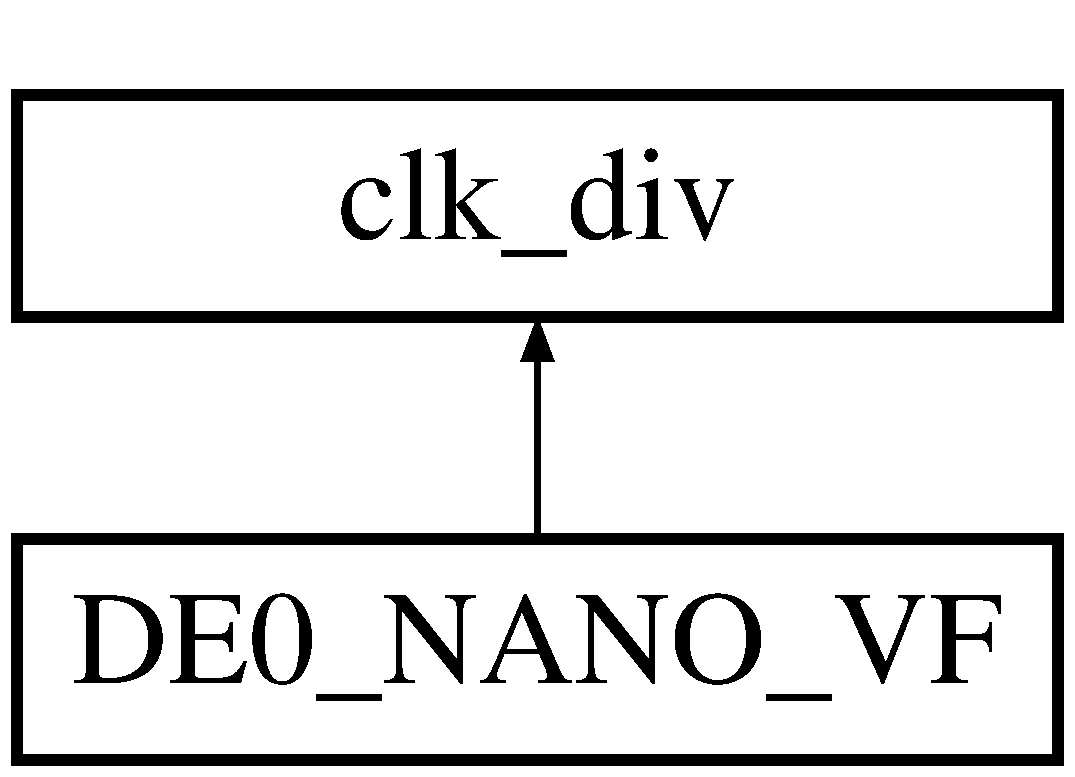
\includegraphics[height=2.000000cm]{classclk__div}
\end{center}
\end{figure}
\subsection*{Entities}
\begin{DoxyCompactItemize}
\item 
\hyperlink{classclk__div_1_1div}{div} architecture
\end{DoxyCompactItemize}
\subsection*{Libraries}
 \begin{DoxyCompactItemize}
\item 
\hyperlink{classclk__div_ae4f03c286607f3181e16b9aa12d0c6d4}{I\+E\+E\+E} 
\end{DoxyCompactItemize}
\subsection*{Use Clauses}
 \begin{DoxyCompactItemize}
\item 
\hyperlink{classclk__div_a241c3e72dd8024cc8ae831b1b2aed7db}{S\+T\+D\+\_\+\+L\+O\+G\+I\+C\+\_\+\+U\+N\+S\+I\+G\+N\+E\+D}   
\item 
\hyperlink{classclk__div_aa4b2b25246a821511120e3149b003563}{S\+T\+D\+\_\+\+L\+O\+G\+I\+C\+\_\+1164}   
\end{DoxyCompactItemize}
\subsection*{Ports}
 \begin{DoxyCompactItemize}
\item 
\hyperlink{classclk__div_a57fad7f33f7766724bdea76e7b0330ef}{clk\+\_\+in}  {\bfseries {\bfseries \textcolor{keywordflow}{in}\textcolor{vhdlchar}{ }}} {\bfseries \textcolor{comment}{S\+T\+D\+\_\+\+L\+O\+G\+I\+C}\textcolor{vhdlchar}{ }} 
\item 
\hyperlink{classclk__div_a512588aa484615b7e90600a1bc9507b4}{en}  {\bfseries {\bfseries \textcolor{keywordflow}{in}\textcolor{vhdlchar}{ }}} {\bfseries \textcolor{comment}{S\+T\+D\+\_\+\+L\+O\+G\+I\+C}\textcolor{vhdlchar}{ }} 
\item 
\hyperlink{classclk__div_a425c2042b3ea21827b9b29c6712312d9}{div}  {\bfseries {\bfseries \textcolor{keywordflow}{in}\textcolor{vhdlchar}{ }}} {\bfseries \textcolor{comment}{S\+T\+D\+\_\+\+L\+O\+G\+I\+C\+\_\+\+V\+E\+C\+T\+O\+R}\textcolor{vhdlchar}{ }\textcolor{vhdlchar}{(}\textcolor{vhdlchar}{ }\textcolor{vhdlchar}{ } \textcolor{vhdldigit}{15} \textcolor{vhdlchar}{ }\textcolor{keywordflow}{D\+O\+W\+N\+T\+O}\textcolor{vhdlchar}{ }\textcolor{vhdlchar}{ } \textcolor{vhdldigit}{0} \textcolor{vhdlchar}{ }\textcolor{vhdlchar}{)}\textcolor{vhdlchar}{ }} 
\item 
\hyperlink{classclk__div_a8147ca5cedee84ed9753ac6f1f0b2374}{clk\+\_\+out}  {\bfseries {\bfseries \textcolor{keywordflow}{out}\textcolor{vhdlchar}{ }}} {\bfseries \textcolor{comment}{S\+T\+D\+\_\+\+L\+O\+G\+I\+C}\textcolor{vhdlchar}{ }} 
\end{DoxyCompactItemize}


\subsection{Detailed Description}


Definition at line 5 of file clk\+\_\+div.\+vhd.



\subsection{Member Data Documentation}
\hypertarget{classclk__div_a57fad7f33f7766724bdea76e7b0330ef}{}\index{clk\+\_\+div@{clk\+\_\+div}!clk\+\_\+in@{clk\+\_\+in}}
\index{clk\+\_\+in@{clk\+\_\+in}!clk\+\_\+div@{clk\+\_\+div}}
\subsubsection[{clk\+\_\+in}]{\setlength{\rightskip}{0pt plus 5cm}{\bf clk\+\_\+in} {\bfseries \textcolor{keywordflow}{in}\textcolor{vhdlchar}{ }} {\bfseries \textcolor{comment}{S\+T\+D\+\_\+\+L\+O\+G\+I\+C}\textcolor{vhdlchar}{ }} \hspace{0.3cm}{\ttfamily [Port]}}\label{classclk__div_a57fad7f33f7766724bdea76e7b0330ef}


Definition at line 7 of file clk\+\_\+div.\+vhd.

\hypertarget{classclk__div_a8147ca5cedee84ed9753ac6f1f0b2374}{}\index{clk\+\_\+div@{clk\+\_\+div}!clk\+\_\+out@{clk\+\_\+out}}
\index{clk\+\_\+out@{clk\+\_\+out}!clk\+\_\+div@{clk\+\_\+div}}
\subsubsection[{clk\+\_\+out}]{\setlength{\rightskip}{0pt plus 5cm}{\bf clk\+\_\+out} {\bfseries \textcolor{keywordflow}{out}\textcolor{vhdlchar}{ }} {\bfseries \textcolor{comment}{S\+T\+D\+\_\+\+L\+O\+G\+I\+C}\textcolor{vhdlchar}{ }} \hspace{0.3cm}{\ttfamily [Port]}}\label{classclk__div_a8147ca5cedee84ed9753ac6f1f0b2374}


Definition at line 10 of file clk\+\_\+div.\+vhd.

\hypertarget{classclk__div_a425c2042b3ea21827b9b29c6712312d9}{}\index{clk\+\_\+div@{clk\+\_\+div}!div@{div}}
\index{div@{div}!clk\+\_\+div@{clk\+\_\+div}}
\subsubsection[{div}]{\setlength{\rightskip}{0pt plus 5cm}{\bf div} {\bfseries \textcolor{keywordflow}{in}\textcolor{vhdlchar}{ }} {\bfseries \textcolor{comment}{S\+T\+D\+\_\+\+L\+O\+G\+I\+C\+\_\+\+V\+E\+C\+T\+O\+R}\textcolor{vhdlchar}{ }\textcolor{vhdlchar}{(}\textcolor{vhdlchar}{ }\textcolor{vhdlchar}{ } \textcolor{vhdldigit}{15} \textcolor{vhdlchar}{ }\textcolor{keywordflow}{D\+O\+W\+N\+T\+O}\textcolor{vhdlchar}{ }\textcolor{vhdlchar}{ } \textcolor{vhdldigit}{0} \textcolor{vhdlchar}{ }\textcolor{vhdlchar}{)}\textcolor{vhdlchar}{ }} \hspace{0.3cm}{\ttfamily [Port]}}\label{classclk__div_a425c2042b3ea21827b9b29c6712312d9}


Definition at line 8 of file clk\+\_\+div.\+vhd.

\hypertarget{classclk__div_a512588aa484615b7e90600a1bc9507b4}{}\index{clk\+\_\+div@{clk\+\_\+div}!en@{en}}
\index{en@{en}!clk\+\_\+div@{clk\+\_\+div}}
\subsubsection[{en}]{\setlength{\rightskip}{0pt plus 5cm}{\bf en} {\bfseries \textcolor{keywordflow}{in}\textcolor{vhdlchar}{ }} {\bfseries \textcolor{comment}{S\+T\+D\+\_\+\+L\+O\+G\+I\+C}\textcolor{vhdlchar}{ }} \hspace{0.3cm}{\ttfamily [Port]}}\label{classclk__div_a512588aa484615b7e90600a1bc9507b4}


Definition at line 7 of file clk\+\_\+div.\+vhd.

\hypertarget{classclk__div_ae4f03c286607f3181e16b9aa12d0c6d4}{}\index{clk\+\_\+div@{clk\+\_\+div}!I\+E\+E\+E@{I\+E\+E\+E}}
\index{I\+E\+E\+E@{I\+E\+E\+E}!clk\+\_\+div@{clk\+\_\+div}}
\subsubsection[{I\+E\+E\+E}]{\setlength{\rightskip}{0pt plus 5cm}{\bf I\+E\+E\+E}\hspace{0.3cm}{\ttfamily [Library]}}\label{classclk__div_ae4f03c286607f3181e16b9aa12d0c6d4}


Definition at line 1 of file clk\+\_\+div.\+vhd.

\hypertarget{classclk__div_aa4b2b25246a821511120e3149b003563}{}\index{clk\+\_\+div@{clk\+\_\+div}!S\+T\+D\+\_\+\+L\+O\+G\+I\+C\+\_\+1164@{S\+T\+D\+\_\+\+L\+O\+G\+I\+C\+\_\+1164}}
\index{S\+T\+D\+\_\+\+L\+O\+G\+I\+C\+\_\+1164@{S\+T\+D\+\_\+\+L\+O\+G\+I\+C\+\_\+1164}!clk\+\_\+div@{clk\+\_\+div}}
\subsubsection[{S\+T\+D\+\_\+\+L\+O\+G\+I\+C\+\_\+1164}]{\setlength{\rightskip}{0pt plus 5cm}{\bf S\+T\+D\+\_\+\+L\+O\+G\+I\+C\+\_\+1164}\hspace{0.3cm}{\ttfamily [Package]}}\label{classclk__div_aa4b2b25246a821511120e3149b003563}


Definition at line 3 of file clk\+\_\+div.\+vhd.

\hypertarget{classclk__div_a241c3e72dd8024cc8ae831b1b2aed7db}{}\index{clk\+\_\+div@{clk\+\_\+div}!S\+T\+D\+\_\+\+L\+O\+G\+I\+C\+\_\+\+U\+N\+S\+I\+G\+N\+E\+D@{S\+T\+D\+\_\+\+L\+O\+G\+I\+C\+\_\+\+U\+N\+S\+I\+G\+N\+E\+D}}
\index{S\+T\+D\+\_\+\+L\+O\+G\+I\+C\+\_\+\+U\+N\+S\+I\+G\+N\+E\+D@{S\+T\+D\+\_\+\+L\+O\+G\+I\+C\+\_\+\+U\+N\+S\+I\+G\+N\+E\+D}!clk\+\_\+div@{clk\+\_\+div}}
\subsubsection[{S\+T\+D\+\_\+\+L\+O\+G\+I\+C\+\_\+\+U\+N\+S\+I\+G\+N\+E\+D}]{\setlength{\rightskip}{0pt plus 5cm}{\bf S\+T\+D\+\_\+\+L\+O\+G\+I\+C\+\_\+\+U\+N\+S\+I\+G\+N\+E\+D}\hspace{0.3cm}{\ttfamily [Package]}}\label{classclk__div_a241c3e72dd8024cc8ae831b1b2aed7db}


Definition at line 2 of file clk\+\_\+div.\+vhd.



The documentation for this class was generated from the following file\+:\begin{DoxyCompactItemize}
\item 
\hyperlink{clk__div_8vhd}{clk\+\_\+div.\+vhd}\end{DoxyCompactItemize}

\hypertarget{classcomparador_1_1comparador}{}\section{comparador Architecture Reference}
\label{classcomparador_1_1comparador}\index{comparador@{comparador}}
\subsection*{Processes}
 \begin{DoxyCompactItemize}
\item 
\hyperlink{classcomparador_1_1comparador_a67cbd29443fafed2b0446c1321a8e91c}{P\+R\+O\+C\+E\+S\+S\+\_\+1}{\bfseries  ( {\bfseries {\bfseries \hyperlink{classcomparador_a4a4609c199d30b3adebbeb3a01276ec5}{clk}} \textcolor{vhdlchar}{ }} )}
\item 
\hyperlink{classcomparador_1_1comparador_ab820ba1b225bbde57824e0ed4510038c}{P\+R\+O\+C\+E\+S\+S\+\_\+2}{\bfseries  ( {\bfseries {\bfseries \hyperlink{classcomparador_af9b8278b961604ab62a822537a109adb}{amost}} \textcolor{vhdlchar}{ }} )}
\end{DoxyCompactItemize}
\subsection*{Signals}
 \begin{DoxyCompactItemize}
\item 
\hyperlink{classcomparador_1_1comparador_abf7d8be25624dd08fcc1517c8e39cb23}{comp\+\_\+int} {\bfseries \textcolor{comment}{std\+\_\+logic\+\_\+vector}\textcolor{vhdlchar}{ }\textcolor{vhdlchar}{(}\textcolor{vhdlchar}{ }\textcolor{vhdlchar}{ }\textcolor{vhdlchar}{ }\textcolor{vhdlchar}{ }{\bfseries \hyperlink{classcomparador_afee4aa1628956aa350183d8881689198}{n\+\_\+bits\+\_\+c}} \textcolor{vhdlchar}{-\/}\textcolor{vhdlchar}{ } \textcolor{vhdldigit}{1} \textcolor{vhdlchar}{ }\textcolor{keywordflow}{downto}\textcolor{vhdlchar}{ }\textcolor{vhdlchar}{ } \textcolor{vhdldigit}{0} \textcolor{vhdlchar}{ }\textcolor{vhdlchar}{)}\textcolor{vhdlchar}{ }} 
\end{DoxyCompactItemize}


\subsection{Detailed Description}


Definition at line \hyperlink{comparador_8vhd_source_l00024}{24} of file \hyperlink{comparador_8vhd_source}{comparador.\+vhd}.



\subsection{Member Function Documentation}
\hypertarget{classcomparador_1_1comparador_a67cbd29443fafed2b0446c1321a8e91c}{}\index{comparador\+::comparador@{comparador\+::comparador}!P\+R\+O\+C\+E\+S\+S\+\_\+1@{P\+R\+O\+C\+E\+S\+S\+\_\+1}}
\index{P\+R\+O\+C\+E\+S\+S\+\_\+1@{P\+R\+O\+C\+E\+S\+S\+\_\+1}!comparador\+::comparador@{comparador\+::comparador}}
\subsubsection[{P\+R\+O\+C\+E\+S\+S\+\_\+1}]{\setlength{\rightskip}{0pt plus 5cm} {\bfseries \textcolor{vhdlchar}{ }} P\+R\+O\+C\+E\+S\+S\+\_\+1(
\begin{DoxyParamCaption}
\item[{}]{{\bfseries {\bfseries {\bf clk}} \textcolor{vhdlchar}{ }} {\em }}
\end{DoxyParamCaption}
)\hspace{0.3cm}{\ttfamily [Process]}}\label{classcomparador_1_1comparador_a67cbd29443fafed2b0446c1321a8e91c}


Definition at line \hyperlink{comparador_8vhd_source_l00032}{32} of file \hyperlink{comparador_8vhd_source}{comparador.\+vhd}.

\hypertarget{classcomparador_1_1comparador_ab820ba1b225bbde57824e0ed4510038c}{}\index{comparador\+::comparador@{comparador\+::comparador}!P\+R\+O\+C\+E\+S\+S\+\_\+2@{P\+R\+O\+C\+E\+S\+S\+\_\+2}}
\index{P\+R\+O\+C\+E\+S\+S\+\_\+2@{P\+R\+O\+C\+E\+S\+S\+\_\+2}!comparador\+::comparador@{comparador\+::comparador}}
\subsubsection[{P\+R\+O\+C\+E\+S\+S\+\_\+2}]{\setlength{\rightskip}{0pt plus 5cm} {\bfseries \textcolor{vhdlchar}{ }} P\+R\+O\+C\+E\+S\+S\+\_\+2(
\begin{DoxyParamCaption}
\item[{}]{{\bfseries {\bfseries {\bf amost}} \textcolor{vhdlchar}{ }} {\em }}
\end{DoxyParamCaption}
)\hspace{0.3cm}{\ttfamily [Process]}}\label{classcomparador_1_1comparador_ab820ba1b225bbde57824e0ed4510038c}


Definition at line \hyperlink{comparador_8vhd_source_l00045}{45} of file \hyperlink{comparador_8vhd_source}{comparador.\+vhd}.



\subsection{Member Data Documentation}
\hypertarget{classcomparador_1_1comparador_abf7d8be25624dd08fcc1517c8e39cb23}{}\index{comparador\+::comparador@{comparador\+::comparador}!comp\+\_\+int@{comp\+\_\+int}}
\index{comp\+\_\+int@{comp\+\_\+int}!comparador\+::comparador@{comparador\+::comparador}}
\subsubsection[{comp\+\_\+int}]{\setlength{\rightskip}{0pt plus 5cm}{\bf comp\+\_\+int} {\bfseries \textcolor{comment}{std\+\_\+logic\+\_\+vector}\textcolor{vhdlchar}{ }\textcolor{vhdlchar}{(}\textcolor{vhdlchar}{ }\textcolor{vhdlchar}{ }\textcolor{vhdlchar}{ }\textcolor{vhdlchar}{ }{\bfseries {\bf n\+\_\+bits\+\_\+c}} \textcolor{vhdlchar}{-\/}\textcolor{vhdlchar}{ } \textcolor{vhdldigit}{1} \textcolor{vhdlchar}{ }\textcolor{keywordflow}{downto}\textcolor{vhdlchar}{ }\textcolor{vhdlchar}{ } \textcolor{vhdldigit}{0} \textcolor{vhdlchar}{ }\textcolor{vhdlchar}{)}\textcolor{vhdlchar}{ }} \hspace{0.3cm}{\ttfamily [Signal]}}\label{classcomparador_1_1comparador_abf7d8be25624dd08fcc1517c8e39cb23}


Definition at line \hyperlink{comparador_8vhd_source_l00027}{27} of file \hyperlink{comparador_8vhd_source}{comparador.\+vhd}.



The documentation for this class was generated from the following file\+:\begin{DoxyCompactItemize}
\item 
\hyperlink{comparador_8vhd}{comparador.\+vhd}\end{DoxyCompactItemize}

\hypertarget{classcomparador}{}\section{comparador Entity Reference}
\label{classcomparador}\index{comparador@{comparador}}
Inheritance diagram for comparador\+:\begin{figure}[H]
\begin{center}
\leavevmode
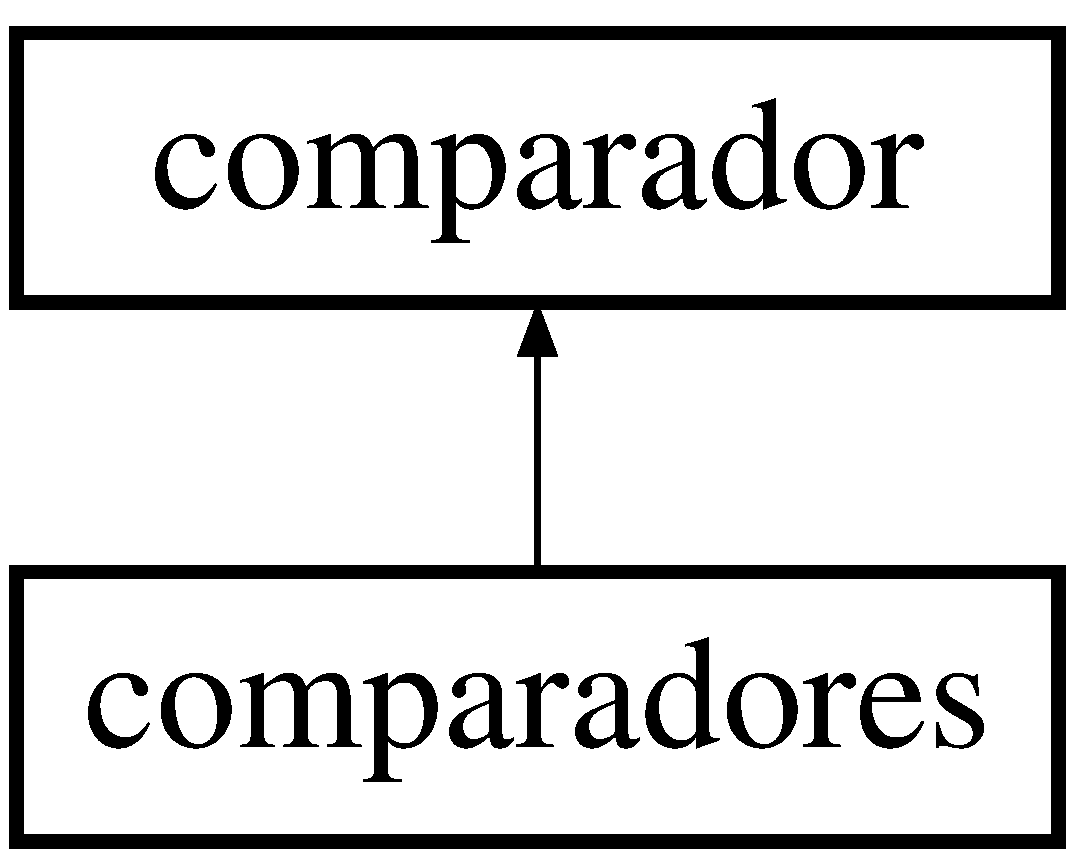
\includegraphics[height=2.000000cm]{classcomparador}
\end{center}
\end{figure}
\subsection*{Entities}
\begin{DoxyCompactItemize}
\item 
\hyperlink{classcomparador_1_1comparador}{comparador} architecture
\end{DoxyCompactItemize}
\subsection*{Libraries}
 \begin{DoxyCompactItemize}
\item 
\hyperlink{classcomparador_ae4f03c286607f3181e16b9aa12d0c6d4}{I\+E\+E\+E} 
\end{DoxyCompactItemize}
\subsection*{Use Clauses}
 \begin{DoxyCompactItemize}
\item 
\hyperlink{classcomparador_a241c3e72dd8024cc8ae831b1b2aed7db}{S\+T\+D\+\_\+\+L\+O\+G\+I\+C\+\_\+\+U\+N\+S\+I\+G\+N\+E\+D}   
\item 
\hyperlink{classcomparador_aa4b2b25246a821511120e3149b003563}{S\+T\+D\+\_\+\+L\+O\+G\+I\+C\+\_\+1164}   
\item 
\hyperlink{classcomparador_aad86249c80e8c1e7ee1c4748aba748e3}{fixed\+\_\+pkg}   
\item 
\hyperlink{classcomparador_a2edc34402b573437d5f25fa90ba4013e}{numeric\+\_\+std}   
\end{DoxyCompactItemize}
\subsection*{Generics}
 \begin{DoxyCompactItemize}
\item 
\hyperlink{classcomparador_afee4aa1628956aa350183d8881689198}{n\+\_\+bits\+\_\+c} {\bfseries {\bfseries \textcolor{comment}{integer}\textcolor{vhdlchar}{ }\textcolor{vhdlchar}{ }\textcolor{vhdlchar}{\+:}\textcolor{vhdlchar}{=}\textcolor{vhdlchar}{ }\textcolor{vhdlchar}{ } \textcolor{vhdldigit}{16} \textcolor{vhdlchar}{ }}}
\end{DoxyCompactItemize}
\subsection*{Ports}
 \begin{DoxyCompactItemize}
\item 
\hyperlink{classcomparador_a4a4609c199d30b3adebbeb3a01276ec5}{clk}  {\bfseries {\bfseries \textcolor{keywordflow}{in}\textcolor{vhdlchar}{ }}} {\bfseries \textcolor{comment}{std\+\_\+logic}\textcolor{vhdlchar}{ }} 
\item 
\hyperlink{classcomparador_adcf9c6f5161d039addbda5819bee64a3}{en}  {\bfseries {\bfseries \textcolor{keywordflow}{in}\textcolor{vhdlchar}{ }}} {\bfseries \textcolor{comment}{std\+\_\+logic}\textcolor{vhdlchar}{ }} 
\item 
\hyperlink{classcomparador_a0c2a0581e706d5256b50516b6ca4dbed}{comp}  {\bfseries {\bfseries \textcolor{keywordflow}{in}\textcolor{vhdlchar}{ }}} {\bfseries \textcolor{comment}{std\+\_\+logic\+\_\+vector}\textcolor{vhdlchar}{ }\textcolor{vhdlchar}{(}\textcolor{vhdlchar}{ }\textcolor{vhdlchar}{ }\textcolor{vhdlchar}{ }\textcolor{vhdlchar}{ }{\bfseries \hyperlink{classcomparador_afee4aa1628956aa350183d8881689198}{n\+\_\+bits\+\_\+c}} \textcolor{vhdlchar}{-\/}\textcolor{vhdlchar}{ } \textcolor{vhdldigit}{1} \textcolor{vhdlchar}{ }\textcolor{keywordflow}{downto}\textcolor{vhdlchar}{ }\textcolor{vhdlchar}{ } \textcolor{vhdldigit}{0} \textcolor{vhdlchar}{ }\textcolor{vhdlchar}{)}\textcolor{vhdlchar}{ }} 
\item 
\hyperlink{classcomparador_a0808bf3e7965a8ee90dec6604647f179}{c}  {\bfseries {\bfseries \textcolor{keywordflow}{in}\textcolor{vhdlchar}{ }}} {\bfseries \textcolor{comment}{std\+\_\+logic\+\_\+vector}\textcolor{vhdlchar}{ }\textcolor{vhdlchar}{(}\textcolor{vhdlchar}{ }\textcolor{vhdlchar}{ }\textcolor{vhdlchar}{ }\textcolor{vhdlchar}{ }{\bfseries \hyperlink{classcomparador_afee4aa1628956aa350183d8881689198}{n\+\_\+bits\+\_\+c}} \textcolor{vhdlchar}{-\/}\textcolor{vhdlchar}{ } \textcolor{vhdldigit}{1} \textcolor{vhdlchar}{ }\textcolor{keywordflow}{downto}\textcolor{vhdlchar}{ }\textcolor{vhdlchar}{ } \textcolor{vhdldigit}{0} \textcolor{vhdlchar}{ }\textcolor{vhdlchar}{)}\textcolor{vhdlchar}{ }} 
\item 
\hyperlink{classcomparador_af9b8278b961604ab62a822537a109adb}{amost}  {\bfseries {\bfseries \textcolor{keywordflow}{in}\textcolor{vhdlchar}{ }}} {\bfseries \textcolor{comment}{std\+\_\+logic}\textcolor{vhdlchar}{ }} 
\item 
\hyperlink{classcomparador_a2522d63dc2aa0652b3cca6ac9b1da0bd}{comp\+\_\+out}  {\bfseries {\bfseries \textcolor{keywordflow}{out}\textcolor{vhdlchar}{ }}} {\bfseries \textcolor{comment}{std\+\_\+logic}\textcolor{vhdlchar}{ }} 
\end{DoxyCompactItemize}


\subsection{Detailed Description}


Definition at line 8 of file comparador.\+vhd.



\subsection{Member Data Documentation}
\hypertarget{classcomparador_af9b8278b961604ab62a822537a109adb}{}\index{comparador@{comparador}!amost@{amost}}
\index{amost@{amost}!comparador@{comparador}}
\subsubsection[{amost}]{\setlength{\rightskip}{0pt plus 5cm}{\bf amost} {\bfseries \textcolor{keywordflow}{in}\textcolor{vhdlchar}{ }} {\bfseries \textcolor{comment}{std\+\_\+logic}\textcolor{vhdlchar}{ }} \hspace{0.3cm}{\ttfamily [Port]}}\label{classcomparador_af9b8278b961604ab62a822537a109adb}


Definition at line 17 of file comparador.\+vhd.

\hypertarget{classcomparador_a0808bf3e7965a8ee90dec6604647f179}{}\index{comparador@{comparador}!c@{c}}
\index{c@{c}!comparador@{comparador}}
\subsubsection[{c}]{\setlength{\rightskip}{0pt plus 5cm}{\bf c} {\bfseries \textcolor{keywordflow}{in}\textcolor{vhdlchar}{ }} {\bfseries \textcolor{comment}{std\+\_\+logic\+\_\+vector}\textcolor{vhdlchar}{ }\textcolor{vhdlchar}{(}\textcolor{vhdlchar}{ }\textcolor{vhdlchar}{ }\textcolor{vhdlchar}{ }\textcolor{vhdlchar}{ }{\bfseries {\bf n\+\_\+bits\+\_\+c}} \textcolor{vhdlchar}{-\/}\textcolor{vhdlchar}{ } \textcolor{vhdldigit}{1} \textcolor{vhdlchar}{ }\textcolor{keywordflow}{downto}\textcolor{vhdlchar}{ }\textcolor{vhdlchar}{ } \textcolor{vhdldigit}{0} \textcolor{vhdlchar}{ }\textcolor{vhdlchar}{)}\textcolor{vhdlchar}{ }} \hspace{0.3cm}{\ttfamily [Port]}}\label{classcomparador_a0808bf3e7965a8ee90dec6604647f179}


Definition at line 16 of file comparador.\+vhd.

\hypertarget{classcomparador_a4a4609c199d30b3adebbeb3a01276ec5}{}\index{comparador@{comparador}!clk@{clk}}
\index{clk@{clk}!comparador@{comparador}}
\subsubsection[{clk}]{\setlength{\rightskip}{0pt plus 5cm}{\bf clk} {\bfseries \textcolor{keywordflow}{in}\textcolor{vhdlchar}{ }} {\bfseries \textcolor{comment}{std\+\_\+logic}\textcolor{vhdlchar}{ }} \hspace{0.3cm}{\ttfamily [Port]}}\label{classcomparador_a4a4609c199d30b3adebbeb3a01276ec5}


Definition at line 13 of file comparador.\+vhd.

\hypertarget{classcomparador_a0c2a0581e706d5256b50516b6ca4dbed}{}\index{comparador@{comparador}!comp@{comp}}
\index{comp@{comp}!comparador@{comparador}}
\subsubsection[{comp}]{\setlength{\rightskip}{0pt plus 5cm}{\bf comp} {\bfseries \textcolor{keywordflow}{in}\textcolor{vhdlchar}{ }} {\bfseries \textcolor{comment}{std\+\_\+logic\+\_\+vector}\textcolor{vhdlchar}{ }\textcolor{vhdlchar}{(}\textcolor{vhdlchar}{ }\textcolor{vhdlchar}{ }\textcolor{vhdlchar}{ }\textcolor{vhdlchar}{ }{\bfseries {\bf n\+\_\+bits\+\_\+c}} \textcolor{vhdlchar}{-\/}\textcolor{vhdlchar}{ } \textcolor{vhdldigit}{1} \textcolor{vhdlchar}{ }\textcolor{keywordflow}{downto}\textcolor{vhdlchar}{ }\textcolor{vhdlchar}{ } \textcolor{vhdldigit}{0} \textcolor{vhdlchar}{ }\textcolor{vhdlchar}{)}\textcolor{vhdlchar}{ }} \hspace{0.3cm}{\ttfamily [Port]}}\label{classcomparador_a0c2a0581e706d5256b50516b6ca4dbed}


Definition at line 15 of file comparador.\+vhd.

\hypertarget{classcomparador_a2522d63dc2aa0652b3cca6ac9b1da0bd}{}\index{comparador@{comparador}!comp\+\_\+out@{comp\+\_\+out}}
\index{comp\+\_\+out@{comp\+\_\+out}!comparador@{comparador}}
\subsubsection[{comp\+\_\+out}]{\setlength{\rightskip}{0pt plus 5cm}{\bf comp\+\_\+out} {\bfseries \textcolor{keywordflow}{out}\textcolor{vhdlchar}{ }} {\bfseries \textcolor{comment}{std\+\_\+logic}\textcolor{vhdlchar}{ }} \hspace{0.3cm}{\ttfamily [Port]}}\label{classcomparador_a2522d63dc2aa0652b3cca6ac9b1da0bd}


Definition at line 19 of file comparador.\+vhd.

\hypertarget{classcomparador_adcf9c6f5161d039addbda5819bee64a3}{}\index{comparador@{comparador}!en@{en}}
\index{en@{en}!comparador@{comparador}}
\subsubsection[{en}]{\setlength{\rightskip}{0pt plus 5cm}{\bf en} {\bfseries \textcolor{keywordflow}{in}\textcolor{vhdlchar}{ }} {\bfseries \textcolor{comment}{std\+\_\+logic}\textcolor{vhdlchar}{ }} \hspace{0.3cm}{\ttfamily [Port]}}\label{classcomparador_adcf9c6f5161d039addbda5819bee64a3}


Definition at line 14 of file comparador.\+vhd.

\hypertarget{classcomparador_aad86249c80e8c1e7ee1c4748aba748e3}{}\index{comparador@{comparador}!fixed\+\_\+pkg@{fixed\+\_\+pkg}}
\index{fixed\+\_\+pkg@{fixed\+\_\+pkg}!comparador@{comparador}}
\subsubsection[{fixed\+\_\+pkg}]{\setlength{\rightskip}{0pt plus 5cm}{\bf fixed\+\_\+pkg}\hspace{0.3cm}{\ttfamily [Package]}}\label{classcomparador_aad86249c80e8c1e7ee1c4748aba748e3}


Definition at line 5 of file comparador.\+vhd.

\hypertarget{classcomparador_ae4f03c286607f3181e16b9aa12d0c6d4}{}\index{comparador@{comparador}!I\+E\+E\+E@{I\+E\+E\+E}}
\index{I\+E\+E\+E@{I\+E\+E\+E}!comparador@{comparador}}
\subsubsection[{I\+E\+E\+E}]{\setlength{\rightskip}{0pt plus 5cm}{\bf I\+E\+E\+E}\hspace{0.3cm}{\ttfamily [Library]}}\label{classcomparador_ae4f03c286607f3181e16b9aa12d0c6d4}


Definition at line 2 of file comparador.\+vhd.

\hypertarget{classcomparador_afee4aa1628956aa350183d8881689198}{}\index{comparador@{comparador}!n\+\_\+bits\+\_\+c@{n\+\_\+bits\+\_\+c}}
\index{n\+\_\+bits\+\_\+c@{n\+\_\+bits\+\_\+c}!comparador@{comparador}}
\subsubsection[{n\+\_\+bits\+\_\+c}]{\setlength{\rightskip}{0pt plus 5cm}{\bf n\+\_\+bits\+\_\+c} {\bfseries \textcolor{vhdlchar}{ }} {\bfseries \textcolor{comment}{integer}\textcolor{vhdlchar}{ }\textcolor{vhdlchar}{ }\textcolor{vhdlchar}{\+:}\textcolor{vhdlchar}{=}\textcolor{vhdlchar}{ }\textcolor{vhdlchar}{ } \textcolor{vhdldigit}{16} \textcolor{vhdlchar}{ }} \hspace{0.3cm}{\ttfamily [Generic]}}\label{classcomparador_afee4aa1628956aa350183d8881689198}


Definition at line 11 of file comparador.\+vhd.

\hypertarget{classcomparador_a2edc34402b573437d5f25fa90ba4013e}{}\index{comparador@{comparador}!numeric\+\_\+std@{numeric\+\_\+std}}
\index{numeric\+\_\+std@{numeric\+\_\+std}!comparador@{comparador}}
\subsubsection[{numeric\+\_\+std}]{\setlength{\rightskip}{0pt plus 5cm}{\bf numeric\+\_\+std}\hspace{0.3cm}{\ttfamily [Package]}}\label{classcomparador_a2edc34402b573437d5f25fa90ba4013e}


Definition at line 6 of file comparador.\+vhd.

\hypertarget{classcomparador_aa4b2b25246a821511120e3149b003563}{}\index{comparador@{comparador}!S\+T\+D\+\_\+\+L\+O\+G\+I\+C\+\_\+1164@{S\+T\+D\+\_\+\+L\+O\+G\+I\+C\+\_\+1164}}
\index{S\+T\+D\+\_\+\+L\+O\+G\+I\+C\+\_\+1164@{S\+T\+D\+\_\+\+L\+O\+G\+I\+C\+\_\+1164}!comparador@{comparador}}
\subsubsection[{S\+T\+D\+\_\+\+L\+O\+G\+I\+C\+\_\+1164}]{\setlength{\rightskip}{0pt plus 5cm}{\bf S\+T\+D\+\_\+\+L\+O\+G\+I\+C\+\_\+1164}\hspace{0.3cm}{\ttfamily [Package]}}\label{classcomparador_aa4b2b25246a821511120e3149b003563}


Definition at line 4 of file comparador.\+vhd.

\hypertarget{classcomparador_a241c3e72dd8024cc8ae831b1b2aed7db}{}\index{comparador@{comparador}!S\+T\+D\+\_\+\+L\+O\+G\+I\+C\+\_\+\+U\+N\+S\+I\+G\+N\+E\+D@{S\+T\+D\+\_\+\+L\+O\+G\+I\+C\+\_\+\+U\+N\+S\+I\+G\+N\+E\+D}}
\index{S\+T\+D\+\_\+\+L\+O\+G\+I\+C\+\_\+\+U\+N\+S\+I\+G\+N\+E\+D@{S\+T\+D\+\_\+\+L\+O\+G\+I\+C\+\_\+\+U\+N\+S\+I\+G\+N\+E\+D}!comparador@{comparador}}
\subsubsection[{S\+T\+D\+\_\+\+L\+O\+G\+I\+C\+\_\+\+U\+N\+S\+I\+G\+N\+E\+D}]{\setlength{\rightskip}{0pt plus 5cm}{\bf S\+T\+D\+\_\+\+L\+O\+G\+I\+C\+\_\+\+U\+N\+S\+I\+G\+N\+E\+D}\hspace{0.3cm}{\ttfamily [Package]}}\label{classcomparador_a241c3e72dd8024cc8ae831b1b2aed7db}


Definition at line 3 of file comparador.\+vhd.



The documentation for this class was generated from the following file\+:\begin{DoxyCompactItemize}
\item 
\hyperlink{comparador_8vhd}{comparador.\+vhd}\end{DoxyCompactItemize}

\hypertarget{classcomparadores}{}\section{comparadores Entity Reference}
\label{classcomparadores}\index{comparadores@{comparadores}}
Inheritance diagram for comparadores\+:\begin{figure}[H]
\begin{center}
\leavevmode
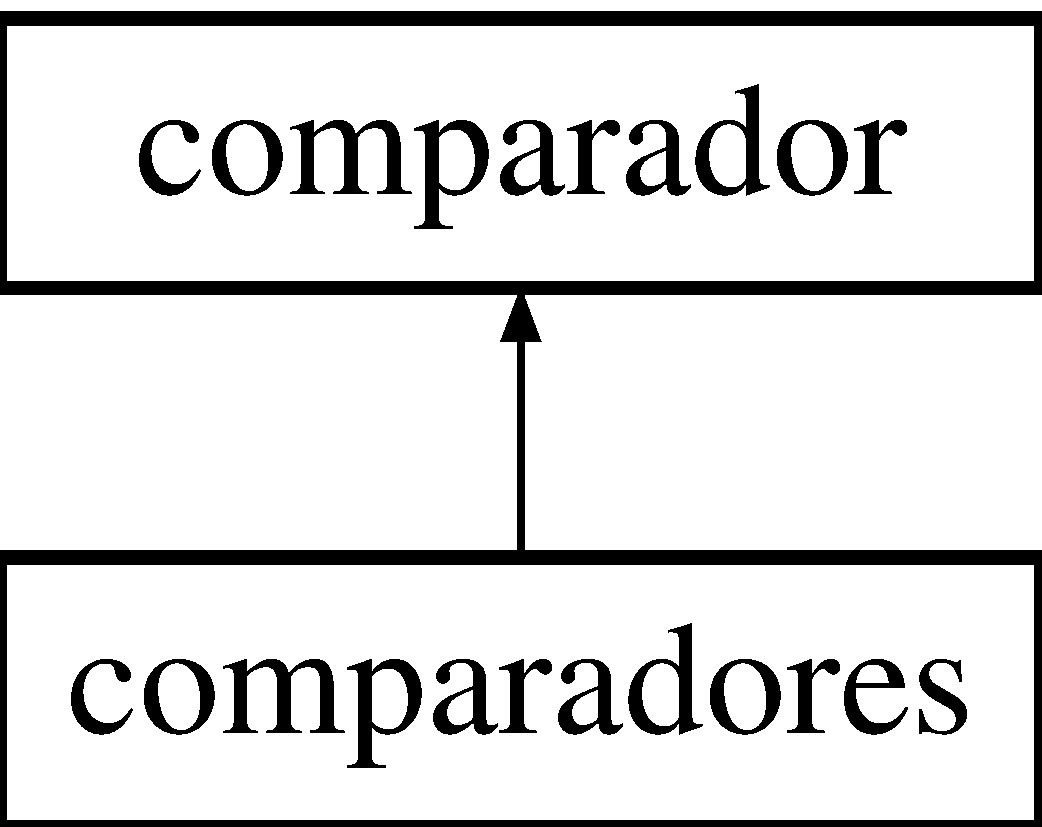
\includegraphics[height=2.000000cm]{classcomparadores}
\end{center}
\end{figure}
\subsection*{Entities}
\begin{DoxyCompactItemize}
\item 
\hyperlink{classcomparadores_1_1comparadores}{comparadores} architecture
\end{DoxyCompactItemize}
\subsection*{Libraries}
 \begin{DoxyCompactItemize}
\item 
\hyperlink{classcomparadores_ae4f03c286607f3181e16b9aa12d0c6d4}{I\+E\+E\+E} 
\end{DoxyCompactItemize}
\subsection*{Use Clauses}
 \begin{DoxyCompactItemize}
\item 
\hyperlink{classcomparadores_a241c3e72dd8024cc8ae831b1b2aed7db}{S\+T\+D\+\_\+\+L\+O\+G\+I\+C\+\_\+\+U\+N\+S\+I\+G\+N\+E\+D}   
\item 
\hyperlink{classcomparadores_aa4b2b25246a821511120e3149b003563}{S\+T\+D\+\_\+\+L\+O\+G\+I\+C\+\_\+1164}   
\item 
\hyperlink{classcomparadores_aad86249c80e8c1e7ee1c4748aba748e3}{fixed\+\_\+pkg}   
\item 
\hyperlink{classcomparadores_a2edc34402b573437d5f25fa90ba4013e}{numeric\+\_\+std}   
\item 
\hyperlink{classcomparadores_ac1788a894930eeee5aaed06b4775d746}{my\+\_\+types\+\_\+pkg}   
\end{DoxyCompactItemize}
\subsection*{Generics}
 \begin{DoxyCompactItemize}
\item 
\hyperlink{classcomparadores_a601f7f505b21fa95d9d2e36075d21041}{M\+A\+X} {\bfseries {\bfseries \textcolor{comment}{integer}\textcolor{vhdlchar}{ }\textcolor{vhdlchar}{ }\textcolor{vhdlchar}{\+:}\textcolor{vhdlchar}{=}\textcolor{vhdlchar}{ }\textcolor{vhdlchar}{ } \textcolor{vhdldigit}{3526000} \textcolor{vhdlchar}{ }}}
\item 
\hyperlink{classcomparadores_a363fe57541ccc1caaeb5b14dcf01182d}{n\+\_\+bits\+\_\+c} {\bfseries {\bfseries \textcolor{comment}{integer}\textcolor{vhdlchar}{ }\textcolor{vhdlchar}{ }\textcolor{vhdlchar}{\+:}\textcolor{vhdlchar}{=}\textcolor{vhdlchar}{ }\textcolor{vhdlchar}{ } \textcolor{vhdldigit}{22} \textcolor{vhdlchar}{ }}}
\end{DoxyCompactItemize}
\subsection*{Ports}
 \begin{DoxyCompactItemize}
\item 
\hyperlink{classcomparadores_a4a4609c199d30b3adebbeb3a01276ec5}{clk}  {\bfseries {\bfseries \textcolor{keywordflow}{in}\textcolor{vhdlchar}{ }}} {\bfseries \textcolor{comment}{std\+\_\+logic}\textcolor{vhdlchar}{ }} 
\item 
\hyperlink{classcomparadores_adcf9c6f5161d039addbda5819bee64a3}{en}  {\bfseries {\bfseries \textcolor{keywordflow}{in}\textcolor{vhdlchar}{ }}} {\bfseries \textcolor{comment}{std\+\_\+logic}\textcolor{vhdlchar}{ }} 
\item 
\hyperlink{classcomparadores_ab73cec596619a058f732a10e71d5aada}{comp}  {\bfseries {\bfseries \textcolor{keywordflow}{in}\textcolor{vhdlchar}{ }}} {\bfseries {\bfseries \hyperlink{classmy__types__pkg_ae9b90869e95e036baa1ead1b6238589a}{C\+O\+M\+P\+\_\+\+A\+R\+R\+A\+Y}} \textcolor{vhdlchar}{ }} 
\item 
\hyperlink{classcomparadores_ab52608f377848fc687beeb76bb39a6e8}{c}  {\bfseries {\bfseries \textcolor{keywordflow}{in}\textcolor{vhdlchar}{ }}} {\bfseries {\bfseries \hyperlink{classmy__types__pkg_ae9b90869e95e036baa1ead1b6238589a}{C\+O\+M\+P\+\_\+\+A\+R\+R\+A\+Y}} \textcolor{vhdlchar}{ }} 
\item 
\hyperlink{classcomparadores_a0d7d8d086cf18e0180f8c280d76ed624}{amost}  {\bfseries {\bfseries \textcolor{keywordflow}{in}\textcolor{vhdlchar}{ }}} {\bfseries \textcolor{comment}{std\+\_\+logic\+\_\+vector}\textcolor{vhdlchar}{ }\textcolor{vhdlchar}{(}\textcolor{vhdlchar}{ }\textcolor{vhdlchar}{ } \textcolor{vhdldigit}{24} \textcolor{vhdlchar}{ }\textcolor{keywordflow}{downto}\textcolor{vhdlchar}{ }\textcolor{vhdlchar}{ } \textcolor{vhdldigit}{1} \textcolor{vhdlchar}{ }\textcolor{vhdlchar}{)}\textcolor{vhdlchar}{ }} 
\item 
\hyperlink{classcomparadores_a8d13d6e22531ac75ac0b437c61c6eb4f}{comp\+\_\+out}  {\bfseries {\bfseries \textcolor{keywordflow}{out}\textcolor{vhdlchar}{ }}} {\bfseries \textcolor{comment}{std\+\_\+logic\+\_\+vector}\textcolor{vhdlchar}{ }\textcolor{vhdlchar}{(}\textcolor{vhdlchar}{ }\textcolor{vhdlchar}{ } \textcolor{vhdldigit}{24} \textcolor{vhdlchar}{ }\textcolor{keywordflow}{downto}\textcolor{vhdlchar}{ }\textcolor{vhdlchar}{ } \textcolor{vhdldigit}{1} \textcolor{vhdlchar}{ }\textcolor{vhdlchar}{)}\textcolor{vhdlchar}{ }} 
\end{DoxyCompactItemize}


\subsection{Detailed Description}


Definition at line 19 of file comparadores.\+vhd.



\subsection{Member Data Documentation}
\hypertarget{classcomparadores_a0d7d8d086cf18e0180f8c280d76ed624}{}\index{comparadores@{comparadores}!amost@{amost}}
\index{amost@{amost}!comparadores@{comparadores}}
\subsubsection[{amost}]{\setlength{\rightskip}{0pt plus 5cm}{\bf amost} {\bfseries \textcolor{keywordflow}{in}\textcolor{vhdlchar}{ }} {\bfseries \textcolor{comment}{std\+\_\+logic\+\_\+vector}\textcolor{vhdlchar}{ }\textcolor{vhdlchar}{(}\textcolor{vhdlchar}{ }\textcolor{vhdlchar}{ } \textcolor{vhdldigit}{24} \textcolor{vhdlchar}{ }\textcolor{keywordflow}{downto}\textcolor{vhdlchar}{ }\textcolor{vhdlchar}{ } \textcolor{vhdldigit}{1} \textcolor{vhdlchar}{ }\textcolor{vhdlchar}{)}\textcolor{vhdlchar}{ }} \hspace{0.3cm}{\ttfamily [Port]}}\label{classcomparadores_a0d7d8d086cf18e0180f8c280d76ed624}


Definition at line 28 of file comparadores.\+vhd.

\hypertarget{classcomparadores_ab52608f377848fc687beeb76bb39a6e8}{}\index{comparadores@{comparadores}!c@{c}}
\index{c@{c}!comparadores@{comparadores}}
\subsubsection[{c}]{\setlength{\rightskip}{0pt plus 5cm}{\bf c} {\bfseries \textcolor{keywordflow}{in}\textcolor{vhdlchar}{ }} {\bfseries {\bfseries {\bf C\+O\+M\+P\+\_\+\+A\+R\+R\+A\+Y}} \textcolor{vhdlchar}{ }} \hspace{0.3cm}{\ttfamily [Port]}}\label{classcomparadores_ab52608f377848fc687beeb76bb39a6e8}


Definition at line 27 of file comparadores.\+vhd.

\hypertarget{classcomparadores_a4a4609c199d30b3adebbeb3a01276ec5}{}\index{comparadores@{comparadores}!clk@{clk}}
\index{clk@{clk}!comparadores@{comparadores}}
\subsubsection[{clk}]{\setlength{\rightskip}{0pt plus 5cm}{\bf clk} {\bfseries \textcolor{keywordflow}{in}\textcolor{vhdlchar}{ }} {\bfseries \textcolor{comment}{std\+\_\+logic}\textcolor{vhdlchar}{ }} \hspace{0.3cm}{\ttfamily [Port]}}\label{classcomparadores_a4a4609c199d30b3adebbeb3a01276ec5}


Definition at line 24 of file comparadores.\+vhd.

\hypertarget{classcomparadores_ab73cec596619a058f732a10e71d5aada}{}\index{comparadores@{comparadores}!comp@{comp}}
\index{comp@{comp}!comparadores@{comparadores}}
\subsubsection[{comp}]{\setlength{\rightskip}{0pt plus 5cm}{\bf comp} {\bfseries \textcolor{keywordflow}{in}\textcolor{vhdlchar}{ }} {\bfseries {\bfseries {\bf C\+O\+M\+P\+\_\+\+A\+R\+R\+A\+Y}} \textcolor{vhdlchar}{ }} \hspace{0.3cm}{\ttfamily [Port]}}\label{classcomparadores_ab73cec596619a058f732a10e71d5aada}


Definition at line 26 of file comparadores.\+vhd.

\hypertarget{classcomparadores_a8d13d6e22531ac75ac0b437c61c6eb4f}{}\index{comparadores@{comparadores}!comp\+\_\+out@{comp\+\_\+out}}
\index{comp\+\_\+out@{comp\+\_\+out}!comparadores@{comparadores}}
\subsubsection[{comp\+\_\+out}]{\setlength{\rightskip}{0pt plus 5cm}{\bf comp\+\_\+out} {\bfseries \textcolor{keywordflow}{out}\textcolor{vhdlchar}{ }} {\bfseries \textcolor{comment}{std\+\_\+logic\+\_\+vector}\textcolor{vhdlchar}{ }\textcolor{vhdlchar}{(}\textcolor{vhdlchar}{ }\textcolor{vhdlchar}{ } \textcolor{vhdldigit}{24} \textcolor{vhdlchar}{ }\textcolor{keywordflow}{downto}\textcolor{vhdlchar}{ }\textcolor{vhdlchar}{ } \textcolor{vhdldigit}{1} \textcolor{vhdlchar}{ }\textcolor{vhdlchar}{)}\textcolor{vhdlchar}{ }} \hspace{0.3cm}{\ttfamily [Port]}}\label{classcomparadores_a8d13d6e22531ac75ac0b437c61c6eb4f}


Definition at line 30 of file comparadores.\+vhd.

\hypertarget{classcomparadores_adcf9c6f5161d039addbda5819bee64a3}{}\index{comparadores@{comparadores}!en@{en}}
\index{en@{en}!comparadores@{comparadores}}
\subsubsection[{en}]{\setlength{\rightskip}{0pt plus 5cm}{\bf en} {\bfseries \textcolor{keywordflow}{in}\textcolor{vhdlchar}{ }} {\bfseries \textcolor{comment}{std\+\_\+logic}\textcolor{vhdlchar}{ }} \hspace{0.3cm}{\ttfamily [Port]}}\label{classcomparadores_adcf9c6f5161d039addbda5819bee64a3}


Definition at line 25 of file comparadores.\+vhd.

\hypertarget{classcomparadores_aad86249c80e8c1e7ee1c4748aba748e3}{}\index{comparadores@{comparadores}!fixed\+\_\+pkg@{fixed\+\_\+pkg}}
\index{fixed\+\_\+pkg@{fixed\+\_\+pkg}!comparadores@{comparadores}}
\subsubsection[{fixed\+\_\+pkg}]{\setlength{\rightskip}{0pt plus 5cm}{\bf fixed\+\_\+pkg}\hspace{0.3cm}{\ttfamily [Package]}}\label{classcomparadores_aad86249c80e8c1e7ee1c4748aba748e3}


Definition at line 4 of file comparadores.\+vhd.

\hypertarget{classcomparadores_ae4f03c286607f3181e16b9aa12d0c6d4}{}\index{comparadores@{comparadores}!I\+E\+E\+E@{I\+E\+E\+E}}
\index{I\+E\+E\+E@{I\+E\+E\+E}!comparadores@{comparadores}}
\subsubsection[{I\+E\+E\+E}]{\setlength{\rightskip}{0pt plus 5cm}{\bf I\+E\+E\+E}\hspace{0.3cm}{\ttfamily [Library]}}\label{classcomparadores_ae4f03c286607f3181e16b9aa12d0c6d4}


Definition at line 1 of file comparadores.\+vhd.

\hypertarget{classcomparadores_a601f7f505b21fa95d9d2e36075d21041}{}\index{comparadores@{comparadores}!M\+A\+X@{M\+A\+X}}
\index{M\+A\+X@{M\+A\+X}!comparadores@{comparadores}}
\subsubsection[{M\+A\+X}]{\setlength{\rightskip}{0pt plus 5cm}{\bf M\+A\+X} {\bfseries \textcolor{vhdlchar}{ }} {\bfseries \textcolor{comment}{integer}\textcolor{vhdlchar}{ }\textcolor{vhdlchar}{ }\textcolor{vhdlchar}{\+:}\textcolor{vhdlchar}{=}\textcolor{vhdlchar}{ }\textcolor{vhdlchar}{ } \textcolor{vhdldigit}{3526000} \textcolor{vhdlchar}{ }} \hspace{0.3cm}{\ttfamily [Generic]}}\label{classcomparadores_a601f7f505b21fa95d9d2e36075d21041}


Definition at line 20 of file comparadores.\+vhd.

\hypertarget{classcomparadores_ac1788a894930eeee5aaed06b4775d746}{}\index{comparadores@{comparadores}!my\+\_\+types\+\_\+pkg@{my\+\_\+types\+\_\+pkg}}
\index{my\+\_\+types\+\_\+pkg@{my\+\_\+types\+\_\+pkg}!comparadores@{comparadores}}
\subsubsection[{my\+\_\+types\+\_\+pkg}]{\setlength{\rightskip}{0pt plus 5cm}{\bf my\+\_\+types\+\_\+pkg}\hspace{0.3cm}{\ttfamily [Package]}}\label{classcomparadores_ac1788a894930eeee5aaed06b4775d746}


Definition at line 6 of file comparadores.\+vhd.

\hypertarget{classcomparadores_a363fe57541ccc1caaeb5b14dcf01182d}{}\index{comparadores@{comparadores}!n\+\_\+bits\+\_\+c@{n\+\_\+bits\+\_\+c}}
\index{n\+\_\+bits\+\_\+c@{n\+\_\+bits\+\_\+c}!comparadores@{comparadores}}
\subsubsection[{n\+\_\+bits\+\_\+c}]{\setlength{\rightskip}{0pt plus 5cm}{\bf n\+\_\+bits\+\_\+c} {\bfseries \textcolor{vhdlchar}{ }} {\bfseries \textcolor{comment}{integer}\textcolor{vhdlchar}{ }\textcolor{vhdlchar}{ }\textcolor{vhdlchar}{\+:}\textcolor{vhdlchar}{=}\textcolor{vhdlchar}{ }\textcolor{vhdlchar}{ } \textcolor{vhdldigit}{22} \textcolor{vhdlchar}{ }} \hspace{0.3cm}{\ttfamily [Generic]}}\label{classcomparadores_a363fe57541ccc1caaeb5b14dcf01182d}


Definition at line 22 of file comparadores.\+vhd.

\hypertarget{classcomparadores_a2edc34402b573437d5f25fa90ba4013e}{}\index{comparadores@{comparadores}!numeric\+\_\+std@{numeric\+\_\+std}}
\index{numeric\+\_\+std@{numeric\+\_\+std}!comparadores@{comparadores}}
\subsubsection[{numeric\+\_\+std}]{\setlength{\rightskip}{0pt plus 5cm}{\bf numeric\+\_\+std}\hspace{0.3cm}{\ttfamily [Package]}}\label{classcomparadores_a2edc34402b573437d5f25fa90ba4013e}


Definition at line 5 of file comparadores.\+vhd.

\hypertarget{classcomparadores_aa4b2b25246a821511120e3149b003563}{}\index{comparadores@{comparadores}!S\+T\+D\+\_\+\+L\+O\+G\+I\+C\+\_\+1164@{S\+T\+D\+\_\+\+L\+O\+G\+I\+C\+\_\+1164}}
\index{S\+T\+D\+\_\+\+L\+O\+G\+I\+C\+\_\+1164@{S\+T\+D\+\_\+\+L\+O\+G\+I\+C\+\_\+1164}!comparadores@{comparadores}}
\subsubsection[{S\+T\+D\+\_\+\+L\+O\+G\+I\+C\+\_\+1164}]{\setlength{\rightskip}{0pt plus 5cm}{\bf S\+T\+D\+\_\+\+L\+O\+G\+I\+C\+\_\+1164}\hspace{0.3cm}{\ttfamily [Package]}}\label{classcomparadores_aa4b2b25246a821511120e3149b003563}


Definition at line 3 of file comparadores.\+vhd.

\hypertarget{classcomparadores_a241c3e72dd8024cc8ae831b1b2aed7db}{}\index{comparadores@{comparadores}!S\+T\+D\+\_\+\+L\+O\+G\+I\+C\+\_\+\+U\+N\+S\+I\+G\+N\+E\+D@{S\+T\+D\+\_\+\+L\+O\+G\+I\+C\+\_\+\+U\+N\+S\+I\+G\+N\+E\+D}}
\index{S\+T\+D\+\_\+\+L\+O\+G\+I\+C\+\_\+\+U\+N\+S\+I\+G\+N\+E\+D@{S\+T\+D\+\_\+\+L\+O\+G\+I\+C\+\_\+\+U\+N\+S\+I\+G\+N\+E\+D}!comparadores@{comparadores}}
\subsubsection[{S\+T\+D\+\_\+\+L\+O\+G\+I\+C\+\_\+\+U\+N\+S\+I\+G\+N\+E\+D}]{\setlength{\rightskip}{0pt plus 5cm}{\bf S\+T\+D\+\_\+\+L\+O\+G\+I\+C\+\_\+\+U\+N\+S\+I\+G\+N\+E\+D}\hspace{0.3cm}{\ttfamily [Package]}}\label{classcomparadores_a241c3e72dd8024cc8ae831b1b2aed7db}


Definition at line 2 of file comparadores.\+vhd.



The documentation for this class was generated from the following file\+:\begin{DoxyCompactItemize}
\item 
\hyperlink{comparadores_8vhd}{comparadores.\+vhd}\end{DoxyCompactItemize}

\hypertarget{classcomparadores_1_1comparadores}{}\section{comparadores Architecture Reference}
\label{classcomparadores_1_1comparadores}\index{comparadores@{comparadores}}
\subsection*{Components}
 \begin{DoxyCompactItemize}
\item 
\hyperlink{classcomparadores_1_1comparadores_ace6ea24c011c9df8c51cbea5a509a663}{comparador}  {\bfseries }  
\end{DoxyCompactItemize}
\subsection*{Instantiations}
 \begin{DoxyCompactItemize}
\item 
\hyperlink{classcomparadores_1_1comparadores_a6277e2a7446059985dc9bcf0a4ac1a8f}{u}  {\bfseries comparador}   
\end{DoxyCompactItemize}


\subsection{Detailed Description}


Definition at line \hyperlink{comparadores_8vhd_source_l00034}{34} of file \hyperlink{comparadores_8vhd_source}{comparadores.\+vhd}.



\subsection{Member Data Documentation}
\hypertarget{classcomparadores_1_1comparadores_ace6ea24c011c9df8c51cbea5a509a663}{}\index{comparadores\+::comparadores@{comparadores\+::comparadores}!comparador@{comparador}}
\index{comparador@{comparador}!comparadores\+::comparadores@{comparadores\+::comparadores}}
\subsubsection[{comparador}]{\setlength{\rightskip}{0pt plus 5cm}{\bf comparador} {\bfseries \textcolor{vhdlchar}{ }} \hspace{0.3cm}{\ttfamily [Component]}}\label{classcomparadores_1_1comparadores_ace6ea24c011c9df8c51cbea5a509a663}


Definition at line \hyperlink{comparadores_8vhd_source_l00036}{36} of file \hyperlink{comparadores_8vhd_source}{comparadores.\+vhd}.

\hypertarget{classcomparadores_1_1comparadores_a6277e2a7446059985dc9bcf0a4ac1a8f}{}\index{comparadores\+::comparadores@{comparadores\+::comparadores}!u@{u}}
\index{u@{u}!comparadores\+::comparadores@{comparadores\+::comparadores}}
\subsubsection[{u}]{\setlength{\rightskip}{0pt plus 5cm}{\bf u} {\bfseries \textcolor{vhdlchar}{comparador}\textcolor{vhdlchar}{ }} \hspace{0.3cm}{\ttfamily [Instantiation]}}\label{classcomparadores_1_1comparadores_a6277e2a7446059985dc9bcf0a4ac1a8f}


Definition at line \hyperlink{comparadores_8vhd_source_l00061}{61} of file \hyperlink{comparadores_8vhd_source}{comparadores.\+vhd}.



The documentation for this class was generated from the following file\+:\begin{DoxyCompactItemize}
\item 
\hyperlink{comparadores_8vhd}{comparadores.\+vhd}\end{DoxyCompactItemize}

\hypertarget{classcontador_1_1contador}{}\section{contador Architecture Reference}
\label{classcontador_1_1contador}\index{contador@{contador}}
\subsection*{Processes}
 \begin{DoxyCompactItemize}
\item 
\hyperlink{classcontador_1_1contador_a00d9e7e8c17b5cd71bc4c4b432911468}{P\+R\+O\+C\+E\+S\+S\+\_\+3}{\bfseries  ( {\bfseries {\bfseries \hyperlink{classcontador_a4a4609c199d30b3adebbeb3a01276ec5}{clk}} \textcolor{vhdlchar}{ }} )}
\end{DoxyCompactItemize}
\subsection*{Signals}
 \begin{DoxyCompactItemize}
\item 
\hyperlink{classcontador_1_1contador_a591dd47ce674ec0d3b488d8705b8e838}{count\+\_\+int} {\bfseries \textcolor{comment}{std\+\_\+logic\+\_\+vector}\textcolor{vhdlchar}{ }\textcolor{vhdlchar}{(}\textcolor{vhdlchar}{ }\textcolor{vhdlchar}{ }\textcolor{vhdlchar}{ }\textcolor{vhdlchar}{ }{\bfseries \hyperlink{classcontador_a986eb173f34190032418b47b9fc9b457}{n\+\_\+bits}} \textcolor{vhdlchar}{-\/}\textcolor{vhdlchar}{ } \textcolor{vhdldigit}{1} \textcolor{vhdlchar}{ }\textcolor{keywordflow}{downto}\textcolor{vhdlchar}{ }\textcolor{vhdlchar}{ } \textcolor{vhdldigit}{0} \textcolor{vhdlchar}{ }\textcolor{vhdlchar}{)}\textcolor{vhdlchar}{ }} 
\end{DoxyCompactItemize}


\subsection{Detailed Description}


Definition at line \hyperlink{contador_8vhd_source_l00025}{25} of file \hyperlink{contador_8vhd_source}{contador.\+vhd}.



\subsection{Member Function Documentation}
\hypertarget{classcontador_1_1contador_a00d9e7e8c17b5cd71bc4c4b432911468}{}\index{contador\+::contador@{contador\+::contador}!P\+R\+O\+C\+E\+S\+S\+\_\+3@{P\+R\+O\+C\+E\+S\+S\+\_\+3}}
\index{P\+R\+O\+C\+E\+S\+S\+\_\+3@{P\+R\+O\+C\+E\+S\+S\+\_\+3}!contador\+::contador@{contador\+::contador}}
\subsubsection[{P\+R\+O\+C\+E\+S\+S\+\_\+3}]{\setlength{\rightskip}{0pt plus 5cm} {\bfseries \textcolor{vhdlchar}{ }} P\+R\+O\+C\+E\+S\+S\+\_\+3(
\begin{DoxyParamCaption}
\item[{}]{{\bfseries {\bfseries {\bf clk}} \textcolor{vhdlchar}{ }} {\em }}
\end{DoxyParamCaption}
)\hspace{0.3cm}{\ttfamily [Process]}}\label{classcontador_1_1contador_a00d9e7e8c17b5cd71bc4c4b432911468}


Definition at line \hyperlink{contador_8vhd_source_l00031}{31} of file \hyperlink{contador_8vhd_source}{contador.\+vhd}.



\subsection{Member Data Documentation}
\hypertarget{classcontador_1_1contador_a591dd47ce674ec0d3b488d8705b8e838}{}\index{contador\+::contador@{contador\+::contador}!count\+\_\+int@{count\+\_\+int}}
\index{count\+\_\+int@{count\+\_\+int}!contador\+::contador@{contador\+::contador}}
\subsubsection[{count\+\_\+int}]{\setlength{\rightskip}{0pt plus 5cm}{\bf count\+\_\+int} {\bfseries \textcolor{comment}{std\+\_\+logic\+\_\+vector}\textcolor{vhdlchar}{ }\textcolor{vhdlchar}{(}\textcolor{vhdlchar}{ }\textcolor{vhdlchar}{ }\textcolor{vhdlchar}{ }\textcolor{vhdlchar}{ }{\bfseries {\bf n\+\_\+bits}} \textcolor{vhdlchar}{-\/}\textcolor{vhdlchar}{ } \textcolor{vhdldigit}{1} \textcolor{vhdlchar}{ }\textcolor{keywordflow}{downto}\textcolor{vhdlchar}{ }\textcolor{vhdlchar}{ } \textcolor{vhdldigit}{0} \textcolor{vhdlchar}{ }\textcolor{vhdlchar}{)}\textcolor{vhdlchar}{ }} \hspace{0.3cm}{\ttfamily [Signal]}}\label{classcontador_1_1contador_a591dd47ce674ec0d3b488d8705b8e838}


Definition at line \hyperlink{contador_8vhd_source_l00027}{27} of file \hyperlink{contador_8vhd_source}{contador.\+vhd}.



The documentation for this class was generated from the following file\+:\begin{DoxyCompactItemize}
\item 
\hyperlink{contador_8vhd}{contador.\+vhd}\end{DoxyCompactItemize}

\hypertarget{classcontador}{}\section{contador Entity Reference}
\label{classcontador}\index{contador@{contador}}
\subsection*{Entities}
\begin{DoxyCompactItemize}
\item 
\hyperlink{classcontador_1_1contador}{contador} architecture
\end{DoxyCompactItemize}
\subsection*{Libraries}
 \begin{DoxyCompactItemize}
\item 
\hyperlink{classcontador_ae4f03c286607f3181e16b9aa12d0c6d4}{I\+E\+E\+E} 
\end{DoxyCompactItemize}
\subsection*{Use Clauses}
 \begin{DoxyCompactItemize}
\item 
\hyperlink{classcontador_a241c3e72dd8024cc8ae831b1b2aed7db}{S\+T\+D\+\_\+\+L\+O\+G\+I\+C\+\_\+\+U\+N\+S\+I\+G\+N\+E\+D}   
\item 
\hyperlink{classcontador_aa4b2b25246a821511120e3149b003563}{S\+T\+D\+\_\+\+L\+O\+G\+I\+C\+\_\+1164}   
\item 
\hyperlink{classcontador_a2edc34402b573437d5f25fa90ba4013e}{numeric\+\_\+std}   
\end{DoxyCompactItemize}
\subsection*{Generics}
 \begin{DoxyCompactItemize}
\item 
\hyperlink{classcontador_a986eb173f34190032418b47b9fc9b457}{n\+\_\+bits} {\bfseries {\bfseries \textcolor{comment}{integer}\textcolor{vhdlchar}{ }\textcolor{vhdlchar}{ }\textcolor{vhdlchar}{\+:}\textcolor{vhdlchar}{=}\textcolor{vhdlchar}{ }\textcolor{vhdlchar}{ } \textcolor{vhdldigit}{16} \textcolor{vhdlchar}{ }}}
\end{DoxyCompactItemize}
\subsection*{Ports}
 \begin{DoxyCompactItemize}
\item 
\hyperlink{classcontador_a4a4609c199d30b3adebbeb3a01276ec5}{clk}  {\bfseries {\bfseries \textcolor{keywordflow}{in}\textcolor{vhdlchar}{ }}} {\bfseries \textcolor{comment}{std\+\_\+logic}\textcolor{vhdlchar}{ }} 
\item 
\hyperlink{classcontador_adcf9c6f5161d039addbda5819bee64a3}{en}  {\bfseries {\bfseries \textcolor{keywordflow}{in}\textcolor{vhdlchar}{ }}} {\bfseries \textcolor{comment}{std\+\_\+logic}\textcolor{vhdlchar}{ }} 
\item 
\hyperlink{classcontador_aad8dc6359d9e23dabcbf342fadf2fa06}{reset}  {\bfseries {\bfseries \textcolor{keywordflow}{in}\textcolor{vhdlchar}{ }}} {\bfseries \textcolor{comment}{std\+\_\+logic}\textcolor{vhdlchar}{ }} 
\item 
\hyperlink{classcontador_aae281cf725515894f893258c629a59c7}{sinc}  {\bfseries {\bfseries \textcolor{keywordflow}{out}\textcolor{vhdlchar}{ }}} {\bfseries \textcolor{comment}{std\+\_\+logic}\textcolor{vhdlchar}{ }} 
\item 
\hyperlink{classcontador_a9d661c671094e58facccf572c8b9f99c}{count\+\_\+max}  {\bfseries {\bfseries \textcolor{keywordflow}{in}\textcolor{vhdlchar}{ }}} {\bfseries \textcolor{comment}{std\+\_\+logic\+\_\+vector}\textcolor{vhdlchar}{ }\textcolor{vhdlchar}{(}\textcolor{vhdlchar}{ }\textcolor{vhdlchar}{ }\textcolor{vhdlchar}{ }\textcolor{vhdlchar}{ }{\bfseries \hyperlink{classcontador_a986eb173f34190032418b47b9fc9b457}{n\+\_\+bits}} \textcolor{vhdlchar}{-\/}\textcolor{vhdlchar}{ } \textcolor{vhdldigit}{1} \textcolor{vhdlchar}{ }\textcolor{keywordflow}{downto}\textcolor{vhdlchar}{ }\textcolor{vhdlchar}{ } \textcolor{vhdldigit}{0} \textcolor{vhdlchar}{ }\textcolor{vhdlchar}{)}\textcolor{vhdlchar}{ }} 
\item 
\hyperlink{classcontador_a224726764c54552090019aa60b48d801}{count\+\_\+ini}  {\bfseries {\bfseries \textcolor{keywordflow}{in}\textcolor{vhdlchar}{ }}} {\bfseries \textcolor{comment}{std\+\_\+logic\+\_\+vector}\textcolor{vhdlchar}{ }\textcolor{vhdlchar}{(}\textcolor{vhdlchar}{ }\textcolor{vhdlchar}{ }\textcolor{vhdlchar}{ }\textcolor{vhdlchar}{ }{\bfseries \hyperlink{classcontador_a986eb173f34190032418b47b9fc9b457}{n\+\_\+bits}} \textcolor{vhdlchar}{-\/}\textcolor{vhdlchar}{ } \textcolor{vhdldigit}{1} \textcolor{vhdlchar}{ }\textcolor{keywordflow}{downto}\textcolor{vhdlchar}{ }\textcolor{vhdlchar}{ } \textcolor{vhdldigit}{0} \textcolor{vhdlchar}{ }\textcolor{vhdlchar}{)}\textcolor{vhdlchar}{ }} 
\item 
\hyperlink{classcontador_a96447988f0843d79283d122598f5d510}{count\+\_\+comp}  {\bfseries {\bfseries \textcolor{keywordflow}{in}\textcolor{vhdlchar}{ }}} {\bfseries \textcolor{comment}{std\+\_\+logic\+\_\+vector}\textcolor{vhdlchar}{ }\textcolor{vhdlchar}{(}\textcolor{vhdlchar}{ }\textcolor{vhdlchar}{ }\textcolor{vhdlchar}{ }\textcolor{vhdlchar}{ }{\bfseries \hyperlink{classcontador_a986eb173f34190032418b47b9fc9b457}{n\+\_\+bits}} \textcolor{vhdlchar}{-\/}\textcolor{vhdlchar}{ } \textcolor{vhdldigit}{1} \textcolor{vhdlchar}{ }\textcolor{keywordflow}{downto}\textcolor{vhdlchar}{ }\textcolor{vhdlchar}{ } \textcolor{vhdldigit}{0} \textcolor{vhdlchar}{ }\textcolor{vhdlchar}{)}\textcolor{vhdlchar}{ }} 
\item 
\hyperlink{classcontador_a4566909c8f114af9a0e58632500cd4e9}{count}  {\bfseries {\bfseries \textcolor{keywordflow}{out}\textcolor{vhdlchar}{ }}} {\bfseries \textcolor{comment}{std\+\_\+logic\+\_\+vector}\textcolor{vhdlchar}{ }\textcolor{vhdlchar}{(}\textcolor{vhdlchar}{ }\textcolor{vhdlchar}{ }\textcolor{vhdlchar}{ }\textcolor{vhdlchar}{ }{\bfseries \hyperlink{classcontador_a986eb173f34190032418b47b9fc9b457}{n\+\_\+bits}} \textcolor{vhdlchar}{-\/}\textcolor{vhdlchar}{ } \textcolor{vhdldigit}{1} \textcolor{vhdlchar}{ }\textcolor{keywordflow}{downto}\textcolor{vhdlchar}{ }\textcolor{vhdlchar}{ } \textcolor{vhdldigit}{0} \textcolor{vhdlchar}{ }\textcolor{vhdlchar}{)}\textcolor{vhdlchar}{ }} 
\item 
\hyperlink{classcontador_a6fde1dafa392e429c8be2ce998a99f97}{comp}  {\bfseries {\bfseries \textcolor{keywordflow}{out}\textcolor{vhdlchar}{ }}} {\bfseries \textcolor{comment}{std\+\_\+logic}\textcolor{vhdlchar}{ }} 
\end{DoxyCompactItemize}


\subsection{Detailed Description}


Definition at line \hyperlink{contador_8vhd_source_l00006}{6} of file \hyperlink{contador_8vhd_source}{contador.\+vhd}.



\subsection{Member Data Documentation}
\hypertarget{classcontador_a4a4609c199d30b3adebbeb3a01276ec5}{}\index{contador@{contador}!clk@{clk}}
\index{clk@{clk}!contador@{contador}}
\subsubsection[{clk}]{\setlength{\rightskip}{0pt plus 5cm}{\bf clk} {\bfseries \textcolor{keywordflow}{in}\textcolor{vhdlchar}{ }} {\bfseries \textcolor{comment}{std\+\_\+logic}\textcolor{vhdlchar}{ }} \hspace{0.3cm}{\ttfamily [Port]}}\label{classcontador_a4a4609c199d30b3adebbeb3a01276ec5}


Definition at line \hyperlink{contador_8vhd_source_l00011}{11} of file \hyperlink{contador_8vhd_source}{contador.\+vhd}.

\hypertarget{classcontador_a6fde1dafa392e429c8be2ce998a99f97}{}\index{contador@{contador}!comp@{comp}}
\index{comp@{comp}!contador@{contador}}
\subsubsection[{comp}]{\setlength{\rightskip}{0pt plus 5cm}{\bf comp} {\bfseries \textcolor{keywordflow}{out}\textcolor{vhdlchar}{ }} {\bfseries \textcolor{comment}{std\+\_\+logic}\textcolor{vhdlchar}{ }} \hspace{0.3cm}{\ttfamily [Port]}}\label{classcontador_a6fde1dafa392e429c8be2ce998a99f97}


Definition at line \hyperlink{contador_8vhd_source_l00020}{20} of file \hyperlink{contador_8vhd_source}{contador.\+vhd}.

\hypertarget{classcontador_a4566909c8f114af9a0e58632500cd4e9}{}\index{contador@{contador}!count@{count}}
\index{count@{count}!contador@{contador}}
\subsubsection[{count}]{\setlength{\rightskip}{0pt plus 5cm}{\bf count} {\bfseries \textcolor{keywordflow}{out}\textcolor{vhdlchar}{ }} {\bfseries \textcolor{comment}{std\+\_\+logic\+\_\+vector}\textcolor{vhdlchar}{ }\textcolor{vhdlchar}{(}\textcolor{vhdlchar}{ }\textcolor{vhdlchar}{ }\textcolor{vhdlchar}{ }\textcolor{vhdlchar}{ }{\bfseries {\bf n\+\_\+bits}} \textcolor{vhdlchar}{-\/}\textcolor{vhdlchar}{ } \textcolor{vhdldigit}{1} \textcolor{vhdlchar}{ }\textcolor{keywordflow}{downto}\textcolor{vhdlchar}{ }\textcolor{vhdlchar}{ } \textcolor{vhdldigit}{0} \textcolor{vhdlchar}{ }\textcolor{vhdlchar}{)}\textcolor{vhdlchar}{ }} \hspace{0.3cm}{\ttfamily [Port]}}\label{classcontador_a4566909c8f114af9a0e58632500cd4e9}


Definition at line \hyperlink{contador_8vhd_source_l00018}{18} of file \hyperlink{contador_8vhd_source}{contador.\+vhd}.

\hypertarget{classcontador_a96447988f0843d79283d122598f5d510}{}\index{contador@{contador}!count\+\_\+comp@{count\+\_\+comp}}
\index{count\+\_\+comp@{count\+\_\+comp}!contador@{contador}}
\subsubsection[{count\+\_\+comp}]{\setlength{\rightskip}{0pt plus 5cm}{\bf count\+\_\+comp} {\bfseries \textcolor{keywordflow}{in}\textcolor{vhdlchar}{ }} {\bfseries \textcolor{comment}{std\+\_\+logic\+\_\+vector}\textcolor{vhdlchar}{ }\textcolor{vhdlchar}{(}\textcolor{vhdlchar}{ }\textcolor{vhdlchar}{ }\textcolor{vhdlchar}{ }\textcolor{vhdlchar}{ }{\bfseries {\bf n\+\_\+bits}} \textcolor{vhdlchar}{-\/}\textcolor{vhdlchar}{ } \textcolor{vhdldigit}{1} \textcolor{vhdlchar}{ }\textcolor{keywordflow}{downto}\textcolor{vhdlchar}{ }\textcolor{vhdlchar}{ } \textcolor{vhdldigit}{0} \textcolor{vhdlchar}{ }\textcolor{vhdlchar}{)}\textcolor{vhdlchar}{ }} \hspace{0.3cm}{\ttfamily [Port]}}\label{classcontador_a96447988f0843d79283d122598f5d510}


Definition at line \hyperlink{contador_8vhd_source_l00017}{17} of file \hyperlink{contador_8vhd_source}{contador.\+vhd}.

\hypertarget{classcontador_a224726764c54552090019aa60b48d801}{}\index{contador@{contador}!count\+\_\+ini@{count\+\_\+ini}}
\index{count\+\_\+ini@{count\+\_\+ini}!contador@{contador}}
\subsubsection[{count\+\_\+ini}]{\setlength{\rightskip}{0pt plus 5cm}{\bf count\+\_\+ini} {\bfseries \textcolor{keywordflow}{in}\textcolor{vhdlchar}{ }} {\bfseries \textcolor{comment}{std\+\_\+logic\+\_\+vector}\textcolor{vhdlchar}{ }\textcolor{vhdlchar}{(}\textcolor{vhdlchar}{ }\textcolor{vhdlchar}{ }\textcolor{vhdlchar}{ }\textcolor{vhdlchar}{ }{\bfseries {\bf n\+\_\+bits}} \textcolor{vhdlchar}{-\/}\textcolor{vhdlchar}{ } \textcolor{vhdldigit}{1} \textcolor{vhdlchar}{ }\textcolor{keywordflow}{downto}\textcolor{vhdlchar}{ }\textcolor{vhdlchar}{ } \textcolor{vhdldigit}{0} \textcolor{vhdlchar}{ }\textcolor{vhdlchar}{)}\textcolor{vhdlchar}{ }} \hspace{0.3cm}{\ttfamily [Port]}}\label{classcontador_a224726764c54552090019aa60b48d801}


Definition at line \hyperlink{contador_8vhd_source_l00016}{16} of file \hyperlink{contador_8vhd_source}{contador.\+vhd}.

\hypertarget{classcontador_a9d661c671094e58facccf572c8b9f99c}{}\index{contador@{contador}!count\+\_\+max@{count\+\_\+max}}
\index{count\+\_\+max@{count\+\_\+max}!contador@{contador}}
\subsubsection[{count\+\_\+max}]{\setlength{\rightskip}{0pt plus 5cm}{\bf count\+\_\+max} {\bfseries \textcolor{keywordflow}{in}\textcolor{vhdlchar}{ }} {\bfseries \textcolor{comment}{std\+\_\+logic\+\_\+vector}\textcolor{vhdlchar}{ }\textcolor{vhdlchar}{(}\textcolor{vhdlchar}{ }\textcolor{vhdlchar}{ }\textcolor{vhdlchar}{ }\textcolor{vhdlchar}{ }{\bfseries {\bf n\+\_\+bits}} \textcolor{vhdlchar}{-\/}\textcolor{vhdlchar}{ } \textcolor{vhdldigit}{1} \textcolor{vhdlchar}{ }\textcolor{keywordflow}{downto}\textcolor{vhdlchar}{ }\textcolor{vhdlchar}{ } \textcolor{vhdldigit}{0} \textcolor{vhdlchar}{ }\textcolor{vhdlchar}{)}\textcolor{vhdlchar}{ }} \hspace{0.3cm}{\ttfamily [Port]}}\label{classcontador_a9d661c671094e58facccf572c8b9f99c}


Definition at line \hyperlink{contador_8vhd_source_l00015}{15} of file \hyperlink{contador_8vhd_source}{contador.\+vhd}.

\hypertarget{classcontador_adcf9c6f5161d039addbda5819bee64a3}{}\index{contador@{contador}!en@{en}}
\index{en@{en}!contador@{contador}}
\subsubsection[{en}]{\setlength{\rightskip}{0pt plus 5cm}{\bf en} {\bfseries \textcolor{keywordflow}{in}\textcolor{vhdlchar}{ }} {\bfseries \textcolor{comment}{std\+\_\+logic}\textcolor{vhdlchar}{ }} \hspace{0.3cm}{\ttfamily [Port]}}\label{classcontador_adcf9c6f5161d039addbda5819bee64a3}


Definition at line \hyperlink{contador_8vhd_source_l00012}{12} of file \hyperlink{contador_8vhd_source}{contador.\+vhd}.

\hypertarget{classcontador_ae4f03c286607f3181e16b9aa12d0c6d4}{}\index{contador@{contador}!I\+E\+E\+E@{I\+E\+E\+E}}
\index{I\+E\+E\+E@{I\+E\+E\+E}!contador@{contador}}
\subsubsection[{I\+E\+E\+E}]{\setlength{\rightskip}{0pt plus 5cm}{\bf I\+E\+E\+E}\hspace{0.3cm}{\ttfamily [Library]}}\label{classcontador_ae4f03c286607f3181e16b9aa12d0c6d4}


Definition at line \hyperlink{contador_8vhd_source_l00001}{1} of file \hyperlink{contador_8vhd_source}{contador.\+vhd}.

\hypertarget{classcontador_a986eb173f34190032418b47b9fc9b457}{}\index{contador@{contador}!n\+\_\+bits@{n\+\_\+bits}}
\index{n\+\_\+bits@{n\+\_\+bits}!contador@{contador}}
\subsubsection[{n\+\_\+bits}]{\setlength{\rightskip}{0pt plus 5cm}{\bf n\+\_\+bits} {\bfseries \textcolor{vhdlchar}{ }} {\bfseries \textcolor{comment}{integer}\textcolor{vhdlchar}{ }\textcolor{vhdlchar}{ }\textcolor{vhdlchar}{\+:}\textcolor{vhdlchar}{=}\textcolor{vhdlchar}{ }\textcolor{vhdlchar}{ } \textcolor{vhdldigit}{16} \textcolor{vhdlchar}{ }} \hspace{0.3cm}{\ttfamily [Generic]}}\label{classcontador_a986eb173f34190032418b47b9fc9b457}


Definition at line \hyperlink{contador_8vhd_source_l00009}{9} of file \hyperlink{contador_8vhd_source}{contador.\+vhd}.

\hypertarget{classcontador_a2edc34402b573437d5f25fa90ba4013e}{}\index{contador@{contador}!numeric\+\_\+std@{numeric\+\_\+std}}
\index{numeric\+\_\+std@{numeric\+\_\+std}!contador@{contador}}
\subsubsection[{numeric\+\_\+std}]{\setlength{\rightskip}{0pt plus 5cm}{\bf numeric\+\_\+std}\hspace{0.3cm}{\ttfamily [Package]}}\label{classcontador_a2edc34402b573437d5f25fa90ba4013e}


Definition at line \hyperlink{contador_8vhd_source_l00004}{4} of file \hyperlink{contador_8vhd_source}{contador.\+vhd}.

\hypertarget{classcontador_aad8dc6359d9e23dabcbf342fadf2fa06}{}\index{contador@{contador}!reset@{reset}}
\index{reset@{reset}!contador@{contador}}
\subsubsection[{reset}]{\setlength{\rightskip}{0pt plus 5cm}{\bf reset} {\bfseries \textcolor{keywordflow}{in}\textcolor{vhdlchar}{ }} {\bfseries \textcolor{comment}{std\+\_\+logic}\textcolor{vhdlchar}{ }} \hspace{0.3cm}{\ttfamily [Port]}}\label{classcontador_aad8dc6359d9e23dabcbf342fadf2fa06}


Definition at line \hyperlink{contador_8vhd_source_l00013}{13} of file \hyperlink{contador_8vhd_source}{contador.\+vhd}.

\hypertarget{classcontador_aae281cf725515894f893258c629a59c7}{}\index{contador@{contador}!sinc@{sinc}}
\index{sinc@{sinc}!contador@{contador}}
\subsubsection[{sinc}]{\setlength{\rightskip}{0pt plus 5cm}{\bf sinc} {\bfseries \textcolor{keywordflow}{out}\textcolor{vhdlchar}{ }} {\bfseries \textcolor{comment}{std\+\_\+logic}\textcolor{vhdlchar}{ }} \hspace{0.3cm}{\ttfamily [Port]}}\label{classcontador_aae281cf725515894f893258c629a59c7}


Definition at line \hyperlink{contador_8vhd_source_l00014}{14} of file \hyperlink{contador_8vhd_source}{contador.\+vhd}.

\hypertarget{classcontador_aa4b2b25246a821511120e3149b003563}{}\index{contador@{contador}!S\+T\+D\+\_\+\+L\+O\+G\+I\+C\+\_\+1164@{S\+T\+D\+\_\+\+L\+O\+G\+I\+C\+\_\+1164}}
\index{S\+T\+D\+\_\+\+L\+O\+G\+I\+C\+\_\+1164@{S\+T\+D\+\_\+\+L\+O\+G\+I\+C\+\_\+1164}!contador@{contador}}
\subsubsection[{S\+T\+D\+\_\+\+L\+O\+G\+I\+C\+\_\+1164}]{\setlength{\rightskip}{0pt plus 5cm}{\bf S\+T\+D\+\_\+\+L\+O\+G\+I\+C\+\_\+1164}\hspace{0.3cm}{\ttfamily [Package]}}\label{classcontador_aa4b2b25246a821511120e3149b003563}


Definition at line \hyperlink{contador_8vhd_source_l00003}{3} of file \hyperlink{contador_8vhd_source}{contador.\+vhd}.

\hypertarget{classcontador_a241c3e72dd8024cc8ae831b1b2aed7db}{}\index{contador@{contador}!S\+T\+D\+\_\+\+L\+O\+G\+I\+C\+\_\+\+U\+N\+S\+I\+G\+N\+E\+D@{S\+T\+D\+\_\+\+L\+O\+G\+I\+C\+\_\+\+U\+N\+S\+I\+G\+N\+E\+D}}
\index{S\+T\+D\+\_\+\+L\+O\+G\+I\+C\+\_\+\+U\+N\+S\+I\+G\+N\+E\+D@{S\+T\+D\+\_\+\+L\+O\+G\+I\+C\+\_\+\+U\+N\+S\+I\+G\+N\+E\+D}!contador@{contador}}
\subsubsection[{S\+T\+D\+\_\+\+L\+O\+G\+I\+C\+\_\+\+U\+N\+S\+I\+G\+N\+E\+D}]{\setlength{\rightskip}{0pt plus 5cm}{\bf S\+T\+D\+\_\+\+L\+O\+G\+I\+C\+\_\+\+U\+N\+S\+I\+G\+N\+E\+D}\hspace{0.3cm}{\ttfamily [Package]}}\label{classcontador_a241c3e72dd8024cc8ae831b1b2aed7db}


Definition at line \hyperlink{contador_8vhd_source_l00002}{2} of file \hyperlink{contador_8vhd_source}{contador.\+vhd}.



The documentation for this class was generated from the following file\+:\begin{DoxyCompactItemize}
\item 
\hyperlink{contador_8vhd}{contador.\+vhd}\end{DoxyCompactItemize}

\hypertarget{class_d_e0___n_a_n_o___v_f}{}\section{D\+E0\+\_\+\+N\+A\+N\+O\+\_\+\+V\+F Entity Reference}
\label{class_d_e0___n_a_n_o___v_f}\index{D\+E0\+\_\+\+N\+A\+N\+O\+\_\+\+V\+F@{D\+E0\+\_\+\+N\+A\+N\+O\+\_\+\+V\+F}}
Inheritance diagram for D\+E0\+\_\+\+N\+A\+N\+O\+\_\+\+V\+F\+:\begin{figure}[H]
\begin{center}
\leavevmode
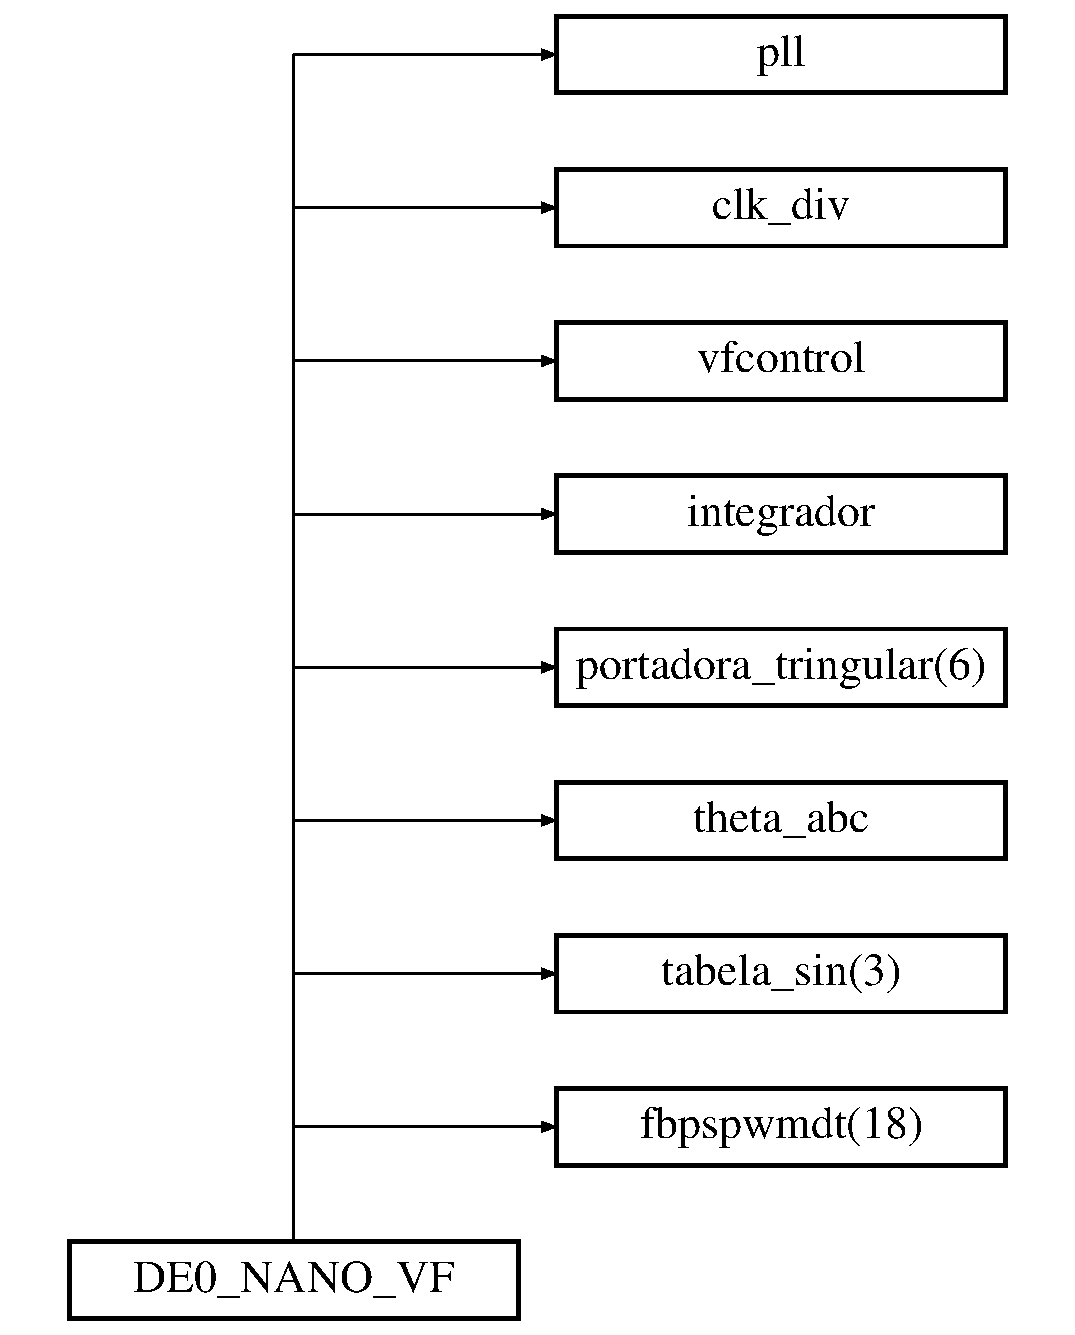
\includegraphics[height=9.000000cm]{class_d_e0___n_a_n_o___v_f}
\end{center}
\end{figure}
\subsection*{Entities}
\begin{DoxyCompactItemize}
\item 
\hyperlink{class_d_e0___n_a_n_o___v_f_1_1_m_a_i_n}{M\+A\+I\+N} architecture
\end{DoxyCompactItemize}
\subsection*{Libraries}
 \begin{DoxyCompactItemize}
\item 
\hyperlink{class_d_e0___n_a_n_o___v_f_a0a6af6eef40212dbaf130d57ce711256}{ieee} 
\end{DoxyCompactItemize}
\subsection*{Use Clauses}
 \begin{DoxyCompactItemize}
\item 
\hyperlink{class_d_e0___n_a_n_o___v_f_acd03516902501cd1c7296a98e22c6fcb}{std\+\_\+logic\+\_\+1164}   
\item 
\hyperlink{class_d_e0___n_a_n_o___v_f_a0f5ecc6613f63d07f7963a97b1b26095}{std\+\_\+logic\+\_\+arith}   
\item 
\hyperlink{class_d_e0___n_a_n_o___v_f_a598da929e807d58939b47499e8bc9fa8}{std\+\_\+logic\+\_\+unsigned}   
\item 
\hyperlink{class_d_e0___n_a_n_o___v_f_ae00f3f04545af57582ff10609eee23e2}{N\+U\+M\+E\+R\+I\+C\+\_\+\+S\+T\+D}   
\item 
\hyperlink{class_d_e0___n_a_n_o___v_f_aad86249c80e8c1e7ee1c4748aba748e3}{fixed\+\_\+pkg}   
\item 
\hyperlink{class_d_e0___n_a_n_o___v_f_ac1788a894930eeee5aaed06b4775d746}{my\+\_\+types\+\_\+pkg}   
\end{DoxyCompactItemize}
\subsection*{Generics}
 \begin{DoxyCompactItemize}
\item 
\hyperlink{class_d_e0___n_a_n_o___v_f_af855138be951f4c562436dfd59f85b54}{N} {\bfseries {\bfseries \textcolor{comment}{integer}\textcolor{vhdlchar}{ }\textcolor{vhdlchar}{ }\textcolor{vhdlchar}{\+:}\textcolor{vhdlchar}{=}\textcolor{vhdlchar}{ }\textcolor{vhdlchar}{ } \textcolor{vhdldigit}{3} \textcolor{vhdlchar}{ }}}
\item 
\hyperlink{class_d_e0___n_a_n_o___v_f_a2629ecb3bb37e8104b2866b0fd0c8574}{Nin} {\bfseries {\bfseries \textcolor{comment}{integer}\textcolor{vhdlchar}{ }\textcolor{vhdlchar}{ }\textcolor{vhdlchar}{\+:}\textcolor{vhdlchar}{=}\textcolor{vhdlchar}{ }\textcolor{vhdlchar}{ } \textcolor{vhdldigit}{13} \textcolor{vhdlchar}{ }}}
\item 
\hyperlink{class_d_e0___n_a_n_o___v_f_a061c0d632c8bdf5dd32c80acf9a9c475}{Nout} {\bfseries {\bfseries \textcolor{comment}{integer}\textcolor{vhdlchar}{ }\textcolor{vhdlchar}{ }\textcolor{vhdlchar}{\+:}\textcolor{vhdlchar}{=}\textcolor{vhdlchar}{ }\textcolor{vhdlchar}{ } \textcolor{vhdldigit}{30} \textcolor{vhdlchar}{ }}}
\item 
\hyperlink{class_d_e0___n_a_n_o___v_f_a9ba59f708a3f2e2c9a9bdba7ac62f13a}{n\+\_\+bits\+\_\+phase} {\bfseries {\bfseries \textcolor{comment}{integer}\textcolor{vhdlchar}{ }\textcolor{vhdlchar}{ }\textcolor{vhdlchar}{\+:}\textcolor{vhdlchar}{=}\textcolor{vhdlchar}{ }\textcolor{vhdlchar}{ } \textcolor{vhdldigit}{30} \textcolor{vhdlchar}{ }}}
\item 
\hyperlink{class_d_e0___n_a_n_o___v_f_afee4aa1628956aa350183d8881689198}{n\+\_\+bits\+\_\+c} {\bfseries {\bfseries \textcolor{comment}{integer}\textcolor{vhdlchar}{ }\textcolor{vhdlchar}{ }\textcolor{vhdlchar}{\+:}\textcolor{vhdlchar}{=}\textcolor{vhdlchar}{ }\textcolor{vhdlchar}{ } \textcolor{vhdldigit}{16} \textcolor{vhdlchar}{ }}}
\item 
\hyperlink{class_d_e0___n_a_n_o___v_f_a9aab84a644aefaf58d2d687a1b235ff3}{T\+A\+M\+\_\+\+M\+E\+M} {\bfseries {\bfseries \textcolor{comment}{integer}\textcolor{vhdlchar}{ }\textcolor{vhdlchar}{ }\textcolor{vhdlchar}{\+:}\textcolor{vhdlchar}{=}\textcolor{vhdlchar}{ }\textcolor{vhdlchar}{ } \textcolor{vhdldigit}{32} \textcolor{vhdlchar}{ }}}
\item 
\hyperlink{class_d_e0___n_a_n_o___v_f_abf975e3873df608ef7053790457e16db}{N\+B\+I\+T\+S\+\_\+\+M\+E\+M\+\_\+\+A\+D\+D\+R\+E\+S\+S} {\bfseries {\bfseries \textcolor{comment}{integer}\textcolor{vhdlchar}{ }\textcolor{vhdlchar}{ }\textcolor{vhdlchar}{\+:}\textcolor{vhdlchar}{=}\textcolor{vhdlchar}{ }\textcolor{vhdlchar}{ } \textcolor{vhdldigit}{6} \textcolor{vhdlchar}{ }}}
\item 
\hyperlink{class_d_e0___n_a_n_o___v_f_a0bc2b40306736322a2a9a1496e575aad}{I\+D\+\_\+\+M\+E\+M\+\_\+\+D\+A\+C} {\bfseries {\bfseries \textcolor{comment}{integer}\textcolor{vhdlchar}{ }\textcolor{vhdlchar}{ }\textcolor{vhdlchar}{\+:}\textcolor{vhdlchar}{=}\textcolor{vhdlchar}{ }\textcolor{vhdlchar}{ } \textcolor{vhdldigit}{28} \textcolor{vhdlchar}{ }}}
\item 
\hyperlink{class_d_e0___n_a_n_o___v_f_a5c5739ee995dcc5500803f87710cf9c9}{I\+D\+\_\+\+M\+E\+M\+\_\+\+S\+W1} {\bfseries {\bfseries \textcolor{comment}{integer}\textcolor{vhdlchar}{ }\textcolor{vhdlchar}{ }\textcolor{vhdlchar}{\+:}\textcolor{vhdlchar}{=}\textcolor{vhdlchar}{ }\textcolor{vhdlchar}{ } \textcolor{vhdldigit}{30} \textcolor{vhdlchar}{ }}}
\item 
\hyperlink{class_d_e0___n_a_n_o___v_f_abb7ce405d45a733b6db94314a4f791fd}{I} {\bfseries {\bfseries \textcolor{comment}{integer}\textcolor{vhdlchar}{ }\textcolor{vhdlchar}{ }\textcolor{vhdlchar}{\+:}\textcolor{vhdlchar}{=}\textcolor{vhdlchar}{ }\textcolor{vhdlchar}{ } \textcolor{vhdldigit}{1} \textcolor{vhdlchar}{ }}}
\item 
\hyperlink{class_d_e0___n_a_n_o___v_f_aac2d6825f96b21ae984648cc93554339}{F} {\bfseries {\bfseries \textcolor{comment}{integer}\textcolor{vhdlchar}{ }\textcolor{vhdlchar}{ }\textcolor{vhdlchar}{\+:}\textcolor{vhdlchar}{=}\textcolor{vhdlchar}{ }\textcolor{vhdlchar}{ } \textcolor{vhdldigit}{14} \textcolor{vhdlchar}{ }}}
\end{DoxyCompactItemize}
\subsection*{Ports}
 \begin{DoxyCompactItemize}
\item 
\hyperlink{class_d_e0___n_a_n_o___v_f_a4b5e1e3eba67b2e61c77c9a719d8518c}{C\+L\+O\+C\+K\+\_\+50}  {\bfseries {\bfseries \textcolor{keywordflow}{in}\textcolor{vhdlchar}{ }}} {\bfseries \textcolor{comment}{std\+\_\+logic}\textcolor{vhdlchar}{ }} 
\item 
\hyperlink{class_d_e0___n_a_n_o___v_f_a424944084857f6787a0ddb567d0b5240}{L\+E\+D}  {\bfseries {\bfseries \textcolor{keywordflow}{out}\textcolor{vhdlchar}{ }}} {\bfseries \textcolor{comment}{std\+\_\+logic\+\_\+vector}\textcolor{vhdlchar}{ }\textcolor{vhdlchar}{(}\textcolor{vhdlchar}{ }\textcolor{vhdlchar}{ } \textcolor{vhdldigit}{7} \textcolor{vhdlchar}{ }\textcolor{keywordflow}{D\+O\+W\+N\+T\+O}\textcolor{vhdlchar}{ }\textcolor{vhdlchar}{ } \textcolor{vhdldigit}{0} \textcolor{vhdlchar}{ }\textcolor{vhdlchar}{)}\textcolor{vhdlchar}{ }} 
\item 
\hyperlink{class_d_e0___n_a_n_o___v_f_a30974727c81621f672f7f9490463f9d3}{S\+W}  {\bfseries {\bfseries \textcolor{keywordflow}{in}\textcolor{vhdlchar}{ }}} {\bfseries \textcolor{comment}{std\+\_\+logic\+\_\+vector}\textcolor{vhdlchar}{ }\textcolor{vhdlchar}{(}\textcolor{vhdlchar}{ }\textcolor{vhdlchar}{ } \textcolor{vhdldigit}{3} \textcolor{vhdlchar}{ }\textcolor{keywordflow}{D\+O\+W\+N\+T\+O}\textcolor{vhdlchar}{ }\textcolor{vhdlchar}{ } \textcolor{vhdldigit}{0} \textcolor{vhdlchar}{ }\textcolor{vhdlchar}{)}\textcolor{vhdlchar}{ }} 
\item 
\hyperlink{class_d_e0___n_a_n_o___v_f_aa70bf9245705f33e4529eb81df3fbf94}{K\+E\+Y}  {\bfseries {\bfseries \textcolor{keywordflow}{in}\textcolor{vhdlchar}{ }}} {\bfseries \textcolor{comment}{std\+\_\+logic\+\_\+vector}\textcolor{vhdlchar}{ }\textcolor{vhdlchar}{(}\textcolor{vhdlchar}{ }\textcolor{vhdlchar}{ } \textcolor{vhdldigit}{1} \textcolor{vhdlchar}{ }\textcolor{keywordflow}{D\+O\+W\+N\+T\+O}\textcolor{vhdlchar}{ }\textcolor{vhdlchar}{ } \textcolor{vhdldigit}{0} \textcolor{vhdlchar}{ }\textcolor{vhdlchar}{)}\textcolor{vhdlchar}{ }} 
\item 
\hyperlink{class_d_e0___n_a_n_o___v_f_ab6bd5afe8823c3590ef5e4195757f852}{R\+E\+S\+E\+T\+\_\+\+F\+A}  {\bfseries {\bfseries \textcolor{keywordflow}{out}\textcolor{vhdlchar}{ }}} {\bfseries \textcolor{comment}{std\+\_\+logic\+\_\+vector}\textcolor{vhdlchar}{ }\textcolor{vhdlchar}{(}\textcolor{vhdlchar}{ }\textcolor{vhdlchar}{ }\textcolor{vhdlchar}{ }\textcolor{vhdlchar}{ }{\bfseries \hyperlink{class_d_e0___n_a_n_o___v_f_af855138be951f4c562436dfd59f85b54}{N}} \textcolor{vhdlchar}{-\/}\textcolor{vhdlchar}{ } \textcolor{vhdldigit}{1} \textcolor{vhdlchar}{ }\textcolor{keywordflow}{D\+O\+W\+N\+T\+O}\textcolor{vhdlchar}{ }\textcolor{vhdlchar}{ } \textcolor{vhdldigit}{0} \textcolor{vhdlchar}{ }\textcolor{vhdlchar}{)}\textcolor{vhdlchar}{ }} 
\item 
\hyperlink{class_d_e0___n_a_n_o___v_f_a292e884f4d72fca8a1bec36c11933ef7}{P\+W\+M1\+L\+\_\+\+F\+A}  {\bfseries {\bfseries \textcolor{keywordflow}{out}\textcolor{vhdlchar}{ }}} {\bfseries \textcolor{comment}{std\+\_\+logic\+\_\+vector}\textcolor{vhdlchar}{ }\textcolor{vhdlchar}{(}\textcolor{vhdlchar}{ }\textcolor{vhdlchar}{ }\textcolor{vhdlchar}{ }\textcolor{vhdlchar}{ }{\bfseries \hyperlink{class_d_e0___n_a_n_o___v_f_af855138be951f4c562436dfd59f85b54}{N}} \textcolor{vhdlchar}{-\/}\textcolor{vhdlchar}{ } \textcolor{vhdldigit}{1} \textcolor{vhdlchar}{ }\textcolor{keywordflow}{D\+O\+W\+N\+T\+O}\textcolor{vhdlchar}{ }\textcolor{vhdlchar}{ } \textcolor{vhdldigit}{0} \textcolor{vhdlchar}{ }\textcolor{vhdlchar}{)}\textcolor{vhdlchar}{ }} 
\item 
\hyperlink{class_d_e0___n_a_n_o___v_f_af21e77adde949f9a9a599f25976a6a74}{P\+W\+M1\+H\+\_\+\+F\+A}  {\bfseries {\bfseries \textcolor{keywordflow}{out}\textcolor{vhdlchar}{ }}} {\bfseries \textcolor{comment}{std\+\_\+logic\+\_\+vector}\textcolor{vhdlchar}{ }\textcolor{vhdlchar}{(}\textcolor{vhdlchar}{ }\textcolor{vhdlchar}{ }\textcolor{vhdlchar}{ }\textcolor{vhdlchar}{ }{\bfseries \hyperlink{class_d_e0___n_a_n_o___v_f_af855138be951f4c562436dfd59f85b54}{N}} \textcolor{vhdlchar}{-\/}\textcolor{vhdlchar}{ } \textcolor{vhdldigit}{1} \textcolor{vhdlchar}{ }\textcolor{keywordflow}{D\+O\+W\+N\+T\+O}\textcolor{vhdlchar}{ }\textcolor{vhdlchar}{ } \textcolor{vhdldigit}{0} \textcolor{vhdlchar}{ }\textcolor{vhdlchar}{)}\textcolor{vhdlchar}{ }} 
\item 
\hyperlink{class_d_e0___n_a_n_o___v_f_a357d73a496027c4f7000298ecdc41a05}{P\+W\+M2\+L\+\_\+\+F\+A}  {\bfseries {\bfseries \textcolor{keywordflow}{out}\textcolor{vhdlchar}{ }}} {\bfseries \textcolor{comment}{std\+\_\+logic\+\_\+vector}\textcolor{vhdlchar}{ }\textcolor{vhdlchar}{(}\textcolor{vhdlchar}{ }\textcolor{vhdlchar}{ }\textcolor{vhdlchar}{ }\textcolor{vhdlchar}{ }{\bfseries \hyperlink{class_d_e0___n_a_n_o___v_f_af855138be951f4c562436dfd59f85b54}{N}} \textcolor{vhdlchar}{-\/}\textcolor{vhdlchar}{ } \textcolor{vhdldigit}{1} \textcolor{vhdlchar}{ }\textcolor{keywordflow}{D\+O\+W\+N\+T\+O}\textcolor{vhdlchar}{ }\textcolor{vhdlchar}{ } \textcolor{vhdldigit}{0} \textcolor{vhdlchar}{ }\textcolor{vhdlchar}{)}\textcolor{vhdlchar}{ }} 
\item 
\hyperlink{class_d_e0___n_a_n_o___v_f_a3a05a366015b8398929044188870fa7b}{P\+W\+M2\+H\+\_\+\+F\+A}  {\bfseries {\bfseries \textcolor{keywordflow}{out}\textcolor{vhdlchar}{ }}} {\bfseries \textcolor{comment}{std\+\_\+logic\+\_\+vector}\textcolor{vhdlchar}{ }\textcolor{vhdlchar}{(}\textcolor{vhdlchar}{ }\textcolor{vhdlchar}{ }\textcolor{vhdlchar}{ }\textcolor{vhdlchar}{ }{\bfseries \hyperlink{class_d_e0___n_a_n_o___v_f_af855138be951f4c562436dfd59f85b54}{N}} \textcolor{vhdlchar}{-\/}\textcolor{vhdlchar}{ } \textcolor{vhdldigit}{1} \textcolor{vhdlchar}{ }\textcolor{keywordflow}{D\+O\+W\+N\+T\+O}\textcolor{vhdlchar}{ }\textcolor{vhdlchar}{ } \textcolor{vhdldigit}{0} \textcolor{vhdlchar}{ }\textcolor{vhdlchar}{)}\textcolor{vhdlchar}{ }} 
\item 
\hyperlink{class_d_e0___n_a_n_o___v_f_a11a54edd784d9fa7ce3a24aa015463d6}{I\+N\+T0\+\_\+\+F\+A}  {\bfseries {\bfseries \textcolor{keywordflow}{in}\textcolor{vhdlchar}{ }}} {\bfseries \textcolor{comment}{std\+\_\+logic\+\_\+vector}\textcolor{vhdlchar}{ }\textcolor{vhdlchar}{(}\textcolor{vhdlchar}{ }\textcolor{vhdlchar}{ }\textcolor{vhdlchar}{ }\textcolor{vhdlchar}{ }{\bfseries \hyperlink{class_d_e0___n_a_n_o___v_f_af855138be951f4c562436dfd59f85b54}{N}} \textcolor{vhdlchar}{-\/}\textcolor{vhdlchar}{ } \textcolor{vhdldigit}{1} \textcolor{vhdlchar}{ }\textcolor{keywordflow}{D\+O\+W\+N\+T\+O}\textcolor{vhdlchar}{ }\textcolor{vhdlchar}{ } \textcolor{vhdldigit}{0} \textcolor{vhdlchar}{ }\textcolor{vhdlchar}{)}\textcolor{vhdlchar}{ }} 
\item 
\hyperlink{class_d_e0___n_a_n_o___v_f_abce5db5149bd7ae87d6c3601972ae05f}{R\+E\+S\+E\+T\+\_\+\+F\+B}  {\bfseries {\bfseries \textcolor{keywordflow}{out}\textcolor{vhdlchar}{ }}} {\bfseries \textcolor{comment}{std\+\_\+logic\+\_\+vector}\textcolor{vhdlchar}{ }\textcolor{vhdlchar}{(}\textcolor{vhdlchar}{ }\textcolor{vhdlchar}{ }\textcolor{vhdlchar}{ }\textcolor{vhdlchar}{ }{\bfseries \hyperlink{class_d_e0___n_a_n_o___v_f_af855138be951f4c562436dfd59f85b54}{N}} \textcolor{vhdlchar}{-\/}\textcolor{vhdlchar}{ } \textcolor{vhdldigit}{1} \textcolor{vhdlchar}{ }\textcolor{keywordflow}{D\+O\+W\+N\+T\+O}\textcolor{vhdlchar}{ }\textcolor{vhdlchar}{ } \textcolor{vhdldigit}{0} \textcolor{vhdlchar}{ }\textcolor{vhdlchar}{)}\textcolor{vhdlchar}{ }} 
\item 
\hyperlink{class_d_e0___n_a_n_o___v_f_ac5cc3b06408f1596a61b08b946a9c1d0}{P\+W\+M1\+L\+\_\+\+F\+B}  {\bfseries {\bfseries \textcolor{keywordflow}{out}\textcolor{vhdlchar}{ }}} {\bfseries \textcolor{comment}{std\+\_\+logic\+\_\+vector}\textcolor{vhdlchar}{ }\textcolor{vhdlchar}{(}\textcolor{vhdlchar}{ }\textcolor{vhdlchar}{ }\textcolor{vhdlchar}{ }\textcolor{vhdlchar}{ }{\bfseries \hyperlink{class_d_e0___n_a_n_o___v_f_af855138be951f4c562436dfd59f85b54}{N}} \textcolor{vhdlchar}{-\/}\textcolor{vhdlchar}{ } \textcolor{vhdldigit}{1} \textcolor{vhdlchar}{ }\textcolor{keywordflow}{D\+O\+W\+N\+T\+O}\textcolor{vhdlchar}{ }\textcolor{vhdlchar}{ } \textcolor{vhdldigit}{0} \textcolor{vhdlchar}{ }\textcolor{vhdlchar}{)}\textcolor{vhdlchar}{ }} 
\item 
\hyperlink{class_d_e0___n_a_n_o___v_f_a69e944b362281970fb9a0a5ec6f5f068}{P\+W\+M1\+H\+\_\+\+F\+B}  {\bfseries {\bfseries \textcolor{keywordflow}{out}\textcolor{vhdlchar}{ }}} {\bfseries \textcolor{comment}{std\+\_\+logic\+\_\+vector}\textcolor{vhdlchar}{ }\textcolor{vhdlchar}{(}\textcolor{vhdlchar}{ }\textcolor{vhdlchar}{ }\textcolor{vhdlchar}{ }\textcolor{vhdlchar}{ }{\bfseries \hyperlink{class_d_e0___n_a_n_o___v_f_af855138be951f4c562436dfd59f85b54}{N}} \textcolor{vhdlchar}{-\/}\textcolor{vhdlchar}{ } \textcolor{vhdldigit}{1} \textcolor{vhdlchar}{ }\textcolor{keywordflow}{D\+O\+W\+N\+T\+O}\textcolor{vhdlchar}{ }\textcolor{vhdlchar}{ } \textcolor{vhdldigit}{0} \textcolor{vhdlchar}{ }\textcolor{vhdlchar}{)}\textcolor{vhdlchar}{ }} 
\item 
\hyperlink{class_d_e0___n_a_n_o___v_f_aefa13a97661cae3b7b87245ed460abe5}{P\+W\+M2\+L\+\_\+\+F\+B}  {\bfseries {\bfseries \textcolor{keywordflow}{out}\textcolor{vhdlchar}{ }}} {\bfseries \textcolor{comment}{std\+\_\+logic\+\_\+vector}\textcolor{vhdlchar}{ }\textcolor{vhdlchar}{(}\textcolor{vhdlchar}{ }\textcolor{vhdlchar}{ }\textcolor{vhdlchar}{ }\textcolor{vhdlchar}{ }{\bfseries \hyperlink{class_d_e0___n_a_n_o___v_f_af855138be951f4c562436dfd59f85b54}{N}} \textcolor{vhdlchar}{-\/}\textcolor{vhdlchar}{ } \textcolor{vhdldigit}{1} \textcolor{vhdlchar}{ }\textcolor{keywordflow}{D\+O\+W\+N\+T\+O}\textcolor{vhdlchar}{ }\textcolor{vhdlchar}{ } \textcolor{vhdldigit}{0} \textcolor{vhdlchar}{ }\textcolor{vhdlchar}{)}\textcolor{vhdlchar}{ }} 
\item 
\hyperlink{class_d_e0___n_a_n_o___v_f_a7efac822a270a6c828ef5eb2cc090127}{P\+W\+M2\+H\+\_\+\+F\+B}  {\bfseries {\bfseries \textcolor{keywordflow}{out}\textcolor{vhdlchar}{ }}} {\bfseries \textcolor{comment}{std\+\_\+logic\+\_\+vector}\textcolor{vhdlchar}{ }\textcolor{vhdlchar}{(}\textcolor{vhdlchar}{ }\textcolor{vhdlchar}{ }\textcolor{vhdlchar}{ }\textcolor{vhdlchar}{ }{\bfseries \hyperlink{class_d_e0___n_a_n_o___v_f_af855138be951f4c562436dfd59f85b54}{N}} \textcolor{vhdlchar}{-\/}\textcolor{vhdlchar}{ } \textcolor{vhdldigit}{1} \textcolor{vhdlchar}{ }\textcolor{keywordflow}{D\+O\+W\+N\+T\+O}\textcolor{vhdlchar}{ }\textcolor{vhdlchar}{ } \textcolor{vhdldigit}{0} \textcolor{vhdlchar}{ }\textcolor{vhdlchar}{)}\textcolor{vhdlchar}{ }} 
\item 
\hyperlink{class_d_e0___n_a_n_o___v_f_a072d40993d1ff4b3dc85aa2aed7be456}{I\+N\+T0\+\_\+\+F\+B}  {\bfseries {\bfseries \textcolor{keywordflow}{in}\textcolor{vhdlchar}{ }}} {\bfseries \textcolor{comment}{std\+\_\+logic\+\_\+vector}\textcolor{vhdlchar}{ }\textcolor{vhdlchar}{(}\textcolor{vhdlchar}{ }\textcolor{vhdlchar}{ }\textcolor{vhdlchar}{ }\textcolor{vhdlchar}{ }{\bfseries \hyperlink{class_d_e0___n_a_n_o___v_f_af855138be951f4c562436dfd59f85b54}{N}} \textcolor{vhdlchar}{-\/}\textcolor{vhdlchar}{ } \textcolor{vhdldigit}{1} \textcolor{vhdlchar}{ }\textcolor{keywordflow}{D\+O\+W\+N\+T\+O}\textcolor{vhdlchar}{ }\textcolor{vhdlchar}{ } \textcolor{vhdldigit}{0} \textcolor{vhdlchar}{ }\textcolor{vhdlchar}{)}\textcolor{vhdlchar}{ }} 
\item 
\hyperlink{class_d_e0___n_a_n_o___v_f_a05f3fd52a3ed4e3c8ccfeb431451afc6}{R\+E\+S\+E\+T\+\_\+\+F\+C}  {\bfseries {\bfseries \textcolor{keywordflow}{out}\textcolor{vhdlchar}{ }}} {\bfseries \textcolor{comment}{std\+\_\+logic\+\_\+vector}\textcolor{vhdlchar}{ }\textcolor{vhdlchar}{(}\textcolor{vhdlchar}{ }\textcolor{vhdlchar}{ }\textcolor{vhdlchar}{ }\textcolor{vhdlchar}{ }{\bfseries \hyperlink{class_d_e0___n_a_n_o___v_f_af855138be951f4c562436dfd59f85b54}{N}} \textcolor{vhdlchar}{-\/}\textcolor{vhdlchar}{ } \textcolor{vhdldigit}{1} \textcolor{vhdlchar}{ }\textcolor{keywordflow}{D\+O\+W\+N\+T\+O}\textcolor{vhdlchar}{ }\textcolor{vhdlchar}{ } \textcolor{vhdldigit}{0} \textcolor{vhdlchar}{ }\textcolor{vhdlchar}{)}\textcolor{vhdlchar}{ }} 
\item 
\hyperlink{class_d_e0___n_a_n_o___v_f_ac9a5e24e4c9b96a7ee1750285ff2af08}{P\+W\+M1\+L\+\_\+\+F\+C}  {\bfseries {\bfseries \textcolor{keywordflow}{out}\textcolor{vhdlchar}{ }}} {\bfseries \textcolor{comment}{std\+\_\+logic\+\_\+vector}\textcolor{vhdlchar}{ }\textcolor{vhdlchar}{(}\textcolor{vhdlchar}{ }\textcolor{vhdlchar}{ }\textcolor{vhdlchar}{ }\textcolor{vhdlchar}{ }{\bfseries \hyperlink{class_d_e0___n_a_n_o___v_f_af855138be951f4c562436dfd59f85b54}{N}} \textcolor{vhdlchar}{-\/}\textcolor{vhdlchar}{ } \textcolor{vhdldigit}{1} \textcolor{vhdlchar}{ }\textcolor{keywordflow}{D\+O\+W\+N\+T\+O}\textcolor{vhdlchar}{ }\textcolor{vhdlchar}{ } \textcolor{vhdldigit}{0} \textcolor{vhdlchar}{ }\textcolor{vhdlchar}{)}\textcolor{vhdlchar}{ }} 
\item 
\hyperlink{class_d_e0___n_a_n_o___v_f_ae64c7416adbe802e6aa4125230fad012}{P\+W\+M1\+H\+\_\+\+F\+C}  {\bfseries {\bfseries \textcolor{keywordflow}{out}\textcolor{vhdlchar}{ }}} {\bfseries \textcolor{comment}{std\+\_\+logic\+\_\+vector}\textcolor{vhdlchar}{ }\textcolor{vhdlchar}{(}\textcolor{vhdlchar}{ }\textcolor{vhdlchar}{ }\textcolor{vhdlchar}{ }\textcolor{vhdlchar}{ }{\bfseries \hyperlink{class_d_e0___n_a_n_o___v_f_af855138be951f4c562436dfd59f85b54}{N}} \textcolor{vhdlchar}{-\/}\textcolor{vhdlchar}{ } \textcolor{vhdldigit}{1} \textcolor{vhdlchar}{ }\textcolor{keywordflow}{D\+O\+W\+N\+T\+O}\textcolor{vhdlchar}{ }\textcolor{vhdlchar}{ } \textcolor{vhdldigit}{0} \textcolor{vhdlchar}{ }\textcolor{vhdlchar}{)}\textcolor{vhdlchar}{ }} 
\item 
\hyperlink{class_d_e0___n_a_n_o___v_f_a47c0de05323647e9484b2ec6764255c0}{P\+W\+M2\+L\+\_\+\+F\+C}  {\bfseries {\bfseries \textcolor{keywordflow}{out}\textcolor{vhdlchar}{ }}} {\bfseries \textcolor{comment}{std\+\_\+logic\+\_\+vector}\textcolor{vhdlchar}{ }\textcolor{vhdlchar}{(}\textcolor{vhdlchar}{ }\textcolor{vhdlchar}{ }\textcolor{vhdlchar}{ }\textcolor{vhdlchar}{ }{\bfseries \hyperlink{class_d_e0___n_a_n_o___v_f_af855138be951f4c562436dfd59f85b54}{N}} \textcolor{vhdlchar}{-\/}\textcolor{vhdlchar}{ } \textcolor{vhdldigit}{1} \textcolor{vhdlchar}{ }\textcolor{keywordflow}{D\+O\+W\+N\+T\+O}\textcolor{vhdlchar}{ }\textcolor{vhdlchar}{ } \textcolor{vhdldigit}{0} \textcolor{vhdlchar}{ }\textcolor{vhdlchar}{)}\textcolor{vhdlchar}{ }} 
\item 
\hyperlink{class_d_e0___n_a_n_o___v_f_a8318940c01015b267904bdca0e01c2a2}{P\+W\+M2\+H\+\_\+\+F\+C}  {\bfseries {\bfseries \textcolor{keywordflow}{out}\textcolor{vhdlchar}{ }}} {\bfseries \textcolor{comment}{std\+\_\+logic\+\_\+vector}\textcolor{vhdlchar}{ }\textcolor{vhdlchar}{(}\textcolor{vhdlchar}{ }\textcolor{vhdlchar}{ }\textcolor{vhdlchar}{ }\textcolor{vhdlchar}{ }{\bfseries \hyperlink{class_d_e0___n_a_n_o___v_f_af855138be951f4c562436dfd59f85b54}{N}} \textcolor{vhdlchar}{-\/}\textcolor{vhdlchar}{ } \textcolor{vhdldigit}{1} \textcolor{vhdlchar}{ }\textcolor{keywordflow}{D\+O\+W\+N\+T\+O}\textcolor{vhdlchar}{ }\textcolor{vhdlchar}{ } \textcolor{vhdldigit}{0} \textcolor{vhdlchar}{ }\textcolor{vhdlchar}{)}\textcolor{vhdlchar}{ }} 
\item 
\hyperlink{class_d_e0___n_a_n_o___v_f_a2da3143aa39453a927d622998a1d936b}{I\+N\+T0\+\_\+\+F\+C}  {\bfseries {\bfseries \textcolor{keywordflow}{in}\textcolor{vhdlchar}{ }}} {\bfseries \textcolor{comment}{std\+\_\+logic\+\_\+vector}\textcolor{vhdlchar}{ }\textcolor{vhdlchar}{(}\textcolor{vhdlchar}{ }\textcolor{vhdlchar}{ }\textcolor{vhdlchar}{ }\textcolor{vhdlchar}{ }{\bfseries \hyperlink{class_d_e0___n_a_n_o___v_f_af855138be951f4c562436dfd59f85b54}{N}} \textcolor{vhdlchar}{-\/}\textcolor{vhdlchar}{ } \textcolor{vhdldigit}{1} \textcolor{vhdlchar}{ }\textcolor{keywordflow}{D\+O\+W\+N\+T\+O}\textcolor{vhdlchar}{ }\textcolor{vhdlchar}{ } \textcolor{vhdldigit}{0} \textcolor{vhdlchar}{ }\textcolor{vhdlchar}{)}\textcolor{vhdlchar}{ }} 
\item 
\hyperlink{class_d_e0___n_a_n_o___v_f_a01eff012417d9c479e11ca1e08d0fdb5}{G\+P\+I\+O\+\_\+0}  {\bfseries {\bfseries \textcolor{keywordflow}{out}\textcolor{vhdlchar}{ }}} {\bfseries \textcolor{comment}{std\+\_\+logic\+\_\+vector}\textcolor{vhdlchar}{ }\textcolor{vhdlchar}{(}\textcolor{vhdlchar}{ }\textcolor{vhdlchar}{ } \textcolor{vhdldigit}{3} \textcolor{vhdlchar}{ }\textcolor{keywordflow}{D\+O\+W\+N\+T\+O}\textcolor{vhdlchar}{ }\textcolor{vhdlchar}{ } \textcolor{vhdldigit}{0} \textcolor{vhdlchar}{ }\textcolor{vhdlchar}{)}\textcolor{vhdlchar}{ }} 
\end{DoxyCompactItemize}


\subsection{Detailed Description}


Definition at line 15 of file D\+E0\+\_\+\+N\+A\+N\+O\+\_\+\+V\+F.\+vhd.



\subsection{Member Data Documentation}
\hypertarget{class_d_e0___n_a_n_o___v_f_a4b5e1e3eba67b2e61c77c9a719d8518c}{}\index{D\+E0\+\_\+\+N\+A\+N\+O\+\_\+\+V\+F@{D\+E0\+\_\+\+N\+A\+N\+O\+\_\+\+V\+F}!C\+L\+O\+C\+K\+\_\+50@{C\+L\+O\+C\+K\+\_\+50}}
\index{C\+L\+O\+C\+K\+\_\+50@{C\+L\+O\+C\+K\+\_\+50}!D\+E0\+\_\+\+N\+A\+N\+O\+\_\+\+V\+F@{D\+E0\+\_\+\+N\+A\+N\+O\+\_\+\+V\+F}}
\subsubsection[{C\+L\+O\+C\+K\+\_\+50}]{\setlength{\rightskip}{0pt plus 5cm}{\bf C\+L\+O\+C\+K\+\_\+50} {\bfseries \textcolor{keywordflow}{in}\textcolor{vhdlchar}{ }} {\bfseries \textcolor{comment}{std\+\_\+logic}\textcolor{vhdlchar}{ }} \hspace{0.3cm}{\ttfamily [Port]}}\label{class_d_e0___n_a_n_o___v_f_a4b5e1e3eba67b2e61c77c9a719d8518c}


Definition at line 30 of file D\+E0\+\_\+\+N\+A\+N\+O\+\_\+\+V\+F.\+vhd.

\hypertarget{class_d_e0___n_a_n_o___v_f_aac2d6825f96b21ae984648cc93554339}{}\index{D\+E0\+\_\+\+N\+A\+N\+O\+\_\+\+V\+F@{D\+E0\+\_\+\+N\+A\+N\+O\+\_\+\+V\+F}!F@{F}}
\index{F@{F}!D\+E0\+\_\+\+N\+A\+N\+O\+\_\+\+V\+F@{D\+E0\+\_\+\+N\+A\+N\+O\+\_\+\+V\+F}}
\subsubsection[{F}]{\setlength{\rightskip}{0pt plus 5cm}{\bf F} {\bfseries \textcolor{vhdlchar}{ }} {\bfseries \textcolor{comment}{integer}\textcolor{vhdlchar}{ }\textcolor{vhdlchar}{ }\textcolor{vhdlchar}{\+:}\textcolor{vhdlchar}{=}\textcolor{vhdlchar}{ }\textcolor{vhdlchar}{ } \textcolor{vhdldigit}{14} \textcolor{vhdlchar}{ }} \hspace{0.3cm}{\ttfamily [Generic]}}\label{class_d_e0___n_a_n_o___v_f_aac2d6825f96b21ae984648cc93554339}


Definition at line 28 of file D\+E0\+\_\+\+N\+A\+N\+O\+\_\+\+V\+F.\+vhd.

\hypertarget{class_d_e0___n_a_n_o___v_f_aad86249c80e8c1e7ee1c4748aba748e3}{}\index{D\+E0\+\_\+\+N\+A\+N\+O\+\_\+\+V\+F@{D\+E0\+\_\+\+N\+A\+N\+O\+\_\+\+V\+F}!fixed\+\_\+pkg@{fixed\+\_\+pkg}}
\index{fixed\+\_\+pkg@{fixed\+\_\+pkg}!D\+E0\+\_\+\+N\+A\+N\+O\+\_\+\+V\+F@{D\+E0\+\_\+\+N\+A\+N\+O\+\_\+\+V\+F}}
\subsubsection[{fixed\+\_\+pkg}]{\setlength{\rightskip}{0pt plus 5cm}{\bf fixed\+\_\+pkg}\hspace{0.3cm}{\ttfamily [Package]}}\label{class_d_e0___n_a_n_o___v_f_aad86249c80e8c1e7ee1c4748aba748e3}


Definition at line 10 of file D\+E0\+\_\+\+N\+A\+N\+O\+\_\+\+V\+F.\+vhd.

\hypertarget{class_d_e0___n_a_n_o___v_f_a01eff012417d9c479e11ca1e08d0fdb5}{}\index{D\+E0\+\_\+\+N\+A\+N\+O\+\_\+\+V\+F@{D\+E0\+\_\+\+N\+A\+N\+O\+\_\+\+V\+F}!G\+P\+I\+O\+\_\+0@{G\+P\+I\+O\+\_\+0}}
\index{G\+P\+I\+O\+\_\+0@{G\+P\+I\+O\+\_\+0}!D\+E0\+\_\+\+N\+A\+N\+O\+\_\+\+V\+F@{D\+E0\+\_\+\+N\+A\+N\+O\+\_\+\+V\+F}}
\subsubsection[{G\+P\+I\+O\+\_\+0}]{\setlength{\rightskip}{0pt plus 5cm}{\bf G\+P\+I\+O\+\_\+0} {\bfseries \textcolor{keywordflow}{out}\textcolor{vhdlchar}{ }} {\bfseries \textcolor{comment}{std\+\_\+logic\+\_\+vector}\textcolor{vhdlchar}{ }\textcolor{vhdlchar}{(}\textcolor{vhdlchar}{ }\textcolor{vhdlchar}{ } \textcolor{vhdldigit}{3} \textcolor{vhdlchar}{ }\textcolor{keywordflow}{D\+O\+W\+N\+T\+O}\textcolor{vhdlchar}{ }\textcolor{vhdlchar}{ } \textcolor{vhdldigit}{0} \textcolor{vhdlchar}{ }\textcolor{vhdlchar}{)}\textcolor{vhdlchar}{ }} \hspace{0.3cm}{\ttfamily [Port]}}\label{class_d_e0___n_a_n_o___v_f_a01eff012417d9c479e11ca1e08d0fdb5}


Definition at line 70 of file D\+E0\+\_\+\+N\+A\+N\+O\+\_\+\+V\+F.\+vhd.

\hypertarget{class_d_e0___n_a_n_o___v_f_abb7ce405d45a733b6db94314a4f791fd}{}\index{D\+E0\+\_\+\+N\+A\+N\+O\+\_\+\+V\+F@{D\+E0\+\_\+\+N\+A\+N\+O\+\_\+\+V\+F}!I@{I}}
\index{I@{I}!D\+E0\+\_\+\+N\+A\+N\+O\+\_\+\+V\+F@{D\+E0\+\_\+\+N\+A\+N\+O\+\_\+\+V\+F}}
\subsubsection[{I}]{\setlength{\rightskip}{0pt plus 5cm}{\bf I} {\bfseries \textcolor{vhdlchar}{ }} {\bfseries \textcolor{comment}{integer}\textcolor{vhdlchar}{ }\textcolor{vhdlchar}{ }\textcolor{vhdlchar}{\+:}\textcolor{vhdlchar}{=}\textcolor{vhdlchar}{ }\textcolor{vhdlchar}{ } \textcolor{vhdldigit}{1} \textcolor{vhdlchar}{ }} \hspace{0.3cm}{\ttfamily [Generic]}}\label{class_d_e0___n_a_n_o___v_f_abb7ce405d45a733b6db94314a4f791fd}


Definition at line 26 of file D\+E0\+\_\+\+N\+A\+N\+O\+\_\+\+V\+F.\+vhd.

\hypertarget{class_d_e0___n_a_n_o___v_f_a0bc2b40306736322a2a9a1496e575aad}{}\index{D\+E0\+\_\+\+N\+A\+N\+O\+\_\+\+V\+F@{D\+E0\+\_\+\+N\+A\+N\+O\+\_\+\+V\+F}!I\+D\+\_\+\+M\+E\+M\+\_\+\+D\+A\+C@{I\+D\+\_\+\+M\+E\+M\+\_\+\+D\+A\+C}}
\index{I\+D\+\_\+\+M\+E\+M\+\_\+\+D\+A\+C@{I\+D\+\_\+\+M\+E\+M\+\_\+\+D\+A\+C}!D\+E0\+\_\+\+N\+A\+N\+O\+\_\+\+V\+F@{D\+E0\+\_\+\+N\+A\+N\+O\+\_\+\+V\+F}}
\subsubsection[{I\+D\+\_\+\+M\+E\+M\+\_\+\+D\+A\+C}]{\setlength{\rightskip}{0pt plus 5cm}{\bf I\+D\+\_\+\+M\+E\+M\+\_\+\+D\+A\+C} {\bfseries \textcolor{vhdlchar}{ }} {\bfseries \textcolor{comment}{integer}\textcolor{vhdlchar}{ }\textcolor{vhdlchar}{ }\textcolor{vhdlchar}{\+:}\textcolor{vhdlchar}{=}\textcolor{vhdlchar}{ }\textcolor{vhdlchar}{ } \textcolor{vhdldigit}{28} \textcolor{vhdlchar}{ }} \hspace{0.3cm}{\ttfamily [Generic]}}\label{class_d_e0___n_a_n_o___v_f_a0bc2b40306736322a2a9a1496e575aad}


Definition at line 24 of file D\+E0\+\_\+\+N\+A\+N\+O\+\_\+\+V\+F.\+vhd.

\hypertarget{class_d_e0___n_a_n_o___v_f_a5c5739ee995dcc5500803f87710cf9c9}{}\index{D\+E0\+\_\+\+N\+A\+N\+O\+\_\+\+V\+F@{D\+E0\+\_\+\+N\+A\+N\+O\+\_\+\+V\+F}!I\+D\+\_\+\+M\+E\+M\+\_\+\+S\+W1@{I\+D\+\_\+\+M\+E\+M\+\_\+\+S\+W1}}
\index{I\+D\+\_\+\+M\+E\+M\+\_\+\+S\+W1@{I\+D\+\_\+\+M\+E\+M\+\_\+\+S\+W1}!D\+E0\+\_\+\+N\+A\+N\+O\+\_\+\+V\+F@{D\+E0\+\_\+\+N\+A\+N\+O\+\_\+\+V\+F}}
\subsubsection[{I\+D\+\_\+\+M\+E\+M\+\_\+\+S\+W1}]{\setlength{\rightskip}{0pt plus 5cm}{\bf I\+D\+\_\+\+M\+E\+M\+\_\+\+S\+W1} {\bfseries \textcolor{vhdlchar}{ }} {\bfseries \textcolor{comment}{integer}\textcolor{vhdlchar}{ }\textcolor{vhdlchar}{ }\textcolor{vhdlchar}{\+:}\textcolor{vhdlchar}{=}\textcolor{vhdlchar}{ }\textcolor{vhdlchar}{ } \textcolor{vhdldigit}{30} \textcolor{vhdlchar}{ }} \hspace{0.3cm}{\ttfamily [Generic]}}\label{class_d_e0___n_a_n_o___v_f_a5c5739ee995dcc5500803f87710cf9c9}


Definition at line 25 of file D\+E0\+\_\+\+N\+A\+N\+O\+\_\+\+V\+F.\+vhd.

\hypertarget{class_d_e0___n_a_n_o___v_f_a0a6af6eef40212dbaf130d57ce711256}{}\index{D\+E0\+\_\+\+N\+A\+N\+O\+\_\+\+V\+F@{D\+E0\+\_\+\+N\+A\+N\+O\+\_\+\+V\+F}!ieee@{ieee}}
\index{ieee@{ieee}!D\+E0\+\_\+\+N\+A\+N\+O\+\_\+\+V\+F@{D\+E0\+\_\+\+N\+A\+N\+O\+\_\+\+V\+F}}
\subsubsection[{ieee}]{\setlength{\rightskip}{0pt plus 5cm}{\bf ieee}\hspace{0.3cm}{\ttfamily [Library]}}\label{class_d_e0___n_a_n_o___v_f_a0a6af6eef40212dbaf130d57ce711256}


Definition at line 3 of file D\+E0\+\_\+\+N\+A\+N\+O\+\_\+\+V\+F.\+vhd.

\hypertarget{class_d_e0___n_a_n_o___v_f_a11a54edd784d9fa7ce3a24aa015463d6}{}\index{D\+E0\+\_\+\+N\+A\+N\+O\+\_\+\+V\+F@{D\+E0\+\_\+\+N\+A\+N\+O\+\_\+\+V\+F}!I\+N\+T0\+\_\+\+F\+A@{I\+N\+T0\+\_\+\+F\+A}}
\index{I\+N\+T0\+\_\+\+F\+A@{I\+N\+T0\+\_\+\+F\+A}!D\+E0\+\_\+\+N\+A\+N\+O\+\_\+\+V\+F@{D\+E0\+\_\+\+N\+A\+N\+O\+\_\+\+V\+F}}
\subsubsection[{I\+N\+T0\+\_\+\+F\+A}]{\setlength{\rightskip}{0pt plus 5cm}{\bf I\+N\+T0\+\_\+\+F\+A} {\bfseries \textcolor{keywordflow}{in}\textcolor{vhdlchar}{ }} {\bfseries \textcolor{comment}{std\+\_\+logic\+\_\+vector}\textcolor{vhdlchar}{ }\textcolor{vhdlchar}{(}\textcolor{vhdlchar}{ }\textcolor{vhdlchar}{ }\textcolor{vhdlchar}{ }\textcolor{vhdlchar}{ }{\bfseries {\bf N}} \textcolor{vhdlchar}{-\/}\textcolor{vhdlchar}{ } \textcolor{vhdldigit}{1} \textcolor{vhdlchar}{ }\textcolor{keywordflow}{D\+O\+W\+N\+T\+O}\textcolor{vhdlchar}{ }\textcolor{vhdlchar}{ } \textcolor{vhdldigit}{0} \textcolor{vhdlchar}{ }\textcolor{vhdlchar}{)}\textcolor{vhdlchar}{ }} \hspace{0.3cm}{\ttfamily [Port]}}\label{class_d_e0___n_a_n_o___v_f_a11a54edd784d9fa7ce3a24aa015463d6}


Definition at line 44 of file D\+E0\+\_\+\+N\+A\+N\+O\+\_\+\+V\+F.\+vhd.

\hypertarget{class_d_e0___n_a_n_o___v_f_a072d40993d1ff4b3dc85aa2aed7be456}{}\index{D\+E0\+\_\+\+N\+A\+N\+O\+\_\+\+V\+F@{D\+E0\+\_\+\+N\+A\+N\+O\+\_\+\+V\+F}!I\+N\+T0\+\_\+\+F\+B@{I\+N\+T0\+\_\+\+F\+B}}
\index{I\+N\+T0\+\_\+\+F\+B@{I\+N\+T0\+\_\+\+F\+B}!D\+E0\+\_\+\+N\+A\+N\+O\+\_\+\+V\+F@{D\+E0\+\_\+\+N\+A\+N\+O\+\_\+\+V\+F}}
\subsubsection[{I\+N\+T0\+\_\+\+F\+B}]{\setlength{\rightskip}{0pt plus 5cm}{\bf I\+N\+T0\+\_\+\+F\+B} {\bfseries \textcolor{keywordflow}{in}\textcolor{vhdlchar}{ }} {\bfseries \textcolor{comment}{std\+\_\+logic\+\_\+vector}\textcolor{vhdlchar}{ }\textcolor{vhdlchar}{(}\textcolor{vhdlchar}{ }\textcolor{vhdlchar}{ }\textcolor{vhdlchar}{ }\textcolor{vhdlchar}{ }{\bfseries {\bf N}} \textcolor{vhdlchar}{-\/}\textcolor{vhdlchar}{ } \textcolor{vhdldigit}{1} \textcolor{vhdlchar}{ }\textcolor{keywordflow}{D\+O\+W\+N\+T\+O}\textcolor{vhdlchar}{ }\textcolor{vhdlchar}{ } \textcolor{vhdldigit}{0} \textcolor{vhdlchar}{ }\textcolor{vhdlchar}{)}\textcolor{vhdlchar}{ }} \hspace{0.3cm}{\ttfamily [Port]}}\label{class_d_e0___n_a_n_o___v_f_a072d40993d1ff4b3dc85aa2aed7be456}


Definition at line 52 of file D\+E0\+\_\+\+N\+A\+N\+O\+\_\+\+V\+F.\+vhd.

\hypertarget{class_d_e0___n_a_n_o___v_f_a2da3143aa39453a927d622998a1d936b}{}\index{D\+E0\+\_\+\+N\+A\+N\+O\+\_\+\+V\+F@{D\+E0\+\_\+\+N\+A\+N\+O\+\_\+\+V\+F}!I\+N\+T0\+\_\+\+F\+C@{I\+N\+T0\+\_\+\+F\+C}}
\index{I\+N\+T0\+\_\+\+F\+C@{I\+N\+T0\+\_\+\+F\+C}!D\+E0\+\_\+\+N\+A\+N\+O\+\_\+\+V\+F@{D\+E0\+\_\+\+N\+A\+N\+O\+\_\+\+V\+F}}
\subsubsection[{I\+N\+T0\+\_\+\+F\+C}]{\setlength{\rightskip}{0pt plus 5cm}{\bf I\+N\+T0\+\_\+\+F\+C} {\bfseries \textcolor{keywordflow}{in}\textcolor{vhdlchar}{ }} {\bfseries \textcolor{comment}{std\+\_\+logic\+\_\+vector}\textcolor{vhdlchar}{ }\textcolor{vhdlchar}{(}\textcolor{vhdlchar}{ }\textcolor{vhdlchar}{ }\textcolor{vhdlchar}{ }\textcolor{vhdlchar}{ }{\bfseries {\bf N}} \textcolor{vhdlchar}{-\/}\textcolor{vhdlchar}{ } \textcolor{vhdldigit}{1} \textcolor{vhdlchar}{ }\textcolor{keywordflow}{D\+O\+W\+N\+T\+O}\textcolor{vhdlchar}{ }\textcolor{vhdlchar}{ } \textcolor{vhdldigit}{0} \textcolor{vhdlchar}{ }\textcolor{vhdlchar}{)}\textcolor{vhdlchar}{ }} \hspace{0.3cm}{\ttfamily [Port]}}\label{class_d_e0___n_a_n_o___v_f_a2da3143aa39453a927d622998a1d936b}


Definition at line 61 of file D\+E0\+\_\+\+N\+A\+N\+O\+\_\+\+V\+F.\+vhd.

\hypertarget{class_d_e0___n_a_n_o___v_f_aa70bf9245705f33e4529eb81df3fbf94}{}\index{D\+E0\+\_\+\+N\+A\+N\+O\+\_\+\+V\+F@{D\+E0\+\_\+\+N\+A\+N\+O\+\_\+\+V\+F}!K\+E\+Y@{K\+E\+Y}}
\index{K\+E\+Y@{K\+E\+Y}!D\+E0\+\_\+\+N\+A\+N\+O\+\_\+\+V\+F@{D\+E0\+\_\+\+N\+A\+N\+O\+\_\+\+V\+F}}
\subsubsection[{K\+E\+Y}]{\setlength{\rightskip}{0pt plus 5cm}{\bf K\+E\+Y} {\bfseries \textcolor{keywordflow}{in}\textcolor{vhdlchar}{ }} {\bfseries \textcolor{comment}{std\+\_\+logic\+\_\+vector}\textcolor{vhdlchar}{ }\textcolor{vhdlchar}{(}\textcolor{vhdlchar}{ }\textcolor{vhdlchar}{ } \textcolor{vhdldigit}{1} \textcolor{vhdlchar}{ }\textcolor{keywordflow}{D\+O\+W\+N\+T\+O}\textcolor{vhdlchar}{ }\textcolor{vhdlchar}{ } \textcolor{vhdldigit}{0} \textcolor{vhdlchar}{ }\textcolor{vhdlchar}{)}\textcolor{vhdlchar}{ }} \hspace{0.3cm}{\ttfamily [Port]}}\label{class_d_e0___n_a_n_o___v_f_aa70bf9245705f33e4529eb81df3fbf94}


Definition at line 33 of file D\+E0\+\_\+\+N\+A\+N\+O\+\_\+\+V\+F.\+vhd.

\hypertarget{class_d_e0___n_a_n_o___v_f_a424944084857f6787a0ddb567d0b5240}{}\index{D\+E0\+\_\+\+N\+A\+N\+O\+\_\+\+V\+F@{D\+E0\+\_\+\+N\+A\+N\+O\+\_\+\+V\+F}!L\+E\+D@{L\+E\+D}}
\index{L\+E\+D@{L\+E\+D}!D\+E0\+\_\+\+N\+A\+N\+O\+\_\+\+V\+F@{D\+E0\+\_\+\+N\+A\+N\+O\+\_\+\+V\+F}}
\subsubsection[{L\+E\+D}]{\setlength{\rightskip}{0pt plus 5cm}{\bf L\+E\+D} {\bfseries \textcolor{keywordflow}{out}\textcolor{vhdlchar}{ }} {\bfseries \textcolor{comment}{std\+\_\+logic\+\_\+vector}\textcolor{vhdlchar}{ }\textcolor{vhdlchar}{(}\textcolor{vhdlchar}{ }\textcolor{vhdlchar}{ } \textcolor{vhdldigit}{7} \textcolor{vhdlchar}{ }\textcolor{keywordflow}{D\+O\+W\+N\+T\+O}\textcolor{vhdlchar}{ }\textcolor{vhdlchar}{ } \textcolor{vhdldigit}{0} \textcolor{vhdlchar}{ }\textcolor{vhdlchar}{)}\textcolor{vhdlchar}{ }} \hspace{0.3cm}{\ttfamily [Port]}}\label{class_d_e0___n_a_n_o___v_f_a424944084857f6787a0ddb567d0b5240}


Definition at line 31 of file D\+E0\+\_\+\+N\+A\+N\+O\+\_\+\+V\+F.\+vhd.

\hypertarget{class_d_e0___n_a_n_o___v_f_ac1788a894930eeee5aaed06b4775d746}{}\index{D\+E0\+\_\+\+N\+A\+N\+O\+\_\+\+V\+F@{D\+E0\+\_\+\+N\+A\+N\+O\+\_\+\+V\+F}!my\+\_\+types\+\_\+pkg@{my\+\_\+types\+\_\+pkg}}
\index{my\+\_\+types\+\_\+pkg@{my\+\_\+types\+\_\+pkg}!D\+E0\+\_\+\+N\+A\+N\+O\+\_\+\+V\+F@{D\+E0\+\_\+\+N\+A\+N\+O\+\_\+\+V\+F}}
\subsubsection[{my\+\_\+types\+\_\+pkg}]{\setlength{\rightskip}{0pt plus 5cm}{\bf my\+\_\+types\+\_\+pkg}\hspace{0.3cm}{\ttfamily [Package]}}\label{class_d_e0___n_a_n_o___v_f_ac1788a894930eeee5aaed06b4775d746}


Definition at line 11 of file D\+E0\+\_\+\+N\+A\+N\+O\+\_\+\+V\+F.\+vhd.

\hypertarget{class_d_e0___n_a_n_o___v_f_af855138be951f4c562436dfd59f85b54}{}\index{D\+E0\+\_\+\+N\+A\+N\+O\+\_\+\+V\+F@{D\+E0\+\_\+\+N\+A\+N\+O\+\_\+\+V\+F}!N@{N}}
\index{N@{N}!D\+E0\+\_\+\+N\+A\+N\+O\+\_\+\+V\+F@{D\+E0\+\_\+\+N\+A\+N\+O\+\_\+\+V\+F}}
\subsubsection[{N}]{\setlength{\rightskip}{0pt plus 5cm}{\bf N} {\bfseries \textcolor{vhdlchar}{ }} {\bfseries \textcolor{comment}{integer}\textcolor{vhdlchar}{ }\textcolor{vhdlchar}{ }\textcolor{vhdlchar}{\+:}\textcolor{vhdlchar}{=}\textcolor{vhdlchar}{ }\textcolor{vhdlchar}{ } \textcolor{vhdldigit}{3} \textcolor{vhdlchar}{ }} \hspace{0.3cm}{\ttfamily [Generic]}}\label{class_d_e0___n_a_n_o___v_f_af855138be951f4c562436dfd59f85b54}


Definition at line 17 of file D\+E0\+\_\+\+N\+A\+N\+O\+\_\+\+V\+F.\+vhd.

\hypertarget{class_d_e0___n_a_n_o___v_f_afee4aa1628956aa350183d8881689198}{}\index{D\+E0\+\_\+\+N\+A\+N\+O\+\_\+\+V\+F@{D\+E0\+\_\+\+N\+A\+N\+O\+\_\+\+V\+F}!n\+\_\+bits\+\_\+c@{n\+\_\+bits\+\_\+c}}
\index{n\+\_\+bits\+\_\+c@{n\+\_\+bits\+\_\+c}!D\+E0\+\_\+\+N\+A\+N\+O\+\_\+\+V\+F@{D\+E0\+\_\+\+N\+A\+N\+O\+\_\+\+V\+F}}
\subsubsection[{n\+\_\+bits\+\_\+c}]{\setlength{\rightskip}{0pt plus 5cm}{\bf n\+\_\+bits\+\_\+c} {\bfseries \textcolor{vhdlchar}{ }} {\bfseries \textcolor{comment}{integer}\textcolor{vhdlchar}{ }\textcolor{vhdlchar}{ }\textcolor{vhdlchar}{\+:}\textcolor{vhdlchar}{=}\textcolor{vhdlchar}{ }\textcolor{vhdlchar}{ } \textcolor{vhdldigit}{16} \textcolor{vhdlchar}{ }} \hspace{0.3cm}{\ttfamily [Generic]}}\label{class_d_e0___n_a_n_o___v_f_afee4aa1628956aa350183d8881689198}


Definition at line 21 of file D\+E0\+\_\+\+N\+A\+N\+O\+\_\+\+V\+F.\+vhd.

\hypertarget{class_d_e0___n_a_n_o___v_f_a9ba59f708a3f2e2c9a9bdba7ac62f13a}{}\index{D\+E0\+\_\+\+N\+A\+N\+O\+\_\+\+V\+F@{D\+E0\+\_\+\+N\+A\+N\+O\+\_\+\+V\+F}!n\+\_\+bits\+\_\+phase@{n\+\_\+bits\+\_\+phase}}
\index{n\+\_\+bits\+\_\+phase@{n\+\_\+bits\+\_\+phase}!D\+E0\+\_\+\+N\+A\+N\+O\+\_\+\+V\+F@{D\+E0\+\_\+\+N\+A\+N\+O\+\_\+\+V\+F}}
\subsubsection[{n\+\_\+bits\+\_\+phase}]{\setlength{\rightskip}{0pt plus 5cm}{\bf n\+\_\+bits\+\_\+phase} {\bfseries \textcolor{vhdlchar}{ }} {\bfseries \textcolor{comment}{integer}\textcolor{vhdlchar}{ }\textcolor{vhdlchar}{ }\textcolor{vhdlchar}{\+:}\textcolor{vhdlchar}{=}\textcolor{vhdlchar}{ }\textcolor{vhdlchar}{ } \textcolor{vhdldigit}{30} \textcolor{vhdlchar}{ }} \hspace{0.3cm}{\ttfamily [Generic]}}\label{class_d_e0___n_a_n_o___v_f_a9ba59f708a3f2e2c9a9bdba7ac62f13a}


Definition at line 20 of file D\+E0\+\_\+\+N\+A\+N\+O\+\_\+\+V\+F.\+vhd.

\hypertarget{class_d_e0___n_a_n_o___v_f_abf975e3873df608ef7053790457e16db}{}\index{D\+E0\+\_\+\+N\+A\+N\+O\+\_\+\+V\+F@{D\+E0\+\_\+\+N\+A\+N\+O\+\_\+\+V\+F}!N\+B\+I\+T\+S\+\_\+\+M\+E\+M\+\_\+\+A\+D\+D\+R\+E\+S\+S@{N\+B\+I\+T\+S\+\_\+\+M\+E\+M\+\_\+\+A\+D\+D\+R\+E\+S\+S}}
\index{N\+B\+I\+T\+S\+\_\+\+M\+E\+M\+\_\+\+A\+D\+D\+R\+E\+S\+S@{N\+B\+I\+T\+S\+\_\+\+M\+E\+M\+\_\+\+A\+D\+D\+R\+E\+S\+S}!D\+E0\+\_\+\+N\+A\+N\+O\+\_\+\+V\+F@{D\+E0\+\_\+\+N\+A\+N\+O\+\_\+\+V\+F}}
\subsubsection[{N\+B\+I\+T\+S\+\_\+\+M\+E\+M\+\_\+\+A\+D\+D\+R\+E\+S\+S}]{\setlength{\rightskip}{0pt plus 5cm}{\bf N\+B\+I\+T\+S\+\_\+\+M\+E\+M\+\_\+\+A\+D\+D\+R\+E\+S\+S} {\bfseries \textcolor{vhdlchar}{ }} {\bfseries \textcolor{comment}{integer}\textcolor{vhdlchar}{ }\textcolor{vhdlchar}{ }\textcolor{vhdlchar}{\+:}\textcolor{vhdlchar}{=}\textcolor{vhdlchar}{ }\textcolor{vhdlchar}{ } \textcolor{vhdldigit}{6} \textcolor{vhdlchar}{ }} \hspace{0.3cm}{\ttfamily [Generic]}}\label{class_d_e0___n_a_n_o___v_f_abf975e3873df608ef7053790457e16db}


Definition at line 23 of file D\+E0\+\_\+\+N\+A\+N\+O\+\_\+\+V\+F.\+vhd.

\hypertarget{class_d_e0___n_a_n_o___v_f_a2629ecb3bb37e8104b2866b0fd0c8574}{}\index{D\+E0\+\_\+\+N\+A\+N\+O\+\_\+\+V\+F@{D\+E0\+\_\+\+N\+A\+N\+O\+\_\+\+V\+F}!Nin@{Nin}}
\index{Nin@{Nin}!D\+E0\+\_\+\+N\+A\+N\+O\+\_\+\+V\+F@{D\+E0\+\_\+\+N\+A\+N\+O\+\_\+\+V\+F}}
\subsubsection[{Nin}]{\setlength{\rightskip}{0pt plus 5cm}{\bf Nin} {\bfseries \textcolor{vhdlchar}{ }} {\bfseries \textcolor{comment}{integer}\textcolor{vhdlchar}{ }\textcolor{vhdlchar}{ }\textcolor{vhdlchar}{\+:}\textcolor{vhdlchar}{=}\textcolor{vhdlchar}{ }\textcolor{vhdlchar}{ } \textcolor{vhdldigit}{13} \textcolor{vhdlchar}{ }} \hspace{0.3cm}{\ttfamily [Generic]}}\label{class_d_e0___n_a_n_o___v_f_a2629ecb3bb37e8104b2866b0fd0c8574}


Definition at line 18 of file D\+E0\+\_\+\+N\+A\+N\+O\+\_\+\+V\+F.\+vhd.

\hypertarget{class_d_e0___n_a_n_o___v_f_a061c0d632c8bdf5dd32c80acf9a9c475}{}\index{D\+E0\+\_\+\+N\+A\+N\+O\+\_\+\+V\+F@{D\+E0\+\_\+\+N\+A\+N\+O\+\_\+\+V\+F}!Nout@{Nout}}
\index{Nout@{Nout}!D\+E0\+\_\+\+N\+A\+N\+O\+\_\+\+V\+F@{D\+E0\+\_\+\+N\+A\+N\+O\+\_\+\+V\+F}}
\subsubsection[{Nout}]{\setlength{\rightskip}{0pt plus 5cm}{\bf Nout} {\bfseries \textcolor{vhdlchar}{ }} {\bfseries \textcolor{comment}{integer}\textcolor{vhdlchar}{ }\textcolor{vhdlchar}{ }\textcolor{vhdlchar}{\+:}\textcolor{vhdlchar}{=}\textcolor{vhdlchar}{ }\textcolor{vhdlchar}{ } \textcolor{vhdldigit}{30} \textcolor{vhdlchar}{ }} \hspace{0.3cm}{\ttfamily [Generic]}}\label{class_d_e0___n_a_n_o___v_f_a061c0d632c8bdf5dd32c80acf9a9c475}


Definition at line 19 of file D\+E0\+\_\+\+N\+A\+N\+O\+\_\+\+V\+F.\+vhd.

\hypertarget{class_d_e0___n_a_n_o___v_f_ae00f3f04545af57582ff10609eee23e2}{}\index{D\+E0\+\_\+\+N\+A\+N\+O\+\_\+\+V\+F@{D\+E0\+\_\+\+N\+A\+N\+O\+\_\+\+V\+F}!N\+U\+M\+E\+R\+I\+C\+\_\+\+S\+T\+D@{N\+U\+M\+E\+R\+I\+C\+\_\+\+S\+T\+D}}
\index{N\+U\+M\+E\+R\+I\+C\+\_\+\+S\+T\+D@{N\+U\+M\+E\+R\+I\+C\+\_\+\+S\+T\+D}!D\+E0\+\_\+\+N\+A\+N\+O\+\_\+\+V\+F@{D\+E0\+\_\+\+N\+A\+N\+O\+\_\+\+V\+F}}
\subsubsection[{N\+U\+M\+E\+R\+I\+C\+\_\+\+S\+T\+D}]{\setlength{\rightskip}{0pt plus 5cm}{\bf N\+U\+M\+E\+R\+I\+C\+\_\+\+S\+T\+D}\hspace{0.3cm}{\ttfamily [Package]}}\label{class_d_e0___n_a_n_o___v_f_ae00f3f04545af57582ff10609eee23e2}


Definition at line 7 of file D\+E0\+\_\+\+N\+A\+N\+O\+\_\+\+V\+F.\+vhd.

\hypertarget{class_d_e0___n_a_n_o___v_f_af21e77adde949f9a9a599f25976a6a74}{}\index{D\+E0\+\_\+\+N\+A\+N\+O\+\_\+\+V\+F@{D\+E0\+\_\+\+N\+A\+N\+O\+\_\+\+V\+F}!P\+W\+M1\+H\+\_\+\+F\+A@{P\+W\+M1\+H\+\_\+\+F\+A}}
\index{P\+W\+M1\+H\+\_\+\+F\+A@{P\+W\+M1\+H\+\_\+\+F\+A}!D\+E0\+\_\+\+N\+A\+N\+O\+\_\+\+V\+F@{D\+E0\+\_\+\+N\+A\+N\+O\+\_\+\+V\+F}}
\subsubsection[{P\+W\+M1\+H\+\_\+\+F\+A}]{\setlength{\rightskip}{0pt plus 5cm}{\bf P\+W\+M1\+H\+\_\+\+F\+A} {\bfseries \textcolor{keywordflow}{out}\textcolor{vhdlchar}{ }} {\bfseries \textcolor{comment}{std\+\_\+logic\+\_\+vector}\textcolor{vhdlchar}{ }\textcolor{vhdlchar}{(}\textcolor{vhdlchar}{ }\textcolor{vhdlchar}{ }\textcolor{vhdlchar}{ }\textcolor{vhdlchar}{ }{\bfseries {\bf N}} \textcolor{vhdlchar}{-\/}\textcolor{vhdlchar}{ } \textcolor{vhdldigit}{1} \textcolor{vhdlchar}{ }\textcolor{keywordflow}{D\+O\+W\+N\+T\+O}\textcolor{vhdlchar}{ }\textcolor{vhdlchar}{ } \textcolor{vhdldigit}{0} \textcolor{vhdlchar}{ }\textcolor{vhdlchar}{)}\textcolor{vhdlchar}{ }} \hspace{0.3cm}{\ttfamily [Port]}}\label{class_d_e0___n_a_n_o___v_f_af21e77adde949f9a9a599f25976a6a74}


Definition at line 41 of file D\+E0\+\_\+\+N\+A\+N\+O\+\_\+\+V\+F.\+vhd.

\hypertarget{class_d_e0___n_a_n_o___v_f_a69e944b362281970fb9a0a5ec6f5f068}{}\index{D\+E0\+\_\+\+N\+A\+N\+O\+\_\+\+V\+F@{D\+E0\+\_\+\+N\+A\+N\+O\+\_\+\+V\+F}!P\+W\+M1\+H\+\_\+\+F\+B@{P\+W\+M1\+H\+\_\+\+F\+B}}
\index{P\+W\+M1\+H\+\_\+\+F\+B@{P\+W\+M1\+H\+\_\+\+F\+B}!D\+E0\+\_\+\+N\+A\+N\+O\+\_\+\+V\+F@{D\+E0\+\_\+\+N\+A\+N\+O\+\_\+\+V\+F}}
\subsubsection[{P\+W\+M1\+H\+\_\+\+F\+B}]{\setlength{\rightskip}{0pt plus 5cm}{\bf P\+W\+M1\+H\+\_\+\+F\+B} {\bfseries \textcolor{keywordflow}{out}\textcolor{vhdlchar}{ }} {\bfseries \textcolor{comment}{std\+\_\+logic\+\_\+vector}\textcolor{vhdlchar}{ }\textcolor{vhdlchar}{(}\textcolor{vhdlchar}{ }\textcolor{vhdlchar}{ }\textcolor{vhdlchar}{ }\textcolor{vhdlchar}{ }{\bfseries {\bf N}} \textcolor{vhdlchar}{-\/}\textcolor{vhdlchar}{ } \textcolor{vhdldigit}{1} \textcolor{vhdlchar}{ }\textcolor{keywordflow}{D\+O\+W\+N\+T\+O}\textcolor{vhdlchar}{ }\textcolor{vhdlchar}{ } \textcolor{vhdldigit}{0} \textcolor{vhdlchar}{ }\textcolor{vhdlchar}{)}\textcolor{vhdlchar}{ }} \hspace{0.3cm}{\ttfamily [Port]}}\label{class_d_e0___n_a_n_o___v_f_a69e944b362281970fb9a0a5ec6f5f068}


Definition at line 49 of file D\+E0\+\_\+\+N\+A\+N\+O\+\_\+\+V\+F.\+vhd.

\hypertarget{class_d_e0___n_a_n_o___v_f_ae64c7416adbe802e6aa4125230fad012}{}\index{D\+E0\+\_\+\+N\+A\+N\+O\+\_\+\+V\+F@{D\+E0\+\_\+\+N\+A\+N\+O\+\_\+\+V\+F}!P\+W\+M1\+H\+\_\+\+F\+C@{P\+W\+M1\+H\+\_\+\+F\+C}}
\index{P\+W\+M1\+H\+\_\+\+F\+C@{P\+W\+M1\+H\+\_\+\+F\+C}!D\+E0\+\_\+\+N\+A\+N\+O\+\_\+\+V\+F@{D\+E0\+\_\+\+N\+A\+N\+O\+\_\+\+V\+F}}
\subsubsection[{P\+W\+M1\+H\+\_\+\+F\+C}]{\setlength{\rightskip}{0pt plus 5cm}{\bf P\+W\+M1\+H\+\_\+\+F\+C} {\bfseries \textcolor{keywordflow}{out}\textcolor{vhdlchar}{ }} {\bfseries \textcolor{comment}{std\+\_\+logic\+\_\+vector}\textcolor{vhdlchar}{ }\textcolor{vhdlchar}{(}\textcolor{vhdlchar}{ }\textcolor{vhdlchar}{ }\textcolor{vhdlchar}{ }\textcolor{vhdlchar}{ }{\bfseries {\bf N}} \textcolor{vhdlchar}{-\/}\textcolor{vhdlchar}{ } \textcolor{vhdldigit}{1} \textcolor{vhdlchar}{ }\textcolor{keywordflow}{D\+O\+W\+N\+T\+O}\textcolor{vhdlchar}{ }\textcolor{vhdlchar}{ } \textcolor{vhdldigit}{0} \textcolor{vhdlchar}{ }\textcolor{vhdlchar}{)}\textcolor{vhdlchar}{ }} \hspace{0.3cm}{\ttfamily [Port]}}\label{class_d_e0___n_a_n_o___v_f_ae64c7416adbe802e6aa4125230fad012}


Definition at line 58 of file D\+E0\+\_\+\+N\+A\+N\+O\+\_\+\+V\+F.\+vhd.

\hypertarget{class_d_e0___n_a_n_o___v_f_a292e884f4d72fca8a1bec36c11933ef7}{}\index{D\+E0\+\_\+\+N\+A\+N\+O\+\_\+\+V\+F@{D\+E0\+\_\+\+N\+A\+N\+O\+\_\+\+V\+F}!P\+W\+M1\+L\+\_\+\+F\+A@{P\+W\+M1\+L\+\_\+\+F\+A}}
\index{P\+W\+M1\+L\+\_\+\+F\+A@{P\+W\+M1\+L\+\_\+\+F\+A}!D\+E0\+\_\+\+N\+A\+N\+O\+\_\+\+V\+F@{D\+E0\+\_\+\+N\+A\+N\+O\+\_\+\+V\+F}}
\subsubsection[{P\+W\+M1\+L\+\_\+\+F\+A}]{\setlength{\rightskip}{0pt plus 5cm}{\bf P\+W\+M1\+L\+\_\+\+F\+A} {\bfseries \textcolor{keywordflow}{out}\textcolor{vhdlchar}{ }} {\bfseries \textcolor{comment}{std\+\_\+logic\+\_\+vector}\textcolor{vhdlchar}{ }\textcolor{vhdlchar}{(}\textcolor{vhdlchar}{ }\textcolor{vhdlchar}{ }\textcolor{vhdlchar}{ }\textcolor{vhdlchar}{ }{\bfseries {\bf N}} \textcolor{vhdlchar}{-\/}\textcolor{vhdlchar}{ } \textcolor{vhdldigit}{1} \textcolor{vhdlchar}{ }\textcolor{keywordflow}{D\+O\+W\+N\+T\+O}\textcolor{vhdlchar}{ }\textcolor{vhdlchar}{ } \textcolor{vhdldigit}{0} \textcolor{vhdlchar}{ }\textcolor{vhdlchar}{)}\textcolor{vhdlchar}{ }} \hspace{0.3cm}{\ttfamily [Port]}}\label{class_d_e0___n_a_n_o___v_f_a292e884f4d72fca8a1bec36c11933ef7}


Definition at line 40 of file D\+E0\+\_\+\+N\+A\+N\+O\+\_\+\+V\+F.\+vhd.

\hypertarget{class_d_e0___n_a_n_o___v_f_ac5cc3b06408f1596a61b08b946a9c1d0}{}\index{D\+E0\+\_\+\+N\+A\+N\+O\+\_\+\+V\+F@{D\+E0\+\_\+\+N\+A\+N\+O\+\_\+\+V\+F}!P\+W\+M1\+L\+\_\+\+F\+B@{P\+W\+M1\+L\+\_\+\+F\+B}}
\index{P\+W\+M1\+L\+\_\+\+F\+B@{P\+W\+M1\+L\+\_\+\+F\+B}!D\+E0\+\_\+\+N\+A\+N\+O\+\_\+\+V\+F@{D\+E0\+\_\+\+N\+A\+N\+O\+\_\+\+V\+F}}
\subsubsection[{P\+W\+M1\+L\+\_\+\+F\+B}]{\setlength{\rightskip}{0pt plus 5cm}{\bf P\+W\+M1\+L\+\_\+\+F\+B} {\bfseries \textcolor{keywordflow}{out}\textcolor{vhdlchar}{ }} {\bfseries \textcolor{comment}{std\+\_\+logic\+\_\+vector}\textcolor{vhdlchar}{ }\textcolor{vhdlchar}{(}\textcolor{vhdlchar}{ }\textcolor{vhdlchar}{ }\textcolor{vhdlchar}{ }\textcolor{vhdlchar}{ }{\bfseries {\bf N}} \textcolor{vhdlchar}{-\/}\textcolor{vhdlchar}{ } \textcolor{vhdldigit}{1} \textcolor{vhdlchar}{ }\textcolor{keywordflow}{D\+O\+W\+N\+T\+O}\textcolor{vhdlchar}{ }\textcolor{vhdlchar}{ } \textcolor{vhdldigit}{0} \textcolor{vhdlchar}{ }\textcolor{vhdlchar}{)}\textcolor{vhdlchar}{ }} \hspace{0.3cm}{\ttfamily [Port]}}\label{class_d_e0___n_a_n_o___v_f_ac5cc3b06408f1596a61b08b946a9c1d0}


Definition at line 48 of file D\+E0\+\_\+\+N\+A\+N\+O\+\_\+\+V\+F.\+vhd.

\hypertarget{class_d_e0___n_a_n_o___v_f_ac9a5e24e4c9b96a7ee1750285ff2af08}{}\index{D\+E0\+\_\+\+N\+A\+N\+O\+\_\+\+V\+F@{D\+E0\+\_\+\+N\+A\+N\+O\+\_\+\+V\+F}!P\+W\+M1\+L\+\_\+\+F\+C@{P\+W\+M1\+L\+\_\+\+F\+C}}
\index{P\+W\+M1\+L\+\_\+\+F\+C@{P\+W\+M1\+L\+\_\+\+F\+C}!D\+E0\+\_\+\+N\+A\+N\+O\+\_\+\+V\+F@{D\+E0\+\_\+\+N\+A\+N\+O\+\_\+\+V\+F}}
\subsubsection[{P\+W\+M1\+L\+\_\+\+F\+C}]{\setlength{\rightskip}{0pt plus 5cm}{\bf P\+W\+M1\+L\+\_\+\+F\+C} {\bfseries \textcolor{keywordflow}{out}\textcolor{vhdlchar}{ }} {\bfseries \textcolor{comment}{std\+\_\+logic\+\_\+vector}\textcolor{vhdlchar}{ }\textcolor{vhdlchar}{(}\textcolor{vhdlchar}{ }\textcolor{vhdlchar}{ }\textcolor{vhdlchar}{ }\textcolor{vhdlchar}{ }{\bfseries {\bf N}} \textcolor{vhdlchar}{-\/}\textcolor{vhdlchar}{ } \textcolor{vhdldigit}{1} \textcolor{vhdlchar}{ }\textcolor{keywordflow}{D\+O\+W\+N\+T\+O}\textcolor{vhdlchar}{ }\textcolor{vhdlchar}{ } \textcolor{vhdldigit}{0} \textcolor{vhdlchar}{ }\textcolor{vhdlchar}{)}\textcolor{vhdlchar}{ }} \hspace{0.3cm}{\ttfamily [Port]}}\label{class_d_e0___n_a_n_o___v_f_ac9a5e24e4c9b96a7ee1750285ff2af08}


Definition at line 57 of file D\+E0\+\_\+\+N\+A\+N\+O\+\_\+\+V\+F.\+vhd.

\hypertarget{class_d_e0___n_a_n_o___v_f_a3a05a366015b8398929044188870fa7b}{}\index{D\+E0\+\_\+\+N\+A\+N\+O\+\_\+\+V\+F@{D\+E0\+\_\+\+N\+A\+N\+O\+\_\+\+V\+F}!P\+W\+M2\+H\+\_\+\+F\+A@{P\+W\+M2\+H\+\_\+\+F\+A}}
\index{P\+W\+M2\+H\+\_\+\+F\+A@{P\+W\+M2\+H\+\_\+\+F\+A}!D\+E0\+\_\+\+N\+A\+N\+O\+\_\+\+V\+F@{D\+E0\+\_\+\+N\+A\+N\+O\+\_\+\+V\+F}}
\subsubsection[{P\+W\+M2\+H\+\_\+\+F\+A}]{\setlength{\rightskip}{0pt plus 5cm}{\bf P\+W\+M2\+H\+\_\+\+F\+A} {\bfseries \textcolor{keywordflow}{out}\textcolor{vhdlchar}{ }} {\bfseries \textcolor{comment}{std\+\_\+logic\+\_\+vector}\textcolor{vhdlchar}{ }\textcolor{vhdlchar}{(}\textcolor{vhdlchar}{ }\textcolor{vhdlchar}{ }\textcolor{vhdlchar}{ }\textcolor{vhdlchar}{ }{\bfseries {\bf N}} \textcolor{vhdlchar}{-\/}\textcolor{vhdlchar}{ } \textcolor{vhdldigit}{1} \textcolor{vhdlchar}{ }\textcolor{keywordflow}{D\+O\+W\+N\+T\+O}\textcolor{vhdlchar}{ }\textcolor{vhdlchar}{ } \textcolor{vhdldigit}{0} \textcolor{vhdlchar}{ }\textcolor{vhdlchar}{)}\textcolor{vhdlchar}{ }} \hspace{0.3cm}{\ttfamily [Port]}}\label{class_d_e0___n_a_n_o___v_f_a3a05a366015b8398929044188870fa7b}


Definition at line 43 of file D\+E0\+\_\+\+N\+A\+N\+O\+\_\+\+V\+F.\+vhd.

\hypertarget{class_d_e0___n_a_n_o___v_f_a7efac822a270a6c828ef5eb2cc090127}{}\index{D\+E0\+\_\+\+N\+A\+N\+O\+\_\+\+V\+F@{D\+E0\+\_\+\+N\+A\+N\+O\+\_\+\+V\+F}!P\+W\+M2\+H\+\_\+\+F\+B@{P\+W\+M2\+H\+\_\+\+F\+B}}
\index{P\+W\+M2\+H\+\_\+\+F\+B@{P\+W\+M2\+H\+\_\+\+F\+B}!D\+E0\+\_\+\+N\+A\+N\+O\+\_\+\+V\+F@{D\+E0\+\_\+\+N\+A\+N\+O\+\_\+\+V\+F}}
\subsubsection[{P\+W\+M2\+H\+\_\+\+F\+B}]{\setlength{\rightskip}{0pt plus 5cm}{\bf P\+W\+M2\+H\+\_\+\+F\+B} {\bfseries \textcolor{keywordflow}{out}\textcolor{vhdlchar}{ }} {\bfseries \textcolor{comment}{std\+\_\+logic\+\_\+vector}\textcolor{vhdlchar}{ }\textcolor{vhdlchar}{(}\textcolor{vhdlchar}{ }\textcolor{vhdlchar}{ }\textcolor{vhdlchar}{ }\textcolor{vhdlchar}{ }{\bfseries {\bf N}} \textcolor{vhdlchar}{-\/}\textcolor{vhdlchar}{ } \textcolor{vhdldigit}{1} \textcolor{vhdlchar}{ }\textcolor{keywordflow}{D\+O\+W\+N\+T\+O}\textcolor{vhdlchar}{ }\textcolor{vhdlchar}{ } \textcolor{vhdldigit}{0} \textcolor{vhdlchar}{ }\textcolor{vhdlchar}{)}\textcolor{vhdlchar}{ }} \hspace{0.3cm}{\ttfamily [Port]}}\label{class_d_e0___n_a_n_o___v_f_a7efac822a270a6c828ef5eb2cc090127}


Definition at line 51 of file D\+E0\+\_\+\+N\+A\+N\+O\+\_\+\+V\+F.\+vhd.

\hypertarget{class_d_e0___n_a_n_o___v_f_a8318940c01015b267904bdca0e01c2a2}{}\index{D\+E0\+\_\+\+N\+A\+N\+O\+\_\+\+V\+F@{D\+E0\+\_\+\+N\+A\+N\+O\+\_\+\+V\+F}!P\+W\+M2\+H\+\_\+\+F\+C@{P\+W\+M2\+H\+\_\+\+F\+C}}
\index{P\+W\+M2\+H\+\_\+\+F\+C@{P\+W\+M2\+H\+\_\+\+F\+C}!D\+E0\+\_\+\+N\+A\+N\+O\+\_\+\+V\+F@{D\+E0\+\_\+\+N\+A\+N\+O\+\_\+\+V\+F}}
\subsubsection[{P\+W\+M2\+H\+\_\+\+F\+C}]{\setlength{\rightskip}{0pt plus 5cm}{\bf P\+W\+M2\+H\+\_\+\+F\+C} {\bfseries \textcolor{keywordflow}{out}\textcolor{vhdlchar}{ }} {\bfseries \textcolor{comment}{std\+\_\+logic\+\_\+vector}\textcolor{vhdlchar}{ }\textcolor{vhdlchar}{(}\textcolor{vhdlchar}{ }\textcolor{vhdlchar}{ }\textcolor{vhdlchar}{ }\textcolor{vhdlchar}{ }{\bfseries {\bf N}} \textcolor{vhdlchar}{-\/}\textcolor{vhdlchar}{ } \textcolor{vhdldigit}{1} \textcolor{vhdlchar}{ }\textcolor{keywordflow}{D\+O\+W\+N\+T\+O}\textcolor{vhdlchar}{ }\textcolor{vhdlchar}{ } \textcolor{vhdldigit}{0} \textcolor{vhdlchar}{ }\textcolor{vhdlchar}{)}\textcolor{vhdlchar}{ }} \hspace{0.3cm}{\ttfamily [Port]}}\label{class_d_e0___n_a_n_o___v_f_a8318940c01015b267904bdca0e01c2a2}


Definition at line 60 of file D\+E0\+\_\+\+N\+A\+N\+O\+\_\+\+V\+F.\+vhd.

\hypertarget{class_d_e0___n_a_n_o___v_f_a357d73a496027c4f7000298ecdc41a05}{}\index{D\+E0\+\_\+\+N\+A\+N\+O\+\_\+\+V\+F@{D\+E0\+\_\+\+N\+A\+N\+O\+\_\+\+V\+F}!P\+W\+M2\+L\+\_\+\+F\+A@{P\+W\+M2\+L\+\_\+\+F\+A}}
\index{P\+W\+M2\+L\+\_\+\+F\+A@{P\+W\+M2\+L\+\_\+\+F\+A}!D\+E0\+\_\+\+N\+A\+N\+O\+\_\+\+V\+F@{D\+E0\+\_\+\+N\+A\+N\+O\+\_\+\+V\+F}}
\subsubsection[{P\+W\+M2\+L\+\_\+\+F\+A}]{\setlength{\rightskip}{0pt plus 5cm}{\bf P\+W\+M2\+L\+\_\+\+F\+A} {\bfseries \textcolor{keywordflow}{out}\textcolor{vhdlchar}{ }} {\bfseries \textcolor{comment}{std\+\_\+logic\+\_\+vector}\textcolor{vhdlchar}{ }\textcolor{vhdlchar}{(}\textcolor{vhdlchar}{ }\textcolor{vhdlchar}{ }\textcolor{vhdlchar}{ }\textcolor{vhdlchar}{ }{\bfseries {\bf N}} \textcolor{vhdlchar}{-\/}\textcolor{vhdlchar}{ } \textcolor{vhdldigit}{1} \textcolor{vhdlchar}{ }\textcolor{keywordflow}{D\+O\+W\+N\+T\+O}\textcolor{vhdlchar}{ }\textcolor{vhdlchar}{ } \textcolor{vhdldigit}{0} \textcolor{vhdlchar}{ }\textcolor{vhdlchar}{)}\textcolor{vhdlchar}{ }} \hspace{0.3cm}{\ttfamily [Port]}}\label{class_d_e0___n_a_n_o___v_f_a357d73a496027c4f7000298ecdc41a05}


Definition at line 42 of file D\+E0\+\_\+\+N\+A\+N\+O\+\_\+\+V\+F.\+vhd.

\hypertarget{class_d_e0___n_a_n_o___v_f_aefa13a97661cae3b7b87245ed460abe5}{}\index{D\+E0\+\_\+\+N\+A\+N\+O\+\_\+\+V\+F@{D\+E0\+\_\+\+N\+A\+N\+O\+\_\+\+V\+F}!P\+W\+M2\+L\+\_\+\+F\+B@{P\+W\+M2\+L\+\_\+\+F\+B}}
\index{P\+W\+M2\+L\+\_\+\+F\+B@{P\+W\+M2\+L\+\_\+\+F\+B}!D\+E0\+\_\+\+N\+A\+N\+O\+\_\+\+V\+F@{D\+E0\+\_\+\+N\+A\+N\+O\+\_\+\+V\+F}}
\subsubsection[{P\+W\+M2\+L\+\_\+\+F\+B}]{\setlength{\rightskip}{0pt plus 5cm}{\bf P\+W\+M2\+L\+\_\+\+F\+B} {\bfseries \textcolor{keywordflow}{out}\textcolor{vhdlchar}{ }} {\bfseries \textcolor{comment}{std\+\_\+logic\+\_\+vector}\textcolor{vhdlchar}{ }\textcolor{vhdlchar}{(}\textcolor{vhdlchar}{ }\textcolor{vhdlchar}{ }\textcolor{vhdlchar}{ }\textcolor{vhdlchar}{ }{\bfseries {\bf N}} \textcolor{vhdlchar}{-\/}\textcolor{vhdlchar}{ } \textcolor{vhdldigit}{1} \textcolor{vhdlchar}{ }\textcolor{keywordflow}{D\+O\+W\+N\+T\+O}\textcolor{vhdlchar}{ }\textcolor{vhdlchar}{ } \textcolor{vhdldigit}{0} \textcolor{vhdlchar}{ }\textcolor{vhdlchar}{)}\textcolor{vhdlchar}{ }} \hspace{0.3cm}{\ttfamily [Port]}}\label{class_d_e0___n_a_n_o___v_f_aefa13a97661cae3b7b87245ed460abe5}


Definition at line 50 of file D\+E0\+\_\+\+N\+A\+N\+O\+\_\+\+V\+F.\+vhd.

\hypertarget{class_d_e0___n_a_n_o___v_f_a47c0de05323647e9484b2ec6764255c0}{}\index{D\+E0\+\_\+\+N\+A\+N\+O\+\_\+\+V\+F@{D\+E0\+\_\+\+N\+A\+N\+O\+\_\+\+V\+F}!P\+W\+M2\+L\+\_\+\+F\+C@{P\+W\+M2\+L\+\_\+\+F\+C}}
\index{P\+W\+M2\+L\+\_\+\+F\+C@{P\+W\+M2\+L\+\_\+\+F\+C}!D\+E0\+\_\+\+N\+A\+N\+O\+\_\+\+V\+F@{D\+E0\+\_\+\+N\+A\+N\+O\+\_\+\+V\+F}}
\subsubsection[{P\+W\+M2\+L\+\_\+\+F\+C}]{\setlength{\rightskip}{0pt plus 5cm}{\bf P\+W\+M2\+L\+\_\+\+F\+C} {\bfseries \textcolor{keywordflow}{out}\textcolor{vhdlchar}{ }} {\bfseries \textcolor{comment}{std\+\_\+logic\+\_\+vector}\textcolor{vhdlchar}{ }\textcolor{vhdlchar}{(}\textcolor{vhdlchar}{ }\textcolor{vhdlchar}{ }\textcolor{vhdlchar}{ }\textcolor{vhdlchar}{ }{\bfseries {\bf N}} \textcolor{vhdlchar}{-\/}\textcolor{vhdlchar}{ } \textcolor{vhdldigit}{1} \textcolor{vhdlchar}{ }\textcolor{keywordflow}{D\+O\+W\+N\+T\+O}\textcolor{vhdlchar}{ }\textcolor{vhdlchar}{ } \textcolor{vhdldigit}{0} \textcolor{vhdlchar}{ }\textcolor{vhdlchar}{)}\textcolor{vhdlchar}{ }} \hspace{0.3cm}{\ttfamily [Port]}}\label{class_d_e0___n_a_n_o___v_f_a47c0de05323647e9484b2ec6764255c0}


Definition at line 59 of file D\+E0\+\_\+\+N\+A\+N\+O\+\_\+\+V\+F.\+vhd.

\hypertarget{class_d_e0___n_a_n_o___v_f_ab6bd5afe8823c3590ef5e4195757f852}{}\index{D\+E0\+\_\+\+N\+A\+N\+O\+\_\+\+V\+F@{D\+E0\+\_\+\+N\+A\+N\+O\+\_\+\+V\+F}!R\+E\+S\+E\+T\+\_\+\+F\+A@{R\+E\+S\+E\+T\+\_\+\+F\+A}}
\index{R\+E\+S\+E\+T\+\_\+\+F\+A@{R\+E\+S\+E\+T\+\_\+\+F\+A}!D\+E0\+\_\+\+N\+A\+N\+O\+\_\+\+V\+F@{D\+E0\+\_\+\+N\+A\+N\+O\+\_\+\+V\+F}}
\subsubsection[{R\+E\+S\+E\+T\+\_\+\+F\+A}]{\setlength{\rightskip}{0pt plus 5cm}{\bf R\+E\+S\+E\+T\+\_\+\+F\+A} {\bfseries \textcolor{keywordflow}{out}\textcolor{vhdlchar}{ }} {\bfseries \textcolor{comment}{std\+\_\+logic\+\_\+vector}\textcolor{vhdlchar}{ }\textcolor{vhdlchar}{(}\textcolor{vhdlchar}{ }\textcolor{vhdlchar}{ }\textcolor{vhdlchar}{ }\textcolor{vhdlchar}{ }{\bfseries {\bf N}} \textcolor{vhdlchar}{-\/}\textcolor{vhdlchar}{ } \textcolor{vhdldigit}{1} \textcolor{vhdlchar}{ }\textcolor{keywordflow}{D\+O\+W\+N\+T\+O}\textcolor{vhdlchar}{ }\textcolor{vhdlchar}{ } \textcolor{vhdldigit}{0} \textcolor{vhdlchar}{ }\textcolor{vhdlchar}{)}\textcolor{vhdlchar}{ }} \hspace{0.3cm}{\ttfamily [Port]}}\label{class_d_e0___n_a_n_o___v_f_ab6bd5afe8823c3590ef5e4195757f852}


Definition at line 39 of file D\+E0\+\_\+\+N\+A\+N\+O\+\_\+\+V\+F.\+vhd.

\hypertarget{class_d_e0___n_a_n_o___v_f_abce5db5149bd7ae87d6c3601972ae05f}{}\index{D\+E0\+\_\+\+N\+A\+N\+O\+\_\+\+V\+F@{D\+E0\+\_\+\+N\+A\+N\+O\+\_\+\+V\+F}!R\+E\+S\+E\+T\+\_\+\+F\+B@{R\+E\+S\+E\+T\+\_\+\+F\+B}}
\index{R\+E\+S\+E\+T\+\_\+\+F\+B@{R\+E\+S\+E\+T\+\_\+\+F\+B}!D\+E0\+\_\+\+N\+A\+N\+O\+\_\+\+V\+F@{D\+E0\+\_\+\+N\+A\+N\+O\+\_\+\+V\+F}}
\subsubsection[{R\+E\+S\+E\+T\+\_\+\+F\+B}]{\setlength{\rightskip}{0pt plus 5cm}{\bf R\+E\+S\+E\+T\+\_\+\+F\+B} {\bfseries \textcolor{keywordflow}{out}\textcolor{vhdlchar}{ }} {\bfseries \textcolor{comment}{std\+\_\+logic\+\_\+vector}\textcolor{vhdlchar}{ }\textcolor{vhdlchar}{(}\textcolor{vhdlchar}{ }\textcolor{vhdlchar}{ }\textcolor{vhdlchar}{ }\textcolor{vhdlchar}{ }{\bfseries {\bf N}} \textcolor{vhdlchar}{-\/}\textcolor{vhdlchar}{ } \textcolor{vhdldigit}{1} \textcolor{vhdlchar}{ }\textcolor{keywordflow}{D\+O\+W\+N\+T\+O}\textcolor{vhdlchar}{ }\textcolor{vhdlchar}{ } \textcolor{vhdldigit}{0} \textcolor{vhdlchar}{ }\textcolor{vhdlchar}{)}\textcolor{vhdlchar}{ }} \hspace{0.3cm}{\ttfamily [Port]}}\label{class_d_e0___n_a_n_o___v_f_abce5db5149bd7ae87d6c3601972ae05f}


Definition at line 47 of file D\+E0\+\_\+\+N\+A\+N\+O\+\_\+\+V\+F.\+vhd.

\hypertarget{class_d_e0___n_a_n_o___v_f_a05f3fd52a3ed4e3c8ccfeb431451afc6}{}\index{D\+E0\+\_\+\+N\+A\+N\+O\+\_\+\+V\+F@{D\+E0\+\_\+\+N\+A\+N\+O\+\_\+\+V\+F}!R\+E\+S\+E\+T\+\_\+\+F\+C@{R\+E\+S\+E\+T\+\_\+\+F\+C}}
\index{R\+E\+S\+E\+T\+\_\+\+F\+C@{R\+E\+S\+E\+T\+\_\+\+F\+C}!D\+E0\+\_\+\+N\+A\+N\+O\+\_\+\+V\+F@{D\+E0\+\_\+\+N\+A\+N\+O\+\_\+\+V\+F}}
\subsubsection[{R\+E\+S\+E\+T\+\_\+\+F\+C}]{\setlength{\rightskip}{0pt plus 5cm}{\bf R\+E\+S\+E\+T\+\_\+\+F\+C} {\bfseries \textcolor{keywordflow}{out}\textcolor{vhdlchar}{ }} {\bfseries \textcolor{comment}{std\+\_\+logic\+\_\+vector}\textcolor{vhdlchar}{ }\textcolor{vhdlchar}{(}\textcolor{vhdlchar}{ }\textcolor{vhdlchar}{ }\textcolor{vhdlchar}{ }\textcolor{vhdlchar}{ }{\bfseries {\bf N}} \textcolor{vhdlchar}{-\/}\textcolor{vhdlchar}{ } \textcolor{vhdldigit}{1} \textcolor{vhdlchar}{ }\textcolor{keywordflow}{D\+O\+W\+N\+T\+O}\textcolor{vhdlchar}{ }\textcolor{vhdlchar}{ } \textcolor{vhdldigit}{0} \textcolor{vhdlchar}{ }\textcolor{vhdlchar}{)}\textcolor{vhdlchar}{ }} \hspace{0.3cm}{\ttfamily [Port]}}\label{class_d_e0___n_a_n_o___v_f_a05f3fd52a3ed4e3c8ccfeb431451afc6}


Definition at line 56 of file D\+E0\+\_\+\+N\+A\+N\+O\+\_\+\+V\+F.\+vhd.

\hypertarget{class_d_e0___n_a_n_o___v_f_acd03516902501cd1c7296a98e22c6fcb}{}\index{D\+E0\+\_\+\+N\+A\+N\+O\+\_\+\+V\+F@{D\+E0\+\_\+\+N\+A\+N\+O\+\_\+\+V\+F}!std\+\_\+logic\+\_\+1164@{std\+\_\+logic\+\_\+1164}}
\index{std\+\_\+logic\+\_\+1164@{std\+\_\+logic\+\_\+1164}!D\+E0\+\_\+\+N\+A\+N\+O\+\_\+\+V\+F@{D\+E0\+\_\+\+N\+A\+N\+O\+\_\+\+V\+F}}
\subsubsection[{std\+\_\+logic\+\_\+1164}]{\setlength{\rightskip}{0pt plus 5cm}{\bf std\+\_\+logic\+\_\+1164}\hspace{0.3cm}{\ttfamily [Package]}}\label{class_d_e0___n_a_n_o___v_f_acd03516902501cd1c7296a98e22c6fcb}


Definition at line 4 of file D\+E0\+\_\+\+N\+A\+N\+O\+\_\+\+V\+F.\+vhd.

\hypertarget{class_d_e0___n_a_n_o___v_f_a0f5ecc6613f63d07f7963a97b1b26095}{}\index{D\+E0\+\_\+\+N\+A\+N\+O\+\_\+\+V\+F@{D\+E0\+\_\+\+N\+A\+N\+O\+\_\+\+V\+F}!std\+\_\+logic\+\_\+arith@{std\+\_\+logic\+\_\+arith}}
\index{std\+\_\+logic\+\_\+arith@{std\+\_\+logic\+\_\+arith}!D\+E0\+\_\+\+N\+A\+N\+O\+\_\+\+V\+F@{D\+E0\+\_\+\+N\+A\+N\+O\+\_\+\+V\+F}}
\subsubsection[{std\+\_\+logic\+\_\+arith}]{\setlength{\rightskip}{0pt plus 5cm}{\bf std\+\_\+logic\+\_\+arith}\hspace{0.3cm}{\ttfamily [Package]}}\label{class_d_e0___n_a_n_o___v_f_a0f5ecc6613f63d07f7963a97b1b26095}


Definition at line 5 of file D\+E0\+\_\+\+N\+A\+N\+O\+\_\+\+V\+F.\+vhd.

\hypertarget{class_d_e0___n_a_n_o___v_f_a598da929e807d58939b47499e8bc9fa8}{}\index{D\+E0\+\_\+\+N\+A\+N\+O\+\_\+\+V\+F@{D\+E0\+\_\+\+N\+A\+N\+O\+\_\+\+V\+F}!std\+\_\+logic\+\_\+unsigned@{std\+\_\+logic\+\_\+unsigned}}
\index{std\+\_\+logic\+\_\+unsigned@{std\+\_\+logic\+\_\+unsigned}!D\+E0\+\_\+\+N\+A\+N\+O\+\_\+\+V\+F@{D\+E0\+\_\+\+N\+A\+N\+O\+\_\+\+V\+F}}
\subsubsection[{std\+\_\+logic\+\_\+unsigned}]{\setlength{\rightskip}{0pt plus 5cm}{\bf std\+\_\+logic\+\_\+unsigned}\hspace{0.3cm}{\ttfamily [Package]}}\label{class_d_e0___n_a_n_o___v_f_a598da929e807d58939b47499e8bc9fa8}


Definition at line 6 of file D\+E0\+\_\+\+N\+A\+N\+O\+\_\+\+V\+F.\+vhd.

\hypertarget{class_d_e0___n_a_n_o___v_f_a30974727c81621f672f7f9490463f9d3}{}\index{D\+E0\+\_\+\+N\+A\+N\+O\+\_\+\+V\+F@{D\+E0\+\_\+\+N\+A\+N\+O\+\_\+\+V\+F}!S\+W@{S\+W}}
\index{S\+W@{S\+W}!D\+E0\+\_\+\+N\+A\+N\+O\+\_\+\+V\+F@{D\+E0\+\_\+\+N\+A\+N\+O\+\_\+\+V\+F}}
\subsubsection[{S\+W}]{\setlength{\rightskip}{0pt plus 5cm}{\bf S\+W} {\bfseries \textcolor{keywordflow}{in}\textcolor{vhdlchar}{ }} {\bfseries \textcolor{comment}{std\+\_\+logic\+\_\+vector}\textcolor{vhdlchar}{ }\textcolor{vhdlchar}{(}\textcolor{vhdlchar}{ }\textcolor{vhdlchar}{ } \textcolor{vhdldigit}{3} \textcolor{vhdlchar}{ }\textcolor{keywordflow}{D\+O\+W\+N\+T\+O}\textcolor{vhdlchar}{ }\textcolor{vhdlchar}{ } \textcolor{vhdldigit}{0} \textcolor{vhdlchar}{ }\textcolor{vhdlchar}{)}\textcolor{vhdlchar}{ }} \hspace{0.3cm}{\ttfamily [Port]}}\label{class_d_e0___n_a_n_o___v_f_a30974727c81621f672f7f9490463f9d3}


Definition at line 32 of file D\+E0\+\_\+\+N\+A\+N\+O\+\_\+\+V\+F.\+vhd.

\hypertarget{class_d_e0___n_a_n_o___v_f_a9aab84a644aefaf58d2d687a1b235ff3}{}\index{D\+E0\+\_\+\+N\+A\+N\+O\+\_\+\+V\+F@{D\+E0\+\_\+\+N\+A\+N\+O\+\_\+\+V\+F}!T\+A\+M\+\_\+\+M\+E\+M@{T\+A\+M\+\_\+\+M\+E\+M}}
\index{T\+A\+M\+\_\+\+M\+E\+M@{T\+A\+M\+\_\+\+M\+E\+M}!D\+E0\+\_\+\+N\+A\+N\+O\+\_\+\+V\+F@{D\+E0\+\_\+\+N\+A\+N\+O\+\_\+\+V\+F}}
\subsubsection[{T\+A\+M\+\_\+\+M\+E\+M}]{\setlength{\rightskip}{0pt plus 5cm}{\bf T\+A\+M\+\_\+\+M\+E\+M} {\bfseries \textcolor{vhdlchar}{ }} {\bfseries \textcolor{comment}{integer}\textcolor{vhdlchar}{ }\textcolor{vhdlchar}{ }\textcolor{vhdlchar}{\+:}\textcolor{vhdlchar}{=}\textcolor{vhdlchar}{ }\textcolor{vhdlchar}{ } \textcolor{vhdldigit}{32} \textcolor{vhdlchar}{ }} \hspace{0.3cm}{\ttfamily [Generic]}}\label{class_d_e0___n_a_n_o___v_f_a9aab84a644aefaf58d2d687a1b235ff3}


Definition at line 22 of file D\+E0\+\_\+\+N\+A\+N\+O\+\_\+\+V\+F.\+vhd.



The documentation for this class was generated from the following file\+:\begin{DoxyCompactItemize}
\item 
\hyperlink{_d_e0___n_a_n_o___v_f_8vhd}{D\+E0\+\_\+\+N\+A\+N\+O\+\_\+\+V\+F.\+vhd}\end{DoxyCompactItemize}

\hypertarget{classdeadtime}{}\section{deadtime Entity Reference}
\label{classdeadtime}\index{deadtime@{deadtime}}
\subsection*{Entities}
\begin{DoxyCompactItemize}
\item 
\hyperlink{classdeadtime_1_1deadtime__archetecture}{deadtime\+\_\+archetecture} architecture
\end{DoxyCompactItemize}
\subsection*{Libraries}
 \begin{DoxyCompactItemize}
\item 
\hyperlink{classdeadtime_a0a6af6eef40212dbaf130d57ce711256}{ieee} 
\end{DoxyCompactItemize}
\subsection*{Use Clauses}
 \begin{DoxyCompactItemize}
\item 
\hyperlink{classdeadtime_acd03516902501cd1c7296a98e22c6fcb}{std\+\_\+logic\+\_\+1164}   
\item 
\hyperlink{classdeadtime_a0f5ecc6613f63d07f7963a97b1b26095}{std\+\_\+logic\+\_\+arith}   
\item 
\hyperlink{classdeadtime_a598da929e807d58939b47499e8bc9fa8}{std\+\_\+logic\+\_\+unsigned}   
\end{DoxyCompactItemize}
\subsection*{Ports}
 \begin{DoxyCompactItemize}
\item 
\hyperlink{classdeadtime_add98662948c2105b77ab5e8fc7f07f86}{p\+\_\+\+Pwm\+\_\+\+In}  {\bfseries {\bfseries \textcolor{keywordflow}{in}\textcolor{vhdlchar}{ }}} {\bfseries \textcolor{comment}{std\+\_\+logic}\textcolor{vhdlchar}{ }} 
\item 
\hyperlink{classdeadtime_ab5d0ea9e968d49d94da9db07a979d402}{C\+L\+K}  {\bfseries {\bfseries \textcolor{keywordflow}{in}\textcolor{vhdlchar}{ }}} {\bfseries \textcolor{comment}{std\+\_\+logic}\textcolor{vhdlchar}{ }} 
\item 
\hyperlink{classdeadtime_a629edf1594d9c8b1a0844cd27222067a}{p\+\_\+\+Pwm1\+\_\+\+Out}  {\bfseries {\bfseries \textcolor{keywordflow}{out}\textcolor{vhdlchar}{ }}} {\bfseries \textcolor{comment}{std\+\_\+logic}\textcolor{vhdlchar}{ }} 
\item 
\hyperlink{classdeadtime_a9dab8115e08009b8436cc7f0c07b5e0c}{p\+\_\+\+Pwm2\+\_\+\+Out}  {\bfseries {\bfseries \textcolor{keywordflow}{out}\textcolor{vhdlchar}{ }}} {\bfseries \textcolor{comment}{std\+\_\+logic}\textcolor{vhdlchar}{ }} 
\end{DoxyCompactItemize}


\subsection{Detailed Description}


Definition at line \hyperlink{deadtime_8vhd_source_l00010}{10} of file \hyperlink{deadtime_8vhd_source}{deadtime.\+vhd}.



\subsection{Member Data Documentation}
\hypertarget{classdeadtime_ab5d0ea9e968d49d94da9db07a979d402}{}\index{deadtime@{deadtime}!C\+L\+K@{C\+L\+K}}
\index{C\+L\+K@{C\+L\+K}!deadtime@{deadtime}}
\subsubsection[{C\+L\+K}]{\setlength{\rightskip}{0pt plus 5cm}{\bf C\+L\+K} {\bfseries \textcolor{keywordflow}{in}\textcolor{vhdlchar}{ }} {\bfseries \textcolor{comment}{std\+\_\+logic}\textcolor{vhdlchar}{ }} \hspace{0.3cm}{\ttfamily [Port]}}\label{classdeadtime_ab5d0ea9e968d49d94da9db07a979d402}


Definition at line \hyperlink{deadtime_8vhd_source_l00014}{14} of file \hyperlink{deadtime_8vhd_source}{deadtime.\+vhd}.

\hypertarget{classdeadtime_a0a6af6eef40212dbaf130d57ce711256}{}\index{deadtime@{deadtime}!ieee@{ieee}}
\index{ieee@{ieee}!deadtime@{deadtime}}
\subsubsection[{ieee}]{\setlength{\rightskip}{0pt plus 5cm}{\bf ieee}\hspace{0.3cm}{\ttfamily [Library]}}\label{classdeadtime_a0a6af6eef40212dbaf130d57ce711256}


Definition at line \hyperlink{deadtime_8vhd_source_l00003}{3} of file \hyperlink{deadtime_8vhd_source}{deadtime.\+vhd}.

\hypertarget{classdeadtime_a629edf1594d9c8b1a0844cd27222067a}{}\index{deadtime@{deadtime}!p\+\_\+\+Pwm1\+\_\+\+Out@{p\+\_\+\+Pwm1\+\_\+\+Out}}
\index{p\+\_\+\+Pwm1\+\_\+\+Out@{p\+\_\+\+Pwm1\+\_\+\+Out}!deadtime@{deadtime}}
\subsubsection[{p\+\_\+\+Pwm1\+\_\+\+Out}]{\setlength{\rightskip}{0pt plus 5cm}{\bf p\+\_\+\+Pwm1\+\_\+\+Out} {\bfseries \textcolor{keywordflow}{out}\textcolor{vhdlchar}{ }} {\bfseries \textcolor{comment}{std\+\_\+logic}\textcolor{vhdlchar}{ }} \hspace{0.3cm}{\ttfamily [Port]}}\label{classdeadtime_a629edf1594d9c8b1a0844cd27222067a}


Definition at line \hyperlink{deadtime_8vhd_source_l00015}{15} of file \hyperlink{deadtime_8vhd_source}{deadtime.\+vhd}.

\hypertarget{classdeadtime_a9dab8115e08009b8436cc7f0c07b5e0c}{}\index{deadtime@{deadtime}!p\+\_\+\+Pwm2\+\_\+\+Out@{p\+\_\+\+Pwm2\+\_\+\+Out}}
\index{p\+\_\+\+Pwm2\+\_\+\+Out@{p\+\_\+\+Pwm2\+\_\+\+Out}!deadtime@{deadtime}}
\subsubsection[{p\+\_\+\+Pwm2\+\_\+\+Out}]{\setlength{\rightskip}{0pt plus 5cm}{\bf p\+\_\+\+Pwm2\+\_\+\+Out} {\bfseries \textcolor{keywordflow}{out}\textcolor{vhdlchar}{ }} {\bfseries \textcolor{comment}{std\+\_\+logic}\textcolor{vhdlchar}{ }} \hspace{0.3cm}{\ttfamily [Port]}}\label{classdeadtime_a9dab8115e08009b8436cc7f0c07b5e0c}


Definition at line \hyperlink{deadtime_8vhd_source_l00016}{16} of file \hyperlink{deadtime_8vhd_source}{deadtime.\+vhd}.

\hypertarget{classdeadtime_add98662948c2105b77ab5e8fc7f07f86}{}\index{deadtime@{deadtime}!p\+\_\+\+Pwm\+\_\+\+In@{p\+\_\+\+Pwm\+\_\+\+In}}
\index{p\+\_\+\+Pwm\+\_\+\+In@{p\+\_\+\+Pwm\+\_\+\+In}!deadtime@{deadtime}}
\subsubsection[{p\+\_\+\+Pwm\+\_\+\+In}]{\setlength{\rightskip}{0pt plus 5cm}{\bf p\+\_\+\+Pwm\+\_\+\+In} {\bfseries \textcolor{keywordflow}{in}\textcolor{vhdlchar}{ }} {\bfseries \textcolor{comment}{std\+\_\+logic}\textcolor{vhdlchar}{ }} \hspace{0.3cm}{\ttfamily [Port]}}\label{classdeadtime_add98662948c2105b77ab5e8fc7f07f86}


Definition at line \hyperlink{deadtime_8vhd_source_l00013}{13} of file \hyperlink{deadtime_8vhd_source}{deadtime.\+vhd}.

\hypertarget{classdeadtime_acd03516902501cd1c7296a98e22c6fcb}{}\index{deadtime@{deadtime}!std\+\_\+logic\+\_\+1164@{std\+\_\+logic\+\_\+1164}}
\index{std\+\_\+logic\+\_\+1164@{std\+\_\+logic\+\_\+1164}!deadtime@{deadtime}}
\subsubsection[{std\+\_\+logic\+\_\+1164}]{\setlength{\rightskip}{0pt plus 5cm}{\bf std\+\_\+logic\+\_\+1164}\hspace{0.3cm}{\ttfamily [Package]}}\label{classdeadtime_acd03516902501cd1c7296a98e22c6fcb}


Definition at line \hyperlink{deadtime_8vhd_source_l00004}{4} of file \hyperlink{deadtime_8vhd_source}{deadtime.\+vhd}.

\hypertarget{classdeadtime_a0f5ecc6613f63d07f7963a97b1b26095}{}\index{deadtime@{deadtime}!std\+\_\+logic\+\_\+arith@{std\+\_\+logic\+\_\+arith}}
\index{std\+\_\+logic\+\_\+arith@{std\+\_\+logic\+\_\+arith}!deadtime@{deadtime}}
\subsubsection[{std\+\_\+logic\+\_\+arith}]{\setlength{\rightskip}{0pt plus 5cm}{\bf std\+\_\+logic\+\_\+arith}\hspace{0.3cm}{\ttfamily [Package]}}\label{classdeadtime_a0f5ecc6613f63d07f7963a97b1b26095}


Definition at line \hyperlink{deadtime_8vhd_source_l00005}{5} of file \hyperlink{deadtime_8vhd_source}{deadtime.\+vhd}.

\hypertarget{classdeadtime_a598da929e807d58939b47499e8bc9fa8}{}\index{deadtime@{deadtime}!std\+\_\+logic\+\_\+unsigned@{std\+\_\+logic\+\_\+unsigned}}
\index{std\+\_\+logic\+\_\+unsigned@{std\+\_\+logic\+\_\+unsigned}!deadtime@{deadtime}}
\subsubsection[{std\+\_\+logic\+\_\+unsigned}]{\setlength{\rightskip}{0pt plus 5cm}{\bf std\+\_\+logic\+\_\+unsigned}\hspace{0.3cm}{\ttfamily [Package]}}\label{classdeadtime_a598da929e807d58939b47499e8bc9fa8}


Definition at line \hyperlink{deadtime_8vhd_source_l00006}{6} of file \hyperlink{deadtime_8vhd_source}{deadtime.\+vhd}.



The documentation for this class was generated from the following file\+:\begin{DoxyCompactItemize}
\item 
\hyperlink{deadtime_8vhd}{deadtime.\+vhd}\end{DoxyCompactItemize}

\hypertarget{classdeadtime_1_1deadtime__archetecture}{}\section{deadtime\+\_\+archetecture Architecture Reference}
\label{classdeadtime_1_1deadtime__archetecture}\index{deadtime\+\_\+archetecture@{deadtime\+\_\+archetecture}}
\subsection*{Processes}
 \begin{DoxyCompactItemize}
\item 
\hyperlink{classdeadtime_1_1deadtime__archetecture_a19bf994b19eb6e55c6c247a7e25d7534}{P\+R\+O\+C\+E\+S\+S\+\_\+6}{\bfseries  ( {\bfseries {\bfseries \hyperlink{classdeadtime_ab5d0ea9e968d49d94da9db07a979d402}{C\+L\+K}} \textcolor{vhdlchar}{ }} )}
\end{DoxyCompactItemize}
\subsection*{Signals}
 \begin{DoxyCompactItemize}
\item 
\hyperlink{classdeadtime_1_1deadtime__archetecture_a90c7671dbb1af7d80f90cd96262cda3b}{sig\+\_\+\+Not\+\_\+\+Pwm\+\_\+\+In} {\bfseries \textcolor{comment}{std\+\_\+logic}\textcolor{vhdlchar}{ }} 
\end{DoxyCompactItemize}


\subsection{Detailed Description}


Definition at line 19 of file deadtime.\+vhd.



\subsection{Member Function Documentation}
\hypertarget{classdeadtime_1_1deadtime__archetecture_a19bf994b19eb6e55c6c247a7e25d7534}{}\index{deadtime\+::deadtime\+\_\+archetecture@{deadtime\+::deadtime\+\_\+archetecture}!P\+R\+O\+C\+E\+S\+S\+\_\+6@{P\+R\+O\+C\+E\+S\+S\+\_\+6}}
\index{P\+R\+O\+C\+E\+S\+S\+\_\+6@{P\+R\+O\+C\+E\+S\+S\+\_\+6}!deadtime\+::deadtime\+\_\+archetecture@{deadtime\+::deadtime\+\_\+archetecture}}
\subsubsection[{P\+R\+O\+C\+E\+S\+S\+\_\+6}]{\setlength{\rightskip}{0pt plus 5cm} {\bfseries \textcolor{vhdlchar}{ }} P\+R\+O\+C\+E\+S\+S\+\_\+6(
\begin{DoxyParamCaption}
\item[{}]{{\bfseries {\bfseries {\bf C\+L\+K}} \textcolor{vhdlchar}{ }} {\em }}
\end{DoxyParamCaption}
)\hspace{0.3cm}{\ttfamily [Process]}}\label{classdeadtime_1_1deadtime__archetecture_a19bf994b19eb6e55c6c247a7e25d7534}


Definition at line 24 of file deadtime.\+vhd.



\subsection{Member Data Documentation}
\hypertarget{classdeadtime_1_1deadtime__archetecture_a90c7671dbb1af7d80f90cd96262cda3b}{}\index{deadtime\+::deadtime\+\_\+archetecture@{deadtime\+::deadtime\+\_\+archetecture}!sig\+\_\+\+Not\+\_\+\+Pwm\+\_\+\+In@{sig\+\_\+\+Not\+\_\+\+Pwm\+\_\+\+In}}
\index{sig\+\_\+\+Not\+\_\+\+Pwm\+\_\+\+In@{sig\+\_\+\+Not\+\_\+\+Pwm\+\_\+\+In}!deadtime\+::deadtime\+\_\+archetecture@{deadtime\+::deadtime\+\_\+archetecture}}
\subsubsection[{sig\+\_\+\+Not\+\_\+\+Pwm\+\_\+\+In}]{\setlength{\rightskip}{0pt plus 5cm}{\bf sig\+\_\+\+Not\+\_\+\+Pwm\+\_\+\+In} {\bfseries \textcolor{comment}{std\+\_\+logic}\textcolor{vhdlchar}{ }} \hspace{0.3cm}{\ttfamily [Signal]}}\label{classdeadtime_1_1deadtime__archetecture_a90c7671dbb1af7d80f90cd96262cda3b}


Definition at line 20 of file deadtime.\+vhd.



The documentation for this class was generated from the following file\+:\begin{DoxyCompactItemize}
\item 
\hyperlink{deadtime_8vhd}{deadtime.\+vhd}\end{DoxyCompactItemize}

\hypertarget{classclk__div_1_1div}{}\section{div Architecture Reference}
\label{classclk__div_1_1div}\index{div@{div}}
\subsection*{Processes}
 \begin{DoxyCompactItemize}
\item 
\hyperlink{classclk__div_1_1div_a0a2b446597a947bf6a5807498fa17ba1}{P\+R\+O\+C\+E\+S\+S\+\_\+0}{\bfseries  ( {\bfseries {\bfseries \hyperlink{classclk__div_a57fad7f33f7766724bdea76e7b0330ef}{clk\+\_\+in}} \textcolor{vhdlchar}{ }} , {\bfseries {\bfseries \hyperlink{classclk__div_a512588aa484615b7e90600a1bc9507b4}{en}} \textcolor{vhdlchar}{ }} , {\bfseries {\bfseries \hyperlink{classclk__div_a425c2042b3ea21827b9b29c6712312d9}{div}} \textcolor{vhdlchar}{ }} )}
\end{DoxyCompactItemize}
\subsection*{Signals}
 \begin{DoxyCompactItemize}
\item 
\hyperlink{classclk__div_1_1div_a25d9525383f1b60f7c2e081319516a96}{count} {\bfseries \textcolor{comment}{S\+T\+D\+\_\+\+L\+O\+G\+I\+C\+\_\+\+V\+E\+C\+T\+O\+R}\textcolor{vhdlchar}{ }\textcolor{vhdlchar}{(}\textcolor{vhdlchar}{ }\textcolor{vhdlchar}{ } \textcolor{vhdldigit}{15} \textcolor{vhdlchar}{ }\textcolor{keywordflow}{D\+O\+W\+N\+T\+O}\textcolor{vhdlchar}{ }\textcolor{vhdlchar}{ } \textcolor{vhdldigit}{0} \textcolor{vhdlchar}{ }\textcolor{vhdlchar}{)}\textcolor{vhdlchar}{ }} 
\item 
\hyperlink{classclk__div_1_1div_a91ef6072d99aa4429fb1b3a883554754}{clk\+\_\+out\+\_\+bi} {\bfseries \textcolor{comment}{S\+T\+D\+\_\+\+L\+O\+G\+I\+C}\textcolor{vhdlchar}{ }} 
\end{DoxyCompactItemize}


\subsection{Detailed Description}


Definition at line 13 of file clk\+\_\+div.\+vhd.



\subsection{Member Function Documentation}
\hypertarget{classclk__div_1_1div_a0a2b446597a947bf6a5807498fa17ba1}{}\index{clk\+\_\+div\+::div@{clk\+\_\+div\+::div}!P\+R\+O\+C\+E\+S\+S\+\_\+0@{P\+R\+O\+C\+E\+S\+S\+\_\+0}}
\index{P\+R\+O\+C\+E\+S\+S\+\_\+0@{P\+R\+O\+C\+E\+S\+S\+\_\+0}!clk\+\_\+div\+::div@{clk\+\_\+div\+::div}}
\subsubsection[{P\+R\+O\+C\+E\+S\+S\+\_\+0}]{\setlength{\rightskip}{0pt plus 5cm} {\bfseries \textcolor{vhdlchar}{ }} P\+R\+O\+C\+E\+S\+S\+\_\+0(
\begin{DoxyParamCaption}
\item[{}]{{\bfseries {\bfseries {\bf clk\+\_\+in}} \textcolor{vhdlchar}{ }} {\em } , }
\item[{}]{{\bfseries {\bfseries {\bf en}} \textcolor{vhdlchar}{ }} {\em } , }
\item[{}]{{\bfseries {\bfseries {\bf div}} \textcolor{vhdlchar}{ }} {\em }}
\end{DoxyParamCaption}
)\hspace{0.3cm}{\ttfamily [Process]}}\label{classclk__div_1_1div_a0a2b446597a947bf6a5807498fa17ba1}


Definition at line 18 of file clk\+\_\+div.\+vhd.



\subsection{Member Data Documentation}
\hypertarget{classclk__div_1_1div_a91ef6072d99aa4429fb1b3a883554754}{}\index{clk\+\_\+div\+::div@{clk\+\_\+div\+::div}!clk\+\_\+out\+\_\+bi@{clk\+\_\+out\+\_\+bi}}
\index{clk\+\_\+out\+\_\+bi@{clk\+\_\+out\+\_\+bi}!clk\+\_\+div\+::div@{clk\+\_\+div\+::div}}
\subsubsection[{clk\+\_\+out\+\_\+bi}]{\setlength{\rightskip}{0pt plus 5cm}{\bf clk\+\_\+out\+\_\+bi} {\bfseries \textcolor{comment}{S\+T\+D\+\_\+\+L\+O\+G\+I\+C}\textcolor{vhdlchar}{ }} \hspace{0.3cm}{\ttfamily [Signal]}}\label{classclk__div_1_1div_a91ef6072d99aa4429fb1b3a883554754}


Definition at line 15 of file clk\+\_\+div.\+vhd.

\hypertarget{classclk__div_1_1div_a25d9525383f1b60f7c2e081319516a96}{}\index{clk\+\_\+div\+::div@{clk\+\_\+div\+::div}!count@{count}}
\index{count@{count}!clk\+\_\+div\+::div@{clk\+\_\+div\+::div}}
\subsubsection[{count}]{\setlength{\rightskip}{0pt plus 5cm}{\bf count} {\bfseries \textcolor{comment}{S\+T\+D\+\_\+\+L\+O\+G\+I\+C\+\_\+\+V\+E\+C\+T\+O\+R}\textcolor{vhdlchar}{ }\textcolor{vhdlchar}{(}\textcolor{vhdlchar}{ }\textcolor{vhdlchar}{ } \textcolor{vhdldigit}{15} \textcolor{vhdlchar}{ }\textcolor{keywordflow}{D\+O\+W\+N\+T\+O}\textcolor{vhdlchar}{ }\textcolor{vhdlchar}{ } \textcolor{vhdldigit}{0} \textcolor{vhdlchar}{ }\textcolor{vhdlchar}{)}\textcolor{vhdlchar}{ }} \hspace{0.3cm}{\ttfamily [Signal]}}\label{classclk__div_1_1div_a25d9525383f1b60f7c2e081319516a96}


Definition at line 14 of file clk\+\_\+div.\+vhd.



The documentation for this class was generated from the following file\+:\begin{DoxyCompactItemize}
\item 
\hyperlink{clk__div_8vhd}{clk\+\_\+div.\+vhd}\end{DoxyCompactItemize}

\hypertarget{classfbpspwmdt}{}\section{fbpspwmdt Entity Reference}
\label{classfbpspwmdt}\index{fbpspwmdt@{fbpspwmdt}}
Inheritance diagram for fbpspwmdt\+:\begin{figure}[H]
\begin{center}
\leavevmode
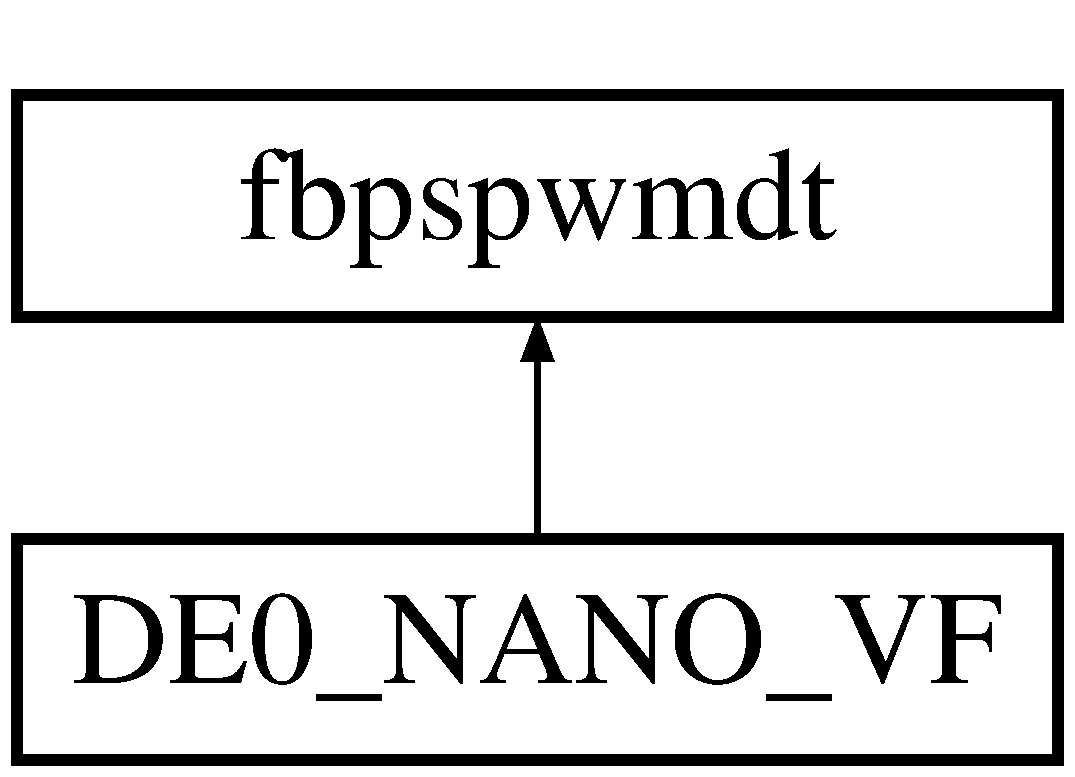
\includegraphics[height=2.000000cm]{classfbpspwmdt}
\end{center}
\end{figure}
\subsection*{Entities}
\begin{DoxyCompactItemize}
\item 
\hyperlink{classfbpspwmdt_1_1fbpspwmdt__arch}{fbpspwmdt\+\_\+arch} architecture
\end{DoxyCompactItemize}
\subsection*{Libraries}
 \begin{DoxyCompactItemize}
\item 
\hyperlink{classfbpspwmdt_ae4f03c286607f3181e16b9aa12d0c6d4}{I\+E\+E\+E} 
\end{DoxyCompactItemize}
\subsection*{Use Clauses}
 \begin{DoxyCompactItemize}
\item 
\hyperlink{classfbpspwmdt_a241c3e72dd8024cc8ae831b1b2aed7db}{S\+T\+D\+\_\+\+L\+O\+G\+I\+C\+\_\+\+U\+N\+S\+I\+G\+N\+E\+D}   
\item 
\hyperlink{classfbpspwmdt_aa4b2b25246a821511120e3149b003563}{S\+T\+D\+\_\+\+L\+O\+G\+I\+C\+\_\+1164}   
\item 
\hyperlink{classfbpspwmdt_aad86249c80e8c1e7ee1c4748aba748e3}{fixed\+\_\+pkg}   
\item 
\hyperlink{classfbpspwmdt_a2edc34402b573437d5f25fa90ba4013e}{numeric\+\_\+std}   
\end{DoxyCompactItemize}
\subsection*{Generics}
 \begin{DoxyCompactItemize}
\item 
\hyperlink{classfbpspwmdt_afee4aa1628956aa350183d8881689198}{n\+\_\+bits\+\_\+c} {\bfseries {\bfseries \textcolor{comment}{integer}\textcolor{vhdlchar}{ }\textcolor{vhdlchar}{ }\textcolor{vhdlchar}{\+:}\textcolor{vhdlchar}{=}\textcolor{vhdlchar}{ }\textcolor{vhdlchar}{ } \textcolor{vhdldigit}{16} \textcolor{vhdlchar}{ }}}
\item 
\hyperlink{classfbpspwmdt_a66678837c93def3337995d7ffcb44f3f}{c\+\_\+\+Dead\+\_\+t} {\bfseries {\bfseries \textcolor{comment}{integer}\textcolor{vhdlchar}{ }\textcolor{vhdlchar}{ }\textcolor{vhdlchar}{\+:}\textcolor{vhdlchar}{=}\textcolor{vhdlchar}{ }\textcolor{vhdlchar}{ } \textcolor{vhdldigit}{45} \textcolor{vhdlchar}{ }}}
\end{DoxyCompactItemize}
\subsection*{Ports}
 \begin{DoxyCompactItemize}
\item 
\hyperlink{classfbpspwmdt_a4a4609c199d30b3adebbeb3a01276ec5}{clk}  {\bfseries {\bfseries \textcolor{keywordflow}{in}\textcolor{vhdlchar}{ }}} {\bfseries \textcolor{comment}{std\+\_\+logic}\textcolor{vhdlchar}{ }} 
\item 
\hyperlink{classfbpspwmdt_adcf9c6f5161d039addbda5819bee64a3}{en}  {\bfseries {\bfseries \textcolor{keywordflow}{in}\textcolor{vhdlchar}{ }}} {\bfseries \textcolor{comment}{std\+\_\+logic}\textcolor{vhdlchar}{ }} 
\item 
\hyperlink{classfbpspwmdt_a021a597db1ce780174de5711902bf8f5}{comp}  {\bfseries {\bfseries \textcolor{vhdlchar}{ }}} {\bfseries \textcolor{comment}{std\+\_\+logic\+\_\+vector}\textcolor{vhdlchar}{ }\textcolor{vhdlchar}{(}\textcolor{vhdlchar}{ }\textcolor{vhdlchar}{ }\textcolor{vhdlchar}{ }\textcolor{vhdlchar}{ }{\bfseries \hyperlink{classfbpspwmdt_afee4aa1628956aa350183d8881689198}{n\+\_\+bits\+\_\+c}} \textcolor{vhdlchar}{-\/}\textcolor{vhdlchar}{ } \textcolor{vhdldigit}{1} \textcolor{vhdlchar}{ }\textcolor{keywordflow}{downto}\textcolor{vhdlchar}{ }\textcolor{vhdlchar}{ } \textcolor{vhdldigit}{0} \textcolor{vhdlchar}{ }\textcolor{vhdlchar}{)}\textcolor{vhdlchar}{ }}
\item 
\hyperlink{classfbpspwmdt_a0808bf3e7965a8ee90dec6604647f179}{c}  {\bfseries {\bfseries \textcolor{keywordflow}{in}\textcolor{vhdlchar}{ }}} {\bfseries \textcolor{comment}{std\+\_\+logic\+\_\+vector}\textcolor{vhdlchar}{ }\textcolor{vhdlchar}{(}\textcolor{vhdlchar}{ }\textcolor{vhdlchar}{ }\textcolor{vhdlchar}{ }\textcolor{vhdlchar}{ }{\bfseries \hyperlink{classfbpspwmdt_afee4aa1628956aa350183d8881689198}{n\+\_\+bits\+\_\+c}} \textcolor{vhdlchar}{-\/}\textcolor{vhdlchar}{ } \textcolor{vhdldigit}{1} \textcolor{vhdlchar}{ }\textcolor{keywordflow}{downto}\textcolor{vhdlchar}{ }\textcolor{vhdlchar}{ } \textcolor{vhdldigit}{0} \textcolor{vhdlchar}{ }\textcolor{vhdlchar}{)}\textcolor{vhdlchar}{ }} 
\item 
\hyperlink{classfbpspwmdt_af9b8278b961604ab62a822537a109adb}{amost}  {\bfseries {\bfseries \textcolor{keywordflow}{in}\textcolor{vhdlchar}{ }}} {\bfseries \textcolor{comment}{std\+\_\+logic}\textcolor{vhdlchar}{ }} 
\item 
\hyperlink{classfbpspwmdt_ad6bbafb165991aee14c6014831267789}{port\+\_\+\+P\+W\+M01}  {\bfseries {\bfseries \textcolor{keywordflow}{out}\textcolor{vhdlchar}{ }}} {\bfseries \textcolor{comment}{std\+\_\+logic}\textcolor{vhdlchar}{ }} 
\item 
\hyperlink{classfbpspwmdt_a0b2d13e9c0fd854957d88a65e0905e5b}{port\+\_\+\+P\+W\+M02}  {\bfseries {\bfseries \textcolor{keywordflow}{out}\textcolor{vhdlchar}{ }}} {\bfseries \textcolor{comment}{std\+\_\+logic}\textcolor{vhdlchar}{ }} 
\end{DoxyCompactItemize}


\subsection{Detailed Description}


Definition at line \hyperlink{fbpspwmdt_8vhd_source_l00011}{11} of file \hyperlink{fbpspwmdt_8vhd_source}{fbpspwmdt.\+vhd}.



\subsection{Member Data Documentation}
\hypertarget{classfbpspwmdt_af9b8278b961604ab62a822537a109adb}{}\index{fbpspwmdt@{fbpspwmdt}!amost@{amost}}
\index{amost@{amost}!fbpspwmdt@{fbpspwmdt}}
\subsubsection[{amost}]{\setlength{\rightskip}{0pt plus 5cm}{\bf amost} {\bfseries \textcolor{keywordflow}{in}\textcolor{vhdlchar}{ }} {\bfseries \textcolor{comment}{std\+\_\+logic}\textcolor{vhdlchar}{ }} \hspace{0.3cm}{\ttfamily [Port]}}\label{classfbpspwmdt_af9b8278b961604ab62a822537a109adb}


Definition at line \hyperlink{fbpspwmdt_8vhd_source_l00021}{21} of file \hyperlink{fbpspwmdt_8vhd_source}{fbpspwmdt.\+vhd}.

\hypertarget{classfbpspwmdt_a0808bf3e7965a8ee90dec6604647f179}{}\index{fbpspwmdt@{fbpspwmdt}!c@{c}}
\index{c@{c}!fbpspwmdt@{fbpspwmdt}}
\subsubsection[{c}]{\setlength{\rightskip}{0pt plus 5cm}{\bf c} {\bfseries \textcolor{keywordflow}{in}\textcolor{vhdlchar}{ }} {\bfseries \textcolor{comment}{std\+\_\+logic\+\_\+vector}\textcolor{vhdlchar}{ }\textcolor{vhdlchar}{(}\textcolor{vhdlchar}{ }\textcolor{vhdlchar}{ }\textcolor{vhdlchar}{ }\textcolor{vhdlchar}{ }{\bfseries {\bf n\+\_\+bits\+\_\+c}} \textcolor{vhdlchar}{-\/}\textcolor{vhdlchar}{ } \textcolor{vhdldigit}{1} \textcolor{vhdlchar}{ }\textcolor{keywordflow}{downto}\textcolor{vhdlchar}{ }\textcolor{vhdlchar}{ } \textcolor{vhdldigit}{0} \textcolor{vhdlchar}{ }\textcolor{vhdlchar}{)}\textcolor{vhdlchar}{ }} \hspace{0.3cm}{\ttfamily [Port]}}\label{classfbpspwmdt_a0808bf3e7965a8ee90dec6604647f179}


Definition at line \hyperlink{fbpspwmdt_8vhd_source_l00020}{20} of file \hyperlink{fbpspwmdt_8vhd_source}{fbpspwmdt.\+vhd}.

\hypertarget{classfbpspwmdt_a66678837c93def3337995d7ffcb44f3f}{}\index{fbpspwmdt@{fbpspwmdt}!c\+\_\+\+Dead\+\_\+t@{c\+\_\+\+Dead\+\_\+t}}
\index{c\+\_\+\+Dead\+\_\+t@{c\+\_\+\+Dead\+\_\+t}!fbpspwmdt@{fbpspwmdt}}
\subsubsection[{c\+\_\+\+Dead\+\_\+t}]{\setlength{\rightskip}{0pt plus 5cm}{\bf c\+\_\+\+Dead\+\_\+t} {\bfseries \textcolor{vhdlchar}{ }} {\bfseries \textcolor{comment}{integer}\textcolor{vhdlchar}{ }\textcolor{vhdlchar}{ }\textcolor{vhdlchar}{\+:}\textcolor{vhdlchar}{=}\textcolor{vhdlchar}{ }\textcolor{vhdlchar}{ } \textcolor{vhdldigit}{45} \textcolor{vhdlchar}{ }} \hspace{0.3cm}{\ttfamily [Generic]}}\label{classfbpspwmdt_a66678837c93def3337995d7ffcb44f3f}


Definition at line \hyperlink{fbpspwmdt_8vhd_source_l00015}{15} of file \hyperlink{fbpspwmdt_8vhd_source}{fbpspwmdt.\+vhd}.

\hypertarget{classfbpspwmdt_a4a4609c199d30b3adebbeb3a01276ec5}{}\index{fbpspwmdt@{fbpspwmdt}!clk@{clk}}
\index{clk@{clk}!fbpspwmdt@{fbpspwmdt}}
\subsubsection[{clk}]{\setlength{\rightskip}{0pt plus 5cm}{\bf clk} {\bfseries \textcolor{keywordflow}{in}\textcolor{vhdlchar}{ }} {\bfseries \textcolor{comment}{std\+\_\+logic}\textcolor{vhdlchar}{ }} \hspace{0.3cm}{\ttfamily [Port]}}\label{classfbpspwmdt_a4a4609c199d30b3adebbeb3a01276ec5}


Definition at line \hyperlink{fbpspwmdt_8vhd_source_l00017}{17} of file \hyperlink{fbpspwmdt_8vhd_source}{fbpspwmdt.\+vhd}.

\hypertarget{classfbpspwmdt_a021a597db1ce780174de5711902bf8f5}{}\index{fbpspwmdt@{fbpspwmdt}!comp@{comp}}
\index{comp@{comp}!fbpspwmdt@{fbpspwmdt}}
\subsubsection[{comp}]{\setlength{\rightskip}{0pt plus 5cm}{\bf comp} {\bfseries \textcolor{vhdlchar}{ }} {\bfseries \textcolor{comment}{std\+\_\+logic\+\_\+vector}\textcolor{vhdlchar}{ }\textcolor{vhdlchar}{(}\textcolor{vhdlchar}{ }\textcolor{vhdlchar}{ }\textcolor{vhdlchar}{ }\textcolor{vhdlchar}{ }{\bfseries {\bf n\+\_\+bits\+\_\+c}} \textcolor{vhdlchar}{-\/}\textcolor{vhdlchar}{ } \textcolor{vhdldigit}{1} \textcolor{vhdlchar}{ }\textcolor{keywordflow}{downto}\textcolor{vhdlchar}{ }\textcolor{vhdlchar}{ } \textcolor{vhdldigit}{0} \textcolor{vhdlchar}{ }\textcolor{vhdlchar}{)}\textcolor{vhdlchar}{ }} \hspace{0.3cm}{\ttfamily [Port]}}\label{classfbpspwmdt_a021a597db1ce780174de5711902bf8f5}


Definition at line \hyperlink{fbpspwmdt_8vhd_source_l00019}{19} of file \hyperlink{fbpspwmdt_8vhd_source}{fbpspwmdt.\+vhd}.

\hypertarget{classfbpspwmdt_adcf9c6f5161d039addbda5819bee64a3}{}\index{fbpspwmdt@{fbpspwmdt}!en@{en}}
\index{en@{en}!fbpspwmdt@{fbpspwmdt}}
\subsubsection[{en}]{\setlength{\rightskip}{0pt plus 5cm}{\bf en} {\bfseries \textcolor{keywordflow}{in}\textcolor{vhdlchar}{ }} {\bfseries \textcolor{comment}{std\+\_\+logic}\textcolor{vhdlchar}{ }} \hspace{0.3cm}{\ttfamily [Port]}}\label{classfbpspwmdt_adcf9c6f5161d039addbda5819bee64a3}


Definition at line \hyperlink{fbpspwmdt_8vhd_source_l00018}{18} of file \hyperlink{fbpspwmdt_8vhd_source}{fbpspwmdt.\+vhd}.

\hypertarget{classfbpspwmdt_aad86249c80e8c1e7ee1c4748aba748e3}{}\index{fbpspwmdt@{fbpspwmdt}!fixed\+\_\+pkg@{fixed\+\_\+pkg}}
\index{fixed\+\_\+pkg@{fixed\+\_\+pkg}!fbpspwmdt@{fbpspwmdt}}
\subsubsection[{fixed\+\_\+pkg}]{\setlength{\rightskip}{0pt plus 5cm}{\bf fixed\+\_\+pkg}\hspace{0.3cm}{\ttfamily [Package]}}\label{classfbpspwmdt_aad86249c80e8c1e7ee1c4748aba748e3}


Definition at line \hyperlink{fbpspwmdt_8vhd_source_l00007}{7} of file \hyperlink{fbpspwmdt_8vhd_source}{fbpspwmdt.\+vhd}.

\hypertarget{classfbpspwmdt_ae4f03c286607f3181e16b9aa12d0c6d4}{}\index{fbpspwmdt@{fbpspwmdt}!I\+E\+E\+E@{I\+E\+E\+E}}
\index{I\+E\+E\+E@{I\+E\+E\+E}!fbpspwmdt@{fbpspwmdt}}
\subsubsection[{I\+E\+E\+E}]{\setlength{\rightskip}{0pt plus 5cm}{\bf I\+E\+E\+E}\hspace{0.3cm}{\ttfamily [Library]}}\label{classfbpspwmdt_ae4f03c286607f3181e16b9aa12d0c6d4}


Definition at line \hyperlink{fbpspwmdt_8vhd_source_l00004}{4} of file \hyperlink{fbpspwmdt_8vhd_source}{fbpspwmdt.\+vhd}.

\hypertarget{classfbpspwmdt_afee4aa1628956aa350183d8881689198}{}\index{fbpspwmdt@{fbpspwmdt}!n\+\_\+bits\+\_\+c@{n\+\_\+bits\+\_\+c}}
\index{n\+\_\+bits\+\_\+c@{n\+\_\+bits\+\_\+c}!fbpspwmdt@{fbpspwmdt}}
\subsubsection[{n\+\_\+bits\+\_\+c}]{\setlength{\rightskip}{0pt plus 5cm}{\bf n\+\_\+bits\+\_\+c} {\bfseries \textcolor{vhdlchar}{ }} {\bfseries \textcolor{comment}{integer}\textcolor{vhdlchar}{ }\textcolor{vhdlchar}{ }\textcolor{vhdlchar}{\+:}\textcolor{vhdlchar}{=}\textcolor{vhdlchar}{ }\textcolor{vhdlchar}{ } \textcolor{vhdldigit}{16} \textcolor{vhdlchar}{ }} \hspace{0.3cm}{\ttfamily [Generic]}}\label{classfbpspwmdt_afee4aa1628956aa350183d8881689198}


Definition at line \hyperlink{fbpspwmdt_8vhd_source_l00013}{13} of file \hyperlink{fbpspwmdt_8vhd_source}{fbpspwmdt.\+vhd}.

\hypertarget{classfbpspwmdt_a2edc34402b573437d5f25fa90ba4013e}{}\index{fbpspwmdt@{fbpspwmdt}!numeric\+\_\+std@{numeric\+\_\+std}}
\index{numeric\+\_\+std@{numeric\+\_\+std}!fbpspwmdt@{fbpspwmdt}}
\subsubsection[{numeric\+\_\+std}]{\setlength{\rightskip}{0pt plus 5cm}{\bf numeric\+\_\+std}\hspace{0.3cm}{\ttfamily [Package]}}\label{classfbpspwmdt_a2edc34402b573437d5f25fa90ba4013e}


Definition at line \hyperlink{fbpspwmdt_8vhd_source_l00008}{8} of file \hyperlink{fbpspwmdt_8vhd_source}{fbpspwmdt.\+vhd}.

\hypertarget{classfbpspwmdt_ad6bbafb165991aee14c6014831267789}{}\index{fbpspwmdt@{fbpspwmdt}!port\+\_\+\+P\+W\+M01@{port\+\_\+\+P\+W\+M01}}
\index{port\+\_\+\+P\+W\+M01@{port\+\_\+\+P\+W\+M01}!fbpspwmdt@{fbpspwmdt}}
\subsubsection[{port\+\_\+\+P\+W\+M01}]{\setlength{\rightskip}{0pt plus 5cm}{\bf port\+\_\+\+P\+W\+M01} {\bfseries \textcolor{keywordflow}{out}\textcolor{vhdlchar}{ }} {\bfseries \textcolor{comment}{std\+\_\+logic}\textcolor{vhdlchar}{ }} \hspace{0.3cm}{\ttfamily [Port]}}\label{classfbpspwmdt_ad6bbafb165991aee14c6014831267789}


Definition at line \hyperlink{fbpspwmdt_8vhd_source_l00022}{22} of file \hyperlink{fbpspwmdt_8vhd_source}{fbpspwmdt.\+vhd}.

\hypertarget{classfbpspwmdt_a0b2d13e9c0fd854957d88a65e0905e5b}{}\index{fbpspwmdt@{fbpspwmdt}!port\+\_\+\+P\+W\+M02@{port\+\_\+\+P\+W\+M02}}
\index{port\+\_\+\+P\+W\+M02@{port\+\_\+\+P\+W\+M02}!fbpspwmdt@{fbpspwmdt}}
\subsubsection[{port\+\_\+\+P\+W\+M02}]{\setlength{\rightskip}{0pt plus 5cm}{\bf port\+\_\+\+P\+W\+M02} {\bfseries \textcolor{keywordflow}{out}\textcolor{vhdlchar}{ }} {\bfseries \textcolor{comment}{std\+\_\+logic}\textcolor{vhdlchar}{ }} \hspace{0.3cm}{\ttfamily [Port]}}\label{classfbpspwmdt_a0b2d13e9c0fd854957d88a65e0905e5b}


Definition at line \hyperlink{fbpspwmdt_8vhd_source_l00024}{24} of file \hyperlink{fbpspwmdt_8vhd_source}{fbpspwmdt.\+vhd}.

\hypertarget{classfbpspwmdt_aa4b2b25246a821511120e3149b003563}{}\index{fbpspwmdt@{fbpspwmdt}!S\+T\+D\+\_\+\+L\+O\+G\+I\+C\+\_\+1164@{S\+T\+D\+\_\+\+L\+O\+G\+I\+C\+\_\+1164}}
\index{S\+T\+D\+\_\+\+L\+O\+G\+I\+C\+\_\+1164@{S\+T\+D\+\_\+\+L\+O\+G\+I\+C\+\_\+1164}!fbpspwmdt@{fbpspwmdt}}
\subsubsection[{S\+T\+D\+\_\+\+L\+O\+G\+I\+C\+\_\+1164}]{\setlength{\rightskip}{0pt plus 5cm}{\bf S\+T\+D\+\_\+\+L\+O\+G\+I\+C\+\_\+1164}\hspace{0.3cm}{\ttfamily [Package]}}\label{classfbpspwmdt_aa4b2b25246a821511120e3149b003563}


Definition at line \hyperlink{fbpspwmdt_8vhd_source_l00006}{6} of file \hyperlink{fbpspwmdt_8vhd_source}{fbpspwmdt.\+vhd}.

\hypertarget{classfbpspwmdt_a241c3e72dd8024cc8ae831b1b2aed7db}{}\index{fbpspwmdt@{fbpspwmdt}!S\+T\+D\+\_\+\+L\+O\+G\+I\+C\+\_\+\+U\+N\+S\+I\+G\+N\+E\+D@{S\+T\+D\+\_\+\+L\+O\+G\+I\+C\+\_\+\+U\+N\+S\+I\+G\+N\+E\+D}}
\index{S\+T\+D\+\_\+\+L\+O\+G\+I\+C\+\_\+\+U\+N\+S\+I\+G\+N\+E\+D@{S\+T\+D\+\_\+\+L\+O\+G\+I\+C\+\_\+\+U\+N\+S\+I\+G\+N\+E\+D}!fbpspwmdt@{fbpspwmdt}}
\subsubsection[{S\+T\+D\+\_\+\+L\+O\+G\+I\+C\+\_\+\+U\+N\+S\+I\+G\+N\+E\+D}]{\setlength{\rightskip}{0pt plus 5cm}{\bf S\+T\+D\+\_\+\+L\+O\+G\+I\+C\+\_\+\+U\+N\+S\+I\+G\+N\+E\+D}\hspace{0.3cm}{\ttfamily [Package]}}\label{classfbpspwmdt_a241c3e72dd8024cc8ae831b1b2aed7db}


Definition at line \hyperlink{fbpspwmdt_8vhd_source_l00005}{5} of file \hyperlink{fbpspwmdt_8vhd_source}{fbpspwmdt.\+vhd}.



The documentation for this class was generated from the following file\+:\begin{DoxyCompactItemize}
\item 
\hyperlink{fbpspwmdt_8vhd}{fbpspwmdt.\+vhd}\end{DoxyCompactItemize}

\hypertarget{classfbpspwmdt_1_1fbpspwmdt__arch}{}\section{fbpspwmdt\+\_\+arch Architecture Reference}
\label{classfbpspwmdt_1_1fbpspwmdt__arch}\index{fbpspwmdt\+\_\+arch@{fbpspwmdt\+\_\+arch}}
\subsection*{Processes}
 \begin{DoxyCompactItemize}
\item 
\hyperlink{classfbpspwmdt_1_1fbpspwmdt__arch_a6cc276b9a3076e40ac68b8ac3f1828a7}{P\+R\+O\+C\+E\+S\+S\+\_\+7}{\bfseries  ( {\bfseries {\bfseries \hyperlink{classfbpspwmdt_a4a4609c199d30b3adebbeb3a01276ec5}{clk}} \textcolor{vhdlchar}{ }} )}
\item 
\hyperlink{classfbpspwmdt_1_1fbpspwmdt__arch_a7cf6ba78e659f286a9d61adf1efc91b0}{P\+R\+O\+C\+E\+S\+S\+\_\+8}{\bfseries  ( {\bfseries {\bfseries \hyperlink{classfbpspwmdt_af9b8278b961604ab62a822537a109adb}{amost}} \textcolor{vhdlchar}{ }} )}
\item 
\hyperlink{classfbpspwmdt_1_1fbpspwmdt__arch_a0132bccb07ff42922281b99abe7fc1ed}{P\+R\+O\+C\+E\+S\+S\+\_\+9}{\bfseries  ( {\bfseries {\bfseries \hyperlink{classfbpspwmdt_a4a4609c199d30b3adebbeb3a01276ec5}{clk}} \textcolor{vhdlchar}{ }} )}
\end{DoxyCompactItemize}
\subsection*{Signals}
 \begin{DoxyCompactItemize}
\item 
\hyperlink{classfbpspwmdt_1_1fbpspwmdt__arch_abf7d8be25624dd08fcc1517c8e39cb23}{comp\+\_\+int} {\bfseries \textcolor{comment}{std\+\_\+logic\+\_\+vector}\textcolor{vhdlchar}{ }\textcolor{vhdlchar}{(}\textcolor{vhdlchar}{ }\textcolor{vhdlchar}{ }\textcolor{vhdlchar}{ }\textcolor{vhdlchar}{ }{\bfseries \hyperlink{classfbpspwmdt_afee4aa1628956aa350183d8881689198}{n\+\_\+bits\+\_\+c}} \textcolor{vhdlchar}{-\/}\textcolor{vhdlchar}{ } \textcolor{vhdldigit}{1} \textcolor{vhdlchar}{ }\textcolor{keywordflow}{downto}\textcolor{vhdlchar}{ }\textcolor{vhdlchar}{ } \textcolor{vhdldigit}{0} \textcolor{vhdlchar}{ }\textcolor{vhdlchar}{)}\textcolor{vhdlchar}{ }} 
\item 
\hyperlink{classfbpspwmdt_1_1fbpspwmdt__arch_a90c7671dbb1af7d80f90cd96262cda3b}{sig\+\_\+\+Not\+\_\+\+Pwm\+\_\+\+In} {\bfseries \textcolor{comment}{std\+\_\+logic}\textcolor{vhdlchar}{ }} 
\item 
\hyperlink{classfbpspwmdt_1_1fbpspwmdt__arch_a5b5410422331d47dda25071eab458071}{comp\+\_\+out} {\bfseries \textcolor{comment}{std\+\_\+logic}\textcolor{vhdlchar}{ }} 
\item 
\hyperlink{classfbpspwmdt_1_1fbpspwmdt__arch_af7e8a49d46795da5945dc6b1f0602c13}{p\+\_\+\+Pwm\+\_\+\+In} {\bfseries \textcolor{comment}{std\+\_\+logic}\textcolor{vhdlchar}{ }} 
\end{DoxyCompactItemize}


\subsection{Detailed Description}


Definition at line \hyperlink{fbpspwmdt_8vhd_source_l00031}{31} of file \hyperlink{fbpspwmdt_8vhd_source}{fbpspwmdt.\+vhd}.



\subsection{Member Function Documentation}
\hypertarget{classfbpspwmdt_1_1fbpspwmdt__arch_a6cc276b9a3076e40ac68b8ac3f1828a7}{}\index{fbpspwmdt\+::fbpspwmdt\+\_\+arch@{fbpspwmdt\+::fbpspwmdt\+\_\+arch}!P\+R\+O\+C\+E\+S\+S\+\_\+7@{P\+R\+O\+C\+E\+S\+S\+\_\+7}}
\index{P\+R\+O\+C\+E\+S\+S\+\_\+7@{P\+R\+O\+C\+E\+S\+S\+\_\+7}!fbpspwmdt\+::fbpspwmdt\+\_\+arch@{fbpspwmdt\+::fbpspwmdt\+\_\+arch}}
\subsubsection[{P\+R\+O\+C\+E\+S\+S\+\_\+7}]{\setlength{\rightskip}{0pt plus 5cm} {\bfseries \textcolor{vhdlchar}{ }} P\+R\+O\+C\+E\+S\+S\+\_\+7(
\begin{DoxyParamCaption}
\item[{}]{{\bfseries {\bfseries {\bf clk}} \textcolor{vhdlchar}{ }} {\em }}
\end{DoxyParamCaption}
)\hspace{0.3cm}{\ttfamily [Process]}}\label{classfbpspwmdt_1_1fbpspwmdt__arch_a6cc276b9a3076e40ac68b8ac3f1828a7}


Definition at line \hyperlink{fbpspwmdt_8vhd_source_l00042}{42} of file \hyperlink{fbpspwmdt_8vhd_source}{fbpspwmdt.\+vhd}.

\hypertarget{classfbpspwmdt_1_1fbpspwmdt__arch_a7cf6ba78e659f286a9d61adf1efc91b0}{}\index{fbpspwmdt\+::fbpspwmdt\+\_\+arch@{fbpspwmdt\+::fbpspwmdt\+\_\+arch}!P\+R\+O\+C\+E\+S\+S\+\_\+8@{P\+R\+O\+C\+E\+S\+S\+\_\+8}}
\index{P\+R\+O\+C\+E\+S\+S\+\_\+8@{P\+R\+O\+C\+E\+S\+S\+\_\+8}!fbpspwmdt\+::fbpspwmdt\+\_\+arch@{fbpspwmdt\+::fbpspwmdt\+\_\+arch}}
\subsubsection[{P\+R\+O\+C\+E\+S\+S\+\_\+8}]{\setlength{\rightskip}{0pt plus 5cm} {\bfseries \textcolor{vhdlchar}{ }} P\+R\+O\+C\+E\+S\+S\+\_\+8(
\begin{DoxyParamCaption}
\item[{}]{{\bfseries {\bfseries {\bf amost}} \textcolor{vhdlchar}{ }} {\em }}
\end{DoxyParamCaption}
)\hspace{0.3cm}{\ttfamily [Process]}}\label{classfbpspwmdt_1_1fbpspwmdt__arch_a7cf6ba78e659f286a9d61adf1efc91b0}


Definition at line \hyperlink{fbpspwmdt_8vhd_source_l00055}{55} of file \hyperlink{fbpspwmdt_8vhd_source}{fbpspwmdt.\+vhd}.

\hypertarget{classfbpspwmdt_1_1fbpspwmdt__arch_a0132bccb07ff42922281b99abe7fc1ed}{}\index{fbpspwmdt\+::fbpspwmdt\+\_\+arch@{fbpspwmdt\+::fbpspwmdt\+\_\+arch}!P\+R\+O\+C\+E\+S\+S\+\_\+9@{P\+R\+O\+C\+E\+S\+S\+\_\+9}}
\index{P\+R\+O\+C\+E\+S\+S\+\_\+9@{P\+R\+O\+C\+E\+S\+S\+\_\+9}!fbpspwmdt\+::fbpspwmdt\+\_\+arch@{fbpspwmdt\+::fbpspwmdt\+\_\+arch}}
\subsubsection[{P\+R\+O\+C\+E\+S\+S\+\_\+9}]{\setlength{\rightskip}{0pt plus 5cm} {\bfseries \textcolor{vhdlchar}{ }} P\+R\+O\+C\+E\+S\+S\+\_\+9(
\begin{DoxyParamCaption}
\item[{}]{{\bfseries {\bfseries {\bf clk}} \textcolor{vhdlchar}{ }} {\em }}
\end{DoxyParamCaption}
)\hspace{0.3cm}{\ttfamily [Process]}}\label{classfbpspwmdt_1_1fbpspwmdt__arch_a0132bccb07ff42922281b99abe7fc1ed}


Definition at line \hyperlink{fbpspwmdt_8vhd_source_l00067}{67} of file \hyperlink{fbpspwmdt_8vhd_source}{fbpspwmdt.\+vhd}.



\subsection{Member Data Documentation}
\hypertarget{classfbpspwmdt_1_1fbpspwmdt__arch_abf7d8be25624dd08fcc1517c8e39cb23}{}\index{fbpspwmdt\+::fbpspwmdt\+\_\+arch@{fbpspwmdt\+::fbpspwmdt\+\_\+arch}!comp\+\_\+int@{comp\+\_\+int}}
\index{comp\+\_\+int@{comp\+\_\+int}!fbpspwmdt\+::fbpspwmdt\+\_\+arch@{fbpspwmdt\+::fbpspwmdt\+\_\+arch}}
\subsubsection[{comp\+\_\+int}]{\setlength{\rightskip}{0pt plus 5cm}{\bf comp\+\_\+int} {\bfseries \textcolor{comment}{std\+\_\+logic\+\_\+vector}\textcolor{vhdlchar}{ }\textcolor{vhdlchar}{(}\textcolor{vhdlchar}{ }\textcolor{vhdlchar}{ }\textcolor{vhdlchar}{ }\textcolor{vhdlchar}{ }{\bfseries {\bf n\+\_\+bits\+\_\+c}} \textcolor{vhdlchar}{-\/}\textcolor{vhdlchar}{ } \textcolor{vhdldigit}{1} \textcolor{vhdlchar}{ }\textcolor{keywordflow}{downto}\textcolor{vhdlchar}{ }\textcolor{vhdlchar}{ } \textcolor{vhdldigit}{0} \textcolor{vhdlchar}{ }\textcolor{vhdlchar}{)}\textcolor{vhdlchar}{ }} \hspace{0.3cm}{\ttfamily [Signal]}}\label{classfbpspwmdt_1_1fbpspwmdt__arch_abf7d8be25624dd08fcc1517c8e39cb23}


Definition at line \hyperlink{fbpspwmdt_8vhd_source_l00034}{34} of file \hyperlink{fbpspwmdt_8vhd_source}{fbpspwmdt.\+vhd}.

\hypertarget{classfbpspwmdt_1_1fbpspwmdt__arch_a5b5410422331d47dda25071eab458071}{}\index{fbpspwmdt\+::fbpspwmdt\+\_\+arch@{fbpspwmdt\+::fbpspwmdt\+\_\+arch}!comp\+\_\+out@{comp\+\_\+out}}
\index{comp\+\_\+out@{comp\+\_\+out}!fbpspwmdt\+::fbpspwmdt\+\_\+arch@{fbpspwmdt\+::fbpspwmdt\+\_\+arch}}
\subsubsection[{comp\+\_\+out}]{\setlength{\rightskip}{0pt plus 5cm}{\bf comp\+\_\+out} {\bfseries \textcolor{comment}{std\+\_\+logic}\textcolor{vhdlchar}{ }} \hspace{0.3cm}{\ttfamily [Signal]}}\label{classfbpspwmdt_1_1fbpspwmdt__arch_a5b5410422331d47dda25071eab458071}


Definition at line \hyperlink{fbpspwmdt_8vhd_source_l00036}{36} of file \hyperlink{fbpspwmdt_8vhd_source}{fbpspwmdt.\+vhd}.

\hypertarget{classfbpspwmdt_1_1fbpspwmdt__arch_af7e8a49d46795da5945dc6b1f0602c13}{}\index{fbpspwmdt\+::fbpspwmdt\+\_\+arch@{fbpspwmdt\+::fbpspwmdt\+\_\+arch}!p\+\_\+\+Pwm\+\_\+\+In@{p\+\_\+\+Pwm\+\_\+\+In}}
\index{p\+\_\+\+Pwm\+\_\+\+In@{p\+\_\+\+Pwm\+\_\+\+In}!fbpspwmdt\+::fbpspwmdt\+\_\+arch@{fbpspwmdt\+::fbpspwmdt\+\_\+arch}}
\subsubsection[{p\+\_\+\+Pwm\+\_\+\+In}]{\setlength{\rightskip}{0pt plus 5cm}{\bf p\+\_\+\+Pwm\+\_\+\+In} {\bfseries \textcolor{comment}{std\+\_\+logic}\textcolor{vhdlchar}{ }} \hspace{0.3cm}{\ttfamily [Signal]}}\label{classfbpspwmdt_1_1fbpspwmdt__arch_af7e8a49d46795da5945dc6b1f0602c13}


Definition at line \hyperlink{fbpspwmdt_8vhd_source_l00037}{37} of file \hyperlink{fbpspwmdt_8vhd_source}{fbpspwmdt.\+vhd}.

\hypertarget{classfbpspwmdt_1_1fbpspwmdt__arch_a90c7671dbb1af7d80f90cd96262cda3b}{}\index{fbpspwmdt\+::fbpspwmdt\+\_\+arch@{fbpspwmdt\+::fbpspwmdt\+\_\+arch}!sig\+\_\+\+Not\+\_\+\+Pwm\+\_\+\+In@{sig\+\_\+\+Not\+\_\+\+Pwm\+\_\+\+In}}
\index{sig\+\_\+\+Not\+\_\+\+Pwm\+\_\+\+In@{sig\+\_\+\+Not\+\_\+\+Pwm\+\_\+\+In}!fbpspwmdt\+::fbpspwmdt\+\_\+arch@{fbpspwmdt\+::fbpspwmdt\+\_\+arch}}
\subsubsection[{sig\+\_\+\+Not\+\_\+\+Pwm\+\_\+\+In}]{\setlength{\rightskip}{0pt plus 5cm}{\bf sig\+\_\+\+Not\+\_\+\+Pwm\+\_\+\+In} {\bfseries \textcolor{comment}{std\+\_\+logic}\textcolor{vhdlchar}{ }} \hspace{0.3cm}{\ttfamily [Signal]}}\label{classfbpspwmdt_1_1fbpspwmdt__arch_a90c7671dbb1af7d80f90cd96262cda3b}


Definition at line \hyperlink{fbpspwmdt_8vhd_source_l00035}{35} of file \hyperlink{fbpspwmdt_8vhd_source}{fbpspwmdt.\+vhd}.



The documentation for this class was generated from the following file\+:\begin{DoxyCompactItemize}
\item 
\hyperlink{fbpspwmdt_8vhd}{fbpspwmdt.\+vhd}\end{DoxyCompactItemize}

\hypertarget{classfixed__float__types}{}\section{fixed\+\_\+float\+\_\+types Package Reference}
\label{classfixed__float__types}\index{fixed\+\_\+float\+\_\+types@{fixed\+\_\+float\+\_\+types}}
\subsection*{Types}
 \begin{DoxyCompactItemize}
\item 
{\bfseries \hyperlink{classfixed__float__types_a531b370a8acfecdccebf696cf0d2d971}{fixed\+\_\+round\+\_\+style\+\_\+type}{\bfseries \textcolor{vhdlchar}{(}\textcolor{vhdlchar}{ }\textcolor{vhdlchar}{fixed\+\_\+round}\textcolor{vhdlchar}{ }\textcolor{vhdlchar}{,}\textcolor{vhdlchar}{ }\textcolor{vhdlchar}{fixed\+\_\+truncate}\textcolor{vhdlchar}{ }\textcolor{vhdlchar}{)}\textcolor{vhdlchar}{ }}} 
\item 
{\bfseries \hyperlink{classfixed__float__types_a8a8b6b0022e693377949251b05ac846a}{fixed\+\_\+overflow\+\_\+style\+\_\+type}{\bfseries \textcolor{vhdlchar}{(}\textcolor{vhdlchar}{ }\textcolor{vhdlchar}{fixed\+\_\+saturate}\textcolor{vhdlchar}{ }\textcolor{vhdlchar}{,}\textcolor{vhdlchar}{ }\textcolor{vhdlchar}{fixed\+\_\+wrap}\textcolor{vhdlchar}{ }\textcolor{vhdlchar}{)}\textcolor{vhdlchar}{ }}} 
\item 
{\bfseries \hyperlink{classfixed__float__types_a3cab38cfb8c7d6b81f4f0b9953cd212f}{round\+\_\+type}{\bfseries \textcolor{vhdlchar}{(}\textcolor{vhdlchar}{ }\textcolor{vhdlchar}{round\+\_\+nearest}\textcolor{vhdlchar}{ }\textcolor{vhdlchar}{,}\textcolor{vhdlchar}{ }\textcolor{vhdlchar}{round\+\_\+inf}\textcolor{vhdlchar}{ }\textcolor{vhdlchar}{,}\textcolor{vhdlchar}{ }\textcolor{vhdlchar}{round\+\_\+neginf}\textcolor{vhdlchar}{ }\textcolor{vhdlchar}{,}\textcolor{vhdlchar}{ }\textcolor{vhdlchar}{round\+\_\+zero}\textcolor{vhdlchar}{ }\textcolor{vhdlchar}{)}\textcolor{vhdlchar}{ }}} 
\end{DoxyCompactItemize}


\subsection{Detailed Description}


Definition at line 16 of file fixed\+\_\+float\+\_\+types\+\_\+c.\+vhdl.



\subsection{Member Data Documentation}
\hypertarget{classfixed__float__types_a8a8b6b0022e693377949251b05ac846a}{}\index{fixed\+\_\+float\+\_\+types@{fixed\+\_\+float\+\_\+types}!fixed\+\_\+overflow\+\_\+style\+\_\+type@{fixed\+\_\+overflow\+\_\+style\+\_\+type}}
\index{fixed\+\_\+overflow\+\_\+style\+\_\+type@{fixed\+\_\+overflow\+\_\+style\+\_\+type}!fixed\+\_\+float\+\_\+types@{fixed\+\_\+float\+\_\+types}}
\subsubsection[{fixed\+\_\+overflow\+\_\+style\+\_\+type}]{\setlength{\rightskip}{0pt plus 5cm}{\bf fixed\+\_\+overflow\+\_\+style\+\_\+type} {\bfseries \textcolor{vhdlchar}{(}\textcolor{vhdlchar}{ }\textcolor{vhdlchar}{fixed\+\_\+saturate}\textcolor{vhdlchar}{ }\textcolor{vhdlchar}{,}\textcolor{vhdlchar}{ }\textcolor{vhdlchar}{fixed\+\_\+wrap}\textcolor{vhdlchar}{ }\textcolor{vhdlchar}{)}\textcolor{vhdlchar}{ }} \hspace{0.3cm}{\ttfamily [Type]}}\label{classfixed__float__types_a8a8b6b0022e693377949251b05ac846a}


Definition at line 22 of file fixed\+\_\+float\+\_\+types\+\_\+c.\+vhdl.

\hypertarget{classfixed__float__types_a531b370a8acfecdccebf696cf0d2d971}{}\index{fixed\+\_\+float\+\_\+types@{fixed\+\_\+float\+\_\+types}!fixed\+\_\+round\+\_\+style\+\_\+type@{fixed\+\_\+round\+\_\+style\+\_\+type}}
\index{fixed\+\_\+round\+\_\+style\+\_\+type@{fixed\+\_\+round\+\_\+style\+\_\+type}!fixed\+\_\+float\+\_\+types@{fixed\+\_\+float\+\_\+types}}
\subsubsection[{fixed\+\_\+round\+\_\+style\+\_\+type}]{\setlength{\rightskip}{0pt plus 5cm}{\bf fixed\+\_\+round\+\_\+style\+\_\+type} {\bfseries \textcolor{vhdlchar}{(}\textcolor{vhdlchar}{ }\textcolor{vhdlchar}{fixed\+\_\+round}\textcolor{vhdlchar}{ }\textcolor{vhdlchar}{,}\textcolor{vhdlchar}{ }\textcolor{vhdlchar}{fixed\+\_\+truncate}\textcolor{vhdlchar}{ }\textcolor{vhdlchar}{)}\textcolor{vhdlchar}{ }} \hspace{0.3cm}{\ttfamily [Type]}}\label{classfixed__float__types_a531b370a8acfecdccebf696cf0d2d971}


Definition at line 20 of file fixed\+\_\+float\+\_\+types\+\_\+c.\+vhdl.

\hypertarget{classfixed__float__types_a3cab38cfb8c7d6b81f4f0b9953cd212f}{}\index{fixed\+\_\+float\+\_\+types@{fixed\+\_\+float\+\_\+types}!round\+\_\+type@{round\+\_\+type}}
\index{round\+\_\+type@{round\+\_\+type}!fixed\+\_\+float\+\_\+types@{fixed\+\_\+float\+\_\+types}}
\subsubsection[{round\+\_\+type}]{\setlength{\rightskip}{0pt plus 5cm}{\bf round\+\_\+type} {\bfseries \textcolor{vhdlchar}{(}\textcolor{vhdlchar}{ }\textcolor{vhdlchar}{round\+\_\+nearest}\textcolor{vhdlchar}{ }\textcolor{vhdlchar}{,}\textcolor{vhdlchar}{ }\textcolor{vhdlchar}{round\+\_\+inf}\textcolor{vhdlchar}{ }\textcolor{vhdlchar}{,}\textcolor{vhdlchar}{ }\textcolor{vhdlchar}{round\+\_\+neginf}\textcolor{vhdlchar}{ }\textcolor{vhdlchar}{,}\textcolor{vhdlchar}{ }\textcolor{vhdlchar}{round\+\_\+zero}\textcolor{vhdlchar}{ }\textcolor{vhdlchar}{)}\textcolor{vhdlchar}{ }} \hspace{0.3cm}{\ttfamily [Type]}}\label{classfixed__float__types_a3cab38cfb8c7d6b81f4f0b9953cd212f}


Definition at line 29 of file fixed\+\_\+float\+\_\+types\+\_\+c.\+vhdl.



The documentation for this class was generated from the following file\+:\begin{DoxyCompactItemize}
\item 
\hyperlink{fixed__float__types__c_8vhdl}{fixed\+\_\+float\+\_\+types\+\_\+c.\+vhdl}\end{DoxyCompactItemize}

\hypertarget{classfixed__pkg}{}\section{fixed\+\_\+pkg Package Reference}
\label{classfixed__pkg}\index{fixed\+\_\+pkg@{fixed\+\_\+pkg}}
{\bfseries Package Body $>$$>$ }\hyperlink{class__fixed__pkg}{fixed\+\_\+pkg}\\*
\subsection*{Functions}
 \begin{DoxyCompactItemize}
\item 
{\bfseries {\bfseries {\bfseries \hyperlink{classfixed__pkg_aa723b28a027c3c0f9bca02d75e8df4d6}{U\+N\+R\+E\+S\+O\+L\+V\+E\+D\+\_\+sfixed}} \textcolor{vhdlchar}{ }}} \hyperlink{classfixed__pkg_a38c1c4c6b1f76cfc07b009c92acabab5}{\char`\"{}abs\char`\"{}}{\bfseries  ( }{\bfseries \textcolor{vhdlchar}{arg\+: }\textcolor{stringliteral}{in }\textcolor{vhdlchar}{U\+N\+R\+E\+S\+O\+L\+V\+E\+D\+\_\+sfixed}}{\bfseries  )} 
\item 
{\bfseries {\bfseries {\bfseries \hyperlink{classfixed__pkg_aa723b28a027c3c0f9bca02d75e8df4d6}{U\+N\+R\+E\+S\+O\+L\+V\+E\+D\+\_\+sfixed}} \textcolor{vhdlchar}{ }}} \hyperlink{classfixed__pkg_acc47f8e7fbecebc0fc011d8431f076fd}{\char`\"{}-\/\char`\"{}}{\bfseries  ( }{\bfseries \textcolor{vhdlchar}{arg\+: }\textcolor{stringliteral}{in }\textcolor{vhdlchar}{U\+N\+R\+E\+S\+O\+L\+V\+E\+D\+\_\+sfixed}}{\bfseries  )} 
\item 
{\bfseries {\bfseries {\bfseries \hyperlink{classfixed__pkg_ae78bc2b36d22f6abeac163955e8a587d}{U\+N\+R\+E\+S\+O\+L\+V\+E\+D\+\_\+ufixed}} \textcolor{vhdlchar}{ }}} \hyperlink{classfixed__pkg_a758fadb06ceaaaffa80aa4473dc8dcda}{\char`\"{}+\char`\"{}}{\bfseries  ( }{\bfseries \textcolor{vhdlchar}{l\+: }\textcolor{stringliteral}{in }\textcolor{vhdlchar}{U\+N\+R\+E\+S\+O\+L\+V\+E\+D\+\_\+ufixed}}{\bfseries  , \textcolor{vhdlchar}{r\+: }\textcolor{stringliteral}{in }\textcolor{vhdlchar}{U\+N\+R\+E\+S\+O\+L\+V\+E\+D\+\_\+ufixed}}{\bfseries  )} 
\item 
{\bfseries {\bfseries {\bfseries \hyperlink{classfixed__pkg_aa723b28a027c3c0f9bca02d75e8df4d6}{U\+N\+R\+E\+S\+O\+L\+V\+E\+D\+\_\+sfixed}} \textcolor{vhdlchar}{ }}} \hyperlink{classfixed__pkg_a75f813bcb278832108d6fa67eccdfc1c}{\char`\"{}+\char`\"{}}{\bfseries  ( }{\bfseries \textcolor{vhdlchar}{l\+: }\textcolor{stringliteral}{in }\textcolor{vhdlchar}{U\+N\+R\+E\+S\+O\+L\+V\+E\+D\+\_\+sfixed}}{\bfseries  , \textcolor{vhdlchar}{r\+: }\textcolor{stringliteral}{in }\textcolor{vhdlchar}{U\+N\+R\+E\+S\+O\+L\+V\+E\+D\+\_\+sfixed}}{\bfseries  )} 
\item 
{\bfseries {\bfseries {\bfseries \hyperlink{classfixed__pkg_ae78bc2b36d22f6abeac163955e8a587d}{U\+N\+R\+E\+S\+O\+L\+V\+E\+D\+\_\+ufixed}} \textcolor{vhdlchar}{ }}} \hyperlink{classfixed__pkg_aa5b0e6d3b75f03dea7c3a4daedc04027}{\char`\"{}-\/\char`\"{}}{\bfseries  ( }{\bfseries \textcolor{vhdlchar}{l\+: }\textcolor{stringliteral}{in }\textcolor{vhdlchar}{U\+N\+R\+E\+S\+O\+L\+V\+E\+D\+\_\+ufixed}}{\bfseries  , \textcolor{vhdlchar}{r\+: }\textcolor{stringliteral}{in }\textcolor{vhdlchar}{U\+N\+R\+E\+S\+O\+L\+V\+E\+D\+\_\+ufixed}}{\bfseries  )} 
\item 
{\bfseries {\bfseries {\bfseries \hyperlink{classfixed__pkg_aa723b28a027c3c0f9bca02d75e8df4d6}{U\+N\+R\+E\+S\+O\+L\+V\+E\+D\+\_\+sfixed}} \textcolor{vhdlchar}{ }}} \hyperlink{classfixed__pkg_aa50f5cd3a12ba1cca2c9579edce09042}{\char`\"{}-\/\char`\"{}}{\bfseries  ( }{\bfseries \textcolor{vhdlchar}{l\+: }\textcolor{stringliteral}{in }\textcolor{vhdlchar}{U\+N\+R\+E\+S\+O\+L\+V\+E\+D\+\_\+sfixed}}{\bfseries  , \textcolor{vhdlchar}{r\+: }\textcolor{stringliteral}{in }\textcolor{vhdlchar}{U\+N\+R\+E\+S\+O\+L\+V\+E\+D\+\_\+sfixed}}{\bfseries  )} 
\item 
{\bfseries {\bfseries {\bfseries \hyperlink{classfixed__pkg_ae78bc2b36d22f6abeac163955e8a587d}{U\+N\+R\+E\+S\+O\+L\+V\+E\+D\+\_\+ufixed}} \textcolor{vhdlchar}{ }}} \hyperlink{classfixed__pkg_a29826fcafea88257a94a5fcc9ededcba}{\char`\"{}$\ast$\char`\"{}}{\bfseries  ( }{\bfseries \textcolor{vhdlchar}{l\+: }\textcolor{stringliteral}{in }\textcolor{vhdlchar}{U\+N\+R\+E\+S\+O\+L\+V\+E\+D\+\_\+ufixed}}{\bfseries  , \textcolor{vhdlchar}{r\+: }\textcolor{stringliteral}{in }\textcolor{vhdlchar}{U\+N\+R\+E\+S\+O\+L\+V\+E\+D\+\_\+ufixed}}{\bfseries  )} 
\item 
{\bfseries {\bfseries {\bfseries \hyperlink{classfixed__pkg_aa723b28a027c3c0f9bca02d75e8df4d6}{U\+N\+R\+E\+S\+O\+L\+V\+E\+D\+\_\+sfixed}} \textcolor{vhdlchar}{ }}} \hyperlink{classfixed__pkg_a12861e11afd1cb6346d3bab7f8e71b9c}{\char`\"{}$\ast$\char`\"{}}{\bfseries  ( }{\bfseries \textcolor{vhdlchar}{l\+: }\textcolor{stringliteral}{in }\textcolor{vhdlchar}{U\+N\+R\+E\+S\+O\+L\+V\+E\+D\+\_\+sfixed}}{\bfseries  , \textcolor{vhdlchar}{r\+: }\textcolor{stringliteral}{in }\textcolor{vhdlchar}{U\+N\+R\+E\+S\+O\+L\+V\+E\+D\+\_\+sfixed}}{\bfseries  )} 
\item 
{\bfseries {\bfseries {\bfseries \hyperlink{classfixed__pkg_ae78bc2b36d22f6abeac163955e8a587d}{U\+N\+R\+E\+S\+O\+L\+V\+E\+D\+\_\+ufixed}} \textcolor{vhdlchar}{ }}} \hyperlink{classfixed__pkg_a49d0495d91a74b686658a730a25948d1}{\char`\"{}/\char`\"{}}{\bfseries  ( }{\bfseries \textcolor{vhdlchar}{l\+: }\textcolor{stringliteral}{in }\textcolor{vhdlchar}{U\+N\+R\+E\+S\+O\+L\+V\+E\+D\+\_\+ufixed}}{\bfseries  , \textcolor{vhdlchar}{r\+: }\textcolor{stringliteral}{in }\textcolor{vhdlchar}{U\+N\+R\+E\+S\+O\+L\+V\+E\+D\+\_\+ufixed}}{\bfseries  )} 
\item 
{\bfseries {\bfseries {\bfseries \hyperlink{classfixed__pkg_aa723b28a027c3c0f9bca02d75e8df4d6}{U\+N\+R\+E\+S\+O\+L\+V\+E\+D\+\_\+sfixed}} \textcolor{vhdlchar}{ }}} \hyperlink{classfixed__pkg_a38133f42dc06bfa3083ee5757db5fdd1}{\char`\"{}/\char`\"{}}{\bfseries  ( }{\bfseries \textcolor{vhdlchar}{l\+: }\textcolor{stringliteral}{in }\textcolor{vhdlchar}{U\+N\+R\+E\+S\+O\+L\+V\+E\+D\+\_\+sfixed}}{\bfseries  , \textcolor{vhdlchar}{r\+: }\textcolor{stringliteral}{in }\textcolor{vhdlchar}{U\+N\+R\+E\+S\+O\+L\+V\+E\+D\+\_\+sfixed}}{\bfseries  )} 
\item 
{\bfseries {\bfseries {\bfseries \hyperlink{classfixed__pkg_ae78bc2b36d22f6abeac163955e8a587d}{U\+N\+R\+E\+S\+O\+L\+V\+E\+D\+\_\+ufixed}} \textcolor{vhdlchar}{ }}} \hyperlink{classfixed__pkg_ad1f795e1e3cf142cf7bb4dfb5b951869}{\char`\"{}rem\char`\"{}}{\bfseries  ( }{\bfseries \textcolor{vhdlchar}{l\+: }\textcolor{stringliteral}{in }\textcolor{vhdlchar}{U\+N\+R\+E\+S\+O\+L\+V\+E\+D\+\_\+ufixed}}{\bfseries  , \textcolor{vhdlchar}{r\+: }\textcolor{stringliteral}{in }\textcolor{vhdlchar}{U\+N\+R\+E\+S\+O\+L\+V\+E\+D\+\_\+ufixed}}{\bfseries  )} 
\item 
{\bfseries {\bfseries {\bfseries \hyperlink{classfixed__pkg_aa723b28a027c3c0f9bca02d75e8df4d6}{U\+N\+R\+E\+S\+O\+L\+V\+E\+D\+\_\+sfixed}} \textcolor{vhdlchar}{ }}} \hyperlink{classfixed__pkg_a456d29ab7e0ace8e29746cae8333c4a8}{\char`\"{}rem\char`\"{}}{\bfseries  ( }{\bfseries \textcolor{vhdlchar}{l\+: }\textcolor{stringliteral}{in }\textcolor{vhdlchar}{U\+N\+R\+E\+S\+O\+L\+V\+E\+D\+\_\+sfixed}}{\bfseries  , \textcolor{vhdlchar}{r\+: }\textcolor{stringliteral}{in }\textcolor{vhdlchar}{U\+N\+R\+E\+S\+O\+L\+V\+E\+D\+\_\+sfixed}}{\bfseries  )} 
\item 
{\bfseries {\bfseries {\bfseries \hyperlink{classfixed__pkg_ae78bc2b36d22f6abeac163955e8a587d}{U\+N\+R\+E\+S\+O\+L\+V\+E\+D\+\_\+ufixed}} \textcolor{vhdlchar}{ }}} \hyperlink{classfixed__pkg_a2325680210a988617a0735f076a274b6}{\char`\"{}mod\char`\"{}}{\bfseries  ( }{\bfseries \textcolor{vhdlchar}{l\+: }\textcolor{stringliteral}{in }\textcolor{vhdlchar}{U\+N\+R\+E\+S\+O\+L\+V\+E\+D\+\_\+ufixed}}{\bfseries  , \textcolor{vhdlchar}{r\+: }\textcolor{stringliteral}{in }\textcolor{vhdlchar}{U\+N\+R\+E\+S\+O\+L\+V\+E\+D\+\_\+ufixed}}{\bfseries  )} 
\item 
{\bfseries {\bfseries {\bfseries \hyperlink{classfixed__pkg_aa723b28a027c3c0f9bca02d75e8df4d6}{U\+N\+R\+E\+S\+O\+L\+V\+E\+D\+\_\+sfixed}} \textcolor{vhdlchar}{ }}} \hyperlink{classfixed__pkg_a58efbda541d57d3b818c74b97123dc5b}{\char`\"{}mod\char`\"{}}{\bfseries  ( }{\bfseries \textcolor{vhdlchar}{l\+: }\textcolor{stringliteral}{in }\textcolor{vhdlchar}{U\+N\+R\+E\+S\+O\+L\+V\+E\+D\+\_\+sfixed}}{\bfseries  , \textcolor{vhdlchar}{r\+: }\textcolor{stringliteral}{in }\textcolor{vhdlchar}{U\+N\+R\+E\+S\+O\+L\+V\+E\+D\+\_\+sfixed}}{\bfseries  )} 
\item 
{\bfseries {\bfseries {\bfseries \hyperlink{classfixed__pkg_ae78bc2b36d22f6abeac163955e8a587d}{U\+N\+R\+E\+S\+O\+L\+V\+E\+D\+\_\+ufixed}} \textcolor{vhdlchar}{ }}} \hyperlink{classfixed__pkg_aa622ccc4cb69ba73b8e7f9a8cfe42788}{\char`\"{}+\char`\"{}}{\bfseries  ( }{\bfseries \textcolor{vhdlchar}{l\+: }\textcolor{stringliteral}{in }\textcolor{vhdlchar}{U\+N\+R\+E\+S\+O\+L\+V\+E\+D\+\_\+ufixed}}{\bfseries  , \textcolor{vhdlchar}{r\+: }\textcolor{stringliteral}{in }{\bfseries \textcolor{comment}{R\+E\+A\+L}\textcolor{vhdlchar}{ }}}{\bfseries  )} 
\item 
{\bfseries {\bfseries {\bfseries \hyperlink{classfixed__pkg_ae78bc2b36d22f6abeac163955e8a587d}{U\+N\+R\+E\+S\+O\+L\+V\+E\+D\+\_\+ufixed}} \textcolor{vhdlchar}{ }}} \hyperlink{classfixed__pkg_aa622ccc4cb69ba73b8e7f9a8cfe42788}{\char`\"{}+\char`\"{}}{\bfseries  ( }{\bfseries \textcolor{vhdlchar}{l\+: }\textcolor{stringliteral}{in }{\bfseries \textcolor{comment}{R\+E\+A\+L}\textcolor{vhdlchar}{ }}}{\bfseries  , \textcolor{vhdlchar}{r\+: }\textcolor{stringliteral}{in }\textcolor{vhdlchar}{U\+N\+R\+E\+S\+O\+L\+V\+E\+D\+\_\+ufixed}}{\bfseries  )} 
\item 
{\bfseries {\bfseries {\bfseries \hyperlink{classfixed__pkg_ae78bc2b36d22f6abeac163955e8a587d}{U\+N\+R\+E\+S\+O\+L\+V\+E\+D\+\_\+ufixed}} \textcolor{vhdlchar}{ }}} \hyperlink{classfixed__pkg_aa622ccc4cb69ba73b8e7f9a8cfe42788}{\char`\"{}+\char`\"{}}{\bfseries  ( }{\bfseries \textcolor{vhdlchar}{l\+: }\textcolor{stringliteral}{in }\textcolor{vhdlchar}{U\+N\+R\+E\+S\+O\+L\+V\+E\+D\+\_\+ufixed}}{\bfseries  , \textcolor{vhdlchar}{r\+: }\textcolor{stringliteral}{in }{\bfseries \textcolor{comment}{N\+A\+T\+U\+R\+A\+L}\textcolor{vhdlchar}{ }}}{\bfseries  )} 
\item 
{\bfseries {\bfseries {\bfseries \hyperlink{classfixed__pkg_ae78bc2b36d22f6abeac163955e8a587d}{U\+N\+R\+E\+S\+O\+L\+V\+E\+D\+\_\+ufixed}} \textcolor{vhdlchar}{ }}} \hyperlink{classfixed__pkg_aa622ccc4cb69ba73b8e7f9a8cfe42788}{\char`\"{}+\char`\"{}}{\bfseries  ( }{\bfseries \textcolor{vhdlchar}{l\+: }\textcolor{stringliteral}{in }{\bfseries \textcolor{comment}{N\+A\+T\+U\+R\+A\+L}\textcolor{vhdlchar}{ }}}{\bfseries  , \textcolor{vhdlchar}{r\+: }\textcolor{stringliteral}{in }\textcolor{vhdlchar}{U\+N\+R\+E\+S\+O\+L\+V\+E\+D\+\_\+ufixed}}{\bfseries  )} 
\item 
{\bfseries {\bfseries {\bfseries \hyperlink{classfixed__pkg_ae78bc2b36d22f6abeac163955e8a587d}{U\+N\+R\+E\+S\+O\+L\+V\+E\+D\+\_\+ufixed}} \textcolor{vhdlchar}{ }}} \hyperlink{classfixed__pkg_a39970596105025f91b3839479d54d447}{\char`\"{}-\/\char`\"{}}{\bfseries  ( }{\bfseries \textcolor{vhdlchar}{l\+: }\textcolor{stringliteral}{in }\textcolor{vhdlchar}{U\+N\+R\+E\+S\+O\+L\+V\+E\+D\+\_\+ufixed}}{\bfseries  , \textcolor{vhdlchar}{r\+: }\textcolor{stringliteral}{in }{\bfseries \textcolor{comment}{R\+E\+A\+L}\textcolor{vhdlchar}{ }}}{\bfseries  )} 
\item 
{\bfseries {\bfseries {\bfseries \hyperlink{classfixed__pkg_ae78bc2b36d22f6abeac163955e8a587d}{U\+N\+R\+E\+S\+O\+L\+V\+E\+D\+\_\+ufixed}} \textcolor{vhdlchar}{ }}} \hyperlink{classfixed__pkg_a39970596105025f91b3839479d54d447}{\char`\"{}-\/\char`\"{}}{\bfseries  ( }{\bfseries \textcolor{vhdlchar}{l\+: }\textcolor{stringliteral}{in }{\bfseries \textcolor{comment}{R\+E\+A\+L}\textcolor{vhdlchar}{ }}}{\bfseries  , \textcolor{vhdlchar}{r\+: }\textcolor{stringliteral}{in }\textcolor{vhdlchar}{U\+N\+R\+E\+S\+O\+L\+V\+E\+D\+\_\+ufixed}}{\bfseries  )} 
\item 
{\bfseries {\bfseries {\bfseries \hyperlink{classfixed__pkg_ae78bc2b36d22f6abeac163955e8a587d}{U\+N\+R\+E\+S\+O\+L\+V\+E\+D\+\_\+ufixed}} \textcolor{vhdlchar}{ }}} \hyperlink{classfixed__pkg_a39970596105025f91b3839479d54d447}{\char`\"{}-\/\char`\"{}}{\bfseries  ( }{\bfseries \textcolor{vhdlchar}{l\+: }\textcolor{stringliteral}{in }\textcolor{vhdlchar}{U\+N\+R\+E\+S\+O\+L\+V\+E\+D\+\_\+ufixed}}{\bfseries  , \textcolor{vhdlchar}{r\+: }\textcolor{stringliteral}{in }{\bfseries \textcolor{comment}{N\+A\+T\+U\+R\+A\+L}\textcolor{vhdlchar}{ }}}{\bfseries  )} 
\item 
{\bfseries {\bfseries {\bfseries \hyperlink{classfixed__pkg_ae78bc2b36d22f6abeac163955e8a587d}{U\+N\+R\+E\+S\+O\+L\+V\+E\+D\+\_\+ufixed}} \textcolor{vhdlchar}{ }}} \hyperlink{classfixed__pkg_a39970596105025f91b3839479d54d447}{\char`\"{}-\/\char`\"{}}{\bfseries  ( }{\bfseries \textcolor{vhdlchar}{l\+: }\textcolor{stringliteral}{in }{\bfseries \textcolor{comment}{N\+A\+T\+U\+R\+A\+L}\textcolor{vhdlchar}{ }}}{\bfseries  , \textcolor{vhdlchar}{r\+: }\textcolor{stringliteral}{in }\textcolor{vhdlchar}{U\+N\+R\+E\+S\+O\+L\+V\+E\+D\+\_\+ufixed}}{\bfseries  )} 
\item 
{\bfseries {\bfseries {\bfseries \hyperlink{classfixed__pkg_ae78bc2b36d22f6abeac163955e8a587d}{U\+N\+R\+E\+S\+O\+L\+V\+E\+D\+\_\+ufixed}} \textcolor{vhdlchar}{ }}} \hyperlink{classfixed__pkg_a72ee02603ebb0ddcc88451a45e24e9e0}{\char`\"{}$\ast$\char`\"{}}{\bfseries  ( }{\bfseries \textcolor{vhdlchar}{l\+: }\textcolor{stringliteral}{in }\textcolor{vhdlchar}{U\+N\+R\+E\+S\+O\+L\+V\+E\+D\+\_\+ufixed}}{\bfseries  , \textcolor{vhdlchar}{r\+: }\textcolor{stringliteral}{in }{\bfseries \textcolor{comment}{R\+E\+A\+L}\textcolor{vhdlchar}{ }}}{\bfseries  )} 
\item 
{\bfseries {\bfseries {\bfseries \hyperlink{classfixed__pkg_ae78bc2b36d22f6abeac163955e8a587d}{U\+N\+R\+E\+S\+O\+L\+V\+E\+D\+\_\+ufixed}} \textcolor{vhdlchar}{ }}} \hyperlink{classfixed__pkg_a72ee02603ebb0ddcc88451a45e24e9e0}{\char`\"{}$\ast$\char`\"{}}{\bfseries  ( }{\bfseries \textcolor{vhdlchar}{l\+: }\textcolor{stringliteral}{in }{\bfseries \textcolor{comment}{R\+E\+A\+L}\textcolor{vhdlchar}{ }}}{\bfseries  , \textcolor{vhdlchar}{r\+: }\textcolor{stringliteral}{in }\textcolor{vhdlchar}{U\+N\+R\+E\+S\+O\+L\+V\+E\+D\+\_\+ufixed}}{\bfseries  )} 
\item 
{\bfseries {\bfseries {\bfseries \hyperlink{classfixed__pkg_ae78bc2b36d22f6abeac163955e8a587d}{U\+N\+R\+E\+S\+O\+L\+V\+E\+D\+\_\+ufixed}} \textcolor{vhdlchar}{ }}} \hyperlink{classfixed__pkg_a72ee02603ebb0ddcc88451a45e24e9e0}{\char`\"{}$\ast$\char`\"{}}{\bfseries  ( }{\bfseries \textcolor{vhdlchar}{l\+: }\textcolor{stringliteral}{in }\textcolor{vhdlchar}{U\+N\+R\+E\+S\+O\+L\+V\+E\+D\+\_\+ufixed}}{\bfseries  , \textcolor{vhdlchar}{r\+: }\textcolor{stringliteral}{in }{\bfseries \textcolor{comment}{N\+A\+T\+U\+R\+A\+L}\textcolor{vhdlchar}{ }}}{\bfseries  )} 
\item 
{\bfseries {\bfseries {\bfseries \hyperlink{classfixed__pkg_ae78bc2b36d22f6abeac163955e8a587d}{U\+N\+R\+E\+S\+O\+L\+V\+E\+D\+\_\+ufixed}} \textcolor{vhdlchar}{ }}} \hyperlink{classfixed__pkg_a72ee02603ebb0ddcc88451a45e24e9e0}{\char`\"{}$\ast$\char`\"{}}{\bfseries  ( }{\bfseries \textcolor{vhdlchar}{l\+: }\textcolor{stringliteral}{in }{\bfseries \textcolor{comment}{N\+A\+T\+U\+R\+A\+L}\textcolor{vhdlchar}{ }}}{\bfseries  , \textcolor{vhdlchar}{r\+: }\textcolor{stringliteral}{in }\textcolor{vhdlchar}{U\+N\+R\+E\+S\+O\+L\+V\+E\+D\+\_\+ufixed}}{\bfseries  )} 
\item 
{\bfseries {\bfseries {\bfseries \hyperlink{classfixed__pkg_ae78bc2b36d22f6abeac163955e8a587d}{U\+N\+R\+E\+S\+O\+L\+V\+E\+D\+\_\+ufixed}} \textcolor{vhdlchar}{ }}} \hyperlink{classfixed__pkg_ab2a8e4ea631432a5f115c76c3e709388}{\char`\"{}/\char`\"{}}{\bfseries  ( }{\bfseries \textcolor{vhdlchar}{l\+: }\textcolor{stringliteral}{in }\textcolor{vhdlchar}{U\+N\+R\+E\+S\+O\+L\+V\+E\+D\+\_\+ufixed}}{\bfseries  , \textcolor{vhdlchar}{r\+: }\textcolor{stringliteral}{in }{\bfseries \textcolor{comment}{R\+E\+A\+L}\textcolor{vhdlchar}{ }}}{\bfseries  )} 
\item 
{\bfseries {\bfseries {\bfseries \hyperlink{classfixed__pkg_ae78bc2b36d22f6abeac163955e8a587d}{U\+N\+R\+E\+S\+O\+L\+V\+E\+D\+\_\+ufixed}} \textcolor{vhdlchar}{ }}} \hyperlink{classfixed__pkg_ab2a8e4ea631432a5f115c76c3e709388}{\char`\"{}/\char`\"{}}{\bfseries  ( }{\bfseries \textcolor{vhdlchar}{l\+: }\textcolor{stringliteral}{in }{\bfseries \textcolor{comment}{R\+E\+A\+L}\textcolor{vhdlchar}{ }}}{\bfseries  , \textcolor{vhdlchar}{r\+: }\textcolor{stringliteral}{in }\textcolor{vhdlchar}{U\+N\+R\+E\+S\+O\+L\+V\+E\+D\+\_\+ufixed}}{\bfseries  )} 
\item 
{\bfseries {\bfseries {\bfseries \hyperlink{classfixed__pkg_ae78bc2b36d22f6abeac163955e8a587d}{U\+N\+R\+E\+S\+O\+L\+V\+E\+D\+\_\+ufixed}} \textcolor{vhdlchar}{ }}} \hyperlink{classfixed__pkg_ab2a8e4ea631432a5f115c76c3e709388}{\char`\"{}/\char`\"{}}{\bfseries  ( }{\bfseries \textcolor{vhdlchar}{l\+: }\textcolor{stringliteral}{in }\textcolor{vhdlchar}{U\+N\+R\+E\+S\+O\+L\+V\+E\+D\+\_\+ufixed}}{\bfseries  , \textcolor{vhdlchar}{r\+: }\textcolor{stringliteral}{in }{\bfseries \textcolor{comment}{N\+A\+T\+U\+R\+A\+L}\textcolor{vhdlchar}{ }}}{\bfseries  )} 
\item 
{\bfseries {\bfseries {\bfseries \hyperlink{classfixed__pkg_ae78bc2b36d22f6abeac163955e8a587d}{U\+N\+R\+E\+S\+O\+L\+V\+E\+D\+\_\+ufixed}} \textcolor{vhdlchar}{ }}} \hyperlink{classfixed__pkg_ab2a8e4ea631432a5f115c76c3e709388}{\char`\"{}/\char`\"{}}{\bfseries  ( }{\bfseries \textcolor{vhdlchar}{l\+: }\textcolor{stringliteral}{in }{\bfseries \textcolor{comment}{N\+A\+T\+U\+R\+A\+L}\textcolor{vhdlchar}{ }}}{\bfseries  , \textcolor{vhdlchar}{r\+: }\textcolor{stringliteral}{in }\textcolor{vhdlchar}{U\+N\+R\+E\+S\+O\+L\+V\+E\+D\+\_\+ufixed}}{\bfseries  )} 
\item 
{\bfseries {\bfseries {\bfseries \hyperlink{classfixed__pkg_ae78bc2b36d22f6abeac163955e8a587d}{U\+N\+R\+E\+S\+O\+L\+V\+E\+D\+\_\+ufixed}} \textcolor{vhdlchar}{ }}} \hyperlink{classfixed__pkg_a66a380593306e6133903e7a5cb03056a}{\char`\"{}rem\char`\"{}}{\bfseries  ( }{\bfseries \textcolor{vhdlchar}{l\+: }\textcolor{stringliteral}{in }\textcolor{vhdlchar}{U\+N\+R\+E\+S\+O\+L\+V\+E\+D\+\_\+ufixed}}{\bfseries  , \textcolor{vhdlchar}{r\+: }\textcolor{stringliteral}{in }{\bfseries \textcolor{comment}{R\+E\+A\+L}\textcolor{vhdlchar}{ }}}{\bfseries  )} 
\item 
{\bfseries {\bfseries {\bfseries \hyperlink{classfixed__pkg_ae78bc2b36d22f6abeac163955e8a587d}{U\+N\+R\+E\+S\+O\+L\+V\+E\+D\+\_\+ufixed}} \textcolor{vhdlchar}{ }}} \hyperlink{classfixed__pkg_a66a380593306e6133903e7a5cb03056a}{\char`\"{}rem\char`\"{}}{\bfseries  ( }{\bfseries \textcolor{vhdlchar}{l\+: }\textcolor{stringliteral}{in }{\bfseries \textcolor{comment}{R\+E\+A\+L}\textcolor{vhdlchar}{ }}}{\bfseries  , \textcolor{vhdlchar}{r\+: }\textcolor{stringliteral}{in }\textcolor{vhdlchar}{U\+N\+R\+E\+S\+O\+L\+V\+E\+D\+\_\+ufixed}}{\bfseries  )} 
\item 
{\bfseries {\bfseries {\bfseries \hyperlink{classfixed__pkg_ae78bc2b36d22f6abeac163955e8a587d}{U\+N\+R\+E\+S\+O\+L\+V\+E\+D\+\_\+ufixed}} \textcolor{vhdlchar}{ }}} \hyperlink{classfixed__pkg_a66a380593306e6133903e7a5cb03056a}{\char`\"{}rem\char`\"{}}{\bfseries  ( }{\bfseries \textcolor{vhdlchar}{l\+: }\textcolor{stringliteral}{in }\textcolor{vhdlchar}{U\+N\+R\+E\+S\+O\+L\+V\+E\+D\+\_\+ufixed}}{\bfseries  , \textcolor{vhdlchar}{r\+: }\textcolor{stringliteral}{in }{\bfseries \textcolor{comment}{N\+A\+T\+U\+R\+A\+L}\textcolor{vhdlchar}{ }}}{\bfseries  )} 
\item 
{\bfseries {\bfseries {\bfseries \hyperlink{classfixed__pkg_ae78bc2b36d22f6abeac163955e8a587d}{U\+N\+R\+E\+S\+O\+L\+V\+E\+D\+\_\+ufixed}} \textcolor{vhdlchar}{ }}} \hyperlink{classfixed__pkg_a66a380593306e6133903e7a5cb03056a}{\char`\"{}rem\char`\"{}}{\bfseries  ( }{\bfseries \textcolor{vhdlchar}{l\+: }\textcolor{stringliteral}{in }{\bfseries \textcolor{comment}{N\+A\+T\+U\+R\+A\+L}\textcolor{vhdlchar}{ }}}{\bfseries  , \textcolor{vhdlchar}{r\+: }\textcolor{stringliteral}{in }\textcolor{vhdlchar}{U\+N\+R\+E\+S\+O\+L\+V\+E\+D\+\_\+ufixed}}{\bfseries  )} 
\item 
{\bfseries {\bfseries {\bfseries \hyperlink{classfixed__pkg_ae78bc2b36d22f6abeac163955e8a587d}{U\+N\+R\+E\+S\+O\+L\+V\+E\+D\+\_\+ufixed}} \textcolor{vhdlchar}{ }}} \hyperlink{classfixed__pkg_adcb31bd19e000188752c17ad006b956d}{\char`\"{}mod\char`\"{}}{\bfseries  ( }{\bfseries \textcolor{vhdlchar}{l\+: }\textcolor{stringliteral}{in }\textcolor{vhdlchar}{U\+N\+R\+E\+S\+O\+L\+V\+E\+D\+\_\+ufixed}}{\bfseries  , \textcolor{vhdlchar}{r\+: }\textcolor{stringliteral}{in }{\bfseries \textcolor{comment}{R\+E\+A\+L}\textcolor{vhdlchar}{ }}}{\bfseries  )} 
\item 
{\bfseries {\bfseries {\bfseries \hyperlink{classfixed__pkg_ae78bc2b36d22f6abeac163955e8a587d}{U\+N\+R\+E\+S\+O\+L\+V\+E\+D\+\_\+ufixed}} \textcolor{vhdlchar}{ }}} \hyperlink{classfixed__pkg_adcb31bd19e000188752c17ad006b956d}{\char`\"{}mod\char`\"{}}{\bfseries  ( }{\bfseries \textcolor{vhdlchar}{l\+: }\textcolor{stringliteral}{in }{\bfseries \textcolor{comment}{R\+E\+A\+L}\textcolor{vhdlchar}{ }}}{\bfseries  , \textcolor{vhdlchar}{r\+: }\textcolor{stringliteral}{in }\textcolor{vhdlchar}{U\+N\+R\+E\+S\+O\+L\+V\+E\+D\+\_\+ufixed}}{\bfseries  )} 
\item 
{\bfseries {\bfseries {\bfseries \hyperlink{classfixed__pkg_ae78bc2b36d22f6abeac163955e8a587d}{U\+N\+R\+E\+S\+O\+L\+V\+E\+D\+\_\+ufixed}} \textcolor{vhdlchar}{ }}} \hyperlink{classfixed__pkg_adcb31bd19e000188752c17ad006b956d}{\char`\"{}mod\char`\"{}}{\bfseries  ( }{\bfseries \textcolor{vhdlchar}{l\+: }\textcolor{stringliteral}{in }\textcolor{vhdlchar}{U\+N\+R\+E\+S\+O\+L\+V\+E\+D\+\_\+ufixed}}{\bfseries  , \textcolor{vhdlchar}{r\+: }\textcolor{stringliteral}{in }{\bfseries \textcolor{comment}{N\+A\+T\+U\+R\+A\+L}\textcolor{vhdlchar}{ }}}{\bfseries  )} 
\item 
{\bfseries {\bfseries {\bfseries \hyperlink{classfixed__pkg_ae78bc2b36d22f6abeac163955e8a587d}{U\+N\+R\+E\+S\+O\+L\+V\+E\+D\+\_\+ufixed}} \textcolor{vhdlchar}{ }}} \hyperlink{classfixed__pkg_adcb31bd19e000188752c17ad006b956d}{\char`\"{}mod\char`\"{}}{\bfseries  ( }{\bfseries \textcolor{vhdlchar}{l\+: }\textcolor{stringliteral}{in }{\bfseries \textcolor{comment}{N\+A\+T\+U\+R\+A\+L}\textcolor{vhdlchar}{ }}}{\bfseries  , \textcolor{vhdlchar}{r\+: }\textcolor{stringliteral}{in }\textcolor{vhdlchar}{U\+N\+R\+E\+S\+O\+L\+V\+E\+D\+\_\+ufixed}}{\bfseries  )} 
\item 
{\bfseries {\bfseries {\bfseries \hyperlink{classfixed__pkg_aa723b28a027c3c0f9bca02d75e8df4d6}{U\+N\+R\+E\+S\+O\+L\+V\+E\+D\+\_\+sfixed}} \textcolor{vhdlchar}{ }}} \hyperlink{classfixed__pkg_a85a3dc07f1049b4642e6c837673edf13}{\char`\"{}+\char`\"{}}{\bfseries  ( }{\bfseries \textcolor{vhdlchar}{l\+: }\textcolor{stringliteral}{in }\textcolor{vhdlchar}{U\+N\+R\+E\+S\+O\+L\+V\+E\+D\+\_\+sfixed}}{\bfseries  , \textcolor{vhdlchar}{r\+: }\textcolor{stringliteral}{in }{\bfseries \textcolor{comment}{R\+E\+A\+L}\textcolor{vhdlchar}{ }}}{\bfseries  )} 
\item 
{\bfseries {\bfseries {\bfseries \hyperlink{classfixed__pkg_aa723b28a027c3c0f9bca02d75e8df4d6}{U\+N\+R\+E\+S\+O\+L\+V\+E\+D\+\_\+sfixed}} \textcolor{vhdlchar}{ }}} \hyperlink{classfixed__pkg_a85a3dc07f1049b4642e6c837673edf13}{\char`\"{}+\char`\"{}}{\bfseries  ( }{\bfseries \textcolor{vhdlchar}{l\+: }\textcolor{stringliteral}{in }{\bfseries \textcolor{comment}{R\+E\+A\+L}\textcolor{vhdlchar}{ }}}{\bfseries  , \textcolor{vhdlchar}{r\+: }\textcolor{stringliteral}{in }\textcolor{vhdlchar}{U\+N\+R\+E\+S\+O\+L\+V\+E\+D\+\_\+sfixed}}{\bfseries  )} 
\item 
{\bfseries {\bfseries {\bfseries \hyperlink{classfixed__pkg_aa723b28a027c3c0f9bca02d75e8df4d6}{U\+N\+R\+E\+S\+O\+L\+V\+E\+D\+\_\+sfixed}} \textcolor{vhdlchar}{ }}} \hyperlink{classfixed__pkg_a85a3dc07f1049b4642e6c837673edf13}{\char`\"{}+\char`\"{}}{\bfseries  ( }{\bfseries \textcolor{vhdlchar}{l\+: }\textcolor{stringliteral}{in }\textcolor{vhdlchar}{U\+N\+R\+E\+S\+O\+L\+V\+E\+D\+\_\+sfixed}}{\bfseries  , \textcolor{vhdlchar}{r\+: }\textcolor{stringliteral}{in }{\bfseries \textcolor{comment}{I\+N\+T\+E\+G\+E\+R}\textcolor{vhdlchar}{ }}}{\bfseries  )} 
\item 
{\bfseries {\bfseries {\bfseries \hyperlink{classfixed__pkg_aa723b28a027c3c0f9bca02d75e8df4d6}{U\+N\+R\+E\+S\+O\+L\+V\+E\+D\+\_\+sfixed}} \textcolor{vhdlchar}{ }}} \hyperlink{classfixed__pkg_a85a3dc07f1049b4642e6c837673edf13}{\char`\"{}+\char`\"{}}{\bfseries  ( }{\bfseries \textcolor{vhdlchar}{l\+: }\textcolor{stringliteral}{in }{\bfseries \textcolor{comment}{I\+N\+T\+E\+G\+E\+R}\textcolor{vhdlchar}{ }}}{\bfseries  , \textcolor{vhdlchar}{r\+: }\textcolor{stringliteral}{in }\textcolor{vhdlchar}{U\+N\+R\+E\+S\+O\+L\+V\+E\+D\+\_\+sfixed}}{\bfseries  )} 
\item 
{\bfseries {\bfseries {\bfseries \hyperlink{classfixed__pkg_aa723b28a027c3c0f9bca02d75e8df4d6}{U\+N\+R\+E\+S\+O\+L\+V\+E\+D\+\_\+sfixed}} \textcolor{vhdlchar}{ }}} \hyperlink{classfixed__pkg_ac2f01ba70fd51fb20393648e564e9cf8}{\char`\"{}-\/\char`\"{}}{\bfseries  ( }{\bfseries \textcolor{vhdlchar}{l\+: }\textcolor{stringliteral}{in }\textcolor{vhdlchar}{U\+N\+R\+E\+S\+O\+L\+V\+E\+D\+\_\+sfixed}}{\bfseries  , \textcolor{vhdlchar}{r\+: }\textcolor{stringliteral}{in }{\bfseries \textcolor{comment}{R\+E\+A\+L}\textcolor{vhdlchar}{ }}}{\bfseries  )} 
\item 
{\bfseries {\bfseries {\bfseries \hyperlink{classfixed__pkg_aa723b28a027c3c0f9bca02d75e8df4d6}{U\+N\+R\+E\+S\+O\+L\+V\+E\+D\+\_\+sfixed}} \textcolor{vhdlchar}{ }}} \hyperlink{classfixed__pkg_ac2f01ba70fd51fb20393648e564e9cf8}{\char`\"{}-\/\char`\"{}}{\bfseries  ( }{\bfseries \textcolor{vhdlchar}{l\+: }\textcolor{stringliteral}{in }{\bfseries \textcolor{comment}{R\+E\+A\+L}\textcolor{vhdlchar}{ }}}{\bfseries  , \textcolor{vhdlchar}{r\+: }\textcolor{stringliteral}{in }\textcolor{vhdlchar}{U\+N\+R\+E\+S\+O\+L\+V\+E\+D\+\_\+sfixed}}{\bfseries  )} 
\item 
{\bfseries {\bfseries {\bfseries \hyperlink{classfixed__pkg_aa723b28a027c3c0f9bca02d75e8df4d6}{U\+N\+R\+E\+S\+O\+L\+V\+E\+D\+\_\+sfixed}} \textcolor{vhdlchar}{ }}} \hyperlink{classfixed__pkg_ac2f01ba70fd51fb20393648e564e9cf8}{\char`\"{}-\/\char`\"{}}{\bfseries  ( }{\bfseries \textcolor{vhdlchar}{l\+: }\textcolor{stringliteral}{in }\textcolor{vhdlchar}{U\+N\+R\+E\+S\+O\+L\+V\+E\+D\+\_\+sfixed}}{\bfseries  , \textcolor{vhdlchar}{r\+: }\textcolor{stringliteral}{in }{\bfseries \textcolor{comment}{I\+N\+T\+E\+G\+E\+R}\textcolor{vhdlchar}{ }}}{\bfseries  )} 
\item 
{\bfseries {\bfseries {\bfseries \hyperlink{classfixed__pkg_aa723b28a027c3c0f9bca02d75e8df4d6}{U\+N\+R\+E\+S\+O\+L\+V\+E\+D\+\_\+sfixed}} \textcolor{vhdlchar}{ }}} \hyperlink{classfixed__pkg_ac2f01ba70fd51fb20393648e564e9cf8}{\char`\"{}-\/\char`\"{}}{\bfseries  ( }{\bfseries \textcolor{vhdlchar}{l\+: }\textcolor{stringliteral}{in }{\bfseries \textcolor{comment}{I\+N\+T\+E\+G\+E\+R}\textcolor{vhdlchar}{ }}}{\bfseries  , \textcolor{vhdlchar}{r\+: }\textcolor{stringliteral}{in }\textcolor{vhdlchar}{U\+N\+R\+E\+S\+O\+L\+V\+E\+D\+\_\+sfixed}}{\bfseries  )} 
\item 
{\bfseries {\bfseries {\bfseries \hyperlink{classfixed__pkg_aa723b28a027c3c0f9bca02d75e8df4d6}{U\+N\+R\+E\+S\+O\+L\+V\+E\+D\+\_\+sfixed}} \textcolor{vhdlchar}{ }}} \hyperlink{classfixed__pkg_adc75e260eb741edc3aae92fed900c09a}{\char`\"{}$\ast$\char`\"{}}{\bfseries  ( }{\bfseries \textcolor{vhdlchar}{l\+: }\textcolor{stringliteral}{in }\textcolor{vhdlchar}{U\+N\+R\+E\+S\+O\+L\+V\+E\+D\+\_\+sfixed}}{\bfseries  , \textcolor{vhdlchar}{r\+: }\textcolor{stringliteral}{in }{\bfseries \textcolor{comment}{R\+E\+A\+L}\textcolor{vhdlchar}{ }}}{\bfseries  )} 
\item 
{\bfseries {\bfseries {\bfseries \hyperlink{classfixed__pkg_aa723b28a027c3c0f9bca02d75e8df4d6}{U\+N\+R\+E\+S\+O\+L\+V\+E\+D\+\_\+sfixed}} \textcolor{vhdlchar}{ }}} \hyperlink{classfixed__pkg_adc75e260eb741edc3aae92fed900c09a}{\char`\"{}$\ast$\char`\"{}}{\bfseries  ( }{\bfseries \textcolor{vhdlchar}{l\+: }\textcolor{stringliteral}{in }{\bfseries \textcolor{comment}{R\+E\+A\+L}\textcolor{vhdlchar}{ }}}{\bfseries  , \textcolor{vhdlchar}{r\+: }\textcolor{stringliteral}{in }\textcolor{vhdlchar}{U\+N\+R\+E\+S\+O\+L\+V\+E\+D\+\_\+sfixed}}{\bfseries  )} 
\item 
{\bfseries {\bfseries {\bfseries \hyperlink{classfixed__pkg_aa723b28a027c3c0f9bca02d75e8df4d6}{U\+N\+R\+E\+S\+O\+L\+V\+E\+D\+\_\+sfixed}} \textcolor{vhdlchar}{ }}} \hyperlink{classfixed__pkg_adc75e260eb741edc3aae92fed900c09a}{\char`\"{}$\ast$\char`\"{}}{\bfseries  ( }{\bfseries \textcolor{vhdlchar}{l\+: }\textcolor{stringliteral}{in }\textcolor{vhdlchar}{U\+N\+R\+E\+S\+O\+L\+V\+E\+D\+\_\+sfixed}}{\bfseries  , \textcolor{vhdlchar}{r\+: }\textcolor{stringliteral}{in }{\bfseries \textcolor{comment}{I\+N\+T\+E\+G\+E\+R}\textcolor{vhdlchar}{ }}}{\bfseries  )} 
\item 
{\bfseries {\bfseries {\bfseries \hyperlink{classfixed__pkg_aa723b28a027c3c0f9bca02d75e8df4d6}{U\+N\+R\+E\+S\+O\+L\+V\+E\+D\+\_\+sfixed}} \textcolor{vhdlchar}{ }}} \hyperlink{classfixed__pkg_adc75e260eb741edc3aae92fed900c09a}{\char`\"{}$\ast$\char`\"{}}{\bfseries  ( }{\bfseries \textcolor{vhdlchar}{l\+: }\textcolor{stringliteral}{in }{\bfseries \textcolor{comment}{I\+N\+T\+E\+G\+E\+R}\textcolor{vhdlchar}{ }}}{\bfseries  , \textcolor{vhdlchar}{r\+: }\textcolor{stringliteral}{in }\textcolor{vhdlchar}{U\+N\+R\+E\+S\+O\+L\+V\+E\+D\+\_\+sfixed}}{\bfseries  )} 
\item 
{\bfseries {\bfseries {\bfseries \hyperlink{classfixed__pkg_aa723b28a027c3c0f9bca02d75e8df4d6}{U\+N\+R\+E\+S\+O\+L\+V\+E\+D\+\_\+sfixed}} \textcolor{vhdlchar}{ }}} \hyperlink{classfixed__pkg_af45777f020bdfeb4078a948c1a3856c3}{\char`\"{}/\char`\"{}}{\bfseries  ( }{\bfseries \textcolor{vhdlchar}{l\+: }\textcolor{stringliteral}{in }\textcolor{vhdlchar}{U\+N\+R\+E\+S\+O\+L\+V\+E\+D\+\_\+sfixed}}{\bfseries  , \textcolor{vhdlchar}{r\+: }\textcolor{stringliteral}{in }{\bfseries \textcolor{comment}{R\+E\+A\+L}\textcolor{vhdlchar}{ }}}{\bfseries  )} 
\item 
{\bfseries {\bfseries {\bfseries \hyperlink{classfixed__pkg_aa723b28a027c3c0f9bca02d75e8df4d6}{U\+N\+R\+E\+S\+O\+L\+V\+E\+D\+\_\+sfixed}} \textcolor{vhdlchar}{ }}} \hyperlink{classfixed__pkg_af45777f020bdfeb4078a948c1a3856c3}{\char`\"{}/\char`\"{}}{\bfseries  ( }{\bfseries \textcolor{vhdlchar}{l\+: }\textcolor{stringliteral}{in }{\bfseries \textcolor{comment}{R\+E\+A\+L}\textcolor{vhdlchar}{ }}}{\bfseries  , \textcolor{vhdlchar}{r\+: }\textcolor{stringliteral}{in }\textcolor{vhdlchar}{U\+N\+R\+E\+S\+O\+L\+V\+E\+D\+\_\+sfixed}}{\bfseries  )} 
\item 
{\bfseries {\bfseries {\bfseries \hyperlink{classfixed__pkg_aa723b28a027c3c0f9bca02d75e8df4d6}{U\+N\+R\+E\+S\+O\+L\+V\+E\+D\+\_\+sfixed}} \textcolor{vhdlchar}{ }}} \hyperlink{classfixed__pkg_af45777f020bdfeb4078a948c1a3856c3}{\char`\"{}/\char`\"{}}{\bfseries  ( }{\bfseries \textcolor{vhdlchar}{l\+: }\textcolor{stringliteral}{in }\textcolor{vhdlchar}{U\+N\+R\+E\+S\+O\+L\+V\+E\+D\+\_\+sfixed}}{\bfseries  , \textcolor{vhdlchar}{r\+: }\textcolor{stringliteral}{in }{\bfseries \textcolor{comment}{I\+N\+T\+E\+G\+E\+R}\textcolor{vhdlchar}{ }}}{\bfseries  )} 
\item 
{\bfseries {\bfseries {\bfseries \hyperlink{classfixed__pkg_aa723b28a027c3c0f9bca02d75e8df4d6}{U\+N\+R\+E\+S\+O\+L\+V\+E\+D\+\_\+sfixed}} \textcolor{vhdlchar}{ }}} \hyperlink{classfixed__pkg_af45777f020bdfeb4078a948c1a3856c3}{\char`\"{}/\char`\"{}}{\bfseries  ( }{\bfseries \textcolor{vhdlchar}{l\+: }\textcolor{stringliteral}{in }{\bfseries \textcolor{comment}{I\+N\+T\+E\+G\+E\+R}\textcolor{vhdlchar}{ }}}{\bfseries  , \textcolor{vhdlchar}{r\+: }\textcolor{stringliteral}{in }\textcolor{vhdlchar}{U\+N\+R\+E\+S\+O\+L\+V\+E\+D\+\_\+sfixed}}{\bfseries  )} 
\item 
{\bfseries {\bfseries {\bfseries \hyperlink{classfixed__pkg_aa723b28a027c3c0f9bca02d75e8df4d6}{U\+N\+R\+E\+S\+O\+L\+V\+E\+D\+\_\+sfixed}} \textcolor{vhdlchar}{ }}} \hyperlink{classfixed__pkg_ac069740ccb193c395e563f253d734127}{\char`\"{}rem\char`\"{}}{\bfseries  ( }{\bfseries \textcolor{vhdlchar}{l\+: }\textcolor{stringliteral}{in }\textcolor{vhdlchar}{U\+N\+R\+E\+S\+O\+L\+V\+E\+D\+\_\+sfixed}}{\bfseries  , \textcolor{vhdlchar}{r\+: }\textcolor{stringliteral}{in }{\bfseries \textcolor{comment}{R\+E\+A\+L}\textcolor{vhdlchar}{ }}}{\bfseries  )} 
\item 
{\bfseries {\bfseries {\bfseries \hyperlink{classfixed__pkg_aa723b28a027c3c0f9bca02d75e8df4d6}{U\+N\+R\+E\+S\+O\+L\+V\+E\+D\+\_\+sfixed}} \textcolor{vhdlchar}{ }}} \hyperlink{classfixed__pkg_ac069740ccb193c395e563f253d734127}{\char`\"{}rem\char`\"{}}{\bfseries  ( }{\bfseries \textcolor{vhdlchar}{l\+: }\textcolor{stringliteral}{in }{\bfseries \textcolor{comment}{R\+E\+A\+L}\textcolor{vhdlchar}{ }}}{\bfseries  , \textcolor{vhdlchar}{r\+: }\textcolor{stringliteral}{in }\textcolor{vhdlchar}{U\+N\+R\+E\+S\+O\+L\+V\+E\+D\+\_\+sfixed}}{\bfseries  )} 
\item 
{\bfseries {\bfseries {\bfseries \hyperlink{classfixed__pkg_aa723b28a027c3c0f9bca02d75e8df4d6}{U\+N\+R\+E\+S\+O\+L\+V\+E\+D\+\_\+sfixed}} \textcolor{vhdlchar}{ }}} \hyperlink{classfixed__pkg_ac069740ccb193c395e563f253d734127}{\char`\"{}rem\char`\"{}}{\bfseries  ( }{\bfseries \textcolor{vhdlchar}{l\+: }\textcolor{stringliteral}{in }\textcolor{vhdlchar}{U\+N\+R\+E\+S\+O\+L\+V\+E\+D\+\_\+sfixed}}{\bfseries  , \textcolor{vhdlchar}{r\+: }\textcolor{stringliteral}{in }{\bfseries \textcolor{comment}{I\+N\+T\+E\+G\+E\+R}\textcolor{vhdlchar}{ }}}{\bfseries  )} 
\item 
{\bfseries {\bfseries {\bfseries \hyperlink{classfixed__pkg_aa723b28a027c3c0f9bca02d75e8df4d6}{U\+N\+R\+E\+S\+O\+L\+V\+E\+D\+\_\+sfixed}} \textcolor{vhdlchar}{ }}} \hyperlink{classfixed__pkg_ac069740ccb193c395e563f253d734127}{\char`\"{}rem\char`\"{}}{\bfseries  ( }{\bfseries \textcolor{vhdlchar}{l\+: }\textcolor{stringliteral}{in }{\bfseries \textcolor{comment}{I\+N\+T\+E\+G\+E\+R}\textcolor{vhdlchar}{ }}}{\bfseries  , \textcolor{vhdlchar}{r\+: }\textcolor{stringliteral}{in }\textcolor{vhdlchar}{U\+N\+R\+E\+S\+O\+L\+V\+E\+D\+\_\+sfixed}}{\bfseries  )} 
\item 
{\bfseries {\bfseries {\bfseries \hyperlink{classfixed__pkg_aa723b28a027c3c0f9bca02d75e8df4d6}{U\+N\+R\+E\+S\+O\+L\+V\+E\+D\+\_\+sfixed}} \textcolor{vhdlchar}{ }}} \hyperlink{classfixed__pkg_a3ef5d5f2634d904601d29ae5c41d2f9e}{\char`\"{}mod\char`\"{}}{\bfseries  ( }{\bfseries \textcolor{vhdlchar}{l\+: }\textcolor{stringliteral}{in }\textcolor{vhdlchar}{U\+N\+R\+E\+S\+O\+L\+V\+E\+D\+\_\+sfixed}}{\bfseries  , \textcolor{vhdlchar}{r\+: }\textcolor{stringliteral}{in }{\bfseries \textcolor{comment}{R\+E\+A\+L}\textcolor{vhdlchar}{ }}}{\bfseries  )} 
\item 
{\bfseries {\bfseries {\bfseries \hyperlink{classfixed__pkg_aa723b28a027c3c0f9bca02d75e8df4d6}{U\+N\+R\+E\+S\+O\+L\+V\+E\+D\+\_\+sfixed}} \textcolor{vhdlchar}{ }}} \hyperlink{classfixed__pkg_a3ef5d5f2634d904601d29ae5c41d2f9e}{\char`\"{}mod\char`\"{}}{\bfseries  ( }{\bfseries \textcolor{vhdlchar}{l\+: }\textcolor{stringliteral}{in }{\bfseries \textcolor{comment}{R\+E\+A\+L}\textcolor{vhdlchar}{ }}}{\bfseries  , \textcolor{vhdlchar}{r\+: }\textcolor{stringliteral}{in }\textcolor{vhdlchar}{U\+N\+R\+E\+S\+O\+L\+V\+E\+D\+\_\+sfixed}}{\bfseries  )} 
\item 
{\bfseries {\bfseries {\bfseries \hyperlink{classfixed__pkg_aa723b28a027c3c0f9bca02d75e8df4d6}{U\+N\+R\+E\+S\+O\+L\+V\+E\+D\+\_\+sfixed}} \textcolor{vhdlchar}{ }}} \hyperlink{classfixed__pkg_a3ef5d5f2634d904601d29ae5c41d2f9e}{\char`\"{}mod\char`\"{}}{\bfseries  ( }{\bfseries \textcolor{vhdlchar}{l\+: }\textcolor{stringliteral}{in }\textcolor{vhdlchar}{U\+N\+R\+E\+S\+O\+L\+V\+E\+D\+\_\+sfixed}}{\bfseries  , \textcolor{vhdlchar}{r\+: }\textcolor{stringliteral}{in }{\bfseries \textcolor{comment}{I\+N\+T\+E\+G\+E\+R}\textcolor{vhdlchar}{ }}}{\bfseries  )} 
\item 
{\bfseries {\bfseries {\bfseries \hyperlink{classfixed__pkg_aa723b28a027c3c0f9bca02d75e8df4d6}{U\+N\+R\+E\+S\+O\+L\+V\+E\+D\+\_\+sfixed}} \textcolor{vhdlchar}{ }}} \hyperlink{classfixed__pkg_a3ef5d5f2634d904601d29ae5c41d2f9e}{\char`\"{}mod\char`\"{}}{\bfseries  ( }{\bfseries \textcolor{vhdlchar}{l\+: }\textcolor{stringliteral}{in }{\bfseries \textcolor{comment}{I\+N\+T\+E\+G\+E\+R}\textcolor{vhdlchar}{ }}}{\bfseries  , \textcolor{vhdlchar}{r\+: }\textcolor{stringliteral}{in }\textcolor{vhdlchar}{U\+N\+R\+E\+S\+O\+L\+V\+E\+D\+\_\+sfixed}}{\bfseries  )} 
\item 
{\bfseries {\bfseries {\bfseries \hyperlink{classfixed__pkg_ae78bc2b36d22f6abeac163955e8a587d}{U\+N\+R\+E\+S\+O\+L\+V\+E\+D\+\_\+ufixed}} \textcolor{vhdlchar}{ }}} \hyperlink{classfixed__pkg_ad3f8b999f2e7fa797352933c285309d8}{divide}{\bfseries  ( }\\*
{\bfseries \textcolor{vhdlchar}{l\+: }\textcolor{stringliteral}{in }\textcolor{vhdlchar}{U\+N\+R\+E\+S\+O\+L\+V\+E\+D\+\_\+ufixed}}\\*
{\bfseries \textcolor{vhdlchar}{r\+: }\textcolor{stringliteral}{in }\textcolor{vhdlchar}{U\+N\+R\+E\+S\+O\+L\+V\+E\+D\+\_\+ufixed}}\\*
{\bfseries {\bfseries \textcolor{keywordflow}{constant}\textcolor{vhdlchar}{ }}\textcolor{vhdlchar}{round\+\_\+style\+: }\textcolor{stringliteral}{in }\textcolor{vhdlchar}{fixed\+\_\+round\+\_\+style\+\_\+type     fixed\+\_\+round\+\_\+style}}\\*
{\bfseries {\bfseries \textcolor{keywordflow}{constant}\textcolor{vhdlchar}{ }}\textcolor{vhdlchar}{guard\+\_\+bits\+: }\textcolor{stringliteral}{in }\textcolor{vhdlchar}{N\+A\+T\+U\+R\+A\+L     fixed\+\_\+guard\+\_\+bits}}\\*
{\bfseries  )} 
\item 
{\bfseries {\bfseries {\bfseries \hyperlink{classfixed__pkg_aa723b28a027c3c0f9bca02d75e8df4d6}{U\+N\+R\+E\+S\+O\+L\+V\+E\+D\+\_\+sfixed}} \textcolor{vhdlchar}{ }}} \hyperlink{classfixed__pkg_a776ac0d7e64687407983f0b3853bb478}{divide}{\bfseries  ( }\\*
{\bfseries \textcolor{vhdlchar}{l\+: }\textcolor{stringliteral}{in }\textcolor{vhdlchar}{U\+N\+R\+E\+S\+O\+L\+V\+E\+D\+\_\+sfixed}}\\*
{\bfseries \textcolor{vhdlchar}{r\+: }\textcolor{stringliteral}{in }\textcolor{vhdlchar}{U\+N\+R\+E\+S\+O\+L\+V\+E\+D\+\_\+sfixed}}\\*
{\bfseries {\bfseries \textcolor{keywordflow}{constant}\textcolor{vhdlchar}{ }}\textcolor{vhdlchar}{round\+\_\+style\+: }\textcolor{stringliteral}{in }\textcolor{vhdlchar}{fixed\+\_\+round\+\_\+style\+\_\+type     fixed\+\_\+round\+\_\+style}}\\*
{\bfseries {\bfseries \textcolor{keywordflow}{constant}\textcolor{vhdlchar}{ }}\textcolor{vhdlchar}{guard\+\_\+bits\+: }\textcolor{stringliteral}{in }\textcolor{vhdlchar}{N\+A\+T\+U\+R\+A\+L     fixed\+\_\+guard\+\_\+bits}}\\*
{\bfseries  )} 
\item 
{\bfseries {\bfseries {\bfseries \hyperlink{classfixed__pkg_ae78bc2b36d22f6abeac163955e8a587d}{U\+N\+R\+E\+S\+O\+L\+V\+E\+D\+\_\+ufixed}} \textcolor{vhdlchar}{ }}} \hyperlink{classfixed__pkg_a4437e0396c5ce246806b13f9c9c5a400}{reciprocal}{\bfseries  ( }\\*
{\bfseries \textcolor{vhdlchar}{arg\+: }\textcolor{stringliteral}{in }\textcolor{vhdlchar}{U\+N\+R\+E\+S\+O\+L\+V\+E\+D\+\_\+ufixed}}\\*
{\bfseries {\bfseries \textcolor{keywordflow}{constant}\textcolor{vhdlchar}{ }}\textcolor{vhdlchar}{round\+\_\+style\+: }\textcolor{stringliteral}{in }\textcolor{vhdlchar}{fixed\+\_\+round\+\_\+style\+\_\+type     fixed\+\_\+round\+\_\+style}}\\*
{\bfseries {\bfseries \textcolor{keywordflow}{constant}\textcolor{vhdlchar}{ }}\textcolor{vhdlchar}{guard\+\_\+bits\+: }\textcolor{stringliteral}{in }\textcolor{vhdlchar}{N\+A\+T\+U\+R\+A\+L     fixed\+\_\+guard\+\_\+bits}}\\*
{\bfseries  )} 
\item 
{\bfseries {\bfseries {\bfseries \hyperlink{classfixed__pkg_aa723b28a027c3c0f9bca02d75e8df4d6}{U\+N\+R\+E\+S\+O\+L\+V\+E\+D\+\_\+sfixed}} \textcolor{vhdlchar}{ }}} \hyperlink{classfixed__pkg_a2963403e2073870bc4de54dcaca3b371}{reciprocal}{\bfseries  ( }\\*
{\bfseries \textcolor{vhdlchar}{arg\+: }\textcolor{stringliteral}{in }\textcolor{vhdlchar}{U\+N\+R\+E\+S\+O\+L\+V\+E\+D\+\_\+sfixed}}\\*
{\bfseries {\bfseries \textcolor{keywordflow}{constant}\textcolor{vhdlchar}{ }}\textcolor{vhdlchar}{round\+\_\+style\+: }\textcolor{stringliteral}{in }\textcolor{vhdlchar}{fixed\+\_\+round\+\_\+style\+\_\+type     fixed\+\_\+round\+\_\+style}}\\*
{\bfseries {\bfseries \textcolor{keywordflow}{constant}\textcolor{vhdlchar}{ }}\textcolor{vhdlchar}{guard\+\_\+bits\+: }\textcolor{stringliteral}{in }\textcolor{vhdlchar}{N\+A\+T\+U\+R\+A\+L     fixed\+\_\+guard\+\_\+bits}}\\*
{\bfseries  )} 
\item 
{\bfseries {\bfseries {\bfseries \hyperlink{classfixed__pkg_ae78bc2b36d22f6abeac163955e8a587d}{U\+N\+R\+E\+S\+O\+L\+V\+E\+D\+\_\+ufixed}} \textcolor{vhdlchar}{ }}} \hyperlink{classfixed__pkg_a40206b01a0930b7fece3e755b512760a}{remainder}{\bfseries  ( }\\*
{\bfseries \textcolor{vhdlchar}{l\+: }\textcolor{stringliteral}{in }\textcolor{vhdlchar}{U\+N\+R\+E\+S\+O\+L\+V\+E\+D\+\_\+ufixed}}\\*
{\bfseries \textcolor{vhdlchar}{r\+: }\textcolor{stringliteral}{in }\textcolor{vhdlchar}{U\+N\+R\+E\+S\+O\+L\+V\+E\+D\+\_\+ufixed}}\\*
{\bfseries {\bfseries \textcolor{keywordflow}{constant}\textcolor{vhdlchar}{ }}\textcolor{vhdlchar}{round\+\_\+style\+: }\textcolor{stringliteral}{in }\textcolor{vhdlchar}{fixed\+\_\+round\+\_\+style\+\_\+type     fixed\+\_\+round\+\_\+style}}\\*
{\bfseries {\bfseries \textcolor{keywordflow}{constant}\textcolor{vhdlchar}{ }}\textcolor{vhdlchar}{guard\+\_\+bits\+: }\textcolor{stringliteral}{in }\textcolor{vhdlchar}{N\+A\+T\+U\+R\+A\+L     fixed\+\_\+guard\+\_\+bits}}\\*
{\bfseries  )} 
\item 
{\bfseries {\bfseries {\bfseries \hyperlink{classfixed__pkg_aa723b28a027c3c0f9bca02d75e8df4d6}{U\+N\+R\+E\+S\+O\+L\+V\+E\+D\+\_\+sfixed}} \textcolor{vhdlchar}{ }}} \hyperlink{classfixed__pkg_a60e9ec39e9203cde6cec6fed45bf984a}{remainder}{\bfseries  ( }\\*
{\bfseries \textcolor{vhdlchar}{l\+: }\textcolor{stringliteral}{in }\textcolor{vhdlchar}{U\+N\+R\+E\+S\+O\+L\+V\+E\+D\+\_\+sfixed}}\\*
{\bfseries \textcolor{vhdlchar}{r\+: }\textcolor{stringliteral}{in }\textcolor{vhdlchar}{U\+N\+R\+E\+S\+O\+L\+V\+E\+D\+\_\+sfixed}}\\*
{\bfseries {\bfseries \textcolor{keywordflow}{constant}\textcolor{vhdlchar}{ }}\textcolor{vhdlchar}{round\+\_\+style\+: }\textcolor{stringliteral}{in }\textcolor{vhdlchar}{fixed\+\_\+round\+\_\+style\+\_\+type     fixed\+\_\+round\+\_\+style}}\\*
{\bfseries {\bfseries \textcolor{keywordflow}{constant}\textcolor{vhdlchar}{ }}\textcolor{vhdlchar}{guard\+\_\+bits\+: }\textcolor{stringliteral}{in }\textcolor{vhdlchar}{N\+A\+T\+U\+R\+A\+L     fixed\+\_\+guard\+\_\+bits}}\\*
{\bfseries  )} 
\item 
{\bfseries {\bfseries {\bfseries \hyperlink{classfixed__pkg_ae78bc2b36d22f6abeac163955e8a587d}{U\+N\+R\+E\+S\+O\+L\+V\+E\+D\+\_\+ufixed}} \textcolor{vhdlchar}{ }}} \hyperlink{classfixed__pkg_a5cff73edac1a7495ca003bf5dfebf12b}{modulo}{\bfseries  ( }\\*
{\bfseries \textcolor{vhdlchar}{l\+: }\textcolor{stringliteral}{in }\textcolor{vhdlchar}{U\+N\+R\+E\+S\+O\+L\+V\+E\+D\+\_\+ufixed}}\\*
{\bfseries \textcolor{vhdlchar}{r\+: }\textcolor{stringliteral}{in }\textcolor{vhdlchar}{U\+N\+R\+E\+S\+O\+L\+V\+E\+D\+\_\+ufixed}}\\*
{\bfseries {\bfseries \textcolor{keywordflow}{constant}\textcolor{vhdlchar}{ }}\textcolor{vhdlchar}{round\+\_\+style\+: }\textcolor{stringliteral}{in }\textcolor{vhdlchar}{fixed\+\_\+round\+\_\+style\+\_\+type     fixed\+\_\+round\+\_\+style}}\\*
{\bfseries {\bfseries \textcolor{keywordflow}{constant}\textcolor{vhdlchar}{ }}\textcolor{vhdlchar}{guard\+\_\+bits\+: }\textcolor{stringliteral}{in }\textcolor{vhdlchar}{N\+A\+T\+U\+R\+A\+L     fixed\+\_\+guard\+\_\+bits}}\\*
{\bfseries  )} 
\item 
{\bfseries {\bfseries {\bfseries \hyperlink{classfixed__pkg_aa723b28a027c3c0f9bca02d75e8df4d6}{U\+N\+R\+E\+S\+O\+L\+V\+E\+D\+\_\+sfixed}} \textcolor{vhdlchar}{ }}} \hyperlink{classfixed__pkg_a9f561bf3a259253d79b62c44114986d1}{modulo}{\bfseries  ( }\\*
{\bfseries \textcolor{vhdlchar}{l\+: }\textcolor{stringliteral}{in }\textcolor{vhdlchar}{U\+N\+R\+E\+S\+O\+L\+V\+E\+D\+\_\+sfixed}}\\*
{\bfseries \textcolor{vhdlchar}{r\+: }\textcolor{stringliteral}{in }\textcolor{vhdlchar}{U\+N\+R\+E\+S\+O\+L\+V\+E\+D\+\_\+sfixed}}\\*
{\bfseries {\bfseries \textcolor{keywordflow}{constant}\textcolor{vhdlchar}{ }}\textcolor{vhdlchar}{overflow\+\_\+style\+: }\textcolor{stringliteral}{in }\textcolor{vhdlchar}{fixed\+\_\+overflow\+\_\+style\+\_\+type     fixed\+\_\+overflow\+\_\+style}}\\*
{\bfseries {\bfseries \textcolor{keywordflow}{constant}\textcolor{vhdlchar}{ }}\textcolor{vhdlchar}{round\+\_\+style\+: }\textcolor{stringliteral}{in }\textcolor{vhdlchar}{fixed\+\_\+round\+\_\+style\+\_\+type     fixed\+\_\+round\+\_\+style}}\\*
{\bfseries {\bfseries \textcolor{keywordflow}{constant}\textcolor{vhdlchar}{ }}\textcolor{vhdlchar}{guard\+\_\+bits\+: }\textcolor{stringliteral}{in }\textcolor{vhdlchar}{N\+A\+T\+U\+R\+A\+L     fixed\+\_\+guard\+\_\+bits}}\\*
{\bfseries  )} 
\item 
{\bfseries {\bfseries {\bfseries \hyperlink{classfixed__pkg_ae78bc2b36d22f6abeac163955e8a587d}{U\+N\+R\+E\+S\+O\+L\+V\+E\+D\+\_\+ufixed}} \textcolor{vhdlchar}{ }}} \hyperlink{classfixed__pkg_a991487fdeca1541f633acc7ebb85598b}{scalb}{\bfseries  ( }{\bfseries \textcolor{vhdlchar}{y\+: }\textcolor{stringliteral}{in }\textcolor{vhdlchar}{U\+N\+R\+E\+S\+O\+L\+V\+E\+D\+\_\+ufixed}}{\bfseries  , \textcolor{vhdlchar}{N\+: }\textcolor{stringliteral}{in }{\bfseries \textcolor{comment}{I\+N\+T\+E\+G\+E\+R}\textcolor{vhdlchar}{ }}}{\bfseries  )} 
\item 
{\bfseries {\bfseries {\bfseries \hyperlink{classfixed__pkg_ae78bc2b36d22f6abeac163955e8a587d}{U\+N\+R\+E\+S\+O\+L\+V\+E\+D\+\_\+ufixed}} \textcolor{vhdlchar}{ }}} \hyperlink{classfixed__pkg_a991487fdeca1541f633acc7ebb85598b}{scalb}{\bfseries  ( }{\bfseries \textcolor{vhdlchar}{y\+: }\textcolor{stringliteral}{in }\textcolor{vhdlchar}{U\+N\+R\+E\+S\+O\+L\+V\+E\+D\+\_\+ufixed}}{\bfseries  , \textcolor{vhdlchar}{N\+: }\textcolor{stringliteral}{in }{\bfseries \textcolor{comment}{S\+I\+G\+N\+E\+D}\textcolor{vhdlchar}{ }}}{\bfseries  )} 
\item 
{\bfseries {\bfseries {\bfseries \hyperlink{classfixed__pkg_aa723b28a027c3c0f9bca02d75e8df4d6}{U\+N\+R\+E\+S\+O\+L\+V\+E\+D\+\_\+sfixed}} \textcolor{vhdlchar}{ }}} \hyperlink{classfixed__pkg_a3b0a3ce1dfacad6ea0446802d2f6aad7}{scalb}{\bfseries  ( }{\bfseries \textcolor{vhdlchar}{y\+: }\textcolor{stringliteral}{in }\textcolor{vhdlchar}{U\+N\+R\+E\+S\+O\+L\+V\+E\+D\+\_\+sfixed}}{\bfseries  , \textcolor{vhdlchar}{N\+: }\textcolor{stringliteral}{in }{\bfseries \textcolor{comment}{I\+N\+T\+E\+G\+E\+R}\textcolor{vhdlchar}{ }}}{\bfseries  )} 
\item 
{\bfseries {\bfseries {\bfseries \hyperlink{classfixed__pkg_aa723b28a027c3c0f9bca02d75e8df4d6}{U\+N\+R\+E\+S\+O\+L\+V\+E\+D\+\_\+sfixed}} \textcolor{vhdlchar}{ }}} \hyperlink{classfixed__pkg_a3b0a3ce1dfacad6ea0446802d2f6aad7}{scalb}{\bfseries  ( }{\bfseries \textcolor{vhdlchar}{y\+: }\textcolor{stringliteral}{in }\textcolor{vhdlchar}{U\+N\+R\+E\+S\+O\+L\+V\+E\+D\+\_\+sfixed}}{\bfseries  , \textcolor{vhdlchar}{N\+: }\textcolor{stringliteral}{in }{\bfseries \textcolor{comment}{S\+I\+G\+N\+E\+D}\textcolor{vhdlchar}{ }}}{\bfseries  )} 
\item 
{\bfseries {\bfseries \textcolor{comment}{B\+O\+O\+L\+E\+A\+N}\textcolor{vhdlchar}{ }}} \hyperlink{classfixed__pkg_ad2d7b0b5140709f3c6df16e8e32acaa9}{Is\+\_\+\+Negative}{\bfseries  ( }{\bfseries \textcolor{vhdlchar}{arg\+: }\textcolor{stringliteral}{in }\textcolor{vhdlchar}{U\+N\+R\+E\+S\+O\+L\+V\+E\+D\+\_\+sfixed}}{\bfseries  )} 
\item 
{\bfseries {\bfseries \textcolor{comment}{B\+O\+O\+L\+E\+A\+N}\textcolor{vhdlchar}{ }}} \hyperlink{classfixed__pkg_a3f54aa011a999eaf960a459e00088995}{\char`\"{}$>$\char`\"{}}{\bfseries  ( }{\bfseries \textcolor{vhdlchar}{l\+: }\textcolor{stringliteral}{in }\textcolor{vhdlchar}{U\+N\+R\+E\+S\+O\+L\+V\+E\+D\+\_\+ufixed}}{\bfseries  , \textcolor{vhdlchar}{r\+: }\textcolor{stringliteral}{in }\textcolor{vhdlchar}{U\+N\+R\+E\+S\+O\+L\+V\+E\+D\+\_\+ufixed}}{\bfseries  )} 
\item 
{\bfseries {\bfseries \textcolor{comment}{B\+O\+O\+L\+E\+A\+N}\textcolor{vhdlchar}{ }}} \hyperlink{classfixed__pkg_a3f54aa011a999eaf960a459e00088995}{\char`\"{}$>$\char`\"{}}{\bfseries  ( }{\bfseries \textcolor{vhdlchar}{l\+: }\textcolor{stringliteral}{in }\textcolor{vhdlchar}{U\+N\+R\+E\+S\+O\+L\+V\+E\+D\+\_\+sfixed}}{\bfseries  , \textcolor{vhdlchar}{r\+: }\textcolor{stringliteral}{in }\textcolor{vhdlchar}{U\+N\+R\+E\+S\+O\+L\+V\+E\+D\+\_\+sfixed}}{\bfseries  )} 
\item 
{\bfseries {\bfseries \textcolor{comment}{B\+O\+O\+L\+E\+A\+N}\textcolor{vhdlchar}{ }}} \hyperlink{classfixed__pkg_a5ad3a07264d5124001ca2ebc7d7257b3}{\char`\"{}$<$\char`\"{}}{\bfseries  ( }{\bfseries \textcolor{vhdlchar}{l\+: }\textcolor{stringliteral}{in }\textcolor{vhdlchar}{U\+N\+R\+E\+S\+O\+L\+V\+E\+D\+\_\+ufixed}}{\bfseries  , \textcolor{vhdlchar}{r\+: }\textcolor{stringliteral}{in }\textcolor{vhdlchar}{U\+N\+R\+E\+S\+O\+L\+V\+E\+D\+\_\+ufixed}}{\bfseries  )} 
\item 
{\bfseries {\bfseries \textcolor{comment}{B\+O\+O\+L\+E\+A\+N}\textcolor{vhdlchar}{ }}} \hyperlink{classfixed__pkg_a5ad3a07264d5124001ca2ebc7d7257b3}{\char`\"{}$<$\char`\"{}}{\bfseries  ( }{\bfseries \textcolor{vhdlchar}{l\+: }\textcolor{stringliteral}{in }\textcolor{vhdlchar}{U\+N\+R\+E\+S\+O\+L\+V\+E\+D\+\_\+sfixed}}{\bfseries  , \textcolor{vhdlchar}{r\+: }\textcolor{stringliteral}{in }\textcolor{vhdlchar}{U\+N\+R\+E\+S\+O\+L\+V\+E\+D\+\_\+sfixed}}{\bfseries  )} 
\item 
{\bfseries {\bfseries \textcolor{comment}{B\+O\+O\+L\+E\+A\+N}\textcolor{vhdlchar}{ }}} \hyperlink{classfixed__pkg_ab0154e9ed0efde2e95402ec9c4433043}{\char`\"{}$<$=\char`\"{}}{\bfseries  ( }{\bfseries \textcolor{vhdlchar}{l\+: }\textcolor{stringliteral}{in }\textcolor{vhdlchar}{U\+N\+R\+E\+S\+O\+L\+V\+E\+D\+\_\+ufixed}}{\bfseries  , \textcolor{vhdlchar}{r\+: }\textcolor{stringliteral}{in }\textcolor{vhdlchar}{U\+N\+R\+E\+S\+O\+L\+V\+E\+D\+\_\+ufixed}}{\bfseries  )} 
\item 
{\bfseries {\bfseries \textcolor{comment}{B\+O\+O\+L\+E\+A\+N}\textcolor{vhdlchar}{ }}} \hyperlink{classfixed__pkg_ab0154e9ed0efde2e95402ec9c4433043}{\char`\"{}$<$=\char`\"{}}{\bfseries  ( }{\bfseries \textcolor{vhdlchar}{l\+: }\textcolor{stringliteral}{in }\textcolor{vhdlchar}{U\+N\+R\+E\+S\+O\+L\+V\+E\+D\+\_\+sfixed}}{\bfseries  , \textcolor{vhdlchar}{r\+: }\textcolor{stringliteral}{in }\textcolor{vhdlchar}{U\+N\+R\+E\+S\+O\+L\+V\+E\+D\+\_\+sfixed}}{\bfseries  )} 
\item 
{\bfseries {\bfseries \textcolor{comment}{B\+O\+O\+L\+E\+A\+N}\textcolor{vhdlchar}{ }}} \hyperlink{classfixed__pkg_ae5388d5c75013b9b70d7c00870e790fb}{\char`\"{}$>$=\char`\"{}}{\bfseries  ( }{\bfseries \textcolor{vhdlchar}{l\+: }\textcolor{stringliteral}{in }\textcolor{vhdlchar}{U\+N\+R\+E\+S\+O\+L\+V\+E\+D\+\_\+ufixed}}{\bfseries  , \textcolor{vhdlchar}{r\+: }\textcolor{stringliteral}{in }\textcolor{vhdlchar}{U\+N\+R\+E\+S\+O\+L\+V\+E\+D\+\_\+ufixed}}{\bfseries  )} 
\item 
{\bfseries {\bfseries \textcolor{comment}{B\+O\+O\+L\+E\+A\+N}\textcolor{vhdlchar}{ }}} \hyperlink{classfixed__pkg_ae5388d5c75013b9b70d7c00870e790fb}{\char`\"{}$>$=\char`\"{}}{\bfseries  ( }{\bfseries \textcolor{vhdlchar}{l\+: }\textcolor{stringliteral}{in }\textcolor{vhdlchar}{U\+N\+R\+E\+S\+O\+L\+V\+E\+D\+\_\+sfixed}}{\bfseries  , \textcolor{vhdlchar}{r\+: }\textcolor{stringliteral}{in }\textcolor{vhdlchar}{U\+N\+R\+E\+S\+O\+L\+V\+E\+D\+\_\+sfixed}}{\bfseries  )} 
\item 
{\bfseries {\bfseries \textcolor{comment}{B\+O\+O\+L\+E\+A\+N}\textcolor{vhdlchar}{ }}} \hyperlink{classfixed__pkg_a86c71a44ce23a245689eee9ff2db636a}{\char`\"{}=\char`\"{}}{\bfseries  ( }{\bfseries \textcolor{vhdlchar}{l\+: }\textcolor{stringliteral}{in }\textcolor{vhdlchar}{U\+N\+R\+E\+S\+O\+L\+V\+E\+D\+\_\+ufixed}}{\bfseries  , \textcolor{vhdlchar}{r\+: }\textcolor{stringliteral}{in }\textcolor{vhdlchar}{U\+N\+R\+E\+S\+O\+L\+V\+E\+D\+\_\+ufixed}}{\bfseries  )} 
\item 
{\bfseries {\bfseries \textcolor{comment}{B\+O\+O\+L\+E\+A\+N}\textcolor{vhdlchar}{ }}} \hyperlink{classfixed__pkg_a86c71a44ce23a245689eee9ff2db636a}{\char`\"{}=\char`\"{}}{\bfseries  ( }{\bfseries \textcolor{vhdlchar}{l\+: }\textcolor{stringliteral}{in }\textcolor{vhdlchar}{U\+N\+R\+E\+S\+O\+L\+V\+E\+D\+\_\+sfixed}}{\bfseries  , \textcolor{vhdlchar}{r\+: }\textcolor{stringliteral}{in }\textcolor{vhdlchar}{U\+N\+R\+E\+S\+O\+L\+V\+E\+D\+\_\+sfixed}}{\bfseries  )} 
\item 
{\bfseries {\bfseries \textcolor{comment}{B\+O\+O\+L\+E\+A\+N}\textcolor{vhdlchar}{ }}} \hyperlink{classfixed__pkg_a24c7f496c9f427dec65fd0b1ce9cd4bf}{\char`\"{}/=\char`\"{}}{\bfseries  ( }{\bfseries \textcolor{vhdlchar}{l\+: }\textcolor{stringliteral}{in }\textcolor{vhdlchar}{U\+N\+R\+E\+S\+O\+L\+V\+E\+D\+\_\+ufixed}}{\bfseries  , \textcolor{vhdlchar}{r\+: }\textcolor{stringliteral}{in }\textcolor{vhdlchar}{U\+N\+R\+E\+S\+O\+L\+V\+E\+D\+\_\+ufixed}}{\bfseries  )} 
\item 
{\bfseries {\bfseries \textcolor{comment}{B\+O\+O\+L\+E\+A\+N}\textcolor{vhdlchar}{ }}} \hyperlink{classfixed__pkg_a24c7f496c9f427dec65fd0b1ce9cd4bf}{\char`\"{}/=\char`\"{}}{\bfseries  ( }{\bfseries \textcolor{vhdlchar}{l\+: }\textcolor{stringliteral}{in }\textcolor{vhdlchar}{U\+N\+R\+E\+S\+O\+L\+V\+E\+D\+\_\+sfixed}}{\bfseries  , \textcolor{vhdlchar}{r\+: }\textcolor{stringliteral}{in }\textcolor{vhdlchar}{U\+N\+R\+E\+S\+O\+L\+V\+E\+D\+\_\+sfixed}}{\bfseries  )} 
\item 
{\bfseries {\bfseries \textcolor{comment}{S\+T\+D\+\_\+\+U\+L\+O\+G\+I\+C}\textcolor{vhdlchar}{ }}} \hyperlink{classfixed__pkg_a2d4857284cabcf55fd984b2bbe6e0e1b}{\textbackslash{}?=\textbackslash{}}{\bfseries  ( }{\bfseries \textcolor{vhdlchar}{l\+: }\textcolor{stringliteral}{in }\textcolor{vhdlchar}{U\+N\+R\+E\+S\+O\+L\+V\+E\+D\+\_\+ufixed}}{\bfseries  , \textcolor{vhdlchar}{r\+: }\textcolor{stringliteral}{in }\textcolor{vhdlchar}{U\+N\+R\+E\+S\+O\+L\+V\+E\+D\+\_\+ufixed}}{\bfseries  )} 
\item 
{\bfseries {\bfseries \textcolor{comment}{S\+T\+D\+\_\+\+U\+L\+O\+G\+I\+C}\textcolor{vhdlchar}{ }}} \hyperlink{classfixed__pkg_a6c6e2cca732277bb9db1679431f7a7ee}{\textbackslash{}?/=\textbackslash{}}{\bfseries  ( }{\bfseries \textcolor{vhdlchar}{l\+: }\textcolor{stringliteral}{in }\textcolor{vhdlchar}{U\+N\+R\+E\+S\+O\+L\+V\+E\+D\+\_\+ufixed}}{\bfseries  , \textcolor{vhdlchar}{r\+: }\textcolor{stringliteral}{in }\textcolor{vhdlchar}{U\+N\+R\+E\+S\+O\+L\+V\+E\+D\+\_\+ufixed}}{\bfseries  )} 
\item 
{\bfseries {\bfseries \textcolor{comment}{S\+T\+D\+\_\+\+U\+L\+O\+G\+I\+C}\textcolor{vhdlchar}{ }}} \hyperlink{classfixed__pkg_a255dae6821ca0cde38c9cb50f0669430}{\textbackslash{}?$>$\textbackslash{}}{\bfseries  ( }{\bfseries \textcolor{vhdlchar}{l\+: }\textcolor{stringliteral}{in }\textcolor{vhdlchar}{U\+N\+R\+E\+S\+O\+L\+V\+E\+D\+\_\+ufixed}}{\bfseries  , \textcolor{vhdlchar}{r\+: }\textcolor{stringliteral}{in }\textcolor{vhdlchar}{U\+N\+R\+E\+S\+O\+L\+V\+E\+D\+\_\+ufixed}}{\bfseries  )} 
\item 
{\bfseries {\bfseries \textcolor{comment}{S\+T\+D\+\_\+\+U\+L\+O\+G\+I\+C}\textcolor{vhdlchar}{ }}} \hyperlink{classfixed__pkg_aec60ec8548aac7b2ab232a0736633a3f}{\textbackslash{}?$>$=\textbackslash{}}{\bfseries  ( }{\bfseries \textcolor{vhdlchar}{l\+: }\textcolor{stringliteral}{in }\textcolor{vhdlchar}{U\+N\+R\+E\+S\+O\+L\+V\+E\+D\+\_\+ufixed}}{\bfseries  , \textcolor{vhdlchar}{r\+: }\textcolor{stringliteral}{in }\textcolor{vhdlchar}{U\+N\+R\+E\+S\+O\+L\+V\+E\+D\+\_\+ufixed}}{\bfseries  )} 
\item 
{\bfseries {\bfseries \textcolor{comment}{S\+T\+D\+\_\+\+U\+L\+O\+G\+I\+C}\textcolor{vhdlchar}{ }}} \hyperlink{classfixed__pkg_a7cd0b020d4367e68cc8e5898e519f0b0}{\textbackslash{}?$<$\textbackslash{}}{\bfseries  ( }{\bfseries \textcolor{vhdlchar}{l\+: }\textcolor{stringliteral}{in }\textcolor{vhdlchar}{U\+N\+R\+E\+S\+O\+L\+V\+E\+D\+\_\+ufixed}}{\bfseries  , \textcolor{vhdlchar}{r\+: }\textcolor{stringliteral}{in }\textcolor{vhdlchar}{U\+N\+R\+E\+S\+O\+L\+V\+E\+D\+\_\+ufixed}}{\bfseries  )} 
\item 
{\bfseries {\bfseries \textcolor{comment}{S\+T\+D\+\_\+\+U\+L\+O\+G\+I\+C}\textcolor{vhdlchar}{ }}} \hyperlink{classfixed__pkg_a52cea50a28a3ac135e780eb2b2f7c474}{\textbackslash{}?$<$=\textbackslash{}}{\bfseries  ( }{\bfseries \textcolor{vhdlchar}{l\+: }\textcolor{stringliteral}{in }\textcolor{vhdlchar}{U\+N\+R\+E\+S\+O\+L\+V\+E\+D\+\_\+ufixed}}{\bfseries  , \textcolor{vhdlchar}{r\+: }\textcolor{stringliteral}{in }\textcolor{vhdlchar}{U\+N\+R\+E\+S\+O\+L\+V\+E\+D\+\_\+ufixed}}{\bfseries  )} 
\item 
{\bfseries {\bfseries \textcolor{comment}{S\+T\+D\+\_\+\+U\+L\+O\+G\+I\+C}\textcolor{vhdlchar}{ }}} \hyperlink{classfixed__pkg_a2d4857284cabcf55fd984b2bbe6e0e1b}{\textbackslash{}?=\textbackslash{}}{\bfseries  ( }{\bfseries \textcolor{vhdlchar}{l\+: }\textcolor{stringliteral}{in }\textcolor{vhdlchar}{U\+N\+R\+E\+S\+O\+L\+V\+E\+D\+\_\+sfixed}}{\bfseries  , \textcolor{vhdlchar}{r\+: }\textcolor{stringliteral}{in }\textcolor{vhdlchar}{U\+N\+R\+E\+S\+O\+L\+V\+E\+D\+\_\+sfixed}}{\bfseries  )} 
\item 
{\bfseries {\bfseries \textcolor{comment}{S\+T\+D\+\_\+\+U\+L\+O\+G\+I\+C}\textcolor{vhdlchar}{ }}} \hyperlink{classfixed__pkg_a6c6e2cca732277bb9db1679431f7a7ee}{\textbackslash{}?/=\textbackslash{}}{\bfseries  ( }{\bfseries \textcolor{vhdlchar}{l\+: }\textcolor{stringliteral}{in }\textcolor{vhdlchar}{U\+N\+R\+E\+S\+O\+L\+V\+E\+D\+\_\+sfixed}}{\bfseries  , \textcolor{vhdlchar}{r\+: }\textcolor{stringliteral}{in }\textcolor{vhdlchar}{U\+N\+R\+E\+S\+O\+L\+V\+E\+D\+\_\+sfixed}}{\bfseries  )} 
\item 
{\bfseries {\bfseries \textcolor{comment}{S\+T\+D\+\_\+\+U\+L\+O\+G\+I\+C}\textcolor{vhdlchar}{ }}} \hyperlink{classfixed__pkg_a255dae6821ca0cde38c9cb50f0669430}{\textbackslash{}?$>$\textbackslash{}}{\bfseries  ( }{\bfseries \textcolor{vhdlchar}{l\+: }\textcolor{stringliteral}{in }\textcolor{vhdlchar}{U\+N\+R\+E\+S\+O\+L\+V\+E\+D\+\_\+sfixed}}{\bfseries  , \textcolor{vhdlchar}{r\+: }\textcolor{stringliteral}{in }\textcolor{vhdlchar}{U\+N\+R\+E\+S\+O\+L\+V\+E\+D\+\_\+sfixed}}{\bfseries  )} 
\item 
{\bfseries {\bfseries \textcolor{comment}{S\+T\+D\+\_\+\+U\+L\+O\+G\+I\+C}\textcolor{vhdlchar}{ }}} \hyperlink{classfixed__pkg_aec60ec8548aac7b2ab232a0736633a3f}{\textbackslash{}?$>$=\textbackslash{}}{\bfseries  ( }{\bfseries \textcolor{vhdlchar}{l\+: }\textcolor{stringliteral}{in }\textcolor{vhdlchar}{U\+N\+R\+E\+S\+O\+L\+V\+E\+D\+\_\+sfixed}}{\bfseries  , \textcolor{vhdlchar}{r\+: }\textcolor{stringliteral}{in }\textcolor{vhdlchar}{U\+N\+R\+E\+S\+O\+L\+V\+E\+D\+\_\+sfixed}}{\bfseries  )} 
\item 
{\bfseries {\bfseries \textcolor{comment}{S\+T\+D\+\_\+\+U\+L\+O\+G\+I\+C}\textcolor{vhdlchar}{ }}} \hyperlink{classfixed__pkg_a7cd0b020d4367e68cc8e5898e519f0b0}{\textbackslash{}?$<$\textbackslash{}}{\bfseries  ( }{\bfseries \textcolor{vhdlchar}{l\+: }\textcolor{stringliteral}{in }\textcolor{vhdlchar}{U\+N\+R\+E\+S\+O\+L\+V\+E\+D\+\_\+sfixed}}{\bfseries  , \textcolor{vhdlchar}{r\+: }\textcolor{stringliteral}{in }\textcolor{vhdlchar}{U\+N\+R\+E\+S\+O\+L\+V\+E\+D\+\_\+sfixed}}{\bfseries  )} 
\item 
{\bfseries {\bfseries \textcolor{comment}{S\+T\+D\+\_\+\+U\+L\+O\+G\+I\+C}\textcolor{vhdlchar}{ }}} \hyperlink{classfixed__pkg_a52cea50a28a3ac135e780eb2b2f7c474}{\textbackslash{}?$<$=\textbackslash{}}{\bfseries  ( }{\bfseries \textcolor{vhdlchar}{l\+: }\textcolor{stringliteral}{in }\textcolor{vhdlchar}{U\+N\+R\+E\+S\+O\+L\+V\+E\+D\+\_\+sfixed}}{\bfseries  , \textcolor{vhdlchar}{r\+: }\textcolor{stringliteral}{in }\textcolor{vhdlchar}{U\+N\+R\+E\+S\+O\+L\+V\+E\+D\+\_\+sfixed}}{\bfseries  )} 
\item 
{\bfseries {\bfseries \textcolor{comment}{B\+O\+O\+L\+E\+A\+N}\textcolor{vhdlchar}{ }}} \hyperlink{classfixed__pkg_a44234a02f5050616aa4f4ab83a217d8e}{std\+\_\+match}{\bfseries  ( }{\bfseries \textcolor{vhdlchar}{l\+: }\textcolor{stringliteral}{in }\textcolor{vhdlchar}{U\+N\+R\+E\+S\+O\+L\+V\+E\+D\+\_\+ufixed}}{\bfseries  , \textcolor{vhdlchar}{r\+: }\textcolor{stringliteral}{in }\textcolor{vhdlchar}{U\+N\+R\+E\+S\+O\+L\+V\+E\+D\+\_\+ufixed}}{\bfseries  )} 
\item 
{\bfseries {\bfseries \textcolor{comment}{B\+O\+O\+L\+E\+A\+N}\textcolor{vhdlchar}{ }}} \hyperlink{classfixed__pkg_a44234a02f5050616aa4f4ab83a217d8e}{std\+\_\+match}{\bfseries  ( }{\bfseries \textcolor{vhdlchar}{l\+: }\textcolor{stringliteral}{in }\textcolor{vhdlchar}{U\+N\+R\+E\+S\+O\+L\+V\+E\+D\+\_\+sfixed}}{\bfseries  , \textcolor{vhdlchar}{r\+: }\textcolor{stringliteral}{in }\textcolor{vhdlchar}{U\+N\+R\+E\+S\+O\+L\+V\+E\+D\+\_\+sfixed}}{\bfseries  )} 
\item 
{\bfseries {\bfseries {\bfseries \hyperlink{classfixed__pkg_ae78bc2b36d22f6abeac163955e8a587d}{U\+N\+R\+E\+S\+O\+L\+V\+E\+D\+\_\+ufixed}} \textcolor{vhdlchar}{ }}} \hyperlink{classfixed__pkg_aaa583443bea04e0ef9aec0f01379504e}{maximum}{\bfseries  ( }{\bfseries \textcolor{vhdlchar}{l\+: }\textcolor{stringliteral}{in }\textcolor{vhdlchar}{U\+N\+R\+E\+S\+O\+L\+V\+E\+D\+\_\+ufixed}}{\bfseries  , \textcolor{vhdlchar}{r\+: }\textcolor{stringliteral}{in }\textcolor{vhdlchar}{U\+N\+R\+E\+S\+O\+L\+V\+E\+D\+\_\+ufixed}}{\bfseries  )} 
\item 
{\bfseries {\bfseries {\bfseries \hyperlink{classfixed__pkg_ae78bc2b36d22f6abeac163955e8a587d}{U\+N\+R\+E\+S\+O\+L\+V\+E\+D\+\_\+ufixed}} \textcolor{vhdlchar}{ }}} \hyperlink{classfixed__pkg_ad4adeedf9111551b8d7ff73c8ebc0c5a}{minimum}{\bfseries  ( }{\bfseries \textcolor{vhdlchar}{l\+: }\textcolor{stringliteral}{in }\textcolor{vhdlchar}{U\+N\+R\+E\+S\+O\+L\+V\+E\+D\+\_\+ufixed}}{\bfseries  , \textcolor{vhdlchar}{r\+: }\textcolor{stringliteral}{in }\textcolor{vhdlchar}{U\+N\+R\+E\+S\+O\+L\+V\+E\+D\+\_\+ufixed}}{\bfseries  )} 
\item 
{\bfseries {\bfseries {\bfseries \hyperlink{classfixed__pkg_aa723b28a027c3c0f9bca02d75e8df4d6}{U\+N\+R\+E\+S\+O\+L\+V\+E\+D\+\_\+sfixed}} \textcolor{vhdlchar}{ }}} \hyperlink{classfixed__pkg_ad28924ba158c1aecb85d28cf6a8f60e7}{maximum}{\bfseries  ( }{\bfseries \textcolor{vhdlchar}{l\+: }\textcolor{stringliteral}{in }\textcolor{vhdlchar}{U\+N\+R\+E\+S\+O\+L\+V\+E\+D\+\_\+sfixed}}{\bfseries  , \textcolor{vhdlchar}{r\+: }\textcolor{stringliteral}{in }\textcolor{vhdlchar}{U\+N\+R\+E\+S\+O\+L\+V\+E\+D\+\_\+sfixed}}{\bfseries  )} 
\item 
{\bfseries {\bfseries {\bfseries \hyperlink{classfixed__pkg_aa723b28a027c3c0f9bca02d75e8df4d6}{U\+N\+R\+E\+S\+O\+L\+V\+E\+D\+\_\+sfixed}} \textcolor{vhdlchar}{ }}} \hyperlink{classfixed__pkg_a9d998ae3f8c174511bfd67b611b10096}{minimum}{\bfseries  ( }{\bfseries \textcolor{vhdlchar}{l\+: }\textcolor{stringliteral}{in }\textcolor{vhdlchar}{U\+N\+R\+E\+S\+O\+L\+V\+E\+D\+\_\+sfixed}}{\bfseries  , \textcolor{vhdlchar}{r\+: }\textcolor{stringliteral}{in }\textcolor{vhdlchar}{U\+N\+R\+E\+S\+O\+L\+V\+E\+D\+\_\+sfixed}}{\bfseries  )} 
\item 
{\bfseries {\bfseries \textcolor{comment}{B\+O\+O\+L\+E\+A\+N}\textcolor{vhdlchar}{ }}} \hyperlink{classfixed__pkg_a7949e9258ea0749e3b35961feea8db87}{\char`\"{}=\char`\"{}}{\bfseries  ( }{\bfseries \textcolor{vhdlchar}{l\+: }\textcolor{stringliteral}{in }\textcolor{vhdlchar}{U\+N\+R\+E\+S\+O\+L\+V\+E\+D\+\_\+ufixed}}{\bfseries  , \textcolor{vhdlchar}{r\+: }\textcolor{stringliteral}{in }{\bfseries \textcolor{comment}{N\+A\+T\+U\+R\+A\+L}\textcolor{vhdlchar}{ }}}{\bfseries  )} 
\item 
{\bfseries {\bfseries \textcolor{comment}{B\+O\+O\+L\+E\+A\+N}\textcolor{vhdlchar}{ }}} \hyperlink{classfixed__pkg_a00087aded97b434060226b9ba63a9077}{\char`\"{}/=\char`\"{}}{\bfseries  ( }{\bfseries \textcolor{vhdlchar}{l\+: }\textcolor{stringliteral}{in }\textcolor{vhdlchar}{U\+N\+R\+E\+S\+O\+L\+V\+E\+D\+\_\+ufixed}}{\bfseries  , \textcolor{vhdlchar}{r\+: }\textcolor{stringliteral}{in }{\bfseries \textcolor{comment}{N\+A\+T\+U\+R\+A\+L}\textcolor{vhdlchar}{ }}}{\bfseries  )} 
\item 
{\bfseries {\bfseries \textcolor{comment}{B\+O\+O\+L\+E\+A\+N}\textcolor{vhdlchar}{ }}} \hyperlink{classfixed__pkg_a4cd07e388cdbb3996dd11f56781d3758}{\char`\"{}$>$=\char`\"{}}{\bfseries  ( }{\bfseries \textcolor{vhdlchar}{l\+: }\textcolor{stringliteral}{in }\textcolor{vhdlchar}{U\+N\+R\+E\+S\+O\+L\+V\+E\+D\+\_\+ufixed}}{\bfseries  , \textcolor{vhdlchar}{r\+: }\textcolor{stringliteral}{in }{\bfseries \textcolor{comment}{N\+A\+T\+U\+R\+A\+L}\textcolor{vhdlchar}{ }}}{\bfseries  )} 
\item 
{\bfseries {\bfseries \textcolor{comment}{B\+O\+O\+L\+E\+A\+N}\textcolor{vhdlchar}{ }}} \hyperlink{classfixed__pkg_a65b73a94d4fe541a941f431175b342b7}{\char`\"{}$<$=\char`\"{}}{\bfseries  ( }{\bfseries \textcolor{vhdlchar}{l\+: }\textcolor{stringliteral}{in }\textcolor{vhdlchar}{U\+N\+R\+E\+S\+O\+L\+V\+E\+D\+\_\+ufixed}}{\bfseries  , \textcolor{vhdlchar}{r\+: }\textcolor{stringliteral}{in }{\bfseries \textcolor{comment}{N\+A\+T\+U\+R\+A\+L}\textcolor{vhdlchar}{ }}}{\bfseries  )} 
\item 
{\bfseries {\bfseries \textcolor{comment}{B\+O\+O\+L\+E\+A\+N}\textcolor{vhdlchar}{ }}} \hyperlink{classfixed__pkg_ac6c82329bf849852be997a3d0a737cf9}{\char`\"{}$>$\char`\"{}}{\bfseries  ( }{\bfseries \textcolor{vhdlchar}{l\+: }\textcolor{stringliteral}{in }\textcolor{vhdlchar}{U\+N\+R\+E\+S\+O\+L\+V\+E\+D\+\_\+ufixed}}{\bfseries  , \textcolor{vhdlchar}{r\+: }\textcolor{stringliteral}{in }{\bfseries \textcolor{comment}{N\+A\+T\+U\+R\+A\+L}\textcolor{vhdlchar}{ }}}{\bfseries  )} 
\item 
{\bfseries {\bfseries \textcolor{comment}{B\+O\+O\+L\+E\+A\+N}\textcolor{vhdlchar}{ }}} \hyperlink{classfixed__pkg_a5d059cf3277e3585e4f3f076db10b273}{\char`\"{}$<$\char`\"{}}{\bfseries  ( }{\bfseries \textcolor{vhdlchar}{l\+: }\textcolor{stringliteral}{in }\textcolor{vhdlchar}{U\+N\+R\+E\+S\+O\+L\+V\+E\+D\+\_\+ufixed}}{\bfseries  , \textcolor{vhdlchar}{r\+: }\textcolor{stringliteral}{in }{\bfseries \textcolor{comment}{N\+A\+T\+U\+R\+A\+L}\textcolor{vhdlchar}{ }}}{\bfseries  )} 
\item 
{\bfseries {\bfseries \textcolor{comment}{B\+O\+O\+L\+E\+A\+N}\textcolor{vhdlchar}{ }}} \hyperlink{classfixed__pkg_a7949e9258ea0749e3b35961feea8db87}{\char`\"{}=\char`\"{}}{\bfseries  ( }{\bfseries \textcolor{vhdlchar}{l\+: }\textcolor{stringliteral}{in }{\bfseries \textcolor{comment}{N\+A\+T\+U\+R\+A\+L}\textcolor{vhdlchar}{ }}}{\bfseries  , \textcolor{vhdlchar}{r\+: }\textcolor{stringliteral}{in }\textcolor{vhdlchar}{U\+N\+R\+E\+S\+O\+L\+V\+E\+D\+\_\+ufixed}}{\bfseries  )} 
\item 
{\bfseries {\bfseries \textcolor{comment}{B\+O\+O\+L\+E\+A\+N}\textcolor{vhdlchar}{ }}} \hyperlink{classfixed__pkg_a00087aded97b434060226b9ba63a9077}{\char`\"{}/=\char`\"{}}{\bfseries  ( }{\bfseries \textcolor{vhdlchar}{l\+: }\textcolor{stringliteral}{in }{\bfseries \textcolor{comment}{N\+A\+T\+U\+R\+A\+L}\textcolor{vhdlchar}{ }}}{\bfseries  , \textcolor{vhdlchar}{r\+: }\textcolor{stringliteral}{in }\textcolor{vhdlchar}{U\+N\+R\+E\+S\+O\+L\+V\+E\+D\+\_\+ufixed}}{\bfseries  )} 
\item 
{\bfseries {\bfseries \textcolor{comment}{B\+O\+O\+L\+E\+A\+N}\textcolor{vhdlchar}{ }}} \hyperlink{classfixed__pkg_a4cd07e388cdbb3996dd11f56781d3758}{\char`\"{}$>$=\char`\"{}}{\bfseries  ( }{\bfseries \textcolor{vhdlchar}{l\+: }\textcolor{stringliteral}{in }{\bfseries \textcolor{comment}{N\+A\+T\+U\+R\+A\+L}\textcolor{vhdlchar}{ }}}{\bfseries  , \textcolor{vhdlchar}{r\+: }\textcolor{stringliteral}{in }\textcolor{vhdlchar}{U\+N\+R\+E\+S\+O\+L\+V\+E\+D\+\_\+ufixed}}{\bfseries  )} 
\item 
{\bfseries {\bfseries \textcolor{comment}{B\+O\+O\+L\+E\+A\+N}\textcolor{vhdlchar}{ }}} \hyperlink{classfixed__pkg_a65b73a94d4fe541a941f431175b342b7}{\char`\"{}$<$=\char`\"{}}{\bfseries  ( }{\bfseries \textcolor{vhdlchar}{l\+: }\textcolor{stringliteral}{in }{\bfseries \textcolor{comment}{N\+A\+T\+U\+R\+A\+L}\textcolor{vhdlchar}{ }}}{\bfseries  , \textcolor{vhdlchar}{r\+: }\textcolor{stringliteral}{in }\textcolor{vhdlchar}{U\+N\+R\+E\+S\+O\+L\+V\+E\+D\+\_\+ufixed}}{\bfseries  )} 
\item 
{\bfseries {\bfseries \textcolor{comment}{B\+O\+O\+L\+E\+A\+N}\textcolor{vhdlchar}{ }}} \hyperlink{classfixed__pkg_ac6c82329bf849852be997a3d0a737cf9}{\char`\"{}$>$\char`\"{}}{\bfseries  ( }{\bfseries \textcolor{vhdlchar}{l\+: }\textcolor{stringliteral}{in }{\bfseries \textcolor{comment}{N\+A\+T\+U\+R\+A\+L}\textcolor{vhdlchar}{ }}}{\bfseries  , \textcolor{vhdlchar}{r\+: }\textcolor{stringliteral}{in }\textcolor{vhdlchar}{U\+N\+R\+E\+S\+O\+L\+V\+E\+D\+\_\+ufixed}}{\bfseries  )} 
\item 
{\bfseries {\bfseries \textcolor{comment}{B\+O\+O\+L\+E\+A\+N}\textcolor{vhdlchar}{ }}} \hyperlink{classfixed__pkg_a5d059cf3277e3585e4f3f076db10b273}{\char`\"{}$<$\char`\"{}}{\bfseries  ( }{\bfseries \textcolor{vhdlchar}{l\+: }\textcolor{stringliteral}{in }{\bfseries \textcolor{comment}{N\+A\+T\+U\+R\+A\+L}\textcolor{vhdlchar}{ }}}{\bfseries  , \textcolor{vhdlchar}{r\+: }\textcolor{stringliteral}{in }\textcolor{vhdlchar}{U\+N\+R\+E\+S\+O\+L\+V\+E\+D\+\_\+ufixed}}{\bfseries  )} 
\item 
{\bfseries {\bfseries \textcolor{comment}{S\+T\+D\+\_\+\+U\+L\+O\+G\+I\+C}\textcolor{vhdlchar}{ }}} \hyperlink{classfixed__pkg_a69151531d87456d952c2073704fa1779}{\textbackslash{}?=\textbackslash{}}{\bfseries  ( }{\bfseries \textcolor{vhdlchar}{l\+: }\textcolor{stringliteral}{in }\textcolor{vhdlchar}{U\+N\+R\+E\+S\+O\+L\+V\+E\+D\+\_\+ufixed}}{\bfseries  , \textcolor{vhdlchar}{r\+: }\textcolor{stringliteral}{in }{\bfseries \textcolor{comment}{N\+A\+T\+U\+R\+A\+L}\textcolor{vhdlchar}{ }}}{\bfseries  )} 
\item 
{\bfseries {\bfseries \textcolor{comment}{S\+T\+D\+\_\+\+U\+L\+O\+G\+I\+C}\textcolor{vhdlchar}{ }}} \hyperlink{classfixed__pkg_a172a73302b09f0d298b93ecda8c5e976}{\textbackslash{}?/=\textbackslash{}}{\bfseries  ( }{\bfseries \textcolor{vhdlchar}{l\+: }\textcolor{stringliteral}{in }\textcolor{vhdlchar}{U\+N\+R\+E\+S\+O\+L\+V\+E\+D\+\_\+ufixed}}{\bfseries  , \textcolor{vhdlchar}{r\+: }\textcolor{stringliteral}{in }{\bfseries \textcolor{comment}{N\+A\+T\+U\+R\+A\+L}\textcolor{vhdlchar}{ }}}{\bfseries  )} 
\item 
{\bfseries {\bfseries \textcolor{comment}{S\+T\+D\+\_\+\+U\+L\+O\+G\+I\+C}\textcolor{vhdlchar}{ }}} \hyperlink{classfixed__pkg_a3adee8c12e5c0bb76fc3e1a493284a27}{\textbackslash{}?$>$=\textbackslash{}}{\bfseries  ( }{\bfseries \textcolor{vhdlchar}{l\+: }\textcolor{stringliteral}{in }\textcolor{vhdlchar}{U\+N\+R\+E\+S\+O\+L\+V\+E\+D\+\_\+ufixed}}{\bfseries  , \textcolor{vhdlchar}{r\+: }\textcolor{stringliteral}{in }{\bfseries \textcolor{comment}{N\+A\+T\+U\+R\+A\+L}\textcolor{vhdlchar}{ }}}{\bfseries  )} 
\item 
{\bfseries {\bfseries \textcolor{comment}{S\+T\+D\+\_\+\+U\+L\+O\+G\+I\+C}\textcolor{vhdlchar}{ }}} \hyperlink{classfixed__pkg_a271da29f659a2bc9480dbd29d7727913}{\textbackslash{}?$<$=\textbackslash{}}{\bfseries  ( }{\bfseries \textcolor{vhdlchar}{l\+: }\textcolor{stringliteral}{in }\textcolor{vhdlchar}{U\+N\+R\+E\+S\+O\+L\+V\+E\+D\+\_\+ufixed}}{\bfseries  , \textcolor{vhdlchar}{r\+: }\textcolor{stringliteral}{in }{\bfseries \textcolor{comment}{N\+A\+T\+U\+R\+A\+L}\textcolor{vhdlchar}{ }}}{\bfseries  )} 
\item 
{\bfseries {\bfseries \textcolor{comment}{S\+T\+D\+\_\+\+U\+L\+O\+G\+I\+C}\textcolor{vhdlchar}{ }}} \hyperlink{classfixed__pkg_a9e6b6b8c2c14da978e6f70cb6e85e6dc}{\textbackslash{}?$>$\textbackslash{}}{\bfseries  ( }{\bfseries \textcolor{vhdlchar}{l\+: }\textcolor{stringliteral}{in }\textcolor{vhdlchar}{U\+N\+R\+E\+S\+O\+L\+V\+E\+D\+\_\+ufixed}}{\bfseries  , \textcolor{vhdlchar}{r\+: }\textcolor{stringliteral}{in }{\bfseries \textcolor{comment}{N\+A\+T\+U\+R\+A\+L}\textcolor{vhdlchar}{ }}}{\bfseries  )} 
\item 
{\bfseries {\bfseries \textcolor{comment}{S\+T\+D\+\_\+\+U\+L\+O\+G\+I\+C}\textcolor{vhdlchar}{ }}} \hyperlink{classfixed__pkg_a7e98e66a4a282c529968f69f70dd16ad}{\textbackslash{}?$<$\textbackslash{}}{\bfseries  ( }{\bfseries \textcolor{vhdlchar}{l\+: }\textcolor{stringliteral}{in }\textcolor{vhdlchar}{U\+N\+R\+E\+S\+O\+L\+V\+E\+D\+\_\+ufixed}}{\bfseries  , \textcolor{vhdlchar}{r\+: }\textcolor{stringliteral}{in }{\bfseries \textcolor{comment}{N\+A\+T\+U\+R\+A\+L}\textcolor{vhdlchar}{ }}}{\bfseries  )} 
\item 
{\bfseries {\bfseries \textcolor{comment}{S\+T\+D\+\_\+\+U\+L\+O\+G\+I\+C}\textcolor{vhdlchar}{ }}} \hyperlink{classfixed__pkg_a69151531d87456d952c2073704fa1779}{\textbackslash{}?=\textbackslash{}}{\bfseries  ( }{\bfseries \textcolor{vhdlchar}{l\+: }\textcolor{stringliteral}{in }{\bfseries \textcolor{comment}{N\+A\+T\+U\+R\+A\+L}\textcolor{vhdlchar}{ }}}{\bfseries  , \textcolor{vhdlchar}{r\+: }\textcolor{stringliteral}{in }\textcolor{vhdlchar}{U\+N\+R\+E\+S\+O\+L\+V\+E\+D\+\_\+ufixed}}{\bfseries  )} 
\item 
{\bfseries {\bfseries \textcolor{comment}{S\+T\+D\+\_\+\+U\+L\+O\+G\+I\+C}\textcolor{vhdlchar}{ }}} \hyperlink{classfixed__pkg_a172a73302b09f0d298b93ecda8c5e976}{\textbackslash{}?/=\textbackslash{}}{\bfseries  ( }{\bfseries \textcolor{vhdlchar}{l\+: }\textcolor{stringliteral}{in }{\bfseries \textcolor{comment}{N\+A\+T\+U\+R\+A\+L}\textcolor{vhdlchar}{ }}}{\bfseries  , \textcolor{vhdlchar}{r\+: }\textcolor{stringliteral}{in }\textcolor{vhdlchar}{U\+N\+R\+E\+S\+O\+L\+V\+E\+D\+\_\+ufixed}}{\bfseries  )} 
\item 
{\bfseries {\bfseries \textcolor{comment}{S\+T\+D\+\_\+\+U\+L\+O\+G\+I\+C}\textcolor{vhdlchar}{ }}} \hyperlink{classfixed__pkg_a3adee8c12e5c0bb76fc3e1a493284a27}{\textbackslash{}?$>$=\textbackslash{}}{\bfseries  ( }{\bfseries \textcolor{vhdlchar}{l\+: }\textcolor{stringliteral}{in }{\bfseries \textcolor{comment}{N\+A\+T\+U\+R\+A\+L}\textcolor{vhdlchar}{ }}}{\bfseries  , \textcolor{vhdlchar}{r\+: }\textcolor{stringliteral}{in }\textcolor{vhdlchar}{U\+N\+R\+E\+S\+O\+L\+V\+E\+D\+\_\+ufixed}}{\bfseries  )} 
\item 
{\bfseries {\bfseries \textcolor{comment}{S\+T\+D\+\_\+\+U\+L\+O\+G\+I\+C}\textcolor{vhdlchar}{ }}} \hyperlink{classfixed__pkg_a271da29f659a2bc9480dbd29d7727913}{\textbackslash{}?$<$=\textbackslash{}}{\bfseries  ( }{\bfseries \textcolor{vhdlchar}{l\+: }\textcolor{stringliteral}{in }{\bfseries \textcolor{comment}{N\+A\+T\+U\+R\+A\+L}\textcolor{vhdlchar}{ }}}{\bfseries  , \textcolor{vhdlchar}{r\+: }\textcolor{stringliteral}{in }\textcolor{vhdlchar}{U\+N\+R\+E\+S\+O\+L\+V\+E\+D\+\_\+ufixed}}{\bfseries  )} 
\item 
{\bfseries {\bfseries \textcolor{comment}{S\+T\+D\+\_\+\+U\+L\+O\+G\+I\+C}\textcolor{vhdlchar}{ }}} \hyperlink{classfixed__pkg_a9e6b6b8c2c14da978e6f70cb6e85e6dc}{\textbackslash{}?$>$\textbackslash{}}{\bfseries  ( }{\bfseries \textcolor{vhdlchar}{l\+: }\textcolor{stringliteral}{in }{\bfseries \textcolor{comment}{N\+A\+T\+U\+R\+A\+L}\textcolor{vhdlchar}{ }}}{\bfseries  , \textcolor{vhdlchar}{r\+: }\textcolor{stringliteral}{in }\textcolor{vhdlchar}{U\+N\+R\+E\+S\+O\+L\+V\+E\+D\+\_\+ufixed}}{\bfseries  )} 
\item 
{\bfseries {\bfseries \textcolor{comment}{S\+T\+D\+\_\+\+U\+L\+O\+G\+I\+C}\textcolor{vhdlchar}{ }}} \hyperlink{classfixed__pkg_a7e98e66a4a282c529968f69f70dd16ad}{\textbackslash{}?$<$\textbackslash{}}{\bfseries  ( }{\bfseries \textcolor{vhdlchar}{l\+: }\textcolor{stringliteral}{in }{\bfseries \textcolor{comment}{N\+A\+T\+U\+R\+A\+L}\textcolor{vhdlchar}{ }}}{\bfseries  , \textcolor{vhdlchar}{r\+: }\textcolor{stringliteral}{in }\textcolor{vhdlchar}{U\+N\+R\+E\+S\+O\+L\+V\+E\+D\+\_\+ufixed}}{\bfseries  )} 
\item 
{\bfseries {\bfseries {\bfseries \hyperlink{classfixed__pkg_ae78bc2b36d22f6abeac163955e8a587d}{U\+N\+R\+E\+S\+O\+L\+V\+E\+D\+\_\+ufixed}} \textcolor{vhdlchar}{ }}} \hyperlink{classfixed__pkg_a8e1abbe4534fa7d5dea9fee275da3723}{maximum}{\bfseries  ( }{\bfseries \textcolor{vhdlchar}{l\+: }\textcolor{stringliteral}{in }\textcolor{vhdlchar}{U\+N\+R\+E\+S\+O\+L\+V\+E\+D\+\_\+ufixed}}{\bfseries  , \textcolor{vhdlchar}{r\+: }\textcolor{stringliteral}{in }{\bfseries \textcolor{comment}{N\+A\+T\+U\+R\+A\+L}\textcolor{vhdlchar}{ }}}{\bfseries  )} 
\item 
{\bfseries {\bfseries {\bfseries \hyperlink{classfixed__pkg_ae78bc2b36d22f6abeac163955e8a587d}{U\+N\+R\+E\+S\+O\+L\+V\+E\+D\+\_\+ufixed}} \textcolor{vhdlchar}{ }}} \hyperlink{classfixed__pkg_ae6f8be7af801cf9cb3dcc7b877059955}{minimum}{\bfseries  ( }{\bfseries \textcolor{vhdlchar}{l\+: }\textcolor{stringliteral}{in }\textcolor{vhdlchar}{U\+N\+R\+E\+S\+O\+L\+V\+E\+D\+\_\+ufixed}}{\bfseries  , \textcolor{vhdlchar}{r\+: }\textcolor{stringliteral}{in }{\bfseries \textcolor{comment}{N\+A\+T\+U\+R\+A\+L}\textcolor{vhdlchar}{ }}}{\bfseries  )} 
\item 
{\bfseries {\bfseries {\bfseries \hyperlink{classfixed__pkg_ae78bc2b36d22f6abeac163955e8a587d}{U\+N\+R\+E\+S\+O\+L\+V\+E\+D\+\_\+ufixed}} \textcolor{vhdlchar}{ }}} \hyperlink{classfixed__pkg_a8e1abbe4534fa7d5dea9fee275da3723}{maximum}{\bfseries  ( }{\bfseries \textcolor{vhdlchar}{l\+: }\textcolor{stringliteral}{in }{\bfseries \textcolor{comment}{N\+A\+T\+U\+R\+A\+L}\textcolor{vhdlchar}{ }}}{\bfseries  , \textcolor{vhdlchar}{r\+: }\textcolor{stringliteral}{in }\textcolor{vhdlchar}{U\+N\+R\+E\+S\+O\+L\+V\+E\+D\+\_\+ufixed}}{\bfseries  )} 
\item 
{\bfseries {\bfseries {\bfseries \hyperlink{classfixed__pkg_ae78bc2b36d22f6abeac163955e8a587d}{U\+N\+R\+E\+S\+O\+L\+V\+E\+D\+\_\+ufixed}} \textcolor{vhdlchar}{ }}} \hyperlink{classfixed__pkg_ae6f8be7af801cf9cb3dcc7b877059955}{minimum}{\bfseries  ( }{\bfseries \textcolor{vhdlchar}{l\+: }\textcolor{stringliteral}{in }{\bfseries \textcolor{comment}{N\+A\+T\+U\+R\+A\+L}\textcolor{vhdlchar}{ }}}{\bfseries  , \textcolor{vhdlchar}{r\+: }\textcolor{stringliteral}{in }\textcolor{vhdlchar}{U\+N\+R\+E\+S\+O\+L\+V\+E\+D\+\_\+ufixed}}{\bfseries  )} 
\item 
{\bfseries {\bfseries \textcolor{comment}{B\+O\+O\+L\+E\+A\+N}\textcolor{vhdlchar}{ }}} \hyperlink{classfixed__pkg_a7949e9258ea0749e3b35961feea8db87}{\char`\"{}=\char`\"{}}{\bfseries  ( }{\bfseries \textcolor{vhdlchar}{l\+: }\textcolor{stringliteral}{in }\textcolor{vhdlchar}{U\+N\+R\+E\+S\+O\+L\+V\+E\+D\+\_\+ufixed}}{\bfseries  , \textcolor{vhdlchar}{r\+: }\textcolor{stringliteral}{in }{\bfseries \textcolor{comment}{R\+E\+A\+L}\textcolor{vhdlchar}{ }}}{\bfseries  )} 
\item 
{\bfseries {\bfseries \textcolor{comment}{B\+O\+O\+L\+E\+A\+N}\textcolor{vhdlchar}{ }}} \hyperlink{classfixed__pkg_a00087aded97b434060226b9ba63a9077}{\char`\"{}/=\char`\"{}}{\bfseries  ( }{\bfseries \textcolor{vhdlchar}{l\+: }\textcolor{stringliteral}{in }\textcolor{vhdlchar}{U\+N\+R\+E\+S\+O\+L\+V\+E\+D\+\_\+ufixed}}{\bfseries  , \textcolor{vhdlchar}{r\+: }\textcolor{stringliteral}{in }{\bfseries \textcolor{comment}{R\+E\+A\+L}\textcolor{vhdlchar}{ }}}{\bfseries  )} 
\item 
{\bfseries {\bfseries \textcolor{comment}{B\+O\+O\+L\+E\+A\+N}\textcolor{vhdlchar}{ }}} \hyperlink{classfixed__pkg_a4cd07e388cdbb3996dd11f56781d3758}{\char`\"{}$>$=\char`\"{}}{\bfseries  ( }{\bfseries \textcolor{vhdlchar}{l\+: }\textcolor{stringliteral}{in }\textcolor{vhdlchar}{U\+N\+R\+E\+S\+O\+L\+V\+E\+D\+\_\+ufixed}}{\bfseries  , \textcolor{vhdlchar}{r\+: }\textcolor{stringliteral}{in }{\bfseries \textcolor{comment}{R\+E\+A\+L}\textcolor{vhdlchar}{ }}}{\bfseries  )} 
\item 
{\bfseries {\bfseries \textcolor{comment}{B\+O\+O\+L\+E\+A\+N}\textcolor{vhdlchar}{ }}} \hyperlink{classfixed__pkg_a65b73a94d4fe541a941f431175b342b7}{\char`\"{}$<$=\char`\"{}}{\bfseries  ( }{\bfseries \textcolor{vhdlchar}{l\+: }\textcolor{stringliteral}{in }\textcolor{vhdlchar}{U\+N\+R\+E\+S\+O\+L\+V\+E\+D\+\_\+ufixed}}{\bfseries  , \textcolor{vhdlchar}{r\+: }\textcolor{stringliteral}{in }{\bfseries \textcolor{comment}{R\+E\+A\+L}\textcolor{vhdlchar}{ }}}{\bfseries  )} 
\item 
{\bfseries {\bfseries \textcolor{comment}{B\+O\+O\+L\+E\+A\+N}\textcolor{vhdlchar}{ }}} \hyperlink{classfixed__pkg_ac6c82329bf849852be997a3d0a737cf9}{\char`\"{}$>$\char`\"{}}{\bfseries  ( }{\bfseries \textcolor{vhdlchar}{l\+: }\textcolor{stringliteral}{in }\textcolor{vhdlchar}{U\+N\+R\+E\+S\+O\+L\+V\+E\+D\+\_\+ufixed}}{\bfseries  , \textcolor{vhdlchar}{r\+: }\textcolor{stringliteral}{in }{\bfseries \textcolor{comment}{R\+E\+A\+L}\textcolor{vhdlchar}{ }}}{\bfseries  )} 
\item 
{\bfseries {\bfseries \textcolor{comment}{B\+O\+O\+L\+E\+A\+N}\textcolor{vhdlchar}{ }}} \hyperlink{classfixed__pkg_a5d059cf3277e3585e4f3f076db10b273}{\char`\"{}$<$\char`\"{}}{\bfseries  ( }{\bfseries \textcolor{vhdlchar}{l\+: }\textcolor{stringliteral}{in }\textcolor{vhdlchar}{U\+N\+R\+E\+S\+O\+L\+V\+E\+D\+\_\+ufixed}}{\bfseries  , \textcolor{vhdlchar}{r\+: }\textcolor{stringliteral}{in }{\bfseries \textcolor{comment}{R\+E\+A\+L}\textcolor{vhdlchar}{ }}}{\bfseries  )} 
\item 
{\bfseries {\bfseries \textcolor{comment}{B\+O\+O\+L\+E\+A\+N}\textcolor{vhdlchar}{ }}} \hyperlink{classfixed__pkg_a7949e9258ea0749e3b35961feea8db87}{\char`\"{}=\char`\"{}}{\bfseries  ( }{\bfseries \textcolor{vhdlchar}{l\+: }\textcolor{stringliteral}{in }{\bfseries \textcolor{comment}{R\+E\+A\+L}\textcolor{vhdlchar}{ }}}{\bfseries  , \textcolor{vhdlchar}{r\+: }\textcolor{stringliteral}{in }\textcolor{vhdlchar}{U\+N\+R\+E\+S\+O\+L\+V\+E\+D\+\_\+ufixed}}{\bfseries  )} 
\item 
{\bfseries {\bfseries \textcolor{comment}{B\+O\+O\+L\+E\+A\+N}\textcolor{vhdlchar}{ }}} \hyperlink{classfixed__pkg_a00087aded97b434060226b9ba63a9077}{\char`\"{}/=\char`\"{}}{\bfseries  ( }{\bfseries \textcolor{vhdlchar}{l\+: }\textcolor{stringliteral}{in }{\bfseries \textcolor{comment}{R\+E\+A\+L}\textcolor{vhdlchar}{ }}}{\bfseries  , \textcolor{vhdlchar}{r\+: }\textcolor{stringliteral}{in }\textcolor{vhdlchar}{U\+N\+R\+E\+S\+O\+L\+V\+E\+D\+\_\+ufixed}}{\bfseries  )} 
\item 
{\bfseries {\bfseries \textcolor{comment}{B\+O\+O\+L\+E\+A\+N}\textcolor{vhdlchar}{ }}} \hyperlink{classfixed__pkg_a4cd07e388cdbb3996dd11f56781d3758}{\char`\"{}$>$=\char`\"{}}{\bfseries  ( }{\bfseries \textcolor{vhdlchar}{l\+: }\textcolor{stringliteral}{in }{\bfseries \textcolor{comment}{R\+E\+A\+L}\textcolor{vhdlchar}{ }}}{\bfseries  , \textcolor{vhdlchar}{r\+: }\textcolor{stringliteral}{in }\textcolor{vhdlchar}{U\+N\+R\+E\+S\+O\+L\+V\+E\+D\+\_\+ufixed}}{\bfseries  )} 
\item 
{\bfseries {\bfseries \textcolor{comment}{B\+O\+O\+L\+E\+A\+N}\textcolor{vhdlchar}{ }}} \hyperlink{classfixed__pkg_a65b73a94d4fe541a941f431175b342b7}{\char`\"{}$<$=\char`\"{}}{\bfseries  ( }{\bfseries \textcolor{vhdlchar}{l\+: }\textcolor{stringliteral}{in }{\bfseries \textcolor{comment}{R\+E\+A\+L}\textcolor{vhdlchar}{ }}}{\bfseries  , \textcolor{vhdlchar}{r\+: }\textcolor{stringliteral}{in }\textcolor{vhdlchar}{U\+N\+R\+E\+S\+O\+L\+V\+E\+D\+\_\+ufixed}}{\bfseries  )} 
\item 
{\bfseries {\bfseries \textcolor{comment}{B\+O\+O\+L\+E\+A\+N}\textcolor{vhdlchar}{ }}} \hyperlink{classfixed__pkg_ac6c82329bf849852be997a3d0a737cf9}{\char`\"{}$>$\char`\"{}}{\bfseries  ( }{\bfseries \textcolor{vhdlchar}{l\+: }\textcolor{stringliteral}{in }{\bfseries \textcolor{comment}{R\+E\+A\+L}\textcolor{vhdlchar}{ }}}{\bfseries  , \textcolor{vhdlchar}{r\+: }\textcolor{stringliteral}{in }\textcolor{vhdlchar}{U\+N\+R\+E\+S\+O\+L\+V\+E\+D\+\_\+ufixed}}{\bfseries  )} 
\item 
{\bfseries {\bfseries \textcolor{comment}{B\+O\+O\+L\+E\+A\+N}\textcolor{vhdlchar}{ }}} \hyperlink{classfixed__pkg_a5d059cf3277e3585e4f3f076db10b273}{\char`\"{}$<$\char`\"{}}{\bfseries  ( }{\bfseries \textcolor{vhdlchar}{l\+: }\textcolor{stringliteral}{in }{\bfseries \textcolor{comment}{R\+E\+A\+L}\textcolor{vhdlchar}{ }}}{\bfseries  , \textcolor{vhdlchar}{r\+: }\textcolor{stringliteral}{in }\textcolor{vhdlchar}{U\+N\+R\+E\+S\+O\+L\+V\+E\+D\+\_\+ufixed}}{\bfseries  )} 
\item 
{\bfseries {\bfseries \textcolor{comment}{S\+T\+D\+\_\+\+U\+L\+O\+G\+I\+C}\textcolor{vhdlchar}{ }}} \hyperlink{classfixed__pkg_a69151531d87456d952c2073704fa1779}{\textbackslash{}?=\textbackslash{}}{\bfseries  ( }{\bfseries \textcolor{vhdlchar}{l\+: }\textcolor{stringliteral}{in }\textcolor{vhdlchar}{U\+N\+R\+E\+S\+O\+L\+V\+E\+D\+\_\+ufixed}}{\bfseries  , \textcolor{vhdlchar}{r\+: }\textcolor{stringliteral}{in }{\bfseries \textcolor{comment}{R\+E\+A\+L}\textcolor{vhdlchar}{ }}}{\bfseries  )} 
\item 
{\bfseries {\bfseries \textcolor{comment}{S\+T\+D\+\_\+\+U\+L\+O\+G\+I\+C}\textcolor{vhdlchar}{ }}} \hyperlink{classfixed__pkg_a172a73302b09f0d298b93ecda8c5e976}{\textbackslash{}?/=\textbackslash{}}{\bfseries  ( }{\bfseries \textcolor{vhdlchar}{l\+: }\textcolor{stringliteral}{in }\textcolor{vhdlchar}{U\+N\+R\+E\+S\+O\+L\+V\+E\+D\+\_\+ufixed}}{\bfseries  , \textcolor{vhdlchar}{r\+: }\textcolor{stringliteral}{in }{\bfseries \textcolor{comment}{R\+E\+A\+L}\textcolor{vhdlchar}{ }}}{\bfseries  )} 
\item 
{\bfseries {\bfseries \textcolor{comment}{S\+T\+D\+\_\+\+U\+L\+O\+G\+I\+C}\textcolor{vhdlchar}{ }}} \hyperlink{classfixed__pkg_a3adee8c12e5c0bb76fc3e1a493284a27}{\textbackslash{}?$>$=\textbackslash{}}{\bfseries  ( }{\bfseries \textcolor{vhdlchar}{l\+: }\textcolor{stringliteral}{in }\textcolor{vhdlchar}{U\+N\+R\+E\+S\+O\+L\+V\+E\+D\+\_\+ufixed}}{\bfseries  , \textcolor{vhdlchar}{r\+: }\textcolor{stringliteral}{in }{\bfseries \textcolor{comment}{R\+E\+A\+L}\textcolor{vhdlchar}{ }}}{\bfseries  )} 
\item 
{\bfseries {\bfseries \textcolor{comment}{S\+T\+D\+\_\+\+U\+L\+O\+G\+I\+C}\textcolor{vhdlchar}{ }}} \hyperlink{classfixed__pkg_a271da29f659a2bc9480dbd29d7727913}{\textbackslash{}?$<$=\textbackslash{}}{\bfseries  ( }{\bfseries \textcolor{vhdlchar}{l\+: }\textcolor{stringliteral}{in }\textcolor{vhdlchar}{U\+N\+R\+E\+S\+O\+L\+V\+E\+D\+\_\+ufixed}}{\bfseries  , \textcolor{vhdlchar}{r\+: }\textcolor{stringliteral}{in }{\bfseries \textcolor{comment}{R\+E\+A\+L}\textcolor{vhdlchar}{ }}}{\bfseries  )} 
\item 
{\bfseries {\bfseries \textcolor{comment}{S\+T\+D\+\_\+\+U\+L\+O\+G\+I\+C}\textcolor{vhdlchar}{ }}} \hyperlink{classfixed__pkg_a9e6b6b8c2c14da978e6f70cb6e85e6dc}{\textbackslash{}?$>$\textbackslash{}}{\bfseries  ( }{\bfseries \textcolor{vhdlchar}{l\+: }\textcolor{stringliteral}{in }\textcolor{vhdlchar}{U\+N\+R\+E\+S\+O\+L\+V\+E\+D\+\_\+ufixed}}{\bfseries  , \textcolor{vhdlchar}{r\+: }\textcolor{stringliteral}{in }{\bfseries \textcolor{comment}{R\+E\+A\+L}\textcolor{vhdlchar}{ }}}{\bfseries  )} 
\item 
{\bfseries {\bfseries \textcolor{comment}{S\+T\+D\+\_\+\+U\+L\+O\+G\+I\+C}\textcolor{vhdlchar}{ }}} \hyperlink{classfixed__pkg_a7e98e66a4a282c529968f69f70dd16ad}{\textbackslash{}?$<$\textbackslash{}}{\bfseries  ( }{\bfseries \textcolor{vhdlchar}{l\+: }\textcolor{stringliteral}{in }\textcolor{vhdlchar}{U\+N\+R\+E\+S\+O\+L\+V\+E\+D\+\_\+ufixed}}{\bfseries  , \textcolor{vhdlchar}{r\+: }\textcolor{stringliteral}{in }{\bfseries \textcolor{comment}{R\+E\+A\+L}\textcolor{vhdlchar}{ }}}{\bfseries  )} 
\item 
{\bfseries {\bfseries \textcolor{comment}{S\+T\+D\+\_\+\+U\+L\+O\+G\+I\+C}\textcolor{vhdlchar}{ }}} \hyperlink{classfixed__pkg_a69151531d87456d952c2073704fa1779}{\textbackslash{}?=\textbackslash{}}{\bfseries  ( }{\bfseries \textcolor{vhdlchar}{l\+: }\textcolor{stringliteral}{in }{\bfseries \textcolor{comment}{R\+E\+A\+L}\textcolor{vhdlchar}{ }}}{\bfseries  , \textcolor{vhdlchar}{r\+: }\textcolor{stringliteral}{in }\textcolor{vhdlchar}{U\+N\+R\+E\+S\+O\+L\+V\+E\+D\+\_\+ufixed}}{\bfseries  )} 
\item 
{\bfseries {\bfseries \textcolor{comment}{S\+T\+D\+\_\+\+U\+L\+O\+G\+I\+C}\textcolor{vhdlchar}{ }}} \hyperlink{classfixed__pkg_a172a73302b09f0d298b93ecda8c5e976}{\textbackslash{}?/=\textbackslash{}}{\bfseries  ( }{\bfseries \textcolor{vhdlchar}{l\+: }\textcolor{stringliteral}{in }{\bfseries \textcolor{comment}{R\+E\+A\+L}\textcolor{vhdlchar}{ }}}{\bfseries  , \textcolor{vhdlchar}{r\+: }\textcolor{stringliteral}{in }\textcolor{vhdlchar}{U\+N\+R\+E\+S\+O\+L\+V\+E\+D\+\_\+ufixed}}{\bfseries  )} 
\item 
{\bfseries {\bfseries \textcolor{comment}{S\+T\+D\+\_\+\+U\+L\+O\+G\+I\+C}\textcolor{vhdlchar}{ }}} \hyperlink{classfixed__pkg_a3adee8c12e5c0bb76fc3e1a493284a27}{\textbackslash{}?$>$=\textbackslash{}}{\bfseries  ( }{\bfseries \textcolor{vhdlchar}{l\+: }\textcolor{stringliteral}{in }{\bfseries \textcolor{comment}{R\+E\+A\+L}\textcolor{vhdlchar}{ }}}{\bfseries  , \textcolor{vhdlchar}{r\+: }\textcolor{stringliteral}{in }\textcolor{vhdlchar}{U\+N\+R\+E\+S\+O\+L\+V\+E\+D\+\_\+ufixed}}{\bfseries  )} 
\item 
{\bfseries {\bfseries \textcolor{comment}{S\+T\+D\+\_\+\+U\+L\+O\+G\+I\+C}\textcolor{vhdlchar}{ }}} \hyperlink{classfixed__pkg_a271da29f659a2bc9480dbd29d7727913}{\textbackslash{}?$<$=\textbackslash{}}{\bfseries  ( }{\bfseries \textcolor{vhdlchar}{l\+: }\textcolor{stringliteral}{in }{\bfseries \textcolor{comment}{R\+E\+A\+L}\textcolor{vhdlchar}{ }}}{\bfseries  , \textcolor{vhdlchar}{r\+: }\textcolor{stringliteral}{in }\textcolor{vhdlchar}{U\+N\+R\+E\+S\+O\+L\+V\+E\+D\+\_\+ufixed}}{\bfseries  )} 
\item 
{\bfseries {\bfseries \textcolor{comment}{S\+T\+D\+\_\+\+U\+L\+O\+G\+I\+C}\textcolor{vhdlchar}{ }}} \hyperlink{classfixed__pkg_a9e6b6b8c2c14da978e6f70cb6e85e6dc}{\textbackslash{}?$>$\textbackslash{}}{\bfseries  ( }{\bfseries \textcolor{vhdlchar}{l\+: }\textcolor{stringliteral}{in }{\bfseries \textcolor{comment}{R\+E\+A\+L}\textcolor{vhdlchar}{ }}}{\bfseries  , \textcolor{vhdlchar}{r\+: }\textcolor{stringliteral}{in }\textcolor{vhdlchar}{U\+N\+R\+E\+S\+O\+L\+V\+E\+D\+\_\+ufixed}}{\bfseries  )} 
\item 
{\bfseries {\bfseries \textcolor{comment}{S\+T\+D\+\_\+\+U\+L\+O\+G\+I\+C}\textcolor{vhdlchar}{ }}} \hyperlink{classfixed__pkg_a7e98e66a4a282c529968f69f70dd16ad}{\textbackslash{}?$<$\textbackslash{}}{\bfseries  ( }{\bfseries \textcolor{vhdlchar}{l\+: }\textcolor{stringliteral}{in }{\bfseries \textcolor{comment}{R\+E\+A\+L}\textcolor{vhdlchar}{ }}}{\bfseries  , \textcolor{vhdlchar}{r\+: }\textcolor{stringliteral}{in }\textcolor{vhdlchar}{U\+N\+R\+E\+S\+O\+L\+V\+E\+D\+\_\+ufixed}}{\bfseries  )} 
\item 
{\bfseries {\bfseries {\bfseries \hyperlink{classfixed__pkg_ae78bc2b36d22f6abeac163955e8a587d}{U\+N\+R\+E\+S\+O\+L\+V\+E\+D\+\_\+ufixed}} \textcolor{vhdlchar}{ }}} \hyperlink{classfixed__pkg_a8e1abbe4534fa7d5dea9fee275da3723}{maximum}{\bfseries  ( }{\bfseries \textcolor{vhdlchar}{l\+: }\textcolor{stringliteral}{in }\textcolor{vhdlchar}{U\+N\+R\+E\+S\+O\+L\+V\+E\+D\+\_\+ufixed}}{\bfseries  , \textcolor{vhdlchar}{r\+: }\textcolor{stringliteral}{in }{\bfseries \textcolor{comment}{R\+E\+A\+L}\textcolor{vhdlchar}{ }}}{\bfseries  )} 
\item 
{\bfseries {\bfseries {\bfseries \hyperlink{classfixed__pkg_ae78bc2b36d22f6abeac163955e8a587d}{U\+N\+R\+E\+S\+O\+L\+V\+E\+D\+\_\+ufixed}} \textcolor{vhdlchar}{ }}} \hyperlink{classfixed__pkg_a8e1abbe4534fa7d5dea9fee275da3723}{maximum}{\bfseries  ( }{\bfseries \textcolor{vhdlchar}{l\+: }\textcolor{stringliteral}{in }{\bfseries \textcolor{comment}{R\+E\+A\+L}\textcolor{vhdlchar}{ }}}{\bfseries  , \textcolor{vhdlchar}{r\+: }\textcolor{stringliteral}{in }\textcolor{vhdlchar}{U\+N\+R\+E\+S\+O\+L\+V\+E\+D\+\_\+ufixed}}{\bfseries  )} 
\item 
{\bfseries {\bfseries {\bfseries \hyperlink{classfixed__pkg_ae78bc2b36d22f6abeac163955e8a587d}{U\+N\+R\+E\+S\+O\+L\+V\+E\+D\+\_\+ufixed}} \textcolor{vhdlchar}{ }}} \hyperlink{classfixed__pkg_ae6f8be7af801cf9cb3dcc7b877059955}{minimum}{\bfseries  ( }{\bfseries \textcolor{vhdlchar}{l\+: }\textcolor{stringliteral}{in }\textcolor{vhdlchar}{U\+N\+R\+E\+S\+O\+L\+V\+E\+D\+\_\+ufixed}}{\bfseries  , \textcolor{vhdlchar}{r\+: }\textcolor{stringliteral}{in }{\bfseries \textcolor{comment}{R\+E\+A\+L}\textcolor{vhdlchar}{ }}}{\bfseries  )} 
\item 
{\bfseries {\bfseries {\bfseries \hyperlink{classfixed__pkg_ae78bc2b36d22f6abeac163955e8a587d}{U\+N\+R\+E\+S\+O\+L\+V\+E\+D\+\_\+ufixed}} \textcolor{vhdlchar}{ }}} \hyperlink{classfixed__pkg_ae6f8be7af801cf9cb3dcc7b877059955}{minimum}{\bfseries  ( }{\bfseries \textcolor{vhdlchar}{l\+: }\textcolor{stringliteral}{in }{\bfseries \textcolor{comment}{R\+E\+A\+L}\textcolor{vhdlchar}{ }}}{\bfseries  , \textcolor{vhdlchar}{r\+: }\textcolor{stringliteral}{in }\textcolor{vhdlchar}{U\+N\+R\+E\+S\+O\+L\+V\+E\+D\+\_\+ufixed}}{\bfseries  )} 
\item 
{\bfseries {\bfseries \textcolor{comment}{B\+O\+O\+L\+E\+A\+N}\textcolor{vhdlchar}{ }}} \hyperlink{classfixed__pkg_a7949e9258ea0749e3b35961feea8db87}{\char`\"{}=\char`\"{}}{\bfseries  ( }{\bfseries \textcolor{vhdlchar}{l\+: }\textcolor{stringliteral}{in }\textcolor{vhdlchar}{U\+N\+R\+E\+S\+O\+L\+V\+E\+D\+\_\+sfixed}}{\bfseries  , \textcolor{vhdlchar}{r\+: }\textcolor{stringliteral}{in }{\bfseries \textcolor{comment}{I\+N\+T\+E\+G\+E\+R}\textcolor{vhdlchar}{ }}}{\bfseries  )} 
\item 
{\bfseries {\bfseries \textcolor{comment}{B\+O\+O\+L\+E\+A\+N}\textcolor{vhdlchar}{ }}} \hyperlink{classfixed__pkg_a00087aded97b434060226b9ba63a9077}{\char`\"{}/=\char`\"{}}{\bfseries  ( }{\bfseries \textcolor{vhdlchar}{l\+: }\textcolor{stringliteral}{in }\textcolor{vhdlchar}{U\+N\+R\+E\+S\+O\+L\+V\+E\+D\+\_\+sfixed}}{\bfseries  , \textcolor{vhdlchar}{r\+: }\textcolor{stringliteral}{in }{\bfseries \textcolor{comment}{I\+N\+T\+E\+G\+E\+R}\textcolor{vhdlchar}{ }}}{\bfseries  )} 
\item 
{\bfseries {\bfseries \textcolor{comment}{B\+O\+O\+L\+E\+A\+N}\textcolor{vhdlchar}{ }}} \hyperlink{classfixed__pkg_a4cd07e388cdbb3996dd11f56781d3758}{\char`\"{}$>$=\char`\"{}}{\bfseries  ( }{\bfseries \textcolor{vhdlchar}{l\+: }\textcolor{stringliteral}{in }\textcolor{vhdlchar}{U\+N\+R\+E\+S\+O\+L\+V\+E\+D\+\_\+sfixed}}{\bfseries  , \textcolor{vhdlchar}{r\+: }\textcolor{stringliteral}{in }{\bfseries \textcolor{comment}{I\+N\+T\+E\+G\+E\+R}\textcolor{vhdlchar}{ }}}{\bfseries  )} 
\item 
{\bfseries {\bfseries \textcolor{comment}{B\+O\+O\+L\+E\+A\+N}\textcolor{vhdlchar}{ }}} \hyperlink{classfixed__pkg_a65b73a94d4fe541a941f431175b342b7}{\char`\"{}$<$=\char`\"{}}{\bfseries  ( }{\bfseries \textcolor{vhdlchar}{l\+: }\textcolor{stringliteral}{in }\textcolor{vhdlchar}{U\+N\+R\+E\+S\+O\+L\+V\+E\+D\+\_\+sfixed}}{\bfseries  , \textcolor{vhdlchar}{r\+: }\textcolor{stringliteral}{in }{\bfseries \textcolor{comment}{I\+N\+T\+E\+G\+E\+R}\textcolor{vhdlchar}{ }}}{\bfseries  )} 
\item 
{\bfseries {\bfseries \textcolor{comment}{B\+O\+O\+L\+E\+A\+N}\textcolor{vhdlchar}{ }}} \hyperlink{classfixed__pkg_ac6c82329bf849852be997a3d0a737cf9}{\char`\"{}$>$\char`\"{}}{\bfseries  ( }{\bfseries \textcolor{vhdlchar}{l\+: }\textcolor{stringliteral}{in }\textcolor{vhdlchar}{U\+N\+R\+E\+S\+O\+L\+V\+E\+D\+\_\+sfixed}}{\bfseries  , \textcolor{vhdlchar}{r\+: }\textcolor{stringliteral}{in }{\bfseries \textcolor{comment}{I\+N\+T\+E\+G\+E\+R}\textcolor{vhdlchar}{ }}}{\bfseries  )} 
\item 
{\bfseries {\bfseries \textcolor{comment}{B\+O\+O\+L\+E\+A\+N}\textcolor{vhdlchar}{ }}} \hyperlink{classfixed__pkg_a5d059cf3277e3585e4f3f076db10b273}{\char`\"{}$<$\char`\"{}}{\bfseries  ( }{\bfseries \textcolor{vhdlchar}{l\+: }\textcolor{stringliteral}{in }\textcolor{vhdlchar}{U\+N\+R\+E\+S\+O\+L\+V\+E\+D\+\_\+sfixed}}{\bfseries  , \textcolor{vhdlchar}{r\+: }\textcolor{stringliteral}{in }{\bfseries \textcolor{comment}{I\+N\+T\+E\+G\+E\+R}\textcolor{vhdlchar}{ }}}{\bfseries  )} 
\item 
{\bfseries {\bfseries \textcolor{comment}{B\+O\+O\+L\+E\+A\+N}\textcolor{vhdlchar}{ }}} \hyperlink{classfixed__pkg_a7949e9258ea0749e3b35961feea8db87}{\char`\"{}=\char`\"{}}{\bfseries  ( }{\bfseries \textcolor{vhdlchar}{l\+: }\textcolor{stringliteral}{in }{\bfseries \textcolor{comment}{I\+N\+T\+E\+G\+E\+R}\textcolor{vhdlchar}{ }}}{\bfseries  , \textcolor{vhdlchar}{r\+: }\textcolor{stringliteral}{in }\textcolor{vhdlchar}{U\+N\+R\+E\+S\+O\+L\+V\+E\+D\+\_\+sfixed}}{\bfseries  )} 
\item 
{\bfseries {\bfseries \textcolor{comment}{B\+O\+O\+L\+E\+A\+N}\textcolor{vhdlchar}{ }}} \hyperlink{classfixed__pkg_a00087aded97b434060226b9ba63a9077}{\char`\"{}/=\char`\"{}}{\bfseries  ( }{\bfseries \textcolor{vhdlchar}{l\+: }\textcolor{stringliteral}{in }{\bfseries \textcolor{comment}{I\+N\+T\+E\+G\+E\+R}\textcolor{vhdlchar}{ }}}{\bfseries  , \textcolor{vhdlchar}{r\+: }\textcolor{stringliteral}{in }\textcolor{vhdlchar}{U\+N\+R\+E\+S\+O\+L\+V\+E\+D\+\_\+sfixed}}{\bfseries  )} 
\item 
{\bfseries {\bfseries \textcolor{comment}{B\+O\+O\+L\+E\+A\+N}\textcolor{vhdlchar}{ }}} \hyperlink{classfixed__pkg_a4cd07e388cdbb3996dd11f56781d3758}{\char`\"{}$>$=\char`\"{}}{\bfseries  ( }{\bfseries \textcolor{vhdlchar}{l\+: }\textcolor{stringliteral}{in }{\bfseries \textcolor{comment}{I\+N\+T\+E\+G\+E\+R}\textcolor{vhdlchar}{ }}}{\bfseries  , \textcolor{vhdlchar}{r\+: }\textcolor{stringliteral}{in }\textcolor{vhdlchar}{U\+N\+R\+E\+S\+O\+L\+V\+E\+D\+\_\+sfixed}}{\bfseries  )} 
\item 
{\bfseries {\bfseries \textcolor{comment}{B\+O\+O\+L\+E\+A\+N}\textcolor{vhdlchar}{ }}} \hyperlink{classfixed__pkg_a65b73a94d4fe541a941f431175b342b7}{\char`\"{}$<$=\char`\"{}}{\bfseries  ( }{\bfseries \textcolor{vhdlchar}{l\+: }\textcolor{stringliteral}{in }{\bfseries \textcolor{comment}{I\+N\+T\+E\+G\+E\+R}\textcolor{vhdlchar}{ }}}{\bfseries  , \textcolor{vhdlchar}{r\+: }\textcolor{stringliteral}{in }\textcolor{vhdlchar}{U\+N\+R\+E\+S\+O\+L\+V\+E\+D\+\_\+sfixed}}{\bfseries  )} 
\item 
{\bfseries {\bfseries \textcolor{comment}{B\+O\+O\+L\+E\+A\+N}\textcolor{vhdlchar}{ }}} \hyperlink{classfixed__pkg_ac6c82329bf849852be997a3d0a737cf9}{\char`\"{}$>$\char`\"{}}{\bfseries  ( }{\bfseries \textcolor{vhdlchar}{l\+: }\textcolor{stringliteral}{in }{\bfseries \textcolor{comment}{I\+N\+T\+E\+G\+E\+R}\textcolor{vhdlchar}{ }}}{\bfseries  , \textcolor{vhdlchar}{r\+: }\textcolor{stringliteral}{in }\textcolor{vhdlchar}{U\+N\+R\+E\+S\+O\+L\+V\+E\+D\+\_\+sfixed}}{\bfseries  )} 
\item 
{\bfseries {\bfseries \textcolor{comment}{B\+O\+O\+L\+E\+A\+N}\textcolor{vhdlchar}{ }}} \hyperlink{classfixed__pkg_a5d059cf3277e3585e4f3f076db10b273}{\char`\"{}$<$\char`\"{}}{\bfseries  ( }{\bfseries \textcolor{vhdlchar}{l\+: }\textcolor{stringliteral}{in }{\bfseries \textcolor{comment}{I\+N\+T\+E\+G\+E\+R}\textcolor{vhdlchar}{ }}}{\bfseries  , \textcolor{vhdlchar}{r\+: }\textcolor{stringliteral}{in }\textcolor{vhdlchar}{U\+N\+R\+E\+S\+O\+L\+V\+E\+D\+\_\+sfixed}}{\bfseries  )} 
\item 
{\bfseries {\bfseries \textcolor{comment}{S\+T\+D\+\_\+\+U\+L\+O\+G\+I\+C}\textcolor{vhdlchar}{ }}} \hyperlink{classfixed__pkg_a69151531d87456d952c2073704fa1779}{\textbackslash{}?=\textbackslash{}}{\bfseries  ( }{\bfseries \textcolor{vhdlchar}{l\+: }\textcolor{stringliteral}{in }\textcolor{vhdlchar}{U\+N\+R\+E\+S\+O\+L\+V\+E\+D\+\_\+sfixed}}{\bfseries  , \textcolor{vhdlchar}{r\+: }\textcolor{stringliteral}{in }{\bfseries \textcolor{comment}{I\+N\+T\+E\+G\+E\+R}\textcolor{vhdlchar}{ }}}{\bfseries  )} 
\item 
{\bfseries {\bfseries \textcolor{comment}{S\+T\+D\+\_\+\+U\+L\+O\+G\+I\+C}\textcolor{vhdlchar}{ }}} \hyperlink{classfixed__pkg_a172a73302b09f0d298b93ecda8c5e976}{\textbackslash{}?/=\textbackslash{}}{\bfseries  ( }{\bfseries \textcolor{vhdlchar}{l\+: }\textcolor{stringliteral}{in }\textcolor{vhdlchar}{U\+N\+R\+E\+S\+O\+L\+V\+E\+D\+\_\+sfixed}}{\bfseries  , \textcolor{vhdlchar}{r\+: }\textcolor{stringliteral}{in }{\bfseries \textcolor{comment}{I\+N\+T\+E\+G\+E\+R}\textcolor{vhdlchar}{ }}}{\bfseries  )} 
\item 
{\bfseries {\bfseries \textcolor{comment}{S\+T\+D\+\_\+\+U\+L\+O\+G\+I\+C}\textcolor{vhdlchar}{ }}} \hyperlink{classfixed__pkg_a3adee8c12e5c0bb76fc3e1a493284a27}{\textbackslash{}?$>$=\textbackslash{}}{\bfseries  ( }{\bfseries \textcolor{vhdlchar}{l\+: }\textcolor{stringliteral}{in }\textcolor{vhdlchar}{U\+N\+R\+E\+S\+O\+L\+V\+E\+D\+\_\+sfixed}}{\bfseries  , \textcolor{vhdlchar}{r\+: }\textcolor{stringliteral}{in }{\bfseries \textcolor{comment}{I\+N\+T\+E\+G\+E\+R}\textcolor{vhdlchar}{ }}}{\bfseries  )} 
\item 
{\bfseries {\bfseries \textcolor{comment}{S\+T\+D\+\_\+\+U\+L\+O\+G\+I\+C}\textcolor{vhdlchar}{ }}} \hyperlink{classfixed__pkg_a271da29f659a2bc9480dbd29d7727913}{\textbackslash{}?$<$=\textbackslash{}}{\bfseries  ( }{\bfseries \textcolor{vhdlchar}{l\+: }\textcolor{stringliteral}{in }\textcolor{vhdlchar}{U\+N\+R\+E\+S\+O\+L\+V\+E\+D\+\_\+sfixed}}{\bfseries  , \textcolor{vhdlchar}{r\+: }\textcolor{stringliteral}{in }{\bfseries \textcolor{comment}{I\+N\+T\+E\+G\+E\+R}\textcolor{vhdlchar}{ }}}{\bfseries  )} 
\item 
{\bfseries {\bfseries \textcolor{comment}{S\+T\+D\+\_\+\+U\+L\+O\+G\+I\+C}\textcolor{vhdlchar}{ }}} \hyperlink{classfixed__pkg_a9e6b6b8c2c14da978e6f70cb6e85e6dc}{\textbackslash{}?$>$\textbackslash{}}{\bfseries  ( }{\bfseries \textcolor{vhdlchar}{l\+: }\textcolor{stringliteral}{in }\textcolor{vhdlchar}{U\+N\+R\+E\+S\+O\+L\+V\+E\+D\+\_\+sfixed}}{\bfseries  , \textcolor{vhdlchar}{r\+: }\textcolor{stringliteral}{in }{\bfseries \textcolor{comment}{I\+N\+T\+E\+G\+E\+R}\textcolor{vhdlchar}{ }}}{\bfseries  )} 
\item 
{\bfseries {\bfseries \textcolor{comment}{S\+T\+D\+\_\+\+U\+L\+O\+G\+I\+C}\textcolor{vhdlchar}{ }}} \hyperlink{classfixed__pkg_a7e98e66a4a282c529968f69f70dd16ad}{\textbackslash{}?$<$\textbackslash{}}{\bfseries  ( }{\bfseries \textcolor{vhdlchar}{l\+: }\textcolor{stringliteral}{in }\textcolor{vhdlchar}{U\+N\+R\+E\+S\+O\+L\+V\+E\+D\+\_\+sfixed}}{\bfseries  , \textcolor{vhdlchar}{r\+: }\textcolor{stringliteral}{in }{\bfseries \textcolor{comment}{I\+N\+T\+E\+G\+E\+R}\textcolor{vhdlchar}{ }}}{\bfseries  )} 
\item 
{\bfseries {\bfseries \textcolor{comment}{S\+T\+D\+\_\+\+U\+L\+O\+G\+I\+C}\textcolor{vhdlchar}{ }}} \hyperlink{classfixed__pkg_a69151531d87456d952c2073704fa1779}{\textbackslash{}?=\textbackslash{}}{\bfseries  ( }{\bfseries \textcolor{vhdlchar}{l\+: }\textcolor{stringliteral}{in }{\bfseries \textcolor{comment}{I\+N\+T\+E\+G\+E\+R}\textcolor{vhdlchar}{ }}}{\bfseries  , \textcolor{vhdlchar}{r\+: }\textcolor{stringliteral}{in }\textcolor{vhdlchar}{U\+N\+R\+E\+S\+O\+L\+V\+E\+D\+\_\+sfixed}}{\bfseries  )} 
\item 
{\bfseries {\bfseries \textcolor{comment}{S\+T\+D\+\_\+\+U\+L\+O\+G\+I\+C}\textcolor{vhdlchar}{ }}} \hyperlink{classfixed__pkg_a172a73302b09f0d298b93ecda8c5e976}{\textbackslash{}?/=\textbackslash{}}{\bfseries  ( }{\bfseries \textcolor{vhdlchar}{l\+: }\textcolor{stringliteral}{in }{\bfseries \textcolor{comment}{I\+N\+T\+E\+G\+E\+R}\textcolor{vhdlchar}{ }}}{\bfseries  , \textcolor{vhdlchar}{r\+: }\textcolor{stringliteral}{in }\textcolor{vhdlchar}{U\+N\+R\+E\+S\+O\+L\+V\+E\+D\+\_\+sfixed}}{\bfseries  )} 
\item 
{\bfseries {\bfseries \textcolor{comment}{S\+T\+D\+\_\+\+U\+L\+O\+G\+I\+C}\textcolor{vhdlchar}{ }}} \hyperlink{classfixed__pkg_a3adee8c12e5c0bb76fc3e1a493284a27}{\textbackslash{}?$>$=\textbackslash{}}{\bfseries  ( }{\bfseries \textcolor{vhdlchar}{l\+: }\textcolor{stringliteral}{in }{\bfseries \textcolor{comment}{I\+N\+T\+E\+G\+E\+R}\textcolor{vhdlchar}{ }}}{\bfseries  , \textcolor{vhdlchar}{r\+: }\textcolor{stringliteral}{in }\textcolor{vhdlchar}{U\+N\+R\+E\+S\+O\+L\+V\+E\+D\+\_\+sfixed}}{\bfseries  )} 
\item 
{\bfseries {\bfseries \textcolor{comment}{S\+T\+D\+\_\+\+U\+L\+O\+G\+I\+C}\textcolor{vhdlchar}{ }}} \hyperlink{classfixed__pkg_a271da29f659a2bc9480dbd29d7727913}{\textbackslash{}?$<$=\textbackslash{}}{\bfseries  ( }{\bfseries \textcolor{vhdlchar}{l\+: }\textcolor{stringliteral}{in }{\bfseries \textcolor{comment}{I\+N\+T\+E\+G\+E\+R}\textcolor{vhdlchar}{ }}}{\bfseries  , \textcolor{vhdlchar}{r\+: }\textcolor{stringliteral}{in }\textcolor{vhdlchar}{U\+N\+R\+E\+S\+O\+L\+V\+E\+D\+\_\+sfixed}}{\bfseries  )} 
\item 
{\bfseries {\bfseries \textcolor{comment}{S\+T\+D\+\_\+\+U\+L\+O\+G\+I\+C}\textcolor{vhdlchar}{ }}} \hyperlink{classfixed__pkg_a9e6b6b8c2c14da978e6f70cb6e85e6dc}{\textbackslash{}?$>$\textbackslash{}}{\bfseries  ( }{\bfseries \textcolor{vhdlchar}{l\+: }\textcolor{stringliteral}{in }{\bfseries \textcolor{comment}{I\+N\+T\+E\+G\+E\+R}\textcolor{vhdlchar}{ }}}{\bfseries  , \textcolor{vhdlchar}{r\+: }\textcolor{stringliteral}{in }\textcolor{vhdlchar}{U\+N\+R\+E\+S\+O\+L\+V\+E\+D\+\_\+sfixed}}{\bfseries  )} 
\item 
{\bfseries {\bfseries \textcolor{comment}{S\+T\+D\+\_\+\+U\+L\+O\+G\+I\+C}\textcolor{vhdlchar}{ }}} \hyperlink{classfixed__pkg_a7e98e66a4a282c529968f69f70dd16ad}{\textbackslash{}?$<$\textbackslash{}}{\bfseries  ( }{\bfseries \textcolor{vhdlchar}{l\+: }\textcolor{stringliteral}{in }{\bfseries \textcolor{comment}{I\+N\+T\+E\+G\+E\+R}\textcolor{vhdlchar}{ }}}{\bfseries  , \textcolor{vhdlchar}{r\+: }\textcolor{stringliteral}{in }\textcolor{vhdlchar}{U\+N\+R\+E\+S\+O\+L\+V\+E\+D\+\_\+sfixed}}{\bfseries  )} 
\item 
{\bfseries {\bfseries {\bfseries \hyperlink{classfixed__pkg_aa723b28a027c3c0f9bca02d75e8df4d6}{U\+N\+R\+E\+S\+O\+L\+V\+E\+D\+\_\+sfixed}} \textcolor{vhdlchar}{ }}} \hyperlink{classfixed__pkg_a427ed4c94126ca4966f81712b325a314}{maximum}{\bfseries  ( }{\bfseries \textcolor{vhdlchar}{l\+: }\textcolor{stringliteral}{in }\textcolor{vhdlchar}{U\+N\+R\+E\+S\+O\+L\+V\+E\+D\+\_\+sfixed}}{\bfseries  , \textcolor{vhdlchar}{r\+: }\textcolor{stringliteral}{in }{\bfseries \textcolor{comment}{I\+N\+T\+E\+G\+E\+R}\textcolor{vhdlchar}{ }}}{\bfseries  )} 
\item 
{\bfseries {\bfseries {\bfseries \hyperlink{classfixed__pkg_aa723b28a027c3c0f9bca02d75e8df4d6}{U\+N\+R\+E\+S\+O\+L\+V\+E\+D\+\_\+sfixed}} \textcolor{vhdlchar}{ }}} \hyperlink{classfixed__pkg_a427ed4c94126ca4966f81712b325a314}{maximum}{\bfseries  ( }{\bfseries \textcolor{vhdlchar}{l\+: }\textcolor{stringliteral}{in }{\bfseries \textcolor{comment}{I\+N\+T\+E\+G\+E\+R}\textcolor{vhdlchar}{ }}}{\bfseries  , \textcolor{vhdlchar}{r\+: }\textcolor{stringliteral}{in }\textcolor{vhdlchar}{U\+N\+R\+E\+S\+O\+L\+V\+E\+D\+\_\+sfixed}}{\bfseries  )} 
\item 
{\bfseries {\bfseries {\bfseries \hyperlink{classfixed__pkg_aa723b28a027c3c0f9bca02d75e8df4d6}{U\+N\+R\+E\+S\+O\+L\+V\+E\+D\+\_\+sfixed}} \textcolor{vhdlchar}{ }}} \hyperlink{classfixed__pkg_ac6e7f426014fe929a97c17a175463b51}{minimum}{\bfseries  ( }{\bfseries \textcolor{vhdlchar}{l\+: }\textcolor{stringliteral}{in }\textcolor{vhdlchar}{U\+N\+R\+E\+S\+O\+L\+V\+E\+D\+\_\+sfixed}}{\bfseries  , \textcolor{vhdlchar}{r\+: }\textcolor{stringliteral}{in }{\bfseries \textcolor{comment}{I\+N\+T\+E\+G\+E\+R}\textcolor{vhdlchar}{ }}}{\bfseries  )} 
\item 
{\bfseries {\bfseries {\bfseries \hyperlink{classfixed__pkg_aa723b28a027c3c0f9bca02d75e8df4d6}{U\+N\+R\+E\+S\+O\+L\+V\+E\+D\+\_\+sfixed}} \textcolor{vhdlchar}{ }}} \hyperlink{classfixed__pkg_ac6e7f426014fe929a97c17a175463b51}{minimum}{\bfseries  ( }{\bfseries \textcolor{vhdlchar}{l\+: }\textcolor{stringliteral}{in }{\bfseries \textcolor{comment}{I\+N\+T\+E\+G\+E\+R}\textcolor{vhdlchar}{ }}}{\bfseries  , \textcolor{vhdlchar}{r\+: }\textcolor{stringliteral}{in }\textcolor{vhdlchar}{U\+N\+R\+E\+S\+O\+L\+V\+E\+D\+\_\+sfixed}}{\bfseries  )} 
\item 
{\bfseries {\bfseries \textcolor{comment}{B\+O\+O\+L\+E\+A\+N}\textcolor{vhdlchar}{ }}} \hyperlink{classfixed__pkg_a7949e9258ea0749e3b35961feea8db87}{\char`\"{}=\char`\"{}}{\bfseries  ( }{\bfseries \textcolor{vhdlchar}{l\+: }\textcolor{stringliteral}{in }\textcolor{vhdlchar}{U\+N\+R\+E\+S\+O\+L\+V\+E\+D\+\_\+sfixed}}{\bfseries  , \textcolor{vhdlchar}{r\+: }\textcolor{stringliteral}{in }{\bfseries \textcolor{comment}{R\+E\+A\+L}\textcolor{vhdlchar}{ }}}{\bfseries  )} 
\item 
{\bfseries {\bfseries \textcolor{comment}{B\+O\+O\+L\+E\+A\+N}\textcolor{vhdlchar}{ }}} \hyperlink{classfixed__pkg_a00087aded97b434060226b9ba63a9077}{\char`\"{}/=\char`\"{}}{\bfseries  ( }{\bfseries \textcolor{vhdlchar}{l\+: }\textcolor{stringliteral}{in }\textcolor{vhdlchar}{U\+N\+R\+E\+S\+O\+L\+V\+E\+D\+\_\+sfixed}}{\bfseries  , \textcolor{vhdlchar}{r\+: }\textcolor{stringliteral}{in }{\bfseries \textcolor{comment}{R\+E\+A\+L}\textcolor{vhdlchar}{ }}}{\bfseries  )} 
\item 
{\bfseries {\bfseries \textcolor{comment}{B\+O\+O\+L\+E\+A\+N}\textcolor{vhdlchar}{ }}} \hyperlink{classfixed__pkg_a4cd07e388cdbb3996dd11f56781d3758}{\char`\"{}$>$=\char`\"{}}{\bfseries  ( }{\bfseries \textcolor{vhdlchar}{l\+: }\textcolor{stringliteral}{in }\textcolor{vhdlchar}{U\+N\+R\+E\+S\+O\+L\+V\+E\+D\+\_\+sfixed}}{\bfseries  , \textcolor{vhdlchar}{r\+: }\textcolor{stringliteral}{in }{\bfseries \textcolor{comment}{R\+E\+A\+L}\textcolor{vhdlchar}{ }}}{\bfseries  )} 
\item 
{\bfseries {\bfseries \textcolor{comment}{B\+O\+O\+L\+E\+A\+N}\textcolor{vhdlchar}{ }}} \hyperlink{classfixed__pkg_a65b73a94d4fe541a941f431175b342b7}{\char`\"{}$<$=\char`\"{}}{\bfseries  ( }{\bfseries \textcolor{vhdlchar}{l\+: }\textcolor{stringliteral}{in }\textcolor{vhdlchar}{U\+N\+R\+E\+S\+O\+L\+V\+E\+D\+\_\+sfixed}}{\bfseries  , \textcolor{vhdlchar}{r\+: }\textcolor{stringliteral}{in }{\bfseries \textcolor{comment}{R\+E\+A\+L}\textcolor{vhdlchar}{ }}}{\bfseries  )} 
\item 
{\bfseries {\bfseries \textcolor{comment}{B\+O\+O\+L\+E\+A\+N}\textcolor{vhdlchar}{ }}} \hyperlink{classfixed__pkg_ac6c82329bf849852be997a3d0a737cf9}{\char`\"{}$>$\char`\"{}}{\bfseries  ( }{\bfseries \textcolor{vhdlchar}{l\+: }\textcolor{stringliteral}{in }\textcolor{vhdlchar}{U\+N\+R\+E\+S\+O\+L\+V\+E\+D\+\_\+sfixed}}{\bfseries  , \textcolor{vhdlchar}{r\+: }\textcolor{stringliteral}{in }{\bfseries \textcolor{comment}{R\+E\+A\+L}\textcolor{vhdlchar}{ }}}{\bfseries  )} 
\item 
{\bfseries {\bfseries \textcolor{comment}{B\+O\+O\+L\+E\+A\+N}\textcolor{vhdlchar}{ }}} \hyperlink{classfixed__pkg_a5d059cf3277e3585e4f3f076db10b273}{\char`\"{}$<$\char`\"{}}{\bfseries  ( }{\bfseries \textcolor{vhdlchar}{l\+: }\textcolor{stringliteral}{in }\textcolor{vhdlchar}{U\+N\+R\+E\+S\+O\+L\+V\+E\+D\+\_\+sfixed}}{\bfseries  , \textcolor{vhdlchar}{r\+: }\textcolor{stringliteral}{in }{\bfseries \textcolor{comment}{R\+E\+A\+L}\textcolor{vhdlchar}{ }}}{\bfseries  )} 
\item 
{\bfseries {\bfseries \textcolor{comment}{B\+O\+O\+L\+E\+A\+N}\textcolor{vhdlchar}{ }}} \hyperlink{classfixed__pkg_a7949e9258ea0749e3b35961feea8db87}{\char`\"{}=\char`\"{}}{\bfseries  ( }{\bfseries \textcolor{vhdlchar}{l\+: }\textcolor{stringliteral}{in }{\bfseries \textcolor{comment}{R\+E\+A\+L}\textcolor{vhdlchar}{ }}}{\bfseries  , \textcolor{vhdlchar}{r\+: }\textcolor{stringliteral}{in }\textcolor{vhdlchar}{U\+N\+R\+E\+S\+O\+L\+V\+E\+D\+\_\+sfixed}}{\bfseries  )} 
\item 
{\bfseries {\bfseries \textcolor{comment}{B\+O\+O\+L\+E\+A\+N}\textcolor{vhdlchar}{ }}} \hyperlink{classfixed__pkg_a00087aded97b434060226b9ba63a9077}{\char`\"{}/=\char`\"{}}{\bfseries  ( }{\bfseries \textcolor{vhdlchar}{l\+: }\textcolor{stringliteral}{in }{\bfseries \textcolor{comment}{R\+E\+A\+L}\textcolor{vhdlchar}{ }}}{\bfseries  , \textcolor{vhdlchar}{r\+: }\textcolor{stringliteral}{in }\textcolor{vhdlchar}{U\+N\+R\+E\+S\+O\+L\+V\+E\+D\+\_\+sfixed}}{\bfseries  )} 
\item 
{\bfseries {\bfseries \textcolor{comment}{B\+O\+O\+L\+E\+A\+N}\textcolor{vhdlchar}{ }}} \hyperlink{classfixed__pkg_a4cd07e388cdbb3996dd11f56781d3758}{\char`\"{}$>$=\char`\"{}}{\bfseries  ( }{\bfseries \textcolor{vhdlchar}{l\+: }\textcolor{stringliteral}{in }{\bfseries \textcolor{comment}{R\+E\+A\+L}\textcolor{vhdlchar}{ }}}{\bfseries  , \textcolor{vhdlchar}{r\+: }\textcolor{stringliteral}{in }\textcolor{vhdlchar}{U\+N\+R\+E\+S\+O\+L\+V\+E\+D\+\_\+sfixed}}{\bfseries  )} 
\item 
{\bfseries {\bfseries \textcolor{comment}{B\+O\+O\+L\+E\+A\+N}\textcolor{vhdlchar}{ }}} \hyperlink{classfixed__pkg_a65b73a94d4fe541a941f431175b342b7}{\char`\"{}$<$=\char`\"{}}{\bfseries  ( }{\bfseries \textcolor{vhdlchar}{l\+: }\textcolor{stringliteral}{in }{\bfseries \textcolor{comment}{R\+E\+A\+L}\textcolor{vhdlchar}{ }}}{\bfseries  , \textcolor{vhdlchar}{r\+: }\textcolor{stringliteral}{in }\textcolor{vhdlchar}{U\+N\+R\+E\+S\+O\+L\+V\+E\+D\+\_\+sfixed}}{\bfseries  )} 
\item 
{\bfseries {\bfseries \textcolor{comment}{B\+O\+O\+L\+E\+A\+N}\textcolor{vhdlchar}{ }}} \hyperlink{classfixed__pkg_ac6c82329bf849852be997a3d0a737cf9}{\char`\"{}$>$\char`\"{}}{\bfseries  ( }{\bfseries \textcolor{vhdlchar}{l\+: }\textcolor{stringliteral}{in }{\bfseries \textcolor{comment}{R\+E\+A\+L}\textcolor{vhdlchar}{ }}}{\bfseries  , \textcolor{vhdlchar}{r\+: }\textcolor{stringliteral}{in }\textcolor{vhdlchar}{U\+N\+R\+E\+S\+O\+L\+V\+E\+D\+\_\+sfixed}}{\bfseries  )} 
\item 
{\bfseries {\bfseries \textcolor{comment}{B\+O\+O\+L\+E\+A\+N}\textcolor{vhdlchar}{ }}} \hyperlink{classfixed__pkg_a5d059cf3277e3585e4f3f076db10b273}{\char`\"{}$<$\char`\"{}}{\bfseries  ( }{\bfseries \textcolor{vhdlchar}{l\+: }\textcolor{stringliteral}{in }{\bfseries \textcolor{comment}{R\+E\+A\+L}\textcolor{vhdlchar}{ }}}{\bfseries  , \textcolor{vhdlchar}{r\+: }\textcolor{stringliteral}{in }\textcolor{vhdlchar}{U\+N\+R\+E\+S\+O\+L\+V\+E\+D\+\_\+sfixed}}{\bfseries  )} 
\item 
{\bfseries {\bfseries \textcolor{comment}{S\+T\+D\+\_\+\+U\+L\+O\+G\+I\+C}\textcolor{vhdlchar}{ }}} \hyperlink{classfixed__pkg_a69151531d87456d952c2073704fa1779}{\textbackslash{}?=\textbackslash{}}{\bfseries  ( }{\bfseries \textcolor{vhdlchar}{l\+: }\textcolor{stringliteral}{in }\textcolor{vhdlchar}{U\+N\+R\+E\+S\+O\+L\+V\+E\+D\+\_\+sfixed}}{\bfseries  , \textcolor{vhdlchar}{r\+: }\textcolor{stringliteral}{in }{\bfseries \textcolor{comment}{R\+E\+A\+L}\textcolor{vhdlchar}{ }}}{\bfseries  )} 
\item 
{\bfseries {\bfseries \textcolor{comment}{S\+T\+D\+\_\+\+U\+L\+O\+G\+I\+C}\textcolor{vhdlchar}{ }}} \hyperlink{classfixed__pkg_a172a73302b09f0d298b93ecda8c5e976}{\textbackslash{}?/=\textbackslash{}}{\bfseries  ( }{\bfseries \textcolor{vhdlchar}{l\+: }\textcolor{stringliteral}{in }\textcolor{vhdlchar}{U\+N\+R\+E\+S\+O\+L\+V\+E\+D\+\_\+sfixed}}{\bfseries  , \textcolor{vhdlchar}{r\+: }\textcolor{stringliteral}{in }{\bfseries \textcolor{comment}{R\+E\+A\+L}\textcolor{vhdlchar}{ }}}{\bfseries  )} 
\item 
{\bfseries {\bfseries \textcolor{comment}{S\+T\+D\+\_\+\+U\+L\+O\+G\+I\+C}\textcolor{vhdlchar}{ }}} \hyperlink{classfixed__pkg_a3adee8c12e5c0bb76fc3e1a493284a27}{\textbackslash{}?$>$=\textbackslash{}}{\bfseries  ( }{\bfseries \textcolor{vhdlchar}{l\+: }\textcolor{stringliteral}{in }\textcolor{vhdlchar}{U\+N\+R\+E\+S\+O\+L\+V\+E\+D\+\_\+sfixed}}{\bfseries  , \textcolor{vhdlchar}{r\+: }\textcolor{stringliteral}{in }{\bfseries \textcolor{comment}{R\+E\+A\+L}\textcolor{vhdlchar}{ }}}{\bfseries  )} 
\item 
{\bfseries {\bfseries \textcolor{comment}{S\+T\+D\+\_\+\+U\+L\+O\+G\+I\+C}\textcolor{vhdlchar}{ }}} \hyperlink{classfixed__pkg_a271da29f659a2bc9480dbd29d7727913}{\textbackslash{}?$<$=\textbackslash{}}{\bfseries  ( }{\bfseries \textcolor{vhdlchar}{l\+: }\textcolor{stringliteral}{in }\textcolor{vhdlchar}{U\+N\+R\+E\+S\+O\+L\+V\+E\+D\+\_\+sfixed}}{\bfseries  , \textcolor{vhdlchar}{r\+: }\textcolor{stringliteral}{in }{\bfseries \textcolor{comment}{R\+E\+A\+L}\textcolor{vhdlchar}{ }}}{\bfseries  )} 
\item 
{\bfseries {\bfseries \textcolor{comment}{S\+T\+D\+\_\+\+U\+L\+O\+G\+I\+C}\textcolor{vhdlchar}{ }}} \hyperlink{classfixed__pkg_a9e6b6b8c2c14da978e6f70cb6e85e6dc}{\textbackslash{}?$>$\textbackslash{}}{\bfseries  ( }{\bfseries \textcolor{vhdlchar}{l\+: }\textcolor{stringliteral}{in }\textcolor{vhdlchar}{U\+N\+R\+E\+S\+O\+L\+V\+E\+D\+\_\+sfixed}}{\bfseries  , \textcolor{vhdlchar}{r\+: }\textcolor{stringliteral}{in }{\bfseries \textcolor{comment}{R\+E\+A\+L}\textcolor{vhdlchar}{ }}}{\bfseries  )} 
\item 
{\bfseries {\bfseries \textcolor{comment}{S\+T\+D\+\_\+\+U\+L\+O\+G\+I\+C}\textcolor{vhdlchar}{ }}} \hyperlink{classfixed__pkg_a7e98e66a4a282c529968f69f70dd16ad}{\textbackslash{}?$<$\textbackslash{}}{\bfseries  ( }{\bfseries \textcolor{vhdlchar}{l\+: }\textcolor{stringliteral}{in }\textcolor{vhdlchar}{U\+N\+R\+E\+S\+O\+L\+V\+E\+D\+\_\+sfixed}}{\bfseries  , \textcolor{vhdlchar}{r\+: }\textcolor{stringliteral}{in }{\bfseries \textcolor{comment}{R\+E\+A\+L}\textcolor{vhdlchar}{ }}}{\bfseries  )} 
\item 
{\bfseries {\bfseries \textcolor{comment}{S\+T\+D\+\_\+\+U\+L\+O\+G\+I\+C}\textcolor{vhdlchar}{ }}} \hyperlink{classfixed__pkg_a69151531d87456d952c2073704fa1779}{\textbackslash{}?=\textbackslash{}}{\bfseries  ( }{\bfseries \textcolor{vhdlchar}{l\+: }\textcolor{stringliteral}{in }{\bfseries \textcolor{comment}{R\+E\+A\+L}\textcolor{vhdlchar}{ }}}{\bfseries  , \textcolor{vhdlchar}{r\+: }\textcolor{stringliteral}{in }\textcolor{vhdlchar}{U\+N\+R\+E\+S\+O\+L\+V\+E\+D\+\_\+sfixed}}{\bfseries  )} 
\item 
{\bfseries {\bfseries \textcolor{comment}{S\+T\+D\+\_\+\+U\+L\+O\+G\+I\+C}\textcolor{vhdlchar}{ }}} \hyperlink{classfixed__pkg_a172a73302b09f0d298b93ecda8c5e976}{\textbackslash{}?/=\textbackslash{}}{\bfseries  ( }{\bfseries \textcolor{vhdlchar}{l\+: }\textcolor{stringliteral}{in }{\bfseries \textcolor{comment}{R\+E\+A\+L}\textcolor{vhdlchar}{ }}}{\bfseries  , \textcolor{vhdlchar}{r\+: }\textcolor{stringliteral}{in }\textcolor{vhdlchar}{U\+N\+R\+E\+S\+O\+L\+V\+E\+D\+\_\+sfixed}}{\bfseries  )} 
\item 
{\bfseries {\bfseries \textcolor{comment}{S\+T\+D\+\_\+\+U\+L\+O\+G\+I\+C}\textcolor{vhdlchar}{ }}} \hyperlink{classfixed__pkg_a3adee8c12e5c0bb76fc3e1a493284a27}{\textbackslash{}?$>$=\textbackslash{}}{\bfseries  ( }{\bfseries \textcolor{vhdlchar}{l\+: }\textcolor{stringliteral}{in }{\bfseries \textcolor{comment}{R\+E\+A\+L}\textcolor{vhdlchar}{ }}}{\bfseries  , \textcolor{vhdlchar}{r\+: }\textcolor{stringliteral}{in }\textcolor{vhdlchar}{U\+N\+R\+E\+S\+O\+L\+V\+E\+D\+\_\+sfixed}}{\bfseries  )} 
\item 
{\bfseries {\bfseries \textcolor{comment}{S\+T\+D\+\_\+\+U\+L\+O\+G\+I\+C}\textcolor{vhdlchar}{ }}} \hyperlink{classfixed__pkg_a271da29f659a2bc9480dbd29d7727913}{\textbackslash{}?$<$=\textbackslash{}}{\bfseries  ( }{\bfseries \textcolor{vhdlchar}{l\+: }\textcolor{stringliteral}{in }{\bfseries \textcolor{comment}{R\+E\+A\+L}\textcolor{vhdlchar}{ }}}{\bfseries  , \textcolor{vhdlchar}{r\+: }\textcolor{stringliteral}{in }\textcolor{vhdlchar}{U\+N\+R\+E\+S\+O\+L\+V\+E\+D\+\_\+sfixed}}{\bfseries  )} 
\item 
{\bfseries {\bfseries \textcolor{comment}{S\+T\+D\+\_\+\+U\+L\+O\+G\+I\+C}\textcolor{vhdlchar}{ }}} \hyperlink{classfixed__pkg_a9e6b6b8c2c14da978e6f70cb6e85e6dc}{\textbackslash{}?$>$\textbackslash{}}{\bfseries  ( }{\bfseries \textcolor{vhdlchar}{l\+: }\textcolor{stringliteral}{in }{\bfseries \textcolor{comment}{R\+E\+A\+L}\textcolor{vhdlchar}{ }}}{\bfseries  , \textcolor{vhdlchar}{r\+: }\textcolor{stringliteral}{in }\textcolor{vhdlchar}{U\+N\+R\+E\+S\+O\+L\+V\+E\+D\+\_\+sfixed}}{\bfseries  )} 
\item 
{\bfseries {\bfseries \textcolor{comment}{S\+T\+D\+\_\+\+U\+L\+O\+G\+I\+C}\textcolor{vhdlchar}{ }}} \hyperlink{classfixed__pkg_a7e98e66a4a282c529968f69f70dd16ad}{\textbackslash{}?$<$\textbackslash{}}{\bfseries  ( }{\bfseries \textcolor{vhdlchar}{l\+: }\textcolor{stringliteral}{in }{\bfseries \textcolor{comment}{R\+E\+A\+L}\textcolor{vhdlchar}{ }}}{\bfseries  , \textcolor{vhdlchar}{r\+: }\textcolor{stringliteral}{in }\textcolor{vhdlchar}{U\+N\+R\+E\+S\+O\+L\+V\+E\+D\+\_\+sfixed}}{\bfseries  )} 
\item 
{\bfseries {\bfseries {\bfseries \hyperlink{classfixed__pkg_aa723b28a027c3c0f9bca02d75e8df4d6}{U\+N\+R\+E\+S\+O\+L\+V\+E\+D\+\_\+sfixed}} \textcolor{vhdlchar}{ }}} \hyperlink{classfixed__pkg_a427ed4c94126ca4966f81712b325a314}{maximum}{\bfseries  ( }{\bfseries \textcolor{vhdlchar}{l\+: }\textcolor{stringliteral}{in }\textcolor{vhdlchar}{U\+N\+R\+E\+S\+O\+L\+V\+E\+D\+\_\+sfixed}}{\bfseries  , \textcolor{vhdlchar}{r\+: }\textcolor{stringliteral}{in }{\bfseries \textcolor{comment}{R\+E\+A\+L}\textcolor{vhdlchar}{ }}}{\bfseries  )} 
\item 
{\bfseries {\bfseries {\bfseries \hyperlink{classfixed__pkg_aa723b28a027c3c0f9bca02d75e8df4d6}{U\+N\+R\+E\+S\+O\+L\+V\+E\+D\+\_\+sfixed}} \textcolor{vhdlchar}{ }}} \hyperlink{classfixed__pkg_a427ed4c94126ca4966f81712b325a314}{maximum}{\bfseries  ( }{\bfseries \textcolor{vhdlchar}{l\+: }\textcolor{stringliteral}{in }{\bfseries \textcolor{comment}{R\+E\+A\+L}\textcolor{vhdlchar}{ }}}{\bfseries  , \textcolor{vhdlchar}{r\+: }\textcolor{stringliteral}{in }\textcolor{vhdlchar}{U\+N\+R\+E\+S\+O\+L\+V\+E\+D\+\_\+sfixed}}{\bfseries  )} 
\item 
{\bfseries {\bfseries {\bfseries \hyperlink{classfixed__pkg_aa723b28a027c3c0f9bca02d75e8df4d6}{U\+N\+R\+E\+S\+O\+L\+V\+E\+D\+\_\+sfixed}} \textcolor{vhdlchar}{ }}} \hyperlink{classfixed__pkg_ac6e7f426014fe929a97c17a175463b51}{minimum}{\bfseries  ( }{\bfseries \textcolor{vhdlchar}{l\+: }\textcolor{stringliteral}{in }\textcolor{vhdlchar}{U\+N\+R\+E\+S\+O\+L\+V\+E\+D\+\_\+sfixed}}{\bfseries  , \textcolor{vhdlchar}{r\+: }\textcolor{stringliteral}{in }{\bfseries \textcolor{comment}{R\+E\+A\+L}\textcolor{vhdlchar}{ }}}{\bfseries  )} 
\item 
{\bfseries {\bfseries {\bfseries \hyperlink{classfixed__pkg_aa723b28a027c3c0f9bca02d75e8df4d6}{U\+N\+R\+E\+S\+O\+L\+V\+E\+D\+\_\+sfixed}} \textcolor{vhdlchar}{ }}} \hyperlink{classfixed__pkg_ac6e7f426014fe929a97c17a175463b51}{minimum}{\bfseries  ( }{\bfseries \textcolor{vhdlchar}{l\+: }\textcolor{stringliteral}{in }{\bfseries \textcolor{comment}{R\+E\+A\+L}\textcolor{vhdlchar}{ }}}{\bfseries  , \textcolor{vhdlchar}{r\+: }\textcolor{stringliteral}{in }\textcolor{vhdlchar}{U\+N\+R\+E\+S\+O\+L\+V\+E\+D\+\_\+sfixed}}{\bfseries  )} 
\item 
{\bfseries {\bfseries {\bfseries \hyperlink{classfixed__pkg_ae78bc2b36d22f6abeac163955e8a587d}{U\+N\+R\+E\+S\+O\+L\+V\+E\+D\+\_\+ufixed}} \textcolor{vhdlchar}{ }}} \hyperlink{classfixed__pkg_aad968eb6805375f56208595b46969395}{\char`\"{}sll\char`\"{}}{\bfseries  ( }{\bfseries \textcolor{vhdlchar}{A\+R\+G\+: }\textcolor{stringliteral}{in }\textcolor{vhdlchar}{U\+N\+R\+E\+S\+O\+L\+V\+E\+D\+\_\+ufixed}}{\bfseries  , \textcolor{vhdlchar}{C\+O\+U\+N\+T\+: }\textcolor{stringliteral}{in }{\bfseries \textcolor{comment}{I\+N\+T\+E\+G\+E\+R}\textcolor{vhdlchar}{ }}}{\bfseries  )} 
\item 
{\bfseries {\bfseries {\bfseries \hyperlink{classfixed__pkg_ae78bc2b36d22f6abeac163955e8a587d}{U\+N\+R\+E\+S\+O\+L\+V\+E\+D\+\_\+ufixed}} \textcolor{vhdlchar}{ }}} \hyperlink{classfixed__pkg_aa5150cdcb54496878a67845683c19d7b}{\char`\"{}srl\char`\"{}}{\bfseries  ( }{\bfseries \textcolor{vhdlchar}{A\+R\+G\+: }\textcolor{stringliteral}{in }\textcolor{vhdlchar}{U\+N\+R\+E\+S\+O\+L\+V\+E\+D\+\_\+ufixed}}{\bfseries  , \textcolor{vhdlchar}{C\+O\+U\+N\+T\+: }\textcolor{stringliteral}{in }{\bfseries \textcolor{comment}{I\+N\+T\+E\+G\+E\+R}\textcolor{vhdlchar}{ }}}{\bfseries  )} 
\item 
{\bfseries {\bfseries {\bfseries \hyperlink{classfixed__pkg_ae78bc2b36d22f6abeac163955e8a587d}{U\+N\+R\+E\+S\+O\+L\+V\+E\+D\+\_\+ufixed}} \textcolor{vhdlchar}{ }}} \hyperlink{classfixed__pkg_a0b1d7e62fa044f078a21134a782f676b}{\char`\"{}rol\char`\"{}}{\bfseries  ( }{\bfseries \textcolor{vhdlchar}{A\+R\+G\+: }\textcolor{stringliteral}{in }\textcolor{vhdlchar}{U\+N\+R\+E\+S\+O\+L\+V\+E\+D\+\_\+ufixed}}{\bfseries  , \textcolor{vhdlchar}{C\+O\+U\+N\+T\+: }\textcolor{stringliteral}{in }{\bfseries \textcolor{comment}{I\+N\+T\+E\+G\+E\+R}\textcolor{vhdlchar}{ }}}{\bfseries  )} 
\item 
{\bfseries {\bfseries {\bfseries \hyperlink{classfixed__pkg_ae78bc2b36d22f6abeac163955e8a587d}{U\+N\+R\+E\+S\+O\+L\+V\+E\+D\+\_\+ufixed}} \textcolor{vhdlchar}{ }}} \hyperlink{classfixed__pkg_a9c6bda0792f388964062276c995926d6}{\char`\"{}ror\char`\"{}}{\bfseries  ( }{\bfseries \textcolor{vhdlchar}{A\+R\+G\+: }\textcolor{stringliteral}{in }\textcolor{vhdlchar}{U\+N\+R\+E\+S\+O\+L\+V\+E\+D\+\_\+ufixed}}{\bfseries  , \textcolor{vhdlchar}{C\+O\+U\+N\+T\+: }\textcolor{stringliteral}{in }{\bfseries \textcolor{comment}{I\+N\+T\+E\+G\+E\+R}\textcolor{vhdlchar}{ }}}{\bfseries  )} 
\item 
{\bfseries {\bfseries {\bfseries \hyperlink{classfixed__pkg_ae78bc2b36d22f6abeac163955e8a587d}{U\+N\+R\+E\+S\+O\+L\+V\+E\+D\+\_\+ufixed}} \textcolor{vhdlchar}{ }}} \hyperlink{classfixed__pkg_a58f9725ae8b23955d8f3982b8bf686bf}{\char`\"{}sla\char`\"{}}{\bfseries  ( }{\bfseries \textcolor{vhdlchar}{A\+R\+G\+: }\textcolor{stringliteral}{in }\textcolor{vhdlchar}{U\+N\+R\+E\+S\+O\+L\+V\+E\+D\+\_\+ufixed}}{\bfseries  , \textcolor{vhdlchar}{C\+O\+U\+N\+T\+: }\textcolor{stringliteral}{in }{\bfseries \textcolor{comment}{I\+N\+T\+E\+G\+E\+R}\textcolor{vhdlchar}{ }}}{\bfseries  )} 
\item 
{\bfseries {\bfseries {\bfseries \hyperlink{classfixed__pkg_ae78bc2b36d22f6abeac163955e8a587d}{U\+N\+R\+E\+S\+O\+L\+V\+E\+D\+\_\+ufixed}} \textcolor{vhdlchar}{ }}} \hyperlink{classfixed__pkg_a680f13e66a7cabdb18b78049f2041335}{\char`\"{}sra\char`\"{}}{\bfseries  ( }{\bfseries \textcolor{vhdlchar}{A\+R\+G\+: }\textcolor{stringliteral}{in }\textcolor{vhdlchar}{U\+N\+R\+E\+S\+O\+L\+V\+E\+D\+\_\+ufixed}}{\bfseries  , \textcolor{vhdlchar}{C\+O\+U\+N\+T\+: }\textcolor{stringliteral}{in }{\bfseries \textcolor{comment}{I\+N\+T\+E\+G\+E\+R}\textcolor{vhdlchar}{ }}}{\bfseries  )} 
\item 
{\bfseries {\bfseries {\bfseries \hyperlink{classfixed__pkg_aa723b28a027c3c0f9bca02d75e8df4d6}{U\+N\+R\+E\+S\+O\+L\+V\+E\+D\+\_\+sfixed}} \textcolor{vhdlchar}{ }}} \hyperlink{classfixed__pkg_a12aadf943c6794fc10b23db44db79889}{\char`\"{}sll\char`\"{}}{\bfseries  ( }{\bfseries \textcolor{vhdlchar}{A\+R\+G\+: }\textcolor{stringliteral}{in }\textcolor{vhdlchar}{U\+N\+R\+E\+S\+O\+L\+V\+E\+D\+\_\+sfixed}}{\bfseries  , \textcolor{vhdlchar}{C\+O\+U\+N\+T\+: }\textcolor{stringliteral}{in }{\bfseries \textcolor{comment}{I\+N\+T\+E\+G\+E\+R}\textcolor{vhdlchar}{ }}}{\bfseries  )} 
\item 
{\bfseries {\bfseries {\bfseries \hyperlink{classfixed__pkg_aa723b28a027c3c0f9bca02d75e8df4d6}{U\+N\+R\+E\+S\+O\+L\+V\+E\+D\+\_\+sfixed}} \textcolor{vhdlchar}{ }}} \hyperlink{classfixed__pkg_a42f659825599b007f7db51c81d8093c9}{\char`\"{}srl\char`\"{}}{\bfseries  ( }{\bfseries \textcolor{vhdlchar}{A\+R\+G\+: }\textcolor{stringliteral}{in }\textcolor{vhdlchar}{U\+N\+R\+E\+S\+O\+L\+V\+E\+D\+\_\+sfixed}}{\bfseries  , \textcolor{vhdlchar}{C\+O\+U\+N\+T\+: }\textcolor{stringliteral}{in }{\bfseries \textcolor{comment}{I\+N\+T\+E\+G\+E\+R}\textcolor{vhdlchar}{ }}}{\bfseries  )} 
\item 
{\bfseries {\bfseries {\bfseries \hyperlink{classfixed__pkg_aa723b28a027c3c0f9bca02d75e8df4d6}{U\+N\+R\+E\+S\+O\+L\+V\+E\+D\+\_\+sfixed}} \textcolor{vhdlchar}{ }}} \hyperlink{classfixed__pkg_a2f2ff884511f426e12ca1e5401086cb0}{\char`\"{}rol\char`\"{}}{\bfseries  ( }{\bfseries \textcolor{vhdlchar}{A\+R\+G\+: }\textcolor{stringliteral}{in }\textcolor{vhdlchar}{U\+N\+R\+E\+S\+O\+L\+V\+E\+D\+\_\+sfixed}}{\bfseries  , \textcolor{vhdlchar}{C\+O\+U\+N\+T\+: }\textcolor{stringliteral}{in }{\bfseries \textcolor{comment}{I\+N\+T\+E\+G\+E\+R}\textcolor{vhdlchar}{ }}}{\bfseries  )} 
\item 
{\bfseries {\bfseries {\bfseries \hyperlink{classfixed__pkg_aa723b28a027c3c0f9bca02d75e8df4d6}{U\+N\+R\+E\+S\+O\+L\+V\+E\+D\+\_\+sfixed}} \textcolor{vhdlchar}{ }}} \hyperlink{classfixed__pkg_ab04d1270cdd250cd23cc132d3005bd68}{\char`\"{}ror\char`\"{}}{\bfseries  ( }{\bfseries \textcolor{vhdlchar}{A\+R\+G\+: }\textcolor{stringliteral}{in }\textcolor{vhdlchar}{U\+N\+R\+E\+S\+O\+L\+V\+E\+D\+\_\+sfixed}}{\bfseries  , \textcolor{vhdlchar}{C\+O\+U\+N\+T\+: }\textcolor{stringliteral}{in }{\bfseries \textcolor{comment}{I\+N\+T\+E\+G\+E\+R}\textcolor{vhdlchar}{ }}}{\bfseries  )} 
\item 
{\bfseries {\bfseries {\bfseries \hyperlink{classfixed__pkg_aa723b28a027c3c0f9bca02d75e8df4d6}{U\+N\+R\+E\+S\+O\+L\+V\+E\+D\+\_\+sfixed}} \textcolor{vhdlchar}{ }}} \hyperlink{classfixed__pkg_a6625058c74350c50e27506b5711606d1}{\char`\"{}sla\char`\"{}}{\bfseries  ( }{\bfseries \textcolor{vhdlchar}{A\+R\+G\+: }\textcolor{stringliteral}{in }\textcolor{vhdlchar}{U\+N\+R\+E\+S\+O\+L\+V\+E\+D\+\_\+sfixed}}{\bfseries  , \textcolor{vhdlchar}{C\+O\+U\+N\+T\+: }\textcolor{stringliteral}{in }{\bfseries \textcolor{comment}{I\+N\+T\+E\+G\+E\+R}\textcolor{vhdlchar}{ }}}{\bfseries  )} 
\item 
{\bfseries {\bfseries {\bfseries \hyperlink{classfixed__pkg_aa723b28a027c3c0f9bca02d75e8df4d6}{U\+N\+R\+E\+S\+O\+L\+V\+E\+D\+\_\+sfixed}} \textcolor{vhdlchar}{ }}} \hyperlink{classfixed__pkg_a5f4c31f8c3d28ee7eed2d15f6dcd2840}{\char`\"{}sra\char`\"{}}{\bfseries  ( }{\bfseries \textcolor{vhdlchar}{A\+R\+G\+: }\textcolor{stringliteral}{in }\textcolor{vhdlchar}{U\+N\+R\+E\+S\+O\+L\+V\+E\+D\+\_\+sfixed}}{\bfseries  , \textcolor{vhdlchar}{C\+O\+U\+N\+T\+: }\textcolor{stringliteral}{in }{\bfseries \textcolor{comment}{I\+N\+T\+E\+G\+E\+R}\textcolor{vhdlchar}{ }}}{\bfseries  )} 
\item 
{\bfseries {\bfseries {\bfseries \hyperlink{classfixed__pkg_ae78bc2b36d22f6abeac163955e8a587d}{U\+N\+R\+E\+S\+O\+L\+V\+E\+D\+\_\+ufixed}} \textcolor{vhdlchar}{ }}} \hyperlink{classfixed__pkg_a2de27eedcaa3742451c07ee985b0686c}{S\+H\+I\+F\+T\+\_\+\+L\+E\+F\+T}{\bfseries  ( }{\bfseries \textcolor{vhdlchar}{A\+R\+G\+: }\textcolor{stringliteral}{in }\textcolor{vhdlchar}{U\+N\+R\+E\+S\+O\+L\+V\+E\+D\+\_\+ufixed}}{\bfseries  , \textcolor{vhdlchar}{C\+O\+U\+N\+T\+: }\textcolor{stringliteral}{in }{\bfseries \textcolor{comment}{N\+A\+T\+U\+R\+A\+L}\textcolor{vhdlchar}{ }}}{\bfseries  )} 
\item 
{\bfseries {\bfseries {\bfseries \hyperlink{classfixed__pkg_ae78bc2b36d22f6abeac163955e8a587d}{U\+N\+R\+E\+S\+O\+L\+V\+E\+D\+\_\+ufixed}} \textcolor{vhdlchar}{ }}} \hyperlink{classfixed__pkg_a4902245efcebf3b6e6566fdecdbe1332}{S\+H\+I\+F\+T\+\_\+\+R\+I\+G\+H\+T}{\bfseries  ( }{\bfseries \textcolor{vhdlchar}{A\+R\+G\+: }\textcolor{stringliteral}{in }\textcolor{vhdlchar}{U\+N\+R\+E\+S\+O\+L\+V\+E\+D\+\_\+ufixed}}{\bfseries  , \textcolor{vhdlchar}{C\+O\+U\+N\+T\+: }\textcolor{stringliteral}{in }{\bfseries \textcolor{comment}{N\+A\+T\+U\+R\+A\+L}\textcolor{vhdlchar}{ }}}{\bfseries  )} 
\item 
{\bfseries {\bfseries {\bfseries \hyperlink{classfixed__pkg_aa723b28a027c3c0f9bca02d75e8df4d6}{U\+N\+R\+E\+S\+O\+L\+V\+E\+D\+\_\+sfixed}} \textcolor{vhdlchar}{ }}} \hyperlink{classfixed__pkg_ae2ad89e91560b8c2ae7c0526eb1c1fa2}{S\+H\+I\+F\+T\+\_\+\+L\+E\+F\+T}{\bfseries  ( }{\bfseries \textcolor{vhdlchar}{A\+R\+G\+: }\textcolor{stringliteral}{in }\textcolor{vhdlchar}{U\+N\+R\+E\+S\+O\+L\+V\+E\+D\+\_\+sfixed}}{\bfseries  , \textcolor{vhdlchar}{C\+O\+U\+N\+T\+: }\textcolor{stringliteral}{in }{\bfseries \textcolor{comment}{N\+A\+T\+U\+R\+A\+L}\textcolor{vhdlchar}{ }}}{\bfseries  )} 
\item 
{\bfseries {\bfseries {\bfseries \hyperlink{classfixed__pkg_aa723b28a027c3c0f9bca02d75e8df4d6}{U\+N\+R\+E\+S\+O\+L\+V\+E\+D\+\_\+sfixed}} \textcolor{vhdlchar}{ }}} \hyperlink{classfixed__pkg_a5265a9d5e30365fb9abf08ca05c66687}{S\+H\+I\+F\+T\+\_\+\+R\+I\+G\+H\+T}{\bfseries  ( }{\bfseries \textcolor{vhdlchar}{A\+R\+G\+: }\textcolor{stringliteral}{in }\textcolor{vhdlchar}{U\+N\+R\+E\+S\+O\+L\+V\+E\+D\+\_\+sfixed}}{\bfseries  , \textcolor{vhdlchar}{C\+O\+U\+N\+T\+: }\textcolor{stringliteral}{in }{\bfseries \textcolor{comment}{N\+A\+T\+U\+R\+A\+L}\textcolor{vhdlchar}{ }}}{\bfseries  )} 
\item 
{\bfseries {\bfseries {\bfseries \hyperlink{classfixed__pkg_ae78bc2b36d22f6abeac163955e8a587d}{U\+N\+R\+E\+S\+O\+L\+V\+E\+D\+\_\+ufixed}} \textcolor{vhdlchar}{ }}} \hyperlink{classfixed__pkg_a419f38c947f75519afe49a7071378a43}{\char`\"{}not\char`\"{}}{\bfseries  ( }{\bfseries \textcolor{vhdlchar}{l\+: }\textcolor{stringliteral}{in }\textcolor{vhdlchar}{U\+N\+R\+E\+S\+O\+L\+V\+E\+D\+\_\+ufixed}}{\bfseries  )} 
\item 
{\bfseries {\bfseries {\bfseries \hyperlink{classfixed__pkg_ae78bc2b36d22f6abeac163955e8a587d}{U\+N\+R\+E\+S\+O\+L\+V\+E\+D\+\_\+ufixed}} \textcolor{vhdlchar}{ }}} \hyperlink{classfixed__pkg_aedf25d60eac5cf50e30c2a0229ac2940}{\char`\"{}and\char`\"{}}{\bfseries  ( }{\bfseries \textcolor{vhdlchar}{l\+: }\textcolor{stringliteral}{in }\textcolor{vhdlchar}{U\+N\+R\+E\+S\+O\+L\+V\+E\+D\+\_\+ufixed}}{\bfseries  , \textcolor{vhdlchar}{r\+: }\textcolor{stringliteral}{in }\textcolor{vhdlchar}{U\+N\+R\+E\+S\+O\+L\+V\+E\+D\+\_\+ufixed}}{\bfseries  )} 
\item 
{\bfseries {\bfseries {\bfseries \hyperlink{classfixed__pkg_ae78bc2b36d22f6abeac163955e8a587d}{U\+N\+R\+E\+S\+O\+L\+V\+E\+D\+\_\+ufixed}} \textcolor{vhdlchar}{ }}} \hyperlink{classfixed__pkg_a85c702ffe4d4eae7c3a69100e292bc9d}{\char`\"{}or\char`\"{}}{\bfseries  ( }{\bfseries \textcolor{vhdlchar}{l\+: }\textcolor{stringliteral}{in }\textcolor{vhdlchar}{U\+N\+R\+E\+S\+O\+L\+V\+E\+D\+\_\+ufixed}}{\bfseries  , \textcolor{vhdlchar}{r\+: }\textcolor{stringliteral}{in }\textcolor{vhdlchar}{U\+N\+R\+E\+S\+O\+L\+V\+E\+D\+\_\+ufixed}}{\bfseries  )} 
\item 
{\bfseries {\bfseries {\bfseries \hyperlink{classfixed__pkg_ae78bc2b36d22f6abeac163955e8a587d}{U\+N\+R\+E\+S\+O\+L\+V\+E\+D\+\_\+ufixed}} \textcolor{vhdlchar}{ }}} \hyperlink{classfixed__pkg_ae132355d3be87566c73b15b0bb03e43a}{\char`\"{}nand\char`\"{}}{\bfseries  ( }{\bfseries \textcolor{vhdlchar}{l\+: }\textcolor{stringliteral}{in }\textcolor{vhdlchar}{U\+N\+R\+E\+S\+O\+L\+V\+E\+D\+\_\+ufixed}}{\bfseries  , \textcolor{vhdlchar}{r\+: }\textcolor{stringliteral}{in }\textcolor{vhdlchar}{U\+N\+R\+E\+S\+O\+L\+V\+E\+D\+\_\+ufixed}}{\bfseries  )} 
\item 
{\bfseries {\bfseries {\bfseries \hyperlink{classfixed__pkg_ae78bc2b36d22f6abeac163955e8a587d}{U\+N\+R\+E\+S\+O\+L\+V\+E\+D\+\_\+ufixed}} \textcolor{vhdlchar}{ }}} \hyperlink{classfixed__pkg_a99703f0cfc5a44427350d64d56439e67}{\char`\"{}nor\char`\"{}}{\bfseries  ( }{\bfseries \textcolor{vhdlchar}{l\+: }\textcolor{stringliteral}{in }\textcolor{vhdlchar}{U\+N\+R\+E\+S\+O\+L\+V\+E\+D\+\_\+ufixed}}{\bfseries  , \textcolor{vhdlchar}{r\+: }\textcolor{stringliteral}{in }\textcolor{vhdlchar}{U\+N\+R\+E\+S\+O\+L\+V\+E\+D\+\_\+ufixed}}{\bfseries  )} 
\item 
{\bfseries {\bfseries {\bfseries \hyperlink{classfixed__pkg_ae78bc2b36d22f6abeac163955e8a587d}{U\+N\+R\+E\+S\+O\+L\+V\+E\+D\+\_\+ufixed}} \textcolor{vhdlchar}{ }}} \hyperlink{classfixed__pkg_a1be4316c23d44dca86a9e4535bdd3d5a}{\char`\"{}xor\char`\"{}}{\bfseries  ( }{\bfseries \textcolor{vhdlchar}{l\+: }\textcolor{stringliteral}{in }\textcolor{vhdlchar}{U\+N\+R\+E\+S\+O\+L\+V\+E\+D\+\_\+ufixed}}{\bfseries  , \textcolor{vhdlchar}{r\+: }\textcolor{stringliteral}{in }\textcolor{vhdlchar}{U\+N\+R\+E\+S\+O\+L\+V\+E\+D\+\_\+ufixed}}{\bfseries  )} 
\item 
{\bfseries {\bfseries {\bfseries \hyperlink{classfixed__pkg_ae78bc2b36d22f6abeac163955e8a587d}{U\+N\+R\+E\+S\+O\+L\+V\+E\+D\+\_\+ufixed}} \textcolor{vhdlchar}{ }}} \hyperlink{classfixed__pkg_aefc939e78bc810d7a62d73497889bd57}{\char`\"{}xnor\char`\"{}}{\bfseries  ( }{\bfseries \textcolor{vhdlchar}{l\+: }\textcolor{stringliteral}{in }\textcolor{vhdlchar}{U\+N\+R\+E\+S\+O\+L\+V\+E\+D\+\_\+ufixed}}{\bfseries  , \textcolor{vhdlchar}{r\+: }\textcolor{stringliteral}{in }\textcolor{vhdlchar}{U\+N\+R\+E\+S\+O\+L\+V\+E\+D\+\_\+ufixed}}{\bfseries  )} 
\item 
{\bfseries {\bfseries {\bfseries \hyperlink{classfixed__pkg_aa723b28a027c3c0f9bca02d75e8df4d6}{U\+N\+R\+E\+S\+O\+L\+V\+E\+D\+\_\+sfixed}} \textcolor{vhdlchar}{ }}} \hyperlink{classfixed__pkg_a71d578088f5405629f789b58771396d4}{\char`\"{}not\char`\"{}}{\bfseries  ( }{\bfseries \textcolor{vhdlchar}{l\+: }\textcolor{stringliteral}{in }\textcolor{vhdlchar}{U\+N\+R\+E\+S\+O\+L\+V\+E\+D\+\_\+sfixed}}{\bfseries  )} 
\item 
{\bfseries {\bfseries {\bfseries \hyperlink{classfixed__pkg_aa723b28a027c3c0f9bca02d75e8df4d6}{U\+N\+R\+E\+S\+O\+L\+V\+E\+D\+\_\+sfixed}} \textcolor{vhdlchar}{ }}} \hyperlink{classfixed__pkg_ae146b3c4b6fd51e6ceb503d114b7fa24}{\char`\"{}and\char`\"{}}{\bfseries  ( }{\bfseries \textcolor{vhdlchar}{l\+: }\textcolor{stringliteral}{in }\textcolor{vhdlchar}{U\+N\+R\+E\+S\+O\+L\+V\+E\+D\+\_\+sfixed}}{\bfseries  , \textcolor{vhdlchar}{r\+: }\textcolor{stringliteral}{in }\textcolor{vhdlchar}{U\+N\+R\+E\+S\+O\+L\+V\+E\+D\+\_\+sfixed}}{\bfseries  )} 
\item 
{\bfseries {\bfseries {\bfseries \hyperlink{classfixed__pkg_aa723b28a027c3c0f9bca02d75e8df4d6}{U\+N\+R\+E\+S\+O\+L\+V\+E\+D\+\_\+sfixed}} \textcolor{vhdlchar}{ }}} \hyperlink{classfixed__pkg_a20a079fb37dd2be4ea8bf5a767469b43}{\char`\"{}or\char`\"{}}{\bfseries  ( }{\bfseries \textcolor{vhdlchar}{l\+: }\textcolor{stringliteral}{in }\textcolor{vhdlchar}{U\+N\+R\+E\+S\+O\+L\+V\+E\+D\+\_\+sfixed}}{\bfseries  , \textcolor{vhdlchar}{r\+: }\textcolor{stringliteral}{in }\textcolor{vhdlchar}{U\+N\+R\+E\+S\+O\+L\+V\+E\+D\+\_\+sfixed}}{\bfseries  )} 
\item 
{\bfseries {\bfseries {\bfseries \hyperlink{classfixed__pkg_aa723b28a027c3c0f9bca02d75e8df4d6}{U\+N\+R\+E\+S\+O\+L\+V\+E\+D\+\_\+sfixed}} \textcolor{vhdlchar}{ }}} \hyperlink{classfixed__pkg_aa6aacc4825c558ca0161c9ed893ee57f}{\char`\"{}nand\char`\"{}}{\bfseries  ( }{\bfseries \textcolor{vhdlchar}{l\+: }\textcolor{stringliteral}{in }\textcolor{vhdlchar}{U\+N\+R\+E\+S\+O\+L\+V\+E\+D\+\_\+sfixed}}{\bfseries  , \textcolor{vhdlchar}{r\+: }\textcolor{stringliteral}{in }\textcolor{vhdlchar}{U\+N\+R\+E\+S\+O\+L\+V\+E\+D\+\_\+sfixed}}{\bfseries  )} 
\item 
{\bfseries {\bfseries {\bfseries \hyperlink{classfixed__pkg_aa723b28a027c3c0f9bca02d75e8df4d6}{U\+N\+R\+E\+S\+O\+L\+V\+E\+D\+\_\+sfixed}} \textcolor{vhdlchar}{ }}} \hyperlink{classfixed__pkg_aba94b3a197c86730cc9f6a781627f5fe}{\char`\"{}nor\char`\"{}}{\bfseries  ( }{\bfseries \textcolor{vhdlchar}{l\+: }\textcolor{stringliteral}{in }\textcolor{vhdlchar}{U\+N\+R\+E\+S\+O\+L\+V\+E\+D\+\_\+sfixed}}{\bfseries  , \textcolor{vhdlchar}{r\+: }\textcolor{stringliteral}{in }\textcolor{vhdlchar}{U\+N\+R\+E\+S\+O\+L\+V\+E\+D\+\_\+sfixed}}{\bfseries  )} 
\item 
{\bfseries {\bfseries {\bfseries \hyperlink{classfixed__pkg_aa723b28a027c3c0f9bca02d75e8df4d6}{U\+N\+R\+E\+S\+O\+L\+V\+E\+D\+\_\+sfixed}} \textcolor{vhdlchar}{ }}} \hyperlink{classfixed__pkg_a9d79642f1fcfe0389cc598750a41b001}{\char`\"{}xor\char`\"{}}{\bfseries  ( }{\bfseries \textcolor{vhdlchar}{l\+: }\textcolor{stringliteral}{in }\textcolor{vhdlchar}{U\+N\+R\+E\+S\+O\+L\+V\+E\+D\+\_\+sfixed}}{\bfseries  , \textcolor{vhdlchar}{r\+: }\textcolor{stringliteral}{in }\textcolor{vhdlchar}{U\+N\+R\+E\+S\+O\+L\+V\+E\+D\+\_\+sfixed}}{\bfseries  )} 
\item 
{\bfseries {\bfseries {\bfseries \hyperlink{classfixed__pkg_aa723b28a027c3c0f9bca02d75e8df4d6}{U\+N\+R\+E\+S\+O\+L\+V\+E\+D\+\_\+sfixed}} \textcolor{vhdlchar}{ }}} \hyperlink{classfixed__pkg_ac43011f4d5e7b4f487025cd4a9801b9f}{\char`\"{}xnor\char`\"{}}{\bfseries  ( }{\bfseries \textcolor{vhdlchar}{l\+: }\textcolor{stringliteral}{in }\textcolor{vhdlchar}{U\+N\+R\+E\+S\+O\+L\+V\+E\+D\+\_\+sfixed}}{\bfseries  , \textcolor{vhdlchar}{r\+: }\textcolor{stringliteral}{in }\textcolor{vhdlchar}{U\+N\+R\+E\+S\+O\+L\+V\+E\+D\+\_\+sfixed}}{\bfseries  )} 
\item 
{\bfseries {\bfseries {\bfseries \hyperlink{classfixed__pkg_ae78bc2b36d22f6abeac163955e8a587d}{U\+N\+R\+E\+S\+O\+L\+V\+E\+D\+\_\+ufixed}} \textcolor{vhdlchar}{ }}} \hyperlink{classfixed__pkg_a4b8a7afcf0a5903776e4c8b8337ba236}{\char`\"{}and\char`\"{}}{\bfseries  ( }{\bfseries \textcolor{vhdlchar}{l\+: }\textcolor{stringliteral}{in }{\bfseries \textcolor{comment}{S\+T\+D\+\_\+\+U\+L\+O\+G\+I\+C}\textcolor{vhdlchar}{ }}}{\bfseries  , \textcolor{vhdlchar}{r\+: }\textcolor{stringliteral}{in }\textcolor{vhdlchar}{U\+N\+R\+E\+S\+O\+L\+V\+E\+D\+\_\+ufixed}}{\bfseries  )} 
\item 
{\bfseries {\bfseries {\bfseries \hyperlink{classfixed__pkg_ae78bc2b36d22f6abeac163955e8a587d}{U\+N\+R\+E\+S\+O\+L\+V\+E\+D\+\_\+ufixed}} \textcolor{vhdlchar}{ }}} \hyperlink{classfixed__pkg_a4b8a7afcf0a5903776e4c8b8337ba236}{\char`\"{}and\char`\"{}}{\bfseries  ( }{\bfseries \textcolor{vhdlchar}{l\+: }\textcolor{stringliteral}{in }\textcolor{vhdlchar}{U\+N\+R\+E\+S\+O\+L\+V\+E\+D\+\_\+ufixed}}{\bfseries  , \textcolor{vhdlchar}{r\+: }\textcolor{stringliteral}{in }{\bfseries \textcolor{comment}{S\+T\+D\+\_\+\+U\+L\+O\+G\+I\+C}\textcolor{vhdlchar}{ }}}{\bfseries  )} 
\item 
{\bfseries {\bfseries {\bfseries \hyperlink{classfixed__pkg_ae78bc2b36d22f6abeac163955e8a587d}{U\+N\+R\+E\+S\+O\+L\+V\+E\+D\+\_\+ufixed}} \textcolor{vhdlchar}{ }}} \hyperlink{classfixed__pkg_a49b008e9f5d376048a0e7ea86c76857b}{\char`\"{}or\char`\"{}}{\bfseries  ( }{\bfseries \textcolor{vhdlchar}{l\+: }\textcolor{stringliteral}{in }{\bfseries \textcolor{comment}{S\+T\+D\+\_\+\+U\+L\+O\+G\+I\+C}\textcolor{vhdlchar}{ }}}{\bfseries  , \textcolor{vhdlchar}{r\+: }\textcolor{stringliteral}{in }\textcolor{vhdlchar}{U\+N\+R\+E\+S\+O\+L\+V\+E\+D\+\_\+ufixed}}{\bfseries  )} 
\item 
{\bfseries {\bfseries {\bfseries \hyperlink{classfixed__pkg_ae78bc2b36d22f6abeac163955e8a587d}{U\+N\+R\+E\+S\+O\+L\+V\+E\+D\+\_\+ufixed}} \textcolor{vhdlchar}{ }}} \hyperlink{classfixed__pkg_a49b008e9f5d376048a0e7ea86c76857b}{\char`\"{}or\char`\"{}}{\bfseries  ( }{\bfseries \textcolor{vhdlchar}{l\+: }\textcolor{stringliteral}{in }\textcolor{vhdlchar}{U\+N\+R\+E\+S\+O\+L\+V\+E\+D\+\_\+ufixed}}{\bfseries  , \textcolor{vhdlchar}{r\+: }\textcolor{stringliteral}{in }{\bfseries \textcolor{comment}{S\+T\+D\+\_\+\+U\+L\+O\+G\+I\+C}\textcolor{vhdlchar}{ }}}{\bfseries  )} 
\item 
{\bfseries {\bfseries {\bfseries \hyperlink{classfixed__pkg_ae78bc2b36d22f6abeac163955e8a587d}{U\+N\+R\+E\+S\+O\+L\+V\+E\+D\+\_\+ufixed}} \textcolor{vhdlchar}{ }}} \hyperlink{classfixed__pkg_a93bdc112624fd51322ef26af639a4218}{\char`\"{}nand\char`\"{}}{\bfseries  ( }{\bfseries \textcolor{vhdlchar}{l\+: }\textcolor{stringliteral}{in }{\bfseries \textcolor{comment}{S\+T\+D\+\_\+\+U\+L\+O\+G\+I\+C}\textcolor{vhdlchar}{ }}}{\bfseries  , \textcolor{vhdlchar}{r\+: }\textcolor{stringliteral}{in }\textcolor{vhdlchar}{U\+N\+R\+E\+S\+O\+L\+V\+E\+D\+\_\+ufixed}}{\bfseries  )} 
\item 
{\bfseries {\bfseries {\bfseries \hyperlink{classfixed__pkg_ae78bc2b36d22f6abeac163955e8a587d}{U\+N\+R\+E\+S\+O\+L\+V\+E\+D\+\_\+ufixed}} \textcolor{vhdlchar}{ }}} \hyperlink{classfixed__pkg_a93bdc112624fd51322ef26af639a4218}{\char`\"{}nand\char`\"{}}{\bfseries  ( }{\bfseries \textcolor{vhdlchar}{l\+: }\textcolor{stringliteral}{in }\textcolor{vhdlchar}{U\+N\+R\+E\+S\+O\+L\+V\+E\+D\+\_\+ufixed}}{\bfseries  , \textcolor{vhdlchar}{r\+: }\textcolor{stringliteral}{in }{\bfseries \textcolor{comment}{S\+T\+D\+\_\+\+U\+L\+O\+G\+I\+C}\textcolor{vhdlchar}{ }}}{\bfseries  )} 
\item 
{\bfseries {\bfseries {\bfseries \hyperlink{classfixed__pkg_ae78bc2b36d22f6abeac163955e8a587d}{U\+N\+R\+E\+S\+O\+L\+V\+E\+D\+\_\+ufixed}} \textcolor{vhdlchar}{ }}} \hyperlink{classfixed__pkg_abd2d2f63779c8a7703c306822b3c147b}{\char`\"{}nor\char`\"{}}{\bfseries  ( }{\bfseries \textcolor{vhdlchar}{l\+: }\textcolor{stringliteral}{in }{\bfseries \textcolor{comment}{S\+T\+D\+\_\+\+U\+L\+O\+G\+I\+C}\textcolor{vhdlchar}{ }}}{\bfseries  , \textcolor{vhdlchar}{r\+: }\textcolor{stringliteral}{in }\textcolor{vhdlchar}{U\+N\+R\+E\+S\+O\+L\+V\+E\+D\+\_\+ufixed}}{\bfseries  )} 
\item 
{\bfseries {\bfseries {\bfseries \hyperlink{classfixed__pkg_ae78bc2b36d22f6abeac163955e8a587d}{U\+N\+R\+E\+S\+O\+L\+V\+E\+D\+\_\+ufixed}} \textcolor{vhdlchar}{ }}} \hyperlink{classfixed__pkg_abd2d2f63779c8a7703c306822b3c147b}{\char`\"{}nor\char`\"{}}{\bfseries  ( }{\bfseries \textcolor{vhdlchar}{l\+: }\textcolor{stringliteral}{in }\textcolor{vhdlchar}{U\+N\+R\+E\+S\+O\+L\+V\+E\+D\+\_\+ufixed}}{\bfseries  , \textcolor{vhdlchar}{r\+: }\textcolor{stringliteral}{in }{\bfseries \textcolor{comment}{S\+T\+D\+\_\+\+U\+L\+O\+G\+I\+C}\textcolor{vhdlchar}{ }}}{\bfseries  )} 
\item 
{\bfseries {\bfseries {\bfseries \hyperlink{classfixed__pkg_ae78bc2b36d22f6abeac163955e8a587d}{U\+N\+R\+E\+S\+O\+L\+V\+E\+D\+\_\+ufixed}} \textcolor{vhdlchar}{ }}} \hyperlink{classfixed__pkg_a576457969fe114909f31eab28c36d3e6}{\char`\"{}xor\char`\"{}}{\bfseries  ( }{\bfseries \textcolor{vhdlchar}{l\+: }\textcolor{stringliteral}{in }{\bfseries \textcolor{comment}{S\+T\+D\+\_\+\+U\+L\+O\+G\+I\+C}\textcolor{vhdlchar}{ }}}{\bfseries  , \textcolor{vhdlchar}{r\+: }\textcolor{stringliteral}{in }\textcolor{vhdlchar}{U\+N\+R\+E\+S\+O\+L\+V\+E\+D\+\_\+ufixed}}{\bfseries  )} 
\item 
{\bfseries {\bfseries {\bfseries \hyperlink{classfixed__pkg_ae78bc2b36d22f6abeac163955e8a587d}{U\+N\+R\+E\+S\+O\+L\+V\+E\+D\+\_\+ufixed}} \textcolor{vhdlchar}{ }}} \hyperlink{classfixed__pkg_a576457969fe114909f31eab28c36d3e6}{\char`\"{}xor\char`\"{}}{\bfseries  ( }{\bfseries \textcolor{vhdlchar}{l\+: }\textcolor{stringliteral}{in }\textcolor{vhdlchar}{U\+N\+R\+E\+S\+O\+L\+V\+E\+D\+\_\+ufixed}}{\bfseries  , \textcolor{vhdlchar}{r\+: }\textcolor{stringliteral}{in }{\bfseries \textcolor{comment}{S\+T\+D\+\_\+\+U\+L\+O\+G\+I\+C}\textcolor{vhdlchar}{ }}}{\bfseries  )} 
\item 
{\bfseries {\bfseries {\bfseries \hyperlink{classfixed__pkg_ae78bc2b36d22f6abeac163955e8a587d}{U\+N\+R\+E\+S\+O\+L\+V\+E\+D\+\_\+ufixed}} \textcolor{vhdlchar}{ }}} \hyperlink{classfixed__pkg_ad86ee34881eeb5b246ede3959bbb7289}{\char`\"{}xnor\char`\"{}}{\bfseries  ( }{\bfseries \textcolor{vhdlchar}{l\+: }\textcolor{stringliteral}{in }{\bfseries \textcolor{comment}{S\+T\+D\+\_\+\+U\+L\+O\+G\+I\+C}\textcolor{vhdlchar}{ }}}{\bfseries  , \textcolor{vhdlchar}{r\+: }\textcolor{stringliteral}{in }\textcolor{vhdlchar}{U\+N\+R\+E\+S\+O\+L\+V\+E\+D\+\_\+ufixed}}{\bfseries  )} 
\item 
{\bfseries {\bfseries {\bfseries \hyperlink{classfixed__pkg_ae78bc2b36d22f6abeac163955e8a587d}{U\+N\+R\+E\+S\+O\+L\+V\+E\+D\+\_\+ufixed}} \textcolor{vhdlchar}{ }}} \hyperlink{classfixed__pkg_ad86ee34881eeb5b246ede3959bbb7289}{\char`\"{}xnor\char`\"{}}{\bfseries  ( }{\bfseries \textcolor{vhdlchar}{l\+: }\textcolor{stringliteral}{in }\textcolor{vhdlchar}{U\+N\+R\+E\+S\+O\+L\+V\+E\+D\+\_\+ufixed}}{\bfseries  , \textcolor{vhdlchar}{r\+: }\textcolor{stringliteral}{in }{\bfseries \textcolor{comment}{S\+T\+D\+\_\+\+U\+L\+O\+G\+I\+C}\textcolor{vhdlchar}{ }}}{\bfseries  )} 
\item 
{\bfseries {\bfseries {\bfseries \hyperlink{classfixed__pkg_aa723b28a027c3c0f9bca02d75e8df4d6}{U\+N\+R\+E\+S\+O\+L\+V\+E\+D\+\_\+sfixed}} \textcolor{vhdlchar}{ }}} \hyperlink{classfixed__pkg_a9d360eae7a29b645b4d8c6136e5404d0}{\char`\"{}and\char`\"{}}{\bfseries  ( }{\bfseries \textcolor{vhdlchar}{l\+: }\textcolor{stringliteral}{in }{\bfseries \textcolor{comment}{S\+T\+D\+\_\+\+U\+L\+O\+G\+I\+C}\textcolor{vhdlchar}{ }}}{\bfseries  , \textcolor{vhdlchar}{r\+: }\textcolor{stringliteral}{in }\textcolor{vhdlchar}{U\+N\+R\+E\+S\+O\+L\+V\+E\+D\+\_\+sfixed}}{\bfseries  )} 
\item 
{\bfseries {\bfseries {\bfseries \hyperlink{classfixed__pkg_aa723b28a027c3c0f9bca02d75e8df4d6}{U\+N\+R\+E\+S\+O\+L\+V\+E\+D\+\_\+sfixed}} \textcolor{vhdlchar}{ }}} \hyperlink{classfixed__pkg_a9d360eae7a29b645b4d8c6136e5404d0}{\char`\"{}and\char`\"{}}{\bfseries  ( }{\bfseries \textcolor{vhdlchar}{l\+: }\textcolor{stringliteral}{in }\textcolor{vhdlchar}{U\+N\+R\+E\+S\+O\+L\+V\+E\+D\+\_\+sfixed}}{\bfseries  , \textcolor{vhdlchar}{r\+: }\textcolor{stringliteral}{in }{\bfseries \textcolor{comment}{S\+T\+D\+\_\+\+U\+L\+O\+G\+I\+C}\textcolor{vhdlchar}{ }}}{\bfseries  )} 
\item 
{\bfseries {\bfseries {\bfseries \hyperlink{classfixed__pkg_aa723b28a027c3c0f9bca02d75e8df4d6}{U\+N\+R\+E\+S\+O\+L\+V\+E\+D\+\_\+sfixed}} \textcolor{vhdlchar}{ }}} \hyperlink{classfixed__pkg_abb4009af89da652667acf86784e2077a}{\char`\"{}or\char`\"{}}{\bfseries  ( }{\bfseries \textcolor{vhdlchar}{l\+: }\textcolor{stringliteral}{in }{\bfseries \textcolor{comment}{S\+T\+D\+\_\+\+U\+L\+O\+G\+I\+C}\textcolor{vhdlchar}{ }}}{\bfseries  , \textcolor{vhdlchar}{r\+: }\textcolor{stringliteral}{in }\textcolor{vhdlchar}{U\+N\+R\+E\+S\+O\+L\+V\+E\+D\+\_\+sfixed}}{\bfseries  )} 
\item 
{\bfseries {\bfseries {\bfseries \hyperlink{classfixed__pkg_aa723b28a027c3c0f9bca02d75e8df4d6}{U\+N\+R\+E\+S\+O\+L\+V\+E\+D\+\_\+sfixed}} \textcolor{vhdlchar}{ }}} \hyperlink{classfixed__pkg_abb4009af89da652667acf86784e2077a}{\char`\"{}or\char`\"{}}{\bfseries  ( }{\bfseries \textcolor{vhdlchar}{l\+: }\textcolor{stringliteral}{in }\textcolor{vhdlchar}{U\+N\+R\+E\+S\+O\+L\+V\+E\+D\+\_\+sfixed}}{\bfseries  , \textcolor{vhdlchar}{r\+: }\textcolor{stringliteral}{in }{\bfseries \textcolor{comment}{S\+T\+D\+\_\+\+U\+L\+O\+G\+I\+C}\textcolor{vhdlchar}{ }}}{\bfseries  )} 
\item 
{\bfseries {\bfseries {\bfseries \hyperlink{classfixed__pkg_aa723b28a027c3c0f9bca02d75e8df4d6}{U\+N\+R\+E\+S\+O\+L\+V\+E\+D\+\_\+sfixed}} \textcolor{vhdlchar}{ }}} \hyperlink{classfixed__pkg_a5aa453a7f3f95d682e4c6dad6aa12cd0}{\char`\"{}nand\char`\"{}}{\bfseries  ( }{\bfseries \textcolor{vhdlchar}{l\+: }\textcolor{stringliteral}{in }{\bfseries \textcolor{comment}{S\+T\+D\+\_\+\+U\+L\+O\+G\+I\+C}\textcolor{vhdlchar}{ }}}{\bfseries  , \textcolor{vhdlchar}{r\+: }\textcolor{stringliteral}{in }\textcolor{vhdlchar}{U\+N\+R\+E\+S\+O\+L\+V\+E\+D\+\_\+sfixed}}{\bfseries  )} 
\item 
{\bfseries {\bfseries {\bfseries \hyperlink{classfixed__pkg_aa723b28a027c3c0f9bca02d75e8df4d6}{U\+N\+R\+E\+S\+O\+L\+V\+E\+D\+\_\+sfixed}} \textcolor{vhdlchar}{ }}} \hyperlink{classfixed__pkg_a5aa453a7f3f95d682e4c6dad6aa12cd0}{\char`\"{}nand\char`\"{}}{\bfseries  ( }{\bfseries \textcolor{vhdlchar}{l\+: }\textcolor{stringliteral}{in }\textcolor{vhdlchar}{U\+N\+R\+E\+S\+O\+L\+V\+E\+D\+\_\+sfixed}}{\bfseries  , \textcolor{vhdlchar}{r\+: }\textcolor{stringliteral}{in }{\bfseries \textcolor{comment}{S\+T\+D\+\_\+\+U\+L\+O\+G\+I\+C}\textcolor{vhdlchar}{ }}}{\bfseries  )} 
\item 
{\bfseries {\bfseries {\bfseries \hyperlink{classfixed__pkg_aa723b28a027c3c0f9bca02d75e8df4d6}{U\+N\+R\+E\+S\+O\+L\+V\+E\+D\+\_\+sfixed}} \textcolor{vhdlchar}{ }}} \hyperlink{classfixed__pkg_a28d38e824e2ed5c03faac6db14db3aaf}{\char`\"{}nor\char`\"{}}{\bfseries  ( }{\bfseries \textcolor{vhdlchar}{l\+: }\textcolor{stringliteral}{in }{\bfseries \textcolor{comment}{S\+T\+D\+\_\+\+U\+L\+O\+G\+I\+C}\textcolor{vhdlchar}{ }}}{\bfseries  , \textcolor{vhdlchar}{r\+: }\textcolor{stringliteral}{in }\textcolor{vhdlchar}{U\+N\+R\+E\+S\+O\+L\+V\+E\+D\+\_\+sfixed}}{\bfseries  )} 
\item 
{\bfseries {\bfseries {\bfseries \hyperlink{classfixed__pkg_aa723b28a027c3c0f9bca02d75e8df4d6}{U\+N\+R\+E\+S\+O\+L\+V\+E\+D\+\_\+sfixed}} \textcolor{vhdlchar}{ }}} \hyperlink{classfixed__pkg_a28d38e824e2ed5c03faac6db14db3aaf}{\char`\"{}nor\char`\"{}}{\bfseries  ( }{\bfseries \textcolor{vhdlchar}{l\+: }\textcolor{stringliteral}{in }\textcolor{vhdlchar}{U\+N\+R\+E\+S\+O\+L\+V\+E\+D\+\_\+sfixed}}{\bfseries  , \textcolor{vhdlchar}{r\+: }\textcolor{stringliteral}{in }{\bfseries \textcolor{comment}{S\+T\+D\+\_\+\+U\+L\+O\+G\+I\+C}\textcolor{vhdlchar}{ }}}{\bfseries  )} 
\item 
{\bfseries {\bfseries {\bfseries \hyperlink{classfixed__pkg_aa723b28a027c3c0f9bca02d75e8df4d6}{U\+N\+R\+E\+S\+O\+L\+V\+E\+D\+\_\+sfixed}} \textcolor{vhdlchar}{ }}} \hyperlink{classfixed__pkg_a085837b4577e1615b7dd2445b2c2603b}{\char`\"{}xor\char`\"{}}{\bfseries  ( }{\bfseries \textcolor{vhdlchar}{l\+: }\textcolor{stringliteral}{in }{\bfseries \textcolor{comment}{S\+T\+D\+\_\+\+U\+L\+O\+G\+I\+C}\textcolor{vhdlchar}{ }}}{\bfseries  , \textcolor{vhdlchar}{r\+: }\textcolor{stringliteral}{in }\textcolor{vhdlchar}{U\+N\+R\+E\+S\+O\+L\+V\+E\+D\+\_\+sfixed}}{\bfseries  )} 
\item 
{\bfseries {\bfseries {\bfseries \hyperlink{classfixed__pkg_aa723b28a027c3c0f9bca02d75e8df4d6}{U\+N\+R\+E\+S\+O\+L\+V\+E\+D\+\_\+sfixed}} \textcolor{vhdlchar}{ }}} \hyperlink{classfixed__pkg_a085837b4577e1615b7dd2445b2c2603b}{\char`\"{}xor\char`\"{}}{\bfseries  ( }{\bfseries \textcolor{vhdlchar}{l\+: }\textcolor{stringliteral}{in }\textcolor{vhdlchar}{U\+N\+R\+E\+S\+O\+L\+V\+E\+D\+\_\+sfixed}}{\bfseries  , \textcolor{vhdlchar}{r\+: }\textcolor{stringliteral}{in }{\bfseries \textcolor{comment}{S\+T\+D\+\_\+\+U\+L\+O\+G\+I\+C}\textcolor{vhdlchar}{ }}}{\bfseries  )} 
\item 
{\bfseries {\bfseries {\bfseries \hyperlink{classfixed__pkg_aa723b28a027c3c0f9bca02d75e8df4d6}{U\+N\+R\+E\+S\+O\+L\+V\+E\+D\+\_\+sfixed}} \textcolor{vhdlchar}{ }}} \hyperlink{classfixed__pkg_a16897784d10609687de9257fb382cad4}{\char`\"{}xnor\char`\"{}}{\bfseries  ( }{\bfseries \textcolor{vhdlchar}{l\+: }\textcolor{stringliteral}{in }{\bfseries \textcolor{comment}{S\+T\+D\+\_\+\+U\+L\+O\+G\+I\+C}\textcolor{vhdlchar}{ }}}{\bfseries  , \textcolor{vhdlchar}{r\+: }\textcolor{stringliteral}{in }\textcolor{vhdlchar}{U\+N\+R\+E\+S\+O\+L\+V\+E\+D\+\_\+sfixed}}{\bfseries  )} 
\item 
{\bfseries {\bfseries {\bfseries \hyperlink{classfixed__pkg_aa723b28a027c3c0f9bca02d75e8df4d6}{U\+N\+R\+E\+S\+O\+L\+V\+E\+D\+\_\+sfixed}} \textcolor{vhdlchar}{ }}} \hyperlink{classfixed__pkg_a16897784d10609687de9257fb382cad4}{\char`\"{}xnor\char`\"{}}{\bfseries  ( }{\bfseries \textcolor{vhdlchar}{l\+: }\textcolor{stringliteral}{in }\textcolor{vhdlchar}{U\+N\+R\+E\+S\+O\+L\+V\+E\+D\+\_\+sfixed}}{\bfseries  , \textcolor{vhdlchar}{r\+: }\textcolor{stringliteral}{in }{\bfseries \textcolor{comment}{S\+T\+D\+\_\+\+U\+L\+O\+G\+I\+C}\textcolor{vhdlchar}{ }}}{\bfseries  )} 
\item 
{\bfseries {\bfseries \textcolor{comment}{S\+T\+D\+\_\+\+U\+L\+O\+G\+I\+C}\textcolor{vhdlchar}{ }}} \hyperlink{classfixed__pkg_ab127ad18d0e5b9a38b09dfeeb23f2809}{and\+\_\+reduce}{\bfseries  ( }{\bfseries \textcolor{vhdlchar}{l\+: }\textcolor{stringliteral}{in }\textcolor{vhdlchar}{U\+N\+R\+E\+S\+O\+L\+V\+E\+D\+\_\+ufixed}}{\bfseries  )} 
\item 
{\bfseries {\bfseries \textcolor{comment}{S\+T\+D\+\_\+\+U\+L\+O\+G\+I\+C}\textcolor{vhdlchar}{ }}} \hyperlink{classfixed__pkg_adce82fa7ec9d1f061f5d6b3dc67d583d}{nand\+\_\+reduce}{\bfseries  ( }{\bfseries \textcolor{vhdlchar}{l\+: }\textcolor{stringliteral}{in }\textcolor{vhdlchar}{U\+N\+R\+E\+S\+O\+L\+V\+E\+D\+\_\+ufixed}}{\bfseries  )} 
\item 
{\bfseries {\bfseries \textcolor{comment}{S\+T\+D\+\_\+\+U\+L\+O\+G\+I\+C}\textcolor{vhdlchar}{ }}} \hyperlink{classfixed__pkg_adee70e282d92bddd3959ca7436fdfb87}{or\+\_\+reduce}{\bfseries  ( }{\bfseries \textcolor{vhdlchar}{l\+: }\textcolor{stringliteral}{in }\textcolor{vhdlchar}{U\+N\+R\+E\+S\+O\+L\+V\+E\+D\+\_\+ufixed}}{\bfseries  )} 
\item 
{\bfseries {\bfseries \textcolor{comment}{S\+T\+D\+\_\+\+U\+L\+O\+G\+I\+C}\textcolor{vhdlchar}{ }}} \hyperlink{classfixed__pkg_a807bcfdd90aa99257feb3c93cb068e79}{nor\+\_\+reduce}{\bfseries  ( }{\bfseries \textcolor{vhdlchar}{l\+: }\textcolor{stringliteral}{in }\textcolor{vhdlchar}{U\+N\+R\+E\+S\+O\+L\+V\+E\+D\+\_\+ufixed}}{\bfseries  )} 
\item 
{\bfseries {\bfseries \textcolor{comment}{S\+T\+D\+\_\+\+U\+L\+O\+G\+I\+C}\textcolor{vhdlchar}{ }}} \hyperlink{classfixed__pkg_a89bc2be1fa542184cf07e7c65187b945}{xor\+\_\+reduce}{\bfseries  ( }{\bfseries \textcolor{vhdlchar}{l\+: }\textcolor{stringliteral}{in }\textcolor{vhdlchar}{U\+N\+R\+E\+S\+O\+L\+V\+E\+D\+\_\+ufixed}}{\bfseries  )} 
\item 
{\bfseries {\bfseries \textcolor{comment}{S\+T\+D\+\_\+\+U\+L\+O\+G\+I\+C}\textcolor{vhdlchar}{ }}} \hyperlink{classfixed__pkg_ab6ceee79204a420850ad9e7876dc0ec4}{xnor\+\_\+reduce}{\bfseries  ( }{\bfseries \textcolor{vhdlchar}{l\+: }\textcolor{stringliteral}{in }\textcolor{vhdlchar}{U\+N\+R\+E\+S\+O\+L\+V\+E\+D\+\_\+ufixed}}{\bfseries  )} 
\item 
{\bfseries {\bfseries \textcolor{comment}{S\+T\+D\+\_\+\+U\+L\+O\+G\+I\+C}\textcolor{vhdlchar}{ }}} \hyperlink{classfixed__pkg_ab127ad18d0e5b9a38b09dfeeb23f2809}{and\+\_\+reduce}{\bfseries  ( }{\bfseries \textcolor{vhdlchar}{l\+: }\textcolor{stringliteral}{in }\textcolor{vhdlchar}{U\+N\+R\+E\+S\+O\+L\+V\+E\+D\+\_\+sfixed}}{\bfseries  )} 
\item 
{\bfseries {\bfseries \textcolor{comment}{S\+T\+D\+\_\+\+U\+L\+O\+G\+I\+C}\textcolor{vhdlchar}{ }}} \hyperlink{classfixed__pkg_adce82fa7ec9d1f061f5d6b3dc67d583d}{nand\+\_\+reduce}{\bfseries  ( }{\bfseries \textcolor{vhdlchar}{l\+: }\textcolor{stringliteral}{in }\textcolor{vhdlchar}{U\+N\+R\+E\+S\+O\+L\+V\+E\+D\+\_\+sfixed}}{\bfseries  )} 
\item 
{\bfseries {\bfseries \textcolor{comment}{S\+T\+D\+\_\+\+U\+L\+O\+G\+I\+C}\textcolor{vhdlchar}{ }}} \hyperlink{classfixed__pkg_adee70e282d92bddd3959ca7436fdfb87}{or\+\_\+reduce}{\bfseries  ( }{\bfseries \textcolor{vhdlchar}{l\+: }\textcolor{stringliteral}{in }\textcolor{vhdlchar}{U\+N\+R\+E\+S\+O\+L\+V\+E\+D\+\_\+sfixed}}{\bfseries  )} 
\item 
{\bfseries {\bfseries \textcolor{comment}{S\+T\+D\+\_\+\+U\+L\+O\+G\+I\+C}\textcolor{vhdlchar}{ }}} \hyperlink{classfixed__pkg_a807bcfdd90aa99257feb3c93cb068e79}{nor\+\_\+reduce}{\bfseries  ( }{\bfseries \textcolor{vhdlchar}{l\+: }\textcolor{stringliteral}{in }\textcolor{vhdlchar}{U\+N\+R\+E\+S\+O\+L\+V\+E\+D\+\_\+sfixed}}{\bfseries  )} 
\item 
{\bfseries {\bfseries \textcolor{comment}{S\+T\+D\+\_\+\+U\+L\+O\+G\+I\+C}\textcolor{vhdlchar}{ }}} \hyperlink{classfixed__pkg_a89bc2be1fa542184cf07e7c65187b945}{xor\+\_\+reduce}{\bfseries  ( }{\bfseries \textcolor{vhdlchar}{l\+: }\textcolor{stringliteral}{in }\textcolor{vhdlchar}{U\+N\+R\+E\+S\+O\+L\+V\+E\+D\+\_\+sfixed}}{\bfseries  )} 
\item 
{\bfseries {\bfseries \textcolor{comment}{S\+T\+D\+\_\+\+U\+L\+O\+G\+I\+C}\textcolor{vhdlchar}{ }}} \hyperlink{classfixed__pkg_ab6ceee79204a420850ad9e7876dc0ec4}{xnor\+\_\+reduce}{\bfseries  ( }{\bfseries \textcolor{vhdlchar}{l\+: }\textcolor{stringliteral}{in }\textcolor{vhdlchar}{U\+N\+R\+E\+S\+O\+L\+V\+E\+D\+\_\+sfixed}}{\bfseries  )} 
\item 
{\bfseries {\bfseries \textcolor{comment}{I\+N\+T\+E\+G\+E\+R}\textcolor{vhdlchar}{ }}} \hyperlink{classfixed__pkg_a0dfcc29be0080b3406b8147cbcff18a6}{find\+\_\+leftmost}{\bfseries  ( }{\bfseries \textcolor{vhdlchar}{arg\+: }\textcolor{stringliteral}{in }\textcolor{vhdlchar}{U\+N\+R\+E\+S\+O\+L\+V\+E\+D\+\_\+ufixed}}{\bfseries  , \textcolor{vhdlchar}{y\+: }\textcolor{stringliteral}{in }{\bfseries \textcolor{comment}{S\+T\+D\+\_\+\+U\+L\+O\+G\+I\+C}\textcolor{vhdlchar}{ }}}{\bfseries  )} 
\item 
{\bfseries {\bfseries \textcolor{comment}{I\+N\+T\+E\+G\+E\+R}\textcolor{vhdlchar}{ }}} \hyperlink{classfixed__pkg_a0dfcc29be0080b3406b8147cbcff18a6}{find\+\_\+leftmost}{\bfseries  ( }{\bfseries \textcolor{vhdlchar}{arg\+: }\textcolor{stringliteral}{in }\textcolor{vhdlchar}{U\+N\+R\+E\+S\+O\+L\+V\+E\+D\+\_\+sfixed}}{\bfseries  , \textcolor{vhdlchar}{y\+: }\textcolor{stringliteral}{in }{\bfseries \textcolor{comment}{S\+T\+D\+\_\+\+U\+L\+O\+G\+I\+C}\textcolor{vhdlchar}{ }}}{\bfseries  )} 
\item 
{\bfseries {\bfseries \textcolor{comment}{I\+N\+T\+E\+G\+E\+R}\textcolor{vhdlchar}{ }}} \hyperlink{classfixed__pkg_a5993175faa64790646b397a112b9124a}{find\+\_\+rightmost}{\bfseries  ( }{\bfseries \textcolor{vhdlchar}{arg\+: }\textcolor{stringliteral}{in }\textcolor{vhdlchar}{U\+N\+R\+E\+S\+O\+L\+V\+E\+D\+\_\+ufixed}}{\bfseries  , \textcolor{vhdlchar}{y\+: }\textcolor{stringliteral}{in }{\bfseries \textcolor{comment}{S\+T\+D\+\_\+\+U\+L\+O\+G\+I\+C}\textcolor{vhdlchar}{ }}}{\bfseries  )} 
\item 
{\bfseries {\bfseries \textcolor{comment}{I\+N\+T\+E\+G\+E\+R}\textcolor{vhdlchar}{ }}} \hyperlink{classfixed__pkg_a5993175faa64790646b397a112b9124a}{find\+\_\+rightmost}{\bfseries  ( }{\bfseries \textcolor{vhdlchar}{arg\+: }\textcolor{stringliteral}{in }\textcolor{vhdlchar}{U\+N\+R\+E\+S\+O\+L\+V\+E\+D\+\_\+sfixed}}{\bfseries  , \textcolor{vhdlchar}{y\+: }\textcolor{stringliteral}{in }{\bfseries \textcolor{comment}{S\+T\+D\+\_\+\+U\+L\+O\+G\+I\+C}\textcolor{vhdlchar}{ }}}{\bfseries  )} 
\item 
{\bfseries {\bfseries {\bfseries \hyperlink{classfixed__pkg_ae78bc2b36d22f6abeac163955e8a587d}{U\+N\+R\+E\+S\+O\+L\+V\+E\+D\+\_\+ufixed}} \textcolor{vhdlchar}{ }}} \hyperlink{classfixed__pkg_abf2f374584cfbfe89412617938b9014a}{resize}{\bfseries  ( }\\*
{\bfseries \textcolor{vhdlchar}{arg\+: }\textcolor{stringliteral}{in }\textcolor{vhdlchar}{U\+N\+R\+E\+S\+O\+L\+V\+E\+D\+\_\+ufixed}}\\*
{\bfseries {\bfseries \textcolor{keywordflow}{constant}\textcolor{vhdlchar}{ }}\textcolor{vhdlchar}{left\+\_\+index\+: }\textcolor{stringliteral}{in }{\bfseries \textcolor{comment}{I\+N\+T\+E\+G\+E\+R}\textcolor{vhdlchar}{ }}}\\*
{\bfseries {\bfseries \textcolor{keywordflow}{constant}\textcolor{vhdlchar}{ }}\textcolor{vhdlchar}{right\+\_\+index\+: }\textcolor{stringliteral}{in }{\bfseries \textcolor{comment}{I\+N\+T\+E\+G\+E\+R}\textcolor{vhdlchar}{ }}}\\*
{\bfseries {\bfseries \textcolor{keywordflow}{constant}\textcolor{vhdlchar}{ }}\textcolor{vhdlchar}{overflow\+\_\+style\+: }\textcolor{stringliteral}{in }\textcolor{vhdlchar}{fixed\+\_\+overflow\+\_\+style\+\_\+type     fixed\+\_\+overflow\+\_\+style}}\\*
{\bfseries {\bfseries \textcolor{keywordflow}{constant}\textcolor{vhdlchar}{ }}\textcolor{vhdlchar}{round\+\_\+style\+: }\textcolor{stringliteral}{in }\textcolor{vhdlchar}{fixed\+\_\+round\+\_\+style\+\_\+type     fixed\+\_\+round\+\_\+style}}\\*
{\bfseries  )} 
\item 
{\bfseries {\bfseries {\bfseries \hyperlink{classfixed__pkg_ae78bc2b36d22f6abeac163955e8a587d}{U\+N\+R\+E\+S\+O\+L\+V\+E\+D\+\_\+ufixed}} \textcolor{vhdlchar}{ }}} \hyperlink{classfixed__pkg_af034c1c5f4d397445d06a2b331870d7f}{resize}{\bfseries  ( }\\*
{\bfseries \textcolor{vhdlchar}{arg\+: }\textcolor{stringliteral}{in }\textcolor{vhdlchar}{U\+N\+R\+E\+S\+O\+L\+V\+E\+D\+\_\+ufixed}}\\*
{\bfseries \textcolor{vhdlchar}{size\+\_\+res\+: }\textcolor{stringliteral}{in }\textcolor{vhdlchar}{U\+N\+R\+E\+S\+O\+L\+V\+E\+D\+\_\+ufixed}}\\*
{\bfseries {\bfseries \textcolor{keywordflow}{constant}\textcolor{vhdlchar}{ }}\textcolor{vhdlchar}{overflow\+\_\+style\+: }\textcolor{stringliteral}{in }\textcolor{vhdlchar}{fixed\+\_\+overflow\+\_\+style\+\_\+type     fixed\+\_\+overflow\+\_\+style}}\\*
{\bfseries {\bfseries \textcolor{keywordflow}{constant}\textcolor{vhdlchar}{ }}\textcolor{vhdlchar}{round\+\_\+style\+: }\textcolor{stringliteral}{in }\textcolor{vhdlchar}{fixed\+\_\+round\+\_\+style\+\_\+type     fixed\+\_\+round\+\_\+style}}\\*
{\bfseries  )} 
\item 
{\bfseries {\bfseries {\bfseries \hyperlink{classfixed__pkg_aa723b28a027c3c0f9bca02d75e8df4d6}{U\+N\+R\+E\+S\+O\+L\+V\+E\+D\+\_\+sfixed}} \textcolor{vhdlchar}{ }}} \hyperlink{classfixed__pkg_a53ad8e2e1b09715a3ab4fa151d798a67}{resize}{\bfseries  ( }\\*
{\bfseries \textcolor{vhdlchar}{arg\+: }\textcolor{stringliteral}{in }\textcolor{vhdlchar}{U\+N\+R\+E\+S\+O\+L\+V\+E\+D\+\_\+sfixed}}\\*
{\bfseries {\bfseries \textcolor{keywordflow}{constant}\textcolor{vhdlchar}{ }}\textcolor{vhdlchar}{left\+\_\+index\+: }\textcolor{stringliteral}{in }{\bfseries \textcolor{comment}{I\+N\+T\+E\+G\+E\+R}\textcolor{vhdlchar}{ }}}\\*
{\bfseries {\bfseries \textcolor{keywordflow}{constant}\textcolor{vhdlchar}{ }}\textcolor{vhdlchar}{right\+\_\+index\+: }\textcolor{stringliteral}{in }{\bfseries \textcolor{comment}{I\+N\+T\+E\+G\+E\+R}\textcolor{vhdlchar}{ }}}\\*
{\bfseries {\bfseries \textcolor{keywordflow}{constant}\textcolor{vhdlchar}{ }}\textcolor{vhdlchar}{overflow\+\_\+style\+: }\textcolor{stringliteral}{in }\textcolor{vhdlchar}{fixed\+\_\+overflow\+\_\+style\+\_\+type     fixed\+\_\+overflow\+\_\+style}}\\*
{\bfseries {\bfseries \textcolor{keywordflow}{constant}\textcolor{vhdlchar}{ }}\textcolor{vhdlchar}{round\+\_\+style\+: }\textcolor{stringliteral}{in }\textcolor{vhdlchar}{fixed\+\_\+round\+\_\+style\+\_\+type     fixed\+\_\+round\+\_\+style}}\\*
{\bfseries  )} 
\item 
{\bfseries {\bfseries {\bfseries \hyperlink{classfixed__pkg_aa723b28a027c3c0f9bca02d75e8df4d6}{U\+N\+R\+E\+S\+O\+L\+V\+E\+D\+\_\+sfixed}} \textcolor{vhdlchar}{ }}} \hyperlink{classfixed__pkg_abf8ab4f861cacff7247feeeeebedcdfb}{resize}{\bfseries  ( }\\*
{\bfseries \textcolor{vhdlchar}{arg\+: }\textcolor{stringliteral}{in }\textcolor{vhdlchar}{U\+N\+R\+E\+S\+O\+L\+V\+E\+D\+\_\+sfixed}}\\*
{\bfseries \textcolor{vhdlchar}{size\+\_\+res\+: }\textcolor{stringliteral}{in }\textcolor{vhdlchar}{U\+N\+R\+E\+S\+O\+L\+V\+E\+D\+\_\+sfixed}}\\*
{\bfseries {\bfseries \textcolor{keywordflow}{constant}\textcolor{vhdlchar}{ }}\textcolor{vhdlchar}{overflow\+\_\+style\+: }\textcolor{stringliteral}{in }\textcolor{vhdlchar}{fixed\+\_\+overflow\+\_\+style\+\_\+type     fixed\+\_\+overflow\+\_\+style}}\\*
{\bfseries {\bfseries \textcolor{keywordflow}{constant}\textcolor{vhdlchar}{ }}\textcolor{vhdlchar}{round\+\_\+style\+: }\textcolor{stringliteral}{in }\textcolor{vhdlchar}{fixed\+\_\+round\+\_\+style\+\_\+type     fixed\+\_\+round\+\_\+style}}\\*
{\bfseries  )} 
\item 
{\bfseries {\bfseries {\bfseries \hyperlink{classfixed__pkg_ae78bc2b36d22f6abeac163955e8a587d}{U\+N\+R\+E\+S\+O\+L\+V\+E\+D\+\_\+ufixed}} \textcolor{vhdlchar}{ }}} \hyperlink{classfixed__pkg_a1c021bc528d8e3b63c69f6bf47c8053e}{to\+\_\+ufixed}{\bfseries  ( }\\*
{\bfseries \textcolor{vhdlchar}{arg\+: }\textcolor{stringliteral}{in }{\bfseries \textcolor{comment}{N\+A\+T\+U\+R\+A\+L}\textcolor{vhdlchar}{ }}}\\*
{\bfseries {\bfseries \textcolor{keywordflow}{constant}\textcolor{vhdlchar}{ }}\textcolor{vhdlchar}{left\+\_\+index\+: }\textcolor{stringliteral}{in }{\bfseries \textcolor{comment}{I\+N\+T\+E\+G\+E\+R}\textcolor{vhdlchar}{ }}}\\*
{\bfseries {\bfseries \textcolor{keywordflow}{constant}\textcolor{vhdlchar}{ }}\textcolor{vhdlchar}{right\+\_\+index\+: }\textcolor{stringliteral}{in }\textcolor{vhdlchar}{I\+N\+T\+E\+G\+E\+R   0}}\\*
{\bfseries {\bfseries \textcolor{keywordflow}{constant}\textcolor{vhdlchar}{ }}\textcolor{vhdlchar}{overflow\+\_\+style\+: }\textcolor{stringliteral}{in }\textcolor{vhdlchar}{fixed\+\_\+overflow\+\_\+style\+\_\+type     fixed\+\_\+overflow\+\_\+style}}\\*
{\bfseries {\bfseries \textcolor{keywordflow}{constant}\textcolor{vhdlchar}{ }}\textcolor{vhdlchar}{round\+\_\+style\+: }\textcolor{stringliteral}{in }\textcolor{vhdlchar}{fixed\+\_\+round\+\_\+style\+\_\+type     fixed\+\_\+round\+\_\+style}}\\*
{\bfseries  )} 
\item 
{\bfseries {\bfseries {\bfseries \hyperlink{classfixed__pkg_ae78bc2b36d22f6abeac163955e8a587d}{U\+N\+R\+E\+S\+O\+L\+V\+E\+D\+\_\+ufixed}} \textcolor{vhdlchar}{ }}} \hyperlink{classfixed__pkg_ade2913ec678d66be09db3a25d30ded44}{to\+\_\+ufixed}{\bfseries  ( }\\*
{\bfseries \textcolor{vhdlchar}{arg\+: }\textcolor{stringliteral}{in }{\bfseries \textcolor{comment}{N\+A\+T\+U\+R\+A\+L}\textcolor{vhdlchar}{ }}}\\*
{\bfseries \textcolor{vhdlchar}{size\+\_\+res\+: }\textcolor{stringliteral}{in }\textcolor{vhdlchar}{U\+N\+R\+E\+S\+O\+L\+V\+E\+D\+\_\+ufixed}}\\*
{\bfseries {\bfseries \textcolor{keywordflow}{constant}\textcolor{vhdlchar}{ }}\textcolor{vhdlchar}{overflow\+\_\+style\+: }\textcolor{stringliteral}{in }\textcolor{vhdlchar}{fixed\+\_\+overflow\+\_\+style\+\_\+type     fixed\+\_\+overflow\+\_\+style}}\\*
{\bfseries {\bfseries \textcolor{keywordflow}{constant}\textcolor{vhdlchar}{ }}\textcolor{vhdlchar}{round\+\_\+style\+: }\textcolor{stringliteral}{in }\textcolor{vhdlchar}{fixed\+\_\+round\+\_\+style\+\_\+type     fixed\+\_\+round\+\_\+style}}\\*
{\bfseries  )} 
\item 
{\bfseries {\bfseries {\bfseries \hyperlink{classfixed__pkg_ae78bc2b36d22f6abeac163955e8a587d}{U\+N\+R\+E\+S\+O\+L\+V\+E\+D\+\_\+ufixed}} \textcolor{vhdlchar}{ }}} \hyperlink{classfixed__pkg_add558c42f9de17fdcbe3150c6f82ab99}{to\+\_\+ufixed}{\bfseries  ( }\\*
{\bfseries \textcolor{vhdlchar}{arg\+: }\textcolor{stringliteral}{in }{\bfseries \textcolor{comment}{R\+E\+A\+L}\textcolor{vhdlchar}{ }}}\\*
{\bfseries {\bfseries \textcolor{keywordflow}{constant}\textcolor{vhdlchar}{ }}\textcolor{vhdlchar}{left\+\_\+index\+: }\textcolor{stringliteral}{in }{\bfseries \textcolor{comment}{I\+N\+T\+E\+G\+E\+R}\textcolor{vhdlchar}{ }}}\\*
{\bfseries {\bfseries \textcolor{keywordflow}{constant}\textcolor{vhdlchar}{ }}\textcolor{vhdlchar}{right\+\_\+index\+: }\textcolor{stringliteral}{in }{\bfseries \textcolor{comment}{I\+N\+T\+E\+G\+E\+R}\textcolor{vhdlchar}{ }}}\\*
{\bfseries {\bfseries \textcolor{keywordflow}{constant}\textcolor{vhdlchar}{ }}\textcolor{vhdlchar}{overflow\+\_\+style\+: }\textcolor{stringliteral}{in }\textcolor{vhdlchar}{fixed\+\_\+overflow\+\_\+style\+\_\+type     fixed\+\_\+overflow\+\_\+style}}\\*
{\bfseries {\bfseries \textcolor{keywordflow}{constant}\textcolor{vhdlchar}{ }}\textcolor{vhdlchar}{round\+\_\+style\+: }\textcolor{stringliteral}{in }\textcolor{vhdlchar}{fixed\+\_\+round\+\_\+style\+\_\+type     fixed\+\_\+round\+\_\+style}}\\*
{\bfseries {\bfseries \textcolor{keywordflow}{constant}\textcolor{vhdlchar}{ }}\textcolor{vhdlchar}{guard\+\_\+bits\+: }\textcolor{stringliteral}{in }\textcolor{vhdlchar}{N\+A\+T\+U\+R\+A\+L     fixed\+\_\+guard\+\_\+bits}}\\*
{\bfseries  )} 
\item 
{\bfseries {\bfseries {\bfseries \hyperlink{classfixed__pkg_ae78bc2b36d22f6abeac163955e8a587d}{U\+N\+R\+E\+S\+O\+L\+V\+E\+D\+\_\+ufixed}} \textcolor{vhdlchar}{ }}} \hyperlink{classfixed__pkg_a450c24c2f73938e897e818ad413d78bf}{to\+\_\+ufixed}{\bfseries  ( }\\*
{\bfseries \textcolor{vhdlchar}{arg\+: }\textcolor{stringliteral}{in }{\bfseries \textcolor{comment}{R\+E\+A\+L}\textcolor{vhdlchar}{ }}}\\*
{\bfseries \textcolor{vhdlchar}{size\+\_\+res\+: }\textcolor{stringliteral}{in }\textcolor{vhdlchar}{U\+N\+R\+E\+S\+O\+L\+V\+E\+D\+\_\+ufixed}}\\*
{\bfseries {\bfseries \textcolor{keywordflow}{constant}\textcolor{vhdlchar}{ }}\textcolor{vhdlchar}{overflow\+\_\+style\+: }\textcolor{stringliteral}{in }\textcolor{vhdlchar}{fixed\+\_\+overflow\+\_\+style\+\_\+type     fixed\+\_\+overflow\+\_\+style}}\\*
{\bfseries {\bfseries \textcolor{keywordflow}{constant}\textcolor{vhdlchar}{ }}\textcolor{vhdlchar}{round\+\_\+style\+: }\textcolor{stringliteral}{in }\textcolor{vhdlchar}{fixed\+\_\+round\+\_\+style\+\_\+type     fixed\+\_\+round\+\_\+style}}\\*
{\bfseries {\bfseries \textcolor{keywordflow}{constant}\textcolor{vhdlchar}{ }}\textcolor{vhdlchar}{guard\+\_\+bits\+: }\textcolor{stringliteral}{in }\textcolor{vhdlchar}{N\+A\+T\+U\+R\+A\+L     fixed\+\_\+guard\+\_\+bits}}\\*
{\bfseries  )} 
\item 
{\bfseries {\bfseries {\bfseries \hyperlink{classfixed__pkg_ae78bc2b36d22f6abeac163955e8a587d}{U\+N\+R\+E\+S\+O\+L\+V\+E\+D\+\_\+ufixed}} \textcolor{vhdlchar}{ }}} \hyperlink{classfixed__pkg_a1c021bc528d8e3b63c69f6bf47c8053e}{to\+\_\+ufixed}{\bfseries  ( }\\*
{\bfseries \textcolor{vhdlchar}{arg\+: }\textcolor{stringliteral}{in }{\bfseries \textcolor{comment}{U\+N\+S\+I\+G\+N\+E\+D}\textcolor{vhdlchar}{ }}}\\*
{\bfseries {\bfseries \textcolor{keywordflow}{constant}\textcolor{vhdlchar}{ }}\textcolor{vhdlchar}{left\+\_\+index\+: }\textcolor{stringliteral}{in }{\bfseries \textcolor{comment}{I\+N\+T\+E\+G\+E\+R}\textcolor{vhdlchar}{ }}}\\*
{\bfseries {\bfseries \textcolor{keywordflow}{constant}\textcolor{vhdlchar}{ }}\textcolor{vhdlchar}{right\+\_\+index\+: }\textcolor{stringliteral}{in }\textcolor{vhdlchar}{I\+N\+T\+E\+G\+E\+R   0}}\\*
{\bfseries {\bfseries \textcolor{keywordflow}{constant}\textcolor{vhdlchar}{ }}\textcolor{vhdlchar}{overflow\+\_\+style\+: }\textcolor{stringliteral}{in }\textcolor{vhdlchar}{fixed\+\_\+overflow\+\_\+style\+\_\+type     fixed\+\_\+overflow\+\_\+style}}\\*
{\bfseries {\bfseries \textcolor{keywordflow}{constant}\textcolor{vhdlchar}{ }}\textcolor{vhdlchar}{round\+\_\+style\+: }\textcolor{stringliteral}{in }\textcolor{vhdlchar}{fixed\+\_\+round\+\_\+style\+\_\+type     fixed\+\_\+round\+\_\+style}}\\*
{\bfseries  )} 
\item 
{\bfseries {\bfseries {\bfseries \hyperlink{classfixed__pkg_ae78bc2b36d22f6abeac163955e8a587d}{U\+N\+R\+E\+S\+O\+L\+V\+E\+D\+\_\+ufixed}} \textcolor{vhdlchar}{ }}} \hyperlink{classfixed__pkg_ade2913ec678d66be09db3a25d30ded44}{to\+\_\+ufixed}{\bfseries  ( }\\*
{\bfseries \textcolor{vhdlchar}{arg\+: }\textcolor{stringliteral}{in }{\bfseries \textcolor{comment}{U\+N\+S\+I\+G\+N\+E\+D}\textcolor{vhdlchar}{ }}}\\*
{\bfseries \textcolor{vhdlchar}{size\+\_\+res\+: }\textcolor{stringliteral}{in }\textcolor{vhdlchar}{U\+N\+R\+E\+S\+O\+L\+V\+E\+D\+\_\+ufixed}}\\*
{\bfseries {\bfseries \textcolor{keywordflow}{constant}\textcolor{vhdlchar}{ }}\textcolor{vhdlchar}{overflow\+\_\+style\+: }\textcolor{stringliteral}{in }\textcolor{vhdlchar}{fixed\+\_\+overflow\+\_\+style\+\_\+type     fixed\+\_\+overflow\+\_\+style}}\\*
{\bfseries {\bfseries \textcolor{keywordflow}{constant}\textcolor{vhdlchar}{ }}\textcolor{vhdlchar}{round\+\_\+style\+: }\textcolor{stringliteral}{in }\textcolor{vhdlchar}{fixed\+\_\+round\+\_\+style\+\_\+type     fixed\+\_\+round\+\_\+style}}\\*
{\bfseries  )} 
\item 
{\bfseries {\bfseries {\bfseries \hyperlink{classfixed__pkg_ae78bc2b36d22f6abeac163955e8a587d}{U\+N\+R\+E\+S\+O\+L\+V\+E\+D\+\_\+ufixed}} \textcolor{vhdlchar}{ }}} \hyperlink{classfixed__pkg_a0540df42999977255e75bf7015888193}{to\+\_\+ufixed}{\bfseries  ( }{\bfseries \textcolor{vhdlchar}{arg\+: }\textcolor{stringliteral}{in }{\bfseries \textcolor{comment}{U\+N\+S\+I\+G\+N\+E\+D}\textcolor{vhdlchar}{ }}}{\bfseries  )} 
\item 
{\bfseries {\bfseries \textcolor{comment}{U\+N\+S\+I\+G\+N\+E\+D}\textcolor{vhdlchar}{ }}} \hyperlink{classfixed__pkg_a56598bb3d7b796e9fcbcedafc6e8b887}{to\+\_\+unsigned}{\bfseries  ( }\\*
{\bfseries \textcolor{vhdlchar}{arg\+: }\textcolor{stringliteral}{in }\textcolor{vhdlchar}{U\+N\+R\+E\+S\+O\+L\+V\+E\+D\+\_\+ufixed}}\\*
{\bfseries {\bfseries \textcolor{keywordflow}{constant}\textcolor{vhdlchar}{ }}\textcolor{vhdlchar}{size\+: }\textcolor{stringliteral}{in }{\bfseries \textcolor{comment}{N\+A\+T\+U\+R\+A\+L}\textcolor{vhdlchar}{ }}}\\*
{\bfseries {\bfseries \textcolor{keywordflow}{constant}\textcolor{vhdlchar}{ }}\textcolor{vhdlchar}{overflow\+\_\+style\+: }\textcolor{stringliteral}{in }\textcolor{vhdlchar}{fixed\+\_\+overflow\+\_\+style\+\_\+type     fixed\+\_\+overflow\+\_\+style}}\\*
{\bfseries {\bfseries \textcolor{keywordflow}{constant}\textcolor{vhdlchar}{ }}\textcolor{vhdlchar}{round\+\_\+style\+: }\textcolor{stringliteral}{in }\textcolor{vhdlchar}{fixed\+\_\+round\+\_\+style\+\_\+type     fixed\+\_\+round\+\_\+style}}\\*
{\bfseries  )} 
\item 
{\bfseries {\bfseries \textcolor{comment}{U\+N\+S\+I\+G\+N\+E\+D}\textcolor{vhdlchar}{ }}} \hyperlink{classfixed__pkg_aeb7963e65584583be9e6899d2b7887e6}{to\+\_\+unsigned}{\bfseries  ( }\\*
{\bfseries \textcolor{vhdlchar}{arg\+: }\textcolor{stringliteral}{in }\textcolor{vhdlchar}{U\+N\+R\+E\+S\+O\+L\+V\+E\+D\+\_\+ufixed}}\\*
{\bfseries \textcolor{vhdlchar}{size\+\_\+res\+: }\textcolor{stringliteral}{in }{\bfseries \textcolor{comment}{U\+N\+S\+I\+G\+N\+E\+D}\textcolor{vhdlchar}{ }}}\\*
{\bfseries {\bfseries \textcolor{keywordflow}{constant}\textcolor{vhdlchar}{ }}\textcolor{vhdlchar}{overflow\+\_\+style\+: }\textcolor{stringliteral}{in }\textcolor{vhdlchar}{fixed\+\_\+overflow\+\_\+style\+\_\+type     fixed\+\_\+overflow\+\_\+style}}\\*
{\bfseries {\bfseries \textcolor{keywordflow}{constant}\textcolor{vhdlchar}{ }}\textcolor{vhdlchar}{round\+\_\+style\+: }\textcolor{stringliteral}{in }\textcolor{vhdlchar}{fixed\+\_\+round\+\_\+style\+\_\+type     fixed\+\_\+round\+\_\+style}}\\*
{\bfseries  )} 
\item 
{\bfseries {\bfseries \textcolor{comment}{R\+E\+A\+L}\textcolor{vhdlchar}{ }}} \hyperlink{classfixed__pkg_a5a07993e8b679308d776fe3fd1b67eb7}{to\+\_\+real}{\bfseries  ( }{\bfseries \textcolor{vhdlchar}{arg\+: }\textcolor{stringliteral}{in }\textcolor{vhdlchar}{U\+N\+R\+E\+S\+O\+L\+V\+E\+D\+\_\+ufixed}}{\bfseries  )} 
\item 
{\bfseries {\bfseries \textcolor{comment}{N\+A\+T\+U\+R\+A\+L}\textcolor{vhdlchar}{ }}} \hyperlink{classfixed__pkg_a5198b212bc0f81a037389f568aefa7c6}{to\+\_\+integer}{\bfseries  ( }\\*
{\bfseries \textcolor{vhdlchar}{arg\+: }\textcolor{stringliteral}{in }\textcolor{vhdlchar}{U\+N\+R\+E\+S\+O\+L\+V\+E\+D\+\_\+ufixed}}\\*
{\bfseries {\bfseries \textcolor{keywordflow}{constant}\textcolor{vhdlchar}{ }}\textcolor{vhdlchar}{overflow\+\_\+style\+: }\textcolor{stringliteral}{in }\textcolor{vhdlchar}{fixed\+\_\+overflow\+\_\+style\+\_\+type     fixed\+\_\+overflow\+\_\+style}}\\*
{\bfseries {\bfseries \textcolor{keywordflow}{constant}\textcolor{vhdlchar}{ }}\textcolor{vhdlchar}{round\+\_\+style\+: }\textcolor{stringliteral}{in }\textcolor{vhdlchar}{fixed\+\_\+round\+\_\+style\+\_\+type     fixed\+\_\+round\+\_\+style}}\\*
{\bfseries  )} 
\item 
{\bfseries {\bfseries {\bfseries \hyperlink{classfixed__pkg_aa723b28a027c3c0f9bca02d75e8df4d6}{U\+N\+R\+E\+S\+O\+L\+V\+E\+D\+\_\+sfixed}} \textcolor{vhdlchar}{ }}} \hyperlink{classfixed__pkg_a440e389275888b28c0eff1c60223a3d0}{to\+\_\+sfixed}{\bfseries  ( }\\*
{\bfseries \textcolor{vhdlchar}{arg\+: }\textcolor{stringliteral}{in }{\bfseries \textcolor{comment}{I\+N\+T\+E\+G\+E\+R}\textcolor{vhdlchar}{ }}}\\*
{\bfseries {\bfseries \textcolor{keywordflow}{constant}\textcolor{vhdlchar}{ }}\textcolor{vhdlchar}{left\+\_\+index\+: }\textcolor{stringliteral}{in }{\bfseries \textcolor{comment}{I\+N\+T\+E\+G\+E\+R}\textcolor{vhdlchar}{ }}}\\*
{\bfseries {\bfseries \textcolor{keywordflow}{constant}\textcolor{vhdlchar}{ }}\textcolor{vhdlchar}{right\+\_\+index\+: }\textcolor{stringliteral}{in }\textcolor{vhdlchar}{I\+N\+T\+E\+G\+E\+R   0}}\\*
{\bfseries {\bfseries \textcolor{keywordflow}{constant}\textcolor{vhdlchar}{ }}\textcolor{vhdlchar}{overflow\+\_\+style\+: }\textcolor{stringliteral}{in }\textcolor{vhdlchar}{fixed\+\_\+overflow\+\_\+style\+\_\+type     fixed\+\_\+overflow\+\_\+style}}\\*
{\bfseries {\bfseries \textcolor{keywordflow}{constant}\textcolor{vhdlchar}{ }}\textcolor{vhdlchar}{round\+\_\+style\+: }\textcolor{stringliteral}{in }\textcolor{vhdlchar}{fixed\+\_\+round\+\_\+style\+\_\+type     fixed\+\_\+round\+\_\+style}}\\*
{\bfseries  )} 
\item 
{\bfseries {\bfseries {\bfseries \hyperlink{classfixed__pkg_aa723b28a027c3c0f9bca02d75e8df4d6}{U\+N\+R\+E\+S\+O\+L\+V\+E\+D\+\_\+sfixed}} \textcolor{vhdlchar}{ }}} \hyperlink{classfixed__pkg_a575822ec305f0e37fa911df9b379bf4c}{to\+\_\+sfixed}{\bfseries  ( }\\*
{\bfseries \textcolor{vhdlchar}{arg\+: }\textcolor{stringliteral}{in }{\bfseries \textcolor{comment}{I\+N\+T\+E\+G\+E\+R}\textcolor{vhdlchar}{ }}}\\*
{\bfseries \textcolor{vhdlchar}{size\+\_\+res\+: }\textcolor{stringliteral}{in }\textcolor{vhdlchar}{U\+N\+R\+E\+S\+O\+L\+V\+E\+D\+\_\+sfixed}}\\*
{\bfseries {\bfseries \textcolor{keywordflow}{constant}\textcolor{vhdlchar}{ }}\textcolor{vhdlchar}{overflow\+\_\+style\+: }\textcolor{stringliteral}{in }\textcolor{vhdlchar}{fixed\+\_\+overflow\+\_\+style\+\_\+type     fixed\+\_\+overflow\+\_\+style}}\\*
{\bfseries {\bfseries \textcolor{keywordflow}{constant}\textcolor{vhdlchar}{ }}\textcolor{vhdlchar}{round\+\_\+style\+: }\textcolor{stringliteral}{in }\textcolor{vhdlchar}{fixed\+\_\+round\+\_\+style\+\_\+type     fixed\+\_\+round\+\_\+style}}\\*
{\bfseries  )} 
\item 
{\bfseries {\bfseries {\bfseries \hyperlink{classfixed__pkg_aa723b28a027c3c0f9bca02d75e8df4d6}{U\+N\+R\+E\+S\+O\+L\+V\+E\+D\+\_\+sfixed}} \textcolor{vhdlchar}{ }}} \hyperlink{classfixed__pkg_ac9269a406e86f4b7816e2e357d628649}{to\+\_\+sfixed}{\bfseries  ( }\\*
{\bfseries \textcolor{vhdlchar}{arg\+: }\textcolor{stringliteral}{in }{\bfseries \textcolor{comment}{R\+E\+A\+L}\textcolor{vhdlchar}{ }}}\\*
{\bfseries {\bfseries \textcolor{keywordflow}{constant}\textcolor{vhdlchar}{ }}\textcolor{vhdlchar}{left\+\_\+index\+: }\textcolor{stringliteral}{in }{\bfseries \textcolor{comment}{I\+N\+T\+E\+G\+E\+R}\textcolor{vhdlchar}{ }}}\\*
{\bfseries {\bfseries \textcolor{keywordflow}{constant}\textcolor{vhdlchar}{ }}\textcolor{vhdlchar}{right\+\_\+index\+: }\textcolor{stringliteral}{in }{\bfseries \textcolor{comment}{I\+N\+T\+E\+G\+E\+R}\textcolor{vhdlchar}{ }}}\\*
{\bfseries {\bfseries \textcolor{keywordflow}{constant}\textcolor{vhdlchar}{ }}\textcolor{vhdlchar}{overflow\+\_\+style\+: }\textcolor{stringliteral}{in }\textcolor{vhdlchar}{fixed\+\_\+overflow\+\_\+style\+\_\+type     fixed\+\_\+overflow\+\_\+style}}\\*
{\bfseries {\bfseries \textcolor{keywordflow}{constant}\textcolor{vhdlchar}{ }}\textcolor{vhdlchar}{round\+\_\+style\+: }\textcolor{stringliteral}{in }\textcolor{vhdlchar}{fixed\+\_\+round\+\_\+style\+\_\+type     fixed\+\_\+round\+\_\+style}}\\*
{\bfseries {\bfseries \textcolor{keywordflow}{constant}\textcolor{vhdlchar}{ }}\textcolor{vhdlchar}{guard\+\_\+bits\+: }\textcolor{stringliteral}{in }\textcolor{vhdlchar}{N\+A\+T\+U\+R\+A\+L     fixed\+\_\+guard\+\_\+bits}}\\*
{\bfseries  )} 
\item 
{\bfseries {\bfseries {\bfseries \hyperlink{classfixed__pkg_aa723b28a027c3c0f9bca02d75e8df4d6}{U\+N\+R\+E\+S\+O\+L\+V\+E\+D\+\_\+sfixed}} \textcolor{vhdlchar}{ }}} \hyperlink{classfixed__pkg_abbbd2a0b519a9fd9b21058a114a7864c}{to\+\_\+sfixed}{\bfseries  ( }\\*
{\bfseries \textcolor{vhdlchar}{arg\+: }\textcolor{stringliteral}{in }{\bfseries \textcolor{comment}{R\+E\+A\+L}\textcolor{vhdlchar}{ }}}\\*
{\bfseries \textcolor{vhdlchar}{size\+\_\+res\+: }\textcolor{stringliteral}{in }\textcolor{vhdlchar}{U\+N\+R\+E\+S\+O\+L\+V\+E\+D\+\_\+sfixed}}\\*
{\bfseries {\bfseries \textcolor{keywordflow}{constant}\textcolor{vhdlchar}{ }}\textcolor{vhdlchar}{overflow\+\_\+style\+: }\textcolor{stringliteral}{in }\textcolor{vhdlchar}{fixed\+\_\+overflow\+\_\+style\+\_\+type     fixed\+\_\+overflow\+\_\+style}}\\*
{\bfseries {\bfseries \textcolor{keywordflow}{constant}\textcolor{vhdlchar}{ }}\textcolor{vhdlchar}{round\+\_\+style\+: }\textcolor{stringliteral}{in }\textcolor{vhdlchar}{fixed\+\_\+round\+\_\+style\+\_\+type     fixed\+\_\+round\+\_\+style}}\\*
{\bfseries {\bfseries \textcolor{keywordflow}{constant}\textcolor{vhdlchar}{ }}\textcolor{vhdlchar}{guard\+\_\+bits\+: }\textcolor{stringliteral}{in }\textcolor{vhdlchar}{N\+A\+T\+U\+R\+A\+L     fixed\+\_\+guard\+\_\+bits}}\\*
{\bfseries  )} 
\item 
{\bfseries {\bfseries {\bfseries \hyperlink{classfixed__pkg_aa723b28a027c3c0f9bca02d75e8df4d6}{U\+N\+R\+E\+S\+O\+L\+V\+E\+D\+\_\+sfixed}} \textcolor{vhdlchar}{ }}} \hyperlink{classfixed__pkg_a440e389275888b28c0eff1c60223a3d0}{to\+\_\+sfixed}{\bfseries  ( }\\*
{\bfseries \textcolor{vhdlchar}{arg\+: }\textcolor{stringliteral}{in }{\bfseries \textcolor{comment}{S\+I\+G\+N\+E\+D}\textcolor{vhdlchar}{ }}}\\*
{\bfseries {\bfseries \textcolor{keywordflow}{constant}\textcolor{vhdlchar}{ }}\textcolor{vhdlchar}{left\+\_\+index\+: }\textcolor{stringliteral}{in }{\bfseries \textcolor{comment}{I\+N\+T\+E\+G\+E\+R}\textcolor{vhdlchar}{ }}}\\*
{\bfseries {\bfseries \textcolor{keywordflow}{constant}\textcolor{vhdlchar}{ }}\textcolor{vhdlchar}{right\+\_\+index\+: }\textcolor{stringliteral}{in }\textcolor{vhdlchar}{I\+N\+T\+E\+G\+E\+R   0}}\\*
{\bfseries {\bfseries \textcolor{keywordflow}{constant}\textcolor{vhdlchar}{ }}\textcolor{vhdlchar}{overflow\+\_\+style\+: }\textcolor{stringliteral}{in }\textcolor{vhdlchar}{fixed\+\_\+overflow\+\_\+style\+\_\+type     fixed\+\_\+overflow\+\_\+style}}\\*
{\bfseries {\bfseries \textcolor{keywordflow}{constant}\textcolor{vhdlchar}{ }}\textcolor{vhdlchar}{round\+\_\+style\+: }\textcolor{stringliteral}{in }\textcolor{vhdlchar}{fixed\+\_\+round\+\_\+style\+\_\+type     fixed\+\_\+round\+\_\+style}}\\*
{\bfseries  )} 
\item 
{\bfseries {\bfseries {\bfseries \hyperlink{classfixed__pkg_aa723b28a027c3c0f9bca02d75e8df4d6}{U\+N\+R\+E\+S\+O\+L\+V\+E\+D\+\_\+sfixed}} \textcolor{vhdlchar}{ }}} \hyperlink{classfixed__pkg_a575822ec305f0e37fa911df9b379bf4c}{to\+\_\+sfixed}{\bfseries  ( }\\*
{\bfseries \textcolor{vhdlchar}{arg\+: }\textcolor{stringliteral}{in }{\bfseries \textcolor{comment}{S\+I\+G\+N\+E\+D}\textcolor{vhdlchar}{ }}}\\*
{\bfseries \textcolor{vhdlchar}{size\+\_\+res\+: }\textcolor{stringliteral}{in }\textcolor{vhdlchar}{U\+N\+R\+E\+S\+O\+L\+V\+E\+D\+\_\+sfixed}}\\*
{\bfseries {\bfseries \textcolor{keywordflow}{constant}\textcolor{vhdlchar}{ }}\textcolor{vhdlchar}{overflow\+\_\+style\+: }\textcolor{stringliteral}{in }\textcolor{vhdlchar}{fixed\+\_\+overflow\+\_\+style\+\_\+type     fixed\+\_\+overflow\+\_\+style}}\\*
{\bfseries {\bfseries \textcolor{keywordflow}{constant}\textcolor{vhdlchar}{ }}\textcolor{vhdlchar}{round\+\_\+style\+: }\textcolor{stringliteral}{in }\textcolor{vhdlchar}{fixed\+\_\+round\+\_\+style\+\_\+type     fixed\+\_\+round\+\_\+style}}\\*
{\bfseries  )} 
\item 
{\bfseries {\bfseries {\bfseries \hyperlink{classfixed__pkg_aa723b28a027c3c0f9bca02d75e8df4d6}{U\+N\+R\+E\+S\+O\+L\+V\+E\+D\+\_\+sfixed}} \textcolor{vhdlchar}{ }}} \hyperlink{classfixed__pkg_a1f688b4a8b367776e7de9dfafd6d0b9b}{to\+\_\+sfixed}{\bfseries  ( }{\bfseries \textcolor{vhdlchar}{arg\+: }\textcolor{stringliteral}{in }{\bfseries \textcolor{comment}{S\+I\+G\+N\+E\+D}\textcolor{vhdlchar}{ }}}{\bfseries  )} 
\item 
{\bfseries {\bfseries {\bfseries \hyperlink{classfixed__pkg_aa723b28a027c3c0f9bca02d75e8df4d6}{U\+N\+R\+E\+S\+O\+L\+V\+E\+D\+\_\+sfixed}} \textcolor{vhdlchar}{ }}} \hyperlink{classfixed__pkg_a1f688b4a8b367776e7de9dfafd6d0b9b}{to\+\_\+sfixed}{\bfseries  ( }{\bfseries \textcolor{vhdlchar}{arg\+: }\textcolor{stringliteral}{in }\textcolor{vhdlchar}{U\+N\+R\+E\+S\+O\+L\+V\+E\+D\+\_\+ufixed}}{\bfseries  )} 
\item 
{\bfseries {\bfseries \textcolor{comment}{S\+I\+G\+N\+E\+D}\textcolor{vhdlchar}{ }}} \hyperlink{classfixed__pkg_a470ec6100534d89d907b3d8e672b3e6b}{to\+\_\+signed}{\bfseries  ( }\\*
{\bfseries \textcolor{vhdlchar}{arg\+: }\textcolor{stringliteral}{in }\textcolor{vhdlchar}{U\+N\+R\+E\+S\+O\+L\+V\+E\+D\+\_\+sfixed}}\\*
{\bfseries {\bfseries \textcolor{keywordflow}{constant}\textcolor{vhdlchar}{ }}\textcolor{vhdlchar}{size\+: }\textcolor{stringliteral}{in }{\bfseries \textcolor{comment}{N\+A\+T\+U\+R\+A\+L}\textcolor{vhdlchar}{ }}}\\*
{\bfseries {\bfseries \textcolor{keywordflow}{constant}\textcolor{vhdlchar}{ }}\textcolor{vhdlchar}{overflow\+\_\+style\+: }\textcolor{stringliteral}{in }\textcolor{vhdlchar}{fixed\+\_\+overflow\+\_\+style\+\_\+type     fixed\+\_\+overflow\+\_\+style}}\\*
{\bfseries {\bfseries \textcolor{keywordflow}{constant}\textcolor{vhdlchar}{ }}\textcolor{vhdlchar}{round\+\_\+style\+: }\textcolor{stringliteral}{in }\textcolor{vhdlchar}{fixed\+\_\+round\+\_\+style\+\_\+type     fixed\+\_\+round\+\_\+style}}\\*
{\bfseries  )} 
\item 
{\bfseries {\bfseries \textcolor{comment}{S\+I\+G\+N\+E\+D}\textcolor{vhdlchar}{ }}} \hyperlink{classfixed__pkg_a10344b797d1b40385ab85edc4709b649}{to\+\_\+signed}{\bfseries  ( }\\*
{\bfseries \textcolor{vhdlchar}{arg\+: }\textcolor{stringliteral}{in }\textcolor{vhdlchar}{U\+N\+R\+E\+S\+O\+L\+V\+E\+D\+\_\+sfixed}}\\*
{\bfseries \textcolor{vhdlchar}{size\+\_\+res\+: }\textcolor{stringliteral}{in }{\bfseries \textcolor{comment}{S\+I\+G\+N\+E\+D}\textcolor{vhdlchar}{ }}}\\*
{\bfseries {\bfseries \textcolor{keywordflow}{constant}\textcolor{vhdlchar}{ }}\textcolor{vhdlchar}{overflow\+\_\+style\+: }\textcolor{stringliteral}{in }\textcolor{vhdlchar}{fixed\+\_\+overflow\+\_\+style\+\_\+type     fixed\+\_\+overflow\+\_\+style}}\\*
{\bfseries {\bfseries \textcolor{keywordflow}{constant}\textcolor{vhdlchar}{ }}\textcolor{vhdlchar}{round\+\_\+style\+: }\textcolor{stringliteral}{in }\textcolor{vhdlchar}{fixed\+\_\+round\+\_\+style\+\_\+type     fixed\+\_\+round\+\_\+style}}\\*
{\bfseries  )} 
\item 
{\bfseries {\bfseries \textcolor{comment}{R\+E\+A\+L}\textcolor{vhdlchar}{ }}} \hyperlink{classfixed__pkg_a5a07993e8b679308d776fe3fd1b67eb7}{to\+\_\+real}{\bfseries  ( }{\bfseries \textcolor{vhdlchar}{arg\+: }\textcolor{stringliteral}{in }\textcolor{vhdlchar}{U\+N\+R\+E\+S\+O\+L\+V\+E\+D\+\_\+sfixed}}{\bfseries  )} 
\item 
{\bfseries {\bfseries \textcolor{comment}{I\+N\+T\+E\+G\+E\+R}\textcolor{vhdlchar}{ }}} \hyperlink{classfixed__pkg_ac9431306d38abee05eb7d1bc4a5f19b2}{to\+\_\+integer}{\bfseries  ( }\\*
{\bfseries \textcolor{vhdlchar}{arg\+: }\textcolor{stringliteral}{in }\textcolor{vhdlchar}{U\+N\+R\+E\+S\+O\+L\+V\+E\+D\+\_\+sfixed}}\\*
{\bfseries {\bfseries \textcolor{keywordflow}{constant}\textcolor{vhdlchar}{ }}\textcolor{vhdlchar}{overflow\+\_\+style\+: }\textcolor{stringliteral}{in }\textcolor{vhdlchar}{fixed\+\_\+overflow\+\_\+style\+\_\+type     fixed\+\_\+overflow\+\_\+style}}\\*
{\bfseries {\bfseries \textcolor{keywordflow}{constant}\textcolor{vhdlchar}{ }}\textcolor{vhdlchar}{round\+\_\+style\+: }\textcolor{stringliteral}{in }\textcolor{vhdlchar}{fixed\+\_\+round\+\_\+style\+\_\+type     fixed\+\_\+round\+\_\+style}}\\*
{\bfseries  )} 
\item 
{\bfseries {\bfseries \textcolor{comment}{I\+N\+T\+E\+G\+E\+R}\textcolor{vhdlchar}{ }}} \hyperlink{classfixed__pkg_ab7b73a5311a295da9f1c4e4fb4515ebb}{ufixed\+\_\+high}{\bfseries  ( }\\*
{\bfseries \textcolor{vhdlchar}{left\+\_\+index\+: }\textcolor{stringliteral}{in }{\bfseries \textcolor{comment}{I\+N\+T\+E\+G\+E\+R}\textcolor{vhdlchar}{ }}}\\*
{\bfseries \textcolor{vhdlchar}{right\+\_\+index\+: }\textcolor{stringliteral}{in }{\bfseries \textcolor{comment}{I\+N\+T\+E\+G\+E\+R}\textcolor{vhdlchar}{ }}}\\*
{\bfseries \textcolor{vhdlchar}{operation\+: }\textcolor{stringliteral}{in }\textcolor{vhdlchar}{C\+H\+A\+R\+A\+C\+T\+E\+R   \textquotesingle{}\+X\textquotesingle{}}}\\*
{\bfseries \textcolor{vhdlchar}{left\+\_\+index2\+: }\textcolor{stringliteral}{in }\textcolor{vhdlchar}{I\+N\+T\+E\+G\+E\+R   0}}\\*
{\bfseries \textcolor{vhdlchar}{right\+\_\+index2\+: }\textcolor{stringliteral}{in }\textcolor{vhdlchar}{I\+N\+T\+E\+G\+E\+R   0}}\\*
{\bfseries  )} 
\item 
{\bfseries {\bfseries \textcolor{comment}{I\+N\+T\+E\+G\+E\+R}\textcolor{vhdlchar}{ }}} \hyperlink{classfixed__pkg_a4d69efd65f02a7e7bdc4d70b13a6ec7e}{ufixed\+\_\+low}{\bfseries  ( }\\*
{\bfseries \textcolor{vhdlchar}{left\+\_\+index\+: }\textcolor{stringliteral}{in }{\bfseries \textcolor{comment}{I\+N\+T\+E\+G\+E\+R}\textcolor{vhdlchar}{ }}}\\*
{\bfseries \textcolor{vhdlchar}{right\+\_\+index\+: }\textcolor{stringliteral}{in }{\bfseries \textcolor{comment}{I\+N\+T\+E\+G\+E\+R}\textcolor{vhdlchar}{ }}}\\*
{\bfseries \textcolor{vhdlchar}{operation\+: }\textcolor{stringliteral}{in }\textcolor{vhdlchar}{C\+H\+A\+R\+A\+C\+T\+E\+R   \textquotesingle{}\+X\textquotesingle{}}}\\*
{\bfseries \textcolor{vhdlchar}{left\+\_\+index2\+: }\textcolor{stringliteral}{in }\textcolor{vhdlchar}{I\+N\+T\+E\+G\+E\+R   0}}\\*
{\bfseries \textcolor{vhdlchar}{right\+\_\+index2\+: }\textcolor{stringliteral}{in }\textcolor{vhdlchar}{I\+N\+T\+E\+G\+E\+R   0}}\\*
{\bfseries  )} 
\item 
{\bfseries {\bfseries \textcolor{comment}{I\+N\+T\+E\+G\+E\+R}\textcolor{vhdlchar}{ }}} \hyperlink{classfixed__pkg_aa4fe04f18cc45d8b6513466ca7e9c319}{sfixed\+\_\+high}{\bfseries  ( }\\*
{\bfseries \textcolor{vhdlchar}{left\+\_\+index\+: }\textcolor{stringliteral}{in }{\bfseries \textcolor{comment}{I\+N\+T\+E\+G\+E\+R}\textcolor{vhdlchar}{ }}}\\*
{\bfseries \textcolor{vhdlchar}{right\+\_\+index\+: }\textcolor{stringliteral}{in }{\bfseries \textcolor{comment}{I\+N\+T\+E\+G\+E\+R}\textcolor{vhdlchar}{ }}}\\*
{\bfseries \textcolor{vhdlchar}{operation\+: }\textcolor{stringliteral}{in }\textcolor{vhdlchar}{C\+H\+A\+R\+A\+C\+T\+E\+R   \textquotesingle{}\+X\textquotesingle{}}}\\*
{\bfseries \textcolor{vhdlchar}{left\+\_\+index2\+: }\textcolor{stringliteral}{in }\textcolor{vhdlchar}{I\+N\+T\+E\+G\+E\+R   0}}\\*
{\bfseries \textcolor{vhdlchar}{right\+\_\+index2\+: }\textcolor{stringliteral}{in }\textcolor{vhdlchar}{I\+N\+T\+E\+G\+E\+R   0}}\\*
{\bfseries  )} 
\item 
{\bfseries {\bfseries \textcolor{comment}{I\+N\+T\+E\+G\+E\+R}\textcolor{vhdlchar}{ }}} \hyperlink{classfixed__pkg_acf965cb1a906fb0fdc4b9bbbfdedcc82}{sfixed\+\_\+low}{\bfseries  ( }\\*
{\bfseries \textcolor{vhdlchar}{left\+\_\+index\+: }\textcolor{stringliteral}{in }{\bfseries \textcolor{comment}{I\+N\+T\+E\+G\+E\+R}\textcolor{vhdlchar}{ }}}\\*
{\bfseries \textcolor{vhdlchar}{right\+\_\+index\+: }\textcolor{stringliteral}{in }{\bfseries \textcolor{comment}{I\+N\+T\+E\+G\+E\+R}\textcolor{vhdlchar}{ }}}\\*
{\bfseries \textcolor{vhdlchar}{operation\+: }\textcolor{stringliteral}{in }\textcolor{vhdlchar}{C\+H\+A\+R\+A\+C\+T\+E\+R   \textquotesingle{}\+X\textquotesingle{}}}\\*
{\bfseries \textcolor{vhdlchar}{left\+\_\+index2\+: }\textcolor{stringliteral}{in }\textcolor{vhdlchar}{I\+N\+T\+E\+G\+E\+R   0}}\\*
{\bfseries \textcolor{vhdlchar}{right\+\_\+index2\+: }\textcolor{stringliteral}{in }\textcolor{vhdlchar}{I\+N\+T\+E\+G\+E\+R   0}}\\*
{\bfseries  )} 
\item 
{\bfseries {\bfseries \textcolor{comment}{I\+N\+T\+E\+G\+E\+R}\textcolor{vhdlchar}{ }}} \hyperlink{classfixed__pkg_a62041ee415c981b256e2b111fa8e2576}{ufixed\+\_\+high}{\bfseries  ( }\\*
{\bfseries \textcolor{vhdlchar}{size\+\_\+res\+: }\textcolor{stringliteral}{in }\textcolor{vhdlchar}{U\+N\+R\+E\+S\+O\+L\+V\+E\+D\+\_\+ufixed}}\\*
{\bfseries \textcolor{vhdlchar}{operation\+: }\textcolor{stringliteral}{in }\textcolor{vhdlchar}{C\+H\+A\+R\+A\+C\+T\+E\+R   \textquotesingle{}\+X\textquotesingle{}}}\\*
{\bfseries \textcolor{vhdlchar}{size\+\_\+res2\+: }\textcolor{stringliteral}{in }\textcolor{vhdlchar}{U\+N\+R\+E\+S\+O\+L\+V\+E\+D\+\_\+ufixed}}\\*
{\bfseries  )} 
\item 
{\bfseries {\bfseries \textcolor{comment}{I\+N\+T\+E\+G\+E\+R}\textcolor{vhdlchar}{ }}} \hyperlink{classfixed__pkg_a61464bf9312d1c70133d4f048e446dd7}{ufixed\+\_\+low}{\bfseries  ( }\\*
{\bfseries \textcolor{vhdlchar}{size\+\_\+res\+: }\textcolor{stringliteral}{in }\textcolor{vhdlchar}{U\+N\+R\+E\+S\+O\+L\+V\+E\+D\+\_\+ufixed}}\\*
{\bfseries \textcolor{vhdlchar}{operation\+: }\textcolor{stringliteral}{in }\textcolor{vhdlchar}{C\+H\+A\+R\+A\+C\+T\+E\+R   \textquotesingle{}\+X\textquotesingle{}}}\\*
{\bfseries \textcolor{vhdlchar}{size\+\_\+res2\+: }\textcolor{stringliteral}{in }\textcolor{vhdlchar}{U\+N\+R\+E\+S\+O\+L\+V\+E\+D\+\_\+ufixed}}\\*
{\bfseries  )} 
\item 
{\bfseries {\bfseries \textcolor{comment}{I\+N\+T\+E\+G\+E\+R}\textcolor{vhdlchar}{ }}} \hyperlink{classfixed__pkg_a2eb78ffde3bf4ab8b16c47a3535d07ea}{sfixed\+\_\+high}{\bfseries  ( }\\*
{\bfseries \textcolor{vhdlchar}{size\+\_\+res\+: }\textcolor{stringliteral}{in }\textcolor{vhdlchar}{U\+N\+R\+E\+S\+O\+L\+V\+E\+D\+\_\+sfixed}}\\*
{\bfseries \textcolor{vhdlchar}{operation\+: }\textcolor{stringliteral}{in }\textcolor{vhdlchar}{C\+H\+A\+R\+A\+C\+T\+E\+R   \textquotesingle{}\+X\textquotesingle{}}}\\*
{\bfseries \textcolor{vhdlchar}{size\+\_\+res2\+: }\textcolor{stringliteral}{in }\textcolor{vhdlchar}{U\+N\+R\+E\+S\+O\+L\+V\+E\+D\+\_\+sfixed}}\\*
{\bfseries  )} 
\item 
{\bfseries {\bfseries \textcolor{comment}{I\+N\+T\+E\+G\+E\+R}\textcolor{vhdlchar}{ }}} \hyperlink{classfixed__pkg_a5c29a132b64790ae25761495b4c72d13}{sfixed\+\_\+low}{\bfseries  ( }\\*
{\bfseries \textcolor{vhdlchar}{size\+\_\+res\+: }\textcolor{stringliteral}{in }\textcolor{vhdlchar}{U\+N\+R\+E\+S\+O\+L\+V\+E\+D\+\_\+sfixed}}\\*
{\bfseries \textcolor{vhdlchar}{operation\+: }\textcolor{stringliteral}{in }\textcolor{vhdlchar}{C\+H\+A\+R\+A\+C\+T\+E\+R   \textquotesingle{}\+X\textquotesingle{}}}\\*
{\bfseries \textcolor{vhdlchar}{size\+\_\+res2\+: }\textcolor{stringliteral}{in }\textcolor{vhdlchar}{U\+N\+R\+E\+S\+O\+L\+V\+E\+D\+\_\+sfixed}}\\*
{\bfseries  )} 
\item 
{\bfseries {\bfseries {\bfseries \hyperlink{classfixed__pkg_ae78bc2b36d22f6abeac163955e8a587d}{U\+N\+R\+E\+S\+O\+L\+V\+E\+D\+\_\+ufixed}} \textcolor{vhdlchar}{ }}} \hyperlink{classfixed__pkg_ad69f6265ecabea4646226a786cdf93e0}{saturate}{\bfseries  ( }{\bfseries {\bfseries \textcolor{keywordflow}{constant}\textcolor{vhdlchar}{ }}\textcolor{vhdlchar}{left\+\_\+index\+: }\textcolor{stringliteral}{in }{\bfseries \textcolor{comment}{I\+N\+T\+E\+G\+E\+R}\textcolor{vhdlchar}{ }}}{\bfseries  , {\bfseries \textcolor{keywordflow}{constant}\textcolor{vhdlchar}{ }}\textcolor{vhdlchar}{right\+\_\+index\+: }\textcolor{stringliteral}{in }{\bfseries \textcolor{comment}{I\+N\+T\+E\+G\+E\+R}\textcolor{vhdlchar}{ }}}{\bfseries  )} 
\item 
{\bfseries {\bfseries {\bfseries \hyperlink{classfixed__pkg_aa723b28a027c3c0f9bca02d75e8df4d6}{U\+N\+R\+E\+S\+O\+L\+V\+E\+D\+\_\+sfixed}} \textcolor{vhdlchar}{ }}} \hyperlink{classfixed__pkg_a53d2b082cd4171c5f98659bc00937b62}{saturate}{\bfseries  ( }{\bfseries {\bfseries \textcolor{keywordflow}{constant}\textcolor{vhdlchar}{ }}\textcolor{vhdlchar}{left\+\_\+index\+: }\textcolor{stringliteral}{in }{\bfseries \textcolor{comment}{I\+N\+T\+E\+G\+E\+R}\textcolor{vhdlchar}{ }}}{\bfseries  , {\bfseries \textcolor{keywordflow}{constant}\textcolor{vhdlchar}{ }}\textcolor{vhdlchar}{right\+\_\+index\+: }\textcolor{stringliteral}{in }{\bfseries \textcolor{comment}{I\+N\+T\+E\+G\+E\+R}\textcolor{vhdlchar}{ }}}{\bfseries  )} 
\item 
{\bfseries {\bfseries {\bfseries \hyperlink{classfixed__pkg_ae78bc2b36d22f6abeac163955e8a587d}{U\+N\+R\+E\+S\+O\+L\+V\+E\+D\+\_\+ufixed}} \textcolor{vhdlchar}{ }}} \hyperlink{classfixed__pkg_a5a4a80fca4ce1ae0ce0349f711403504}{saturate}{\bfseries  ( }{\bfseries \textcolor{vhdlchar}{size\+\_\+res\+: }\textcolor{stringliteral}{in }\textcolor{vhdlchar}{U\+N\+R\+E\+S\+O\+L\+V\+E\+D\+\_\+ufixed}}{\bfseries  )} 
\item 
{\bfseries {\bfseries {\bfseries \hyperlink{classfixed__pkg_aa723b28a027c3c0f9bca02d75e8df4d6}{U\+N\+R\+E\+S\+O\+L\+V\+E\+D\+\_\+sfixed}} \textcolor{vhdlchar}{ }}} \hyperlink{classfixed__pkg_a9fbb6432e98395eb6d27020bf82657f2}{saturate}{\bfseries  ( }{\bfseries \textcolor{vhdlchar}{size\+\_\+res\+: }\textcolor{stringliteral}{in }\textcolor{vhdlchar}{U\+N\+R\+E\+S\+O\+L\+V\+E\+D\+\_\+sfixed}}{\bfseries  )} 
\item 
{\bfseries {\bfseries {\bfseries \hyperlink{classfixed__pkg_ae78bc2b36d22f6abeac163955e8a587d}{U\+N\+R\+E\+S\+O\+L\+V\+E\+D\+\_\+ufixed}} \textcolor{vhdlchar}{ }}} \hyperlink{classfixed__pkg_a1a0ba551d5dae1edf3512dff88ca0d5d}{to\+\_\+01}{\bfseries  ( }{\bfseries \textcolor{vhdlchar}{s\+: }\textcolor{stringliteral}{in }\textcolor{vhdlchar}{U\+N\+R\+E\+S\+O\+L\+V\+E\+D\+\_\+ufixed}}{\bfseries  , {\bfseries \textcolor{keywordflow}{constant}\textcolor{vhdlchar}{ }}\textcolor{vhdlchar}{X\+M\+A\+P\+: }\textcolor{stringliteral}{in }\textcolor{vhdlchar}{S\+T\+D\+\_\+\+U\+L\+O\+G\+I\+C   \textquotesingle{}0\textquotesingle{}}}{\bfseries  )} 
\item 
{\bfseries {\bfseries {\bfseries \hyperlink{classfixed__pkg_aa723b28a027c3c0f9bca02d75e8df4d6}{U\+N\+R\+E\+S\+O\+L\+V\+E\+D\+\_\+sfixed}} \textcolor{vhdlchar}{ }}} \hyperlink{classfixed__pkg_a54eb204a872904b05f02e464fc87b12b}{to\+\_\+01}{\bfseries  ( }{\bfseries \textcolor{vhdlchar}{s\+: }\textcolor{stringliteral}{in }\textcolor{vhdlchar}{U\+N\+R\+E\+S\+O\+L\+V\+E\+D\+\_\+sfixed}}{\bfseries  , {\bfseries \textcolor{keywordflow}{constant}\textcolor{vhdlchar}{ }}\textcolor{vhdlchar}{X\+M\+A\+P\+: }\textcolor{stringliteral}{in }\textcolor{vhdlchar}{S\+T\+D\+\_\+\+U\+L\+O\+G\+I\+C   \textquotesingle{}0\textquotesingle{}}}{\bfseries  )} 
\item 
{\bfseries {\bfseries \textcolor{comment}{B\+O\+O\+L\+E\+A\+N}\textcolor{vhdlchar}{ }}} \hyperlink{classfixed__pkg_a636b800ea5efef42745688098f894ad9}{Is\+\_\+\+X}{\bfseries  ( }{\bfseries \textcolor{vhdlchar}{arg\+: }\textcolor{stringliteral}{in }\textcolor{vhdlchar}{U\+N\+R\+E\+S\+O\+L\+V\+E\+D\+\_\+ufixed}}{\bfseries  )} 
\item 
{\bfseries {\bfseries \textcolor{comment}{B\+O\+O\+L\+E\+A\+N}\textcolor{vhdlchar}{ }}} \hyperlink{classfixed__pkg_a636b800ea5efef42745688098f894ad9}{Is\+\_\+\+X}{\bfseries  ( }{\bfseries \textcolor{vhdlchar}{arg\+: }\textcolor{stringliteral}{in }\textcolor{vhdlchar}{U\+N\+R\+E\+S\+O\+L\+V\+E\+D\+\_\+sfixed}}{\bfseries  )} 
\item 
{\bfseries {\bfseries {\bfseries \hyperlink{classfixed__pkg_ae78bc2b36d22f6abeac163955e8a587d}{U\+N\+R\+E\+S\+O\+L\+V\+E\+D\+\_\+ufixed}} \textcolor{vhdlchar}{ }}} \hyperlink{classfixed__pkg_a2f166454c193d6b00c004e6ff7ee9462}{to\+\_\+\+X01}{\bfseries  ( }{\bfseries \textcolor{vhdlchar}{arg\+: }\textcolor{stringliteral}{in }\textcolor{vhdlchar}{U\+N\+R\+E\+S\+O\+L\+V\+E\+D\+\_\+ufixed}}{\bfseries  )} 
\item 
{\bfseries {\bfseries {\bfseries \hyperlink{classfixed__pkg_aa723b28a027c3c0f9bca02d75e8df4d6}{U\+N\+R\+E\+S\+O\+L\+V\+E\+D\+\_\+sfixed}} \textcolor{vhdlchar}{ }}} \hyperlink{classfixed__pkg_ac5b3fb81c3a159b05af4c019c17ac111}{to\+\_\+\+X01}{\bfseries  ( }{\bfseries \textcolor{vhdlchar}{arg\+: }\textcolor{stringliteral}{in }\textcolor{vhdlchar}{U\+N\+R\+E\+S\+O\+L\+V\+E\+D\+\_\+sfixed}}{\bfseries  )} 
\item 
{\bfseries {\bfseries {\bfseries \hyperlink{classfixed__pkg_ae78bc2b36d22f6abeac163955e8a587d}{U\+N\+R\+E\+S\+O\+L\+V\+E\+D\+\_\+ufixed}} \textcolor{vhdlchar}{ }}} \hyperlink{classfixed__pkg_aef44a8bc5f5256e578cc54a156494499}{to\+\_\+\+X01\+Z}{\bfseries  ( }{\bfseries \textcolor{vhdlchar}{arg\+: }\textcolor{stringliteral}{in }\textcolor{vhdlchar}{U\+N\+R\+E\+S\+O\+L\+V\+E\+D\+\_\+ufixed}}{\bfseries  )} 
\item 
{\bfseries {\bfseries {\bfseries \hyperlink{classfixed__pkg_aa723b28a027c3c0f9bca02d75e8df4d6}{U\+N\+R\+E\+S\+O\+L\+V\+E\+D\+\_\+sfixed}} \textcolor{vhdlchar}{ }}} \hyperlink{classfixed__pkg_a3ed6719b346c7599520f0eaf0f005525}{to\+\_\+\+X01\+Z}{\bfseries  ( }{\bfseries \textcolor{vhdlchar}{arg\+: }\textcolor{stringliteral}{in }\textcolor{vhdlchar}{U\+N\+R\+E\+S\+O\+L\+V\+E\+D\+\_\+sfixed}}{\bfseries  )} 
\item 
{\bfseries {\bfseries {\bfseries \hyperlink{classfixed__pkg_ae78bc2b36d22f6abeac163955e8a587d}{U\+N\+R\+E\+S\+O\+L\+V\+E\+D\+\_\+ufixed}} \textcolor{vhdlchar}{ }}} \hyperlink{classfixed__pkg_a4c74d55f161d5cab4f0967e9b2412169}{to\+\_\+\+U\+X01}{\bfseries  ( }{\bfseries \textcolor{vhdlchar}{arg\+: }\textcolor{stringliteral}{in }\textcolor{vhdlchar}{U\+N\+R\+E\+S\+O\+L\+V\+E\+D\+\_\+ufixed}}{\bfseries  )} 
\item 
{\bfseries {\bfseries {\bfseries \hyperlink{classfixed__pkg_aa723b28a027c3c0f9bca02d75e8df4d6}{U\+N\+R\+E\+S\+O\+L\+V\+E\+D\+\_\+sfixed}} \textcolor{vhdlchar}{ }}} \hyperlink{classfixed__pkg_a334f0e406ea4f02f81890e38376e20a1}{to\+\_\+\+U\+X01}{\bfseries  ( }{\bfseries \textcolor{vhdlchar}{arg\+: }\textcolor{stringliteral}{in }\textcolor{vhdlchar}{U\+N\+R\+E\+S\+O\+L\+V\+E\+D\+\_\+sfixed}}{\bfseries  )} 
\item 
{\bfseries {\bfseries \textcolor{comment}{S\+T\+D\+\_\+\+L\+O\+G\+I\+C\+\_\+\+V\+E\+C\+T\+O\+R}\textcolor{vhdlchar}{ }}} \hyperlink{classfixed__pkg_a9c3180a00dbf88210834703d4f0e4a18}{to\+\_\+slv}{\bfseries  ( }{\bfseries \textcolor{vhdlchar}{arg\+: }\textcolor{stringliteral}{in }\textcolor{vhdlchar}{U\+N\+R\+E\+S\+O\+L\+V\+E\+D\+\_\+ufixed}}{\bfseries  )} 
\item 
{\bfseries {\bfseries \textcolor{comment}{S\+T\+D\+\_\+\+L\+O\+G\+I\+C\+\_\+\+V\+E\+C\+T\+O\+R}\textcolor{vhdlchar}{ }}} \hyperlink{classfixed__pkg_a9c3180a00dbf88210834703d4f0e4a18}{to\+\_\+slv}{\bfseries  ( }{\bfseries \textcolor{vhdlchar}{arg\+: }\textcolor{stringliteral}{in }\textcolor{vhdlchar}{U\+N\+R\+E\+S\+O\+L\+V\+E\+D\+\_\+sfixed}}{\bfseries  )} 
\item 
{\bfseries {\bfseries \textcolor{comment}{S\+T\+D\+\_\+\+U\+L\+O\+G\+I\+C\+\_\+\+V\+E\+C\+T\+O\+R}\textcolor{vhdlchar}{ }}} \hyperlink{classfixed__pkg_ae65ded74d90d1447219aadde498413f6}{to\+\_\+sulv}{\bfseries  ( }{\bfseries \textcolor{vhdlchar}{arg\+: }\textcolor{stringliteral}{in }\textcolor{vhdlchar}{U\+N\+R\+E\+S\+O\+L\+V\+E\+D\+\_\+ufixed}}{\bfseries  )} 
\item 
{\bfseries {\bfseries \textcolor{comment}{S\+T\+D\+\_\+\+U\+L\+O\+G\+I\+C\+\_\+\+V\+E\+C\+T\+O\+R}\textcolor{vhdlchar}{ }}} \hyperlink{classfixed__pkg_ae65ded74d90d1447219aadde498413f6}{to\+\_\+sulv}{\bfseries  ( }{\bfseries \textcolor{vhdlchar}{arg\+: }\textcolor{stringliteral}{in }\textcolor{vhdlchar}{U\+N\+R\+E\+S\+O\+L\+V\+E\+D\+\_\+sfixed}}{\bfseries  )} 
\item 
{\bfseries {\bfseries {\bfseries \hyperlink{classfixed__pkg_ae78bc2b36d22f6abeac163955e8a587d}{U\+N\+R\+E\+S\+O\+L\+V\+E\+D\+\_\+ufixed}} \textcolor{vhdlchar}{ }}} \hyperlink{classfixed__pkg_ae9cf50571e74e38ef01f8a47789c29fc}{to\+\_\+ufixed}{\bfseries  ( }\\*
{\bfseries \textcolor{vhdlchar}{arg\+: }\textcolor{stringliteral}{in }{\bfseries \textcolor{comment}{S\+T\+D\+\_\+\+U\+L\+O\+G\+I\+C\+\_\+\+V\+E\+C\+T\+O\+R}\textcolor{vhdlchar}{ }}}\\*
{\bfseries {\bfseries \textcolor{keywordflow}{constant}\textcolor{vhdlchar}{ }}\textcolor{vhdlchar}{left\+\_\+index\+: }\textcolor{stringliteral}{in }{\bfseries \textcolor{comment}{I\+N\+T\+E\+G\+E\+R}\textcolor{vhdlchar}{ }}}\\*
{\bfseries {\bfseries \textcolor{keywordflow}{constant}\textcolor{vhdlchar}{ }}\textcolor{vhdlchar}{right\+\_\+index\+: }\textcolor{stringliteral}{in }{\bfseries \textcolor{comment}{I\+N\+T\+E\+G\+E\+R}\textcolor{vhdlchar}{ }}}\\*
{\bfseries  )} 
\item 
{\bfseries {\bfseries {\bfseries \hyperlink{classfixed__pkg_ae78bc2b36d22f6abeac163955e8a587d}{U\+N\+R\+E\+S\+O\+L\+V\+E\+D\+\_\+ufixed}} \textcolor{vhdlchar}{ }}} \hyperlink{classfixed__pkg_af26dc87215f262aaa602a93f0fc9c123}{to\+\_\+ufixed}{\bfseries  ( }{\bfseries \textcolor{vhdlchar}{arg\+: }\textcolor{stringliteral}{in }{\bfseries \textcolor{comment}{S\+T\+D\+\_\+\+U\+L\+O\+G\+I\+C\+\_\+\+V\+E\+C\+T\+O\+R}\textcolor{vhdlchar}{ }}}{\bfseries  , \textcolor{vhdlchar}{size\+\_\+res\+: }\textcolor{stringliteral}{in }\textcolor{vhdlchar}{U\+N\+R\+E\+S\+O\+L\+V\+E\+D\+\_\+ufixed}}{\bfseries  )} 
\item 
{\bfseries {\bfseries {\bfseries \hyperlink{classfixed__pkg_aa723b28a027c3c0f9bca02d75e8df4d6}{U\+N\+R\+E\+S\+O\+L\+V\+E\+D\+\_\+sfixed}} \textcolor{vhdlchar}{ }}} \hyperlink{classfixed__pkg_af46256039c7dcae5645c9522a0d7a78f}{to\+\_\+sfixed}{\bfseries  ( }\\*
{\bfseries \textcolor{vhdlchar}{arg\+: }\textcolor{stringliteral}{in }{\bfseries \textcolor{comment}{S\+T\+D\+\_\+\+U\+L\+O\+G\+I\+C\+\_\+\+V\+E\+C\+T\+O\+R}\textcolor{vhdlchar}{ }}}\\*
{\bfseries {\bfseries \textcolor{keywordflow}{constant}\textcolor{vhdlchar}{ }}\textcolor{vhdlchar}{left\+\_\+index\+: }\textcolor{stringliteral}{in }{\bfseries \textcolor{comment}{I\+N\+T\+E\+G\+E\+R}\textcolor{vhdlchar}{ }}}\\*
{\bfseries {\bfseries \textcolor{keywordflow}{constant}\textcolor{vhdlchar}{ }}\textcolor{vhdlchar}{right\+\_\+index\+: }\textcolor{stringliteral}{in }{\bfseries \textcolor{comment}{I\+N\+T\+E\+G\+E\+R}\textcolor{vhdlchar}{ }}}\\*
{\bfseries  )} 
\item 
{\bfseries {\bfseries {\bfseries \hyperlink{classfixed__pkg_aa723b28a027c3c0f9bca02d75e8df4d6}{U\+N\+R\+E\+S\+O\+L\+V\+E\+D\+\_\+sfixed}} \textcolor{vhdlchar}{ }}} \hyperlink{classfixed__pkg_acef6c4472059ccc60871f4189787d202}{to\+\_\+sfixed}{\bfseries  ( }{\bfseries \textcolor{vhdlchar}{arg\+: }\textcolor{stringliteral}{in }{\bfseries \textcolor{comment}{S\+T\+D\+\_\+\+U\+L\+O\+G\+I\+C\+\_\+\+V\+E\+C\+T\+O\+R}\textcolor{vhdlchar}{ }}}{\bfseries  , \textcolor{vhdlchar}{size\+\_\+res\+: }\textcolor{stringliteral}{in }\textcolor{vhdlchar}{U\+N\+R\+E\+S\+O\+L\+V\+E\+D\+\_\+sfixed}}{\bfseries  )} 
\item 
{\bfseries {\bfseries {\bfseries \hyperlink{classfixed__pkg_ae78bc2b36d22f6abeac163955e8a587d}{U\+N\+R\+E\+S\+O\+L\+V\+E\+D\+\_\+ufixed}} \textcolor{vhdlchar}{ }}} \hyperlink{classfixed__pkg_a8958e5546182abd6114937a60e629a90}{to\+\_\+\+U\+Fix}{\bfseries  ( }\\*
{\bfseries \textcolor{vhdlchar}{arg\+: }\textcolor{stringliteral}{in }{\bfseries \textcolor{comment}{S\+T\+D\+\_\+\+U\+L\+O\+G\+I\+C\+\_\+\+V\+E\+C\+T\+O\+R}\textcolor{vhdlchar}{ }}}\\*
{\bfseries \textcolor{vhdlchar}{width\+: }\textcolor{stringliteral}{in }{\bfseries \textcolor{comment}{N\+A\+T\+U\+R\+A\+L}\textcolor{vhdlchar}{ }}}\\*
{\bfseries \textcolor{vhdlchar}{fraction\+: }\textcolor{stringliteral}{in }{\bfseries \textcolor{comment}{N\+A\+T\+U\+R\+A\+L}\textcolor{vhdlchar}{ }}}\\*
{\bfseries  )} 
\item 
{\bfseries {\bfseries {\bfseries \hyperlink{classfixed__pkg_aa723b28a027c3c0f9bca02d75e8df4d6}{U\+N\+R\+E\+S\+O\+L\+V\+E\+D\+\_\+sfixed}} \textcolor{vhdlchar}{ }}} \hyperlink{classfixed__pkg_a5206ba96e8fde8df1ad0cc58d7ea3a8b}{to\+\_\+\+S\+Fix}{\bfseries  ( }\\*
{\bfseries \textcolor{vhdlchar}{arg\+: }\textcolor{stringliteral}{in }{\bfseries \textcolor{comment}{S\+T\+D\+\_\+\+U\+L\+O\+G\+I\+C\+\_\+\+V\+E\+C\+T\+O\+R}\textcolor{vhdlchar}{ }}}\\*
{\bfseries \textcolor{vhdlchar}{width\+: }\textcolor{stringliteral}{in }{\bfseries \textcolor{comment}{N\+A\+T\+U\+R\+A\+L}\textcolor{vhdlchar}{ }}}\\*
{\bfseries \textcolor{vhdlchar}{fraction\+: }\textcolor{stringliteral}{in }{\bfseries \textcolor{comment}{N\+A\+T\+U\+R\+A\+L}\textcolor{vhdlchar}{ }}}\\*
{\bfseries  )} 
\item 
{\bfseries {\bfseries \textcolor{comment}{I\+N\+T\+E\+G\+E\+R}\textcolor{vhdlchar}{ }}} \hyperlink{classfixed__pkg_a7ddf1b7807e9ebf974a1827414de166d}{U\+Fix\+\_\+high}{\bfseries  ( }\\*
{\bfseries \textcolor{vhdlchar}{width\+: }\textcolor{stringliteral}{in }{\bfseries \textcolor{comment}{N\+A\+T\+U\+R\+A\+L}\textcolor{vhdlchar}{ }}}\\*
{\bfseries \textcolor{vhdlchar}{fraction\+: }\textcolor{stringliteral}{in }{\bfseries \textcolor{comment}{N\+A\+T\+U\+R\+A\+L}\textcolor{vhdlchar}{ }}}\\*
{\bfseries \textcolor{vhdlchar}{operation\+: }\textcolor{stringliteral}{in }\textcolor{vhdlchar}{C\+H\+A\+R\+A\+C\+T\+E\+R   \textquotesingle{}\+X\textquotesingle{}}}\\*
{\bfseries \textcolor{vhdlchar}{width2\+: }\textcolor{stringliteral}{in }\textcolor{vhdlchar}{N\+A\+T\+U\+R\+A\+L   0}}\\*
{\bfseries \textcolor{vhdlchar}{fraction2\+: }\textcolor{stringliteral}{in }\textcolor{vhdlchar}{N\+A\+T\+U\+R\+A\+L   0}}\\*
{\bfseries  )} 
\item 
{\bfseries {\bfseries \textcolor{comment}{I\+N\+T\+E\+G\+E\+R}\textcolor{vhdlchar}{ }}} \hyperlink{classfixed__pkg_a7f9fdb627be4d6f5667b2ce8f7c6d30f}{U\+Fix\+\_\+low}{\bfseries  ( }\\*
{\bfseries \textcolor{vhdlchar}{width\+: }\textcolor{stringliteral}{in }{\bfseries \textcolor{comment}{N\+A\+T\+U\+R\+A\+L}\textcolor{vhdlchar}{ }}}\\*
{\bfseries \textcolor{vhdlchar}{fraction\+: }\textcolor{stringliteral}{in }{\bfseries \textcolor{comment}{N\+A\+T\+U\+R\+A\+L}\textcolor{vhdlchar}{ }}}\\*
{\bfseries \textcolor{vhdlchar}{operation\+: }\textcolor{stringliteral}{in }\textcolor{vhdlchar}{C\+H\+A\+R\+A\+C\+T\+E\+R   \textquotesingle{}\+X\textquotesingle{}}}\\*
{\bfseries \textcolor{vhdlchar}{width2\+: }\textcolor{stringliteral}{in }\textcolor{vhdlchar}{N\+A\+T\+U\+R\+A\+L   0}}\\*
{\bfseries \textcolor{vhdlchar}{fraction2\+: }\textcolor{stringliteral}{in }\textcolor{vhdlchar}{N\+A\+T\+U\+R\+A\+L   0}}\\*
{\bfseries  )} 
\item 
{\bfseries {\bfseries \textcolor{comment}{I\+N\+T\+E\+G\+E\+R}\textcolor{vhdlchar}{ }}} \hyperlink{classfixed__pkg_a893c6f6a8b24350454e8cd0b683c9af7}{S\+Fix\+\_\+high}{\bfseries  ( }\\*
{\bfseries \textcolor{vhdlchar}{width\+: }\textcolor{stringliteral}{in }{\bfseries \textcolor{comment}{N\+A\+T\+U\+R\+A\+L}\textcolor{vhdlchar}{ }}}\\*
{\bfseries \textcolor{vhdlchar}{fraction\+: }\textcolor{stringliteral}{in }{\bfseries \textcolor{comment}{N\+A\+T\+U\+R\+A\+L}\textcolor{vhdlchar}{ }}}\\*
{\bfseries \textcolor{vhdlchar}{operation\+: }\textcolor{stringliteral}{in }\textcolor{vhdlchar}{C\+H\+A\+R\+A\+C\+T\+E\+R   \textquotesingle{}\+X\textquotesingle{}}}\\*
{\bfseries \textcolor{vhdlchar}{width2\+: }\textcolor{stringliteral}{in }\textcolor{vhdlchar}{N\+A\+T\+U\+R\+A\+L   0}}\\*
{\bfseries \textcolor{vhdlchar}{fraction2\+: }\textcolor{stringliteral}{in }\textcolor{vhdlchar}{N\+A\+T\+U\+R\+A\+L   0}}\\*
{\bfseries  )} 
\item 
{\bfseries {\bfseries \textcolor{comment}{I\+N\+T\+E\+G\+E\+R}\textcolor{vhdlchar}{ }}} \hyperlink{classfixed__pkg_a4c5c338ece1c09aec7fcbe83dd0859cf}{S\+Fix\+\_\+low}{\bfseries  ( }\\*
{\bfseries \textcolor{vhdlchar}{width\+: }\textcolor{stringliteral}{in }{\bfseries \textcolor{comment}{N\+A\+T\+U\+R\+A\+L}\textcolor{vhdlchar}{ }}}\\*
{\bfseries \textcolor{vhdlchar}{fraction\+: }\textcolor{stringliteral}{in }{\bfseries \textcolor{comment}{N\+A\+T\+U\+R\+A\+L}\textcolor{vhdlchar}{ }}}\\*
{\bfseries \textcolor{vhdlchar}{operation\+: }\textcolor{stringliteral}{in }\textcolor{vhdlchar}{C\+H\+A\+R\+A\+C\+T\+E\+R   \textquotesingle{}\+X\textquotesingle{}}}\\*
{\bfseries \textcolor{vhdlchar}{width2\+: }\textcolor{stringliteral}{in }\textcolor{vhdlchar}{N\+A\+T\+U\+R\+A\+L   0}}\\*
{\bfseries \textcolor{vhdlchar}{fraction2\+: }\textcolor{stringliteral}{in }\textcolor{vhdlchar}{N\+A\+T\+U\+R\+A\+L   0}}\\*
{\bfseries  )} 
\item 
{\bfseries {\bfseries \textcolor{comment}{S\+T\+R\+I\+N\+G}\textcolor{vhdlchar}{ }}} \hyperlink{classfixed__pkg_af56ceef013a6410cf13e94e989da4d33}{to\+\_\+string}{\bfseries  ( }{\bfseries \textcolor{vhdlchar}{value\+: }\textcolor{stringliteral}{in }\textcolor{vhdlchar}{U\+N\+R\+E\+S\+O\+L\+V\+E\+D\+\_\+ufixed}}{\bfseries  )} 
\item 
{\bfseries {\bfseries \textcolor{comment}{S\+T\+R\+I\+N\+G}\textcolor{vhdlchar}{ }}} \hyperlink{classfixed__pkg_aa4e5c418f084f52cb97589cd0ea72a57}{to\+\_\+ostring}{\bfseries  ( }{\bfseries \textcolor{vhdlchar}{value\+: }\textcolor{stringliteral}{in }\textcolor{vhdlchar}{U\+N\+R\+E\+S\+O\+L\+V\+E\+D\+\_\+ufixed}}{\bfseries  )} 
\item 
{\bfseries {\bfseries \textcolor{comment}{S\+T\+R\+I\+N\+G}\textcolor{vhdlchar}{ }}} \hyperlink{classfixed__pkg_a8edf96017c02c0534882acdd5058d739}{to\+\_\+hstring}{\bfseries  ( }{\bfseries \textcolor{vhdlchar}{value\+: }\textcolor{stringliteral}{in }\textcolor{vhdlchar}{U\+N\+R\+E\+S\+O\+L\+V\+E\+D\+\_\+ufixed}}{\bfseries  )} 
\item 
{\bfseries {\bfseries \textcolor{comment}{S\+T\+R\+I\+N\+G}\textcolor{vhdlchar}{ }}} \hyperlink{classfixed__pkg_af56ceef013a6410cf13e94e989da4d33}{to\+\_\+string}{\bfseries  ( }{\bfseries \textcolor{vhdlchar}{value\+: }\textcolor{stringliteral}{in }\textcolor{vhdlchar}{U\+N\+R\+E\+S\+O\+L\+V\+E\+D\+\_\+sfixed}}{\bfseries  )} 
\item 
{\bfseries {\bfseries \textcolor{comment}{S\+T\+R\+I\+N\+G}\textcolor{vhdlchar}{ }}} \hyperlink{classfixed__pkg_aa4e5c418f084f52cb97589cd0ea72a57}{to\+\_\+ostring}{\bfseries  ( }{\bfseries \textcolor{vhdlchar}{value\+: }\textcolor{stringliteral}{in }\textcolor{vhdlchar}{U\+N\+R\+E\+S\+O\+L\+V\+E\+D\+\_\+sfixed}}{\bfseries  )} 
\item 
{\bfseries {\bfseries \textcolor{comment}{S\+T\+R\+I\+N\+G}\textcolor{vhdlchar}{ }}} \hyperlink{classfixed__pkg_a8edf96017c02c0534882acdd5058d739}{to\+\_\+hstring}{\bfseries  ( }{\bfseries \textcolor{vhdlchar}{value\+: }\textcolor{stringliteral}{in }\textcolor{vhdlchar}{U\+N\+R\+E\+S\+O\+L\+V\+E\+D\+\_\+sfixed}}{\bfseries  )} 
\item 
{\bfseries {\bfseries {\bfseries \hyperlink{classfixed__pkg_ae78bc2b36d22f6abeac163955e8a587d}{U\+N\+R\+E\+S\+O\+L\+V\+E\+D\+\_\+ufixed}} \textcolor{vhdlchar}{ }}} \hyperlink{classfixed__pkg_aeab263e2ba2f221f75e5c777fc4d4e31}{from\+\_\+string}{\bfseries  ( }\\*
{\bfseries \textcolor{vhdlchar}{bstring\+: }\textcolor{stringliteral}{in }{\bfseries \textcolor{comment}{S\+T\+R\+I\+N\+G}\textcolor{vhdlchar}{ }}}\\*
{\bfseries {\bfseries \textcolor{keywordflow}{constant}\textcolor{vhdlchar}{ }}\textcolor{vhdlchar}{left\+\_\+index\+: }\textcolor{stringliteral}{in }{\bfseries \textcolor{comment}{I\+N\+T\+E\+G\+E\+R}\textcolor{vhdlchar}{ }}}\\*
{\bfseries {\bfseries \textcolor{keywordflow}{constant}\textcolor{vhdlchar}{ }}\textcolor{vhdlchar}{right\+\_\+index\+: }\textcolor{stringliteral}{in }{\bfseries \textcolor{comment}{I\+N\+T\+E\+G\+E\+R}\textcolor{vhdlchar}{ }}}\\*
{\bfseries  )} 
\item 
{\bfseries {\bfseries {\bfseries \hyperlink{classfixed__pkg_ae78bc2b36d22f6abeac163955e8a587d}{U\+N\+R\+E\+S\+O\+L\+V\+E\+D\+\_\+ufixed}} \textcolor{vhdlchar}{ }}} \hyperlink{classfixed__pkg_ac21b381d5dc0c001dc930721aacd668f}{from\+\_\+ostring}{\bfseries  ( }\\*
{\bfseries \textcolor{vhdlchar}{ostring\+: }\textcolor{stringliteral}{in }{\bfseries \textcolor{comment}{S\+T\+R\+I\+N\+G}\textcolor{vhdlchar}{ }}}\\*
{\bfseries {\bfseries \textcolor{keywordflow}{constant}\textcolor{vhdlchar}{ }}\textcolor{vhdlchar}{left\+\_\+index\+: }\textcolor{stringliteral}{in }{\bfseries \textcolor{comment}{I\+N\+T\+E\+G\+E\+R}\textcolor{vhdlchar}{ }}}\\*
{\bfseries {\bfseries \textcolor{keywordflow}{constant}\textcolor{vhdlchar}{ }}\textcolor{vhdlchar}{right\+\_\+index\+: }\textcolor{stringliteral}{in }{\bfseries \textcolor{comment}{I\+N\+T\+E\+G\+E\+R}\textcolor{vhdlchar}{ }}}\\*
{\bfseries  )} 
\item 
{\bfseries {\bfseries {\bfseries \hyperlink{classfixed__pkg_ae78bc2b36d22f6abeac163955e8a587d}{U\+N\+R\+E\+S\+O\+L\+V\+E\+D\+\_\+ufixed}} \textcolor{vhdlchar}{ }}} \hyperlink{classfixed__pkg_a2b8346249788ae734131b93a72b6529e}{from\+\_\+hstring}{\bfseries  ( }\\*
{\bfseries \textcolor{vhdlchar}{hstring\+: }\textcolor{stringliteral}{in }{\bfseries \textcolor{comment}{S\+T\+R\+I\+N\+G}\textcolor{vhdlchar}{ }}}\\*
{\bfseries {\bfseries \textcolor{keywordflow}{constant}\textcolor{vhdlchar}{ }}\textcolor{vhdlchar}{left\+\_\+index\+: }\textcolor{stringliteral}{in }{\bfseries \textcolor{comment}{I\+N\+T\+E\+G\+E\+R}\textcolor{vhdlchar}{ }}}\\*
{\bfseries {\bfseries \textcolor{keywordflow}{constant}\textcolor{vhdlchar}{ }}\textcolor{vhdlchar}{right\+\_\+index\+: }\textcolor{stringliteral}{in }{\bfseries \textcolor{comment}{I\+N\+T\+E\+G\+E\+R}\textcolor{vhdlchar}{ }}}\\*
{\bfseries  )} 
\item 
{\bfseries {\bfseries {\bfseries \hyperlink{classfixed__pkg_aa723b28a027c3c0f9bca02d75e8df4d6}{U\+N\+R\+E\+S\+O\+L\+V\+E\+D\+\_\+sfixed}} \textcolor{vhdlchar}{ }}} \hyperlink{classfixed__pkg_a593418ad4a048a688bec13ffd5de25ce}{from\+\_\+string}{\bfseries  ( }\\*
{\bfseries \textcolor{vhdlchar}{bstring\+: }\textcolor{stringliteral}{in }{\bfseries \textcolor{comment}{S\+T\+R\+I\+N\+G}\textcolor{vhdlchar}{ }}}\\*
{\bfseries {\bfseries \textcolor{keywordflow}{constant}\textcolor{vhdlchar}{ }}\textcolor{vhdlchar}{left\+\_\+index\+: }\textcolor{stringliteral}{in }{\bfseries \textcolor{comment}{I\+N\+T\+E\+G\+E\+R}\textcolor{vhdlchar}{ }}}\\*
{\bfseries {\bfseries \textcolor{keywordflow}{constant}\textcolor{vhdlchar}{ }}\textcolor{vhdlchar}{right\+\_\+index\+: }\textcolor{stringliteral}{in }{\bfseries \textcolor{comment}{I\+N\+T\+E\+G\+E\+R}\textcolor{vhdlchar}{ }}}\\*
{\bfseries  )} 
\item 
{\bfseries {\bfseries {\bfseries \hyperlink{classfixed__pkg_aa723b28a027c3c0f9bca02d75e8df4d6}{U\+N\+R\+E\+S\+O\+L\+V\+E\+D\+\_\+sfixed}} \textcolor{vhdlchar}{ }}} \hyperlink{classfixed__pkg_a13b6ef359fc5a25e37e6867e6b36629c}{from\+\_\+ostring}{\bfseries  ( }\\*
{\bfseries \textcolor{vhdlchar}{ostring\+: }\textcolor{stringliteral}{in }{\bfseries \textcolor{comment}{S\+T\+R\+I\+N\+G}\textcolor{vhdlchar}{ }}}\\*
{\bfseries {\bfseries \textcolor{keywordflow}{constant}\textcolor{vhdlchar}{ }}\textcolor{vhdlchar}{left\+\_\+index\+: }\textcolor{stringliteral}{in }{\bfseries \textcolor{comment}{I\+N\+T\+E\+G\+E\+R}\textcolor{vhdlchar}{ }}}\\*
{\bfseries {\bfseries \textcolor{keywordflow}{constant}\textcolor{vhdlchar}{ }}\textcolor{vhdlchar}{right\+\_\+index\+: }\textcolor{stringliteral}{in }{\bfseries \textcolor{comment}{I\+N\+T\+E\+G\+E\+R}\textcolor{vhdlchar}{ }}}\\*
{\bfseries  )} 
\item 
{\bfseries {\bfseries {\bfseries \hyperlink{classfixed__pkg_aa723b28a027c3c0f9bca02d75e8df4d6}{U\+N\+R\+E\+S\+O\+L\+V\+E\+D\+\_\+sfixed}} \textcolor{vhdlchar}{ }}} \hyperlink{classfixed__pkg_a10a9883c71bef33c1cdb7889520f1c36}{from\+\_\+hstring}{\bfseries  ( }\\*
{\bfseries \textcolor{vhdlchar}{hstring\+: }\textcolor{stringliteral}{in }{\bfseries \textcolor{comment}{S\+T\+R\+I\+N\+G}\textcolor{vhdlchar}{ }}}\\*
{\bfseries {\bfseries \textcolor{keywordflow}{constant}\textcolor{vhdlchar}{ }}\textcolor{vhdlchar}{left\+\_\+index\+: }\textcolor{stringliteral}{in }{\bfseries \textcolor{comment}{I\+N\+T\+E\+G\+E\+R}\textcolor{vhdlchar}{ }}}\\*
{\bfseries {\bfseries \textcolor{keywordflow}{constant}\textcolor{vhdlchar}{ }}\textcolor{vhdlchar}{right\+\_\+index\+: }\textcolor{stringliteral}{in }{\bfseries \textcolor{comment}{I\+N\+T\+E\+G\+E\+R}\textcolor{vhdlchar}{ }}}\\*
{\bfseries  )} 
\item 
{\bfseries {\bfseries {\bfseries \hyperlink{classfixed__pkg_ae78bc2b36d22f6abeac163955e8a587d}{U\+N\+R\+E\+S\+O\+L\+V\+E\+D\+\_\+ufixed}} \textcolor{vhdlchar}{ }}} \hyperlink{classfixed__pkg_ab76fd9edde5c322c159dc314164e65e5}{from\+\_\+string}{\bfseries  ( }{\bfseries \textcolor{vhdlchar}{bstring\+: }\textcolor{stringliteral}{in }{\bfseries \textcolor{comment}{S\+T\+R\+I\+N\+G}\textcolor{vhdlchar}{ }}}{\bfseries  , \textcolor{vhdlchar}{size\+\_\+res\+: }\textcolor{stringliteral}{in }\textcolor{vhdlchar}{U\+N\+R\+E\+S\+O\+L\+V\+E\+D\+\_\+ufixed}}{\bfseries  )} 
\item 
{\bfseries {\bfseries {\bfseries \hyperlink{classfixed__pkg_ae78bc2b36d22f6abeac163955e8a587d}{U\+N\+R\+E\+S\+O\+L\+V\+E\+D\+\_\+ufixed}} \textcolor{vhdlchar}{ }}} \hyperlink{classfixed__pkg_a6d1d9e86789f0f1a451f92f85640396f}{from\+\_\+ostring}{\bfseries  ( }{\bfseries \textcolor{vhdlchar}{ostring\+: }\textcolor{stringliteral}{in }{\bfseries \textcolor{comment}{S\+T\+R\+I\+N\+G}\textcolor{vhdlchar}{ }}}{\bfseries  , \textcolor{vhdlchar}{size\+\_\+res\+: }\textcolor{stringliteral}{in }\textcolor{vhdlchar}{U\+N\+R\+E\+S\+O\+L\+V\+E\+D\+\_\+ufixed}}{\bfseries  )} 
\item 
{\bfseries {\bfseries {\bfseries \hyperlink{classfixed__pkg_ae78bc2b36d22f6abeac163955e8a587d}{U\+N\+R\+E\+S\+O\+L\+V\+E\+D\+\_\+ufixed}} \textcolor{vhdlchar}{ }}} \hyperlink{classfixed__pkg_a2b290e41375b7067bea0da8031b9d434}{from\+\_\+hstring}{\bfseries  ( }{\bfseries \textcolor{vhdlchar}{hstring\+: }\textcolor{stringliteral}{in }{\bfseries \textcolor{comment}{S\+T\+R\+I\+N\+G}\textcolor{vhdlchar}{ }}}{\bfseries  , \textcolor{vhdlchar}{size\+\_\+res\+: }\textcolor{stringliteral}{in }\textcolor{vhdlchar}{U\+N\+R\+E\+S\+O\+L\+V\+E\+D\+\_\+ufixed}}{\bfseries  )} 
\item 
{\bfseries {\bfseries {\bfseries \hyperlink{classfixed__pkg_aa723b28a027c3c0f9bca02d75e8df4d6}{U\+N\+R\+E\+S\+O\+L\+V\+E\+D\+\_\+sfixed}} \textcolor{vhdlchar}{ }}} \hyperlink{classfixed__pkg_a03e4e32f0028050c120a971c541ccde3}{from\+\_\+string}{\bfseries  ( }{\bfseries \textcolor{vhdlchar}{bstring\+: }\textcolor{stringliteral}{in }{\bfseries \textcolor{comment}{S\+T\+R\+I\+N\+G}\textcolor{vhdlchar}{ }}}{\bfseries  , \textcolor{vhdlchar}{size\+\_\+res\+: }\textcolor{stringliteral}{in }\textcolor{vhdlchar}{U\+N\+R\+E\+S\+O\+L\+V\+E\+D\+\_\+sfixed}}{\bfseries  )} 
\item 
{\bfseries {\bfseries {\bfseries \hyperlink{classfixed__pkg_aa723b28a027c3c0f9bca02d75e8df4d6}{U\+N\+R\+E\+S\+O\+L\+V\+E\+D\+\_\+sfixed}} \textcolor{vhdlchar}{ }}} \hyperlink{classfixed__pkg_ab56a504111d706bf1d60a6018c706381}{from\+\_\+ostring}{\bfseries  ( }{\bfseries \textcolor{vhdlchar}{ostring\+: }\textcolor{stringliteral}{in }{\bfseries \textcolor{comment}{S\+T\+R\+I\+N\+G}\textcolor{vhdlchar}{ }}}{\bfseries  , \textcolor{vhdlchar}{size\+\_\+res\+: }\textcolor{stringliteral}{in }\textcolor{vhdlchar}{U\+N\+R\+E\+S\+O\+L\+V\+E\+D\+\_\+sfixed}}{\bfseries  )} 
\item 
{\bfseries {\bfseries {\bfseries \hyperlink{classfixed__pkg_aa723b28a027c3c0f9bca02d75e8df4d6}{U\+N\+R\+E\+S\+O\+L\+V\+E\+D\+\_\+sfixed}} \textcolor{vhdlchar}{ }}} \hyperlink{classfixed__pkg_a406a5f8022635c932b98bf9a276674bf}{from\+\_\+hstring}{\bfseries  ( }{\bfseries \textcolor{vhdlchar}{hstring\+: }\textcolor{stringliteral}{in }{\bfseries \textcolor{comment}{S\+T\+R\+I\+N\+G}\textcolor{vhdlchar}{ }}}{\bfseries  , \textcolor{vhdlchar}{size\+\_\+res\+: }\textcolor{stringliteral}{in }\textcolor{vhdlchar}{U\+N\+R\+E\+S\+O\+L\+V\+E\+D\+\_\+sfixed}}{\bfseries  )} 
\item 
{\bfseries {\bfseries {\bfseries \hyperlink{classfixed__pkg_ae78bc2b36d22f6abeac163955e8a587d}{U\+N\+R\+E\+S\+O\+L\+V\+E\+D\+\_\+ufixed}} \textcolor{vhdlchar}{ }}} \hyperlink{classfixed__pkg_abb53b970a1e042806d48465a0eaf88a2}{from\+\_\+string}{\bfseries  ( }{\bfseries \textcolor{vhdlchar}{bstring\+: }\textcolor{stringliteral}{in }{\bfseries \textcolor{comment}{S\+T\+R\+I\+N\+G}\textcolor{vhdlchar}{ }}}{\bfseries  )} 
\item 
{\bfseries {\bfseries {\bfseries \hyperlink{classfixed__pkg_ae78bc2b36d22f6abeac163955e8a587d}{U\+N\+R\+E\+S\+O\+L\+V\+E\+D\+\_\+ufixed}} \textcolor{vhdlchar}{ }}} \hyperlink{classfixed__pkg_a9543fa305824b857903791a3e3f1dc8f}{from\+\_\+ostring}{\bfseries  ( }{\bfseries \textcolor{vhdlchar}{ostring\+: }\textcolor{stringliteral}{in }{\bfseries \textcolor{comment}{S\+T\+R\+I\+N\+G}\textcolor{vhdlchar}{ }}}{\bfseries  )} 
\item 
{\bfseries {\bfseries {\bfseries \hyperlink{classfixed__pkg_ae78bc2b36d22f6abeac163955e8a587d}{U\+N\+R\+E\+S\+O\+L\+V\+E\+D\+\_\+ufixed}} \textcolor{vhdlchar}{ }}} \hyperlink{classfixed__pkg_af4e65a5fd0731c7913df14fa262c75ba}{from\+\_\+hstring}{\bfseries  ( }{\bfseries \textcolor{vhdlchar}{hstring\+: }\textcolor{stringliteral}{in }{\bfseries \textcolor{comment}{S\+T\+R\+I\+N\+G}\textcolor{vhdlchar}{ }}}{\bfseries  )} 
\item 
{\bfseries {\bfseries {\bfseries \hyperlink{classfixed__pkg_aa723b28a027c3c0f9bca02d75e8df4d6}{U\+N\+R\+E\+S\+O\+L\+V\+E\+D\+\_\+sfixed}} \textcolor{vhdlchar}{ }}} \hyperlink{classfixed__pkg_acaa3b6971823145294d128baab33dfab}{from\+\_\+string}{\bfseries  ( }{\bfseries \textcolor{vhdlchar}{bstring\+: }\textcolor{stringliteral}{in }{\bfseries \textcolor{comment}{S\+T\+R\+I\+N\+G}\textcolor{vhdlchar}{ }}}{\bfseries  )} 
\item 
{\bfseries {\bfseries {\bfseries \hyperlink{classfixed__pkg_aa723b28a027c3c0f9bca02d75e8df4d6}{U\+N\+R\+E\+S\+O\+L\+V\+E\+D\+\_\+sfixed}} \textcolor{vhdlchar}{ }}} \hyperlink{classfixed__pkg_a7a4d6a9ab321855319dec0480a51ddbd}{from\+\_\+ostring}{\bfseries  ( }{\bfseries \textcolor{vhdlchar}{ostring\+: }\textcolor{stringliteral}{in }{\bfseries \textcolor{comment}{S\+T\+R\+I\+N\+G}\textcolor{vhdlchar}{ }}}{\bfseries  )} 
\item 
{\bfseries {\bfseries {\bfseries \hyperlink{classfixed__pkg_aa723b28a027c3c0f9bca02d75e8df4d6}{U\+N\+R\+E\+S\+O\+L\+V\+E\+D\+\_\+sfixed}} \textcolor{vhdlchar}{ }}} \hyperlink{classfixed__pkg_ad3909655b61442d0dc32b3ea5d91af4d}{from\+\_\+hstring}{\bfseries  ( }{\bfseries \textcolor{vhdlchar}{hstring\+: }\textcolor{stringliteral}{in }{\bfseries \textcolor{comment}{S\+T\+R\+I\+N\+G}\textcolor{vhdlchar}{ }}}{\bfseries  )} 
\item 
{\bfseries {\bfseries {\bfseries \hyperlink{classfixed__pkg_ae78bc2b36d22f6abeac163955e8a587d}{U\+N\+R\+E\+S\+O\+L\+V\+E\+D\+\_\+ufixed}} \textcolor{vhdlchar}{ }}} \hyperlink{classfixed__pkg_ae9cf50571e74e38ef01f8a47789c29fc}{to\+\_\+ufixed}{\bfseries  ( }\\*
{\bfseries \textcolor{vhdlchar}{arg\+: }\textcolor{stringliteral}{in }{\bfseries \textcolor{comment}{S\+T\+D\+\_\+\+L\+O\+G\+I\+C\+\_\+\+V\+E\+C\+T\+O\+R}\textcolor{vhdlchar}{ }}}\\*
{\bfseries {\bfseries \textcolor{keywordflow}{constant}\textcolor{vhdlchar}{ }}\textcolor{vhdlchar}{left\+\_\+index\+: }\textcolor{stringliteral}{in }{\bfseries \textcolor{comment}{I\+N\+T\+E\+G\+E\+R}\textcolor{vhdlchar}{ }}}\\*
{\bfseries {\bfseries \textcolor{keywordflow}{constant}\textcolor{vhdlchar}{ }}\textcolor{vhdlchar}{right\+\_\+index\+: }\textcolor{stringliteral}{in }{\bfseries \textcolor{comment}{I\+N\+T\+E\+G\+E\+R}\textcolor{vhdlchar}{ }}}\\*
{\bfseries  )} 
\item 
{\bfseries {\bfseries {\bfseries \hyperlink{classfixed__pkg_ae78bc2b36d22f6abeac163955e8a587d}{U\+N\+R\+E\+S\+O\+L\+V\+E\+D\+\_\+ufixed}} \textcolor{vhdlchar}{ }}} \hyperlink{classfixed__pkg_af26dc87215f262aaa602a93f0fc9c123}{to\+\_\+ufixed}{\bfseries  ( }{\bfseries \textcolor{vhdlchar}{arg\+: }\textcolor{stringliteral}{in }{\bfseries \textcolor{comment}{S\+T\+D\+\_\+\+L\+O\+G\+I\+C\+\_\+\+V\+E\+C\+T\+O\+R}\textcolor{vhdlchar}{ }}}{\bfseries  , \textcolor{vhdlchar}{size\+\_\+res\+: }\textcolor{stringliteral}{in }\textcolor{vhdlchar}{U\+N\+R\+E\+S\+O\+L\+V\+E\+D\+\_\+ufixed}}{\bfseries  )} 
\item 
{\bfseries {\bfseries {\bfseries \hyperlink{classfixed__pkg_aa723b28a027c3c0f9bca02d75e8df4d6}{U\+N\+R\+E\+S\+O\+L\+V\+E\+D\+\_\+sfixed}} \textcolor{vhdlchar}{ }}} \hyperlink{classfixed__pkg_af46256039c7dcae5645c9522a0d7a78f}{to\+\_\+sfixed}{\bfseries  ( }\\*
{\bfseries \textcolor{vhdlchar}{arg\+: }\textcolor{stringliteral}{in }{\bfseries \textcolor{comment}{S\+T\+D\+\_\+\+L\+O\+G\+I\+C\+\_\+\+V\+E\+C\+T\+O\+R}\textcolor{vhdlchar}{ }}}\\*
{\bfseries {\bfseries \textcolor{keywordflow}{constant}\textcolor{vhdlchar}{ }}\textcolor{vhdlchar}{left\+\_\+index\+: }\textcolor{stringliteral}{in }{\bfseries \textcolor{comment}{I\+N\+T\+E\+G\+E\+R}\textcolor{vhdlchar}{ }}}\\*
{\bfseries {\bfseries \textcolor{keywordflow}{constant}\textcolor{vhdlchar}{ }}\textcolor{vhdlchar}{right\+\_\+index\+: }\textcolor{stringliteral}{in }{\bfseries \textcolor{comment}{I\+N\+T\+E\+G\+E\+R}\textcolor{vhdlchar}{ }}}\\*
{\bfseries  )} 
\item 
{\bfseries {\bfseries {\bfseries \hyperlink{classfixed__pkg_aa723b28a027c3c0f9bca02d75e8df4d6}{U\+N\+R\+E\+S\+O\+L\+V\+E\+D\+\_\+sfixed}} \textcolor{vhdlchar}{ }}} \hyperlink{classfixed__pkg_acef6c4472059ccc60871f4189787d202}{to\+\_\+sfixed}{\bfseries  ( }{\bfseries \textcolor{vhdlchar}{arg\+: }\textcolor{stringliteral}{in }{\bfseries \textcolor{comment}{S\+T\+D\+\_\+\+L\+O\+G\+I\+C\+\_\+\+V\+E\+C\+T\+O\+R}\textcolor{vhdlchar}{ }}}{\bfseries  , \textcolor{vhdlchar}{size\+\_\+res\+: }\textcolor{stringliteral}{in }\textcolor{vhdlchar}{U\+N\+R\+E\+S\+O\+L\+V\+E\+D\+\_\+sfixed}}{\bfseries  )} 
\item 
{\bfseries {\bfseries {\bfseries \hyperlink{classfixed__pkg_ae78bc2b36d22f6abeac163955e8a587d}{U\+N\+R\+E\+S\+O\+L\+V\+E\+D\+\_\+ufixed}} \textcolor{vhdlchar}{ }}} \hyperlink{classfixed__pkg_a8958e5546182abd6114937a60e629a90}{to\+\_\+\+U\+Fix}{\bfseries  ( }\\*
{\bfseries \textcolor{vhdlchar}{arg\+: }\textcolor{stringliteral}{in }{\bfseries \textcolor{comment}{S\+T\+D\+\_\+\+L\+O\+G\+I\+C\+\_\+\+V\+E\+C\+T\+O\+R}\textcolor{vhdlchar}{ }}}\\*
{\bfseries \textcolor{vhdlchar}{width\+: }\textcolor{stringliteral}{in }{\bfseries \textcolor{comment}{N\+A\+T\+U\+R\+A\+L}\textcolor{vhdlchar}{ }}}\\*
{\bfseries \textcolor{vhdlchar}{fraction\+: }\textcolor{stringliteral}{in }{\bfseries \textcolor{comment}{N\+A\+T\+U\+R\+A\+L}\textcolor{vhdlchar}{ }}}\\*
{\bfseries  )} 
\item 
{\bfseries {\bfseries {\bfseries \hyperlink{classfixed__pkg_aa723b28a027c3c0f9bca02d75e8df4d6}{U\+N\+R\+E\+S\+O\+L\+V\+E\+D\+\_\+sfixed}} \textcolor{vhdlchar}{ }}} \hyperlink{classfixed__pkg_a5206ba96e8fde8df1ad0cc58d7ea3a8b}{to\+\_\+\+S\+Fix}{\bfseries  ( }\\*
{\bfseries \textcolor{vhdlchar}{arg\+: }\textcolor{stringliteral}{in }{\bfseries \textcolor{comment}{S\+T\+D\+\_\+\+L\+O\+G\+I\+C\+\_\+\+V\+E\+C\+T\+O\+R}\textcolor{vhdlchar}{ }}}\\*
{\bfseries \textcolor{vhdlchar}{width\+: }\textcolor{stringliteral}{in }{\bfseries \textcolor{comment}{N\+A\+T\+U\+R\+A\+L}\textcolor{vhdlchar}{ }}}\\*
{\bfseries \textcolor{vhdlchar}{fraction\+: }\textcolor{stringliteral}{in }{\bfseries \textcolor{comment}{N\+A\+T\+U\+R\+A\+L}\textcolor{vhdlchar}{ }}}\\*
{\bfseries  )} 
\end{DoxyCompactItemize}
\subsection*{Procedures}
 \begin{DoxyCompactItemize}
\item 
{\bfseries {\bfseries \textcolor{vhdlchar}{ }}} \hyperlink{classfixed__pkg_abf0ec41fde696894c1f3a895e1156a1b}{add\+\_\+carry}( \\*
{\bfseries \textcolor{vhdlchar}{ }\textcolor{vhdlchar}{L\+: }\textcolor{stringliteral}{} {\bfseries \textcolor{keywordflow}{in}\textcolor{vhdlchar}{ }{\bfseries \hyperlink{classfixed__pkg_ae78bc2b36d22f6abeac163955e8a587d}{U\+N\+R\+E\+S\+O\+L\+V\+E\+D\+\_\+ufixed}} \textcolor{vhdlchar}{ }}}\\*
  {\bfseries \textcolor{vhdlchar}{ }\textcolor{vhdlchar}{R\+: }\textcolor{stringliteral}{} {\bfseries \textcolor{keywordflow}{in}\textcolor{vhdlchar}{ }{\bfseries \hyperlink{classfixed__pkg_ae78bc2b36d22f6abeac163955e8a587d}{U\+N\+R\+E\+S\+O\+L\+V\+E\+D\+\_\+ufixed}} \textcolor{vhdlchar}{ }}}\\*
  {\bfseries \textcolor{vhdlchar}{ }\textcolor{vhdlchar}{c\+\_\+in\+: }\textcolor{stringliteral}{} {\bfseries \textcolor{keywordflow}{in}\textcolor{vhdlchar}{ }\textcolor{comment}{S\+T\+D\+\_\+\+U\+L\+O\+G\+I\+C}\textcolor{vhdlchar}{ }}}\\*
  {\bfseries \textcolor{vhdlchar}{ }\textcolor{vhdlchar}{result\+: }\textcolor{stringliteral}{} {\bfseries \textcolor{keywordflow}{out}\textcolor{vhdlchar}{ }{\bfseries \hyperlink{classfixed__pkg_ae78bc2b36d22f6abeac163955e8a587d}{U\+N\+R\+E\+S\+O\+L\+V\+E\+D\+\_\+ufixed}} \textcolor{vhdlchar}{ }}}\\*
  {\bfseries \textcolor{vhdlchar}{ }\textcolor{vhdlchar}{c\+\_\+out\+: }\textcolor{stringliteral}{} {\bfseries \textcolor{keywordflow}{out}\textcolor{vhdlchar}{ }\textcolor{comment}{S\+T\+D\+\_\+\+U\+L\+O\+G\+I\+C}\textcolor{vhdlchar}{ }}}\\*
   )
\item 
{\bfseries {\bfseries \textcolor{vhdlchar}{ }}} \hyperlink{classfixed__pkg_abf0ec41fde696894c1f3a895e1156a1b}{add\+\_\+carry}( \\*
{\bfseries \textcolor{vhdlchar}{ }\textcolor{vhdlchar}{L\+: }\textcolor{stringliteral}{} {\bfseries \textcolor{keywordflow}{in}\textcolor{vhdlchar}{ }{\bfseries \hyperlink{classfixed__pkg_aa723b28a027c3c0f9bca02d75e8df4d6}{U\+N\+R\+E\+S\+O\+L\+V\+E\+D\+\_\+sfixed}} \textcolor{vhdlchar}{ }}}\\*
  {\bfseries \textcolor{vhdlchar}{ }\textcolor{vhdlchar}{R\+: }\textcolor{stringliteral}{} {\bfseries \textcolor{keywordflow}{in}\textcolor{vhdlchar}{ }{\bfseries \hyperlink{classfixed__pkg_aa723b28a027c3c0f9bca02d75e8df4d6}{U\+N\+R\+E\+S\+O\+L\+V\+E\+D\+\_\+sfixed}} \textcolor{vhdlchar}{ }}}\\*
  {\bfseries \textcolor{vhdlchar}{ }\textcolor{vhdlchar}{c\+\_\+in\+: }\textcolor{stringliteral}{} {\bfseries \textcolor{keywordflow}{in}\textcolor{vhdlchar}{ }\textcolor{comment}{S\+T\+D\+\_\+\+U\+L\+O\+G\+I\+C}\textcolor{vhdlchar}{ }}}\\*
  {\bfseries \textcolor{vhdlchar}{ }\textcolor{vhdlchar}{result\+: }\textcolor{stringliteral}{} {\bfseries \textcolor{keywordflow}{out}\textcolor{vhdlchar}{ }{\bfseries \hyperlink{classfixed__pkg_aa723b28a027c3c0f9bca02d75e8df4d6}{U\+N\+R\+E\+S\+O\+L\+V\+E\+D\+\_\+sfixed}} \textcolor{vhdlchar}{ }}}\\*
  {\bfseries \textcolor{vhdlchar}{ }\textcolor{vhdlchar}{c\+\_\+out\+: }\textcolor{stringliteral}{} {\bfseries \textcolor{keywordflow}{out}\textcolor{vhdlchar}{ }\textcolor{comment}{S\+T\+D\+\_\+\+U\+L\+O\+G\+I\+C}\textcolor{vhdlchar}{ }}}\\*
   )
\item 
{\bfseries {\bfseries \textcolor{vhdlchar}{ }}} \hyperlink{classfixed__pkg_ad9b1585b0aca6b1c01027911cfa49bee}{W\+R\+I\+T\+E}( \\*
{\bfseries \textcolor{vhdlchar}{ }\textcolor{vhdlchar}{L\+: }\textcolor{stringliteral}{} {\bfseries \textcolor{keywordflow}{inout}\textcolor{vhdlchar}{ }\textcolor{vhdlchar}{L\+I\+N\+E}\textcolor{vhdlchar}{ }}}\\*
  {\bfseries \textcolor{vhdlchar}{ }\textcolor{vhdlchar}{V\+A\+L\+U\+E\+: }\textcolor{stringliteral}{} {\bfseries \textcolor{keywordflow}{in}\textcolor{vhdlchar}{ }{\bfseries \hyperlink{classfixed__pkg_ae78bc2b36d22f6abeac163955e8a587d}{U\+N\+R\+E\+S\+O\+L\+V\+E\+D\+\_\+ufixed}} \textcolor{vhdlchar}{ }}}\\*
  {\bfseries \textcolor{vhdlchar}{ }\textcolor{vhdlchar}{J\+U\+S\+T\+I\+F\+I\+E\+D\+: }\textcolor{stringliteral}{} {\bfseries \textcolor{keywordflow}{in}\textcolor{vhdlchar}{ }\textcolor{vhdlchar}{S\+I\+D\+E}\textcolor{vhdlchar}{ }\textcolor{vhdlchar}{ }\textcolor{vhdlchar}{ }\textcolor{vhdlchar}{ }\textcolor{vhdlchar}{ }\textcolor{vhdlkeyword}{right}\textcolor{vhdlchar}{ }}}\\*
  {\bfseries \textcolor{vhdlchar}{ }\textcolor{vhdlchar}{F\+I\+E\+L\+D\+: }\textcolor{stringliteral}{} {\bfseries \textcolor{keywordflow}{in}\textcolor{vhdlchar}{ }\textcolor{vhdlchar}{W\+I\+D\+T\+H}\textcolor{vhdlchar}{ }\textcolor{vhdlchar}{ }\textcolor{vhdlchar}{ } \textcolor{vhdldigit}{0} \textcolor{vhdlchar}{ }}}\\*
   )
\item 
{\bfseries {\bfseries \textcolor{vhdlchar}{ }}} \hyperlink{classfixed__pkg_ad9b1585b0aca6b1c01027911cfa49bee}{W\+R\+I\+T\+E}( \\*
{\bfseries \textcolor{vhdlchar}{ }\textcolor{vhdlchar}{L\+: }\textcolor{stringliteral}{} {\bfseries \textcolor{keywordflow}{inout}\textcolor{vhdlchar}{ }\textcolor{vhdlchar}{L\+I\+N\+E}\textcolor{vhdlchar}{ }}}\\*
  {\bfseries \textcolor{vhdlchar}{ }\textcolor{vhdlchar}{V\+A\+L\+U\+E\+: }\textcolor{stringliteral}{} {\bfseries \textcolor{keywordflow}{in}\textcolor{vhdlchar}{ }{\bfseries \hyperlink{classfixed__pkg_aa723b28a027c3c0f9bca02d75e8df4d6}{U\+N\+R\+E\+S\+O\+L\+V\+E\+D\+\_\+sfixed}} \textcolor{vhdlchar}{ }}}\\*
  {\bfseries \textcolor{vhdlchar}{ }\textcolor{vhdlchar}{J\+U\+S\+T\+I\+F\+I\+E\+D\+: }\textcolor{stringliteral}{} {\bfseries \textcolor{keywordflow}{in}\textcolor{vhdlchar}{ }\textcolor{vhdlchar}{S\+I\+D\+E}\textcolor{vhdlchar}{ }\textcolor{vhdlchar}{ }\textcolor{vhdlchar}{ }\textcolor{vhdlchar}{ }\textcolor{vhdlchar}{ }\textcolor{vhdlkeyword}{right}\textcolor{vhdlchar}{ }}}\\*
  {\bfseries \textcolor{vhdlchar}{ }\textcolor{vhdlchar}{F\+I\+E\+L\+D\+: }\textcolor{stringliteral}{} {\bfseries \textcolor{keywordflow}{in}\textcolor{vhdlchar}{ }\textcolor{vhdlchar}{W\+I\+D\+T\+H}\textcolor{vhdlchar}{ }\textcolor{vhdlchar}{ }\textcolor{vhdlchar}{ } \textcolor{vhdldigit}{0} \textcolor{vhdlchar}{ }}}\\*
   )
\item 
{\bfseries {\bfseries \textcolor{vhdlchar}{ }}} \hyperlink{classfixed__pkg_a1b1262258b9fb1a68fec2aad83940efe}{R\+E\+A\+D}( {\bfseries \textcolor{vhdlchar}{ }\textcolor{vhdlchar}{L\+: }\textcolor{stringliteral}{} {\bfseries \textcolor{keywordflow}{inout}\textcolor{vhdlchar}{ }\textcolor{vhdlchar}{L\+I\+N\+E}\textcolor{vhdlchar}{ }}}{\bfseries ,\textcolor{vhdlchar}{ }\textcolor{vhdlchar}{V\+A\+L\+U\+E\+: }\textcolor{stringliteral}{} {\bfseries \textcolor{keywordflow}{out}\textcolor{vhdlchar}{ }{\bfseries \hyperlink{classfixed__pkg_ae78bc2b36d22f6abeac163955e8a587d}{U\+N\+R\+E\+S\+O\+L\+V\+E\+D\+\_\+ufixed}} \textcolor{vhdlchar}{ }}} )
\item 
{\bfseries {\bfseries \textcolor{vhdlchar}{ }}} \hyperlink{classfixed__pkg_ae7e16de39ab0d01050084742fd86814f}{R\+E\+A\+D}( \\*
{\bfseries \textcolor{vhdlchar}{ }\textcolor{vhdlchar}{L\+: }\textcolor{stringliteral}{} {\bfseries \textcolor{keywordflow}{inout}\textcolor{vhdlchar}{ }\textcolor{vhdlchar}{L\+I\+N\+E}\textcolor{vhdlchar}{ }}}\\*
  {\bfseries \textcolor{vhdlchar}{ }\textcolor{vhdlchar}{V\+A\+L\+U\+E\+: }\textcolor{stringliteral}{} {\bfseries \textcolor{keywordflow}{out}\textcolor{vhdlchar}{ }{\bfseries \hyperlink{classfixed__pkg_ae78bc2b36d22f6abeac163955e8a587d}{U\+N\+R\+E\+S\+O\+L\+V\+E\+D\+\_\+ufixed}} \textcolor{vhdlchar}{ }}}\\*
  {\bfseries \textcolor{vhdlchar}{ }\textcolor{vhdlchar}{G\+O\+O\+D\+: }\textcolor{stringliteral}{} {\bfseries \textcolor{keywordflow}{out}\textcolor{vhdlchar}{ }\textcolor{comment}{B\+O\+O\+L\+E\+A\+N}\textcolor{vhdlchar}{ }}}\\*
   )
\item 
{\bfseries {\bfseries \textcolor{vhdlchar}{ }}} \hyperlink{classfixed__pkg_a1b1262258b9fb1a68fec2aad83940efe}{R\+E\+A\+D}( {\bfseries \textcolor{vhdlchar}{ }\textcolor{vhdlchar}{L\+: }\textcolor{stringliteral}{} {\bfseries \textcolor{keywordflow}{inout}\textcolor{vhdlchar}{ }\textcolor{vhdlchar}{L\+I\+N\+E}\textcolor{vhdlchar}{ }}}{\bfseries ,\textcolor{vhdlchar}{ }\textcolor{vhdlchar}{V\+A\+L\+U\+E\+: }\textcolor{stringliteral}{} {\bfseries \textcolor{keywordflow}{out}\textcolor{vhdlchar}{ }{\bfseries \hyperlink{classfixed__pkg_aa723b28a027c3c0f9bca02d75e8df4d6}{U\+N\+R\+E\+S\+O\+L\+V\+E\+D\+\_\+sfixed}} \textcolor{vhdlchar}{ }}} )
\item 
{\bfseries {\bfseries \textcolor{vhdlchar}{ }}} \hyperlink{classfixed__pkg_ae7e16de39ab0d01050084742fd86814f}{R\+E\+A\+D}( \\*
{\bfseries \textcolor{vhdlchar}{ }\textcolor{vhdlchar}{L\+: }\textcolor{stringliteral}{} {\bfseries \textcolor{keywordflow}{inout}\textcolor{vhdlchar}{ }\textcolor{vhdlchar}{L\+I\+N\+E}\textcolor{vhdlchar}{ }}}\\*
  {\bfseries \textcolor{vhdlchar}{ }\textcolor{vhdlchar}{V\+A\+L\+U\+E\+: }\textcolor{stringliteral}{} {\bfseries \textcolor{keywordflow}{out}\textcolor{vhdlchar}{ }{\bfseries \hyperlink{classfixed__pkg_aa723b28a027c3c0f9bca02d75e8df4d6}{U\+N\+R\+E\+S\+O\+L\+V\+E\+D\+\_\+sfixed}} \textcolor{vhdlchar}{ }}}\\*
  {\bfseries \textcolor{vhdlchar}{ }\textcolor{vhdlchar}{G\+O\+O\+D\+: }\textcolor{stringliteral}{} {\bfseries \textcolor{keywordflow}{out}\textcolor{vhdlchar}{ }\textcolor{comment}{B\+O\+O\+L\+E\+A\+N}\textcolor{vhdlchar}{ }}}\\*
   )
\item 
{\bfseries {\bfseries \textcolor{vhdlchar}{ }}} \hyperlink{classfixed__pkg_a9845534e1a1f2114d31398adc2e4c1f0}{O\+W\+R\+I\+T\+E}( \\*
{\bfseries \textcolor{vhdlchar}{ }\textcolor{vhdlchar}{L\+: }\textcolor{stringliteral}{} {\bfseries \textcolor{keywordflow}{inout}\textcolor{vhdlchar}{ }\textcolor{vhdlchar}{L\+I\+N\+E}\textcolor{vhdlchar}{ }}}\\*
  {\bfseries \textcolor{vhdlchar}{ }\textcolor{vhdlchar}{V\+A\+L\+U\+E\+: }\textcolor{stringliteral}{} {\bfseries \textcolor{keywordflow}{in}\textcolor{vhdlchar}{ }{\bfseries \hyperlink{classfixed__pkg_ae78bc2b36d22f6abeac163955e8a587d}{U\+N\+R\+E\+S\+O\+L\+V\+E\+D\+\_\+ufixed}} \textcolor{vhdlchar}{ }}}\\*
  {\bfseries \textcolor{vhdlchar}{ }\textcolor{vhdlchar}{J\+U\+S\+T\+I\+F\+I\+E\+D\+: }\textcolor{stringliteral}{} {\bfseries \textcolor{keywordflow}{in}\textcolor{vhdlchar}{ }\textcolor{vhdlchar}{S\+I\+D\+E}\textcolor{vhdlchar}{ }\textcolor{vhdlchar}{ }\textcolor{vhdlchar}{ }\textcolor{vhdlchar}{ }\textcolor{vhdlchar}{ }\textcolor{vhdlkeyword}{right}\textcolor{vhdlchar}{ }}}\\*
  {\bfseries \textcolor{vhdlchar}{ }\textcolor{vhdlchar}{F\+I\+E\+L\+D\+: }\textcolor{stringliteral}{} {\bfseries \textcolor{keywordflow}{in}\textcolor{vhdlchar}{ }\textcolor{vhdlchar}{W\+I\+D\+T\+H}\textcolor{vhdlchar}{ }\textcolor{vhdlchar}{ }\textcolor{vhdlchar}{ } \textcolor{vhdldigit}{0} \textcolor{vhdlchar}{ }}}\\*
   )
\item 
{\bfseries {\bfseries \textcolor{vhdlchar}{ }}} \hyperlink{classfixed__pkg_a9845534e1a1f2114d31398adc2e4c1f0}{O\+W\+R\+I\+T\+E}( \\*
{\bfseries \textcolor{vhdlchar}{ }\textcolor{vhdlchar}{L\+: }\textcolor{stringliteral}{} {\bfseries \textcolor{keywordflow}{inout}\textcolor{vhdlchar}{ }\textcolor{vhdlchar}{L\+I\+N\+E}\textcolor{vhdlchar}{ }}}\\*
  {\bfseries \textcolor{vhdlchar}{ }\textcolor{vhdlchar}{V\+A\+L\+U\+E\+: }\textcolor{stringliteral}{} {\bfseries \textcolor{keywordflow}{in}\textcolor{vhdlchar}{ }{\bfseries \hyperlink{classfixed__pkg_aa723b28a027c3c0f9bca02d75e8df4d6}{U\+N\+R\+E\+S\+O\+L\+V\+E\+D\+\_\+sfixed}} \textcolor{vhdlchar}{ }}}\\*
  {\bfseries \textcolor{vhdlchar}{ }\textcolor{vhdlchar}{J\+U\+S\+T\+I\+F\+I\+E\+D\+: }\textcolor{stringliteral}{} {\bfseries \textcolor{keywordflow}{in}\textcolor{vhdlchar}{ }\textcolor{vhdlchar}{S\+I\+D\+E}\textcolor{vhdlchar}{ }\textcolor{vhdlchar}{ }\textcolor{vhdlchar}{ }\textcolor{vhdlchar}{ }\textcolor{vhdlchar}{ }\textcolor{vhdlkeyword}{right}\textcolor{vhdlchar}{ }}}\\*
  {\bfseries \textcolor{vhdlchar}{ }\textcolor{vhdlchar}{F\+I\+E\+L\+D\+: }\textcolor{stringliteral}{} {\bfseries \textcolor{keywordflow}{in}\textcolor{vhdlchar}{ }\textcolor{vhdlchar}{W\+I\+D\+T\+H}\textcolor{vhdlchar}{ }\textcolor{vhdlchar}{ }\textcolor{vhdlchar}{ } \textcolor{vhdldigit}{0} \textcolor{vhdlchar}{ }}}\\*
   )
\item 
{\bfseries {\bfseries \textcolor{vhdlchar}{ }}} \hyperlink{classfixed__pkg_aee7eef038bb2e610868a9cb8c0c14497}{O\+R\+E\+A\+D}( {\bfseries \textcolor{vhdlchar}{ }\textcolor{vhdlchar}{L\+: }\textcolor{stringliteral}{} {\bfseries \textcolor{keywordflow}{inout}\textcolor{vhdlchar}{ }\textcolor{vhdlchar}{L\+I\+N\+E}\textcolor{vhdlchar}{ }}}{\bfseries ,\textcolor{vhdlchar}{ }\textcolor{vhdlchar}{V\+A\+L\+U\+E\+: }\textcolor{stringliteral}{} {\bfseries \textcolor{keywordflow}{out}\textcolor{vhdlchar}{ }{\bfseries \hyperlink{classfixed__pkg_ae78bc2b36d22f6abeac163955e8a587d}{U\+N\+R\+E\+S\+O\+L\+V\+E\+D\+\_\+ufixed}} \textcolor{vhdlchar}{ }}} )
\item 
{\bfseries {\bfseries \textcolor{vhdlchar}{ }}} \hyperlink{classfixed__pkg_a9ed16f2e9095995d98073cf26843bf3e}{O\+R\+E\+A\+D}( \\*
{\bfseries \textcolor{vhdlchar}{ }\textcolor{vhdlchar}{L\+: }\textcolor{stringliteral}{} {\bfseries \textcolor{keywordflow}{inout}\textcolor{vhdlchar}{ }\textcolor{vhdlchar}{L\+I\+N\+E}\textcolor{vhdlchar}{ }}}\\*
  {\bfseries \textcolor{vhdlchar}{ }\textcolor{vhdlchar}{V\+A\+L\+U\+E\+: }\textcolor{stringliteral}{} {\bfseries \textcolor{keywordflow}{out}\textcolor{vhdlchar}{ }{\bfseries \hyperlink{classfixed__pkg_ae78bc2b36d22f6abeac163955e8a587d}{U\+N\+R\+E\+S\+O\+L\+V\+E\+D\+\_\+ufixed}} \textcolor{vhdlchar}{ }}}\\*
  {\bfseries \textcolor{vhdlchar}{ }\textcolor{vhdlchar}{G\+O\+O\+D\+: }\textcolor{stringliteral}{} {\bfseries \textcolor{keywordflow}{out}\textcolor{vhdlchar}{ }\textcolor{comment}{B\+O\+O\+L\+E\+A\+N}\textcolor{vhdlchar}{ }}}\\*
   )
\item 
{\bfseries {\bfseries \textcolor{vhdlchar}{ }}} \hyperlink{classfixed__pkg_aee7eef038bb2e610868a9cb8c0c14497}{O\+R\+E\+A\+D}( {\bfseries \textcolor{vhdlchar}{ }\textcolor{vhdlchar}{L\+: }\textcolor{stringliteral}{} {\bfseries \textcolor{keywordflow}{inout}\textcolor{vhdlchar}{ }\textcolor{vhdlchar}{L\+I\+N\+E}\textcolor{vhdlchar}{ }}}{\bfseries ,\textcolor{vhdlchar}{ }\textcolor{vhdlchar}{V\+A\+L\+U\+E\+: }\textcolor{stringliteral}{} {\bfseries \textcolor{keywordflow}{out}\textcolor{vhdlchar}{ }{\bfseries \hyperlink{classfixed__pkg_aa723b28a027c3c0f9bca02d75e8df4d6}{U\+N\+R\+E\+S\+O\+L\+V\+E\+D\+\_\+sfixed}} \textcolor{vhdlchar}{ }}} )
\item 
{\bfseries {\bfseries \textcolor{vhdlchar}{ }}} \hyperlink{classfixed__pkg_a9ed16f2e9095995d98073cf26843bf3e}{O\+R\+E\+A\+D}( \\*
{\bfseries \textcolor{vhdlchar}{ }\textcolor{vhdlchar}{L\+: }\textcolor{stringliteral}{} {\bfseries \textcolor{keywordflow}{inout}\textcolor{vhdlchar}{ }\textcolor{vhdlchar}{L\+I\+N\+E}\textcolor{vhdlchar}{ }}}\\*
  {\bfseries \textcolor{vhdlchar}{ }\textcolor{vhdlchar}{V\+A\+L\+U\+E\+: }\textcolor{stringliteral}{} {\bfseries \textcolor{keywordflow}{out}\textcolor{vhdlchar}{ }{\bfseries \hyperlink{classfixed__pkg_aa723b28a027c3c0f9bca02d75e8df4d6}{U\+N\+R\+E\+S\+O\+L\+V\+E\+D\+\_\+sfixed}} \textcolor{vhdlchar}{ }}}\\*
  {\bfseries \textcolor{vhdlchar}{ }\textcolor{vhdlchar}{G\+O\+O\+D\+: }\textcolor{stringliteral}{} {\bfseries \textcolor{keywordflow}{out}\textcolor{vhdlchar}{ }\textcolor{comment}{B\+O\+O\+L\+E\+A\+N}\textcolor{vhdlchar}{ }}}\\*
   )
\item 
{\bfseries {\bfseries \textcolor{vhdlchar}{ }}} \hyperlink{classfixed__pkg_a7489e4baa76d9f6ad80e726bc05cde6f}{H\+W\+R\+I\+T\+E}( \\*
{\bfseries \textcolor{vhdlchar}{ }\textcolor{vhdlchar}{L\+: }\textcolor{stringliteral}{} {\bfseries \textcolor{keywordflow}{inout}\textcolor{vhdlchar}{ }\textcolor{vhdlchar}{L\+I\+N\+E}\textcolor{vhdlchar}{ }}}\\*
  {\bfseries \textcolor{vhdlchar}{ }\textcolor{vhdlchar}{V\+A\+L\+U\+E\+: }\textcolor{stringliteral}{} {\bfseries \textcolor{keywordflow}{in}\textcolor{vhdlchar}{ }{\bfseries \hyperlink{classfixed__pkg_ae78bc2b36d22f6abeac163955e8a587d}{U\+N\+R\+E\+S\+O\+L\+V\+E\+D\+\_\+ufixed}} \textcolor{vhdlchar}{ }}}\\*
  {\bfseries \textcolor{vhdlchar}{ }\textcolor{vhdlchar}{J\+U\+S\+T\+I\+F\+I\+E\+D\+: }\textcolor{stringliteral}{} {\bfseries \textcolor{keywordflow}{in}\textcolor{vhdlchar}{ }\textcolor{vhdlchar}{S\+I\+D\+E}\textcolor{vhdlchar}{ }\textcolor{vhdlchar}{ }\textcolor{vhdlchar}{ }\textcolor{vhdlchar}{ }\textcolor{vhdlchar}{ }\textcolor{vhdlkeyword}{right}\textcolor{vhdlchar}{ }}}\\*
  {\bfseries \textcolor{vhdlchar}{ }\textcolor{vhdlchar}{F\+I\+E\+L\+D\+: }\textcolor{stringliteral}{} {\bfseries \textcolor{keywordflow}{in}\textcolor{vhdlchar}{ }\textcolor{vhdlchar}{W\+I\+D\+T\+H}\textcolor{vhdlchar}{ }\textcolor{vhdlchar}{ }\textcolor{vhdlchar}{ } \textcolor{vhdldigit}{0} \textcolor{vhdlchar}{ }}}\\*
   )
\item 
{\bfseries {\bfseries \textcolor{vhdlchar}{ }}} \hyperlink{classfixed__pkg_a7489e4baa76d9f6ad80e726bc05cde6f}{H\+W\+R\+I\+T\+E}( \\*
{\bfseries \textcolor{vhdlchar}{ }\textcolor{vhdlchar}{L\+: }\textcolor{stringliteral}{} {\bfseries \textcolor{keywordflow}{inout}\textcolor{vhdlchar}{ }\textcolor{vhdlchar}{L\+I\+N\+E}\textcolor{vhdlchar}{ }}}\\*
  {\bfseries \textcolor{vhdlchar}{ }\textcolor{vhdlchar}{V\+A\+L\+U\+E\+: }\textcolor{stringliteral}{} {\bfseries \textcolor{keywordflow}{in}\textcolor{vhdlchar}{ }{\bfseries \hyperlink{classfixed__pkg_aa723b28a027c3c0f9bca02d75e8df4d6}{U\+N\+R\+E\+S\+O\+L\+V\+E\+D\+\_\+sfixed}} \textcolor{vhdlchar}{ }}}\\*
  {\bfseries \textcolor{vhdlchar}{ }\textcolor{vhdlchar}{J\+U\+S\+T\+I\+F\+I\+E\+D\+: }\textcolor{stringliteral}{} {\bfseries \textcolor{keywordflow}{in}\textcolor{vhdlchar}{ }\textcolor{vhdlchar}{S\+I\+D\+E}\textcolor{vhdlchar}{ }\textcolor{vhdlchar}{ }\textcolor{vhdlchar}{ }\textcolor{vhdlchar}{ }\textcolor{vhdlchar}{ }\textcolor{vhdlkeyword}{right}\textcolor{vhdlchar}{ }}}\\*
  {\bfseries \textcolor{vhdlchar}{ }\textcolor{vhdlchar}{F\+I\+E\+L\+D\+: }\textcolor{stringliteral}{} {\bfseries \textcolor{keywordflow}{in}\textcolor{vhdlchar}{ }\textcolor{vhdlchar}{W\+I\+D\+T\+H}\textcolor{vhdlchar}{ }\textcolor{vhdlchar}{ }\textcolor{vhdlchar}{ } \textcolor{vhdldigit}{0} \textcolor{vhdlchar}{ }}}\\*
   )
\item 
{\bfseries {\bfseries \textcolor{vhdlchar}{ }}} \hyperlink{classfixed__pkg_a32e9f65860805423413af60fab3bddee}{H\+R\+E\+A\+D}( {\bfseries \textcolor{vhdlchar}{ }\textcolor{vhdlchar}{L\+: }\textcolor{stringliteral}{} {\bfseries \textcolor{keywordflow}{inout}\textcolor{vhdlchar}{ }\textcolor{vhdlchar}{L\+I\+N\+E}\textcolor{vhdlchar}{ }}}{\bfseries ,\textcolor{vhdlchar}{ }\textcolor{vhdlchar}{V\+A\+L\+U\+E\+: }\textcolor{stringliteral}{} {\bfseries \textcolor{keywordflow}{out}\textcolor{vhdlchar}{ }{\bfseries \hyperlink{classfixed__pkg_ae78bc2b36d22f6abeac163955e8a587d}{U\+N\+R\+E\+S\+O\+L\+V\+E\+D\+\_\+ufixed}} \textcolor{vhdlchar}{ }}} )
\item 
{\bfseries {\bfseries \textcolor{vhdlchar}{ }}} \hyperlink{classfixed__pkg_abd2fa8e7226ac69f2ec1646ed64652af}{H\+R\+E\+A\+D}( \\*
{\bfseries \textcolor{vhdlchar}{ }\textcolor{vhdlchar}{L\+: }\textcolor{stringliteral}{} {\bfseries \textcolor{keywordflow}{inout}\textcolor{vhdlchar}{ }\textcolor{vhdlchar}{L\+I\+N\+E}\textcolor{vhdlchar}{ }}}\\*
  {\bfseries \textcolor{vhdlchar}{ }\textcolor{vhdlchar}{V\+A\+L\+U\+E\+: }\textcolor{stringliteral}{} {\bfseries \textcolor{keywordflow}{out}\textcolor{vhdlchar}{ }{\bfseries \hyperlink{classfixed__pkg_ae78bc2b36d22f6abeac163955e8a587d}{U\+N\+R\+E\+S\+O\+L\+V\+E\+D\+\_\+ufixed}} \textcolor{vhdlchar}{ }}}\\*
  {\bfseries \textcolor{vhdlchar}{ }\textcolor{vhdlchar}{G\+O\+O\+D\+: }\textcolor{stringliteral}{} {\bfseries \textcolor{keywordflow}{out}\textcolor{vhdlchar}{ }\textcolor{comment}{B\+O\+O\+L\+E\+A\+N}\textcolor{vhdlchar}{ }}}\\*
   )
\item 
{\bfseries {\bfseries \textcolor{vhdlchar}{ }}} \hyperlink{classfixed__pkg_a32e9f65860805423413af60fab3bddee}{H\+R\+E\+A\+D}( {\bfseries \textcolor{vhdlchar}{ }\textcolor{vhdlchar}{L\+: }\textcolor{stringliteral}{} {\bfseries \textcolor{keywordflow}{inout}\textcolor{vhdlchar}{ }\textcolor{vhdlchar}{L\+I\+N\+E}\textcolor{vhdlchar}{ }}}{\bfseries ,\textcolor{vhdlchar}{ }\textcolor{vhdlchar}{V\+A\+L\+U\+E\+: }\textcolor{stringliteral}{} {\bfseries \textcolor{keywordflow}{out}\textcolor{vhdlchar}{ }{\bfseries \hyperlink{classfixed__pkg_aa723b28a027c3c0f9bca02d75e8df4d6}{U\+N\+R\+E\+S\+O\+L\+V\+E\+D\+\_\+sfixed}} \textcolor{vhdlchar}{ }}} )
\item 
{\bfseries {\bfseries \textcolor{vhdlchar}{ }}} \hyperlink{classfixed__pkg_abd2fa8e7226ac69f2ec1646ed64652af}{H\+R\+E\+A\+D}( \\*
{\bfseries \textcolor{vhdlchar}{ }\textcolor{vhdlchar}{L\+: }\textcolor{stringliteral}{} {\bfseries \textcolor{keywordflow}{inout}\textcolor{vhdlchar}{ }\textcolor{vhdlchar}{L\+I\+N\+E}\textcolor{vhdlchar}{ }}}\\*
  {\bfseries \textcolor{vhdlchar}{ }\textcolor{vhdlchar}{V\+A\+L\+U\+E\+: }\textcolor{stringliteral}{} {\bfseries \textcolor{keywordflow}{out}\textcolor{vhdlchar}{ }{\bfseries \hyperlink{classfixed__pkg_aa723b28a027c3c0f9bca02d75e8df4d6}{U\+N\+R\+E\+S\+O\+L\+V\+E\+D\+\_\+sfixed}} \textcolor{vhdlchar}{ }}}\\*
  {\bfseries \textcolor{vhdlchar}{ }\textcolor{vhdlchar}{G\+O\+O\+D\+: }\textcolor{stringliteral}{} {\bfseries \textcolor{keywordflow}{out}\textcolor{vhdlchar}{ }\textcolor{comment}{B\+O\+O\+L\+E\+A\+N}\textcolor{vhdlchar}{ }}}\\*
   )
\end{DoxyCompactItemize}
\subsection*{Libraries}
 \begin{DoxyCompactItemize}
\item 
\hyperlink{classfixed__pkg_ae4f03c286607f3181e16b9aa12d0c6d4}{I\+E\+E\+E} 
\item 
\hyperlink{classfixed__pkg_afc0ff76b37aaa16d6649c604fc6db467}{I\+E\+E\+E\+\_\+\+P\+R\+O\+P\+O\+S\+E\+D} 
\end{DoxyCompactItemize}
\subsection*{Use Clauses}
 \begin{DoxyCompactItemize}
\item 
\hyperlink{classfixed__pkg_acc9bb15afb72fddf1ed02435602a9843}{T\+E\+X\+T\+I\+O}   
\item 
\hyperlink{classfixed__pkg_aa4b2b25246a821511120e3149b003563}{S\+T\+D\+\_\+\+L\+O\+G\+I\+C\+\_\+1164}   
\item 
\hyperlink{classfixed__pkg_ae00f3f04545af57582ff10609eee23e2}{N\+U\+M\+E\+R\+I\+C\+\_\+\+S\+T\+D}   
\item 
\hyperlink{classfixed__pkg_a824691d871b9db6a0485012e2e32bd88}{fixed\+\_\+float\+\_\+types}   
\end{DoxyCompactItemize}
\subsection*{Constants}
 \begin{DoxyCompactItemize}
\item 
\hyperlink{classfixed__pkg_aba8efbe8f71b626e5891bb42e09b43b0}{fixed\+\_\+round\+\_\+style} {\bfseries {\bfseries \hyperlink{classfixed__float__types_a531b370a8acfecdccebf696cf0d2d971}{fixed\+\_\+round\+\_\+style\+\_\+type}} \textcolor{vhdlchar}{ }\textcolor{vhdlchar}{ }\textcolor{vhdlchar}{\+:}\textcolor{vhdlchar}{=}\textcolor{vhdlchar}{ }\textcolor{vhdlchar}{ }\textcolor{vhdlchar}{ }\textcolor{vhdlchar}{ }\textcolor{vhdlchar}{fixed\+\_\+round}\textcolor{vhdlchar}{ }} 
\item 
\hyperlink{classfixed__pkg_ad6d57c2cf38edf44908e831debe98d4d}{fixed\+\_\+overflow\+\_\+style} {\bfseries {\bfseries \hyperlink{classfixed__float__types_a8a8b6b0022e693377949251b05ac846a}{fixed\+\_\+overflow\+\_\+style\+\_\+type}} \textcolor{vhdlchar}{ }\textcolor{vhdlchar}{ }\textcolor{vhdlchar}{\+:}\textcolor{vhdlchar}{=}\textcolor{vhdlchar}{ }\textcolor{vhdlchar}{ }\textcolor{vhdlchar}{ }\textcolor{vhdlchar}{ }\textcolor{vhdlchar}{fixed\+\_\+saturate}\textcolor{vhdlchar}{ }} 
\item 
\hyperlink{classfixed__pkg_a4d5c43156a957978fffb4261e4d78ff1}{fixed\+\_\+guard\+\_\+bits} {\bfseries \textcolor{comment}{N\+A\+T\+U\+R\+A\+L}\textcolor{vhdlchar}{ }\textcolor{vhdlchar}{ }\textcolor{vhdlchar}{\+:}\textcolor{vhdlchar}{=}\textcolor{vhdlchar}{ }\textcolor{vhdlchar}{ } \textcolor{vhdldigit}{3} \textcolor{vhdlchar}{ }} 
\item 
\hyperlink{classfixed__pkg_a3db256b7160d4b00878f2ae8d22e399e}{no\+\_\+warning} {\bfseries \textcolor{comment}{B\+O\+O\+L\+E\+A\+N}\textcolor{vhdlchar}{ }\textcolor{vhdlchar}{ }\textcolor{vhdlchar}{\+:}\textcolor{vhdlchar}{=}\textcolor{vhdlchar}{ }\textcolor{vhdlchar}{(}\textcolor{vhdlchar}{ }\textcolor{vhdlchar}{ }\textcolor{vhdlchar}{ }\textcolor{vhdlchar}{ }\textcolor{vhdlchar}{false}\textcolor{vhdlchar}{ }\textcolor{vhdlchar}{)}\textcolor{vhdlchar}{ }} 
\end{DoxyCompactItemize}
\subsection*{Types}
 \begin{DoxyCompactItemize}
\item 
{\bfseries \hyperlink{classfixed__pkg_ae78bc2b36d22f6abeac163955e8a587d}{U\+N\+R\+E\+S\+O\+L\+V\+E\+D\+\_\+ufixed}{\bfseries \textcolor{keywordflow}{array}\textcolor{vhdlchar}{ }\textcolor{vhdlchar}{(}\textcolor{vhdlchar}{ }\textcolor{comment}{I\+N\+T\+E\+G\+E\+R}\textcolor{vhdlchar}{ }\textcolor{keywordflow}{range}\textcolor{vhdlchar}{ }\textcolor{vhdlchar}{$<$$>$}\textcolor{vhdlchar}{ }\textcolor{vhdlchar}{)}\textcolor{vhdlchar}{ }\textcolor{vhdlchar}{ }\textcolor{keywordflow}{of}\textcolor{vhdlchar}{ }\textcolor{comment}{S\+T\+D\+\_\+\+U\+L\+O\+G\+I\+C}\textcolor{vhdlchar}{ }}} 
\item 
{\bfseries \hyperlink{classfixed__pkg_aa723b28a027c3c0f9bca02d75e8df4d6}{U\+N\+R\+E\+S\+O\+L\+V\+E\+D\+\_\+sfixed}{\bfseries \textcolor{keywordflow}{array}\textcolor{vhdlchar}{ }\textcolor{vhdlchar}{(}\textcolor{vhdlchar}{ }\textcolor{comment}{I\+N\+T\+E\+G\+E\+R}\textcolor{vhdlchar}{ }\textcolor{keywordflow}{range}\textcolor{vhdlchar}{ }\textcolor{vhdlchar}{$<$$>$}\textcolor{vhdlchar}{ }\textcolor{vhdlchar}{)}\textcolor{vhdlchar}{ }\textcolor{vhdlchar}{ }\textcolor{keywordflow}{of}\textcolor{vhdlchar}{ }\textcolor{comment}{S\+T\+D\+\_\+\+U\+L\+O\+G\+I\+C}\textcolor{vhdlchar}{ }}} 
\end{DoxyCompactItemize}
\subsection*{Subtypes}
 \begin{DoxyCompactItemize}
\item 
\hyperlink{classfixed__pkg_adf035861826c6e6f4511e21b904f553f}{U\+\_\+ufixed} {\bfseries {\bfseries \hyperlink{classfixed__pkg_ae78bc2b36d22f6abeac163955e8a587d}{U\+N\+R\+E\+S\+O\+L\+V\+E\+D\+\_\+ufixed}} \textcolor{vhdlchar}{ }} 
\item 
\hyperlink{classfixed__pkg_a9c2051e860dce0b23561ee440c917fa0}{U\+\_\+sfixed} {\bfseries {\bfseries \hyperlink{classfixed__pkg_aa723b28a027c3c0f9bca02d75e8df4d6}{U\+N\+R\+E\+S\+O\+L\+V\+E\+D\+\_\+sfixed}} \textcolor{vhdlchar}{ }} 
\item 
\hyperlink{classfixed__pkg_ac19c9d4a114e6044c82c35cc40221922}{ufixed} {\bfseries {\bfseries \hyperlink{classfixed__pkg_ae78bc2b36d22f6abeac163955e8a587d}{U\+N\+R\+E\+S\+O\+L\+V\+E\+D\+\_\+ufixed}} \textcolor{vhdlchar}{ }} 
\item 
\hyperlink{classfixed__pkg_a31c0ff6a2cca69b7f3b2475ca0f71e0c}{sfixed} {\bfseries {\bfseries \hyperlink{classfixed__pkg_aa723b28a027c3c0f9bca02d75e8df4d6}{U\+N\+R\+E\+S\+O\+L\+V\+E\+D\+\_\+sfixed}} \textcolor{vhdlchar}{ }} 
\end{DoxyCompactItemize}
\subsection*{Aliases}
 \begin{DoxyCompactItemize}
\item 
\hyperlink{classfixed__pkg_a110cd33414e205a8db1672725c3a619d}{to\+\_\+\+Std\+Logic\+Vector}  {\bfseries {\bfseries \textcolor{keywordflow}{is}\textcolor{vhdlchar}{ }\textcolor{vhdlchar}{to\+\_\+slv}\textcolor{vhdlchar}{ }\textcolor{vhdlchar}{\mbox{[}}\textcolor{vhdlchar}{ }\textcolor{vhdlchar}{U\+N\+R\+E\+S\+O\+L\+V\+E\+D\+\_\+ufixedreturn}\textcolor{vhdlchar}{ }\textcolor{comment}{S\+T\+D\+\_\+\+L\+O\+G\+I\+C\+\_\+\+V\+E\+C\+T\+O\+R}\textcolor{vhdlchar}{ }\textcolor{vhdlchar}{\mbox{]}}\textcolor{vhdlchar}{ }}} {\bfseries \textcolor{vhdlchar}{ }} 
\item 
\hyperlink{classfixed__pkg_ac842574fa2c1d7cc99e5c19d6fa0f813}{to\+\_\+\+Std\+\_\+\+Logic\+\_\+\+Vector}  {\bfseries {\bfseries \textcolor{keywordflow}{is}\textcolor{vhdlchar}{ }\textcolor{vhdlchar}{to\+\_\+slv}\textcolor{vhdlchar}{ }\textcolor{vhdlchar}{\mbox{[}}\textcolor{vhdlchar}{ }\textcolor{vhdlchar}{U\+N\+R\+E\+S\+O\+L\+V\+E\+D\+\_\+ufixedreturn}\textcolor{vhdlchar}{ }\textcolor{comment}{S\+T\+D\+\_\+\+L\+O\+G\+I\+C\+\_\+\+V\+E\+C\+T\+O\+R}\textcolor{vhdlchar}{ }\textcolor{vhdlchar}{\mbox{]}}\textcolor{vhdlchar}{ }}} {\bfseries \textcolor{vhdlchar}{ }} 
\item 
\hyperlink{classfixed__pkg_a5589ad5c9ba2fa258223f7684636c5a5}{to\+\_\+\+Std\+Logic\+Vector}  {\bfseries {\bfseries \textcolor{keywordflow}{is}\textcolor{vhdlchar}{ }\textcolor{vhdlchar}{to\+\_\+slv}\textcolor{vhdlchar}{ }\textcolor{vhdlchar}{\mbox{[}}\textcolor{vhdlchar}{ }\textcolor{vhdlchar}{U\+N\+R\+E\+S\+O\+L\+V\+E\+D\+\_\+sfixedreturn}\textcolor{vhdlchar}{ }\textcolor{comment}{S\+T\+D\+\_\+\+L\+O\+G\+I\+C\+\_\+\+V\+E\+C\+T\+O\+R}\textcolor{vhdlchar}{ }\textcolor{vhdlchar}{\mbox{]}}\textcolor{vhdlchar}{ }}} {\bfseries \textcolor{vhdlchar}{ }} 
\item 
\hyperlink{classfixed__pkg_a3e2f78adea244aac574e18c606ae222e}{to\+\_\+\+Std\+\_\+\+Logic\+\_\+\+Vector}  {\bfseries {\bfseries \textcolor{keywordflow}{is}\textcolor{vhdlchar}{ }\textcolor{vhdlchar}{to\+\_\+slv}\textcolor{vhdlchar}{ }\textcolor{vhdlchar}{\mbox{[}}\textcolor{vhdlchar}{ }\textcolor{vhdlchar}{U\+N\+R\+E\+S\+O\+L\+V\+E\+D\+\_\+sfixedreturn}\textcolor{vhdlchar}{ }\textcolor{comment}{S\+T\+D\+\_\+\+L\+O\+G\+I\+C\+\_\+\+V\+E\+C\+T\+O\+R}\textcolor{vhdlchar}{ }\textcolor{vhdlchar}{\mbox{]}}\textcolor{vhdlchar}{ }}} {\bfseries \textcolor{vhdlchar}{ }} 
\item 
\hyperlink{classfixed__pkg_aa7efe4e1451683feeb97cd0fbca55b5a}{to\+\_\+\+Std\+U\+Logic\+Vector}  {\bfseries {\bfseries \textcolor{keywordflow}{is}\textcolor{vhdlchar}{ }\textcolor{vhdlchar}{to\+\_\+sulv}\textcolor{vhdlchar}{ }\textcolor{vhdlchar}{\mbox{[}}\textcolor{vhdlchar}{ }\textcolor{vhdlchar}{U\+N\+R\+E\+S\+O\+L\+V\+E\+D\+\_\+ufixedreturn}\textcolor{vhdlchar}{ }\textcolor{comment}{S\+T\+D\+\_\+\+U\+L\+O\+G\+I\+C\+\_\+\+V\+E\+C\+T\+O\+R}\textcolor{vhdlchar}{ }\textcolor{vhdlchar}{\mbox{]}}\textcolor{vhdlchar}{ }}} {\bfseries \textcolor{vhdlchar}{ }} 
\item 
\hyperlink{classfixed__pkg_a4e3f344d59c24177d77e21b5b4b34d9c}{to\+\_\+\+Std\+\_\+\+U\+Logic\+\_\+\+Vector}  {\bfseries {\bfseries \textcolor{keywordflow}{is}\textcolor{vhdlchar}{ }\textcolor{vhdlchar}{to\+\_\+sulv}\textcolor{vhdlchar}{ }\textcolor{vhdlchar}{\mbox{[}}\textcolor{vhdlchar}{ }\textcolor{vhdlchar}{U\+N\+R\+E\+S\+O\+L\+V\+E\+D\+\_\+ufixedreturn}\textcolor{vhdlchar}{ }\textcolor{comment}{S\+T\+D\+\_\+\+U\+L\+O\+G\+I\+C\+\_\+\+V\+E\+C\+T\+O\+R}\textcolor{vhdlchar}{ }\textcolor{vhdlchar}{\mbox{]}}\textcolor{vhdlchar}{ }}} {\bfseries \textcolor{vhdlchar}{ }} 
\item 
\hyperlink{classfixed__pkg_a94275a3a9987d9b7662ce161a6fae998}{to\+\_\+\+Std\+U\+Logic\+Vector}  {\bfseries {\bfseries \textcolor{keywordflow}{is}\textcolor{vhdlchar}{ }\textcolor{vhdlchar}{to\+\_\+sulv}\textcolor{vhdlchar}{ }\textcolor{vhdlchar}{\mbox{[}}\textcolor{vhdlchar}{ }\textcolor{vhdlchar}{U\+N\+R\+E\+S\+O\+L\+V\+E\+D\+\_\+sfixedreturn}\textcolor{vhdlchar}{ }\textcolor{comment}{S\+T\+D\+\_\+\+U\+L\+O\+G\+I\+C\+\_\+\+V\+E\+C\+T\+O\+R}\textcolor{vhdlchar}{ }\textcolor{vhdlchar}{\mbox{]}}\textcolor{vhdlchar}{ }}} {\bfseries \textcolor{vhdlchar}{ }} 
\item 
\hyperlink{classfixed__pkg_a18893ae809aac77985ccdce99f05da6b}{to\+\_\+\+Std\+\_\+\+U\+Logic\+\_\+\+Vector}  {\bfseries {\bfseries \textcolor{keywordflow}{is}\textcolor{vhdlchar}{ }\textcolor{vhdlchar}{to\+\_\+sulv}\textcolor{vhdlchar}{ }\textcolor{vhdlchar}{\mbox{[}}\textcolor{vhdlchar}{ }\textcolor{vhdlchar}{U\+N\+R\+E\+S\+O\+L\+V\+E\+D\+\_\+sfixedreturn}\textcolor{vhdlchar}{ }\textcolor{comment}{S\+T\+D\+\_\+\+U\+L\+O\+G\+I\+C\+\_\+\+V\+E\+C\+T\+O\+R}\textcolor{vhdlchar}{ }\textcolor{vhdlchar}{\mbox{]}}\textcolor{vhdlchar}{ }}} {\bfseries \textcolor{vhdlchar}{ }} 
\item 
\hyperlink{classfixed__pkg_a8a3d70a8fa1aff7e05b3cb973c811353}{bwrite}  {\bfseries {\bfseries \textcolor{keywordflow}{is}\textcolor{vhdlchar}{ }\textcolor{vhdlchar}{W\+R\+I\+T\+E}\textcolor{vhdlchar}{ }\textcolor{vhdlchar}{\mbox{[}}\textcolor{vhdlchar}{ }\textcolor{vhdlchar}{L\+I\+N\+E}\textcolor{vhdlchar}{ }\textcolor{vhdlchar}{,}\textcolor{vhdlchar}{ }{\bfseries \hyperlink{classfixed__pkg_ae78bc2b36d22f6abeac163955e8a587d}{U\+N\+R\+E\+S\+O\+L\+V\+E\+D\+\_\+ufixed}} \textcolor{vhdlchar}{ }\textcolor{vhdlchar}{,}\textcolor{vhdlchar}{ }\textcolor{vhdlchar}{S\+I\+D\+E}\textcolor{vhdlchar}{ }\textcolor{vhdlchar}{,}\textcolor{vhdlchar}{ }\textcolor{vhdlchar}{width}\textcolor{vhdlchar}{ }\textcolor{vhdlchar}{\mbox{]}}\textcolor{vhdlchar}{ }}} {\bfseries \textcolor{vhdlchar}{ }} 
\item 
\hyperlink{classfixed__pkg_a72de5d43493c478c7a90063e495a4136}{bwrite}  {\bfseries {\bfseries \textcolor{keywordflow}{is}\textcolor{vhdlchar}{ }\textcolor{vhdlchar}{W\+R\+I\+T\+E}\textcolor{vhdlchar}{ }\textcolor{vhdlchar}{\mbox{[}}\textcolor{vhdlchar}{ }\textcolor{vhdlchar}{L\+I\+N\+E}\textcolor{vhdlchar}{ }\textcolor{vhdlchar}{,}\textcolor{vhdlchar}{ }{\bfseries \hyperlink{classfixed__pkg_aa723b28a027c3c0f9bca02d75e8df4d6}{U\+N\+R\+E\+S\+O\+L\+V\+E\+D\+\_\+sfixed}} \textcolor{vhdlchar}{ }\textcolor{vhdlchar}{,}\textcolor{vhdlchar}{ }\textcolor{vhdlchar}{S\+I\+D\+E}\textcolor{vhdlchar}{ }\textcolor{vhdlchar}{,}\textcolor{vhdlchar}{ }\textcolor{vhdlchar}{width}\textcolor{vhdlchar}{ }\textcolor{vhdlchar}{\mbox{]}}\textcolor{vhdlchar}{ }}} {\bfseries \textcolor{vhdlchar}{ }} 
\item 
\hyperlink{classfixed__pkg_ad42b366c3257a3dc2dc2e77d106f4fbe}{bread}  {\bfseries {\bfseries \textcolor{keywordflow}{is}\textcolor{vhdlchar}{ }\textcolor{vhdlchar}{R\+E\+A\+D}\textcolor{vhdlchar}{ }\textcolor{vhdlchar}{\mbox{[}}\textcolor{vhdlchar}{ }\textcolor{vhdlchar}{L\+I\+N\+E}\textcolor{vhdlchar}{ }\textcolor{vhdlchar}{,}\textcolor{vhdlchar}{ }{\bfseries \hyperlink{classfixed__pkg_ae78bc2b36d22f6abeac163955e8a587d}{U\+N\+R\+E\+S\+O\+L\+V\+E\+D\+\_\+ufixed}} \textcolor{vhdlchar}{ }\textcolor{vhdlchar}{\mbox{]}}\textcolor{vhdlchar}{ }}} {\bfseries \textcolor{vhdlchar}{ }} 
\item 
\hyperlink{classfixed__pkg_a29a6e1741e0c9fa33a11a2e3c413b0c7}{bread}  {\bfseries {\bfseries \textcolor{keywordflow}{is}\textcolor{vhdlchar}{ }\textcolor{vhdlchar}{R\+E\+A\+D}\textcolor{vhdlchar}{ }\textcolor{vhdlchar}{\mbox{[}}\textcolor{vhdlchar}{ }\textcolor{vhdlchar}{L\+I\+N\+E}\textcolor{vhdlchar}{ }\textcolor{vhdlchar}{,}\textcolor{vhdlchar}{ }{\bfseries \hyperlink{classfixed__pkg_ae78bc2b36d22f6abeac163955e8a587d}{U\+N\+R\+E\+S\+O\+L\+V\+E\+D\+\_\+ufixed}} \textcolor{vhdlchar}{ }\textcolor{vhdlchar}{,}\textcolor{vhdlchar}{ }\textcolor{comment}{B\+O\+O\+L\+E\+A\+N}\textcolor{vhdlchar}{ }\textcolor{vhdlchar}{\mbox{]}}\textcolor{vhdlchar}{ }}} {\bfseries \textcolor{vhdlchar}{ }} 
\item 
\hyperlink{classfixed__pkg_a7e3e38c629183dd757556d138bcc83f5}{bread}  {\bfseries {\bfseries \textcolor{keywordflow}{is}\textcolor{vhdlchar}{ }\textcolor{vhdlchar}{R\+E\+A\+D}\textcolor{vhdlchar}{ }\textcolor{vhdlchar}{\mbox{[}}\textcolor{vhdlchar}{ }\textcolor{vhdlchar}{L\+I\+N\+E}\textcolor{vhdlchar}{ }\textcolor{vhdlchar}{,}\textcolor{vhdlchar}{ }{\bfseries \hyperlink{classfixed__pkg_aa723b28a027c3c0f9bca02d75e8df4d6}{U\+N\+R\+E\+S\+O\+L\+V\+E\+D\+\_\+sfixed}} \textcolor{vhdlchar}{ }\textcolor{vhdlchar}{\mbox{]}}\textcolor{vhdlchar}{ }}} {\bfseries \textcolor{vhdlchar}{ }} 
\item 
\hyperlink{classfixed__pkg_af8f7ec3cb30bef85c556943efb7067cd}{bread}  {\bfseries {\bfseries \textcolor{keywordflow}{is}\textcolor{vhdlchar}{ }\textcolor{vhdlchar}{R\+E\+A\+D}\textcolor{vhdlchar}{ }\textcolor{vhdlchar}{\mbox{[}}\textcolor{vhdlchar}{ }\textcolor{vhdlchar}{L\+I\+N\+E}\textcolor{vhdlchar}{ }\textcolor{vhdlchar}{,}\textcolor{vhdlchar}{ }{\bfseries \hyperlink{classfixed__pkg_aa723b28a027c3c0f9bca02d75e8df4d6}{U\+N\+R\+E\+S\+O\+L\+V\+E\+D\+\_\+sfixed}} \textcolor{vhdlchar}{ }\textcolor{vhdlchar}{,}\textcolor{vhdlchar}{ }\textcolor{comment}{B\+O\+O\+L\+E\+A\+N}\textcolor{vhdlchar}{ }\textcolor{vhdlchar}{\mbox{]}}\textcolor{vhdlchar}{ }}} {\bfseries \textcolor{vhdlchar}{ }} 
\item 
\hyperlink{classfixed__pkg_a2f31bd3069337e306a8011a2773dce9b}{B\+I\+N\+A\+R\+Y\+\_\+\+W\+R\+I\+T\+E}  {\bfseries {\bfseries \textcolor{keywordflow}{is}\textcolor{vhdlchar}{ }\textcolor{vhdlchar}{W\+R\+I\+T\+E}\textcolor{vhdlchar}{ }\textcolor{vhdlchar}{\mbox{[}}\textcolor{vhdlchar}{ }\textcolor{vhdlchar}{L\+I\+N\+E}\textcolor{vhdlchar}{ }\textcolor{vhdlchar}{,}\textcolor{vhdlchar}{ }{\bfseries \hyperlink{classfixed__pkg_ae78bc2b36d22f6abeac163955e8a587d}{U\+N\+R\+E\+S\+O\+L\+V\+E\+D\+\_\+ufixed}} \textcolor{vhdlchar}{ }\textcolor{vhdlchar}{,}\textcolor{vhdlchar}{ }\textcolor{vhdlchar}{S\+I\+D\+E}\textcolor{vhdlchar}{ }\textcolor{vhdlchar}{,}\textcolor{vhdlchar}{ }\textcolor{vhdlchar}{width}\textcolor{vhdlchar}{ }\textcolor{vhdlchar}{\mbox{]}}\textcolor{vhdlchar}{ }}} {\bfseries \textcolor{vhdlchar}{ }} 
\item 
\hyperlink{classfixed__pkg_a3a60d07ba5cd05a0b7f09ee30e4b6895}{B\+I\+N\+A\+R\+Y\+\_\+\+W\+R\+I\+T\+E}  {\bfseries {\bfseries \textcolor{keywordflow}{is}\textcolor{vhdlchar}{ }\textcolor{vhdlchar}{W\+R\+I\+T\+E}\textcolor{vhdlchar}{ }\textcolor{vhdlchar}{\mbox{[}}\textcolor{vhdlchar}{ }\textcolor{vhdlchar}{L\+I\+N\+E}\textcolor{vhdlchar}{ }\textcolor{vhdlchar}{,}\textcolor{vhdlchar}{ }{\bfseries \hyperlink{classfixed__pkg_aa723b28a027c3c0f9bca02d75e8df4d6}{U\+N\+R\+E\+S\+O\+L\+V\+E\+D\+\_\+sfixed}} \textcolor{vhdlchar}{ }\textcolor{vhdlchar}{,}\textcolor{vhdlchar}{ }\textcolor{vhdlchar}{S\+I\+D\+E}\textcolor{vhdlchar}{ }\textcolor{vhdlchar}{,}\textcolor{vhdlchar}{ }\textcolor{vhdlchar}{width}\textcolor{vhdlchar}{ }\textcolor{vhdlchar}{\mbox{]}}\textcolor{vhdlchar}{ }}} {\bfseries \textcolor{vhdlchar}{ }} 
\item 
\hyperlink{classfixed__pkg_af61d321c7bc0800301dd2b32861d4d0d}{B\+I\+N\+A\+R\+Y\+\_\+\+R\+E\+A\+D}  {\bfseries {\bfseries \textcolor{keywordflow}{is}\textcolor{vhdlchar}{ }\textcolor{vhdlchar}{R\+E\+A\+D}\textcolor{vhdlchar}{ }\textcolor{vhdlchar}{\mbox{[}}\textcolor{vhdlchar}{ }\textcolor{vhdlchar}{L\+I\+N\+E}\textcolor{vhdlchar}{ }\textcolor{vhdlchar}{,}\textcolor{vhdlchar}{ }{\bfseries \hyperlink{classfixed__pkg_ae78bc2b36d22f6abeac163955e8a587d}{U\+N\+R\+E\+S\+O\+L\+V\+E\+D\+\_\+ufixed}} \textcolor{vhdlchar}{ }\textcolor{vhdlchar}{,}\textcolor{vhdlchar}{ }\textcolor{comment}{B\+O\+O\+L\+E\+A\+N}\textcolor{vhdlchar}{ }\textcolor{vhdlchar}{\mbox{]}}\textcolor{vhdlchar}{ }}} {\bfseries \textcolor{vhdlchar}{ }} 
\item 
\hyperlink{classfixed__pkg_a4e97123feb903c8a376e23fa4688469c}{B\+I\+N\+A\+R\+Y\+\_\+\+R\+E\+A\+D}  {\bfseries {\bfseries \textcolor{keywordflow}{is}\textcolor{vhdlchar}{ }\textcolor{vhdlchar}{R\+E\+A\+D}\textcolor{vhdlchar}{ }\textcolor{vhdlchar}{\mbox{[}}\textcolor{vhdlchar}{ }\textcolor{vhdlchar}{L\+I\+N\+E}\textcolor{vhdlchar}{ }\textcolor{vhdlchar}{,}\textcolor{vhdlchar}{ }{\bfseries \hyperlink{classfixed__pkg_ae78bc2b36d22f6abeac163955e8a587d}{U\+N\+R\+E\+S\+O\+L\+V\+E\+D\+\_\+ufixed}} \textcolor{vhdlchar}{ }\textcolor{vhdlchar}{\mbox{]}}\textcolor{vhdlchar}{ }}} {\bfseries \textcolor{vhdlchar}{ }} 
\item 
\hyperlink{classfixed__pkg_a65ff4cedb8f6bf94888a1ad20294f315}{B\+I\+N\+A\+R\+Y\+\_\+\+R\+E\+A\+D}  {\bfseries {\bfseries \textcolor{keywordflow}{is}\textcolor{vhdlchar}{ }\textcolor{vhdlchar}{R\+E\+A\+D}\textcolor{vhdlchar}{ }\textcolor{vhdlchar}{\mbox{[}}\textcolor{vhdlchar}{ }\textcolor{vhdlchar}{L\+I\+N\+E}\textcolor{vhdlchar}{ }\textcolor{vhdlchar}{,}\textcolor{vhdlchar}{ }{\bfseries \hyperlink{classfixed__pkg_aa723b28a027c3c0f9bca02d75e8df4d6}{U\+N\+R\+E\+S\+O\+L\+V\+E\+D\+\_\+sfixed}} \textcolor{vhdlchar}{ }\textcolor{vhdlchar}{,}\textcolor{vhdlchar}{ }\textcolor{comment}{B\+O\+O\+L\+E\+A\+N}\textcolor{vhdlchar}{ }\textcolor{vhdlchar}{\mbox{]}}\textcolor{vhdlchar}{ }}} {\bfseries \textcolor{vhdlchar}{ }} 
\item 
\hyperlink{classfixed__pkg_a2df2eaf8ab5e3480a7a89b54bba01488}{B\+I\+N\+A\+R\+Y\+\_\+\+R\+E\+A\+D}  {\bfseries {\bfseries \textcolor{keywordflow}{is}\textcolor{vhdlchar}{ }\textcolor{vhdlchar}{R\+E\+A\+D}\textcolor{vhdlchar}{ }\textcolor{vhdlchar}{\mbox{[}}\textcolor{vhdlchar}{ }\textcolor{vhdlchar}{L\+I\+N\+E}\textcolor{vhdlchar}{ }\textcolor{vhdlchar}{,}\textcolor{vhdlchar}{ }{\bfseries \hyperlink{classfixed__pkg_aa723b28a027c3c0f9bca02d75e8df4d6}{U\+N\+R\+E\+S\+O\+L\+V\+E\+D\+\_\+sfixed}} \textcolor{vhdlchar}{ }\textcolor{vhdlchar}{\mbox{]}}\textcolor{vhdlchar}{ }}} {\bfseries \textcolor{vhdlchar}{ }} 
\item 
\hyperlink{classfixed__pkg_a5d11047f49ec5274897efe747f6e82e2}{O\+C\+T\+A\+L\+\_\+\+R\+E\+A\+D}  {\bfseries {\bfseries \textcolor{keywordflow}{is}\textcolor{vhdlchar}{ }\textcolor{vhdlchar}{O\+R\+E\+A\+D}\textcolor{vhdlchar}{ }\textcolor{vhdlchar}{\mbox{[}}\textcolor{vhdlchar}{ }\textcolor{vhdlchar}{L\+I\+N\+E}\textcolor{vhdlchar}{ }\textcolor{vhdlchar}{,}\textcolor{vhdlchar}{ }{\bfseries \hyperlink{classfixed__pkg_ae78bc2b36d22f6abeac163955e8a587d}{U\+N\+R\+E\+S\+O\+L\+V\+E\+D\+\_\+ufixed}} \textcolor{vhdlchar}{ }\textcolor{vhdlchar}{,}\textcolor{vhdlchar}{ }\textcolor{comment}{B\+O\+O\+L\+E\+A\+N}\textcolor{vhdlchar}{ }\textcolor{vhdlchar}{\mbox{]}}\textcolor{vhdlchar}{ }}} {\bfseries \textcolor{vhdlchar}{ }} 
\item 
\hyperlink{classfixed__pkg_a21cb230b741789466e4808f91a4be180}{O\+C\+T\+A\+L\+\_\+\+R\+E\+A\+D}  {\bfseries {\bfseries \textcolor{keywordflow}{is}\textcolor{vhdlchar}{ }\textcolor{vhdlchar}{O\+R\+E\+A\+D}\textcolor{vhdlchar}{ }\textcolor{vhdlchar}{\mbox{[}}\textcolor{vhdlchar}{ }\textcolor{vhdlchar}{L\+I\+N\+E}\textcolor{vhdlchar}{ }\textcolor{vhdlchar}{,}\textcolor{vhdlchar}{ }{\bfseries \hyperlink{classfixed__pkg_ae78bc2b36d22f6abeac163955e8a587d}{U\+N\+R\+E\+S\+O\+L\+V\+E\+D\+\_\+ufixed}} \textcolor{vhdlchar}{ }\textcolor{vhdlchar}{\mbox{]}}\textcolor{vhdlchar}{ }}} {\bfseries \textcolor{vhdlchar}{ }} 
\item 
\hyperlink{classfixed__pkg_a0d43978dadf4fc835a91a1460e5778b7}{O\+C\+T\+A\+L\+\_\+\+R\+E\+A\+D}  {\bfseries {\bfseries \textcolor{keywordflow}{is}\textcolor{vhdlchar}{ }\textcolor{vhdlchar}{O\+R\+E\+A\+D}\textcolor{vhdlchar}{ }\textcolor{vhdlchar}{\mbox{[}}\textcolor{vhdlchar}{ }\textcolor{vhdlchar}{L\+I\+N\+E}\textcolor{vhdlchar}{ }\textcolor{vhdlchar}{,}\textcolor{vhdlchar}{ }{\bfseries \hyperlink{classfixed__pkg_aa723b28a027c3c0f9bca02d75e8df4d6}{U\+N\+R\+E\+S\+O\+L\+V\+E\+D\+\_\+sfixed}} \textcolor{vhdlchar}{ }\textcolor{vhdlchar}{,}\textcolor{vhdlchar}{ }\textcolor{comment}{B\+O\+O\+L\+E\+A\+N}\textcolor{vhdlchar}{ }\textcolor{vhdlchar}{\mbox{]}}\textcolor{vhdlchar}{ }}} {\bfseries \textcolor{vhdlchar}{ }} 
\item 
\hyperlink{classfixed__pkg_a4ab4e92391fed32bf87cf04d7f37fd7c}{O\+C\+T\+A\+L\+\_\+\+R\+E\+A\+D}  {\bfseries {\bfseries \textcolor{keywordflow}{is}\textcolor{vhdlchar}{ }\textcolor{vhdlchar}{O\+R\+E\+A\+D}\textcolor{vhdlchar}{ }\textcolor{vhdlchar}{\mbox{[}}\textcolor{vhdlchar}{ }\textcolor{vhdlchar}{L\+I\+N\+E}\textcolor{vhdlchar}{ }\textcolor{vhdlchar}{,}\textcolor{vhdlchar}{ }{\bfseries \hyperlink{classfixed__pkg_aa723b28a027c3c0f9bca02d75e8df4d6}{U\+N\+R\+E\+S\+O\+L\+V\+E\+D\+\_\+sfixed}} \textcolor{vhdlchar}{ }\textcolor{vhdlchar}{\mbox{]}}\textcolor{vhdlchar}{ }}} {\bfseries \textcolor{vhdlchar}{ }} 
\item 
\hyperlink{classfixed__pkg_af7bf14320656c70f9260aecbff34ecea}{O\+C\+T\+A\+L\+\_\+\+W\+R\+I\+T\+E}  {\bfseries {\bfseries \textcolor{keywordflow}{is}\textcolor{vhdlchar}{ }\textcolor{vhdlchar}{O\+W\+R\+I\+T\+E}\textcolor{vhdlchar}{ }\textcolor{vhdlchar}{\mbox{[}}\textcolor{vhdlchar}{ }\textcolor{vhdlchar}{L\+I\+N\+E}\textcolor{vhdlchar}{ }\textcolor{vhdlchar}{,}\textcolor{vhdlchar}{ }{\bfseries \hyperlink{classfixed__pkg_ae78bc2b36d22f6abeac163955e8a587d}{U\+N\+R\+E\+S\+O\+L\+V\+E\+D\+\_\+ufixed}} \textcolor{vhdlchar}{ }\textcolor{vhdlchar}{,}\textcolor{vhdlchar}{ }\textcolor{vhdlchar}{S\+I\+D\+E}\textcolor{vhdlchar}{ }\textcolor{vhdlchar}{,}\textcolor{vhdlchar}{ }\textcolor{vhdlchar}{W\+I\+D\+T\+H}\textcolor{vhdlchar}{ }\textcolor{vhdlchar}{\mbox{]}}\textcolor{vhdlchar}{ }}} {\bfseries \textcolor{vhdlchar}{ }} 
\item 
\hyperlink{classfixed__pkg_a8d2e6245c720509e99289ab1f28d13b2}{O\+C\+T\+A\+L\+\_\+\+W\+R\+I\+T\+E}  {\bfseries {\bfseries \textcolor{keywordflow}{is}\textcolor{vhdlchar}{ }\textcolor{vhdlchar}{O\+W\+R\+I\+T\+E}\textcolor{vhdlchar}{ }\textcolor{vhdlchar}{\mbox{[}}\textcolor{vhdlchar}{ }\textcolor{vhdlchar}{L\+I\+N\+E}\textcolor{vhdlchar}{ }\textcolor{vhdlchar}{,}\textcolor{vhdlchar}{ }{\bfseries \hyperlink{classfixed__pkg_aa723b28a027c3c0f9bca02d75e8df4d6}{U\+N\+R\+E\+S\+O\+L\+V\+E\+D\+\_\+sfixed}} \textcolor{vhdlchar}{ }\textcolor{vhdlchar}{,}\textcolor{vhdlchar}{ }\textcolor{vhdlchar}{S\+I\+D\+E}\textcolor{vhdlchar}{ }\textcolor{vhdlchar}{,}\textcolor{vhdlchar}{ }\textcolor{vhdlchar}{W\+I\+D\+T\+H}\textcolor{vhdlchar}{ }\textcolor{vhdlchar}{\mbox{]}}\textcolor{vhdlchar}{ }}} {\bfseries \textcolor{vhdlchar}{ }} 
\item 
\hyperlink{classfixed__pkg_a912490cbabb862a76a9769b0a04e9b48}{H\+E\+X\+\_\+\+R\+E\+A\+D}  {\bfseries {\bfseries \textcolor{keywordflow}{is}\textcolor{vhdlchar}{ }\textcolor{vhdlchar}{H\+R\+E\+A\+D}\textcolor{vhdlchar}{ }\textcolor{vhdlchar}{\mbox{[}}\textcolor{vhdlchar}{ }\textcolor{vhdlchar}{L\+I\+N\+E}\textcolor{vhdlchar}{ }\textcolor{vhdlchar}{,}\textcolor{vhdlchar}{ }{\bfseries \hyperlink{classfixed__pkg_ae78bc2b36d22f6abeac163955e8a587d}{U\+N\+R\+E\+S\+O\+L\+V\+E\+D\+\_\+ufixed}} \textcolor{vhdlchar}{ }\textcolor{vhdlchar}{,}\textcolor{vhdlchar}{ }\textcolor{comment}{B\+O\+O\+L\+E\+A\+N}\textcolor{vhdlchar}{ }\textcolor{vhdlchar}{\mbox{]}}\textcolor{vhdlchar}{ }}} {\bfseries \textcolor{vhdlchar}{ }} 
\item 
\hyperlink{classfixed__pkg_aedd687730eae80238d4fa21dc624bad2}{H\+E\+X\+\_\+\+R\+E\+A\+D}  {\bfseries {\bfseries \textcolor{keywordflow}{is}\textcolor{vhdlchar}{ }\textcolor{vhdlchar}{H\+R\+E\+A\+D}\textcolor{vhdlchar}{ }\textcolor{vhdlchar}{\mbox{[}}\textcolor{vhdlchar}{ }\textcolor{vhdlchar}{L\+I\+N\+E}\textcolor{vhdlchar}{ }\textcolor{vhdlchar}{,}\textcolor{vhdlchar}{ }{\bfseries \hyperlink{classfixed__pkg_aa723b28a027c3c0f9bca02d75e8df4d6}{U\+N\+R\+E\+S\+O\+L\+V\+E\+D\+\_\+sfixed}} \textcolor{vhdlchar}{ }\textcolor{vhdlchar}{,}\textcolor{vhdlchar}{ }\textcolor{comment}{B\+O\+O\+L\+E\+A\+N}\textcolor{vhdlchar}{ }\textcolor{vhdlchar}{\mbox{]}}\textcolor{vhdlchar}{ }}} {\bfseries \textcolor{vhdlchar}{ }} 
\item 
\hyperlink{classfixed__pkg_a02b7c0413485701bae192281c6dd4119}{H\+E\+X\+\_\+\+R\+E\+A\+D}  {\bfseries {\bfseries \textcolor{keywordflow}{is}\textcolor{vhdlchar}{ }\textcolor{vhdlchar}{H\+R\+E\+A\+D}\textcolor{vhdlchar}{ }\textcolor{vhdlchar}{\mbox{[}}\textcolor{vhdlchar}{ }\textcolor{vhdlchar}{L\+I\+N\+E}\textcolor{vhdlchar}{ }\textcolor{vhdlchar}{,}\textcolor{vhdlchar}{ }{\bfseries \hyperlink{classfixed__pkg_ae78bc2b36d22f6abeac163955e8a587d}{U\+N\+R\+E\+S\+O\+L\+V\+E\+D\+\_\+ufixed}} \textcolor{vhdlchar}{ }\textcolor{vhdlchar}{\mbox{]}}\textcolor{vhdlchar}{ }}} {\bfseries \textcolor{vhdlchar}{ }} 
\item 
\hyperlink{classfixed__pkg_a41a3927a79e29dde8cae5d15109b92b9}{H\+E\+X\+\_\+\+R\+E\+A\+D}  {\bfseries {\bfseries \textcolor{keywordflow}{is}\textcolor{vhdlchar}{ }\textcolor{vhdlchar}{H\+R\+E\+A\+D}\textcolor{vhdlchar}{ }\textcolor{vhdlchar}{\mbox{[}}\textcolor{vhdlchar}{ }\textcolor{vhdlchar}{L\+I\+N\+E}\textcolor{vhdlchar}{ }\textcolor{vhdlchar}{,}\textcolor{vhdlchar}{ }{\bfseries \hyperlink{classfixed__pkg_aa723b28a027c3c0f9bca02d75e8df4d6}{U\+N\+R\+E\+S\+O\+L\+V\+E\+D\+\_\+sfixed}} \textcolor{vhdlchar}{ }\textcolor{vhdlchar}{\mbox{]}}\textcolor{vhdlchar}{ }}} {\bfseries \textcolor{vhdlchar}{ }} 
\item 
\hyperlink{classfixed__pkg_a30e0c351405ef18dcbe9f3ac44f09b42}{H\+E\+X\+\_\+\+W\+R\+I\+T\+E}  {\bfseries {\bfseries \textcolor{keywordflow}{is}\textcolor{vhdlchar}{ }\textcolor{vhdlchar}{H\+W\+R\+I\+T\+E}\textcolor{vhdlchar}{ }\textcolor{vhdlchar}{\mbox{[}}\textcolor{vhdlchar}{ }\textcolor{vhdlchar}{L\+I\+N\+E}\textcolor{vhdlchar}{ }\textcolor{vhdlchar}{,}\textcolor{vhdlchar}{ }{\bfseries \hyperlink{classfixed__pkg_ae78bc2b36d22f6abeac163955e8a587d}{U\+N\+R\+E\+S\+O\+L\+V\+E\+D\+\_\+ufixed}} \textcolor{vhdlchar}{ }\textcolor{vhdlchar}{,}\textcolor{vhdlchar}{ }\textcolor{vhdlchar}{S\+I\+D\+E}\textcolor{vhdlchar}{ }\textcolor{vhdlchar}{,}\textcolor{vhdlchar}{ }\textcolor{vhdlchar}{W\+I\+D\+T\+H}\textcolor{vhdlchar}{ }\textcolor{vhdlchar}{\mbox{]}}\textcolor{vhdlchar}{ }}} {\bfseries \textcolor{vhdlchar}{ }} 
\item 
\hyperlink{classfixed__pkg_a928c95eea996f70f4b1a70ea364f86c1}{H\+E\+X\+\_\+\+W\+R\+I\+T\+E}  {\bfseries {\bfseries \textcolor{keywordflow}{is}\textcolor{vhdlchar}{ }\textcolor{vhdlchar}{H\+W\+R\+I\+T\+E}\textcolor{vhdlchar}{ }\textcolor{vhdlchar}{\mbox{[}}\textcolor{vhdlchar}{ }\textcolor{vhdlchar}{L\+I\+N\+E}\textcolor{vhdlchar}{ }\textcolor{vhdlchar}{,}\textcolor{vhdlchar}{ }{\bfseries \hyperlink{classfixed__pkg_aa723b28a027c3c0f9bca02d75e8df4d6}{U\+N\+R\+E\+S\+O\+L\+V\+E\+D\+\_\+sfixed}} \textcolor{vhdlchar}{ }\textcolor{vhdlchar}{,}\textcolor{vhdlchar}{ }\textcolor{vhdlchar}{S\+I\+D\+E}\textcolor{vhdlchar}{ }\textcolor{vhdlchar}{,}\textcolor{vhdlchar}{ }\textcolor{vhdlchar}{W\+I\+D\+T\+H}\textcolor{vhdlchar}{ }\textcolor{vhdlchar}{\mbox{]}}\textcolor{vhdlchar}{ }}} {\bfseries \textcolor{vhdlchar}{ }} 
\item 
\hyperlink{classfixed__pkg_ae7de5f0a1ca9e038b33dac7c8680a1e2}{to\+\_\+bstring}  {\bfseries {\bfseries \textcolor{keywordflow}{is}\textcolor{vhdlchar}{ }\textcolor{vhdlchar}{to\+\_\+string}\textcolor{vhdlchar}{ }\textcolor{vhdlchar}{\mbox{[}}\textcolor{vhdlchar}{ }\textcolor{vhdlchar}{U\+N\+R\+E\+S\+O\+L\+V\+E\+D\+\_\+ufixedreturn}\textcolor{vhdlchar}{ }\textcolor{comment}{S\+T\+R\+I\+N\+G}\textcolor{vhdlchar}{ }\textcolor{vhdlchar}{\mbox{]}}\textcolor{vhdlchar}{ }}} {\bfseries \textcolor{vhdlchar}{ }} 
\item 
\hyperlink{classfixed__pkg_a7b6f887c84119bff7ae832593ecb4149}{T\+O\+\_\+\+B\+I\+N\+A\+R\+Y\+\_\+\+S\+T\+R\+I\+N\+G}  {\bfseries {\bfseries \textcolor{keywordflow}{is}\textcolor{vhdlchar}{ }\textcolor{vhdlchar}{T\+O\+\_\+\+S\+T\+R\+I\+N\+G}\textcolor{vhdlchar}{ }\textcolor{vhdlchar}{\mbox{[}}\textcolor{vhdlchar}{ }\textcolor{vhdlchar}{U\+N\+R\+E\+S\+O\+L\+V\+E\+D\+\_\+ufixedreturn}\textcolor{vhdlchar}{ }\textcolor{comment}{S\+T\+R\+I\+N\+G}\textcolor{vhdlchar}{ }\textcolor{vhdlchar}{\mbox{]}}\textcolor{vhdlchar}{ }}} {\bfseries \textcolor{vhdlchar}{ }} 
\item 
\hyperlink{classfixed__pkg_a12ff3b142afffe809b1746be35f356d0}{T\+O\+\_\+\+O\+C\+T\+A\+L\+\_\+\+S\+T\+R\+I\+N\+G}  {\bfseries {\bfseries \textcolor{keywordflow}{is}\textcolor{vhdlchar}{ }\textcolor{vhdlchar}{T\+O\+\_\+\+O\+S\+T\+R\+I\+N\+G}\textcolor{vhdlchar}{ }\textcolor{vhdlchar}{\mbox{[}}\textcolor{vhdlchar}{ }\textcolor{vhdlchar}{U\+N\+R\+E\+S\+O\+L\+V\+E\+D\+\_\+ufixedreturn}\textcolor{vhdlchar}{ }\textcolor{comment}{S\+T\+R\+I\+N\+G}\textcolor{vhdlchar}{ }\textcolor{vhdlchar}{\mbox{]}}\textcolor{vhdlchar}{ }}} {\bfseries \textcolor{vhdlchar}{ }} 
\item 
\hyperlink{classfixed__pkg_a69dc30f49bfeb6ad2081d18ff834ee92}{T\+O\+\_\+\+H\+E\+X\+\_\+\+S\+T\+R\+I\+N\+G}  {\bfseries {\bfseries \textcolor{keywordflow}{is}\textcolor{vhdlchar}{ }\textcolor{vhdlchar}{T\+O\+\_\+\+H\+S\+T\+R\+I\+N\+G}\textcolor{vhdlchar}{ }\textcolor{vhdlchar}{\mbox{[}}\textcolor{vhdlchar}{ }\textcolor{vhdlchar}{U\+N\+R\+E\+S\+O\+L\+V\+E\+D\+\_\+ufixedreturn}\textcolor{vhdlchar}{ }\textcolor{comment}{S\+T\+R\+I\+N\+G}\textcolor{vhdlchar}{ }\textcolor{vhdlchar}{\mbox{]}}\textcolor{vhdlchar}{ }}} {\bfseries \textcolor{vhdlchar}{ }} 
\item 
\hyperlink{classfixed__pkg_ab0df1e66ba14653bc1c17d30b9c54ab3}{to\+\_\+bstring}  {\bfseries {\bfseries \textcolor{keywordflow}{is}\textcolor{vhdlchar}{ }\textcolor{vhdlchar}{to\+\_\+string}\textcolor{vhdlchar}{ }\textcolor{vhdlchar}{\mbox{[}}\textcolor{vhdlchar}{ }\textcolor{vhdlchar}{U\+N\+R\+E\+S\+O\+L\+V\+E\+D\+\_\+sfixedreturn}\textcolor{vhdlchar}{ }\textcolor{comment}{S\+T\+R\+I\+N\+G}\textcolor{vhdlchar}{ }\textcolor{vhdlchar}{\mbox{]}}\textcolor{vhdlchar}{ }}} {\bfseries \textcolor{vhdlchar}{ }} 
\item 
\hyperlink{classfixed__pkg_acb48821e2a7afd56952fba94ebfa178d}{T\+O\+\_\+\+B\+I\+N\+A\+R\+Y\+\_\+\+S\+T\+R\+I\+N\+G}  {\bfseries {\bfseries \textcolor{keywordflow}{is}\textcolor{vhdlchar}{ }\textcolor{vhdlchar}{T\+O\+\_\+\+S\+T\+R\+I\+N\+G}\textcolor{vhdlchar}{ }\textcolor{vhdlchar}{\mbox{[}}\textcolor{vhdlchar}{ }\textcolor{vhdlchar}{U\+N\+R\+E\+S\+O\+L\+V\+E\+D\+\_\+sfixedreturn}\textcolor{vhdlchar}{ }\textcolor{comment}{S\+T\+R\+I\+N\+G}\textcolor{vhdlchar}{ }\textcolor{vhdlchar}{\mbox{]}}\textcolor{vhdlchar}{ }}} {\bfseries \textcolor{vhdlchar}{ }} 
\item 
\hyperlink{classfixed__pkg_aa56ca82d6a449c1ff4961a4ac182c355}{T\+O\+\_\+\+O\+C\+T\+A\+L\+\_\+\+S\+T\+R\+I\+N\+G}  {\bfseries {\bfseries \textcolor{keywordflow}{is}\textcolor{vhdlchar}{ }\textcolor{vhdlchar}{T\+O\+\_\+\+O\+S\+T\+R\+I\+N\+G}\textcolor{vhdlchar}{ }\textcolor{vhdlchar}{\mbox{[}}\textcolor{vhdlchar}{ }\textcolor{vhdlchar}{U\+N\+R\+E\+S\+O\+L\+V\+E\+D\+\_\+sfixedreturn}\textcolor{vhdlchar}{ }\textcolor{comment}{S\+T\+R\+I\+N\+G}\textcolor{vhdlchar}{ }\textcolor{vhdlchar}{\mbox{]}}\textcolor{vhdlchar}{ }}} {\bfseries \textcolor{vhdlchar}{ }} 
\item 
\hyperlink{classfixed__pkg_ac83013dcc205a733ea5c748d96e8f002}{T\+O\+\_\+\+H\+E\+X\+\_\+\+S\+T\+R\+I\+N\+G}  {\bfseries {\bfseries \textcolor{keywordflow}{is}\textcolor{vhdlchar}{ }\textcolor{vhdlchar}{T\+O\+\_\+\+H\+S\+T\+R\+I\+N\+G}\textcolor{vhdlchar}{ }\textcolor{vhdlchar}{\mbox{[}}\textcolor{vhdlchar}{ }\textcolor{vhdlchar}{U\+N\+R\+E\+S\+O\+L\+V\+E\+D\+\_\+sfixedreturn}\textcolor{vhdlchar}{ }\textcolor{comment}{S\+T\+R\+I\+N\+G}\textcolor{vhdlchar}{ }\textcolor{vhdlchar}{\mbox{]}}\textcolor{vhdlchar}{ }}} {\bfseries \textcolor{vhdlchar}{ }} 
\item 
\hyperlink{classfixed__pkg_a17bc15f81efcdd1628221ee9a0cb09d9}{from\+\_\+bstring}  {\bfseries {\bfseries \textcolor{keywordflow}{is}\textcolor{vhdlchar}{ }\textcolor{vhdlchar}{from\+\_\+string}\textcolor{vhdlchar}{ }\textcolor{vhdlchar}{\mbox{[}}\textcolor{vhdlchar}{ }\textcolor{comment}{S\+T\+R\+I\+N\+G}\textcolor{vhdlchar}{ }\textcolor{vhdlchar}{,}\textcolor{vhdlchar}{ }\textcolor{comment}{I\+N\+T\+E\+G\+E\+R}\textcolor{vhdlchar}{ }\textcolor{vhdlchar}{,}\textcolor{vhdlchar}{ }\textcolor{vhdlchar}{I\+N\+T\+E\+G\+E\+Rreturn}\textcolor{vhdlchar}{ }{\bfseries \hyperlink{classfixed__pkg_ae78bc2b36d22f6abeac163955e8a587d}{U\+N\+R\+E\+S\+O\+L\+V\+E\+D\+\_\+ufixed}} \textcolor{vhdlchar}{ }\textcolor{vhdlchar}{\mbox{]}}\textcolor{vhdlchar}{ }}} {\bfseries \textcolor{vhdlchar}{ }} 
\item 
\hyperlink{classfixed__pkg_a7eb54bde4b5dd58cbf3cdff96c651c5a}{from\+\_\+binary\+\_\+string}  {\bfseries {\bfseries \textcolor{keywordflow}{is}\textcolor{vhdlchar}{ }\textcolor{vhdlchar}{from\+\_\+string}\textcolor{vhdlchar}{ }\textcolor{vhdlchar}{\mbox{[}}\textcolor{vhdlchar}{ }\textcolor{comment}{S\+T\+R\+I\+N\+G}\textcolor{vhdlchar}{ }\textcolor{vhdlchar}{,}\textcolor{vhdlchar}{ }\textcolor{comment}{I\+N\+T\+E\+G\+E\+R}\textcolor{vhdlchar}{ }\textcolor{vhdlchar}{,}\textcolor{vhdlchar}{ }\textcolor{vhdlchar}{I\+N\+T\+E\+G\+E\+Rreturn}\textcolor{vhdlchar}{ }{\bfseries \hyperlink{classfixed__pkg_ae78bc2b36d22f6abeac163955e8a587d}{U\+N\+R\+E\+S\+O\+L\+V\+E\+D\+\_\+ufixed}} \textcolor{vhdlchar}{ }\textcolor{vhdlchar}{\mbox{]}}\textcolor{vhdlchar}{ }}} {\bfseries \textcolor{vhdlchar}{ }} 
\item 
\hyperlink{classfixed__pkg_a25762bc17512150ae47c87f56611c70b}{from\+\_\+octal\+\_\+string}  {\bfseries {\bfseries \textcolor{keywordflow}{is}\textcolor{vhdlchar}{ }\textcolor{vhdlchar}{from\+\_\+ostring}\textcolor{vhdlchar}{ }\textcolor{vhdlchar}{\mbox{[}}\textcolor{vhdlchar}{ }\textcolor{comment}{S\+T\+R\+I\+N\+G}\textcolor{vhdlchar}{ }\textcolor{vhdlchar}{,}\textcolor{vhdlchar}{ }\textcolor{comment}{I\+N\+T\+E\+G\+E\+R}\textcolor{vhdlchar}{ }\textcolor{vhdlchar}{,}\textcolor{vhdlchar}{ }\textcolor{vhdlchar}{I\+N\+T\+E\+G\+E\+Rreturn}\textcolor{vhdlchar}{ }{\bfseries \hyperlink{classfixed__pkg_ae78bc2b36d22f6abeac163955e8a587d}{U\+N\+R\+E\+S\+O\+L\+V\+E\+D\+\_\+ufixed}} \textcolor{vhdlchar}{ }\textcolor{vhdlchar}{\mbox{]}}\textcolor{vhdlchar}{ }}} {\bfseries \textcolor{vhdlchar}{ }} 
\item 
\hyperlink{classfixed__pkg_a03b95d27d5faeed595b531a2333e9947}{from\+\_\+hex\+\_\+string}  {\bfseries {\bfseries \textcolor{keywordflow}{is}\textcolor{vhdlchar}{ }\textcolor{vhdlchar}{from\+\_\+hstring}\textcolor{vhdlchar}{ }\textcolor{vhdlchar}{\mbox{[}}\textcolor{vhdlchar}{ }\textcolor{comment}{S\+T\+R\+I\+N\+G}\textcolor{vhdlchar}{ }\textcolor{vhdlchar}{,}\textcolor{vhdlchar}{ }\textcolor{comment}{I\+N\+T\+E\+G\+E\+R}\textcolor{vhdlchar}{ }\textcolor{vhdlchar}{,}\textcolor{vhdlchar}{ }\textcolor{vhdlchar}{I\+N\+T\+E\+G\+E\+Rreturn}\textcolor{vhdlchar}{ }{\bfseries \hyperlink{classfixed__pkg_ae78bc2b36d22f6abeac163955e8a587d}{U\+N\+R\+E\+S\+O\+L\+V\+E\+D\+\_\+ufixed}} \textcolor{vhdlchar}{ }\textcolor{vhdlchar}{\mbox{]}}\textcolor{vhdlchar}{ }}} {\bfseries \textcolor{vhdlchar}{ }} 
\item 
\hyperlink{classfixed__pkg_a9152bf71997f3ccb3ea38a0acc3227ad}{from\+\_\+bstring}  {\bfseries {\bfseries \textcolor{keywordflow}{is}\textcolor{vhdlchar}{ }\textcolor{vhdlchar}{from\+\_\+string}\textcolor{vhdlchar}{ }\textcolor{vhdlchar}{\mbox{[}}\textcolor{vhdlchar}{ }\textcolor{comment}{S\+T\+R\+I\+N\+G}\textcolor{vhdlchar}{ }\textcolor{vhdlchar}{,}\textcolor{vhdlchar}{ }\textcolor{comment}{I\+N\+T\+E\+G\+E\+R}\textcolor{vhdlchar}{ }\textcolor{vhdlchar}{,}\textcolor{vhdlchar}{ }\textcolor{vhdlchar}{I\+N\+T\+E\+G\+E\+Rreturn}\textcolor{vhdlchar}{ }{\bfseries \hyperlink{classfixed__pkg_aa723b28a027c3c0f9bca02d75e8df4d6}{U\+N\+R\+E\+S\+O\+L\+V\+E\+D\+\_\+sfixed}} \textcolor{vhdlchar}{ }\textcolor{vhdlchar}{\mbox{]}}\textcolor{vhdlchar}{ }}} {\bfseries \textcolor{vhdlchar}{ }} 
\item 
\hyperlink{classfixed__pkg_ae4aecc377c66b9a720d8f2f1387aedfc}{from\+\_\+binary\+\_\+string}  {\bfseries {\bfseries \textcolor{keywordflow}{is}\textcolor{vhdlchar}{ }\textcolor{vhdlchar}{from\+\_\+string}\textcolor{vhdlchar}{ }\textcolor{vhdlchar}{\mbox{[}}\textcolor{vhdlchar}{ }\textcolor{comment}{S\+T\+R\+I\+N\+G}\textcolor{vhdlchar}{ }\textcolor{vhdlchar}{,}\textcolor{vhdlchar}{ }\textcolor{comment}{I\+N\+T\+E\+G\+E\+R}\textcolor{vhdlchar}{ }\textcolor{vhdlchar}{,}\textcolor{vhdlchar}{ }\textcolor{vhdlchar}{I\+N\+T\+E\+G\+E\+Rreturn}\textcolor{vhdlchar}{ }{\bfseries \hyperlink{classfixed__pkg_aa723b28a027c3c0f9bca02d75e8df4d6}{U\+N\+R\+E\+S\+O\+L\+V\+E\+D\+\_\+sfixed}} \textcolor{vhdlchar}{ }\textcolor{vhdlchar}{\mbox{]}}\textcolor{vhdlchar}{ }}} {\bfseries \textcolor{vhdlchar}{ }} 
\item 
\hyperlink{classfixed__pkg_a77ae4ce46a979e96c632a390accfe9f8}{from\+\_\+octal\+\_\+string}  {\bfseries {\bfseries \textcolor{keywordflow}{is}\textcolor{vhdlchar}{ }\textcolor{vhdlchar}{from\+\_\+ostring}\textcolor{vhdlchar}{ }\textcolor{vhdlchar}{\mbox{[}}\textcolor{vhdlchar}{ }\textcolor{comment}{S\+T\+R\+I\+N\+G}\textcolor{vhdlchar}{ }\textcolor{vhdlchar}{,}\textcolor{vhdlchar}{ }\textcolor{comment}{I\+N\+T\+E\+G\+E\+R}\textcolor{vhdlchar}{ }\textcolor{vhdlchar}{,}\textcolor{vhdlchar}{ }\textcolor{vhdlchar}{I\+N\+T\+E\+G\+E\+Rreturn}\textcolor{vhdlchar}{ }{\bfseries \hyperlink{classfixed__pkg_aa723b28a027c3c0f9bca02d75e8df4d6}{U\+N\+R\+E\+S\+O\+L\+V\+E\+D\+\_\+sfixed}} \textcolor{vhdlchar}{ }\textcolor{vhdlchar}{\mbox{]}}\textcolor{vhdlchar}{ }}} {\bfseries \textcolor{vhdlchar}{ }} 
\item 
\hyperlink{classfixed__pkg_a741c442bc1dbeb9419d264c76b8dbac2}{from\+\_\+hex\+\_\+string}  {\bfseries {\bfseries \textcolor{keywordflow}{is}\textcolor{vhdlchar}{ }\textcolor{vhdlchar}{from\+\_\+hstring}\textcolor{vhdlchar}{ }\textcolor{vhdlchar}{\mbox{[}}\textcolor{vhdlchar}{ }\textcolor{comment}{S\+T\+R\+I\+N\+G}\textcolor{vhdlchar}{ }\textcolor{vhdlchar}{,}\textcolor{vhdlchar}{ }\textcolor{comment}{I\+N\+T\+E\+G\+E\+R}\textcolor{vhdlchar}{ }\textcolor{vhdlchar}{,}\textcolor{vhdlchar}{ }\textcolor{vhdlchar}{I\+N\+T\+E\+G\+E\+Rreturn}\textcolor{vhdlchar}{ }{\bfseries \hyperlink{classfixed__pkg_aa723b28a027c3c0f9bca02d75e8df4d6}{U\+N\+R\+E\+S\+O\+L\+V\+E\+D\+\_\+sfixed}} \textcolor{vhdlchar}{ }\textcolor{vhdlchar}{\mbox{]}}\textcolor{vhdlchar}{ }}} {\bfseries \textcolor{vhdlchar}{ }} 
\item 
\hyperlink{classfixed__pkg_a75662d795197c31b5987068ea5454087}{from\+\_\+bstring}  {\bfseries {\bfseries \textcolor{keywordflow}{is}\textcolor{vhdlchar}{ }\textcolor{vhdlchar}{from\+\_\+string}\textcolor{vhdlchar}{ }\textcolor{vhdlchar}{\mbox{[}}\textcolor{vhdlchar}{ }\textcolor{comment}{S\+T\+R\+I\+N\+G}\textcolor{vhdlchar}{ }\textcolor{vhdlchar}{,}\textcolor{vhdlchar}{ }\textcolor{vhdlchar}{U\+N\+R\+E\+S\+O\+L\+V\+E\+D\+\_\+ufixedreturn}\textcolor{vhdlchar}{ }{\bfseries \hyperlink{classfixed__pkg_ae78bc2b36d22f6abeac163955e8a587d}{U\+N\+R\+E\+S\+O\+L\+V\+E\+D\+\_\+ufixed}} \textcolor{vhdlchar}{ }\textcolor{vhdlchar}{\mbox{]}}\textcolor{vhdlchar}{ }}} {\bfseries \textcolor{vhdlchar}{ }} 
\item 
\hyperlink{classfixed__pkg_aafa4d3f9d3a16fe18448d65ee36e70c7}{from\+\_\+binary\+\_\+string}  {\bfseries {\bfseries \textcolor{keywordflow}{is}\textcolor{vhdlchar}{ }\textcolor{vhdlchar}{from\+\_\+string}\textcolor{vhdlchar}{ }\textcolor{vhdlchar}{\mbox{[}}\textcolor{vhdlchar}{ }\textcolor{comment}{S\+T\+R\+I\+N\+G}\textcolor{vhdlchar}{ }\textcolor{vhdlchar}{,}\textcolor{vhdlchar}{ }\textcolor{vhdlchar}{U\+N\+R\+E\+S\+O\+L\+V\+E\+D\+\_\+ufixedreturn}\textcolor{vhdlchar}{ }{\bfseries \hyperlink{classfixed__pkg_ae78bc2b36d22f6abeac163955e8a587d}{U\+N\+R\+E\+S\+O\+L\+V\+E\+D\+\_\+ufixed}} \textcolor{vhdlchar}{ }\textcolor{vhdlchar}{\mbox{]}}\textcolor{vhdlchar}{ }}} {\bfseries \textcolor{vhdlchar}{ }} 
\item 
\hyperlink{classfixed__pkg_ae8e9e937706e3de2328aaadf3a10856b}{from\+\_\+octal\+\_\+string}  {\bfseries {\bfseries \textcolor{keywordflow}{is}\textcolor{vhdlchar}{ }\textcolor{vhdlchar}{from\+\_\+ostring}\textcolor{vhdlchar}{ }\textcolor{vhdlchar}{\mbox{[}}\textcolor{vhdlchar}{ }\textcolor{comment}{S\+T\+R\+I\+N\+G}\textcolor{vhdlchar}{ }\textcolor{vhdlchar}{,}\textcolor{vhdlchar}{ }\textcolor{vhdlchar}{U\+N\+R\+E\+S\+O\+L\+V\+E\+D\+\_\+ufixedreturn}\textcolor{vhdlchar}{ }{\bfseries \hyperlink{classfixed__pkg_ae78bc2b36d22f6abeac163955e8a587d}{U\+N\+R\+E\+S\+O\+L\+V\+E\+D\+\_\+ufixed}} \textcolor{vhdlchar}{ }\textcolor{vhdlchar}{\mbox{]}}\textcolor{vhdlchar}{ }}} {\bfseries \textcolor{vhdlchar}{ }} 
\item 
\hyperlink{classfixed__pkg_a724add031b8c0ffca95ef99b617b552c}{from\+\_\+hex\+\_\+string}  {\bfseries {\bfseries \textcolor{keywordflow}{is}\textcolor{vhdlchar}{ }\textcolor{vhdlchar}{from\+\_\+hstring}\textcolor{vhdlchar}{ }\textcolor{vhdlchar}{\mbox{[}}\textcolor{vhdlchar}{ }\textcolor{comment}{S\+T\+R\+I\+N\+G}\textcolor{vhdlchar}{ }\textcolor{vhdlchar}{,}\textcolor{vhdlchar}{ }\textcolor{vhdlchar}{U\+N\+R\+E\+S\+O\+L\+V\+E\+D\+\_\+ufixedreturn}\textcolor{vhdlchar}{ }{\bfseries \hyperlink{classfixed__pkg_ae78bc2b36d22f6abeac163955e8a587d}{U\+N\+R\+E\+S\+O\+L\+V\+E\+D\+\_\+ufixed}} \textcolor{vhdlchar}{ }\textcolor{vhdlchar}{\mbox{]}}\textcolor{vhdlchar}{ }}} {\bfseries \textcolor{vhdlchar}{ }} 
\item 
\hyperlink{classfixed__pkg_a6b28cd3c63eda48c2c2f1bb7fba726fc}{from\+\_\+bstring}  {\bfseries {\bfseries \textcolor{keywordflow}{is}\textcolor{vhdlchar}{ }\textcolor{vhdlchar}{from\+\_\+string}\textcolor{vhdlchar}{ }\textcolor{vhdlchar}{\mbox{[}}\textcolor{vhdlchar}{ }\textcolor{comment}{S\+T\+R\+I\+N\+G}\textcolor{vhdlchar}{ }\textcolor{vhdlchar}{,}\textcolor{vhdlchar}{ }\textcolor{vhdlchar}{U\+N\+R\+E\+S\+O\+L\+V\+E\+D\+\_\+sfixedreturn}\textcolor{vhdlchar}{ }{\bfseries \hyperlink{classfixed__pkg_aa723b28a027c3c0f9bca02d75e8df4d6}{U\+N\+R\+E\+S\+O\+L\+V\+E\+D\+\_\+sfixed}} \textcolor{vhdlchar}{ }\textcolor{vhdlchar}{\mbox{]}}\textcolor{vhdlchar}{ }}} {\bfseries \textcolor{vhdlchar}{ }} 
\item 
\hyperlink{classfixed__pkg_a580a78b7c4cd63422b9a571293d8e018}{from\+\_\+binary\+\_\+string}  {\bfseries {\bfseries \textcolor{keywordflow}{is}\textcolor{vhdlchar}{ }\textcolor{vhdlchar}{from\+\_\+string}\textcolor{vhdlchar}{ }\textcolor{vhdlchar}{\mbox{[}}\textcolor{vhdlchar}{ }\textcolor{comment}{S\+T\+R\+I\+N\+G}\textcolor{vhdlchar}{ }\textcolor{vhdlchar}{,}\textcolor{vhdlchar}{ }\textcolor{vhdlchar}{U\+N\+R\+E\+S\+O\+L\+V\+E\+D\+\_\+sfixedreturn}\textcolor{vhdlchar}{ }{\bfseries \hyperlink{classfixed__pkg_aa723b28a027c3c0f9bca02d75e8df4d6}{U\+N\+R\+E\+S\+O\+L\+V\+E\+D\+\_\+sfixed}} \textcolor{vhdlchar}{ }\textcolor{vhdlchar}{\mbox{]}}\textcolor{vhdlchar}{ }}} {\bfseries \textcolor{vhdlchar}{ }} 
\item 
\hyperlink{classfixed__pkg_a2b916b59ea97f4c9f2ede4a0fec2c7fc}{from\+\_\+octal\+\_\+string}  {\bfseries {\bfseries \textcolor{keywordflow}{is}\textcolor{vhdlchar}{ }\textcolor{vhdlchar}{from\+\_\+ostring}\textcolor{vhdlchar}{ }\textcolor{vhdlchar}{\mbox{[}}\textcolor{vhdlchar}{ }\textcolor{comment}{S\+T\+R\+I\+N\+G}\textcolor{vhdlchar}{ }\textcolor{vhdlchar}{,}\textcolor{vhdlchar}{ }\textcolor{vhdlchar}{U\+N\+R\+E\+S\+O\+L\+V\+E\+D\+\_\+sfixedreturn}\textcolor{vhdlchar}{ }{\bfseries \hyperlink{classfixed__pkg_aa723b28a027c3c0f9bca02d75e8df4d6}{U\+N\+R\+E\+S\+O\+L\+V\+E\+D\+\_\+sfixed}} \textcolor{vhdlchar}{ }\textcolor{vhdlchar}{\mbox{]}}\textcolor{vhdlchar}{ }}} {\bfseries \textcolor{vhdlchar}{ }} 
\item 
\hyperlink{classfixed__pkg_a1f47bd651be4e4193398e4a1b0bc717d}{from\+\_\+hex\+\_\+string}  {\bfseries {\bfseries \textcolor{keywordflow}{is}\textcolor{vhdlchar}{ }\textcolor{vhdlchar}{from\+\_\+hstring}\textcolor{vhdlchar}{ }\textcolor{vhdlchar}{\mbox{[}}\textcolor{vhdlchar}{ }\textcolor{comment}{S\+T\+R\+I\+N\+G}\textcolor{vhdlchar}{ }\textcolor{vhdlchar}{,}\textcolor{vhdlchar}{ }\textcolor{vhdlchar}{U\+N\+R\+E\+S\+O\+L\+V\+E\+D\+\_\+sfixedreturn}\textcolor{vhdlchar}{ }{\bfseries \hyperlink{classfixed__pkg_aa723b28a027c3c0f9bca02d75e8df4d6}{U\+N\+R\+E\+S\+O\+L\+V\+E\+D\+\_\+sfixed}} \textcolor{vhdlchar}{ }\textcolor{vhdlchar}{\mbox{]}}\textcolor{vhdlchar}{ }}} {\bfseries \textcolor{vhdlchar}{ }} 
\item 
\hyperlink{classfixed__pkg_aef58272e8d4a4d71cf8e739793aaf721}{from\+\_\+bstring}  {\bfseries {\bfseries \textcolor{keywordflow}{is}\textcolor{vhdlchar}{ }\textcolor{vhdlchar}{from\+\_\+string}\textcolor{vhdlchar}{ }\textcolor{vhdlchar}{\mbox{[}}\textcolor{vhdlchar}{ }\textcolor{vhdlchar}{S\+T\+R\+I\+N\+Greturn}\textcolor{vhdlchar}{ }{\bfseries \hyperlink{classfixed__pkg_ae78bc2b36d22f6abeac163955e8a587d}{U\+N\+R\+E\+S\+O\+L\+V\+E\+D\+\_\+ufixed}} \textcolor{vhdlchar}{ }\textcolor{vhdlchar}{\mbox{]}}\textcolor{vhdlchar}{ }}} {\bfseries \textcolor{vhdlchar}{ }} 
\item 
\hyperlink{classfixed__pkg_a8e105c4593830f93742f43539e13c450}{from\+\_\+binary\+\_\+string}  {\bfseries {\bfseries \textcolor{keywordflow}{is}\textcolor{vhdlchar}{ }\textcolor{vhdlchar}{from\+\_\+string}\textcolor{vhdlchar}{ }\textcolor{vhdlchar}{\mbox{[}}\textcolor{vhdlchar}{ }\textcolor{vhdlchar}{S\+T\+R\+I\+N\+Greturn}\textcolor{vhdlchar}{ }{\bfseries \hyperlink{classfixed__pkg_ae78bc2b36d22f6abeac163955e8a587d}{U\+N\+R\+E\+S\+O\+L\+V\+E\+D\+\_\+ufixed}} \textcolor{vhdlchar}{ }\textcolor{vhdlchar}{\mbox{]}}\textcolor{vhdlchar}{ }}} {\bfseries \textcolor{vhdlchar}{ }} 
\item 
\hyperlink{classfixed__pkg_a2b0895c85462ecb81aa58edb01967ec6}{from\+\_\+octal\+\_\+string}  {\bfseries {\bfseries \textcolor{keywordflow}{is}\textcolor{vhdlchar}{ }\textcolor{vhdlchar}{from\+\_\+ostring}\textcolor{vhdlchar}{ }\textcolor{vhdlchar}{\mbox{[}}\textcolor{vhdlchar}{ }\textcolor{vhdlchar}{S\+T\+R\+I\+N\+Greturn}\textcolor{vhdlchar}{ }{\bfseries \hyperlink{classfixed__pkg_ae78bc2b36d22f6abeac163955e8a587d}{U\+N\+R\+E\+S\+O\+L\+V\+E\+D\+\_\+ufixed}} \textcolor{vhdlchar}{ }\textcolor{vhdlchar}{\mbox{]}}\textcolor{vhdlchar}{ }}} {\bfseries \textcolor{vhdlchar}{ }} 
\item 
\hyperlink{classfixed__pkg_a45012e8233db26718c3d252d329e30c6}{from\+\_\+hex\+\_\+string}  {\bfseries {\bfseries \textcolor{keywordflow}{is}\textcolor{vhdlchar}{ }\textcolor{vhdlchar}{from\+\_\+hstring}\textcolor{vhdlchar}{ }\textcolor{vhdlchar}{\mbox{[}}\textcolor{vhdlchar}{ }\textcolor{vhdlchar}{S\+T\+R\+I\+N\+Greturn}\textcolor{vhdlchar}{ }{\bfseries \hyperlink{classfixed__pkg_ae78bc2b36d22f6abeac163955e8a587d}{U\+N\+R\+E\+S\+O\+L\+V\+E\+D\+\_\+ufixed}} \textcolor{vhdlchar}{ }\textcolor{vhdlchar}{\mbox{]}}\textcolor{vhdlchar}{ }}} {\bfseries \textcolor{vhdlchar}{ }} 
\item 
\hyperlink{classfixed__pkg_a8565828ee8a865ed84907517f2e56ed5}{from\+\_\+bstring}  {\bfseries {\bfseries \textcolor{keywordflow}{is}\textcolor{vhdlchar}{ }\textcolor{vhdlchar}{from\+\_\+string}\textcolor{vhdlchar}{ }\textcolor{vhdlchar}{\mbox{[}}\textcolor{vhdlchar}{ }\textcolor{vhdlchar}{S\+T\+R\+I\+N\+Greturn}\textcolor{vhdlchar}{ }{\bfseries \hyperlink{classfixed__pkg_aa723b28a027c3c0f9bca02d75e8df4d6}{U\+N\+R\+E\+S\+O\+L\+V\+E\+D\+\_\+sfixed}} \textcolor{vhdlchar}{ }\textcolor{vhdlchar}{\mbox{]}}\textcolor{vhdlchar}{ }}} {\bfseries \textcolor{vhdlchar}{ }} 
\item 
\hyperlink{classfixed__pkg_a8a1b689470218e049c41d22ea4354e26}{from\+\_\+binary\+\_\+string}  {\bfseries {\bfseries \textcolor{keywordflow}{is}\textcolor{vhdlchar}{ }\textcolor{vhdlchar}{from\+\_\+string}\textcolor{vhdlchar}{ }\textcolor{vhdlchar}{\mbox{[}}\textcolor{vhdlchar}{ }\textcolor{vhdlchar}{S\+T\+R\+I\+N\+Greturn}\textcolor{vhdlchar}{ }{\bfseries \hyperlink{classfixed__pkg_aa723b28a027c3c0f9bca02d75e8df4d6}{U\+N\+R\+E\+S\+O\+L\+V\+E\+D\+\_\+sfixed}} \textcolor{vhdlchar}{ }\textcolor{vhdlchar}{\mbox{]}}\textcolor{vhdlchar}{ }}} {\bfseries \textcolor{vhdlchar}{ }} 
\item 
\hyperlink{classfixed__pkg_ad03780406d82a1039546103c01b05ab0}{from\+\_\+octal\+\_\+string}  {\bfseries {\bfseries \textcolor{keywordflow}{is}\textcolor{vhdlchar}{ }\textcolor{vhdlchar}{from\+\_\+ostring}\textcolor{vhdlchar}{ }\textcolor{vhdlchar}{\mbox{[}}\textcolor{vhdlchar}{ }\textcolor{vhdlchar}{S\+T\+R\+I\+N\+Greturn}\textcolor{vhdlchar}{ }{\bfseries \hyperlink{classfixed__pkg_aa723b28a027c3c0f9bca02d75e8df4d6}{U\+N\+R\+E\+S\+O\+L\+V\+E\+D\+\_\+sfixed}} \textcolor{vhdlchar}{ }\textcolor{vhdlchar}{\mbox{]}}\textcolor{vhdlchar}{ }}} {\bfseries \textcolor{vhdlchar}{ }} 
\item 
\hyperlink{classfixed__pkg_a77fc6c4053e07d7a80d3450a6d2b06d6}{from\+\_\+hex\+\_\+string}  {\bfseries {\bfseries \textcolor{keywordflow}{is}\textcolor{vhdlchar}{ }\textcolor{vhdlchar}{from\+\_\+hstring}\textcolor{vhdlchar}{ }\textcolor{vhdlchar}{\mbox{[}}\textcolor{vhdlchar}{ }\textcolor{vhdlchar}{S\+T\+R\+I\+N\+Greturn}\textcolor{vhdlchar}{ }{\bfseries \hyperlink{classfixed__pkg_aa723b28a027c3c0f9bca02d75e8df4d6}{U\+N\+R\+E\+S\+O\+L\+V\+E\+D\+\_\+sfixed}} \textcolor{vhdlchar}{ }\textcolor{vhdlchar}{\mbox{]}}\textcolor{vhdlchar}{ }}} {\bfseries \textcolor{vhdlchar}{ }} 
\end{DoxyCompactItemize}


\subsection{Detailed Description}


Definition at line \hyperlink{fixed__pkg__c_8vhdl_source_l00025}{25} of file \hyperlink{fixed__pkg__c_8vhdl_source}{fixed\+\_\+pkg\+\_\+c.\+vhdl}.



\subsection{Member Function Documentation}
\hypertarget{classfixed__pkg_a29826fcafea88257a94a5fcc9ededcba}{}\index{fixed\+\_\+pkg@{fixed\+\_\+pkg}!\char`\"{}$\ast$\char`\"{}@{""$\ast$""}}
\index{\char`\"{}$\ast$\char`\"{}@{""$\ast$""}!fixed\+\_\+pkg@{fixed\+\_\+pkg}}
\subsubsection[{""$\ast$""}]{\setlength{\rightskip}{0pt plus 5cm} {\bfseries {\bf U\+N\+R\+E\+S\+O\+L\+V\+E\+D\+\_\+ufixed}} \char`\"{}$\ast$\char`\"{}(
\begin{DoxyParamCaption}
\item[{}]{{\bfseries \textcolor{vhdlchar}{l}\textcolor{vhdlchar}{ }}\textcolor{stringliteral}{in} {\em {\bfseries \textcolor{vhdlchar}{ }{\bfseries {\bf U\+N\+R\+E\+S\+O\+L\+V\+E\+D\+\_\+ufixed}} \textcolor{vhdlchar}{ }\textcolor{vhdlchar}{ }\textcolor{vhdlchar}{ }}} , }
\item[{}]{{\bfseries \textcolor{vhdlchar}{r}\textcolor{vhdlchar}{ }}\textcolor{stringliteral}{in} {\em {\bfseries \textcolor{vhdlchar}{ }{\bfseries {\bf U\+N\+R\+E\+S\+O\+L\+V\+E\+D\+\_\+ufixed}} \textcolor{vhdlchar}{ }\textcolor{vhdlchar}{ }\textcolor{vhdlchar}{ }}}}
\end{DoxyParamCaption}
)\hspace{0.3cm}{\ttfamily [Function]}}\label{classfixed__pkg_a29826fcafea88257a94a5fcc9ededcba}


Definition at line \hyperlink{fixed__pkg__c_8vhdl_source_l00082}{82} of file \hyperlink{fixed__pkg__c_8vhdl_source}{fixed\+\_\+pkg\+\_\+c.\+vhdl}.

\hypertarget{classfixed__pkg_a12861e11afd1cb6346d3bab7f8e71b9c}{}\index{fixed\+\_\+pkg@{fixed\+\_\+pkg}!\char`\"{}$\ast$\char`\"{}@{""$\ast$""}}
\index{\char`\"{}$\ast$\char`\"{}@{""$\ast$""}!fixed\+\_\+pkg@{fixed\+\_\+pkg}}
\subsubsection[{""$\ast$""}]{\setlength{\rightskip}{0pt plus 5cm} {\bfseries {\bf U\+N\+R\+E\+S\+O\+L\+V\+E\+D\+\_\+sfixed}} \char`\"{}$\ast$\char`\"{}(
\begin{DoxyParamCaption}
\item[{}]{{\bfseries \textcolor{vhdlchar}{l}\textcolor{vhdlchar}{ }}\textcolor{stringliteral}{in} {\em {\bfseries \textcolor{vhdlchar}{ }{\bfseries {\bf U\+N\+R\+E\+S\+O\+L\+V\+E\+D\+\_\+sfixed}} \textcolor{vhdlchar}{ }\textcolor{vhdlchar}{ }\textcolor{vhdlchar}{ }}} , }
\item[{}]{{\bfseries \textcolor{vhdlchar}{r}\textcolor{vhdlchar}{ }}\textcolor{stringliteral}{in} {\em {\bfseries \textcolor{vhdlchar}{ }{\bfseries {\bf U\+N\+R\+E\+S\+O\+L\+V\+E\+D\+\_\+sfixed}} \textcolor{vhdlchar}{ }\textcolor{vhdlchar}{ }\textcolor{vhdlchar}{ }}}}
\end{DoxyParamCaption}
)\hspace{0.3cm}{\ttfamily [Function]}}\label{classfixed__pkg_a12861e11afd1cb6346d3bab7f8e71b9c}


Definition at line \hyperlink{fixed__pkg__c_8vhdl_source_l00085}{85} of file \hyperlink{fixed__pkg__c_8vhdl_source}{fixed\+\_\+pkg\+\_\+c.\+vhdl}.

\hypertarget{classfixed__pkg_a72ee02603ebb0ddcc88451a45e24e9e0}{}\index{fixed\+\_\+pkg@{fixed\+\_\+pkg}!\char`\"{}$\ast$\char`\"{}@{""$\ast$""}}
\index{\char`\"{}$\ast$\char`\"{}@{""$\ast$""}!fixed\+\_\+pkg@{fixed\+\_\+pkg}}
\subsubsection[{""$\ast$""}]{\setlength{\rightskip}{0pt plus 5cm} {\bfseries {\bf U\+N\+R\+E\+S\+O\+L\+V\+E\+D\+\_\+ufixed}} \char`\"{}$\ast$\char`\"{}(
\begin{DoxyParamCaption}
\item[{}]{{\bfseries \textcolor{vhdlchar}{l}\textcolor{vhdlchar}{ }}\textcolor{stringliteral}{in} {\em {\bfseries \textcolor{vhdlchar}{ }{\bfseries {\bf U\+N\+R\+E\+S\+O\+L\+V\+E\+D\+\_\+ufixed}} \textcolor{vhdlchar}{ }\textcolor{vhdlchar}{ }\textcolor{vhdlchar}{ }}} , }
\item[{}]{{\bfseries \textcolor{vhdlchar}{r}\textcolor{vhdlchar}{ }}\textcolor{stringliteral}{in} {\em {\bfseries \textcolor{vhdlchar}{ }\textcolor{comment}{R\+E\+A\+L}\textcolor{vhdlchar}{ }\textcolor{vhdlchar}{ }\textcolor{vhdlchar}{ }}}}
\end{DoxyParamCaption}
)\hspace{0.3cm}{\ttfamily [Function]}}\label{classfixed__pkg_a72ee02603ebb0ddcc88451a45e24e9e0}


Definition at line \hyperlink{fixed__pkg__c_8vhdl_source_l00146}{146} of file \hyperlink{fixed__pkg__c_8vhdl_source}{fixed\+\_\+pkg\+\_\+c.\+vhdl}.

\hypertarget{classfixed__pkg_a72ee02603ebb0ddcc88451a45e24e9e0}{}\index{fixed\+\_\+pkg@{fixed\+\_\+pkg}!\char`\"{}$\ast$\char`\"{}@{""$\ast$""}}
\index{\char`\"{}$\ast$\char`\"{}@{""$\ast$""}!fixed\+\_\+pkg@{fixed\+\_\+pkg}}
\subsubsection[{""$\ast$""}]{\setlength{\rightskip}{0pt plus 5cm} {\bfseries {\bf U\+N\+R\+E\+S\+O\+L\+V\+E\+D\+\_\+ufixed}} \char`\"{}$\ast$\char`\"{}(
\begin{DoxyParamCaption}
\item[{}]{{\bfseries \textcolor{vhdlchar}{l}\textcolor{vhdlchar}{ }}\textcolor{stringliteral}{in} {\em {\bfseries \textcolor{vhdlchar}{ }\textcolor{comment}{R\+E\+A\+L}\textcolor{vhdlchar}{ }\textcolor{vhdlchar}{ }\textcolor{vhdlchar}{ }}} , }
\item[{}]{{\bfseries \textcolor{vhdlchar}{r}\textcolor{vhdlchar}{ }}\textcolor{stringliteral}{in} {\em {\bfseries \textcolor{vhdlchar}{ }{\bfseries {\bf U\+N\+R\+E\+S\+O\+L\+V\+E\+D\+\_\+ufixed}} \textcolor{vhdlchar}{ }\textcolor{vhdlchar}{ }\textcolor{vhdlchar}{ }}}}
\end{DoxyParamCaption}
)\hspace{0.3cm}{\ttfamily [Function]}}\label{classfixed__pkg_a72ee02603ebb0ddcc88451a45e24e9e0}


Definition at line \hyperlink{fixed__pkg__c_8vhdl_source_l00149}{149} of file \hyperlink{fixed__pkg__c_8vhdl_source}{fixed\+\_\+pkg\+\_\+c.\+vhdl}.

\hypertarget{classfixed__pkg_a72ee02603ebb0ddcc88451a45e24e9e0}{}\index{fixed\+\_\+pkg@{fixed\+\_\+pkg}!\char`\"{}$\ast$\char`\"{}@{""$\ast$""}}
\index{\char`\"{}$\ast$\char`\"{}@{""$\ast$""}!fixed\+\_\+pkg@{fixed\+\_\+pkg}}
\subsubsection[{""$\ast$""}]{\setlength{\rightskip}{0pt plus 5cm} {\bfseries {\bf U\+N\+R\+E\+S\+O\+L\+V\+E\+D\+\_\+ufixed}} \char`\"{}$\ast$\char`\"{}(
\begin{DoxyParamCaption}
\item[{}]{{\bfseries \textcolor{vhdlchar}{l}\textcolor{vhdlchar}{ }}\textcolor{stringliteral}{in} {\em {\bfseries \textcolor{vhdlchar}{ }{\bfseries {\bf U\+N\+R\+E\+S\+O\+L\+V\+E\+D\+\_\+ufixed}} \textcolor{vhdlchar}{ }\textcolor{vhdlchar}{ }\textcolor{vhdlchar}{ }}} , }
\item[{}]{{\bfseries \textcolor{vhdlchar}{r}\textcolor{vhdlchar}{ }}\textcolor{stringliteral}{in} {\em {\bfseries \textcolor{vhdlchar}{ }\textcolor{comment}{N\+A\+T\+U\+R\+A\+L}\textcolor{vhdlchar}{ }\textcolor{vhdlchar}{ }\textcolor{vhdlchar}{ }}}}
\end{DoxyParamCaption}
)\hspace{0.3cm}{\ttfamily [Function]}}\label{classfixed__pkg_a72ee02603ebb0ddcc88451a45e24e9e0}


Definition at line \hyperlink{fixed__pkg__c_8vhdl_source_l00152}{152} of file \hyperlink{fixed__pkg__c_8vhdl_source}{fixed\+\_\+pkg\+\_\+c.\+vhdl}.

\hypertarget{classfixed__pkg_a72ee02603ebb0ddcc88451a45e24e9e0}{}\index{fixed\+\_\+pkg@{fixed\+\_\+pkg}!\char`\"{}$\ast$\char`\"{}@{""$\ast$""}}
\index{\char`\"{}$\ast$\char`\"{}@{""$\ast$""}!fixed\+\_\+pkg@{fixed\+\_\+pkg}}
\subsubsection[{""$\ast$""}]{\setlength{\rightskip}{0pt plus 5cm} {\bfseries {\bf U\+N\+R\+E\+S\+O\+L\+V\+E\+D\+\_\+ufixed}} \char`\"{}$\ast$\char`\"{}(
\begin{DoxyParamCaption}
\item[{}]{{\bfseries \textcolor{vhdlchar}{l}\textcolor{vhdlchar}{ }}\textcolor{stringliteral}{in} {\em {\bfseries \textcolor{vhdlchar}{ }\textcolor{comment}{N\+A\+T\+U\+R\+A\+L}\textcolor{vhdlchar}{ }\textcolor{vhdlchar}{ }\textcolor{vhdlchar}{ }}} , }
\item[{}]{{\bfseries \textcolor{vhdlchar}{r}\textcolor{vhdlchar}{ }}\textcolor{stringliteral}{in} {\em {\bfseries \textcolor{vhdlchar}{ }{\bfseries {\bf U\+N\+R\+E\+S\+O\+L\+V\+E\+D\+\_\+ufixed}} \textcolor{vhdlchar}{ }\textcolor{vhdlchar}{ }\textcolor{vhdlchar}{ }}}}
\end{DoxyParamCaption}
)\hspace{0.3cm}{\ttfamily [Function]}}\label{classfixed__pkg_a72ee02603ebb0ddcc88451a45e24e9e0}


Definition at line \hyperlink{fixed__pkg__c_8vhdl_source_l00155}{155} of file \hyperlink{fixed__pkg__c_8vhdl_source}{fixed\+\_\+pkg\+\_\+c.\+vhdl}.

\hypertarget{classfixed__pkg_adc75e260eb741edc3aae92fed900c09a}{}\index{fixed\+\_\+pkg@{fixed\+\_\+pkg}!\char`\"{}$\ast$\char`\"{}@{""$\ast$""}}
\index{\char`\"{}$\ast$\char`\"{}@{""$\ast$""}!fixed\+\_\+pkg@{fixed\+\_\+pkg}}
\subsubsection[{""$\ast$""}]{\setlength{\rightskip}{0pt plus 5cm} {\bfseries {\bf U\+N\+R\+E\+S\+O\+L\+V\+E\+D\+\_\+sfixed}} \char`\"{}$\ast$\char`\"{}(
\begin{DoxyParamCaption}
\item[{}]{{\bfseries \textcolor{vhdlchar}{l}\textcolor{vhdlchar}{ }}\textcolor{stringliteral}{in} {\em {\bfseries \textcolor{vhdlchar}{ }{\bfseries {\bf U\+N\+R\+E\+S\+O\+L\+V\+E\+D\+\_\+sfixed}} \textcolor{vhdlchar}{ }\textcolor{vhdlchar}{ }\textcolor{vhdlchar}{ }}} , }
\item[{}]{{\bfseries \textcolor{vhdlchar}{r}\textcolor{vhdlchar}{ }}\textcolor{stringliteral}{in} {\em {\bfseries \textcolor{vhdlchar}{ }\textcolor{comment}{R\+E\+A\+L}\textcolor{vhdlchar}{ }\textcolor{vhdlchar}{ }\textcolor{vhdlchar}{ }}}}
\end{DoxyParamCaption}
)\hspace{0.3cm}{\ttfamily [Function]}}\label{classfixed__pkg_adc75e260eb741edc3aae92fed900c09a}


Definition at line \hyperlink{fixed__pkg__c_8vhdl_source_l00218}{218} of file \hyperlink{fixed__pkg__c_8vhdl_source}{fixed\+\_\+pkg\+\_\+c.\+vhdl}.

\hypertarget{classfixed__pkg_adc75e260eb741edc3aae92fed900c09a}{}\index{fixed\+\_\+pkg@{fixed\+\_\+pkg}!\char`\"{}$\ast$\char`\"{}@{""$\ast$""}}
\index{\char`\"{}$\ast$\char`\"{}@{""$\ast$""}!fixed\+\_\+pkg@{fixed\+\_\+pkg}}
\subsubsection[{""$\ast$""}]{\setlength{\rightskip}{0pt plus 5cm} {\bfseries {\bf U\+N\+R\+E\+S\+O\+L\+V\+E\+D\+\_\+sfixed}} \char`\"{}$\ast$\char`\"{}(
\begin{DoxyParamCaption}
\item[{}]{{\bfseries \textcolor{vhdlchar}{l}\textcolor{vhdlchar}{ }}\textcolor{stringliteral}{in} {\em {\bfseries \textcolor{vhdlchar}{ }\textcolor{comment}{R\+E\+A\+L}\textcolor{vhdlchar}{ }\textcolor{vhdlchar}{ }\textcolor{vhdlchar}{ }}} , }
\item[{}]{{\bfseries \textcolor{vhdlchar}{r}\textcolor{vhdlchar}{ }}\textcolor{stringliteral}{in} {\em {\bfseries \textcolor{vhdlchar}{ }{\bfseries {\bf U\+N\+R\+E\+S\+O\+L\+V\+E\+D\+\_\+sfixed}} \textcolor{vhdlchar}{ }\textcolor{vhdlchar}{ }\textcolor{vhdlchar}{ }}}}
\end{DoxyParamCaption}
)\hspace{0.3cm}{\ttfamily [Function]}}\label{classfixed__pkg_adc75e260eb741edc3aae92fed900c09a}


Definition at line \hyperlink{fixed__pkg__c_8vhdl_source_l00221}{221} of file \hyperlink{fixed__pkg__c_8vhdl_source}{fixed\+\_\+pkg\+\_\+c.\+vhdl}.

\hypertarget{classfixed__pkg_adc75e260eb741edc3aae92fed900c09a}{}\index{fixed\+\_\+pkg@{fixed\+\_\+pkg}!\char`\"{}$\ast$\char`\"{}@{""$\ast$""}}
\index{\char`\"{}$\ast$\char`\"{}@{""$\ast$""}!fixed\+\_\+pkg@{fixed\+\_\+pkg}}
\subsubsection[{""$\ast$""}]{\setlength{\rightskip}{0pt plus 5cm} {\bfseries {\bf U\+N\+R\+E\+S\+O\+L\+V\+E\+D\+\_\+sfixed}} \char`\"{}$\ast$\char`\"{}(
\begin{DoxyParamCaption}
\item[{}]{{\bfseries \textcolor{vhdlchar}{l}\textcolor{vhdlchar}{ }}\textcolor{stringliteral}{in} {\em {\bfseries \textcolor{vhdlchar}{ }{\bfseries {\bf U\+N\+R\+E\+S\+O\+L\+V\+E\+D\+\_\+sfixed}} \textcolor{vhdlchar}{ }\textcolor{vhdlchar}{ }\textcolor{vhdlchar}{ }}} , }
\item[{}]{{\bfseries \textcolor{vhdlchar}{r}\textcolor{vhdlchar}{ }}\textcolor{stringliteral}{in} {\em {\bfseries \textcolor{vhdlchar}{ }\textcolor{comment}{I\+N\+T\+E\+G\+E\+R}\textcolor{vhdlchar}{ }\textcolor{vhdlchar}{ }\textcolor{vhdlchar}{ }}}}
\end{DoxyParamCaption}
)\hspace{0.3cm}{\ttfamily [Function]}}\label{classfixed__pkg_adc75e260eb741edc3aae92fed900c09a}


Definition at line \hyperlink{fixed__pkg__c_8vhdl_source_l00224}{224} of file \hyperlink{fixed__pkg__c_8vhdl_source}{fixed\+\_\+pkg\+\_\+c.\+vhdl}.

\hypertarget{classfixed__pkg_adc75e260eb741edc3aae92fed900c09a}{}\index{fixed\+\_\+pkg@{fixed\+\_\+pkg}!\char`\"{}$\ast$\char`\"{}@{""$\ast$""}}
\index{\char`\"{}$\ast$\char`\"{}@{""$\ast$""}!fixed\+\_\+pkg@{fixed\+\_\+pkg}}
\subsubsection[{""$\ast$""}]{\setlength{\rightskip}{0pt plus 5cm} {\bfseries {\bf U\+N\+R\+E\+S\+O\+L\+V\+E\+D\+\_\+sfixed}} \char`\"{}$\ast$\char`\"{}(
\begin{DoxyParamCaption}
\item[{}]{{\bfseries \textcolor{vhdlchar}{l}\textcolor{vhdlchar}{ }}\textcolor{stringliteral}{in} {\em {\bfseries \textcolor{vhdlchar}{ }\textcolor{comment}{I\+N\+T\+E\+G\+E\+R}\textcolor{vhdlchar}{ }\textcolor{vhdlchar}{ }\textcolor{vhdlchar}{ }}} , }
\item[{}]{{\bfseries \textcolor{vhdlchar}{r}\textcolor{vhdlchar}{ }}\textcolor{stringliteral}{in} {\em {\bfseries \textcolor{vhdlchar}{ }{\bfseries {\bf U\+N\+R\+E\+S\+O\+L\+V\+E\+D\+\_\+sfixed}} \textcolor{vhdlchar}{ }\textcolor{vhdlchar}{ }\textcolor{vhdlchar}{ }}}}
\end{DoxyParamCaption}
)\hspace{0.3cm}{\ttfamily [Function]}}\label{classfixed__pkg_adc75e260eb741edc3aae92fed900c09a}


Definition at line \hyperlink{fixed__pkg__c_8vhdl_source_l00227}{227} of file \hyperlink{fixed__pkg__c_8vhdl_source}{fixed\+\_\+pkg\+\_\+c.\+vhdl}.

\hypertarget{classfixed__pkg_a758fadb06ceaaaffa80aa4473dc8dcda}{}\index{fixed\+\_\+pkg@{fixed\+\_\+pkg}!\char`\"{}+\char`\"{}@{""+""}}
\index{\char`\"{}+\char`\"{}@{""+""}!fixed\+\_\+pkg@{fixed\+\_\+pkg}}
\subsubsection[{""+""}]{\setlength{\rightskip}{0pt plus 5cm} {\bfseries {\bf U\+N\+R\+E\+S\+O\+L\+V\+E\+D\+\_\+ufixed}} \char`\"{}+\char`\"{}(
\begin{DoxyParamCaption}
\item[{}]{{\bfseries \textcolor{vhdlchar}{l}\textcolor{vhdlchar}{ }}\textcolor{stringliteral}{in} {\em {\bfseries \textcolor{vhdlchar}{ }{\bfseries {\bf U\+N\+R\+E\+S\+O\+L\+V\+E\+D\+\_\+ufixed}} \textcolor{vhdlchar}{ }\textcolor{vhdlchar}{ }\textcolor{vhdlchar}{ }}} , }
\item[{}]{{\bfseries \textcolor{vhdlchar}{r}\textcolor{vhdlchar}{ }}\textcolor{stringliteral}{in} {\em {\bfseries \textcolor{vhdlchar}{ }{\bfseries {\bf U\+N\+R\+E\+S\+O\+L\+V\+E\+D\+\_\+ufixed}} \textcolor{vhdlchar}{ }\textcolor{vhdlchar}{ }\textcolor{vhdlchar}{ }}}}
\end{DoxyParamCaption}
)\hspace{0.3cm}{\ttfamily [Function]}}\label{classfixed__pkg_a758fadb06ceaaaffa80aa4473dc8dcda}


Definition at line \hyperlink{fixed__pkg__c_8vhdl_source_l00065}{65} of file \hyperlink{fixed__pkg__c_8vhdl_source}{fixed\+\_\+pkg\+\_\+c.\+vhdl}.

\hypertarget{classfixed__pkg_a75f813bcb278832108d6fa67eccdfc1c}{}\index{fixed\+\_\+pkg@{fixed\+\_\+pkg}!\char`\"{}+\char`\"{}@{""+""}}
\index{\char`\"{}+\char`\"{}@{""+""}!fixed\+\_\+pkg@{fixed\+\_\+pkg}}
\subsubsection[{""+""}]{\setlength{\rightskip}{0pt plus 5cm} {\bfseries {\bf U\+N\+R\+E\+S\+O\+L\+V\+E\+D\+\_\+sfixed}} \char`\"{}+\char`\"{}(
\begin{DoxyParamCaption}
\item[{}]{{\bfseries \textcolor{vhdlchar}{l}\textcolor{vhdlchar}{ }}\textcolor{stringliteral}{in} {\em {\bfseries \textcolor{vhdlchar}{ }{\bfseries {\bf U\+N\+R\+E\+S\+O\+L\+V\+E\+D\+\_\+sfixed}} \textcolor{vhdlchar}{ }\textcolor{vhdlchar}{ }\textcolor{vhdlchar}{ }}} , }
\item[{}]{{\bfseries \textcolor{vhdlchar}{r}\textcolor{vhdlchar}{ }}\textcolor{stringliteral}{in} {\em {\bfseries \textcolor{vhdlchar}{ }{\bfseries {\bf U\+N\+R\+E\+S\+O\+L\+V\+E\+D\+\_\+sfixed}} \textcolor{vhdlchar}{ }\textcolor{vhdlchar}{ }\textcolor{vhdlchar}{ }}}}
\end{DoxyParamCaption}
)\hspace{0.3cm}{\ttfamily [Function]}}\label{classfixed__pkg_a75f813bcb278832108d6fa67eccdfc1c}


Definition at line \hyperlink{fixed__pkg__c_8vhdl_source_l00069}{69} of file \hyperlink{fixed__pkg__c_8vhdl_source}{fixed\+\_\+pkg\+\_\+c.\+vhdl}.

\hypertarget{classfixed__pkg_aa622ccc4cb69ba73b8e7f9a8cfe42788}{}\index{fixed\+\_\+pkg@{fixed\+\_\+pkg}!\char`\"{}+\char`\"{}@{""+""}}
\index{\char`\"{}+\char`\"{}@{""+""}!fixed\+\_\+pkg@{fixed\+\_\+pkg}}
\subsubsection[{""+""}]{\setlength{\rightskip}{0pt plus 5cm} {\bfseries {\bf U\+N\+R\+E\+S\+O\+L\+V\+E\+D\+\_\+ufixed}} \char`\"{}+\char`\"{}(
\begin{DoxyParamCaption}
\item[{}]{{\bfseries \textcolor{vhdlchar}{l}\textcolor{vhdlchar}{ }}\textcolor{stringliteral}{in} {\em {\bfseries \textcolor{vhdlchar}{ }{\bfseries {\bf U\+N\+R\+E\+S\+O\+L\+V\+E\+D\+\_\+ufixed}} \textcolor{vhdlchar}{ }\textcolor{vhdlchar}{ }\textcolor{vhdlchar}{ }}} , }
\item[{}]{{\bfseries \textcolor{vhdlchar}{r}\textcolor{vhdlchar}{ }}\textcolor{stringliteral}{in} {\em {\bfseries \textcolor{vhdlchar}{ }\textcolor{comment}{R\+E\+A\+L}\textcolor{vhdlchar}{ }\textcolor{vhdlchar}{ }\textcolor{vhdlchar}{ }}}}
\end{DoxyParamCaption}
)\hspace{0.3cm}{\ttfamily [Function]}}\label{classfixed__pkg_aa622ccc4cb69ba73b8e7f9a8cfe42788}


Definition at line \hyperlink{fixed__pkg__c_8vhdl_source_l00122}{122} of file \hyperlink{fixed__pkg__c_8vhdl_source}{fixed\+\_\+pkg\+\_\+c.\+vhdl}.

\hypertarget{classfixed__pkg_aa622ccc4cb69ba73b8e7f9a8cfe42788}{}\index{fixed\+\_\+pkg@{fixed\+\_\+pkg}!\char`\"{}+\char`\"{}@{""+""}}
\index{\char`\"{}+\char`\"{}@{""+""}!fixed\+\_\+pkg@{fixed\+\_\+pkg}}
\subsubsection[{""+""}]{\setlength{\rightskip}{0pt plus 5cm} {\bfseries {\bf U\+N\+R\+E\+S\+O\+L\+V\+E\+D\+\_\+ufixed}} \char`\"{}+\char`\"{}(
\begin{DoxyParamCaption}
\item[{}]{{\bfseries \textcolor{vhdlchar}{l}\textcolor{vhdlchar}{ }}\textcolor{stringliteral}{in} {\em {\bfseries \textcolor{vhdlchar}{ }\textcolor{comment}{R\+E\+A\+L}\textcolor{vhdlchar}{ }\textcolor{vhdlchar}{ }\textcolor{vhdlchar}{ }}} , }
\item[{}]{{\bfseries \textcolor{vhdlchar}{r}\textcolor{vhdlchar}{ }}\textcolor{stringliteral}{in} {\em {\bfseries \textcolor{vhdlchar}{ }{\bfseries {\bf U\+N\+R\+E\+S\+O\+L\+V\+E\+D\+\_\+ufixed}} \textcolor{vhdlchar}{ }\textcolor{vhdlchar}{ }\textcolor{vhdlchar}{ }}}}
\end{DoxyParamCaption}
)\hspace{0.3cm}{\ttfamily [Function]}}\label{classfixed__pkg_aa622ccc4cb69ba73b8e7f9a8cfe42788}


Definition at line \hyperlink{fixed__pkg__c_8vhdl_source_l00125}{125} of file \hyperlink{fixed__pkg__c_8vhdl_source}{fixed\+\_\+pkg\+\_\+c.\+vhdl}.

\hypertarget{classfixed__pkg_aa622ccc4cb69ba73b8e7f9a8cfe42788}{}\index{fixed\+\_\+pkg@{fixed\+\_\+pkg}!\char`\"{}+\char`\"{}@{""+""}}
\index{\char`\"{}+\char`\"{}@{""+""}!fixed\+\_\+pkg@{fixed\+\_\+pkg}}
\subsubsection[{""+""}]{\setlength{\rightskip}{0pt plus 5cm} {\bfseries {\bf U\+N\+R\+E\+S\+O\+L\+V\+E\+D\+\_\+ufixed}} \char`\"{}+\char`\"{}(
\begin{DoxyParamCaption}
\item[{}]{{\bfseries \textcolor{vhdlchar}{l}\textcolor{vhdlchar}{ }}\textcolor{stringliteral}{in} {\em {\bfseries \textcolor{vhdlchar}{ }{\bfseries {\bf U\+N\+R\+E\+S\+O\+L\+V\+E\+D\+\_\+ufixed}} \textcolor{vhdlchar}{ }\textcolor{vhdlchar}{ }\textcolor{vhdlchar}{ }}} , }
\item[{}]{{\bfseries \textcolor{vhdlchar}{r}\textcolor{vhdlchar}{ }}\textcolor{stringliteral}{in} {\em {\bfseries \textcolor{vhdlchar}{ }\textcolor{comment}{N\+A\+T\+U\+R\+A\+L}\textcolor{vhdlchar}{ }\textcolor{vhdlchar}{ }\textcolor{vhdlchar}{ }}}}
\end{DoxyParamCaption}
)\hspace{0.3cm}{\ttfamily [Function]}}\label{classfixed__pkg_aa622ccc4cb69ba73b8e7f9a8cfe42788}


Definition at line \hyperlink{fixed__pkg__c_8vhdl_source_l00128}{128} of file \hyperlink{fixed__pkg__c_8vhdl_source}{fixed\+\_\+pkg\+\_\+c.\+vhdl}.

\hypertarget{classfixed__pkg_aa622ccc4cb69ba73b8e7f9a8cfe42788}{}\index{fixed\+\_\+pkg@{fixed\+\_\+pkg}!\char`\"{}+\char`\"{}@{""+""}}
\index{\char`\"{}+\char`\"{}@{""+""}!fixed\+\_\+pkg@{fixed\+\_\+pkg}}
\subsubsection[{""+""}]{\setlength{\rightskip}{0pt plus 5cm} {\bfseries {\bf U\+N\+R\+E\+S\+O\+L\+V\+E\+D\+\_\+ufixed}} \char`\"{}+\char`\"{}(
\begin{DoxyParamCaption}
\item[{}]{{\bfseries \textcolor{vhdlchar}{l}\textcolor{vhdlchar}{ }}\textcolor{stringliteral}{in} {\em {\bfseries \textcolor{vhdlchar}{ }\textcolor{comment}{N\+A\+T\+U\+R\+A\+L}\textcolor{vhdlchar}{ }\textcolor{vhdlchar}{ }\textcolor{vhdlchar}{ }}} , }
\item[{}]{{\bfseries \textcolor{vhdlchar}{r}\textcolor{vhdlchar}{ }}\textcolor{stringliteral}{in} {\em {\bfseries \textcolor{vhdlchar}{ }{\bfseries {\bf U\+N\+R\+E\+S\+O\+L\+V\+E\+D\+\_\+ufixed}} \textcolor{vhdlchar}{ }\textcolor{vhdlchar}{ }\textcolor{vhdlchar}{ }}}}
\end{DoxyParamCaption}
)\hspace{0.3cm}{\ttfamily [Function]}}\label{classfixed__pkg_aa622ccc4cb69ba73b8e7f9a8cfe42788}


Definition at line \hyperlink{fixed__pkg__c_8vhdl_source_l00131}{131} of file \hyperlink{fixed__pkg__c_8vhdl_source}{fixed\+\_\+pkg\+\_\+c.\+vhdl}.

\hypertarget{classfixed__pkg_a85a3dc07f1049b4642e6c837673edf13}{}\index{fixed\+\_\+pkg@{fixed\+\_\+pkg}!\char`\"{}+\char`\"{}@{""+""}}
\index{\char`\"{}+\char`\"{}@{""+""}!fixed\+\_\+pkg@{fixed\+\_\+pkg}}
\subsubsection[{""+""}]{\setlength{\rightskip}{0pt plus 5cm} {\bfseries {\bf U\+N\+R\+E\+S\+O\+L\+V\+E\+D\+\_\+sfixed}} \char`\"{}+\char`\"{}(
\begin{DoxyParamCaption}
\item[{}]{{\bfseries \textcolor{vhdlchar}{l}\textcolor{vhdlchar}{ }}\textcolor{stringliteral}{in} {\em {\bfseries \textcolor{vhdlchar}{ }{\bfseries {\bf U\+N\+R\+E\+S\+O\+L\+V\+E\+D\+\_\+sfixed}} \textcolor{vhdlchar}{ }\textcolor{vhdlchar}{ }\textcolor{vhdlchar}{ }}} , }
\item[{}]{{\bfseries \textcolor{vhdlchar}{r}\textcolor{vhdlchar}{ }}\textcolor{stringliteral}{in} {\em {\bfseries \textcolor{vhdlchar}{ }\textcolor{comment}{R\+E\+A\+L}\textcolor{vhdlchar}{ }\textcolor{vhdlchar}{ }\textcolor{vhdlchar}{ }}}}
\end{DoxyParamCaption}
)\hspace{0.3cm}{\ttfamily [Function]}}\label{classfixed__pkg_a85a3dc07f1049b4642e6c837673edf13}


Definition at line \hyperlink{fixed__pkg__c_8vhdl_source_l00194}{194} of file \hyperlink{fixed__pkg__c_8vhdl_source}{fixed\+\_\+pkg\+\_\+c.\+vhdl}.

\hypertarget{classfixed__pkg_a85a3dc07f1049b4642e6c837673edf13}{}\index{fixed\+\_\+pkg@{fixed\+\_\+pkg}!\char`\"{}+\char`\"{}@{""+""}}
\index{\char`\"{}+\char`\"{}@{""+""}!fixed\+\_\+pkg@{fixed\+\_\+pkg}}
\subsubsection[{""+""}]{\setlength{\rightskip}{0pt plus 5cm} {\bfseries {\bf U\+N\+R\+E\+S\+O\+L\+V\+E\+D\+\_\+sfixed}} \char`\"{}+\char`\"{}(
\begin{DoxyParamCaption}
\item[{}]{{\bfseries \textcolor{vhdlchar}{l}\textcolor{vhdlchar}{ }}\textcolor{stringliteral}{in} {\em {\bfseries \textcolor{vhdlchar}{ }\textcolor{comment}{R\+E\+A\+L}\textcolor{vhdlchar}{ }\textcolor{vhdlchar}{ }\textcolor{vhdlchar}{ }}} , }
\item[{}]{{\bfseries \textcolor{vhdlchar}{r}\textcolor{vhdlchar}{ }}\textcolor{stringliteral}{in} {\em {\bfseries \textcolor{vhdlchar}{ }{\bfseries {\bf U\+N\+R\+E\+S\+O\+L\+V\+E\+D\+\_\+sfixed}} \textcolor{vhdlchar}{ }\textcolor{vhdlchar}{ }\textcolor{vhdlchar}{ }}}}
\end{DoxyParamCaption}
)\hspace{0.3cm}{\ttfamily [Function]}}\label{classfixed__pkg_a85a3dc07f1049b4642e6c837673edf13}


Definition at line \hyperlink{fixed__pkg__c_8vhdl_source_l00197}{197} of file \hyperlink{fixed__pkg__c_8vhdl_source}{fixed\+\_\+pkg\+\_\+c.\+vhdl}.

\hypertarget{classfixed__pkg_a85a3dc07f1049b4642e6c837673edf13}{}\index{fixed\+\_\+pkg@{fixed\+\_\+pkg}!\char`\"{}+\char`\"{}@{""+""}}
\index{\char`\"{}+\char`\"{}@{""+""}!fixed\+\_\+pkg@{fixed\+\_\+pkg}}
\subsubsection[{""+""}]{\setlength{\rightskip}{0pt plus 5cm} {\bfseries {\bf U\+N\+R\+E\+S\+O\+L\+V\+E\+D\+\_\+sfixed}} \char`\"{}+\char`\"{}(
\begin{DoxyParamCaption}
\item[{}]{{\bfseries \textcolor{vhdlchar}{l}\textcolor{vhdlchar}{ }}\textcolor{stringliteral}{in} {\em {\bfseries \textcolor{vhdlchar}{ }{\bfseries {\bf U\+N\+R\+E\+S\+O\+L\+V\+E\+D\+\_\+sfixed}} \textcolor{vhdlchar}{ }\textcolor{vhdlchar}{ }\textcolor{vhdlchar}{ }}} , }
\item[{}]{{\bfseries \textcolor{vhdlchar}{r}\textcolor{vhdlchar}{ }}\textcolor{stringliteral}{in} {\em {\bfseries \textcolor{vhdlchar}{ }\textcolor{comment}{I\+N\+T\+E\+G\+E\+R}\textcolor{vhdlchar}{ }\textcolor{vhdlchar}{ }\textcolor{vhdlchar}{ }}}}
\end{DoxyParamCaption}
)\hspace{0.3cm}{\ttfamily [Function]}}\label{classfixed__pkg_a85a3dc07f1049b4642e6c837673edf13}


Definition at line \hyperlink{fixed__pkg__c_8vhdl_source_l00200}{200} of file \hyperlink{fixed__pkg__c_8vhdl_source}{fixed\+\_\+pkg\+\_\+c.\+vhdl}.

\hypertarget{classfixed__pkg_a85a3dc07f1049b4642e6c837673edf13}{}\index{fixed\+\_\+pkg@{fixed\+\_\+pkg}!\char`\"{}+\char`\"{}@{""+""}}
\index{\char`\"{}+\char`\"{}@{""+""}!fixed\+\_\+pkg@{fixed\+\_\+pkg}}
\subsubsection[{""+""}]{\setlength{\rightskip}{0pt plus 5cm} {\bfseries {\bf U\+N\+R\+E\+S\+O\+L\+V\+E\+D\+\_\+sfixed}} \char`\"{}+\char`\"{}(
\begin{DoxyParamCaption}
\item[{}]{{\bfseries \textcolor{vhdlchar}{l}\textcolor{vhdlchar}{ }}\textcolor{stringliteral}{in} {\em {\bfseries \textcolor{vhdlchar}{ }\textcolor{comment}{I\+N\+T\+E\+G\+E\+R}\textcolor{vhdlchar}{ }\textcolor{vhdlchar}{ }\textcolor{vhdlchar}{ }}} , }
\item[{}]{{\bfseries \textcolor{vhdlchar}{r}\textcolor{vhdlchar}{ }}\textcolor{stringliteral}{in} {\em {\bfseries \textcolor{vhdlchar}{ }{\bfseries {\bf U\+N\+R\+E\+S\+O\+L\+V\+E\+D\+\_\+sfixed}} \textcolor{vhdlchar}{ }\textcolor{vhdlchar}{ }\textcolor{vhdlchar}{ }}}}
\end{DoxyParamCaption}
)\hspace{0.3cm}{\ttfamily [Function]}}\label{classfixed__pkg_a85a3dc07f1049b4642e6c837673edf13}


Definition at line \hyperlink{fixed__pkg__c_8vhdl_source_l00203}{203} of file \hyperlink{fixed__pkg__c_8vhdl_source}{fixed\+\_\+pkg\+\_\+c.\+vhdl}.

\hypertarget{classfixed__pkg_acc47f8e7fbecebc0fc011d8431f076fd}{}\index{fixed\+\_\+pkg@{fixed\+\_\+pkg}!\char`\"{}-\/\char`\"{}@{""-\/""}}
\index{\char`\"{}-\/\char`\"{}@{""-\/""}!fixed\+\_\+pkg@{fixed\+\_\+pkg}}
\subsubsection[{""-\/""}]{\setlength{\rightskip}{0pt plus 5cm} {\bfseries {\bf U\+N\+R\+E\+S\+O\+L\+V\+E\+D\+\_\+sfixed}} \char`\"{}-\/\char`\"{}(
\begin{DoxyParamCaption}
\item[{}]{{\bfseries \textcolor{vhdlchar}{arg}\textcolor{vhdlchar}{ }}\textcolor{stringliteral}{in} {\em {\bfseries \textcolor{vhdlchar}{ }{\bfseries {\bf U\+N\+R\+E\+S\+O\+L\+V\+E\+D\+\_\+sfixed}} \textcolor{vhdlchar}{ }\textcolor{vhdlchar}{ }\textcolor{vhdlchar}{ }}}}
\end{DoxyParamCaption}
)\hspace{0.3cm}{\ttfamily [Function]}}\label{classfixed__pkg_acc47f8e7fbecebc0fc011d8431f076fd}


Definition at line \hyperlink{fixed__pkg__c_8vhdl_source_l00060}{60} of file \hyperlink{fixed__pkg__c_8vhdl_source}{fixed\+\_\+pkg\+\_\+c.\+vhdl}.

\hypertarget{classfixed__pkg_aa5b0e6d3b75f03dea7c3a4daedc04027}{}\index{fixed\+\_\+pkg@{fixed\+\_\+pkg}!\char`\"{}-\/\char`\"{}@{""-\/""}}
\index{\char`\"{}-\/\char`\"{}@{""-\/""}!fixed\+\_\+pkg@{fixed\+\_\+pkg}}
\subsubsection[{""-\/""}]{\setlength{\rightskip}{0pt plus 5cm} {\bfseries {\bf U\+N\+R\+E\+S\+O\+L\+V\+E\+D\+\_\+ufixed}} \char`\"{}-\/\char`\"{}(
\begin{DoxyParamCaption}
\item[{}]{{\bfseries \textcolor{vhdlchar}{l}\textcolor{vhdlchar}{ }}\textcolor{stringliteral}{in} {\em {\bfseries \textcolor{vhdlchar}{ }{\bfseries {\bf U\+N\+R\+E\+S\+O\+L\+V\+E\+D\+\_\+ufixed}} \textcolor{vhdlchar}{ }\textcolor{vhdlchar}{ }\textcolor{vhdlchar}{ }}} , }
\item[{}]{{\bfseries \textcolor{vhdlchar}{r}\textcolor{vhdlchar}{ }}\textcolor{stringliteral}{in} {\em {\bfseries \textcolor{vhdlchar}{ }{\bfseries {\bf U\+N\+R\+E\+S\+O\+L\+V\+E\+D\+\_\+ufixed}} \textcolor{vhdlchar}{ }\textcolor{vhdlchar}{ }\textcolor{vhdlchar}{ }}}}
\end{DoxyParamCaption}
)\hspace{0.3cm}{\ttfamily [Function]}}\label{classfixed__pkg_aa5b0e6d3b75f03dea7c3a4daedc04027}


Definition at line \hyperlink{fixed__pkg__c_8vhdl_source_l00074}{74} of file \hyperlink{fixed__pkg__c_8vhdl_source}{fixed\+\_\+pkg\+\_\+c.\+vhdl}.

\hypertarget{classfixed__pkg_aa50f5cd3a12ba1cca2c9579edce09042}{}\index{fixed\+\_\+pkg@{fixed\+\_\+pkg}!\char`\"{}-\/\char`\"{}@{""-\/""}}
\index{\char`\"{}-\/\char`\"{}@{""-\/""}!fixed\+\_\+pkg@{fixed\+\_\+pkg}}
\subsubsection[{""-\/""}]{\setlength{\rightskip}{0pt plus 5cm} {\bfseries {\bf U\+N\+R\+E\+S\+O\+L\+V\+E\+D\+\_\+sfixed}} \char`\"{}-\/\char`\"{}(
\begin{DoxyParamCaption}
\item[{}]{{\bfseries \textcolor{vhdlchar}{l}\textcolor{vhdlchar}{ }}\textcolor{stringliteral}{in} {\em {\bfseries \textcolor{vhdlchar}{ }{\bfseries {\bf U\+N\+R\+E\+S\+O\+L\+V\+E\+D\+\_\+sfixed}} \textcolor{vhdlchar}{ }\textcolor{vhdlchar}{ }\textcolor{vhdlchar}{ }}} , }
\item[{}]{{\bfseries \textcolor{vhdlchar}{r}\textcolor{vhdlchar}{ }}\textcolor{stringliteral}{in} {\em {\bfseries \textcolor{vhdlchar}{ }{\bfseries {\bf U\+N\+R\+E\+S\+O\+L\+V\+E\+D\+\_\+sfixed}} \textcolor{vhdlchar}{ }\textcolor{vhdlchar}{ }\textcolor{vhdlchar}{ }}}}
\end{DoxyParamCaption}
)\hspace{0.3cm}{\ttfamily [Function]}}\label{classfixed__pkg_aa50f5cd3a12ba1cca2c9579edce09042}


Definition at line \hyperlink{fixed__pkg__c_8vhdl_source_l00078}{78} of file \hyperlink{fixed__pkg__c_8vhdl_source}{fixed\+\_\+pkg\+\_\+c.\+vhdl}.

\hypertarget{classfixed__pkg_a39970596105025f91b3839479d54d447}{}\index{fixed\+\_\+pkg@{fixed\+\_\+pkg}!\char`\"{}-\/\char`\"{}@{""-\/""}}
\index{\char`\"{}-\/\char`\"{}@{""-\/""}!fixed\+\_\+pkg@{fixed\+\_\+pkg}}
\subsubsection[{""-\/""}]{\setlength{\rightskip}{0pt plus 5cm} {\bfseries {\bf U\+N\+R\+E\+S\+O\+L\+V\+E\+D\+\_\+ufixed}} \char`\"{}-\/\char`\"{}(
\begin{DoxyParamCaption}
\item[{}]{{\bfseries \textcolor{vhdlchar}{l}\textcolor{vhdlchar}{ }}\textcolor{stringliteral}{in} {\em {\bfseries \textcolor{vhdlchar}{ }{\bfseries {\bf U\+N\+R\+E\+S\+O\+L\+V\+E\+D\+\_\+ufixed}} \textcolor{vhdlchar}{ }\textcolor{vhdlchar}{ }\textcolor{vhdlchar}{ }}} , }
\item[{}]{{\bfseries \textcolor{vhdlchar}{r}\textcolor{vhdlchar}{ }}\textcolor{stringliteral}{in} {\em {\bfseries \textcolor{vhdlchar}{ }\textcolor{comment}{R\+E\+A\+L}\textcolor{vhdlchar}{ }\textcolor{vhdlchar}{ }\textcolor{vhdlchar}{ }}}}
\end{DoxyParamCaption}
)\hspace{0.3cm}{\ttfamily [Function]}}\label{classfixed__pkg_a39970596105025f91b3839479d54d447}


Definition at line \hyperlink{fixed__pkg__c_8vhdl_source_l00134}{134} of file \hyperlink{fixed__pkg__c_8vhdl_source}{fixed\+\_\+pkg\+\_\+c.\+vhdl}.

\hypertarget{classfixed__pkg_a39970596105025f91b3839479d54d447}{}\index{fixed\+\_\+pkg@{fixed\+\_\+pkg}!\char`\"{}-\/\char`\"{}@{""-\/""}}
\index{\char`\"{}-\/\char`\"{}@{""-\/""}!fixed\+\_\+pkg@{fixed\+\_\+pkg}}
\subsubsection[{""-\/""}]{\setlength{\rightskip}{0pt plus 5cm} {\bfseries {\bf U\+N\+R\+E\+S\+O\+L\+V\+E\+D\+\_\+ufixed}} \char`\"{}-\/\char`\"{}(
\begin{DoxyParamCaption}
\item[{}]{{\bfseries \textcolor{vhdlchar}{l}\textcolor{vhdlchar}{ }}\textcolor{stringliteral}{in} {\em {\bfseries \textcolor{vhdlchar}{ }\textcolor{comment}{R\+E\+A\+L}\textcolor{vhdlchar}{ }\textcolor{vhdlchar}{ }\textcolor{vhdlchar}{ }}} , }
\item[{}]{{\bfseries \textcolor{vhdlchar}{r}\textcolor{vhdlchar}{ }}\textcolor{stringliteral}{in} {\em {\bfseries \textcolor{vhdlchar}{ }{\bfseries {\bf U\+N\+R\+E\+S\+O\+L\+V\+E\+D\+\_\+ufixed}} \textcolor{vhdlchar}{ }\textcolor{vhdlchar}{ }\textcolor{vhdlchar}{ }}}}
\end{DoxyParamCaption}
)\hspace{0.3cm}{\ttfamily [Function]}}\label{classfixed__pkg_a39970596105025f91b3839479d54d447}


Definition at line \hyperlink{fixed__pkg__c_8vhdl_source_l00137}{137} of file \hyperlink{fixed__pkg__c_8vhdl_source}{fixed\+\_\+pkg\+\_\+c.\+vhdl}.

\hypertarget{classfixed__pkg_a39970596105025f91b3839479d54d447}{}\index{fixed\+\_\+pkg@{fixed\+\_\+pkg}!\char`\"{}-\/\char`\"{}@{""-\/""}}
\index{\char`\"{}-\/\char`\"{}@{""-\/""}!fixed\+\_\+pkg@{fixed\+\_\+pkg}}
\subsubsection[{""-\/""}]{\setlength{\rightskip}{0pt plus 5cm} {\bfseries {\bf U\+N\+R\+E\+S\+O\+L\+V\+E\+D\+\_\+ufixed}} \char`\"{}-\/\char`\"{}(
\begin{DoxyParamCaption}
\item[{}]{{\bfseries \textcolor{vhdlchar}{l}\textcolor{vhdlchar}{ }}\textcolor{stringliteral}{in} {\em {\bfseries \textcolor{vhdlchar}{ }{\bfseries {\bf U\+N\+R\+E\+S\+O\+L\+V\+E\+D\+\_\+ufixed}} \textcolor{vhdlchar}{ }\textcolor{vhdlchar}{ }\textcolor{vhdlchar}{ }}} , }
\item[{}]{{\bfseries \textcolor{vhdlchar}{r}\textcolor{vhdlchar}{ }}\textcolor{stringliteral}{in} {\em {\bfseries \textcolor{vhdlchar}{ }\textcolor{comment}{N\+A\+T\+U\+R\+A\+L}\textcolor{vhdlchar}{ }\textcolor{vhdlchar}{ }\textcolor{vhdlchar}{ }}}}
\end{DoxyParamCaption}
)\hspace{0.3cm}{\ttfamily [Function]}}\label{classfixed__pkg_a39970596105025f91b3839479d54d447}


Definition at line \hyperlink{fixed__pkg__c_8vhdl_source_l00140}{140} of file \hyperlink{fixed__pkg__c_8vhdl_source}{fixed\+\_\+pkg\+\_\+c.\+vhdl}.

\hypertarget{classfixed__pkg_a39970596105025f91b3839479d54d447}{}\index{fixed\+\_\+pkg@{fixed\+\_\+pkg}!\char`\"{}-\/\char`\"{}@{""-\/""}}
\index{\char`\"{}-\/\char`\"{}@{""-\/""}!fixed\+\_\+pkg@{fixed\+\_\+pkg}}
\subsubsection[{""-\/""}]{\setlength{\rightskip}{0pt plus 5cm} {\bfseries {\bf U\+N\+R\+E\+S\+O\+L\+V\+E\+D\+\_\+ufixed}} \char`\"{}-\/\char`\"{}(
\begin{DoxyParamCaption}
\item[{}]{{\bfseries \textcolor{vhdlchar}{l}\textcolor{vhdlchar}{ }}\textcolor{stringliteral}{in} {\em {\bfseries \textcolor{vhdlchar}{ }\textcolor{comment}{N\+A\+T\+U\+R\+A\+L}\textcolor{vhdlchar}{ }\textcolor{vhdlchar}{ }\textcolor{vhdlchar}{ }}} , }
\item[{}]{{\bfseries \textcolor{vhdlchar}{r}\textcolor{vhdlchar}{ }}\textcolor{stringliteral}{in} {\em {\bfseries \textcolor{vhdlchar}{ }{\bfseries {\bf U\+N\+R\+E\+S\+O\+L\+V\+E\+D\+\_\+ufixed}} \textcolor{vhdlchar}{ }\textcolor{vhdlchar}{ }\textcolor{vhdlchar}{ }}}}
\end{DoxyParamCaption}
)\hspace{0.3cm}{\ttfamily [Function]}}\label{classfixed__pkg_a39970596105025f91b3839479d54d447}


Definition at line \hyperlink{fixed__pkg__c_8vhdl_source_l00143}{143} of file \hyperlink{fixed__pkg__c_8vhdl_source}{fixed\+\_\+pkg\+\_\+c.\+vhdl}.

\hypertarget{classfixed__pkg_ac2f01ba70fd51fb20393648e564e9cf8}{}\index{fixed\+\_\+pkg@{fixed\+\_\+pkg}!\char`\"{}-\/\char`\"{}@{""-\/""}}
\index{\char`\"{}-\/\char`\"{}@{""-\/""}!fixed\+\_\+pkg@{fixed\+\_\+pkg}}
\subsubsection[{""-\/""}]{\setlength{\rightskip}{0pt plus 5cm} {\bfseries {\bf U\+N\+R\+E\+S\+O\+L\+V\+E\+D\+\_\+sfixed}} \char`\"{}-\/\char`\"{}(
\begin{DoxyParamCaption}
\item[{}]{{\bfseries \textcolor{vhdlchar}{l}\textcolor{vhdlchar}{ }}\textcolor{stringliteral}{in} {\em {\bfseries \textcolor{vhdlchar}{ }{\bfseries {\bf U\+N\+R\+E\+S\+O\+L\+V\+E\+D\+\_\+sfixed}} \textcolor{vhdlchar}{ }\textcolor{vhdlchar}{ }\textcolor{vhdlchar}{ }}} , }
\item[{}]{{\bfseries \textcolor{vhdlchar}{r}\textcolor{vhdlchar}{ }}\textcolor{stringliteral}{in} {\em {\bfseries \textcolor{vhdlchar}{ }\textcolor{comment}{R\+E\+A\+L}\textcolor{vhdlchar}{ }\textcolor{vhdlchar}{ }\textcolor{vhdlchar}{ }}}}
\end{DoxyParamCaption}
)\hspace{0.3cm}{\ttfamily [Function]}}\label{classfixed__pkg_ac2f01ba70fd51fb20393648e564e9cf8}


Definition at line \hyperlink{fixed__pkg__c_8vhdl_source_l00206}{206} of file \hyperlink{fixed__pkg__c_8vhdl_source}{fixed\+\_\+pkg\+\_\+c.\+vhdl}.

\hypertarget{classfixed__pkg_ac2f01ba70fd51fb20393648e564e9cf8}{}\index{fixed\+\_\+pkg@{fixed\+\_\+pkg}!\char`\"{}-\/\char`\"{}@{""-\/""}}
\index{\char`\"{}-\/\char`\"{}@{""-\/""}!fixed\+\_\+pkg@{fixed\+\_\+pkg}}
\subsubsection[{""-\/""}]{\setlength{\rightskip}{0pt plus 5cm} {\bfseries {\bf U\+N\+R\+E\+S\+O\+L\+V\+E\+D\+\_\+sfixed}} \char`\"{}-\/\char`\"{}(
\begin{DoxyParamCaption}
\item[{}]{{\bfseries \textcolor{vhdlchar}{l}\textcolor{vhdlchar}{ }}\textcolor{stringliteral}{in} {\em {\bfseries \textcolor{vhdlchar}{ }\textcolor{comment}{R\+E\+A\+L}\textcolor{vhdlchar}{ }\textcolor{vhdlchar}{ }\textcolor{vhdlchar}{ }}} , }
\item[{}]{{\bfseries \textcolor{vhdlchar}{r}\textcolor{vhdlchar}{ }}\textcolor{stringliteral}{in} {\em {\bfseries \textcolor{vhdlchar}{ }{\bfseries {\bf U\+N\+R\+E\+S\+O\+L\+V\+E\+D\+\_\+sfixed}} \textcolor{vhdlchar}{ }\textcolor{vhdlchar}{ }\textcolor{vhdlchar}{ }}}}
\end{DoxyParamCaption}
)\hspace{0.3cm}{\ttfamily [Function]}}\label{classfixed__pkg_ac2f01ba70fd51fb20393648e564e9cf8}


Definition at line \hyperlink{fixed__pkg__c_8vhdl_source_l00209}{209} of file \hyperlink{fixed__pkg__c_8vhdl_source}{fixed\+\_\+pkg\+\_\+c.\+vhdl}.

\hypertarget{classfixed__pkg_ac2f01ba70fd51fb20393648e564e9cf8}{}\index{fixed\+\_\+pkg@{fixed\+\_\+pkg}!\char`\"{}-\/\char`\"{}@{""-\/""}}
\index{\char`\"{}-\/\char`\"{}@{""-\/""}!fixed\+\_\+pkg@{fixed\+\_\+pkg}}
\subsubsection[{""-\/""}]{\setlength{\rightskip}{0pt plus 5cm} {\bfseries {\bf U\+N\+R\+E\+S\+O\+L\+V\+E\+D\+\_\+sfixed}} \char`\"{}-\/\char`\"{}(
\begin{DoxyParamCaption}
\item[{}]{{\bfseries \textcolor{vhdlchar}{l}\textcolor{vhdlchar}{ }}\textcolor{stringliteral}{in} {\em {\bfseries \textcolor{vhdlchar}{ }{\bfseries {\bf U\+N\+R\+E\+S\+O\+L\+V\+E\+D\+\_\+sfixed}} \textcolor{vhdlchar}{ }\textcolor{vhdlchar}{ }\textcolor{vhdlchar}{ }}} , }
\item[{}]{{\bfseries \textcolor{vhdlchar}{r}\textcolor{vhdlchar}{ }}\textcolor{stringliteral}{in} {\em {\bfseries \textcolor{vhdlchar}{ }\textcolor{comment}{I\+N\+T\+E\+G\+E\+R}\textcolor{vhdlchar}{ }\textcolor{vhdlchar}{ }\textcolor{vhdlchar}{ }}}}
\end{DoxyParamCaption}
)\hspace{0.3cm}{\ttfamily [Function]}}\label{classfixed__pkg_ac2f01ba70fd51fb20393648e564e9cf8}


Definition at line \hyperlink{fixed__pkg__c_8vhdl_source_l00212}{212} of file \hyperlink{fixed__pkg__c_8vhdl_source}{fixed\+\_\+pkg\+\_\+c.\+vhdl}.

\hypertarget{classfixed__pkg_ac2f01ba70fd51fb20393648e564e9cf8}{}\index{fixed\+\_\+pkg@{fixed\+\_\+pkg}!\char`\"{}-\/\char`\"{}@{""-\/""}}
\index{\char`\"{}-\/\char`\"{}@{""-\/""}!fixed\+\_\+pkg@{fixed\+\_\+pkg}}
\subsubsection[{""-\/""}]{\setlength{\rightskip}{0pt plus 5cm} {\bfseries {\bf U\+N\+R\+E\+S\+O\+L\+V\+E\+D\+\_\+sfixed}} \char`\"{}-\/\char`\"{}(
\begin{DoxyParamCaption}
\item[{}]{{\bfseries \textcolor{vhdlchar}{l}\textcolor{vhdlchar}{ }}\textcolor{stringliteral}{in} {\em {\bfseries \textcolor{vhdlchar}{ }\textcolor{comment}{I\+N\+T\+E\+G\+E\+R}\textcolor{vhdlchar}{ }\textcolor{vhdlchar}{ }\textcolor{vhdlchar}{ }}} , }
\item[{}]{{\bfseries \textcolor{vhdlchar}{r}\textcolor{vhdlchar}{ }}\textcolor{stringliteral}{in} {\em {\bfseries \textcolor{vhdlchar}{ }{\bfseries {\bf U\+N\+R\+E\+S\+O\+L\+V\+E\+D\+\_\+sfixed}} \textcolor{vhdlchar}{ }\textcolor{vhdlchar}{ }\textcolor{vhdlchar}{ }}}}
\end{DoxyParamCaption}
)\hspace{0.3cm}{\ttfamily [Function]}}\label{classfixed__pkg_ac2f01ba70fd51fb20393648e564e9cf8}


Definition at line \hyperlink{fixed__pkg__c_8vhdl_source_l00215}{215} of file \hyperlink{fixed__pkg__c_8vhdl_source}{fixed\+\_\+pkg\+\_\+c.\+vhdl}.

\hypertarget{classfixed__pkg_a49d0495d91a74b686658a730a25948d1}{}\index{fixed\+\_\+pkg@{fixed\+\_\+pkg}!\char`\"{}/\char`\"{}@{""/""}}
\index{\char`\"{}/\char`\"{}@{""/""}!fixed\+\_\+pkg@{fixed\+\_\+pkg}}
\subsubsection[{""/""}]{\setlength{\rightskip}{0pt plus 5cm} {\bfseries {\bf U\+N\+R\+E\+S\+O\+L\+V\+E\+D\+\_\+ufixed}} \char`\"{}/\char`\"{}(
\begin{DoxyParamCaption}
\item[{}]{{\bfseries \textcolor{vhdlchar}{l}\textcolor{vhdlchar}{ }}\textcolor{stringliteral}{in} {\em {\bfseries \textcolor{vhdlchar}{ }{\bfseries {\bf U\+N\+R\+E\+S\+O\+L\+V\+E\+D\+\_\+ufixed}} \textcolor{vhdlchar}{ }\textcolor{vhdlchar}{ }\textcolor{vhdlchar}{ }}} , }
\item[{}]{{\bfseries \textcolor{vhdlchar}{r}\textcolor{vhdlchar}{ }}\textcolor{stringliteral}{in} {\em {\bfseries \textcolor{vhdlchar}{ }{\bfseries {\bf U\+N\+R\+E\+S\+O\+L\+V\+E\+D\+\_\+ufixed}} \textcolor{vhdlchar}{ }\textcolor{vhdlchar}{ }\textcolor{vhdlchar}{ }}}}
\end{DoxyParamCaption}
)\hspace{0.3cm}{\ttfamily [Function]}}\label{classfixed__pkg_a49d0495d91a74b686658a730a25948d1}


Definition at line \hyperlink{fixed__pkg__c_8vhdl_source_l00089}{89} of file \hyperlink{fixed__pkg__c_8vhdl_source}{fixed\+\_\+pkg\+\_\+c.\+vhdl}.

\hypertarget{classfixed__pkg_a38133f42dc06bfa3083ee5757db5fdd1}{}\index{fixed\+\_\+pkg@{fixed\+\_\+pkg}!\char`\"{}/\char`\"{}@{""/""}}
\index{\char`\"{}/\char`\"{}@{""/""}!fixed\+\_\+pkg@{fixed\+\_\+pkg}}
\subsubsection[{""/""}]{\setlength{\rightskip}{0pt plus 5cm} {\bfseries {\bf U\+N\+R\+E\+S\+O\+L\+V\+E\+D\+\_\+sfixed}} \char`\"{}/\char`\"{}(
\begin{DoxyParamCaption}
\item[{}]{{\bfseries \textcolor{vhdlchar}{l}\textcolor{vhdlchar}{ }}\textcolor{stringliteral}{in} {\em {\bfseries \textcolor{vhdlchar}{ }{\bfseries {\bf U\+N\+R\+E\+S\+O\+L\+V\+E\+D\+\_\+sfixed}} \textcolor{vhdlchar}{ }\textcolor{vhdlchar}{ }\textcolor{vhdlchar}{ }}} , }
\item[{}]{{\bfseries \textcolor{vhdlchar}{r}\textcolor{vhdlchar}{ }}\textcolor{stringliteral}{in} {\em {\bfseries \textcolor{vhdlchar}{ }{\bfseries {\bf U\+N\+R\+E\+S\+O\+L\+V\+E\+D\+\_\+sfixed}} \textcolor{vhdlchar}{ }\textcolor{vhdlchar}{ }\textcolor{vhdlchar}{ }}}}
\end{DoxyParamCaption}
)\hspace{0.3cm}{\ttfamily [Function]}}\label{classfixed__pkg_a38133f42dc06bfa3083ee5757db5fdd1}


Definition at line \hyperlink{fixed__pkg__c_8vhdl_source_l00092}{92} of file \hyperlink{fixed__pkg__c_8vhdl_source}{fixed\+\_\+pkg\+\_\+c.\+vhdl}.

\hypertarget{classfixed__pkg_ab2a8e4ea631432a5f115c76c3e709388}{}\index{fixed\+\_\+pkg@{fixed\+\_\+pkg}!\char`\"{}/\char`\"{}@{""/""}}
\index{\char`\"{}/\char`\"{}@{""/""}!fixed\+\_\+pkg@{fixed\+\_\+pkg}}
\subsubsection[{""/""}]{\setlength{\rightskip}{0pt plus 5cm} {\bfseries {\bf U\+N\+R\+E\+S\+O\+L\+V\+E\+D\+\_\+ufixed}} \char`\"{}/\char`\"{}(
\begin{DoxyParamCaption}
\item[{}]{{\bfseries \textcolor{vhdlchar}{l}\textcolor{vhdlchar}{ }}\textcolor{stringliteral}{in} {\em {\bfseries \textcolor{vhdlchar}{ }{\bfseries {\bf U\+N\+R\+E\+S\+O\+L\+V\+E\+D\+\_\+ufixed}} \textcolor{vhdlchar}{ }\textcolor{vhdlchar}{ }\textcolor{vhdlchar}{ }}} , }
\item[{}]{{\bfseries \textcolor{vhdlchar}{r}\textcolor{vhdlchar}{ }}\textcolor{stringliteral}{in} {\em {\bfseries \textcolor{vhdlchar}{ }\textcolor{comment}{R\+E\+A\+L}\textcolor{vhdlchar}{ }\textcolor{vhdlchar}{ }\textcolor{vhdlchar}{ }}}}
\end{DoxyParamCaption}
)\hspace{0.3cm}{\ttfamily [Function]}}\label{classfixed__pkg_ab2a8e4ea631432a5f115c76c3e709388}


Definition at line \hyperlink{fixed__pkg__c_8vhdl_source_l00158}{158} of file \hyperlink{fixed__pkg__c_8vhdl_source}{fixed\+\_\+pkg\+\_\+c.\+vhdl}.

\hypertarget{classfixed__pkg_ab2a8e4ea631432a5f115c76c3e709388}{}\index{fixed\+\_\+pkg@{fixed\+\_\+pkg}!\char`\"{}/\char`\"{}@{""/""}}
\index{\char`\"{}/\char`\"{}@{""/""}!fixed\+\_\+pkg@{fixed\+\_\+pkg}}
\subsubsection[{""/""}]{\setlength{\rightskip}{0pt plus 5cm} {\bfseries {\bf U\+N\+R\+E\+S\+O\+L\+V\+E\+D\+\_\+ufixed}} \char`\"{}/\char`\"{}(
\begin{DoxyParamCaption}
\item[{}]{{\bfseries \textcolor{vhdlchar}{l}\textcolor{vhdlchar}{ }}\textcolor{stringliteral}{in} {\em {\bfseries \textcolor{vhdlchar}{ }\textcolor{comment}{R\+E\+A\+L}\textcolor{vhdlchar}{ }\textcolor{vhdlchar}{ }\textcolor{vhdlchar}{ }}} , }
\item[{}]{{\bfseries \textcolor{vhdlchar}{r}\textcolor{vhdlchar}{ }}\textcolor{stringliteral}{in} {\em {\bfseries \textcolor{vhdlchar}{ }{\bfseries {\bf U\+N\+R\+E\+S\+O\+L\+V\+E\+D\+\_\+ufixed}} \textcolor{vhdlchar}{ }\textcolor{vhdlchar}{ }\textcolor{vhdlchar}{ }}}}
\end{DoxyParamCaption}
)\hspace{0.3cm}{\ttfamily [Function]}}\label{classfixed__pkg_ab2a8e4ea631432a5f115c76c3e709388}


Definition at line \hyperlink{fixed__pkg__c_8vhdl_source_l00161}{161} of file \hyperlink{fixed__pkg__c_8vhdl_source}{fixed\+\_\+pkg\+\_\+c.\+vhdl}.

\hypertarget{classfixed__pkg_ab2a8e4ea631432a5f115c76c3e709388}{}\index{fixed\+\_\+pkg@{fixed\+\_\+pkg}!\char`\"{}/\char`\"{}@{""/""}}
\index{\char`\"{}/\char`\"{}@{""/""}!fixed\+\_\+pkg@{fixed\+\_\+pkg}}
\subsubsection[{""/""}]{\setlength{\rightskip}{0pt plus 5cm} {\bfseries {\bf U\+N\+R\+E\+S\+O\+L\+V\+E\+D\+\_\+ufixed}} \char`\"{}/\char`\"{}(
\begin{DoxyParamCaption}
\item[{}]{{\bfseries \textcolor{vhdlchar}{l}\textcolor{vhdlchar}{ }}\textcolor{stringliteral}{in} {\em {\bfseries \textcolor{vhdlchar}{ }{\bfseries {\bf U\+N\+R\+E\+S\+O\+L\+V\+E\+D\+\_\+ufixed}} \textcolor{vhdlchar}{ }\textcolor{vhdlchar}{ }\textcolor{vhdlchar}{ }}} , }
\item[{}]{{\bfseries \textcolor{vhdlchar}{r}\textcolor{vhdlchar}{ }}\textcolor{stringliteral}{in} {\em {\bfseries \textcolor{vhdlchar}{ }\textcolor{comment}{N\+A\+T\+U\+R\+A\+L}\textcolor{vhdlchar}{ }\textcolor{vhdlchar}{ }\textcolor{vhdlchar}{ }}}}
\end{DoxyParamCaption}
)\hspace{0.3cm}{\ttfamily [Function]}}\label{classfixed__pkg_ab2a8e4ea631432a5f115c76c3e709388}


Definition at line \hyperlink{fixed__pkg__c_8vhdl_source_l00164}{164} of file \hyperlink{fixed__pkg__c_8vhdl_source}{fixed\+\_\+pkg\+\_\+c.\+vhdl}.

\hypertarget{classfixed__pkg_ab2a8e4ea631432a5f115c76c3e709388}{}\index{fixed\+\_\+pkg@{fixed\+\_\+pkg}!\char`\"{}/\char`\"{}@{""/""}}
\index{\char`\"{}/\char`\"{}@{""/""}!fixed\+\_\+pkg@{fixed\+\_\+pkg}}
\subsubsection[{""/""}]{\setlength{\rightskip}{0pt plus 5cm} {\bfseries {\bf U\+N\+R\+E\+S\+O\+L\+V\+E\+D\+\_\+ufixed}} \char`\"{}/\char`\"{}(
\begin{DoxyParamCaption}
\item[{}]{{\bfseries \textcolor{vhdlchar}{l}\textcolor{vhdlchar}{ }}\textcolor{stringliteral}{in} {\em {\bfseries \textcolor{vhdlchar}{ }\textcolor{comment}{N\+A\+T\+U\+R\+A\+L}\textcolor{vhdlchar}{ }\textcolor{vhdlchar}{ }\textcolor{vhdlchar}{ }}} , }
\item[{}]{{\bfseries \textcolor{vhdlchar}{r}\textcolor{vhdlchar}{ }}\textcolor{stringliteral}{in} {\em {\bfseries \textcolor{vhdlchar}{ }{\bfseries {\bf U\+N\+R\+E\+S\+O\+L\+V\+E\+D\+\_\+ufixed}} \textcolor{vhdlchar}{ }\textcolor{vhdlchar}{ }\textcolor{vhdlchar}{ }}}}
\end{DoxyParamCaption}
)\hspace{0.3cm}{\ttfamily [Function]}}\label{classfixed__pkg_ab2a8e4ea631432a5f115c76c3e709388}


Definition at line \hyperlink{fixed__pkg__c_8vhdl_source_l00167}{167} of file \hyperlink{fixed__pkg__c_8vhdl_source}{fixed\+\_\+pkg\+\_\+c.\+vhdl}.

\hypertarget{classfixed__pkg_af45777f020bdfeb4078a948c1a3856c3}{}\index{fixed\+\_\+pkg@{fixed\+\_\+pkg}!\char`\"{}/\char`\"{}@{""/""}}
\index{\char`\"{}/\char`\"{}@{""/""}!fixed\+\_\+pkg@{fixed\+\_\+pkg}}
\subsubsection[{""/""}]{\setlength{\rightskip}{0pt plus 5cm} {\bfseries {\bf U\+N\+R\+E\+S\+O\+L\+V\+E\+D\+\_\+sfixed}} \char`\"{}/\char`\"{}(
\begin{DoxyParamCaption}
\item[{}]{{\bfseries \textcolor{vhdlchar}{l}\textcolor{vhdlchar}{ }}\textcolor{stringliteral}{in} {\em {\bfseries \textcolor{vhdlchar}{ }{\bfseries {\bf U\+N\+R\+E\+S\+O\+L\+V\+E\+D\+\_\+sfixed}} \textcolor{vhdlchar}{ }\textcolor{vhdlchar}{ }\textcolor{vhdlchar}{ }}} , }
\item[{}]{{\bfseries \textcolor{vhdlchar}{r}\textcolor{vhdlchar}{ }}\textcolor{stringliteral}{in} {\em {\bfseries \textcolor{vhdlchar}{ }\textcolor{comment}{R\+E\+A\+L}\textcolor{vhdlchar}{ }\textcolor{vhdlchar}{ }\textcolor{vhdlchar}{ }}}}
\end{DoxyParamCaption}
)\hspace{0.3cm}{\ttfamily [Function]}}\label{classfixed__pkg_af45777f020bdfeb4078a948c1a3856c3}


Definition at line \hyperlink{fixed__pkg__c_8vhdl_source_l00230}{230} of file \hyperlink{fixed__pkg__c_8vhdl_source}{fixed\+\_\+pkg\+\_\+c.\+vhdl}.

\hypertarget{classfixed__pkg_af45777f020bdfeb4078a948c1a3856c3}{}\index{fixed\+\_\+pkg@{fixed\+\_\+pkg}!\char`\"{}/\char`\"{}@{""/""}}
\index{\char`\"{}/\char`\"{}@{""/""}!fixed\+\_\+pkg@{fixed\+\_\+pkg}}
\subsubsection[{""/""}]{\setlength{\rightskip}{0pt plus 5cm} {\bfseries {\bf U\+N\+R\+E\+S\+O\+L\+V\+E\+D\+\_\+sfixed}} \char`\"{}/\char`\"{}(
\begin{DoxyParamCaption}
\item[{}]{{\bfseries \textcolor{vhdlchar}{l}\textcolor{vhdlchar}{ }}\textcolor{stringliteral}{in} {\em {\bfseries \textcolor{vhdlchar}{ }\textcolor{comment}{R\+E\+A\+L}\textcolor{vhdlchar}{ }\textcolor{vhdlchar}{ }\textcolor{vhdlchar}{ }}} , }
\item[{}]{{\bfseries \textcolor{vhdlchar}{r}\textcolor{vhdlchar}{ }}\textcolor{stringliteral}{in} {\em {\bfseries \textcolor{vhdlchar}{ }{\bfseries {\bf U\+N\+R\+E\+S\+O\+L\+V\+E\+D\+\_\+sfixed}} \textcolor{vhdlchar}{ }\textcolor{vhdlchar}{ }\textcolor{vhdlchar}{ }}}}
\end{DoxyParamCaption}
)\hspace{0.3cm}{\ttfamily [Function]}}\label{classfixed__pkg_af45777f020bdfeb4078a948c1a3856c3}


Definition at line \hyperlink{fixed__pkg__c_8vhdl_source_l00233}{233} of file \hyperlink{fixed__pkg__c_8vhdl_source}{fixed\+\_\+pkg\+\_\+c.\+vhdl}.

\hypertarget{classfixed__pkg_af45777f020bdfeb4078a948c1a3856c3}{}\index{fixed\+\_\+pkg@{fixed\+\_\+pkg}!\char`\"{}/\char`\"{}@{""/""}}
\index{\char`\"{}/\char`\"{}@{""/""}!fixed\+\_\+pkg@{fixed\+\_\+pkg}}
\subsubsection[{""/""}]{\setlength{\rightskip}{0pt plus 5cm} {\bfseries {\bf U\+N\+R\+E\+S\+O\+L\+V\+E\+D\+\_\+sfixed}} \char`\"{}/\char`\"{}(
\begin{DoxyParamCaption}
\item[{}]{{\bfseries \textcolor{vhdlchar}{l}\textcolor{vhdlchar}{ }}\textcolor{stringliteral}{in} {\em {\bfseries \textcolor{vhdlchar}{ }{\bfseries {\bf U\+N\+R\+E\+S\+O\+L\+V\+E\+D\+\_\+sfixed}} \textcolor{vhdlchar}{ }\textcolor{vhdlchar}{ }\textcolor{vhdlchar}{ }}} , }
\item[{}]{{\bfseries \textcolor{vhdlchar}{r}\textcolor{vhdlchar}{ }}\textcolor{stringliteral}{in} {\em {\bfseries \textcolor{vhdlchar}{ }\textcolor{comment}{I\+N\+T\+E\+G\+E\+R}\textcolor{vhdlchar}{ }\textcolor{vhdlchar}{ }\textcolor{vhdlchar}{ }}}}
\end{DoxyParamCaption}
)\hspace{0.3cm}{\ttfamily [Function]}}\label{classfixed__pkg_af45777f020bdfeb4078a948c1a3856c3}


Definition at line \hyperlink{fixed__pkg__c_8vhdl_source_l00236}{236} of file \hyperlink{fixed__pkg__c_8vhdl_source}{fixed\+\_\+pkg\+\_\+c.\+vhdl}.

\hypertarget{classfixed__pkg_af45777f020bdfeb4078a948c1a3856c3}{}\index{fixed\+\_\+pkg@{fixed\+\_\+pkg}!\char`\"{}/\char`\"{}@{""/""}}
\index{\char`\"{}/\char`\"{}@{""/""}!fixed\+\_\+pkg@{fixed\+\_\+pkg}}
\subsubsection[{""/""}]{\setlength{\rightskip}{0pt plus 5cm} {\bfseries {\bf U\+N\+R\+E\+S\+O\+L\+V\+E\+D\+\_\+sfixed}} \char`\"{}/\char`\"{}(
\begin{DoxyParamCaption}
\item[{}]{{\bfseries \textcolor{vhdlchar}{l}\textcolor{vhdlchar}{ }}\textcolor{stringliteral}{in} {\em {\bfseries \textcolor{vhdlchar}{ }\textcolor{comment}{I\+N\+T\+E\+G\+E\+R}\textcolor{vhdlchar}{ }\textcolor{vhdlchar}{ }\textcolor{vhdlchar}{ }}} , }
\item[{}]{{\bfseries \textcolor{vhdlchar}{r}\textcolor{vhdlchar}{ }}\textcolor{stringliteral}{in} {\em {\bfseries \textcolor{vhdlchar}{ }{\bfseries {\bf U\+N\+R\+E\+S\+O\+L\+V\+E\+D\+\_\+sfixed}} \textcolor{vhdlchar}{ }\textcolor{vhdlchar}{ }\textcolor{vhdlchar}{ }}}}
\end{DoxyParamCaption}
)\hspace{0.3cm}{\ttfamily [Function]}}\label{classfixed__pkg_af45777f020bdfeb4078a948c1a3856c3}


Definition at line \hyperlink{fixed__pkg__c_8vhdl_source_l00239}{239} of file \hyperlink{fixed__pkg__c_8vhdl_source}{fixed\+\_\+pkg\+\_\+c.\+vhdl}.

\hypertarget{classfixed__pkg_a24c7f496c9f427dec65fd0b1ce9cd4bf}{}\index{fixed\+\_\+pkg@{fixed\+\_\+pkg}!\char`\"{}/=\char`\"{}@{""/=""}}
\index{\char`\"{}/=\char`\"{}@{""/=""}!fixed\+\_\+pkg@{fixed\+\_\+pkg}}
\subsubsection[{""/=""}]{\setlength{\rightskip}{0pt plus 5cm} {\bfseries \textcolor{comment}{B\+O\+O\+L\+E\+A\+N}\textcolor{vhdlchar}{ }} \char`\"{}/=\char`\"{}(
\begin{DoxyParamCaption}
\item[{}]{{\bfseries \textcolor{vhdlchar}{l}\textcolor{vhdlchar}{ }}\textcolor{stringliteral}{in} {\em {\bfseries \textcolor{vhdlchar}{ }{\bfseries {\bf U\+N\+R\+E\+S\+O\+L\+V\+E\+D\+\_\+ufixed}} \textcolor{vhdlchar}{ }\textcolor{vhdlchar}{ }\textcolor{vhdlchar}{ }}} , }
\item[{}]{{\bfseries \textcolor{vhdlchar}{r}\textcolor{vhdlchar}{ }}\textcolor{stringliteral}{in} {\em {\bfseries \textcolor{vhdlchar}{ }{\bfseries {\bf U\+N\+R\+E\+S\+O\+L\+V\+E\+D\+\_\+ufixed}} \textcolor{vhdlchar}{ }\textcolor{vhdlchar}{ }\textcolor{vhdlchar}{ }}}}
\end{DoxyParamCaption}
)\hspace{0.3cm}{\ttfamily [Function]}}\label{classfixed__pkg_a24c7f496c9f427dec65fd0b1ce9cd4bf}


Definition at line \hyperlink{fixed__pkg__c_8vhdl_source_l00371}{371} of file \hyperlink{fixed__pkg__c_8vhdl_source}{fixed\+\_\+pkg\+\_\+c.\+vhdl}.

\hypertarget{classfixed__pkg_a24c7f496c9f427dec65fd0b1ce9cd4bf}{}\index{fixed\+\_\+pkg@{fixed\+\_\+pkg}!\char`\"{}/=\char`\"{}@{""/=""}}
\index{\char`\"{}/=\char`\"{}@{""/=""}!fixed\+\_\+pkg@{fixed\+\_\+pkg}}
\subsubsection[{""/=""}]{\setlength{\rightskip}{0pt plus 5cm} {\bfseries \textcolor{comment}{B\+O\+O\+L\+E\+A\+N}\textcolor{vhdlchar}{ }} \char`\"{}/=\char`\"{}(
\begin{DoxyParamCaption}
\item[{}]{{\bfseries \textcolor{vhdlchar}{l}\textcolor{vhdlchar}{ }}\textcolor{stringliteral}{in} {\em {\bfseries \textcolor{vhdlchar}{ }{\bfseries {\bf U\+N\+R\+E\+S\+O\+L\+V\+E\+D\+\_\+sfixed}} \textcolor{vhdlchar}{ }\textcolor{vhdlchar}{ }\textcolor{vhdlchar}{ }}} , }
\item[{}]{{\bfseries \textcolor{vhdlchar}{r}\textcolor{vhdlchar}{ }}\textcolor{stringliteral}{in} {\em {\bfseries \textcolor{vhdlchar}{ }{\bfseries {\bf U\+N\+R\+E\+S\+O\+L\+V\+E\+D\+\_\+sfixed}} \textcolor{vhdlchar}{ }\textcolor{vhdlchar}{ }\textcolor{vhdlchar}{ }}}}
\end{DoxyParamCaption}
)\hspace{0.3cm}{\ttfamily [Function]}}\label{classfixed__pkg_a24c7f496c9f427dec65fd0b1ce9cd4bf}


Definition at line \hyperlink{fixed__pkg__c_8vhdl_source_l00372}{372} of file \hyperlink{fixed__pkg__c_8vhdl_source}{fixed\+\_\+pkg\+\_\+c.\+vhdl}.

\hypertarget{classfixed__pkg_a00087aded97b434060226b9ba63a9077}{}\index{fixed\+\_\+pkg@{fixed\+\_\+pkg}!\char`\"{}/=\char`\"{}@{""/=""}}
\index{\char`\"{}/=\char`\"{}@{""/=""}!fixed\+\_\+pkg@{fixed\+\_\+pkg}}
\subsubsection[{""/=""}]{\setlength{\rightskip}{0pt plus 5cm} {\bfseries \textcolor{comment}{B\+O\+O\+L\+E\+A\+N}\textcolor{vhdlchar}{ }} \char`\"{}/=\char`\"{}(
\begin{DoxyParamCaption}
\item[{}]{{\bfseries \textcolor{vhdlchar}{l}\textcolor{vhdlchar}{ }}\textcolor{stringliteral}{in} {\em {\bfseries \textcolor{vhdlchar}{ }{\bfseries {\bf U\+N\+R\+E\+S\+O\+L\+V\+E\+D\+\_\+ufixed}} \textcolor{vhdlchar}{ }\textcolor{vhdlchar}{ }\textcolor{vhdlchar}{ }}} , }
\item[{}]{{\bfseries \textcolor{vhdlchar}{r}\textcolor{vhdlchar}{ }}\textcolor{stringliteral}{in} {\em {\bfseries \textcolor{vhdlchar}{ }\textcolor{comment}{N\+A\+T\+U\+R\+A\+L}\textcolor{vhdlchar}{ }\textcolor{vhdlchar}{ }\textcolor{vhdlchar}{ }}}}
\end{DoxyParamCaption}
)\hspace{0.3cm}{\ttfamily [Function]}}\label{classfixed__pkg_a00087aded97b434060226b9ba63a9077}


Definition at line \hyperlink{fixed__pkg__c_8vhdl_source_l00403}{403} of file \hyperlink{fixed__pkg__c_8vhdl_source}{fixed\+\_\+pkg\+\_\+c.\+vhdl}.

\hypertarget{classfixed__pkg_a00087aded97b434060226b9ba63a9077}{}\index{fixed\+\_\+pkg@{fixed\+\_\+pkg}!\char`\"{}/=\char`\"{}@{""/=""}}
\index{\char`\"{}/=\char`\"{}@{""/=""}!fixed\+\_\+pkg@{fixed\+\_\+pkg}}
\subsubsection[{""/=""}]{\setlength{\rightskip}{0pt plus 5cm} {\bfseries \textcolor{comment}{B\+O\+O\+L\+E\+A\+N}\textcolor{vhdlchar}{ }} \char`\"{}/=\char`\"{}(
\begin{DoxyParamCaption}
\item[{}]{{\bfseries \textcolor{vhdlchar}{l}\textcolor{vhdlchar}{ }}\textcolor{stringliteral}{in} {\em {\bfseries \textcolor{vhdlchar}{ }\textcolor{comment}{N\+A\+T\+U\+R\+A\+L}\textcolor{vhdlchar}{ }\textcolor{vhdlchar}{ }\textcolor{vhdlchar}{ }}} , }
\item[{}]{{\bfseries \textcolor{vhdlchar}{r}\textcolor{vhdlchar}{ }}\textcolor{stringliteral}{in} {\em {\bfseries \textcolor{vhdlchar}{ }{\bfseries {\bf U\+N\+R\+E\+S\+O\+L\+V\+E\+D\+\_\+ufixed}} \textcolor{vhdlchar}{ }\textcolor{vhdlchar}{ }\textcolor{vhdlchar}{ }}}}
\end{DoxyParamCaption}
)\hspace{0.3cm}{\ttfamily [Function]}}\label{classfixed__pkg_a00087aded97b434060226b9ba63a9077}


Definition at line \hyperlink{fixed__pkg__c_8vhdl_source_l00410}{410} of file \hyperlink{fixed__pkg__c_8vhdl_source}{fixed\+\_\+pkg\+\_\+c.\+vhdl}.

\hypertarget{classfixed__pkg_a00087aded97b434060226b9ba63a9077}{}\index{fixed\+\_\+pkg@{fixed\+\_\+pkg}!\char`\"{}/=\char`\"{}@{""/=""}}
\index{\char`\"{}/=\char`\"{}@{""/=""}!fixed\+\_\+pkg@{fixed\+\_\+pkg}}
\subsubsection[{""/=""}]{\setlength{\rightskip}{0pt plus 5cm} {\bfseries \textcolor{comment}{B\+O\+O\+L\+E\+A\+N}\textcolor{vhdlchar}{ }} \char`\"{}/=\char`\"{}(
\begin{DoxyParamCaption}
\item[{}]{{\bfseries \textcolor{vhdlchar}{l}\textcolor{vhdlchar}{ }}\textcolor{stringliteral}{in} {\em {\bfseries \textcolor{vhdlchar}{ }{\bfseries {\bf U\+N\+R\+E\+S\+O\+L\+V\+E\+D\+\_\+ufixed}} \textcolor{vhdlchar}{ }\textcolor{vhdlchar}{ }\textcolor{vhdlchar}{ }}} , }
\item[{}]{{\bfseries \textcolor{vhdlchar}{r}\textcolor{vhdlchar}{ }}\textcolor{stringliteral}{in} {\em {\bfseries \textcolor{vhdlchar}{ }\textcolor{comment}{R\+E\+A\+L}\textcolor{vhdlchar}{ }\textcolor{vhdlchar}{ }\textcolor{vhdlchar}{ }}}}
\end{DoxyParamCaption}
)\hspace{0.3cm}{\ttfamily [Function]}}\label{classfixed__pkg_a00087aded97b434060226b9ba63a9077}


Definition at line \hyperlink{fixed__pkg__c_8vhdl_source_l00444}{444} of file \hyperlink{fixed__pkg__c_8vhdl_source}{fixed\+\_\+pkg\+\_\+c.\+vhdl}.

\hypertarget{classfixed__pkg_a00087aded97b434060226b9ba63a9077}{}\index{fixed\+\_\+pkg@{fixed\+\_\+pkg}!\char`\"{}/=\char`\"{}@{""/=""}}
\index{\char`\"{}/=\char`\"{}@{""/=""}!fixed\+\_\+pkg@{fixed\+\_\+pkg}}
\subsubsection[{""/=""}]{\setlength{\rightskip}{0pt plus 5cm} {\bfseries \textcolor{comment}{B\+O\+O\+L\+E\+A\+N}\textcolor{vhdlchar}{ }} \char`\"{}/=\char`\"{}(
\begin{DoxyParamCaption}
\item[{}]{{\bfseries \textcolor{vhdlchar}{l}\textcolor{vhdlchar}{ }}\textcolor{stringliteral}{in} {\em {\bfseries \textcolor{vhdlchar}{ }\textcolor{comment}{R\+E\+A\+L}\textcolor{vhdlchar}{ }\textcolor{vhdlchar}{ }\textcolor{vhdlchar}{ }}} , }
\item[{}]{{\bfseries \textcolor{vhdlchar}{r}\textcolor{vhdlchar}{ }}\textcolor{stringliteral}{in} {\em {\bfseries \textcolor{vhdlchar}{ }{\bfseries {\bf U\+N\+R\+E\+S\+O\+L\+V\+E\+D\+\_\+ufixed}} \textcolor{vhdlchar}{ }\textcolor{vhdlchar}{ }\textcolor{vhdlchar}{ }}}}
\end{DoxyParamCaption}
)\hspace{0.3cm}{\ttfamily [Function]}}\label{classfixed__pkg_a00087aded97b434060226b9ba63a9077}


Definition at line \hyperlink{fixed__pkg__c_8vhdl_source_l00451}{451} of file \hyperlink{fixed__pkg__c_8vhdl_source}{fixed\+\_\+pkg\+\_\+c.\+vhdl}.

\hypertarget{classfixed__pkg_a00087aded97b434060226b9ba63a9077}{}\index{fixed\+\_\+pkg@{fixed\+\_\+pkg}!\char`\"{}/=\char`\"{}@{""/=""}}
\index{\char`\"{}/=\char`\"{}@{""/=""}!fixed\+\_\+pkg@{fixed\+\_\+pkg}}
\subsubsection[{""/=""}]{\setlength{\rightskip}{0pt plus 5cm} {\bfseries \textcolor{comment}{B\+O\+O\+L\+E\+A\+N}\textcolor{vhdlchar}{ }} \char`\"{}/=\char`\"{}(
\begin{DoxyParamCaption}
\item[{}]{{\bfseries \textcolor{vhdlchar}{l}\textcolor{vhdlchar}{ }}\textcolor{stringliteral}{in} {\em {\bfseries \textcolor{vhdlchar}{ }{\bfseries {\bf U\+N\+R\+E\+S\+O\+L\+V\+E\+D\+\_\+sfixed}} \textcolor{vhdlchar}{ }\textcolor{vhdlchar}{ }\textcolor{vhdlchar}{ }}} , }
\item[{}]{{\bfseries \textcolor{vhdlchar}{r}\textcolor{vhdlchar}{ }}\textcolor{stringliteral}{in} {\em {\bfseries \textcolor{vhdlchar}{ }\textcolor{comment}{I\+N\+T\+E\+G\+E\+R}\textcolor{vhdlchar}{ }\textcolor{vhdlchar}{ }\textcolor{vhdlchar}{ }}}}
\end{DoxyParamCaption}
)\hspace{0.3cm}{\ttfamily [Function]}}\label{classfixed__pkg_a00087aded97b434060226b9ba63a9077}


Definition at line \hyperlink{fixed__pkg__c_8vhdl_source_l00481}{481} of file \hyperlink{fixed__pkg__c_8vhdl_source}{fixed\+\_\+pkg\+\_\+c.\+vhdl}.

\hypertarget{classfixed__pkg_a00087aded97b434060226b9ba63a9077}{}\index{fixed\+\_\+pkg@{fixed\+\_\+pkg}!\char`\"{}/=\char`\"{}@{""/=""}}
\index{\char`\"{}/=\char`\"{}@{""/=""}!fixed\+\_\+pkg@{fixed\+\_\+pkg}}
\subsubsection[{""/=""}]{\setlength{\rightskip}{0pt plus 5cm} {\bfseries \textcolor{comment}{B\+O\+O\+L\+E\+A\+N}\textcolor{vhdlchar}{ }} \char`\"{}/=\char`\"{}(
\begin{DoxyParamCaption}
\item[{}]{{\bfseries \textcolor{vhdlchar}{l}\textcolor{vhdlchar}{ }}\textcolor{stringliteral}{in} {\em {\bfseries \textcolor{vhdlchar}{ }\textcolor{comment}{I\+N\+T\+E\+G\+E\+R}\textcolor{vhdlchar}{ }\textcolor{vhdlchar}{ }\textcolor{vhdlchar}{ }}} , }
\item[{}]{{\bfseries \textcolor{vhdlchar}{r}\textcolor{vhdlchar}{ }}\textcolor{stringliteral}{in} {\em {\bfseries \textcolor{vhdlchar}{ }{\bfseries {\bf U\+N\+R\+E\+S\+O\+L\+V\+E\+D\+\_\+sfixed}} \textcolor{vhdlchar}{ }\textcolor{vhdlchar}{ }\textcolor{vhdlchar}{ }}}}
\end{DoxyParamCaption}
)\hspace{0.3cm}{\ttfamily [Function]}}\label{classfixed__pkg_a00087aded97b434060226b9ba63a9077}


Definition at line \hyperlink{fixed__pkg__c_8vhdl_source_l00488}{488} of file \hyperlink{fixed__pkg__c_8vhdl_source}{fixed\+\_\+pkg\+\_\+c.\+vhdl}.

\hypertarget{classfixed__pkg_a00087aded97b434060226b9ba63a9077}{}\index{fixed\+\_\+pkg@{fixed\+\_\+pkg}!\char`\"{}/=\char`\"{}@{""/=""}}
\index{\char`\"{}/=\char`\"{}@{""/=""}!fixed\+\_\+pkg@{fixed\+\_\+pkg}}
\subsubsection[{""/=""}]{\setlength{\rightskip}{0pt plus 5cm} {\bfseries \textcolor{comment}{B\+O\+O\+L\+E\+A\+N}\textcolor{vhdlchar}{ }} \char`\"{}/=\char`\"{}(
\begin{DoxyParamCaption}
\item[{}]{{\bfseries \textcolor{vhdlchar}{l}\textcolor{vhdlchar}{ }}\textcolor{stringliteral}{in} {\em {\bfseries \textcolor{vhdlchar}{ }{\bfseries {\bf U\+N\+R\+E\+S\+O\+L\+V\+E\+D\+\_\+sfixed}} \textcolor{vhdlchar}{ }\textcolor{vhdlchar}{ }\textcolor{vhdlchar}{ }}} , }
\item[{}]{{\bfseries \textcolor{vhdlchar}{r}\textcolor{vhdlchar}{ }}\textcolor{stringliteral}{in} {\em {\bfseries \textcolor{vhdlchar}{ }\textcolor{comment}{R\+E\+A\+L}\textcolor{vhdlchar}{ }\textcolor{vhdlchar}{ }\textcolor{vhdlchar}{ }}}}
\end{DoxyParamCaption}
)\hspace{0.3cm}{\ttfamily [Function]}}\label{classfixed__pkg_a00087aded97b434060226b9ba63a9077}


Definition at line \hyperlink{fixed__pkg__c_8vhdl_source_l00522}{522} of file \hyperlink{fixed__pkg__c_8vhdl_source}{fixed\+\_\+pkg\+\_\+c.\+vhdl}.

\hypertarget{classfixed__pkg_a00087aded97b434060226b9ba63a9077}{}\index{fixed\+\_\+pkg@{fixed\+\_\+pkg}!\char`\"{}/=\char`\"{}@{""/=""}}
\index{\char`\"{}/=\char`\"{}@{""/=""}!fixed\+\_\+pkg@{fixed\+\_\+pkg}}
\subsubsection[{""/=""}]{\setlength{\rightskip}{0pt plus 5cm} {\bfseries \textcolor{comment}{B\+O\+O\+L\+E\+A\+N}\textcolor{vhdlchar}{ }} \char`\"{}/=\char`\"{}(
\begin{DoxyParamCaption}
\item[{}]{{\bfseries \textcolor{vhdlchar}{l}\textcolor{vhdlchar}{ }}\textcolor{stringliteral}{in} {\em {\bfseries \textcolor{vhdlchar}{ }\textcolor{comment}{R\+E\+A\+L}\textcolor{vhdlchar}{ }\textcolor{vhdlchar}{ }\textcolor{vhdlchar}{ }}} , }
\item[{}]{{\bfseries \textcolor{vhdlchar}{r}\textcolor{vhdlchar}{ }}\textcolor{stringliteral}{in} {\em {\bfseries \textcolor{vhdlchar}{ }{\bfseries {\bf U\+N\+R\+E\+S\+O\+L\+V\+E\+D\+\_\+sfixed}} \textcolor{vhdlchar}{ }\textcolor{vhdlchar}{ }\textcolor{vhdlchar}{ }}}}
\end{DoxyParamCaption}
)\hspace{0.3cm}{\ttfamily [Function]}}\label{classfixed__pkg_a00087aded97b434060226b9ba63a9077}


Definition at line \hyperlink{fixed__pkg__c_8vhdl_source_l00529}{529} of file \hyperlink{fixed__pkg__c_8vhdl_source}{fixed\+\_\+pkg\+\_\+c.\+vhdl}.

\hypertarget{classfixed__pkg_a5ad3a07264d5124001ca2ebc7d7257b3}{}\index{fixed\+\_\+pkg@{fixed\+\_\+pkg}!\char`\"{}$<$\char`\"{}@{""$<$""}}
\index{\char`\"{}$<$\char`\"{}@{""$<$""}!fixed\+\_\+pkg@{fixed\+\_\+pkg}}
\subsubsection[{""$<$""}]{\setlength{\rightskip}{0pt plus 5cm} {\bfseries \textcolor{comment}{B\+O\+O\+L\+E\+A\+N}\textcolor{vhdlchar}{ }} \char`\"{}$<$\char`\"{}(
\begin{DoxyParamCaption}
\item[{}]{{\bfseries \textcolor{vhdlchar}{l}\textcolor{vhdlchar}{ }}\textcolor{stringliteral}{in} {\em {\bfseries \textcolor{vhdlchar}{ }{\bfseries {\bf U\+N\+R\+E\+S\+O\+L\+V\+E\+D\+\_\+ufixed}} \textcolor{vhdlchar}{ }\textcolor{vhdlchar}{ }\textcolor{vhdlchar}{ }}} , }
\item[{}]{{\bfseries \textcolor{vhdlchar}{r}\textcolor{vhdlchar}{ }}\textcolor{stringliteral}{in} {\em {\bfseries \textcolor{vhdlchar}{ }{\bfseries {\bf U\+N\+R\+E\+S\+O\+L\+V\+E\+D\+\_\+ufixed}} \textcolor{vhdlchar}{ }\textcolor{vhdlchar}{ }\textcolor{vhdlchar}{ }}}}
\end{DoxyParamCaption}
)\hspace{0.3cm}{\ttfamily [Function]}}\label{classfixed__pkg_a5ad3a07264d5124001ca2ebc7d7257b3}


Definition at line \hyperlink{fixed__pkg__c_8vhdl_source_l00363}{363} of file \hyperlink{fixed__pkg__c_8vhdl_source}{fixed\+\_\+pkg\+\_\+c.\+vhdl}.

\hypertarget{classfixed__pkg_a5ad3a07264d5124001ca2ebc7d7257b3}{}\index{fixed\+\_\+pkg@{fixed\+\_\+pkg}!\char`\"{}$<$\char`\"{}@{""$<$""}}
\index{\char`\"{}$<$\char`\"{}@{""$<$""}!fixed\+\_\+pkg@{fixed\+\_\+pkg}}
\subsubsection[{""$<$""}]{\setlength{\rightskip}{0pt plus 5cm} {\bfseries \textcolor{comment}{B\+O\+O\+L\+E\+A\+N}\textcolor{vhdlchar}{ }} \char`\"{}$<$\char`\"{}(
\begin{DoxyParamCaption}
\item[{}]{{\bfseries \textcolor{vhdlchar}{l}\textcolor{vhdlchar}{ }}\textcolor{stringliteral}{in} {\em {\bfseries \textcolor{vhdlchar}{ }{\bfseries {\bf U\+N\+R\+E\+S\+O\+L\+V\+E\+D\+\_\+sfixed}} \textcolor{vhdlchar}{ }\textcolor{vhdlchar}{ }\textcolor{vhdlchar}{ }}} , }
\item[{}]{{\bfseries \textcolor{vhdlchar}{r}\textcolor{vhdlchar}{ }}\textcolor{stringliteral}{in} {\em {\bfseries \textcolor{vhdlchar}{ }{\bfseries {\bf U\+N\+R\+E\+S\+O\+L\+V\+E\+D\+\_\+sfixed}} \textcolor{vhdlchar}{ }\textcolor{vhdlchar}{ }\textcolor{vhdlchar}{ }}}}
\end{DoxyParamCaption}
)\hspace{0.3cm}{\ttfamily [Function]}}\label{classfixed__pkg_a5ad3a07264d5124001ca2ebc7d7257b3}


Definition at line \hyperlink{fixed__pkg__c_8vhdl_source_l00364}{364} of file \hyperlink{fixed__pkg__c_8vhdl_source}{fixed\+\_\+pkg\+\_\+c.\+vhdl}.

\hypertarget{classfixed__pkg_a5d059cf3277e3585e4f3f076db10b273}{}\index{fixed\+\_\+pkg@{fixed\+\_\+pkg}!\char`\"{}$<$\char`\"{}@{""$<$""}}
\index{\char`\"{}$<$\char`\"{}@{""$<$""}!fixed\+\_\+pkg@{fixed\+\_\+pkg}}
\subsubsection[{""$<$""}]{\setlength{\rightskip}{0pt plus 5cm} {\bfseries \textcolor{comment}{B\+O\+O\+L\+E\+A\+N}\textcolor{vhdlchar}{ }} \char`\"{}$<$\char`\"{}(
\begin{DoxyParamCaption}
\item[{}]{{\bfseries \textcolor{vhdlchar}{l}\textcolor{vhdlchar}{ }}\textcolor{stringliteral}{in} {\em {\bfseries \textcolor{vhdlchar}{ }{\bfseries {\bf U\+N\+R\+E\+S\+O\+L\+V\+E\+D\+\_\+ufixed}} \textcolor{vhdlchar}{ }\textcolor{vhdlchar}{ }\textcolor{vhdlchar}{ }}} , }
\item[{}]{{\bfseries \textcolor{vhdlchar}{r}\textcolor{vhdlchar}{ }}\textcolor{stringliteral}{in} {\em {\bfseries \textcolor{vhdlchar}{ }\textcolor{comment}{N\+A\+T\+U\+R\+A\+L}\textcolor{vhdlchar}{ }\textcolor{vhdlchar}{ }\textcolor{vhdlchar}{ }}}}
\end{DoxyParamCaption}
)\hspace{0.3cm}{\ttfamily [Function]}}\label{classfixed__pkg_a5d059cf3277e3585e4f3f076db10b273}


Definition at line \hyperlink{fixed__pkg__c_8vhdl_source_l00407}{407} of file \hyperlink{fixed__pkg__c_8vhdl_source}{fixed\+\_\+pkg\+\_\+c.\+vhdl}.

\hypertarget{classfixed__pkg_a5d059cf3277e3585e4f3f076db10b273}{}\index{fixed\+\_\+pkg@{fixed\+\_\+pkg}!\char`\"{}$<$\char`\"{}@{""$<$""}}
\index{\char`\"{}$<$\char`\"{}@{""$<$""}!fixed\+\_\+pkg@{fixed\+\_\+pkg}}
\subsubsection[{""$<$""}]{\setlength{\rightskip}{0pt plus 5cm} {\bfseries \textcolor{comment}{B\+O\+O\+L\+E\+A\+N}\textcolor{vhdlchar}{ }} \char`\"{}$<$\char`\"{}(
\begin{DoxyParamCaption}
\item[{}]{{\bfseries \textcolor{vhdlchar}{l}\textcolor{vhdlchar}{ }}\textcolor{stringliteral}{in} {\em {\bfseries \textcolor{vhdlchar}{ }\textcolor{comment}{N\+A\+T\+U\+R\+A\+L}\textcolor{vhdlchar}{ }\textcolor{vhdlchar}{ }\textcolor{vhdlchar}{ }}} , }
\item[{}]{{\bfseries \textcolor{vhdlchar}{r}\textcolor{vhdlchar}{ }}\textcolor{stringliteral}{in} {\em {\bfseries \textcolor{vhdlchar}{ }{\bfseries {\bf U\+N\+R\+E\+S\+O\+L\+V\+E\+D\+\_\+ufixed}} \textcolor{vhdlchar}{ }\textcolor{vhdlchar}{ }\textcolor{vhdlchar}{ }}}}
\end{DoxyParamCaption}
)\hspace{0.3cm}{\ttfamily [Function]}}\label{classfixed__pkg_a5d059cf3277e3585e4f3f076db10b273}


Definition at line \hyperlink{fixed__pkg__c_8vhdl_source_l00414}{414} of file \hyperlink{fixed__pkg__c_8vhdl_source}{fixed\+\_\+pkg\+\_\+c.\+vhdl}.

\hypertarget{classfixed__pkg_a5d059cf3277e3585e4f3f076db10b273}{}\index{fixed\+\_\+pkg@{fixed\+\_\+pkg}!\char`\"{}$<$\char`\"{}@{""$<$""}}
\index{\char`\"{}$<$\char`\"{}@{""$<$""}!fixed\+\_\+pkg@{fixed\+\_\+pkg}}
\subsubsection[{""$<$""}]{\setlength{\rightskip}{0pt plus 5cm} {\bfseries \textcolor{comment}{B\+O\+O\+L\+E\+A\+N}\textcolor{vhdlchar}{ }} \char`\"{}$<$\char`\"{}(
\begin{DoxyParamCaption}
\item[{}]{{\bfseries \textcolor{vhdlchar}{l}\textcolor{vhdlchar}{ }}\textcolor{stringliteral}{in} {\em {\bfseries \textcolor{vhdlchar}{ }{\bfseries {\bf U\+N\+R\+E\+S\+O\+L\+V\+E\+D\+\_\+ufixed}} \textcolor{vhdlchar}{ }\textcolor{vhdlchar}{ }\textcolor{vhdlchar}{ }}} , }
\item[{}]{{\bfseries \textcolor{vhdlchar}{r}\textcolor{vhdlchar}{ }}\textcolor{stringliteral}{in} {\em {\bfseries \textcolor{vhdlchar}{ }\textcolor{comment}{R\+E\+A\+L}\textcolor{vhdlchar}{ }\textcolor{vhdlchar}{ }\textcolor{vhdlchar}{ }}}}
\end{DoxyParamCaption}
)\hspace{0.3cm}{\ttfamily [Function]}}\label{classfixed__pkg_a5d059cf3277e3585e4f3f076db10b273}


Definition at line \hyperlink{fixed__pkg__c_8vhdl_source_l00448}{448} of file \hyperlink{fixed__pkg__c_8vhdl_source}{fixed\+\_\+pkg\+\_\+c.\+vhdl}.

\hypertarget{classfixed__pkg_a5d059cf3277e3585e4f3f076db10b273}{}\index{fixed\+\_\+pkg@{fixed\+\_\+pkg}!\char`\"{}$<$\char`\"{}@{""$<$""}}
\index{\char`\"{}$<$\char`\"{}@{""$<$""}!fixed\+\_\+pkg@{fixed\+\_\+pkg}}
\subsubsection[{""$<$""}]{\setlength{\rightskip}{0pt plus 5cm} {\bfseries \textcolor{comment}{B\+O\+O\+L\+E\+A\+N}\textcolor{vhdlchar}{ }} \char`\"{}$<$\char`\"{}(
\begin{DoxyParamCaption}
\item[{}]{{\bfseries \textcolor{vhdlchar}{l}\textcolor{vhdlchar}{ }}\textcolor{stringliteral}{in} {\em {\bfseries \textcolor{vhdlchar}{ }\textcolor{comment}{R\+E\+A\+L}\textcolor{vhdlchar}{ }\textcolor{vhdlchar}{ }\textcolor{vhdlchar}{ }}} , }
\item[{}]{{\bfseries \textcolor{vhdlchar}{r}\textcolor{vhdlchar}{ }}\textcolor{stringliteral}{in} {\em {\bfseries \textcolor{vhdlchar}{ }{\bfseries {\bf U\+N\+R\+E\+S\+O\+L\+V\+E\+D\+\_\+ufixed}} \textcolor{vhdlchar}{ }\textcolor{vhdlchar}{ }\textcolor{vhdlchar}{ }}}}
\end{DoxyParamCaption}
)\hspace{0.3cm}{\ttfamily [Function]}}\label{classfixed__pkg_a5d059cf3277e3585e4f3f076db10b273}


Definition at line \hyperlink{fixed__pkg__c_8vhdl_source_l00455}{455} of file \hyperlink{fixed__pkg__c_8vhdl_source}{fixed\+\_\+pkg\+\_\+c.\+vhdl}.

\hypertarget{classfixed__pkg_a5d059cf3277e3585e4f3f076db10b273}{}\index{fixed\+\_\+pkg@{fixed\+\_\+pkg}!\char`\"{}$<$\char`\"{}@{""$<$""}}
\index{\char`\"{}$<$\char`\"{}@{""$<$""}!fixed\+\_\+pkg@{fixed\+\_\+pkg}}
\subsubsection[{""$<$""}]{\setlength{\rightskip}{0pt plus 5cm} {\bfseries \textcolor{comment}{B\+O\+O\+L\+E\+A\+N}\textcolor{vhdlchar}{ }} \char`\"{}$<$\char`\"{}(
\begin{DoxyParamCaption}
\item[{}]{{\bfseries \textcolor{vhdlchar}{l}\textcolor{vhdlchar}{ }}\textcolor{stringliteral}{in} {\em {\bfseries \textcolor{vhdlchar}{ }{\bfseries {\bf U\+N\+R\+E\+S\+O\+L\+V\+E\+D\+\_\+sfixed}} \textcolor{vhdlchar}{ }\textcolor{vhdlchar}{ }\textcolor{vhdlchar}{ }}} , }
\item[{}]{{\bfseries \textcolor{vhdlchar}{r}\textcolor{vhdlchar}{ }}\textcolor{stringliteral}{in} {\em {\bfseries \textcolor{vhdlchar}{ }\textcolor{comment}{I\+N\+T\+E\+G\+E\+R}\textcolor{vhdlchar}{ }\textcolor{vhdlchar}{ }\textcolor{vhdlchar}{ }}}}
\end{DoxyParamCaption}
)\hspace{0.3cm}{\ttfamily [Function]}}\label{classfixed__pkg_a5d059cf3277e3585e4f3f076db10b273}


Definition at line \hyperlink{fixed__pkg__c_8vhdl_source_l00485}{485} of file \hyperlink{fixed__pkg__c_8vhdl_source}{fixed\+\_\+pkg\+\_\+c.\+vhdl}.

\hypertarget{classfixed__pkg_a5d059cf3277e3585e4f3f076db10b273}{}\index{fixed\+\_\+pkg@{fixed\+\_\+pkg}!\char`\"{}$<$\char`\"{}@{""$<$""}}
\index{\char`\"{}$<$\char`\"{}@{""$<$""}!fixed\+\_\+pkg@{fixed\+\_\+pkg}}
\subsubsection[{""$<$""}]{\setlength{\rightskip}{0pt plus 5cm} {\bfseries \textcolor{comment}{B\+O\+O\+L\+E\+A\+N}\textcolor{vhdlchar}{ }} \char`\"{}$<$\char`\"{}(
\begin{DoxyParamCaption}
\item[{}]{{\bfseries \textcolor{vhdlchar}{l}\textcolor{vhdlchar}{ }}\textcolor{stringliteral}{in} {\em {\bfseries \textcolor{vhdlchar}{ }\textcolor{comment}{I\+N\+T\+E\+G\+E\+R}\textcolor{vhdlchar}{ }\textcolor{vhdlchar}{ }\textcolor{vhdlchar}{ }}} , }
\item[{}]{{\bfseries \textcolor{vhdlchar}{r}\textcolor{vhdlchar}{ }}\textcolor{stringliteral}{in} {\em {\bfseries \textcolor{vhdlchar}{ }{\bfseries {\bf U\+N\+R\+E\+S\+O\+L\+V\+E\+D\+\_\+sfixed}} \textcolor{vhdlchar}{ }\textcolor{vhdlchar}{ }\textcolor{vhdlchar}{ }}}}
\end{DoxyParamCaption}
)\hspace{0.3cm}{\ttfamily [Function]}}\label{classfixed__pkg_a5d059cf3277e3585e4f3f076db10b273}


Definition at line \hyperlink{fixed__pkg__c_8vhdl_source_l00492}{492} of file \hyperlink{fixed__pkg__c_8vhdl_source}{fixed\+\_\+pkg\+\_\+c.\+vhdl}.

\hypertarget{classfixed__pkg_a5d059cf3277e3585e4f3f076db10b273}{}\index{fixed\+\_\+pkg@{fixed\+\_\+pkg}!\char`\"{}$<$\char`\"{}@{""$<$""}}
\index{\char`\"{}$<$\char`\"{}@{""$<$""}!fixed\+\_\+pkg@{fixed\+\_\+pkg}}
\subsubsection[{""$<$""}]{\setlength{\rightskip}{0pt plus 5cm} {\bfseries \textcolor{comment}{B\+O\+O\+L\+E\+A\+N}\textcolor{vhdlchar}{ }} \char`\"{}$<$\char`\"{}(
\begin{DoxyParamCaption}
\item[{}]{{\bfseries \textcolor{vhdlchar}{l}\textcolor{vhdlchar}{ }}\textcolor{stringliteral}{in} {\em {\bfseries \textcolor{vhdlchar}{ }{\bfseries {\bf U\+N\+R\+E\+S\+O\+L\+V\+E\+D\+\_\+sfixed}} \textcolor{vhdlchar}{ }\textcolor{vhdlchar}{ }\textcolor{vhdlchar}{ }}} , }
\item[{}]{{\bfseries \textcolor{vhdlchar}{r}\textcolor{vhdlchar}{ }}\textcolor{stringliteral}{in} {\em {\bfseries \textcolor{vhdlchar}{ }\textcolor{comment}{R\+E\+A\+L}\textcolor{vhdlchar}{ }\textcolor{vhdlchar}{ }\textcolor{vhdlchar}{ }}}}
\end{DoxyParamCaption}
)\hspace{0.3cm}{\ttfamily [Function]}}\label{classfixed__pkg_a5d059cf3277e3585e4f3f076db10b273}


Definition at line \hyperlink{fixed__pkg__c_8vhdl_source_l00526}{526} of file \hyperlink{fixed__pkg__c_8vhdl_source}{fixed\+\_\+pkg\+\_\+c.\+vhdl}.

\hypertarget{classfixed__pkg_a5d059cf3277e3585e4f3f076db10b273}{}\index{fixed\+\_\+pkg@{fixed\+\_\+pkg}!\char`\"{}$<$\char`\"{}@{""$<$""}}
\index{\char`\"{}$<$\char`\"{}@{""$<$""}!fixed\+\_\+pkg@{fixed\+\_\+pkg}}
\subsubsection[{""$<$""}]{\setlength{\rightskip}{0pt plus 5cm} {\bfseries \textcolor{comment}{B\+O\+O\+L\+E\+A\+N}\textcolor{vhdlchar}{ }} \char`\"{}$<$\char`\"{}(
\begin{DoxyParamCaption}
\item[{}]{{\bfseries \textcolor{vhdlchar}{l}\textcolor{vhdlchar}{ }}\textcolor{stringliteral}{in} {\em {\bfseries \textcolor{vhdlchar}{ }\textcolor{comment}{R\+E\+A\+L}\textcolor{vhdlchar}{ }\textcolor{vhdlchar}{ }\textcolor{vhdlchar}{ }}} , }
\item[{}]{{\bfseries \textcolor{vhdlchar}{r}\textcolor{vhdlchar}{ }}\textcolor{stringliteral}{in} {\em {\bfseries \textcolor{vhdlchar}{ }{\bfseries {\bf U\+N\+R\+E\+S\+O\+L\+V\+E\+D\+\_\+sfixed}} \textcolor{vhdlchar}{ }\textcolor{vhdlchar}{ }\textcolor{vhdlchar}{ }}}}
\end{DoxyParamCaption}
)\hspace{0.3cm}{\ttfamily [Function]}}\label{classfixed__pkg_a5d059cf3277e3585e4f3f076db10b273}


Definition at line \hyperlink{fixed__pkg__c_8vhdl_source_l00533}{533} of file \hyperlink{fixed__pkg__c_8vhdl_source}{fixed\+\_\+pkg\+\_\+c.\+vhdl}.

\hypertarget{classfixed__pkg_ab0154e9ed0efde2e95402ec9c4433043}{}\index{fixed\+\_\+pkg@{fixed\+\_\+pkg}!\char`\"{}$<$=\char`\"{}@{""$<$=""}}
\index{\char`\"{}$<$=\char`\"{}@{""$<$=""}!fixed\+\_\+pkg@{fixed\+\_\+pkg}}
\subsubsection[{""$<$=""}]{\setlength{\rightskip}{0pt plus 5cm} {\bfseries \textcolor{comment}{B\+O\+O\+L\+E\+A\+N}\textcolor{vhdlchar}{ }} \char`\"{}$<$=\char`\"{}(
\begin{DoxyParamCaption}
\item[{}]{{\bfseries \textcolor{vhdlchar}{l}\textcolor{vhdlchar}{ }}\textcolor{stringliteral}{in} {\em {\bfseries \textcolor{vhdlchar}{ }{\bfseries {\bf U\+N\+R\+E\+S\+O\+L\+V\+E\+D\+\_\+ufixed}} \textcolor{vhdlchar}{ }\textcolor{vhdlchar}{ }\textcolor{vhdlchar}{ }}} , }
\item[{}]{{\bfseries \textcolor{vhdlchar}{r}\textcolor{vhdlchar}{ }}\textcolor{stringliteral}{in} {\em {\bfseries \textcolor{vhdlchar}{ }{\bfseries {\bf U\+N\+R\+E\+S\+O\+L\+V\+E\+D\+\_\+ufixed}} \textcolor{vhdlchar}{ }\textcolor{vhdlchar}{ }\textcolor{vhdlchar}{ }}}}
\end{DoxyParamCaption}
)\hspace{0.3cm}{\ttfamily [Function]}}\label{classfixed__pkg_ab0154e9ed0efde2e95402ec9c4433043}


Definition at line \hyperlink{fixed__pkg__c_8vhdl_source_l00365}{365} of file \hyperlink{fixed__pkg__c_8vhdl_source}{fixed\+\_\+pkg\+\_\+c.\+vhdl}.

\hypertarget{classfixed__pkg_ab0154e9ed0efde2e95402ec9c4433043}{}\index{fixed\+\_\+pkg@{fixed\+\_\+pkg}!\char`\"{}$<$=\char`\"{}@{""$<$=""}}
\index{\char`\"{}$<$=\char`\"{}@{""$<$=""}!fixed\+\_\+pkg@{fixed\+\_\+pkg}}
\subsubsection[{""$<$=""}]{\setlength{\rightskip}{0pt plus 5cm} {\bfseries \textcolor{comment}{B\+O\+O\+L\+E\+A\+N}\textcolor{vhdlchar}{ }} \char`\"{}$<$=\char`\"{}(
\begin{DoxyParamCaption}
\item[{}]{{\bfseries \textcolor{vhdlchar}{l}\textcolor{vhdlchar}{ }}\textcolor{stringliteral}{in} {\em {\bfseries \textcolor{vhdlchar}{ }{\bfseries {\bf U\+N\+R\+E\+S\+O\+L\+V\+E\+D\+\_\+sfixed}} \textcolor{vhdlchar}{ }\textcolor{vhdlchar}{ }\textcolor{vhdlchar}{ }}} , }
\item[{}]{{\bfseries \textcolor{vhdlchar}{r}\textcolor{vhdlchar}{ }}\textcolor{stringliteral}{in} {\em {\bfseries \textcolor{vhdlchar}{ }{\bfseries {\bf U\+N\+R\+E\+S\+O\+L\+V\+E\+D\+\_\+sfixed}} \textcolor{vhdlchar}{ }\textcolor{vhdlchar}{ }\textcolor{vhdlchar}{ }}}}
\end{DoxyParamCaption}
)\hspace{0.3cm}{\ttfamily [Function]}}\label{classfixed__pkg_ab0154e9ed0efde2e95402ec9c4433043}


Definition at line \hyperlink{fixed__pkg__c_8vhdl_source_l00366}{366} of file \hyperlink{fixed__pkg__c_8vhdl_source}{fixed\+\_\+pkg\+\_\+c.\+vhdl}.

\hypertarget{classfixed__pkg_a65b73a94d4fe541a941f431175b342b7}{}\index{fixed\+\_\+pkg@{fixed\+\_\+pkg}!\char`\"{}$<$=\char`\"{}@{""$<$=""}}
\index{\char`\"{}$<$=\char`\"{}@{""$<$=""}!fixed\+\_\+pkg@{fixed\+\_\+pkg}}
\subsubsection[{""$<$=""}]{\setlength{\rightskip}{0pt plus 5cm} {\bfseries \textcolor{comment}{B\+O\+O\+L\+E\+A\+N}\textcolor{vhdlchar}{ }} \char`\"{}$<$=\char`\"{}(
\begin{DoxyParamCaption}
\item[{}]{{\bfseries \textcolor{vhdlchar}{l}\textcolor{vhdlchar}{ }}\textcolor{stringliteral}{in} {\em {\bfseries \textcolor{vhdlchar}{ }{\bfseries {\bf U\+N\+R\+E\+S\+O\+L\+V\+E\+D\+\_\+ufixed}} \textcolor{vhdlchar}{ }\textcolor{vhdlchar}{ }\textcolor{vhdlchar}{ }}} , }
\item[{}]{{\bfseries \textcolor{vhdlchar}{r}\textcolor{vhdlchar}{ }}\textcolor{stringliteral}{in} {\em {\bfseries \textcolor{vhdlchar}{ }\textcolor{comment}{N\+A\+T\+U\+R\+A\+L}\textcolor{vhdlchar}{ }\textcolor{vhdlchar}{ }\textcolor{vhdlchar}{ }}}}
\end{DoxyParamCaption}
)\hspace{0.3cm}{\ttfamily [Function]}}\label{classfixed__pkg_a65b73a94d4fe541a941f431175b342b7}


Definition at line \hyperlink{fixed__pkg__c_8vhdl_source_l00405}{405} of file \hyperlink{fixed__pkg__c_8vhdl_source}{fixed\+\_\+pkg\+\_\+c.\+vhdl}.

\hypertarget{classfixed__pkg_a65b73a94d4fe541a941f431175b342b7}{}\index{fixed\+\_\+pkg@{fixed\+\_\+pkg}!\char`\"{}$<$=\char`\"{}@{""$<$=""}}
\index{\char`\"{}$<$=\char`\"{}@{""$<$=""}!fixed\+\_\+pkg@{fixed\+\_\+pkg}}
\subsubsection[{""$<$=""}]{\setlength{\rightskip}{0pt plus 5cm} {\bfseries \textcolor{comment}{B\+O\+O\+L\+E\+A\+N}\textcolor{vhdlchar}{ }} \char`\"{}$<$=\char`\"{}(
\begin{DoxyParamCaption}
\item[{}]{{\bfseries \textcolor{vhdlchar}{l}\textcolor{vhdlchar}{ }}\textcolor{stringliteral}{in} {\em {\bfseries \textcolor{vhdlchar}{ }\textcolor{comment}{N\+A\+T\+U\+R\+A\+L}\textcolor{vhdlchar}{ }\textcolor{vhdlchar}{ }\textcolor{vhdlchar}{ }}} , }
\item[{}]{{\bfseries \textcolor{vhdlchar}{r}\textcolor{vhdlchar}{ }}\textcolor{stringliteral}{in} {\em {\bfseries \textcolor{vhdlchar}{ }{\bfseries {\bf U\+N\+R\+E\+S\+O\+L\+V\+E\+D\+\_\+ufixed}} \textcolor{vhdlchar}{ }\textcolor{vhdlchar}{ }\textcolor{vhdlchar}{ }}}}
\end{DoxyParamCaption}
)\hspace{0.3cm}{\ttfamily [Function]}}\label{classfixed__pkg_a65b73a94d4fe541a941f431175b342b7}


Definition at line \hyperlink{fixed__pkg__c_8vhdl_source_l00412}{412} of file \hyperlink{fixed__pkg__c_8vhdl_source}{fixed\+\_\+pkg\+\_\+c.\+vhdl}.

\hypertarget{classfixed__pkg_a65b73a94d4fe541a941f431175b342b7}{}\index{fixed\+\_\+pkg@{fixed\+\_\+pkg}!\char`\"{}$<$=\char`\"{}@{""$<$=""}}
\index{\char`\"{}$<$=\char`\"{}@{""$<$=""}!fixed\+\_\+pkg@{fixed\+\_\+pkg}}
\subsubsection[{""$<$=""}]{\setlength{\rightskip}{0pt plus 5cm} {\bfseries \textcolor{comment}{B\+O\+O\+L\+E\+A\+N}\textcolor{vhdlchar}{ }} \char`\"{}$<$=\char`\"{}(
\begin{DoxyParamCaption}
\item[{}]{{\bfseries \textcolor{vhdlchar}{l}\textcolor{vhdlchar}{ }}\textcolor{stringliteral}{in} {\em {\bfseries \textcolor{vhdlchar}{ }{\bfseries {\bf U\+N\+R\+E\+S\+O\+L\+V\+E\+D\+\_\+ufixed}} \textcolor{vhdlchar}{ }\textcolor{vhdlchar}{ }\textcolor{vhdlchar}{ }}} , }
\item[{}]{{\bfseries \textcolor{vhdlchar}{r}\textcolor{vhdlchar}{ }}\textcolor{stringliteral}{in} {\em {\bfseries \textcolor{vhdlchar}{ }\textcolor{comment}{R\+E\+A\+L}\textcolor{vhdlchar}{ }\textcolor{vhdlchar}{ }\textcolor{vhdlchar}{ }}}}
\end{DoxyParamCaption}
)\hspace{0.3cm}{\ttfamily [Function]}}\label{classfixed__pkg_a65b73a94d4fe541a941f431175b342b7}


Definition at line \hyperlink{fixed__pkg__c_8vhdl_source_l00446}{446} of file \hyperlink{fixed__pkg__c_8vhdl_source}{fixed\+\_\+pkg\+\_\+c.\+vhdl}.

\hypertarget{classfixed__pkg_a65b73a94d4fe541a941f431175b342b7}{}\index{fixed\+\_\+pkg@{fixed\+\_\+pkg}!\char`\"{}$<$=\char`\"{}@{""$<$=""}}
\index{\char`\"{}$<$=\char`\"{}@{""$<$=""}!fixed\+\_\+pkg@{fixed\+\_\+pkg}}
\subsubsection[{""$<$=""}]{\setlength{\rightskip}{0pt plus 5cm} {\bfseries \textcolor{comment}{B\+O\+O\+L\+E\+A\+N}\textcolor{vhdlchar}{ }} \char`\"{}$<$=\char`\"{}(
\begin{DoxyParamCaption}
\item[{}]{{\bfseries \textcolor{vhdlchar}{l}\textcolor{vhdlchar}{ }}\textcolor{stringliteral}{in} {\em {\bfseries \textcolor{vhdlchar}{ }\textcolor{comment}{R\+E\+A\+L}\textcolor{vhdlchar}{ }\textcolor{vhdlchar}{ }\textcolor{vhdlchar}{ }}} , }
\item[{}]{{\bfseries \textcolor{vhdlchar}{r}\textcolor{vhdlchar}{ }}\textcolor{stringliteral}{in} {\em {\bfseries \textcolor{vhdlchar}{ }{\bfseries {\bf U\+N\+R\+E\+S\+O\+L\+V\+E\+D\+\_\+ufixed}} \textcolor{vhdlchar}{ }\textcolor{vhdlchar}{ }\textcolor{vhdlchar}{ }}}}
\end{DoxyParamCaption}
)\hspace{0.3cm}{\ttfamily [Function]}}\label{classfixed__pkg_a65b73a94d4fe541a941f431175b342b7}


Definition at line \hyperlink{fixed__pkg__c_8vhdl_source_l00453}{453} of file \hyperlink{fixed__pkg__c_8vhdl_source}{fixed\+\_\+pkg\+\_\+c.\+vhdl}.

\hypertarget{classfixed__pkg_a65b73a94d4fe541a941f431175b342b7}{}\index{fixed\+\_\+pkg@{fixed\+\_\+pkg}!\char`\"{}$<$=\char`\"{}@{""$<$=""}}
\index{\char`\"{}$<$=\char`\"{}@{""$<$=""}!fixed\+\_\+pkg@{fixed\+\_\+pkg}}
\subsubsection[{""$<$=""}]{\setlength{\rightskip}{0pt plus 5cm} {\bfseries \textcolor{comment}{B\+O\+O\+L\+E\+A\+N}\textcolor{vhdlchar}{ }} \char`\"{}$<$=\char`\"{}(
\begin{DoxyParamCaption}
\item[{}]{{\bfseries \textcolor{vhdlchar}{l}\textcolor{vhdlchar}{ }}\textcolor{stringliteral}{in} {\em {\bfseries \textcolor{vhdlchar}{ }{\bfseries {\bf U\+N\+R\+E\+S\+O\+L\+V\+E\+D\+\_\+sfixed}} \textcolor{vhdlchar}{ }\textcolor{vhdlchar}{ }\textcolor{vhdlchar}{ }}} , }
\item[{}]{{\bfseries \textcolor{vhdlchar}{r}\textcolor{vhdlchar}{ }}\textcolor{stringliteral}{in} {\em {\bfseries \textcolor{vhdlchar}{ }\textcolor{comment}{I\+N\+T\+E\+G\+E\+R}\textcolor{vhdlchar}{ }\textcolor{vhdlchar}{ }\textcolor{vhdlchar}{ }}}}
\end{DoxyParamCaption}
)\hspace{0.3cm}{\ttfamily [Function]}}\label{classfixed__pkg_a65b73a94d4fe541a941f431175b342b7}


Definition at line \hyperlink{fixed__pkg__c_8vhdl_source_l00483}{483} of file \hyperlink{fixed__pkg__c_8vhdl_source}{fixed\+\_\+pkg\+\_\+c.\+vhdl}.

\hypertarget{classfixed__pkg_a65b73a94d4fe541a941f431175b342b7}{}\index{fixed\+\_\+pkg@{fixed\+\_\+pkg}!\char`\"{}$<$=\char`\"{}@{""$<$=""}}
\index{\char`\"{}$<$=\char`\"{}@{""$<$=""}!fixed\+\_\+pkg@{fixed\+\_\+pkg}}
\subsubsection[{""$<$=""}]{\setlength{\rightskip}{0pt plus 5cm} {\bfseries \textcolor{comment}{B\+O\+O\+L\+E\+A\+N}\textcolor{vhdlchar}{ }} \char`\"{}$<$=\char`\"{}(
\begin{DoxyParamCaption}
\item[{}]{{\bfseries \textcolor{vhdlchar}{l}\textcolor{vhdlchar}{ }}\textcolor{stringliteral}{in} {\em {\bfseries \textcolor{vhdlchar}{ }\textcolor{comment}{I\+N\+T\+E\+G\+E\+R}\textcolor{vhdlchar}{ }\textcolor{vhdlchar}{ }\textcolor{vhdlchar}{ }}} , }
\item[{}]{{\bfseries \textcolor{vhdlchar}{r}\textcolor{vhdlchar}{ }}\textcolor{stringliteral}{in} {\em {\bfseries \textcolor{vhdlchar}{ }{\bfseries {\bf U\+N\+R\+E\+S\+O\+L\+V\+E\+D\+\_\+sfixed}} \textcolor{vhdlchar}{ }\textcolor{vhdlchar}{ }\textcolor{vhdlchar}{ }}}}
\end{DoxyParamCaption}
)\hspace{0.3cm}{\ttfamily [Function]}}\label{classfixed__pkg_a65b73a94d4fe541a941f431175b342b7}


Definition at line \hyperlink{fixed__pkg__c_8vhdl_source_l00490}{490} of file \hyperlink{fixed__pkg__c_8vhdl_source}{fixed\+\_\+pkg\+\_\+c.\+vhdl}.

\hypertarget{classfixed__pkg_a65b73a94d4fe541a941f431175b342b7}{}\index{fixed\+\_\+pkg@{fixed\+\_\+pkg}!\char`\"{}$<$=\char`\"{}@{""$<$=""}}
\index{\char`\"{}$<$=\char`\"{}@{""$<$=""}!fixed\+\_\+pkg@{fixed\+\_\+pkg}}
\subsubsection[{""$<$=""}]{\setlength{\rightskip}{0pt plus 5cm} {\bfseries \textcolor{comment}{B\+O\+O\+L\+E\+A\+N}\textcolor{vhdlchar}{ }} \char`\"{}$<$=\char`\"{}(
\begin{DoxyParamCaption}
\item[{}]{{\bfseries \textcolor{vhdlchar}{l}\textcolor{vhdlchar}{ }}\textcolor{stringliteral}{in} {\em {\bfseries \textcolor{vhdlchar}{ }{\bfseries {\bf U\+N\+R\+E\+S\+O\+L\+V\+E\+D\+\_\+sfixed}} \textcolor{vhdlchar}{ }\textcolor{vhdlchar}{ }\textcolor{vhdlchar}{ }}} , }
\item[{}]{{\bfseries \textcolor{vhdlchar}{r}\textcolor{vhdlchar}{ }}\textcolor{stringliteral}{in} {\em {\bfseries \textcolor{vhdlchar}{ }\textcolor{comment}{R\+E\+A\+L}\textcolor{vhdlchar}{ }\textcolor{vhdlchar}{ }\textcolor{vhdlchar}{ }}}}
\end{DoxyParamCaption}
)\hspace{0.3cm}{\ttfamily [Function]}}\label{classfixed__pkg_a65b73a94d4fe541a941f431175b342b7}


Definition at line \hyperlink{fixed__pkg__c_8vhdl_source_l00524}{524} of file \hyperlink{fixed__pkg__c_8vhdl_source}{fixed\+\_\+pkg\+\_\+c.\+vhdl}.

\hypertarget{classfixed__pkg_a65b73a94d4fe541a941f431175b342b7}{}\index{fixed\+\_\+pkg@{fixed\+\_\+pkg}!\char`\"{}$<$=\char`\"{}@{""$<$=""}}
\index{\char`\"{}$<$=\char`\"{}@{""$<$=""}!fixed\+\_\+pkg@{fixed\+\_\+pkg}}
\subsubsection[{""$<$=""}]{\setlength{\rightskip}{0pt plus 5cm} {\bfseries \textcolor{comment}{B\+O\+O\+L\+E\+A\+N}\textcolor{vhdlchar}{ }} \char`\"{}$<$=\char`\"{}(
\begin{DoxyParamCaption}
\item[{}]{{\bfseries \textcolor{vhdlchar}{l}\textcolor{vhdlchar}{ }}\textcolor{stringliteral}{in} {\em {\bfseries \textcolor{vhdlchar}{ }\textcolor{comment}{R\+E\+A\+L}\textcolor{vhdlchar}{ }\textcolor{vhdlchar}{ }\textcolor{vhdlchar}{ }}} , }
\item[{}]{{\bfseries \textcolor{vhdlchar}{r}\textcolor{vhdlchar}{ }}\textcolor{stringliteral}{in} {\em {\bfseries \textcolor{vhdlchar}{ }{\bfseries {\bf U\+N\+R\+E\+S\+O\+L\+V\+E\+D\+\_\+sfixed}} \textcolor{vhdlchar}{ }\textcolor{vhdlchar}{ }\textcolor{vhdlchar}{ }}}}
\end{DoxyParamCaption}
)\hspace{0.3cm}{\ttfamily [Function]}}\label{classfixed__pkg_a65b73a94d4fe541a941f431175b342b7}


Definition at line \hyperlink{fixed__pkg__c_8vhdl_source_l00531}{531} of file \hyperlink{fixed__pkg__c_8vhdl_source}{fixed\+\_\+pkg\+\_\+c.\+vhdl}.

\hypertarget{classfixed__pkg_a86c71a44ce23a245689eee9ff2db636a}{}\index{fixed\+\_\+pkg@{fixed\+\_\+pkg}!\char`\"{}=\char`\"{}@{""=""}}
\index{\char`\"{}=\char`\"{}@{""=""}!fixed\+\_\+pkg@{fixed\+\_\+pkg}}
\subsubsection[{""=""}]{\setlength{\rightskip}{0pt plus 5cm} {\bfseries \textcolor{comment}{B\+O\+O\+L\+E\+A\+N}\textcolor{vhdlchar}{ }} \char`\"{}=\char`\"{}(
\begin{DoxyParamCaption}
\item[{}]{{\bfseries \textcolor{vhdlchar}{l}\textcolor{vhdlchar}{ }}\textcolor{stringliteral}{in} {\em {\bfseries \textcolor{vhdlchar}{ }{\bfseries {\bf U\+N\+R\+E\+S\+O\+L\+V\+E\+D\+\_\+ufixed}} \textcolor{vhdlchar}{ }\textcolor{vhdlchar}{ }\textcolor{vhdlchar}{ }}} , }
\item[{}]{{\bfseries \textcolor{vhdlchar}{r}\textcolor{vhdlchar}{ }}\textcolor{stringliteral}{in} {\em {\bfseries \textcolor{vhdlchar}{ }{\bfseries {\bf U\+N\+R\+E\+S\+O\+L\+V\+E\+D\+\_\+ufixed}} \textcolor{vhdlchar}{ }\textcolor{vhdlchar}{ }\textcolor{vhdlchar}{ }}}}
\end{DoxyParamCaption}
)\hspace{0.3cm}{\ttfamily [Function]}}\label{classfixed__pkg_a86c71a44ce23a245689eee9ff2db636a}


Definition at line \hyperlink{fixed__pkg__c_8vhdl_source_l00369}{369} of file \hyperlink{fixed__pkg__c_8vhdl_source}{fixed\+\_\+pkg\+\_\+c.\+vhdl}.

\hypertarget{classfixed__pkg_a86c71a44ce23a245689eee9ff2db636a}{}\index{fixed\+\_\+pkg@{fixed\+\_\+pkg}!\char`\"{}=\char`\"{}@{""=""}}
\index{\char`\"{}=\char`\"{}@{""=""}!fixed\+\_\+pkg@{fixed\+\_\+pkg}}
\subsubsection[{""=""}]{\setlength{\rightskip}{0pt plus 5cm} {\bfseries \textcolor{comment}{B\+O\+O\+L\+E\+A\+N}\textcolor{vhdlchar}{ }} \char`\"{}=\char`\"{}(
\begin{DoxyParamCaption}
\item[{}]{{\bfseries \textcolor{vhdlchar}{l}\textcolor{vhdlchar}{ }}\textcolor{stringliteral}{in} {\em {\bfseries \textcolor{vhdlchar}{ }{\bfseries {\bf U\+N\+R\+E\+S\+O\+L\+V\+E\+D\+\_\+sfixed}} \textcolor{vhdlchar}{ }\textcolor{vhdlchar}{ }\textcolor{vhdlchar}{ }}} , }
\item[{}]{{\bfseries \textcolor{vhdlchar}{r}\textcolor{vhdlchar}{ }}\textcolor{stringliteral}{in} {\em {\bfseries \textcolor{vhdlchar}{ }{\bfseries {\bf U\+N\+R\+E\+S\+O\+L\+V\+E\+D\+\_\+sfixed}} \textcolor{vhdlchar}{ }\textcolor{vhdlchar}{ }\textcolor{vhdlchar}{ }}}}
\end{DoxyParamCaption}
)\hspace{0.3cm}{\ttfamily [Function]}}\label{classfixed__pkg_a86c71a44ce23a245689eee9ff2db636a}


Definition at line \hyperlink{fixed__pkg__c_8vhdl_source_l00370}{370} of file \hyperlink{fixed__pkg__c_8vhdl_source}{fixed\+\_\+pkg\+\_\+c.\+vhdl}.

\hypertarget{classfixed__pkg_a7949e9258ea0749e3b35961feea8db87}{}\index{fixed\+\_\+pkg@{fixed\+\_\+pkg}!\char`\"{}=\char`\"{}@{""=""}}
\index{\char`\"{}=\char`\"{}@{""=""}!fixed\+\_\+pkg@{fixed\+\_\+pkg}}
\subsubsection[{""=""}]{\setlength{\rightskip}{0pt plus 5cm} {\bfseries \textcolor{comment}{B\+O\+O\+L\+E\+A\+N}\textcolor{vhdlchar}{ }} \char`\"{}=\char`\"{}(
\begin{DoxyParamCaption}
\item[{}]{{\bfseries \textcolor{vhdlchar}{l}\textcolor{vhdlchar}{ }}\textcolor{stringliteral}{in} {\em {\bfseries \textcolor{vhdlchar}{ }{\bfseries {\bf U\+N\+R\+E\+S\+O\+L\+V\+E\+D\+\_\+ufixed}} \textcolor{vhdlchar}{ }\textcolor{vhdlchar}{ }\textcolor{vhdlchar}{ }}} , }
\item[{}]{{\bfseries \textcolor{vhdlchar}{r}\textcolor{vhdlchar}{ }}\textcolor{stringliteral}{in} {\em {\bfseries \textcolor{vhdlchar}{ }\textcolor{comment}{N\+A\+T\+U\+R\+A\+L}\textcolor{vhdlchar}{ }\textcolor{vhdlchar}{ }\textcolor{vhdlchar}{ }}}}
\end{DoxyParamCaption}
)\hspace{0.3cm}{\ttfamily [Function]}}\label{classfixed__pkg_a7949e9258ea0749e3b35961feea8db87}


Definition at line \hyperlink{fixed__pkg__c_8vhdl_source_l00402}{402} of file \hyperlink{fixed__pkg__c_8vhdl_source}{fixed\+\_\+pkg\+\_\+c.\+vhdl}.

\hypertarget{classfixed__pkg_a7949e9258ea0749e3b35961feea8db87}{}\index{fixed\+\_\+pkg@{fixed\+\_\+pkg}!\char`\"{}=\char`\"{}@{""=""}}
\index{\char`\"{}=\char`\"{}@{""=""}!fixed\+\_\+pkg@{fixed\+\_\+pkg}}
\subsubsection[{""=""}]{\setlength{\rightskip}{0pt plus 5cm} {\bfseries \textcolor{comment}{B\+O\+O\+L\+E\+A\+N}\textcolor{vhdlchar}{ }} \char`\"{}=\char`\"{}(
\begin{DoxyParamCaption}
\item[{}]{{\bfseries \textcolor{vhdlchar}{l}\textcolor{vhdlchar}{ }}\textcolor{stringliteral}{in} {\em {\bfseries \textcolor{vhdlchar}{ }\textcolor{comment}{N\+A\+T\+U\+R\+A\+L}\textcolor{vhdlchar}{ }\textcolor{vhdlchar}{ }\textcolor{vhdlchar}{ }}} , }
\item[{}]{{\bfseries \textcolor{vhdlchar}{r}\textcolor{vhdlchar}{ }}\textcolor{stringliteral}{in} {\em {\bfseries \textcolor{vhdlchar}{ }{\bfseries {\bf U\+N\+R\+E\+S\+O\+L\+V\+E\+D\+\_\+ufixed}} \textcolor{vhdlchar}{ }\textcolor{vhdlchar}{ }\textcolor{vhdlchar}{ }}}}
\end{DoxyParamCaption}
)\hspace{0.3cm}{\ttfamily [Function]}}\label{classfixed__pkg_a7949e9258ea0749e3b35961feea8db87}


Definition at line \hyperlink{fixed__pkg__c_8vhdl_source_l00409}{409} of file \hyperlink{fixed__pkg__c_8vhdl_source}{fixed\+\_\+pkg\+\_\+c.\+vhdl}.

\hypertarget{classfixed__pkg_a7949e9258ea0749e3b35961feea8db87}{}\index{fixed\+\_\+pkg@{fixed\+\_\+pkg}!\char`\"{}=\char`\"{}@{""=""}}
\index{\char`\"{}=\char`\"{}@{""=""}!fixed\+\_\+pkg@{fixed\+\_\+pkg}}
\subsubsection[{""=""}]{\setlength{\rightskip}{0pt plus 5cm} {\bfseries \textcolor{comment}{B\+O\+O\+L\+E\+A\+N}\textcolor{vhdlchar}{ }} \char`\"{}=\char`\"{}(
\begin{DoxyParamCaption}
\item[{}]{{\bfseries \textcolor{vhdlchar}{l}\textcolor{vhdlchar}{ }}\textcolor{stringliteral}{in} {\em {\bfseries \textcolor{vhdlchar}{ }{\bfseries {\bf U\+N\+R\+E\+S\+O\+L\+V\+E\+D\+\_\+ufixed}} \textcolor{vhdlchar}{ }\textcolor{vhdlchar}{ }\textcolor{vhdlchar}{ }}} , }
\item[{}]{{\bfseries \textcolor{vhdlchar}{r}\textcolor{vhdlchar}{ }}\textcolor{stringliteral}{in} {\em {\bfseries \textcolor{vhdlchar}{ }\textcolor{comment}{R\+E\+A\+L}\textcolor{vhdlchar}{ }\textcolor{vhdlchar}{ }\textcolor{vhdlchar}{ }}}}
\end{DoxyParamCaption}
)\hspace{0.3cm}{\ttfamily [Function]}}\label{classfixed__pkg_a7949e9258ea0749e3b35961feea8db87}


Definition at line \hyperlink{fixed__pkg__c_8vhdl_source_l00443}{443} of file \hyperlink{fixed__pkg__c_8vhdl_source}{fixed\+\_\+pkg\+\_\+c.\+vhdl}.

\hypertarget{classfixed__pkg_a7949e9258ea0749e3b35961feea8db87}{}\index{fixed\+\_\+pkg@{fixed\+\_\+pkg}!\char`\"{}=\char`\"{}@{""=""}}
\index{\char`\"{}=\char`\"{}@{""=""}!fixed\+\_\+pkg@{fixed\+\_\+pkg}}
\subsubsection[{""=""}]{\setlength{\rightskip}{0pt plus 5cm} {\bfseries \textcolor{comment}{B\+O\+O\+L\+E\+A\+N}\textcolor{vhdlchar}{ }} \char`\"{}=\char`\"{}(
\begin{DoxyParamCaption}
\item[{}]{{\bfseries \textcolor{vhdlchar}{l}\textcolor{vhdlchar}{ }}\textcolor{stringliteral}{in} {\em {\bfseries \textcolor{vhdlchar}{ }\textcolor{comment}{R\+E\+A\+L}\textcolor{vhdlchar}{ }\textcolor{vhdlchar}{ }\textcolor{vhdlchar}{ }}} , }
\item[{}]{{\bfseries \textcolor{vhdlchar}{r}\textcolor{vhdlchar}{ }}\textcolor{stringliteral}{in} {\em {\bfseries \textcolor{vhdlchar}{ }{\bfseries {\bf U\+N\+R\+E\+S\+O\+L\+V\+E\+D\+\_\+ufixed}} \textcolor{vhdlchar}{ }\textcolor{vhdlchar}{ }\textcolor{vhdlchar}{ }}}}
\end{DoxyParamCaption}
)\hspace{0.3cm}{\ttfamily [Function]}}\label{classfixed__pkg_a7949e9258ea0749e3b35961feea8db87}


Definition at line \hyperlink{fixed__pkg__c_8vhdl_source_l00450}{450} of file \hyperlink{fixed__pkg__c_8vhdl_source}{fixed\+\_\+pkg\+\_\+c.\+vhdl}.

\hypertarget{classfixed__pkg_a7949e9258ea0749e3b35961feea8db87}{}\index{fixed\+\_\+pkg@{fixed\+\_\+pkg}!\char`\"{}=\char`\"{}@{""=""}}
\index{\char`\"{}=\char`\"{}@{""=""}!fixed\+\_\+pkg@{fixed\+\_\+pkg}}
\subsubsection[{""=""}]{\setlength{\rightskip}{0pt plus 5cm} {\bfseries \textcolor{comment}{B\+O\+O\+L\+E\+A\+N}\textcolor{vhdlchar}{ }} \char`\"{}=\char`\"{}(
\begin{DoxyParamCaption}
\item[{}]{{\bfseries \textcolor{vhdlchar}{l}\textcolor{vhdlchar}{ }}\textcolor{stringliteral}{in} {\em {\bfseries \textcolor{vhdlchar}{ }{\bfseries {\bf U\+N\+R\+E\+S\+O\+L\+V\+E\+D\+\_\+sfixed}} \textcolor{vhdlchar}{ }\textcolor{vhdlchar}{ }\textcolor{vhdlchar}{ }}} , }
\item[{}]{{\bfseries \textcolor{vhdlchar}{r}\textcolor{vhdlchar}{ }}\textcolor{stringliteral}{in} {\em {\bfseries \textcolor{vhdlchar}{ }\textcolor{comment}{I\+N\+T\+E\+G\+E\+R}\textcolor{vhdlchar}{ }\textcolor{vhdlchar}{ }\textcolor{vhdlchar}{ }}}}
\end{DoxyParamCaption}
)\hspace{0.3cm}{\ttfamily [Function]}}\label{classfixed__pkg_a7949e9258ea0749e3b35961feea8db87}


Definition at line \hyperlink{fixed__pkg__c_8vhdl_source_l00480}{480} of file \hyperlink{fixed__pkg__c_8vhdl_source}{fixed\+\_\+pkg\+\_\+c.\+vhdl}.

\hypertarget{classfixed__pkg_a7949e9258ea0749e3b35961feea8db87}{}\index{fixed\+\_\+pkg@{fixed\+\_\+pkg}!\char`\"{}=\char`\"{}@{""=""}}
\index{\char`\"{}=\char`\"{}@{""=""}!fixed\+\_\+pkg@{fixed\+\_\+pkg}}
\subsubsection[{""=""}]{\setlength{\rightskip}{0pt plus 5cm} {\bfseries \textcolor{comment}{B\+O\+O\+L\+E\+A\+N}\textcolor{vhdlchar}{ }} \char`\"{}=\char`\"{}(
\begin{DoxyParamCaption}
\item[{}]{{\bfseries \textcolor{vhdlchar}{l}\textcolor{vhdlchar}{ }}\textcolor{stringliteral}{in} {\em {\bfseries \textcolor{vhdlchar}{ }\textcolor{comment}{I\+N\+T\+E\+G\+E\+R}\textcolor{vhdlchar}{ }\textcolor{vhdlchar}{ }\textcolor{vhdlchar}{ }}} , }
\item[{}]{{\bfseries \textcolor{vhdlchar}{r}\textcolor{vhdlchar}{ }}\textcolor{stringliteral}{in} {\em {\bfseries \textcolor{vhdlchar}{ }{\bfseries {\bf U\+N\+R\+E\+S\+O\+L\+V\+E\+D\+\_\+sfixed}} \textcolor{vhdlchar}{ }\textcolor{vhdlchar}{ }\textcolor{vhdlchar}{ }}}}
\end{DoxyParamCaption}
)\hspace{0.3cm}{\ttfamily [Function]}}\label{classfixed__pkg_a7949e9258ea0749e3b35961feea8db87}


Definition at line \hyperlink{fixed__pkg__c_8vhdl_source_l00487}{487} of file \hyperlink{fixed__pkg__c_8vhdl_source}{fixed\+\_\+pkg\+\_\+c.\+vhdl}.

\hypertarget{classfixed__pkg_a7949e9258ea0749e3b35961feea8db87}{}\index{fixed\+\_\+pkg@{fixed\+\_\+pkg}!\char`\"{}=\char`\"{}@{""=""}}
\index{\char`\"{}=\char`\"{}@{""=""}!fixed\+\_\+pkg@{fixed\+\_\+pkg}}
\subsubsection[{""=""}]{\setlength{\rightskip}{0pt plus 5cm} {\bfseries \textcolor{comment}{B\+O\+O\+L\+E\+A\+N}\textcolor{vhdlchar}{ }} \char`\"{}=\char`\"{}(
\begin{DoxyParamCaption}
\item[{}]{{\bfseries \textcolor{vhdlchar}{l}\textcolor{vhdlchar}{ }}\textcolor{stringliteral}{in} {\em {\bfseries \textcolor{vhdlchar}{ }{\bfseries {\bf U\+N\+R\+E\+S\+O\+L\+V\+E\+D\+\_\+sfixed}} \textcolor{vhdlchar}{ }\textcolor{vhdlchar}{ }\textcolor{vhdlchar}{ }}} , }
\item[{}]{{\bfseries \textcolor{vhdlchar}{r}\textcolor{vhdlchar}{ }}\textcolor{stringliteral}{in} {\em {\bfseries \textcolor{vhdlchar}{ }\textcolor{comment}{R\+E\+A\+L}\textcolor{vhdlchar}{ }\textcolor{vhdlchar}{ }\textcolor{vhdlchar}{ }}}}
\end{DoxyParamCaption}
)\hspace{0.3cm}{\ttfamily [Function]}}\label{classfixed__pkg_a7949e9258ea0749e3b35961feea8db87}


Definition at line \hyperlink{fixed__pkg__c_8vhdl_source_l00521}{521} of file \hyperlink{fixed__pkg__c_8vhdl_source}{fixed\+\_\+pkg\+\_\+c.\+vhdl}.

\hypertarget{classfixed__pkg_a7949e9258ea0749e3b35961feea8db87}{}\index{fixed\+\_\+pkg@{fixed\+\_\+pkg}!\char`\"{}=\char`\"{}@{""=""}}
\index{\char`\"{}=\char`\"{}@{""=""}!fixed\+\_\+pkg@{fixed\+\_\+pkg}}
\subsubsection[{""=""}]{\setlength{\rightskip}{0pt plus 5cm} {\bfseries \textcolor{comment}{B\+O\+O\+L\+E\+A\+N}\textcolor{vhdlchar}{ }} \char`\"{}=\char`\"{}(
\begin{DoxyParamCaption}
\item[{}]{{\bfseries \textcolor{vhdlchar}{l}\textcolor{vhdlchar}{ }}\textcolor{stringliteral}{in} {\em {\bfseries \textcolor{vhdlchar}{ }\textcolor{comment}{R\+E\+A\+L}\textcolor{vhdlchar}{ }\textcolor{vhdlchar}{ }\textcolor{vhdlchar}{ }}} , }
\item[{}]{{\bfseries \textcolor{vhdlchar}{r}\textcolor{vhdlchar}{ }}\textcolor{stringliteral}{in} {\em {\bfseries \textcolor{vhdlchar}{ }{\bfseries {\bf U\+N\+R\+E\+S\+O\+L\+V\+E\+D\+\_\+sfixed}} \textcolor{vhdlchar}{ }\textcolor{vhdlchar}{ }\textcolor{vhdlchar}{ }}}}
\end{DoxyParamCaption}
)\hspace{0.3cm}{\ttfamily [Function]}}\label{classfixed__pkg_a7949e9258ea0749e3b35961feea8db87}


Definition at line \hyperlink{fixed__pkg__c_8vhdl_source_l00528}{528} of file \hyperlink{fixed__pkg__c_8vhdl_source}{fixed\+\_\+pkg\+\_\+c.\+vhdl}.

\hypertarget{classfixed__pkg_a3f54aa011a999eaf960a459e00088995}{}\index{fixed\+\_\+pkg@{fixed\+\_\+pkg}!\char`\"{}$>$\char`\"{}@{""$>$""}}
\index{\char`\"{}$>$\char`\"{}@{""$>$""}!fixed\+\_\+pkg@{fixed\+\_\+pkg}}
\subsubsection[{""$>$""}]{\setlength{\rightskip}{0pt plus 5cm} {\bfseries \textcolor{comment}{B\+O\+O\+L\+E\+A\+N}\textcolor{vhdlchar}{ }} \char`\"{}$>$\char`\"{}(
\begin{DoxyParamCaption}
\item[{}]{{\bfseries \textcolor{vhdlchar}{l}\textcolor{vhdlchar}{ }}\textcolor{stringliteral}{in} {\em {\bfseries \textcolor{vhdlchar}{ }{\bfseries {\bf U\+N\+R\+E\+S\+O\+L\+V\+E\+D\+\_\+ufixed}} \textcolor{vhdlchar}{ }\textcolor{vhdlchar}{ }\textcolor{vhdlchar}{ }}} , }
\item[{}]{{\bfseries \textcolor{vhdlchar}{r}\textcolor{vhdlchar}{ }}\textcolor{stringliteral}{in} {\em {\bfseries \textcolor{vhdlchar}{ }{\bfseries {\bf U\+N\+R\+E\+S\+O\+L\+V\+E\+D\+\_\+ufixed}} \textcolor{vhdlchar}{ }\textcolor{vhdlchar}{ }\textcolor{vhdlchar}{ }}}}
\end{DoxyParamCaption}
)\hspace{0.3cm}{\ttfamily [Function]}}\label{classfixed__pkg_a3f54aa011a999eaf960a459e00088995}


Definition at line \hyperlink{fixed__pkg__c_8vhdl_source_l00361}{361} of file \hyperlink{fixed__pkg__c_8vhdl_source}{fixed\+\_\+pkg\+\_\+c.\+vhdl}.

\hypertarget{classfixed__pkg_a3f54aa011a999eaf960a459e00088995}{}\index{fixed\+\_\+pkg@{fixed\+\_\+pkg}!\char`\"{}$>$\char`\"{}@{""$>$""}}
\index{\char`\"{}$>$\char`\"{}@{""$>$""}!fixed\+\_\+pkg@{fixed\+\_\+pkg}}
\subsubsection[{""$>$""}]{\setlength{\rightskip}{0pt plus 5cm} {\bfseries \textcolor{comment}{B\+O\+O\+L\+E\+A\+N}\textcolor{vhdlchar}{ }} \char`\"{}$>$\char`\"{}(
\begin{DoxyParamCaption}
\item[{}]{{\bfseries \textcolor{vhdlchar}{l}\textcolor{vhdlchar}{ }}\textcolor{stringliteral}{in} {\em {\bfseries \textcolor{vhdlchar}{ }{\bfseries {\bf U\+N\+R\+E\+S\+O\+L\+V\+E\+D\+\_\+sfixed}} \textcolor{vhdlchar}{ }\textcolor{vhdlchar}{ }\textcolor{vhdlchar}{ }}} , }
\item[{}]{{\bfseries \textcolor{vhdlchar}{r}\textcolor{vhdlchar}{ }}\textcolor{stringliteral}{in} {\em {\bfseries \textcolor{vhdlchar}{ }{\bfseries {\bf U\+N\+R\+E\+S\+O\+L\+V\+E\+D\+\_\+sfixed}} \textcolor{vhdlchar}{ }\textcolor{vhdlchar}{ }\textcolor{vhdlchar}{ }}}}
\end{DoxyParamCaption}
)\hspace{0.3cm}{\ttfamily [Function]}}\label{classfixed__pkg_a3f54aa011a999eaf960a459e00088995}


Definition at line \hyperlink{fixed__pkg__c_8vhdl_source_l00362}{362} of file \hyperlink{fixed__pkg__c_8vhdl_source}{fixed\+\_\+pkg\+\_\+c.\+vhdl}.

\hypertarget{classfixed__pkg_ac6c82329bf849852be997a3d0a737cf9}{}\index{fixed\+\_\+pkg@{fixed\+\_\+pkg}!\char`\"{}$>$\char`\"{}@{""$>$""}}
\index{\char`\"{}$>$\char`\"{}@{""$>$""}!fixed\+\_\+pkg@{fixed\+\_\+pkg}}
\subsubsection[{""$>$""}]{\setlength{\rightskip}{0pt plus 5cm} {\bfseries \textcolor{comment}{B\+O\+O\+L\+E\+A\+N}\textcolor{vhdlchar}{ }} \char`\"{}$>$\char`\"{}(
\begin{DoxyParamCaption}
\item[{}]{{\bfseries \textcolor{vhdlchar}{l}\textcolor{vhdlchar}{ }}\textcolor{stringliteral}{in} {\em {\bfseries \textcolor{vhdlchar}{ }{\bfseries {\bf U\+N\+R\+E\+S\+O\+L\+V\+E\+D\+\_\+ufixed}} \textcolor{vhdlchar}{ }\textcolor{vhdlchar}{ }\textcolor{vhdlchar}{ }}} , }
\item[{}]{{\bfseries \textcolor{vhdlchar}{r}\textcolor{vhdlchar}{ }}\textcolor{stringliteral}{in} {\em {\bfseries \textcolor{vhdlchar}{ }\textcolor{comment}{N\+A\+T\+U\+R\+A\+L}\textcolor{vhdlchar}{ }\textcolor{vhdlchar}{ }\textcolor{vhdlchar}{ }}}}
\end{DoxyParamCaption}
)\hspace{0.3cm}{\ttfamily [Function]}}\label{classfixed__pkg_ac6c82329bf849852be997a3d0a737cf9}


Definition at line \hyperlink{fixed__pkg__c_8vhdl_source_l00406}{406} of file \hyperlink{fixed__pkg__c_8vhdl_source}{fixed\+\_\+pkg\+\_\+c.\+vhdl}.

\hypertarget{classfixed__pkg_ac6c82329bf849852be997a3d0a737cf9}{}\index{fixed\+\_\+pkg@{fixed\+\_\+pkg}!\char`\"{}$>$\char`\"{}@{""$>$""}}
\index{\char`\"{}$>$\char`\"{}@{""$>$""}!fixed\+\_\+pkg@{fixed\+\_\+pkg}}
\subsubsection[{""$>$""}]{\setlength{\rightskip}{0pt plus 5cm} {\bfseries \textcolor{comment}{B\+O\+O\+L\+E\+A\+N}\textcolor{vhdlchar}{ }} \char`\"{}$>$\char`\"{}(
\begin{DoxyParamCaption}
\item[{}]{{\bfseries \textcolor{vhdlchar}{l}\textcolor{vhdlchar}{ }}\textcolor{stringliteral}{in} {\em {\bfseries \textcolor{vhdlchar}{ }\textcolor{comment}{N\+A\+T\+U\+R\+A\+L}\textcolor{vhdlchar}{ }\textcolor{vhdlchar}{ }\textcolor{vhdlchar}{ }}} , }
\item[{}]{{\bfseries \textcolor{vhdlchar}{r}\textcolor{vhdlchar}{ }}\textcolor{stringliteral}{in} {\em {\bfseries \textcolor{vhdlchar}{ }{\bfseries {\bf U\+N\+R\+E\+S\+O\+L\+V\+E\+D\+\_\+ufixed}} \textcolor{vhdlchar}{ }\textcolor{vhdlchar}{ }\textcolor{vhdlchar}{ }}}}
\end{DoxyParamCaption}
)\hspace{0.3cm}{\ttfamily [Function]}}\label{classfixed__pkg_ac6c82329bf849852be997a3d0a737cf9}


Definition at line \hyperlink{fixed__pkg__c_8vhdl_source_l00413}{413} of file \hyperlink{fixed__pkg__c_8vhdl_source}{fixed\+\_\+pkg\+\_\+c.\+vhdl}.

\hypertarget{classfixed__pkg_ac6c82329bf849852be997a3d0a737cf9}{}\index{fixed\+\_\+pkg@{fixed\+\_\+pkg}!\char`\"{}$>$\char`\"{}@{""$>$""}}
\index{\char`\"{}$>$\char`\"{}@{""$>$""}!fixed\+\_\+pkg@{fixed\+\_\+pkg}}
\subsubsection[{""$>$""}]{\setlength{\rightskip}{0pt plus 5cm} {\bfseries \textcolor{comment}{B\+O\+O\+L\+E\+A\+N}\textcolor{vhdlchar}{ }} \char`\"{}$>$\char`\"{}(
\begin{DoxyParamCaption}
\item[{}]{{\bfseries \textcolor{vhdlchar}{l}\textcolor{vhdlchar}{ }}\textcolor{stringliteral}{in} {\em {\bfseries \textcolor{vhdlchar}{ }{\bfseries {\bf U\+N\+R\+E\+S\+O\+L\+V\+E\+D\+\_\+ufixed}} \textcolor{vhdlchar}{ }\textcolor{vhdlchar}{ }\textcolor{vhdlchar}{ }}} , }
\item[{}]{{\bfseries \textcolor{vhdlchar}{r}\textcolor{vhdlchar}{ }}\textcolor{stringliteral}{in} {\em {\bfseries \textcolor{vhdlchar}{ }\textcolor{comment}{R\+E\+A\+L}\textcolor{vhdlchar}{ }\textcolor{vhdlchar}{ }\textcolor{vhdlchar}{ }}}}
\end{DoxyParamCaption}
)\hspace{0.3cm}{\ttfamily [Function]}}\label{classfixed__pkg_ac6c82329bf849852be997a3d0a737cf9}


Definition at line \hyperlink{fixed__pkg__c_8vhdl_source_l00447}{447} of file \hyperlink{fixed__pkg__c_8vhdl_source}{fixed\+\_\+pkg\+\_\+c.\+vhdl}.

\hypertarget{classfixed__pkg_ac6c82329bf849852be997a3d0a737cf9}{}\index{fixed\+\_\+pkg@{fixed\+\_\+pkg}!\char`\"{}$>$\char`\"{}@{""$>$""}}
\index{\char`\"{}$>$\char`\"{}@{""$>$""}!fixed\+\_\+pkg@{fixed\+\_\+pkg}}
\subsubsection[{""$>$""}]{\setlength{\rightskip}{0pt plus 5cm} {\bfseries \textcolor{comment}{B\+O\+O\+L\+E\+A\+N}\textcolor{vhdlchar}{ }} \char`\"{}$>$\char`\"{}(
\begin{DoxyParamCaption}
\item[{}]{{\bfseries \textcolor{vhdlchar}{l}\textcolor{vhdlchar}{ }}\textcolor{stringliteral}{in} {\em {\bfseries \textcolor{vhdlchar}{ }\textcolor{comment}{R\+E\+A\+L}\textcolor{vhdlchar}{ }\textcolor{vhdlchar}{ }\textcolor{vhdlchar}{ }}} , }
\item[{}]{{\bfseries \textcolor{vhdlchar}{r}\textcolor{vhdlchar}{ }}\textcolor{stringliteral}{in} {\em {\bfseries \textcolor{vhdlchar}{ }{\bfseries {\bf U\+N\+R\+E\+S\+O\+L\+V\+E\+D\+\_\+ufixed}} \textcolor{vhdlchar}{ }\textcolor{vhdlchar}{ }\textcolor{vhdlchar}{ }}}}
\end{DoxyParamCaption}
)\hspace{0.3cm}{\ttfamily [Function]}}\label{classfixed__pkg_ac6c82329bf849852be997a3d0a737cf9}


Definition at line \hyperlink{fixed__pkg__c_8vhdl_source_l00454}{454} of file \hyperlink{fixed__pkg__c_8vhdl_source}{fixed\+\_\+pkg\+\_\+c.\+vhdl}.

\hypertarget{classfixed__pkg_ac6c82329bf849852be997a3d0a737cf9}{}\index{fixed\+\_\+pkg@{fixed\+\_\+pkg}!\char`\"{}$>$\char`\"{}@{""$>$""}}
\index{\char`\"{}$>$\char`\"{}@{""$>$""}!fixed\+\_\+pkg@{fixed\+\_\+pkg}}
\subsubsection[{""$>$""}]{\setlength{\rightskip}{0pt plus 5cm} {\bfseries \textcolor{comment}{B\+O\+O\+L\+E\+A\+N}\textcolor{vhdlchar}{ }} \char`\"{}$>$\char`\"{}(
\begin{DoxyParamCaption}
\item[{}]{{\bfseries \textcolor{vhdlchar}{l}\textcolor{vhdlchar}{ }}\textcolor{stringliteral}{in} {\em {\bfseries \textcolor{vhdlchar}{ }{\bfseries {\bf U\+N\+R\+E\+S\+O\+L\+V\+E\+D\+\_\+sfixed}} \textcolor{vhdlchar}{ }\textcolor{vhdlchar}{ }\textcolor{vhdlchar}{ }}} , }
\item[{}]{{\bfseries \textcolor{vhdlchar}{r}\textcolor{vhdlchar}{ }}\textcolor{stringliteral}{in} {\em {\bfseries \textcolor{vhdlchar}{ }\textcolor{comment}{I\+N\+T\+E\+G\+E\+R}\textcolor{vhdlchar}{ }\textcolor{vhdlchar}{ }\textcolor{vhdlchar}{ }}}}
\end{DoxyParamCaption}
)\hspace{0.3cm}{\ttfamily [Function]}}\label{classfixed__pkg_ac6c82329bf849852be997a3d0a737cf9}


Definition at line \hyperlink{fixed__pkg__c_8vhdl_source_l00484}{484} of file \hyperlink{fixed__pkg__c_8vhdl_source}{fixed\+\_\+pkg\+\_\+c.\+vhdl}.

\hypertarget{classfixed__pkg_ac6c82329bf849852be997a3d0a737cf9}{}\index{fixed\+\_\+pkg@{fixed\+\_\+pkg}!\char`\"{}$>$\char`\"{}@{""$>$""}}
\index{\char`\"{}$>$\char`\"{}@{""$>$""}!fixed\+\_\+pkg@{fixed\+\_\+pkg}}
\subsubsection[{""$>$""}]{\setlength{\rightskip}{0pt plus 5cm} {\bfseries \textcolor{comment}{B\+O\+O\+L\+E\+A\+N}\textcolor{vhdlchar}{ }} \char`\"{}$>$\char`\"{}(
\begin{DoxyParamCaption}
\item[{}]{{\bfseries \textcolor{vhdlchar}{l}\textcolor{vhdlchar}{ }}\textcolor{stringliteral}{in} {\em {\bfseries \textcolor{vhdlchar}{ }\textcolor{comment}{I\+N\+T\+E\+G\+E\+R}\textcolor{vhdlchar}{ }\textcolor{vhdlchar}{ }\textcolor{vhdlchar}{ }}} , }
\item[{}]{{\bfseries \textcolor{vhdlchar}{r}\textcolor{vhdlchar}{ }}\textcolor{stringliteral}{in} {\em {\bfseries \textcolor{vhdlchar}{ }{\bfseries {\bf U\+N\+R\+E\+S\+O\+L\+V\+E\+D\+\_\+sfixed}} \textcolor{vhdlchar}{ }\textcolor{vhdlchar}{ }\textcolor{vhdlchar}{ }}}}
\end{DoxyParamCaption}
)\hspace{0.3cm}{\ttfamily [Function]}}\label{classfixed__pkg_ac6c82329bf849852be997a3d0a737cf9}


Definition at line \hyperlink{fixed__pkg__c_8vhdl_source_l00491}{491} of file \hyperlink{fixed__pkg__c_8vhdl_source}{fixed\+\_\+pkg\+\_\+c.\+vhdl}.

\hypertarget{classfixed__pkg_ac6c82329bf849852be997a3d0a737cf9}{}\index{fixed\+\_\+pkg@{fixed\+\_\+pkg}!\char`\"{}$>$\char`\"{}@{""$>$""}}
\index{\char`\"{}$>$\char`\"{}@{""$>$""}!fixed\+\_\+pkg@{fixed\+\_\+pkg}}
\subsubsection[{""$>$""}]{\setlength{\rightskip}{0pt plus 5cm} {\bfseries \textcolor{comment}{B\+O\+O\+L\+E\+A\+N}\textcolor{vhdlchar}{ }} \char`\"{}$>$\char`\"{}(
\begin{DoxyParamCaption}
\item[{}]{{\bfseries \textcolor{vhdlchar}{l}\textcolor{vhdlchar}{ }}\textcolor{stringliteral}{in} {\em {\bfseries \textcolor{vhdlchar}{ }{\bfseries {\bf U\+N\+R\+E\+S\+O\+L\+V\+E\+D\+\_\+sfixed}} \textcolor{vhdlchar}{ }\textcolor{vhdlchar}{ }\textcolor{vhdlchar}{ }}} , }
\item[{}]{{\bfseries \textcolor{vhdlchar}{r}\textcolor{vhdlchar}{ }}\textcolor{stringliteral}{in} {\em {\bfseries \textcolor{vhdlchar}{ }\textcolor{comment}{R\+E\+A\+L}\textcolor{vhdlchar}{ }\textcolor{vhdlchar}{ }\textcolor{vhdlchar}{ }}}}
\end{DoxyParamCaption}
)\hspace{0.3cm}{\ttfamily [Function]}}\label{classfixed__pkg_ac6c82329bf849852be997a3d0a737cf9}


Definition at line \hyperlink{fixed__pkg__c_8vhdl_source_l00525}{525} of file \hyperlink{fixed__pkg__c_8vhdl_source}{fixed\+\_\+pkg\+\_\+c.\+vhdl}.

\hypertarget{classfixed__pkg_ac6c82329bf849852be997a3d0a737cf9}{}\index{fixed\+\_\+pkg@{fixed\+\_\+pkg}!\char`\"{}$>$\char`\"{}@{""$>$""}}
\index{\char`\"{}$>$\char`\"{}@{""$>$""}!fixed\+\_\+pkg@{fixed\+\_\+pkg}}
\subsubsection[{""$>$""}]{\setlength{\rightskip}{0pt plus 5cm} {\bfseries \textcolor{comment}{B\+O\+O\+L\+E\+A\+N}\textcolor{vhdlchar}{ }} \char`\"{}$>$\char`\"{}(
\begin{DoxyParamCaption}
\item[{}]{{\bfseries \textcolor{vhdlchar}{l}\textcolor{vhdlchar}{ }}\textcolor{stringliteral}{in} {\em {\bfseries \textcolor{vhdlchar}{ }\textcolor{comment}{R\+E\+A\+L}\textcolor{vhdlchar}{ }\textcolor{vhdlchar}{ }\textcolor{vhdlchar}{ }}} , }
\item[{}]{{\bfseries \textcolor{vhdlchar}{r}\textcolor{vhdlchar}{ }}\textcolor{stringliteral}{in} {\em {\bfseries \textcolor{vhdlchar}{ }{\bfseries {\bf U\+N\+R\+E\+S\+O\+L\+V\+E\+D\+\_\+sfixed}} \textcolor{vhdlchar}{ }\textcolor{vhdlchar}{ }\textcolor{vhdlchar}{ }}}}
\end{DoxyParamCaption}
)\hspace{0.3cm}{\ttfamily [Function]}}\label{classfixed__pkg_ac6c82329bf849852be997a3d0a737cf9}


Definition at line \hyperlink{fixed__pkg__c_8vhdl_source_l00532}{532} of file \hyperlink{fixed__pkg__c_8vhdl_source}{fixed\+\_\+pkg\+\_\+c.\+vhdl}.

\hypertarget{classfixed__pkg_ae5388d5c75013b9b70d7c00870e790fb}{}\index{fixed\+\_\+pkg@{fixed\+\_\+pkg}!\char`\"{}$>$=\char`\"{}@{""$>$=""}}
\index{\char`\"{}$>$=\char`\"{}@{""$>$=""}!fixed\+\_\+pkg@{fixed\+\_\+pkg}}
\subsubsection[{""$>$=""}]{\setlength{\rightskip}{0pt plus 5cm} {\bfseries \textcolor{comment}{B\+O\+O\+L\+E\+A\+N}\textcolor{vhdlchar}{ }} \char`\"{}$>$=\char`\"{}(
\begin{DoxyParamCaption}
\item[{}]{{\bfseries \textcolor{vhdlchar}{l}\textcolor{vhdlchar}{ }}\textcolor{stringliteral}{in} {\em {\bfseries \textcolor{vhdlchar}{ }{\bfseries {\bf U\+N\+R\+E\+S\+O\+L\+V\+E\+D\+\_\+ufixed}} \textcolor{vhdlchar}{ }\textcolor{vhdlchar}{ }\textcolor{vhdlchar}{ }}} , }
\item[{}]{{\bfseries \textcolor{vhdlchar}{r}\textcolor{vhdlchar}{ }}\textcolor{stringliteral}{in} {\em {\bfseries \textcolor{vhdlchar}{ }{\bfseries {\bf U\+N\+R\+E\+S\+O\+L\+V\+E\+D\+\_\+ufixed}} \textcolor{vhdlchar}{ }\textcolor{vhdlchar}{ }\textcolor{vhdlchar}{ }}}}
\end{DoxyParamCaption}
)\hspace{0.3cm}{\ttfamily [Function]}}\label{classfixed__pkg_ae5388d5c75013b9b70d7c00870e790fb}


Definition at line \hyperlink{fixed__pkg__c_8vhdl_source_l00367}{367} of file \hyperlink{fixed__pkg__c_8vhdl_source}{fixed\+\_\+pkg\+\_\+c.\+vhdl}.

\hypertarget{classfixed__pkg_ae5388d5c75013b9b70d7c00870e790fb}{}\index{fixed\+\_\+pkg@{fixed\+\_\+pkg}!\char`\"{}$>$=\char`\"{}@{""$>$=""}}
\index{\char`\"{}$>$=\char`\"{}@{""$>$=""}!fixed\+\_\+pkg@{fixed\+\_\+pkg}}
\subsubsection[{""$>$=""}]{\setlength{\rightskip}{0pt plus 5cm} {\bfseries \textcolor{comment}{B\+O\+O\+L\+E\+A\+N}\textcolor{vhdlchar}{ }} \char`\"{}$>$=\char`\"{}(
\begin{DoxyParamCaption}
\item[{}]{{\bfseries \textcolor{vhdlchar}{l}\textcolor{vhdlchar}{ }}\textcolor{stringliteral}{in} {\em {\bfseries \textcolor{vhdlchar}{ }{\bfseries {\bf U\+N\+R\+E\+S\+O\+L\+V\+E\+D\+\_\+sfixed}} \textcolor{vhdlchar}{ }\textcolor{vhdlchar}{ }\textcolor{vhdlchar}{ }}} , }
\item[{}]{{\bfseries \textcolor{vhdlchar}{r}\textcolor{vhdlchar}{ }}\textcolor{stringliteral}{in} {\em {\bfseries \textcolor{vhdlchar}{ }{\bfseries {\bf U\+N\+R\+E\+S\+O\+L\+V\+E\+D\+\_\+sfixed}} \textcolor{vhdlchar}{ }\textcolor{vhdlchar}{ }\textcolor{vhdlchar}{ }}}}
\end{DoxyParamCaption}
)\hspace{0.3cm}{\ttfamily [Function]}}\label{classfixed__pkg_ae5388d5c75013b9b70d7c00870e790fb}


Definition at line \hyperlink{fixed__pkg__c_8vhdl_source_l00368}{368} of file \hyperlink{fixed__pkg__c_8vhdl_source}{fixed\+\_\+pkg\+\_\+c.\+vhdl}.

\hypertarget{classfixed__pkg_a4cd07e388cdbb3996dd11f56781d3758}{}\index{fixed\+\_\+pkg@{fixed\+\_\+pkg}!\char`\"{}$>$=\char`\"{}@{""$>$=""}}
\index{\char`\"{}$>$=\char`\"{}@{""$>$=""}!fixed\+\_\+pkg@{fixed\+\_\+pkg}}
\subsubsection[{""$>$=""}]{\setlength{\rightskip}{0pt plus 5cm} {\bfseries \textcolor{comment}{B\+O\+O\+L\+E\+A\+N}\textcolor{vhdlchar}{ }} \char`\"{}$>$=\char`\"{}(
\begin{DoxyParamCaption}
\item[{}]{{\bfseries \textcolor{vhdlchar}{l}\textcolor{vhdlchar}{ }}\textcolor{stringliteral}{in} {\em {\bfseries \textcolor{vhdlchar}{ }{\bfseries {\bf U\+N\+R\+E\+S\+O\+L\+V\+E\+D\+\_\+ufixed}} \textcolor{vhdlchar}{ }\textcolor{vhdlchar}{ }\textcolor{vhdlchar}{ }}} , }
\item[{}]{{\bfseries \textcolor{vhdlchar}{r}\textcolor{vhdlchar}{ }}\textcolor{stringliteral}{in} {\em {\bfseries \textcolor{vhdlchar}{ }\textcolor{comment}{N\+A\+T\+U\+R\+A\+L}\textcolor{vhdlchar}{ }\textcolor{vhdlchar}{ }\textcolor{vhdlchar}{ }}}}
\end{DoxyParamCaption}
)\hspace{0.3cm}{\ttfamily [Function]}}\label{classfixed__pkg_a4cd07e388cdbb3996dd11f56781d3758}


Definition at line \hyperlink{fixed__pkg__c_8vhdl_source_l00404}{404} of file \hyperlink{fixed__pkg__c_8vhdl_source}{fixed\+\_\+pkg\+\_\+c.\+vhdl}.

\hypertarget{classfixed__pkg_a4cd07e388cdbb3996dd11f56781d3758}{}\index{fixed\+\_\+pkg@{fixed\+\_\+pkg}!\char`\"{}$>$=\char`\"{}@{""$>$=""}}
\index{\char`\"{}$>$=\char`\"{}@{""$>$=""}!fixed\+\_\+pkg@{fixed\+\_\+pkg}}
\subsubsection[{""$>$=""}]{\setlength{\rightskip}{0pt plus 5cm} {\bfseries \textcolor{comment}{B\+O\+O\+L\+E\+A\+N}\textcolor{vhdlchar}{ }} \char`\"{}$>$=\char`\"{}(
\begin{DoxyParamCaption}
\item[{}]{{\bfseries \textcolor{vhdlchar}{l}\textcolor{vhdlchar}{ }}\textcolor{stringliteral}{in} {\em {\bfseries \textcolor{vhdlchar}{ }\textcolor{comment}{N\+A\+T\+U\+R\+A\+L}\textcolor{vhdlchar}{ }\textcolor{vhdlchar}{ }\textcolor{vhdlchar}{ }}} , }
\item[{}]{{\bfseries \textcolor{vhdlchar}{r}\textcolor{vhdlchar}{ }}\textcolor{stringliteral}{in} {\em {\bfseries \textcolor{vhdlchar}{ }{\bfseries {\bf U\+N\+R\+E\+S\+O\+L\+V\+E\+D\+\_\+ufixed}} \textcolor{vhdlchar}{ }\textcolor{vhdlchar}{ }\textcolor{vhdlchar}{ }}}}
\end{DoxyParamCaption}
)\hspace{0.3cm}{\ttfamily [Function]}}\label{classfixed__pkg_a4cd07e388cdbb3996dd11f56781d3758}


Definition at line \hyperlink{fixed__pkg__c_8vhdl_source_l00411}{411} of file \hyperlink{fixed__pkg__c_8vhdl_source}{fixed\+\_\+pkg\+\_\+c.\+vhdl}.

\hypertarget{classfixed__pkg_a4cd07e388cdbb3996dd11f56781d3758}{}\index{fixed\+\_\+pkg@{fixed\+\_\+pkg}!\char`\"{}$>$=\char`\"{}@{""$>$=""}}
\index{\char`\"{}$>$=\char`\"{}@{""$>$=""}!fixed\+\_\+pkg@{fixed\+\_\+pkg}}
\subsubsection[{""$>$=""}]{\setlength{\rightskip}{0pt plus 5cm} {\bfseries \textcolor{comment}{B\+O\+O\+L\+E\+A\+N}\textcolor{vhdlchar}{ }} \char`\"{}$>$=\char`\"{}(
\begin{DoxyParamCaption}
\item[{}]{{\bfseries \textcolor{vhdlchar}{l}\textcolor{vhdlchar}{ }}\textcolor{stringliteral}{in} {\em {\bfseries \textcolor{vhdlchar}{ }{\bfseries {\bf U\+N\+R\+E\+S\+O\+L\+V\+E\+D\+\_\+ufixed}} \textcolor{vhdlchar}{ }\textcolor{vhdlchar}{ }\textcolor{vhdlchar}{ }}} , }
\item[{}]{{\bfseries \textcolor{vhdlchar}{r}\textcolor{vhdlchar}{ }}\textcolor{stringliteral}{in} {\em {\bfseries \textcolor{vhdlchar}{ }\textcolor{comment}{R\+E\+A\+L}\textcolor{vhdlchar}{ }\textcolor{vhdlchar}{ }\textcolor{vhdlchar}{ }}}}
\end{DoxyParamCaption}
)\hspace{0.3cm}{\ttfamily [Function]}}\label{classfixed__pkg_a4cd07e388cdbb3996dd11f56781d3758}


Definition at line \hyperlink{fixed__pkg__c_8vhdl_source_l00445}{445} of file \hyperlink{fixed__pkg__c_8vhdl_source}{fixed\+\_\+pkg\+\_\+c.\+vhdl}.

\hypertarget{classfixed__pkg_a4cd07e388cdbb3996dd11f56781d3758}{}\index{fixed\+\_\+pkg@{fixed\+\_\+pkg}!\char`\"{}$>$=\char`\"{}@{""$>$=""}}
\index{\char`\"{}$>$=\char`\"{}@{""$>$=""}!fixed\+\_\+pkg@{fixed\+\_\+pkg}}
\subsubsection[{""$>$=""}]{\setlength{\rightskip}{0pt plus 5cm} {\bfseries \textcolor{comment}{B\+O\+O\+L\+E\+A\+N}\textcolor{vhdlchar}{ }} \char`\"{}$>$=\char`\"{}(
\begin{DoxyParamCaption}
\item[{}]{{\bfseries \textcolor{vhdlchar}{l}\textcolor{vhdlchar}{ }}\textcolor{stringliteral}{in} {\em {\bfseries \textcolor{vhdlchar}{ }\textcolor{comment}{R\+E\+A\+L}\textcolor{vhdlchar}{ }\textcolor{vhdlchar}{ }\textcolor{vhdlchar}{ }}} , }
\item[{}]{{\bfseries \textcolor{vhdlchar}{r}\textcolor{vhdlchar}{ }}\textcolor{stringliteral}{in} {\em {\bfseries \textcolor{vhdlchar}{ }{\bfseries {\bf U\+N\+R\+E\+S\+O\+L\+V\+E\+D\+\_\+ufixed}} \textcolor{vhdlchar}{ }\textcolor{vhdlchar}{ }\textcolor{vhdlchar}{ }}}}
\end{DoxyParamCaption}
)\hspace{0.3cm}{\ttfamily [Function]}}\label{classfixed__pkg_a4cd07e388cdbb3996dd11f56781d3758}


Definition at line \hyperlink{fixed__pkg__c_8vhdl_source_l00452}{452} of file \hyperlink{fixed__pkg__c_8vhdl_source}{fixed\+\_\+pkg\+\_\+c.\+vhdl}.

\hypertarget{classfixed__pkg_a4cd07e388cdbb3996dd11f56781d3758}{}\index{fixed\+\_\+pkg@{fixed\+\_\+pkg}!\char`\"{}$>$=\char`\"{}@{""$>$=""}}
\index{\char`\"{}$>$=\char`\"{}@{""$>$=""}!fixed\+\_\+pkg@{fixed\+\_\+pkg}}
\subsubsection[{""$>$=""}]{\setlength{\rightskip}{0pt plus 5cm} {\bfseries \textcolor{comment}{B\+O\+O\+L\+E\+A\+N}\textcolor{vhdlchar}{ }} \char`\"{}$>$=\char`\"{}(
\begin{DoxyParamCaption}
\item[{}]{{\bfseries \textcolor{vhdlchar}{l}\textcolor{vhdlchar}{ }}\textcolor{stringliteral}{in} {\em {\bfseries \textcolor{vhdlchar}{ }{\bfseries {\bf U\+N\+R\+E\+S\+O\+L\+V\+E\+D\+\_\+sfixed}} \textcolor{vhdlchar}{ }\textcolor{vhdlchar}{ }\textcolor{vhdlchar}{ }}} , }
\item[{}]{{\bfseries \textcolor{vhdlchar}{r}\textcolor{vhdlchar}{ }}\textcolor{stringliteral}{in} {\em {\bfseries \textcolor{vhdlchar}{ }\textcolor{comment}{I\+N\+T\+E\+G\+E\+R}\textcolor{vhdlchar}{ }\textcolor{vhdlchar}{ }\textcolor{vhdlchar}{ }}}}
\end{DoxyParamCaption}
)\hspace{0.3cm}{\ttfamily [Function]}}\label{classfixed__pkg_a4cd07e388cdbb3996dd11f56781d3758}


Definition at line \hyperlink{fixed__pkg__c_8vhdl_source_l00482}{482} of file \hyperlink{fixed__pkg__c_8vhdl_source}{fixed\+\_\+pkg\+\_\+c.\+vhdl}.

\hypertarget{classfixed__pkg_a4cd07e388cdbb3996dd11f56781d3758}{}\index{fixed\+\_\+pkg@{fixed\+\_\+pkg}!\char`\"{}$>$=\char`\"{}@{""$>$=""}}
\index{\char`\"{}$>$=\char`\"{}@{""$>$=""}!fixed\+\_\+pkg@{fixed\+\_\+pkg}}
\subsubsection[{""$>$=""}]{\setlength{\rightskip}{0pt plus 5cm} {\bfseries \textcolor{comment}{B\+O\+O\+L\+E\+A\+N}\textcolor{vhdlchar}{ }} \char`\"{}$>$=\char`\"{}(
\begin{DoxyParamCaption}
\item[{}]{{\bfseries \textcolor{vhdlchar}{l}\textcolor{vhdlchar}{ }}\textcolor{stringliteral}{in} {\em {\bfseries \textcolor{vhdlchar}{ }\textcolor{comment}{I\+N\+T\+E\+G\+E\+R}\textcolor{vhdlchar}{ }\textcolor{vhdlchar}{ }\textcolor{vhdlchar}{ }}} , }
\item[{}]{{\bfseries \textcolor{vhdlchar}{r}\textcolor{vhdlchar}{ }}\textcolor{stringliteral}{in} {\em {\bfseries \textcolor{vhdlchar}{ }{\bfseries {\bf U\+N\+R\+E\+S\+O\+L\+V\+E\+D\+\_\+sfixed}} \textcolor{vhdlchar}{ }\textcolor{vhdlchar}{ }\textcolor{vhdlchar}{ }}}}
\end{DoxyParamCaption}
)\hspace{0.3cm}{\ttfamily [Function]}}\label{classfixed__pkg_a4cd07e388cdbb3996dd11f56781d3758}


Definition at line \hyperlink{fixed__pkg__c_8vhdl_source_l00489}{489} of file \hyperlink{fixed__pkg__c_8vhdl_source}{fixed\+\_\+pkg\+\_\+c.\+vhdl}.

\hypertarget{classfixed__pkg_a4cd07e388cdbb3996dd11f56781d3758}{}\index{fixed\+\_\+pkg@{fixed\+\_\+pkg}!\char`\"{}$>$=\char`\"{}@{""$>$=""}}
\index{\char`\"{}$>$=\char`\"{}@{""$>$=""}!fixed\+\_\+pkg@{fixed\+\_\+pkg}}
\subsubsection[{""$>$=""}]{\setlength{\rightskip}{0pt plus 5cm} {\bfseries \textcolor{comment}{B\+O\+O\+L\+E\+A\+N}\textcolor{vhdlchar}{ }} \char`\"{}$>$=\char`\"{}(
\begin{DoxyParamCaption}
\item[{}]{{\bfseries \textcolor{vhdlchar}{l}\textcolor{vhdlchar}{ }}\textcolor{stringliteral}{in} {\em {\bfseries \textcolor{vhdlchar}{ }{\bfseries {\bf U\+N\+R\+E\+S\+O\+L\+V\+E\+D\+\_\+sfixed}} \textcolor{vhdlchar}{ }\textcolor{vhdlchar}{ }\textcolor{vhdlchar}{ }}} , }
\item[{}]{{\bfseries \textcolor{vhdlchar}{r}\textcolor{vhdlchar}{ }}\textcolor{stringliteral}{in} {\em {\bfseries \textcolor{vhdlchar}{ }\textcolor{comment}{R\+E\+A\+L}\textcolor{vhdlchar}{ }\textcolor{vhdlchar}{ }\textcolor{vhdlchar}{ }}}}
\end{DoxyParamCaption}
)\hspace{0.3cm}{\ttfamily [Function]}}\label{classfixed__pkg_a4cd07e388cdbb3996dd11f56781d3758}


Definition at line \hyperlink{fixed__pkg__c_8vhdl_source_l00523}{523} of file \hyperlink{fixed__pkg__c_8vhdl_source}{fixed\+\_\+pkg\+\_\+c.\+vhdl}.

\hypertarget{classfixed__pkg_a4cd07e388cdbb3996dd11f56781d3758}{}\index{fixed\+\_\+pkg@{fixed\+\_\+pkg}!\char`\"{}$>$=\char`\"{}@{""$>$=""}}
\index{\char`\"{}$>$=\char`\"{}@{""$>$=""}!fixed\+\_\+pkg@{fixed\+\_\+pkg}}
\subsubsection[{""$>$=""}]{\setlength{\rightskip}{0pt plus 5cm} {\bfseries \textcolor{comment}{B\+O\+O\+L\+E\+A\+N}\textcolor{vhdlchar}{ }} \char`\"{}$>$=\char`\"{}(
\begin{DoxyParamCaption}
\item[{}]{{\bfseries \textcolor{vhdlchar}{l}\textcolor{vhdlchar}{ }}\textcolor{stringliteral}{in} {\em {\bfseries \textcolor{vhdlchar}{ }\textcolor{comment}{R\+E\+A\+L}\textcolor{vhdlchar}{ }\textcolor{vhdlchar}{ }\textcolor{vhdlchar}{ }}} , }
\item[{}]{{\bfseries \textcolor{vhdlchar}{r}\textcolor{vhdlchar}{ }}\textcolor{stringliteral}{in} {\em {\bfseries \textcolor{vhdlchar}{ }{\bfseries {\bf U\+N\+R\+E\+S\+O\+L\+V\+E\+D\+\_\+sfixed}} \textcolor{vhdlchar}{ }\textcolor{vhdlchar}{ }\textcolor{vhdlchar}{ }}}}
\end{DoxyParamCaption}
)\hspace{0.3cm}{\ttfamily [Function]}}\label{classfixed__pkg_a4cd07e388cdbb3996dd11f56781d3758}


Definition at line \hyperlink{fixed__pkg__c_8vhdl_source_l00530}{530} of file \hyperlink{fixed__pkg__c_8vhdl_source}{fixed\+\_\+pkg\+\_\+c.\+vhdl}.

\hypertarget{classfixed__pkg_a38c1c4c6b1f76cfc07b009c92acabab5}{}\index{fixed\+\_\+pkg@{fixed\+\_\+pkg}!\char`\"{}abs\char`\"{}@{""abs""}}
\index{\char`\"{}abs\char`\"{}@{""abs""}!fixed\+\_\+pkg@{fixed\+\_\+pkg}}
\subsubsection[{""abs""}]{\setlength{\rightskip}{0pt plus 5cm} {\bfseries {\bf U\+N\+R\+E\+S\+O\+L\+V\+E\+D\+\_\+sfixed}} \char`\"{}abs\char`\"{}(
\begin{DoxyParamCaption}
\item[{}]{{\bfseries \textcolor{vhdlchar}{arg}\textcolor{vhdlchar}{ }}\textcolor{stringliteral}{in} {\em {\bfseries \textcolor{vhdlchar}{ }{\bfseries {\bf U\+N\+R\+E\+S\+O\+L\+V\+E\+D\+\_\+sfixed}} \textcolor{vhdlchar}{ }\textcolor{vhdlchar}{ }\textcolor{vhdlchar}{ }}}}
\end{DoxyParamCaption}
)\hspace{0.3cm}{\ttfamily [Function]}}\label{classfixed__pkg_a38c1c4c6b1f76cfc07b009c92acabab5}


Definition at line \hyperlink{fixed__pkg__c_8vhdl_source_l00056}{56} of file \hyperlink{fixed__pkg__c_8vhdl_source}{fixed\+\_\+pkg\+\_\+c.\+vhdl}.

\hypertarget{classfixed__pkg_aedf25d60eac5cf50e30c2a0229ac2940}{}\index{fixed\+\_\+pkg@{fixed\+\_\+pkg}!\char`\"{}and\char`\"{}@{""and""}}
\index{\char`\"{}and\char`\"{}@{""and""}!fixed\+\_\+pkg@{fixed\+\_\+pkg}}
\subsubsection[{""and""}]{\setlength{\rightskip}{0pt plus 5cm} {\bfseries {\bf U\+N\+R\+E\+S\+O\+L\+V\+E\+D\+\_\+ufixed}} \char`\"{}and\char`\"{}(
\begin{DoxyParamCaption}
\item[{}]{{\bfseries \textcolor{vhdlchar}{l}\textcolor{vhdlchar}{ }}\textcolor{stringliteral}{in} {\em {\bfseries \textcolor{vhdlchar}{ }{\bfseries {\bf U\+N\+R\+E\+S\+O\+L\+V\+E\+D\+\_\+ufixed}} \textcolor{vhdlchar}{ }\textcolor{vhdlchar}{ }\textcolor{vhdlchar}{ }}} , }
\item[{}]{{\bfseries \textcolor{vhdlchar}{r}\textcolor{vhdlchar}{ }}\textcolor{stringliteral}{in} {\em {\bfseries \textcolor{vhdlchar}{ }{\bfseries {\bf U\+N\+R\+E\+S\+O\+L\+V\+E\+D\+\_\+ufixed}} \textcolor{vhdlchar}{ }\textcolor{vhdlchar}{ }\textcolor{vhdlchar}{ }}}}
\end{DoxyParamCaption}
)\hspace{0.3cm}{\ttfamily [Function]}}\label{classfixed__pkg_aedf25d60eac5cf50e30c2a0229ac2940}


Definition at line \hyperlink{fixed__pkg__c_8vhdl_source_l00596}{596} of file \hyperlink{fixed__pkg__c_8vhdl_source}{fixed\+\_\+pkg\+\_\+c.\+vhdl}.

\hypertarget{classfixed__pkg_ae146b3c4b6fd51e6ceb503d114b7fa24}{}\index{fixed\+\_\+pkg@{fixed\+\_\+pkg}!\char`\"{}and\char`\"{}@{""and""}}
\index{\char`\"{}and\char`\"{}@{""and""}!fixed\+\_\+pkg@{fixed\+\_\+pkg}}
\subsubsection[{""and""}]{\setlength{\rightskip}{0pt plus 5cm} {\bfseries {\bf U\+N\+R\+E\+S\+O\+L\+V\+E\+D\+\_\+sfixed}} \char`\"{}and\char`\"{}(
\begin{DoxyParamCaption}
\item[{}]{{\bfseries \textcolor{vhdlchar}{l}\textcolor{vhdlchar}{ }}\textcolor{stringliteral}{in} {\em {\bfseries \textcolor{vhdlchar}{ }{\bfseries {\bf U\+N\+R\+E\+S\+O\+L\+V\+E\+D\+\_\+sfixed}} \textcolor{vhdlchar}{ }\textcolor{vhdlchar}{ }\textcolor{vhdlchar}{ }}} , }
\item[{}]{{\bfseries \textcolor{vhdlchar}{r}\textcolor{vhdlchar}{ }}\textcolor{stringliteral}{in} {\em {\bfseries \textcolor{vhdlchar}{ }{\bfseries {\bf U\+N\+R\+E\+S\+O\+L\+V\+E\+D\+\_\+sfixed}} \textcolor{vhdlchar}{ }\textcolor{vhdlchar}{ }\textcolor{vhdlchar}{ }}}}
\end{DoxyParamCaption}
)\hspace{0.3cm}{\ttfamily [Function]}}\label{classfixed__pkg_ae146b3c4b6fd51e6ceb503d114b7fa24}


Definition at line \hyperlink{fixed__pkg__c_8vhdl_source_l00603}{603} of file \hyperlink{fixed__pkg__c_8vhdl_source}{fixed\+\_\+pkg\+\_\+c.\+vhdl}.

\hypertarget{classfixed__pkg_a4b8a7afcf0a5903776e4c8b8337ba236}{}\index{fixed\+\_\+pkg@{fixed\+\_\+pkg}!\char`\"{}and\char`\"{}@{""and""}}
\index{\char`\"{}and\char`\"{}@{""and""}!fixed\+\_\+pkg@{fixed\+\_\+pkg}}
\subsubsection[{""and""}]{\setlength{\rightskip}{0pt plus 5cm} {\bfseries {\bf U\+N\+R\+E\+S\+O\+L\+V\+E\+D\+\_\+ufixed}} \char`\"{}and\char`\"{}(
\begin{DoxyParamCaption}
\item[{}]{{\bfseries \textcolor{vhdlchar}{l}\textcolor{vhdlchar}{ }}\textcolor{stringliteral}{in} {\em {\bfseries \textcolor{vhdlchar}{ }\textcolor{comment}{S\+T\+D\+\_\+\+U\+L\+O\+G\+I\+C}\textcolor{vhdlchar}{ }\textcolor{vhdlchar}{ }\textcolor{vhdlchar}{ }}} , }
\item[{}]{{\bfseries \textcolor{vhdlchar}{r}\textcolor{vhdlchar}{ }}\textcolor{stringliteral}{in} {\em {\bfseries \textcolor{vhdlchar}{ }{\bfseries {\bf U\+N\+R\+E\+S\+O\+L\+V\+E\+D\+\_\+ufixed}} \textcolor{vhdlchar}{ }\textcolor{vhdlchar}{ }\textcolor{vhdlchar}{ }}}}
\end{DoxyParamCaption}
)\hspace{0.3cm}{\ttfamily [Function]}}\label{classfixed__pkg_a4b8a7afcf0a5903776e4c8b8337ba236}


Definition at line \hyperlink{fixed__pkg__c_8vhdl_source_l00611}{611} of file \hyperlink{fixed__pkg__c_8vhdl_source}{fixed\+\_\+pkg\+\_\+c.\+vhdl}.

\hypertarget{classfixed__pkg_a4b8a7afcf0a5903776e4c8b8337ba236}{}\index{fixed\+\_\+pkg@{fixed\+\_\+pkg}!\char`\"{}and\char`\"{}@{""and""}}
\index{\char`\"{}and\char`\"{}@{""and""}!fixed\+\_\+pkg@{fixed\+\_\+pkg}}
\subsubsection[{""and""}]{\setlength{\rightskip}{0pt plus 5cm} {\bfseries {\bf U\+N\+R\+E\+S\+O\+L\+V\+E\+D\+\_\+ufixed}} \char`\"{}and\char`\"{}(
\begin{DoxyParamCaption}
\item[{}]{{\bfseries \textcolor{vhdlchar}{l}\textcolor{vhdlchar}{ }}\textcolor{stringliteral}{in} {\em {\bfseries \textcolor{vhdlchar}{ }{\bfseries {\bf U\+N\+R\+E\+S\+O\+L\+V\+E\+D\+\_\+ufixed}} \textcolor{vhdlchar}{ }\textcolor{vhdlchar}{ }\textcolor{vhdlchar}{ }}} , }
\item[{}]{{\bfseries \textcolor{vhdlchar}{r}\textcolor{vhdlchar}{ }}\textcolor{stringliteral}{in} {\em {\bfseries \textcolor{vhdlchar}{ }\textcolor{comment}{S\+T\+D\+\_\+\+U\+L\+O\+G\+I\+C}\textcolor{vhdlchar}{ }\textcolor{vhdlchar}{ }\textcolor{vhdlchar}{ }}}}
\end{DoxyParamCaption}
)\hspace{0.3cm}{\ttfamily [Function]}}\label{classfixed__pkg_a4b8a7afcf0a5903776e4c8b8337ba236}


Definition at line \hyperlink{fixed__pkg__c_8vhdl_source_l00613}{613} of file \hyperlink{fixed__pkg__c_8vhdl_source}{fixed\+\_\+pkg\+\_\+c.\+vhdl}.

\hypertarget{classfixed__pkg_a9d360eae7a29b645b4d8c6136e5404d0}{}\index{fixed\+\_\+pkg@{fixed\+\_\+pkg}!\char`\"{}and\char`\"{}@{""and""}}
\index{\char`\"{}and\char`\"{}@{""and""}!fixed\+\_\+pkg@{fixed\+\_\+pkg}}
\subsubsection[{""and""}]{\setlength{\rightskip}{0pt plus 5cm} {\bfseries {\bf U\+N\+R\+E\+S\+O\+L\+V\+E\+D\+\_\+sfixed}} \char`\"{}and\char`\"{}(
\begin{DoxyParamCaption}
\item[{}]{{\bfseries \textcolor{vhdlchar}{l}\textcolor{vhdlchar}{ }}\textcolor{stringliteral}{in} {\em {\bfseries \textcolor{vhdlchar}{ }\textcolor{comment}{S\+T\+D\+\_\+\+U\+L\+O\+G\+I\+C}\textcolor{vhdlchar}{ }\textcolor{vhdlchar}{ }\textcolor{vhdlchar}{ }}} , }
\item[{}]{{\bfseries \textcolor{vhdlchar}{r}\textcolor{vhdlchar}{ }}\textcolor{stringliteral}{in} {\em {\bfseries \textcolor{vhdlchar}{ }{\bfseries {\bf U\+N\+R\+E\+S\+O\+L\+V\+E\+D\+\_\+sfixed}} \textcolor{vhdlchar}{ }\textcolor{vhdlchar}{ }\textcolor{vhdlchar}{ }}}}
\end{DoxyParamCaption}
)\hspace{0.3cm}{\ttfamily [Function]}}\label{classfixed__pkg_a9d360eae7a29b645b4d8c6136e5404d0}


Definition at line \hyperlink{fixed__pkg__c_8vhdl_source_l00635}{635} of file \hyperlink{fixed__pkg__c_8vhdl_source}{fixed\+\_\+pkg\+\_\+c.\+vhdl}.

\hypertarget{classfixed__pkg_a9d360eae7a29b645b4d8c6136e5404d0}{}\index{fixed\+\_\+pkg@{fixed\+\_\+pkg}!\char`\"{}and\char`\"{}@{""and""}}
\index{\char`\"{}and\char`\"{}@{""and""}!fixed\+\_\+pkg@{fixed\+\_\+pkg}}
\subsubsection[{""and""}]{\setlength{\rightskip}{0pt plus 5cm} {\bfseries {\bf U\+N\+R\+E\+S\+O\+L\+V\+E\+D\+\_\+sfixed}} \char`\"{}and\char`\"{}(
\begin{DoxyParamCaption}
\item[{}]{{\bfseries \textcolor{vhdlchar}{l}\textcolor{vhdlchar}{ }}\textcolor{stringliteral}{in} {\em {\bfseries \textcolor{vhdlchar}{ }{\bfseries {\bf U\+N\+R\+E\+S\+O\+L\+V\+E\+D\+\_\+sfixed}} \textcolor{vhdlchar}{ }\textcolor{vhdlchar}{ }\textcolor{vhdlchar}{ }}} , }
\item[{}]{{\bfseries \textcolor{vhdlchar}{r}\textcolor{vhdlchar}{ }}\textcolor{stringliteral}{in} {\em {\bfseries \textcolor{vhdlchar}{ }\textcolor{comment}{S\+T\+D\+\_\+\+U\+L\+O\+G\+I\+C}\textcolor{vhdlchar}{ }\textcolor{vhdlchar}{ }\textcolor{vhdlchar}{ }}}}
\end{DoxyParamCaption}
)\hspace{0.3cm}{\ttfamily [Function]}}\label{classfixed__pkg_a9d360eae7a29b645b4d8c6136e5404d0}


Definition at line \hyperlink{fixed__pkg__c_8vhdl_source_l00637}{637} of file \hyperlink{fixed__pkg__c_8vhdl_source}{fixed\+\_\+pkg\+\_\+c.\+vhdl}.

\hypertarget{classfixed__pkg_a2325680210a988617a0735f076a274b6}{}\index{fixed\+\_\+pkg@{fixed\+\_\+pkg}!\char`\"{}mod\char`\"{}@{""mod""}}
\index{\char`\"{}mod\char`\"{}@{""mod""}!fixed\+\_\+pkg@{fixed\+\_\+pkg}}
\subsubsection[{""mod""}]{\setlength{\rightskip}{0pt plus 5cm} {\bfseries {\bf U\+N\+R\+E\+S\+O\+L\+V\+E\+D\+\_\+ufixed}} \char`\"{}mod\char`\"{}(
\begin{DoxyParamCaption}
\item[{}]{{\bfseries \textcolor{vhdlchar}{l}\textcolor{vhdlchar}{ }}\textcolor{stringliteral}{in} {\em {\bfseries \textcolor{vhdlchar}{ }{\bfseries {\bf U\+N\+R\+E\+S\+O\+L\+V\+E\+D\+\_\+ufixed}} \textcolor{vhdlchar}{ }\textcolor{vhdlchar}{ }\textcolor{vhdlchar}{ }}} , }
\item[{}]{{\bfseries \textcolor{vhdlchar}{r}\textcolor{vhdlchar}{ }}\textcolor{stringliteral}{in} {\em {\bfseries \textcolor{vhdlchar}{ }{\bfseries {\bf U\+N\+R\+E\+S\+O\+L\+V\+E\+D\+\_\+ufixed}} \textcolor{vhdlchar}{ }\textcolor{vhdlchar}{ }\textcolor{vhdlchar}{ }}}}
\end{DoxyParamCaption}
)\hspace{0.3cm}{\ttfamily [Function]}}\label{classfixed__pkg_a2325680210a988617a0735f076a274b6}


Definition at line \hyperlink{fixed__pkg__c_8vhdl_source_l00106}{106} of file \hyperlink{fixed__pkg__c_8vhdl_source}{fixed\+\_\+pkg\+\_\+c.\+vhdl}.

\hypertarget{classfixed__pkg_a58efbda541d57d3b818c74b97123dc5b}{}\index{fixed\+\_\+pkg@{fixed\+\_\+pkg}!\char`\"{}mod\char`\"{}@{""mod""}}
\index{\char`\"{}mod\char`\"{}@{""mod""}!fixed\+\_\+pkg@{fixed\+\_\+pkg}}
\subsubsection[{""mod""}]{\setlength{\rightskip}{0pt plus 5cm} {\bfseries {\bf U\+N\+R\+E\+S\+O\+L\+V\+E\+D\+\_\+sfixed}} \char`\"{}mod\char`\"{}(
\begin{DoxyParamCaption}
\item[{}]{{\bfseries \textcolor{vhdlchar}{l}\textcolor{vhdlchar}{ }}\textcolor{stringliteral}{in} {\em {\bfseries \textcolor{vhdlchar}{ }{\bfseries {\bf U\+N\+R\+E\+S\+O\+L\+V\+E\+D\+\_\+sfixed}} \textcolor{vhdlchar}{ }\textcolor{vhdlchar}{ }\textcolor{vhdlchar}{ }}} , }
\item[{}]{{\bfseries \textcolor{vhdlchar}{r}\textcolor{vhdlchar}{ }}\textcolor{stringliteral}{in} {\em {\bfseries \textcolor{vhdlchar}{ }{\bfseries {\bf U\+N\+R\+E\+S\+O\+L\+V\+E\+D\+\_\+sfixed}} \textcolor{vhdlchar}{ }\textcolor{vhdlchar}{ }\textcolor{vhdlchar}{ }}}}
\end{DoxyParamCaption}
)\hspace{0.3cm}{\ttfamily [Function]}}\label{classfixed__pkg_a58efbda541d57d3b818c74b97123dc5b}


Definition at line \hyperlink{fixed__pkg__c_8vhdl_source_l00110}{110} of file \hyperlink{fixed__pkg__c_8vhdl_source}{fixed\+\_\+pkg\+\_\+c.\+vhdl}.

\hypertarget{classfixed__pkg_adcb31bd19e000188752c17ad006b956d}{}\index{fixed\+\_\+pkg@{fixed\+\_\+pkg}!\char`\"{}mod\char`\"{}@{""mod""}}
\index{\char`\"{}mod\char`\"{}@{""mod""}!fixed\+\_\+pkg@{fixed\+\_\+pkg}}
\subsubsection[{""mod""}]{\setlength{\rightskip}{0pt plus 5cm} {\bfseries {\bf U\+N\+R\+E\+S\+O\+L\+V\+E\+D\+\_\+ufixed}} \char`\"{}mod\char`\"{}(
\begin{DoxyParamCaption}
\item[{}]{{\bfseries \textcolor{vhdlchar}{l}\textcolor{vhdlchar}{ }}\textcolor{stringliteral}{in} {\em {\bfseries \textcolor{vhdlchar}{ }{\bfseries {\bf U\+N\+R\+E\+S\+O\+L\+V\+E\+D\+\_\+ufixed}} \textcolor{vhdlchar}{ }\textcolor{vhdlchar}{ }\textcolor{vhdlchar}{ }}} , }
\item[{}]{{\bfseries \textcolor{vhdlchar}{r}\textcolor{vhdlchar}{ }}\textcolor{stringliteral}{in} {\em {\bfseries \textcolor{vhdlchar}{ }\textcolor{comment}{R\+E\+A\+L}\textcolor{vhdlchar}{ }\textcolor{vhdlchar}{ }\textcolor{vhdlchar}{ }}}}
\end{DoxyParamCaption}
)\hspace{0.3cm}{\ttfamily [Function]}}\label{classfixed__pkg_adcb31bd19e000188752c17ad006b956d}


Definition at line \hyperlink{fixed__pkg__c_8vhdl_source_l00182}{182} of file \hyperlink{fixed__pkg__c_8vhdl_source}{fixed\+\_\+pkg\+\_\+c.\+vhdl}.

\hypertarget{classfixed__pkg_adcb31bd19e000188752c17ad006b956d}{}\index{fixed\+\_\+pkg@{fixed\+\_\+pkg}!\char`\"{}mod\char`\"{}@{""mod""}}
\index{\char`\"{}mod\char`\"{}@{""mod""}!fixed\+\_\+pkg@{fixed\+\_\+pkg}}
\subsubsection[{""mod""}]{\setlength{\rightskip}{0pt plus 5cm} {\bfseries {\bf U\+N\+R\+E\+S\+O\+L\+V\+E\+D\+\_\+ufixed}} \char`\"{}mod\char`\"{}(
\begin{DoxyParamCaption}
\item[{}]{{\bfseries \textcolor{vhdlchar}{l}\textcolor{vhdlchar}{ }}\textcolor{stringliteral}{in} {\em {\bfseries \textcolor{vhdlchar}{ }\textcolor{comment}{R\+E\+A\+L}\textcolor{vhdlchar}{ }\textcolor{vhdlchar}{ }\textcolor{vhdlchar}{ }}} , }
\item[{}]{{\bfseries \textcolor{vhdlchar}{r}\textcolor{vhdlchar}{ }}\textcolor{stringliteral}{in} {\em {\bfseries \textcolor{vhdlchar}{ }{\bfseries {\bf U\+N\+R\+E\+S\+O\+L\+V\+E\+D\+\_\+ufixed}} \textcolor{vhdlchar}{ }\textcolor{vhdlchar}{ }\textcolor{vhdlchar}{ }}}}
\end{DoxyParamCaption}
)\hspace{0.3cm}{\ttfamily [Function]}}\label{classfixed__pkg_adcb31bd19e000188752c17ad006b956d}


Definition at line \hyperlink{fixed__pkg__c_8vhdl_source_l00185}{185} of file \hyperlink{fixed__pkg__c_8vhdl_source}{fixed\+\_\+pkg\+\_\+c.\+vhdl}.

\hypertarget{classfixed__pkg_adcb31bd19e000188752c17ad006b956d}{}\index{fixed\+\_\+pkg@{fixed\+\_\+pkg}!\char`\"{}mod\char`\"{}@{""mod""}}
\index{\char`\"{}mod\char`\"{}@{""mod""}!fixed\+\_\+pkg@{fixed\+\_\+pkg}}
\subsubsection[{""mod""}]{\setlength{\rightskip}{0pt plus 5cm} {\bfseries {\bf U\+N\+R\+E\+S\+O\+L\+V\+E\+D\+\_\+ufixed}} \char`\"{}mod\char`\"{}(
\begin{DoxyParamCaption}
\item[{}]{{\bfseries \textcolor{vhdlchar}{l}\textcolor{vhdlchar}{ }}\textcolor{stringliteral}{in} {\em {\bfseries \textcolor{vhdlchar}{ }{\bfseries {\bf U\+N\+R\+E\+S\+O\+L\+V\+E\+D\+\_\+ufixed}} \textcolor{vhdlchar}{ }\textcolor{vhdlchar}{ }\textcolor{vhdlchar}{ }}} , }
\item[{}]{{\bfseries \textcolor{vhdlchar}{r}\textcolor{vhdlchar}{ }}\textcolor{stringliteral}{in} {\em {\bfseries \textcolor{vhdlchar}{ }\textcolor{comment}{N\+A\+T\+U\+R\+A\+L}\textcolor{vhdlchar}{ }\textcolor{vhdlchar}{ }\textcolor{vhdlchar}{ }}}}
\end{DoxyParamCaption}
)\hspace{0.3cm}{\ttfamily [Function]}}\label{classfixed__pkg_adcb31bd19e000188752c17ad006b956d}


Definition at line \hyperlink{fixed__pkg__c_8vhdl_source_l00188}{188} of file \hyperlink{fixed__pkg__c_8vhdl_source}{fixed\+\_\+pkg\+\_\+c.\+vhdl}.

\hypertarget{classfixed__pkg_adcb31bd19e000188752c17ad006b956d}{}\index{fixed\+\_\+pkg@{fixed\+\_\+pkg}!\char`\"{}mod\char`\"{}@{""mod""}}
\index{\char`\"{}mod\char`\"{}@{""mod""}!fixed\+\_\+pkg@{fixed\+\_\+pkg}}
\subsubsection[{""mod""}]{\setlength{\rightskip}{0pt plus 5cm} {\bfseries {\bf U\+N\+R\+E\+S\+O\+L\+V\+E\+D\+\_\+ufixed}} \char`\"{}mod\char`\"{}(
\begin{DoxyParamCaption}
\item[{}]{{\bfseries \textcolor{vhdlchar}{l}\textcolor{vhdlchar}{ }}\textcolor{stringliteral}{in} {\em {\bfseries \textcolor{vhdlchar}{ }\textcolor{comment}{N\+A\+T\+U\+R\+A\+L}\textcolor{vhdlchar}{ }\textcolor{vhdlchar}{ }\textcolor{vhdlchar}{ }}} , }
\item[{}]{{\bfseries \textcolor{vhdlchar}{r}\textcolor{vhdlchar}{ }}\textcolor{stringliteral}{in} {\em {\bfseries \textcolor{vhdlchar}{ }{\bfseries {\bf U\+N\+R\+E\+S\+O\+L\+V\+E\+D\+\_\+ufixed}} \textcolor{vhdlchar}{ }\textcolor{vhdlchar}{ }\textcolor{vhdlchar}{ }}}}
\end{DoxyParamCaption}
)\hspace{0.3cm}{\ttfamily [Function]}}\label{classfixed__pkg_adcb31bd19e000188752c17ad006b956d}


Definition at line \hyperlink{fixed__pkg__c_8vhdl_source_l00191}{191} of file \hyperlink{fixed__pkg__c_8vhdl_source}{fixed\+\_\+pkg\+\_\+c.\+vhdl}.

\hypertarget{classfixed__pkg_a3ef5d5f2634d904601d29ae5c41d2f9e}{}\index{fixed\+\_\+pkg@{fixed\+\_\+pkg}!\char`\"{}mod\char`\"{}@{""mod""}}
\index{\char`\"{}mod\char`\"{}@{""mod""}!fixed\+\_\+pkg@{fixed\+\_\+pkg}}
\subsubsection[{""mod""}]{\setlength{\rightskip}{0pt plus 5cm} {\bfseries {\bf U\+N\+R\+E\+S\+O\+L\+V\+E\+D\+\_\+sfixed}} \char`\"{}mod\char`\"{}(
\begin{DoxyParamCaption}
\item[{}]{{\bfseries \textcolor{vhdlchar}{l}\textcolor{vhdlchar}{ }}\textcolor{stringliteral}{in} {\em {\bfseries \textcolor{vhdlchar}{ }{\bfseries {\bf U\+N\+R\+E\+S\+O\+L\+V\+E\+D\+\_\+sfixed}} \textcolor{vhdlchar}{ }\textcolor{vhdlchar}{ }\textcolor{vhdlchar}{ }}} , }
\item[{}]{{\bfseries \textcolor{vhdlchar}{r}\textcolor{vhdlchar}{ }}\textcolor{stringliteral}{in} {\em {\bfseries \textcolor{vhdlchar}{ }\textcolor{comment}{R\+E\+A\+L}\textcolor{vhdlchar}{ }\textcolor{vhdlchar}{ }\textcolor{vhdlchar}{ }}}}
\end{DoxyParamCaption}
)\hspace{0.3cm}{\ttfamily [Function]}}\label{classfixed__pkg_a3ef5d5f2634d904601d29ae5c41d2f9e}


Definition at line \hyperlink{fixed__pkg__c_8vhdl_source_l00254}{254} of file \hyperlink{fixed__pkg__c_8vhdl_source}{fixed\+\_\+pkg\+\_\+c.\+vhdl}.

\hypertarget{classfixed__pkg_a3ef5d5f2634d904601d29ae5c41d2f9e}{}\index{fixed\+\_\+pkg@{fixed\+\_\+pkg}!\char`\"{}mod\char`\"{}@{""mod""}}
\index{\char`\"{}mod\char`\"{}@{""mod""}!fixed\+\_\+pkg@{fixed\+\_\+pkg}}
\subsubsection[{""mod""}]{\setlength{\rightskip}{0pt plus 5cm} {\bfseries {\bf U\+N\+R\+E\+S\+O\+L\+V\+E\+D\+\_\+sfixed}} \char`\"{}mod\char`\"{}(
\begin{DoxyParamCaption}
\item[{}]{{\bfseries \textcolor{vhdlchar}{l}\textcolor{vhdlchar}{ }}\textcolor{stringliteral}{in} {\em {\bfseries \textcolor{vhdlchar}{ }\textcolor{comment}{R\+E\+A\+L}\textcolor{vhdlchar}{ }\textcolor{vhdlchar}{ }\textcolor{vhdlchar}{ }}} , }
\item[{}]{{\bfseries \textcolor{vhdlchar}{r}\textcolor{vhdlchar}{ }}\textcolor{stringliteral}{in} {\em {\bfseries \textcolor{vhdlchar}{ }{\bfseries {\bf U\+N\+R\+E\+S\+O\+L\+V\+E\+D\+\_\+sfixed}} \textcolor{vhdlchar}{ }\textcolor{vhdlchar}{ }\textcolor{vhdlchar}{ }}}}
\end{DoxyParamCaption}
)\hspace{0.3cm}{\ttfamily [Function]}}\label{classfixed__pkg_a3ef5d5f2634d904601d29ae5c41d2f9e}


Definition at line \hyperlink{fixed__pkg__c_8vhdl_source_l00257}{257} of file \hyperlink{fixed__pkg__c_8vhdl_source}{fixed\+\_\+pkg\+\_\+c.\+vhdl}.

\hypertarget{classfixed__pkg_a3ef5d5f2634d904601d29ae5c41d2f9e}{}\index{fixed\+\_\+pkg@{fixed\+\_\+pkg}!\char`\"{}mod\char`\"{}@{""mod""}}
\index{\char`\"{}mod\char`\"{}@{""mod""}!fixed\+\_\+pkg@{fixed\+\_\+pkg}}
\subsubsection[{""mod""}]{\setlength{\rightskip}{0pt plus 5cm} {\bfseries {\bf U\+N\+R\+E\+S\+O\+L\+V\+E\+D\+\_\+sfixed}} \char`\"{}mod\char`\"{}(
\begin{DoxyParamCaption}
\item[{}]{{\bfseries \textcolor{vhdlchar}{l}\textcolor{vhdlchar}{ }}\textcolor{stringliteral}{in} {\em {\bfseries \textcolor{vhdlchar}{ }{\bfseries {\bf U\+N\+R\+E\+S\+O\+L\+V\+E\+D\+\_\+sfixed}} \textcolor{vhdlchar}{ }\textcolor{vhdlchar}{ }\textcolor{vhdlchar}{ }}} , }
\item[{}]{{\bfseries \textcolor{vhdlchar}{r}\textcolor{vhdlchar}{ }}\textcolor{stringliteral}{in} {\em {\bfseries \textcolor{vhdlchar}{ }\textcolor{comment}{I\+N\+T\+E\+G\+E\+R}\textcolor{vhdlchar}{ }\textcolor{vhdlchar}{ }\textcolor{vhdlchar}{ }}}}
\end{DoxyParamCaption}
)\hspace{0.3cm}{\ttfamily [Function]}}\label{classfixed__pkg_a3ef5d5f2634d904601d29ae5c41d2f9e}


Definition at line \hyperlink{fixed__pkg__c_8vhdl_source_l00260}{260} of file \hyperlink{fixed__pkg__c_8vhdl_source}{fixed\+\_\+pkg\+\_\+c.\+vhdl}.

\hypertarget{classfixed__pkg_a3ef5d5f2634d904601d29ae5c41d2f9e}{}\index{fixed\+\_\+pkg@{fixed\+\_\+pkg}!\char`\"{}mod\char`\"{}@{""mod""}}
\index{\char`\"{}mod\char`\"{}@{""mod""}!fixed\+\_\+pkg@{fixed\+\_\+pkg}}
\subsubsection[{""mod""}]{\setlength{\rightskip}{0pt plus 5cm} {\bfseries {\bf U\+N\+R\+E\+S\+O\+L\+V\+E\+D\+\_\+sfixed}} \char`\"{}mod\char`\"{}(
\begin{DoxyParamCaption}
\item[{}]{{\bfseries \textcolor{vhdlchar}{l}\textcolor{vhdlchar}{ }}\textcolor{stringliteral}{in} {\em {\bfseries \textcolor{vhdlchar}{ }\textcolor{comment}{I\+N\+T\+E\+G\+E\+R}\textcolor{vhdlchar}{ }\textcolor{vhdlchar}{ }\textcolor{vhdlchar}{ }}} , }
\item[{}]{{\bfseries \textcolor{vhdlchar}{r}\textcolor{vhdlchar}{ }}\textcolor{stringliteral}{in} {\em {\bfseries \textcolor{vhdlchar}{ }{\bfseries {\bf U\+N\+R\+E\+S\+O\+L\+V\+E\+D\+\_\+sfixed}} \textcolor{vhdlchar}{ }\textcolor{vhdlchar}{ }\textcolor{vhdlchar}{ }}}}
\end{DoxyParamCaption}
)\hspace{0.3cm}{\ttfamily [Function]}}\label{classfixed__pkg_a3ef5d5f2634d904601d29ae5c41d2f9e}


Definition at line \hyperlink{fixed__pkg__c_8vhdl_source_l00263}{263} of file \hyperlink{fixed__pkg__c_8vhdl_source}{fixed\+\_\+pkg\+\_\+c.\+vhdl}.

\hypertarget{classfixed__pkg_ae132355d3be87566c73b15b0bb03e43a}{}\index{fixed\+\_\+pkg@{fixed\+\_\+pkg}!\char`\"{}nand\char`\"{}@{""nand""}}
\index{\char`\"{}nand\char`\"{}@{""nand""}!fixed\+\_\+pkg@{fixed\+\_\+pkg}}
\subsubsection[{""nand""}]{\setlength{\rightskip}{0pt plus 5cm} {\bfseries {\bf U\+N\+R\+E\+S\+O\+L\+V\+E\+D\+\_\+ufixed}} \char`\"{}nand\char`\"{}(
\begin{DoxyParamCaption}
\item[{}]{{\bfseries \textcolor{vhdlchar}{l}\textcolor{vhdlchar}{ }}\textcolor{stringliteral}{in} {\em {\bfseries \textcolor{vhdlchar}{ }{\bfseries {\bf U\+N\+R\+E\+S\+O\+L\+V\+E\+D\+\_\+ufixed}} \textcolor{vhdlchar}{ }\textcolor{vhdlchar}{ }\textcolor{vhdlchar}{ }}} , }
\item[{}]{{\bfseries \textcolor{vhdlchar}{r}\textcolor{vhdlchar}{ }}\textcolor{stringliteral}{in} {\em {\bfseries \textcolor{vhdlchar}{ }{\bfseries {\bf U\+N\+R\+E\+S\+O\+L\+V\+E\+D\+\_\+ufixed}} \textcolor{vhdlchar}{ }\textcolor{vhdlchar}{ }\textcolor{vhdlchar}{ }}}}
\end{DoxyParamCaption}
)\hspace{0.3cm}{\ttfamily [Function]}}\label{classfixed__pkg_ae132355d3be87566c73b15b0bb03e43a}


Definition at line \hyperlink{fixed__pkg__c_8vhdl_source_l00598}{598} of file \hyperlink{fixed__pkg__c_8vhdl_source}{fixed\+\_\+pkg\+\_\+c.\+vhdl}.

\hypertarget{classfixed__pkg_aa6aacc4825c558ca0161c9ed893ee57f}{}\index{fixed\+\_\+pkg@{fixed\+\_\+pkg}!\char`\"{}nand\char`\"{}@{""nand""}}
\index{\char`\"{}nand\char`\"{}@{""nand""}!fixed\+\_\+pkg@{fixed\+\_\+pkg}}
\subsubsection[{""nand""}]{\setlength{\rightskip}{0pt plus 5cm} {\bfseries {\bf U\+N\+R\+E\+S\+O\+L\+V\+E\+D\+\_\+sfixed}} \char`\"{}nand\char`\"{}(
\begin{DoxyParamCaption}
\item[{}]{{\bfseries \textcolor{vhdlchar}{l}\textcolor{vhdlchar}{ }}\textcolor{stringliteral}{in} {\em {\bfseries \textcolor{vhdlchar}{ }{\bfseries {\bf U\+N\+R\+E\+S\+O\+L\+V\+E\+D\+\_\+sfixed}} \textcolor{vhdlchar}{ }\textcolor{vhdlchar}{ }\textcolor{vhdlchar}{ }}} , }
\item[{}]{{\bfseries \textcolor{vhdlchar}{r}\textcolor{vhdlchar}{ }}\textcolor{stringliteral}{in} {\em {\bfseries \textcolor{vhdlchar}{ }{\bfseries {\bf U\+N\+R\+E\+S\+O\+L\+V\+E\+D\+\_\+sfixed}} \textcolor{vhdlchar}{ }\textcolor{vhdlchar}{ }\textcolor{vhdlchar}{ }}}}
\end{DoxyParamCaption}
)\hspace{0.3cm}{\ttfamily [Function]}}\label{classfixed__pkg_aa6aacc4825c558ca0161c9ed893ee57f}


Definition at line \hyperlink{fixed__pkg__c_8vhdl_source_l00605}{605} of file \hyperlink{fixed__pkg__c_8vhdl_source}{fixed\+\_\+pkg\+\_\+c.\+vhdl}.

\hypertarget{classfixed__pkg_a93bdc112624fd51322ef26af639a4218}{}\index{fixed\+\_\+pkg@{fixed\+\_\+pkg}!\char`\"{}nand\char`\"{}@{""nand""}}
\index{\char`\"{}nand\char`\"{}@{""nand""}!fixed\+\_\+pkg@{fixed\+\_\+pkg}}
\subsubsection[{""nand""}]{\setlength{\rightskip}{0pt plus 5cm} {\bfseries {\bf U\+N\+R\+E\+S\+O\+L\+V\+E\+D\+\_\+ufixed}} \char`\"{}nand\char`\"{}(
\begin{DoxyParamCaption}
\item[{}]{{\bfseries \textcolor{vhdlchar}{l}\textcolor{vhdlchar}{ }}\textcolor{stringliteral}{in} {\em {\bfseries \textcolor{vhdlchar}{ }\textcolor{comment}{S\+T\+D\+\_\+\+U\+L\+O\+G\+I\+C}\textcolor{vhdlchar}{ }\textcolor{vhdlchar}{ }\textcolor{vhdlchar}{ }}} , }
\item[{}]{{\bfseries \textcolor{vhdlchar}{r}\textcolor{vhdlchar}{ }}\textcolor{stringliteral}{in} {\em {\bfseries \textcolor{vhdlchar}{ }{\bfseries {\bf U\+N\+R\+E\+S\+O\+L\+V\+E\+D\+\_\+ufixed}} \textcolor{vhdlchar}{ }\textcolor{vhdlchar}{ }\textcolor{vhdlchar}{ }}}}
\end{DoxyParamCaption}
)\hspace{0.3cm}{\ttfamily [Function]}}\label{classfixed__pkg_a93bdc112624fd51322ef26af639a4218}


Definition at line \hyperlink{fixed__pkg__c_8vhdl_source_l00619}{619} of file \hyperlink{fixed__pkg__c_8vhdl_source}{fixed\+\_\+pkg\+\_\+c.\+vhdl}.

\hypertarget{classfixed__pkg_a93bdc112624fd51322ef26af639a4218}{}\index{fixed\+\_\+pkg@{fixed\+\_\+pkg}!\char`\"{}nand\char`\"{}@{""nand""}}
\index{\char`\"{}nand\char`\"{}@{""nand""}!fixed\+\_\+pkg@{fixed\+\_\+pkg}}
\subsubsection[{""nand""}]{\setlength{\rightskip}{0pt plus 5cm} {\bfseries {\bf U\+N\+R\+E\+S\+O\+L\+V\+E\+D\+\_\+ufixed}} \char`\"{}nand\char`\"{}(
\begin{DoxyParamCaption}
\item[{}]{{\bfseries \textcolor{vhdlchar}{l}\textcolor{vhdlchar}{ }}\textcolor{stringliteral}{in} {\em {\bfseries \textcolor{vhdlchar}{ }{\bfseries {\bf U\+N\+R\+E\+S\+O\+L\+V\+E\+D\+\_\+ufixed}} \textcolor{vhdlchar}{ }\textcolor{vhdlchar}{ }\textcolor{vhdlchar}{ }}} , }
\item[{}]{{\bfseries \textcolor{vhdlchar}{r}\textcolor{vhdlchar}{ }}\textcolor{stringliteral}{in} {\em {\bfseries \textcolor{vhdlchar}{ }\textcolor{comment}{S\+T\+D\+\_\+\+U\+L\+O\+G\+I\+C}\textcolor{vhdlchar}{ }\textcolor{vhdlchar}{ }\textcolor{vhdlchar}{ }}}}
\end{DoxyParamCaption}
)\hspace{0.3cm}{\ttfamily [Function]}}\label{classfixed__pkg_a93bdc112624fd51322ef26af639a4218}


Definition at line \hyperlink{fixed__pkg__c_8vhdl_source_l00621}{621} of file \hyperlink{fixed__pkg__c_8vhdl_source}{fixed\+\_\+pkg\+\_\+c.\+vhdl}.

\hypertarget{classfixed__pkg_a5aa453a7f3f95d682e4c6dad6aa12cd0}{}\index{fixed\+\_\+pkg@{fixed\+\_\+pkg}!\char`\"{}nand\char`\"{}@{""nand""}}
\index{\char`\"{}nand\char`\"{}@{""nand""}!fixed\+\_\+pkg@{fixed\+\_\+pkg}}
\subsubsection[{""nand""}]{\setlength{\rightskip}{0pt plus 5cm} {\bfseries {\bf U\+N\+R\+E\+S\+O\+L\+V\+E\+D\+\_\+sfixed}} \char`\"{}nand\char`\"{}(
\begin{DoxyParamCaption}
\item[{}]{{\bfseries \textcolor{vhdlchar}{l}\textcolor{vhdlchar}{ }}\textcolor{stringliteral}{in} {\em {\bfseries \textcolor{vhdlchar}{ }\textcolor{comment}{S\+T\+D\+\_\+\+U\+L\+O\+G\+I\+C}\textcolor{vhdlchar}{ }\textcolor{vhdlchar}{ }\textcolor{vhdlchar}{ }}} , }
\item[{}]{{\bfseries \textcolor{vhdlchar}{r}\textcolor{vhdlchar}{ }}\textcolor{stringliteral}{in} {\em {\bfseries \textcolor{vhdlchar}{ }{\bfseries {\bf U\+N\+R\+E\+S\+O\+L\+V\+E\+D\+\_\+sfixed}} \textcolor{vhdlchar}{ }\textcolor{vhdlchar}{ }\textcolor{vhdlchar}{ }}}}
\end{DoxyParamCaption}
)\hspace{0.3cm}{\ttfamily [Function]}}\label{classfixed__pkg_a5aa453a7f3f95d682e4c6dad6aa12cd0}


Definition at line \hyperlink{fixed__pkg__c_8vhdl_source_l00643}{643} of file \hyperlink{fixed__pkg__c_8vhdl_source}{fixed\+\_\+pkg\+\_\+c.\+vhdl}.

\hypertarget{classfixed__pkg_a5aa453a7f3f95d682e4c6dad6aa12cd0}{}\index{fixed\+\_\+pkg@{fixed\+\_\+pkg}!\char`\"{}nand\char`\"{}@{""nand""}}
\index{\char`\"{}nand\char`\"{}@{""nand""}!fixed\+\_\+pkg@{fixed\+\_\+pkg}}
\subsubsection[{""nand""}]{\setlength{\rightskip}{0pt plus 5cm} {\bfseries {\bf U\+N\+R\+E\+S\+O\+L\+V\+E\+D\+\_\+sfixed}} \char`\"{}nand\char`\"{}(
\begin{DoxyParamCaption}
\item[{}]{{\bfseries \textcolor{vhdlchar}{l}\textcolor{vhdlchar}{ }}\textcolor{stringliteral}{in} {\em {\bfseries \textcolor{vhdlchar}{ }{\bfseries {\bf U\+N\+R\+E\+S\+O\+L\+V\+E\+D\+\_\+sfixed}} \textcolor{vhdlchar}{ }\textcolor{vhdlchar}{ }\textcolor{vhdlchar}{ }}} , }
\item[{}]{{\bfseries \textcolor{vhdlchar}{r}\textcolor{vhdlchar}{ }}\textcolor{stringliteral}{in} {\em {\bfseries \textcolor{vhdlchar}{ }\textcolor{comment}{S\+T\+D\+\_\+\+U\+L\+O\+G\+I\+C}\textcolor{vhdlchar}{ }\textcolor{vhdlchar}{ }\textcolor{vhdlchar}{ }}}}
\end{DoxyParamCaption}
)\hspace{0.3cm}{\ttfamily [Function]}}\label{classfixed__pkg_a5aa453a7f3f95d682e4c6dad6aa12cd0}


Definition at line \hyperlink{fixed__pkg__c_8vhdl_source_l00645}{645} of file \hyperlink{fixed__pkg__c_8vhdl_source}{fixed\+\_\+pkg\+\_\+c.\+vhdl}.

\hypertarget{classfixed__pkg_a99703f0cfc5a44427350d64d56439e67}{}\index{fixed\+\_\+pkg@{fixed\+\_\+pkg}!\char`\"{}nor\char`\"{}@{""nor""}}
\index{\char`\"{}nor\char`\"{}@{""nor""}!fixed\+\_\+pkg@{fixed\+\_\+pkg}}
\subsubsection[{""nor""}]{\setlength{\rightskip}{0pt plus 5cm} {\bfseries {\bf U\+N\+R\+E\+S\+O\+L\+V\+E\+D\+\_\+ufixed}} \char`\"{}nor\char`\"{}(
\begin{DoxyParamCaption}
\item[{}]{{\bfseries \textcolor{vhdlchar}{l}\textcolor{vhdlchar}{ }}\textcolor{stringliteral}{in} {\em {\bfseries \textcolor{vhdlchar}{ }{\bfseries {\bf U\+N\+R\+E\+S\+O\+L\+V\+E\+D\+\_\+ufixed}} \textcolor{vhdlchar}{ }\textcolor{vhdlchar}{ }\textcolor{vhdlchar}{ }}} , }
\item[{}]{{\bfseries \textcolor{vhdlchar}{r}\textcolor{vhdlchar}{ }}\textcolor{stringliteral}{in} {\em {\bfseries \textcolor{vhdlchar}{ }{\bfseries {\bf U\+N\+R\+E\+S\+O\+L\+V\+E\+D\+\_\+ufixed}} \textcolor{vhdlchar}{ }\textcolor{vhdlchar}{ }\textcolor{vhdlchar}{ }}}}
\end{DoxyParamCaption}
)\hspace{0.3cm}{\ttfamily [Function]}}\label{classfixed__pkg_a99703f0cfc5a44427350d64d56439e67}


Definition at line \hyperlink{fixed__pkg__c_8vhdl_source_l00599}{599} of file \hyperlink{fixed__pkg__c_8vhdl_source}{fixed\+\_\+pkg\+\_\+c.\+vhdl}.

\hypertarget{classfixed__pkg_aba94b3a197c86730cc9f6a781627f5fe}{}\index{fixed\+\_\+pkg@{fixed\+\_\+pkg}!\char`\"{}nor\char`\"{}@{""nor""}}
\index{\char`\"{}nor\char`\"{}@{""nor""}!fixed\+\_\+pkg@{fixed\+\_\+pkg}}
\subsubsection[{""nor""}]{\setlength{\rightskip}{0pt plus 5cm} {\bfseries {\bf U\+N\+R\+E\+S\+O\+L\+V\+E\+D\+\_\+sfixed}} \char`\"{}nor\char`\"{}(
\begin{DoxyParamCaption}
\item[{}]{{\bfseries \textcolor{vhdlchar}{l}\textcolor{vhdlchar}{ }}\textcolor{stringliteral}{in} {\em {\bfseries \textcolor{vhdlchar}{ }{\bfseries {\bf U\+N\+R\+E\+S\+O\+L\+V\+E\+D\+\_\+sfixed}} \textcolor{vhdlchar}{ }\textcolor{vhdlchar}{ }\textcolor{vhdlchar}{ }}} , }
\item[{}]{{\bfseries \textcolor{vhdlchar}{r}\textcolor{vhdlchar}{ }}\textcolor{stringliteral}{in} {\em {\bfseries \textcolor{vhdlchar}{ }{\bfseries {\bf U\+N\+R\+E\+S\+O\+L\+V\+E\+D\+\_\+sfixed}} \textcolor{vhdlchar}{ }\textcolor{vhdlchar}{ }\textcolor{vhdlchar}{ }}}}
\end{DoxyParamCaption}
)\hspace{0.3cm}{\ttfamily [Function]}}\label{classfixed__pkg_aba94b3a197c86730cc9f6a781627f5fe}


Definition at line \hyperlink{fixed__pkg__c_8vhdl_source_l00606}{606} of file \hyperlink{fixed__pkg__c_8vhdl_source}{fixed\+\_\+pkg\+\_\+c.\+vhdl}.

\hypertarget{classfixed__pkg_abd2d2f63779c8a7703c306822b3c147b}{}\index{fixed\+\_\+pkg@{fixed\+\_\+pkg}!\char`\"{}nor\char`\"{}@{""nor""}}
\index{\char`\"{}nor\char`\"{}@{""nor""}!fixed\+\_\+pkg@{fixed\+\_\+pkg}}
\subsubsection[{""nor""}]{\setlength{\rightskip}{0pt plus 5cm} {\bfseries {\bf U\+N\+R\+E\+S\+O\+L\+V\+E\+D\+\_\+ufixed}} \char`\"{}nor\char`\"{}(
\begin{DoxyParamCaption}
\item[{}]{{\bfseries \textcolor{vhdlchar}{l}\textcolor{vhdlchar}{ }}\textcolor{stringliteral}{in} {\em {\bfseries \textcolor{vhdlchar}{ }\textcolor{comment}{S\+T\+D\+\_\+\+U\+L\+O\+G\+I\+C}\textcolor{vhdlchar}{ }\textcolor{vhdlchar}{ }\textcolor{vhdlchar}{ }}} , }
\item[{}]{{\bfseries \textcolor{vhdlchar}{r}\textcolor{vhdlchar}{ }}\textcolor{stringliteral}{in} {\em {\bfseries \textcolor{vhdlchar}{ }{\bfseries {\bf U\+N\+R\+E\+S\+O\+L\+V\+E\+D\+\_\+ufixed}} \textcolor{vhdlchar}{ }\textcolor{vhdlchar}{ }\textcolor{vhdlchar}{ }}}}
\end{DoxyParamCaption}
)\hspace{0.3cm}{\ttfamily [Function]}}\label{classfixed__pkg_abd2d2f63779c8a7703c306822b3c147b}


Definition at line \hyperlink{fixed__pkg__c_8vhdl_source_l00623}{623} of file \hyperlink{fixed__pkg__c_8vhdl_source}{fixed\+\_\+pkg\+\_\+c.\+vhdl}.

\hypertarget{classfixed__pkg_abd2d2f63779c8a7703c306822b3c147b}{}\index{fixed\+\_\+pkg@{fixed\+\_\+pkg}!\char`\"{}nor\char`\"{}@{""nor""}}
\index{\char`\"{}nor\char`\"{}@{""nor""}!fixed\+\_\+pkg@{fixed\+\_\+pkg}}
\subsubsection[{""nor""}]{\setlength{\rightskip}{0pt plus 5cm} {\bfseries {\bf U\+N\+R\+E\+S\+O\+L\+V\+E\+D\+\_\+ufixed}} \char`\"{}nor\char`\"{}(
\begin{DoxyParamCaption}
\item[{}]{{\bfseries \textcolor{vhdlchar}{l}\textcolor{vhdlchar}{ }}\textcolor{stringliteral}{in} {\em {\bfseries \textcolor{vhdlchar}{ }{\bfseries {\bf U\+N\+R\+E\+S\+O\+L\+V\+E\+D\+\_\+ufixed}} \textcolor{vhdlchar}{ }\textcolor{vhdlchar}{ }\textcolor{vhdlchar}{ }}} , }
\item[{}]{{\bfseries \textcolor{vhdlchar}{r}\textcolor{vhdlchar}{ }}\textcolor{stringliteral}{in} {\em {\bfseries \textcolor{vhdlchar}{ }\textcolor{comment}{S\+T\+D\+\_\+\+U\+L\+O\+G\+I\+C}\textcolor{vhdlchar}{ }\textcolor{vhdlchar}{ }\textcolor{vhdlchar}{ }}}}
\end{DoxyParamCaption}
)\hspace{0.3cm}{\ttfamily [Function]}}\label{classfixed__pkg_abd2d2f63779c8a7703c306822b3c147b}


Definition at line \hyperlink{fixed__pkg__c_8vhdl_source_l00625}{625} of file \hyperlink{fixed__pkg__c_8vhdl_source}{fixed\+\_\+pkg\+\_\+c.\+vhdl}.

\hypertarget{classfixed__pkg_a28d38e824e2ed5c03faac6db14db3aaf}{}\index{fixed\+\_\+pkg@{fixed\+\_\+pkg}!\char`\"{}nor\char`\"{}@{""nor""}}
\index{\char`\"{}nor\char`\"{}@{""nor""}!fixed\+\_\+pkg@{fixed\+\_\+pkg}}
\subsubsection[{""nor""}]{\setlength{\rightskip}{0pt plus 5cm} {\bfseries {\bf U\+N\+R\+E\+S\+O\+L\+V\+E\+D\+\_\+sfixed}} \char`\"{}nor\char`\"{}(
\begin{DoxyParamCaption}
\item[{}]{{\bfseries \textcolor{vhdlchar}{l}\textcolor{vhdlchar}{ }}\textcolor{stringliteral}{in} {\em {\bfseries \textcolor{vhdlchar}{ }\textcolor{comment}{S\+T\+D\+\_\+\+U\+L\+O\+G\+I\+C}\textcolor{vhdlchar}{ }\textcolor{vhdlchar}{ }\textcolor{vhdlchar}{ }}} , }
\item[{}]{{\bfseries \textcolor{vhdlchar}{r}\textcolor{vhdlchar}{ }}\textcolor{stringliteral}{in} {\em {\bfseries \textcolor{vhdlchar}{ }{\bfseries {\bf U\+N\+R\+E\+S\+O\+L\+V\+E\+D\+\_\+sfixed}} \textcolor{vhdlchar}{ }\textcolor{vhdlchar}{ }\textcolor{vhdlchar}{ }}}}
\end{DoxyParamCaption}
)\hspace{0.3cm}{\ttfamily [Function]}}\label{classfixed__pkg_a28d38e824e2ed5c03faac6db14db3aaf}


Definition at line \hyperlink{fixed__pkg__c_8vhdl_source_l00647}{647} of file \hyperlink{fixed__pkg__c_8vhdl_source}{fixed\+\_\+pkg\+\_\+c.\+vhdl}.

\hypertarget{classfixed__pkg_a28d38e824e2ed5c03faac6db14db3aaf}{}\index{fixed\+\_\+pkg@{fixed\+\_\+pkg}!\char`\"{}nor\char`\"{}@{""nor""}}
\index{\char`\"{}nor\char`\"{}@{""nor""}!fixed\+\_\+pkg@{fixed\+\_\+pkg}}
\subsubsection[{""nor""}]{\setlength{\rightskip}{0pt plus 5cm} {\bfseries {\bf U\+N\+R\+E\+S\+O\+L\+V\+E\+D\+\_\+sfixed}} \char`\"{}nor\char`\"{}(
\begin{DoxyParamCaption}
\item[{}]{{\bfseries \textcolor{vhdlchar}{l}\textcolor{vhdlchar}{ }}\textcolor{stringliteral}{in} {\em {\bfseries \textcolor{vhdlchar}{ }{\bfseries {\bf U\+N\+R\+E\+S\+O\+L\+V\+E\+D\+\_\+sfixed}} \textcolor{vhdlchar}{ }\textcolor{vhdlchar}{ }\textcolor{vhdlchar}{ }}} , }
\item[{}]{{\bfseries \textcolor{vhdlchar}{r}\textcolor{vhdlchar}{ }}\textcolor{stringliteral}{in} {\em {\bfseries \textcolor{vhdlchar}{ }\textcolor{comment}{S\+T\+D\+\_\+\+U\+L\+O\+G\+I\+C}\textcolor{vhdlchar}{ }\textcolor{vhdlchar}{ }\textcolor{vhdlchar}{ }}}}
\end{DoxyParamCaption}
)\hspace{0.3cm}{\ttfamily [Function]}}\label{classfixed__pkg_a28d38e824e2ed5c03faac6db14db3aaf}


Definition at line \hyperlink{fixed__pkg__c_8vhdl_source_l00649}{649} of file \hyperlink{fixed__pkg__c_8vhdl_source}{fixed\+\_\+pkg\+\_\+c.\+vhdl}.

\hypertarget{classfixed__pkg_a419f38c947f75519afe49a7071378a43}{}\index{fixed\+\_\+pkg@{fixed\+\_\+pkg}!\char`\"{}not\char`\"{}@{""not""}}
\index{\char`\"{}not\char`\"{}@{""not""}!fixed\+\_\+pkg@{fixed\+\_\+pkg}}
\subsubsection[{""not""}]{\setlength{\rightskip}{0pt plus 5cm} {\bfseries {\bf U\+N\+R\+E\+S\+O\+L\+V\+E\+D\+\_\+ufixed}} \char`\"{}not\char`\"{}(
\begin{DoxyParamCaption}
\item[{}]{{\bfseries \textcolor{vhdlchar}{l}\textcolor{vhdlchar}{ }}\textcolor{stringliteral}{in} {\em {\bfseries \textcolor{vhdlchar}{ }{\bfseries {\bf U\+N\+R\+E\+S\+O\+L\+V\+E\+D\+\_\+ufixed}} \textcolor{vhdlchar}{ }\textcolor{vhdlchar}{ }\textcolor{vhdlchar}{ }}}}
\end{DoxyParamCaption}
)\hspace{0.3cm}{\ttfamily [Function]}}\label{classfixed__pkg_a419f38c947f75519afe49a7071378a43}


Definition at line \hyperlink{fixed__pkg__c_8vhdl_source_l00595}{595} of file \hyperlink{fixed__pkg__c_8vhdl_source}{fixed\+\_\+pkg\+\_\+c.\+vhdl}.

\hypertarget{classfixed__pkg_a71d578088f5405629f789b58771396d4}{}\index{fixed\+\_\+pkg@{fixed\+\_\+pkg}!\char`\"{}not\char`\"{}@{""not""}}
\index{\char`\"{}not\char`\"{}@{""not""}!fixed\+\_\+pkg@{fixed\+\_\+pkg}}
\subsubsection[{""not""}]{\setlength{\rightskip}{0pt plus 5cm} {\bfseries {\bf U\+N\+R\+E\+S\+O\+L\+V\+E\+D\+\_\+sfixed}} \char`\"{}not\char`\"{}(
\begin{DoxyParamCaption}
\item[{}]{{\bfseries \textcolor{vhdlchar}{l}\textcolor{vhdlchar}{ }}\textcolor{stringliteral}{in} {\em {\bfseries \textcolor{vhdlchar}{ }{\bfseries {\bf U\+N\+R\+E\+S\+O\+L\+V\+E\+D\+\_\+sfixed}} \textcolor{vhdlchar}{ }\textcolor{vhdlchar}{ }\textcolor{vhdlchar}{ }}}}
\end{DoxyParamCaption}
)\hspace{0.3cm}{\ttfamily [Function]}}\label{classfixed__pkg_a71d578088f5405629f789b58771396d4}


Definition at line \hyperlink{fixed__pkg__c_8vhdl_source_l00602}{602} of file \hyperlink{fixed__pkg__c_8vhdl_source}{fixed\+\_\+pkg\+\_\+c.\+vhdl}.

\hypertarget{classfixed__pkg_a85c702ffe4d4eae7c3a69100e292bc9d}{}\index{fixed\+\_\+pkg@{fixed\+\_\+pkg}!\char`\"{}or\char`\"{}@{""or""}}
\index{\char`\"{}or\char`\"{}@{""or""}!fixed\+\_\+pkg@{fixed\+\_\+pkg}}
\subsubsection[{""or""}]{\setlength{\rightskip}{0pt plus 5cm} {\bfseries {\bf U\+N\+R\+E\+S\+O\+L\+V\+E\+D\+\_\+ufixed}} \char`\"{}or\char`\"{}(
\begin{DoxyParamCaption}
\item[{}]{{\bfseries \textcolor{vhdlchar}{l}\textcolor{vhdlchar}{ }}\textcolor{stringliteral}{in} {\em {\bfseries \textcolor{vhdlchar}{ }{\bfseries {\bf U\+N\+R\+E\+S\+O\+L\+V\+E\+D\+\_\+ufixed}} \textcolor{vhdlchar}{ }\textcolor{vhdlchar}{ }\textcolor{vhdlchar}{ }}} , }
\item[{}]{{\bfseries \textcolor{vhdlchar}{r}\textcolor{vhdlchar}{ }}\textcolor{stringliteral}{in} {\em {\bfseries \textcolor{vhdlchar}{ }{\bfseries {\bf U\+N\+R\+E\+S\+O\+L\+V\+E\+D\+\_\+ufixed}} \textcolor{vhdlchar}{ }\textcolor{vhdlchar}{ }\textcolor{vhdlchar}{ }}}}
\end{DoxyParamCaption}
)\hspace{0.3cm}{\ttfamily [Function]}}\label{classfixed__pkg_a85c702ffe4d4eae7c3a69100e292bc9d}


Definition at line \hyperlink{fixed__pkg__c_8vhdl_source_l00597}{597} of file \hyperlink{fixed__pkg__c_8vhdl_source}{fixed\+\_\+pkg\+\_\+c.\+vhdl}.

\hypertarget{classfixed__pkg_a20a079fb37dd2be4ea8bf5a767469b43}{}\index{fixed\+\_\+pkg@{fixed\+\_\+pkg}!\char`\"{}or\char`\"{}@{""or""}}
\index{\char`\"{}or\char`\"{}@{""or""}!fixed\+\_\+pkg@{fixed\+\_\+pkg}}
\subsubsection[{""or""}]{\setlength{\rightskip}{0pt plus 5cm} {\bfseries {\bf U\+N\+R\+E\+S\+O\+L\+V\+E\+D\+\_\+sfixed}} \char`\"{}or\char`\"{}(
\begin{DoxyParamCaption}
\item[{}]{{\bfseries \textcolor{vhdlchar}{l}\textcolor{vhdlchar}{ }}\textcolor{stringliteral}{in} {\em {\bfseries \textcolor{vhdlchar}{ }{\bfseries {\bf U\+N\+R\+E\+S\+O\+L\+V\+E\+D\+\_\+sfixed}} \textcolor{vhdlchar}{ }\textcolor{vhdlchar}{ }\textcolor{vhdlchar}{ }}} , }
\item[{}]{{\bfseries \textcolor{vhdlchar}{r}\textcolor{vhdlchar}{ }}\textcolor{stringliteral}{in} {\em {\bfseries \textcolor{vhdlchar}{ }{\bfseries {\bf U\+N\+R\+E\+S\+O\+L\+V\+E\+D\+\_\+sfixed}} \textcolor{vhdlchar}{ }\textcolor{vhdlchar}{ }\textcolor{vhdlchar}{ }}}}
\end{DoxyParamCaption}
)\hspace{0.3cm}{\ttfamily [Function]}}\label{classfixed__pkg_a20a079fb37dd2be4ea8bf5a767469b43}


Definition at line \hyperlink{fixed__pkg__c_8vhdl_source_l00604}{604} of file \hyperlink{fixed__pkg__c_8vhdl_source}{fixed\+\_\+pkg\+\_\+c.\+vhdl}.

\hypertarget{classfixed__pkg_a49b008e9f5d376048a0e7ea86c76857b}{}\index{fixed\+\_\+pkg@{fixed\+\_\+pkg}!\char`\"{}or\char`\"{}@{""or""}}
\index{\char`\"{}or\char`\"{}@{""or""}!fixed\+\_\+pkg@{fixed\+\_\+pkg}}
\subsubsection[{""or""}]{\setlength{\rightskip}{0pt plus 5cm} {\bfseries {\bf U\+N\+R\+E\+S\+O\+L\+V\+E\+D\+\_\+ufixed}} \char`\"{}or\char`\"{}(
\begin{DoxyParamCaption}
\item[{}]{{\bfseries \textcolor{vhdlchar}{l}\textcolor{vhdlchar}{ }}\textcolor{stringliteral}{in} {\em {\bfseries \textcolor{vhdlchar}{ }\textcolor{comment}{S\+T\+D\+\_\+\+U\+L\+O\+G\+I\+C}\textcolor{vhdlchar}{ }\textcolor{vhdlchar}{ }\textcolor{vhdlchar}{ }}} , }
\item[{}]{{\bfseries \textcolor{vhdlchar}{r}\textcolor{vhdlchar}{ }}\textcolor{stringliteral}{in} {\em {\bfseries \textcolor{vhdlchar}{ }{\bfseries {\bf U\+N\+R\+E\+S\+O\+L\+V\+E\+D\+\_\+ufixed}} \textcolor{vhdlchar}{ }\textcolor{vhdlchar}{ }\textcolor{vhdlchar}{ }}}}
\end{DoxyParamCaption}
)\hspace{0.3cm}{\ttfamily [Function]}}\label{classfixed__pkg_a49b008e9f5d376048a0e7ea86c76857b}


Definition at line \hyperlink{fixed__pkg__c_8vhdl_source_l00615}{615} of file \hyperlink{fixed__pkg__c_8vhdl_source}{fixed\+\_\+pkg\+\_\+c.\+vhdl}.

\hypertarget{classfixed__pkg_a49b008e9f5d376048a0e7ea86c76857b}{}\index{fixed\+\_\+pkg@{fixed\+\_\+pkg}!\char`\"{}or\char`\"{}@{""or""}}
\index{\char`\"{}or\char`\"{}@{""or""}!fixed\+\_\+pkg@{fixed\+\_\+pkg}}
\subsubsection[{""or""}]{\setlength{\rightskip}{0pt plus 5cm} {\bfseries {\bf U\+N\+R\+E\+S\+O\+L\+V\+E\+D\+\_\+ufixed}} \char`\"{}or\char`\"{}(
\begin{DoxyParamCaption}
\item[{}]{{\bfseries \textcolor{vhdlchar}{l}\textcolor{vhdlchar}{ }}\textcolor{stringliteral}{in} {\em {\bfseries \textcolor{vhdlchar}{ }{\bfseries {\bf U\+N\+R\+E\+S\+O\+L\+V\+E\+D\+\_\+ufixed}} \textcolor{vhdlchar}{ }\textcolor{vhdlchar}{ }\textcolor{vhdlchar}{ }}} , }
\item[{}]{{\bfseries \textcolor{vhdlchar}{r}\textcolor{vhdlchar}{ }}\textcolor{stringliteral}{in} {\em {\bfseries \textcolor{vhdlchar}{ }\textcolor{comment}{S\+T\+D\+\_\+\+U\+L\+O\+G\+I\+C}\textcolor{vhdlchar}{ }\textcolor{vhdlchar}{ }\textcolor{vhdlchar}{ }}}}
\end{DoxyParamCaption}
)\hspace{0.3cm}{\ttfamily [Function]}}\label{classfixed__pkg_a49b008e9f5d376048a0e7ea86c76857b}


Definition at line \hyperlink{fixed__pkg__c_8vhdl_source_l00617}{617} of file \hyperlink{fixed__pkg__c_8vhdl_source}{fixed\+\_\+pkg\+\_\+c.\+vhdl}.

\hypertarget{classfixed__pkg_abb4009af89da652667acf86784e2077a}{}\index{fixed\+\_\+pkg@{fixed\+\_\+pkg}!\char`\"{}or\char`\"{}@{""or""}}
\index{\char`\"{}or\char`\"{}@{""or""}!fixed\+\_\+pkg@{fixed\+\_\+pkg}}
\subsubsection[{""or""}]{\setlength{\rightskip}{0pt plus 5cm} {\bfseries {\bf U\+N\+R\+E\+S\+O\+L\+V\+E\+D\+\_\+sfixed}} \char`\"{}or\char`\"{}(
\begin{DoxyParamCaption}
\item[{}]{{\bfseries \textcolor{vhdlchar}{l}\textcolor{vhdlchar}{ }}\textcolor{stringliteral}{in} {\em {\bfseries \textcolor{vhdlchar}{ }\textcolor{comment}{S\+T\+D\+\_\+\+U\+L\+O\+G\+I\+C}\textcolor{vhdlchar}{ }\textcolor{vhdlchar}{ }\textcolor{vhdlchar}{ }}} , }
\item[{}]{{\bfseries \textcolor{vhdlchar}{r}\textcolor{vhdlchar}{ }}\textcolor{stringliteral}{in} {\em {\bfseries \textcolor{vhdlchar}{ }{\bfseries {\bf U\+N\+R\+E\+S\+O\+L\+V\+E\+D\+\_\+sfixed}} \textcolor{vhdlchar}{ }\textcolor{vhdlchar}{ }\textcolor{vhdlchar}{ }}}}
\end{DoxyParamCaption}
)\hspace{0.3cm}{\ttfamily [Function]}}\label{classfixed__pkg_abb4009af89da652667acf86784e2077a}


Definition at line \hyperlink{fixed__pkg__c_8vhdl_source_l00639}{639} of file \hyperlink{fixed__pkg__c_8vhdl_source}{fixed\+\_\+pkg\+\_\+c.\+vhdl}.

\hypertarget{classfixed__pkg_abb4009af89da652667acf86784e2077a}{}\index{fixed\+\_\+pkg@{fixed\+\_\+pkg}!\char`\"{}or\char`\"{}@{""or""}}
\index{\char`\"{}or\char`\"{}@{""or""}!fixed\+\_\+pkg@{fixed\+\_\+pkg}}
\subsubsection[{""or""}]{\setlength{\rightskip}{0pt plus 5cm} {\bfseries {\bf U\+N\+R\+E\+S\+O\+L\+V\+E\+D\+\_\+sfixed}} \char`\"{}or\char`\"{}(
\begin{DoxyParamCaption}
\item[{}]{{\bfseries \textcolor{vhdlchar}{l}\textcolor{vhdlchar}{ }}\textcolor{stringliteral}{in} {\em {\bfseries \textcolor{vhdlchar}{ }{\bfseries {\bf U\+N\+R\+E\+S\+O\+L\+V\+E\+D\+\_\+sfixed}} \textcolor{vhdlchar}{ }\textcolor{vhdlchar}{ }\textcolor{vhdlchar}{ }}} , }
\item[{}]{{\bfseries \textcolor{vhdlchar}{r}\textcolor{vhdlchar}{ }}\textcolor{stringliteral}{in} {\em {\bfseries \textcolor{vhdlchar}{ }\textcolor{comment}{S\+T\+D\+\_\+\+U\+L\+O\+G\+I\+C}\textcolor{vhdlchar}{ }\textcolor{vhdlchar}{ }\textcolor{vhdlchar}{ }}}}
\end{DoxyParamCaption}
)\hspace{0.3cm}{\ttfamily [Function]}}\label{classfixed__pkg_abb4009af89da652667acf86784e2077a}


Definition at line \hyperlink{fixed__pkg__c_8vhdl_source_l00641}{641} of file \hyperlink{fixed__pkg__c_8vhdl_source}{fixed\+\_\+pkg\+\_\+c.\+vhdl}.

\hypertarget{classfixed__pkg_ad1f795e1e3cf142cf7bb4dfb5b951869}{}\index{fixed\+\_\+pkg@{fixed\+\_\+pkg}!\char`\"{}rem\char`\"{}@{""rem""}}
\index{\char`\"{}rem\char`\"{}@{""rem""}!fixed\+\_\+pkg@{fixed\+\_\+pkg}}
\subsubsection[{""rem""}]{\setlength{\rightskip}{0pt plus 5cm} {\bfseries {\bf U\+N\+R\+E\+S\+O\+L\+V\+E\+D\+\_\+ufixed}} \char`\"{}rem\char`\"{}(
\begin{DoxyParamCaption}
\item[{}]{{\bfseries \textcolor{vhdlchar}{l}\textcolor{vhdlchar}{ }}\textcolor{stringliteral}{in} {\em {\bfseries \textcolor{vhdlchar}{ }{\bfseries {\bf U\+N\+R\+E\+S\+O\+L\+V\+E\+D\+\_\+ufixed}} \textcolor{vhdlchar}{ }\textcolor{vhdlchar}{ }\textcolor{vhdlchar}{ }}} , }
\item[{}]{{\bfseries \textcolor{vhdlchar}{r}\textcolor{vhdlchar}{ }}\textcolor{stringliteral}{in} {\em {\bfseries \textcolor{vhdlchar}{ }{\bfseries {\bf U\+N\+R\+E\+S\+O\+L\+V\+E\+D\+\_\+ufixed}} \textcolor{vhdlchar}{ }\textcolor{vhdlchar}{ }\textcolor{vhdlchar}{ }}}}
\end{DoxyParamCaption}
)\hspace{0.3cm}{\ttfamily [Function]}}\label{classfixed__pkg_ad1f795e1e3cf142cf7bb4dfb5b951869}


Definition at line \hyperlink{fixed__pkg__c_8vhdl_source_l00097}{97} of file \hyperlink{fixed__pkg__c_8vhdl_source}{fixed\+\_\+pkg\+\_\+c.\+vhdl}.

\hypertarget{classfixed__pkg_a456d29ab7e0ace8e29746cae8333c4a8}{}\index{fixed\+\_\+pkg@{fixed\+\_\+pkg}!\char`\"{}rem\char`\"{}@{""rem""}}
\index{\char`\"{}rem\char`\"{}@{""rem""}!fixed\+\_\+pkg@{fixed\+\_\+pkg}}
\subsubsection[{""rem""}]{\setlength{\rightskip}{0pt plus 5cm} {\bfseries {\bf U\+N\+R\+E\+S\+O\+L\+V\+E\+D\+\_\+sfixed}} \char`\"{}rem\char`\"{}(
\begin{DoxyParamCaption}
\item[{}]{{\bfseries \textcolor{vhdlchar}{l}\textcolor{vhdlchar}{ }}\textcolor{stringliteral}{in} {\em {\bfseries \textcolor{vhdlchar}{ }{\bfseries {\bf U\+N\+R\+E\+S\+O\+L\+V\+E\+D\+\_\+sfixed}} \textcolor{vhdlchar}{ }\textcolor{vhdlchar}{ }\textcolor{vhdlchar}{ }}} , }
\item[{}]{{\bfseries \textcolor{vhdlchar}{r}\textcolor{vhdlchar}{ }}\textcolor{stringliteral}{in} {\em {\bfseries \textcolor{vhdlchar}{ }{\bfseries {\bf U\+N\+R\+E\+S\+O\+L\+V\+E\+D\+\_\+sfixed}} \textcolor{vhdlchar}{ }\textcolor{vhdlchar}{ }\textcolor{vhdlchar}{ }}}}
\end{DoxyParamCaption}
)\hspace{0.3cm}{\ttfamily [Function]}}\label{classfixed__pkg_a456d29ab7e0ace8e29746cae8333c4a8}


Definition at line \hyperlink{fixed__pkg__c_8vhdl_source_l00101}{101} of file \hyperlink{fixed__pkg__c_8vhdl_source}{fixed\+\_\+pkg\+\_\+c.\+vhdl}.

\hypertarget{classfixed__pkg_a66a380593306e6133903e7a5cb03056a}{}\index{fixed\+\_\+pkg@{fixed\+\_\+pkg}!\char`\"{}rem\char`\"{}@{""rem""}}
\index{\char`\"{}rem\char`\"{}@{""rem""}!fixed\+\_\+pkg@{fixed\+\_\+pkg}}
\subsubsection[{""rem""}]{\setlength{\rightskip}{0pt plus 5cm} {\bfseries {\bf U\+N\+R\+E\+S\+O\+L\+V\+E\+D\+\_\+ufixed}} \char`\"{}rem\char`\"{}(
\begin{DoxyParamCaption}
\item[{}]{{\bfseries \textcolor{vhdlchar}{l}\textcolor{vhdlchar}{ }}\textcolor{stringliteral}{in} {\em {\bfseries \textcolor{vhdlchar}{ }{\bfseries {\bf U\+N\+R\+E\+S\+O\+L\+V\+E\+D\+\_\+ufixed}} \textcolor{vhdlchar}{ }\textcolor{vhdlchar}{ }\textcolor{vhdlchar}{ }}} , }
\item[{}]{{\bfseries \textcolor{vhdlchar}{r}\textcolor{vhdlchar}{ }}\textcolor{stringliteral}{in} {\em {\bfseries \textcolor{vhdlchar}{ }\textcolor{comment}{R\+E\+A\+L}\textcolor{vhdlchar}{ }\textcolor{vhdlchar}{ }\textcolor{vhdlchar}{ }}}}
\end{DoxyParamCaption}
)\hspace{0.3cm}{\ttfamily [Function]}}\label{classfixed__pkg_a66a380593306e6133903e7a5cb03056a}


Definition at line \hyperlink{fixed__pkg__c_8vhdl_source_l00170}{170} of file \hyperlink{fixed__pkg__c_8vhdl_source}{fixed\+\_\+pkg\+\_\+c.\+vhdl}.

\hypertarget{classfixed__pkg_a66a380593306e6133903e7a5cb03056a}{}\index{fixed\+\_\+pkg@{fixed\+\_\+pkg}!\char`\"{}rem\char`\"{}@{""rem""}}
\index{\char`\"{}rem\char`\"{}@{""rem""}!fixed\+\_\+pkg@{fixed\+\_\+pkg}}
\subsubsection[{""rem""}]{\setlength{\rightskip}{0pt plus 5cm} {\bfseries {\bf U\+N\+R\+E\+S\+O\+L\+V\+E\+D\+\_\+ufixed}} \char`\"{}rem\char`\"{}(
\begin{DoxyParamCaption}
\item[{}]{{\bfseries \textcolor{vhdlchar}{l}\textcolor{vhdlchar}{ }}\textcolor{stringliteral}{in} {\em {\bfseries \textcolor{vhdlchar}{ }\textcolor{comment}{R\+E\+A\+L}\textcolor{vhdlchar}{ }\textcolor{vhdlchar}{ }\textcolor{vhdlchar}{ }}} , }
\item[{}]{{\bfseries \textcolor{vhdlchar}{r}\textcolor{vhdlchar}{ }}\textcolor{stringliteral}{in} {\em {\bfseries \textcolor{vhdlchar}{ }{\bfseries {\bf U\+N\+R\+E\+S\+O\+L\+V\+E\+D\+\_\+ufixed}} \textcolor{vhdlchar}{ }\textcolor{vhdlchar}{ }\textcolor{vhdlchar}{ }}}}
\end{DoxyParamCaption}
)\hspace{0.3cm}{\ttfamily [Function]}}\label{classfixed__pkg_a66a380593306e6133903e7a5cb03056a}


Definition at line \hyperlink{fixed__pkg__c_8vhdl_source_l00173}{173} of file \hyperlink{fixed__pkg__c_8vhdl_source}{fixed\+\_\+pkg\+\_\+c.\+vhdl}.

\hypertarget{classfixed__pkg_a66a380593306e6133903e7a5cb03056a}{}\index{fixed\+\_\+pkg@{fixed\+\_\+pkg}!\char`\"{}rem\char`\"{}@{""rem""}}
\index{\char`\"{}rem\char`\"{}@{""rem""}!fixed\+\_\+pkg@{fixed\+\_\+pkg}}
\subsubsection[{""rem""}]{\setlength{\rightskip}{0pt plus 5cm} {\bfseries {\bf U\+N\+R\+E\+S\+O\+L\+V\+E\+D\+\_\+ufixed}} \char`\"{}rem\char`\"{}(
\begin{DoxyParamCaption}
\item[{}]{{\bfseries \textcolor{vhdlchar}{l}\textcolor{vhdlchar}{ }}\textcolor{stringliteral}{in} {\em {\bfseries \textcolor{vhdlchar}{ }{\bfseries {\bf U\+N\+R\+E\+S\+O\+L\+V\+E\+D\+\_\+ufixed}} \textcolor{vhdlchar}{ }\textcolor{vhdlchar}{ }\textcolor{vhdlchar}{ }}} , }
\item[{}]{{\bfseries \textcolor{vhdlchar}{r}\textcolor{vhdlchar}{ }}\textcolor{stringliteral}{in} {\em {\bfseries \textcolor{vhdlchar}{ }\textcolor{comment}{N\+A\+T\+U\+R\+A\+L}\textcolor{vhdlchar}{ }\textcolor{vhdlchar}{ }\textcolor{vhdlchar}{ }}}}
\end{DoxyParamCaption}
)\hspace{0.3cm}{\ttfamily [Function]}}\label{classfixed__pkg_a66a380593306e6133903e7a5cb03056a}


Definition at line \hyperlink{fixed__pkg__c_8vhdl_source_l00176}{176} of file \hyperlink{fixed__pkg__c_8vhdl_source}{fixed\+\_\+pkg\+\_\+c.\+vhdl}.

\hypertarget{classfixed__pkg_a66a380593306e6133903e7a5cb03056a}{}\index{fixed\+\_\+pkg@{fixed\+\_\+pkg}!\char`\"{}rem\char`\"{}@{""rem""}}
\index{\char`\"{}rem\char`\"{}@{""rem""}!fixed\+\_\+pkg@{fixed\+\_\+pkg}}
\subsubsection[{""rem""}]{\setlength{\rightskip}{0pt plus 5cm} {\bfseries {\bf U\+N\+R\+E\+S\+O\+L\+V\+E\+D\+\_\+ufixed}} \char`\"{}rem\char`\"{}(
\begin{DoxyParamCaption}
\item[{}]{{\bfseries \textcolor{vhdlchar}{l}\textcolor{vhdlchar}{ }}\textcolor{stringliteral}{in} {\em {\bfseries \textcolor{vhdlchar}{ }\textcolor{comment}{N\+A\+T\+U\+R\+A\+L}\textcolor{vhdlchar}{ }\textcolor{vhdlchar}{ }\textcolor{vhdlchar}{ }}} , }
\item[{}]{{\bfseries \textcolor{vhdlchar}{r}\textcolor{vhdlchar}{ }}\textcolor{stringliteral}{in} {\em {\bfseries \textcolor{vhdlchar}{ }{\bfseries {\bf U\+N\+R\+E\+S\+O\+L\+V\+E\+D\+\_\+ufixed}} \textcolor{vhdlchar}{ }\textcolor{vhdlchar}{ }\textcolor{vhdlchar}{ }}}}
\end{DoxyParamCaption}
)\hspace{0.3cm}{\ttfamily [Function]}}\label{classfixed__pkg_a66a380593306e6133903e7a5cb03056a}


Definition at line \hyperlink{fixed__pkg__c_8vhdl_source_l00179}{179} of file \hyperlink{fixed__pkg__c_8vhdl_source}{fixed\+\_\+pkg\+\_\+c.\+vhdl}.

\hypertarget{classfixed__pkg_ac069740ccb193c395e563f253d734127}{}\index{fixed\+\_\+pkg@{fixed\+\_\+pkg}!\char`\"{}rem\char`\"{}@{""rem""}}
\index{\char`\"{}rem\char`\"{}@{""rem""}!fixed\+\_\+pkg@{fixed\+\_\+pkg}}
\subsubsection[{""rem""}]{\setlength{\rightskip}{0pt plus 5cm} {\bfseries {\bf U\+N\+R\+E\+S\+O\+L\+V\+E\+D\+\_\+sfixed}} \char`\"{}rem\char`\"{}(
\begin{DoxyParamCaption}
\item[{}]{{\bfseries \textcolor{vhdlchar}{l}\textcolor{vhdlchar}{ }}\textcolor{stringliteral}{in} {\em {\bfseries \textcolor{vhdlchar}{ }{\bfseries {\bf U\+N\+R\+E\+S\+O\+L\+V\+E\+D\+\_\+sfixed}} \textcolor{vhdlchar}{ }\textcolor{vhdlchar}{ }\textcolor{vhdlchar}{ }}} , }
\item[{}]{{\bfseries \textcolor{vhdlchar}{r}\textcolor{vhdlchar}{ }}\textcolor{stringliteral}{in} {\em {\bfseries \textcolor{vhdlchar}{ }\textcolor{comment}{R\+E\+A\+L}\textcolor{vhdlchar}{ }\textcolor{vhdlchar}{ }\textcolor{vhdlchar}{ }}}}
\end{DoxyParamCaption}
)\hspace{0.3cm}{\ttfamily [Function]}}\label{classfixed__pkg_ac069740ccb193c395e563f253d734127}


Definition at line \hyperlink{fixed__pkg__c_8vhdl_source_l00242}{242} of file \hyperlink{fixed__pkg__c_8vhdl_source}{fixed\+\_\+pkg\+\_\+c.\+vhdl}.

\hypertarget{classfixed__pkg_ac069740ccb193c395e563f253d734127}{}\index{fixed\+\_\+pkg@{fixed\+\_\+pkg}!\char`\"{}rem\char`\"{}@{""rem""}}
\index{\char`\"{}rem\char`\"{}@{""rem""}!fixed\+\_\+pkg@{fixed\+\_\+pkg}}
\subsubsection[{""rem""}]{\setlength{\rightskip}{0pt plus 5cm} {\bfseries {\bf U\+N\+R\+E\+S\+O\+L\+V\+E\+D\+\_\+sfixed}} \char`\"{}rem\char`\"{}(
\begin{DoxyParamCaption}
\item[{}]{{\bfseries \textcolor{vhdlchar}{l}\textcolor{vhdlchar}{ }}\textcolor{stringliteral}{in} {\em {\bfseries \textcolor{vhdlchar}{ }\textcolor{comment}{R\+E\+A\+L}\textcolor{vhdlchar}{ }\textcolor{vhdlchar}{ }\textcolor{vhdlchar}{ }}} , }
\item[{}]{{\bfseries \textcolor{vhdlchar}{r}\textcolor{vhdlchar}{ }}\textcolor{stringliteral}{in} {\em {\bfseries \textcolor{vhdlchar}{ }{\bfseries {\bf U\+N\+R\+E\+S\+O\+L\+V\+E\+D\+\_\+sfixed}} \textcolor{vhdlchar}{ }\textcolor{vhdlchar}{ }\textcolor{vhdlchar}{ }}}}
\end{DoxyParamCaption}
)\hspace{0.3cm}{\ttfamily [Function]}}\label{classfixed__pkg_ac069740ccb193c395e563f253d734127}


Definition at line \hyperlink{fixed__pkg__c_8vhdl_source_l00245}{245} of file \hyperlink{fixed__pkg__c_8vhdl_source}{fixed\+\_\+pkg\+\_\+c.\+vhdl}.

\hypertarget{classfixed__pkg_ac069740ccb193c395e563f253d734127}{}\index{fixed\+\_\+pkg@{fixed\+\_\+pkg}!\char`\"{}rem\char`\"{}@{""rem""}}
\index{\char`\"{}rem\char`\"{}@{""rem""}!fixed\+\_\+pkg@{fixed\+\_\+pkg}}
\subsubsection[{""rem""}]{\setlength{\rightskip}{0pt plus 5cm} {\bfseries {\bf U\+N\+R\+E\+S\+O\+L\+V\+E\+D\+\_\+sfixed}} \char`\"{}rem\char`\"{}(
\begin{DoxyParamCaption}
\item[{}]{{\bfseries \textcolor{vhdlchar}{l}\textcolor{vhdlchar}{ }}\textcolor{stringliteral}{in} {\em {\bfseries \textcolor{vhdlchar}{ }{\bfseries {\bf U\+N\+R\+E\+S\+O\+L\+V\+E\+D\+\_\+sfixed}} \textcolor{vhdlchar}{ }\textcolor{vhdlchar}{ }\textcolor{vhdlchar}{ }}} , }
\item[{}]{{\bfseries \textcolor{vhdlchar}{r}\textcolor{vhdlchar}{ }}\textcolor{stringliteral}{in} {\em {\bfseries \textcolor{vhdlchar}{ }\textcolor{comment}{I\+N\+T\+E\+G\+E\+R}\textcolor{vhdlchar}{ }\textcolor{vhdlchar}{ }\textcolor{vhdlchar}{ }}}}
\end{DoxyParamCaption}
)\hspace{0.3cm}{\ttfamily [Function]}}\label{classfixed__pkg_ac069740ccb193c395e563f253d734127}


Definition at line \hyperlink{fixed__pkg__c_8vhdl_source_l00248}{248} of file \hyperlink{fixed__pkg__c_8vhdl_source}{fixed\+\_\+pkg\+\_\+c.\+vhdl}.

\hypertarget{classfixed__pkg_ac069740ccb193c395e563f253d734127}{}\index{fixed\+\_\+pkg@{fixed\+\_\+pkg}!\char`\"{}rem\char`\"{}@{""rem""}}
\index{\char`\"{}rem\char`\"{}@{""rem""}!fixed\+\_\+pkg@{fixed\+\_\+pkg}}
\subsubsection[{""rem""}]{\setlength{\rightskip}{0pt plus 5cm} {\bfseries {\bf U\+N\+R\+E\+S\+O\+L\+V\+E\+D\+\_\+sfixed}} \char`\"{}rem\char`\"{}(
\begin{DoxyParamCaption}
\item[{}]{{\bfseries \textcolor{vhdlchar}{l}\textcolor{vhdlchar}{ }}\textcolor{stringliteral}{in} {\em {\bfseries \textcolor{vhdlchar}{ }\textcolor{comment}{I\+N\+T\+E\+G\+E\+R}\textcolor{vhdlchar}{ }\textcolor{vhdlchar}{ }\textcolor{vhdlchar}{ }}} , }
\item[{}]{{\bfseries \textcolor{vhdlchar}{r}\textcolor{vhdlchar}{ }}\textcolor{stringliteral}{in} {\em {\bfseries \textcolor{vhdlchar}{ }{\bfseries {\bf U\+N\+R\+E\+S\+O\+L\+V\+E\+D\+\_\+sfixed}} \textcolor{vhdlchar}{ }\textcolor{vhdlchar}{ }\textcolor{vhdlchar}{ }}}}
\end{DoxyParamCaption}
)\hspace{0.3cm}{\ttfamily [Function]}}\label{classfixed__pkg_ac069740ccb193c395e563f253d734127}


Definition at line \hyperlink{fixed__pkg__c_8vhdl_source_l00251}{251} of file \hyperlink{fixed__pkg__c_8vhdl_source}{fixed\+\_\+pkg\+\_\+c.\+vhdl}.

\hypertarget{classfixed__pkg_a0b1d7e62fa044f078a21134a782f676b}{}\index{fixed\+\_\+pkg@{fixed\+\_\+pkg}!\char`\"{}rol\char`\"{}@{""rol""}}
\index{\char`\"{}rol\char`\"{}@{""rol""}!fixed\+\_\+pkg@{fixed\+\_\+pkg}}
\subsubsection[{""rol""}]{\setlength{\rightskip}{0pt plus 5cm} {\bfseries {\bf U\+N\+R\+E\+S\+O\+L\+V\+E\+D\+\_\+ufixed}} \char`\"{}rol\char`\"{}(
\begin{DoxyParamCaption}
\item[{}]{{\bfseries \textcolor{vhdlchar}{A\+R\+G}\textcolor{vhdlchar}{ }}\textcolor{stringliteral}{in} {\em {\bfseries \textcolor{vhdlchar}{ }{\bfseries {\bf U\+N\+R\+E\+S\+O\+L\+V\+E\+D\+\_\+ufixed}} \textcolor{vhdlchar}{ }\textcolor{vhdlchar}{ }\textcolor{vhdlchar}{ }}} , }
\item[{}]{{\bfseries \textcolor{vhdlchar}{C\+O\+U\+N\+T}\textcolor{vhdlchar}{ }}\textcolor{stringliteral}{in} {\em {\bfseries \textcolor{vhdlchar}{ }\textcolor{comment}{I\+N\+T\+E\+G\+E\+R}\textcolor{vhdlchar}{ }\textcolor{vhdlchar}{ }\textcolor{vhdlchar}{ }}}}
\end{DoxyParamCaption}
)\hspace{0.3cm}{\ttfamily [Function]}}\label{classfixed__pkg_a0b1d7e62fa044f078a21134a782f676b}


Definition at line \hyperlink{fixed__pkg__c_8vhdl_source_l00562}{562} of file \hyperlink{fixed__pkg__c_8vhdl_source}{fixed\+\_\+pkg\+\_\+c.\+vhdl}.

\hypertarget{classfixed__pkg_a2f2ff884511f426e12ca1e5401086cb0}{}\index{fixed\+\_\+pkg@{fixed\+\_\+pkg}!\char`\"{}rol\char`\"{}@{""rol""}}
\index{\char`\"{}rol\char`\"{}@{""rol""}!fixed\+\_\+pkg@{fixed\+\_\+pkg}}
\subsubsection[{""rol""}]{\setlength{\rightskip}{0pt plus 5cm} {\bfseries {\bf U\+N\+R\+E\+S\+O\+L\+V\+E\+D\+\_\+sfixed}} \char`\"{}rol\char`\"{}(
\begin{DoxyParamCaption}
\item[{}]{{\bfseries \textcolor{vhdlchar}{A\+R\+G}\textcolor{vhdlchar}{ }}\textcolor{stringliteral}{in} {\em {\bfseries \textcolor{vhdlchar}{ }{\bfseries {\bf U\+N\+R\+E\+S\+O\+L\+V\+E\+D\+\_\+sfixed}} \textcolor{vhdlchar}{ }\textcolor{vhdlchar}{ }\textcolor{vhdlchar}{ }}} , }
\item[{}]{{\bfseries \textcolor{vhdlchar}{C\+O\+U\+N\+T}\textcolor{vhdlchar}{ }}\textcolor{stringliteral}{in} {\em {\bfseries \textcolor{vhdlchar}{ }\textcolor{comment}{I\+N\+T\+E\+G\+E\+R}\textcolor{vhdlchar}{ }\textcolor{vhdlchar}{ }\textcolor{vhdlchar}{ }}}}
\end{DoxyParamCaption}
)\hspace{0.3cm}{\ttfamily [Function]}}\label{classfixed__pkg_a2f2ff884511f426e12ca1e5401086cb0}


Definition at line \hyperlink{fixed__pkg__c_8vhdl_source_l00574}{574} of file \hyperlink{fixed__pkg__c_8vhdl_source}{fixed\+\_\+pkg\+\_\+c.\+vhdl}.

\hypertarget{classfixed__pkg_a9c6bda0792f388964062276c995926d6}{}\index{fixed\+\_\+pkg@{fixed\+\_\+pkg}!\char`\"{}ror\char`\"{}@{""ror""}}
\index{\char`\"{}ror\char`\"{}@{""ror""}!fixed\+\_\+pkg@{fixed\+\_\+pkg}}
\subsubsection[{""ror""}]{\setlength{\rightskip}{0pt plus 5cm} {\bfseries {\bf U\+N\+R\+E\+S\+O\+L\+V\+E\+D\+\_\+ufixed}} \char`\"{}ror\char`\"{}(
\begin{DoxyParamCaption}
\item[{}]{{\bfseries \textcolor{vhdlchar}{A\+R\+G}\textcolor{vhdlchar}{ }}\textcolor{stringliteral}{in} {\em {\bfseries \textcolor{vhdlchar}{ }{\bfseries {\bf U\+N\+R\+E\+S\+O\+L\+V\+E\+D\+\_\+ufixed}} \textcolor{vhdlchar}{ }\textcolor{vhdlchar}{ }\textcolor{vhdlchar}{ }}} , }
\item[{}]{{\bfseries \textcolor{vhdlchar}{C\+O\+U\+N\+T}\textcolor{vhdlchar}{ }}\textcolor{stringliteral}{in} {\em {\bfseries \textcolor{vhdlchar}{ }\textcolor{comment}{I\+N\+T\+E\+G\+E\+R}\textcolor{vhdlchar}{ }\textcolor{vhdlchar}{ }\textcolor{vhdlchar}{ }}}}
\end{DoxyParamCaption}
)\hspace{0.3cm}{\ttfamily [Function]}}\label{classfixed__pkg_a9c6bda0792f388964062276c995926d6}


Definition at line \hyperlink{fixed__pkg__c_8vhdl_source_l00564}{564} of file \hyperlink{fixed__pkg__c_8vhdl_source}{fixed\+\_\+pkg\+\_\+c.\+vhdl}.

\hypertarget{classfixed__pkg_ab04d1270cdd250cd23cc132d3005bd68}{}\index{fixed\+\_\+pkg@{fixed\+\_\+pkg}!\char`\"{}ror\char`\"{}@{""ror""}}
\index{\char`\"{}ror\char`\"{}@{""ror""}!fixed\+\_\+pkg@{fixed\+\_\+pkg}}
\subsubsection[{""ror""}]{\setlength{\rightskip}{0pt plus 5cm} {\bfseries {\bf U\+N\+R\+E\+S\+O\+L\+V\+E\+D\+\_\+sfixed}} \char`\"{}ror\char`\"{}(
\begin{DoxyParamCaption}
\item[{}]{{\bfseries \textcolor{vhdlchar}{A\+R\+G}\textcolor{vhdlchar}{ }}\textcolor{stringliteral}{in} {\em {\bfseries \textcolor{vhdlchar}{ }{\bfseries {\bf U\+N\+R\+E\+S\+O\+L\+V\+E\+D\+\_\+sfixed}} \textcolor{vhdlchar}{ }\textcolor{vhdlchar}{ }\textcolor{vhdlchar}{ }}} , }
\item[{}]{{\bfseries \textcolor{vhdlchar}{C\+O\+U\+N\+T}\textcolor{vhdlchar}{ }}\textcolor{stringliteral}{in} {\em {\bfseries \textcolor{vhdlchar}{ }\textcolor{comment}{I\+N\+T\+E\+G\+E\+R}\textcolor{vhdlchar}{ }\textcolor{vhdlchar}{ }\textcolor{vhdlchar}{ }}}}
\end{DoxyParamCaption}
)\hspace{0.3cm}{\ttfamily [Function]}}\label{classfixed__pkg_ab04d1270cdd250cd23cc132d3005bd68}


Definition at line \hyperlink{fixed__pkg__c_8vhdl_source_l00576}{576} of file \hyperlink{fixed__pkg__c_8vhdl_source}{fixed\+\_\+pkg\+\_\+c.\+vhdl}.

\hypertarget{classfixed__pkg_a58f9725ae8b23955d8f3982b8bf686bf}{}\index{fixed\+\_\+pkg@{fixed\+\_\+pkg}!\char`\"{}sla\char`\"{}@{""sla""}}
\index{\char`\"{}sla\char`\"{}@{""sla""}!fixed\+\_\+pkg@{fixed\+\_\+pkg}}
\subsubsection[{""sla""}]{\setlength{\rightskip}{0pt plus 5cm} {\bfseries {\bf U\+N\+R\+E\+S\+O\+L\+V\+E\+D\+\_\+ufixed}} \char`\"{}sla\char`\"{}(
\begin{DoxyParamCaption}
\item[{}]{{\bfseries \textcolor{vhdlchar}{A\+R\+G}\textcolor{vhdlchar}{ }}\textcolor{stringliteral}{in} {\em {\bfseries \textcolor{vhdlchar}{ }{\bfseries {\bf U\+N\+R\+E\+S\+O\+L\+V\+E\+D\+\_\+ufixed}} \textcolor{vhdlchar}{ }\textcolor{vhdlchar}{ }\textcolor{vhdlchar}{ }}} , }
\item[{}]{{\bfseries \textcolor{vhdlchar}{C\+O\+U\+N\+T}\textcolor{vhdlchar}{ }}\textcolor{stringliteral}{in} {\em {\bfseries \textcolor{vhdlchar}{ }\textcolor{comment}{I\+N\+T\+E\+G\+E\+R}\textcolor{vhdlchar}{ }\textcolor{vhdlchar}{ }\textcolor{vhdlchar}{ }}}}
\end{DoxyParamCaption}
)\hspace{0.3cm}{\ttfamily [Function]}}\label{classfixed__pkg_a58f9725ae8b23955d8f3982b8bf686bf}


Definition at line \hyperlink{fixed__pkg__c_8vhdl_source_l00566}{566} of file \hyperlink{fixed__pkg__c_8vhdl_source}{fixed\+\_\+pkg\+\_\+c.\+vhdl}.

\hypertarget{classfixed__pkg_a6625058c74350c50e27506b5711606d1}{}\index{fixed\+\_\+pkg@{fixed\+\_\+pkg}!\char`\"{}sla\char`\"{}@{""sla""}}
\index{\char`\"{}sla\char`\"{}@{""sla""}!fixed\+\_\+pkg@{fixed\+\_\+pkg}}
\subsubsection[{""sla""}]{\setlength{\rightskip}{0pt plus 5cm} {\bfseries {\bf U\+N\+R\+E\+S\+O\+L\+V\+E\+D\+\_\+sfixed}} \char`\"{}sla\char`\"{}(
\begin{DoxyParamCaption}
\item[{}]{{\bfseries \textcolor{vhdlchar}{A\+R\+G}\textcolor{vhdlchar}{ }}\textcolor{stringliteral}{in} {\em {\bfseries \textcolor{vhdlchar}{ }{\bfseries {\bf U\+N\+R\+E\+S\+O\+L\+V\+E\+D\+\_\+sfixed}} \textcolor{vhdlchar}{ }\textcolor{vhdlchar}{ }\textcolor{vhdlchar}{ }}} , }
\item[{}]{{\bfseries \textcolor{vhdlchar}{C\+O\+U\+N\+T}\textcolor{vhdlchar}{ }}\textcolor{stringliteral}{in} {\em {\bfseries \textcolor{vhdlchar}{ }\textcolor{comment}{I\+N\+T\+E\+G\+E\+R}\textcolor{vhdlchar}{ }\textcolor{vhdlchar}{ }\textcolor{vhdlchar}{ }}}}
\end{DoxyParamCaption}
)\hspace{0.3cm}{\ttfamily [Function]}}\label{classfixed__pkg_a6625058c74350c50e27506b5711606d1}


Definition at line \hyperlink{fixed__pkg__c_8vhdl_source_l00578}{578} of file \hyperlink{fixed__pkg__c_8vhdl_source}{fixed\+\_\+pkg\+\_\+c.\+vhdl}.

\hypertarget{classfixed__pkg_aad968eb6805375f56208595b46969395}{}\index{fixed\+\_\+pkg@{fixed\+\_\+pkg}!\char`\"{}sll\char`\"{}@{""sll""}}
\index{\char`\"{}sll\char`\"{}@{""sll""}!fixed\+\_\+pkg@{fixed\+\_\+pkg}}
\subsubsection[{""sll""}]{\setlength{\rightskip}{0pt plus 5cm} {\bfseries {\bf U\+N\+R\+E\+S\+O\+L\+V\+E\+D\+\_\+ufixed}} \char`\"{}sll\char`\"{}(
\begin{DoxyParamCaption}
\item[{}]{{\bfseries \textcolor{vhdlchar}{A\+R\+G}\textcolor{vhdlchar}{ }}\textcolor{stringliteral}{in} {\em {\bfseries \textcolor{vhdlchar}{ }{\bfseries {\bf U\+N\+R\+E\+S\+O\+L\+V\+E\+D\+\_\+ufixed}} \textcolor{vhdlchar}{ }\textcolor{vhdlchar}{ }\textcolor{vhdlchar}{ }}} , }
\item[{}]{{\bfseries \textcolor{vhdlchar}{C\+O\+U\+N\+T}\textcolor{vhdlchar}{ }}\textcolor{stringliteral}{in} {\em {\bfseries \textcolor{vhdlchar}{ }\textcolor{comment}{I\+N\+T\+E\+G\+E\+R}\textcolor{vhdlchar}{ }\textcolor{vhdlchar}{ }\textcolor{vhdlchar}{ }}}}
\end{DoxyParamCaption}
)\hspace{0.3cm}{\ttfamily [Function]}}\label{classfixed__pkg_aad968eb6805375f56208595b46969395}


Definition at line \hyperlink{fixed__pkg__c_8vhdl_source_l00558}{558} of file \hyperlink{fixed__pkg__c_8vhdl_source}{fixed\+\_\+pkg\+\_\+c.\+vhdl}.

\hypertarget{classfixed__pkg_a12aadf943c6794fc10b23db44db79889}{}\index{fixed\+\_\+pkg@{fixed\+\_\+pkg}!\char`\"{}sll\char`\"{}@{""sll""}}
\index{\char`\"{}sll\char`\"{}@{""sll""}!fixed\+\_\+pkg@{fixed\+\_\+pkg}}
\subsubsection[{""sll""}]{\setlength{\rightskip}{0pt plus 5cm} {\bfseries {\bf U\+N\+R\+E\+S\+O\+L\+V\+E\+D\+\_\+sfixed}} \char`\"{}sll\char`\"{}(
\begin{DoxyParamCaption}
\item[{}]{{\bfseries \textcolor{vhdlchar}{A\+R\+G}\textcolor{vhdlchar}{ }}\textcolor{stringliteral}{in} {\em {\bfseries \textcolor{vhdlchar}{ }{\bfseries {\bf U\+N\+R\+E\+S\+O\+L\+V\+E\+D\+\_\+sfixed}} \textcolor{vhdlchar}{ }\textcolor{vhdlchar}{ }\textcolor{vhdlchar}{ }}} , }
\item[{}]{{\bfseries \textcolor{vhdlchar}{C\+O\+U\+N\+T}\textcolor{vhdlchar}{ }}\textcolor{stringliteral}{in} {\em {\bfseries \textcolor{vhdlchar}{ }\textcolor{comment}{I\+N\+T\+E\+G\+E\+R}\textcolor{vhdlchar}{ }\textcolor{vhdlchar}{ }\textcolor{vhdlchar}{ }}}}
\end{DoxyParamCaption}
)\hspace{0.3cm}{\ttfamily [Function]}}\label{classfixed__pkg_a12aadf943c6794fc10b23db44db79889}


Definition at line \hyperlink{fixed__pkg__c_8vhdl_source_l00570}{570} of file \hyperlink{fixed__pkg__c_8vhdl_source}{fixed\+\_\+pkg\+\_\+c.\+vhdl}.

\hypertarget{classfixed__pkg_a680f13e66a7cabdb18b78049f2041335}{}\index{fixed\+\_\+pkg@{fixed\+\_\+pkg}!\char`\"{}sra\char`\"{}@{""sra""}}
\index{\char`\"{}sra\char`\"{}@{""sra""}!fixed\+\_\+pkg@{fixed\+\_\+pkg}}
\subsubsection[{""sra""}]{\setlength{\rightskip}{0pt plus 5cm} {\bfseries {\bf U\+N\+R\+E\+S\+O\+L\+V\+E\+D\+\_\+ufixed}} \char`\"{}sra\char`\"{}(
\begin{DoxyParamCaption}
\item[{}]{{\bfseries \textcolor{vhdlchar}{A\+R\+G}\textcolor{vhdlchar}{ }}\textcolor{stringliteral}{in} {\em {\bfseries \textcolor{vhdlchar}{ }{\bfseries {\bf U\+N\+R\+E\+S\+O\+L\+V\+E\+D\+\_\+ufixed}} \textcolor{vhdlchar}{ }\textcolor{vhdlchar}{ }\textcolor{vhdlchar}{ }}} , }
\item[{}]{{\bfseries \textcolor{vhdlchar}{C\+O\+U\+N\+T}\textcolor{vhdlchar}{ }}\textcolor{stringliteral}{in} {\em {\bfseries \textcolor{vhdlchar}{ }\textcolor{comment}{I\+N\+T\+E\+G\+E\+R}\textcolor{vhdlchar}{ }\textcolor{vhdlchar}{ }\textcolor{vhdlchar}{ }}}}
\end{DoxyParamCaption}
)\hspace{0.3cm}{\ttfamily [Function]}}\label{classfixed__pkg_a680f13e66a7cabdb18b78049f2041335}


Definition at line \hyperlink{fixed__pkg__c_8vhdl_source_l00568}{568} of file \hyperlink{fixed__pkg__c_8vhdl_source}{fixed\+\_\+pkg\+\_\+c.\+vhdl}.

\hypertarget{classfixed__pkg_a5f4c31f8c3d28ee7eed2d15f6dcd2840}{}\index{fixed\+\_\+pkg@{fixed\+\_\+pkg}!\char`\"{}sra\char`\"{}@{""sra""}}
\index{\char`\"{}sra\char`\"{}@{""sra""}!fixed\+\_\+pkg@{fixed\+\_\+pkg}}
\subsubsection[{""sra""}]{\setlength{\rightskip}{0pt plus 5cm} {\bfseries {\bf U\+N\+R\+E\+S\+O\+L\+V\+E\+D\+\_\+sfixed}} \char`\"{}sra\char`\"{}(
\begin{DoxyParamCaption}
\item[{}]{{\bfseries \textcolor{vhdlchar}{A\+R\+G}\textcolor{vhdlchar}{ }}\textcolor{stringliteral}{in} {\em {\bfseries \textcolor{vhdlchar}{ }{\bfseries {\bf U\+N\+R\+E\+S\+O\+L\+V\+E\+D\+\_\+sfixed}} \textcolor{vhdlchar}{ }\textcolor{vhdlchar}{ }\textcolor{vhdlchar}{ }}} , }
\item[{}]{{\bfseries \textcolor{vhdlchar}{C\+O\+U\+N\+T}\textcolor{vhdlchar}{ }}\textcolor{stringliteral}{in} {\em {\bfseries \textcolor{vhdlchar}{ }\textcolor{comment}{I\+N\+T\+E\+G\+E\+R}\textcolor{vhdlchar}{ }\textcolor{vhdlchar}{ }\textcolor{vhdlchar}{ }}}}
\end{DoxyParamCaption}
)\hspace{0.3cm}{\ttfamily [Function]}}\label{classfixed__pkg_a5f4c31f8c3d28ee7eed2d15f6dcd2840}


Definition at line \hyperlink{fixed__pkg__c_8vhdl_source_l00580}{580} of file \hyperlink{fixed__pkg__c_8vhdl_source}{fixed\+\_\+pkg\+\_\+c.\+vhdl}.

\hypertarget{classfixed__pkg_aa5150cdcb54496878a67845683c19d7b}{}\index{fixed\+\_\+pkg@{fixed\+\_\+pkg}!\char`\"{}srl\char`\"{}@{""srl""}}
\index{\char`\"{}srl\char`\"{}@{""srl""}!fixed\+\_\+pkg@{fixed\+\_\+pkg}}
\subsubsection[{""srl""}]{\setlength{\rightskip}{0pt plus 5cm} {\bfseries {\bf U\+N\+R\+E\+S\+O\+L\+V\+E\+D\+\_\+ufixed}} \char`\"{}srl\char`\"{}(
\begin{DoxyParamCaption}
\item[{}]{{\bfseries \textcolor{vhdlchar}{A\+R\+G}\textcolor{vhdlchar}{ }}\textcolor{stringliteral}{in} {\em {\bfseries \textcolor{vhdlchar}{ }{\bfseries {\bf U\+N\+R\+E\+S\+O\+L\+V\+E\+D\+\_\+ufixed}} \textcolor{vhdlchar}{ }\textcolor{vhdlchar}{ }\textcolor{vhdlchar}{ }}} , }
\item[{}]{{\bfseries \textcolor{vhdlchar}{C\+O\+U\+N\+T}\textcolor{vhdlchar}{ }}\textcolor{stringliteral}{in} {\em {\bfseries \textcolor{vhdlchar}{ }\textcolor{comment}{I\+N\+T\+E\+G\+E\+R}\textcolor{vhdlchar}{ }\textcolor{vhdlchar}{ }\textcolor{vhdlchar}{ }}}}
\end{DoxyParamCaption}
)\hspace{0.3cm}{\ttfamily [Function]}}\label{classfixed__pkg_aa5150cdcb54496878a67845683c19d7b}


Definition at line \hyperlink{fixed__pkg__c_8vhdl_source_l00560}{560} of file \hyperlink{fixed__pkg__c_8vhdl_source}{fixed\+\_\+pkg\+\_\+c.\+vhdl}.

\hypertarget{classfixed__pkg_a42f659825599b007f7db51c81d8093c9}{}\index{fixed\+\_\+pkg@{fixed\+\_\+pkg}!\char`\"{}srl\char`\"{}@{""srl""}}
\index{\char`\"{}srl\char`\"{}@{""srl""}!fixed\+\_\+pkg@{fixed\+\_\+pkg}}
\subsubsection[{""srl""}]{\setlength{\rightskip}{0pt plus 5cm} {\bfseries {\bf U\+N\+R\+E\+S\+O\+L\+V\+E\+D\+\_\+sfixed}} \char`\"{}srl\char`\"{}(
\begin{DoxyParamCaption}
\item[{}]{{\bfseries \textcolor{vhdlchar}{A\+R\+G}\textcolor{vhdlchar}{ }}\textcolor{stringliteral}{in} {\em {\bfseries \textcolor{vhdlchar}{ }{\bfseries {\bf U\+N\+R\+E\+S\+O\+L\+V\+E\+D\+\_\+sfixed}} \textcolor{vhdlchar}{ }\textcolor{vhdlchar}{ }\textcolor{vhdlchar}{ }}} , }
\item[{}]{{\bfseries \textcolor{vhdlchar}{C\+O\+U\+N\+T}\textcolor{vhdlchar}{ }}\textcolor{stringliteral}{in} {\em {\bfseries \textcolor{vhdlchar}{ }\textcolor{comment}{I\+N\+T\+E\+G\+E\+R}\textcolor{vhdlchar}{ }\textcolor{vhdlchar}{ }\textcolor{vhdlchar}{ }}}}
\end{DoxyParamCaption}
)\hspace{0.3cm}{\ttfamily [Function]}}\label{classfixed__pkg_a42f659825599b007f7db51c81d8093c9}


Definition at line \hyperlink{fixed__pkg__c_8vhdl_source_l00572}{572} of file \hyperlink{fixed__pkg__c_8vhdl_source}{fixed\+\_\+pkg\+\_\+c.\+vhdl}.

\hypertarget{classfixed__pkg_aefc939e78bc810d7a62d73497889bd57}{}\index{fixed\+\_\+pkg@{fixed\+\_\+pkg}!\char`\"{}xnor\char`\"{}@{""xnor""}}
\index{\char`\"{}xnor\char`\"{}@{""xnor""}!fixed\+\_\+pkg@{fixed\+\_\+pkg}}
\subsubsection[{""xnor""}]{\setlength{\rightskip}{0pt plus 5cm} {\bfseries {\bf U\+N\+R\+E\+S\+O\+L\+V\+E\+D\+\_\+ufixed}} \char`\"{}xnor\char`\"{}(
\begin{DoxyParamCaption}
\item[{}]{{\bfseries \textcolor{vhdlchar}{l}\textcolor{vhdlchar}{ }}\textcolor{stringliteral}{in} {\em {\bfseries \textcolor{vhdlchar}{ }{\bfseries {\bf U\+N\+R\+E\+S\+O\+L\+V\+E\+D\+\_\+ufixed}} \textcolor{vhdlchar}{ }\textcolor{vhdlchar}{ }\textcolor{vhdlchar}{ }}} , }
\item[{}]{{\bfseries \textcolor{vhdlchar}{r}\textcolor{vhdlchar}{ }}\textcolor{stringliteral}{in} {\em {\bfseries \textcolor{vhdlchar}{ }{\bfseries {\bf U\+N\+R\+E\+S\+O\+L\+V\+E\+D\+\_\+ufixed}} \textcolor{vhdlchar}{ }\textcolor{vhdlchar}{ }\textcolor{vhdlchar}{ }}}}
\end{DoxyParamCaption}
)\hspace{0.3cm}{\ttfamily [Function]}}\label{classfixed__pkg_aefc939e78bc810d7a62d73497889bd57}


Definition at line \hyperlink{fixed__pkg__c_8vhdl_source_l00601}{601} of file \hyperlink{fixed__pkg__c_8vhdl_source}{fixed\+\_\+pkg\+\_\+c.\+vhdl}.

\hypertarget{classfixed__pkg_ac43011f4d5e7b4f487025cd4a9801b9f}{}\index{fixed\+\_\+pkg@{fixed\+\_\+pkg}!\char`\"{}xnor\char`\"{}@{""xnor""}}
\index{\char`\"{}xnor\char`\"{}@{""xnor""}!fixed\+\_\+pkg@{fixed\+\_\+pkg}}
\subsubsection[{""xnor""}]{\setlength{\rightskip}{0pt plus 5cm} {\bfseries {\bf U\+N\+R\+E\+S\+O\+L\+V\+E\+D\+\_\+sfixed}} \char`\"{}xnor\char`\"{}(
\begin{DoxyParamCaption}
\item[{}]{{\bfseries \textcolor{vhdlchar}{l}\textcolor{vhdlchar}{ }}\textcolor{stringliteral}{in} {\em {\bfseries \textcolor{vhdlchar}{ }{\bfseries {\bf U\+N\+R\+E\+S\+O\+L\+V\+E\+D\+\_\+sfixed}} \textcolor{vhdlchar}{ }\textcolor{vhdlchar}{ }\textcolor{vhdlchar}{ }}} , }
\item[{}]{{\bfseries \textcolor{vhdlchar}{r}\textcolor{vhdlchar}{ }}\textcolor{stringliteral}{in} {\em {\bfseries \textcolor{vhdlchar}{ }{\bfseries {\bf U\+N\+R\+E\+S\+O\+L\+V\+E\+D\+\_\+sfixed}} \textcolor{vhdlchar}{ }\textcolor{vhdlchar}{ }\textcolor{vhdlchar}{ }}}}
\end{DoxyParamCaption}
)\hspace{0.3cm}{\ttfamily [Function]}}\label{classfixed__pkg_ac43011f4d5e7b4f487025cd4a9801b9f}


Definition at line \hyperlink{fixed__pkg__c_8vhdl_source_l00608}{608} of file \hyperlink{fixed__pkg__c_8vhdl_source}{fixed\+\_\+pkg\+\_\+c.\+vhdl}.

\hypertarget{classfixed__pkg_ad86ee34881eeb5b246ede3959bbb7289}{}\index{fixed\+\_\+pkg@{fixed\+\_\+pkg}!\char`\"{}xnor\char`\"{}@{""xnor""}}
\index{\char`\"{}xnor\char`\"{}@{""xnor""}!fixed\+\_\+pkg@{fixed\+\_\+pkg}}
\subsubsection[{""xnor""}]{\setlength{\rightskip}{0pt plus 5cm} {\bfseries {\bf U\+N\+R\+E\+S\+O\+L\+V\+E\+D\+\_\+ufixed}} \char`\"{}xnor\char`\"{}(
\begin{DoxyParamCaption}
\item[{}]{{\bfseries \textcolor{vhdlchar}{l}\textcolor{vhdlchar}{ }}\textcolor{stringliteral}{in} {\em {\bfseries \textcolor{vhdlchar}{ }\textcolor{comment}{S\+T\+D\+\_\+\+U\+L\+O\+G\+I\+C}\textcolor{vhdlchar}{ }\textcolor{vhdlchar}{ }\textcolor{vhdlchar}{ }}} , }
\item[{}]{{\bfseries \textcolor{vhdlchar}{r}\textcolor{vhdlchar}{ }}\textcolor{stringliteral}{in} {\em {\bfseries \textcolor{vhdlchar}{ }{\bfseries {\bf U\+N\+R\+E\+S\+O\+L\+V\+E\+D\+\_\+ufixed}} \textcolor{vhdlchar}{ }\textcolor{vhdlchar}{ }\textcolor{vhdlchar}{ }}}}
\end{DoxyParamCaption}
)\hspace{0.3cm}{\ttfamily [Function]}}\label{classfixed__pkg_ad86ee34881eeb5b246ede3959bbb7289}


Definition at line \hyperlink{fixed__pkg__c_8vhdl_source_l00631}{631} of file \hyperlink{fixed__pkg__c_8vhdl_source}{fixed\+\_\+pkg\+\_\+c.\+vhdl}.

\hypertarget{classfixed__pkg_ad86ee34881eeb5b246ede3959bbb7289}{}\index{fixed\+\_\+pkg@{fixed\+\_\+pkg}!\char`\"{}xnor\char`\"{}@{""xnor""}}
\index{\char`\"{}xnor\char`\"{}@{""xnor""}!fixed\+\_\+pkg@{fixed\+\_\+pkg}}
\subsubsection[{""xnor""}]{\setlength{\rightskip}{0pt plus 5cm} {\bfseries {\bf U\+N\+R\+E\+S\+O\+L\+V\+E\+D\+\_\+ufixed}} \char`\"{}xnor\char`\"{}(
\begin{DoxyParamCaption}
\item[{}]{{\bfseries \textcolor{vhdlchar}{l}\textcolor{vhdlchar}{ }}\textcolor{stringliteral}{in} {\em {\bfseries \textcolor{vhdlchar}{ }{\bfseries {\bf U\+N\+R\+E\+S\+O\+L\+V\+E\+D\+\_\+ufixed}} \textcolor{vhdlchar}{ }\textcolor{vhdlchar}{ }\textcolor{vhdlchar}{ }}} , }
\item[{}]{{\bfseries \textcolor{vhdlchar}{r}\textcolor{vhdlchar}{ }}\textcolor{stringliteral}{in} {\em {\bfseries \textcolor{vhdlchar}{ }\textcolor{comment}{S\+T\+D\+\_\+\+U\+L\+O\+G\+I\+C}\textcolor{vhdlchar}{ }\textcolor{vhdlchar}{ }\textcolor{vhdlchar}{ }}}}
\end{DoxyParamCaption}
)\hspace{0.3cm}{\ttfamily [Function]}}\label{classfixed__pkg_ad86ee34881eeb5b246ede3959bbb7289}


Definition at line \hyperlink{fixed__pkg__c_8vhdl_source_l00633}{633} of file \hyperlink{fixed__pkg__c_8vhdl_source}{fixed\+\_\+pkg\+\_\+c.\+vhdl}.

\hypertarget{classfixed__pkg_a16897784d10609687de9257fb382cad4}{}\index{fixed\+\_\+pkg@{fixed\+\_\+pkg}!\char`\"{}xnor\char`\"{}@{""xnor""}}
\index{\char`\"{}xnor\char`\"{}@{""xnor""}!fixed\+\_\+pkg@{fixed\+\_\+pkg}}
\subsubsection[{""xnor""}]{\setlength{\rightskip}{0pt plus 5cm} {\bfseries {\bf U\+N\+R\+E\+S\+O\+L\+V\+E\+D\+\_\+sfixed}} \char`\"{}xnor\char`\"{}(
\begin{DoxyParamCaption}
\item[{}]{{\bfseries \textcolor{vhdlchar}{l}\textcolor{vhdlchar}{ }}\textcolor{stringliteral}{in} {\em {\bfseries \textcolor{vhdlchar}{ }\textcolor{comment}{S\+T\+D\+\_\+\+U\+L\+O\+G\+I\+C}\textcolor{vhdlchar}{ }\textcolor{vhdlchar}{ }\textcolor{vhdlchar}{ }}} , }
\item[{}]{{\bfseries \textcolor{vhdlchar}{r}\textcolor{vhdlchar}{ }}\textcolor{stringliteral}{in} {\em {\bfseries \textcolor{vhdlchar}{ }{\bfseries {\bf U\+N\+R\+E\+S\+O\+L\+V\+E\+D\+\_\+sfixed}} \textcolor{vhdlchar}{ }\textcolor{vhdlchar}{ }\textcolor{vhdlchar}{ }}}}
\end{DoxyParamCaption}
)\hspace{0.3cm}{\ttfamily [Function]}}\label{classfixed__pkg_a16897784d10609687de9257fb382cad4}


Definition at line \hyperlink{fixed__pkg__c_8vhdl_source_l00655}{655} of file \hyperlink{fixed__pkg__c_8vhdl_source}{fixed\+\_\+pkg\+\_\+c.\+vhdl}.

\hypertarget{classfixed__pkg_a16897784d10609687de9257fb382cad4}{}\index{fixed\+\_\+pkg@{fixed\+\_\+pkg}!\char`\"{}xnor\char`\"{}@{""xnor""}}
\index{\char`\"{}xnor\char`\"{}@{""xnor""}!fixed\+\_\+pkg@{fixed\+\_\+pkg}}
\subsubsection[{""xnor""}]{\setlength{\rightskip}{0pt plus 5cm} {\bfseries {\bf U\+N\+R\+E\+S\+O\+L\+V\+E\+D\+\_\+sfixed}} \char`\"{}xnor\char`\"{}(
\begin{DoxyParamCaption}
\item[{}]{{\bfseries \textcolor{vhdlchar}{l}\textcolor{vhdlchar}{ }}\textcolor{stringliteral}{in} {\em {\bfseries \textcolor{vhdlchar}{ }{\bfseries {\bf U\+N\+R\+E\+S\+O\+L\+V\+E\+D\+\_\+sfixed}} \textcolor{vhdlchar}{ }\textcolor{vhdlchar}{ }\textcolor{vhdlchar}{ }}} , }
\item[{}]{{\bfseries \textcolor{vhdlchar}{r}\textcolor{vhdlchar}{ }}\textcolor{stringliteral}{in} {\em {\bfseries \textcolor{vhdlchar}{ }\textcolor{comment}{S\+T\+D\+\_\+\+U\+L\+O\+G\+I\+C}\textcolor{vhdlchar}{ }\textcolor{vhdlchar}{ }\textcolor{vhdlchar}{ }}}}
\end{DoxyParamCaption}
)\hspace{0.3cm}{\ttfamily [Function]}}\label{classfixed__pkg_a16897784d10609687de9257fb382cad4}


Definition at line \hyperlink{fixed__pkg__c_8vhdl_source_l00657}{657} of file \hyperlink{fixed__pkg__c_8vhdl_source}{fixed\+\_\+pkg\+\_\+c.\+vhdl}.

\hypertarget{classfixed__pkg_a1be4316c23d44dca86a9e4535bdd3d5a}{}\index{fixed\+\_\+pkg@{fixed\+\_\+pkg}!\char`\"{}xor\char`\"{}@{""xor""}}
\index{\char`\"{}xor\char`\"{}@{""xor""}!fixed\+\_\+pkg@{fixed\+\_\+pkg}}
\subsubsection[{""xor""}]{\setlength{\rightskip}{0pt plus 5cm} {\bfseries {\bf U\+N\+R\+E\+S\+O\+L\+V\+E\+D\+\_\+ufixed}} \char`\"{}xor\char`\"{}(
\begin{DoxyParamCaption}
\item[{}]{{\bfseries \textcolor{vhdlchar}{l}\textcolor{vhdlchar}{ }}\textcolor{stringliteral}{in} {\em {\bfseries \textcolor{vhdlchar}{ }{\bfseries {\bf U\+N\+R\+E\+S\+O\+L\+V\+E\+D\+\_\+ufixed}} \textcolor{vhdlchar}{ }\textcolor{vhdlchar}{ }\textcolor{vhdlchar}{ }}} , }
\item[{}]{{\bfseries \textcolor{vhdlchar}{r}\textcolor{vhdlchar}{ }}\textcolor{stringliteral}{in} {\em {\bfseries \textcolor{vhdlchar}{ }{\bfseries {\bf U\+N\+R\+E\+S\+O\+L\+V\+E\+D\+\_\+ufixed}} \textcolor{vhdlchar}{ }\textcolor{vhdlchar}{ }\textcolor{vhdlchar}{ }}}}
\end{DoxyParamCaption}
)\hspace{0.3cm}{\ttfamily [Function]}}\label{classfixed__pkg_a1be4316c23d44dca86a9e4535bdd3d5a}


Definition at line \hyperlink{fixed__pkg__c_8vhdl_source_l00600}{600} of file \hyperlink{fixed__pkg__c_8vhdl_source}{fixed\+\_\+pkg\+\_\+c.\+vhdl}.

\hypertarget{classfixed__pkg_a9d79642f1fcfe0389cc598750a41b001}{}\index{fixed\+\_\+pkg@{fixed\+\_\+pkg}!\char`\"{}xor\char`\"{}@{""xor""}}
\index{\char`\"{}xor\char`\"{}@{""xor""}!fixed\+\_\+pkg@{fixed\+\_\+pkg}}
\subsubsection[{""xor""}]{\setlength{\rightskip}{0pt plus 5cm} {\bfseries {\bf U\+N\+R\+E\+S\+O\+L\+V\+E\+D\+\_\+sfixed}} \char`\"{}xor\char`\"{}(
\begin{DoxyParamCaption}
\item[{}]{{\bfseries \textcolor{vhdlchar}{l}\textcolor{vhdlchar}{ }}\textcolor{stringliteral}{in} {\em {\bfseries \textcolor{vhdlchar}{ }{\bfseries {\bf U\+N\+R\+E\+S\+O\+L\+V\+E\+D\+\_\+sfixed}} \textcolor{vhdlchar}{ }\textcolor{vhdlchar}{ }\textcolor{vhdlchar}{ }}} , }
\item[{}]{{\bfseries \textcolor{vhdlchar}{r}\textcolor{vhdlchar}{ }}\textcolor{stringliteral}{in} {\em {\bfseries \textcolor{vhdlchar}{ }{\bfseries {\bf U\+N\+R\+E\+S\+O\+L\+V\+E\+D\+\_\+sfixed}} \textcolor{vhdlchar}{ }\textcolor{vhdlchar}{ }\textcolor{vhdlchar}{ }}}}
\end{DoxyParamCaption}
)\hspace{0.3cm}{\ttfamily [Function]}}\label{classfixed__pkg_a9d79642f1fcfe0389cc598750a41b001}


Definition at line \hyperlink{fixed__pkg__c_8vhdl_source_l00607}{607} of file \hyperlink{fixed__pkg__c_8vhdl_source}{fixed\+\_\+pkg\+\_\+c.\+vhdl}.

\hypertarget{classfixed__pkg_a576457969fe114909f31eab28c36d3e6}{}\index{fixed\+\_\+pkg@{fixed\+\_\+pkg}!\char`\"{}xor\char`\"{}@{""xor""}}
\index{\char`\"{}xor\char`\"{}@{""xor""}!fixed\+\_\+pkg@{fixed\+\_\+pkg}}
\subsubsection[{""xor""}]{\setlength{\rightskip}{0pt plus 5cm} {\bfseries {\bf U\+N\+R\+E\+S\+O\+L\+V\+E\+D\+\_\+ufixed}} \char`\"{}xor\char`\"{}(
\begin{DoxyParamCaption}
\item[{}]{{\bfseries \textcolor{vhdlchar}{l}\textcolor{vhdlchar}{ }}\textcolor{stringliteral}{in} {\em {\bfseries \textcolor{vhdlchar}{ }\textcolor{comment}{S\+T\+D\+\_\+\+U\+L\+O\+G\+I\+C}\textcolor{vhdlchar}{ }\textcolor{vhdlchar}{ }\textcolor{vhdlchar}{ }}} , }
\item[{}]{{\bfseries \textcolor{vhdlchar}{r}\textcolor{vhdlchar}{ }}\textcolor{stringliteral}{in} {\em {\bfseries \textcolor{vhdlchar}{ }{\bfseries {\bf U\+N\+R\+E\+S\+O\+L\+V\+E\+D\+\_\+ufixed}} \textcolor{vhdlchar}{ }\textcolor{vhdlchar}{ }\textcolor{vhdlchar}{ }}}}
\end{DoxyParamCaption}
)\hspace{0.3cm}{\ttfamily [Function]}}\label{classfixed__pkg_a576457969fe114909f31eab28c36d3e6}


Definition at line \hyperlink{fixed__pkg__c_8vhdl_source_l00627}{627} of file \hyperlink{fixed__pkg__c_8vhdl_source}{fixed\+\_\+pkg\+\_\+c.\+vhdl}.

\hypertarget{classfixed__pkg_a576457969fe114909f31eab28c36d3e6}{}\index{fixed\+\_\+pkg@{fixed\+\_\+pkg}!\char`\"{}xor\char`\"{}@{""xor""}}
\index{\char`\"{}xor\char`\"{}@{""xor""}!fixed\+\_\+pkg@{fixed\+\_\+pkg}}
\subsubsection[{""xor""}]{\setlength{\rightskip}{0pt plus 5cm} {\bfseries {\bf U\+N\+R\+E\+S\+O\+L\+V\+E\+D\+\_\+ufixed}} \char`\"{}xor\char`\"{}(
\begin{DoxyParamCaption}
\item[{}]{{\bfseries \textcolor{vhdlchar}{l}\textcolor{vhdlchar}{ }}\textcolor{stringliteral}{in} {\em {\bfseries \textcolor{vhdlchar}{ }{\bfseries {\bf U\+N\+R\+E\+S\+O\+L\+V\+E\+D\+\_\+ufixed}} \textcolor{vhdlchar}{ }\textcolor{vhdlchar}{ }\textcolor{vhdlchar}{ }}} , }
\item[{}]{{\bfseries \textcolor{vhdlchar}{r}\textcolor{vhdlchar}{ }}\textcolor{stringliteral}{in} {\em {\bfseries \textcolor{vhdlchar}{ }\textcolor{comment}{S\+T\+D\+\_\+\+U\+L\+O\+G\+I\+C}\textcolor{vhdlchar}{ }\textcolor{vhdlchar}{ }\textcolor{vhdlchar}{ }}}}
\end{DoxyParamCaption}
)\hspace{0.3cm}{\ttfamily [Function]}}\label{classfixed__pkg_a576457969fe114909f31eab28c36d3e6}


Definition at line \hyperlink{fixed__pkg__c_8vhdl_source_l00629}{629} of file \hyperlink{fixed__pkg__c_8vhdl_source}{fixed\+\_\+pkg\+\_\+c.\+vhdl}.

\hypertarget{classfixed__pkg_a085837b4577e1615b7dd2445b2c2603b}{}\index{fixed\+\_\+pkg@{fixed\+\_\+pkg}!\char`\"{}xor\char`\"{}@{""xor""}}
\index{\char`\"{}xor\char`\"{}@{""xor""}!fixed\+\_\+pkg@{fixed\+\_\+pkg}}
\subsubsection[{""xor""}]{\setlength{\rightskip}{0pt plus 5cm} {\bfseries {\bf U\+N\+R\+E\+S\+O\+L\+V\+E\+D\+\_\+sfixed}} \char`\"{}xor\char`\"{}(
\begin{DoxyParamCaption}
\item[{}]{{\bfseries \textcolor{vhdlchar}{l}\textcolor{vhdlchar}{ }}\textcolor{stringliteral}{in} {\em {\bfseries \textcolor{vhdlchar}{ }\textcolor{comment}{S\+T\+D\+\_\+\+U\+L\+O\+G\+I\+C}\textcolor{vhdlchar}{ }\textcolor{vhdlchar}{ }\textcolor{vhdlchar}{ }}} , }
\item[{}]{{\bfseries \textcolor{vhdlchar}{r}\textcolor{vhdlchar}{ }}\textcolor{stringliteral}{in} {\em {\bfseries \textcolor{vhdlchar}{ }{\bfseries {\bf U\+N\+R\+E\+S\+O\+L\+V\+E\+D\+\_\+sfixed}} \textcolor{vhdlchar}{ }\textcolor{vhdlchar}{ }\textcolor{vhdlchar}{ }}}}
\end{DoxyParamCaption}
)\hspace{0.3cm}{\ttfamily [Function]}}\label{classfixed__pkg_a085837b4577e1615b7dd2445b2c2603b}


Definition at line \hyperlink{fixed__pkg__c_8vhdl_source_l00651}{651} of file \hyperlink{fixed__pkg__c_8vhdl_source}{fixed\+\_\+pkg\+\_\+c.\+vhdl}.

\hypertarget{classfixed__pkg_a085837b4577e1615b7dd2445b2c2603b}{}\index{fixed\+\_\+pkg@{fixed\+\_\+pkg}!\char`\"{}xor\char`\"{}@{""xor""}}
\index{\char`\"{}xor\char`\"{}@{""xor""}!fixed\+\_\+pkg@{fixed\+\_\+pkg}}
\subsubsection[{""xor""}]{\setlength{\rightskip}{0pt plus 5cm} {\bfseries {\bf U\+N\+R\+E\+S\+O\+L\+V\+E\+D\+\_\+sfixed}} \char`\"{}xor\char`\"{}(
\begin{DoxyParamCaption}
\item[{}]{{\bfseries \textcolor{vhdlchar}{l}\textcolor{vhdlchar}{ }}\textcolor{stringliteral}{in} {\em {\bfseries \textcolor{vhdlchar}{ }{\bfseries {\bf U\+N\+R\+E\+S\+O\+L\+V\+E\+D\+\_\+sfixed}} \textcolor{vhdlchar}{ }\textcolor{vhdlchar}{ }\textcolor{vhdlchar}{ }}} , }
\item[{}]{{\bfseries \textcolor{vhdlchar}{r}\textcolor{vhdlchar}{ }}\textcolor{stringliteral}{in} {\em {\bfseries \textcolor{vhdlchar}{ }\textcolor{comment}{S\+T\+D\+\_\+\+U\+L\+O\+G\+I\+C}\textcolor{vhdlchar}{ }\textcolor{vhdlchar}{ }\textcolor{vhdlchar}{ }}}}
\end{DoxyParamCaption}
)\hspace{0.3cm}{\ttfamily [Function]}}\label{classfixed__pkg_a085837b4577e1615b7dd2445b2c2603b}


Definition at line \hyperlink{fixed__pkg__c_8vhdl_source_l00653}{653} of file \hyperlink{fixed__pkg__c_8vhdl_source}{fixed\+\_\+pkg\+\_\+c.\+vhdl}.

\hypertarget{classfixed__pkg_a6c6e2cca732277bb9db1679431f7a7ee}{}\index{fixed\+\_\+pkg@{fixed\+\_\+pkg}!\textbackslash{}?/=\textbackslash{}@{\textbackslash{}?/=\textbackslash{}}}
\index{\textbackslash{}?/=\textbackslash{}@{\textbackslash{}?/=\textbackslash{}}!fixed\+\_\+pkg@{fixed\+\_\+pkg}}
\subsubsection[{\textbackslash{}?/=\textbackslash{}}]{\setlength{\rightskip}{0pt plus 5cm} {\bfseries \textcolor{comment}{S\+T\+D\+\_\+\+U\+L\+O\+G\+I\+C}\textcolor{vhdlchar}{ }} \textbackslash{}?/=\textbackslash{}(
\begin{DoxyParamCaption}
\item[{}]{{\bfseries \textcolor{vhdlchar}{l}\textcolor{vhdlchar}{ }}\textcolor{stringliteral}{in} {\em {\bfseries \textcolor{vhdlchar}{ }{\bfseries {\bf U\+N\+R\+E\+S\+O\+L\+V\+E\+D\+\_\+ufixed}} \textcolor{vhdlchar}{ }\textcolor{vhdlchar}{ }\textcolor{vhdlchar}{ }}} , }
\item[{}]{{\bfseries \textcolor{vhdlchar}{r}\textcolor{vhdlchar}{ }}\textcolor{stringliteral}{in} {\em {\bfseries \textcolor{vhdlchar}{ }{\bfseries {\bf U\+N\+R\+E\+S\+O\+L\+V\+E\+D\+\_\+ufixed}} \textcolor{vhdlchar}{ }\textcolor{vhdlchar}{ }\textcolor{vhdlchar}{ }}}}
\end{DoxyParamCaption}
)\hspace{0.3cm}{\ttfamily [Function]}}\label{classfixed__pkg_a6c6e2cca732277bb9db1679431f7a7ee}


Definition at line \hyperlink{fixed__pkg__c_8vhdl_source_l00375}{375} of file \hyperlink{fixed__pkg__c_8vhdl_source}{fixed\+\_\+pkg\+\_\+c.\+vhdl}.

\hypertarget{classfixed__pkg_a6c6e2cca732277bb9db1679431f7a7ee}{}\index{fixed\+\_\+pkg@{fixed\+\_\+pkg}!\textbackslash{}?/=\textbackslash{}@{\textbackslash{}?/=\textbackslash{}}}
\index{\textbackslash{}?/=\textbackslash{}@{\textbackslash{}?/=\textbackslash{}}!fixed\+\_\+pkg@{fixed\+\_\+pkg}}
\subsubsection[{\textbackslash{}?/=\textbackslash{}}]{\setlength{\rightskip}{0pt plus 5cm} {\bfseries \textcolor{comment}{S\+T\+D\+\_\+\+U\+L\+O\+G\+I\+C}\textcolor{vhdlchar}{ }} \textbackslash{}?/=\textbackslash{}(
\begin{DoxyParamCaption}
\item[{}]{{\bfseries \textcolor{vhdlchar}{l}\textcolor{vhdlchar}{ }}\textcolor{stringliteral}{in} {\em {\bfseries \textcolor{vhdlchar}{ }{\bfseries {\bf U\+N\+R\+E\+S\+O\+L\+V\+E\+D\+\_\+sfixed}} \textcolor{vhdlchar}{ }\textcolor{vhdlchar}{ }\textcolor{vhdlchar}{ }}} , }
\item[{}]{{\bfseries \textcolor{vhdlchar}{r}\textcolor{vhdlchar}{ }}\textcolor{stringliteral}{in} {\em {\bfseries \textcolor{vhdlchar}{ }{\bfseries {\bf U\+N\+R\+E\+S\+O\+L\+V\+E\+D\+\_\+sfixed}} \textcolor{vhdlchar}{ }\textcolor{vhdlchar}{ }\textcolor{vhdlchar}{ }}}}
\end{DoxyParamCaption}
)\hspace{0.3cm}{\ttfamily [Function]}}\label{classfixed__pkg_a6c6e2cca732277bb9db1679431f7a7ee}


Definition at line \hyperlink{fixed__pkg__c_8vhdl_source_l00381}{381} of file \hyperlink{fixed__pkg__c_8vhdl_source}{fixed\+\_\+pkg\+\_\+c.\+vhdl}.

\hypertarget{classfixed__pkg_a172a73302b09f0d298b93ecda8c5e976}{}\index{fixed\+\_\+pkg@{fixed\+\_\+pkg}!\textbackslash{}?/=\textbackslash{}@{\textbackslash{}?/=\textbackslash{}}}
\index{\textbackslash{}?/=\textbackslash{}@{\textbackslash{}?/=\textbackslash{}}!fixed\+\_\+pkg@{fixed\+\_\+pkg}}
\subsubsection[{\textbackslash{}?/=\textbackslash{}}]{\setlength{\rightskip}{0pt plus 5cm} {\bfseries \textcolor{comment}{S\+T\+D\+\_\+\+U\+L\+O\+G\+I\+C}\textcolor{vhdlchar}{ }} \textbackslash{}?/=\textbackslash{}(
\begin{DoxyParamCaption}
\item[{}]{{\bfseries \textcolor{vhdlchar}{l}\textcolor{vhdlchar}{ }}\textcolor{stringliteral}{in} {\em {\bfseries \textcolor{vhdlchar}{ }{\bfseries {\bf U\+N\+R\+E\+S\+O\+L\+V\+E\+D\+\_\+ufixed}} \textcolor{vhdlchar}{ }\textcolor{vhdlchar}{ }\textcolor{vhdlchar}{ }}} , }
\item[{}]{{\bfseries \textcolor{vhdlchar}{r}\textcolor{vhdlchar}{ }}\textcolor{stringliteral}{in} {\em {\bfseries \textcolor{vhdlchar}{ }\textcolor{comment}{N\+A\+T\+U\+R\+A\+L}\textcolor{vhdlchar}{ }\textcolor{vhdlchar}{ }\textcolor{vhdlchar}{ }}}}
\end{DoxyParamCaption}
)\hspace{0.3cm}{\ttfamily [Function]}}\label{classfixed__pkg_a172a73302b09f0d298b93ecda8c5e976}


Definition at line \hyperlink{fixed__pkg__c_8vhdl_source_l00417}{417} of file \hyperlink{fixed__pkg__c_8vhdl_source}{fixed\+\_\+pkg\+\_\+c.\+vhdl}.

\hypertarget{classfixed__pkg_a172a73302b09f0d298b93ecda8c5e976}{}\index{fixed\+\_\+pkg@{fixed\+\_\+pkg}!\textbackslash{}?/=\textbackslash{}@{\textbackslash{}?/=\textbackslash{}}}
\index{\textbackslash{}?/=\textbackslash{}@{\textbackslash{}?/=\textbackslash{}}!fixed\+\_\+pkg@{fixed\+\_\+pkg}}
\subsubsection[{\textbackslash{}?/=\textbackslash{}}]{\setlength{\rightskip}{0pt plus 5cm} {\bfseries \textcolor{comment}{S\+T\+D\+\_\+\+U\+L\+O\+G\+I\+C}\textcolor{vhdlchar}{ }} \textbackslash{}?/=\textbackslash{}(
\begin{DoxyParamCaption}
\item[{}]{{\bfseries \textcolor{vhdlchar}{l}\textcolor{vhdlchar}{ }}\textcolor{stringliteral}{in} {\em {\bfseries \textcolor{vhdlchar}{ }\textcolor{comment}{N\+A\+T\+U\+R\+A\+L}\textcolor{vhdlchar}{ }\textcolor{vhdlchar}{ }\textcolor{vhdlchar}{ }}} , }
\item[{}]{{\bfseries \textcolor{vhdlchar}{r}\textcolor{vhdlchar}{ }}\textcolor{stringliteral}{in} {\em {\bfseries \textcolor{vhdlchar}{ }{\bfseries {\bf U\+N\+R\+E\+S\+O\+L\+V\+E\+D\+\_\+ufixed}} \textcolor{vhdlchar}{ }\textcolor{vhdlchar}{ }\textcolor{vhdlchar}{ }}}}
\end{DoxyParamCaption}
)\hspace{0.3cm}{\ttfamily [Function]}}\label{classfixed__pkg_a172a73302b09f0d298b93ecda8c5e976}


Definition at line \hyperlink{fixed__pkg__c_8vhdl_source_l00424}{424} of file \hyperlink{fixed__pkg__c_8vhdl_source}{fixed\+\_\+pkg\+\_\+c.\+vhdl}.

\hypertarget{classfixed__pkg_a172a73302b09f0d298b93ecda8c5e976}{}\index{fixed\+\_\+pkg@{fixed\+\_\+pkg}!\textbackslash{}?/=\textbackslash{}@{\textbackslash{}?/=\textbackslash{}}}
\index{\textbackslash{}?/=\textbackslash{}@{\textbackslash{}?/=\textbackslash{}}!fixed\+\_\+pkg@{fixed\+\_\+pkg}}
\subsubsection[{\textbackslash{}?/=\textbackslash{}}]{\setlength{\rightskip}{0pt plus 5cm} {\bfseries \textcolor{comment}{S\+T\+D\+\_\+\+U\+L\+O\+G\+I\+C}\textcolor{vhdlchar}{ }} \textbackslash{}?/=\textbackslash{}(
\begin{DoxyParamCaption}
\item[{}]{{\bfseries \textcolor{vhdlchar}{l}\textcolor{vhdlchar}{ }}\textcolor{stringliteral}{in} {\em {\bfseries \textcolor{vhdlchar}{ }{\bfseries {\bf U\+N\+R\+E\+S\+O\+L\+V\+E\+D\+\_\+ufixed}} \textcolor{vhdlchar}{ }\textcolor{vhdlchar}{ }\textcolor{vhdlchar}{ }}} , }
\item[{}]{{\bfseries \textcolor{vhdlchar}{r}\textcolor{vhdlchar}{ }}\textcolor{stringliteral}{in} {\em {\bfseries \textcolor{vhdlchar}{ }\textcolor{comment}{R\+E\+A\+L}\textcolor{vhdlchar}{ }\textcolor{vhdlchar}{ }\textcolor{vhdlchar}{ }}}}
\end{DoxyParamCaption}
)\hspace{0.3cm}{\ttfamily [Function]}}\label{classfixed__pkg_a172a73302b09f0d298b93ecda8c5e976}


Definition at line \hyperlink{fixed__pkg__c_8vhdl_source_l00458}{458} of file \hyperlink{fixed__pkg__c_8vhdl_source}{fixed\+\_\+pkg\+\_\+c.\+vhdl}.

\hypertarget{classfixed__pkg_a172a73302b09f0d298b93ecda8c5e976}{}\index{fixed\+\_\+pkg@{fixed\+\_\+pkg}!\textbackslash{}?/=\textbackslash{}@{\textbackslash{}?/=\textbackslash{}}}
\index{\textbackslash{}?/=\textbackslash{}@{\textbackslash{}?/=\textbackslash{}}!fixed\+\_\+pkg@{fixed\+\_\+pkg}}
\subsubsection[{\textbackslash{}?/=\textbackslash{}}]{\setlength{\rightskip}{0pt plus 5cm} {\bfseries \textcolor{comment}{S\+T\+D\+\_\+\+U\+L\+O\+G\+I\+C}\textcolor{vhdlchar}{ }} \textbackslash{}?/=\textbackslash{}(
\begin{DoxyParamCaption}
\item[{}]{{\bfseries \textcolor{vhdlchar}{l}\textcolor{vhdlchar}{ }}\textcolor{stringliteral}{in} {\em {\bfseries \textcolor{vhdlchar}{ }\textcolor{comment}{R\+E\+A\+L}\textcolor{vhdlchar}{ }\textcolor{vhdlchar}{ }\textcolor{vhdlchar}{ }}} , }
\item[{}]{{\bfseries \textcolor{vhdlchar}{r}\textcolor{vhdlchar}{ }}\textcolor{stringliteral}{in} {\em {\bfseries \textcolor{vhdlchar}{ }{\bfseries {\bf U\+N\+R\+E\+S\+O\+L\+V\+E\+D\+\_\+ufixed}} \textcolor{vhdlchar}{ }\textcolor{vhdlchar}{ }\textcolor{vhdlchar}{ }}}}
\end{DoxyParamCaption}
)\hspace{0.3cm}{\ttfamily [Function]}}\label{classfixed__pkg_a172a73302b09f0d298b93ecda8c5e976}


Definition at line \hyperlink{fixed__pkg__c_8vhdl_source_l00465}{465} of file \hyperlink{fixed__pkg__c_8vhdl_source}{fixed\+\_\+pkg\+\_\+c.\+vhdl}.

\hypertarget{classfixed__pkg_a172a73302b09f0d298b93ecda8c5e976}{}\index{fixed\+\_\+pkg@{fixed\+\_\+pkg}!\textbackslash{}?/=\textbackslash{}@{\textbackslash{}?/=\textbackslash{}}}
\index{\textbackslash{}?/=\textbackslash{}@{\textbackslash{}?/=\textbackslash{}}!fixed\+\_\+pkg@{fixed\+\_\+pkg}}
\subsubsection[{\textbackslash{}?/=\textbackslash{}}]{\setlength{\rightskip}{0pt plus 5cm} {\bfseries \textcolor{comment}{S\+T\+D\+\_\+\+U\+L\+O\+G\+I\+C}\textcolor{vhdlchar}{ }} \textbackslash{}?/=\textbackslash{}(
\begin{DoxyParamCaption}
\item[{}]{{\bfseries \textcolor{vhdlchar}{l}\textcolor{vhdlchar}{ }}\textcolor{stringliteral}{in} {\em {\bfseries \textcolor{vhdlchar}{ }{\bfseries {\bf U\+N\+R\+E\+S\+O\+L\+V\+E\+D\+\_\+sfixed}} \textcolor{vhdlchar}{ }\textcolor{vhdlchar}{ }\textcolor{vhdlchar}{ }}} , }
\item[{}]{{\bfseries \textcolor{vhdlchar}{r}\textcolor{vhdlchar}{ }}\textcolor{stringliteral}{in} {\em {\bfseries \textcolor{vhdlchar}{ }\textcolor{comment}{I\+N\+T\+E\+G\+E\+R}\textcolor{vhdlchar}{ }\textcolor{vhdlchar}{ }\textcolor{vhdlchar}{ }}}}
\end{DoxyParamCaption}
)\hspace{0.3cm}{\ttfamily [Function]}}\label{classfixed__pkg_a172a73302b09f0d298b93ecda8c5e976}


Definition at line \hyperlink{fixed__pkg__c_8vhdl_source_l00495}{495} of file \hyperlink{fixed__pkg__c_8vhdl_source}{fixed\+\_\+pkg\+\_\+c.\+vhdl}.

\hypertarget{classfixed__pkg_a172a73302b09f0d298b93ecda8c5e976}{}\index{fixed\+\_\+pkg@{fixed\+\_\+pkg}!\textbackslash{}?/=\textbackslash{}@{\textbackslash{}?/=\textbackslash{}}}
\index{\textbackslash{}?/=\textbackslash{}@{\textbackslash{}?/=\textbackslash{}}!fixed\+\_\+pkg@{fixed\+\_\+pkg}}
\subsubsection[{\textbackslash{}?/=\textbackslash{}}]{\setlength{\rightskip}{0pt plus 5cm} {\bfseries \textcolor{comment}{S\+T\+D\+\_\+\+U\+L\+O\+G\+I\+C}\textcolor{vhdlchar}{ }} \textbackslash{}?/=\textbackslash{}(
\begin{DoxyParamCaption}
\item[{}]{{\bfseries \textcolor{vhdlchar}{l}\textcolor{vhdlchar}{ }}\textcolor{stringliteral}{in} {\em {\bfseries \textcolor{vhdlchar}{ }\textcolor{comment}{I\+N\+T\+E\+G\+E\+R}\textcolor{vhdlchar}{ }\textcolor{vhdlchar}{ }\textcolor{vhdlchar}{ }}} , }
\item[{}]{{\bfseries \textcolor{vhdlchar}{r}\textcolor{vhdlchar}{ }}\textcolor{stringliteral}{in} {\em {\bfseries \textcolor{vhdlchar}{ }{\bfseries {\bf U\+N\+R\+E\+S\+O\+L\+V\+E\+D\+\_\+sfixed}} \textcolor{vhdlchar}{ }\textcolor{vhdlchar}{ }\textcolor{vhdlchar}{ }}}}
\end{DoxyParamCaption}
)\hspace{0.3cm}{\ttfamily [Function]}}\label{classfixed__pkg_a172a73302b09f0d298b93ecda8c5e976}


Definition at line \hyperlink{fixed__pkg__c_8vhdl_source_l00502}{502} of file \hyperlink{fixed__pkg__c_8vhdl_source}{fixed\+\_\+pkg\+\_\+c.\+vhdl}.

\hypertarget{classfixed__pkg_a172a73302b09f0d298b93ecda8c5e976}{}\index{fixed\+\_\+pkg@{fixed\+\_\+pkg}!\textbackslash{}?/=\textbackslash{}@{\textbackslash{}?/=\textbackslash{}}}
\index{\textbackslash{}?/=\textbackslash{}@{\textbackslash{}?/=\textbackslash{}}!fixed\+\_\+pkg@{fixed\+\_\+pkg}}
\subsubsection[{\textbackslash{}?/=\textbackslash{}}]{\setlength{\rightskip}{0pt plus 5cm} {\bfseries \textcolor{comment}{S\+T\+D\+\_\+\+U\+L\+O\+G\+I\+C}\textcolor{vhdlchar}{ }} \textbackslash{}?/=\textbackslash{}(
\begin{DoxyParamCaption}
\item[{}]{{\bfseries \textcolor{vhdlchar}{l}\textcolor{vhdlchar}{ }}\textcolor{stringliteral}{in} {\em {\bfseries \textcolor{vhdlchar}{ }{\bfseries {\bf U\+N\+R\+E\+S\+O\+L\+V\+E\+D\+\_\+sfixed}} \textcolor{vhdlchar}{ }\textcolor{vhdlchar}{ }\textcolor{vhdlchar}{ }}} , }
\item[{}]{{\bfseries \textcolor{vhdlchar}{r}\textcolor{vhdlchar}{ }}\textcolor{stringliteral}{in} {\em {\bfseries \textcolor{vhdlchar}{ }\textcolor{comment}{R\+E\+A\+L}\textcolor{vhdlchar}{ }\textcolor{vhdlchar}{ }\textcolor{vhdlchar}{ }}}}
\end{DoxyParamCaption}
)\hspace{0.3cm}{\ttfamily [Function]}}\label{classfixed__pkg_a172a73302b09f0d298b93ecda8c5e976}


Definition at line \hyperlink{fixed__pkg__c_8vhdl_source_l00536}{536} of file \hyperlink{fixed__pkg__c_8vhdl_source}{fixed\+\_\+pkg\+\_\+c.\+vhdl}.

\hypertarget{classfixed__pkg_a172a73302b09f0d298b93ecda8c5e976}{}\index{fixed\+\_\+pkg@{fixed\+\_\+pkg}!\textbackslash{}?/=\textbackslash{}@{\textbackslash{}?/=\textbackslash{}}}
\index{\textbackslash{}?/=\textbackslash{}@{\textbackslash{}?/=\textbackslash{}}!fixed\+\_\+pkg@{fixed\+\_\+pkg}}
\subsubsection[{\textbackslash{}?/=\textbackslash{}}]{\setlength{\rightskip}{0pt plus 5cm} {\bfseries \textcolor{comment}{S\+T\+D\+\_\+\+U\+L\+O\+G\+I\+C}\textcolor{vhdlchar}{ }} \textbackslash{}?/=\textbackslash{}(
\begin{DoxyParamCaption}
\item[{}]{{\bfseries \textcolor{vhdlchar}{l}\textcolor{vhdlchar}{ }}\textcolor{stringliteral}{in} {\em {\bfseries \textcolor{vhdlchar}{ }\textcolor{comment}{R\+E\+A\+L}\textcolor{vhdlchar}{ }\textcolor{vhdlchar}{ }\textcolor{vhdlchar}{ }}} , }
\item[{}]{{\bfseries \textcolor{vhdlchar}{r}\textcolor{vhdlchar}{ }}\textcolor{stringliteral}{in} {\em {\bfseries \textcolor{vhdlchar}{ }{\bfseries {\bf U\+N\+R\+E\+S\+O\+L\+V\+E\+D\+\_\+sfixed}} \textcolor{vhdlchar}{ }\textcolor{vhdlchar}{ }\textcolor{vhdlchar}{ }}}}
\end{DoxyParamCaption}
)\hspace{0.3cm}{\ttfamily [Function]}}\label{classfixed__pkg_a172a73302b09f0d298b93ecda8c5e976}


Definition at line \hyperlink{fixed__pkg__c_8vhdl_source_l00543}{543} of file \hyperlink{fixed__pkg__c_8vhdl_source}{fixed\+\_\+pkg\+\_\+c.\+vhdl}.

\hypertarget{classfixed__pkg_a52cea50a28a3ac135e780eb2b2f7c474}{}\index{fixed\+\_\+pkg@{fixed\+\_\+pkg}!\textbackslash{}?$<$=\textbackslash{}@{\textbackslash{}?$<$=\textbackslash{}}}
\index{\textbackslash{}?$<$=\textbackslash{}@{\textbackslash{}?$<$=\textbackslash{}}!fixed\+\_\+pkg@{fixed\+\_\+pkg}}
\subsubsection[{\textbackslash{}?$<$=\textbackslash{}}]{\setlength{\rightskip}{0pt plus 5cm} {\bfseries \textcolor{comment}{S\+T\+D\+\_\+\+U\+L\+O\+G\+I\+C}\textcolor{vhdlchar}{ }} \textbackslash{}?$<$=\textbackslash{}(
\begin{DoxyParamCaption}
\item[{}]{{\bfseries \textcolor{vhdlchar}{l}\textcolor{vhdlchar}{ }}\textcolor{stringliteral}{in} {\em {\bfseries \textcolor{vhdlchar}{ }{\bfseries {\bf U\+N\+R\+E\+S\+O\+L\+V\+E\+D\+\_\+ufixed}} \textcolor{vhdlchar}{ }\textcolor{vhdlchar}{ }\textcolor{vhdlchar}{ }}} , }
\item[{}]{{\bfseries \textcolor{vhdlchar}{r}\textcolor{vhdlchar}{ }}\textcolor{stringliteral}{in} {\em {\bfseries \textcolor{vhdlchar}{ }{\bfseries {\bf U\+N\+R\+E\+S\+O\+L\+V\+E\+D\+\_\+ufixed}} \textcolor{vhdlchar}{ }\textcolor{vhdlchar}{ }\textcolor{vhdlchar}{ }}}}
\end{DoxyParamCaption}
)\hspace{0.3cm}{\ttfamily [Function]}}\label{classfixed__pkg_a52cea50a28a3ac135e780eb2b2f7c474}


Definition at line \hyperlink{fixed__pkg__c_8vhdl_source_l00379}{379} of file \hyperlink{fixed__pkg__c_8vhdl_source}{fixed\+\_\+pkg\+\_\+c.\+vhdl}.

\hypertarget{classfixed__pkg_a52cea50a28a3ac135e780eb2b2f7c474}{}\index{fixed\+\_\+pkg@{fixed\+\_\+pkg}!\textbackslash{}?$<$=\textbackslash{}@{\textbackslash{}?$<$=\textbackslash{}}}
\index{\textbackslash{}?$<$=\textbackslash{}@{\textbackslash{}?$<$=\textbackslash{}}!fixed\+\_\+pkg@{fixed\+\_\+pkg}}
\subsubsection[{\textbackslash{}?$<$=\textbackslash{}}]{\setlength{\rightskip}{0pt plus 5cm} {\bfseries \textcolor{comment}{S\+T\+D\+\_\+\+U\+L\+O\+G\+I\+C}\textcolor{vhdlchar}{ }} \textbackslash{}?$<$=\textbackslash{}(
\begin{DoxyParamCaption}
\item[{}]{{\bfseries \textcolor{vhdlchar}{l}\textcolor{vhdlchar}{ }}\textcolor{stringliteral}{in} {\em {\bfseries \textcolor{vhdlchar}{ }{\bfseries {\bf U\+N\+R\+E\+S\+O\+L\+V\+E\+D\+\_\+sfixed}} \textcolor{vhdlchar}{ }\textcolor{vhdlchar}{ }\textcolor{vhdlchar}{ }}} , }
\item[{}]{{\bfseries \textcolor{vhdlchar}{r}\textcolor{vhdlchar}{ }}\textcolor{stringliteral}{in} {\em {\bfseries \textcolor{vhdlchar}{ }{\bfseries {\bf U\+N\+R\+E\+S\+O\+L\+V\+E\+D\+\_\+sfixed}} \textcolor{vhdlchar}{ }\textcolor{vhdlchar}{ }\textcolor{vhdlchar}{ }}}}
\end{DoxyParamCaption}
)\hspace{0.3cm}{\ttfamily [Function]}}\label{classfixed__pkg_a52cea50a28a3ac135e780eb2b2f7c474}


Definition at line \hyperlink{fixed__pkg__c_8vhdl_source_l00385}{385} of file \hyperlink{fixed__pkg__c_8vhdl_source}{fixed\+\_\+pkg\+\_\+c.\+vhdl}.

\hypertarget{classfixed__pkg_a271da29f659a2bc9480dbd29d7727913}{}\index{fixed\+\_\+pkg@{fixed\+\_\+pkg}!\textbackslash{}?$<$=\textbackslash{}@{\textbackslash{}?$<$=\textbackslash{}}}
\index{\textbackslash{}?$<$=\textbackslash{}@{\textbackslash{}?$<$=\textbackslash{}}!fixed\+\_\+pkg@{fixed\+\_\+pkg}}
\subsubsection[{\textbackslash{}?$<$=\textbackslash{}}]{\setlength{\rightskip}{0pt plus 5cm} {\bfseries \textcolor{comment}{S\+T\+D\+\_\+\+U\+L\+O\+G\+I\+C}\textcolor{vhdlchar}{ }} \textbackslash{}?$<$=\textbackslash{}(
\begin{DoxyParamCaption}
\item[{}]{{\bfseries \textcolor{vhdlchar}{l}\textcolor{vhdlchar}{ }}\textcolor{stringliteral}{in} {\em {\bfseries \textcolor{vhdlchar}{ }{\bfseries {\bf U\+N\+R\+E\+S\+O\+L\+V\+E\+D\+\_\+ufixed}} \textcolor{vhdlchar}{ }\textcolor{vhdlchar}{ }\textcolor{vhdlchar}{ }}} , }
\item[{}]{{\bfseries \textcolor{vhdlchar}{r}\textcolor{vhdlchar}{ }}\textcolor{stringliteral}{in} {\em {\bfseries \textcolor{vhdlchar}{ }\textcolor{comment}{N\+A\+T\+U\+R\+A\+L}\textcolor{vhdlchar}{ }\textcolor{vhdlchar}{ }\textcolor{vhdlchar}{ }}}}
\end{DoxyParamCaption}
)\hspace{0.3cm}{\ttfamily [Function]}}\label{classfixed__pkg_a271da29f659a2bc9480dbd29d7727913}


Definition at line \hyperlink{fixed__pkg__c_8vhdl_source_l00419}{419} of file \hyperlink{fixed__pkg__c_8vhdl_source}{fixed\+\_\+pkg\+\_\+c.\+vhdl}.

\hypertarget{classfixed__pkg_a271da29f659a2bc9480dbd29d7727913}{}\index{fixed\+\_\+pkg@{fixed\+\_\+pkg}!\textbackslash{}?$<$=\textbackslash{}@{\textbackslash{}?$<$=\textbackslash{}}}
\index{\textbackslash{}?$<$=\textbackslash{}@{\textbackslash{}?$<$=\textbackslash{}}!fixed\+\_\+pkg@{fixed\+\_\+pkg}}
\subsubsection[{\textbackslash{}?$<$=\textbackslash{}}]{\setlength{\rightskip}{0pt plus 5cm} {\bfseries \textcolor{comment}{S\+T\+D\+\_\+\+U\+L\+O\+G\+I\+C}\textcolor{vhdlchar}{ }} \textbackslash{}?$<$=\textbackslash{}(
\begin{DoxyParamCaption}
\item[{}]{{\bfseries \textcolor{vhdlchar}{l}\textcolor{vhdlchar}{ }}\textcolor{stringliteral}{in} {\em {\bfseries \textcolor{vhdlchar}{ }\textcolor{comment}{N\+A\+T\+U\+R\+A\+L}\textcolor{vhdlchar}{ }\textcolor{vhdlchar}{ }\textcolor{vhdlchar}{ }}} , }
\item[{}]{{\bfseries \textcolor{vhdlchar}{r}\textcolor{vhdlchar}{ }}\textcolor{stringliteral}{in} {\em {\bfseries \textcolor{vhdlchar}{ }{\bfseries {\bf U\+N\+R\+E\+S\+O\+L\+V\+E\+D\+\_\+ufixed}} \textcolor{vhdlchar}{ }\textcolor{vhdlchar}{ }\textcolor{vhdlchar}{ }}}}
\end{DoxyParamCaption}
)\hspace{0.3cm}{\ttfamily [Function]}}\label{classfixed__pkg_a271da29f659a2bc9480dbd29d7727913}


Definition at line \hyperlink{fixed__pkg__c_8vhdl_source_l00426}{426} of file \hyperlink{fixed__pkg__c_8vhdl_source}{fixed\+\_\+pkg\+\_\+c.\+vhdl}.

\hypertarget{classfixed__pkg_a271da29f659a2bc9480dbd29d7727913}{}\index{fixed\+\_\+pkg@{fixed\+\_\+pkg}!\textbackslash{}?$<$=\textbackslash{}@{\textbackslash{}?$<$=\textbackslash{}}}
\index{\textbackslash{}?$<$=\textbackslash{}@{\textbackslash{}?$<$=\textbackslash{}}!fixed\+\_\+pkg@{fixed\+\_\+pkg}}
\subsubsection[{\textbackslash{}?$<$=\textbackslash{}}]{\setlength{\rightskip}{0pt plus 5cm} {\bfseries \textcolor{comment}{S\+T\+D\+\_\+\+U\+L\+O\+G\+I\+C}\textcolor{vhdlchar}{ }} \textbackslash{}?$<$=\textbackslash{}(
\begin{DoxyParamCaption}
\item[{}]{{\bfseries \textcolor{vhdlchar}{l}\textcolor{vhdlchar}{ }}\textcolor{stringliteral}{in} {\em {\bfseries \textcolor{vhdlchar}{ }{\bfseries {\bf U\+N\+R\+E\+S\+O\+L\+V\+E\+D\+\_\+ufixed}} \textcolor{vhdlchar}{ }\textcolor{vhdlchar}{ }\textcolor{vhdlchar}{ }}} , }
\item[{}]{{\bfseries \textcolor{vhdlchar}{r}\textcolor{vhdlchar}{ }}\textcolor{stringliteral}{in} {\em {\bfseries \textcolor{vhdlchar}{ }\textcolor{comment}{R\+E\+A\+L}\textcolor{vhdlchar}{ }\textcolor{vhdlchar}{ }\textcolor{vhdlchar}{ }}}}
\end{DoxyParamCaption}
)\hspace{0.3cm}{\ttfamily [Function]}}\label{classfixed__pkg_a271da29f659a2bc9480dbd29d7727913}


Definition at line \hyperlink{fixed__pkg__c_8vhdl_source_l00460}{460} of file \hyperlink{fixed__pkg__c_8vhdl_source}{fixed\+\_\+pkg\+\_\+c.\+vhdl}.

\hypertarget{classfixed__pkg_a271da29f659a2bc9480dbd29d7727913}{}\index{fixed\+\_\+pkg@{fixed\+\_\+pkg}!\textbackslash{}?$<$=\textbackslash{}@{\textbackslash{}?$<$=\textbackslash{}}}
\index{\textbackslash{}?$<$=\textbackslash{}@{\textbackslash{}?$<$=\textbackslash{}}!fixed\+\_\+pkg@{fixed\+\_\+pkg}}
\subsubsection[{\textbackslash{}?$<$=\textbackslash{}}]{\setlength{\rightskip}{0pt plus 5cm} {\bfseries \textcolor{comment}{S\+T\+D\+\_\+\+U\+L\+O\+G\+I\+C}\textcolor{vhdlchar}{ }} \textbackslash{}?$<$=\textbackslash{}(
\begin{DoxyParamCaption}
\item[{}]{{\bfseries \textcolor{vhdlchar}{l}\textcolor{vhdlchar}{ }}\textcolor{stringliteral}{in} {\em {\bfseries \textcolor{vhdlchar}{ }\textcolor{comment}{R\+E\+A\+L}\textcolor{vhdlchar}{ }\textcolor{vhdlchar}{ }\textcolor{vhdlchar}{ }}} , }
\item[{}]{{\bfseries \textcolor{vhdlchar}{r}\textcolor{vhdlchar}{ }}\textcolor{stringliteral}{in} {\em {\bfseries \textcolor{vhdlchar}{ }{\bfseries {\bf U\+N\+R\+E\+S\+O\+L\+V\+E\+D\+\_\+ufixed}} \textcolor{vhdlchar}{ }\textcolor{vhdlchar}{ }\textcolor{vhdlchar}{ }}}}
\end{DoxyParamCaption}
)\hspace{0.3cm}{\ttfamily [Function]}}\label{classfixed__pkg_a271da29f659a2bc9480dbd29d7727913}


Definition at line \hyperlink{fixed__pkg__c_8vhdl_source_l00467}{467} of file \hyperlink{fixed__pkg__c_8vhdl_source}{fixed\+\_\+pkg\+\_\+c.\+vhdl}.

\hypertarget{classfixed__pkg_a271da29f659a2bc9480dbd29d7727913}{}\index{fixed\+\_\+pkg@{fixed\+\_\+pkg}!\textbackslash{}?$<$=\textbackslash{}@{\textbackslash{}?$<$=\textbackslash{}}}
\index{\textbackslash{}?$<$=\textbackslash{}@{\textbackslash{}?$<$=\textbackslash{}}!fixed\+\_\+pkg@{fixed\+\_\+pkg}}
\subsubsection[{\textbackslash{}?$<$=\textbackslash{}}]{\setlength{\rightskip}{0pt plus 5cm} {\bfseries \textcolor{comment}{S\+T\+D\+\_\+\+U\+L\+O\+G\+I\+C}\textcolor{vhdlchar}{ }} \textbackslash{}?$<$=\textbackslash{}(
\begin{DoxyParamCaption}
\item[{}]{{\bfseries \textcolor{vhdlchar}{l}\textcolor{vhdlchar}{ }}\textcolor{stringliteral}{in} {\em {\bfseries \textcolor{vhdlchar}{ }{\bfseries {\bf U\+N\+R\+E\+S\+O\+L\+V\+E\+D\+\_\+sfixed}} \textcolor{vhdlchar}{ }\textcolor{vhdlchar}{ }\textcolor{vhdlchar}{ }}} , }
\item[{}]{{\bfseries \textcolor{vhdlchar}{r}\textcolor{vhdlchar}{ }}\textcolor{stringliteral}{in} {\em {\bfseries \textcolor{vhdlchar}{ }\textcolor{comment}{I\+N\+T\+E\+G\+E\+R}\textcolor{vhdlchar}{ }\textcolor{vhdlchar}{ }\textcolor{vhdlchar}{ }}}}
\end{DoxyParamCaption}
)\hspace{0.3cm}{\ttfamily [Function]}}\label{classfixed__pkg_a271da29f659a2bc9480dbd29d7727913}


Definition at line \hyperlink{fixed__pkg__c_8vhdl_source_l00497}{497} of file \hyperlink{fixed__pkg__c_8vhdl_source}{fixed\+\_\+pkg\+\_\+c.\+vhdl}.

\hypertarget{classfixed__pkg_a271da29f659a2bc9480dbd29d7727913}{}\index{fixed\+\_\+pkg@{fixed\+\_\+pkg}!\textbackslash{}?$<$=\textbackslash{}@{\textbackslash{}?$<$=\textbackslash{}}}
\index{\textbackslash{}?$<$=\textbackslash{}@{\textbackslash{}?$<$=\textbackslash{}}!fixed\+\_\+pkg@{fixed\+\_\+pkg}}
\subsubsection[{\textbackslash{}?$<$=\textbackslash{}}]{\setlength{\rightskip}{0pt plus 5cm} {\bfseries \textcolor{comment}{S\+T\+D\+\_\+\+U\+L\+O\+G\+I\+C}\textcolor{vhdlchar}{ }} \textbackslash{}?$<$=\textbackslash{}(
\begin{DoxyParamCaption}
\item[{}]{{\bfseries \textcolor{vhdlchar}{l}\textcolor{vhdlchar}{ }}\textcolor{stringliteral}{in} {\em {\bfseries \textcolor{vhdlchar}{ }\textcolor{comment}{I\+N\+T\+E\+G\+E\+R}\textcolor{vhdlchar}{ }\textcolor{vhdlchar}{ }\textcolor{vhdlchar}{ }}} , }
\item[{}]{{\bfseries \textcolor{vhdlchar}{r}\textcolor{vhdlchar}{ }}\textcolor{stringliteral}{in} {\em {\bfseries \textcolor{vhdlchar}{ }{\bfseries {\bf U\+N\+R\+E\+S\+O\+L\+V\+E\+D\+\_\+sfixed}} \textcolor{vhdlchar}{ }\textcolor{vhdlchar}{ }\textcolor{vhdlchar}{ }}}}
\end{DoxyParamCaption}
)\hspace{0.3cm}{\ttfamily [Function]}}\label{classfixed__pkg_a271da29f659a2bc9480dbd29d7727913}


Definition at line \hyperlink{fixed__pkg__c_8vhdl_source_l00504}{504} of file \hyperlink{fixed__pkg__c_8vhdl_source}{fixed\+\_\+pkg\+\_\+c.\+vhdl}.

\hypertarget{classfixed__pkg_a271da29f659a2bc9480dbd29d7727913}{}\index{fixed\+\_\+pkg@{fixed\+\_\+pkg}!\textbackslash{}?$<$=\textbackslash{}@{\textbackslash{}?$<$=\textbackslash{}}}
\index{\textbackslash{}?$<$=\textbackslash{}@{\textbackslash{}?$<$=\textbackslash{}}!fixed\+\_\+pkg@{fixed\+\_\+pkg}}
\subsubsection[{\textbackslash{}?$<$=\textbackslash{}}]{\setlength{\rightskip}{0pt plus 5cm} {\bfseries \textcolor{comment}{S\+T\+D\+\_\+\+U\+L\+O\+G\+I\+C}\textcolor{vhdlchar}{ }} \textbackslash{}?$<$=\textbackslash{}(
\begin{DoxyParamCaption}
\item[{}]{{\bfseries \textcolor{vhdlchar}{l}\textcolor{vhdlchar}{ }}\textcolor{stringliteral}{in} {\em {\bfseries \textcolor{vhdlchar}{ }{\bfseries {\bf U\+N\+R\+E\+S\+O\+L\+V\+E\+D\+\_\+sfixed}} \textcolor{vhdlchar}{ }\textcolor{vhdlchar}{ }\textcolor{vhdlchar}{ }}} , }
\item[{}]{{\bfseries \textcolor{vhdlchar}{r}\textcolor{vhdlchar}{ }}\textcolor{stringliteral}{in} {\em {\bfseries \textcolor{vhdlchar}{ }\textcolor{comment}{R\+E\+A\+L}\textcolor{vhdlchar}{ }\textcolor{vhdlchar}{ }\textcolor{vhdlchar}{ }}}}
\end{DoxyParamCaption}
)\hspace{0.3cm}{\ttfamily [Function]}}\label{classfixed__pkg_a271da29f659a2bc9480dbd29d7727913}


Definition at line \hyperlink{fixed__pkg__c_8vhdl_source_l00538}{538} of file \hyperlink{fixed__pkg__c_8vhdl_source}{fixed\+\_\+pkg\+\_\+c.\+vhdl}.

\hypertarget{classfixed__pkg_a271da29f659a2bc9480dbd29d7727913}{}\index{fixed\+\_\+pkg@{fixed\+\_\+pkg}!\textbackslash{}?$<$=\textbackslash{}@{\textbackslash{}?$<$=\textbackslash{}}}
\index{\textbackslash{}?$<$=\textbackslash{}@{\textbackslash{}?$<$=\textbackslash{}}!fixed\+\_\+pkg@{fixed\+\_\+pkg}}
\subsubsection[{\textbackslash{}?$<$=\textbackslash{}}]{\setlength{\rightskip}{0pt plus 5cm} {\bfseries \textcolor{comment}{S\+T\+D\+\_\+\+U\+L\+O\+G\+I\+C}\textcolor{vhdlchar}{ }} \textbackslash{}?$<$=\textbackslash{}(
\begin{DoxyParamCaption}
\item[{}]{{\bfseries \textcolor{vhdlchar}{l}\textcolor{vhdlchar}{ }}\textcolor{stringliteral}{in} {\em {\bfseries \textcolor{vhdlchar}{ }\textcolor{comment}{R\+E\+A\+L}\textcolor{vhdlchar}{ }\textcolor{vhdlchar}{ }\textcolor{vhdlchar}{ }}} , }
\item[{}]{{\bfseries \textcolor{vhdlchar}{r}\textcolor{vhdlchar}{ }}\textcolor{stringliteral}{in} {\em {\bfseries \textcolor{vhdlchar}{ }{\bfseries {\bf U\+N\+R\+E\+S\+O\+L\+V\+E\+D\+\_\+sfixed}} \textcolor{vhdlchar}{ }\textcolor{vhdlchar}{ }\textcolor{vhdlchar}{ }}}}
\end{DoxyParamCaption}
)\hspace{0.3cm}{\ttfamily [Function]}}\label{classfixed__pkg_a271da29f659a2bc9480dbd29d7727913}


Definition at line \hyperlink{fixed__pkg__c_8vhdl_source_l00545}{545} of file \hyperlink{fixed__pkg__c_8vhdl_source}{fixed\+\_\+pkg\+\_\+c.\+vhdl}.

\hypertarget{classfixed__pkg_a7cd0b020d4367e68cc8e5898e519f0b0}{}\index{fixed\+\_\+pkg@{fixed\+\_\+pkg}!\textbackslash{}?$<$\textbackslash{}@{\textbackslash{}?$<$\textbackslash{}}}
\index{\textbackslash{}?$<$\textbackslash{}@{\textbackslash{}?$<$\textbackslash{}}!fixed\+\_\+pkg@{fixed\+\_\+pkg}}
\subsubsection[{\textbackslash{}?$<$\textbackslash{}}]{\setlength{\rightskip}{0pt plus 5cm} {\bfseries \textcolor{comment}{S\+T\+D\+\_\+\+U\+L\+O\+G\+I\+C}\textcolor{vhdlchar}{ }} \textbackslash{}?$<$\textbackslash{}(
\begin{DoxyParamCaption}
\item[{}]{{\bfseries \textcolor{vhdlchar}{l}\textcolor{vhdlchar}{ }}\textcolor{stringliteral}{in} {\em {\bfseries \textcolor{vhdlchar}{ }{\bfseries {\bf U\+N\+R\+E\+S\+O\+L\+V\+E\+D\+\_\+ufixed}} \textcolor{vhdlchar}{ }\textcolor{vhdlchar}{ }\textcolor{vhdlchar}{ }}} , }
\item[{}]{{\bfseries \textcolor{vhdlchar}{r}\textcolor{vhdlchar}{ }}\textcolor{stringliteral}{in} {\em {\bfseries \textcolor{vhdlchar}{ }{\bfseries {\bf U\+N\+R\+E\+S\+O\+L\+V\+E\+D\+\_\+ufixed}} \textcolor{vhdlchar}{ }\textcolor{vhdlchar}{ }\textcolor{vhdlchar}{ }}}}
\end{DoxyParamCaption}
)\hspace{0.3cm}{\ttfamily [Function]}}\label{classfixed__pkg_a7cd0b020d4367e68cc8e5898e519f0b0}


Definition at line \hyperlink{fixed__pkg__c_8vhdl_source_l00378}{378} of file \hyperlink{fixed__pkg__c_8vhdl_source}{fixed\+\_\+pkg\+\_\+c.\+vhdl}.

\hypertarget{classfixed__pkg_a7cd0b020d4367e68cc8e5898e519f0b0}{}\index{fixed\+\_\+pkg@{fixed\+\_\+pkg}!\textbackslash{}?$<$\textbackslash{}@{\textbackslash{}?$<$\textbackslash{}}}
\index{\textbackslash{}?$<$\textbackslash{}@{\textbackslash{}?$<$\textbackslash{}}!fixed\+\_\+pkg@{fixed\+\_\+pkg}}
\subsubsection[{\textbackslash{}?$<$\textbackslash{}}]{\setlength{\rightskip}{0pt plus 5cm} {\bfseries \textcolor{comment}{S\+T\+D\+\_\+\+U\+L\+O\+G\+I\+C}\textcolor{vhdlchar}{ }} \textbackslash{}?$<$\textbackslash{}(
\begin{DoxyParamCaption}
\item[{}]{{\bfseries \textcolor{vhdlchar}{l}\textcolor{vhdlchar}{ }}\textcolor{stringliteral}{in} {\em {\bfseries \textcolor{vhdlchar}{ }{\bfseries {\bf U\+N\+R\+E\+S\+O\+L\+V\+E\+D\+\_\+sfixed}} \textcolor{vhdlchar}{ }\textcolor{vhdlchar}{ }\textcolor{vhdlchar}{ }}} , }
\item[{}]{{\bfseries \textcolor{vhdlchar}{r}\textcolor{vhdlchar}{ }}\textcolor{stringliteral}{in} {\em {\bfseries \textcolor{vhdlchar}{ }{\bfseries {\bf U\+N\+R\+E\+S\+O\+L\+V\+E\+D\+\_\+sfixed}} \textcolor{vhdlchar}{ }\textcolor{vhdlchar}{ }\textcolor{vhdlchar}{ }}}}
\end{DoxyParamCaption}
)\hspace{0.3cm}{\ttfamily [Function]}}\label{classfixed__pkg_a7cd0b020d4367e68cc8e5898e519f0b0}


Definition at line \hyperlink{fixed__pkg__c_8vhdl_source_l00384}{384} of file \hyperlink{fixed__pkg__c_8vhdl_source}{fixed\+\_\+pkg\+\_\+c.\+vhdl}.

\hypertarget{classfixed__pkg_a7e98e66a4a282c529968f69f70dd16ad}{}\index{fixed\+\_\+pkg@{fixed\+\_\+pkg}!\textbackslash{}?$<$\textbackslash{}@{\textbackslash{}?$<$\textbackslash{}}}
\index{\textbackslash{}?$<$\textbackslash{}@{\textbackslash{}?$<$\textbackslash{}}!fixed\+\_\+pkg@{fixed\+\_\+pkg}}
\subsubsection[{\textbackslash{}?$<$\textbackslash{}}]{\setlength{\rightskip}{0pt plus 5cm} {\bfseries \textcolor{comment}{S\+T\+D\+\_\+\+U\+L\+O\+G\+I\+C}\textcolor{vhdlchar}{ }} \textbackslash{}?$<$\textbackslash{}(
\begin{DoxyParamCaption}
\item[{}]{{\bfseries \textcolor{vhdlchar}{l}\textcolor{vhdlchar}{ }}\textcolor{stringliteral}{in} {\em {\bfseries \textcolor{vhdlchar}{ }{\bfseries {\bf U\+N\+R\+E\+S\+O\+L\+V\+E\+D\+\_\+ufixed}} \textcolor{vhdlchar}{ }\textcolor{vhdlchar}{ }\textcolor{vhdlchar}{ }}} , }
\item[{}]{{\bfseries \textcolor{vhdlchar}{r}\textcolor{vhdlchar}{ }}\textcolor{stringliteral}{in} {\em {\bfseries \textcolor{vhdlchar}{ }\textcolor{comment}{N\+A\+T\+U\+R\+A\+L}\textcolor{vhdlchar}{ }\textcolor{vhdlchar}{ }\textcolor{vhdlchar}{ }}}}
\end{DoxyParamCaption}
)\hspace{0.3cm}{\ttfamily [Function]}}\label{classfixed__pkg_a7e98e66a4a282c529968f69f70dd16ad}


Definition at line \hyperlink{fixed__pkg__c_8vhdl_source_l00421}{421} of file \hyperlink{fixed__pkg__c_8vhdl_source}{fixed\+\_\+pkg\+\_\+c.\+vhdl}.

\hypertarget{classfixed__pkg_a7e98e66a4a282c529968f69f70dd16ad}{}\index{fixed\+\_\+pkg@{fixed\+\_\+pkg}!\textbackslash{}?$<$\textbackslash{}@{\textbackslash{}?$<$\textbackslash{}}}
\index{\textbackslash{}?$<$\textbackslash{}@{\textbackslash{}?$<$\textbackslash{}}!fixed\+\_\+pkg@{fixed\+\_\+pkg}}
\subsubsection[{\textbackslash{}?$<$\textbackslash{}}]{\setlength{\rightskip}{0pt plus 5cm} {\bfseries \textcolor{comment}{S\+T\+D\+\_\+\+U\+L\+O\+G\+I\+C}\textcolor{vhdlchar}{ }} \textbackslash{}?$<$\textbackslash{}(
\begin{DoxyParamCaption}
\item[{}]{{\bfseries \textcolor{vhdlchar}{l}\textcolor{vhdlchar}{ }}\textcolor{stringliteral}{in} {\em {\bfseries \textcolor{vhdlchar}{ }\textcolor{comment}{N\+A\+T\+U\+R\+A\+L}\textcolor{vhdlchar}{ }\textcolor{vhdlchar}{ }\textcolor{vhdlchar}{ }}} , }
\item[{}]{{\bfseries \textcolor{vhdlchar}{r}\textcolor{vhdlchar}{ }}\textcolor{stringliteral}{in} {\em {\bfseries \textcolor{vhdlchar}{ }{\bfseries {\bf U\+N\+R\+E\+S\+O\+L\+V\+E\+D\+\_\+ufixed}} \textcolor{vhdlchar}{ }\textcolor{vhdlchar}{ }\textcolor{vhdlchar}{ }}}}
\end{DoxyParamCaption}
)\hspace{0.3cm}{\ttfamily [Function]}}\label{classfixed__pkg_a7e98e66a4a282c529968f69f70dd16ad}


Definition at line \hyperlink{fixed__pkg__c_8vhdl_source_l00428}{428} of file \hyperlink{fixed__pkg__c_8vhdl_source}{fixed\+\_\+pkg\+\_\+c.\+vhdl}.

\hypertarget{classfixed__pkg_a7e98e66a4a282c529968f69f70dd16ad}{}\index{fixed\+\_\+pkg@{fixed\+\_\+pkg}!\textbackslash{}?$<$\textbackslash{}@{\textbackslash{}?$<$\textbackslash{}}}
\index{\textbackslash{}?$<$\textbackslash{}@{\textbackslash{}?$<$\textbackslash{}}!fixed\+\_\+pkg@{fixed\+\_\+pkg}}
\subsubsection[{\textbackslash{}?$<$\textbackslash{}}]{\setlength{\rightskip}{0pt plus 5cm} {\bfseries \textcolor{comment}{S\+T\+D\+\_\+\+U\+L\+O\+G\+I\+C}\textcolor{vhdlchar}{ }} \textbackslash{}?$<$\textbackslash{}(
\begin{DoxyParamCaption}
\item[{}]{{\bfseries \textcolor{vhdlchar}{l}\textcolor{vhdlchar}{ }}\textcolor{stringliteral}{in} {\em {\bfseries \textcolor{vhdlchar}{ }{\bfseries {\bf U\+N\+R\+E\+S\+O\+L\+V\+E\+D\+\_\+ufixed}} \textcolor{vhdlchar}{ }\textcolor{vhdlchar}{ }\textcolor{vhdlchar}{ }}} , }
\item[{}]{{\bfseries \textcolor{vhdlchar}{r}\textcolor{vhdlchar}{ }}\textcolor{stringliteral}{in} {\em {\bfseries \textcolor{vhdlchar}{ }\textcolor{comment}{R\+E\+A\+L}\textcolor{vhdlchar}{ }\textcolor{vhdlchar}{ }\textcolor{vhdlchar}{ }}}}
\end{DoxyParamCaption}
)\hspace{0.3cm}{\ttfamily [Function]}}\label{classfixed__pkg_a7e98e66a4a282c529968f69f70dd16ad}


Definition at line \hyperlink{fixed__pkg__c_8vhdl_source_l00462}{462} of file \hyperlink{fixed__pkg__c_8vhdl_source}{fixed\+\_\+pkg\+\_\+c.\+vhdl}.

\hypertarget{classfixed__pkg_a7e98e66a4a282c529968f69f70dd16ad}{}\index{fixed\+\_\+pkg@{fixed\+\_\+pkg}!\textbackslash{}?$<$\textbackslash{}@{\textbackslash{}?$<$\textbackslash{}}}
\index{\textbackslash{}?$<$\textbackslash{}@{\textbackslash{}?$<$\textbackslash{}}!fixed\+\_\+pkg@{fixed\+\_\+pkg}}
\subsubsection[{\textbackslash{}?$<$\textbackslash{}}]{\setlength{\rightskip}{0pt plus 5cm} {\bfseries \textcolor{comment}{S\+T\+D\+\_\+\+U\+L\+O\+G\+I\+C}\textcolor{vhdlchar}{ }} \textbackslash{}?$<$\textbackslash{}(
\begin{DoxyParamCaption}
\item[{}]{{\bfseries \textcolor{vhdlchar}{l}\textcolor{vhdlchar}{ }}\textcolor{stringliteral}{in} {\em {\bfseries \textcolor{vhdlchar}{ }\textcolor{comment}{R\+E\+A\+L}\textcolor{vhdlchar}{ }\textcolor{vhdlchar}{ }\textcolor{vhdlchar}{ }}} , }
\item[{}]{{\bfseries \textcolor{vhdlchar}{r}\textcolor{vhdlchar}{ }}\textcolor{stringliteral}{in} {\em {\bfseries \textcolor{vhdlchar}{ }{\bfseries {\bf U\+N\+R\+E\+S\+O\+L\+V\+E\+D\+\_\+ufixed}} \textcolor{vhdlchar}{ }\textcolor{vhdlchar}{ }\textcolor{vhdlchar}{ }}}}
\end{DoxyParamCaption}
)\hspace{0.3cm}{\ttfamily [Function]}}\label{classfixed__pkg_a7e98e66a4a282c529968f69f70dd16ad}


Definition at line \hyperlink{fixed__pkg__c_8vhdl_source_l00469}{469} of file \hyperlink{fixed__pkg__c_8vhdl_source}{fixed\+\_\+pkg\+\_\+c.\+vhdl}.

\hypertarget{classfixed__pkg_a7e98e66a4a282c529968f69f70dd16ad}{}\index{fixed\+\_\+pkg@{fixed\+\_\+pkg}!\textbackslash{}?$<$\textbackslash{}@{\textbackslash{}?$<$\textbackslash{}}}
\index{\textbackslash{}?$<$\textbackslash{}@{\textbackslash{}?$<$\textbackslash{}}!fixed\+\_\+pkg@{fixed\+\_\+pkg}}
\subsubsection[{\textbackslash{}?$<$\textbackslash{}}]{\setlength{\rightskip}{0pt plus 5cm} {\bfseries \textcolor{comment}{S\+T\+D\+\_\+\+U\+L\+O\+G\+I\+C}\textcolor{vhdlchar}{ }} \textbackslash{}?$<$\textbackslash{}(
\begin{DoxyParamCaption}
\item[{}]{{\bfseries \textcolor{vhdlchar}{l}\textcolor{vhdlchar}{ }}\textcolor{stringliteral}{in} {\em {\bfseries \textcolor{vhdlchar}{ }{\bfseries {\bf U\+N\+R\+E\+S\+O\+L\+V\+E\+D\+\_\+sfixed}} \textcolor{vhdlchar}{ }\textcolor{vhdlchar}{ }\textcolor{vhdlchar}{ }}} , }
\item[{}]{{\bfseries \textcolor{vhdlchar}{r}\textcolor{vhdlchar}{ }}\textcolor{stringliteral}{in} {\em {\bfseries \textcolor{vhdlchar}{ }\textcolor{comment}{I\+N\+T\+E\+G\+E\+R}\textcolor{vhdlchar}{ }\textcolor{vhdlchar}{ }\textcolor{vhdlchar}{ }}}}
\end{DoxyParamCaption}
)\hspace{0.3cm}{\ttfamily [Function]}}\label{classfixed__pkg_a7e98e66a4a282c529968f69f70dd16ad}


Definition at line \hyperlink{fixed__pkg__c_8vhdl_source_l00499}{499} of file \hyperlink{fixed__pkg__c_8vhdl_source}{fixed\+\_\+pkg\+\_\+c.\+vhdl}.

\hypertarget{classfixed__pkg_a7e98e66a4a282c529968f69f70dd16ad}{}\index{fixed\+\_\+pkg@{fixed\+\_\+pkg}!\textbackslash{}?$<$\textbackslash{}@{\textbackslash{}?$<$\textbackslash{}}}
\index{\textbackslash{}?$<$\textbackslash{}@{\textbackslash{}?$<$\textbackslash{}}!fixed\+\_\+pkg@{fixed\+\_\+pkg}}
\subsubsection[{\textbackslash{}?$<$\textbackslash{}}]{\setlength{\rightskip}{0pt plus 5cm} {\bfseries \textcolor{comment}{S\+T\+D\+\_\+\+U\+L\+O\+G\+I\+C}\textcolor{vhdlchar}{ }} \textbackslash{}?$<$\textbackslash{}(
\begin{DoxyParamCaption}
\item[{}]{{\bfseries \textcolor{vhdlchar}{l}\textcolor{vhdlchar}{ }}\textcolor{stringliteral}{in} {\em {\bfseries \textcolor{vhdlchar}{ }\textcolor{comment}{I\+N\+T\+E\+G\+E\+R}\textcolor{vhdlchar}{ }\textcolor{vhdlchar}{ }\textcolor{vhdlchar}{ }}} , }
\item[{}]{{\bfseries \textcolor{vhdlchar}{r}\textcolor{vhdlchar}{ }}\textcolor{stringliteral}{in} {\em {\bfseries \textcolor{vhdlchar}{ }{\bfseries {\bf U\+N\+R\+E\+S\+O\+L\+V\+E\+D\+\_\+sfixed}} \textcolor{vhdlchar}{ }\textcolor{vhdlchar}{ }\textcolor{vhdlchar}{ }}}}
\end{DoxyParamCaption}
)\hspace{0.3cm}{\ttfamily [Function]}}\label{classfixed__pkg_a7e98e66a4a282c529968f69f70dd16ad}


Definition at line \hyperlink{fixed__pkg__c_8vhdl_source_l00506}{506} of file \hyperlink{fixed__pkg__c_8vhdl_source}{fixed\+\_\+pkg\+\_\+c.\+vhdl}.

\hypertarget{classfixed__pkg_a7e98e66a4a282c529968f69f70dd16ad}{}\index{fixed\+\_\+pkg@{fixed\+\_\+pkg}!\textbackslash{}?$<$\textbackslash{}@{\textbackslash{}?$<$\textbackslash{}}}
\index{\textbackslash{}?$<$\textbackslash{}@{\textbackslash{}?$<$\textbackslash{}}!fixed\+\_\+pkg@{fixed\+\_\+pkg}}
\subsubsection[{\textbackslash{}?$<$\textbackslash{}}]{\setlength{\rightskip}{0pt plus 5cm} {\bfseries \textcolor{comment}{S\+T\+D\+\_\+\+U\+L\+O\+G\+I\+C}\textcolor{vhdlchar}{ }} \textbackslash{}?$<$\textbackslash{}(
\begin{DoxyParamCaption}
\item[{}]{{\bfseries \textcolor{vhdlchar}{l}\textcolor{vhdlchar}{ }}\textcolor{stringliteral}{in} {\em {\bfseries \textcolor{vhdlchar}{ }{\bfseries {\bf U\+N\+R\+E\+S\+O\+L\+V\+E\+D\+\_\+sfixed}} \textcolor{vhdlchar}{ }\textcolor{vhdlchar}{ }\textcolor{vhdlchar}{ }}} , }
\item[{}]{{\bfseries \textcolor{vhdlchar}{r}\textcolor{vhdlchar}{ }}\textcolor{stringliteral}{in} {\em {\bfseries \textcolor{vhdlchar}{ }\textcolor{comment}{R\+E\+A\+L}\textcolor{vhdlchar}{ }\textcolor{vhdlchar}{ }\textcolor{vhdlchar}{ }}}}
\end{DoxyParamCaption}
)\hspace{0.3cm}{\ttfamily [Function]}}\label{classfixed__pkg_a7e98e66a4a282c529968f69f70dd16ad}


Definition at line \hyperlink{fixed__pkg__c_8vhdl_source_l00540}{540} of file \hyperlink{fixed__pkg__c_8vhdl_source}{fixed\+\_\+pkg\+\_\+c.\+vhdl}.

\hypertarget{classfixed__pkg_a7e98e66a4a282c529968f69f70dd16ad}{}\index{fixed\+\_\+pkg@{fixed\+\_\+pkg}!\textbackslash{}?$<$\textbackslash{}@{\textbackslash{}?$<$\textbackslash{}}}
\index{\textbackslash{}?$<$\textbackslash{}@{\textbackslash{}?$<$\textbackslash{}}!fixed\+\_\+pkg@{fixed\+\_\+pkg}}
\subsubsection[{\textbackslash{}?$<$\textbackslash{}}]{\setlength{\rightskip}{0pt plus 5cm} {\bfseries \textcolor{comment}{S\+T\+D\+\_\+\+U\+L\+O\+G\+I\+C}\textcolor{vhdlchar}{ }} \textbackslash{}?$<$\textbackslash{}(
\begin{DoxyParamCaption}
\item[{}]{{\bfseries \textcolor{vhdlchar}{l}\textcolor{vhdlchar}{ }}\textcolor{stringliteral}{in} {\em {\bfseries \textcolor{vhdlchar}{ }\textcolor{comment}{R\+E\+A\+L}\textcolor{vhdlchar}{ }\textcolor{vhdlchar}{ }\textcolor{vhdlchar}{ }}} , }
\item[{}]{{\bfseries \textcolor{vhdlchar}{r}\textcolor{vhdlchar}{ }}\textcolor{stringliteral}{in} {\em {\bfseries \textcolor{vhdlchar}{ }{\bfseries {\bf U\+N\+R\+E\+S\+O\+L\+V\+E\+D\+\_\+sfixed}} \textcolor{vhdlchar}{ }\textcolor{vhdlchar}{ }\textcolor{vhdlchar}{ }}}}
\end{DoxyParamCaption}
)\hspace{0.3cm}{\ttfamily [Function]}}\label{classfixed__pkg_a7e98e66a4a282c529968f69f70dd16ad}


Definition at line \hyperlink{fixed__pkg__c_8vhdl_source_l00547}{547} of file \hyperlink{fixed__pkg__c_8vhdl_source}{fixed\+\_\+pkg\+\_\+c.\+vhdl}.

\hypertarget{classfixed__pkg_a2d4857284cabcf55fd984b2bbe6e0e1b}{}\index{fixed\+\_\+pkg@{fixed\+\_\+pkg}!\textbackslash{}?=\textbackslash{}@{\textbackslash{}?=\textbackslash{}}}
\index{\textbackslash{}?=\textbackslash{}@{\textbackslash{}?=\textbackslash{}}!fixed\+\_\+pkg@{fixed\+\_\+pkg}}
\subsubsection[{\textbackslash{}?=\textbackslash{}}]{\setlength{\rightskip}{0pt plus 5cm} {\bfseries \textcolor{comment}{S\+T\+D\+\_\+\+U\+L\+O\+G\+I\+C}\textcolor{vhdlchar}{ }} \textbackslash{}?=\textbackslash{}(
\begin{DoxyParamCaption}
\item[{}]{{\bfseries \textcolor{vhdlchar}{l}\textcolor{vhdlchar}{ }}\textcolor{stringliteral}{in} {\em {\bfseries \textcolor{vhdlchar}{ }{\bfseries {\bf U\+N\+R\+E\+S\+O\+L\+V\+E\+D\+\_\+ufixed}} \textcolor{vhdlchar}{ }\textcolor{vhdlchar}{ }\textcolor{vhdlchar}{ }}} , }
\item[{}]{{\bfseries \textcolor{vhdlchar}{r}\textcolor{vhdlchar}{ }}\textcolor{stringliteral}{in} {\em {\bfseries \textcolor{vhdlchar}{ }{\bfseries {\bf U\+N\+R\+E\+S\+O\+L\+V\+E\+D\+\_\+ufixed}} \textcolor{vhdlchar}{ }\textcolor{vhdlchar}{ }\textcolor{vhdlchar}{ }}}}
\end{DoxyParamCaption}
)\hspace{0.3cm}{\ttfamily [Function]}}\label{classfixed__pkg_a2d4857284cabcf55fd984b2bbe6e0e1b}


Definition at line \hyperlink{fixed__pkg__c_8vhdl_source_l00374}{374} of file \hyperlink{fixed__pkg__c_8vhdl_source}{fixed\+\_\+pkg\+\_\+c.\+vhdl}.

\hypertarget{classfixed__pkg_a2d4857284cabcf55fd984b2bbe6e0e1b}{}\index{fixed\+\_\+pkg@{fixed\+\_\+pkg}!\textbackslash{}?=\textbackslash{}@{\textbackslash{}?=\textbackslash{}}}
\index{\textbackslash{}?=\textbackslash{}@{\textbackslash{}?=\textbackslash{}}!fixed\+\_\+pkg@{fixed\+\_\+pkg}}
\subsubsection[{\textbackslash{}?=\textbackslash{}}]{\setlength{\rightskip}{0pt plus 5cm} {\bfseries \textcolor{comment}{S\+T\+D\+\_\+\+U\+L\+O\+G\+I\+C}\textcolor{vhdlchar}{ }} \textbackslash{}?=\textbackslash{}(
\begin{DoxyParamCaption}
\item[{}]{{\bfseries \textcolor{vhdlchar}{l}\textcolor{vhdlchar}{ }}\textcolor{stringliteral}{in} {\em {\bfseries \textcolor{vhdlchar}{ }{\bfseries {\bf U\+N\+R\+E\+S\+O\+L\+V\+E\+D\+\_\+sfixed}} \textcolor{vhdlchar}{ }\textcolor{vhdlchar}{ }\textcolor{vhdlchar}{ }}} , }
\item[{}]{{\bfseries \textcolor{vhdlchar}{r}\textcolor{vhdlchar}{ }}\textcolor{stringliteral}{in} {\em {\bfseries \textcolor{vhdlchar}{ }{\bfseries {\bf U\+N\+R\+E\+S\+O\+L\+V\+E\+D\+\_\+sfixed}} \textcolor{vhdlchar}{ }\textcolor{vhdlchar}{ }\textcolor{vhdlchar}{ }}}}
\end{DoxyParamCaption}
)\hspace{0.3cm}{\ttfamily [Function]}}\label{classfixed__pkg_a2d4857284cabcf55fd984b2bbe6e0e1b}


Definition at line \hyperlink{fixed__pkg__c_8vhdl_source_l00380}{380} of file \hyperlink{fixed__pkg__c_8vhdl_source}{fixed\+\_\+pkg\+\_\+c.\+vhdl}.

\hypertarget{classfixed__pkg_a69151531d87456d952c2073704fa1779}{}\index{fixed\+\_\+pkg@{fixed\+\_\+pkg}!\textbackslash{}?=\textbackslash{}@{\textbackslash{}?=\textbackslash{}}}
\index{\textbackslash{}?=\textbackslash{}@{\textbackslash{}?=\textbackslash{}}!fixed\+\_\+pkg@{fixed\+\_\+pkg}}
\subsubsection[{\textbackslash{}?=\textbackslash{}}]{\setlength{\rightskip}{0pt plus 5cm} {\bfseries \textcolor{comment}{S\+T\+D\+\_\+\+U\+L\+O\+G\+I\+C}\textcolor{vhdlchar}{ }} \textbackslash{}?=\textbackslash{}(
\begin{DoxyParamCaption}
\item[{}]{{\bfseries \textcolor{vhdlchar}{l}\textcolor{vhdlchar}{ }}\textcolor{stringliteral}{in} {\em {\bfseries \textcolor{vhdlchar}{ }{\bfseries {\bf U\+N\+R\+E\+S\+O\+L\+V\+E\+D\+\_\+ufixed}} \textcolor{vhdlchar}{ }\textcolor{vhdlchar}{ }\textcolor{vhdlchar}{ }}} , }
\item[{}]{{\bfseries \textcolor{vhdlchar}{r}\textcolor{vhdlchar}{ }}\textcolor{stringliteral}{in} {\em {\bfseries \textcolor{vhdlchar}{ }\textcolor{comment}{N\+A\+T\+U\+R\+A\+L}\textcolor{vhdlchar}{ }\textcolor{vhdlchar}{ }\textcolor{vhdlchar}{ }}}}
\end{DoxyParamCaption}
)\hspace{0.3cm}{\ttfamily [Function]}}\label{classfixed__pkg_a69151531d87456d952c2073704fa1779}


Definition at line \hyperlink{fixed__pkg__c_8vhdl_source_l00416}{416} of file \hyperlink{fixed__pkg__c_8vhdl_source}{fixed\+\_\+pkg\+\_\+c.\+vhdl}.

\hypertarget{classfixed__pkg_a69151531d87456d952c2073704fa1779}{}\index{fixed\+\_\+pkg@{fixed\+\_\+pkg}!\textbackslash{}?=\textbackslash{}@{\textbackslash{}?=\textbackslash{}}}
\index{\textbackslash{}?=\textbackslash{}@{\textbackslash{}?=\textbackslash{}}!fixed\+\_\+pkg@{fixed\+\_\+pkg}}
\subsubsection[{\textbackslash{}?=\textbackslash{}}]{\setlength{\rightskip}{0pt plus 5cm} {\bfseries \textcolor{comment}{S\+T\+D\+\_\+\+U\+L\+O\+G\+I\+C}\textcolor{vhdlchar}{ }} \textbackslash{}?=\textbackslash{}(
\begin{DoxyParamCaption}
\item[{}]{{\bfseries \textcolor{vhdlchar}{l}\textcolor{vhdlchar}{ }}\textcolor{stringliteral}{in} {\em {\bfseries \textcolor{vhdlchar}{ }\textcolor{comment}{N\+A\+T\+U\+R\+A\+L}\textcolor{vhdlchar}{ }\textcolor{vhdlchar}{ }\textcolor{vhdlchar}{ }}} , }
\item[{}]{{\bfseries \textcolor{vhdlchar}{r}\textcolor{vhdlchar}{ }}\textcolor{stringliteral}{in} {\em {\bfseries \textcolor{vhdlchar}{ }{\bfseries {\bf U\+N\+R\+E\+S\+O\+L\+V\+E\+D\+\_\+ufixed}} \textcolor{vhdlchar}{ }\textcolor{vhdlchar}{ }\textcolor{vhdlchar}{ }}}}
\end{DoxyParamCaption}
)\hspace{0.3cm}{\ttfamily [Function]}}\label{classfixed__pkg_a69151531d87456d952c2073704fa1779}


Definition at line \hyperlink{fixed__pkg__c_8vhdl_source_l00423}{423} of file \hyperlink{fixed__pkg__c_8vhdl_source}{fixed\+\_\+pkg\+\_\+c.\+vhdl}.

\hypertarget{classfixed__pkg_a69151531d87456d952c2073704fa1779}{}\index{fixed\+\_\+pkg@{fixed\+\_\+pkg}!\textbackslash{}?=\textbackslash{}@{\textbackslash{}?=\textbackslash{}}}
\index{\textbackslash{}?=\textbackslash{}@{\textbackslash{}?=\textbackslash{}}!fixed\+\_\+pkg@{fixed\+\_\+pkg}}
\subsubsection[{\textbackslash{}?=\textbackslash{}}]{\setlength{\rightskip}{0pt plus 5cm} {\bfseries \textcolor{comment}{S\+T\+D\+\_\+\+U\+L\+O\+G\+I\+C}\textcolor{vhdlchar}{ }} \textbackslash{}?=\textbackslash{}(
\begin{DoxyParamCaption}
\item[{}]{{\bfseries \textcolor{vhdlchar}{l}\textcolor{vhdlchar}{ }}\textcolor{stringliteral}{in} {\em {\bfseries \textcolor{vhdlchar}{ }{\bfseries {\bf U\+N\+R\+E\+S\+O\+L\+V\+E\+D\+\_\+ufixed}} \textcolor{vhdlchar}{ }\textcolor{vhdlchar}{ }\textcolor{vhdlchar}{ }}} , }
\item[{}]{{\bfseries \textcolor{vhdlchar}{r}\textcolor{vhdlchar}{ }}\textcolor{stringliteral}{in} {\em {\bfseries \textcolor{vhdlchar}{ }\textcolor{comment}{R\+E\+A\+L}\textcolor{vhdlchar}{ }\textcolor{vhdlchar}{ }\textcolor{vhdlchar}{ }}}}
\end{DoxyParamCaption}
)\hspace{0.3cm}{\ttfamily [Function]}}\label{classfixed__pkg_a69151531d87456d952c2073704fa1779}


Definition at line \hyperlink{fixed__pkg__c_8vhdl_source_l00457}{457} of file \hyperlink{fixed__pkg__c_8vhdl_source}{fixed\+\_\+pkg\+\_\+c.\+vhdl}.

\hypertarget{classfixed__pkg_a69151531d87456d952c2073704fa1779}{}\index{fixed\+\_\+pkg@{fixed\+\_\+pkg}!\textbackslash{}?=\textbackslash{}@{\textbackslash{}?=\textbackslash{}}}
\index{\textbackslash{}?=\textbackslash{}@{\textbackslash{}?=\textbackslash{}}!fixed\+\_\+pkg@{fixed\+\_\+pkg}}
\subsubsection[{\textbackslash{}?=\textbackslash{}}]{\setlength{\rightskip}{0pt plus 5cm} {\bfseries \textcolor{comment}{S\+T\+D\+\_\+\+U\+L\+O\+G\+I\+C}\textcolor{vhdlchar}{ }} \textbackslash{}?=\textbackslash{}(
\begin{DoxyParamCaption}
\item[{}]{{\bfseries \textcolor{vhdlchar}{l}\textcolor{vhdlchar}{ }}\textcolor{stringliteral}{in} {\em {\bfseries \textcolor{vhdlchar}{ }\textcolor{comment}{R\+E\+A\+L}\textcolor{vhdlchar}{ }\textcolor{vhdlchar}{ }\textcolor{vhdlchar}{ }}} , }
\item[{}]{{\bfseries \textcolor{vhdlchar}{r}\textcolor{vhdlchar}{ }}\textcolor{stringliteral}{in} {\em {\bfseries \textcolor{vhdlchar}{ }{\bfseries {\bf U\+N\+R\+E\+S\+O\+L\+V\+E\+D\+\_\+ufixed}} \textcolor{vhdlchar}{ }\textcolor{vhdlchar}{ }\textcolor{vhdlchar}{ }}}}
\end{DoxyParamCaption}
)\hspace{0.3cm}{\ttfamily [Function]}}\label{classfixed__pkg_a69151531d87456d952c2073704fa1779}


Definition at line \hyperlink{fixed__pkg__c_8vhdl_source_l00464}{464} of file \hyperlink{fixed__pkg__c_8vhdl_source}{fixed\+\_\+pkg\+\_\+c.\+vhdl}.

\hypertarget{classfixed__pkg_a69151531d87456d952c2073704fa1779}{}\index{fixed\+\_\+pkg@{fixed\+\_\+pkg}!\textbackslash{}?=\textbackslash{}@{\textbackslash{}?=\textbackslash{}}}
\index{\textbackslash{}?=\textbackslash{}@{\textbackslash{}?=\textbackslash{}}!fixed\+\_\+pkg@{fixed\+\_\+pkg}}
\subsubsection[{\textbackslash{}?=\textbackslash{}}]{\setlength{\rightskip}{0pt plus 5cm} {\bfseries \textcolor{comment}{S\+T\+D\+\_\+\+U\+L\+O\+G\+I\+C}\textcolor{vhdlchar}{ }} \textbackslash{}?=\textbackslash{}(
\begin{DoxyParamCaption}
\item[{}]{{\bfseries \textcolor{vhdlchar}{l}\textcolor{vhdlchar}{ }}\textcolor{stringliteral}{in} {\em {\bfseries \textcolor{vhdlchar}{ }{\bfseries {\bf U\+N\+R\+E\+S\+O\+L\+V\+E\+D\+\_\+sfixed}} \textcolor{vhdlchar}{ }\textcolor{vhdlchar}{ }\textcolor{vhdlchar}{ }}} , }
\item[{}]{{\bfseries \textcolor{vhdlchar}{r}\textcolor{vhdlchar}{ }}\textcolor{stringliteral}{in} {\em {\bfseries \textcolor{vhdlchar}{ }\textcolor{comment}{I\+N\+T\+E\+G\+E\+R}\textcolor{vhdlchar}{ }\textcolor{vhdlchar}{ }\textcolor{vhdlchar}{ }}}}
\end{DoxyParamCaption}
)\hspace{0.3cm}{\ttfamily [Function]}}\label{classfixed__pkg_a69151531d87456d952c2073704fa1779}


Definition at line \hyperlink{fixed__pkg__c_8vhdl_source_l00494}{494} of file \hyperlink{fixed__pkg__c_8vhdl_source}{fixed\+\_\+pkg\+\_\+c.\+vhdl}.

\hypertarget{classfixed__pkg_a69151531d87456d952c2073704fa1779}{}\index{fixed\+\_\+pkg@{fixed\+\_\+pkg}!\textbackslash{}?=\textbackslash{}@{\textbackslash{}?=\textbackslash{}}}
\index{\textbackslash{}?=\textbackslash{}@{\textbackslash{}?=\textbackslash{}}!fixed\+\_\+pkg@{fixed\+\_\+pkg}}
\subsubsection[{\textbackslash{}?=\textbackslash{}}]{\setlength{\rightskip}{0pt plus 5cm} {\bfseries \textcolor{comment}{S\+T\+D\+\_\+\+U\+L\+O\+G\+I\+C}\textcolor{vhdlchar}{ }} \textbackslash{}?=\textbackslash{}(
\begin{DoxyParamCaption}
\item[{}]{{\bfseries \textcolor{vhdlchar}{l}\textcolor{vhdlchar}{ }}\textcolor{stringliteral}{in} {\em {\bfseries \textcolor{vhdlchar}{ }\textcolor{comment}{I\+N\+T\+E\+G\+E\+R}\textcolor{vhdlchar}{ }\textcolor{vhdlchar}{ }\textcolor{vhdlchar}{ }}} , }
\item[{}]{{\bfseries \textcolor{vhdlchar}{r}\textcolor{vhdlchar}{ }}\textcolor{stringliteral}{in} {\em {\bfseries \textcolor{vhdlchar}{ }{\bfseries {\bf U\+N\+R\+E\+S\+O\+L\+V\+E\+D\+\_\+sfixed}} \textcolor{vhdlchar}{ }\textcolor{vhdlchar}{ }\textcolor{vhdlchar}{ }}}}
\end{DoxyParamCaption}
)\hspace{0.3cm}{\ttfamily [Function]}}\label{classfixed__pkg_a69151531d87456d952c2073704fa1779}


Definition at line \hyperlink{fixed__pkg__c_8vhdl_source_l00501}{501} of file \hyperlink{fixed__pkg__c_8vhdl_source}{fixed\+\_\+pkg\+\_\+c.\+vhdl}.

\hypertarget{classfixed__pkg_a69151531d87456d952c2073704fa1779}{}\index{fixed\+\_\+pkg@{fixed\+\_\+pkg}!\textbackslash{}?=\textbackslash{}@{\textbackslash{}?=\textbackslash{}}}
\index{\textbackslash{}?=\textbackslash{}@{\textbackslash{}?=\textbackslash{}}!fixed\+\_\+pkg@{fixed\+\_\+pkg}}
\subsubsection[{\textbackslash{}?=\textbackslash{}}]{\setlength{\rightskip}{0pt plus 5cm} {\bfseries \textcolor{comment}{S\+T\+D\+\_\+\+U\+L\+O\+G\+I\+C}\textcolor{vhdlchar}{ }} \textbackslash{}?=\textbackslash{}(
\begin{DoxyParamCaption}
\item[{}]{{\bfseries \textcolor{vhdlchar}{l}\textcolor{vhdlchar}{ }}\textcolor{stringliteral}{in} {\em {\bfseries \textcolor{vhdlchar}{ }{\bfseries {\bf U\+N\+R\+E\+S\+O\+L\+V\+E\+D\+\_\+sfixed}} \textcolor{vhdlchar}{ }\textcolor{vhdlchar}{ }\textcolor{vhdlchar}{ }}} , }
\item[{}]{{\bfseries \textcolor{vhdlchar}{r}\textcolor{vhdlchar}{ }}\textcolor{stringliteral}{in} {\em {\bfseries \textcolor{vhdlchar}{ }\textcolor{comment}{R\+E\+A\+L}\textcolor{vhdlchar}{ }\textcolor{vhdlchar}{ }\textcolor{vhdlchar}{ }}}}
\end{DoxyParamCaption}
)\hspace{0.3cm}{\ttfamily [Function]}}\label{classfixed__pkg_a69151531d87456d952c2073704fa1779}


Definition at line \hyperlink{fixed__pkg__c_8vhdl_source_l00535}{535} of file \hyperlink{fixed__pkg__c_8vhdl_source}{fixed\+\_\+pkg\+\_\+c.\+vhdl}.

\hypertarget{classfixed__pkg_a69151531d87456d952c2073704fa1779}{}\index{fixed\+\_\+pkg@{fixed\+\_\+pkg}!\textbackslash{}?=\textbackslash{}@{\textbackslash{}?=\textbackslash{}}}
\index{\textbackslash{}?=\textbackslash{}@{\textbackslash{}?=\textbackslash{}}!fixed\+\_\+pkg@{fixed\+\_\+pkg}}
\subsubsection[{\textbackslash{}?=\textbackslash{}}]{\setlength{\rightskip}{0pt plus 5cm} {\bfseries \textcolor{comment}{S\+T\+D\+\_\+\+U\+L\+O\+G\+I\+C}\textcolor{vhdlchar}{ }} \textbackslash{}?=\textbackslash{}(
\begin{DoxyParamCaption}
\item[{}]{{\bfseries \textcolor{vhdlchar}{l}\textcolor{vhdlchar}{ }}\textcolor{stringliteral}{in} {\em {\bfseries \textcolor{vhdlchar}{ }\textcolor{comment}{R\+E\+A\+L}\textcolor{vhdlchar}{ }\textcolor{vhdlchar}{ }\textcolor{vhdlchar}{ }}} , }
\item[{}]{{\bfseries \textcolor{vhdlchar}{r}\textcolor{vhdlchar}{ }}\textcolor{stringliteral}{in} {\em {\bfseries \textcolor{vhdlchar}{ }{\bfseries {\bf U\+N\+R\+E\+S\+O\+L\+V\+E\+D\+\_\+sfixed}} \textcolor{vhdlchar}{ }\textcolor{vhdlchar}{ }\textcolor{vhdlchar}{ }}}}
\end{DoxyParamCaption}
)\hspace{0.3cm}{\ttfamily [Function]}}\label{classfixed__pkg_a69151531d87456d952c2073704fa1779}


Definition at line \hyperlink{fixed__pkg__c_8vhdl_source_l00542}{542} of file \hyperlink{fixed__pkg__c_8vhdl_source}{fixed\+\_\+pkg\+\_\+c.\+vhdl}.

\hypertarget{classfixed__pkg_aec60ec8548aac7b2ab232a0736633a3f}{}\index{fixed\+\_\+pkg@{fixed\+\_\+pkg}!\textbackslash{}?$>$=\textbackslash{}@{\textbackslash{}?$>$=\textbackslash{}}}
\index{\textbackslash{}?$>$=\textbackslash{}@{\textbackslash{}?$>$=\textbackslash{}}!fixed\+\_\+pkg@{fixed\+\_\+pkg}}
\subsubsection[{\textbackslash{}?$>$=\textbackslash{}}]{\setlength{\rightskip}{0pt plus 5cm} {\bfseries \textcolor{comment}{S\+T\+D\+\_\+\+U\+L\+O\+G\+I\+C}\textcolor{vhdlchar}{ }} \textbackslash{}?$>$=\textbackslash{}(
\begin{DoxyParamCaption}
\item[{}]{{\bfseries \textcolor{vhdlchar}{l}\textcolor{vhdlchar}{ }}\textcolor{stringliteral}{in} {\em {\bfseries \textcolor{vhdlchar}{ }{\bfseries {\bf U\+N\+R\+E\+S\+O\+L\+V\+E\+D\+\_\+ufixed}} \textcolor{vhdlchar}{ }\textcolor{vhdlchar}{ }\textcolor{vhdlchar}{ }}} , }
\item[{}]{{\bfseries \textcolor{vhdlchar}{r}\textcolor{vhdlchar}{ }}\textcolor{stringliteral}{in} {\em {\bfseries \textcolor{vhdlchar}{ }{\bfseries {\bf U\+N\+R\+E\+S\+O\+L\+V\+E\+D\+\_\+ufixed}} \textcolor{vhdlchar}{ }\textcolor{vhdlchar}{ }\textcolor{vhdlchar}{ }}}}
\end{DoxyParamCaption}
)\hspace{0.3cm}{\ttfamily [Function]}}\label{classfixed__pkg_aec60ec8548aac7b2ab232a0736633a3f}


Definition at line \hyperlink{fixed__pkg__c_8vhdl_source_l00377}{377} of file \hyperlink{fixed__pkg__c_8vhdl_source}{fixed\+\_\+pkg\+\_\+c.\+vhdl}.

\hypertarget{classfixed__pkg_aec60ec8548aac7b2ab232a0736633a3f}{}\index{fixed\+\_\+pkg@{fixed\+\_\+pkg}!\textbackslash{}?$>$=\textbackslash{}@{\textbackslash{}?$>$=\textbackslash{}}}
\index{\textbackslash{}?$>$=\textbackslash{}@{\textbackslash{}?$>$=\textbackslash{}}!fixed\+\_\+pkg@{fixed\+\_\+pkg}}
\subsubsection[{\textbackslash{}?$>$=\textbackslash{}}]{\setlength{\rightskip}{0pt plus 5cm} {\bfseries \textcolor{comment}{S\+T\+D\+\_\+\+U\+L\+O\+G\+I\+C}\textcolor{vhdlchar}{ }} \textbackslash{}?$>$=\textbackslash{}(
\begin{DoxyParamCaption}
\item[{}]{{\bfseries \textcolor{vhdlchar}{l}\textcolor{vhdlchar}{ }}\textcolor{stringliteral}{in} {\em {\bfseries \textcolor{vhdlchar}{ }{\bfseries {\bf U\+N\+R\+E\+S\+O\+L\+V\+E\+D\+\_\+sfixed}} \textcolor{vhdlchar}{ }\textcolor{vhdlchar}{ }\textcolor{vhdlchar}{ }}} , }
\item[{}]{{\bfseries \textcolor{vhdlchar}{r}\textcolor{vhdlchar}{ }}\textcolor{stringliteral}{in} {\em {\bfseries \textcolor{vhdlchar}{ }{\bfseries {\bf U\+N\+R\+E\+S\+O\+L\+V\+E\+D\+\_\+sfixed}} \textcolor{vhdlchar}{ }\textcolor{vhdlchar}{ }\textcolor{vhdlchar}{ }}}}
\end{DoxyParamCaption}
)\hspace{0.3cm}{\ttfamily [Function]}}\label{classfixed__pkg_aec60ec8548aac7b2ab232a0736633a3f}


Definition at line \hyperlink{fixed__pkg__c_8vhdl_source_l00383}{383} of file \hyperlink{fixed__pkg__c_8vhdl_source}{fixed\+\_\+pkg\+\_\+c.\+vhdl}.

\hypertarget{classfixed__pkg_a3adee8c12e5c0bb76fc3e1a493284a27}{}\index{fixed\+\_\+pkg@{fixed\+\_\+pkg}!\textbackslash{}?$>$=\textbackslash{}@{\textbackslash{}?$>$=\textbackslash{}}}
\index{\textbackslash{}?$>$=\textbackslash{}@{\textbackslash{}?$>$=\textbackslash{}}!fixed\+\_\+pkg@{fixed\+\_\+pkg}}
\subsubsection[{\textbackslash{}?$>$=\textbackslash{}}]{\setlength{\rightskip}{0pt plus 5cm} {\bfseries \textcolor{comment}{S\+T\+D\+\_\+\+U\+L\+O\+G\+I\+C}\textcolor{vhdlchar}{ }} \textbackslash{}?$>$=\textbackslash{}(
\begin{DoxyParamCaption}
\item[{}]{{\bfseries \textcolor{vhdlchar}{l}\textcolor{vhdlchar}{ }}\textcolor{stringliteral}{in} {\em {\bfseries \textcolor{vhdlchar}{ }{\bfseries {\bf U\+N\+R\+E\+S\+O\+L\+V\+E\+D\+\_\+ufixed}} \textcolor{vhdlchar}{ }\textcolor{vhdlchar}{ }\textcolor{vhdlchar}{ }}} , }
\item[{}]{{\bfseries \textcolor{vhdlchar}{r}\textcolor{vhdlchar}{ }}\textcolor{stringliteral}{in} {\em {\bfseries \textcolor{vhdlchar}{ }\textcolor{comment}{N\+A\+T\+U\+R\+A\+L}\textcolor{vhdlchar}{ }\textcolor{vhdlchar}{ }\textcolor{vhdlchar}{ }}}}
\end{DoxyParamCaption}
)\hspace{0.3cm}{\ttfamily [Function]}}\label{classfixed__pkg_a3adee8c12e5c0bb76fc3e1a493284a27}


Definition at line \hyperlink{fixed__pkg__c_8vhdl_source_l00418}{418} of file \hyperlink{fixed__pkg__c_8vhdl_source}{fixed\+\_\+pkg\+\_\+c.\+vhdl}.

\hypertarget{classfixed__pkg_a3adee8c12e5c0bb76fc3e1a493284a27}{}\index{fixed\+\_\+pkg@{fixed\+\_\+pkg}!\textbackslash{}?$>$=\textbackslash{}@{\textbackslash{}?$>$=\textbackslash{}}}
\index{\textbackslash{}?$>$=\textbackslash{}@{\textbackslash{}?$>$=\textbackslash{}}!fixed\+\_\+pkg@{fixed\+\_\+pkg}}
\subsubsection[{\textbackslash{}?$>$=\textbackslash{}}]{\setlength{\rightskip}{0pt plus 5cm} {\bfseries \textcolor{comment}{S\+T\+D\+\_\+\+U\+L\+O\+G\+I\+C}\textcolor{vhdlchar}{ }} \textbackslash{}?$>$=\textbackslash{}(
\begin{DoxyParamCaption}
\item[{}]{{\bfseries \textcolor{vhdlchar}{l}\textcolor{vhdlchar}{ }}\textcolor{stringliteral}{in} {\em {\bfseries \textcolor{vhdlchar}{ }\textcolor{comment}{N\+A\+T\+U\+R\+A\+L}\textcolor{vhdlchar}{ }\textcolor{vhdlchar}{ }\textcolor{vhdlchar}{ }}} , }
\item[{}]{{\bfseries \textcolor{vhdlchar}{r}\textcolor{vhdlchar}{ }}\textcolor{stringliteral}{in} {\em {\bfseries \textcolor{vhdlchar}{ }{\bfseries {\bf U\+N\+R\+E\+S\+O\+L\+V\+E\+D\+\_\+ufixed}} \textcolor{vhdlchar}{ }\textcolor{vhdlchar}{ }\textcolor{vhdlchar}{ }}}}
\end{DoxyParamCaption}
)\hspace{0.3cm}{\ttfamily [Function]}}\label{classfixed__pkg_a3adee8c12e5c0bb76fc3e1a493284a27}


Definition at line \hyperlink{fixed__pkg__c_8vhdl_source_l00425}{425} of file \hyperlink{fixed__pkg__c_8vhdl_source}{fixed\+\_\+pkg\+\_\+c.\+vhdl}.

\hypertarget{classfixed__pkg_a3adee8c12e5c0bb76fc3e1a493284a27}{}\index{fixed\+\_\+pkg@{fixed\+\_\+pkg}!\textbackslash{}?$>$=\textbackslash{}@{\textbackslash{}?$>$=\textbackslash{}}}
\index{\textbackslash{}?$>$=\textbackslash{}@{\textbackslash{}?$>$=\textbackslash{}}!fixed\+\_\+pkg@{fixed\+\_\+pkg}}
\subsubsection[{\textbackslash{}?$>$=\textbackslash{}}]{\setlength{\rightskip}{0pt plus 5cm} {\bfseries \textcolor{comment}{S\+T\+D\+\_\+\+U\+L\+O\+G\+I\+C}\textcolor{vhdlchar}{ }} \textbackslash{}?$>$=\textbackslash{}(
\begin{DoxyParamCaption}
\item[{}]{{\bfseries \textcolor{vhdlchar}{l}\textcolor{vhdlchar}{ }}\textcolor{stringliteral}{in} {\em {\bfseries \textcolor{vhdlchar}{ }{\bfseries {\bf U\+N\+R\+E\+S\+O\+L\+V\+E\+D\+\_\+ufixed}} \textcolor{vhdlchar}{ }\textcolor{vhdlchar}{ }\textcolor{vhdlchar}{ }}} , }
\item[{}]{{\bfseries \textcolor{vhdlchar}{r}\textcolor{vhdlchar}{ }}\textcolor{stringliteral}{in} {\em {\bfseries \textcolor{vhdlchar}{ }\textcolor{comment}{R\+E\+A\+L}\textcolor{vhdlchar}{ }\textcolor{vhdlchar}{ }\textcolor{vhdlchar}{ }}}}
\end{DoxyParamCaption}
)\hspace{0.3cm}{\ttfamily [Function]}}\label{classfixed__pkg_a3adee8c12e5c0bb76fc3e1a493284a27}


Definition at line \hyperlink{fixed__pkg__c_8vhdl_source_l00459}{459} of file \hyperlink{fixed__pkg__c_8vhdl_source}{fixed\+\_\+pkg\+\_\+c.\+vhdl}.

\hypertarget{classfixed__pkg_a3adee8c12e5c0bb76fc3e1a493284a27}{}\index{fixed\+\_\+pkg@{fixed\+\_\+pkg}!\textbackslash{}?$>$=\textbackslash{}@{\textbackslash{}?$>$=\textbackslash{}}}
\index{\textbackslash{}?$>$=\textbackslash{}@{\textbackslash{}?$>$=\textbackslash{}}!fixed\+\_\+pkg@{fixed\+\_\+pkg}}
\subsubsection[{\textbackslash{}?$>$=\textbackslash{}}]{\setlength{\rightskip}{0pt plus 5cm} {\bfseries \textcolor{comment}{S\+T\+D\+\_\+\+U\+L\+O\+G\+I\+C}\textcolor{vhdlchar}{ }} \textbackslash{}?$>$=\textbackslash{}(
\begin{DoxyParamCaption}
\item[{}]{{\bfseries \textcolor{vhdlchar}{l}\textcolor{vhdlchar}{ }}\textcolor{stringliteral}{in} {\em {\bfseries \textcolor{vhdlchar}{ }\textcolor{comment}{R\+E\+A\+L}\textcolor{vhdlchar}{ }\textcolor{vhdlchar}{ }\textcolor{vhdlchar}{ }}} , }
\item[{}]{{\bfseries \textcolor{vhdlchar}{r}\textcolor{vhdlchar}{ }}\textcolor{stringliteral}{in} {\em {\bfseries \textcolor{vhdlchar}{ }{\bfseries {\bf U\+N\+R\+E\+S\+O\+L\+V\+E\+D\+\_\+ufixed}} \textcolor{vhdlchar}{ }\textcolor{vhdlchar}{ }\textcolor{vhdlchar}{ }}}}
\end{DoxyParamCaption}
)\hspace{0.3cm}{\ttfamily [Function]}}\label{classfixed__pkg_a3adee8c12e5c0bb76fc3e1a493284a27}


Definition at line \hyperlink{fixed__pkg__c_8vhdl_source_l00466}{466} of file \hyperlink{fixed__pkg__c_8vhdl_source}{fixed\+\_\+pkg\+\_\+c.\+vhdl}.

\hypertarget{classfixed__pkg_a3adee8c12e5c0bb76fc3e1a493284a27}{}\index{fixed\+\_\+pkg@{fixed\+\_\+pkg}!\textbackslash{}?$>$=\textbackslash{}@{\textbackslash{}?$>$=\textbackslash{}}}
\index{\textbackslash{}?$>$=\textbackslash{}@{\textbackslash{}?$>$=\textbackslash{}}!fixed\+\_\+pkg@{fixed\+\_\+pkg}}
\subsubsection[{\textbackslash{}?$>$=\textbackslash{}}]{\setlength{\rightskip}{0pt plus 5cm} {\bfseries \textcolor{comment}{S\+T\+D\+\_\+\+U\+L\+O\+G\+I\+C}\textcolor{vhdlchar}{ }} \textbackslash{}?$>$=\textbackslash{}(
\begin{DoxyParamCaption}
\item[{}]{{\bfseries \textcolor{vhdlchar}{l}\textcolor{vhdlchar}{ }}\textcolor{stringliteral}{in} {\em {\bfseries \textcolor{vhdlchar}{ }{\bfseries {\bf U\+N\+R\+E\+S\+O\+L\+V\+E\+D\+\_\+sfixed}} \textcolor{vhdlchar}{ }\textcolor{vhdlchar}{ }\textcolor{vhdlchar}{ }}} , }
\item[{}]{{\bfseries \textcolor{vhdlchar}{r}\textcolor{vhdlchar}{ }}\textcolor{stringliteral}{in} {\em {\bfseries \textcolor{vhdlchar}{ }\textcolor{comment}{I\+N\+T\+E\+G\+E\+R}\textcolor{vhdlchar}{ }\textcolor{vhdlchar}{ }\textcolor{vhdlchar}{ }}}}
\end{DoxyParamCaption}
)\hspace{0.3cm}{\ttfamily [Function]}}\label{classfixed__pkg_a3adee8c12e5c0bb76fc3e1a493284a27}


Definition at line \hyperlink{fixed__pkg__c_8vhdl_source_l00496}{496} of file \hyperlink{fixed__pkg__c_8vhdl_source}{fixed\+\_\+pkg\+\_\+c.\+vhdl}.

\hypertarget{classfixed__pkg_a3adee8c12e5c0bb76fc3e1a493284a27}{}\index{fixed\+\_\+pkg@{fixed\+\_\+pkg}!\textbackslash{}?$>$=\textbackslash{}@{\textbackslash{}?$>$=\textbackslash{}}}
\index{\textbackslash{}?$>$=\textbackslash{}@{\textbackslash{}?$>$=\textbackslash{}}!fixed\+\_\+pkg@{fixed\+\_\+pkg}}
\subsubsection[{\textbackslash{}?$>$=\textbackslash{}}]{\setlength{\rightskip}{0pt plus 5cm} {\bfseries \textcolor{comment}{S\+T\+D\+\_\+\+U\+L\+O\+G\+I\+C}\textcolor{vhdlchar}{ }} \textbackslash{}?$>$=\textbackslash{}(
\begin{DoxyParamCaption}
\item[{}]{{\bfseries \textcolor{vhdlchar}{l}\textcolor{vhdlchar}{ }}\textcolor{stringliteral}{in} {\em {\bfseries \textcolor{vhdlchar}{ }\textcolor{comment}{I\+N\+T\+E\+G\+E\+R}\textcolor{vhdlchar}{ }\textcolor{vhdlchar}{ }\textcolor{vhdlchar}{ }}} , }
\item[{}]{{\bfseries \textcolor{vhdlchar}{r}\textcolor{vhdlchar}{ }}\textcolor{stringliteral}{in} {\em {\bfseries \textcolor{vhdlchar}{ }{\bfseries {\bf U\+N\+R\+E\+S\+O\+L\+V\+E\+D\+\_\+sfixed}} \textcolor{vhdlchar}{ }\textcolor{vhdlchar}{ }\textcolor{vhdlchar}{ }}}}
\end{DoxyParamCaption}
)\hspace{0.3cm}{\ttfamily [Function]}}\label{classfixed__pkg_a3adee8c12e5c0bb76fc3e1a493284a27}


Definition at line \hyperlink{fixed__pkg__c_8vhdl_source_l00503}{503} of file \hyperlink{fixed__pkg__c_8vhdl_source}{fixed\+\_\+pkg\+\_\+c.\+vhdl}.

\hypertarget{classfixed__pkg_a3adee8c12e5c0bb76fc3e1a493284a27}{}\index{fixed\+\_\+pkg@{fixed\+\_\+pkg}!\textbackslash{}?$>$=\textbackslash{}@{\textbackslash{}?$>$=\textbackslash{}}}
\index{\textbackslash{}?$>$=\textbackslash{}@{\textbackslash{}?$>$=\textbackslash{}}!fixed\+\_\+pkg@{fixed\+\_\+pkg}}
\subsubsection[{\textbackslash{}?$>$=\textbackslash{}}]{\setlength{\rightskip}{0pt plus 5cm} {\bfseries \textcolor{comment}{S\+T\+D\+\_\+\+U\+L\+O\+G\+I\+C}\textcolor{vhdlchar}{ }} \textbackslash{}?$>$=\textbackslash{}(
\begin{DoxyParamCaption}
\item[{}]{{\bfseries \textcolor{vhdlchar}{l}\textcolor{vhdlchar}{ }}\textcolor{stringliteral}{in} {\em {\bfseries \textcolor{vhdlchar}{ }{\bfseries {\bf U\+N\+R\+E\+S\+O\+L\+V\+E\+D\+\_\+sfixed}} \textcolor{vhdlchar}{ }\textcolor{vhdlchar}{ }\textcolor{vhdlchar}{ }}} , }
\item[{}]{{\bfseries \textcolor{vhdlchar}{r}\textcolor{vhdlchar}{ }}\textcolor{stringliteral}{in} {\em {\bfseries \textcolor{vhdlchar}{ }\textcolor{comment}{R\+E\+A\+L}\textcolor{vhdlchar}{ }\textcolor{vhdlchar}{ }\textcolor{vhdlchar}{ }}}}
\end{DoxyParamCaption}
)\hspace{0.3cm}{\ttfamily [Function]}}\label{classfixed__pkg_a3adee8c12e5c0bb76fc3e1a493284a27}


Definition at line \hyperlink{fixed__pkg__c_8vhdl_source_l00537}{537} of file \hyperlink{fixed__pkg__c_8vhdl_source}{fixed\+\_\+pkg\+\_\+c.\+vhdl}.

\hypertarget{classfixed__pkg_a3adee8c12e5c0bb76fc3e1a493284a27}{}\index{fixed\+\_\+pkg@{fixed\+\_\+pkg}!\textbackslash{}?$>$=\textbackslash{}@{\textbackslash{}?$>$=\textbackslash{}}}
\index{\textbackslash{}?$>$=\textbackslash{}@{\textbackslash{}?$>$=\textbackslash{}}!fixed\+\_\+pkg@{fixed\+\_\+pkg}}
\subsubsection[{\textbackslash{}?$>$=\textbackslash{}}]{\setlength{\rightskip}{0pt plus 5cm} {\bfseries \textcolor{comment}{S\+T\+D\+\_\+\+U\+L\+O\+G\+I\+C}\textcolor{vhdlchar}{ }} \textbackslash{}?$>$=\textbackslash{}(
\begin{DoxyParamCaption}
\item[{}]{{\bfseries \textcolor{vhdlchar}{l}\textcolor{vhdlchar}{ }}\textcolor{stringliteral}{in} {\em {\bfseries \textcolor{vhdlchar}{ }\textcolor{comment}{R\+E\+A\+L}\textcolor{vhdlchar}{ }\textcolor{vhdlchar}{ }\textcolor{vhdlchar}{ }}} , }
\item[{}]{{\bfseries \textcolor{vhdlchar}{r}\textcolor{vhdlchar}{ }}\textcolor{stringliteral}{in} {\em {\bfseries \textcolor{vhdlchar}{ }{\bfseries {\bf U\+N\+R\+E\+S\+O\+L\+V\+E\+D\+\_\+sfixed}} \textcolor{vhdlchar}{ }\textcolor{vhdlchar}{ }\textcolor{vhdlchar}{ }}}}
\end{DoxyParamCaption}
)\hspace{0.3cm}{\ttfamily [Function]}}\label{classfixed__pkg_a3adee8c12e5c0bb76fc3e1a493284a27}


Definition at line \hyperlink{fixed__pkg__c_8vhdl_source_l00544}{544} of file \hyperlink{fixed__pkg__c_8vhdl_source}{fixed\+\_\+pkg\+\_\+c.\+vhdl}.

\hypertarget{classfixed__pkg_a255dae6821ca0cde38c9cb50f0669430}{}\index{fixed\+\_\+pkg@{fixed\+\_\+pkg}!\textbackslash{}?$>$\textbackslash{}@{\textbackslash{}?$>$\textbackslash{}}}
\index{\textbackslash{}?$>$\textbackslash{}@{\textbackslash{}?$>$\textbackslash{}}!fixed\+\_\+pkg@{fixed\+\_\+pkg}}
\subsubsection[{\textbackslash{}?$>$\textbackslash{}}]{\setlength{\rightskip}{0pt plus 5cm} {\bfseries \textcolor{comment}{S\+T\+D\+\_\+\+U\+L\+O\+G\+I\+C}\textcolor{vhdlchar}{ }} \textbackslash{}?$>$\textbackslash{}(
\begin{DoxyParamCaption}
\item[{}]{{\bfseries \textcolor{vhdlchar}{l}\textcolor{vhdlchar}{ }}\textcolor{stringliteral}{in} {\em {\bfseries \textcolor{vhdlchar}{ }{\bfseries {\bf U\+N\+R\+E\+S\+O\+L\+V\+E\+D\+\_\+ufixed}} \textcolor{vhdlchar}{ }\textcolor{vhdlchar}{ }\textcolor{vhdlchar}{ }}} , }
\item[{}]{{\bfseries \textcolor{vhdlchar}{r}\textcolor{vhdlchar}{ }}\textcolor{stringliteral}{in} {\em {\bfseries \textcolor{vhdlchar}{ }{\bfseries {\bf U\+N\+R\+E\+S\+O\+L\+V\+E\+D\+\_\+ufixed}} \textcolor{vhdlchar}{ }\textcolor{vhdlchar}{ }\textcolor{vhdlchar}{ }}}}
\end{DoxyParamCaption}
)\hspace{0.3cm}{\ttfamily [Function]}}\label{classfixed__pkg_a255dae6821ca0cde38c9cb50f0669430}


Definition at line \hyperlink{fixed__pkg__c_8vhdl_source_l00376}{376} of file \hyperlink{fixed__pkg__c_8vhdl_source}{fixed\+\_\+pkg\+\_\+c.\+vhdl}.

\hypertarget{classfixed__pkg_a255dae6821ca0cde38c9cb50f0669430}{}\index{fixed\+\_\+pkg@{fixed\+\_\+pkg}!\textbackslash{}?$>$\textbackslash{}@{\textbackslash{}?$>$\textbackslash{}}}
\index{\textbackslash{}?$>$\textbackslash{}@{\textbackslash{}?$>$\textbackslash{}}!fixed\+\_\+pkg@{fixed\+\_\+pkg}}
\subsubsection[{\textbackslash{}?$>$\textbackslash{}}]{\setlength{\rightskip}{0pt plus 5cm} {\bfseries \textcolor{comment}{S\+T\+D\+\_\+\+U\+L\+O\+G\+I\+C}\textcolor{vhdlchar}{ }} \textbackslash{}?$>$\textbackslash{}(
\begin{DoxyParamCaption}
\item[{}]{{\bfseries \textcolor{vhdlchar}{l}\textcolor{vhdlchar}{ }}\textcolor{stringliteral}{in} {\em {\bfseries \textcolor{vhdlchar}{ }{\bfseries {\bf U\+N\+R\+E\+S\+O\+L\+V\+E\+D\+\_\+sfixed}} \textcolor{vhdlchar}{ }\textcolor{vhdlchar}{ }\textcolor{vhdlchar}{ }}} , }
\item[{}]{{\bfseries \textcolor{vhdlchar}{r}\textcolor{vhdlchar}{ }}\textcolor{stringliteral}{in} {\em {\bfseries \textcolor{vhdlchar}{ }{\bfseries {\bf U\+N\+R\+E\+S\+O\+L\+V\+E\+D\+\_\+sfixed}} \textcolor{vhdlchar}{ }\textcolor{vhdlchar}{ }\textcolor{vhdlchar}{ }}}}
\end{DoxyParamCaption}
)\hspace{0.3cm}{\ttfamily [Function]}}\label{classfixed__pkg_a255dae6821ca0cde38c9cb50f0669430}


Definition at line \hyperlink{fixed__pkg__c_8vhdl_source_l00382}{382} of file \hyperlink{fixed__pkg__c_8vhdl_source}{fixed\+\_\+pkg\+\_\+c.\+vhdl}.

\hypertarget{classfixed__pkg_a9e6b6b8c2c14da978e6f70cb6e85e6dc}{}\index{fixed\+\_\+pkg@{fixed\+\_\+pkg}!\textbackslash{}?$>$\textbackslash{}@{\textbackslash{}?$>$\textbackslash{}}}
\index{\textbackslash{}?$>$\textbackslash{}@{\textbackslash{}?$>$\textbackslash{}}!fixed\+\_\+pkg@{fixed\+\_\+pkg}}
\subsubsection[{\textbackslash{}?$>$\textbackslash{}}]{\setlength{\rightskip}{0pt plus 5cm} {\bfseries \textcolor{comment}{S\+T\+D\+\_\+\+U\+L\+O\+G\+I\+C}\textcolor{vhdlchar}{ }} \textbackslash{}?$>$\textbackslash{}(
\begin{DoxyParamCaption}
\item[{}]{{\bfseries \textcolor{vhdlchar}{l}\textcolor{vhdlchar}{ }}\textcolor{stringliteral}{in} {\em {\bfseries \textcolor{vhdlchar}{ }{\bfseries {\bf U\+N\+R\+E\+S\+O\+L\+V\+E\+D\+\_\+ufixed}} \textcolor{vhdlchar}{ }\textcolor{vhdlchar}{ }\textcolor{vhdlchar}{ }}} , }
\item[{}]{{\bfseries \textcolor{vhdlchar}{r}\textcolor{vhdlchar}{ }}\textcolor{stringliteral}{in} {\em {\bfseries \textcolor{vhdlchar}{ }\textcolor{comment}{N\+A\+T\+U\+R\+A\+L}\textcolor{vhdlchar}{ }\textcolor{vhdlchar}{ }\textcolor{vhdlchar}{ }}}}
\end{DoxyParamCaption}
)\hspace{0.3cm}{\ttfamily [Function]}}\label{classfixed__pkg_a9e6b6b8c2c14da978e6f70cb6e85e6dc}


Definition at line \hyperlink{fixed__pkg__c_8vhdl_source_l00420}{420} of file \hyperlink{fixed__pkg__c_8vhdl_source}{fixed\+\_\+pkg\+\_\+c.\+vhdl}.

\hypertarget{classfixed__pkg_a9e6b6b8c2c14da978e6f70cb6e85e6dc}{}\index{fixed\+\_\+pkg@{fixed\+\_\+pkg}!\textbackslash{}?$>$\textbackslash{}@{\textbackslash{}?$>$\textbackslash{}}}
\index{\textbackslash{}?$>$\textbackslash{}@{\textbackslash{}?$>$\textbackslash{}}!fixed\+\_\+pkg@{fixed\+\_\+pkg}}
\subsubsection[{\textbackslash{}?$>$\textbackslash{}}]{\setlength{\rightskip}{0pt plus 5cm} {\bfseries \textcolor{comment}{S\+T\+D\+\_\+\+U\+L\+O\+G\+I\+C}\textcolor{vhdlchar}{ }} \textbackslash{}?$>$\textbackslash{}(
\begin{DoxyParamCaption}
\item[{}]{{\bfseries \textcolor{vhdlchar}{l}\textcolor{vhdlchar}{ }}\textcolor{stringliteral}{in} {\em {\bfseries \textcolor{vhdlchar}{ }\textcolor{comment}{N\+A\+T\+U\+R\+A\+L}\textcolor{vhdlchar}{ }\textcolor{vhdlchar}{ }\textcolor{vhdlchar}{ }}} , }
\item[{}]{{\bfseries \textcolor{vhdlchar}{r}\textcolor{vhdlchar}{ }}\textcolor{stringliteral}{in} {\em {\bfseries \textcolor{vhdlchar}{ }{\bfseries {\bf U\+N\+R\+E\+S\+O\+L\+V\+E\+D\+\_\+ufixed}} \textcolor{vhdlchar}{ }\textcolor{vhdlchar}{ }\textcolor{vhdlchar}{ }}}}
\end{DoxyParamCaption}
)\hspace{0.3cm}{\ttfamily [Function]}}\label{classfixed__pkg_a9e6b6b8c2c14da978e6f70cb6e85e6dc}


Definition at line \hyperlink{fixed__pkg__c_8vhdl_source_l00427}{427} of file \hyperlink{fixed__pkg__c_8vhdl_source}{fixed\+\_\+pkg\+\_\+c.\+vhdl}.

\hypertarget{classfixed__pkg_a9e6b6b8c2c14da978e6f70cb6e85e6dc}{}\index{fixed\+\_\+pkg@{fixed\+\_\+pkg}!\textbackslash{}?$>$\textbackslash{}@{\textbackslash{}?$>$\textbackslash{}}}
\index{\textbackslash{}?$>$\textbackslash{}@{\textbackslash{}?$>$\textbackslash{}}!fixed\+\_\+pkg@{fixed\+\_\+pkg}}
\subsubsection[{\textbackslash{}?$>$\textbackslash{}}]{\setlength{\rightskip}{0pt plus 5cm} {\bfseries \textcolor{comment}{S\+T\+D\+\_\+\+U\+L\+O\+G\+I\+C}\textcolor{vhdlchar}{ }} \textbackslash{}?$>$\textbackslash{}(
\begin{DoxyParamCaption}
\item[{}]{{\bfseries \textcolor{vhdlchar}{l}\textcolor{vhdlchar}{ }}\textcolor{stringliteral}{in} {\em {\bfseries \textcolor{vhdlchar}{ }{\bfseries {\bf U\+N\+R\+E\+S\+O\+L\+V\+E\+D\+\_\+ufixed}} \textcolor{vhdlchar}{ }\textcolor{vhdlchar}{ }\textcolor{vhdlchar}{ }}} , }
\item[{}]{{\bfseries \textcolor{vhdlchar}{r}\textcolor{vhdlchar}{ }}\textcolor{stringliteral}{in} {\em {\bfseries \textcolor{vhdlchar}{ }\textcolor{comment}{R\+E\+A\+L}\textcolor{vhdlchar}{ }\textcolor{vhdlchar}{ }\textcolor{vhdlchar}{ }}}}
\end{DoxyParamCaption}
)\hspace{0.3cm}{\ttfamily [Function]}}\label{classfixed__pkg_a9e6b6b8c2c14da978e6f70cb6e85e6dc}


Definition at line \hyperlink{fixed__pkg__c_8vhdl_source_l00461}{461} of file \hyperlink{fixed__pkg__c_8vhdl_source}{fixed\+\_\+pkg\+\_\+c.\+vhdl}.

\hypertarget{classfixed__pkg_a9e6b6b8c2c14da978e6f70cb6e85e6dc}{}\index{fixed\+\_\+pkg@{fixed\+\_\+pkg}!\textbackslash{}?$>$\textbackslash{}@{\textbackslash{}?$>$\textbackslash{}}}
\index{\textbackslash{}?$>$\textbackslash{}@{\textbackslash{}?$>$\textbackslash{}}!fixed\+\_\+pkg@{fixed\+\_\+pkg}}
\subsubsection[{\textbackslash{}?$>$\textbackslash{}}]{\setlength{\rightskip}{0pt plus 5cm} {\bfseries \textcolor{comment}{S\+T\+D\+\_\+\+U\+L\+O\+G\+I\+C}\textcolor{vhdlchar}{ }} \textbackslash{}?$>$\textbackslash{}(
\begin{DoxyParamCaption}
\item[{}]{{\bfseries \textcolor{vhdlchar}{l}\textcolor{vhdlchar}{ }}\textcolor{stringliteral}{in} {\em {\bfseries \textcolor{vhdlchar}{ }\textcolor{comment}{R\+E\+A\+L}\textcolor{vhdlchar}{ }\textcolor{vhdlchar}{ }\textcolor{vhdlchar}{ }}} , }
\item[{}]{{\bfseries \textcolor{vhdlchar}{r}\textcolor{vhdlchar}{ }}\textcolor{stringliteral}{in} {\em {\bfseries \textcolor{vhdlchar}{ }{\bfseries {\bf U\+N\+R\+E\+S\+O\+L\+V\+E\+D\+\_\+ufixed}} \textcolor{vhdlchar}{ }\textcolor{vhdlchar}{ }\textcolor{vhdlchar}{ }}}}
\end{DoxyParamCaption}
)\hspace{0.3cm}{\ttfamily [Function]}}\label{classfixed__pkg_a9e6b6b8c2c14da978e6f70cb6e85e6dc}


Definition at line \hyperlink{fixed__pkg__c_8vhdl_source_l00468}{468} of file \hyperlink{fixed__pkg__c_8vhdl_source}{fixed\+\_\+pkg\+\_\+c.\+vhdl}.

\hypertarget{classfixed__pkg_a9e6b6b8c2c14da978e6f70cb6e85e6dc}{}\index{fixed\+\_\+pkg@{fixed\+\_\+pkg}!\textbackslash{}?$>$\textbackslash{}@{\textbackslash{}?$>$\textbackslash{}}}
\index{\textbackslash{}?$>$\textbackslash{}@{\textbackslash{}?$>$\textbackslash{}}!fixed\+\_\+pkg@{fixed\+\_\+pkg}}
\subsubsection[{\textbackslash{}?$>$\textbackslash{}}]{\setlength{\rightskip}{0pt plus 5cm} {\bfseries \textcolor{comment}{S\+T\+D\+\_\+\+U\+L\+O\+G\+I\+C}\textcolor{vhdlchar}{ }} \textbackslash{}?$>$\textbackslash{}(
\begin{DoxyParamCaption}
\item[{}]{{\bfseries \textcolor{vhdlchar}{l}\textcolor{vhdlchar}{ }}\textcolor{stringliteral}{in} {\em {\bfseries \textcolor{vhdlchar}{ }{\bfseries {\bf U\+N\+R\+E\+S\+O\+L\+V\+E\+D\+\_\+sfixed}} \textcolor{vhdlchar}{ }\textcolor{vhdlchar}{ }\textcolor{vhdlchar}{ }}} , }
\item[{}]{{\bfseries \textcolor{vhdlchar}{r}\textcolor{vhdlchar}{ }}\textcolor{stringliteral}{in} {\em {\bfseries \textcolor{vhdlchar}{ }\textcolor{comment}{I\+N\+T\+E\+G\+E\+R}\textcolor{vhdlchar}{ }\textcolor{vhdlchar}{ }\textcolor{vhdlchar}{ }}}}
\end{DoxyParamCaption}
)\hspace{0.3cm}{\ttfamily [Function]}}\label{classfixed__pkg_a9e6b6b8c2c14da978e6f70cb6e85e6dc}


Definition at line \hyperlink{fixed__pkg__c_8vhdl_source_l00498}{498} of file \hyperlink{fixed__pkg__c_8vhdl_source}{fixed\+\_\+pkg\+\_\+c.\+vhdl}.

\hypertarget{classfixed__pkg_a9e6b6b8c2c14da978e6f70cb6e85e6dc}{}\index{fixed\+\_\+pkg@{fixed\+\_\+pkg}!\textbackslash{}?$>$\textbackslash{}@{\textbackslash{}?$>$\textbackslash{}}}
\index{\textbackslash{}?$>$\textbackslash{}@{\textbackslash{}?$>$\textbackslash{}}!fixed\+\_\+pkg@{fixed\+\_\+pkg}}
\subsubsection[{\textbackslash{}?$>$\textbackslash{}}]{\setlength{\rightskip}{0pt plus 5cm} {\bfseries \textcolor{comment}{S\+T\+D\+\_\+\+U\+L\+O\+G\+I\+C}\textcolor{vhdlchar}{ }} \textbackslash{}?$>$\textbackslash{}(
\begin{DoxyParamCaption}
\item[{}]{{\bfseries \textcolor{vhdlchar}{l}\textcolor{vhdlchar}{ }}\textcolor{stringliteral}{in} {\em {\bfseries \textcolor{vhdlchar}{ }\textcolor{comment}{I\+N\+T\+E\+G\+E\+R}\textcolor{vhdlchar}{ }\textcolor{vhdlchar}{ }\textcolor{vhdlchar}{ }}} , }
\item[{}]{{\bfseries \textcolor{vhdlchar}{r}\textcolor{vhdlchar}{ }}\textcolor{stringliteral}{in} {\em {\bfseries \textcolor{vhdlchar}{ }{\bfseries {\bf U\+N\+R\+E\+S\+O\+L\+V\+E\+D\+\_\+sfixed}} \textcolor{vhdlchar}{ }\textcolor{vhdlchar}{ }\textcolor{vhdlchar}{ }}}}
\end{DoxyParamCaption}
)\hspace{0.3cm}{\ttfamily [Function]}}\label{classfixed__pkg_a9e6b6b8c2c14da978e6f70cb6e85e6dc}


Definition at line \hyperlink{fixed__pkg__c_8vhdl_source_l00505}{505} of file \hyperlink{fixed__pkg__c_8vhdl_source}{fixed\+\_\+pkg\+\_\+c.\+vhdl}.

\hypertarget{classfixed__pkg_a9e6b6b8c2c14da978e6f70cb6e85e6dc}{}\index{fixed\+\_\+pkg@{fixed\+\_\+pkg}!\textbackslash{}?$>$\textbackslash{}@{\textbackslash{}?$>$\textbackslash{}}}
\index{\textbackslash{}?$>$\textbackslash{}@{\textbackslash{}?$>$\textbackslash{}}!fixed\+\_\+pkg@{fixed\+\_\+pkg}}
\subsubsection[{\textbackslash{}?$>$\textbackslash{}}]{\setlength{\rightskip}{0pt plus 5cm} {\bfseries \textcolor{comment}{S\+T\+D\+\_\+\+U\+L\+O\+G\+I\+C}\textcolor{vhdlchar}{ }} \textbackslash{}?$>$\textbackslash{}(
\begin{DoxyParamCaption}
\item[{}]{{\bfseries \textcolor{vhdlchar}{l}\textcolor{vhdlchar}{ }}\textcolor{stringliteral}{in} {\em {\bfseries \textcolor{vhdlchar}{ }{\bfseries {\bf U\+N\+R\+E\+S\+O\+L\+V\+E\+D\+\_\+sfixed}} \textcolor{vhdlchar}{ }\textcolor{vhdlchar}{ }\textcolor{vhdlchar}{ }}} , }
\item[{}]{{\bfseries \textcolor{vhdlchar}{r}\textcolor{vhdlchar}{ }}\textcolor{stringliteral}{in} {\em {\bfseries \textcolor{vhdlchar}{ }\textcolor{comment}{R\+E\+A\+L}\textcolor{vhdlchar}{ }\textcolor{vhdlchar}{ }\textcolor{vhdlchar}{ }}}}
\end{DoxyParamCaption}
)\hspace{0.3cm}{\ttfamily [Function]}}\label{classfixed__pkg_a9e6b6b8c2c14da978e6f70cb6e85e6dc}


Definition at line \hyperlink{fixed__pkg__c_8vhdl_source_l00539}{539} of file \hyperlink{fixed__pkg__c_8vhdl_source}{fixed\+\_\+pkg\+\_\+c.\+vhdl}.

\hypertarget{classfixed__pkg_a9e6b6b8c2c14da978e6f70cb6e85e6dc}{}\index{fixed\+\_\+pkg@{fixed\+\_\+pkg}!\textbackslash{}?$>$\textbackslash{}@{\textbackslash{}?$>$\textbackslash{}}}
\index{\textbackslash{}?$>$\textbackslash{}@{\textbackslash{}?$>$\textbackslash{}}!fixed\+\_\+pkg@{fixed\+\_\+pkg}}
\subsubsection[{\textbackslash{}?$>$\textbackslash{}}]{\setlength{\rightskip}{0pt plus 5cm} {\bfseries \textcolor{comment}{S\+T\+D\+\_\+\+U\+L\+O\+G\+I\+C}\textcolor{vhdlchar}{ }} \textbackslash{}?$>$\textbackslash{}(
\begin{DoxyParamCaption}
\item[{}]{{\bfseries \textcolor{vhdlchar}{l}\textcolor{vhdlchar}{ }}\textcolor{stringliteral}{in} {\em {\bfseries \textcolor{vhdlchar}{ }\textcolor{comment}{R\+E\+A\+L}\textcolor{vhdlchar}{ }\textcolor{vhdlchar}{ }\textcolor{vhdlchar}{ }}} , }
\item[{}]{{\bfseries \textcolor{vhdlchar}{r}\textcolor{vhdlchar}{ }}\textcolor{stringliteral}{in} {\em {\bfseries \textcolor{vhdlchar}{ }{\bfseries {\bf U\+N\+R\+E\+S\+O\+L\+V\+E\+D\+\_\+sfixed}} \textcolor{vhdlchar}{ }\textcolor{vhdlchar}{ }\textcolor{vhdlchar}{ }}}}
\end{DoxyParamCaption}
)\hspace{0.3cm}{\ttfamily [Function]}}\label{classfixed__pkg_a9e6b6b8c2c14da978e6f70cb6e85e6dc}


Definition at line \hyperlink{fixed__pkg__c_8vhdl_source_l00546}{546} of file \hyperlink{fixed__pkg__c_8vhdl_source}{fixed\+\_\+pkg\+\_\+c.\+vhdl}.

\hypertarget{classfixed__pkg_abf0ec41fde696894c1f3a895e1156a1b}{}\index{fixed\+\_\+pkg@{fixed\+\_\+pkg}!add\+\_\+carry@{add\+\_\+carry}}
\index{add\+\_\+carry@{add\+\_\+carry}!fixed\+\_\+pkg@{fixed\+\_\+pkg}}
\subsubsection[{add\+\_\+carry}]{\setlength{\rightskip}{0pt plus 5cm} {\bfseries \textcolor{vhdlchar}{ }} add\+\_\+carry(
\begin{DoxyParamCaption}
\item[{\textcolor{keywordtype}{ } }]{{\bfseries \textcolor{vhdlchar}{L}\textcolor{vhdlchar}{ }}\textcolor{stringliteral}{} {\em {\bfseries \textcolor{keywordflow}{in}\textcolor{vhdlchar}{ }{\bfseries {\bf U\+N\+R\+E\+S\+O\+L\+V\+E\+D\+\_\+ufixed}} \textcolor{vhdlchar}{ }\textcolor{vhdlchar}{ }\textcolor{vhdlchar}{ }}} , }
\item[{\textcolor{keywordtype}{ } }]{{\bfseries \textcolor{vhdlchar}{R}\textcolor{vhdlchar}{ }}\textcolor{stringliteral}{} {\em {\bfseries \textcolor{keywordflow}{in}\textcolor{vhdlchar}{ }{\bfseries {\bf U\+N\+R\+E\+S\+O\+L\+V\+E\+D\+\_\+ufixed}} \textcolor{vhdlchar}{ }\textcolor{vhdlchar}{ }\textcolor{vhdlchar}{ }}} , }
\item[{\textcolor{keywordtype}{ } }]{{\bfseries \textcolor{vhdlchar}{c\+\_\+in}\textcolor{vhdlchar}{ }}\textcolor{stringliteral}{} {\em {\bfseries \textcolor{keywordflow}{in}\textcolor{vhdlchar}{ }\textcolor{comment}{S\+T\+D\+\_\+\+U\+L\+O\+G\+I\+C}\textcolor{vhdlchar}{ }\textcolor{vhdlchar}{ }\textcolor{vhdlchar}{ }}} , }
\item[{\textcolor{keywordtype}{ } }]{{\bfseries \textcolor{vhdlchar}{result}\textcolor{vhdlchar}{ }}\textcolor{stringliteral}{} {\em {\bfseries \textcolor{keywordflow}{out}\textcolor{vhdlchar}{ }{\bfseries {\bf U\+N\+R\+E\+S\+O\+L\+V\+E\+D\+\_\+ufixed}} \textcolor{vhdlchar}{ }\textcolor{vhdlchar}{ }\textcolor{vhdlchar}{ }}} , }
\item[{\textcolor{keywordtype}{ } }]{{\bfseries \textcolor{vhdlchar}{c\+\_\+out}\textcolor{vhdlchar}{ }}\textcolor{stringliteral}{} {\em {\bfseries \textcolor{keywordflow}{out}\textcolor{vhdlchar}{ }\textcolor{comment}{S\+T\+D\+\_\+\+U\+L\+O\+G\+I\+C}\textcolor{vhdlchar}{ }\textcolor{vhdlchar}{ }\textcolor{vhdlchar}{ }}}}
\end{DoxyParamCaption}
)\hspace{0.3cm}{\ttfamily [Procedure]}}\label{classfixed__pkg_abf0ec41fde696894c1f3a895e1156a1b}


Definition at line \hyperlink{fixed__pkg__c_8vhdl_source_l00334}{334} of file \hyperlink{fixed__pkg__c_8vhdl_source}{fixed\+\_\+pkg\+\_\+c.\+vhdl}.

\hypertarget{classfixed__pkg_abf0ec41fde696894c1f3a895e1156a1b}{}\index{fixed\+\_\+pkg@{fixed\+\_\+pkg}!add\+\_\+carry@{add\+\_\+carry}}
\index{add\+\_\+carry@{add\+\_\+carry}!fixed\+\_\+pkg@{fixed\+\_\+pkg}}
\subsubsection[{add\+\_\+carry}]{\setlength{\rightskip}{0pt plus 5cm} {\bfseries \textcolor{vhdlchar}{ }} add\+\_\+carry(
\begin{DoxyParamCaption}
\item[{\textcolor{keywordtype}{ } }]{{\bfseries \textcolor{vhdlchar}{L}\textcolor{vhdlchar}{ }}\textcolor{stringliteral}{} {\em {\bfseries \textcolor{keywordflow}{in}\textcolor{vhdlchar}{ }{\bfseries {\bf U\+N\+R\+E\+S\+O\+L\+V\+E\+D\+\_\+sfixed}} \textcolor{vhdlchar}{ }\textcolor{vhdlchar}{ }\textcolor{vhdlchar}{ }}} , }
\item[{\textcolor{keywordtype}{ } }]{{\bfseries \textcolor{vhdlchar}{R}\textcolor{vhdlchar}{ }}\textcolor{stringliteral}{} {\em {\bfseries \textcolor{keywordflow}{in}\textcolor{vhdlchar}{ }{\bfseries {\bf U\+N\+R\+E\+S\+O\+L\+V\+E\+D\+\_\+sfixed}} \textcolor{vhdlchar}{ }\textcolor{vhdlchar}{ }\textcolor{vhdlchar}{ }}} , }
\item[{\textcolor{keywordtype}{ } }]{{\bfseries \textcolor{vhdlchar}{c\+\_\+in}\textcolor{vhdlchar}{ }}\textcolor{stringliteral}{} {\em {\bfseries \textcolor{keywordflow}{in}\textcolor{vhdlchar}{ }\textcolor{comment}{S\+T\+D\+\_\+\+U\+L\+O\+G\+I\+C}\textcolor{vhdlchar}{ }\textcolor{vhdlchar}{ }\textcolor{vhdlchar}{ }}} , }
\item[{\textcolor{keywordtype}{ } }]{{\bfseries \textcolor{vhdlchar}{result}\textcolor{vhdlchar}{ }}\textcolor{stringliteral}{} {\em {\bfseries \textcolor{keywordflow}{out}\textcolor{vhdlchar}{ }{\bfseries {\bf U\+N\+R\+E\+S\+O\+L\+V\+E\+D\+\_\+sfixed}} \textcolor{vhdlchar}{ }\textcolor{vhdlchar}{ }\textcolor{vhdlchar}{ }}} , }
\item[{\textcolor{keywordtype}{ } }]{{\bfseries \textcolor{vhdlchar}{c\+\_\+out}\textcolor{vhdlchar}{ }}\textcolor{stringliteral}{} {\em {\bfseries \textcolor{keywordflow}{out}\textcolor{vhdlchar}{ }\textcolor{comment}{S\+T\+D\+\_\+\+U\+L\+O\+G\+I\+C}\textcolor{vhdlchar}{ }\textcolor{vhdlchar}{ }\textcolor{vhdlchar}{ }}}}
\end{DoxyParamCaption}
)\hspace{0.3cm}{\ttfamily [Procedure]}}\label{classfixed__pkg_abf0ec41fde696894c1f3a895e1156a1b}


Definition at line \hyperlink{fixed__pkg__c_8vhdl_source_l00342}{342} of file \hyperlink{fixed__pkg__c_8vhdl_source}{fixed\+\_\+pkg\+\_\+c.\+vhdl}.

\hypertarget{classfixed__pkg_ab127ad18d0e5b9a38b09dfeeb23f2809}{}\index{fixed\+\_\+pkg@{fixed\+\_\+pkg}!and\+\_\+reduce@{and\+\_\+reduce}}
\index{and\+\_\+reduce@{and\+\_\+reduce}!fixed\+\_\+pkg@{fixed\+\_\+pkg}}
\subsubsection[{and\+\_\+reduce}]{\setlength{\rightskip}{0pt plus 5cm} {\bfseries \textcolor{comment}{S\+T\+D\+\_\+\+U\+L\+O\+G\+I\+C}\textcolor{vhdlchar}{ }} and\+\_\+reduce(
\begin{DoxyParamCaption}
\item[{}]{{\bfseries \textcolor{vhdlchar}{l}\textcolor{vhdlchar}{ }}\textcolor{stringliteral}{in} {\em {\bfseries \textcolor{vhdlchar}{ }{\bfseries {\bf U\+N\+R\+E\+S\+O\+L\+V\+E\+D\+\_\+ufixed}} \textcolor{vhdlchar}{ }\textcolor{vhdlchar}{ }\textcolor{vhdlchar}{ }}}}
\end{DoxyParamCaption}
)\hspace{0.3cm}{\ttfamily [Function]}}\label{classfixed__pkg_ab127ad18d0e5b9a38b09dfeeb23f2809}


Definition at line \hyperlink{fixed__pkg__c_8vhdl_source_l00661}{661} of file \hyperlink{fixed__pkg__c_8vhdl_source}{fixed\+\_\+pkg\+\_\+c.\+vhdl}.

\hypertarget{classfixed__pkg_ab127ad18d0e5b9a38b09dfeeb23f2809}{}\index{fixed\+\_\+pkg@{fixed\+\_\+pkg}!and\+\_\+reduce@{and\+\_\+reduce}}
\index{and\+\_\+reduce@{and\+\_\+reduce}!fixed\+\_\+pkg@{fixed\+\_\+pkg}}
\subsubsection[{and\+\_\+reduce}]{\setlength{\rightskip}{0pt plus 5cm} {\bfseries \textcolor{comment}{S\+T\+D\+\_\+\+U\+L\+O\+G\+I\+C}\textcolor{vhdlchar}{ }} and\+\_\+reduce(
\begin{DoxyParamCaption}
\item[{}]{{\bfseries \textcolor{vhdlchar}{l}\textcolor{vhdlchar}{ }}\textcolor{stringliteral}{in} {\em {\bfseries \textcolor{vhdlchar}{ }{\bfseries {\bf U\+N\+R\+E\+S\+O\+L\+V\+E\+D\+\_\+sfixed}} \textcolor{vhdlchar}{ }\textcolor{vhdlchar}{ }\textcolor{vhdlchar}{ }}}}
\end{DoxyParamCaption}
)\hspace{0.3cm}{\ttfamily [Function]}}\label{classfixed__pkg_ab127ad18d0e5b9a38b09dfeeb23f2809}


Definition at line \hyperlink{fixed__pkg__c_8vhdl_source_l00667}{667} of file \hyperlink{fixed__pkg__c_8vhdl_source}{fixed\+\_\+pkg\+\_\+c.\+vhdl}.

\hypertarget{classfixed__pkg_ad3f8b999f2e7fa797352933c285309d8}{}\index{fixed\+\_\+pkg@{fixed\+\_\+pkg}!divide@{divide}}
\index{divide@{divide}!fixed\+\_\+pkg@{fixed\+\_\+pkg}}
\subsubsection[{divide}]{\setlength{\rightskip}{0pt plus 5cm} {\bfseries {\bf U\+N\+R\+E\+S\+O\+L\+V\+E\+D\+\_\+ufixed}} divide(
\begin{DoxyParamCaption}
\item[{}]{{\bfseries \textcolor{vhdlchar}{l}\textcolor{vhdlchar}{ }}\textcolor{stringliteral}{in} {\em {\bfseries \textcolor{vhdlchar}{ }{\bfseries {\bf U\+N\+R\+E\+S\+O\+L\+V\+E\+D\+\_\+ufixed}} \textcolor{vhdlchar}{ }\textcolor{vhdlchar}{ }\textcolor{vhdlchar}{ }}} , }
\item[{}]{{\bfseries \textcolor{vhdlchar}{r}\textcolor{vhdlchar}{ }}\textcolor{stringliteral}{in} {\em {\bfseries \textcolor{vhdlchar}{ }{\bfseries {\bf U\+N\+R\+E\+S\+O\+L\+V\+E\+D\+\_\+ufixed}} \textcolor{vhdlchar}{ }\textcolor{vhdlchar}{ }\textcolor{vhdlchar}{ }}} , }
\item[{}]{{\bfseries \textcolor{vhdlchar}{round\+\_\+style}\textcolor{vhdlchar}{ }}\textcolor{stringliteral}{in} {\em {\bfseries \textcolor{vhdlchar}{ }{\bfseries {\bf fixed\+\_\+round\+\_\+style\+\_\+type}} \textcolor{vhdlchar}{ }\textcolor{vhdlchar}{ }\textcolor{vhdlchar}{ }\textcolor{vhdlchar}{ }\textcolor{vhdlchar}{ }{\bfseries {\bf fixed\+\_\+round\+\_\+style}} \textcolor{vhdlchar}{ }}} , }
\item[{}]{{\bfseries \textcolor{vhdlchar}{guard\+\_\+bits}\textcolor{vhdlchar}{ }}\textcolor{stringliteral}{in} {\em {\bfseries \textcolor{vhdlchar}{ }\textcolor{comment}{N\+A\+T\+U\+R\+A\+L}\textcolor{vhdlchar}{ }\textcolor{vhdlchar}{ }\textcolor{vhdlchar}{ }\textcolor{vhdlchar}{ }\textcolor{vhdlchar}{ }{\bfseries {\bf fixed\+\_\+guard\+\_\+bits}} \textcolor{vhdlchar}{ }}}}
\end{DoxyParamCaption}
)\hspace{0.3cm}{\ttfamily [Function]}}\label{classfixed__pkg_ad3f8b999f2e7fa797352933c285309d8}


Definition at line \hyperlink{fixed__pkg__c_8vhdl_source_l00267}{267} of file \hyperlink{fixed__pkg__c_8vhdl_source}{fixed\+\_\+pkg\+\_\+c.\+vhdl}.

\hypertarget{classfixed__pkg_a776ac0d7e64687407983f0b3853bb478}{}\index{fixed\+\_\+pkg@{fixed\+\_\+pkg}!divide@{divide}}
\index{divide@{divide}!fixed\+\_\+pkg@{fixed\+\_\+pkg}}
\subsubsection[{divide}]{\setlength{\rightskip}{0pt plus 5cm} {\bfseries {\bf U\+N\+R\+E\+S\+O\+L\+V\+E\+D\+\_\+sfixed}} divide(
\begin{DoxyParamCaption}
\item[{}]{{\bfseries \textcolor{vhdlchar}{l}\textcolor{vhdlchar}{ }}\textcolor{stringliteral}{in} {\em {\bfseries \textcolor{vhdlchar}{ }{\bfseries {\bf U\+N\+R\+E\+S\+O\+L\+V\+E\+D\+\_\+sfixed}} \textcolor{vhdlchar}{ }\textcolor{vhdlchar}{ }\textcolor{vhdlchar}{ }}} , }
\item[{}]{{\bfseries \textcolor{vhdlchar}{r}\textcolor{vhdlchar}{ }}\textcolor{stringliteral}{in} {\em {\bfseries \textcolor{vhdlchar}{ }{\bfseries {\bf U\+N\+R\+E\+S\+O\+L\+V\+E\+D\+\_\+sfixed}} \textcolor{vhdlchar}{ }\textcolor{vhdlchar}{ }\textcolor{vhdlchar}{ }}} , }
\item[{}]{{\bfseries \textcolor{vhdlchar}{round\+\_\+style}\textcolor{vhdlchar}{ }}\textcolor{stringliteral}{in} {\em {\bfseries \textcolor{vhdlchar}{ }{\bfseries {\bf fixed\+\_\+round\+\_\+style\+\_\+type}} \textcolor{vhdlchar}{ }\textcolor{vhdlchar}{ }\textcolor{vhdlchar}{ }\textcolor{vhdlchar}{ }\textcolor{vhdlchar}{ }{\bfseries {\bf fixed\+\_\+round\+\_\+style}} \textcolor{vhdlchar}{ }}} , }
\item[{}]{{\bfseries \textcolor{vhdlchar}{guard\+\_\+bits}\textcolor{vhdlchar}{ }}\textcolor{stringliteral}{in} {\em {\bfseries \textcolor{vhdlchar}{ }\textcolor{comment}{N\+A\+T\+U\+R\+A\+L}\textcolor{vhdlchar}{ }\textcolor{vhdlchar}{ }\textcolor{vhdlchar}{ }\textcolor{vhdlchar}{ }\textcolor{vhdlchar}{ }{\bfseries {\bf fixed\+\_\+guard\+\_\+bits}} \textcolor{vhdlchar}{ }}}}
\end{DoxyParamCaption}
)\hspace{0.3cm}{\ttfamily [Function]}}\label{classfixed__pkg_a776ac0d7e64687407983f0b3853bb478}


Definition at line \hyperlink{fixed__pkg__c_8vhdl_source_l00275}{275} of file \hyperlink{fixed__pkg__c_8vhdl_source}{fixed\+\_\+pkg\+\_\+c.\+vhdl}.

\hypertarget{classfixed__pkg_a0dfcc29be0080b3406b8147cbcff18a6}{}\index{fixed\+\_\+pkg@{fixed\+\_\+pkg}!find\+\_\+leftmost@{find\+\_\+leftmost}}
\index{find\+\_\+leftmost@{find\+\_\+leftmost}!fixed\+\_\+pkg@{fixed\+\_\+pkg}}
\subsubsection[{find\+\_\+leftmost}]{\setlength{\rightskip}{0pt plus 5cm} {\bfseries \textcolor{comment}{I\+N\+T\+E\+G\+E\+R}\textcolor{vhdlchar}{ }} find\+\_\+leftmost(
\begin{DoxyParamCaption}
\item[{}]{{\bfseries \textcolor{vhdlchar}{arg}\textcolor{vhdlchar}{ }}\textcolor{stringliteral}{in} {\em {\bfseries \textcolor{vhdlchar}{ }{\bfseries {\bf U\+N\+R\+E\+S\+O\+L\+V\+E\+D\+\_\+ufixed}} \textcolor{vhdlchar}{ }\textcolor{vhdlchar}{ }\textcolor{vhdlchar}{ }}} , }
\item[{}]{{\bfseries \textcolor{vhdlchar}{y}\textcolor{vhdlchar}{ }}\textcolor{stringliteral}{in} {\em {\bfseries \textcolor{vhdlchar}{ }\textcolor{comment}{S\+T\+D\+\_\+\+U\+L\+O\+G\+I\+C}\textcolor{vhdlchar}{ }\textcolor{vhdlchar}{ }\textcolor{vhdlchar}{ }}}}
\end{DoxyParamCaption}
)\hspace{0.3cm}{\ttfamily [Function]}}\label{classfixed__pkg_a0dfcc29be0080b3406b8147cbcff18a6}


Definition at line \hyperlink{fixed__pkg__c_8vhdl_source_l00675}{675} of file \hyperlink{fixed__pkg__c_8vhdl_source}{fixed\+\_\+pkg\+\_\+c.\+vhdl}.

\hypertarget{classfixed__pkg_a0dfcc29be0080b3406b8147cbcff18a6}{}\index{fixed\+\_\+pkg@{fixed\+\_\+pkg}!find\+\_\+leftmost@{find\+\_\+leftmost}}
\index{find\+\_\+leftmost@{find\+\_\+leftmost}!fixed\+\_\+pkg@{fixed\+\_\+pkg}}
\subsubsection[{find\+\_\+leftmost}]{\setlength{\rightskip}{0pt plus 5cm} {\bfseries \textcolor{comment}{I\+N\+T\+E\+G\+E\+R}\textcolor{vhdlchar}{ }} find\+\_\+leftmost(
\begin{DoxyParamCaption}
\item[{}]{{\bfseries \textcolor{vhdlchar}{arg}\textcolor{vhdlchar}{ }}\textcolor{stringliteral}{in} {\em {\bfseries \textcolor{vhdlchar}{ }{\bfseries {\bf U\+N\+R\+E\+S\+O\+L\+V\+E\+D\+\_\+sfixed}} \textcolor{vhdlchar}{ }\textcolor{vhdlchar}{ }\textcolor{vhdlchar}{ }}} , }
\item[{}]{{\bfseries \textcolor{vhdlchar}{y}\textcolor{vhdlchar}{ }}\textcolor{stringliteral}{in} {\em {\bfseries \textcolor{vhdlchar}{ }\textcolor{comment}{S\+T\+D\+\_\+\+U\+L\+O\+G\+I\+C}\textcolor{vhdlchar}{ }\textcolor{vhdlchar}{ }\textcolor{vhdlchar}{ }}}}
\end{DoxyParamCaption}
)\hspace{0.3cm}{\ttfamily [Function]}}\label{classfixed__pkg_a0dfcc29be0080b3406b8147cbcff18a6}


Definition at line \hyperlink{fixed__pkg__c_8vhdl_source_l00677}{677} of file \hyperlink{fixed__pkg__c_8vhdl_source}{fixed\+\_\+pkg\+\_\+c.\+vhdl}.

\hypertarget{classfixed__pkg_a5993175faa64790646b397a112b9124a}{}\index{fixed\+\_\+pkg@{fixed\+\_\+pkg}!find\+\_\+rightmost@{find\+\_\+rightmost}}
\index{find\+\_\+rightmost@{find\+\_\+rightmost}!fixed\+\_\+pkg@{fixed\+\_\+pkg}}
\subsubsection[{find\+\_\+rightmost}]{\setlength{\rightskip}{0pt plus 5cm} {\bfseries \textcolor{comment}{I\+N\+T\+E\+G\+E\+R}\textcolor{vhdlchar}{ }} find\+\_\+rightmost(
\begin{DoxyParamCaption}
\item[{}]{{\bfseries \textcolor{vhdlchar}{arg}\textcolor{vhdlchar}{ }}\textcolor{stringliteral}{in} {\em {\bfseries \textcolor{vhdlchar}{ }{\bfseries {\bf U\+N\+R\+E\+S\+O\+L\+V\+E\+D\+\_\+ufixed}} \textcolor{vhdlchar}{ }\textcolor{vhdlchar}{ }\textcolor{vhdlchar}{ }}} , }
\item[{}]{{\bfseries \textcolor{vhdlchar}{y}\textcolor{vhdlchar}{ }}\textcolor{stringliteral}{in} {\em {\bfseries \textcolor{vhdlchar}{ }\textcolor{comment}{S\+T\+D\+\_\+\+U\+L\+O\+G\+I\+C}\textcolor{vhdlchar}{ }\textcolor{vhdlchar}{ }\textcolor{vhdlchar}{ }}}}
\end{DoxyParamCaption}
)\hspace{0.3cm}{\ttfamily [Function]}}\label{classfixed__pkg_a5993175faa64790646b397a112b9124a}


Definition at line \hyperlink{fixed__pkg__c_8vhdl_source_l00681}{681} of file \hyperlink{fixed__pkg__c_8vhdl_source}{fixed\+\_\+pkg\+\_\+c.\+vhdl}.

\hypertarget{classfixed__pkg_a5993175faa64790646b397a112b9124a}{}\index{fixed\+\_\+pkg@{fixed\+\_\+pkg}!find\+\_\+rightmost@{find\+\_\+rightmost}}
\index{find\+\_\+rightmost@{find\+\_\+rightmost}!fixed\+\_\+pkg@{fixed\+\_\+pkg}}
\subsubsection[{find\+\_\+rightmost}]{\setlength{\rightskip}{0pt plus 5cm} {\bfseries \textcolor{comment}{I\+N\+T\+E\+G\+E\+R}\textcolor{vhdlchar}{ }} find\+\_\+rightmost(
\begin{DoxyParamCaption}
\item[{}]{{\bfseries \textcolor{vhdlchar}{arg}\textcolor{vhdlchar}{ }}\textcolor{stringliteral}{in} {\em {\bfseries \textcolor{vhdlchar}{ }{\bfseries {\bf U\+N\+R\+E\+S\+O\+L\+V\+E\+D\+\_\+sfixed}} \textcolor{vhdlchar}{ }\textcolor{vhdlchar}{ }\textcolor{vhdlchar}{ }}} , }
\item[{}]{{\bfseries \textcolor{vhdlchar}{y}\textcolor{vhdlchar}{ }}\textcolor{stringliteral}{in} {\em {\bfseries \textcolor{vhdlchar}{ }\textcolor{comment}{S\+T\+D\+\_\+\+U\+L\+O\+G\+I\+C}\textcolor{vhdlchar}{ }\textcolor{vhdlchar}{ }\textcolor{vhdlchar}{ }}}}
\end{DoxyParamCaption}
)\hspace{0.3cm}{\ttfamily [Function]}}\label{classfixed__pkg_a5993175faa64790646b397a112b9124a}


Definition at line \hyperlink{fixed__pkg__c_8vhdl_source_l00683}{683} of file \hyperlink{fixed__pkg__c_8vhdl_source}{fixed\+\_\+pkg\+\_\+c.\+vhdl}.

\hypertarget{classfixed__pkg_a2b8346249788ae734131b93a72b6529e}{}\index{fixed\+\_\+pkg@{fixed\+\_\+pkg}!from\+\_\+hstring@{from\+\_\+hstring}}
\index{from\+\_\+hstring@{from\+\_\+hstring}!fixed\+\_\+pkg@{fixed\+\_\+pkg}}
\subsubsection[{from\+\_\+hstring}]{\setlength{\rightskip}{0pt plus 5cm} {\bfseries {\bf U\+N\+R\+E\+S\+O\+L\+V\+E\+D\+\_\+ufixed}} from\+\_\+hstring(
\begin{DoxyParamCaption}
\item[{}]{{\bfseries \textcolor{vhdlchar}{hstring}\textcolor{vhdlchar}{ }}\textcolor{stringliteral}{in} {\em {\bfseries \textcolor{vhdlchar}{ }\textcolor{comment}{S\+T\+R\+I\+N\+G}\textcolor{vhdlchar}{ }\textcolor{vhdlchar}{ }\textcolor{vhdlchar}{ }}} , }
\item[{}]{{\bfseries \textcolor{vhdlchar}{left\+\_\+index}\textcolor{vhdlchar}{ }}\textcolor{stringliteral}{in} {\em {\bfseries \textcolor{vhdlchar}{ }\textcolor{comment}{I\+N\+T\+E\+G\+E\+R}\textcolor{vhdlchar}{ }\textcolor{vhdlchar}{ }\textcolor{vhdlchar}{ }}} , }
\item[{}]{{\bfseries \textcolor{vhdlchar}{right\+\_\+index}\textcolor{vhdlchar}{ }}\textcolor{stringliteral}{in} {\em {\bfseries \textcolor{vhdlchar}{ }\textcolor{comment}{I\+N\+T\+E\+G\+E\+R}\textcolor{vhdlchar}{ }\textcolor{vhdlchar}{ }\textcolor{vhdlchar}{ }}}}
\end{DoxyParamCaption}
)\hspace{0.3cm}{\ttfamily [Function]}}\label{classfixed__pkg_a2b8346249788ae734131b93a72b6529e}


Definition at line \hyperlink{fixed__pkg__c_8vhdl_source_l01289}{1289} of file \hyperlink{fixed__pkg__c_8vhdl_source}{fixed\+\_\+pkg\+\_\+c.\+vhdl}.

\hypertarget{classfixed__pkg_a10a9883c71bef33c1cdb7889520f1c36}{}\index{fixed\+\_\+pkg@{fixed\+\_\+pkg}!from\+\_\+hstring@{from\+\_\+hstring}}
\index{from\+\_\+hstring@{from\+\_\+hstring}!fixed\+\_\+pkg@{fixed\+\_\+pkg}}
\subsubsection[{from\+\_\+hstring}]{\setlength{\rightskip}{0pt plus 5cm} {\bfseries {\bf U\+N\+R\+E\+S\+O\+L\+V\+E\+D\+\_\+sfixed}} from\+\_\+hstring(
\begin{DoxyParamCaption}
\item[{}]{{\bfseries \textcolor{vhdlchar}{hstring}\textcolor{vhdlchar}{ }}\textcolor{stringliteral}{in} {\em {\bfseries \textcolor{vhdlchar}{ }\textcolor{comment}{S\+T\+R\+I\+N\+G}\textcolor{vhdlchar}{ }\textcolor{vhdlchar}{ }\textcolor{vhdlchar}{ }}} , }
\item[{}]{{\bfseries \textcolor{vhdlchar}{left\+\_\+index}\textcolor{vhdlchar}{ }}\textcolor{stringliteral}{in} {\em {\bfseries \textcolor{vhdlchar}{ }\textcolor{comment}{I\+N\+T\+E\+G\+E\+R}\textcolor{vhdlchar}{ }\textcolor{vhdlchar}{ }\textcolor{vhdlchar}{ }}} , }
\item[{}]{{\bfseries \textcolor{vhdlchar}{right\+\_\+index}\textcolor{vhdlchar}{ }}\textcolor{stringliteral}{in} {\em {\bfseries \textcolor{vhdlchar}{ }\textcolor{comment}{I\+N\+T\+E\+G\+E\+R}\textcolor{vhdlchar}{ }\textcolor{vhdlchar}{ }\textcolor{vhdlchar}{ }}}}
\end{DoxyParamCaption}
)\hspace{0.3cm}{\ttfamily [Function]}}\label{classfixed__pkg_a10a9883c71bef33c1cdb7889520f1c36}


Definition at line \hyperlink{fixed__pkg__c_8vhdl_source_l01315}{1315} of file \hyperlink{fixed__pkg__c_8vhdl_source}{fixed\+\_\+pkg\+\_\+c.\+vhdl}.

\hypertarget{classfixed__pkg_a2b290e41375b7067bea0da8031b9d434}{}\index{fixed\+\_\+pkg@{fixed\+\_\+pkg}!from\+\_\+hstring@{from\+\_\+hstring}}
\index{from\+\_\+hstring@{from\+\_\+hstring}!fixed\+\_\+pkg@{fixed\+\_\+pkg}}
\subsubsection[{from\+\_\+hstring}]{\setlength{\rightskip}{0pt plus 5cm} {\bfseries {\bf U\+N\+R\+E\+S\+O\+L\+V\+E\+D\+\_\+ufixed}} from\+\_\+hstring(
\begin{DoxyParamCaption}
\item[{}]{{\bfseries \textcolor{vhdlchar}{hstring}\textcolor{vhdlchar}{ }}\textcolor{stringliteral}{in} {\em {\bfseries \textcolor{vhdlchar}{ }\textcolor{comment}{S\+T\+R\+I\+N\+G}\textcolor{vhdlchar}{ }\textcolor{vhdlchar}{ }\textcolor{vhdlchar}{ }}} , }
\item[{}]{{\bfseries \textcolor{vhdlchar}{size\+\_\+res}\textcolor{vhdlchar}{ }}\textcolor{stringliteral}{in} {\em {\bfseries \textcolor{vhdlchar}{ }{\bfseries {\bf U\+N\+R\+E\+S\+O\+L\+V\+E\+D\+\_\+ufixed}} \textcolor{vhdlchar}{ }\textcolor{vhdlchar}{ }\textcolor{vhdlchar}{ }}}}
\end{DoxyParamCaption}
)\hspace{0.3cm}{\ttfamily [Function]}}\label{classfixed__pkg_a2b290e41375b7067bea0da8031b9d434}


Definition at line \hyperlink{fixed__pkg__c_8vhdl_source_l01340}{1340} of file \hyperlink{fixed__pkg__c_8vhdl_source}{fixed\+\_\+pkg\+\_\+c.\+vhdl}.

\hypertarget{classfixed__pkg_a406a5f8022635c932b98bf9a276674bf}{}\index{fixed\+\_\+pkg@{fixed\+\_\+pkg}!from\+\_\+hstring@{from\+\_\+hstring}}
\index{from\+\_\+hstring@{from\+\_\+hstring}!fixed\+\_\+pkg@{fixed\+\_\+pkg}}
\subsubsection[{from\+\_\+hstring}]{\setlength{\rightskip}{0pt plus 5cm} {\bfseries {\bf U\+N\+R\+E\+S\+O\+L\+V\+E\+D\+\_\+sfixed}} from\+\_\+hstring(
\begin{DoxyParamCaption}
\item[{}]{{\bfseries \textcolor{vhdlchar}{hstring}\textcolor{vhdlchar}{ }}\textcolor{stringliteral}{in} {\em {\bfseries \textcolor{vhdlchar}{ }\textcolor{comment}{S\+T\+R\+I\+N\+G}\textcolor{vhdlchar}{ }\textcolor{vhdlchar}{ }\textcolor{vhdlchar}{ }}} , }
\item[{}]{{\bfseries \textcolor{vhdlchar}{size\+\_\+res}\textcolor{vhdlchar}{ }}\textcolor{stringliteral}{in} {\em {\bfseries \textcolor{vhdlchar}{ }{\bfseries {\bf U\+N\+R\+E\+S\+O\+L\+V\+E\+D\+\_\+sfixed}} \textcolor{vhdlchar}{ }\textcolor{vhdlchar}{ }\textcolor{vhdlchar}{ }}}}
\end{DoxyParamCaption}
)\hspace{0.3cm}{\ttfamily [Function]}}\label{classfixed__pkg_a406a5f8022635c932b98bf9a276674bf}


Definition at line \hyperlink{fixed__pkg__c_8vhdl_source_l01363}{1363} of file \hyperlink{fixed__pkg__c_8vhdl_source}{fixed\+\_\+pkg\+\_\+c.\+vhdl}.

\hypertarget{classfixed__pkg_af4e65a5fd0731c7913df14fa262c75ba}{}\index{fixed\+\_\+pkg@{fixed\+\_\+pkg}!from\+\_\+hstring@{from\+\_\+hstring}}
\index{from\+\_\+hstring@{from\+\_\+hstring}!fixed\+\_\+pkg@{fixed\+\_\+pkg}}
\subsubsection[{from\+\_\+hstring}]{\setlength{\rightskip}{0pt plus 5cm} {\bfseries {\bf U\+N\+R\+E\+S\+O\+L\+V\+E\+D\+\_\+ufixed}} from\+\_\+hstring(
\begin{DoxyParamCaption}
\item[{}]{{\bfseries \textcolor{vhdlchar}{hstring}\textcolor{vhdlchar}{ }}\textcolor{stringliteral}{in} {\em {\bfseries \textcolor{vhdlchar}{ }\textcolor{comment}{S\+T\+R\+I\+N\+G}\textcolor{vhdlchar}{ }\textcolor{vhdlchar}{ }\textcolor{vhdlchar}{ }}}}
\end{DoxyParamCaption}
)\hspace{0.3cm}{\ttfamily [Function]}}\label{classfixed__pkg_af4e65a5fd0731c7913df14fa262c75ba}


Definition at line \hyperlink{fixed__pkg__c_8vhdl_source_l01392}{1392} of file \hyperlink{fixed__pkg__c_8vhdl_source}{fixed\+\_\+pkg\+\_\+c.\+vhdl}.

\hypertarget{classfixed__pkg_ad3909655b61442d0dc32b3ea5d91af4d}{}\index{fixed\+\_\+pkg@{fixed\+\_\+pkg}!from\+\_\+hstring@{from\+\_\+hstring}}
\index{from\+\_\+hstring@{from\+\_\+hstring}!fixed\+\_\+pkg@{fixed\+\_\+pkg}}
\subsubsection[{from\+\_\+hstring}]{\setlength{\rightskip}{0pt plus 5cm} {\bfseries {\bf U\+N\+R\+E\+S\+O\+L\+V\+E\+D\+\_\+sfixed}} from\+\_\+hstring(
\begin{DoxyParamCaption}
\item[{}]{{\bfseries \textcolor{vhdlchar}{hstring}\textcolor{vhdlchar}{ }}\textcolor{stringliteral}{in} {\em {\bfseries \textcolor{vhdlchar}{ }\textcolor{comment}{S\+T\+R\+I\+N\+G}\textcolor{vhdlchar}{ }\textcolor{vhdlchar}{ }\textcolor{vhdlchar}{ }}}}
\end{DoxyParamCaption}
)\hspace{0.3cm}{\ttfamily [Function]}}\label{classfixed__pkg_ad3909655b61442d0dc32b3ea5d91af4d}


Definition at line \hyperlink{fixed__pkg__c_8vhdl_source_l01408}{1408} of file \hyperlink{fixed__pkg__c_8vhdl_source}{fixed\+\_\+pkg\+\_\+c.\+vhdl}.

\hypertarget{classfixed__pkg_ac21b381d5dc0c001dc930721aacd668f}{}\index{fixed\+\_\+pkg@{fixed\+\_\+pkg}!from\+\_\+ostring@{from\+\_\+ostring}}
\index{from\+\_\+ostring@{from\+\_\+ostring}!fixed\+\_\+pkg@{fixed\+\_\+pkg}}
\subsubsection[{from\+\_\+ostring}]{\setlength{\rightskip}{0pt plus 5cm} {\bfseries {\bf U\+N\+R\+E\+S\+O\+L\+V\+E\+D\+\_\+ufixed}} from\+\_\+ostring(
\begin{DoxyParamCaption}
\item[{}]{{\bfseries \textcolor{vhdlchar}{ostring}\textcolor{vhdlchar}{ }}\textcolor{stringliteral}{in} {\em {\bfseries \textcolor{vhdlchar}{ }\textcolor{comment}{S\+T\+R\+I\+N\+G}\textcolor{vhdlchar}{ }\textcolor{vhdlchar}{ }\textcolor{vhdlchar}{ }}} , }
\item[{}]{{\bfseries \textcolor{vhdlchar}{left\+\_\+index}\textcolor{vhdlchar}{ }}\textcolor{stringliteral}{in} {\em {\bfseries \textcolor{vhdlchar}{ }\textcolor{comment}{I\+N\+T\+E\+G\+E\+R}\textcolor{vhdlchar}{ }\textcolor{vhdlchar}{ }\textcolor{vhdlchar}{ }}} , }
\item[{}]{{\bfseries \textcolor{vhdlchar}{right\+\_\+index}\textcolor{vhdlchar}{ }}\textcolor{stringliteral}{in} {\em {\bfseries \textcolor{vhdlchar}{ }\textcolor{comment}{I\+N\+T\+E\+G\+E\+R}\textcolor{vhdlchar}{ }\textcolor{vhdlchar}{ }\textcolor{vhdlchar}{ }}}}
\end{DoxyParamCaption}
)\hspace{0.3cm}{\ttfamily [Function]}}\label{classfixed__pkg_ac21b381d5dc0c001dc930721aacd668f}


Definition at line \hyperlink{fixed__pkg__c_8vhdl_source_l01281}{1281} of file \hyperlink{fixed__pkg__c_8vhdl_source}{fixed\+\_\+pkg\+\_\+c.\+vhdl}.

\hypertarget{classfixed__pkg_a13b6ef359fc5a25e37e6867e6b36629c}{}\index{fixed\+\_\+pkg@{fixed\+\_\+pkg}!from\+\_\+ostring@{from\+\_\+ostring}}
\index{from\+\_\+ostring@{from\+\_\+ostring}!fixed\+\_\+pkg@{fixed\+\_\+pkg}}
\subsubsection[{from\+\_\+ostring}]{\setlength{\rightskip}{0pt plus 5cm} {\bfseries {\bf U\+N\+R\+E\+S\+O\+L\+V\+E\+D\+\_\+sfixed}} from\+\_\+ostring(
\begin{DoxyParamCaption}
\item[{}]{{\bfseries \textcolor{vhdlchar}{ostring}\textcolor{vhdlchar}{ }}\textcolor{stringliteral}{in} {\em {\bfseries \textcolor{vhdlchar}{ }\textcolor{comment}{S\+T\+R\+I\+N\+G}\textcolor{vhdlchar}{ }\textcolor{vhdlchar}{ }\textcolor{vhdlchar}{ }}} , }
\item[{}]{{\bfseries \textcolor{vhdlchar}{left\+\_\+index}\textcolor{vhdlchar}{ }}\textcolor{stringliteral}{in} {\em {\bfseries \textcolor{vhdlchar}{ }\textcolor{comment}{I\+N\+T\+E\+G\+E\+R}\textcolor{vhdlchar}{ }\textcolor{vhdlchar}{ }\textcolor{vhdlchar}{ }}} , }
\item[{}]{{\bfseries \textcolor{vhdlchar}{right\+\_\+index}\textcolor{vhdlchar}{ }}\textcolor{stringliteral}{in} {\em {\bfseries \textcolor{vhdlchar}{ }\textcolor{comment}{I\+N\+T\+E\+G\+E\+R}\textcolor{vhdlchar}{ }\textcolor{vhdlchar}{ }\textcolor{vhdlchar}{ }}}}
\end{DoxyParamCaption}
)\hspace{0.3cm}{\ttfamily [Function]}}\label{classfixed__pkg_a13b6ef359fc5a25e37e6867e6b36629c}


Definition at line \hyperlink{fixed__pkg__c_8vhdl_source_l01307}{1307} of file \hyperlink{fixed__pkg__c_8vhdl_source}{fixed\+\_\+pkg\+\_\+c.\+vhdl}.

\hypertarget{classfixed__pkg_a6d1d9e86789f0f1a451f92f85640396f}{}\index{fixed\+\_\+pkg@{fixed\+\_\+pkg}!from\+\_\+ostring@{from\+\_\+ostring}}
\index{from\+\_\+ostring@{from\+\_\+ostring}!fixed\+\_\+pkg@{fixed\+\_\+pkg}}
\subsubsection[{from\+\_\+ostring}]{\setlength{\rightskip}{0pt plus 5cm} {\bfseries {\bf U\+N\+R\+E\+S\+O\+L\+V\+E\+D\+\_\+ufixed}} from\+\_\+ostring(
\begin{DoxyParamCaption}
\item[{}]{{\bfseries \textcolor{vhdlchar}{ostring}\textcolor{vhdlchar}{ }}\textcolor{stringliteral}{in} {\em {\bfseries \textcolor{vhdlchar}{ }\textcolor{comment}{S\+T\+R\+I\+N\+G}\textcolor{vhdlchar}{ }\textcolor{vhdlchar}{ }\textcolor{vhdlchar}{ }}} , }
\item[{}]{{\bfseries \textcolor{vhdlchar}{size\+\_\+res}\textcolor{vhdlchar}{ }}\textcolor{stringliteral}{in} {\em {\bfseries \textcolor{vhdlchar}{ }{\bfseries {\bf U\+N\+R\+E\+S\+O\+L\+V\+E\+D\+\_\+ufixed}} \textcolor{vhdlchar}{ }\textcolor{vhdlchar}{ }\textcolor{vhdlchar}{ }}}}
\end{DoxyParamCaption}
)\hspace{0.3cm}{\ttfamily [Function]}}\label{classfixed__pkg_a6d1d9e86789f0f1a451f92f85640396f}


Definition at line \hyperlink{fixed__pkg__c_8vhdl_source_l01333}{1333} of file \hyperlink{fixed__pkg__c_8vhdl_source}{fixed\+\_\+pkg\+\_\+c.\+vhdl}.

\hypertarget{classfixed__pkg_ab56a504111d706bf1d60a6018c706381}{}\index{fixed\+\_\+pkg@{fixed\+\_\+pkg}!from\+\_\+ostring@{from\+\_\+ostring}}
\index{from\+\_\+ostring@{from\+\_\+ostring}!fixed\+\_\+pkg@{fixed\+\_\+pkg}}
\subsubsection[{from\+\_\+ostring}]{\setlength{\rightskip}{0pt plus 5cm} {\bfseries {\bf U\+N\+R\+E\+S\+O\+L\+V\+E\+D\+\_\+sfixed}} from\+\_\+ostring(
\begin{DoxyParamCaption}
\item[{}]{{\bfseries \textcolor{vhdlchar}{ostring}\textcolor{vhdlchar}{ }}\textcolor{stringliteral}{in} {\em {\bfseries \textcolor{vhdlchar}{ }\textcolor{comment}{S\+T\+R\+I\+N\+G}\textcolor{vhdlchar}{ }\textcolor{vhdlchar}{ }\textcolor{vhdlchar}{ }}} , }
\item[{}]{{\bfseries \textcolor{vhdlchar}{size\+\_\+res}\textcolor{vhdlchar}{ }}\textcolor{stringliteral}{in} {\em {\bfseries \textcolor{vhdlchar}{ }{\bfseries {\bf U\+N\+R\+E\+S\+O\+L\+V\+E\+D\+\_\+sfixed}} \textcolor{vhdlchar}{ }\textcolor{vhdlchar}{ }\textcolor{vhdlchar}{ }}}}
\end{DoxyParamCaption}
)\hspace{0.3cm}{\ttfamily [Function]}}\label{classfixed__pkg_ab56a504111d706bf1d60a6018c706381}


Definition at line \hyperlink{fixed__pkg__c_8vhdl_source_l01356}{1356} of file \hyperlink{fixed__pkg__c_8vhdl_source}{fixed\+\_\+pkg\+\_\+c.\+vhdl}.

\hypertarget{classfixed__pkg_a9543fa305824b857903791a3e3f1dc8f}{}\index{fixed\+\_\+pkg@{fixed\+\_\+pkg}!from\+\_\+ostring@{from\+\_\+ostring}}
\index{from\+\_\+ostring@{from\+\_\+ostring}!fixed\+\_\+pkg@{fixed\+\_\+pkg}}
\subsubsection[{from\+\_\+ostring}]{\setlength{\rightskip}{0pt plus 5cm} {\bfseries {\bf U\+N\+R\+E\+S\+O\+L\+V\+E\+D\+\_\+ufixed}} from\+\_\+ostring(
\begin{DoxyParamCaption}
\item[{}]{{\bfseries \textcolor{vhdlchar}{ostring}\textcolor{vhdlchar}{ }}\textcolor{stringliteral}{in} {\em {\bfseries \textcolor{vhdlchar}{ }\textcolor{comment}{S\+T\+R\+I\+N\+G}\textcolor{vhdlchar}{ }\textcolor{vhdlchar}{ }\textcolor{vhdlchar}{ }}}}
\end{DoxyParamCaption}
)\hspace{0.3cm}{\ttfamily [Function]}}\label{classfixed__pkg_a9543fa305824b857903791a3e3f1dc8f}


Definition at line \hyperlink{fixed__pkg__c_8vhdl_source_l01387}{1387} of file \hyperlink{fixed__pkg__c_8vhdl_source}{fixed\+\_\+pkg\+\_\+c.\+vhdl}.

\hypertarget{classfixed__pkg_a7a4d6a9ab321855319dec0480a51ddbd}{}\index{fixed\+\_\+pkg@{fixed\+\_\+pkg}!from\+\_\+ostring@{from\+\_\+ostring}}
\index{from\+\_\+ostring@{from\+\_\+ostring}!fixed\+\_\+pkg@{fixed\+\_\+pkg}}
\subsubsection[{from\+\_\+ostring}]{\setlength{\rightskip}{0pt plus 5cm} {\bfseries {\bf U\+N\+R\+E\+S\+O\+L\+V\+E\+D\+\_\+sfixed}} from\+\_\+ostring(
\begin{DoxyParamCaption}
\item[{}]{{\bfseries \textcolor{vhdlchar}{ostring}\textcolor{vhdlchar}{ }}\textcolor{stringliteral}{in} {\em {\bfseries \textcolor{vhdlchar}{ }\textcolor{comment}{S\+T\+R\+I\+N\+G}\textcolor{vhdlchar}{ }\textcolor{vhdlchar}{ }\textcolor{vhdlchar}{ }}}}
\end{DoxyParamCaption}
)\hspace{0.3cm}{\ttfamily [Function]}}\label{classfixed__pkg_a7a4d6a9ab321855319dec0480a51ddbd}


Definition at line \hyperlink{fixed__pkg__c_8vhdl_source_l01403}{1403} of file \hyperlink{fixed__pkg__c_8vhdl_source}{fixed\+\_\+pkg\+\_\+c.\+vhdl}.

\hypertarget{classfixed__pkg_aeab263e2ba2f221f75e5c777fc4d4e31}{}\index{fixed\+\_\+pkg@{fixed\+\_\+pkg}!from\+\_\+string@{from\+\_\+string}}
\index{from\+\_\+string@{from\+\_\+string}!fixed\+\_\+pkg@{fixed\+\_\+pkg}}
\subsubsection[{from\+\_\+string}]{\setlength{\rightskip}{0pt plus 5cm} {\bfseries {\bf U\+N\+R\+E\+S\+O\+L\+V\+E\+D\+\_\+ufixed}} from\+\_\+string(
\begin{DoxyParamCaption}
\item[{}]{{\bfseries \textcolor{vhdlchar}{bstring}\textcolor{vhdlchar}{ }}\textcolor{stringliteral}{in} {\em {\bfseries \textcolor{vhdlchar}{ }\textcolor{comment}{S\+T\+R\+I\+N\+G}\textcolor{vhdlchar}{ }\textcolor{vhdlchar}{ }\textcolor{vhdlchar}{ }}} , }
\item[{}]{{\bfseries \textcolor{vhdlchar}{left\+\_\+index}\textcolor{vhdlchar}{ }}\textcolor{stringliteral}{in} {\em {\bfseries \textcolor{vhdlchar}{ }\textcolor{comment}{I\+N\+T\+E\+G\+E\+R}\textcolor{vhdlchar}{ }\textcolor{vhdlchar}{ }\textcolor{vhdlchar}{ }}} , }
\item[{}]{{\bfseries \textcolor{vhdlchar}{right\+\_\+index}\textcolor{vhdlchar}{ }}\textcolor{stringliteral}{in} {\em {\bfseries \textcolor{vhdlchar}{ }\textcolor{comment}{I\+N\+T\+E\+G\+E\+R}\textcolor{vhdlchar}{ }\textcolor{vhdlchar}{ }\textcolor{vhdlchar}{ }}}}
\end{DoxyParamCaption}
)\hspace{0.3cm}{\ttfamily [Function]}}\label{classfixed__pkg_aeab263e2ba2f221f75e5c777fc4d4e31}


Definition at line \hyperlink{fixed__pkg__c_8vhdl_source_l01267}{1267} of file \hyperlink{fixed__pkg__c_8vhdl_source}{fixed\+\_\+pkg\+\_\+c.\+vhdl}.

\hypertarget{classfixed__pkg_a593418ad4a048a688bec13ffd5de25ce}{}\index{fixed\+\_\+pkg@{fixed\+\_\+pkg}!from\+\_\+string@{from\+\_\+string}}
\index{from\+\_\+string@{from\+\_\+string}!fixed\+\_\+pkg@{fixed\+\_\+pkg}}
\subsubsection[{from\+\_\+string}]{\setlength{\rightskip}{0pt plus 5cm} {\bfseries {\bf U\+N\+R\+E\+S\+O\+L\+V\+E\+D\+\_\+sfixed}} from\+\_\+string(
\begin{DoxyParamCaption}
\item[{}]{{\bfseries \textcolor{vhdlchar}{bstring}\textcolor{vhdlchar}{ }}\textcolor{stringliteral}{in} {\em {\bfseries \textcolor{vhdlchar}{ }\textcolor{comment}{S\+T\+R\+I\+N\+G}\textcolor{vhdlchar}{ }\textcolor{vhdlchar}{ }\textcolor{vhdlchar}{ }}} , }
\item[{}]{{\bfseries \textcolor{vhdlchar}{left\+\_\+index}\textcolor{vhdlchar}{ }}\textcolor{stringliteral}{in} {\em {\bfseries \textcolor{vhdlchar}{ }\textcolor{comment}{I\+N\+T\+E\+G\+E\+R}\textcolor{vhdlchar}{ }\textcolor{vhdlchar}{ }\textcolor{vhdlchar}{ }}} , }
\item[{}]{{\bfseries \textcolor{vhdlchar}{right\+\_\+index}\textcolor{vhdlchar}{ }}\textcolor{stringliteral}{in} {\em {\bfseries \textcolor{vhdlchar}{ }\textcolor{comment}{I\+N\+T\+E\+G\+E\+R}\textcolor{vhdlchar}{ }\textcolor{vhdlchar}{ }\textcolor{vhdlchar}{ }}}}
\end{DoxyParamCaption}
)\hspace{0.3cm}{\ttfamily [Function]}}\label{classfixed__pkg_a593418ad4a048a688bec13ffd5de25ce}


Definition at line \hyperlink{fixed__pkg__c_8vhdl_source_l01297}{1297} of file \hyperlink{fixed__pkg__c_8vhdl_source}{fixed\+\_\+pkg\+\_\+c.\+vhdl}.

\hypertarget{classfixed__pkg_ab76fd9edde5c322c159dc314164e65e5}{}\index{fixed\+\_\+pkg@{fixed\+\_\+pkg}!from\+\_\+string@{from\+\_\+string}}
\index{from\+\_\+string@{from\+\_\+string}!fixed\+\_\+pkg@{fixed\+\_\+pkg}}
\subsubsection[{from\+\_\+string}]{\setlength{\rightskip}{0pt plus 5cm} {\bfseries {\bf U\+N\+R\+E\+S\+O\+L\+V\+E\+D\+\_\+ufixed}} from\+\_\+string(
\begin{DoxyParamCaption}
\item[{}]{{\bfseries \textcolor{vhdlchar}{bstring}\textcolor{vhdlchar}{ }}\textcolor{stringliteral}{in} {\em {\bfseries \textcolor{vhdlchar}{ }\textcolor{comment}{S\+T\+R\+I\+N\+G}\textcolor{vhdlchar}{ }\textcolor{vhdlchar}{ }\textcolor{vhdlchar}{ }}} , }
\item[{}]{{\bfseries \textcolor{vhdlchar}{size\+\_\+res}\textcolor{vhdlchar}{ }}\textcolor{stringliteral}{in} {\em {\bfseries \textcolor{vhdlchar}{ }{\bfseries {\bf U\+N\+R\+E\+S\+O\+L\+V\+E\+D\+\_\+ufixed}} \textcolor{vhdlchar}{ }\textcolor{vhdlchar}{ }\textcolor{vhdlchar}{ }}}}
\end{DoxyParamCaption}
)\hspace{0.3cm}{\ttfamily [Function]}}\label{classfixed__pkg_ab76fd9edde5c322c159dc314164e65e5}


Definition at line \hyperlink{fixed__pkg__c_8vhdl_source_l01324}{1324} of file \hyperlink{fixed__pkg__c_8vhdl_source}{fixed\+\_\+pkg\+\_\+c.\+vhdl}.

\hypertarget{classfixed__pkg_a03e4e32f0028050c120a971c541ccde3}{}\index{fixed\+\_\+pkg@{fixed\+\_\+pkg}!from\+\_\+string@{from\+\_\+string}}
\index{from\+\_\+string@{from\+\_\+string}!fixed\+\_\+pkg@{fixed\+\_\+pkg}}
\subsubsection[{from\+\_\+string}]{\setlength{\rightskip}{0pt plus 5cm} {\bfseries {\bf U\+N\+R\+E\+S\+O\+L\+V\+E\+D\+\_\+sfixed}} from\+\_\+string(
\begin{DoxyParamCaption}
\item[{}]{{\bfseries \textcolor{vhdlchar}{bstring}\textcolor{vhdlchar}{ }}\textcolor{stringliteral}{in} {\em {\bfseries \textcolor{vhdlchar}{ }\textcolor{comment}{S\+T\+R\+I\+N\+G}\textcolor{vhdlchar}{ }\textcolor{vhdlchar}{ }\textcolor{vhdlchar}{ }}} , }
\item[{}]{{\bfseries \textcolor{vhdlchar}{size\+\_\+res}\textcolor{vhdlchar}{ }}\textcolor{stringliteral}{in} {\em {\bfseries \textcolor{vhdlchar}{ }{\bfseries {\bf U\+N\+R\+E\+S\+O\+L\+V\+E\+D\+\_\+sfixed}} \textcolor{vhdlchar}{ }\textcolor{vhdlchar}{ }\textcolor{vhdlchar}{ }}}}
\end{DoxyParamCaption}
)\hspace{0.3cm}{\ttfamily [Function]}}\label{classfixed__pkg_a03e4e32f0028050c120a971c541ccde3}


Definition at line \hyperlink{fixed__pkg__c_8vhdl_source_l01347}{1347} of file \hyperlink{fixed__pkg__c_8vhdl_source}{fixed\+\_\+pkg\+\_\+c.\+vhdl}.

\hypertarget{classfixed__pkg_abb53b970a1e042806d48465a0eaf88a2}{}\index{fixed\+\_\+pkg@{fixed\+\_\+pkg}!from\+\_\+string@{from\+\_\+string}}
\index{from\+\_\+string@{from\+\_\+string}!fixed\+\_\+pkg@{fixed\+\_\+pkg}}
\subsubsection[{from\+\_\+string}]{\setlength{\rightskip}{0pt plus 5cm} {\bfseries {\bf U\+N\+R\+E\+S\+O\+L\+V\+E\+D\+\_\+ufixed}} from\+\_\+string(
\begin{DoxyParamCaption}
\item[{}]{{\bfseries \textcolor{vhdlchar}{bstring}\textcolor{vhdlchar}{ }}\textcolor{stringliteral}{in} {\em {\bfseries \textcolor{vhdlchar}{ }\textcolor{comment}{S\+T\+R\+I\+N\+G}\textcolor{vhdlchar}{ }\textcolor{vhdlchar}{ }\textcolor{vhdlchar}{ }}}}
\end{DoxyParamCaption}
)\hspace{0.3cm}{\ttfamily [Function]}}\label{classfixed__pkg_abb53b970a1e042806d48465a0eaf88a2}


Definition at line \hyperlink{fixed__pkg__c_8vhdl_source_l01376}{1376} of file \hyperlink{fixed__pkg__c_8vhdl_source}{fixed\+\_\+pkg\+\_\+c.\+vhdl}.

\hypertarget{classfixed__pkg_acaa3b6971823145294d128baab33dfab}{}\index{fixed\+\_\+pkg@{fixed\+\_\+pkg}!from\+\_\+string@{from\+\_\+string}}
\index{from\+\_\+string@{from\+\_\+string}!fixed\+\_\+pkg@{fixed\+\_\+pkg}}
\subsubsection[{from\+\_\+string}]{\setlength{\rightskip}{0pt plus 5cm} {\bfseries {\bf U\+N\+R\+E\+S\+O\+L\+V\+E\+D\+\_\+sfixed}} from\+\_\+string(
\begin{DoxyParamCaption}
\item[{}]{{\bfseries \textcolor{vhdlchar}{bstring}\textcolor{vhdlchar}{ }}\textcolor{stringliteral}{in} {\em {\bfseries \textcolor{vhdlchar}{ }\textcolor{comment}{S\+T\+R\+I\+N\+G}\textcolor{vhdlchar}{ }\textcolor{vhdlchar}{ }\textcolor{vhdlchar}{ }}}}
\end{DoxyParamCaption}
)\hspace{0.3cm}{\ttfamily [Function]}}\label{classfixed__pkg_acaa3b6971823145294d128baab33dfab}


Definition at line \hyperlink{fixed__pkg__c_8vhdl_source_l01397}{1397} of file \hyperlink{fixed__pkg__c_8vhdl_source}{fixed\+\_\+pkg\+\_\+c.\+vhdl}.

\hypertarget{classfixed__pkg_a32e9f65860805423413af60fab3bddee}{}\index{fixed\+\_\+pkg@{fixed\+\_\+pkg}!H\+R\+E\+A\+D@{H\+R\+E\+A\+D}}
\index{H\+R\+E\+A\+D@{H\+R\+E\+A\+D}!fixed\+\_\+pkg@{fixed\+\_\+pkg}}
\subsubsection[{H\+R\+E\+A\+D}]{\setlength{\rightskip}{0pt plus 5cm} {\bfseries \textcolor{vhdlchar}{ }} H\+R\+E\+A\+D(
\begin{DoxyParamCaption}
\item[{\textcolor{keywordtype}{ } }]{{\bfseries \textcolor{vhdlchar}{L}\textcolor{vhdlchar}{ }}\textcolor{stringliteral}{} {\em {\bfseries \textcolor{keywordflow}{inout}\textcolor{vhdlchar}{ }\textcolor{vhdlchar}{L\+I\+N\+E}\textcolor{vhdlchar}{ }\textcolor{vhdlchar}{ }\textcolor{vhdlchar}{ }}} , }
\item[{\textcolor{keywordtype}{ } }]{{\bfseries \textcolor{vhdlkeyword}{V\+A\+L\+U\+E}\textcolor{vhdlchar}{ }}\textcolor{stringliteral}{} {\em {\bfseries \textcolor{keywordflow}{out}\textcolor{vhdlchar}{ }{\bfseries {\bf U\+N\+R\+E\+S\+O\+L\+V\+E\+D\+\_\+ufixed}} \textcolor{vhdlchar}{ }\textcolor{vhdlchar}{ }\textcolor{vhdlchar}{ }}}}
\end{DoxyParamCaption}
)\hspace{0.3cm}{\ttfamily [Procedure]}}\label{classfixed__pkg_a32e9f65860805423413af60fab3bddee}


Definition at line \hyperlink{fixed__pkg__c_8vhdl_source_l01217}{1217} of file \hyperlink{fixed__pkg__c_8vhdl_source}{fixed\+\_\+pkg\+\_\+c.\+vhdl}.

\hypertarget{classfixed__pkg_abd2fa8e7226ac69f2ec1646ed64652af}{}\index{fixed\+\_\+pkg@{fixed\+\_\+pkg}!H\+R\+E\+A\+D@{H\+R\+E\+A\+D}}
\index{H\+R\+E\+A\+D@{H\+R\+E\+A\+D}!fixed\+\_\+pkg@{fixed\+\_\+pkg}}
\subsubsection[{H\+R\+E\+A\+D}]{\setlength{\rightskip}{0pt plus 5cm} {\bfseries \textcolor{vhdlchar}{ }} H\+R\+E\+A\+D(
\begin{DoxyParamCaption}
\item[{\textcolor{keywordtype}{ } }]{{\bfseries \textcolor{vhdlchar}{L}\textcolor{vhdlchar}{ }}\textcolor{stringliteral}{} {\em {\bfseries \textcolor{keywordflow}{inout}\textcolor{vhdlchar}{ }\textcolor{vhdlchar}{L\+I\+N\+E}\textcolor{vhdlchar}{ }\textcolor{vhdlchar}{ }\textcolor{vhdlchar}{ }}} , }
\item[{\textcolor{keywordtype}{ } }]{{\bfseries \textcolor{vhdlkeyword}{V\+A\+L\+U\+E}\textcolor{vhdlchar}{ }}\textcolor{stringliteral}{} {\em {\bfseries \textcolor{keywordflow}{out}\textcolor{vhdlchar}{ }{\bfseries {\bf U\+N\+R\+E\+S\+O\+L\+V\+E\+D\+\_\+ufixed}} \textcolor{vhdlchar}{ }\textcolor{vhdlchar}{ }\textcolor{vhdlchar}{ }}} , }
\item[{\textcolor{keywordtype}{ } }]{{\bfseries \textcolor{vhdlchar}{G\+O\+O\+D}\textcolor{vhdlchar}{ }}\textcolor{stringliteral}{} {\em {\bfseries \textcolor{keywordflow}{out}\textcolor{vhdlchar}{ }\textcolor{comment}{B\+O\+O\+L\+E\+A\+N}\textcolor{vhdlchar}{ }\textcolor{vhdlchar}{ }\textcolor{vhdlchar}{ }}}}
\end{DoxyParamCaption}
)\hspace{0.3cm}{\ttfamily [Procedure]}}\label{classfixed__pkg_abd2fa8e7226ac69f2ec1646ed64652af}


Definition at line \hyperlink{fixed__pkg__c_8vhdl_source_l01220}{1220} of file \hyperlink{fixed__pkg__c_8vhdl_source}{fixed\+\_\+pkg\+\_\+c.\+vhdl}.

\hypertarget{classfixed__pkg_a32e9f65860805423413af60fab3bddee}{}\index{fixed\+\_\+pkg@{fixed\+\_\+pkg}!H\+R\+E\+A\+D@{H\+R\+E\+A\+D}}
\index{H\+R\+E\+A\+D@{H\+R\+E\+A\+D}!fixed\+\_\+pkg@{fixed\+\_\+pkg}}
\subsubsection[{H\+R\+E\+A\+D}]{\setlength{\rightskip}{0pt plus 5cm} {\bfseries \textcolor{vhdlchar}{ }} H\+R\+E\+A\+D(
\begin{DoxyParamCaption}
\item[{\textcolor{keywordtype}{ } }]{{\bfseries \textcolor{vhdlchar}{L}\textcolor{vhdlchar}{ }}\textcolor{stringliteral}{} {\em {\bfseries \textcolor{keywordflow}{inout}\textcolor{vhdlchar}{ }\textcolor{vhdlchar}{L\+I\+N\+E}\textcolor{vhdlchar}{ }\textcolor{vhdlchar}{ }\textcolor{vhdlchar}{ }}} , }
\item[{\textcolor{keywordtype}{ } }]{{\bfseries \textcolor{vhdlkeyword}{V\+A\+L\+U\+E}\textcolor{vhdlchar}{ }}\textcolor{stringliteral}{} {\em {\bfseries \textcolor{keywordflow}{out}\textcolor{vhdlchar}{ }{\bfseries {\bf U\+N\+R\+E\+S\+O\+L\+V\+E\+D\+\_\+sfixed}} \textcolor{vhdlchar}{ }\textcolor{vhdlchar}{ }\textcolor{vhdlchar}{ }}}}
\end{DoxyParamCaption}
)\hspace{0.3cm}{\ttfamily [Procedure]}}\label{classfixed__pkg_a32e9f65860805423413af60fab3bddee}


Definition at line \hyperlink{fixed__pkg__c_8vhdl_source_l01224}{1224} of file \hyperlink{fixed__pkg__c_8vhdl_source}{fixed\+\_\+pkg\+\_\+c.\+vhdl}.

\hypertarget{classfixed__pkg_abd2fa8e7226ac69f2ec1646ed64652af}{}\index{fixed\+\_\+pkg@{fixed\+\_\+pkg}!H\+R\+E\+A\+D@{H\+R\+E\+A\+D}}
\index{H\+R\+E\+A\+D@{H\+R\+E\+A\+D}!fixed\+\_\+pkg@{fixed\+\_\+pkg}}
\subsubsection[{H\+R\+E\+A\+D}]{\setlength{\rightskip}{0pt plus 5cm} {\bfseries \textcolor{vhdlchar}{ }} H\+R\+E\+A\+D(
\begin{DoxyParamCaption}
\item[{\textcolor{keywordtype}{ } }]{{\bfseries \textcolor{vhdlchar}{L}\textcolor{vhdlchar}{ }}\textcolor{stringliteral}{} {\em {\bfseries \textcolor{keywordflow}{inout}\textcolor{vhdlchar}{ }\textcolor{vhdlchar}{L\+I\+N\+E}\textcolor{vhdlchar}{ }\textcolor{vhdlchar}{ }\textcolor{vhdlchar}{ }}} , }
\item[{\textcolor{keywordtype}{ } }]{{\bfseries \textcolor{vhdlkeyword}{V\+A\+L\+U\+E}\textcolor{vhdlchar}{ }}\textcolor{stringliteral}{} {\em {\bfseries \textcolor{keywordflow}{out}\textcolor{vhdlchar}{ }{\bfseries {\bf U\+N\+R\+E\+S\+O\+L\+V\+E\+D\+\_\+sfixed}} \textcolor{vhdlchar}{ }\textcolor{vhdlchar}{ }\textcolor{vhdlchar}{ }}} , }
\item[{\textcolor{keywordtype}{ } }]{{\bfseries \textcolor{vhdlchar}{G\+O\+O\+D}\textcolor{vhdlchar}{ }}\textcolor{stringliteral}{} {\em {\bfseries \textcolor{keywordflow}{out}\textcolor{vhdlchar}{ }\textcolor{comment}{B\+O\+O\+L\+E\+A\+N}\textcolor{vhdlchar}{ }\textcolor{vhdlchar}{ }\textcolor{vhdlchar}{ }}}}
\end{DoxyParamCaption}
)\hspace{0.3cm}{\ttfamily [Procedure]}}\label{classfixed__pkg_abd2fa8e7226ac69f2ec1646ed64652af}


Definition at line \hyperlink{fixed__pkg__c_8vhdl_source_l01227}{1227} of file \hyperlink{fixed__pkg__c_8vhdl_source}{fixed\+\_\+pkg\+\_\+c.\+vhdl}.

\hypertarget{classfixed__pkg_a7489e4baa76d9f6ad80e726bc05cde6f}{}\index{fixed\+\_\+pkg@{fixed\+\_\+pkg}!H\+W\+R\+I\+T\+E@{H\+W\+R\+I\+T\+E}}
\index{H\+W\+R\+I\+T\+E@{H\+W\+R\+I\+T\+E}!fixed\+\_\+pkg@{fixed\+\_\+pkg}}
\subsubsection[{H\+W\+R\+I\+T\+E}]{\setlength{\rightskip}{0pt plus 5cm} {\bfseries \textcolor{vhdlchar}{ }} H\+W\+R\+I\+T\+E(
\begin{DoxyParamCaption}
\item[{\textcolor{keywordtype}{ } }]{{\bfseries \textcolor{vhdlchar}{L}\textcolor{vhdlchar}{ }}\textcolor{stringliteral}{} {\em {\bfseries \textcolor{keywordflow}{inout}\textcolor{vhdlchar}{ }\textcolor{vhdlchar}{L\+I\+N\+E}\textcolor{vhdlchar}{ }\textcolor{vhdlchar}{ }\textcolor{vhdlchar}{ }}} , }
\item[{\textcolor{keywordtype}{ } }]{{\bfseries \textcolor{vhdlkeyword}{V\+A\+L\+U\+E}\textcolor{vhdlchar}{ }}\textcolor{stringliteral}{} {\em {\bfseries \textcolor{keywordflow}{in}\textcolor{vhdlchar}{ }{\bfseries {\bf U\+N\+R\+E\+S\+O\+L\+V\+E\+D\+\_\+ufixed}} \textcolor{vhdlchar}{ }\textcolor{vhdlchar}{ }\textcolor{vhdlchar}{ }}} , }
\item[{\textcolor{keywordtype}{ } }]{{\bfseries \textcolor{vhdlchar}{J\+U\+S\+T\+I\+F\+I\+E\+D}\textcolor{vhdlchar}{ }}\textcolor{stringliteral}{} {\em {\bfseries \textcolor{keywordflow}{in}\textcolor{vhdlchar}{ }\textcolor{vhdlchar}{S\+I\+D\+E}\textcolor{vhdlchar}{ }\textcolor{vhdlchar}{ }\textcolor{vhdlchar}{ }\textcolor{vhdlchar}{ }\textcolor{vhdlchar}{ }\textcolor{vhdlkeyword}{right}\textcolor{vhdlchar}{ }}} , }
\item[{\textcolor{keywordtype}{ } }]{{\bfseries \textcolor{vhdlchar}{F\+I\+E\+L\+D}\textcolor{vhdlchar}{ }}\textcolor{stringliteral}{} {\em {\bfseries \textcolor{keywordflow}{in}\textcolor{vhdlchar}{ }\textcolor{vhdlchar}{W\+I\+D\+T\+H}\textcolor{vhdlchar}{ }\textcolor{vhdlchar}{ }\textcolor{vhdlchar}{ } \textcolor{vhdldigit}{0} \textcolor{vhdlchar}{ }}}}
\end{DoxyParamCaption}
)\hspace{0.3cm}{\ttfamily [Procedure]}}\label{classfixed__pkg_a7489e4baa76d9f6ad80e726bc05cde6f}


Definition at line \hyperlink{fixed__pkg__c_8vhdl_source_l01204}{1204} of file \hyperlink{fixed__pkg__c_8vhdl_source}{fixed\+\_\+pkg\+\_\+c.\+vhdl}.

\hypertarget{classfixed__pkg_a7489e4baa76d9f6ad80e726bc05cde6f}{}\index{fixed\+\_\+pkg@{fixed\+\_\+pkg}!H\+W\+R\+I\+T\+E@{H\+W\+R\+I\+T\+E}}
\index{H\+W\+R\+I\+T\+E@{H\+W\+R\+I\+T\+E}!fixed\+\_\+pkg@{fixed\+\_\+pkg}}
\subsubsection[{H\+W\+R\+I\+T\+E}]{\setlength{\rightskip}{0pt plus 5cm} {\bfseries \textcolor{vhdlchar}{ }} H\+W\+R\+I\+T\+E(
\begin{DoxyParamCaption}
\item[{\textcolor{keywordtype}{ } }]{{\bfseries \textcolor{vhdlchar}{L}\textcolor{vhdlchar}{ }}\textcolor{stringliteral}{} {\em {\bfseries \textcolor{keywordflow}{inout}\textcolor{vhdlchar}{ }\textcolor{vhdlchar}{L\+I\+N\+E}\textcolor{vhdlchar}{ }\textcolor{vhdlchar}{ }\textcolor{vhdlchar}{ }}} , }
\item[{\textcolor{keywordtype}{ } }]{{\bfseries \textcolor{vhdlkeyword}{V\+A\+L\+U\+E}\textcolor{vhdlchar}{ }}\textcolor{stringliteral}{} {\em {\bfseries \textcolor{keywordflow}{in}\textcolor{vhdlchar}{ }{\bfseries {\bf U\+N\+R\+E\+S\+O\+L\+V\+E\+D\+\_\+sfixed}} \textcolor{vhdlchar}{ }\textcolor{vhdlchar}{ }\textcolor{vhdlchar}{ }}} , }
\item[{\textcolor{keywordtype}{ } }]{{\bfseries \textcolor{vhdlchar}{J\+U\+S\+T\+I\+F\+I\+E\+D}\textcolor{vhdlchar}{ }}\textcolor{stringliteral}{} {\em {\bfseries \textcolor{keywordflow}{in}\textcolor{vhdlchar}{ }\textcolor{vhdlchar}{S\+I\+D\+E}\textcolor{vhdlchar}{ }\textcolor{vhdlchar}{ }\textcolor{vhdlchar}{ }\textcolor{vhdlchar}{ }\textcolor{vhdlchar}{ }\textcolor{vhdlkeyword}{right}\textcolor{vhdlchar}{ }}} , }
\item[{\textcolor{keywordtype}{ } }]{{\bfseries \textcolor{vhdlchar}{F\+I\+E\+L\+D}\textcolor{vhdlchar}{ }}\textcolor{stringliteral}{} {\em {\bfseries \textcolor{keywordflow}{in}\textcolor{vhdlchar}{ }\textcolor{vhdlchar}{W\+I\+D\+T\+H}\textcolor{vhdlchar}{ }\textcolor{vhdlchar}{ }\textcolor{vhdlchar}{ } \textcolor{vhdldigit}{0} \textcolor{vhdlchar}{ }}}}
\end{DoxyParamCaption}
)\hspace{0.3cm}{\ttfamily [Procedure]}}\label{classfixed__pkg_a7489e4baa76d9f6ad80e726bc05cde6f}


Definition at line \hyperlink{fixed__pkg__c_8vhdl_source_l01211}{1211} of file \hyperlink{fixed__pkg__c_8vhdl_source}{fixed\+\_\+pkg\+\_\+c.\+vhdl}.

\hypertarget{classfixed__pkg_ad2d7b0b5140709f3c6df16e8e32acaa9}{}\index{fixed\+\_\+pkg@{fixed\+\_\+pkg}!Is\+\_\+\+Negative@{Is\+\_\+\+Negative}}
\index{Is\+\_\+\+Negative@{Is\+\_\+\+Negative}!fixed\+\_\+pkg@{fixed\+\_\+pkg}}
\subsubsection[{Is\+\_\+\+Negative}]{\setlength{\rightskip}{0pt plus 5cm} {\bfseries \textcolor{comment}{B\+O\+O\+L\+E\+A\+N}\textcolor{vhdlchar}{ }} Is\+\_\+\+Negative(
\begin{DoxyParamCaption}
\item[{}]{{\bfseries \textcolor{vhdlchar}{arg}\textcolor{vhdlchar}{ }}\textcolor{stringliteral}{in} {\em {\bfseries \textcolor{vhdlchar}{ }{\bfseries {\bf U\+N\+R\+E\+S\+O\+L\+V\+E\+D\+\_\+sfixed}} \textcolor{vhdlchar}{ }\textcolor{vhdlchar}{ }\textcolor{vhdlchar}{ }}}}
\end{DoxyParamCaption}
)\hspace{0.3cm}{\ttfamily [Function]}}\label{classfixed__pkg_ad2d7b0b5140709f3c6df16e8e32acaa9}


Definition at line \hyperlink{fixed__pkg__c_8vhdl_source_l00355}{355} of file \hyperlink{fixed__pkg__c_8vhdl_source}{fixed\+\_\+pkg\+\_\+c.\+vhdl}.

\hypertarget{classfixed__pkg_a636b800ea5efef42745688098f894ad9}{}\index{fixed\+\_\+pkg@{fixed\+\_\+pkg}!Is\+\_\+\+X@{Is\+\_\+\+X}}
\index{Is\+\_\+\+X@{Is\+\_\+\+X}!fixed\+\_\+pkg@{fixed\+\_\+pkg}}
\subsubsection[{Is\+\_\+\+X}]{\setlength{\rightskip}{0pt plus 5cm} {\bfseries \textcolor{comment}{B\+O\+O\+L\+E\+A\+N}\textcolor{vhdlchar}{ }} Is\+\_\+\+X(
\begin{DoxyParamCaption}
\item[{}]{{\bfseries \textcolor{vhdlchar}{arg}\textcolor{vhdlchar}{ }}\textcolor{stringliteral}{in} {\em {\bfseries \textcolor{vhdlchar}{ }{\bfseries {\bf U\+N\+R\+E\+S\+O\+L\+V\+E\+D\+\_\+ufixed}} \textcolor{vhdlchar}{ }\textcolor{vhdlchar}{ }\textcolor{vhdlchar}{ }}}}
\end{DoxyParamCaption}
)\hspace{0.3cm}{\ttfamily [Function]}}\label{classfixed__pkg_a636b800ea5efef42745688098f894ad9}


Definition at line \hyperlink{fixed__pkg__c_8vhdl_source_l01002}{1002} of file \hyperlink{fixed__pkg__c_8vhdl_source}{fixed\+\_\+pkg\+\_\+c.\+vhdl}.

\hypertarget{classfixed__pkg_a636b800ea5efef42745688098f894ad9}{}\index{fixed\+\_\+pkg@{fixed\+\_\+pkg}!Is\+\_\+\+X@{Is\+\_\+\+X}}
\index{Is\+\_\+\+X@{Is\+\_\+\+X}!fixed\+\_\+pkg@{fixed\+\_\+pkg}}
\subsubsection[{Is\+\_\+\+X}]{\setlength{\rightskip}{0pt plus 5cm} {\bfseries \textcolor{comment}{B\+O\+O\+L\+E\+A\+N}\textcolor{vhdlchar}{ }} Is\+\_\+\+X(
\begin{DoxyParamCaption}
\item[{}]{{\bfseries \textcolor{vhdlchar}{arg}\textcolor{vhdlchar}{ }}\textcolor{stringliteral}{in} {\em {\bfseries \textcolor{vhdlchar}{ }{\bfseries {\bf U\+N\+R\+E\+S\+O\+L\+V\+E\+D\+\_\+sfixed}} \textcolor{vhdlchar}{ }\textcolor{vhdlchar}{ }\textcolor{vhdlchar}{ }}}}
\end{DoxyParamCaption}
)\hspace{0.3cm}{\ttfamily [Function]}}\label{classfixed__pkg_a636b800ea5efef42745688098f894ad9}


Definition at line \hyperlink{fixed__pkg__c_8vhdl_source_l01003}{1003} of file \hyperlink{fixed__pkg__c_8vhdl_source}{fixed\+\_\+pkg\+\_\+c.\+vhdl}.

\hypertarget{classfixed__pkg_aaa583443bea04e0ef9aec0f01379504e}{}\index{fixed\+\_\+pkg@{fixed\+\_\+pkg}!maximum@{maximum}}
\index{maximum@{maximum}!fixed\+\_\+pkg@{fixed\+\_\+pkg}}
\subsubsection[{maximum}]{\setlength{\rightskip}{0pt plus 5cm} {\bfseries {\bf U\+N\+R\+E\+S\+O\+L\+V\+E\+D\+\_\+ufixed}} maximum(
\begin{DoxyParamCaption}
\item[{}]{{\bfseries \textcolor{vhdlchar}{l}\textcolor{vhdlchar}{ }}\textcolor{stringliteral}{in} {\em {\bfseries \textcolor{vhdlchar}{ }{\bfseries {\bf U\+N\+R\+E\+S\+O\+L\+V\+E\+D\+\_\+ufixed}} \textcolor{vhdlchar}{ }\textcolor{vhdlchar}{ }\textcolor{vhdlchar}{ }}} , }
\item[{}]{{\bfseries \textcolor{vhdlchar}{r}\textcolor{vhdlchar}{ }}\textcolor{stringliteral}{in} {\em {\bfseries \textcolor{vhdlchar}{ }{\bfseries {\bf U\+N\+R\+E\+S\+O\+L\+V\+E\+D\+\_\+ufixed}} \textcolor{vhdlchar}{ }\textcolor{vhdlchar}{ }\textcolor{vhdlchar}{ }}}}
\end{DoxyParamCaption}
)\hspace{0.3cm}{\ttfamily [Function]}}\label{classfixed__pkg_aaa583443bea04e0ef9aec0f01379504e}


Definition at line \hyperlink{fixed__pkg__c_8vhdl_source_l00392}{392} of file \hyperlink{fixed__pkg__c_8vhdl_source}{fixed\+\_\+pkg\+\_\+c.\+vhdl}.

\hypertarget{classfixed__pkg_ad28924ba158c1aecb85d28cf6a8f60e7}{}\index{fixed\+\_\+pkg@{fixed\+\_\+pkg}!maximum@{maximum}}
\index{maximum@{maximum}!fixed\+\_\+pkg@{fixed\+\_\+pkg}}
\subsubsection[{maximum}]{\setlength{\rightskip}{0pt plus 5cm} {\bfseries {\bf U\+N\+R\+E\+S\+O\+L\+V\+E\+D\+\_\+sfixed}} maximum(
\begin{DoxyParamCaption}
\item[{}]{{\bfseries \textcolor{vhdlchar}{l}\textcolor{vhdlchar}{ }}\textcolor{stringliteral}{in} {\em {\bfseries \textcolor{vhdlchar}{ }{\bfseries {\bf U\+N\+R\+E\+S\+O\+L\+V\+E\+D\+\_\+sfixed}} \textcolor{vhdlchar}{ }\textcolor{vhdlchar}{ }\textcolor{vhdlchar}{ }}} , }
\item[{}]{{\bfseries \textcolor{vhdlchar}{r}\textcolor{vhdlchar}{ }}\textcolor{stringliteral}{in} {\em {\bfseries \textcolor{vhdlchar}{ }{\bfseries {\bf U\+N\+R\+E\+S\+O\+L\+V\+E\+D\+\_\+sfixed}} \textcolor{vhdlchar}{ }\textcolor{vhdlchar}{ }\textcolor{vhdlchar}{ }}}}
\end{DoxyParamCaption}
)\hspace{0.3cm}{\ttfamily [Function]}}\label{classfixed__pkg_ad28924ba158c1aecb85d28cf6a8f60e7}


Definition at line \hyperlink{fixed__pkg__c_8vhdl_source_l00394}{394} of file \hyperlink{fixed__pkg__c_8vhdl_source}{fixed\+\_\+pkg\+\_\+c.\+vhdl}.

\hypertarget{classfixed__pkg_a8e1abbe4534fa7d5dea9fee275da3723}{}\index{fixed\+\_\+pkg@{fixed\+\_\+pkg}!maximum@{maximum}}
\index{maximum@{maximum}!fixed\+\_\+pkg@{fixed\+\_\+pkg}}
\subsubsection[{maximum}]{\setlength{\rightskip}{0pt plus 5cm} {\bfseries {\bf U\+N\+R\+E\+S\+O\+L\+V\+E\+D\+\_\+ufixed}} maximum(
\begin{DoxyParamCaption}
\item[{}]{{\bfseries \textcolor{vhdlchar}{l}\textcolor{vhdlchar}{ }}\textcolor{stringliteral}{in} {\em {\bfseries \textcolor{vhdlchar}{ }{\bfseries {\bf U\+N\+R\+E\+S\+O\+L\+V\+E\+D\+\_\+ufixed}} \textcolor{vhdlchar}{ }\textcolor{vhdlchar}{ }\textcolor{vhdlchar}{ }}} , }
\item[{}]{{\bfseries \textcolor{vhdlchar}{r}\textcolor{vhdlchar}{ }}\textcolor{stringliteral}{in} {\em {\bfseries \textcolor{vhdlchar}{ }\textcolor{comment}{N\+A\+T\+U\+R\+A\+L}\textcolor{vhdlchar}{ }\textcolor{vhdlchar}{ }\textcolor{vhdlchar}{ }}}}
\end{DoxyParamCaption}
)\hspace{0.3cm}{\ttfamily [Function]}}\label{classfixed__pkg_a8e1abbe4534fa7d5dea9fee275da3723}


Definition at line \hyperlink{fixed__pkg__c_8vhdl_source_l00430}{430} of file \hyperlink{fixed__pkg__c_8vhdl_source}{fixed\+\_\+pkg\+\_\+c.\+vhdl}.

\hypertarget{classfixed__pkg_a8e1abbe4534fa7d5dea9fee275da3723}{}\index{fixed\+\_\+pkg@{fixed\+\_\+pkg}!maximum@{maximum}}
\index{maximum@{maximum}!fixed\+\_\+pkg@{fixed\+\_\+pkg}}
\subsubsection[{maximum}]{\setlength{\rightskip}{0pt plus 5cm} {\bfseries {\bf U\+N\+R\+E\+S\+O\+L\+V\+E\+D\+\_\+ufixed}} maximum(
\begin{DoxyParamCaption}
\item[{}]{{\bfseries \textcolor{vhdlchar}{l}\textcolor{vhdlchar}{ }}\textcolor{stringliteral}{in} {\em {\bfseries \textcolor{vhdlchar}{ }\textcolor{comment}{N\+A\+T\+U\+R\+A\+L}\textcolor{vhdlchar}{ }\textcolor{vhdlchar}{ }\textcolor{vhdlchar}{ }}} , }
\item[{}]{{\bfseries \textcolor{vhdlchar}{r}\textcolor{vhdlchar}{ }}\textcolor{stringliteral}{in} {\em {\bfseries \textcolor{vhdlchar}{ }{\bfseries {\bf U\+N\+R\+E\+S\+O\+L\+V\+E\+D\+\_\+ufixed}} \textcolor{vhdlchar}{ }\textcolor{vhdlchar}{ }\textcolor{vhdlchar}{ }}}}
\end{DoxyParamCaption}
)\hspace{0.3cm}{\ttfamily [Function]}}\label{classfixed__pkg_a8e1abbe4534fa7d5dea9fee275da3723}


Definition at line \hyperlink{fixed__pkg__c_8vhdl_source_l00434}{434} of file \hyperlink{fixed__pkg__c_8vhdl_source}{fixed\+\_\+pkg\+\_\+c.\+vhdl}.

\hypertarget{classfixed__pkg_a8e1abbe4534fa7d5dea9fee275da3723}{}\index{fixed\+\_\+pkg@{fixed\+\_\+pkg}!maximum@{maximum}}
\index{maximum@{maximum}!fixed\+\_\+pkg@{fixed\+\_\+pkg}}
\subsubsection[{maximum}]{\setlength{\rightskip}{0pt plus 5cm} {\bfseries {\bf U\+N\+R\+E\+S\+O\+L\+V\+E\+D\+\_\+ufixed}} maximum(
\begin{DoxyParamCaption}
\item[{}]{{\bfseries \textcolor{vhdlchar}{l}\textcolor{vhdlchar}{ }}\textcolor{stringliteral}{in} {\em {\bfseries \textcolor{vhdlchar}{ }{\bfseries {\bf U\+N\+R\+E\+S\+O\+L\+V\+E\+D\+\_\+ufixed}} \textcolor{vhdlchar}{ }\textcolor{vhdlchar}{ }\textcolor{vhdlchar}{ }}} , }
\item[{}]{{\bfseries \textcolor{vhdlchar}{r}\textcolor{vhdlchar}{ }}\textcolor{stringliteral}{in} {\em {\bfseries \textcolor{vhdlchar}{ }\textcolor{comment}{R\+E\+A\+L}\textcolor{vhdlchar}{ }\textcolor{vhdlchar}{ }\textcolor{vhdlchar}{ }}}}
\end{DoxyParamCaption}
)\hspace{0.3cm}{\ttfamily [Function]}}\label{classfixed__pkg_a8e1abbe4534fa7d5dea9fee275da3723}


Definition at line \hyperlink{fixed__pkg__c_8vhdl_source_l00471}{471} of file \hyperlink{fixed__pkg__c_8vhdl_source}{fixed\+\_\+pkg\+\_\+c.\+vhdl}.

\hypertarget{classfixed__pkg_a8e1abbe4534fa7d5dea9fee275da3723}{}\index{fixed\+\_\+pkg@{fixed\+\_\+pkg}!maximum@{maximum}}
\index{maximum@{maximum}!fixed\+\_\+pkg@{fixed\+\_\+pkg}}
\subsubsection[{maximum}]{\setlength{\rightskip}{0pt plus 5cm} {\bfseries {\bf U\+N\+R\+E\+S\+O\+L\+V\+E\+D\+\_\+ufixed}} maximum(
\begin{DoxyParamCaption}
\item[{}]{{\bfseries \textcolor{vhdlchar}{l}\textcolor{vhdlchar}{ }}\textcolor{stringliteral}{in} {\em {\bfseries \textcolor{vhdlchar}{ }\textcolor{comment}{R\+E\+A\+L}\textcolor{vhdlchar}{ }\textcolor{vhdlchar}{ }\textcolor{vhdlchar}{ }}} , }
\item[{}]{{\bfseries \textcolor{vhdlchar}{r}\textcolor{vhdlchar}{ }}\textcolor{stringliteral}{in} {\em {\bfseries \textcolor{vhdlchar}{ }{\bfseries {\bf U\+N\+R\+E\+S\+O\+L\+V\+E\+D\+\_\+ufixed}} \textcolor{vhdlchar}{ }\textcolor{vhdlchar}{ }\textcolor{vhdlchar}{ }}}}
\end{DoxyParamCaption}
)\hspace{0.3cm}{\ttfamily [Function]}}\label{classfixed__pkg_a8e1abbe4534fa7d5dea9fee275da3723}


Definition at line \hyperlink{fixed__pkg__c_8vhdl_source_l00472}{472} of file \hyperlink{fixed__pkg__c_8vhdl_source}{fixed\+\_\+pkg\+\_\+c.\+vhdl}.

\hypertarget{classfixed__pkg_a427ed4c94126ca4966f81712b325a314}{}\index{fixed\+\_\+pkg@{fixed\+\_\+pkg}!maximum@{maximum}}
\index{maximum@{maximum}!fixed\+\_\+pkg@{fixed\+\_\+pkg}}
\subsubsection[{maximum}]{\setlength{\rightskip}{0pt plus 5cm} {\bfseries {\bf U\+N\+R\+E\+S\+O\+L\+V\+E\+D\+\_\+sfixed}} maximum(
\begin{DoxyParamCaption}
\item[{}]{{\bfseries \textcolor{vhdlchar}{l}\textcolor{vhdlchar}{ }}\textcolor{stringliteral}{in} {\em {\bfseries \textcolor{vhdlchar}{ }{\bfseries {\bf U\+N\+R\+E\+S\+O\+L\+V\+E\+D\+\_\+sfixed}} \textcolor{vhdlchar}{ }\textcolor{vhdlchar}{ }\textcolor{vhdlchar}{ }}} , }
\item[{}]{{\bfseries \textcolor{vhdlchar}{r}\textcolor{vhdlchar}{ }}\textcolor{stringliteral}{in} {\em {\bfseries \textcolor{vhdlchar}{ }\textcolor{comment}{I\+N\+T\+E\+G\+E\+R}\textcolor{vhdlchar}{ }\textcolor{vhdlchar}{ }\textcolor{vhdlchar}{ }}}}
\end{DoxyParamCaption}
)\hspace{0.3cm}{\ttfamily [Function]}}\label{classfixed__pkg_a427ed4c94126ca4966f81712b325a314}


Definition at line \hyperlink{fixed__pkg__c_8vhdl_source_l00508}{508} of file \hyperlink{fixed__pkg__c_8vhdl_source}{fixed\+\_\+pkg\+\_\+c.\+vhdl}.

\hypertarget{classfixed__pkg_a427ed4c94126ca4966f81712b325a314}{}\index{fixed\+\_\+pkg@{fixed\+\_\+pkg}!maximum@{maximum}}
\index{maximum@{maximum}!fixed\+\_\+pkg@{fixed\+\_\+pkg}}
\subsubsection[{maximum}]{\setlength{\rightskip}{0pt plus 5cm} {\bfseries {\bf U\+N\+R\+E\+S\+O\+L\+V\+E\+D\+\_\+sfixed}} maximum(
\begin{DoxyParamCaption}
\item[{}]{{\bfseries \textcolor{vhdlchar}{l}\textcolor{vhdlchar}{ }}\textcolor{stringliteral}{in} {\em {\bfseries \textcolor{vhdlchar}{ }\textcolor{comment}{I\+N\+T\+E\+G\+E\+R}\textcolor{vhdlchar}{ }\textcolor{vhdlchar}{ }\textcolor{vhdlchar}{ }}} , }
\item[{}]{{\bfseries \textcolor{vhdlchar}{r}\textcolor{vhdlchar}{ }}\textcolor{stringliteral}{in} {\em {\bfseries \textcolor{vhdlchar}{ }{\bfseries {\bf U\+N\+R\+E\+S\+O\+L\+V\+E\+D\+\_\+sfixed}} \textcolor{vhdlchar}{ }\textcolor{vhdlchar}{ }\textcolor{vhdlchar}{ }}}}
\end{DoxyParamCaption}
)\hspace{0.3cm}{\ttfamily [Function]}}\label{classfixed__pkg_a427ed4c94126ca4966f81712b325a314}


Definition at line \hyperlink{fixed__pkg__c_8vhdl_source_l00510}{510} of file \hyperlink{fixed__pkg__c_8vhdl_source}{fixed\+\_\+pkg\+\_\+c.\+vhdl}.

\hypertarget{classfixed__pkg_a427ed4c94126ca4966f81712b325a314}{}\index{fixed\+\_\+pkg@{fixed\+\_\+pkg}!maximum@{maximum}}
\index{maximum@{maximum}!fixed\+\_\+pkg@{fixed\+\_\+pkg}}
\subsubsection[{maximum}]{\setlength{\rightskip}{0pt plus 5cm} {\bfseries {\bf U\+N\+R\+E\+S\+O\+L\+V\+E\+D\+\_\+sfixed}} maximum(
\begin{DoxyParamCaption}
\item[{}]{{\bfseries \textcolor{vhdlchar}{l}\textcolor{vhdlchar}{ }}\textcolor{stringliteral}{in} {\em {\bfseries \textcolor{vhdlchar}{ }{\bfseries {\bf U\+N\+R\+E\+S\+O\+L\+V\+E\+D\+\_\+sfixed}} \textcolor{vhdlchar}{ }\textcolor{vhdlchar}{ }\textcolor{vhdlchar}{ }}} , }
\item[{}]{{\bfseries \textcolor{vhdlchar}{r}\textcolor{vhdlchar}{ }}\textcolor{stringliteral}{in} {\em {\bfseries \textcolor{vhdlchar}{ }\textcolor{comment}{R\+E\+A\+L}\textcolor{vhdlchar}{ }\textcolor{vhdlchar}{ }\textcolor{vhdlchar}{ }}}}
\end{DoxyParamCaption}
)\hspace{0.3cm}{\ttfamily [Function]}}\label{classfixed__pkg_a427ed4c94126ca4966f81712b325a314}


Definition at line \hyperlink{fixed__pkg__c_8vhdl_source_l00549}{549} of file \hyperlink{fixed__pkg__c_8vhdl_source}{fixed\+\_\+pkg\+\_\+c.\+vhdl}.

\hypertarget{classfixed__pkg_a427ed4c94126ca4966f81712b325a314}{}\index{fixed\+\_\+pkg@{fixed\+\_\+pkg}!maximum@{maximum}}
\index{maximum@{maximum}!fixed\+\_\+pkg@{fixed\+\_\+pkg}}
\subsubsection[{maximum}]{\setlength{\rightskip}{0pt plus 5cm} {\bfseries {\bf U\+N\+R\+E\+S\+O\+L\+V\+E\+D\+\_\+sfixed}} maximum(
\begin{DoxyParamCaption}
\item[{}]{{\bfseries \textcolor{vhdlchar}{l}\textcolor{vhdlchar}{ }}\textcolor{stringliteral}{in} {\em {\bfseries \textcolor{vhdlchar}{ }\textcolor{comment}{R\+E\+A\+L}\textcolor{vhdlchar}{ }\textcolor{vhdlchar}{ }\textcolor{vhdlchar}{ }}} , }
\item[{}]{{\bfseries \textcolor{vhdlchar}{r}\textcolor{vhdlchar}{ }}\textcolor{stringliteral}{in} {\em {\bfseries \textcolor{vhdlchar}{ }{\bfseries {\bf U\+N\+R\+E\+S\+O\+L\+V\+E\+D\+\_\+sfixed}} \textcolor{vhdlchar}{ }\textcolor{vhdlchar}{ }\textcolor{vhdlchar}{ }}}}
\end{DoxyParamCaption}
)\hspace{0.3cm}{\ttfamily [Function]}}\label{classfixed__pkg_a427ed4c94126ca4966f81712b325a314}


Definition at line \hyperlink{fixed__pkg__c_8vhdl_source_l00550}{550} of file \hyperlink{fixed__pkg__c_8vhdl_source}{fixed\+\_\+pkg\+\_\+c.\+vhdl}.

\hypertarget{classfixed__pkg_ad4adeedf9111551b8d7ff73c8ebc0c5a}{}\index{fixed\+\_\+pkg@{fixed\+\_\+pkg}!minimum@{minimum}}
\index{minimum@{minimum}!fixed\+\_\+pkg@{fixed\+\_\+pkg}}
\subsubsection[{minimum}]{\setlength{\rightskip}{0pt plus 5cm} {\bfseries {\bf U\+N\+R\+E\+S\+O\+L\+V\+E\+D\+\_\+ufixed}} minimum(
\begin{DoxyParamCaption}
\item[{}]{{\bfseries \textcolor{vhdlchar}{l}\textcolor{vhdlchar}{ }}\textcolor{stringliteral}{in} {\em {\bfseries \textcolor{vhdlchar}{ }{\bfseries {\bf U\+N\+R\+E\+S\+O\+L\+V\+E\+D\+\_\+ufixed}} \textcolor{vhdlchar}{ }\textcolor{vhdlchar}{ }\textcolor{vhdlchar}{ }}} , }
\item[{}]{{\bfseries \textcolor{vhdlchar}{r}\textcolor{vhdlchar}{ }}\textcolor{stringliteral}{in} {\em {\bfseries \textcolor{vhdlchar}{ }{\bfseries {\bf U\+N\+R\+E\+S\+O\+L\+V\+E\+D\+\_\+ufixed}} \textcolor{vhdlchar}{ }\textcolor{vhdlchar}{ }\textcolor{vhdlchar}{ }}}}
\end{DoxyParamCaption}
)\hspace{0.3cm}{\ttfamily [Function]}}\label{classfixed__pkg_ad4adeedf9111551b8d7ff73c8ebc0c5a}


Definition at line \hyperlink{fixed__pkg__c_8vhdl_source_l00393}{393} of file \hyperlink{fixed__pkg__c_8vhdl_source}{fixed\+\_\+pkg\+\_\+c.\+vhdl}.

\hypertarget{classfixed__pkg_a9d998ae3f8c174511bfd67b611b10096}{}\index{fixed\+\_\+pkg@{fixed\+\_\+pkg}!minimum@{minimum}}
\index{minimum@{minimum}!fixed\+\_\+pkg@{fixed\+\_\+pkg}}
\subsubsection[{minimum}]{\setlength{\rightskip}{0pt plus 5cm} {\bfseries {\bf U\+N\+R\+E\+S\+O\+L\+V\+E\+D\+\_\+sfixed}} minimum(
\begin{DoxyParamCaption}
\item[{}]{{\bfseries \textcolor{vhdlchar}{l}\textcolor{vhdlchar}{ }}\textcolor{stringliteral}{in} {\em {\bfseries \textcolor{vhdlchar}{ }{\bfseries {\bf U\+N\+R\+E\+S\+O\+L\+V\+E\+D\+\_\+sfixed}} \textcolor{vhdlchar}{ }\textcolor{vhdlchar}{ }\textcolor{vhdlchar}{ }}} , }
\item[{}]{{\bfseries \textcolor{vhdlchar}{r}\textcolor{vhdlchar}{ }}\textcolor{stringliteral}{in} {\em {\bfseries \textcolor{vhdlchar}{ }{\bfseries {\bf U\+N\+R\+E\+S\+O\+L\+V\+E\+D\+\_\+sfixed}} \textcolor{vhdlchar}{ }\textcolor{vhdlchar}{ }\textcolor{vhdlchar}{ }}}}
\end{DoxyParamCaption}
)\hspace{0.3cm}{\ttfamily [Function]}}\label{classfixed__pkg_a9d998ae3f8c174511bfd67b611b10096}


Definition at line \hyperlink{fixed__pkg__c_8vhdl_source_l00395}{395} of file \hyperlink{fixed__pkg__c_8vhdl_source}{fixed\+\_\+pkg\+\_\+c.\+vhdl}.

\hypertarget{classfixed__pkg_ae6f8be7af801cf9cb3dcc7b877059955}{}\index{fixed\+\_\+pkg@{fixed\+\_\+pkg}!minimum@{minimum}}
\index{minimum@{minimum}!fixed\+\_\+pkg@{fixed\+\_\+pkg}}
\subsubsection[{minimum}]{\setlength{\rightskip}{0pt plus 5cm} {\bfseries {\bf U\+N\+R\+E\+S\+O\+L\+V\+E\+D\+\_\+ufixed}} minimum(
\begin{DoxyParamCaption}
\item[{}]{{\bfseries \textcolor{vhdlchar}{l}\textcolor{vhdlchar}{ }}\textcolor{stringliteral}{in} {\em {\bfseries \textcolor{vhdlchar}{ }{\bfseries {\bf U\+N\+R\+E\+S\+O\+L\+V\+E\+D\+\_\+ufixed}} \textcolor{vhdlchar}{ }\textcolor{vhdlchar}{ }\textcolor{vhdlchar}{ }}} , }
\item[{}]{{\bfseries \textcolor{vhdlchar}{r}\textcolor{vhdlchar}{ }}\textcolor{stringliteral}{in} {\em {\bfseries \textcolor{vhdlchar}{ }\textcolor{comment}{N\+A\+T\+U\+R\+A\+L}\textcolor{vhdlchar}{ }\textcolor{vhdlchar}{ }\textcolor{vhdlchar}{ }}}}
\end{DoxyParamCaption}
)\hspace{0.3cm}{\ttfamily [Function]}}\label{classfixed__pkg_ae6f8be7af801cf9cb3dcc7b877059955}


Definition at line \hyperlink{fixed__pkg__c_8vhdl_source_l00432}{432} of file \hyperlink{fixed__pkg__c_8vhdl_source}{fixed\+\_\+pkg\+\_\+c.\+vhdl}.

\hypertarget{classfixed__pkg_ae6f8be7af801cf9cb3dcc7b877059955}{}\index{fixed\+\_\+pkg@{fixed\+\_\+pkg}!minimum@{minimum}}
\index{minimum@{minimum}!fixed\+\_\+pkg@{fixed\+\_\+pkg}}
\subsubsection[{minimum}]{\setlength{\rightskip}{0pt plus 5cm} {\bfseries {\bf U\+N\+R\+E\+S\+O\+L\+V\+E\+D\+\_\+ufixed}} minimum(
\begin{DoxyParamCaption}
\item[{}]{{\bfseries \textcolor{vhdlchar}{l}\textcolor{vhdlchar}{ }}\textcolor{stringliteral}{in} {\em {\bfseries \textcolor{vhdlchar}{ }\textcolor{comment}{N\+A\+T\+U\+R\+A\+L}\textcolor{vhdlchar}{ }\textcolor{vhdlchar}{ }\textcolor{vhdlchar}{ }}} , }
\item[{}]{{\bfseries \textcolor{vhdlchar}{r}\textcolor{vhdlchar}{ }}\textcolor{stringliteral}{in} {\em {\bfseries \textcolor{vhdlchar}{ }{\bfseries {\bf U\+N\+R\+E\+S\+O\+L\+V\+E\+D\+\_\+ufixed}} \textcolor{vhdlchar}{ }\textcolor{vhdlchar}{ }\textcolor{vhdlchar}{ }}}}
\end{DoxyParamCaption}
)\hspace{0.3cm}{\ttfamily [Function]}}\label{classfixed__pkg_ae6f8be7af801cf9cb3dcc7b877059955}


Definition at line \hyperlink{fixed__pkg__c_8vhdl_source_l00436}{436} of file \hyperlink{fixed__pkg__c_8vhdl_source}{fixed\+\_\+pkg\+\_\+c.\+vhdl}.

\hypertarget{classfixed__pkg_ae6f8be7af801cf9cb3dcc7b877059955}{}\index{fixed\+\_\+pkg@{fixed\+\_\+pkg}!minimum@{minimum}}
\index{minimum@{minimum}!fixed\+\_\+pkg@{fixed\+\_\+pkg}}
\subsubsection[{minimum}]{\setlength{\rightskip}{0pt plus 5cm} {\bfseries {\bf U\+N\+R\+E\+S\+O\+L\+V\+E\+D\+\_\+ufixed}} minimum(
\begin{DoxyParamCaption}
\item[{}]{{\bfseries \textcolor{vhdlchar}{l}\textcolor{vhdlchar}{ }}\textcolor{stringliteral}{in} {\em {\bfseries \textcolor{vhdlchar}{ }{\bfseries {\bf U\+N\+R\+E\+S\+O\+L\+V\+E\+D\+\_\+ufixed}} \textcolor{vhdlchar}{ }\textcolor{vhdlchar}{ }\textcolor{vhdlchar}{ }}} , }
\item[{}]{{\bfseries \textcolor{vhdlchar}{r}\textcolor{vhdlchar}{ }}\textcolor{stringliteral}{in} {\em {\bfseries \textcolor{vhdlchar}{ }\textcolor{comment}{R\+E\+A\+L}\textcolor{vhdlchar}{ }\textcolor{vhdlchar}{ }\textcolor{vhdlchar}{ }}}}
\end{DoxyParamCaption}
)\hspace{0.3cm}{\ttfamily [Function]}}\label{classfixed__pkg_ae6f8be7af801cf9cb3dcc7b877059955}


Definition at line \hyperlink{fixed__pkg__c_8vhdl_source_l00473}{473} of file \hyperlink{fixed__pkg__c_8vhdl_source}{fixed\+\_\+pkg\+\_\+c.\+vhdl}.

\hypertarget{classfixed__pkg_ae6f8be7af801cf9cb3dcc7b877059955}{}\index{fixed\+\_\+pkg@{fixed\+\_\+pkg}!minimum@{minimum}}
\index{minimum@{minimum}!fixed\+\_\+pkg@{fixed\+\_\+pkg}}
\subsubsection[{minimum}]{\setlength{\rightskip}{0pt plus 5cm} {\bfseries {\bf U\+N\+R\+E\+S\+O\+L\+V\+E\+D\+\_\+ufixed}} minimum(
\begin{DoxyParamCaption}
\item[{}]{{\bfseries \textcolor{vhdlchar}{l}\textcolor{vhdlchar}{ }}\textcolor{stringliteral}{in} {\em {\bfseries \textcolor{vhdlchar}{ }\textcolor{comment}{R\+E\+A\+L}\textcolor{vhdlchar}{ }\textcolor{vhdlchar}{ }\textcolor{vhdlchar}{ }}} , }
\item[{}]{{\bfseries \textcolor{vhdlchar}{r}\textcolor{vhdlchar}{ }}\textcolor{stringliteral}{in} {\em {\bfseries \textcolor{vhdlchar}{ }{\bfseries {\bf U\+N\+R\+E\+S\+O\+L\+V\+E\+D\+\_\+ufixed}} \textcolor{vhdlchar}{ }\textcolor{vhdlchar}{ }\textcolor{vhdlchar}{ }}}}
\end{DoxyParamCaption}
)\hspace{0.3cm}{\ttfamily [Function]}}\label{classfixed__pkg_ae6f8be7af801cf9cb3dcc7b877059955}


Definition at line \hyperlink{fixed__pkg__c_8vhdl_source_l00474}{474} of file \hyperlink{fixed__pkg__c_8vhdl_source}{fixed\+\_\+pkg\+\_\+c.\+vhdl}.

\hypertarget{classfixed__pkg_ac6e7f426014fe929a97c17a175463b51}{}\index{fixed\+\_\+pkg@{fixed\+\_\+pkg}!minimum@{minimum}}
\index{minimum@{minimum}!fixed\+\_\+pkg@{fixed\+\_\+pkg}}
\subsubsection[{minimum}]{\setlength{\rightskip}{0pt plus 5cm} {\bfseries {\bf U\+N\+R\+E\+S\+O\+L\+V\+E\+D\+\_\+sfixed}} minimum(
\begin{DoxyParamCaption}
\item[{}]{{\bfseries \textcolor{vhdlchar}{l}\textcolor{vhdlchar}{ }}\textcolor{stringliteral}{in} {\em {\bfseries \textcolor{vhdlchar}{ }{\bfseries {\bf U\+N\+R\+E\+S\+O\+L\+V\+E\+D\+\_\+sfixed}} \textcolor{vhdlchar}{ }\textcolor{vhdlchar}{ }\textcolor{vhdlchar}{ }}} , }
\item[{}]{{\bfseries \textcolor{vhdlchar}{r}\textcolor{vhdlchar}{ }}\textcolor{stringliteral}{in} {\em {\bfseries \textcolor{vhdlchar}{ }\textcolor{comment}{I\+N\+T\+E\+G\+E\+R}\textcolor{vhdlchar}{ }\textcolor{vhdlchar}{ }\textcolor{vhdlchar}{ }}}}
\end{DoxyParamCaption}
)\hspace{0.3cm}{\ttfamily [Function]}}\label{classfixed__pkg_ac6e7f426014fe929a97c17a175463b51}


Definition at line \hyperlink{fixed__pkg__c_8vhdl_source_l00512}{512} of file \hyperlink{fixed__pkg__c_8vhdl_source}{fixed\+\_\+pkg\+\_\+c.\+vhdl}.

\hypertarget{classfixed__pkg_ac6e7f426014fe929a97c17a175463b51}{}\index{fixed\+\_\+pkg@{fixed\+\_\+pkg}!minimum@{minimum}}
\index{minimum@{minimum}!fixed\+\_\+pkg@{fixed\+\_\+pkg}}
\subsubsection[{minimum}]{\setlength{\rightskip}{0pt plus 5cm} {\bfseries {\bf U\+N\+R\+E\+S\+O\+L\+V\+E\+D\+\_\+sfixed}} minimum(
\begin{DoxyParamCaption}
\item[{}]{{\bfseries \textcolor{vhdlchar}{l}\textcolor{vhdlchar}{ }}\textcolor{stringliteral}{in} {\em {\bfseries \textcolor{vhdlchar}{ }\textcolor{comment}{I\+N\+T\+E\+G\+E\+R}\textcolor{vhdlchar}{ }\textcolor{vhdlchar}{ }\textcolor{vhdlchar}{ }}} , }
\item[{}]{{\bfseries \textcolor{vhdlchar}{r}\textcolor{vhdlchar}{ }}\textcolor{stringliteral}{in} {\em {\bfseries \textcolor{vhdlchar}{ }{\bfseries {\bf U\+N\+R\+E\+S\+O\+L\+V\+E\+D\+\_\+sfixed}} \textcolor{vhdlchar}{ }\textcolor{vhdlchar}{ }\textcolor{vhdlchar}{ }}}}
\end{DoxyParamCaption}
)\hspace{0.3cm}{\ttfamily [Function]}}\label{classfixed__pkg_ac6e7f426014fe929a97c17a175463b51}


Definition at line \hyperlink{fixed__pkg__c_8vhdl_source_l00514}{514} of file \hyperlink{fixed__pkg__c_8vhdl_source}{fixed\+\_\+pkg\+\_\+c.\+vhdl}.

\hypertarget{classfixed__pkg_ac6e7f426014fe929a97c17a175463b51}{}\index{fixed\+\_\+pkg@{fixed\+\_\+pkg}!minimum@{minimum}}
\index{minimum@{minimum}!fixed\+\_\+pkg@{fixed\+\_\+pkg}}
\subsubsection[{minimum}]{\setlength{\rightskip}{0pt plus 5cm} {\bfseries {\bf U\+N\+R\+E\+S\+O\+L\+V\+E\+D\+\_\+sfixed}} minimum(
\begin{DoxyParamCaption}
\item[{}]{{\bfseries \textcolor{vhdlchar}{l}\textcolor{vhdlchar}{ }}\textcolor{stringliteral}{in} {\em {\bfseries \textcolor{vhdlchar}{ }{\bfseries {\bf U\+N\+R\+E\+S\+O\+L\+V\+E\+D\+\_\+sfixed}} \textcolor{vhdlchar}{ }\textcolor{vhdlchar}{ }\textcolor{vhdlchar}{ }}} , }
\item[{}]{{\bfseries \textcolor{vhdlchar}{r}\textcolor{vhdlchar}{ }}\textcolor{stringliteral}{in} {\em {\bfseries \textcolor{vhdlchar}{ }\textcolor{comment}{R\+E\+A\+L}\textcolor{vhdlchar}{ }\textcolor{vhdlchar}{ }\textcolor{vhdlchar}{ }}}}
\end{DoxyParamCaption}
)\hspace{0.3cm}{\ttfamily [Function]}}\label{classfixed__pkg_ac6e7f426014fe929a97c17a175463b51}


Definition at line \hyperlink{fixed__pkg__c_8vhdl_source_l00551}{551} of file \hyperlink{fixed__pkg__c_8vhdl_source}{fixed\+\_\+pkg\+\_\+c.\+vhdl}.

\hypertarget{classfixed__pkg_ac6e7f426014fe929a97c17a175463b51}{}\index{fixed\+\_\+pkg@{fixed\+\_\+pkg}!minimum@{minimum}}
\index{minimum@{minimum}!fixed\+\_\+pkg@{fixed\+\_\+pkg}}
\subsubsection[{minimum}]{\setlength{\rightskip}{0pt plus 5cm} {\bfseries {\bf U\+N\+R\+E\+S\+O\+L\+V\+E\+D\+\_\+sfixed}} minimum(
\begin{DoxyParamCaption}
\item[{}]{{\bfseries \textcolor{vhdlchar}{l}\textcolor{vhdlchar}{ }}\textcolor{stringliteral}{in} {\em {\bfseries \textcolor{vhdlchar}{ }\textcolor{comment}{R\+E\+A\+L}\textcolor{vhdlchar}{ }\textcolor{vhdlchar}{ }\textcolor{vhdlchar}{ }}} , }
\item[{}]{{\bfseries \textcolor{vhdlchar}{r}\textcolor{vhdlchar}{ }}\textcolor{stringliteral}{in} {\em {\bfseries \textcolor{vhdlchar}{ }{\bfseries {\bf U\+N\+R\+E\+S\+O\+L\+V\+E\+D\+\_\+sfixed}} \textcolor{vhdlchar}{ }\textcolor{vhdlchar}{ }\textcolor{vhdlchar}{ }}}}
\end{DoxyParamCaption}
)\hspace{0.3cm}{\ttfamily [Function]}}\label{classfixed__pkg_ac6e7f426014fe929a97c17a175463b51}


Definition at line \hyperlink{fixed__pkg__c_8vhdl_source_l00552}{552} of file \hyperlink{fixed__pkg__c_8vhdl_source}{fixed\+\_\+pkg\+\_\+c.\+vhdl}.

\hypertarget{classfixed__pkg_a5cff73edac1a7495ca003bf5dfebf12b}{}\index{fixed\+\_\+pkg@{fixed\+\_\+pkg}!modulo@{modulo}}
\index{modulo@{modulo}!fixed\+\_\+pkg@{fixed\+\_\+pkg}}
\subsubsection[{modulo}]{\setlength{\rightskip}{0pt plus 5cm} {\bfseries {\bf U\+N\+R\+E\+S\+O\+L\+V\+E\+D\+\_\+ufixed}} modulo(
\begin{DoxyParamCaption}
\item[{}]{{\bfseries \textcolor{vhdlchar}{l}\textcolor{vhdlchar}{ }}\textcolor{stringliteral}{in} {\em {\bfseries \textcolor{vhdlchar}{ }{\bfseries {\bf U\+N\+R\+E\+S\+O\+L\+V\+E\+D\+\_\+ufixed}} \textcolor{vhdlchar}{ }\textcolor{vhdlchar}{ }\textcolor{vhdlchar}{ }}} , }
\item[{}]{{\bfseries \textcolor{vhdlchar}{r}\textcolor{vhdlchar}{ }}\textcolor{stringliteral}{in} {\em {\bfseries \textcolor{vhdlchar}{ }{\bfseries {\bf U\+N\+R\+E\+S\+O\+L\+V\+E\+D\+\_\+ufixed}} \textcolor{vhdlchar}{ }\textcolor{vhdlchar}{ }\textcolor{vhdlchar}{ }}} , }
\item[{}]{{\bfseries \textcolor{vhdlchar}{round\+\_\+style}\textcolor{vhdlchar}{ }}\textcolor{stringliteral}{in} {\em {\bfseries \textcolor{vhdlchar}{ }{\bfseries {\bf fixed\+\_\+round\+\_\+style\+\_\+type}} \textcolor{vhdlchar}{ }\textcolor{vhdlchar}{ }\textcolor{vhdlchar}{ }\textcolor{vhdlchar}{ }\textcolor{vhdlchar}{ }{\bfseries {\bf fixed\+\_\+round\+\_\+style}} \textcolor{vhdlchar}{ }}} , }
\item[{}]{{\bfseries \textcolor{vhdlchar}{guard\+\_\+bits}\textcolor{vhdlchar}{ }}\textcolor{stringliteral}{in} {\em {\bfseries \textcolor{vhdlchar}{ }\textcolor{comment}{N\+A\+T\+U\+R\+A\+L}\textcolor{vhdlchar}{ }\textcolor{vhdlchar}{ }\textcolor{vhdlchar}{ }\textcolor{vhdlchar}{ }\textcolor{vhdlchar}{ }{\bfseries {\bf fixed\+\_\+guard\+\_\+bits}} \textcolor{vhdlchar}{ }}}}
\end{DoxyParamCaption}
)\hspace{0.3cm}{\ttfamily [Function]}}\label{classfixed__pkg_a5cff73edac1a7495ca003bf5dfebf12b}


Definition at line \hyperlink{fixed__pkg__c_8vhdl_source_l00316}{316} of file \hyperlink{fixed__pkg__c_8vhdl_source}{fixed\+\_\+pkg\+\_\+c.\+vhdl}.

\hypertarget{classfixed__pkg_a9f561bf3a259253d79b62c44114986d1}{}\index{fixed\+\_\+pkg@{fixed\+\_\+pkg}!modulo@{modulo}}
\index{modulo@{modulo}!fixed\+\_\+pkg@{fixed\+\_\+pkg}}
\subsubsection[{modulo}]{\setlength{\rightskip}{0pt plus 5cm} {\bfseries {\bf U\+N\+R\+E\+S\+O\+L\+V\+E\+D\+\_\+sfixed}} modulo(
\begin{DoxyParamCaption}
\item[{}]{{\bfseries \textcolor{vhdlchar}{l}\textcolor{vhdlchar}{ }}\textcolor{stringliteral}{in} {\em {\bfseries \textcolor{vhdlchar}{ }{\bfseries {\bf U\+N\+R\+E\+S\+O\+L\+V\+E\+D\+\_\+sfixed}} \textcolor{vhdlchar}{ }\textcolor{vhdlchar}{ }\textcolor{vhdlchar}{ }}} , }
\item[{}]{{\bfseries \textcolor{vhdlchar}{r}\textcolor{vhdlchar}{ }}\textcolor{stringliteral}{in} {\em {\bfseries \textcolor{vhdlchar}{ }{\bfseries {\bf U\+N\+R\+E\+S\+O\+L\+V\+E\+D\+\_\+sfixed}} \textcolor{vhdlchar}{ }\textcolor{vhdlchar}{ }\textcolor{vhdlchar}{ }}} , }
\item[{}]{{\bfseries \textcolor{vhdlchar}{overflow\+\_\+style}\textcolor{vhdlchar}{ }}\textcolor{stringliteral}{in} {\em {\bfseries \textcolor{vhdlchar}{ }{\bfseries {\bf fixed\+\_\+overflow\+\_\+style\+\_\+type}} \textcolor{vhdlchar}{ }\textcolor{vhdlchar}{ }\textcolor{vhdlchar}{ }\textcolor{vhdlchar}{ }\textcolor{vhdlchar}{ }{\bfseries {\bf fixed\+\_\+overflow\+\_\+style}} \textcolor{vhdlchar}{ }}} , }
\item[{}]{{\bfseries \textcolor{vhdlchar}{round\+\_\+style}\textcolor{vhdlchar}{ }}\textcolor{stringliteral}{in} {\em {\bfseries \textcolor{vhdlchar}{ }{\bfseries {\bf fixed\+\_\+round\+\_\+style\+\_\+type}} \textcolor{vhdlchar}{ }\textcolor{vhdlchar}{ }\textcolor{vhdlchar}{ }\textcolor{vhdlchar}{ }\textcolor{vhdlchar}{ }{\bfseries {\bf fixed\+\_\+round\+\_\+style}} \textcolor{vhdlchar}{ }}} , }
\item[{}]{{\bfseries \textcolor{vhdlchar}{guard\+\_\+bits}\textcolor{vhdlchar}{ }}\textcolor{stringliteral}{in} {\em {\bfseries \textcolor{vhdlchar}{ }\textcolor{comment}{N\+A\+T\+U\+R\+A\+L}\textcolor{vhdlchar}{ }\textcolor{vhdlchar}{ }\textcolor{vhdlchar}{ }\textcolor{vhdlchar}{ }\textcolor{vhdlchar}{ }{\bfseries {\bf fixed\+\_\+guard\+\_\+bits}} \textcolor{vhdlchar}{ }}}}
\end{DoxyParamCaption}
)\hspace{0.3cm}{\ttfamily [Function]}}\label{classfixed__pkg_a9f561bf3a259253d79b62c44114986d1}


Definition at line \hyperlink{fixed__pkg__c_8vhdl_source_l00324}{324} of file \hyperlink{fixed__pkg__c_8vhdl_source}{fixed\+\_\+pkg\+\_\+c.\+vhdl}.

\hypertarget{classfixed__pkg_adce82fa7ec9d1f061f5d6b3dc67d583d}{}\index{fixed\+\_\+pkg@{fixed\+\_\+pkg}!nand\+\_\+reduce@{nand\+\_\+reduce}}
\index{nand\+\_\+reduce@{nand\+\_\+reduce}!fixed\+\_\+pkg@{fixed\+\_\+pkg}}
\subsubsection[{nand\+\_\+reduce}]{\setlength{\rightskip}{0pt plus 5cm} {\bfseries \textcolor{comment}{S\+T\+D\+\_\+\+U\+L\+O\+G\+I\+C}\textcolor{vhdlchar}{ }} nand\+\_\+reduce(
\begin{DoxyParamCaption}
\item[{}]{{\bfseries \textcolor{vhdlchar}{l}\textcolor{vhdlchar}{ }}\textcolor{stringliteral}{in} {\em {\bfseries \textcolor{vhdlchar}{ }{\bfseries {\bf U\+N\+R\+E\+S\+O\+L\+V\+E\+D\+\_\+ufixed}} \textcolor{vhdlchar}{ }\textcolor{vhdlchar}{ }\textcolor{vhdlchar}{ }}}}
\end{DoxyParamCaption}
)\hspace{0.3cm}{\ttfamily [Function]}}\label{classfixed__pkg_adce82fa7ec9d1f061f5d6b3dc67d583d}


Definition at line \hyperlink{fixed__pkg__c_8vhdl_source_l00662}{662} of file \hyperlink{fixed__pkg__c_8vhdl_source}{fixed\+\_\+pkg\+\_\+c.\+vhdl}.

\hypertarget{classfixed__pkg_adce82fa7ec9d1f061f5d6b3dc67d583d}{}\index{fixed\+\_\+pkg@{fixed\+\_\+pkg}!nand\+\_\+reduce@{nand\+\_\+reduce}}
\index{nand\+\_\+reduce@{nand\+\_\+reduce}!fixed\+\_\+pkg@{fixed\+\_\+pkg}}
\subsubsection[{nand\+\_\+reduce}]{\setlength{\rightskip}{0pt plus 5cm} {\bfseries \textcolor{comment}{S\+T\+D\+\_\+\+U\+L\+O\+G\+I\+C}\textcolor{vhdlchar}{ }} nand\+\_\+reduce(
\begin{DoxyParamCaption}
\item[{}]{{\bfseries \textcolor{vhdlchar}{l}\textcolor{vhdlchar}{ }}\textcolor{stringliteral}{in} {\em {\bfseries \textcolor{vhdlchar}{ }{\bfseries {\bf U\+N\+R\+E\+S\+O\+L\+V\+E\+D\+\_\+sfixed}} \textcolor{vhdlchar}{ }\textcolor{vhdlchar}{ }\textcolor{vhdlchar}{ }}}}
\end{DoxyParamCaption}
)\hspace{0.3cm}{\ttfamily [Function]}}\label{classfixed__pkg_adce82fa7ec9d1f061f5d6b3dc67d583d}


Definition at line \hyperlink{fixed__pkg__c_8vhdl_source_l00668}{668} of file \hyperlink{fixed__pkg__c_8vhdl_source}{fixed\+\_\+pkg\+\_\+c.\+vhdl}.

\hypertarget{classfixed__pkg_a807bcfdd90aa99257feb3c93cb068e79}{}\index{fixed\+\_\+pkg@{fixed\+\_\+pkg}!nor\+\_\+reduce@{nor\+\_\+reduce}}
\index{nor\+\_\+reduce@{nor\+\_\+reduce}!fixed\+\_\+pkg@{fixed\+\_\+pkg}}
\subsubsection[{nor\+\_\+reduce}]{\setlength{\rightskip}{0pt plus 5cm} {\bfseries \textcolor{comment}{S\+T\+D\+\_\+\+U\+L\+O\+G\+I\+C}\textcolor{vhdlchar}{ }} nor\+\_\+reduce(
\begin{DoxyParamCaption}
\item[{}]{{\bfseries \textcolor{vhdlchar}{l}\textcolor{vhdlchar}{ }}\textcolor{stringliteral}{in} {\em {\bfseries \textcolor{vhdlchar}{ }{\bfseries {\bf U\+N\+R\+E\+S\+O\+L\+V\+E\+D\+\_\+ufixed}} \textcolor{vhdlchar}{ }\textcolor{vhdlchar}{ }\textcolor{vhdlchar}{ }}}}
\end{DoxyParamCaption}
)\hspace{0.3cm}{\ttfamily [Function]}}\label{classfixed__pkg_a807bcfdd90aa99257feb3c93cb068e79}


Definition at line \hyperlink{fixed__pkg__c_8vhdl_source_l00664}{664} of file \hyperlink{fixed__pkg__c_8vhdl_source}{fixed\+\_\+pkg\+\_\+c.\+vhdl}.

\hypertarget{classfixed__pkg_a807bcfdd90aa99257feb3c93cb068e79}{}\index{fixed\+\_\+pkg@{fixed\+\_\+pkg}!nor\+\_\+reduce@{nor\+\_\+reduce}}
\index{nor\+\_\+reduce@{nor\+\_\+reduce}!fixed\+\_\+pkg@{fixed\+\_\+pkg}}
\subsubsection[{nor\+\_\+reduce}]{\setlength{\rightskip}{0pt plus 5cm} {\bfseries \textcolor{comment}{S\+T\+D\+\_\+\+U\+L\+O\+G\+I\+C}\textcolor{vhdlchar}{ }} nor\+\_\+reduce(
\begin{DoxyParamCaption}
\item[{}]{{\bfseries \textcolor{vhdlchar}{l}\textcolor{vhdlchar}{ }}\textcolor{stringliteral}{in} {\em {\bfseries \textcolor{vhdlchar}{ }{\bfseries {\bf U\+N\+R\+E\+S\+O\+L\+V\+E\+D\+\_\+sfixed}} \textcolor{vhdlchar}{ }\textcolor{vhdlchar}{ }\textcolor{vhdlchar}{ }}}}
\end{DoxyParamCaption}
)\hspace{0.3cm}{\ttfamily [Function]}}\label{classfixed__pkg_a807bcfdd90aa99257feb3c93cb068e79}


Definition at line \hyperlink{fixed__pkg__c_8vhdl_source_l00670}{670} of file \hyperlink{fixed__pkg__c_8vhdl_source}{fixed\+\_\+pkg\+\_\+c.\+vhdl}.

\hypertarget{classfixed__pkg_adee70e282d92bddd3959ca7436fdfb87}{}\index{fixed\+\_\+pkg@{fixed\+\_\+pkg}!or\+\_\+reduce@{or\+\_\+reduce}}
\index{or\+\_\+reduce@{or\+\_\+reduce}!fixed\+\_\+pkg@{fixed\+\_\+pkg}}
\subsubsection[{or\+\_\+reduce}]{\setlength{\rightskip}{0pt plus 5cm} {\bfseries \textcolor{comment}{S\+T\+D\+\_\+\+U\+L\+O\+G\+I\+C}\textcolor{vhdlchar}{ }} or\+\_\+reduce(
\begin{DoxyParamCaption}
\item[{}]{{\bfseries \textcolor{vhdlchar}{l}\textcolor{vhdlchar}{ }}\textcolor{stringliteral}{in} {\em {\bfseries \textcolor{vhdlchar}{ }{\bfseries {\bf U\+N\+R\+E\+S\+O\+L\+V\+E\+D\+\_\+ufixed}} \textcolor{vhdlchar}{ }\textcolor{vhdlchar}{ }\textcolor{vhdlchar}{ }}}}
\end{DoxyParamCaption}
)\hspace{0.3cm}{\ttfamily [Function]}}\label{classfixed__pkg_adee70e282d92bddd3959ca7436fdfb87}


Definition at line \hyperlink{fixed__pkg__c_8vhdl_source_l00663}{663} of file \hyperlink{fixed__pkg__c_8vhdl_source}{fixed\+\_\+pkg\+\_\+c.\+vhdl}.

\hypertarget{classfixed__pkg_adee70e282d92bddd3959ca7436fdfb87}{}\index{fixed\+\_\+pkg@{fixed\+\_\+pkg}!or\+\_\+reduce@{or\+\_\+reduce}}
\index{or\+\_\+reduce@{or\+\_\+reduce}!fixed\+\_\+pkg@{fixed\+\_\+pkg}}
\subsubsection[{or\+\_\+reduce}]{\setlength{\rightskip}{0pt plus 5cm} {\bfseries \textcolor{comment}{S\+T\+D\+\_\+\+U\+L\+O\+G\+I\+C}\textcolor{vhdlchar}{ }} or\+\_\+reduce(
\begin{DoxyParamCaption}
\item[{}]{{\bfseries \textcolor{vhdlchar}{l}\textcolor{vhdlchar}{ }}\textcolor{stringliteral}{in} {\em {\bfseries \textcolor{vhdlchar}{ }{\bfseries {\bf U\+N\+R\+E\+S\+O\+L\+V\+E\+D\+\_\+sfixed}} \textcolor{vhdlchar}{ }\textcolor{vhdlchar}{ }\textcolor{vhdlchar}{ }}}}
\end{DoxyParamCaption}
)\hspace{0.3cm}{\ttfamily [Function]}}\label{classfixed__pkg_adee70e282d92bddd3959ca7436fdfb87}


Definition at line \hyperlink{fixed__pkg__c_8vhdl_source_l00669}{669} of file \hyperlink{fixed__pkg__c_8vhdl_source}{fixed\+\_\+pkg\+\_\+c.\+vhdl}.

\hypertarget{classfixed__pkg_aee7eef038bb2e610868a9cb8c0c14497}{}\index{fixed\+\_\+pkg@{fixed\+\_\+pkg}!O\+R\+E\+A\+D@{O\+R\+E\+A\+D}}
\index{O\+R\+E\+A\+D@{O\+R\+E\+A\+D}!fixed\+\_\+pkg@{fixed\+\_\+pkg}}
\subsubsection[{O\+R\+E\+A\+D}]{\setlength{\rightskip}{0pt plus 5cm} {\bfseries \textcolor{vhdlchar}{ }} O\+R\+E\+A\+D(
\begin{DoxyParamCaption}
\item[{\textcolor{keywordtype}{ } }]{{\bfseries \textcolor{vhdlchar}{L}\textcolor{vhdlchar}{ }}\textcolor{stringliteral}{} {\em {\bfseries \textcolor{keywordflow}{inout}\textcolor{vhdlchar}{ }\textcolor{vhdlchar}{L\+I\+N\+E}\textcolor{vhdlchar}{ }\textcolor{vhdlchar}{ }\textcolor{vhdlchar}{ }}} , }
\item[{\textcolor{keywordtype}{ } }]{{\bfseries \textcolor{vhdlkeyword}{V\+A\+L\+U\+E}\textcolor{vhdlchar}{ }}\textcolor{stringliteral}{} {\em {\bfseries \textcolor{keywordflow}{out}\textcolor{vhdlchar}{ }{\bfseries {\bf U\+N\+R\+E\+S\+O\+L\+V\+E\+D\+\_\+ufixed}} \textcolor{vhdlchar}{ }\textcolor{vhdlchar}{ }\textcolor{vhdlchar}{ }}}}
\end{DoxyParamCaption}
)\hspace{0.3cm}{\ttfamily [Procedure]}}\label{classfixed__pkg_aee7eef038bb2e610868a9cb8c0c14497}


Definition at line \hyperlink{fixed__pkg__c_8vhdl_source_l01183}{1183} of file \hyperlink{fixed__pkg__c_8vhdl_source}{fixed\+\_\+pkg\+\_\+c.\+vhdl}.

\hypertarget{classfixed__pkg_a9ed16f2e9095995d98073cf26843bf3e}{}\index{fixed\+\_\+pkg@{fixed\+\_\+pkg}!O\+R\+E\+A\+D@{O\+R\+E\+A\+D}}
\index{O\+R\+E\+A\+D@{O\+R\+E\+A\+D}!fixed\+\_\+pkg@{fixed\+\_\+pkg}}
\subsubsection[{O\+R\+E\+A\+D}]{\setlength{\rightskip}{0pt plus 5cm} {\bfseries \textcolor{vhdlchar}{ }} O\+R\+E\+A\+D(
\begin{DoxyParamCaption}
\item[{\textcolor{keywordtype}{ } }]{{\bfseries \textcolor{vhdlchar}{L}\textcolor{vhdlchar}{ }}\textcolor{stringliteral}{} {\em {\bfseries \textcolor{keywordflow}{inout}\textcolor{vhdlchar}{ }\textcolor{vhdlchar}{L\+I\+N\+E}\textcolor{vhdlchar}{ }\textcolor{vhdlchar}{ }\textcolor{vhdlchar}{ }}} , }
\item[{\textcolor{keywordtype}{ } }]{{\bfseries \textcolor{vhdlkeyword}{V\+A\+L\+U\+E}\textcolor{vhdlchar}{ }}\textcolor{stringliteral}{} {\em {\bfseries \textcolor{keywordflow}{out}\textcolor{vhdlchar}{ }{\bfseries {\bf U\+N\+R\+E\+S\+O\+L\+V\+E\+D\+\_\+ufixed}} \textcolor{vhdlchar}{ }\textcolor{vhdlchar}{ }\textcolor{vhdlchar}{ }}} , }
\item[{\textcolor{keywordtype}{ } }]{{\bfseries \textcolor{vhdlchar}{G\+O\+O\+D}\textcolor{vhdlchar}{ }}\textcolor{stringliteral}{} {\em {\bfseries \textcolor{keywordflow}{out}\textcolor{vhdlchar}{ }\textcolor{comment}{B\+O\+O\+L\+E\+A\+N}\textcolor{vhdlchar}{ }\textcolor{vhdlchar}{ }\textcolor{vhdlchar}{ }}}}
\end{DoxyParamCaption}
)\hspace{0.3cm}{\ttfamily [Procedure]}}\label{classfixed__pkg_a9ed16f2e9095995d98073cf26843bf3e}


Definition at line \hyperlink{fixed__pkg__c_8vhdl_source_l01186}{1186} of file \hyperlink{fixed__pkg__c_8vhdl_source}{fixed\+\_\+pkg\+\_\+c.\+vhdl}.

\hypertarget{classfixed__pkg_aee7eef038bb2e610868a9cb8c0c14497}{}\index{fixed\+\_\+pkg@{fixed\+\_\+pkg}!O\+R\+E\+A\+D@{O\+R\+E\+A\+D}}
\index{O\+R\+E\+A\+D@{O\+R\+E\+A\+D}!fixed\+\_\+pkg@{fixed\+\_\+pkg}}
\subsubsection[{O\+R\+E\+A\+D}]{\setlength{\rightskip}{0pt plus 5cm} {\bfseries \textcolor{vhdlchar}{ }} O\+R\+E\+A\+D(
\begin{DoxyParamCaption}
\item[{\textcolor{keywordtype}{ } }]{{\bfseries \textcolor{vhdlchar}{L}\textcolor{vhdlchar}{ }}\textcolor{stringliteral}{} {\em {\bfseries \textcolor{keywordflow}{inout}\textcolor{vhdlchar}{ }\textcolor{vhdlchar}{L\+I\+N\+E}\textcolor{vhdlchar}{ }\textcolor{vhdlchar}{ }\textcolor{vhdlchar}{ }}} , }
\item[{\textcolor{keywordtype}{ } }]{{\bfseries \textcolor{vhdlkeyword}{V\+A\+L\+U\+E}\textcolor{vhdlchar}{ }}\textcolor{stringliteral}{} {\em {\bfseries \textcolor{keywordflow}{out}\textcolor{vhdlchar}{ }{\bfseries {\bf U\+N\+R\+E\+S\+O\+L\+V\+E\+D\+\_\+sfixed}} \textcolor{vhdlchar}{ }\textcolor{vhdlchar}{ }\textcolor{vhdlchar}{ }}}}
\end{DoxyParamCaption}
)\hspace{0.3cm}{\ttfamily [Procedure]}}\label{classfixed__pkg_aee7eef038bb2e610868a9cb8c0c14497}


Definition at line \hyperlink{fixed__pkg__c_8vhdl_source_l01190}{1190} of file \hyperlink{fixed__pkg__c_8vhdl_source}{fixed\+\_\+pkg\+\_\+c.\+vhdl}.

\hypertarget{classfixed__pkg_a9ed16f2e9095995d98073cf26843bf3e}{}\index{fixed\+\_\+pkg@{fixed\+\_\+pkg}!O\+R\+E\+A\+D@{O\+R\+E\+A\+D}}
\index{O\+R\+E\+A\+D@{O\+R\+E\+A\+D}!fixed\+\_\+pkg@{fixed\+\_\+pkg}}
\subsubsection[{O\+R\+E\+A\+D}]{\setlength{\rightskip}{0pt plus 5cm} {\bfseries \textcolor{vhdlchar}{ }} O\+R\+E\+A\+D(
\begin{DoxyParamCaption}
\item[{\textcolor{keywordtype}{ } }]{{\bfseries \textcolor{vhdlchar}{L}\textcolor{vhdlchar}{ }}\textcolor{stringliteral}{} {\em {\bfseries \textcolor{keywordflow}{inout}\textcolor{vhdlchar}{ }\textcolor{vhdlchar}{L\+I\+N\+E}\textcolor{vhdlchar}{ }\textcolor{vhdlchar}{ }\textcolor{vhdlchar}{ }}} , }
\item[{\textcolor{keywordtype}{ } }]{{\bfseries \textcolor{vhdlkeyword}{V\+A\+L\+U\+E}\textcolor{vhdlchar}{ }}\textcolor{stringliteral}{} {\em {\bfseries \textcolor{keywordflow}{out}\textcolor{vhdlchar}{ }{\bfseries {\bf U\+N\+R\+E\+S\+O\+L\+V\+E\+D\+\_\+sfixed}} \textcolor{vhdlchar}{ }\textcolor{vhdlchar}{ }\textcolor{vhdlchar}{ }}} , }
\item[{\textcolor{keywordtype}{ } }]{{\bfseries \textcolor{vhdlchar}{G\+O\+O\+D}\textcolor{vhdlchar}{ }}\textcolor{stringliteral}{} {\em {\bfseries \textcolor{keywordflow}{out}\textcolor{vhdlchar}{ }\textcolor{comment}{B\+O\+O\+L\+E\+A\+N}\textcolor{vhdlchar}{ }\textcolor{vhdlchar}{ }\textcolor{vhdlchar}{ }}}}
\end{DoxyParamCaption}
)\hspace{0.3cm}{\ttfamily [Procedure]}}\label{classfixed__pkg_a9ed16f2e9095995d98073cf26843bf3e}


Definition at line \hyperlink{fixed__pkg__c_8vhdl_source_l01193}{1193} of file \hyperlink{fixed__pkg__c_8vhdl_source}{fixed\+\_\+pkg\+\_\+c.\+vhdl}.

\hypertarget{classfixed__pkg_a9845534e1a1f2114d31398adc2e4c1f0}{}\index{fixed\+\_\+pkg@{fixed\+\_\+pkg}!O\+W\+R\+I\+T\+E@{O\+W\+R\+I\+T\+E}}
\index{O\+W\+R\+I\+T\+E@{O\+W\+R\+I\+T\+E}!fixed\+\_\+pkg@{fixed\+\_\+pkg}}
\subsubsection[{O\+W\+R\+I\+T\+E}]{\setlength{\rightskip}{0pt plus 5cm} {\bfseries \textcolor{vhdlchar}{ }} O\+W\+R\+I\+T\+E(
\begin{DoxyParamCaption}
\item[{\textcolor{keywordtype}{ } }]{{\bfseries \textcolor{vhdlchar}{L}\textcolor{vhdlchar}{ }}\textcolor{stringliteral}{} {\em {\bfseries \textcolor{keywordflow}{inout}\textcolor{vhdlchar}{ }\textcolor{vhdlchar}{L\+I\+N\+E}\textcolor{vhdlchar}{ }\textcolor{vhdlchar}{ }\textcolor{vhdlchar}{ }}} , }
\item[{\textcolor{keywordtype}{ } }]{{\bfseries \textcolor{vhdlkeyword}{V\+A\+L\+U\+E}\textcolor{vhdlchar}{ }}\textcolor{stringliteral}{} {\em {\bfseries \textcolor{keywordflow}{in}\textcolor{vhdlchar}{ }{\bfseries {\bf U\+N\+R\+E\+S\+O\+L\+V\+E\+D\+\_\+ufixed}} \textcolor{vhdlchar}{ }\textcolor{vhdlchar}{ }\textcolor{vhdlchar}{ }}} , }
\item[{\textcolor{keywordtype}{ } }]{{\bfseries \textcolor{vhdlchar}{J\+U\+S\+T\+I\+F\+I\+E\+D}\textcolor{vhdlchar}{ }}\textcolor{stringliteral}{} {\em {\bfseries \textcolor{keywordflow}{in}\textcolor{vhdlchar}{ }\textcolor{vhdlchar}{S\+I\+D\+E}\textcolor{vhdlchar}{ }\textcolor{vhdlchar}{ }\textcolor{vhdlchar}{ }\textcolor{vhdlchar}{ }\textcolor{vhdlchar}{ }\textcolor{vhdlkeyword}{right}\textcolor{vhdlchar}{ }}} , }
\item[{\textcolor{keywordtype}{ } }]{{\bfseries \textcolor{vhdlchar}{F\+I\+E\+L\+D}\textcolor{vhdlchar}{ }}\textcolor{stringliteral}{} {\em {\bfseries \textcolor{keywordflow}{in}\textcolor{vhdlchar}{ }\textcolor{vhdlchar}{W\+I\+D\+T\+H}\textcolor{vhdlchar}{ }\textcolor{vhdlchar}{ }\textcolor{vhdlchar}{ } \textcolor{vhdldigit}{0} \textcolor{vhdlchar}{ }}}}
\end{DoxyParamCaption}
)\hspace{0.3cm}{\ttfamily [Procedure]}}\label{classfixed__pkg_a9845534e1a1f2114d31398adc2e4c1f0}


Definition at line \hyperlink{fixed__pkg__c_8vhdl_source_l01171}{1171} of file \hyperlink{fixed__pkg__c_8vhdl_source}{fixed\+\_\+pkg\+\_\+c.\+vhdl}.

\hypertarget{classfixed__pkg_a9845534e1a1f2114d31398adc2e4c1f0}{}\index{fixed\+\_\+pkg@{fixed\+\_\+pkg}!O\+W\+R\+I\+T\+E@{O\+W\+R\+I\+T\+E}}
\index{O\+W\+R\+I\+T\+E@{O\+W\+R\+I\+T\+E}!fixed\+\_\+pkg@{fixed\+\_\+pkg}}
\subsubsection[{O\+W\+R\+I\+T\+E}]{\setlength{\rightskip}{0pt plus 5cm} {\bfseries \textcolor{vhdlchar}{ }} O\+W\+R\+I\+T\+E(
\begin{DoxyParamCaption}
\item[{\textcolor{keywordtype}{ } }]{{\bfseries \textcolor{vhdlchar}{L}\textcolor{vhdlchar}{ }}\textcolor{stringliteral}{} {\em {\bfseries \textcolor{keywordflow}{inout}\textcolor{vhdlchar}{ }\textcolor{vhdlchar}{L\+I\+N\+E}\textcolor{vhdlchar}{ }\textcolor{vhdlchar}{ }\textcolor{vhdlchar}{ }}} , }
\item[{\textcolor{keywordtype}{ } }]{{\bfseries \textcolor{vhdlkeyword}{V\+A\+L\+U\+E}\textcolor{vhdlchar}{ }}\textcolor{stringliteral}{} {\em {\bfseries \textcolor{keywordflow}{in}\textcolor{vhdlchar}{ }{\bfseries {\bf U\+N\+R\+E\+S\+O\+L\+V\+E\+D\+\_\+sfixed}} \textcolor{vhdlchar}{ }\textcolor{vhdlchar}{ }\textcolor{vhdlchar}{ }}} , }
\item[{\textcolor{keywordtype}{ } }]{{\bfseries \textcolor{vhdlchar}{J\+U\+S\+T\+I\+F\+I\+E\+D}\textcolor{vhdlchar}{ }}\textcolor{stringliteral}{} {\em {\bfseries \textcolor{keywordflow}{in}\textcolor{vhdlchar}{ }\textcolor{vhdlchar}{S\+I\+D\+E}\textcolor{vhdlchar}{ }\textcolor{vhdlchar}{ }\textcolor{vhdlchar}{ }\textcolor{vhdlchar}{ }\textcolor{vhdlchar}{ }\textcolor{vhdlkeyword}{right}\textcolor{vhdlchar}{ }}} , }
\item[{\textcolor{keywordtype}{ } }]{{\bfseries \textcolor{vhdlchar}{F\+I\+E\+L\+D}\textcolor{vhdlchar}{ }}\textcolor{stringliteral}{} {\em {\bfseries \textcolor{keywordflow}{in}\textcolor{vhdlchar}{ }\textcolor{vhdlchar}{W\+I\+D\+T\+H}\textcolor{vhdlchar}{ }\textcolor{vhdlchar}{ }\textcolor{vhdlchar}{ } \textcolor{vhdldigit}{0} \textcolor{vhdlchar}{ }}}}
\end{DoxyParamCaption}
)\hspace{0.3cm}{\ttfamily [Procedure]}}\label{classfixed__pkg_a9845534e1a1f2114d31398adc2e4c1f0}


Definition at line \hyperlink{fixed__pkg__c_8vhdl_source_l01177}{1177} of file \hyperlink{fixed__pkg__c_8vhdl_source}{fixed\+\_\+pkg\+\_\+c.\+vhdl}.

\hypertarget{classfixed__pkg_a1b1262258b9fb1a68fec2aad83940efe}{}\index{fixed\+\_\+pkg@{fixed\+\_\+pkg}!R\+E\+A\+D@{R\+E\+A\+D}}
\index{R\+E\+A\+D@{R\+E\+A\+D}!fixed\+\_\+pkg@{fixed\+\_\+pkg}}
\subsubsection[{R\+E\+A\+D}]{\setlength{\rightskip}{0pt plus 5cm} {\bfseries \textcolor{vhdlchar}{ }} R\+E\+A\+D(
\begin{DoxyParamCaption}
\item[{\textcolor{keywordtype}{ } }]{{\bfseries \textcolor{vhdlchar}{L}\textcolor{vhdlchar}{ }}\textcolor{stringliteral}{} {\em {\bfseries \textcolor{keywordflow}{inout}\textcolor{vhdlchar}{ }\textcolor{vhdlchar}{L\+I\+N\+E}\textcolor{vhdlchar}{ }\textcolor{vhdlchar}{ }\textcolor{vhdlchar}{ }}} , }
\item[{\textcolor{keywordtype}{ } }]{{\bfseries \textcolor{vhdlkeyword}{V\+A\+L\+U\+E}\textcolor{vhdlchar}{ }}\textcolor{stringliteral}{} {\em {\bfseries \textcolor{keywordflow}{out}\textcolor{vhdlchar}{ }{\bfseries {\bf U\+N\+R\+E\+S\+O\+L\+V\+E\+D\+\_\+ufixed}} \textcolor{vhdlchar}{ }\textcolor{vhdlchar}{ }\textcolor{vhdlchar}{ }}}}
\end{DoxyParamCaption}
)\hspace{0.3cm}{\ttfamily [Procedure]}}\label{classfixed__pkg_a1b1262258b9fb1a68fec2aad83940efe}


Definition at line \hyperlink{fixed__pkg__c_8vhdl_source_l01143}{1143} of file \hyperlink{fixed__pkg__c_8vhdl_source}{fixed\+\_\+pkg\+\_\+c.\+vhdl}.

\hypertarget{classfixed__pkg_ae7e16de39ab0d01050084742fd86814f}{}\index{fixed\+\_\+pkg@{fixed\+\_\+pkg}!R\+E\+A\+D@{R\+E\+A\+D}}
\index{R\+E\+A\+D@{R\+E\+A\+D}!fixed\+\_\+pkg@{fixed\+\_\+pkg}}
\subsubsection[{R\+E\+A\+D}]{\setlength{\rightskip}{0pt plus 5cm} {\bfseries \textcolor{vhdlchar}{ }} R\+E\+A\+D(
\begin{DoxyParamCaption}
\item[{\textcolor{keywordtype}{ } }]{{\bfseries \textcolor{vhdlchar}{L}\textcolor{vhdlchar}{ }}\textcolor{stringliteral}{} {\em {\bfseries \textcolor{keywordflow}{inout}\textcolor{vhdlchar}{ }\textcolor{vhdlchar}{L\+I\+N\+E}\textcolor{vhdlchar}{ }\textcolor{vhdlchar}{ }\textcolor{vhdlchar}{ }}} , }
\item[{\textcolor{keywordtype}{ } }]{{\bfseries \textcolor{vhdlkeyword}{V\+A\+L\+U\+E}\textcolor{vhdlchar}{ }}\textcolor{stringliteral}{} {\em {\bfseries \textcolor{keywordflow}{out}\textcolor{vhdlchar}{ }{\bfseries {\bf U\+N\+R\+E\+S\+O\+L\+V\+E\+D\+\_\+ufixed}} \textcolor{vhdlchar}{ }\textcolor{vhdlchar}{ }\textcolor{vhdlchar}{ }}} , }
\item[{\textcolor{keywordtype}{ } }]{{\bfseries \textcolor{vhdlchar}{G\+O\+O\+D}\textcolor{vhdlchar}{ }}\textcolor{stringliteral}{} {\em {\bfseries \textcolor{keywordflow}{out}\textcolor{vhdlchar}{ }\textcolor{comment}{B\+O\+O\+L\+E\+A\+N}\textcolor{vhdlchar}{ }\textcolor{vhdlchar}{ }\textcolor{vhdlchar}{ }}}}
\end{DoxyParamCaption}
)\hspace{0.3cm}{\ttfamily [Procedure]}}\label{classfixed__pkg_ae7e16de39ab0d01050084742fd86814f}


Definition at line \hyperlink{fixed__pkg__c_8vhdl_source_l01146}{1146} of file \hyperlink{fixed__pkg__c_8vhdl_source}{fixed\+\_\+pkg\+\_\+c.\+vhdl}.

\hypertarget{classfixed__pkg_a1b1262258b9fb1a68fec2aad83940efe}{}\index{fixed\+\_\+pkg@{fixed\+\_\+pkg}!R\+E\+A\+D@{R\+E\+A\+D}}
\index{R\+E\+A\+D@{R\+E\+A\+D}!fixed\+\_\+pkg@{fixed\+\_\+pkg}}
\subsubsection[{R\+E\+A\+D}]{\setlength{\rightskip}{0pt plus 5cm} {\bfseries \textcolor{vhdlchar}{ }} R\+E\+A\+D(
\begin{DoxyParamCaption}
\item[{\textcolor{keywordtype}{ } }]{{\bfseries \textcolor{vhdlchar}{L}\textcolor{vhdlchar}{ }}\textcolor{stringliteral}{} {\em {\bfseries \textcolor{keywordflow}{inout}\textcolor{vhdlchar}{ }\textcolor{vhdlchar}{L\+I\+N\+E}\textcolor{vhdlchar}{ }\textcolor{vhdlchar}{ }\textcolor{vhdlchar}{ }}} , }
\item[{\textcolor{keywordtype}{ } }]{{\bfseries \textcolor{vhdlkeyword}{V\+A\+L\+U\+E}\textcolor{vhdlchar}{ }}\textcolor{stringliteral}{} {\em {\bfseries \textcolor{keywordflow}{out}\textcolor{vhdlchar}{ }{\bfseries {\bf U\+N\+R\+E\+S\+O\+L\+V\+E\+D\+\_\+sfixed}} \textcolor{vhdlchar}{ }\textcolor{vhdlchar}{ }\textcolor{vhdlchar}{ }}}}
\end{DoxyParamCaption}
)\hspace{0.3cm}{\ttfamily [Procedure]}}\label{classfixed__pkg_a1b1262258b9fb1a68fec2aad83940efe}


Definition at line \hyperlink{fixed__pkg__c_8vhdl_source_l01150}{1150} of file \hyperlink{fixed__pkg__c_8vhdl_source}{fixed\+\_\+pkg\+\_\+c.\+vhdl}.

\hypertarget{classfixed__pkg_ae7e16de39ab0d01050084742fd86814f}{}\index{fixed\+\_\+pkg@{fixed\+\_\+pkg}!R\+E\+A\+D@{R\+E\+A\+D}}
\index{R\+E\+A\+D@{R\+E\+A\+D}!fixed\+\_\+pkg@{fixed\+\_\+pkg}}
\subsubsection[{R\+E\+A\+D}]{\setlength{\rightskip}{0pt plus 5cm} {\bfseries \textcolor{vhdlchar}{ }} R\+E\+A\+D(
\begin{DoxyParamCaption}
\item[{\textcolor{keywordtype}{ } }]{{\bfseries \textcolor{vhdlchar}{L}\textcolor{vhdlchar}{ }}\textcolor{stringliteral}{} {\em {\bfseries \textcolor{keywordflow}{inout}\textcolor{vhdlchar}{ }\textcolor{vhdlchar}{L\+I\+N\+E}\textcolor{vhdlchar}{ }\textcolor{vhdlchar}{ }\textcolor{vhdlchar}{ }}} , }
\item[{\textcolor{keywordtype}{ } }]{{\bfseries \textcolor{vhdlkeyword}{V\+A\+L\+U\+E}\textcolor{vhdlchar}{ }}\textcolor{stringliteral}{} {\em {\bfseries \textcolor{keywordflow}{out}\textcolor{vhdlchar}{ }{\bfseries {\bf U\+N\+R\+E\+S\+O\+L\+V\+E\+D\+\_\+sfixed}} \textcolor{vhdlchar}{ }\textcolor{vhdlchar}{ }\textcolor{vhdlchar}{ }}} , }
\item[{\textcolor{keywordtype}{ } }]{{\bfseries \textcolor{vhdlchar}{G\+O\+O\+D}\textcolor{vhdlchar}{ }}\textcolor{stringliteral}{} {\em {\bfseries \textcolor{keywordflow}{out}\textcolor{vhdlchar}{ }\textcolor{comment}{B\+O\+O\+L\+E\+A\+N}\textcolor{vhdlchar}{ }\textcolor{vhdlchar}{ }\textcolor{vhdlchar}{ }}}}
\end{DoxyParamCaption}
)\hspace{0.3cm}{\ttfamily [Procedure]}}\label{classfixed__pkg_ae7e16de39ab0d01050084742fd86814f}


Definition at line \hyperlink{fixed__pkg__c_8vhdl_source_l01153}{1153} of file \hyperlink{fixed__pkg__c_8vhdl_source}{fixed\+\_\+pkg\+\_\+c.\+vhdl}.

\hypertarget{classfixed__pkg_a4437e0396c5ce246806b13f9c9c5a400}{}\index{fixed\+\_\+pkg@{fixed\+\_\+pkg}!reciprocal@{reciprocal}}
\index{reciprocal@{reciprocal}!fixed\+\_\+pkg@{fixed\+\_\+pkg}}
\subsubsection[{reciprocal}]{\setlength{\rightskip}{0pt plus 5cm} {\bfseries {\bf U\+N\+R\+E\+S\+O\+L\+V\+E\+D\+\_\+ufixed}} reciprocal(
\begin{DoxyParamCaption}
\item[{}]{{\bfseries \textcolor{vhdlchar}{arg}\textcolor{vhdlchar}{ }}\textcolor{stringliteral}{in} {\em {\bfseries \textcolor{vhdlchar}{ }{\bfseries {\bf U\+N\+R\+E\+S\+O\+L\+V\+E\+D\+\_\+ufixed}} \textcolor{vhdlchar}{ }\textcolor{vhdlchar}{ }\textcolor{vhdlchar}{ }}} , }
\item[{}]{{\bfseries \textcolor{vhdlchar}{round\+\_\+style}\textcolor{vhdlchar}{ }}\textcolor{stringliteral}{in} {\em {\bfseries \textcolor{vhdlchar}{ }{\bfseries {\bf fixed\+\_\+round\+\_\+style\+\_\+type}} \textcolor{vhdlchar}{ }\textcolor{vhdlchar}{ }\textcolor{vhdlchar}{ }\textcolor{vhdlchar}{ }\textcolor{vhdlchar}{ }{\bfseries {\bf fixed\+\_\+round\+\_\+style}} \textcolor{vhdlchar}{ }}} , }
\item[{}]{{\bfseries \textcolor{vhdlchar}{guard\+\_\+bits}\textcolor{vhdlchar}{ }}\textcolor{stringliteral}{in} {\em {\bfseries \textcolor{vhdlchar}{ }\textcolor{comment}{N\+A\+T\+U\+R\+A\+L}\textcolor{vhdlchar}{ }\textcolor{vhdlchar}{ }\textcolor{vhdlchar}{ }\textcolor{vhdlchar}{ }\textcolor{vhdlchar}{ }{\bfseries {\bf fixed\+\_\+guard\+\_\+bits}} \textcolor{vhdlchar}{ }}}}
\end{DoxyParamCaption}
)\hspace{0.3cm}{\ttfamily [Function]}}\label{classfixed__pkg_a4437e0396c5ce246806b13f9c9c5a400}


Definition at line \hyperlink{fixed__pkg__c_8vhdl_source_l00283}{283} of file \hyperlink{fixed__pkg__c_8vhdl_source}{fixed\+\_\+pkg\+\_\+c.\+vhdl}.

\hypertarget{classfixed__pkg_a2963403e2073870bc4de54dcaca3b371}{}\index{fixed\+\_\+pkg@{fixed\+\_\+pkg}!reciprocal@{reciprocal}}
\index{reciprocal@{reciprocal}!fixed\+\_\+pkg@{fixed\+\_\+pkg}}
\subsubsection[{reciprocal}]{\setlength{\rightskip}{0pt plus 5cm} {\bfseries {\bf U\+N\+R\+E\+S\+O\+L\+V\+E\+D\+\_\+sfixed}} reciprocal(
\begin{DoxyParamCaption}
\item[{}]{{\bfseries \textcolor{vhdlchar}{arg}\textcolor{vhdlchar}{ }}\textcolor{stringliteral}{in} {\em {\bfseries \textcolor{vhdlchar}{ }{\bfseries {\bf U\+N\+R\+E\+S\+O\+L\+V\+E\+D\+\_\+sfixed}} \textcolor{vhdlchar}{ }\textcolor{vhdlchar}{ }\textcolor{vhdlchar}{ }}} , }
\item[{}]{{\bfseries \textcolor{vhdlchar}{round\+\_\+style}\textcolor{vhdlchar}{ }}\textcolor{stringliteral}{in} {\em {\bfseries \textcolor{vhdlchar}{ }{\bfseries {\bf fixed\+\_\+round\+\_\+style\+\_\+type}} \textcolor{vhdlchar}{ }\textcolor{vhdlchar}{ }\textcolor{vhdlchar}{ }\textcolor{vhdlchar}{ }\textcolor{vhdlchar}{ }{\bfseries {\bf fixed\+\_\+round\+\_\+style}} \textcolor{vhdlchar}{ }}} , }
\item[{}]{{\bfseries \textcolor{vhdlchar}{guard\+\_\+bits}\textcolor{vhdlchar}{ }}\textcolor{stringliteral}{in} {\em {\bfseries \textcolor{vhdlchar}{ }\textcolor{comment}{N\+A\+T\+U\+R\+A\+L}\textcolor{vhdlchar}{ }\textcolor{vhdlchar}{ }\textcolor{vhdlchar}{ }\textcolor{vhdlchar}{ }\textcolor{vhdlchar}{ }{\bfseries {\bf fixed\+\_\+guard\+\_\+bits}} \textcolor{vhdlchar}{ }}}}
\end{DoxyParamCaption}
)\hspace{0.3cm}{\ttfamily [Function]}}\label{classfixed__pkg_a2963403e2073870bc4de54dcaca3b371}


Definition at line \hyperlink{fixed__pkg__c_8vhdl_source_l00290}{290} of file \hyperlink{fixed__pkg__c_8vhdl_source}{fixed\+\_\+pkg\+\_\+c.\+vhdl}.

\hypertarget{classfixed__pkg_a40206b01a0930b7fece3e755b512760a}{}\index{fixed\+\_\+pkg@{fixed\+\_\+pkg}!remainder@{remainder}}
\index{remainder@{remainder}!fixed\+\_\+pkg@{fixed\+\_\+pkg}}
\subsubsection[{remainder}]{\setlength{\rightskip}{0pt plus 5cm} {\bfseries {\bf U\+N\+R\+E\+S\+O\+L\+V\+E\+D\+\_\+ufixed}} remainder(
\begin{DoxyParamCaption}
\item[{}]{{\bfseries \textcolor{vhdlchar}{l}\textcolor{vhdlchar}{ }}\textcolor{stringliteral}{in} {\em {\bfseries \textcolor{vhdlchar}{ }{\bfseries {\bf U\+N\+R\+E\+S\+O\+L\+V\+E\+D\+\_\+ufixed}} \textcolor{vhdlchar}{ }\textcolor{vhdlchar}{ }\textcolor{vhdlchar}{ }}} , }
\item[{}]{{\bfseries \textcolor{vhdlchar}{r}\textcolor{vhdlchar}{ }}\textcolor{stringliteral}{in} {\em {\bfseries \textcolor{vhdlchar}{ }{\bfseries {\bf U\+N\+R\+E\+S\+O\+L\+V\+E\+D\+\_\+ufixed}} \textcolor{vhdlchar}{ }\textcolor{vhdlchar}{ }\textcolor{vhdlchar}{ }}} , }
\item[{}]{{\bfseries \textcolor{vhdlchar}{round\+\_\+style}\textcolor{vhdlchar}{ }}\textcolor{stringliteral}{in} {\em {\bfseries \textcolor{vhdlchar}{ }{\bfseries {\bf fixed\+\_\+round\+\_\+style\+\_\+type}} \textcolor{vhdlchar}{ }\textcolor{vhdlchar}{ }\textcolor{vhdlchar}{ }\textcolor{vhdlchar}{ }\textcolor{vhdlchar}{ }{\bfseries {\bf fixed\+\_\+round\+\_\+style}} \textcolor{vhdlchar}{ }}} , }
\item[{}]{{\bfseries \textcolor{vhdlchar}{guard\+\_\+bits}\textcolor{vhdlchar}{ }}\textcolor{stringliteral}{in} {\em {\bfseries \textcolor{vhdlchar}{ }\textcolor{comment}{N\+A\+T\+U\+R\+A\+L}\textcolor{vhdlchar}{ }\textcolor{vhdlchar}{ }\textcolor{vhdlchar}{ }\textcolor{vhdlchar}{ }\textcolor{vhdlchar}{ }{\bfseries {\bf fixed\+\_\+guard\+\_\+bits}} \textcolor{vhdlchar}{ }}}}
\end{DoxyParamCaption}
)\hspace{0.3cm}{\ttfamily [Function]}}\label{classfixed__pkg_a40206b01a0930b7fece3e755b512760a}


Definition at line \hyperlink{fixed__pkg__c_8vhdl_source_l00299}{299} of file \hyperlink{fixed__pkg__c_8vhdl_source}{fixed\+\_\+pkg\+\_\+c.\+vhdl}.

\hypertarget{classfixed__pkg_a60e9ec39e9203cde6cec6fed45bf984a}{}\index{fixed\+\_\+pkg@{fixed\+\_\+pkg}!remainder@{remainder}}
\index{remainder@{remainder}!fixed\+\_\+pkg@{fixed\+\_\+pkg}}
\subsubsection[{remainder}]{\setlength{\rightskip}{0pt plus 5cm} {\bfseries {\bf U\+N\+R\+E\+S\+O\+L\+V\+E\+D\+\_\+sfixed}} remainder(
\begin{DoxyParamCaption}
\item[{}]{{\bfseries \textcolor{vhdlchar}{l}\textcolor{vhdlchar}{ }}\textcolor{stringliteral}{in} {\em {\bfseries \textcolor{vhdlchar}{ }{\bfseries {\bf U\+N\+R\+E\+S\+O\+L\+V\+E\+D\+\_\+sfixed}} \textcolor{vhdlchar}{ }\textcolor{vhdlchar}{ }\textcolor{vhdlchar}{ }}} , }
\item[{}]{{\bfseries \textcolor{vhdlchar}{r}\textcolor{vhdlchar}{ }}\textcolor{stringliteral}{in} {\em {\bfseries \textcolor{vhdlchar}{ }{\bfseries {\bf U\+N\+R\+E\+S\+O\+L\+V\+E\+D\+\_\+sfixed}} \textcolor{vhdlchar}{ }\textcolor{vhdlchar}{ }\textcolor{vhdlchar}{ }}} , }
\item[{}]{{\bfseries \textcolor{vhdlchar}{round\+\_\+style}\textcolor{vhdlchar}{ }}\textcolor{stringliteral}{in} {\em {\bfseries \textcolor{vhdlchar}{ }{\bfseries {\bf fixed\+\_\+round\+\_\+style\+\_\+type}} \textcolor{vhdlchar}{ }\textcolor{vhdlchar}{ }\textcolor{vhdlchar}{ }\textcolor{vhdlchar}{ }\textcolor{vhdlchar}{ }{\bfseries {\bf fixed\+\_\+round\+\_\+style}} \textcolor{vhdlchar}{ }}} , }
\item[{}]{{\bfseries \textcolor{vhdlchar}{guard\+\_\+bits}\textcolor{vhdlchar}{ }}\textcolor{stringliteral}{in} {\em {\bfseries \textcolor{vhdlchar}{ }\textcolor{comment}{N\+A\+T\+U\+R\+A\+L}\textcolor{vhdlchar}{ }\textcolor{vhdlchar}{ }\textcolor{vhdlchar}{ }\textcolor{vhdlchar}{ }\textcolor{vhdlchar}{ }{\bfseries {\bf fixed\+\_\+guard\+\_\+bits}} \textcolor{vhdlchar}{ }}}}
\end{DoxyParamCaption}
)\hspace{0.3cm}{\ttfamily [Function]}}\label{classfixed__pkg_a60e9ec39e9203cde6cec6fed45bf984a}


Definition at line \hyperlink{fixed__pkg__c_8vhdl_source_l00307}{307} of file \hyperlink{fixed__pkg__c_8vhdl_source}{fixed\+\_\+pkg\+\_\+c.\+vhdl}.

\hypertarget{classfixed__pkg_abf2f374584cfbfe89412617938b9014a}{}\index{fixed\+\_\+pkg@{fixed\+\_\+pkg}!resize@{resize}}
\index{resize@{resize}!fixed\+\_\+pkg@{fixed\+\_\+pkg}}
\subsubsection[{resize}]{\setlength{\rightskip}{0pt plus 5cm} {\bfseries {\bf U\+N\+R\+E\+S\+O\+L\+V\+E\+D\+\_\+ufixed}} resize(
\begin{DoxyParamCaption}
\item[{}]{{\bfseries \textcolor{vhdlchar}{arg}\textcolor{vhdlchar}{ }}\textcolor{stringliteral}{in} {\em {\bfseries \textcolor{vhdlchar}{ }{\bfseries {\bf U\+N\+R\+E\+S\+O\+L\+V\+E\+D\+\_\+ufixed}} \textcolor{vhdlchar}{ }\textcolor{vhdlchar}{ }\textcolor{vhdlchar}{ }}} , }
\item[{}]{{\bfseries \textcolor{vhdlchar}{left\+\_\+index}\textcolor{vhdlchar}{ }}\textcolor{stringliteral}{in} {\em {\bfseries \textcolor{vhdlchar}{ }\textcolor{comment}{I\+N\+T\+E\+G\+E\+R}\textcolor{vhdlchar}{ }\textcolor{vhdlchar}{ }\textcolor{vhdlchar}{ }}} , }
\item[{}]{{\bfseries \textcolor{vhdlchar}{right\+\_\+index}\textcolor{vhdlchar}{ }}\textcolor{stringliteral}{in} {\em {\bfseries \textcolor{vhdlchar}{ }\textcolor{comment}{I\+N\+T\+E\+G\+E\+R}\textcolor{vhdlchar}{ }\textcolor{vhdlchar}{ }\textcolor{vhdlchar}{ }}} , }
\item[{}]{{\bfseries \textcolor{vhdlchar}{overflow\+\_\+style}\textcolor{vhdlchar}{ }}\textcolor{stringliteral}{in} {\em {\bfseries \textcolor{vhdlchar}{ }{\bfseries {\bf fixed\+\_\+overflow\+\_\+style\+\_\+type}} \textcolor{vhdlchar}{ }\textcolor{vhdlchar}{ }\textcolor{vhdlchar}{ }\textcolor{vhdlchar}{ }\textcolor{vhdlchar}{ }{\bfseries {\bf fixed\+\_\+overflow\+\_\+style}} \textcolor{vhdlchar}{ }}} , }
\item[{}]{{\bfseries \textcolor{vhdlchar}{round\+\_\+style}\textcolor{vhdlchar}{ }}\textcolor{stringliteral}{in} {\em {\bfseries \textcolor{vhdlchar}{ }{\bfseries {\bf fixed\+\_\+round\+\_\+style\+\_\+type}} \textcolor{vhdlchar}{ }\textcolor{vhdlchar}{ }\textcolor{vhdlchar}{ }\textcolor{vhdlchar}{ }\textcolor{vhdlchar}{ }{\bfseries {\bf fixed\+\_\+round\+\_\+style}} \textcolor{vhdlchar}{ }}}}
\end{DoxyParamCaption}
)\hspace{0.3cm}{\ttfamily [Function]}}\label{classfixed__pkg_abf2f374584cfbfe89412617938b9014a}


Definition at line \hyperlink{fixed__pkg__c_8vhdl_source_l00700}{700} of file \hyperlink{fixed__pkg__c_8vhdl_source}{fixed\+\_\+pkg\+\_\+c.\+vhdl}.

\hypertarget{classfixed__pkg_af034c1c5f4d397445d06a2b331870d7f}{}\index{fixed\+\_\+pkg@{fixed\+\_\+pkg}!resize@{resize}}
\index{resize@{resize}!fixed\+\_\+pkg@{fixed\+\_\+pkg}}
\subsubsection[{resize}]{\setlength{\rightskip}{0pt plus 5cm} {\bfseries {\bf U\+N\+R\+E\+S\+O\+L\+V\+E\+D\+\_\+ufixed}} resize(
\begin{DoxyParamCaption}
\item[{}]{{\bfseries \textcolor{vhdlchar}{arg}\textcolor{vhdlchar}{ }}\textcolor{stringliteral}{in} {\em {\bfseries \textcolor{vhdlchar}{ }{\bfseries {\bf U\+N\+R\+E\+S\+O\+L\+V\+E\+D\+\_\+ufixed}} \textcolor{vhdlchar}{ }\textcolor{vhdlchar}{ }\textcolor{vhdlchar}{ }}} , }
\item[{}]{{\bfseries \textcolor{vhdlchar}{size\+\_\+res}\textcolor{vhdlchar}{ }}\textcolor{stringliteral}{in} {\em {\bfseries \textcolor{vhdlchar}{ }{\bfseries {\bf U\+N\+R\+E\+S\+O\+L\+V\+E\+D\+\_\+ufixed}} \textcolor{vhdlchar}{ }\textcolor{vhdlchar}{ }\textcolor{vhdlchar}{ }}} , }
\item[{}]{{\bfseries \textcolor{vhdlchar}{overflow\+\_\+style}\textcolor{vhdlchar}{ }}\textcolor{stringliteral}{in} {\em {\bfseries \textcolor{vhdlchar}{ }{\bfseries {\bf fixed\+\_\+overflow\+\_\+style\+\_\+type}} \textcolor{vhdlchar}{ }\textcolor{vhdlchar}{ }\textcolor{vhdlchar}{ }\textcolor{vhdlchar}{ }\textcolor{vhdlchar}{ }{\bfseries {\bf fixed\+\_\+overflow\+\_\+style}} \textcolor{vhdlchar}{ }}} , }
\item[{}]{{\bfseries \textcolor{vhdlchar}{round\+\_\+style}\textcolor{vhdlchar}{ }}\textcolor{stringliteral}{in} {\em {\bfseries \textcolor{vhdlchar}{ }{\bfseries {\bf fixed\+\_\+round\+\_\+style\+\_\+type}} \textcolor{vhdlchar}{ }\textcolor{vhdlchar}{ }\textcolor{vhdlchar}{ }\textcolor{vhdlchar}{ }\textcolor{vhdlchar}{ }{\bfseries {\bf fixed\+\_\+round\+\_\+style}} \textcolor{vhdlchar}{ }}}}
\end{DoxyParamCaption}
)\hspace{0.3cm}{\ttfamily [Function]}}\label{classfixed__pkg_af034c1c5f4d397445d06a2b331870d7f}


Definition at line \hyperlink{fixed__pkg__c_8vhdl_source_l00710}{710} of file \hyperlink{fixed__pkg__c_8vhdl_source}{fixed\+\_\+pkg\+\_\+c.\+vhdl}.

\hypertarget{classfixed__pkg_a53ad8e2e1b09715a3ab4fa151d798a67}{}\index{fixed\+\_\+pkg@{fixed\+\_\+pkg}!resize@{resize}}
\index{resize@{resize}!fixed\+\_\+pkg@{fixed\+\_\+pkg}}
\subsubsection[{resize}]{\setlength{\rightskip}{0pt plus 5cm} {\bfseries {\bf U\+N\+R\+E\+S\+O\+L\+V\+E\+D\+\_\+sfixed}} resize(
\begin{DoxyParamCaption}
\item[{}]{{\bfseries \textcolor{vhdlchar}{arg}\textcolor{vhdlchar}{ }}\textcolor{stringliteral}{in} {\em {\bfseries \textcolor{vhdlchar}{ }{\bfseries {\bf U\+N\+R\+E\+S\+O\+L\+V\+E\+D\+\_\+sfixed}} \textcolor{vhdlchar}{ }\textcolor{vhdlchar}{ }\textcolor{vhdlchar}{ }}} , }
\item[{}]{{\bfseries \textcolor{vhdlchar}{left\+\_\+index}\textcolor{vhdlchar}{ }}\textcolor{stringliteral}{in} {\em {\bfseries \textcolor{vhdlchar}{ }\textcolor{comment}{I\+N\+T\+E\+G\+E\+R}\textcolor{vhdlchar}{ }\textcolor{vhdlchar}{ }\textcolor{vhdlchar}{ }}} , }
\item[{}]{{\bfseries \textcolor{vhdlchar}{right\+\_\+index}\textcolor{vhdlchar}{ }}\textcolor{stringliteral}{in} {\em {\bfseries \textcolor{vhdlchar}{ }\textcolor{comment}{I\+N\+T\+E\+G\+E\+R}\textcolor{vhdlchar}{ }\textcolor{vhdlchar}{ }\textcolor{vhdlchar}{ }}} , }
\item[{}]{{\bfseries \textcolor{vhdlchar}{overflow\+\_\+style}\textcolor{vhdlchar}{ }}\textcolor{stringliteral}{in} {\em {\bfseries \textcolor{vhdlchar}{ }{\bfseries {\bf fixed\+\_\+overflow\+\_\+style\+\_\+type}} \textcolor{vhdlchar}{ }\textcolor{vhdlchar}{ }\textcolor{vhdlchar}{ }\textcolor{vhdlchar}{ }\textcolor{vhdlchar}{ }{\bfseries {\bf fixed\+\_\+overflow\+\_\+style}} \textcolor{vhdlchar}{ }}} , }
\item[{}]{{\bfseries \textcolor{vhdlchar}{round\+\_\+style}\textcolor{vhdlchar}{ }}\textcolor{stringliteral}{in} {\em {\bfseries \textcolor{vhdlchar}{ }{\bfseries {\bf fixed\+\_\+round\+\_\+style\+\_\+type}} \textcolor{vhdlchar}{ }\textcolor{vhdlchar}{ }\textcolor{vhdlchar}{ }\textcolor{vhdlchar}{ }\textcolor{vhdlchar}{ }{\bfseries {\bf fixed\+\_\+round\+\_\+style}} \textcolor{vhdlchar}{ }}}}
\end{DoxyParamCaption}
)\hspace{0.3cm}{\ttfamily [Function]}}\label{classfixed__pkg_a53ad8e2e1b09715a3ab4fa151d798a67}


Definition at line \hyperlink{fixed__pkg__c_8vhdl_source_l00719}{719} of file \hyperlink{fixed__pkg__c_8vhdl_source}{fixed\+\_\+pkg\+\_\+c.\+vhdl}.

\hypertarget{classfixed__pkg_abf8ab4f861cacff7247feeeeebedcdfb}{}\index{fixed\+\_\+pkg@{fixed\+\_\+pkg}!resize@{resize}}
\index{resize@{resize}!fixed\+\_\+pkg@{fixed\+\_\+pkg}}
\subsubsection[{resize}]{\setlength{\rightskip}{0pt plus 5cm} {\bfseries {\bf U\+N\+R\+E\+S\+O\+L\+V\+E\+D\+\_\+sfixed}} resize(
\begin{DoxyParamCaption}
\item[{}]{{\bfseries \textcolor{vhdlchar}{arg}\textcolor{vhdlchar}{ }}\textcolor{stringliteral}{in} {\em {\bfseries \textcolor{vhdlchar}{ }{\bfseries {\bf U\+N\+R\+E\+S\+O\+L\+V\+E\+D\+\_\+sfixed}} \textcolor{vhdlchar}{ }\textcolor{vhdlchar}{ }\textcolor{vhdlchar}{ }}} , }
\item[{}]{{\bfseries \textcolor{vhdlchar}{size\+\_\+res}\textcolor{vhdlchar}{ }}\textcolor{stringliteral}{in} {\em {\bfseries \textcolor{vhdlchar}{ }{\bfseries {\bf U\+N\+R\+E\+S\+O\+L\+V\+E\+D\+\_\+sfixed}} \textcolor{vhdlchar}{ }\textcolor{vhdlchar}{ }\textcolor{vhdlchar}{ }}} , }
\item[{}]{{\bfseries \textcolor{vhdlchar}{overflow\+\_\+style}\textcolor{vhdlchar}{ }}\textcolor{stringliteral}{in} {\em {\bfseries \textcolor{vhdlchar}{ }{\bfseries {\bf fixed\+\_\+overflow\+\_\+style\+\_\+type}} \textcolor{vhdlchar}{ }\textcolor{vhdlchar}{ }\textcolor{vhdlchar}{ }\textcolor{vhdlchar}{ }\textcolor{vhdlchar}{ }{\bfseries {\bf fixed\+\_\+overflow\+\_\+style}} \textcolor{vhdlchar}{ }}} , }
\item[{}]{{\bfseries \textcolor{vhdlchar}{round\+\_\+style}\textcolor{vhdlchar}{ }}\textcolor{stringliteral}{in} {\em {\bfseries \textcolor{vhdlchar}{ }{\bfseries {\bf fixed\+\_\+round\+\_\+style\+\_\+type}} \textcolor{vhdlchar}{ }\textcolor{vhdlchar}{ }\textcolor{vhdlchar}{ }\textcolor{vhdlchar}{ }\textcolor{vhdlchar}{ }{\bfseries {\bf fixed\+\_\+round\+\_\+style}} \textcolor{vhdlchar}{ }}}}
\end{DoxyParamCaption}
)\hspace{0.3cm}{\ttfamily [Function]}}\label{classfixed__pkg_abf8ab4f861cacff7247feeeeebedcdfb}


Definition at line \hyperlink{fixed__pkg__c_8vhdl_source_l00727}{727} of file \hyperlink{fixed__pkg__c_8vhdl_source}{fixed\+\_\+pkg\+\_\+c.\+vhdl}.

\hypertarget{classfixed__pkg_ad69f6265ecabea4646226a786cdf93e0}{}\index{fixed\+\_\+pkg@{fixed\+\_\+pkg}!saturate@{saturate}}
\index{saturate@{saturate}!fixed\+\_\+pkg@{fixed\+\_\+pkg}}
\subsubsection[{saturate}]{\setlength{\rightskip}{0pt plus 5cm} {\bfseries {\bf U\+N\+R\+E\+S\+O\+L\+V\+E\+D\+\_\+ufixed}} saturate(
\begin{DoxyParamCaption}
\item[{}]{{\bfseries \textcolor{vhdlchar}{left\+\_\+index}\textcolor{vhdlchar}{ }}\textcolor{stringliteral}{in} {\em {\bfseries \textcolor{vhdlchar}{ }\textcolor{comment}{I\+N\+T\+E\+G\+E\+R}\textcolor{vhdlchar}{ }\textcolor{vhdlchar}{ }\textcolor{vhdlchar}{ }}} , }
\item[{}]{{\bfseries \textcolor{vhdlchar}{right\+\_\+index}\textcolor{vhdlchar}{ }}\textcolor{stringliteral}{in} {\em {\bfseries \textcolor{vhdlchar}{ }\textcolor{comment}{I\+N\+T\+E\+G\+E\+R}\textcolor{vhdlchar}{ }\textcolor{vhdlchar}{ }\textcolor{vhdlchar}{ }}}}
\end{DoxyParamCaption}
)\hspace{0.3cm}{\ttfamily [Function]}}\label{classfixed__pkg_ad69f6265ecabea4646226a786cdf93e0}


Definition at line \hyperlink{fixed__pkg__c_8vhdl_source_l00967}{967} of file \hyperlink{fixed__pkg__c_8vhdl_source}{fixed\+\_\+pkg\+\_\+c.\+vhdl}.

\hypertarget{classfixed__pkg_a53d2b082cd4171c5f98659bc00937b62}{}\index{fixed\+\_\+pkg@{fixed\+\_\+pkg}!saturate@{saturate}}
\index{saturate@{saturate}!fixed\+\_\+pkg@{fixed\+\_\+pkg}}
\subsubsection[{saturate}]{\setlength{\rightskip}{0pt plus 5cm} {\bfseries {\bf U\+N\+R\+E\+S\+O\+L\+V\+E\+D\+\_\+sfixed}} saturate(
\begin{DoxyParamCaption}
\item[{}]{{\bfseries \textcolor{vhdlchar}{left\+\_\+index}\textcolor{vhdlchar}{ }}\textcolor{stringliteral}{in} {\em {\bfseries \textcolor{vhdlchar}{ }\textcolor{comment}{I\+N\+T\+E\+G\+E\+R}\textcolor{vhdlchar}{ }\textcolor{vhdlchar}{ }\textcolor{vhdlchar}{ }}} , }
\item[{}]{{\bfseries \textcolor{vhdlchar}{right\+\_\+index}\textcolor{vhdlchar}{ }}\textcolor{stringliteral}{in} {\em {\bfseries \textcolor{vhdlchar}{ }\textcolor{comment}{I\+N\+T\+E\+G\+E\+R}\textcolor{vhdlchar}{ }\textcolor{vhdlchar}{ }\textcolor{vhdlchar}{ }}}}
\end{DoxyParamCaption}
)\hspace{0.3cm}{\ttfamily [Function]}}\label{classfixed__pkg_a53d2b082cd4171c5f98659bc00937b62}


Definition at line \hyperlink{fixed__pkg__c_8vhdl_source_l00973}{973} of file \hyperlink{fixed__pkg__c_8vhdl_source}{fixed\+\_\+pkg\+\_\+c.\+vhdl}.

\hypertarget{classfixed__pkg_a5a4a80fca4ce1ae0ce0349f711403504}{}\index{fixed\+\_\+pkg@{fixed\+\_\+pkg}!saturate@{saturate}}
\index{saturate@{saturate}!fixed\+\_\+pkg@{fixed\+\_\+pkg}}
\subsubsection[{saturate}]{\setlength{\rightskip}{0pt plus 5cm} {\bfseries {\bf U\+N\+R\+E\+S\+O\+L\+V\+E\+D\+\_\+ufixed}} saturate(
\begin{DoxyParamCaption}
\item[{}]{{\bfseries \textcolor{vhdlchar}{size\+\_\+res}\textcolor{vhdlchar}{ }}\textcolor{stringliteral}{in} {\em {\bfseries \textcolor{vhdlchar}{ }{\bfseries {\bf U\+N\+R\+E\+S\+O\+L\+V\+E\+D\+\_\+ufixed}} \textcolor{vhdlchar}{ }\textcolor{vhdlchar}{ }\textcolor{vhdlchar}{ }}}}
\end{DoxyParamCaption}
)\hspace{0.3cm}{\ttfamily [Function]}}\label{classfixed__pkg_a5a4a80fca4ce1ae0ce0349f711403504}


Definition at line \hyperlink{fixed__pkg__c_8vhdl_source_l00978}{978} of file \hyperlink{fixed__pkg__c_8vhdl_source}{fixed\+\_\+pkg\+\_\+c.\+vhdl}.

\hypertarget{classfixed__pkg_a9fbb6432e98395eb6d27020bf82657f2}{}\index{fixed\+\_\+pkg@{fixed\+\_\+pkg}!saturate@{saturate}}
\index{saturate@{saturate}!fixed\+\_\+pkg@{fixed\+\_\+pkg}}
\subsubsection[{saturate}]{\setlength{\rightskip}{0pt plus 5cm} {\bfseries {\bf U\+N\+R\+E\+S\+O\+L\+V\+E\+D\+\_\+sfixed}} saturate(
\begin{DoxyParamCaption}
\item[{}]{{\bfseries \textcolor{vhdlchar}{size\+\_\+res}\textcolor{vhdlchar}{ }}\textcolor{stringliteral}{in} {\em {\bfseries \textcolor{vhdlchar}{ }{\bfseries {\bf U\+N\+R\+E\+S\+O\+L\+V\+E\+D\+\_\+sfixed}} \textcolor{vhdlchar}{ }\textcolor{vhdlchar}{ }\textcolor{vhdlchar}{ }}}}
\end{DoxyParamCaption}
)\hspace{0.3cm}{\ttfamily [Function]}}\label{classfixed__pkg_a9fbb6432e98395eb6d27020bf82657f2}


Definition at line \hyperlink{fixed__pkg__c_8vhdl_source_l00982}{982} of file \hyperlink{fixed__pkg__c_8vhdl_source}{fixed\+\_\+pkg\+\_\+c.\+vhdl}.

\hypertarget{classfixed__pkg_a991487fdeca1541f633acc7ebb85598b}{}\index{fixed\+\_\+pkg@{fixed\+\_\+pkg}!scalb@{scalb}}
\index{scalb@{scalb}!fixed\+\_\+pkg@{fixed\+\_\+pkg}}
\subsubsection[{scalb}]{\setlength{\rightskip}{0pt plus 5cm} {\bfseries {\bf U\+N\+R\+E\+S\+O\+L\+V\+E\+D\+\_\+ufixed}} scalb(
\begin{DoxyParamCaption}
\item[{}]{{\bfseries \textcolor{vhdlchar}{y}\textcolor{vhdlchar}{ }}\textcolor{stringliteral}{in} {\em {\bfseries \textcolor{vhdlchar}{ }{\bfseries {\bf U\+N\+R\+E\+S\+O\+L\+V\+E\+D\+\_\+ufixed}} \textcolor{vhdlchar}{ }\textcolor{vhdlchar}{ }\textcolor{vhdlchar}{ }}} , }
\item[{}]{{\bfseries \textcolor{vhdlchar}{N}\textcolor{vhdlchar}{ }}\textcolor{stringliteral}{in} {\em {\bfseries \textcolor{vhdlchar}{ }\textcolor{comment}{I\+N\+T\+E\+G\+E\+R}\textcolor{vhdlchar}{ }\textcolor{vhdlchar}{ }\textcolor{vhdlchar}{ }}}}
\end{DoxyParamCaption}
)\hspace{0.3cm}{\ttfamily [Function]}}\label{classfixed__pkg_a991487fdeca1541f633acc7ebb85598b}


Definition at line \hyperlink{fixed__pkg__c_8vhdl_source_l00350}{350} of file \hyperlink{fixed__pkg__c_8vhdl_source}{fixed\+\_\+pkg\+\_\+c.\+vhdl}.

\hypertarget{classfixed__pkg_a991487fdeca1541f633acc7ebb85598b}{}\index{fixed\+\_\+pkg@{fixed\+\_\+pkg}!scalb@{scalb}}
\index{scalb@{scalb}!fixed\+\_\+pkg@{fixed\+\_\+pkg}}
\subsubsection[{scalb}]{\setlength{\rightskip}{0pt plus 5cm} {\bfseries {\bf U\+N\+R\+E\+S\+O\+L\+V\+E\+D\+\_\+ufixed}} scalb(
\begin{DoxyParamCaption}
\item[{}]{{\bfseries \textcolor{vhdlchar}{y}\textcolor{vhdlchar}{ }}\textcolor{stringliteral}{in} {\em {\bfseries \textcolor{vhdlchar}{ }{\bfseries {\bf U\+N\+R\+E\+S\+O\+L\+V\+E\+D\+\_\+ufixed}} \textcolor{vhdlchar}{ }\textcolor{vhdlchar}{ }\textcolor{vhdlchar}{ }}} , }
\item[{}]{{\bfseries \textcolor{vhdlchar}{N}\textcolor{vhdlchar}{ }}\textcolor{stringliteral}{in} {\em {\bfseries \textcolor{vhdlchar}{ }\textcolor{comment}{S\+I\+G\+N\+E\+D}\textcolor{vhdlchar}{ }\textcolor{vhdlchar}{ }\textcolor{vhdlchar}{ }}}}
\end{DoxyParamCaption}
)\hspace{0.3cm}{\ttfamily [Function]}}\label{classfixed__pkg_a991487fdeca1541f633acc7ebb85598b}


Definition at line \hyperlink{fixed__pkg__c_8vhdl_source_l00351}{351} of file \hyperlink{fixed__pkg__c_8vhdl_source}{fixed\+\_\+pkg\+\_\+c.\+vhdl}.

\hypertarget{classfixed__pkg_a3b0a3ce1dfacad6ea0446802d2f6aad7}{}\index{fixed\+\_\+pkg@{fixed\+\_\+pkg}!scalb@{scalb}}
\index{scalb@{scalb}!fixed\+\_\+pkg@{fixed\+\_\+pkg}}
\subsubsection[{scalb}]{\setlength{\rightskip}{0pt plus 5cm} {\bfseries {\bf U\+N\+R\+E\+S\+O\+L\+V\+E\+D\+\_\+sfixed}} scalb(
\begin{DoxyParamCaption}
\item[{}]{{\bfseries \textcolor{vhdlchar}{y}\textcolor{vhdlchar}{ }}\textcolor{stringliteral}{in} {\em {\bfseries \textcolor{vhdlchar}{ }{\bfseries {\bf U\+N\+R\+E\+S\+O\+L\+V\+E\+D\+\_\+sfixed}} \textcolor{vhdlchar}{ }\textcolor{vhdlchar}{ }\textcolor{vhdlchar}{ }}} , }
\item[{}]{{\bfseries \textcolor{vhdlchar}{N}\textcolor{vhdlchar}{ }}\textcolor{stringliteral}{in} {\em {\bfseries \textcolor{vhdlchar}{ }\textcolor{comment}{I\+N\+T\+E\+G\+E\+R}\textcolor{vhdlchar}{ }\textcolor{vhdlchar}{ }\textcolor{vhdlchar}{ }}}}
\end{DoxyParamCaption}
)\hspace{0.3cm}{\ttfamily [Function]}}\label{classfixed__pkg_a3b0a3ce1dfacad6ea0446802d2f6aad7}


Definition at line \hyperlink{fixed__pkg__c_8vhdl_source_l00352}{352} of file \hyperlink{fixed__pkg__c_8vhdl_source}{fixed\+\_\+pkg\+\_\+c.\+vhdl}.

\hypertarget{classfixed__pkg_a3b0a3ce1dfacad6ea0446802d2f6aad7}{}\index{fixed\+\_\+pkg@{fixed\+\_\+pkg}!scalb@{scalb}}
\index{scalb@{scalb}!fixed\+\_\+pkg@{fixed\+\_\+pkg}}
\subsubsection[{scalb}]{\setlength{\rightskip}{0pt plus 5cm} {\bfseries {\bf U\+N\+R\+E\+S\+O\+L\+V\+E\+D\+\_\+sfixed}} scalb(
\begin{DoxyParamCaption}
\item[{}]{{\bfseries \textcolor{vhdlchar}{y}\textcolor{vhdlchar}{ }}\textcolor{stringliteral}{in} {\em {\bfseries \textcolor{vhdlchar}{ }{\bfseries {\bf U\+N\+R\+E\+S\+O\+L\+V\+E\+D\+\_\+sfixed}} \textcolor{vhdlchar}{ }\textcolor{vhdlchar}{ }\textcolor{vhdlchar}{ }}} , }
\item[{}]{{\bfseries \textcolor{vhdlchar}{N}\textcolor{vhdlchar}{ }}\textcolor{stringliteral}{in} {\em {\bfseries \textcolor{vhdlchar}{ }\textcolor{comment}{S\+I\+G\+N\+E\+D}\textcolor{vhdlchar}{ }\textcolor{vhdlchar}{ }\textcolor{vhdlchar}{ }}}}
\end{DoxyParamCaption}
)\hspace{0.3cm}{\ttfamily [Function]}}\label{classfixed__pkg_a3b0a3ce1dfacad6ea0446802d2f6aad7}


Definition at line \hyperlink{fixed__pkg__c_8vhdl_source_l00353}{353} of file \hyperlink{fixed__pkg__c_8vhdl_source}{fixed\+\_\+pkg\+\_\+c.\+vhdl}.

\hypertarget{classfixed__pkg_a893c6f6a8b24350454e8cd0b683c9af7}{}\index{fixed\+\_\+pkg@{fixed\+\_\+pkg}!S\+Fix\+\_\+high@{S\+Fix\+\_\+high}}
\index{S\+Fix\+\_\+high@{S\+Fix\+\_\+high}!fixed\+\_\+pkg@{fixed\+\_\+pkg}}
\subsubsection[{S\+Fix\+\_\+high}]{\setlength{\rightskip}{0pt plus 5cm} {\bfseries \textcolor{comment}{I\+N\+T\+E\+G\+E\+R}\textcolor{vhdlchar}{ }} S\+Fix\+\_\+high(
\begin{DoxyParamCaption}
\item[{}]{{\bfseries \textcolor{vhdlchar}{width}\textcolor{vhdlchar}{ }}\textcolor{stringliteral}{in} {\em {\bfseries \textcolor{vhdlchar}{ }\textcolor{comment}{N\+A\+T\+U\+R\+A\+L}\textcolor{vhdlchar}{ }\textcolor{vhdlchar}{ }\textcolor{vhdlchar}{ }}} , }
\item[{}]{{\bfseries \textcolor{vhdlchar}{fraction}\textcolor{vhdlchar}{ }}\textcolor{stringliteral}{in} {\em {\bfseries \textcolor{vhdlchar}{ }\textcolor{comment}{N\+A\+T\+U\+R\+A\+L}\textcolor{vhdlchar}{ }\textcolor{vhdlchar}{ }\textcolor{vhdlchar}{ }}} , }
\item[{}]{{\bfseries \textcolor{vhdlchar}{operation}\textcolor{vhdlchar}{ }}\textcolor{stringliteral}{in} {\em {\bfseries \textcolor{vhdlchar}{ }\textcolor{comment}{C\+H\+A\+R\+A\+C\+T\+E\+R}\textcolor{vhdlchar}{ }\textcolor{vhdlchar}{ }\textcolor{vhdlchar}{ }\textcolor{vhdlchar}{\textquotesingle{}}\textcolor{vhdlchar}{X}\textcolor{vhdlchar}{\textquotesingle{}}\textcolor{vhdlchar}{ }}} , }
\item[{}]{{\bfseries \textcolor{vhdlchar}{width2}\textcolor{vhdlchar}{ }}\textcolor{stringliteral}{in} {\em {\bfseries \textcolor{vhdlchar}{ }\textcolor{comment}{N\+A\+T\+U\+R\+A\+L}\textcolor{vhdlchar}{ }\textcolor{vhdlchar}{ }\textcolor{vhdlchar}{ } \textcolor{vhdldigit}{0} \textcolor{vhdlchar}{ }}} , }
\item[{}]{{\bfseries \textcolor{vhdlchar}{fraction2}\textcolor{vhdlchar}{ }}\textcolor{stringliteral}{in} {\em {\bfseries \textcolor{vhdlchar}{ }\textcolor{comment}{N\+A\+T\+U\+R\+A\+L}\textcolor{vhdlchar}{ }\textcolor{vhdlchar}{ }\textcolor{vhdlchar}{ } \textcolor{vhdldigit}{0} \textcolor{vhdlchar}{ }}}}
\end{DoxyParamCaption}
)\hspace{0.3cm}{\ttfamily [Function]}}\label{classfixed__pkg_a893c6f6a8b24350454e8cd0b683c9af7}


Definition at line \hyperlink{fixed__pkg__c_8vhdl_source_l01114}{1114} of file \hyperlink{fixed__pkg__c_8vhdl_source}{fixed\+\_\+pkg\+\_\+c.\+vhdl}.

\hypertarget{classfixed__pkg_a4c5c338ece1c09aec7fcbe83dd0859cf}{}\index{fixed\+\_\+pkg@{fixed\+\_\+pkg}!S\+Fix\+\_\+low@{S\+Fix\+\_\+low}}
\index{S\+Fix\+\_\+low@{S\+Fix\+\_\+low}!fixed\+\_\+pkg@{fixed\+\_\+pkg}}
\subsubsection[{S\+Fix\+\_\+low}]{\setlength{\rightskip}{0pt plus 5cm} {\bfseries \textcolor{comment}{I\+N\+T\+E\+G\+E\+R}\textcolor{vhdlchar}{ }} S\+Fix\+\_\+low(
\begin{DoxyParamCaption}
\item[{}]{{\bfseries \textcolor{vhdlchar}{width}\textcolor{vhdlchar}{ }}\textcolor{stringliteral}{in} {\em {\bfseries \textcolor{vhdlchar}{ }\textcolor{comment}{N\+A\+T\+U\+R\+A\+L}\textcolor{vhdlchar}{ }\textcolor{vhdlchar}{ }\textcolor{vhdlchar}{ }}} , }
\item[{}]{{\bfseries \textcolor{vhdlchar}{fraction}\textcolor{vhdlchar}{ }}\textcolor{stringliteral}{in} {\em {\bfseries \textcolor{vhdlchar}{ }\textcolor{comment}{N\+A\+T\+U\+R\+A\+L}\textcolor{vhdlchar}{ }\textcolor{vhdlchar}{ }\textcolor{vhdlchar}{ }}} , }
\item[{}]{{\bfseries \textcolor{vhdlchar}{operation}\textcolor{vhdlchar}{ }}\textcolor{stringliteral}{in} {\em {\bfseries \textcolor{vhdlchar}{ }\textcolor{comment}{C\+H\+A\+R\+A\+C\+T\+E\+R}\textcolor{vhdlchar}{ }\textcolor{vhdlchar}{ }\textcolor{vhdlchar}{ }\textcolor{vhdlchar}{\textquotesingle{}}\textcolor{vhdlchar}{X}\textcolor{vhdlchar}{\textquotesingle{}}\textcolor{vhdlchar}{ }}} , }
\item[{}]{{\bfseries \textcolor{vhdlchar}{width2}\textcolor{vhdlchar}{ }}\textcolor{stringliteral}{in} {\em {\bfseries \textcolor{vhdlchar}{ }\textcolor{comment}{N\+A\+T\+U\+R\+A\+L}\textcolor{vhdlchar}{ }\textcolor{vhdlchar}{ }\textcolor{vhdlchar}{ } \textcolor{vhdldigit}{0} \textcolor{vhdlchar}{ }}} , }
\item[{}]{{\bfseries \textcolor{vhdlchar}{fraction2}\textcolor{vhdlchar}{ }}\textcolor{stringliteral}{in} {\em {\bfseries \textcolor{vhdlchar}{ }\textcolor{comment}{N\+A\+T\+U\+R\+A\+L}\textcolor{vhdlchar}{ }\textcolor{vhdlchar}{ }\textcolor{vhdlchar}{ } \textcolor{vhdldigit}{0} \textcolor{vhdlchar}{ }}}}
\end{DoxyParamCaption}
)\hspace{0.3cm}{\ttfamily [Function]}}\label{classfixed__pkg_a4c5c338ece1c09aec7fcbe83dd0859cf}


Definition at line \hyperlink{fixed__pkg__c_8vhdl_source_l01119}{1119} of file \hyperlink{fixed__pkg__c_8vhdl_source}{fixed\+\_\+pkg\+\_\+c.\+vhdl}.

\hypertarget{classfixed__pkg_aa4fe04f18cc45d8b6513466ca7e9c319}{}\index{fixed\+\_\+pkg@{fixed\+\_\+pkg}!sfixed\+\_\+high@{sfixed\+\_\+high}}
\index{sfixed\+\_\+high@{sfixed\+\_\+high}!fixed\+\_\+pkg@{fixed\+\_\+pkg}}
\subsubsection[{sfixed\+\_\+high}]{\setlength{\rightskip}{0pt plus 5cm} {\bfseries \textcolor{comment}{I\+N\+T\+E\+G\+E\+R}\textcolor{vhdlchar}{ }} sfixed\+\_\+high(
\begin{DoxyParamCaption}
\item[{}]{{\bfseries \textcolor{vhdlchar}{left\+\_\+index}\textcolor{vhdlchar}{ }}\textcolor{stringliteral}{in} {\em {\bfseries \textcolor{vhdlchar}{ }\textcolor{comment}{I\+N\+T\+E\+G\+E\+R}\textcolor{vhdlchar}{ }\textcolor{vhdlchar}{ }\textcolor{vhdlchar}{ }}} , }
\item[{}]{{\bfseries \textcolor{vhdlchar}{right\+\_\+index}\textcolor{vhdlchar}{ }}\textcolor{stringliteral}{in} {\em {\bfseries \textcolor{vhdlchar}{ }\textcolor{comment}{I\+N\+T\+E\+G\+E\+R}\textcolor{vhdlchar}{ }\textcolor{vhdlchar}{ }\textcolor{vhdlchar}{ }}} , }
\item[{}]{{\bfseries \textcolor{vhdlchar}{operation}\textcolor{vhdlchar}{ }}\textcolor{stringliteral}{in} {\em {\bfseries \textcolor{vhdlchar}{ }\textcolor{comment}{C\+H\+A\+R\+A\+C\+T\+E\+R}\textcolor{vhdlchar}{ }\textcolor{vhdlchar}{ }\textcolor{vhdlchar}{ }\textcolor{vhdlchar}{\textquotesingle{}}\textcolor{vhdlchar}{X}\textcolor{vhdlchar}{\textquotesingle{}}\textcolor{vhdlchar}{ }}} , }
\item[{}]{{\bfseries \textcolor{vhdlchar}{left\+\_\+index2}\textcolor{vhdlchar}{ }}\textcolor{stringliteral}{in} {\em {\bfseries \textcolor{vhdlchar}{ }\textcolor{comment}{I\+N\+T\+E\+G\+E\+R}\textcolor{vhdlchar}{ }\textcolor{vhdlchar}{ }\textcolor{vhdlchar}{ } \textcolor{vhdldigit}{0} \textcolor{vhdlchar}{ }}} , }
\item[{}]{{\bfseries \textcolor{vhdlchar}{right\+\_\+index2}\textcolor{vhdlchar}{ }}\textcolor{stringliteral}{in} {\em {\bfseries \textcolor{vhdlchar}{ }\textcolor{comment}{I\+N\+T\+E\+G\+E\+R}\textcolor{vhdlchar}{ }\textcolor{vhdlchar}{ }\textcolor{vhdlchar}{ } \textcolor{vhdldigit}{0} \textcolor{vhdlchar}{ }}}}
\end{DoxyParamCaption}
)\hspace{0.3cm}{\ttfamily [Function]}}\label{classfixed__pkg_aa4fe04f18cc45d8b6513466ca7e9c319}


Definition at line \hyperlink{fixed__pkg__c_8vhdl_source_l00931}{931} of file \hyperlink{fixed__pkg__c_8vhdl_source}{fixed\+\_\+pkg\+\_\+c.\+vhdl}.

\hypertarget{classfixed__pkg_a2eb78ffde3bf4ab8b16c47a3535d07ea}{}\index{fixed\+\_\+pkg@{fixed\+\_\+pkg}!sfixed\+\_\+high@{sfixed\+\_\+high}}
\index{sfixed\+\_\+high@{sfixed\+\_\+high}!fixed\+\_\+pkg@{fixed\+\_\+pkg}}
\subsubsection[{sfixed\+\_\+high}]{\setlength{\rightskip}{0pt plus 5cm} {\bfseries \textcolor{comment}{I\+N\+T\+E\+G\+E\+R}\textcolor{vhdlchar}{ }} sfixed\+\_\+high(
\begin{DoxyParamCaption}
\item[{}]{{\bfseries \textcolor{vhdlchar}{size\+\_\+res}\textcolor{vhdlchar}{ }}\textcolor{stringliteral}{in} {\em {\bfseries \textcolor{vhdlchar}{ }{\bfseries {\bf U\+N\+R\+E\+S\+O\+L\+V\+E\+D\+\_\+sfixed}} \textcolor{vhdlchar}{ }\textcolor{vhdlchar}{ }\textcolor{vhdlchar}{ }}} , }
\item[{}]{{\bfseries \textcolor{vhdlchar}{operation}\textcolor{vhdlchar}{ }}\textcolor{stringliteral}{in} {\em {\bfseries \textcolor{vhdlchar}{ }\textcolor{comment}{C\+H\+A\+R\+A\+C\+T\+E\+R}\textcolor{vhdlchar}{ }\textcolor{vhdlchar}{ }\textcolor{vhdlchar}{ }\textcolor{vhdlchar}{\textquotesingle{}}\textcolor{vhdlchar}{X}\textcolor{vhdlchar}{\textquotesingle{}}\textcolor{vhdlchar}{ }}} , }
\item[{}]{{\bfseries \textcolor{vhdlchar}{size\+\_\+res2}\textcolor{vhdlchar}{ }}\textcolor{stringliteral}{in} {\em {\bfseries \textcolor{vhdlchar}{ }{\bfseries {\bf U\+N\+R\+E\+S\+O\+L\+V\+E\+D\+\_\+sfixed}} \textcolor{vhdlchar}{ }\textcolor{vhdlchar}{ }\textcolor{vhdlchar}{ }}}}
\end{DoxyParamCaption}
)\hspace{0.3cm}{\ttfamily [Function]}}\label{classfixed__pkg_a2eb78ffde3bf4ab8b16c47a3535d07ea}


Definition at line \hyperlink{fixed__pkg__c_8vhdl_source_l00956}{956} of file \hyperlink{fixed__pkg__c_8vhdl_source}{fixed\+\_\+pkg\+\_\+c.\+vhdl}.

\hypertarget{classfixed__pkg_acf965cb1a906fb0fdc4b9bbbfdedcc82}{}\index{fixed\+\_\+pkg@{fixed\+\_\+pkg}!sfixed\+\_\+low@{sfixed\+\_\+low}}
\index{sfixed\+\_\+low@{sfixed\+\_\+low}!fixed\+\_\+pkg@{fixed\+\_\+pkg}}
\subsubsection[{sfixed\+\_\+low}]{\setlength{\rightskip}{0pt plus 5cm} {\bfseries \textcolor{comment}{I\+N\+T\+E\+G\+E\+R}\textcolor{vhdlchar}{ }} sfixed\+\_\+low(
\begin{DoxyParamCaption}
\item[{}]{{\bfseries \textcolor{vhdlchar}{left\+\_\+index}\textcolor{vhdlchar}{ }}\textcolor{stringliteral}{in} {\em {\bfseries \textcolor{vhdlchar}{ }\textcolor{comment}{I\+N\+T\+E\+G\+E\+R}\textcolor{vhdlchar}{ }\textcolor{vhdlchar}{ }\textcolor{vhdlchar}{ }}} , }
\item[{}]{{\bfseries \textcolor{vhdlchar}{right\+\_\+index}\textcolor{vhdlchar}{ }}\textcolor{stringliteral}{in} {\em {\bfseries \textcolor{vhdlchar}{ }\textcolor{comment}{I\+N\+T\+E\+G\+E\+R}\textcolor{vhdlchar}{ }\textcolor{vhdlchar}{ }\textcolor{vhdlchar}{ }}} , }
\item[{}]{{\bfseries \textcolor{vhdlchar}{operation}\textcolor{vhdlchar}{ }}\textcolor{stringliteral}{in} {\em {\bfseries \textcolor{vhdlchar}{ }\textcolor{comment}{C\+H\+A\+R\+A\+C\+T\+E\+R}\textcolor{vhdlchar}{ }\textcolor{vhdlchar}{ }\textcolor{vhdlchar}{ }\textcolor{vhdlchar}{\textquotesingle{}}\textcolor{vhdlchar}{X}\textcolor{vhdlchar}{\textquotesingle{}}\textcolor{vhdlchar}{ }}} , }
\item[{}]{{\bfseries \textcolor{vhdlchar}{left\+\_\+index2}\textcolor{vhdlchar}{ }}\textcolor{stringliteral}{in} {\em {\bfseries \textcolor{vhdlchar}{ }\textcolor{comment}{I\+N\+T\+E\+G\+E\+R}\textcolor{vhdlchar}{ }\textcolor{vhdlchar}{ }\textcolor{vhdlchar}{ } \textcolor{vhdldigit}{0} \textcolor{vhdlchar}{ }}} , }
\item[{}]{{\bfseries \textcolor{vhdlchar}{right\+\_\+index2}\textcolor{vhdlchar}{ }}\textcolor{stringliteral}{in} {\em {\bfseries \textcolor{vhdlchar}{ }\textcolor{comment}{I\+N\+T\+E\+G\+E\+R}\textcolor{vhdlchar}{ }\textcolor{vhdlchar}{ }\textcolor{vhdlchar}{ } \textcolor{vhdldigit}{0} \textcolor{vhdlchar}{ }}}}
\end{DoxyParamCaption}
)\hspace{0.3cm}{\ttfamily [Function]}}\label{classfixed__pkg_acf965cb1a906fb0fdc4b9bbbfdedcc82}


Definition at line \hyperlink{fixed__pkg__c_8vhdl_source_l00936}{936} of file \hyperlink{fixed__pkg__c_8vhdl_source}{fixed\+\_\+pkg\+\_\+c.\+vhdl}.

\hypertarget{classfixed__pkg_a5c29a132b64790ae25761495b4c72d13}{}\index{fixed\+\_\+pkg@{fixed\+\_\+pkg}!sfixed\+\_\+low@{sfixed\+\_\+low}}
\index{sfixed\+\_\+low@{sfixed\+\_\+low}!fixed\+\_\+pkg@{fixed\+\_\+pkg}}
\subsubsection[{sfixed\+\_\+low}]{\setlength{\rightskip}{0pt plus 5cm} {\bfseries \textcolor{comment}{I\+N\+T\+E\+G\+E\+R}\textcolor{vhdlchar}{ }} sfixed\+\_\+low(
\begin{DoxyParamCaption}
\item[{}]{{\bfseries \textcolor{vhdlchar}{size\+\_\+res}\textcolor{vhdlchar}{ }}\textcolor{stringliteral}{in} {\em {\bfseries \textcolor{vhdlchar}{ }{\bfseries {\bf U\+N\+R\+E\+S\+O\+L\+V\+E\+D\+\_\+sfixed}} \textcolor{vhdlchar}{ }\textcolor{vhdlchar}{ }\textcolor{vhdlchar}{ }}} , }
\item[{}]{{\bfseries \textcolor{vhdlchar}{operation}\textcolor{vhdlchar}{ }}\textcolor{stringliteral}{in} {\em {\bfseries \textcolor{vhdlchar}{ }\textcolor{comment}{C\+H\+A\+R\+A\+C\+T\+E\+R}\textcolor{vhdlchar}{ }\textcolor{vhdlchar}{ }\textcolor{vhdlchar}{ }\textcolor{vhdlchar}{\textquotesingle{}}\textcolor{vhdlchar}{X}\textcolor{vhdlchar}{\textquotesingle{}}\textcolor{vhdlchar}{ }}} , }
\item[{}]{{\bfseries \textcolor{vhdlchar}{size\+\_\+res2}\textcolor{vhdlchar}{ }}\textcolor{stringliteral}{in} {\em {\bfseries \textcolor{vhdlchar}{ }{\bfseries {\bf U\+N\+R\+E\+S\+O\+L\+V\+E\+D\+\_\+sfixed}} \textcolor{vhdlchar}{ }\textcolor{vhdlchar}{ }\textcolor{vhdlchar}{ }}}}
\end{DoxyParamCaption}
)\hspace{0.3cm}{\ttfamily [Function]}}\label{classfixed__pkg_a5c29a132b64790ae25761495b4c72d13}


Definition at line \hyperlink{fixed__pkg__c_8vhdl_source_l00961}{961} of file \hyperlink{fixed__pkg__c_8vhdl_source}{fixed\+\_\+pkg\+\_\+c.\+vhdl}.

\hypertarget{classfixed__pkg_a2de27eedcaa3742451c07ee985b0686c}{}\index{fixed\+\_\+pkg@{fixed\+\_\+pkg}!S\+H\+I\+F\+T\+\_\+\+L\+E\+F\+T@{S\+H\+I\+F\+T\+\_\+\+L\+E\+F\+T}}
\index{S\+H\+I\+F\+T\+\_\+\+L\+E\+F\+T@{S\+H\+I\+F\+T\+\_\+\+L\+E\+F\+T}!fixed\+\_\+pkg@{fixed\+\_\+pkg}}
\subsubsection[{S\+H\+I\+F\+T\+\_\+\+L\+E\+F\+T}]{\setlength{\rightskip}{0pt plus 5cm} {\bfseries {\bf U\+N\+R\+E\+S\+O\+L\+V\+E\+D\+\_\+ufixed}} S\+H\+I\+F\+T\+\_\+\+L\+E\+F\+T(
\begin{DoxyParamCaption}
\item[{}]{{\bfseries \textcolor{vhdlchar}{A\+R\+G}\textcolor{vhdlchar}{ }}\textcolor{stringliteral}{in} {\em {\bfseries \textcolor{vhdlchar}{ }{\bfseries {\bf U\+N\+R\+E\+S\+O\+L\+V\+E\+D\+\_\+ufixed}} \textcolor{vhdlchar}{ }\textcolor{vhdlchar}{ }\textcolor{vhdlchar}{ }}} , }
\item[{}]{{\bfseries \textcolor{vhdlchar}{C\+O\+U\+N\+T}\textcolor{vhdlchar}{ }}\textcolor{stringliteral}{in} {\em {\bfseries \textcolor{vhdlchar}{ }\textcolor{comment}{N\+A\+T\+U\+R\+A\+L}\textcolor{vhdlchar}{ }\textcolor{vhdlchar}{ }\textcolor{vhdlchar}{ }}}}
\end{DoxyParamCaption}
)\hspace{0.3cm}{\ttfamily [Function]}}\label{classfixed__pkg_a2de27eedcaa3742451c07ee985b0686c}


Definition at line \hyperlink{fixed__pkg__c_8vhdl_source_l00582}{582} of file \hyperlink{fixed__pkg__c_8vhdl_source}{fixed\+\_\+pkg\+\_\+c.\+vhdl}.

\hypertarget{classfixed__pkg_ae2ad89e91560b8c2ae7c0526eb1c1fa2}{}\index{fixed\+\_\+pkg@{fixed\+\_\+pkg}!S\+H\+I\+F\+T\+\_\+\+L\+E\+F\+T@{S\+H\+I\+F\+T\+\_\+\+L\+E\+F\+T}}
\index{S\+H\+I\+F\+T\+\_\+\+L\+E\+F\+T@{S\+H\+I\+F\+T\+\_\+\+L\+E\+F\+T}!fixed\+\_\+pkg@{fixed\+\_\+pkg}}
\subsubsection[{S\+H\+I\+F\+T\+\_\+\+L\+E\+F\+T}]{\setlength{\rightskip}{0pt plus 5cm} {\bfseries {\bf U\+N\+R\+E\+S\+O\+L\+V\+E\+D\+\_\+sfixed}} S\+H\+I\+F\+T\+\_\+\+L\+E\+F\+T(
\begin{DoxyParamCaption}
\item[{}]{{\bfseries \textcolor{vhdlchar}{A\+R\+G}\textcolor{vhdlchar}{ }}\textcolor{stringliteral}{in} {\em {\bfseries \textcolor{vhdlchar}{ }{\bfseries {\bf U\+N\+R\+E\+S\+O\+L\+V\+E\+D\+\_\+sfixed}} \textcolor{vhdlchar}{ }\textcolor{vhdlchar}{ }\textcolor{vhdlchar}{ }}} , }
\item[{}]{{\bfseries \textcolor{vhdlchar}{C\+O\+U\+N\+T}\textcolor{vhdlchar}{ }}\textcolor{stringliteral}{in} {\em {\bfseries \textcolor{vhdlchar}{ }\textcolor{comment}{N\+A\+T\+U\+R\+A\+L}\textcolor{vhdlchar}{ }\textcolor{vhdlchar}{ }\textcolor{vhdlchar}{ }}}}
\end{DoxyParamCaption}
)\hspace{0.3cm}{\ttfamily [Function]}}\label{classfixed__pkg_ae2ad89e91560b8c2ae7c0526eb1c1fa2}


Definition at line \hyperlink{fixed__pkg__c_8vhdl_source_l00586}{586} of file \hyperlink{fixed__pkg__c_8vhdl_source}{fixed\+\_\+pkg\+\_\+c.\+vhdl}.

\hypertarget{classfixed__pkg_a4902245efcebf3b6e6566fdecdbe1332}{}\index{fixed\+\_\+pkg@{fixed\+\_\+pkg}!S\+H\+I\+F\+T\+\_\+\+R\+I\+G\+H\+T@{S\+H\+I\+F\+T\+\_\+\+R\+I\+G\+H\+T}}
\index{S\+H\+I\+F\+T\+\_\+\+R\+I\+G\+H\+T@{S\+H\+I\+F\+T\+\_\+\+R\+I\+G\+H\+T}!fixed\+\_\+pkg@{fixed\+\_\+pkg}}
\subsubsection[{S\+H\+I\+F\+T\+\_\+\+R\+I\+G\+H\+T}]{\setlength{\rightskip}{0pt plus 5cm} {\bfseries {\bf U\+N\+R\+E\+S\+O\+L\+V\+E\+D\+\_\+ufixed}} S\+H\+I\+F\+T\+\_\+\+R\+I\+G\+H\+T(
\begin{DoxyParamCaption}
\item[{}]{{\bfseries \textcolor{vhdlchar}{A\+R\+G}\textcolor{vhdlchar}{ }}\textcolor{stringliteral}{in} {\em {\bfseries \textcolor{vhdlchar}{ }{\bfseries {\bf U\+N\+R\+E\+S\+O\+L\+V\+E\+D\+\_\+ufixed}} \textcolor{vhdlchar}{ }\textcolor{vhdlchar}{ }\textcolor{vhdlchar}{ }}} , }
\item[{}]{{\bfseries \textcolor{vhdlchar}{C\+O\+U\+N\+T}\textcolor{vhdlchar}{ }}\textcolor{stringliteral}{in} {\em {\bfseries \textcolor{vhdlchar}{ }\textcolor{comment}{N\+A\+T\+U\+R\+A\+L}\textcolor{vhdlchar}{ }\textcolor{vhdlchar}{ }\textcolor{vhdlchar}{ }}}}
\end{DoxyParamCaption}
)\hspace{0.3cm}{\ttfamily [Function]}}\label{classfixed__pkg_a4902245efcebf3b6e6566fdecdbe1332}


Definition at line \hyperlink{fixed__pkg__c_8vhdl_source_l00584}{584} of file \hyperlink{fixed__pkg__c_8vhdl_source}{fixed\+\_\+pkg\+\_\+c.\+vhdl}.

\hypertarget{classfixed__pkg_a5265a9d5e30365fb9abf08ca05c66687}{}\index{fixed\+\_\+pkg@{fixed\+\_\+pkg}!S\+H\+I\+F\+T\+\_\+\+R\+I\+G\+H\+T@{S\+H\+I\+F\+T\+\_\+\+R\+I\+G\+H\+T}}
\index{S\+H\+I\+F\+T\+\_\+\+R\+I\+G\+H\+T@{S\+H\+I\+F\+T\+\_\+\+R\+I\+G\+H\+T}!fixed\+\_\+pkg@{fixed\+\_\+pkg}}
\subsubsection[{S\+H\+I\+F\+T\+\_\+\+R\+I\+G\+H\+T}]{\setlength{\rightskip}{0pt plus 5cm} {\bfseries {\bf U\+N\+R\+E\+S\+O\+L\+V\+E\+D\+\_\+sfixed}} S\+H\+I\+F\+T\+\_\+\+R\+I\+G\+H\+T(
\begin{DoxyParamCaption}
\item[{}]{{\bfseries \textcolor{vhdlchar}{A\+R\+G}\textcolor{vhdlchar}{ }}\textcolor{stringliteral}{in} {\em {\bfseries \textcolor{vhdlchar}{ }{\bfseries {\bf U\+N\+R\+E\+S\+O\+L\+V\+E\+D\+\_\+sfixed}} \textcolor{vhdlchar}{ }\textcolor{vhdlchar}{ }\textcolor{vhdlchar}{ }}} , }
\item[{}]{{\bfseries \textcolor{vhdlchar}{C\+O\+U\+N\+T}\textcolor{vhdlchar}{ }}\textcolor{stringliteral}{in} {\em {\bfseries \textcolor{vhdlchar}{ }\textcolor{comment}{N\+A\+T\+U\+R\+A\+L}\textcolor{vhdlchar}{ }\textcolor{vhdlchar}{ }\textcolor{vhdlchar}{ }}}}
\end{DoxyParamCaption}
)\hspace{0.3cm}{\ttfamily [Function]}}\label{classfixed__pkg_a5265a9d5e30365fb9abf08ca05c66687}


Definition at line \hyperlink{fixed__pkg__c_8vhdl_source_l00588}{588} of file \hyperlink{fixed__pkg__c_8vhdl_source}{fixed\+\_\+pkg\+\_\+c.\+vhdl}.

\hypertarget{classfixed__pkg_a44234a02f5050616aa4f4ab83a217d8e}{}\index{fixed\+\_\+pkg@{fixed\+\_\+pkg}!std\+\_\+match@{std\+\_\+match}}
\index{std\+\_\+match@{std\+\_\+match}!fixed\+\_\+pkg@{fixed\+\_\+pkg}}
\subsubsection[{std\+\_\+match}]{\setlength{\rightskip}{0pt plus 5cm} {\bfseries \textcolor{comment}{B\+O\+O\+L\+E\+A\+N}\textcolor{vhdlchar}{ }} std\+\_\+match(
\begin{DoxyParamCaption}
\item[{}]{{\bfseries \textcolor{vhdlchar}{l}\textcolor{vhdlchar}{ }}\textcolor{stringliteral}{in} {\em {\bfseries \textcolor{vhdlchar}{ }{\bfseries {\bf U\+N\+R\+E\+S\+O\+L\+V\+E\+D\+\_\+ufixed}} \textcolor{vhdlchar}{ }\textcolor{vhdlchar}{ }\textcolor{vhdlchar}{ }}} , }
\item[{}]{{\bfseries \textcolor{vhdlchar}{r}\textcolor{vhdlchar}{ }}\textcolor{stringliteral}{in} {\em {\bfseries \textcolor{vhdlchar}{ }{\bfseries {\bf U\+N\+R\+E\+S\+O\+L\+V\+E\+D\+\_\+ufixed}} \textcolor{vhdlchar}{ }\textcolor{vhdlchar}{ }\textcolor{vhdlchar}{ }}}}
\end{DoxyParamCaption}
)\hspace{0.3cm}{\ttfamily [Function]}}\label{classfixed__pkg_a44234a02f5050616aa4f4ab83a217d8e}


Definition at line \hyperlink{fixed__pkg__c_8vhdl_source_l00387}{387} of file \hyperlink{fixed__pkg__c_8vhdl_source}{fixed\+\_\+pkg\+\_\+c.\+vhdl}.

\hypertarget{classfixed__pkg_a44234a02f5050616aa4f4ab83a217d8e}{}\index{fixed\+\_\+pkg@{fixed\+\_\+pkg}!std\+\_\+match@{std\+\_\+match}}
\index{std\+\_\+match@{std\+\_\+match}!fixed\+\_\+pkg@{fixed\+\_\+pkg}}
\subsubsection[{std\+\_\+match}]{\setlength{\rightskip}{0pt plus 5cm} {\bfseries \textcolor{comment}{B\+O\+O\+L\+E\+A\+N}\textcolor{vhdlchar}{ }} std\+\_\+match(
\begin{DoxyParamCaption}
\item[{}]{{\bfseries \textcolor{vhdlchar}{l}\textcolor{vhdlchar}{ }}\textcolor{stringliteral}{in} {\em {\bfseries \textcolor{vhdlchar}{ }{\bfseries {\bf U\+N\+R\+E\+S\+O\+L\+V\+E\+D\+\_\+sfixed}} \textcolor{vhdlchar}{ }\textcolor{vhdlchar}{ }\textcolor{vhdlchar}{ }}} , }
\item[{}]{{\bfseries \textcolor{vhdlchar}{r}\textcolor{vhdlchar}{ }}\textcolor{stringliteral}{in} {\em {\bfseries \textcolor{vhdlchar}{ }{\bfseries {\bf U\+N\+R\+E\+S\+O\+L\+V\+E\+D\+\_\+sfixed}} \textcolor{vhdlchar}{ }\textcolor{vhdlchar}{ }\textcolor{vhdlchar}{ }}}}
\end{DoxyParamCaption}
)\hspace{0.3cm}{\ttfamily [Function]}}\label{classfixed__pkg_a44234a02f5050616aa4f4ab83a217d8e}


Definition at line \hyperlink{fixed__pkg__c_8vhdl_source_l00388}{388} of file \hyperlink{fixed__pkg__c_8vhdl_source}{fixed\+\_\+pkg\+\_\+c.\+vhdl}.

\hypertarget{classfixed__pkg_a1a0ba551d5dae1edf3512dff88ca0d5d}{}\index{fixed\+\_\+pkg@{fixed\+\_\+pkg}!to\+\_\+01@{to\+\_\+01}}
\index{to\+\_\+01@{to\+\_\+01}!fixed\+\_\+pkg@{fixed\+\_\+pkg}}
\subsubsection[{to\+\_\+01}]{\setlength{\rightskip}{0pt plus 5cm} {\bfseries {\bf U\+N\+R\+E\+S\+O\+L\+V\+E\+D\+\_\+ufixed}} to\+\_\+01(
\begin{DoxyParamCaption}
\item[{}]{{\bfseries \textcolor{vhdlchar}{s}\textcolor{vhdlchar}{ }}\textcolor{stringliteral}{in} {\em {\bfseries \textcolor{vhdlchar}{ }{\bfseries {\bf U\+N\+R\+E\+S\+O\+L\+V\+E\+D\+\_\+ufixed}} \textcolor{vhdlchar}{ }\textcolor{vhdlchar}{ }\textcolor{vhdlchar}{ }}} , }
\item[{}]{{\bfseries \textcolor{vhdlchar}{X\+M\+A\+P}\textcolor{vhdlchar}{ }}\textcolor{stringliteral}{in} {\em {\bfseries \textcolor{vhdlchar}{ }\textcolor{comment}{S\+T\+D\+\_\+\+U\+L\+O\+G\+I\+C}\textcolor{vhdlchar}{ }\textcolor{vhdlchar}{ }\textcolor{vhdlchar}{ }\textcolor{vhdlchar}{\textquotesingle{}} \textcolor{vhdldigit}{0} \textcolor{vhdlchar}{\textquotesingle{}}\textcolor{vhdlchar}{ }}}}
\end{DoxyParamCaption}
)\hspace{0.3cm}{\ttfamily [Function]}}\label{classfixed__pkg_a1a0ba551d5dae1edf3512dff88ca0d5d}


Definition at line \hyperlink{fixed__pkg__c_8vhdl_source_l00991}{991} of file \hyperlink{fixed__pkg__c_8vhdl_source}{fixed\+\_\+pkg\+\_\+c.\+vhdl}.

\hypertarget{classfixed__pkg_a54eb204a872904b05f02e464fc87b12b}{}\index{fixed\+\_\+pkg@{fixed\+\_\+pkg}!to\+\_\+01@{to\+\_\+01}}
\index{to\+\_\+01@{to\+\_\+01}!fixed\+\_\+pkg@{fixed\+\_\+pkg}}
\subsubsection[{to\+\_\+01}]{\setlength{\rightskip}{0pt plus 5cm} {\bfseries {\bf U\+N\+R\+E\+S\+O\+L\+V\+E\+D\+\_\+sfixed}} to\+\_\+01(
\begin{DoxyParamCaption}
\item[{}]{{\bfseries \textcolor{vhdlchar}{s}\textcolor{vhdlchar}{ }}\textcolor{stringliteral}{in} {\em {\bfseries \textcolor{vhdlchar}{ }{\bfseries {\bf U\+N\+R\+E\+S\+O\+L\+V\+E\+D\+\_\+sfixed}} \textcolor{vhdlchar}{ }\textcolor{vhdlchar}{ }\textcolor{vhdlchar}{ }}} , }
\item[{}]{{\bfseries \textcolor{vhdlchar}{X\+M\+A\+P}\textcolor{vhdlchar}{ }}\textcolor{stringliteral}{in} {\em {\bfseries \textcolor{vhdlchar}{ }\textcolor{comment}{S\+T\+D\+\_\+\+U\+L\+O\+G\+I\+C}\textcolor{vhdlchar}{ }\textcolor{vhdlchar}{ }\textcolor{vhdlchar}{ }\textcolor{vhdlchar}{\textquotesingle{}} \textcolor{vhdldigit}{0} \textcolor{vhdlchar}{\textquotesingle{}}\textcolor{vhdlchar}{ }}}}
\end{DoxyParamCaption}
)\hspace{0.3cm}{\ttfamily [Function]}}\label{classfixed__pkg_a54eb204a872904b05f02e464fc87b12b}


Definition at line \hyperlink{fixed__pkg__c_8vhdl_source_l00997}{997} of file \hyperlink{fixed__pkg__c_8vhdl_source}{fixed\+\_\+pkg\+\_\+c.\+vhdl}.

\hypertarget{classfixed__pkg_a8edf96017c02c0534882acdd5058d739}{}\index{fixed\+\_\+pkg@{fixed\+\_\+pkg}!to\+\_\+hstring@{to\+\_\+hstring}}
\index{to\+\_\+hstring@{to\+\_\+hstring}!fixed\+\_\+pkg@{fixed\+\_\+pkg}}
\subsubsection[{to\+\_\+hstring}]{\setlength{\rightskip}{0pt plus 5cm} {\bfseries \textcolor{comment}{S\+T\+R\+I\+N\+G}\textcolor{vhdlchar}{ }} to\+\_\+hstring(
\begin{DoxyParamCaption}
\item[{}]{{\bfseries \textcolor{vhdlkeyword}{value}\textcolor{vhdlchar}{ }}\textcolor{stringliteral}{in} {\em {\bfseries \textcolor{vhdlchar}{ }{\bfseries {\bf U\+N\+R\+E\+S\+O\+L\+V\+E\+D\+\_\+ufixed}} \textcolor{vhdlchar}{ }\textcolor{vhdlchar}{ }\textcolor{vhdlchar}{ }}}}
\end{DoxyParamCaption}
)\hspace{0.3cm}{\ttfamily [Function]}}\label{classfixed__pkg_a8edf96017c02c0534882acdd5058d739}


Definition at line \hyperlink{fixed__pkg__c_8vhdl_source_l01246}{1246} of file \hyperlink{fixed__pkg__c_8vhdl_source}{fixed\+\_\+pkg\+\_\+c.\+vhdl}.

\hypertarget{classfixed__pkg_a8edf96017c02c0534882acdd5058d739}{}\index{fixed\+\_\+pkg@{fixed\+\_\+pkg}!to\+\_\+hstring@{to\+\_\+hstring}}
\index{to\+\_\+hstring@{to\+\_\+hstring}!fixed\+\_\+pkg@{fixed\+\_\+pkg}}
\subsubsection[{to\+\_\+hstring}]{\setlength{\rightskip}{0pt plus 5cm} {\bfseries \textcolor{comment}{S\+T\+R\+I\+N\+G}\textcolor{vhdlchar}{ }} to\+\_\+hstring(
\begin{DoxyParamCaption}
\item[{}]{{\bfseries \textcolor{vhdlkeyword}{value}\textcolor{vhdlchar}{ }}\textcolor{stringliteral}{in} {\em {\bfseries \textcolor{vhdlchar}{ }{\bfseries {\bf U\+N\+R\+E\+S\+O\+L\+V\+E\+D\+\_\+sfixed}} \textcolor{vhdlchar}{ }\textcolor{vhdlchar}{ }\textcolor{vhdlchar}{ }}}}
\end{DoxyParamCaption}
)\hspace{0.3cm}{\ttfamily [Function]}}\label{classfixed__pkg_a8edf96017c02c0534882acdd5058d739}


Definition at line \hyperlink{fixed__pkg__c_8vhdl_source_l01256}{1256} of file \hyperlink{fixed__pkg__c_8vhdl_source}{fixed\+\_\+pkg\+\_\+c.\+vhdl}.

\hypertarget{classfixed__pkg_a5198b212bc0f81a037389f568aefa7c6}{}\index{fixed\+\_\+pkg@{fixed\+\_\+pkg}!to\+\_\+integer@{to\+\_\+integer}}
\index{to\+\_\+integer@{to\+\_\+integer}!fixed\+\_\+pkg@{fixed\+\_\+pkg}}
\subsubsection[{to\+\_\+integer}]{\setlength{\rightskip}{0pt plus 5cm} {\bfseries \textcolor{comment}{N\+A\+T\+U\+R\+A\+L}\textcolor{vhdlchar}{ }} to\+\_\+integer(
\begin{DoxyParamCaption}
\item[{}]{{\bfseries \textcolor{vhdlchar}{arg}\textcolor{vhdlchar}{ }}\textcolor{stringliteral}{in} {\em {\bfseries \textcolor{vhdlchar}{ }{\bfseries {\bf U\+N\+R\+E\+S\+O\+L\+V\+E\+D\+\_\+ufixed}} \textcolor{vhdlchar}{ }\textcolor{vhdlchar}{ }\textcolor{vhdlchar}{ }}} , }
\item[{}]{{\bfseries \textcolor{vhdlchar}{overflow\+\_\+style}\textcolor{vhdlchar}{ }}\textcolor{stringliteral}{in} {\em {\bfseries \textcolor{vhdlchar}{ }{\bfseries {\bf fixed\+\_\+overflow\+\_\+style\+\_\+type}} \textcolor{vhdlchar}{ }\textcolor{vhdlchar}{ }\textcolor{vhdlchar}{ }\textcolor{vhdlchar}{ }\textcolor{vhdlchar}{ }{\bfseries {\bf fixed\+\_\+overflow\+\_\+style}} \textcolor{vhdlchar}{ }}} , }
\item[{}]{{\bfseries \textcolor{vhdlchar}{round\+\_\+style}\textcolor{vhdlchar}{ }}\textcolor{stringliteral}{in} {\em {\bfseries \textcolor{vhdlchar}{ }{\bfseries {\bf fixed\+\_\+round\+\_\+style\+\_\+type}} \textcolor{vhdlchar}{ }\textcolor{vhdlchar}{ }\textcolor{vhdlchar}{ }\textcolor{vhdlchar}{ }\textcolor{vhdlchar}{ }{\bfseries {\bf fixed\+\_\+round\+\_\+style}} \textcolor{vhdlchar}{ }}}}
\end{DoxyParamCaption}
)\hspace{0.3cm}{\ttfamily [Function]}}\label{classfixed__pkg_a5198b212bc0f81a037389f568aefa7c6}


Definition at line \hyperlink{fixed__pkg__c_8vhdl_source_l00817}{817} of file \hyperlink{fixed__pkg__c_8vhdl_source}{fixed\+\_\+pkg\+\_\+c.\+vhdl}.

\hypertarget{classfixed__pkg_ac9431306d38abee05eb7d1bc4a5f19b2}{}\index{fixed\+\_\+pkg@{fixed\+\_\+pkg}!to\+\_\+integer@{to\+\_\+integer}}
\index{to\+\_\+integer@{to\+\_\+integer}!fixed\+\_\+pkg@{fixed\+\_\+pkg}}
\subsubsection[{to\+\_\+integer}]{\setlength{\rightskip}{0pt plus 5cm} {\bfseries \textcolor{comment}{I\+N\+T\+E\+G\+E\+R}\textcolor{vhdlchar}{ }} to\+\_\+integer(
\begin{DoxyParamCaption}
\item[{}]{{\bfseries \textcolor{vhdlchar}{arg}\textcolor{vhdlchar}{ }}\textcolor{stringliteral}{in} {\em {\bfseries \textcolor{vhdlchar}{ }{\bfseries {\bf U\+N\+R\+E\+S\+O\+L\+V\+E\+D\+\_\+sfixed}} \textcolor{vhdlchar}{ }\textcolor{vhdlchar}{ }\textcolor{vhdlchar}{ }}} , }
\item[{}]{{\bfseries \textcolor{vhdlchar}{overflow\+\_\+style}\textcolor{vhdlchar}{ }}\textcolor{stringliteral}{in} {\em {\bfseries \textcolor{vhdlchar}{ }{\bfseries {\bf fixed\+\_\+overflow\+\_\+style\+\_\+type}} \textcolor{vhdlchar}{ }\textcolor{vhdlchar}{ }\textcolor{vhdlchar}{ }\textcolor{vhdlchar}{ }\textcolor{vhdlchar}{ }{\bfseries {\bf fixed\+\_\+overflow\+\_\+style}} \textcolor{vhdlchar}{ }}} , }
\item[{}]{{\bfseries \textcolor{vhdlchar}{round\+\_\+style}\textcolor{vhdlchar}{ }}\textcolor{stringliteral}{in} {\em {\bfseries \textcolor{vhdlchar}{ }{\bfseries {\bf fixed\+\_\+round\+\_\+style\+\_\+type}} \textcolor{vhdlchar}{ }\textcolor{vhdlchar}{ }\textcolor{vhdlchar}{ }\textcolor{vhdlchar}{ }\textcolor{vhdlchar}{ }{\bfseries {\bf fixed\+\_\+round\+\_\+style}} \textcolor{vhdlchar}{ }}}}
\end{DoxyParamCaption}
)\hspace{0.3cm}{\ttfamily [Function]}}\label{classfixed__pkg_ac9431306d38abee05eb7d1bc4a5f19b2}


Definition at line \hyperlink{fixed__pkg__c_8vhdl_source_l00905}{905} of file \hyperlink{fixed__pkg__c_8vhdl_source}{fixed\+\_\+pkg\+\_\+c.\+vhdl}.

\hypertarget{classfixed__pkg_aa4e5c418f084f52cb97589cd0ea72a57}{}\index{fixed\+\_\+pkg@{fixed\+\_\+pkg}!to\+\_\+ostring@{to\+\_\+ostring}}
\index{to\+\_\+ostring@{to\+\_\+ostring}!fixed\+\_\+pkg@{fixed\+\_\+pkg}}
\subsubsection[{to\+\_\+ostring}]{\setlength{\rightskip}{0pt plus 5cm} {\bfseries \textcolor{comment}{S\+T\+R\+I\+N\+G}\textcolor{vhdlchar}{ }} to\+\_\+ostring(
\begin{DoxyParamCaption}
\item[{}]{{\bfseries \textcolor{vhdlkeyword}{value}\textcolor{vhdlchar}{ }}\textcolor{stringliteral}{in} {\em {\bfseries \textcolor{vhdlchar}{ }{\bfseries {\bf U\+N\+R\+E\+S\+O\+L\+V\+E\+D\+\_\+ufixed}} \textcolor{vhdlchar}{ }\textcolor{vhdlchar}{ }\textcolor{vhdlchar}{ }}}}
\end{DoxyParamCaption}
)\hspace{0.3cm}{\ttfamily [Function]}}\label{classfixed__pkg_aa4e5c418f084f52cb97589cd0ea72a57}


Definition at line \hyperlink{fixed__pkg__c_8vhdl_source_l01243}{1243} of file \hyperlink{fixed__pkg__c_8vhdl_source}{fixed\+\_\+pkg\+\_\+c.\+vhdl}.

\hypertarget{classfixed__pkg_aa4e5c418f084f52cb97589cd0ea72a57}{}\index{fixed\+\_\+pkg@{fixed\+\_\+pkg}!to\+\_\+ostring@{to\+\_\+ostring}}
\index{to\+\_\+ostring@{to\+\_\+ostring}!fixed\+\_\+pkg@{fixed\+\_\+pkg}}
\subsubsection[{to\+\_\+ostring}]{\setlength{\rightskip}{0pt plus 5cm} {\bfseries \textcolor{comment}{S\+T\+R\+I\+N\+G}\textcolor{vhdlchar}{ }} to\+\_\+ostring(
\begin{DoxyParamCaption}
\item[{}]{{\bfseries \textcolor{vhdlkeyword}{value}\textcolor{vhdlchar}{ }}\textcolor{stringliteral}{in} {\em {\bfseries \textcolor{vhdlchar}{ }{\bfseries {\bf U\+N\+R\+E\+S\+O\+L\+V\+E\+D\+\_\+sfixed}} \textcolor{vhdlchar}{ }\textcolor{vhdlchar}{ }\textcolor{vhdlchar}{ }}}}
\end{DoxyParamCaption}
)\hspace{0.3cm}{\ttfamily [Function]}}\label{classfixed__pkg_aa4e5c418f084f52cb97589cd0ea72a57}


Definition at line \hyperlink{fixed__pkg__c_8vhdl_source_l01253}{1253} of file \hyperlink{fixed__pkg__c_8vhdl_source}{fixed\+\_\+pkg\+\_\+c.\+vhdl}.

\hypertarget{classfixed__pkg_a5a07993e8b679308d776fe3fd1b67eb7}{}\index{fixed\+\_\+pkg@{fixed\+\_\+pkg}!to\+\_\+real@{to\+\_\+real}}
\index{to\+\_\+real@{to\+\_\+real}!fixed\+\_\+pkg@{fixed\+\_\+pkg}}
\subsubsection[{to\+\_\+real}]{\setlength{\rightskip}{0pt plus 5cm} {\bfseries \textcolor{comment}{R\+E\+A\+L}\textcolor{vhdlchar}{ }} to\+\_\+real(
\begin{DoxyParamCaption}
\item[{}]{{\bfseries \textcolor{vhdlchar}{arg}\textcolor{vhdlchar}{ }}\textcolor{stringliteral}{in} {\em {\bfseries \textcolor{vhdlchar}{ }{\bfseries {\bf U\+N\+R\+E\+S\+O\+L\+V\+E\+D\+\_\+ufixed}} \textcolor{vhdlchar}{ }\textcolor{vhdlchar}{ }\textcolor{vhdlchar}{ }}}}
\end{DoxyParamCaption}
)\hspace{0.3cm}{\ttfamily [Function]}}\label{classfixed__pkg_a5a07993e8b679308d776fe3fd1b67eb7}


Definition at line \hyperlink{fixed__pkg__c_8vhdl_source_l00812}{812} of file \hyperlink{fixed__pkg__c_8vhdl_source}{fixed\+\_\+pkg\+\_\+c.\+vhdl}.

\hypertarget{classfixed__pkg_a5a07993e8b679308d776fe3fd1b67eb7}{}\index{fixed\+\_\+pkg@{fixed\+\_\+pkg}!to\+\_\+real@{to\+\_\+real}}
\index{to\+\_\+real@{to\+\_\+real}!fixed\+\_\+pkg@{fixed\+\_\+pkg}}
\subsubsection[{to\+\_\+real}]{\setlength{\rightskip}{0pt plus 5cm} {\bfseries \textcolor{comment}{R\+E\+A\+L}\textcolor{vhdlchar}{ }} to\+\_\+real(
\begin{DoxyParamCaption}
\item[{}]{{\bfseries \textcolor{vhdlchar}{arg}\textcolor{vhdlchar}{ }}\textcolor{stringliteral}{in} {\em {\bfseries \textcolor{vhdlchar}{ }{\bfseries {\bf U\+N\+R\+E\+S\+O\+L\+V\+E\+D\+\_\+sfixed}} \textcolor{vhdlchar}{ }\textcolor{vhdlchar}{ }\textcolor{vhdlchar}{ }}}}
\end{DoxyParamCaption}
)\hspace{0.3cm}{\ttfamily [Function]}}\label{classfixed__pkg_a5a07993e8b679308d776fe3fd1b67eb7}


Definition at line \hyperlink{fixed__pkg__c_8vhdl_source_l00900}{900} of file \hyperlink{fixed__pkg__c_8vhdl_source}{fixed\+\_\+pkg\+\_\+c.\+vhdl}.

\hypertarget{classfixed__pkg_a5206ba96e8fde8df1ad0cc58d7ea3a8b}{}\index{fixed\+\_\+pkg@{fixed\+\_\+pkg}!to\+\_\+\+S\+Fix@{to\+\_\+\+S\+Fix}}
\index{to\+\_\+\+S\+Fix@{to\+\_\+\+S\+Fix}!fixed\+\_\+pkg@{fixed\+\_\+pkg}}
\subsubsection[{to\+\_\+\+S\+Fix}]{\setlength{\rightskip}{0pt plus 5cm} {\bfseries {\bf U\+N\+R\+E\+S\+O\+L\+V\+E\+D\+\_\+sfixed}} to\+\_\+\+S\+Fix(
\begin{DoxyParamCaption}
\item[{}]{{\bfseries \textcolor{vhdlchar}{arg}\textcolor{vhdlchar}{ }}\textcolor{stringliteral}{in} {\em {\bfseries \textcolor{vhdlchar}{ }\textcolor{comment}{S\+T\+D\+\_\+\+U\+L\+O\+G\+I\+C\+\_\+\+V\+E\+C\+T\+O\+R}\textcolor{vhdlchar}{ }\textcolor{vhdlchar}{ }\textcolor{vhdlchar}{ }}} , }
\item[{}]{{\bfseries \textcolor{vhdlchar}{width}\textcolor{vhdlchar}{ }}\textcolor{stringliteral}{in} {\em {\bfseries \textcolor{vhdlchar}{ }\textcolor{comment}{N\+A\+T\+U\+R\+A\+L}\textcolor{vhdlchar}{ }\textcolor{vhdlchar}{ }\textcolor{vhdlchar}{ }}} , }
\item[{}]{{\bfseries \textcolor{vhdlchar}{fraction}\textcolor{vhdlchar}{ }}\textcolor{stringliteral}{in} {\em {\bfseries \textcolor{vhdlchar}{ }\textcolor{comment}{N\+A\+T\+U\+R\+A\+L}\textcolor{vhdlchar}{ }\textcolor{vhdlchar}{ }\textcolor{vhdlchar}{ }}}}
\end{DoxyParamCaption}
)\hspace{0.3cm}{\ttfamily [Function]}}\label{classfixed__pkg_a5206ba96e8fde8df1ad0cc58d7ea3a8b}


Definition at line \hyperlink{fixed__pkg__c_8vhdl_source_l01085}{1085} of file \hyperlink{fixed__pkg__c_8vhdl_source}{fixed\+\_\+pkg\+\_\+c.\+vhdl}.

\hypertarget{classfixed__pkg_a5206ba96e8fde8df1ad0cc58d7ea3a8b}{}\index{fixed\+\_\+pkg@{fixed\+\_\+pkg}!to\+\_\+\+S\+Fix@{to\+\_\+\+S\+Fix}}
\index{to\+\_\+\+S\+Fix@{to\+\_\+\+S\+Fix}!fixed\+\_\+pkg@{fixed\+\_\+pkg}}
\subsubsection[{to\+\_\+\+S\+Fix}]{\setlength{\rightskip}{0pt plus 5cm} {\bfseries {\bf U\+N\+R\+E\+S\+O\+L\+V\+E\+D\+\_\+sfixed}} to\+\_\+\+S\+Fix(
\begin{DoxyParamCaption}
\item[{}]{{\bfseries \textcolor{vhdlchar}{arg}\textcolor{vhdlchar}{ }}\textcolor{stringliteral}{in} {\em {\bfseries \textcolor{vhdlchar}{ }\textcolor{comment}{S\+T\+D\+\_\+\+L\+O\+G\+I\+C\+\_\+\+V\+E\+C\+T\+O\+R}\textcolor{vhdlchar}{ }\textcolor{vhdlchar}{ }\textcolor{vhdlchar}{ }}} , }
\item[{}]{{\bfseries \textcolor{vhdlchar}{width}\textcolor{vhdlchar}{ }}\textcolor{stringliteral}{in} {\em {\bfseries \textcolor{vhdlchar}{ }\textcolor{comment}{N\+A\+T\+U\+R\+A\+L}\textcolor{vhdlchar}{ }\textcolor{vhdlchar}{ }\textcolor{vhdlchar}{ }}} , }
\item[{}]{{\bfseries \textcolor{vhdlchar}{fraction}\textcolor{vhdlchar}{ }}\textcolor{stringliteral}{in} {\em {\bfseries \textcolor{vhdlchar}{ }\textcolor{comment}{N\+A\+T\+U\+R\+A\+L}\textcolor{vhdlchar}{ }\textcolor{vhdlchar}{ }\textcolor{vhdlchar}{ }}}}
\end{DoxyParamCaption}
)\hspace{0.3cm}{\ttfamily [Function]}}\label{classfixed__pkg_a5206ba96e8fde8df1ad0cc58d7ea3a8b}


Definition at line \hyperlink{fixed__pkg__c_8vhdl_source_l01447}{1447} of file \hyperlink{fixed__pkg__c_8vhdl_source}{fixed\+\_\+pkg\+\_\+c.\+vhdl}.

\hypertarget{classfixed__pkg_a440e389275888b28c0eff1c60223a3d0}{}\index{fixed\+\_\+pkg@{fixed\+\_\+pkg}!to\+\_\+sfixed@{to\+\_\+sfixed}}
\index{to\+\_\+sfixed@{to\+\_\+sfixed}!fixed\+\_\+pkg@{fixed\+\_\+pkg}}
\subsubsection[{to\+\_\+sfixed}]{\setlength{\rightskip}{0pt plus 5cm} {\bfseries {\bf U\+N\+R\+E\+S\+O\+L\+V\+E\+D\+\_\+sfixed}} to\+\_\+sfixed(
\begin{DoxyParamCaption}
\item[{}]{{\bfseries \textcolor{vhdlchar}{arg}\textcolor{vhdlchar}{ }}\textcolor{stringliteral}{in} {\em {\bfseries \textcolor{vhdlchar}{ }\textcolor{comment}{I\+N\+T\+E\+G\+E\+R}\textcolor{vhdlchar}{ }\textcolor{vhdlchar}{ }\textcolor{vhdlchar}{ }}} , }
\item[{}]{{\bfseries \textcolor{vhdlchar}{left\+\_\+index}\textcolor{vhdlchar}{ }}\textcolor{stringliteral}{in} {\em {\bfseries \textcolor{vhdlchar}{ }\textcolor{comment}{I\+N\+T\+E\+G\+E\+R}\textcolor{vhdlchar}{ }\textcolor{vhdlchar}{ }\textcolor{vhdlchar}{ }}} , }
\item[{}]{{\bfseries \textcolor{vhdlchar}{right\+\_\+index}\textcolor{vhdlchar}{ }}\textcolor{stringliteral}{in} {\em {\bfseries \textcolor{vhdlchar}{ }\textcolor{comment}{I\+N\+T\+E\+G\+E\+R}\textcolor{vhdlchar}{ }\textcolor{vhdlchar}{ }\textcolor{vhdlchar}{ } \textcolor{vhdldigit}{0} \textcolor{vhdlchar}{ }}} , }
\item[{}]{{\bfseries \textcolor{vhdlchar}{overflow\+\_\+style}\textcolor{vhdlchar}{ }}\textcolor{stringliteral}{in} {\em {\bfseries \textcolor{vhdlchar}{ }{\bfseries {\bf fixed\+\_\+overflow\+\_\+style\+\_\+type}} \textcolor{vhdlchar}{ }\textcolor{vhdlchar}{ }\textcolor{vhdlchar}{ }\textcolor{vhdlchar}{ }\textcolor{vhdlchar}{ }{\bfseries {\bf fixed\+\_\+overflow\+\_\+style}} \textcolor{vhdlchar}{ }}} , }
\item[{}]{{\bfseries \textcolor{vhdlchar}{round\+\_\+style}\textcolor{vhdlchar}{ }}\textcolor{stringliteral}{in} {\em {\bfseries \textcolor{vhdlchar}{ }{\bfseries {\bf fixed\+\_\+round\+\_\+style\+\_\+type}} \textcolor{vhdlchar}{ }\textcolor{vhdlchar}{ }\textcolor{vhdlchar}{ }\textcolor{vhdlchar}{ }\textcolor{vhdlchar}{ }{\bfseries {\bf fixed\+\_\+round\+\_\+style}} \textcolor{vhdlchar}{ }}}}
\end{DoxyParamCaption}
)\hspace{0.3cm}{\ttfamily [Function]}}\label{classfixed__pkg_a440e389275888b28c0eff1c60223a3d0}


Definition at line \hyperlink{fixed__pkg__c_8vhdl_source_l00824}{824} of file \hyperlink{fixed__pkg__c_8vhdl_source}{fixed\+\_\+pkg\+\_\+c.\+vhdl}.

\hypertarget{classfixed__pkg_a575822ec305f0e37fa911df9b379bf4c}{}\index{fixed\+\_\+pkg@{fixed\+\_\+pkg}!to\+\_\+sfixed@{to\+\_\+sfixed}}
\index{to\+\_\+sfixed@{to\+\_\+sfixed}!fixed\+\_\+pkg@{fixed\+\_\+pkg}}
\subsubsection[{to\+\_\+sfixed}]{\setlength{\rightskip}{0pt plus 5cm} {\bfseries {\bf U\+N\+R\+E\+S\+O\+L\+V\+E\+D\+\_\+sfixed}} to\+\_\+sfixed(
\begin{DoxyParamCaption}
\item[{}]{{\bfseries \textcolor{vhdlchar}{arg}\textcolor{vhdlchar}{ }}\textcolor{stringliteral}{in} {\em {\bfseries \textcolor{vhdlchar}{ }\textcolor{comment}{I\+N\+T\+E\+G\+E\+R}\textcolor{vhdlchar}{ }\textcolor{vhdlchar}{ }\textcolor{vhdlchar}{ }}} , }
\item[{}]{{\bfseries \textcolor{vhdlchar}{size\+\_\+res}\textcolor{vhdlchar}{ }}\textcolor{stringliteral}{in} {\em {\bfseries \textcolor{vhdlchar}{ }{\bfseries {\bf U\+N\+R\+E\+S\+O\+L\+V\+E\+D\+\_\+sfixed}} \textcolor{vhdlchar}{ }\textcolor{vhdlchar}{ }\textcolor{vhdlchar}{ }}} , }
\item[{}]{{\bfseries \textcolor{vhdlchar}{overflow\+\_\+style}\textcolor{vhdlchar}{ }}\textcolor{stringliteral}{in} {\em {\bfseries \textcolor{vhdlchar}{ }{\bfseries {\bf fixed\+\_\+overflow\+\_\+style\+\_\+type}} \textcolor{vhdlchar}{ }\textcolor{vhdlchar}{ }\textcolor{vhdlchar}{ }\textcolor{vhdlchar}{ }\textcolor{vhdlchar}{ }{\bfseries {\bf fixed\+\_\+overflow\+\_\+style}} \textcolor{vhdlchar}{ }}} , }
\item[{}]{{\bfseries \textcolor{vhdlchar}{round\+\_\+style}\textcolor{vhdlchar}{ }}\textcolor{stringliteral}{in} {\em {\bfseries \textcolor{vhdlchar}{ }{\bfseries {\bf fixed\+\_\+round\+\_\+style\+\_\+type}} \textcolor{vhdlchar}{ }\textcolor{vhdlchar}{ }\textcolor{vhdlchar}{ }\textcolor{vhdlchar}{ }\textcolor{vhdlchar}{ }{\bfseries {\bf fixed\+\_\+round\+\_\+style}} \textcolor{vhdlchar}{ }}}}
\end{DoxyParamCaption}
)\hspace{0.3cm}{\ttfamily [Function]}}\label{classfixed__pkg_a575822ec305f0e37fa911df9b379bf4c}


Definition at line \hyperlink{fixed__pkg__c_8vhdl_source_l00832}{832} of file \hyperlink{fixed__pkg__c_8vhdl_source}{fixed\+\_\+pkg\+\_\+c.\+vhdl}.

\hypertarget{classfixed__pkg_ac9269a406e86f4b7816e2e357d628649}{}\index{fixed\+\_\+pkg@{fixed\+\_\+pkg}!to\+\_\+sfixed@{to\+\_\+sfixed}}
\index{to\+\_\+sfixed@{to\+\_\+sfixed}!fixed\+\_\+pkg@{fixed\+\_\+pkg}}
\subsubsection[{to\+\_\+sfixed}]{\setlength{\rightskip}{0pt plus 5cm} {\bfseries {\bf U\+N\+R\+E\+S\+O\+L\+V\+E\+D\+\_\+sfixed}} to\+\_\+sfixed(
\begin{DoxyParamCaption}
\item[{}]{{\bfseries \textcolor{vhdlchar}{arg}\textcolor{vhdlchar}{ }}\textcolor{stringliteral}{in} {\em {\bfseries \textcolor{vhdlchar}{ }\textcolor{comment}{R\+E\+A\+L}\textcolor{vhdlchar}{ }\textcolor{vhdlchar}{ }\textcolor{vhdlchar}{ }}} , }
\item[{}]{{\bfseries \textcolor{vhdlchar}{left\+\_\+index}\textcolor{vhdlchar}{ }}\textcolor{stringliteral}{in} {\em {\bfseries \textcolor{vhdlchar}{ }\textcolor{comment}{I\+N\+T\+E\+G\+E\+R}\textcolor{vhdlchar}{ }\textcolor{vhdlchar}{ }\textcolor{vhdlchar}{ }}} , }
\item[{}]{{\bfseries \textcolor{vhdlchar}{right\+\_\+index}\textcolor{vhdlchar}{ }}\textcolor{stringliteral}{in} {\em {\bfseries \textcolor{vhdlchar}{ }\textcolor{comment}{I\+N\+T\+E\+G\+E\+R}\textcolor{vhdlchar}{ }\textcolor{vhdlchar}{ }\textcolor{vhdlchar}{ }}} , }
\item[{}]{{\bfseries \textcolor{vhdlchar}{overflow\+\_\+style}\textcolor{vhdlchar}{ }}\textcolor{stringliteral}{in} {\em {\bfseries \textcolor{vhdlchar}{ }{\bfseries {\bf fixed\+\_\+overflow\+\_\+style\+\_\+type}} \textcolor{vhdlchar}{ }\textcolor{vhdlchar}{ }\textcolor{vhdlchar}{ }\textcolor{vhdlchar}{ }\textcolor{vhdlchar}{ }{\bfseries {\bf fixed\+\_\+overflow\+\_\+style}} \textcolor{vhdlchar}{ }}} , }
\item[{}]{{\bfseries \textcolor{vhdlchar}{round\+\_\+style}\textcolor{vhdlchar}{ }}\textcolor{stringliteral}{in} {\em {\bfseries \textcolor{vhdlchar}{ }{\bfseries {\bf fixed\+\_\+round\+\_\+style\+\_\+type}} \textcolor{vhdlchar}{ }\textcolor{vhdlchar}{ }\textcolor{vhdlchar}{ }\textcolor{vhdlchar}{ }\textcolor{vhdlchar}{ }{\bfseries {\bf fixed\+\_\+round\+\_\+style}} \textcolor{vhdlchar}{ }}} , }
\item[{}]{{\bfseries \textcolor{vhdlchar}{guard\+\_\+bits}\textcolor{vhdlchar}{ }}\textcolor{stringliteral}{in} {\em {\bfseries \textcolor{vhdlchar}{ }\textcolor{comment}{N\+A\+T\+U\+R\+A\+L}\textcolor{vhdlchar}{ }\textcolor{vhdlchar}{ }\textcolor{vhdlchar}{ }\textcolor{vhdlchar}{ }\textcolor{vhdlchar}{ }{\bfseries {\bf fixed\+\_\+guard\+\_\+bits}} \textcolor{vhdlchar}{ }}}}
\end{DoxyParamCaption}
)\hspace{0.3cm}{\ttfamily [Function]}}\label{classfixed__pkg_ac9269a406e86f4b7816e2e357d628649}


Definition at line \hyperlink{fixed__pkg__c_8vhdl_source_l00840}{840} of file \hyperlink{fixed__pkg__c_8vhdl_source}{fixed\+\_\+pkg\+\_\+c.\+vhdl}.

\hypertarget{classfixed__pkg_abbbd2a0b519a9fd9b21058a114a7864c}{}\index{fixed\+\_\+pkg@{fixed\+\_\+pkg}!to\+\_\+sfixed@{to\+\_\+sfixed}}
\index{to\+\_\+sfixed@{to\+\_\+sfixed}!fixed\+\_\+pkg@{fixed\+\_\+pkg}}
\subsubsection[{to\+\_\+sfixed}]{\setlength{\rightskip}{0pt plus 5cm} {\bfseries {\bf U\+N\+R\+E\+S\+O\+L\+V\+E\+D\+\_\+sfixed}} to\+\_\+sfixed(
\begin{DoxyParamCaption}
\item[{}]{{\bfseries \textcolor{vhdlchar}{arg}\textcolor{vhdlchar}{ }}\textcolor{stringliteral}{in} {\em {\bfseries \textcolor{vhdlchar}{ }\textcolor{comment}{R\+E\+A\+L}\textcolor{vhdlchar}{ }\textcolor{vhdlchar}{ }\textcolor{vhdlchar}{ }}} , }
\item[{}]{{\bfseries \textcolor{vhdlchar}{size\+\_\+res}\textcolor{vhdlchar}{ }}\textcolor{stringliteral}{in} {\em {\bfseries \textcolor{vhdlchar}{ }{\bfseries {\bf U\+N\+R\+E\+S\+O\+L\+V\+E\+D\+\_\+sfixed}} \textcolor{vhdlchar}{ }\textcolor{vhdlchar}{ }\textcolor{vhdlchar}{ }}} , }
\item[{}]{{\bfseries \textcolor{vhdlchar}{overflow\+\_\+style}\textcolor{vhdlchar}{ }}\textcolor{stringliteral}{in} {\em {\bfseries \textcolor{vhdlchar}{ }{\bfseries {\bf fixed\+\_\+overflow\+\_\+style\+\_\+type}} \textcolor{vhdlchar}{ }\textcolor{vhdlchar}{ }\textcolor{vhdlchar}{ }\textcolor{vhdlchar}{ }\textcolor{vhdlchar}{ }{\bfseries {\bf fixed\+\_\+overflow\+\_\+style}} \textcolor{vhdlchar}{ }}} , }
\item[{}]{{\bfseries \textcolor{vhdlchar}{round\+\_\+style}\textcolor{vhdlchar}{ }}\textcolor{stringliteral}{in} {\em {\bfseries \textcolor{vhdlchar}{ }{\bfseries {\bf fixed\+\_\+round\+\_\+style\+\_\+type}} \textcolor{vhdlchar}{ }\textcolor{vhdlchar}{ }\textcolor{vhdlchar}{ }\textcolor{vhdlchar}{ }\textcolor{vhdlchar}{ }{\bfseries {\bf fixed\+\_\+round\+\_\+style}} \textcolor{vhdlchar}{ }}} , }
\item[{}]{{\bfseries \textcolor{vhdlchar}{guard\+\_\+bits}\textcolor{vhdlchar}{ }}\textcolor{stringliteral}{in} {\em {\bfseries \textcolor{vhdlchar}{ }\textcolor{comment}{N\+A\+T\+U\+R\+A\+L}\textcolor{vhdlchar}{ }\textcolor{vhdlchar}{ }\textcolor{vhdlchar}{ }\textcolor{vhdlchar}{ }\textcolor{vhdlchar}{ }{\bfseries {\bf fixed\+\_\+guard\+\_\+bits}} \textcolor{vhdlchar}{ }}}}
\end{DoxyParamCaption}
)\hspace{0.3cm}{\ttfamily [Function]}}\label{classfixed__pkg_abbbd2a0b519a9fd9b21058a114a7864c}


Definition at line \hyperlink{fixed__pkg__c_8vhdl_source_l00849}{849} of file \hyperlink{fixed__pkg__c_8vhdl_source}{fixed\+\_\+pkg\+\_\+c.\+vhdl}.

\hypertarget{classfixed__pkg_a440e389275888b28c0eff1c60223a3d0}{}\index{fixed\+\_\+pkg@{fixed\+\_\+pkg}!to\+\_\+sfixed@{to\+\_\+sfixed}}
\index{to\+\_\+sfixed@{to\+\_\+sfixed}!fixed\+\_\+pkg@{fixed\+\_\+pkg}}
\subsubsection[{to\+\_\+sfixed}]{\setlength{\rightskip}{0pt plus 5cm} {\bfseries {\bf U\+N\+R\+E\+S\+O\+L\+V\+E\+D\+\_\+sfixed}} to\+\_\+sfixed(
\begin{DoxyParamCaption}
\item[{}]{{\bfseries \textcolor{vhdlchar}{arg}\textcolor{vhdlchar}{ }}\textcolor{stringliteral}{in} {\em {\bfseries \textcolor{vhdlchar}{ }\textcolor{comment}{S\+I\+G\+N\+E\+D}\textcolor{vhdlchar}{ }\textcolor{vhdlchar}{ }\textcolor{vhdlchar}{ }}} , }
\item[{}]{{\bfseries \textcolor{vhdlchar}{left\+\_\+index}\textcolor{vhdlchar}{ }}\textcolor{stringliteral}{in} {\em {\bfseries \textcolor{vhdlchar}{ }\textcolor{comment}{I\+N\+T\+E\+G\+E\+R}\textcolor{vhdlchar}{ }\textcolor{vhdlchar}{ }\textcolor{vhdlchar}{ }}} , }
\item[{}]{{\bfseries \textcolor{vhdlchar}{right\+\_\+index}\textcolor{vhdlchar}{ }}\textcolor{stringliteral}{in} {\em {\bfseries \textcolor{vhdlchar}{ }\textcolor{comment}{I\+N\+T\+E\+G\+E\+R}\textcolor{vhdlchar}{ }\textcolor{vhdlchar}{ }\textcolor{vhdlchar}{ } \textcolor{vhdldigit}{0} \textcolor{vhdlchar}{ }}} , }
\item[{}]{{\bfseries \textcolor{vhdlchar}{overflow\+\_\+style}\textcolor{vhdlchar}{ }}\textcolor{stringliteral}{in} {\em {\bfseries \textcolor{vhdlchar}{ }{\bfseries {\bf fixed\+\_\+overflow\+\_\+style\+\_\+type}} \textcolor{vhdlchar}{ }\textcolor{vhdlchar}{ }\textcolor{vhdlchar}{ }\textcolor{vhdlchar}{ }\textcolor{vhdlchar}{ }{\bfseries {\bf fixed\+\_\+overflow\+\_\+style}} \textcolor{vhdlchar}{ }}} , }
\item[{}]{{\bfseries \textcolor{vhdlchar}{round\+\_\+style}\textcolor{vhdlchar}{ }}\textcolor{stringliteral}{in} {\em {\bfseries \textcolor{vhdlchar}{ }{\bfseries {\bf fixed\+\_\+round\+\_\+style\+\_\+type}} \textcolor{vhdlchar}{ }\textcolor{vhdlchar}{ }\textcolor{vhdlchar}{ }\textcolor{vhdlchar}{ }\textcolor{vhdlchar}{ }{\bfseries {\bf fixed\+\_\+round\+\_\+style}} \textcolor{vhdlchar}{ }}}}
\end{DoxyParamCaption}
)\hspace{0.3cm}{\ttfamily [Function]}}\label{classfixed__pkg_a440e389275888b28c0eff1c60223a3d0}


Definition at line \hyperlink{fixed__pkg__c_8vhdl_source_l00858}{858} of file \hyperlink{fixed__pkg__c_8vhdl_source}{fixed\+\_\+pkg\+\_\+c.\+vhdl}.

\hypertarget{classfixed__pkg_a575822ec305f0e37fa911df9b379bf4c}{}\index{fixed\+\_\+pkg@{fixed\+\_\+pkg}!to\+\_\+sfixed@{to\+\_\+sfixed}}
\index{to\+\_\+sfixed@{to\+\_\+sfixed}!fixed\+\_\+pkg@{fixed\+\_\+pkg}}
\subsubsection[{to\+\_\+sfixed}]{\setlength{\rightskip}{0pt plus 5cm} {\bfseries {\bf U\+N\+R\+E\+S\+O\+L\+V\+E\+D\+\_\+sfixed}} to\+\_\+sfixed(
\begin{DoxyParamCaption}
\item[{}]{{\bfseries \textcolor{vhdlchar}{arg}\textcolor{vhdlchar}{ }}\textcolor{stringliteral}{in} {\em {\bfseries \textcolor{vhdlchar}{ }\textcolor{comment}{S\+I\+G\+N\+E\+D}\textcolor{vhdlchar}{ }\textcolor{vhdlchar}{ }\textcolor{vhdlchar}{ }}} , }
\item[{}]{{\bfseries \textcolor{vhdlchar}{size\+\_\+res}\textcolor{vhdlchar}{ }}\textcolor{stringliteral}{in} {\em {\bfseries \textcolor{vhdlchar}{ }{\bfseries {\bf U\+N\+R\+E\+S\+O\+L\+V\+E\+D\+\_\+sfixed}} \textcolor{vhdlchar}{ }\textcolor{vhdlchar}{ }\textcolor{vhdlchar}{ }}} , }
\item[{}]{{\bfseries \textcolor{vhdlchar}{overflow\+\_\+style}\textcolor{vhdlchar}{ }}\textcolor{stringliteral}{in} {\em {\bfseries \textcolor{vhdlchar}{ }{\bfseries {\bf fixed\+\_\+overflow\+\_\+style\+\_\+type}} \textcolor{vhdlchar}{ }\textcolor{vhdlchar}{ }\textcolor{vhdlchar}{ }\textcolor{vhdlchar}{ }\textcolor{vhdlchar}{ }{\bfseries {\bf fixed\+\_\+overflow\+\_\+style}} \textcolor{vhdlchar}{ }}} , }
\item[{}]{{\bfseries \textcolor{vhdlchar}{round\+\_\+style}\textcolor{vhdlchar}{ }}\textcolor{stringliteral}{in} {\em {\bfseries \textcolor{vhdlchar}{ }{\bfseries {\bf fixed\+\_\+round\+\_\+style\+\_\+type}} \textcolor{vhdlchar}{ }\textcolor{vhdlchar}{ }\textcolor{vhdlchar}{ }\textcolor{vhdlchar}{ }\textcolor{vhdlchar}{ }{\bfseries {\bf fixed\+\_\+round\+\_\+style}} \textcolor{vhdlchar}{ }}}}
\end{DoxyParamCaption}
)\hspace{0.3cm}{\ttfamily [Function]}}\label{classfixed__pkg_a575822ec305f0e37fa911df9b379bf4c}


Definition at line \hyperlink{fixed__pkg__c_8vhdl_source_l00866}{866} of file \hyperlink{fixed__pkg__c_8vhdl_source}{fixed\+\_\+pkg\+\_\+c.\+vhdl}.

\hypertarget{classfixed__pkg_a1f688b4a8b367776e7de9dfafd6d0b9b}{}\index{fixed\+\_\+pkg@{fixed\+\_\+pkg}!to\+\_\+sfixed@{to\+\_\+sfixed}}
\index{to\+\_\+sfixed@{to\+\_\+sfixed}!fixed\+\_\+pkg@{fixed\+\_\+pkg}}
\subsubsection[{to\+\_\+sfixed}]{\setlength{\rightskip}{0pt plus 5cm} {\bfseries {\bf U\+N\+R\+E\+S\+O\+L\+V\+E\+D\+\_\+sfixed}} to\+\_\+sfixed(
\begin{DoxyParamCaption}
\item[{}]{{\bfseries \textcolor{vhdlchar}{arg}\textcolor{vhdlchar}{ }}\textcolor{stringliteral}{in} {\em {\bfseries \textcolor{vhdlchar}{ }\textcolor{comment}{S\+I\+G\+N\+E\+D}\textcolor{vhdlchar}{ }\textcolor{vhdlchar}{ }\textcolor{vhdlchar}{ }}}}
\end{DoxyParamCaption}
)\hspace{0.3cm}{\ttfamily [Function]}}\label{classfixed__pkg_a1f688b4a8b367776e7de9dfafd6d0b9b}


Definition at line \hyperlink{fixed__pkg__c_8vhdl_source_l00874}{874} of file \hyperlink{fixed__pkg__c_8vhdl_source}{fixed\+\_\+pkg\+\_\+c.\+vhdl}.

\hypertarget{classfixed__pkg_a1f688b4a8b367776e7de9dfafd6d0b9b}{}\index{fixed\+\_\+pkg@{fixed\+\_\+pkg}!to\+\_\+sfixed@{to\+\_\+sfixed}}
\index{to\+\_\+sfixed@{to\+\_\+sfixed}!fixed\+\_\+pkg@{fixed\+\_\+pkg}}
\subsubsection[{to\+\_\+sfixed}]{\setlength{\rightskip}{0pt plus 5cm} {\bfseries {\bf U\+N\+R\+E\+S\+O\+L\+V\+E\+D\+\_\+sfixed}} to\+\_\+sfixed(
\begin{DoxyParamCaption}
\item[{}]{{\bfseries \textcolor{vhdlchar}{arg}\textcolor{vhdlchar}{ }}\textcolor{stringliteral}{in} {\em {\bfseries \textcolor{vhdlchar}{ }{\bfseries {\bf U\+N\+R\+E\+S\+O\+L\+V\+E\+D\+\_\+ufixed}} \textcolor{vhdlchar}{ }\textcolor{vhdlchar}{ }\textcolor{vhdlchar}{ }}}}
\end{DoxyParamCaption}
)\hspace{0.3cm}{\ttfamily [Function]}}\label{classfixed__pkg_a1f688b4a8b367776e7de9dfafd6d0b9b}


Definition at line \hyperlink{fixed__pkg__c_8vhdl_source_l00879}{879} of file \hyperlink{fixed__pkg__c_8vhdl_source}{fixed\+\_\+pkg\+\_\+c.\+vhdl}.

\hypertarget{classfixed__pkg_af46256039c7dcae5645c9522a0d7a78f}{}\index{fixed\+\_\+pkg@{fixed\+\_\+pkg}!to\+\_\+sfixed@{to\+\_\+sfixed}}
\index{to\+\_\+sfixed@{to\+\_\+sfixed}!fixed\+\_\+pkg@{fixed\+\_\+pkg}}
\subsubsection[{to\+\_\+sfixed}]{\setlength{\rightskip}{0pt plus 5cm} {\bfseries {\bf U\+N\+R\+E\+S\+O\+L\+V\+E\+D\+\_\+sfixed}} to\+\_\+sfixed(
\begin{DoxyParamCaption}
\item[{}]{{\bfseries \textcolor{vhdlchar}{arg}\textcolor{vhdlchar}{ }}\textcolor{stringliteral}{in} {\em {\bfseries \textcolor{vhdlchar}{ }\textcolor{comment}{S\+T\+D\+\_\+\+U\+L\+O\+G\+I\+C\+\_\+\+V\+E\+C\+T\+O\+R}\textcolor{vhdlchar}{ }\textcolor{vhdlchar}{ }\textcolor{vhdlchar}{ }}} , }
\item[{}]{{\bfseries \textcolor{vhdlchar}{left\+\_\+index}\textcolor{vhdlchar}{ }}\textcolor{stringliteral}{in} {\em {\bfseries \textcolor{vhdlchar}{ }\textcolor{comment}{I\+N\+T\+E\+G\+E\+R}\textcolor{vhdlchar}{ }\textcolor{vhdlchar}{ }\textcolor{vhdlchar}{ }}} , }
\item[{}]{{\bfseries \textcolor{vhdlchar}{right\+\_\+index}\textcolor{vhdlchar}{ }}\textcolor{stringliteral}{in} {\em {\bfseries \textcolor{vhdlchar}{ }\textcolor{comment}{I\+N\+T\+E\+G\+E\+R}\textcolor{vhdlchar}{ }\textcolor{vhdlchar}{ }\textcolor{vhdlchar}{ }}}}
\end{DoxyParamCaption}
)\hspace{0.3cm}{\ttfamily [Function]}}\label{classfixed__pkg_af46256039c7dcae5645c9522a0d7a78f}


Definition at line \hyperlink{fixed__pkg__c_8vhdl_source_l01059}{1059} of file \hyperlink{fixed__pkg__c_8vhdl_source}{fixed\+\_\+pkg\+\_\+c.\+vhdl}.

\hypertarget{classfixed__pkg_acef6c4472059ccc60871f4189787d202}{}\index{fixed\+\_\+pkg@{fixed\+\_\+pkg}!to\+\_\+sfixed@{to\+\_\+sfixed}}
\index{to\+\_\+sfixed@{to\+\_\+sfixed}!fixed\+\_\+pkg@{fixed\+\_\+pkg}}
\subsubsection[{to\+\_\+sfixed}]{\setlength{\rightskip}{0pt plus 5cm} {\bfseries {\bf U\+N\+R\+E\+S\+O\+L\+V\+E\+D\+\_\+sfixed}} to\+\_\+sfixed(
\begin{DoxyParamCaption}
\item[{}]{{\bfseries \textcolor{vhdlchar}{arg}\textcolor{vhdlchar}{ }}\textcolor{stringliteral}{in} {\em {\bfseries \textcolor{vhdlchar}{ }\textcolor{comment}{S\+T\+D\+\_\+\+U\+L\+O\+G\+I\+C\+\_\+\+V\+E\+C\+T\+O\+R}\textcolor{vhdlchar}{ }\textcolor{vhdlchar}{ }\textcolor{vhdlchar}{ }}} , }
\item[{}]{{\bfseries \textcolor{vhdlchar}{size\+\_\+res}\textcolor{vhdlchar}{ }}\textcolor{stringliteral}{in} {\em {\bfseries \textcolor{vhdlchar}{ }{\bfseries {\bf U\+N\+R\+E\+S\+O\+L\+V\+E\+D\+\_\+sfixed}} \textcolor{vhdlchar}{ }\textcolor{vhdlchar}{ }\textcolor{vhdlchar}{ }}}}
\end{DoxyParamCaption}
)\hspace{0.3cm}{\ttfamily [Function]}}\label{classfixed__pkg_acef6c4472059ccc60871f4189787d202}


Definition at line \hyperlink{fixed__pkg__c_8vhdl_source_l01065}{1065} of file \hyperlink{fixed__pkg__c_8vhdl_source}{fixed\+\_\+pkg\+\_\+c.\+vhdl}.

\hypertarget{classfixed__pkg_af46256039c7dcae5645c9522a0d7a78f}{}\index{fixed\+\_\+pkg@{fixed\+\_\+pkg}!to\+\_\+sfixed@{to\+\_\+sfixed}}
\index{to\+\_\+sfixed@{to\+\_\+sfixed}!fixed\+\_\+pkg@{fixed\+\_\+pkg}}
\subsubsection[{to\+\_\+sfixed}]{\setlength{\rightskip}{0pt plus 5cm} {\bfseries {\bf U\+N\+R\+E\+S\+O\+L\+V\+E\+D\+\_\+sfixed}} to\+\_\+sfixed(
\begin{DoxyParamCaption}
\item[{}]{{\bfseries \textcolor{vhdlchar}{arg}\textcolor{vhdlchar}{ }}\textcolor{stringliteral}{in} {\em {\bfseries \textcolor{vhdlchar}{ }\textcolor{comment}{S\+T\+D\+\_\+\+L\+O\+G\+I\+C\+\_\+\+V\+E\+C\+T\+O\+R}\textcolor{vhdlchar}{ }\textcolor{vhdlchar}{ }\textcolor{vhdlchar}{ }}} , }
\item[{}]{{\bfseries \textcolor{vhdlchar}{left\+\_\+index}\textcolor{vhdlchar}{ }}\textcolor{stringliteral}{in} {\em {\bfseries \textcolor{vhdlchar}{ }\textcolor{comment}{I\+N\+T\+E\+G\+E\+R}\textcolor{vhdlchar}{ }\textcolor{vhdlchar}{ }\textcolor{vhdlchar}{ }}} , }
\item[{}]{{\bfseries \textcolor{vhdlchar}{right\+\_\+index}\textcolor{vhdlchar}{ }}\textcolor{stringliteral}{in} {\em {\bfseries \textcolor{vhdlchar}{ }\textcolor{comment}{I\+N\+T\+E\+G\+E\+R}\textcolor{vhdlchar}{ }\textcolor{vhdlchar}{ }\textcolor{vhdlchar}{ }}}}
\end{DoxyParamCaption}
)\hspace{0.3cm}{\ttfamily [Function]}}\label{classfixed__pkg_af46256039c7dcae5645c9522a0d7a78f}


Definition at line \hyperlink{fixed__pkg__c_8vhdl_source_l01428}{1428} of file \hyperlink{fixed__pkg__c_8vhdl_source}{fixed\+\_\+pkg\+\_\+c.\+vhdl}.

\hypertarget{classfixed__pkg_acef6c4472059ccc60871f4189787d202}{}\index{fixed\+\_\+pkg@{fixed\+\_\+pkg}!to\+\_\+sfixed@{to\+\_\+sfixed}}
\index{to\+\_\+sfixed@{to\+\_\+sfixed}!fixed\+\_\+pkg@{fixed\+\_\+pkg}}
\subsubsection[{to\+\_\+sfixed}]{\setlength{\rightskip}{0pt plus 5cm} {\bfseries {\bf U\+N\+R\+E\+S\+O\+L\+V\+E\+D\+\_\+sfixed}} to\+\_\+sfixed(
\begin{DoxyParamCaption}
\item[{}]{{\bfseries \textcolor{vhdlchar}{arg}\textcolor{vhdlchar}{ }}\textcolor{stringliteral}{in} {\em {\bfseries \textcolor{vhdlchar}{ }\textcolor{comment}{S\+T\+D\+\_\+\+L\+O\+G\+I\+C\+\_\+\+V\+E\+C\+T\+O\+R}\textcolor{vhdlchar}{ }\textcolor{vhdlchar}{ }\textcolor{vhdlchar}{ }}} , }
\item[{}]{{\bfseries \textcolor{vhdlchar}{size\+\_\+res}\textcolor{vhdlchar}{ }}\textcolor{stringliteral}{in} {\em {\bfseries \textcolor{vhdlchar}{ }{\bfseries {\bf U\+N\+R\+E\+S\+O\+L\+V\+E\+D\+\_\+sfixed}} \textcolor{vhdlchar}{ }\textcolor{vhdlchar}{ }\textcolor{vhdlchar}{ }}}}
\end{DoxyParamCaption}
)\hspace{0.3cm}{\ttfamily [Function]}}\label{classfixed__pkg_acef6c4472059ccc60871f4189787d202}


Definition at line \hyperlink{fixed__pkg__c_8vhdl_source_l01434}{1434} of file \hyperlink{fixed__pkg__c_8vhdl_source}{fixed\+\_\+pkg\+\_\+c.\+vhdl}.

\hypertarget{classfixed__pkg_a470ec6100534d89d907b3d8e672b3e6b}{}\index{fixed\+\_\+pkg@{fixed\+\_\+pkg}!to\+\_\+signed@{to\+\_\+signed}}
\index{to\+\_\+signed@{to\+\_\+signed}!fixed\+\_\+pkg@{fixed\+\_\+pkg}}
\subsubsection[{to\+\_\+signed}]{\setlength{\rightskip}{0pt plus 5cm} {\bfseries \textcolor{comment}{S\+I\+G\+N\+E\+D}\textcolor{vhdlchar}{ }} to\+\_\+signed(
\begin{DoxyParamCaption}
\item[{}]{{\bfseries \textcolor{vhdlchar}{arg}\textcolor{vhdlchar}{ }}\textcolor{stringliteral}{in} {\em {\bfseries \textcolor{vhdlchar}{ }{\bfseries {\bf U\+N\+R\+E\+S\+O\+L\+V\+E\+D\+\_\+sfixed}} \textcolor{vhdlchar}{ }\textcolor{vhdlchar}{ }\textcolor{vhdlchar}{ }}} , }
\item[{}]{{\bfseries \textcolor{vhdlchar}{size}\textcolor{vhdlchar}{ }}\textcolor{stringliteral}{in} {\em {\bfseries \textcolor{vhdlchar}{ }\textcolor{comment}{N\+A\+T\+U\+R\+A\+L}\textcolor{vhdlchar}{ }\textcolor{vhdlchar}{ }\textcolor{vhdlchar}{ }}} , }
\item[{}]{{\bfseries \textcolor{vhdlchar}{overflow\+\_\+style}\textcolor{vhdlchar}{ }}\textcolor{stringliteral}{in} {\em {\bfseries \textcolor{vhdlchar}{ }{\bfseries {\bf fixed\+\_\+overflow\+\_\+style\+\_\+type}} \textcolor{vhdlchar}{ }\textcolor{vhdlchar}{ }\textcolor{vhdlchar}{ }\textcolor{vhdlchar}{ }\textcolor{vhdlchar}{ }{\bfseries {\bf fixed\+\_\+overflow\+\_\+style}} \textcolor{vhdlchar}{ }}} , }
\item[{}]{{\bfseries \textcolor{vhdlchar}{round\+\_\+style}\textcolor{vhdlchar}{ }}\textcolor{stringliteral}{in} {\em {\bfseries \textcolor{vhdlchar}{ }{\bfseries {\bf fixed\+\_\+round\+\_\+style\+\_\+type}} \textcolor{vhdlchar}{ }\textcolor{vhdlchar}{ }\textcolor{vhdlchar}{ }\textcolor{vhdlchar}{ }\textcolor{vhdlchar}{ }{\bfseries {\bf fixed\+\_\+round\+\_\+style}} \textcolor{vhdlchar}{ }}}}
\end{DoxyParamCaption}
)\hspace{0.3cm}{\ttfamily [Function]}}\label{classfixed__pkg_a470ec6100534d89d907b3d8e672b3e6b}


Definition at line \hyperlink{fixed__pkg__c_8vhdl_source_l00884}{884} of file \hyperlink{fixed__pkg__c_8vhdl_source}{fixed\+\_\+pkg\+\_\+c.\+vhdl}.

\hypertarget{classfixed__pkg_a10344b797d1b40385ab85edc4709b649}{}\index{fixed\+\_\+pkg@{fixed\+\_\+pkg}!to\+\_\+signed@{to\+\_\+signed}}
\index{to\+\_\+signed@{to\+\_\+signed}!fixed\+\_\+pkg@{fixed\+\_\+pkg}}
\subsubsection[{to\+\_\+signed}]{\setlength{\rightskip}{0pt plus 5cm} {\bfseries \textcolor{comment}{S\+I\+G\+N\+E\+D}\textcolor{vhdlchar}{ }} to\+\_\+signed(
\begin{DoxyParamCaption}
\item[{}]{{\bfseries \textcolor{vhdlchar}{arg}\textcolor{vhdlchar}{ }}\textcolor{stringliteral}{in} {\em {\bfseries \textcolor{vhdlchar}{ }{\bfseries {\bf U\+N\+R\+E\+S\+O\+L\+V\+E\+D\+\_\+sfixed}} \textcolor{vhdlchar}{ }\textcolor{vhdlchar}{ }\textcolor{vhdlchar}{ }}} , }
\item[{}]{{\bfseries \textcolor{vhdlchar}{size\+\_\+res}\textcolor{vhdlchar}{ }}\textcolor{stringliteral}{in} {\em {\bfseries \textcolor{vhdlchar}{ }\textcolor{comment}{S\+I\+G\+N\+E\+D}\textcolor{vhdlchar}{ }\textcolor{vhdlchar}{ }\textcolor{vhdlchar}{ }}} , }
\item[{}]{{\bfseries \textcolor{vhdlchar}{overflow\+\_\+style}\textcolor{vhdlchar}{ }}\textcolor{stringliteral}{in} {\em {\bfseries \textcolor{vhdlchar}{ }{\bfseries {\bf fixed\+\_\+overflow\+\_\+style\+\_\+type}} \textcolor{vhdlchar}{ }\textcolor{vhdlchar}{ }\textcolor{vhdlchar}{ }\textcolor{vhdlchar}{ }\textcolor{vhdlchar}{ }{\bfseries {\bf fixed\+\_\+overflow\+\_\+style}} \textcolor{vhdlchar}{ }}} , }
\item[{}]{{\bfseries \textcolor{vhdlchar}{round\+\_\+style}\textcolor{vhdlchar}{ }}\textcolor{stringliteral}{in} {\em {\bfseries \textcolor{vhdlchar}{ }{\bfseries {\bf fixed\+\_\+round\+\_\+style\+\_\+type}} \textcolor{vhdlchar}{ }\textcolor{vhdlchar}{ }\textcolor{vhdlchar}{ }\textcolor{vhdlchar}{ }\textcolor{vhdlchar}{ }{\bfseries {\bf fixed\+\_\+round\+\_\+style}} \textcolor{vhdlchar}{ }}}}
\end{DoxyParamCaption}
)\hspace{0.3cm}{\ttfamily [Function]}}\label{classfixed__pkg_a10344b797d1b40385ab85edc4709b649}


Definition at line \hyperlink{fixed__pkg__c_8vhdl_source_l00892}{892} of file \hyperlink{fixed__pkg__c_8vhdl_source}{fixed\+\_\+pkg\+\_\+c.\+vhdl}.

\hypertarget{classfixed__pkg_a9c3180a00dbf88210834703d4f0e4a18}{}\index{fixed\+\_\+pkg@{fixed\+\_\+pkg}!to\+\_\+slv@{to\+\_\+slv}}
\index{to\+\_\+slv@{to\+\_\+slv}!fixed\+\_\+pkg@{fixed\+\_\+pkg}}
\subsubsection[{to\+\_\+slv}]{\setlength{\rightskip}{0pt plus 5cm} {\bfseries \textcolor{comment}{S\+T\+D\+\_\+\+L\+O\+G\+I\+C\+\_\+\+V\+E\+C\+T\+O\+R}\textcolor{vhdlchar}{ }} to\+\_\+slv(
\begin{DoxyParamCaption}
\item[{}]{{\bfseries \textcolor{vhdlchar}{arg}\textcolor{vhdlchar}{ }}\textcolor{stringliteral}{in} {\em {\bfseries \textcolor{vhdlchar}{ }{\bfseries {\bf U\+N\+R\+E\+S\+O\+L\+V\+E\+D\+\_\+ufixed}} \textcolor{vhdlchar}{ }\textcolor{vhdlchar}{ }\textcolor{vhdlchar}{ }}}}
\end{DoxyParamCaption}
)\hspace{0.3cm}{\ttfamily [Function]}}\label{classfixed__pkg_a9c3180a00dbf88210834703d4f0e4a18}


Definition at line \hyperlink{fixed__pkg__c_8vhdl_source_l01016}{1016} of file \hyperlink{fixed__pkg__c_8vhdl_source}{fixed\+\_\+pkg\+\_\+c.\+vhdl}.

\hypertarget{classfixed__pkg_a9c3180a00dbf88210834703d4f0e4a18}{}\index{fixed\+\_\+pkg@{fixed\+\_\+pkg}!to\+\_\+slv@{to\+\_\+slv}}
\index{to\+\_\+slv@{to\+\_\+slv}!fixed\+\_\+pkg@{fixed\+\_\+pkg}}
\subsubsection[{to\+\_\+slv}]{\setlength{\rightskip}{0pt plus 5cm} {\bfseries \textcolor{comment}{S\+T\+D\+\_\+\+L\+O\+G\+I\+C\+\_\+\+V\+E\+C\+T\+O\+R}\textcolor{vhdlchar}{ }} to\+\_\+slv(
\begin{DoxyParamCaption}
\item[{}]{{\bfseries \textcolor{vhdlchar}{arg}\textcolor{vhdlchar}{ }}\textcolor{stringliteral}{in} {\em {\bfseries \textcolor{vhdlchar}{ }{\bfseries {\bf U\+N\+R\+E\+S\+O\+L\+V\+E\+D\+\_\+sfixed}} \textcolor{vhdlchar}{ }\textcolor{vhdlchar}{ }\textcolor{vhdlchar}{ }}}}
\end{DoxyParamCaption}
)\hspace{0.3cm}{\ttfamily [Function]}}\label{classfixed__pkg_a9c3180a00dbf88210834703d4f0e4a18}


Definition at line \hyperlink{fixed__pkg__c_8vhdl_source_l01024}{1024} of file \hyperlink{fixed__pkg__c_8vhdl_source}{fixed\+\_\+pkg\+\_\+c.\+vhdl}.

\hypertarget{classfixed__pkg_af56ceef013a6410cf13e94e989da4d33}{}\index{fixed\+\_\+pkg@{fixed\+\_\+pkg}!to\+\_\+string@{to\+\_\+string}}
\index{to\+\_\+string@{to\+\_\+string}!fixed\+\_\+pkg@{fixed\+\_\+pkg}}
\subsubsection[{to\+\_\+string}]{\setlength{\rightskip}{0pt plus 5cm} {\bfseries \textcolor{comment}{S\+T\+R\+I\+N\+G}\textcolor{vhdlchar}{ }} to\+\_\+string(
\begin{DoxyParamCaption}
\item[{}]{{\bfseries \textcolor{vhdlkeyword}{value}\textcolor{vhdlchar}{ }}\textcolor{stringliteral}{in} {\em {\bfseries \textcolor{vhdlchar}{ }{\bfseries {\bf U\+N\+R\+E\+S\+O\+L\+V\+E\+D\+\_\+ufixed}} \textcolor{vhdlchar}{ }\textcolor{vhdlchar}{ }\textcolor{vhdlchar}{ }}}}
\end{DoxyParamCaption}
)\hspace{0.3cm}{\ttfamily [Function]}}\label{classfixed__pkg_af56ceef013a6410cf13e94e989da4d33}


Definition at line \hyperlink{fixed__pkg__c_8vhdl_source_l01239}{1239} of file \hyperlink{fixed__pkg__c_8vhdl_source}{fixed\+\_\+pkg\+\_\+c.\+vhdl}.

\hypertarget{classfixed__pkg_af56ceef013a6410cf13e94e989da4d33}{}\index{fixed\+\_\+pkg@{fixed\+\_\+pkg}!to\+\_\+string@{to\+\_\+string}}
\index{to\+\_\+string@{to\+\_\+string}!fixed\+\_\+pkg@{fixed\+\_\+pkg}}
\subsubsection[{to\+\_\+string}]{\setlength{\rightskip}{0pt plus 5cm} {\bfseries \textcolor{comment}{S\+T\+R\+I\+N\+G}\textcolor{vhdlchar}{ }} to\+\_\+string(
\begin{DoxyParamCaption}
\item[{}]{{\bfseries \textcolor{vhdlkeyword}{value}\textcolor{vhdlchar}{ }}\textcolor{stringliteral}{in} {\em {\bfseries \textcolor{vhdlchar}{ }{\bfseries {\bf U\+N\+R\+E\+S\+O\+L\+V\+E\+D\+\_\+sfixed}} \textcolor{vhdlchar}{ }\textcolor{vhdlchar}{ }\textcolor{vhdlchar}{ }}}}
\end{DoxyParamCaption}
)\hspace{0.3cm}{\ttfamily [Function]}}\label{classfixed__pkg_af56ceef013a6410cf13e94e989da4d33}


Definition at line \hyperlink{fixed__pkg__c_8vhdl_source_l01249}{1249} of file \hyperlink{fixed__pkg__c_8vhdl_source}{fixed\+\_\+pkg\+\_\+c.\+vhdl}.

\hypertarget{classfixed__pkg_ae65ded74d90d1447219aadde498413f6}{}\index{fixed\+\_\+pkg@{fixed\+\_\+pkg}!to\+\_\+sulv@{to\+\_\+sulv}}
\index{to\+\_\+sulv@{to\+\_\+sulv}!fixed\+\_\+pkg@{fixed\+\_\+pkg}}
\subsubsection[{to\+\_\+sulv}]{\setlength{\rightskip}{0pt plus 5cm} {\bfseries \textcolor{comment}{S\+T\+D\+\_\+\+U\+L\+O\+G\+I\+C\+\_\+\+V\+E\+C\+T\+O\+R}\textcolor{vhdlchar}{ }} to\+\_\+sulv(
\begin{DoxyParamCaption}
\item[{}]{{\bfseries \textcolor{vhdlchar}{arg}\textcolor{vhdlchar}{ }}\textcolor{stringliteral}{in} {\em {\bfseries \textcolor{vhdlchar}{ }{\bfseries {\bf U\+N\+R\+E\+S\+O\+L\+V\+E\+D\+\_\+ufixed}} \textcolor{vhdlchar}{ }\textcolor{vhdlchar}{ }\textcolor{vhdlchar}{ }}}}
\end{DoxyParamCaption}
)\hspace{0.3cm}{\ttfamily [Function]}}\label{classfixed__pkg_ae65ded74d90d1447219aadde498413f6}


Definition at line \hyperlink{fixed__pkg__c_8vhdl_source_l01032}{1032} of file \hyperlink{fixed__pkg__c_8vhdl_source}{fixed\+\_\+pkg\+\_\+c.\+vhdl}.

\hypertarget{classfixed__pkg_ae65ded74d90d1447219aadde498413f6}{}\index{fixed\+\_\+pkg@{fixed\+\_\+pkg}!to\+\_\+sulv@{to\+\_\+sulv}}
\index{to\+\_\+sulv@{to\+\_\+sulv}!fixed\+\_\+pkg@{fixed\+\_\+pkg}}
\subsubsection[{to\+\_\+sulv}]{\setlength{\rightskip}{0pt plus 5cm} {\bfseries \textcolor{comment}{S\+T\+D\+\_\+\+U\+L\+O\+G\+I\+C\+\_\+\+V\+E\+C\+T\+O\+R}\textcolor{vhdlchar}{ }} to\+\_\+sulv(
\begin{DoxyParamCaption}
\item[{}]{{\bfseries \textcolor{vhdlchar}{arg}\textcolor{vhdlchar}{ }}\textcolor{stringliteral}{in} {\em {\bfseries \textcolor{vhdlchar}{ }{\bfseries {\bf U\+N\+R\+E\+S\+O\+L\+V\+E\+D\+\_\+sfixed}} \textcolor{vhdlchar}{ }\textcolor{vhdlchar}{ }\textcolor{vhdlchar}{ }}}}
\end{DoxyParamCaption}
)\hspace{0.3cm}{\ttfamily [Function]}}\label{classfixed__pkg_ae65ded74d90d1447219aadde498413f6}


Definition at line \hyperlink{fixed__pkg__c_8vhdl_source_l01040}{1040} of file \hyperlink{fixed__pkg__c_8vhdl_source}{fixed\+\_\+pkg\+\_\+c.\+vhdl}.

\hypertarget{classfixed__pkg_a8958e5546182abd6114937a60e629a90}{}\index{fixed\+\_\+pkg@{fixed\+\_\+pkg}!to\+\_\+\+U\+Fix@{to\+\_\+\+U\+Fix}}
\index{to\+\_\+\+U\+Fix@{to\+\_\+\+U\+Fix}!fixed\+\_\+pkg@{fixed\+\_\+pkg}}
\subsubsection[{to\+\_\+\+U\+Fix}]{\setlength{\rightskip}{0pt plus 5cm} {\bfseries {\bf U\+N\+R\+E\+S\+O\+L\+V\+E\+D\+\_\+ufixed}} to\+\_\+\+U\+Fix(
\begin{DoxyParamCaption}
\item[{}]{{\bfseries \textcolor{vhdlchar}{arg}\textcolor{vhdlchar}{ }}\textcolor{stringliteral}{in} {\em {\bfseries \textcolor{vhdlchar}{ }\textcolor{comment}{S\+T\+D\+\_\+\+U\+L\+O\+G\+I\+C\+\_\+\+V\+E\+C\+T\+O\+R}\textcolor{vhdlchar}{ }\textcolor{vhdlchar}{ }\textcolor{vhdlchar}{ }}} , }
\item[{}]{{\bfseries \textcolor{vhdlchar}{width}\textcolor{vhdlchar}{ }}\textcolor{stringliteral}{in} {\em {\bfseries \textcolor{vhdlchar}{ }\textcolor{comment}{N\+A\+T\+U\+R\+A\+L}\textcolor{vhdlchar}{ }\textcolor{vhdlchar}{ }\textcolor{vhdlchar}{ }}} , }
\item[{}]{{\bfseries \textcolor{vhdlchar}{fraction}\textcolor{vhdlchar}{ }}\textcolor{stringliteral}{in} {\em {\bfseries \textcolor{vhdlchar}{ }\textcolor{comment}{N\+A\+T\+U\+R\+A\+L}\textcolor{vhdlchar}{ }\textcolor{vhdlchar}{ }\textcolor{vhdlchar}{ }}}}
\end{DoxyParamCaption}
)\hspace{0.3cm}{\ttfamily [Function]}}\label{classfixed__pkg_a8958e5546182abd6114937a60e629a90}


Definition at line \hyperlink{fixed__pkg__c_8vhdl_source_l01078}{1078} of file \hyperlink{fixed__pkg__c_8vhdl_source}{fixed\+\_\+pkg\+\_\+c.\+vhdl}.

\hypertarget{classfixed__pkg_a8958e5546182abd6114937a60e629a90}{}\index{fixed\+\_\+pkg@{fixed\+\_\+pkg}!to\+\_\+\+U\+Fix@{to\+\_\+\+U\+Fix}}
\index{to\+\_\+\+U\+Fix@{to\+\_\+\+U\+Fix}!fixed\+\_\+pkg@{fixed\+\_\+pkg}}
\subsubsection[{to\+\_\+\+U\+Fix}]{\setlength{\rightskip}{0pt plus 5cm} {\bfseries {\bf U\+N\+R\+E\+S\+O\+L\+V\+E\+D\+\_\+ufixed}} to\+\_\+\+U\+Fix(
\begin{DoxyParamCaption}
\item[{}]{{\bfseries \textcolor{vhdlchar}{arg}\textcolor{vhdlchar}{ }}\textcolor{stringliteral}{in} {\em {\bfseries \textcolor{vhdlchar}{ }\textcolor{comment}{S\+T\+D\+\_\+\+L\+O\+G\+I\+C\+\_\+\+V\+E\+C\+T\+O\+R}\textcolor{vhdlchar}{ }\textcolor{vhdlchar}{ }\textcolor{vhdlchar}{ }}} , }
\item[{}]{{\bfseries \textcolor{vhdlchar}{width}\textcolor{vhdlchar}{ }}\textcolor{stringliteral}{in} {\em {\bfseries \textcolor{vhdlchar}{ }\textcolor{comment}{N\+A\+T\+U\+R\+A\+L}\textcolor{vhdlchar}{ }\textcolor{vhdlchar}{ }\textcolor{vhdlchar}{ }}} , }
\item[{}]{{\bfseries \textcolor{vhdlchar}{fraction}\textcolor{vhdlchar}{ }}\textcolor{stringliteral}{in} {\em {\bfseries \textcolor{vhdlchar}{ }\textcolor{comment}{N\+A\+T\+U\+R\+A\+L}\textcolor{vhdlchar}{ }\textcolor{vhdlchar}{ }\textcolor{vhdlchar}{ }}}}
\end{DoxyParamCaption}
)\hspace{0.3cm}{\ttfamily [Function]}}\label{classfixed__pkg_a8958e5546182abd6114937a60e629a90}


Definition at line \hyperlink{fixed__pkg__c_8vhdl_source_l01440}{1440} of file \hyperlink{fixed__pkg__c_8vhdl_source}{fixed\+\_\+pkg\+\_\+c.\+vhdl}.

\hypertarget{classfixed__pkg_a1c021bc528d8e3b63c69f6bf47c8053e}{}\index{fixed\+\_\+pkg@{fixed\+\_\+pkg}!to\+\_\+ufixed@{to\+\_\+ufixed}}
\index{to\+\_\+ufixed@{to\+\_\+ufixed}!fixed\+\_\+pkg@{fixed\+\_\+pkg}}
\subsubsection[{to\+\_\+ufixed}]{\setlength{\rightskip}{0pt plus 5cm} {\bfseries {\bf U\+N\+R\+E\+S\+O\+L\+V\+E\+D\+\_\+ufixed}} to\+\_\+ufixed(
\begin{DoxyParamCaption}
\item[{}]{{\bfseries \textcolor{vhdlchar}{arg}\textcolor{vhdlchar}{ }}\textcolor{stringliteral}{in} {\em {\bfseries \textcolor{vhdlchar}{ }\textcolor{comment}{N\+A\+T\+U\+R\+A\+L}\textcolor{vhdlchar}{ }\textcolor{vhdlchar}{ }\textcolor{vhdlchar}{ }}} , }
\item[{}]{{\bfseries \textcolor{vhdlchar}{left\+\_\+index}\textcolor{vhdlchar}{ }}\textcolor{stringliteral}{in} {\em {\bfseries \textcolor{vhdlchar}{ }\textcolor{comment}{I\+N\+T\+E\+G\+E\+R}\textcolor{vhdlchar}{ }\textcolor{vhdlchar}{ }\textcolor{vhdlchar}{ }}} , }
\item[{}]{{\bfseries \textcolor{vhdlchar}{right\+\_\+index}\textcolor{vhdlchar}{ }}\textcolor{stringliteral}{in} {\em {\bfseries \textcolor{vhdlchar}{ }\textcolor{comment}{I\+N\+T\+E\+G\+E\+R}\textcolor{vhdlchar}{ }\textcolor{vhdlchar}{ }\textcolor{vhdlchar}{ } \textcolor{vhdldigit}{0} \textcolor{vhdlchar}{ }}} , }
\item[{}]{{\bfseries \textcolor{vhdlchar}{overflow\+\_\+style}\textcolor{vhdlchar}{ }}\textcolor{stringliteral}{in} {\em {\bfseries \textcolor{vhdlchar}{ }{\bfseries {\bf fixed\+\_\+overflow\+\_\+style\+\_\+type}} \textcolor{vhdlchar}{ }\textcolor{vhdlchar}{ }\textcolor{vhdlchar}{ }\textcolor{vhdlchar}{ }\textcolor{vhdlchar}{ }{\bfseries {\bf fixed\+\_\+overflow\+\_\+style}} \textcolor{vhdlchar}{ }}} , }
\item[{}]{{\bfseries \textcolor{vhdlchar}{round\+\_\+style}\textcolor{vhdlchar}{ }}\textcolor{stringliteral}{in} {\em {\bfseries \textcolor{vhdlchar}{ }{\bfseries {\bf fixed\+\_\+round\+\_\+style\+\_\+type}} \textcolor{vhdlchar}{ }\textcolor{vhdlchar}{ }\textcolor{vhdlchar}{ }\textcolor{vhdlchar}{ }\textcolor{vhdlchar}{ }{\bfseries {\bf fixed\+\_\+round\+\_\+style}} \textcolor{vhdlchar}{ }}}}
\end{DoxyParamCaption}
)\hspace{0.3cm}{\ttfamily [Function]}}\label{classfixed__pkg_a1c021bc528d8e3b63c69f6bf47c8053e}


Definition at line \hyperlink{fixed__pkg__c_8vhdl_source_l00741}{741} of file \hyperlink{fixed__pkg__c_8vhdl_source}{fixed\+\_\+pkg\+\_\+c.\+vhdl}.

\hypertarget{classfixed__pkg_ade2913ec678d66be09db3a25d30ded44}{}\index{fixed\+\_\+pkg@{fixed\+\_\+pkg}!to\+\_\+ufixed@{to\+\_\+ufixed}}
\index{to\+\_\+ufixed@{to\+\_\+ufixed}!fixed\+\_\+pkg@{fixed\+\_\+pkg}}
\subsubsection[{to\+\_\+ufixed}]{\setlength{\rightskip}{0pt plus 5cm} {\bfseries {\bf U\+N\+R\+E\+S\+O\+L\+V\+E\+D\+\_\+ufixed}} to\+\_\+ufixed(
\begin{DoxyParamCaption}
\item[{}]{{\bfseries \textcolor{vhdlchar}{arg}\textcolor{vhdlchar}{ }}\textcolor{stringliteral}{in} {\em {\bfseries \textcolor{vhdlchar}{ }\textcolor{comment}{N\+A\+T\+U\+R\+A\+L}\textcolor{vhdlchar}{ }\textcolor{vhdlchar}{ }\textcolor{vhdlchar}{ }}} , }
\item[{}]{{\bfseries \textcolor{vhdlchar}{size\+\_\+res}\textcolor{vhdlchar}{ }}\textcolor{stringliteral}{in} {\em {\bfseries \textcolor{vhdlchar}{ }{\bfseries {\bf U\+N\+R\+E\+S\+O\+L\+V\+E\+D\+\_\+ufixed}} \textcolor{vhdlchar}{ }\textcolor{vhdlchar}{ }\textcolor{vhdlchar}{ }}} , }
\item[{}]{{\bfseries \textcolor{vhdlchar}{overflow\+\_\+style}\textcolor{vhdlchar}{ }}\textcolor{stringliteral}{in} {\em {\bfseries \textcolor{vhdlchar}{ }{\bfseries {\bf fixed\+\_\+overflow\+\_\+style\+\_\+type}} \textcolor{vhdlchar}{ }\textcolor{vhdlchar}{ }\textcolor{vhdlchar}{ }\textcolor{vhdlchar}{ }\textcolor{vhdlchar}{ }{\bfseries {\bf fixed\+\_\+overflow\+\_\+style}} \textcolor{vhdlchar}{ }}} , }
\item[{}]{{\bfseries \textcolor{vhdlchar}{round\+\_\+style}\textcolor{vhdlchar}{ }}\textcolor{stringliteral}{in} {\em {\bfseries \textcolor{vhdlchar}{ }{\bfseries {\bf fixed\+\_\+round\+\_\+style\+\_\+type}} \textcolor{vhdlchar}{ }\textcolor{vhdlchar}{ }\textcolor{vhdlchar}{ }\textcolor{vhdlchar}{ }\textcolor{vhdlchar}{ }{\bfseries {\bf fixed\+\_\+round\+\_\+style}} \textcolor{vhdlchar}{ }}}}
\end{DoxyParamCaption}
)\hspace{0.3cm}{\ttfamily [Function]}}\label{classfixed__pkg_ade2913ec678d66be09db3a25d30ded44}


Definition at line \hyperlink{fixed__pkg__c_8vhdl_source_l00749}{749} of file \hyperlink{fixed__pkg__c_8vhdl_source}{fixed\+\_\+pkg\+\_\+c.\+vhdl}.

\hypertarget{classfixed__pkg_add558c42f9de17fdcbe3150c6f82ab99}{}\index{fixed\+\_\+pkg@{fixed\+\_\+pkg}!to\+\_\+ufixed@{to\+\_\+ufixed}}
\index{to\+\_\+ufixed@{to\+\_\+ufixed}!fixed\+\_\+pkg@{fixed\+\_\+pkg}}
\subsubsection[{to\+\_\+ufixed}]{\setlength{\rightskip}{0pt plus 5cm} {\bfseries {\bf U\+N\+R\+E\+S\+O\+L\+V\+E\+D\+\_\+ufixed}} to\+\_\+ufixed(
\begin{DoxyParamCaption}
\item[{}]{{\bfseries \textcolor{vhdlchar}{arg}\textcolor{vhdlchar}{ }}\textcolor{stringliteral}{in} {\em {\bfseries \textcolor{vhdlchar}{ }\textcolor{comment}{R\+E\+A\+L}\textcolor{vhdlchar}{ }\textcolor{vhdlchar}{ }\textcolor{vhdlchar}{ }}} , }
\item[{}]{{\bfseries \textcolor{vhdlchar}{left\+\_\+index}\textcolor{vhdlchar}{ }}\textcolor{stringliteral}{in} {\em {\bfseries \textcolor{vhdlchar}{ }\textcolor{comment}{I\+N\+T\+E\+G\+E\+R}\textcolor{vhdlchar}{ }\textcolor{vhdlchar}{ }\textcolor{vhdlchar}{ }}} , }
\item[{}]{{\bfseries \textcolor{vhdlchar}{right\+\_\+index}\textcolor{vhdlchar}{ }}\textcolor{stringliteral}{in} {\em {\bfseries \textcolor{vhdlchar}{ }\textcolor{comment}{I\+N\+T\+E\+G\+E\+R}\textcolor{vhdlchar}{ }\textcolor{vhdlchar}{ }\textcolor{vhdlchar}{ }}} , }
\item[{}]{{\bfseries \textcolor{vhdlchar}{overflow\+\_\+style}\textcolor{vhdlchar}{ }}\textcolor{stringliteral}{in} {\em {\bfseries \textcolor{vhdlchar}{ }{\bfseries {\bf fixed\+\_\+overflow\+\_\+style\+\_\+type}} \textcolor{vhdlchar}{ }\textcolor{vhdlchar}{ }\textcolor{vhdlchar}{ }\textcolor{vhdlchar}{ }\textcolor{vhdlchar}{ }{\bfseries {\bf fixed\+\_\+overflow\+\_\+style}} \textcolor{vhdlchar}{ }}} , }
\item[{}]{{\bfseries \textcolor{vhdlchar}{round\+\_\+style}\textcolor{vhdlchar}{ }}\textcolor{stringliteral}{in} {\em {\bfseries \textcolor{vhdlchar}{ }{\bfseries {\bf fixed\+\_\+round\+\_\+style\+\_\+type}} \textcolor{vhdlchar}{ }\textcolor{vhdlchar}{ }\textcolor{vhdlchar}{ }\textcolor{vhdlchar}{ }\textcolor{vhdlchar}{ }{\bfseries {\bf fixed\+\_\+round\+\_\+style}} \textcolor{vhdlchar}{ }}} , }
\item[{}]{{\bfseries \textcolor{vhdlchar}{guard\+\_\+bits}\textcolor{vhdlchar}{ }}\textcolor{stringliteral}{in} {\em {\bfseries \textcolor{vhdlchar}{ }\textcolor{comment}{N\+A\+T\+U\+R\+A\+L}\textcolor{vhdlchar}{ }\textcolor{vhdlchar}{ }\textcolor{vhdlchar}{ }\textcolor{vhdlchar}{ }\textcolor{vhdlchar}{ }{\bfseries {\bf fixed\+\_\+guard\+\_\+bits}} \textcolor{vhdlchar}{ }}}}
\end{DoxyParamCaption}
)\hspace{0.3cm}{\ttfamily [Function]}}\label{classfixed__pkg_add558c42f9de17fdcbe3150c6f82ab99}


Definition at line \hyperlink{fixed__pkg__c_8vhdl_source_l00757}{757} of file \hyperlink{fixed__pkg__c_8vhdl_source}{fixed\+\_\+pkg\+\_\+c.\+vhdl}.

\hypertarget{classfixed__pkg_a450c24c2f73938e897e818ad413d78bf}{}\index{fixed\+\_\+pkg@{fixed\+\_\+pkg}!to\+\_\+ufixed@{to\+\_\+ufixed}}
\index{to\+\_\+ufixed@{to\+\_\+ufixed}!fixed\+\_\+pkg@{fixed\+\_\+pkg}}
\subsubsection[{to\+\_\+ufixed}]{\setlength{\rightskip}{0pt plus 5cm} {\bfseries {\bf U\+N\+R\+E\+S\+O\+L\+V\+E\+D\+\_\+ufixed}} to\+\_\+ufixed(
\begin{DoxyParamCaption}
\item[{}]{{\bfseries \textcolor{vhdlchar}{arg}\textcolor{vhdlchar}{ }}\textcolor{stringliteral}{in} {\em {\bfseries \textcolor{vhdlchar}{ }\textcolor{comment}{R\+E\+A\+L}\textcolor{vhdlchar}{ }\textcolor{vhdlchar}{ }\textcolor{vhdlchar}{ }}} , }
\item[{}]{{\bfseries \textcolor{vhdlchar}{size\+\_\+res}\textcolor{vhdlchar}{ }}\textcolor{stringliteral}{in} {\em {\bfseries \textcolor{vhdlchar}{ }{\bfseries {\bf U\+N\+R\+E\+S\+O\+L\+V\+E\+D\+\_\+ufixed}} \textcolor{vhdlchar}{ }\textcolor{vhdlchar}{ }\textcolor{vhdlchar}{ }}} , }
\item[{}]{{\bfseries \textcolor{vhdlchar}{overflow\+\_\+style}\textcolor{vhdlchar}{ }}\textcolor{stringliteral}{in} {\em {\bfseries \textcolor{vhdlchar}{ }{\bfseries {\bf fixed\+\_\+overflow\+\_\+style\+\_\+type}} \textcolor{vhdlchar}{ }\textcolor{vhdlchar}{ }\textcolor{vhdlchar}{ }\textcolor{vhdlchar}{ }\textcolor{vhdlchar}{ }{\bfseries {\bf fixed\+\_\+overflow\+\_\+style}} \textcolor{vhdlchar}{ }}} , }
\item[{}]{{\bfseries \textcolor{vhdlchar}{round\+\_\+style}\textcolor{vhdlchar}{ }}\textcolor{stringliteral}{in} {\em {\bfseries \textcolor{vhdlchar}{ }{\bfseries {\bf fixed\+\_\+round\+\_\+style\+\_\+type}} \textcolor{vhdlchar}{ }\textcolor{vhdlchar}{ }\textcolor{vhdlchar}{ }\textcolor{vhdlchar}{ }\textcolor{vhdlchar}{ }{\bfseries {\bf fixed\+\_\+round\+\_\+style}} \textcolor{vhdlchar}{ }}} , }
\item[{}]{{\bfseries \textcolor{vhdlchar}{guard\+\_\+bits}\textcolor{vhdlchar}{ }}\textcolor{stringliteral}{in} {\em {\bfseries \textcolor{vhdlchar}{ }\textcolor{comment}{N\+A\+T\+U\+R\+A\+L}\textcolor{vhdlchar}{ }\textcolor{vhdlchar}{ }\textcolor{vhdlchar}{ }\textcolor{vhdlchar}{ }\textcolor{vhdlchar}{ }{\bfseries {\bf fixed\+\_\+guard\+\_\+bits}} \textcolor{vhdlchar}{ }}}}
\end{DoxyParamCaption}
)\hspace{0.3cm}{\ttfamily [Function]}}\label{classfixed__pkg_a450c24c2f73938e897e818ad413d78bf}


Definition at line \hyperlink{fixed__pkg__c_8vhdl_source_l00766}{766} of file \hyperlink{fixed__pkg__c_8vhdl_source}{fixed\+\_\+pkg\+\_\+c.\+vhdl}.

\hypertarget{classfixed__pkg_a1c021bc528d8e3b63c69f6bf47c8053e}{}\index{fixed\+\_\+pkg@{fixed\+\_\+pkg}!to\+\_\+ufixed@{to\+\_\+ufixed}}
\index{to\+\_\+ufixed@{to\+\_\+ufixed}!fixed\+\_\+pkg@{fixed\+\_\+pkg}}
\subsubsection[{to\+\_\+ufixed}]{\setlength{\rightskip}{0pt plus 5cm} {\bfseries {\bf U\+N\+R\+E\+S\+O\+L\+V\+E\+D\+\_\+ufixed}} to\+\_\+ufixed(
\begin{DoxyParamCaption}
\item[{}]{{\bfseries \textcolor{vhdlchar}{arg}\textcolor{vhdlchar}{ }}\textcolor{stringliteral}{in} {\em {\bfseries \textcolor{vhdlchar}{ }\textcolor{comment}{U\+N\+S\+I\+G\+N\+E\+D}\textcolor{vhdlchar}{ }\textcolor{vhdlchar}{ }\textcolor{vhdlchar}{ }}} , }
\item[{}]{{\bfseries \textcolor{vhdlchar}{left\+\_\+index}\textcolor{vhdlchar}{ }}\textcolor{stringliteral}{in} {\em {\bfseries \textcolor{vhdlchar}{ }\textcolor{comment}{I\+N\+T\+E\+G\+E\+R}\textcolor{vhdlchar}{ }\textcolor{vhdlchar}{ }\textcolor{vhdlchar}{ }}} , }
\item[{}]{{\bfseries \textcolor{vhdlchar}{right\+\_\+index}\textcolor{vhdlchar}{ }}\textcolor{stringliteral}{in} {\em {\bfseries \textcolor{vhdlchar}{ }\textcolor{comment}{I\+N\+T\+E\+G\+E\+R}\textcolor{vhdlchar}{ }\textcolor{vhdlchar}{ }\textcolor{vhdlchar}{ } \textcolor{vhdldigit}{0} \textcolor{vhdlchar}{ }}} , }
\item[{}]{{\bfseries \textcolor{vhdlchar}{overflow\+\_\+style}\textcolor{vhdlchar}{ }}\textcolor{stringliteral}{in} {\em {\bfseries \textcolor{vhdlchar}{ }{\bfseries {\bf fixed\+\_\+overflow\+\_\+style\+\_\+type}} \textcolor{vhdlchar}{ }\textcolor{vhdlchar}{ }\textcolor{vhdlchar}{ }\textcolor{vhdlchar}{ }\textcolor{vhdlchar}{ }{\bfseries {\bf fixed\+\_\+overflow\+\_\+style}} \textcolor{vhdlchar}{ }}} , }
\item[{}]{{\bfseries \textcolor{vhdlchar}{round\+\_\+style}\textcolor{vhdlchar}{ }}\textcolor{stringliteral}{in} {\em {\bfseries \textcolor{vhdlchar}{ }{\bfseries {\bf fixed\+\_\+round\+\_\+style\+\_\+type}} \textcolor{vhdlchar}{ }\textcolor{vhdlchar}{ }\textcolor{vhdlchar}{ }\textcolor{vhdlchar}{ }\textcolor{vhdlchar}{ }{\bfseries {\bf fixed\+\_\+round\+\_\+style}} \textcolor{vhdlchar}{ }}}}
\end{DoxyParamCaption}
)\hspace{0.3cm}{\ttfamily [Function]}}\label{classfixed__pkg_a1c021bc528d8e3b63c69f6bf47c8053e}


Definition at line \hyperlink{fixed__pkg__c_8vhdl_source_l00775}{775} of file \hyperlink{fixed__pkg__c_8vhdl_source}{fixed\+\_\+pkg\+\_\+c.\+vhdl}.

\hypertarget{classfixed__pkg_ade2913ec678d66be09db3a25d30ded44}{}\index{fixed\+\_\+pkg@{fixed\+\_\+pkg}!to\+\_\+ufixed@{to\+\_\+ufixed}}
\index{to\+\_\+ufixed@{to\+\_\+ufixed}!fixed\+\_\+pkg@{fixed\+\_\+pkg}}
\subsubsection[{to\+\_\+ufixed}]{\setlength{\rightskip}{0pt plus 5cm} {\bfseries {\bf U\+N\+R\+E\+S\+O\+L\+V\+E\+D\+\_\+ufixed}} to\+\_\+ufixed(
\begin{DoxyParamCaption}
\item[{}]{{\bfseries \textcolor{vhdlchar}{arg}\textcolor{vhdlchar}{ }}\textcolor{stringliteral}{in} {\em {\bfseries \textcolor{vhdlchar}{ }\textcolor{comment}{U\+N\+S\+I\+G\+N\+E\+D}\textcolor{vhdlchar}{ }\textcolor{vhdlchar}{ }\textcolor{vhdlchar}{ }}} , }
\item[{}]{{\bfseries \textcolor{vhdlchar}{size\+\_\+res}\textcolor{vhdlchar}{ }}\textcolor{stringliteral}{in} {\em {\bfseries \textcolor{vhdlchar}{ }{\bfseries {\bf U\+N\+R\+E\+S\+O\+L\+V\+E\+D\+\_\+ufixed}} \textcolor{vhdlchar}{ }\textcolor{vhdlchar}{ }\textcolor{vhdlchar}{ }}} , }
\item[{}]{{\bfseries \textcolor{vhdlchar}{overflow\+\_\+style}\textcolor{vhdlchar}{ }}\textcolor{stringliteral}{in} {\em {\bfseries \textcolor{vhdlchar}{ }{\bfseries {\bf fixed\+\_\+overflow\+\_\+style\+\_\+type}} \textcolor{vhdlchar}{ }\textcolor{vhdlchar}{ }\textcolor{vhdlchar}{ }\textcolor{vhdlchar}{ }\textcolor{vhdlchar}{ }{\bfseries {\bf fixed\+\_\+overflow\+\_\+style}} \textcolor{vhdlchar}{ }}} , }
\item[{}]{{\bfseries \textcolor{vhdlchar}{round\+\_\+style}\textcolor{vhdlchar}{ }}\textcolor{stringliteral}{in} {\em {\bfseries \textcolor{vhdlchar}{ }{\bfseries {\bf fixed\+\_\+round\+\_\+style\+\_\+type}} \textcolor{vhdlchar}{ }\textcolor{vhdlchar}{ }\textcolor{vhdlchar}{ }\textcolor{vhdlchar}{ }\textcolor{vhdlchar}{ }{\bfseries {\bf fixed\+\_\+round\+\_\+style}} \textcolor{vhdlchar}{ }}}}
\end{DoxyParamCaption}
)\hspace{0.3cm}{\ttfamily [Function]}}\label{classfixed__pkg_ade2913ec678d66be09db3a25d30ded44}


Definition at line \hyperlink{fixed__pkg__c_8vhdl_source_l00783}{783} of file \hyperlink{fixed__pkg__c_8vhdl_source}{fixed\+\_\+pkg\+\_\+c.\+vhdl}.

\hypertarget{classfixed__pkg_a0540df42999977255e75bf7015888193}{}\index{fixed\+\_\+pkg@{fixed\+\_\+pkg}!to\+\_\+ufixed@{to\+\_\+ufixed}}
\index{to\+\_\+ufixed@{to\+\_\+ufixed}!fixed\+\_\+pkg@{fixed\+\_\+pkg}}
\subsubsection[{to\+\_\+ufixed}]{\setlength{\rightskip}{0pt plus 5cm} {\bfseries {\bf U\+N\+R\+E\+S\+O\+L\+V\+E\+D\+\_\+ufixed}} to\+\_\+ufixed(
\begin{DoxyParamCaption}
\item[{}]{{\bfseries \textcolor{vhdlchar}{arg}\textcolor{vhdlchar}{ }}\textcolor{stringliteral}{in} {\em {\bfseries \textcolor{vhdlchar}{ }\textcolor{comment}{U\+N\+S\+I\+G\+N\+E\+D}\textcolor{vhdlchar}{ }\textcolor{vhdlchar}{ }\textcolor{vhdlchar}{ }}}}
\end{DoxyParamCaption}
)\hspace{0.3cm}{\ttfamily [Function]}}\label{classfixed__pkg_a0540df42999977255e75bf7015888193}


Definition at line \hyperlink{fixed__pkg__c_8vhdl_source_l00791}{791} of file \hyperlink{fixed__pkg__c_8vhdl_source}{fixed\+\_\+pkg\+\_\+c.\+vhdl}.

\hypertarget{classfixed__pkg_ae9cf50571e74e38ef01f8a47789c29fc}{}\index{fixed\+\_\+pkg@{fixed\+\_\+pkg}!to\+\_\+ufixed@{to\+\_\+ufixed}}
\index{to\+\_\+ufixed@{to\+\_\+ufixed}!fixed\+\_\+pkg@{fixed\+\_\+pkg}}
\subsubsection[{to\+\_\+ufixed}]{\setlength{\rightskip}{0pt plus 5cm} {\bfseries {\bf U\+N\+R\+E\+S\+O\+L\+V\+E\+D\+\_\+ufixed}} to\+\_\+ufixed(
\begin{DoxyParamCaption}
\item[{}]{{\bfseries \textcolor{vhdlchar}{arg}\textcolor{vhdlchar}{ }}\textcolor{stringliteral}{in} {\em {\bfseries \textcolor{vhdlchar}{ }\textcolor{comment}{S\+T\+D\+\_\+\+U\+L\+O\+G\+I\+C\+\_\+\+V\+E\+C\+T\+O\+R}\textcolor{vhdlchar}{ }\textcolor{vhdlchar}{ }\textcolor{vhdlchar}{ }}} , }
\item[{}]{{\bfseries \textcolor{vhdlchar}{left\+\_\+index}\textcolor{vhdlchar}{ }}\textcolor{stringliteral}{in} {\em {\bfseries \textcolor{vhdlchar}{ }\textcolor{comment}{I\+N\+T\+E\+G\+E\+R}\textcolor{vhdlchar}{ }\textcolor{vhdlchar}{ }\textcolor{vhdlchar}{ }}} , }
\item[{}]{{\bfseries \textcolor{vhdlchar}{right\+\_\+index}\textcolor{vhdlchar}{ }}\textcolor{stringliteral}{in} {\em {\bfseries \textcolor{vhdlchar}{ }\textcolor{comment}{I\+N\+T\+E\+G\+E\+R}\textcolor{vhdlchar}{ }\textcolor{vhdlchar}{ }\textcolor{vhdlchar}{ }}}}
\end{DoxyParamCaption}
)\hspace{0.3cm}{\ttfamily [Function]}}\label{classfixed__pkg_ae9cf50571e74e38ef01f8a47789c29fc}


Definition at line \hyperlink{fixed__pkg__c_8vhdl_source_l01048}{1048} of file \hyperlink{fixed__pkg__c_8vhdl_source}{fixed\+\_\+pkg\+\_\+c.\+vhdl}.

\hypertarget{classfixed__pkg_af26dc87215f262aaa602a93f0fc9c123}{}\index{fixed\+\_\+pkg@{fixed\+\_\+pkg}!to\+\_\+ufixed@{to\+\_\+ufixed}}
\index{to\+\_\+ufixed@{to\+\_\+ufixed}!fixed\+\_\+pkg@{fixed\+\_\+pkg}}
\subsubsection[{to\+\_\+ufixed}]{\setlength{\rightskip}{0pt plus 5cm} {\bfseries {\bf U\+N\+R\+E\+S\+O\+L\+V\+E\+D\+\_\+ufixed}} to\+\_\+ufixed(
\begin{DoxyParamCaption}
\item[{}]{{\bfseries \textcolor{vhdlchar}{arg}\textcolor{vhdlchar}{ }}\textcolor{stringliteral}{in} {\em {\bfseries \textcolor{vhdlchar}{ }\textcolor{comment}{S\+T\+D\+\_\+\+U\+L\+O\+G\+I\+C\+\_\+\+V\+E\+C\+T\+O\+R}\textcolor{vhdlchar}{ }\textcolor{vhdlchar}{ }\textcolor{vhdlchar}{ }}} , }
\item[{}]{{\bfseries \textcolor{vhdlchar}{size\+\_\+res}\textcolor{vhdlchar}{ }}\textcolor{stringliteral}{in} {\em {\bfseries \textcolor{vhdlchar}{ }{\bfseries {\bf U\+N\+R\+E\+S\+O\+L\+V\+E\+D\+\_\+ufixed}} \textcolor{vhdlchar}{ }\textcolor{vhdlchar}{ }\textcolor{vhdlchar}{ }}}}
\end{DoxyParamCaption}
)\hspace{0.3cm}{\ttfamily [Function]}}\label{classfixed__pkg_af26dc87215f262aaa602a93f0fc9c123}


Definition at line \hyperlink{fixed__pkg__c_8vhdl_source_l01054}{1054} of file \hyperlink{fixed__pkg__c_8vhdl_source}{fixed\+\_\+pkg\+\_\+c.\+vhdl}.

\hypertarget{classfixed__pkg_ae9cf50571e74e38ef01f8a47789c29fc}{}\index{fixed\+\_\+pkg@{fixed\+\_\+pkg}!to\+\_\+ufixed@{to\+\_\+ufixed}}
\index{to\+\_\+ufixed@{to\+\_\+ufixed}!fixed\+\_\+pkg@{fixed\+\_\+pkg}}
\subsubsection[{to\+\_\+ufixed}]{\setlength{\rightskip}{0pt plus 5cm} {\bfseries {\bf U\+N\+R\+E\+S\+O\+L\+V\+E\+D\+\_\+ufixed}} to\+\_\+ufixed(
\begin{DoxyParamCaption}
\item[{}]{{\bfseries \textcolor{vhdlchar}{arg}\textcolor{vhdlchar}{ }}\textcolor{stringliteral}{in} {\em {\bfseries \textcolor{vhdlchar}{ }\textcolor{comment}{S\+T\+D\+\_\+\+L\+O\+G\+I\+C\+\_\+\+V\+E\+C\+T\+O\+R}\textcolor{vhdlchar}{ }\textcolor{vhdlchar}{ }\textcolor{vhdlchar}{ }}} , }
\item[{}]{{\bfseries \textcolor{vhdlchar}{left\+\_\+index}\textcolor{vhdlchar}{ }}\textcolor{stringliteral}{in} {\em {\bfseries \textcolor{vhdlchar}{ }\textcolor{comment}{I\+N\+T\+E\+G\+E\+R}\textcolor{vhdlchar}{ }\textcolor{vhdlchar}{ }\textcolor{vhdlchar}{ }}} , }
\item[{}]{{\bfseries \textcolor{vhdlchar}{right\+\_\+index}\textcolor{vhdlchar}{ }}\textcolor{stringliteral}{in} {\em {\bfseries \textcolor{vhdlchar}{ }\textcolor{comment}{I\+N\+T\+E\+G\+E\+R}\textcolor{vhdlchar}{ }\textcolor{vhdlchar}{ }\textcolor{vhdlchar}{ }}}}
\end{DoxyParamCaption}
)\hspace{0.3cm}{\ttfamily [Function]}}\label{classfixed__pkg_ae9cf50571e74e38ef01f8a47789c29fc}


Definition at line \hyperlink{fixed__pkg__c_8vhdl_source_l01417}{1417} of file \hyperlink{fixed__pkg__c_8vhdl_source}{fixed\+\_\+pkg\+\_\+c.\+vhdl}.

\hypertarget{classfixed__pkg_af26dc87215f262aaa602a93f0fc9c123}{}\index{fixed\+\_\+pkg@{fixed\+\_\+pkg}!to\+\_\+ufixed@{to\+\_\+ufixed}}
\index{to\+\_\+ufixed@{to\+\_\+ufixed}!fixed\+\_\+pkg@{fixed\+\_\+pkg}}
\subsubsection[{to\+\_\+ufixed}]{\setlength{\rightskip}{0pt plus 5cm} {\bfseries {\bf U\+N\+R\+E\+S\+O\+L\+V\+E\+D\+\_\+ufixed}} to\+\_\+ufixed(
\begin{DoxyParamCaption}
\item[{}]{{\bfseries \textcolor{vhdlchar}{arg}\textcolor{vhdlchar}{ }}\textcolor{stringliteral}{in} {\em {\bfseries \textcolor{vhdlchar}{ }\textcolor{comment}{S\+T\+D\+\_\+\+L\+O\+G\+I\+C\+\_\+\+V\+E\+C\+T\+O\+R}\textcolor{vhdlchar}{ }\textcolor{vhdlchar}{ }\textcolor{vhdlchar}{ }}} , }
\item[{}]{{\bfseries \textcolor{vhdlchar}{size\+\_\+res}\textcolor{vhdlchar}{ }}\textcolor{stringliteral}{in} {\em {\bfseries \textcolor{vhdlchar}{ }{\bfseries {\bf U\+N\+R\+E\+S\+O\+L\+V\+E\+D\+\_\+ufixed}} \textcolor{vhdlchar}{ }\textcolor{vhdlchar}{ }\textcolor{vhdlchar}{ }}}}
\end{DoxyParamCaption}
)\hspace{0.3cm}{\ttfamily [Function]}}\label{classfixed__pkg_af26dc87215f262aaa602a93f0fc9c123}


Definition at line \hyperlink{fixed__pkg__c_8vhdl_source_l01423}{1423} of file \hyperlink{fixed__pkg__c_8vhdl_source}{fixed\+\_\+pkg\+\_\+c.\+vhdl}.

\hypertarget{classfixed__pkg_a56598bb3d7b796e9fcbcedafc6e8b887}{}\index{fixed\+\_\+pkg@{fixed\+\_\+pkg}!to\+\_\+unsigned@{to\+\_\+unsigned}}
\index{to\+\_\+unsigned@{to\+\_\+unsigned}!fixed\+\_\+pkg@{fixed\+\_\+pkg}}
\subsubsection[{to\+\_\+unsigned}]{\setlength{\rightskip}{0pt plus 5cm} {\bfseries \textcolor{comment}{U\+N\+S\+I\+G\+N\+E\+D}\textcolor{vhdlchar}{ }} to\+\_\+unsigned(
\begin{DoxyParamCaption}
\item[{}]{{\bfseries \textcolor{vhdlchar}{arg}\textcolor{vhdlchar}{ }}\textcolor{stringliteral}{in} {\em {\bfseries \textcolor{vhdlchar}{ }{\bfseries {\bf U\+N\+R\+E\+S\+O\+L\+V\+E\+D\+\_\+ufixed}} \textcolor{vhdlchar}{ }\textcolor{vhdlchar}{ }\textcolor{vhdlchar}{ }}} , }
\item[{}]{{\bfseries \textcolor{vhdlchar}{size}\textcolor{vhdlchar}{ }}\textcolor{stringliteral}{in} {\em {\bfseries \textcolor{vhdlchar}{ }\textcolor{comment}{N\+A\+T\+U\+R\+A\+L}\textcolor{vhdlchar}{ }\textcolor{vhdlchar}{ }\textcolor{vhdlchar}{ }}} , }
\item[{}]{{\bfseries \textcolor{vhdlchar}{overflow\+\_\+style}\textcolor{vhdlchar}{ }}\textcolor{stringliteral}{in} {\em {\bfseries \textcolor{vhdlchar}{ }{\bfseries {\bf fixed\+\_\+overflow\+\_\+style\+\_\+type}} \textcolor{vhdlchar}{ }\textcolor{vhdlchar}{ }\textcolor{vhdlchar}{ }\textcolor{vhdlchar}{ }\textcolor{vhdlchar}{ }{\bfseries {\bf fixed\+\_\+overflow\+\_\+style}} \textcolor{vhdlchar}{ }}} , }
\item[{}]{{\bfseries \textcolor{vhdlchar}{round\+\_\+style}\textcolor{vhdlchar}{ }}\textcolor{stringliteral}{in} {\em {\bfseries \textcolor{vhdlchar}{ }{\bfseries {\bf fixed\+\_\+round\+\_\+style\+\_\+type}} \textcolor{vhdlchar}{ }\textcolor{vhdlchar}{ }\textcolor{vhdlchar}{ }\textcolor{vhdlchar}{ }\textcolor{vhdlchar}{ }{\bfseries {\bf fixed\+\_\+round\+\_\+style}} \textcolor{vhdlchar}{ }}}}
\end{DoxyParamCaption}
)\hspace{0.3cm}{\ttfamily [Function]}}\label{classfixed__pkg_a56598bb3d7b796e9fcbcedafc6e8b887}


Definition at line \hyperlink{fixed__pkg__c_8vhdl_source_l00796}{796} of file \hyperlink{fixed__pkg__c_8vhdl_source}{fixed\+\_\+pkg\+\_\+c.\+vhdl}.

\hypertarget{classfixed__pkg_aeb7963e65584583be9e6899d2b7887e6}{}\index{fixed\+\_\+pkg@{fixed\+\_\+pkg}!to\+\_\+unsigned@{to\+\_\+unsigned}}
\index{to\+\_\+unsigned@{to\+\_\+unsigned}!fixed\+\_\+pkg@{fixed\+\_\+pkg}}
\subsubsection[{to\+\_\+unsigned}]{\setlength{\rightskip}{0pt plus 5cm} {\bfseries \textcolor{comment}{U\+N\+S\+I\+G\+N\+E\+D}\textcolor{vhdlchar}{ }} to\+\_\+unsigned(
\begin{DoxyParamCaption}
\item[{}]{{\bfseries \textcolor{vhdlchar}{arg}\textcolor{vhdlchar}{ }}\textcolor{stringliteral}{in} {\em {\bfseries \textcolor{vhdlchar}{ }{\bfseries {\bf U\+N\+R\+E\+S\+O\+L\+V\+E\+D\+\_\+ufixed}} \textcolor{vhdlchar}{ }\textcolor{vhdlchar}{ }\textcolor{vhdlchar}{ }}} , }
\item[{}]{{\bfseries \textcolor{vhdlchar}{size\+\_\+res}\textcolor{vhdlchar}{ }}\textcolor{stringliteral}{in} {\em {\bfseries \textcolor{vhdlchar}{ }\textcolor{comment}{U\+N\+S\+I\+G\+N\+E\+D}\textcolor{vhdlchar}{ }\textcolor{vhdlchar}{ }\textcolor{vhdlchar}{ }}} , }
\item[{}]{{\bfseries \textcolor{vhdlchar}{overflow\+\_\+style}\textcolor{vhdlchar}{ }}\textcolor{stringliteral}{in} {\em {\bfseries \textcolor{vhdlchar}{ }{\bfseries {\bf fixed\+\_\+overflow\+\_\+style\+\_\+type}} \textcolor{vhdlchar}{ }\textcolor{vhdlchar}{ }\textcolor{vhdlchar}{ }\textcolor{vhdlchar}{ }\textcolor{vhdlchar}{ }{\bfseries {\bf fixed\+\_\+overflow\+\_\+style}} \textcolor{vhdlchar}{ }}} , }
\item[{}]{{\bfseries \textcolor{vhdlchar}{round\+\_\+style}\textcolor{vhdlchar}{ }}\textcolor{stringliteral}{in} {\em {\bfseries \textcolor{vhdlchar}{ }{\bfseries {\bf fixed\+\_\+round\+\_\+style\+\_\+type}} \textcolor{vhdlchar}{ }\textcolor{vhdlchar}{ }\textcolor{vhdlchar}{ }\textcolor{vhdlchar}{ }\textcolor{vhdlchar}{ }{\bfseries {\bf fixed\+\_\+round\+\_\+style}} \textcolor{vhdlchar}{ }}}}
\end{DoxyParamCaption}
)\hspace{0.3cm}{\ttfamily [Function]}}\label{classfixed__pkg_aeb7963e65584583be9e6899d2b7887e6}


Definition at line \hyperlink{fixed__pkg__c_8vhdl_source_l00804}{804} of file \hyperlink{fixed__pkg__c_8vhdl_source}{fixed\+\_\+pkg\+\_\+c.\+vhdl}.

\hypertarget{classfixed__pkg_a4c74d55f161d5cab4f0967e9b2412169}{}\index{fixed\+\_\+pkg@{fixed\+\_\+pkg}!to\+\_\+\+U\+X01@{to\+\_\+\+U\+X01}}
\index{to\+\_\+\+U\+X01@{to\+\_\+\+U\+X01}!fixed\+\_\+pkg@{fixed\+\_\+pkg}}
\subsubsection[{to\+\_\+\+U\+X01}]{\setlength{\rightskip}{0pt plus 5cm} {\bfseries {\bf U\+N\+R\+E\+S\+O\+L\+V\+E\+D\+\_\+ufixed}} to\+\_\+\+U\+X01(
\begin{DoxyParamCaption}
\item[{}]{{\bfseries \textcolor{vhdlchar}{arg}\textcolor{vhdlchar}{ }}\textcolor{stringliteral}{in} {\em {\bfseries \textcolor{vhdlchar}{ }{\bfseries {\bf U\+N\+R\+E\+S\+O\+L\+V\+E\+D\+\_\+ufixed}} \textcolor{vhdlchar}{ }\textcolor{vhdlchar}{ }\textcolor{vhdlchar}{ }}}}
\end{DoxyParamCaption}
)\hspace{0.3cm}{\ttfamily [Function]}}\label{classfixed__pkg_a4c74d55f161d5cab4f0967e9b2412169}


Definition at line \hyperlink{fixed__pkg__c_8vhdl_source_l01008}{1008} of file \hyperlink{fixed__pkg__c_8vhdl_source}{fixed\+\_\+pkg\+\_\+c.\+vhdl}.

\hypertarget{classfixed__pkg_a334f0e406ea4f02f81890e38376e20a1}{}\index{fixed\+\_\+pkg@{fixed\+\_\+pkg}!to\+\_\+\+U\+X01@{to\+\_\+\+U\+X01}}
\index{to\+\_\+\+U\+X01@{to\+\_\+\+U\+X01}!fixed\+\_\+pkg@{fixed\+\_\+pkg}}
\subsubsection[{to\+\_\+\+U\+X01}]{\setlength{\rightskip}{0pt plus 5cm} {\bfseries {\bf U\+N\+R\+E\+S\+O\+L\+V\+E\+D\+\_\+sfixed}} to\+\_\+\+U\+X01(
\begin{DoxyParamCaption}
\item[{}]{{\bfseries \textcolor{vhdlchar}{arg}\textcolor{vhdlchar}{ }}\textcolor{stringliteral}{in} {\em {\bfseries \textcolor{vhdlchar}{ }{\bfseries {\bf U\+N\+R\+E\+S\+O\+L\+V\+E\+D\+\_\+sfixed}} \textcolor{vhdlchar}{ }\textcolor{vhdlchar}{ }\textcolor{vhdlchar}{ }}}}
\end{DoxyParamCaption}
)\hspace{0.3cm}{\ttfamily [Function]}}\label{classfixed__pkg_a334f0e406ea4f02f81890e38376e20a1}


Definition at line \hyperlink{fixed__pkg__c_8vhdl_source_l01009}{1009} of file \hyperlink{fixed__pkg__c_8vhdl_source}{fixed\+\_\+pkg\+\_\+c.\+vhdl}.

\hypertarget{classfixed__pkg_a2f166454c193d6b00c004e6ff7ee9462}{}\index{fixed\+\_\+pkg@{fixed\+\_\+pkg}!to\+\_\+\+X01@{to\+\_\+\+X01}}
\index{to\+\_\+\+X01@{to\+\_\+\+X01}!fixed\+\_\+pkg@{fixed\+\_\+pkg}}
\subsubsection[{to\+\_\+\+X01}]{\setlength{\rightskip}{0pt plus 5cm} {\bfseries {\bf U\+N\+R\+E\+S\+O\+L\+V\+E\+D\+\_\+ufixed}} to\+\_\+\+X01(
\begin{DoxyParamCaption}
\item[{}]{{\bfseries \textcolor{vhdlchar}{arg}\textcolor{vhdlchar}{ }}\textcolor{stringliteral}{in} {\em {\bfseries \textcolor{vhdlchar}{ }{\bfseries {\bf U\+N\+R\+E\+S\+O\+L\+V\+E\+D\+\_\+ufixed}} \textcolor{vhdlchar}{ }\textcolor{vhdlchar}{ }\textcolor{vhdlchar}{ }}}}
\end{DoxyParamCaption}
)\hspace{0.3cm}{\ttfamily [Function]}}\label{classfixed__pkg_a2f166454c193d6b00c004e6ff7ee9462}


Definition at line \hyperlink{fixed__pkg__c_8vhdl_source_l01004}{1004} of file \hyperlink{fixed__pkg__c_8vhdl_source}{fixed\+\_\+pkg\+\_\+c.\+vhdl}.

\hypertarget{classfixed__pkg_ac5b3fb81c3a159b05af4c019c17ac111}{}\index{fixed\+\_\+pkg@{fixed\+\_\+pkg}!to\+\_\+\+X01@{to\+\_\+\+X01}}
\index{to\+\_\+\+X01@{to\+\_\+\+X01}!fixed\+\_\+pkg@{fixed\+\_\+pkg}}
\subsubsection[{to\+\_\+\+X01}]{\setlength{\rightskip}{0pt plus 5cm} {\bfseries {\bf U\+N\+R\+E\+S\+O\+L\+V\+E\+D\+\_\+sfixed}} to\+\_\+\+X01(
\begin{DoxyParamCaption}
\item[{}]{{\bfseries \textcolor{vhdlchar}{arg}\textcolor{vhdlchar}{ }}\textcolor{stringliteral}{in} {\em {\bfseries \textcolor{vhdlchar}{ }{\bfseries {\bf U\+N\+R\+E\+S\+O\+L\+V\+E\+D\+\_\+sfixed}} \textcolor{vhdlchar}{ }\textcolor{vhdlchar}{ }\textcolor{vhdlchar}{ }}}}
\end{DoxyParamCaption}
)\hspace{0.3cm}{\ttfamily [Function]}}\label{classfixed__pkg_ac5b3fb81c3a159b05af4c019c17ac111}


Definition at line \hyperlink{fixed__pkg__c_8vhdl_source_l01005}{1005} of file \hyperlink{fixed__pkg__c_8vhdl_source}{fixed\+\_\+pkg\+\_\+c.\+vhdl}.

\hypertarget{classfixed__pkg_aef44a8bc5f5256e578cc54a156494499}{}\index{fixed\+\_\+pkg@{fixed\+\_\+pkg}!to\+\_\+\+X01\+Z@{to\+\_\+\+X01\+Z}}
\index{to\+\_\+\+X01\+Z@{to\+\_\+\+X01\+Z}!fixed\+\_\+pkg@{fixed\+\_\+pkg}}
\subsubsection[{to\+\_\+\+X01\+Z}]{\setlength{\rightskip}{0pt plus 5cm} {\bfseries {\bf U\+N\+R\+E\+S\+O\+L\+V\+E\+D\+\_\+ufixed}} to\+\_\+\+X01\+Z(
\begin{DoxyParamCaption}
\item[{}]{{\bfseries \textcolor{vhdlchar}{arg}\textcolor{vhdlchar}{ }}\textcolor{stringliteral}{in} {\em {\bfseries \textcolor{vhdlchar}{ }{\bfseries {\bf U\+N\+R\+E\+S\+O\+L\+V\+E\+D\+\_\+ufixed}} \textcolor{vhdlchar}{ }\textcolor{vhdlchar}{ }\textcolor{vhdlchar}{ }}}}
\end{DoxyParamCaption}
)\hspace{0.3cm}{\ttfamily [Function]}}\label{classfixed__pkg_aef44a8bc5f5256e578cc54a156494499}


Definition at line \hyperlink{fixed__pkg__c_8vhdl_source_l01006}{1006} of file \hyperlink{fixed__pkg__c_8vhdl_source}{fixed\+\_\+pkg\+\_\+c.\+vhdl}.

\hypertarget{classfixed__pkg_a3ed6719b346c7599520f0eaf0f005525}{}\index{fixed\+\_\+pkg@{fixed\+\_\+pkg}!to\+\_\+\+X01\+Z@{to\+\_\+\+X01\+Z}}
\index{to\+\_\+\+X01\+Z@{to\+\_\+\+X01\+Z}!fixed\+\_\+pkg@{fixed\+\_\+pkg}}
\subsubsection[{to\+\_\+\+X01\+Z}]{\setlength{\rightskip}{0pt plus 5cm} {\bfseries {\bf U\+N\+R\+E\+S\+O\+L\+V\+E\+D\+\_\+sfixed}} to\+\_\+\+X01\+Z(
\begin{DoxyParamCaption}
\item[{}]{{\bfseries \textcolor{vhdlchar}{arg}\textcolor{vhdlchar}{ }}\textcolor{stringliteral}{in} {\em {\bfseries \textcolor{vhdlchar}{ }{\bfseries {\bf U\+N\+R\+E\+S\+O\+L\+V\+E\+D\+\_\+sfixed}} \textcolor{vhdlchar}{ }\textcolor{vhdlchar}{ }\textcolor{vhdlchar}{ }}}}
\end{DoxyParamCaption}
)\hspace{0.3cm}{\ttfamily [Function]}}\label{classfixed__pkg_a3ed6719b346c7599520f0eaf0f005525}


Definition at line \hyperlink{fixed__pkg__c_8vhdl_source_l01007}{1007} of file \hyperlink{fixed__pkg__c_8vhdl_source}{fixed\+\_\+pkg\+\_\+c.\+vhdl}.

\hypertarget{classfixed__pkg_a7ddf1b7807e9ebf974a1827414de166d}{}\index{fixed\+\_\+pkg@{fixed\+\_\+pkg}!U\+Fix\+\_\+high@{U\+Fix\+\_\+high}}
\index{U\+Fix\+\_\+high@{U\+Fix\+\_\+high}!fixed\+\_\+pkg@{fixed\+\_\+pkg}}
\subsubsection[{U\+Fix\+\_\+high}]{\setlength{\rightskip}{0pt plus 5cm} {\bfseries \textcolor{comment}{I\+N\+T\+E\+G\+E\+R}\textcolor{vhdlchar}{ }} U\+Fix\+\_\+high(
\begin{DoxyParamCaption}
\item[{}]{{\bfseries \textcolor{vhdlchar}{width}\textcolor{vhdlchar}{ }}\textcolor{stringliteral}{in} {\em {\bfseries \textcolor{vhdlchar}{ }\textcolor{comment}{N\+A\+T\+U\+R\+A\+L}\textcolor{vhdlchar}{ }\textcolor{vhdlchar}{ }\textcolor{vhdlchar}{ }}} , }
\item[{}]{{\bfseries \textcolor{vhdlchar}{fraction}\textcolor{vhdlchar}{ }}\textcolor{stringliteral}{in} {\em {\bfseries \textcolor{vhdlchar}{ }\textcolor{comment}{N\+A\+T\+U\+R\+A\+L}\textcolor{vhdlchar}{ }\textcolor{vhdlchar}{ }\textcolor{vhdlchar}{ }}} , }
\item[{}]{{\bfseries \textcolor{vhdlchar}{operation}\textcolor{vhdlchar}{ }}\textcolor{stringliteral}{in} {\em {\bfseries \textcolor{vhdlchar}{ }\textcolor{comment}{C\+H\+A\+R\+A\+C\+T\+E\+R}\textcolor{vhdlchar}{ }\textcolor{vhdlchar}{ }\textcolor{vhdlchar}{ }\textcolor{vhdlchar}{\textquotesingle{}}\textcolor{vhdlchar}{X}\textcolor{vhdlchar}{\textquotesingle{}}\textcolor{vhdlchar}{ }}} , }
\item[{}]{{\bfseries \textcolor{vhdlchar}{width2}\textcolor{vhdlchar}{ }}\textcolor{stringliteral}{in} {\em {\bfseries \textcolor{vhdlchar}{ }\textcolor{comment}{N\+A\+T\+U\+R\+A\+L}\textcolor{vhdlchar}{ }\textcolor{vhdlchar}{ }\textcolor{vhdlchar}{ } \textcolor{vhdldigit}{0} \textcolor{vhdlchar}{ }}} , }
\item[{}]{{\bfseries \textcolor{vhdlchar}{fraction2}\textcolor{vhdlchar}{ }}\textcolor{stringliteral}{in} {\em {\bfseries \textcolor{vhdlchar}{ }\textcolor{comment}{N\+A\+T\+U\+R\+A\+L}\textcolor{vhdlchar}{ }\textcolor{vhdlchar}{ }\textcolor{vhdlchar}{ } \textcolor{vhdldigit}{0} \textcolor{vhdlchar}{ }}}}
\end{DoxyParamCaption}
)\hspace{0.3cm}{\ttfamily [Function]}}\label{classfixed__pkg_a7ddf1b7807e9ebf974a1827414de166d}


Definition at line \hyperlink{fixed__pkg__c_8vhdl_source_l01100}{1100} of file \hyperlink{fixed__pkg__c_8vhdl_source}{fixed\+\_\+pkg\+\_\+c.\+vhdl}.

\hypertarget{classfixed__pkg_a7f9fdb627be4d6f5667b2ce8f7c6d30f}{}\index{fixed\+\_\+pkg@{fixed\+\_\+pkg}!U\+Fix\+\_\+low@{U\+Fix\+\_\+low}}
\index{U\+Fix\+\_\+low@{U\+Fix\+\_\+low}!fixed\+\_\+pkg@{fixed\+\_\+pkg}}
\subsubsection[{U\+Fix\+\_\+low}]{\setlength{\rightskip}{0pt plus 5cm} {\bfseries \textcolor{comment}{I\+N\+T\+E\+G\+E\+R}\textcolor{vhdlchar}{ }} U\+Fix\+\_\+low(
\begin{DoxyParamCaption}
\item[{}]{{\bfseries \textcolor{vhdlchar}{width}\textcolor{vhdlchar}{ }}\textcolor{stringliteral}{in} {\em {\bfseries \textcolor{vhdlchar}{ }\textcolor{comment}{N\+A\+T\+U\+R\+A\+L}\textcolor{vhdlchar}{ }\textcolor{vhdlchar}{ }\textcolor{vhdlchar}{ }}} , }
\item[{}]{{\bfseries \textcolor{vhdlchar}{fraction}\textcolor{vhdlchar}{ }}\textcolor{stringliteral}{in} {\em {\bfseries \textcolor{vhdlchar}{ }\textcolor{comment}{N\+A\+T\+U\+R\+A\+L}\textcolor{vhdlchar}{ }\textcolor{vhdlchar}{ }\textcolor{vhdlchar}{ }}} , }
\item[{}]{{\bfseries \textcolor{vhdlchar}{operation}\textcolor{vhdlchar}{ }}\textcolor{stringliteral}{in} {\em {\bfseries \textcolor{vhdlchar}{ }\textcolor{comment}{C\+H\+A\+R\+A\+C\+T\+E\+R}\textcolor{vhdlchar}{ }\textcolor{vhdlchar}{ }\textcolor{vhdlchar}{ }\textcolor{vhdlchar}{\textquotesingle{}}\textcolor{vhdlchar}{X}\textcolor{vhdlchar}{\textquotesingle{}}\textcolor{vhdlchar}{ }}} , }
\item[{}]{{\bfseries \textcolor{vhdlchar}{width2}\textcolor{vhdlchar}{ }}\textcolor{stringliteral}{in} {\em {\bfseries \textcolor{vhdlchar}{ }\textcolor{comment}{N\+A\+T\+U\+R\+A\+L}\textcolor{vhdlchar}{ }\textcolor{vhdlchar}{ }\textcolor{vhdlchar}{ } \textcolor{vhdldigit}{0} \textcolor{vhdlchar}{ }}} , }
\item[{}]{{\bfseries \textcolor{vhdlchar}{fraction2}\textcolor{vhdlchar}{ }}\textcolor{stringliteral}{in} {\em {\bfseries \textcolor{vhdlchar}{ }\textcolor{comment}{N\+A\+T\+U\+R\+A\+L}\textcolor{vhdlchar}{ }\textcolor{vhdlchar}{ }\textcolor{vhdlchar}{ } \textcolor{vhdldigit}{0} \textcolor{vhdlchar}{ }}}}
\end{DoxyParamCaption}
)\hspace{0.3cm}{\ttfamily [Function]}}\label{classfixed__pkg_a7f9fdb627be4d6f5667b2ce8f7c6d30f}


Definition at line \hyperlink{fixed__pkg__c_8vhdl_source_l01105}{1105} of file \hyperlink{fixed__pkg__c_8vhdl_source}{fixed\+\_\+pkg\+\_\+c.\+vhdl}.

\hypertarget{classfixed__pkg_ab7b73a5311a295da9f1c4e4fb4515ebb}{}\index{fixed\+\_\+pkg@{fixed\+\_\+pkg}!ufixed\+\_\+high@{ufixed\+\_\+high}}
\index{ufixed\+\_\+high@{ufixed\+\_\+high}!fixed\+\_\+pkg@{fixed\+\_\+pkg}}
\subsubsection[{ufixed\+\_\+high}]{\setlength{\rightskip}{0pt plus 5cm} {\bfseries \textcolor{comment}{I\+N\+T\+E\+G\+E\+R}\textcolor{vhdlchar}{ }} ufixed\+\_\+high(
\begin{DoxyParamCaption}
\item[{}]{{\bfseries \textcolor{vhdlchar}{left\+\_\+index}\textcolor{vhdlchar}{ }}\textcolor{stringliteral}{in} {\em {\bfseries \textcolor{vhdlchar}{ }\textcolor{comment}{I\+N\+T\+E\+G\+E\+R}\textcolor{vhdlchar}{ }\textcolor{vhdlchar}{ }\textcolor{vhdlchar}{ }}} , }
\item[{}]{{\bfseries \textcolor{vhdlchar}{right\+\_\+index}\textcolor{vhdlchar}{ }}\textcolor{stringliteral}{in} {\em {\bfseries \textcolor{vhdlchar}{ }\textcolor{comment}{I\+N\+T\+E\+G\+E\+R}\textcolor{vhdlchar}{ }\textcolor{vhdlchar}{ }\textcolor{vhdlchar}{ }}} , }
\item[{}]{{\bfseries \textcolor{vhdlchar}{operation}\textcolor{vhdlchar}{ }}\textcolor{stringliteral}{in} {\em {\bfseries \textcolor{vhdlchar}{ }\textcolor{comment}{C\+H\+A\+R\+A\+C\+T\+E\+R}\textcolor{vhdlchar}{ }\textcolor{vhdlchar}{ }\textcolor{vhdlchar}{ }\textcolor{vhdlchar}{\textquotesingle{}}\textcolor{vhdlchar}{X}\textcolor{vhdlchar}{\textquotesingle{}}\textcolor{vhdlchar}{ }}} , }
\item[{}]{{\bfseries \textcolor{vhdlchar}{left\+\_\+index2}\textcolor{vhdlchar}{ }}\textcolor{stringliteral}{in} {\em {\bfseries \textcolor{vhdlchar}{ }\textcolor{comment}{I\+N\+T\+E\+G\+E\+R}\textcolor{vhdlchar}{ }\textcolor{vhdlchar}{ }\textcolor{vhdlchar}{ } \textcolor{vhdldigit}{0} \textcolor{vhdlchar}{ }}} , }
\item[{}]{{\bfseries \textcolor{vhdlchar}{right\+\_\+index2}\textcolor{vhdlchar}{ }}\textcolor{stringliteral}{in} {\em {\bfseries \textcolor{vhdlchar}{ }\textcolor{comment}{I\+N\+T\+E\+G\+E\+R}\textcolor{vhdlchar}{ }\textcolor{vhdlchar}{ }\textcolor{vhdlchar}{ } \textcolor{vhdldigit}{0} \textcolor{vhdlchar}{ }}}}
\end{DoxyParamCaption}
)\hspace{0.3cm}{\ttfamily [Function]}}\label{classfixed__pkg_ab7b73a5311a295da9f1c4e4fb4515ebb}


Definition at line \hyperlink{fixed__pkg__c_8vhdl_source_l00921}{921} of file \hyperlink{fixed__pkg__c_8vhdl_source}{fixed\+\_\+pkg\+\_\+c.\+vhdl}.

\hypertarget{classfixed__pkg_a62041ee415c981b256e2b111fa8e2576}{}\index{fixed\+\_\+pkg@{fixed\+\_\+pkg}!ufixed\+\_\+high@{ufixed\+\_\+high}}
\index{ufixed\+\_\+high@{ufixed\+\_\+high}!fixed\+\_\+pkg@{fixed\+\_\+pkg}}
\subsubsection[{ufixed\+\_\+high}]{\setlength{\rightskip}{0pt plus 5cm} {\bfseries \textcolor{comment}{I\+N\+T\+E\+G\+E\+R}\textcolor{vhdlchar}{ }} ufixed\+\_\+high(
\begin{DoxyParamCaption}
\item[{}]{{\bfseries \textcolor{vhdlchar}{size\+\_\+res}\textcolor{vhdlchar}{ }}\textcolor{stringliteral}{in} {\em {\bfseries \textcolor{vhdlchar}{ }{\bfseries {\bf U\+N\+R\+E\+S\+O\+L\+V\+E\+D\+\_\+ufixed}} \textcolor{vhdlchar}{ }\textcolor{vhdlchar}{ }\textcolor{vhdlchar}{ }}} , }
\item[{}]{{\bfseries \textcolor{vhdlchar}{operation}\textcolor{vhdlchar}{ }}\textcolor{stringliteral}{in} {\em {\bfseries \textcolor{vhdlchar}{ }\textcolor{comment}{C\+H\+A\+R\+A\+C\+T\+E\+R}\textcolor{vhdlchar}{ }\textcolor{vhdlchar}{ }\textcolor{vhdlchar}{ }\textcolor{vhdlchar}{\textquotesingle{}}\textcolor{vhdlchar}{X}\textcolor{vhdlchar}{\textquotesingle{}}\textcolor{vhdlchar}{ }}} , }
\item[{}]{{\bfseries \textcolor{vhdlchar}{size\+\_\+res2}\textcolor{vhdlchar}{ }}\textcolor{stringliteral}{in} {\em {\bfseries \textcolor{vhdlchar}{ }{\bfseries {\bf U\+N\+R\+E\+S\+O\+L\+V\+E\+D\+\_\+ufixed}} \textcolor{vhdlchar}{ }\textcolor{vhdlchar}{ }\textcolor{vhdlchar}{ }}}}
\end{DoxyParamCaption}
)\hspace{0.3cm}{\ttfamily [Function]}}\label{classfixed__pkg_a62041ee415c981b256e2b111fa8e2576}


Definition at line \hyperlink{fixed__pkg__c_8vhdl_source_l00946}{946} of file \hyperlink{fixed__pkg__c_8vhdl_source}{fixed\+\_\+pkg\+\_\+c.\+vhdl}.

\hypertarget{classfixed__pkg_a4d69efd65f02a7e7bdc4d70b13a6ec7e}{}\index{fixed\+\_\+pkg@{fixed\+\_\+pkg}!ufixed\+\_\+low@{ufixed\+\_\+low}}
\index{ufixed\+\_\+low@{ufixed\+\_\+low}!fixed\+\_\+pkg@{fixed\+\_\+pkg}}
\subsubsection[{ufixed\+\_\+low}]{\setlength{\rightskip}{0pt plus 5cm} {\bfseries \textcolor{comment}{I\+N\+T\+E\+G\+E\+R}\textcolor{vhdlchar}{ }} ufixed\+\_\+low(
\begin{DoxyParamCaption}
\item[{}]{{\bfseries \textcolor{vhdlchar}{left\+\_\+index}\textcolor{vhdlchar}{ }}\textcolor{stringliteral}{in} {\em {\bfseries \textcolor{vhdlchar}{ }\textcolor{comment}{I\+N\+T\+E\+G\+E\+R}\textcolor{vhdlchar}{ }\textcolor{vhdlchar}{ }\textcolor{vhdlchar}{ }}} , }
\item[{}]{{\bfseries \textcolor{vhdlchar}{right\+\_\+index}\textcolor{vhdlchar}{ }}\textcolor{stringliteral}{in} {\em {\bfseries \textcolor{vhdlchar}{ }\textcolor{comment}{I\+N\+T\+E\+G\+E\+R}\textcolor{vhdlchar}{ }\textcolor{vhdlchar}{ }\textcolor{vhdlchar}{ }}} , }
\item[{}]{{\bfseries \textcolor{vhdlchar}{operation}\textcolor{vhdlchar}{ }}\textcolor{stringliteral}{in} {\em {\bfseries \textcolor{vhdlchar}{ }\textcolor{comment}{C\+H\+A\+R\+A\+C\+T\+E\+R}\textcolor{vhdlchar}{ }\textcolor{vhdlchar}{ }\textcolor{vhdlchar}{ }\textcolor{vhdlchar}{\textquotesingle{}}\textcolor{vhdlchar}{X}\textcolor{vhdlchar}{\textquotesingle{}}\textcolor{vhdlchar}{ }}} , }
\item[{}]{{\bfseries \textcolor{vhdlchar}{left\+\_\+index2}\textcolor{vhdlchar}{ }}\textcolor{stringliteral}{in} {\em {\bfseries \textcolor{vhdlchar}{ }\textcolor{comment}{I\+N\+T\+E\+G\+E\+R}\textcolor{vhdlchar}{ }\textcolor{vhdlchar}{ }\textcolor{vhdlchar}{ } \textcolor{vhdldigit}{0} \textcolor{vhdlchar}{ }}} , }
\item[{}]{{\bfseries \textcolor{vhdlchar}{right\+\_\+index2}\textcolor{vhdlchar}{ }}\textcolor{stringliteral}{in} {\em {\bfseries \textcolor{vhdlchar}{ }\textcolor{comment}{I\+N\+T\+E\+G\+E\+R}\textcolor{vhdlchar}{ }\textcolor{vhdlchar}{ }\textcolor{vhdlchar}{ } \textcolor{vhdldigit}{0} \textcolor{vhdlchar}{ }}}}
\end{DoxyParamCaption}
)\hspace{0.3cm}{\ttfamily [Function]}}\label{classfixed__pkg_a4d69efd65f02a7e7bdc4d70b13a6ec7e}


Definition at line \hyperlink{fixed__pkg__c_8vhdl_source_l00926}{926} of file \hyperlink{fixed__pkg__c_8vhdl_source}{fixed\+\_\+pkg\+\_\+c.\+vhdl}.

\hypertarget{classfixed__pkg_a61464bf9312d1c70133d4f048e446dd7}{}\index{fixed\+\_\+pkg@{fixed\+\_\+pkg}!ufixed\+\_\+low@{ufixed\+\_\+low}}
\index{ufixed\+\_\+low@{ufixed\+\_\+low}!fixed\+\_\+pkg@{fixed\+\_\+pkg}}
\subsubsection[{ufixed\+\_\+low}]{\setlength{\rightskip}{0pt plus 5cm} {\bfseries \textcolor{comment}{I\+N\+T\+E\+G\+E\+R}\textcolor{vhdlchar}{ }} ufixed\+\_\+low(
\begin{DoxyParamCaption}
\item[{}]{{\bfseries \textcolor{vhdlchar}{size\+\_\+res}\textcolor{vhdlchar}{ }}\textcolor{stringliteral}{in} {\em {\bfseries \textcolor{vhdlchar}{ }{\bfseries {\bf U\+N\+R\+E\+S\+O\+L\+V\+E\+D\+\_\+ufixed}} \textcolor{vhdlchar}{ }\textcolor{vhdlchar}{ }\textcolor{vhdlchar}{ }}} , }
\item[{}]{{\bfseries \textcolor{vhdlchar}{operation}\textcolor{vhdlchar}{ }}\textcolor{stringliteral}{in} {\em {\bfseries \textcolor{vhdlchar}{ }\textcolor{comment}{C\+H\+A\+R\+A\+C\+T\+E\+R}\textcolor{vhdlchar}{ }\textcolor{vhdlchar}{ }\textcolor{vhdlchar}{ }\textcolor{vhdlchar}{\textquotesingle{}}\textcolor{vhdlchar}{X}\textcolor{vhdlchar}{\textquotesingle{}}\textcolor{vhdlchar}{ }}} , }
\item[{}]{{\bfseries \textcolor{vhdlchar}{size\+\_\+res2}\textcolor{vhdlchar}{ }}\textcolor{stringliteral}{in} {\em {\bfseries \textcolor{vhdlchar}{ }{\bfseries {\bf U\+N\+R\+E\+S\+O\+L\+V\+E\+D\+\_\+ufixed}} \textcolor{vhdlchar}{ }\textcolor{vhdlchar}{ }\textcolor{vhdlchar}{ }}}}
\end{DoxyParamCaption}
)\hspace{0.3cm}{\ttfamily [Function]}}\label{classfixed__pkg_a61464bf9312d1c70133d4f048e446dd7}


Definition at line \hyperlink{fixed__pkg__c_8vhdl_source_l00951}{951} of file \hyperlink{fixed__pkg__c_8vhdl_source}{fixed\+\_\+pkg\+\_\+c.\+vhdl}.

\hypertarget{classfixed__pkg_ad9b1585b0aca6b1c01027911cfa49bee}{}\index{fixed\+\_\+pkg@{fixed\+\_\+pkg}!W\+R\+I\+T\+E@{W\+R\+I\+T\+E}}
\index{W\+R\+I\+T\+E@{W\+R\+I\+T\+E}!fixed\+\_\+pkg@{fixed\+\_\+pkg}}
\subsubsection[{W\+R\+I\+T\+E}]{\setlength{\rightskip}{0pt plus 5cm} {\bfseries \textcolor{vhdlchar}{ }} W\+R\+I\+T\+E(
\begin{DoxyParamCaption}
\item[{\textcolor{keywordtype}{ } }]{{\bfseries \textcolor{vhdlchar}{L}\textcolor{vhdlchar}{ }}\textcolor{stringliteral}{} {\em {\bfseries \textcolor{keywordflow}{inout}\textcolor{vhdlchar}{ }\textcolor{vhdlchar}{L\+I\+N\+E}\textcolor{vhdlchar}{ }\textcolor{vhdlchar}{ }\textcolor{vhdlchar}{ }}} , }
\item[{\textcolor{keywordtype}{ } }]{{\bfseries \textcolor{vhdlkeyword}{V\+A\+L\+U\+E}\textcolor{vhdlchar}{ }}\textcolor{stringliteral}{} {\em {\bfseries \textcolor{keywordflow}{in}\textcolor{vhdlchar}{ }{\bfseries {\bf U\+N\+R\+E\+S\+O\+L\+V\+E\+D\+\_\+ufixed}} \textcolor{vhdlchar}{ }\textcolor{vhdlchar}{ }\textcolor{vhdlchar}{ }}} , }
\item[{\textcolor{keywordtype}{ } }]{{\bfseries \textcolor{vhdlchar}{J\+U\+S\+T\+I\+F\+I\+E\+D}\textcolor{vhdlchar}{ }}\textcolor{stringliteral}{} {\em {\bfseries \textcolor{keywordflow}{in}\textcolor{vhdlchar}{ }\textcolor{vhdlchar}{S\+I\+D\+E}\textcolor{vhdlchar}{ }\textcolor{vhdlchar}{ }\textcolor{vhdlchar}{ }\textcolor{vhdlchar}{ }\textcolor{vhdlchar}{ }\textcolor{vhdlkeyword}{right}\textcolor{vhdlchar}{ }}} , }
\item[{\textcolor{keywordtype}{ } }]{{\bfseries \textcolor{vhdlchar}{F\+I\+E\+L\+D}\textcolor{vhdlchar}{ }}\textcolor{stringliteral}{} {\em {\bfseries \textcolor{keywordflow}{in}\textcolor{vhdlchar}{ }\textcolor{vhdlchar}{W\+I\+D\+T\+H}\textcolor{vhdlchar}{ }\textcolor{vhdlchar}{ }\textcolor{vhdlchar}{ } \textcolor{vhdldigit}{0} \textcolor{vhdlchar}{ }}}}
\end{DoxyParamCaption}
)\hspace{0.3cm}{\ttfamily [Procedure]}}\label{classfixed__pkg_ad9b1585b0aca6b1c01027911cfa49bee}


Definition at line \hyperlink{fixed__pkg__c_8vhdl_source_l01130}{1130} of file \hyperlink{fixed__pkg__c_8vhdl_source}{fixed\+\_\+pkg\+\_\+c.\+vhdl}.

\hypertarget{classfixed__pkg_ad9b1585b0aca6b1c01027911cfa49bee}{}\index{fixed\+\_\+pkg@{fixed\+\_\+pkg}!W\+R\+I\+T\+E@{W\+R\+I\+T\+E}}
\index{W\+R\+I\+T\+E@{W\+R\+I\+T\+E}!fixed\+\_\+pkg@{fixed\+\_\+pkg}}
\subsubsection[{W\+R\+I\+T\+E}]{\setlength{\rightskip}{0pt plus 5cm} {\bfseries \textcolor{vhdlchar}{ }} W\+R\+I\+T\+E(
\begin{DoxyParamCaption}
\item[{\textcolor{keywordtype}{ } }]{{\bfseries \textcolor{vhdlchar}{L}\textcolor{vhdlchar}{ }}\textcolor{stringliteral}{} {\em {\bfseries \textcolor{keywordflow}{inout}\textcolor{vhdlchar}{ }\textcolor{vhdlchar}{L\+I\+N\+E}\textcolor{vhdlchar}{ }\textcolor{vhdlchar}{ }\textcolor{vhdlchar}{ }}} , }
\item[{\textcolor{keywordtype}{ } }]{{\bfseries \textcolor{vhdlkeyword}{V\+A\+L\+U\+E}\textcolor{vhdlchar}{ }}\textcolor{stringliteral}{} {\em {\bfseries \textcolor{keywordflow}{in}\textcolor{vhdlchar}{ }{\bfseries {\bf U\+N\+R\+E\+S\+O\+L\+V\+E\+D\+\_\+sfixed}} \textcolor{vhdlchar}{ }\textcolor{vhdlchar}{ }\textcolor{vhdlchar}{ }}} , }
\item[{\textcolor{keywordtype}{ } }]{{\bfseries \textcolor{vhdlchar}{J\+U\+S\+T\+I\+F\+I\+E\+D}\textcolor{vhdlchar}{ }}\textcolor{stringliteral}{} {\em {\bfseries \textcolor{keywordflow}{in}\textcolor{vhdlchar}{ }\textcolor{vhdlchar}{S\+I\+D\+E}\textcolor{vhdlchar}{ }\textcolor{vhdlchar}{ }\textcolor{vhdlchar}{ }\textcolor{vhdlchar}{ }\textcolor{vhdlchar}{ }\textcolor{vhdlkeyword}{right}\textcolor{vhdlchar}{ }}} , }
\item[{\textcolor{keywordtype}{ } }]{{\bfseries \textcolor{vhdlchar}{F\+I\+E\+L\+D}\textcolor{vhdlchar}{ }}\textcolor{stringliteral}{} {\em {\bfseries \textcolor{keywordflow}{in}\textcolor{vhdlchar}{ }\textcolor{vhdlchar}{W\+I\+D\+T\+H}\textcolor{vhdlchar}{ }\textcolor{vhdlchar}{ }\textcolor{vhdlchar}{ } \textcolor{vhdldigit}{0} \textcolor{vhdlchar}{ }}}}
\end{DoxyParamCaption}
)\hspace{0.3cm}{\ttfamily [Procedure]}}\label{classfixed__pkg_ad9b1585b0aca6b1c01027911cfa49bee}


Definition at line \hyperlink{fixed__pkg__c_8vhdl_source_l01137}{1137} of file \hyperlink{fixed__pkg__c_8vhdl_source}{fixed\+\_\+pkg\+\_\+c.\+vhdl}.

\hypertarget{classfixed__pkg_ab6ceee79204a420850ad9e7876dc0ec4}{}\index{fixed\+\_\+pkg@{fixed\+\_\+pkg}!xnor\+\_\+reduce@{xnor\+\_\+reduce}}
\index{xnor\+\_\+reduce@{xnor\+\_\+reduce}!fixed\+\_\+pkg@{fixed\+\_\+pkg}}
\subsubsection[{xnor\+\_\+reduce}]{\setlength{\rightskip}{0pt plus 5cm} {\bfseries \textcolor{comment}{S\+T\+D\+\_\+\+U\+L\+O\+G\+I\+C}\textcolor{vhdlchar}{ }} xnor\+\_\+reduce(
\begin{DoxyParamCaption}
\item[{}]{{\bfseries \textcolor{vhdlchar}{l}\textcolor{vhdlchar}{ }}\textcolor{stringliteral}{in} {\em {\bfseries \textcolor{vhdlchar}{ }{\bfseries {\bf U\+N\+R\+E\+S\+O\+L\+V\+E\+D\+\_\+ufixed}} \textcolor{vhdlchar}{ }\textcolor{vhdlchar}{ }\textcolor{vhdlchar}{ }}}}
\end{DoxyParamCaption}
)\hspace{0.3cm}{\ttfamily [Function]}}\label{classfixed__pkg_ab6ceee79204a420850ad9e7876dc0ec4}


Definition at line \hyperlink{fixed__pkg__c_8vhdl_source_l00666}{666} of file \hyperlink{fixed__pkg__c_8vhdl_source}{fixed\+\_\+pkg\+\_\+c.\+vhdl}.

\hypertarget{classfixed__pkg_ab6ceee79204a420850ad9e7876dc0ec4}{}\index{fixed\+\_\+pkg@{fixed\+\_\+pkg}!xnor\+\_\+reduce@{xnor\+\_\+reduce}}
\index{xnor\+\_\+reduce@{xnor\+\_\+reduce}!fixed\+\_\+pkg@{fixed\+\_\+pkg}}
\subsubsection[{xnor\+\_\+reduce}]{\setlength{\rightskip}{0pt plus 5cm} {\bfseries \textcolor{comment}{S\+T\+D\+\_\+\+U\+L\+O\+G\+I\+C}\textcolor{vhdlchar}{ }} xnor\+\_\+reduce(
\begin{DoxyParamCaption}
\item[{}]{{\bfseries \textcolor{vhdlchar}{l}\textcolor{vhdlchar}{ }}\textcolor{stringliteral}{in} {\em {\bfseries \textcolor{vhdlchar}{ }{\bfseries {\bf U\+N\+R\+E\+S\+O\+L\+V\+E\+D\+\_\+sfixed}} \textcolor{vhdlchar}{ }\textcolor{vhdlchar}{ }\textcolor{vhdlchar}{ }}}}
\end{DoxyParamCaption}
)\hspace{0.3cm}{\ttfamily [Function]}}\label{classfixed__pkg_ab6ceee79204a420850ad9e7876dc0ec4}


Definition at line \hyperlink{fixed__pkg__c_8vhdl_source_l00672}{672} of file \hyperlink{fixed__pkg__c_8vhdl_source}{fixed\+\_\+pkg\+\_\+c.\+vhdl}.

\hypertarget{classfixed__pkg_a89bc2be1fa542184cf07e7c65187b945}{}\index{fixed\+\_\+pkg@{fixed\+\_\+pkg}!xor\+\_\+reduce@{xor\+\_\+reduce}}
\index{xor\+\_\+reduce@{xor\+\_\+reduce}!fixed\+\_\+pkg@{fixed\+\_\+pkg}}
\subsubsection[{xor\+\_\+reduce}]{\setlength{\rightskip}{0pt plus 5cm} {\bfseries \textcolor{comment}{S\+T\+D\+\_\+\+U\+L\+O\+G\+I\+C}\textcolor{vhdlchar}{ }} xor\+\_\+reduce(
\begin{DoxyParamCaption}
\item[{}]{{\bfseries \textcolor{vhdlchar}{l}\textcolor{vhdlchar}{ }}\textcolor{stringliteral}{in} {\em {\bfseries \textcolor{vhdlchar}{ }{\bfseries {\bf U\+N\+R\+E\+S\+O\+L\+V\+E\+D\+\_\+ufixed}} \textcolor{vhdlchar}{ }\textcolor{vhdlchar}{ }\textcolor{vhdlchar}{ }}}}
\end{DoxyParamCaption}
)\hspace{0.3cm}{\ttfamily [Function]}}\label{classfixed__pkg_a89bc2be1fa542184cf07e7c65187b945}


Definition at line \hyperlink{fixed__pkg__c_8vhdl_source_l00665}{665} of file \hyperlink{fixed__pkg__c_8vhdl_source}{fixed\+\_\+pkg\+\_\+c.\+vhdl}.

\hypertarget{classfixed__pkg_a89bc2be1fa542184cf07e7c65187b945}{}\index{fixed\+\_\+pkg@{fixed\+\_\+pkg}!xor\+\_\+reduce@{xor\+\_\+reduce}}
\index{xor\+\_\+reduce@{xor\+\_\+reduce}!fixed\+\_\+pkg@{fixed\+\_\+pkg}}
\subsubsection[{xor\+\_\+reduce}]{\setlength{\rightskip}{0pt plus 5cm} {\bfseries \textcolor{comment}{S\+T\+D\+\_\+\+U\+L\+O\+G\+I\+C}\textcolor{vhdlchar}{ }} xor\+\_\+reduce(
\begin{DoxyParamCaption}
\item[{}]{{\bfseries \textcolor{vhdlchar}{l}\textcolor{vhdlchar}{ }}\textcolor{stringliteral}{in} {\em {\bfseries \textcolor{vhdlchar}{ }{\bfseries {\bf U\+N\+R\+E\+S\+O\+L\+V\+E\+D\+\_\+sfixed}} \textcolor{vhdlchar}{ }\textcolor{vhdlchar}{ }\textcolor{vhdlchar}{ }}}}
\end{DoxyParamCaption}
)\hspace{0.3cm}{\ttfamily [Function]}}\label{classfixed__pkg_a89bc2be1fa542184cf07e7c65187b945}


Definition at line \hyperlink{fixed__pkg__c_8vhdl_source_l00671}{671} of file \hyperlink{fixed__pkg__c_8vhdl_source}{fixed\+\_\+pkg\+\_\+c.\+vhdl}.



\subsection{Member Data Documentation}
\hypertarget{classfixed__pkg_af61d321c7bc0800301dd2b32861d4d0d}{}\index{fixed\+\_\+pkg@{fixed\+\_\+pkg}!B\+I\+N\+A\+R\+Y\+\_\+\+R\+E\+A\+D@{B\+I\+N\+A\+R\+Y\+\_\+\+R\+E\+A\+D}}
\index{B\+I\+N\+A\+R\+Y\+\_\+\+R\+E\+A\+D@{B\+I\+N\+A\+R\+Y\+\_\+\+R\+E\+A\+D}!fixed\+\_\+pkg@{fixed\+\_\+pkg}}
\subsubsection[{B\+I\+N\+A\+R\+Y\+\_\+\+R\+E\+A\+D}]{\setlength{\rightskip}{0pt plus 5cm}{\bf B\+I\+N\+A\+R\+Y\+\_\+\+R\+E\+A\+D} {\bfseries \textcolor{keywordflow}{is}\textcolor{vhdlchar}{ }\textcolor{vhdlchar}{R\+E\+A\+D}\textcolor{vhdlchar}{ }\textcolor{vhdlchar}{\mbox{[}}\textcolor{vhdlchar}{ }\textcolor{vhdlchar}{L\+I\+N\+E}\textcolor{vhdlchar}{ }\textcolor{vhdlchar}{,}\textcolor{vhdlchar}{ }{\bfseries {\bf U\+N\+R\+E\+S\+O\+L\+V\+E\+D\+\_\+ufixed}} \textcolor{vhdlchar}{ }\textcolor{vhdlchar}{,}\textcolor{vhdlchar}{ }\textcolor{comment}{B\+O\+O\+L\+E\+A\+N}\textcolor{vhdlchar}{ }\textcolor{vhdlchar}{\mbox{]}}\textcolor{vhdlchar}{ }} \hspace{0.3cm}{\ttfamily [Alias]}}\label{classfixed__pkg_af61d321c7bc0800301dd2b32861d4d0d}


Definition at line \hyperlink{fixed__pkg__c_8vhdl_source_l1734308965}{1734308965} of file \hyperlink{fixed__pkg__c_8vhdl_source}{fixed\+\_\+pkg\+\_\+c.\+vhdl}.

\hypertarget{classfixed__pkg_a4e97123feb903c8a376e23fa4688469c}{}\index{fixed\+\_\+pkg@{fixed\+\_\+pkg}!B\+I\+N\+A\+R\+Y\+\_\+\+R\+E\+A\+D@{B\+I\+N\+A\+R\+Y\+\_\+\+R\+E\+A\+D}}
\index{B\+I\+N\+A\+R\+Y\+\_\+\+R\+E\+A\+D@{B\+I\+N\+A\+R\+Y\+\_\+\+R\+E\+A\+D}!fixed\+\_\+pkg@{fixed\+\_\+pkg}}
\subsubsection[{B\+I\+N\+A\+R\+Y\+\_\+\+R\+E\+A\+D}]{\setlength{\rightskip}{0pt plus 5cm}{\bf B\+I\+N\+A\+R\+Y\+\_\+\+R\+E\+A\+D} {\bfseries \textcolor{keywordflow}{is}\textcolor{vhdlchar}{ }\textcolor{vhdlchar}{R\+E\+A\+D}\textcolor{vhdlchar}{ }\textcolor{vhdlchar}{\mbox{[}}\textcolor{vhdlchar}{ }\textcolor{vhdlchar}{L\+I\+N\+E}\textcolor{vhdlchar}{ }\textcolor{vhdlchar}{,}\textcolor{vhdlchar}{ }{\bfseries {\bf U\+N\+R\+E\+S\+O\+L\+V\+E\+D\+\_\+ufixed}} \textcolor{vhdlchar}{ }\textcolor{vhdlchar}{\mbox{]}}\textcolor{vhdlchar}{ }} \hspace{0.3cm}{\ttfamily [Alias]}}\label{classfixed__pkg_a4e97123feb903c8a376e23fa4688469c}


Definition at line \hyperlink{fixed__pkg__c_8vhdl_source_l1734308965}{1734308965} of file \hyperlink{fixed__pkg__c_8vhdl_source}{fixed\+\_\+pkg\+\_\+c.\+vhdl}.

\hypertarget{classfixed__pkg_a65ff4cedb8f6bf94888a1ad20294f315}{}\index{fixed\+\_\+pkg@{fixed\+\_\+pkg}!B\+I\+N\+A\+R\+Y\+\_\+\+R\+E\+A\+D@{B\+I\+N\+A\+R\+Y\+\_\+\+R\+E\+A\+D}}
\index{B\+I\+N\+A\+R\+Y\+\_\+\+R\+E\+A\+D@{B\+I\+N\+A\+R\+Y\+\_\+\+R\+E\+A\+D}!fixed\+\_\+pkg@{fixed\+\_\+pkg}}
\subsubsection[{B\+I\+N\+A\+R\+Y\+\_\+\+R\+E\+A\+D}]{\setlength{\rightskip}{0pt plus 5cm}{\bf B\+I\+N\+A\+R\+Y\+\_\+\+R\+E\+A\+D} {\bfseries \textcolor{keywordflow}{is}\textcolor{vhdlchar}{ }\textcolor{vhdlchar}{R\+E\+A\+D}\textcolor{vhdlchar}{ }\textcolor{vhdlchar}{\mbox{[}}\textcolor{vhdlchar}{ }\textcolor{vhdlchar}{L\+I\+N\+E}\textcolor{vhdlchar}{ }\textcolor{vhdlchar}{,}\textcolor{vhdlchar}{ }{\bfseries {\bf U\+N\+R\+E\+S\+O\+L\+V\+E\+D\+\_\+sfixed}} \textcolor{vhdlchar}{ }\textcolor{vhdlchar}{,}\textcolor{vhdlchar}{ }\textcolor{comment}{B\+O\+O\+L\+E\+A\+N}\textcolor{vhdlchar}{ }\textcolor{vhdlchar}{\mbox{]}}\textcolor{vhdlchar}{ }} \hspace{0.3cm}{\ttfamily [Alias]}}\label{classfixed__pkg_a65ff4cedb8f6bf94888a1ad20294f315}


Definition at line \hyperlink{fixed__pkg__c_8vhdl_source_l1734308965}{1734308965} of file \hyperlink{fixed__pkg__c_8vhdl_source}{fixed\+\_\+pkg\+\_\+c.\+vhdl}.

\hypertarget{classfixed__pkg_a2df2eaf8ab5e3480a7a89b54bba01488}{}\index{fixed\+\_\+pkg@{fixed\+\_\+pkg}!B\+I\+N\+A\+R\+Y\+\_\+\+R\+E\+A\+D@{B\+I\+N\+A\+R\+Y\+\_\+\+R\+E\+A\+D}}
\index{B\+I\+N\+A\+R\+Y\+\_\+\+R\+E\+A\+D@{B\+I\+N\+A\+R\+Y\+\_\+\+R\+E\+A\+D}!fixed\+\_\+pkg@{fixed\+\_\+pkg}}
\subsubsection[{B\+I\+N\+A\+R\+Y\+\_\+\+R\+E\+A\+D}]{\setlength{\rightskip}{0pt plus 5cm}{\bf B\+I\+N\+A\+R\+Y\+\_\+\+R\+E\+A\+D} {\bfseries \textcolor{keywordflow}{is}\textcolor{vhdlchar}{ }\textcolor{vhdlchar}{R\+E\+A\+D}\textcolor{vhdlchar}{ }\textcolor{vhdlchar}{\mbox{[}}\textcolor{vhdlchar}{ }\textcolor{vhdlchar}{L\+I\+N\+E}\textcolor{vhdlchar}{ }\textcolor{vhdlchar}{,}\textcolor{vhdlchar}{ }{\bfseries {\bf U\+N\+R\+E\+S\+O\+L\+V\+E\+D\+\_\+sfixed}} \textcolor{vhdlchar}{ }\textcolor{vhdlchar}{\mbox{]}}\textcolor{vhdlchar}{ }} \hspace{0.3cm}{\ttfamily [Alias]}}\label{classfixed__pkg_a2df2eaf8ab5e3480a7a89b54bba01488}


Definition at line \hyperlink{fixed__pkg__c_8vhdl_source_l1734308965}{1734308965} of file \hyperlink{fixed__pkg__c_8vhdl_source}{fixed\+\_\+pkg\+\_\+c.\+vhdl}.

\hypertarget{classfixed__pkg_a2f31bd3069337e306a8011a2773dce9b}{}\index{fixed\+\_\+pkg@{fixed\+\_\+pkg}!B\+I\+N\+A\+R\+Y\+\_\+\+W\+R\+I\+T\+E@{B\+I\+N\+A\+R\+Y\+\_\+\+W\+R\+I\+T\+E}}
\index{B\+I\+N\+A\+R\+Y\+\_\+\+W\+R\+I\+T\+E@{B\+I\+N\+A\+R\+Y\+\_\+\+W\+R\+I\+T\+E}!fixed\+\_\+pkg@{fixed\+\_\+pkg}}
\subsubsection[{B\+I\+N\+A\+R\+Y\+\_\+\+W\+R\+I\+T\+E}]{\setlength{\rightskip}{0pt plus 5cm}{\bf B\+I\+N\+A\+R\+Y\+\_\+\+W\+R\+I\+T\+E} {\bfseries \textcolor{keywordflow}{is}\textcolor{vhdlchar}{ }\textcolor{vhdlchar}{W\+R\+I\+T\+E}\textcolor{vhdlchar}{ }\textcolor{vhdlchar}{\mbox{[}}\textcolor{vhdlchar}{ }\textcolor{vhdlchar}{L\+I\+N\+E}\textcolor{vhdlchar}{ }\textcolor{vhdlchar}{,}\textcolor{vhdlchar}{ }{\bfseries {\bf U\+N\+R\+E\+S\+O\+L\+V\+E\+D\+\_\+ufixed}} \textcolor{vhdlchar}{ }\textcolor{vhdlchar}{,}\textcolor{vhdlchar}{ }\textcolor{vhdlchar}{S\+I\+D\+E}\textcolor{vhdlchar}{ }\textcolor{vhdlchar}{,}\textcolor{vhdlchar}{ }\textcolor{vhdlchar}{width}\textcolor{vhdlchar}{ }\textcolor{vhdlchar}{\mbox{]}}\textcolor{vhdlchar}{ }} \hspace{0.3cm}{\ttfamily [Alias]}}\label{classfixed__pkg_a2f31bd3069337e306a8011a2773dce9b}


Definition at line \hyperlink{fixed__pkg__c_8vhdl_source_l1734308965}{1734308965} of file \hyperlink{fixed__pkg__c_8vhdl_source}{fixed\+\_\+pkg\+\_\+c.\+vhdl}.

\hypertarget{classfixed__pkg_a3a60d07ba5cd05a0b7f09ee30e4b6895}{}\index{fixed\+\_\+pkg@{fixed\+\_\+pkg}!B\+I\+N\+A\+R\+Y\+\_\+\+W\+R\+I\+T\+E@{B\+I\+N\+A\+R\+Y\+\_\+\+W\+R\+I\+T\+E}}
\index{B\+I\+N\+A\+R\+Y\+\_\+\+W\+R\+I\+T\+E@{B\+I\+N\+A\+R\+Y\+\_\+\+W\+R\+I\+T\+E}!fixed\+\_\+pkg@{fixed\+\_\+pkg}}
\subsubsection[{B\+I\+N\+A\+R\+Y\+\_\+\+W\+R\+I\+T\+E}]{\setlength{\rightskip}{0pt plus 5cm}{\bf B\+I\+N\+A\+R\+Y\+\_\+\+W\+R\+I\+T\+E} {\bfseries \textcolor{keywordflow}{is}\textcolor{vhdlchar}{ }\textcolor{vhdlchar}{W\+R\+I\+T\+E}\textcolor{vhdlchar}{ }\textcolor{vhdlchar}{\mbox{[}}\textcolor{vhdlchar}{ }\textcolor{vhdlchar}{L\+I\+N\+E}\textcolor{vhdlchar}{ }\textcolor{vhdlchar}{,}\textcolor{vhdlchar}{ }{\bfseries {\bf U\+N\+R\+E\+S\+O\+L\+V\+E\+D\+\_\+sfixed}} \textcolor{vhdlchar}{ }\textcolor{vhdlchar}{,}\textcolor{vhdlchar}{ }\textcolor{vhdlchar}{S\+I\+D\+E}\textcolor{vhdlchar}{ }\textcolor{vhdlchar}{,}\textcolor{vhdlchar}{ }\textcolor{vhdlchar}{width}\textcolor{vhdlchar}{ }\textcolor{vhdlchar}{\mbox{]}}\textcolor{vhdlchar}{ }} \hspace{0.3cm}{\ttfamily [Alias]}}\label{classfixed__pkg_a3a60d07ba5cd05a0b7f09ee30e4b6895}


Definition at line \hyperlink{fixed__pkg__c_8vhdl_source_l1734308965}{1734308965} of file \hyperlink{fixed__pkg__c_8vhdl_source}{fixed\+\_\+pkg\+\_\+c.\+vhdl}.

\hypertarget{classfixed__pkg_ad42b366c3257a3dc2dc2e77d106f4fbe}{}\index{fixed\+\_\+pkg@{fixed\+\_\+pkg}!bread@{bread}}
\index{bread@{bread}!fixed\+\_\+pkg@{fixed\+\_\+pkg}}
\subsubsection[{bread}]{\setlength{\rightskip}{0pt plus 5cm}{\bf bread} {\bfseries \textcolor{keywordflow}{is}\textcolor{vhdlchar}{ }\textcolor{vhdlchar}{R\+E\+A\+D}\textcolor{vhdlchar}{ }\textcolor{vhdlchar}{\mbox{[}}\textcolor{vhdlchar}{ }\textcolor{vhdlchar}{L\+I\+N\+E}\textcolor{vhdlchar}{ }\textcolor{vhdlchar}{,}\textcolor{vhdlchar}{ }{\bfseries {\bf U\+N\+R\+E\+S\+O\+L\+V\+E\+D\+\_\+ufixed}} \textcolor{vhdlchar}{ }\textcolor{vhdlchar}{\mbox{]}}\textcolor{vhdlchar}{ }} \hspace{0.3cm}{\ttfamily [Alias]}}\label{classfixed__pkg_ad42b366c3257a3dc2dc2e77d106f4fbe}


Definition at line \hyperlink{fixed__pkg__c_8vhdl_source_l1734308965}{1734308965} of file \hyperlink{fixed__pkg__c_8vhdl_source}{fixed\+\_\+pkg\+\_\+c.\+vhdl}.

\hypertarget{classfixed__pkg_a29a6e1741e0c9fa33a11a2e3c413b0c7}{}\index{fixed\+\_\+pkg@{fixed\+\_\+pkg}!bread@{bread}}
\index{bread@{bread}!fixed\+\_\+pkg@{fixed\+\_\+pkg}}
\subsubsection[{bread}]{\setlength{\rightskip}{0pt plus 5cm}{\bf bread} {\bfseries \textcolor{keywordflow}{is}\textcolor{vhdlchar}{ }\textcolor{vhdlchar}{R\+E\+A\+D}\textcolor{vhdlchar}{ }\textcolor{vhdlchar}{\mbox{[}}\textcolor{vhdlchar}{ }\textcolor{vhdlchar}{L\+I\+N\+E}\textcolor{vhdlchar}{ }\textcolor{vhdlchar}{,}\textcolor{vhdlchar}{ }{\bfseries {\bf U\+N\+R\+E\+S\+O\+L\+V\+E\+D\+\_\+ufixed}} \textcolor{vhdlchar}{ }\textcolor{vhdlchar}{,}\textcolor{vhdlchar}{ }\textcolor{comment}{B\+O\+O\+L\+E\+A\+N}\textcolor{vhdlchar}{ }\textcolor{vhdlchar}{\mbox{]}}\textcolor{vhdlchar}{ }} \hspace{0.3cm}{\ttfamily [Alias]}}\label{classfixed__pkg_a29a6e1741e0c9fa33a11a2e3c413b0c7}


Definition at line \hyperlink{fixed__pkg__c_8vhdl_source_l1734308965}{1734308965} of file \hyperlink{fixed__pkg__c_8vhdl_source}{fixed\+\_\+pkg\+\_\+c.\+vhdl}.

\hypertarget{classfixed__pkg_a7e3e38c629183dd757556d138bcc83f5}{}\index{fixed\+\_\+pkg@{fixed\+\_\+pkg}!bread@{bread}}
\index{bread@{bread}!fixed\+\_\+pkg@{fixed\+\_\+pkg}}
\subsubsection[{bread}]{\setlength{\rightskip}{0pt plus 5cm}{\bf bread} {\bfseries \textcolor{keywordflow}{is}\textcolor{vhdlchar}{ }\textcolor{vhdlchar}{R\+E\+A\+D}\textcolor{vhdlchar}{ }\textcolor{vhdlchar}{\mbox{[}}\textcolor{vhdlchar}{ }\textcolor{vhdlchar}{L\+I\+N\+E}\textcolor{vhdlchar}{ }\textcolor{vhdlchar}{,}\textcolor{vhdlchar}{ }{\bfseries {\bf U\+N\+R\+E\+S\+O\+L\+V\+E\+D\+\_\+sfixed}} \textcolor{vhdlchar}{ }\textcolor{vhdlchar}{\mbox{]}}\textcolor{vhdlchar}{ }} \hspace{0.3cm}{\ttfamily [Alias]}}\label{classfixed__pkg_a7e3e38c629183dd757556d138bcc83f5}


Definition at line \hyperlink{fixed__pkg__c_8vhdl_source_l1734308965}{1734308965} of file \hyperlink{fixed__pkg__c_8vhdl_source}{fixed\+\_\+pkg\+\_\+c.\+vhdl}.

\hypertarget{classfixed__pkg_af8f7ec3cb30bef85c556943efb7067cd}{}\index{fixed\+\_\+pkg@{fixed\+\_\+pkg}!bread@{bread}}
\index{bread@{bread}!fixed\+\_\+pkg@{fixed\+\_\+pkg}}
\subsubsection[{bread}]{\setlength{\rightskip}{0pt plus 5cm}{\bf bread} {\bfseries \textcolor{keywordflow}{is}\textcolor{vhdlchar}{ }\textcolor{vhdlchar}{R\+E\+A\+D}\textcolor{vhdlchar}{ }\textcolor{vhdlchar}{\mbox{[}}\textcolor{vhdlchar}{ }\textcolor{vhdlchar}{L\+I\+N\+E}\textcolor{vhdlchar}{ }\textcolor{vhdlchar}{,}\textcolor{vhdlchar}{ }{\bfseries {\bf U\+N\+R\+E\+S\+O\+L\+V\+E\+D\+\_\+sfixed}} \textcolor{vhdlchar}{ }\textcolor{vhdlchar}{,}\textcolor{vhdlchar}{ }\textcolor{comment}{B\+O\+O\+L\+E\+A\+N}\textcolor{vhdlchar}{ }\textcolor{vhdlchar}{\mbox{]}}\textcolor{vhdlchar}{ }} \hspace{0.3cm}{\ttfamily [Alias]}}\label{classfixed__pkg_af8f7ec3cb30bef85c556943efb7067cd}


Definition at line \hyperlink{fixed__pkg__c_8vhdl_source_l1734308965}{1734308965} of file \hyperlink{fixed__pkg__c_8vhdl_source}{fixed\+\_\+pkg\+\_\+c.\+vhdl}.

\hypertarget{classfixed__pkg_a72de5d43493c478c7a90063e495a4136}{}\index{fixed\+\_\+pkg@{fixed\+\_\+pkg}!bwrite@{bwrite}}
\index{bwrite@{bwrite}!fixed\+\_\+pkg@{fixed\+\_\+pkg}}
\subsubsection[{bwrite}]{\setlength{\rightskip}{0pt plus 5cm}{\bf bwrite} {\bfseries \textcolor{keywordflow}{is}\textcolor{vhdlchar}{ }\textcolor{vhdlchar}{W\+R\+I\+T\+E}\textcolor{vhdlchar}{ }\textcolor{vhdlchar}{\mbox{[}}\textcolor{vhdlchar}{ }\textcolor{vhdlchar}{L\+I\+N\+E}\textcolor{vhdlchar}{ }\textcolor{vhdlchar}{,}\textcolor{vhdlchar}{ }{\bfseries {\bf U\+N\+R\+E\+S\+O\+L\+V\+E\+D\+\_\+sfixed}} \textcolor{vhdlchar}{ }\textcolor{vhdlchar}{,}\textcolor{vhdlchar}{ }\textcolor{vhdlchar}{S\+I\+D\+E}\textcolor{vhdlchar}{ }\textcolor{vhdlchar}{,}\textcolor{vhdlchar}{ }\textcolor{vhdlchar}{width}\textcolor{vhdlchar}{ }\textcolor{vhdlchar}{\mbox{]}}\textcolor{vhdlchar}{ }} \hspace{0.3cm}{\ttfamily [Alias]}}\label{classfixed__pkg_a72de5d43493c478c7a90063e495a4136}


Definition at line \hyperlink{fixed__pkg__c_8vhdl_source_l1734308965}{1734308965} of file \hyperlink{fixed__pkg__c_8vhdl_source}{fixed\+\_\+pkg\+\_\+c.\+vhdl}.

\hypertarget{classfixed__pkg_a8a3d70a8fa1aff7e05b3cb973c811353}{}\index{fixed\+\_\+pkg@{fixed\+\_\+pkg}!bwrite@{bwrite}}
\index{bwrite@{bwrite}!fixed\+\_\+pkg@{fixed\+\_\+pkg}}
\subsubsection[{bwrite}]{\setlength{\rightskip}{0pt plus 5cm}{\bf bwrite} {\bfseries \textcolor{keywordflow}{is}\textcolor{vhdlchar}{ }\textcolor{vhdlchar}{W\+R\+I\+T\+E}\textcolor{vhdlchar}{ }\textcolor{vhdlchar}{\mbox{[}}\textcolor{vhdlchar}{ }\textcolor{vhdlchar}{L\+I\+N\+E}\textcolor{vhdlchar}{ }\textcolor{vhdlchar}{,}\textcolor{vhdlchar}{ }{\bfseries {\bf U\+N\+R\+E\+S\+O\+L\+V\+E\+D\+\_\+ufixed}} \textcolor{vhdlchar}{ }\textcolor{vhdlchar}{,}\textcolor{vhdlchar}{ }\textcolor{vhdlchar}{S\+I\+D\+E}\textcolor{vhdlchar}{ }\textcolor{vhdlchar}{,}\textcolor{vhdlchar}{ }\textcolor{vhdlchar}{width}\textcolor{vhdlchar}{ }\textcolor{vhdlchar}{\mbox{]}}\textcolor{vhdlchar}{ }} \hspace{0.3cm}{\ttfamily [Alias]}}\label{classfixed__pkg_a8a3d70a8fa1aff7e05b3cb973c811353}


Definition at line \hyperlink{fixed__pkg__c_8vhdl_source_l1734308965}{1734308965} of file \hyperlink{fixed__pkg__c_8vhdl_source}{fixed\+\_\+pkg\+\_\+c.\+vhdl}.

\hypertarget{classfixed__pkg_a824691d871b9db6a0485012e2e32bd88}{}\index{fixed\+\_\+pkg@{fixed\+\_\+pkg}!fixed\+\_\+float\+\_\+types@{fixed\+\_\+float\+\_\+types}}
\index{fixed\+\_\+float\+\_\+types@{fixed\+\_\+float\+\_\+types}!fixed\+\_\+pkg@{fixed\+\_\+pkg}}
\subsubsection[{fixed\+\_\+float\+\_\+types}]{\setlength{\rightskip}{0pt plus 5cm}{\bf fixed\+\_\+float\+\_\+types}\hspace{0.3cm}{\ttfamily [Package]}}\label{classfixed__pkg_a824691d871b9db6a0485012e2e32bd88}


Definition at line \hyperlink{fixed__pkg__c_8vhdl_source_l00023}{23} of file \hyperlink{fixed__pkg__c_8vhdl_source}{fixed\+\_\+pkg\+\_\+c.\+vhdl}.

\hypertarget{classfixed__pkg_a4d5c43156a957978fffb4261e4d78ff1}{}\index{fixed\+\_\+pkg@{fixed\+\_\+pkg}!fixed\+\_\+guard\+\_\+bits@{fixed\+\_\+guard\+\_\+bits}}
\index{fixed\+\_\+guard\+\_\+bits@{fixed\+\_\+guard\+\_\+bits}!fixed\+\_\+pkg@{fixed\+\_\+pkg}}
\subsubsection[{fixed\+\_\+guard\+\_\+bits}]{\setlength{\rightskip}{0pt plus 5cm}{\bf fixed\+\_\+guard\+\_\+bits} {\bfseries \textcolor{comment}{N\+A\+T\+U\+R\+A\+L}\textcolor{vhdlchar}{ }\textcolor{vhdlchar}{ }\textcolor{vhdlchar}{\+:}\textcolor{vhdlchar}{=}\textcolor{vhdlchar}{ }\textcolor{vhdlchar}{ } \textcolor{vhdldigit}{3} \textcolor{vhdlchar}{ }} \hspace{0.3cm}{\ttfamily [Constant]}}\label{classfixed__pkg_a4d5c43156a957978fffb4261e4d78ff1}


Definition at line \hyperlink{fixed__pkg__c_8vhdl_source_l00032}{32} of file \hyperlink{fixed__pkg__c_8vhdl_source}{fixed\+\_\+pkg\+\_\+c.\+vhdl}.

\hypertarget{classfixed__pkg_ad6d57c2cf38edf44908e831debe98d4d}{}\index{fixed\+\_\+pkg@{fixed\+\_\+pkg}!fixed\+\_\+overflow\+\_\+style@{fixed\+\_\+overflow\+\_\+style}}
\index{fixed\+\_\+overflow\+\_\+style@{fixed\+\_\+overflow\+\_\+style}!fixed\+\_\+pkg@{fixed\+\_\+pkg}}
\subsubsection[{fixed\+\_\+overflow\+\_\+style}]{\setlength{\rightskip}{0pt plus 5cm}{\bf fixed\+\_\+overflow\+\_\+style} {\bfseries {\bfseries {\bf fixed\+\_\+overflow\+\_\+style\+\_\+type}} \textcolor{vhdlchar}{ }\textcolor{vhdlchar}{ }\textcolor{vhdlchar}{\+:}\textcolor{vhdlchar}{=}\textcolor{vhdlchar}{ }\textcolor{vhdlchar}{ }\textcolor{vhdlchar}{ }\textcolor{vhdlchar}{ }\textcolor{vhdlchar}{fixed\+\_\+saturate}\textcolor{vhdlchar}{ }} \hspace{0.3cm}{\ttfamily [Constant]}}\label{classfixed__pkg_ad6d57c2cf38edf44908e831debe98d4d}


Definition at line \hyperlink{fixed__pkg__c_8vhdl_source_l00030}{30} of file \hyperlink{fixed__pkg__c_8vhdl_source}{fixed\+\_\+pkg\+\_\+c.\+vhdl}.

\hypertarget{classfixed__pkg_aba8efbe8f71b626e5891bb42e09b43b0}{}\index{fixed\+\_\+pkg@{fixed\+\_\+pkg}!fixed\+\_\+round\+\_\+style@{fixed\+\_\+round\+\_\+style}}
\index{fixed\+\_\+round\+\_\+style@{fixed\+\_\+round\+\_\+style}!fixed\+\_\+pkg@{fixed\+\_\+pkg}}
\subsubsection[{fixed\+\_\+round\+\_\+style}]{\setlength{\rightskip}{0pt plus 5cm}{\bf fixed\+\_\+round\+\_\+style} {\bfseries {\bfseries {\bf fixed\+\_\+round\+\_\+style\+\_\+type}} \textcolor{vhdlchar}{ }\textcolor{vhdlchar}{ }\textcolor{vhdlchar}{\+:}\textcolor{vhdlchar}{=}\textcolor{vhdlchar}{ }\textcolor{vhdlchar}{ }\textcolor{vhdlchar}{ }\textcolor{vhdlchar}{ }\textcolor{vhdlchar}{fixed\+\_\+round}\textcolor{vhdlchar}{ }} \hspace{0.3cm}{\ttfamily [Constant]}}\label{classfixed__pkg_aba8efbe8f71b626e5891bb42e09b43b0}


Definition at line \hyperlink{fixed__pkg__c_8vhdl_source_l00028}{28} of file \hyperlink{fixed__pkg__c_8vhdl_source}{fixed\+\_\+pkg\+\_\+c.\+vhdl}.

\hypertarget{classfixed__pkg_aafa4d3f9d3a16fe18448d65ee36e70c7}{}\index{fixed\+\_\+pkg@{fixed\+\_\+pkg}!from\+\_\+binary\+\_\+string@{from\+\_\+binary\+\_\+string}}
\index{from\+\_\+binary\+\_\+string@{from\+\_\+binary\+\_\+string}!fixed\+\_\+pkg@{fixed\+\_\+pkg}}
\subsubsection[{from\+\_\+binary\+\_\+string}]{\setlength{\rightskip}{0pt plus 5cm}{\bf from\+\_\+binary\+\_\+string} {\bfseries \textcolor{keywordflow}{is}\textcolor{vhdlchar}{ }\textcolor{vhdlchar}{from\+\_\+string}\textcolor{vhdlchar}{ }\textcolor{vhdlchar}{\mbox{[}}\textcolor{vhdlchar}{ }\textcolor{comment}{S\+T\+R\+I\+N\+G}\textcolor{vhdlchar}{ }\textcolor{vhdlchar}{,}\textcolor{vhdlchar}{ }\textcolor{vhdlchar}{U\+N\+R\+E\+S\+O\+L\+V\+E\+D\+\_\+ufixedreturn}\textcolor{vhdlchar}{ }{\bfseries {\bf U\+N\+R\+E\+S\+O\+L\+V\+E\+D\+\_\+ufixed}} \textcolor{vhdlchar}{ }\textcolor{vhdlchar}{\mbox{]}}\textcolor{vhdlchar}{ }} \hspace{0.3cm}{\ttfamily [Alias]}}\label{classfixed__pkg_aafa4d3f9d3a16fe18448d65ee36e70c7}


Definition at line \hyperlink{fixed__pkg__c_8vhdl_source_l1734308965}{1734308965} of file \hyperlink{fixed__pkg__c_8vhdl_source}{fixed\+\_\+pkg\+\_\+c.\+vhdl}.

\hypertarget{classfixed__pkg_a580a78b7c4cd63422b9a571293d8e018}{}\index{fixed\+\_\+pkg@{fixed\+\_\+pkg}!from\+\_\+binary\+\_\+string@{from\+\_\+binary\+\_\+string}}
\index{from\+\_\+binary\+\_\+string@{from\+\_\+binary\+\_\+string}!fixed\+\_\+pkg@{fixed\+\_\+pkg}}
\subsubsection[{from\+\_\+binary\+\_\+string}]{\setlength{\rightskip}{0pt plus 5cm}{\bf from\+\_\+binary\+\_\+string} {\bfseries \textcolor{keywordflow}{is}\textcolor{vhdlchar}{ }\textcolor{vhdlchar}{from\+\_\+string}\textcolor{vhdlchar}{ }\textcolor{vhdlchar}{\mbox{[}}\textcolor{vhdlchar}{ }\textcolor{comment}{S\+T\+R\+I\+N\+G}\textcolor{vhdlchar}{ }\textcolor{vhdlchar}{,}\textcolor{vhdlchar}{ }\textcolor{vhdlchar}{U\+N\+R\+E\+S\+O\+L\+V\+E\+D\+\_\+sfixedreturn}\textcolor{vhdlchar}{ }{\bfseries {\bf U\+N\+R\+E\+S\+O\+L\+V\+E\+D\+\_\+sfixed}} \textcolor{vhdlchar}{ }\textcolor{vhdlchar}{\mbox{]}}\textcolor{vhdlchar}{ }} \hspace{0.3cm}{\ttfamily [Alias]}}\label{classfixed__pkg_a580a78b7c4cd63422b9a571293d8e018}


Definition at line \hyperlink{fixed__pkg__c_8vhdl_source_l1734308965}{1734308965} of file \hyperlink{fixed__pkg__c_8vhdl_source}{fixed\+\_\+pkg\+\_\+c.\+vhdl}.

\hypertarget{classfixed__pkg_a8e105c4593830f93742f43539e13c450}{}\index{fixed\+\_\+pkg@{fixed\+\_\+pkg}!from\+\_\+binary\+\_\+string@{from\+\_\+binary\+\_\+string}}
\index{from\+\_\+binary\+\_\+string@{from\+\_\+binary\+\_\+string}!fixed\+\_\+pkg@{fixed\+\_\+pkg}}
\subsubsection[{from\+\_\+binary\+\_\+string}]{\setlength{\rightskip}{0pt plus 5cm}{\bf from\+\_\+binary\+\_\+string} {\bfseries \textcolor{keywordflow}{is}\textcolor{vhdlchar}{ }\textcolor{vhdlchar}{from\+\_\+string}\textcolor{vhdlchar}{ }\textcolor{vhdlchar}{\mbox{[}}\textcolor{vhdlchar}{ }\textcolor{vhdlchar}{S\+T\+R\+I\+N\+Greturn}\textcolor{vhdlchar}{ }{\bfseries {\bf U\+N\+R\+E\+S\+O\+L\+V\+E\+D\+\_\+ufixed}} \textcolor{vhdlchar}{ }\textcolor{vhdlchar}{\mbox{]}}\textcolor{vhdlchar}{ }} \hspace{0.3cm}{\ttfamily [Alias]}}\label{classfixed__pkg_a8e105c4593830f93742f43539e13c450}


Definition at line \hyperlink{fixed__pkg__c_8vhdl_source_l1734308965}{1734308965} of file \hyperlink{fixed__pkg__c_8vhdl_source}{fixed\+\_\+pkg\+\_\+c.\+vhdl}.

\hypertarget{classfixed__pkg_a8a1b689470218e049c41d22ea4354e26}{}\index{fixed\+\_\+pkg@{fixed\+\_\+pkg}!from\+\_\+binary\+\_\+string@{from\+\_\+binary\+\_\+string}}
\index{from\+\_\+binary\+\_\+string@{from\+\_\+binary\+\_\+string}!fixed\+\_\+pkg@{fixed\+\_\+pkg}}
\subsubsection[{from\+\_\+binary\+\_\+string}]{\setlength{\rightskip}{0pt plus 5cm}{\bf from\+\_\+binary\+\_\+string} {\bfseries \textcolor{keywordflow}{is}\textcolor{vhdlchar}{ }\textcolor{vhdlchar}{from\+\_\+string}\textcolor{vhdlchar}{ }\textcolor{vhdlchar}{\mbox{[}}\textcolor{vhdlchar}{ }\textcolor{vhdlchar}{S\+T\+R\+I\+N\+Greturn}\textcolor{vhdlchar}{ }{\bfseries {\bf U\+N\+R\+E\+S\+O\+L\+V\+E\+D\+\_\+sfixed}} \textcolor{vhdlchar}{ }\textcolor{vhdlchar}{\mbox{]}}\textcolor{vhdlchar}{ }} \hspace{0.3cm}{\ttfamily [Alias]}}\label{classfixed__pkg_a8a1b689470218e049c41d22ea4354e26}


Definition at line \hyperlink{fixed__pkg__c_8vhdl_source_l1734308965}{1734308965} of file \hyperlink{fixed__pkg__c_8vhdl_source}{fixed\+\_\+pkg\+\_\+c.\+vhdl}.

\hypertarget{classfixed__pkg_a7eb54bde4b5dd58cbf3cdff96c651c5a}{}\index{fixed\+\_\+pkg@{fixed\+\_\+pkg}!from\+\_\+binary\+\_\+string@{from\+\_\+binary\+\_\+string}}
\index{from\+\_\+binary\+\_\+string@{from\+\_\+binary\+\_\+string}!fixed\+\_\+pkg@{fixed\+\_\+pkg}}
\subsubsection[{from\+\_\+binary\+\_\+string}]{\setlength{\rightskip}{0pt plus 5cm}{\bf from\+\_\+binary\+\_\+string} {\bfseries \textcolor{keywordflow}{is}\textcolor{vhdlchar}{ }\textcolor{vhdlchar}{from\+\_\+string}\textcolor{vhdlchar}{ }\textcolor{vhdlchar}{\mbox{[}}\textcolor{vhdlchar}{ }\textcolor{comment}{S\+T\+R\+I\+N\+G}\textcolor{vhdlchar}{ }\textcolor{vhdlchar}{,}\textcolor{vhdlchar}{ }\textcolor{comment}{I\+N\+T\+E\+G\+E\+R}\textcolor{vhdlchar}{ }\textcolor{vhdlchar}{,}\textcolor{vhdlchar}{ }\textcolor{vhdlchar}{I\+N\+T\+E\+G\+E\+Rreturn}\textcolor{vhdlchar}{ }{\bfseries {\bf U\+N\+R\+E\+S\+O\+L\+V\+E\+D\+\_\+ufixed}} \textcolor{vhdlchar}{ }\textcolor{vhdlchar}{\mbox{]}}\textcolor{vhdlchar}{ }} \hspace{0.3cm}{\ttfamily [Alias]}}\label{classfixed__pkg_a7eb54bde4b5dd58cbf3cdff96c651c5a}


Definition at line \hyperlink{fixed__pkg__c_8vhdl_source_l1734308965}{1734308965} of file \hyperlink{fixed__pkg__c_8vhdl_source}{fixed\+\_\+pkg\+\_\+c.\+vhdl}.

\hypertarget{classfixed__pkg_ae4aecc377c66b9a720d8f2f1387aedfc}{}\index{fixed\+\_\+pkg@{fixed\+\_\+pkg}!from\+\_\+binary\+\_\+string@{from\+\_\+binary\+\_\+string}}
\index{from\+\_\+binary\+\_\+string@{from\+\_\+binary\+\_\+string}!fixed\+\_\+pkg@{fixed\+\_\+pkg}}
\subsubsection[{from\+\_\+binary\+\_\+string}]{\setlength{\rightskip}{0pt plus 5cm}{\bf from\+\_\+binary\+\_\+string} {\bfseries \textcolor{keywordflow}{is}\textcolor{vhdlchar}{ }\textcolor{vhdlchar}{from\+\_\+string}\textcolor{vhdlchar}{ }\textcolor{vhdlchar}{\mbox{[}}\textcolor{vhdlchar}{ }\textcolor{comment}{S\+T\+R\+I\+N\+G}\textcolor{vhdlchar}{ }\textcolor{vhdlchar}{,}\textcolor{vhdlchar}{ }\textcolor{comment}{I\+N\+T\+E\+G\+E\+R}\textcolor{vhdlchar}{ }\textcolor{vhdlchar}{,}\textcolor{vhdlchar}{ }\textcolor{vhdlchar}{I\+N\+T\+E\+G\+E\+Rreturn}\textcolor{vhdlchar}{ }{\bfseries {\bf U\+N\+R\+E\+S\+O\+L\+V\+E\+D\+\_\+sfixed}} \textcolor{vhdlchar}{ }\textcolor{vhdlchar}{\mbox{]}}\textcolor{vhdlchar}{ }} \hspace{0.3cm}{\ttfamily [Alias]}}\label{classfixed__pkg_ae4aecc377c66b9a720d8f2f1387aedfc}


Definition at line \hyperlink{fixed__pkg__c_8vhdl_source_l1734308965}{1734308965} of file \hyperlink{fixed__pkg__c_8vhdl_source}{fixed\+\_\+pkg\+\_\+c.\+vhdl}.

\hypertarget{classfixed__pkg_a75662d795197c31b5987068ea5454087}{}\index{fixed\+\_\+pkg@{fixed\+\_\+pkg}!from\+\_\+bstring@{from\+\_\+bstring}}
\index{from\+\_\+bstring@{from\+\_\+bstring}!fixed\+\_\+pkg@{fixed\+\_\+pkg}}
\subsubsection[{from\+\_\+bstring}]{\setlength{\rightskip}{0pt plus 5cm}{\bf from\+\_\+bstring} {\bfseries \textcolor{keywordflow}{is}\textcolor{vhdlchar}{ }\textcolor{vhdlchar}{from\+\_\+string}\textcolor{vhdlchar}{ }\textcolor{vhdlchar}{\mbox{[}}\textcolor{vhdlchar}{ }\textcolor{comment}{S\+T\+R\+I\+N\+G}\textcolor{vhdlchar}{ }\textcolor{vhdlchar}{,}\textcolor{vhdlchar}{ }\textcolor{vhdlchar}{U\+N\+R\+E\+S\+O\+L\+V\+E\+D\+\_\+ufixedreturn}\textcolor{vhdlchar}{ }{\bfseries {\bf U\+N\+R\+E\+S\+O\+L\+V\+E\+D\+\_\+ufixed}} \textcolor{vhdlchar}{ }\textcolor{vhdlchar}{\mbox{]}}\textcolor{vhdlchar}{ }} \hspace{0.3cm}{\ttfamily [Alias]}}\label{classfixed__pkg_a75662d795197c31b5987068ea5454087}


Definition at line \hyperlink{fixed__pkg__c_8vhdl_source_l1734308965}{1734308965} of file \hyperlink{fixed__pkg__c_8vhdl_source}{fixed\+\_\+pkg\+\_\+c.\+vhdl}.

\hypertarget{classfixed__pkg_a6b28cd3c63eda48c2c2f1bb7fba726fc}{}\index{fixed\+\_\+pkg@{fixed\+\_\+pkg}!from\+\_\+bstring@{from\+\_\+bstring}}
\index{from\+\_\+bstring@{from\+\_\+bstring}!fixed\+\_\+pkg@{fixed\+\_\+pkg}}
\subsubsection[{from\+\_\+bstring}]{\setlength{\rightskip}{0pt plus 5cm}{\bf from\+\_\+bstring} {\bfseries \textcolor{keywordflow}{is}\textcolor{vhdlchar}{ }\textcolor{vhdlchar}{from\+\_\+string}\textcolor{vhdlchar}{ }\textcolor{vhdlchar}{\mbox{[}}\textcolor{vhdlchar}{ }\textcolor{comment}{S\+T\+R\+I\+N\+G}\textcolor{vhdlchar}{ }\textcolor{vhdlchar}{,}\textcolor{vhdlchar}{ }\textcolor{vhdlchar}{U\+N\+R\+E\+S\+O\+L\+V\+E\+D\+\_\+sfixedreturn}\textcolor{vhdlchar}{ }{\bfseries {\bf U\+N\+R\+E\+S\+O\+L\+V\+E\+D\+\_\+sfixed}} \textcolor{vhdlchar}{ }\textcolor{vhdlchar}{\mbox{]}}\textcolor{vhdlchar}{ }} \hspace{0.3cm}{\ttfamily [Alias]}}\label{classfixed__pkg_a6b28cd3c63eda48c2c2f1bb7fba726fc}


Definition at line \hyperlink{fixed__pkg__c_8vhdl_source_l1734308965}{1734308965} of file \hyperlink{fixed__pkg__c_8vhdl_source}{fixed\+\_\+pkg\+\_\+c.\+vhdl}.

\hypertarget{classfixed__pkg_aef58272e8d4a4d71cf8e739793aaf721}{}\index{fixed\+\_\+pkg@{fixed\+\_\+pkg}!from\+\_\+bstring@{from\+\_\+bstring}}
\index{from\+\_\+bstring@{from\+\_\+bstring}!fixed\+\_\+pkg@{fixed\+\_\+pkg}}
\subsubsection[{from\+\_\+bstring}]{\setlength{\rightskip}{0pt plus 5cm}{\bf from\+\_\+bstring} {\bfseries \textcolor{keywordflow}{is}\textcolor{vhdlchar}{ }\textcolor{vhdlchar}{from\+\_\+string}\textcolor{vhdlchar}{ }\textcolor{vhdlchar}{\mbox{[}}\textcolor{vhdlchar}{ }\textcolor{vhdlchar}{S\+T\+R\+I\+N\+Greturn}\textcolor{vhdlchar}{ }{\bfseries {\bf U\+N\+R\+E\+S\+O\+L\+V\+E\+D\+\_\+ufixed}} \textcolor{vhdlchar}{ }\textcolor{vhdlchar}{\mbox{]}}\textcolor{vhdlchar}{ }} \hspace{0.3cm}{\ttfamily [Alias]}}\label{classfixed__pkg_aef58272e8d4a4d71cf8e739793aaf721}


Definition at line \hyperlink{fixed__pkg__c_8vhdl_source_l1734308965}{1734308965} of file \hyperlink{fixed__pkg__c_8vhdl_source}{fixed\+\_\+pkg\+\_\+c.\+vhdl}.

\hypertarget{classfixed__pkg_a8565828ee8a865ed84907517f2e56ed5}{}\index{fixed\+\_\+pkg@{fixed\+\_\+pkg}!from\+\_\+bstring@{from\+\_\+bstring}}
\index{from\+\_\+bstring@{from\+\_\+bstring}!fixed\+\_\+pkg@{fixed\+\_\+pkg}}
\subsubsection[{from\+\_\+bstring}]{\setlength{\rightskip}{0pt plus 5cm}{\bf from\+\_\+bstring} {\bfseries \textcolor{keywordflow}{is}\textcolor{vhdlchar}{ }\textcolor{vhdlchar}{from\+\_\+string}\textcolor{vhdlchar}{ }\textcolor{vhdlchar}{\mbox{[}}\textcolor{vhdlchar}{ }\textcolor{vhdlchar}{S\+T\+R\+I\+N\+Greturn}\textcolor{vhdlchar}{ }{\bfseries {\bf U\+N\+R\+E\+S\+O\+L\+V\+E\+D\+\_\+sfixed}} \textcolor{vhdlchar}{ }\textcolor{vhdlchar}{\mbox{]}}\textcolor{vhdlchar}{ }} \hspace{0.3cm}{\ttfamily [Alias]}}\label{classfixed__pkg_a8565828ee8a865ed84907517f2e56ed5}


Definition at line \hyperlink{fixed__pkg__c_8vhdl_source_l1734308965}{1734308965} of file \hyperlink{fixed__pkg__c_8vhdl_source}{fixed\+\_\+pkg\+\_\+c.\+vhdl}.

\hypertarget{classfixed__pkg_a17bc15f81efcdd1628221ee9a0cb09d9}{}\index{fixed\+\_\+pkg@{fixed\+\_\+pkg}!from\+\_\+bstring@{from\+\_\+bstring}}
\index{from\+\_\+bstring@{from\+\_\+bstring}!fixed\+\_\+pkg@{fixed\+\_\+pkg}}
\subsubsection[{from\+\_\+bstring}]{\setlength{\rightskip}{0pt plus 5cm}{\bf from\+\_\+bstring} {\bfseries \textcolor{keywordflow}{is}\textcolor{vhdlchar}{ }\textcolor{vhdlchar}{from\+\_\+string}\textcolor{vhdlchar}{ }\textcolor{vhdlchar}{\mbox{[}}\textcolor{vhdlchar}{ }\textcolor{comment}{S\+T\+R\+I\+N\+G}\textcolor{vhdlchar}{ }\textcolor{vhdlchar}{,}\textcolor{vhdlchar}{ }\textcolor{comment}{I\+N\+T\+E\+G\+E\+R}\textcolor{vhdlchar}{ }\textcolor{vhdlchar}{,}\textcolor{vhdlchar}{ }\textcolor{vhdlchar}{I\+N\+T\+E\+G\+E\+Rreturn}\textcolor{vhdlchar}{ }{\bfseries {\bf U\+N\+R\+E\+S\+O\+L\+V\+E\+D\+\_\+ufixed}} \textcolor{vhdlchar}{ }\textcolor{vhdlchar}{\mbox{]}}\textcolor{vhdlchar}{ }} \hspace{0.3cm}{\ttfamily [Alias]}}\label{classfixed__pkg_a17bc15f81efcdd1628221ee9a0cb09d9}


Definition at line \hyperlink{fixed__pkg__c_8vhdl_source_l1734308965}{1734308965} of file \hyperlink{fixed__pkg__c_8vhdl_source}{fixed\+\_\+pkg\+\_\+c.\+vhdl}.

\hypertarget{classfixed__pkg_a9152bf71997f3ccb3ea38a0acc3227ad}{}\index{fixed\+\_\+pkg@{fixed\+\_\+pkg}!from\+\_\+bstring@{from\+\_\+bstring}}
\index{from\+\_\+bstring@{from\+\_\+bstring}!fixed\+\_\+pkg@{fixed\+\_\+pkg}}
\subsubsection[{from\+\_\+bstring}]{\setlength{\rightskip}{0pt plus 5cm}{\bf from\+\_\+bstring} {\bfseries \textcolor{keywordflow}{is}\textcolor{vhdlchar}{ }\textcolor{vhdlchar}{from\+\_\+string}\textcolor{vhdlchar}{ }\textcolor{vhdlchar}{\mbox{[}}\textcolor{vhdlchar}{ }\textcolor{comment}{S\+T\+R\+I\+N\+G}\textcolor{vhdlchar}{ }\textcolor{vhdlchar}{,}\textcolor{vhdlchar}{ }\textcolor{comment}{I\+N\+T\+E\+G\+E\+R}\textcolor{vhdlchar}{ }\textcolor{vhdlchar}{,}\textcolor{vhdlchar}{ }\textcolor{vhdlchar}{I\+N\+T\+E\+G\+E\+Rreturn}\textcolor{vhdlchar}{ }{\bfseries {\bf U\+N\+R\+E\+S\+O\+L\+V\+E\+D\+\_\+sfixed}} \textcolor{vhdlchar}{ }\textcolor{vhdlchar}{\mbox{]}}\textcolor{vhdlchar}{ }} \hspace{0.3cm}{\ttfamily [Alias]}}\label{classfixed__pkg_a9152bf71997f3ccb3ea38a0acc3227ad}


Definition at line \hyperlink{fixed__pkg__c_8vhdl_source_l1734308965}{1734308965} of file \hyperlink{fixed__pkg__c_8vhdl_source}{fixed\+\_\+pkg\+\_\+c.\+vhdl}.

\hypertarget{classfixed__pkg_a741c442bc1dbeb9419d264c76b8dbac2}{}\index{fixed\+\_\+pkg@{fixed\+\_\+pkg}!from\+\_\+hex\+\_\+string@{from\+\_\+hex\+\_\+string}}
\index{from\+\_\+hex\+\_\+string@{from\+\_\+hex\+\_\+string}!fixed\+\_\+pkg@{fixed\+\_\+pkg}}
\subsubsection[{from\+\_\+hex\+\_\+string}]{\setlength{\rightskip}{0pt plus 5cm}{\bf from\+\_\+hex\+\_\+string} {\bfseries \textcolor{keywordflow}{is}\textcolor{vhdlchar}{ }\textcolor{vhdlchar}{from\+\_\+hstring}\textcolor{vhdlchar}{ }\textcolor{vhdlchar}{\mbox{[}}\textcolor{vhdlchar}{ }\textcolor{comment}{S\+T\+R\+I\+N\+G}\textcolor{vhdlchar}{ }\textcolor{vhdlchar}{,}\textcolor{vhdlchar}{ }\textcolor{comment}{I\+N\+T\+E\+G\+E\+R}\textcolor{vhdlchar}{ }\textcolor{vhdlchar}{,}\textcolor{vhdlchar}{ }\textcolor{vhdlchar}{I\+N\+T\+E\+G\+E\+Rreturn}\textcolor{vhdlchar}{ }{\bfseries {\bf U\+N\+R\+E\+S\+O\+L\+V\+E\+D\+\_\+sfixed}} \textcolor{vhdlchar}{ }\textcolor{vhdlchar}{\mbox{]}}\textcolor{vhdlchar}{ }} \hspace{0.3cm}{\ttfamily [Alias]}}\label{classfixed__pkg_a741c442bc1dbeb9419d264c76b8dbac2}


Definition at line \hyperlink{fixed__pkg__c_8vhdl_source_l1734308965}{1734308965} of file \hyperlink{fixed__pkg__c_8vhdl_source}{fixed\+\_\+pkg\+\_\+c.\+vhdl}.

\hypertarget{classfixed__pkg_a1f47bd651be4e4193398e4a1b0bc717d}{}\index{fixed\+\_\+pkg@{fixed\+\_\+pkg}!from\+\_\+hex\+\_\+string@{from\+\_\+hex\+\_\+string}}
\index{from\+\_\+hex\+\_\+string@{from\+\_\+hex\+\_\+string}!fixed\+\_\+pkg@{fixed\+\_\+pkg}}
\subsubsection[{from\+\_\+hex\+\_\+string}]{\setlength{\rightskip}{0pt plus 5cm}{\bf from\+\_\+hex\+\_\+string} {\bfseries \textcolor{keywordflow}{is}\textcolor{vhdlchar}{ }\textcolor{vhdlchar}{from\+\_\+hstring}\textcolor{vhdlchar}{ }\textcolor{vhdlchar}{\mbox{[}}\textcolor{vhdlchar}{ }\textcolor{comment}{S\+T\+R\+I\+N\+G}\textcolor{vhdlchar}{ }\textcolor{vhdlchar}{,}\textcolor{vhdlchar}{ }\textcolor{vhdlchar}{U\+N\+R\+E\+S\+O\+L\+V\+E\+D\+\_\+sfixedreturn}\textcolor{vhdlchar}{ }{\bfseries {\bf U\+N\+R\+E\+S\+O\+L\+V\+E\+D\+\_\+sfixed}} \textcolor{vhdlchar}{ }\textcolor{vhdlchar}{\mbox{]}}\textcolor{vhdlchar}{ }} \hspace{0.3cm}{\ttfamily [Alias]}}\label{classfixed__pkg_a1f47bd651be4e4193398e4a1b0bc717d}


Definition at line \hyperlink{fixed__pkg__c_8vhdl_source_l1734308965}{1734308965} of file \hyperlink{fixed__pkg__c_8vhdl_source}{fixed\+\_\+pkg\+\_\+c.\+vhdl}.

\hypertarget{classfixed__pkg_a45012e8233db26718c3d252d329e30c6}{}\index{fixed\+\_\+pkg@{fixed\+\_\+pkg}!from\+\_\+hex\+\_\+string@{from\+\_\+hex\+\_\+string}}
\index{from\+\_\+hex\+\_\+string@{from\+\_\+hex\+\_\+string}!fixed\+\_\+pkg@{fixed\+\_\+pkg}}
\subsubsection[{from\+\_\+hex\+\_\+string}]{\setlength{\rightskip}{0pt plus 5cm}{\bf from\+\_\+hex\+\_\+string} {\bfseries \textcolor{keywordflow}{is}\textcolor{vhdlchar}{ }\textcolor{vhdlchar}{from\+\_\+hstring}\textcolor{vhdlchar}{ }\textcolor{vhdlchar}{\mbox{[}}\textcolor{vhdlchar}{ }\textcolor{vhdlchar}{S\+T\+R\+I\+N\+Greturn}\textcolor{vhdlchar}{ }{\bfseries {\bf U\+N\+R\+E\+S\+O\+L\+V\+E\+D\+\_\+ufixed}} \textcolor{vhdlchar}{ }\textcolor{vhdlchar}{\mbox{]}}\textcolor{vhdlchar}{ }} \hspace{0.3cm}{\ttfamily [Alias]}}\label{classfixed__pkg_a45012e8233db26718c3d252d329e30c6}


Definition at line \hyperlink{fixed__pkg__c_8vhdl_source_l1734308965}{1734308965} of file \hyperlink{fixed__pkg__c_8vhdl_source}{fixed\+\_\+pkg\+\_\+c.\+vhdl}.

\hypertarget{classfixed__pkg_a77fc6c4053e07d7a80d3450a6d2b06d6}{}\index{fixed\+\_\+pkg@{fixed\+\_\+pkg}!from\+\_\+hex\+\_\+string@{from\+\_\+hex\+\_\+string}}
\index{from\+\_\+hex\+\_\+string@{from\+\_\+hex\+\_\+string}!fixed\+\_\+pkg@{fixed\+\_\+pkg}}
\subsubsection[{from\+\_\+hex\+\_\+string}]{\setlength{\rightskip}{0pt plus 5cm}{\bf from\+\_\+hex\+\_\+string} {\bfseries \textcolor{keywordflow}{is}\textcolor{vhdlchar}{ }\textcolor{vhdlchar}{from\+\_\+hstring}\textcolor{vhdlchar}{ }\textcolor{vhdlchar}{\mbox{[}}\textcolor{vhdlchar}{ }\textcolor{vhdlchar}{S\+T\+R\+I\+N\+Greturn}\textcolor{vhdlchar}{ }{\bfseries {\bf U\+N\+R\+E\+S\+O\+L\+V\+E\+D\+\_\+sfixed}} \textcolor{vhdlchar}{ }\textcolor{vhdlchar}{\mbox{]}}\textcolor{vhdlchar}{ }} \hspace{0.3cm}{\ttfamily [Alias]}}\label{classfixed__pkg_a77fc6c4053e07d7a80d3450a6d2b06d6}


Definition at line \hyperlink{fixed__pkg__c_8vhdl_source_l1734308965}{1734308965} of file \hyperlink{fixed__pkg__c_8vhdl_source}{fixed\+\_\+pkg\+\_\+c.\+vhdl}.

\hypertarget{classfixed__pkg_a724add031b8c0ffca95ef99b617b552c}{}\index{fixed\+\_\+pkg@{fixed\+\_\+pkg}!from\+\_\+hex\+\_\+string@{from\+\_\+hex\+\_\+string}}
\index{from\+\_\+hex\+\_\+string@{from\+\_\+hex\+\_\+string}!fixed\+\_\+pkg@{fixed\+\_\+pkg}}
\subsubsection[{from\+\_\+hex\+\_\+string}]{\setlength{\rightskip}{0pt plus 5cm}{\bf from\+\_\+hex\+\_\+string} {\bfseries \textcolor{keywordflow}{is}\textcolor{vhdlchar}{ }\textcolor{vhdlchar}{from\+\_\+hstring}\textcolor{vhdlchar}{ }\textcolor{vhdlchar}{\mbox{[}}\textcolor{vhdlchar}{ }\textcolor{comment}{S\+T\+R\+I\+N\+G}\textcolor{vhdlchar}{ }\textcolor{vhdlchar}{,}\textcolor{vhdlchar}{ }\textcolor{vhdlchar}{U\+N\+R\+E\+S\+O\+L\+V\+E\+D\+\_\+ufixedreturn}\textcolor{vhdlchar}{ }{\bfseries {\bf U\+N\+R\+E\+S\+O\+L\+V\+E\+D\+\_\+ufixed}} \textcolor{vhdlchar}{ }\textcolor{vhdlchar}{\mbox{]}}\textcolor{vhdlchar}{ }} \hspace{0.3cm}{\ttfamily [Alias]}}\label{classfixed__pkg_a724add031b8c0ffca95ef99b617b552c}


Definition at line \hyperlink{fixed__pkg__c_8vhdl_source_l1734308965}{1734308965} of file \hyperlink{fixed__pkg__c_8vhdl_source}{fixed\+\_\+pkg\+\_\+c.\+vhdl}.

\hypertarget{classfixed__pkg_a03b95d27d5faeed595b531a2333e9947}{}\index{fixed\+\_\+pkg@{fixed\+\_\+pkg}!from\+\_\+hex\+\_\+string@{from\+\_\+hex\+\_\+string}}
\index{from\+\_\+hex\+\_\+string@{from\+\_\+hex\+\_\+string}!fixed\+\_\+pkg@{fixed\+\_\+pkg}}
\subsubsection[{from\+\_\+hex\+\_\+string}]{\setlength{\rightskip}{0pt plus 5cm}{\bf from\+\_\+hex\+\_\+string} {\bfseries \textcolor{keywordflow}{is}\textcolor{vhdlchar}{ }\textcolor{vhdlchar}{from\+\_\+hstring}\textcolor{vhdlchar}{ }\textcolor{vhdlchar}{\mbox{[}}\textcolor{vhdlchar}{ }\textcolor{comment}{S\+T\+R\+I\+N\+G}\textcolor{vhdlchar}{ }\textcolor{vhdlchar}{,}\textcolor{vhdlchar}{ }\textcolor{comment}{I\+N\+T\+E\+G\+E\+R}\textcolor{vhdlchar}{ }\textcolor{vhdlchar}{,}\textcolor{vhdlchar}{ }\textcolor{vhdlchar}{I\+N\+T\+E\+G\+E\+Rreturn}\textcolor{vhdlchar}{ }{\bfseries {\bf U\+N\+R\+E\+S\+O\+L\+V\+E\+D\+\_\+ufixed}} \textcolor{vhdlchar}{ }\textcolor{vhdlchar}{\mbox{]}}\textcolor{vhdlchar}{ }} \hspace{0.3cm}{\ttfamily [Alias]}}\label{classfixed__pkg_a03b95d27d5faeed595b531a2333e9947}


Definition at line \hyperlink{fixed__pkg__c_8vhdl_source_l1734308965}{1734308965} of file \hyperlink{fixed__pkg__c_8vhdl_source}{fixed\+\_\+pkg\+\_\+c.\+vhdl}.

\hypertarget{classfixed__pkg_ae8e9e937706e3de2328aaadf3a10856b}{}\index{fixed\+\_\+pkg@{fixed\+\_\+pkg}!from\+\_\+octal\+\_\+string@{from\+\_\+octal\+\_\+string}}
\index{from\+\_\+octal\+\_\+string@{from\+\_\+octal\+\_\+string}!fixed\+\_\+pkg@{fixed\+\_\+pkg}}
\subsubsection[{from\+\_\+octal\+\_\+string}]{\setlength{\rightskip}{0pt plus 5cm}{\bf from\+\_\+octal\+\_\+string} {\bfseries \textcolor{keywordflow}{is}\textcolor{vhdlchar}{ }\textcolor{vhdlchar}{from\+\_\+ostring}\textcolor{vhdlchar}{ }\textcolor{vhdlchar}{\mbox{[}}\textcolor{vhdlchar}{ }\textcolor{comment}{S\+T\+R\+I\+N\+G}\textcolor{vhdlchar}{ }\textcolor{vhdlchar}{,}\textcolor{vhdlchar}{ }\textcolor{vhdlchar}{U\+N\+R\+E\+S\+O\+L\+V\+E\+D\+\_\+ufixedreturn}\textcolor{vhdlchar}{ }{\bfseries {\bf U\+N\+R\+E\+S\+O\+L\+V\+E\+D\+\_\+ufixed}} \textcolor{vhdlchar}{ }\textcolor{vhdlchar}{\mbox{]}}\textcolor{vhdlchar}{ }} \hspace{0.3cm}{\ttfamily [Alias]}}\label{classfixed__pkg_ae8e9e937706e3de2328aaadf3a10856b}


Definition at line \hyperlink{fixed__pkg__c_8vhdl_source_l1734308965}{1734308965} of file \hyperlink{fixed__pkg__c_8vhdl_source}{fixed\+\_\+pkg\+\_\+c.\+vhdl}.

\hypertarget{classfixed__pkg_ad03780406d82a1039546103c01b05ab0}{}\index{fixed\+\_\+pkg@{fixed\+\_\+pkg}!from\+\_\+octal\+\_\+string@{from\+\_\+octal\+\_\+string}}
\index{from\+\_\+octal\+\_\+string@{from\+\_\+octal\+\_\+string}!fixed\+\_\+pkg@{fixed\+\_\+pkg}}
\subsubsection[{from\+\_\+octal\+\_\+string}]{\setlength{\rightskip}{0pt plus 5cm}{\bf from\+\_\+octal\+\_\+string} {\bfseries \textcolor{keywordflow}{is}\textcolor{vhdlchar}{ }\textcolor{vhdlchar}{from\+\_\+ostring}\textcolor{vhdlchar}{ }\textcolor{vhdlchar}{\mbox{[}}\textcolor{vhdlchar}{ }\textcolor{vhdlchar}{S\+T\+R\+I\+N\+Greturn}\textcolor{vhdlchar}{ }{\bfseries {\bf U\+N\+R\+E\+S\+O\+L\+V\+E\+D\+\_\+sfixed}} \textcolor{vhdlchar}{ }\textcolor{vhdlchar}{\mbox{]}}\textcolor{vhdlchar}{ }} \hspace{0.3cm}{\ttfamily [Alias]}}\label{classfixed__pkg_ad03780406d82a1039546103c01b05ab0}


Definition at line \hyperlink{fixed__pkg__c_8vhdl_source_l1734308965}{1734308965} of file \hyperlink{fixed__pkg__c_8vhdl_source}{fixed\+\_\+pkg\+\_\+c.\+vhdl}.

\hypertarget{classfixed__pkg_a2b0895c85462ecb81aa58edb01967ec6}{}\index{fixed\+\_\+pkg@{fixed\+\_\+pkg}!from\+\_\+octal\+\_\+string@{from\+\_\+octal\+\_\+string}}
\index{from\+\_\+octal\+\_\+string@{from\+\_\+octal\+\_\+string}!fixed\+\_\+pkg@{fixed\+\_\+pkg}}
\subsubsection[{from\+\_\+octal\+\_\+string}]{\setlength{\rightskip}{0pt plus 5cm}{\bf from\+\_\+octal\+\_\+string} {\bfseries \textcolor{keywordflow}{is}\textcolor{vhdlchar}{ }\textcolor{vhdlchar}{from\+\_\+ostring}\textcolor{vhdlchar}{ }\textcolor{vhdlchar}{\mbox{[}}\textcolor{vhdlchar}{ }\textcolor{vhdlchar}{S\+T\+R\+I\+N\+Greturn}\textcolor{vhdlchar}{ }{\bfseries {\bf U\+N\+R\+E\+S\+O\+L\+V\+E\+D\+\_\+ufixed}} \textcolor{vhdlchar}{ }\textcolor{vhdlchar}{\mbox{]}}\textcolor{vhdlchar}{ }} \hspace{0.3cm}{\ttfamily [Alias]}}\label{classfixed__pkg_a2b0895c85462ecb81aa58edb01967ec6}


Definition at line \hyperlink{fixed__pkg__c_8vhdl_source_l1734308965}{1734308965} of file \hyperlink{fixed__pkg__c_8vhdl_source}{fixed\+\_\+pkg\+\_\+c.\+vhdl}.

\hypertarget{classfixed__pkg_a2b916b59ea97f4c9f2ede4a0fec2c7fc}{}\index{fixed\+\_\+pkg@{fixed\+\_\+pkg}!from\+\_\+octal\+\_\+string@{from\+\_\+octal\+\_\+string}}
\index{from\+\_\+octal\+\_\+string@{from\+\_\+octal\+\_\+string}!fixed\+\_\+pkg@{fixed\+\_\+pkg}}
\subsubsection[{from\+\_\+octal\+\_\+string}]{\setlength{\rightskip}{0pt plus 5cm}{\bf from\+\_\+octal\+\_\+string} {\bfseries \textcolor{keywordflow}{is}\textcolor{vhdlchar}{ }\textcolor{vhdlchar}{from\+\_\+ostring}\textcolor{vhdlchar}{ }\textcolor{vhdlchar}{\mbox{[}}\textcolor{vhdlchar}{ }\textcolor{comment}{S\+T\+R\+I\+N\+G}\textcolor{vhdlchar}{ }\textcolor{vhdlchar}{,}\textcolor{vhdlchar}{ }\textcolor{vhdlchar}{U\+N\+R\+E\+S\+O\+L\+V\+E\+D\+\_\+sfixedreturn}\textcolor{vhdlchar}{ }{\bfseries {\bf U\+N\+R\+E\+S\+O\+L\+V\+E\+D\+\_\+sfixed}} \textcolor{vhdlchar}{ }\textcolor{vhdlchar}{\mbox{]}}\textcolor{vhdlchar}{ }} \hspace{0.3cm}{\ttfamily [Alias]}}\label{classfixed__pkg_a2b916b59ea97f4c9f2ede4a0fec2c7fc}


Definition at line \hyperlink{fixed__pkg__c_8vhdl_source_l1734308965}{1734308965} of file \hyperlink{fixed__pkg__c_8vhdl_source}{fixed\+\_\+pkg\+\_\+c.\+vhdl}.

\hypertarget{classfixed__pkg_a25762bc17512150ae47c87f56611c70b}{}\index{fixed\+\_\+pkg@{fixed\+\_\+pkg}!from\+\_\+octal\+\_\+string@{from\+\_\+octal\+\_\+string}}
\index{from\+\_\+octal\+\_\+string@{from\+\_\+octal\+\_\+string}!fixed\+\_\+pkg@{fixed\+\_\+pkg}}
\subsubsection[{from\+\_\+octal\+\_\+string}]{\setlength{\rightskip}{0pt plus 5cm}{\bf from\+\_\+octal\+\_\+string} {\bfseries \textcolor{keywordflow}{is}\textcolor{vhdlchar}{ }\textcolor{vhdlchar}{from\+\_\+ostring}\textcolor{vhdlchar}{ }\textcolor{vhdlchar}{\mbox{[}}\textcolor{vhdlchar}{ }\textcolor{comment}{S\+T\+R\+I\+N\+G}\textcolor{vhdlchar}{ }\textcolor{vhdlchar}{,}\textcolor{vhdlchar}{ }\textcolor{comment}{I\+N\+T\+E\+G\+E\+R}\textcolor{vhdlchar}{ }\textcolor{vhdlchar}{,}\textcolor{vhdlchar}{ }\textcolor{vhdlchar}{I\+N\+T\+E\+G\+E\+Rreturn}\textcolor{vhdlchar}{ }{\bfseries {\bf U\+N\+R\+E\+S\+O\+L\+V\+E\+D\+\_\+ufixed}} \textcolor{vhdlchar}{ }\textcolor{vhdlchar}{\mbox{]}}\textcolor{vhdlchar}{ }} \hspace{0.3cm}{\ttfamily [Alias]}}\label{classfixed__pkg_a25762bc17512150ae47c87f56611c70b}


Definition at line \hyperlink{fixed__pkg__c_8vhdl_source_l1734308965}{1734308965} of file \hyperlink{fixed__pkg__c_8vhdl_source}{fixed\+\_\+pkg\+\_\+c.\+vhdl}.

\hypertarget{classfixed__pkg_a77ae4ce46a979e96c632a390accfe9f8}{}\index{fixed\+\_\+pkg@{fixed\+\_\+pkg}!from\+\_\+octal\+\_\+string@{from\+\_\+octal\+\_\+string}}
\index{from\+\_\+octal\+\_\+string@{from\+\_\+octal\+\_\+string}!fixed\+\_\+pkg@{fixed\+\_\+pkg}}
\subsubsection[{from\+\_\+octal\+\_\+string}]{\setlength{\rightskip}{0pt plus 5cm}{\bf from\+\_\+octal\+\_\+string} {\bfseries \textcolor{keywordflow}{is}\textcolor{vhdlchar}{ }\textcolor{vhdlchar}{from\+\_\+ostring}\textcolor{vhdlchar}{ }\textcolor{vhdlchar}{\mbox{[}}\textcolor{vhdlchar}{ }\textcolor{comment}{S\+T\+R\+I\+N\+G}\textcolor{vhdlchar}{ }\textcolor{vhdlchar}{,}\textcolor{vhdlchar}{ }\textcolor{comment}{I\+N\+T\+E\+G\+E\+R}\textcolor{vhdlchar}{ }\textcolor{vhdlchar}{,}\textcolor{vhdlchar}{ }\textcolor{vhdlchar}{I\+N\+T\+E\+G\+E\+Rreturn}\textcolor{vhdlchar}{ }{\bfseries {\bf U\+N\+R\+E\+S\+O\+L\+V\+E\+D\+\_\+sfixed}} \textcolor{vhdlchar}{ }\textcolor{vhdlchar}{\mbox{]}}\textcolor{vhdlchar}{ }} \hspace{0.3cm}{\ttfamily [Alias]}}\label{classfixed__pkg_a77ae4ce46a979e96c632a390accfe9f8}


Definition at line \hyperlink{fixed__pkg__c_8vhdl_source_l1734308965}{1734308965} of file \hyperlink{fixed__pkg__c_8vhdl_source}{fixed\+\_\+pkg\+\_\+c.\+vhdl}.

\hypertarget{classfixed__pkg_a912490cbabb862a76a9769b0a04e9b48}{}\index{fixed\+\_\+pkg@{fixed\+\_\+pkg}!H\+E\+X\+\_\+\+R\+E\+A\+D@{H\+E\+X\+\_\+\+R\+E\+A\+D}}
\index{H\+E\+X\+\_\+\+R\+E\+A\+D@{H\+E\+X\+\_\+\+R\+E\+A\+D}!fixed\+\_\+pkg@{fixed\+\_\+pkg}}
\subsubsection[{H\+E\+X\+\_\+\+R\+E\+A\+D}]{\setlength{\rightskip}{0pt plus 5cm}{\bf H\+E\+X\+\_\+\+R\+E\+A\+D} {\bfseries \textcolor{keywordflow}{is}\textcolor{vhdlchar}{ }\textcolor{vhdlchar}{H\+R\+E\+A\+D}\textcolor{vhdlchar}{ }\textcolor{vhdlchar}{\mbox{[}}\textcolor{vhdlchar}{ }\textcolor{vhdlchar}{L\+I\+N\+E}\textcolor{vhdlchar}{ }\textcolor{vhdlchar}{,}\textcolor{vhdlchar}{ }{\bfseries {\bf U\+N\+R\+E\+S\+O\+L\+V\+E\+D\+\_\+ufixed}} \textcolor{vhdlchar}{ }\textcolor{vhdlchar}{,}\textcolor{vhdlchar}{ }\textcolor{comment}{B\+O\+O\+L\+E\+A\+N}\textcolor{vhdlchar}{ }\textcolor{vhdlchar}{\mbox{]}}\textcolor{vhdlchar}{ }} \hspace{0.3cm}{\ttfamily [Alias]}}\label{classfixed__pkg_a912490cbabb862a76a9769b0a04e9b48}


Definition at line \hyperlink{fixed__pkg__c_8vhdl_source_l1734308965}{1734308965} of file \hyperlink{fixed__pkg__c_8vhdl_source}{fixed\+\_\+pkg\+\_\+c.\+vhdl}.

\hypertarget{classfixed__pkg_aedd687730eae80238d4fa21dc624bad2}{}\index{fixed\+\_\+pkg@{fixed\+\_\+pkg}!H\+E\+X\+\_\+\+R\+E\+A\+D@{H\+E\+X\+\_\+\+R\+E\+A\+D}}
\index{H\+E\+X\+\_\+\+R\+E\+A\+D@{H\+E\+X\+\_\+\+R\+E\+A\+D}!fixed\+\_\+pkg@{fixed\+\_\+pkg}}
\subsubsection[{H\+E\+X\+\_\+\+R\+E\+A\+D}]{\setlength{\rightskip}{0pt plus 5cm}{\bf H\+E\+X\+\_\+\+R\+E\+A\+D} {\bfseries \textcolor{keywordflow}{is}\textcolor{vhdlchar}{ }\textcolor{vhdlchar}{H\+R\+E\+A\+D}\textcolor{vhdlchar}{ }\textcolor{vhdlchar}{\mbox{[}}\textcolor{vhdlchar}{ }\textcolor{vhdlchar}{L\+I\+N\+E}\textcolor{vhdlchar}{ }\textcolor{vhdlchar}{,}\textcolor{vhdlchar}{ }{\bfseries {\bf U\+N\+R\+E\+S\+O\+L\+V\+E\+D\+\_\+sfixed}} \textcolor{vhdlchar}{ }\textcolor{vhdlchar}{,}\textcolor{vhdlchar}{ }\textcolor{comment}{B\+O\+O\+L\+E\+A\+N}\textcolor{vhdlchar}{ }\textcolor{vhdlchar}{\mbox{]}}\textcolor{vhdlchar}{ }} \hspace{0.3cm}{\ttfamily [Alias]}}\label{classfixed__pkg_aedd687730eae80238d4fa21dc624bad2}


Definition at line \hyperlink{fixed__pkg__c_8vhdl_source_l1734308965}{1734308965} of file \hyperlink{fixed__pkg__c_8vhdl_source}{fixed\+\_\+pkg\+\_\+c.\+vhdl}.

\hypertarget{classfixed__pkg_a02b7c0413485701bae192281c6dd4119}{}\index{fixed\+\_\+pkg@{fixed\+\_\+pkg}!H\+E\+X\+\_\+\+R\+E\+A\+D@{H\+E\+X\+\_\+\+R\+E\+A\+D}}
\index{H\+E\+X\+\_\+\+R\+E\+A\+D@{H\+E\+X\+\_\+\+R\+E\+A\+D}!fixed\+\_\+pkg@{fixed\+\_\+pkg}}
\subsubsection[{H\+E\+X\+\_\+\+R\+E\+A\+D}]{\setlength{\rightskip}{0pt plus 5cm}{\bf H\+E\+X\+\_\+\+R\+E\+A\+D} {\bfseries \textcolor{keywordflow}{is}\textcolor{vhdlchar}{ }\textcolor{vhdlchar}{H\+R\+E\+A\+D}\textcolor{vhdlchar}{ }\textcolor{vhdlchar}{\mbox{[}}\textcolor{vhdlchar}{ }\textcolor{vhdlchar}{L\+I\+N\+E}\textcolor{vhdlchar}{ }\textcolor{vhdlchar}{,}\textcolor{vhdlchar}{ }{\bfseries {\bf U\+N\+R\+E\+S\+O\+L\+V\+E\+D\+\_\+ufixed}} \textcolor{vhdlchar}{ }\textcolor{vhdlchar}{\mbox{]}}\textcolor{vhdlchar}{ }} \hspace{0.3cm}{\ttfamily [Alias]}}\label{classfixed__pkg_a02b7c0413485701bae192281c6dd4119}


Definition at line \hyperlink{fixed__pkg__c_8vhdl_source_l1734308965}{1734308965} of file \hyperlink{fixed__pkg__c_8vhdl_source}{fixed\+\_\+pkg\+\_\+c.\+vhdl}.

\hypertarget{classfixed__pkg_a41a3927a79e29dde8cae5d15109b92b9}{}\index{fixed\+\_\+pkg@{fixed\+\_\+pkg}!H\+E\+X\+\_\+\+R\+E\+A\+D@{H\+E\+X\+\_\+\+R\+E\+A\+D}}
\index{H\+E\+X\+\_\+\+R\+E\+A\+D@{H\+E\+X\+\_\+\+R\+E\+A\+D}!fixed\+\_\+pkg@{fixed\+\_\+pkg}}
\subsubsection[{H\+E\+X\+\_\+\+R\+E\+A\+D}]{\setlength{\rightskip}{0pt plus 5cm}{\bf H\+E\+X\+\_\+\+R\+E\+A\+D} {\bfseries \textcolor{keywordflow}{is}\textcolor{vhdlchar}{ }\textcolor{vhdlchar}{H\+R\+E\+A\+D}\textcolor{vhdlchar}{ }\textcolor{vhdlchar}{\mbox{[}}\textcolor{vhdlchar}{ }\textcolor{vhdlchar}{L\+I\+N\+E}\textcolor{vhdlchar}{ }\textcolor{vhdlchar}{,}\textcolor{vhdlchar}{ }{\bfseries {\bf U\+N\+R\+E\+S\+O\+L\+V\+E\+D\+\_\+sfixed}} \textcolor{vhdlchar}{ }\textcolor{vhdlchar}{\mbox{]}}\textcolor{vhdlchar}{ }} \hspace{0.3cm}{\ttfamily [Alias]}}\label{classfixed__pkg_a41a3927a79e29dde8cae5d15109b92b9}


Definition at line \hyperlink{fixed__pkg__c_8vhdl_source_l1734308965}{1734308965} of file \hyperlink{fixed__pkg__c_8vhdl_source}{fixed\+\_\+pkg\+\_\+c.\+vhdl}.

\hypertarget{classfixed__pkg_a30e0c351405ef18dcbe9f3ac44f09b42}{}\index{fixed\+\_\+pkg@{fixed\+\_\+pkg}!H\+E\+X\+\_\+\+W\+R\+I\+T\+E@{H\+E\+X\+\_\+\+W\+R\+I\+T\+E}}
\index{H\+E\+X\+\_\+\+W\+R\+I\+T\+E@{H\+E\+X\+\_\+\+W\+R\+I\+T\+E}!fixed\+\_\+pkg@{fixed\+\_\+pkg}}
\subsubsection[{H\+E\+X\+\_\+\+W\+R\+I\+T\+E}]{\setlength{\rightskip}{0pt plus 5cm}{\bf H\+E\+X\+\_\+\+W\+R\+I\+T\+E} {\bfseries \textcolor{keywordflow}{is}\textcolor{vhdlchar}{ }\textcolor{vhdlchar}{H\+W\+R\+I\+T\+E}\textcolor{vhdlchar}{ }\textcolor{vhdlchar}{\mbox{[}}\textcolor{vhdlchar}{ }\textcolor{vhdlchar}{L\+I\+N\+E}\textcolor{vhdlchar}{ }\textcolor{vhdlchar}{,}\textcolor{vhdlchar}{ }{\bfseries {\bf U\+N\+R\+E\+S\+O\+L\+V\+E\+D\+\_\+ufixed}} \textcolor{vhdlchar}{ }\textcolor{vhdlchar}{,}\textcolor{vhdlchar}{ }\textcolor{vhdlchar}{S\+I\+D\+E}\textcolor{vhdlchar}{ }\textcolor{vhdlchar}{,}\textcolor{vhdlchar}{ }\textcolor{vhdlchar}{W\+I\+D\+T\+H}\textcolor{vhdlchar}{ }\textcolor{vhdlchar}{\mbox{]}}\textcolor{vhdlchar}{ }} \hspace{0.3cm}{\ttfamily [Alias]}}\label{classfixed__pkg_a30e0c351405ef18dcbe9f3ac44f09b42}


Definition at line \hyperlink{fixed__pkg__c_8vhdl_source_l1734308965}{1734308965} of file \hyperlink{fixed__pkg__c_8vhdl_source}{fixed\+\_\+pkg\+\_\+c.\+vhdl}.

\hypertarget{classfixed__pkg_a928c95eea996f70f4b1a70ea364f86c1}{}\index{fixed\+\_\+pkg@{fixed\+\_\+pkg}!H\+E\+X\+\_\+\+W\+R\+I\+T\+E@{H\+E\+X\+\_\+\+W\+R\+I\+T\+E}}
\index{H\+E\+X\+\_\+\+W\+R\+I\+T\+E@{H\+E\+X\+\_\+\+W\+R\+I\+T\+E}!fixed\+\_\+pkg@{fixed\+\_\+pkg}}
\subsubsection[{H\+E\+X\+\_\+\+W\+R\+I\+T\+E}]{\setlength{\rightskip}{0pt plus 5cm}{\bf H\+E\+X\+\_\+\+W\+R\+I\+T\+E} {\bfseries \textcolor{keywordflow}{is}\textcolor{vhdlchar}{ }\textcolor{vhdlchar}{H\+W\+R\+I\+T\+E}\textcolor{vhdlchar}{ }\textcolor{vhdlchar}{\mbox{[}}\textcolor{vhdlchar}{ }\textcolor{vhdlchar}{L\+I\+N\+E}\textcolor{vhdlchar}{ }\textcolor{vhdlchar}{,}\textcolor{vhdlchar}{ }{\bfseries {\bf U\+N\+R\+E\+S\+O\+L\+V\+E\+D\+\_\+sfixed}} \textcolor{vhdlchar}{ }\textcolor{vhdlchar}{,}\textcolor{vhdlchar}{ }\textcolor{vhdlchar}{S\+I\+D\+E}\textcolor{vhdlchar}{ }\textcolor{vhdlchar}{,}\textcolor{vhdlchar}{ }\textcolor{vhdlchar}{W\+I\+D\+T\+H}\textcolor{vhdlchar}{ }\textcolor{vhdlchar}{\mbox{]}}\textcolor{vhdlchar}{ }} \hspace{0.3cm}{\ttfamily [Alias]}}\label{classfixed__pkg_a928c95eea996f70f4b1a70ea364f86c1}


Definition at line \hyperlink{fixed__pkg__c_8vhdl_source_l1734308965}{1734308965} of file \hyperlink{fixed__pkg__c_8vhdl_source}{fixed\+\_\+pkg\+\_\+c.\+vhdl}.

\hypertarget{classfixed__pkg_ae4f03c286607f3181e16b9aa12d0c6d4}{}\index{fixed\+\_\+pkg@{fixed\+\_\+pkg}!I\+E\+E\+E@{I\+E\+E\+E}}
\index{I\+E\+E\+E@{I\+E\+E\+E}!fixed\+\_\+pkg@{fixed\+\_\+pkg}}
\subsubsection[{I\+E\+E\+E}]{\setlength{\rightskip}{0pt plus 5cm}{\bf I\+E\+E\+E}\hspace{0.3cm}{\ttfamily [Library]}}\label{classfixed__pkg_ae4f03c286607f3181e16b9aa12d0c6d4}


Definition at line \hyperlink{fixed__pkg__c_8vhdl_source_l00019}{19} of file \hyperlink{fixed__pkg__c_8vhdl_source}{fixed\+\_\+pkg\+\_\+c.\+vhdl}.

\hypertarget{classfixed__pkg_afc0ff76b37aaa16d6649c604fc6db467}{}\index{fixed\+\_\+pkg@{fixed\+\_\+pkg}!I\+E\+E\+E\+\_\+\+P\+R\+O\+P\+O\+S\+E\+D@{I\+E\+E\+E\+\_\+\+P\+R\+O\+P\+O\+S\+E\+D}}
\index{I\+E\+E\+E\+\_\+\+P\+R\+O\+P\+O\+S\+E\+D@{I\+E\+E\+E\+\_\+\+P\+R\+O\+P\+O\+S\+E\+D}!fixed\+\_\+pkg@{fixed\+\_\+pkg}}
\subsubsection[{I\+E\+E\+E\+\_\+\+P\+R\+O\+P\+O\+S\+E\+D}]{\setlength{\rightskip}{0pt plus 5cm}{\bf I\+E\+E\+E\+\_\+\+P\+R\+O\+P\+O\+S\+E\+D}\hspace{0.3cm}{\ttfamily [Library]}}\label{classfixed__pkg_afc0ff76b37aaa16d6649c604fc6db467}


Definition at line \hyperlink{fixed__pkg__c_8vhdl_source_l00022}{22} of file \hyperlink{fixed__pkg__c_8vhdl_source}{fixed\+\_\+pkg\+\_\+c.\+vhdl}.

\hypertarget{classfixed__pkg_a3db256b7160d4b00878f2ae8d22e399e}{}\index{fixed\+\_\+pkg@{fixed\+\_\+pkg}!no\+\_\+warning@{no\+\_\+warning}}
\index{no\+\_\+warning@{no\+\_\+warning}!fixed\+\_\+pkg@{fixed\+\_\+pkg}}
\subsubsection[{no\+\_\+warning}]{\setlength{\rightskip}{0pt plus 5cm}{\bf no\+\_\+warning} {\bfseries \textcolor{comment}{B\+O\+O\+L\+E\+A\+N}\textcolor{vhdlchar}{ }\textcolor{vhdlchar}{ }\textcolor{vhdlchar}{\+:}\textcolor{vhdlchar}{=}\textcolor{vhdlchar}{ }\textcolor{vhdlchar}{(}\textcolor{vhdlchar}{ }\textcolor{vhdlchar}{ }\textcolor{vhdlchar}{ }\textcolor{vhdlchar}{ }\textcolor{vhdlchar}{false}\textcolor{vhdlchar}{ }\textcolor{vhdlchar}{)}\textcolor{vhdlchar}{ }} \hspace{0.3cm}{\ttfamily [Constant]}}\label{classfixed__pkg_a3db256b7160d4b00878f2ae8d22e399e}


Definition at line \hyperlink{fixed__pkg__c_8vhdl_source_l00034}{34} of file \hyperlink{fixed__pkg__c_8vhdl_source}{fixed\+\_\+pkg\+\_\+c.\+vhdl}.

\hypertarget{classfixed__pkg_ae00f3f04545af57582ff10609eee23e2}{}\index{fixed\+\_\+pkg@{fixed\+\_\+pkg}!N\+U\+M\+E\+R\+I\+C\+\_\+\+S\+T\+D@{N\+U\+M\+E\+R\+I\+C\+\_\+\+S\+T\+D}}
\index{N\+U\+M\+E\+R\+I\+C\+\_\+\+S\+T\+D@{N\+U\+M\+E\+R\+I\+C\+\_\+\+S\+T\+D}!fixed\+\_\+pkg@{fixed\+\_\+pkg}}
\subsubsection[{N\+U\+M\+E\+R\+I\+C\+\_\+\+S\+T\+D}]{\setlength{\rightskip}{0pt plus 5cm}{\bf N\+U\+M\+E\+R\+I\+C\+\_\+\+S\+T\+D}\hspace{0.3cm}{\ttfamily [Package]}}\label{classfixed__pkg_ae00f3f04545af57582ff10609eee23e2}


Definition at line \hyperlink{fixed__pkg__c_8vhdl_source_l00021}{21} of file \hyperlink{fixed__pkg__c_8vhdl_source}{fixed\+\_\+pkg\+\_\+c.\+vhdl}.

\hypertarget{classfixed__pkg_a21cb230b741789466e4808f91a4be180}{}\index{fixed\+\_\+pkg@{fixed\+\_\+pkg}!O\+C\+T\+A\+L\+\_\+\+R\+E\+A\+D@{O\+C\+T\+A\+L\+\_\+\+R\+E\+A\+D}}
\index{O\+C\+T\+A\+L\+\_\+\+R\+E\+A\+D@{O\+C\+T\+A\+L\+\_\+\+R\+E\+A\+D}!fixed\+\_\+pkg@{fixed\+\_\+pkg}}
\subsubsection[{O\+C\+T\+A\+L\+\_\+\+R\+E\+A\+D}]{\setlength{\rightskip}{0pt plus 5cm}{\bf O\+C\+T\+A\+L\+\_\+\+R\+E\+A\+D} {\bfseries \textcolor{keywordflow}{is}\textcolor{vhdlchar}{ }\textcolor{vhdlchar}{O\+R\+E\+A\+D}\textcolor{vhdlchar}{ }\textcolor{vhdlchar}{\mbox{[}}\textcolor{vhdlchar}{ }\textcolor{vhdlchar}{L\+I\+N\+E}\textcolor{vhdlchar}{ }\textcolor{vhdlchar}{,}\textcolor{vhdlchar}{ }{\bfseries {\bf U\+N\+R\+E\+S\+O\+L\+V\+E\+D\+\_\+ufixed}} \textcolor{vhdlchar}{ }\textcolor{vhdlchar}{\mbox{]}}\textcolor{vhdlchar}{ }} \hspace{0.3cm}{\ttfamily [Alias]}}\label{classfixed__pkg_a21cb230b741789466e4808f91a4be180}


Definition at line \hyperlink{fixed__pkg__c_8vhdl_source_l1734308965}{1734308965} of file \hyperlink{fixed__pkg__c_8vhdl_source}{fixed\+\_\+pkg\+\_\+c.\+vhdl}.

\hypertarget{classfixed__pkg_a5d11047f49ec5274897efe747f6e82e2}{}\index{fixed\+\_\+pkg@{fixed\+\_\+pkg}!O\+C\+T\+A\+L\+\_\+\+R\+E\+A\+D@{O\+C\+T\+A\+L\+\_\+\+R\+E\+A\+D}}
\index{O\+C\+T\+A\+L\+\_\+\+R\+E\+A\+D@{O\+C\+T\+A\+L\+\_\+\+R\+E\+A\+D}!fixed\+\_\+pkg@{fixed\+\_\+pkg}}
\subsubsection[{O\+C\+T\+A\+L\+\_\+\+R\+E\+A\+D}]{\setlength{\rightskip}{0pt plus 5cm}{\bf O\+C\+T\+A\+L\+\_\+\+R\+E\+A\+D} {\bfseries \textcolor{keywordflow}{is}\textcolor{vhdlchar}{ }\textcolor{vhdlchar}{O\+R\+E\+A\+D}\textcolor{vhdlchar}{ }\textcolor{vhdlchar}{\mbox{[}}\textcolor{vhdlchar}{ }\textcolor{vhdlchar}{L\+I\+N\+E}\textcolor{vhdlchar}{ }\textcolor{vhdlchar}{,}\textcolor{vhdlchar}{ }{\bfseries {\bf U\+N\+R\+E\+S\+O\+L\+V\+E\+D\+\_\+ufixed}} \textcolor{vhdlchar}{ }\textcolor{vhdlchar}{,}\textcolor{vhdlchar}{ }\textcolor{comment}{B\+O\+O\+L\+E\+A\+N}\textcolor{vhdlchar}{ }\textcolor{vhdlchar}{\mbox{]}}\textcolor{vhdlchar}{ }} \hspace{0.3cm}{\ttfamily [Alias]}}\label{classfixed__pkg_a5d11047f49ec5274897efe747f6e82e2}


Definition at line \hyperlink{fixed__pkg__c_8vhdl_source_l1734308965}{1734308965} of file \hyperlink{fixed__pkg__c_8vhdl_source}{fixed\+\_\+pkg\+\_\+c.\+vhdl}.

\hypertarget{classfixed__pkg_a4ab4e92391fed32bf87cf04d7f37fd7c}{}\index{fixed\+\_\+pkg@{fixed\+\_\+pkg}!O\+C\+T\+A\+L\+\_\+\+R\+E\+A\+D@{O\+C\+T\+A\+L\+\_\+\+R\+E\+A\+D}}
\index{O\+C\+T\+A\+L\+\_\+\+R\+E\+A\+D@{O\+C\+T\+A\+L\+\_\+\+R\+E\+A\+D}!fixed\+\_\+pkg@{fixed\+\_\+pkg}}
\subsubsection[{O\+C\+T\+A\+L\+\_\+\+R\+E\+A\+D}]{\setlength{\rightskip}{0pt plus 5cm}{\bf O\+C\+T\+A\+L\+\_\+\+R\+E\+A\+D} {\bfseries \textcolor{keywordflow}{is}\textcolor{vhdlchar}{ }\textcolor{vhdlchar}{O\+R\+E\+A\+D}\textcolor{vhdlchar}{ }\textcolor{vhdlchar}{\mbox{[}}\textcolor{vhdlchar}{ }\textcolor{vhdlchar}{L\+I\+N\+E}\textcolor{vhdlchar}{ }\textcolor{vhdlchar}{,}\textcolor{vhdlchar}{ }{\bfseries {\bf U\+N\+R\+E\+S\+O\+L\+V\+E\+D\+\_\+sfixed}} \textcolor{vhdlchar}{ }\textcolor{vhdlchar}{\mbox{]}}\textcolor{vhdlchar}{ }} \hspace{0.3cm}{\ttfamily [Alias]}}\label{classfixed__pkg_a4ab4e92391fed32bf87cf04d7f37fd7c}


Definition at line \hyperlink{fixed__pkg__c_8vhdl_source_l1734308965}{1734308965} of file \hyperlink{fixed__pkg__c_8vhdl_source}{fixed\+\_\+pkg\+\_\+c.\+vhdl}.

\hypertarget{classfixed__pkg_a0d43978dadf4fc835a91a1460e5778b7}{}\index{fixed\+\_\+pkg@{fixed\+\_\+pkg}!O\+C\+T\+A\+L\+\_\+\+R\+E\+A\+D@{O\+C\+T\+A\+L\+\_\+\+R\+E\+A\+D}}
\index{O\+C\+T\+A\+L\+\_\+\+R\+E\+A\+D@{O\+C\+T\+A\+L\+\_\+\+R\+E\+A\+D}!fixed\+\_\+pkg@{fixed\+\_\+pkg}}
\subsubsection[{O\+C\+T\+A\+L\+\_\+\+R\+E\+A\+D}]{\setlength{\rightskip}{0pt plus 5cm}{\bf O\+C\+T\+A\+L\+\_\+\+R\+E\+A\+D} {\bfseries \textcolor{keywordflow}{is}\textcolor{vhdlchar}{ }\textcolor{vhdlchar}{O\+R\+E\+A\+D}\textcolor{vhdlchar}{ }\textcolor{vhdlchar}{\mbox{[}}\textcolor{vhdlchar}{ }\textcolor{vhdlchar}{L\+I\+N\+E}\textcolor{vhdlchar}{ }\textcolor{vhdlchar}{,}\textcolor{vhdlchar}{ }{\bfseries {\bf U\+N\+R\+E\+S\+O\+L\+V\+E\+D\+\_\+sfixed}} \textcolor{vhdlchar}{ }\textcolor{vhdlchar}{,}\textcolor{vhdlchar}{ }\textcolor{comment}{B\+O\+O\+L\+E\+A\+N}\textcolor{vhdlchar}{ }\textcolor{vhdlchar}{\mbox{]}}\textcolor{vhdlchar}{ }} \hspace{0.3cm}{\ttfamily [Alias]}}\label{classfixed__pkg_a0d43978dadf4fc835a91a1460e5778b7}


Definition at line \hyperlink{fixed__pkg__c_8vhdl_source_l1734308965}{1734308965} of file \hyperlink{fixed__pkg__c_8vhdl_source}{fixed\+\_\+pkg\+\_\+c.\+vhdl}.

\hypertarget{classfixed__pkg_af7bf14320656c70f9260aecbff34ecea}{}\index{fixed\+\_\+pkg@{fixed\+\_\+pkg}!O\+C\+T\+A\+L\+\_\+\+W\+R\+I\+T\+E@{O\+C\+T\+A\+L\+\_\+\+W\+R\+I\+T\+E}}
\index{O\+C\+T\+A\+L\+\_\+\+W\+R\+I\+T\+E@{O\+C\+T\+A\+L\+\_\+\+W\+R\+I\+T\+E}!fixed\+\_\+pkg@{fixed\+\_\+pkg}}
\subsubsection[{O\+C\+T\+A\+L\+\_\+\+W\+R\+I\+T\+E}]{\setlength{\rightskip}{0pt plus 5cm}{\bf O\+C\+T\+A\+L\+\_\+\+W\+R\+I\+T\+E} {\bfseries \textcolor{keywordflow}{is}\textcolor{vhdlchar}{ }\textcolor{vhdlchar}{O\+W\+R\+I\+T\+E}\textcolor{vhdlchar}{ }\textcolor{vhdlchar}{\mbox{[}}\textcolor{vhdlchar}{ }\textcolor{vhdlchar}{L\+I\+N\+E}\textcolor{vhdlchar}{ }\textcolor{vhdlchar}{,}\textcolor{vhdlchar}{ }{\bfseries {\bf U\+N\+R\+E\+S\+O\+L\+V\+E\+D\+\_\+ufixed}} \textcolor{vhdlchar}{ }\textcolor{vhdlchar}{,}\textcolor{vhdlchar}{ }\textcolor{vhdlchar}{S\+I\+D\+E}\textcolor{vhdlchar}{ }\textcolor{vhdlchar}{,}\textcolor{vhdlchar}{ }\textcolor{vhdlchar}{W\+I\+D\+T\+H}\textcolor{vhdlchar}{ }\textcolor{vhdlchar}{\mbox{]}}\textcolor{vhdlchar}{ }} \hspace{0.3cm}{\ttfamily [Alias]}}\label{classfixed__pkg_af7bf14320656c70f9260aecbff34ecea}


Definition at line \hyperlink{fixed__pkg__c_8vhdl_source_l1734308965}{1734308965} of file \hyperlink{fixed__pkg__c_8vhdl_source}{fixed\+\_\+pkg\+\_\+c.\+vhdl}.

\hypertarget{classfixed__pkg_a8d2e6245c720509e99289ab1f28d13b2}{}\index{fixed\+\_\+pkg@{fixed\+\_\+pkg}!O\+C\+T\+A\+L\+\_\+\+W\+R\+I\+T\+E@{O\+C\+T\+A\+L\+\_\+\+W\+R\+I\+T\+E}}
\index{O\+C\+T\+A\+L\+\_\+\+W\+R\+I\+T\+E@{O\+C\+T\+A\+L\+\_\+\+W\+R\+I\+T\+E}!fixed\+\_\+pkg@{fixed\+\_\+pkg}}
\subsubsection[{O\+C\+T\+A\+L\+\_\+\+W\+R\+I\+T\+E}]{\setlength{\rightskip}{0pt plus 5cm}{\bf O\+C\+T\+A\+L\+\_\+\+W\+R\+I\+T\+E} {\bfseries \textcolor{keywordflow}{is}\textcolor{vhdlchar}{ }\textcolor{vhdlchar}{O\+W\+R\+I\+T\+E}\textcolor{vhdlchar}{ }\textcolor{vhdlchar}{\mbox{[}}\textcolor{vhdlchar}{ }\textcolor{vhdlchar}{L\+I\+N\+E}\textcolor{vhdlchar}{ }\textcolor{vhdlchar}{,}\textcolor{vhdlchar}{ }{\bfseries {\bf U\+N\+R\+E\+S\+O\+L\+V\+E\+D\+\_\+sfixed}} \textcolor{vhdlchar}{ }\textcolor{vhdlchar}{,}\textcolor{vhdlchar}{ }\textcolor{vhdlchar}{S\+I\+D\+E}\textcolor{vhdlchar}{ }\textcolor{vhdlchar}{,}\textcolor{vhdlchar}{ }\textcolor{vhdlchar}{W\+I\+D\+T\+H}\textcolor{vhdlchar}{ }\textcolor{vhdlchar}{\mbox{]}}\textcolor{vhdlchar}{ }} \hspace{0.3cm}{\ttfamily [Alias]}}\label{classfixed__pkg_a8d2e6245c720509e99289ab1f28d13b2}


Definition at line \hyperlink{fixed__pkg__c_8vhdl_source_l1734308965}{1734308965} of file \hyperlink{fixed__pkg__c_8vhdl_source}{fixed\+\_\+pkg\+\_\+c.\+vhdl}.

\hypertarget{classfixed__pkg_a31c0ff6a2cca69b7f3b2475ca0f71e0c}{}\index{fixed\+\_\+pkg@{fixed\+\_\+pkg}!sfixed@{sfixed}}
\index{sfixed@{sfixed}!fixed\+\_\+pkg@{fixed\+\_\+pkg}}
\subsubsection[{sfixed}]{\setlength{\rightskip}{0pt plus 5cm}{\bf sfixed} {\bfseries {\bfseries {\bf U\+N\+R\+E\+S\+O\+L\+V\+E\+D\+\_\+sfixed}} \textcolor{vhdlchar}{ }} \hspace{0.3cm}{\ttfamily [Subtype]}}\label{classfixed__pkg_a31c0ff6a2cca69b7f3b2475ca0f71e0c}


Definition at line \hyperlink{fixed__pkg__c_8vhdl_source_l00048}{48} of file \hyperlink{fixed__pkg__c_8vhdl_source}{fixed\+\_\+pkg\+\_\+c.\+vhdl}.

\hypertarget{classfixed__pkg_aa4b2b25246a821511120e3149b003563}{}\index{fixed\+\_\+pkg@{fixed\+\_\+pkg}!S\+T\+D\+\_\+\+L\+O\+G\+I\+C\+\_\+1164@{S\+T\+D\+\_\+\+L\+O\+G\+I\+C\+\_\+1164}}
\index{S\+T\+D\+\_\+\+L\+O\+G\+I\+C\+\_\+1164@{S\+T\+D\+\_\+\+L\+O\+G\+I\+C\+\_\+1164}!fixed\+\_\+pkg@{fixed\+\_\+pkg}}
\subsubsection[{S\+T\+D\+\_\+\+L\+O\+G\+I\+C\+\_\+1164}]{\setlength{\rightskip}{0pt plus 5cm}{\bf S\+T\+D\+\_\+\+L\+O\+G\+I\+C\+\_\+1164}\hspace{0.3cm}{\ttfamily [Package]}}\label{classfixed__pkg_aa4b2b25246a821511120e3149b003563}


Definition at line \hyperlink{fixed__pkg__c_8vhdl_source_l00020}{20} of file \hyperlink{fixed__pkg__c_8vhdl_source}{fixed\+\_\+pkg\+\_\+c.\+vhdl}.

\hypertarget{classfixed__pkg_acc9bb15afb72fddf1ed02435602a9843}{}\index{fixed\+\_\+pkg@{fixed\+\_\+pkg}!T\+E\+X\+T\+I\+O@{T\+E\+X\+T\+I\+O}}
\index{T\+E\+X\+T\+I\+O@{T\+E\+X\+T\+I\+O}!fixed\+\_\+pkg@{fixed\+\_\+pkg}}
\subsubsection[{T\+E\+X\+T\+I\+O}]{\setlength{\rightskip}{0pt plus 5cm}{\bf T\+E\+X\+T\+I\+O}\hspace{0.3cm}{\ttfamily [Package]}}\label{classfixed__pkg_acc9bb15afb72fddf1ed02435602a9843}


Definition at line \hyperlink{fixed__pkg__c_8vhdl_source_l00018}{18} of file \hyperlink{fixed__pkg__c_8vhdl_source}{fixed\+\_\+pkg\+\_\+c.\+vhdl}.

\hypertarget{classfixed__pkg_a7b6f887c84119bff7ae832593ecb4149}{}\index{fixed\+\_\+pkg@{fixed\+\_\+pkg}!T\+O\+\_\+\+B\+I\+N\+A\+R\+Y\+\_\+\+S\+T\+R\+I\+N\+G@{T\+O\+\_\+\+B\+I\+N\+A\+R\+Y\+\_\+\+S\+T\+R\+I\+N\+G}}
\index{T\+O\+\_\+\+B\+I\+N\+A\+R\+Y\+\_\+\+S\+T\+R\+I\+N\+G@{T\+O\+\_\+\+B\+I\+N\+A\+R\+Y\+\_\+\+S\+T\+R\+I\+N\+G}!fixed\+\_\+pkg@{fixed\+\_\+pkg}}
\subsubsection[{T\+O\+\_\+\+B\+I\+N\+A\+R\+Y\+\_\+\+S\+T\+R\+I\+N\+G}]{\setlength{\rightskip}{0pt plus 5cm}{\bf T\+O\+\_\+\+B\+I\+N\+A\+R\+Y\+\_\+\+S\+T\+R\+I\+N\+G} {\bfseries \textcolor{keywordflow}{is}\textcolor{vhdlchar}{ }\textcolor{vhdlchar}{T\+O\+\_\+\+S\+T\+R\+I\+N\+G}\textcolor{vhdlchar}{ }\textcolor{vhdlchar}{\mbox{[}}\textcolor{vhdlchar}{ }\textcolor{vhdlchar}{U\+N\+R\+E\+S\+O\+L\+V\+E\+D\+\_\+ufixedreturn}\textcolor{vhdlchar}{ }\textcolor{comment}{S\+T\+R\+I\+N\+G}\textcolor{vhdlchar}{ }\textcolor{vhdlchar}{\mbox{]}}\textcolor{vhdlchar}{ }} \hspace{0.3cm}{\ttfamily [Alias]}}\label{classfixed__pkg_a7b6f887c84119bff7ae832593ecb4149}


Definition at line \hyperlink{fixed__pkg__c_8vhdl_source_l1734308965}{1734308965} of file \hyperlink{fixed__pkg__c_8vhdl_source}{fixed\+\_\+pkg\+\_\+c.\+vhdl}.

\hypertarget{classfixed__pkg_acb48821e2a7afd56952fba94ebfa178d}{}\index{fixed\+\_\+pkg@{fixed\+\_\+pkg}!T\+O\+\_\+\+B\+I\+N\+A\+R\+Y\+\_\+\+S\+T\+R\+I\+N\+G@{T\+O\+\_\+\+B\+I\+N\+A\+R\+Y\+\_\+\+S\+T\+R\+I\+N\+G}}
\index{T\+O\+\_\+\+B\+I\+N\+A\+R\+Y\+\_\+\+S\+T\+R\+I\+N\+G@{T\+O\+\_\+\+B\+I\+N\+A\+R\+Y\+\_\+\+S\+T\+R\+I\+N\+G}!fixed\+\_\+pkg@{fixed\+\_\+pkg}}
\subsubsection[{T\+O\+\_\+\+B\+I\+N\+A\+R\+Y\+\_\+\+S\+T\+R\+I\+N\+G}]{\setlength{\rightskip}{0pt plus 5cm}{\bf T\+O\+\_\+\+B\+I\+N\+A\+R\+Y\+\_\+\+S\+T\+R\+I\+N\+G} {\bfseries \textcolor{keywordflow}{is}\textcolor{vhdlchar}{ }\textcolor{vhdlchar}{T\+O\+\_\+\+S\+T\+R\+I\+N\+G}\textcolor{vhdlchar}{ }\textcolor{vhdlchar}{\mbox{[}}\textcolor{vhdlchar}{ }\textcolor{vhdlchar}{U\+N\+R\+E\+S\+O\+L\+V\+E\+D\+\_\+sfixedreturn}\textcolor{vhdlchar}{ }\textcolor{comment}{S\+T\+R\+I\+N\+G}\textcolor{vhdlchar}{ }\textcolor{vhdlchar}{\mbox{]}}\textcolor{vhdlchar}{ }} \hspace{0.3cm}{\ttfamily [Alias]}}\label{classfixed__pkg_acb48821e2a7afd56952fba94ebfa178d}


Definition at line \hyperlink{fixed__pkg__c_8vhdl_source_l1734308965}{1734308965} of file \hyperlink{fixed__pkg__c_8vhdl_source}{fixed\+\_\+pkg\+\_\+c.\+vhdl}.

\hypertarget{classfixed__pkg_ae7de5f0a1ca9e038b33dac7c8680a1e2}{}\index{fixed\+\_\+pkg@{fixed\+\_\+pkg}!to\+\_\+bstring@{to\+\_\+bstring}}
\index{to\+\_\+bstring@{to\+\_\+bstring}!fixed\+\_\+pkg@{fixed\+\_\+pkg}}
\subsubsection[{to\+\_\+bstring}]{\setlength{\rightskip}{0pt plus 5cm}{\bf to\+\_\+bstring} {\bfseries \textcolor{keywordflow}{is}\textcolor{vhdlchar}{ }\textcolor{vhdlchar}{to\+\_\+string}\textcolor{vhdlchar}{ }\textcolor{vhdlchar}{\mbox{[}}\textcolor{vhdlchar}{ }\textcolor{vhdlchar}{U\+N\+R\+E\+S\+O\+L\+V\+E\+D\+\_\+ufixedreturn}\textcolor{vhdlchar}{ }\textcolor{comment}{S\+T\+R\+I\+N\+G}\textcolor{vhdlchar}{ }\textcolor{vhdlchar}{\mbox{]}}\textcolor{vhdlchar}{ }} \hspace{0.3cm}{\ttfamily [Alias]}}\label{classfixed__pkg_ae7de5f0a1ca9e038b33dac7c8680a1e2}


Definition at line \hyperlink{fixed__pkg__c_8vhdl_source_l1734308965}{1734308965} of file \hyperlink{fixed__pkg__c_8vhdl_source}{fixed\+\_\+pkg\+\_\+c.\+vhdl}.

\hypertarget{classfixed__pkg_ab0df1e66ba14653bc1c17d30b9c54ab3}{}\index{fixed\+\_\+pkg@{fixed\+\_\+pkg}!to\+\_\+bstring@{to\+\_\+bstring}}
\index{to\+\_\+bstring@{to\+\_\+bstring}!fixed\+\_\+pkg@{fixed\+\_\+pkg}}
\subsubsection[{to\+\_\+bstring}]{\setlength{\rightskip}{0pt plus 5cm}{\bf to\+\_\+bstring} {\bfseries \textcolor{keywordflow}{is}\textcolor{vhdlchar}{ }\textcolor{vhdlchar}{to\+\_\+string}\textcolor{vhdlchar}{ }\textcolor{vhdlchar}{\mbox{[}}\textcolor{vhdlchar}{ }\textcolor{vhdlchar}{U\+N\+R\+E\+S\+O\+L\+V\+E\+D\+\_\+sfixedreturn}\textcolor{vhdlchar}{ }\textcolor{comment}{S\+T\+R\+I\+N\+G}\textcolor{vhdlchar}{ }\textcolor{vhdlchar}{\mbox{]}}\textcolor{vhdlchar}{ }} \hspace{0.3cm}{\ttfamily [Alias]}}\label{classfixed__pkg_ab0df1e66ba14653bc1c17d30b9c54ab3}


Definition at line \hyperlink{fixed__pkg__c_8vhdl_source_l1734308965}{1734308965} of file \hyperlink{fixed__pkg__c_8vhdl_source}{fixed\+\_\+pkg\+\_\+c.\+vhdl}.

\hypertarget{classfixed__pkg_ac83013dcc205a733ea5c748d96e8f002}{}\index{fixed\+\_\+pkg@{fixed\+\_\+pkg}!T\+O\+\_\+\+H\+E\+X\+\_\+\+S\+T\+R\+I\+N\+G@{T\+O\+\_\+\+H\+E\+X\+\_\+\+S\+T\+R\+I\+N\+G}}
\index{T\+O\+\_\+\+H\+E\+X\+\_\+\+S\+T\+R\+I\+N\+G@{T\+O\+\_\+\+H\+E\+X\+\_\+\+S\+T\+R\+I\+N\+G}!fixed\+\_\+pkg@{fixed\+\_\+pkg}}
\subsubsection[{T\+O\+\_\+\+H\+E\+X\+\_\+\+S\+T\+R\+I\+N\+G}]{\setlength{\rightskip}{0pt plus 5cm}{\bf T\+O\+\_\+\+H\+E\+X\+\_\+\+S\+T\+R\+I\+N\+G} {\bfseries \textcolor{keywordflow}{is}\textcolor{vhdlchar}{ }\textcolor{vhdlchar}{T\+O\+\_\+\+H\+S\+T\+R\+I\+N\+G}\textcolor{vhdlchar}{ }\textcolor{vhdlchar}{\mbox{[}}\textcolor{vhdlchar}{ }\textcolor{vhdlchar}{U\+N\+R\+E\+S\+O\+L\+V\+E\+D\+\_\+sfixedreturn}\textcolor{vhdlchar}{ }\textcolor{comment}{S\+T\+R\+I\+N\+G}\textcolor{vhdlchar}{ }\textcolor{vhdlchar}{\mbox{]}}\textcolor{vhdlchar}{ }} \hspace{0.3cm}{\ttfamily [Alias]}}\label{classfixed__pkg_ac83013dcc205a733ea5c748d96e8f002}


Definition at line \hyperlink{fixed__pkg__c_8vhdl_source_l1734308965}{1734308965} of file \hyperlink{fixed__pkg__c_8vhdl_source}{fixed\+\_\+pkg\+\_\+c.\+vhdl}.

\hypertarget{classfixed__pkg_a69dc30f49bfeb6ad2081d18ff834ee92}{}\index{fixed\+\_\+pkg@{fixed\+\_\+pkg}!T\+O\+\_\+\+H\+E\+X\+\_\+\+S\+T\+R\+I\+N\+G@{T\+O\+\_\+\+H\+E\+X\+\_\+\+S\+T\+R\+I\+N\+G}}
\index{T\+O\+\_\+\+H\+E\+X\+\_\+\+S\+T\+R\+I\+N\+G@{T\+O\+\_\+\+H\+E\+X\+\_\+\+S\+T\+R\+I\+N\+G}!fixed\+\_\+pkg@{fixed\+\_\+pkg}}
\subsubsection[{T\+O\+\_\+\+H\+E\+X\+\_\+\+S\+T\+R\+I\+N\+G}]{\setlength{\rightskip}{0pt plus 5cm}{\bf T\+O\+\_\+\+H\+E\+X\+\_\+\+S\+T\+R\+I\+N\+G} {\bfseries \textcolor{keywordflow}{is}\textcolor{vhdlchar}{ }\textcolor{vhdlchar}{T\+O\+\_\+\+H\+S\+T\+R\+I\+N\+G}\textcolor{vhdlchar}{ }\textcolor{vhdlchar}{\mbox{[}}\textcolor{vhdlchar}{ }\textcolor{vhdlchar}{U\+N\+R\+E\+S\+O\+L\+V\+E\+D\+\_\+ufixedreturn}\textcolor{vhdlchar}{ }\textcolor{comment}{S\+T\+R\+I\+N\+G}\textcolor{vhdlchar}{ }\textcolor{vhdlchar}{\mbox{]}}\textcolor{vhdlchar}{ }} \hspace{0.3cm}{\ttfamily [Alias]}}\label{classfixed__pkg_a69dc30f49bfeb6ad2081d18ff834ee92}


Definition at line \hyperlink{fixed__pkg__c_8vhdl_source_l1734308965}{1734308965} of file \hyperlink{fixed__pkg__c_8vhdl_source}{fixed\+\_\+pkg\+\_\+c.\+vhdl}.

\hypertarget{classfixed__pkg_a12ff3b142afffe809b1746be35f356d0}{}\index{fixed\+\_\+pkg@{fixed\+\_\+pkg}!T\+O\+\_\+\+O\+C\+T\+A\+L\+\_\+\+S\+T\+R\+I\+N\+G@{T\+O\+\_\+\+O\+C\+T\+A\+L\+\_\+\+S\+T\+R\+I\+N\+G}}
\index{T\+O\+\_\+\+O\+C\+T\+A\+L\+\_\+\+S\+T\+R\+I\+N\+G@{T\+O\+\_\+\+O\+C\+T\+A\+L\+\_\+\+S\+T\+R\+I\+N\+G}!fixed\+\_\+pkg@{fixed\+\_\+pkg}}
\subsubsection[{T\+O\+\_\+\+O\+C\+T\+A\+L\+\_\+\+S\+T\+R\+I\+N\+G}]{\setlength{\rightskip}{0pt plus 5cm}{\bf T\+O\+\_\+\+O\+C\+T\+A\+L\+\_\+\+S\+T\+R\+I\+N\+G} {\bfseries \textcolor{keywordflow}{is}\textcolor{vhdlchar}{ }\textcolor{vhdlchar}{T\+O\+\_\+\+O\+S\+T\+R\+I\+N\+G}\textcolor{vhdlchar}{ }\textcolor{vhdlchar}{\mbox{[}}\textcolor{vhdlchar}{ }\textcolor{vhdlchar}{U\+N\+R\+E\+S\+O\+L\+V\+E\+D\+\_\+ufixedreturn}\textcolor{vhdlchar}{ }\textcolor{comment}{S\+T\+R\+I\+N\+G}\textcolor{vhdlchar}{ }\textcolor{vhdlchar}{\mbox{]}}\textcolor{vhdlchar}{ }} \hspace{0.3cm}{\ttfamily [Alias]}}\label{classfixed__pkg_a12ff3b142afffe809b1746be35f356d0}


Definition at line \hyperlink{fixed__pkg__c_8vhdl_source_l1734308965}{1734308965} of file \hyperlink{fixed__pkg__c_8vhdl_source}{fixed\+\_\+pkg\+\_\+c.\+vhdl}.

\hypertarget{classfixed__pkg_aa56ca82d6a449c1ff4961a4ac182c355}{}\index{fixed\+\_\+pkg@{fixed\+\_\+pkg}!T\+O\+\_\+\+O\+C\+T\+A\+L\+\_\+\+S\+T\+R\+I\+N\+G@{T\+O\+\_\+\+O\+C\+T\+A\+L\+\_\+\+S\+T\+R\+I\+N\+G}}
\index{T\+O\+\_\+\+O\+C\+T\+A\+L\+\_\+\+S\+T\+R\+I\+N\+G@{T\+O\+\_\+\+O\+C\+T\+A\+L\+\_\+\+S\+T\+R\+I\+N\+G}!fixed\+\_\+pkg@{fixed\+\_\+pkg}}
\subsubsection[{T\+O\+\_\+\+O\+C\+T\+A\+L\+\_\+\+S\+T\+R\+I\+N\+G}]{\setlength{\rightskip}{0pt plus 5cm}{\bf T\+O\+\_\+\+O\+C\+T\+A\+L\+\_\+\+S\+T\+R\+I\+N\+G} {\bfseries \textcolor{keywordflow}{is}\textcolor{vhdlchar}{ }\textcolor{vhdlchar}{T\+O\+\_\+\+O\+S\+T\+R\+I\+N\+G}\textcolor{vhdlchar}{ }\textcolor{vhdlchar}{\mbox{[}}\textcolor{vhdlchar}{ }\textcolor{vhdlchar}{U\+N\+R\+E\+S\+O\+L\+V\+E\+D\+\_\+sfixedreturn}\textcolor{vhdlchar}{ }\textcolor{comment}{S\+T\+R\+I\+N\+G}\textcolor{vhdlchar}{ }\textcolor{vhdlchar}{\mbox{]}}\textcolor{vhdlchar}{ }} \hspace{0.3cm}{\ttfamily [Alias]}}\label{classfixed__pkg_aa56ca82d6a449c1ff4961a4ac182c355}


Definition at line \hyperlink{fixed__pkg__c_8vhdl_source_l1734308965}{1734308965} of file \hyperlink{fixed__pkg__c_8vhdl_source}{fixed\+\_\+pkg\+\_\+c.\+vhdl}.

\hypertarget{classfixed__pkg_a3e2f78adea244aac574e18c606ae222e}{}\index{fixed\+\_\+pkg@{fixed\+\_\+pkg}!to\+\_\+\+Std\+\_\+\+Logic\+\_\+\+Vector@{to\+\_\+\+Std\+\_\+\+Logic\+\_\+\+Vector}}
\index{to\+\_\+\+Std\+\_\+\+Logic\+\_\+\+Vector@{to\+\_\+\+Std\+\_\+\+Logic\+\_\+\+Vector}!fixed\+\_\+pkg@{fixed\+\_\+pkg}}
\subsubsection[{to\+\_\+\+Std\+\_\+\+Logic\+\_\+\+Vector}]{\setlength{\rightskip}{0pt plus 5cm}{\bf to\+\_\+\+Std\+\_\+\+Logic\+\_\+\+Vector} {\bfseries \textcolor{keywordflow}{is}\textcolor{vhdlchar}{ }\textcolor{vhdlchar}{to\+\_\+slv}\textcolor{vhdlchar}{ }\textcolor{vhdlchar}{\mbox{[}}\textcolor{vhdlchar}{ }\textcolor{vhdlchar}{U\+N\+R\+E\+S\+O\+L\+V\+E\+D\+\_\+sfixedreturn}\textcolor{vhdlchar}{ }\textcolor{comment}{S\+T\+D\+\_\+\+L\+O\+G\+I\+C\+\_\+\+V\+E\+C\+T\+O\+R}\textcolor{vhdlchar}{ }\textcolor{vhdlchar}{\mbox{]}}\textcolor{vhdlchar}{ }} \hspace{0.3cm}{\ttfamily [Alias]}}\label{classfixed__pkg_a3e2f78adea244aac574e18c606ae222e}


Definition at line \hyperlink{fixed__pkg__c_8vhdl_source_l1734308965}{1734308965} of file \hyperlink{fixed__pkg__c_8vhdl_source}{fixed\+\_\+pkg\+\_\+c.\+vhdl}.

\hypertarget{classfixed__pkg_ac842574fa2c1d7cc99e5c19d6fa0f813}{}\index{fixed\+\_\+pkg@{fixed\+\_\+pkg}!to\+\_\+\+Std\+\_\+\+Logic\+\_\+\+Vector@{to\+\_\+\+Std\+\_\+\+Logic\+\_\+\+Vector}}
\index{to\+\_\+\+Std\+\_\+\+Logic\+\_\+\+Vector@{to\+\_\+\+Std\+\_\+\+Logic\+\_\+\+Vector}!fixed\+\_\+pkg@{fixed\+\_\+pkg}}
\subsubsection[{to\+\_\+\+Std\+\_\+\+Logic\+\_\+\+Vector}]{\setlength{\rightskip}{0pt plus 5cm}{\bf to\+\_\+\+Std\+\_\+\+Logic\+\_\+\+Vector} {\bfseries \textcolor{keywordflow}{is}\textcolor{vhdlchar}{ }\textcolor{vhdlchar}{to\+\_\+slv}\textcolor{vhdlchar}{ }\textcolor{vhdlchar}{\mbox{[}}\textcolor{vhdlchar}{ }\textcolor{vhdlchar}{U\+N\+R\+E\+S\+O\+L\+V\+E\+D\+\_\+ufixedreturn}\textcolor{vhdlchar}{ }\textcolor{comment}{S\+T\+D\+\_\+\+L\+O\+G\+I\+C\+\_\+\+V\+E\+C\+T\+O\+R}\textcolor{vhdlchar}{ }\textcolor{vhdlchar}{\mbox{]}}\textcolor{vhdlchar}{ }} \hspace{0.3cm}{\ttfamily [Alias]}}\label{classfixed__pkg_ac842574fa2c1d7cc99e5c19d6fa0f813}


Definition at line \hyperlink{fixed__pkg__c_8vhdl_source_l1734308965}{1734308965} of file \hyperlink{fixed__pkg__c_8vhdl_source}{fixed\+\_\+pkg\+\_\+c.\+vhdl}.

\hypertarget{classfixed__pkg_a18893ae809aac77985ccdce99f05da6b}{}\index{fixed\+\_\+pkg@{fixed\+\_\+pkg}!to\+\_\+\+Std\+\_\+\+U\+Logic\+\_\+\+Vector@{to\+\_\+\+Std\+\_\+\+U\+Logic\+\_\+\+Vector}}
\index{to\+\_\+\+Std\+\_\+\+U\+Logic\+\_\+\+Vector@{to\+\_\+\+Std\+\_\+\+U\+Logic\+\_\+\+Vector}!fixed\+\_\+pkg@{fixed\+\_\+pkg}}
\subsubsection[{to\+\_\+\+Std\+\_\+\+U\+Logic\+\_\+\+Vector}]{\setlength{\rightskip}{0pt plus 5cm}{\bf to\+\_\+\+Std\+\_\+\+U\+Logic\+\_\+\+Vector} {\bfseries \textcolor{keywordflow}{is}\textcolor{vhdlchar}{ }\textcolor{vhdlchar}{to\+\_\+sulv}\textcolor{vhdlchar}{ }\textcolor{vhdlchar}{\mbox{[}}\textcolor{vhdlchar}{ }\textcolor{vhdlchar}{U\+N\+R\+E\+S\+O\+L\+V\+E\+D\+\_\+sfixedreturn}\textcolor{vhdlchar}{ }\textcolor{comment}{S\+T\+D\+\_\+\+U\+L\+O\+G\+I\+C\+\_\+\+V\+E\+C\+T\+O\+R}\textcolor{vhdlchar}{ }\textcolor{vhdlchar}{\mbox{]}}\textcolor{vhdlchar}{ }} \hspace{0.3cm}{\ttfamily [Alias]}}\label{classfixed__pkg_a18893ae809aac77985ccdce99f05da6b}


Definition at line \hyperlink{fixed__pkg__c_8vhdl_source_l1734308965}{1734308965} of file \hyperlink{fixed__pkg__c_8vhdl_source}{fixed\+\_\+pkg\+\_\+c.\+vhdl}.

\hypertarget{classfixed__pkg_a4e3f344d59c24177d77e21b5b4b34d9c}{}\index{fixed\+\_\+pkg@{fixed\+\_\+pkg}!to\+\_\+\+Std\+\_\+\+U\+Logic\+\_\+\+Vector@{to\+\_\+\+Std\+\_\+\+U\+Logic\+\_\+\+Vector}}
\index{to\+\_\+\+Std\+\_\+\+U\+Logic\+\_\+\+Vector@{to\+\_\+\+Std\+\_\+\+U\+Logic\+\_\+\+Vector}!fixed\+\_\+pkg@{fixed\+\_\+pkg}}
\subsubsection[{to\+\_\+\+Std\+\_\+\+U\+Logic\+\_\+\+Vector}]{\setlength{\rightskip}{0pt plus 5cm}{\bf to\+\_\+\+Std\+\_\+\+U\+Logic\+\_\+\+Vector} {\bfseries \textcolor{keywordflow}{is}\textcolor{vhdlchar}{ }\textcolor{vhdlchar}{to\+\_\+sulv}\textcolor{vhdlchar}{ }\textcolor{vhdlchar}{\mbox{[}}\textcolor{vhdlchar}{ }\textcolor{vhdlchar}{U\+N\+R\+E\+S\+O\+L\+V\+E\+D\+\_\+ufixedreturn}\textcolor{vhdlchar}{ }\textcolor{comment}{S\+T\+D\+\_\+\+U\+L\+O\+G\+I\+C\+\_\+\+V\+E\+C\+T\+O\+R}\textcolor{vhdlchar}{ }\textcolor{vhdlchar}{\mbox{]}}\textcolor{vhdlchar}{ }} \hspace{0.3cm}{\ttfamily [Alias]}}\label{classfixed__pkg_a4e3f344d59c24177d77e21b5b4b34d9c}


Definition at line \hyperlink{fixed__pkg__c_8vhdl_source_l1734308965}{1734308965} of file \hyperlink{fixed__pkg__c_8vhdl_source}{fixed\+\_\+pkg\+\_\+c.\+vhdl}.

\hypertarget{classfixed__pkg_a110cd33414e205a8db1672725c3a619d}{}\index{fixed\+\_\+pkg@{fixed\+\_\+pkg}!to\+\_\+\+Std\+Logic\+Vector@{to\+\_\+\+Std\+Logic\+Vector}}
\index{to\+\_\+\+Std\+Logic\+Vector@{to\+\_\+\+Std\+Logic\+Vector}!fixed\+\_\+pkg@{fixed\+\_\+pkg}}
\subsubsection[{to\+\_\+\+Std\+Logic\+Vector}]{\setlength{\rightskip}{0pt plus 5cm}{\bf to\+\_\+\+Std\+Logic\+Vector} {\bfseries \textcolor{keywordflow}{is}\textcolor{vhdlchar}{ }\textcolor{vhdlchar}{to\+\_\+slv}\textcolor{vhdlchar}{ }\textcolor{vhdlchar}{\mbox{[}}\textcolor{vhdlchar}{ }\textcolor{vhdlchar}{U\+N\+R\+E\+S\+O\+L\+V\+E\+D\+\_\+ufixedreturn}\textcolor{vhdlchar}{ }\textcolor{comment}{S\+T\+D\+\_\+\+L\+O\+G\+I\+C\+\_\+\+V\+E\+C\+T\+O\+R}\textcolor{vhdlchar}{ }\textcolor{vhdlchar}{\mbox{]}}\textcolor{vhdlchar}{ }} \hspace{0.3cm}{\ttfamily [Alias]}}\label{classfixed__pkg_a110cd33414e205a8db1672725c3a619d}


Definition at line \hyperlink{fixed__pkg__c_8vhdl_source_l1734308965}{1734308965} of file \hyperlink{fixed__pkg__c_8vhdl_source}{fixed\+\_\+pkg\+\_\+c.\+vhdl}.

\hypertarget{classfixed__pkg_a5589ad5c9ba2fa258223f7684636c5a5}{}\index{fixed\+\_\+pkg@{fixed\+\_\+pkg}!to\+\_\+\+Std\+Logic\+Vector@{to\+\_\+\+Std\+Logic\+Vector}}
\index{to\+\_\+\+Std\+Logic\+Vector@{to\+\_\+\+Std\+Logic\+Vector}!fixed\+\_\+pkg@{fixed\+\_\+pkg}}
\subsubsection[{to\+\_\+\+Std\+Logic\+Vector}]{\setlength{\rightskip}{0pt plus 5cm}{\bf to\+\_\+\+Std\+Logic\+Vector} {\bfseries \textcolor{keywordflow}{is}\textcolor{vhdlchar}{ }\textcolor{vhdlchar}{to\+\_\+slv}\textcolor{vhdlchar}{ }\textcolor{vhdlchar}{\mbox{[}}\textcolor{vhdlchar}{ }\textcolor{vhdlchar}{U\+N\+R\+E\+S\+O\+L\+V\+E\+D\+\_\+sfixedreturn}\textcolor{vhdlchar}{ }\textcolor{comment}{S\+T\+D\+\_\+\+L\+O\+G\+I\+C\+\_\+\+V\+E\+C\+T\+O\+R}\textcolor{vhdlchar}{ }\textcolor{vhdlchar}{\mbox{]}}\textcolor{vhdlchar}{ }} \hspace{0.3cm}{\ttfamily [Alias]}}\label{classfixed__pkg_a5589ad5c9ba2fa258223f7684636c5a5}


Definition at line \hyperlink{fixed__pkg__c_8vhdl_source_l1734308965}{1734308965} of file \hyperlink{fixed__pkg__c_8vhdl_source}{fixed\+\_\+pkg\+\_\+c.\+vhdl}.

\hypertarget{classfixed__pkg_a94275a3a9987d9b7662ce161a6fae998}{}\index{fixed\+\_\+pkg@{fixed\+\_\+pkg}!to\+\_\+\+Std\+U\+Logic\+Vector@{to\+\_\+\+Std\+U\+Logic\+Vector}}
\index{to\+\_\+\+Std\+U\+Logic\+Vector@{to\+\_\+\+Std\+U\+Logic\+Vector}!fixed\+\_\+pkg@{fixed\+\_\+pkg}}
\subsubsection[{to\+\_\+\+Std\+U\+Logic\+Vector}]{\setlength{\rightskip}{0pt plus 5cm}{\bf to\+\_\+\+Std\+U\+Logic\+Vector} {\bfseries \textcolor{keywordflow}{is}\textcolor{vhdlchar}{ }\textcolor{vhdlchar}{to\+\_\+sulv}\textcolor{vhdlchar}{ }\textcolor{vhdlchar}{\mbox{[}}\textcolor{vhdlchar}{ }\textcolor{vhdlchar}{U\+N\+R\+E\+S\+O\+L\+V\+E\+D\+\_\+sfixedreturn}\textcolor{vhdlchar}{ }\textcolor{comment}{S\+T\+D\+\_\+\+U\+L\+O\+G\+I\+C\+\_\+\+V\+E\+C\+T\+O\+R}\textcolor{vhdlchar}{ }\textcolor{vhdlchar}{\mbox{]}}\textcolor{vhdlchar}{ }} \hspace{0.3cm}{\ttfamily [Alias]}}\label{classfixed__pkg_a94275a3a9987d9b7662ce161a6fae998}


Definition at line \hyperlink{fixed__pkg__c_8vhdl_source_l1734308965}{1734308965} of file \hyperlink{fixed__pkg__c_8vhdl_source}{fixed\+\_\+pkg\+\_\+c.\+vhdl}.

\hypertarget{classfixed__pkg_aa7efe4e1451683feeb97cd0fbca55b5a}{}\index{fixed\+\_\+pkg@{fixed\+\_\+pkg}!to\+\_\+\+Std\+U\+Logic\+Vector@{to\+\_\+\+Std\+U\+Logic\+Vector}}
\index{to\+\_\+\+Std\+U\+Logic\+Vector@{to\+\_\+\+Std\+U\+Logic\+Vector}!fixed\+\_\+pkg@{fixed\+\_\+pkg}}
\subsubsection[{to\+\_\+\+Std\+U\+Logic\+Vector}]{\setlength{\rightskip}{0pt plus 5cm}{\bf to\+\_\+\+Std\+U\+Logic\+Vector} {\bfseries \textcolor{keywordflow}{is}\textcolor{vhdlchar}{ }\textcolor{vhdlchar}{to\+\_\+sulv}\textcolor{vhdlchar}{ }\textcolor{vhdlchar}{\mbox{[}}\textcolor{vhdlchar}{ }\textcolor{vhdlchar}{U\+N\+R\+E\+S\+O\+L\+V\+E\+D\+\_\+ufixedreturn}\textcolor{vhdlchar}{ }\textcolor{comment}{S\+T\+D\+\_\+\+U\+L\+O\+G\+I\+C\+\_\+\+V\+E\+C\+T\+O\+R}\textcolor{vhdlchar}{ }\textcolor{vhdlchar}{\mbox{]}}\textcolor{vhdlchar}{ }} \hspace{0.3cm}{\ttfamily [Alias]}}\label{classfixed__pkg_aa7efe4e1451683feeb97cd0fbca55b5a}


Definition at line \hyperlink{fixed__pkg__c_8vhdl_source_l1734308965}{1734308965} of file \hyperlink{fixed__pkg__c_8vhdl_source}{fixed\+\_\+pkg\+\_\+c.\+vhdl}.

\hypertarget{classfixed__pkg_a9c2051e860dce0b23561ee440c917fa0}{}\index{fixed\+\_\+pkg@{fixed\+\_\+pkg}!U\+\_\+sfixed@{U\+\_\+sfixed}}
\index{U\+\_\+sfixed@{U\+\_\+sfixed}!fixed\+\_\+pkg@{fixed\+\_\+pkg}}
\subsubsection[{U\+\_\+sfixed}]{\setlength{\rightskip}{0pt plus 5cm}{\bf U\+\_\+sfixed} {\bfseries {\bfseries {\bf U\+N\+R\+E\+S\+O\+L\+V\+E\+D\+\_\+sfixed}} \textcolor{vhdlchar}{ }} \hspace{0.3cm}{\ttfamily [Subtype]}}\label{classfixed__pkg_a9c2051e860dce0b23561ee440c917fa0}


Definition at line \hyperlink{fixed__pkg__c_8vhdl_source_l00045}{45} of file \hyperlink{fixed__pkg__c_8vhdl_source}{fixed\+\_\+pkg\+\_\+c.\+vhdl}.

\hypertarget{classfixed__pkg_adf035861826c6e6f4511e21b904f553f}{}\index{fixed\+\_\+pkg@{fixed\+\_\+pkg}!U\+\_\+ufixed@{U\+\_\+ufixed}}
\index{U\+\_\+ufixed@{U\+\_\+ufixed}!fixed\+\_\+pkg@{fixed\+\_\+pkg}}
\subsubsection[{U\+\_\+ufixed}]{\setlength{\rightskip}{0pt plus 5cm}{\bf U\+\_\+ufixed} {\bfseries {\bfseries {\bf U\+N\+R\+E\+S\+O\+L\+V\+E\+D\+\_\+ufixed}} \textcolor{vhdlchar}{ }} \hspace{0.3cm}{\ttfamily [Subtype]}}\label{classfixed__pkg_adf035861826c6e6f4511e21b904f553f}


Definition at line \hyperlink{fixed__pkg__c_8vhdl_source_l00044}{44} of file \hyperlink{fixed__pkg__c_8vhdl_source}{fixed\+\_\+pkg\+\_\+c.\+vhdl}.

\hypertarget{classfixed__pkg_ac19c9d4a114e6044c82c35cc40221922}{}\index{fixed\+\_\+pkg@{fixed\+\_\+pkg}!ufixed@{ufixed}}
\index{ufixed@{ufixed}!fixed\+\_\+pkg@{fixed\+\_\+pkg}}
\subsubsection[{ufixed}]{\setlength{\rightskip}{0pt plus 5cm}{\bf ufixed} {\bfseries {\bfseries {\bf U\+N\+R\+E\+S\+O\+L\+V\+E\+D\+\_\+ufixed}} \textcolor{vhdlchar}{ }} \hspace{0.3cm}{\ttfamily [Subtype]}}\label{classfixed__pkg_ac19c9d4a114e6044c82c35cc40221922}


Definition at line \hyperlink{fixed__pkg__c_8vhdl_source_l00047}{47} of file \hyperlink{fixed__pkg__c_8vhdl_source}{fixed\+\_\+pkg\+\_\+c.\+vhdl}.

\hypertarget{classfixed__pkg_aa723b28a027c3c0f9bca02d75e8df4d6}{}\index{fixed\+\_\+pkg@{fixed\+\_\+pkg}!U\+N\+R\+E\+S\+O\+L\+V\+E\+D\+\_\+sfixed@{U\+N\+R\+E\+S\+O\+L\+V\+E\+D\+\_\+sfixed}}
\index{U\+N\+R\+E\+S\+O\+L\+V\+E\+D\+\_\+sfixed@{U\+N\+R\+E\+S\+O\+L\+V\+E\+D\+\_\+sfixed}!fixed\+\_\+pkg@{fixed\+\_\+pkg}}
\subsubsection[{U\+N\+R\+E\+S\+O\+L\+V\+E\+D\+\_\+sfixed}]{\setlength{\rightskip}{0pt plus 5cm}{\bf U\+N\+R\+E\+S\+O\+L\+V\+E\+D\+\_\+sfixed} {\bfseries \textcolor{keywordflow}{array}\textcolor{vhdlchar}{ }\textcolor{vhdlchar}{(}\textcolor{vhdlchar}{ }\textcolor{comment}{I\+N\+T\+E\+G\+E\+R}\textcolor{vhdlchar}{ }\textcolor{keywordflow}{range}\textcolor{vhdlchar}{ }\textcolor{vhdlchar}{$<$$>$}\textcolor{vhdlchar}{ }\textcolor{vhdlchar}{)}\textcolor{vhdlchar}{ }\textcolor{vhdlchar}{ }\textcolor{keywordflow}{of}\textcolor{vhdlchar}{ }\textcolor{comment}{S\+T\+D\+\_\+\+U\+L\+O\+G\+I\+C}\textcolor{vhdlchar}{ }} \hspace{0.3cm}{\ttfamily [Type]}}\label{classfixed__pkg_aa723b28a027c3c0f9bca02d75e8df4d6}


Definition at line \hyperlink{fixed__pkg__c_8vhdl_source_l00042}{42} of file \hyperlink{fixed__pkg__c_8vhdl_source}{fixed\+\_\+pkg\+\_\+c.\+vhdl}.

\hypertarget{classfixed__pkg_ae78bc2b36d22f6abeac163955e8a587d}{}\index{fixed\+\_\+pkg@{fixed\+\_\+pkg}!U\+N\+R\+E\+S\+O\+L\+V\+E\+D\+\_\+ufixed@{U\+N\+R\+E\+S\+O\+L\+V\+E\+D\+\_\+ufixed}}
\index{U\+N\+R\+E\+S\+O\+L\+V\+E\+D\+\_\+ufixed@{U\+N\+R\+E\+S\+O\+L\+V\+E\+D\+\_\+ufixed}!fixed\+\_\+pkg@{fixed\+\_\+pkg}}
\subsubsection[{U\+N\+R\+E\+S\+O\+L\+V\+E\+D\+\_\+ufixed}]{\setlength{\rightskip}{0pt plus 5cm}{\bf U\+N\+R\+E\+S\+O\+L\+V\+E\+D\+\_\+ufixed} {\bfseries \textcolor{keywordflow}{array}\textcolor{vhdlchar}{ }\textcolor{vhdlchar}{(}\textcolor{vhdlchar}{ }\textcolor{comment}{I\+N\+T\+E\+G\+E\+R}\textcolor{vhdlchar}{ }\textcolor{keywordflow}{range}\textcolor{vhdlchar}{ }\textcolor{vhdlchar}{$<$$>$}\textcolor{vhdlchar}{ }\textcolor{vhdlchar}{)}\textcolor{vhdlchar}{ }\textcolor{vhdlchar}{ }\textcolor{keywordflow}{of}\textcolor{vhdlchar}{ }\textcolor{comment}{S\+T\+D\+\_\+\+U\+L\+O\+G\+I\+C}\textcolor{vhdlchar}{ }} \hspace{0.3cm}{\ttfamily [Type]}}\label{classfixed__pkg_ae78bc2b36d22f6abeac163955e8a587d}


Definition at line \hyperlink{fixed__pkg__c_8vhdl_source_l00040}{40} of file \hyperlink{fixed__pkg__c_8vhdl_source}{fixed\+\_\+pkg\+\_\+c.\+vhdl}.



The documentation for this class was generated from the following file\+:\begin{DoxyCompactItemize}
\item 
\hyperlink{fixed__pkg__c_8vhdl}{fixed\+\_\+pkg\+\_\+c.\+vhdl}\end{DoxyCompactItemize}

\hypertarget{classintegrador}{}\section{integrador Entity Reference}
\label{classintegrador}\index{integrador@{integrador}}
Inheritance diagram for integrador\+:\begin{figure}[H]
\begin{center}
\leavevmode
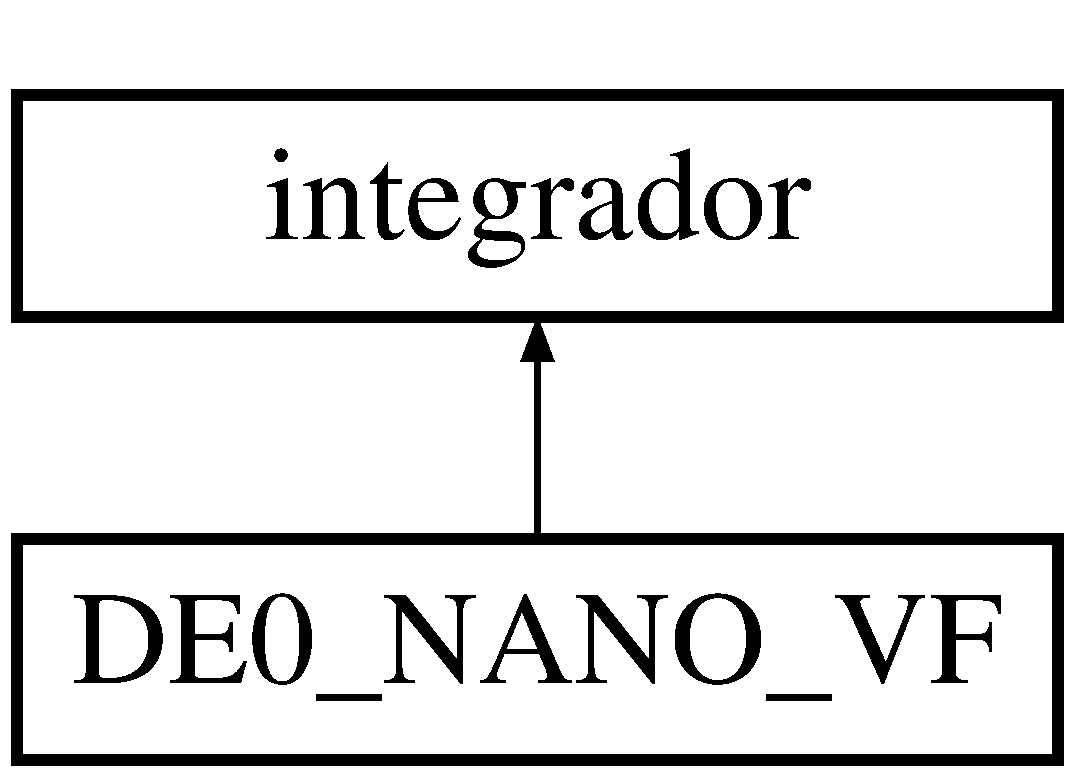
\includegraphics[height=2.000000cm]{classintegrador}
\end{center}
\end{figure}
\subsection*{Entities}
\begin{DoxyCompactItemize}
\item 
\hyperlink{classintegrador_1_1integrador}{integrador} architecture
\end{DoxyCompactItemize}
\subsection*{Libraries}
 \begin{DoxyCompactItemize}
\item 
\hyperlink{classintegrador_ae4f03c286607f3181e16b9aa12d0c6d4}{I\+E\+E\+E} 
\end{DoxyCompactItemize}
\subsection*{Use Clauses}
 \begin{DoxyCompactItemize}
\item 
\hyperlink{classintegrador_a241c3e72dd8024cc8ae831b1b2aed7db}{S\+T\+D\+\_\+\+L\+O\+G\+I\+C\+\_\+\+U\+N\+S\+I\+G\+N\+E\+D}   
\item 
\hyperlink{classintegrador_aa4b2b25246a821511120e3149b003563}{S\+T\+D\+\_\+\+L\+O\+G\+I\+C\+\_\+1164}   
\item 
\hyperlink{classintegrador_aad86249c80e8c1e7ee1c4748aba748e3}{fixed\+\_\+pkg}   
\end{DoxyCompactItemize}
\subsection*{Generics}
 \begin{DoxyCompactItemize}
\item 
\hyperlink{classintegrador_a2629ecb3bb37e8104b2866b0fd0c8574}{Nin} {\bfseries {\bfseries \textcolor{comment}{integer}\textcolor{vhdlchar}{ }\textcolor{vhdlchar}{ }\textcolor{vhdlchar}{\+:}\textcolor{vhdlchar}{=}\textcolor{vhdlchar}{ }\textcolor{vhdlchar}{ } \textcolor{vhdldigit}{13} \textcolor{vhdlchar}{ }}}
\item 
\hyperlink{classintegrador_a061c0d632c8bdf5dd32c80acf9a9c475}{Nout} {\bfseries {\bfseries \textcolor{comment}{integer}\textcolor{vhdlchar}{ }\textcolor{vhdlchar}{ }\textcolor{vhdlchar}{\+:}\textcolor{vhdlchar}{=}\textcolor{vhdlchar}{ }\textcolor{vhdlchar}{ } \textcolor{vhdldigit}{30} \textcolor{vhdlchar}{ }}}
\end{DoxyCompactItemize}
\subsection*{Ports}
 \begin{DoxyCompactItemize}
\item 
\hyperlink{classintegrador_a4a4609c199d30b3adebbeb3a01276ec5}{clk}  {\bfseries {\bfseries \textcolor{keywordflow}{in}\textcolor{vhdlchar}{ }}} {\bfseries \textcolor{comment}{std\+\_\+logic}\textcolor{vhdlchar}{ }} 
\item 
\hyperlink{classintegrador_adcf9c6f5161d039addbda5819bee64a3}{en}  {\bfseries {\bfseries \textcolor{keywordflow}{in}\textcolor{vhdlchar}{ }}} {\bfseries \textcolor{comment}{std\+\_\+logic}\textcolor{vhdlchar}{ }} 
\item 
\hyperlink{classintegrador_aad8dc6359d9e23dabcbf342fadf2fa06}{reset}  {\bfseries {\bfseries \textcolor{keywordflow}{in}\textcolor{vhdlchar}{ }}} {\bfseries \textcolor{comment}{std\+\_\+logic}\textcolor{vhdlchar}{ }} 
\item 
\hyperlink{classintegrador_aae281cf725515894f893258c629a59c7}{sinc}  {\bfseries {\bfseries \textcolor{keywordflow}{out}\textcolor{vhdlchar}{ }}} {\bfseries \textcolor{comment}{std\+\_\+logic}\textcolor{vhdlchar}{ }} 
\item 
\hyperlink{classintegrador_a436836a2e79668e0976eef3a553b5406}{M\+A\+X}  {\bfseries {\bfseries \textcolor{keywordflow}{in}\textcolor{vhdlchar}{ }}} {\bfseries \textcolor{comment}{std\+\_\+logic\+\_\+vector}\textcolor{vhdlchar}{ }\textcolor{vhdlchar}{(}\textcolor{vhdlchar}{ }\textcolor{vhdlchar}{ }\textcolor{vhdlchar}{ }\textcolor{vhdlchar}{ }{\bfseries \hyperlink{classintegrador_a061c0d632c8bdf5dd32c80acf9a9c475}{Nout}} \textcolor{vhdlchar}{-\/}\textcolor{vhdlchar}{ } \textcolor{vhdldigit}{1} \textcolor{vhdlchar}{ }\textcolor{keywordflow}{downto}\textcolor{vhdlchar}{ }\textcolor{vhdlchar}{ } \textcolor{vhdldigit}{0} \textcolor{vhdlchar}{ }\textcolor{vhdlchar}{)}\textcolor{vhdlchar}{ }} 
\item 
\hyperlink{classintegrador_a9e461894ea9b864637648799f51bf9be}{out\+\_\+data}  {\bfseries {\bfseries \textcolor{keywordflow}{out}\textcolor{vhdlchar}{ }}} {\bfseries \textcolor{comment}{std\+\_\+logic\+\_\+vector}\textcolor{vhdlchar}{ }\textcolor{vhdlchar}{(}\textcolor{vhdlchar}{ }\textcolor{vhdlchar}{ }\textcolor{vhdlchar}{ }\textcolor{vhdlchar}{ }{\bfseries \hyperlink{classintegrador_a061c0d632c8bdf5dd32c80acf9a9c475}{Nout}} \textcolor{vhdlchar}{-\/}\textcolor{vhdlchar}{ } \textcolor{vhdldigit}{1} \textcolor{vhdlchar}{ }\textcolor{keywordflow}{downto}\textcolor{vhdlchar}{ }\textcolor{vhdlchar}{ } \textcolor{vhdldigit}{0} \textcolor{vhdlchar}{ }\textcolor{vhdlchar}{)}\textcolor{vhdlchar}{ }} 
\item 
\hyperlink{classintegrador_aec192442094491f2207942b96b64835c}{int\+\_\+data}  {\bfseries {\bfseries \textcolor{keywordflow}{in}\textcolor{vhdlchar}{ }}} {\bfseries \textcolor{comment}{std\+\_\+logic\+\_\+vector}\textcolor{vhdlchar}{ }\textcolor{vhdlchar}{(}\textcolor{vhdlchar}{ }\textcolor{vhdlchar}{ }\textcolor{vhdlchar}{ }\textcolor{vhdlchar}{ }{\bfseries \hyperlink{classintegrador_a2629ecb3bb37e8104b2866b0fd0c8574}{Nin}} \textcolor{vhdlchar}{-\/}\textcolor{vhdlchar}{ } \textcolor{vhdldigit}{1} \textcolor{vhdlchar}{ }\textcolor{keywordflow}{downto}\textcolor{vhdlchar}{ }\textcolor{vhdlchar}{ } \textcolor{vhdldigit}{0} \textcolor{vhdlchar}{ }\textcolor{vhdlchar}{)}\textcolor{vhdlchar}{ }} 
\end{DoxyCompactItemize}


\subsection{Detailed Description}


Definition at line \hyperlink{integrador_8vhd_source_l00006}{6} of file \hyperlink{integrador_8vhd_source}{integrador.\+vhd}.



\subsection{Member Data Documentation}
\hypertarget{classintegrador_a4a4609c199d30b3adebbeb3a01276ec5}{}\index{integrador@{integrador}!clk@{clk}}
\index{clk@{clk}!integrador@{integrador}}
\subsubsection[{clk}]{\setlength{\rightskip}{0pt plus 5cm}{\bf clk} {\bfseries \textcolor{keywordflow}{in}\textcolor{vhdlchar}{ }} {\bfseries \textcolor{comment}{std\+\_\+logic}\textcolor{vhdlchar}{ }} \hspace{0.3cm}{\ttfamily [Port]}}\label{classintegrador_a4a4609c199d30b3adebbeb3a01276ec5}


Definition at line \hyperlink{integrador_8vhd_source_l00011}{11} of file \hyperlink{integrador_8vhd_source}{integrador.\+vhd}.

\hypertarget{classintegrador_adcf9c6f5161d039addbda5819bee64a3}{}\index{integrador@{integrador}!en@{en}}
\index{en@{en}!integrador@{integrador}}
\subsubsection[{en}]{\setlength{\rightskip}{0pt plus 5cm}{\bf en} {\bfseries \textcolor{keywordflow}{in}\textcolor{vhdlchar}{ }} {\bfseries \textcolor{comment}{std\+\_\+logic}\textcolor{vhdlchar}{ }} \hspace{0.3cm}{\ttfamily [Port]}}\label{classintegrador_adcf9c6f5161d039addbda5819bee64a3}


Definition at line \hyperlink{integrador_8vhd_source_l00012}{12} of file \hyperlink{integrador_8vhd_source}{integrador.\+vhd}.

\hypertarget{classintegrador_aad86249c80e8c1e7ee1c4748aba748e3}{}\index{integrador@{integrador}!fixed\+\_\+pkg@{fixed\+\_\+pkg}}
\index{fixed\+\_\+pkg@{fixed\+\_\+pkg}!integrador@{integrador}}
\subsubsection[{fixed\+\_\+pkg}]{\setlength{\rightskip}{0pt plus 5cm}{\bf fixed\+\_\+pkg}\hspace{0.3cm}{\ttfamily [Package]}}\label{classintegrador_aad86249c80e8c1e7ee1c4748aba748e3}


Definition at line \hyperlink{integrador_8vhd_source_l00004}{4} of file \hyperlink{integrador_8vhd_source}{integrador.\+vhd}.

\hypertarget{classintegrador_ae4f03c286607f3181e16b9aa12d0c6d4}{}\index{integrador@{integrador}!I\+E\+E\+E@{I\+E\+E\+E}}
\index{I\+E\+E\+E@{I\+E\+E\+E}!integrador@{integrador}}
\subsubsection[{I\+E\+E\+E}]{\setlength{\rightskip}{0pt plus 5cm}{\bf I\+E\+E\+E}\hspace{0.3cm}{\ttfamily [Library]}}\label{classintegrador_ae4f03c286607f3181e16b9aa12d0c6d4}


Definition at line \hyperlink{integrador_8vhd_source_l00001}{1} of file \hyperlink{integrador_8vhd_source}{integrador.\+vhd}.

\hypertarget{classintegrador_aec192442094491f2207942b96b64835c}{}\index{integrador@{integrador}!int\+\_\+data@{int\+\_\+data}}
\index{int\+\_\+data@{int\+\_\+data}!integrador@{integrador}}
\subsubsection[{int\+\_\+data}]{\setlength{\rightskip}{0pt plus 5cm}{\bf int\+\_\+data} {\bfseries \textcolor{keywordflow}{in}\textcolor{vhdlchar}{ }} {\bfseries \textcolor{comment}{std\+\_\+logic\+\_\+vector}\textcolor{vhdlchar}{ }\textcolor{vhdlchar}{(}\textcolor{vhdlchar}{ }\textcolor{vhdlchar}{ }\textcolor{vhdlchar}{ }\textcolor{vhdlchar}{ }{\bfseries {\bf Nin}} \textcolor{vhdlchar}{-\/}\textcolor{vhdlchar}{ } \textcolor{vhdldigit}{1} \textcolor{vhdlchar}{ }\textcolor{keywordflow}{downto}\textcolor{vhdlchar}{ }\textcolor{vhdlchar}{ } \textcolor{vhdldigit}{0} \textcolor{vhdlchar}{ }\textcolor{vhdlchar}{)}\textcolor{vhdlchar}{ }} \hspace{0.3cm}{\ttfamily [Port]}}\label{classintegrador_aec192442094491f2207942b96b64835c}


Definition at line \hyperlink{integrador_8vhd_source_l00018}{18} of file \hyperlink{integrador_8vhd_source}{integrador.\+vhd}.

\hypertarget{classintegrador_a436836a2e79668e0976eef3a553b5406}{}\index{integrador@{integrador}!M\+A\+X@{M\+A\+X}}
\index{M\+A\+X@{M\+A\+X}!integrador@{integrador}}
\subsubsection[{M\+A\+X}]{\setlength{\rightskip}{0pt plus 5cm}{\bf M\+A\+X} {\bfseries \textcolor{keywordflow}{in}\textcolor{vhdlchar}{ }} {\bfseries \textcolor{comment}{std\+\_\+logic\+\_\+vector}\textcolor{vhdlchar}{ }\textcolor{vhdlchar}{(}\textcolor{vhdlchar}{ }\textcolor{vhdlchar}{ }\textcolor{vhdlchar}{ }\textcolor{vhdlchar}{ }{\bfseries {\bf Nout}} \textcolor{vhdlchar}{-\/}\textcolor{vhdlchar}{ } \textcolor{vhdldigit}{1} \textcolor{vhdlchar}{ }\textcolor{keywordflow}{downto}\textcolor{vhdlchar}{ }\textcolor{vhdlchar}{ } \textcolor{vhdldigit}{0} \textcolor{vhdlchar}{ }\textcolor{vhdlchar}{)}\textcolor{vhdlchar}{ }} \hspace{0.3cm}{\ttfamily [Port]}}\label{classintegrador_a436836a2e79668e0976eef3a553b5406}


Definition at line \hyperlink{integrador_8vhd_source_l00015}{15} of file \hyperlink{integrador_8vhd_source}{integrador.\+vhd}.

\hypertarget{classintegrador_a2629ecb3bb37e8104b2866b0fd0c8574}{}\index{integrador@{integrador}!Nin@{Nin}}
\index{Nin@{Nin}!integrador@{integrador}}
\subsubsection[{Nin}]{\setlength{\rightskip}{0pt plus 5cm}{\bf Nin} {\bfseries \textcolor{vhdlchar}{ }} {\bfseries \textcolor{comment}{integer}\textcolor{vhdlchar}{ }\textcolor{vhdlchar}{ }\textcolor{vhdlchar}{\+:}\textcolor{vhdlchar}{=}\textcolor{vhdlchar}{ }\textcolor{vhdlchar}{ } \textcolor{vhdldigit}{13} \textcolor{vhdlchar}{ }} \hspace{0.3cm}{\ttfamily [Generic]}}\label{classintegrador_a2629ecb3bb37e8104b2866b0fd0c8574}


Definition at line \hyperlink{integrador_8vhd_source_l00007}{7} of file \hyperlink{integrador_8vhd_source}{integrador.\+vhd}.

\hypertarget{classintegrador_a061c0d632c8bdf5dd32c80acf9a9c475}{}\index{integrador@{integrador}!Nout@{Nout}}
\index{Nout@{Nout}!integrador@{integrador}}
\subsubsection[{Nout}]{\setlength{\rightskip}{0pt plus 5cm}{\bf Nout} {\bfseries \textcolor{vhdlchar}{ }} {\bfseries \textcolor{comment}{integer}\textcolor{vhdlchar}{ }\textcolor{vhdlchar}{ }\textcolor{vhdlchar}{\+:}\textcolor{vhdlchar}{=}\textcolor{vhdlchar}{ }\textcolor{vhdlchar}{ } \textcolor{vhdldigit}{30} \textcolor{vhdlchar}{ }} \hspace{0.3cm}{\ttfamily [Generic]}}\label{classintegrador_a061c0d632c8bdf5dd32c80acf9a9c475}


Definition at line \hyperlink{integrador_8vhd_source_l00009}{9} of file \hyperlink{integrador_8vhd_source}{integrador.\+vhd}.

\hypertarget{classintegrador_a9e461894ea9b864637648799f51bf9be}{}\index{integrador@{integrador}!out\+\_\+data@{out\+\_\+data}}
\index{out\+\_\+data@{out\+\_\+data}!integrador@{integrador}}
\subsubsection[{out\+\_\+data}]{\setlength{\rightskip}{0pt plus 5cm}{\bf out\+\_\+data} {\bfseries \textcolor{keywordflow}{out}\textcolor{vhdlchar}{ }} {\bfseries \textcolor{comment}{std\+\_\+logic\+\_\+vector}\textcolor{vhdlchar}{ }\textcolor{vhdlchar}{(}\textcolor{vhdlchar}{ }\textcolor{vhdlchar}{ }\textcolor{vhdlchar}{ }\textcolor{vhdlchar}{ }{\bfseries {\bf Nout}} \textcolor{vhdlchar}{-\/}\textcolor{vhdlchar}{ } \textcolor{vhdldigit}{1} \textcolor{vhdlchar}{ }\textcolor{keywordflow}{downto}\textcolor{vhdlchar}{ }\textcolor{vhdlchar}{ } \textcolor{vhdldigit}{0} \textcolor{vhdlchar}{ }\textcolor{vhdlchar}{)}\textcolor{vhdlchar}{ }} \hspace{0.3cm}{\ttfamily [Port]}}\label{classintegrador_a9e461894ea9b864637648799f51bf9be}


Definition at line \hyperlink{integrador_8vhd_source_l00016}{16} of file \hyperlink{integrador_8vhd_source}{integrador.\+vhd}.

\hypertarget{classintegrador_aad8dc6359d9e23dabcbf342fadf2fa06}{}\index{integrador@{integrador}!reset@{reset}}
\index{reset@{reset}!integrador@{integrador}}
\subsubsection[{reset}]{\setlength{\rightskip}{0pt plus 5cm}{\bf reset} {\bfseries \textcolor{keywordflow}{in}\textcolor{vhdlchar}{ }} {\bfseries \textcolor{comment}{std\+\_\+logic}\textcolor{vhdlchar}{ }} \hspace{0.3cm}{\ttfamily [Port]}}\label{classintegrador_aad8dc6359d9e23dabcbf342fadf2fa06}


Definition at line \hyperlink{integrador_8vhd_source_l00013}{13} of file \hyperlink{integrador_8vhd_source}{integrador.\+vhd}.

\hypertarget{classintegrador_aae281cf725515894f893258c629a59c7}{}\index{integrador@{integrador}!sinc@{sinc}}
\index{sinc@{sinc}!integrador@{integrador}}
\subsubsection[{sinc}]{\setlength{\rightskip}{0pt plus 5cm}{\bf sinc} {\bfseries \textcolor{keywordflow}{out}\textcolor{vhdlchar}{ }} {\bfseries \textcolor{comment}{std\+\_\+logic}\textcolor{vhdlchar}{ }} \hspace{0.3cm}{\ttfamily [Port]}}\label{classintegrador_aae281cf725515894f893258c629a59c7}


Definition at line \hyperlink{integrador_8vhd_source_l00014}{14} of file \hyperlink{integrador_8vhd_source}{integrador.\+vhd}.

\hypertarget{classintegrador_aa4b2b25246a821511120e3149b003563}{}\index{integrador@{integrador}!S\+T\+D\+\_\+\+L\+O\+G\+I\+C\+\_\+1164@{S\+T\+D\+\_\+\+L\+O\+G\+I\+C\+\_\+1164}}
\index{S\+T\+D\+\_\+\+L\+O\+G\+I\+C\+\_\+1164@{S\+T\+D\+\_\+\+L\+O\+G\+I\+C\+\_\+1164}!integrador@{integrador}}
\subsubsection[{S\+T\+D\+\_\+\+L\+O\+G\+I\+C\+\_\+1164}]{\setlength{\rightskip}{0pt plus 5cm}{\bf S\+T\+D\+\_\+\+L\+O\+G\+I\+C\+\_\+1164}\hspace{0.3cm}{\ttfamily [Package]}}\label{classintegrador_aa4b2b25246a821511120e3149b003563}


Definition at line \hyperlink{integrador_8vhd_source_l00003}{3} of file \hyperlink{integrador_8vhd_source}{integrador.\+vhd}.

\hypertarget{classintegrador_a241c3e72dd8024cc8ae831b1b2aed7db}{}\index{integrador@{integrador}!S\+T\+D\+\_\+\+L\+O\+G\+I\+C\+\_\+\+U\+N\+S\+I\+G\+N\+E\+D@{S\+T\+D\+\_\+\+L\+O\+G\+I\+C\+\_\+\+U\+N\+S\+I\+G\+N\+E\+D}}
\index{S\+T\+D\+\_\+\+L\+O\+G\+I\+C\+\_\+\+U\+N\+S\+I\+G\+N\+E\+D@{S\+T\+D\+\_\+\+L\+O\+G\+I\+C\+\_\+\+U\+N\+S\+I\+G\+N\+E\+D}!integrador@{integrador}}
\subsubsection[{S\+T\+D\+\_\+\+L\+O\+G\+I\+C\+\_\+\+U\+N\+S\+I\+G\+N\+E\+D}]{\setlength{\rightskip}{0pt plus 5cm}{\bf S\+T\+D\+\_\+\+L\+O\+G\+I\+C\+\_\+\+U\+N\+S\+I\+G\+N\+E\+D}\hspace{0.3cm}{\ttfamily [Package]}}\label{classintegrador_a241c3e72dd8024cc8ae831b1b2aed7db}


Definition at line \hyperlink{integrador_8vhd_source_l00002}{2} of file \hyperlink{integrador_8vhd_source}{integrador.\+vhd}.



The documentation for this class was generated from the following file\+:\begin{DoxyCompactItemize}
\item 
\hyperlink{integrador_8vhd}{integrador.\+vhd}\end{DoxyCompactItemize}

\hypertarget{classintegrador_1_1integrador}{}\section{integrador Architecture Reference}
\label{classintegrador_1_1integrador}\index{integrador@{integrador}}
\subsection*{Processes}
 \begin{DoxyCompactItemize}
\item 
\hyperlink{classintegrador_1_1integrador_afcc525892643d4614179ad348921cd15}{P\+R\+O\+C\+E\+S\+S\+\_\+10}{\bfseries  ( {\bfseries {\bfseries \hyperlink{classintegrador_a4a4609c199d30b3adebbeb3a01276ec5}{clk}} \textcolor{vhdlchar}{ }} )}
\end{DoxyCompactItemize}
\subsection*{Signals}
 \begin{DoxyCompactItemize}
\item 
\hyperlink{classintegrador_1_1integrador_a951e616187c21eeebaa382a516df536e}{out\+\_\+int} {\bfseries \textcolor{comment}{std\+\_\+logic\+\_\+vector}\textcolor{vhdlchar}{ }\textcolor{vhdlchar}{(}\textcolor{vhdlchar}{ }\textcolor{vhdlchar}{ }\textcolor{vhdlchar}{ }\textcolor{vhdlchar}{ }{\bfseries \hyperlink{classintegrador_a061c0d632c8bdf5dd32c80acf9a9c475}{Nout}} \textcolor{vhdlchar}{-\/}\textcolor{vhdlchar}{ } \textcolor{vhdldigit}{1} \textcolor{vhdlchar}{ }\textcolor{keywordflow}{downto}\textcolor{vhdlchar}{ }\textcolor{vhdlchar}{ } \textcolor{vhdldigit}{0} \textcolor{vhdlchar}{ }\textcolor{vhdlchar}{)}\textcolor{vhdlchar}{ }} 
\item 
\hyperlink{classintegrador_1_1integrador_a45126d1a75be347f440d181b7aa5e033}{sinc\+\_\+int} {\bfseries \textcolor{comment}{std\+\_\+logic}\textcolor{vhdlchar}{ }} 
\end{DoxyCompactItemize}


\subsection{Detailed Description}


Definition at line 23 of file integrador.\+vhd.



\subsection{Member Function Documentation}
\hypertarget{classintegrador_1_1integrador_afcc525892643d4614179ad348921cd15}{}\index{integrador\+::integrador@{integrador\+::integrador}!P\+R\+O\+C\+E\+S\+S\+\_\+10@{P\+R\+O\+C\+E\+S\+S\+\_\+10}}
\index{P\+R\+O\+C\+E\+S\+S\+\_\+10@{P\+R\+O\+C\+E\+S\+S\+\_\+10}!integrador\+::integrador@{integrador\+::integrador}}
\subsubsection[{P\+R\+O\+C\+E\+S\+S\+\_\+10}]{\setlength{\rightskip}{0pt plus 5cm} {\bfseries \textcolor{vhdlchar}{ }} P\+R\+O\+C\+E\+S\+S\+\_\+10(
\begin{DoxyParamCaption}
\item[{}]{{\bfseries {\bfseries {\bf clk}} \textcolor{vhdlchar}{ }} {\em }}
\end{DoxyParamCaption}
)\hspace{0.3cm}{\ttfamily [Process]}}\label{classintegrador_1_1integrador_afcc525892643d4614179ad348921cd15}


Definition at line 31 of file integrador.\+vhd.



\subsection{Member Data Documentation}
\hypertarget{classintegrador_1_1integrador_a951e616187c21eeebaa382a516df536e}{}\index{integrador\+::integrador@{integrador\+::integrador}!out\+\_\+int@{out\+\_\+int}}
\index{out\+\_\+int@{out\+\_\+int}!integrador\+::integrador@{integrador\+::integrador}}
\subsubsection[{out\+\_\+int}]{\setlength{\rightskip}{0pt plus 5cm}{\bf out\+\_\+int} {\bfseries \textcolor{comment}{std\+\_\+logic\+\_\+vector}\textcolor{vhdlchar}{ }\textcolor{vhdlchar}{(}\textcolor{vhdlchar}{ }\textcolor{vhdlchar}{ }\textcolor{vhdlchar}{ }\textcolor{vhdlchar}{ }{\bfseries {\bf Nout}} \textcolor{vhdlchar}{-\/}\textcolor{vhdlchar}{ } \textcolor{vhdldigit}{1} \textcolor{vhdlchar}{ }\textcolor{keywordflow}{downto}\textcolor{vhdlchar}{ }\textcolor{vhdlchar}{ } \textcolor{vhdldigit}{0} \textcolor{vhdlchar}{ }\textcolor{vhdlchar}{)}\textcolor{vhdlchar}{ }} \hspace{0.3cm}{\ttfamily [Signal]}}\label{classintegrador_1_1integrador_a951e616187c21eeebaa382a516df536e}


Definition at line 25 of file integrador.\+vhd.

\hypertarget{classintegrador_1_1integrador_a45126d1a75be347f440d181b7aa5e033}{}\index{integrador\+::integrador@{integrador\+::integrador}!sinc\+\_\+int@{sinc\+\_\+int}}
\index{sinc\+\_\+int@{sinc\+\_\+int}!integrador\+::integrador@{integrador\+::integrador}}
\subsubsection[{sinc\+\_\+int}]{\setlength{\rightskip}{0pt plus 5cm}{\bf sinc\+\_\+int} {\bfseries \textcolor{comment}{std\+\_\+logic}\textcolor{vhdlchar}{ }} \hspace{0.3cm}{\ttfamily [Signal]}}\label{classintegrador_1_1integrador_a45126d1a75be347f440d181b7aa5e033}


Definition at line 26 of file integrador.\+vhd.



The documentation for this class was generated from the following file\+:\begin{DoxyCompactItemize}
\item 
\hyperlink{integrador_8vhd}{integrador.\+vhd}\end{DoxyCompactItemize}

\hypertarget{class_l_e_ds}{}\section{L\+E\+Ds Entity Reference}
\label{class_l_e_ds}\index{L\+E\+Ds@{L\+E\+Ds}}
\subsection*{Entities}
\begin{DoxyCompactItemize}
\item 
\hyperlink{class_l_e_ds_1_1_l_e_ds}{L\+E\+Ds} architecture
\end{DoxyCompactItemize}
\subsection*{Libraries}
 \begin{DoxyCompactItemize}
\item 
\hyperlink{class_l_e_ds_a0a6af6eef40212dbaf130d57ce711256}{ieee} 
\end{DoxyCompactItemize}
\subsection*{Use Clauses}
 \begin{DoxyCompactItemize}
\item 
\hyperlink{class_l_e_ds_acd03516902501cd1c7296a98e22c6fcb}{std\+\_\+logic\+\_\+1164}   
\item 
\hyperlink{class_l_e_ds_a0f5ecc6613f63d07f7963a97b1b26095}{std\+\_\+logic\+\_\+arith}   
\item 
\hyperlink{class_l_e_ds_a598da929e807d58939b47499e8bc9fa8}{std\+\_\+logic\+\_\+unsigned}   
\end{DoxyCompactItemize}
\subsection*{Ports}
 \begin{DoxyCompactItemize}
\item 
\hyperlink{class_l_e_ds_a4b5e1e3eba67b2e61c77c9a719d8518c}{C\+L\+O\+C\+K\+\_\+50}  {\bfseries {\bfseries \textcolor{keywordflow}{in}\textcolor{vhdlchar}{ }}} {\bfseries \textcolor{comment}{std\+\_\+logic}\textcolor{vhdlchar}{ }} 
\item 
\hyperlink{class_l_e_ds_a424944084857f6787a0ddb567d0b5240}{L\+E\+D}  {\bfseries {\bfseries \textcolor{keywordflow}{out}\textcolor{vhdlchar}{ }}} {\bfseries \textcolor{comment}{std\+\_\+logic\+\_\+vector}\textcolor{vhdlchar}{ }\textcolor{vhdlchar}{(}\textcolor{vhdlchar}{ }\textcolor{vhdlchar}{ } \textcolor{vhdldigit}{7} \textcolor{vhdlchar}{ }\textcolor{keywordflow}{D\+O\+W\+N\+T\+O}\textcolor{vhdlchar}{ }\textcolor{vhdlchar}{ } \textcolor{vhdldigit}{0} \textcolor{vhdlchar}{ }\textcolor{vhdlchar}{)}\textcolor{vhdlchar}{ }} 
\item 
\hyperlink{class_l_e_ds_a30974727c81621f672f7f9490463f9d3}{S\+W}  {\bfseries {\bfseries \textcolor{keywordflow}{in}\textcolor{vhdlchar}{ }}} {\bfseries \textcolor{comment}{std\+\_\+logic\+\_\+vector}\textcolor{vhdlchar}{ }\textcolor{vhdlchar}{(}\textcolor{vhdlchar}{ }\textcolor{vhdlchar}{ } \textcolor{vhdldigit}{3} \textcolor{vhdlchar}{ }\textcolor{keywordflow}{D\+O\+W\+N\+T\+O}\textcolor{vhdlchar}{ }\textcolor{vhdlchar}{ } \textcolor{vhdldigit}{0} \textcolor{vhdlchar}{ }\textcolor{vhdlchar}{)}\textcolor{vhdlchar}{ }} 
\item 
\hyperlink{class_l_e_ds_aa70bf9245705f33e4529eb81df3fbf94}{K\+E\+Y}  {\bfseries {\bfseries \textcolor{keywordflow}{in}\textcolor{vhdlchar}{ }}} {\bfseries \textcolor{comment}{std\+\_\+logic\+\_\+vector}\textcolor{vhdlchar}{ }\textcolor{vhdlchar}{(}\textcolor{vhdlchar}{ }\textcolor{vhdlchar}{ } \textcolor{vhdldigit}{1} \textcolor{vhdlchar}{ }\textcolor{keywordflow}{D\+O\+W\+N\+T\+O}\textcolor{vhdlchar}{ }\textcolor{vhdlchar}{ } \textcolor{vhdldigit}{0} \textcolor{vhdlchar}{ }\textcolor{vhdlchar}{)}\textcolor{vhdlchar}{ }} 
\end{DoxyCompactItemize}


\subsection{Detailed Description}


Definition at line \hyperlink{_l_e_ds_8vhd_source_l00009}{9} of file \hyperlink{_l_e_ds_8vhd_source}{L\+E\+Ds.\+vhd}.



\subsection{Member Data Documentation}
\hypertarget{class_l_e_ds_a4b5e1e3eba67b2e61c77c9a719d8518c}{}\index{L\+E\+Ds@{L\+E\+Ds}!C\+L\+O\+C\+K\+\_\+50@{C\+L\+O\+C\+K\+\_\+50}}
\index{C\+L\+O\+C\+K\+\_\+50@{C\+L\+O\+C\+K\+\_\+50}!L\+E\+Ds@{L\+E\+Ds}}
\subsubsection[{C\+L\+O\+C\+K\+\_\+50}]{\setlength{\rightskip}{0pt plus 5cm}{\bf C\+L\+O\+C\+K\+\_\+50} {\bfseries \textcolor{keywordflow}{in}\textcolor{vhdlchar}{ }} {\bfseries \textcolor{comment}{std\+\_\+logic}\textcolor{vhdlchar}{ }} \hspace{0.3cm}{\ttfamily [Port]}}\label{class_l_e_ds_a4b5e1e3eba67b2e61c77c9a719d8518c}


Definition at line \hyperlink{_l_e_ds_8vhd_source_l00011}{11} of file \hyperlink{_l_e_ds_8vhd_source}{L\+E\+Ds.\+vhd}.

\hypertarget{class_l_e_ds_a0a6af6eef40212dbaf130d57ce711256}{}\index{L\+E\+Ds@{L\+E\+Ds}!ieee@{ieee}}
\index{ieee@{ieee}!L\+E\+Ds@{L\+E\+Ds}}
\subsubsection[{ieee}]{\setlength{\rightskip}{0pt plus 5cm}{\bf ieee}\hspace{0.3cm}{\ttfamily [Library]}}\label{class_l_e_ds_a0a6af6eef40212dbaf130d57ce711256}


Definition at line \hyperlink{_l_e_ds_8vhd_source_l00004}{4} of file \hyperlink{_l_e_ds_8vhd_source}{L\+E\+Ds.\+vhd}.

\hypertarget{class_l_e_ds_aa70bf9245705f33e4529eb81df3fbf94}{}\index{L\+E\+Ds@{L\+E\+Ds}!K\+E\+Y@{K\+E\+Y}}
\index{K\+E\+Y@{K\+E\+Y}!L\+E\+Ds@{L\+E\+Ds}}
\subsubsection[{K\+E\+Y}]{\setlength{\rightskip}{0pt plus 5cm}{\bf K\+E\+Y} {\bfseries \textcolor{keywordflow}{in}\textcolor{vhdlchar}{ }} {\bfseries \textcolor{comment}{std\+\_\+logic\+\_\+vector}\textcolor{vhdlchar}{ }\textcolor{vhdlchar}{(}\textcolor{vhdlchar}{ }\textcolor{vhdlchar}{ } \textcolor{vhdldigit}{1} \textcolor{vhdlchar}{ }\textcolor{keywordflow}{D\+O\+W\+N\+T\+O}\textcolor{vhdlchar}{ }\textcolor{vhdlchar}{ } \textcolor{vhdldigit}{0} \textcolor{vhdlchar}{ }\textcolor{vhdlchar}{)}\textcolor{vhdlchar}{ }} \hspace{0.3cm}{\ttfamily [Port]}}\label{class_l_e_ds_aa70bf9245705f33e4529eb81df3fbf94}


Definition at line \hyperlink{_l_e_ds_8vhd_source_l00015}{15} of file \hyperlink{_l_e_ds_8vhd_source}{L\+E\+Ds.\+vhd}.

\hypertarget{class_l_e_ds_a424944084857f6787a0ddb567d0b5240}{}\index{L\+E\+Ds@{L\+E\+Ds}!L\+E\+D@{L\+E\+D}}
\index{L\+E\+D@{L\+E\+D}!L\+E\+Ds@{L\+E\+Ds}}
\subsubsection[{L\+E\+D}]{\setlength{\rightskip}{0pt plus 5cm}{\bf L\+E\+D} {\bfseries \textcolor{keywordflow}{out}\textcolor{vhdlchar}{ }} {\bfseries \textcolor{comment}{std\+\_\+logic\+\_\+vector}\textcolor{vhdlchar}{ }\textcolor{vhdlchar}{(}\textcolor{vhdlchar}{ }\textcolor{vhdlchar}{ } \textcolor{vhdldigit}{7} \textcolor{vhdlchar}{ }\textcolor{keywordflow}{D\+O\+W\+N\+T\+O}\textcolor{vhdlchar}{ }\textcolor{vhdlchar}{ } \textcolor{vhdldigit}{0} \textcolor{vhdlchar}{ }\textcolor{vhdlchar}{)}\textcolor{vhdlchar}{ }} \hspace{0.3cm}{\ttfamily [Port]}}\label{class_l_e_ds_a424944084857f6787a0ddb567d0b5240}


Definition at line \hyperlink{_l_e_ds_8vhd_source_l00012}{12} of file \hyperlink{_l_e_ds_8vhd_source}{L\+E\+Ds.\+vhd}.

\hypertarget{class_l_e_ds_acd03516902501cd1c7296a98e22c6fcb}{}\index{L\+E\+Ds@{L\+E\+Ds}!std\+\_\+logic\+\_\+1164@{std\+\_\+logic\+\_\+1164}}
\index{std\+\_\+logic\+\_\+1164@{std\+\_\+logic\+\_\+1164}!L\+E\+Ds@{L\+E\+Ds}}
\subsubsection[{std\+\_\+logic\+\_\+1164}]{\setlength{\rightskip}{0pt plus 5cm}{\bf std\+\_\+logic\+\_\+1164}\hspace{0.3cm}{\ttfamily [Package]}}\label{class_l_e_ds_acd03516902501cd1c7296a98e22c6fcb}


Definition at line \hyperlink{_l_e_ds_8vhd_source_l00005}{5} of file \hyperlink{_l_e_ds_8vhd_source}{L\+E\+Ds.\+vhd}.

\hypertarget{class_l_e_ds_a0f5ecc6613f63d07f7963a97b1b26095}{}\index{L\+E\+Ds@{L\+E\+Ds}!std\+\_\+logic\+\_\+arith@{std\+\_\+logic\+\_\+arith}}
\index{std\+\_\+logic\+\_\+arith@{std\+\_\+logic\+\_\+arith}!L\+E\+Ds@{L\+E\+Ds}}
\subsubsection[{std\+\_\+logic\+\_\+arith}]{\setlength{\rightskip}{0pt plus 5cm}{\bf std\+\_\+logic\+\_\+arith}\hspace{0.3cm}{\ttfamily [Package]}}\label{class_l_e_ds_a0f5ecc6613f63d07f7963a97b1b26095}


Definition at line \hyperlink{_l_e_ds_8vhd_source_l00006}{6} of file \hyperlink{_l_e_ds_8vhd_source}{L\+E\+Ds.\+vhd}.

\hypertarget{class_l_e_ds_a598da929e807d58939b47499e8bc9fa8}{}\index{L\+E\+Ds@{L\+E\+Ds}!std\+\_\+logic\+\_\+unsigned@{std\+\_\+logic\+\_\+unsigned}}
\index{std\+\_\+logic\+\_\+unsigned@{std\+\_\+logic\+\_\+unsigned}!L\+E\+Ds@{L\+E\+Ds}}
\subsubsection[{std\+\_\+logic\+\_\+unsigned}]{\setlength{\rightskip}{0pt plus 5cm}{\bf std\+\_\+logic\+\_\+unsigned}\hspace{0.3cm}{\ttfamily [Package]}}\label{class_l_e_ds_a598da929e807d58939b47499e8bc9fa8}


Definition at line \hyperlink{_l_e_ds_8vhd_source_l00007}{7} of file \hyperlink{_l_e_ds_8vhd_source}{L\+E\+Ds.\+vhd}.

\hypertarget{class_l_e_ds_a30974727c81621f672f7f9490463f9d3}{}\index{L\+E\+Ds@{L\+E\+Ds}!S\+W@{S\+W}}
\index{S\+W@{S\+W}!L\+E\+Ds@{L\+E\+Ds}}
\subsubsection[{S\+W}]{\setlength{\rightskip}{0pt plus 5cm}{\bf S\+W} {\bfseries \textcolor{keywordflow}{in}\textcolor{vhdlchar}{ }} {\bfseries \textcolor{comment}{std\+\_\+logic\+\_\+vector}\textcolor{vhdlchar}{ }\textcolor{vhdlchar}{(}\textcolor{vhdlchar}{ }\textcolor{vhdlchar}{ } \textcolor{vhdldigit}{3} \textcolor{vhdlchar}{ }\textcolor{keywordflow}{D\+O\+W\+N\+T\+O}\textcolor{vhdlchar}{ }\textcolor{vhdlchar}{ } \textcolor{vhdldigit}{0} \textcolor{vhdlchar}{ }\textcolor{vhdlchar}{)}\textcolor{vhdlchar}{ }} \hspace{0.3cm}{\ttfamily [Port]}}\label{class_l_e_ds_a30974727c81621f672f7f9490463f9d3}


Definition at line \hyperlink{_l_e_ds_8vhd_source_l00013}{13} of file \hyperlink{_l_e_ds_8vhd_source}{L\+E\+Ds.\+vhd}.



The documentation for this class was generated from the following file\+:\begin{DoxyCompactItemize}
\item 
\hyperlink{_l_e_ds_8vhd}{L\+E\+Ds.\+vhd}\end{DoxyCompactItemize}

\hypertarget{class_l_e_ds_1_1_l_e_ds}{}\section{L\+E\+Ds Architecture Reference}
\label{class_l_e_ds_1_1_l_e_ds}\index{L\+E\+Ds@{L\+E\+Ds}}
\subsection*{Processes}
 \begin{DoxyCompactItemize}
\item 
\hyperlink{class_l_e_ds_1_1_l_e_ds_a0b2ae93f7930ef5bc4cc2730b8c405d1}{P\+R\+O\+C\+E\+S\+S\+\_\+11}{\bfseries  ( {\bfseries {\bfseries \hyperlink{class_l_e_ds_a4b5e1e3eba67b2e61c77c9a719d8518c}{C\+L\+O\+C\+K\+\_\+50}} \textcolor{vhdlchar}{ }} )}
\end{DoxyCompactItemize}
\subsection*{Constants}
 \begin{DoxyCompactItemize}
\item 
\hyperlink{class_l_e_ds_1_1_l_e_ds_aa45ed8f4ade73b3c1510f9df8ec7dd9c}{C\+L\+K\+\_\+\+F\+R\+E\+Q} {\bfseries \textcolor{comment}{integer}\textcolor{vhdlchar}{ }\textcolor{vhdlchar}{ }\textcolor{vhdlchar}{\+:}\textcolor{vhdlchar}{=}\textcolor{vhdlchar}{ }\textcolor{vhdlchar}{ } \textcolor{vhdldigit}{50000000} \textcolor{vhdlchar}{ }} 
\item 
\hyperlink{class_l_e_ds_1_1_l_e_ds_a1890617960a841a3d027f78733169e15}{B\+L\+I\+N\+K\+\_\+\+F\+R\+E\+Q} {\bfseries \textcolor{comment}{integer}\textcolor{vhdlchar}{ }\textcolor{vhdlchar}{ }\textcolor{vhdlchar}{\+:}\textcolor{vhdlchar}{=}\textcolor{vhdlchar}{ }\textcolor{vhdlchar}{ } \textcolor{vhdldigit}{1} \textcolor{vhdlchar}{ }} 
\item 
\hyperlink{class_l_e_ds_1_1_l_e_ds_a62b6ca896e870c8bfbd7496a8c89efe6}{C\+N\+T\+\_\+\+M\+A\+X} {\bfseries \textcolor{comment}{integer}\textcolor{vhdlchar}{ }\textcolor{vhdlchar}{ }\textcolor{vhdlchar}{\+:}\textcolor{vhdlchar}{=}\textcolor{vhdlchar}{ }\textcolor{vhdlchar}{ }\textcolor{vhdlchar}{ }\textcolor{vhdlchar}{ }{\bfseries \hyperlink{class_l_e_ds_1_1_l_e_ds_aa45ed8f4ade73b3c1510f9df8ec7dd9c}{C\+L\+K\+\_\+\+F\+R\+E\+Q}} \textcolor{vhdlchar}{/}\textcolor{vhdlchar}{ }\textcolor{vhdlchar}{ }\textcolor{vhdlchar}{ }{\bfseries \hyperlink{class_l_e_ds_1_1_l_e_ds_a1890617960a841a3d027f78733169e15}{B\+L\+I\+N\+K\+\_\+\+F\+R\+E\+Q}} \textcolor{vhdlchar}{/}\textcolor{vhdlchar}{ } \textcolor{vhdldigit}{2} \textcolor{vhdlchar}{-\/}\textcolor{vhdlchar}{ } \textcolor{vhdldigit}{1} \textcolor{vhdlchar}{ }} 
\end{DoxyCompactItemize}
\subsection*{Signals}
 \begin{DoxyCompactItemize}
\item 
\hyperlink{class_l_e_ds_1_1_l_e_ds_a17db0b3b66ebd22d100f607c5589f41d}{cnt} {\bfseries \textcolor{comment}{unsigned}\textcolor{vhdlchar}{ }\textcolor{vhdlchar}{(}\textcolor{vhdlchar}{ }\textcolor{vhdlchar}{ } \textcolor{vhdldigit}{24} \textcolor{vhdlchar}{ }\textcolor{keywordflow}{downto}\textcolor{vhdlchar}{ }\textcolor{vhdlchar}{ } \textcolor{vhdldigit}{0} \textcolor{vhdlchar}{ }\textcolor{vhdlchar}{)}\textcolor{vhdlchar}{ }} 
\item 
\hyperlink{class_l_e_ds_1_1_l_e_ds_a15ab33796b0132ed52d27866826e80ef}{blink} {\bfseries \textcolor{comment}{std\+\_\+logic}\textcolor{vhdlchar}{ }} 
\end{DoxyCompactItemize}


\subsection{Detailed Description}


Definition at line 22 of file L\+E\+Ds.\+vhd.



\subsection{Member Function Documentation}
\hypertarget{class_l_e_ds_1_1_l_e_ds_a0b2ae93f7930ef5bc4cc2730b8c405d1}{}\index{L\+E\+Ds\+::\+L\+E\+Ds@{L\+E\+Ds\+::\+L\+E\+Ds}!P\+R\+O\+C\+E\+S\+S\+\_\+11@{P\+R\+O\+C\+E\+S\+S\+\_\+11}}
\index{P\+R\+O\+C\+E\+S\+S\+\_\+11@{P\+R\+O\+C\+E\+S\+S\+\_\+11}!L\+E\+Ds\+::\+L\+E\+Ds@{L\+E\+Ds\+::\+L\+E\+Ds}}
\subsubsection[{P\+R\+O\+C\+E\+S\+S\+\_\+11}]{\setlength{\rightskip}{0pt plus 5cm} {\bfseries \textcolor{vhdlchar}{ }} P\+R\+O\+C\+E\+S\+S\+\_\+11(
\begin{DoxyParamCaption}
\item[{}]{{\bfseries {\bfseries {\bf C\+L\+O\+C\+K\+\_\+50}} \textcolor{vhdlchar}{ }} {\em }}
\end{DoxyParamCaption}
)\hspace{0.3cm}{\ttfamily [Process]}}\label{class_l_e_ds_1_1_l_e_ds_a0b2ae93f7930ef5bc4cc2730b8c405d1}


Definition at line 29 of file L\+E\+Ds.\+vhd.



\subsection{Member Data Documentation}
\hypertarget{class_l_e_ds_1_1_l_e_ds_a15ab33796b0132ed52d27866826e80ef}{}\index{L\+E\+Ds\+::\+L\+E\+Ds@{L\+E\+Ds\+::\+L\+E\+Ds}!blink@{blink}}
\index{blink@{blink}!L\+E\+Ds\+::\+L\+E\+Ds@{L\+E\+Ds\+::\+L\+E\+Ds}}
\subsubsection[{blink}]{\setlength{\rightskip}{0pt plus 5cm}{\bf blink} {\bfseries \textcolor{comment}{std\+\_\+logic}\textcolor{vhdlchar}{ }} \hspace{0.3cm}{\ttfamily [Signal]}}\label{class_l_e_ds_1_1_l_e_ds_a15ab33796b0132ed52d27866826e80ef}


Definition at line 27 of file L\+E\+Ds.\+vhd.

\hypertarget{class_l_e_ds_1_1_l_e_ds_a1890617960a841a3d027f78733169e15}{}\index{L\+E\+Ds\+::\+L\+E\+Ds@{L\+E\+Ds\+::\+L\+E\+Ds}!B\+L\+I\+N\+K\+\_\+\+F\+R\+E\+Q@{B\+L\+I\+N\+K\+\_\+\+F\+R\+E\+Q}}
\index{B\+L\+I\+N\+K\+\_\+\+F\+R\+E\+Q@{B\+L\+I\+N\+K\+\_\+\+F\+R\+E\+Q}!L\+E\+Ds\+::\+L\+E\+Ds@{L\+E\+Ds\+::\+L\+E\+Ds}}
\subsubsection[{B\+L\+I\+N\+K\+\_\+\+F\+R\+E\+Q}]{\setlength{\rightskip}{0pt plus 5cm}{\bf B\+L\+I\+N\+K\+\_\+\+F\+R\+E\+Q} {\bfseries \textcolor{comment}{integer}\textcolor{vhdlchar}{ }\textcolor{vhdlchar}{ }\textcolor{vhdlchar}{\+:}\textcolor{vhdlchar}{=}\textcolor{vhdlchar}{ }\textcolor{vhdlchar}{ } \textcolor{vhdldigit}{1} \textcolor{vhdlchar}{ }} \hspace{0.3cm}{\ttfamily [Constant]}}\label{class_l_e_ds_1_1_l_e_ds_a1890617960a841a3d027f78733169e15}


Definition at line 24 of file L\+E\+Ds.\+vhd.

\hypertarget{class_l_e_ds_1_1_l_e_ds_aa45ed8f4ade73b3c1510f9df8ec7dd9c}{}\index{L\+E\+Ds\+::\+L\+E\+Ds@{L\+E\+Ds\+::\+L\+E\+Ds}!C\+L\+K\+\_\+\+F\+R\+E\+Q@{C\+L\+K\+\_\+\+F\+R\+E\+Q}}
\index{C\+L\+K\+\_\+\+F\+R\+E\+Q@{C\+L\+K\+\_\+\+F\+R\+E\+Q}!L\+E\+Ds\+::\+L\+E\+Ds@{L\+E\+Ds\+::\+L\+E\+Ds}}
\subsubsection[{C\+L\+K\+\_\+\+F\+R\+E\+Q}]{\setlength{\rightskip}{0pt plus 5cm}{\bf C\+L\+K\+\_\+\+F\+R\+E\+Q} {\bfseries \textcolor{comment}{integer}\textcolor{vhdlchar}{ }\textcolor{vhdlchar}{ }\textcolor{vhdlchar}{\+:}\textcolor{vhdlchar}{=}\textcolor{vhdlchar}{ }\textcolor{vhdlchar}{ } \textcolor{vhdldigit}{50000000} \textcolor{vhdlchar}{ }} \hspace{0.3cm}{\ttfamily [Constant]}}\label{class_l_e_ds_1_1_l_e_ds_aa45ed8f4ade73b3c1510f9df8ec7dd9c}


Definition at line 23 of file L\+E\+Ds.\+vhd.

\hypertarget{class_l_e_ds_1_1_l_e_ds_a17db0b3b66ebd22d100f607c5589f41d}{}\index{L\+E\+Ds\+::\+L\+E\+Ds@{L\+E\+Ds\+::\+L\+E\+Ds}!cnt@{cnt}}
\index{cnt@{cnt}!L\+E\+Ds\+::\+L\+E\+Ds@{L\+E\+Ds\+::\+L\+E\+Ds}}
\subsubsection[{cnt}]{\setlength{\rightskip}{0pt plus 5cm}{\bf cnt} {\bfseries \textcolor{comment}{unsigned}\textcolor{vhdlchar}{ }\textcolor{vhdlchar}{(}\textcolor{vhdlchar}{ }\textcolor{vhdlchar}{ } \textcolor{vhdldigit}{24} \textcolor{vhdlchar}{ }\textcolor{keywordflow}{downto}\textcolor{vhdlchar}{ }\textcolor{vhdlchar}{ } \textcolor{vhdldigit}{0} \textcolor{vhdlchar}{ }\textcolor{vhdlchar}{)}\textcolor{vhdlchar}{ }} \hspace{0.3cm}{\ttfamily [Signal]}}\label{class_l_e_ds_1_1_l_e_ds_a17db0b3b66ebd22d100f607c5589f41d}


Definition at line 26 of file L\+E\+Ds.\+vhd.

\hypertarget{class_l_e_ds_1_1_l_e_ds_a62b6ca896e870c8bfbd7496a8c89efe6}{}\index{L\+E\+Ds\+::\+L\+E\+Ds@{L\+E\+Ds\+::\+L\+E\+Ds}!C\+N\+T\+\_\+\+M\+A\+X@{C\+N\+T\+\_\+\+M\+A\+X}}
\index{C\+N\+T\+\_\+\+M\+A\+X@{C\+N\+T\+\_\+\+M\+A\+X}!L\+E\+Ds\+::\+L\+E\+Ds@{L\+E\+Ds\+::\+L\+E\+Ds}}
\subsubsection[{C\+N\+T\+\_\+\+M\+A\+X}]{\setlength{\rightskip}{0pt plus 5cm}{\bf C\+N\+T\+\_\+\+M\+A\+X} {\bfseries \textcolor{comment}{integer}\textcolor{vhdlchar}{ }\textcolor{vhdlchar}{ }\textcolor{vhdlchar}{\+:}\textcolor{vhdlchar}{=}\textcolor{vhdlchar}{ }\textcolor{vhdlchar}{ }\textcolor{vhdlchar}{ }\textcolor{vhdlchar}{ }{\bfseries {\bf C\+L\+K\+\_\+\+F\+R\+E\+Q}} \textcolor{vhdlchar}{/}\textcolor{vhdlchar}{ }\textcolor{vhdlchar}{ }\textcolor{vhdlchar}{ }{\bfseries {\bf B\+L\+I\+N\+K\+\_\+\+F\+R\+E\+Q}} \textcolor{vhdlchar}{/}\textcolor{vhdlchar}{ } \textcolor{vhdldigit}{2} \textcolor{vhdlchar}{-\/}\textcolor{vhdlchar}{ } \textcolor{vhdldigit}{1} \textcolor{vhdlchar}{ }} \hspace{0.3cm}{\ttfamily [Constant]}}\label{class_l_e_ds_1_1_l_e_ds_a62b6ca896e870c8bfbd7496a8c89efe6}


Definition at line 25 of file L\+E\+Ds.\+vhd.



The documentation for this class was generated from the following file\+:\begin{DoxyCompactItemize}
\item 
\hyperlink{_l_e_ds_8vhd}{L\+E\+Ds.\+vhd}\end{DoxyCompactItemize}

\hypertarget{class_d_e0___n_a_n_o___v_f_1_1_m_a_i_n}{}\section{M\+A\+I\+N Architecture Reference}
\label{class_d_e0___n_a_n_o___v_f_1_1_m_a_i_n}\index{M\+A\+I\+N@{M\+A\+I\+N}}
\subsection*{Processes}
 \begin{DoxyCompactItemize}
\item 
\hyperlink{class_d_e0___n_a_n_o___v_f_1_1_m_a_i_n_aa22d55790db1f4e085c8fc295cb0e58f}{P\+R\+O\+C\+E\+S\+S\+\_\+4}{\bfseries  ( {\bfseries {\bfseries \hyperlink{class_d_e0___n_a_n_o___v_f_1_1_m_a_i_n_ac14ffa45ea42ce220a8e8316677fe263}{err\+\_\+\+F\+A\+B\+C}} \textcolor{vhdlchar}{ }} )}
\item 
\hyperlink{class_d_e0___n_a_n_o___v_f_1_1_m_a_i_n_a3c39b25652f7e5cb193fa2fd950d6b5e}{P\+R\+O\+C\+E\+S\+S\+\_\+5}{\bfseries  ( {\bfseries {\bfseries \hyperlink{class_d_e0___n_a_n_o___v_f_1_1_m_a_i_n_a1d63ebfc050c1099e1dff991817ec3b0}{clk\+\_\+pll}} \textcolor{vhdlchar}{ }} )}
\end{DoxyCompactItemize}
\subsection*{Components}
 \begin{DoxyCompactItemize}
\item 
\hyperlink{class_d_e0___n_a_n_o___v_f_1_1_m_a_i_n_ab6831a7d06c0a2bc69f9b024f6445a80}{L\+E\+Ds}  {\bfseries }  
\item 
\hyperlink{class_d_e0___n_a_n_o___v_f_1_1_m_a_i_n_a1ccf3e82106c07c2170611228e638a34}{contador}  {\bfseries }  
\item 
\hyperlink{class_d_e0___n_a_n_o___v_f_1_1_m_a_i_n_a4b5d0694f1c75396055f15cd7542add4}{tabela\+\_\+sin}  {\bfseries }  
\item 
\hyperlink{class_d_e0___n_a_n_o___v_f_1_1_m_a_i_n_af3891c65cf7793203a9df0cf918d0235}{pll}  {\bfseries }  
\item 
\hyperlink{class_d_e0___n_a_n_o___v_f_1_1_m_a_i_n_a8127d44aee38572cef223d0c27d447ab}{integrador}  {\bfseries }  
\item 
\hyperlink{class_d_e0___n_a_n_o___v_f_1_1_m_a_i_n_a15ab86106af3275297d1b9099a75ea1e}{theta\+\_\+abc}  {\bfseries }  
\item 
\hyperlink{class_d_e0___n_a_n_o___v_f_1_1_m_a_i_n_a39b27375c53f9cfc5759f4a53877ba0b}{clk\+\_\+div}  {\bfseries }  
\item 
\hyperlink{class_d_e0___n_a_n_o___v_f_1_1_m_a_i_n_a954f74a648a4905eff27c767a774c6dd}{portadora\+\_\+tringular}  {\bfseries }  
\item 
\hyperlink{class_d_e0___n_a_n_o___v_f_1_1_m_a_i_n_a4c526d0b606c178a7dddccfa2ae34ba6}{fbpspwmdt}  {\bfseries }  
\item 
\hyperlink{class_d_e0___n_a_n_o___v_f_1_1_m_a_i_n_a96f8f02a115cd76909b2395df08d3902}{vfcontrol}  {\bfseries }  
\end{DoxyCompactItemize}
\subsection*{Signals}
 \begin{DoxyCompactItemize}
\item 
\hyperlink{class_d_e0___n_a_n_o___v_f_1_1_m_a_i_n_a1d63ebfc050c1099e1dff991817ec3b0}{clk\+\_\+pll} {\bfseries \textcolor{comment}{std\+\_\+logic}\textcolor{vhdlchar}{ }} 
\item 
\hyperlink{class_d_e0___n_a_n_o___v_f_1_1_m_a_i_n_ac43fa0336d7f5cd9ac8e0c6994b9f4df}{pll\+\_\+lock} {\bfseries \textcolor{comment}{std\+\_\+logic}\textcolor{vhdlchar}{ }} 
\item 
\hyperlink{class_d_e0___n_a_n_o___v_f_1_1_m_a_i_n_ab7d66bf3e68700b49fb015413b3e0942}{clk\+\_\+wt} {\bfseries \textcolor{comment}{std\+\_\+logic}\textcolor{vhdlchar}{ }} 
\item 
\hyperlink{class_d_e0___n_a_n_o___v_f_1_1_m_a_i_n_ad9e2ede9bec32660c6cd9d7b31c12b02}{clk\+\_\+int} {\bfseries \textcolor{comment}{std\+\_\+logic}\textcolor{vhdlchar}{ }} 
\item 
\hyperlink{class_d_e0___n_a_n_o___v_f_1_1_m_a_i_n_ac8f65478566c027830639b880f06cdc8}{clk\+\_\+vf} {\bfseries \textcolor{comment}{std\+\_\+logic}\textcolor{vhdlchar}{ }} 
\item 
\hyperlink{class_d_e0___n_a_n_o___v_f_1_1_m_a_i_n_a710fb553e23a16a0e0064507901568ca}{clk\+\_\+led} {\bfseries \textcolor{comment}{std\+\_\+logic}\textcolor{vhdlchar}{ }} 
\item 
\hyperlink{class_d_e0___n_a_n_o___v_f_1_1_m_a_i_n_aba73547f4eb746eaf78a2fc2684191e3}{reset} {\bfseries \textcolor{comment}{std\+\_\+logic}\textcolor{vhdlchar}{ }} 
\item 
\hyperlink{class_d_e0___n_a_n_o___v_f_1_1_m_a_i_n_a624a974c2a222ff8e7bee76fbf24f5ae}{th\+\_\+a} {\bfseries \textcolor{comment}{std\+\_\+logic\+\_\+vector}\textcolor{vhdlchar}{ }\textcolor{vhdlchar}{(}\textcolor{vhdlchar}{ }\textcolor{vhdlchar}{ } \textcolor{vhdldigit}{15} \textcolor{vhdlchar}{ }\textcolor{keywordflow}{downto}\textcolor{vhdlchar}{ }\textcolor{vhdlchar}{ } \textcolor{vhdldigit}{0} \textcolor{vhdlchar}{ }\textcolor{vhdlchar}{)}\textcolor{vhdlchar}{ }} 
\item 
\hyperlink{class_d_e0___n_a_n_o___v_f_1_1_m_a_i_n_a5ce947e047b8551e6cc853affa472cdf}{th\+\_\+b} {\bfseries \textcolor{comment}{std\+\_\+logic\+\_\+vector}\textcolor{vhdlchar}{ }\textcolor{vhdlchar}{(}\textcolor{vhdlchar}{ }\textcolor{vhdlchar}{ } \textcolor{vhdldigit}{15} \textcolor{vhdlchar}{ }\textcolor{keywordflow}{downto}\textcolor{vhdlchar}{ }\textcolor{vhdlchar}{ } \textcolor{vhdldigit}{0} \textcolor{vhdlchar}{ }\textcolor{vhdlchar}{)}\textcolor{vhdlchar}{ }} 
\item 
\hyperlink{class_d_e0___n_a_n_o___v_f_1_1_m_a_i_n_ab8d8d0542e19badec5ebc4db01caa559}{th\+\_\+c} {\bfseries \textcolor{comment}{std\+\_\+logic\+\_\+vector}\textcolor{vhdlchar}{ }\textcolor{vhdlchar}{(}\textcolor{vhdlchar}{ }\textcolor{vhdlchar}{ } \textcolor{vhdldigit}{15} \textcolor{vhdlchar}{ }\textcolor{keywordflow}{downto}\textcolor{vhdlchar}{ }\textcolor{vhdlchar}{ } \textcolor{vhdldigit}{0} \textcolor{vhdlchar}{ }\textcolor{vhdlchar}{)}\textcolor{vhdlchar}{ }} 
\item 
\hyperlink{class_d_e0___n_a_n_o___v_f_1_1_m_a_i_n_a045072e209445fccb914305ca0eb2090}{sig\+P\+W\+M01} {\bfseries \textcolor{comment}{std\+\_\+logic}\textcolor{vhdlchar}{ }} 
\item 
\hyperlink{class_d_e0___n_a_n_o___v_f_1_1_m_a_i_n_a2121509d4c8f727f0995628fa5f7ab11}{sig\+P\+W\+M02} {\bfseries \textcolor{comment}{std\+\_\+logic}\textcolor{vhdlchar}{ }} 
\item 
\hyperlink{class_d_e0___n_a_n_o___v_f_1_1_m_a_i_n_a669c24d23c2e390b7703f7618cf959d8}{O\+S\+C\+\_\+\+B\+U\+S1} {\bfseries \textcolor{comment}{std\+\_\+logic\+\_\+vector}\textcolor{vhdlchar}{ }\textcolor{vhdlchar}{(}\textcolor{vhdlchar}{ }\textcolor{vhdlchar}{ } \textcolor{vhdldigit}{9} \textcolor{vhdlchar}{ }\textcolor{keywordflow}{downto}\textcolor{vhdlchar}{ }\textcolor{vhdlchar}{ } \textcolor{vhdldigit}{0} \textcolor{vhdlchar}{ }\textcolor{vhdlchar}{)}\textcolor{vhdlchar}{ }} 
\item 
\hyperlink{class_d_e0___n_a_n_o___v_f_1_1_m_a_i_n_a45126d1a75be347f440d181b7aa5e033}{sinc\+\_\+int} {\bfseries \textcolor{comment}{std\+\_\+logic}\textcolor{vhdlchar}{ }} 
\item 
\hyperlink{class_d_e0___n_a_n_o___v_f_1_1_m_a_i_n_ad0997d5afb9e2c2228ac89f0d9864320}{sinc\+\_\+wt} {\bfseries \textcolor{comment}{std\+\_\+logic}\textcolor{vhdlchar}{ }} 
\item 
\hyperlink{class_d_e0___n_a_n_o___v_f_1_1_m_a_i_n_a6eafaadc798c6f99d4bec39c9060e5f5}{pulso\+\_\+key0} {\bfseries \textcolor{comment}{std\+\_\+logic}\textcolor{vhdlchar}{ }} 
\item 
\hyperlink{class_d_e0___n_a_n_o___v_f_1_1_m_a_i_n_a6748feeda582b979ff293c4bf3ad340a}{key0\+\_\+ant} {\bfseries \textcolor{comment}{std\+\_\+logic}\textcolor{vhdlchar}{ }} 
\item 
\hyperlink{class_d_e0___n_a_n_o___v_f_1_1_m_a_i_n_a8707b12b53b6fd46834cc806fdace68f}{pulso\+\_\+key1} {\bfseries \textcolor{comment}{std\+\_\+logic}\textcolor{vhdlchar}{ }} 
\item 
\hyperlink{class_d_e0___n_a_n_o___v_f_1_1_m_a_i_n_a0b9ce6db8062ecd0f9d69def89105987}{key1\+\_\+ant} {\bfseries \textcolor{comment}{std\+\_\+logic}\textcolor{vhdlchar}{ }} 
\item 
\hyperlink{class_d_e0___n_a_n_o___v_f_1_1_m_a_i_n_ad4bd17174568b8107646eaedcb91db57}{toggle\+\_\+key1} {\bfseries \textcolor{comment}{std\+\_\+logic}\textcolor{vhdlchar}{ }\textcolor{vhdlchar}{ }\textcolor{vhdlchar}{\+:}\textcolor{vhdlchar}{=}\textcolor{vhdlchar}{ }\textcolor{vhdlchar}{ }\textcolor{vhdlchar}{\textquotesingle{}}\textcolor{vhdlchar}{ } \textcolor{vhdldigit}{1} \textcolor{vhdlchar}{ }\textcolor{vhdlchar}{\textquotesingle{}}\textcolor{vhdlchar}{ }} 
\item 
\hyperlink{class_d_e0___n_a_n_o___v_f_1_1_m_a_i_n_aee0f593b549f4d44efc60ee1dc9d6e57}{toggle\+\_\+key0} {\bfseries \textcolor{comment}{std\+\_\+logic}\textcolor{vhdlchar}{ }\textcolor{vhdlchar}{ }\textcolor{vhdlchar}{\+:}\textcolor{vhdlchar}{=}\textcolor{vhdlchar}{ }\textcolor{vhdlchar}{ }\textcolor{vhdlchar}{\textquotesingle{}}\textcolor{vhdlchar}{ } \textcolor{vhdldigit}{1} \textcolor{vhdlchar}{ }\textcolor{vhdlchar}{\textquotesingle{}}\textcolor{vhdlchar}{ }} 
\item 
\hyperlink{class_d_e0___n_a_n_o___v_f_1_1_m_a_i_n_aba08e76a6c0f411322cb6e1d3c6a2aea}{rst} {\bfseries \textcolor{comment}{std\+\_\+logic}\textcolor{vhdlchar}{ }\textcolor{vhdlchar}{ }\textcolor{vhdlchar}{\+:}\textcolor{vhdlchar}{=}\textcolor{vhdlchar}{ }\textcolor{vhdlchar}{ }\textcolor{vhdlchar}{\textquotesingle{}}\textcolor{vhdlchar}{ } \textcolor{vhdldigit}{1} \textcolor{vhdlchar}{ }\textcolor{vhdlchar}{\textquotesingle{}}\textcolor{vhdlchar}{ }} 
\item 
\hyperlink{class_d_e0___n_a_n_o___v_f_1_1_m_a_i_n_a47ba0ff21bd9be77c5cd321b7b3172f6}{moduladoras} {\bfseries {\bfseries \hyperlink{classmy__types__pkg_ae9b90869e95e036baa1ead1b6238589a}{C\+O\+M\+P\+\_\+\+A\+R\+R\+A\+Y}} \textcolor{vhdlchar}{ }} 
\item 
\hyperlink{class_d_e0___n_a_n_o___v_f_1_1_m_a_i_n_aa467a8e78b1fa6ca29b44bf1953b92ce}{portadoras} {\bfseries {\bfseries \hyperlink{classmy__types__pkg_ae9b90869e95e036baa1ead1b6238589a}{C\+O\+M\+P\+\_\+\+A\+R\+R\+A\+Y}} \textcolor{vhdlchar}{ }} 
\item 
\hyperlink{class_d_e0___n_a_n_o___v_f_1_1_m_a_i_n_a54f1550516e9d6e1b2e97bea8efd37b1}{amostragem\+\_\+moduladoras} {\bfseries \textcolor{comment}{std\+\_\+logic\+\_\+vector}\textcolor{vhdlchar}{ }\textcolor{vhdlchar}{(}\textcolor{vhdlchar}{ }\textcolor{vhdlchar}{ } \textcolor{vhdldigit}{24} \textcolor{vhdlchar}{ }\textcolor{keywordflow}{downto}\textcolor{vhdlchar}{ }\textcolor{vhdlchar}{ } \textcolor{vhdldigit}{1} \textcolor{vhdlchar}{ }\textcolor{vhdlchar}{)}\textcolor{vhdlchar}{ }} 
\item 
\hyperlink{class_d_e0___n_a_n_o___v_f_1_1_m_a_i_n_aae73fd684c887a68d241bb6e5ee74c82}{en\+\_\+\+P\+W\+M} {\bfseries \textcolor{comment}{std\+\_\+logic}\textcolor{vhdlchar}{ }\textcolor{vhdlchar}{ }\textcolor{vhdlchar}{\+:}\textcolor{vhdlchar}{=}\textcolor{vhdlchar}{ }\textcolor{vhdlchar}{ }\textcolor{vhdlchar}{\textquotesingle{}}\textcolor{vhdlchar}{ } \textcolor{vhdldigit}{1} \textcolor{vhdlchar}{ }\textcolor{vhdlchar}{\textquotesingle{}}\textcolor{vhdlchar}{ }} 
\item 
\hyperlink{class_d_e0___n_a_n_o___v_f_1_1_m_a_i_n_ab8567aebd0fbd123273e7d26f1b3d13d}{en\+\_\+\+P\+W\+M\+A} {\bfseries \textcolor{comment}{std\+\_\+logic}\textcolor{vhdlchar}{ }\textcolor{vhdlchar}{ }\textcolor{vhdlchar}{\+:}\textcolor{vhdlchar}{=}\textcolor{vhdlchar}{ }\textcolor{vhdlchar}{ }\textcolor{vhdlchar}{\textquotesingle{}}\textcolor{vhdlchar}{ } \textcolor{vhdldigit}{1} \textcolor{vhdlchar}{ }\textcolor{vhdlchar}{\textquotesingle{}}\textcolor{vhdlchar}{ }} 
\item 
\hyperlink{class_d_e0___n_a_n_o___v_f_1_1_m_a_i_n_ab0d06281d664c2922c54e5ec8112563a}{en\+\_\+\+P\+W\+M\+B} {\bfseries \textcolor{comment}{std\+\_\+logic}\textcolor{vhdlchar}{ }\textcolor{vhdlchar}{ }\textcolor{vhdlchar}{\+:}\textcolor{vhdlchar}{=}\textcolor{vhdlchar}{ }\textcolor{vhdlchar}{ }\textcolor{vhdlchar}{\textquotesingle{}}\textcolor{vhdlchar}{ } \textcolor{vhdldigit}{1} \textcolor{vhdlchar}{ }\textcolor{vhdlchar}{\textquotesingle{}}\textcolor{vhdlchar}{ }} 
\item 
\hyperlink{class_d_e0___n_a_n_o___v_f_1_1_m_a_i_n_aec28ac5029fd3a4e08cf5dcbecec2e63}{en\+\_\+\+P\+W\+M\+C} {\bfseries \textcolor{comment}{std\+\_\+logic}\textcolor{vhdlchar}{ }\textcolor{vhdlchar}{ }\textcolor{vhdlchar}{\+:}\textcolor{vhdlchar}{=}\textcolor{vhdlchar}{ }\textcolor{vhdlchar}{ }\textcolor{vhdlchar}{\textquotesingle{}}\textcolor{vhdlchar}{ } \textcolor{vhdldigit}{1} \textcolor{vhdlchar}{ }\textcolor{vhdlchar}{\textquotesingle{}}\textcolor{vhdlchar}{ }} 
\item 
\hyperlink{class_d_e0___n_a_n_o___v_f_1_1_m_a_i_n_ab66e144c375b16a56c7525e9742384ab}{err\+\_\+\+F\+A} {\bfseries \textcolor{comment}{std\+\_\+logic}\textcolor{vhdlchar}{ }} 
\item 
\hyperlink{class_d_e0___n_a_n_o___v_f_1_1_m_a_i_n_aeadb73b72c7bb1f40bf08155265226ca}{err\+\_\+\+F\+B} {\bfseries \textcolor{comment}{std\+\_\+logic}\textcolor{vhdlchar}{ }} 
\item 
\hyperlink{class_d_e0___n_a_n_o___v_f_1_1_m_a_i_n_a3f7bca79f5c341abd442f2e7af18dc1d}{err\+\_\+\+F\+C} {\bfseries \textcolor{comment}{std\+\_\+logic}\textcolor{vhdlchar}{ }} 
\item 
\hyperlink{class_d_e0___n_a_n_o___v_f_1_1_m_a_i_n_ac14ffa45ea42ce220a8e8316677fe263}{err\+\_\+\+F\+A\+B\+C} {\bfseries \textcolor{comment}{std\+\_\+logic}\textcolor{vhdlchar}{ }} 
\item 
\hyperlink{class_d_e0___n_a_n_o___v_f_1_1_m_a_i_n_ae821562e4b8de78d6184d29572b9ae5e}{sin\+\_\+a} {\bfseries \textcolor{comment}{std\+\_\+logic\+\_\+vector}\textcolor{vhdlchar}{ }\textcolor{vhdlchar}{(}\textcolor{vhdlchar}{ }\textcolor{vhdlchar}{ }\textcolor{vhdlchar}{ }\textcolor{vhdlchar}{ }{\bfseries \hyperlink{class_d_e0___n_a_n_o___v_f_afee4aa1628956aa350183d8881689198}{n\+\_\+bits\+\_\+c}} \textcolor{vhdlchar}{-\/}\textcolor{vhdlchar}{ } \textcolor{vhdldigit}{1} \textcolor{vhdlchar}{ }\textcolor{keywordflow}{downto}\textcolor{vhdlchar}{ }\textcolor{vhdlchar}{ } \textcolor{vhdldigit}{0} \textcolor{vhdlchar}{ }\textcolor{vhdlchar}{)}\textcolor{vhdlchar}{ }} 
\item 
\hyperlink{class_d_e0___n_a_n_o___v_f_1_1_m_a_i_n_a97ac7a1922c3f4da271f0d9d754999f4}{sin\+\_\+b} {\bfseries \textcolor{comment}{std\+\_\+logic\+\_\+vector}\textcolor{vhdlchar}{ }\textcolor{vhdlchar}{(}\textcolor{vhdlchar}{ }\textcolor{vhdlchar}{ }\textcolor{vhdlchar}{ }\textcolor{vhdlchar}{ }{\bfseries \hyperlink{class_d_e0___n_a_n_o___v_f_afee4aa1628956aa350183d8881689198}{n\+\_\+bits\+\_\+c}} \textcolor{vhdlchar}{-\/}\textcolor{vhdlchar}{ } \textcolor{vhdldigit}{1} \textcolor{vhdlchar}{ }\textcolor{keywordflow}{downto}\textcolor{vhdlchar}{ }\textcolor{vhdlchar}{ } \textcolor{vhdldigit}{0} \textcolor{vhdlchar}{ }\textcolor{vhdlchar}{)}\textcolor{vhdlchar}{ }} 
\item 
\hyperlink{class_d_e0___n_a_n_o___v_f_1_1_m_a_i_n_ac76860bf552ccd523abf462aa6fc60a4}{sin\+\_\+c} {\bfseries \textcolor{comment}{std\+\_\+logic\+\_\+vector}\textcolor{vhdlchar}{ }\textcolor{vhdlchar}{(}\textcolor{vhdlchar}{ }\textcolor{vhdlchar}{ }\textcolor{vhdlchar}{ }\textcolor{vhdlchar}{ }{\bfseries \hyperlink{class_d_e0___n_a_n_o___v_f_afee4aa1628956aa350183d8881689198}{n\+\_\+bits\+\_\+c}} \textcolor{vhdlchar}{-\/}\textcolor{vhdlchar}{ } \textcolor{vhdldigit}{1} \textcolor{vhdlchar}{ }\textcolor{keywordflow}{downto}\textcolor{vhdlchar}{ }\textcolor{vhdlchar}{ } \textcolor{vhdldigit}{0} \textcolor{vhdlchar}{ }\textcolor{vhdlchar}{)}\textcolor{vhdlchar}{ }} 
\item 
\hyperlink{class_d_e0___n_a_n_o___v_f_1_1_m_a_i_n_a02405666f0ec5525888d897c8ddb079f}{ma} {\bfseries \textcolor{comment}{std\+\_\+logic\+\_\+vector}\textcolor{vhdlchar}{ }\textcolor{vhdlchar}{(}\textcolor{vhdlchar}{ }\textcolor{vhdlchar}{ }\textcolor{vhdlchar}{ }\textcolor{vhdlchar}{ }{\bfseries \hyperlink{class_d_e0___n_a_n_o___v_f_afee4aa1628956aa350183d8881689198}{n\+\_\+bits\+\_\+c}} \textcolor{vhdlchar}{-\/}\textcolor{vhdlchar}{ } \textcolor{vhdldigit}{1} \textcolor{vhdlchar}{ }\textcolor{keywordflow}{downto}\textcolor{vhdlchar}{ }\textcolor{vhdlchar}{ } \textcolor{vhdldigit}{0} \textcolor{vhdlchar}{ }\textcolor{vhdlchar}{)}\textcolor{vhdlchar}{ }} 
\item 
\hyperlink{class_d_e0___n_a_n_o___v_f_1_1_m_a_i_n_ad0814aaad64ee4aa4283f091e1cc4dfc}{mb} {\bfseries \textcolor{comment}{std\+\_\+logic\+\_\+vector}\textcolor{vhdlchar}{ }\textcolor{vhdlchar}{(}\textcolor{vhdlchar}{ }\textcolor{vhdlchar}{ }\textcolor{vhdlchar}{ }\textcolor{vhdlchar}{ }{\bfseries \hyperlink{class_d_e0___n_a_n_o___v_f_afee4aa1628956aa350183d8881689198}{n\+\_\+bits\+\_\+c}} \textcolor{vhdlchar}{-\/}\textcolor{vhdlchar}{ } \textcolor{vhdldigit}{1} \textcolor{vhdlchar}{ }\textcolor{keywordflow}{downto}\textcolor{vhdlchar}{ }\textcolor{vhdlchar}{ } \textcolor{vhdldigit}{0} \textcolor{vhdlchar}{ }\textcolor{vhdlchar}{)}\textcolor{vhdlchar}{ }} 
\item 
\hyperlink{class_d_e0___n_a_n_o___v_f_1_1_m_a_i_n_add77a3ba2fff852407a90f156620722c}{mc} {\bfseries \textcolor{comment}{std\+\_\+logic\+\_\+vector}\textcolor{vhdlchar}{ }\textcolor{vhdlchar}{(}\textcolor{vhdlchar}{ }\textcolor{vhdlchar}{ }\textcolor{vhdlchar}{ }\textcolor{vhdlchar}{ }{\bfseries \hyperlink{class_d_e0___n_a_n_o___v_f_afee4aa1628956aa350183d8881689198}{n\+\_\+bits\+\_\+c}} \textcolor{vhdlchar}{-\/}\textcolor{vhdlchar}{ } \textcolor{vhdldigit}{1} \textcolor{vhdlchar}{ }\textcolor{keywordflow}{downto}\textcolor{vhdlchar}{ }\textcolor{vhdlchar}{ } \textcolor{vhdldigit}{0} \textcolor{vhdlchar}{ }\textcolor{vhdlchar}{)}\textcolor{vhdlchar}{ }} 
\item 
\hyperlink{class_d_e0___n_a_n_o___v_f_1_1_m_a_i_n_a4e5cb69de7c8cd1880de27d2b66140c5}{m\+V\+F} {\bfseries \textcolor{comment}{sfixed}\textcolor{vhdlchar}{ }\textcolor{vhdlchar}{(}\textcolor{vhdlchar}{ }\textcolor{vhdlchar}{ }\textcolor{vhdlchar}{ }\textcolor{vhdlchar}{ }{\bfseries \hyperlink{class_d_e0___n_a_n_o___v_f_abb7ce405d45a733b6db94314a4f791fd}{I}} \textcolor{vhdlchar}{ }\textcolor{keywordflow}{downto}\textcolor{vhdlchar}{ }\textcolor{vhdlchar}{-\/}\textcolor{vhdlchar}{ }\textcolor{vhdlchar}{ }\textcolor{vhdlchar}{ }{\bfseries \hyperlink{class_d_e0___n_a_n_o___v_f_aac2d6825f96b21ae984648cc93554339}{F}} \textcolor{vhdlchar}{ }\textcolor{vhdlchar}{)}\textcolor{vhdlchar}{ }} 
\item 
\hyperlink{class_d_e0___n_a_n_o___v_f_1_1_m_a_i_n_a3625d1beae82a72275c1fb7d61c8ba1c}{inc\+V\+F} {\bfseries \textcolor{comment}{std\+\_\+logic\+\_\+vector}\textcolor{vhdlchar}{ }\textcolor{vhdlchar}{(}\textcolor{vhdlchar}{ }\textcolor{vhdlchar}{ } \textcolor{vhdldigit}{12} \textcolor{vhdlchar}{ }\textcolor{keywordflow}{downto}\textcolor{vhdlchar}{ }\textcolor{vhdlchar}{ } \textcolor{vhdldigit}{0} \textcolor{vhdlchar}{ }\textcolor{vhdlchar}{)}\textcolor{vhdlchar}{ }} 
\item 
\hyperlink{class_d_e0___n_a_n_o___v_f_1_1_m_a_i_n_a42ebdf4696d12bb464c07323a15cf795}{bidir} {\bfseries \textcolor{comment}{std\+\_\+logic}\textcolor{vhdlchar}{ }} 
\item 
\hyperlink{class_d_e0___n_a_n_o___v_f_1_1_m_a_i_n_afeb1030d6b39bba20d43f1014679dde2}{dir\+P\+W\+M1} {\bfseries \textcolor{comment}{std\+\_\+logic}\textcolor{vhdlchar}{ }} 
\item 
\hyperlink{class_d_e0___n_a_n_o___v_f_1_1_m_a_i_n_a1508ba29dddf17c5b76a2f0f7ed4ce2e}{dir\+P\+W\+M2} {\bfseries \textcolor{comment}{std\+\_\+logic}\textcolor{vhdlchar}{ }} 
\item 
\hyperlink{class_d_e0___n_a_n_o___v_f_1_1_m_a_i_n_a4e57a67e14112fc504635d94387241f1}{dir\+P\+W\+M3} {\bfseries \textcolor{comment}{std\+\_\+logic}\textcolor{vhdlchar}{ }} 
\item 
\hyperlink{class_d_e0___n_a_n_o___v_f_1_1_m_a_i_n_a92ea2ec0415709592d72b9e06102ae37}{c\+P\+W\+M1} {\bfseries \textcolor{comment}{std\+\_\+logic\+\_\+vector}\textcolor{vhdlchar}{ }\textcolor{vhdlchar}{(}\textcolor{vhdlchar}{ }\textcolor{vhdlchar}{ } \textcolor{vhdldigit}{15} \textcolor{vhdlchar}{ }\textcolor{keywordflow}{downto}\textcolor{vhdlchar}{ }\textcolor{vhdlchar}{ } \textcolor{vhdldigit}{0} \textcolor{vhdlchar}{ }\textcolor{vhdlchar}{)}\textcolor{vhdlchar}{ }} 
\item 
\hyperlink{class_d_e0___n_a_n_o___v_f_1_1_m_a_i_n_a021d67511a5149673a690eb34c6a4d25}{c\+P\+W\+M2} {\bfseries \textcolor{comment}{std\+\_\+logic\+\_\+vector}\textcolor{vhdlchar}{ }\textcolor{vhdlchar}{(}\textcolor{vhdlchar}{ }\textcolor{vhdlchar}{ } \textcolor{vhdldigit}{15} \textcolor{vhdlchar}{ }\textcolor{keywordflow}{downto}\textcolor{vhdlchar}{ }\textcolor{vhdlchar}{ } \textcolor{vhdldigit}{0} \textcolor{vhdlchar}{ }\textcolor{vhdlchar}{)}\textcolor{vhdlchar}{ }} 
\item 
\hyperlink{class_d_e0___n_a_n_o___v_f_1_1_m_a_i_n_afb8e9b21f517cf5857d0e055b97e2f77}{c\+P\+W\+M3} {\bfseries \textcolor{comment}{std\+\_\+logic\+\_\+vector}\textcolor{vhdlchar}{ }\textcolor{vhdlchar}{(}\textcolor{vhdlchar}{ }\textcolor{vhdlchar}{ } \textcolor{vhdldigit}{15} \textcolor{vhdlchar}{ }\textcolor{keywordflow}{downto}\textcolor{vhdlchar}{ }\textcolor{vhdlchar}{ } \textcolor{vhdldigit}{0} \textcolor{vhdlchar}{ }\textcolor{vhdlchar}{)}\textcolor{vhdlchar}{ }} 
\item 
\hyperlink{class_d_e0___n_a_n_o___v_f_1_1_m_a_i_n_a520fdf898b8436bc57dda10672361534}{dir\+T\+R\+I1} {\bfseries \textcolor{comment}{std\+\_\+logic}\textcolor{vhdlchar}{ }} 
\item 
\hyperlink{class_d_e0___n_a_n_o___v_f_1_1_m_a_i_n_a093de9e856f922d9945c54ce78f389c6}{dir\+T\+R\+I2} {\bfseries \textcolor{comment}{std\+\_\+logic}\textcolor{vhdlchar}{ }} 
\item 
\hyperlink{class_d_e0___n_a_n_o___v_f_1_1_m_a_i_n_aa51d66a4f78b7bb0f480a78a8115e887}{dir\+T\+R\+I3} {\bfseries \textcolor{comment}{std\+\_\+logic}\textcolor{vhdlchar}{ }} 
\item 
\hyperlink{class_d_e0___n_a_n_o___v_f_1_1_m_a_i_n_a928f877f88f39749caa7403eae9da212}{dir\+T\+R\+I4} {\bfseries \textcolor{comment}{std\+\_\+logic}\textcolor{vhdlchar}{ }} 
\item 
\hyperlink{class_d_e0___n_a_n_o___v_f_1_1_m_a_i_n_af2bae0ff986c4918d4b2344745fe96aa}{dir\+T\+R\+I5} {\bfseries \textcolor{comment}{std\+\_\+logic}\textcolor{vhdlchar}{ }} 
\item 
\hyperlink{class_d_e0___n_a_n_o___v_f_1_1_m_a_i_n_a9afd1b9b6f9ae4ee8fe360a0229d6a34}{dir\+T\+R\+I6} {\bfseries \textcolor{comment}{std\+\_\+logic}\textcolor{vhdlchar}{ }} 
\item 
\hyperlink{class_d_e0___n_a_n_o___v_f_1_1_m_a_i_n_acbce87b3c43d76e6a2c55d2e90db56c3}{c\+T\+R\+I1} {\bfseries \textcolor{comment}{std\+\_\+logic\+\_\+vector}\textcolor{vhdlchar}{ }\textcolor{vhdlchar}{(}\textcolor{vhdlchar}{ }\textcolor{vhdlchar}{ } \textcolor{vhdldigit}{15} \textcolor{vhdlchar}{ }\textcolor{keywordflow}{downto}\textcolor{vhdlchar}{ }\textcolor{vhdlchar}{ } \textcolor{vhdldigit}{0} \textcolor{vhdlchar}{ }\textcolor{vhdlchar}{)}\textcolor{vhdlchar}{ }} 
\item 
\hyperlink{class_d_e0___n_a_n_o___v_f_1_1_m_a_i_n_a0691f44fd4ef0a19b491e285cbb23286}{c\+T\+R\+I2} {\bfseries \textcolor{comment}{std\+\_\+logic\+\_\+vector}\textcolor{vhdlchar}{ }\textcolor{vhdlchar}{(}\textcolor{vhdlchar}{ }\textcolor{vhdlchar}{ } \textcolor{vhdldigit}{15} \textcolor{vhdlchar}{ }\textcolor{keywordflow}{downto}\textcolor{vhdlchar}{ }\textcolor{vhdlchar}{ } \textcolor{vhdldigit}{0} \textcolor{vhdlchar}{ }\textcolor{vhdlchar}{)}\textcolor{vhdlchar}{ }} 
\item 
\hyperlink{class_d_e0___n_a_n_o___v_f_1_1_m_a_i_n_a5629e2e1f290ee8718490a7f096055fe}{c\+T\+R\+I3} {\bfseries \textcolor{comment}{std\+\_\+logic\+\_\+vector}\textcolor{vhdlchar}{ }\textcolor{vhdlchar}{(}\textcolor{vhdlchar}{ }\textcolor{vhdlchar}{ } \textcolor{vhdldigit}{15} \textcolor{vhdlchar}{ }\textcolor{keywordflow}{downto}\textcolor{vhdlchar}{ }\textcolor{vhdlchar}{ } \textcolor{vhdldigit}{0} \textcolor{vhdlchar}{ }\textcolor{vhdlchar}{)}\textcolor{vhdlchar}{ }} 
\item 
\hyperlink{class_d_e0___n_a_n_o___v_f_1_1_m_a_i_n_a569a3e9bfb8853bdf2c985d444cb4863}{c\+T\+R\+I4} {\bfseries \textcolor{comment}{std\+\_\+logic\+\_\+vector}\textcolor{vhdlchar}{ }\textcolor{vhdlchar}{(}\textcolor{vhdlchar}{ }\textcolor{vhdlchar}{ } \textcolor{vhdldigit}{15} \textcolor{vhdlchar}{ }\textcolor{keywordflow}{downto}\textcolor{vhdlchar}{ }\textcolor{vhdlchar}{ } \textcolor{vhdldigit}{0} \textcolor{vhdlchar}{ }\textcolor{vhdlchar}{)}\textcolor{vhdlchar}{ }} 
\item 
\hyperlink{class_d_e0___n_a_n_o___v_f_1_1_m_a_i_n_abc70ad694fb9be4565a31c4cde31d225}{c\+T\+R\+I5} {\bfseries \textcolor{comment}{std\+\_\+logic\+\_\+vector}\textcolor{vhdlchar}{ }\textcolor{vhdlchar}{(}\textcolor{vhdlchar}{ }\textcolor{vhdlchar}{ } \textcolor{vhdldigit}{15} \textcolor{vhdlchar}{ }\textcolor{keywordflow}{downto}\textcolor{vhdlchar}{ }\textcolor{vhdlchar}{ } \textcolor{vhdldigit}{0} \textcolor{vhdlchar}{ }\textcolor{vhdlchar}{)}\textcolor{vhdlchar}{ }} 
\item 
\hyperlink{class_d_e0___n_a_n_o___v_f_1_1_m_a_i_n_a3fba77c2013e6f78c5035b08503b220c}{c\+T\+R\+I6} {\bfseries \textcolor{comment}{std\+\_\+logic\+\_\+vector}\textcolor{vhdlchar}{ }\textcolor{vhdlchar}{(}\textcolor{vhdlchar}{ }\textcolor{vhdlchar}{ } \textcolor{vhdldigit}{15} \textcolor{vhdlchar}{ }\textcolor{keywordflow}{downto}\textcolor{vhdlchar}{ }\textcolor{vhdlchar}{ } \textcolor{vhdldigit}{0} \textcolor{vhdlchar}{ }\textcolor{vhdlchar}{)}\textcolor{vhdlchar}{ }} 
\item 
\hyperlink{class_d_e0___n_a_n_o___v_f_1_1_m_a_i_n_a2103702f78ee9bd002af1f96c1ed2be3}{omega\+\_\+pll} {\bfseries \textcolor{comment}{std\+\_\+logic\+\_\+vector}\textcolor{vhdlchar}{ }\textcolor{vhdlchar}{(}\textcolor{vhdlchar}{ }\textcolor{vhdlchar}{ }\textcolor{vhdlchar}{ }\textcolor{vhdlchar}{ }{\bfseries \hyperlink{class_d_e0___n_a_n_o___v_f_a2629ecb3bb37e8104b2866b0fd0c8574}{Nin}} \textcolor{vhdlchar}{-\/}\textcolor{vhdlchar}{ } \textcolor{vhdldigit}{1} \textcolor{vhdlchar}{ }\textcolor{keywordflow}{downto}\textcolor{vhdlchar}{ }\textcolor{vhdlchar}{ } \textcolor{vhdldigit}{0} \textcolor{vhdlchar}{ }\textcolor{vhdlchar}{)}\textcolor{vhdlchar}{ }} 
\item 
\hyperlink{class_d_e0___n_a_n_o___v_f_1_1_m_a_i_n_a7ce0674a7d0d3950bdb55a5b7c982730}{theta\+\_\+pll} {\bfseries \textcolor{comment}{std\+\_\+logic\+\_\+vector}\textcolor{vhdlchar}{ }\textcolor{vhdlchar}{(}\textcolor{vhdlchar}{ }\textcolor{vhdlchar}{ }\textcolor{vhdlchar}{ }\textcolor{vhdlchar}{ }{\bfseries \hyperlink{class_d_e0___n_a_n_o___v_f_a061c0d632c8bdf5dd32c80acf9a9c475}{Nout}} \textcolor{vhdlchar}{-\/}\textcolor{vhdlchar}{ } \textcolor{vhdldigit}{1} \textcolor{vhdlchar}{ }\textcolor{keywordflow}{downto}\textcolor{vhdlchar}{ }\textcolor{vhdlchar}{ } \textcolor{vhdldigit}{0} \textcolor{vhdlchar}{ }\textcolor{vhdlchar}{)}\textcolor{vhdlchar}{ }} 
\item 
\hyperlink{class_d_e0___n_a_n_o___v_f_1_1_m_a_i_n_a799a7bc2994ce9027cae6d5626148dc1}{theta\+\_\+wt} {\bfseries \textcolor{comment}{std\+\_\+logic\+\_\+vector}\textcolor{vhdlchar}{ }\textcolor{vhdlchar}{(}\textcolor{vhdlchar}{ }\textcolor{vhdlchar}{ } \textcolor{vhdldigit}{15} \textcolor{vhdlchar}{ }\textcolor{keywordflow}{downto}\textcolor{vhdlchar}{ }\textcolor{vhdlchar}{ } \textcolor{vhdldigit}{0} \textcolor{vhdlchar}{ }\textcolor{vhdlchar}{)}\textcolor{vhdlchar}{ }} 
\end{DoxyCompactItemize}
\subsection*{Instantiations}
 \begin{DoxyCompactItemize}
\item 
\hyperlink{class_d_e0___n_a_n_o___v_f_1_1_m_a_i_n_a2512a47a9296510af74d6b00755ca2bc}{upll}  {\bfseries pll}   
\item 
\hyperlink{class_d_e0___n_a_n_o___v_f_1_1_m_a_i_n_a8026a39c502750413402a90d9d8bae3c}{u1}  {\bfseries clk\+\_\+div}   
\item 
\hyperlink{class_d_e0___n_a_n_o___v_f_1_1_m_a_i_n_a27eb557254744669a6a00b4944ff5275}{uclkvf}  {\bfseries clk\+\_\+div}   
\item 
\hyperlink{class_d_e0___n_a_n_o___v_f_1_1_m_a_i_n_a05342d075a5ca740d21e6ef1a5509684}{uvf}  {\bfseries vfcontrol}   
\item 
\hyperlink{class_d_e0___n_a_n_o___v_f_1_1_m_a_i_n_a07a832ae72c9e818c5297f366284fb8a}{u5}  {\bfseries integrador}   
\item 
\hyperlink{class_d_e0___n_a_n_o___v_f_1_1_m_a_i_n_ad5456d30cc499f8bb079aef16f37264b}{ucr1}  {\bfseries portadora\+\_\+tringular}   
\item 
\hyperlink{class_d_e0___n_a_n_o___v_f_1_1_m_a_i_n_a94c848f0448710d7822f0c63ac8b434d}{ucr2}  {\bfseries portadora\+\_\+tringular}   
\item 
\hyperlink{class_d_e0___n_a_n_o___v_f_1_1_m_a_i_n_a2117c336b00064038c434778e2a439d6}{ucr3}  {\bfseries portadora\+\_\+tringular}   
\item 
\hyperlink{class_d_e0___n_a_n_o___v_f_1_1_m_a_i_n_a4be6f9699229b58bf309310fa7793933}{ucr4}  {\bfseries portadora\+\_\+tringular}   
\item 
\hyperlink{class_d_e0___n_a_n_o___v_f_1_1_m_a_i_n_ad5a334a61ae0fc53d7c612230ce25772}{ucr5}  {\bfseries portadora\+\_\+tringular}   
\item 
\hyperlink{class_d_e0___n_a_n_o___v_f_1_1_m_a_i_n_a73a6d2830e220c40555fa4962cf56729}{ucr6}  {\bfseries portadora\+\_\+tringular}   
\item 
\hyperlink{class_d_e0___n_a_n_o___v_f_1_1_m_a_i_n_a7224f4e1fe574ededc997672ec003469}{u6}  {\bfseries theta\+\_\+abc}   
\item 
\hyperlink{class_d_e0___n_a_n_o___v_f_1_1_m_a_i_n_ac102afa1d5f3fdb36ad74a9a6b4c849b}{usin\+\_\+a}  {\bfseries tabela\+\_\+sin}   
\item 
\hyperlink{class_d_e0___n_a_n_o___v_f_1_1_m_a_i_n_a6fd4abe647632bcba2e1d5cbce67d4ec}{usin\+\_\+b}  {\bfseries tabela\+\_\+sin}   
\item 
\hyperlink{class_d_e0___n_a_n_o___v_f_1_1_m_a_i_n_abea29a06c5b9632538ab33ef5cf540c8}{usin\+\_\+c}  {\bfseries tabela\+\_\+sin}   
\item 
\hyperlink{class_d_e0___n_a_n_o___v_f_1_1_m_a_i_n_aa3ae3c9f4efdb351bb0a85ffcd62a5c7}{pwm1\+\_\+fa01}  {\bfseries fbpspwmdt}   
\item 
\hyperlink{class_d_e0___n_a_n_o___v_f_1_1_m_a_i_n_addfae6beda08c9f2b7b4323c8fbac268}{pwm2\+\_\+fa01}  {\bfseries fbpspwmdt}   
\item 
\hyperlink{class_d_e0___n_a_n_o___v_f_1_1_m_a_i_n_a6e035999f47dfab0fae082411c438eae}{pwm1\+\_\+fa02}  {\bfseries fbpspwmdt}   
\item 
\hyperlink{class_d_e0___n_a_n_o___v_f_1_1_m_a_i_n_a830079cbe468e7463dc9209c02e7db26}{pwm2\+\_\+fa02}  {\bfseries fbpspwmdt}   
\item 
\hyperlink{class_d_e0___n_a_n_o___v_f_1_1_m_a_i_n_ad15352d9634f571dc9f7b859348e881b}{pwm1\+\_\+fa03}  {\bfseries fbpspwmdt}   
\item 
\hyperlink{class_d_e0___n_a_n_o___v_f_1_1_m_a_i_n_af44d263a15cbebf123af72935f293add}{pwm2\+\_\+fa03}  {\bfseries fbpspwmdt}   
\item 
\hyperlink{class_d_e0___n_a_n_o___v_f_1_1_m_a_i_n_ada74642ae88c21e66ec5358b912770cb}{pwm1\+\_\+fb01}  {\bfseries fbpspwmdt}   
\item 
\hyperlink{class_d_e0___n_a_n_o___v_f_1_1_m_a_i_n_aebdc45725e2d22ebcb42481065eafdc6}{pwm2\+\_\+fb01}  {\bfseries fbpspwmdt}   
\item 
\hyperlink{class_d_e0___n_a_n_o___v_f_1_1_m_a_i_n_aa9b6a252e2423edd83f59f0c620c8695}{pwm1\+\_\+fb02}  {\bfseries fbpspwmdt}   
\item 
\hyperlink{class_d_e0___n_a_n_o___v_f_1_1_m_a_i_n_afcbd248eab723a65868ce6825d11b832}{pwm2\+\_\+fb02}  {\bfseries fbpspwmdt}   
\item 
\hyperlink{class_d_e0___n_a_n_o___v_f_1_1_m_a_i_n_a15d28e7300c9e320f35d38d9e3399bb3}{pwm1\+\_\+fb03}  {\bfseries fbpspwmdt}   
\item 
\hyperlink{class_d_e0___n_a_n_o___v_f_1_1_m_a_i_n_ab9a0f8b982f69531d35a4b8197eef35f}{pwm2\+\_\+fb03}  {\bfseries fbpspwmdt}   
\item 
\hyperlink{class_d_e0___n_a_n_o___v_f_1_1_m_a_i_n_a4e512e9c729378c728d3d1d1269b0b52}{pwm1\+\_\+fc01}  {\bfseries fbpspwmdt}   
\item 
\hyperlink{class_d_e0___n_a_n_o___v_f_1_1_m_a_i_n_abcaa6c0c72185d6bc8aa1561d8e22ac3}{pwm2\+\_\+fc01}  {\bfseries fbpspwmdt}   
\item 
\hyperlink{class_d_e0___n_a_n_o___v_f_1_1_m_a_i_n_a63413d74e1af8eae9e0de1c63d44e84f}{pwm1\+\_\+fc02}  {\bfseries fbpspwmdt}   
\item 
\hyperlink{class_d_e0___n_a_n_o___v_f_1_1_m_a_i_n_a0769739171165b48fe0d02da92121e22}{pwm2\+\_\+fc02}  {\bfseries fbpspwmdt}   
\item 
\hyperlink{class_d_e0___n_a_n_o___v_f_1_1_m_a_i_n_ae90e3dba4e90c1d915d0915607e42483}{pwm1\+\_\+fc03}  {\bfseries fbpspwmdt}   
\item 
\hyperlink{class_d_e0___n_a_n_o___v_f_1_1_m_a_i_n_a22677666f536a3b70d4931c7a26ce47f}{pwm2\+\_\+fc03}  {\bfseries fbpspwmdt}   
\end{DoxyCompactItemize}


\subsection{Detailed Description}


Definition at line \hyperlink{_d_e0___n_a_n_o___v_f_8vhd_source_l00077}{77} of file \hyperlink{_d_e0___n_a_n_o___v_f_8vhd_source}{D\+E0\+\_\+\+N\+A\+N\+O\+\_\+\+V\+F.\+vhd}.



\subsection{Member Function Documentation}
\hypertarget{class_d_e0___n_a_n_o___v_f_1_1_m_a_i_n_aa22d55790db1f4e085c8fc295cb0e58f}{}\index{D\+E0\+\_\+\+N\+A\+N\+O\+\_\+\+V\+F\+::\+M\+A\+I\+N@{D\+E0\+\_\+\+N\+A\+N\+O\+\_\+\+V\+F\+::\+M\+A\+I\+N}!P\+R\+O\+C\+E\+S\+S\+\_\+4@{P\+R\+O\+C\+E\+S\+S\+\_\+4}}
\index{P\+R\+O\+C\+E\+S\+S\+\_\+4@{P\+R\+O\+C\+E\+S\+S\+\_\+4}!D\+E0\+\_\+\+N\+A\+N\+O\+\_\+\+V\+F\+::\+M\+A\+I\+N@{D\+E0\+\_\+\+N\+A\+N\+O\+\_\+\+V\+F\+::\+M\+A\+I\+N}}
\subsubsection[{P\+R\+O\+C\+E\+S\+S\+\_\+4}]{\setlength{\rightskip}{0pt plus 5cm}P\+R\+O\+C\+E\+S\+S\+\_\+4 (
\begin{DoxyParamCaption}
\item[{}]{err\+\_\+\+F\+A\+B\+C}
\end{DoxyParamCaption}
)}\label{class_d_e0___n_a_n_o___v_f_1_1_m_a_i_n_aa22d55790db1f4e085c8fc295cb0e58f}


Definition at line \hyperlink{_d_e0___n_a_n_o___v_f_8vhd_source_l00414}{414} of file \hyperlink{_d_e0___n_a_n_o___v_f_8vhd_source}{D\+E0\+\_\+\+N\+A\+N\+O\+\_\+\+V\+F.\+vhd}.

\hypertarget{class_d_e0___n_a_n_o___v_f_1_1_m_a_i_n_a3c39b25652f7e5cb193fa2fd950d6b5e}{}\index{D\+E0\+\_\+\+N\+A\+N\+O\+\_\+\+V\+F\+::\+M\+A\+I\+N@{D\+E0\+\_\+\+N\+A\+N\+O\+\_\+\+V\+F\+::\+M\+A\+I\+N}!P\+R\+O\+C\+E\+S\+S\+\_\+5@{P\+R\+O\+C\+E\+S\+S\+\_\+5}}
\index{P\+R\+O\+C\+E\+S\+S\+\_\+5@{P\+R\+O\+C\+E\+S\+S\+\_\+5}!D\+E0\+\_\+\+N\+A\+N\+O\+\_\+\+V\+F\+::\+M\+A\+I\+N@{D\+E0\+\_\+\+N\+A\+N\+O\+\_\+\+V\+F\+::\+M\+A\+I\+N}}
\subsubsection[{P\+R\+O\+C\+E\+S\+S\+\_\+5}]{\setlength{\rightskip}{0pt plus 5cm}P\+R\+O\+C\+E\+S\+S\+\_\+5 (
\begin{DoxyParamCaption}
\item[{}]{clk\+\_\+pll}
\end{DoxyParamCaption}
)}\label{class_d_e0___n_a_n_o___v_f_1_1_m_a_i_n_a3c39b25652f7e5cb193fa2fd950d6b5e}


Definition at line \hyperlink{_d_e0___n_a_n_o___v_f_8vhd_source_l00657}{657} of file \hyperlink{_d_e0___n_a_n_o___v_f_8vhd_source}{D\+E0\+\_\+\+N\+A\+N\+O\+\_\+\+V\+F.\+vhd}.



\subsection{Member Data Documentation}
\hypertarget{class_d_e0___n_a_n_o___v_f_1_1_m_a_i_n_a54f1550516e9d6e1b2e97bea8efd37b1}{}\index{D\+E0\+\_\+\+N\+A\+N\+O\+\_\+\+V\+F\+::\+M\+A\+I\+N@{D\+E0\+\_\+\+N\+A\+N\+O\+\_\+\+V\+F\+::\+M\+A\+I\+N}!amostragem\+\_\+moduladoras@{amostragem\+\_\+moduladoras}}
\index{amostragem\+\_\+moduladoras@{amostragem\+\_\+moduladoras}!D\+E0\+\_\+\+N\+A\+N\+O\+\_\+\+V\+F\+::\+M\+A\+I\+N@{D\+E0\+\_\+\+N\+A\+N\+O\+\_\+\+V\+F\+::\+M\+A\+I\+N}}
\subsubsection[{amostragem\+\_\+moduladoras}]{\setlength{\rightskip}{0pt plus 5cm}{\bf amostragem\+\_\+moduladoras} {\bfseries \textcolor{comment}{std\+\_\+logic\+\_\+vector}\textcolor{vhdlchar}{ }\textcolor{vhdlchar}{(}\textcolor{vhdlchar}{ }\textcolor{vhdlchar}{ } \textcolor{vhdldigit}{24} \textcolor{vhdlchar}{ }\textcolor{keywordflow}{downto}\textcolor{vhdlchar}{ }\textcolor{vhdlchar}{ } \textcolor{vhdldigit}{1} \textcolor{vhdlchar}{ }\textcolor{vhdlchar}{)}\textcolor{vhdlchar}{ }} \hspace{0.3cm}{\ttfamily [Signal]}}\label{class_d_e0___n_a_n_o___v_f_1_1_m_a_i_n_a54f1550516e9d6e1b2e97bea8efd37b1}


Definition at line \hyperlink{_d_e0___n_a_n_o___v_f_8vhd_source_l00220}{220} of file \hyperlink{_d_e0___n_a_n_o___v_f_8vhd_source}{D\+E0\+\_\+\+N\+A\+N\+O\+\_\+\+V\+F.\+vhd}.

\hypertarget{class_d_e0___n_a_n_o___v_f_1_1_m_a_i_n_a42ebdf4696d12bb464c07323a15cf795}{}\index{D\+E0\+\_\+\+N\+A\+N\+O\+\_\+\+V\+F\+::\+M\+A\+I\+N@{D\+E0\+\_\+\+N\+A\+N\+O\+\_\+\+V\+F\+::\+M\+A\+I\+N}!bidir@{bidir}}
\index{bidir@{bidir}!D\+E0\+\_\+\+N\+A\+N\+O\+\_\+\+V\+F\+::\+M\+A\+I\+N@{D\+E0\+\_\+\+N\+A\+N\+O\+\_\+\+V\+F\+::\+M\+A\+I\+N}}
\subsubsection[{bidir}]{\setlength{\rightskip}{0pt plus 5cm}{\bf bidir} {\bfseries \textcolor{comment}{std\+\_\+logic}\textcolor{vhdlchar}{ }} \hspace{0.3cm}{\ttfamily [Signal]}}\label{class_d_e0___n_a_n_o___v_f_1_1_m_a_i_n_a42ebdf4696d12bb464c07323a15cf795}


Definition at line \hyperlink{_d_e0___n_a_n_o___v_f_8vhd_source_l00231}{231} of file \hyperlink{_d_e0___n_a_n_o___v_f_8vhd_source}{D\+E0\+\_\+\+N\+A\+N\+O\+\_\+\+V\+F.\+vhd}.

\hypertarget{class_d_e0___n_a_n_o___v_f_1_1_m_a_i_n_a39b27375c53f9cfc5759f4a53877ba0b}{}\index{D\+E0\+\_\+\+N\+A\+N\+O\+\_\+\+V\+F\+::\+M\+A\+I\+N@{D\+E0\+\_\+\+N\+A\+N\+O\+\_\+\+V\+F\+::\+M\+A\+I\+N}!clk\+\_\+div@{clk\+\_\+div}}
\index{clk\+\_\+div@{clk\+\_\+div}!D\+E0\+\_\+\+N\+A\+N\+O\+\_\+\+V\+F\+::\+M\+A\+I\+N@{D\+E0\+\_\+\+N\+A\+N\+O\+\_\+\+V\+F\+::\+M\+A\+I\+N}}
\subsubsection[{clk\+\_\+div}]{\setlength{\rightskip}{0pt plus 5cm}{\bf clk\+\_\+div} {\bfseries \textcolor{vhdlchar}{ }} \hspace{0.3cm}{\ttfamily [Component]}}\label{class_d_e0___n_a_n_o___v_f_1_1_m_a_i_n_a39b27375c53f9cfc5759f4a53877ba0b}


Definition at line \hyperlink{_d_e0___n_a_n_o___v_f_8vhd_source_l00153}{153} of file \hyperlink{_d_e0___n_a_n_o___v_f_8vhd_source}{D\+E0\+\_\+\+N\+A\+N\+O\+\_\+\+V\+F.\+vhd}.

\hypertarget{class_d_e0___n_a_n_o___v_f_1_1_m_a_i_n_ad9e2ede9bec32660c6cd9d7b31c12b02}{}\index{D\+E0\+\_\+\+N\+A\+N\+O\+\_\+\+V\+F\+::\+M\+A\+I\+N@{D\+E0\+\_\+\+N\+A\+N\+O\+\_\+\+V\+F\+::\+M\+A\+I\+N}!clk\+\_\+int@{clk\+\_\+int}}
\index{clk\+\_\+int@{clk\+\_\+int}!D\+E0\+\_\+\+N\+A\+N\+O\+\_\+\+V\+F\+::\+M\+A\+I\+N@{D\+E0\+\_\+\+N\+A\+N\+O\+\_\+\+V\+F\+::\+M\+A\+I\+N}}
\subsubsection[{clk\+\_\+int}]{\setlength{\rightskip}{0pt plus 5cm}{\bf clk\+\_\+int} {\bfseries \textcolor{comment}{std\+\_\+logic}\textcolor{vhdlchar}{ }} \hspace{0.3cm}{\ttfamily [Signal]}}\label{class_d_e0___n_a_n_o___v_f_1_1_m_a_i_n_ad9e2ede9bec32660c6cd9d7b31c12b02}


Definition at line \hyperlink{_d_e0___n_a_n_o___v_f_8vhd_source_l00201}{201} of file \hyperlink{_d_e0___n_a_n_o___v_f_8vhd_source}{D\+E0\+\_\+\+N\+A\+N\+O\+\_\+\+V\+F.\+vhd}.

\hypertarget{class_d_e0___n_a_n_o___v_f_1_1_m_a_i_n_a710fb553e23a16a0e0064507901568ca}{}\index{D\+E0\+\_\+\+N\+A\+N\+O\+\_\+\+V\+F\+::\+M\+A\+I\+N@{D\+E0\+\_\+\+N\+A\+N\+O\+\_\+\+V\+F\+::\+M\+A\+I\+N}!clk\+\_\+led@{clk\+\_\+led}}
\index{clk\+\_\+led@{clk\+\_\+led}!D\+E0\+\_\+\+N\+A\+N\+O\+\_\+\+V\+F\+::\+M\+A\+I\+N@{D\+E0\+\_\+\+N\+A\+N\+O\+\_\+\+V\+F\+::\+M\+A\+I\+N}}
\subsubsection[{clk\+\_\+led}]{\setlength{\rightskip}{0pt plus 5cm}{\bf clk\+\_\+led} {\bfseries \textcolor{comment}{std\+\_\+logic}\textcolor{vhdlchar}{ }} \hspace{0.3cm}{\ttfamily [Signal]}}\label{class_d_e0___n_a_n_o___v_f_1_1_m_a_i_n_a710fb553e23a16a0e0064507901568ca}


Definition at line \hyperlink{_d_e0___n_a_n_o___v_f_8vhd_source_l00201}{201} of file \hyperlink{_d_e0___n_a_n_o___v_f_8vhd_source}{D\+E0\+\_\+\+N\+A\+N\+O\+\_\+\+V\+F.\+vhd}.

\hypertarget{class_d_e0___n_a_n_o___v_f_1_1_m_a_i_n_a1d63ebfc050c1099e1dff991817ec3b0}{}\index{D\+E0\+\_\+\+N\+A\+N\+O\+\_\+\+V\+F\+::\+M\+A\+I\+N@{D\+E0\+\_\+\+N\+A\+N\+O\+\_\+\+V\+F\+::\+M\+A\+I\+N}!clk\+\_\+pll@{clk\+\_\+pll}}
\index{clk\+\_\+pll@{clk\+\_\+pll}!D\+E0\+\_\+\+N\+A\+N\+O\+\_\+\+V\+F\+::\+M\+A\+I\+N@{D\+E0\+\_\+\+N\+A\+N\+O\+\_\+\+V\+F\+::\+M\+A\+I\+N}}
\subsubsection[{clk\+\_\+pll}]{\setlength{\rightskip}{0pt plus 5cm}{\bf clk\+\_\+pll} {\bfseries \textcolor{comment}{std\+\_\+logic}\textcolor{vhdlchar}{ }} \hspace{0.3cm}{\ttfamily [Signal]}}\label{class_d_e0___n_a_n_o___v_f_1_1_m_a_i_n_a1d63ebfc050c1099e1dff991817ec3b0}


Definition at line \hyperlink{_d_e0___n_a_n_o___v_f_8vhd_source_l00200}{200} of file \hyperlink{_d_e0___n_a_n_o___v_f_8vhd_source}{D\+E0\+\_\+\+N\+A\+N\+O\+\_\+\+V\+F.\+vhd}.

\hypertarget{class_d_e0___n_a_n_o___v_f_1_1_m_a_i_n_ac8f65478566c027830639b880f06cdc8}{}\index{D\+E0\+\_\+\+N\+A\+N\+O\+\_\+\+V\+F\+::\+M\+A\+I\+N@{D\+E0\+\_\+\+N\+A\+N\+O\+\_\+\+V\+F\+::\+M\+A\+I\+N}!clk\+\_\+vf@{clk\+\_\+vf}}
\index{clk\+\_\+vf@{clk\+\_\+vf}!D\+E0\+\_\+\+N\+A\+N\+O\+\_\+\+V\+F\+::\+M\+A\+I\+N@{D\+E0\+\_\+\+N\+A\+N\+O\+\_\+\+V\+F\+::\+M\+A\+I\+N}}
\subsubsection[{clk\+\_\+vf}]{\setlength{\rightskip}{0pt plus 5cm}{\bf clk\+\_\+vf} {\bfseries \textcolor{comment}{std\+\_\+logic}\textcolor{vhdlchar}{ }} \hspace{0.3cm}{\ttfamily [Signal]}}\label{class_d_e0___n_a_n_o___v_f_1_1_m_a_i_n_ac8f65478566c027830639b880f06cdc8}


Definition at line \hyperlink{_d_e0___n_a_n_o___v_f_8vhd_source_l00201}{201} of file \hyperlink{_d_e0___n_a_n_o___v_f_8vhd_source}{D\+E0\+\_\+\+N\+A\+N\+O\+\_\+\+V\+F.\+vhd}.

\hypertarget{class_d_e0___n_a_n_o___v_f_1_1_m_a_i_n_ab7d66bf3e68700b49fb015413b3e0942}{}\index{D\+E0\+\_\+\+N\+A\+N\+O\+\_\+\+V\+F\+::\+M\+A\+I\+N@{D\+E0\+\_\+\+N\+A\+N\+O\+\_\+\+V\+F\+::\+M\+A\+I\+N}!clk\+\_\+wt@{clk\+\_\+wt}}
\index{clk\+\_\+wt@{clk\+\_\+wt}!D\+E0\+\_\+\+N\+A\+N\+O\+\_\+\+V\+F\+::\+M\+A\+I\+N@{D\+E0\+\_\+\+N\+A\+N\+O\+\_\+\+V\+F\+::\+M\+A\+I\+N}}
\subsubsection[{clk\+\_\+wt}]{\setlength{\rightskip}{0pt plus 5cm}{\bf clk\+\_\+wt} {\bfseries \textcolor{comment}{std\+\_\+logic}\textcolor{vhdlchar}{ }} \hspace{0.3cm}{\ttfamily [Signal]}}\label{class_d_e0___n_a_n_o___v_f_1_1_m_a_i_n_ab7d66bf3e68700b49fb015413b3e0942}


Definition at line \hyperlink{_d_e0___n_a_n_o___v_f_8vhd_source_l00200}{200} of file \hyperlink{_d_e0___n_a_n_o___v_f_8vhd_source}{D\+E0\+\_\+\+N\+A\+N\+O\+\_\+\+V\+F.\+vhd}.

\hypertarget{class_d_e0___n_a_n_o___v_f_1_1_m_a_i_n_a1ccf3e82106c07c2170611228e638a34}{}\index{D\+E0\+\_\+\+N\+A\+N\+O\+\_\+\+V\+F\+::\+M\+A\+I\+N@{D\+E0\+\_\+\+N\+A\+N\+O\+\_\+\+V\+F\+::\+M\+A\+I\+N}!contador@{contador}}
\index{contador@{contador}!D\+E0\+\_\+\+N\+A\+N\+O\+\_\+\+V\+F\+::\+M\+A\+I\+N@{D\+E0\+\_\+\+N\+A\+N\+O\+\_\+\+V\+F\+::\+M\+A\+I\+N}}
\subsubsection[{contador}]{\setlength{\rightskip}{0pt plus 5cm}{\bf contador} {\bfseries \textcolor{vhdlchar}{ }} \hspace{0.3cm}{\ttfamily [Component]}}\label{class_d_e0___n_a_n_o___v_f_1_1_m_a_i_n_a1ccf3e82106c07c2170611228e638a34}


Definition at line \hyperlink{_d_e0___n_a_n_o___v_f_8vhd_source_l00090}{90} of file \hyperlink{_d_e0___n_a_n_o___v_f_8vhd_source}{D\+E0\+\_\+\+N\+A\+N\+O\+\_\+\+V\+F.\+vhd}.

\hypertarget{class_d_e0___n_a_n_o___v_f_1_1_m_a_i_n_a92ea2ec0415709592d72b9e06102ae37}{}\index{D\+E0\+\_\+\+N\+A\+N\+O\+\_\+\+V\+F\+::\+M\+A\+I\+N@{D\+E0\+\_\+\+N\+A\+N\+O\+\_\+\+V\+F\+::\+M\+A\+I\+N}!c\+P\+W\+M1@{c\+P\+W\+M1}}
\index{c\+P\+W\+M1@{c\+P\+W\+M1}!D\+E0\+\_\+\+N\+A\+N\+O\+\_\+\+V\+F\+::\+M\+A\+I\+N@{D\+E0\+\_\+\+N\+A\+N\+O\+\_\+\+V\+F\+::\+M\+A\+I\+N}}
\subsubsection[{c\+P\+W\+M1}]{\setlength{\rightskip}{0pt plus 5cm}{\bf c\+P\+W\+M1} {\bfseries \textcolor{comment}{std\+\_\+logic\+\_\+vector}\textcolor{vhdlchar}{ }\textcolor{vhdlchar}{(}\textcolor{vhdlchar}{ }\textcolor{vhdlchar}{ } \textcolor{vhdldigit}{15} \textcolor{vhdlchar}{ }\textcolor{keywordflow}{downto}\textcolor{vhdlchar}{ }\textcolor{vhdlchar}{ } \textcolor{vhdldigit}{0} \textcolor{vhdlchar}{ }\textcolor{vhdlchar}{)}\textcolor{vhdlchar}{ }} \hspace{0.3cm}{\ttfamily [Signal]}}\label{class_d_e0___n_a_n_o___v_f_1_1_m_a_i_n_a92ea2ec0415709592d72b9e06102ae37}


Definition at line \hyperlink{_d_e0___n_a_n_o___v_f_8vhd_source_l00235}{235} of file \hyperlink{_d_e0___n_a_n_o___v_f_8vhd_source}{D\+E0\+\_\+\+N\+A\+N\+O\+\_\+\+V\+F.\+vhd}.

\hypertarget{class_d_e0___n_a_n_o___v_f_1_1_m_a_i_n_a021d67511a5149673a690eb34c6a4d25}{}\index{D\+E0\+\_\+\+N\+A\+N\+O\+\_\+\+V\+F\+::\+M\+A\+I\+N@{D\+E0\+\_\+\+N\+A\+N\+O\+\_\+\+V\+F\+::\+M\+A\+I\+N}!c\+P\+W\+M2@{c\+P\+W\+M2}}
\index{c\+P\+W\+M2@{c\+P\+W\+M2}!D\+E0\+\_\+\+N\+A\+N\+O\+\_\+\+V\+F\+::\+M\+A\+I\+N@{D\+E0\+\_\+\+N\+A\+N\+O\+\_\+\+V\+F\+::\+M\+A\+I\+N}}
\subsubsection[{c\+P\+W\+M2}]{\setlength{\rightskip}{0pt plus 5cm}{\bf c\+P\+W\+M2} {\bfseries \textcolor{comment}{std\+\_\+logic\+\_\+vector}\textcolor{vhdlchar}{ }\textcolor{vhdlchar}{(}\textcolor{vhdlchar}{ }\textcolor{vhdlchar}{ } \textcolor{vhdldigit}{15} \textcolor{vhdlchar}{ }\textcolor{keywordflow}{downto}\textcolor{vhdlchar}{ }\textcolor{vhdlchar}{ } \textcolor{vhdldigit}{0} \textcolor{vhdlchar}{ }\textcolor{vhdlchar}{)}\textcolor{vhdlchar}{ }} \hspace{0.3cm}{\ttfamily [Signal]}}\label{class_d_e0___n_a_n_o___v_f_1_1_m_a_i_n_a021d67511a5149673a690eb34c6a4d25}


Definition at line \hyperlink{_d_e0___n_a_n_o___v_f_8vhd_source_l00235}{235} of file \hyperlink{_d_e0___n_a_n_o___v_f_8vhd_source}{D\+E0\+\_\+\+N\+A\+N\+O\+\_\+\+V\+F.\+vhd}.

\hypertarget{class_d_e0___n_a_n_o___v_f_1_1_m_a_i_n_afb8e9b21f517cf5857d0e055b97e2f77}{}\index{D\+E0\+\_\+\+N\+A\+N\+O\+\_\+\+V\+F\+::\+M\+A\+I\+N@{D\+E0\+\_\+\+N\+A\+N\+O\+\_\+\+V\+F\+::\+M\+A\+I\+N}!c\+P\+W\+M3@{c\+P\+W\+M3}}
\index{c\+P\+W\+M3@{c\+P\+W\+M3}!D\+E0\+\_\+\+N\+A\+N\+O\+\_\+\+V\+F\+::\+M\+A\+I\+N@{D\+E0\+\_\+\+N\+A\+N\+O\+\_\+\+V\+F\+::\+M\+A\+I\+N}}
\subsubsection[{c\+P\+W\+M3}]{\setlength{\rightskip}{0pt plus 5cm}{\bf c\+P\+W\+M3} {\bfseries \textcolor{comment}{std\+\_\+logic\+\_\+vector}\textcolor{vhdlchar}{ }\textcolor{vhdlchar}{(}\textcolor{vhdlchar}{ }\textcolor{vhdlchar}{ } \textcolor{vhdldigit}{15} \textcolor{vhdlchar}{ }\textcolor{keywordflow}{downto}\textcolor{vhdlchar}{ }\textcolor{vhdlchar}{ } \textcolor{vhdldigit}{0} \textcolor{vhdlchar}{ }\textcolor{vhdlchar}{)}\textcolor{vhdlchar}{ }} \hspace{0.3cm}{\ttfamily [Signal]}}\label{class_d_e0___n_a_n_o___v_f_1_1_m_a_i_n_afb8e9b21f517cf5857d0e055b97e2f77}


Definition at line \hyperlink{_d_e0___n_a_n_o___v_f_8vhd_source_l00235}{235} of file \hyperlink{_d_e0___n_a_n_o___v_f_8vhd_source}{D\+E0\+\_\+\+N\+A\+N\+O\+\_\+\+V\+F.\+vhd}.

\hypertarget{class_d_e0___n_a_n_o___v_f_1_1_m_a_i_n_acbce87b3c43d76e6a2c55d2e90db56c3}{}\index{D\+E0\+\_\+\+N\+A\+N\+O\+\_\+\+V\+F\+::\+M\+A\+I\+N@{D\+E0\+\_\+\+N\+A\+N\+O\+\_\+\+V\+F\+::\+M\+A\+I\+N}!c\+T\+R\+I1@{c\+T\+R\+I1}}
\index{c\+T\+R\+I1@{c\+T\+R\+I1}!D\+E0\+\_\+\+N\+A\+N\+O\+\_\+\+V\+F\+::\+M\+A\+I\+N@{D\+E0\+\_\+\+N\+A\+N\+O\+\_\+\+V\+F\+::\+M\+A\+I\+N}}
\subsubsection[{c\+T\+R\+I1}]{\setlength{\rightskip}{0pt plus 5cm}{\bf c\+T\+R\+I1} {\bfseries \textcolor{comment}{std\+\_\+logic\+\_\+vector}\textcolor{vhdlchar}{ }\textcolor{vhdlchar}{(}\textcolor{vhdlchar}{ }\textcolor{vhdlchar}{ } \textcolor{vhdldigit}{15} \textcolor{vhdlchar}{ }\textcolor{keywordflow}{downto}\textcolor{vhdlchar}{ }\textcolor{vhdlchar}{ } \textcolor{vhdldigit}{0} \textcolor{vhdlchar}{ }\textcolor{vhdlchar}{)}\textcolor{vhdlchar}{ }} \hspace{0.3cm}{\ttfamily [Signal]}}\label{class_d_e0___n_a_n_o___v_f_1_1_m_a_i_n_acbce87b3c43d76e6a2c55d2e90db56c3}


Definition at line \hyperlink{_d_e0___n_a_n_o___v_f_8vhd_source_l00239}{239} of file \hyperlink{_d_e0___n_a_n_o___v_f_8vhd_source}{D\+E0\+\_\+\+N\+A\+N\+O\+\_\+\+V\+F.\+vhd}.

\hypertarget{class_d_e0___n_a_n_o___v_f_1_1_m_a_i_n_a0691f44fd4ef0a19b491e285cbb23286}{}\index{D\+E0\+\_\+\+N\+A\+N\+O\+\_\+\+V\+F\+::\+M\+A\+I\+N@{D\+E0\+\_\+\+N\+A\+N\+O\+\_\+\+V\+F\+::\+M\+A\+I\+N}!c\+T\+R\+I2@{c\+T\+R\+I2}}
\index{c\+T\+R\+I2@{c\+T\+R\+I2}!D\+E0\+\_\+\+N\+A\+N\+O\+\_\+\+V\+F\+::\+M\+A\+I\+N@{D\+E0\+\_\+\+N\+A\+N\+O\+\_\+\+V\+F\+::\+M\+A\+I\+N}}
\subsubsection[{c\+T\+R\+I2}]{\setlength{\rightskip}{0pt plus 5cm}{\bf c\+T\+R\+I2} {\bfseries \textcolor{comment}{std\+\_\+logic\+\_\+vector}\textcolor{vhdlchar}{ }\textcolor{vhdlchar}{(}\textcolor{vhdlchar}{ }\textcolor{vhdlchar}{ } \textcolor{vhdldigit}{15} \textcolor{vhdlchar}{ }\textcolor{keywordflow}{downto}\textcolor{vhdlchar}{ }\textcolor{vhdlchar}{ } \textcolor{vhdldigit}{0} \textcolor{vhdlchar}{ }\textcolor{vhdlchar}{)}\textcolor{vhdlchar}{ }} \hspace{0.3cm}{\ttfamily [Signal]}}\label{class_d_e0___n_a_n_o___v_f_1_1_m_a_i_n_a0691f44fd4ef0a19b491e285cbb23286}


Definition at line \hyperlink{_d_e0___n_a_n_o___v_f_8vhd_source_l00239}{239} of file \hyperlink{_d_e0___n_a_n_o___v_f_8vhd_source}{D\+E0\+\_\+\+N\+A\+N\+O\+\_\+\+V\+F.\+vhd}.

\hypertarget{class_d_e0___n_a_n_o___v_f_1_1_m_a_i_n_a5629e2e1f290ee8718490a7f096055fe}{}\index{D\+E0\+\_\+\+N\+A\+N\+O\+\_\+\+V\+F\+::\+M\+A\+I\+N@{D\+E0\+\_\+\+N\+A\+N\+O\+\_\+\+V\+F\+::\+M\+A\+I\+N}!c\+T\+R\+I3@{c\+T\+R\+I3}}
\index{c\+T\+R\+I3@{c\+T\+R\+I3}!D\+E0\+\_\+\+N\+A\+N\+O\+\_\+\+V\+F\+::\+M\+A\+I\+N@{D\+E0\+\_\+\+N\+A\+N\+O\+\_\+\+V\+F\+::\+M\+A\+I\+N}}
\subsubsection[{c\+T\+R\+I3}]{\setlength{\rightskip}{0pt plus 5cm}{\bf c\+T\+R\+I3} {\bfseries \textcolor{comment}{std\+\_\+logic\+\_\+vector}\textcolor{vhdlchar}{ }\textcolor{vhdlchar}{(}\textcolor{vhdlchar}{ }\textcolor{vhdlchar}{ } \textcolor{vhdldigit}{15} \textcolor{vhdlchar}{ }\textcolor{keywordflow}{downto}\textcolor{vhdlchar}{ }\textcolor{vhdlchar}{ } \textcolor{vhdldigit}{0} \textcolor{vhdlchar}{ }\textcolor{vhdlchar}{)}\textcolor{vhdlchar}{ }} \hspace{0.3cm}{\ttfamily [Signal]}}\label{class_d_e0___n_a_n_o___v_f_1_1_m_a_i_n_a5629e2e1f290ee8718490a7f096055fe}


Definition at line \hyperlink{_d_e0___n_a_n_o___v_f_8vhd_source_l00239}{239} of file \hyperlink{_d_e0___n_a_n_o___v_f_8vhd_source}{D\+E0\+\_\+\+N\+A\+N\+O\+\_\+\+V\+F.\+vhd}.

\hypertarget{class_d_e0___n_a_n_o___v_f_1_1_m_a_i_n_a569a3e9bfb8853bdf2c985d444cb4863}{}\index{D\+E0\+\_\+\+N\+A\+N\+O\+\_\+\+V\+F\+::\+M\+A\+I\+N@{D\+E0\+\_\+\+N\+A\+N\+O\+\_\+\+V\+F\+::\+M\+A\+I\+N}!c\+T\+R\+I4@{c\+T\+R\+I4}}
\index{c\+T\+R\+I4@{c\+T\+R\+I4}!D\+E0\+\_\+\+N\+A\+N\+O\+\_\+\+V\+F\+::\+M\+A\+I\+N@{D\+E0\+\_\+\+N\+A\+N\+O\+\_\+\+V\+F\+::\+M\+A\+I\+N}}
\subsubsection[{c\+T\+R\+I4}]{\setlength{\rightskip}{0pt plus 5cm}{\bf c\+T\+R\+I4} {\bfseries \textcolor{comment}{std\+\_\+logic\+\_\+vector}\textcolor{vhdlchar}{ }\textcolor{vhdlchar}{(}\textcolor{vhdlchar}{ }\textcolor{vhdlchar}{ } \textcolor{vhdldigit}{15} \textcolor{vhdlchar}{ }\textcolor{keywordflow}{downto}\textcolor{vhdlchar}{ }\textcolor{vhdlchar}{ } \textcolor{vhdldigit}{0} \textcolor{vhdlchar}{ }\textcolor{vhdlchar}{)}\textcolor{vhdlchar}{ }} \hspace{0.3cm}{\ttfamily [Signal]}}\label{class_d_e0___n_a_n_o___v_f_1_1_m_a_i_n_a569a3e9bfb8853bdf2c985d444cb4863}


Definition at line \hyperlink{_d_e0___n_a_n_o___v_f_8vhd_source_l00239}{239} of file \hyperlink{_d_e0___n_a_n_o___v_f_8vhd_source}{D\+E0\+\_\+\+N\+A\+N\+O\+\_\+\+V\+F.\+vhd}.

\hypertarget{class_d_e0___n_a_n_o___v_f_1_1_m_a_i_n_abc70ad694fb9be4565a31c4cde31d225}{}\index{D\+E0\+\_\+\+N\+A\+N\+O\+\_\+\+V\+F\+::\+M\+A\+I\+N@{D\+E0\+\_\+\+N\+A\+N\+O\+\_\+\+V\+F\+::\+M\+A\+I\+N}!c\+T\+R\+I5@{c\+T\+R\+I5}}
\index{c\+T\+R\+I5@{c\+T\+R\+I5}!D\+E0\+\_\+\+N\+A\+N\+O\+\_\+\+V\+F\+::\+M\+A\+I\+N@{D\+E0\+\_\+\+N\+A\+N\+O\+\_\+\+V\+F\+::\+M\+A\+I\+N}}
\subsubsection[{c\+T\+R\+I5}]{\setlength{\rightskip}{0pt plus 5cm}{\bf c\+T\+R\+I5} {\bfseries \textcolor{comment}{std\+\_\+logic\+\_\+vector}\textcolor{vhdlchar}{ }\textcolor{vhdlchar}{(}\textcolor{vhdlchar}{ }\textcolor{vhdlchar}{ } \textcolor{vhdldigit}{15} \textcolor{vhdlchar}{ }\textcolor{keywordflow}{downto}\textcolor{vhdlchar}{ }\textcolor{vhdlchar}{ } \textcolor{vhdldigit}{0} \textcolor{vhdlchar}{ }\textcolor{vhdlchar}{)}\textcolor{vhdlchar}{ }} \hspace{0.3cm}{\ttfamily [Signal]}}\label{class_d_e0___n_a_n_o___v_f_1_1_m_a_i_n_abc70ad694fb9be4565a31c4cde31d225}


Definition at line \hyperlink{_d_e0___n_a_n_o___v_f_8vhd_source_l00239}{239} of file \hyperlink{_d_e0___n_a_n_o___v_f_8vhd_source}{D\+E0\+\_\+\+N\+A\+N\+O\+\_\+\+V\+F.\+vhd}.

\hypertarget{class_d_e0___n_a_n_o___v_f_1_1_m_a_i_n_a3fba77c2013e6f78c5035b08503b220c}{}\index{D\+E0\+\_\+\+N\+A\+N\+O\+\_\+\+V\+F\+::\+M\+A\+I\+N@{D\+E0\+\_\+\+N\+A\+N\+O\+\_\+\+V\+F\+::\+M\+A\+I\+N}!c\+T\+R\+I6@{c\+T\+R\+I6}}
\index{c\+T\+R\+I6@{c\+T\+R\+I6}!D\+E0\+\_\+\+N\+A\+N\+O\+\_\+\+V\+F\+::\+M\+A\+I\+N@{D\+E0\+\_\+\+N\+A\+N\+O\+\_\+\+V\+F\+::\+M\+A\+I\+N}}
\subsubsection[{c\+T\+R\+I6}]{\setlength{\rightskip}{0pt plus 5cm}{\bf c\+T\+R\+I6} {\bfseries \textcolor{comment}{std\+\_\+logic\+\_\+vector}\textcolor{vhdlchar}{ }\textcolor{vhdlchar}{(}\textcolor{vhdlchar}{ }\textcolor{vhdlchar}{ } \textcolor{vhdldigit}{15} \textcolor{vhdlchar}{ }\textcolor{keywordflow}{downto}\textcolor{vhdlchar}{ }\textcolor{vhdlchar}{ } \textcolor{vhdldigit}{0} \textcolor{vhdlchar}{ }\textcolor{vhdlchar}{)}\textcolor{vhdlchar}{ }} \hspace{0.3cm}{\ttfamily [Signal]}}\label{class_d_e0___n_a_n_o___v_f_1_1_m_a_i_n_a3fba77c2013e6f78c5035b08503b220c}


Definition at line \hyperlink{_d_e0___n_a_n_o___v_f_8vhd_source_l00239}{239} of file \hyperlink{_d_e0___n_a_n_o___v_f_8vhd_source}{D\+E0\+\_\+\+N\+A\+N\+O\+\_\+\+V\+F.\+vhd}.

\hypertarget{class_d_e0___n_a_n_o___v_f_1_1_m_a_i_n_afeb1030d6b39bba20d43f1014679dde2}{}\index{D\+E0\+\_\+\+N\+A\+N\+O\+\_\+\+V\+F\+::\+M\+A\+I\+N@{D\+E0\+\_\+\+N\+A\+N\+O\+\_\+\+V\+F\+::\+M\+A\+I\+N}!dir\+P\+W\+M1@{dir\+P\+W\+M1}}
\index{dir\+P\+W\+M1@{dir\+P\+W\+M1}!D\+E0\+\_\+\+N\+A\+N\+O\+\_\+\+V\+F\+::\+M\+A\+I\+N@{D\+E0\+\_\+\+N\+A\+N\+O\+\_\+\+V\+F\+::\+M\+A\+I\+N}}
\subsubsection[{dir\+P\+W\+M1}]{\setlength{\rightskip}{0pt plus 5cm}{\bf dir\+P\+W\+M1} {\bfseries \textcolor{comment}{std\+\_\+logic}\textcolor{vhdlchar}{ }} \hspace{0.3cm}{\ttfamily [Signal]}}\label{class_d_e0___n_a_n_o___v_f_1_1_m_a_i_n_afeb1030d6b39bba20d43f1014679dde2}


Definition at line \hyperlink{_d_e0___n_a_n_o___v_f_8vhd_source_l00234}{234} of file \hyperlink{_d_e0___n_a_n_o___v_f_8vhd_source}{D\+E0\+\_\+\+N\+A\+N\+O\+\_\+\+V\+F.\+vhd}.

\hypertarget{class_d_e0___n_a_n_o___v_f_1_1_m_a_i_n_a1508ba29dddf17c5b76a2f0f7ed4ce2e}{}\index{D\+E0\+\_\+\+N\+A\+N\+O\+\_\+\+V\+F\+::\+M\+A\+I\+N@{D\+E0\+\_\+\+N\+A\+N\+O\+\_\+\+V\+F\+::\+M\+A\+I\+N}!dir\+P\+W\+M2@{dir\+P\+W\+M2}}
\index{dir\+P\+W\+M2@{dir\+P\+W\+M2}!D\+E0\+\_\+\+N\+A\+N\+O\+\_\+\+V\+F\+::\+M\+A\+I\+N@{D\+E0\+\_\+\+N\+A\+N\+O\+\_\+\+V\+F\+::\+M\+A\+I\+N}}
\subsubsection[{dir\+P\+W\+M2}]{\setlength{\rightskip}{0pt plus 5cm}{\bf dir\+P\+W\+M2} {\bfseries \textcolor{comment}{std\+\_\+logic}\textcolor{vhdlchar}{ }} \hspace{0.3cm}{\ttfamily [Signal]}}\label{class_d_e0___n_a_n_o___v_f_1_1_m_a_i_n_a1508ba29dddf17c5b76a2f0f7ed4ce2e}


Definition at line \hyperlink{_d_e0___n_a_n_o___v_f_8vhd_source_l00234}{234} of file \hyperlink{_d_e0___n_a_n_o___v_f_8vhd_source}{D\+E0\+\_\+\+N\+A\+N\+O\+\_\+\+V\+F.\+vhd}.

\hypertarget{class_d_e0___n_a_n_o___v_f_1_1_m_a_i_n_a4e57a67e14112fc504635d94387241f1}{}\index{D\+E0\+\_\+\+N\+A\+N\+O\+\_\+\+V\+F\+::\+M\+A\+I\+N@{D\+E0\+\_\+\+N\+A\+N\+O\+\_\+\+V\+F\+::\+M\+A\+I\+N}!dir\+P\+W\+M3@{dir\+P\+W\+M3}}
\index{dir\+P\+W\+M3@{dir\+P\+W\+M3}!D\+E0\+\_\+\+N\+A\+N\+O\+\_\+\+V\+F\+::\+M\+A\+I\+N@{D\+E0\+\_\+\+N\+A\+N\+O\+\_\+\+V\+F\+::\+M\+A\+I\+N}}
\subsubsection[{dir\+P\+W\+M3}]{\setlength{\rightskip}{0pt plus 5cm}{\bf dir\+P\+W\+M3} {\bfseries \textcolor{comment}{std\+\_\+logic}\textcolor{vhdlchar}{ }} \hspace{0.3cm}{\ttfamily [Signal]}}\label{class_d_e0___n_a_n_o___v_f_1_1_m_a_i_n_a4e57a67e14112fc504635d94387241f1}


Definition at line \hyperlink{_d_e0___n_a_n_o___v_f_8vhd_source_l00234}{234} of file \hyperlink{_d_e0___n_a_n_o___v_f_8vhd_source}{D\+E0\+\_\+\+N\+A\+N\+O\+\_\+\+V\+F.\+vhd}.

\hypertarget{class_d_e0___n_a_n_o___v_f_1_1_m_a_i_n_a520fdf898b8436bc57dda10672361534}{}\index{D\+E0\+\_\+\+N\+A\+N\+O\+\_\+\+V\+F\+::\+M\+A\+I\+N@{D\+E0\+\_\+\+N\+A\+N\+O\+\_\+\+V\+F\+::\+M\+A\+I\+N}!dir\+T\+R\+I1@{dir\+T\+R\+I1}}
\index{dir\+T\+R\+I1@{dir\+T\+R\+I1}!D\+E0\+\_\+\+N\+A\+N\+O\+\_\+\+V\+F\+::\+M\+A\+I\+N@{D\+E0\+\_\+\+N\+A\+N\+O\+\_\+\+V\+F\+::\+M\+A\+I\+N}}
\subsubsection[{dir\+T\+R\+I1}]{\setlength{\rightskip}{0pt plus 5cm}{\bf dir\+T\+R\+I1} {\bfseries \textcolor{comment}{std\+\_\+logic}\textcolor{vhdlchar}{ }} \hspace{0.3cm}{\ttfamily [Signal]}}\label{class_d_e0___n_a_n_o___v_f_1_1_m_a_i_n_a520fdf898b8436bc57dda10672361534}


Definition at line \hyperlink{_d_e0___n_a_n_o___v_f_8vhd_source_l00238}{238} of file \hyperlink{_d_e0___n_a_n_o___v_f_8vhd_source}{D\+E0\+\_\+\+N\+A\+N\+O\+\_\+\+V\+F.\+vhd}.

\hypertarget{class_d_e0___n_a_n_o___v_f_1_1_m_a_i_n_a093de9e856f922d9945c54ce78f389c6}{}\index{D\+E0\+\_\+\+N\+A\+N\+O\+\_\+\+V\+F\+::\+M\+A\+I\+N@{D\+E0\+\_\+\+N\+A\+N\+O\+\_\+\+V\+F\+::\+M\+A\+I\+N}!dir\+T\+R\+I2@{dir\+T\+R\+I2}}
\index{dir\+T\+R\+I2@{dir\+T\+R\+I2}!D\+E0\+\_\+\+N\+A\+N\+O\+\_\+\+V\+F\+::\+M\+A\+I\+N@{D\+E0\+\_\+\+N\+A\+N\+O\+\_\+\+V\+F\+::\+M\+A\+I\+N}}
\subsubsection[{dir\+T\+R\+I2}]{\setlength{\rightskip}{0pt plus 5cm}{\bf dir\+T\+R\+I2} {\bfseries \textcolor{comment}{std\+\_\+logic}\textcolor{vhdlchar}{ }} \hspace{0.3cm}{\ttfamily [Signal]}}\label{class_d_e0___n_a_n_o___v_f_1_1_m_a_i_n_a093de9e856f922d9945c54ce78f389c6}


Definition at line \hyperlink{_d_e0___n_a_n_o___v_f_8vhd_source_l00238}{238} of file \hyperlink{_d_e0___n_a_n_o___v_f_8vhd_source}{D\+E0\+\_\+\+N\+A\+N\+O\+\_\+\+V\+F.\+vhd}.

\hypertarget{class_d_e0___n_a_n_o___v_f_1_1_m_a_i_n_aa51d66a4f78b7bb0f480a78a8115e887}{}\index{D\+E0\+\_\+\+N\+A\+N\+O\+\_\+\+V\+F\+::\+M\+A\+I\+N@{D\+E0\+\_\+\+N\+A\+N\+O\+\_\+\+V\+F\+::\+M\+A\+I\+N}!dir\+T\+R\+I3@{dir\+T\+R\+I3}}
\index{dir\+T\+R\+I3@{dir\+T\+R\+I3}!D\+E0\+\_\+\+N\+A\+N\+O\+\_\+\+V\+F\+::\+M\+A\+I\+N@{D\+E0\+\_\+\+N\+A\+N\+O\+\_\+\+V\+F\+::\+M\+A\+I\+N}}
\subsubsection[{dir\+T\+R\+I3}]{\setlength{\rightskip}{0pt plus 5cm}{\bf dir\+T\+R\+I3} {\bfseries \textcolor{comment}{std\+\_\+logic}\textcolor{vhdlchar}{ }} \hspace{0.3cm}{\ttfamily [Signal]}}\label{class_d_e0___n_a_n_o___v_f_1_1_m_a_i_n_aa51d66a4f78b7bb0f480a78a8115e887}


Definition at line \hyperlink{_d_e0___n_a_n_o___v_f_8vhd_source_l00238}{238} of file \hyperlink{_d_e0___n_a_n_o___v_f_8vhd_source}{D\+E0\+\_\+\+N\+A\+N\+O\+\_\+\+V\+F.\+vhd}.

\hypertarget{class_d_e0___n_a_n_o___v_f_1_1_m_a_i_n_a928f877f88f39749caa7403eae9da212}{}\index{D\+E0\+\_\+\+N\+A\+N\+O\+\_\+\+V\+F\+::\+M\+A\+I\+N@{D\+E0\+\_\+\+N\+A\+N\+O\+\_\+\+V\+F\+::\+M\+A\+I\+N}!dir\+T\+R\+I4@{dir\+T\+R\+I4}}
\index{dir\+T\+R\+I4@{dir\+T\+R\+I4}!D\+E0\+\_\+\+N\+A\+N\+O\+\_\+\+V\+F\+::\+M\+A\+I\+N@{D\+E0\+\_\+\+N\+A\+N\+O\+\_\+\+V\+F\+::\+M\+A\+I\+N}}
\subsubsection[{dir\+T\+R\+I4}]{\setlength{\rightskip}{0pt plus 5cm}{\bf dir\+T\+R\+I4} {\bfseries \textcolor{comment}{std\+\_\+logic}\textcolor{vhdlchar}{ }} \hspace{0.3cm}{\ttfamily [Signal]}}\label{class_d_e0___n_a_n_o___v_f_1_1_m_a_i_n_a928f877f88f39749caa7403eae9da212}


Definition at line \hyperlink{_d_e0___n_a_n_o___v_f_8vhd_source_l00238}{238} of file \hyperlink{_d_e0___n_a_n_o___v_f_8vhd_source}{D\+E0\+\_\+\+N\+A\+N\+O\+\_\+\+V\+F.\+vhd}.

\hypertarget{class_d_e0___n_a_n_o___v_f_1_1_m_a_i_n_af2bae0ff986c4918d4b2344745fe96aa}{}\index{D\+E0\+\_\+\+N\+A\+N\+O\+\_\+\+V\+F\+::\+M\+A\+I\+N@{D\+E0\+\_\+\+N\+A\+N\+O\+\_\+\+V\+F\+::\+M\+A\+I\+N}!dir\+T\+R\+I5@{dir\+T\+R\+I5}}
\index{dir\+T\+R\+I5@{dir\+T\+R\+I5}!D\+E0\+\_\+\+N\+A\+N\+O\+\_\+\+V\+F\+::\+M\+A\+I\+N@{D\+E0\+\_\+\+N\+A\+N\+O\+\_\+\+V\+F\+::\+M\+A\+I\+N}}
\subsubsection[{dir\+T\+R\+I5}]{\setlength{\rightskip}{0pt plus 5cm}{\bf dir\+T\+R\+I5} {\bfseries \textcolor{comment}{std\+\_\+logic}\textcolor{vhdlchar}{ }} \hspace{0.3cm}{\ttfamily [Signal]}}\label{class_d_e0___n_a_n_o___v_f_1_1_m_a_i_n_af2bae0ff986c4918d4b2344745fe96aa}


Definition at line \hyperlink{_d_e0___n_a_n_o___v_f_8vhd_source_l00238}{238} of file \hyperlink{_d_e0___n_a_n_o___v_f_8vhd_source}{D\+E0\+\_\+\+N\+A\+N\+O\+\_\+\+V\+F.\+vhd}.

\hypertarget{class_d_e0___n_a_n_o___v_f_1_1_m_a_i_n_a9afd1b9b6f9ae4ee8fe360a0229d6a34}{}\index{D\+E0\+\_\+\+N\+A\+N\+O\+\_\+\+V\+F\+::\+M\+A\+I\+N@{D\+E0\+\_\+\+N\+A\+N\+O\+\_\+\+V\+F\+::\+M\+A\+I\+N}!dir\+T\+R\+I6@{dir\+T\+R\+I6}}
\index{dir\+T\+R\+I6@{dir\+T\+R\+I6}!D\+E0\+\_\+\+N\+A\+N\+O\+\_\+\+V\+F\+::\+M\+A\+I\+N@{D\+E0\+\_\+\+N\+A\+N\+O\+\_\+\+V\+F\+::\+M\+A\+I\+N}}
\subsubsection[{dir\+T\+R\+I6}]{\setlength{\rightskip}{0pt plus 5cm}{\bf dir\+T\+R\+I6} {\bfseries \textcolor{comment}{std\+\_\+logic}\textcolor{vhdlchar}{ }} \hspace{0.3cm}{\ttfamily [Signal]}}\label{class_d_e0___n_a_n_o___v_f_1_1_m_a_i_n_a9afd1b9b6f9ae4ee8fe360a0229d6a34}


Definition at line \hyperlink{_d_e0___n_a_n_o___v_f_8vhd_source_l00238}{238} of file \hyperlink{_d_e0___n_a_n_o___v_f_8vhd_source}{D\+E0\+\_\+\+N\+A\+N\+O\+\_\+\+V\+F.\+vhd}.

\hypertarget{class_d_e0___n_a_n_o___v_f_1_1_m_a_i_n_aae73fd684c887a68d241bb6e5ee74c82}{}\index{D\+E0\+\_\+\+N\+A\+N\+O\+\_\+\+V\+F\+::\+M\+A\+I\+N@{D\+E0\+\_\+\+N\+A\+N\+O\+\_\+\+V\+F\+::\+M\+A\+I\+N}!en\+\_\+\+P\+W\+M@{en\+\_\+\+P\+W\+M}}
\index{en\+\_\+\+P\+W\+M@{en\+\_\+\+P\+W\+M}!D\+E0\+\_\+\+N\+A\+N\+O\+\_\+\+V\+F\+::\+M\+A\+I\+N@{D\+E0\+\_\+\+N\+A\+N\+O\+\_\+\+V\+F\+::\+M\+A\+I\+N}}
\subsubsection[{en\+\_\+\+P\+W\+M}]{\setlength{\rightskip}{0pt plus 5cm}{\bf en\+\_\+\+P\+W\+M} {\bfseries \textcolor{comment}{std\+\_\+logic}\textcolor{vhdlchar}{ }\textcolor{vhdlchar}{ }\textcolor{vhdlchar}{\+:}\textcolor{vhdlchar}{=}\textcolor{vhdlchar}{ }\textcolor{vhdlchar}{ }\textcolor{vhdlchar}{\textquotesingle{}}\textcolor{vhdlchar}{ } \textcolor{vhdldigit}{1} \textcolor{vhdlchar}{ }\textcolor{vhdlchar}{\textquotesingle{}}\textcolor{vhdlchar}{ }} \hspace{0.3cm}{\ttfamily [Signal]}}\label{class_d_e0___n_a_n_o___v_f_1_1_m_a_i_n_aae73fd684c887a68d241bb6e5ee74c82}


Definition at line \hyperlink{_d_e0___n_a_n_o___v_f_8vhd_source_l00221}{221} of file \hyperlink{_d_e0___n_a_n_o___v_f_8vhd_source}{D\+E0\+\_\+\+N\+A\+N\+O\+\_\+\+V\+F.\+vhd}.

\hypertarget{class_d_e0___n_a_n_o___v_f_1_1_m_a_i_n_ab8567aebd0fbd123273e7d26f1b3d13d}{}\index{D\+E0\+\_\+\+N\+A\+N\+O\+\_\+\+V\+F\+::\+M\+A\+I\+N@{D\+E0\+\_\+\+N\+A\+N\+O\+\_\+\+V\+F\+::\+M\+A\+I\+N}!en\+\_\+\+P\+W\+M\+A@{en\+\_\+\+P\+W\+M\+A}}
\index{en\+\_\+\+P\+W\+M\+A@{en\+\_\+\+P\+W\+M\+A}!D\+E0\+\_\+\+N\+A\+N\+O\+\_\+\+V\+F\+::\+M\+A\+I\+N@{D\+E0\+\_\+\+N\+A\+N\+O\+\_\+\+V\+F\+::\+M\+A\+I\+N}}
\subsubsection[{en\+\_\+\+P\+W\+M\+A}]{\setlength{\rightskip}{0pt plus 5cm}{\bf en\+\_\+\+P\+W\+M\+A} {\bfseries \textcolor{comment}{std\+\_\+logic}\textcolor{vhdlchar}{ }\textcolor{vhdlchar}{ }\textcolor{vhdlchar}{\+:}\textcolor{vhdlchar}{=}\textcolor{vhdlchar}{ }\textcolor{vhdlchar}{ }\textcolor{vhdlchar}{\textquotesingle{}}\textcolor{vhdlchar}{ } \textcolor{vhdldigit}{1} \textcolor{vhdlchar}{ }\textcolor{vhdlchar}{\textquotesingle{}}\textcolor{vhdlchar}{ }} \hspace{0.3cm}{\ttfamily [Signal]}}\label{class_d_e0___n_a_n_o___v_f_1_1_m_a_i_n_ab8567aebd0fbd123273e7d26f1b3d13d}


Definition at line \hyperlink{_d_e0___n_a_n_o___v_f_8vhd_source_l00221}{221} of file \hyperlink{_d_e0___n_a_n_o___v_f_8vhd_source}{D\+E0\+\_\+\+N\+A\+N\+O\+\_\+\+V\+F.\+vhd}.

\hypertarget{class_d_e0___n_a_n_o___v_f_1_1_m_a_i_n_ab0d06281d664c2922c54e5ec8112563a}{}\index{D\+E0\+\_\+\+N\+A\+N\+O\+\_\+\+V\+F\+::\+M\+A\+I\+N@{D\+E0\+\_\+\+N\+A\+N\+O\+\_\+\+V\+F\+::\+M\+A\+I\+N}!en\+\_\+\+P\+W\+M\+B@{en\+\_\+\+P\+W\+M\+B}}
\index{en\+\_\+\+P\+W\+M\+B@{en\+\_\+\+P\+W\+M\+B}!D\+E0\+\_\+\+N\+A\+N\+O\+\_\+\+V\+F\+::\+M\+A\+I\+N@{D\+E0\+\_\+\+N\+A\+N\+O\+\_\+\+V\+F\+::\+M\+A\+I\+N}}
\subsubsection[{en\+\_\+\+P\+W\+M\+B}]{\setlength{\rightskip}{0pt plus 5cm}{\bf en\+\_\+\+P\+W\+M\+B} {\bfseries \textcolor{comment}{std\+\_\+logic}\textcolor{vhdlchar}{ }\textcolor{vhdlchar}{ }\textcolor{vhdlchar}{\+:}\textcolor{vhdlchar}{=}\textcolor{vhdlchar}{ }\textcolor{vhdlchar}{ }\textcolor{vhdlchar}{\textquotesingle{}}\textcolor{vhdlchar}{ } \textcolor{vhdldigit}{1} \textcolor{vhdlchar}{ }\textcolor{vhdlchar}{\textquotesingle{}}\textcolor{vhdlchar}{ }} \hspace{0.3cm}{\ttfamily [Signal]}}\label{class_d_e0___n_a_n_o___v_f_1_1_m_a_i_n_ab0d06281d664c2922c54e5ec8112563a}


Definition at line \hyperlink{_d_e0___n_a_n_o___v_f_8vhd_source_l00221}{221} of file \hyperlink{_d_e0___n_a_n_o___v_f_8vhd_source}{D\+E0\+\_\+\+N\+A\+N\+O\+\_\+\+V\+F.\+vhd}.

\hypertarget{class_d_e0___n_a_n_o___v_f_1_1_m_a_i_n_aec28ac5029fd3a4e08cf5dcbecec2e63}{}\index{D\+E0\+\_\+\+N\+A\+N\+O\+\_\+\+V\+F\+::\+M\+A\+I\+N@{D\+E0\+\_\+\+N\+A\+N\+O\+\_\+\+V\+F\+::\+M\+A\+I\+N}!en\+\_\+\+P\+W\+M\+C@{en\+\_\+\+P\+W\+M\+C}}
\index{en\+\_\+\+P\+W\+M\+C@{en\+\_\+\+P\+W\+M\+C}!D\+E0\+\_\+\+N\+A\+N\+O\+\_\+\+V\+F\+::\+M\+A\+I\+N@{D\+E0\+\_\+\+N\+A\+N\+O\+\_\+\+V\+F\+::\+M\+A\+I\+N}}
\subsubsection[{en\+\_\+\+P\+W\+M\+C}]{\setlength{\rightskip}{0pt plus 5cm}{\bf en\+\_\+\+P\+W\+M\+C} {\bfseries \textcolor{comment}{std\+\_\+logic}\textcolor{vhdlchar}{ }\textcolor{vhdlchar}{ }\textcolor{vhdlchar}{\+:}\textcolor{vhdlchar}{=}\textcolor{vhdlchar}{ }\textcolor{vhdlchar}{ }\textcolor{vhdlchar}{\textquotesingle{}}\textcolor{vhdlchar}{ } \textcolor{vhdldigit}{1} \textcolor{vhdlchar}{ }\textcolor{vhdlchar}{\textquotesingle{}}\textcolor{vhdlchar}{ }} \hspace{0.3cm}{\ttfamily [Signal]}}\label{class_d_e0___n_a_n_o___v_f_1_1_m_a_i_n_aec28ac5029fd3a4e08cf5dcbecec2e63}


Definition at line \hyperlink{_d_e0___n_a_n_o___v_f_8vhd_source_l00221}{221} of file \hyperlink{_d_e0___n_a_n_o___v_f_8vhd_source}{D\+E0\+\_\+\+N\+A\+N\+O\+\_\+\+V\+F.\+vhd}.

\hypertarget{class_d_e0___n_a_n_o___v_f_1_1_m_a_i_n_ab66e144c375b16a56c7525e9742384ab}{}\index{D\+E0\+\_\+\+N\+A\+N\+O\+\_\+\+V\+F\+::\+M\+A\+I\+N@{D\+E0\+\_\+\+N\+A\+N\+O\+\_\+\+V\+F\+::\+M\+A\+I\+N}!err\+\_\+\+F\+A@{err\+\_\+\+F\+A}}
\index{err\+\_\+\+F\+A@{err\+\_\+\+F\+A}!D\+E0\+\_\+\+N\+A\+N\+O\+\_\+\+V\+F\+::\+M\+A\+I\+N@{D\+E0\+\_\+\+N\+A\+N\+O\+\_\+\+V\+F\+::\+M\+A\+I\+N}}
\subsubsection[{err\+\_\+\+F\+A}]{\setlength{\rightskip}{0pt plus 5cm}{\bf err\+\_\+\+F\+A} {\bfseries \textcolor{comment}{std\+\_\+logic}\textcolor{vhdlchar}{ }} \hspace{0.3cm}{\ttfamily [Signal]}}\label{class_d_e0___n_a_n_o___v_f_1_1_m_a_i_n_ab66e144c375b16a56c7525e9742384ab}


Definition at line \hyperlink{_d_e0___n_a_n_o___v_f_8vhd_source_l00222}{222} of file \hyperlink{_d_e0___n_a_n_o___v_f_8vhd_source}{D\+E0\+\_\+\+N\+A\+N\+O\+\_\+\+V\+F.\+vhd}.

\hypertarget{class_d_e0___n_a_n_o___v_f_1_1_m_a_i_n_ac14ffa45ea42ce220a8e8316677fe263}{}\index{D\+E0\+\_\+\+N\+A\+N\+O\+\_\+\+V\+F\+::\+M\+A\+I\+N@{D\+E0\+\_\+\+N\+A\+N\+O\+\_\+\+V\+F\+::\+M\+A\+I\+N}!err\+\_\+\+F\+A\+B\+C@{err\+\_\+\+F\+A\+B\+C}}
\index{err\+\_\+\+F\+A\+B\+C@{err\+\_\+\+F\+A\+B\+C}!D\+E0\+\_\+\+N\+A\+N\+O\+\_\+\+V\+F\+::\+M\+A\+I\+N@{D\+E0\+\_\+\+N\+A\+N\+O\+\_\+\+V\+F\+::\+M\+A\+I\+N}}
\subsubsection[{err\+\_\+\+F\+A\+B\+C}]{\setlength{\rightskip}{0pt plus 5cm}{\bf err\+\_\+\+F\+A\+B\+C} {\bfseries \textcolor{comment}{std\+\_\+logic}\textcolor{vhdlchar}{ }} \hspace{0.3cm}{\ttfamily [Signal]}}\label{class_d_e0___n_a_n_o___v_f_1_1_m_a_i_n_ac14ffa45ea42ce220a8e8316677fe263}


Definition at line \hyperlink{_d_e0___n_a_n_o___v_f_8vhd_source_l00222}{222} of file \hyperlink{_d_e0___n_a_n_o___v_f_8vhd_source}{D\+E0\+\_\+\+N\+A\+N\+O\+\_\+\+V\+F.\+vhd}.

\hypertarget{class_d_e0___n_a_n_o___v_f_1_1_m_a_i_n_aeadb73b72c7bb1f40bf08155265226ca}{}\index{D\+E0\+\_\+\+N\+A\+N\+O\+\_\+\+V\+F\+::\+M\+A\+I\+N@{D\+E0\+\_\+\+N\+A\+N\+O\+\_\+\+V\+F\+::\+M\+A\+I\+N}!err\+\_\+\+F\+B@{err\+\_\+\+F\+B}}
\index{err\+\_\+\+F\+B@{err\+\_\+\+F\+B}!D\+E0\+\_\+\+N\+A\+N\+O\+\_\+\+V\+F\+::\+M\+A\+I\+N@{D\+E0\+\_\+\+N\+A\+N\+O\+\_\+\+V\+F\+::\+M\+A\+I\+N}}
\subsubsection[{err\+\_\+\+F\+B}]{\setlength{\rightskip}{0pt plus 5cm}{\bf err\+\_\+\+F\+B} {\bfseries \textcolor{comment}{std\+\_\+logic}\textcolor{vhdlchar}{ }} \hspace{0.3cm}{\ttfamily [Signal]}}\label{class_d_e0___n_a_n_o___v_f_1_1_m_a_i_n_aeadb73b72c7bb1f40bf08155265226ca}


Definition at line \hyperlink{_d_e0___n_a_n_o___v_f_8vhd_source_l00222}{222} of file \hyperlink{_d_e0___n_a_n_o___v_f_8vhd_source}{D\+E0\+\_\+\+N\+A\+N\+O\+\_\+\+V\+F.\+vhd}.

\hypertarget{class_d_e0___n_a_n_o___v_f_1_1_m_a_i_n_a3f7bca79f5c341abd442f2e7af18dc1d}{}\index{D\+E0\+\_\+\+N\+A\+N\+O\+\_\+\+V\+F\+::\+M\+A\+I\+N@{D\+E0\+\_\+\+N\+A\+N\+O\+\_\+\+V\+F\+::\+M\+A\+I\+N}!err\+\_\+\+F\+C@{err\+\_\+\+F\+C}}
\index{err\+\_\+\+F\+C@{err\+\_\+\+F\+C}!D\+E0\+\_\+\+N\+A\+N\+O\+\_\+\+V\+F\+::\+M\+A\+I\+N@{D\+E0\+\_\+\+N\+A\+N\+O\+\_\+\+V\+F\+::\+M\+A\+I\+N}}
\subsubsection[{err\+\_\+\+F\+C}]{\setlength{\rightskip}{0pt plus 5cm}{\bf err\+\_\+\+F\+C} {\bfseries \textcolor{comment}{std\+\_\+logic}\textcolor{vhdlchar}{ }} \hspace{0.3cm}{\ttfamily [Signal]}}\label{class_d_e0___n_a_n_o___v_f_1_1_m_a_i_n_a3f7bca79f5c341abd442f2e7af18dc1d}


Definition at line \hyperlink{_d_e0___n_a_n_o___v_f_8vhd_source_l00222}{222} of file \hyperlink{_d_e0___n_a_n_o___v_f_8vhd_source}{D\+E0\+\_\+\+N\+A\+N\+O\+\_\+\+V\+F.\+vhd}.

\hypertarget{class_d_e0___n_a_n_o___v_f_1_1_m_a_i_n_a4c526d0b606c178a7dddccfa2ae34ba6}{}\index{D\+E0\+\_\+\+N\+A\+N\+O\+\_\+\+V\+F\+::\+M\+A\+I\+N@{D\+E0\+\_\+\+N\+A\+N\+O\+\_\+\+V\+F\+::\+M\+A\+I\+N}!fbpspwmdt@{fbpspwmdt}}
\index{fbpspwmdt@{fbpspwmdt}!D\+E0\+\_\+\+N\+A\+N\+O\+\_\+\+V\+F\+::\+M\+A\+I\+N@{D\+E0\+\_\+\+N\+A\+N\+O\+\_\+\+V\+F\+::\+M\+A\+I\+N}}
\subsubsection[{fbpspwmdt}]{\setlength{\rightskip}{0pt plus 5cm}{\bf fbpspwmdt} {\bfseries \textcolor{vhdlchar}{ }} \hspace{0.3cm}{\ttfamily [Component]}}\label{class_d_e0___n_a_n_o___v_f_1_1_m_a_i_n_a4c526d0b606c178a7dddccfa2ae34ba6}


Definition at line \hyperlink{_d_e0___n_a_n_o___v_f_8vhd_source_l00176}{176} of file \hyperlink{_d_e0___n_a_n_o___v_f_8vhd_source}{D\+E0\+\_\+\+N\+A\+N\+O\+\_\+\+V\+F.\+vhd}.

\hypertarget{class_d_e0___n_a_n_o___v_f_1_1_m_a_i_n_a3625d1beae82a72275c1fb7d61c8ba1c}{}\index{D\+E0\+\_\+\+N\+A\+N\+O\+\_\+\+V\+F\+::\+M\+A\+I\+N@{D\+E0\+\_\+\+N\+A\+N\+O\+\_\+\+V\+F\+::\+M\+A\+I\+N}!inc\+V\+F@{inc\+V\+F}}
\index{inc\+V\+F@{inc\+V\+F}!D\+E0\+\_\+\+N\+A\+N\+O\+\_\+\+V\+F\+::\+M\+A\+I\+N@{D\+E0\+\_\+\+N\+A\+N\+O\+\_\+\+V\+F\+::\+M\+A\+I\+N}}
\subsubsection[{inc\+V\+F}]{\setlength{\rightskip}{0pt plus 5cm}{\bf inc\+V\+F} {\bfseries \textcolor{comment}{std\+\_\+logic\+\_\+vector}\textcolor{vhdlchar}{ }\textcolor{vhdlchar}{(}\textcolor{vhdlchar}{ }\textcolor{vhdlchar}{ } \textcolor{vhdldigit}{12} \textcolor{vhdlchar}{ }\textcolor{keywordflow}{downto}\textcolor{vhdlchar}{ }\textcolor{vhdlchar}{ } \textcolor{vhdldigit}{0} \textcolor{vhdlchar}{ }\textcolor{vhdlchar}{)}\textcolor{vhdlchar}{ }} \hspace{0.3cm}{\ttfamily [Signal]}}\label{class_d_e0___n_a_n_o___v_f_1_1_m_a_i_n_a3625d1beae82a72275c1fb7d61c8ba1c}


Definition at line \hyperlink{_d_e0___n_a_n_o___v_f_8vhd_source_l00229}{229} of file \hyperlink{_d_e0___n_a_n_o___v_f_8vhd_source}{D\+E0\+\_\+\+N\+A\+N\+O\+\_\+\+V\+F.\+vhd}.

\hypertarget{class_d_e0___n_a_n_o___v_f_1_1_m_a_i_n_a8127d44aee38572cef223d0c27d447ab}{}\index{D\+E0\+\_\+\+N\+A\+N\+O\+\_\+\+V\+F\+::\+M\+A\+I\+N@{D\+E0\+\_\+\+N\+A\+N\+O\+\_\+\+V\+F\+::\+M\+A\+I\+N}!integrador@{integrador}}
\index{integrador@{integrador}!D\+E0\+\_\+\+N\+A\+N\+O\+\_\+\+V\+F\+::\+M\+A\+I\+N@{D\+E0\+\_\+\+N\+A\+N\+O\+\_\+\+V\+F\+::\+M\+A\+I\+N}}
\subsubsection[{integrador}]{\setlength{\rightskip}{0pt plus 5cm}{\bf integrador} {\bfseries \textcolor{vhdlchar}{ }} \hspace{0.3cm}{\ttfamily [Component]}}\label{class_d_e0___n_a_n_o___v_f_1_1_m_a_i_n_a8127d44aee38572cef223d0c27d447ab}


Definition at line \hyperlink{_d_e0___n_a_n_o___v_f_8vhd_source_l00127}{127} of file \hyperlink{_d_e0___n_a_n_o___v_f_8vhd_source}{D\+E0\+\_\+\+N\+A\+N\+O\+\_\+\+V\+F.\+vhd}.

\hypertarget{class_d_e0___n_a_n_o___v_f_1_1_m_a_i_n_a6748feeda582b979ff293c4bf3ad340a}{}\index{D\+E0\+\_\+\+N\+A\+N\+O\+\_\+\+V\+F\+::\+M\+A\+I\+N@{D\+E0\+\_\+\+N\+A\+N\+O\+\_\+\+V\+F\+::\+M\+A\+I\+N}!key0\+\_\+ant@{key0\+\_\+ant}}
\index{key0\+\_\+ant@{key0\+\_\+ant}!D\+E0\+\_\+\+N\+A\+N\+O\+\_\+\+V\+F\+::\+M\+A\+I\+N@{D\+E0\+\_\+\+N\+A\+N\+O\+\_\+\+V\+F\+::\+M\+A\+I\+N}}
\subsubsection[{key0\+\_\+ant}]{\setlength{\rightskip}{0pt plus 5cm}{\bf key0\+\_\+ant} {\bfseries \textcolor{comment}{std\+\_\+logic}\textcolor{vhdlchar}{ }} \hspace{0.3cm}{\ttfamily [Signal]}}\label{class_d_e0___n_a_n_o___v_f_1_1_m_a_i_n_a6748feeda582b979ff293c4bf3ad340a}


Definition at line \hyperlink{_d_e0___n_a_n_o___v_f_8vhd_source_l00211}{211} of file \hyperlink{_d_e0___n_a_n_o___v_f_8vhd_source}{D\+E0\+\_\+\+N\+A\+N\+O\+\_\+\+V\+F.\+vhd}.

\hypertarget{class_d_e0___n_a_n_o___v_f_1_1_m_a_i_n_a0b9ce6db8062ecd0f9d69def89105987}{}\index{D\+E0\+\_\+\+N\+A\+N\+O\+\_\+\+V\+F\+::\+M\+A\+I\+N@{D\+E0\+\_\+\+N\+A\+N\+O\+\_\+\+V\+F\+::\+M\+A\+I\+N}!key1\+\_\+ant@{key1\+\_\+ant}}
\index{key1\+\_\+ant@{key1\+\_\+ant}!D\+E0\+\_\+\+N\+A\+N\+O\+\_\+\+V\+F\+::\+M\+A\+I\+N@{D\+E0\+\_\+\+N\+A\+N\+O\+\_\+\+V\+F\+::\+M\+A\+I\+N}}
\subsubsection[{key1\+\_\+ant}]{\setlength{\rightskip}{0pt plus 5cm}{\bf key1\+\_\+ant} {\bfseries \textcolor{comment}{std\+\_\+logic}\textcolor{vhdlchar}{ }} \hspace{0.3cm}{\ttfamily [Signal]}}\label{class_d_e0___n_a_n_o___v_f_1_1_m_a_i_n_a0b9ce6db8062ecd0f9d69def89105987}


Definition at line \hyperlink{_d_e0___n_a_n_o___v_f_8vhd_source_l00212}{212} of file \hyperlink{_d_e0___n_a_n_o___v_f_8vhd_source}{D\+E0\+\_\+\+N\+A\+N\+O\+\_\+\+V\+F.\+vhd}.

\hypertarget{class_d_e0___n_a_n_o___v_f_1_1_m_a_i_n_ab6831a7d06c0a2bc69f9b024f6445a80}{}\index{D\+E0\+\_\+\+N\+A\+N\+O\+\_\+\+V\+F\+::\+M\+A\+I\+N@{D\+E0\+\_\+\+N\+A\+N\+O\+\_\+\+V\+F\+::\+M\+A\+I\+N}!L\+E\+Ds@{L\+E\+Ds}}
\index{L\+E\+Ds@{L\+E\+Ds}!D\+E0\+\_\+\+N\+A\+N\+O\+\_\+\+V\+F\+::\+M\+A\+I\+N@{D\+E0\+\_\+\+N\+A\+N\+O\+\_\+\+V\+F\+::\+M\+A\+I\+N}}
\subsubsection[{L\+E\+Ds}]{\setlength{\rightskip}{0pt plus 5cm}{\bf L\+E\+Ds} {\bfseries \textcolor{vhdlchar}{ }} \hspace{0.3cm}{\ttfamily [Component]}}\label{class_d_e0___n_a_n_o___v_f_1_1_m_a_i_n_ab6831a7d06c0a2bc69f9b024f6445a80}


Definition at line \hyperlink{_d_e0___n_a_n_o___v_f_8vhd_source_l00080}{80} of file \hyperlink{_d_e0___n_a_n_o___v_f_8vhd_source}{D\+E0\+\_\+\+N\+A\+N\+O\+\_\+\+V\+F.\+vhd}.

\hypertarget{class_d_e0___n_a_n_o___v_f_1_1_m_a_i_n_a02405666f0ec5525888d897c8ddb079f}{}\index{D\+E0\+\_\+\+N\+A\+N\+O\+\_\+\+V\+F\+::\+M\+A\+I\+N@{D\+E0\+\_\+\+N\+A\+N\+O\+\_\+\+V\+F\+::\+M\+A\+I\+N}!ma@{ma}}
\index{ma@{ma}!D\+E0\+\_\+\+N\+A\+N\+O\+\_\+\+V\+F\+::\+M\+A\+I\+N@{D\+E0\+\_\+\+N\+A\+N\+O\+\_\+\+V\+F\+::\+M\+A\+I\+N}}
\subsubsection[{ma}]{\setlength{\rightskip}{0pt plus 5cm}{\bf ma} {\bfseries \textcolor{comment}{std\+\_\+logic\+\_\+vector}\textcolor{vhdlchar}{ }\textcolor{vhdlchar}{(}\textcolor{vhdlchar}{ }\textcolor{vhdlchar}{ }\textcolor{vhdlchar}{ }\textcolor{vhdlchar}{ }{\bfseries {\bf n\+\_\+bits\+\_\+c}} \textcolor{vhdlchar}{-\/}\textcolor{vhdlchar}{ } \textcolor{vhdldigit}{1} \textcolor{vhdlchar}{ }\textcolor{keywordflow}{downto}\textcolor{vhdlchar}{ }\textcolor{vhdlchar}{ } \textcolor{vhdldigit}{0} \textcolor{vhdlchar}{ }\textcolor{vhdlchar}{)}\textcolor{vhdlchar}{ }} \hspace{0.3cm}{\ttfamily [Signal]}}\label{class_d_e0___n_a_n_o___v_f_1_1_m_a_i_n_a02405666f0ec5525888d897c8ddb079f}


Definition at line \hyperlink{_d_e0___n_a_n_o___v_f_8vhd_source_l00227}{227} of file \hyperlink{_d_e0___n_a_n_o___v_f_8vhd_source}{D\+E0\+\_\+\+N\+A\+N\+O\+\_\+\+V\+F.\+vhd}.

\hypertarget{class_d_e0___n_a_n_o___v_f_1_1_m_a_i_n_ad0814aaad64ee4aa4283f091e1cc4dfc}{}\index{D\+E0\+\_\+\+N\+A\+N\+O\+\_\+\+V\+F\+::\+M\+A\+I\+N@{D\+E0\+\_\+\+N\+A\+N\+O\+\_\+\+V\+F\+::\+M\+A\+I\+N}!mb@{mb}}
\index{mb@{mb}!D\+E0\+\_\+\+N\+A\+N\+O\+\_\+\+V\+F\+::\+M\+A\+I\+N@{D\+E0\+\_\+\+N\+A\+N\+O\+\_\+\+V\+F\+::\+M\+A\+I\+N}}
\subsubsection[{mb}]{\setlength{\rightskip}{0pt plus 5cm}{\bf mb} {\bfseries \textcolor{comment}{std\+\_\+logic\+\_\+vector}\textcolor{vhdlchar}{ }\textcolor{vhdlchar}{(}\textcolor{vhdlchar}{ }\textcolor{vhdlchar}{ }\textcolor{vhdlchar}{ }\textcolor{vhdlchar}{ }{\bfseries {\bf n\+\_\+bits\+\_\+c}} \textcolor{vhdlchar}{-\/}\textcolor{vhdlchar}{ } \textcolor{vhdldigit}{1} \textcolor{vhdlchar}{ }\textcolor{keywordflow}{downto}\textcolor{vhdlchar}{ }\textcolor{vhdlchar}{ } \textcolor{vhdldigit}{0} \textcolor{vhdlchar}{ }\textcolor{vhdlchar}{)}\textcolor{vhdlchar}{ }} \hspace{0.3cm}{\ttfamily [Signal]}}\label{class_d_e0___n_a_n_o___v_f_1_1_m_a_i_n_ad0814aaad64ee4aa4283f091e1cc4dfc}


Definition at line \hyperlink{_d_e0___n_a_n_o___v_f_8vhd_source_l00227}{227} of file \hyperlink{_d_e0___n_a_n_o___v_f_8vhd_source}{D\+E0\+\_\+\+N\+A\+N\+O\+\_\+\+V\+F.\+vhd}.

\hypertarget{class_d_e0___n_a_n_o___v_f_1_1_m_a_i_n_add77a3ba2fff852407a90f156620722c}{}\index{D\+E0\+\_\+\+N\+A\+N\+O\+\_\+\+V\+F\+::\+M\+A\+I\+N@{D\+E0\+\_\+\+N\+A\+N\+O\+\_\+\+V\+F\+::\+M\+A\+I\+N}!mc@{mc}}
\index{mc@{mc}!D\+E0\+\_\+\+N\+A\+N\+O\+\_\+\+V\+F\+::\+M\+A\+I\+N@{D\+E0\+\_\+\+N\+A\+N\+O\+\_\+\+V\+F\+::\+M\+A\+I\+N}}
\subsubsection[{mc}]{\setlength{\rightskip}{0pt plus 5cm}{\bf mc} {\bfseries \textcolor{comment}{std\+\_\+logic\+\_\+vector}\textcolor{vhdlchar}{ }\textcolor{vhdlchar}{(}\textcolor{vhdlchar}{ }\textcolor{vhdlchar}{ }\textcolor{vhdlchar}{ }\textcolor{vhdlchar}{ }{\bfseries {\bf n\+\_\+bits\+\_\+c}} \textcolor{vhdlchar}{-\/}\textcolor{vhdlchar}{ } \textcolor{vhdldigit}{1} \textcolor{vhdlchar}{ }\textcolor{keywordflow}{downto}\textcolor{vhdlchar}{ }\textcolor{vhdlchar}{ } \textcolor{vhdldigit}{0} \textcolor{vhdlchar}{ }\textcolor{vhdlchar}{)}\textcolor{vhdlchar}{ }} \hspace{0.3cm}{\ttfamily [Signal]}}\label{class_d_e0___n_a_n_o___v_f_1_1_m_a_i_n_add77a3ba2fff852407a90f156620722c}


Definition at line \hyperlink{_d_e0___n_a_n_o___v_f_8vhd_source_l00227}{227} of file \hyperlink{_d_e0___n_a_n_o___v_f_8vhd_source}{D\+E0\+\_\+\+N\+A\+N\+O\+\_\+\+V\+F.\+vhd}.

\hypertarget{class_d_e0___n_a_n_o___v_f_1_1_m_a_i_n_a47ba0ff21bd9be77c5cd321b7b3172f6}{}\index{D\+E0\+\_\+\+N\+A\+N\+O\+\_\+\+V\+F\+::\+M\+A\+I\+N@{D\+E0\+\_\+\+N\+A\+N\+O\+\_\+\+V\+F\+::\+M\+A\+I\+N}!moduladoras@{moduladoras}}
\index{moduladoras@{moduladoras}!D\+E0\+\_\+\+N\+A\+N\+O\+\_\+\+V\+F\+::\+M\+A\+I\+N@{D\+E0\+\_\+\+N\+A\+N\+O\+\_\+\+V\+F\+::\+M\+A\+I\+N}}
\subsubsection[{moduladoras}]{\setlength{\rightskip}{0pt plus 5cm}{\bf moduladoras} {\bfseries {\bfseries {\bf C\+O\+M\+P\+\_\+\+A\+R\+R\+A\+Y}} \textcolor{vhdlchar}{ }} \hspace{0.3cm}{\ttfamily [Signal]}}\label{class_d_e0___n_a_n_o___v_f_1_1_m_a_i_n_a47ba0ff21bd9be77c5cd321b7b3172f6}


Definition at line \hyperlink{_d_e0___n_a_n_o___v_f_8vhd_source_l00218}{218} of file \hyperlink{_d_e0___n_a_n_o___v_f_8vhd_source}{D\+E0\+\_\+\+N\+A\+N\+O\+\_\+\+V\+F.\+vhd}.

\hypertarget{class_d_e0___n_a_n_o___v_f_1_1_m_a_i_n_a4e5cb69de7c8cd1880de27d2b66140c5}{}\index{D\+E0\+\_\+\+N\+A\+N\+O\+\_\+\+V\+F\+::\+M\+A\+I\+N@{D\+E0\+\_\+\+N\+A\+N\+O\+\_\+\+V\+F\+::\+M\+A\+I\+N}!m\+V\+F@{m\+V\+F}}
\index{m\+V\+F@{m\+V\+F}!D\+E0\+\_\+\+N\+A\+N\+O\+\_\+\+V\+F\+::\+M\+A\+I\+N@{D\+E0\+\_\+\+N\+A\+N\+O\+\_\+\+V\+F\+::\+M\+A\+I\+N}}
\subsubsection[{m\+V\+F}]{\setlength{\rightskip}{0pt plus 5cm}{\bf m\+V\+F} {\bfseries \textcolor{comment}{sfixed}\textcolor{vhdlchar}{ }\textcolor{vhdlchar}{(}\textcolor{vhdlchar}{ }\textcolor{vhdlchar}{ }\textcolor{vhdlchar}{ }\textcolor{vhdlchar}{ }{\bfseries {\bf I}} \textcolor{vhdlchar}{ }\textcolor{keywordflow}{downto}\textcolor{vhdlchar}{ }\textcolor{vhdlchar}{-\/}\textcolor{vhdlchar}{ }\textcolor{vhdlchar}{ }\textcolor{vhdlchar}{ }{\bfseries {\bf F}} \textcolor{vhdlchar}{ }\textcolor{vhdlchar}{)}\textcolor{vhdlchar}{ }} \hspace{0.3cm}{\ttfamily [Signal]}}\label{class_d_e0___n_a_n_o___v_f_1_1_m_a_i_n_a4e5cb69de7c8cd1880de27d2b66140c5}


Definition at line \hyperlink{_d_e0___n_a_n_o___v_f_8vhd_source_l00228}{228} of file \hyperlink{_d_e0___n_a_n_o___v_f_8vhd_source}{D\+E0\+\_\+\+N\+A\+N\+O\+\_\+\+V\+F.\+vhd}.

\hypertarget{class_d_e0___n_a_n_o___v_f_1_1_m_a_i_n_a2103702f78ee9bd002af1f96c1ed2be3}{}\index{D\+E0\+\_\+\+N\+A\+N\+O\+\_\+\+V\+F\+::\+M\+A\+I\+N@{D\+E0\+\_\+\+N\+A\+N\+O\+\_\+\+V\+F\+::\+M\+A\+I\+N}!omega\+\_\+pll@{omega\+\_\+pll}}
\index{omega\+\_\+pll@{omega\+\_\+pll}!D\+E0\+\_\+\+N\+A\+N\+O\+\_\+\+V\+F\+::\+M\+A\+I\+N@{D\+E0\+\_\+\+N\+A\+N\+O\+\_\+\+V\+F\+::\+M\+A\+I\+N}}
\subsubsection[{omega\+\_\+pll}]{\setlength{\rightskip}{0pt plus 5cm}{\bf omega\+\_\+pll} {\bfseries \textcolor{comment}{std\+\_\+logic\+\_\+vector}\textcolor{vhdlchar}{ }\textcolor{vhdlchar}{(}\textcolor{vhdlchar}{ }\textcolor{vhdlchar}{ }\textcolor{vhdlchar}{ }\textcolor{vhdlchar}{ }{\bfseries {\bf Nin}} \textcolor{vhdlchar}{-\/}\textcolor{vhdlchar}{ } \textcolor{vhdldigit}{1} \textcolor{vhdlchar}{ }\textcolor{keywordflow}{downto}\textcolor{vhdlchar}{ }\textcolor{vhdlchar}{ } \textcolor{vhdldigit}{0} \textcolor{vhdlchar}{ }\textcolor{vhdlchar}{)}\textcolor{vhdlchar}{ }} \hspace{0.3cm}{\ttfamily [Signal]}}\label{class_d_e0___n_a_n_o___v_f_1_1_m_a_i_n_a2103702f78ee9bd002af1f96c1ed2be3}


Definition at line \hyperlink{_d_e0___n_a_n_o___v_f_8vhd_source_l00242}{242} of file \hyperlink{_d_e0___n_a_n_o___v_f_8vhd_source}{D\+E0\+\_\+\+N\+A\+N\+O\+\_\+\+V\+F.\+vhd}.

\hypertarget{class_d_e0___n_a_n_o___v_f_1_1_m_a_i_n_a669c24d23c2e390b7703f7618cf959d8}{}\index{D\+E0\+\_\+\+N\+A\+N\+O\+\_\+\+V\+F\+::\+M\+A\+I\+N@{D\+E0\+\_\+\+N\+A\+N\+O\+\_\+\+V\+F\+::\+M\+A\+I\+N}!O\+S\+C\+\_\+\+B\+U\+S1@{O\+S\+C\+\_\+\+B\+U\+S1}}
\index{O\+S\+C\+\_\+\+B\+U\+S1@{O\+S\+C\+\_\+\+B\+U\+S1}!D\+E0\+\_\+\+N\+A\+N\+O\+\_\+\+V\+F\+::\+M\+A\+I\+N@{D\+E0\+\_\+\+N\+A\+N\+O\+\_\+\+V\+F\+::\+M\+A\+I\+N}}
\subsubsection[{O\+S\+C\+\_\+\+B\+U\+S1}]{\setlength{\rightskip}{0pt plus 5cm}{\bf O\+S\+C\+\_\+\+B\+U\+S1} {\bfseries \textcolor{comment}{std\+\_\+logic\+\_\+vector}\textcolor{vhdlchar}{ }\textcolor{vhdlchar}{(}\textcolor{vhdlchar}{ }\textcolor{vhdlchar}{ } \textcolor{vhdldigit}{9} \textcolor{vhdlchar}{ }\textcolor{keywordflow}{downto}\textcolor{vhdlchar}{ }\textcolor{vhdlchar}{ } \textcolor{vhdldigit}{0} \textcolor{vhdlchar}{ }\textcolor{vhdlchar}{)}\textcolor{vhdlchar}{ }} \hspace{0.3cm}{\ttfamily [Signal]}}\label{class_d_e0___n_a_n_o___v_f_1_1_m_a_i_n_a669c24d23c2e390b7703f7618cf959d8}


Definition at line \hyperlink{_d_e0___n_a_n_o___v_f_8vhd_source_l00209}{209} of file \hyperlink{_d_e0___n_a_n_o___v_f_8vhd_source}{D\+E0\+\_\+\+N\+A\+N\+O\+\_\+\+V\+F.\+vhd}.

\hypertarget{class_d_e0___n_a_n_o___v_f_1_1_m_a_i_n_af3891c65cf7793203a9df0cf918d0235}{}\index{D\+E0\+\_\+\+N\+A\+N\+O\+\_\+\+V\+F\+::\+M\+A\+I\+N@{D\+E0\+\_\+\+N\+A\+N\+O\+\_\+\+V\+F\+::\+M\+A\+I\+N}!pll@{pll}}
\index{pll@{pll}!D\+E0\+\_\+\+N\+A\+N\+O\+\_\+\+V\+F\+::\+M\+A\+I\+N@{D\+E0\+\_\+\+N\+A\+N\+O\+\_\+\+V\+F\+::\+M\+A\+I\+N}}
\subsubsection[{pll}]{\setlength{\rightskip}{0pt plus 5cm}{\bf pll} {\bfseries \textcolor{vhdlchar}{ }} \hspace{0.3cm}{\ttfamily [Component]}}\label{class_d_e0___n_a_n_o___v_f_1_1_m_a_i_n_af3891c65cf7793203a9df0cf918d0235}


Definition at line \hyperlink{_d_e0___n_a_n_o___v_f_8vhd_source_l00116}{116} of file \hyperlink{_d_e0___n_a_n_o___v_f_8vhd_source}{D\+E0\+\_\+\+N\+A\+N\+O\+\_\+\+V\+F.\+vhd}.

\hypertarget{class_d_e0___n_a_n_o___v_f_1_1_m_a_i_n_ac43fa0336d7f5cd9ac8e0c6994b9f4df}{}\index{D\+E0\+\_\+\+N\+A\+N\+O\+\_\+\+V\+F\+::\+M\+A\+I\+N@{D\+E0\+\_\+\+N\+A\+N\+O\+\_\+\+V\+F\+::\+M\+A\+I\+N}!pll\+\_\+lock@{pll\+\_\+lock}}
\index{pll\+\_\+lock@{pll\+\_\+lock}!D\+E0\+\_\+\+N\+A\+N\+O\+\_\+\+V\+F\+::\+M\+A\+I\+N@{D\+E0\+\_\+\+N\+A\+N\+O\+\_\+\+V\+F\+::\+M\+A\+I\+N}}
\subsubsection[{pll\+\_\+lock}]{\setlength{\rightskip}{0pt plus 5cm}{\bf pll\+\_\+lock} {\bfseries \textcolor{comment}{std\+\_\+logic}\textcolor{vhdlchar}{ }} \hspace{0.3cm}{\ttfamily [Signal]}}\label{class_d_e0___n_a_n_o___v_f_1_1_m_a_i_n_ac43fa0336d7f5cd9ac8e0c6994b9f4df}


Definition at line \hyperlink{_d_e0___n_a_n_o___v_f_8vhd_source_l00200}{200} of file \hyperlink{_d_e0___n_a_n_o___v_f_8vhd_source}{D\+E0\+\_\+\+N\+A\+N\+O\+\_\+\+V\+F.\+vhd}.

\hypertarget{class_d_e0___n_a_n_o___v_f_1_1_m_a_i_n_a954f74a648a4905eff27c767a774c6dd}{}\index{D\+E0\+\_\+\+N\+A\+N\+O\+\_\+\+V\+F\+::\+M\+A\+I\+N@{D\+E0\+\_\+\+N\+A\+N\+O\+\_\+\+V\+F\+::\+M\+A\+I\+N}!portadora\+\_\+tringular@{portadora\+\_\+tringular}}
\index{portadora\+\_\+tringular@{portadora\+\_\+tringular}!D\+E0\+\_\+\+N\+A\+N\+O\+\_\+\+V\+F\+::\+M\+A\+I\+N@{D\+E0\+\_\+\+N\+A\+N\+O\+\_\+\+V\+F\+::\+M\+A\+I\+N}}
\subsubsection[{portadora\+\_\+tringular}]{\setlength{\rightskip}{0pt plus 5cm}{\bf portadora\+\_\+tringular} {\bfseries \textcolor{vhdlchar}{ }} \hspace{0.3cm}{\ttfamily [Component]}}\label{class_d_e0___n_a_n_o___v_f_1_1_m_a_i_n_a954f74a648a4905eff27c767a774c6dd}


Definition at line \hyperlink{_d_e0___n_a_n_o___v_f_8vhd_source_l00162}{162} of file \hyperlink{_d_e0___n_a_n_o___v_f_8vhd_source}{D\+E0\+\_\+\+N\+A\+N\+O\+\_\+\+V\+F.\+vhd}.

\hypertarget{class_d_e0___n_a_n_o___v_f_1_1_m_a_i_n_aa467a8e78b1fa6ca29b44bf1953b92ce}{}\index{D\+E0\+\_\+\+N\+A\+N\+O\+\_\+\+V\+F\+::\+M\+A\+I\+N@{D\+E0\+\_\+\+N\+A\+N\+O\+\_\+\+V\+F\+::\+M\+A\+I\+N}!portadoras@{portadoras}}
\index{portadoras@{portadoras}!D\+E0\+\_\+\+N\+A\+N\+O\+\_\+\+V\+F\+::\+M\+A\+I\+N@{D\+E0\+\_\+\+N\+A\+N\+O\+\_\+\+V\+F\+::\+M\+A\+I\+N}}
\subsubsection[{portadoras}]{\setlength{\rightskip}{0pt plus 5cm}{\bf portadoras} {\bfseries {\bfseries {\bf C\+O\+M\+P\+\_\+\+A\+R\+R\+A\+Y}} \textcolor{vhdlchar}{ }} \hspace{0.3cm}{\ttfamily [Signal]}}\label{class_d_e0___n_a_n_o___v_f_1_1_m_a_i_n_aa467a8e78b1fa6ca29b44bf1953b92ce}


Definition at line \hyperlink{_d_e0___n_a_n_o___v_f_8vhd_source_l00219}{219} of file \hyperlink{_d_e0___n_a_n_o___v_f_8vhd_source}{D\+E0\+\_\+\+N\+A\+N\+O\+\_\+\+V\+F.\+vhd}.

\hypertarget{class_d_e0___n_a_n_o___v_f_1_1_m_a_i_n_a6eafaadc798c6f99d4bec39c9060e5f5}{}\index{D\+E0\+\_\+\+N\+A\+N\+O\+\_\+\+V\+F\+::\+M\+A\+I\+N@{D\+E0\+\_\+\+N\+A\+N\+O\+\_\+\+V\+F\+::\+M\+A\+I\+N}!pulso\+\_\+key0@{pulso\+\_\+key0}}
\index{pulso\+\_\+key0@{pulso\+\_\+key0}!D\+E0\+\_\+\+N\+A\+N\+O\+\_\+\+V\+F\+::\+M\+A\+I\+N@{D\+E0\+\_\+\+N\+A\+N\+O\+\_\+\+V\+F\+::\+M\+A\+I\+N}}
\subsubsection[{pulso\+\_\+key0}]{\setlength{\rightskip}{0pt plus 5cm}{\bf pulso\+\_\+key0} {\bfseries \textcolor{comment}{std\+\_\+logic}\textcolor{vhdlchar}{ }} \hspace{0.3cm}{\ttfamily [Signal]}}\label{class_d_e0___n_a_n_o___v_f_1_1_m_a_i_n_a6eafaadc798c6f99d4bec39c9060e5f5}


Definition at line \hyperlink{_d_e0___n_a_n_o___v_f_8vhd_source_l00211}{211} of file \hyperlink{_d_e0___n_a_n_o___v_f_8vhd_source}{D\+E0\+\_\+\+N\+A\+N\+O\+\_\+\+V\+F.\+vhd}.

\hypertarget{class_d_e0___n_a_n_o___v_f_1_1_m_a_i_n_a8707b12b53b6fd46834cc806fdace68f}{}\index{D\+E0\+\_\+\+N\+A\+N\+O\+\_\+\+V\+F\+::\+M\+A\+I\+N@{D\+E0\+\_\+\+N\+A\+N\+O\+\_\+\+V\+F\+::\+M\+A\+I\+N}!pulso\+\_\+key1@{pulso\+\_\+key1}}
\index{pulso\+\_\+key1@{pulso\+\_\+key1}!D\+E0\+\_\+\+N\+A\+N\+O\+\_\+\+V\+F\+::\+M\+A\+I\+N@{D\+E0\+\_\+\+N\+A\+N\+O\+\_\+\+V\+F\+::\+M\+A\+I\+N}}
\subsubsection[{pulso\+\_\+key1}]{\setlength{\rightskip}{0pt plus 5cm}{\bf pulso\+\_\+key1} {\bfseries \textcolor{comment}{std\+\_\+logic}\textcolor{vhdlchar}{ }} \hspace{0.3cm}{\ttfamily [Signal]}}\label{class_d_e0___n_a_n_o___v_f_1_1_m_a_i_n_a8707b12b53b6fd46834cc806fdace68f}


Definition at line \hyperlink{_d_e0___n_a_n_o___v_f_8vhd_source_l00212}{212} of file \hyperlink{_d_e0___n_a_n_o___v_f_8vhd_source}{D\+E0\+\_\+\+N\+A\+N\+O\+\_\+\+V\+F.\+vhd}.

\hypertarget{class_d_e0___n_a_n_o___v_f_1_1_m_a_i_n_aa3ae3c9f4efdb351bb0a85ffcd62a5c7}{}\index{D\+E0\+\_\+\+N\+A\+N\+O\+\_\+\+V\+F\+::\+M\+A\+I\+N@{D\+E0\+\_\+\+N\+A\+N\+O\+\_\+\+V\+F\+::\+M\+A\+I\+N}!pwm1\+\_\+fa01@{pwm1\+\_\+fa01}}
\index{pwm1\+\_\+fa01@{pwm1\+\_\+fa01}!D\+E0\+\_\+\+N\+A\+N\+O\+\_\+\+V\+F\+::\+M\+A\+I\+N@{D\+E0\+\_\+\+N\+A\+N\+O\+\_\+\+V\+F\+::\+M\+A\+I\+N}}
\subsubsection[{pwm1\+\_\+fa01}]{\setlength{\rightskip}{0pt plus 5cm}{\bf pwm1\+\_\+fa01} {\bfseries \textcolor{vhdlchar}{fbpspwmdt}\textcolor{vhdlchar}{ }} \hspace{0.3cm}{\ttfamily [Instantiation]}}\label{class_d_e0___n_a_n_o___v_f_1_1_m_a_i_n_aa3ae3c9f4efdb351bb0a85ffcd62a5c7}


Definition at line \hyperlink{_d_e0___n_a_n_o___v_f_8vhd_source_l00443}{443} of file \hyperlink{_d_e0___n_a_n_o___v_f_8vhd_source}{D\+E0\+\_\+\+N\+A\+N\+O\+\_\+\+V\+F.\+vhd}.

\hypertarget{class_d_e0___n_a_n_o___v_f_1_1_m_a_i_n_a6e035999f47dfab0fae082411c438eae}{}\index{D\+E0\+\_\+\+N\+A\+N\+O\+\_\+\+V\+F\+::\+M\+A\+I\+N@{D\+E0\+\_\+\+N\+A\+N\+O\+\_\+\+V\+F\+::\+M\+A\+I\+N}!pwm1\+\_\+fa02@{pwm1\+\_\+fa02}}
\index{pwm1\+\_\+fa02@{pwm1\+\_\+fa02}!D\+E0\+\_\+\+N\+A\+N\+O\+\_\+\+V\+F\+::\+M\+A\+I\+N@{D\+E0\+\_\+\+N\+A\+N\+O\+\_\+\+V\+F\+::\+M\+A\+I\+N}}
\subsubsection[{pwm1\+\_\+fa02}]{\setlength{\rightskip}{0pt plus 5cm}{\bf pwm1\+\_\+fa02} {\bfseries \textcolor{vhdlchar}{fbpspwmdt}\textcolor{vhdlchar}{ }} \hspace{0.3cm}{\ttfamily [Instantiation]}}\label{class_d_e0___n_a_n_o___v_f_1_1_m_a_i_n_a6e035999f47dfab0fae082411c438eae}


Definition at line \hyperlink{_d_e0___n_a_n_o___v_f_8vhd_source_l00466}{466} of file \hyperlink{_d_e0___n_a_n_o___v_f_8vhd_source}{D\+E0\+\_\+\+N\+A\+N\+O\+\_\+\+V\+F.\+vhd}.

\hypertarget{class_d_e0___n_a_n_o___v_f_1_1_m_a_i_n_ad15352d9634f571dc9f7b859348e881b}{}\index{D\+E0\+\_\+\+N\+A\+N\+O\+\_\+\+V\+F\+::\+M\+A\+I\+N@{D\+E0\+\_\+\+N\+A\+N\+O\+\_\+\+V\+F\+::\+M\+A\+I\+N}!pwm1\+\_\+fa03@{pwm1\+\_\+fa03}}
\index{pwm1\+\_\+fa03@{pwm1\+\_\+fa03}!D\+E0\+\_\+\+N\+A\+N\+O\+\_\+\+V\+F\+::\+M\+A\+I\+N@{D\+E0\+\_\+\+N\+A\+N\+O\+\_\+\+V\+F\+::\+M\+A\+I\+N}}
\subsubsection[{pwm1\+\_\+fa03}]{\setlength{\rightskip}{0pt plus 5cm}{\bf pwm1\+\_\+fa03} {\bfseries \textcolor{vhdlchar}{fbpspwmdt}\textcolor{vhdlchar}{ }} \hspace{0.3cm}{\ttfamily [Instantiation]}}\label{class_d_e0___n_a_n_o___v_f_1_1_m_a_i_n_ad15352d9634f571dc9f7b859348e881b}


Definition at line \hyperlink{_d_e0___n_a_n_o___v_f_8vhd_source_l00490}{490} of file \hyperlink{_d_e0___n_a_n_o___v_f_8vhd_source}{D\+E0\+\_\+\+N\+A\+N\+O\+\_\+\+V\+F.\+vhd}.

\hypertarget{class_d_e0___n_a_n_o___v_f_1_1_m_a_i_n_ada74642ae88c21e66ec5358b912770cb}{}\index{D\+E0\+\_\+\+N\+A\+N\+O\+\_\+\+V\+F\+::\+M\+A\+I\+N@{D\+E0\+\_\+\+N\+A\+N\+O\+\_\+\+V\+F\+::\+M\+A\+I\+N}!pwm1\+\_\+fb01@{pwm1\+\_\+fb01}}
\index{pwm1\+\_\+fb01@{pwm1\+\_\+fb01}!D\+E0\+\_\+\+N\+A\+N\+O\+\_\+\+V\+F\+::\+M\+A\+I\+N@{D\+E0\+\_\+\+N\+A\+N\+O\+\_\+\+V\+F\+::\+M\+A\+I\+N}}
\subsubsection[{pwm1\+\_\+fb01}]{\setlength{\rightskip}{0pt plus 5cm}{\bf pwm1\+\_\+fb01} {\bfseries \textcolor{vhdlchar}{fbpspwmdt}\textcolor{vhdlchar}{ }} \hspace{0.3cm}{\ttfamily [Instantiation]}}\label{class_d_e0___n_a_n_o___v_f_1_1_m_a_i_n_ada74642ae88c21e66ec5358b912770cb}


Definition at line \hyperlink{_d_e0___n_a_n_o___v_f_8vhd_source_l00518}{518} of file \hyperlink{_d_e0___n_a_n_o___v_f_8vhd_source}{D\+E0\+\_\+\+N\+A\+N\+O\+\_\+\+V\+F.\+vhd}.

\hypertarget{class_d_e0___n_a_n_o___v_f_1_1_m_a_i_n_aa9b6a252e2423edd83f59f0c620c8695}{}\index{D\+E0\+\_\+\+N\+A\+N\+O\+\_\+\+V\+F\+::\+M\+A\+I\+N@{D\+E0\+\_\+\+N\+A\+N\+O\+\_\+\+V\+F\+::\+M\+A\+I\+N}!pwm1\+\_\+fb02@{pwm1\+\_\+fb02}}
\index{pwm1\+\_\+fb02@{pwm1\+\_\+fb02}!D\+E0\+\_\+\+N\+A\+N\+O\+\_\+\+V\+F\+::\+M\+A\+I\+N@{D\+E0\+\_\+\+N\+A\+N\+O\+\_\+\+V\+F\+::\+M\+A\+I\+N}}
\subsubsection[{pwm1\+\_\+fb02}]{\setlength{\rightskip}{0pt plus 5cm}{\bf pwm1\+\_\+fb02} {\bfseries \textcolor{vhdlchar}{fbpspwmdt}\textcolor{vhdlchar}{ }} \hspace{0.3cm}{\ttfamily [Instantiation]}}\label{class_d_e0___n_a_n_o___v_f_1_1_m_a_i_n_aa9b6a252e2423edd83f59f0c620c8695}


Definition at line \hyperlink{_d_e0___n_a_n_o___v_f_8vhd_source_l00541}{541} of file \hyperlink{_d_e0___n_a_n_o___v_f_8vhd_source}{D\+E0\+\_\+\+N\+A\+N\+O\+\_\+\+V\+F.\+vhd}.

\hypertarget{class_d_e0___n_a_n_o___v_f_1_1_m_a_i_n_a15d28e7300c9e320f35d38d9e3399bb3}{}\index{D\+E0\+\_\+\+N\+A\+N\+O\+\_\+\+V\+F\+::\+M\+A\+I\+N@{D\+E0\+\_\+\+N\+A\+N\+O\+\_\+\+V\+F\+::\+M\+A\+I\+N}!pwm1\+\_\+fb03@{pwm1\+\_\+fb03}}
\index{pwm1\+\_\+fb03@{pwm1\+\_\+fb03}!D\+E0\+\_\+\+N\+A\+N\+O\+\_\+\+V\+F\+::\+M\+A\+I\+N@{D\+E0\+\_\+\+N\+A\+N\+O\+\_\+\+V\+F\+::\+M\+A\+I\+N}}
\subsubsection[{pwm1\+\_\+fb03}]{\setlength{\rightskip}{0pt plus 5cm}{\bf pwm1\+\_\+fb03} {\bfseries \textcolor{vhdlchar}{fbpspwmdt}\textcolor{vhdlchar}{ }} \hspace{0.3cm}{\ttfamily [Instantiation]}}\label{class_d_e0___n_a_n_o___v_f_1_1_m_a_i_n_a15d28e7300c9e320f35d38d9e3399bb3}


Definition at line \hyperlink{_d_e0___n_a_n_o___v_f_8vhd_source_l00565}{565} of file \hyperlink{_d_e0___n_a_n_o___v_f_8vhd_source}{D\+E0\+\_\+\+N\+A\+N\+O\+\_\+\+V\+F.\+vhd}.

\hypertarget{class_d_e0___n_a_n_o___v_f_1_1_m_a_i_n_a4e512e9c729378c728d3d1d1269b0b52}{}\index{D\+E0\+\_\+\+N\+A\+N\+O\+\_\+\+V\+F\+::\+M\+A\+I\+N@{D\+E0\+\_\+\+N\+A\+N\+O\+\_\+\+V\+F\+::\+M\+A\+I\+N}!pwm1\+\_\+fc01@{pwm1\+\_\+fc01}}
\index{pwm1\+\_\+fc01@{pwm1\+\_\+fc01}!D\+E0\+\_\+\+N\+A\+N\+O\+\_\+\+V\+F\+::\+M\+A\+I\+N@{D\+E0\+\_\+\+N\+A\+N\+O\+\_\+\+V\+F\+::\+M\+A\+I\+N}}
\subsubsection[{pwm1\+\_\+fc01}]{\setlength{\rightskip}{0pt plus 5cm}{\bf pwm1\+\_\+fc01} {\bfseries \textcolor{vhdlchar}{fbpspwmdt}\textcolor{vhdlchar}{ }} \hspace{0.3cm}{\ttfamily [Instantiation]}}\label{class_d_e0___n_a_n_o___v_f_1_1_m_a_i_n_a4e512e9c729378c728d3d1d1269b0b52}


Definition at line \hyperlink{_d_e0___n_a_n_o___v_f_8vhd_source_l00595}{595} of file \hyperlink{_d_e0___n_a_n_o___v_f_8vhd_source}{D\+E0\+\_\+\+N\+A\+N\+O\+\_\+\+V\+F.\+vhd}.

\hypertarget{class_d_e0___n_a_n_o___v_f_1_1_m_a_i_n_a63413d74e1af8eae9e0de1c63d44e84f}{}\index{D\+E0\+\_\+\+N\+A\+N\+O\+\_\+\+V\+F\+::\+M\+A\+I\+N@{D\+E0\+\_\+\+N\+A\+N\+O\+\_\+\+V\+F\+::\+M\+A\+I\+N}!pwm1\+\_\+fc02@{pwm1\+\_\+fc02}}
\index{pwm1\+\_\+fc02@{pwm1\+\_\+fc02}!D\+E0\+\_\+\+N\+A\+N\+O\+\_\+\+V\+F\+::\+M\+A\+I\+N@{D\+E0\+\_\+\+N\+A\+N\+O\+\_\+\+V\+F\+::\+M\+A\+I\+N}}
\subsubsection[{pwm1\+\_\+fc02}]{\setlength{\rightskip}{0pt plus 5cm}{\bf pwm1\+\_\+fc02} {\bfseries \textcolor{vhdlchar}{fbpspwmdt}\textcolor{vhdlchar}{ }} \hspace{0.3cm}{\ttfamily [Instantiation]}}\label{class_d_e0___n_a_n_o___v_f_1_1_m_a_i_n_a63413d74e1af8eae9e0de1c63d44e84f}


Definition at line \hyperlink{_d_e0___n_a_n_o___v_f_8vhd_source_l00618}{618} of file \hyperlink{_d_e0___n_a_n_o___v_f_8vhd_source}{D\+E0\+\_\+\+N\+A\+N\+O\+\_\+\+V\+F.\+vhd}.

\hypertarget{class_d_e0___n_a_n_o___v_f_1_1_m_a_i_n_ae90e3dba4e90c1d915d0915607e42483}{}\index{D\+E0\+\_\+\+N\+A\+N\+O\+\_\+\+V\+F\+::\+M\+A\+I\+N@{D\+E0\+\_\+\+N\+A\+N\+O\+\_\+\+V\+F\+::\+M\+A\+I\+N}!pwm1\+\_\+fc03@{pwm1\+\_\+fc03}}
\index{pwm1\+\_\+fc03@{pwm1\+\_\+fc03}!D\+E0\+\_\+\+N\+A\+N\+O\+\_\+\+V\+F\+::\+M\+A\+I\+N@{D\+E0\+\_\+\+N\+A\+N\+O\+\_\+\+V\+F\+::\+M\+A\+I\+N}}
\subsubsection[{pwm1\+\_\+fc03}]{\setlength{\rightskip}{0pt plus 5cm}{\bf pwm1\+\_\+fc03} {\bfseries \textcolor{vhdlchar}{fbpspwmdt}\textcolor{vhdlchar}{ }} \hspace{0.3cm}{\ttfamily [Instantiation]}}\label{class_d_e0___n_a_n_o___v_f_1_1_m_a_i_n_ae90e3dba4e90c1d915d0915607e42483}


Definition at line \hyperlink{_d_e0___n_a_n_o___v_f_8vhd_source_l00642}{642} of file \hyperlink{_d_e0___n_a_n_o___v_f_8vhd_source}{D\+E0\+\_\+\+N\+A\+N\+O\+\_\+\+V\+F.\+vhd}.

\hypertarget{class_d_e0___n_a_n_o___v_f_1_1_m_a_i_n_addfae6beda08c9f2b7b4323c8fbac268}{}\index{D\+E0\+\_\+\+N\+A\+N\+O\+\_\+\+V\+F\+::\+M\+A\+I\+N@{D\+E0\+\_\+\+N\+A\+N\+O\+\_\+\+V\+F\+::\+M\+A\+I\+N}!pwm2\+\_\+fa01@{pwm2\+\_\+fa01}}
\index{pwm2\+\_\+fa01@{pwm2\+\_\+fa01}!D\+E0\+\_\+\+N\+A\+N\+O\+\_\+\+V\+F\+::\+M\+A\+I\+N@{D\+E0\+\_\+\+N\+A\+N\+O\+\_\+\+V\+F\+::\+M\+A\+I\+N}}
\subsubsection[{pwm2\+\_\+fa01}]{\setlength{\rightskip}{0pt plus 5cm}{\bf pwm2\+\_\+fa01} {\bfseries \textcolor{vhdlchar}{fbpspwmdt}\textcolor{vhdlchar}{ }} \hspace{0.3cm}{\ttfamily [Instantiation]}}\label{class_d_e0___n_a_n_o___v_f_1_1_m_a_i_n_addfae6beda08c9f2b7b4323c8fbac268}


Definition at line \hyperlink{_d_e0___n_a_n_o___v_f_8vhd_source_l00454}{454} of file \hyperlink{_d_e0___n_a_n_o___v_f_8vhd_source}{D\+E0\+\_\+\+N\+A\+N\+O\+\_\+\+V\+F.\+vhd}.

\hypertarget{class_d_e0___n_a_n_o___v_f_1_1_m_a_i_n_a830079cbe468e7463dc9209c02e7db26}{}\index{D\+E0\+\_\+\+N\+A\+N\+O\+\_\+\+V\+F\+::\+M\+A\+I\+N@{D\+E0\+\_\+\+N\+A\+N\+O\+\_\+\+V\+F\+::\+M\+A\+I\+N}!pwm2\+\_\+fa02@{pwm2\+\_\+fa02}}
\index{pwm2\+\_\+fa02@{pwm2\+\_\+fa02}!D\+E0\+\_\+\+N\+A\+N\+O\+\_\+\+V\+F\+::\+M\+A\+I\+N@{D\+E0\+\_\+\+N\+A\+N\+O\+\_\+\+V\+F\+::\+M\+A\+I\+N}}
\subsubsection[{pwm2\+\_\+fa02}]{\setlength{\rightskip}{0pt plus 5cm}{\bf pwm2\+\_\+fa02} {\bfseries \textcolor{vhdlchar}{fbpspwmdt}\textcolor{vhdlchar}{ }} \hspace{0.3cm}{\ttfamily [Instantiation]}}\label{class_d_e0___n_a_n_o___v_f_1_1_m_a_i_n_a830079cbe468e7463dc9209c02e7db26}


Definition at line \hyperlink{_d_e0___n_a_n_o___v_f_8vhd_source_l00477}{477} of file \hyperlink{_d_e0___n_a_n_o___v_f_8vhd_source}{D\+E0\+\_\+\+N\+A\+N\+O\+\_\+\+V\+F.\+vhd}.

\hypertarget{class_d_e0___n_a_n_o___v_f_1_1_m_a_i_n_af44d263a15cbebf123af72935f293add}{}\index{D\+E0\+\_\+\+N\+A\+N\+O\+\_\+\+V\+F\+::\+M\+A\+I\+N@{D\+E0\+\_\+\+N\+A\+N\+O\+\_\+\+V\+F\+::\+M\+A\+I\+N}!pwm2\+\_\+fa03@{pwm2\+\_\+fa03}}
\index{pwm2\+\_\+fa03@{pwm2\+\_\+fa03}!D\+E0\+\_\+\+N\+A\+N\+O\+\_\+\+V\+F\+::\+M\+A\+I\+N@{D\+E0\+\_\+\+N\+A\+N\+O\+\_\+\+V\+F\+::\+M\+A\+I\+N}}
\subsubsection[{pwm2\+\_\+fa03}]{\setlength{\rightskip}{0pt plus 5cm}{\bf pwm2\+\_\+fa03} {\bfseries \textcolor{vhdlchar}{fbpspwmdt}\textcolor{vhdlchar}{ }} \hspace{0.3cm}{\ttfamily [Instantiation]}}\label{class_d_e0___n_a_n_o___v_f_1_1_m_a_i_n_af44d263a15cbebf123af72935f293add}


Definition at line \hyperlink{_d_e0___n_a_n_o___v_f_8vhd_source_l00501}{501} of file \hyperlink{_d_e0___n_a_n_o___v_f_8vhd_source}{D\+E0\+\_\+\+N\+A\+N\+O\+\_\+\+V\+F.\+vhd}.

\hypertarget{class_d_e0___n_a_n_o___v_f_1_1_m_a_i_n_aebdc45725e2d22ebcb42481065eafdc6}{}\index{D\+E0\+\_\+\+N\+A\+N\+O\+\_\+\+V\+F\+::\+M\+A\+I\+N@{D\+E0\+\_\+\+N\+A\+N\+O\+\_\+\+V\+F\+::\+M\+A\+I\+N}!pwm2\+\_\+fb01@{pwm2\+\_\+fb01}}
\index{pwm2\+\_\+fb01@{pwm2\+\_\+fb01}!D\+E0\+\_\+\+N\+A\+N\+O\+\_\+\+V\+F\+::\+M\+A\+I\+N@{D\+E0\+\_\+\+N\+A\+N\+O\+\_\+\+V\+F\+::\+M\+A\+I\+N}}
\subsubsection[{pwm2\+\_\+fb01}]{\setlength{\rightskip}{0pt plus 5cm}{\bf pwm2\+\_\+fb01} {\bfseries \textcolor{vhdlchar}{fbpspwmdt}\textcolor{vhdlchar}{ }} \hspace{0.3cm}{\ttfamily [Instantiation]}}\label{class_d_e0___n_a_n_o___v_f_1_1_m_a_i_n_aebdc45725e2d22ebcb42481065eafdc6}


Definition at line \hyperlink{_d_e0___n_a_n_o___v_f_8vhd_source_l00529}{529} of file \hyperlink{_d_e0___n_a_n_o___v_f_8vhd_source}{D\+E0\+\_\+\+N\+A\+N\+O\+\_\+\+V\+F.\+vhd}.

\hypertarget{class_d_e0___n_a_n_o___v_f_1_1_m_a_i_n_afcbd248eab723a65868ce6825d11b832}{}\index{D\+E0\+\_\+\+N\+A\+N\+O\+\_\+\+V\+F\+::\+M\+A\+I\+N@{D\+E0\+\_\+\+N\+A\+N\+O\+\_\+\+V\+F\+::\+M\+A\+I\+N}!pwm2\+\_\+fb02@{pwm2\+\_\+fb02}}
\index{pwm2\+\_\+fb02@{pwm2\+\_\+fb02}!D\+E0\+\_\+\+N\+A\+N\+O\+\_\+\+V\+F\+::\+M\+A\+I\+N@{D\+E0\+\_\+\+N\+A\+N\+O\+\_\+\+V\+F\+::\+M\+A\+I\+N}}
\subsubsection[{pwm2\+\_\+fb02}]{\setlength{\rightskip}{0pt plus 5cm}{\bf pwm2\+\_\+fb02} {\bfseries \textcolor{vhdlchar}{fbpspwmdt}\textcolor{vhdlchar}{ }} \hspace{0.3cm}{\ttfamily [Instantiation]}}\label{class_d_e0___n_a_n_o___v_f_1_1_m_a_i_n_afcbd248eab723a65868ce6825d11b832}


Definition at line \hyperlink{_d_e0___n_a_n_o___v_f_8vhd_source_l00552}{552} of file \hyperlink{_d_e0___n_a_n_o___v_f_8vhd_source}{D\+E0\+\_\+\+N\+A\+N\+O\+\_\+\+V\+F.\+vhd}.

\hypertarget{class_d_e0___n_a_n_o___v_f_1_1_m_a_i_n_ab9a0f8b982f69531d35a4b8197eef35f}{}\index{D\+E0\+\_\+\+N\+A\+N\+O\+\_\+\+V\+F\+::\+M\+A\+I\+N@{D\+E0\+\_\+\+N\+A\+N\+O\+\_\+\+V\+F\+::\+M\+A\+I\+N}!pwm2\+\_\+fb03@{pwm2\+\_\+fb03}}
\index{pwm2\+\_\+fb03@{pwm2\+\_\+fb03}!D\+E0\+\_\+\+N\+A\+N\+O\+\_\+\+V\+F\+::\+M\+A\+I\+N@{D\+E0\+\_\+\+N\+A\+N\+O\+\_\+\+V\+F\+::\+M\+A\+I\+N}}
\subsubsection[{pwm2\+\_\+fb03}]{\setlength{\rightskip}{0pt plus 5cm}{\bf pwm2\+\_\+fb03} {\bfseries \textcolor{vhdlchar}{fbpspwmdt}\textcolor{vhdlchar}{ }} \hspace{0.3cm}{\ttfamily [Instantiation]}}\label{class_d_e0___n_a_n_o___v_f_1_1_m_a_i_n_ab9a0f8b982f69531d35a4b8197eef35f}


Definition at line \hyperlink{_d_e0___n_a_n_o___v_f_8vhd_source_l00576}{576} of file \hyperlink{_d_e0___n_a_n_o___v_f_8vhd_source}{D\+E0\+\_\+\+N\+A\+N\+O\+\_\+\+V\+F.\+vhd}.

\hypertarget{class_d_e0___n_a_n_o___v_f_1_1_m_a_i_n_abcaa6c0c72185d6bc8aa1561d8e22ac3}{}\index{D\+E0\+\_\+\+N\+A\+N\+O\+\_\+\+V\+F\+::\+M\+A\+I\+N@{D\+E0\+\_\+\+N\+A\+N\+O\+\_\+\+V\+F\+::\+M\+A\+I\+N}!pwm2\+\_\+fc01@{pwm2\+\_\+fc01}}
\index{pwm2\+\_\+fc01@{pwm2\+\_\+fc01}!D\+E0\+\_\+\+N\+A\+N\+O\+\_\+\+V\+F\+::\+M\+A\+I\+N@{D\+E0\+\_\+\+N\+A\+N\+O\+\_\+\+V\+F\+::\+M\+A\+I\+N}}
\subsubsection[{pwm2\+\_\+fc01}]{\setlength{\rightskip}{0pt plus 5cm}{\bf pwm2\+\_\+fc01} {\bfseries \textcolor{vhdlchar}{fbpspwmdt}\textcolor{vhdlchar}{ }} \hspace{0.3cm}{\ttfamily [Instantiation]}}\label{class_d_e0___n_a_n_o___v_f_1_1_m_a_i_n_abcaa6c0c72185d6bc8aa1561d8e22ac3}


Definition at line \hyperlink{_d_e0___n_a_n_o___v_f_8vhd_source_l00606}{606} of file \hyperlink{_d_e0___n_a_n_o___v_f_8vhd_source}{D\+E0\+\_\+\+N\+A\+N\+O\+\_\+\+V\+F.\+vhd}.

\hypertarget{class_d_e0___n_a_n_o___v_f_1_1_m_a_i_n_a0769739171165b48fe0d02da92121e22}{}\index{D\+E0\+\_\+\+N\+A\+N\+O\+\_\+\+V\+F\+::\+M\+A\+I\+N@{D\+E0\+\_\+\+N\+A\+N\+O\+\_\+\+V\+F\+::\+M\+A\+I\+N}!pwm2\+\_\+fc02@{pwm2\+\_\+fc02}}
\index{pwm2\+\_\+fc02@{pwm2\+\_\+fc02}!D\+E0\+\_\+\+N\+A\+N\+O\+\_\+\+V\+F\+::\+M\+A\+I\+N@{D\+E0\+\_\+\+N\+A\+N\+O\+\_\+\+V\+F\+::\+M\+A\+I\+N}}
\subsubsection[{pwm2\+\_\+fc02}]{\setlength{\rightskip}{0pt plus 5cm}{\bf pwm2\+\_\+fc02} {\bfseries \textcolor{vhdlchar}{fbpspwmdt}\textcolor{vhdlchar}{ }} \hspace{0.3cm}{\ttfamily [Instantiation]}}\label{class_d_e0___n_a_n_o___v_f_1_1_m_a_i_n_a0769739171165b48fe0d02da92121e22}


Definition at line \hyperlink{_d_e0___n_a_n_o___v_f_8vhd_source_l00629}{629} of file \hyperlink{_d_e0___n_a_n_o___v_f_8vhd_source}{D\+E0\+\_\+\+N\+A\+N\+O\+\_\+\+V\+F.\+vhd}.

\hypertarget{class_d_e0___n_a_n_o___v_f_1_1_m_a_i_n_a22677666f536a3b70d4931c7a26ce47f}{}\index{D\+E0\+\_\+\+N\+A\+N\+O\+\_\+\+V\+F\+::\+M\+A\+I\+N@{D\+E0\+\_\+\+N\+A\+N\+O\+\_\+\+V\+F\+::\+M\+A\+I\+N}!pwm2\+\_\+fc03@{pwm2\+\_\+fc03}}
\index{pwm2\+\_\+fc03@{pwm2\+\_\+fc03}!D\+E0\+\_\+\+N\+A\+N\+O\+\_\+\+V\+F\+::\+M\+A\+I\+N@{D\+E0\+\_\+\+N\+A\+N\+O\+\_\+\+V\+F\+::\+M\+A\+I\+N}}
\subsubsection[{pwm2\+\_\+fc03}]{\setlength{\rightskip}{0pt plus 5cm}{\bf pwm2\+\_\+fc03} {\bfseries \textcolor{vhdlchar}{fbpspwmdt}\textcolor{vhdlchar}{ }} \hspace{0.3cm}{\ttfamily [Instantiation]}}\label{class_d_e0___n_a_n_o___v_f_1_1_m_a_i_n_a22677666f536a3b70d4931c7a26ce47f}


Definition at line \hyperlink{_d_e0___n_a_n_o___v_f_8vhd_source_l00653}{653} of file \hyperlink{_d_e0___n_a_n_o___v_f_8vhd_source}{D\+E0\+\_\+\+N\+A\+N\+O\+\_\+\+V\+F.\+vhd}.

\hypertarget{class_d_e0___n_a_n_o___v_f_1_1_m_a_i_n_aba73547f4eb746eaf78a2fc2684191e3}{}\index{D\+E0\+\_\+\+N\+A\+N\+O\+\_\+\+V\+F\+::\+M\+A\+I\+N@{D\+E0\+\_\+\+N\+A\+N\+O\+\_\+\+V\+F\+::\+M\+A\+I\+N}!reset@{reset}}
\index{reset@{reset}!D\+E0\+\_\+\+N\+A\+N\+O\+\_\+\+V\+F\+::\+M\+A\+I\+N@{D\+E0\+\_\+\+N\+A\+N\+O\+\_\+\+V\+F\+::\+M\+A\+I\+N}}
\subsubsection[{reset}]{\setlength{\rightskip}{0pt plus 5cm}{\bf reset} {\bfseries \textcolor{comment}{std\+\_\+logic}\textcolor{vhdlchar}{ }} \hspace{0.3cm}{\ttfamily [Signal]}}\label{class_d_e0___n_a_n_o___v_f_1_1_m_a_i_n_aba73547f4eb746eaf78a2fc2684191e3}


Definition at line \hyperlink{_d_e0___n_a_n_o___v_f_8vhd_source_l00202}{202} of file \hyperlink{_d_e0___n_a_n_o___v_f_8vhd_source}{D\+E0\+\_\+\+N\+A\+N\+O\+\_\+\+V\+F.\+vhd}.

\hypertarget{class_d_e0___n_a_n_o___v_f_1_1_m_a_i_n_aba08e76a6c0f411322cb6e1d3c6a2aea}{}\index{D\+E0\+\_\+\+N\+A\+N\+O\+\_\+\+V\+F\+::\+M\+A\+I\+N@{D\+E0\+\_\+\+N\+A\+N\+O\+\_\+\+V\+F\+::\+M\+A\+I\+N}!rst@{rst}}
\index{rst@{rst}!D\+E0\+\_\+\+N\+A\+N\+O\+\_\+\+V\+F\+::\+M\+A\+I\+N@{D\+E0\+\_\+\+N\+A\+N\+O\+\_\+\+V\+F\+::\+M\+A\+I\+N}}
\subsubsection[{rst}]{\setlength{\rightskip}{0pt plus 5cm}{\bf rst} {\bfseries \textcolor{comment}{std\+\_\+logic}\textcolor{vhdlchar}{ }\textcolor{vhdlchar}{ }\textcolor{vhdlchar}{\+:}\textcolor{vhdlchar}{=}\textcolor{vhdlchar}{ }\textcolor{vhdlchar}{ }\textcolor{vhdlchar}{\textquotesingle{}}\textcolor{vhdlchar}{ } \textcolor{vhdldigit}{1} \textcolor{vhdlchar}{ }\textcolor{vhdlchar}{\textquotesingle{}}\textcolor{vhdlchar}{ }} \hspace{0.3cm}{\ttfamily [Signal]}}\label{class_d_e0___n_a_n_o___v_f_1_1_m_a_i_n_aba08e76a6c0f411322cb6e1d3c6a2aea}


Definition at line \hyperlink{_d_e0___n_a_n_o___v_f_8vhd_source_l00215}{215} of file \hyperlink{_d_e0___n_a_n_o___v_f_8vhd_source}{D\+E0\+\_\+\+N\+A\+N\+O\+\_\+\+V\+F.\+vhd}.

\hypertarget{class_d_e0___n_a_n_o___v_f_1_1_m_a_i_n_a045072e209445fccb914305ca0eb2090}{}\index{D\+E0\+\_\+\+N\+A\+N\+O\+\_\+\+V\+F\+::\+M\+A\+I\+N@{D\+E0\+\_\+\+N\+A\+N\+O\+\_\+\+V\+F\+::\+M\+A\+I\+N}!sig\+P\+W\+M01@{sig\+P\+W\+M01}}
\index{sig\+P\+W\+M01@{sig\+P\+W\+M01}!D\+E0\+\_\+\+N\+A\+N\+O\+\_\+\+V\+F\+::\+M\+A\+I\+N@{D\+E0\+\_\+\+N\+A\+N\+O\+\_\+\+V\+F\+::\+M\+A\+I\+N}}
\subsubsection[{sig\+P\+W\+M01}]{\setlength{\rightskip}{0pt plus 5cm}{\bf sig\+P\+W\+M01} {\bfseries \textcolor{comment}{std\+\_\+logic}\textcolor{vhdlchar}{ }} \hspace{0.3cm}{\ttfamily [Signal]}}\label{class_d_e0___n_a_n_o___v_f_1_1_m_a_i_n_a045072e209445fccb914305ca0eb2090}


Definition at line \hyperlink{_d_e0___n_a_n_o___v_f_8vhd_source_l00207}{207} of file \hyperlink{_d_e0___n_a_n_o___v_f_8vhd_source}{D\+E0\+\_\+\+N\+A\+N\+O\+\_\+\+V\+F.\+vhd}.

\hypertarget{class_d_e0___n_a_n_o___v_f_1_1_m_a_i_n_a2121509d4c8f727f0995628fa5f7ab11}{}\index{D\+E0\+\_\+\+N\+A\+N\+O\+\_\+\+V\+F\+::\+M\+A\+I\+N@{D\+E0\+\_\+\+N\+A\+N\+O\+\_\+\+V\+F\+::\+M\+A\+I\+N}!sig\+P\+W\+M02@{sig\+P\+W\+M02}}
\index{sig\+P\+W\+M02@{sig\+P\+W\+M02}!D\+E0\+\_\+\+N\+A\+N\+O\+\_\+\+V\+F\+::\+M\+A\+I\+N@{D\+E0\+\_\+\+N\+A\+N\+O\+\_\+\+V\+F\+::\+M\+A\+I\+N}}
\subsubsection[{sig\+P\+W\+M02}]{\setlength{\rightskip}{0pt plus 5cm}{\bf sig\+P\+W\+M02} {\bfseries \textcolor{comment}{std\+\_\+logic}\textcolor{vhdlchar}{ }} \hspace{0.3cm}{\ttfamily [Signal]}}\label{class_d_e0___n_a_n_o___v_f_1_1_m_a_i_n_a2121509d4c8f727f0995628fa5f7ab11}


Definition at line \hyperlink{_d_e0___n_a_n_o___v_f_8vhd_source_l00207}{207} of file \hyperlink{_d_e0___n_a_n_o___v_f_8vhd_source}{D\+E0\+\_\+\+N\+A\+N\+O\+\_\+\+V\+F.\+vhd}.

\hypertarget{class_d_e0___n_a_n_o___v_f_1_1_m_a_i_n_ae821562e4b8de78d6184d29572b9ae5e}{}\index{D\+E0\+\_\+\+N\+A\+N\+O\+\_\+\+V\+F\+::\+M\+A\+I\+N@{D\+E0\+\_\+\+N\+A\+N\+O\+\_\+\+V\+F\+::\+M\+A\+I\+N}!sin\+\_\+a@{sin\+\_\+a}}
\index{sin\+\_\+a@{sin\+\_\+a}!D\+E0\+\_\+\+N\+A\+N\+O\+\_\+\+V\+F\+::\+M\+A\+I\+N@{D\+E0\+\_\+\+N\+A\+N\+O\+\_\+\+V\+F\+::\+M\+A\+I\+N}}
\subsubsection[{sin\+\_\+a}]{\setlength{\rightskip}{0pt plus 5cm}{\bf sin\+\_\+a} {\bfseries \textcolor{comment}{std\+\_\+logic\+\_\+vector}\textcolor{vhdlchar}{ }\textcolor{vhdlchar}{(}\textcolor{vhdlchar}{ }\textcolor{vhdlchar}{ }\textcolor{vhdlchar}{ }\textcolor{vhdlchar}{ }{\bfseries {\bf n\+\_\+bits\+\_\+c}} \textcolor{vhdlchar}{-\/}\textcolor{vhdlchar}{ } \textcolor{vhdldigit}{1} \textcolor{vhdlchar}{ }\textcolor{keywordflow}{downto}\textcolor{vhdlchar}{ }\textcolor{vhdlchar}{ } \textcolor{vhdldigit}{0} \textcolor{vhdlchar}{ }\textcolor{vhdlchar}{)}\textcolor{vhdlchar}{ }} \hspace{0.3cm}{\ttfamily [Signal]}}\label{class_d_e0___n_a_n_o___v_f_1_1_m_a_i_n_ae821562e4b8de78d6184d29572b9ae5e}


Definition at line \hyperlink{_d_e0___n_a_n_o___v_f_8vhd_source_l00226}{226} of file \hyperlink{_d_e0___n_a_n_o___v_f_8vhd_source}{D\+E0\+\_\+\+N\+A\+N\+O\+\_\+\+V\+F.\+vhd}.

\hypertarget{class_d_e0___n_a_n_o___v_f_1_1_m_a_i_n_a97ac7a1922c3f4da271f0d9d754999f4}{}\index{D\+E0\+\_\+\+N\+A\+N\+O\+\_\+\+V\+F\+::\+M\+A\+I\+N@{D\+E0\+\_\+\+N\+A\+N\+O\+\_\+\+V\+F\+::\+M\+A\+I\+N}!sin\+\_\+b@{sin\+\_\+b}}
\index{sin\+\_\+b@{sin\+\_\+b}!D\+E0\+\_\+\+N\+A\+N\+O\+\_\+\+V\+F\+::\+M\+A\+I\+N@{D\+E0\+\_\+\+N\+A\+N\+O\+\_\+\+V\+F\+::\+M\+A\+I\+N}}
\subsubsection[{sin\+\_\+b}]{\setlength{\rightskip}{0pt plus 5cm}{\bf sin\+\_\+b} {\bfseries \textcolor{comment}{std\+\_\+logic\+\_\+vector}\textcolor{vhdlchar}{ }\textcolor{vhdlchar}{(}\textcolor{vhdlchar}{ }\textcolor{vhdlchar}{ }\textcolor{vhdlchar}{ }\textcolor{vhdlchar}{ }{\bfseries {\bf n\+\_\+bits\+\_\+c}} \textcolor{vhdlchar}{-\/}\textcolor{vhdlchar}{ } \textcolor{vhdldigit}{1} \textcolor{vhdlchar}{ }\textcolor{keywordflow}{downto}\textcolor{vhdlchar}{ }\textcolor{vhdlchar}{ } \textcolor{vhdldigit}{0} \textcolor{vhdlchar}{ }\textcolor{vhdlchar}{)}\textcolor{vhdlchar}{ }} \hspace{0.3cm}{\ttfamily [Signal]}}\label{class_d_e0___n_a_n_o___v_f_1_1_m_a_i_n_a97ac7a1922c3f4da271f0d9d754999f4}


Definition at line \hyperlink{_d_e0___n_a_n_o___v_f_8vhd_source_l00226}{226} of file \hyperlink{_d_e0___n_a_n_o___v_f_8vhd_source}{D\+E0\+\_\+\+N\+A\+N\+O\+\_\+\+V\+F.\+vhd}.

\hypertarget{class_d_e0___n_a_n_o___v_f_1_1_m_a_i_n_ac76860bf552ccd523abf462aa6fc60a4}{}\index{D\+E0\+\_\+\+N\+A\+N\+O\+\_\+\+V\+F\+::\+M\+A\+I\+N@{D\+E0\+\_\+\+N\+A\+N\+O\+\_\+\+V\+F\+::\+M\+A\+I\+N}!sin\+\_\+c@{sin\+\_\+c}}
\index{sin\+\_\+c@{sin\+\_\+c}!D\+E0\+\_\+\+N\+A\+N\+O\+\_\+\+V\+F\+::\+M\+A\+I\+N@{D\+E0\+\_\+\+N\+A\+N\+O\+\_\+\+V\+F\+::\+M\+A\+I\+N}}
\subsubsection[{sin\+\_\+c}]{\setlength{\rightskip}{0pt plus 5cm}{\bf sin\+\_\+c} {\bfseries \textcolor{comment}{std\+\_\+logic\+\_\+vector}\textcolor{vhdlchar}{ }\textcolor{vhdlchar}{(}\textcolor{vhdlchar}{ }\textcolor{vhdlchar}{ }\textcolor{vhdlchar}{ }\textcolor{vhdlchar}{ }{\bfseries {\bf n\+\_\+bits\+\_\+c}} \textcolor{vhdlchar}{-\/}\textcolor{vhdlchar}{ } \textcolor{vhdldigit}{1} \textcolor{vhdlchar}{ }\textcolor{keywordflow}{downto}\textcolor{vhdlchar}{ }\textcolor{vhdlchar}{ } \textcolor{vhdldigit}{0} \textcolor{vhdlchar}{ }\textcolor{vhdlchar}{)}\textcolor{vhdlchar}{ }} \hspace{0.3cm}{\ttfamily [Signal]}}\label{class_d_e0___n_a_n_o___v_f_1_1_m_a_i_n_ac76860bf552ccd523abf462aa6fc60a4}


Definition at line \hyperlink{_d_e0___n_a_n_o___v_f_8vhd_source_l00226}{226} of file \hyperlink{_d_e0___n_a_n_o___v_f_8vhd_source}{D\+E0\+\_\+\+N\+A\+N\+O\+\_\+\+V\+F.\+vhd}.

\hypertarget{class_d_e0___n_a_n_o___v_f_1_1_m_a_i_n_a45126d1a75be347f440d181b7aa5e033}{}\index{D\+E0\+\_\+\+N\+A\+N\+O\+\_\+\+V\+F\+::\+M\+A\+I\+N@{D\+E0\+\_\+\+N\+A\+N\+O\+\_\+\+V\+F\+::\+M\+A\+I\+N}!sinc\+\_\+int@{sinc\+\_\+int}}
\index{sinc\+\_\+int@{sinc\+\_\+int}!D\+E0\+\_\+\+N\+A\+N\+O\+\_\+\+V\+F\+::\+M\+A\+I\+N@{D\+E0\+\_\+\+N\+A\+N\+O\+\_\+\+V\+F\+::\+M\+A\+I\+N}}
\subsubsection[{sinc\+\_\+int}]{\setlength{\rightskip}{0pt plus 5cm}{\bf sinc\+\_\+int} {\bfseries \textcolor{comment}{std\+\_\+logic}\textcolor{vhdlchar}{ }} \hspace{0.3cm}{\ttfamily [Signal]}}\label{class_d_e0___n_a_n_o___v_f_1_1_m_a_i_n_a45126d1a75be347f440d181b7aa5e033}


Definition at line \hyperlink{_d_e0___n_a_n_o___v_f_8vhd_source_l00210}{210} of file \hyperlink{_d_e0___n_a_n_o___v_f_8vhd_source}{D\+E0\+\_\+\+N\+A\+N\+O\+\_\+\+V\+F.\+vhd}.

\hypertarget{class_d_e0___n_a_n_o___v_f_1_1_m_a_i_n_ad0997d5afb9e2c2228ac89f0d9864320}{}\index{D\+E0\+\_\+\+N\+A\+N\+O\+\_\+\+V\+F\+::\+M\+A\+I\+N@{D\+E0\+\_\+\+N\+A\+N\+O\+\_\+\+V\+F\+::\+M\+A\+I\+N}!sinc\+\_\+wt@{sinc\+\_\+wt}}
\index{sinc\+\_\+wt@{sinc\+\_\+wt}!D\+E0\+\_\+\+N\+A\+N\+O\+\_\+\+V\+F\+::\+M\+A\+I\+N@{D\+E0\+\_\+\+N\+A\+N\+O\+\_\+\+V\+F\+::\+M\+A\+I\+N}}
\subsubsection[{sinc\+\_\+wt}]{\setlength{\rightskip}{0pt plus 5cm}{\bf sinc\+\_\+wt} {\bfseries \textcolor{comment}{std\+\_\+logic}\textcolor{vhdlchar}{ }} \hspace{0.3cm}{\ttfamily [Signal]}}\label{class_d_e0___n_a_n_o___v_f_1_1_m_a_i_n_ad0997d5afb9e2c2228ac89f0d9864320}


Definition at line \hyperlink{_d_e0___n_a_n_o___v_f_8vhd_source_l00210}{210} of file \hyperlink{_d_e0___n_a_n_o___v_f_8vhd_source}{D\+E0\+\_\+\+N\+A\+N\+O\+\_\+\+V\+F.\+vhd}.

\hypertarget{class_d_e0___n_a_n_o___v_f_1_1_m_a_i_n_a4b5d0694f1c75396055f15cd7542add4}{}\index{D\+E0\+\_\+\+N\+A\+N\+O\+\_\+\+V\+F\+::\+M\+A\+I\+N@{D\+E0\+\_\+\+N\+A\+N\+O\+\_\+\+V\+F\+::\+M\+A\+I\+N}!tabela\+\_\+sin@{tabela\+\_\+sin}}
\index{tabela\+\_\+sin@{tabela\+\_\+sin}!D\+E0\+\_\+\+N\+A\+N\+O\+\_\+\+V\+F\+::\+M\+A\+I\+N@{D\+E0\+\_\+\+N\+A\+N\+O\+\_\+\+V\+F\+::\+M\+A\+I\+N}}
\subsubsection[{tabela\+\_\+sin}]{\setlength{\rightskip}{0pt plus 5cm}{\bf tabela\+\_\+sin} {\bfseries \textcolor{vhdlchar}{ }} \hspace{0.3cm}{\ttfamily [Component]}}\label{class_d_e0___n_a_n_o___v_f_1_1_m_a_i_n_a4b5d0694f1c75396055f15cd7542add4}


Definition at line \hyperlink{_d_e0___n_a_n_o___v_f_8vhd_source_l00105}{105} of file \hyperlink{_d_e0___n_a_n_o___v_f_8vhd_source}{D\+E0\+\_\+\+N\+A\+N\+O\+\_\+\+V\+F.\+vhd}.

\hypertarget{class_d_e0___n_a_n_o___v_f_1_1_m_a_i_n_a624a974c2a222ff8e7bee76fbf24f5ae}{}\index{D\+E0\+\_\+\+N\+A\+N\+O\+\_\+\+V\+F\+::\+M\+A\+I\+N@{D\+E0\+\_\+\+N\+A\+N\+O\+\_\+\+V\+F\+::\+M\+A\+I\+N}!th\+\_\+a@{th\+\_\+a}}
\index{th\+\_\+a@{th\+\_\+a}!D\+E0\+\_\+\+N\+A\+N\+O\+\_\+\+V\+F\+::\+M\+A\+I\+N@{D\+E0\+\_\+\+N\+A\+N\+O\+\_\+\+V\+F\+::\+M\+A\+I\+N}}
\subsubsection[{th\+\_\+a}]{\setlength{\rightskip}{0pt plus 5cm}{\bf th\+\_\+a} {\bfseries \textcolor{comment}{std\+\_\+logic\+\_\+vector}\textcolor{vhdlchar}{ }\textcolor{vhdlchar}{(}\textcolor{vhdlchar}{ }\textcolor{vhdlchar}{ } \textcolor{vhdldigit}{15} \textcolor{vhdlchar}{ }\textcolor{keywordflow}{downto}\textcolor{vhdlchar}{ }\textcolor{vhdlchar}{ } \textcolor{vhdldigit}{0} \textcolor{vhdlchar}{ }\textcolor{vhdlchar}{)}\textcolor{vhdlchar}{ }} \hspace{0.3cm}{\ttfamily [Signal]}}\label{class_d_e0___n_a_n_o___v_f_1_1_m_a_i_n_a624a974c2a222ff8e7bee76fbf24f5ae}


Definition at line \hyperlink{_d_e0___n_a_n_o___v_f_8vhd_source_l00205}{205} of file \hyperlink{_d_e0___n_a_n_o___v_f_8vhd_source}{D\+E0\+\_\+\+N\+A\+N\+O\+\_\+\+V\+F.\+vhd}.

\hypertarget{class_d_e0___n_a_n_o___v_f_1_1_m_a_i_n_a5ce947e047b8551e6cc853affa472cdf}{}\index{D\+E0\+\_\+\+N\+A\+N\+O\+\_\+\+V\+F\+::\+M\+A\+I\+N@{D\+E0\+\_\+\+N\+A\+N\+O\+\_\+\+V\+F\+::\+M\+A\+I\+N}!th\+\_\+b@{th\+\_\+b}}
\index{th\+\_\+b@{th\+\_\+b}!D\+E0\+\_\+\+N\+A\+N\+O\+\_\+\+V\+F\+::\+M\+A\+I\+N@{D\+E0\+\_\+\+N\+A\+N\+O\+\_\+\+V\+F\+::\+M\+A\+I\+N}}
\subsubsection[{th\+\_\+b}]{\setlength{\rightskip}{0pt plus 5cm}{\bf th\+\_\+b} {\bfseries \textcolor{comment}{std\+\_\+logic\+\_\+vector}\textcolor{vhdlchar}{ }\textcolor{vhdlchar}{(}\textcolor{vhdlchar}{ }\textcolor{vhdlchar}{ } \textcolor{vhdldigit}{15} \textcolor{vhdlchar}{ }\textcolor{keywordflow}{downto}\textcolor{vhdlchar}{ }\textcolor{vhdlchar}{ } \textcolor{vhdldigit}{0} \textcolor{vhdlchar}{ }\textcolor{vhdlchar}{)}\textcolor{vhdlchar}{ }} \hspace{0.3cm}{\ttfamily [Signal]}}\label{class_d_e0___n_a_n_o___v_f_1_1_m_a_i_n_a5ce947e047b8551e6cc853affa472cdf}


Definition at line \hyperlink{_d_e0___n_a_n_o___v_f_8vhd_source_l00205}{205} of file \hyperlink{_d_e0___n_a_n_o___v_f_8vhd_source}{D\+E0\+\_\+\+N\+A\+N\+O\+\_\+\+V\+F.\+vhd}.

\hypertarget{class_d_e0___n_a_n_o___v_f_1_1_m_a_i_n_ab8d8d0542e19badec5ebc4db01caa559}{}\index{D\+E0\+\_\+\+N\+A\+N\+O\+\_\+\+V\+F\+::\+M\+A\+I\+N@{D\+E0\+\_\+\+N\+A\+N\+O\+\_\+\+V\+F\+::\+M\+A\+I\+N}!th\+\_\+c@{th\+\_\+c}}
\index{th\+\_\+c@{th\+\_\+c}!D\+E0\+\_\+\+N\+A\+N\+O\+\_\+\+V\+F\+::\+M\+A\+I\+N@{D\+E0\+\_\+\+N\+A\+N\+O\+\_\+\+V\+F\+::\+M\+A\+I\+N}}
\subsubsection[{th\+\_\+c}]{\setlength{\rightskip}{0pt plus 5cm}{\bf th\+\_\+c} {\bfseries \textcolor{comment}{std\+\_\+logic\+\_\+vector}\textcolor{vhdlchar}{ }\textcolor{vhdlchar}{(}\textcolor{vhdlchar}{ }\textcolor{vhdlchar}{ } \textcolor{vhdldigit}{15} \textcolor{vhdlchar}{ }\textcolor{keywordflow}{downto}\textcolor{vhdlchar}{ }\textcolor{vhdlchar}{ } \textcolor{vhdldigit}{0} \textcolor{vhdlchar}{ }\textcolor{vhdlchar}{)}\textcolor{vhdlchar}{ }} \hspace{0.3cm}{\ttfamily [Signal]}}\label{class_d_e0___n_a_n_o___v_f_1_1_m_a_i_n_ab8d8d0542e19badec5ebc4db01caa559}


Definition at line \hyperlink{_d_e0___n_a_n_o___v_f_8vhd_source_l00205}{205} of file \hyperlink{_d_e0___n_a_n_o___v_f_8vhd_source}{D\+E0\+\_\+\+N\+A\+N\+O\+\_\+\+V\+F.\+vhd}.

\hypertarget{class_d_e0___n_a_n_o___v_f_1_1_m_a_i_n_a15ab86106af3275297d1b9099a75ea1e}{}\index{D\+E0\+\_\+\+N\+A\+N\+O\+\_\+\+V\+F\+::\+M\+A\+I\+N@{D\+E0\+\_\+\+N\+A\+N\+O\+\_\+\+V\+F\+::\+M\+A\+I\+N}!theta\+\_\+abc@{theta\+\_\+abc}}
\index{theta\+\_\+abc@{theta\+\_\+abc}!D\+E0\+\_\+\+N\+A\+N\+O\+\_\+\+V\+F\+::\+M\+A\+I\+N@{D\+E0\+\_\+\+N\+A\+N\+O\+\_\+\+V\+F\+::\+M\+A\+I\+N}}
\subsubsection[{theta\+\_\+abc}]{\setlength{\rightskip}{0pt plus 5cm}{\bf theta\+\_\+abc} {\bfseries \textcolor{vhdlchar}{ }} \hspace{0.3cm}{\ttfamily [Component]}}\label{class_d_e0___n_a_n_o___v_f_1_1_m_a_i_n_a15ab86106af3275297d1b9099a75ea1e}


Definition at line \hyperlink{_d_e0___n_a_n_o___v_f_8vhd_source_l00140}{140} of file \hyperlink{_d_e0___n_a_n_o___v_f_8vhd_source}{D\+E0\+\_\+\+N\+A\+N\+O\+\_\+\+V\+F.\+vhd}.

\hypertarget{class_d_e0___n_a_n_o___v_f_1_1_m_a_i_n_a7ce0674a7d0d3950bdb55a5b7c982730}{}\index{D\+E0\+\_\+\+N\+A\+N\+O\+\_\+\+V\+F\+::\+M\+A\+I\+N@{D\+E0\+\_\+\+N\+A\+N\+O\+\_\+\+V\+F\+::\+M\+A\+I\+N}!theta\+\_\+pll@{theta\+\_\+pll}}
\index{theta\+\_\+pll@{theta\+\_\+pll}!D\+E0\+\_\+\+N\+A\+N\+O\+\_\+\+V\+F\+::\+M\+A\+I\+N@{D\+E0\+\_\+\+N\+A\+N\+O\+\_\+\+V\+F\+::\+M\+A\+I\+N}}
\subsubsection[{theta\+\_\+pll}]{\setlength{\rightskip}{0pt plus 5cm}{\bf theta\+\_\+pll} {\bfseries \textcolor{comment}{std\+\_\+logic\+\_\+vector}\textcolor{vhdlchar}{ }\textcolor{vhdlchar}{(}\textcolor{vhdlchar}{ }\textcolor{vhdlchar}{ }\textcolor{vhdlchar}{ }\textcolor{vhdlchar}{ }{\bfseries {\bf Nout}} \textcolor{vhdlchar}{-\/}\textcolor{vhdlchar}{ } \textcolor{vhdldigit}{1} \textcolor{vhdlchar}{ }\textcolor{keywordflow}{downto}\textcolor{vhdlchar}{ }\textcolor{vhdlchar}{ } \textcolor{vhdldigit}{0} \textcolor{vhdlchar}{ }\textcolor{vhdlchar}{)}\textcolor{vhdlchar}{ }} \hspace{0.3cm}{\ttfamily [Signal]}}\label{class_d_e0___n_a_n_o___v_f_1_1_m_a_i_n_a7ce0674a7d0d3950bdb55a5b7c982730}


Definition at line \hyperlink{_d_e0___n_a_n_o___v_f_8vhd_source_l00243}{243} of file \hyperlink{_d_e0___n_a_n_o___v_f_8vhd_source}{D\+E0\+\_\+\+N\+A\+N\+O\+\_\+\+V\+F.\+vhd}.

\hypertarget{class_d_e0___n_a_n_o___v_f_1_1_m_a_i_n_a799a7bc2994ce9027cae6d5626148dc1}{}\index{D\+E0\+\_\+\+N\+A\+N\+O\+\_\+\+V\+F\+::\+M\+A\+I\+N@{D\+E0\+\_\+\+N\+A\+N\+O\+\_\+\+V\+F\+::\+M\+A\+I\+N}!theta\+\_\+wt@{theta\+\_\+wt}}
\index{theta\+\_\+wt@{theta\+\_\+wt}!D\+E0\+\_\+\+N\+A\+N\+O\+\_\+\+V\+F\+::\+M\+A\+I\+N@{D\+E0\+\_\+\+N\+A\+N\+O\+\_\+\+V\+F\+::\+M\+A\+I\+N}}
\subsubsection[{theta\+\_\+wt}]{\setlength{\rightskip}{0pt plus 5cm}{\bf theta\+\_\+wt} {\bfseries \textcolor{comment}{std\+\_\+logic\+\_\+vector}\textcolor{vhdlchar}{ }\textcolor{vhdlchar}{(}\textcolor{vhdlchar}{ }\textcolor{vhdlchar}{ } \textcolor{vhdldigit}{15} \textcolor{vhdlchar}{ }\textcolor{keywordflow}{downto}\textcolor{vhdlchar}{ }\textcolor{vhdlchar}{ } \textcolor{vhdldigit}{0} \textcolor{vhdlchar}{ }\textcolor{vhdlchar}{)}\textcolor{vhdlchar}{ }} \hspace{0.3cm}{\ttfamily [Signal]}}\label{class_d_e0___n_a_n_o___v_f_1_1_m_a_i_n_a799a7bc2994ce9027cae6d5626148dc1}


Definition at line \hyperlink{_d_e0___n_a_n_o___v_f_8vhd_source_l00244}{244} of file \hyperlink{_d_e0___n_a_n_o___v_f_8vhd_source}{D\+E0\+\_\+\+N\+A\+N\+O\+\_\+\+V\+F.\+vhd}.

\hypertarget{class_d_e0___n_a_n_o___v_f_1_1_m_a_i_n_aee0f593b549f4d44efc60ee1dc9d6e57}{}\index{D\+E0\+\_\+\+N\+A\+N\+O\+\_\+\+V\+F\+::\+M\+A\+I\+N@{D\+E0\+\_\+\+N\+A\+N\+O\+\_\+\+V\+F\+::\+M\+A\+I\+N}!toggle\+\_\+key0@{toggle\+\_\+key0}}
\index{toggle\+\_\+key0@{toggle\+\_\+key0}!D\+E0\+\_\+\+N\+A\+N\+O\+\_\+\+V\+F\+::\+M\+A\+I\+N@{D\+E0\+\_\+\+N\+A\+N\+O\+\_\+\+V\+F\+::\+M\+A\+I\+N}}
\subsubsection[{toggle\+\_\+key0}]{\setlength{\rightskip}{0pt plus 5cm}{\bf toggle\+\_\+key0} {\bfseries \textcolor{comment}{std\+\_\+logic}\textcolor{vhdlchar}{ }\textcolor{vhdlchar}{ }\textcolor{vhdlchar}{\+:}\textcolor{vhdlchar}{=}\textcolor{vhdlchar}{ }\textcolor{vhdlchar}{ }\textcolor{vhdlchar}{\textquotesingle{}}\textcolor{vhdlchar}{ } \textcolor{vhdldigit}{1} \textcolor{vhdlchar}{ }\textcolor{vhdlchar}{\textquotesingle{}}\textcolor{vhdlchar}{ }} \hspace{0.3cm}{\ttfamily [Signal]}}\label{class_d_e0___n_a_n_o___v_f_1_1_m_a_i_n_aee0f593b549f4d44efc60ee1dc9d6e57}


Definition at line \hyperlink{_d_e0___n_a_n_o___v_f_8vhd_source_l00213}{213} of file \hyperlink{_d_e0___n_a_n_o___v_f_8vhd_source}{D\+E0\+\_\+\+N\+A\+N\+O\+\_\+\+V\+F.\+vhd}.

\hypertarget{class_d_e0___n_a_n_o___v_f_1_1_m_a_i_n_ad4bd17174568b8107646eaedcb91db57}{}\index{D\+E0\+\_\+\+N\+A\+N\+O\+\_\+\+V\+F\+::\+M\+A\+I\+N@{D\+E0\+\_\+\+N\+A\+N\+O\+\_\+\+V\+F\+::\+M\+A\+I\+N}!toggle\+\_\+key1@{toggle\+\_\+key1}}
\index{toggle\+\_\+key1@{toggle\+\_\+key1}!D\+E0\+\_\+\+N\+A\+N\+O\+\_\+\+V\+F\+::\+M\+A\+I\+N@{D\+E0\+\_\+\+N\+A\+N\+O\+\_\+\+V\+F\+::\+M\+A\+I\+N}}
\subsubsection[{toggle\+\_\+key1}]{\setlength{\rightskip}{0pt plus 5cm}{\bf toggle\+\_\+key1} {\bfseries \textcolor{comment}{std\+\_\+logic}\textcolor{vhdlchar}{ }\textcolor{vhdlchar}{ }\textcolor{vhdlchar}{\+:}\textcolor{vhdlchar}{=}\textcolor{vhdlchar}{ }\textcolor{vhdlchar}{ }\textcolor{vhdlchar}{\textquotesingle{}}\textcolor{vhdlchar}{ } \textcolor{vhdldigit}{1} \textcolor{vhdlchar}{ }\textcolor{vhdlchar}{\textquotesingle{}}\textcolor{vhdlchar}{ }} \hspace{0.3cm}{\ttfamily [Signal]}}\label{class_d_e0___n_a_n_o___v_f_1_1_m_a_i_n_ad4bd17174568b8107646eaedcb91db57}


Definition at line \hyperlink{_d_e0___n_a_n_o___v_f_8vhd_source_l00213}{213} of file \hyperlink{_d_e0___n_a_n_o___v_f_8vhd_source}{D\+E0\+\_\+\+N\+A\+N\+O\+\_\+\+V\+F.\+vhd}.

\hypertarget{class_d_e0___n_a_n_o___v_f_1_1_m_a_i_n_a8026a39c502750413402a90d9d8bae3c}{}\index{D\+E0\+\_\+\+N\+A\+N\+O\+\_\+\+V\+F\+::\+M\+A\+I\+N@{D\+E0\+\_\+\+N\+A\+N\+O\+\_\+\+V\+F\+::\+M\+A\+I\+N}!u1@{u1}}
\index{u1@{u1}!D\+E0\+\_\+\+N\+A\+N\+O\+\_\+\+V\+F\+::\+M\+A\+I\+N@{D\+E0\+\_\+\+N\+A\+N\+O\+\_\+\+V\+F\+::\+M\+A\+I\+N}}
\subsubsection[{u1}]{\setlength{\rightskip}{0pt plus 5cm}{\bf u1} {\bfseries \textcolor{vhdlchar}{clk\+\_\+div}\textcolor{vhdlchar}{ }} \hspace{0.3cm}{\ttfamily [Instantiation]}}\label{class_d_e0___n_a_n_o___v_f_1_1_m_a_i_n_a8026a39c502750413402a90d9d8bae3c}


Definition at line \hyperlink{_d_e0___n_a_n_o___v_f_8vhd_source_l00262}{262} of file \hyperlink{_d_e0___n_a_n_o___v_f_8vhd_source}{D\+E0\+\_\+\+N\+A\+N\+O\+\_\+\+V\+F.\+vhd}.

\hypertarget{class_d_e0___n_a_n_o___v_f_1_1_m_a_i_n_a07a832ae72c9e818c5297f366284fb8a}{}\index{D\+E0\+\_\+\+N\+A\+N\+O\+\_\+\+V\+F\+::\+M\+A\+I\+N@{D\+E0\+\_\+\+N\+A\+N\+O\+\_\+\+V\+F\+::\+M\+A\+I\+N}!u5@{u5}}
\index{u5@{u5}!D\+E0\+\_\+\+N\+A\+N\+O\+\_\+\+V\+F\+::\+M\+A\+I\+N@{D\+E0\+\_\+\+N\+A\+N\+O\+\_\+\+V\+F\+::\+M\+A\+I\+N}}
\subsubsection[{u5}]{\setlength{\rightskip}{0pt plus 5cm}{\bf u5} {\bfseries \textcolor{vhdlchar}{integrador}\textcolor{vhdlchar}{ }} \hspace{0.3cm}{\ttfamily [Instantiation]}}\label{class_d_e0___n_a_n_o___v_f_1_1_m_a_i_n_a07a832ae72c9e818c5297f366284fb8a}


Definition at line \hyperlink{_d_e0___n_a_n_o___v_f_8vhd_source_l00295}{295} of file \hyperlink{_d_e0___n_a_n_o___v_f_8vhd_source}{D\+E0\+\_\+\+N\+A\+N\+O\+\_\+\+V\+F.\+vhd}.

\hypertarget{class_d_e0___n_a_n_o___v_f_1_1_m_a_i_n_a7224f4e1fe574ededc997672ec003469}{}\index{D\+E0\+\_\+\+N\+A\+N\+O\+\_\+\+V\+F\+::\+M\+A\+I\+N@{D\+E0\+\_\+\+N\+A\+N\+O\+\_\+\+V\+F\+::\+M\+A\+I\+N}!u6@{u6}}
\index{u6@{u6}!D\+E0\+\_\+\+N\+A\+N\+O\+\_\+\+V\+F\+::\+M\+A\+I\+N@{D\+E0\+\_\+\+N\+A\+N\+O\+\_\+\+V\+F\+::\+M\+A\+I\+N}}
\subsubsection[{u6}]{\setlength{\rightskip}{0pt plus 5cm}{\bf u6} {\bfseries \textcolor{vhdlchar}{theta\+\_\+abc}\textcolor{vhdlchar}{ }} \hspace{0.3cm}{\ttfamily [Instantiation]}}\label{class_d_e0___n_a_n_o___v_f_1_1_m_a_i_n_a7224f4e1fe574ededc997672ec003469}


Definition at line \hyperlink{_d_e0___n_a_n_o___v_f_8vhd_source_l00376}{376} of file \hyperlink{_d_e0___n_a_n_o___v_f_8vhd_source}{D\+E0\+\_\+\+N\+A\+N\+O\+\_\+\+V\+F.\+vhd}.

\hypertarget{class_d_e0___n_a_n_o___v_f_1_1_m_a_i_n_a27eb557254744669a6a00b4944ff5275}{}\index{D\+E0\+\_\+\+N\+A\+N\+O\+\_\+\+V\+F\+::\+M\+A\+I\+N@{D\+E0\+\_\+\+N\+A\+N\+O\+\_\+\+V\+F\+::\+M\+A\+I\+N}!uclkvf@{uclkvf}}
\index{uclkvf@{uclkvf}!D\+E0\+\_\+\+N\+A\+N\+O\+\_\+\+V\+F\+::\+M\+A\+I\+N@{D\+E0\+\_\+\+N\+A\+N\+O\+\_\+\+V\+F\+::\+M\+A\+I\+N}}
\subsubsection[{uclkvf}]{\setlength{\rightskip}{0pt plus 5cm}{\bf uclkvf} {\bfseries \textcolor{vhdlchar}{clk\+\_\+div}\textcolor{vhdlchar}{ }} \hspace{0.3cm}{\ttfamily [Instantiation]}}\label{class_d_e0___n_a_n_o___v_f_1_1_m_a_i_n_a27eb557254744669a6a00b4944ff5275}


Definition at line \hyperlink{_d_e0___n_a_n_o___v_f_8vhd_source_l00269}{269} of file \hyperlink{_d_e0___n_a_n_o___v_f_8vhd_source}{D\+E0\+\_\+\+N\+A\+N\+O\+\_\+\+V\+F.\+vhd}.

\hypertarget{class_d_e0___n_a_n_o___v_f_1_1_m_a_i_n_ad5456d30cc499f8bb079aef16f37264b}{}\index{D\+E0\+\_\+\+N\+A\+N\+O\+\_\+\+V\+F\+::\+M\+A\+I\+N@{D\+E0\+\_\+\+N\+A\+N\+O\+\_\+\+V\+F\+::\+M\+A\+I\+N}!ucr1@{ucr1}}
\index{ucr1@{ucr1}!D\+E0\+\_\+\+N\+A\+N\+O\+\_\+\+V\+F\+::\+M\+A\+I\+N@{D\+E0\+\_\+\+N\+A\+N\+O\+\_\+\+V\+F\+::\+M\+A\+I\+N}}
\subsubsection[{ucr1}]{\setlength{\rightskip}{0pt plus 5cm}{\bf ucr1} {\bfseries \textcolor{vhdlchar}{portadora\+\_\+tringular}\textcolor{vhdlchar}{ }} \hspace{0.3cm}{\ttfamily [Instantiation]}}\label{class_d_e0___n_a_n_o___v_f_1_1_m_a_i_n_ad5456d30cc499f8bb079aef16f37264b}


Definition at line \hyperlink{_d_e0___n_a_n_o___v_f_8vhd_source_l00308}{308} of file \hyperlink{_d_e0___n_a_n_o___v_f_8vhd_source}{D\+E0\+\_\+\+N\+A\+N\+O\+\_\+\+V\+F.\+vhd}.

\hypertarget{class_d_e0___n_a_n_o___v_f_1_1_m_a_i_n_a94c848f0448710d7822f0c63ac8b434d}{}\index{D\+E0\+\_\+\+N\+A\+N\+O\+\_\+\+V\+F\+::\+M\+A\+I\+N@{D\+E0\+\_\+\+N\+A\+N\+O\+\_\+\+V\+F\+::\+M\+A\+I\+N}!ucr2@{ucr2}}
\index{ucr2@{ucr2}!D\+E0\+\_\+\+N\+A\+N\+O\+\_\+\+V\+F\+::\+M\+A\+I\+N@{D\+E0\+\_\+\+N\+A\+N\+O\+\_\+\+V\+F\+::\+M\+A\+I\+N}}
\subsubsection[{ucr2}]{\setlength{\rightskip}{0pt plus 5cm}{\bf ucr2} {\bfseries \textcolor{vhdlchar}{portadora\+\_\+tringular}\textcolor{vhdlchar}{ }} \hspace{0.3cm}{\ttfamily [Instantiation]}}\label{class_d_e0___n_a_n_o___v_f_1_1_m_a_i_n_a94c848f0448710d7822f0c63ac8b434d}


Definition at line \hyperlink{_d_e0___n_a_n_o___v_f_8vhd_source_l00319}{319} of file \hyperlink{_d_e0___n_a_n_o___v_f_8vhd_source}{D\+E0\+\_\+\+N\+A\+N\+O\+\_\+\+V\+F.\+vhd}.

\hypertarget{class_d_e0___n_a_n_o___v_f_1_1_m_a_i_n_a2117c336b00064038c434778e2a439d6}{}\index{D\+E0\+\_\+\+N\+A\+N\+O\+\_\+\+V\+F\+::\+M\+A\+I\+N@{D\+E0\+\_\+\+N\+A\+N\+O\+\_\+\+V\+F\+::\+M\+A\+I\+N}!ucr3@{ucr3}}
\index{ucr3@{ucr3}!D\+E0\+\_\+\+N\+A\+N\+O\+\_\+\+V\+F\+::\+M\+A\+I\+N@{D\+E0\+\_\+\+N\+A\+N\+O\+\_\+\+V\+F\+::\+M\+A\+I\+N}}
\subsubsection[{ucr3}]{\setlength{\rightskip}{0pt plus 5cm}{\bf ucr3} {\bfseries \textcolor{vhdlchar}{portadora\+\_\+tringular}\textcolor{vhdlchar}{ }} \hspace{0.3cm}{\ttfamily [Instantiation]}}\label{class_d_e0___n_a_n_o___v_f_1_1_m_a_i_n_a2117c336b00064038c434778e2a439d6}


Definition at line \hyperlink{_d_e0___n_a_n_o___v_f_8vhd_source_l00330}{330} of file \hyperlink{_d_e0___n_a_n_o___v_f_8vhd_source}{D\+E0\+\_\+\+N\+A\+N\+O\+\_\+\+V\+F.\+vhd}.

\hypertarget{class_d_e0___n_a_n_o___v_f_1_1_m_a_i_n_a4be6f9699229b58bf309310fa7793933}{}\index{D\+E0\+\_\+\+N\+A\+N\+O\+\_\+\+V\+F\+::\+M\+A\+I\+N@{D\+E0\+\_\+\+N\+A\+N\+O\+\_\+\+V\+F\+::\+M\+A\+I\+N}!ucr4@{ucr4}}
\index{ucr4@{ucr4}!D\+E0\+\_\+\+N\+A\+N\+O\+\_\+\+V\+F\+::\+M\+A\+I\+N@{D\+E0\+\_\+\+N\+A\+N\+O\+\_\+\+V\+F\+::\+M\+A\+I\+N}}
\subsubsection[{ucr4}]{\setlength{\rightskip}{0pt plus 5cm}{\bf ucr4} {\bfseries \textcolor{vhdlchar}{portadora\+\_\+tringular}\textcolor{vhdlchar}{ }} \hspace{0.3cm}{\ttfamily [Instantiation]}}\label{class_d_e0___n_a_n_o___v_f_1_1_m_a_i_n_a4be6f9699229b58bf309310fa7793933}


Definition at line \hyperlink{_d_e0___n_a_n_o___v_f_8vhd_source_l00341}{341} of file \hyperlink{_d_e0___n_a_n_o___v_f_8vhd_source}{D\+E0\+\_\+\+N\+A\+N\+O\+\_\+\+V\+F.\+vhd}.

\hypertarget{class_d_e0___n_a_n_o___v_f_1_1_m_a_i_n_ad5a334a61ae0fc53d7c612230ce25772}{}\index{D\+E0\+\_\+\+N\+A\+N\+O\+\_\+\+V\+F\+::\+M\+A\+I\+N@{D\+E0\+\_\+\+N\+A\+N\+O\+\_\+\+V\+F\+::\+M\+A\+I\+N}!ucr5@{ucr5}}
\index{ucr5@{ucr5}!D\+E0\+\_\+\+N\+A\+N\+O\+\_\+\+V\+F\+::\+M\+A\+I\+N@{D\+E0\+\_\+\+N\+A\+N\+O\+\_\+\+V\+F\+::\+M\+A\+I\+N}}
\subsubsection[{ucr5}]{\setlength{\rightskip}{0pt plus 5cm}{\bf ucr5} {\bfseries \textcolor{vhdlchar}{portadora\+\_\+tringular}\textcolor{vhdlchar}{ }} \hspace{0.3cm}{\ttfamily [Instantiation]}}\label{class_d_e0___n_a_n_o___v_f_1_1_m_a_i_n_ad5a334a61ae0fc53d7c612230ce25772}


Definition at line \hyperlink{_d_e0___n_a_n_o___v_f_8vhd_source_l00352}{352} of file \hyperlink{_d_e0___n_a_n_o___v_f_8vhd_source}{D\+E0\+\_\+\+N\+A\+N\+O\+\_\+\+V\+F.\+vhd}.

\hypertarget{class_d_e0___n_a_n_o___v_f_1_1_m_a_i_n_a73a6d2830e220c40555fa4962cf56729}{}\index{D\+E0\+\_\+\+N\+A\+N\+O\+\_\+\+V\+F\+::\+M\+A\+I\+N@{D\+E0\+\_\+\+N\+A\+N\+O\+\_\+\+V\+F\+::\+M\+A\+I\+N}!ucr6@{ucr6}}
\index{ucr6@{ucr6}!D\+E0\+\_\+\+N\+A\+N\+O\+\_\+\+V\+F\+::\+M\+A\+I\+N@{D\+E0\+\_\+\+N\+A\+N\+O\+\_\+\+V\+F\+::\+M\+A\+I\+N}}
\subsubsection[{ucr6}]{\setlength{\rightskip}{0pt plus 5cm}{\bf ucr6} {\bfseries \textcolor{vhdlchar}{portadora\+\_\+tringular}\textcolor{vhdlchar}{ }} \hspace{0.3cm}{\ttfamily [Instantiation]}}\label{class_d_e0___n_a_n_o___v_f_1_1_m_a_i_n_a73a6d2830e220c40555fa4962cf56729}


Definition at line \hyperlink{_d_e0___n_a_n_o___v_f_8vhd_source_l00363}{363} of file \hyperlink{_d_e0___n_a_n_o___v_f_8vhd_source}{D\+E0\+\_\+\+N\+A\+N\+O\+\_\+\+V\+F.\+vhd}.

\hypertarget{class_d_e0___n_a_n_o___v_f_1_1_m_a_i_n_a2512a47a9296510af74d6b00755ca2bc}{}\index{D\+E0\+\_\+\+N\+A\+N\+O\+\_\+\+V\+F\+::\+M\+A\+I\+N@{D\+E0\+\_\+\+N\+A\+N\+O\+\_\+\+V\+F\+::\+M\+A\+I\+N}!upll@{upll}}
\index{upll@{upll}!D\+E0\+\_\+\+N\+A\+N\+O\+\_\+\+V\+F\+::\+M\+A\+I\+N@{D\+E0\+\_\+\+N\+A\+N\+O\+\_\+\+V\+F\+::\+M\+A\+I\+N}}
\subsubsection[{upll}]{\setlength{\rightskip}{0pt plus 5cm}{\bf upll} {\bfseries \textcolor{vhdlchar}{pll}\textcolor{vhdlchar}{ }} \hspace{0.3cm}{\ttfamily [Instantiation]}}\label{class_d_e0___n_a_n_o___v_f_1_1_m_a_i_n_a2512a47a9296510af74d6b00755ca2bc}


Definition at line \hyperlink{_d_e0___n_a_n_o___v_f_8vhd_source_l00254}{254} of file \hyperlink{_d_e0___n_a_n_o___v_f_8vhd_source}{D\+E0\+\_\+\+N\+A\+N\+O\+\_\+\+V\+F.\+vhd}.

\hypertarget{class_d_e0___n_a_n_o___v_f_1_1_m_a_i_n_ac102afa1d5f3fdb36ad74a9a6b4c849b}{}\index{D\+E0\+\_\+\+N\+A\+N\+O\+\_\+\+V\+F\+::\+M\+A\+I\+N@{D\+E0\+\_\+\+N\+A\+N\+O\+\_\+\+V\+F\+::\+M\+A\+I\+N}!usin\+\_\+a@{usin\+\_\+a}}
\index{usin\+\_\+a@{usin\+\_\+a}!D\+E0\+\_\+\+N\+A\+N\+O\+\_\+\+V\+F\+::\+M\+A\+I\+N@{D\+E0\+\_\+\+N\+A\+N\+O\+\_\+\+V\+F\+::\+M\+A\+I\+N}}
\subsubsection[{usin\+\_\+a}]{\setlength{\rightskip}{0pt plus 5cm}{\bf usin\+\_\+a} {\bfseries \textcolor{vhdlchar}{tabela\+\_\+sin}\textcolor{vhdlchar}{ }} \hspace{0.3cm}{\ttfamily [Instantiation]}}\label{class_d_e0___n_a_n_o___v_f_1_1_m_a_i_n_ac102afa1d5f3fdb36ad74a9a6b4c849b}


Definition at line \hyperlink{_d_e0___n_a_n_o___v_f_8vhd_source_l00384}{384} of file \hyperlink{_d_e0___n_a_n_o___v_f_8vhd_source}{D\+E0\+\_\+\+N\+A\+N\+O\+\_\+\+V\+F.\+vhd}.

\hypertarget{class_d_e0___n_a_n_o___v_f_1_1_m_a_i_n_a6fd4abe647632bcba2e1d5cbce67d4ec}{}\index{D\+E0\+\_\+\+N\+A\+N\+O\+\_\+\+V\+F\+::\+M\+A\+I\+N@{D\+E0\+\_\+\+N\+A\+N\+O\+\_\+\+V\+F\+::\+M\+A\+I\+N}!usin\+\_\+b@{usin\+\_\+b}}
\index{usin\+\_\+b@{usin\+\_\+b}!D\+E0\+\_\+\+N\+A\+N\+O\+\_\+\+V\+F\+::\+M\+A\+I\+N@{D\+E0\+\_\+\+N\+A\+N\+O\+\_\+\+V\+F\+::\+M\+A\+I\+N}}
\subsubsection[{usin\+\_\+b}]{\setlength{\rightskip}{0pt plus 5cm}{\bf usin\+\_\+b} {\bfseries \textcolor{vhdlchar}{tabela\+\_\+sin}\textcolor{vhdlchar}{ }} \hspace{0.3cm}{\ttfamily [Instantiation]}}\label{class_d_e0___n_a_n_o___v_f_1_1_m_a_i_n_a6fd4abe647632bcba2e1d5cbce67d4ec}


Definition at line \hyperlink{_d_e0___n_a_n_o___v_f_8vhd_source_l00391}{391} of file \hyperlink{_d_e0___n_a_n_o___v_f_8vhd_source}{D\+E0\+\_\+\+N\+A\+N\+O\+\_\+\+V\+F.\+vhd}.

\hypertarget{class_d_e0___n_a_n_o___v_f_1_1_m_a_i_n_abea29a06c5b9632538ab33ef5cf540c8}{}\index{D\+E0\+\_\+\+N\+A\+N\+O\+\_\+\+V\+F\+::\+M\+A\+I\+N@{D\+E0\+\_\+\+N\+A\+N\+O\+\_\+\+V\+F\+::\+M\+A\+I\+N}!usin\+\_\+c@{usin\+\_\+c}}
\index{usin\+\_\+c@{usin\+\_\+c}!D\+E0\+\_\+\+N\+A\+N\+O\+\_\+\+V\+F\+::\+M\+A\+I\+N@{D\+E0\+\_\+\+N\+A\+N\+O\+\_\+\+V\+F\+::\+M\+A\+I\+N}}
\subsubsection[{usin\+\_\+c}]{\setlength{\rightskip}{0pt plus 5cm}{\bf usin\+\_\+c} {\bfseries \textcolor{vhdlchar}{tabela\+\_\+sin}\textcolor{vhdlchar}{ }} \hspace{0.3cm}{\ttfamily [Instantiation]}}\label{class_d_e0___n_a_n_o___v_f_1_1_m_a_i_n_abea29a06c5b9632538ab33ef5cf540c8}


Definition at line \hyperlink{_d_e0___n_a_n_o___v_f_8vhd_source_l00399}{399} of file \hyperlink{_d_e0___n_a_n_o___v_f_8vhd_source}{D\+E0\+\_\+\+N\+A\+N\+O\+\_\+\+V\+F.\+vhd}.

\hypertarget{class_d_e0___n_a_n_o___v_f_1_1_m_a_i_n_a05342d075a5ca740d21e6ef1a5509684}{}\index{D\+E0\+\_\+\+N\+A\+N\+O\+\_\+\+V\+F\+::\+M\+A\+I\+N@{D\+E0\+\_\+\+N\+A\+N\+O\+\_\+\+V\+F\+::\+M\+A\+I\+N}!uvf@{uvf}}
\index{uvf@{uvf}!D\+E0\+\_\+\+N\+A\+N\+O\+\_\+\+V\+F\+::\+M\+A\+I\+N@{D\+E0\+\_\+\+N\+A\+N\+O\+\_\+\+V\+F\+::\+M\+A\+I\+N}}
\subsubsection[{uvf}]{\setlength{\rightskip}{0pt plus 5cm}{\bf uvf} {\bfseries \textcolor{vhdlchar}{vfcontrol}\textcolor{vhdlchar}{ }} \hspace{0.3cm}{\ttfamily [Instantiation]}}\label{class_d_e0___n_a_n_o___v_f_1_1_m_a_i_n_a05342d075a5ca740d21e6ef1a5509684}


Definition at line \hyperlink{_d_e0___n_a_n_o___v_f_8vhd_source_l00280}{280} of file \hyperlink{_d_e0___n_a_n_o___v_f_8vhd_source}{D\+E0\+\_\+\+N\+A\+N\+O\+\_\+\+V\+F.\+vhd}.

\hypertarget{class_d_e0___n_a_n_o___v_f_1_1_m_a_i_n_a96f8f02a115cd76909b2395df08d3902}{}\index{D\+E0\+\_\+\+N\+A\+N\+O\+\_\+\+V\+F\+::\+M\+A\+I\+N@{D\+E0\+\_\+\+N\+A\+N\+O\+\_\+\+V\+F\+::\+M\+A\+I\+N}!vfcontrol@{vfcontrol}}
\index{vfcontrol@{vfcontrol}!D\+E0\+\_\+\+N\+A\+N\+O\+\_\+\+V\+F\+::\+M\+A\+I\+N@{D\+E0\+\_\+\+N\+A\+N\+O\+\_\+\+V\+F\+::\+M\+A\+I\+N}}
\subsubsection[{vfcontrol}]{\setlength{\rightskip}{0pt plus 5cm}{\bf vfcontrol} {\bfseries \textcolor{vhdlchar}{ }} \hspace{0.3cm}{\ttfamily [Component]}}\label{class_d_e0___n_a_n_o___v_f_1_1_m_a_i_n_a96f8f02a115cd76909b2395df08d3902}


Definition at line \hyperlink{_d_e0___n_a_n_o___v_f_8vhd_source_l00189}{189} of file \hyperlink{_d_e0___n_a_n_o___v_f_8vhd_source}{D\+E0\+\_\+\+N\+A\+N\+O\+\_\+\+V\+F.\+vhd}.



The documentation for this class was generated from the following file\+:\begin{DoxyCompactItemize}
\item 
\hyperlink{_d_e0___n_a_n_o___v_f_8vhd}{D\+E0\+\_\+\+N\+A\+N\+O\+\_\+\+V\+F.\+vhd}\end{DoxyCompactItemize}

\hypertarget{classmy__types__pkg}{}\section{my\+\_\+types\+\_\+pkg Package Reference}
\label{classmy__types__pkg}\index{my\+\_\+types\+\_\+pkg@{my\+\_\+types\+\_\+pkg}}
\subsection*{Libraries}
 \begin{DoxyCompactItemize}
\item 
\hyperlink{classmy__types__pkg_ae4f03c286607f3181e16b9aa12d0c6d4}{I\+E\+E\+E} 
\end{DoxyCompactItemize}
\subsection*{Use Clauses}
 \begin{DoxyCompactItemize}
\item 
\hyperlink{classmy__types__pkg_a241c3e72dd8024cc8ae831b1b2aed7db}{S\+T\+D\+\_\+\+L\+O\+G\+I\+C\+\_\+\+U\+N\+S\+I\+G\+N\+E\+D}   
\item 
\hyperlink{classmy__types__pkg_aa4b2b25246a821511120e3149b003563}{S\+T\+D\+\_\+\+L\+O\+G\+I\+C\+\_\+1164}   
\end{DoxyCompactItemize}
\subsection*{Types}
 \begin{DoxyCompactItemize}
\item 
{\bfseries \hyperlink{classmy__types__pkg_a21a5e431ab9f6b463a95edab9bc10c40}{W\+O\+R\+D\+\_\+\+A\+R\+R\+A\+Y}{\bfseries \textcolor{vhdlchar}{(}\textcolor{vhdlchar}{ }\textcolor{vhdlchar}{ } \textcolor{vhdldigit}{31} \textcolor{vhdlchar}{ }\textcolor{keywordflow}{downto}\textcolor{vhdlchar}{ }\textcolor{vhdlchar}{ } \textcolor{vhdldigit}{0} \textcolor{vhdlchar}{ }\textcolor{vhdlchar}{)}\textcolor{vhdlchar}{ }\textcolor{vhdlchar}{ }\textcolor{comment}{std\+\_\+logic\+\_\+vector}\textcolor{vhdlchar}{ }\textcolor{vhdlchar}{(}\textcolor{vhdlchar}{ }\textcolor{vhdlchar}{ } \textcolor{vhdldigit}{15} \textcolor{vhdlchar}{ }\textcolor{keywordflow}{downto}\textcolor{vhdlchar}{ }\textcolor{vhdlchar}{ } \textcolor{vhdldigit}{0} \textcolor{vhdlchar}{ }\textcolor{vhdlchar}{)}\textcolor{vhdlchar}{ }}} 
\item 
{\bfseries \hyperlink{classmy__types__pkg_a867534965c0144e4d55443a0f0dcf5f7}{A\+R\+R\+A\+Y\+\_\+8\+\_\+24}{\bfseries \textcolor{vhdlchar}{(}\textcolor{vhdlchar}{ }\textcolor{vhdlchar}{ } \textcolor{vhdldigit}{24} \textcolor{vhdlchar}{ }\textcolor{keywordflow}{downto}\textcolor{vhdlchar}{ }\textcolor{vhdlchar}{ } \textcolor{vhdldigit}{1} \textcolor{vhdlchar}{ }\textcolor{vhdlchar}{)}\textcolor{vhdlchar}{ }\textcolor{vhdlchar}{ }\textcolor{comment}{std\+\_\+logic\+\_\+vector}\textcolor{vhdlchar}{ }\textcolor{vhdlchar}{(}\textcolor{vhdlchar}{ }\textcolor{vhdlchar}{ } \textcolor{vhdldigit}{7} \textcolor{vhdlchar}{ }\textcolor{keywordflow}{downto}\textcolor{vhdlchar}{ }\textcolor{vhdlchar}{ } \textcolor{vhdldigit}{0} \textcolor{vhdlchar}{ }\textcolor{vhdlchar}{)}\textcolor{vhdlchar}{ }}} 
\item 
{\bfseries \hyperlink{classmy__types__pkg_a4627e3166a794c4a7290110f4f5a4b66}{A\+R\+R\+A\+Y\+\_\+9\+\_\+24}{\bfseries \textcolor{vhdlchar}{(}\textcolor{vhdlchar}{ }\textcolor{vhdlchar}{ } \textcolor{vhdldigit}{24} \textcolor{vhdlchar}{ }\textcolor{keywordflow}{downto}\textcolor{vhdlchar}{ }\textcolor{vhdlchar}{ } \textcolor{vhdldigit}{1} \textcolor{vhdlchar}{ }\textcolor{vhdlchar}{)}\textcolor{vhdlchar}{ }\textcolor{vhdlchar}{ }\textcolor{comment}{std\+\_\+logic\+\_\+vector}\textcolor{vhdlchar}{ }\textcolor{vhdlchar}{(}\textcolor{vhdlchar}{ }\textcolor{vhdlchar}{ } \textcolor{vhdldigit}{8} \textcolor{vhdlchar}{ }\textcolor{keywordflow}{downto}\textcolor{vhdlchar}{ }\textcolor{vhdlchar}{ } \textcolor{vhdldigit}{0} \textcolor{vhdlchar}{ }\textcolor{vhdlchar}{)}\textcolor{vhdlchar}{ }}} 
\item 
{\bfseries \hyperlink{classmy__types__pkg_aa080951555b10a6a6e7b072b6e604da0}{A\+R\+R\+A\+Y\+\_\+10\+\_\+24}{\bfseries \textcolor{vhdlchar}{(}\textcolor{vhdlchar}{ }\textcolor{vhdlchar}{ } \textcolor{vhdldigit}{24} \textcolor{vhdlchar}{ }\textcolor{keywordflow}{downto}\textcolor{vhdlchar}{ }\textcolor{vhdlchar}{ } \textcolor{vhdldigit}{1} \textcolor{vhdlchar}{ }\textcolor{vhdlchar}{)}\textcolor{vhdlchar}{ }\textcolor{vhdlchar}{ }\textcolor{comment}{std\+\_\+logic\+\_\+vector}\textcolor{vhdlchar}{ }\textcolor{vhdlchar}{(}\textcolor{vhdlchar}{ }\textcolor{vhdlchar}{ } \textcolor{vhdldigit}{9} \textcolor{vhdlchar}{ }\textcolor{keywordflow}{downto}\textcolor{vhdlchar}{ }\textcolor{vhdlchar}{ } \textcolor{vhdldigit}{0} \textcolor{vhdlchar}{ }\textcolor{vhdlchar}{)}\textcolor{vhdlchar}{ }}} 
\item 
{\bfseries \hyperlink{classmy__types__pkg_a38de78105f7cf19b11bd08f54e0ba0ca}{A\+R\+R\+A\+Y\+\_\+12\+\_\+24}{\bfseries \textcolor{vhdlchar}{(}\textcolor{vhdlchar}{ }\textcolor{vhdlchar}{ } \textcolor{vhdldigit}{24} \textcolor{vhdlchar}{ }\textcolor{keywordflow}{downto}\textcolor{vhdlchar}{ }\textcolor{vhdlchar}{ } \textcolor{vhdldigit}{1} \textcolor{vhdlchar}{ }\textcolor{vhdlchar}{)}\textcolor{vhdlchar}{ }\textcolor{vhdlchar}{ }\textcolor{comment}{std\+\_\+logic\+\_\+vector}\textcolor{vhdlchar}{ }\textcolor{vhdlchar}{(}\textcolor{vhdlchar}{ }\textcolor{vhdlchar}{ } \textcolor{vhdldigit}{11} \textcolor{vhdlchar}{ }\textcolor{keywordflow}{downto}\textcolor{vhdlchar}{ }\textcolor{vhdlchar}{ } \textcolor{vhdldigit}{0} \textcolor{vhdlchar}{ }\textcolor{vhdlchar}{)}\textcolor{vhdlchar}{ }}} 
\item 
{\bfseries \hyperlink{classmy__types__pkg_a446082e32ce8d5ab91b901e9d20bf457}{A\+R\+R\+A\+Y\+\_\+24\+\_\+24}{\bfseries \textcolor{vhdlchar}{(}\textcolor{vhdlchar}{ }\textcolor{vhdlchar}{ } \textcolor{vhdldigit}{24} \textcolor{vhdlchar}{ }\textcolor{keywordflow}{downto}\textcolor{vhdlchar}{ }\textcolor{vhdlchar}{ } \textcolor{vhdldigit}{1} \textcolor{vhdlchar}{ }\textcolor{vhdlchar}{)}\textcolor{vhdlchar}{ }\textcolor{vhdlchar}{ }\textcolor{comment}{std\+\_\+logic\+\_\+vector}\textcolor{vhdlchar}{ }\textcolor{vhdlchar}{(}\textcolor{vhdlchar}{ }\textcolor{vhdlchar}{ } \textcolor{vhdldigit}{23} \textcolor{vhdlchar}{ }\textcolor{keywordflow}{downto}\textcolor{vhdlchar}{ }\textcolor{vhdlchar}{ } \textcolor{vhdldigit}{0} \textcolor{vhdlchar}{ }\textcolor{vhdlchar}{)}\textcolor{vhdlchar}{ }}} 
\item 
{\bfseries \hyperlink{classmy__types__pkg_a37e174b227476d0ad365fd809f980626}{A\+R\+R\+A\+Y\+\_\+2\+\_\+24}{\bfseries \textcolor{vhdlchar}{(}\textcolor{vhdlchar}{ }\textcolor{vhdlchar}{ } \textcolor{vhdldigit}{24} \textcolor{vhdlchar}{ }\textcolor{keywordflow}{downto}\textcolor{vhdlchar}{ }\textcolor{vhdlchar}{ } \textcolor{vhdldigit}{1} \textcolor{vhdlchar}{ }\textcolor{vhdlchar}{)}\textcolor{vhdlchar}{ }\textcolor{vhdlchar}{ }\textcolor{comment}{std\+\_\+logic\+\_\+vector}\textcolor{vhdlchar}{ }\textcolor{vhdlchar}{(}\textcolor{vhdlchar}{ }\textcolor{vhdlchar}{ } \textcolor{vhdldigit}{1} \textcolor{vhdlchar}{ }\textcolor{keywordflow}{downto}\textcolor{vhdlchar}{ }\textcolor{vhdlchar}{ } \textcolor{vhdldigit}{0} \textcolor{vhdlchar}{ }\textcolor{vhdlchar}{)}\textcolor{vhdlchar}{ }}} 
\item 
{\bfseries \hyperlink{classmy__types__pkg_a08aa1a2f19007f2db6aa6ea6e8403ae0}{A\+R\+R\+A\+Y\+\_\+21\+\_\+24}{\bfseries \textcolor{vhdlchar}{(}\textcolor{vhdlchar}{ }\textcolor{vhdlchar}{ } \textcolor{vhdldigit}{24} \textcolor{vhdlchar}{ }\textcolor{keywordflow}{downto}\textcolor{vhdlchar}{ }\textcolor{vhdlchar}{ } \textcolor{vhdldigit}{1} \textcolor{vhdlchar}{ }\textcolor{vhdlchar}{)}\textcolor{vhdlchar}{ }\textcolor{vhdlchar}{ }\textcolor{comment}{std\+\_\+logic\+\_\+vector}\textcolor{vhdlchar}{ }\textcolor{vhdlchar}{(}\textcolor{vhdlchar}{ }\textcolor{vhdlchar}{ } \textcolor{vhdldigit}{20} \textcolor{vhdlchar}{ }\textcolor{keywordflow}{downto}\textcolor{vhdlchar}{ }\textcolor{vhdlchar}{ } \textcolor{vhdldigit}{0} \textcolor{vhdlchar}{ }\textcolor{vhdlchar}{)}\textcolor{vhdlchar}{ }}} 
\item 
{\bfseries \hyperlink{classmy__types__pkg_a294ca9c17621f1d357da53d93d7c448b}{A\+R\+R\+A\+Y\+\_\+16\+\_\+24}{\bfseries \textcolor{vhdlchar}{(}\textcolor{vhdlchar}{ }\textcolor{vhdlchar}{ } \textcolor{vhdldigit}{24} \textcolor{vhdlchar}{ }\textcolor{keywordflow}{downto}\textcolor{vhdlchar}{ }\textcolor{vhdlchar}{ } \textcolor{vhdldigit}{1} \textcolor{vhdlchar}{ }\textcolor{vhdlchar}{)}\textcolor{vhdlchar}{ }\textcolor{vhdlchar}{ }\textcolor{comment}{std\+\_\+logic\+\_\+vector}\textcolor{vhdlchar}{ }\textcolor{vhdlchar}{(}\textcolor{vhdlchar}{ }\textcolor{vhdlchar}{ } \textcolor{vhdldigit}{15} \textcolor{vhdlchar}{ }\textcolor{keywordflow}{downto}\textcolor{vhdlchar}{ }\textcolor{vhdlchar}{ } \textcolor{vhdldigit}{0} \textcolor{vhdlchar}{ }\textcolor{vhdlchar}{)}\textcolor{vhdlchar}{ }}} 
\item 
{\bfseries \hyperlink{classmy__types__pkg_a724f0511a206455cc5fc4b8d07419201}{A\+R\+R\+A\+Y\+\_\+17\+\_\+24}{\bfseries \textcolor{vhdlchar}{(}\textcolor{vhdlchar}{ }\textcolor{vhdlchar}{ } \textcolor{vhdldigit}{24} \textcolor{vhdlchar}{ }\textcolor{keywordflow}{downto}\textcolor{vhdlchar}{ }\textcolor{vhdlchar}{ } \textcolor{vhdldigit}{1} \textcolor{vhdlchar}{ }\textcolor{vhdlchar}{)}\textcolor{vhdlchar}{ }\textcolor{vhdlchar}{ }\textcolor{comment}{std\+\_\+logic\+\_\+vector}\textcolor{vhdlchar}{ }\textcolor{vhdlchar}{(}\textcolor{vhdlchar}{ }\textcolor{vhdlchar}{ } \textcolor{vhdldigit}{16} \textcolor{vhdlchar}{ }\textcolor{keywordflow}{downto}\textcolor{vhdlchar}{ }\textcolor{vhdlchar}{ } \textcolor{vhdldigit}{0} \textcolor{vhdlchar}{ }\textcolor{vhdlchar}{)}\textcolor{vhdlchar}{ }}} 
\item 
{\bfseries \hyperlink{classmy__types__pkg_aa782fcb2097571a3d2166076a9c89c62}{A\+R\+R\+A\+Y\+\_\+18\+\_\+24}{\bfseries \textcolor{vhdlchar}{(}\textcolor{vhdlchar}{ }\textcolor{vhdlchar}{ } \textcolor{vhdldigit}{24} \textcolor{vhdlchar}{ }\textcolor{keywordflow}{downto}\textcolor{vhdlchar}{ }\textcolor{vhdlchar}{ } \textcolor{vhdldigit}{1} \textcolor{vhdlchar}{ }\textcolor{vhdlchar}{)}\textcolor{vhdlchar}{ }\textcolor{vhdlchar}{ }\textcolor{comment}{std\+\_\+logic\+\_\+vector}\textcolor{vhdlchar}{ }\textcolor{vhdlchar}{(}\textcolor{vhdlchar}{ }\textcolor{vhdlchar}{ } \textcolor{vhdldigit}{17} \textcolor{vhdlchar}{ }\textcolor{keywordflow}{downto}\textcolor{vhdlchar}{ }\textcolor{vhdlchar}{ } \textcolor{vhdldigit}{0} \textcolor{vhdlchar}{ }\textcolor{vhdlchar}{)}\textcolor{vhdlchar}{ }}} 
\item 
{\bfseries \hyperlink{classmy__types__pkg_a5d72976bddb9e88ce85cb486a7a4fb4c}{A\+R\+R\+A\+Y\+\_\+20\+\_\+24}{\bfseries \textcolor{vhdlchar}{(}\textcolor{vhdlchar}{ }\textcolor{vhdlchar}{ } \textcolor{vhdldigit}{24} \textcolor{vhdlchar}{ }\textcolor{keywordflow}{downto}\textcolor{vhdlchar}{ }\textcolor{vhdlchar}{ } \textcolor{vhdldigit}{1} \textcolor{vhdlchar}{ }\textcolor{vhdlchar}{)}\textcolor{vhdlchar}{ }\textcolor{vhdlchar}{ }\textcolor{comment}{std\+\_\+logic\+\_\+vector}\textcolor{vhdlchar}{ }\textcolor{vhdlchar}{(}\textcolor{vhdlchar}{ }\textcolor{vhdlchar}{ } \textcolor{vhdldigit}{19} \textcolor{vhdlchar}{ }\textcolor{keywordflow}{downto}\textcolor{vhdlchar}{ }\textcolor{vhdlchar}{ } \textcolor{vhdldigit}{0} \textcolor{vhdlchar}{ }\textcolor{vhdlchar}{)}\textcolor{vhdlchar}{ }}} 
\item 
{\bfseries \hyperlink{classmy__types__pkg_ae9b90869e95e036baa1ead1b6238589a}{C\+O\+M\+P\+\_\+\+A\+R\+R\+A\+Y}{\bfseries \textcolor{vhdlchar}{(}\textcolor{vhdlchar}{ }\textcolor{vhdlchar}{ } \textcolor{vhdldigit}{24} \textcolor{vhdlchar}{ }\textcolor{keywordflow}{downto}\textcolor{vhdlchar}{ }\textcolor{vhdlchar}{ } \textcolor{vhdldigit}{1} \textcolor{vhdlchar}{ }\textcolor{vhdlchar}{)}\textcolor{vhdlchar}{ }\textcolor{vhdlchar}{ }\textcolor{comment}{std\+\_\+logic\+\_\+vector}\textcolor{vhdlchar}{ }\textcolor{vhdlchar}{(}\textcolor{vhdlchar}{ }\textcolor{vhdlchar}{ } \textcolor{vhdldigit}{21} \textcolor{vhdlchar}{ }\textcolor{keywordflow}{downto}\textcolor{vhdlchar}{ }\textcolor{vhdlchar}{ } \textcolor{vhdldigit}{0} \textcolor{vhdlchar}{ }\textcolor{vhdlchar}{)}\textcolor{vhdlchar}{ }}} 
\item 
{\bfseries \hyperlink{classmy__types__pkg_a6dc1be4701c7e7a8fa51806f8952c6f0}{A\+R\+R\+A\+Y\+\_\+8\+\_\+8}{\bfseries \textcolor{vhdlchar}{(}\textcolor{vhdlchar}{ }\textcolor{vhdlchar}{ } \textcolor{vhdldigit}{7} \textcolor{vhdlchar}{ }\textcolor{keywordflow}{downto}\textcolor{vhdlchar}{ }\textcolor{vhdlchar}{ } \textcolor{vhdldigit}{0} \textcolor{vhdlchar}{ }\textcolor{vhdlchar}{)}\textcolor{vhdlchar}{ }\textcolor{vhdlchar}{ }\textcolor{comment}{std\+\_\+logic\+\_\+vector}\textcolor{vhdlchar}{ }\textcolor{vhdlchar}{(}\textcolor{vhdlchar}{ }\textcolor{vhdlchar}{ } \textcolor{vhdldigit}{7} \textcolor{vhdlchar}{ }\textcolor{keywordflow}{downto}\textcolor{vhdlchar}{ }\textcolor{vhdlchar}{ } \textcolor{vhdldigit}{0} \textcolor{vhdlchar}{ }\textcolor{vhdlchar}{)}\textcolor{vhdlchar}{ }}} 
\item 
{\bfseries \hyperlink{classmy__types__pkg_a78ba7d7de881309ad4de369e71c0eb63}{A\+R\+R\+A\+Y\+\_\+10\+\_\+6}{\bfseries \textcolor{vhdlchar}{(}\textcolor{vhdlchar}{ }\textcolor{vhdlchar}{ } \textcolor{vhdldigit}{6} \textcolor{vhdlchar}{ }\textcolor{keywordflow}{downto}\textcolor{vhdlchar}{ }\textcolor{vhdlchar}{ } \textcolor{vhdldigit}{1} \textcolor{vhdlchar}{ }\textcolor{vhdlchar}{)}\textcolor{vhdlchar}{ }\textcolor{vhdlchar}{ }\textcolor{comment}{std\+\_\+logic\+\_\+vector}\textcolor{vhdlchar}{ }\textcolor{vhdlchar}{(}\textcolor{vhdlchar}{ }\textcolor{vhdlchar}{ } \textcolor{vhdldigit}{9} \textcolor{vhdlchar}{ }\textcolor{keywordflow}{downto}\textcolor{vhdlchar}{ }\textcolor{vhdlchar}{ } \textcolor{vhdldigit}{0} \textcolor{vhdlchar}{ }\textcolor{vhdlchar}{)}\textcolor{vhdlchar}{ }}} 
\item 
{\bfseries \hyperlink{classmy__types__pkg_a2cde364a48de0af5bdb88bb700b95de4}{A\+R\+R\+A\+Y\+\_\+12\+\_\+6}{\bfseries \textcolor{vhdlchar}{(}\textcolor{vhdlchar}{ }\textcolor{vhdlchar}{ } \textcolor{vhdldigit}{6} \textcolor{vhdlchar}{ }\textcolor{keywordflow}{downto}\textcolor{vhdlchar}{ }\textcolor{vhdlchar}{ } \textcolor{vhdldigit}{1} \textcolor{vhdlchar}{ }\textcolor{vhdlchar}{)}\textcolor{vhdlchar}{ }\textcolor{vhdlchar}{ }\textcolor{comment}{std\+\_\+logic\+\_\+vector}\textcolor{vhdlchar}{ }\textcolor{vhdlchar}{(}\textcolor{vhdlchar}{ }\textcolor{vhdlchar}{ } \textcolor{vhdldigit}{11} \textcolor{vhdlchar}{ }\textcolor{keywordflow}{downto}\textcolor{vhdlchar}{ }\textcolor{vhdlchar}{ } \textcolor{vhdldigit}{0} \textcolor{vhdlchar}{ }\textcolor{vhdlchar}{)}\textcolor{vhdlchar}{ }}} 
\item 
{\bfseries \hyperlink{classmy__types__pkg_af96ba4fdda70dbcd180b088af159a03f}{A\+R\+R\+A\+Y\+\_\+9\+\_\+6}{\bfseries \textcolor{vhdlchar}{(}\textcolor{vhdlchar}{ }\textcolor{vhdlchar}{ } \textcolor{vhdldigit}{6} \textcolor{vhdlchar}{ }\textcolor{keywordflow}{downto}\textcolor{vhdlchar}{ }\textcolor{vhdlchar}{ } \textcolor{vhdldigit}{1} \textcolor{vhdlchar}{ }\textcolor{vhdlchar}{)}\textcolor{vhdlchar}{ }\textcolor{vhdlchar}{ }\textcolor{comment}{std\+\_\+logic\+\_\+vector}\textcolor{vhdlchar}{ }\textcolor{vhdlchar}{(}\textcolor{vhdlchar}{ }\textcolor{vhdlchar}{ } \textcolor{vhdldigit}{8} \textcolor{vhdlchar}{ }\textcolor{keywordflow}{downto}\textcolor{vhdlchar}{ }\textcolor{vhdlchar}{ } \textcolor{vhdldigit}{0} \textcolor{vhdlchar}{ }\textcolor{vhdlchar}{)}\textcolor{vhdlchar}{ }}} 
\item 
{\bfseries \hyperlink{classmy__types__pkg_ae7d858d58c198342f42bbfd32021bb82}{A\+R\+R\+A\+Y\+\_\+3\+\_\+6}{\bfseries \textcolor{vhdlchar}{(}\textcolor{vhdlchar}{ }\textcolor{vhdlchar}{ } \textcolor{vhdldigit}{6} \textcolor{vhdlchar}{ }\textcolor{keywordflow}{downto}\textcolor{vhdlchar}{ }\textcolor{vhdlchar}{ } \textcolor{vhdldigit}{1} \textcolor{vhdlchar}{ }\textcolor{vhdlchar}{)}\textcolor{vhdlchar}{ }\textcolor{vhdlchar}{ }\textcolor{comment}{std\+\_\+logic\+\_\+vector}\textcolor{vhdlchar}{ }\textcolor{vhdlchar}{(}\textcolor{vhdlchar}{ }\textcolor{vhdlchar}{ } \textcolor{vhdldigit}{2} \textcolor{vhdlchar}{ }\textcolor{keywordflow}{downto}\textcolor{vhdlchar}{ }\textcolor{vhdlchar}{ } \textcolor{vhdldigit}{0} \textcolor{vhdlchar}{ }\textcolor{vhdlchar}{)}\textcolor{vhdlchar}{ }}} 
\item 
{\bfseries \hyperlink{classmy__types__pkg_a5f8bcedf3a94a62697f3546c374c5617}{A\+R\+R\+A\+Y\+\_\+4\+\_\+6}{\bfseries \textcolor{vhdlchar}{(}\textcolor{vhdlchar}{ }\textcolor{vhdlchar}{ } \textcolor{vhdldigit}{6} \textcolor{vhdlchar}{ }\textcolor{keywordflow}{downto}\textcolor{vhdlchar}{ }\textcolor{vhdlchar}{ } \textcolor{vhdldigit}{1} \textcolor{vhdlchar}{ }\textcolor{vhdlchar}{)}\textcolor{vhdlchar}{ }\textcolor{vhdlchar}{ }\textcolor{comment}{std\+\_\+logic\+\_\+vector}\textcolor{vhdlchar}{ }\textcolor{vhdlchar}{(}\textcolor{vhdlchar}{ }\textcolor{vhdlchar}{ } \textcolor{vhdldigit}{3} \textcolor{vhdlchar}{ }\textcolor{keywordflow}{downto}\textcolor{vhdlchar}{ }\textcolor{vhdlchar}{ } \textcolor{vhdldigit}{0} \textcolor{vhdlchar}{ }\textcolor{vhdlchar}{)}\textcolor{vhdlchar}{ }}} 
\item 
{\bfseries \hyperlink{classmy__types__pkg_a8a778c3a55837ad312c6d5d1e50fa383}{A\+R\+R\+A\+Y\+\_\+8\+\_\+6}{\bfseries \textcolor{vhdlchar}{(}\textcolor{vhdlchar}{ }\textcolor{vhdlchar}{ } \textcolor{vhdldigit}{6} \textcolor{vhdlchar}{ }\textcolor{keywordflow}{downto}\textcolor{vhdlchar}{ }\textcolor{vhdlchar}{ } \textcolor{vhdldigit}{1} \textcolor{vhdlchar}{ }\textcolor{vhdlchar}{)}\textcolor{vhdlchar}{ }\textcolor{vhdlchar}{ }\textcolor{comment}{std\+\_\+logic\+\_\+vector}\textcolor{vhdlchar}{ }\textcolor{vhdlchar}{(}\textcolor{vhdlchar}{ }\textcolor{vhdlchar}{ } \textcolor{vhdldigit}{7} \textcolor{vhdlchar}{ }\textcolor{keywordflow}{downto}\textcolor{vhdlchar}{ }\textcolor{vhdlchar}{ } \textcolor{vhdldigit}{0} \textcolor{vhdlchar}{ }\textcolor{vhdlchar}{)}\textcolor{vhdlchar}{ }}} 
\item 
{\bfseries \hyperlink{classmy__types__pkg_ad41ea60f38ebc44a36f03b026e784ab4}{A\+R\+R\+A\+Y\+\_\+8\+\_\+5\+\_\+0}{\bfseries \textcolor{vhdlchar}{(}\textcolor{vhdlchar}{ }\textcolor{vhdlchar}{ } \textcolor{vhdldigit}{5} \textcolor{vhdlchar}{ }\textcolor{keywordflow}{downto}\textcolor{vhdlchar}{ }\textcolor{vhdlchar}{ } \textcolor{vhdldigit}{0} \textcolor{vhdlchar}{ }\textcolor{vhdlchar}{)}\textcolor{vhdlchar}{ }\textcolor{vhdlchar}{ }\textcolor{comment}{std\+\_\+logic\+\_\+vector}\textcolor{vhdlchar}{ }\textcolor{vhdlchar}{(}\textcolor{vhdlchar}{ }\textcolor{vhdlchar}{ } \textcolor{vhdldigit}{7} \textcolor{vhdlchar}{ }\textcolor{keywordflow}{downto}\textcolor{vhdlchar}{ }\textcolor{vhdlchar}{ } \textcolor{vhdldigit}{0} \textcolor{vhdlchar}{ }\textcolor{vhdlchar}{)}\textcolor{vhdlchar}{ }}} 
\item 
{\bfseries \hyperlink{classmy__types__pkg_a358746b92f0a8cc44133e144435ddd90}{A\+R\+R\+A\+Y\+\_\+16\+\_\+16}{\bfseries \textcolor{vhdlchar}{(}\textcolor{vhdlchar}{ }\textcolor{vhdlchar}{ } \textcolor{vhdldigit}{16} \textcolor{vhdlchar}{ }\textcolor{keywordflow}{downto}\textcolor{vhdlchar}{ }\textcolor{vhdlchar}{ } \textcolor{vhdldigit}{1} \textcolor{vhdlchar}{ }\textcolor{vhdlchar}{)}\textcolor{vhdlchar}{ }\textcolor{vhdlchar}{ }\textcolor{comment}{std\+\_\+logic\+\_\+vector}\textcolor{vhdlchar}{ }\textcolor{vhdlchar}{(}\textcolor{vhdlchar}{ }\textcolor{vhdlchar}{ } \textcolor{vhdldigit}{15} \textcolor{vhdlchar}{ }\textcolor{keywordflow}{downto}\textcolor{vhdlchar}{ }\textcolor{vhdlchar}{ } \textcolor{vhdldigit}{0} \textcolor{vhdlchar}{ }\textcolor{vhdlchar}{)}\textcolor{vhdlchar}{ }}} 
\item 
{\bfseries \hyperlink{classmy__types__pkg_ae5d95bb8955e2fa60b6369f51afd06a9}{A\+R\+R\+A\+Y\+\_\+3\+\_\+16}{\bfseries \textcolor{vhdlchar}{(}\textcolor{vhdlchar}{ }\textcolor{vhdlchar}{ } \textcolor{vhdldigit}{16} \textcolor{vhdlchar}{ }\textcolor{keywordflow}{downto}\textcolor{vhdlchar}{ }\textcolor{vhdlchar}{ } \textcolor{vhdldigit}{1} \textcolor{vhdlchar}{ }\textcolor{vhdlchar}{)}\textcolor{vhdlchar}{ }\textcolor{vhdlchar}{ }\textcolor{comment}{std\+\_\+logic\+\_\+vector}\textcolor{vhdlchar}{ }\textcolor{vhdlchar}{(}\textcolor{vhdlchar}{ }\textcolor{vhdlchar}{ } \textcolor{vhdldigit}{2} \textcolor{vhdlchar}{ }\textcolor{keywordflow}{downto}\textcolor{vhdlchar}{ }\textcolor{vhdlchar}{ } \textcolor{vhdldigit}{0} \textcolor{vhdlchar}{ }\textcolor{vhdlchar}{)}\textcolor{vhdlchar}{ }}} 
\item 
{\bfseries \hyperlink{classmy__types__pkg_af41402990f9932cce13ad0c292b52201}{A\+R\+R\+A\+Y\+\_\+16\+\_\+6}{\bfseries \textcolor{vhdlchar}{(}\textcolor{vhdlchar}{ }\textcolor{vhdlchar}{ } \textcolor{vhdldigit}{6} \textcolor{vhdlchar}{ }\textcolor{keywordflow}{downto}\textcolor{vhdlchar}{ }\textcolor{vhdlchar}{ } \textcolor{vhdldigit}{1} \textcolor{vhdlchar}{ }\textcolor{vhdlchar}{)}\textcolor{vhdlchar}{ }\textcolor{vhdlchar}{ }\textcolor{comment}{std\+\_\+logic\+\_\+vector}\textcolor{vhdlchar}{ }\textcolor{vhdlchar}{(}\textcolor{vhdlchar}{ }\textcolor{vhdlchar}{ } \textcolor{vhdldigit}{15} \textcolor{vhdlchar}{ }\textcolor{keywordflow}{downto}\textcolor{vhdlchar}{ }\textcolor{vhdlchar}{ } \textcolor{vhdldigit}{0} \textcolor{vhdlchar}{ }\textcolor{vhdlchar}{)}\textcolor{vhdlchar}{ }}} 
\item 
{\bfseries \hyperlink{classmy__types__pkg_ae5bf53a48fc64a3742270ed7a11f5cee}{A\+R\+R\+A\+Y\+\_\+16x6\+\_\+12}{\bfseries \textcolor{vhdlchar}{(}\textcolor{vhdlchar}{ }\textcolor{vhdlchar}{ } \textcolor{vhdldigit}{12} \textcolor{vhdlchar}{ }\textcolor{keywordflow}{downto}\textcolor{vhdlchar}{ }\textcolor{vhdlchar}{ } \textcolor{vhdldigit}{1} \textcolor{vhdlchar}{ }\textcolor{vhdlchar}{)}\textcolor{vhdlchar}{ }\textcolor{vhdlchar}{ }{\bfseries \hyperlink{classmy__types__pkg_af41402990f9932cce13ad0c292b52201}{A\+R\+R\+A\+Y\+\_\+16\+\_\+6}} \textcolor{vhdlchar}{ }}} 
\item 
{\bfseries \hyperlink{classmy__types__pkg_ada647f1e99db9f53367530a5f79c389f}{O\+P\+P\+\_\+\+G\+A\+M\+M\+A}{\bfseries \textcolor{vhdlchar}{(}\textcolor{vhdlchar}{ }\textcolor{vhdlchar}{ } \textcolor{vhdldigit}{27} \textcolor{vhdlchar}{ }\textcolor{keywordflow}{downto}\textcolor{vhdlchar}{ }\textcolor{vhdlchar}{ } \textcolor{vhdldigit}{1} \textcolor{vhdlchar}{ }\textcolor{vhdlchar}{)}\textcolor{vhdlchar}{ }\textcolor{vhdlchar}{ }\textcolor{comment}{std\+\_\+logic\+\_\+vector}\textcolor{vhdlchar}{ }\textcolor{vhdlchar}{(}\textcolor{vhdlchar}{ }\textcolor{vhdlchar}{ } \textcolor{vhdldigit}{28} \textcolor{vhdlchar}{ }\textcolor{keywordflow}{downto}\textcolor{vhdlchar}{ }\textcolor{vhdlchar}{ } \textcolor{vhdldigit}{0} \textcolor{vhdlchar}{ }\textcolor{vhdlchar}{)}\textcolor{vhdlchar}{ }}} 
\item 
{\bfseries \hyperlink{classmy__types__pkg_abd65dce9bfce515db5f02e1b036aaf05}{O\+P\+P\+\_\+\+P\+U\+L\+S\+O}{\bfseries \textcolor{vhdlchar}{(}\textcolor{vhdlchar}{ }\textcolor{vhdlchar}{ } \textcolor{vhdldigit}{27} \textcolor{vhdlchar}{ }\textcolor{keywordflow}{downto}\textcolor{vhdlchar}{ }\textcolor{vhdlchar}{ } \textcolor{vhdldigit}{1} \textcolor{vhdlchar}{ }\textcolor{vhdlchar}{)}\textcolor{vhdlchar}{ }\textcolor{vhdlchar}{ }\textcolor{comment}{std\+\_\+logic\+\_\+vector}\textcolor{vhdlchar}{ }\textcolor{vhdlchar}{(}\textcolor{vhdlchar}{ }\textcolor{vhdlchar}{ } \textcolor{vhdldigit}{2} \textcolor{vhdlchar}{ }\textcolor{keywordflow}{downto}\textcolor{vhdlchar}{ }\textcolor{vhdlchar}{ } \textcolor{vhdldigit}{0} \textcolor{vhdlchar}{ }\textcolor{vhdlchar}{)}\textcolor{vhdlchar}{ }}} 
\end{DoxyCompactItemize}


\subsection{Detailed Description}


Definition at line 7 of file my\+\_\+types\+\_\+pkg.\+vhd.



\subsection{Member Data Documentation}
\hypertarget{classmy__types__pkg_aa080951555b10a6a6e7b072b6e604da0}{}\index{my\+\_\+types\+\_\+pkg@{my\+\_\+types\+\_\+pkg}!A\+R\+R\+A\+Y\+\_\+10\+\_\+24@{A\+R\+R\+A\+Y\+\_\+10\+\_\+24}}
\index{A\+R\+R\+A\+Y\+\_\+10\+\_\+24@{A\+R\+R\+A\+Y\+\_\+10\+\_\+24}!my\+\_\+types\+\_\+pkg@{my\+\_\+types\+\_\+pkg}}
\subsubsection[{A\+R\+R\+A\+Y\+\_\+10\+\_\+24}]{\setlength{\rightskip}{0pt plus 5cm}{\bf A\+R\+R\+A\+Y\+\_\+10\+\_\+24} {\bfseries \textcolor{vhdlchar}{(}\textcolor{vhdlchar}{ }\textcolor{vhdlchar}{ } \textcolor{vhdldigit}{24} \textcolor{vhdlchar}{ }\textcolor{keywordflow}{downto}\textcolor{vhdlchar}{ }\textcolor{vhdlchar}{ } \textcolor{vhdldigit}{1} \textcolor{vhdlchar}{ }\textcolor{vhdlchar}{)}\textcolor{vhdlchar}{ }\textcolor{vhdlchar}{ }\textcolor{comment}{std\+\_\+logic\+\_\+vector}\textcolor{vhdlchar}{ }\textcolor{vhdlchar}{(}\textcolor{vhdlchar}{ }\textcolor{vhdlchar}{ } \textcolor{vhdldigit}{9} \textcolor{vhdlchar}{ }\textcolor{keywordflow}{downto}\textcolor{vhdlchar}{ }\textcolor{vhdlchar}{ } \textcolor{vhdldigit}{0} \textcolor{vhdlchar}{ }\textcolor{vhdlchar}{)}\textcolor{vhdlchar}{ }} \hspace{0.3cm}{\ttfamily [Type]}}\label{classmy__types__pkg_aa080951555b10a6a6e7b072b6e604da0}


Definition at line 12 of file my\+\_\+types\+\_\+pkg.\+vhd.

\hypertarget{classmy__types__pkg_a78ba7d7de881309ad4de369e71c0eb63}{}\index{my\+\_\+types\+\_\+pkg@{my\+\_\+types\+\_\+pkg}!A\+R\+R\+A\+Y\+\_\+10\+\_\+6@{A\+R\+R\+A\+Y\+\_\+10\+\_\+6}}
\index{A\+R\+R\+A\+Y\+\_\+10\+\_\+6@{A\+R\+R\+A\+Y\+\_\+10\+\_\+6}!my\+\_\+types\+\_\+pkg@{my\+\_\+types\+\_\+pkg}}
\subsubsection[{A\+R\+R\+A\+Y\+\_\+10\+\_\+6}]{\setlength{\rightskip}{0pt plus 5cm}{\bf A\+R\+R\+A\+Y\+\_\+10\+\_\+6} {\bfseries \textcolor{vhdlchar}{(}\textcolor{vhdlchar}{ }\textcolor{vhdlchar}{ } \textcolor{vhdldigit}{6} \textcolor{vhdlchar}{ }\textcolor{keywordflow}{downto}\textcolor{vhdlchar}{ }\textcolor{vhdlchar}{ } \textcolor{vhdldigit}{1} \textcolor{vhdlchar}{ }\textcolor{vhdlchar}{)}\textcolor{vhdlchar}{ }\textcolor{vhdlchar}{ }\textcolor{comment}{std\+\_\+logic\+\_\+vector}\textcolor{vhdlchar}{ }\textcolor{vhdlchar}{(}\textcolor{vhdlchar}{ }\textcolor{vhdlchar}{ } \textcolor{vhdldigit}{9} \textcolor{vhdlchar}{ }\textcolor{keywordflow}{downto}\textcolor{vhdlchar}{ }\textcolor{vhdlchar}{ } \textcolor{vhdldigit}{0} \textcolor{vhdlchar}{ }\textcolor{vhdlchar}{)}\textcolor{vhdlchar}{ }} \hspace{0.3cm}{\ttfamily [Type]}}\label{classmy__types__pkg_a78ba7d7de881309ad4de369e71c0eb63}


Definition at line 24 of file my\+\_\+types\+\_\+pkg.\+vhd.

\hypertarget{classmy__types__pkg_a38de78105f7cf19b11bd08f54e0ba0ca}{}\index{my\+\_\+types\+\_\+pkg@{my\+\_\+types\+\_\+pkg}!A\+R\+R\+A\+Y\+\_\+12\+\_\+24@{A\+R\+R\+A\+Y\+\_\+12\+\_\+24}}
\index{A\+R\+R\+A\+Y\+\_\+12\+\_\+24@{A\+R\+R\+A\+Y\+\_\+12\+\_\+24}!my\+\_\+types\+\_\+pkg@{my\+\_\+types\+\_\+pkg}}
\subsubsection[{A\+R\+R\+A\+Y\+\_\+12\+\_\+24}]{\setlength{\rightskip}{0pt plus 5cm}{\bf A\+R\+R\+A\+Y\+\_\+12\+\_\+24} {\bfseries \textcolor{vhdlchar}{(}\textcolor{vhdlchar}{ }\textcolor{vhdlchar}{ } \textcolor{vhdldigit}{24} \textcolor{vhdlchar}{ }\textcolor{keywordflow}{downto}\textcolor{vhdlchar}{ }\textcolor{vhdlchar}{ } \textcolor{vhdldigit}{1} \textcolor{vhdlchar}{ }\textcolor{vhdlchar}{)}\textcolor{vhdlchar}{ }\textcolor{vhdlchar}{ }\textcolor{comment}{std\+\_\+logic\+\_\+vector}\textcolor{vhdlchar}{ }\textcolor{vhdlchar}{(}\textcolor{vhdlchar}{ }\textcolor{vhdlchar}{ } \textcolor{vhdldigit}{11} \textcolor{vhdlchar}{ }\textcolor{keywordflow}{downto}\textcolor{vhdlchar}{ }\textcolor{vhdlchar}{ } \textcolor{vhdldigit}{0} \textcolor{vhdlchar}{ }\textcolor{vhdlchar}{)}\textcolor{vhdlchar}{ }} \hspace{0.3cm}{\ttfamily [Type]}}\label{classmy__types__pkg_a38de78105f7cf19b11bd08f54e0ba0ca}


Definition at line 13 of file my\+\_\+types\+\_\+pkg.\+vhd.

\hypertarget{classmy__types__pkg_a2cde364a48de0af5bdb88bb700b95de4}{}\index{my\+\_\+types\+\_\+pkg@{my\+\_\+types\+\_\+pkg}!A\+R\+R\+A\+Y\+\_\+12\+\_\+6@{A\+R\+R\+A\+Y\+\_\+12\+\_\+6}}
\index{A\+R\+R\+A\+Y\+\_\+12\+\_\+6@{A\+R\+R\+A\+Y\+\_\+12\+\_\+6}!my\+\_\+types\+\_\+pkg@{my\+\_\+types\+\_\+pkg}}
\subsubsection[{A\+R\+R\+A\+Y\+\_\+12\+\_\+6}]{\setlength{\rightskip}{0pt plus 5cm}{\bf A\+R\+R\+A\+Y\+\_\+12\+\_\+6} {\bfseries \textcolor{vhdlchar}{(}\textcolor{vhdlchar}{ }\textcolor{vhdlchar}{ } \textcolor{vhdldigit}{6} \textcolor{vhdlchar}{ }\textcolor{keywordflow}{downto}\textcolor{vhdlchar}{ }\textcolor{vhdlchar}{ } \textcolor{vhdldigit}{1} \textcolor{vhdlchar}{ }\textcolor{vhdlchar}{)}\textcolor{vhdlchar}{ }\textcolor{vhdlchar}{ }\textcolor{comment}{std\+\_\+logic\+\_\+vector}\textcolor{vhdlchar}{ }\textcolor{vhdlchar}{(}\textcolor{vhdlchar}{ }\textcolor{vhdlchar}{ } \textcolor{vhdldigit}{11} \textcolor{vhdlchar}{ }\textcolor{keywordflow}{downto}\textcolor{vhdlchar}{ }\textcolor{vhdlchar}{ } \textcolor{vhdldigit}{0} \textcolor{vhdlchar}{ }\textcolor{vhdlchar}{)}\textcolor{vhdlchar}{ }} \hspace{0.3cm}{\ttfamily [Type]}}\label{classmy__types__pkg_a2cde364a48de0af5bdb88bb700b95de4}


Definition at line 25 of file my\+\_\+types\+\_\+pkg.\+vhd.

\hypertarget{classmy__types__pkg_a358746b92f0a8cc44133e144435ddd90}{}\index{my\+\_\+types\+\_\+pkg@{my\+\_\+types\+\_\+pkg}!A\+R\+R\+A\+Y\+\_\+16\+\_\+16@{A\+R\+R\+A\+Y\+\_\+16\+\_\+16}}
\index{A\+R\+R\+A\+Y\+\_\+16\+\_\+16@{A\+R\+R\+A\+Y\+\_\+16\+\_\+16}!my\+\_\+types\+\_\+pkg@{my\+\_\+types\+\_\+pkg}}
\subsubsection[{A\+R\+R\+A\+Y\+\_\+16\+\_\+16}]{\setlength{\rightskip}{0pt plus 5cm}{\bf A\+R\+R\+A\+Y\+\_\+16\+\_\+16} {\bfseries \textcolor{vhdlchar}{(}\textcolor{vhdlchar}{ }\textcolor{vhdlchar}{ } \textcolor{vhdldigit}{16} \textcolor{vhdlchar}{ }\textcolor{keywordflow}{downto}\textcolor{vhdlchar}{ }\textcolor{vhdlchar}{ } \textcolor{vhdldigit}{1} \textcolor{vhdlchar}{ }\textcolor{vhdlchar}{)}\textcolor{vhdlchar}{ }\textcolor{vhdlchar}{ }\textcolor{comment}{std\+\_\+logic\+\_\+vector}\textcolor{vhdlchar}{ }\textcolor{vhdlchar}{(}\textcolor{vhdlchar}{ }\textcolor{vhdlchar}{ } \textcolor{vhdldigit}{15} \textcolor{vhdlchar}{ }\textcolor{keywordflow}{downto}\textcolor{vhdlchar}{ }\textcolor{vhdlchar}{ } \textcolor{vhdldigit}{0} \textcolor{vhdlchar}{ }\textcolor{vhdlchar}{)}\textcolor{vhdlchar}{ }} \hspace{0.3cm}{\ttfamily [Type]}}\label{classmy__types__pkg_a358746b92f0a8cc44133e144435ddd90}


Definition at line 33 of file my\+\_\+types\+\_\+pkg.\+vhd.

\hypertarget{classmy__types__pkg_a294ca9c17621f1d357da53d93d7c448b}{}\index{my\+\_\+types\+\_\+pkg@{my\+\_\+types\+\_\+pkg}!A\+R\+R\+A\+Y\+\_\+16\+\_\+24@{A\+R\+R\+A\+Y\+\_\+16\+\_\+24}}
\index{A\+R\+R\+A\+Y\+\_\+16\+\_\+24@{A\+R\+R\+A\+Y\+\_\+16\+\_\+24}!my\+\_\+types\+\_\+pkg@{my\+\_\+types\+\_\+pkg}}
\subsubsection[{A\+R\+R\+A\+Y\+\_\+16\+\_\+24}]{\setlength{\rightskip}{0pt plus 5cm}{\bf A\+R\+R\+A\+Y\+\_\+16\+\_\+24} {\bfseries \textcolor{vhdlchar}{(}\textcolor{vhdlchar}{ }\textcolor{vhdlchar}{ } \textcolor{vhdldigit}{24} \textcolor{vhdlchar}{ }\textcolor{keywordflow}{downto}\textcolor{vhdlchar}{ }\textcolor{vhdlchar}{ } \textcolor{vhdldigit}{1} \textcolor{vhdlchar}{ }\textcolor{vhdlchar}{)}\textcolor{vhdlchar}{ }\textcolor{vhdlchar}{ }\textcolor{comment}{std\+\_\+logic\+\_\+vector}\textcolor{vhdlchar}{ }\textcolor{vhdlchar}{(}\textcolor{vhdlchar}{ }\textcolor{vhdlchar}{ } \textcolor{vhdldigit}{15} \textcolor{vhdlchar}{ }\textcolor{keywordflow}{downto}\textcolor{vhdlchar}{ }\textcolor{vhdlchar}{ } \textcolor{vhdldigit}{0} \textcolor{vhdlchar}{ }\textcolor{vhdlchar}{)}\textcolor{vhdlchar}{ }} \hspace{0.3cm}{\ttfamily [Type]}}\label{classmy__types__pkg_a294ca9c17621f1d357da53d93d7c448b}


Definition at line 17 of file my\+\_\+types\+\_\+pkg.\+vhd.

\hypertarget{classmy__types__pkg_af41402990f9932cce13ad0c292b52201}{}\index{my\+\_\+types\+\_\+pkg@{my\+\_\+types\+\_\+pkg}!A\+R\+R\+A\+Y\+\_\+16\+\_\+6@{A\+R\+R\+A\+Y\+\_\+16\+\_\+6}}
\index{A\+R\+R\+A\+Y\+\_\+16\+\_\+6@{A\+R\+R\+A\+Y\+\_\+16\+\_\+6}!my\+\_\+types\+\_\+pkg@{my\+\_\+types\+\_\+pkg}}
\subsubsection[{A\+R\+R\+A\+Y\+\_\+16\+\_\+6}]{\setlength{\rightskip}{0pt plus 5cm}{\bf A\+R\+R\+A\+Y\+\_\+16\+\_\+6} {\bfseries \textcolor{vhdlchar}{(}\textcolor{vhdlchar}{ }\textcolor{vhdlchar}{ } \textcolor{vhdldigit}{6} \textcolor{vhdlchar}{ }\textcolor{keywordflow}{downto}\textcolor{vhdlchar}{ }\textcolor{vhdlchar}{ } \textcolor{vhdldigit}{1} \textcolor{vhdlchar}{ }\textcolor{vhdlchar}{)}\textcolor{vhdlchar}{ }\textcolor{vhdlchar}{ }\textcolor{comment}{std\+\_\+logic\+\_\+vector}\textcolor{vhdlchar}{ }\textcolor{vhdlchar}{(}\textcolor{vhdlchar}{ }\textcolor{vhdlchar}{ } \textcolor{vhdldigit}{15} \textcolor{vhdlchar}{ }\textcolor{keywordflow}{downto}\textcolor{vhdlchar}{ }\textcolor{vhdlchar}{ } \textcolor{vhdldigit}{0} \textcolor{vhdlchar}{ }\textcolor{vhdlchar}{)}\textcolor{vhdlchar}{ }} \hspace{0.3cm}{\ttfamily [Type]}}\label{classmy__types__pkg_af41402990f9932cce13ad0c292b52201}


Definition at line 36 of file my\+\_\+types\+\_\+pkg.\+vhd.

\hypertarget{classmy__types__pkg_ae5bf53a48fc64a3742270ed7a11f5cee}{}\index{my\+\_\+types\+\_\+pkg@{my\+\_\+types\+\_\+pkg}!A\+R\+R\+A\+Y\+\_\+16x6\+\_\+12@{A\+R\+R\+A\+Y\+\_\+16x6\+\_\+12}}
\index{A\+R\+R\+A\+Y\+\_\+16x6\+\_\+12@{A\+R\+R\+A\+Y\+\_\+16x6\+\_\+12}!my\+\_\+types\+\_\+pkg@{my\+\_\+types\+\_\+pkg}}
\subsubsection[{A\+R\+R\+A\+Y\+\_\+16x6\+\_\+12}]{\setlength{\rightskip}{0pt plus 5cm}{\bf A\+R\+R\+A\+Y\+\_\+16x6\+\_\+12} {\bfseries \textcolor{vhdlchar}{(}\textcolor{vhdlchar}{ }\textcolor{vhdlchar}{ } \textcolor{vhdldigit}{12} \textcolor{vhdlchar}{ }\textcolor{keywordflow}{downto}\textcolor{vhdlchar}{ }\textcolor{vhdlchar}{ } \textcolor{vhdldigit}{1} \textcolor{vhdlchar}{ }\textcolor{vhdlchar}{)}\textcolor{vhdlchar}{ }\textcolor{vhdlchar}{ }{\bfseries {\bf A\+R\+R\+A\+Y\+\_\+16\+\_\+6}} \textcolor{vhdlchar}{ }} \hspace{0.3cm}{\ttfamily [Type]}}\label{classmy__types__pkg_ae5bf53a48fc64a3742270ed7a11f5cee}


Definition at line 37 of file my\+\_\+types\+\_\+pkg.\+vhd.

\hypertarget{classmy__types__pkg_a724f0511a206455cc5fc4b8d07419201}{}\index{my\+\_\+types\+\_\+pkg@{my\+\_\+types\+\_\+pkg}!A\+R\+R\+A\+Y\+\_\+17\+\_\+24@{A\+R\+R\+A\+Y\+\_\+17\+\_\+24}}
\index{A\+R\+R\+A\+Y\+\_\+17\+\_\+24@{A\+R\+R\+A\+Y\+\_\+17\+\_\+24}!my\+\_\+types\+\_\+pkg@{my\+\_\+types\+\_\+pkg}}
\subsubsection[{A\+R\+R\+A\+Y\+\_\+17\+\_\+24}]{\setlength{\rightskip}{0pt plus 5cm}{\bf A\+R\+R\+A\+Y\+\_\+17\+\_\+24} {\bfseries \textcolor{vhdlchar}{(}\textcolor{vhdlchar}{ }\textcolor{vhdlchar}{ } \textcolor{vhdldigit}{24} \textcolor{vhdlchar}{ }\textcolor{keywordflow}{downto}\textcolor{vhdlchar}{ }\textcolor{vhdlchar}{ } \textcolor{vhdldigit}{1} \textcolor{vhdlchar}{ }\textcolor{vhdlchar}{)}\textcolor{vhdlchar}{ }\textcolor{vhdlchar}{ }\textcolor{comment}{std\+\_\+logic\+\_\+vector}\textcolor{vhdlchar}{ }\textcolor{vhdlchar}{(}\textcolor{vhdlchar}{ }\textcolor{vhdlchar}{ } \textcolor{vhdldigit}{16} \textcolor{vhdlchar}{ }\textcolor{keywordflow}{downto}\textcolor{vhdlchar}{ }\textcolor{vhdlchar}{ } \textcolor{vhdldigit}{0} \textcolor{vhdlchar}{ }\textcolor{vhdlchar}{)}\textcolor{vhdlchar}{ }} \hspace{0.3cm}{\ttfamily [Type]}}\label{classmy__types__pkg_a724f0511a206455cc5fc4b8d07419201}


Definition at line 18 of file my\+\_\+types\+\_\+pkg.\+vhd.

\hypertarget{classmy__types__pkg_aa782fcb2097571a3d2166076a9c89c62}{}\index{my\+\_\+types\+\_\+pkg@{my\+\_\+types\+\_\+pkg}!A\+R\+R\+A\+Y\+\_\+18\+\_\+24@{A\+R\+R\+A\+Y\+\_\+18\+\_\+24}}
\index{A\+R\+R\+A\+Y\+\_\+18\+\_\+24@{A\+R\+R\+A\+Y\+\_\+18\+\_\+24}!my\+\_\+types\+\_\+pkg@{my\+\_\+types\+\_\+pkg}}
\subsubsection[{A\+R\+R\+A\+Y\+\_\+18\+\_\+24}]{\setlength{\rightskip}{0pt plus 5cm}{\bf A\+R\+R\+A\+Y\+\_\+18\+\_\+24} {\bfseries \textcolor{vhdlchar}{(}\textcolor{vhdlchar}{ }\textcolor{vhdlchar}{ } \textcolor{vhdldigit}{24} \textcolor{vhdlchar}{ }\textcolor{keywordflow}{downto}\textcolor{vhdlchar}{ }\textcolor{vhdlchar}{ } \textcolor{vhdldigit}{1} \textcolor{vhdlchar}{ }\textcolor{vhdlchar}{)}\textcolor{vhdlchar}{ }\textcolor{vhdlchar}{ }\textcolor{comment}{std\+\_\+logic\+\_\+vector}\textcolor{vhdlchar}{ }\textcolor{vhdlchar}{(}\textcolor{vhdlchar}{ }\textcolor{vhdlchar}{ } \textcolor{vhdldigit}{17} \textcolor{vhdlchar}{ }\textcolor{keywordflow}{downto}\textcolor{vhdlchar}{ }\textcolor{vhdlchar}{ } \textcolor{vhdldigit}{0} \textcolor{vhdlchar}{ }\textcolor{vhdlchar}{)}\textcolor{vhdlchar}{ }} \hspace{0.3cm}{\ttfamily [Type]}}\label{classmy__types__pkg_aa782fcb2097571a3d2166076a9c89c62}


Definition at line 19 of file my\+\_\+types\+\_\+pkg.\+vhd.

\hypertarget{classmy__types__pkg_a5d72976bddb9e88ce85cb486a7a4fb4c}{}\index{my\+\_\+types\+\_\+pkg@{my\+\_\+types\+\_\+pkg}!A\+R\+R\+A\+Y\+\_\+20\+\_\+24@{A\+R\+R\+A\+Y\+\_\+20\+\_\+24}}
\index{A\+R\+R\+A\+Y\+\_\+20\+\_\+24@{A\+R\+R\+A\+Y\+\_\+20\+\_\+24}!my\+\_\+types\+\_\+pkg@{my\+\_\+types\+\_\+pkg}}
\subsubsection[{A\+R\+R\+A\+Y\+\_\+20\+\_\+24}]{\setlength{\rightskip}{0pt plus 5cm}{\bf A\+R\+R\+A\+Y\+\_\+20\+\_\+24} {\bfseries \textcolor{vhdlchar}{(}\textcolor{vhdlchar}{ }\textcolor{vhdlchar}{ } \textcolor{vhdldigit}{24} \textcolor{vhdlchar}{ }\textcolor{keywordflow}{downto}\textcolor{vhdlchar}{ }\textcolor{vhdlchar}{ } \textcolor{vhdldigit}{1} \textcolor{vhdlchar}{ }\textcolor{vhdlchar}{)}\textcolor{vhdlchar}{ }\textcolor{vhdlchar}{ }\textcolor{comment}{std\+\_\+logic\+\_\+vector}\textcolor{vhdlchar}{ }\textcolor{vhdlchar}{(}\textcolor{vhdlchar}{ }\textcolor{vhdlchar}{ } \textcolor{vhdldigit}{19} \textcolor{vhdlchar}{ }\textcolor{keywordflow}{downto}\textcolor{vhdlchar}{ }\textcolor{vhdlchar}{ } \textcolor{vhdldigit}{0} \textcolor{vhdlchar}{ }\textcolor{vhdlchar}{)}\textcolor{vhdlchar}{ }} \hspace{0.3cm}{\ttfamily [Type]}}\label{classmy__types__pkg_a5d72976bddb9e88ce85cb486a7a4fb4c}


Definition at line 20 of file my\+\_\+types\+\_\+pkg.\+vhd.

\hypertarget{classmy__types__pkg_a08aa1a2f19007f2db6aa6ea6e8403ae0}{}\index{my\+\_\+types\+\_\+pkg@{my\+\_\+types\+\_\+pkg}!A\+R\+R\+A\+Y\+\_\+21\+\_\+24@{A\+R\+R\+A\+Y\+\_\+21\+\_\+24}}
\index{A\+R\+R\+A\+Y\+\_\+21\+\_\+24@{A\+R\+R\+A\+Y\+\_\+21\+\_\+24}!my\+\_\+types\+\_\+pkg@{my\+\_\+types\+\_\+pkg}}
\subsubsection[{A\+R\+R\+A\+Y\+\_\+21\+\_\+24}]{\setlength{\rightskip}{0pt plus 5cm}{\bf A\+R\+R\+A\+Y\+\_\+21\+\_\+24} {\bfseries \textcolor{vhdlchar}{(}\textcolor{vhdlchar}{ }\textcolor{vhdlchar}{ } \textcolor{vhdldigit}{24} \textcolor{vhdlchar}{ }\textcolor{keywordflow}{downto}\textcolor{vhdlchar}{ }\textcolor{vhdlchar}{ } \textcolor{vhdldigit}{1} \textcolor{vhdlchar}{ }\textcolor{vhdlchar}{)}\textcolor{vhdlchar}{ }\textcolor{vhdlchar}{ }\textcolor{comment}{std\+\_\+logic\+\_\+vector}\textcolor{vhdlchar}{ }\textcolor{vhdlchar}{(}\textcolor{vhdlchar}{ }\textcolor{vhdlchar}{ } \textcolor{vhdldigit}{20} \textcolor{vhdlchar}{ }\textcolor{keywordflow}{downto}\textcolor{vhdlchar}{ }\textcolor{vhdlchar}{ } \textcolor{vhdldigit}{0} \textcolor{vhdlchar}{ }\textcolor{vhdlchar}{)}\textcolor{vhdlchar}{ }} \hspace{0.3cm}{\ttfamily [Type]}}\label{classmy__types__pkg_a08aa1a2f19007f2db6aa6ea6e8403ae0}


Definition at line 16 of file my\+\_\+types\+\_\+pkg.\+vhd.

\hypertarget{classmy__types__pkg_a446082e32ce8d5ab91b901e9d20bf457}{}\index{my\+\_\+types\+\_\+pkg@{my\+\_\+types\+\_\+pkg}!A\+R\+R\+A\+Y\+\_\+24\+\_\+24@{A\+R\+R\+A\+Y\+\_\+24\+\_\+24}}
\index{A\+R\+R\+A\+Y\+\_\+24\+\_\+24@{A\+R\+R\+A\+Y\+\_\+24\+\_\+24}!my\+\_\+types\+\_\+pkg@{my\+\_\+types\+\_\+pkg}}
\subsubsection[{A\+R\+R\+A\+Y\+\_\+24\+\_\+24}]{\setlength{\rightskip}{0pt plus 5cm}{\bf A\+R\+R\+A\+Y\+\_\+24\+\_\+24} {\bfseries \textcolor{vhdlchar}{(}\textcolor{vhdlchar}{ }\textcolor{vhdlchar}{ } \textcolor{vhdldigit}{24} \textcolor{vhdlchar}{ }\textcolor{keywordflow}{downto}\textcolor{vhdlchar}{ }\textcolor{vhdlchar}{ } \textcolor{vhdldigit}{1} \textcolor{vhdlchar}{ }\textcolor{vhdlchar}{)}\textcolor{vhdlchar}{ }\textcolor{vhdlchar}{ }\textcolor{comment}{std\+\_\+logic\+\_\+vector}\textcolor{vhdlchar}{ }\textcolor{vhdlchar}{(}\textcolor{vhdlchar}{ }\textcolor{vhdlchar}{ } \textcolor{vhdldigit}{23} \textcolor{vhdlchar}{ }\textcolor{keywordflow}{downto}\textcolor{vhdlchar}{ }\textcolor{vhdlchar}{ } \textcolor{vhdldigit}{0} \textcolor{vhdlchar}{ }\textcolor{vhdlchar}{)}\textcolor{vhdlchar}{ }} \hspace{0.3cm}{\ttfamily [Type]}}\label{classmy__types__pkg_a446082e32ce8d5ab91b901e9d20bf457}


Definition at line 14 of file my\+\_\+types\+\_\+pkg.\+vhd.

\hypertarget{classmy__types__pkg_a37e174b227476d0ad365fd809f980626}{}\index{my\+\_\+types\+\_\+pkg@{my\+\_\+types\+\_\+pkg}!A\+R\+R\+A\+Y\+\_\+2\+\_\+24@{A\+R\+R\+A\+Y\+\_\+2\+\_\+24}}
\index{A\+R\+R\+A\+Y\+\_\+2\+\_\+24@{A\+R\+R\+A\+Y\+\_\+2\+\_\+24}!my\+\_\+types\+\_\+pkg@{my\+\_\+types\+\_\+pkg}}
\subsubsection[{A\+R\+R\+A\+Y\+\_\+2\+\_\+24}]{\setlength{\rightskip}{0pt plus 5cm}{\bf A\+R\+R\+A\+Y\+\_\+2\+\_\+24} {\bfseries \textcolor{vhdlchar}{(}\textcolor{vhdlchar}{ }\textcolor{vhdlchar}{ } \textcolor{vhdldigit}{24} \textcolor{vhdlchar}{ }\textcolor{keywordflow}{downto}\textcolor{vhdlchar}{ }\textcolor{vhdlchar}{ } \textcolor{vhdldigit}{1} \textcolor{vhdlchar}{ }\textcolor{vhdlchar}{)}\textcolor{vhdlchar}{ }\textcolor{vhdlchar}{ }\textcolor{comment}{std\+\_\+logic\+\_\+vector}\textcolor{vhdlchar}{ }\textcolor{vhdlchar}{(}\textcolor{vhdlchar}{ }\textcolor{vhdlchar}{ } \textcolor{vhdldigit}{1} \textcolor{vhdlchar}{ }\textcolor{keywordflow}{downto}\textcolor{vhdlchar}{ }\textcolor{vhdlchar}{ } \textcolor{vhdldigit}{0} \textcolor{vhdlchar}{ }\textcolor{vhdlchar}{)}\textcolor{vhdlchar}{ }} \hspace{0.3cm}{\ttfamily [Type]}}\label{classmy__types__pkg_a37e174b227476d0ad365fd809f980626}


Definition at line 15 of file my\+\_\+types\+\_\+pkg.\+vhd.

\hypertarget{classmy__types__pkg_ae5d95bb8955e2fa60b6369f51afd06a9}{}\index{my\+\_\+types\+\_\+pkg@{my\+\_\+types\+\_\+pkg}!A\+R\+R\+A\+Y\+\_\+3\+\_\+16@{A\+R\+R\+A\+Y\+\_\+3\+\_\+16}}
\index{A\+R\+R\+A\+Y\+\_\+3\+\_\+16@{A\+R\+R\+A\+Y\+\_\+3\+\_\+16}!my\+\_\+types\+\_\+pkg@{my\+\_\+types\+\_\+pkg}}
\subsubsection[{A\+R\+R\+A\+Y\+\_\+3\+\_\+16}]{\setlength{\rightskip}{0pt plus 5cm}{\bf A\+R\+R\+A\+Y\+\_\+3\+\_\+16} {\bfseries \textcolor{vhdlchar}{(}\textcolor{vhdlchar}{ }\textcolor{vhdlchar}{ } \textcolor{vhdldigit}{16} \textcolor{vhdlchar}{ }\textcolor{keywordflow}{downto}\textcolor{vhdlchar}{ }\textcolor{vhdlchar}{ } \textcolor{vhdldigit}{1} \textcolor{vhdlchar}{ }\textcolor{vhdlchar}{)}\textcolor{vhdlchar}{ }\textcolor{vhdlchar}{ }\textcolor{comment}{std\+\_\+logic\+\_\+vector}\textcolor{vhdlchar}{ }\textcolor{vhdlchar}{(}\textcolor{vhdlchar}{ }\textcolor{vhdlchar}{ } \textcolor{vhdldigit}{2} \textcolor{vhdlchar}{ }\textcolor{keywordflow}{downto}\textcolor{vhdlchar}{ }\textcolor{vhdlchar}{ } \textcolor{vhdldigit}{0} \textcolor{vhdlchar}{ }\textcolor{vhdlchar}{)}\textcolor{vhdlchar}{ }} \hspace{0.3cm}{\ttfamily [Type]}}\label{classmy__types__pkg_ae5d95bb8955e2fa60b6369f51afd06a9}


Definition at line 34 of file my\+\_\+types\+\_\+pkg.\+vhd.

\hypertarget{classmy__types__pkg_ae7d858d58c198342f42bbfd32021bb82}{}\index{my\+\_\+types\+\_\+pkg@{my\+\_\+types\+\_\+pkg}!A\+R\+R\+A\+Y\+\_\+3\+\_\+6@{A\+R\+R\+A\+Y\+\_\+3\+\_\+6}}
\index{A\+R\+R\+A\+Y\+\_\+3\+\_\+6@{A\+R\+R\+A\+Y\+\_\+3\+\_\+6}!my\+\_\+types\+\_\+pkg@{my\+\_\+types\+\_\+pkg}}
\subsubsection[{A\+R\+R\+A\+Y\+\_\+3\+\_\+6}]{\setlength{\rightskip}{0pt plus 5cm}{\bf A\+R\+R\+A\+Y\+\_\+3\+\_\+6} {\bfseries \textcolor{vhdlchar}{(}\textcolor{vhdlchar}{ }\textcolor{vhdlchar}{ } \textcolor{vhdldigit}{6} \textcolor{vhdlchar}{ }\textcolor{keywordflow}{downto}\textcolor{vhdlchar}{ }\textcolor{vhdlchar}{ } \textcolor{vhdldigit}{1} \textcolor{vhdlchar}{ }\textcolor{vhdlchar}{)}\textcolor{vhdlchar}{ }\textcolor{vhdlchar}{ }\textcolor{comment}{std\+\_\+logic\+\_\+vector}\textcolor{vhdlchar}{ }\textcolor{vhdlchar}{(}\textcolor{vhdlchar}{ }\textcolor{vhdlchar}{ } \textcolor{vhdldigit}{2} \textcolor{vhdlchar}{ }\textcolor{keywordflow}{downto}\textcolor{vhdlchar}{ }\textcolor{vhdlchar}{ } \textcolor{vhdldigit}{0} \textcolor{vhdlchar}{ }\textcolor{vhdlchar}{)}\textcolor{vhdlchar}{ }} \hspace{0.3cm}{\ttfamily [Type]}}\label{classmy__types__pkg_ae7d858d58c198342f42bbfd32021bb82}


Definition at line 27 of file my\+\_\+types\+\_\+pkg.\+vhd.

\hypertarget{classmy__types__pkg_a5f8bcedf3a94a62697f3546c374c5617}{}\index{my\+\_\+types\+\_\+pkg@{my\+\_\+types\+\_\+pkg}!A\+R\+R\+A\+Y\+\_\+4\+\_\+6@{A\+R\+R\+A\+Y\+\_\+4\+\_\+6}}
\index{A\+R\+R\+A\+Y\+\_\+4\+\_\+6@{A\+R\+R\+A\+Y\+\_\+4\+\_\+6}!my\+\_\+types\+\_\+pkg@{my\+\_\+types\+\_\+pkg}}
\subsubsection[{A\+R\+R\+A\+Y\+\_\+4\+\_\+6}]{\setlength{\rightskip}{0pt plus 5cm}{\bf A\+R\+R\+A\+Y\+\_\+4\+\_\+6} {\bfseries \textcolor{vhdlchar}{(}\textcolor{vhdlchar}{ }\textcolor{vhdlchar}{ } \textcolor{vhdldigit}{6} \textcolor{vhdlchar}{ }\textcolor{keywordflow}{downto}\textcolor{vhdlchar}{ }\textcolor{vhdlchar}{ } \textcolor{vhdldigit}{1} \textcolor{vhdlchar}{ }\textcolor{vhdlchar}{)}\textcolor{vhdlchar}{ }\textcolor{vhdlchar}{ }\textcolor{comment}{std\+\_\+logic\+\_\+vector}\textcolor{vhdlchar}{ }\textcolor{vhdlchar}{(}\textcolor{vhdlchar}{ }\textcolor{vhdlchar}{ } \textcolor{vhdldigit}{3} \textcolor{vhdlchar}{ }\textcolor{keywordflow}{downto}\textcolor{vhdlchar}{ }\textcolor{vhdlchar}{ } \textcolor{vhdldigit}{0} \textcolor{vhdlchar}{ }\textcolor{vhdlchar}{)}\textcolor{vhdlchar}{ }} \hspace{0.3cm}{\ttfamily [Type]}}\label{classmy__types__pkg_a5f8bcedf3a94a62697f3546c374c5617}


Definition at line 28 of file my\+\_\+types\+\_\+pkg.\+vhd.

\hypertarget{classmy__types__pkg_a867534965c0144e4d55443a0f0dcf5f7}{}\index{my\+\_\+types\+\_\+pkg@{my\+\_\+types\+\_\+pkg}!A\+R\+R\+A\+Y\+\_\+8\+\_\+24@{A\+R\+R\+A\+Y\+\_\+8\+\_\+24}}
\index{A\+R\+R\+A\+Y\+\_\+8\+\_\+24@{A\+R\+R\+A\+Y\+\_\+8\+\_\+24}!my\+\_\+types\+\_\+pkg@{my\+\_\+types\+\_\+pkg}}
\subsubsection[{A\+R\+R\+A\+Y\+\_\+8\+\_\+24}]{\setlength{\rightskip}{0pt plus 5cm}{\bf A\+R\+R\+A\+Y\+\_\+8\+\_\+24} {\bfseries \textcolor{vhdlchar}{(}\textcolor{vhdlchar}{ }\textcolor{vhdlchar}{ } \textcolor{vhdldigit}{24} \textcolor{vhdlchar}{ }\textcolor{keywordflow}{downto}\textcolor{vhdlchar}{ }\textcolor{vhdlchar}{ } \textcolor{vhdldigit}{1} \textcolor{vhdlchar}{ }\textcolor{vhdlchar}{)}\textcolor{vhdlchar}{ }\textcolor{vhdlchar}{ }\textcolor{comment}{std\+\_\+logic\+\_\+vector}\textcolor{vhdlchar}{ }\textcolor{vhdlchar}{(}\textcolor{vhdlchar}{ }\textcolor{vhdlchar}{ } \textcolor{vhdldigit}{7} \textcolor{vhdlchar}{ }\textcolor{keywordflow}{downto}\textcolor{vhdlchar}{ }\textcolor{vhdlchar}{ } \textcolor{vhdldigit}{0} \textcolor{vhdlchar}{ }\textcolor{vhdlchar}{)}\textcolor{vhdlchar}{ }} \hspace{0.3cm}{\ttfamily [Type]}}\label{classmy__types__pkg_a867534965c0144e4d55443a0f0dcf5f7}


Definition at line 10 of file my\+\_\+types\+\_\+pkg.\+vhd.

\hypertarget{classmy__types__pkg_ad41ea60f38ebc44a36f03b026e784ab4}{}\index{my\+\_\+types\+\_\+pkg@{my\+\_\+types\+\_\+pkg}!A\+R\+R\+A\+Y\+\_\+8\+\_\+5\+\_\+0@{A\+R\+R\+A\+Y\+\_\+8\+\_\+5\+\_\+0}}
\index{A\+R\+R\+A\+Y\+\_\+8\+\_\+5\+\_\+0@{A\+R\+R\+A\+Y\+\_\+8\+\_\+5\+\_\+0}!my\+\_\+types\+\_\+pkg@{my\+\_\+types\+\_\+pkg}}
\subsubsection[{A\+R\+R\+A\+Y\+\_\+8\+\_\+5\+\_\+0}]{\setlength{\rightskip}{0pt plus 5cm}{\bf A\+R\+R\+A\+Y\+\_\+8\+\_\+5\+\_\+0} {\bfseries \textcolor{vhdlchar}{(}\textcolor{vhdlchar}{ }\textcolor{vhdlchar}{ } \textcolor{vhdldigit}{5} \textcolor{vhdlchar}{ }\textcolor{keywordflow}{downto}\textcolor{vhdlchar}{ }\textcolor{vhdlchar}{ } \textcolor{vhdldigit}{0} \textcolor{vhdlchar}{ }\textcolor{vhdlchar}{)}\textcolor{vhdlchar}{ }\textcolor{vhdlchar}{ }\textcolor{comment}{std\+\_\+logic\+\_\+vector}\textcolor{vhdlchar}{ }\textcolor{vhdlchar}{(}\textcolor{vhdlchar}{ }\textcolor{vhdlchar}{ } \textcolor{vhdldigit}{7} \textcolor{vhdlchar}{ }\textcolor{keywordflow}{downto}\textcolor{vhdlchar}{ }\textcolor{vhdlchar}{ } \textcolor{vhdldigit}{0} \textcolor{vhdlchar}{ }\textcolor{vhdlchar}{)}\textcolor{vhdlchar}{ }} \hspace{0.3cm}{\ttfamily [Type]}}\label{classmy__types__pkg_ad41ea60f38ebc44a36f03b026e784ab4}


Definition at line 30 of file my\+\_\+types\+\_\+pkg.\+vhd.

\hypertarget{classmy__types__pkg_a8a778c3a55837ad312c6d5d1e50fa383}{}\index{my\+\_\+types\+\_\+pkg@{my\+\_\+types\+\_\+pkg}!A\+R\+R\+A\+Y\+\_\+8\+\_\+6@{A\+R\+R\+A\+Y\+\_\+8\+\_\+6}}
\index{A\+R\+R\+A\+Y\+\_\+8\+\_\+6@{A\+R\+R\+A\+Y\+\_\+8\+\_\+6}!my\+\_\+types\+\_\+pkg@{my\+\_\+types\+\_\+pkg}}
\subsubsection[{A\+R\+R\+A\+Y\+\_\+8\+\_\+6}]{\setlength{\rightskip}{0pt plus 5cm}{\bf A\+R\+R\+A\+Y\+\_\+8\+\_\+6} {\bfseries \textcolor{vhdlchar}{(}\textcolor{vhdlchar}{ }\textcolor{vhdlchar}{ } \textcolor{vhdldigit}{6} \textcolor{vhdlchar}{ }\textcolor{keywordflow}{downto}\textcolor{vhdlchar}{ }\textcolor{vhdlchar}{ } \textcolor{vhdldigit}{1} \textcolor{vhdlchar}{ }\textcolor{vhdlchar}{)}\textcolor{vhdlchar}{ }\textcolor{vhdlchar}{ }\textcolor{comment}{std\+\_\+logic\+\_\+vector}\textcolor{vhdlchar}{ }\textcolor{vhdlchar}{(}\textcolor{vhdlchar}{ }\textcolor{vhdlchar}{ } \textcolor{vhdldigit}{7} \textcolor{vhdlchar}{ }\textcolor{keywordflow}{downto}\textcolor{vhdlchar}{ }\textcolor{vhdlchar}{ } \textcolor{vhdldigit}{0} \textcolor{vhdlchar}{ }\textcolor{vhdlchar}{)}\textcolor{vhdlchar}{ }} \hspace{0.3cm}{\ttfamily [Type]}}\label{classmy__types__pkg_a8a778c3a55837ad312c6d5d1e50fa383}


Definition at line 29 of file my\+\_\+types\+\_\+pkg.\+vhd.

\hypertarget{classmy__types__pkg_a6dc1be4701c7e7a8fa51806f8952c6f0}{}\index{my\+\_\+types\+\_\+pkg@{my\+\_\+types\+\_\+pkg}!A\+R\+R\+A\+Y\+\_\+8\+\_\+8@{A\+R\+R\+A\+Y\+\_\+8\+\_\+8}}
\index{A\+R\+R\+A\+Y\+\_\+8\+\_\+8@{A\+R\+R\+A\+Y\+\_\+8\+\_\+8}!my\+\_\+types\+\_\+pkg@{my\+\_\+types\+\_\+pkg}}
\subsubsection[{A\+R\+R\+A\+Y\+\_\+8\+\_\+8}]{\setlength{\rightskip}{0pt plus 5cm}{\bf A\+R\+R\+A\+Y\+\_\+8\+\_\+8} {\bfseries \textcolor{vhdlchar}{(}\textcolor{vhdlchar}{ }\textcolor{vhdlchar}{ } \textcolor{vhdldigit}{7} \textcolor{vhdlchar}{ }\textcolor{keywordflow}{downto}\textcolor{vhdlchar}{ }\textcolor{vhdlchar}{ } \textcolor{vhdldigit}{0} \textcolor{vhdlchar}{ }\textcolor{vhdlchar}{)}\textcolor{vhdlchar}{ }\textcolor{vhdlchar}{ }\textcolor{comment}{std\+\_\+logic\+\_\+vector}\textcolor{vhdlchar}{ }\textcolor{vhdlchar}{(}\textcolor{vhdlchar}{ }\textcolor{vhdlchar}{ } \textcolor{vhdldigit}{7} \textcolor{vhdlchar}{ }\textcolor{keywordflow}{downto}\textcolor{vhdlchar}{ }\textcolor{vhdlchar}{ } \textcolor{vhdldigit}{0} \textcolor{vhdlchar}{ }\textcolor{vhdlchar}{)}\textcolor{vhdlchar}{ }} \hspace{0.3cm}{\ttfamily [Type]}}\label{classmy__types__pkg_a6dc1be4701c7e7a8fa51806f8952c6f0}


Definition at line 23 of file my\+\_\+types\+\_\+pkg.\+vhd.

\hypertarget{classmy__types__pkg_a4627e3166a794c4a7290110f4f5a4b66}{}\index{my\+\_\+types\+\_\+pkg@{my\+\_\+types\+\_\+pkg}!A\+R\+R\+A\+Y\+\_\+9\+\_\+24@{A\+R\+R\+A\+Y\+\_\+9\+\_\+24}}
\index{A\+R\+R\+A\+Y\+\_\+9\+\_\+24@{A\+R\+R\+A\+Y\+\_\+9\+\_\+24}!my\+\_\+types\+\_\+pkg@{my\+\_\+types\+\_\+pkg}}
\subsubsection[{A\+R\+R\+A\+Y\+\_\+9\+\_\+24}]{\setlength{\rightskip}{0pt plus 5cm}{\bf A\+R\+R\+A\+Y\+\_\+9\+\_\+24} {\bfseries \textcolor{vhdlchar}{(}\textcolor{vhdlchar}{ }\textcolor{vhdlchar}{ } \textcolor{vhdldigit}{24} \textcolor{vhdlchar}{ }\textcolor{keywordflow}{downto}\textcolor{vhdlchar}{ }\textcolor{vhdlchar}{ } \textcolor{vhdldigit}{1} \textcolor{vhdlchar}{ }\textcolor{vhdlchar}{)}\textcolor{vhdlchar}{ }\textcolor{vhdlchar}{ }\textcolor{comment}{std\+\_\+logic\+\_\+vector}\textcolor{vhdlchar}{ }\textcolor{vhdlchar}{(}\textcolor{vhdlchar}{ }\textcolor{vhdlchar}{ } \textcolor{vhdldigit}{8} \textcolor{vhdlchar}{ }\textcolor{keywordflow}{downto}\textcolor{vhdlchar}{ }\textcolor{vhdlchar}{ } \textcolor{vhdldigit}{0} \textcolor{vhdlchar}{ }\textcolor{vhdlchar}{)}\textcolor{vhdlchar}{ }} \hspace{0.3cm}{\ttfamily [Type]}}\label{classmy__types__pkg_a4627e3166a794c4a7290110f4f5a4b66}


Definition at line 11 of file my\+\_\+types\+\_\+pkg.\+vhd.

\hypertarget{classmy__types__pkg_af96ba4fdda70dbcd180b088af159a03f}{}\index{my\+\_\+types\+\_\+pkg@{my\+\_\+types\+\_\+pkg}!A\+R\+R\+A\+Y\+\_\+9\+\_\+6@{A\+R\+R\+A\+Y\+\_\+9\+\_\+6}}
\index{A\+R\+R\+A\+Y\+\_\+9\+\_\+6@{A\+R\+R\+A\+Y\+\_\+9\+\_\+6}!my\+\_\+types\+\_\+pkg@{my\+\_\+types\+\_\+pkg}}
\subsubsection[{A\+R\+R\+A\+Y\+\_\+9\+\_\+6}]{\setlength{\rightskip}{0pt plus 5cm}{\bf A\+R\+R\+A\+Y\+\_\+9\+\_\+6} {\bfseries \textcolor{vhdlchar}{(}\textcolor{vhdlchar}{ }\textcolor{vhdlchar}{ } \textcolor{vhdldigit}{6} \textcolor{vhdlchar}{ }\textcolor{keywordflow}{downto}\textcolor{vhdlchar}{ }\textcolor{vhdlchar}{ } \textcolor{vhdldigit}{1} \textcolor{vhdlchar}{ }\textcolor{vhdlchar}{)}\textcolor{vhdlchar}{ }\textcolor{vhdlchar}{ }\textcolor{comment}{std\+\_\+logic\+\_\+vector}\textcolor{vhdlchar}{ }\textcolor{vhdlchar}{(}\textcolor{vhdlchar}{ }\textcolor{vhdlchar}{ } \textcolor{vhdldigit}{8} \textcolor{vhdlchar}{ }\textcolor{keywordflow}{downto}\textcolor{vhdlchar}{ }\textcolor{vhdlchar}{ } \textcolor{vhdldigit}{0} \textcolor{vhdlchar}{ }\textcolor{vhdlchar}{)}\textcolor{vhdlchar}{ }} \hspace{0.3cm}{\ttfamily [Type]}}\label{classmy__types__pkg_af96ba4fdda70dbcd180b088af159a03f}


Definition at line 26 of file my\+\_\+types\+\_\+pkg.\+vhd.

\hypertarget{classmy__types__pkg_ae9b90869e95e036baa1ead1b6238589a}{}\index{my\+\_\+types\+\_\+pkg@{my\+\_\+types\+\_\+pkg}!C\+O\+M\+P\+\_\+\+A\+R\+R\+A\+Y@{C\+O\+M\+P\+\_\+\+A\+R\+R\+A\+Y}}
\index{C\+O\+M\+P\+\_\+\+A\+R\+R\+A\+Y@{C\+O\+M\+P\+\_\+\+A\+R\+R\+A\+Y}!my\+\_\+types\+\_\+pkg@{my\+\_\+types\+\_\+pkg}}
\subsubsection[{C\+O\+M\+P\+\_\+\+A\+R\+R\+A\+Y}]{\setlength{\rightskip}{0pt plus 5cm}{\bf C\+O\+M\+P\+\_\+\+A\+R\+R\+A\+Y} {\bfseries \textcolor{vhdlchar}{(}\textcolor{vhdlchar}{ }\textcolor{vhdlchar}{ } \textcolor{vhdldigit}{24} \textcolor{vhdlchar}{ }\textcolor{keywordflow}{downto}\textcolor{vhdlchar}{ }\textcolor{vhdlchar}{ } \textcolor{vhdldigit}{1} \textcolor{vhdlchar}{ }\textcolor{vhdlchar}{)}\textcolor{vhdlchar}{ }\textcolor{vhdlchar}{ }\textcolor{comment}{std\+\_\+logic\+\_\+vector}\textcolor{vhdlchar}{ }\textcolor{vhdlchar}{(}\textcolor{vhdlchar}{ }\textcolor{vhdlchar}{ } \textcolor{vhdldigit}{21} \textcolor{vhdlchar}{ }\textcolor{keywordflow}{downto}\textcolor{vhdlchar}{ }\textcolor{vhdlchar}{ } \textcolor{vhdldigit}{0} \textcolor{vhdlchar}{ }\textcolor{vhdlchar}{)}\textcolor{vhdlchar}{ }} \hspace{0.3cm}{\ttfamily [Type]}}\label{classmy__types__pkg_ae9b90869e95e036baa1ead1b6238589a}


Definition at line 22 of file my\+\_\+types\+\_\+pkg.\+vhd.

\hypertarget{classmy__types__pkg_ae4f03c286607f3181e16b9aa12d0c6d4}{}\index{my\+\_\+types\+\_\+pkg@{my\+\_\+types\+\_\+pkg}!I\+E\+E\+E@{I\+E\+E\+E}}
\index{I\+E\+E\+E@{I\+E\+E\+E}!my\+\_\+types\+\_\+pkg@{my\+\_\+types\+\_\+pkg}}
\subsubsection[{I\+E\+E\+E}]{\setlength{\rightskip}{0pt plus 5cm}{\bf I\+E\+E\+E}\hspace{0.3cm}{\ttfamily [Library]}}\label{classmy__types__pkg_ae4f03c286607f3181e16b9aa12d0c6d4}


Definition at line 1 of file my\+\_\+types\+\_\+pkg.\+vhd.

\hypertarget{classmy__types__pkg_ada647f1e99db9f53367530a5f79c389f}{}\index{my\+\_\+types\+\_\+pkg@{my\+\_\+types\+\_\+pkg}!O\+P\+P\+\_\+\+G\+A\+M\+M\+A@{O\+P\+P\+\_\+\+G\+A\+M\+M\+A}}
\index{O\+P\+P\+\_\+\+G\+A\+M\+M\+A@{O\+P\+P\+\_\+\+G\+A\+M\+M\+A}!my\+\_\+types\+\_\+pkg@{my\+\_\+types\+\_\+pkg}}
\subsubsection[{O\+P\+P\+\_\+\+G\+A\+M\+M\+A}]{\setlength{\rightskip}{0pt plus 5cm}{\bf O\+P\+P\+\_\+\+G\+A\+M\+M\+A} {\bfseries \textcolor{vhdlchar}{(}\textcolor{vhdlchar}{ }\textcolor{vhdlchar}{ } \textcolor{vhdldigit}{27} \textcolor{vhdlchar}{ }\textcolor{keywordflow}{downto}\textcolor{vhdlchar}{ }\textcolor{vhdlchar}{ } \textcolor{vhdldigit}{1} \textcolor{vhdlchar}{ }\textcolor{vhdlchar}{)}\textcolor{vhdlchar}{ }\textcolor{vhdlchar}{ }\textcolor{comment}{std\+\_\+logic\+\_\+vector}\textcolor{vhdlchar}{ }\textcolor{vhdlchar}{(}\textcolor{vhdlchar}{ }\textcolor{vhdlchar}{ } \textcolor{vhdldigit}{28} \textcolor{vhdlchar}{ }\textcolor{keywordflow}{downto}\textcolor{vhdlchar}{ }\textcolor{vhdlchar}{ } \textcolor{vhdldigit}{0} \textcolor{vhdlchar}{ }\textcolor{vhdlchar}{)}\textcolor{vhdlchar}{ }} \hspace{0.3cm}{\ttfamily [Type]}}\label{classmy__types__pkg_ada647f1e99db9f53367530a5f79c389f}


Definition at line 41 of file my\+\_\+types\+\_\+pkg.\+vhd.

\hypertarget{classmy__types__pkg_abd65dce9bfce515db5f02e1b036aaf05}{}\index{my\+\_\+types\+\_\+pkg@{my\+\_\+types\+\_\+pkg}!O\+P\+P\+\_\+\+P\+U\+L\+S\+O@{O\+P\+P\+\_\+\+P\+U\+L\+S\+O}}
\index{O\+P\+P\+\_\+\+P\+U\+L\+S\+O@{O\+P\+P\+\_\+\+P\+U\+L\+S\+O}!my\+\_\+types\+\_\+pkg@{my\+\_\+types\+\_\+pkg}}
\subsubsection[{O\+P\+P\+\_\+\+P\+U\+L\+S\+O}]{\setlength{\rightskip}{0pt plus 5cm}{\bf O\+P\+P\+\_\+\+P\+U\+L\+S\+O} {\bfseries \textcolor{vhdlchar}{(}\textcolor{vhdlchar}{ }\textcolor{vhdlchar}{ } \textcolor{vhdldigit}{27} \textcolor{vhdlchar}{ }\textcolor{keywordflow}{downto}\textcolor{vhdlchar}{ }\textcolor{vhdlchar}{ } \textcolor{vhdldigit}{1} \textcolor{vhdlchar}{ }\textcolor{vhdlchar}{)}\textcolor{vhdlchar}{ }\textcolor{vhdlchar}{ }\textcolor{comment}{std\+\_\+logic\+\_\+vector}\textcolor{vhdlchar}{ }\textcolor{vhdlchar}{(}\textcolor{vhdlchar}{ }\textcolor{vhdlchar}{ } \textcolor{vhdldigit}{2} \textcolor{vhdlchar}{ }\textcolor{keywordflow}{downto}\textcolor{vhdlchar}{ }\textcolor{vhdlchar}{ } \textcolor{vhdldigit}{0} \textcolor{vhdlchar}{ }\textcolor{vhdlchar}{)}\textcolor{vhdlchar}{ }} \hspace{0.3cm}{\ttfamily [Type]}}\label{classmy__types__pkg_abd65dce9bfce515db5f02e1b036aaf05}


Definition at line 42 of file my\+\_\+types\+\_\+pkg.\+vhd.

\hypertarget{classmy__types__pkg_aa4b2b25246a821511120e3149b003563}{}\index{my\+\_\+types\+\_\+pkg@{my\+\_\+types\+\_\+pkg}!S\+T\+D\+\_\+\+L\+O\+G\+I\+C\+\_\+1164@{S\+T\+D\+\_\+\+L\+O\+G\+I\+C\+\_\+1164}}
\index{S\+T\+D\+\_\+\+L\+O\+G\+I\+C\+\_\+1164@{S\+T\+D\+\_\+\+L\+O\+G\+I\+C\+\_\+1164}!my\+\_\+types\+\_\+pkg@{my\+\_\+types\+\_\+pkg}}
\subsubsection[{S\+T\+D\+\_\+\+L\+O\+G\+I\+C\+\_\+1164}]{\setlength{\rightskip}{0pt plus 5cm}{\bf S\+T\+D\+\_\+\+L\+O\+G\+I\+C\+\_\+1164}\hspace{0.3cm}{\ttfamily [Package]}}\label{classmy__types__pkg_aa4b2b25246a821511120e3149b003563}


Definition at line 3 of file my\+\_\+types\+\_\+pkg.\+vhd.

\hypertarget{classmy__types__pkg_a241c3e72dd8024cc8ae831b1b2aed7db}{}\index{my\+\_\+types\+\_\+pkg@{my\+\_\+types\+\_\+pkg}!S\+T\+D\+\_\+\+L\+O\+G\+I\+C\+\_\+\+U\+N\+S\+I\+G\+N\+E\+D@{S\+T\+D\+\_\+\+L\+O\+G\+I\+C\+\_\+\+U\+N\+S\+I\+G\+N\+E\+D}}
\index{S\+T\+D\+\_\+\+L\+O\+G\+I\+C\+\_\+\+U\+N\+S\+I\+G\+N\+E\+D@{S\+T\+D\+\_\+\+L\+O\+G\+I\+C\+\_\+\+U\+N\+S\+I\+G\+N\+E\+D}!my\+\_\+types\+\_\+pkg@{my\+\_\+types\+\_\+pkg}}
\subsubsection[{S\+T\+D\+\_\+\+L\+O\+G\+I\+C\+\_\+\+U\+N\+S\+I\+G\+N\+E\+D}]{\setlength{\rightskip}{0pt plus 5cm}{\bf S\+T\+D\+\_\+\+L\+O\+G\+I\+C\+\_\+\+U\+N\+S\+I\+G\+N\+E\+D}\hspace{0.3cm}{\ttfamily [Package]}}\label{classmy__types__pkg_a241c3e72dd8024cc8ae831b1b2aed7db}


Definition at line 2 of file my\+\_\+types\+\_\+pkg.\+vhd.

\hypertarget{classmy__types__pkg_a21a5e431ab9f6b463a95edab9bc10c40}{}\index{my\+\_\+types\+\_\+pkg@{my\+\_\+types\+\_\+pkg}!W\+O\+R\+D\+\_\+\+A\+R\+R\+A\+Y@{W\+O\+R\+D\+\_\+\+A\+R\+R\+A\+Y}}
\index{W\+O\+R\+D\+\_\+\+A\+R\+R\+A\+Y@{W\+O\+R\+D\+\_\+\+A\+R\+R\+A\+Y}!my\+\_\+types\+\_\+pkg@{my\+\_\+types\+\_\+pkg}}
\subsubsection[{W\+O\+R\+D\+\_\+\+A\+R\+R\+A\+Y}]{\setlength{\rightskip}{0pt plus 5cm}{\bf W\+O\+R\+D\+\_\+\+A\+R\+R\+A\+Y} {\bfseries \textcolor{vhdlchar}{(}\textcolor{vhdlchar}{ }\textcolor{vhdlchar}{ } \textcolor{vhdldigit}{31} \textcolor{vhdlchar}{ }\textcolor{keywordflow}{downto}\textcolor{vhdlchar}{ }\textcolor{vhdlchar}{ } \textcolor{vhdldigit}{0} \textcolor{vhdlchar}{ }\textcolor{vhdlchar}{)}\textcolor{vhdlchar}{ }\textcolor{vhdlchar}{ }\textcolor{comment}{std\+\_\+logic\+\_\+vector}\textcolor{vhdlchar}{ }\textcolor{vhdlchar}{(}\textcolor{vhdlchar}{ }\textcolor{vhdlchar}{ } \textcolor{vhdldigit}{15} \textcolor{vhdlchar}{ }\textcolor{keywordflow}{downto}\textcolor{vhdlchar}{ }\textcolor{vhdlchar}{ } \textcolor{vhdldigit}{0} \textcolor{vhdlchar}{ }\textcolor{vhdlchar}{)}\textcolor{vhdlchar}{ }} \hspace{0.3cm}{\ttfamily [Type]}}\label{classmy__types__pkg_a21a5e431ab9f6b463a95edab9bc10c40}


Definition at line 8 of file my\+\_\+types\+\_\+pkg.\+vhd.



The documentation for this class was generated from the following file\+:\begin{DoxyCompactItemize}
\item 
\hyperlink{my__types__pkg_8vhd}{my\+\_\+types\+\_\+pkg.\+vhd}\end{DoxyCompactItemize}

\hypertarget{classpll}{}\section{pll Entity Reference}
\label{classpll}\index{pll@{pll}}
Inheritance diagram for pll\+:\begin{figure}[H]
\begin{center}
\leavevmode
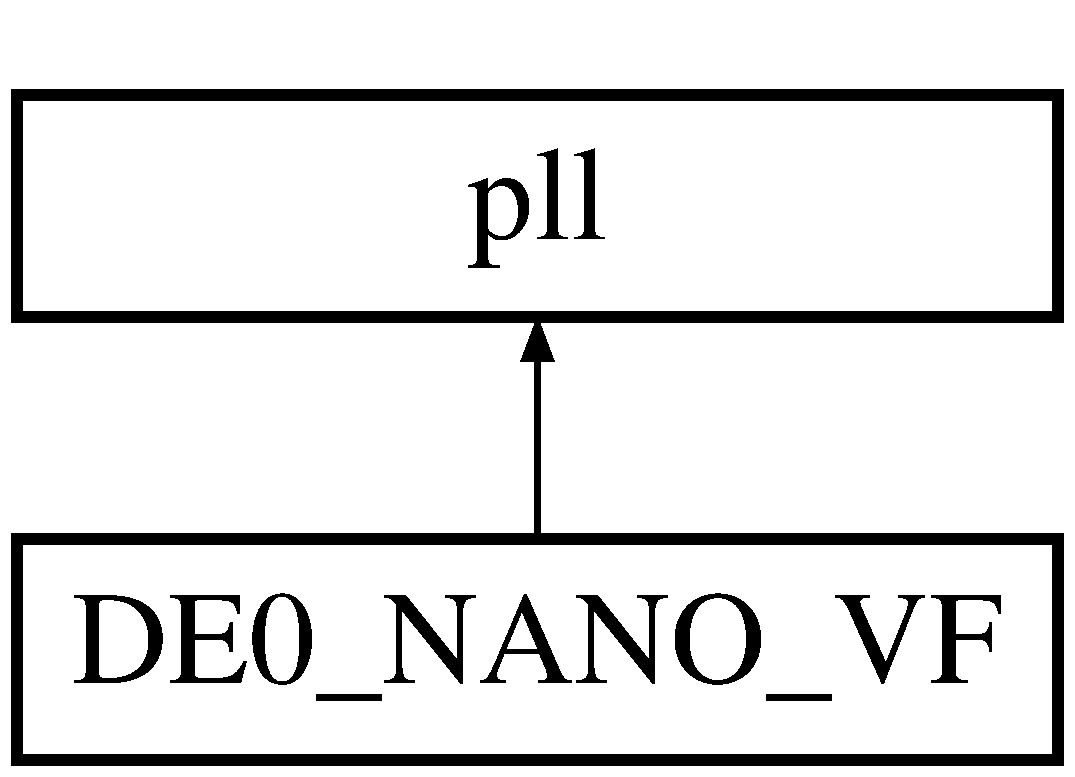
\includegraphics[height=2.000000cm]{classpll}
\end{center}
\end{figure}
\subsection*{Entities}
\begin{DoxyCompactItemize}
\item 
\hyperlink{classpll_1_1_s_y_n}{S\+Y\+N} architecture
\end{DoxyCompactItemize}
\subsection*{Libraries}
 \begin{DoxyCompactItemize}
\item 
\hyperlink{classpll_a0a6af6eef40212dbaf130d57ce711256}{ieee} 
\item 
\hyperlink{classpll_ad57cd8d31a38ff87ac163fb47757ffbf}{altera\+\_\+mf} 
\end{DoxyCompactItemize}
\subsection*{Use Clauses}
 \begin{DoxyCompactItemize}
\item 
\hyperlink{classpll_acd03516902501cd1c7296a98e22c6fcb}{std\+\_\+logic\+\_\+1164}   
\item 
\hyperlink{classpll_a470a86ce8776f637b0483eabf2d92ad2}{ all }   
\end{DoxyCompactItemize}
\subsection*{Ports}
 \begin{DoxyCompactItemize}
\item 
\hyperlink{classpll_a5ff6e3af321d94570fc485fa1bce5a06}{areset}  {\bfseries {\bfseries \textcolor{keywordflow}{in}\textcolor{vhdlchar}{ }}} {\bfseries \textcolor{comment}{S\+T\+D\+\_\+\+L\+O\+G\+I\+C}\textcolor{vhdlchar}{ }\textcolor{vhdlchar}{ }\textcolor{vhdlchar}{\+:}\textcolor{vhdlchar}{=}\textcolor{vhdlchar}{ }\textcolor{vhdlchar}{ }\textcolor{vhdlchar}{\textquotesingle{}}\textcolor{vhdlchar}{ } \textcolor{vhdldigit}{0} \textcolor{vhdlchar}{ }\textcolor{vhdlchar}{\textquotesingle{}}\textcolor{vhdlchar}{ }} 
\item 
\hyperlink{classpll_a9463f4cc62782c2faac516c942dcb5db}{inclk0}  {\bfseries {\bfseries \textcolor{keywordflow}{in}\textcolor{vhdlchar}{ }}} {\bfseries \textcolor{comment}{S\+T\+D\+\_\+\+L\+O\+G\+I\+C}\textcolor{vhdlchar}{ }\textcolor{vhdlchar}{ }\textcolor{vhdlchar}{\+:}\textcolor{vhdlchar}{=}\textcolor{vhdlchar}{ }\textcolor{vhdlchar}{ }\textcolor{vhdlchar}{\textquotesingle{}}\textcolor{vhdlchar}{ } \textcolor{vhdldigit}{0} \textcolor{vhdlchar}{ }\textcolor{vhdlchar}{\textquotesingle{}}\textcolor{vhdlchar}{ }} 
\item 
\hyperlink{classpll_abbf54d96b104435e8cbaadcf0e9184bd}{c0}  {\bfseries {\bfseries \textcolor{keywordflow}{out}\textcolor{vhdlchar}{ }}} {\bfseries \textcolor{comment}{S\+T\+D\+\_\+\+L\+O\+G\+I\+C}\textcolor{vhdlchar}{ }} 
\item 
\hyperlink{classpll_ab33e72e8245db404191648e9a25344eb}{locked}  {\bfseries {\bfseries \textcolor{keywordflow}{out}\textcolor{vhdlchar}{ }}} {\bfseries \textcolor{comment}{S\+T\+D\+\_\+\+L\+O\+G\+I\+C}\textcolor{vhdlchar}{ }} 
\end{DoxyCompactItemize}


\subsection{Detailed Description}


Definition at line \hyperlink{pll_8vhd_source_l00043}{43} of file \hyperlink{pll_8vhd_source}{pll.\+vhd}.



\subsection{Member Data Documentation}
\hypertarget{classpll_a470a86ce8776f637b0483eabf2d92ad2}{}\index{pll@{pll}! all @{ all }}
\index{ all @{ all }!pll@{pll}}
\subsubsection[{ all }]{\setlength{\rightskip}{0pt plus 5cm}{\bf  all }\hspace{0.3cm}{\ttfamily [Package]}}\label{classpll_a470a86ce8776f637b0483eabf2d92ad2}


Definition at line \hyperlink{pll_8vhd_source_l00041}{41} of file \hyperlink{pll_8vhd_source}{pll.\+vhd}.

\hypertarget{classpll_ad57cd8d31a38ff87ac163fb47757ffbf}{}\index{pll@{pll}!altera\+\_\+mf@{altera\+\_\+mf}}
\index{altera\+\_\+mf@{altera\+\_\+mf}!pll@{pll}}
\subsubsection[{altera\+\_\+mf}]{\setlength{\rightskip}{0pt plus 5cm}{\bf altera\+\_\+mf}\hspace{0.3cm}{\ttfamily [Library]}}\label{classpll_ad57cd8d31a38ff87ac163fb47757ffbf}


Definition at line \hyperlink{pll_8vhd_source_l00040}{40} of file \hyperlink{pll_8vhd_source}{pll.\+vhd}.

\hypertarget{classpll_a5ff6e3af321d94570fc485fa1bce5a06}{}\index{pll@{pll}!areset@{areset}}
\index{areset@{areset}!pll@{pll}}
\subsubsection[{areset}]{\setlength{\rightskip}{0pt plus 5cm}{\bf areset} {\bfseries \textcolor{keywordflow}{in}\textcolor{vhdlchar}{ }} {\bfseries \textcolor{comment}{S\+T\+D\+\_\+\+L\+O\+G\+I\+C}\textcolor{vhdlchar}{ }\textcolor{vhdlchar}{ }\textcolor{vhdlchar}{\+:}\textcolor{vhdlchar}{=}\textcolor{vhdlchar}{ }\textcolor{vhdlchar}{ }\textcolor{vhdlchar}{\textquotesingle{}}\textcolor{vhdlchar}{ } \textcolor{vhdldigit}{0} \textcolor{vhdlchar}{ }\textcolor{vhdlchar}{\textquotesingle{}}\textcolor{vhdlchar}{ }} \hspace{0.3cm}{\ttfamily [Port]}}\label{classpll_a5ff6e3af321d94570fc485fa1bce5a06}


Definition at line \hyperlink{pll_8vhd_source_l00046}{46} of file \hyperlink{pll_8vhd_source}{pll.\+vhd}.

\hypertarget{classpll_abbf54d96b104435e8cbaadcf0e9184bd}{}\index{pll@{pll}!c0@{c0}}
\index{c0@{c0}!pll@{pll}}
\subsubsection[{c0}]{\setlength{\rightskip}{0pt plus 5cm}{\bf c0} {\bfseries \textcolor{keywordflow}{out}\textcolor{vhdlchar}{ }} {\bfseries \textcolor{comment}{S\+T\+D\+\_\+\+L\+O\+G\+I\+C}\textcolor{vhdlchar}{ }} \hspace{0.3cm}{\ttfamily [Port]}}\label{classpll_abbf54d96b104435e8cbaadcf0e9184bd}


Definition at line \hyperlink{pll_8vhd_source_l00048}{48} of file \hyperlink{pll_8vhd_source}{pll.\+vhd}.

\hypertarget{classpll_a0a6af6eef40212dbaf130d57ce711256}{}\index{pll@{pll}!ieee@{ieee}}
\index{ieee@{ieee}!pll@{pll}}
\subsubsection[{ieee}]{\setlength{\rightskip}{0pt plus 5cm}{\bf ieee}\hspace{0.3cm}{\ttfamily [Library]}}\label{classpll_a0a6af6eef40212dbaf130d57ce711256}


Definition at line \hyperlink{pll_8vhd_source_l00037}{37} of file \hyperlink{pll_8vhd_source}{pll.\+vhd}.

\hypertarget{classpll_a9463f4cc62782c2faac516c942dcb5db}{}\index{pll@{pll}!inclk0@{inclk0}}
\index{inclk0@{inclk0}!pll@{pll}}
\subsubsection[{inclk0}]{\setlength{\rightskip}{0pt plus 5cm}{\bf inclk0} {\bfseries \textcolor{keywordflow}{in}\textcolor{vhdlchar}{ }} {\bfseries \textcolor{comment}{S\+T\+D\+\_\+\+L\+O\+G\+I\+C}\textcolor{vhdlchar}{ }\textcolor{vhdlchar}{ }\textcolor{vhdlchar}{\+:}\textcolor{vhdlchar}{=}\textcolor{vhdlchar}{ }\textcolor{vhdlchar}{ }\textcolor{vhdlchar}{\textquotesingle{}}\textcolor{vhdlchar}{ } \textcolor{vhdldigit}{0} \textcolor{vhdlchar}{ }\textcolor{vhdlchar}{\textquotesingle{}}\textcolor{vhdlchar}{ }} \hspace{0.3cm}{\ttfamily [Port]}}\label{classpll_a9463f4cc62782c2faac516c942dcb5db}


Definition at line \hyperlink{pll_8vhd_source_l00047}{47} of file \hyperlink{pll_8vhd_source}{pll.\+vhd}.

\hypertarget{classpll_ab33e72e8245db404191648e9a25344eb}{}\index{pll@{pll}!locked@{locked}}
\index{locked@{locked}!pll@{pll}}
\subsubsection[{locked}]{\setlength{\rightskip}{0pt plus 5cm}{\bf locked} {\bfseries \textcolor{keywordflow}{out}\textcolor{vhdlchar}{ }} {\bfseries \textcolor{comment}{S\+T\+D\+\_\+\+L\+O\+G\+I\+C}\textcolor{vhdlchar}{ }} \hspace{0.3cm}{\ttfamily [Port]}}\label{classpll_ab33e72e8245db404191648e9a25344eb}


Definition at line \hyperlink{pll_8vhd_source_l00050}{50} of file \hyperlink{pll_8vhd_source}{pll.\+vhd}.

\hypertarget{classpll_acd03516902501cd1c7296a98e22c6fcb}{}\index{pll@{pll}!std\+\_\+logic\+\_\+1164@{std\+\_\+logic\+\_\+1164}}
\index{std\+\_\+logic\+\_\+1164@{std\+\_\+logic\+\_\+1164}!pll@{pll}}
\subsubsection[{std\+\_\+logic\+\_\+1164}]{\setlength{\rightskip}{0pt plus 5cm}{\bf std\+\_\+logic\+\_\+1164}\hspace{0.3cm}{\ttfamily [Package]}}\label{classpll_acd03516902501cd1c7296a98e22c6fcb}


Definition at line \hyperlink{pll_8vhd_source_l00038}{38} of file \hyperlink{pll_8vhd_source}{pll.\+vhd}.



The documentation for this class was generated from the following file\+:\begin{DoxyCompactItemize}
\item 
\hyperlink{pll_8vhd}{pll.\+vhd}\end{DoxyCompactItemize}

\hypertarget{classportadora__tringular}{}\section{portadora\+\_\+tringular Entity Reference}
\label{classportadora__tringular}\index{portadora\+\_\+tringular@{portadora\+\_\+tringular}}
Inheritance diagram for portadora\+\_\+tringular\+:\begin{figure}[H]
\begin{center}
\leavevmode
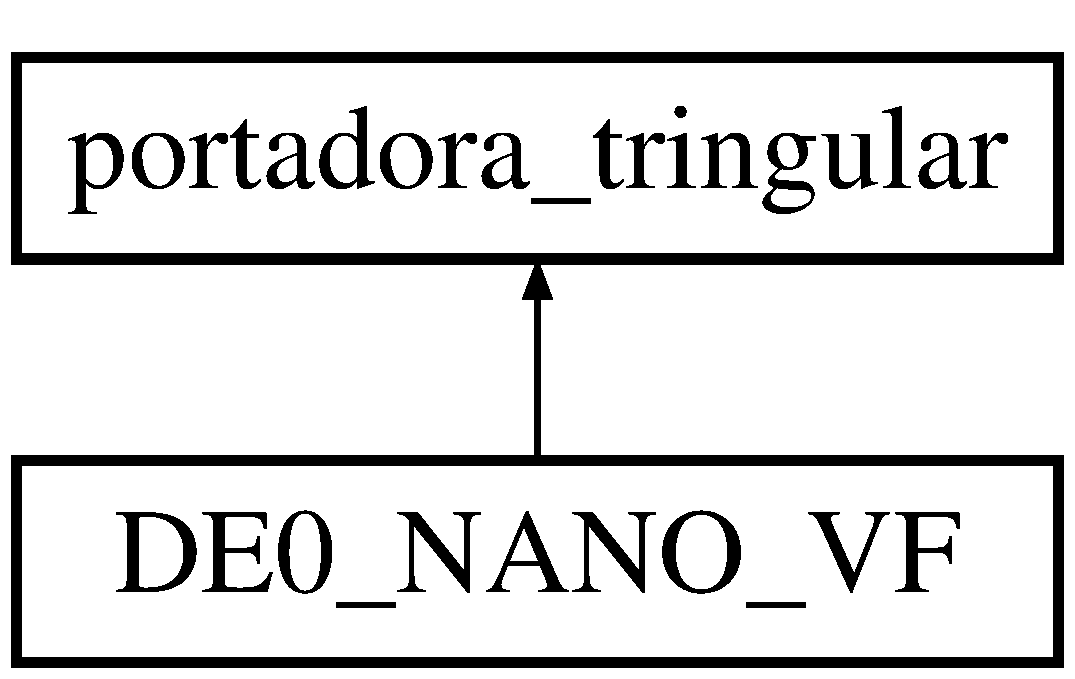
\includegraphics[height=2.000000cm]{classportadora__tringular}
\end{center}
\end{figure}
\subsection*{Entities}
\begin{DoxyCompactItemize}
\item 
\hyperlink{classportadora__tringular_1_1portadora__tringular}{portadora\+\_\+tringular} architecture
\end{DoxyCompactItemize}
\subsection*{Libraries}
 \begin{DoxyCompactItemize}
\item 
\hyperlink{classportadora__tringular_ae4f03c286607f3181e16b9aa12d0c6d4}{I\+E\+E\+E} 
\end{DoxyCompactItemize}
\subsection*{Use Clauses}
 \begin{DoxyCompactItemize}
\item 
\hyperlink{classportadora__tringular_a241c3e72dd8024cc8ae831b1b2aed7db}{S\+T\+D\+\_\+\+L\+O\+G\+I\+C\+\_\+\+U\+N\+S\+I\+G\+N\+E\+D}   
\item 
\hyperlink{classportadora__tringular_aa4b2b25246a821511120e3149b003563}{S\+T\+D\+\_\+\+L\+O\+G\+I\+C\+\_\+1164}   
\item 
\hyperlink{classportadora__tringular_aad86249c80e8c1e7ee1c4748aba748e3}{fixed\+\_\+pkg}   
\end{DoxyCompactItemize}
\subsection*{Generics}
 \begin{DoxyCompactItemize}
\item 
\hyperlink{classportadora__tringular_af8ee6f7e8fea0e211d86d8e3fd6f8d29}{N} {\bfseries {\bfseries \textcolor{comment}{integer}\textcolor{vhdlchar}{ }\textcolor{vhdlchar}{ }\textcolor{vhdlchar}{\+:}\textcolor{vhdlchar}{=}\textcolor{vhdlchar}{ }\textcolor{vhdlchar}{ } \textcolor{vhdldigit}{16} \textcolor{vhdlchar}{ }}}
\end{DoxyCompactItemize}
\subsection*{Ports}
 \begin{DoxyCompactItemize}
\item 
\hyperlink{classportadora__tringular_a4a4609c199d30b3adebbeb3a01276ec5}{clk}  {\bfseries {\bfseries \textcolor{keywordflow}{in}\textcolor{vhdlchar}{ }}} {\bfseries \textcolor{comment}{std\+\_\+logic}\textcolor{vhdlchar}{ }} 
\item 
\hyperlink{classportadora__tringular_adcf9c6f5161d039addbda5819bee64a3}{en}  {\bfseries {\bfseries \textcolor{keywordflow}{in}\textcolor{vhdlchar}{ }}} {\bfseries \textcolor{comment}{std\+\_\+logic}\textcolor{vhdlchar}{ }} 
\item 
\hyperlink{classportadora__tringular_aad8dc6359d9e23dabcbf342fadf2fa06}{reset}  {\bfseries {\bfseries \textcolor{keywordflow}{in}\textcolor{vhdlchar}{ }}} {\bfseries \textcolor{comment}{std\+\_\+logic}\textcolor{vhdlchar}{ }} 
\item 
\hyperlink{classportadora__tringular_ab3bb50450dbeb3852b4f76ef2aefbf9e}{count\+\_\+ini}  {\bfseries {\bfseries \textcolor{keywordflow}{in}\textcolor{vhdlchar}{ }}} {\bfseries \textcolor{comment}{std\+\_\+logic\+\_\+vector}\textcolor{vhdlchar}{ }\textcolor{vhdlchar}{(}\textcolor{vhdlchar}{ }\textcolor{vhdlchar}{ }\textcolor{vhdlchar}{ }\textcolor{vhdlchar}{ }{\bfseries \hyperlink{classportadora__tringular_af8ee6f7e8fea0e211d86d8e3fd6f8d29}{N}} \textcolor{vhdlchar}{-\/}\textcolor{vhdlchar}{ } \textcolor{vhdldigit}{1} \textcolor{vhdlchar}{ }\textcolor{keywordflow}{downto}\textcolor{vhdlchar}{ }\textcolor{vhdlchar}{ } \textcolor{vhdldigit}{0} \textcolor{vhdlchar}{ }\textcolor{vhdlchar}{)}\textcolor{vhdlchar}{ }} 
\item 
\hyperlink{classportadora__tringular_ac855daed6a8d1b25a13c5d5b4aa46c3e}{dir\+\_\+ini}  {\bfseries {\bfseries \textcolor{keywordflow}{in}\textcolor{vhdlchar}{ }}} {\bfseries \textcolor{comment}{std\+\_\+logic}\textcolor{vhdlchar}{ }} 
\item 
\hyperlink{classportadora__tringular_a06de1330d80ce7a764361167217baf42}{M\+A\+X}  {\bfseries {\bfseries \textcolor{keywordflow}{in}\textcolor{vhdlchar}{ }}} {\bfseries \textcolor{comment}{std\+\_\+logic\+\_\+vector}\textcolor{vhdlchar}{ }\textcolor{vhdlchar}{(}\textcolor{vhdlchar}{ }\textcolor{vhdlchar}{ }\textcolor{vhdlchar}{ }\textcolor{vhdlchar}{ }{\bfseries \hyperlink{classportadora__tringular_af8ee6f7e8fea0e211d86d8e3fd6f8d29}{N}} \textcolor{vhdlchar}{-\/}\textcolor{vhdlchar}{ } \textcolor{vhdldigit}{1} \textcolor{vhdlchar}{ }\textcolor{keywordflow}{downto}\textcolor{vhdlchar}{ }\textcolor{vhdlchar}{ } \textcolor{vhdldigit}{0} \textcolor{vhdlchar}{ }\textcolor{vhdlchar}{)}\textcolor{vhdlchar}{ }} 
\item 
\hyperlink{classportadora__tringular_a8fb21bca6cb529fd30fa4b1f8b156237}{dir}  {\bfseries {\bfseries \textcolor{keywordflow}{out}\textcolor{vhdlchar}{ }}} {\bfseries \textcolor{comment}{std\+\_\+logic}\textcolor{vhdlchar}{ }} 
\item 
\hyperlink{classportadora__tringular_a54ed3cc1c7433faf63dbf6b009fe8137}{c}  {\bfseries {\bfseries \textcolor{keywordflow}{out}\textcolor{vhdlchar}{ }}} {\bfseries \textcolor{comment}{std\+\_\+logic\+\_\+vector}\textcolor{vhdlchar}{ }\textcolor{vhdlchar}{(}\textcolor{vhdlchar}{ }\textcolor{vhdlchar}{ }\textcolor{vhdlchar}{ }\textcolor{vhdlchar}{ }{\bfseries \hyperlink{classportadora__tringular_af8ee6f7e8fea0e211d86d8e3fd6f8d29}{N}} \textcolor{vhdlchar}{-\/}\textcolor{vhdlchar}{ } \textcolor{vhdldigit}{1} \textcolor{vhdlchar}{ }\textcolor{keywordflow}{downto}\textcolor{vhdlchar}{ }\textcolor{vhdlchar}{ } \textcolor{vhdldigit}{0} \textcolor{vhdlchar}{ }\textcolor{vhdlchar}{)}\textcolor{vhdlchar}{ }} 
\end{DoxyCompactItemize}


\subsection{Detailed Description}


Definition at line 6 of file portadora\+\_\+tringular.\+vhd.



\subsection{Member Data Documentation}
\hypertarget{classportadora__tringular_a54ed3cc1c7433faf63dbf6b009fe8137}{}\index{portadora\+\_\+tringular@{portadora\+\_\+tringular}!c@{c}}
\index{c@{c}!portadora\+\_\+tringular@{portadora\+\_\+tringular}}
\subsubsection[{c}]{\setlength{\rightskip}{0pt plus 5cm}{\bf c} {\bfseries \textcolor{keywordflow}{out}\textcolor{vhdlchar}{ }} {\bfseries \textcolor{comment}{std\+\_\+logic\+\_\+vector}\textcolor{vhdlchar}{ }\textcolor{vhdlchar}{(}\textcolor{vhdlchar}{ }\textcolor{vhdlchar}{ }\textcolor{vhdlchar}{ }\textcolor{vhdlchar}{ }{\bfseries {\bf N}} \textcolor{vhdlchar}{-\/}\textcolor{vhdlchar}{ } \textcolor{vhdldigit}{1} \textcolor{vhdlchar}{ }\textcolor{keywordflow}{downto}\textcolor{vhdlchar}{ }\textcolor{vhdlchar}{ } \textcolor{vhdldigit}{0} \textcolor{vhdlchar}{ }\textcolor{vhdlchar}{)}\textcolor{vhdlchar}{ }} \hspace{0.3cm}{\ttfamily [Port]}}\label{classportadora__tringular_a54ed3cc1c7433faf63dbf6b009fe8137}


Definition at line 18 of file portadora\+\_\+tringular.\+vhd.

\hypertarget{classportadora__tringular_a4a4609c199d30b3adebbeb3a01276ec5}{}\index{portadora\+\_\+tringular@{portadora\+\_\+tringular}!clk@{clk}}
\index{clk@{clk}!portadora\+\_\+tringular@{portadora\+\_\+tringular}}
\subsubsection[{clk}]{\setlength{\rightskip}{0pt plus 5cm}{\bf clk} {\bfseries \textcolor{keywordflow}{in}\textcolor{vhdlchar}{ }} {\bfseries \textcolor{comment}{std\+\_\+logic}\textcolor{vhdlchar}{ }} \hspace{0.3cm}{\ttfamily [Port]}}\label{classportadora__tringular_a4a4609c199d30b3adebbeb3a01276ec5}


Definition at line 10 of file portadora\+\_\+tringular.\+vhd.

\hypertarget{classportadora__tringular_ab3bb50450dbeb3852b4f76ef2aefbf9e}{}\index{portadora\+\_\+tringular@{portadora\+\_\+tringular}!count\+\_\+ini@{count\+\_\+ini}}
\index{count\+\_\+ini@{count\+\_\+ini}!portadora\+\_\+tringular@{portadora\+\_\+tringular}}
\subsubsection[{count\+\_\+ini}]{\setlength{\rightskip}{0pt plus 5cm}{\bf count\+\_\+ini} {\bfseries \textcolor{keywordflow}{in}\textcolor{vhdlchar}{ }} {\bfseries \textcolor{comment}{std\+\_\+logic\+\_\+vector}\textcolor{vhdlchar}{ }\textcolor{vhdlchar}{(}\textcolor{vhdlchar}{ }\textcolor{vhdlchar}{ }\textcolor{vhdlchar}{ }\textcolor{vhdlchar}{ }{\bfseries {\bf N}} \textcolor{vhdlchar}{-\/}\textcolor{vhdlchar}{ } \textcolor{vhdldigit}{1} \textcolor{vhdlchar}{ }\textcolor{keywordflow}{downto}\textcolor{vhdlchar}{ }\textcolor{vhdlchar}{ } \textcolor{vhdldigit}{0} \textcolor{vhdlchar}{ }\textcolor{vhdlchar}{)}\textcolor{vhdlchar}{ }} \hspace{0.3cm}{\ttfamily [Port]}}\label{classportadora__tringular_ab3bb50450dbeb3852b4f76ef2aefbf9e}


Definition at line 13 of file portadora\+\_\+tringular.\+vhd.

\hypertarget{classportadora__tringular_a8fb21bca6cb529fd30fa4b1f8b156237}{}\index{portadora\+\_\+tringular@{portadora\+\_\+tringular}!dir@{dir}}
\index{dir@{dir}!portadora\+\_\+tringular@{portadora\+\_\+tringular}}
\subsubsection[{dir}]{\setlength{\rightskip}{0pt plus 5cm}{\bf dir} {\bfseries \textcolor{keywordflow}{out}\textcolor{vhdlchar}{ }} {\bfseries \textcolor{comment}{std\+\_\+logic}\textcolor{vhdlchar}{ }} \hspace{0.3cm}{\ttfamily [Port]}}\label{classportadora__tringular_a8fb21bca6cb529fd30fa4b1f8b156237}


Definition at line 16 of file portadora\+\_\+tringular.\+vhd.

\hypertarget{classportadora__tringular_ac855daed6a8d1b25a13c5d5b4aa46c3e}{}\index{portadora\+\_\+tringular@{portadora\+\_\+tringular}!dir\+\_\+ini@{dir\+\_\+ini}}
\index{dir\+\_\+ini@{dir\+\_\+ini}!portadora\+\_\+tringular@{portadora\+\_\+tringular}}
\subsubsection[{dir\+\_\+ini}]{\setlength{\rightskip}{0pt plus 5cm}{\bf dir\+\_\+ini} {\bfseries \textcolor{keywordflow}{in}\textcolor{vhdlchar}{ }} {\bfseries \textcolor{comment}{std\+\_\+logic}\textcolor{vhdlchar}{ }} \hspace{0.3cm}{\ttfamily [Port]}}\label{classportadora__tringular_ac855daed6a8d1b25a13c5d5b4aa46c3e}


Definition at line 14 of file portadora\+\_\+tringular.\+vhd.

\hypertarget{classportadora__tringular_adcf9c6f5161d039addbda5819bee64a3}{}\index{portadora\+\_\+tringular@{portadora\+\_\+tringular}!en@{en}}
\index{en@{en}!portadora\+\_\+tringular@{portadora\+\_\+tringular}}
\subsubsection[{en}]{\setlength{\rightskip}{0pt plus 5cm}{\bf en} {\bfseries \textcolor{keywordflow}{in}\textcolor{vhdlchar}{ }} {\bfseries \textcolor{comment}{std\+\_\+logic}\textcolor{vhdlchar}{ }} \hspace{0.3cm}{\ttfamily [Port]}}\label{classportadora__tringular_adcf9c6f5161d039addbda5819bee64a3}


Definition at line 11 of file portadora\+\_\+tringular.\+vhd.

\hypertarget{classportadora__tringular_aad86249c80e8c1e7ee1c4748aba748e3}{}\index{portadora\+\_\+tringular@{portadora\+\_\+tringular}!fixed\+\_\+pkg@{fixed\+\_\+pkg}}
\index{fixed\+\_\+pkg@{fixed\+\_\+pkg}!portadora\+\_\+tringular@{portadora\+\_\+tringular}}
\subsubsection[{fixed\+\_\+pkg}]{\setlength{\rightskip}{0pt plus 5cm}{\bf fixed\+\_\+pkg}\hspace{0.3cm}{\ttfamily [Package]}}\label{classportadora__tringular_aad86249c80e8c1e7ee1c4748aba748e3}


Definition at line 4 of file portadora\+\_\+tringular.\+vhd.

\hypertarget{classportadora__tringular_ae4f03c286607f3181e16b9aa12d0c6d4}{}\index{portadora\+\_\+tringular@{portadora\+\_\+tringular}!I\+E\+E\+E@{I\+E\+E\+E}}
\index{I\+E\+E\+E@{I\+E\+E\+E}!portadora\+\_\+tringular@{portadora\+\_\+tringular}}
\subsubsection[{I\+E\+E\+E}]{\setlength{\rightskip}{0pt plus 5cm}{\bf I\+E\+E\+E}\hspace{0.3cm}{\ttfamily [Library]}}\label{classportadora__tringular_ae4f03c286607f3181e16b9aa12d0c6d4}


Definition at line 1 of file portadora\+\_\+tringular.\+vhd.

\hypertarget{classportadora__tringular_a06de1330d80ce7a764361167217baf42}{}\index{portadora\+\_\+tringular@{portadora\+\_\+tringular}!M\+A\+X@{M\+A\+X}}
\index{M\+A\+X@{M\+A\+X}!portadora\+\_\+tringular@{portadora\+\_\+tringular}}
\subsubsection[{M\+A\+X}]{\setlength{\rightskip}{0pt plus 5cm}{\bf M\+A\+X} {\bfseries \textcolor{keywordflow}{in}\textcolor{vhdlchar}{ }} {\bfseries \textcolor{comment}{std\+\_\+logic\+\_\+vector}\textcolor{vhdlchar}{ }\textcolor{vhdlchar}{(}\textcolor{vhdlchar}{ }\textcolor{vhdlchar}{ }\textcolor{vhdlchar}{ }\textcolor{vhdlchar}{ }{\bfseries {\bf N}} \textcolor{vhdlchar}{-\/}\textcolor{vhdlchar}{ } \textcolor{vhdldigit}{1} \textcolor{vhdlchar}{ }\textcolor{keywordflow}{downto}\textcolor{vhdlchar}{ }\textcolor{vhdlchar}{ } \textcolor{vhdldigit}{0} \textcolor{vhdlchar}{ }\textcolor{vhdlchar}{)}\textcolor{vhdlchar}{ }} \hspace{0.3cm}{\ttfamily [Port]}}\label{classportadora__tringular_a06de1330d80ce7a764361167217baf42}


Definition at line 15 of file portadora\+\_\+tringular.\+vhd.

\hypertarget{classportadora__tringular_af8ee6f7e8fea0e211d86d8e3fd6f8d29}{}\index{portadora\+\_\+tringular@{portadora\+\_\+tringular}!N@{N}}
\index{N@{N}!portadora\+\_\+tringular@{portadora\+\_\+tringular}}
\subsubsection[{N}]{\setlength{\rightskip}{0pt plus 5cm}{\bf N} {\bfseries \textcolor{vhdlchar}{ }} {\bfseries \textcolor{comment}{integer}\textcolor{vhdlchar}{ }\textcolor{vhdlchar}{ }\textcolor{vhdlchar}{\+:}\textcolor{vhdlchar}{=}\textcolor{vhdlchar}{ }\textcolor{vhdlchar}{ } \textcolor{vhdldigit}{16} \textcolor{vhdlchar}{ }} \hspace{0.3cm}{\ttfamily [Generic]}}\label{classportadora__tringular_af8ee6f7e8fea0e211d86d8e3fd6f8d29}


Definition at line 8 of file portadora\+\_\+tringular.\+vhd.

\hypertarget{classportadora__tringular_aad8dc6359d9e23dabcbf342fadf2fa06}{}\index{portadora\+\_\+tringular@{portadora\+\_\+tringular}!reset@{reset}}
\index{reset@{reset}!portadora\+\_\+tringular@{portadora\+\_\+tringular}}
\subsubsection[{reset}]{\setlength{\rightskip}{0pt plus 5cm}{\bf reset} {\bfseries \textcolor{keywordflow}{in}\textcolor{vhdlchar}{ }} {\bfseries \textcolor{comment}{std\+\_\+logic}\textcolor{vhdlchar}{ }} \hspace{0.3cm}{\ttfamily [Port]}}\label{classportadora__tringular_aad8dc6359d9e23dabcbf342fadf2fa06}


Definition at line 12 of file portadora\+\_\+tringular.\+vhd.

\hypertarget{classportadora__tringular_aa4b2b25246a821511120e3149b003563}{}\index{portadora\+\_\+tringular@{portadora\+\_\+tringular}!S\+T\+D\+\_\+\+L\+O\+G\+I\+C\+\_\+1164@{S\+T\+D\+\_\+\+L\+O\+G\+I\+C\+\_\+1164}}
\index{S\+T\+D\+\_\+\+L\+O\+G\+I\+C\+\_\+1164@{S\+T\+D\+\_\+\+L\+O\+G\+I\+C\+\_\+1164}!portadora\+\_\+tringular@{portadora\+\_\+tringular}}
\subsubsection[{S\+T\+D\+\_\+\+L\+O\+G\+I\+C\+\_\+1164}]{\setlength{\rightskip}{0pt plus 5cm}{\bf S\+T\+D\+\_\+\+L\+O\+G\+I\+C\+\_\+1164}\hspace{0.3cm}{\ttfamily [Package]}}\label{classportadora__tringular_aa4b2b25246a821511120e3149b003563}


Definition at line 3 of file portadora\+\_\+tringular.\+vhd.

\hypertarget{classportadora__tringular_a241c3e72dd8024cc8ae831b1b2aed7db}{}\index{portadora\+\_\+tringular@{portadora\+\_\+tringular}!S\+T\+D\+\_\+\+L\+O\+G\+I\+C\+\_\+\+U\+N\+S\+I\+G\+N\+E\+D@{S\+T\+D\+\_\+\+L\+O\+G\+I\+C\+\_\+\+U\+N\+S\+I\+G\+N\+E\+D}}
\index{S\+T\+D\+\_\+\+L\+O\+G\+I\+C\+\_\+\+U\+N\+S\+I\+G\+N\+E\+D@{S\+T\+D\+\_\+\+L\+O\+G\+I\+C\+\_\+\+U\+N\+S\+I\+G\+N\+E\+D}!portadora\+\_\+tringular@{portadora\+\_\+tringular}}
\subsubsection[{S\+T\+D\+\_\+\+L\+O\+G\+I\+C\+\_\+\+U\+N\+S\+I\+G\+N\+E\+D}]{\setlength{\rightskip}{0pt plus 5cm}{\bf S\+T\+D\+\_\+\+L\+O\+G\+I\+C\+\_\+\+U\+N\+S\+I\+G\+N\+E\+D}\hspace{0.3cm}{\ttfamily [Package]}}\label{classportadora__tringular_a241c3e72dd8024cc8ae831b1b2aed7db}


Definition at line 2 of file portadora\+\_\+tringular.\+vhd.



The documentation for this class was generated from the following file\+:\begin{DoxyCompactItemize}
\item 
\hyperlink{portadora__tringular_8vhd}{portadora\+\_\+tringular.\+vhd}\end{DoxyCompactItemize}

\hypertarget{classportadora__tringular_1_1portadora__tringular}{}\section{portadora\+\_\+tringular Architecture Reference}
\label{classportadora__tringular_1_1portadora__tringular}\index{portadora\+\_\+tringular@{portadora\+\_\+tringular}}
\subsection*{Processes}
 \begin{DoxyCompactItemize}
\item 
\hyperlink{classportadora__tringular_1_1portadora__tringular_a9d3814991b9352ab295cc62784226977}{P\+R\+O\+C\+E\+S\+S\+\_\+12}{\bfseries  ( {\bfseries {\bfseries \hyperlink{classportadora__tringular_a4a4609c199d30b3adebbeb3a01276ec5}{clk}} \textcolor{vhdlchar}{ }} )}
\end{DoxyCompactItemize}
\subsection*{Signals}
 \begin{DoxyCompactItemize}
\item 
\hyperlink{classportadora__tringular_1_1portadora__tringular_ae3b6c46c82d8260487d5f5291a70a96a}{c\+\_\+int} {\bfseries \textcolor{comment}{std\+\_\+logic\+\_\+vector}\textcolor{vhdlchar}{ }\textcolor{vhdlchar}{(}\textcolor{vhdlchar}{ }\textcolor{vhdlchar}{ }\textcolor{vhdlchar}{ }\textcolor{vhdlchar}{ }{\bfseries \hyperlink{classportadora__tringular_af8ee6f7e8fea0e211d86d8e3fd6f8d29}{N}} \textcolor{vhdlchar}{-\/}\textcolor{vhdlchar}{ } \textcolor{vhdldigit}{1} \textcolor{vhdlchar}{ }\textcolor{keywordflow}{downto}\textcolor{vhdlchar}{ }\textcolor{vhdlchar}{ } \textcolor{vhdldigit}{0} \textcolor{vhdlchar}{ }\textcolor{vhdlchar}{)}\textcolor{vhdlchar}{ }} 
\item 
\hyperlink{classportadora__tringular_1_1portadora__tringular_ae27566c74fe97a2b3c215e94dc35dd47}{dir\+\_\+int} {\bfseries \textcolor{comment}{std\+\_\+logic}\textcolor{vhdlchar}{ }} 
\end{DoxyCompactItemize}


\subsection{Detailed Description}


Definition at line \hyperlink{portadora__tringular_8vhd_source_l00023}{23} of file \hyperlink{portadora__tringular_8vhd_source}{portadora\+\_\+tringular.\+vhd}.



\subsection{Member Function Documentation}
\hypertarget{classportadora__tringular_1_1portadora__tringular_a9d3814991b9352ab295cc62784226977}{}\index{portadora\+\_\+tringular\+::portadora\+\_\+tringular@{portadora\+\_\+tringular\+::portadora\+\_\+tringular}!P\+R\+O\+C\+E\+S\+S\+\_\+12@{P\+R\+O\+C\+E\+S\+S\+\_\+12}}
\index{P\+R\+O\+C\+E\+S\+S\+\_\+12@{P\+R\+O\+C\+E\+S\+S\+\_\+12}!portadora\+\_\+tringular\+::portadora\+\_\+tringular@{portadora\+\_\+tringular\+::portadora\+\_\+tringular}}
\subsubsection[{P\+R\+O\+C\+E\+S\+S\+\_\+12}]{\setlength{\rightskip}{0pt plus 5cm} {\bfseries \textcolor{vhdlchar}{ }} P\+R\+O\+C\+E\+S\+S\+\_\+12(
\begin{DoxyParamCaption}
\item[{}]{{\bfseries {\bfseries {\bf clk}} \textcolor{vhdlchar}{ }} {\em }}
\end{DoxyParamCaption}
)\hspace{0.3cm}{\ttfamily [Process]}}\label{classportadora__tringular_1_1portadora__tringular_a9d3814991b9352ab295cc62784226977}


Definition at line \hyperlink{portadora__tringular_8vhd_source_l00031}{31} of file \hyperlink{portadora__tringular_8vhd_source}{portadora\+\_\+tringular.\+vhd}.



\subsection{Member Data Documentation}
\hypertarget{classportadora__tringular_1_1portadora__tringular_ae3b6c46c82d8260487d5f5291a70a96a}{}\index{portadora\+\_\+tringular\+::portadora\+\_\+tringular@{portadora\+\_\+tringular\+::portadora\+\_\+tringular}!c\+\_\+int@{c\+\_\+int}}
\index{c\+\_\+int@{c\+\_\+int}!portadora\+\_\+tringular\+::portadora\+\_\+tringular@{portadora\+\_\+tringular\+::portadora\+\_\+tringular}}
\subsubsection[{c\+\_\+int}]{\setlength{\rightskip}{0pt plus 5cm}{\bf c\+\_\+int} {\bfseries \textcolor{comment}{std\+\_\+logic\+\_\+vector}\textcolor{vhdlchar}{ }\textcolor{vhdlchar}{(}\textcolor{vhdlchar}{ }\textcolor{vhdlchar}{ }\textcolor{vhdlchar}{ }\textcolor{vhdlchar}{ }{\bfseries {\bf N}} \textcolor{vhdlchar}{-\/}\textcolor{vhdlchar}{ } \textcolor{vhdldigit}{1} \textcolor{vhdlchar}{ }\textcolor{keywordflow}{downto}\textcolor{vhdlchar}{ }\textcolor{vhdlchar}{ } \textcolor{vhdldigit}{0} \textcolor{vhdlchar}{ }\textcolor{vhdlchar}{)}\textcolor{vhdlchar}{ }} \hspace{0.3cm}{\ttfamily [Signal]}}\label{classportadora__tringular_1_1portadora__tringular_ae3b6c46c82d8260487d5f5291a70a96a}


Definition at line \hyperlink{portadora__tringular_8vhd_source_l00025}{25} of file \hyperlink{portadora__tringular_8vhd_source}{portadora\+\_\+tringular.\+vhd}.

\hypertarget{classportadora__tringular_1_1portadora__tringular_ae27566c74fe97a2b3c215e94dc35dd47}{}\index{portadora\+\_\+tringular\+::portadora\+\_\+tringular@{portadora\+\_\+tringular\+::portadora\+\_\+tringular}!dir\+\_\+int@{dir\+\_\+int}}
\index{dir\+\_\+int@{dir\+\_\+int}!portadora\+\_\+tringular\+::portadora\+\_\+tringular@{portadora\+\_\+tringular\+::portadora\+\_\+tringular}}
\subsubsection[{dir\+\_\+int}]{\setlength{\rightskip}{0pt plus 5cm}{\bf dir\+\_\+int} {\bfseries \textcolor{comment}{std\+\_\+logic}\textcolor{vhdlchar}{ }} \hspace{0.3cm}{\ttfamily [Signal]}}\label{classportadora__tringular_1_1portadora__tringular_ae27566c74fe97a2b3c215e94dc35dd47}


Definition at line \hyperlink{portadora__tringular_8vhd_source_l00026}{26} of file \hyperlink{portadora__tringular_8vhd_source}{portadora\+\_\+tringular.\+vhd}.



The documentation for this class was generated from the following file\+:\begin{DoxyCompactItemize}
\item 
\hyperlink{portadora__tringular_8vhd}{portadora\+\_\+tringular.\+vhd}\end{DoxyCompactItemize}

\hypertarget{classsinewave}{}\section{sinewave Entity Reference}
\label{classsinewave}\index{sinewave@{sinewave}}
\subsection*{Entities}
\begin{DoxyCompactItemize}
\item 
\hyperlink{classsinewave_1_1_behavioral}{Behavioral} architecture
\end{DoxyCompactItemize}
\subsection*{Libraries}
 \begin{DoxyCompactItemize}
\item 
\hyperlink{classsinewave_ae4f03c286607f3181e16b9aa12d0c6d4}{I\+E\+E\+E} 
\end{DoxyCompactItemize}
\subsection*{Use Clauses}
 \begin{DoxyCompactItemize}
\item 
\hyperlink{classsinewave_aa4b2b25246a821511120e3149b003563}{S\+T\+D\+\_\+\+L\+O\+G\+I\+C\+\_\+1164}   
\item 
\hyperlink{classsinewave_ae00f3f04545af57582ff10609eee23e2}{N\+U\+M\+E\+R\+I\+C\+\_\+\+S\+T\+D}   
\end{DoxyCompactItemize}
\subsection*{Ports}
 \begin{DoxyCompactItemize}
\item 
\hyperlink{classsinewave_a4a4609c199d30b3adebbeb3a01276ec5}{clk}  {\bfseries {\bfseries \textcolor{keywordflow}{in}\textcolor{vhdlchar}{ }}} {\bfseries \textcolor{comment}{std\+\_\+logic}\textcolor{vhdlchar}{ }} 
\item 
\hyperlink{classsinewave_a6f923bb55dbbef4e48f6ae28e0588faf}{dataout}  {\bfseries {\bfseries \textcolor{keywordflow}{out}\textcolor{vhdlchar}{ }}} {\bfseries \textcolor{comment}{integer}\textcolor{vhdlchar}{ }\textcolor{vhdlchar}{ }\textcolor{vhdlchar}{ }\textcolor{keywordflow}{range}\textcolor{vhdlchar}{ }\textcolor{vhdlchar}{-\/}\textcolor{vhdlchar}{ } \textcolor{vhdldigit}{128} \textcolor{vhdlchar}{ }\textcolor{keywordflow}{to}\textcolor{vhdlchar}{ }\textcolor{vhdlchar}{ } \textcolor{vhdldigit}{127} \textcolor{vhdlchar}{ }} 
\end{DoxyCompactItemize}


\subsection{Detailed Description}


Definition at line \hyperlink{sinewave_8vhd_source_l00006}{6} of file \hyperlink{sinewave_8vhd_source}{sinewave.\+vhd}.



\subsection{Member Data Documentation}
\hypertarget{classsinewave_a4a4609c199d30b3adebbeb3a01276ec5}{}\index{sinewave@{sinewave}!clk@{clk}}
\index{clk@{clk}!sinewave@{sinewave}}
\subsubsection[{clk}]{\setlength{\rightskip}{0pt plus 5cm}{\bf clk} {\bfseries \textcolor{keywordflow}{in}\textcolor{vhdlchar}{ }} {\bfseries \textcolor{comment}{std\+\_\+logic}\textcolor{vhdlchar}{ }} \hspace{0.3cm}{\ttfamily [Port]}}\label{classsinewave_a4a4609c199d30b3adebbeb3a01276ec5}


Definition at line \hyperlink{sinewave_8vhd_source_l00007}{7} of file \hyperlink{sinewave_8vhd_source}{sinewave.\+vhd}.

\hypertarget{classsinewave_a6f923bb55dbbef4e48f6ae28e0588faf}{}\index{sinewave@{sinewave}!dataout@{dataout}}
\index{dataout@{dataout}!sinewave@{sinewave}}
\subsubsection[{dataout}]{\setlength{\rightskip}{0pt plus 5cm}{\bf dataout} {\bfseries \textcolor{keywordflow}{out}\textcolor{vhdlchar}{ }} {\bfseries \textcolor{comment}{integer}\textcolor{vhdlchar}{ }\textcolor{vhdlchar}{ }\textcolor{vhdlchar}{ }\textcolor{keywordflow}{range}\textcolor{vhdlchar}{ }\textcolor{vhdlchar}{-\/}\textcolor{vhdlchar}{ } \textcolor{vhdldigit}{128} \textcolor{vhdlchar}{ }\textcolor{keywordflow}{to}\textcolor{vhdlchar}{ }\textcolor{vhdlchar}{ } \textcolor{vhdldigit}{127} \textcolor{vhdlchar}{ }} \hspace{0.3cm}{\ttfamily [Port]}}\label{classsinewave_a6f923bb55dbbef4e48f6ae28e0588faf}


Definition at line \hyperlink{sinewave_8vhd_source_l00009}{9} of file \hyperlink{sinewave_8vhd_source}{sinewave.\+vhd}.

\hypertarget{classsinewave_ae4f03c286607f3181e16b9aa12d0c6d4}{}\index{sinewave@{sinewave}!I\+E\+E\+E@{I\+E\+E\+E}}
\index{I\+E\+E\+E@{I\+E\+E\+E}!sinewave@{sinewave}}
\subsubsection[{I\+E\+E\+E}]{\setlength{\rightskip}{0pt plus 5cm}{\bf I\+E\+E\+E}\hspace{0.3cm}{\ttfamily [Library]}}\label{classsinewave_ae4f03c286607f3181e16b9aa12d0c6d4}


Definition at line \hyperlink{sinewave_8vhd_source_l00002}{2} of file \hyperlink{sinewave_8vhd_source}{sinewave.\+vhd}.

\hypertarget{classsinewave_ae00f3f04545af57582ff10609eee23e2}{}\index{sinewave@{sinewave}!N\+U\+M\+E\+R\+I\+C\+\_\+\+S\+T\+D@{N\+U\+M\+E\+R\+I\+C\+\_\+\+S\+T\+D}}
\index{N\+U\+M\+E\+R\+I\+C\+\_\+\+S\+T\+D@{N\+U\+M\+E\+R\+I\+C\+\_\+\+S\+T\+D}!sinewave@{sinewave}}
\subsubsection[{N\+U\+M\+E\+R\+I\+C\+\_\+\+S\+T\+D}]{\setlength{\rightskip}{0pt plus 5cm}{\bf N\+U\+M\+E\+R\+I\+C\+\_\+\+S\+T\+D}\hspace{0.3cm}{\ttfamily [Package]}}\label{classsinewave_ae00f3f04545af57582ff10609eee23e2}


Definition at line \hyperlink{sinewave_8vhd_source_l00004}{4} of file \hyperlink{sinewave_8vhd_source}{sinewave.\+vhd}.

\hypertarget{classsinewave_aa4b2b25246a821511120e3149b003563}{}\index{sinewave@{sinewave}!S\+T\+D\+\_\+\+L\+O\+G\+I\+C\+\_\+1164@{S\+T\+D\+\_\+\+L\+O\+G\+I\+C\+\_\+1164}}
\index{S\+T\+D\+\_\+\+L\+O\+G\+I\+C\+\_\+1164@{S\+T\+D\+\_\+\+L\+O\+G\+I\+C\+\_\+1164}!sinewave@{sinewave}}
\subsubsection[{S\+T\+D\+\_\+\+L\+O\+G\+I\+C\+\_\+1164}]{\setlength{\rightskip}{0pt plus 5cm}{\bf S\+T\+D\+\_\+\+L\+O\+G\+I\+C\+\_\+1164}\hspace{0.3cm}{\ttfamily [Package]}}\label{classsinewave_aa4b2b25246a821511120e3149b003563}


Definition at line \hyperlink{sinewave_8vhd_source_l00003}{3} of file \hyperlink{sinewave_8vhd_source}{sinewave.\+vhd}.



The documentation for this class was generated from the following file\+:\begin{DoxyCompactItemize}
\item 
\hyperlink{sinewave_8vhd}{sinewave.\+vhd}\end{DoxyCompactItemize}

\hypertarget{classpll_1_1_s_y_n}{}\section{S\+Y\+N Architecture Reference}
\label{classpll_1_1_s_y_n}\index{S\+Y\+N@{S\+Y\+N}}
\subsection*{Components}
 \begin{DoxyCompactItemize}
\item 
\hyperlink{classpll_1_1_s_y_n_ad45c11bbc2e898d68e19fa2eb5ba73d5}{altpll}  {\bfseries }  
\end{DoxyCompactItemize}
\subsection*{Signals}
 \begin{DoxyCompactItemize}
\item 
\hyperlink{classpll_1_1_s_y_n_aca40f2d2e88330e7729fc8f89d1e2366}{sub\+\_\+wire0} {\bfseries \textcolor{comment}{S\+T\+D\+\_\+\+L\+O\+G\+I\+C}\textcolor{vhdlchar}{ }} 
\item 
\hyperlink{classpll_1_1_s_y_n_a325f96af17ccfcff0f437d73da993aff}{sub\+\_\+wire1} {\bfseries \textcolor{comment}{S\+T\+D\+\_\+\+L\+O\+G\+I\+C\+\_\+\+V\+E\+C\+T\+O\+R}\textcolor{vhdlchar}{ }\textcolor{vhdlchar}{(}\textcolor{vhdlchar}{ }\textcolor{vhdlchar}{ } \textcolor{vhdldigit}{1} \textcolor{vhdlchar}{ }\textcolor{keywordflow}{D\+O\+W\+N\+T\+O}\textcolor{vhdlchar}{ }\textcolor{vhdlchar}{ } \textcolor{vhdldigit}{0} \textcolor{vhdlchar}{ }\textcolor{vhdlchar}{)}\textcolor{vhdlchar}{ }} 
\item 
\hyperlink{classpll_1_1_s_y_n_abba109be51ad5c5e0095a8d5fe1e3c85}{sub\+\_\+wire2\+\_\+bv} {\bfseries \textcolor{comment}{B\+I\+T\+\_\+\+V\+E\+C\+T\+O\+R}\textcolor{vhdlchar}{ }\textcolor{vhdlchar}{(}\textcolor{vhdlchar}{ }\textcolor{vhdlchar}{ } \textcolor{vhdldigit}{0} \textcolor{vhdlchar}{ }\textcolor{keywordflow}{D\+O\+W\+N\+T\+O}\textcolor{vhdlchar}{ }\textcolor{vhdlchar}{ } \textcolor{vhdldigit}{0} \textcolor{vhdlchar}{ }\textcolor{vhdlchar}{)}\textcolor{vhdlchar}{ }} 
\item 
\hyperlink{classpll_1_1_s_y_n_a205f2292eed10dd71c2a24fab09e93ae}{sub\+\_\+wire2} {\bfseries \textcolor{comment}{S\+T\+D\+\_\+\+L\+O\+G\+I\+C\+\_\+\+V\+E\+C\+T\+O\+R}\textcolor{vhdlchar}{ }\textcolor{vhdlchar}{(}\textcolor{vhdlchar}{ }\textcolor{vhdlchar}{ } \textcolor{vhdldigit}{0} \textcolor{vhdlchar}{ }\textcolor{keywordflow}{D\+O\+W\+N\+T\+O}\textcolor{vhdlchar}{ }\textcolor{vhdlchar}{ } \textcolor{vhdldigit}{0} \textcolor{vhdlchar}{ }\textcolor{vhdlchar}{)}\textcolor{vhdlchar}{ }} 
\item 
\hyperlink{classpll_1_1_s_y_n_adf9c19689a8299f2f295de58153514e4}{sub\+\_\+wire3} {\bfseries \textcolor{comment}{S\+T\+D\+\_\+\+L\+O\+G\+I\+C\+\_\+\+V\+E\+C\+T\+O\+R}\textcolor{vhdlchar}{ }\textcolor{vhdlchar}{(}\textcolor{vhdlchar}{ }\textcolor{vhdlchar}{ } \textcolor{vhdldigit}{4} \textcolor{vhdlchar}{ }\textcolor{keywordflow}{D\+O\+W\+N\+T\+O}\textcolor{vhdlchar}{ }\textcolor{vhdlchar}{ } \textcolor{vhdldigit}{0} \textcolor{vhdlchar}{ }\textcolor{vhdlchar}{)}\textcolor{vhdlchar}{ }} 
\item 
\hyperlink{classpll_1_1_s_y_n_a1743b96eadf0499d106535e1a9241b2a}{sub\+\_\+wire4} {\bfseries \textcolor{comment}{S\+T\+D\+\_\+\+L\+O\+G\+I\+C}\textcolor{vhdlchar}{ }} 
\item 
\hyperlink{classpll_1_1_s_y_n_a428d095cdf1fa14d47c103e910135ebb}{sub\+\_\+wire5} {\bfseries \textcolor{comment}{S\+T\+D\+\_\+\+L\+O\+G\+I\+C}\textcolor{vhdlchar}{ }} 
\end{DoxyCompactItemize}
\subsection*{Instantiations}
 \begin{DoxyCompactItemize}
\item 
\hyperlink{classpll_1_1_s_y_n_a70fc906d546df6812934a5430ac231a3}{altpll\+\_\+component}  {\bfseries altpll}   
\end{DoxyCompactItemize}


\subsection{Detailed Description}


Definition at line \hyperlink{pll_8vhd_source_l00054}{54} of file \hyperlink{pll_8vhd_source}{pll.\+vhd}.



\subsection{Member Data Documentation}
\hypertarget{classpll_1_1_s_y_n_ad45c11bbc2e898d68e19fa2eb5ba73d5}{}\index{pll\+::\+S\+Y\+N@{pll\+::\+S\+Y\+N}!altpll@{altpll}}
\index{altpll@{altpll}!pll\+::\+S\+Y\+N@{pll\+::\+S\+Y\+N}}
\subsubsection[{altpll}]{\setlength{\rightskip}{0pt plus 5cm}{\bf altpll} {\bfseries \textcolor{vhdlchar}{ }} \hspace{0.3cm}{\ttfamily [Component]}}\label{classpll_1_1_s_y_n_ad45c11bbc2e898d68e19fa2eb5ba73d5}


Definition at line \hyperlink{pll_8vhd_source_l00066}{66} of file \hyperlink{pll_8vhd_source}{pll.\+vhd}.

\hypertarget{classpll_1_1_s_y_n_a70fc906d546df6812934a5430ac231a3}{}\index{pll\+::\+S\+Y\+N@{pll\+::\+S\+Y\+N}!altpll\+\_\+component@{altpll\+\_\+component}}
\index{altpll\+\_\+component@{altpll\+\_\+component}!pll\+::\+S\+Y\+N@{pll\+::\+S\+Y\+N}}
\subsubsection[{altpll\+\_\+component}]{\setlength{\rightskip}{0pt plus 5cm}{\bf altpll\+\_\+component} {\bfseries \textcolor{vhdlchar}{altpll}\textcolor{vhdlchar}{ }} \hspace{0.3cm}{\ttfamily [Instantiation]}}\label{classpll_1_1_s_y_n_a70fc906d546df6812934a5430ac231a3}


Definition at line \hyperlink{pll_8vhd_source_l00204}{204} of file \hyperlink{pll_8vhd_source}{pll.\+vhd}.

\hypertarget{classpll_1_1_s_y_n_aca40f2d2e88330e7729fc8f89d1e2366}{}\index{pll\+::\+S\+Y\+N@{pll\+::\+S\+Y\+N}!sub\+\_\+wire0@{sub\+\_\+wire0}}
\index{sub\+\_\+wire0@{sub\+\_\+wire0}!pll\+::\+S\+Y\+N@{pll\+::\+S\+Y\+N}}
\subsubsection[{sub\+\_\+wire0}]{\setlength{\rightskip}{0pt plus 5cm}{\bf sub\+\_\+wire0} {\bfseries \textcolor{comment}{S\+T\+D\+\_\+\+L\+O\+G\+I\+C}\textcolor{vhdlchar}{ }} \hspace{0.3cm}{\ttfamily [Signal]}}\label{classpll_1_1_s_y_n_aca40f2d2e88330e7729fc8f89d1e2366}


Definition at line \hyperlink{pll_8vhd_source_l00056}{56} of file \hyperlink{pll_8vhd_source}{pll.\+vhd}.

\hypertarget{classpll_1_1_s_y_n_a325f96af17ccfcff0f437d73da993aff}{}\index{pll\+::\+S\+Y\+N@{pll\+::\+S\+Y\+N}!sub\+\_\+wire1@{sub\+\_\+wire1}}
\index{sub\+\_\+wire1@{sub\+\_\+wire1}!pll\+::\+S\+Y\+N@{pll\+::\+S\+Y\+N}}
\subsubsection[{sub\+\_\+wire1}]{\setlength{\rightskip}{0pt plus 5cm}{\bf sub\+\_\+wire1} {\bfseries \textcolor{comment}{S\+T\+D\+\_\+\+L\+O\+G\+I\+C\+\_\+\+V\+E\+C\+T\+O\+R}\textcolor{vhdlchar}{ }\textcolor{vhdlchar}{(}\textcolor{vhdlchar}{ }\textcolor{vhdlchar}{ } \textcolor{vhdldigit}{1} \textcolor{vhdlchar}{ }\textcolor{keywordflow}{D\+O\+W\+N\+T\+O}\textcolor{vhdlchar}{ }\textcolor{vhdlchar}{ } \textcolor{vhdldigit}{0} \textcolor{vhdlchar}{ }\textcolor{vhdlchar}{)}\textcolor{vhdlchar}{ }} \hspace{0.3cm}{\ttfamily [Signal]}}\label{classpll_1_1_s_y_n_a325f96af17ccfcff0f437d73da993aff}


Definition at line \hyperlink{pll_8vhd_source_l00057}{57} of file \hyperlink{pll_8vhd_source}{pll.\+vhd}.

\hypertarget{classpll_1_1_s_y_n_a205f2292eed10dd71c2a24fab09e93ae}{}\index{pll\+::\+S\+Y\+N@{pll\+::\+S\+Y\+N}!sub\+\_\+wire2@{sub\+\_\+wire2}}
\index{sub\+\_\+wire2@{sub\+\_\+wire2}!pll\+::\+S\+Y\+N@{pll\+::\+S\+Y\+N}}
\subsubsection[{sub\+\_\+wire2}]{\setlength{\rightskip}{0pt plus 5cm}{\bf sub\+\_\+wire2} {\bfseries \textcolor{comment}{S\+T\+D\+\_\+\+L\+O\+G\+I\+C\+\_\+\+V\+E\+C\+T\+O\+R}\textcolor{vhdlchar}{ }\textcolor{vhdlchar}{(}\textcolor{vhdlchar}{ }\textcolor{vhdlchar}{ } \textcolor{vhdldigit}{0} \textcolor{vhdlchar}{ }\textcolor{keywordflow}{D\+O\+W\+N\+T\+O}\textcolor{vhdlchar}{ }\textcolor{vhdlchar}{ } \textcolor{vhdldigit}{0} \textcolor{vhdlchar}{ }\textcolor{vhdlchar}{)}\textcolor{vhdlchar}{ }} \hspace{0.3cm}{\ttfamily [Signal]}}\label{classpll_1_1_s_y_n_a205f2292eed10dd71c2a24fab09e93ae}


Definition at line \hyperlink{pll_8vhd_source_l00059}{59} of file \hyperlink{pll_8vhd_source}{pll.\+vhd}.

\hypertarget{classpll_1_1_s_y_n_abba109be51ad5c5e0095a8d5fe1e3c85}{}\index{pll\+::\+S\+Y\+N@{pll\+::\+S\+Y\+N}!sub\+\_\+wire2\+\_\+bv@{sub\+\_\+wire2\+\_\+bv}}
\index{sub\+\_\+wire2\+\_\+bv@{sub\+\_\+wire2\+\_\+bv}!pll\+::\+S\+Y\+N@{pll\+::\+S\+Y\+N}}
\subsubsection[{sub\+\_\+wire2\+\_\+bv}]{\setlength{\rightskip}{0pt plus 5cm}{\bf sub\+\_\+wire2\+\_\+bv} {\bfseries \textcolor{comment}{B\+I\+T\+\_\+\+V\+E\+C\+T\+O\+R}\textcolor{vhdlchar}{ }\textcolor{vhdlchar}{(}\textcolor{vhdlchar}{ }\textcolor{vhdlchar}{ } \textcolor{vhdldigit}{0} \textcolor{vhdlchar}{ }\textcolor{keywordflow}{D\+O\+W\+N\+T\+O}\textcolor{vhdlchar}{ }\textcolor{vhdlchar}{ } \textcolor{vhdldigit}{0} \textcolor{vhdlchar}{ }\textcolor{vhdlchar}{)}\textcolor{vhdlchar}{ }} \hspace{0.3cm}{\ttfamily [Signal]}}\label{classpll_1_1_s_y_n_abba109be51ad5c5e0095a8d5fe1e3c85}


Definition at line \hyperlink{pll_8vhd_source_l00058}{58} of file \hyperlink{pll_8vhd_source}{pll.\+vhd}.

\hypertarget{classpll_1_1_s_y_n_adf9c19689a8299f2f295de58153514e4}{}\index{pll\+::\+S\+Y\+N@{pll\+::\+S\+Y\+N}!sub\+\_\+wire3@{sub\+\_\+wire3}}
\index{sub\+\_\+wire3@{sub\+\_\+wire3}!pll\+::\+S\+Y\+N@{pll\+::\+S\+Y\+N}}
\subsubsection[{sub\+\_\+wire3}]{\setlength{\rightskip}{0pt plus 5cm}{\bf sub\+\_\+wire3} {\bfseries \textcolor{comment}{S\+T\+D\+\_\+\+L\+O\+G\+I\+C\+\_\+\+V\+E\+C\+T\+O\+R}\textcolor{vhdlchar}{ }\textcolor{vhdlchar}{(}\textcolor{vhdlchar}{ }\textcolor{vhdlchar}{ } \textcolor{vhdldigit}{4} \textcolor{vhdlchar}{ }\textcolor{keywordflow}{D\+O\+W\+N\+T\+O}\textcolor{vhdlchar}{ }\textcolor{vhdlchar}{ } \textcolor{vhdldigit}{0} \textcolor{vhdlchar}{ }\textcolor{vhdlchar}{)}\textcolor{vhdlchar}{ }} \hspace{0.3cm}{\ttfamily [Signal]}}\label{classpll_1_1_s_y_n_adf9c19689a8299f2f295de58153514e4}


Definition at line \hyperlink{pll_8vhd_source_l00060}{60} of file \hyperlink{pll_8vhd_source}{pll.\+vhd}.

\hypertarget{classpll_1_1_s_y_n_a1743b96eadf0499d106535e1a9241b2a}{}\index{pll\+::\+S\+Y\+N@{pll\+::\+S\+Y\+N}!sub\+\_\+wire4@{sub\+\_\+wire4}}
\index{sub\+\_\+wire4@{sub\+\_\+wire4}!pll\+::\+S\+Y\+N@{pll\+::\+S\+Y\+N}}
\subsubsection[{sub\+\_\+wire4}]{\setlength{\rightskip}{0pt plus 5cm}{\bf sub\+\_\+wire4} {\bfseries \textcolor{comment}{S\+T\+D\+\_\+\+L\+O\+G\+I\+C}\textcolor{vhdlchar}{ }} \hspace{0.3cm}{\ttfamily [Signal]}}\label{classpll_1_1_s_y_n_a1743b96eadf0499d106535e1a9241b2a}


Definition at line \hyperlink{pll_8vhd_source_l00061}{61} of file \hyperlink{pll_8vhd_source}{pll.\+vhd}.

\hypertarget{classpll_1_1_s_y_n_a428d095cdf1fa14d47c103e910135ebb}{}\index{pll\+::\+S\+Y\+N@{pll\+::\+S\+Y\+N}!sub\+\_\+wire5@{sub\+\_\+wire5}}
\index{sub\+\_\+wire5@{sub\+\_\+wire5}!pll\+::\+S\+Y\+N@{pll\+::\+S\+Y\+N}}
\subsubsection[{sub\+\_\+wire5}]{\setlength{\rightskip}{0pt plus 5cm}{\bf sub\+\_\+wire5} {\bfseries \textcolor{comment}{S\+T\+D\+\_\+\+L\+O\+G\+I\+C}\textcolor{vhdlchar}{ }} \hspace{0.3cm}{\ttfamily [Signal]}}\label{classpll_1_1_s_y_n_a428d095cdf1fa14d47c103e910135ebb}


Definition at line \hyperlink{pll_8vhd_source_l00062}{62} of file \hyperlink{pll_8vhd_source}{pll.\+vhd}.



The documentation for this class was generated from the following file\+:\begin{DoxyCompactItemize}
\item 
\hyperlink{pll_8vhd}{pll.\+vhd}\end{DoxyCompactItemize}

\hypertarget{classtabela__sin_1_1tabela__sin}{}\section{tabela\+\_\+sin Architecture Reference}
\label{classtabela__sin_1_1tabela__sin}\index{tabela\+\_\+sin@{tabela\+\_\+sin}}
\subsection*{Processes}
 \begin{DoxyCompactItemize}
\item 
\hyperlink{classtabela__sin_1_1tabela__sin_a7bc9a0c64529b658f4ba141aaa234427}{P\+R\+O\+C\+E\+S\+S\+\_\+14}{\bfseries  ( {\bfseries {\bfseries \hyperlink{classtabela__sin_a4a4609c199d30b3adebbeb3a01276ec5}{clk}} \textcolor{vhdlchar}{ }} )}
\end{DoxyCompactItemize}
\subsection*{Signals}
 \begin{DoxyCompactItemize}
\item 
\hyperlink{classtabela__sin_1_1tabela__sin_a41a548b528ac841c76442d29dfb0838a}{id} {\bfseries \textcolor{comment}{std\+\_\+logic\+\_\+vector}\textcolor{vhdlchar}{ }\textcolor{vhdlchar}{(}\textcolor{vhdlchar}{ }\textcolor{vhdlchar}{ } \textcolor{vhdldigit}{10} \textcolor{vhdlchar}{ }\textcolor{keywordflow}{downto}\textcolor{vhdlchar}{ }\textcolor{vhdlchar}{ } \textcolor{vhdldigit}{0} \textcolor{vhdlchar}{ }\textcolor{vhdlchar}{)}\textcolor{vhdlchar}{ }} 
\item 
\hyperlink{classtabela__sin_1_1tabela__sin_a1fe5e5a2ba1da85ad8c40a313351a3a5}{sin} {\bfseries \textcolor{comment}{sfixed}\textcolor{vhdlchar}{ }\textcolor{vhdlchar}{(}\textcolor{vhdlchar}{ }\textcolor{vhdlchar}{ }\textcolor{vhdlchar}{ }\textcolor{vhdlchar}{ }{\bfseries \hyperlink{classtabela__sin_abb7ce405d45a733b6db94314a4f791fd}{I}} \textcolor{vhdlchar}{ }\textcolor{keywordflow}{downto}\textcolor{vhdlchar}{ }\textcolor{vhdlchar}{-\/}\textcolor{vhdlchar}{ }\textcolor{vhdlchar}{ }\textcolor{vhdlchar}{ }{\bfseries \hyperlink{classtabela__sin_aac2d6825f96b21ae984648cc93554339}{F}} \textcolor{vhdlchar}{ }\textcolor{vhdlchar}{)}\textcolor{vhdlchar}{ }} 
\item 
\hyperlink{classtabela__sin_1_1tabela__sin_a008ca4c78c7dea76719a666c8e8ec3b8}{va\+\_\+\+Q14} {\bfseries \textcolor{comment}{sfixed}\textcolor{vhdlchar}{ }\textcolor{vhdlchar}{(}\textcolor{vhdlchar}{ }\textcolor{vhdlchar}{ } \textcolor{vhdldigit}{1} \textcolor{vhdlchar}{ }\textcolor{keywordflow}{downto}\textcolor{vhdlchar}{ }\textcolor{vhdlchar}{-\/}\textcolor{vhdlchar}{ } \textcolor{vhdldigit}{14} \textcolor{vhdlchar}{ }\textcolor{vhdlchar}{)}\textcolor{vhdlchar}{ }} 
\end{DoxyCompactItemize}


\subsection{Detailed Description}


Definition at line 23 of file tabela\+\_\+sin.\+vhd.



\subsection{Member Function Documentation}
\hypertarget{classtabela__sin_1_1tabela__sin_a7bc9a0c64529b658f4ba141aaa234427}{}\index{tabela\+\_\+sin\+::tabela\+\_\+sin@{tabela\+\_\+sin\+::tabela\+\_\+sin}!P\+R\+O\+C\+E\+S\+S\+\_\+14@{P\+R\+O\+C\+E\+S\+S\+\_\+14}}
\index{P\+R\+O\+C\+E\+S\+S\+\_\+14@{P\+R\+O\+C\+E\+S\+S\+\_\+14}!tabela\+\_\+sin\+::tabela\+\_\+sin@{tabela\+\_\+sin\+::tabela\+\_\+sin}}
\subsubsection[{P\+R\+O\+C\+E\+S\+S\+\_\+14}]{\setlength{\rightskip}{0pt plus 5cm} {\bfseries \textcolor{vhdlchar}{ }} P\+R\+O\+C\+E\+S\+S\+\_\+14(
\begin{DoxyParamCaption}
\item[{}]{{\bfseries {\bfseries {\bf clk}} \textcolor{vhdlchar}{ }} {\em }}
\end{DoxyParamCaption}
)\hspace{0.3cm}{\ttfamily [Process]}}\label{classtabela__sin_1_1tabela__sin_a7bc9a0c64529b658f4ba141aaa234427}


Definition at line 33 of file tabela\+\_\+sin.\+vhd.



\subsection{Member Data Documentation}
\hypertarget{classtabela__sin_1_1tabela__sin_a41a548b528ac841c76442d29dfb0838a}{}\index{tabela\+\_\+sin\+::tabela\+\_\+sin@{tabela\+\_\+sin\+::tabela\+\_\+sin}!id@{id}}
\index{id@{id}!tabela\+\_\+sin\+::tabela\+\_\+sin@{tabela\+\_\+sin\+::tabela\+\_\+sin}}
\subsubsection[{id}]{\setlength{\rightskip}{0pt plus 5cm}{\bf id} {\bfseries \textcolor{comment}{std\+\_\+logic\+\_\+vector}\textcolor{vhdlchar}{ }\textcolor{vhdlchar}{(}\textcolor{vhdlchar}{ }\textcolor{vhdlchar}{ } \textcolor{vhdldigit}{10} \textcolor{vhdlchar}{ }\textcolor{keywordflow}{downto}\textcolor{vhdlchar}{ }\textcolor{vhdlchar}{ } \textcolor{vhdldigit}{0} \textcolor{vhdlchar}{ }\textcolor{vhdlchar}{)}\textcolor{vhdlchar}{ }} \hspace{0.3cm}{\ttfamily [Signal]}}\label{classtabela__sin_1_1tabela__sin_a41a548b528ac841c76442d29dfb0838a}


Definition at line 24 of file tabela\+\_\+sin.\+vhd.

\hypertarget{classtabela__sin_1_1tabela__sin_a1fe5e5a2ba1da85ad8c40a313351a3a5}{}\index{tabela\+\_\+sin\+::tabela\+\_\+sin@{tabela\+\_\+sin\+::tabela\+\_\+sin}!sin@{sin}}
\index{sin@{sin}!tabela\+\_\+sin\+::tabela\+\_\+sin@{tabela\+\_\+sin\+::tabela\+\_\+sin}}
\subsubsection[{sin}]{\setlength{\rightskip}{0pt plus 5cm}{\bf sin} {\bfseries \textcolor{comment}{sfixed}\textcolor{vhdlchar}{ }\textcolor{vhdlchar}{(}\textcolor{vhdlchar}{ }\textcolor{vhdlchar}{ }\textcolor{vhdlchar}{ }\textcolor{vhdlchar}{ }{\bfseries {\bf I}} \textcolor{vhdlchar}{ }\textcolor{keywordflow}{downto}\textcolor{vhdlchar}{ }\textcolor{vhdlchar}{-\/}\textcolor{vhdlchar}{ }\textcolor{vhdlchar}{ }\textcolor{vhdlchar}{ }{\bfseries {\bf F}} \textcolor{vhdlchar}{ }\textcolor{vhdlchar}{)}\textcolor{vhdlchar}{ }} \hspace{0.3cm}{\ttfamily [Signal]}}\label{classtabela__sin_1_1tabela__sin_a1fe5e5a2ba1da85ad8c40a313351a3a5}


Definition at line 25 of file tabela\+\_\+sin.\+vhd.

\hypertarget{classtabela__sin_1_1tabela__sin_a008ca4c78c7dea76719a666c8e8ec3b8}{}\index{tabela\+\_\+sin\+::tabela\+\_\+sin@{tabela\+\_\+sin\+::tabela\+\_\+sin}!va\+\_\+\+Q14@{va\+\_\+\+Q14}}
\index{va\+\_\+\+Q14@{va\+\_\+\+Q14}!tabela\+\_\+sin\+::tabela\+\_\+sin@{tabela\+\_\+sin\+::tabela\+\_\+sin}}
\subsubsection[{va\+\_\+\+Q14}]{\setlength{\rightskip}{0pt plus 5cm}{\bf va\+\_\+\+Q14} {\bfseries \textcolor{comment}{sfixed}\textcolor{vhdlchar}{ }\textcolor{vhdlchar}{(}\textcolor{vhdlchar}{ }\textcolor{vhdlchar}{ } \textcolor{vhdldigit}{1} \textcolor{vhdlchar}{ }\textcolor{keywordflow}{downto}\textcolor{vhdlchar}{ }\textcolor{vhdlchar}{-\/}\textcolor{vhdlchar}{ } \textcolor{vhdldigit}{14} \textcolor{vhdlchar}{ }\textcolor{vhdlchar}{)}\textcolor{vhdlchar}{ }} \hspace{0.3cm}{\ttfamily [Signal]}}\label{classtabela__sin_1_1tabela__sin_a008ca4c78c7dea76719a666c8e8ec3b8}


Definition at line 26 of file tabela\+\_\+sin.\+vhd.



The documentation for this class was generated from the following file\+:\begin{DoxyCompactItemize}
\item 
\hyperlink{tabela__sin_8vhd}{tabela\+\_\+sin.\+vhd}\end{DoxyCompactItemize}

\hypertarget{classtabela__sin}{}\section{tabela\+\_\+sin Entity Reference}
\label{classtabela__sin}\index{tabela\+\_\+sin@{tabela\+\_\+sin}}
Inheritance diagram for tabela\+\_\+sin\+:\begin{figure}[H]
\begin{center}
\leavevmode
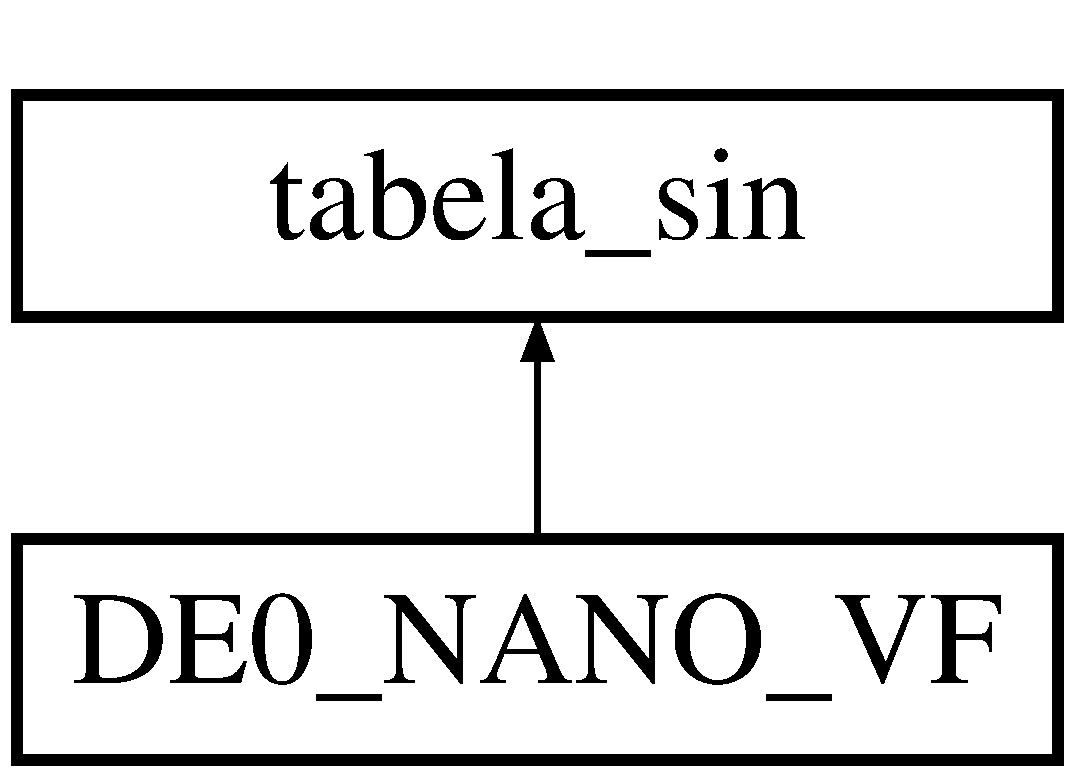
\includegraphics[height=2.000000cm]{classtabela__sin}
\end{center}
\end{figure}
\subsection*{Entities}
\begin{DoxyCompactItemize}
\item 
\hyperlink{classtabela__sin_1_1tabela__sin}{tabela\+\_\+sin} architecture
\end{DoxyCompactItemize}
\subsection*{Libraries}
 \begin{DoxyCompactItemize}
\item 
\hyperlink{classtabela__sin_a0a6af6eef40212dbaf130d57ce711256}{ieee} 
\end{DoxyCompactItemize}
\subsection*{Use Clauses}
 \begin{DoxyCompactItemize}
\item 
\hyperlink{classtabela__sin_acd03516902501cd1c7296a98e22c6fcb}{std\+\_\+logic\+\_\+1164}   
\item 
\hyperlink{classtabela__sin_a598da929e807d58939b47499e8bc9fa8}{std\+\_\+logic\+\_\+unsigned}   
\item 
\hyperlink{classtabela__sin_a2edc34402b573437d5f25fa90ba4013e}{numeric\+\_\+std}   
\item 
\hyperlink{classtabela__sin_aad86249c80e8c1e7ee1c4748aba748e3}{fixed\+\_\+pkg}   
\end{DoxyCompactItemize}
\subsection*{Generics}
 \begin{DoxyCompactItemize}
\item 
\hyperlink{classtabela__sin_ab8831e89bf175c5e1e9c6a650e7e0599}{n\+\_\+bits\+\_\+phase} {\bfseries {\bfseries \textcolor{comment}{integer}\textcolor{vhdlchar}{ }\textcolor{vhdlchar}{ }\textcolor{vhdlchar}{\+:}\textcolor{vhdlchar}{=}\textcolor{vhdlchar}{ }\textcolor{vhdlchar}{ } \textcolor{vhdldigit}{16} \textcolor{vhdlchar}{ }}}
\item 
\hyperlink{classtabela__sin_afee4aa1628956aa350183d8881689198}{n\+\_\+bits\+\_\+c} {\bfseries {\bfseries \textcolor{comment}{integer}\textcolor{vhdlchar}{ }\textcolor{vhdlchar}{ }\textcolor{vhdlchar}{\+:}\textcolor{vhdlchar}{=}\textcolor{vhdlchar}{ }\textcolor{vhdlchar}{ } \textcolor{vhdldigit}{16} \textcolor{vhdlchar}{ }}}
\item 
\hyperlink{classtabela__sin_abb7ce405d45a733b6db94314a4f791fd}{I} {\bfseries {\bfseries \textcolor{comment}{integer}\textcolor{vhdlchar}{ }\textcolor{vhdlchar}{ }\textcolor{vhdlchar}{\+:}\textcolor{vhdlchar}{=}\textcolor{vhdlchar}{ }\textcolor{vhdlchar}{ } \textcolor{vhdldigit}{1} \textcolor{vhdlchar}{ }}}
\item 
\hyperlink{classtabela__sin_aac2d6825f96b21ae984648cc93554339}{F} {\bfseries {\bfseries \textcolor{comment}{integer}\textcolor{vhdlchar}{ }\textcolor{vhdlchar}{ }\textcolor{vhdlchar}{\+:}\textcolor{vhdlchar}{=}\textcolor{vhdlchar}{ }\textcolor{vhdlchar}{ } \textcolor{vhdldigit}{14} \textcolor{vhdlchar}{ }}}
\end{DoxyCompactItemize}
\subsection*{Ports}
 \begin{DoxyCompactItemize}
\item 
\hyperlink{classtabela__sin_a4a4609c199d30b3adebbeb3a01276ec5}{clk}  {\bfseries {\bfseries \textcolor{keywordflow}{in}\textcolor{vhdlchar}{ }}} {\bfseries \textcolor{comment}{std\+\_\+logic}\textcolor{vhdlchar}{ }} 
\item 
\hyperlink{classtabela__sin_afad6cf0a3cf35dff4473dba942ec361a}{theta}  {\bfseries {\bfseries \textcolor{keywordflow}{in}\textcolor{vhdlchar}{ }}} {\bfseries \textcolor{comment}{std\+\_\+logic\+\_\+vector}\textcolor{vhdlchar}{ }\textcolor{vhdlchar}{(}\textcolor{vhdlchar}{ }\textcolor{vhdlchar}{ } \textcolor{vhdldigit}{15} \textcolor{vhdlchar}{ }\textcolor{keywordflow}{downto}\textcolor{vhdlchar}{ }\textcolor{vhdlchar}{ } \textcolor{vhdldigit}{0} \textcolor{vhdlchar}{ }\textcolor{vhdlchar}{)}\textcolor{vhdlchar}{ }} 
\item 
\hyperlink{classtabela__sin_a410cd5827b2743056d0443e5560727d1}{M\+A\+X}  {\bfseries {\bfseries \textcolor{keywordflow}{in}\textcolor{vhdlchar}{ }}} {\bfseries \textcolor{comment}{sfixed}\textcolor{vhdlchar}{ }\textcolor{vhdlchar}{(}\textcolor{vhdlchar}{ }\textcolor{vhdlchar}{ } \textcolor{vhdldigit}{15} \textcolor{vhdlchar}{ }\textcolor{keywordflow}{downto}\textcolor{vhdlchar}{ }\textcolor{vhdlchar}{ } \textcolor{vhdldigit}{0} \textcolor{vhdlchar}{ }\textcolor{vhdlchar}{)}\textcolor{vhdlchar}{ }} 
\item 
\hyperlink{classtabela__sin_aadecc5b785b421d679bab5cf2654c463}{ma}  {\bfseries {\bfseries \textcolor{keywordflow}{in}\textcolor{vhdlchar}{ }}} {\bfseries \textcolor{comment}{sfixed}\textcolor{vhdlchar}{ }\textcolor{vhdlchar}{(}\textcolor{vhdlchar}{ }\textcolor{vhdlchar}{ }\textcolor{vhdlchar}{ }\textcolor{vhdlchar}{ }{\bfseries \hyperlink{classtabela__sin_abb7ce405d45a733b6db94314a4f791fd}{I}} \textcolor{vhdlchar}{ }\textcolor{keywordflow}{downto}\textcolor{vhdlchar}{ }\textcolor{vhdlchar}{-\/}\textcolor{vhdlchar}{ }\textcolor{vhdlchar}{ }\textcolor{vhdlchar}{ }{\bfseries \hyperlink{classtabela__sin_aac2d6825f96b21ae984648cc93554339}{F}} \textcolor{vhdlchar}{ }\textcolor{vhdlchar}{)}\textcolor{vhdlchar}{ }} 
\item 
\hyperlink{classtabela__sin_a2c2cf4dbd0533e281ac8b2f114f11e67}{va}  {\bfseries {\bfseries \textcolor{keywordflow}{out}\textcolor{vhdlchar}{ }}} {\bfseries \textcolor{comment}{std\+\_\+logic\+\_\+vector}\textcolor{vhdlchar}{ }\textcolor{vhdlchar}{(}\textcolor{vhdlchar}{ }\textcolor{vhdlchar}{ } \textcolor{vhdldigit}{15} \textcolor{vhdlchar}{ }\textcolor{keywordflow}{downto}\textcolor{vhdlchar}{ }\textcolor{vhdlchar}{ } \textcolor{vhdldigit}{0} \textcolor{vhdlchar}{ }\textcolor{vhdlchar}{)}\textcolor{vhdlchar}{ }} 
\end{DoxyCompactItemize}


\subsection{Detailed Description}


Definition at line \hyperlink{tabela__sin_8vhd_source_l00007}{7} of file \hyperlink{tabela__sin_8vhd_source}{tabela\+\_\+sin.\+vhd}.



\subsection{Member Data Documentation}
\hypertarget{classtabela__sin_a4a4609c199d30b3adebbeb3a01276ec5}{}\index{tabela\+\_\+sin@{tabela\+\_\+sin}!clk@{clk}}
\index{clk@{clk}!tabela\+\_\+sin@{tabela\+\_\+sin}}
\subsubsection[{clk}]{\setlength{\rightskip}{0pt plus 5cm}{\bf clk} {\bfseries \textcolor{keywordflow}{in}\textcolor{vhdlchar}{ }} {\bfseries \textcolor{comment}{std\+\_\+logic}\textcolor{vhdlchar}{ }} \hspace{0.3cm}{\ttfamily [Port]}}\label{classtabela__sin_a4a4609c199d30b3adebbeb3a01276ec5}


Definition at line \hyperlink{tabela__sin_8vhd_source_l00015}{15} of file \hyperlink{tabela__sin_8vhd_source}{tabela\+\_\+sin.\+vhd}.

\hypertarget{classtabela__sin_aac2d6825f96b21ae984648cc93554339}{}\index{tabela\+\_\+sin@{tabela\+\_\+sin}!F@{F}}
\index{F@{F}!tabela\+\_\+sin@{tabela\+\_\+sin}}
\subsubsection[{F}]{\setlength{\rightskip}{0pt plus 5cm}{\bf F} {\bfseries \textcolor{vhdlchar}{ }} {\bfseries \textcolor{comment}{integer}\textcolor{vhdlchar}{ }\textcolor{vhdlchar}{ }\textcolor{vhdlchar}{\+:}\textcolor{vhdlchar}{=}\textcolor{vhdlchar}{ }\textcolor{vhdlchar}{ } \textcolor{vhdldigit}{14} \textcolor{vhdlchar}{ }} \hspace{0.3cm}{\ttfamily [Generic]}}\label{classtabela__sin_aac2d6825f96b21ae984648cc93554339}


Definition at line \hyperlink{tabela__sin_8vhd_source_l00013}{13} of file \hyperlink{tabela__sin_8vhd_source}{tabela\+\_\+sin.\+vhd}.

\hypertarget{classtabela__sin_aad86249c80e8c1e7ee1c4748aba748e3}{}\index{tabela\+\_\+sin@{tabela\+\_\+sin}!fixed\+\_\+pkg@{fixed\+\_\+pkg}}
\index{fixed\+\_\+pkg@{fixed\+\_\+pkg}!tabela\+\_\+sin@{tabela\+\_\+sin}}
\subsubsection[{fixed\+\_\+pkg}]{\setlength{\rightskip}{0pt plus 5cm}{\bf fixed\+\_\+pkg}\hspace{0.3cm}{\ttfamily [Package]}}\label{classtabela__sin_aad86249c80e8c1e7ee1c4748aba748e3}


Definition at line \hyperlink{tabela__sin_8vhd_source_l00005}{5} of file \hyperlink{tabela__sin_8vhd_source}{tabela\+\_\+sin.\+vhd}.

\hypertarget{classtabela__sin_abb7ce405d45a733b6db94314a4f791fd}{}\index{tabela\+\_\+sin@{tabela\+\_\+sin}!I@{I}}
\index{I@{I}!tabela\+\_\+sin@{tabela\+\_\+sin}}
\subsubsection[{I}]{\setlength{\rightskip}{0pt plus 5cm}{\bf I} {\bfseries \textcolor{vhdlchar}{ }} {\bfseries \textcolor{comment}{integer}\textcolor{vhdlchar}{ }\textcolor{vhdlchar}{ }\textcolor{vhdlchar}{\+:}\textcolor{vhdlchar}{=}\textcolor{vhdlchar}{ }\textcolor{vhdlchar}{ } \textcolor{vhdldigit}{1} \textcolor{vhdlchar}{ }} \hspace{0.3cm}{\ttfamily [Generic]}}\label{classtabela__sin_abb7ce405d45a733b6db94314a4f791fd}


Definition at line \hyperlink{tabela__sin_8vhd_source_l00011}{11} of file \hyperlink{tabela__sin_8vhd_source}{tabela\+\_\+sin.\+vhd}.

\hypertarget{classtabela__sin_a0a6af6eef40212dbaf130d57ce711256}{}\index{tabela\+\_\+sin@{tabela\+\_\+sin}!ieee@{ieee}}
\index{ieee@{ieee}!tabela\+\_\+sin@{tabela\+\_\+sin}}
\subsubsection[{ieee}]{\setlength{\rightskip}{0pt plus 5cm}{\bf ieee}\hspace{0.3cm}{\ttfamily [Library]}}\label{classtabela__sin_a0a6af6eef40212dbaf130d57ce711256}


Definition at line \hyperlink{tabela__sin_8vhd_source_l00001}{1} of file \hyperlink{tabela__sin_8vhd_source}{tabela\+\_\+sin.\+vhd}.

\hypertarget{classtabela__sin_aadecc5b785b421d679bab5cf2654c463}{}\index{tabela\+\_\+sin@{tabela\+\_\+sin}!ma@{ma}}
\index{ma@{ma}!tabela\+\_\+sin@{tabela\+\_\+sin}}
\subsubsection[{ma}]{\setlength{\rightskip}{0pt plus 5cm}{\bf ma} {\bfseries \textcolor{keywordflow}{in}\textcolor{vhdlchar}{ }} {\bfseries \textcolor{comment}{sfixed}\textcolor{vhdlchar}{ }\textcolor{vhdlchar}{(}\textcolor{vhdlchar}{ }\textcolor{vhdlchar}{ }\textcolor{vhdlchar}{ }\textcolor{vhdlchar}{ }{\bfseries {\bf I}} \textcolor{vhdlchar}{ }\textcolor{keywordflow}{downto}\textcolor{vhdlchar}{ }\textcolor{vhdlchar}{-\/}\textcolor{vhdlchar}{ }\textcolor{vhdlchar}{ }\textcolor{vhdlchar}{ }{\bfseries {\bf F}} \textcolor{vhdlchar}{ }\textcolor{vhdlchar}{)}\textcolor{vhdlchar}{ }} \hspace{0.3cm}{\ttfamily [Port]}}\label{classtabela__sin_aadecc5b785b421d679bab5cf2654c463}


Definition at line \hyperlink{tabela__sin_8vhd_source_l00018}{18} of file \hyperlink{tabela__sin_8vhd_source}{tabela\+\_\+sin.\+vhd}.

\hypertarget{classtabela__sin_a410cd5827b2743056d0443e5560727d1}{}\index{tabela\+\_\+sin@{tabela\+\_\+sin}!M\+A\+X@{M\+A\+X}}
\index{M\+A\+X@{M\+A\+X}!tabela\+\_\+sin@{tabela\+\_\+sin}}
\subsubsection[{M\+A\+X}]{\setlength{\rightskip}{0pt plus 5cm}{\bf M\+A\+X} {\bfseries \textcolor{keywordflow}{in}\textcolor{vhdlchar}{ }} {\bfseries \textcolor{comment}{sfixed}\textcolor{vhdlchar}{ }\textcolor{vhdlchar}{(}\textcolor{vhdlchar}{ }\textcolor{vhdlchar}{ } \textcolor{vhdldigit}{15} \textcolor{vhdlchar}{ }\textcolor{keywordflow}{downto}\textcolor{vhdlchar}{ }\textcolor{vhdlchar}{ } \textcolor{vhdldigit}{0} \textcolor{vhdlchar}{ }\textcolor{vhdlchar}{)}\textcolor{vhdlchar}{ }} \hspace{0.3cm}{\ttfamily [Port]}}\label{classtabela__sin_a410cd5827b2743056d0443e5560727d1}


Definition at line \hyperlink{tabela__sin_8vhd_source_l00017}{17} of file \hyperlink{tabela__sin_8vhd_source}{tabela\+\_\+sin.\+vhd}.

\hypertarget{classtabela__sin_afee4aa1628956aa350183d8881689198}{}\index{tabela\+\_\+sin@{tabela\+\_\+sin}!n\+\_\+bits\+\_\+c@{n\+\_\+bits\+\_\+c}}
\index{n\+\_\+bits\+\_\+c@{n\+\_\+bits\+\_\+c}!tabela\+\_\+sin@{tabela\+\_\+sin}}
\subsubsection[{n\+\_\+bits\+\_\+c}]{\setlength{\rightskip}{0pt plus 5cm}{\bf n\+\_\+bits\+\_\+c} {\bfseries \textcolor{vhdlchar}{ }} {\bfseries \textcolor{comment}{integer}\textcolor{vhdlchar}{ }\textcolor{vhdlchar}{ }\textcolor{vhdlchar}{\+:}\textcolor{vhdlchar}{=}\textcolor{vhdlchar}{ }\textcolor{vhdlchar}{ } \textcolor{vhdldigit}{16} \textcolor{vhdlchar}{ }} \hspace{0.3cm}{\ttfamily [Generic]}}\label{classtabela__sin_afee4aa1628956aa350183d8881689198}


Definition at line \hyperlink{tabela__sin_8vhd_source_l00010}{10} of file \hyperlink{tabela__sin_8vhd_source}{tabela\+\_\+sin.\+vhd}.

\hypertarget{classtabela__sin_ab8831e89bf175c5e1e9c6a650e7e0599}{}\index{tabela\+\_\+sin@{tabela\+\_\+sin}!n\+\_\+bits\+\_\+phase@{n\+\_\+bits\+\_\+phase}}
\index{n\+\_\+bits\+\_\+phase@{n\+\_\+bits\+\_\+phase}!tabela\+\_\+sin@{tabela\+\_\+sin}}
\subsubsection[{n\+\_\+bits\+\_\+phase}]{\setlength{\rightskip}{0pt plus 5cm}{\bf n\+\_\+bits\+\_\+phase} {\bfseries \textcolor{vhdlchar}{ }} {\bfseries \textcolor{comment}{integer}\textcolor{vhdlchar}{ }\textcolor{vhdlchar}{ }\textcolor{vhdlchar}{\+:}\textcolor{vhdlchar}{=}\textcolor{vhdlchar}{ }\textcolor{vhdlchar}{ } \textcolor{vhdldigit}{16} \textcolor{vhdlchar}{ }} \hspace{0.3cm}{\ttfamily [Generic]}}\label{classtabela__sin_ab8831e89bf175c5e1e9c6a650e7e0599}


Definition at line \hyperlink{tabela__sin_8vhd_source_l00009}{9} of file \hyperlink{tabela__sin_8vhd_source}{tabela\+\_\+sin.\+vhd}.

\hypertarget{classtabela__sin_a2edc34402b573437d5f25fa90ba4013e}{}\index{tabela\+\_\+sin@{tabela\+\_\+sin}!numeric\+\_\+std@{numeric\+\_\+std}}
\index{numeric\+\_\+std@{numeric\+\_\+std}!tabela\+\_\+sin@{tabela\+\_\+sin}}
\subsubsection[{numeric\+\_\+std}]{\setlength{\rightskip}{0pt plus 5cm}{\bf numeric\+\_\+std}\hspace{0.3cm}{\ttfamily [Package]}}\label{classtabela__sin_a2edc34402b573437d5f25fa90ba4013e}


Definition at line \hyperlink{tabela__sin_8vhd_source_l00004}{4} of file \hyperlink{tabela__sin_8vhd_source}{tabela\+\_\+sin.\+vhd}.

\hypertarget{classtabela__sin_acd03516902501cd1c7296a98e22c6fcb}{}\index{tabela\+\_\+sin@{tabela\+\_\+sin}!std\+\_\+logic\+\_\+1164@{std\+\_\+logic\+\_\+1164}}
\index{std\+\_\+logic\+\_\+1164@{std\+\_\+logic\+\_\+1164}!tabela\+\_\+sin@{tabela\+\_\+sin}}
\subsubsection[{std\+\_\+logic\+\_\+1164}]{\setlength{\rightskip}{0pt plus 5cm}{\bf std\+\_\+logic\+\_\+1164}\hspace{0.3cm}{\ttfamily [Package]}}\label{classtabela__sin_acd03516902501cd1c7296a98e22c6fcb}


Definition at line \hyperlink{tabela__sin_8vhd_source_l00002}{2} of file \hyperlink{tabela__sin_8vhd_source}{tabela\+\_\+sin.\+vhd}.

\hypertarget{classtabela__sin_a598da929e807d58939b47499e8bc9fa8}{}\index{tabela\+\_\+sin@{tabela\+\_\+sin}!std\+\_\+logic\+\_\+unsigned@{std\+\_\+logic\+\_\+unsigned}}
\index{std\+\_\+logic\+\_\+unsigned@{std\+\_\+logic\+\_\+unsigned}!tabela\+\_\+sin@{tabela\+\_\+sin}}
\subsubsection[{std\+\_\+logic\+\_\+unsigned}]{\setlength{\rightskip}{0pt plus 5cm}{\bf std\+\_\+logic\+\_\+unsigned}\hspace{0.3cm}{\ttfamily [Package]}}\label{classtabela__sin_a598da929e807d58939b47499e8bc9fa8}


Definition at line \hyperlink{tabela__sin_8vhd_source_l00003}{3} of file \hyperlink{tabela__sin_8vhd_source}{tabela\+\_\+sin.\+vhd}.

\hypertarget{classtabela__sin_afad6cf0a3cf35dff4473dba942ec361a}{}\index{tabela\+\_\+sin@{tabela\+\_\+sin}!theta@{theta}}
\index{theta@{theta}!tabela\+\_\+sin@{tabela\+\_\+sin}}
\subsubsection[{theta}]{\setlength{\rightskip}{0pt plus 5cm}{\bf theta} {\bfseries \textcolor{keywordflow}{in}\textcolor{vhdlchar}{ }} {\bfseries \textcolor{comment}{std\+\_\+logic\+\_\+vector}\textcolor{vhdlchar}{ }\textcolor{vhdlchar}{(}\textcolor{vhdlchar}{ }\textcolor{vhdlchar}{ } \textcolor{vhdldigit}{15} \textcolor{vhdlchar}{ }\textcolor{keywordflow}{downto}\textcolor{vhdlchar}{ }\textcolor{vhdlchar}{ } \textcolor{vhdldigit}{0} \textcolor{vhdlchar}{ }\textcolor{vhdlchar}{)}\textcolor{vhdlchar}{ }} \hspace{0.3cm}{\ttfamily [Port]}}\label{classtabela__sin_afad6cf0a3cf35dff4473dba942ec361a}


Definition at line \hyperlink{tabela__sin_8vhd_source_l00016}{16} of file \hyperlink{tabela__sin_8vhd_source}{tabela\+\_\+sin.\+vhd}.

\hypertarget{classtabela__sin_a2c2cf4dbd0533e281ac8b2f114f11e67}{}\index{tabela\+\_\+sin@{tabela\+\_\+sin}!va@{va}}
\index{va@{va}!tabela\+\_\+sin@{tabela\+\_\+sin}}
\subsubsection[{va}]{\setlength{\rightskip}{0pt plus 5cm}{\bf va} {\bfseries \textcolor{keywordflow}{out}\textcolor{vhdlchar}{ }} {\bfseries \textcolor{comment}{std\+\_\+logic\+\_\+vector}\textcolor{vhdlchar}{ }\textcolor{vhdlchar}{(}\textcolor{vhdlchar}{ }\textcolor{vhdlchar}{ } \textcolor{vhdldigit}{15} \textcolor{vhdlchar}{ }\textcolor{keywordflow}{downto}\textcolor{vhdlchar}{ }\textcolor{vhdlchar}{ } \textcolor{vhdldigit}{0} \textcolor{vhdlchar}{ }\textcolor{vhdlchar}{)}\textcolor{vhdlchar}{ }} \hspace{0.3cm}{\ttfamily [Port]}}\label{classtabela__sin_a2c2cf4dbd0533e281ac8b2f114f11e67}


Definition at line \hyperlink{tabela__sin_8vhd_source_l00020}{20} of file \hyperlink{tabela__sin_8vhd_source}{tabela\+\_\+sin.\+vhd}.



The documentation for this class was generated from the following file\+:\begin{DoxyCompactItemize}
\item 
\hyperlink{tabela__sin_8vhd}{tabela\+\_\+sin.\+vhd}\end{DoxyCompactItemize}

\hypertarget{classtheta__abc_1_1theta__abc}{}\section{theta\+\_\+abc Architecture Reference}
\label{classtheta__abc_1_1theta__abc}\index{theta\+\_\+abc@{theta\+\_\+abc}}
\subsection*{Processes}
 \begin{DoxyCompactItemize}
\item 
\hyperlink{classtheta__abc_1_1theta__abc_a8ee64d1327298358d5f75867875249ca}{P\+R\+O\+C\+E\+S\+S\+\_\+15}{\bfseries  ( {\bfseries {\bfseries \hyperlink{classtheta__abc_a4a4609c199d30b3adebbeb3a01276ec5}{clk}} \textcolor{vhdlchar}{ }} )}
\end{DoxyCompactItemize}
\subsection*{Signals}
 \begin{DoxyCompactItemize}
\item 
\hyperlink{classtheta__abc_1_1theta__abc_ad76995fdeaec7ada621075ea6562c673}{th\+\_\+a} {\bfseries \textcolor{comment}{std\+\_\+logic\+\_\+vector}\textcolor{vhdlchar}{ }\textcolor{vhdlchar}{(}\textcolor{vhdlchar}{ }\textcolor{vhdlchar}{ }\textcolor{vhdlchar}{ }\textcolor{vhdlchar}{ }{\bfseries \hyperlink{classtheta__abc_ad0f475656f5dd17584d6796fde77d790}{Nout}} \textcolor{vhdlchar}{-\/}\textcolor{vhdlchar}{ } \textcolor{vhdldigit}{1} \textcolor{vhdlchar}{ }\textcolor{keywordflow}{downto}\textcolor{vhdlchar}{ }\textcolor{vhdlchar}{ } \textcolor{vhdldigit}{0} \textcolor{vhdlchar}{ }\textcolor{vhdlchar}{)}\textcolor{vhdlchar}{ }} 
\item 
\hyperlink{classtheta__abc_1_1theta__abc_ae23fb98ce5af67556ecf68e8ffb4a27c}{th\+\_\+b} {\bfseries \textcolor{comment}{std\+\_\+logic\+\_\+vector}\textcolor{vhdlchar}{ }\textcolor{vhdlchar}{(}\textcolor{vhdlchar}{ }\textcolor{vhdlchar}{ }\textcolor{vhdlchar}{ }\textcolor{vhdlchar}{ }{\bfseries \hyperlink{classtheta__abc_ad0f475656f5dd17584d6796fde77d790}{Nout}} \textcolor{vhdlchar}{-\/}\textcolor{vhdlchar}{ } \textcolor{vhdldigit}{1} \textcolor{vhdlchar}{ }\textcolor{keywordflow}{downto}\textcolor{vhdlchar}{ }\textcolor{vhdlchar}{ } \textcolor{vhdldigit}{0} \textcolor{vhdlchar}{ }\textcolor{vhdlchar}{)}\textcolor{vhdlchar}{ }} 
\item 
\hyperlink{classtheta__abc_1_1theta__abc_a99d308b4a97dff4ea9faacf3778ac0f1}{th\+\_\+c} {\bfseries \textcolor{comment}{std\+\_\+logic\+\_\+vector}\textcolor{vhdlchar}{ }\textcolor{vhdlchar}{(}\textcolor{vhdlchar}{ }\textcolor{vhdlchar}{ }\textcolor{vhdlchar}{ }\textcolor{vhdlchar}{ }{\bfseries \hyperlink{classtheta__abc_ad0f475656f5dd17584d6796fde77d790}{Nout}} \textcolor{vhdlchar}{-\/}\textcolor{vhdlchar}{ } \textcolor{vhdldigit}{1} \textcolor{vhdlchar}{ }\textcolor{keywordflow}{downto}\textcolor{vhdlchar}{ }\textcolor{vhdlchar}{ } \textcolor{vhdldigit}{0} \textcolor{vhdlchar}{ }\textcolor{vhdlchar}{)}\textcolor{vhdlchar}{ }} 
\item 
\hyperlink{classtheta__abc_1_1theta__abc_aa089585a137a873b884793531ca5edc0}{th\+\_\+ai} {\bfseries \textcolor{comment}{std\+\_\+logic\+\_\+vector}\textcolor{vhdlchar}{ }\textcolor{vhdlchar}{(}\textcolor{vhdlchar}{ }\textcolor{vhdlchar}{ }\textcolor{vhdlchar}{ }\textcolor{vhdlchar}{ }{\bfseries \hyperlink{classtheta__abc_ad0f475656f5dd17584d6796fde77d790}{Nout}} \textcolor{vhdlchar}{ }\textcolor{keywordflow}{downto}\textcolor{vhdlchar}{ }\textcolor{vhdlchar}{ } \textcolor{vhdldigit}{0} \textcolor{vhdlchar}{ }\textcolor{vhdlchar}{)}\textcolor{vhdlchar}{ }} 
\item 
\hyperlink{classtheta__abc_1_1theta__abc_a7ff18034ace7fde19560f0a2a2cdd952}{th\+\_\+bi} {\bfseries \textcolor{comment}{std\+\_\+logic\+\_\+vector}\textcolor{vhdlchar}{ }\textcolor{vhdlchar}{(}\textcolor{vhdlchar}{ }\textcolor{vhdlchar}{ }\textcolor{vhdlchar}{ }\textcolor{vhdlchar}{ }{\bfseries \hyperlink{classtheta__abc_ad0f475656f5dd17584d6796fde77d790}{Nout}} \textcolor{vhdlchar}{ }\textcolor{keywordflow}{downto}\textcolor{vhdlchar}{ }\textcolor{vhdlchar}{ } \textcolor{vhdldigit}{0} \textcolor{vhdlchar}{ }\textcolor{vhdlchar}{)}\textcolor{vhdlchar}{ }} 
\item 
\hyperlink{classtheta__abc_1_1theta__abc_a45f5cb01816ecd5555fc839e392dfe6a}{th\+\_\+ci} {\bfseries \textcolor{comment}{std\+\_\+logic\+\_\+vector}\textcolor{vhdlchar}{ }\textcolor{vhdlchar}{(}\textcolor{vhdlchar}{ }\textcolor{vhdlchar}{ }\textcolor{vhdlchar}{ }\textcolor{vhdlchar}{ }{\bfseries \hyperlink{classtheta__abc_ad0f475656f5dd17584d6796fde77d790}{Nout}} \textcolor{vhdlchar}{ }\textcolor{keywordflow}{downto}\textcolor{vhdlchar}{ }\textcolor{vhdlchar}{ } \textcolor{vhdldigit}{0} \textcolor{vhdlchar}{ }\textcolor{vhdlchar}{)}\textcolor{vhdlchar}{ }} 
\end{DoxyCompactItemize}


\subsection{Detailed Description}


Definition at line 25 of file theta\+\_\+abc.\+vhd.



\subsection{Member Function Documentation}
\hypertarget{classtheta__abc_1_1theta__abc_a8ee64d1327298358d5f75867875249ca}{}\index{theta\+\_\+abc\+::theta\+\_\+abc@{theta\+\_\+abc\+::theta\+\_\+abc}!P\+R\+O\+C\+E\+S\+S\+\_\+15@{P\+R\+O\+C\+E\+S\+S\+\_\+15}}
\index{P\+R\+O\+C\+E\+S\+S\+\_\+15@{P\+R\+O\+C\+E\+S\+S\+\_\+15}!theta\+\_\+abc\+::theta\+\_\+abc@{theta\+\_\+abc\+::theta\+\_\+abc}}
\subsubsection[{P\+R\+O\+C\+E\+S\+S\+\_\+15}]{\setlength{\rightskip}{0pt plus 5cm} {\bfseries \textcolor{vhdlchar}{ }} P\+R\+O\+C\+E\+S\+S\+\_\+15(
\begin{DoxyParamCaption}
\item[{}]{{\bfseries {\bfseries {\bf clk}} \textcolor{vhdlchar}{ }} {\em }}
\end{DoxyParamCaption}
)\hspace{0.3cm}{\ttfamily [Process]}}\label{classtheta__abc_1_1theta__abc_a8ee64d1327298358d5f75867875249ca}


Definition at line 33 of file theta\+\_\+abc.\+vhd.



\subsection{Member Data Documentation}
\hypertarget{classtheta__abc_1_1theta__abc_ad76995fdeaec7ada621075ea6562c673}{}\index{theta\+\_\+abc\+::theta\+\_\+abc@{theta\+\_\+abc\+::theta\+\_\+abc}!th\+\_\+a@{th\+\_\+a}}
\index{th\+\_\+a@{th\+\_\+a}!theta\+\_\+abc\+::theta\+\_\+abc@{theta\+\_\+abc\+::theta\+\_\+abc}}
\subsubsection[{th\+\_\+a}]{\setlength{\rightskip}{0pt plus 5cm}{\bf th\+\_\+a} {\bfseries \textcolor{comment}{std\+\_\+logic\+\_\+vector}\textcolor{vhdlchar}{ }\textcolor{vhdlchar}{(}\textcolor{vhdlchar}{ }\textcolor{vhdlchar}{ }\textcolor{vhdlchar}{ }\textcolor{vhdlchar}{ }{\bfseries {\bf Nout}} \textcolor{vhdlchar}{-\/}\textcolor{vhdlchar}{ } \textcolor{vhdldigit}{1} \textcolor{vhdlchar}{ }\textcolor{keywordflow}{downto}\textcolor{vhdlchar}{ }\textcolor{vhdlchar}{ } \textcolor{vhdldigit}{0} \textcolor{vhdlchar}{ }\textcolor{vhdlchar}{)}\textcolor{vhdlchar}{ }} \hspace{0.3cm}{\ttfamily [Signal]}}\label{classtheta__abc_1_1theta__abc_ad76995fdeaec7ada621075ea6562c673}


Definition at line 27 of file theta\+\_\+abc.\+vhd.

\hypertarget{classtheta__abc_1_1theta__abc_aa089585a137a873b884793531ca5edc0}{}\index{theta\+\_\+abc\+::theta\+\_\+abc@{theta\+\_\+abc\+::theta\+\_\+abc}!th\+\_\+ai@{th\+\_\+ai}}
\index{th\+\_\+ai@{th\+\_\+ai}!theta\+\_\+abc\+::theta\+\_\+abc@{theta\+\_\+abc\+::theta\+\_\+abc}}
\subsubsection[{th\+\_\+ai}]{\setlength{\rightskip}{0pt plus 5cm}{\bf th\+\_\+ai} {\bfseries \textcolor{comment}{std\+\_\+logic\+\_\+vector}\textcolor{vhdlchar}{ }\textcolor{vhdlchar}{(}\textcolor{vhdlchar}{ }\textcolor{vhdlchar}{ }\textcolor{vhdlchar}{ }\textcolor{vhdlchar}{ }{\bfseries {\bf Nout}} \textcolor{vhdlchar}{ }\textcolor{keywordflow}{downto}\textcolor{vhdlchar}{ }\textcolor{vhdlchar}{ } \textcolor{vhdldigit}{0} \textcolor{vhdlchar}{ }\textcolor{vhdlchar}{)}\textcolor{vhdlchar}{ }} \hspace{0.3cm}{\ttfamily [Signal]}}\label{classtheta__abc_1_1theta__abc_aa089585a137a873b884793531ca5edc0}


Definition at line 28 of file theta\+\_\+abc.\+vhd.

\hypertarget{classtheta__abc_1_1theta__abc_ae23fb98ce5af67556ecf68e8ffb4a27c}{}\index{theta\+\_\+abc\+::theta\+\_\+abc@{theta\+\_\+abc\+::theta\+\_\+abc}!th\+\_\+b@{th\+\_\+b}}
\index{th\+\_\+b@{th\+\_\+b}!theta\+\_\+abc\+::theta\+\_\+abc@{theta\+\_\+abc\+::theta\+\_\+abc}}
\subsubsection[{th\+\_\+b}]{\setlength{\rightskip}{0pt plus 5cm}{\bf th\+\_\+b} {\bfseries \textcolor{comment}{std\+\_\+logic\+\_\+vector}\textcolor{vhdlchar}{ }\textcolor{vhdlchar}{(}\textcolor{vhdlchar}{ }\textcolor{vhdlchar}{ }\textcolor{vhdlchar}{ }\textcolor{vhdlchar}{ }{\bfseries {\bf Nout}} \textcolor{vhdlchar}{-\/}\textcolor{vhdlchar}{ } \textcolor{vhdldigit}{1} \textcolor{vhdlchar}{ }\textcolor{keywordflow}{downto}\textcolor{vhdlchar}{ }\textcolor{vhdlchar}{ } \textcolor{vhdldigit}{0} \textcolor{vhdlchar}{ }\textcolor{vhdlchar}{)}\textcolor{vhdlchar}{ }} \hspace{0.3cm}{\ttfamily [Signal]}}\label{classtheta__abc_1_1theta__abc_ae23fb98ce5af67556ecf68e8ffb4a27c}


Definition at line 27 of file theta\+\_\+abc.\+vhd.

\hypertarget{classtheta__abc_1_1theta__abc_a7ff18034ace7fde19560f0a2a2cdd952}{}\index{theta\+\_\+abc\+::theta\+\_\+abc@{theta\+\_\+abc\+::theta\+\_\+abc}!th\+\_\+bi@{th\+\_\+bi}}
\index{th\+\_\+bi@{th\+\_\+bi}!theta\+\_\+abc\+::theta\+\_\+abc@{theta\+\_\+abc\+::theta\+\_\+abc}}
\subsubsection[{th\+\_\+bi}]{\setlength{\rightskip}{0pt plus 5cm}{\bf th\+\_\+bi} {\bfseries \textcolor{comment}{std\+\_\+logic\+\_\+vector}\textcolor{vhdlchar}{ }\textcolor{vhdlchar}{(}\textcolor{vhdlchar}{ }\textcolor{vhdlchar}{ }\textcolor{vhdlchar}{ }\textcolor{vhdlchar}{ }{\bfseries {\bf Nout}} \textcolor{vhdlchar}{ }\textcolor{keywordflow}{downto}\textcolor{vhdlchar}{ }\textcolor{vhdlchar}{ } \textcolor{vhdldigit}{0} \textcolor{vhdlchar}{ }\textcolor{vhdlchar}{)}\textcolor{vhdlchar}{ }} \hspace{0.3cm}{\ttfamily [Signal]}}\label{classtheta__abc_1_1theta__abc_a7ff18034ace7fde19560f0a2a2cdd952}


Definition at line 28 of file theta\+\_\+abc.\+vhd.

\hypertarget{classtheta__abc_1_1theta__abc_a99d308b4a97dff4ea9faacf3778ac0f1}{}\index{theta\+\_\+abc\+::theta\+\_\+abc@{theta\+\_\+abc\+::theta\+\_\+abc}!th\+\_\+c@{th\+\_\+c}}
\index{th\+\_\+c@{th\+\_\+c}!theta\+\_\+abc\+::theta\+\_\+abc@{theta\+\_\+abc\+::theta\+\_\+abc}}
\subsubsection[{th\+\_\+c}]{\setlength{\rightskip}{0pt plus 5cm}{\bf th\+\_\+c} {\bfseries \textcolor{comment}{std\+\_\+logic\+\_\+vector}\textcolor{vhdlchar}{ }\textcolor{vhdlchar}{(}\textcolor{vhdlchar}{ }\textcolor{vhdlchar}{ }\textcolor{vhdlchar}{ }\textcolor{vhdlchar}{ }{\bfseries {\bf Nout}} \textcolor{vhdlchar}{-\/}\textcolor{vhdlchar}{ } \textcolor{vhdldigit}{1} \textcolor{vhdlchar}{ }\textcolor{keywordflow}{downto}\textcolor{vhdlchar}{ }\textcolor{vhdlchar}{ } \textcolor{vhdldigit}{0} \textcolor{vhdlchar}{ }\textcolor{vhdlchar}{)}\textcolor{vhdlchar}{ }} \hspace{0.3cm}{\ttfamily [Signal]}}\label{classtheta__abc_1_1theta__abc_a99d308b4a97dff4ea9faacf3778ac0f1}


Definition at line 27 of file theta\+\_\+abc.\+vhd.

\hypertarget{classtheta__abc_1_1theta__abc_a45f5cb01816ecd5555fc839e392dfe6a}{}\index{theta\+\_\+abc\+::theta\+\_\+abc@{theta\+\_\+abc\+::theta\+\_\+abc}!th\+\_\+ci@{th\+\_\+ci}}
\index{th\+\_\+ci@{th\+\_\+ci}!theta\+\_\+abc\+::theta\+\_\+abc@{theta\+\_\+abc\+::theta\+\_\+abc}}
\subsubsection[{th\+\_\+ci}]{\setlength{\rightskip}{0pt plus 5cm}{\bf th\+\_\+ci} {\bfseries \textcolor{comment}{std\+\_\+logic\+\_\+vector}\textcolor{vhdlchar}{ }\textcolor{vhdlchar}{(}\textcolor{vhdlchar}{ }\textcolor{vhdlchar}{ }\textcolor{vhdlchar}{ }\textcolor{vhdlchar}{ }{\bfseries {\bf Nout}} \textcolor{vhdlchar}{ }\textcolor{keywordflow}{downto}\textcolor{vhdlchar}{ }\textcolor{vhdlchar}{ } \textcolor{vhdldigit}{0} \textcolor{vhdlchar}{ }\textcolor{vhdlchar}{)}\textcolor{vhdlchar}{ }} \hspace{0.3cm}{\ttfamily [Signal]}}\label{classtheta__abc_1_1theta__abc_a45f5cb01816ecd5555fc839e392dfe6a}


Definition at line 28 of file theta\+\_\+abc.\+vhd.



The documentation for this class was generated from the following file\+:\begin{DoxyCompactItemize}
\item 
\hyperlink{theta__abc_8vhd}{theta\+\_\+abc.\+vhd}\end{DoxyCompactItemize}

\hypertarget{classtheta__abc}{}\section{theta\+\_\+abc Entity Reference}
\label{classtheta__abc}\index{theta\+\_\+abc@{theta\+\_\+abc}}
Inheritance diagram for theta\+\_\+abc\+:\begin{figure}[H]
\begin{center}
\leavevmode
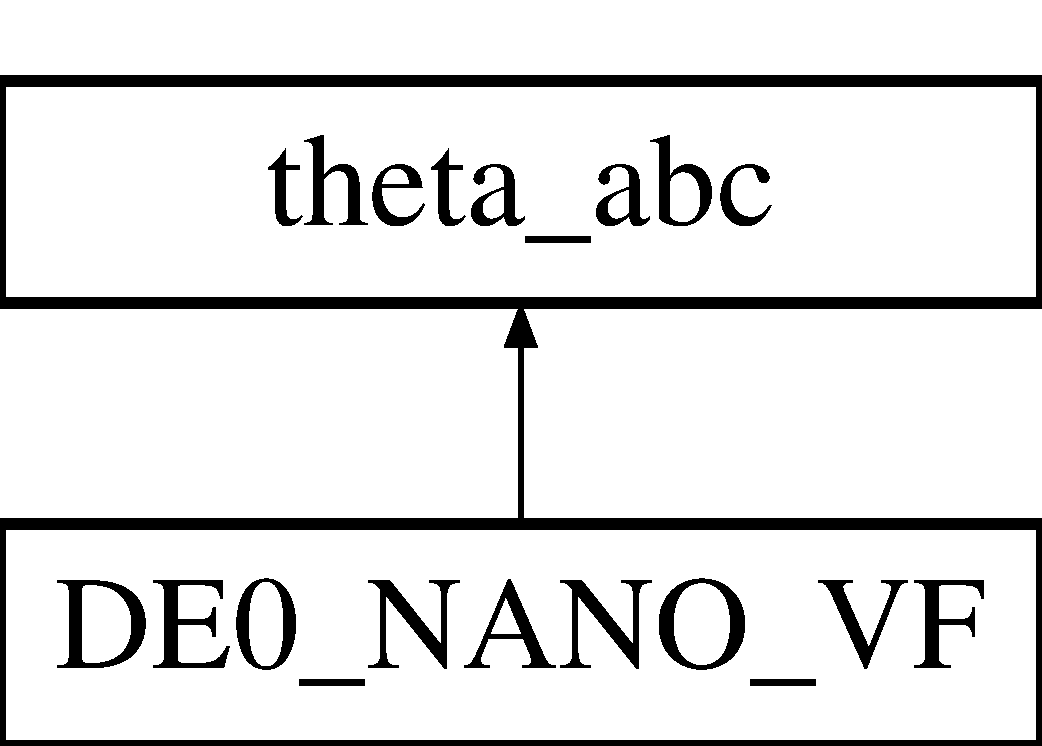
\includegraphics[height=2.000000cm]{classtheta__abc}
\end{center}
\end{figure}
\subsection*{Entities}
\begin{DoxyCompactItemize}
\item 
\hyperlink{classtheta__abc_1_1theta__abc}{theta\+\_\+abc} architecture
\end{DoxyCompactItemize}
\subsection*{Libraries}
 \begin{DoxyCompactItemize}
\item 
\hyperlink{classtheta__abc_ae4f03c286607f3181e16b9aa12d0c6d4}{I\+E\+E\+E} 
\end{DoxyCompactItemize}
\subsection*{Use Clauses}
 \begin{DoxyCompactItemize}
\item 
\hyperlink{classtheta__abc_a241c3e72dd8024cc8ae831b1b2aed7db}{S\+T\+D\+\_\+\+L\+O\+G\+I\+C\+\_\+\+U\+N\+S\+I\+G\+N\+E\+D}   
\item 
\hyperlink{classtheta__abc_aa4b2b25246a821511120e3149b003563}{S\+T\+D\+\_\+\+L\+O\+G\+I\+C\+\_\+1164}   
\item 
\hyperlink{classtheta__abc_aad86249c80e8c1e7ee1c4748aba748e3}{fixed\+\_\+pkg}   
\item 
\hyperlink{classtheta__abc_a2edc34402b573437d5f25fa90ba4013e}{numeric\+\_\+std}   
\end{DoxyCompactItemize}
\subsection*{Generics}
 \begin{DoxyCompactItemize}
\item 
\hyperlink{classtheta__abc_a81567f92ddcbd14c6385d610a895f134}{Nin} {\bfseries {\bfseries \textcolor{comment}{integer}\textcolor{vhdlchar}{ }\textcolor{vhdlchar}{ }\textcolor{vhdlchar}{\+:}\textcolor{vhdlchar}{=}\textcolor{vhdlchar}{ }\textcolor{vhdlchar}{ } \textcolor{vhdldigit}{30} \textcolor{vhdlchar}{ }}}
\item 
\hyperlink{classtheta__abc_ad0f475656f5dd17584d6796fde77d790}{Nout} {\bfseries {\bfseries \textcolor{comment}{integer}\textcolor{vhdlchar}{ }\textcolor{vhdlchar}{ }\textcolor{vhdlchar}{\+:}\textcolor{vhdlchar}{=}\textcolor{vhdlchar}{ }\textcolor{vhdlchar}{ } \textcolor{vhdldigit}{16} \textcolor{vhdlchar}{ }}}
\end{DoxyCompactItemize}
\subsection*{Ports}
 \begin{DoxyCompactItemize}
\item 
\hyperlink{classtheta__abc_a4a4609c199d30b3adebbeb3a01276ec5}{clk}  {\bfseries {\bfseries \textcolor{keywordflow}{in}\textcolor{vhdlchar}{ }}} {\bfseries \textcolor{comment}{std\+\_\+logic}\textcolor{vhdlchar}{ }} 
\item 
\hyperlink{classtheta__abc_adcf9c6f5161d039addbda5819bee64a3}{en}  {\bfseries {\bfseries \textcolor{keywordflow}{in}\textcolor{vhdlchar}{ }}} {\bfseries \textcolor{comment}{std\+\_\+logic}\textcolor{vhdlchar}{ }} 
\item 
\hyperlink{classtheta__abc_aad8dc6359d9e23dabcbf342fadf2fa06}{reset}  {\bfseries {\bfseries \textcolor{keywordflow}{in}\textcolor{vhdlchar}{ }}} {\bfseries \textcolor{comment}{std\+\_\+logic}\textcolor{vhdlchar}{ }} 
\item 
\hyperlink{classtheta__abc_ae915426336e82564b81552bb4a9106c8}{theta\+\_\+a}  {\bfseries {\bfseries \textcolor{keywordflow}{out}\textcolor{vhdlchar}{ }}} {\bfseries \textcolor{comment}{std\+\_\+logic\+\_\+vector}\textcolor{vhdlchar}{ }\textcolor{vhdlchar}{(}\textcolor{vhdlchar}{ }\textcolor{vhdlchar}{ }\textcolor{vhdlchar}{ }\textcolor{vhdlchar}{ }{\bfseries \hyperlink{classtheta__abc_ad0f475656f5dd17584d6796fde77d790}{Nout}} \textcolor{vhdlchar}{-\/}\textcolor{vhdlchar}{ } \textcolor{vhdldigit}{1} \textcolor{vhdlchar}{ }\textcolor{keywordflow}{downto}\textcolor{vhdlchar}{ }\textcolor{vhdlchar}{ } \textcolor{vhdldigit}{0} \textcolor{vhdlchar}{ }\textcolor{vhdlchar}{)}\textcolor{vhdlchar}{ }} 
\item 
\hyperlink{classtheta__abc_a0e4f34615c07a131cc3e798485768ace}{theta\+\_\+b}  {\bfseries {\bfseries \textcolor{keywordflow}{out}\textcolor{vhdlchar}{ }}} {\bfseries \textcolor{comment}{std\+\_\+logic\+\_\+vector}\textcolor{vhdlchar}{ }\textcolor{vhdlchar}{(}\textcolor{vhdlchar}{ }\textcolor{vhdlchar}{ }\textcolor{vhdlchar}{ }\textcolor{vhdlchar}{ }{\bfseries \hyperlink{classtheta__abc_ad0f475656f5dd17584d6796fde77d790}{Nout}} \textcolor{vhdlchar}{-\/}\textcolor{vhdlchar}{ } \textcolor{vhdldigit}{1} \textcolor{vhdlchar}{ }\textcolor{keywordflow}{downto}\textcolor{vhdlchar}{ }\textcolor{vhdlchar}{ } \textcolor{vhdldigit}{0} \textcolor{vhdlchar}{ }\textcolor{vhdlchar}{)}\textcolor{vhdlchar}{ }} 
\item 
\hyperlink{classtheta__abc_a2a449e4b73715ae14ae4178ad27cf5c9}{theta\+\_\+c}  {\bfseries {\bfseries \textcolor{keywordflow}{out}\textcolor{vhdlchar}{ }}} {\bfseries \textcolor{comment}{std\+\_\+logic\+\_\+vector}\textcolor{vhdlchar}{ }\textcolor{vhdlchar}{(}\textcolor{vhdlchar}{ }\textcolor{vhdlchar}{ }\textcolor{vhdlchar}{ }\textcolor{vhdlchar}{ }{\bfseries \hyperlink{classtheta__abc_ad0f475656f5dd17584d6796fde77d790}{Nout}} \textcolor{vhdlchar}{-\/}\textcolor{vhdlchar}{ } \textcolor{vhdldigit}{1} \textcolor{vhdlchar}{ }\textcolor{keywordflow}{downto}\textcolor{vhdlchar}{ }\textcolor{vhdlchar}{ } \textcolor{vhdldigit}{0} \textcolor{vhdlchar}{ }\textcolor{vhdlchar}{)}\textcolor{vhdlchar}{ }} 
\item 
\hyperlink{classtheta__abc_aa0a6389197d6e4203cf6b365fbe2e2d1}{theta\+\_\+in}  {\bfseries {\bfseries \textcolor{keywordflow}{in}\textcolor{vhdlchar}{ }}} {\bfseries \textcolor{comment}{std\+\_\+logic\+\_\+vector}\textcolor{vhdlchar}{ }\textcolor{vhdlchar}{(}\textcolor{vhdlchar}{ }\textcolor{vhdlchar}{ }\textcolor{vhdlchar}{ }\textcolor{vhdlchar}{ }{\bfseries \hyperlink{classtheta__abc_a81567f92ddcbd14c6385d610a895f134}{Nin}} \textcolor{vhdlchar}{-\/}\textcolor{vhdlchar}{ } \textcolor{vhdldigit}{1} \textcolor{vhdlchar}{ }\textcolor{keywordflow}{downto}\textcolor{vhdlchar}{ }\textcolor{vhdlchar}{ } \textcolor{vhdldigit}{0} \textcolor{vhdlchar}{ }\textcolor{vhdlchar}{)}\textcolor{vhdlchar}{ }} 
\end{DoxyCompactItemize}


\subsection{Detailed Description}


Definition at line \hyperlink{theta__abc_8vhd_source_l00008}{8} of file \hyperlink{theta__abc_8vhd_source}{theta\+\_\+abc.\+vhd}.



\subsection{Member Data Documentation}
\hypertarget{classtheta__abc_a4a4609c199d30b3adebbeb3a01276ec5}{}\index{theta\+\_\+abc@{theta\+\_\+abc}!clk@{clk}}
\index{clk@{clk}!theta\+\_\+abc@{theta\+\_\+abc}}
\subsubsection[{clk}]{\setlength{\rightskip}{0pt plus 5cm}{\bf clk} {\bfseries \textcolor{keywordflow}{in}\textcolor{vhdlchar}{ }} {\bfseries \textcolor{comment}{std\+\_\+logic}\textcolor{vhdlchar}{ }} \hspace{0.3cm}{\ttfamily [Port]}}\label{classtheta__abc_a4a4609c199d30b3adebbeb3a01276ec5}


Definition at line \hyperlink{theta__abc_8vhd_source_l00013}{13} of file \hyperlink{theta__abc_8vhd_source}{theta\+\_\+abc.\+vhd}.

\hypertarget{classtheta__abc_adcf9c6f5161d039addbda5819bee64a3}{}\index{theta\+\_\+abc@{theta\+\_\+abc}!en@{en}}
\index{en@{en}!theta\+\_\+abc@{theta\+\_\+abc}}
\subsubsection[{en}]{\setlength{\rightskip}{0pt plus 5cm}{\bf en} {\bfseries \textcolor{keywordflow}{in}\textcolor{vhdlchar}{ }} {\bfseries \textcolor{comment}{std\+\_\+logic}\textcolor{vhdlchar}{ }} \hspace{0.3cm}{\ttfamily [Port]}}\label{classtheta__abc_adcf9c6f5161d039addbda5819bee64a3}


Definition at line \hyperlink{theta__abc_8vhd_source_l00014}{14} of file \hyperlink{theta__abc_8vhd_source}{theta\+\_\+abc.\+vhd}.

\hypertarget{classtheta__abc_aad86249c80e8c1e7ee1c4748aba748e3}{}\index{theta\+\_\+abc@{theta\+\_\+abc}!fixed\+\_\+pkg@{fixed\+\_\+pkg}}
\index{fixed\+\_\+pkg@{fixed\+\_\+pkg}!theta\+\_\+abc@{theta\+\_\+abc}}
\subsubsection[{fixed\+\_\+pkg}]{\setlength{\rightskip}{0pt plus 5cm}{\bf fixed\+\_\+pkg}\hspace{0.3cm}{\ttfamily [Package]}}\label{classtheta__abc_aad86249c80e8c1e7ee1c4748aba748e3}


Definition at line \hyperlink{theta__abc_8vhd_source_l00004}{4} of file \hyperlink{theta__abc_8vhd_source}{theta\+\_\+abc.\+vhd}.

\hypertarget{classtheta__abc_ae4f03c286607f3181e16b9aa12d0c6d4}{}\index{theta\+\_\+abc@{theta\+\_\+abc}!I\+E\+E\+E@{I\+E\+E\+E}}
\index{I\+E\+E\+E@{I\+E\+E\+E}!theta\+\_\+abc@{theta\+\_\+abc}}
\subsubsection[{I\+E\+E\+E}]{\setlength{\rightskip}{0pt plus 5cm}{\bf I\+E\+E\+E}\hspace{0.3cm}{\ttfamily [Library]}}\label{classtheta__abc_ae4f03c286607f3181e16b9aa12d0c6d4}


Definition at line \hyperlink{theta__abc_8vhd_source_l00001}{1} of file \hyperlink{theta__abc_8vhd_source}{theta\+\_\+abc.\+vhd}.

\hypertarget{classtheta__abc_a81567f92ddcbd14c6385d610a895f134}{}\index{theta\+\_\+abc@{theta\+\_\+abc}!Nin@{Nin}}
\index{Nin@{Nin}!theta\+\_\+abc@{theta\+\_\+abc}}
\subsubsection[{Nin}]{\setlength{\rightskip}{0pt plus 5cm}{\bf Nin} {\bfseries \textcolor{vhdlchar}{ }} {\bfseries \textcolor{comment}{integer}\textcolor{vhdlchar}{ }\textcolor{vhdlchar}{ }\textcolor{vhdlchar}{\+:}\textcolor{vhdlchar}{=}\textcolor{vhdlchar}{ }\textcolor{vhdlchar}{ } \textcolor{vhdldigit}{30} \textcolor{vhdlchar}{ }} \hspace{0.3cm}{\ttfamily [Generic]}}\label{classtheta__abc_a81567f92ddcbd14c6385d610a895f134}


Definition at line \hyperlink{theta__abc_8vhd_source_l00009}{9} of file \hyperlink{theta__abc_8vhd_source}{theta\+\_\+abc.\+vhd}.

\hypertarget{classtheta__abc_ad0f475656f5dd17584d6796fde77d790}{}\index{theta\+\_\+abc@{theta\+\_\+abc}!Nout@{Nout}}
\index{Nout@{Nout}!theta\+\_\+abc@{theta\+\_\+abc}}
\subsubsection[{Nout}]{\setlength{\rightskip}{0pt plus 5cm}{\bf Nout} {\bfseries \textcolor{vhdlchar}{ }} {\bfseries \textcolor{comment}{integer}\textcolor{vhdlchar}{ }\textcolor{vhdlchar}{ }\textcolor{vhdlchar}{\+:}\textcolor{vhdlchar}{=}\textcolor{vhdlchar}{ }\textcolor{vhdlchar}{ } \textcolor{vhdldigit}{16} \textcolor{vhdlchar}{ }} \hspace{0.3cm}{\ttfamily [Generic]}}\label{classtheta__abc_ad0f475656f5dd17584d6796fde77d790}


Definition at line \hyperlink{theta__abc_8vhd_source_l00011}{11} of file \hyperlink{theta__abc_8vhd_source}{theta\+\_\+abc.\+vhd}.

\hypertarget{classtheta__abc_a2edc34402b573437d5f25fa90ba4013e}{}\index{theta\+\_\+abc@{theta\+\_\+abc}!numeric\+\_\+std@{numeric\+\_\+std}}
\index{numeric\+\_\+std@{numeric\+\_\+std}!theta\+\_\+abc@{theta\+\_\+abc}}
\subsubsection[{numeric\+\_\+std}]{\setlength{\rightskip}{0pt plus 5cm}{\bf numeric\+\_\+std}\hspace{0.3cm}{\ttfamily [Package]}}\label{classtheta__abc_a2edc34402b573437d5f25fa90ba4013e}


Definition at line \hyperlink{theta__abc_8vhd_source_l00005}{5} of file \hyperlink{theta__abc_8vhd_source}{theta\+\_\+abc.\+vhd}.

\hypertarget{classtheta__abc_aad8dc6359d9e23dabcbf342fadf2fa06}{}\index{theta\+\_\+abc@{theta\+\_\+abc}!reset@{reset}}
\index{reset@{reset}!theta\+\_\+abc@{theta\+\_\+abc}}
\subsubsection[{reset}]{\setlength{\rightskip}{0pt plus 5cm}{\bf reset} {\bfseries \textcolor{keywordflow}{in}\textcolor{vhdlchar}{ }} {\bfseries \textcolor{comment}{std\+\_\+logic}\textcolor{vhdlchar}{ }} \hspace{0.3cm}{\ttfamily [Port]}}\label{classtheta__abc_aad8dc6359d9e23dabcbf342fadf2fa06}


Definition at line \hyperlink{theta__abc_8vhd_source_l00015}{15} of file \hyperlink{theta__abc_8vhd_source}{theta\+\_\+abc.\+vhd}.

\hypertarget{classtheta__abc_aa4b2b25246a821511120e3149b003563}{}\index{theta\+\_\+abc@{theta\+\_\+abc}!S\+T\+D\+\_\+\+L\+O\+G\+I\+C\+\_\+1164@{S\+T\+D\+\_\+\+L\+O\+G\+I\+C\+\_\+1164}}
\index{S\+T\+D\+\_\+\+L\+O\+G\+I\+C\+\_\+1164@{S\+T\+D\+\_\+\+L\+O\+G\+I\+C\+\_\+1164}!theta\+\_\+abc@{theta\+\_\+abc}}
\subsubsection[{S\+T\+D\+\_\+\+L\+O\+G\+I\+C\+\_\+1164}]{\setlength{\rightskip}{0pt plus 5cm}{\bf S\+T\+D\+\_\+\+L\+O\+G\+I\+C\+\_\+1164}\hspace{0.3cm}{\ttfamily [Package]}}\label{classtheta__abc_aa4b2b25246a821511120e3149b003563}


Definition at line \hyperlink{theta__abc_8vhd_source_l00003}{3} of file \hyperlink{theta__abc_8vhd_source}{theta\+\_\+abc.\+vhd}.

\hypertarget{classtheta__abc_a241c3e72dd8024cc8ae831b1b2aed7db}{}\index{theta\+\_\+abc@{theta\+\_\+abc}!S\+T\+D\+\_\+\+L\+O\+G\+I\+C\+\_\+\+U\+N\+S\+I\+G\+N\+E\+D@{S\+T\+D\+\_\+\+L\+O\+G\+I\+C\+\_\+\+U\+N\+S\+I\+G\+N\+E\+D}}
\index{S\+T\+D\+\_\+\+L\+O\+G\+I\+C\+\_\+\+U\+N\+S\+I\+G\+N\+E\+D@{S\+T\+D\+\_\+\+L\+O\+G\+I\+C\+\_\+\+U\+N\+S\+I\+G\+N\+E\+D}!theta\+\_\+abc@{theta\+\_\+abc}}
\subsubsection[{S\+T\+D\+\_\+\+L\+O\+G\+I\+C\+\_\+\+U\+N\+S\+I\+G\+N\+E\+D}]{\setlength{\rightskip}{0pt plus 5cm}{\bf S\+T\+D\+\_\+\+L\+O\+G\+I\+C\+\_\+\+U\+N\+S\+I\+G\+N\+E\+D}\hspace{0.3cm}{\ttfamily [Package]}}\label{classtheta__abc_a241c3e72dd8024cc8ae831b1b2aed7db}


Definition at line \hyperlink{theta__abc_8vhd_source_l00002}{2} of file \hyperlink{theta__abc_8vhd_source}{theta\+\_\+abc.\+vhd}.

\hypertarget{classtheta__abc_ae915426336e82564b81552bb4a9106c8}{}\index{theta\+\_\+abc@{theta\+\_\+abc}!theta\+\_\+a@{theta\+\_\+a}}
\index{theta\+\_\+a@{theta\+\_\+a}!theta\+\_\+abc@{theta\+\_\+abc}}
\subsubsection[{theta\+\_\+a}]{\setlength{\rightskip}{0pt plus 5cm}{\bf theta\+\_\+a} {\bfseries \textcolor{keywordflow}{out}\textcolor{vhdlchar}{ }} {\bfseries \textcolor{comment}{std\+\_\+logic\+\_\+vector}\textcolor{vhdlchar}{ }\textcolor{vhdlchar}{(}\textcolor{vhdlchar}{ }\textcolor{vhdlchar}{ }\textcolor{vhdlchar}{ }\textcolor{vhdlchar}{ }{\bfseries {\bf Nout}} \textcolor{vhdlchar}{-\/}\textcolor{vhdlchar}{ } \textcolor{vhdldigit}{1} \textcolor{vhdlchar}{ }\textcolor{keywordflow}{downto}\textcolor{vhdlchar}{ }\textcolor{vhdlchar}{ } \textcolor{vhdldigit}{0} \textcolor{vhdlchar}{ }\textcolor{vhdlchar}{)}\textcolor{vhdlchar}{ }} \hspace{0.3cm}{\ttfamily [Port]}}\label{classtheta__abc_ae915426336e82564b81552bb4a9106c8}


Definition at line \hyperlink{theta__abc_8vhd_source_l00016}{16} of file \hyperlink{theta__abc_8vhd_source}{theta\+\_\+abc.\+vhd}.

\hypertarget{classtheta__abc_a0e4f34615c07a131cc3e798485768ace}{}\index{theta\+\_\+abc@{theta\+\_\+abc}!theta\+\_\+b@{theta\+\_\+b}}
\index{theta\+\_\+b@{theta\+\_\+b}!theta\+\_\+abc@{theta\+\_\+abc}}
\subsubsection[{theta\+\_\+b}]{\setlength{\rightskip}{0pt plus 5cm}{\bf theta\+\_\+b} {\bfseries \textcolor{keywordflow}{out}\textcolor{vhdlchar}{ }} {\bfseries \textcolor{comment}{std\+\_\+logic\+\_\+vector}\textcolor{vhdlchar}{ }\textcolor{vhdlchar}{(}\textcolor{vhdlchar}{ }\textcolor{vhdlchar}{ }\textcolor{vhdlchar}{ }\textcolor{vhdlchar}{ }{\bfseries {\bf Nout}} \textcolor{vhdlchar}{-\/}\textcolor{vhdlchar}{ } \textcolor{vhdldigit}{1} \textcolor{vhdlchar}{ }\textcolor{keywordflow}{downto}\textcolor{vhdlchar}{ }\textcolor{vhdlchar}{ } \textcolor{vhdldigit}{0} \textcolor{vhdlchar}{ }\textcolor{vhdlchar}{)}\textcolor{vhdlchar}{ }} \hspace{0.3cm}{\ttfamily [Port]}}\label{classtheta__abc_a0e4f34615c07a131cc3e798485768ace}


Definition at line \hyperlink{theta__abc_8vhd_source_l00017}{17} of file \hyperlink{theta__abc_8vhd_source}{theta\+\_\+abc.\+vhd}.

\hypertarget{classtheta__abc_a2a449e4b73715ae14ae4178ad27cf5c9}{}\index{theta\+\_\+abc@{theta\+\_\+abc}!theta\+\_\+c@{theta\+\_\+c}}
\index{theta\+\_\+c@{theta\+\_\+c}!theta\+\_\+abc@{theta\+\_\+abc}}
\subsubsection[{theta\+\_\+c}]{\setlength{\rightskip}{0pt plus 5cm}{\bf theta\+\_\+c} {\bfseries \textcolor{keywordflow}{out}\textcolor{vhdlchar}{ }} {\bfseries \textcolor{comment}{std\+\_\+logic\+\_\+vector}\textcolor{vhdlchar}{ }\textcolor{vhdlchar}{(}\textcolor{vhdlchar}{ }\textcolor{vhdlchar}{ }\textcolor{vhdlchar}{ }\textcolor{vhdlchar}{ }{\bfseries {\bf Nout}} \textcolor{vhdlchar}{-\/}\textcolor{vhdlchar}{ } \textcolor{vhdldigit}{1} \textcolor{vhdlchar}{ }\textcolor{keywordflow}{downto}\textcolor{vhdlchar}{ }\textcolor{vhdlchar}{ } \textcolor{vhdldigit}{0} \textcolor{vhdlchar}{ }\textcolor{vhdlchar}{)}\textcolor{vhdlchar}{ }} \hspace{0.3cm}{\ttfamily [Port]}}\label{classtheta__abc_a2a449e4b73715ae14ae4178ad27cf5c9}


Definition at line \hyperlink{theta__abc_8vhd_source_l00018}{18} of file \hyperlink{theta__abc_8vhd_source}{theta\+\_\+abc.\+vhd}.

\hypertarget{classtheta__abc_aa0a6389197d6e4203cf6b365fbe2e2d1}{}\index{theta\+\_\+abc@{theta\+\_\+abc}!theta\+\_\+in@{theta\+\_\+in}}
\index{theta\+\_\+in@{theta\+\_\+in}!theta\+\_\+abc@{theta\+\_\+abc}}
\subsubsection[{theta\+\_\+in}]{\setlength{\rightskip}{0pt plus 5cm}{\bf theta\+\_\+in} {\bfseries \textcolor{keywordflow}{in}\textcolor{vhdlchar}{ }} {\bfseries \textcolor{comment}{std\+\_\+logic\+\_\+vector}\textcolor{vhdlchar}{ }\textcolor{vhdlchar}{(}\textcolor{vhdlchar}{ }\textcolor{vhdlchar}{ }\textcolor{vhdlchar}{ }\textcolor{vhdlchar}{ }{\bfseries {\bf Nin}} \textcolor{vhdlchar}{-\/}\textcolor{vhdlchar}{ } \textcolor{vhdldigit}{1} \textcolor{vhdlchar}{ }\textcolor{keywordflow}{downto}\textcolor{vhdlchar}{ }\textcolor{vhdlchar}{ } \textcolor{vhdldigit}{0} \textcolor{vhdlchar}{ }\textcolor{vhdlchar}{)}\textcolor{vhdlchar}{ }} \hspace{0.3cm}{\ttfamily [Port]}}\label{classtheta__abc_aa0a6389197d6e4203cf6b365fbe2e2d1}


Definition at line \hyperlink{theta__abc_8vhd_source_l00020}{20} of file \hyperlink{theta__abc_8vhd_source}{theta\+\_\+abc.\+vhd}.



The documentation for this class was generated from the following file\+:\begin{DoxyCompactItemize}
\item 
\hyperlink{theta__abc_8vhd}{theta\+\_\+abc.\+vhd}\end{DoxyCompactItemize}

\hypertarget{classvfcontrol}{}\section{vfcontrol Entity Reference}
\label{classvfcontrol}\index{vfcontrol@{vfcontrol}}
Inheritance diagram for vfcontrol\+:\begin{figure}[H]
\begin{center}
\leavevmode
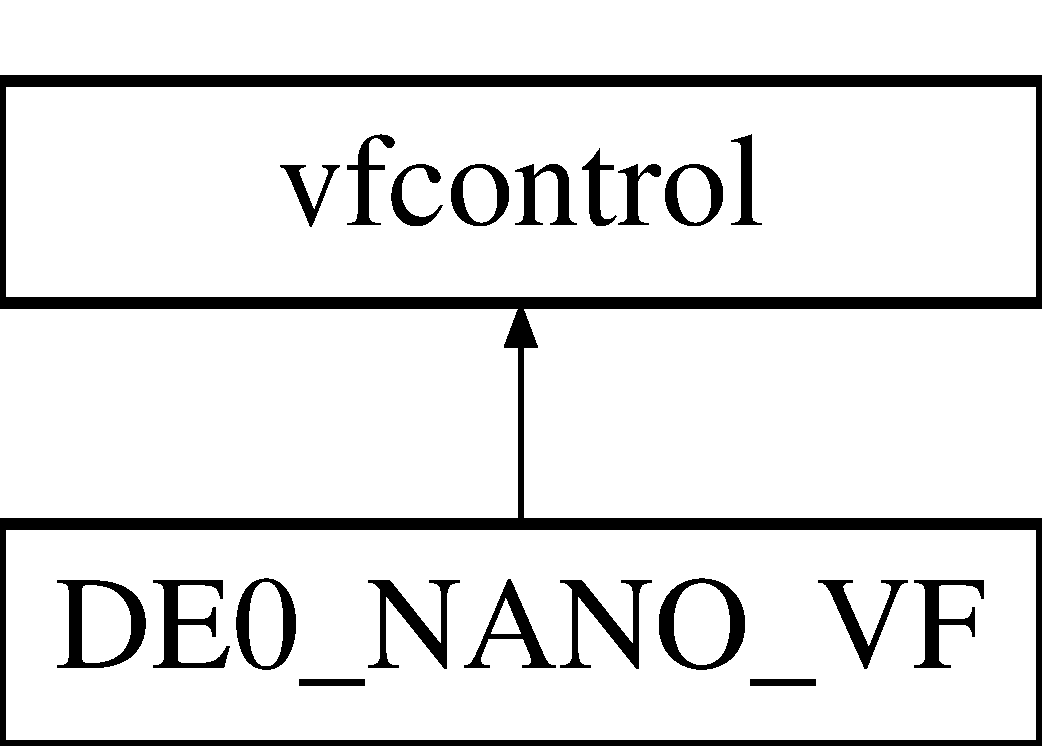
\includegraphics[height=2.000000cm]{classvfcontrol}
\end{center}
\end{figure}
\subsection*{Entities}
\begin{DoxyCompactItemize}
\item 
\hyperlink{classvfcontrol_1_1vfcontrol__arch}{vfcontrol\+\_\+arch} architecture
\end{DoxyCompactItemize}
\subsection*{Libraries}
 \begin{DoxyCompactItemize}
\item 
\hyperlink{classvfcontrol_ae4f03c286607f3181e16b9aa12d0c6d4}{I\+E\+E\+E} 
\end{DoxyCompactItemize}
\subsection*{Use Clauses}
 \begin{DoxyCompactItemize}
\item 
\hyperlink{classvfcontrol_a241c3e72dd8024cc8ae831b1b2aed7db}{S\+T\+D\+\_\+\+L\+O\+G\+I\+C\+\_\+\+U\+N\+S\+I\+G\+N\+E\+D}   
\item 
\hyperlink{classvfcontrol_aa4b2b25246a821511120e3149b003563}{S\+T\+D\+\_\+\+L\+O\+G\+I\+C\+\_\+1164}   
\item 
\hyperlink{classvfcontrol_a5d8c1f7c620a51582be96d2a58d40293}{S\+T\+D\+\_\+\+L\+O\+G\+I\+C\+\_\+\+A\+R\+I\+T\+H}   
\item 
\hyperlink{classvfcontrol_aad86249c80e8c1e7ee1c4748aba748e3}{fixed\+\_\+pkg}   
\item 
\hyperlink{classvfcontrol_a2edc34402b573437d5f25fa90ba4013e}{numeric\+\_\+std}   
\end{DoxyCompactItemize}
\subsection*{Generics}
 \begin{DoxyCompactItemize}
\item 
\hyperlink{classvfcontrol_afee4aa1628956aa350183d8881689198}{n\+\_\+bits\+\_\+c} {\bfseries {\bfseries \textcolor{comment}{integer}\textcolor{vhdlchar}{ }\textcolor{vhdlchar}{ }\textcolor{vhdlchar}{\+:}\textcolor{vhdlchar}{=}\textcolor{vhdlchar}{ }\textcolor{vhdlchar}{ } \textcolor{vhdldigit}{16} \textcolor{vhdlchar}{ }}}
\item 
\hyperlink{classvfcontrol_ac366e3464ed5372201dc4a0b59d91bdd}{inc\+M\+A\+X} {\bfseries {\bfseries \textcolor{comment}{std\+\_\+logic\+\_\+vector}\textcolor{vhdlchar}{ }\textcolor{vhdlchar}{(}\textcolor{vhdlchar}{ }\textcolor{vhdlchar}{ } \textcolor{vhdldigit}{12} \textcolor{vhdlchar}{ }\textcolor{keywordflow}{downto}\textcolor{vhdlchar}{ }\textcolor{vhdlchar}{ } \textcolor{vhdldigit}{0} \textcolor{vhdlchar}{ }\textcolor{vhdlchar}{)}\textcolor{vhdlchar}{ }\textcolor{vhdlchar}{ }\textcolor{vhdlchar}{ }\textcolor{vhdlchar}{\+:}\textcolor{vhdlchar}{=}\textcolor{vhdlchar}{ }\textcolor{vhdlchar}{ }\textcolor{vhdlchar}{ }\textcolor{vhdlchar}{ }\textcolor{comment}{std\+\_\+logic\+\_\+vector}\textcolor{vhdlchar}{ }\textcolor{vhdlchar}{(}\textcolor{vhdlchar}{ }\textcolor{vhdlchar}{to\+\_\+unsigned}\textcolor{vhdlchar}{ }\textcolor{vhdlchar}{(}\textcolor{vhdlchar}{ }\textcolor{vhdlchar}{ } \textcolor{vhdldigit}{2416} \textcolor{vhdlchar}{ }\textcolor{vhdlchar}{,}\textcolor{vhdlchar}{ }\textcolor{vhdlchar}{ } \textcolor{vhdldigit}{13} \textcolor{vhdlchar}{ }\textcolor{vhdlchar}{)}\textcolor{vhdlchar}{ }\textcolor{vhdlchar}{ }\textcolor{vhdlchar}{ }\textcolor{vhdlchar}{)}\textcolor{vhdlchar}{ }}}
\item 
\hyperlink{classvfcontrol_a338e968adaa27098ea77208ca9186ea9}{inc\+M\+I\+N} {\bfseries {\bfseries \textcolor{comment}{std\+\_\+logic\+\_\+vector}\textcolor{vhdlchar}{ }\textcolor{vhdlchar}{(}\textcolor{vhdlchar}{ }\textcolor{vhdlchar}{ } \textcolor{vhdldigit}{12} \textcolor{vhdlchar}{ }\textcolor{keywordflow}{downto}\textcolor{vhdlchar}{ }\textcolor{vhdlchar}{ } \textcolor{vhdldigit}{0} \textcolor{vhdlchar}{ }\textcolor{vhdlchar}{)}\textcolor{vhdlchar}{ }\textcolor{vhdlchar}{ }\textcolor{vhdlchar}{ }\textcolor{vhdlchar}{\+:}\textcolor{vhdlchar}{=}\textcolor{vhdlchar}{ }\textcolor{vhdlchar}{ }\textcolor{vhdlchar}{ }\textcolor{vhdlchar}{ }\textcolor{comment}{std\+\_\+logic\+\_\+vector}\textcolor{vhdlchar}{ }\textcolor{vhdlchar}{(}\textcolor{vhdlchar}{ }\textcolor{vhdlchar}{to\+\_\+unsigned}\textcolor{vhdlchar}{ }\textcolor{vhdlchar}{(}\textcolor{vhdlchar}{ }\textcolor{vhdlchar}{ } \textcolor{vhdldigit}{483} \textcolor{vhdlchar}{ }\textcolor{vhdlchar}{,}\textcolor{vhdlchar}{ }\textcolor{vhdlchar}{ } \textcolor{vhdldigit}{13} \textcolor{vhdlchar}{ }\textcolor{vhdlchar}{)}\textcolor{vhdlchar}{ }\textcolor{vhdlchar}{ }\textcolor{vhdlchar}{ }\textcolor{vhdlchar}{)}\textcolor{vhdlchar}{ }}}
\item 
\hyperlink{classvfcontrol_abb7ce405d45a733b6db94314a4f791fd}{I} {\bfseries {\bfseries \textcolor{comment}{integer}\textcolor{vhdlchar}{ }\textcolor{vhdlchar}{ }\textcolor{vhdlchar}{\+:}\textcolor{vhdlchar}{=}\textcolor{vhdlchar}{ }\textcolor{vhdlchar}{ } \textcolor{vhdldigit}{1} \textcolor{vhdlchar}{ }}}
\item 
\hyperlink{classvfcontrol_aac2d6825f96b21ae984648cc93554339}{F} {\bfseries {\bfseries \textcolor{comment}{integer}\textcolor{vhdlchar}{ }\textcolor{vhdlchar}{ }\textcolor{vhdlchar}{\+:}\textcolor{vhdlchar}{=}\textcolor{vhdlchar}{ }\textcolor{vhdlchar}{ } \textcolor{vhdldigit}{14} \textcolor{vhdlchar}{ }}}
\item 
\hyperlink{classvfcontrol_a35e1281ab3472bb9079152e62c1a9acb}{m\+M\+A\+X} {\bfseries {\bfseries \textcolor{comment}{sfixed}\textcolor{vhdlchar}{ }\textcolor{vhdlchar}{(}\textcolor{vhdlchar}{ }\textcolor{vhdlchar}{ } \textcolor{vhdldigit}{1} \textcolor{vhdlchar}{ }\textcolor{keywordflow}{downto}\textcolor{vhdlchar}{ }\textcolor{vhdlchar}{-\/}\textcolor{vhdlchar}{ } \textcolor{vhdldigit}{27} \textcolor{vhdlchar}{ }\textcolor{vhdlchar}{)}\textcolor{vhdlchar}{ }\textcolor{vhdlchar}{ }\textcolor{vhdlchar}{ }\textcolor{vhdlchar}{\+:}\textcolor{vhdlchar}{=}\textcolor{vhdlchar}{ }\textcolor{vhdlchar}{ }\textcolor{vhdlchar}{ }\textcolor{vhdlchar}{ }\textcolor{vhdlchar}{to\+\_\+sfixed}\textcolor{vhdlchar}{ }\textcolor{vhdlchar}{(}\textcolor{vhdlchar}{ }\textcolor{vhdlchar}{ } \textcolor{vhdldigit}{0} \textcolor{vhdlchar}{.} \textcolor{vhdldigit}{4069} \textcolor{vhdlchar}{ }\textcolor{vhdlchar}{,}\textcolor{vhdlchar}{ }\textcolor{vhdlchar}{ } \textcolor{vhdldigit}{1} \textcolor{vhdlchar}{ }\textcolor{vhdlchar}{,}\textcolor{vhdlchar}{ }\textcolor{vhdlchar}{-\/}\textcolor{vhdlchar}{ } \textcolor{vhdldigit}{27} \textcolor{vhdlchar}{ }\textcolor{vhdlchar}{)}\textcolor{vhdlchar}{ }}}
\item 
\hyperlink{classvfcontrol_a9912dbac80dc6644996e1665646e0823}{m\+M\+I\+N} {\bfseries {\bfseries \textcolor{comment}{sfixed}\textcolor{vhdlchar}{ }\textcolor{vhdlchar}{(}\textcolor{vhdlchar}{ }\textcolor{vhdlchar}{ } \textcolor{vhdldigit}{1} \textcolor{vhdlchar}{ }\textcolor{keywordflow}{downto}\textcolor{vhdlchar}{ }\textcolor{vhdlchar}{-\/}\textcolor{vhdlchar}{ } \textcolor{vhdldigit}{27} \textcolor{vhdlchar}{ }\textcolor{vhdlchar}{)}\textcolor{vhdlchar}{ }\textcolor{vhdlchar}{ }\textcolor{vhdlchar}{ }\textcolor{vhdlchar}{\+:}\textcolor{vhdlchar}{=}\textcolor{vhdlchar}{ }\textcolor{vhdlchar}{ }\textcolor{vhdlchar}{ }\textcolor{vhdlchar}{ }\textcolor{vhdlchar}{to\+\_\+sfixed}\textcolor{vhdlchar}{ }\textcolor{vhdlchar}{(}\textcolor{vhdlchar}{ }\textcolor{vhdlchar}{ } \textcolor{vhdldigit}{0} \textcolor{vhdlchar}{.} \textcolor{vhdldigit}{08137} \textcolor{vhdlchar}{ }\textcolor{vhdlchar}{,}\textcolor{vhdlchar}{ }\textcolor{vhdlchar}{ } \textcolor{vhdldigit}{1} \textcolor{vhdlchar}{ }\textcolor{vhdlchar}{,}\textcolor{vhdlchar}{ }\textcolor{vhdlchar}{-\/}\textcolor{vhdlchar}{ } \textcolor{vhdldigit}{27} \textcolor{vhdlchar}{ }\textcolor{vhdlchar}{)}\textcolor{vhdlchar}{ }}}
\end{DoxyCompactItemize}
\subsection*{Ports}
 \begin{DoxyCompactItemize}
\item 
\hyperlink{classvfcontrol_a4a4609c199d30b3adebbeb3a01276ec5}{clk}  {\bfseries {\bfseries \textcolor{keywordflow}{in}\textcolor{vhdlchar}{ }}} {\bfseries \textcolor{comment}{std\+\_\+logic}\textcolor{vhdlchar}{ }} 
\item 
\hyperlink{classvfcontrol_adcf9c6f5161d039addbda5819bee64a3}{en}  {\bfseries {\bfseries \textcolor{keywordflow}{in}\textcolor{vhdlchar}{ }}} {\bfseries \textcolor{comment}{std\+\_\+logic}\textcolor{vhdlchar}{ }} 
\item 
\hyperlink{classvfcontrol_af402b7ce8e1b9ac1038c575460c5d156}{inc\+\_\+data}  {\bfseries {\bfseries \textcolor{keywordflow}{out}\textcolor{vhdlchar}{ }}} {\bfseries \textcolor{comment}{std\+\_\+logic\+\_\+vector}\textcolor{vhdlchar}{ }\textcolor{vhdlchar}{(}\textcolor{vhdlchar}{ }\textcolor{vhdlchar}{ } \textcolor{vhdldigit}{12} \textcolor{vhdlchar}{ }\textcolor{keywordflow}{downto}\textcolor{vhdlchar}{ }\textcolor{vhdlchar}{ } \textcolor{vhdldigit}{0} \textcolor{vhdlchar}{ }\textcolor{vhdlchar}{)}\textcolor{vhdlchar}{ }} 
\item 
\hyperlink{classvfcontrol_a556e3576ef1696c57d447032f986bf5a}{m\+\_\+vf}  {\bfseries {\bfseries \textcolor{keywordflow}{out}\textcolor{vhdlchar}{ }}} {\bfseries \textcolor{comment}{sfixed}\textcolor{vhdlchar}{ }\textcolor{vhdlchar}{(}\textcolor{vhdlchar}{ }\textcolor{vhdlchar}{ }\textcolor{vhdlchar}{ }\textcolor{vhdlchar}{ }{\bfseries \hyperlink{classvfcontrol_abb7ce405d45a733b6db94314a4f791fd}{I}} \textcolor{vhdlchar}{ }\textcolor{keywordflow}{downto}\textcolor{vhdlchar}{ }\textcolor{vhdlchar}{-\/}\textcolor{vhdlchar}{ }\textcolor{vhdlchar}{ }\textcolor{vhdlchar}{ }{\bfseries \hyperlink{classvfcontrol_aac2d6825f96b21ae984648cc93554339}{F}} \textcolor{vhdlchar}{ }\textcolor{vhdlchar}{)}\textcolor{vhdlchar}{ }} 
\end{DoxyCompactItemize}


\subsection{Detailed Description}


Definition at line \hyperlink{vfcontrol_8vhd_source_l00010}{10} of file \hyperlink{vfcontrol_8vhd_source}{vfcontrol.\+vhd}.



\subsection{Member Data Documentation}
\hypertarget{classvfcontrol_a4a4609c199d30b3adebbeb3a01276ec5}{}\index{vfcontrol@{vfcontrol}!clk@{clk}}
\index{clk@{clk}!vfcontrol@{vfcontrol}}
\subsubsection[{clk}]{\setlength{\rightskip}{0pt plus 5cm}{\bf clk} {\bfseries \textcolor{keywordflow}{in}\textcolor{vhdlchar}{ }} {\bfseries \textcolor{comment}{std\+\_\+logic}\textcolor{vhdlchar}{ }} \hspace{0.3cm}{\ttfamily [Port]}}\label{classvfcontrol_a4a4609c199d30b3adebbeb3a01276ec5}


Definition at line \hyperlink{vfcontrol_8vhd_source_l00024}{24} of file \hyperlink{vfcontrol_8vhd_source}{vfcontrol.\+vhd}.

\hypertarget{classvfcontrol_adcf9c6f5161d039addbda5819bee64a3}{}\index{vfcontrol@{vfcontrol}!en@{en}}
\index{en@{en}!vfcontrol@{vfcontrol}}
\subsubsection[{en}]{\setlength{\rightskip}{0pt plus 5cm}{\bf en} {\bfseries \textcolor{keywordflow}{in}\textcolor{vhdlchar}{ }} {\bfseries \textcolor{comment}{std\+\_\+logic}\textcolor{vhdlchar}{ }} \hspace{0.3cm}{\ttfamily [Port]}}\label{classvfcontrol_adcf9c6f5161d039addbda5819bee64a3}


Definition at line \hyperlink{vfcontrol_8vhd_source_l00025}{25} of file \hyperlink{vfcontrol_8vhd_source}{vfcontrol.\+vhd}.

\hypertarget{classvfcontrol_aac2d6825f96b21ae984648cc93554339}{}\index{vfcontrol@{vfcontrol}!F@{F}}
\index{F@{F}!vfcontrol@{vfcontrol}}
\subsubsection[{F}]{\setlength{\rightskip}{0pt plus 5cm}{\bf F} {\bfseries \textcolor{vhdlchar}{ }} {\bfseries \textcolor{comment}{integer}\textcolor{vhdlchar}{ }\textcolor{vhdlchar}{ }\textcolor{vhdlchar}{\+:}\textcolor{vhdlchar}{=}\textcolor{vhdlchar}{ }\textcolor{vhdlchar}{ } \textcolor{vhdldigit}{14} \textcolor{vhdlchar}{ }} \hspace{0.3cm}{\ttfamily [Generic]}}\label{classvfcontrol_aac2d6825f96b21ae984648cc93554339}


Definition at line \hyperlink{vfcontrol_8vhd_source_l00017}{17} of file \hyperlink{vfcontrol_8vhd_source}{vfcontrol.\+vhd}.

\hypertarget{classvfcontrol_aad86249c80e8c1e7ee1c4748aba748e3}{}\index{vfcontrol@{vfcontrol}!fixed\+\_\+pkg@{fixed\+\_\+pkg}}
\index{fixed\+\_\+pkg@{fixed\+\_\+pkg}!vfcontrol@{vfcontrol}}
\subsubsection[{fixed\+\_\+pkg}]{\setlength{\rightskip}{0pt plus 5cm}{\bf fixed\+\_\+pkg}\hspace{0.3cm}{\ttfamily [Package]}}\label{classvfcontrol_aad86249c80e8c1e7ee1c4748aba748e3}


Definition at line \hyperlink{vfcontrol_8vhd_source_l00006}{6} of file \hyperlink{vfcontrol_8vhd_source}{vfcontrol.\+vhd}.

\hypertarget{classvfcontrol_abb7ce405d45a733b6db94314a4f791fd}{}\index{vfcontrol@{vfcontrol}!I@{I}}
\index{I@{I}!vfcontrol@{vfcontrol}}
\subsubsection[{I}]{\setlength{\rightskip}{0pt plus 5cm}{\bf I} {\bfseries \textcolor{vhdlchar}{ }} {\bfseries \textcolor{comment}{integer}\textcolor{vhdlchar}{ }\textcolor{vhdlchar}{ }\textcolor{vhdlchar}{\+:}\textcolor{vhdlchar}{=}\textcolor{vhdlchar}{ }\textcolor{vhdlchar}{ } \textcolor{vhdldigit}{1} \textcolor{vhdlchar}{ }} \hspace{0.3cm}{\ttfamily [Generic]}}\label{classvfcontrol_abb7ce405d45a733b6db94314a4f791fd}


Definition at line \hyperlink{vfcontrol_8vhd_source_l00016}{16} of file \hyperlink{vfcontrol_8vhd_source}{vfcontrol.\+vhd}.

\hypertarget{classvfcontrol_ae4f03c286607f3181e16b9aa12d0c6d4}{}\index{vfcontrol@{vfcontrol}!I\+E\+E\+E@{I\+E\+E\+E}}
\index{I\+E\+E\+E@{I\+E\+E\+E}!vfcontrol@{vfcontrol}}
\subsubsection[{I\+E\+E\+E}]{\setlength{\rightskip}{0pt plus 5cm}{\bf I\+E\+E\+E}\hspace{0.3cm}{\ttfamily [Library]}}\label{classvfcontrol_ae4f03c286607f3181e16b9aa12d0c6d4}


Definition at line \hyperlink{vfcontrol_8vhd_source_l00002}{2} of file \hyperlink{vfcontrol_8vhd_source}{vfcontrol.\+vhd}.

\hypertarget{classvfcontrol_af402b7ce8e1b9ac1038c575460c5d156}{}\index{vfcontrol@{vfcontrol}!inc\+\_\+data@{inc\+\_\+data}}
\index{inc\+\_\+data@{inc\+\_\+data}!vfcontrol@{vfcontrol}}
\subsubsection[{inc\+\_\+data}]{\setlength{\rightskip}{0pt plus 5cm}{\bf inc\+\_\+data} {\bfseries \textcolor{keywordflow}{out}\textcolor{vhdlchar}{ }} {\bfseries \textcolor{comment}{std\+\_\+logic\+\_\+vector}\textcolor{vhdlchar}{ }\textcolor{vhdlchar}{(}\textcolor{vhdlchar}{ }\textcolor{vhdlchar}{ } \textcolor{vhdldigit}{12} \textcolor{vhdlchar}{ }\textcolor{keywordflow}{downto}\textcolor{vhdlchar}{ }\textcolor{vhdlchar}{ } \textcolor{vhdldigit}{0} \textcolor{vhdlchar}{ }\textcolor{vhdlchar}{)}\textcolor{vhdlchar}{ }} \hspace{0.3cm}{\ttfamily [Port]}}\label{classvfcontrol_af402b7ce8e1b9ac1038c575460c5d156}


Definition at line \hyperlink{vfcontrol_8vhd_source_l00026}{26} of file \hyperlink{vfcontrol_8vhd_source}{vfcontrol.\+vhd}.

\hypertarget{classvfcontrol_ac366e3464ed5372201dc4a0b59d91bdd}{}\index{vfcontrol@{vfcontrol}!inc\+M\+A\+X@{inc\+M\+A\+X}}
\index{inc\+M\+A\+X@{inc\+M\+A\+X}!vfcontrol@{vfcontrol}}
\subsubsection[{inc\+M\+A\+X}]{\setlength{\rightskip}{0pt plus 5cm}{\bf inc\+M\+A\+X} {\bfseries \textcolor{vhdlchar}{ }} {\bfseries \textcolor{comment}{std\+\_\+logic\+\_\+vector}\textcolor{vhdlchar}{ }\textcolor{vhdlchar}{(}\textcolor{vhdlchar}{ }\textcolor{vhdlchar}{ } \textcolor{vhdldigit}{12} \textcolor{vhdlchar}{ }\textcolor{keywordflow}{downto}\textcolor{vhdlchar}{ }\textcolor{vhdlchar}{ } \textcolor{vhdldigit}{0} \textcolor{vhdlchar}{ }\textcolor{vhdlchar}{)}\textcolor{vhdlchar}{ }\textcolor{vhdlchar}{ }\textcolor{vhdlchar}{ }\textcolor{vhdlchar}{\+:}\textcolor{vhdlchar}{=}\textcolor{vhdlchar}{ }\textcolor{vhdlchar}{ }\textcolor{vhdlchar}{ }\textcolor{vhdlchar}{ }\textcolor{comment}{std\+\_\+logic\+\_\+vector}\textcolor{vhdlchar}{ }\textcolor{vhdlchar}{(}\textcolor{vhdlchar}{ }\textcolor{vhdlchar}{to\+\_\+unsigned}\textcolor{vhdlchar}{ }\textcolor{vhdlchar}{(}\textcolor{vhdlchar}{ }\textcolor{vhdlchar}{ } \textcolor{vhdldigit}{2416} \textcolor{vhdlchar}{ }\textcolor{vhdlchar}{,}\textcolor{vhdlchar}{ }\textcolor{vhdlchar}{ } \textcolor{vhdldigit}{13} \textcolor{vhdlchar}{ }\textcolor{vhdlchar}{)}\textcolor{vhdlchar}{ }\textcolor{vhdlchar}{ }\textcolor{vhdlchar}{ }\textcolor{vhdlchar}{)}\textcolor{vhdlchar}{ }} \hspace{0.3cm}{\ttfamily [Generic]}}\label{classvfcontrol_ac366e3464ed5372201dc4a0b59d91bdd}


Definition at line \hyperlink{vfcontrol_8vhd_source_l00014}{14} of file \hyperlink{vfcontrol_8vhd_source}{vfcontrol.\+vhd}.

\hypertarget{classvfcontrol_a338e968adaa27098ea77208ca9186ea9}{}\index{vfcontrol@{vfcontrol}!inc\+M\+I\+N@{inc\+M\+I\+N}}
\index{inc\+M\+I\+N@{inc\+M\+I\+N}!vfcontrol@{vfcontrol}}
\subsubsection[{inc\+M\+I\+N}]{\setlength{\rightskip}{0pt plus 5cm}{\bf inc\+M\+I\+N} {\bfseries \textcolor{vhdlchar}{ }} {\bfseries \textcolor{comment}{std\+\_\+logic\+\_\+vector}\textcolor{vhdlchar}{ }\textcolor{vhdlchar}{(}\textcolor{vhdlchar}{ }\textcolor{vhdlchar}{ } \textcolor{vhdldigit}{12} \textcolor{vhdlchar}{ }\textcolor{keywordflow}{downto}\textcolor{vhdlchar}{ }\textcolor{vhdlchar}{ } \textcolor{vhdldigit}{0} \textcolor{vhdlchar}{ }\textcolor{vhdlchar}{)}\textcolor{vhdlchar}{ }\textcolor{vhdlchar}{ }\textcolor{vhdlchar}{ }\textcolor{vhdlchar}{\+:}\textcolor{vhdlchar}{=}\textcolor{vhdlchar}{ }\textcolor{vhdlchar}{ }\textcolor{vhdlchar}{ }\textcolor{vhdlchar}{ }\textcolor{comment}{std\+\_\+logic\+\_\+vector}\textcolor{vhdlchar}{ }\textcolor{vhdlchar}{(}\textcolor{vhdlchar}{ }\textcolor{vhdlchar}{to\+\_\+unsigned}\textcolor{vhdlchar}{ }\textcolor{vhdlchar}{(}\textcolor{vhdlchar}{ }\textcolor{vhdlchar}{ } \textcolor{vhdldigit}{483} \textcolor{vhdlchar}{ }\textcolor{vhdlchar}{,}\textcolor{vhdlchar}{ }\textcolor{vhdlchar}{ } \textcolor{vhdldigit}{13} \textcolor{vhdlchar}{ }\textcolor{vhdlchar}{)}\textcolor{vhdlchar}{ }\textcolor{vhdlchar}{ }\textcolor{vhdlchar}{ }\textcolor{vhdlchar}{)}\textcolor{vhdlchar}{ }} \hspace{0.3cm}{\ttfamily [Generic]}}\label{classvfcontrol_a338e968adaa27098ea77208ca9186ea9}


Definition at line \hyperlink{vfcontrol_8vhd_source_l00015}{15} of file \hyperlink{vfcontrol_8vhd_source}{vfcontrol.\+vhd}.

\hypertarget{classvfcontrol_a556e3576ef1696c57d447032f986bf5a}{}\index{vfcontrol@{vfcontrol}!m\+\_\+vf@{m\+\_\+vf}}
\index{m\+\_\+vf@{m\+\_\+vf}!vfcontrol@{vfcontrol}}
\subsubsection[{m\+\_\+vf}]{\setlength{\rightskip}{0pt plus 5cm}{\bf m\+\_\+vf} {\bfseries \textcolor{keywordflow}{out}\textcolor{vhdlchar}{ }} {\bfseries \textcolor{comment}{sfixed}\textcolor{vhdlchar}{ }\textcolor{vhdlchar}{(}\textcolor{vhdlchar}{ }\textcolor{vhdlchar}{ }\textcolor{vhdlchar}{ }\textcolor{vhdlchar}{ }{\bfseries {\bf I}} \textcolor{vhdlchar}{ }\textcolor{keywordflow}{downto}\textcolor{vhdlchar}{ }\textcolor{vhdlchar}{-\/}\textcolor{vhdlchar}{ }\textcolor{vhdlchar}{ }\textcolor{vhdlchar}{ }{\bfseries {\bf F}} \textcolor{vhdlchar}{ }\textcolor{vhdlchar}{)}\textcolor{vhdlchar}{ }} \hspace{0.3cm}{\ttfamily [Port]}}\label{classvfcontrol_a556e3576ef1696c57d447032f986bf5a}


Definition at line \hyperlink{vfcontrol_8vhd_source_l00028}{28} of file \hyperlink{vfcontrol_8vhd_source}{vfcontrol.\+vhd}.

\hypertarget{classvfcontrol_a35e1281ab3472bb9079152e62c1a9acb}{}\index{vfcontrol@{vfcontrol}!m\+M\+A\+X@{m\+M\+A\+X}}
\index{m\+M\+A\+X@{m\+M\+A\+X}!vfcontrol@{vfcontrol}}
\subsubsection[{m\+M\+A\+X}]{\setlength{\rightskip}{0pt plus 5cm}{\bf m\+M\+A\+X} {\bfseries \textcolor{vhdlchar}{ }} {\bfseries \textcolor{comment}{sfixed}\textcolor{vhdlchar}{ }\textcolor{vhdlchar}{(}\textcolor{vhdlchar}{ }\textcolor{vhdlchar}{ } \textcolor{vhdldigit}{1} \textcolor{vhdlchar}{ }\textcolor{keywordflow}{downto}\textcolor{vhdlchar}{ }\textcolor{vhdlchar}{-\/}\textcolor{vhdlchar}{ } \textcolor{vhdldigit}{27} \textcolor{vhdlchar}{ }\textcolor{vhdlchar}{)}\textcolor{vhdlchar}{ }\textcolor{vhdlchar}{ }\textcolor{vhdlchar}{ }\textcolor{vhdlchar}{\+:}\textcolor{vhdlchar}{=}\textcolor{vhdlchar}{ }\textcolor{vhdlchar}{ }\textcolor{vhdlchar}{ }\textcolor{vhdlchar}{ }\textcolor{vhdlchar}{to\+\_\+sfixed}\textcolor{vhdlchar}{ }\textcolor{vhdlchar}{(}\textcolor{vhdlchar}{ }\textcolor{vhdlchar}{ } \textcolor{vhdldigit}{0} \textcolor{vhdlchar}{.} \textcolor{vhdldigit}{4069} \textcolor{vhdlchar}{ }\textcolor{vhdlchar}{,}\textcolor{vhdlchar}{ }\textcolor{vhdlchar}{ } \textcolor{vhdldigit}{1} \textcolor{vhdlchar}{ }\textcolor{vhdlchar}{,}\textcolor{vhdlchar}{ }\textcolor{vhdlchar}{-\/}\textcolor{vhdlchar}{ } \textcolor{vhdldigit}{27} \textcolor{vhdlchar}{ }\textcolor{vhdlchar}{)}\textcolor{vhdlchar}{ }} \hspace{0.3cm}{\ttfamily [Generic]}}\label{classvfcontrol_a35e1281ab3472bb9079152e62c1a9acb}


Definition at line \hyperlink{vfcontrol_8vhd_source_l00019}{19} of file \hyperlink{vfcontrol_8vhd_source}{vfcontrol.\+vhd}.

\hypertarget{classvfcontrol_a9912dbac80dc6644996e1665646e0823}{}\index{vfcontrol@{vfcontrol}!m\+M\+I\+N@{m\+M\+I\+N}}
\index{m\+M\+I\+N@{m\+M\+I\+N}!vfcontrol@{vfcontrol}}
\subsubsection[{m\+M\+I\+N}]{\setlength{\rightskip}{0pt plus 5cm}{\bf m\+M\+I\+N} {\bfseries \textcolor{vhdlchar}{ }} {\bfseries \textcolor{comment}{sfixed}\textcolor{vhdlchar}{ }\textcolor{vhdlchar}{(}\textcolor{vhdlchar}{ }\textcolor{vhdlchar}{ } \textcolor{vhdldigit}{1} \textcolor{vhdlchar}{ }\textcolor{keywordflow}{downto}\textcolor{vhdlchar}{ }\textcolor{vhdlchar}{-\/}\textcolor{vhdlchar}{ } \textcolor{vhdldigit}{27} \textcolor{vhdlchar}{ }\textcolor{vhdlchar}{)}\textcolor{vhdlchar}{ }\textcolor{vhdlchar}{ }\textcolor{vhdlchar}{ }\textcolor{vhdlchar}{\+:}\textcolor{vhdlchar}{=}\textcolor{vhdlchar}{ }\textcolor{vhdlchar}{ }\textcolor{vhdlchar}{ }\textcolor{vhdlchar}{ }\textcolor{vhdlchar}{to\+\_\+sfixed}\textcolor{vhdlchar}{ }\textcolor{vhdlchar}{(}\textcolor{vhdlchar}{ }\textcolor{vhdlchar}{ } \textcolor{vhdldigit}{0} \textcolor{vhdlchar}{.} \textcolor{vhdldigit}{08137} \textcolor{vhdlchar}{ }\textcolor{vhdlchar}{,}\textcolor{vhdlchar}{ }\textcolor{vhdlchar}{ } \textcolor{vhdldigit}{1} \textcolor{vhdlchar}{ }\textcolor{vhdlchar}{,}\textcolor{vhdlchar}{ }\textcolor{vhdlchar}{-\/}\textcolor{vhdlchar}{ } \textcolor{vhdldigit}{27} \textcolor{vhdlchar}{ }\textcolor{vhdlchar}{)}\textcolor{vhdlchar}{ }} \hspace{0.3cm}{\ttfamily [Generic]}}\label{classvfcontrol_a9912dbac80dc6644996e1665646e0823}


Definition at line \hyperlink{vfcontrol_8vhd_source_l00021}{21} of file \hyperlink{vfcontrol_8vhd_source}{vfcontrol.\+vhd}.

\hypertarget{classvfcontrol_afee4aa1628956aa350183d8881689198}{}\index{vfcontrol@{vfcontrol}!n\+\_\+bits\+\_\+c@{n\+\_\+bits\+\_\+c}}
\index{n\+\_\+bits\+\_\+c@{n\+\_\+bits\+\_\+c}!vfcontrol@{vfcontrol}}
\subsubsection[{n\+\_\+bits\+\_\+c}]{\setlength{\rightskip}{0pt plus 5cm}{\bf n\+\_\+bits\+\_\+c} {\bfseries \textcolor{vhdlchar}{ }} {\bfseries \textcolor{comment}{integer}\textcolor{vhdlchar}{ }\textcolor{vhdlchar}{ }\textcolor{vhdlchar}{\+:}\textcolor{vhdlchar}{=}\textcolor{vhdlchar}{ }\textcolor{vhdlchar}{ } \textcolor{vhdldigit}{16} \textcolor{vhdlchar}{ }} \hspace{0.3cm}{\ttfamily [Generic]}}\label{classvfcontrol_afee4aa1628956aa350183d8881689198}


Definition at line \hyperlink{vfcontrol_8vhd_source_l00012}{12} of file \hyperlink{vfcontrol_8vhd_source}{vfcontrol.\+vhd}.

\hypertarget{classvfcontrol_a2edc34402b573437d5f25fa90ba4013e}{}\index{vfcontrol@{vfcontrol}!numeric\+\_\+std@{numeric\+\_\+std}}
\index{numeric\+\_\+std@{numeric\+\_\+std}!vfcontrol@{vfcontrol}}
\subsubsection[{numeric\+\_\+std}]{\setlength{\rightskip}{0pt plus 5cm}{\bf numeric\+\_\+std}\hspace{0.3cm}{\ttfamily [Package]}}\label{classvfcontrol_a2edc34402b573437d5f25fa90ba4013e}


Definition at line \hyperlink{vfcontrol_8vhd_source_l00007}{7} of file \hyperlink{vfcontrol_8vhd_source}{vfcontrol.\+vhd}.

\hypertarget{classvfcontrol_aa4b2b25246a821511120e3149b003563}{}\index{vfcontrol@{vfcontrol}!S\+T\+D\+\_\+\+L\+O\+G\+I\+C\+\_\+1164@{S\+T\+D\+\_\+\+L\+O\+G\+I\+C\+\_\+1164}}
\index{S\+T\+D\+\_\+\+L\+O\+G\+I\+C\+\_\+1164@{S\+T\+D\+\_\+\+L\+O\+G\+I\+C\+\_\+1164}!vfcontrol@{vfcontrol}}
\subsubsection[{S\+T\+D\+\_\+\+L\+O\+G\+I\+C\+\_\+1164}]{\setlength{\rightskip}{0pt plus 5cm}{\bf S\+T\+D\+\_\+\+L\+O\+G\+I\+C\+\_\+1164}\hspace{0.3cm}{\ttfamily [Package]}}\label{classvfcontrol_aa4b2b25246a821511120e3149b003563}


Definition at line \hyperlink{vfcontrol_8vhd_source_l00004}{4} of file \hyperlink{vfcontrol_8vhd_source}{vfcontrol.\+vhd}.

\hypertarget{classvfcontrol_a5d8c1f7c620a51582be96d2a58d40293}{}\index{vfcontrol@{vfcontrol}!S\+T\+D\+\_\+\+L\+O\+G\+I\+C\+\_\+\+A\+R\+I\+T\+H@{S\+T\+D\+\_\+\+L\+O\+G\+I\+C\+\_\+\+A\+R\+I\+T\+H}}
\index{S\+T\+D\+\_\+\+L\+O\+G\+I\+C\+\_\+\+A\+R\+I\+T\+H@{S\+T\+D\+\_\+\+L\+O\+G\+I\+C\+\_\+\+A\+R\+I\+T\+H}!vfcontrol@{vfcontrol}}
\subsubsection[{S\+T\+D\+\_\+\+L\+O\+G\+I\+C\+\_\+\+A\+R\+I\+T\+H}]{\setlength{\rightskip}{0pt plus 5cm}{\bf S\+T\+D\+\_\+\+L\+O\+G\+I\+C\+\_\+\+A\+R\+I\+T\+H}\hspace{0.3cm}{\ttfamily [Package]}}\label{classvfcontrol_a5d8c1f7c620a51582be96d2a58d40293}


Definition at line \hyperlink{vfcontrol_8vhd_source_l00005}{5} of file \hyperlink{vfcontrol_8vhd_source}{vfcontrol.\+vhd}.

\hypertarget{classvfcontrol_a241c3e72dd8024cc8ae831b1b2aed7db}{}\index{vfcontrol@{vfcontrol}!S\+T\+D\+\_\+\+L\+O\+G\+I\+C\+\_\+\+U\+N\+S\+I\+G\+N\+E\+D@{S\+T\+D\+\_\+\+L\+O\+G\+I\+C\+\_\+\+U\+N\+S\+I\+G\+N\+E\+D}}
\index{S\+T\+D\+\_\+\+L\+O\+G\+I\+C\+\_\+\+U\+N\+S\+I\+G\+N\+E\+D@{S\+T\+D\+\_\+\+L\+O\+G\+I\+C\+\_\+\+U\+N\+S\+I\+G\+N\+E\+D}!vfcontrol@{vfcontrol}}
\subsubsection[{S\+T\+D\+\_\+\+L\+O\+G\+I\+C\+\_\+\+U\+N\+S\+I\+G\+N\+E\+D}]{\setlength{\rightskip}{0pt plus 5cm}{\bf S\+T\+D\+\_\+\+L\+O\+G\+I\+C\+\_\+\+U\+N\+S\+I\+G\+N\+E\+D}\hspace{0.3cm}{\ttfamily [Package]}}\label{classvfcontrol_a241c3e72dd8024cc8ae831b1b2aed7db}


Definition at line \hyperlink{vfcontrol_8vhd_source_l00003}{3} of file \hyperlink{vfcontrol_8vhd_source}{vfcontrol.\+vhd}.



The documentation for this class was generated from the following file\+:\begin{DoxyCompactItemize}
\item 
\hyperlink{vfcontrol_8vhd}{vfcontrol.\+vhd}\end{DoxyCompactItemize}

\hypertarget{classvfcontrol_1_1vfcontrol__arch}{}\section{vfcontrol\+\_\+arch Architecture Reference}
\label{classvfcontrol_1_1vfcontrol__arch}\index{vfcontrol\+\_\+arch@{vfcontrol\+\_\+arch}}
\subsection*{Processes}
 \begin{DoxyCompactItemize}
\item 
\hyperlink{classvfcontrol_1_1vfcontrol__arch_aae9b98e25b80f11c0a2d412223b4fe8f}{P\+R\+O\+C\+E\+S\+S\+\_\+16}{\bfseries  ( {\bfseries {\bfseries \hyperlink{classvfcontrol_a4a4609c199d30b3adebbeb3a01276ec5}{clk}} \textcolor{vhdlchar}{ }} )}
\end{DoxyCompactItemize}
\subsection*{Signals}
 \begin{DoxyCompactItemize}
\item 
\hyperlink{classvfcontrol_1_1vfcontrol__arch_a3d75c1af6dd5d31b2957e3cc9acbb450}{incsignal} {\bfseries \textcolor{comment}{std\+\_\+logic\+\_\+vector}\textcolor{vhdlchar}{ }\textcolor{vhdlchar}{(}\textcolor{vhdlchar}{ }\textcolor{vhdlchar}{ } \textcolor{vhdldigit}{12} \textcolor{vhdlchar}{ }\textcolor{keywordflow}{downto}\textcolor{vhdlchar}{ }\textcolor{vhdlchar}{ } \textcolor{vhdldigit}{0} \textcolor{vhdlchar}{ }\textcolor{vhdlchar}{)}\textcolor{vhdlchar}{ }\textcolor{vhdlchar}{ }\textcolor{vhdlchar}{ }\textcolor{vhdlchar}{\+:}\textcolor{vhdlchar}{=}\textcolor{vhdlchar}{ }\textcolor{vhdlchar}{ }\textcolor{vhdlchar}{ }\textcolor{vhdlchar}{ }\textcolor{comment}{std\+\_\+logic\+\_\+vector}\textcolor{vhdlchar}{ }\textcolor{vhdlchar}{(}\textcolor{vhdlchar}{ }\textcolor{vhdlchar}{to\+\_\+unsigned}\textcolor{vhdlchar}{ }\textcolor{vhdlchar}{(}\textcolor{vhdlchar}{ }\textcolor{vhdlchar}{ } \textcolor{vhdldigit}{0} \textcolor{vhdlchar}{ }\textcolor{vhdlchar}{,}\textcolor{vhdlchar}{ }\textcolor{vhdlchar}{ } \textcolor{vhdldigit}{13} \textcolor{vhdlchar}{ }\textcolor{vhdlchar}{)}\textcolor{vhdlchar}{ }\textcolor{vhdlchar}{ }\textcolor{vhdlchar}{ }\textcolor{vhdlchar}{)}\textcolor{vhdlchar}{ }} 
\item 
\hyperlink{classvfcontrol_1_1vfcontrol__arch_a2cb1e2099716ec263d6ed1e10ab1a21e}{msignal} {\bfseries \textcolor{comment}{sfixed}\textcolor{vhdlchar}{ }\textcolor{vhdlchar}{(}\textcolor{vhdlchar}{ }\textcolor{vhdlchar}{ } \textcolor{vhdldigit}{1} \textcolor{vhdlchar}{ }\textcolor{keywordflow}{downto}\textcolor{vhdlchar}{ }\textcolor{vhdlchar}{-\/}\textcolor{vhdlchar}{ } \textcolor{vhdldigit}{27} \textcolor{vhdlchar}{ }\textcolor{vhdlchar}{)}\textcolor{vhdlchar}{ }\textcolor{vhdlchar}{ }\textcolor{vhdlchar}{ }\textcolor{vhdlchar}{\+:}\textcolor{vhdlchar}{=}\textcolor{vhdlchar}{ }\textcolor{vhdlchar}{ }\textcolor{vhdlchar}{ }\textcolor{vhdlchar}{ }\textcolor{vhdlchar}{to\+\_\+sfixed}\textcolor{vhdlchar}{ }\textcolor{vhdlchar}{(}\textcolor{vhdlchar}{ }\textcolor{vhdlchar}{ } \textcolor{vhdldigit}{0} \textcolor{vhdlchar}{.} \textcolor{vhdldigit}{08137} \textcolor{vhdlchar}{ }\textcolor{vhdlchar}{,}\textcolor{vhdlchar}{ }\textcolor{vhdlchar}{ } \textcolor{vhdldigit}{1} \textcolor{vhdlchar}{ }\textcolor{vhdlchar}{,}\textcolor{vhdlchar}{ }\textcolor{vhdlchar}{-\/}\textcolor{vhdlchar}{ } \textcolor{vhdldigit}{27} \textcolor{vhdlchar}{ }\textcolor{vhdlchar}{)}\textcolor{vhdlchar}{ }} 
\item 
\hyperlink{classvfcontrol_1_1vfcontrol__arch_a08d653599c7e1a48cdc2c4e52be9c830}{incstep} {\bfseries \textcolor{comment}{std\+\_\+logic\+\_\+vector}\textcolor{vhdlchar}{ }\textcolor{vhdlchar}{(}\textcolor{vhdlchar}{ }\textcolor{vhdlchar}{ } \textcolor{vhdldigit}{12} \textcolor{vhdlchar}{ }\textcolor{keywordflow}{downto}\textcolor{vhdlchar}{ }\textcolor{vhdlchar}{ } \textcolor{vhdldigit}{0} \textcolor{vhdlchar}{ }\textcolor{vhdlchar}{)}\textcolor{vhdlchar}{ }\textcolor{vhdlchar}{ }\textcolor{vhdlchar}{ }\textcolor{vhdlchar}{\+:}\textcolor{vhdlchar}{=}\textcolor{vhdlchar}{ }\textcolor{vhdlchar}{ }\textcolor{vhdlchar}{ }\textcolor{vhdlchar}{ }\textcolor{comment}{std\+\_\+logic\+\_\+vector}\textcolor{vhdlchar}{ }\textcolor{vhdlchar}{(}\textcolor{vhdlchar}{ }\textcolor{vhdlchar}{to\+\_\+unsigned}\textcolor{vhdlchar}{ }\textcolor{vhdlchar}{(}\textcolor{vhdlchar}{ }\textcolor{vhdlchar}{ } \textcolor{vhdldigit}{1} \textcolor{vhdlchar}{ }\textcolor{vhdlchar}{,}\textcolor{vhdlchar}{ }\textcolor{vhdlchar}{ } \textcolor{vhdldigit}{13} \textcolor{vhdlchar}{ }\textcolor{vhdlchar}{)}\textcolor{vhdlchar}{ }\textcolor{vhdlchar}{ }\textcolor{vhdlchar}{ }\textcolor{vhdlchar}{)}\textcolor{vhdlchar}{ }} 
\item 
\hyperlink{classvfcontrol_1_1vfcontrol__arch_a3d5f05a872732b773487db45eaac7e4f}{mstep} {\bfseries \textcolor{comment}{sfixed}\textcolor{vhdlchar}{ }\textcolor{vhdlchar}{(}\textcolor{vhdlchar}{ }\textcolor{vhdlchar}{ } \textcolor{vhdldigit}{1} \textcolor{vhdlchar}{ }\textcolor{keywordflow}{downto}\textcolor{vhdlchar}{ }\textcolor{vhdlchar}{-\/}\textcolor{vhdlchar}{ } \textcolor{vhdldigit}{27} \textcolor{vhdlchar}{ }\textcolor{vhdlchar}{)}\textcolor{vhdlchar}{ }\textcolor{vhdlchar}{ }\textcolor{vhdlchar}{ }\textcolor{vhdlchar}{\+:}\textcolor{vhdlchar}{=}\textcolor{vhdlchar}{ }\textcolor{vhdlchar}{ }\textcolor{vhdlchar}{ }\textcolor{vhdlchar}{ }\textcolor{vhdlchar}{to\+\_\+sfixed}\textcolor{vhdlchar}{ }\textcolor{vhdlchar}{(}\textcolor{vhdlchar}{ }\textcolor{vhdlchar}{ } \textcolor{vhdldigit}{1} \textcolor{vhdlchar}{.} \textcolor{vhdldigit}{6839e} \textcolor{vhdlchar}{-\/} \textcolor{vhdldigit}{04} \textcolor{vhdlchar}{ }\textcolor{vhdlchar}{,}\textcolor{vhdlchar}{ }\textcolor{vhdlchar}{ } \textcolor{vhdldigit}{1} \textcolor{vhdlchar}{ }\textcolor{vhdlchar}{,}\textcolor{vhdlchar}{ }\textcolor{vhdlchar}{-\/}\textcolor{vhdlchar}{ } \textcolor{vhdldigit}{27} \textcolor{vhdlchar}{ }\textcolor{vhdlchar}{)}\textcolor{vhdlchar}{ }} 
\end{DoxyCompactItemize}


\subsection{Detailed Description}


Definition at line \hyperlink{vfcontrol_8vhd_source_l00035}{35} of file \hyperlink{vfcontrol_8vhd_source}{vfcontrol.\+vhd}.



\subsection{Member Function Documentation}
\hypertarget{classvfcontrol_1_1vfcontrol__arch_aae9b98e25b80f11c0a2d412223b4fe8f}{}\index{vfcontrol\+::vfcontrol\+\_\+arch@{vfcontrol\+::vfcontrol\+\_\+arch}!P\+R\+O\+C\+E\+S\+S\+\_\+16@{P\+R\+O\+C\+E\+S\+S\+\_\+16}}
\index{P\+R\+O\+C\+E\+S\+S\+\_\+16@{P\+R\+O\+C\+E\+S\+S\+\_\+16}!vfcontrol\+::vfcontrol\+\_\+arch@{vfcontrol\+::vfcontrol\+\_\+arch}}
\subsubsection[{P\+R\+O\+C\+E\+S\+S\+\_\+16}]{\setlength{\rightskip}{0pt plus 5cm} {\bfseries \textcolor{vhdlchar}{ }} P\+R\+O\+C\+E\+S\+S\+\_\+16(
\begin{DoxyParamCaption}
\item[{}]{{\bfseries {\bfseries {\bf clk}} \textcolor{vhdlchar}{ }} {\em }}
\end{DoxyParamCaption}
)\hspace{0.3cm}{\ttfamily [Process]}}\label{classvfcontrol_1_1vfcontrol__arch_aae9b98e25b80f11c0a2d412223b4fe8f}


Definition at line \hyperlink{vfcontrol_8vhd_source_l00044}{44} of file \hyperlink{vfcontrol_8vhd_source}{vfcontrol.\+vhd}.



\subsection{Member Data Documentation}
\hypertarget{classvfcontrol_1_1vfcontrol__arch_a3d75c1af6dd5d31b2957e3cc9acbb450}{}\index{vfcontrol\+::vfcontrol\+\_\+arch@{vfcontrol\+::vfcontrol\+\_\+arch}!incsignal@{incsignal}}
\index{incsignal@{incsignal}!vfcontrol\+::vfcontrol\+\_\+arch@{vfcontrol\+::vfcontrol\+\_\+arch}}
\subsubsection[{incsignal}]{\setlength{\rightskip}{0pt plus 5cm}{\bf incsignal} {\bfseries \textcolor{comment}{std\+\_\+logic\+\_\+vector}\textcolor{vhdlchar}{ }\textcolor{vhdlchar}{(}\textcolor{vhdlchar}{ }\textcolor{vhdlchar}{ } \textcolor{vhdldigit}{12} \textcolor{vhdlchar}{ }\textcolor{keywordflow}{downto}\textcolor{vhdlchar}{ }\textcolor{vhdlchar}{ } \textcolor{vhdldigit}{0} \textcolor{vhdlchar}{ }\textcolor{vhdlchar}{)}\textcolor{vhdlchar}{ }\textcolor{vhdlchar}{ }\textcolor{vhdlchar}{ }\textcolor{vhdlchar}{\+:}\textcolor{vhdlchar}{=}\textcolor{vhdlchar}{ }\textcolor{vhdlchar}{ }\textcolor{vhdlchar}{ }\textcolor{vhdlchar}{ }\textcolor{comment}{std\+\_\+logic\+\_\+vector}\textcolor{vhdlchar}{ }\textcolor{vhdlchar}{(}\textcolor{vhdlchar}{ }\textcolor{vhdlchar}{to\+\_\+unsigned}\textcolor{vhdlchar}{ }\textcolor{vhdlchar}{(}\textcolor{vhdlchar}{ }\textcolor{vhdlchar}{ } \textcolor{vhdldigit}{0} \textcolor{vhdlchar}{ }\textcolor{vhdlchar}{,}\textcolor{vhdlchar}{ }\textcolor{vhdlchar}{ } \textcolor{vhdldigit}{13} \textcolor{vhdlchar}{ }\textcolor{vhdlchar}{)}\textcolor{vhdlchar}{ }\textcolor{vhdlchar}{ }\textcolor{vhdlchar}{ }\textcolor{vhdlchar}{)}\textcolor{vhdlchar}{ }} \hspace{0.3cm}{\ttfamily [Signal]}}\label{classvfcontrol_1_1vfcontrol__arch_a3d75c1af6dd5d31b2957e3cc9acbb450}


Definition at line \hyperlink{vfcontrol_8vhd_source_l00037}{37} of file \hyperlink{vfcontrol_8vhd_source}{vfcontrol.\+vhd}.

\hypertarget{classvfcontrol_1_1vfcontrol__arch_a08d653599c7e1a48cdc2c4e52be9c830}{}\index{vfcontrol\+::vfcontrol\+\_\+arch@{vfcontrol\+::vfcontrol\+\_\+arch}!incstep@{incstep}}
\index{incstep@{incstep}!vfcontrol\+::vfcontrol\+\_\+arch@{vfcontrol\+::vfcontrol\+\_\+arch}}
\subsubsection[{incstep}]{\setlength{\rightskip}{0pt plus 5cm}{\bf incstep} {\bfseries \textcolor{comment}{std\+\_\+logic\+\_\+vector}\textcolor{vhdlchar}{ }\textcolor{vhdlchar}{(}\textcolor{vhdlchar}{ }\textcolor{vhdlchar}{ } \textcolor{vhdldigit}{12} \textcolor{vhdlchar}{ }\textcolor{keywordflow}{downto}\textcolor{vhdlchar}{ }\textcolor{vhdlchar}{ } \textcolor{vhdldigit}{0} \textcolor{vhdlchar}{ }\textcolor{vhdlchar}{)}\textcolor{vhdlchar}{ }\textcolor{vhdlchar}{ }\textcolor{vhdlchar}{ }\textcolor{vhdlchar}{\+:}\textcolor{vhdlchar}{=}\textcolor{vhdlchar}{ }\textcolor{vhdlchar}{ }\textcolor{vhdlchar}{ }\textcolor{vhdlchar}{ }\textcolor{comment}{std\+\_\+logic\+\_\+vector}\textcolor{vhdlchar}{ }\textcolor{vhdlchar}{(}\textcolor{vhdlchar}{ }\textcolor{vhdlchar}{to\+\_\+unsigned}\textcolor{vhdlchar}{ }\textcolor{vhdlchar}{(}\textcolor{vhdlchar}{ }\textcolor{vhdlchar}{ } \textcolor{vhdldigit}{1} \textcolor{vhdlchar}{ }\textcolor{vhdlchar}{,}\textcolor{vhdlchar}{ }\textcolor{vhdlchar}{ } \textcolor{vhdldigit}{13} \textcolor{vhdlchar}{ }\textcolor{vhdlchar}{)}\textcolor{vhdlchar}{ }\textcolor{vhdlchar}{ }\textcolor{vhdlchar}{ }\textcolor{vhdlchar}{)}\textcolor{vhdlchar}{ }} \hspace{0.3cm}{\ttfamily [Signal]}}\label{classvfcontrol_1_1vfcontrol__arch_a08d653599c7e1a48cdc2c4e52be9c830}


Definition at line \hyperlink{vfcontrol_8vhd_source_l00039}{39} of file \hyperlink{vfcontrol_8vhd_source}{vfcontrol.\+vhd}.

\hypertarget{classvfcontrol_1_1vfcontrol__arch_a2cb1e2099716ec263d6ed1e10ab1a21e}{}\index{vfcontrol\+::vfcontrol\+\_\+arch@{vfcontrol\+::vfcontrol\+\_\+arch}!msignal@{msignal}}
\index{msignal@{msignal}!vfcontrol\+::vfcontrol\+\_\+arch@{vfcontrol\+::vfcontrol\+\_\+arch}}
\subsubsection[{msignal}]{\setlength{\rightskip}{0pt plus 5cm}{\bf msignal} {\bfseries \textcolor{comment}{sfixed}\textcolor{vhdlchar}{ }\textcolor{vhdlchar}{(}\textcolor{vhdlchar}{ }\textcolor{vhdlchar}{ } \textcolor{vhdldigit}{1} \textcolor{vhdlchar}{ }\textcolor{keywordflow}{downto}\textcolor{vhdlchar}{ }\textcolor{vhdlchar}{-\/}\textcolor{vhdlchar}{ } \textcolor{vhdldigit}{27} \textcolor{vhdlchar}{ }\textcolor{vhdlchar}{)}\textcolor{vhdlchar}{ }\textcolor{vhdlchar}{ }\textcolor{vhdlchar}{ }\textcolor{vhdlchar}{\+:}\textcolor{vhdlchar}{=}\textcolor{vhdlchar}{ }\textcolor{vhdlchar}{ }\textcolor{vhdlchar}{ }\textcolor{vhdlchar}{ }\textcolor{vhdlchar}{to\+\_\+sfixed}\textcolor{vhdlchar}{ }\textcolor{vhdlchar}{(}\textcolor{vhdlchar}{ }\textcolor{vhdlchar}{ } \textcolor{vhdldigit}{0} \textcolor{vhdlchar}{.} \textcolor{vhdldigit}{08137} \textcolor{vhdlchar}{ }\textcolor{vhdlchar}{,}\textcolor{vhdlchar}{ }\textcolor{vhdlchar}{ } \textcolor{vhdldigit}{1} \textcolor{vhdlchar}{ }\textcolor{vhdlchar}{,}\textcolor{vhdlchar}{ }\textcolor{vhdlchar}{-\/}\textcolor{vhdlchar}{ } \textcolor{vhdldigit}{27} \textcolor{vhdlchar}{ }\textcolor{vhdlchar}{)}\textcolor{vhdlchar}{ }} \hspace{0.3cm}{\ttfamily [Signal]}}\label{classvfcontrol_1_1vfcontrol__arch_a2cb1e2099716ec263d6ed1e10ab1a21e}


Definition at line \hyperlink{vfcontrol_8vhd_source_l00038}{38} of file \hyperlink{vfcontrol_8vhd_source}{vfcontrol.\+vhd}.

\hypertarget{classvfcontrol_1_1vfcontrol__arch_a3d5f05a872732b773487db45eaac7e4f}{}\index{vfcontrol\+::vfcontrol\+\_\+arch@{vfcontrol\+::vfcontrol\+\_\+arch}!mstep@{mstep}}
\index{mstep@{mstep}!vfcontrol\+::vfcontrol\+\_\+arch@{vfcontrol\+::vfcontrol\+\_\+arch}}
\subsubsection[{mstep}]{\setlength{\rightskip}{0pt plus 5cm}{\bf mstep} {\bfseries \textcolor{comment}{sfixed}\textcolor{vhdlchar}{ }\textcolor{vhdlchar}{(}\textcolor{vhdlchar}{ }\textcolor{vhdlchar}{ } \textcolor{vhdldigit}{1} \textcolor{vhdlchar}{ }\textcolor{keywordflow}{downto}\textcolor{vhdlchar}{ }\textcolor{vhdlchar}{-\/}\textcolor{vhdlchar}{ } \textcolor{vhdldigit}{27} \textcolor{vhdlchar}{ }\textcolor{vhdlchar}{)}\textcolor{vhdlchar}{ }\textcolor{vhdlchar}{ }\textcolor{vhdlchar}{ }\textcolor{vhdlchar}{\+:}\textcolor{vhdlchar}{=}\textcolor{vhdlchar}{ }\textcolor{vhdlchar}{ }\textcolor{vhdlchar}{ }\textcolor{vhdlchar}{ }\textcolor{vhdlchar}{to\+\_\+sfixed}\textcolor{vhdlchar}{ }\textcolor{vhdlchar}{(}\textcolor{vhdlchar}{ }\textcolor{vhdlchar}{ } \textcolor{vhdldigit}{1} \textcolor{vhdlchar}{.} \textcolor{vhdldigit}{6839e} \textcolor{vhdlchar}{-\/} \textcolor{vhdldigit}{04} \textcolor{vhdlchar}{ }\textcolor{vhdlchar}{,}\textcolor{vhdlchar}{ }\textcolor{vhdlchar}{ } \textcolor{vhdldigit}{1} \textcolor{vhdlchar}{ }\textcolor{vhdlchar}{,}\textcolor{vhdlchar}{ }\textcolor{vhdlchar}{-\/}\textcolor{vhdlchar}{ } \textcolor{vhdldigit}{27} \textcolor{vhdlchar}{ }\textcolor{vhdlchar}{)}\textcolor{vhdlchar}{ }} \hspace{0.3cm}{\ttfamily [Signal]}}\label{classvfcontrol_1_1vfcontrol__arch_a3d5f05a872732b773487db45eaac7e4f}


Definition at line \hyperlink{vfcontrol_8vhd_source_l00040}{40} of file \hyperlink{vfcontrol_8vhd_source}{vfcontrol.\+vhd}.



The documentation for this class was generated from the following file\+:\begin{DoxyCompactItemize}
\item 
\hyperlink{vfcontrol_8vhd}{vfcontrol.\+vhd}\end{DoxyCompactItemize}

\hypertarget{classwt}{}\section{wt Entity Reference}
\label{classwt}\index{wt@{wt}}
\subsection*{Entities}
\begin{DoxyCompactItemize}
\item 
\hyperlink{classwt_1_1wt__arch}{wt\+\_\+arch} architecture
\end{DoxyCompactItemize}
\subsection*{Libraries}
 \begin{DoxyCompactItemize}
\item 
\hyperlink{classwt_ae4f03c286607f3181e16b9aa12d0c6d4}{I\+E\+E\+E} 
\end{DoxyCompactItemize}
\subsection*{Use Clauses}
 \begin{DoxyCompactItemize}
\item 
\hyperlink{classwt_a241c3e72dd8024cc8ae831b1b2aed7db}{S\+T\+D\+\_\+\+L\+O\+G\+I\+C\+\_\+\+U\+N\+S\+I\+G\+N\+E\+D}   
\item 
\hyperlink{classwt_aa4b2b25246a821511120e3149b003563}{S\+T\+D\+\_\+\+L\+O\+G\+I\+C\+\_\+1164}   
\item 
\hyperlink{classwt_aad86249c80e8c1e7ee1c4748aba748e3}{fixed\+\_\+pkg}   
\end{DoxyCompactItemize}
\subsection*{Generics}
 \begin{DoxyCompactItemize}
\item 
\hyperlink{classwt_a8b45761acb3f2e683677c4eb77d442b0}{Nbits} {\bfseries {\bfseries \textcolor{comment}{integer}\textcolor{vhdlchar}{ }\textcolor{vhdlchar}{ }\textcolor{vhdlchar}{\+:}\textcolor{vhdlchar}{=}\textcolor{vhdlchar}{ }\textcolor{vhdlchar}{ } \textcolor{vhdldigit}{16} \textcolor{vhdlchar}{ }}}
\end{DoxyCompactItemize}
\subsection*{Ports}
 \begin{DoxyCompactItemize}
\item 
\hyperlink{classwt_a4a4609c199d30b3adebbeb3a01276ec5}{clk}  {\bfseries {\bfseries \textcolor{keywordflow}{in}\textcolor{vhdlchar}{ }}} {\bfseries \textcolor{comment}{std\+\_\+logic}\textcolor{vhdlchar}{ }} 
\item 
\hyperlink{classwt_adcf9c6f5161d039addbda5819bee64a3}{en}  {\bfseries {\bfseries \textcolor{keywordflow}{in}\textcolor{vhdlchar}{ }}} {\bfseries \textcolor{comment}{std\+\_\+logic}\textcolor{vhdlchar}{ }} 
\item 
\hyperlink{classwt_aad8dc6359d9e23dabcbf342fadf2fa06}{reset}  {\bfseries {\bfseries \textcolor{keywordflow}{in}\textcolor{vhdlchar}{ }}} {\bfseries \textcolor{comment}{std\+\_\+logic}\textcolor{vhdlchar}{ }} 
\item 
\hyperlink{classwt_aae281cf725515894f893258c629a59c7}{sinc}  {\bfseries {\bfseries \textcolor{keywordflow}{out}\textcolor{vhdlchar}{ }}} {\bfseries \textcolor{comment}{std\+\_\+logic}\textcolor{vhdlchar}{ }} 
\item 
\hyperlink{classwt_aee4ab8d7344759fe51ddf58734fd8b17}{M\+A\+X}  {\bfseries {\bfseries \textcolor{keywordflow}{in}\textcolor{vhdlchar}{ }}} {\bfseries \textcolor{comment}{std\+\_\+logic\+\_\+vector}\textcolor{vhdlchar}{ }\textcolor{vhdlchar}{(}\textcolor{vhdlchar}{ }\textcolor{vhdlchar}{ }\textcolor{vhdlchar}{ }\textcolor{vhdlchar}{ }{\bfseries \hyperlink{classwt_a8b45761acb3f2e683677c4eb77d442b0}{Nbits}} \textcolor{vhdlchar}{-\/}\textcolor{vhdlchar}{ } \textcolor{vhdldigit}{1} \textcolor{vhdlchar}{ }\textcolor{keywordflow}{downto}\textcolor{vhdlchar}{ }\textcolor{vhdlchar}{ } \textcolor{vhdldigit}{0} \textcolor{vhdlchar}{ }\textcolor{vhdlchar}{)}\textcolor{vhdlchar}{ }} 
\item 
\hyperlink{classwt_a44ef009b7a1d3a2266fd763d872c2b76}{out\+\_\+data}  {\bfseries {\bfseries \textcolor{keywordflow}{out}\textcolor{vhdlchar}{ }}} {\bfseries \textcolor{comment}{std\+\_\+logic\+\_\+vector}\textcolor{vhdlchar}{ }\textcolor{vhdlchar}{(}\textcolor{vhdlchar}{ }\textcolor{vhdlchar}{ }\textcolor{vhdlchar}{ }\textcolor{vhdlchar}{ }{\bfseries \hyperlink{classwt_a8b45761acb3f2e683677c4eb77d442b0}{Nbits}} \textcolor{vhdlchar}{-\/}\textcolor{vhdlchar}{ } \textcolor{vhdldigit}{1} \textcolor{vhdlchar}{ }\textcolor{keywordflow}{downto}\textcolor{vhdlchar}{ }\textcolor{vhdlchar}{ } \textcolor{vhdldigit}{0} \textcolor{vhdlchar}{ }\textcolor{vhdlchar}{)}\textcolor{vhdlchar}{ }} 
\item 
\hyperlink{classwt_a9e24e3e60e3f24bab11f642255ba1bd4}{int\+\_\+data}  {\bfseries {\bfseries \textcolor{keywordflow}{in}\textcolor{vhdlchar}{ }}} {\bfseries \textcolor{comment}{std\+\_\+logic\+\_\+vector}\textcolor{vhdlchar}{ }\textcolor{vhdlchar}{(}\textcolor{vhdlchar}{ }\textcolor{vhdlchar}{ }\textcolor{vhdlchar}{ }\textcolor{vhdlchar}{ }{\bfseries \hyperlink{classwt_a8b45761acb3f2e683677c4eb77d442b0}{Nbits}} \textcolor{vhdlchar}{-\/}\textcolor{vhdlchar}{ } \textcolor{vhdldigit}{1} \textcolor{vhdlchar}{ }\textcolor{keywordflow}{downto}\textcolor{vhdlchar}{ }\textcolor{vhdlchar}{ } \textcolor{vhdldigit}{0} \textcolor{vhdlchar}{ }\textcolor{vhdlchar}{)}\textcolor{vhdlchar}{ }} 
\end{DoxyCompactItemize}


\subsection{Detailed Description}


Definition at line 8 of file wt.\+vhd.



\subsection{Member Data Documentation}
\hypertarget{classwt_a4a4609c199d30b3adebbeb3a01276ec5}{}\index{wt@{wt}!clk@{clk}}
\index{clk@{clk}!wt@{wt}}
\subsubsection[{clk}]{\setlength{\rightskip}{0pt plus 5cm}{\bf clk} {\bfseries \textcolor{keywordflow}{in}\textcolor{vhdlchar}{ }} {\bfseries \textcolor{comment}{std\+\_\+logic}\textcolor{vhdlchar}{ }} \hspace{0.3cm}{\ttfamily [Port]}}\label{classwt_a4a4609c199d30b3adebbeb3a01276ec5}


Definition at line 13 of file wt.\+vhd.

\hypertarget{classwt_adcf9c6f5161d039addbda5819bee64a3}{}\index{wt@{wt}!en@{en}}
\index{en@{en}!wt@{wt}}
\subsubsection[{en}]{\setlength{\rightskip}{0pt plus 5cm}{\bf en} {\bfseries \textcolor{keywordflow}{in}\textcolor{vhdlchar}{ }} {\bfseries \textcolor{comment}{std\+\_\+logic}\textcolor{vhdlchar}{ }} \hspace{0.3cm}{\ttfamily [Port]}}\label{classwt_adcf9c6f5161d039addbda5819bee64a3}


Definition at line 14 of file wt.\+vhd.

\hypertarget{classwt_aad86249c80e8c1e7ee1c4748aba748e3}{}\index{wt@{wt}!fixed\+\_\+pkg@{fixed\+\_\+pkg}}
\index{fixed\+\_\+pkg@{fixed\+\_\+pkg}!wt@{wt}}
\subsubsection[{fixed\+\_\+pkg}]{\setlength{\rightskip}{0pt plus 5cm}{\bf fixed\+\_\+pkg}\hspace{0.3cm}{\ttfamily [Package]}}\label{classwt_aad86249c80e8c1e7ee1c4748aba748e3}


Definition at line 4 of file wt.\+vhd.

\hypertarget{classwt_ae4f03c286607f3181e16b9aa12d0c6d4}{}\index{wt@{wt}!I\+E\+E\+E@{I\+E\+E\+E}}
\index{I\+E\+E\+E@{I\+E\+E\+E}!wt@{wt}}
\subsubsection[{I\+E\+E\+E}]{\setlength{\rightskip}{0pt plus 5cm}{\bf I\+E\+E\+E}\hspace{0.3cm}{\ttfamily [Library]}}\label{classwt_ae4f03c286607f3181e16b9aa12d0c6d4}


Definition at line 1 of file wt.\+vhd.

\hypertarget{classwt_a9e24e3e60e3f24bab11f642255ba1bd4}{}\index{wt@{wt}!int\+\_\+data@{int\+\_\+data}}
\index{int\+\_\+data@{int\+\_\+data}!wt@{wt}}
\subsubsection[{int\+\_\+data}]{\setlength{\rightskip}{0pt plus 5cm}{\bf int\+\_\+data} {\bfseries \textcolor{keywordflow}{in}\textcolor{vhdlchar}{ }} {\bfseries \textcolor{comment}{std\+\_\+logic\+\_\+vector}\textcolor{vhdlchar}{ }\textcolor{vhdlchar}{(}\textcolor{vhdlchar}{ }\textcolor{vhdlchar}{ }\textcolor{vhdlchar}{ }\textcolor{vhdlchar}{ }{\bfseries {\bf Nbits}} \textcolor{vhdlchar}{-\/}\textcolor{vhdlchar}{ } \textcolor{vhdldigit}{1} \textcolor{vhdlchar}{ }\textcolor{keywordflow}{downto}\textcolor{vhdlchar}{ }\textcolor{vhdlchar}{ } \textcolor{vhdldigit}{0} \textcolor{vhdlchar}{ }\textcolor{vhdlchar}{)}\textcolor{vhdlchar}{ }} \hspace{0.3cm}{\ttfamily [Port]}}\label{classwt_a9e24e3e60e3f24bab11f642255ba1bd4}


Definition at line 20 of file wt.\+vhd.

\hypertarget{classwt_aee4ab8d7344759fe51ddf58734fd8b17}{}\index{wt@{wt}!M\+A\+X@{M\+A\+X}}
\index{M\+A\+X@{M\+A\+X}!wt@{wt}}
\subsubsection[{M\+A\+X}]{\setlength{\rightskip}{0pt plus 5cm}{\bf M\+A\+X} {\bfseries \textcolor{keywordflow}{in}\textcolor{vhdlchar}{ }} {\bfseries \textcolor{comment}{std\+\_\+logic\+\_\+vector}\textcolor{vhdlchar}{ }\textcolor{vhdlchar}{(}\textcolor{vhdlchar}{ }\textcolor{vhdlchar}{ }\textcolor{vhdlchar}{ }\textcolor{vhdlchar}{ }{\bfseries {\bf Nbits}} \textcolor{vhdlchar}{-\/}\textcolor{vhdlchar}{ } \textcolor{vhdldigit}{1} \textcolor{vhdlchar}{ }\textcolor{keywordflow}{downto}\textcolor{vhdlchar}{ }\textcolor{vhdlchar}{ } \textcolor{vhdldigit}{0} \textcolor{vhdlchar}{ }\textcolor{vhdlchar}{)}\textcolor{vhdlchar}{ }} \hspace{0.3cm}{\ttfamily [Port]}}\label{classwt_aee4ab8d7344759fe51ddf58734fd8b17}


Definition at line 17 of file wt.\+vhd.

\hypertarget{classwt_a8b45761acb3f2e683677c4eb77d442b0}{}\index{wt@{wt}!Nbits@{Nbits}}
\index{Nbits@{Nbits}!wt@{wt}}
\subsubsection[{Nbits}]{\setlength{\rightskip}{0pt plus 5cm}{\bf Nbits} {\bfseries \textcolor{vhdlchar}{ }} {\bfseries \textcolor{comment}{integer}\textcolor{vhdlchar}{ }\textcolor{vhdlchar}{ }\textcolor{vhdlchar}{\+:}\textcolor{vhdlchar}{=}\textcolor{vhdlchar}{ }\textcolor{vhdlchar}{ } \textcolor{vhdldigit}{16} \textcolor{vhdlchar}{ }} \hspace{0.3cm}{\ttfamily [Generic]}}\label{classwt_a8b45761acb3f2e683677c4eb77d442b0}


Definition at line 11 of file wt.\+vhd.

\hypertarget{classwt_a44ef009b7a1d3a2266fd763d872c2b76}{}\index{wt@{wt}!out\+\_\+data@{out\+\_\+data}}
\index{out\+\_\+data@{out\+\_\+data}!wt@{wt}}
\subsubsection[{out\+\_\+data}]{\setlength{\rightskip}{0pt plus 5cm}{\bf out\+\_\+data} {\bfseries \textcolor{keywordflow}{out}\textcolor{vhdlchar}{ }} {\bfseries \textcolor{comment}{std\+\_\+logic\+\_\+vector}\textcolor{vhdlchar}{ }\textcolor{vhdlchar}{(}\textcolor{vhdlchar}{ }\textcolor{vhdlchar}{ }\textcolor{vhdlchar}{ }\textcolor{vhdlchar}{ }{\bfseries {\bf Nbits}} \textcolor{vhdlchar}{-\/}\textcolor{vhdlchar}{ } \textcolor{vhdldigit}{1} \textcolor{vhdlchar}{ }\textcolor{keywordflow}{downto}\textcolor{vhdlchar}{ }\textcolor{vhdlchar}{ } \textcolor{vhdldigit}{0} \textcolor{vhdlchar}{ }\textcolor{vhdlchar}{)}\textcolor{vhdlchar}{ }} \hspace{0.3cm}{\ttfamily [Port]}}\label{classwt_a44ef009b7a1d3a2266fd763d872c2b76}


Definition at line 18 of file wt.\+vhd.

\hypertarget{classwt_aad8dc6359d9e23dabcbf342fadf2fa06}{}\index{wt@{wt}!reset@{reset}}
\index{reset@{reset}!wt@{wt}}
\subsubsection[{reset}]{\setlength{\rightskip}{0pt plus 5cm}{\bf reset} {\bfseries \textcolor{keywordflow}{in}\textcolor{vhdlchar}{ }} {\bfseries \textcolor{comment}{std\+\_\+logic}\textcolor{vhdlchar}{ }} \hspace{0.3cm}{\ttfamily [Port]}}\label{classwt_aad8dc6359d9e23dabcbf342fadf2fa06}


Definition at line 15 of file wt.\+vhd.

\hypertarget{classwt_aae281cf725515894f893258c629a59c7}{}\index{wt@{wt}!sinc@{sinc}}
\index{sinc@{sinc}!wt@{wt}}
\subsubsection[{sinc}]{\setlength{\rightskip}{0pt plus 5cm}{\bf sinc} {\bfseries \textcolor{keywordflow}{out}\textcolor{vhdlchar}{ }} {\bfseries \textcolor{comment}{std\+\_\+logic}\textcolor{vhdlchar}{ }} \hspace{0.3cm}{\ttfamily [Port]}}\label{classwt_aae281cf725515894f893258c629a59c7}


Definition at line 16 of file wt.\+vhd.

\hypertarget{classwt_aa4b2b25246a821511120e3149b003563}{}\index{wt@{wt}!S\+T\+D\+\_\+\+L\+O\+G\+I\+C\+\_\+1164@{S\+T\+D\+\_\+\+L\+O\+G\+I\+C\+\_\+1164}}
\index{S\+T\+D\+\_\+\+L\+O\+G\+I\+C\+\_\+1164@{S\+T\+D\+\_\+\+L\+O\+G\+I\+C\+\_\+1164}!wt@{wt}}
\subsubsection[{S\+T\+D\+\_\+\+L\+O\+G\+I\+C\+\_\+1164}]{\setlength{\rightskip}{0pt plus 5cm}{\bf S\+T\+D\+\_\+\+L\+O\+G\+I\+C\+\_\+1164}\hspace{0.3cm}{\ttfamily [Package]}}\label{classwt_aa4b2b25246a821511120e3149b003563}


Definition at line 3 of file wt.\+vhd.

\hypertarget{classwt_a241c3e72dd8024cc8ae831b1b2aed7db}{}\index{wt@{wt}!S\+T\+D\+\_\+\+L\+O\+G\+I\+C\+\_\+\+U\+N\+S\+I\+G\+N\+E\+D@{S\+T\+D\+\_\+\+L\+O\+G\+I\+C\+\_\+\+U\+N\+S\+I\+G\+N\+E\+D}}
\index{S\+T\+D\+\_\+\+L\+O\+G\+I\+C\+\_\+\+U\+N\+S\+I\+G\+N\+E\+D@{S\+T\+D\+\_\+\+L\+O\+G\+I\+C\+\_\+\+U\+N\+S\+I\+G\+N\+E\+D}!wt@{wt}}
\subsubsection[{S\+T\+D\+\_\+\+L\+O\+G\+I\+C\+\_\+\+U\+N\+S\+I\+G\+N\+E\+D}]{\setlength{\rightskip}{0pt plus 5cm}{\bf S\+T\+D\+\_\+\+L\+O\+G\+I\+C\+\_\+\+U\+N\+S\+I\+G\+N\+E\+D}\hspace{0.3cm}{\ttfamily [Package]}}\label{classwt_a241c3e72dd8024cc8ae831b1b2aed7db}


Definition at line 2 of file wt.\+vhd.



The documentation for this class was generated from the following file\+:\begin{DoxyCompactItemize}
\item 
\hyperlink{wt_8vhd}{wt.\+vhd}\end{DoxyCompactItemize}

\hypertarget{classwt_1_1wt__arch}{}\section{wt\+\_\+arch Architecture Reference}
\label{classwt_1_1wt__arch}\index{wt\+\_\+arch@{wt\+\_\+arch}}
\subsection*{Processes}
 \begin{DoxyCompactItemize}
\item 
\hyperlink{classwt_1_1wt__arch_a5427232bb22991550e6168cf5171fc30}{P\+R\+O\+C\+E\+S\+S\+\_\+17}{\bfseries  ( {\bfseries {\bfseries \hyperlink{classwt_a4a4609c199d30b3adebbeb3a01276ec5}{clk}} \textcolor{vhdlchar}{ }} )}
\end{DoxyCompactItemize}
\subsection*{Signals}
 \begin{DoxyCompactItemize}
\item 
\hyperlink{classwt_1_1wt__arch_a495e571184c4e4e4665241de22f331cc}{out\+\_\+int} {\bfseries \textcolor{comment}{std\+\_\+logic\+\_\+vector}\textcolor{vhdlchar}{ }\textcolor{vhdlchar}{(}\textcolor{vhdlchar}{ }\textcolor{vhdlchar}{ }\textcolor{vhdlchar}{ }\textcolor{vhdlchar}{ }{\bfseries \hyperlink{classwt_a8b45761acb3f2e683677c4eb77d442b0}{Nbits}} \textcolor{vhdlchar}{-\/}\textcolor{vhdlchar}{ } \textcolor{vhdldigit}{1} \textcolor{vhdlchar}{ }\textcolor{keywordflow}{downto}\textcolor{vhdlchar}{ }\textcolor{vhdlchar}{ } \textcolor{vhdldigit}{0} \textcolor{vhdlchar}{ }\textcolor{vhdlchar}{)}\textcolor{vhdlchar}{ }} 
\item 
\hyperlink{classwt_1_1wt__arch_a45126d1a75be347f440d181b7aa5e033}{sinc\+\_\+int} {\bfseries \textcolor{comment}{std\+\_\+logic}\textcolor{vhdlchar}{ }} 
\end{DoxyCompactItemize}


\subsection{Detailed Description}


Definition at line 25 of file wt.\+vhd.



\subsection{Member Function Documentation}
\hypertarget{classwt_1_1wt__arch_a5427232bb22991550e6168cf5171fc30}{}\index{wt\+::wt\+\_\+arch@{wt\+::wt\+\_\+arch}!P\+R\+O\+C\+E\+S\+S\+\_\+17@{P\+R\+O\+C\+E\+S\+S\+\_\+17}}
\index{P\+R\+O\+C\+E\+S\+S\+\_\+17@{P\+R\+O\+C\+E\+S\+S\+\_\+17}!wt\+::wt\+\_\+arch@{wt\+::wt\+\_\+arch}}
\subsubsection[{P\+R\+O\+C\+E\+S\+S\+\_\+17}]{\setlength{\rightskip}{0pt plus 5cm} {\bfseries \textcolor{vhdlchar}{ }} P\+R\+O\+C\+E\+S\+S\+\_\+17(
\begin{DoxyParamCaption}
\item[{}]{{\bfseries {\bfseries {\bf clk}} \textcolor{vhdlchar}{ }} {\em }}
\end{DoxyParamCaption}
)\hspace{0.3cm}{\ttfamily [Process]}}\label{classwt_1_1wt__arch_a5427232bb22991550e6168cf5171fc30}


Definition at line 33 of file wt.\+vhd.



\subsection{Member Data Documentation}
\hypertarget{classwt_1_1wt__arch_a495e571184c4e4e4665241de22f331cc}{}\index{wt\+::wt\+\_\+arch@{wt\+::wt\+\_\+arch}!out\+\_\+int@{out\+\_\+int}}
\index{out\+\_\+int@{out\+\_\+int}!wt\+::wt\+\_\+arch@{wt\+::wt\+\_\+arch}}
\subsubsection[{out\+\_\+int}]{\setlength{\rightskip}{0pt plus 5cm}{\bf out\+\_\+int} {\bfseries \textcolor{comment}{std\+\_\+logic\+\_\+vector}\textcolor{vhdlchar}{ }\textcolor{vhdlchar}{(}\textcolor{vhdlchar}{ }\textcolor{vhdlchar}{ }\textcolor{vhdlchar}{ }\textcolor{vhdlchar}{ }{\bfseries {\bf Nbits}} \textcolor{vhdlchar}{-\/}\textcolor{vhdlchar}{ } \textcolor{vhdldigit}{1} \textcolor{vhdlchar}{ }\textcolor{keywordflow}{downto}\textcolor{vhdlchar}{ }\textcolor{vhdlchar}{ } \textcolor{vhdldigit}{0} \textcolor{vhdlchar}{ }\textcolor{vhdlchar}{)}\textcolor{vhdlchar}{ }} \hspace{0.3cm}{\ttfamily [Signal]}}\label{classwt_1_1wt__arch_a495e571184c4e4e4665241de22f331cc}


Definition at line 27 of file wt.\+vhd.

\hypertarget{classwt_1_1wt__arch_a45126d1a75be347f440d181b7aa5e033}{}\index{wt\+::wt\+\_\+arch@{wt\+::wt\+\_\+arch}!sinc\+\_\+int@{sinc\+\_\+int}}
\index{sinc\+\_\+int@{sinc\+\_\+int}!wt\+::wt\+\_\+arch@{wt\+::wt\+\_\+arch}}
\subsubsection[{sinc\+\_\+int}]{\setlength{\rightskip}{0pt plus 5cm}{\bf sinc\+\_\+int} {\bfseries \textcolor{comment}{std\+\_\+logic}\textcolor{vhdlchar}{ }} \hspace{0.3cm}{\ttfamily [Signal]}}\label{classwt_1_1wt__arch_a45126d1a75be347f440d181b7aa5e033}


Definition at line 28 of file wt.\+vhd.



The documentation for this class was generated from the following file\+:\begin{DoxyCompactItemize}
\item 
\hyperlink{wt_8vhd}{wt.\+vhd}\end{DoxyCompactItemize}

\chapter{File Documentation}
\hypertarget{clk__div_8vhd}{}\section{clk\+\_\+div.\+vhd File Reference}
\label{clk__div_8vhd}\index{clk\+\_\+div.\+vhd@{clk\+\_\+div.\+vhd}}
\subsection*{Entities}
\begin{DoxyCompactItemize}
\item 
\hyperlink{classclk__div}{clk\+\_\+div} entity
\item 
\hyperlink{classclk__div_1_1div}{div} architecture
\end{DoxyCompactItemize}

\hypertarget{clk__div_8vhd_source}{}\section{clk\+\_\+div.\+vhd}

\begin{DoxyCode}
\hypertarget{clk__div_8vhd_source_l00001}{}\hyperlink{classclk__div_ae4f03c286607f3181e16b9aa12d0c6d4}{00001} \textcolor{vhdlkeyword}{library }\textcolor{keywordflow}{IEEE};
\hypertarget{clk__div_8vhd_source_l00002}{}\hyperlink{classclk__div_a241c3e72dd8024cc8ae831b1b2aed7db}{00002} \textcolor{vhdlkeyword}{use }IEEE.STD\_LOGIC\_UNSIGNED.\textcolor{keywordflow}{all};
\hypertarget{clk__div_8vhd_source_l00003}{}\hyperlink{classclk__div_aa4b2b25246a821511120e3149b003563}{00003} \textcolor{vhdlkeyword}{use }IEEE.STD\_LOGIC\_1164.\textcolor{keywordflow}{all};
00004 
\hypertarget{clk__div_8vhd_source_l00005}{}\hyperlink{classclk__div}{00005} \textcolor{keywordflow}{entity }\hyperlink{classclk__div}{clk\_div} \textcolor{keywordflow}{is}
00006         \textcolor{keywordflow}{port}\textcolor{vhdlchar}{(}
\hypertarget{clk__div_8vhd_source_l00007}{}\hyperlink{classclk__div_a512588aa484615b7e90600a1bc9507b4}{00007}         \textcolor{vhdlchar}{\hyperlink{classclk__div_a57fad7f33f7766724bdea76e7b0330ef}{clk\_in}}\textcolor{vhdlchar}{,} \textcolor{vhdlchar}{\hyperlink{classclk__div_a512588aa484615b7e90600a1bc9507b4}{en}} \textcolor{vhdlchar}{:} \textcolor{keywordflow}{IN} \textcolor{comment}{STD\_LOGIC};
\hypertarget{clk__div_8vhd_source_l00008}{}\hyperlink{classclk__div_a425c2042b3ea21827b9b29c6712312d9}{00008}         \textcolor{vhdlchar}{\hyperlink{classclk__div_a425c2042b3ea21827b9b29c6712312d9}{div}} \textcolor{vhdlchar}{:} \textcolor{keywordflow}{IN} \textcolor{comment}{STD\_LOGIC\_VECTOR}\textcolor{vhdlchar}{(}\textcolor{vhdllogic}{}\textcolor{vhdllogic}{15} \textcolor{keywordflow}{DOWNTO} \textcolor{vhdllogic}{}\textcolor{vhdllogic}{0}\textcolor{vhdlchar}{)};\textcolor{keyword}{ --f\_out =  f\_in/(2*div)}
00009         \textcolor{vhdlchar}{\hyperlink{classclk__div_a8147ca5cedee84ed9753ac6f1f0b2374}{clk\_out}}\textcolor{vhdlchar}{:} \textcolor{keywordflow}{OUT} \textcolor{comment}{STD\_LOGIC}
\hypertarget{clk__div_8vhd_source_l00010}{}\hyperlink{classclk__div_a8147ca5cedee84ed9753ac6f1f0b2374}{00010}     \textcolor{vhdlchar}{)};
00011 \textcolor{keywordflow}{END} \textcolor{keywordflow}{ENTITY} \textcolor{vhdlchar}{clk\_div};
00012 
\hypertarget{clk__div_8vhd_source_l00013}{}\hyperlink{classclk__div_1_1div}{00013} \textcolor{keywordflow}{ARCHITECTURE} div \textcolor{keywordflow}{OF} \hyperlink{classclk__div}{clk\_div} IS   
\hypertarget{clk__div_8vhd_source_l00014}{}\hyperlink{classclk__div_1_1div_a25d9525383f1b60f7c2e081319516a96}{00014}     \textcolor{keywordflow}{SIGNAL} \textcolor{vhdlchar}{\hyperlink{classclk__div_1_1div_a25d9525383f1b60f7c2e081319516a96}{count}} \textcolor{vhdlchar}{:} \textcolor{comment}{STD\_LOGIC\_VECTOR}\textcolor{vhdlchar}{(}\textcolor{vhdllogic}{}\textcolor{vhdllogic}{15} \textcolor{keywordflow}{DOWNTO} \textcolor{vhdllogic}{}\textcolor{vhdllogic}{0}\textcolor{vhdlchar}{)};
\hypertarget{clk__div_8vhd_source_l00015}{}\hyperlink{classclk__div_1_1div_a91ef6072d99aa4429fb1b3a883554754}{00015}     \textcolor{keywordflow}{SIGNAL} \textcolor{vhdlchar}{\hyperlink{classclk__div_1_1div_a91ef6072d99aa4429fb1b3a883554754}{clk\_out\_bi}} \textcolor{vhdlchar}{:} \textcolor{comment}{STD\_LOGIC};
00016 \textcolor{vhdlkeyword}{BEGIN } 
00017 
\hypertarget{clk__div_8vhd_source_l00018}{}\hyperlink{classclk__div_1_1div_a0a2b446597a947bf6a5807498fa17ba1}{00018}     \textcolor{keywordflow}{PROCESS}(\hyperlink{classclk__div_a57fad7f33f7766724bdea76e7b0330ef}{clk\_in},\hyperlink{classclk__div_a512588aa484615b7e90600a1bc9507b4}{en},\hyperlink{classclk__div_a425c2042b3ea21827b9b29c6712312d9}{div})
00019 \textcolor{vhdlkeyword}{        BEGIN}
00020             \textcolor{keywordflow}{IF} \textcolor{vhdlchar}{\hyperlink{classclk__div_a512588aa484615b7e90600a1bc9507b4}{en}} \textcolor{vhdlchar}{=} \textcolor{vhdlchar}{'}\textcolor{vhdllogic}{}\textcolor{vhdllogic}{0}\textcolor{vhdlchar}{'} \textcolor{keywordflow}{THEN}
00021 \textcolor{keyword}{                --count <= (OTHERS => '0');}
00022                 \textcolor{vhdlchar}{\hyperlink{classclk__div_1_1div_a25d9525383f1b60f7c2e081319516a96}{count}} \textcolor{vhdlchar}{<=} \textcolor{vhdlchar}{(}\textcolor{vhdlchar}{\hyperlink{classclk__div_a425c2042b3ea21827b9b29c6712312d9}{div}}\textcolor{vhdlchar}{-}\textcolor{vhdllogic}{}\textcolor{vhdllogic}{1}\textcolor{vhdlchar}{)};
00023                 \textcolor{vhdlchar}{\hyperlink{classclk__div_1_1div_a91ef6072d99aa4429fb1b3a883554754}{clk\_out\_bi}} \textcolor{vhdlchar}{<=} \textcolor{vhdlchar}{'}\textcolor{vhdllogic}{}\textcolor{vhdllogic}{0}\textcolor{vhdlchar}{'};
00024             \textcolor{keywordflow}{ELSIF} \textcolor{vhdlchar}{rising\_edge}\textcolor{vhdlchar}{(}\textcolor{vhdlchar}{\hyperlink{classclk__div_a57fad7f33f7766724bdea76e7b0330ef}{clk\_in}}\textcolor{vhdlchar}{)} \textcolor{keywordflow}{THEN}
00025             \textcolor{keywordflow}{IF} \textcolor{vhdlchar}{\hyperlink{classclk__div_1_1div_a25d9525383f1b60f7c2e081319516a96}{count}} \textcolor{vhdlchar}{<} \textcolor{vhdlchar}{(}\textcolor{vhdlchar}{\hyperlink{classclk__div_a425c2042b3ea21827b9b29c6712312d9}{div}} \textcolor{vhdlchar}{-} \textcolor{vhdllogic}{}\textcolor{vhdllogic}{1}\textcolor{vhdlchar}{)}  \textcolor{keywordflow}{THEN}
00026                     \textcolor{vhdlchar}{\hyperlink{classclk__div_1_1div_a25d9525383f1b60f7c2e081319516a96}{count}} \textcolor{vhdlchar}{<=} \textcolor{vhdlchar}{\hyperlink{classclk__div_1_1div_a25d9525383f1b60f7c2e081319516a96}{count}} \textcolor{vhdlchar}{+} \textcolor{vhdllogic}{}\textcolor{vhdllogic}{1};
00027                 \textcolor{keywordflow}{ELSE}
00028                     \textcolor{vhdlchar}{\hyperlink{classclk__div_1_1div_a25d9525383f1b60f7c2e081319516a96}{count}} \textcolor{vhdlchar}{<=} \textcolor{vhdlchar}{(}\textcolor{keywordflow}{OTHERS} \textcolor{vhdlchar}{=}\textcolor{vhdlchar}{>} \textcolor{vhdlchar}{'}\textcolor{vhdllogic}{}\textcolor{vhdllogic}{0}\textcolor{vhdlchar}{'}\textcolor{vhdlchar}{)}; 
00029                     \textcolor{vhdlchar}{\hyperlink{classclk__div_1_1div_a91ef6072d99aa4429fb1b3a883554754}{clk\_out\_bi}} \textcolor{vhdlchar}{<=} \textcolor{keywordflow}{NOT} \textcolor{vhdlchar}{\hyperlink{classclk__div_1_1div_a91ef6072d99aa4429fb1b3a883554754}{clk\_out\_bi}};
00030                 \textcolor{keywordflow}{END} \textcolor{keywordflow}{IF};
00031             \textcolor{keywordflow}{END} \textcolor{keywordflow}{IF};
00032             
00033         \textcolor{keywordflow}{END} \textcolor{keywordflow}{PROCESS};
00034         \textcolor{vhdlchar}{\hyperlink{classclk__div_a8147ca5cedee84ed9753ac6f1f0b2374}{clk\_out}} \textcolor{vhdlchar}{<=} \textcolor{vhdlchar}{\hyperlink{classclk__div_1_1div_a91ef6072d99aa4429fb1b3a883554754}{clk\_out\_bi}};
00035          
00036 \textcolor{keywordflow}{END} \textcolor{keywordflow}{ARCHITECTURE} \textcolor{vhdlchar}{\hyperlink{classclk__div_a425c2042b3ea21827b9b29c6712312d9}{div}};
\end{DoxyCode}

\hypertarget{comparador_8vhd}{}\section{comparador.\+vhd File Reference}
\label{comparador_8vhd}\index{comparador.\+vhd@{comparador.\+vhd}}
\subsection*{Entities}
\begin{DoxyCompactItemize}
\item 
\hyperlink{classcomparador}{comparador} entity
\item 
\hyperlink{classcomparador_1_1comparador}{comparador} architecture
\end{DoxyCompactItemize}

\hypertarget{comparador_8vhd_source}{}\section{comparador.\+vhd}

\begin{DoxyCode}
00001 
\hypertarget{comparador_8vhd_source_l00002}{}\hyperlink{classcomparador_ae4f03c286607f3181e16b9aa12d0c6d4}{00002} \textcolor{vhdlkeyword}{library }\textcolor{keywordflow}{IEEE};
\hypertarget{comparador_8vhd_source_l00003}{}\hyperlink{classcomparador_a241c3e72dd8024cc8ae831b1b2aed7db}{00003} \textcolor{vhdlkeyword}{use }\hyperlink{classclk__div_ae4f03c286607f3181e16b9aa12d0c6d4}{IEEE}.STD\_LOGIC\_UNSIGNED.\textcolor{keywordflow}{all};
\hypertarget{comparador_8vhd_source_l00004}{}\hyperlink{classcomparador_aa4b2b25246a821511120e3149b003563}{00004} \textcolor{vhdlkeyword}{use }\hyperlink{classclk__div_ae4f03c286607f3181e16b9aa12d0c6d4}{IEEE}.STD\_LOGIC\_1164.\textcolor{keywordflow}{all};
\hypertarget{comparador_8vhd_source_l00005}{}\hyperlink{classcomparador_aad86249c80e8c1e7ee1c4748aba748e3}{00005} \textcolor{vhdlkeyword}{use }ieee.\hyperlink{classfixed__pkg}{fixed\_pkg}.\textcolor{keywordflow}{all};\textcolor{keyword}{         --arquivo deve ser adicionado ao projeto  }
\hypertarget{comparador_8vhd_source_l00006}{}\hyperlink{classcomparador_a2edc34402b573437d5f25fa90ba4013e}{00006} \textcolor{vhdlkeyword}{use }ieee.numeric\_std.\textcolor{keywordflow}{all};
00007 
\hypertarget{comparador_8vhd_source_l00008}{}\hyperlink{classcomparador}{00008} \textcolor{keywordflow}{entity }\hyperlink{classcomparador}{comparador} \textcolor{keywordflow}{is}
00009 \textcolor{keywordflow}{generic}  \textcolor{vhdlchar}{(}
00010              \textcolor{keywordflow}{constant} \textcolor{vhdlchar}{\hyperlink{classcomparador_afee4aa1628956aa350183d8881689198}{n\_bits\_c}}\textcolor{vhdlchar}{:} \textcolor{comment}{integer} \textcolor{vhdlchar}{:=} \textcolor{vhdllogic}{}\textcolor{vhdllogic}{16}\textcolor{keyword}{  --numero de bits da portadora}
\hypertarget{comparador_8vhd_source_l00011}{}\hyperlink{classcomparador_afee4aa1628956aa350183d8881689198}{00011}          \textcolor{vhdlchar}{)};
00012     \textcolor{keywordflow}{port}\textcolor{vhdlchar}{(}
\hypertarget{comparador_8vhd_source_l00013}{}\hyperlink{classcomparador_a4a4609c199d30b3adebbeb3a01276ec5}{00013}             \textcolor{vhdlchar}{\hyperlink{classcomparador_a4a4609c199d30b3adebbeb3a01276ec5}{clk}} \textcolor{vhdlchar}{:} \textcolor{keywordflow}{in} \textcolor{comment}{std\_logic};\textcolor{keyword}{ -- clock}
\hypertarget{comparador_8vhd_source_l00014}{}\hyperlink{classcomparador_adcf9c6f5161d039addbda5819bee64a3}{00014}             \textcolor{vhdlchar}{\hyperlink{classcomparador_adcf9c6f5161d039addbda5819bee64a3}{en}} \textcolor{vhdlchar}{:} \textcolor{keywordflow}{in} \textcolor{comment}{std\_logic};\textcolor{keyword}{ -- habilta modulo}
\hypertarget{comparador_8vhd_source_l00015}{}\hyperlink{classcomparador_a0c2a0581e706d5256b50516b6ca4dbed}{00015}             \textcolor{vhdlchar}{\hyperlink{classcomparador_a0c2a0581e706d5256b50516b6ca4dbed}{comp}} \textcolor{vhdlchar}{:} \textcolor{keywordflow}{in} \textcolor{comment}{std\_logic\_vector}\textcolor{vhdlchar}{(}\textcolor{vhdlchar}{\hyperlink{classcomparador_afee4aa1628956aa350183d8881689198}{n\_bits\_c}}\textcolor{vhdlchar}{-}\textcolor{vhdllogic}{}\textcolor{vhdllogic}{1} \textcolor{keywordflow}{downto} \textcolor{vhdllogic}{}\textcolor{vhdllogic}{0}\textcolor{vhdlchar}{)};\textcolor{keyword}{ -- moduladora     }
\hypertarget{comparador_8vhd_source_l00016}{}\hyperlink{classcomparador_a0808bf3e7965a8ee90dec6604647f179}{00016}             \textcolor{vhdlchar}{\hyperlink{classcomparador_a0808bf3e7965a8ee90dec6604647f179}{c}} \textcolor{vhdlchar}{:} \textcolor{keywordflow}{in} \textcolor{comment}{std\_logic\_vector}\textcolor{vhdlchar}{(}\textcolor{vhdlchar}{\hyperlink{classcomparador_afee4aa1628956aa350183d8881689198}{n\_bits\_c}}\textcolor{vhdlchar}{-}\textcolor{vhdllogic}{}\textcolor{vhdllogic}{1} \textcolor{keywordflow}{downto} \textcolor{vhdllogic}{}\textcolor{vhdllogic}{0}\textcolor{vhdlchar}{)};\textcolor{keyword}{ -- portadora}
\hypertarget{comparador_8vhd_source_l00017}{}\hyperlink{classcomparador_af9b8278b961604ab62a822537a109adb}{00017}             \textcolor{vhdlchar}{\hyperlink{classcomparador_af9b8278b961604ab62a822537a109adb}{amost}} \textcolor{vhdlchar}{:}  \textcolor{keywordflow}{in} \textcolor{comment}{std\_logic};\textcolor{keyword}{ -- amostra moduladora na borda de amost}
00018            \textcolor{vhdlchar}{\hyperlink{classcomparador_a2522d63dc2aa0652b3cca6ac9b1da0bd}{comp\_out}} \textcolor{vhdlchar}{:} \textcolor{keywordflow}{out} \textcolor{comment}{std\_logic}
\hypertarget{comparador_8vhd_source_l00019}{}\hyperlink{classcomparador_a2522d63dc2aa0652b3cca6ac9b1da0bd}{00019}             \textcolor{vhdlchar}{)};
00020             
00021 \textcolor{keywordflow}{end} \textcolor{keywordflow}{entity} \textcolor{vhdlchar}{comparador};
00022 
00023 
\hypertarget{comparador_8vhd_source_l00024}{}\hyperlink{classcomparador_1_1comparador}{00024} \textcolor{keywordflow}{architecture} \hyperlink{classcomparador}{comparador} \textcolor{keywordflow}{of} \hyperlink{classcomparador}{comparador} is
00025     
00026 
\hypertarget{comparador_8vhd_source_l00027}{}\hyperlink{classcomparador_1_1comparador_abf7d8be25624dd08fcc1517c8e39cb23}{00027}     \textcolor{keywordflow}{signal} \textcolor{vhdlchar}{\hyperlink{classcomparador_1_1comparador_abf7d8be25624dd08fcc1517c8e39cb23}{comp\_int}} \textcolor{vhdlchar}{:} \textcolor{comment}{std\_logic\_vector}\textcolor{vhdlchar}{(}\textcolor{vhdlchar}{\hyperlink{classcomparador_afee4aa1628956aa350183d8881689198}{n\_bits\_c}}\textcolor{vhdlchar}{-}\textcolor{vhdllogic}{}\textcolor{vhdllogic}{1} \textcolor{keywordflow}{downto} \textcolor{vhdllogic}{}\textcolor{vhdllogic}{0}\textcolor{vhdlchar}{)};\textcolor{keyword}{ -- data out }
00028 
00029 
00030     
00031 \textcolor{vhdlkeyword}{    begin } 
\hypertarget{comparador_8vhd_source_l00032}{}\hyperlink{classcomparador_1_1comparador_a67cbd29443fafed2b0446c1321a8e91c}{00032}        \textcolor{keywordflow}{process}(\hyperlink{classcomparador_a4a4609c199d30b3adebbeb3a01276ec5}{clk})
00033 \textcolor{vhdlkeyword}{            begin}
00034                 \textcolor{keywordflow}{if} \textcolor{vhdlchar}{\hyperlink{classcomparador_adcf9c6f5161d039addbda5819bee64a3}{en}} \textcolor{vhdlchar}{=} \textcolor{vhdlchar}{'}\textcolor{vhdllogic}{}\textcolor{vhdllogic}{0}\textcolor{vhdlchar}{'} \textcolor{keywordflow}{then}
00035                     \textcolor{vhdlchar}{\hyperlink{classcomparador_a2522d63dc2aa0652b3cca6ac9b1da0bd}{comp\_out}} \textcolor{vhdlchar}{<=} \textcolor{vhdlchar}{'}\textcolor{vhdllogic}{}\textcolor{vhdllogic}{0}\textcolor{vhdlchar}{'};
00036                 \textcolor{keywordflow}{elsif} \textcolor{vhdlchar}{falling\_edge}\textcolor{vhdlchar}{(}\textcolor{vhdlchar}{\hyperlink{classcomparador_a4a4609c199d30b3adebbeb3a01276ec5}{clk}}\textcolor{vhdlchar}{)} \textcolor{keywordflow}{then}
00037                     \textcolor{keywordflow}{if} \textcolor{vhdlchar}{(}\textcolor{vhdlchar}{\hyperlink{classcomparador_1_1comparador_abf7d8be25624dd08fcc1517c8e39cb23}{comp\_int}} \textcolor{vhdlchar}{>} \textcolor{vhdlchar}{\hyperlink{classcomparador_a0808bf3e7965a8ee90dec6604647f179}{c}}\textcolor{vhdlchar}{)} \textcolor{keywordflow}{then}
00038                         \textcolor{vhdlchar}{\hyperlink{classcomparador_a2522d63dc2aa0652b3cca6ac9b1da0bd}{comp\_out}} \textcolor{vhdlchar}{<=} \textcolor{vhdlchar}{'}\textcolor{vhdllogic}{}\textcolor{vhdllogic}{0}\textcolor{vhdlchar}{'};
00039                 \textcolor{keywordflow}{else}
00040                         \textcolor{vhdlchar}{\hyperlink{classcomparador_a2522d63dc2aa0652b3cca6ac9b1da0bd}{comp\_out}} \textcolor{vhdlchar}{<=} \textcolor{vhdlchar}{'}\textcolor{vhdllogic}{}\textcolor{vhdllogic}{1}\textcolor{vhdlchar}{'};
00041                     \textcolor{keywordflow}{end} \textcolor{keywordflow}{if};
00042                 \textcolor{keywordflow}{end} \textcolor{keywordflow}{if};
00043         \textcolor{keywordflow}{end} \textcolor{keywordflow}{process};
00044         
\hypertarget{comparador_8vhd_source_l00045}{}\hyperlink{classcomparador_1_1comparador_ab820ba1b225bbde57824e0ed4510038c}{00045}         \textcolor{keywordflow}{process}(\hyperlink{classcomparador_af9b8278b961604ab62a822537a109adb}{amost})
00046 \textcolor{vhdlkeyword}{        begin}
00047             \textcolor{keywordflow}{if} \textcolor{vhdlchar}{rising\_edge}\textcolor{vhdlchar}{(}\textcolor{vhdlchar}{\hyperlink{classcomparador_af9b8278b961604ab62a822537a109adb}{amost}}\textcolor{vhdlchar}{)} \textcolor{keywordflow}{then}
00048                 \textcolor{vhdlchar}{\hyperlink{classcomparador_1_1comparador_abf7d8be25624dd08fcc1517c8e39cb23}{comp\_int}} \textcolor{vhdlchar}{<=} \textcolor{vhdlchar}{\hyperlink{classcomparador_a0c2a0581e706d5256b50516b6ca4dbed}{comp}};
00049             \textcolor{keywordflow}{end} \textcolor{keywordflow}{if};
00050         \textcolor{keywordflow}{end} \textcolor{keywordflow}{process};
00051 
00052 \textcolor{keywordflow}{end} \textcolor{keywordflow}{architecture} \textcolor{vhdlchar}{comparador};
\end{DoxyCode}

\hypertarget{comparadores_8vhd}{}\section{comparadores.\+vhd File Reference}
\label{comparadores_8vhd}\index{comparadores.\+vhd@{comparadores.\+vhd}}
\subsection*{Entities}
\begin{DoxyCompactItemize}
\item 
\hyperlink{classcomparadores}{comparadores} entity
\item 
\hyperlink{classcomparadores_1_1comparadores}{comparadores} architecture
\end{DoxyCompactItemize}

\hypertarget{comparadores_8vhd_source}{}\section{comparadores.\+vhd}

\begin{DoxyCode}
\hypertarget{comparadores_8vhd_source_l00001}{}\hyperlink{classcomparadores_ae4f03c286607f3181e16b9aa12d0c6d4}{00001} \textcolor{vhdlkeyword}{library }\textcolor{keywordflow}{IEEE};
\hypertarget{comparadores_8vhd_source_l00002}{}\hyperlink{classcomparadores_a241c3e72dd8024cc8ae831b1b2aed7db}{00002} \textcolor{vhdlkeyword}{use }\hyperlink{classcomparador_ae4f03c286607f3181e16b9aa12d0c6d4}{IEEE}.STD\_LOGIC\_UNSIGNED.\textcolor{keywordflow}{all};
\hypertarget{comparadores_8vhd_source_l00003}{}\hyperlink{classcomparadores_aa4b2b25246a821511120e3149b003563}{00003} \textcolor{vhdlkeyword}{use }\hyperlink{classcomparador_ae4f03c286607f3181e16b9aa12d0c6d4}{IEEE}.STD\_LOGIC\_1164.\textcolor{keywordflow}{all};
\hypertarget{comparadores_8vhd_source_l00004}{}\hyperlink{classcomparadores_aad86249c80e8c1e7ee1c4748aba748e3}{00004} \textcolor{vhdlkeyword}{use }ieee.\hyperlink{classfixed__pkg}{fixed\_pkg}.\textcolor{keywordflow}{all};\textcolor{keyword}{         --arquivo deve ser adicionado ao projeto  }
\hypertarget{comparadores_8vhd_source_l00005}{}\hyperlink{classcomparadores_a2edc34402b573437d5f25fa90ba4013e}{00005} \textcolor{vhdlkeyword}{use }ieee.numeric\_std.\textcolor{keywordflow}{all};
\hypertarget{comparadores_8vhd_source_l00006}{}\hyperlink{classcomparadores_ac1788a894930eeee5aaed06b4775d746}{00006} \textcolor{vhdlkeyword}{use }work.\hyperlink{classmy__types__pkg}{my\_types\_pkg}.\textcolor{keywordflow}{all};
00007 
00008 
00009 \textcolor{keyword}{--comunicacao com submodulos}
00010 \textcolor{keyword}{--}
00011 \textcolor{keyword}{-- conexao hardware:}
00012 \textcolor{keyword}{--   out -> 24 sinais de TX UART (8 bits)}
00013 \textcolor{keyword}{--   in  -> 24 sinais de RX UART (9 bits)}
00014 \textcolor{keyword}{--}
00015 \textcolor{keyword}{-- mode:}
00016 \textcolor{keyword}{--   RUN   -> transmite sinais PWM nos sinais TX e envia dados de medicao de tensao dos modulos para a
       memoria compartilhado com DSP}
00017 \textcolor{keyword}{--    STOP  ->}
00018 
\hypertarget{comparadores_8vhd_source_l00019}{}\hyperlink{classcomparadores}{00019} \textcolor{keywordflow}{entity }\hyperlink{classcomparadores}{comparadores} \textcolor{keywordflow}{is}
\hypertarget{comparadores_8vhd_source_l00020}{}\hyperlink{classcomparadores_a601f7f505b21fa95d9d2e36075d21041}{00020} \textcolor{keywordflow}{generic}  \textcolor{vhdlchar}{(}\textcolor{keywordflow}{constant} \textcolor{vhdlchar}{\hyperlink{classcomparadores_a601f7f505b21fa95d9d2e36075d21041}{MAX}} \textcolor{vhdlchar}{:} \textcolor{comment}{integer} \textcolor{vhdlchar}{:=} \textcolor{vhdllogic}{}\textcolor{vhdllogic}{3526000};
00021              \textcolor{keywordflow}{constant} \textcolor{vhdlchar}{\hyperlink{classcomparadores_a363fe57541ccc1caaeb5b14dcf01182d}{n\_bits\_c}}\textcolor{vhdlchar}{:} \textcolor{comment}{integer} \textcolor{vhdlchar}{:=} \textcolor{vhdllogic}{}\textcolor{vhdllogic}{22}\textcolor{keyword}{  --numero de bits da portadora}
\hypertarget{comparadores_8vhd_source_l00022}{}\hyperlink{classcomparadores_a363fe57541ccc1caaeb5b14dcf01182d}{00022}          \textcolor{vhdlchar}{)};
00023     \textcolor{keywordflow}{port}\textcolor{vhdlchar}{(}
\hypertarget{comparadores_8vhd_source_l00024}{}\hyperlink{classcomparadores_a4a4609c199d30b3adebbeb3a01276ec5}{00024}             \textcolor{vhdlchar}{\hyperlink{classcomparadores_a4a4609c199d30b3adebbeb3a01276ec5}{clk}} \textcolor{vhdlchar}{:} \textcolor{keywordflow}{in} \textcolor{comment}{std\_logic};\textcolor{keyword}{ -- clock}
\hypertarget{comparadores_8vhd_source_l00025}{}\hyperlink{classcomparadores_adcf9c6f5161d039addbda5819bee64a3}{00025}             \textcolor{vhdlchar}{\hyperlink{classcomparadores_adcf9c6f5161d039addbda5819bee64a3}{en}} \textcolor{vhdlchar}{:} \textcolor{keywordflow}{in} \textcolor{comment}{std\_logic};\textcolor{keyword}{ -- habilta modulo}
\hypertarget{comparadores_8vhd_source_l00026}{}\hyperlink{classcomparadores_ab73cec596619a058f732a10e71d5aada}{00026}             \textcolor{vhdlchar}{\hyperlink{classcomparadores_ab73cec596619a058f732a10e71d5aada}{comp}} \textcolor{vhdlchar}{:} \textcolor{keywordflow}{in} \textcolor{vhdlchar}{\hyperlink{classmy__types__pkg_ae9b90869e95e036baa1ead1b6238589a}{COMP\_ARRAY}};\textcolor{keyword}{ -- moduladora     }
\hypertarget{comparadores_8vhd_source_l00027}{}\hyperlink{classcomparadores_ab52608f377848fc687beeb76bb39a6e8}{00027}             \textcolor{vhdlchar}{\hyperlink{classcomparadores_ab52608f377848fc687beeb76bb39a6e8}{c}} \textcolor{vhdlchar}{:} \textcolor{keywordflow}{in} \textcolor{vhdlchar}{\hyperlink{classmy__types__pkg_ae9b90869e95e036baa1ead1b6238589a}{COMP\_ARRAY}};\textcolor{keyword}{ -- portadora}
\hypertarget{comparadores_8vhd_source_l00028}{}\hyperlink{classcomparadores_a0d7d8d086cf18e0180f8c280d76ed624}{00028}             \textcolor{vhdlchar}{\hyperlink{classcomparadores_a0d7d8d086cf18e0180f8c280d76ed624}{amost}} \textcolor{vhdlchar}{:}  \textcolor{keywordflow}{in} \textcolor{comment}{std\_logic\_vector}\textcolor{vhdlchar}{(}\textcolor{vhdllogic}{}\textcolor{vhdllogic}{24} \textcolor{keywordflow}{downto} \textcolor{vhdllogic}{}\textcolor{vhdllogic}{1}\textcolor{vhdlchar}{)};\textcolor{keyword}{ -- amostra moduladora na borda se subida de
       c\_sinc}
00029            \textcolor{vhdlchar}{\hyperlink{classcomparadores_a8d13d6e22531ac75ac0b437c61c6eb4f}{comp\_out}} \textcolor{vhdlchar}{:} \textcolor{keywordflow}{out} \textcolor{comment}{std\_logic\_vector}\textcolor{vhdlchar}{(}\textcolor{vhdllogic}{}\textcolor{vhdllogic}{24} \textcolor{keywordflow}{downto} \textcolor{vhdllogic}{}\textcolor{vhdllogic}{1}\textcolor{vhdlchar}{)}
\hypertarget{comparadores_8vhd_source_l00030}{}\hyperlink{classcomparadores_a8d13d6e22531ac75ac0b437c61c6eb4f}{00030}             \textcolor{vhdlchar}{)};  
00031 \textcolor{keywordflow}{end} \textcolor{keywordflow}{entity} \textcolor{vhdlchar}{comparadores};
00032 
00033 
\hypertarget{comparadores_8vhd_source_l00034}{}\hyperlink{classcomparadores_1_1comparadores}{00034} \textcolor{keywordflow}{architecture} \hyperlink{classcomparadores}{comparadores} \textcolor{keywordflow}{of} \hyperlink{classcomparadores}{comparadores} is
00035     
\hypertarget{comparadores_8vhd_source_l00036}{}\hyperlink{classcomparadores_1_1comparadores_ace6ea24c011c9df8c51cbea5a509a663}{00036}     \textcolor{keywordflow}{component} \hyperlink{classcomparador}{comparador}
00037         \textcolor{keywordflow}{port}(
00038             \hyperlink{classcomparador_a4a4609c199d30b3adebbeb3a01276ec5}{clk} : \textcolor{keywordflow}{in} \textcolor{comment}{std\_logic}; \textcolor{keyword}{-- clock}
00039             \hyperlink{classcomparador_adcf9c6f5161d039addbda5819bee64a3}{en} : \textcolor{keywordflow}{in} \textcolor{comment}{std\_logic}; \textcolor{keyword}{-- habilta modulo}
00040             \hyperlink{classcomparador_a0c2a0581e706d5256b50516b6ca4dbed}{comp} : \textcolor{keywordflow}{in} \textcolor{comment}{std\_logic\_vector}(\hyperlink{classcomparador_afee4aa1628956aa350183d8881689198}{n\_bits\_c}\textcolor{vhdlchar}{-}\textcolor{vhdllogic}{}\textcolor{vhdllogic}{1} \textcolor{keywordflow}{downto} \textcolor{vhdllogic}{}\textcolor{vhdllogic}{0}); \textcolor{keyword}{-- moduladora     }
00041             \hyperlink{classcomparador_a0808bf3e7965a8ee90dec6604647f179}{c} : \textcolor{keywordflow}{in} \textcolor{comment}{std\_logic\_vector}(\hyperlink{classcomparador_afee4aa1628956aa350183d8881689198}{n\_bits\_c}\textcolor{vhdlchar}{-}\textcolor{vhdllogic}{}\textcolor{vhdllogic}{1} \textcolor{keywordflow}{downto} \textcolor{vhdllogic}{}\textcolor{vhdllogic}{0}); \textcolor{keyword}{-- portadora}
00042             \hyperlink{classcomparador_af9b8278b961604ab62a822537a109adb}{amost} :  \textcolor{keywordflow}{in} \textcolor{comment}{std\_logic}; \textcolor{keyword}{-- amostra moduladora na borda se subida de c\_sinc}
00043            \hyperlink{classcomparador_a2522d63dc2aa0652b3cca6ac9b1da0bd}{comp\_out} : \textcolor{keywordflow}{out} \textcolor{comment}{std\_logic}
00044             );
00045     \textcolor{keywordflow}{end} \textcolor{keywordflow}{component};
00046     
00047 
00048 
00049     
00050 \textcolor{vhdlkeyword}{    begin } 
00051 
00052     \textcolor{vhdlchar}{t}\textcolor{vhdlchar}{:} \textcolor{keywordflow}{for} \textcolor{vhdlchar}{i} \textcolor{keywordflow}{in} \textcolor{vhdllogic}{}\textcolor{vhdllogic}{1} \textcolor{keywordflow}{to} \textcolor{vhdllogic}{}\textcolor{vhdllogic}{24} \textcolor{keywordflow}{generate}
00053         \hyperlink{classcomparadores_1_1comparadores_a6277e2a7446059985dc9bcf0a4ac1a8f}{u}: \hyperlink{classcomparador}{comparador} \textcolor{keywordflow}{port} \textcolor{keywordflow}{map}(
00054                                         \hyperlink{classcomparador_a4a4609c199d30b3adebbeb3a01276ec5}{clk} => \hyperlink{classcomparadores_a4a4609c199d30b3adebbeb3a01276ec5}{clk},
00055                                         \hyperlink{classcomparador_adcf9c6f5161d039addbda5819bee64a3}{en} => \hyperlink{classcomparadores_adcf9c6f5161d039addbda5819bee64a3}{en},
00056                                         \hyperlink{classcomparador_a0c2a0581e706d5256b50516b6ca4dbed}{comp} => \hyperlink{classcomparadores_ab73cec596619a058f732a10e71d5aada}{comp}\textcolor{vhdlchar}{(}i\textcolor{vhdlchar}{)},
00057                                         \hyperlink{classcomparador_af9b8278b961604ab62a822537a109adb}{amost} => \hyperlink{classcomparadores_a0d7d8d086cf18e0180f8c280d76ed624}{amost}\textcolor{vhdlchar}{(}i\textcolor{vhdlchar}{)},
00058                                         \hyperlink{classcomparador_a0808bf3e7965a8ee90dec6604647f179}{c} => \hyperlink{classcomparadores_ab52608f377848fc687beeb76bb39a6e8}{c}\textcolor{vhdlchar}{(}i\textcolor{vhdlchar}{)},
00059                                         \hyperlink{classcomparador_a2522d63dc2aa0652b3cca6ac9b1da0bd}{comp\_out} =>  \hyperlink{classcomparadores_a8d13d6e22531ac75ac0b437c61c6eb4f}{comp\_out}\textcolor{vhdlchar}{(}i\textcolor{vhdlchar}{)}
00060                                         \textcolor{vhdlchar}{)};
00061     \textcolor{keywordflow}{end} \textcolor{keywordflow}{generate} \textcolor{vhdlchar}{t};
00062         
00063 
00064 \textcolor{keywordflow}{end} \textcolor{keywordflow}{architecture} \textcolor{vhdlchar}{comparadores};
\end{DoxyCode}

\hypertarget{contador_8vhd}{}\section{contador.\+vhd File Reference}
\label{contador_8vhd}\index{contador.\+vhd@{contador.\+vhd}}
\subsection*{Entities}
\begin{DoxyCompactItemize}
\item 
\hyperlink{classcontador}{contador} entity
\item 
\hyperlink{classcontador_1_1contador}{contador} architecture
\end{DoxyCompactItemize}

\hypertarget{contador_8vhd_source}{}\section{contador.\+vhd}

\begin{DoxyCode}
\hypertarget{contador_8vhd_source_l00001}{}\hyperlink{classcontador_ae4f03c286607f3181e16b9aa12d0c6d4}{00001} \textcolor{vhdlkeyword}{library }\textcolor{keywordflow}{IEEE};
\hypertarget{contador_8vhd_source_l00002}{}\hyperlink{classcontador_a241c3e72dd8024cc8ae831b1b2aed7db}{00002} \textcolor{vhdlkeyword}{use }\hyperlink{classcomparadores_ae4f03c286607f3181e16b9aa12d0c6d4}{IEEE}.STD\_LOGIC\_UNSIGNED.\textcolor{keywordflow}{all};
\hypertarget{contador_8vhd_source_l00003}{}\hyperlink{classcontador_aa4b2b25246a821511120e3149b003563}{00003} \textcolor{vhdlkeyword}{use }\hyperlink{classcomparadores_ae4f03c286607f3181e16b9aa12d0c6d4}{IEEE}.STD\_LOGIC\_1164.\textcolor{keywordflow}{all};
\hypertarget{contador_8vhd_source_l00004}{}\hyperlink{classcontador_a2edc34402b573437d5f25fa90ba4013e}{00004} \textcolor{vhdlkeyword}{use }ieee.numeric\_std.\textcolor{keywordflow}{all};
00005 
\hypertarget{contador_8vhd_source_l00006}{}\hyperlink{classcontador}{00006} \textcolor{keywordflow}{entity }\hyperlink{classcontador}{contador} \textcolor{keywordflow}{is}
00007 \textcolor{keywordflow}{generic}  \textcolor{vhdlchar}{(}
00008              \textcolor{keywordflow}{constant} \textcolor{vhdlchar}{\hyperlink{classcontador_a986eb173f34190032418b47b9fc9b457}{n\_bits}} \textcolor{vhdlchar}{:} \textcolor{comment}{integer} \textcolor{vhdlchar}{:=}\textcolor{vhdllogic}{}\textcolor{vhdllogic}{16}\textcolor{keyword}{  --numero de bits do contador}
\hypertarget{contador_8vhd_source_l00009}{}\hyperlink{classcontador_a986eb173f34190032418b47b9fc9b457}{00009}          \textcolor{vhdlchar}{)};
00010     \textcolor{keywordflow}{port}\textcolor{vhdlchar}{(}
\hypertarget{contador_8vhd_source_l00011}{}\hyperlink{classcontador_a4a4609c199d30b3adebbeb3a01276ec5}{00011}             \textcolor{vhdlchar}{\hyperlink{classcontador_a4a4609c199d30b3adebbeb3a01276ec5}{clk}} \textcolor{vhdlchar}{:} \textcolor{keywordflow}{in} \textcolor{comment}{std\_logic};\textcolor{keyword}{ -- clock}
\hypertarget{contador_8vhd_source_l00012}{}\hyperlink{classcontador_adcf9c6f5161d039addbda5819bee64a3}{00012}             \textcolor{vhdlchar}{\hyperlink{classcontador_adcf9c6f5161d039addbda5819bee64a3}{en}} \textcolor{vhdlchar}{:} \textcolor{keywordflow}{in} \textcolor{comment}{std\_logic};\textcolor{keyword}{ -- habilta modulo}
\hypertarget{contador_8vhd_source_l00013}{}\hyperlink{classcontador_aad8dc6359d9e23dabcbf342fadf2fa06}{00013}             \textcolor{vhdlchar}{\hyperlink{classcontador_aad8dc6359d9e23dabcbf342fadf2fa06}{reset}} \textcolor{vhdlchar}{:} \textcolor{keywordflow}{in} \textcolor{comment}{std\_logic};
\hypertarget{contador_8vhd_source_l00014}{}\hyperlink{classcontador_aae281cf725515894f893258c629a59c7}{00014}             \textcolor{vhdlchar}{\hyperlink{classcontador_aae281cf725515894f893258c629a59c7}{sinc}} \textcolor{vhdlchar}{:} \textcolor{keywordflow}{out} \textcolor{comment}{std\_logic};
\hypertarget{contador_8vhd_source_l00015}{}\hyperlink{classcontador_a9d661c671094e58facccf572c8b9f99c}{00015}             \textcolor{vhdlchar}{\hyperlink{classcontador_a9d661c671094e58facccf572c8b9f99c}{count\_max}} \textcolor{vhdlchar}{:} \textcolor{keywordflow}{in} \textcolor{comment}{std\_logic\_vector}\textcolor{vhdlchar}{(}\textcolor{vhdlchar}{\hyperlink{classcontador_a986eb173f34190032418b47b9fc9b457}{n\_bits}}\textcolor{vhdlchar}{-}\textcolor{vhdllogic}{}\textcolor{vhdllogic}{1} \textcolor{keywordflow}{downto} \textcolor{vhdllogic}{}\textcolor{vhdllogic}{0}\textcolor{vhdlchar}{)};\textcolor{keyword}{ -- estouro contagem}
\hypertarget{contador_8vhd_source_l00016}{}\hyperlink{classcontador_a224726764c54552090019aa60b48d801}{00016}             \textcolor{vhdlchar}{\hyperlink{classcontador_a224726764c54552090019aa60b48d801}{count\_ini}} \textcolor{vhdlchar}{:} \textcolor{keywordflow}{in} \textcolor{comment}{std\_logic\_vector}\textcolor{vhdlchar}{(}\textcolor{vhdlchar}{\hyperlink{classcontador_a986eb173f34190032418b47b9fc9b457}{n\_bits}}\textcolor{vhdlchar}{-}\textcolor{vhdllogic}{}\textcolor{vhdllogic}{1} \textcolor{keywordflow}{downto} \textcolor{vhdllogic}{}\textcolor{vhdllogic}{0}\textcolor{vhdlchar}{)};\textcolor{keyword}{ -- valor carregado ao
       contador no reset}
\hypertarget{contador_8vhd_source_l00017}{}\hyperlink{classcontador_a96447988f0843d79283d122598f5d510}{00017}             \textcolor{vhdlchar}{\hyperlink{classcontador_a96447988f0843d79283d122598f5d510}{count\_comp}} \textcolor{vhdlchar}{:} \textcolor{keywordflow}{in} \textcolor{comment}{std\_logic\_vector}\textcolor{vhdlchar}{(}\textcolor{vhdlchar}{\hyperlink{classcontador_a986eb173f34190032418b47b9fc9b457}{n\_bits}}\textcolor{vhdlchar}{-}\textcolor{vhdllogic}{}\textcolor{vhdllogic}{1} \textcolor{keywordflow}{downto} \textcolor{vhdllogic}{}\textcolor{vhdllogic}{0}\textcolor{vhdlchar}{)};\textcolor{keyword}{ -- valor comparacao}
\hypertarget{contador_8vhd_source_l00018}{}\hyperlink{classcontador_a4566909c8f114af9a0e58632500cd4e9}{00018}             \textcolor{vhdlchar}{\hyperlink{classcontador_a4566909c8f114af9a0e58632500cd4e9}{count}} \textcolor{vhdlchar}{:} \textcolor{keywordflow}{out} \textcolor{comment}{std\_logic\_vector}\textcolor{vhdlchar}{(}\textcolor{vhdlchar}{\hyperlink{classcontador_a986eb173f34190032418b47b9fc9b457}{n\_bits}}\textcolor{vhdlchar}{-}\textcolor{vhdllogic}{}\textcolor{vhdllogic}{1} \textcolor{keywordflow}{downto} \textcolor{vhdllogic}{}\textcolor{vhdllogic}{0}\textcolor{vhdlchar}{)};\textcolor{keyword}{ -- valor contagem}
00019             \textcolor{vhdlchar}{\hyperlink{classcontador_a6fde1dafa392e429c8be2ce998a99f97}{comp}} \textcolor{vhdlchar}{:} \textcolor{keywordflow}{out} \textcolor{comment}{std\_logic}\textcolor{keyword}{ -- resultado comparacao}
\hypertarget{contador_8vhd_source_l00020}{}\hyperlink{classcontador_a6fde1dafa392e429c8be2ce998a99f97}{00020}             \textcolor{vhdlchar}{)};
00021             
00022 \textcolor{keywordflow}{end} \textcolor{keywordflow}{entity} \textcolor{vhdlchar}{contador};
00023 
00024 
\hypertarget{contador_8vhd_source_l00025}{}\hyperlink{classcontador_1_1contador}{00025} \textcolor{keywordflow}{architecture} \hyperlink{classcontador}{contador} \textcolor{keywordflow}{of} \hyperlink{classcontador}{contador} is
00026 
\hypertarget{contador_8vhd_source_l00027}{}\hyperlink{classcontador_1_1contador_a591dd47ce674ec0d3b488d8705b8e838}{00027}    \textcolor{keywordflow}{signal} \textcolor{vhdlchar}{\hyperlink{classcontador_1_1contador_a591dd47ce674ec0d3b488d8705b8e838}{count\_int}} \textcolor{vhdlchar}{:} \textcolor{comment}{std\_logic\_vector}\textcolor{vhdlchar}{(}\textcolor{vhdlchar}{\hyperlink{classcontador_a986eb173f34190032418b47b9fc9b457}{n\_bits}}\textcolor{vhdlchar}{-}\textcolor{vhdllogic}{}\textcolor{vhdllogic}{1} \textcolor{keywordflow}{downto} \textcolor{vhdllogic}{}\textcolor{vhdllogic}{0}\textcolor{vhdlchar}{)};
00028     
00029 \textcolor{vhdlkeyword}{    begin } 
00030 
\hypertarget{contador_8vhd_source_l00031}{}\hyperlink{classcontador_1_1contador_a00d9e7e8c17b5cd71bc4c4b432911468}{00031}        \textcolor{keywordflow}{process}(\hyperlink{classcontador_a4a4609c199d30b3adebbeb3a01276ec5}{clk})
00032 \textcolor{vhdlkeyword}{            begin}
00033                 \textcolor{keywordflow}{if} \textcolor{vhdlchar}{\hyperlink{classcontador_adcf9c6f5161d039addbda5819bee64a3}{en}} \textcolor{vhdlchar}{=} \textcolor{vhdlchar}{'}\textcolor{vhdllogic}{}\textcolor{vhdllogic}{1}\textcolor{vhdlchar}{'} \textcolor{keywordflow}{then}
00034                     \textcolor{keywordflow}{if} \textcolor{vhdlchar}{\hyperlink{classcontador_aad8dc6359d9e23dabcbf342fadf2fa06}{reset}} \textcolor{vhdlchar}{=} \textcolor{vhdlchar}{'}\textcolor{vhdllogic}{}\textcolor{vhdllogic}{1}\textcolor{vhdlchar}{'} \textcolor{keywordflow}{then}
00035                         \textcolor{vhdlchar}{\hyperlink{classcontador_1_1contador_a591dd47ce674ec0d3b488d8705b8e838}{count\_int}} \textcolor{vhdlchar}{<=} \textcolor{vhdlchar}{\hyperlink{classcontador_a224726764c54552090019aa60b48d801}{count\_ini}};
00036                     \textcolor{keywordflow}{elsif} \textcolor{vhdlchar}{rising\_edge}\textcolor{vhdlchar}{(}\textcolor{vhdlchar}{\hyperlink{classcontador_a4a4609c199d30b3adebbeb3a01276ec5}{clk}}\textcolor{vhdlchar}{)} \textcolor{keywordflow}{then}
00037                         \textcolor{keywordflow}{if} \textcolor{vhdlchar}{\hyperlink{classcontador_1_1contador_a591dd47ce674ec0d3b488d8705b8e838}{count\_int}} \textcolor{vhdlchar}{<} \textcolor{vhdlchar}{\hyperlink{classcontador_a9d661c671094e58facccf572c8b9f99c}{count\_max}} \textcolor{keywordflow}{then}
00038                             \textcolor{vhdlchar}{\hyperlink{classcontador_1_1contador_a591dd47ce674ec0d3b488d8705b8e838}{count\_int}} \textcolor{vhdlchar}{<=} \textcolor{vhdlchar}{\hyperlink{classcontador_1_1contador_a591dd47ce674ec0d3b488d8705b8e838}{count\_int}}\textcolor{vhdlchar}{+}\textcolor{vhdllogic}{}\textcolor{vhdllogic}{1};
00039                             \textcolor{vhdlchar}{\hyperlink{classcontador_aae281cf725515894f893258c629a59c7}{sinc}} \textcolor{vhdlchar}{<=} \textcolor{vhdlchar}{'}\textcolor{vhdllogic}{}\textcolor{vhdllogic}{0}\textcolor{vhdlchar}{'};
00040                         \textcolor{keywordflow}{else}
00041                            \textcolor{vhdlchar}{\hyperlink{classcontador_aae281cf725515894f893258c629a59c7}{sinc}} \textcolor{vhdlchar}{<=} \textcolor{vhdlchar}{'}\textcolor{vhdllogic}{}\textcolor{vhdllogic}{1}\textcolor{vhdlchar}{'};
00042                             \textcolor{vhdlchar}{\hyperlink{classcontador_1_1contador_a591dd47ce674ec0d3b488d8705b8e838}{count\_int}} \textcolor{vhdlchar}{<=} \textcolor{vhdlchar}{(}\textcolor{keywordflow}{others}\textcolor{vhdlchar}{=}\textcolor{vhdlchar}{>} \textcolor{vhdlchar}{'}\textcolor{vhdllogic}{}\textcolor{vhdllogic}{0}\textcolor{vhdlchar}{'}\textcolor{vhdlchar}{)};
00043                         \textcolor{keywordflow}{end} \textcolor{keywordflow}{if};
00044                         \textcolor{keywordflow}{if} \textcolor{vhdlchar}{\hyperlink{classcontador_1_1contador_a591dd47ce674ec0d3b488d8705b8e838}{count\_int}} \textcolor{vhdlchar}{>} \textcolor{vhdlchar}{\hyperlink{classcontador_a96447988f0843d79283d122598f5d510}{count\_comp}} \textcolor{keywordflow}{then}
00045                             \textcolor{vhdlchar}{\hyperlink{classcontador_a6fde1dafa392e429c8be2ce998a99f97}{comp}} \textcolor{vhdlchar}{<=} \textcolor{vhdlchar}{'}\textcolor{vhdllogic}{}\textcolor{vhdllogic}{1}\textcolor{vhdlchar}{'};
00046                         \textcolor{keywordflow}{else}
00047                             \textcolor{vhdlchar}{\hyperlink{classcontador_a6fde1dafa392e429c8be2ce998a99f97}{comp}} \textcolor{vhdlchar}{<=} \textcolor{vhdlchar}{'}\textcolor{vhdllogic}{}\textcolor{vhdllogic}{0}\textcolor{vhdlchar}{'};
00048                         \textcolor{keywordflow}{end} \textcolor{keywordflow}{if};
00049                     \textcolor{keywordflow}{end} \textcolor{keywordflow}{if};
00050                 \textcolor{keywordflow}{end} \textcolor{keywordflow}{if};
00051         \textcolor{keywordflow}{end} \textcolor{keywordflow}{process};
00052         
00053 \textcolor{vhdlchar}{\hyperlink{classcontador_a4566909c8f114af9a0e58632500cd4e9}{count}} \textcolor{vhdlchar}{<=} \textcolor{vhdlchar}{\hyperlink{classcontador_1_1contador_a591dd47ce674ec0d3b488d8705b8e838}{count\_int}};
00054         
00055 \textcolor{keywordflow}{end} \textcolor{keywordflow}{architecture} \textcolor{vhdlchar}{contador};
\end{DoxyCode}

\hypertarget{_d_e0___n_a_n_o___v_f_8qsf}{}\section{D\+E0\+\_\+\+N\+A\+N\+O\+\_\+\+V\+F.\+qsf File Reference}
\label{_d_e0___n_a_n_o___v_f_8qsf}\index{D\+E0\+\_\+\+N\+A\+N\+O\+\_\+\+V\+F.\+qsf@{D\+E0\+\_\+\+N\+A\+N\+O\+\_\+\+V\+F.\+qsf}}
\subsection*{Constraints}
 \begin{DoxyCompactItemize}
\item 
\hyperlink{_d_e0___n_a_n_o___v_f_8qsf_ab231a1c4706957244c918356f65cfec8}{F\+A\+M\+I\+L\+Y} {\bfseries \textcolor{vhdlchar}{\char`\"{}}\textcolor{vhdlchar}{ }\textcolor{vhdlchar}{Cyclone}\textcolor{vhdlchar}{ }\textcolor{vhdlchar}{I\+V}\textcolor{vhdlchar}{ }\textcolor{vhdlchar}{E}\textcolor{vhdlchar}{ }\textcolor{vhdlchar}{\char`\"{}}\textcolor{vhdlchar}{ }} 
\item 
\hyperlink{_d_e0___n_a_n_o___v_f_8qsf_a430498eb59a90f64a3df65642194cb5a}{D\+E\+V\+I\+C\+E} {\bfseries \textcolor{vhdlchar}{E\+P4\+C\+E22\+F17\+C6}\textcolor{vhdlchar}{ }} 
\item 
\hyperlink{_d_e0___n_a_n_o___v_f_8qsf_a1029cf591523124c2eccd157bd2833da}{T\+O\+P\+\_\+\+L\+E\+V\+E\+L\+\_\+\+E\+N\+T\+I\+T\+Y} {\bfseries \textcolor{vhdlchar}{D\+E0\+\_\+\+N\+A\+N\+O\+\_\+\+V\+F}\textcolor{vhdlchar}{ }} 
\item 
\hyperlink{_d_e0___n_a_n_o___v_f_8qsf_acd9cab3490a4efd08533ef667b2e65d1}{O\+R\+I\+G\+I\+N\+A\+L\+\_\+\+Q\+U\+A\+R\+T\+U\+S\+\_\+\+V\+E\+R\+S\+I\+O\+N} {\bfseries  \textcolor{vhdldigit}{14} \textcolor{vhdlchar}{.} \textcolor{vhdldigit}{1} \textcolor{vhdlchar}{.} \textcolor{vhdldigit}{0} \textcolor{vhdlchar}{ }} 
\item 
\hyperlink{_d_e0___n_a_n_o___v_f_8qsf_a7aa35954da0d8611b398f9c1e2d18507}{P\+R\+O\+J\+E\+C\+T\+\_\+\+C\+R\+E\+A\+T\+I\+O\+N\+\_\+\+T\+I\+M\+E\+\_\+\+D\+A\+T\+E} {\bfseries \textcolor{vhdlchar}{\char`\"{}}\textcolor{vhdlchar}{ } \textcolor{vhdldigit}{16} \textcolor{vhdlchar}{ }\textcolor{vhdlchar}{\+:}\textcolor{vhdlchar}{ } \textcolor{vhdldigit}{03} \textcolor{vhdlchar}{ }\textcolor{vhdlchar}{\+:}\textcolor{vhdlchar}{ } \textcolor{vhdldigit}{05} \textcolor{vhdlchar}{ }\textcolor{vhdlchar}{ }\textcolor{vhdlchar}{J\+A\+N\+U\+A\+R\+Y}\textcolor{vhdlchar}{ } \textcolor{vhdldigit}{19} \textcolor{vhdlchar}{ }\textcolor{vhdlchar}{,}\textcolor{vhdlchar}{ }\textcolor{vhdlchar}{ } \textcolor{vhdldigit}{2015} \textcolor{vhdlchar}{ }\textcolor{vhdlchar}{\char`\"{}}\textcolor{vhdlchar}{ }} 
\item 
\hyperlink{_d_e0___n_a_n_o___v_f_8qsf_af9b4f5153c889c7aad3c78695bcf0cee}{L\+A\+S\+T\+\_\+\+Q\+U\+A\+R\+T\+U\+S\+\_\+\+V\+E\+R\+S\+I\+O\+N} {\bfseries  \textcolor{vhdldigit}{14} \textcolor{vhdlchar}{.} \textcolor{vhdldigit}{1} \textcolor{vhdlchar}{.} \textcolor{vhdldigit}{0} \textcolor{vhdlchar}{ }} 
\item 
\hyperlink{_d_e0___n_a_n_o___v_f_8qsf_aeca3aec4715d85dc6e882cad8038f949}{P\+R\+O\+J\+E\+C\+T\+\_\+\+O\+U\+T\+P\+U\+T\+\_\+\+D\+I\+R\+E\+C\+T\+O\+R\+Y} {\bfseries \textcolor{vhdlchar}{output\+\_\+files}\textcolor{vhdlchar}{ }} 
\item 
\hyperlink{_d_e0___n_a_n_o___v_f_8qsf_a5769c0f9c049888fc60edca28f890fdb}{M\+I\+N\+\_\+\+C\+O\+R\+E\+\_\+\+J\+U\+N\+C\+T\+I\+O\+N\+\_\+\+T\+E\+M\+P} {\bfseries  \textcolor{vhdldigit}{0} \textcolor{vhdlchar}{ }} 
\item 
\hyperlink{_d_e0___n_a_n_o___v_f_8qsf_a0398daaf5e8a92ea1cedcad52a33d23f}{M\+A\+X\+\_\+\+C\+O\+R\+E\+\_\+\+J\+U\+N\+C\+T\+I\+O\+N\+\_\+\+T\+E\+M\+P} {\bfseries  \textcolor{vhdldigit}{85} \textcolor{vhdlchar}{ }} 
\item 
\hyperlink{_d_e0___n_a_n_o___v_f_8qsf_af683df31e9d4c4217389db00b7bc829a}{E\+R\+R\+O\+R\+\_\+\+C\+H\+E\+C\+K\+\_\+\+F\+R\+E\+Q\+U\+E\+N\+C\+Y\+\_\+\+D\+I\+V\+I\+S\+O\+R} {\bfseries  \textcolor{vhdldigit}{1} \textcolor{vhdlchar}{ }} 
\item 
\hyperlink{_d_e0___n_a_n_o___v_f_8qsf_a35065386cc8fb5cbcc42e9e1083d14b7}{N\+O\+M\+I\+N\+A\+L\+\_\+\+C\+O\+R\+E\+\_\+\+S\+U\+P\+P\+L\+Y\+\_\+\+V\+O\+L\+T\+A\+G\+E} {\bfseries  \textcolor{vhdldigit}{1} \textcolor{vhdlchar}{.}\textcolor{vhdlchar}{2\+V}\textcolor{vhdlchar}{ }} 
\item 
\hyperlink{_d_e0___n_a_n_o___v_f_8qsf_a9b34d84e231e437391c53496179a9ff5}{E\+D\+A\+\_\+\+S\+I\+M\+U\+L\+A\+T\+I\+O\+N\+\_\+\+T\+O\+O\+L} {\bfseries \textcolor{vhdlchar}{\char`\"{}}\textcolor{vhdlchar}{ }\textcolor{vhdlchar}{Model\+Sim}\textcolor{vhdlchar}{-\/}\textcolor{vhdlchar}{Altera}\textcolor{vhdlchar}{ }\textcolor{vhdlchar}{(}\textcolor{vhdlchar}{ }\textcolor{vhdlchar}{V\+H\+D\+L}\textcolor{vhdlchar}{ }\textcolor{vhdlchar}{)}\textcolor{vhdlchar}{ }\textcolor{vhdlchar}{\char`\"{}}\textcolor{vhdlchar}{ }} 
\item 
\hyperlink{_d_e0___n_a_n_o___v_f_8qsf_aefa188e124805b4c730a8c853abf4718}{E\+D\+A\+\_\+\+O\+U\+T\+P\+U\+T\+\_\+\+D\+A\+T\+A\+\_\+\+F\+O\+R\+M\+A\+T} {\bfseries \textcolor{vhdlchar}{V\+H\+D\+L}\textcolor{vhdlchar}{ }\textcolor{vhdlchar}{-\/}\textcolor{vhdlchar}{section\+\_\+id}\textcolor{vhdlchar}{ }\textcolor{vhdlchar}{eda\+\_\+simulation}\textcolor{vhdlchar}{ }} 
\item 
\hyperlink{_d_e0___n_a_n_o___v_f_8qsf_a29cb98513ae5be1eb159c9879a03d59a}{S\+T\+R\+A\+T\+I\+X\+\_\+\+D\+E\+V\+I\+C\+E\+\_\+\+I\+O\+\_\+\+S\+T\+A\+N\+D\+A\+R\+D} {\bfseries \textcolor{vhdlchar}{\char`\"{}}\textcolor{vhdlchar}{ } \textcolor{vhdldigit}{2} \textcolor{vhdlchar}{.} \textcolor{vhdldigit}{5} \textcolor{vhdlchar}{ }\textcolor{vhdlchar}{V}\textcolor{vhdlchar}{ }\textcolor{vhdlchar}{\char`\"{}}\textcolor{vhdlchar}{ }} 
\item 
\hyperlink{_d_e0___n_a_n_o___v_f_8qsf_a0e03e03f9fbf4ac0f76029da0590e281}{P\+I\+N\+\_\+\+R8} {\bfseries \textcolor{vhdlchar}{-\/}\textcolor{keywordflow}{to}\textcolor{vhdlchar}{ }\textcolor{vhdlchar}{C\+L\+O\+C\+K\+\_\+50}\textcolor{vhdlchar}{ }} 
\item 
\hyperlink{_d_e0___n_a_n_o___v_f_8qsf_a8273e2706e6cca647bdd71725b735770}{P\+I\+N\+\_\+\+A15} {\bfseries \textcolor{vhdlchar}{-\/}\textcolor{keywordflow}{to}\textcolor{vhdlchar}{ }\textcolor{vhdlchar}{L\+E\+D}\textcolor{vhdlchar}{ }\textcolor{vhdlchar}{\mbox{[}}\textcolor{vhdlchar}{ } \textcolor{vhdldigit}{0} \textcolor{vhdlchar}{ }\textcolor{vhdlchar}{\mbox{]}}\textcolor{vhdlchar}{ }} 
\item 
\hyperlink{_d_e0___n_a_n_o___v_f_8qsf_a7d0a1120c29455343eda38577128d280}{P\+I\+N\+\_\+\+A13} {\bfseries \textcolor{vhdlchar}{-\/}\textcolor{keywordflow}{to}\textcolor{vhdlchar}{ }\textcolor{vhdlchar}{L\+E\+D}\textcolor{vhdlchar}{ }\textcolor{vhdlchar}{\mbox{[}}\textcolor{vhdlchar}{ } \textcolor{vhdldigit}{1} \textcolor{vhdlchar}{ }\textcolor{vhdlchar}{\mbox{]}}\textcolor{vhdlchar}{ }} 
\item 
\hyperlink{_d_e0___n_a_n_o___v_f_8qsf_a4003ac165161b04e13b2780ae755541e}{P\+I\+N\+\_\+\+B13} {\bfseries \textcolor{vhdlchar}{-\/}\textcolor{keywordflow}{to}\textcolor{vhdlchar}{ }\textcolor{vhdlchar}{L\+E\+D}\textcolor{vhdlchar}{ }\textcolor{vhdlchar}{\mbox{[}}\textcolor{vhdlchar}{ } \textcolor{vhdldigit}{2} \textcolor{vhdlchar}{ }\textcolor{vhdlchar}{\mbox{]}}\textcolor{vhdlchar}{ }} 
\item 
\hyperlink{_d_e0___n_a_n_o___v_f_8qsf_aa194e91d7cd7819bf76f85fdd55b09e3}{P\+I\+N\+\_\+\+A11} {\bfseries \textcolor{vhdlchar}{-\/}\textcolor{keywordflow}{to}\textcolor{vhdlchar}{ }\textcolor{vhdlchar}{L\+E\+D}\textcolor{vhdlchar}{ }\textcolor{vhdlchar}{\mbox{[}}\textcolor{vhdlchar}{ } \textcolor{vhdldigit}{3} \textcolor{vhdlchar}{ }\textcolor{vhdlchar}{\mbox{]}}\textcolor{vhdlchar}{ }} 
\item 
\hyperlink{_d_e0___n_a_n_o___v_f_8qsf_aaf0848ecec1d36e6612b669de77072aa}{P\+I\+N\+\_\+\+D1} {\bfseries \textcolor{vhdlchar}{-\/}\textcolor{keywordflow}{to}\textcolor{vhdlchar}{ }\textcolor{vhdlchar}{L\+E\+D}\textcolor{vhdlchar}{ }\textcolor{vhdlchar}{\mbox{[}}\textcolor{vhdlchar}{ } \textcolor{vhdldigit}{4} \textcolor{vhdlchar}{ }\textcolor{vhdlchar}{\mbox{]}}\textcolor{vhdlchar}{ }} 
\item 
\hyperlink{_d_e0___n_a_n_o___v_f_8qsf_a0e486ba1c2c2bc6a6617feb5e7fe186b}{P\+I\+N\+\_\+\+F3} {\bfseries \textcolor{vhdlchar}{-\/}\textcolor{keywordflow}{to}\textcolor{vhdlchar}{ }\textcolor{vhdlchar}{L\+E\+D}\textcolor{vhdlchar}{ }\textcolor{vhdlchar}{\mbox{[}}\textcolor{vhdlchar}{ } \textcolor{vhdldigit}{5} \textcolor{vhdlchar}{ }\textcolor{vhdlchar}{\mbox{]}}\textcolor{vhdlchar}{ }} 
\item 
\hyperlink{_d_e0___n_a_n_o___v_f_8qsf_af51dcb599a2d7027cf47db2d58a5ecd7}{P\+I\+N\+\_\+\+B1} {\bfseries \textcolor{vhdlchar}{-\/}\textcolor{keywordflow}{to}\textcolor{vhdlchar}{ }\textcolor{vhdlchar}{L\+E\+D}\textcolor{vhdlchar}{ }\textcolor{vhdlchar}{\mbox{[}}\textcolor{vhdlchar}{ } \textcolor{vhdldigit}{6} \textcolor{vhdlchar}{ }\textcolor{vhdlchar}{\mbox{]}}\textcolor{vhdlchar}{ }} 
\item 
\hyperlink{_d_e0___n_a_n_o___v_f_8qsf_a5476a9efa53311ac2022e2c1614df553}{P\+I\+N\+\_\+\+L3} {\bfseries \textcolor{vhdlchar}{-\/}\textcolor{keywordflow}{to}\textcolor{vhdlchar}{ }\textcolor{vhdlchar}{L\+E\+D}\textcolor{vhdlchar}{ }\textcolor{vhdlchar}{\mbox{[}}\textcolor{vhdlchar}{ } \textcolor{vhdldigit}{7} \textcolor{vhdlchar}{ }\textcolor{vhdlchar}{\mbox{]}}\textcolor{vhdlchar}{ }} 
\item 
\hyperlink{_d_e0___n_a_n_o___v_f_8qsf_a32b7ec56d01c704c09620327b024f010}{P\+I\+N\+\_\+\+J15} {\bfseries \textcolor{vhdlchar}{-\/}\textcolor{keywordflow}{to}\textcolor{vhdlchar}{ }\textcolor{vhdlchar}{K\+E\+Y}\textcolor{vhdlchar}{ }\textcolor{vhdlchar}{\mbox{[}}\textcolor{vhdlchar}{ } \textcolor{vhdldigit}{0} \textcolor{vhdlchar}{ }\textcolor{vhdlchar}{\mbox{]}}\textcolor{vhdlchar}{ }} 
\item 
\hyperlink{_d_e0___n_a_n_o___v_f_8qsf_a8601cf9c99edfa0e1b3cf42856d5e01c}{P\+I\+N\+\_\+\+E1} {\bfseries \textcolor{vhdlchar}{-\/}\textcolor{keywordflow}{to}\textcolor{vhdlchar}{ }\textcolor{vhdlchar}{K\+E\+Y}\textcolor{vhdlchar}{ }\textcolor{vhdlchar}{\mbox{[}}\textcolor{vhdlchar}{ } \textcolor{vhdldigit}{1} \textcolor{vhdlchar}{ }\textcolor{vhdlchar}{\mbox{]}}\textcolor{vhdlchar}{ }} 
\item 
\hyperlink{_d_e0___n_a_n_o___v_f_8qsf_a459e8a805e059235025c2bacf8479388}{P\+I\+N\+\_\+\+M1} {\bfseries \textcolor{vhdlchar}{-\/}\textcolor{keywordflow}{to}\textcolor{vhdlchar}{ }\textcolor{vhdlchar}{S\+W}\textcolor{vhdlchar}{ }\textcolor{vhdlchar}{\mbox{[}}\textcolor{vhdlchar}{ } \textcolor{vhdldigit}{0} \textcolor{vhdlchar}{ }\textcolor{vhdlchar}{\mbox{]}}\textcolor{vhdlchar}{ }} 
\item 
\hyperlink{_d_e0___n_a_n_o___v_f_8qsf_add812efc19000eb892cef2fc9d454fe3}{P\+I\+N\+\_\+\+T8} {\bfseries \textcolor{vhdlchar}{-\/}\textcolor{keywordflow}{to}\textcolor{vhdlchar}{ }\textcolor{vhdlchar}{S\+W}\textcolor{vhdlchar}{ }\textcolor{vhdlchar}{\mbox{[}}\textcolor{vhdlchar}{ } \textcolor{vhdldigit}{1} \textcolor{vhdlchar}{ }\textcolor{vhdlchar}{\mbox{]}}\textcolor{vhdlchar}{ }} 
\item 
\hyperlink{_d_e0___n_a_n_o___v_f_8qsf_acf6918a2839138e6f2da808c4a2184ed}{P\+I\+N\+\_\+\+B9} {\bfseries \textcolor{vhdlchar}{-\/}\textcolor{keywordflow}{to}\textcolor{vhdlchar}{ }\textcolor{vhdlchar}{S\+W}\textcolor{vhdlchar}{ }\textcolor{vhdlchar}{\mbox{[}}\textcolor{vhdlchar}{ } \textcolor{vhdldigit}{2} \textcolor{vhdlchar}{ }\textcolor{vhdlchar}{\mbox{]}}\textcolor{vhdlchar}{ }} 
\item 
\hyperlink{_d_e0___n_a_n_o___v_f_8qsf_a6ecdb8849927d95288ff175f57e6f8c6}{P\+I\+N\+\_\+\+M15} {\bfseries \textcolor{vhdlchar}{-\/}\textcolor{keywordflow}{to}\textcolor{vhdlchar}{ }\textcolor{vhdlchar}{S\+W}\textcolor{vhdlchar}{ }\textcolor{vhdlchar}{\mbox{[}}\textcolor{vhdlchar}{ } \textcolor{vhdldigit}{3} \textcolor{vhdlchar}{ }\textcolor{vhdlchar}{\mbox{]}}\textcolor{vhdlchar}{ }} 
\item 
\hyperlink{_d_e0___n_a_n_o___v_f_8qsf_a0e42bb8a9550206fc2615225287032b8}{P\+I\+N\+\_\+\+D3} {\bfseries \textcolor{vhdlchar}{-\/}\textcolor{keywordflow}{to}\textcolor{vhdlchar}{ }\textcolor{vhdlchar}{G\+P\+I\+O\+\_\+0}\textcolor{vhdlchar}{ }\textcolor{vhdlchar}{\mbox{[}}\textcolor{vhdlchar}{ } \textcolor{vhdldigit}{0} \textcolor{vhdlchar}{ }\textcolor{vhdlchar}{\mbox{]}}\textcolor{vhdlchar}{ }} 
\item 
\hyperlink{_d_e0___n_a_n_o___v_f_8qsf_a7d3ad75d4fe6d3ced72f216f42a3dbd5}{P\+I\+N\+\_\+\+C3} {\bfseries \textcolor{vhdlchar}{-\/}\textcolor{keywordflow}{to}\textcolor{vhdlchar}{ }\textcolor{vhdlchar}{G\+P\+I\+O\+\_\+0}\textcolor{vhdlchar}{ }\textcolor{vhdlchar}{\mbox{[}}\textcolor{vhdlchar}{ } \textcolor{vhdldigit}{1} \textcolor{vhdlchar}{ }\textcolor{vhdlchar}{\mbox{]}}\textcolor{vhdlchar}{ }} 
\item 
\hyperlink{_d_e0___n_a_n_o___v_f_8qsf_a16279866886eaaf567c8fdebb9c596b2}{P\+I\+N\+\_\+\+A2} {\bfseries \textcolor{vhdlchar}{-\/}\textcolor{keywordflow}{to}\textcolor{vhdlchar}{ }\textcolor{vhdlchar}{G\+P\+I\+O\+\_\+0}\textcolor{vhdlchar}{ }\textcolor{vhdlchar}{\mbox{[}}\textcolor{vhdlchar}{ } \textcolor{vhdldigit}{2} \textcolor{vhdlchar}{ }\textcolor{vhdlchar}{\mbox{]}}\textcolor{vhdlchar}{ }} 
\item 
\hyperlink{_d_e0___n_a_n_o___v_f_8qsf_a74aab6f5e25e1c07425752485b2095b6}{P\+I\+N\+\_\+\+A3} {\bfseries \textcolor{vhdlchar}{-\/}\textcolor{keywordflow}{to}\textcolor{vhdlchar}{ }\textcolor{vhdlchar}{G\+P\+I\+O\+\_\+0}\textcolor{vhdlchar}{ }\textcolor{vhdlchar}{\mbox{[}}\textcolor{vhdlchar}{ } \textcolor{vhdldigit}{3} \textcolor{vhdlchar}{ }\textcolor{vhdlchar}{\mbox{]}}\textcolor{vhdlchar}{ }} 
\item 
\hyperlink{_d_e0___n_a_n_o___v_f_8qsf_a6405b1c2a0aed468b8e1772e22eb96fb}{P\+I\+N\+\_\+\+B3} {\bfseries \textcolor{vhdlchar}{-\/}\textcolor{keywordflow}{to}\textcolor{vhdlchar}{ }\textcolor{vhdlchar}{P\+W\+M1\+H\+\_\+\+F\+A}\textcolor{vhdlchar}{ }\textcolor{vhdlchar}{\mbox{[}}\textcolor{vhdlchar}{ } \textcolor{vhdldigit}{1} \textcolor{vhdlchar}{ }\textcolor{vhdlchar}{\mbox{]}}\textcolor{vhdlchar}{ }} 
\item 
\hyperlink{_d_e0___n_a_n_o___v_f_8qsf_a8d8a2a83392e2938fdd7eaf606b9c4bd}{P\+I\+N\+\_\+\+B4} {\bfseries \textcolor{vhdlchar}{-\/}\textcolor{keywordflow}{to}\textcolor{vhdlchar}{ }\textcolor{vhdlchar}{P\+W\+M1\+L\+\_\+\+F\+A}\textcolor{vhdlchar}{ }\textcolor{vhdlchar}{\mbox{[}}\textcolor{vhdlchar}{ } \textcolor{vhdldigit}{1} \textcolor{vhdlchar}{ }\textcolor{vhdlchar}{\mbox{]}}\textcolor{vhdlchar}{ }} 
\item 
\hyperlink{_d_e0___n_a_n_o___v_f_8qsf_ac8ffbed57c9b724f9be96194219f4833}{P\+I\+N\+\_\+\+A4} {\bfseries \textcolor{vhdlchar}{-\/}\textcolor{keywordflow}{to}\textcolor{vhdlchar}{ }\textcolor{vhdlchar}{P\+W\+M2\+H\+\_\+\+F\+A}\textcolor{vhdlchar}{ }\textcolor{vhdlchar}{\mbox{[}}\textcolor{vhdlchar}{ } \textcolor{vhdldigit}{1} \textcolor{vhdlchar}{ }\textcolor{vhdlchar}{\mbox{]}}\textcolor{vhdlchar}{ }} 
\item 
\hyperlink{_d_e0___n_a_n_o___v_f_8qsf_a1031e2265ddbe254f406cf16fab20a55}{P\+I\+N\+\_\+\+B5} {\bfseries \textcolor{vhdlchar}{-\/}\textcolor{keywordflow}{to}\textcolor{vhdlchar}{ }\textcolor{vhdlchar}{P\+W\+M2\+L\+\_\+\+F\+A}\textcolor{vhdlchar}{ }\textcolor{vhdlchar}{\mbox{[}}\textcolor{vhdlchar}{ } \textcolor{vhdldigit}{1} \textcolor{vhdlchar}{ }\textcolor{vhdlchar}{\mbox{]}}\textcolor{vhdlchar}{ }} 
\item 
\hyperlink{_d_e0___n_a_n_o___v_f_8qsf_ad6a2e45f73b8aef7a3696da550ea2990}{P\+I\+N\+\_\+\+A5} {\bfseries \textcolor{vhdlchar}{-\/}\textcolor{keywordflow}{to}\textcolor{vhdlchar}{ }\textcolor{vhdlchar}{I\+N\+T0\+\_\+\+F\+A}\textcolor{vhdlchar}{ }\textcolor{vhdlchar}{\mbox{[}}\textcolor{vhdlchar}{ } \textcolor{vhdldigit}{1} \textcolor{vhdlchar}{ }\textcolor{vhdlchar}{\mbox{]}}\textcolor{vhdlchar}{ }} 
\item 
\hyperlink{_d_e0___n_a_n_o___v_f_8qsf_a3b349a6efba801289084718b4ec49561}{P\+I\+N\+\_\+\+D5} {\bfseries \textcolor{vhdlchar}{-\/}\textcolor{keywordflow}{to}\textcolor{vhdlchar}{ }\textcolor{vhdlchar}{R\+E\+S\+E\+T\+\_\+\+F\+A}\textcolor{vhdlchar}{ }\textcolor{vhdlchar}{\mbox{[}}\textcolor{vhdlchar}{ } \textcolor{vhdldigit}{1} \textcolor{vhdlchar}{ }\textcolor{vhdlchar}{\mbox{]}}\textcolor{vhdlchar}{ }} 
\item 
\hyperlink{_d_e0___n_a_n_o___v_f_8qsf_a6f468d89756a5212c792d965e104e6fb}{P\+I\+N\+\_\+\+B6} {\bfseries \textcolor{vhdlchar}{-\/}\textcolor{keywordflow}{to}\textcolor{vhdlchar}{ }\textcolor{vhdlchar}{P\+W\+M1\+H\+\_\+\+F\+A}\textcolor{vhdlchar}{ }\textcolor{vhdlchar}{\mbox{[}}\textcolor{vhdlchar}{ } \textcolor{vhdldigit}{2} \textcolor{vhdlchar}{ }\textcolor{vhdlchar}{\mbox{]}}\textcolor{vhdlchar}{ }} 
\item 
\hyperlink{_d_e0___n_a_n_o___v_f_8qsf_a97daab08786c2327992453b3c3f284a3}{P\+I\+N\+\_\+\+A6} {\bfseries \textcolor{vhdlchar}{-\/}\textcolor{keywordflow}{to}\textcolor{vhdlchar}{ }\textcolor{vhdlchar}{P\+W\+M1\+L\+\_\+\+F\+A}\textcolor{vhdlchar}{ }\textcolor{vhdlchar}{\mbox{[}}\textcolor{vhdlchar}{ } \textcolor{vhdldigit}{2} \textcolor{vhdlchar}{ }\textcolor{vhdlchar}{\mbox{]}}\textcolor{vhdlchar}{ }} 
\item 
\hyperlink{_d_e0___n_a_n_o___v_f_8qsf_a3146a98817c3e2e01ac48174d637135d}{P\+I\+N\+\_\+\+B7} {\bfseries \textcolor{vhdlchar}{-\/}\textcolor{keywordflow}{to}\textcolor{vhdlchar}{ }\textcolor{vhdlchar}{P\+W\+M2\+H\+\_\+\+F\+A}\textcolor{vhdlchar}{ }\textcolor{vhdlchar}{\mbox{[}}\textcolor{vhdlchar}{ } \textcolor{vhdldigit}{2} \textcolor{vhdlchar}{ }\textcolor{vhdlchar}{\mbox{]}}\textcolor{vhdlchar}{ }} 
\item 
\hyperlink{_d_e0___n_a_n_o___v_f_8qsf_a5848eb9eca563ca81c90a4b12e353032}{P\+I\+N\+\_\+\+D6} {\bfseries \textcolor{vhdlchar}{-\/}\textcolor{keywordflow}{to}\textcolor{vhdlchar}{ }\textcolor{vhdlchar}{P\+W\+M2\+L\+\_\+\+F\+A}\textcolor{vhdlchar}{ }\textcolor{vhdlchar}{\mbox{[}}\textcolor{vhdlchar}{ } \textcolor{vhdldigit}{2} \textcolor{vhdlchar}{ }\textcolor{vhdlchar}{\mbox{]}}\textcolor{vhdlchar}{ }} 
\item 
\hyperlink{_d_e0___n_a_n_o___v_f_8qsf_ae257be5062a820fa92de9cca08bc70f1}{P\+I\+N\+\_\+\+A7} {\bfseries \textcolor{vhdlchar}{-\/}\textcolor{keywordflow}{to}\textcolor{vhdlchar}{ }\textcolor{vhdlchar}{I\+N\+T0\+\_\+\+F\+A}\textcolor{vhdlchar}{ }\textcolor{vhdlchar}{\mbox{[}}\textcolor{vhdlchar}{ } \textcolor{vhdldigit}{2} \textcolor{vhdlchar}{ }\textcolor{vhdlchar}{\mbox{]}}\textcolor{vhdlchar}{ }} 
\item 
\hyperlink{_d_e0___n_a_n_o___v_f_8qsf_ab2080a5c310a28f2ceb277416ad86198}{P\+I\+N\+\_\+\+C6} {\bfseries \textcolor{vhdlchar}{-\/}\textcolor{keywordflow}{to}\textcolor{vhdlchar}{ }\textcolor{vhdlchar}{R\+E\+S\+E\+T\+\_\+\+F\+A}\textcolor{vhdlchar}{ }\textcolor{vhdlchar}{\mbox{[}}\textcolor{vhdlchar}{ } \textcolor{vhdldigit}{2} \textcolor{vhdlchar}{ }\textcolor{vhdlchar}{\mbox{]}}\textcolor{vhdlchar}{ }} 
\item 
\hyperlink{_d_e0___n_a_n_o___v_f_8qsf_aae74323f630fe56033a8100db28f33e9}{P\+I\+N\+\_\+\+C8} {\bfseries \textcolor{vhdlchar}{-\/}\textcolor{keywordflow}{to}\textcolor{vhdlchar}{ }\textcolor{vhdlchar}{P\+W\+M1\+H\+\_\+\+F\+B}\textcolor{vhdlchar}{ }\textcolor{vhdlchar}{\mbox{[}}\textcolor{vhdlchar}{ } \textcolor{vhdldigit}{0} \textcolor{vhdlchar}{ }\textcolor{vhdlchar}{\mbox{]}}\textcolor{vhdlchar}{ }} 
\item 
\hyperlink{_d_e0___n_a_n_o___v_f_8qsf_af78aaed65dc132458b5e6ae332ba98f4}{P\+I\+N\+\_\+\+E6} {\bfseries \textcolor{vhdlchar}{-\/}\textcolor{keywordflow}{to}\textcolor{vhdlchar}{ }\textcolor{vhdlchar}{P\+W\+M1\+L\+\_\+\+F\+B}\textcolor{vhdlchar}{ }\textcolor{vhdlchar}{\mbox{[}}\textcolor{vhdlchar}{ } \textcolor{vhdldigit}{0} \textcolor{vhdlchar}{ }\textcolor{vhdlchar}{\mbox{]}}\textcolor{vhdlchar}{ }} 
\item 
\hyperlink{_d_e0___n_a_n_o___v_f_8qsf_a1e096d07fe5313c048fcb7f16a0b2307}{P\+I\+N\+\_\+\+E7} {\bfseries \textcolor{vhdlchar}{-\/}\textcolor{keywordflow}{to}\textcolor{vhdlchar}{ }\textcolor{vhdlchar}{P\+W\+M2\+H\+\_\+\+F\+B}\textcolor{vhdlchar}{ }\textcolor{vhdlchar}{\mbox{[}}\textcolor{vhdlchar}{ } \textcolor{vhdldigit}{0} \textcolor{vhdlchar}{ }\textcolor{vhdlchar}{\mbox{]}}\textcolor{vhdlchar}{ }} 
\item 
\hyperlink{_d_e0___n_a_n_o___v_f_8qsf_a4e36c39023c699529f5ca4895fb5ba91}{P\+I\+N\+\_\+\+D8} {\bfseries \textcolor{vhdlchar}{-\/}\textcolor{keywordflow}{to}\textcolor{vhdlchar}{ }\textcolor{vhdlchar}{P\+W\+M2\+L\+\_\+\+F\+B}\textcolor{vhdlchar}{ }\textcolor{vhdlchar}{\mbox{[}}\textcolor{vhdlchar}{ } \textcolor{vhdldigit}{0} \textcolor{vhdlchar}{ }\textcolor{vhdlchar}{\mbox{]}}\textcolor{vhdlchar}{ }} 
\item 
\hyperlink{_d_e0___n_a_n_o___v_f_8qsf_a9fd6f3834ecab03012ec8ba16f46c403}{P\+I\+N\+\_\+\+E8} {\bfseries \textcolor{vhdlchar}{-\/}\textcolor{keywordflow}{to}\textcolor{vhdlchar}{ }\textcolor{vhdlchar}{I\+N\+T0\+\_\+\+F\+B}\textcolor{vhdlchar}{ }\textcolor{vhdlchar}{\mbox{[}}\textcolor{vhdlchar}{ } \textcolor{vhdldigit}{0} \textcolor{vhdlchar}{ }\textcolor{vhdlchar}{\mbox{]}}\textcolor{vhdlchar}{ }} 
\item 
\hyperlink{_d_e0___n_a_n_o___v_f_8qsf_a97a3e4f131a38de642939db4c2c321c2}{P\+I\+N\+\_\+\+F8} {\bfseries \textcolor{vhdlchar}{-\/}\textcolor{keywordflow}{to}\textcolor{vhdlchar}{ }\textcolor{vhdlchar}{R\+E\+S\+E\+T\+\_\+\+F\+B}\textcolor{vhdlchar}{ }\textcolor{vhdlchar}{\mbox{[}}\textcolor{vhdlchar}{ } \textcolor{vhdldigit}{0} \textcolor{vhdlchar}{ }\textcolor{vhdlchar}{\mbox{]}}\textcolor{vhdlchar}{ }} 
\item 
\hyperlink{_d_e0___n_a_n_o___v_f_8qsf_a0705d45d1c572cb1f67ad0fe489328e4}{P\+I\+N\+\_\+\+F9} {\bfseries \textcolor{vhdlchar}{-\/}\textcolor{keywordflow}{to}\textcolor{vhdlchar}{ }\textcolor{vhdlchar}{P\+W\+M1\+H\+\_\+\+F\+B}\textcolor{vhdlchar}{ }\textcolor{vhdlchar}{\mbox{[}}\textcolor{vhdlchar}{ } \textcolor{vhdldigit}{1} \textcolor{vhdlchar}{ }\textcolor{vhdlchar}{\mbox{]}}\textcolor{vhdlchar}{ }} 
\item 
\hyperlink{_d_e0___n_a_n_o___v_f_8qsf_ab1e12dd47c3460cde159e282b9fb87cf}{P\+I\+N\+\_\+\+E9} {\bfseries \textcolor{vhdlchar}{-\/}\textcolor{keywordflow}{to}\textcolor{vhdlchar}{ }\textcolor{vhdlchar}{P\+W\+M1\+L\+\_\+\+F\+B}\textcolor{vhdlchar}{ }\textcolor{vhdlchar}{\mbox{[}}\textcolor{vhdlchar}{ } \textcolor{vhdldigit}{1} \textcolor{vhdlchar}{ }\textcolor{vhdlchar}{\mbox{]}}\textcolor{vhdlchar}{ }} 
\item 
\hyperlink{_d_e0___n_a_n_o___v_f_8qsf_a34d8a48bb1f12865f9dff6ce11575fe2}{P\+I\+N\+\_\+\+C9} {\bfseries \textcolor{vhdlchar}{-\/}\textcolor{keywordflow}{to}\textcolor{vhdlchar}{ }\textcolor{vhdlchar}{P\+W\+M2\+H\+\_\+\+F\+B}\textcolor{vhdlchar}{ }\textcolor{vhdlchar}{\mbox{[}}\textcolor{vhdlchar}{ } \textcolor{vhdldigit}{1} \textcolor{vhdlchar}{ }\textcolor{vhdlchar}{\mbox{]}}\textcolor{vhdlchar}{ }} 
\item 
\hyperlink{_d_e0___n_a_n_o___v_f_8qsf_aa601015ff2f512c2f4220e22ff1ff885}{P\+I\+N\+\_\+\+D9} {\bfseries \textcolor{vhdlchar}{-\/}\textcolor{keywordflow}{to}\textcolor{vhdlchar}{ }\textcolor{vhdlchar}{P\+W\+M2\+L\+\_\+\+F\+B}\textcolor{vhdlchar}{ }\textcolor{vhdlchar}{\mbox{[}}\textcolor{vhdlchar}{ } \textcolor{vhdldigit}{1} \textcolor{vhdlchar}{ }\textcolor{vhdlchar}{\mbox{]}}\textcolor{vhdlchar}{ }} 
\item 
\hyperlink{_d_e0___n_a_n_o___v_f_8qsf_affc364ed94b272f27920af63159b97c5}{P\+I\+N\+\_\+\+E11} {\bfseries \textcolor{vhdlchar}{-\/}\textcolor{keywordflow}{to}\textcolor{vhdlchar}{ }\textcolor{vhdlchar}{I\+N\+T0\+\_\+\+F\+B}\textcolor{vhdlchar}{ }\textcolor{vhdlchar}{\mbox{[}}\textcolor{vhdlchar}{ } \textcolor{vhdldigit}{1} \textcolor{vhdlchar}{ }\textcolor{vhdlchar}{\mbox{]}}\textcolor{vhdlchar}{ }} 
\item 
\hyperlink{_d_e0___n_a_n_o___v_f_8qsf_af7dbc4a2f73f895033e84c45e71d19ce}{P\+I\+N\+\_\+\+E10} {\bfseries \textcolor{vhdlchar}{-\/}\textcolor{keywordflow}{to}\textcolor{vhdlchar}{ }\textcolor{vhdlchar}{R\+E\+S\+E\+T\+\_\+\+F\+B}\textcolor{vhdlchar}{ }\textcolor{vhdlchar}{\mbox{[}}\textcolor{vhdlchar}{ } \textcolor{vhdldigit}{1} \textcolor{vhdlchar}{ }\textcolor{vhdlchar}{\mbox{]}}\textcolor{vhdlchar}{ }} 
\item 
\hyperlink{_d_e0___n_a_n_o___v_f_8qsf_a17e32fcc072596c1552b3000b0113ed6}{P\+I\+N\+\_\+\+C11} {\bfseries \textcolor{vhdlchar}{-\/}\textcolor{keywordflow}{to}\textcolor{vhdlchar}{ }\textcolor{vhdlchar}{P\+W\+M1\+H\+\_\+\+F\+B}\textcolor{vhdlchar}{ }\textcolor{vhdlchar}{\mbox{[}}\textcolor{vhdlchar}{ } \textcolor{vhdldigit}{2} \textcolor{vhdlchar}{ }\textcolor{vhdlchar}{\mbox{]}}\textcolor{vhdlchar}{ }} 
\item 
\hyperlink{_d_e0___n_a_n_o___v_f_8qsf_aae59a8f0e133e30c7778ad6f12c2c158}{P\+I\+N\+\_\+\+B11} {\bfseries \textcolor{vhdlchar}{-\/}\textcolor{keywordflow}{to}\textcolor{vhdlchar}{ }\textcolor{vhdlchar}{P\+W\+M1\+L\+\_\+\+F\+B}\textcolor{vhdlchar}{ }\textcolor{vhdlchar}{\mbox{[}}\textcolor{vhdlchar}{ } \textcolor{vhdldigit}{2} \textcolor{vhdlchar}{ }\textcolor{vhdlchar}{\mbox{]}}\textcolor{vhdlchar}{ }} 
\item 
\hyperlink{_d_e0___n_a_n_o___v_f_8qsf_a0fd9a8d1b9c40d61eedfefbb75bf3301}{P\+I\+N\+\_\+\+A12} {\bfseries \textcolor{vhdlchar}{-\/}\textcolor{keywordflow}{to}\textcolor{vhdlchar}{ }\textcolor{vhdlchar}{P\+W\+M2\+H\+\_\+\+F\+B}\textcolor{vhdlchar}{ }\textcolor{vhdlchar}{\mbox{[}}\textcolor{vhdlchar}{ } \textcolor{vhdldigit}{2} \textcolor{vhdlchar}{ }\textcolor{vhdlchar}{\mbox{]}}\textcolor{vhdlchar}{ }} 
\item 
\hyperlink{_d_e0___n_a_n_o___v_f_8qsf_a64c40979a1c17395742f9641cfa857a9}{P\+I\+N\+\_\+\+D11} {\bfseries \textcolor{vhdlchar}{-\/}\textcolor{keywordflow}{to}\textcolor{vhdlchar}{ }\textcolor{vhdlchar}{P\+W\+M2\+L\+\_\+\+F\+B}\textcolor{vhdlchar}{ }\textcolor{vhdlchar}{\mbox{[}}\textcolor{vhdlchar}{ } \textcolor{vhdldigit}{2} \textcolor{vhdlchar}{ }\textcolor{vhdlchar}{\mbox{]}}\textcolor{vhdlchar}{ }} 
\item 
\hyperlink{_d_e0___n_a_n_o___v_f_8qsf_a3095f7bf26e5a9f6c62b65b8504a9601}{P\+I\+N\+\_\+\+D12} {\bfseries \textcolor{vhdlchar}{-\/}\textcolor{keywordflow}{to}\textcolor{vhdlchar}{ }\textcolor{vhdlchar}{I\+N\+T0\+\_\+\+F\+B}\textcolor{vhdlchar}{ }\textcolor{vhdlchar}{\mbox{[}}\textcolor{vhdlchar}{ } \textcolor{vhdldigit}{2} \textcolor{vhdlchar}{ }\textcolor{vhdlchar}{\mbox{]}}\textcolor{vhdlchar}{ }} 
\item 
\hyperlink{_d_e0___n_a_n_o___v_f_8qsf_a38f710bb32001a801fef1626902ac5c4}{P\+I\+N\+\_\+\+B12} {\bfseries \textcolor{vhdlchar}{-\/}\textcolor{keywordflow}{to}\textcolor{vhdlchar}{ }\textcolor{vhdlchar}{R\+E\+S\+E\+T\+\_\+\+F\+B}\textcolor{vhdlchar}{ }\textcolor{vhdlchar}{\mbox{[}}\textcolor{vhdlchar}{ } \textcolor{vhdldigit}{2} \textcolor{vhdlchar}{ }\textcolor{vhdlchar}{\mbox{]}}\textcolor{vhdlchar}{ }} 
\item 
\hyperlink{_d_e0___n_a_n_o___v_f_8qsf_a8c8384b39d0ab4865a2b5013a36c45d0}{P\+I\+N\+\_\+\+R13} {\bfseries \textcolor{vhdlchar}{-\/}\textcolor{keywordflow}{to}\textcolor{vhdlchar}{ }\textcolor{vhdlchar}{P\+W\+M1\+H\+\_\+\+F\+C}\textcolor{vhdlchar}{ }\textcolor{vhdlchar}{\mbox{[}}\textcolor{vhdlchar}{ } \textcolor{vhdldigit}{1} \textcolor{vhdlchar}{ }\textcolor{vhdlchar}{\mbox{]}}\textcolor{vhdlchar}{ }} 
\item 
\hyperlink{_d_e0___n_a_n_o___v_f_8qsf_a3b0d58683986326367e12b54a694623b}{P\+I\+N\+\_\+\+T12} {\bfseries \textcolor{vhdlchar}{-\/}\textcolor{keywordflow}{to}\textcolor{vhdlchar}{ }\textcolor{vhdlchar}{P\+W\+M1\+L\+\_\+\+F\+C}\textcolor{vhdlchar}{ }\textcolor{vhdlchar}{\mbox{[}}\textcolor{vhdlchar}{ } \textcolor{vhdldigit}{1} \textcolor{vhdlchar}{ }\textcolor{vhdlchar}{\mbox{]}}\textcolor{vhdlchar}{ }} 
\item 
\hyperlink{_d_e0___n_a_n_o___v_f_8qsf_acc3a7a7e59ba042c36031fa0d381b433}{P\+I\+N\+\_\+\+R12} {\bfseries \textcolor{vhdlchar}{-\/}\textcolor{keywordflow}{to}\textcolor{vhdlchar}{ }\textcolor{vhdlchar}{P\+W\+M2\+H\+\_\+\+F\+C}\textcolor{vhdlchar}{ }\textcolor{vhdlchar}{\mbox{[}}\textcolor{vhdlchar}{ } \textcolor{vhdldigit}{1} \textcolor{vhdlchar}{ }\textcolor{vhdlchar}{\mbox{]}}\textcolor{vhdlchar}{ }} 
\item 
\hyperlink{_d_e0___n_a_n_o___v_f_8qsf_a3a8f144a9402a477710f3174a2ffe6f2}{P\+I\+N\+\_\+\+T11} {\bfseries \textcolor{vhdlchar}{-\/}\textcolor{keywordflow}{to}\textcolor{vhdlchar}{ }\textcolor{vhdlchar}{P\+W\+M2\+L\+\_\+\+F\+C}\textcolor{vhdlchar}{ }\textcolor{vhdlchar}{\mbox{[}}\textcolor{vhdlchar}{ } \textcolor{vhdldigit}{1} \textcolor{vhdlchar}{ }\textcolor{vhdlchar}{\mbox{]}}\textcolor{vhdlchar}{ }} 
\item 
\hyperlink{_d_e0___n_a_n_o___v_f_8qsf_a8d1a5116a5b62a532e1b19ff5035c4bc}{P\+I\+N\+\_\+\+T10} {\bfseries \textcolor{vhdlchar}{-\/}\textcolor{keywordflow}{to}\textcolor{vhdlchar}{ }\textcolor{vhdlchar}{I\+N\+T0\+\_\+\+F\+C}\textcolor{vhdlchar}{ }\textcolor{vhdlchar}{\mbox{[}}\textcolor{vhdlchar}{ } \textcolor{vhdldigit}{1} \textcolor{vhdlchar}{ }\textcolor{vhdlchar}{\mbox{]}}\textcolor{vhdlchar}{ }} 
\item 
\hyperlink{_d_e0___n_a_n_o___v_f_8qsf_a697bfab3ec6ef3c41985b1f9328f94f4}{P\+I\+N\+\_\+\+R11} {\bfseries \textcolor{vhdlchar}{-\/}\textcolor{keywordflow}{to}\textcolor{vhdlchar}{ }\textcolor{vhdlchar}{R\+E\+S\+E\+T\+\_\+\+F\+C}\textcolor{vhdlchar}{ }\textcolor{vhdlchar}{\mbox{[}}\textcolor{vhdlchar}{ } \textcolor{vhdldigit}{1} \textcolor{vhdlchar}{ }\textcolor{vhdlchar}{\mbox{]}}\textcolor{vhdlchar}{ }} 
\item 
\hyperlink{_d_e0___n_a_n_o___v_f_8qsf_a9c6132fb29762d1d809aa3f2ae7b86d0}{P\+I\+N\+\_\+\+P11} {\bfseries \textcolor{vhdlchar}{-\/}\textcolor{keywordflow}{to}\textcolor{vhdlchar}{ }\textcolor{vhdlchar}{P\+W\+M1\+H\+\_\+\+F\+C}\textcolor{vhdlchar}{ }\textcolor{vhdlchar}{\mbox{[}}\textcolor{vhdlchar}{ } \textcolor{vhdldigit}{2} \textcolor{vhdlchar}{ }\textcolor{vhdlchar}{\mbox{]}}\textcolor{vhdlchar}{ }} 
\item 
\hyperlink{_d_e0___n_a_n_o___v_f_8qsf_a60080f3880b1b2249d9b0cbe5b1ca824}{P\+I\+N\+\_\+\+R10} {\bfseries \textcolor{vhdlchar}{-\/}\textcolor{keywordflow}{to}\textcolor{vhdlchar}{ }\textcolor{vhdlchar}{P\+W\+M1\+L\+\_\+\+F\+C}\textcolor{vhdlchar}{ }\textcolor{vhdlchar}{\mbox{[}}\textcolor{vhdlchar}{ } \textcolor{vhdldigit}{2} \textcolor{vhdlchar}{ }\textcolor{vhdlchar}{\mbox{]}}\textcolor{vhdlchar}{ }} 
\item 
\hyperlink{_d_e0___n_a_n_o___v_f_8qsf_a2f5c435fa06be87f19b9ed98dbc9a343}{P\+I\+N\+\_\+\+N12} {\bfseries \textcolor{vhdlchar}{-\/}\textcolor{keywordflow}{to}\textcolor{vhdlchar}{ }\textcolor{vhdlchar}{P\+W\+M2\+H\+\_\+\+F\+C}\textcolor{vhdlchar}{ }\textcolor{vhdlchar}{\mbox{[}}\textcolor{vhdlchar}{ } \textcolor{vhdldigit}{2} \textcolor{vhdlchar}{ }\textcolor{vhdlchar}{\mbox{]}}\textcolor{vhdlchar}{ }} 
\item 
\hyperlink{_d_e0___n_a_n_o___v_f_8qsf_a239d241a8eba8b24852967864b9ca57a}{P\+I\+N\+\_\+\+P9} {\bfseries \textcolor{vhdlchar}{-\/}\textcolor{keywordflow}{to}\textcolor{vhdlchar}{ }\textcolor{vhdlchar}{P\+W\+M2\+L\+\_\+\+F\+C}\textcolor{vhdlchar}{ }\textcolor{vhdlchar}{\mbox{[}}\textcolor{vhdlchar}{ } \textcolor{vhdldigit}{2} \textcolor{vhdlchar}{ }\textcolor{vhdlchar}{\mbox{]}}\textcolor{vhdlchar}{ }} 
\item 
\hyperlink{_d_e0___n_a_n_o___v_f_8qsf_aedb0716cbd99e67785d0af3b48e3469f}{P\+I\+N\+\_\+\+N9} {\bfseries \textcolor{vhdlchar}{-\/}\textcolor{keywordflow}{to}\textcolor{vhdlchar}{ }\textcolor{vhdlchar}{I\+N\+T0\+\_\+\+F\+C}\textcolor{vhdlchar}{ }\textcolor{vhdlchar}{\mbox{[}}\textcolor{vhdlchar}{ } \textcolor{vhdldigit}{2} \textcolor{vhdlchar}{ }\textcolor{vhdlchar}{\mbox{]}}\textcolor{vhdlchar}{ }} 
\item 
\hyperlink{_d_e0___n_a_n_o___v_f_8qsf_a6ce0d06c0bfa933c3d00a602509ea330}{P\+I\+N\+\_\+\+N11} {\bfseries \textcolor{vhdlchar}{-\/}\textcolor{keywordflow}{to}\textcolor{vhdlchar}{ }\textcolor{vhdlchar}{R\+E\+S\+E\+T\+\_\+\+F\+C}\textcolor{vhdlchar}{ }\textcolor{vhdlchar}{\mbox{[}}\textcolor{vhdlchar}{ } \textcolor{vhdldigit}{2} \textcolor{vhdlchar}{ }\textcolor{vhdlchar}{\mbox{]}}\textcolor{vhdlchar}{ }} 
\item 
\hyperlink{_d_e0___n_a_n_o___v_f_8qsf_a40941c945b3077fc11cde14843ca9671}{P\+I\+N\+\_\+\+L16} {\bfseries \textcolor{vhdlchar}{-\/}\textcolor{keywordflow}{to}\textcolor{vhdlchar}{ }\textcolor{vhdlchar}{P\+W\+M1\+H\+\_\+\+F\+C}\textcolor{vhdlchar}{ }\textcolor{vhdlchar}{\mbox{[}}\textcolor{vhdlchar}{ } \textcolor{vhdldigit}{0} \textcolor{vhdlchar}{ }\textcolor{vhdlchar}{\mbox{]}}\textcolor{vhdlchar}{ }} 
\item 
\hyperlink{_d_e0___n_a_n_o___v_f_8qsf_ac67c3621643d5f81c4f8b8a230557c3a}{P\+I\+N\+\_\+\+K16} {\bfseries \textcolor{vhdlchar}{-\/}\textcolor{keywordflow}{to}\textcolor{vhdlchar}{ }\textcolor{vhdlchar}{P\+W\+M1\+L\+\_\+\+F\+C}\textcolor{vhdlchar}{ }\textcolor{vhdlchar}{\mbox{[}}\textcolor{vhdlchar}{ } \textcolor{vhdldigit}{0} \textcolor{vhdlchar}{ }\textcolor{vhdlchar}{\mbox{]}}\textcolor{vhdlchar}{ }} 
\item 
\hyperlink{_d_e0___n_a_n_o___v_f_8qsf_ae840c30fbf8533969033cbc5451e633f}{P\+I\+N\+\_\+\+R16} {\bfseries \textcolor{vhdlchar}{-\/}\textcolor{keywordflow}{to}\textcolor{vhdlchar}{ }\textcolor{vhdlchar}{P\+W\+M2\+H\+\_\+\+F\+C}\textcolor{vhdlchar}{ }\textcolor{vhdlchar}{\mbox{[}}\textcolor{vhdlchar}{ } \textcolor{vhdldigit}{0} \textcolor{vhdlchar}{ }\textcolor{vhdlchar}{\mbox{]}}\textcolor{vhdlchar}{ }} 
\item 
\hyperlink{_d_e0___n_a_n_o___v_f_8qsf_adc30ca3ce79efdb8385e7e95a333313f}{P\+I\+N\+\_\+\+L15} {\bfseries \textcolor{vhdlchar}{-\/}\textcolor{keywordflow}{to}\textcolor{vhdlchar}{ }\textcolor{vhdlchar}{P\+W\+M2\+L\+\_\+\+F\+C}\textcolor{vhdlchar}{ }\textcolor{vhdlchar}{\mbox{[}}\textcolor{vhdlchar}{ } \textcolor{vhdldigit}{0} \textcolor{vhdlchar}{ }\textcolor{vhdlchar}{\mbox{]}}\textcolor{vhdlchar}{ }} 
\item 
\hyperlink{_d_e0___n_a_n_o___v_f_8qsf_a8211c5f2f0afd88dca5e1ae860b8dea2}{P\+I\+N\+\_\+\+P15} {\bfseries \textcolor{vhdlchar}{-\/}\textcolor{keywordflow}{to}\textcolor{vhdlchar}{ }\textcolor{vhdlchar}{I\+N\+T0\+\_\+\+F\+C}\textcolor{vhdlchar}{ }\textcolor{vhdlchar}{\mbox{[}}\textcolor{vhdlchar}{ } \textcolor{vhdldigit}{0} \textcolor{vhdlchar}{ }\textcolor{vhdlchar}{\mbox{]}}\textcolor{vhdlchar}{ }} 
\item 
\hyperlink{_d_e0___n_a_n_o___v_f_8qsf_a0723ac1f697e6dce75df98d1b48c0653}{P\+I\+N\+\_\+\+P16} {\bfseries \textcolor{vhdlchar}{-\/}\textcolor{keywordflow}{to}\textcolor{vhdlchar}{ }\textcolor{vhdlchar}{R\+E\+S\+E\+T\+\_\+\+F\+C}\textcolor{vhdlchar}{ }\textcolor{vhdlchar}{\mbox{[}}\textcolor{vhdlchar}{ } \textcolor{vhdldigit}{0} \textcolor{vhdlchar}{ }\textcolor{vhdlchar}{\mbox{]}}\textcolor{vhdlchar}{ }} 
\item 
\hyperlink{_d_e0___n_a_n_o___v_f_8qsf_adbbedf5e11c70faaa82eb85065e52bc2}{P\+I\+N\+\_\+\+N15} {\bfseries \textcolor{vhdlchar}{-\/}\textcolor{keywordflow}{to}\textcolor{vhdlchar}{ }\textcolor{vhdlchar}{P\+W\+M1\+H\+\_\+\+F\+A}\textcolor{vhdlchar}{ }\textcolor{vhdlchar}{\mbox{[}}\textcolor{vhdlchar}{ } \textcolor{vhdldigit}{0} \textcolor{vhdlchar}{ }\textcolor{vhdlchar}{\mbox{]}}\textcolor{vhdlchar}{ }} 
\item 
\hyperlink{_d_e0___n_a_n_o___v_f_8qsf_ae365ebdc7d0a529bad8aa84d391691b5}{P\+I\+N\+\_\+\+P14} {\bfseries \textcolor{vhdlchar}{-\/}\textcolor{keywordflow}{to}\textcolor{vhdlchar}{ }\textcolor{vhdlchar}{P\+W\+M1\+L\+\_\+\+F\+A}\textcolor{vhdlchar}{ }\textcolor{vhdlchar}{\mbox{[}}\textcolor{vhdlchar}{ } \textcolor{vhdldigit}{0} \textcolor{vhdlchar}{ }\textcolor{vhdlchar}{\mbox{]}}\textcolor{vhdlchar}{ }} 
\item 
\hyperlink{_d_e0___n_a_n_o___v_f_8qsf_a644a2f2f7513c838419d9594c343cd21}{P\+I\+N\+\_\+\+L14} {\bfseries \textcolor{vhdlchar}{-\/}\textcolor{keywordflow}{to}\textcolor{vhdlchar}{ }\textcolor{vhdlchar}{P\+W\+M2\+H\+\_\+\+F\+A}\textcolor{vhdlchar}{ }\textcolor{vhdlchar}{\mbox{[}}\textcolor{vhdlchar}{ } \textcolor{vhdldigit}{0} \textcolor{vhdlchar}{ }\textcolor{vhdlchar}{\mbox{]}}\textcolor{vhdlchar}{ }} 
\item 
\hyperlink{_d_e0___n_a_n_o___v_f_8qsf_a3177755b917e5204e12fa5971fc7d953}{P\+I\+N\+\_\+\+N14} {\bfseries \textcolor{vhdlchar}{-\/}\textcolor{keywordflow}{to}\textcolor{vhdlchar}{ }\textcolor{vhdlchar}{P\+W\+M2\+L\+\_\+\+F\+A}\textcolor{vhdlchar}{ }\textcolor{vhdlchar}{\mbox{[}}\textcolor{vhdlchar}{ } \textcolor{vhdldigit}{0} \textcolor{vhdlchar}{ }\textcolor{vhdlchar}{\mbox{]}}\textcolor{vhdlchar}{ }} 
\item 
\hyperlink{_d_e0___n_a_n_o___v_f_8qsf_a653b32309cdbf2a48d93778e3f654c39}{P\+I\+N\+\_\+\+M10} {\bfseries \textcolor{vhdlchar}{-\/}\textcolor{keywordflow}{to}\textcolor{vhdlchar}{ }\textcolor{vhdlchar}{I\+N\+T0\+\_\+\+F\+A}\textcolor{vhdlchar}{ }\textcolor{vhdlchar}{\mbox{[}}\textcolor{vhdlchar}{ } \textcolor{vhdldigit}{0} \textcolor{vhdlchar}{ }\textcolor{vhdlchar}{\mbox{]}}\textcolor{vhdlchar}{ }} 
\item 
\hyperlink{_d_e0___n_a_n_o___v_f_8qsf_a210b7c61b1c3fa00c3fd1d5b618ed2f1}{P\+I\+N\+\_\+\+L13} {\bfseries \textcolor{vhdlchar}{-\/}\textcolor{keywordflow}{to}\textcolor{vhdlchar}{ }\textcolor{vhdlchar}{R\+E\+S\+E\+T\+\_\+\+F\+A}\textcolor{vhdlchar}{ }\textcolor{vhdlchar}{\mbox{[}}\textcolor{vhdlchar}{ } \textcolor{vhdldigit}{0} \textcolor{vhdlchar}{ }\textcolor{vhdlchar}{\mbox{]}}\textcolor{vhdlchar}{ }} 
\item 
\hyperlink{_d_e0___n_a_n_o___v_f_8qsf_aa84732aefdcb2a7e0c581e7a180199f0}{P\+O\+W\+E\+R\+\_\+\+P\+R\+E\+S\+E\+T\+\_\+\+C\+O\+O\+L\+I\+N\+G\+\_\+\+S\+O\+L\+U\+T\+I\+O\+N} {\bfseries \textcolor{vhdlchar}{\char`\"{}}\textcolor{vhdlchar}{ } \textcolor{vhdldigit}{23} \textcolor{vhdlchar}{ }\textcolor{vhdlchar}{M\+M}\textcolor{vhdlchar}{ }\textcolor{vhdlchar}{H\+E\+A\+T}\textcolor{vhdlchar}{ }\textcolor{vhdlchar}{S\+I\+N\+K}\textcolor{vhdlchar}{ }\textcolor{keywordflow}{W\+I\+T\+H}\textcolor{vhdlchar}{ } \textcolor{vhdldigit}{200} \textcolor{vhdlchar}{ }\textcolor{vhdlchar}{L\+F\+P\+M}\textcolor{vhdlchar}{ }\textcolor{vhdlchar}{A\+I\+R\+F\+L\+O\+W}\textcolor{vhdlchar}{ }\textcolor{vhdlchar}{\char`\"{}}\textcolor{vhdlchar}{ }} 
\item 
\hyperlink{_d_e0___n_a_n_o___v_f_8qsf_a448248c4a58578f75db462bf3eb14aab}{P\+O\+W\+E\+R\+\_\+\+B\+O\+A\+R\+D\+\_\+\+T\+H\+E\+R\+M\+A\+L\+\_\+\+M\+O\+D\+E\+L} {\bfseries \textcolor{vhdlchar}{\char`\"{}}\textcolor{vhdlchar}{ }\textcolor{vhdlchar}{N\+O\+N\+E}\textcolor{vhdlchar}{ }\textcolor{vhdlchar}{(}\textcolor{vhdlchar}{ }\textcolor{vhdlchar}{C\+O\+N\+S\+E\+R\+V\+A\+T\+I\+V\+E}\textcolor{vhdlchar}{ }\textcolor{vhdlchar}{)}\textcolor{vhdlchar}{ }\textcolor{vhdlchar}{\char`\"{}}\textcolor{vhdlchar}{ }} 
\item 
\hyperlink{_d_e0___n_a_n_o___v_f_8qsf_aabc59314d1a057c3b5a7b52bc92041d9}{P\+A\+R\+T\+I\+T\+I\+O\+N\+\_\+\+N\+E\+T\+L\+I\+S\+T\+\_\+\+T\+Y\+P\+E} {\bfseries \textcolor{vhdlchar}{S\+O\+U\+R\+C\+E}\textcolor{vhdlchar}{ }\textcolor{vhdlchar}{-\/}\textcolor{vhdlchar}{section\+\_\+id}\textcolor{vhdlchar}{ }\textcolor{vhdlchar}{Top}\textcolor{vhdlchar}{ }} 
\item 
\hyperlink{_d_e0___n_a_n_o___v_f_8qsf_a32439c0cb466f1e087721048405f8221}{P\+A\+R\+T\+I\+T\+I\+O\+N\+\_\+\+F\+I\+T\+T\+E\+R\+\_\+\+P\+R\+E\+S\+E\+R\+V\+A\+T\+I\+O\+N\+\_\+\+L\+E\+V\+E\+L} {\bfseries \textcolor{vhdlchar}{P\+L\+A\+C\+E\+M\+E\+N\+T\+\_\+\+A\+N\+D\+\_\+\+R\+O\+U\+T\+I\+N\+G}\textcolor{vhdlchar}{ }\textcolor{vhdlchar}{-\/}\textcolor{vhdlchar}{section\+\_\+id}\textcolor{vhdlchar}{ }\textcolor{vhdlchar}{Top}\textcolor{vhdlchar}{ }} 
\item 
\hyperlink{_d_e0___n_a_n_o___v_f_8qsf_a3d96d8db31443ed0dee438cee7b0ba8c}{P\+A\+R\+T\+I\+T\+I\+O\+N\+\_\+\+C\+O\+L\+O\+R} {\bfseries  \textcolor{vhdldigit}{16764057} \textcolor{vhdlchar}{ }\textcolor{vhdlchar}{-\/}\textcolor{vhdlchar}{section\+\_\+id}\textcolor{vhdlchar}{ }\textcolor{vhdlchar}{Top}\textcolor{vhdlchar}{ }} 
\item 
\hyperlink{_d_e0___n_a_n_o___v_f_8qsf_a42c036f7dc9bf25ac6352832625579f9}{Q\+I\+P\+\_\+\+F\+I\+L\+E} {\bfseries \textcolor{vhdlchar}{pll}\textcolor{vhdlchar}{.}\textcolor{vhdlchar}{qip}\textcolor{vhdlchar}{ }} 
\item 
\hyperlink{_d_e0___n_a_n_o___v_f_8qsf_a461ac1f66632f8729bf15b8660f7e07e}{V\+H\+D\+L\+\_\+\+F\+I\+L\+E} {\bfseries \textcolor{vhdlchar}{my\+\_\+types\+\_\+pkg}\textcolor{vhdlchar}{.}\textcolor{vhdlchar}{vhd}\textcolor{vhdlchar}{ }} 
\item 
\hyperlink{_d_e0___n_a_n_o___v_f_8qsf_a5d3721b435da4be0348a9324ddc7d8c0}{V\+H\+D\+L\+\_\+\+F\+I\+L\+E} {\bfseries \textcolor{vhdlchar}{fixed\+\_\+pkg\+\_\+c}\textcolor{vhdlchar}{.}\textcolor{vhdlchar}{vhdl}\textcolor{vhdlchar}{ }} 
\item 
\hyperlink{_d_e0___n_a_n_o___v_f_8qsf_abefe3c6bc16980ce54778dd579ba42c9}{V\+H\+D\+L\+\_\+\+F\+I\+L\+E} {\bfseries \textcolor{vhdlchar}{fixed\+\_\+float\+\_\+types\+\_\+c}\textcolor{vhdlchar}{.}\textcolor{vhdlchar}{vhdl}\textcolor{vhdlchar}{ }} 
\item 
\hyperlink{_d_e0___n_a_n_o___v_f_8qsf_a407c66e36d02ca6a228802badab8bcce}{C\+D\+F\+\_\+\+F\+I\+L\+E} {\bfseries \textcolor{vhdlchar}{output\+\_\+files}\textcolor{vhdlchar}{/}\textcolor{vhdlchar}{Chain1}\textcolor{vhdlchar}{.}\textcolor{vhdlchar}{cdf}\textcolor{vhdlchar}{ }} 
\item 
\hyperlink{_d_e0___n_a_n_o___v_f_8qsf_a8b05d656791b87aca7eba6637f765c99}{V\+H\+D\+L\+\_\+\+F\+I\+L\+E} {\bfseries \textcolor{vhdlchar}{contador}\textcolor{vhdlchar}{.}\textcolor{vhdlchar}{vhd}\textcolor{vhdlchar}{ }} 
\item 
\hyperlink{_d_e0___n_a_n_o___v_f_8qsf_a3ce82377938da50d565087c98da82aed}{V\+H\+D\+L\+\_\+\+F\+I\+L\+E} {\bfseries \textcolor{vhdlchar}{tabela\+\_\+sin}\textcolor{vhdlchar}{.}\textcolor{vhdlchar}{vhd}\textcolor{vhdlchar}{ }} 
\item 
\hyperlink{_d_e0___n_a_n_o___v_f_8qsf_a15c94ebc7d728860be7c411de20d4147}{V\+H\+D\+L\+\_\+\+F\+I\+L\+E} {\bfseries \textcolor{vhdlchar}{theta\+\_\+abc}\textcolor{vhdlchar}{.}\textcolor{vhdlchar}{vhd}\textcolor{vhdlchar}{ }} 
\item 
\hyperlink{_d_e0___n_a_n_o___v_f_8qsf_aa30d06e793a65909e96b56e389170068}{V\+H\+D\+L\+\_\+\+F\+I\+L\+E} {\bfseries \textcolor{vhdlchar}{portadora\+\_\+tringular}\textcolor{vhdlchar}{.}\textcolor{vhdlchar}{vhd}\textcolor{vhdlchar}{ }} 
\item 
\hyperlink{_d_e0___n_a_n_o___v_f_8qsf_a05b1d81caa4070ec80efbe3629657ac1}{V\+H\+D\+L\+\_\+\+F\+I\+L\+E} {\bfseries \textcolor{vhdlchar}{clk\+\_\+div}\textcolor{vhdlchar}{.}\textcolor{vhdlchar}{vhd}\textcolor{vhdlchar}{ }} 
\item 
\hyperlink{_d_e0___n_a_n_o___v_f_8qsf_a56911a1b536f03388a57c27f160f1c37}{V\+H\+D\+L\+\_\+\+F\+I\+L\+E} {\bfseries \textcolor{vhdlchar}{L\+E\+Ds}\textcolor{vhdlchar}{.}\textcolor{vhdlchar}{vhd}\textcolor{vhdlchar}{ }} 
\item 
\hyperlink{_d_e0___n_a_n_o___v_f_8qsf_af3ef501ea8035dd99b04e8f007c19e49}{V\+H\+D\+L\+\_\+\+F\+I\+L\+E} {\bfseries \textcolor{vhdlchar}{integrador}\textcolor{vhdlchar}{.}\textcolor{vhdlchar}{vhd}\textcolor{vhdlchar}{ }} 
\item 
\hyperlink{_d_e0___n_a_n_o___v_f_8qsf_aedf274921e323e9b7cb1b48433456e0a}{C\+D\+F\+\_\+\+F\+I\+L\+E} {\bfseries \textcolor{vhdlchar}{output\+\_\+files}\textcolor{vhdlchar}{/}\textcolor{vhdlchar}{Chain3}\textcolor{vhdlchar}{.}\textcolor{vhdlchar}{cdf}\textcolor{vhdlchar}{ }} 
\item 
\hyperlink{_d_e0___n_a_n_o___v_f_8qsf_a2d1c22823500d7885cd1036c1158b03a}{C\+D\+F\+\_\+\+F\+I\+L\+E} {\bfseries \textcolor{vhdlchar}{output\+\_\+files}\textcolor{vhdlchar}{/}\textcolor{vhdlchar}{Chain2}\textcolor{vhdlchar}{.}\textcolor{vhdlchar}{cdf}\textcolor{vhdlchar}{ }} 
\item 
\hyperlink{_d_e0___n_a_n_o___v_f_8qsf_af1c3235584e167ad7e0c5a520effe51c}{C\+D\+F\+\_\+\+F\+I\+L\+E} {\bfseries \textcolor{vhdlchar}{output\+\_\+files}\textcolor{vhdlchar}{/}\textcolor{vhdlchar}{Chain4}\textcolor{vhdlchar}{.}\textcolor{vhdlchar}{cdf}\textcolor{vhdlchar}{ }} 
\item 
\hyperlink{_d_e0___n_a_n_o___v_f_8qsf_af3518fa9a026fef1e4d8e13067bf0784}{C\+D\+F\+\_\+\+F\+I\+L\+E} {\bfseries \textcolor{vhdlchar}{Chain1}\textcolor{vhdlchar}{.}\textcolor{vhdlchar}{cdf}\textcolor{vhdlchar}{ }} 
\item 
\hyperlink{_d_e0___n_a_n_o___v_f_8qsf_a35eb27ca85461145af829d3dab4b9e86}{V\+H\+D\+L\+\_\+\+F\+I\+L\+E} {\bfseries \textcolor{vhdlchar}{fbpspwmdt}\textcolor{vhdlchar}{.}\textcolor{vhdlchar}{vhd}\textcolor{vhdlchar}{ }} 
\item 
\hyperlink{_d_e0___n_a_n_o___v_f_8qsf_a5e8d33ead4fe819f1814b480339372c5}{V\+H\+D\+L\+\_\+\+F\+I\+L\+E} {\bfseries \textcolor{vhdlchar}{wt}\textcolor{vhdlchar}{.}\textcolor{vhdlchar}{vhd}\textcolor{vhdlchar}{ }} 
\item 
\hyperlink{_d_e0___n_a_n_o___v_f_8qsf_afb4148a20ada7ab6f9e684c529b0efdd}{C\+D\+F\+\_\+\+F\+I\+L\+E} {\bfseries \textcolor{vhdlchar}{output\+\_\+files}\textcolor{vhdlchar}{/}\textcolor{vhdlchar}{Chain5}\textcolor{vhdlchar}{.}\textcolor{vhdlchar}{cdf}\textcolor{vhdlchar}{ }} 
\item 
\hyperlink{_d_e0___n_a_n_o___v_f_8qsf_a6349d59d34ea7e726d096dd1926c101c}{C\+D\+F\+\_\+\+F\+I\+L\+E} {\bfseries \textcolor{vhdlchar}{output\+\_\+files}\textcolor{vhdlchar}{/}\textcolor{vhdlchar}{Chain6}\textcolor{vhdlchar}{.}\textcolor{vhdlchar}{cdf}\textcolor{vhdlchar}{ }} 
\item 
\hyperlink{_d_e0___n_a_n_o___v_f_8qsf_a552d1302330e0a92738409f036af10c3}{V\+H\+D\+L\+\_\+\+F\+I\+L\+E} {\bfseries \textcolor{vhdlchar}{D\+E0\+\_\+\+N\+A\+N\+O\+\_\+\+V\+F}\textcolor{vhdlchar}{.}\textcolor{vhdlchar}{vhd}\textcolor{vhdlchar}{ }} 
\item 
\hyperlink{_d_e0___n_a_n_o___v_f_8qsf_a1adf907232e2d4eaf1301083cbfe63f7}{V\+H\+D\+L\+\_\+\+F\+I\+L\+E} {\bfseries \textcolor{vhdlchar}{vfcontrol}\textcolor{vhdlchar}{.}\textcolor{vhdlchar}{vhd}\textcolor{vhdlchar}{ }} 
\end{DoxyCompactItemize}


\subsection{Variable Documentation}
\hypertarget{_d_e0___n_a_n_o___v_f_8qsf_aedf274921e323e9b7cb1b48433456e0a}{}\index{D\+E0\+\_\+\+N\+A\+N\+O\+\_\+\+V\+F.\+qsf@{D\+E0\+\_\+\+N\+A\+N\+O\+\_\+\+V\+F.\+qsf}!C\+D\+F\+\_\+\+F\+I\+L\+E@{C\+D\+F\+\_\+\+F\+I\+L\+E}}
\index{C\+D\+F\+\_\+\+F\+I\+L\+E@{C\+D\+F\+\_\+\+F\+I\+L\+E}!D\+E0\+\_\+\+N\+A\+N\+O\+\_\+\+V\+F.\+qsf@{D\+E0\+\_\+\+N\+A\+N\+O\+\_\+\+V\+F.\+qsf}}
\subsubsection[{C\+D\+F\+\_\+\+F\+I\+L\+E}]{\setlength{\rightskip}{0pt plus 5cm}{\bf C\+D\+F\+\_\+\+F\+I\+L\+E} {\bfseries \textcolor{vhdlchar}{output\+\_\+files}\textcolor{vhdlchar}{/}\textcolor{vhdlchar}{Chain3}\textcolor{vhdlchar}{.}\textcolor{vhdlchar}{cdf}\textcolor{vhdlchar}{ }}\hspace{0.3cm}{\ttfamily [Constraints]}}\label{_d_e0___n_a_n_o___v_f_8qsf_aedf274921e323e9b7cb1b48433456e0a}


Definition at line \hyperlink{_d_e0___n_a_n_o___v_f_8qsf_source_l00180}{180} of file \hyperlink{_d_e0___n_a_n_o___v_f_8qsf_source}{D\+E0\+\_\+\+N\+A\+N\+O\+\_\+\+V\+F.\+qsf}.

\hypertarget{_d_e0___n_a_n_o___v_f_8qsf_a2d1c22823500d7885cd1036c1158b03a}{}\index{D\+E0\+\_\+\+N\+A\+N\+O\+\_\+\+V\+F.\+qsf@{D\+E0\+\_\+\+N\+A\+N\+O\+\_\+\+V\+F.\+qsf}!C\+D\+F\+\_\+\+F\+I\+L\+E@{C\+D\+F\+\_\+\+F\+I\+L\+E}}
\index{C\+D\+F\+\_\+\+F\+I\+L\+E@{C\+D\+F\+\_\+\+F\+I\+L\+E}!D\+E0\+\_\+\+N\+A\+N\+O\+\_\+\+V\+F.\+qsf@{D\+E0\+\_\+\+N\+A\+N\+O\+\_\+\+V\+F.\+qsf}}
\subsubsection[{C\+D\+F\+\_\+\+F\+I\+L\+E}]{\setlength{\rightskip}{0pt plus 5cm}{\bf C\+D\+F\+\_\+\+F\+I\+L\+E} {\bfseries \textcolor{vhdlchar}{output\+\_\+files}\textcolor{vhdlchar}{/}\textcolor{vhdlchar}{Chain2}\textcolor{vhdlchar}{.}\textcolor{vhdlchar}{cdf}\textcolor{vhdlchar}{ }}\hspace{0.3cm}{\ttfamily [Constraints]}}\label{_d_e0___n_a_n_o___v_f_8qsf_a2d1c22823500d7885cd1036c1158b03a}


Definition at line \hyperlink{_d_e0___n_a_n_o___v_f_8qsf_source_l00181}{181} of file \hyperlink{_d_e0___n_a_n_o___v_f_8qsf_source}{D\+E0\+\_\+\+N\+A\+N\+O\+\_\+\+V\+F.\+qsf}.

\hypertarget{_d_e0___n_a_n_o___v_f_8qsf_af1c3235584e167ad7e0c5a520effe51c}{}\index{D\+E0\+\_\+\+N\+A\+N\+O\+\_\+\+V\+F.\+qsf@{D\+E0\+\_\+\+N\+A\+N\+O\+\_\+\+V\+F.\+qsf}!C\+D\+F\+\_\+\+F\+I\+L\+E@{C\+D\+F\+\_\+\+F\+I\+L\+E}}
\index{C\+D\+F\+\_\+\+F\+I\+L\+E@{C\+D\+F\+\_\+\+F\+I\+L\+E}!D\+E0\+\_\+\+N\+A\+N\+O\+\_\+\+V\+F.\+qsf@{D\+E0\+\_\+\+N\+A\+N\+O\+\_\+\+V\+F.\+qsf}}
\subsubsection[{C\+D\+F\+\_\+\+F\+I\+L\+E}]{\setlength{\rightskip}{0pt plus 5cm}{\bf C\+D\+F\+\_\+\+F\+I\+L\+E} {\bfseries \textcolor{vhdlchar}{output\+\_\+files}\textcolor{vhdlchar}{/}\textcolor{vhdlchar}{Chain4}\textcolor{vhdlchar}{.}\textcolor{vhdlchar}{cdf}\textcolor{vhdlchar}{ }}\hspace{0.3cm}{\ttfamily [Constraints]}}\label{_d_e0___n_a_n_o___v_f_8qsf_af1c3235584e167ad7e0c5a520effe51c}


Definition at line \hyperlink{_d_e0___n_a_n_o___v_f_8qsf_source_l00182}{182} of file \hyperlink{_d_e0___n_a_n_o___v_f_8qsf_source}{D\+E0\+\_\+\+N\+A\+N\+O\+\_\+\+V\+F.\+qsf}.

\hypertarget{_d_e0___n_a_n_o___v_f_8qsf_af3518fa9a026fef1e4d8e13067bf0784}{}\index{D\+E0\+\_\+\+N\+A\+N\+O\+\_\+\+V\+F.\+qsf@{D\+E0\+\_\+\+N\+A\+N\+O\+\_\+\+V\+F.\+qsf}!C\+D\+F\+\_\+\+F\+I\+L\+E@{C\+D\+F\+\_\+\+F\+I\+L\+E}}
\index{C\+D\+F\+\_\+\+F\+I\+L\+E@{C\+D\+F\+\_\+\+F\+I\+L\+E}!D\+E0\+\_\+\+N\+A\+N\+O\+\_\+\+V\+F.\+qsf@{D\+E0\+\_\+\+N\+A\+N\+O\+\_\+\+V\+F.\+qsf}}
\subsubsection[{C\+D\+F\+\_\+\+F\+I\+L\+E}]{\setlength{\rightskip}{0pt plus 5cm}{\bf C\+D\+F\+\_\+\+F\+I\+L\+E} {\bfseries \textcolor{vhdlchar}{Chain1}\textcolor{vhdlchar}{.}\textcolor{vhdlchar}{cdf}\textcolor{vhdlchar}{ }}\hspace{0.3cm}{\ttfamily [Constraints]}}\label{_d_e0___n_a_n_o___v_f_8qsf_af3518fa9a026fef1e4d8e13067bf0784}


Definition at line \hyperlink{_d_e0___n_a_n_o___v_f_8qsf_source_l00183}{183} of file \hyperlink{_d_e0___n_a_n_o___v_f_8qsf_source}{D\+E0\+\_\+\+N\+A\+N\+O\+\_\+\+V\+F.\+qsf}.

\hypertarget{_d_e0___n_a_n_o___v_f_8qsf_afb4148a20ada7ab6f9e684c529b0efdd}{}\index{D\+E0\+\_\+\+N\+A\+N\+O\+\_\+\+V\+F.\+qsf@{D\+E0\+\_\+\+N\+A\+N\+O\+\_\+\+V\+F.\+qsf}!C\+D\+F\+\_\+\+F\+I\+L\+E@{C\+D\+F\+\_\+\+F\+I\+L\+E}}
\index{C\+D\+F\+\_\+\+F\+I\+L\+E@{C\+D\+F\+\_\+\+F\+I\+L\+E}!D\+E0\+\_\+\+N\+A\+N\+O\+\_\+\+V\+F.\+qsf@{D\+E0\+\_\+\+N\+A\+N\+O\+\_\+\+V\+F.\+qsf}}
\subsubsection[{C\+D\+F\+\_\+\+F\+I\+L\+E}]{\setlength{\rightskip}{0pt plus 5cm}{\bf C\+D\+F\+\_\+\+F\+I\+L\+E} {\bfseries \textcolor{vhdlchar}{output\+\_\+files}\textcolor{vhdlchar}{/}\textcolor{vhdlchar}{Chain5}\textcolor{vhdlchar}{.}\textcolor{vhdlchar}{cdf}\textcolor{vhdlchar}{ }}\hspace{0.3cm}{\ttfamily [Constraints]}}\label{_d_e0___n_a_n_o___v_f_8qsf_afb4148a20ada7ab6f9e684c529b0efdd}


Definition at line \hyperlink{_d_e0___n_a_n_o___v_f_8qsf_source_l00186}{186} of file \hyperlink{_d_e0___n_a_n_o___v_f_8qsf_source}{D\+E0\+\_\+\+N\+A\+N\+O\+\_\+\+V\+F.\+qsf}.

\hypertarget{_d_e0___n_a_n_o___v_f_8qsf_a6349d59d34ea7e726d096dd1926c101c}{}\index{D\+E0\+\_\+\+N\+A\+N\+O\+\_\+\+V\+F.\+qsf@{D\+E0\+\_\+\+N\+A\+N\+O\+\_\+\+V\+F.\+qsf}!C\+D\+F\+\_\+\+F\+I\+L\+E@{C\+D\+F\+\_\+\+F\+I\+L\+E}}
\index{C\+D\+F\+\_\+\+F\+I\+L\+E@{C\+D\+F\+\_\+\+F\+I\+L\+E}!D\+E0\+\_\+\+N\+A\+N\+O\+\_\+\+V\+F.\+qsf@{D\+E0\+\_\+\+N\+A\+N\+O\+\_\+\+V\+F.\+qsf}}
\subsubsection[{C\+D\+F\+\_\+\+F\+I\+L\+E}]{\setlength{\rightskip}{0pt plus 5cm}{\bf C\+D\+F\+\_\+\+F\+I\+L\+E} {\bfseries \textcolor{vhdlchar}{output\+\_\+files}\textcolor{vhdlchar}{/}\textcolor{vhdlchar}{Chain6}\textcolor{vhdlchar}{.}\textcolor{vhdlchar}{cdf}\textcolor{vhdlchar}{ }}\hspace{0.3cm}{\ttfamily [Constraints]}}\label{_d_e0___n_a_n_o___v_f_8qsf_a6349d59d34ea7e726d096dd1926c101c}


Definition at line \hyperlink{_d_e0___n_a_n_o___v_f_8qsf_source_l00187}{187} of file \hyperlink{_d_e0___n_a_n_o___v_f_8qsf_source}{D\+E0\+\_\+\+N\+A\+N\+O\+\_\+\+V\+F.\+qsf}.

\hypertarget{_d_e0___n_a_n_o___v_f_8qsf_a407c66e36d02ca6a228802badab8bcce}{}\index{D\+E0\+\_\+\+N\+A\+N\+O\+\_\+\+V\+F.\+qsf@{D\+E0\+\_\+\+N\+A\+N\+O\+\_\+\+V\+F.\+qsf}!C\+D\+F\+\_\+\+F\+I\+L\+E@{C\+D\+F\+\_\+\+F\+I\+L\+E}}
\index{C\+D\+F\+\_\+\+F\+I\+L\+E@{C\+D\+F\+\_\+\+F\+I\+L\+E}!D\+E0\+\_\+\+N\+A\+N\+O\+\_\+\+V\+F.\+qsf@{D\+E0\+\_\+\+N\+A\+N\+O\+\_\+\+V\+F.\+qsf}}
\subsubsection[{C\+D\+F\+\_\+\+F\+I\+L\+E}]{\setlength{\rightskip}{0pt plus 5cm}{\bf C\+D\+F\+\_\+\+F\+I\+L\+E} {\bfseries \textcolor{vhdlchar}{output\+\_\+files}\textcolor{vhdlchar}{/}\textcolor{vhdlchar}{Chain1}\textcolor{vhdlchar}{.}\textcolor{vhdlchar}{cdf}\textcolor{vhdlchar}{ }}\hspace{0.3cm}{\ttfamily [Constraints]}}\label{_d_e0___n_a_n_o___v_f_8qsf_a407c66e36d02ca6a228802badab8bcce}


Definition at line \hyperlink{_d_e0___n_a_n_o___v_f_8qsf_source_l00172}{172} of file \hyperlink{_d_e0___n_a_n_o___v_f_8qsf_source}{D\+E0\+\_\+\+N\+A\+N\+O\+\_\+\+V\+F.\+qsf}.

\hypertarget{_d_e0___n_a_n_o___v_f_8qsf_a430498eb59a90f64a3df65642194cb5a}{}\index{D\+E0\+\_\+\+N\+A\+N\+O\+\_\+\+V\+F.\+qsf@{D\+E0\+\_\+\+N\+A\+N\+O\+\_\+\+V\+F.\+qsf}!D\+E\+V\+I\+C\+E@{D\+E\+V\+I\+C\+E}}
\index{D\+E\+V\+I\+C\+E@{D\+E\+V\+I\+C\+E}!D\+E0\+\_\+\+N\+A\+N\+O\+\_\+\+V\+F.\+qsf@{D\+E0\+\_\+\+N\+A\+N\+O\+\_\+\+V\+F.\+qsf}}
\subsubsection[{D\+E\+V\+I\+C\+E}]{\setlength{\rightskip}{0pt plus 5cm}{\bf D\+E\+V\+I\+C\+E} {\bfseries \textcolor{vhdlchar}{E\+P4\+C\+E22\+F17\+C6}\textcolor{vhdlchar}{ }}\hspace{0.3cm}{\ttfamily [Constraints]}}\label{_d_e0___n_a_n_o___v_f_8qsf_a430498eb59a90f64a3df65642194cb5a}


Definition at line \hyperlink{_d_e0___n_a_n_o___v_f_8qsf_source_l00041}{41} of file \hyperlink{_d_e0___n_a_n_o___v_f_8qsf_source}{D\+E0\+\_\+\+N\+A\+N\+O\+\_\+\+V\+F.\+qsf}.

\hypertarget{_d_e0___n_a_n_o___v_f_8qsf_aefa188e124805b4c730a8c853abf4718}{}\index{D\+E0\+\_\+\+N\+A\+N\+O\+\_\+\+V\+F.\+qsf@{D\+E0\+\_\+\+N\+A\+N\+O\+\_\+\+V\+F.\+qsf}!E\+D\+A\+\_\+\+O\+U\+T\+P\+U\+T\+\_\+\+D\+A\+T\+A\+\_\+\+F\+O\+R\+M\+A\+T@{E\+D\+A\+\_\+\+O\+U\+T\+P\+U\+T\+\_\+\+D\+A\+T\+A\+\_\+\+F\+O\+R\+M\+A\+T}}
\index{E\+D\+A\+\_\+\+O\+U\+T\+P\+U\+T\+\_\+\+D\+A\+T\+A\+\_\+\+F\+O\+R\+M\+A\+T@{E\+D\+A\+\_\+\+O\+U\+T\+P\+U\+T\+\_\+\+D\+A\+T\+A\+\_\+\+F\+O\+R\+M\+A\+T}!D\+E0\+\_\+\+N\+A\+N\+O\+\_\+\+V\+F.\+qsf@{D\+E0\+\_\+\+N\+A\+N\+O\+\_\+\+V\+F.\+qsf}}
\subsubsection[{E\+D\+A\+\_\+\+O\+U\+T\+P\+U\+T\+\_\+\+D\+A\+T\+A\+\_\+\+F\+O\+R\+M\+A\+T}]{\setlength{\rightskip}{0pt plus 5cm}{\bf E\+D\+A\+\_\+\+O\+U\+T\+P\+U\+T\+\_\+\+D\+A\+T\+A\+\_\+\+F\+O\+R\+M\+A\+T} {\bfseries \textcolor{vhdlchar}{V\+H\+D\+L}\textcolor{vhdlchar}{ }\textcolor{vhdlchar}{-\/}\textcolor{vhdlchar}{section\+\_\+id}\textcolor{vhdlchar}{ }\textcolor{vhdlchar}{eda\+\_\+simulation}\textcolor{vhdlchar}{ }}\hspace{0.3cm}{\ttfamily [Constraints]}}\label{_d_e0___n_a_n_o___v_f_8qsf_aefa188e124805b4c730a8c853abf4718}


Definition at line \hyperlink{_d_e0___n_a_n_o___v_f_8qsf_source_l00052}{52} of file \hyperlink{_d_e0___n_a_n_o___v_f_8qsf_source}{D\+E0\+\_\+\+N\+A\+N\+O\+\_\+\+V\+F.\+qsf}.

\hypertarget{_d_e0___n_a_n_o___v_f_8qsf_a9b34d84e231e437391c53496179a9ff5}{}\index{D\+E0\+\_\+\+N\+A\+N\+O\+\_\+\+V\+F.\+qsf@{D\+E0\+\_\+\+N\+A\+N\+O\+\_\+\+V\+F.\+qsf}!E\+D\+A\+\_\+\+S\+I\+M\+U\+L\+A\+T\+I\+O\+N\+\_\+\+T\+O\+O\+L@{E\+D\+A\+\_\+\+S\+I\+M\+U\+L\+A\+T\+I\+O\+N\+\_\+\+T\+O\+O\+L}}
\index{E\+D\+A\+\_\+\+S\+I\+M\+U\+L\+A\+T\+I\+O\+N\+\_\+\+T\+O\+O\+L@{E\+D\+A\+\_\+\+S\+I\+M\+U\+L\+A\+T\+I\+O\+N\+\_\+\+T\+O\+O\+L}!D\+E0\+\_\+\+N\+A\+N\+O\+\_\+\+V\+F.\+qsf@{D\+E0\+\_\+\+N\+A\+N\+O\+\_\+\+V\+F.\+qsf}}
\subsubsection[{E\+D\+A\+\_\+\+S\+I\+M\+U\+L\+A\+T\+I\+O\+N\+\_\+\+T\+O\+O\+L}]{\setlength{\rightskip}{0pt plus 5cm}{\bf E\+D\+A\+\_\+\+S\+I\+M\+U\+L\+A\+T\+I\+O\+N\+\_\+\+T\+O\+O\+L} {\bfseries \textcolor{vhdlchar}{\char`\"{}}\textcolor{vhdlchar}{ }\textcolor{vhdlchar}{Model\+Sim}\textcolor{vhdlchar}{-\/}\textcolor{vhdlchar}{Altera}\textcolor{vhdlchar}{ }\textcolor{vhdlchar}{(}\textcolor{vhdlchar}{ }\textcolor{vhdlchar}{V\+H\+D\+L}\textcolor{vhdlchar}{ }\textcolor{vhdlchar}{)}\textcolor{vhdlchar}{ }\textcolor{vhdlchar}{\char`\"{}}\textcolor{vhdlchar}{ }}\hspace{0.3cm}{\ttfamily [Constraints]}}\label{_d_e0___n_a_n_o___v_f_8qsf_a9b34d84e231e437391c53496179a9ff5}


Definition at line \hyperlink{_d_e0___n_a_n_o___v_f_8qsf_source_l00051}{51} of file \hyperlink{_d_e0___n_a_n_o___v_f_8qsf_source}{D\+E0\+\_\+\+N\+A\+N\+O\+\_\+\+V\+F.\+qsf}.

\hypertarget{_d_e0___n_a_n_o___v_f_8qsf_af683df31e9d4c4217389db00b7bc829a}{}\index{D\+E0\+\_\+\+N\+A\+N\+O\+\_\+\+V\+F.\+qsf@{D\+E0\+\_\+\+N\+A\+N\+O\+\_\+\+V\+F.\+qsf}!E\+R\+R\+O\+R\+\_\+\+C\+H\+E\+C\+K\+\_\+\+F\+R\+E\+Q\+U\+E\+N\+C\+Y\+\_\+\+D\+I\+V\+I\+S\+O\+R@{E\+R\+R\+O\+R\+\_\+\+C\+H\+E\+C\+K\+\_\+\+F\+R\+E\+Q\+U\+E\+N\+C\+Y\+\_\+\+D\+I\+V\+I\+S\+O\+R}}
\index{E\+R\+R\+O\+R\+\_\+\+C\+H\+E\+C\+K\+\_\+\+F\+R\+E\+Q\+U\+E\+N\+C\+Y\+\_\+\+D\+I\+V\+I\+S\+O\+R@{E\+R\+R\+O\+R\+\_\+\+C\+H\+E\+C\+K\+\_\+\+F\+R\+E\+Q\+U\+E\+N\+C\+Y\+\_\+\+D\+I\+V\+I\+S\+O\+R}!D\+E0\+\_\+\+N\+A\+N\+O\+\_\+\+V\+F.\+qsf@{D\+E0\+\_\+\+N\+A\+N\+O\+\_\+\+V\+F.\+qsf}}
\subsubsection[{E\+R\+R\+O\+R\+\_\+\+C\+H\+E\+C\+K\+\_\+\+F\+R\+E\+Q\+U\+E\+N\+C\+Y\+\_\+\+D\+I\+V\+I\+S\+O\+R}]{\setlength{\rightskip}{0pt plus 5cm}{\bf E\+R\+R\+O\+R\+\_\+\+C\+H\+E\+C\+K\+\_\+\+F\+R\+E\+Q\+U\+E\+N\+C\+Y\+\_\+\+D\+I\+V\+I\+S\+O\+R} {\bfseries  \textcolor{vhdldigit}{1} \textcolor{vhdlchar}{ }}\hspace{0.3cm}{\ttfamily [Constraints]}}\label{_d_e0___n_a_n_o___v_f_8qsf_af683df31e9d4c4217389db00b7bc829a}


Definition at line \hyperlink{_d_e0___n_a_n_o___v_f_8qsf_source_l00049}{49} of file \hyperlink{_d_e0___n_a_n_o___v_f_8qsf_source}{D\+E0\+\_\+\+N\+A\+N\+O\+\_\+\+V\+F.\+qsf}.

\hypertarget{_d_e0___n_a_n_o___v_f_8qsf_ab231a1c4706957244c918356f65cfec8}{}\index{D\+E0\+\_\+\+N\+A\+N\+O\+\_\+\+V\+F.\+qsf@{D\+E0\+\_\+\+N\+A\+N\+O\+\_\+\+V\+F.\+qsf}!F\+A\+M\+I\+L\+Y@{F\+A\+M\+I\+L\+Y}}
\index{F\+A\+M\+I\+L\+Y@{F\+A\+M\+I\+L\+Y}!D\+E0\+\_\+\+N\+A\+N\+O\+\_\+\+V\+F.\+qsf@{D\+E0\+\_\+\+N\+A\+N\+O\+\_\+\+V\+F.\+qsf}}
\subsubsection[{F\+A\+M\+I\+L\+Y}]{\setlength{\rightskip}{0pt plus 5cm}{\bf F\+A\+M\+I\+L\+Y} {\bfseries \textcolor{vhdlchar}{\char`\"{}}\textcolor{vhdlchar}{ }\textcolor{vhdlchar}{Cyclone}\textcolor{vhdlchar}{ }\textcolor{vhdlchar}{I\+V}\textcolor{vhdlchar}{ }\textcolor{vhdlchar}{E}\textcolor{vhdlchar}{ }\textcolor{vhdlchar}{\char`\"{}}\textcolor{vhdlchar}{ }}\hspace{0.3cm}{\ttfamily [Constraints]}}\label{_d_e0___n_a_n_o___v_f_8qsf_ab231a1c4706957244c918356f65cfec8}


Definition at line \hyperlink{_d_e0___n_a_n_o___v_f_8qsf_source_l00040}{40} of file \hyperlink{_d_e0___n_a_n_o___v_f_8qsf_source}{D\+E0\+\_\+\+N\+A\+N\+O\+\_\+\+V\+F.\+qsf}.

\hypertarget{_d_e0___n_a_n_o___v_f_8qsf_af9b4f5153c889c7aad3c78695bcf0cee}{}\index{D\+E0\+\_\+\+N\+A\+N\+O\+\_\+\+V\+F.\+qsf@{D\+E0\+\_\+\+N\+A\+N\+O\+\_\+\+V\+F.\+qsf}!L\+A\+S\+T\+\_\+\+Q\+U\+A\+R\+T\+U\+S\+\_\+\+V\+E\+R\+S\+I\+O\+N@{L\+A\+S\+T\+\_\+\+Q\+U\+A\+R\+T\+U\+S\+\_\+\+V\+E\+R\+S\+I\+O\+N}}
\index{L\+A\+S\+T\+\_\+\+Q\+U\+A\+R\+T\+U\+S\+\_\+\+V\+E\+R\+S\+I\+O\+N@{L\+A\+S\+T\+\_\+\+Q\+U\+A\+R\+T\+U\+S\+\_\+\+V\+E\+R\+S\+I\+O\+N}!D\+E0\+\_\+\+N\+A\+N\+O\+\_\+\+V\+F.\+qsf@{D\+E0\+\_\+\+N\+A\+N\+O\+\_\+\+V\+F.\+qsf}}
\subsubsection[{L\+A\+S\+T\+\_\+\+Q\+U\+A\+R\+T\+U\+S\+\_\+\+V\+E\+R\+S\+I\+O\+N}]{\setlength{\rightskip}{0pt plus 5cm}{\bf L\+A\+S\+T\+\_\+\+Q\+U\+A\+R\+T\+U\+S\+\_\+\+V\+E\+R\+S\+I\+O\+N} {\bfseries  \textcolor{vhdldigit}{14} \textcolor{vhdlchar}{.} \textcolor{vhdldigit}{1} \textcolor{vhdlchar}{.} \textcolor{vhdldigit}{0} \textcolor{vhdlchar}{ }}\hspace{0.3cm}{\ttfamily [Constraints]}}\label{_d_e0___n_a_n_o___v_f_8qsf_af9b4f5153c889c7aad3c78695bcf0cee}


Definition at line \hyperlink{_d_e0___n_a_n_o___v_f_8qsf_source_l00045}{45} of file \hyperlink{_d_e0___n_a_n_o___v_f_8qsf_source}{D\+E0\+\_\+\+N\+A\+N\+O\+\_\+\+V\+F.\+qsf}.

\hypertarget{_d_e0___n_a_n_o___v_f_8qsf_a0398daaf5e8a92ea1cedcad52a33d23f}{}\index{D\+E0\+\_\+\+N\+A\+N\+O\+\_\+\+V\+F.\+qsf@{D\+E0\+\_\+\+N\+A\+N\+O\+\_\+\+V\+F.\+qsf}!M\+A\+X\+\_\+\+C\+O\+R\+E\+\_\+\+J\+U\+N\+C\+T\+I\+O\+N\+\_\+\+T\+E\+M\+P@{M\+A\+X\+\_\+\+C\+O\+R\+E\+\_\+\+J\+U\+N\+C\+T\+I\+O\+N\+\_\+\+T\+E\+M\+P}}
\index{M\+A\+X\+\_\+\+C\+O\+R\+E\+\_\+\+J\+U\+N\+C\+T\+I\+O\+N\+\_\+\+T\+E\+M\+P@{M\+A\+X\+\_\+\+C\+O\+R\+E\+\_\+\+J\+U\+N\+C\+T\+I\+O\+N\+\_\+\+T\+E\+M\+P}!D\+E0\+\_\+\+N\+A\+N\+O\+\_\+\+V\+F.\+qsf@{D\+E0\+\_\+\+N\+A\+N\+O\+\_\+\+V\+F.\+qsf}}
\subsubsection[{M\+A\+X\+\_\+\+C\+O\+R\+E\+\_\+\+J\+U\+N\+C\+T\+I\+O\+N\+\_\+\+T\+E\+M\+P}]{\setlength{\rightskip}{0pt plus 5cm}{\bf M\+A\+X\+\_\+\+C\+O\+R\+E\+\_\+\+J\+U\+N\+C\+T\+I\+O\+N\+\_\+\+T\+E\+M\+P} {\bfseries  \textcolor{vhdldigit}{85} \textcolor{vhdlchar}{ }}\hspace{0.3cm}{\ttfamily [Constraints]}}\label{_d_e0___n_a_n_o___v_f_8qsf_a0398daaf5e8a92ea1cedcad52a33d23f}


Definition at line \hyperlink{_d_e0___n_a_n_o___v_f_8qsf_source_l00048}{48} of file \hyperlink{_d_e0___n_a_n_o___v_f_8qsf_source}{D\+E0\+\_\+\+N\+A\+N\+O\+\_\+\+V\+F.\+qsf}.

\hypertarget{_d_e0___n_a_n_o___v_f_8qsf_a5769c0f9c049888fc60edca28f890fdb}{}\index{D\+E0\+\_\+\+N\+A\+N\+O\+\_\+\+V\+F.\+qsf@{D\+E0\+\_\+\+N\+A\+N\+O\+\_\+\+V\+F.\+qsf}!M\+I\+N\+\_\+\+C\+O\+R\+E\+\_\+\+J\+U\+N\+C\+T\+I\+O\+N\+\_\+\+T\+E\+M\+P@{M\+I\+N\+\_\+\+C\+O\+R\+E\+\_\+\+J\+U\+N\+C\+T\+I\+O\+N\+\_\+\+T\+E\+M\+P}}
\index{M\+I\+N\+\_\+\+C\+O\+R\+E\+\_\+\+J\+U\+N\+C\+T\+I\+O\+N\+\_\+\+T\+E\+M\+P@{M\+I\+N\+\_\+\+C\+O\+R\+E\+\_\+\+J\+U\+N\+C\+T\+I\+O\+N\+\_\+\+T\+E\+M\+P}!D\+E0\+\_\+\+N\+A\+N\+O\+\_\+\+V\+F.\+qsf@{D\+E0\+\_\+\+N\+A\+N\+O\+\_\+\+V\+F.\+qsf}}
\subsubsection[{M\+I\+N\+\_\+\+C\+O\+R\+E\+\_\+\+J\+U\+N\+C\+T\+I\+O\+N\+\_\+\+T\+E\+M\+P}]{\setlength{\rightskip}{0pt plus 5cm}{\bf M\+I\+N\+\_\+\+C\+O\+R\+E\+\_\+\+J\+U\+N\+C\+T\+I\+O\+N\+\_\+\+T\+E\+M\+P} {\bfseries  \textcolor{vhdldigit}{0} \textcolor{vhdlchar}{ }}\hspace{0.3cm}{\ttfamily [Constraints]}}\label{_d_e0___n_a_n_o___v_f_8qsf_a5769c0f9c049888fc60edca28f890fdb}


Definition at line \hyperlink{_d_e0___n_a_n_o___v_f_8qsf_source_l00047}{47} of file \hyperlink{_d_e0___n_a_n_o___v_f_8qsf_source}{D\+E0\+\_\+\+N\+A\+N\+O\+\_\+\+V\+F.\+qsf}.

\hypertarget{_d_e0___n_a_n_o___v_f_8qsf_a35065386cc8fb5cbcc42e9e1083d14b7}{}\index{D\+E0\+\_\+\+N\+A\+N\+O\+\_\+\+V\+F.\+qsf@{D\+E0\+\_\+\+N\+A\+N\+O\+\_\+\+V\+F.\+qsf}!N\+O\+M\+I\+N\+A\+L\+\_\+\+C\+O\+R\+E\+\_\+\+S\+U\+P\+P\+L\+Y\+\_\+\+V\+O\+L\+T\+A\+G\+E@{N\+O\+M\+I\+N\+A\+L\+\_\+\+C\+O\+R\+E\+\_\+\+S\+U\+P\+P\+L\+Y\+\_\+\+V\+O\+L\+T\+A\+G\+E}}
\index{N\+O\+M\+I\+N\+A\+L\+\_\+\+C\+O\+R\+E\+\_\+\+S\+U\+P\+P\+L\+Y\+\_\+\+V\+O\+L\+T\+A\+G\+E@{N\+O\+M\+I\+N\+A\+L\+\_\+\+C\+O\+R\+E\+\_\+\+S\+U\+P\+P\+L\+Y\+\_\+\+V\+O\+L\+T\+A\+G\+E}!D\+E0\+\_\+\+N\+A\+N\+O\+\_\+\+V\+F.\+qsf@{D\+E0\+\_\+\+N\+A\+N\+O\+\_\+\+V\+F.\+qsf}}
\subsubsection[{N\+O\+M\+I\+N\+A\+L\+\_\+\+C\+O\+R\+E\+\_\+\+S\+U\+P\+P\+L\+Y\+\_\+\+V\+O\+L\+T\+A\+G\+E}]{\setlength{\rightskip}{0pt plus 5cm}{\bf N\+O\+M\+I\+N\+A\+L\+\_\+\+C\+O\+R\+E\+\_\+\+S\+U\+P\+P\+L\+Y\+\_\+\+V\+O\+L\+T\+A\+G\+E} {\bfseries  \textcolor{vhdldigit}{1} \textcolor{vhdlchar}{.}\textcolor{vhdlchar}{2\+V}\textcolor{vhdlchar}{ }}\hspace{0.3cm}{\ttfamily [Constraints]}}\label{_d_e0___n_a_n_o___v_f_8qsf_a35065386cc8fb5cbcc42e9e1083d14b7}


Definition at line \hyperlink{_d_e0___n_a_n_o___v_f_8qsf_source_l00050}{50} of file \hyperlink{_d_e0___n_a_n_o___v_f_8qsf_source}{D\+E0\+\_\+\+N\+A\+N\+O\+\_\+\+V\+F.\+qsf}.

\hypertarget{_d_e0___n_a_n_o___v_f_8qsf_acd9cab3490a4efd08533ef667b2e65d1}{}\index{D\+E0\+\_\+\+N\+A\+N\+O\+\_\+\+V\+F.\+qsf@{D\+E0\+\_\+\+N\+A\+N\+O\+\_\+\+V\+F.\+qsf}!O\+R\+I\+G\+I\+N\+A\+L\+\_\+\+Q\+U\+A\+R\+T\+U\+S\+\_\+\+V\+E\+R\+S\+I\+O\+N@{O\+R\+I\+G\+I\+N\+A\+L\+\_\+\+Q\+U\+A\+R\+T\+U\+S\+\_\+\+V\+E\+R\+S\+I\+O\+N}}
\index{O\+R\+I\+G\+I\+N\+A\+L\+\_\+\+Q\+U\+A\+R\+T\+U\+S\+\_\+\+V\+E\+R\+S\+I\+O\+N@{O\+R\+I\+G\+I\+N\+A\+L\+\_\+\+Q\+U\+A\+R\+T\+U\+S\+\_\+\+V\+E\+R\+S\+I\+O\+N}!D\+E0\+\_\+\+N\+A\+N\+O\+\_\+\+V\+F.\+qsf@{D\+E0\+\_\+\+N\+A\+N\+O\+\_\+\+V\+F.\+qsf}}
\subsubsection[{O\+R\+I\+G\+I\+N\+A\+L\+\_\+\+Q\+U\+A\+R\+T\+U\+S\+\_\+\+V\+E\+R\+S\+I\+O\+N}]{\setlength{\rightskip}{0pt plus 5cm}{\bf O\+R\+I\+G\+I\+N\+A\+L\+\_\+\+Q\+U\+A\+R\+T\+U\+S\+\_\+\+V\+E\+R\+S\+I\+O\+N} {\bfseries  \textcolor{vhdldigit}{14} \textcolor{vhdlchar}{.} \textcolor{vhdldigit}{1} \textcolor{vhdlchar}{.} \textcolor{vhdldigit}{0} \textcolor{vhdlchar}{ }}\hspace{0.3cm}{\ttfamily [Constraints]}}\label{_d_e0___n_a_n_o___v_f_8qsf_acd9cab3490a4efd08533ef667b2e65d1}


Definition at line \hyperlink{_d_e0___n_a_n_o___v_f_8qsf_source_l00043}{43} of file \hyperlink{_d_e0___n_a_n_o___v_f_8qsf_source}{D\+E0\+\_\+\+N\+A\+N\+O\+\_\+\+V\+F.\+qsf}.

\hypertarget{_d_e0___n_a_n_o___v_f_8qsf_a3d96d8db31443ed0dee438cee7b0ba8c}{}\index{D\+E0\+\_\+\+N\+A\+N\+O\+\_\+\+V\+F.\+qsf@{D\+E0\+\_\+\+N\+A\+N\+O\+\_\+\+V\+F.\+qsf}!P\+A\+R\+T\+I\+T\+I\+O\+N\+\_\+\+C\+O\+L\+O\+R@{P\+A\+R\+T\+I\+T\+I\+O\+N\+\_\+\+C\+O\+L\+O\+R}}
\index{P\+A\+R\+T\+I\+T\+I\+O\+N\+\_\+\+C\+O\+L\+O\+R@{P\+A\+R\+T\+I\+T\+I\+O\+N\+\_\+\+C\+O\+L\+O\+R}!D\+E0\+\_\+\+N\+A\+N\+O\+\_\+\+V\+F.\+qsf@{D\+E0\+\_\+\+N\+A\+N\+O\+\_\+\+V\+F.\+qsf}}
\subsubsection[{P\+A\+R\+T\+I\+T\+I\+O\+N\+\_\+\+C\+O\+L\+O\+R}]{\setlength{\rightskip}{0pt plus 5cm}{\bf P\+A\+R\+T\+I\+T\+I\+O\+N\+\_\+\+C\+O\+L\+O\+R} {\bfseries  \textcolor{vhdldigit}{16764057} \textcolor{vhdlchar}{ }\textcolor{vhdlchar}{-\/}\textcolor{vhdlchar}{section\+\_\+id}\textcolor{vhdlchar}{ }\textcolor{vhdlchar}{Top}\textcolor{vhdlchar}{ }}\hspace{0.3cm}{\ttfamily [Constraints]}}\label{_d_e0___n_a_n_o___v_f_8qsf_a3d96d8db31443ed0dee438cee7b0ba8c}


Definition at line \hyperlink{_d_e0___n_a_n_o___v_f_8qsf_source_l00167}{167} of file \hyperlink{_d_e0___n_a_n_o___v_f_8qsf_source}{D\+E0\+\_\+\+N\+A\+N\+O\+\_\+\+V\+F.\+qsf}.

\hypertarget{_d_e0___n_a_n_o___v_f_8qsf_a32439c0cb466f1e087721048405f8221}{}\index{D\+E0\+\_\+\+N\+A\+N\+O\+\_\+\+V\+F.\+qsf@{D\+E0\+\_\+\+N\+A\+N\+O\+\_\+\+V\+F.\+qsf}!P\+A\+R\+T\+I\+T\+I\+O\+N\+\_\+\+F\+I\+T\+T\+E\+R\+\_\+\+P\+R\+E\+S\+E\+R\+V\+A\+T\+I\+O\+N\+\_\+\+L\+E\+V\+E\+L@{P\+A\+R\+T\+I\+T\+I\+O\+N\+\_\+\+F\+I\+T\+T\+E\+R\+\_\+\+P\+R\+E\+S\+E\+R\+V\+A\+T\+I\+O\+N\+\_\+\+L\+E\+V\+E\+L}}
\index{P\+A\+R\+T\+I\+T\+I\+O\+N\+\_\+\+F\+I\+T\+T\+E\+R\+\_\+\+P\+R\+E\+S\+E\+R\+V\+A\+T\+I\+O\+N\+\_\+\+L\+E\+V\+E\+L@{P\+A\+R\+T\+I\+T\+I\+O\+N\+\_\+\+F\+I\+T\+T\+E\+R\+\_\+\+P\+R\+E\+S\+E\+R\+V\+A\+T\+I\+O\+N\+\_\+\+L\+E\+V\+E\+L}!D\+E0\+\_\+\+N\+A\+N\+O\+\_\+\+V\+F.\+qsf@{D\+E0\+\_\+\+N\+A\+N\+O\+\_\+\+V\+F.\+qsf}}
\subsubsection[{P\+A\+R\+T\+I\+T\+I\+O\+N\+\_\+\+F\+I\+T\+T\+E\+R\+\_\+\+P\+R\+E\+S\+E\+R\+V\+A\+T\+I\+O\+N\+\_\+\+L\+E\+V\+E\+L}]{\setlength{\rightskip}{0pt plus 5cm}{\bf P\+A\+R\+T\+I\+T\+I\+O\+N\+\_\+\+F\+I\+T\+T\+E\+R\+\_\+\+P\+R\+E\+S\+E\+R\+V\+A\+T\+I\+O\+N\+\_\+\+L\+E\+V\+E\+L} {\bfseries \textcolor{vhdlchar}{P\+L\+A\+C\+E\+M\+E\+N\+T\+\_\+\+A\+N\+D\+\_\+\+R\+O\+U\+T\+I\+N\+G}\textcolor{vhdlchar}{ }\textcolor{vhdlchar}{-\/}\textcolor{vhdlchar}{section\+\_\+id}\textcolor{vhdlchar}{ }\textcolor{vhdlchar}{Top}\textcolor{vhdlchar}{ }}\hspace{0.3cm}{\ttfamily [Constraints]}}\label{_d_e0___n_a_n_o___v_f_8qsf_a32439c0cb466f1e087721048405f8221}


Definition at line \hyperlink{_d_e0___n_a_n_o___v_f_8qsf_source_l00166}{166} of file \hyperlink{_d_e0___n_a_n_o___v_f_8qsf_source}{D\+E0\+\_\+\+N\+A\+N\+O\+\_\+\+V\+F.\+qsf}.

\hypertarget{_d_e0___n_a_n_o___v_f_8qsf_aabc59314d1a057c3b5a7b52bc92041d9}{}\index{D\+E0\+\_\+\+N\+A\+N\+O\+\_\+\+V\+F.\+qsf@{D\+E0\+\_\+\+N\+A\+N\+O\+\_\+\+V\+F.\+qsf}!P\+A\+R\+T\+I\+T\+I\+O\+N\+\_\+\+N\+E\+T\+L\+I\+S\+T\+\_\+\+T\+Y\+P\+E@{P\+A\+R\+T\+I\+T\+I\+O\+N\+\_\+\+N\+E\+T\+L\+I\+S\+T\+\_\+\+T\+Y\+P\+E}}
\index{P\+A\+R\+T\+I\+T\+I\+O\+N\+\_\+\+N\+E\+T\+L\+I\+S\+T\+\_\+\+T\+Y\+P\+E@{P\+A\+R\+T\+I\+T\+I\+O\+N\+\_\+\+N\+E\+T\+L\+I\+S\+T\+\_\+\+T\+Y\+P\+E}!D\+E0\+\_\+\+N\+A\+N\+O\+\_\+\+V\+F.\+qsf@{D\+E0\+\_\+\+N\+A\+N\+O\+\_\+\+V\+F.\+qsf}}
\subsubsection[{P\+A\+R\+T\+I\+T\+I\+O\+N\+\_\+\+N\+E\+T\+L\+I\+S\+T\+\_\+\+T\+Y\+P\+E}]{\setlength{\rightskip}{0pt plus 5cm}{\bf P\+A\+R\+T\+I\+T\+I\+O\+N\+\_\+\+N\+E\+T\+L\+I\+S\+T\+\_\+\+T\+Y\+P\+E} {\bfseries \textcolor{vhdlchar}{S\+O\+U\+R\+C\+E}\textcolor{vhdlchar}{ }\textcolor{vhdlchar}{-\/}\textcolor{vhdlchar}{section\+\_\+id}\textcolor{vhdlchar}{ }\textcolor{vhdlchar}{Top}\textcolor{vhdlchar}{ }}\hspace{0.3cm}{\ttfamily [Constraints]}}\label{_d_e0___n_a_n_o___v_f_8qsf_aabc59314d1a057c3b5a7b52bc92041d9}


Definition at line \hyperlink{_d_e0___n_a_n_o___v_f_8qsf_source_l00165}{165} of file \hyperlink{_d_e0___n_a_n_o___v_f_8qsf_source}{D\+E0\+\_\+\+N\+A\+N\+O\+\_\+\+V\+F.\+qsf}.

\hypertarget{_d_e0___n_a_n_o___v_f_8qsf_aa194e91d7cd7819bf76f85fdd55b09e3}{}\index{D\+E0\+\_\+\+N\+A\+N\+O\+\_\+\+V\+F.\+qsf@{D\+E0\+\_\+\+N\+A\+N\+O\+\_\+\+V\+F.\+qsf}!P\+I\+N\+\_\+\+A11@{P\+I\+N\+\_\+\+A11}}
\index{P\+I\+N\+\_\+\+A11@{P\+I\+N\+\_\+\+A11}!D\+E0\+\_\+\+N\+A\+N\+O\+\_\+\+V\+F.\+qsf@{D\+E0\+\_\+\+N\+A\+N\+O\+\_\+\+V\+F.\+qsf}}
\subsubsection[{P\+I\+N\+\_\+\+A11}]{\setlength{\rightskip}{0pt plus 5cm}{\bf P\+I\+N\+\_\+\+A11} {\bfseries \textcolor{vhdlchar}{-\/}\textcolor{keywordflow}{to}\textcolor{vhdlchar}{ }\textcolor{vhdlchar}{L\+E\+D}\textcolor{vhdlchar}{ }\textcolor{vhdlchar}{\mbox{[}}\textcolor{vhdlchar}{ } \textcolor{vhdldigit}{3} \textcolor{vhdlchar}{ }\textcolor{vhdlchar}{\mbox{]}}\textcolor{vhdlchar}{ }}\hspace{0.3cm}{\ttfamily [Constraints]}}\label{_d_e0___n_a_n_o___v_f_8qsf_aa194e91d7cd7819bf76f85fdd55b09e3}


Definition at line \hyperlink{_d_e0___n_a_n_o___v_f_8qsf_source_l00058}{58} of file \hyperlink{_d_e0___n_a_n_o___v_f_8qsf_source}{D\+E0\+\_\+\+N\+A\+N\+O\+\_\+\+V\+F.\+qsf}.

\hypertarget{_d_e0___n_a_n_o___v_f_8qsf_a0fd9a8d1b9c40d61eedfefbb75bf3301}{}\index{D\+E0\+\_\+\+N\+A\+N\+O\+\_\+\+V\+F.\+qsf@{D\+E0\+\_\+\+N\+A\+N\+O\+\_\+\+V\+F.\+qsf}!P\+I\+N\+\_\+\+A12@{P\+I\+N\+\_\+\+A12}}
\index{P\+I\+N\+\_\+\+A12@{P\+I\+N\+\_\+\+A12}!D\+E0\+\_\+\+N\+A\+N\+O\+\_\+\+V\+F.\+qsf@{D\+E0\+\_\+\+N\+A\+N\+O\+\_\+\+V\+F.\+qsf}}
\subsubsection[{P\+I\+N\+\_\+\+A12}]{\setlength{\rightskip}{0pt plus 5cm}{\bf P\+I\+N\+\_\+\+A12} {\bfseries \textcolor{vhdlchar}{-\/}\textcolor{keywordflow}{to}\textcolor{vhdlchar}{ }\textcolor{vhdlchar}{P\+W\+M2\+H\+\_\+\+F\+B}\textcolor{vhdlchar}{ }\textcolor{vhdlchar}{\mbox{[}}\textcolor{vhdlchar}{ } \textcolor{vhdldigit}{2} \textcolor{vhdlchar}{ }\textcolor{vhdlchar}{\mbox{]}}\textcolor{vhdlchar}{ }}\hspace{0.3cm}{\ttfamily [Constraints]}}\label{_d_e0___n_a_n_o___v_f_8qsf_a0fd9a8d1b9c40d61eedfefbb75bf3301}


Definition at line \hyperlink{_d_e0___n_a_n_o___v_f_8qsf_source_l00125}{125} of file \hyperlink{_d_e0___n_a_n_o___v_f_8qsf_source}{D\+E0\+\_\+\+N\+A\+N\+O\+\_\+\+V\+F.\+qsf}.

\hypertarget{_d_e0___n_a_n_o___v_f_8qsf_a7d0a1120c29455343eda38577128d280}{}\index{D\+E0\+\_\+\+N\+A\+N\+O\+\_\+\+V\+F.\+qsf@{D\+E0\+\_\+\+N\+A\+N\+O\+\_\+\+V\+F.\+qsf}!P\+I\+N\+\_\+\+A13@{P\+I\+N\+\_\+\+A13}}
\index{P\+I\+N\+\_\+\+A13@{P\+I\+N\+\_\+\+A13}!D\+E0\+\_\+\+N\+A\+N\+O\+\_\+\+V\+F.\+qsf@{D\+E0\+\_\+\+N\+A\+N\+O\+\_\+\+V\+F.\+qsf}}
\subsubsection[{P\+I\+N\+\_\+\+A13}]{\setlength{\rightskip}{0pt plus 5cm}{\bf P\+I\+N\+\_\+\+A13} {\bfseries \textcolor{vhdlchar}{-\/}\textcolor{keywordflow}{to}\textcolor{vhdlchar}{ }\textcolor{vhdlchar}{L\+E\+D}\textcolor{vhdlchar}{ }\textcolor{vhdlchar}{\mbox{[}}\textcolor{vhdlchar}{ } \textcolor{vhdldigit}{1} \textcolor{vhdlchar}{ }\textcolor{vhdlchar}{\mbox{]}}\textcolor{vhdlchar}{ }}\hspace{0.3cm}{\ttfamily [Constraints]}}\label{_d_e0___n_a_n_o___v_f_8qsf_a7d0a1120c29455343eda38577128d280}


Definition at line \hyperlink{_d_e0___n_a_n_o___v_f_8qsf_source_l00056}{56} of file \hyperlink{_d_e0___n_a_n_o___v_f_8qsf_source}{D\+E0\+\_\+\+N\+A\+N\+O\+\_\+\+V\+F.\+qsf}.

\hypertarget{_d_e0___n_a_n_o___v_f_8qsf_a8273e2706e6cca647bdd71725b735770}{}\index{D\+E0\+\_\+\+N\+A\+N\+O\+\_\+\+V\+F.\+qsf@{D\+E0\+\_\+\+N\+A\+N\+O\+\_\+\+V\+F.\+qsf}!P\+I\+N\+\_\+\+A15@{P\+I\+N\+\_\+\+A15}}
\index{P\+I\+N\+\_\+\+A15@{P\+I\+N\+\_\+\+A15}!D\+E0\+\_\+\+N\+A\+N\+O\+\_\+\+V\+F.\+qsf@{D\+E0\+\_\+\+N\+A\+N\+O\+\_\+\+V\+F.\+qsf}}
\subsubsection[{P\+I\+N\+\_\+\+A15}]{\setlength{\rightskip}{0pt plus 5cm}{\bf P\+I\+N\+\_\+\+A15} {\bfseries \textcolor{vhdlchar}{-\/}\textcolor{keywordflow}{to}\textcolor{vhdlchar}{ }\textcolor{vhdlchar}{L\+E\+D}\textcolor{vhdlchar}{ }\textcolor{vhdlchar}{\mbox{[}}\textcolor{vhdlchar}{ } \textcolor{vhdldigit}{0} \textcolor{vhdlchar}{ }\textcolor{vhdlchar}{\mbox{]}}\textcolor{vhdlchar}{ }}\hspace{0.3cm}{\ttfamily [Constraints]}}\label{_d_e0___n_a_n_o___v_f_8qsf_a8273e2706e6cca647bdd71725b735770}


Definition at line \hyperlink{_d_e0___n_a_n_o___v_f_8qsf_source_l00055}{55} of file \hyperlink{_d_e0___n_a_n_o___v_f_8qsf_source}{D\+E0\+\_\+\+N\+A\+N\+O\+\_\+\+V\+F.\+qsf}.

\hypertarget{_d_e0___n_a_n_o___v_f_8qsf_a16279866886eaaf567c8fdebb9c596b2}{}\index{D\+E0\+\_\+\+N\+A\+N\+O\+\_\+\+V\+F.\+qsf@{D\+E0\+\_\+\+N\+A\+N\+O\+\_\+\+V\+F.\+qsf}!P\+I\+N\+\_\+\+A2@{P\+I\+N\+\_\+\+A2}}
\index{P\+I\+N\+\_\+\+A2@{P\+I\+N\+\_\+\+A2}!D\+E0\+\_\+\+N\+A\+N\+O\+\_\+\+V\+F.\+qsf@{D\+E0\+\_\+\+N\+A\+N\+O\+\_\+\+V\+F.\+qsf}}
\subsubsection[{P\+I\+N\+\_\+\+A2}]{\setlength{\rightskip}{0pt plus 5cm}{\bf P\+I\+N\+\_\+\+A2} {\bfseries \textcolor{vhdlchar}{-\/}\textcolor{keywordflow}{to}\textcolor{vhdlchar}{ }\textcolor{vhdlchar}{G\+P\+I\+O\+\_\+0}\textcolor{vhdlchar}{ }\textcolor{vhdlchar}{\mbox{[}}\textcolor{vhdlchar}{ } \textcolor{vhdldigit}{2} \textcolor{vhdlchar}{ }\textcolor{vhdlchar}{\mbox{]}}\textcolor{vhdlchar}{ }}\hspace{0.3cm}{\ttfamily [Constraints]}}\label{_d_e0___n_a_n_o___v_f_8qsf_a16279866886eaaf567c8fdebb9c596b2}


Definition at line \hyperlink{_d_e0___n_a_n_o___v_f_8qsf_source_l00074}{74} of file \hyperlink{_d_e0___n_a_n_o___v_f_8qsf_source}{D\+E0\+\_\+\+N\+A\+N\+O\+\_\+\+V\+F.\+qsf}.

\hypertarget{_d_e0___n_a_n_o___v_f_8qsf_a74aab6f5e25e1c07425752485b2095b6}{}\index{D\+E0\+\_\+\+N\+A\+N\+O\+\_\+\+V\+F.\+qsf@{D\+E0\+\_\+\+N\+A\+N\+O\+\_\+\+V\+F.\+qsf}!P\+I\+N\+\_\+\+A3@{P\+I\+N\+\_\+\+A3}}
\index{P\+I\+N\+\_\+\+A3@{P\+I\+N\+\_\+\+A3}!D\+E0\+\_\+\+N\+A\+N\+O\+\_\+\+V\+F.\+qsf@{D\+E0\+\_\+\+N\+A\+N\+O\+\_\+\+V\+F.\+qsf}}
\subsubsection[{P\+I\+N\+\_\+\+A3}]{\setlength{\rightskip}{0pt plus 5cm}{\bf P\+I\+N\+\_\+\+A3} {\bfseries \textcolor{vhdlchar}{-\/}\textcolor{keywordflow}{to}\textcolor{vhdlchar}{ }\textcolor{vhdlchar}{G\+P\+I\+O\+\_\+0}\textcolor{vhdlchar}{ }\textcolor{vhdlchar}{\mbox{[}}\textcolor{vhdlchar}{ } \textcolor{vhdldigit}{3} \textcolor{vhdlchar}{ }\textcolor{vhdlchar}{\mbox{]}}\textcolor{vhdlchar}{ }}\hspace{0.3cm}{\ttfamily [Constraints]}}\label{_d_e0___n_a_n_o___v_f_8qsf_a74aab6f5e25e1c07425752485b2095b6}


Definition at line \hyperlink{_d_e0___n_a_n_o___v_f_8qsf_source_l00075}{75} of file \hyperlink{_d_e0___n_a_n_o___v_f_8qsf_source}{D\+E0\+\_\+\+N\+A\+N\+O\+\_\+\+V\+F.\+qsf}.

\hypertarget{_d_e0___n_a_n_o___v_f_8qsf_ac8ffbed57c9b724f9be96194219f4833}{}\index{D\+E0\+\_\+\+N\+A\+N\+O\+\_\+\+V\+F.\+qsf@{D\+E0\+\_\+\+N\+A\+N\+O\+\_\+\+V\+F.\+qsf}!P\+I\+N\+\_\+\+A4@{P\+I\+N\+\_\+\+A4}}
\index{P\+I\+N\+\_\+\+A4@{P\+I\+N\+\_\+\+A4}!D\+E0\+\_\+\+N\+A\+N\+O\+\_\+\+V\+F.\+qsf@{D\+E0\+\_\+\+N\+A\+N\+O\+\_\+\+V\+F.\+qsf}}
\subsubsection[{P\+I\+N\+\_\+\+A4}]{\setlength{\rightskip}{0pt plus 5cm}{\bf P\+I\+N\+\_\+\+A4} {\bfseries \textcolor{vhdlchar}{-\/}\textcolor{keywordflow}{to}\textcolor{vhdlchar}{ }\textcolor{vhdlchar}{P\+W\+M2\+H\+\_\+\+F\+A}\textcolor{vhdlchar}{ }\textcolor{vhdlchar}{\mbox{[}}\textcolor{vhdlchar}{ } \textcolor{vhdldigit}{1} \textcolor{vhdlchar}{ }\textcolor{vhdlchar}{\mbox{]}}\textcolor{vhdlchar}{ }}\hspace{0.3cm}{\ttfamily [Constraints]}}\label{_d_e0___n_a_n_o___v_f_8qsf_ac8ffbed57c9b724f9be96194219f4833}


Definition at line \hyperlink{_d_e0___n_a_n_o___v_f_8qsf_source_l00093}{93} of file \hyperlink{_d_e0___n_a_n_o___v_f_8qsf_source}{D\+E0\+\_\+\+N\+A\+N\+O\+\_\+\+V\+F.\+qsf}.

\hypertarget{_d_e0___n_a_n_o___v_f_8qsf_ad6a2e45f73b8aef7a3696da550ea2990}{}\index{D\+E0\+\_\+\+N\+A\+N\+O\+\_\+\+V\+F.\+qsf@{D\+E0\+\_\+\+N\+A\+N\+O\+\_\+\+V\+F.\+qsf}!P\+I\+N\+\_\+\+A5@{P\+I\+N\+\_\+\+A5}}
\index{P\+I\+N\+\_\+\+A5@{P\+I\+N\+\_\+\+A5}!D\+E0\+\_\+\+N\+A\+N\+O\+\_\+\+V\+F.\+qsf@{D\+E0\+\_\+\+N\+A\+N\+O\+\_\+\+V\+F.\+qsf}}
\subsubsection[{P\+I\+N\+\_\+\+A5}]{\setlength{\rightskip}{0pt plus 5cm}{\bf P\+I\+N\+\_\+\+A5} {\bfseries \textcolor{vhdlchar}{-\/}\textcolor{keywordflow}{to}\textcolor{vhdlchar}{ }\textcolor{vhdlchar}{I\+N\+T0\+\_\+\+F\+A}\textcolor{vhdlchar}{ }\textcolor{vhdlchar}{\mbox{[}}\textcolor{vhdlchar}{ } \textcolor{vhdldigit}{1} \textcolor{vhdlchar}{ }\textcolor{vhdlchar}{\mbox{]}}\textcolor{vhdlchar}{ }}\hspace{0.3cm}{\ttfamily [Constraints]}}\label{_d_e0___n_a_n_o___v_f_8qsf_ad6a2e45f73b8aef7a3696da550ea2990}


Definition at line \hyperlink{_d_e0___n_a_n_o___v_f_8qsf_source_l00095}{95} of file \hyperlink{_d_e0___n_a_n_o___v_f_8qsf_source}{D\+E0\+\_\+\+N\+A\+N\+O\+\_\+\+V\+F.\+qsf}.

\hypertarget{_d_e0___n_a_n_o___v_f_8qsf_a97daab08786c2327992453b3c3f284a3}{}\index{D\+E0\+\_\+\+N\+A\+N\+O\+\_\+\+V\+F.\+qsf@{D\+E0\+\_\+\+N\+A\+N\+O\+\_\+\+V\+F.\+qsf}!P\+I\+N\+\_\+\+A6@{P\+I\+N\+\_\+\+A6}}
\index{P\+I\+N\+\_\+\+A6@{P\+I\+N\+\_\+\+A6}!D\+E0\+\_\+\+N\+A\+N\+O\+\_\+\+V\+F.\+qsf@{D\+E0\+\_\+\+N\+A\+N\+O\+\_\+\+V\+F.\+qsf}}
\subsubsection[{P\+I\+N\+\_\+\+A6}]{\setlength{\rightskip}{0pt plus 5cm}{\bf P\+I\+N\+\_\+\+A6} {\bfseries \textcolor{vhdlchar}{-\/}\textcolor{keywordflow}{to}\textcolor{vhdlchar}{ }\textcolor{vhdlchar}{P\+W\+M1\+L\+\_\+\+F\+A}\textcolor{vhdlchar}{ }\textcolor{vhdlchar}{\mbox{[}}\textcolor{vhdlchar}{ } \textcolor{vhdldigit}{2} \textcolor{vhdlchar}{ }\textcolor{vhdlchar}{\mbox{]}}\textcolor{vhdlchar}{ }}\hspace{0.3cm}{\ttfamily [Constraints]}}\label{_d_e0___n_a_n_o___v_f_8qsf_a97daab08786c2327992453b3c3f284a3}


Definition at line \hyperlink{_d_e0___n_a_n_o___v_f_8qsf_source_l00100}{100} of file \hyperlink{_d_e0___n_a_n_o___v_f_8qsf_source}{D\+E0\+\_\+\+N\+A\+N\+O\+\_\+\+V\+F.\+qsf}.

\hypertarget{_d_e0___n_a_n_o___v_f_8qsf_ae257be5062a820fa92de9cca08bc70f1}{}\index{D\+E0\+\_\+\+N\+A\+N\+O\+\_\+\+V\+F.\+qsf@{D\+E0\+\_\+\+N\+A\+N\+O\+\_\+\+V\+F.\+qsf}!P\+I\+N\+\_\+\+A7@{P\+I\+N\+\_\+\+A7}}
\index{P\+I\+N\+\_\+\+A7@{P\+I\+N\+\_\+\+A7}!D\+E0\+\_\+\+N\+A\+N\+O\+\_\+\+V\+F.\+qsf@{D\+E0\+\_\+\+N\+A\+N\+O\+\_\+\+V\+F.\+qsf}}
\subsubsection[{P\+I\+N\+\_\+\+A7}]{\setlength{\rightskip}{0pt plus 5cm}{\bf P\+I\+N\+\_\+\+A7} {\bfseries \textcolor{vhdlchar}{-\/}\textcolor{keywordflow}{to}\textcolor{vhdlchar}{ }\textcolor{vhdlchar}{I\+N\+T0\+\_\+\+F\+A}\textcolor{vhdlchar}{ }\textcolor{vhdlchar}{\mbox{[}}\textcolor{vhdlchar}{ } \textcolor{vhdldigit}{2} \textcolor{vhdlchar}{ }\textcolor{vhdlchar}{\mbox{]}}\textcolor{vhdlchar}{ }}\hspace{0.3cm}{\ttfamily [Constraints]}}\label{_d_e0___n_a_n_o___v_f_8qsf_ae257be5062a820fa92de9cca08bc70f1}


Definition at line \hyperlink{_d_e0___n_a_n_o___v_f_8qsf_source_l00103}{103} of file \hyperlink{_d_e0___n_a_n_o___v_f_8qsf_source}{D\+E0\+\_\+\+N\+A\+N\+O\+\_\+\+V\+F.\+qsf}.

\hypertarget{_d_e0___n_a_n_o___v_f_8qsf_aae59a8f0e133e30c7778ad6f12c2c158}{}\index{D\+E0\+\_\+\+N\+A\+N\+O\+\_\+\+V\+F.\+qsf@{D\+E0\+\_\+\+N\+A\+N\+O\+\_\+\+V\+F.\+qsf}!P\+I\+N\+\_\+\+B11@{P\+I\+N\+\_\+\+B11}}
\index{P\+I\+N\+\_\+\+B11@{P\+I\+N\+\_\+\+B11}!D\+E0\+\_\+\+N\+A\+N\+O\+\_\+\+V\+F.\+qsf@{D\+E0\+\_\+\+N\+A\+N\+O\+\_\+\+V\+F.\+qsf}}
\subsubsection[{P\+I\+N\+\_\+\+B11}]{\setlength{\rightskip}{0pt plus 5cm}{\bf P\+I\+N\+\_\+\+B11} {\bfseries \textcolor{vhdlchar}{-\/}\textcolor{keywordflow}{to}\textcolor{vhdlchar}{ }\textcolor{vhdlchar}{P\+W\+M1\+L\+\_\+\+F\+B}\textcolor{vhdlchar}{ }\textcolor{vhdlchar}{\mbox{[}}\textcolor{vhdlchar}{ } \textcolor{vhdldigit}{2} \textcolor{vhdlchar}{ }\textcolor{vhdlchar}{\mbox{]}}\textcolor{vhdlchar}{ }}\hspace{0.3cm}{\ttfamily [Constraints]}}\label{_d_e0___n_a_n_o___v_f_8qsf_aae59a8f0e133e30c7778ad6f12c2c158}


Definition at line \hyperlink{_d_e0___n_a_n_o___v_f_8qsf_source_l00124}{124} of file \hyperlink{_d_e0___n_a_n_o___v_f_8qsf_source}{D\+E0\+\_\+\+N\+A\+N\+O\+\_\+\+V\+F.\+qsf}.

\hypertarget{_d_e0___n_a_n_o___v_f_8qsf_a38f710bb32001a801fef1626902ac5c4}{}\index{D\+E0\+\_\+\+N\+A\+N\+O\+\_\+\+V\+F.\+qsf@{D\+E0\+\_\+\+N\+A\+N\+O\+\_\+\+V\+F.\+qsf}!P\+I\+N\+\_\+\+B12@{P\+I\+N\+\_\+\+B12}}
\index{P\+I\+N\+\_\+\+B12@{P\+I\+N\+\_\+\+B12}!D\+E0\+\_\+\+N\+A\+N\+O\+\_\+\+V\+F.\+qsf@{D\+E0\+\_\+\+N\+A\+N\+O\+\_\+\+V\+F.\+qsf}}
\subsubsection[{P\+I\+N\+\_\+\+B12}]{\setlength{\rightskip}{0pt plus 5cm}{\bf P\+I\+N\+\_\+\+B12} {\bfseries \textcolor{vhdlchar}{-\/}\textcolor{keywordflow}{to}\textcolor{vhdlchar}{ }\textcolor{vhdlchar}{R\+E\+S\+E\+T\+\_\+\+F\+B}\textcolor{vhdlchar}{ }\textcolor{vhdlchar}{\mbox{[}}\textcolor{vhdlchar}{ } \textcolor{vhdldigit}{2} \textcolor{vhdlchar}{ }\textcolor{vhdlchar}{\mbox{]}}\textcolor{vhdlchar}{ }}\hspace{0.3cm}{\ttfamily [Constraints]}}\label{_d_e0___n_a_n_o___v_f_8qsf_a38f710bb32001a801fef1626902ac5c4}


Definition at line \hyperlink{_d_e0___n_a_n_o___v_f_8qsf_source_l00128}{128} of file \hyperlink{_d_e0___n_a_n_o___v_f_8qsf_source}{D\+E0\+\_\+\+N\+A\+N\+O\+\_\+\+V\+F.\+qsf}.

\hypertarget{_d_e0___n_a_n_o___v_f_8qsf_a4003ac165161b04e13b2780ae755541e}{}\index{D\+E0\+\_\+\+N\+A\+N\+O\+\_\+\+V\+F.\+qsf@{D\+E0\+\_\+\+N\+A\+N\+O\+\_\+\+V\+F.\+qsf}!P\+I\+N\+\_\+\+B13@{P\+I\+N\+\_\+\+B13}}
\index{P\+I\+N\+\_\+\+B13@{P\+I\+N\+\_\+\+B13}!D\+E0\+\_\+\+N\+A\+N\+O\+\_\+\+V\+F.\+qsf@{D\+E0\+\_\+\+N\+A\+N\+O\+\_\+\+V\+F.\+qsf}}
\subsubsection[{P\+I\+N\+\_\+\+B13}]{\setlength{\rightskip}{0pt plus 5cm}{\bf P\+I\+N\+\_\+\+B13} {\bfseries \textcolor{vhdlchar}{-\/}\textcolor{keywordflow}{to}\textcolor{vhdlchar}{ }\textcolor{vhdlchar}{L\+E\+D}\textcolor{vhdlchar}{ }\textcolor{vhdlchar}{\mbox{[}}\textcolor{vhdlchar}{ } \textcolor{vhdldigit}{2} \textcolor{vhdlchar}{ }\textcolor{vhdlchar}{\mbox{]}}\textcolor{vhdlchar}{ }}\hspace{0.3cm}{\ttfamily [Constraints]}}\label{_d_e0___n_a_n_o___v_f_8qsf_a4003ac165161b04e13b2780ae755541e}


Definition at line \hyperlink{_d_e0___n_a_n_o___v_f_8qsf_source_l00057}{57} of file \hyperlink{_d_e0___n_a_n_o___v_f_8qsf_source}{D\+E0\+\_\+\+N\+A\+N\+O\+\_\+\+V\+F.\+qsf}.

\hypertarget{_d_e0___n_a_n_o___v_f_8qsf_af51dcb599a2d7027cf47db2d58a5ecd7}{}\index{D\+E0\+\_\+\+N\+A\+N\+O\+\_\+\+V\+F.\+qsf@{D\+E0\+\_\+\+N\+A\+N\+O\+\_\+\+V\+F.\+qsf}!P\+I\+N\+\_\+\+B1@{P\+I\+N\+\_\+\+B1}}
\index{P\+I\+N\+\_\+\+B1@{P\+I\+N\+\_\+\+B1}!D\+E0\+\_\+\+N\+A\+N\+O\+\_\+\+V\+F.\+qsf@{D\+E0\+\_\+\+N\+A\+N\+O\+\_\+\+V\+F.\+qsf}}
\subsubsection[{P\+I\+N\+\_\+\+B1}]{\setlength{\rightskip}{0pt plus 5cm}{\bf P\+I\+N\+\_\+\+B1} {\bfseries \textcolor{vhdlchar}{-\/}\textcolor{keywordflow}{to}\textcolor{vhdlchar}{ }\textcolor{vhdlchar}{L\+E\+D}\textcolor{vhdlchar}{ }\textcolor{vhdlchar}{\mbox{[}}\textcolor{vhdlchar}{ } \textcolor{vhdldigit}{6} \textcolor{vhdlchar}{ }\textcolor{vhdlchar}{\mbox{]}}\textcolor{vhdlchar}{ }}\hspace{0.3cm}{\ttfamily [Constraints]}}\label{_d_e0___n_a_n_o___v_f_8qsf_af51dcb599a2d7027cf47db2d58a5ecd7}


Definition at line \hyperlink{_d_e0___n_a_n_o___v_f_8qsf_source_l00061}{61} of file \hyperlink{_d_e0___n_a_n_o___v_f_8qsf_source}{D\+E0\+\_\+\+N\+A\+N\+O\+\_\+\+V\+F.\+qsf}.

\hypertarget{_d_e0___n_a_n_o___v_f_8qsf_a6405b1c2a0aed468b8e1772e22eb96fb}{}\index{D\+E0\+\_\+\+N\+A\+N\+O\+\_\+\+V\+F.\+qsf@{D\+E0\+\_\+\+N\+A\+N\+O\+\_\+\+V\+F.\+qsf}!P\+I\+N\+\_\+\+B3@{P\+I\+N\+\_\+\+B3}}
\index{P\+I\+N\+\_\+\+B3@{P\+I\+N\+\_\+\+B3}!D\+E0\+\_\+\+N\+A\+N\+O\+\_\+\+V\+F.\+qsf@{D\+E0\+\_\+\+N\+A\+N\+O\+\_\+\+V\+F.\+qsf}}
\subsubsection[{P\+I\+N\+\_\+\+B3}]{\setlength{\rightskip}{0pt plus 5cm}{\bf P\+I\+N\+\_\+\+B3} {\bfseries \textcolor{vhdlchar}{-\/}\textcolor{keywordflow}{to}\textcolor{vhdlchar}{ }\textcolor{vhdlchar}{P\+W\+M1\+H\+\_\+\+F\+A}\textcolor{vhdlchar}{ }\textcolor{vhdlchar}{\mbox{[}}\textcolor{vhdlchar}{ } \textcolor{vhdldigit}{1} \textcolor{vhdlchar}{ }\textcolor{vhdlchar}{\mbox{]}}\textcolor{vhdlchar}{ }}\hspace{0.3cm}{\ttfamily [Constraints]}}\label{_d_e0___n_a_n_o___v_f_8qsf_a6405b1c2a0aed468b8e1772e22eb96fb}


Definition at line \hyperlink{_d_e0___n_a_n_o___v_f_8qsf_source_l00091}{91} of file \hyperlink{_d_e0___n_a_n_o___v_f_8qsf_source}{D\+E0\+\_\+\+N\+A\+N\+O\+\_\+\+V\+F.\+qsf}.

\hypertarget{_d_e0___n_a_n_o___v_f_8qsf_a8d8a2a83392e2938fdd7eaf606b9c4bd}{}\index{D\+E0\+\_\+\+N\+A\+N\+O\+\_\+\+V\+F.\+qsf@{D\+E0\+\_\+\+N\+A\+N\+O\+\_\+\+V\+F.\+qsf}!P\+I\+N\+\_\+\+B4@{P\+I\+N\+\_\+\+B4}}
\index{P\+I\+N\+\_\+\+B4@{P\+I\+N\+\_\+\+B4}!D\+E0\+\_\+\+N\+A\+N\+O\+\_\+\+V\+F.\+qsf@{D\+E0\+\_\+\+N\+A\+N\+O\+\_\+\+V\+F.\+qsf}}
\subsubsection[{P\+I\+N\+\_\+\+B4}]{\setlength{\rightskip}{0pt plus 5cm}{\bf P\+I\+N\+\_\+\+B4} {\bfseries \textcolor{vhdlchar}{-\/}\textcolor{keywordflow}{to}\textcolor{vhdlchar}{ }\textcolor{vhdlchar}{P\+W\+M1\+L\+\_\+\+F\+A}\textcolor{vhdlchar}{ }\textcolor{vhdlchar}{\mbox{[}}\textcolor{vhdlchar}{ } \textcolor{vhdldigit}{1} \textcolor{vhdlchar}{ }\textcolor{vhdlchar}{\mbox{]}}\textcolor{vhdlchar}{ }}\hspace{0.3cm}{\ttfamily [Constraints]}}\label{_d_e0___n_a_n_o___v_f_8qsf_a8d8a2a83392e2938fdd7eaf606b9c4bd}


Definition at line \hyperlink{_d_e0___n_a_n_o___v_f_8qsf_source_l00092}{92} of file \hyperlink{_d_e0___n_a_n_o___v_f_8qsf_source}{D\+E0\+\_\+\+N\+A\+N\+O\+\_\+\+V\+F.\+qsf}.

\hypertarget{_d_e0___n_a_n_o___v_f_8qsf_a1031e2265ddbe254f406cf16fab20a55}{}\index{D\+E0\+\_\+\+N\+A\+N\+O\+\_\+\+V\+F.\+qsf@{D\+E0\+\_\+\+N\+A\+N\+O\+\_\+\+V\+F.\+qsf}!P\+I\+N\+\_\+\+B5@{P\+I\+N\+\_\+\+B5}}
\index{P\+I\+N\+\_\+\+B5@{P\+I\+N\+\_\+\+B5}!D\+E0\+\_\+\+N\+A\+N\+O\+\_\+\+V\+F.\+qsf@{D\+E0\+\_\+\+N\+A\+N\+O\+\_\+\+V\+F.\+qsf}}
\subsubsection[{P\+I\+N\+\_\+\+B5}]{\setlength{\rightskip}{0pt plus 5cm}{\bf P\+I\+N\+\_\+\+B5} {\bfseries \textcolor{vhdlchar}{-\/}\textcolor{keywordflow}{to}\textcolor{vhdlchar}{ }\textcolor{vhdlchar}{P\+W\+M2\+L\+\_\+\+F\+A}\textcolor{vhdlchar}{ }\textcolor{vhdlchar}{\mbox{[}}\textcolor{vhdlchar}{ } \textcolor{vhdldigit}{1} \textcolor{vhdlchar}{ }\textcolor{vhdlchar}{\mbox{]}}\textcolor{vhdlchar}{ }}\hspace{0.3cm}{\ttfamily [Constraints]}}\label{_d_e0___n_a_n_o___v_f_8qsf_a1031e2265ddbe254f406cf16fab20a55}


Definition at line \hyperlink{_d_e0___n_a_n_o___v_f_8qsf_source_l00094}{94} of file \hyperlink{_d_e0___n_a_n_o___v_f_8qsf_source}{D\+E0\+\_\+\+N\+A\+N\+O\+\_\+\+V\+F.\+qsf}.

\hypertarget{_d_e0___n_a_n_o___v_f_8qsf_a6f468d89756a5212c792d965e104e6fb}{}\index{D\+E0\+\_\+\+N\+A\+N\+O\+\_\+\+V\+F.\+qsf@{D\+E0\+\_\+\+N\+A\+N\+O\+\_\+\+V\+F.\+qsf}!P\+I\+N\+\_\+\+B6@{P\+I\+N\+\_\+\+B6}}
\index{P\+I\+N\+\_\+\+B6@{P\+I\+N\+\_\+\+B6}!D\+E0\+\_\+\+N\+A\+N\+O\+\_\+\+V\+F.\+qsf@{D\+E0\+\_\+\+N\+A\+N\+O\+\_\+\+V\+F.\+qsf}}
\subsubsection[{P\+I\+N\+\_\+\+B6}]{\setlength{\rightskip}{0pt plus 5cm}{\bf P\+I\+N\+\_\+\+B6} {\bfseries \textcolor{vhdlchar}{-\/}\textcolor{keywordflow}{to}\textcolor{vhdlchar}{ }\textcolor{vhdlchar}{P\+W\+M1\+H\+\_\+\+F\+A}\textcolor{vhdlchar}{ }\textcolor{vhdlchar}{\mbox{[}}\textcolor{vhdlchar}{ } \textcolor{vhdldigit}{2} \textcolor{vhdlchar}{ }\textcolor{vhdlchar}{\mbox{]}}\textcolor{vhdlchar}{ }}\hspace{0.3cm}{\ttfamily [Constraints]}}\label{_d_e0___n_a_n_o___v_f_8qsf_a6f468d89756a5212c792d965e104e6fb}


Definition at line \hyperlink{_d_e0___n_a_n_o___v_f_8qsf_source_l00099}{99} of file \hyperlink{_d_e0___n_a_n_o___v_f_8qsf_source}{D\+E0\+\_\+\+N\+A\+N\+O\+\_\+\+V\+F.\+qsf}.

\hypertarget{_d_e0___n_a_n_o___v_f_8qsf_a3146a98817c3e2e01ac48174d637135d}{}\index{D\+E0\+\_\+\+N\+A\+N\+O\+\_\+\+V\+F.\+qsf@{D\+E0\+\_\+\+N\+A\+N\+O\+\_\+\+V\+F.\+qsf}!P\+I\+N\+\_\+\+B7@{P\+I\+N\+\_\+\+B7}}
\index{P\+I\+N\+\_\+\+B7@{P\+I\+N\+\_\+\+B7}!D\+E0\+\_\+\+N\+A\+N\+O\+\_\+\+V\+F.\+qsf@{D\+E0\+\_\+\+N\+A\+N\+O\+\_\+\+V\+F.\+qsf}}
\subsubsection[{P\+I\+N\+\_\+\+B7}]{\setlength{\rightskip}{0pt plus 5cm}{\bf P\+I\+N\+\_\+\+B7} {\bfseries \textcolor{vhdlchar}{-\/}\textcolor{keywordflow}{to}\textcolor{vhdlchar}{ }\textcolor{vhdlchar}{P\+W\+M2\+H\+\_\+\+F\+A}\textcolor{vhdlchar}{ }\textcolor{vhdlchar}{\mbox{[}}\textcolor{vhdlchar}{ } \textcolor{vhdldigit}{2} \textcolor{vhdlchar}{ }\textcolor{vhdlchar}{\mbox{]}}\textcolor{vhdlchar}{ }}\hspace{0.3cm}{\ttfamily [Constraints]}}\label{_d_e0___n_a_n_o___v_f_8qsf_a3146a98817c3e2e01ac48174d637135d}


Definition at line \hyperlink{_d_e0___n_a_n_o___v_f_8qsf_source_l00101}{101} of file \hyperlink{_d_e0___n_a_n_o___v_f_8qsf_source}{D\+E0\+\_\+\+N\+A\+N\+O\+\_\+\+V\+F.\+qsf}.

\hypertarget{_d_e0___n_a_n_o___v_f_8qsf_acf6918a2839138e6f2da808c4a2184ed}{}\index{D\+E0\+\_\+\+N\+A\+N\+O\+\_\+\+V\+F.\+qsf@{D\+E0\+\_\+\+N\+A\+N\+O\+\_\+\+V\+F.\+qsf}!P\+I\+N\+\_\+\+B9@{P\+I\+N\+\_\+\+B9}}
\index{P\+I\+N\+\_\+\+B9@{P\+I\+N\+\_\+\+B9}!D\+E0\+\_\+\+N\+A\+N\+O\+\_\+\+V\+F.\+qsf@{D\+E0\+\_\+\+N\+A\+N\+O\+\_\+\+V\+F.\+qsf}}
\subsubsection[{P\+I\+N\+\_\+\+B9}]{\setlength{\rightskip}{0pt plus 5cm}{\bf P\+I\+N\+\_\+\+B9} {\bfseries \textcolor{vhdlchar}{-\/}\textcolor{keywordflow}{to}\textcolor{vhdlchar}{ }\textcolor{vhdlchar}{S\+W}\textcolor{vhdlchar}{ }\textcolor{vhdlchar}{\mbox{[}}\textcolor{vhdlchar}{ } \textcolor{vhdldigit}{2} \textcolor{vhdlchar}{ }\textcolor{vhdlchar}{\mbox{]}}\textcolor{vhdlchar}{ }}\hspace{0.3cm}{\ttfamily [Constraints]}}\label{_d_e0___n_a_n_o___v_f_8qsf_acf6918a2839138e6f2da808c4a2184ed}


Definition at line \hyperlink{_d_e0___n_a_n_o___v_f_8qsf_source_l00067}{67} of file \hyperlink{_d_e0___n_a_n_o___v_f_8qsf_source}{D\+E0\+\_\+\+N\+A\+N\+O\+\_\+\+V\+F.\+qsf}.

\hypertarget{_d_e0___n_a_n_o___v_f_8qsf_a17e32fcc072596c1552b3000b0113ed6}{}\index{D\+E0\+\_\+\+N\+A\+N\+O\+\_\+\+V\+F.\+qsf@{D\+E0\+\_\+\+N\+A\+N\+O\+\_\+\+V\+F.\+qsf}!P\+I\+N\+\_\+\+C11@{P\+I\+N\+\_\+\+C11}}
\index{P\+I\+N\+\_\+\+C11@{P\+I\+N\+\_\+\+C11}!D\+E0\+\_\+\+N\+A\+N\+O\+\_\+\+V\+F.\+qsf@{D\+E0\+\_\+\+N\+A\+N\+O\+\_\+\+V\+F.\+qsf}}
\subsubsection[{P\+I\+N\+\_\+\+C11}]{\setlength{\rightskip}{0pt plus 5cm}{\bf P\+I\+N\+\_\+\+C11} {\bfseries \textcolor{vhdlchar}{-\/}\textcolor{keywordflow}{to}\textcolor{vhdlchar}{ }\textcolor{vhdlchar}{P\+W\+M1\+H\+\_\+\+F\+B}\textcolor{vhdlchar}{ }\textcolor{vhdlchar}{\mbox{[}}\textcolor{vhdlchar}{ } \textcolor{vhdldigit}{2} \textcolor{vhdlchar}{ }\textcolor{vhdlchar}{\mbox{]}}\textcolor{vhdlchar}{ }}\hspace{0.3cm}{\ttfamily [Constraints]}}\label{_d_e0___n_a_n_o___v_f_8qsf_a17e32fcc072596c1552b3000b0113ed6}


Definition at line \hyperlink{_d_e0___n_a_n_o___v_f_8qsf_source_l00123}{123} of file \hyperlink{_d_e0___n_a_n_o___v_f_8qsf_source}{D\+E0\+\_\+\+N\+A\+N\+O\+\_\+\+V\+F.\+qsf}.

\hypertarget{_d_e0___n_a_n_o___v_f_8qsf_a7d3ad75d4fe6d3ced72f216f42a3dbd5}{}\index{D\+E0\+\_\+\+N\+A\+N\+O\+\_\+\+V\+F.\+qsf@{D\+E0\+\_\+\+N\+A\+N\+O\+\_\+\+V\+F.\+qsf}!P\+I\+N\+\_\+\+C3@{P\+I\+N\+\_\+\+C3}}
\index{P\+I\+N\+\_\+\+C3@{P\+I\+N\+\_\+\+C3}!D\+E0\+\_\+\+N\+A\+N\+O\+\_\+\+V\+F.\+qsf@{D\+E0\+\_\+\+N\+A\+N\+O\+\_\+\+V\+F.\+qsf}}
\subsubsection[{P\+I\+N\+\_\+\+C3}]{\setlength{\rightskip}{0pt plus 5cm}{\bf P\+I\+N\+\_\+\+C3} {\bfseries \textcolor{vhdlchar}{-\/}\textcolor{keywordflow}{to}\textcolor{vhdlchar}{ }\textcolor{vhdlchar}{G\+P\+I\+O\+\_\+0}\textcolor{vhdlchar}{ }\textcolor{vhdlchar}{\mbox{[}}\textcolor{vhdlchar}{ } \textcolor{vhdldigit}{1} \textcolor{vhdlchar}{ }\textcolor{vhdlchar}{\mbox{]}}\textcolor{vhdlchar}{ }}\hspace{0.3cm}{\ttfamily [Constraints]}}\label{_d_e0___n_a_n_o___v_f_8qsf_a7d3ad75d4fe6d3ced72f216f42a3dbd5}


Definition at line \hyperlink{_d_e0___n_a_n_o___v_f_8qsf_source_l00073}{73} of file \hyperlink{_d_e0___n_a_n_o___v_f_8qsf_source}{D\+E0\+\_\+\+N\+A\+N\+O\+\_\+\+V\+F.\+qsf}.

\hypertarget{_d_e0___n_a_n_o___v_f_8qsf_ab2080a5c310a28f2ceb277416ad86198}{}\index{D\+E0\+\_\+\+N\+A\+N\+O\+\_\+\+V\+F.\+qsf@{D\+E0\+\_\+\+N\+A\+N\+O\+\_\+\+V\+F.\+qsf}!P\+I\+N\+\_\+\+C6@{P\+I\+N\+\_\+\+C6}}
\index{P\+I\+N\+\_\+\+C6@{P\+I\+N\+\_\+\+C6}!D\+E0\+\_\+\+N\+A\+N\+O\+\_\+\+V\+F.\+qsf@{D\+E0\+\_\+\+N\+A\+N\+O\+\_\+\+V\+F.\+qsf}}
\subsubsection[{P\+I\+N\+\_\+\+C6}]{\setlength{\rightskip}{0pt plus 5cm}{\bf P\+I\+N\+\_\+\+C6} {\bfseries \textcolor{vhdlchar}{-\/}\textcolor{keywordflow}{to}\textcolor{vhdlchar}{ }\textcolor{vhdlchar}{R\+E\+S\+E\+T\+\_\+\+F\+A}\textcolor{vhdlchar}{ }\textcolor{vhdlchar}{\mbox{[}}\textcolor{vhdlchar}{ } \textcolor{vhdldigit}{2} \textcolor{vhdlchar}{ }\textcolor{vhdlchar}{\mbox{]}}\textcolor{vhdlchar}{ }}\hspace{0.3cm}{\ttfamily [Constraints]}}\label{_d_e0___n_a_n_o___v_f_8qsf_ab2080a5c310a28f2ceb277416ad86198}


Definition at line \hyperlink{_d_e0___n_a_n_o___v_f_8qsf_source_l00104}{104} of file \hyperlink{_d_e0___n_a_n_o___v_f_8qsf_source}{D\+E0\+\_\+\+N\+A\+N\+O\+\_\+\+V\+F.\+qsf}.

\hypertarget{_d_e0___n_a_n_o___v_f_8qsf_aae74323f630fe56033a8100db28f33e9}{}\index{D\+E0\+\_\+\+N\+A\+N\+O\+\_\+\+V\+F.\+qsf@{D\+E0\+\_\+\+N\+A\+N\+O\+\_\+\+V\+F.\+qsf}!P\+I\+N\+\_\+\+C8@{P\+I\+N\+\_\+\+C8}}
\index{P\+I\+N\+\_\+\+C8@{P\+I\+N\+\_\+\+C8}!D\+E0\+\_\+\+N\+A\+N\+O\+\_\+\+V\+F.\+qsf@{D\+E0\+\_\+\+N\+A\+N\+O\+\_\+\+V\+F.\+qsf}}
\subsubsection[{P\+I\+N\+\_\+\+C8}]{\setlength{\rightskip}{0pt plus 5cm}{\bf P\+I\+N\+\_\+\+C8} {\bfseries \textcolor{vhdlchar}{-\/}\textcolor{keywordflow}{to}\textcolor{vhdlchar}{ }\textcolor{vhdlchar}{P\+W\+M1\+H\+\_\+\+F\+B}\textcolor{vhdlchar}{ }\textcolor{vhdlchar}{\mbox{[}}\textcolor{vhdlchar}{ } \textcolor{vhdldigit}{0} \textcolor{vhdlchar}{ }\textcolor{vhdlchar}{\mbox{]}}\textcolor{vhdlchar}{ }}\hspace{0.3cm}{\ttfamily [Constraints]}}\label{_d_e0___n_a_n_o___v_f_8qsf_aae74323f630fe56033a8100db28f33e9}


Definition at line \hyperlink{_d_e0___n_a_n_o___v_f_8qsf_source_l00107}{107} of file \hyperlink{_d_e0___n_a_n_o___v_f_8qsf_source}{D\+E0\+\_\+\+N\+A\+N\+O\+\_\+\+V\+F.\+qsf}.

\hypertarget{_d_e0___n_a_n_o___v_f_8qsf_a34d8a48bb1f12865f9dff6ce11575fe2}{}\index{D\+E0\+\_\+\+N\+A\+N\+O\+\_\+\+V\+F.\+qsf@{D\+E0\+\_\+\+N\+A\+N\+O\+\_\+\+V\+F.\+qsf}!P\+I\+N\+\_\+\+C9@{P\+I\+N\+\_\+\+C9}}
\index{P\+I\+N\+\_\+\+C9@{P\+I\+N\+\_\+\+C9}!D\+E0\+\_\+\+N\+A\+N\+O\+\_\+\+V\+F.\+qsf@{D\+E0\+\_\+\+N\+A\+N\+O\+\_\+\+V\+F.\+qsf}}
\subsubsection[{P\+I\+N\+\_\+\+C9}]{\setlength{\rightskip}{0pt plus 5cm}{\bf P\+I\+N\+\_\+\+C9} {\bfseries \textcolor{vhdlchar}{-\/}\textcolor{keywordflow}{to}\textcolor{vhdlchar}{ }\textcolor{vhdlchar}{P\+W\+M2\+H\+\_\+\+F\+B}\textcolor{vhdlchar}{ }\textcolor{vhdlchar}{\mbox{[}}\textcolor{vhdlchar}{ } \textcolor{vhdldigit}{1} \textcolor{vhdlchar}{ }\textcolor{vhdlchar}{\mbox{]}}\textcolor{vhdlchar}{ }}\hspace{0.3cm}{\ttfamily [Constraints]}}\label{_d_e0___n_a_n_o___v_f_8qsf_a34d8a48bb1f12865f9dff6ce11575fe2}


Definition at line \hyperlink{_d_e0___n_a_n_o___v_f_8qsf_source_l00117}{117} of file \hyperlink{_d_e0___n_a_n_o___v_f_8qsf_source}{D\+E0\+\_\+\+N\+A\+N\+O\+\_\+\+V\+F.\+qsf}.

\hypertarget{_d_e0___n_a_n_o___v_f_8qsf_a64c40979a1c17395742f9641cfa857a9}{}\index{D\+E0\+\_\+\+N\+A\+N\+O\+\_\+\+V\+F.\+qsf@{D\+E0\+\_\+\+N\+A\+N\+O\+\_\+\+V\+F.\+qsf}!P\+I\+N\+\_\+\+D11@{P\+I\+N\+\_\+\+D11}}
\index{P\+I\+N\+\_\+\+D11@{P\+I\+N\+\_\+\+D11}!D\+E0\+\_\+\+N\+A\+N\+O\+\_\+\+V\+F.\+qsf@{D\+E0\+\_\+\+N\+A\+N\+O\+\_\+\+V\+F.\+qsf}}
\subsubsection[{P\+I\+N\+\_\+\+D11}]{\setlength{\rightskip}{0pt plus 5cm}{\bf P\+I\+N\+\_\+\+D11} {\bfseries \textcolor{vhdlchar}{-\/}\textcolor{keywordflow}{to}\textcolor{vhdlchar}{ }\textcolor{vhdlchar}{P\+W\+M2\+L\+\_\+\+F\+B}\textcolor{vhdlchar}{ }\textcolor{vhdlchar}{\mbox{[}}\textcolor{vhdlchar}{ } \textcolor{vhdldigit}{2} \textcolor{vhdlchar}{ }\textcolor{vhdlchar}{\mbox{]}}\textcolor{vhdlchar}{ }}\hspace{0.3cm}{\ttfamily [Constraints]}}\label{_d_e0___n_a_n_o___v_f_8qsf_a64c40979a1c17395742f9641cfa857a9}


Definition at line \hyperlink{_d_e0___n_a_n_o___v_f_8qsf_source_l00126}{126} of file \hyperlink{_d_e0___n_a_n_o___v_f_8qsf_source}{D\+E0\+\_\+\+N\+A\+N\+O\+\_\+\+V\+F.\+qsf}.

\hypertarget{_d_e0___n_a_n_o___v_f_8qsf_a3095f7bf26e5a9f6c62b65b8504a9601}{}\index{D\+E0\+\_\+\+N\+A\+N\+O\+\_\+\+V\+F.\+qsf@{D\+E0\+\_\+\+N\+A\+N\+O\+\_\+\+V\+F.\+qsf}!P\+I\+N\+\_\+\+D12@{P\+I\+N\+\_\+\+D12}}
\index{P\+I\+N\+\_\+\+D12@{P\+I\+N\+\_\+\+D12}!D\+E0\+\_\+\+N\+A\+N\+O\+\_\+\+V\+F.\+qsf@{D\+E0\+\_\+\+N\+A\+N\+O\+\_\+\+V\+F.\+qsf}}
\subsubsection[{P\+I\+N\+\_\+\+D12}]{\setlength{\rightskip}{0pt plus 5cm}{\bf P\+I\+N\+\_\+\+D12} {\bfseries \textcolor{vhdlchar}{-\/}\textcolor{keywordflow}{to}\textcolor{vhdlchar}{ }\textcolor{vhdlchar}{I\+N\+T0\+\_\+\+F\+B}\textcolor{vhdlchar}{ }\textcolor{vhdlchar}{\mbox{[}}\textcolor{vhdlchar}{ } \textcolor{vhdldigit}{2} \textcolor{vhdlchar}{ }\textcolor{vhdlchar}{\mbox{]}}\textcolor{vhdlchar}{ }}\hspace{0.3cm}{\ttfamily [Constraints]}}\label{_d_e0___n_a_n_o___v_f_8qsf_a3095f7bf26e5a9f6c62b65b8504a9601}


Definition at line \hyperlink{_d_e0___n_a_n_o___v_f_8qsf_source_l00127}{127} of file \hyperlink{_d_e0___n_a_n_o___v_f_8qsf_source}{D\+E0\+\_\+\+N\+A\+N\+O\+\_\+\+V\+F.\+qsf}.

\hypertarget{_d_e0___n_a_n_o___v_f_8qsf_aaf0848ecec1d36e6612b669de77072aa}{}\index{D\+E0\+\_\+\+N\+A\+N\+O\+\_\+\+V\+F.\+qsf@{D\+E0\+\_\+\+N\+A\+N\+O\+\_\+\+V\+F.\+qsf}!P\+I\+N\+\_\+\+D1@{P\+I\+N\+\_\+\+D1}}
\index{P\+I\+N\+\_\+\+D1@{P\+I\+N\+\_\+\+D1}!D\+E0\+\_\+\+N\+A\+N\+O\+\_\+\+V\+F.\+qsf@{D\+E0\+\_\+\+N\+A\+N\+O\+\_\+\+V\+F.\+qsf}}
\subsubsection[{P\+I\+N\+\_\+\+D1}]{\setlength{\rightskip}{0pt plus 5cm}{\bf P\+I\+N\+\_\+\+D1} {\bfseries \textcolor{vhdlchar}{-\/}\textcolor{keywordflow}{to}\textcolor{vhdlchar}{ }\textcolor{vhdlchar}{L\+E\+D}\textcolor{vhdlchar}{ }\textcolor{vhdlchar}{\mbox{[}}\textcolor{vhdlchar}{ } \textcolor{vhdldigit}{4} \textcolor{vhdlchar}{ }\textcolor{vhdlchar}{\mbox{]}}\textcolor{vhdlchar}{ }}\hspace{0.3cm}{\ttfamily [Constraints]}}\label{_d_e0___n_a_n_o___v_f_8qsf_aaf0848ecec1d36e6612b669de77072aa}


Definition at line \hyperlink{_d_e0___n_a_n_o___v_f_8qsf_source_l00059}{59} of file \hyperlink{_d_e0___n_a_n_o___v_f_8qsf_source}{D\+E0\+\_\+\+N\+A\+N\+O\+\_\+\+V\+F.\+qsf}.

\hypertarget{_d_e0___n_a_n_o___v_f_8qsf_a0e42bb8a9550206fc2615225287032b8}{}\index{D\+E0\+\_\+\+N\+A\+N\+O\+\_\+\+V\+F.\+qsf@{D\+E0\+\_\+\+N\+A\+N\+O\+\_\+\+V\+F.\+qsf}!P\+I\+N\+\_\+\+D3@{P\+I\+N\+\_\+\+D3}}
\index{P\+I\+N\+\_\+\+D3@{P\+I\+N\+\_\+\+D3}!D\+E0\+\_\+\+N\+A\+N\+O\+\_\+\+V\+F.\+qsf@{D\+E0\+\_\+\+N\+A\+N\+O\+\_\+\+V\+F.\+qsf}}
\subsubsection[{P\+I\+N\+\_\+\+D3}]{\setlength{\rightskip}{0pt plus 5cm}{\bf P\+I\+N\+\_\+\+D3} {\bfseries \textcolor{vhdlchar}{-\/}\textcolor{keywordflow}{to}\textcolor{vhdlchar}{ }\textcolor{vhdlchar}{G\+P\+I\+O\+\_\+0}\textcolor{vhdlchar}{ }\textcolor{vhdlchar}{\mbox{[}}\textcolor{vhdlchar}{ } \textcolor{vhdldigit}{0} \textcolor{vhdlchar}{ }\textcolor{vhdlchar}{\mbox{]}}\textcolor{vhdlchar}{ }}\hspace{0.3cm}{\ttfamily [Constraints]}}\label{_d_e0___n_a_n_o___v_f_8qsf_a0e42bb8a9550206fc2615225287032b8}


Definition at line \hyperlink{_d_e0___n_a_n_o___v_f_8qsf_source_l00072}{72} of file \hyperlink{_d_e0___n_a_n_o___v_f_8qsf_source}{D\+E0\+\_\+\+N\+A\+N\+O\+\_\+\+V\+F.\+qsf}.

\hypertarget{_d_e0___n_a_n_o___v_f_8qsf_a3b349a6efba801289084718b4ec49561}{}\index{D\+E0\+\_\+\+N\+A\+N\+O\+\_\+\+V\+F.\+qsf@{D\+E0\+\_\+\+N\+A\+N\+O\+\_\+\+V\+F.\+qsf}!P\+I\+N\+\_\+\+D5@{P\+I\+N\+\_\+\+D5}}
\index{P\+I\+N\+\_\+\+D5@{P\+I\+N\+\_\+\+D5}!D\+E0\+\_\+\+N\+A\+N\+O\+\_\+\+V\+F.\+qsf@{D\+E0\+\_\+\+N\+A\+N\+O\+\_\+\+V\+F.\+qsf}}
\subsubsection[{P\+I\+N\+\_\+\+D5}]{\setlength{\rightskip}{0pt plus 5cm}{\bf P\+I\+N\+\_\+\+D5} {\bfseries \textcolor{vhdlchar}{-\/}\textcolor{keywordflow}{to}\textcolor{vhdlchar}{ }\textcolor{vhdlchar}{R\+E\+S\+E\+T\+\_\+\+F\+A}\textcolor{vhdlchar}{ }\textcolor{vhdlchar}{\mbox{[}}\textcolor{vhdlchar}{ } \textcolor{vhdldigit}{1} \textcolor{vhdlchar}{ }\textcolor{vhdlchar}{\mbox{]}}\textcolor{vhdlchar}{ }}\hspace{0.3cm}{\ttfamily [Constraints]}}\label{_d_e0___n_a_n_o___v_f_8qsf_a3b349a6efba801289084718b4ec49561}


Definition at line \hyperlink{_d_e0___n_a_n_o___v_f_8qsf_source_l00096}{96} of file \hyperlink{_d_e0___n_a_n_o___v_f_8qsf_source}{D\+E0\+\_\+\+N\+A\+N\+O\+\_\+\+V\+F.\+qsf}.

\hypertarget{_d_e0___n_a_n_o___v_f_8qsf_a5848eb9eca563ca81c90a4b12e353032}{}\index{D\+E0\+\_\+\+N\+A\+N\+O\+\_\+\+V\+F.\+qsf@{D\+E0\+\_\+\+N\+A\+N\+O\+\_\+\+V\+F.\+qsf}!P\+I\+N\+\_\+\+D6@{P\+I\+N\+\_\+\+D6}}
\index{P\+I\+N\+\_\+\+D6@{P\+I\+N\+\_\+\+D6}!D\+E0\+\_\+\+N\+A\+N\+O\+\_\+\+V\+F.\+qsf@{D\+E0\+\_\+\+N\+A\+N\+O\+\_\+\+V\+F.\+qsf}}
\subsubsection[{P\+I\+N\+\_\+\+D6}]{\setlength{\rightskip}{0pt plus 5cm}{\bf P\+I\+N\+\_\+\+D6} {\bfseries \textcolor{vhdlchar}{-\/}\textcolor{keywordflow}{to}\textcolor{vhdlchar}{ }\textcolor{vhdlchar}{P\+W\+M2\+L\+\_\+\+F\+A}\textcolor{vhdlchar}{ }\textcolor{vhdlchar}{\mbox{[}}\textcolor{vhdlchar}{ } \textcolor{vhdldigit}{2} \textcolor{vhdlchar}{ }\textcolor{vhdlchar}{\mbox{]}}\textcolor{vhdlchar}{ }}\hspace{0.3cm}{\ttfamily [Constraints]}}\label{_d_e0___n_a_n_o___v_f_8qsf_a5848eb9eca563ca81c90a4b12e353032}


Definition at line \hyperlink{_d_e0___n_a_n_o___v_f_8qsf_source_l00102}{102} of file \hyperlink{_d_e0___n_a_n_o___v_f_8qsf_source}{D\+E0\+\_\+\+N\+A\+N\+O\+\_\+\+V\+F.\+qsf}.

\hypertarget{_d_e0___n_a_n_o___v_f_8qsf_a4e36c39023c699529f5ca4895fb5ba91}{}\index{D\+E0\+\_\+\+N\+A\+N\+O\+\_\+\+V\+F.\+qsf@{D\+E0\+\_\+\+N\+A\+N\+O\+\_\+\+V\+F.\+qsf}!P\+I\+N\+\_\+\+D8@{P\+I\+N\+\_\+\+D8}}
\index{P\+I\+N\+\_\+\+D8@{P\+I\+N\+\_\+\+D8}!D\+E0\+\_\+\+N\+A\+N\+O\+\_\+\+V\+F.\+qsf@{D\+E0\+\_\+\+N\+A\+N\+O\+\_\+\+V\+F.\+qsf}}
\subsubsection[{P\+I\+N\+\_\+\+D8}]{\setlength{\rightskip}{0pt plus 5cm}{\bf P\+I\+N\+\_\+\+D8} {\bfseries \textcolor{vhdlchar}{-\/}\textcolor{keywordflow}{to}\textcolor{vhdlchar}{ }\textcolor{vhdlchar}{P\+W\+M2\+L\+\_\+\+F\+B}\textcolor{vhdlchar}{ }\textcolor{vhdlchar}{\mbox{[}}\textcolor{vhdlchar}{ } \textcolor{vhdldigit}{0} \textcolor{vhdlchar}{ }\textcolor{vhdlchar}{\mbox{]}}\textcolor{vhdlchar}{ }}\hspace{0.3cm}{\ttfamily [Constraints]}}\label{_d_e0___n_a_n_o___v_f_8qsf_a4e36c39023c699529f5ca4895fb5ba91}


Definition at line \hyperlink{_d_e0___n_a_n_o___v_f_8qsf_source_l00110}{110} of file \hyperlink{_d_e0___n_a_n_o___v_f_8qsf_source}{D\+E0\+\_\+\+N\+A\+N\+O\+\_\+\+V\+F.\+qsf}.

\hypertarget{_d_e0___n_a_n_o___v_f_8qsf_aa601015ff2f512c2f4220e22ff1ff885}{}\index{D\+E0\+\_\+\+N\+A\+N\+O\+\_\+\+V\+F.\+qsf@{D\+E0\+\_\+\+N\+A\+N\+O\+\_\+\+V\+F.\+qsf}!P\+I\+N\+\_\+\+D9@{P\+I\+N\+\_\+\+D9}}
\index{P\+I\+N\+\_\+\+D9@{P\+I\+N\+\_\+\+D9}!D\+E0\+\_\+\+N\+A\+N\+O\+\_\+\+V\+F.\+qsf@{D\+E0\+\_\+\+N\+A\+N\+O\+\_\+\+V\+F.\+qsf}}
\subsubsection[{P\+I\+N\+\_\+\+D9}]{\setlength{\rightskip}{0pt plus 5cm}{\bf P\+I\+N\+\_\+\+D9} {\bfseries \textcolor{vhdlchar}{-\/}\textcolor{keywordflow}{to}\textcolor{vhdlchar}{ }\textcolor{vhdlchar}{P\+W\+M2\+L\+\_\+\+F\+B}\textcolor{vhdlchar}{ }\textcolor{vhdlchar}{\mbox{[}}\textcolor{vhdlchar}{ } \textcolor{vhdldigit}{1} \textcolor{vhdlchar}{ }\textcolor{vhdlchar}{\mbox{]}}\textcolor{vhdlchar}{ }}\hspace{0.3cm}{\ttfamily [Constraints]}}\label{_d_e0___n_a_n_o___v_f_8qsf_aa601015ff2f512c2f4220e22ff1ff885}


Definition at line \hyperlink{_d_e0___n_a_n_o___v_f_8qsf_source_l00118}{118} of file \hyperlink{_d_e0___n_a_n_o___v_f_8qsf_source}{D\+E0\+\_\+\+N\+A\+N\+O\+\_\+\+V\+F.\+qsf}.

\hypertarget{_d_e0___n_a_n_o___v_f_8qsf_af7dbc4a2f73f895033e84c45e71d19ce}{}\index{D\+E0\+\_\+\+N\+A\+N\+O\+\_\+\+V\+F.\+qsf@{D\+E0\+\_\+\+N\+A\+N\+O\+\_\+\+V\+F.\+qsf}!P\+I\+N\+\_\+\+E10@{P\+I\+N\+\_\+\+E10}}
\index{P\+I\+N\+\_\+\+E10@{P\+I\+N\+\_\+\+E10}!D\+E0\+\_\+\+N\+A\+N\+O\+\_\+\+V\+F.\+qsf@{D\+E0\+\_\+\+N\+A\+N\+O\+\_\+\+V\+F.\+qsf}}
\subsubsection[{P\+I\+N\+\_\+\+E10}]{\setlength{\rightskip}{0pt plus 5cm}{\bf P\+I\+N\+\_\+\+E10} {\bfseries \textcolor{vhdlchar}{-\/}\textcolor{keywordflow}{to}\textcolor{vhdlchar}{ }\textcolor{vhdlchar}{R\+E\+S\+E\+T\+\_\+\+F\+B}\textcolor{vhdlchar}{ }\textcolor{vhdlchar}{\mbox{[}}\textcolor{vhdlchar}{ } \textcolor{vhdldigit}{1} \textcolor{vhdlchar}{ }\textcolor{vhdlchar}{\mbox{]}}\textcolor{vhdlchar}{ }}\hspace{0.3cm}{\ttfamily [Constraints]}}\label{_d_e0___n_a_n_o___v_f_8qsf_af7dbc4a2f73f895033e84c45e71d19ce}


Definition at line \hyperlink{_d_e0___n_a_n_o___v_f_8qsf_source_l00120}{120} of file \hyperlink{_d_e0___n_a_n_o___v_f_8qsf_source}{D\+E0\+\_\+\+N\+A\+N\+O\+\_\+\+V\+F.\+qsf}.

\hypertarget{_d_e0___n_a_n_o___v_f_8qsf_affc364ed94b272f27920af63159b97c5}{}\index{D\+E0\+\_\+\+N\+A\+N\+O\+\_\+\+V\+F.\+qsf@{D\+E0\+\_\+\+N\+A\+N\+O\+\_\+\+V\+F.\+qsf}!P\+I\+N\+\_\+\+E11@{P\+I\+N\+\_\+\+E11}}
\index{P\+I\+N\+\_\+\+E11@{P\+I\+N\+\_\+\+E11}!D\+E0\+\_\+\+N\+A\+N\+O\+\_\+\+V\+F.\+qsf@{D\+E0\+\_\+\+N\+A\+N\+O\+\_\+\+V\+F.\+qsf}}
\subsubsection[{P\+I\+N\+\_\+\+E11}]{\setlength{\rightskip}{0pt plus 5cm}{\bf P\+I\+N\+\_\+\+E11} {\bfseries \textcolor{vhdlchar}{-\/}\textcolor{keywordflow}{to}\textcolor{vhdlchar}{ }\textcolor{vhdlchar}{I\+N\+T0\+\_\+\+F\+B}\textcolor{vhdlchar}{ }\textcolor{vhdlchar}{\mbox{[}}\textcolor{vhdlchar}{ } \textcolor{vhdldigit}{1} \textcolor{vhdlchar}{ }\textcolor{vhdlchar}{\mbox{]}}\textcolor{vhdlchar}{ }}\hspace{0.3cm}{\ttfamily [Constraints]}}\label{_d_e0___n_a_n_o___v_f_8qsf_affc364ed94b272f27920af63159b97c5}


Definition at line \hyperlink{_d_e0___n_a_n_o___v_f_8qsf_source_l00119}{119} of file \hyperlink{_d_e0___n_a_n_o___v_f_8qsf_source}{D\+E0\+\_\+\+N\+A\+N\+O\+\_\+\+V\+F.\+qsf}.

\hypertarget{_d_e0___n_a_n_o___v_f_8qsf_a8601cf9c99edfa0e1b3cf42856d5e01c}{}\index{D\+E0\+\_\+\+N\+A\+N\+O\+\_\+\+V\+F.\+qsf@{D\+E0\+\_\+\+N\+A\+N\+O\+\_\+\+V\+F.\+qsf}!P\+I\+N\+\_\+\+E1@{P\+I\+N\+\_\+\+E1}}
\index{P\+I\+N\+\_\+\+E1@{P\+I\+N\+\_\+\+E1}!D\+E0\+\_\+\+N\+A\+N\+O\+\_\+\+V\+F.\+qsf@{D\+E0\+\_\+\+N\+A\+N\+O\+\_\+\+V\+F.\+qsf}}
\subsubsection[{P\+I\+N\+\_\+\+E1}]{\setlength{\rightskip}{0pt plus 5cm}{\bf P\+I\+N\+\_\+\+E1} {\bfseries \textcolor{vhdlchar}{-\/}\textcolor{keywordflow}{to}\textcolor{vhdlchar}{ }\textcolor{vhdlchar}{K\+E\+Y}\textcolor{vhdlchar}{ }\textcolor{vhdlchar}{\mbox{[}}\textcolor{vhdlchar}{ } \textcolor{vhdldigit}{1} \textcolor{vhdlchar}{ }\textcolor{vhdlchar}{\mbox{]}}\textcolor{vhdlchar}{ }}\hspace{0.3cm}{\ttfamily [Constraints]}}\label{_d_e0___n_a_n_o___v_f_8qsf_a8601cf9c99edfa0e1b3cf42856d5e01c}


Definition at line \hyperlink{_d_e0___n_a_n_o___v_f_8qsf_source_l00064}{64} of file \hyperlink{_d_e0___n_a_n_o___v_f_8qsf_source}{D\+E0\+\_\+\+N\+A\+N\+O\+\_\+\+V\+F.\+qsf}.

\hypertarget{_d_e0___n_a_n_o___v_f_8qsf_af78aaed65dc132458b5e6ae332ba98f4}{}\index{D\+E0\+\_\+\+N\+A\+N\+O\+\_\+\+V\+F.\+qsf@{D\+E0\+\_\+\+N\+A\+N\+O\+\_\+\+V\+F.\+qsf}!P\+I\+N\+\_\+\+E6@{P\+I\+N\+\_\+\+E6}}
\index{P\+I\+N\+\_\+\+E6@{P\+I\+N\+\_\+\+E6}!D\+E0\+\_\+\+N\+A\+N\+O\+\_\+\+V\+F.\+qsf@{D\+E0\+\_\+\+N\+A\+N\+O\+\_\+\+V\+F.\+qsf}}
\subsubsection[{P\+I\+N\+\_\+\+E6}]{\setlength{\rightskip}{0pt plus 5cm}{\bf P\+I\+N\+\_\+\+E6} {\bfseries \textcolor{vhdlchar}{-\/}\textcolor{keywordflow}{to}\textcolor{vhdlchar}{ }\textcolor{vhdlchar}{P\+W\+M1\+L\+\_\+\+F\+B}\textcolor{vhdlchar}{ }\textcolor{vhdlchar}{\mbox{[}}\textcolor{vhdlchar}{ } \textcolor{vhdldigit}{0} \textcolor{vhdlchar}{ }\textcolor{vhdlchar}{\mbox{]}}\textcolor{vhdlchar}{ }}\hspace{0.3cm}{\ttfamily [Constraints]}}\label{_d_e0___n_a_n_o___v_f_8qsf_af78aaed65dc132458b5e6ae332ba98f4}


Definition at line \hyperlink{_d_e0___n_a_n_o___v_f_8qsf_source_l00108}{108} of file \hyperlink{_d_e0___n_a_n_o___v_f_8qsf_source}{D\+E0\+\_\+\+N\+A\+N\+O\+\_\+\+V\+F.\+qsf}.

\hypertarget{_d_e0___n_a_n_o___v_f_8qsf_a1e096d07fe5313c048fcb7f16a0b2307}{}\index{D\+E0\+\_\+\+N\+A\+N\+O\+\_\+\+V\+F.\+qsf@{D\+E0\+\_\+\+N\+A\+N\+O\+\_\+\+V\+F.\+qsf}!P\+I\+N\+\_\+\+E7@{P\+I\+N\+\_\+\+E7}}
\index{P\+I\+N\+\_\+\+E7@{P\+I\+N\+\_\+\+E7}!D\+E0\+\_\+\+N\+A\+N\+O\+\_\+\+V\+F.\+qsf@{D\+E0\+\_\+\+N\+A\+N\+O\+\_\+\+V\+F.\+qsf}}
\subsubsection[{P\+I\+N\+\_\+\+E7}]{\setlength{\rightskip}{0pt plus 5cm}{\bf P\+I\+N\+\_\+\+E7} {\bfseries \textcolor{vhdlchar}{-\/}\textcolor{keywordflow}{to}\textcolor{vhdlchar}{ }\textcolor{vhdlchar}{P\+W\+M2\+H\+\_\+\+F\+B}\textcolor{vhdlchar}{ }\textcolor{vhdlchar}{\mbox{[}}\textcolor{vhdlchar}{ } \textcolor{vhdldigit}{0} \textcolor{vhdlchar}{ }\textcolor{vhdlchar}{\mbox{]}}\textcolor{vhdlchar}{ }}\hspace{0.3cm}{\ttfamily [Constraints]}}\label{_d_e0___n_a_n_o___v_f_8qsf_a1e096d07fe5313c048fcb7f16a0b2307}


Definition at line \hyperlink{_d_e0___n_a_n_o___v_f_8qsf_source_l00109}{109} of file \hyperlink{_d_e0___n_a_n_o___v_f_8qsf_source}{D\+E0\+\_\+\+N\+A\+N\+O\+\_\+\+V\+F.\+qsf}.

\hypertarget{_d_e0___n_a_n_o___v_f_8qsf_a9fd6f3834ecab03012ec8ba16f46c403}{}\index{D\+E0\+\_\+\+N\+A\+N\+O\+\_\+\+V\+F.\+qsf@{D\+E0\+\_\+\+N\+A\+N\+O\+\_\+\+V\+F.\+qsf}!P\+I\+N\+\_\+\+E8@{P\+I\+N\+\_\+\+E8}}
\index{P\+I\+N\+\_\+\+E8@{P\+I\+N\+\_\+\+E8}!D\+E0\+\_\+\+N\+A\+N\+O\+\_\+\+V\+F.\+qsf@{D\+E0\+\_\+\+N\+A\+N\+O\+\_\+\+V\+F.\+qsf}}
\subsubsection[{P\+I\+N\+\_\+\+E8}]{\setlength{\rightskip}{0pt plus 5cm}{\bf P\+I\+N\+\_\+\+E8} {\bfseries \textcolor{vhdlchar}{-\/}\textcolor{keywordflow}{to}\textcolor{vhdlchar}{ }\textcolor{vhdlchar}{I\+N\+T0\+\_\+\+F\+B}\textcolor{vhdlchar}{ }\textcolor{vhdlchar}{\mbox{[}}\textcolor{vhdlchar}{ } \textcolor{vhdldigit}{0} \textcolor{vhdlchar}{ }\textcolor{vhdlchar}{\mbox{]}}\textcolor{vhdlchar}{ }}\hspace{0.3cm}{\ttfamily [Constraints]}}\label{_d_e0___n_a_n_o___v_f_8qsf_a9fd6f3834ecab03012ec8ba16f46c403}


Definition at line \hyperlink{_d_e0___n_a_n_o___v_f_8qsf_source_l00111}{111} of file \hyperlink{_d_e0___n_a_n_o___v_f_8qsf_source}{D\+E0\+\_\+\+N\+A\+N\+O\+\_\+\+V\+F.\+qsf}.

\hypertarget{_d_e0___n_a_n_o___v_f_8qsf_ab1e12dd47c3460cde159e282b9fb87cf}{}\index{D\+E0\+\_\+\+N\+A\+N\+O\+\_\+\+V\+F.\+qsf@{D\+E0\+\_\+\+N\+A\+N\+O\+\_\+\+V\+F.\+qsf}!P\+I\+N\+\_\+\+E9@{P\+I\+N\+\_\+\+E9}}
\index{P\+I\+N\+\_\+\+E9@{P\+I\+N\+\_\+\+E9}!D\+E0\+\_\+\+N\+A\+N\+O\+\_\+\+V\+F.\+qsf@{D\+E0\+\_\+\+N\+A\+N\+O\+\_\+\+V\+F.\+qsf}}
\subsubsection[{P\+I\+N\+\_\+\+E9}]{\setlength{\rightskip}{0pt plus 5cm}{\bf P\+I\+N\+\_\+\+E9} {\bfseries \textcolor{vhdlchar}{-\/}\textcolor{keywordflow}{to}\textcolor{vhdlchar}{ }\textcolor{vhdlchar}{P\+W\+M1\+L\+\_\+\+F\+B}\textcolor{vhdlchar}{ }\textcolor{vhdlchar}{\mbox{[}}\textcolor{vhdlchar}{ } \textcolor{vhdldigit}{1} \textcolor{vhdlchar}{ }\textcolor{vhdlchar}{\mbox{]}}\textcolor{vhdlchar}{ }}\hspace{0.3cm}{\ttfamily [Constraints]}}\label{_d_e0___n_a_n_o___v_f_8qsf_ab1e12dd47c3460cde159e282b9fb87cf}


Definition at line \hyperlink{_d_e0___n_a_n_o___v_f_8qsf_source_l00116}{116} of file \hyperlink{_d_e0___n_a_n_o___v_f_8qsf_source}{D\+E0\+\_\+\+N\+A\+N\+O\+\_\+\+V\+F.\+qsf}.

\hypertarget{_d_e0___n_a_n_o___v_f_8qsf_a0e486ba1c2c2bc6a6617feb5e7fe186b}{}\index{D\+E0\+\_\+\+N\+A\+N\+O\+\_\+\+V\+F.\+qsf@{D\+E0\+\_\+\+N\+A\+N\+O\+\_\+\+V\+F.\+qsf}!P\+I\+N\+\_\+\+F3@{P\+I\+N\+\_\+\+F3}}
\index{P\+I\+N\+\_\+\+F3@{P\+I\+N\+\_\+\+F3}!D\+E0\+\_\+\+N\+A\+N\+O\+\_\+\+V\+F.\+qsf@{D\+E0\+\_\+\+N\+A\+N\+O\+\_\+\+V\+F.\+qsf}}
\subsubsection[{P\+I\+N\+\_\+\+F3}]{\setlength{\rightskip}{0pt plus 5cm}{\bf P\+I\+N\+\_\+\+F3} {\bfseries \textcolor{vhdlchar}{-\/}\textcolor{keywordflow}{to}\textcolor{vhdlchar}{ }\textcolor{vhdlchar}{L\+E\+D}\textcolor{vhdlchar}{ }\textcolor{vhdlchar}{\mbox{[}}\textcolor{vhdlchar}{ } \textcolor{vhdldigit}{5} \textcolor{vhdlchar}{ }\textcolor{vhdlchar}{\mbox{]}}\textcolor{vhdlchar}{ }}\hspace{0.3cm}{\ttfamily [Constraints]}}\label{_d_e0___n_a_n_o___v_f_8qsf_a0e486ba1c2c2bc6a6617feb5e7fe186b}


Definition at line \hyperlink{_d_e0___n_a_n_o___v_f_8qsf_source_l00060}{60} of file \hyperlink{_d_e0___n_a_n_o___v_f_8qsf_source}{D\+E0\+\_\+\+N\+A\+N\+O\+\_\+\+V\+F.\+qsf}.

\hypertarget{_d_e0___n_a_n_o___v_f_8qsf_a97a3e4f131a38de642939db4c2c321c2}{}\index{D\+E0\+\_\+\+N\+A\+N\+O\+\_\+\+V\+F.\+qsf@{D\+E0\+\_\+\+N\+A\+N\+O\+\_\+\+V\+F.\+qsf}!P\+I\+N\+\_\+\+F8@{P\+I\+N\+\_\+\+F8}}
\index{P\+I\+N\+\_\+\+F8@{P\+I\+N\+\_\+\+F8}!D\+E0\+\_\+\+N\+A\+N\+O\+\_\+\+V\+F.\+qsf@{D\+E0\+\_\+\+N\+A\+N\+O\+\_\+\+V\+F.\+qsf}}
\subsubsection[{P\+I\+N\+\_\+\+F8}]{\setlength{\rightskip}{0pt plus 5cm}{\bf P\+I\+N\+\_\+\+F8} {\bfseries \textcolor{vhdlchar}{-\/}\textcolor{keywordflow}{to}\textcolor{vhdlchar}{ }\textcolor{vhdlchar}{R\+E\+S\+E\+T\+\_\+\+F\+B}\textcolor{vhdlchar}{ }\textcolor{vhdlchar}{\mbox{[}}\textcolor{vhdlchar}{ } \textcolor{vhdldigit}{0} \textcolor{vhdlchar}{ }\textcolor{vhdlchar}{\mbox{]}}\textcolor{vhdlchar}{ }}\hspace{0.3cm}{\ttfamily [Constraints]}}\label{_d_e0___n_a_n_o___v_f_8qsf_a97a3e4f131a38de642939db4c2c321c2}


Definition at line \hyperlink{_d_e0___n_a_n_o___v_f_8qsf_source_l00112}{112} of file \hyperlink{_d_e0___n_a_n_o___v_f_8qsf_source}{D\+E0\+\_\+\+N\+A\+N\+O\+\_\+\+V\+F.\+qsf}.

\hypertarget{_d_e0___n_a_n_o___v_f_8qsf_a0705d45d1c572cb1f67ad0fe489328e4}{}\index{D\+E0\+\_\+\+N\+A\+N\+O\+\_\+\+V\+F.\+qsf@{D\+E0\+\_\+\+N\+A\+N\+O\+\_\+\+V\+F.\+qsf}!P\+I\+N\+\_\+\+F9@{P\+I\+N\+\_\+\+F9}}
\index{P\+I\+N\+\_\+\+F9@{P\+I\+N\+\_\+\+F9}!D\+E0\+\_\+\+N\+A\+N\+O\+\_\+\+V\+F.\+qsf@{D\+E0\+\_\+\+N\+A\+N\+O\+\_\+\+V\+F.\+qsf}}
\subsubsection[{P\+I\+N\+\_\+\+F9}]{\setlength{\rightskip}{0pt plus 5cm}{\bf P\+I\+N\+\_\+\+F9} {\bfseries \textcolor{vhdlchar}{-\/}\textcolor{keywordflow}{to}\textcolor{vhdlchar}{ }\textcolor{vhdlchar}{P\+W\+M1\+H\+\_\+\+F\+B}\textcolor{vhdlchar}{ }\textcolor{vhdlchar}{\mbox{[}}\textcolor{vhdlchar}{ } \textcolor{vhdldigit}{1} \textcolor{vhdlchar}{ }\textcolor{vhdlchar}{\mbox{]}}\textcolor{vhdlchar}{ }}\hspace{0.3cm}{\ttfamily [Constraints]}}\label{_d_e0___n_a_n_o___v_f_8qsf_a0705d45d1c572cb1f67ad0fe489328e4}


Definition at line \hyperlink{_d_e0___n_a_n_o___v_f_8qsf_source_l00115}{115} of file \hyperlink{_d_e0___n_a_n_o___v_f_8qsf_source}{D\+E0\+\_\+\+N\+A\+N\+O\+\_\+\+V\+F.\+qsf}.

\hypertarget{_d_e0___n_a_n_o___v_f_8qsf_a32b7ec56d01c704c09620327b024f010}{}\index{D\+E0\+\_\+\+N\+A\+N\+O\+\_\+\+V\+F.\+qsf@{D\+E0\+\_\+\+N\+A\+N\+O\+\_\+\+V\+F.\+qsf}!P\+I\+N\+\_\+\+J15@{P\+I\+N\+\_\+\+J15}}
\index{P\+I\+N\+\_\+\+J15@{P\+I\+N\+\_\+\+J15}!D\+E0\+\_\+\+N\+A\+N\+O\+\_\+\+V\+F.\+qsf@{D\+E0\+\_\+\+N\+A\+N\+O\+\_\+\+V\+F.\+qsf}}
\subsubsection[{P\+I\+N\+\_\+\+J15}]{\setlength{\rightskip}{0pt plus 5cm}{\bf P\+I\+N\+\_\+\+J15} {\bfseries \textcolor{vhdlchar}{-\/}\textcolor{keywordflow}{to}\textcolor{vhdlchar}{ }\textcolor{vhdlchar}{K\+E\+Y}\textcolor{vhdlchar}{ }\textcolor{vhdlchar}{\mbox{[}}\textcolor{vhdlchar}{ } \textcolor{vhdldigit}{0} \textcolor{vhdlchar}{ }\textcolor{vhdlchar}{\mbox{]}}\textcolor{vhdlchar}{ }}\hspace{0.3cm}{\ttfamily [Constraints]}}\label{_d_e0___n_a_n_o___v_f_8qsf_a32b7ec56d01c704c09620327b024f010}


Definition at line \hyperlink{_d_e0___n_a_n_o___v_f_8qsf_source_l00063}{63} of file \hyperlink{_d_e0___n_a_n_o___v_f_8qsf_source}{D\+E0\+\_\+\+N\+A\+N\+O\+\_\+\+V\+F.\+qsf}.

\hypertarget{_d_e0___n_a_n_o___v_f_8qsf_ac67c3621643d5f81c4f8b8a230557c3a}{}\index{D\+E0\+\_\+\+N\+A\+N\+O\+\_\+\+V\+F.\+qsf@{D\+E0\+\_\+\+N\+A\+N\+O\+\_\+\+V\+F.\+qsf}!P\+I\+N\+\_\+\+K16@{P\+I\+N\+\_\+\+K16}}
\index{P\+I\+N\+\_\+\+K16@{P\+I\+N\+\_\+\+K16}!D\+E0\+\_\+\+N\+A\+N\+O\+\_\+\+V\+F.\+qsf@{D\+E0\+\_\+\+N\+A\+N\+O\+\_\+\+V\+F.\+qsf}}
\subsubsection[{P\+I\+N\+\_\+\+K16}]{\setlength{\rightskip}{0pt plus 5cm}{\bf P\+I\+N\+\_\+\+K16} {\bfseries \textcolor{vhdlchar}{-\/}\textcolor{keywordflow}{to}\textcolor{vhdlchar}{ }\textcolor{vhdlchar}{P\+W\+M1\+L\+\_\+\+F\+C}\textcolor{vhdlchar}{ }\textcolor{vhdlchar}{\mbox{[}}\textcolor{vhdlchar}{ } \textcolor{vhdldigit}{0} \textcolor{vhdlchar}{ }\textcolor{vhdlchar}{\mbox{]}}\textcolor{vhdlchar}{ }}\hspace{0.3cm}{\ttfamily [Constraints]}}\label{_d_e0___n_a_n_o___v_f_8qsf_ac67c3621643d5f81c4f8b8a230557c3a}


Definition at line \hyperlink{_d_e0___n_a_n_o___v_f_8qsf_source_l00148}{148} of file \hyperlink{_d_e0___n_a_n_o___v_f_8qsf_source}{D\+E0\+\_\+\+N\+A\+N\+O\+\_\+\+V\+F.\+qsf}.

\hypertarget{_d_e0___n_a_n_o___v_f_8qsf_a210b7c61b1c3fa00c3fd1d5b618ed2f1}{}\index{D\+E0\+\_\+\+N\+A\+N\+O\+\_\+\+V\+F.\+qsf@{D\+E0\+\_\+\+N\+A\+N\+O\+\_\+\+V\+F.\+qsf}!P\+I\+N\+\_\+\+L13@{P\+I\+N\+\_\+\+L13}}
\index{P\+I\+N\+\_\+\+L13@{P\+I\+N\+\_\+\+L13}!D\+E0\+\_\+\+N\+A\+N\+O\+\_\+\+V\+F.\+qsf@{D\+E0\+\_\+\+N\+A\+N\+O\+\_\+\+V\+F.\+qsf}}
\subsubsection[{P\+I\+N\+\_\+\+L13}]{\setlength{\rightskip}{0pt plus 5cm}{\bf P\+I\+N\+\_\+\+L13} {\bfseries \textcolor{vhdlchar}{-\/}\textcolor{keywordflow}{to}\textcolor{vhdlchar}{ }\textcolor{vhdlchar}{R\+E\+S\+E\+T\+\_\+\+F\+A}\textcolor{vhdlchar}{ }\textcolor{vhdlchar}{\mbox{[}}\textcolor{vhdlchar}{ } \textcolor{vhdldigit}{0} \textcolor{vhdlchar}{ }\textcolor{vhdlchar}{\mbox{]}}\textcolor{vhdlchar}{ }}\hspace{0.3cm}{\ttfamily [Constraints]}}\label{_d_e0___n_a_n_o___v_f_8qsf_a210b7c61b1c3fa00c3fd1d5b618ed2f1}


Definition at line \hyperlink{_d_e0___n_a_n_o___v_f_8qsf_source_l00160}{160} of file \hyperlink{_d_e0___n_a_n_o___v_f_8qsf_source}{D\+E0\+\_\+\+N\+A\+N\+O\+\_\+\+V\+F.\+qsf}.

\hypertarget{_d_e0___n_a_n_o___v_f_8qsf_a644a2f2f7513c838419d9594c343cd21}{}\index{D\+E0\+\_\+\+N\+A\+N\+O\+\_\+\+V\+F.\+qsf@{D\+E0\+\_\+\+N\+A\+N\+O\+\_\+\+V\+F.\+qsf}!P\+I\+N\+\_\+\+L14@{P\+I\+N\+\_\+\+L14}}
\index{P\+I\+N\+\_\+\+L14@{P\+I\+N\+\_\+\+L14}!D\+E0\+\_\+\+N\+A\+N\+O\+\_\+\+V\+F.\+qsf@{D\+E0\+\_\+\+N\+A\+N\+O\+\_\+\+V\+F.\+qsf}}
\subsubsection[{P\+I\+N\+\_\+\+L14}]{\setlength{\rightskip}{0pt plus 5cm}{\bf P\+I\+N\+\_\+\+L14} {\bfseries \textcolor{vhdlchar}{-\/}\textcolor{keywordflow}{to}\textcolor{vhdlchar}{ }\textcolor{vhdlchar}{P\+W\+M2\+H\+\_\+\+F\+A}\textcolor{vhdlchar}{ }\textcolor{vhdlchar}{\mbox{[}}\textcolor{vhdlchar}{ } \textcolor{vhdldigit}{0} \textcolor{vhdlchar}{ }\textcolor{vhdlchar}{\mbox{]}}\textcolor{vhdlchar}{ }}\hspace{0.3cm}{\ttfamily [Constraints]}}\label{_d_e0___n_a_n_o___v_f_8qsf_a644a2f2f7513c838419d9594c343cd21}


Definition at line \hyperlink{_d_e0___n_a_n_o___v_f_8qsf_source_l00157}{157} of file \hyperlink{_d_e0___n_a_n_o___v_f_8qsf_source}{D\+E0\+\_\+\+N\+A\+N\+O\+\_\+\+V\+F.\+qsf}.

\hypertarget{_d_e0___n_a_n_o___v_f_8qsf_adc30ca3ce79efdb8385e7e95a333313f}{}\index{D\+E0\+\_\+\+N\+A\+N\+O\+\_\+\+V\+F.\+qsf@{D\+E0\+\_\+\+N\+A\+N\+O\+\_\+\+V\+F.\+qsf}!P\+I\+N\+\_\+\+L15@{P\+I\+N\+\_\+\+L15}}
\index{P\+I\+N\+\_\+\+L15@{P\+I\+N\+\_\+\+L15}!D\+E0\+\_\+\+N\+A\+N\+O\+\_\+\+V\+F.\+qsf@{D\+E0\+\_\+\+N\+A\+N\+O\+\_\+\+V\+F.\+qsf}}
\subsubsection[{P\+I\+N\+\_\+\+L15}]{\setlength{\rightskip}{0pt plus 5cm}{\bf P\+I\+N\+\_\+\+L15} {\bfseries \textcolor{vhdlchar}{-\/}\textcolor{keywordflow}{to}\textcolor{vhdlchar}{ }\textcolor{vhdlchar}{P\+W\+M2\+L\+\_\+\+F\+C}\textcolor{vhdlchar}{ }\textcolor{vhdlchar}{\mbox{[}}\textcolor{vhdlchar}{ } \textcolor{vhdldigit}{0} \textcolor{vhdlchar}{ }\textcolor{vhdlchar}{\mbox{]}}\textcolor{vhdlchar}{ }}\hspace{0.3cm}{\ttfamily [Constraints]}}\label{_d_e0___n_a_n_o___v_f_8qsf_adc30ca3ce79efdb8385e7e95a333313f}


Definition at line \hyperlink{_d_e0___n_a_n_o___v_f_8qsf_source_l00150}{150} of file \hyperlink{_d_e0___n_a_n_o___v_f_8qsf_source}{D\+E0\+\_\+\+N\+A\+N\+O\+\_\+\+V\+F.\+qsf}.

\hypertarget{_d_e0___n_a_n_o___v_f_8qsf_a40941c945b3077fc11cde14843ca9671}{}\index{D\+E0\+\_\+\+N\+A\+N\+O\+\_\+\+V\+F.\+qsf@{D\+E0\+\_\+\+N\+A\+N\+O\+\_\+\+V\+F.\+qsf}!P\+I\+N\+\_\+\+L16@{P\+I\+N\+\_\+\+L16}}
\index{P\+I\+N\+\_\+\+L16@{P\+I\+N\+\_\+\+L16}!D\+E0\+\_\+\+N\+A\+N\+O\+\_\+\+V\+F.\+qsf@{D\+E0\+\_\+\+N\+A\+N\+O\+\_\+\+V\+F.\+qsf}}
\subsubsection[{P\+I\+N\+\_\+\+L16}]{\setlength{\rightskip}{0pt plus 5cm}{\bf P\+I\+N\+\_\+\+L16} {\bfseries \textcolor{vhdlchar}{-\/}\textcolor{keywordflow}{to}\textcolor{vhdlchar}{ }\textcolor{vhdlchar}{P\+W\+M1\+H\+\_\+\+F\+C}\textcolor{vhdlchar}{ }\textcolor{vhdlchar}{\mbox{[}}\textcolor{vhdlchar}{ } \textcolor{vhdldigit}{0} \textcolor{vhdlchar}{ }\textcolor{vhdlchar}{\mbox{]}}\textcolor{vhdlchar}{ }}\hspace{0.3cm}{\ttfamily [Constraints]}}\label{_d_e0___n_a_n_o___v_f_8qsf_a40941c945b3077fc11cde14843ca9671}


Definition at line \hyperlink{_d_e0___n_a_n_o___v_f_8qsf_source_l00147}{147} of file \hyperlink{_d_e0___n_a_n_o___v_f_8qsf_source}{D\+E0\+\_\+\+N\+A\+N\+O\+\_\+\+V\+F.\+qsf}.

\hypertarget{_d_e0___n_a_n_o___v_f_8qsf_a5476a9efa53311ac2022e2c1614df553}{}\index{D\+E0\+\_\+\+N\+A\+N\+O\+\_\+\+V\+F.\+qsf@{D\+E0\+\_\+\+N\+A\+N\+O\+\_\+\+V\+F.\+qsf}!P\+I\+N\+\_\+\+L3@{P\+I\+N\+\_\+\+L3}}
\index{P\+I\+N\+\_\+\+L3@{P\+I\+N\+\_\+\+L3}!D\+E0\+\_\+\+N\+A\+N\+O\+\_\+\+V\+F.\+qsf@{D\+E0\+\_\+\+N\+A\+N\+O\+\_\+\+V\+F.\+qsf}}
\subsubsection[{P\+I\+N\+\_\+\+L3}]{\setlength{\rightskip}{0pt plus 5cm}{\bf P\+I\+N\+\_\+\+L3} {\bfseries \textcolor{vhdlchar}{-\/}\textcolor{keywordflow}{to}\textcolor{vhdlchar}{ }\textcolor{vhdlchar}{L\+E\+D}\textcolor{vhdlchar}{ }\textcolor{vhdlchar}{\mbox{[}}\textcolor{vhdlchar}{ } \textcolor{vhdldigit}{7} \textcolor{vhdlchar}{ }\textcolor{vhdlchar}{\mbox{]}}\textcolor{vhdlchar}{ }}\hspace{0.3cm}{\ttfamily [Constraints]}}\label{_d_e0___n_a_n_o___v_f_8qsf_a5476a9efa53311ac2022e2c1614df553}


Definition at line \hyperlink{_d_e0___n_a_n_o___v_f_8qsf_source_l00062}{62} of file \hyperlink{_d_e0___n_a_n_o___v_f_8qsf_source}{D\+E0\+\_\+\+N\+A\+N\+O\+\_\+\+V\+F.\+qsf}.

\hypertarget{_d_e0___n_a_n_o___v_f_8qsf_a653b32309cdbf2a48d93778e3f654c39}{}\index{D\+E0\+\_\+\+N\+A\+N\+O\+\_\+\+V\+F.\+qsf@{D\+E0\+\_\+\+N\+A\+N\+O\+\_\+\+V\+F.\+qsf}!P\+I\+N\+\_\+\+M10@{P\+I\+N\+\_\+\+M10}}
\index{P\+I\+N\+\_\+\+M10@{P\+I\+N\+\_\+\+M10}!D\+E0\+\_\+\+N\+A\+N\+O\+\_\+\+V\+F.\+qsf@{D\+E0\+\_\+\+N\+A\+N\+O\+\_\+\+V\+F.\+qsf}}
\subsubsection[{P\+I\+N\+\_\+\+M10}]{\setlength{\rightskip}{0pt plus 5cm}{\bf P\+I\+N\+\_\+\+M10} {\bfseries \textcolor{vhdlchar}{-\/}\textcolor{keywordflow}{to}\textcolor{vhdlchar}{ }\textcolor{vhdlchar}{I\+N\+T0\+\_\+\+F\+A}\textcolor{vhdlchar}{ }\textcolor{vhdlchar}{\mbox{[}}\textcolor{vhdlchar}{ } \textcolor{vhdldigit}{0} \textcolor{vhdlchar}{ }\textcolor{vhdlchar}{\mbox{]}}\textcolor{vhdlchar}{ }}\hspace{0.3cm}{\ttfamily [Constraints]}}\label{_d_e0___n_a_n_o___v_f_8qsf_a653b32309cdbf2a48d93778e3f654c39}


Definition at line \hyperlink{_d_e0___n_a_n_o___v_f_8qsf_source_l00159}{159} of file \hyperlink{_d_e0___n_a_n_o___v_f_8qsf_source}{D\+E0\+\_\+\+N\+A\+N\+O\+\_\+\+V\+F.\+qsf}.

\hypertarget{_d_e0___n_a_n_o___v_f_8qsf_a6ecdb8849927d95288ff175f57e6f8c6}{}\index{D\+E0\+\_\+\+N\+A\+N\+O\+\_\+\+V\+F.\+qsf@{D\+E0\+\_\+\+N\+A\+N\+O\+\_\+\+V\+F.\+qsf}!P\+I\+N\+\_\+\+M15@{P\+I\+N\+\_\+\+M15}}
\index{P\+I\+N\+\_\+\+M15@{P\+I\+N\+\_\+\+M15}!D\+E0\+\_\+\+N\+A\+N\+O\+\_\+\+V\+F.\+qsf@{D\+E0\+\_\+\+N\+A\+N\+O\+\_\+\+V\+F.\+qsf}}
\subsubsection[{P\+I\+N\+\_\+\+M15}]{\setlength{\rightskip}{0pt plus 5cm}{\bf P\+I\+N\+\_\+\+M15} {\bfseries \textcolor{vhdlchar}{-\/}\textcolor{keywordflow}{to}\textcolor{vhdlchar}{ }\textcolor{vhdlchar}{S\+W}\textcolor{vhdlchar}{ }\textcolor{vhdlchar}{\mbox{[}}\textcolor{vhdlchar}{ } \textcolor{vhdldigit}{3} \textcolor{vhdlchar}{ }\textcolor{vhdlchar}{\mbox{]}}\textcolor{vhdlchar}{ }}\hspace{0.3cm}{\ttfamily [Constraints]}}\label{_d_e0___n_a_n_o___v_f_8qsf_a6ecdb8849927d95288ff175f57e6f8c6}


Definition at line \hyperlink{_d_e0___n_a_n_o___v_f_8qsf_source_l00068}{68} of file \hyperlink{_d_e0___n_a_n_o___v_f_8qsf_source}{D\+E0\+\_\+\+N\+A\+N\+O\+\_\+\+V\+F.\+qsf}.

\hypertarget{_d_e0___n_a_n_o___v_f_8qsf_a459e8a805e059235025c2bacf8479388}{}\index{D\+E0\+\_\+\+N\+A\+N\+O\+\_\+\+V\+F.\+qsf@{D\+E0\+\_\+\+N\+A\+N\+O\+\_\+\+V\+F.\+qsf}!P\+I\+N\+\_\+\+M1@{P\+I\+N\+\_\+\+M1}}
\index{P\+I\+N\+\_\+\+M1@{P\+I\+N\+\_\+\+M1}!D\+E0\+\_\+\+N\+A\+N\+O\+\_\+\+V\+F.\+qsf@{D\+E0\+\_\+\+N\+A\+N\+O\+\_\+\+V\+F.\+qsf}}
\subsubsection[{P\+I\+N\+\_\+\+M1}]{\setlength{\rightskip}{0pt plus 5cm}{\bf P\+I\+N\+\_\+\+M1} {\bfseries \textcolor{vhdlchar}{-\/}\textcolor{keywordflow}{to}\textcolor{vhdlchar}{ }\textcolor{vhdlchar}{S\+W}\textcolor{vhdlchar}{ }\textcolor{vhdlchar}{\mbox{[}}\textcolor{vhdlchar}{ } \textcolor{vhdldigit}{0} \textcolor{vhdlchar}{ }\textcolor{vhdlchar}{\mbox{]}}\textcolor{vhdlchar}{ }}\hspace{0.3cm}{\ttfamily [Constraints]}}\label{_d_e0___n_a_n_o___v_f_8qsf_a459e8a805e059235025c2bacf8479388}


Definition at line \hyperlink{_d_e0___n_a_n_o___v_f_8qsf_source_l00065}{65} of file \hyperlink{_d_e0___n_a_n_o___v_f_8qsf_source}{D\+E0\+\_\+\+N\+A\+N\+O\+\_\+\+V\+F.\+qsf}.

\hypertarget{_d_e0___n_a_n_o___v_f_8qsf_a6ce0d06c0bfa933c3d00a602509ea330}{}\index{D\+E0\+\_\+\+N\+A\+N\+O\+\_\+\+V\+F.\+qsf@{D\+E0\+\_\+\+N\+A\+N\+O\+\_\+\+V\+F.\+qsf}!P\+I\+N\+\_\+\+N11@{P\+I\+N\+\_\+\+N11}}
\index{P\+I\+N\+\_\+\+N11@{P\+I\+N\+\_\+\+N11}!D\+E0\+\_\+\+N\+A\+N\+O\+\_\+\+V\+F.\+qsf@{D\+E0\+\_\+\+N\+A\+N\+O\+\_\+\+V\+F.\+qsf}}
\subsubsection[{P\+I\+N\+\_\+\+N11}]{\setlength{\rightskip}{0pt plus 5cm}{\bf P\+I\+N\+\_\+\+N11} {\bfseries \textcolor{vhdlchar}{-\/}\textcolor{keywordflow}{to}\textcolor{vhdlchar}{ }\textcolor{vhdlchar}{R\+E\+S\+E\+T\+\_\+\+F\+C}\textcolor{vhdlchar}{ }\textcolor{vhdlchar}{\mbox{[}}\textcolor{vhdlchar}{ } \textcolor{vhdldigit}{2} \textcolor{vhdlchar}{ }\textcolor{vhdlchar}{\mbox{]}}\textcolor{vhdlchar}{ }}\hspace{0.3cm}{\ttfamily [Constraints]}}\label{_d_e0___n_a_n_o___v_f_8qsf_a6ce0d06c0bfa933c3d00a602509ea330}


Definition at line \hyperlink{_d_e0___n_a_n_o___v_f_8qsf_source_l00144}{144} of file \hyperlink{_d_e0___n_a_n_o___v_f_8qsf_source}{D\+E0\+\_\+\+N\+A\+N\+O\+\_\+\+V\+F.\+qsf}.

\hypertarget{_d_e0___n_a_n_o___v_f_8qsf_a2f5c435fa06be87f19b9ed98dbc9a343}{}\index{D\+E0\+\_\+\+N\+A\+N\+O\+\_\+\+V\+F.\+qsf@{D\+E0\+\_\+\+N\+A\+N\+O\+\_\+\+V\+F.\+qsf}!P\+I\+N\+\_\+\+N12@{P\+I\+N\+\_\+\+N12}}
\index{P\+I\+N\+\_\+\+N12@{P\+I\+N\+\_\+\+N12}!D\+E0\+\_\+\+N\+A\+N\+O\+\_\+\+V\+F.\+qsf@{D\+E0\+\_\+\+N\+A\+N\+O\+\_\+\+V\+F.\+qsf}}
\subsubsection[{P\+I\+N\+\_\+\+N12}]{\setlength{\rightskip}{0pt plus 5cm}{\bf P\+I\+N\+\_\+\+N12} {\bfseries \textcolor{vhdlchar}{-\/}\textcolor{keywordflow}{to}\textcolor{vhdlchar}{ }\textcolor{vhdlchar}{P\+W\+M2\+H\+\_\+\+F\+C}\textcolor{vhdlchar}{ }\textcolor{vhdlchar}{\mbox{[}}\textcolor{vhdlchar}{ } \textcolor{vhdldigit}{2} \textcolor{vhdlchar}{ }\textcolor{vhdlchar}{\mbox{]}}\textcolor{vhdlchar}{ }}\hspace{0.3cm}{\ttfamily [Constraints]}}\label{_d_e0___n_a_n_o___v_f_8qsf_a2f5c435fa06be87f19b9ed98dbc9a343}


Definition at line \hyperlink{_d_e0___n_a_n_o___v_f_8qsf_source_l00141}{141} of file \hyperlink{_d_e0___n_a_n_o___v_f_8qsf_source}{D\+E0\+\_\+\+N\+A\+N\+O\+\_\+\+V\+F.\+qsf}.

\hypertarget{_d_e0___n_a_n_o___v_f_8qsf_a3177755b917e5204e12fa5971fc7d953}{}\index{D\+E0\+\_\+\+N\+A\+N\+O\+\_\+\+V\+F.\+qsf@{D\+E0\+\_\+\+N\+A\+N\+O\+\_\+\+V\+F.\+qsf}!P\+I\+N\+\_\+\+N14@{P\+I\+N\+\_\+\+N14}}
\index{P\+I\+N\+\_\+\+N14@{P\+I\+N\+\_\+\+N14}!D\+E0\+\_\+\+N\+A\+N\+O\+\_\+\+V\+F.\+qsf@{D\+E0\+\_\+\+N\+A\+N\+O\+\_\+\+V\+F.\+qsf}}
\subsubsection[{P\+I\+N\+\_\+\+N14}]{\setlength{\rightskip}{0pt plus 5cm}{\bf P\+I\+N\+\_\+\+N14} {\bfseries \textcolor{vhdlchar}{-\/}\textcolor{keywordflow}{to}\textcolor{vhdlchar}{ }\textcolor{vhdlchar}{P\+W\+M2\+L\+\_\+\+F\+A}\textcolor{vhdlchar}{ }\textcolor{vhdlchar}{\mbox{[}}\textcolor{vhdlchar}{ } \textcolor{vhdldigit}{0} \textcolor{vhdlchar}{ }\textcolor{vhdlchar}{\mbox{]}}\textcolor{vhdlchar}{ }}\hspace{0.3cm}{\ttfamily [Constraints]}}\label{_d_e0___n_a_n_o___v_f_8qsf_a3177755b917e5204e12fa5971fc7d953}


Definition at line \hyperlink{_d_e0___n_a_n_o___v_f_8qsf_source_l00158}{158} of file \hyperlink{_d_e0___n_a_n_o___v_f_8qsf_source}{D\+E0\+\_\+\+N\+A\+N\+O\+\_\+\+V\+F.\+qsf}.

\hypertarget{_d_e0___n_a_n_o___v_f_8qsf_adbbedf5e11c70faaa82eb85065e52bc2}{}\index{D\+E0\+\_\+\+N\+A\+N\+O\+\_\+\+V\+F.\+qsf@{D\+E0\+\_\+\+N\+A\+N\+O\+\_\+\+V\+F.\+qsf}!P\+I\+N\+\_\+\+N15@{P\+I\+N\+\_\+\+N15}}
\index{P\+I\+N\+\_\+\+N15@{P\+I\+N\+\_\+\+N15}!D\+E0\+\_\+\+N\+A\+N\+O\+\_\+\+V\+F.\+qsf@{D\+E0\+\_\+\+N\+A\+N\+O\+\_\+\+V\+F.\+qsf}}
\subsubsection[{P\+I\+N\+\_\+\+N15}]{\setlength{\rightskip}{0pt plus 5cm}{\bf P\+I\+N\+\_\+\+N15} {\bfseries \textcolor{vhdlchar}{-\/}\textcolor{keywordflow}{to}\textcolor{vhdlchar}{ }\textcolor{vhdlchar}{P\+W\+M1\+H\+\_\+\+F\+A}\textcolor{vhdlchar}{ }\textcolor{vhdlchar}{\mbox{[}}\textcolor{vhdlchar}{ } \textcolor{vhdldigit}{0} \textcolor{vhdlchar}{ }\textcolor{vhdlchar}{\mbox{]}}\textcolor{vhdlchar}{ }}\hspace{0.3cm}{\ttfamily [Constraints]}}\label{_d_e0___n_a_n_o___v_f_8qsf_adbbedf5e11c70faaa82eb85065e52bc2}


Definition at line \hyperlink{_d_e0___n_a_n_o___v_f_8qsf_source_l00155}{155} of file \hyperlink{_d_e0___n_a_n_o___v_f_8qsf_source}{D\+E0\+\_\+\+N\+A\+N\+O\+\_\+\+V\+F.\+qsf}.

\hypertarget{_d_e0___n_a_n_o___v_f_8qsf_aedb0716cbd99e67785d0af3b48e3469f}{}\index{D\+E0\+\_\+\+N\+A\+N\+O\+\_\+\+V\+F.\+qsf@{D\+E0\+\_\+\+N\+A\+N\+O\+\_\+\+V\+F.\+qsf}!P\+I\+N\+\_\+\+N9@{P\+I\+N\+\_\+\+N9}}
\index{P\+I\+N\+\_\+\+N9@{P\+I\+N\+\_\+\+N9}!D\+E0\+\_\+\+N\+A\+N\+O\+\_\+\+V\+F.\+qsf@{D\+E0\+\_\+\+N\+A\+N\+O\+\_\+\+V\+F.\+qsf}}
\subsubsection[{P\+I\+N\+\_\+\+N9}]{\setlength{\rightskip}{0pt plus 5cm}{\bf P\+I\+N\+\_\+\+N9} {\bfseries \textcolor{vhdlchar}{-\/}\textcolor{keywordflow}{to}\textcolor{vhdlchar}{ }\textcolor{vhdlchar}{I\+N\+T0\+\_\+\+F\+C}\textcolor{vhdlchar}{ }\textcolor{vhdlchar}{\mbox{[}}\textcolor{vhdlchar}{ } \textcolor{vhdldigit}{2} \textcolor{vhdlchar}{ }\textcolor{vhdlchar}{\mbox{]}}\textcolor{vhdlchar}{ }}\hspace{0.3cm}{\ttfamily [Constraints]}}\label{_d_e0___n_a_n_o___v_f_8qsf_aedb0716cbd99e67785d0af3b48e3469f}


Definition at line \hyperlink{_d_e0___n_a_n_o___v_f_8qsf_source_l00143}{143} of file \hyperlink{_d_e0___n_a_n_o___v_f_8qsf_source}{D\+E0\+\_\+\+N\+A\+N\+O\+\_\+\+V\+F.\+qsf}.

\hypertarget{_d_e0___n_a_n_o___v_f_8qsf_a9c6132fb29762d1d809aa3f2ae7b86d0}{}\index{D\+E0\+\_\+\+N\+A\+N\+O\+\_\+\+V\+F.\+qsf@{D\+E0\+\_\+\+N\+A\+N\+O\+\_\+\+V\+F.\+qsf}!P\+I\+N\+\_\+\+P11@{P\+I\+N\+\_\+\+P11}}
\index{P\+I\+N\+\_\+\+P11@{P\+I\+N\+\_\+\+P11}!D\+E0\+\_\+\+N\+A\+N\+O\+\_\+\+V\+F.\+qsf@{D\+E0\+\_\+\+N\+A\+N\+O\+\_\+\+V\+F.\+qsf}}
\subsubsection[{P\+I\+N\+\_\+\+P11}]{\setlength{\rightskip}{0pt plus 5cm}{\bf P\+I\+N\+\_\+\+P11} {\bfseries \textcolor{vhdlchar}{-\/}\textcolor{keywordflow}{to}\textcolor{vhdlchar}{ }\textcolor{vhdlchar}{P\+W\+M1\+H\+\_\+\+F\+C}\textcolor{vhdlchar}{ }\textcolor{vhdlchar}{\mbox{[}}\textcolor{vhdlchar}{ } \textcolor{vhdldigit}{2} \textcolor{vhdlchar}{ }\textcolor{vhdlchar}{\mbox{]}}\textcolor{vhdlchar}{ }}\hspace{0.3cm}{\ttfamily [Constraints]}}\label{_d_e0___n_a_n_o___v_f_8qsf_a9c6132fb29762d1d809aa3f2ae7b86d0}


Definition at line \hyperlink{_d_e0___n_a_n_o___v_f_8qsf_source_l00139}{139} of file \hyperlink{_d_e0___n_a_n_o___v_f_8qsf_source}{D\+E0\+\_\+\+N\+A\+N\+O\+\_\+\+V\+F.\+qsf}.

\hypertarget{_d_e0___n_a_n_o___v_f_8qsf_ae365ebdc7d0a529bad8aa84d391691b5}{}\index{D\+E0\+\_\+\+N\+A\+N\+O\+\_\+\+V\+F.\+qsf@{D\+E0\+\_\+\+N\+A\+N\+O\+\_\+\+V\+F.\+qsf}!P\+I\+N\+\_\+\+P14@{P\+I\+N\+\_\+\+P14}}
\index{P\+I\+N\+\_\+\+P14@{P\+I\+N\+\_\+\+P14}!D\+E0\+\_\+\+N\+A\+N\+O\+\_\+\+V\+F.\+qsf@{D\+E0\+\_\+\+N\+A\+N\+O\+\_\+\+V\+F.\+qsf}}
\subsubsection[{P\+I\+N\+\_\+\+P14}]{\setlength{\rightskip}{0pt plus 5cm}{\bf P\+I\+N\+\_\+\+P14} {\bfseries \textcolor{vhdlchar}{-\/}\textcolor{keywordflow}{to}\textcolor{vhdlchar}{ }\textcolor{vhdlchar}{P\+W\+M1\+L\+\_\+\+F\+A}\textcolor{vhdlchar}{ }\textcolor{vhdlchar}{\mbox{[}}\textcolor{vhdlchar}{ } \textcolor{vhdldigit}{0} \textcolor{vhdlchar}{ }\textcolor{vhdlchar}{\mbox{]}}\textcolor{vhdlchar}{ }}\hspace{0.3cm}{\ttfamily [Constraints]}}\label{_d_e0___n_a_n_o___v_f_8qsf_ae365ebdc7d0a529bad8aa84d391691b5}


Definition at line \hyperlink{_d_e0___n_a_n_o___v_f_8qsf_source_l00156}{156} of file \hyperlink{_d_e0___n_a_n_o___v_f_8qsf_source}{D\+E0\+\_\+\+N\+A\+N\+O\+\_\+\+V\+F.\+qsf}.

\hypertarget{_d_e0___n_a_n_o___v_f_8qsf_a8211c5f2f0afd88dca5e1ae860b8dea2}{}\index{D\+E0\+\_\+\+N\+A\+N\+O\+\_\+\+V\+F.\+qsf@{D\+E0\+\_\+\+N\+A\+N\+O\+\_\+\+V\+F.\+qsf}!P\+I\+N\+\_\+\+P15@{P\+I\+N\+\_\+\+P15}}
\index{P\+I\+N\+\_\+\+P15@{P\+I\+N\+\_\+\+P15}!D\+E0\+\_\+\+N\+A\+N\+O\+\_\+\+V\+F.\+qsf@{D\+E0\+\_\+\+N\+A\+N\+O\+\_\+\+V\+F.\+qsf}}
\subsubsection[{P\+I\+N\+\_\+\+P15}]{\setlength{\rightskip}{0pt plus 5cm}{\bf P\+I\+N\+\_\+\+P15} {\bfseries \textcolor{vhdlchar}{-\/}\textcolor{keywordflow}{to}\textcolor{vhdlchar}{ }\textcolor{vhdlchar}{I\+N\+T0\+\_\+\+F\+C}\textcolor{vhdlchar}{ }\textcolor{vhdlchar}{\mbox{[}}\textcolor{vhdlchar}{ } \textcolor{vhdldigit}{0} \textcolor{vhdlchar}{ }\textcolor{vhdlchar}{\mbox{]}}\textcolor{vhdlchar}{ }}\hspace{0.3cm}{\ttfamily [Constraints]}}\label{_d_e0___n_a_n_o___v_f_8qsf_a8211c5f2f0afd88dca5e1ae860b8dea2}


Definition at line \hyperlink{_d_e0___n_a_n_o___v_f_8qsf_source_l00151}{151} of file \hyperlink{_d_e0___n_a_n_o___v_f_8qsf_source}{D\+E0\+\_\+\+N\+A\+N\+O\+\_\+\+V\+F.\+qsf}.

\hypertarget{_d_e0___n_a_n_o___v_f_8qsf_a0723ac1f697e6dce75df98d1b48c0653}{}\index{D\+E0\+\_\+\+N\+A\+N\+O\+\_\+\+V\+F.\+qsf@{D\+E0\+\_\+\+N\+A\+N\+O\+\_\+\+V\+F.\+qsf}!P\+I\+N\+\_\+\+P16@{P\+I\+N\+\_\+\+P16}}
\index{P\+I\+N\+\_\+\+P16@{P\+I\+N\+\_\+\+P16}!D\+E0\+\_\+\+N\+A\+N\+O\+\_\+\+V\+F.\+qsf@{D\+E0\+\_\+\+N\+A\+N\+O\+\_\+\+V\+F.\+qsf}}
\subsubsection[{P\+I\+N\+\_\+\+P16}]{\setlength{\rightskip}{0pt plus 5cm}{\bf P\+I\+N\+\_\+\+P16} {\bfseries \textcolor{vhdlchar}{-\/}\textcolor{keywordflow}{to}\textcolor{vhdlchar}{ }\textcolor{vhdlchar}{R\+E\+S\+E\+T\+\_\+\+F\+C}\textcolor{vhdlchar}{ }\textcolor{vhdlchar}{\mbox{[}}\textcolor{vhdlchar}{ } \textcolor{vhdldigit}{0} \textcolor{vhdlchar}{ }\textcolor{vhdlchar}{\mbox{]}}\textcolor{vhdlchar}{ }}\hspace{0.3cm}{\ttfamily [Constraints]}}\label{_d_e0___n_a_n_o___v_f_8qsf_a0723ac1f697e6dce75df98d1b48c0653}


Definition at line \hyperlink{_d_e0___n_a_n_o___v_f_8qsf_source_l00152}{152} of file \hyperlink{_d_e0___n_a_n_o___v_f_8qsf_source}{D\+E0\+\_\+\+N\+A\+N\+O\+\_\+\+V\+F.\+qsf}.

\hypertarget{_d_e0___n_a_n_o___v_f_8qsf_a239d241a8eba8b24852967864b9ca57a}{}\index{D\+E0\+\_\+\+N\+A\+N\+O\+\_\+\+V\+F.\+qsf@{D\+E0\+\_\+\+N\+A\+N\+O\+\_\+\+V\+F.\+qsf}!P\+I\+N\+\_\+\+P9@{P\+I\+N\+\_\+\+P9}}
\index{P\+I\+N\+\_\+\+P9@{P\+I\+N\+\_\+\+P9}!D\+E0\+\_\+\+N\+A\+N\+O\+\_\+\+V\+F.\+qsf@{D\+E0\+\_\+\+N\+A\+N\+O\+\_\+\+V\+F.\+qsf}}
\subsubsection[{P\+I\+N\+\_\+\+P9}]{\setlength{\rightskip}{0pt plus 5cm}{\bf P\+I\+N\+\_\+\+P9} {\bfseries \textcolor{vhdlchar}{-\/}\textcolor{keywordflow}{to}\textcolor{vhdlchar}{ }\textcolor{vhdlchar}{P\+W\+M2\+L\+\_\+\+F\+C}\textcolor{vhdlchar}{ }\textcolor{vhdlchar}{\mbox{[}}\textcolor{vhdlchar}{ } \textcolor{vhdldigit}{2} \textcolor{vhdlchar}{ }\textcolor{vhdlchar}{\mbox{]}}\textcolor{vhdlchar}{ }}\hspace{0.3cm}{\ttfamily [Constraints]}}\label{_d_e0___n_a_n_o___v_f_8qsf_a239d241a8eba8b24852967864b9ca57a}


Definition at line \hyperlink{_d_e0___n_a_n_o___v_f_8qsf_source_l00142}{142} of file \hyperlink{_d_e0___n_a_n_o___v_f_8qsf_source}{D\+E0\+\_\+\+N\+A\+N\+O\+\_\+\+V\+F.\+qsf}.

\hypertarget{_d_e0___n_a_n_o___v_f_8qsf_a60080f3880b1b2249d9b0cbe5b1ca824}{}\index{D\+E0\+\_\+\+N\+A\+N\+O\+\_\+\+V\+F.\+qsf@{D\+E0\+\_\+\+N\+A\+N\+O\+\_\+\+V\+F.\+qsf}!P\+I\+N\+\_\+\+R10@{P\+I\+N\+\_\+\+R10}}
\index{P\+I\+N\+\_\+\+R10@{P\+I\+N\+\_\+\+R10}!D\+E0\+\_\+\+N\+A\+N\+O\+\_\+\+V\+F.\+qsf@{D\+E0\+\_\+\+N\+A\+N\+O\+\_\+\+V\+F.\+qsf}}
\subsubsection[{P\+I\+N\+\_\+\+R10}]{\setlength{\rightskip}{0pt plus 5cm}{\bf P\+I\+N\+\_\+\+R10} {\bfseries \textcolor{vhdlchar}{-\/}\textcolor{keywordflow}{to}\textcolor{vhdlchar}{ }\textcolor{vhdlchar}{P\+W\+M1\+L\+\_\+\+F\+C}\textcolor{vhdlchar}{ }\textcolor{vhdlchar}{\mbox{[}}\textcolor{vhdlchar}{ } \textcolor{vhdldigit}{2} \textcolor{vhdlchar}{ }\textcolor{vhdlchar}{\mbox{]}}\textcolor{vhdlchar}{ }}\hspace{0.3cm}{\ttfamily [Constraints]}}\label{_d_e0___n_a_n_o___v_f_8qsf_a60080f3880b1b2249d9b0cbe5b1ca824}


Definition at line \hyperlink{_d_e0___n_a_n_o___v_f_8qsf_source_l00140}{140} of file \hyperlink{_d_e0___n_a_n_o___v_f_8qsf_source}{D\+E0\+\_\+\+N\+A\+N\+O\+\_\+\+V\+F.\+qsf}.

\hypertarget{_d_e0___n_a_n_o___v_f_8qsf_a697bfab3ec6ef3c41985b1f9328f94f4}{}\index{D\+E0\+\_\+\+N\+A\+N\+O\+\_\+\+V\+F.\+qsf@{D\+E0\+\_\+\+N\+A\+N\+O\+\_\+\+V\+F.\+qsf}!P\+I\+N\+\_\+\+R11@{P\+I\+N\+\_\+\+R11}}
\index{P\+I\+N\+\_\+\+R11@{P\+I\+N\+\_\+\+R11}!D\+E0\+\_\+\+N\+A\+N\+O\+\_\+\+V\+F.\+qsf@{D\+E0\+\_\+\+N\+A\+N\+O\+\_\+\+V\+F.\+qsf}}
\subsubsection[{P\+I\+N\+\_\+\+R11}]{\setlength{\rightskip}{0pt plus 5cm}{\bf P\+I\+N\+\_\+\+R11} {\bfseries \textcolor{vhdlchar}{-\/}\textcolor{keywordflow}{to}\textcolor{vhdlchar}{ }\textcolor{vhdlchar}{R\+E\+S\+E\+T\+\_\+\+F\+C}\textcolor{vhdlchar}{ }\textcolor{vhdlchar}{\mbox{[}}\textcolor{vhdlchar}{ } \textcolor{vhdldigit}{1} \textcolor{vhdlchar}{ }\textcolor{vhdlchar}{\mbox{]}}\textcolor{vhdlchar}{ }}\hspace{0.3cm}{\ttfamily [Constraints]}}\label{_d_e0___n_a_n_o___v_f_8qsf_a697bfab3ec6ef3c41985b1f9328f94f4}


Definition at line \hyperlink{_d_e0___n_a_n_o___v_f_8qsf_source_l00136}{136} of file \hyperlink{_d_e0___n_a_n_o___v_f_8qsf_source}{D\+E0\+\_\+\+N\+A\+N\+O\+\_\+\+V\+F.\+qsf}.

\hypertarget{_d_e0___n_a_n_o___v_f_8qsf_acc3a7a7e59ba042c36031fa0d381b433}{}\index{D\+E0\+\_\+\+N\+A\+N\+O\+\_\+\+V\+F.\+qsf@{D\+E0\+\_\+\+N\+A\+N\+O\+\_\+\+V\+F.\+qsf}!P\+I\+N\+\_\+\+R12@{P\+I\+N\+\_\+\+R12}}
\index{P\+I\+N\+\_\+\+R12@{P\+I\+N\+\_\+\+R12}!D\+E0\+\_\+\+N\+A\+N\+O\+\_\+\+V\+F.\+qsf@{D\+E0\+\_\+\+N\+A\+N\+O\+\_\+\+V\+F.\+qsf}}
\subsubsection[{P\+I\+N\+\_\+\+R12}]{\setlength{\rightskip}{0pt plus 5cm}{\bf P\+I\+N\+\_\+\+R12} {\bfseries \textcolor{vhdlchar}{-\/}\textcolor{keywordflow}{to}\textcolor{vhdlchar}{ }\textcolor{vhdlchar}{P\+W\+M2\+H\+\_\+\+F\+C}\textcolor{vhdlchar}{ }\textcolor{vhdlchar}{\mbox{[}}\textcolor{vhdlchar}{ } \textcolor{vhdldigit}{1} \textcolor{vhdlchar}{ }\textcolor{vhdlchar}{\mbox{]}}\textcolor{vhdlchar}{ }}\hspace{0.3cm}{\ttfamily [Constraints]}}\label{_d_e0___n_a_n_o___v_f_8qsf_acc3a7a7e59ba042c36031fa0d381b433}


Definition at line \hyperlink{_d_e0___n_a_n_o___v_f_8qsf_source_l00133}{133} of file \hyperlink{_d_e0___n_a_n_o___v_f_8qsf_source}{D\+E0\+\_\+\+N\+A\+N\+O\+\_\+\+V\+F.\+qsf}.

\hypertarget{_d_e0___n_a_n_o___v_f_8qsf_a8c8384b39d0ab4865a2b5013a36c45d0}{}\index{D\+E0\+\_\+\+N\+A\+N\+O\+\_\+\+V\+F.\+qsf@{D\+E0\+\_\+\+N\+A\+N\+O\+\_\+\+V\+F.\+qsf}!P\+I\+N\+\_\+\+R13@{P\+I\+N\+\_\+\+R13}}
\index{P\+I\+N\+\_\+\+R13@{P\+I\+N\+\_\+\+R13}!D\+E0\+\_\+\+N\+A\+N\+O\+\_\+\+V\+F.\+qsf@{D\+E0\+\_\+\+N\+A\+N\+O\+\_\+\+V\+F.\+qsf}}
\subsubsection[{P\+I\+N\+\_\+\+R13}]{\setlength{\rightskip}{0pt plus 5cm}{\bf P\+I\+N\+\_\+\+R13} {\bfseries \textcolor{vhdlchar}{-\/}\textcolor{keywordflow}{to}\textcolor{vhdlchar}{ }\textcolor{vhdlchar}{P\+W\+M1\+H\+\_\+\+F\+C}\textcolor{vhdlchar}{ }\textcolor{vhdlchar}{\mbox{[}}\textcolor{vhdlchar}{ } \textcolor{vhdldigit}{1} \textcolor{vhdlchar}{ }\textcolor{vhdlchar}{\mbox{]}}\textcolor{vhdlchar}{ }}\hspace{0.3cm}{\ttfamily [Constraints]}}\label{_d_e0___n_a_n_o___v_f_8qsf_a8c8384b39d0ab4865a2b5013a36c45d0}


Definition at line \hyperlink{_d_e0___n_a_n_o___v_f_8qsf_source_l00131}{131} of file \hyperlink{_d_e0___n_a_n_o___v_f_8qsf_source}{D\+E0\+\_\+\+N\+A\+N\+O\+\_\+\+V\+F.\+qsf}.

\hypertarget{_d_e0___n_a_n_o___v_f_8qsf_ae840c30fbf8533969033cbc5451e633f}{}\index{D\+E0\+\_\+\+N\+A\+N\+O\+\_\+\+V\+F.\+qsf@{D\+E0\+\_\+\+N\+A\+N\+O\+\_\+\+V\+F.\+qsf}!P\+I\+N\+\_\+\+R16@{P\+I\+N\+\_\+\+R16}}
\index{P\+I\+N\+\_\+\+R16@{P\+I\+N\+\_\+\+R16}!D\+E0\+\_\+\+N\+A\+N\+O\+\_\+\+V\+F.\+qsf@{D\+E0\+\_\+\+N\+A\+N\+O\+\_\+\+V\+F.\+qsf}}
\subsubsection[{P\+I\+N\+\_\+\+R16}]{\setlength{\rightskip}{0pt plus 5cm}{\bf P\+I\+N\+\_\+\+R16} {\bfseries \textcolor{vhdlchar}{-\/}\textcolor{keywordflow}{to}\textcolor{vhdlchar}{ }\textcolor{vhdlchar}{P\+W\+M2\+H\+\_\+\+F\+C}\textcolor{vhdlchar}{ }\textcolor{vhdlchar}{\mbox{[}}\textcolor{vhdlchar}{ } \textcolor{vhdldigit}{0} \textcolor{vhdlchar}{ }\textcolor{vhdlchar}{\mbox{]}}\textcolor{vhdlchar}{ }}\hspace{0.3cm}{\ttfamily [Constraints]}}\label{_d_e0___n_a_n_o___v_f_8qsf_ae840c30fbf8533969033cbc5451e633f}


Definition at line \hyperlink{_d_e0___n_a_n_o___v_f_8qsf_source_l00149}{149} of file \hyperlink{_d_e0___n_a_n_o___v_f_8qsf_source}{D\+E0\+\_\+\+N\+A\+N\+O\+\_\+\+V\+F.\+qsf}.

\hypertarget{_d_e0___n_a_n_o___v_f_8qsf_a0e03e03f9fbf4ac0f76029da0590e281}{}\index{D\+E0\+\_\+\+N\+A\+N\+O\+\_\+\+V\+F.\+qsf@{D\+E0\+\_\+\+N\+A\+N\+O\+\_\+\+V\+F.\+qsf}!P\+I\+N\+\_\+\+R8@{P\+I\+N\+\_\+\+R8}}
\index{P\+I\+N\+\_\+\+R8@{P\+I\+N\+\_\+\+R8}!D\+E0\+\_\+\+N\+A\+N\+O\+\_\+\+V\+F.\+qsf@{D\+E0\+\_\+\+N\+A\+N\+O\+\_\+\+V\+F.\+qsf}}
\subsubsection[{P\+I\+N\+\_\+\+R8}]{\setlength{\rightskip}{0pt plus 5cm}{\bf P\+I\+N\+\_\+\+R8} {\bfseries \textcolor{vhdlchar}{-\/}\textcolor{keywordflow}{to}\textcolor{vhdlchar}{ }\textcolor{vhdlchar}{C\+L\+O\+C\+K\+\_\+50}\textcolor{vhdlchar}{ }}\hspace{0.3cm}{\ttfamily [Constraints]}}\label{_d_e0___n_a_n_o___v_f_8qsf_a0e03e03f9fbf4ac0f76029da0590e281}


Definition at line \hyperlink{_d_e0___n_a_n_o___v_f_8qsf_source_l00054}{54} of file \hyperlink{_d_e0___n_a_n_o___v_f_8qsf_source}{D\+E0\+\_\+\+N\+A\+N\+O\+\_\+\+V\+F.\+qsf}.

\hypertarget{_d_e0___n_a_n_o___v_f_8qsf_a8d1a5116a5b62a532e1b19ff5035c4bc}{}\index{D\+E0\+\_\+\+N\+A\+N\+O\+\_\+\+V\+F.\+qsf@{D\+E0\+\_\+\+N\+A\+N\+O\+\_\+\+V\+F.\+qsf}!P\+I\+N\+\_\+\+T10@{P\+I\+N\+\_\+\+T10}}
\index{P\+I\+N\+\_\+\+T10@{P\+I\+N\+\_\+\+T10}!D\+E0\+\_\+\+N\+A\+N\+O\+\_\+\+V\+F.\+qsf@{D\+E0\+\_\+\+N\+A\+N\+O\+\_\+\+V\+F.\+qsf}}
\subsubsection[{P\+I\+N\+\_\+\+T10}]{\setlength{\rightskip}{0pt plus 5cm}{\bf P\+I\+N\+\_\+\+T10} {\bfseries \textcolor{vhdlchar}{-\/}\textcolor{keywordflow}{to}\textcolor{vhdlchar}{ }\textcolor{vhdlchar}{I\+N\+T0\+\_\+\+F\+C}\textcolor{vhdlchar}{ }\textcolor{vhdlchar}{\mbox{[}}\textcolor{vhdlchar}{ } \textcolor{vhdldigit}{1} \textcolor{vhdlchar}{ }\textcolor{vhdlchar}{\mbox{]}}\textcolor{vhdlchar}{ }}\hspace{0.3cm}{\ttfamily [Constraints]}}\label{_d_e0___n_a_n_o___v_f_8qsf_a8d1a5116a5b62a532e1b19ff5035c4bc}


Definition at line \hyperlink{_d_e0___n_a_n_o___v_f_8qsf_source_l00135}{135} of file \hyperlink{_d_e0___n_a_n_o___v_f_8qsf_source}{D\+E0\+\_\+\+N\+A\+N\+O\+\_\+\+V\+F.\+qsf}.

\hypertarget{_d_e0___n_a_n_o___v_f_8qsf_a3a8f144a9402a477710f3174a2ffe6f2}{}\index{D\+E0\+\_\+\+N\+A\+N\+O\+\_\+\+V\+F.\+qsf@{D\+E0\+\_\+\+N\+A\+N\+O\+\_\+\+V\+F.\+qsf}!P\+I\+N\+\_\+\+T11@{P\+I\+N\+\_\+\+T11}}
\index{P\+I\+N\+\_\+\+T11@{P\+I\+N\+\_\+\+T11}!D\+E0\+\_\+\+N\+A\+N\+O\+\_\+\+V\+F.\+qsf@{D\+E0\+\_\+\+N\+A\+N\+O\+\_\+\+V\+F.\+qsf}}
\subsubsection[{P\+I\+N\+\_\+\+T11}]{\setlength{\rightskip}{0pt plus 5cm}{\bf P\+I\+N\+\_\+\+T11} {\bfseries \textcolor{vhdlchar}{-\/}\textcolor{keywordflow}{to}\textcolor{vhdlchar}{ }\textcolor{vhdlchar}{P\+W\+M2\+L\+\_\+\+F\+C}\textcolor{vhdlchar}{ }\textcolor{vhdlchar}{\mbox{[}}\textcolor{vhdlchar}{ } \textcolor{vhdldigit}{1} \textcolor{vhdlchar}{ }\textcolor{vhdlchar}{\mbox{]}}\textcolor{vhdlchar}{ }}\hspace{0.3cm}{\ttfamily [Constraints]}}\label{_d_e0___n_a_n_o___v_f_8qsf_a3a8f144a9402a477710f3174a2ffe6f2}


Definition at line \hyperlink{_d_e0___n_a_n_o___v_f_8qsf_source_l00134}{134} of file \hyperlink{_d_e0___n_a_n_o___v_f_8qsf_source}{D\+E0\+\_\+\+N\+A\+N\+O\+\_\+\+V\+F.\+qsf}.

\hypertarget{_d_e0___n_a_n_o___v_f_8qsf_a3b0d58683986326367e12b54a694623b}{}\index{D\+E0\+\_\+\+N\+A\+N\+O\+\_\+\+V\+F.\+qsf@{D\+E0\+\_\+\+N\+A\+N\+O\+\_\+\+V\+F.\+qsf}!P\+I\+N\+\_\+\+T12@{P\+I\+N\+\_\+\+T12}}
\index{P\+I\+N\+\_\+\+T12@{P\+I\+N\+\_\+\+T12}!D\+E0\+\_\+\+N\+A\+N\+O\+\_\+\+V\+F.\+qsf@{D\+E0\+\_\+\+N\+A\+N\+O\+\_\+\+V\+F.\+qsf}}
\subsubsection[{P\+I\+N\+\_\+\+T12}]{\setlength{\rightskip}{0pt plus 5cm}{\bf P\+I\+N\+\_\+\+T12} {\bfseries \textcolor{vhdlchar}{-\/}\textcolor{keywordflow}{to}\textcolor{vhdlchar}{ }\textcolor{vhdlchar}{P\+W\+M1\+L\+\_\+\+F\+C}\textcolor{vhdlchar}{ }\textcolor{vhdlchar}{\mbox{[}}\textcolor{vhdlchar}{ } \textcolor{vhdldigit}{1} \textcolor{vhdlchar}{ }\textcolor{vhdlchar}{\mbox{]}}\textcolor{vhdlchar}{ }}\hspace{0.3cm}{\ttfamily [Constraints]}}\label{_d_e0___n_a_n_o___v_f_8qsf_a3b0d58683986326367e12b54a694623b}


Definition at line \hyperlink{_d_e0___n_a_n_o___v_f_8qsf_source_l00132}{132} of file \hyperlink{_d_e0___n_a_n_o___v_f_8qsf_source}{D\+E0\+\_\+\+N\+A\+N\+O\+\_\+\+V\+F.\+qsf}.

\hypertarget{_d_e0___n_a_n_o___v_f_8qsf_add812efc19000eb892cef2fc9d454fe3}{}\index{D\+E0\+\_\+\+N\+A\+N\+O\+\_\+\+V\+F.\+qsf@{D\+E0\+\_\+\+N\+A\+N\+O\+\_\+\+V\+F.\+qsf}!P\+I\+N\+\_\+\+T8@{P\+I\+N\+\_\+\+T8}}
\index{P\+I\+N\+\_\+\+T8@{P\+I\+N\+\_\+\+T8}!D\+E0\+\_\+\+N\+A\+N\+O\+\_\+\+V\+F.\+qsf@{D\+E0\+\_\+\+N\+A\+N\+O\+\_\+\+V\+F.\+qsf}}
\subsubsection[{P\+I\+N\+\_\+\+T8}]{\setlength{\rightskip}{0pt plus 5cm}{\bf P\+I\+N\+\_\+\+T8} {\bfseries \textcolor{vhdlchar}{-\/}\textcolor{keywordflow}{to}\textcolor{vhdlchar}{ }\textcolor{vhdlchar}{S\+W}\textcolor{vhdlchar}{ }\textcolor{vhdlchar}{\mbox{[}}\textcolor{vhdlchar}{ } \textcolor{vhdldigit}{1} \textcolor{vhdlchar}{ }\textcolor{vhdlchar}{\mbox{]}}\textcolor{vhdlchar}{ }}\hspace{0.3cm}{\ttfamily [Constraints]}}\label{_d_e0___n_a_n_o___v_f_8qsf_add812efc19000eb892cef2fc9d454fe3}


Definition at line \hyperlink{_d_e0___n_a_n_o___v_f_8qsf_source_l00066}{66} of file \hyperlink{_d_e0___n_a_n_o___v_f_8qsf_source}{D\+E0\+\_\+\+N\+A\+N\+O\+\_\+\+V\+F.\+qsf}.

\hypertarget{_d_e0___n_a_n_o___v_f_8qsf_a448248c4a58578f75db462bf3eb14aab}{}\index{D\+E0\+\_\+\+N\+A\+N\+O\+\_\+\+V\+F.\+qsf@{D\+E0\+\_\+\+N\+A\+N\+O\+\_\+\+V\+F.\+qsf}!P\+O\+W\+E\+R\+\_\+\+B\+O\+A\+R\+D\+\_\+\+T\+H\+E\+R\+M\+A\+L\+\_\+\+M\+O\+D\+E\+L@{P\+O\+W\+E\+R\+\_\+\+B\+O\+A\+R\+D\+\_\+\+T\+H\+E\+R\+M\+A\+L\+\_\+\+M\+O\+D\+E\+L}}
\index{P\+O\+W\+E\+R\+\_\+\+B\+O\+A\+R\+D\+\_\+\+T\+H\+E\+R\+M\+A\+L\+\_\+\+M\+O\+D\+E\+L@{P\+O\+W\+E\+R\+\_\+\+B\+O\+A\+R\+D\+\_\+\+T\+H\+E\+R\+M\+A\+L\+\_\+\+M\+O\+D\+E\+L}!D\+E0\+\_\+\+N\+A\+N\+O\+\_\+\+V\+F.\+qsf@{D\+E0\+\_\+\+N\+A\+N\+O\+\_\+\+V\+F.\+qsf}}
\subsubsection[{P\+O\+W\+E\+R\+\_\+\+B\+O\+A\+R\+D\+\_\+\+T\+H\+E\+R\+M\+A\+L\+\_\+\+M\+O\+D\+E\+L}]{\setlength{\rightskip}{0pt plus 5cm}{\bf P\+O\+W\+E\+R\+\_\+\+B\+O\+A\+R\+D\+\_\+\+T\+H\+E\+R\+M\+A\+L\+\_\+\+M\+O\+D\+E\+L} {\bfseries \textcolor{vhdlchar}{\char`\"{}}\textcolor{vhdlchar}{ }\textcolor{vhdlchar}{N\+O\+N\+E}\textcolor{vhdlchar}{ }\textcolor{vhdlchar}{(}\textcolor{vhdlchar}{ }\textcolor{vhdlchar}{C\+O\+N\+S\+E\+R\+V\+A\+T\+I\+V\+E}\textcolor{vhdlchar}{ }\textcolor{vhdlchar}{)}\textcolor{vhdlchar}{ }\textcolor{vhdlchar}{\char`\"{}}\textcolor{vhdlchar}{ }}\hspace{0.3cm}{\ttfamily [Constraints]}}\label{_d_e0___n_a_n_o___v_f_8qsf_a448248c4a58578f75db462bf3eb14aab}


Definition at line \hyperlink{_d_e0___n_a_n_o___v_f_8qsf_source_l00164}{164} of file \hyperlink{_d_e0___n_a_n_o___v_f_8qsf_source}{D\+E0\+\_\+\+N\+A\+N\+O\+\_\+\+V\+F.\+qsf}.

\hypertarget{_d_e0___n_a_n_o___v_f_8qsf_aa84732aefdcb2a7e0c581e7a180199f0}{}\index{D\+E0\+\_\+\+N\+A\+N\+O\+\_\+\+V\+F.\+qsf@{D\+E0\+\_\+\+N\+A\+N\+O\+\_\+\+V\+F.\+qsf}!P\+O\+W\+E\+R\+\_\+\+P\+R\+E\+S\+E\+T\+\_\+\+C\+O\+O\+L\+I\+N\+G\+\_\+\+S\+O\+L\+U\+T\+I\+O\+N@{P\+O\+W\+E\+R\+\_\+\+P\+R\+E\+S\+E\+T\+\_\+\+C\+O\+O\+L\+I\+N\+G\+\_\+\+S\+O\+L\+U\+T\+I\+O\+N}}
\index{P\+O\+W\+E\+R\+\_\+\+P\+R\+E\+S\+E\+T\+\_\+\+C\+O\+O\+L\+I\+N\+G\+\_\+\+S\+O\+L\+U\+T\+I\+O\+N@{P\+O\+W\+E\+R\+\_\+\+P\+R\+E\+S\+E\+T\+\_\+\+C\+O\+O\+L\+I\+N\+G\+\_\+\+S\+O\+L\+U\+T\+I\+O\+N}!D\+E0\+\_\+\+N\+A\+N\+O\+\_\+\+V\+F.\+qsf@{D\+E0\+\_\+\+N\+A\+N\+O\+\_\+\+V\+F.\+qsf}}
\subsubsection[{P\+O\+W\+E\+R\+\_\+\+P\+R\+E\+S\+E\+T\+\_\+\+C\+O\+O\+L\+I\+N\+G\+\_\+\+S\+O\+L\+U\+T\+I\+O\+N}]{\setlength{\rightskip}{0pt plus 5cm}{\bf P\+O\+W\+E\+R\+\_\+\+P\+R\+E\+S\+E\+T\+\_\+\+C\+O\+O\+L\+I\+N\+G\+\_\+\+S\+O\+L\+U\+T\+I\+O\+N} {\bfseries \textcolor{vhdlchar}{\char`\"{}}\textcolor{vhdlchar}{ } \textcolor{vhdldigit}{23} \textcolor{vhdlchar}{ }\textcolor{vhdlchar}{M\+M}\textcolor{vhdlchar}{ }\textcolor{vhdlchar}{H\+E\+A\+T}\textcolor{vhdlchar}{ }\textcolor{vhdlchar}{S\+I\+N\+K}\textcolor{vhdlchar}{ }\textcolor{keywordflow}{W\+I\+T\+H}\textcolor{vhdlchar}{ } \textcolor{vhdldigit}{200} \textcolor{vhdlchar}{ }\textcolor{vhdlchar}{L\+F\+P\+M}\textcolor{vhdlchar}{ }\textcolor{vhdlchar}{A\+I\+R\+F\+L\+O\+W}\textcolor{vhdlchar}{ }\textcolor{vhdlchar}{\char`\"{}}\textcolor{vhdlchar}{ }}\hspace{0.3cm}{\ttfamily [Constraints]}}\label{_d_e0___n_a_n_o___v_f_8qsf_aa84732aefdcb2a7e0c581e7a180199f0}


Definition at line \hyperlink{_d_e0___n_a_n_o___v_f_8qsf_source_l00163}{163} of file \hyperlink{_d_e0___n_a_n_o___v_f_8qsf_source}{D\+E0\+\_\+\+N\+A\+N\+O\+\_\+\+V\+F.\+qsf}.

\hypertarget{_d_e0___n_a_n_o___v_f_8qsf_a7aa35954da0d8611b398f9c1e2d18507}{}\index{D\+E0\+\_\+\+N\+A\+N\+O\+\_\+\+V\+F.\+qsf@{D\+E0\+\_\+\+N\+A\+N\+O\+\_\+\+V\+F.\+qsf}!P\+R\+O\+J\+E\+C\+T\+\_\+\+C\+R\+E\+A\+T\+I\+O\+N\+\_\+\+T\+I\+M\+E\+\_\+\+D\+A\+T\+E@{P\+R\+O\+J\+E\+C\+T\+\_\+\+C\+R\+E\+A\+T\+I\+O\+N\+\_\+\+T\+I\+M\+E\+\_\+\+D\+A\+T\+E}}
\index{P\+R\+O\+J\+E\+C\+T\+\_\+\+C\+R\+E\+A\+T\+I\+O\+N\+\_\+\+T\+I\+M\+E\+\_\+\+D\+A\+T\+E@{P\+R\+O\+J\+E\+C\+T\+\_\+\+C\+R\+E\+A\+T\+I\+O\+N\+\_\+\+T\+I\+M\+E\+\_\+\+D\+A\+T\+E}!D\+E0\+\_\+\+N\+A\+N\+O\+\_\+\+V\+F.\+qsf@{D\+E0\+\_\+\+N\+A\+N\+O\+\_\+\+V\+F.\+qsf}}
\subsubsection[{P\+R\+O\+J\+E\+C\+T\+\_\+\+C\+R\+E\+A\+T\+I\+O\+N\+\_\+\+T\+I\+M\+E\+\_\+\+D\+A\+T\+E}]{\setlength{\rightskip}{0pt plus 5cm}{\bf P\+R\+O\+J\+E\+C\+T\+\_\+\+C\+R\+E\+A\+T\+I\+O\+N\+\_\+\+T\+I\+M\+E\+\_\+\+D\+A\+T\+E} {\bfseries \textcolor{vhdlchar}{\char`\"{}}\textcolor{vhdlchar}{ } \textcolor{vhdldigit}{16} \textcolor{vhdlchar}{ }\textcolor{vhdlchar}{\+:}\textcolor{vhdlchar}{ } \textcolor{vhdldigit}{03} \textcolor{vhdlchar}{ }\textcolor{vhdlchar}{\+:}\textcolor{vhdlchar}{ } \textcolor{vhdldigit}{05} \textcolor{vhdlchar}{ }\textcolor{vhdlchar}{ }\textcolor{vhdlchar}{J\+A\+N\+U\+A\+R\+Y}\textcolor{vhdlchar}{ } \textcolor{vhdldigit}{19} \textcolor{vhdlchar}{ }\textcolor{vhdlchar}{,}\textcolor{vhdlchar}{ }\textcolor{vhdlchar}{ } \textcolor{vhdldigit}{2015} \textcolor{vhdlchar}{ }\textcolor{vhdlchar}{\char`\"{}}\textcolor{vhdlchar}{ }}\hspace{0.3cm}{\ttfamily [Constraints]}}\label{_d_e0___n_a_n_o___v_f_8qsf_a7aa35954da0d8611b398f9c1e2d18507}


Definition at line \hyperlink{_d_e0___n_a_n_o___v_f_8qsf_source_l00044}{44} of file \hyperlink{_d_e0___n_a_n_o___v_f_8qsf_source}{D\+E0\+\_\+\+N\+A\+N\+O\+\_\+\+V\+F.\+qsf}.

\hypertarget{_d_e0___n_a_n_o___v_f_8qsf_aeca3aec4715d85dc6e882cad8038f949}{}\index{D\+E0\+\_\+\+N\+A\+N\+O\+\_\+\+V\+F.\+qsf@{D\+E0\+\_\+\+N\+A\+N\+O\+\_\+\+V\+F.\+qsf}!P\+R\+O\+J\+E\+C\+T\+\_\+\+O\+U\+T\+P\+U\+T\+\_\+\+D\+I\+R\+E\+C\+T\+O\+R\+Y@{P\+R\+O\+J\+E\+C\+T\+\_\+\+O\+U\+T\+P\+U\+T\+\_\+\+D\+I\+R\+E\+C\+T\+O\+R\+Y}}
\index{P\+R\+O\+J\+E\+C\+T\+\_\+\+O\+U\+T\+P\+U\+T\+\_\+\+D\+I\+R\+E\+C\+T\+O\+R\+Y@{P\+R\+O\+J\+E\+C\+T\+\_\+\+O\+U\+T\+P\+U\+T\+\_\+\+D\+I\+R\+E\+C\+T\+O\+R\+Y}!D\+E0\+\_\+\+N\+A\+N\+O\+\_\+\+V\+F.\+qsf@{D\+E0\+\_\+\+N\+A\+N\+O\+\_\+\+V\+F.\+qsf}}
\subsubsection[{P\+R\+O\+J\+E\+C\+T\+\_\+\+O\+U\+T\+P\+U\+T\+\_\+\+D\+I\+R\+E\+C\+T\+O\+R\+Y}]{\setlength{\rightskip}{0pt plus 5cm}{\bf P\+R\+O\+J\+E\+C\+T\+\_\+\+O\+U\+T\+P\+U\+T\+\_\+\+D\+I\+R\+E\+C\+T\+O\+R\+Y} {\bfseries \textcolor{vhdlchar}{output\+\_\+files}\textcolor{vhdlchar}{ }}\hspace{0.3cm}{\ttfamily [Constraints]}}\label{_d_e0___n_a_n_o___v_f_8qsf_aeca3aec4715d85dc6e882cad8038f949}


Definition at line \hyperlink{_d_e0___n_a_n_o___v_f_8qsf_source_l00046}{46} of file \hyperlink{_d_e0___n_a_n_o___v_f_8qsf_source}{D\+E0\+\_\+\+N\+A\+N\+O\+\_\+\+V\+F.\+qsf}.

\hypertarget{_d_e0___n_a_n_o___v_f_8qsf_a42c036f7dc9bf25ac6352832625579f9}{}\index{D\+E0\+\_\+\+N\+A\+N\+O\+\_\+\+V\+F.\+qsf@{D\+E0\+\_\+\+N\+A\+N\+O\+\_\+\+V\+F.\+qsf}!Q\+I\+P\+\_\+\+F\+I\+L\+E@{Q\+I\+P\+\_\+\+F\+I\+L\+E}}
\index{Q\+I\+P\+\_\+\+F\+I\+L\+E@{Q\+I\+P\+\_\+\+F\+I\+L\+E}!D\+E0\+\_\+\+N\+A\+N\+O\+\_\+\+V\+F.\+qsf@{D\+E0\+\_\+\+N\+A\+N\+O\+\_\+\+V\+F.\+qsf}}
\subsubsection[{Q\+I\+P\+\_\+\+F\+I\+L\+E}]{\setlength{\rightskip}{0pt plus 5cm}{\bf Q\+I\+P\+\_\+\+F\+I\+L\+E} {\bfseries \textcolor{vhdlchar}{pll}\textcolor{vhdlchar}{.}\textcolor{vhdlchar}{qip}\textcolor{vhdlchar}{ }}\hspace{0.3cm}{\ttfamily [Constraints]}}\label{_d_e0___n_a_n_o___v_f_8qsf_a42c036f7dc9bf25ac6352832625579f9}


Definition at line \hyperlink{_d_e0___n_a_n_o___v_f_8qsf_source_l00168}{168} of file \hyperlink{_d_e0___n_a_n_o___v_f_8qsf_source}{D\+E0\+\_\+\+N\+A\+N\+O\+\_\+\+V\+F.\+qsf}.

\hypertarget{_d_e0___n_a_n_o___v_f_8qsf_a29cb98513ae5be1eb159c9879a03d59a}{}\index{D\+E0\+\_\+\+N\+A\+N\+O\+\_\+\+V\+F.\+qsf@{D\+E0\+\_\+\+N\+A\+N\+O\+\_\+\+V\+F.\+qsf}!S\+T\+R\+A\+T\+I\+X\+\_\+\+D\+E\+V\+I\+C\+E\+\_\+\+I\+O\+\_\+\+S\+T\+A\+N\+D\+A\+R\+D@{S\+T\+R\+A\+T\+I\+X\+\_\+\+D\+E\+V\+I\+C\+E\+\_\+\+I\+O\+\_\+\+S\+T\+A\+N\+D\+A\+R\+D}}
\index{S\+T\+R\+A\+T\+I\+X\+\_\+\+D\+E\+V\+I\+C\+E\+\_\+\+I\+O\+\_\+\+S\+T\+A\+N\+D\+A\+R\+D@{S\+T\+R\+A\+T\+I\+X\+\_\+\+D\+E\+V\+I\+C\+E\+\_\+\+I\+O\+\_\+\+S\+T\+A\+N\+D\+A\+R\+D}!D\+E0\+\_\+\+N\+A\+N\+O\+\_\+\+V\+F.\+qsf@{D\+E0\+\_\+\+N\+A\+N\+O\+\_\+\+V\+F.\+qsf}}
\subsubsection[{S\+T\+R\+A\+T\+I\+X\+\_\+\+D\+E\+V\+I\+C\+E\+\_\+\+I\+O\+\_\+\+S\+T\+A\+N\+D\+A\+R\+D}]{\setlength{\rightskip}{0pt plus 5cm}{\bf S\+T\+R\+A\+T\+I\+X\+\_\+\+D\+E\+V\+I\+C\+E\+\_\+\+I\+O\+\_\+\+S\+T\+A\+N\+D\+A\+R\+D} {\bfseries \textcolor{vhdlchar}{\char`\"{}}\textcolor{vhdlchar}{ } \textcolor{vhdldigit}{2} \textcolor{vhdlchar}{.} \textcolor{vhdldigit}{5} \textcolor{vhdlchar}{ }\textcolor{vhdlchar}{V}\textcolor{vhdlchar}{ }\textcolor{vhdlchar}{\char`\"{}}\textcolor{vhdlchar}{ }}\hspace{0.3cm}{\ttfamily [Constraints]}}\label{_d_e0___n_a_n_o___v_f_8qsf_a29cb98513ae5be1eb159c9879a03d59a}


Definition at line \hyperlink{_d_e0___n_a_n_o___v_f_8qsf_source_l00053}{53} of file \hyperlink{_d_e0___n_a_n_o___v_f_8qsf_source}{D\+E0\+\_\+\+N\+A\+N\+O\+\_\+\+V\+F.\+qsf}.

\hypertarget{_d_e0___n_a_n_o___v_f_8qsf_a1029cf591523124c2eccd157bd2833da}{}\index{D\+E0\+\_\+\+N\+A\+N\+O\+\_\+\+V\+F.\+qsf@{D\+E0\+\_\+\+N\+A\+N\+O\+\_\+\+V\+F.\+qsf}!T\+O\+P\+\_\+\+L\+E\+V\+E\+L\+\_\+\+E\+N\+T\+I\+T\+Y@{T\+O\+P\+\_\+\+L\+E\+V\+E\+L\+\_\+\+E\+N\+T\+I\+T\+Y}}
\index{T\+O\+P\+\_\+\+L\+E\+V\+E\+L\+\_\+\+E\+N\+T\+I\+T\+Y@{T\+O\+P\+\_\+\+L\+E\+V\+E\+L\+\_\+\+E\+N\+T\+I\+T\+Y}!D\+E0\+\_\+\+N\+A\+N\+O\+\_\+\+V\+F.\+qsf@{D\+E0\+\_\+\+N\+A\+N\+O\+\_\+\+V\+F.\+qsf}}
\subsubsection[{T\+O\+P\+\_\+\+L\+E\+V\+E\+L\+\_\+\+E\+N\+T\+I\+T\+Y}]{\setlength{\rightskip}{0pt plus 5cm}{\bf T\+O\+P\+\_\+\+L\+E\+V\+E\+L\+\_\+\+E\+N\+T\+I\+T\+Y} {\bfseries \textcolor{vhdlchar}{D\+E0\+\_\+\+N\+A\+N\+O\+\_\+\+V\+F}\textcolor{vhdlchar}{ }}\hspace{0.3cm}{\ttfamily [Constraints]}}\label{_d_e0___n_a_n_o___v_f_8qsf_a1029cf591523124c2eccd157bd2833da}


Definition at line \hyperlink{_d_e0___n_a_n_o___v_f_8qsf_source_l00042}{42} of file \hyperlink{_d_e0___n_a_n_o___v_f_8qsf_source}{D\+E0\+\_\+\+N\+A\+N\+O\+\_\+\+V\+F.\+qsf}.

\hypertarget{_d_e0___n_a_n_o___v_f_8qsf_aa30d06e793a65909e96b56e389170068}{}\index{D\+E0\+\_\+\+N\+A\+N\+O\+\_\+\+V\+F.\+qsf@{D\+E0\+\_\+\+N\+A\+N\+O\+\_\+\+V\+F.\+qsf}!V\+H\+D\+L\+\_\+\+F\+I\+L\+E@{V\+H\+D\+L\+\_\+\+F\+I\+L\+E}}
\index{V\+H\+D\+L\+\_\+\+F\+I\+L\+E@{V\+H\+D\+L\+\_\+\+F\+I\+L\+E}!D\+E0\+\_\+\+N\+A\+N\+O\+\_\+\+V\+F.\+qsf@{D\+E0\+\_\+\+N\+A\+N\+O\+\_\+\+V\+F.\+qsf}}
\subsubsection[{V\+H\+D\+L\+\_\+\+F\+I\+L\+E}]{\setlength{\rightskip}{0pt plus 5cm}{\bf V\+H\+D\+L\+\_\+\+F\+I\+L\+E} {\bfseries \textcolor{vhdlchar}{portadora\+\_\+tringular}\textcolor{vhdlchar}{.}\textcolor{vhdlchar}{vhd}\textcolor{vhdlchar}{ }}\hspace{0.3cm}{\ttfamily [Constraints]}}\label{_d_e0___n_a_n_o___v_f_8qsf_aa30d06e793a65909e96b56e389170068}


Definition at line \hyperlink{_d_e0___n_a_n_o___v_f_8qsf_source_l00176}{176} of file \hyperlink{_d_e0___n_a_n_o___v_f_8qsf_source}{D\+E0\+\_\+\+N\+A\+N\+O\+\_\+\+V\+F.\+qsf}.

\hypertarget{_d_e0___n_a_n_o___v_f_8qsf_a05b1d81caa4070ec80efbe3629657ac1}{}\index{D\+E0\+\_\+\+N\+A\+N\+O\+\_\+\+V\+F.\+qsf@{D\+E0\+\_\+\+N\+A\+N\+O\+\_\+\+V\+F.\+qsf}!V\+H\+D\+L\+\_\+\+F\+I\+L\+E@{V\+H\+D\+L\+\_\+\+F\+I\+L\+E}}
\index{V\+H\+D\+L\+\_\+\+F\+I\+L\+E@{V\+H\+D\+L\+\_\+\+F\+I\+L\+E}!D\+E0\+\_\+\+N\+A\+N\+O\+\_\+\+V\+F.\+qsf@{D\+E0\+\_\+\+N\+A\+N\+O\+\_\+\+V\+F.\+qsf}}
\subsubsection[{V\+H\+D\+L\+\_\+\+F\+I\+L\+E}]{\setlength{\rightskip}{0pt plus 5cm}{\bf V\+H\+D\+L\+\_\+\+F\+I\+L\+E} {\bfseries \textcolor{vhdlchar}{clk\+\_\+div}\textcolor{vhdlchar}{.}\textcolor{vhdlchar}{vhd}\textcolor{vhdlchar}{ }}\hspace{0.3cm}{\ttfamily [Constraints]}}\label{_d_e0___n_a_n_o___v_f_8qsf_a05b1d81caa4070ec80efbe3629657ac1}


Definition at line \hyperlink{_d_e0___n_a_n_o___v_f_8qsf_source_l00177}{177} of file \hyperlink{_d_e0___n_a_n_o___v_f_8qsf_source}{D\+E0\+\_\+\+N\+A\+N\+O\+\_\+\+V\+F.\+qsf}.

\hypertarget{_d_e0___n_a_n_o___v_f_8qsf_a56911a1b536f03388a57c27f160f1c37}{}\index{D\+E0\+\_\+\+N\+A\+N\+O\+\_\+\+V\+F.\+qsf@{D\+E0\+\_\+\+N\+A\+N\+O\+\_\+\+V\+F.\+qsf}!V\+H\+D\+L\+\_\+\+F\+I\+L\+E@{V\+H\+D\+L\+\_\+\+F\+I\+L\+E}}
\index{V\+H\+D\+L\+\_\+\+F\+I\+L\+E@{V\+H\+D\+L\+\_\+\+F\+I\+L\+E}!D\+E0\+\_\+\+N\+A\+N\+O\+\_\+\+V\+F.\+qsf@{D\+E0\+\_\+\+N\+A\+N\+O\+\_\+\+V\+F.\+qsf}}
\subsubsection[{V\+H\+D\+L\+\_\+\+F\+I\+L\+E}]{\setlength{\rightskip}{0pt plus 5cm}{\bf V\+H\+D\+L\+\_\+\+F\+I\+L\+E} {\bfseries \textcolor{vhdlchar}{L\+E\+Ds}\textcolor{vhdlchar}{.}\textcolor{vhdlchar}{vhd}\textcolor{vhdlchar}{ }}\hspace{0.3cm}{\ttfamily [Constraints]}}\label{_d_e0___n_a_n_o___v_f_8qsf_a56911a1b536f03388a57c27f160f1c37}


Definition at line \hyperlink{_d_e0___n_a_n_o___v_f_8qsf_source_l00178}{178} of file \hyperlink{_d_e0___n_a_n_o___v_f_8qsf_source}{D\+E0\+\_\+\+N\+A\+N\+O\+\_\+\+V\+F.\+qsf}.

\hypertarget{_d_e0___n_a_n_o___v_f_8qsf_af3ef501ea8035dd99b04e8f007c19e49}{}\index{D\+E0\+\_\+\+N\+A\+N\+O\+\_\+\+V\+F.\+qsf@{D\+E0\+\_\+\+N\+A\+N\+O\+\_\+\+V\+F.\+qsf}!V\+H\+D\+L\+\_\+\+F\+I\+L\+E@{V\+H\+D\+L\+\_\+\+F\+I\+L\+E}}
\index{V\+H\+D\+L\+\_\+\+F\+I\+L\+E@{V\+H\+D\+L\+\_\+\+F\+I\+L\+E}!D\+E0\+\_\+\+N\+A\+N\+O\+\_\+\+V\+F.\+qsf@{D\+E0\+\_\+\+N\+A\+N\+O\+\_\+\+V\+F.\+qsf}}
\subsubsection[{V\+H\+D\+L\+\_\+\+F\+I\+L\+E}]{\setlength{\rightskip}{0pt plus 5cm}{\bf V\+H\+D\+L\+\_\+\+F\+I\+L\+E} {\bfseries \textcolor{vhdlchar}{integrador}\textcolor{vhdlchar}{.}\textcolor{vhdlchar}{vhd}\textcolor{vhdlchar}{ }}\hspace{0.3cm}{\ttfamily [Constraints]}}\label{_d_e0___n_a_n_o___v_f_8qsf_af3ef501ea8035dd99b04e8f007c19e49}


Definition at line \hyperlink{_d_e0___n_a_n_o___v_f_8qsf_source_l00179}{179} of file \hyperlink{_d_e0___n_a_n_o___v_f_8qsf_source}{D\+E0\+\_\+\+N\+A\+N\+O\+\_\+\+V\+F.\+qsf}.

\hypertarget{_d_e0___n_a_n_o___v_f_8qsf_a35eb27ca85461145af829d3dab4b9e86}{}\index{D\+E0\+\_\+\+N\+A\+N\+O\+\_\+\+V\+F.\+qsf@{D\+E0\+\_\+\+N\+A\+N\+O\+\_\+\+V\+F.\+qsf}!V\+H\+D\+L\+\_\+\+F\+I\+L\+E@{V\+H\+D\+L\+\_\+\+F\+I\+L\+E}}
\index{V\+H\+D\+L\+\_\+\+F\+I\+L\+E@{V\+H\+D\+L\+\_\+\+F\+I\+L\+E}!D\+E0\+\_\+\+N\+A\+N\+O\+\_\+\+V\+F.\+qsf@{D\+E0\+\_\+\+N\+A\+N\+O\+\_\+\+V\+F.\+qsf}}
\subsubsection[{V\+H\+D\+L\+\_\+\+F\+I\+L\+E}]{\setlength{\rightskip}{0pt plus 5cm}{\bf V\+H\+D\+L\+\_\+\+F\+I\+L\+E} {\bfseries \textcolor{vhdlchar}{fbpspwmdt}\textcolor{vhdlchar}{.}\textcolor{vhdlchar}{vhd}\textcolor{vhdlchar}{ }}\hspace{0.3cm}{\ttfamily [Constraints]}}\label{_d_e0___n_a_n_o___v_f_8qsf_a35eb27ca85461145af829d3dab4b9e86}


Definition at line \hyperlink{_d_e0___n_a_n_o___v_f_8qsf_source_l00184}{184} of file \hyperlink{_d_e0___n_a_n_o___v_f_8qsf_source}{D\+E0\+\_\+\+N\+A\+N\+O\+\_\+\+V\+F.\+qsf}.

\hypertarget{_d_e0___n_a_n_o___v_f_8qsf_a5e8d33ead4fe819f1814b480339372c5}{}\index{D\+E0\+\_\+\+N\+A\+N\+O\+\_\+\+V\+F.\+qsf@{D\+E0\+\_\+\+N\+A\+N\+O\+\_\+\+V\+F.\+qsf}!V\+H\+D\+L\+\_\+\+F\+I\+L\+E@{V\+H\+D\+L\+\_\+\+F\+I\+L\+E}}
\index{V\+H\+D\+L\+\_\+\+F\+I\+L\+E@{V\+H\+D\+L\+\_\+\+F\+I\+L\+E}!D\+E0\+\_\+\+N\+A\+N\+O\+\_\+\+V\+F.\+qsf@{D\+E0\+\_\+\+N\+A\+N\+O\+\_\+\+V\+F.\+qsf}}
\subsubsection[{V\+H\+D\+L\+\_\+\+F\+I\+L\+E}]{\setlength{\rightskip}{0pt plus 5cm}{\bf V\+H\+D\+L\+\_\+\+F\+I\+L\+E} {\bfseries \textcolor{vhdlchar}{wt}\textcolor{vhdlchar}{.}\textcolor{vhdlchar}{vhd}\textcolor{vhdlchar}{ }}\hspace{0.3cm}{\ttfamily [Constraints]}}\label{_d_e0___n_a_n_o___v_f_8qsf_a5e8d33ead4fe819f1814b480339372c5}


Definition at line \hyperlink{_d_e0___n_a_n_o___v_f_8qsf_source_l00185}{185} of file \hyperlink{_d_e0___n_a_n_o___v_f_8qsf_source}{D\+E0\+\_\+\+N\+A\+N\+O\+\_\+\+V\+F.\+qsf}.

\hypertarget{_d_e0___n_a_n_o___v_f_8qsf_a552d1302330e0a92738409f036af10c3}{}\index{D\+E0\+\_\+\+N\+A\+N\+O\+\_\+\+V\+F.\+qsf@{D\+E0\+\_\+\+N\+A\+N\+O\+\_\+\+V\+F.\+qsf}!V\+H\+D\+L\+\_\+\+F\+I\+L\+E@{V\+H\+D\+L\+\_\+\+F\+I\+L\+E}}
\index{V\+H\+D\+L\+\_\+\+F\+I\+L\+E@{V\+H\+D\+L\+\_\+\+F\+I\+L\+E}!D\+E0\+\_\+\+N\+A\+N\+O\+\_\+\+V\+F.\+qsf@{D\+E0\+\_\+\+N\+A\+N\+O\+\_\+\+V\+F.\+qsf}}
\subsubsection[{V\+H\+D\+L\+\_\+\+F\+I\+L\+E}]{\setlength{\rightskip}{0pt plus 5cm}{\bf V\+H\+D\+L\+\_\+\+F\+I\+L\+E} {\bfseries \textcolor{vhdlchar}{D\+E0\+\_\+\+N\+A\+N\+O\+\_\+\+V\+F}\textcolor{vhdlchar}{.}\textcolor{vhdlchar}{vhd}\textcolor{vhdlchar}{ }}\hspace{0.3cm}{\ttfamily [Constraints]}}\label{_d_e0___n_a_n_o___v_f_8qsf_a552d1302330e0a92738409f036af10c3}


Definition at line \hyperlink{_d_e0___n_a_n_o___v_f_8qsf_source_l00188}{188} of file \hyperlink{_d_e0___n_a_n_o___v_f_8qsf_source}{D\+E0\+\_\+\+N\+A\+N\+O\+\_\+\+V\+F.\+qsf}.

\hypertarget{_d_e0___n_a_n_o___v_f_8qsf_a1adf907232e2d4eaf1301083cbfe63f7}{}\index{D\+E0\+\_\+\+N\+A\+N\+O\+\_\+\+V\+F.\+qsf@{D\+E0\+\_\+\+N\+A\+N\+O\+\_\+\+V\+F.\+qsf}!V\+H\+D\+L\+\_\+\+F\+I\+L\+E@{V\+H\+D\+L\+\_\+\+F\+I\+L\+E}}
\index{V\+H\+D\+L\+\_\+\+F\+I\+L\+E@{V\+H\+D\+L\+\_\+\+F\+I\+L\+E}!D\+E0\+\_\+\+N\+A\+N\+O\+\_\+\+V\+F.\+qsf@{D\+E0\+\_\+\+N\+A\+N\+O\+\_\+\+V\+F.\+qsf}}
\subsubsection[{V\+H\+D\+L\+\_\+\+F\+I\+L\+E}]{\setlength{\rightskip}{0pt plus 5cm}{\bf V\+H\+D\+L\+\_\+\+F\+I\+L\+E} {\bfseries \textcolor{vhdlchar}{vfcontrol}\textcolor{vhdlchar}{.}\textcolor{vhdlchar}{vhd}\textcolor{vhdlchar}{ }}\hspace{0.3cm}{\ttfamily [Constraints]}}\label{_d_e0___n_a_n_o___v_f_8qsf_a1adf907232e2d4eaf1301083cbfe63f7}


Definition at line \hyperlink{_d_e0___n_a_n_o___v_f_8qsf_source_l00189}{189} of file \hyperlink{_d_e0___n_a_n_o___v_f_8qsf_source}{D\+E0\+\_\+\+N\+A\+N\+O\+\_\+\+V\+F.\+qsf}.

\hypertarget{_d_e0___n_a_n_o___v_f_8qsf_a461ac1f66632f8729bf15b8660f7e07e}{}\index{D\+E0\+\_\+\+N\+A\+N\+O\+\_\+\+V\+F.\+qsf@{D\+E0\+\_\+\+N\+A\+N\+O\+\_\+\+V\+F.\+qsf}!V\+H\+D\+L\+\_\+\+F\+I\+L\+E@{V\+H\+D\+L\+\_\+\+F\+I\+L\+E}}
\index{V\+H\+D\+L\+\_\+\+F\+I\+L\+E@{V\+H\+D\+L\+\_\+\+F\+I\+L\+E}!D\+E0\+\_\+\+N\+A\+N\+O\+\_\+\+V\+F.\+qsf@{D\+E0\+\_\+\+N\+A\+N\+O\+\_\+\+V\+F.\+qsf}}
\subsubsection[{V\+H\+D\+L\+\_\+\+F\+I\+L\+E}]{\setlength{\rightskip}{0pt plus 5cm}{\bf V\+H\+D\+L\+\_\+\+F\+I\+L\+E} {\bfseries \textcolor{vhdlchar}{my\+\_\+types\+\_\+pkg}\textcolor{vhdlchar}{.}\textcolor{vhdlchar}{vhd}\textcolor{vhdlchar}{ }}\hspace{0.3cm}{\ttfamily [Constraints]}}\label{_d_e0___n_a_n_o___v_f_8qsf_a461ac1f66632f8729bf15b8660f7e07e}


Definition at line \hyperlink{_d_e0___n_a_n_o___v_f_8qsf_source_l00169}{169} of file \hyperlink{_d_e0___n_a_n_o___v_f_8qsf_source}{D\+E0\+\_\+\+N\+A\+N\+O\+\_\+\+V\+F.\+qsf}.

\hypertarget{_d_e0___n_a_n_o___v_f_8qsf_a5d3721b435da4be0348a9324ddc7d8c0}{}\index{D\+E0\+\_\+\+N\+A\+N\+O\+\_\+\+V\+F.\+qsf@{D\+E0\+\_\+\+N\+A\+N\+O\+\_\+\+V\+F.\+qsf}!V\+H\+D\+L\+\_\+\+F\+I\+L\+E@{V\+H\+D\+L\+\_\+\+F\+I\+L\+E}}
\index{V\+H\+D\+L\+\_\+\+F\+I\+L\+E@{V\+H\+D\+L\+\_\+\+F\+I\+L\+E}!D\+E0\+\_\+\+N\+A\+N\+O\+\_\+\+V\+F.\+qsf@{D\+E0\+\_\+\+N\+A\+N\+O\+\_\+\+V\+F.\+qsf}}
\subsubsection[{V\+H\+D\+L\+\_\+\+F\+I\+L\+E}]{\setlength{\rightskip}{0pt plus 5cm}{\bf V\+H\+D\+L\+\_\+\+F\+I\+L\+E} {\bfseries \textcolor{vhdlchar}{fixed\+\_\+pkg\+\_\+c}\textcolor{vhdlchar}{.}\textcolor{vhdlchar}{vhdl}\textcolor{vhdlchar}{ }}\hspace{0.3cm}{\ttfamily [Constraints]}}\label{_d_e0___n_a_n_o___v_f_8qsf_a5d3721b435da4be0348a9324ddc7d8c0}


Definition at line \hyperlink{_d_e0___n_a_n_o___v_f_8qsf_source_l00170}{170} of file \hyperlink{_d_e0___n_a_n_o___v_f_8qsf_source}{D\+E0\+\_\+\+N\+A\+N\+O\+\_\+\+V\+F.\+qsf}.

\hypertarget{_d_e0___n_a_n_o___v_f_8qsf_abefe3c6bc16980ce54778dd579ba42c9}{}\index{D\+E0\+\_\+\+N\+A\+N\+O\+\_\+\+V\+F.\+qsf@{D\+E0\+\_\+\+N\+A\+N\+O\+\_\+\+V\+F.\+qsf}!V\+H\+D\+L\+\_\+\+F\+I\+L\+E@{V\+H\+D\+L\+\_\+\+F\+I\+L\+E}}
\index{V\+H\+D\+L\+\_\+\+F\+I\+L\+E@{V\+H\+D\+L\+\_\+\+F\+I\+L\+E}!D\+E0\+\_\+\+N\+A\+N\+O\+\_\+\+V\+F.\+qsf@{D\+E0\+\_\+\+N\+A\+N\+O\+\_\+\+V\+F.\+qsf}}
\subsubsection[{V\+H\+D\+L\+\_\+\+F\+I\+L\+E}]{\setlength{\rightskip}{0pt plus 5cm}{\bf V\+H\+D\+L\+\_\+\+F\+I\+L\+E} {\bfseries \textcolor{vhdlchar}{fixed\+\_\+float\+\_\+types\+\_\+c}\textcolor{vhdlchar}{.}\textcolor{vhdlchar}{vhdl}\textcolor{vhdlchar}{ }}\hspace{0.3cm}{\ttfamily [Constraints]}}\label{_d_e0___n_a_n_o___v_f_8qsf_abefe3c6bc16980ce54778dd579ba42c9}


Definition at line \hyperlink{_d_e0___n_a_n_o___v_f_8qsf_source_l00171}{171} of file \hyperlink{_d_e0___n_a_n_o___v_f_8qsf_source}{D\+E0\+\_\+\+N\+A\+N\+O\+\_\+\+V\+F.\+qsf}.

\hypertarget{_d_e0___n_a_n_o___v_f_8qsf_a8b05d656791b87aca7eba6637f765c99}{}\index{D\+E0\+\_\+\+N\+A\+N\+O\+\_\+\+V\+F.\+qsf@{D\+E0\+\_\+\+N\+A\+N\+O\+\_\+\+V\+F.\+qsf}!V\+H\+D\+L\+\_\+\+F\+I\+L\+E@{V\+H\+D\+L\+\_\+\+F\+I\+L\+E}}
\index{V\+H\+D\+L\+\_\+\+F\+I\+L\+E@{V\+H\+D\+L\+\_\+\+F\+I\+L\+E}!D\+E0\+\_\+\+N\+A\+N\+O\+\_\+\+V\+F.\+qsf@{D\+E0\+\_\+\+N\+A\+N\+O\+\_\+\+V\+F.\+qsf}}
\subsubsection[{V\+H\+D\+L\+\_\+\+F\+I\+L\+E}]{\setlength{\rightskip}{0pt plus 5cm}{\bf V\+H\+D\+L\+\_\+\+F\+I\+L\+E} {\bfseries \textcolor{vhdlchar}{contador}\textcolor{vhdlchar}{.}\textcolor{vhdlchar}{vhd}\textcolor{vhdlchar}{ }}\hspace{0.3cm}{\ttfamily [Constraints]}}\label{_d_e0___n_a_n_o___v_f_8qsf_a8b05d656791b87aca7eba6637f765c99}


Definition at line \hyperlink{_d_e0___n_a_n_o___v_f_8qsf_source_l00173}{173} of file \hyperlink{_d_e0___n_a_n_o___v_f_8qsf_source}{D\+E0\+\_\+\+N\+A\+N\+O\+\_\+\+V\+F.\+qsf}.

\hypertarget{_d_e0___n_a_n_o___v_f_8qsf_a3ce82377938da50d565087c98da82aed}{}\index{D\+E0\+\_\+\+N\+A\+N\+O\+\_\+\+V\+F.\+qsf@{D\+E0\+\_\+\+N\+A\+N\+O\+\_\+\+V\+F.\+qsf}!V\+H\+D\+L\+\_\+\+F\+I\+L\+E@{V\+H\+D\+L\+\_\+\+F\+I\+L\+E}}
\index{V\+H\+D\+L\+\_\+\+F\+I\+L\+E@{V\+H\+D\+L\+\_\+\+F\+I\+L\+E}!D\+E0\+\_\+\+N\+A\+N\+O\+\_\+\+V\+F.\+qsf@{D\+E0\+\_\+\+N\+A\+N\+O\+\_\+\+V\+F.\+qsf}}
\subsubsection[{V\+H\+D\+L\+\_\+\+F\+I\+L\+E}]{\setlength{\rightskip}{0pt plus 5cm}{\bf V\+H\+D\+L\+\_\+\+F\+I\+L\+E} {\bfseries \textcolor{vhdlchar}{tabela\+\_\+sin}\textcolor{vhdlchar}{.}\textcolor{vhdlchar}{vhd}\textcolor{vhdlchar}{ }}\hspace{0.3cm}{\ttfamily [Constraints]}}\label{_d_e0___n_a_n_o___v_f_8qsf_a3ce82377938da50d565087c98da82aed}


Definition at line \hyperlink{_d_e0___n_a_n_o___v_f_8qsf_source_l00174}{174} of file \hyperlink{_d_e0___n_a_n_o___v_f_8qsf_source}{D\+E0\+\_\+\+N\+A\+N\+O\+\_\+\+V\+F.\+qsf}.

\hypertarget{_d_e0___n_a_n_o___v_f_8qsf_a15c94ebc7d728860be7c411de20d4147}{}\index{D\+E0\+\_\+\+N\+A\+N\+O\+\_\+\+V\+F.\+qsf@{D\+E0\+\_\+\+N\+A\+N\+O\+\_\+\+V\+F.\+qsf}!V\+H\+D\+L\+\_\+\+F\+I\+L\+E@{V\+H\+D\+L\+\_\+\+F\+I\+L\+E}}
\index{V\+H\+D\+L\+\_\+\+F\+I\+L\+E@{V\+H\+D\+L\+\_\+\+F\+I\+L\+E}!D\+E0\+\_\+\+N\+A\+N\+O\+\_\+\+V\+F.\+qsf@{D\+E0\+\_\+\+N\+A\+N\+O\+\_\+\+V\+F.\+qsf}}
\subsubsection[{V\+H\+D\+L\+\_\+\+F\+I\+L\+E}]{\setlength{\rightskip}{0pt plus 5cm}{\bf V\+H\+D\+L\+\_\+\+F\+I\+L\+E} {\bfseries \textcolor{vhdlchar}{theta\+\_\+abc}\textcolor{vhdlchar}{.}\textcolor{vhdlchar}{vhd}\textcolor{vhdlchar}{ }}\hspace{0.3cm}{\ttfamily [Constraints]}}\label{_d_e0___n_a_n_o___v_f_8qsf_a15c94ebc7d728860be7c411de20d4147}


Definition at line \hyperlink{_d_e0___n_a_n_o___v_f_8qsf_source_l00175}{175} of file \hyperlink{_d_e0___n_a_n_o___v_f_8qsf_source}{D\+E0\+\_\+\+N\+A\+N\+O\+\_\+\+V\+F.\+qsf}.


\hypertarget{_d_e0___n_a_n_o___v_f_8qsf_source}{}\section{D\+E0\+\_\+\+N\+A\+N\+O\+\_\+\+V\+F.\+qsf}

\begin{DoxyCode}
00001 \textcolor{keyword}{# -------------------------------------------------------------------------- #}
00002 \textcolor{keyword}{#}
00003 \textcolor{keyword}{# Copyright (C) 1991-2014 Altera Corporation. All rights reserved.}
00004 \textcolor{keyword}{# Your use of Altera Corporation's design tools, logic functions }
00005 \textcolor{keyword}{# and other software and tools, and its AMPP partner logic }
00006 \textcolor{keyword}{# functions, and any output files from any of the foregoing }
00007 \textcolor{keyword}{# (including device programming or simulation files), and any }
00008 \textcolor{keyword}{# associated documentation or information are expressly subject }
00009 \textcolor{keyword}{# to the terms and conditions of the Altera Program License }
00010 \textcolor{keyword}{# Subscription Agreement, the Altera Quartus II License Agreement,}
00011 \textcolor{keyword}{# the Altera MegaCore Function License Agreement, or other }
00012 \textcolor{keyword}{# applicable license agreement, including, without limitation, }
00013 \textcolor{keyword}{# that your use is for the sole purpose of programming logic }
00014 \textcolor{keyword}{# devices manufactured by Altera and sold by Altera or its }
00015 \textcolor{keyword}{# authorized distributors.  Please refer to the applicable }
00016 \textcolor{keyword}{# agreement for further details.}
00017 \textcolor{keyword}{#}
00018 \textcolor{keyword}{# -------------------------------------------------------------------------- #}
00019 \textcolor{keyword}{#}
00020 \textcolor{keyword}{# Quartus II 64-Bit}
00021 \textcolor{keyword}{# Version 14.1.0 Build 186 12/03/2014 SJ Web Edition}
00022 \textcolor{keyword}{# Date created = 16:03:05  January 19, 2015}
00023 \textcolor{keyword}{#}
00024 \textcolor{keyword}{# -------------------------------------------------------------------------- #}
00025 \textcolor{keyword}{#}
00026 \textcolor{keyword}{# Notes:}
00027 \textcolor{keyword}{#}
00028 \textcolor{keyword}{# 1) The default values for assignments are stored in the file:}
00029 \textcolor{keyword}{#       DE0\_NANO\_base\_assignment\_defaults.qdf}
00030 \textcolor{keyword}{#    If this file doesn't exist, see file:}
00031 \textcolor{keyword}{#       assignment\_defaults.qdf}
00032 \textcolor{keyword}{#}
00033 \textcolor{keyword}{# 2) Altera recommends that you do not modify this file. This}
00034 \textcolor{keyword}{#    file is updated automatically by the Quartus II software}
00035 \textcolor{keyword}{#    and any changes you make may be lost or overwritten.}
00036 \textcolor{keyword}{#}
00037 \textcolor{keyword}{# -------------------------------------------------------------------------- #}
00038 
00039 
\hypertarget{_d_e0___n_a_n_o___v_f_8qsf_source_l00040}{}\hyperlink{_d_e0___n_a_n_o___v_f_8qsf_ab231a1c4706957244c918356f65cfec8}{00040} set\_global\_assignment -name FAMILY "Cyclone IV E"
\hypertarget{_d_e0___n_a_n_o___v_f_8qsf_source_l00041}{}\hyperlink{_d_e0___n_a_n_o___v_f_8qsf_a430498eb59a90f64a3df65642194cb5a}{00041} set\_global\_assignment -name DEVICE EP4CE22F17C6
\hypertarget{_d_e0___n_a_n_o___v_f_8qsf_source_l00042}{}\hyperlink{_d_e0___n_a_n_o___v_f_8qsf_a1029cf591523124c2eccd157bd2833da}{00042} set\_global\_assignment -name TOP\_LEVEL\_ENTITY DE0\_NANO\_VF
\hypertarget{_d_e0___n_a_n_o___v_f_8qsf_source_l00043}{}\hyperlink{_d_e0___n_a_n_o___v_f_8qsf_acd9cab3490a4efd08533ef667b2e65d1}{00043} set\_global\_assignment -name ORIGINAL\_QUARTUS\_VERSION \textcolor{vhdllogic}{14}.\textcolor{vhdllogic}{1}.\textcolor{vhdllogic}{0}
\hypertarget{_d_e0___n_a_n_o___v_f_8qsf_source_l00044}{}\hyperlink{_d_e0___n_a_n_o___v_f_8qsf_a7aa35954da0d8611b398f9c1e2d18507}{00044} set\_global\_assignment -name PROJECT\_CREATION\_TIME\_DATE "16:\textcolor{vhdllogic}{03}:\textcolor{vhdllogic}{05}  JANUARY \textcolor{vhdllogic}{19}, 2015"
\hypertarget{_d_e0___n_a_n_o___v_f_8qsf_source_l00045}{}\hyperlink{_d_e0___n_a_n_o___v_f_8qsf_af9b4f5153c889c7aad3c78695bcf0cee}{00045} set\_global\_assignment -name LAST\_QUARTUS\_VERSION \textcolor{vhdllogic}{14}.\textcolor{vhdllogic}{1}.\textcolor{vhdllogic}{0}
\hypertarget{_d_e0___n_a_n_o___v_f_8qsf_source_l00046}{}\hyperlink{_d_e0___n_a_n_o___v_f_8qsf_aeca3aec4715d85dc6e882cad8038f949}{00046} set\_global\_assignment -name PROJECT\_OUTPUT\_DIRECTORY output\_files
\hypertarget{_d_e0___n_a_n_o___v_f_8qsf_source_l00047}{}\hyperlink{_d_e0___n_a_n_o___v_f_8qsf_a5769c0f9c049888fc60edca28f890fdb}{00047} set\_global\_assignment -name MIN\_CORE\_JUNCTION\_TEMP \textcolor{vhdllogic}{0}
\hypertarget{_d_e0___n_a_n_o___v_f_8qsf_source_l00048}{}\hyperlink{_d_e0___n_a_n_o___v_f_8qsf_a0398daaf5e8a92ea1cedcad52a33d23f}{00048} set\_global\_assignment -name MAX\_CORE\_JUNCTION\_TEMP \textcolor{vhdllogic}{85}
\hypertarget{_d_e0___n_a_n_o___v_f_8qsf_source_l00049}{}\hyperlink{_d_e0___n_a_n_o___v_f_8qsf_af683df31e9d4c4217389db00b7bc829a}{00049} set\_global\_assignment -name ERROR\_CHECK\_FREQUENCY\_DIVISOR \textcolor{vhdllogic}{1}
\hypertarget{_d_e0___n_a_n_o___v_f_8qsf_source_l00050}{}\hyperlink{_d_e0___n_a_n_o___v_f_8qsf_a35065386cc8fb5cbcc42e9e1083d14b7}{00050} set\_global\_assignment -name NOMINAL\_CORE\_SUPPLY\_VOLTAGE \textcolor{vhdllogic}{1}.2V
\hypertarget{_d_e0___n_a_n_o___v_f_8qsf_source_l00051}{}\hyperlink{_d_e0___n_a_n_o___v_f_8qsf_a9b34d84e231e437391c53496179a9ff5}{00051} set\_global\_assignment -name EDA\_SIMULATION\_TOOL "ModelSim-Altera (VHDL)"
\hypertarget{_d_e0___n_a_n_o___v_f_8qsf_source_l00052}{}\hyperlink{_d_e0___n_a_n_o___v_f_8qsf_aefa188e124805b4c730a8c853abf4718}{00052} set\_global\_assignment -name EDA\_OUTPUT\_DATA\_FORMAT VHDL -section\_id eda\_simulation
\hypertarget{_d_e0___n_a_n_o___v_f_8qsf_source_l00053}{}\hyperlink{_d_e0___n_a_n_o___v_f_8qsf_a29cb98513ae5be1eb159c9879a03d59a}{00053} set\_global\_assignment -name STRATIX\_DEVICE\_IO\_STANDARD "2.\textcolor{vhdllogic}{5} V"
\hypertarget{_d_e0___n_a_n_o___v_f_8qsf_source_l00054}{}\hyperlink{_d_e0___n_a_n_o___v_f_8qsf_a0e03e03f9fbf4ac0f76029da0590e281}{00054} set\_location\_assignment PIN\_R8 -to CLOCK\_50
\hypertarget{_d_e0___n_a_n_o___v_f_8qsf_source_l00055}{}\hyperlink{_d_e0___n_a_n_o___v_f_8qsf_a8273e2706e6cca647bdd71725b735770}{00055} set\_location\_assignment PIN\_A15 -to LED[0]
\hypertarget{_d_e0___n_a_n_o___v_f_8qsf_source_l00056}{}\hyperlink{_d_e0___n_a_n_o___v_f_8qsf_a7d0a1120c29455343eda38577128d280}{00056} set\_location\_assignment PIN\_A13 -to LED[1]
\hypertarget{_d_e0___n_a_n_o___v_f_8qsf_source_l00057}{}\hyperlink{_d_e0___n_a_n_o___v_f_8qsf_a4003ac165161b04e13b2780ae755541e}{00057} set\_location\_assignment PIN\_B13 -to LED[2]
\hypertarget{_d_e0___n_a_n_o___v_f_8qsf_source_l00058}{}\hyperlink{_d_e0___n_a_n_o___v_f_8qsf_aa194e91d7cd7819bf76f85fdd55b09e3}{00058} set\_location\_assignment PIN\_A11 -to LED[3]
\hypertarget{_d_e0___n_a_n_o___v_f_8qsf_source_l00059}{}\hyperlink{_d_e0___n_a_n_o___v_f_8qsf_aaf0848ecec1d36e6612b669de77072aa}{00059} set\_location\_assignment PIN\_D1 -to LED[4]
\hypertarget{_d_e0___n_a_n_o___v_f_8qsf_source_l00060}{}\hyperlink{_d_e0___n_a_n_o___v_f_8qsf_a0e486ba1c2c2bc6a6617feb5e7fe186b}{00060} set\_location\_assignment PIN\_F3 -to LED[5]
\hypertarget{_d_e0___n_a_n_o___v_f_8qsf_source_l00061}{}\hyperlink{_d_e0___n_a_n_o___v_f_8qsf_af51dcb599a2d7027cf47db2d58a5ecd7}{00061} set\_location\_assignment PIN\_B1 -to LED[6]
\hypertarget{_d_e0___n_a_n_o___v_f_8qsf_source_l00062}{}\hyperlink{_d_e0___n_a_n_o___v_f_8qsf_a5476a9efa53311ac2022e2c1614df553}{00062} set\_location\_assignment PIN\_L3 -to LED[7]
\hypertarget{_d_e0___n_a_n_o___v_f_8qsf_source_l00063}{}\hyperlink{_d_e0___n_a_n_o___v_f_8qsf_a32b7ec56d01c704c09620327b024f010}{00063} set\_location\_assignment PIN\_J15 -to KEY[0]
\hypertarget{_d_e0___n_a_n_o___v_f_8qsf_source_l00064}{}\hyperlink{_d_e0___n_a_n_o___v_f_8qsf_a8601cf9c99edfa0e1b3cf42856d5e01c}{00064} set\_location\_assignment PIN\_E1 -to KEY[1]
\hypertarget{_d_e0___n_a_n_o___v_f_8qsf_source_l00065}{}\hyperlink{_d_e0___n_a_n_o___v_f_8qsf_a459e8a805e059235025c2bacf8479388}{00065} set\_location\_assignment PIN\_M1 -to SW[0]
\hypertarget{_d_e0___n_a_n_o___v_f_8qsf_source_l00066}{}\hyperlink{_d_e0___n_a_n_o___v_f_8qsf_add812efc19000eb892cef2fc9d454fe3}{00066} set\_location\_assignment PIN\_T8 -to SW[1]
\hypertarget{_d_e0___n_a_n_o___v_f_8qsf_source_l00067}{}\hyperlink{_d_e0___n_a_n_o___v_f_8qsf_acf6918a2839138e6f2da808c4a2184ed}{00067} set\_location\_assignment PIN\_B9 -to SW[2]
\hypertarget{_d_e0___n_a_n_o___v_f_8qsf_source_l00068}{}\hyperlink{_d_e0___n_a_n_o___v_f_8qsf_a6ecdb8849927d95288ff175f57e6f8c6}{00068} set\_location\_assignment PIN\_M15 -to SW[3]
00069 
00070 \textcolor{keyword}{# set\_location\_assignment PIN\_A8 -to GPIO\_0\_IN[0]}
00071 \textcolor{keyword}{# set\_location\_assignment PIN\_B8 -to GPIO\_0\_IN[1]}
\hypertarget{_d_e0___n_a_n_o___v_f_8qsf_source_l00072}{}\hyperlink{_d_e0___n_a_n_o___v_f_8qsf_a0e42bb8a9550206fc2615225287032b8}{00072} set\_location\_assignment PIN\_D3 -to GPIO\_0[0]
\hypertarget{_d_e0___n_a_n_o___v_f_8qsf_source_l00073}{}\hyperlink{_d_e0___n_a_n_o___v_f_8qsf_a7d3ad75d4fe6d3ced72f216f42a3dbd5}{00073} set\_location\_assignment PIN\_C3 -to GPIO\_0[1]
\hypertarget{_d_e0___n_a_n_o___v_f_8qsf_source_l00074}{}\hyperlink{_d_e0___n_a_n_o___v_f_8qsf_a16279866886eaaf567c8fdebb9c596b2}{00074} set\_location\_assignment PIN\_A2 -to GPIO\_0[2]
\hypertarget{_d_e0___n_a_n_o___v_f_8qsf_source_l00075}{}\hyperlink{_d_e0___n_a_n_o___v_f_8qsf_a74aab6f5e25e1c07425752485b2095b6}{00075} set\_location\_assignment PIN\_A3 -to GPIO\_0[3]
00076 
00077 \textcolor{keyword}{#  set\_location\_assignment PIN\_T9 -to GPIO\_1\_IN[0]}
00078 \textcolor{keyword}{# set\_location\_assignment PIN\_R9 -to GPIO\_1\_IN[1]}
00079 \textcolor{keyword}{# set\_location\_assignment PIN\_F13 -to GPIO\_1[0]}
00080 \textcolor{keyword}{# set\_location\_assignment PIN\_T15 -to GPIO\_1[1]}
00081 \textcolor{keyword}{# set\_location\_assignment PIN\_T14 -to GPIO\_1[2]}
00082 \textcolor{keyword}{# set\_location\_assignment PIN\_T13 -to GPIO\_1[3]}
00083 \textcolor{keyword}{# set\_location\_assignment PIN\_R14 -to GPIO\_1[4]}
00084 \textcolor{keyword}{# set\_location\_assignment PIN\_N16 -to GPIO\_1[5]}
00085 \textcolor{keyword}{# set\_location\_assignment PIN\_J16 -to GPIO\_1[6]}
00086 \textcolor{keyword}{# set\_location\_assignment PIN\_K15 -to GPIO\_1[7]}
00087 \textcolor{keyword}{# set\_location\_assignment PIN\_J13 -to GPIO\_1[8]}
00088 \textcolor{keyword}{# set\_location\_assignment PIN\_J14 -to GPIO\_1[9]}
00089 
00090 \textcolor{keyword}{# PHASE A UNIT 2}
\hypertarget{_d_e0___n_a_n_o___v_f_8qsf_source_l00091}{}\hyperlink{_d_e0___n_a_n_o___v_f_8qsf_a6405b1c2a0aed468b8e1772e22eb96fb}{00091} set\_location\_assignment PIN\_B3 -to PWM1H\_FA[1]
\hypertarget{_d_e0___n_a_n_o___v_f_8qsf_source_l00092}{}\hyperlink{_d_e0___n_a_n_o___v_f_8qsf_a8d8a2a83392e2938fdd7eaf606b9c4bd}{00092} set\_location\_assignment PIN\_B4 -to PWM1L\_FA[1]
\hypertarget{_d_e0___n_a_n_o___v_f_8qsf_source_l00093}{}\hyperlink{_d_e0___n_a_n_o___v_f_8qsf_ac8ffbed57c9b724f9be96194219f4833}{00093} set\_location\_assignment PIN\_A4 -to PWM2H\_FA[1]
\hypertarget{_d_e0___n_a_n_o___v_f_8qsf_source_l00094}{}\hyperlink{_d_e0___n_a_n_o___v_f_8qsf_a1031e2265ddbe254f406cf16fab20a55}{00094} set\_location\_assignment PIN\_B5 -to PWM2L\_FA[1]
\hypertarget{_d_e0___n_a_n_o___v_f_8qsf_source_l00095}{}\hyperlink{_d_e0___n_a_n_o___v_f_8qsf_ad6a2e45f73b8aef7a3696da550ea2990}{00095} set\_location\_assignment PIN\_A5 -to INT0\_FA[1]
\hypertarget{_d_e0___n_a_n_o___v_f_8qsf_source_l00096}{}\hyperlink{_d_e0___n_a_n_o___v_f_8qsf_a3b349a6efba801289084718b4ec49561}{00096} set\_location\_assignment PIN\_D5 -to RESET\_FA[1]
00097 
00098 \textcolor{keyword}{# PHASE A UNIT 3}
\hypertarget{_d_e0___n_a_n_o___v_f_8qsf_source_l00099}{}\hyperlink{_d_e0___n_a_n_o___v_f_8qsf_a6f468d89756a5212c792d965e104e6fb}{00099} set\_location\_assignment PIN\_B6 -to PWM1H\_FA[2]
\hypertarget{_d_e0___n_a_n_o___v_f_8qsf_source_l00100}{}\hyperlink{_d_e0___n_a_n_o___v_f_8qsf_a97daab08786c2327992453b3c3f284a3}{00100} set\_location\_assignment PIN\_A6 -to PWM1L\_FA[2]
\hypertarget{_d_e0___n_a_n_o___v_f_8qsf_source_l00101}{}\hyperlink{_d_e0___n_a_n_o___v_f_8qsf_a3146a98817c3e2e01ac48174d637135d}{00101} set\_location\_assignment PIN\_B7 -to PWM2H\_FA[2]
\hypertarget{_d_e0___n_a_n_o___v_f_8qsf_source_l00102}{}\hyperlink{_d_e0___n_a_n_o___v_f_8qsf_a5848eb9eca563ca81c90a4b12e353032}{00102} set\_location\_assignment PIN\_D6 -to PWM2L\_FA[2]
\hypertarget{_d_e0___n_a_n_o___v_f_8qsf_source_l00103}{}\hyperlink{_d_e0___n_a_n_o___v_f_8qsf_ae257be5062a820fa92de9cca08bc70f1}{00103} set\_location\_assignment PIN\_A7 -to INT0\_FA[2]
\hypertarget{_d_e0___n_a_n_o___v_f_8qsf_source_l00104}{}\hyperlink{_d_e0___n_a_n_o___v_f_8qsf_ab2080a5c310a28f2ceb277416ad86198}{00104} set\_location\_assignment PIN\_C6 -to RESET\_FA[2]
00105 
00106 \textcolor{keyword}{# PHASE B UNIT 1}
\hypertarget{_d_e0___n_a_n_o___v_f_8qsf_source_l00107}{}\hyperlink{_d_e0___n_a_n_o___v_f_8qsf_aae74323f630fe56033a8100db28f33e9}{00107} set\_location\_assignment PIN\_C8 -to PWM1H\_FB[0]
\hypertarget{_d_e0___n_a_n_o___v_f_8qsf_source_l00108}{}\hyperlink{_d_e0___n_a_n_o___v_f_8qsf_af78aaed65dc132458b5e6ae332ba98f4}{00108} set\_location\_assignment PIN\_E6 -to PWM1L\_FB[0]
\hypertarget{_d_e0___n_a_n_o___v_f_8qsf_source_l00109}{}\hyperlink{_d_e0___n_a_n_o___v_f_8qsf_a1e096d07fe5313c048fcb7f16a0b2307}{00109} set\_location\_assignment PIN\_E7 -to PWM2H\_FB[0]
\hypertarget{_d_e0___n_a_n_o___v_f_8qsf_source_l00110}{}\hyperlink{_d_e0___n_a_n_o___v_f_8qsf_a4e36c39023c699529f5ca4895fb5ba91}{00110} set\_location\_assignment PIN\_D8 -to PWM2L\_FB[0]
\hypertarget{_d_e0___n_a_n_o___v_f_8qsf_source_l00111}{}\hyperlink{_d_e0___n_a_n_o___v_f_8qsf_a9fd6f3834ecab03012ec8ba16f46c403}{00111} set\_location\_assignment PIN\_E8 -to INT0\_FB[0]
\hypertarget{_d_e0___n_a_n_o___v_f_8qsf_source_l00112}{}\hyperlink{_d_e0___n_a_n_o___v_f_8qsf_a97a3e4f131a38de642939db4c2c321c2}{00112} set\_location\_assignment PIN\_F8 -to RESET\_FB[0]
00113 
00114 \textcolor{keyword}{# PHASE B UNIT 2}
\hypertarget{_d_e0___n_a_n_o___v_f_8qsf_source_l00115}{}\hyperlink{_d_e0___n_a_n_o___v_f_8qsf_a0705d45d1c572cb1f67ad0fe489328e4}{00115} set\_location\_assignment PIN\_F9 -to PWM1H\_FB[1]
\hypertarget{_d_e0___n_a_n_o___v_f_8qsf_source_l00116}{}\hyperlink{_d_e0___n_a_n_o___v_f_8qsf_ab1e12dd47c3460cde159e282b9fb87cf}{00116} set\_location\_assignment PIN\_E9 -to PWM1L\_FB[1]
\hypertarget{_d_e0___n_a_n_o___v_f_8qsf_source_l00117}{}\hyperlink{_d_e0___n_a_n_o___v_f_8qsf_a34d8a48bb1f12865f9dff6ce11575fe2}{00117} set\_location\_assignment PIN\_C9 -to PWM2H\_FB[1]
\hypertarget{_d_e0___n_a_n_o___v_f_8qsf_source_l00118}{}\hyperlink{_d_e0___n_a_n_o___v_f_8qsf_aa601015ff2f512c2f4220e22ff1ff885}{00118} set\_location\_assignment PIN\_D9 -to PWM2L\_FB[1]
\hypertarget{_d_e0___n_a_n_o___v_f_8qsf_source_l00119}{}\hyperlink{_d_e0___n_a_n_o___v_f_8qsf_affc364ed94b272f27920af63159b97c5}{00119} set\_location\_assignment PIN\_E11 -to INT0\_FB[1]
\hypertarget{_d_e0___n_a_n_o___v_f_8qsf_source_l00120}{}\hyperlink{_d_e0___n_a_n_o___v_f_8qsf_af7dbc4a2f73f895033e84c45e71d19ce}{00120} set\_location\_assignment PIN\_E10 -to RESET\_FB[1]
00121 
00122 \textcolor{keyword}{# PHASE B UNIT 3}
\hypertarget{_d_e0___n_a_n_o___v_f_8qsf_source_l00123}{}\hyperlink{_d_e0___n_a_n_o___v_f_8qsf_a17e32fcc072596c1552b3000b0113ed6}{00123} set\_location\_assignment PIN\_C11 -to PWM1H\_FB[2]
\hypertarget{_d_e0___n_a_n_o___v_f_8qsf_source_l00124}{}\hyperlink{_d_e0___n_a_n_o___v_f_8qsf_aae59a8f0e133e30c7778ad6f12c2c158}{00124} set\_location\_assignment PIN\_B11 -to PWM1L\_FB[2]
\hypertarget{_d_e0___n_a_n_o___v_f_8qsf_source_l00125}{}\hyperlink{_d_e0___n_a_n_o___v_f_8qsf_a0fd9a8d1b9c40d61eedfefbb75bf3301}{00125} set\_location\_assignment PIN\_A12 -to PWM2H\_FB[2]
\hypertarget{_d_e0___n_a_n_o___v_f_8qsf_source_l00126}{}\hyperlink{_d_e0___n_a_n_o___v_f_8qsf_a64c40979a1c17395742f9641cfa857a9}{00126} set\_location\_assignment PIN\_D11 -to PWM2L\_FB[2]
\hypertarget{_d_e0___n_a_n_o___v_f_8qsf_source_l00127}{}\hyperlink{_d_e0___n_a_n_o___v_f_8qsf_a3095f7bf26e5a9f6c62b65b8504a9601}{00127} set\_location\_assignment PIN\_D12 -to INT0\_FB[2]
\hypertarget{_d_e0___n_a_n_o___v_f_8qsf_source_l00128}{}\hyperlink{_d_e0___n_a_n_o___v_f_8qsf_a38f710bb32001a801fef1626902ac5c4}{00128} set\_location\_assignment PIN\_B12 -to RESET\_FB[2]
00129 
00130 \textcolor{keyword}{# PHASE C UNIT 2}
\hypertarget{_d_e0___n_a_n_o___v_f_8qsf_source_l00131}{}\hyperlink{_d_e0___n_a_n_o___v_f_8qsf_a8c8384b39d0ab4865a2b5013a36c45d0}{00131} set\_location\_assignment PIN\_R13 -to PWM1H\_FC[1]
\hypertarget{_d_e0___n_a_n_o___v_f_8qsf_source_l00132}{}\hyperlink{_d_e0___n_a_n_o___v_f_8qsf_a3b0d58683986326367e12b54a694623b}{00132} set\_location\_assignment PIN\_T12 -to PWM1L\_FC[1]
\hypertarget{_d_e0___n_a_n_o___v_f_8qsf_source_l00133}{}\hyperlink{_d_e0___n_a_n_o___v_f_8qsf_acc3a7a7e59ba042c36031fa0d381b433}{00133} set\_location\_assignment PIN\_R12 -to PWM2H\_FC[1]
\hypertarget{_d_e0___n_a_n_o___v_f_8qsf_source_l00134}{}\hyperlink{_d_e0___n_a_n_o___v_f_8qsf_a3a8f144a9402a477710f3174a2ffe6f2}{00134} set\_location\_assignment PIN\_T11 -to PWM2L\_FC[1]
\hypertarget{_d_e0___n_a_n_o___v_f_8qsf_source_l00135}{}\hyperlink{_d_e0___n_a_n_o___v_f_8qsf_a8d1a5116a5b62a532e1b19ff5035c4bc}{00135} set\_location\_assignment PIN\_T10 -to INT0\_FC[1]
\hypertarget{_d_e0___n_a_n_o___v_f_8qsf_source_l00136}{}\hyperlink{_d_e0___n_a_n_o___v_f_8qsf_a697bfab3ec6ef3c41985b1f9328f94f4}{00136} set\_location\_assignment PIN\_R11 -to RESET\_FC[1]
00137 
00138 \textcolor{keyword}{# PHASE C UNIT 3}
\hypertarget{_d_e0___n_a_n_o___v_f_8qsf_source_l00139}{}\hyperlink{_d_e0___n_a_n_o___v_f_8qsf_a9c6132fb29762d1d809aa3f2ae7b86d0}{00139} set\_location\_assignment PIN\_P11 -to PWM1H\_FC[2]
\hypertarget{_d_e0___n_a_n_o___v_f_8qsf_source_l00140}{}\hyperlink{_d_e0___n_a_n_o___v_f_8qsf_a60080f3880b1b2249d9b0cbe5b1ca824}{00140} set\_location\_assignment PIN\_R10 -to PWM1L\_FC[2]
\hypertarget{_d_e0___n_a_n_o___v_f_8qsf_source_l00141}{}\hyperlink{_d_e0___n_a_n_o___v_f_8qsf_a2f5c435fa06be87f19b9ed98dbc9a343}{00141} set\_location\_assignment PIN\_N12 -to PWM2H\_FC[2]
\hypertarget{_d_e0___n_a_n_o___v_f_8qsf_source_l00142}{}\hyperlink{_d_e0___n_a_n_o___v_f_8qsf_a239d241a8eba8b24852967864b9ca57a}{00142} set\_location\_assignment PIN\_P9 -to PWM2L\_FC[2]
\hypertarget{_d_e0___n_a_n_o___v_f_8qsf_source_l00143}{}\hyperlink{_d_e0___n_a_n_o___v_f_8qsf_aedb0716cbd99e67785d0af3b48e3469f}{00143} set\_location\_assignment PIN\_N9 -to INT0\_FC[2]
\hypertarget{_d_e0___n_a_n_o___v_f_8qsf_source_l00144}{}\hyperlink{_d_e0___n_a_n_o___v_f_8qsf_a6ce0d06c0bfa933c3d00a602509ea330}{00144} set\_location\_assignment PIN\_N11 -to RESET\_FC[2]
00145 
00146 \textcolor{keyword}{# PHASE C UNIT 1}
\hypertarget{_d_e0___n_a_n_o___v_f_8qsf_source_l00147}{}\hyperlink{_d_e0___n_a_n_o___v_f_8qsf_a40941c945b3077fc11cde14843ca9671}{00147} set\_location\_assignment PIN\_L16 -to PWM1H\_FC[0]
\hypertarget{_d_e0___n_a_n_o___v_f_8qsf_source_l00148}{}\hyperlink{_d_e0___n_a_n_o___v_f_8qsf_ac67c3621643d5f81c4f8b8a230557c3a}{00148} set\_location\_assignment PIN\_K16 -to PWM1L\_FC[0]
\hypertarget{_d_e0___n_a_n_o___v_f_8qsf_source_l00149}{}\hyperlink{_d_e0___n_a_n_o___v_f_8qsf_ae840c30fbf8533969033cbc5451e633f}{00149} set\_location\_assignment PIN\_R16 -to PWM2H\_FC[0]
\hypertarget{_d_e0___n_a_n_o___v_f_8qsf_source_l00150}{}\hyperlink{_d_e0___n_a_n_o___v_f_8qsf_adc30ca3ce79efdb8385e7e95a333313f}{00150} set\_location\_assignment PIN\_L15 -to PWM2L\_FC[0]
\hypertarget{_d_e0___n_a_n_o___v_f_8qsf_source_l00151}{}\hyperlink{_d_e0___n_a_n_o___v_f_8qsf_a8211c5f2f0afd88dca5e1ae860b8dea2}{00151} set\_location\_assignment PIN\_P15 -to INT0\_FC[0]
\hypertarget{_d_e0___n_a_n_o___v_f_8qsf_source_l00152}{}\hyperlink{_d_e0___n_a_n_o___v_f_8qsf_a0723ac1f697e6dce75df98d1b48c0653}{00152} set\_location\_assignment PIN\_P16 -to RESET\_FC[0]
00153 
00154 \textcolor{keyword}{# PHASE A UNIT 1}
\hypertarget{_d_e0___n_a_n_o___v_f_8qsf_source_l00155}{}\hyperlink{_d_e0___n_a_n_o___v_f_8qsf_adbbedf5e11c70faaa82eb85065e52bc2}{00155} set\_location\_assignment PIN\_N15 -to PWM1H\_FA[0]
\hypertarget{_d_e0___n_a_n_o___v_f_8qsf_source_l00156}{}\hyperlink{_d_e0___n_a_n_o___v_f_8qsf_ae365ebdc7d0a529bad8aa84d391691b5}{00156} set\_location\_assignment PIN\_P14 -to PWM1L\_FA[0]
\hypertarget{_d_e0___n_a_n_o___v_f_8qsf_source_l00157}{}\hyperlink{_d_e0___n_a_n_o___v_f_8qsf_a644a2f2f7513c838419d9594c343cd21}{00157} set\_location\_assignment PIN\_L14 -to PWM2H\_FA[0]
\hypertarget{_d_e0___n_a_n_o___v_f_8qsf_source_l00158}{}\hyperlink{_d_e0___n_a_n_o___v_f_8qsf_a3177755b917e5204e12fa5971fc7d953}{00158} set\_location\_assignment PIN\_N14 -to PWM2L\_FA[0]
\hypertarget{_d_e0___n_a_n_o___v_f_8qsf_source_l00159}{}\hyperlink{_d_e0___n_a_n_o___v_f_8qsf_a653b32309cdbf2a48d93778e3f654c39}{00159} set\_location\_assignment PIN\_M10 -to INT0\_FA[0]
\hypertarget{_d_e0___n_a_n_o___v_f_8qsf_source_l00160}{}\hyperlink{_d_e0___n_a_n_o___v_f_8qsf_a210b7c61b1c3fa00c3fd1d5b618ed2f1}{00160} set\_location\_assignment PIN\_L13 -to RESET\_FA[0]
00161 
00162 
\hypertarget{_d_e0___n_a_n_o___v_f_8qsf_source_l00163}{}\hyperlink{_d_e0___n_a_n_o___v_f_8qsf_aa84732aefdcb2a7e0c581e7a180199f0}{00163} set\_global\_assignment -name POWER\_PRESET\_COOLING\_SOLUTION "23 MM HEAT SINK \textcolor{keywordflow}{WITH} \textcolor{vhdllogic}{200} LFPM AIRFLOW"
\hypertarget{_d_e0___n_a_n_o___v_f_8qsf_source_l00164}{}\hyperlink{_d_e0___n_a_n_o___v_f_8qsf_a448248c4a58578f75db462bf3eb14aab}{00164} set\_global\_assignment -name POWER\_BOARD\_THERMAL\_MODEL "NONE (CONSERVATIVE)"
\hypertarget{_d_e0___n_a_n_o___v_f_8qsf_source_l00165}{}\hyperlink{_d_e0___n_a_n_o___v_f_8qsf_aabc59314d1a057c3b5a7b52bc92041d9}{00165} set\_global\_assignment -name PARTITION\_NETLIST\_TYPE SOURCE -section\_id Top
\hypertarget{_d_e0___n_a_n_o___v_f_8qsf_source_l00166}{}\hyperlink{_d_e0___n_a_n_o___v_f_8qsf_a32439c0cb466f1e087721048405f8221}{00166} set\_global\_assignment -name PARTITION\_FITTER\_PRESERVATION\_LEVEL PLACEMENT\_AND\_ROUTING -section\_id Top
\hypertarget{_d_e0___n_a_n_o___v_f_8qsf_source_l00167}{}\hyperlink{_d_e0___n_a_n_o___v_f_8qsf_a3d96d8db31443ed0dee438cee7b0ba8c}{00167} set\_global\_assignment -name PARTITION\_COLOR \textcolor{vhdllogic}{16764057} -section\_id Top
\hypertarget{_d_e0___n_a_n_o___v_f_8qsf_source_l00168}{}\hyperlink{_d_e0___n_a_n_o___v_f_8qsf_a42c036f7dc9bf25ac6352832625579f9}{00168} set\_global\_assignment -name QIP\_FILE pll.qip
\hypertarget{_d_e0___n_a_n_o___v_f_8qsf_source_l00169}{}\hyperlink{_d_e0___n_a_n_o___v_f_8qsf_a461ac1f66632f8729bf15b8660f7e07e}{00169} set\_global\_assignment -name VHDL\_FILE my\_types\_pkg.vhd
\hypertarget{_d_e0___n_a_n_o___v_f_8qsf_source_l00170}{}\hyperlink{_d_e0___n_a_n_o___v_f_8qsf_a5d3721b435da4be0348a9324ddc7d8c0}{00170} set\_global\_assignment -name VHDL\_FILE fixed\_pkg\_c.vhdl
\hypertarget{_d_e0___n_a_n_o___v_f_8qsf_source_l00171}{}\hyperlink{_d_e0___n_a_n_o___v_f_8qsf_abefe3c6bc16980ce54778dd579ba42c9}{00171} set\_global\_assignment -name VHDL\_FILE fixed\_float\_types\_c.vhdl
\hypertarget{_d_e0___n_a_n_o___v_f_8qsf_source_l00172}{}\hyperlink{_d_e0___n_a_n_o___v_f_8qsf_a407c66e36d02ca6a228802badab8bcce}{00172} set\_global\_assignment -name CDF\_FILE output\_files/Chain1.cdf
\hypertarget{_d_e0___n_a_n_o___v_f_8qsf_source_l00173}{}\hyperlink{_d_e0___n_a_n_o___v_f_8qsf_a8b05d656791b87aca7eba6637f765c99}{00173} set\_global\_assignment -name VHDL\_FILE contador.vhd
\hypertarget{_d_e0___n_a_n_o___v_f_8qsf_source_l00174}{}\hyperlink{_d_e0___n_a_n_o___v_f_8qsf_a3ce82377938da50d565087c98da82aed}{00174} set\_global\_assignment -name VHDL\_FILE tabela\_sin.vhd
\hypertarget{_d_e0___n_a_n_o___v_f_8qsf_source_l00175}{}\hyperlink{_d_e0___n_a_n_o___v_f_8qsf_a15c94ebc7d728860be7c411de20d4147}{00175} set\_global\_assignment -name VHDL\_FILE theta\_abc.vhd
\hypertarget{_d_e0___n_a_n_o___v_f_8qsf_source_l00176}{}\hyperlink{_d_e0___n_a_n_o___v_f_8qsf_aa30d06e793a65909e96b56e389170068}{00176} set\_global\_assignment -name VHDL\_FILE portadora\_tringular.vhd
\hypertarget{_d_e0___n_a_n_o___v_f_8qsf_source_l00177}{}\hyperlink{_d_e0___n_a_n_o___v_f_8qsf_a05b1d81caa4070ec80efbe3629657ac1}{00177} set\_global\_assignment -name VHDL\_FILE clk\_div.vhd
\hypertarget{_d_e0___n_a_n_o___v_f_8qsf_source_l00178}{}\hyperlink{_d_e0___n_a_n_o___v_f_8qsf_a56911a1b536f03388a57c27f160f1c37}{00178} set\_global\_assignment -name VHDL\_FILE LEDs.vhd
\hypertarget{_d_e0___n_a_n_o___v_f_8qsf_source_l00179}{}\hyperlink{_d_e0___n_a_n_o___v_f_8qsf_af3ef501ea8035dd99b04e8f007c19e49}{00179} set\_global\_assignment -name VHDL\_FILE integrador.vhd
\hypertarget{_d_e0___n_a_n_o___v_f_8qsf_source_l00180}{}\hyperlink{_d_e0___n_a_n_o___v_f_8qsf_aedf274921e323e9b7cb1b48433456e0a}{00180} set\_global\_assignment -name CDF\_FILE output\_files/Chain3.cdf
\hypertarget{_d_e0___n_a_n_o___v_f_8qsf_source_l00181}{}\hyperlink{_d_e0___n_a_n_o___v_f_8qsf_a2d1c22823500d7885cd1036c1158b03a}{00181} set\_global\_assignment -name CDF\_FILE output\_files/Chain2.cdf
\hypertarget{_d_e0___n_a_n_o___v_f_8qsf_source_l00182}{}\hyperlink{_d_e0___n_a_n_o___v_f_8qsf_af1c3235584e167ad7e0c5a520effe51c}{00182} set\_global\_assignment -name CDF\_FILE output\_files/Chain4.cdf
\hypertarget{_d_e0___n_a_n_o___v_f_8qsf_source_l00183}{}\hyperlink{_d_e0___n_a_n_o___v_f_8qsf_af3518fa9a026fef1e4d8e13067bf0784}{00183} set\_global\_assignment -name CDF\_FILE Chain1.cdf
\hypertarget{_d_e0___n_a_n_o___v_f_8qsf_source_l00184}{}\hyperlink{_d_e0___n_a_n_o___v_f_8qsf_a35eb27ca85461145af829d3dab4b9e86}{00184} set\_global\_assignment -name VHDL\_FILE fbpspwmdt.vhd
\hypertarget{_d_e0___n_a_n_o___v_f_8qsf_source_l00185}{}\hyperlink{_d_e0___n_a_n_o___v_f_8qsf_a5e8d33ead4fe819f1814b480339372c5}{00185} set\_global\_assignment -name VHDL\_FILE wt.vhd
\hypertarget{_d_e0___n_a_n_o___v_f_8qsf_source_l00186}{}\hyperlink{_d_e0___n_a_n_o___v_f_8qsf_afb4148a20ada7ab6f9e684c529b0efdd}{00186} set\_global\_assignment -name CDF\_FILE output\_files/Chain5.cdf
\hypertarget{_d_e0___n_a_n_o___v_f_8qsf_source_l00187}{}\hyperlink{_d_e0___n_a_n_o___v_f_8qsf_a6349d59d34ea7e726d096dd1926c101c}{00187} set\_global\_assignment -name CDF\_FILE output\_files/Chain6.cdf
\hypertarget{_d_e0___n_a_n_o___v_f_8qsf_source_l00188}{}\hyperlink{_d_e0___n_a_n_o___v_f_8qsf_a552d1302330e0a92738409f036af10c3}{00188} set\_global\_assignment -name VHDL\_FILE DE0\_NANO\_VF.vhd
\hypertarget{_d_e0___n_a_n_o___v_f_8qsf_source_l00189}{}\hyperlink{_d_e0___n_a_n_o___v_f_8qsf_a1adf907232e2d4eaf1301083cbfe63f7}{00189} set\_global\_assignment -name VHDL\_FILE vfcontrol.vhd
00190 set\_instance\_assignment -name PARTITION\_HIERARCHY root\_partition -to | -section\_id Top
\end{DoxyCode}

\hypertarget{_d_e0___n_a_n_o___v_f_8vhd}{}\section{D\+E0\+\_\+\+N\+A\+N\+O\+\_\+\+V\+F.\+vhd File Reference}
\label{_d_e0___n_a_n_o___v_f_8vhd}\index{D\+E0\+\_\+\+N\+A\+N\+O\+\_\+\+V\+F.\+vhd@{D\+E0\+\_\+\+N\+A\+N\+O\+\_\+\+V\+F.\+vhd}}
\subsection*{Entities}
\begin{DoxyCompactItemize}
\item 
\hyperlink{class_d_e0___n_a_n_o___v_f}{D\+E0\+\_\+\+N\+A\+N\+O\+\_\+\+V\+F} entity
\item 
\hyperlink{class_d_e0___n_a_n_o___v_f_1_1_m_a_i_n}{M\+A\+I\+N} architecture
\end{DoxyCompactItemize}

\hypertarget{_d_e0___n_a_n_o___v_f_8vhd_source}{}\section{D\+E0\+\_\+\+N\+A\+N\+O\+\_\+\+V\+F.\+vhd}

\begin{DoxyCode}
00001 \textcolor{keyword}{-- Arquivo Base}
00002 
\hypertarget{_d_e0___n_a_n_o___v_f_8vhd_source_l00003}{}\hyperlink{class_d_e0___n_a_n_o___v_f_a0a6af6eef40212dbaf130d57ce711256}{00003} \textcolor{vhdlkeyword}{LIBRARY }\textcolor{keywordflow}{ieee};
\hypertarget{_d_e0___n_a_n_o___v_f_8vhd_source_l00004}{}\hyperlink{class_d_e0___n_a_n_o___v_f_acd03516902501cd1c7296a98e22c6fcb}{00004} \textcolor{vhdlkeyword}{USE }ieee.std\_logic\_1164.\textcolor{keywordflow}{all};
\hypertarget{_d_e0___n_a_n_o___v_f_8vhd_source_l00005}{}\hyperlink{class_d_e0___n_a_n_o___v_f_a0f5ecc6613f63d07f7963a97b1b26095}{00005} \textcolor{vhdlkeyword}{USE }ieee.std\_logic\_arith.\textcolor{keywordflow}{all};
\hypertarget{_d_e0___n_a_n_o___v_f_8vhd_source_l00006}{}\hyperlink{class_d_e0___n_a_n_o___v_f_a598da929e807d58939b47499e8bc9fa8}{00006} \textcolor{vhdlkeyword}{USE }ieee.std\_logic\_unsigned.\textcolor{keywordflow}{all};
\hypertarget{_d_e0___n_a_n_o___v_f_8vhd_source_l00007}{}\hyperlink{class_d_e0___n_a_n_o___v_f_ae00f3f04545af57582ff10609eee23e2}{00007} \textcolor{vhdlkeyword}{use }\hyperlink{classcontador_ae4f03c286607f3181e16b9aa12d0c6d4}{IEEE}.NUMERIC\_STD.\textcolor{keywordflow}{all};
00008 
00009 \textcolor{keyword}{--arquivo deve ser adicionado ao projeto}
\hypertarget{_d_e0___n_a_n_o___v_f_8vhd_source_l00010}{}\hyperlink{class_d_e0___n_a_n_o___v_f_aad86249c80e8c1e7ee1c4748aba748e3}{00010} \textcolor{vhdlkeyword}{USE }ieee.\hyperlink{classfixed__pkg}{fixed\_pkg}.\textcolor{keywordflow}{all};       
\hypertarget{_d_e0___n_a_n_o___v_f_8vhd_source_l00011}{}\hyperlink{class_d_e0___n_a_n_o___v_f_ac1788a894930eeee5aaed06b4775d746}{00011} \textcolor{vhdlkeyword}{USE }work.\hyperlink{classmy__types__pkg}{my\_types\_pkg}.\textcolor{keywordflow}{all};
00012 
00013 
00014 
\hypertarget{_d_e0___n_a_n_o___v_f_8vhd_source_l00015}{}\hyperlink{class_d_e0___n_a_n_o___v_f}{00015} \textcolor{keywordflow}{ENTITY }\hyperlink{class_d_e0___n_a_n_o___v_f}{DE0\_NANO\_VF} \textcolor{keywordflow}{IS}\textcolor{keyword}{ -- Base entity}
00016   \textcolor{keywordflow}{GENERIC}\textcolor{vhdlchar}{(}
\hypertarget{_d_e0___n_a_n_o___v_f_8vhd_source_l00017}{}\hyperlink{class_d_e0___n_a_n_o___v_f_af855138be951f4c562436dfd59f85b54}{00017}             \textcolor{keywordflow}{constant} \textcolor{vhdlchar}{\hyperlink{class_d_e0___n_a_n_o___v_f_af855138be951f4c562436dfd59f85b54}{N}} \textcolor{vhdlchar}{:} \textcolor{comment}{integer} \textcolor{vhdlchar}{:=} \textcolor{vhdllogic}{}\textcolor{vhdllogic}{3};\textcolor{keyword}{ -- Number of inverters in the same phase}
\hypertarget{_d_e0___n_a_n_o___v_f_8vhd_source_l00018}{}\hyperlink{class_d_e0___n_a_n_o___v_f_a2629ecb3bb37e8104b2866b0fd0c8574}{00018}              \textcolor{keywordflow}{constant} \textcolor{vhdlchar}{\hyperlink{class_d_e0___n_a_n_o___v_f_a2629ecb3bb37e8104b2866b0fd0c8574}{Nin}} \textcolor{vhdlchar}{:} \textcolor{comment}{integer} \textcolor{vhdlchar}{:=} \textcolor{vhdllogic}{}\textcolor{vhdllogic}{13};\textcolor{keyword}{  --numero de bits da parte inteira excluindo sinal de entrada}
\hypertarget{_d_e0___n_a_n_o___v_f_8vhd_source_l00019}{}\hyperlink{class_d_e0___n_a_n_o___v_f_a061c0d632c8bdf5dd32c80acf9a9c475}{00019}                 \textcolor{keywordflow}{constant} \textcolor{vhdlchar}{\hyperlink{class_d_e0___n_a_n_o___v_f_a061c0d632c8bdf5dd32c80acf9a9c475}{Nout}} \textcolor{vhdlchar}{:} \textcolor{comment}{integer} \textcolor{vhdlchar}{:=} \textcolor{vhdllogic}{}\textcolor{vhdllogic}{30};\textcolor{keyword}{  --numero de bits da parte inteira excluindo sinal de
       sada}
\hypertarget{_d_e0___n_a_n_o___v_f_8vhd_source_l00020}{}\hyperlink{class_d_e0___n_a_n_o___v_f_a9ba59f708a3f2e2c9a9bdba7ac62f13a}{00020}                 \textcolor{keywordflow}{constant} \textcolor{vhdlchar}{\hyperlink{class_d_e0___n_a_n_o___v_f_a9ba59f708a3f2e2c9a9bdba7ac62f13a}{n\_bits\_phase}} \textcolor{vhdlchar}{:} \textcolor{comment}{integer} \textcolor{vhdlchar}{:=} \textcolor{vhdllogic}{}\textcolor{vhdllogic}{30};\textcolor{keyword}{  --numero de bits que representa a fase
       da rede}
\hypertarget{_d_e0___n_a_n_o___v_f_8vhd_source_l00021}{}\hyperlink{class_d_e0___n_a_n_o___v_f_afee4aa1628956aa350183d8881689198}{00021}                \textcolor{keywordflow}{constant} \textcolor{vhdlchar}{\hyperlink{class_d_e0___n_a_n_o___v_f_afee4aa1628956aa350183d8881689198}{n\_bits\_c}}\textcolor{vhdlchar}{:} \textcolor{comment}{integer} \textcolor{vhdlchar}{:=} \textcolor{vhdllogic}{}\textcolor{vhdllogic}{16};\textcolor{keyword}{  --numero de bits da portadora}
\hypertarget{_d_e0___n_a_n_o___v_f_8vhd_source_l00022}{}\hyperlink{class_d_e0___n_a_n_o___v_f_a9aab84a644aefaf58d2d687a1b235ff3}{00022}                 \textcolor{keywordflow}{constant} \textcolor{vhdlchar}{\hyperlink{class_d_e0___n_a_n_o___v_f_a9aab84a644aefaf58d2d687a1b235ff3}{TAM\_MEM}} \textcolor{vhdlchar}{:} \textcolor{comment}{integer} \textcolor{vhdlchar}{:=} \textcolor{vhdllogic}{}\textcolor{vhdllogic}{32};\textcolor{keyword}{ -- tamanho da memoria (numero de palavras de 16
       bits)}
\hypertarget{_d_e0___n_a_n_o___v_f_8vhd_source_l00023}{}\hyperlink{class_d_e0___n_a_n_o___v_f_abf975e3873df608ef7053790457e16db}{00023}                 \textcolor{keywordflow}{constant} \textcolor{vhdlchar}{\hyperlink{class_d_e0___n_a_n_o___v_f_abf975e3873df608ef7053790457e16db}{NBITS\_MEM\_ADDRESS}} \textcolor{vhdlchar}{:} \textcolor{comment}{integer} \textcolor{vhdlchar}{:=} \textcolor{vhdllogic}{}\textcolor{vhdllogic}{6};\textcolor{keyword}{ --numero de bits de dendereco
       do banco de memoria (read do dsp)}
\hypertarget{_d_e0___n_a_n_o___v_f_8vhd_source_l00024}{}\hyperlink{class_d_e0___n_a_n_o___v_f_a0bc2b40306736322a2a9a1496e575aad}{00024}                 \textcolor{keywordflow}{constant} \textcolor{vhdlchar}{\hyperlink{class_d_e0___n_a_n_o___v_f_a0bc2b40306736322a2a9a1496e575aad}{ID\_MEM\_DAC}} \textcolor{vhdlchar}{:} \textcolor{comment}{integer} \textcolor{vhdlchar}{:=} \textcolor{vhdllogic}{}\textcolor{vhdllogic}{28};\textcolor{keyword}{ --inicio do endereco de memoria destinado ao
       DAC conectado ao FPGA}
\hypertarget{_d_e0___n_a_n_o___v_f_8vhd_source_l00025}{}\hyperlink{class_d_e0___n_a_n_o___v_f_a5c5739ee995dcc5500803f87710cf9c9}{00025}                 \textcolor{keywordflow}{constant} \textcolor{vhdlchar}{\hyperlink{class_d_e0___n_a_n_o___v_f_a5c5739ee995dcc5500803f87710cf9c9}{ID\_MEM\_SW1}} \textcolor{vhdlchar}{:} \textcolor{comment}{integer} \textcolor{vhdlchar}{:=} \textcolor{vhdllogic}{}\textcolor{vhdllogic}{30};\textcolor{keyword}{ --inicio do endereco de memoria destinado ao
       DAC conectado ao FPGA}
\hypertarget{_d_e0___n_a_n_o___v_f_8vhd_source_l00026}{}\hyperlink{class_d_e0___n_a_n_o___v_f_abb7ce405d45a733b6db94314a4f791fd}{00026}                 \textcolor{keywordflow}{constant} \textcolor{vhdlchar}{\hyperlink{class_d_e0___n_a_n_o___v_f_abb7ce405d45a733b6db94314a4f791fd}{I}} \textcolor{vhdlchar}{:} \textcolor{comment}{integer} \textcolor{vhdlchar}{:=} \textcolor{vhdllogic}{}\textcolor{vhdllogic}{1};\textcolor{keyword}{  --número de bits da parte inteira excluindo sinal}
00027                 \textcolor{keywordflow}{constant} \textcolor{vhdlchar}{\hyperlink{class_d_e0___n_a_n_o___v_f_aac2d6825f96b21ae984648cc93554339}{F}} \textcolor{vhdlchar}{:} \textcolor{comment}{integer} \textcolor{vhdlchar}{:=} \textcolor{vhdllogic}{}\textcolor{vhdllogic}{14}\textcolor{keyword}{ --número de bits da parte fracinária  }
\hypertarget{_d_e0___n_a_n_o___v_f_8vhd_source_l00028}{}\hyperlink{class_d_e0___n_a_n_o___v_f_aac2d6825f96b21ae984648cc93554339}{00028}                 \textcolor{vhdlchar}{)};
00029   \textcolor{keywordflow}{PORT}\textcolor{vhdlchar}{(}
\hypertarget{_d_e0___n_a_n_o___v_f_8vhd_source_l00030}{}\hyperlink{class_d_e0___n_a_n_o___v_f_a4b5e1e3eba67b2e61c77c9a719d8518c}{00030}     \textcolor{vhdlchar}{\hyperlink{class_d_e0___n_a_n_o___v_f_a4b5e1e3eba67b2e61c77c9a719d8518c}{CLOCK\_50}} \textcolor{vhdlchar}{:} \textcolor{keywordflow}{in} \textcolor{comment}{std\_logic};
\hypertarget{_d_e0___n_a_n_o___v_f_8vhd_source_l00031}{}\hyperlink{class_d_e0___n_a_n_o___v_f_a424944084857f6787a0ddb567d0b5240}{00031}     \textcolor{vhdlchar}{\hyperlink{class_d_e0___n_a_n_o___v_f_a424944084857f6787a0ddb567d0b5240}{LED}} \textcolor{vhdlchar}{:}    \textcolor{keywordflow}{out} \textcolor{comment}{std\_logic\_vector}\textcolor{vhdlchar}{(}\textcolor{vhdllogic}{}\textcolor{vhdllogic}{7} \textcolor{keywordflow}{DOWNTO} \textcolor{vhdllogic}{}\textcolor{vhdllogic}{0}\textcolor{vhdlchar}{)};
\hypertarget{_d_e0___n_a_n_o___v_f_8vhd_source_l00032}{}\hyperlink{class_d_e0___n_a_n_o___v_f_a30974727c81621f672f7f9490463f9d3}{00032}     \textcolor{vhdlchar}{\hyperlink{class_d_e0___n_a_n_o___v_f_a30974727c81621f672f7f9490463f9d3}{SW}} \textcolor{vhdlchar}{:} \textcolor{keywordflow}{in} \textcolor{comment}{std\_logic\_vector}\textcolor{vhdlchar}{(}\textcolor{vhdllogic}{}\textcolor{vhdllogic}{3} \textcolor{keywordflow}{DOWNTO} \textcolor{vhdllogic}{}\textcolor{vhdllogic}{0}\textcolor{vhdlchar}{)};
\hypertarget{_d_e0___n_a_n_o___v_f_8vhd_source_l00033}{}\hyperlink{class_d_e0___n_a_n_o___v_f_aa70bf9245705f33e4529eb81df3fbf94}{00033}     \textcolor{vhdlchar}{\hyperlink{class_d_e0___n_a_n_o___v_f_aa70bf9245705f33e4529eb81df3fbf94}{KEY}} \textcolor{vhdlchar}{:} \textcolor{keywordflow}{in} \textcolor{comment}{std\_logic\_vector}\textcolor{vhdlchar}{(}\textcolor{vhdllogic}{}\textcolor{vhdllogic}{1} \textcolor{keywordflow}{DOWNTO} \textcolor{vhdllogic}{}\textcolor{vhdllogic}{0}\textcolor{vhdlchar}{)};
00034 
00035 \textcolor{keyword}{   -- GPIO\_0}
00036 \textcolor{keyword}{ --  GPIO\_0\_IN : in std\_logic\_vector(1 DOWNTO 0);}
00037     
00038 \textcolor{keyword}{    -- Phase A}
\hypertarget{_d_e0___n_a_n_o___v_f_8vhd_source_l00039}{}\hyperlink{class_d_e0___n_a_n_o___v_f_ab6bd5afe8823c3590ef5e4195757f852}{00039}     \textcolor{vhdlchar}{\hyperlink{class_d_e0___n_a_n_o___v_f_ab6bd5afe8823c3590ef5e4195757f852}{RESET\_FA}} \textcolor{vhdlchar}{:} \textcolor{keywordflow}{out} \textcolor{comment}{std\_logic\_vector}\textcolor{vhdlchar}{(}\textcolor{vhdlchar}{\hyperlink{class_d_e0___n_a_n_o___v_f_af855138be951f4c562436dfd59f85b54}{N}}\textcolor{vhdlchar}{-}\textcolor{vhdllogic}{}\textcolor{vhdllogic}{1} \textcolor{keywordflow}{DOWNTO} \textcolor{vhdllogic}{}\textcolor{vhdllogic}{0}\textcolor{vhdlchar}{)};
\hypertarget{_d_e0___n_a_n_o___v_f_8vhd_source_l00040}{}\hyperlink{class_d_e0___n_a_n_o___v_f_a292e884f4d72fca8a1bec36c11933ef7}{00040}     \textcolor{vhdlchar}{\hyperlink{class_d_e0___n_a_n_o___v_f_a292e884f4d72fca8a1bec36c11933ef7}{PWM1L\_FA}} \textcolor{vhdlchar}{:} \textcolor{keywordflow}{out} \textcolor{comment}{std\_logic\_vector}\textcolor{vhdlchar}{(}\textcolor{vhdlchar}{\hyperlink{class_d_e0___n_a_n_o___v_f_af855138be951f4c562436dfd59f85b54}{N}}\textcolor{vhdlchar}{-}\textcolor{vhdllogic}{}\textcolor{vhdllogic}{1} \textcolor{keywordflow}{DOWNTO} \textcolor{vhdllogic}{}\textcolor{vhdllogic}{0}\textcolor{vhdlchar}{)};
\hypertarget{_d_e0___n_a_n_o___v_f_8vhd_source_l00041}{}\hyperlink{class_d_e0___n_a_n_o___v_f_af21e77adde949f9a9a599f25976a6a74}{00041}     \textcolor{vhdlchar}{\hyperlink{class_d_e0___n_a_n_o___v_f_af21e77adde949f9a9a599f25976a6a74}{PWM1H\_FA}} \textcolor{vhdlchar}{:} \textcolor{keywordflow}{out} \textcolor{comment}{std\_logic\_vector}\textcolor{vhdlchar}{(}\textcolor{vhdlchar}{\hyperlink{class_d_e0___n_a_n_o___v_f_af855138be951f4c562436dfd59f85b54}{N}}\textcolor{vhdlchar}{-}\textcolor{vhdllogic}{}\textcolor{vhdllogic}{1} \textcolor{keywordflow}{DOWNTO} \textcolor{vhdllogic}{}\textcolor{vhdllogic}{0}\textcolor{vhdlchar}{)};
\hypertarget{_d_e0___n_a_n_o___v_f_8vhd_source_l00042}{}\hyperlink{class_d_e0___n_a_n_o___v_f_a357d73a496027c4f7000298ecdc41a05}{00042}     \textcolor{vhdlchar}{\hyperlink{class_d_e0___n_a_n_o___v_f_a357d73a496027c4f7000298ecdc41a05}{PWM2L\_FA}} \textcolor{vhdlchar}{:} \textcolor{keywordflow}{out} \textcolor{comment}{std\_logic\_vector}\textcolor{vhdlchar}{(}\textcolor{vhdlchar}{\hyperlink{class_d_e0___n_a_n_o___v_f_af855138be951f4c562436dfd59f85b54}{N}}\textcolor{vhdlchar}{-}\textcolor{vhdllogic}{}\textcolor{vhdllogic}{1} \textcolor{keywordflow}{DOWNTO} \textcolor{vhdllogic}{}\textcolor{vhdllogic}{0}\textcolor{vhdlchar}{)};
\hypertarget{_d_e0___n_a_n_o___v_f_8vhd_source_l00043}{}\hyperlink{class_d_e0___n_a_n_o___v_f_a3a05a366015b8398929044188870fa7b}{00043}     \textcolor{vhdlchar}{\hyperlink{class_d_e0___n_a_n_o___v_f_a3a05a366015b8398929044188870fa7b}{PWM2H\_FA}} \textcolor{vhdlchar}{:} \textcolor{keywordflow}{out} \textcolor{comment}{std\_logic\_vector}\textcolor{vhdlchar}{(}\textcolor{vhdlchar}{\hyperlink{class_d_e0___n_a_n_o___v_f_af855138be951f4c562436dfd59f85b54}{N}}\textcolor{vhdlchar}{-}\textcolor{vhdllogic}{}\textcolor{vhdllogic}{1} \textcolor{keywordflow}{DOWNTO} \textcolor{vhdllogic}{}\textcolor{vhdllogic}{0}\textcolor{vhdlchar}{)};
\hypertarget{_d_e0___n_a_n_o___v_f_8vhd_source_l00044}{}\hyperlink{class_d_e0___n_a_n_o___v_f_a11a54edd784d9fa7ce3a24aa015463d6}{00044}     \textcolor{vhdlchar}{\hyperlink{class_d_e0___n_a_n_o___v_f_a11a54edd784d9fa7ce3a24aa015463d6}{INT0\_FA}} \textcolor{vhdlchar}{:} \textcolor{keywordflow}{in} \textcolor{comment}{std\_logic\_vector}\textcolor{vhdlchar}{(}\textcolor{vhdlchar}{\hyperlink{class_d_e0___n_a_n_o___v_f_af855138be951f4c562436dfd59f85b54}{N}}\textcolor{vhdlchar}{-}\textcolor{vhdllogic}{}\textcolor{vhdllogic}{1} \textcolor{keywordflow}{DOWNTO} \textcolor{vhdllogic}{}\textcolor{vhdllogic}{0}\textcolor{vhdlchar}{)};
00045     
00046 \textcolor{keyword}{    -- Phase B}
\hypertarget{_d_e0___n_a_n_o___v_f_8vhd_source_l00047}{}\hyperlink{class_d_e0___n_a_n_o___v_f_abce5db5149bd7ae87d6c3601972ae05f}{00047}     \textcolor{vhdlchar}{\hyperlink{class_d_e0___n_a_n_o___v_f_abce5db5149bd7ae87d6c3601972ae05f}{RESET\_FB}} \textcolor{vhdlchar}{:} \textcolor{keywordflow}{out} \textcolor{comment}{std\_logic\_vector}\textcolor{vhdlchar}{(}\textcolor{vhdlchar}{\hyperlink{class_d_e0___n_a_n_o___v_f_af855138be951f4c562436dfd59f85b54}{N}}\textcolor{vhdlchar}{-}\textcolor{vhdllogic}{}\textcolor{vhdllogic}{1} \textcolor{keywordflow}{DOWNTO} \textcolor{vhdllogic}{}\textcolor{vhdllogic}{0}\textcolor{vhdlchar}{)};
\hypertarget{_d_e0___n_a_n_o___v_f_8vhd_source_l00048}{}\hyperlink{class_d_e0___n_a_n_o___v_f_ac5cc3b06408f1596a61b08b946a9c1d0}{00048}     \textcolor{vhdlchar}{\hyperlink{class_d_e0___n_a_n_o___v_f_ac5cc3b06408f1596a61b08b946a9c1d0}{PWM1L\_FB}} \textcolor{vhdlchar}{:} \textcolor{keywordflow}{out} \textcolor{comment}{std\_logic\_vector}\textcolor{vhdlchar}{(}\textcolor{vhdlchar}{\hyperlink{class_d_e0___n_a_n_o___v_f_af855138be951f4c562436dfd59f85b54}{N}}\textcolor{vhdlchar}{-}\textcolor{vhdllogic}{}\textcolor{vhdllogic}{1} \textcolor{keywordflow}{DOWNTO} \textcolor{vhdllogic}{}\textcolor{vhdllogic}{0}\textcolor{vhdlchar}{)};
\hypertarget{_d_e0___n_a_n_o___v_f_8vhd_source_l00049}{}\hyperlink{class_d_e0___n_a_n_o___v_f_a69e944b362281970fb9a0a5ec6f5f068}{00049}     \textcolor{vhdlchar}{\hyperlink{class_d_e0___n_a_n_o___v_f_a69e944b362281970fb9a0a5ec6f5f068}{PWM1H\_FB}} \textcolor{vhdlchar}{:} \textcolor{keywordflow}{out} \textcolor{comment}{std\_logic\_vector}\textcolor{vhdlchar}{(}\textcolor{vhdlchar}{\hyperlink{class_d_e0___n_a_n_o___v_f_af855138be951f4c562436dfd59f85b54}{N}}\textcolor{vhdlchar}{-}\textcolor{vhdllogic}{}\textcolor{vhdllogic}{1} \textcolor{keywordflow}{DOWNTO} \textcolor{vhdllogic}{}\textcolor{vhdllogic}{0}\textcolor{vhdlchar}{)};
\hypertarget{_d_e0___n_a_n_o___v_f_8vhd_source_l00050}{}\hyperlink{class_d_e0___n_a_n_o___v_f_aefa13a97661cae3b7b87245ed460abe5}{00050}     \textcolor{vhdlchar}{\hyperlink{class_d_e0___n_a_n_o___v_f_aefa13a97661cae3b7b87245ed460abe5}{PWM2L\_FB}} \textcolor{vhdlchar}{:} \textcolor{keywordflow}{out} \textcolor{comment}{std\_logic\_vector}\textcolor{vhdlchar}{(}\textcolor{vhdlchar}{\hyperlink{class_d_e0___n_a_n_o___v_f_af855138be951f4c562436dfd59f85b54}{N}}\textcolor{vhdlchar}{-}\textcolor{vhdllogic}{}\textcolor{vhdllogic}{1} \textcolor{keywordflow}{DOWNTO} \textcolor{vhdllogic}{}\textcolor{vhdllogic}{0}\textcolor{vhdlchar}{)};
\hypertarget{_d_e0___n_a_n_o___v_f_8vhd_source_l00051}{}\hyperlink{class_d_e0___n_a_n_o___v_f_a7efac822a270a6c828ef5eb2cc090127}{00051}     \textcolor{vhdlchar}{\hyperlink{class_d_e0___n_a_n_o___v_f_a7efac822a270a6c828ef5eb2cc090127}{PWM2H\_FB}} \textcolor{vhdlchar}{:} \textcolor{keywordflow}{out} \textcolor{comment}{std\_logic\_vector}\textcolor{vhdlchar}{(}\textcolor{vhdlchar}{\hyperlink{class_d_e0___n_a_n_o___v_f_af855138be951f4c562436dfd59f85b54}{N}}\textcolor{vhdlchar}{-}\textcolor{vhdllogic}{}\textcolor{vhdllogic}{1} \textcolor{keywordflow}{DOWNTO} \textcolor{vhdllogic}{}\textcolor{vhdllogic}{0}\textcolor{vhdlchar}{)};
\hypertarget{_d_e0___n_a_n_o___v_f_8vhd_source_l00052}{}\hyperlink{class_d_e0___n_a_n_o___v_f_a072d40993d1ff4b3dc85aa2aed7be456}{00052}     \textcolor{vhdlchar}{\hyperlink{class_d_e0___n_a_n_o___v_f_a072d40993d1ff4b3dc85aa2aed7be456}{INT0\_FB}} \textcolor{vhdlchar}{:} \textcolor{keywordflow}{in} \textcolor{comment}{std\_logic\_vector}\textcolor{vhdlchar}{(}\textcolor{vhdlchar}{\hyperlink{class_d_e0___n_a_n_o___v_f_af855138be951f4c562436dfd59f85b54}{N}}\textcolor{vhdlchar}{-}\textcolor{vhdllogic}{}\textcolor{vhdllogic}{1} \textcolor{keywordflow}{DOWNTO} \textcolor{vhdllogic}{}\textcolor{vhdllogic}{0}\textcolor{vhdlchar}{)};
00053     
00054     
00055 \textcolor{keyword}{    -- Phase C}
\hypertarget{_d_e0___n_a_n_o___v_f_8vhd_source_l00056}{}\hyperlink{class_d_e0___n_a_n_o___v_f_a05f3fd52a3ed4e3c8ccfeb431451afc6}{00056}     \textcolor{vhdlchar}{\hyperlink{class_d_e0___n_a_n_o___v_f_a05f3fd52a3ed4e3c8ccfeb431451afc6}{RESET\_FC}} \textcolor{vhdlchar}{:} \textcolor{keywordflow}{out} \textcolor{comment}{std\_logic\_vector}\textcolor{vhdlchar}{(}\textcolor{vhdlchar}{\hyperlink{class_d_e0___n_a_n_o___v_f_af855138be951f4c562436dfd59f85b54}{N}}\textcolor{vhdlchar}{-}\textcolor{vhdllogic}{}\textcolor{vhdllogic}{1} \textcolor{keywordflow}{DOWNTO} \textcolor{vhdllogic}{}\textcolor{vhdllogic}{0}\textcolor{vhdlchar}{)};
\hypertarget{_d_e0___n_a_n_o___v_f_8vhd_source_l00057}{}\hyperlink{class_d_e0___n_a_n_o___v_f_ac9a5e24e4c9b96a7ee1750285ff2af08}{00057}     \textcolor{vhdlchar}{\hyperlink{class_d_e0___n_a_n_o___v_f_ac9a5e24e4c9b96a7ee1750285ff2af08}{PWM1L\_FC}} \textcolor{vhdlchar}{:} \textcolor{keywordflow}{out} \textcolor{comment}{std\_logic\_vector}\textcolor{vhdlchar}{(}\textcolor{vhdlchar}{\hyperlink{class_d_e0___n_a_n_o___v_f_af855138be951f4c562436dfd59f85b54}{N}}\textcolor{vhdlchar}{-}\textcolor{vhdllogic}{}\textcolor{vhdllogic}{1} \textcolor{keywordflow}{DOWNTO} \textcolor{vhdllogic}{}\textcolor{vhdllogic}{0}\textcolor{vhdlchar}{)};
\hypertarget{_d_e0___n_a_n_o___v_f_8vhd_source_l00058}{}\hyperlink{class_d_e0___n_a_n_o___v_f_ae64c7416adbe802e6aa4125230fad012}{00058}     \textcolor{vhdlchar}{\hyperlink{class_d_e0___n_a_n_o___v_f_ae64c7416adbe802e6aa4125230fad012}{PWM1H\_FC}} \textcolor{vhdlchar}{:} \textcolor{keywordflow}{out} \textcolor{comment}{std\_logic\_vector}\textcolor{vhdlchar}{(}\textcolor{vhdlchar}{\hyperlink{class_d_e0___n_a_n_o___v_f_af855138be951f4c562436dfd59f85b54}{N}}\textcolor{vhdlchar}{-}\textcolor{vhdllogic}{}\textcolor{vhdllogic}{1} \textcolor{keywordflow}{DOWNTO} \textcolor{vhdllogic}{}\textcolor{vhdllogic}{0}\textcolor{vhdlchar}{)};
\hypertarget{_d_e0___n_a_n_o___v_f_8vhd_source_l00059}{}\hyperlink{class_d_e0___n_a_n_o___v_f_a47c0de05323647e9484b2ec6764255c0}{00059}     \textcolor{vhdlchar}{\hyperlink{class_d_e0___n_a_n_o___v_f_a47c0de05323647e9484b2ec6764255c0}{PWM2L\_FC}} \textcolor{vhdlchar}{:} \textcolor{keywordflow}{out} \textcolor{comment}{std\_logic\_vector}\textcolor{vhdlchar}{(}\textcolor{vhdlchar}{\hyperlink{class_d_e0___n_a_n_o___v_f_af855138be951f4c562436dfd59f85b54}{N}}\textcolor{vhdlchar}{-}\textcolor{vhdllogic}{}\textcolor{vhdllogic}{1} \textcolor{keywordflow}{DOWNTO} \textcolor{vhdllogic}{}\textcolor{vhdllogic}{0}\textcolor{vhdlchar}{)};
\hypertarget{_d_e0___n_a_n_o___v_f_8vhd_source_l00060}{}\hyperlink{class_d_e0___n_a_n_o___v_f_a8318940c01015b267904bdca0e01c2a2}{00060}     \textcolor{vhdlchar}{\hyperlink{class_d_e0___n_a_n_o___v_f_a8318940c01015b267904bdca0e01c2a2}{PWM2H\_FC}} \textcolor{vhdlchar}{:} \textcolor{keywordflow}{out} \textcolor{comment}{std\_logic\_vector}\textcolor{vhdlchar}{(}\textcolor{vhdlchar}{\hyperlink{class_d_e0___n_a_n_o___v_f_af855138be951f4c562436dfd59f85b54}{N}}\textcolor{vhdlchar}{-}\textcolor{vhdllogic}{}\textcolor{vhdllogic}{1} \textcolor{keywordflow}{DOWNTO} \textcolor{vhdllogic}{}\textcolor{vhdllogic}{0}\textcolor{vhdlchar}{)};
\hypertarget{_d_e0___n_a_n_o___v_f_8vhd_source_l00061}{}\hyperlink{class_d_e0___n_a_n_o___v_f_a2da3143aa39453a927d622998a1d936b}{00061}     \textcolor{vhdlchar}{\hyperlink{class_d_e0___n_a_n_o___v_f_a2da3143aa39453a927d622998a1d936b}{INT0\_FC}} \textcolor{vhdlchar}{:} \textcolor{keywordflow}{in} \textcolor{comment}{std\_logic\_vector}\textcolor{vhdlchar}{(}\textcolor{vhdlchar}{\hyperlink{class_d_e0___n_a_n_o___v_f_af855138be951f4c562436dfd59f85b54}{N}}\textcolor{vhdlchar}{-}\textcolor{vhdllogic}{}\textcolor{vhdllogic}{1} \textcolor{keywordflow}{DOWNTO} \textcolor{vhdllogic}{}\textcolor{vhdllogic}{0}\textcolor{vhdlchar}{)};
00062     
00063     
00064    \textcolor{vhdlchar}{\hyperlink{class_d_e0___n_a_n_o___v_f_a01eff012417d9c479e11ca1e08d0fdb5}{GPIO\_0}} \textcolor{vhdlchar}{:} \textcolor{keywordflow}{out} \textcolor{comment}{std\_logic\_vector}\textcolor{vhdlchar}{(}\textcolor{vhdllogic}{}\textcolor{vhdllogic}{3} \textcolor{keywordflow}{DOWNTO} \textcolor{vhdllogic}{}\textcolor{vhdllogic}{0}\textcolor{vhdlchar}{)}
00065 
00066 \textcolor{keyword}{-- GPIO\_1}
00067 \textcolor{keyword}{-- GPIO\_1\_IN : in std\_logic\_vector(1 DOWNTO 0);}
00068 \textcolor{keyword}{--  GPIO\_1 : out std\_logic\_vector(9 DOWNTO 0)}
00069     
\hypertarget{_d_e0___n_a_n_o___v_f_8vhd_source_l00070}{}\hyperlink{class_d_e0___n_a_n_o___v_f_a01eff012417d9c479e11ca1e08d0fdb5}{00070} \textcolor{vhdlchar}{)};
00071 \textcolor{keywordflow}{END} \textcolor{vhdlchar}{DE0\_NANO\_VF};
00072 
00073 
00074 
00075 
00076 \textcolor{keyword}{-- Simples programa para piscar LED}
\hypertarget{_d_e0___n_a_n_o___v_f_8vhd_source_l00077}{}\hyperlink{class_d_e0___n_a_n_o___v_f_1_1_m_a_i_n}{00077} \textcolor{keywordflow}{architecture} MAIN \textcolor{keywordflow}{of} \hyperlink{class_d_e0___n_a_n_o___v_f}{DE0\_NANO\_VF} is
00078 
00079 
\hypertarget{_d_e0___n_a_n_o___v_f_8vhd_source_l00080}{}\hyperlink{class_d_e0___n_a_n_o___v_f_1_1_m_a_i_n_ab6831a7d06c0a2bc69f9b024f6445a80}{00080} \textcolor{keywordflow}{COMPONENT} \hyperlink{class_l_e_ds}{LEDs}\textcolor{keyword}{  -- LEDs}
00081   \textcolor{keywordflow}{PORT}(
00082     \hyperlink{class_l_e_ds_a4b5e1e3eba67b2e61c77c9a719d8518c}{CLOCK\_50} : \textcolor{keywordflow}{in} \textcolor{comment}{std\_logic};
00083     \hyperlink{class_l_e_ds_a424944084857f6787a0ddb567d0b5240}{LED} :    \textcolor{keywordflow}{out} \textcolor{comment}{std\_logic\_vector}(\textcolor{vhdllogic}{}\textcolor{vhdllogic}{7} \textcolor{keywordflow}{DOWNTO} \textcolor{vhdllogic}{}\textcolor{vhdllogic}{0})
00084 );
00085 \textcolor{keywordflow}{END} \textcolor{keywordflow}{COMPONENT};
00086 
00087 
00088 
00089 \textcolor{keyword}{-- }
\hypertarget{_d_e0___n_a_n_o___v_f_8vhd_source_l00090}{}\hyperlink{class_d_e0___n_a_n_o___v_f_1_1_m_a_i_n_a1ccf3e82106c07c2170611228e638a34}{00090} \textcolor{keywordflow}{component} \hyperlink{classcontador}{contador}
00091      \textcolor{keywordflow}{port}(
00092         \hyperlink{classcontador_a4a4609c199d30b3adebbeb3a01276ec5}{clk} : \textcolor{keywordflow}{in} \textcolor{comment}{std\_logic}; \textcolor{keyword}{-- clock}
00093         \hyperlink{classcontador_adcf9c6f5161d039addbda5819bee64a3}{en} : \textcolor{keywordflow}{in} \textcolor{comment}{std\_logic}; \textcolor{keyword}{-- habilta modulo}
00094         \hyperlink{classcontador_aad8dc6359d9e23dabcbf342fadf2fa06}{reset} : \textcolor{keywordflow}{in} \textcolor{comment}{std\_logic};
00095         \hyperlink{classcontador_aae281cf725515894f893258c629a59c7}{sinc} : \textcolor{keywordflow}{out} \textcolor{comment}{std\_logic};
00096         \hyperlink{classcontador_a9d661c671094e58facccf572c8b9f99c}{count\_max} : \textcolor{keywordflow}{in} \textcolor{comment}{std\_logic\_vector}(\textcolor{vhdllogic}{}\textcolor{vhdllogic}{15} \textcolor{keywordflow}{downto} \textcolor{vhdllogic}{}\textcolor{vhdllogic}{0}); \textcolor{keyword}{-- estouro contagem}
00097         \hyperlink{classcontador_a224726764c54552090019aa60b48d801}{count\_ini} : \textcolor{keywordflow}{in} \textcolor{comment}{std\_logic\_vector}(\textcolor{vhdllogic}{}\textcolor{vhdllogic}{15} \textcolor{keywordflow}{downto} \textcolor{vhdllogic}{}\textcolor{vhdllogic}{0}); \textcolor{keyword}{-- valor carregado ao contador no reset}
00098         \hyperlink{classcontador_a96447988f0843d79283d122598f5d510}{count\_comp} : \textcolor{keywordflow}{in} \textcolor{comment}{std\_logic\_vector}(\textcolor{vhdllogic}{}\textcolor{vhdllogic}{15} \textcolor{keywordflow}{downto} \textcolor{vhdllogic}{}\textcolor{vhdllogic}{0}); \textcolor{keyword}{-- valor comparacao}
00099         \hyperlink{classcontador_a4566909c8f114af9a0e58632500cd4e9}{count} : \textcolor{keywordflow}{out} \textcolor{comment}{std\_logic\_vector}(\textcolor{vhdllogic}{}\textcolor{vhdllogic}{15} \textcolor{keywordflow}{downto} \textcolor{vhdllogic}{}\textcolor{vhdllogic}{0}); \textcolor{keyword}{-- valor contagem}
00100         \hyperlink{classcontador_a6fde1dafa392e429c8be2ce998a99f97}{comp} : \textcolor{keywordflow}{out} \textcolor{comment}{std\_logic}\textcolor{keyword}{ -- resultado comparacao}
00101     );
00102 \textcolor{keywordflow}{end} \textcolor{keywordflow}{component};
00103 
00104 \textcolor{keyword}{--}
\hypertarget{_d_e0___n_a_n_o___v_f_8vhd_source_l00105}{}\hyperlink{class_d_e0___n_a_n_o___v_f_1_1_m_a_i_n_a4b5d0694f1c75396055f15cd7542add4}{00105} \textcolor{keywordflow}{component} \hyperlink{classtabela__sin}{tabela\_sin}
00106     \textcolor{keywordflow}{port}(
00107         \hyperlink{classtabela__sin_a4a4609c199d30b3adebbeb3a01276ec5}{clk} : \textcolor{keywordflow}{in} \textcolor{comment}{std\_logic};
00108         \hyperlink{classtabela__sin_afad6cf0a3cf35dff4473dba942ec361a}{theta}: \textcolor{keywordflow}{in} \textcolor{comment}{std\_logic\_vector}(\textcolor{vhdllogic}{}\textcolor{vhdllogic}{15} \textcolor{keywordflow}{downto} \textcolor{vhdllogic}{}\textcolor{vhdllogic}{0});
00109         \hyperlink{classtabela__sin_a410cd5827b2743056d0443e5560727d1}{MAX} :  \textcolor{keywordflow}{in} \textcolor{comment}{sfixed}(\textcolor{vhdllogic}{}\textcolor{vhdllogic}{15} \textcolor{keywordflow}{downto} \textcolor{vhdllogic}{}\textcolor{vhdllogic}{0}); \textcolor{keyword}{-- valor de contagem maximo}
00110         \hyperlink{classtabela__sin_aadecc5b785b421d679bab5cf2654c463}{ma} : \textcolor{keywordflow}{in} \textcolor{comment}{sfixed}(\hyperlink{classtabela__sin_abb7ce405d45a733b6db94314a4f791fd}{I} \textcolor{keywordflow}{downto}\textcolor{keyword}{ -}\hyperlink{classtabela__sin_aac2d6825f96b21ae984648cc93554339}{F}); \textcolor{keyword}{-- Indice de modulação em Q15}
00111         \hyperlink{classtabela__sin_a2c2cf4dbd0533e281ac8b2f114f11e67}{va} : \textcolor{keywordflow}{out} \textcolor{comment}{std\_logic\_vector}(\textcolor{vhdllogic}{}\textcolor{vhdllogic}{15} \textcolor{keywordflow}{downto} \textcolor{vhdllogic}{}\textcolor{vhdllogic}{0})
00112     );
00113 \textcolor{keywordflow}{end} \textcolor{keywordflow}{component};
00114         
00115 \textcolor{keyword}{--      }
\hypertarget{_d_e0___n_a_n_o___v_f_8vhd_source_l00116}{}\hyperlink{class_d_e0___n_a_n_o___v_f_1_1_m_a_i_n_af3891c65cf7793203a9df0cf918d0235}{00116} \textcolor{keywordflow}{component} \hyperlink{classpll}{pll}
00117     \textcolor{keywordflow}{port}(
00118         \hyperlink{classpll_a5ff6e3af321d94570fc485fa1bce5a06}{areset}        : \textcolor{keywordflow}{IN} \textcolor{comment}{STD\_LOGIC}  := '\textcolor{vhdllogic}{}\textcolor{vhdllogic}{0}';
00119         \hyperlink{classpll_a9463f4cc62782c2faac516c942dcb5db}{inclk0}        : \textcolor{keywordflow}{IN} \textcolor{comment}{STD\_LOGIC}  := '\textcolor{vhdllogic}{}\textcolor{vhdllogic}{0}';
00120         \hyperlink{classpll_abbf54d96b104435e8cbaadcf0e9184bd}{c0}        : \textcolor{keywordflow}{OUT} \textcolor{comment}{STD\_LOGIC} ;
00121         \hyperlink{classpll_ab33e72e8245db404191648e9a25344eb}{locked}        : \textcolor{keywordflow}{OUT} \textcolor{comment}{STD\_LOGIC} 
00122         );
00123 \textcolor{keywordflow}{end} \textcolor{keywordflow}{component};
00124     
00125 
00126 
\hypertarget{_d_e0___n_a_n_o___v_f_8vhd_source_l00127}{}\hyperlink{class_d_e0___n_a_n_o___v_f_1_1_m_a_i_n_a8127d44aee38572cef223d0c27d447ab}{00127} \textcolor{keywordflow}{component} \hyperlink{classintegrador}{integrador}
00128     \textcolor{keywordflow}{port}(
00129         \hyperlink{classintegrador_a4a4609c199d30b3adebbeb3a01276ec5}{clk} : \textcolor{keywordflow}{in} \textcolor{comment}{std\_logic}; \textcolor{keyword}{-- clock}
00130         \hyperlink{classintegrador_adcf9c6f5161d039addbda5819bee64a3}{en} : \textcolor{keywordflow}{in} \textcolor{comment}{std\_logic}; \textcolor{keyword}{-- habilita modulo tx}
00131         \hyperlink{classintegrador_aad8dc6359d9e23dabcbf342fadf2fa06}{reset} : \textcolor{keywordflow}{in} \textcolor{comment}{std\_logic}; \textcolor{keyword}{-- inicia transmissao (busy deve estar em '0')}
00132         \hyperlink{classintegrador_aae281cf725515894f893258c629a59c7}{sinc} : \textcolor{keywordflow}{out} \textcolor{comment}{std\_logic};
00133         \hyperlink{classintegrador_a436836a2e79668e0976eef3a553b5406}{MAX} :  \textcolor{keywordflow}{in} \textcolor{comment}{std\_logic\_vector}(\hyperlink{classintegrador_a061c0d632c8bdf5dd32c80acf9a9c475}{Nout}\textcolor{vhdlchar}{-}\textcolor{vhdllogic}{}\textcolor{vhdllogic}{1} \textcolor{keywordflow}{downto} \textcolor{vhdllogic}{}\textcolor{vhdllogic}{0});
00134         \hyperlink{classintegrador_a9e461894ea9b864637648799f51bf9be}{out\_data} : \textcolor{keywordflow}{out} \textcolor{comment}{std\_logic\_vector}(\hyperlink{classintegrador_a061c0d632c8bdf5dd32c80acf9a9c475}{Nout}\textcolor{vhdlchar}{-}\textcolor{vhdllogic}{}\textcolor{vhdllogic}{1} \textcolor{keywordflow}{downto} \textcolor{vhdllogic}{}\textcolor{vhdllogic}{0}); \textcolor{keyword}{-- data out }
00135         \hyperlink{classintegrador_aec192442094491f2207942b96b64835c}{int\_data} : \textcolor{keywordflow}{in} \textcolor{comment}{std\_logic\_vector}(\hyperlink{classintegrador_a2629ecb3bb37e8104b2866b0fd0c8574}{Nin}\textcolor{vhdlchar}{-}\textcolor{vhdllogic}{}\textcolor{vhdllogic}{1} \textcolor{keywordflow}{downto} \textcolor{vhdllogic}{}\textcolor{vhdllogic}{0})\textcolor{keyword}{ -- data in}
00136         );
00137 \textcolor{keywordflow}{end} \textcolor{keywordflow}{component};
00138         
00139 \textcolor{keyword}{--  }
\hypertarget{_d_e0___n_a_n_o___v_f_8vhd_source_l00140}{}\hyperlink{class_d_e0___n_a_n_o___v_f_1_1_m_a_i_n_a15ab86106af3275297d1b9099a75ea1e}{00140} \textcolor{keywordflow}{component} \hyperlink{classtheta__abc}{theta\_abc}
00141     \textcolor{keywordflow}{port}(
00142         \hyperlink{classtheta__abc_a4a4609c199d30b3adebbeb3a01276ec5}{clk} : \textcolor{keywordflow}{in} \textcolor{comment}{std\_logic}; \textcolor{keyword}{-- clock}
00143         \hyperlink{classtheta__abc_adcf9c6f5161d039addbda5819bee64a3}{en} : \textcolor{keywordflow}{in} \textcolor{comment}{std\_logic}; \textcolor{keyword}{-- habilita modulo}
00144         \hyperlink{classtheta__abc_aad8dc6359d9e23dabcbf342fadf2fa06}{reset} : \textcolor{keywordflow}{in} \textcolor{comment}{std\_logic}; \textcolor{keyword}{-- }
00145         \hyperlink{classtheta__abc_ae915426336e82564b81552bb4a9106c8}{theta\_a} : \textcolor{keywordflow}{out} \textcolor{comment}{std\_logic\_vector}(\textcolor{vhdllogic}{}\textcolor{vhdllogic}{15} \textcolor{keywordflow}{downto} \textcolor{vhdllogic}{}\textcolor{vhdllogic}{0}); \textcolor{keyword}{-- data out }
00146         \hyperlink{classtheta__abc_a0e4f34615c07a131cc3e798485768ace}{theta\_b} : \textcolor{keywordflow}{out} \textcolor{comment}{std\_logic\_vector}(\textcolor{vhdllogic}{}\textcolor{vhdllogic}{15} \textcolor{keywordflow}{downto} \textcolor{vhdllogic}{}\textcolor{vhdllogic}{0}); \textcolor{keyword}{-- data out }
00147         \hyperlink{classtheta__abc_a2a449e4b73715ae14ae4178ad27cf5c9}{theta\_c} : \textcolor{keywordflow}{out} \textcolor{comment}{std\_logic\_vector}(\textcolor{vhdllogic}{}\textcolor{vhdllogic}{15} \textcolor{keywordflow}{downto} \textcolor{vhdllogic}{}\textcolor{vhdllogic}{0}); \textcolor{keyword}{-- data out }
00148         \hyperlink{classtheta__abc_aa0a6389197d6e4203cf6b365fbe2e2d1}{theta\_in} : \textcolor{keywordflow}{in} \textcolor{comment}{std\_logic\_vector}(\hyperlink{classtheta__abc_ad0f475656f5dd17584d6796fde77d790}{Nout}\textcolor{vhdlchar}{-}\textcolor{vhdllogic}{}\textcolor{vhdllogic}{1} \textcolor{keywordflow}{downto} \textcolor{vhdllogic}{}\textcolor{vhdllogic}{0})\textcolor{keyword}{ -- data in}
00149     );
00150 \textcolor{keywordflow}{end} \textcolor{keywordflow}{component};
00151     
00152 \textcolor{keyword}{--}
\hypertarget{_d_e0___n_a_n_o___v_f_8vhd_source_l00153}{}\hyperlink{class_d_e0___n_a_n_o___v_f_1_1_m_a_i_n_a39b27375c53f9cfc5759f4a53877ba0b}{00153} \textcolor{keywordflow}{component} \hyperlink{classclk__div}{clk\_div}
00154     \textcolor{keywordflow}{port}(
00155         \hyperlink{classclk__div_a57fad7f33f7766724bdea76e7b0330ef}{clk\_in}, \hyperlink{classclk__div_a512588aa484615b7e90600a1bc9507b4}{en} : \textcolor{keywordflow}{in} \textcolor{comment}{std\_logic};
00156         \hyperlink{classclk__div_a425c2042b3ea21827b9b29c6712312d9}{div} : \textcolor{keywordflow}{in} \textcolor{comment}{std\_logic\_vector}(\textcolor{vhdllogic}{}\textcolor{vhdllogic}{15} \textcolor{keywordflow}{downto} \textcolor{vhdllogic}{}\textcolor{vhdllogic}{0}); \textcolor{keyword}{-- f\_out =  f\_in/(2*div)}
00157         \hyperlink{classclk__div_a8147ca5cedee84ed9753ac6f1f0b2374}{clk\_out}: \textcolor{keywordflow}{out} \textcolor{comment}{std\_logic}
00158     );
00159 \textcolor{keywordflow}{end} \textcolor{keywordflow}{component}; 
00160  
00161 \textcolor{keyword}{--}
\hypertarget{_d_e0___n_a_n_o___v_f_8vhd_source_l00162}{}\hyperlink{class_d_e0___n_a_n_o___v_f_1_1_m_a_i_n_a954f74a648a4905eff27c767a774c6dd}{00162} \textcolor{keywordflow}{component} \hyperlink{classportadora__tringular}{portadora\_tringular}
00163     \textcolor{keywordflow}{port}(
00164         \hyperlink{classportadora__tringular_a4a4609c199d30b3adebbeb3a01276ec5}{clk} : \textcolor{keywordflow}{in} \textcolor{comment}{std\_logic}; \textcolor{keyword}{-- clock}
00165         \hyperlink{classportadora__tringular_adcf9c6f5161d039addbda5819bee64a3}{en} : \textcolor{keywordflow}{in} \textcolor{comment}{std\_logic}; \textcolor{keyword}{-- habilita modulo}
00166         \hyperlink{classportadora__tringular_aad8dc6359d9e23dabcbf342fadf2fa06}{reset} : \textcolor{keywordflow}{in} \textcolor{comment}{std\_logic}; \textcolor{keyword}{--}
00167         \hyperlink{classportadora__tringular_ab3bb50450dbeb3852b4f76ef2aefbf9e}{count\_ini} : \textcolor{keywordflow}{in} \textcolor{comment}{std\_logic\_vector}(\textcolor{vhdllogic}{}\textcolor{vhdllogic}{15} \textcolor{keywordflow}{downto} \textcolor{vhdllogic}{}\textcolor{vhdllogic}{0}); \textcolor{keyword}{-- valor inicial da contagem}
00168         \hyperlink{classportadora__tringular_ac855daed6a8d1b25a13c5d5b4aa46c3e}{dir\_ini} : \textcolor{keywordflow}{in} \textcolor{comment}{std\_logic}; \textcolor{keyword}{-- direcao inicial da contagem 0: cresente ou 1: decrescente }
00169         \hyperlink{classportadora__tringular_a06de1330d80ce7a764361167217baf42}{MAX} :  \textcolor{keywordflow}{in} \textcolor{comment}{std\_logic\_vector}(\textcolor{vhdllogic}{}\textcolor{vhdllogic}{15} \textcolor{keywordflow}{downto} \textcolor{vhdllogic}{}\textcolor{vhdllogic}{0}); \textcolor{keyword}{-- valor de contagem maximo}
00170         \hyperlink{classportadora__tringular_a8fb21bca6cb529fd30fa4b1f8b156237}{dir} : \textcolor{keywordflow}{out} \textcolor{comment}{std\_logic}; \textcolor{keyword}{-- direcao atual 0: cresente ou 1: decrescente }
00171         \hyperlink{classportadora__tringular_a54ed3cc1c7433faf63dbf6b009fe8137}{c} : \textcolor{keywordflow}{out} \textcolor{comment}{std\_logic\_vector}(\textcolor{vhdllogic}{}\textcolor{vhdllogic}{15} \textcolor{keywordflow}{downto} \textcolor{vhdllogic}{}\textcolor{vhdllogic}{0})\textcolor{keyword}{ -- data out }
00172     );
00173 \textcolor{keywordflow}{end} \textcolor{keywordflow}{component};
00174 
00175 \textcolor{keyword}{--}
\hypertarget{_d_e0___n_a_n_o___v_f_8vhd_source_l00176}{}\hyperlink{class_d_e0___n_a_n_o___v_f_1_1_m_a_i_n_a4c526d0b606c178a7dddccfa2ae34ba6}{00176} \textcolor{keywordflow}{component} \hyperlink{classfbpspwmdt}{fbpspwmdt}
00177     \textcolor{keywordflow}{port}( 
00178          \hyperlink{classfbpspwmdt_a4a4609c199d30b3adebbeb3a01276ec5}{clk} : \textcolor{keywordflow}{in} \textcolor{comment}{std\_logic}; \textcolor{keyword}{-- clock}
00179          \hyperlink{classfbpspwmdt_adcf9c6f5161d039addbda5819bee64a3}{en} : \textcolor{keywordflow}{in} \textcolor{comment}{std\_logic}; \textcolor{keyword}{-- habilta modulo}
00180          \hyperlink{classfbpspwmdt_a021a597db1ce780174de5711902bf8f5}{comp} : \textcolor{keywordflow}{in} \textcolor{comment}{std\_logic\_vector}(\hyperlink{classfbpspwmdt_afee4aa1628956aa350183d8881689198}{n\_bits\_c}\textcolor{vhdlchar}{-}\textcolor{vhdllogic}{}\textcolor{vhdllogic}{1} \textcolor{keywordflow}{downto} \textcolor{vhdllogic}{}\textcolor{vhdllogic}{0}); \textcolor{keyword}{-- moduladora     }
00181          \hyperlink{classfbpspwmdt_a0808bf3e7965a8ee90dec6604647f179}{c} : \textcolor{keywordflow}{in} \textcolor{comment}{std\_logic\_vector}(\hyperlink{classfbpspwmdt_afee4aa1628956aa350183d8881689198}{n\_bits\_c}\textcolor{vhdlchar}{-}\textcolor{vhdllogic}{}\textcolor{vhdllogic}{1} \textcolor{keywordflow}{downto} \textcolor{vhdllogic}{}\textcolor{vhdllogic}{0}); \textcolor{keyword}{-- portadora}
00182          \hyperlink{classfbpspwmdt_af9b8278b961604ab62a822537a109adb}{amost} :  \textcolor{keywordflow}{in} \textcolor{comment}{std\_logic}; \textcolor{keyword}{-- amostra moduladora na borda de amost ????? }
00183          \hyperlink{classfbpspwmdt_ad6bbafb165991aee14c6014831267789}{port\_PWM01} : \textcolor{keywordflow}{out} \textcolor{comment}{std\_logic};
00184          \hyperlink{classfbpspwmdt_a0b2d13e9c0fd854957d88a65e0905e5b}{port\_PWM02} : \textcolor{keywordflow}{out} \textcolor{comment}{std\_logic}        
00185          );  
00186 \textcolor{keywordflow}{end} \textcolor{keywordflow}{component};
00187 
00188 \textcolor{keyword}{--}
\hypertarget{_d_e0___n_a_n_o___v_f_8vhd_source_l00189}{}\hyperlink{class_d_e0___n_a_n_o___v_f_1_1_m_a_i_n_a96f8f02a115cd76909b2395df08d3902}{00189} \textcolor{keywordflow}{component} \hyperlink{classvfcontrol}{vfcontrol}
00190     \textcolor{keywordflow}{port}( 
00191          \hyperlink{classvfcontrol_a4a4609c199d30b3adebbeb3a01276ec5}{clk} : \textcolor{keywordflow}{in} \textcolor{comment}{std\_logic}; \textcolor{keyword}{-- clock}
00192          \hyperlink{classvfcontrol_adcf9c6f5161d039addbda5819bee64a3}{en} : \textcolor{keywordflow}{in} \textcolor{comment}{std\_logic}; \textcolor{keyword}{-- enable}
00193          \hyperlink{classvfcontrol_af402b7ce8e1b9ac1038c575460c5d156}{inc\_data} : \textcolor{keywordflow}{out} \textcolor{comment}{std\_logic\_vector}(\textcolor{vhdllogic}{}\textcolor{vhdllogic}{12} \textcolor{keywordflow}{downto} \textcolor{vhdllogic}{}\textcolor{vhdllogic}{0}); \textcolor{keyword}{-- incremento do integrador}
00194          \hyperlink{classvfcontrol_a556e3576ef1696c57d447032f986bf5a}{m\_vf} : \textcolor{keywordflow}{out}  \textcolor{comment}{sfixed}(\hyperlink{classvfcontrol_abb7ce405d45a733b6db94314a4f791fd}{I} \textcolor{keywordflow}{downto}\textcolor{keyword}{ -}\hyperlink{classvfcontrol_aac2d6825f96b21ae984648cc93554339}{F})\textcolor{keyword}{ -- Indice de modulação em Q15  }
00195          );  
00196 \textcolor{keywordflow}{end} \textcolor{keywordflow}{component};
00197 
00198 
00199 \textcolor{keyword}{-- SIGNALS --- }
\hypertarget{_d_e0___n_a_n_o___v_f_8vhd_source_l00200}{}\hyperlink{class_d_e0___n_a_n_o___v_f_1_1_m_a_i_n_ac43fa0336d7f5cd9ac8e0c6994b9f4df}{00200} \textcolor{keywordflow}{signal} \textcolor{vhdlchar}{\hyperlink{class_d_e0___n_a_n_o___v_f_1_1_m_a_i_n_a1d63ebfc050c1099e1dff991817ec3b0}{clk\_pll}}\textcolor{vhdlchar}{,} \textcolor{vhdlchar}{\hyperlink{class_d_e0___n_a_n_o___v_f_1_1_m_a_i_n_ac43fa0336d7f5cd9ac8e0c6994b9f4df}{pll\_lock}}\textcolor{vhdlchar}{,} \textcolor{vhdlchar}{\hyperlink{class_d_e0___n_a_n_o___v_f_1_1_m_a_i_n_ab7d66bf3e68700b49fb015413b3e0942}{clk\_wt}} \textcolor{vhdlchar}{:} \textcolor{comment}{std\_logic};
\hypertarget{_d_e0___n_a_n_o___v_f_8vhd_source_l00201}{}\hyperlink{class_d_e0___n_a_n_o___v_f_1_1_m_a_i_n_ac8f65478566c027830639b880f06cdc8}{00201} \textcolor{keywordflow}{signal} \textcolor{vhdlchar}{\hyperlink{class_d_e0___n_a_n_o___v_f_1_1_m_a_i_n_ad9e2ede9bec32660c6cd9d7b31c12b02}{clk\_int}}\textcolor{vhdlchar}{,} \textcolor{vhdlchar}{\hyperlink{class_d_e0___n_a_n_o___v_f_1_1_m_a_i_n_ac8f65478566c027830639b880f06cdc8}{clk\_vf}}\textcolor{vhdlchar}{,} \textcolor{vhdlchar}{\hyperlink{class_d_e0___n_a_n_o___v_f_1_1_m_a_i_n_a710fb553e23a16a0e0064507901568ca}{clk\_led}} \textcolor{vhdlchar}{:} \textcolor{comment}{std\_logic};
\hypertarget{_d_e0___n_a_n_o___v_f_8vhd_source_l00202}{}\hyperlink{class_d_e0___n_a_n_o___v_f_1_1_m_a_i_n_aba73547f4eb746eaf78a2fc2684191e3}{00202} \textcolor{keywordflow}{signal} \textcolor{vhdlchar}{\hyperlink{class_d_e0___n_a_n_o___v_f_1_1_m_a_i_n_aba73547f4eb746eaf78a2fc2684191e3}{reset}} \textcolor{vhdlchar}{:} \textcolor{comment}{std\_logic};
00203     
00204     
\hypertarget{_d_e0___n_a_n_o___v_f_8vhd_source_l00205}{}\hyperlink{class_d_e0___n_a_n_o___v_f_1_1_m_a_i_n_ab8d8d0542e19badec5ebc4db01caa559}{00205} \textcolor{keywordflow}{signal} \textcolor{vhdlchar}{\hyperlink{class_d_e0___n_a_n_o___v_f_1_1_m_a_i_n_a624a974c2a222ff8e7bee76fbf24f5ae}{th\_a}}\textcolor{vhdlchar}{,} \textcolor{vhdlchar}{\hyperlink{class_d_e0___n_a_n_o___v_f_1_1_m_a_i_n_a5ce947e047b8551e6cc853affa472cdf}{th\_b}}\textcolor{vhdlchar}{,} \textcolor{vhdlchar}{\hyperlink{class_d_e0___n_a_n_o___v_f_1_1_m_a_i_n_ab8d8d0542e19badec5ebc4db01caa559}{th\_c}} \textcolor{vhdlchar}{:} \textcolor{comment}{std\_logic\_vector}\textcolor{vhdlchar}{(}\textcolor{vhdllogic}{}\textcolor{vhdllogic}{15} \textcolor{keywordflow}{downto} \textcolor{vhdllogic}{}\textcolor{vhdllogic}{0}\textcolor{vhdlchar}{)};\textcolor{keyword}{ -- }
00206      
\hypertarget{_d_e0___n_a_n_o___v_f_8vhd_source_l00207}{}\hyperlink{class_d_e0___n_a_n_o___v_f_1_1_m_a_i_n_a2121509d4c8f727f0995628fa5f7ab11}{00207} \textcolor{keywordflow}{signal} \textcolor{vhdlchar}{\hyperlink{class_d_e0___n_a_n_o___v_f_1_1_m_a_i_n_a045072e209445fccb914305ca0eb2090}{sigPWM01}}\textcolor{vhdlchar}{,}\textcolor{vhdlchar}{\hyperlink{class_d_e0___n_a_n_o___v_f_1_1_m_a_i_n_a2121509d4c8f727f0995628fa5f7ab11}{sigPWM02}} \textcolor{vhdlchar}{:} \textcolor{comment}{std\_logic};
00208  
\hypertarget{_d_e0___n_a_n_o___v_f_8vhd_source_l00209}{}\hyperlink{class_d_e0___n_a_n_o___v_f_1_1_m_a_i_n_a669c24d23c2e390b7703f7618cf959d8}{00209} \textcolor{keywordflow}{signal} \textcolor{vhdlchar}{\hyperlink{class_d_e0___n_a_n_o___v_f_1_1_m_a_i_n_a669c24d23c2e390b7703f7618cf959d8}{OSC\_BUS1}} \textcolor{vhdlchar}{:} \textcolor{comment}{std\_logic\_vector}\textcolor{vhdlchar}{(}\textcolor{vhdllogic}{}\textcolor{vhdllogic}{9} \textcolor{keywordflow}{downto} \textcolor{vhdllogic}{}\textcolor{vhdllogic}{0}\textcolor{vhdlchar}{)};
\hypertarget{_d_e0___n_a_n_o___v_f_8vhd_source_l00210}{}\hyperlink{class_d_e0___n_a_n_o___v_f_1_1_m_a_i_n_ad0997d5afb9e2c2228ac89f0d9864320}{00210} \textcolor{keywordflow}{signal} \textcolor{vhdlchar}{\hyperlink{class_d_e0___n_a_n_o___v_f_1_1_m_a_i_n_a45126d1a75be347f440d181b7aa5e033}{sinc\_int}}\textcolor{vhdlchar}{,} \textcolor{vhdlchar}{\hyperlink{class_d_e0___n_a_n_o___v_f_1_1_m_a_i_n_ad0997d5afb9e2c2228ac89f0d9864320}{sinc\_wt}} \textcolor{vhdlchar}{:} \textcolor{comment}{std\_logic};
\hypertarget{_d_e0___n_a_n_o___v_f_8vhd_source_l00211}{}\hyperlink{class_d_e0___n_a_n_o___v_f_1_1_m_a_i_n_a6eafaadc798c6f99d4bec39c9060e5f5}{00211} \textcolor{keywordflow}{signal} \textcolor{vhdlchar}{\hyperlink{class_d_e0___n_a_n_o___v_f_1_1_m_a_i_n_a6eafaadc798c6f99d4bec39c9060e5f5}{pulso\_key0}}\textcolor{vhdlchar}{,} \textcolor{vhdlchar}{\hyperlink{class_d_e0___n_a_n_o___v_f_1_1_m_a_i_n_a6748feeda582b979ff293c4bf3ad340a}{key0\_ant}} \textcolor{vhdlchar}{:} \textcolor{comment}{std\_logic};
\hypertarget{_d_e0___n_a_n_o___v_f_8vhd_source_l00212}{}\hyperlink{class_d_e0___n_a_n_o___v_f_1_1_m_a_i_n_a8707b12b53b6fd46834cc806fdace68f}{00212} \textcolor{keywordflow}{signal} \textcolor{vhdlchar}{\hyperlink{class_d_e0___n_a_n_o___v_f_1_1_m_a_i_n_a8707b12b53b6fd46834cc806fdace68f}{pulso\_key1}}\textcolor{vhdlchar}{,} \textcolor{vhdlchar}{\hyperlink{class_d_e0___n_a_n_o___v_f_1_1_m_a_i_n_a0b9ce6db8062ecd0f9d69def89105987}{key1\_ant}} \textcolor{vhdlchar}{:} \textcolor{comment}{std\_logic};
\hypertarget{_d_e0___n_a_n_o___v_f_8vhd_source_l00213}{}\hyperlink{class_d_e0___n_a_n_o___v_f_1_1_m_a_i_n_ad4bd17174568b8107646eaedcb91db57}{00213} \textcolor{keywordflow}{signal} \textcolor{vhdlchar}{\hyperlink{class_d_e0___n_a_n_o___v_f_1_1_m_a_i_n_ad4bd17174568b8107646eaedcb91db57}{toggle\_key1}}\textcolor{vhdlchar}{,} \textcolor{vhdlchar}{\hyperlink{class_d_e0___n_a_n_o___v_f_1_1_m_a_i_n_aee0f593b549f4d44efc60ee1dc9d6e57}{toggle\_key0}} \textcolor{vhdlchar}{:} \textcolor{comment}{std\_logic} \textcolor{vhdlchar}{:=} \textcolor{vhdlchar}{'}\textcolor{vhdllogic}{}\textcolor{vhdllogic}{1}\textcolor{vhdlchar}{'};
00214 
\hypertarget{_d_e0___n_a_n_o___v_f_8vhd_source_l00215}{}\hyperlink{class_d_e0___n_a_n_o___v_f_1_1_m_a_i_n_aba08e76a6c0f411322cb6e1d3c6a2aea}{00215} \textcolor{keywordflow}{signal} \textcolor{vhdlchar}{\hyperlink{class_d_e0___n_a_n_o___v_f_1_1_m_a_i_n_aba08e76a6c0f411322cb6e1d3c6a2aea}{rst}} \textcolor{vhdlchar}{:} \textcolor{comment}{std\_logic} \textcolor{vhdlchar}{:=} \textcolor{vhdlchar}{'}\textcolor{vhdllogic}{}\textcolor{vhdllogic}{1}\textcolor{vhdlchar}{'};
00216 
00217 \textcolor{keyword}{-- comparadores}
\hypertarget{_d_e0___n_a_n_o___v_f_8vhd_source_l00218}{}\hyperlink{class_d_e0___n_a_n_o___v_f_1_1_m_a_i_n_a47ba0ff21bd9be77c5cd321b7b3172f6}{00218} \textcolor{keywordflow}{signal} \textcolor{vhdlchar}{\hyperlink{class_d_e0___n_a_n_o___v_f_1_1_m_a_i_n_a47ba0ff21bd9be77c5cd321b7b3172f6}{moduladoras}} \textcolor{vhdlchar}{:} \textcolor{vhdlchar}{\hyperlink{classmy__types__pkg_ae9b90869e95e036baa1ead1b6238589a}{COMP\_ARRAY}};
\hypertarget{_d_e0___n_a_n_o___v_f_8vhd_source_l00219}{}\hyperlink{class_d_e0___n_a_n_o___v_f_1_1_m_a_i_n_aa467a8e78b1fa6ca29b44bf1953b92ce}{00219} \textcolor{keywordflow}{signal} \textcolor{vhdlchar}{\hyperlink{class_d_e0___n_a_n_o___v_f_1_1_m_a_i_n_aa467a8e78b1fa6ca29b44bf1953b92ce}{portadoras}} \textcolor{vhdlchar}{:} \textcolor{vhdlchar}{\hyperlink{classmy__types__pkg_ae9b90869e95e036baa1ead1b6238589a}{COMP\_ARRAY}};
\hypertarget{_d_e0___n_a_n_o___v_f_8vhd_source_l00220}{}\hyperlink{class_d_e0___n_a_n_o___v_f_1_1_m_a_i_n_a54f1550516e9d6e1b2e97bea8efd37b1}{00220} \textcolor{keywordflow}{signal} \textcolor{vhdlchar}{\hyperlink{class_d_e0___n_a_n_o___v_f_1_1_m_a_i_n_a54f1550516e9d6e1b2e97bea8efd37b1}{amostragem\_moduladoras}} \textcolor{vhdlchar}{:} \textcolor{comment}{std\_logic\_vector}\textcolor{vhdlchar}{(}\textcolor{vhdllogic}{}\textcolor{vhdllogic}{24} \textcolor{keywordflow}{downto} \textcolor{vhdllogic}{}\textcolor{vhdllogic}{1}\textcolor{vhdlchar}{)};
\hypertarget{_d_e0___n_a_n_o___v_f_8vhd_source_l00221}{}\hyperlink{class_d_e0___n_a_n_o___v_f_1_1_m_a_i_n_aec28ac5029fd3a4e08cf5dcbecec2e63}{00221} \textcolor{keywordflow}{signal} \textcolor{vhdlchar}{\hyperlink{class_d_e0___n_a_n_o___v_f_1_1_m_a_i_n_aae73fd684c887a68d241bb6e5ee74c82}{en\_PWM}}\textcolor{vhdlchar}{,}\textcolor{vhdlchar}{\hyperlink{class_d_e0___n_a_n_o___v_f_1_1_m_a_i_n_ab8567aebd0fbd123273e7d26f1b3d13d}{en\_PWMA}}\textcolor{vhdlchar}{,}\textcolor{vhdlchar}{\hyperlink{class_d_e0___n_a_n_o___v_f_1_1_m_a_i_n_ab0d06281d664c2922c54e5ec8112563a}{en\_PWMB}}\textcolor{vhdlchar}{,}\textcolor{vhdlchar}{\hyperlink{class_d_e0___n_a_n_o___v_f_1_1_m_a_i_n_aec28ac5029fd3a4e08cf5dcbecec2e63}{en\_PWMC}} \textcolor{vhdlchar}{:} \textcolor{comment}{std\_logic} \textcolor{vhdlchar}{:=} \textcolor{vhdlchar}{'}\textcolor{vhdllogic}{}\textcolor{vhdllogic}{1}\textcolor{vhdlchar}{'};\textcolor{keyword}{ -- Enable all PWM by
       default}
\hypertarget{_d_e0___n_a_n_o___v_f_8vhd_source_l00222}{}\hyperlink{class_d_e0___n_a_n_o___v_f_1_1_m_a_i_n_a3f7bca79f5c341abd442f2e7af18dc1d}{00222} \textcolor{keywordflow}{signal} \textcolor{vhdlchar}{\hyperlink{class_d_e0___n_a_n_o___v_f_1_1_m_a_i_n_ab66e144c375b16a56c7525e9742384ab}{err\_FA}}\textcolor{vhdlchar}{,}\textcolor{vhdlchar}{\hyperlink{class_d_e0___n_a_n_o___v_f_1_1_m_a_i_n_aeadb73b72c7bb1f40bf08155265226ca}{err\_FB}}\textcolor{vhdlchar}{,}\textcolor{vhdlchar}{\hyperlink{class_d_e0___n_a_n_o___v_f_1_1_m_a_i_n_a3f7bca79f5c341abd442f2e7af18dc1d}{err\_FC}}\textcolor{vhdlchar}{,}\textcolor{vhdlchar}{\hyperlink{class_d_e0___n_a_n_o___v_f_1_1_m_a_i_n_ac14ffa45ea42ce220a8e8316677fe263}{err\_FABC}} \textcolor{vhdlchar}{:}\textcolor{comment}{std\_logic};
00223 
00224 
00225 
\hypertarget{_d_e0___n_a_n_o___v_f_8vhd_source_l00226}{}\hyperlink{class_d_e0___n_a_n_o___v_f_1_1_m_a_i_n_ac76860bf552ccd523abf462aa6fc60a4}{00226} \textcolor{keywordflow}{signal} \textcolor{vhdlchar}{\hyperlink{class_d_e0___n_a_n_o___v_f_1_1_m_a_i_n_ae821562e4b8de78d6184d29572b9ae5e}{sin\_a}}\textcolor{vhdlchar}{,} \textcolor{vhdlchar}{\hyperlink{class_d_e0___n_a_n_o___v_f_1_1_m_a_i_n_a97ac7a1922c3f4da271f0d9d754999f4}{sin\_b}}\textcolor{vhdlchar}{,} \textcolor{vhdlchar}{\hyperlink{class_d_e0___n_a_n_o___v_f_1_1_m_a_i_n_ac76860bf552ccd523abf462aa6fc60a4}{sin\_c}} \textcolor{vhdlchar}{:} \textcolor{comment}{std\_logic\_vector}\textcolor{vhdlchar}{(}\textcolor{vhdlchar}{\hyperlink{class_d_e0___n_a_n_o___v_f_afee4aa1628956aa350183d8881689198}{n\_bits\_c}}\textcolor{vhdlchar}{-}\textcolor{vhdllogic}{}\textcolor{vhdllogic}{1} \textcolor{keywordflow}{downto} \textcolor{vhdllogic}{}\textcolor{vhdllogic}{0}\textcolor{vhdlchar}{)};
\hypertarget{_d_e0___n_a_n_o___v_f_8vhd_source_l00227}{}\hyperlink{class_d_e0___n_a_n_o___v_f_1_1_m_a_i_n_add77a3ba2fff852407a90f156620722c}{00227} \textcolor{keywordflow}{signal} \textcolor{vhdlchar}{\hyperlink{class_d_e0___n_a_n_o___v_f_1_1_m_a_i_n_a02405666f0ec5525888d897c8ddb079f}{ma}}\textcolor{vhdlchar}{,} \textcolor{vhdlchar}{\hyperlink{class_d_e0___n_a_n_o___v_f_1_1_m_a_i_n_ad0814aaad64ee4aa4283f091e1cc4dfc}{mb}}\textcolor{vhdlchar}{,} \textcolor{vhdlchar}{\hyperlink{class_d_e0___n_a_n_o___v_f_1_1_m_a_i_n_add77a3ba2fff852407a90f156620722c}{mc}} \textcolor{vhdlchar}{:} \textcolor{comment}{std\_logic\_vector}\textcolor{vhdlchar}{(}\textcolor{vhdlchar}{\hyperlink{class_d_e0___n_a_n_o___v_f_afee4aa1628956aa350183d8881689198}{n\_bits\_c}}\textcolor{vhdlchar}{-}\textcolor{vhdllogic}{}\textcolor{vhdllogic}{1} \textcolor{keywordflow}{downto} \textcolor{vhdllogic}{}\textcolor{vhdllogic}{0}\textcolor{vhdlchar}{)};
\hypertarget{_d_e0___n_a_n_o___v_f_8vhd_source_l00228}{}\hyperlink{class_d_e0___n_a_n_o___v_f_1_1_m_a_i_n_a4e5cb69de7c8cd1880de27d2b66140c5}{00228} \textcolor{keywordflow}{signal} \textcolor{vhdlchar}{\hyperlink{class_d_e0___n_a_n_o___v_f_1_1_m_a_i_n_a4e5cb69de7c8cd1880de27d2b66140c5}{mVF}} \textcolor{vhdlchar}{:} \textcolor{comment}{sfixed}\textcolor{vhdlchar}{(}\textcolor{vhdlchar}{\hyperlink{class_d_e0___n_a_n_o___v_f_abb7ce405d45a733b6db94314a4f791fd}{I}} \textcolor{keywordflow}{downto} \textcolor{vhdlchar}{-}\textcolor{vhdlchar}{\hyperlink{class_d_e0___n_a_n_o___v_f_aac2d6825f96b21ae984648cc93554339}{F}}\textcolor{vhdlchar}{)};
\hypertarget{_d_e0___n_a_n_o___v_f_8vhd_source_l00229}{}\hyperlink{class_d_e0___n_a_n_o___v_f_1_1_m_a_i_n_a3625d1beae82a72275c1fb7d61c8ba1c}{00229} \textcolor{keywordflow}{signal} \textcolor{vhdlchar}{\hyperlink{class_d_e0___n_a_n_o___v_f_1_1_m_a_i_n_a3625d1beae82a72275c1fb7d61c8ba1c}{incVF}} \textcolor{vhdlchar}{:}  \textcolor{comment}{std\_logic\_vector}\textcolor{vhdlchar}{(}\textcolor{vhdllogic}{}\textcolor{vhdllogic}{12} \textcolor{keywordflow}{downto} \textcolor{vhdllogic}{}\textcolor{vhdllogic}{0}\textcolor{vhdlchar}{)};
00230 
\hypertarget{_d_e0___n_a_n_o___v_f_8vhd_source_l00231}{}\hyperlink{class_d_e0___n_a_n_o___v_f_1_1_m_a_i_n_a42ebdf4696d12bb464c07323a15cf795}{00231} \textcolor{keywordflow}{signal} \textcolor{vhdlchar}{\hyperlink{class_d_e0___n_a_n_o___v_f_1_1_m_a_i_n_a42ebdf4696d12bb464c07323a15cf795}{bidir}} \textcolor{vhdlchar}{:} \textcolor{comment}{std\_logic};
00232 
00233 \textcolor{keyword}{--PWM para indice de modulacao baixo}
\hypertarget{_d_e0___n_a_n_o___v_f_8vhd_source_l00234}{}\hyperlink{class_d_e0___n_a_n_o___v_f_1_1_m_a_i_n_a4e57a67e14112fc504635d94387241f1}{00234} \textcolor{keywordflow}{signal} \textcolor{vhdlchar}{\hyperlink{class_d_e0___n_a_n_o___v_f_1_1_m_a_i_n_afeb1030d6b39bba20d43f1014679dde2}{dirPWM1}}\textcolor{vhdlchar}{,}\textcolor{vhdlchar}{\hyperlink{class_d_e0___n_a_n_o___v_f_1_1_m_a_i_n_a1508ba29dddf17c5b76a2f0f7ed4ce2e}{dirPWM2}}\textcolor{vhdlchar}{,}\textcolor{vhdlchar}{\hyperlink{class_d_e0___n_a_n_o___v_f_1_1_m_a_i_n_a4e57a67e14112fc504635d94387241f1}{dirPWM3}} \textcolor{vhdlchar}{:} \textcolor{comment}{std\_logic};
\hypertarget{_d_e0___n_a_n_o___v_f_8vhd_source_l00235}{}\hyperlink{class_d_e0___n_a_n_o___v_f_1_1_m_a_i_n_afb8e9b21f517cf5857d0e055b97e2f77}{00235} \textcolor{keywordflow}{signal} \textcolor{vhdlchar}{\hyperlink{class_d_e0___n_a_n_o___v_f_1_1_m_a_i_n_a92ea2ec0415709592d72b9e06102ae37}{cPWM1}}\textcolor{vhdlchar}{,}\textcolor{vhdlchar}{\hyperlink{class_d_e0___n_a_n_o___v_f_1_1_m_a_i_n_a021d67511a5149673a690eb34c6a4d25}{cPWM2}}\textcolor{vhdlchar}{,}\textcolor{vhdlchar}{\hyperlink{class_d_e0___n_a_n_o___v_f_1_1_m_a_i_n_afb8e9b21f517cf5857d0e055b97e2f77}{cPWM3}} \textcolor{vhdlchar}{:} \textcolor{comment}{std\_logic\_vector}\textcolor{vhdlchar}{(}\textcolor{vhdllogic}{}\textcolor{vhdllogic}{15} \textcolor{keywordflow}{downto} \textcolor{vhdllogic}{}\textcolor{vhdllogic}{0}\textcolor{vhdlchar}{)};
00236 
00237 
\hypertarget{_d_e0___n_a_n_o___v_f_8vhd_source_l00238}{}\hyperlink{class_d_e0___n_a_n_o___v_f_1_1_m_a_i_n_a9afd1b9b6f9ae4ee8fe360a0229d6a34}{00238} \textcolor{keywordflow}{signal} \textcolor{vhdlchar}{\hyperlink{class_d_e0___n_a_n_o___v_f_1_1_m_a_i_n_a520fdf898b8436bc57dda10672361534}{dirTRI1}}\textcolor{vhdlchar}{,}\textcolor{vhdlchar}{\hyperlink{class_d_e0___n_a_n_o___v_f_1_1_m_a_i_n_a093de9e856f922d9945c54ce78f389c6}{dirTRI2}}\textcolor{vhdlchar}{,}\textcolor{vhdlchar}{\hyperlink{class_d_e0___n_a_n_o___v_f_1_1_m_a_i_n_aa51d66a4f78b7bb0f480a78a8115e887}{dirTRI3}}\textcolor{vhdlchar}{,}\textcolor{vhdlchar}{\hyperlink{class_d_e0___n_a_n_o___v_f_1_1_m_a_i_n_a928f877f88f39749caa7403eae9da212}{dirTRI4}}\textcolor{vhdlchar}{,}\textcolor{vhdlchar}{\hyperlink{class_d_e0___n_a_n_o___v_f_1_1_m_a_i_n_af2bae0ff986c4918d4b2344745fe96aa}{dirTRI5}}\textcolor{vhdlchar}{,}\textcolor{vhdlchar}{
      \hyperlink{class_d_e0___n_a_n_o___v_f_1_1_m_a_i_n_a9afd1b9b6f9ae4ee8fe360a0229d6a34}{dirTRI6}} \textcolor{vhdlchar}{:} \textcolor{comment}{std\_logic};
\hypertarget{_d_e0___n_a_n_o___v_f_8vhd_source_l00239}{}\hyperlink{class_d_e0___n_a_n_o___v_f_1_1_m_a_i_n_a3fba77c2013e6f78c5035b08503b220c}{00239} \textcolor{keywordflow}{signal} \textcolor{vhdlchar}{\hyperlink{class_d_e0___n_a_n_o___v_f_1_1_m_a_i_n_acbce87b3c43d76e6a2c55d2e90db56c3}{cTRI1}}\textcolor{vhdlchar}{,}\textcolor{vhdlchar}{\hyperlink{class_d_e0___n_a_n_o___v_f_1_1_m_a_i_n_a0691f44fd4ef0a19b491e285cbb23286}{cTRI2}}\textcolor{vhdlchar}{,}\textcolor{vhdlchar}{\hyperlink{class_d_e0___n_a_n_o___v_f_1_1_m_a_i_n_a5629e2e1f290ee8718490a7f096055fe}{cTRI3}}\textcolor{vhdlchar}{,}\textcolor{vhdlchar}{\hyperlink{class_d_e0___n_a_n_o___v_f_1_1_m_a_i_n_a569a3e9bfb8853bdf2c985d444cb4863}{cTRI4}}\textcolor{vhdlchar}{,}\textcolor{vhdlchar}{\hyperlink{class_d_e0___n_a_n_o___v_f_1_1_m_a_i_n_abc70ad694fb9be4565a31c4cde31d225}{cTRI5}}\textcolor{vhdlchar}{,}\textcolor{vhdlchar}{\hyperlink{class_d_e0___n_a_n_o___v_f_1_1_m_a_i_n_a3fba77c2013e6f78c5035b08503b220c}{cTRI6}} \textcolor{vhdlchar}{:} \textcolor{comment}{std\_logic\_vector}\textcolor{vhdlchar}{(}\textcolor{vhdllogic}{}\textcolor{vhdllogic}{15} \textcolor{keywordflow}{downto} \textcolor{vhdllogic}{}\textcolor{vhdllogic}{0}\textcolor{vhdlchar}{)};
00240         
00241       
\hypertarget{_d_e0___n_a_n_o___v_f_8vhd_source_l00242}{}\hyperlink{class_d_e0___n_a_n_o___v_f_1_1_m_a_i_n_a2103702f78ee9bd002af1f96c1ed2be3}{00242} \textcolor{keywordflow}{signal} \textcolor{vhdlchar}{\hyperlink{class_d_e0___n_a_n_o___v_f_1_1_m_a_i_n_a2103702f78ee9bd002af1f96c1ed2be3}{omega\_pll}} \textcolor{vhdlchar}{:} \textcolor{comment}{std\_logic\_vector}\textcolor{vhdlchar}{(}\textcolor{vhdlchar}{\hyperlink{class_d_e0___n_a_n_o___v_f_a2629ecb3bb37e8104b2866b0fd0c8574}{Nin}}\textcolor{vhdlchar}{-}\textcolor{vhdllogic}{}\textcolor{vhdllogic}{1} \textcolor{keywordflow}{downto} \textcolor{vhdllogic}{}\textcolor{vhdllogic}{0}\textcolor{vhdlchar}{)};
\hypertarget{_d_e0___n_a_n_o___v_f_8vhd_source_l00243}{}\hyperlink{class_d_e0___n_a_n_o___v_f_1_1_m_a_i_n_a7ce0674a7d0d3950bdb55a5b7c982730}{00243} \textcolor{keywordflow}{signal} \textcolor{vhdlchar}{\hyperlink{class_d_e0___n_a_n_o___v_f_1_1_m_a_i_n_a7ce0674a7d0d3950bdb55a5b7c982730}{theta\_pll}} \textcolor{vhdlchar}{:} \textcolor{comment}{std\_logic\_vector}\textcolor{vhdlchar}{(}\textcolor{vhdlchar}{\hyperlink{class_d_e0___n_a_n_o___v_f_a061c0d632c8bdf5dd32c80acf9a9c475}{Nout}}\textcolor{vhdlchar}{-}\textcolor{vhdllogic}{}\textcolor{vhdllogic}{1} \textcolor{keywordflow}{downto} \textcolor{vhdllogic}{}\textcolor{vhdllogic}{0}\textcolor{vhdlchar}{)};  
\hypertarget{_d_e0___n_a_n_o___v_f_8vhd_source_l00244}{}\hyperlink{class_d_e0___n_a_n_o___v_f_1_1_m_a_i_n_a799a7bc2994ce9027cae6d5626148dc1}{00244} \textcolor{keywordflow}{signal} \textcolor{vhdlchar}{\hyperlink{class_d_e0___n_a_n_o___v_f_1_1_m_a_i_n_a799a7bc2994ce9027cae6d5626148dc1}{theta\_wt}} \textcolor{vhdlchar}{:} \textcolor{comment}{std\_logic\_vector}\textcolor{vhdlchar}{(}\textcolor{vhdllogic}{}\textcolor{vhdllogic}{15} \textcolor{keywordflow}{downto} \textcolor{vhdllogic}{}\textcolor{vhdllogic}{0}\textcolor{vhdlchar}{)};  
00245 
00246 \textcolor{vhdlkeyword}{begin}
00247                 
00248                             
00249 \textcolor{keyword}{    --  PLL -> pll\_lock = 53.333\_ MHz    }
00250    \hyperlink{class_d_e0___n_a_n_o___v_f_1_1_m_a_i_n_a2512a47a9296510af74d6b00755ca2bc}{upll}: \hyperlink{classpll}{pll} \textcolor{keywordflow}{port} \textcolor{keywordflow}{map} (\hyperlink{classpll_a5ff6e3af321d94570fc485fa1bce5a06}{areset} => '0',
00251                             \hyperlink{classpll_a9463f4cc62782c2faac516c942dcb5db}{inclk0} => \hyperlink{class_d_e0___n_a_n_o___v_f_a4b5e1e3eba67b2e61c77c9a719d8518c}{CLOCK\_50},
00252                             \hyperlink{classpll_abbf54d96b104435e8cbaadcf0e9184bd}{c0} => \hyperlink{class_d_e0___n_a_n_o___v_f_1_1_m_a_i_n_a1d63ebfc050c1099e1dff991817ec3b0}{clk\_pll},
00253                             \hyperlink{classpll_ab33e72e8245db404191648e9a25344eb}{locked} => \hyperlink{class_d_e0___n_a_n_o___v_f_1_1_m_a_i_n_ac43fa0336d7f5cd9ac8e0c6994b9f4df}{pll\_lock} 
00254                             \textcolor{vhdlchar}{)};
00255                             
00256                         
00257 \textcolor{keyword}{    --  clk\_int = 6.666\_ MHz                    }
00258     \hyperlink{class_d_e0___n_a_n_o___v_f_1_1_m_a_i_n_a8026a39c502750413402a90d9d8bae3c}{u1}: \hyperlink{classclk__div}{clk\_div} \textcolor{keywordflow}{port} \textcolor{keywordflow}{map} (\hyperlink{classclk__div_a57fad7f33f7766724bdea76e7b0330ef}{clk\_in} => \hyperlink{class_d_e0___n_a_n_o___v_f_1_1_m_a_i_n_a1d63ebfc050c1099e1dff991817ec3b0}{clk\_pll},
00259                                 \hyperlink{classclk__div_a512588aa484615b7e90600a1bc9507b4}{en} => '1',
00260                                 \hyperlink{classclk__div_a425c2042b3ea21827b9b29c6712312d9}{div} => \textcolor{comment}{std\_logic\_vector}\textcolor{vhdlchar}{(}to\_unsigned\textcolor{vhdlchar}{(}\textcolor{vhdllogic}{4}, \textcolor{vhdllogic}{16}\textcolor{vhdlchar}{)}\textcolor{vhdlchar}{)},
00261                         \hyperlink{classclk__div_a8147ca5cedee84ed9753ac6f1f0b2374}{clk\_out} => \hyperlink{class_d_e0___n_a_n_o___v_f_1_1_m_a_i_n_ad9e2ede9bec32660c6cd9d7b31c12b02}{clk\_int}
00262                         \textcolor{vhdlchar}{)};      
00263                                 
00264 \textcolor{keyword}{        --  clk\_vf = 217.45 Hz  -> 20 s                 }
00265     uclkVF: \hyperlink{classclk__div}{clk\_div} \textcolor{keywordflow}{port} \textcolor{keywordflow}{map} (\hyperlink{classclk__div_a57fad7f33f7766724bdea76e7b0330ef}{clk\_in} => \hyperlink{class_d_e0___n_a_n_o___v_f_1_1_m_a_i_n_ad9e2ede9bec32660c6cd9d7b31c12b02}{clk\_int},\textcolor{keyword}{ -- 4349}
00266                                 \hyperlink{classclk__div_a512588aa484615b7e90600a1bc9507b4}{en} => '1',
00267                                 \hyperlink{classclk__div_a425c2042b3ea21827b9b29c6712312d9}{div} => \textcolor{comment}{std\_logic\_vector}\textcolor{vhdlchar}{(}to\_unsigned\textcolor{vhdlchar}{(}\textcolor{vhdllogic}{15329}, \textcolor{vhdllogic}{16}\textcolor{vhdlchar}{)}\textcolor{vhdlchar}{)},\textcolor{keyword}{  -- Divide clk por
       2*div}
00268                         \hyperlink{classclk__div_a8147ca5cedee84ed9753ac6f1f0b2374}{clk\_out} => \hyperlink{class_d_e0___n_a_n_o___v_f_1_1_m_a_i_n_ac8f65478566c027830639b880f06cdc8}{clk\_vf}
00269                         \textcolor{vhdlchar}{)};      
00270                                                                 
00271                                             
00272         
00273 \textcolor{keyword}{     -- int\_data = 4832 => 60 Hz    }
00274 \textcolor{keyword}{     -- 483 => 6 Hz}
00275 
00276 uVF: \hyperlink{classvfcontrol}{vfcontrol} \textcolor{keywordflow}{port} \textcolor{keywordflow}{map}( \hyperlink{classvfcontrol_a4a4609c199d30b3adebbeb3a01276ec5}{clk} => \hyperlink{class_d_e0___n_a_n_o___v_f_1_1_m_a_i_n_ac8f65478566c027830639b880f06cdc8}{clk\_vf},\textcolor{keyword}{ -- clock}
00277          \hyperlink{classvfcontrol_adcf9c6f5161d039addbda5819bee64a3}{en} => \hyperlink{class_d_e0___n_a_n_o___v_f_a30974727c81621f672f7f9490463f9d3}{SW}\textcolor{vhdlchar}{(}\textcolor{vhdllogic}{3}\textcolor{vhdlchar}{)} \textcolor{keywordflow}{and} \hyperlink{class_d_e0___n_a_n_o___v_f_1_1_m_a_i_n_aae73fd684c887a68d241bb6e5ee74c82}{en\_PWM},\textcolor{keyword}{ -- enable VF}
00278          \hyperlink{classvfcontrol_af402b7ce8e1b9ac1038c575460c5d156}{inc\_data} => \hyperlink{class_d_e0___n_a_n_o___v_f_1_1_m_a_i_n_a3625d1beae82a72275c1fb7d61c8ba1c}{incVF},\textcolor{keyword}{-- incremento do integrador}
00279          \hyperlink{classvfcontrol_a556e3576ef1696c57d447032f986bf5a}{m\_vf} => \hyperlink{class_d_e0___n_a_n_o___v_f_1_1_m_a_i_n_a4e5cb69de7c8cd1880de27d2b66140c5}{mVF} \textcolor{keyword}{-- Indice de modulação em Q15  }
00280          \textcolor{vhdlchar}{)}; 
00281          
00282     \textcolor{vhdlchar}{\hyperlink{class_d_e0___n_a_n_o___v_f_a424944084857f6787a0ddb567d0b5240}{LED}}\textcolor{vhdlchar}{(}\textcolor{vhdllogic}{}\textcolor{vhdllogic}{3}\textcolor{vhdlchar}{)} \textcolor{vhdlchar}{<=} \textcolor{vhdlchar}{\hyperlink{class_d_e0___n_a_n_o___v_f_a30974727c81621f672f7f9490463f9d3}{SW}}\textcolor{vhdlchar}{(}\textcolor{vhdllogic}{}\textcolor{vhdllogic}{3}\textcolor{vhdlchar}{)};\textcolor{keyword}{  -- }
00283     
00284     
00285      
00286  \hyperlink{class_d_e0___n_a_n_o___v_f_1_1_m_a_i_n_a07a832ae72c9e818c5297f366284fb8a}{u5}: \hyperlink{classintegrador}{integrador} \textcolor{keywordflow}{port} \textcolor{keywordflow}{map}(
00287                                         \hyperlink{classintegrador_a4a4609c199d30b3adebbeb3a01276ec5}{clk} => \hyperlink{class_d_e0___n_a_n_o___v_f_1_1_m_a_i_n_ad9e2ede9bec32660c6cd9d7b31c12b02}{clk\_int},\textcolor{keyword}{ --    clk\_int = 6.666\_ MHz    }
00288                                         \hyperlink{classintegrador_adcf9c6f5161d039addbda5819bee64a3}{en} => '1',
00289                                         \hyperlink{classintegrador_aad8dc6359d9e23dabcbf342fadf2fa06}{reset} => \hyperlink{class_d_e0___n_a_n_o___v_f_1_1_m_a_i_n_aba08e76a6c0f411322cb6e1d3c6a2aea}{rst},
00290                                         \hyperlink{classintegrador_a436836a2e79668e0976eef3a553b5406}{MAX} => \textcolor{comment}{std\_logic\_vector}\textcolor{vhdlchar}{(}to\_unsigned\textcolor{vhdlchar}{(}\textcolor{vhdllogic}{536870911}, \textcolor{vhdllogic}{30}\textcolor{vhdlchar}{)}\textcolor{vhdlchar}{)},
00291                                         \hyperlink{classintegrador_aae281cf725515894f893258c629a59c7}{sinc} => \hyperlink{class_d_e0___n_a_n_o___v_f_1_1_m_a_i_n_a45126d1a75be347f440d181b7aa5e033}{sinc\_int},
00292                                         \hyperlink{classintegrador_a9e461894ea9b864637648799f51bf9be}{out\_data} => \hyperlink{class_d_e0___n_a_n_o___v_f_1_1_m_a_i_n_a7ce0674a7d0d3950bdb55a5b7c982730}{theta\_pll},
00293                                         \hyperlink{classintegrador_aec192442094491f2207942b96b64835c}{int\_data} => \hyperlink{class_d_e0___n_a_n_o___v_f_1_1_m_a_i_n_a3625d1beae82a72275c1fb7d61c8ba1c}{incVF}  \textcolor{keyword}{-- Incremento do contador.}
00294 \textcolor{keyword}{                                        --int\_data => omega\_pll}
00295                                     \textcolor{vhdlchar}{)};
00296 
00297                             
00298 \textcolor{keyword}{-----------------   Portadoras Triangulares -----------------------------}
00299     \hyperlink{class_d_e0___n_a_n_o___v_f_1_1_m_a_i_n_ad5456d30cc499f8bb079aef16f37264b}{ucr1}: \hyperlink{classportadora__tringular}{portadora\_tringular} \textcolor{keywordflow}{port} \textcolor{keywordflow}{map}(
00300             \hyperlink{classportadora__tringular_a4a4609c199d30b3adebbeb3a01276ec5}{clk} => \hyperlink{class_d_e0___n_a_n_o___v_f_1_1_m_a_i_n_a1d63ebfc050c1099e1dff991817ec3b0}{clk\_pll},\textcolor{keyword}{ -- clock}
00301             \hyperlink{classportadora__tringular_adcf9c6f5161d039addbda5819bee64a3}{en} => '1',\textcolor{keyword}{ -- habilita modulo}
00302             \hyperlink{classportadora__tringular_aad8dc6359d9e23dabcbf342fadf2fa06}{reset} => \hyperlink{class_d_e0___n_a_n_o___v_f_1_1_m_a_i_n_aba08e76a6c0f411322cb6e1d3c6a2aea}{rst},\textcolor{keyword}{ --}
00303             \hyperlink{classportadora__tringular_ab3bb50450dbeb3852b4f76ef2aefbf9e}{count\_ini} => \textcolor{comment}{std\_logic\_vector}\textcolor{vhdlchar}{(}to\_unsigned\textcolor{vhdlchar}{(} \textcolor{vhdllogic}{0}, \textcolor{vhdllogic}{16}\textcolor{vhdlchar}{)}\textcolor{vhdlchar}{)},\textcolor{keyword}{ -- valor inicial da contagem}
00304             \hyperlink{classportadora__tringular_ac855daed6a8d1b25a13c5d5b4aa46c3e}{dir\_ini} => '0',\textcolor{keyword}{ -- direcao inicial da contagem 0: cresente ou 1: decrescente }
00305             \hyperlink{classportadora__tringular_a06de1330d80ce7a764361167217baf42}{MAX} => \textcolor{comment}{std\_logic\_vector}\textcolor{vhdlchar}{(}to\_unsigned\textcolor{vhdlchar}{(} \textcolor{vhdllogic}{1335}, \textcolor{vhdllogic}{16}\textcolor{vhdlchar}{)}\textcolor{vhdlchar}{)},\textcolor{keyword}{ -- valor de contagem maximo}
00306 \textcolor{keyword}{        --  dir =>  dirTRI1, -- direcao atual 0: cresente ou 1: decrescente }
00307             \hyperlink{classportadora__tringular_a54ed3cc1c7433faf63dbf6b009fe8137}{c} => \hyperlink{class_d_e0___n_a_n_o___v_f_1_1_m_a_i_n_acbce87b3c43d76e6a2c55d2e90db56c3}{cTRI1} \textcolor{keyword}{-- data out }
00308             \textcolor{vhdlchar}{)};
00309             
00310     \hyperlink{class_d_e0___n_a_n_o___v_f_1_1_m_a_i_n_a94c848f0448710d7822f0c63ac8b434d}{ucr2}: \hyperlink{classportadora__tringular}{portadora\_tringular} \textcolor{keywordflow}{port} \textcolor{keywordflow}{map}(
00311             \hyperlink{classportadora__tringular_a4a4609c199d30b3adebbeb3a01276ec5}{clk} => \hyperlink{class_d_e0___n_a_n_o___v_f_1_1_m_a_i_n_a1d63ebfc050c1099e1dff991817ec3b0}{clk\_pll},\textcolor{keyword}{ -- clock}
00312             \hyperlink{classportadora__tringular_adcf9c6f5161d039addbda5819bee64a3}{en} => '1',\textcolor{keyword}{ -- habilita modulo}
00313             \hyperlink{classportadora__tringular_aad8dc6359d9e23dabcbf342fadf2fa06}{reset} => \hyperlink{class_d_e0___n_a_n_o___v_f_1_1_m_a_i_n_aba08e76a6c0f411322cb6e1d3c6a2aea}{rst},\textcolor{keyword}{ --}
00314             \hyperlink{classportadora__tringular_ab3bb50450dbeb3852b4f76ef2aefbf9e}{count\_ini} => \textcolor{comment}{std\_logic\_vector}\textcolor{vhdlchar}{(}to\_unsigned\textcolor{vhdlchar}{(} \textcolor{vhdllogic}{1335}, \textcolor{vhdllogic}{16}\textcolor{vhdlchar}{)}\textcolor{vhdlchar}{)},\textcolor{keyword}{ -- valor inicial da contagem}
00315             \hyperlink{classportadora__tringular_ac855daed6a8d1b25a13c5d5b4aa46c3e}{dir\_ini} => '0',\textcolor{keyword}{ -- direcao inicial da contagem 0: cresente ou 1: decrescente }
00316             \hyperlink{classportadora__tringular_a06de1330d80ce7a764361167217baf42}{MAX} => \textcolor{comment}{std\_logic\_vector}\textcolor{vhdlchar}{(}to\_unsigned\textcolor{vhdlchar}{(} \textcolor{vhdllogic}{1335}, \textcolor{vhdllogic}{16}\textcolor{vhdlchar}{)}\textcolor{vhdlchar}{)},\textcolor{keyword}{ -- valor de contagem maximo}
00317 \textcolor{keyword}{        --  dir =>  dirTRI2, -- direcao atual 0: cresente ou 1: decrescente }
00318             \hyperlink{classportadora__tringular_a54ed3cc1c7433faf63dbf6b009fe8137}{c} => \hyperlink{class_d_e0___n_a_n_o___v_f_1_1_m_a_i_n_a0691f44fd4ef0a19b491e285cbb23286}{cTRI2} \textcolor{keyword}{-- data out }
00319             \textcolor{vhdlchar}{)};
00320             
00321     \hyperlink{class_d_e0___n_a_n_o___v_f_1_1_m_a_i_n_a2117c336b00064038c434778e2a439d6}{ucr3}: \hyperlink{classportadora__tringular}{portadora\_tringular} \textcolor{keywordflow}{port} \textcolor{keywordflow}{map}(
00322             \hyperlink{classportadora__tringular_a4a4609c199d30b3adebbeb3a01276ec5}{clk} => \hyperlink{class_d_e0___n_a_n_o___v_f_1_1_m_a_i_n_a1d63ebfc050c1099e1dff991817ec3b0}{clk\_pll},\textcolor{keyword}{ -- clock}
00323             \hyperlink{classportadora__tringular_adcf9c6f5161d039addbda5819bee64a3}{en} => '1',\textcolor{keyword}{ -- habilita modulo}
00324             \hyperlink{classportadora__tringular_aad8dc6359d9e23dabcbf342fadf2fa06}{reset} => \hyperlink{class_d_e0___n_a_n_o___v_f_1_1_m_a_i_n_aba08e76a6c0f411322cb6e1d3c6a2aea}{rst},\textcolor{keyword}{ --}
00325             \hyperlink{classportadora__tringular_ab3bb50450dbeb3852b4f76ef2aefbf9e}{count\_ini} => \textcolor{comment}{std\_logic\_vector}\textcolor{vhdlchar}{(}to\_unsigned\textcolor{vhdlchar}{(} \textcolor{vhdllogic}{445}, \textcolor{vhdllogic}{16}\textcolor{vhdlchar}{)}\textcolor{vhdlchar}{)},\textcolor{keyword}{ -- valor inicial da contagem}
00326             \hyperlink{classportadora__tringular_ac855daed6a8d1b25a13c5d5b4aa46c3e}{dir\_ini} => '1',\textcolor{keyword}{ -- direcao inicial da contagem 0: cresente ou 1: decrescente }
00327             \hyperlink{classportadora__tringular_a06de1330d80ce7a764361167217baf42}{MAX} => \textcolor{comment}{std\_logic\_vector}\textcolor{vhdlchar}{(}to\_unsigned\textcolor{vhdlchar}{(} \textcolor{vhdllogic}{1335}, \textcolor{vhdllogic}{16}\textcolor{vhdlchar}{)}\textcolor{vhdlchar}{)},\textcolor{keyword}{ -- valor de contagem maximo}
00328 \textcolor{keyword}{        --  dir =>  dirTRI3, -- direcao atual 0: cresente ou 1: decrescente }
00329             \hyperlink{classportadora__tringular_a54ed3cc1c7433faf63dbf6b009fe8137}{c} => \hyperlink{class_d_e0___n_a_n_o___v_f_1_1_m_a_i_n_a5629e2e1f290ee8718490a7f096055fe}{cTRI3} \textcolor{keyword}{-- data out }
00330             \textcolor{vhdlchar}{)};
00331             
00332     \hyperlink{class_d_e0___n_a_n_o___v_f_1_1_m_a_i_n_a4be6f9699229b58bf309310fa7793933}{ucr4}: \hyperlink{classportadora__tringular}{portadora\_tringular} \textcolor{keywordflow}{port} \textcolor{keywordflow}{map}(
00333             \hyperlink{classportadora__tringular_a4a4609c199d30b3adebbeb3a01276ec5}{clk} => \hyperlink{class_d_e0___n_a_n_o___v_f_1_1_m_a_i_n_a1d63ebfc050c1099e1dff991817ec3b0}{clk\_pll},\textcolor{keyword}{ -- clock}
00334             \hyperlink{classportadora__tringular_adcf9c6f5161d039addbda5819bee64a3}{en} => '1',\textcolor{keyword}{ -- habilita modulo}
00335             \hyperlink{classportadora__tringular_aad8dc6359d9e23dabcbf342fadf2fa06}{reset} => \hyperlink{class_d_e0___n_a_n_o___v_f_1_1_m_a_i_n_aba08e76a6c0f411322cb6e1d3c6a2aea}{rst},\textcolor{keyword}{ --}
00336             \hyperlink{classportadora__tringular_ab3bb50450dbeb3852b4f76ef2aefbf9e}{count\_ini} => \textcolor{comment}{std\_logic\_vector}\textcolor{vhdlchar}{(}to\_unsigned\textcolor{vhdlchar}{(} \textcolor{vhdllogic}{890}, \textcolor{vhdllogic}{16}\textcolor{vhdlchar}{)}\textcolor{vhdlchar}{)},\textcolor{keyword}{ -- valor inicial da contagem}
00337             \hyperlink{classportadora__tringular_ac855daed6a8d1b25a13c5d5b4aa46c3e}{dir\_ini} => '0',\textcolor{keyword}{ -- direcao inicial da contagem 0: cresente ou 1: decrescente }
00338             \hyperlink{classportadora__tringular_a06de1330d80ce7a764361167217baf42}{MAX} => \textcolor{comment}{std\_logic\_vector}\textcolor{vhdlchar}{(}to\_unsigned\textcolor{vhdlchar}{(} \textcolor{vhdllogic}{1335}, \textcolor{vhdllogic}{16}\textcolor{vhdlchar}{)}\textcolor{vhdlchar}{)},\textcolor{keyword}{ -- valor de contagem maximo}
00339 \textcolor{keyword}{        --  dir =>  dirTRI4, -- direcao atual 0: cresente ou 1: decrescente }
00340             \hyperlink{classportadora__tringular_a54ed3cc1c7433faf63dbf6b009fe8137}{c} => \hyperlink{class_d_e0___n_a_n_o___v_f_1_1_m_a_i_n_a569a3e9bfb8853bdf2c985d444cb4863}{cTRI4} \textcolor{keyword}{-- data out }
00341             \textcolor{vhdlchar}{)};
00342             
00343     \hyperlink{class_d_e0___n_a_n_o___v_f_1_1_m_a_i_n_ad5a334a61ae0fc53d7c612230ce25772}{ucr5}: \hyperlink{classportadora__tringular}{portadora\_tringular} \textcolor{keywordflow}{port} \textcolor{keywordflow}{map}(
00344             \hyperlink{classportadora__tringular_a4a4609c199d30b3adebbeb3a01276ec5}{clk} => \hyperlink{class_d_e0___n_a_n_o___v_f_1_1_m_a_i_n_a1d63ebfc050c1099e1dff991817ec3b0}{clk\_pll},\textcolor{keyword}{ -- clock}
00345             \hyperlink{classportadora__tringular_adcf9c6f5161d039addbda5819bee64a3}{en} => '1',\textcolor{keyword}{ -- habilita modulo}
00346             \hyperlink{classportadora__tringular_aad8dc6359d9e23dabcbf342fadf2fa06}{reset} => \hyperlink{class_d_e0___n_a_n_o___v_f_1_1_m_a_i_n_aba08e76a6c0f411322cb6e1d3c6a2aea}{rst},\textcolor{keyword}{ --}
00347             \hyperlink{classportadora__tringular_ab3bb50450dbeb3852b4f76ef2aefbf9e}{count\_ini} => \textcolor{comment}{std\_logic\_vector}\textcolor{vhdlchar}{(}to\_unsigned\textcolor{vhdlchar}{(} \textcolor{vhdllogic}{890}, \textcolor{vhdllogic}{16}\textcolor{vhdlchar}{)}\textcolor{vhdlchar}{)},\textcolor{keyword}{ -- valor inicial da contagem}
00348             \hyperlink{classportadora__tringular_ac855daed6a8d1b25a13c5d5b4aa46c3e}{dir\_ini} => '1',\textcolor{keyword}{ -- direcao inicial da contagem 0: cresente ou 1: decrescente }
00349             \hyperlink{classportadora__tringular_a06de1330d80ce7a764361167217baf42}{MAX} => \textcolor{comment}{std\_logic\_vector}\textcolor{vhdlchar}{(}to\_unsigned\textcolor{vhdlchar}{(} \textcolor{vhdllogic}{1335}, \textcolor{vhdllogic}{16}\textcolor{vhdlchar}{)}\textcolor{vhdlchar}{)},\textcolor{keyword}{ -- valor de contagem maximo}
00350 \textcolor{keyword}{        --  dir =>  dirTRI5, -- direcao atual 0: cresente ou 1: decrescente }
00351             \hyperlink{classportadora__tringular_a54ed3cc1c7433faf63dbf6b009fe8137}{c} => \hyperlink{class_d_e0___n_a_n_o___v_f_1_1_m_a_i_n_abc70ad694fb9be4565a31c4cde31d225}{cTRI5} \textcolor{keyword}{-- data out }
00352             \textcolor{vhdlchar}{)};      
00353     
00354    \hyperlink{class_d_e0___n_a_n_o___v_f_1_1_m_a_i_n_a73a6d2830e220c40555fa4962cf56729}{ucr6}: \hyperlink{classportadora__tringular}{portadora\_tringular} \textcolor{keywordflow}{port} \textcolor{keywordflow}{map}(
00355             \hyperlink{classportadora__tringular_a4a4609c199d30b3adebbeb3a01276ec5}{clk} => \hyperlink{class_d_e0___n_a_n_o___v_f_1_1_m_a_i_n_a1d63ebfc050c1099e1dff991817ec3b0}{clk\_pll},\textcolor{keyword}{ -- clock}
00356             \hyperlink{classportadora__tringular_adcf9c6f5161d039addbda5819bee64a3}{en} => '1',\textcolor{keyword}{ -- habilita modulo}
00357             \hyperlink{classportadora__tringular_aad8dc6359d9e23dabcbf342fadf2fa06}{reset} => \hyperlink{class_d_e0___n_a_n_o___v_f_1_1_m_a_i_n_aba08e76a6c0f411322cb6e1d3c6a2aea}{rst},\textcolor{keyword}{ --}
00358             \hyperlink{classportadora__tringular_ab3bb50450dbeb3852b4f76ef2aefbf9e}{count\_ini} => \textcolor{comment}{std\_logic\_vector}\textcolor{vhdlchar}{(}to\_unsigned\textcolor{vhdlchar}{(} \textcolor{vhdllogic}{445}, \textcolor{vhdllogic}{16}\textcolor{vhdlchar}{)}\textcolor{vhdlchar}{)},\textcolor{keyword}{ -- valor inicial da contagem}
00359             \hyperlink{classportadora__tringular_ac855daed6a8d1b25a13c5d5b4aa46c3e}{dir\_ini} => '0',\textcolor{keyword}{ -- direcao inicial da contagem 0: cresente ou 1: decrescente }
00360             \hyperlink{classportadora__tringular_a06de1330d80ce7a764361167217baf42}{MAX} => \textcolor{comment}{std\_logic\_vector}\textcolor{vhdlchar}{(}to\_unsigned\textcolor{vhdlchar}{(} \textcolor{vhdllogic}{1335}, \textcolor{vhdllogic}{16}\textcolor{vhdlchar}{)}\textcolor{vhdlchar}{)},\textcolor{keyword}{ -- valor de contagem maximo Q0}
00361 \textcolor{keyword}{        --  dir =>  dirTRI6, -- direcao atual 0: cresente ou 1: decrescente }
00362             \hyperlink{classportadora__tringular_a54ed3cc1c7433faf63dbf6b009fe8137}{c} => \hyperlink{class_d_e0___n_a_n_o___v_f_1_1_m_a_i_n_a3fba77c2013e6f78c5035b08503b220c}{cTRI6} \textcolor{keyword}{-- data out }
00363             \textcolor{vhdlchar}{)};
00364         
00365 
00366 
00367 \textcolor{keyword}{-- defasa theta para sistema trifasico                              }
00368     \hyperlink{class_d_e0___n_a_n_o___v_f_1_1_m_a_i_n_a7224f4e1fe574ededc997672ec003469}{u6}: \hyperlink{classtheta__abc}{theta\_abc} \textcolor{keywordflow}{port} \textcolor{keywordflow}{map}(
00369                                         \hyperlink{classtheta__abc_a4a4609c199d30b3adebbeb3a01276ec5}{clk} => \hyperlink{class_d_e0___n_a_n_o___v_f_1_1_m_a_i_n_ad9e2ede9bec32660c6cd9d7b31c12b02}{clk\_int},
00370                                         \hyperlink{classtheta__abc_adcf9c6f5161d039addbda5819bee64a3}{en} => '1',
00371                                         \hyperlink{classtheta__abc_aad8dc6359d9e23dabcbf342fadf2fa06}{reset} => \hyperlink{class_d_e0___n_a_n_o___v_f_1_1_m_a_i_n_aba08e76a6c0f411322cb6e1d3c6a2aea}{rst},
00372                                         \hyperlink{classtheta__abc_ae915426336e82564b81552bb4a9106c8}{theta\_a} => \hyperlink{class_d_e0___n_a_n_o___v_f_1_1_m_a_i_n_a624a974c2a222ff8e7bee76fbf24f5ae}{th\_a},\textcolor{keyword}{ -- signed}
00373                                         \hyperlink{classtheta__abc_a0e4f34615c07a131cc3e798485768ace}{theta\_b} => \hyperlink{class_d_e0___n_a_n_o___v_f_1_1_m_a_i_n_a5ce947e047b8551e6cc853affa472cdf}{th\_b},
00374                                         \hyperlink{classtheta__abc_a2a449e4b73715ae14ae4178ad27cf5c9}{theta\_c} => \hyperlink{class_d_e0___n_a_n_o___v_f_1_1_m_a_i_n_ab8d8d0542e19badec5ebc4db01caa559}{th\_c},\textcolor{keyword}{  -- 16 bits}
00375                                         \hyperlink{classtheta__abc_aa0a6389197d6e4203cf6b365fbe2e2d1}{theta\_in} => \hyperlink{class_d_e0___n_a_n_o___v_f_1_1_m_a_i_n_a7ce0674a7d0d3950bdb55a5b7c982730}{theta\_pll} \textcolor{keyword}{-- 30 bits}
00376                                     \textcolor{vhdlchar}{)};
00377                                                                 
00378 \textcolor{keyword}{    -- acesso a tabelo de senos                     }
00379     \hyperlink{class_d_e0___n_a_n_o___v_f_1_1_m_a_i_n_ac102afa1d5f3fdb36ad74a9a6b4c849b}{usin\_a}: \hyperlink{classtabela__sin}{tabela\_sin} \textcolor{keywordflow}{port} \textcolor{keywordflow}{map} (\hyperlink{classtabela__sin_a4a4609c199d30b3adebbeb3a01276ec5}{clk} => \hyperlink{class_d_e0___n_a_n_o___v_f_1_1_m_a_i_n_a1d63ebfc050c1099e1dff991817ec3b0}{clk\_pll},
00380                     \hyperlink{classtabela__sin_afad6cf0a3cf35dff4473dba942ec361a}{theta} => \hyperlink{class_d_e0___n_a_n_o___v_f_1_1_m_a_i_n_a624a974c2a222ff8e7bee76fbf24f5ae}{th\_a},
00381                     \hyperlink{classtabela__sin_a410cd5827b2743056d0443e5560727d1}{MAX} => to\_sfixed\textcolor{vhdlchar}{(}\textcolor{vhdllogic}{1335},\textcolor{vhdllogic}{15},\textcolor{vhdllogic}{0}\textcolor{vhdlchar}{)},\textcolor{keyword}{ -- valor de contagem maximo to\_sfixed(1335,16,0); --
       Converte para Q0}
00382                     \hyperlink{classtabela__sin_aadecc5b785b421d679bab5cf2654c463}{ma} => \hyperlink{class_d_e0___n_a_n_o___v_f_1_1_m_a_i_n_a4e5cb69de7c8cd1880de27d2b66140c5}{mVF},\textcolor{keyword}{ -- Indice de modulação do controle VF}
00383                     \hyperlink{classtabela__sin_a2c2cf4dbd0533e281ac8b2f114f11e67}{va} => \hyperlink{class_d_e0___n_a_n_o___v_f_1_1_m_a_i_n_a02405666f0ec5525888d897c8ddb079f}{ma}
00384                     \textcolor{vhdlchar}{)};                      
00385     
00386     \hyperlink{class_d_e0___n_a_n_o___v_f_1_1_m_a_i_n_a6fd4abe647632bcba2e1d5cbce67d4ec}{usin\_b}: \hyperlink{classtabela__sin}{tabela\_sin} \textcolor{keywordflow}{port} \textcolor{keywordflow}{map} (\hyperlink{classtabela__sin_a4a4609c199d30b3adebbeb3a01276ec5}{clk} => \hyperlink{class_d_e0___n_a_n_o___v_f_1_1_m_a_i_n_a1d63ebfc050c1099e1dff991817ec3b0}{clk\_pll},
00387                     \hyperlink{classtabela__sin_afad6cf0a3cf35dff4473dba942ec361a}{theta} => \hyperlink{class_d_e0___n_a_n_o___v_f_1_1_m_a_i_n_a5ce947e047b8551e6cc853affa472cdf}{th\_b},
00388                     \hyperlink{classtabela__sin_a410cd5827b2743056d0443e5560727d1}{MAX} => to\_sfixed\textcolor{vhdlchar}{(}\textcolor{vhdllogic}{1335},\textcolor{vhdllogic}{15},\textcolor{vhdllogic}{0}\textcolor{vhdlchar}{)},\textcolor{keyword}{ -- valor de contagem maximo}
00389                     \hyperlink{classtabela__sin_aadecc5b785b421d679bab5cf2654c463}{ma} => \hyperlink{class_d_e0___n_a_n_o___v_f_1_1_m_a_i_n_a4e5cb69de7c8cd1880de27d2b66140c5}{mVF},\textcolor{keyword}{ -- Indice de modulação do controle VF}
00390                     \hyperlink{classtabela__sin_a2c2cf4dbd0533e281ac8b2f114f11e67}{va} => \hyperlink{class_d_e0___n_a_n_o___v_f_1_1_m_a_i_n_ad0814aaad64ee4aa4283f091e1cc4dfc}{mb}
00391                     \textcolor{vhdlchar}{)};      
00392     
00393     
00394     \hyperlink{class_d_e0___n_a_n_o___v_f_1_1_m_a_i_n_abea29a06c5b9632538ab33ef5cf540c8}{usin\_c}: \hyperlink{classtabela__sin}{tabela\_sin} \textcolor{keywordflow}{port} \textcolor{keywordflow}{map} (\hyperlink{classtabela__sin_a4a4609c199d30b3adebbeb3a01276ec5}{clk} => \hyperlink{class_d_e0___n_a_n_o___v_f_1_1_m_a_i_n_a1d63ebfc050c1099e1dff991817ec3b0}{clk\_pll},
00395                     \hyperlink{classtabela__sin_afad6cf0a3cf35dff4473dba942ec361a}{theta} => \hyperlink{class_d_e0___n_a_n_o___v_f_1_1_m_a_i_n_ab8d8d0542e19badec5ebc4db01caa559}{th\_c},
00396                     \hyperlink{classtabela__sin_a410cd5827b2743056d0443e5560727d1}{MAX} => to\_sfixed\textcolor{vhdlchar}{(}\textcolor{vhdllogic}{1335},\textcolor{vhdllogic}{15},\textcolor{vhdllogic}{0}\textcolor{vhdlchar}{)},\textcolor{keyword}{ -- valor de contagem maximo}
00397                     \hyperlink{classtabela__sin_aadecc5b785b421d679bab5cf2654c463}{ma} => \hyperlink{class_d_e0___n_a_n_o___v_f_1_1_m_a_i_n_a4e5cb69de7c8cd1880de27d2b66140c5}{mVF},\textcolor{keyword}{ -- Indice de modulação do controle VF}
00398                     \hyperlink{classtabela__sin_a2c2cf4dbd0533e281ac8b2f114f11e67}{va} => \hyperlink{class_d_e0___n_a_n_o___v_f_1_1_m_a_i_n_add77a3ba2fff852407a90f156620722c}{mc}
00399                     \textcolor{vhdlchar}{)};          
00400     
00401         
00402 \textcolor{keyword}{-------  PWM ENABLE -------}
00403 
00404 \textcolor{vhdlchar}{\hyperlink{class_d_e0___n_a_n_o___v_f_1_1_m_a_i_n_ab66e144c375b16a56c7525e9742384ab}{err\_FA}} \textcolor{vhdlchar}{<=} \textcolor{vhdlchar}{\hyperlink{class_d_e0___n_a_n_o___v_f_a11a54edd784d9fa7ce3a24aa015463d6}{INT0\_FA}}\textcolor{vhdlchar}{(}\textcolor{vhdllogic}{}\textcolor{vhdllogic}{0}\textcolor{vhdlchar}{)} \textcolor{keywordflow}{and} \textcolor{vhdlchar}{\hyperlink{class_d_e0___n_a_n_o___v_f_a11a54edd784d9fa7ce3a24aa015463d6}{INT0\_FA}}\textcolor{vhdlchar}{(}\textcolor{vhdllogic}{}\textcolor{vhdllogic}{1}\textcolor{vhdlchar}{)} \textcolor{keywordflow}{and} \textcolor{vhdlchar}{\hyperlink{class_d_e0___n_a_n_o___v_f_a11a54edd784d9fa7ce3a24aa015463d6}{INT0\_FA}}\textcolor{vhdlchar}{(}\textcolor{vhdllogic}{}\textcolor{vhdllogic}{2}\textcolor{vhdlchar}{)};\textcolor{keyword}{ -- Ativo Baixo}
00405 \textcolor{vhdlchar}{\hyperlink{class_d_e0___n_a_n_o___v_f_1_1_m_a_i_n_aeadb73b72c7bb1f40bf08155265226ca}{err\_FB}} \textcolor{vhdlchar}{<=} \textcolor{vhdlchar}{\hyperlink{class_d_e0___n_a_n_o___v_f_a072d40993d1ff4b3dc85aa2aed7be456}{INT0\_FB}}\textcolor{vhdlchar}{(}\textcolor{vhdllogic}{}\textcolor{vhdllogic}{0}\textcolor{vhdlchar}{)} \textcolor{keywordflow}{and} \textcolor{vhdlchar}{\hyperlink{class_d_e0___n_a_n_o___v_f_a072d40993d1ff4b3dc85aa2aed7be456}{INT0\_FB}}\textcolor{vhdlchar}{(}\textcolor{vhdllogic}{}\textcolor{vhdllogic}{1}\textcolor{vhdlchar}{)} \textcolor{keywordflow}{and} \textcolor{vhdlchar}{\hyperlink{class_d_e0___n_a_n_o___v_f_a072d40993d1ff4b3dc85aa2aed7be456}{INT0\_FB}}\textcolor{vhdlchar}{(}\textcolor{vhdllogic}{}\textcolor{vhdllogic}{2}\textcolor{vhdlchar}{)};\textcolor{keyword}{ -- Ativo Baixo}
00406 \textcolor{vhdlchar}{\hyperlink{class_d_e0___n_a_n_o___v_f_1_1_m_a_i_n_a3f7bca79f5c341abd442f2e7af18dc1d}{err\_FC}} \textcolor{vhdlchar}{<=} \textcolor{vhdlchar}{\hyperlink{class_d_e0___n_a_n_o___v_f_a2da3143aa39453a927d622998a1d936b}{INT0\_FC}}\textcolor{vhdlchar}{(}\textcolor{vhdllogic}{}\textcolor{vhdllogic}{0}\textcolor{vhdlchar}{)} \textcolor{keywordflow}{and} \textcolor{vhdlchar}{\hyperlink{class_d_e0___n_a_n_o___v_f_a2da3143aa39453a927d622998a1d936b}{INT0\_FC}}\textcolor{vhdlchar}{(}\textcolor{vhdllogic}{}\textcolor{vhdllogic}{1}\textcolor{vhdlchar}{)} \textcolor{keywordflow}{and} \textcolor{vhdlchar}{\hyperlink{class_d_e0___n_a_n_o___v_f_a2da3143aa39453a927d622998a1d936b}{INT0\_FC}}\textcolor{vhdlchar}{(}\textcolor{vhdllogic}{}\textcolor{vhdllogic}{2}\textcolor{vhdlchar}{)};\textcolor{keyword}{ -- Ativo Baixo}
00407 \textcolor{vhdlchar}{\hyperlink{class_d_e0___n_a_n_o___v_f_1_1_m_a_i_n_ac14ffa45ea42ce220a8e8316677fe263}{err\_FABC}} \textcolor{vhdlchar}{<=} \textcolor{vhdlchar}{\hyperlink{class_d_e0___n_a_n_o___v_f_1_1_m_a_i_n_ab66e144c375b16a56c7525e9742384ab}{err\_FA}}  \textcolor{keywordflow}{and} \textcolor{vhdlchar}{\hyperlink{class_d_e0___n_a_n_o___v_f_1_1_m_a_i_n_aeadb73b72c7bb1f40bf08155265226ca}{err\_FB}} \textcolor{keywordflow}{and} \textcolor{vhdlchar}{\hyperlink{class_d_e0___n_a_n_o___v_f_1_1_m_a_i_n_a3f7bca79f5c341abd442f2e7af18dc1d}{err\_FC}};
00408 
00409 
00410 \textcolor{vhdlchar}{\hyperlink{class_d_e0___n_a_n_o___v_f_a424944084857f6787a0ddb567d0b5240}{LED}}\textcolor{vhdlchar}{(}\textcolor{vhdllogic}{}\textcolor{vhdllogic}{6}\textcolor{vhdlchar}{)} \textcolor{vhdlchar}{<=} \textcolor{keywordflow}{not} \textcolor{vhdlchar}{\hyperlink{class_d_e0___n_a_n_o___v_f_1_1_m_a_i_n_ac14ffa45ea42ce220a8e8316677fe263}{err\_FABC}};
00411 \textcolor{vhdlchar}{\hyperlink{class_d_e0___n_a_n_o___v_f_a424944084857f6787a0ddb567d0b5240}{LED}}\textcolor{vhdlchar}{(}\textcolor{vhdllogic}{}\textcolor{vhdllogic}{7}\textcolor{vhdlchar}{)} \textcolor{vhdlchar}{<=} \textcolor{vhdlchar}{\hyperlink{class_d_e0___n_a_n_o___v_f_1_1_m_a_i_n_aae73fd684c887a68d241bb6e5ee74c82}{en\_PWM}};
00412 
00413 \textcolor{keyword}{    
      ---------------------------------------------------------------------------------------------------------------                                     }
\hypertarget{_d_e0___n_a_n_o___v_f_8vhd_source_l00414}{}\hyperlink{class_d_e0___n_a_n_o___v_f_1_1_m_a_i_n_aa22d55790db1f4e085c8fc295cb0e58f}{00414}     \textcolor{keywordflow}{process}(\hyperlink{class_d_e0___n_a_n_o___v_f_1_1_m_a_i_n_ac14ffa45ea42ce220a8e8316677fe263}{err\_FABC})
00415 \textcolor{vhdlkeyword}{    begin}
00416         \textcolor{keywordflow}{if} \textcolor{vhdlchar}{falling\_edge}\textcolor{vhdlchar}{(}\textcolor{vhdlchar}{\hyperlink{class_d_e0___n_a_n_o___v_f_1_1_m_a_i_n_a1d63ebfc050c1099e1dff991817ec3b0}{clk\_pll}}\textcolor{vhdlchar}{)} \textcolor{keywordflow}{then}
00417             \textcolor{keywordflow}{if} \textcolor{vhdlchar}{\hyperlink{class_d_e0___n_a_n_o___v_f_1_1_m_a_i_n_ac14ffa45ea42ce220a8e8316677fe263}{err\_FABC}} \textcolor{vhdlchar}{=} \textcolor{vhdlchar}{'}\textcolor{vhdllogic}{}\textcolor{vhdllogic}{0}\textcolor{vhdlchar}{'} \textcolor{keywordflow}{then}
00418                 \textcolor{vhdlchar}{\hyperlink{class_d_e0___n_a_n_o___v_f_1_1_m_a_i_n_aae73fd684c887a68d241bb6e5ee74c82}{en\_PWM}} \textcolor{vhdlchar}{<=} \textcolor{vhdlchar}{'}\textcolor{vhdllogic}{}\textcolor{vhdllogic}{0}\textcolor{vhdlchar}{'};
00419             \textcolor{keywordflow}{elsif} \textcolor{vhdlchar}{\hyperlink{class_d_e0___n_a_n_o___v_f_aa70bf9245705f33e4529eb81df3fbf94}{KEY}}\textcolor{vhdlchar}{(}\textcolor{vhdllogic}{}\textcolor{vhdllogic}{0}\textcolor{vhdlchar}{)} \textcolor{vhdlchar}{=} \textcolor{vhdlchar}{'}\textcolor{vhdllogic}{}\textcolor{vhdllogic}{0}\textcolor{vhdlchar}{'} \textcolor{keywordflow}{and} \textcolor{vhdlchar}{\hyperlink{class_d_e0___n_a_n_o___v_f_1_1_m_a_i_n_ac14ffa45ea42ce220a8e8316677fe263}{err\_FABC}} \textcolor{vhdlchar}{=} \textcolor{vhdlchar}{'}\textcolor{vhdllogic}{}\textcolor{vhdllogic}{1}\textcolor{vhdlchar}{'} \textcolor{keywordflow}{then}
00420                 \textcolor{vhdlchar}{\hyperlink{class_d_e0___n_a_n_o___v_f_1_1_m_a_i_n_aae73fd684c887a68d241bb6e5ee74c82}{en\_PWM}} \textcolor{vhdlchar}{<=} \textcolor{vhdlchar}{'}\textcolor{vhdllogic}{}\textcolor{vhdllogic}{1}\textcolor{vhdlchar}{'};                
00421                 
00422             \textcolor{keywordflow}{end} \textcolor{keywordflow}{if};
00423         \textcolor{keywordflow}{end} \textcolor{keywordflow}{if};
00424     \textcolor{keywordflow}{end} \textcolor{keywordflow}{process};
00425 
00426         
00427                     
00428 \textcolor{keyword}{----------  PHASE A  -------------------    }
00429     
00430       \textcolor{vhdlchar}{\hyperlink{class_d_e0___n_a_n_o___v_f_1_1_m_a_i_n_ab8567aebd0fbd123273e7d26f1b3d13d}{en\_PWMA}}\textcolor{vhdlchar}{<=}\textcolor{vhdlchar}{\hyperlink{class_d_e0___n_a_n_o___v_f_a30974727c81621f672f7f9490463f9d3}{SW}}\textcolor{vhdlchar}{(}\textcolor{vhdllogic}{}\textcolor{vhdllogic}{0}\textcolor{vhdlchar}{)};
00431       \textcolor{vhdlchar}{\hyperlink{class_d_e0___n_a_n_o___v_f_a424944084857f6787a0ddb567d0b5240}{LED}}\textcolor{vhdlchar}{(}\textcolor{vhdllogic}{}\textcolor{vhdllogic}{0}\textcolor{vhdlchar}{)}\textcolor{vhdlchar}{<=}\textcolor{vhdlchar}{\hyperlink{class_d_e0___n_a_n_o___v_f_1_1_m_a_i_n_ab8567aebd0fbd123273e7d26f1b3d13d}{en\_PWMA}};
00432       
00433 
00434 PWM1\_FA01 : \hyperlink{classfbpspwmdt}{fbpspwmdt} -- One leg \textcolor{keywordflow}{of} the Full Bridge
00435     \textcolor{keywordflow}{port} \textcolor{keywordflow}{map}( 
00436          clk => \hyperlink{class_d_e0___n_a_n_o___v_f_1_1_m_a_i_n_a1d63ebfc050c1099e1dff991817ec3b0}{clk\_pll},\textcolor{keyword}{ -- clock}
00437          en => en\_PWMA \textcolor{keywordflow}{and} en\_PWM  ,\textcolor{keyword}{ -- habilta modulo}
00438          comp  => \hyperlink{class_d_e0___n_a_n_o___v_f_1_1_m_a_i_n_a02405666f0ec5525888d897c8ddb079f}{ma},\textcolor{keyword}{ -- moduladora     }
00439          c => \hyperlink{class_d_e0___n_a_n_o___v_f_1_1_m_a_i_n_acbce87b3c43d76e6a2c55d2e90db56c3}{cTRI1},\textcolor{keyword}{ -- portadora}
00440          amost => \hyperlink{class_d_e0___n_a_n_o___v_f_1_1_m_a_i_n_a1d63ebfc050c1099e1dff991817ec3b0}{clk\_pll},\textcolor{keyword}{ -- amostra moduladora na borda de amost}
00441          port\_PWM01  => \hyperlink{class_d_e0___n_a_n_o___v_f_a292e884f4d72fca8a1bec36c11933ef7}{PWM1L\_FA}\textcolor{vhdlchar}{(}\textcolor{vhdllogic}{0}\textcolor{vhdlchar}{)} ,\textcolor{keyword}{ -- PWM1\_LOW}
00442          port\_PWM02 => \hyperlink{class_d_e0___n_a_n_o___v_f_af21e77adde949f9a9a599f25976a6a74}{PWM1H\_FA}\textcolor{vhdlchar}{(}\textcolor{vhdllogic}{0}\textcolor{vhdlchar}{)}\textcolor{keyword}{   --PWM1\_HIGH}
00443          \textcolor{vhdlchar}{)};  
00444         
00445 PWM2\_FA01 : \hyperlink{classfbpspwmdt}{fbpspwmdt} -- One leg \textcolor{keywordflow}{of} the Full Bridge
00446     \textcolor{keywordflow}{port} \textcolor{keywordflow}{map}( 
00447          clk => \hyperlink{class_d_e0___n_a_n_o___v_f_1_1_m_a_i_n_a1d63ebfc050c1099e1dff991817ec3b0}{clk\_pll},\textcolor{keyword}{ -- clock}
00448          en => en\_PWMA \textcolor{keywordflow}{and} en\_PWM  ,\textcolor{keyword}{ -- habilta modulo}
00449          comp  => \hyperlink{class_d_e0___n_a_n_o___v_f_1_1_m_a_i_n_a02405666f0ec5525888d897c8ddb079f}{ma},\textcolor{keyword}{ -- moduladora     }
00450          c => \hyperlink{class_d_e0___n_a_n_o___v_f_1_1_m_a_i_n_a0691f44fd4ef0a19b491e285cbb23286}{cTRI2},\textcolor{keyword}{ -- portadora}
00451          amost => \hyperlink{class_d_e0___n_a_n_o___v_f_1_1_m_a_i_n_a1d63ebfc050c1099e1dff991817ec3b0}{clk\_pll},\textcolor{keyword}{ -- amostra moduladora na borda de amost}
00452          port\_PWM01  => \hyperlink{class_d_e0___n_a_n_o___v_f_a3a05a366015b8398929044188870fa7b}{PWM2H\_FA}\textcolor{vhdlchar}{(}\textcolor{vhdllogic}{0}\textcolor{vhdlchar}{)},\textcolor{keyword}{ -- PWM2\_HIGH}
00453          port\_PWM02 => \hyperlink{class_d_e0___n_a_n_o___v_f_a357d73a496027c4f7000298ecdc41a05}{PWM2L\_FA}\textcolor{vhdlchar}{(}\textcolor{vhdllogic}{0}\textcolor{vhdlchar}{)}\textcolor{keyword}{   -- PWM2\_LOW}
00454          \textcolor{vhdlchar}{)};         
00455 
00456 
00457 PWM1\_FA02 : \hyperlink{classfbpspwmdt}{fbpspwmdt} -- One leg \textcolor{keywordflow}{of} the Full Bridge
00458     \textcolor{keywordflow}{port} \textcolor{keywordflow}{map}( 
00459          clk => \hyperlink{class_d_e0___n_a_n_o___v_f_1_1_m_a_i_n_a1d63ebfc050c1099e1dff991817ec3b0}{clk\_pll},\textcolor{keyword}{ -- clock}
00460          en => en\_PWMA \textcolor{keywordflow}{and} en\_PWM  ,\textcolor{keyword}{ -- habilta modulo}
00461          comp  => \hyperlink{class_d_e0___n_a_n_o___v_f_1_1_m_a_i_n_a02405666f0ec5525888d897c8ddb079f}{ma},\textcolor{keyword}{ -- moduladora     }
00462          c => \hyperlink{class_d_e0___n_a_n_o___v_f_1_1_m_a_i_n_a5629e2e1f290ee8718490a7f096055fe}{cTRI3},\textcolor{keyword}{ -- portadora}
00463          amost => \hyperlink{class_d_e0___n_a_n_o___v_f_1_1_m_a_i_n_a1d63ebfc050c1099e1dff991817ec3b0}{clk\_pll},\textcolor{keyword}{ -- amostra moduladora na borda de amost}
00464          port\_PWM01  => \hyperlink{class_d_e0___n_a_n_o___v_f_a292e884f4d72fca8a1bec36c11933ef7}{PWM1L\_FA}\textcolor{vhdlchar}{(}\textcolor{vhdllogic}{1}\textcolor{vhdlchar}{)} ,\textcolor{keyword}{ -- PWM1\_LOW}
00465          port\_PWM02 => \hyperlink{class_d_e0___n_a_n_o___v_f_af21e77adde949f9a9a599f25976a6a74}{PWM1H\_FA}\textcolor{vhdlchar}{(}\textcolor{vhdllogic}{1}\textcolor{vhdlchar}{)}\textcolor{keyword}{   --PWM1\_HIGH}
00466          \textcolor{vhdlchar}{)};  
00467         
00468 PWM2\_FA02 : \hyperlink{classfbpspwmdt}{fbpspwmdt} -- One leg \textcolor{keywordflow}{of} the Full Bridge
00469     \textcolor{keywordflow}{port} \textcolor{keywordflow}{map}( 
00470          clk => \hyperlink{class_d_e0___n_a_n_o___v_f_1_1_m_a_i_n_a1d63ebfc050c1099e1dff991817ec3b0}{clk\_pll},\textcolor{keyword}{ -- clock}
00471          en => en\_PWMA \textcolor{keywordflow}{and} en\_PWM  ,\textcolor{keyword}{ -- habilta modulo}
00472          comp  => \hyperlink{class_d_e0___n_a_n_o___v_f_1_1_m_a_i_n_a02405666f0ec5525888d897c8ddb079f}{ma},\textcolor{keyword}{ -- moduladora     }
00473          c => \hyperlink{class_d_e0___n_a_n_o___v_f_1_1_m_a_i_n_a569a3e9bfb8853bdf2c985d444cb4863}{cTRI4},\textcolor{keyword}{ -- portadora}
00474          amost => \hyperlink{class_d_e0___n_a_n_o___v_f_1_1_m_a_i_n_a1d63ebfc050c1099e1dff991817ec3b0}{clk\_pll},\textcolor{keyword}{ -- amostra moduladora na borda de amost}
00475          port\_PWM01  => \hyperlink{class_d_e0___n_a_n_o___v_f_a3a05a366015b8398929044188870fa7b}{PWM2H\_FA}\textcolor{vhdlchar}{(}\textcolor{vhdllogic}{1}\textcolor{vhdlchar}{)},\textcolor{keyword}{ -- PWM2\_HIGH}
00476          port\_PWM02 => \hyperlink{class_d_e0___n_a_n_o___v_f_a357d73a496027c4f7000298ecdc41a05}{PWM2L\_FA}\textcolor{vhdlchar}{(}\textcolor{vhdllogic}{1}\textcolor{vhdlchar}{)}\textcolor{keyword}{   -- PWM2\_LOW}
00477          \textcolor{vhdlchar}{)};                  
00478          
00479          
00480 
00481 PWM1\_FA03 : \hyperlink{classfbpspwmdt}{fbpspwmdt} -- One leg \textcolor{keywordflow}{of} the Full Bridge
00482     \textcolor{keywordflow}{port} \textcolor{keywordflow}{map}( 
00483          clk => \hyperlink{class_d_e0___n_a_n_o___v_f_1_1_m_a_i_n_a1d63ebfc050c1099e1dff991817ec3b0}{clk\_pll},\textcolor{keyword}{ -- clock}
00484          en => en\_PWMA \textcolor{keywordflow}{and} en\_PWM  ,\textcolor{keyword}{ -- habilta modulo}
00485          comp  => \hyperlink{class_d_e0___n_a_n_o___v_f_1_1_m_a_i_n_a02405666f0ec5525888d897c8ddb079f}{ma},\textcolor{keyword}{ -- moduladora     }
00486          c => \hyperlink{class_d_e0___n_a_n_o___v_f_1_1_m_a_i_n_abc70ad694fb9be4565a31c4cde31d225}{cTRI5},\textcolor{keyword}{ -- portadora}
00487          amost => \hyperlink{class_d_e0___n_a_n_o___v_f_1_1_m_a_i_n_a1d63ebfc050c1099e1dff991817ec3b0}{clk\_pll},\textcolor{keyword}{ -- amostra moduladora na borda de amost}
00488          port\_PWM01  => \hyperlink{class_d_e0___n_a_n_o___v_f_a292e884f4d72fca8a1bec36c11933ef7}{PWM1L\_FA}\textcolor{vhdlchar}{(}\textcolor{vhdllogic}{2}\textcolor{vhdlchar}{)} ,\textcolor{keyword}{ -- PWM1\_LOW}
00489          port\_PWM02 => \hyperlink{class_d_e0___n_a_n_o___v_f_af21e77adde949f9a9a599f25976a6a74}{PWM1H\_FA}\textcolor{vhdlchar}{(}\textcolor{vhdllogic}{2}\textcolor{vhdlchar}{)}\textcolor{keyword}{   --PWM1\_HIGH}
00490          \textcolor{vhdlchar}{)};  
00491         
00492 PWM2\_FA03 : \hyperlink{classfbpspwmdt}{fbpspwmdt} -- One leg \textcolor{keywordflow}{of} the Full Bridge
00493     \textcolor{keywordflow}{port} \textcolor{keywordflow}{map}( 
00494          clk => \hyperlink{class_d_e0___n_a_n_o___v_f_1_1_m_a_i_n_a1d63ebfc050c1099e1dff991817ec3b0}{clk\_pll},\textcolor{keyword}{ -- clock}
00495          en => en\_PWMA \textcolor{keywordflow}{and} en\_PWM  ,\textcolor{keyword}{ -- habilta modulo}
00496          comp  => \hyperlink{class_d_e0___n_a_n_o___v_f_1_1_m_a_i_n_a02405666f0ec5525888d897c8ddb079f}{ma},\textcolor{keyword}{ -- moduladora     }
00497          c => \hyperlink{class_d_e0___n_a_n_o___v_f_1_1_m_a_i_n_a3fba77c2013e6f78c5035b08503b220c}{cTRI6},\textcolor{keyword}{ -- portadora}
00498          amost => \hyperlink{class_d_e0___n_a_n_o___v_f_1_1_m_a_i_n_a1d63ebfc050c1099e1dff991817ec3b0}{clk\_pll},\textcolor{keyword}{ -- amostra moduladora na borda de amost}
00499          port\_PWM01  => \hyperlink{class_d_e0___n_a_n_o___v_f_a3a05a366015b8398929044188870fa7b}{PWM2H\_FA}\textcolor{vhdlchar}{(}\textcolor{vhdllogic}{2}\textcolor{vhdlchar}{)},\textcolor{keyword}{ -- PWM2\_HIGH}
00500          port\_PWM02 => \hyperlink{class_d_e0___n_a_n_o___v_f_a357d73a496027c4f7000298ecdc41a05}{PWM2L\_FA}\textcolor{vhdlchar}{(}\textcolor{vhdllogic}{2}\textcolor{vhdlchar}{)}\textcolor{keyword}{   -- PWM2\_LOW}
00501          \textcolor{vhdlchar}{)};                          
00502          
00503 \textcolor{keyword}{----------  PHASE B ------------------- }
00504     \textcolor{vhdlchar}{\hyperlink{class_d_e0___n_a_n_o___v_f_1_1_m_a_i_n_ab0d06281d664c2922c54e5ec8112563a}{en\_PWMB}}\textcolor{vhdlchar}{<=}\textcolor{vhdlchar}{\hyperlink{class_d_e0___n_a_n_o___v_f_a30974727c81621f672f7f9490463f9d3}{SW}}\textcolor{vhdlchar}{(}\textcolor{vhdllogic}{}\textcolor{vhdllogic}{1}\textcolor{vhdlchar}{)};
00505       \textcolor{vhdlchar}{\hyperlink{class_d_e0___n_a_n_o___v_f_a424944084857f6787a0ddb567d0b5240}{LED}}\textcolor{vhdlchar}{(}\textcolor{vhdllogic}{}\textcolor{vhdllogic}{1}\textcolor{vhdlchar}{)}\textcolor{vhdlchar}{<=}\textcolor{vhdlchar}{\hyperlink{class_d_e0___n_a_n_o___v_f_1_1_m_a_i_n_ab0d06281d664c2922c54e5ec8112563a}{en\_PWMB}};
00506       
00507 
00508 
00509 PWM1\_FB01 : \hyperlink{classfbpspwmdt}{fbpspwmdt} -- One leg \textcolor{keywordflow}{of} the Full Bridge
00510     \textcolor{keywordflow}{port} \textcolor{keywordflow}{map}( 
00511          clk => \hyperlink{class_d_e0___n_a_n_o___v_f_1_1_m_a_i_n_a1d63ebfc050c1099e1dff991817ec3b0}{clk\_pll},\textcolor{keyword}{ -- clock}
00512          en => en\_PWMB \textcolor{keywordflow}{and} en\_PWM  ,\textcolor{keyword}{ -- habilta modulo}
00513          comp  => \hyperlink{class_d_e0___n_a_n_o___v_f_1_1_m_a_i_n_ad0814aaad64ee4aa4283f091e1cc4dfc}{mb},\textcolor{keyword}{ -- moduladora     }
00514          c => \hyperlink{class_d_e0___n_a_n_o___v_f_1_1_m_a_i_n_acbce87b3c43d76e6a2c55d2e90db56c3}{cTRI1},\textcolor{keyword}{ -- portadora}
00515          amost => \hyperlink{class_d_e0___n_a_n_o___v_f_1_1_m_a_i_n_a1d63ebfc050c1099e1dff991817ec3b0}{clk\_pll},\textcolor{keyword}{ -- amostra moduladora na borda de amost}
00516          port\_PWM01  => \hyperlink{class_d_e0___n_a_n_o___v_f_ac5cc3b06408f1596a61b08b946a9c1d0}{PWM1L\_FB}\textcolor{vhdlchar}{(}\textcolor{vhdllogic}{0}\textcolor{vhdlchar}{)} ,\textcolor{keyword}{ -- PWM1\_LOW}
00517          port\_PWM02 => \hyperlink{class_d_e0___n_a_n_o___v_f_a69e944b362281970fb9a0a5ec6f5f068}{PWM1H\_FB}\textcolor{vhdlchar}{(}\textcolor{vhdllogic}{0}\textcolor{vhdlchar}{)}\textcolor{keyword}{   --PWM1\_HIGH}
00518          \textcolor{vhdlchar}{)};  
00519         
00520 PWM2\_FB01 : \hyperlink{classfbpspwmdt}{fbpspwmdt} -- One leg \textcolor{keywordflow}{of} the Full Bridge
00521     \textcolor{keywordflow}{port} \textcolor{keywordflow}{map}( 
00522          clk => \hyperlink{class_d_e0___n_a_n_o___v_f_1_1_m_a_i_n_a1d63ebfc050c1099e1dff991817ec3b0}{clk\_pll},\textcolor{keyword}{ -- clock}
00523          en => en\_PWMB \textcolor{keywordflow}{and} en\_PWM  ,\textcolor{keyword}{ -- habilta modulo}
00524          comp  => \hyperlink{class_d_e0___n_a_n_o___v_f_1_1_m_a_i_n_ad0814aaad64ee4aa4283f091e1cc4dfc}{mb},\textcolor{keyword}{ -- moduladora     }
00525          c => \hyperlink{class_d_e0___n_a_n_o___v_f_1_1_m_a_i_n_a0691f44fd4ef0a19b491e285cbb23286}{cTRI2},\textcolor{keyword}{ -- portadora}
00526          amost => \hyperlink{class_d_e0___n_a_n_o___v_f_1_1_m_a_i_n_a1d63ebfc050c1099e1dff991817ec3b0}{clk\_pll},\textcolor{keyword}{ -- amostra moduladora na borda de amost}
00527          port\_PWM01  => \hyperlink{class_d_e0___n_a_n_o___v_f_a7efac822a270a6c828ef5eb2cc090127}{PWM2H\_FB}\textcolor{vhdlchar}{(}\textcolor{vhdllogic}{0}\textcolor{vhdlchar}{)},\textcolor{keyword}{ -- PWM2\_HIGH}
00528          port\_PWM02 => \hyperlink{class_d_e0___n_a_n_o___v_f_aefa13a97661cae3b7b87245ed460abe5}{PWM2L\_FB}\textcolor{vhdlchar}{(}\textcolor{vhdllogic}{0}\textcolor{vhdlchar}{)}\textcolor{keyword}{   -- PWM2\_LOW}
00529          \textcolor{vhdlchar}{)};         
00530 
00531 
00532 PWM1\_FB02 : \hyperlink{classfbpspwmdt}{fbpspwmdt} -- One leg \textcolor{keywordflow}{of} the Full Bridge
00533     \textcolor{keywordflow}{port} \textcolor{keywordflow}{map}( 
00534          clk => \hyperlink{class_d_e0___n_a_n_o___v_f_1_1_m_a_i_n_a1d63ebfc050c1099e1dff991817ec3b0}{clk\_pll},\textcolor{keyword}{ -- clock}
00535          en => en\_PWMB \textcolor{keywordflow}{and} en\_PWM  ,\textcolor{keyword}{ -- habilta modulo}
00536          comp  => \hyperlink{class_d_e0___n_a_n_o___v_f_1_1_m_a_i_n_ad0814aaad64ee4aa4283f091e1cc4dfc}{mb},\textcolor{keyword}{ -- moduladora     }
00537          c => \hyperlink{class_d_e0___n_a_n_o___v_f_1_1_m_a_i_n_a5629e2e1f290ee8718490a7f096055fe}{cTRI3},\textcolor{keyword}{ -- portadora}
00538          amost => \hyperlink{class_d_e0___n_a_n_o___v_f_1_1_m_a_i_n_a1d63ebfc050c1099e1dff991817ec3b0}{clk\_pll},\textcolor{keyword}{ -- amostra moduladora na borda de amost}
00539          port\_PWM01  => \hyperlink{class_d_e0___n_a_n_o___v_f_ac5cc3b06408f1596a61b08b946a9c1d0}{PWM1L\_FB}\textcolor{vhdlchar}{(}\textcolor{vhdllogic}{1}\textcolor{vhdlchar}{)} ,\textcolor{keyword}{ -- PWM1\_LOW}
00540          port\_PWM02 => \hyperlink{class_d_e0___n_a_n_o___v_f_a69e944b362281970fb9a0a5ec6f5f068}{PWM1H\_FB}\textcolor{vhdlchar}{(}\textcolor{vhdllogic}{1}\textcolor{vhdlchar}{)}\textcolor{keyword}{   --PWM1\_HIGH}
00541          \textcolor{vhdlchar}{)};  
00542         
00543 PWM2\_FB02 : \hyperlink{classfbpspwmdt}{fbpspwmdt} -- One leg \textcolor{keywordflow}{of} the Full Bridge
00544     \textcolor{keywordflow}{port} \textcolor{keywordflow}{map}( 
00545          clk => \hyperlink{class_d_e0___n_a_n_o___v_f_1_1_m_a_i_n_a1d63ebfc050c1099e1dff991817ec3b0}{clk\_pll},\textcolor{keyword}{ -- clock}
00546          en => en\_PWMB \textcolor{keywordflow}{and} en\_PWM  ,\textcolor{keyword}{ -- habilta modulo}
00547          comp  => \hyperlink{class_d_e0___n_a_n_o___v_f_1_1_m_a_i_n_ad0814aaad64ee4aa4283f091e1cc4dfc}{mb},\textcolor{keyword}{ -- moduladora     }
00548          c => \hyperlink{class_d_e0___n_a_n_o___v_f_1_1_m_a_i_n_a569a3e9bfb8853bdf2c985d444cb4863}{cTRI4},\textcolor{keyword}{ -- portadora}
00549          amost => \hyperlink{class_d_e0___n_a_n_o___v_f_1_1_m_a_i_n_a1d63ebfc050c1099e1dff991817ec3b0}{clk\_pll},\textcolor{keyword}{ -- amostra moduladora na borda de amost}
00550          port\_PWM01  => \hyperlink{class_d_e0___n_a_n_o___v_f_a7efac822a270a6c828ef5eb2cc090127}{PWM2H\_FB}\textcolor{vhdlchar}{(}\textcolor{vhdllogic}{1}\textcolor{vhdlchar}{)},\textcolor{keyword}{ -- PWM2\_HIGH}
00551          port\_PWM02 => \hyperlink{class_d_e0___n_a_n_o___v_f_aefa13a97661cae3b7b87245ed460abe5}{PWM2L\_FB}\textcolor{vhdlchar}{(}\textcolor{vhdllogic}{1}\textcolor{vhdlchar}{)}\textcolor{keyword}{   -- PWM2\_LOW}
00552          \textcolor{vhdlchar}{)};                  
00553          
00554          
00555 
00556 PWM1\_FB03 : \hyperlink{classfbpspwmdt}{fbpspwmdt} -- One leg \textcolor{keywordflow}{of} the Full Bridge
00557     \textcolor{keywordflow}{port} \textcolor{keywordflow}{map}( 
00558          clk => \hyperlink{class_d_e0___n_a_n_o___v_f_1_1_m_a_i_n_a1d63ebfc050c1099e1dff991817ec3b0}{clk\_pll},\textcolor{keyword}{ -- clock}
00559          en => en\_PWMB \textcolor{keywordflow}{and} en\_PWM  ,\textcolor{keyword}{ -- habilta modulo}
00560          comp  => \hyperlink{class_d_e0___n_a_n_o___v_f_1_1_m_a_i_n_ad0814aaad64ee4aa4283f091e1cc4dfc}{mb},\textcolor{keyword}{ -- moduladora     }
00561          c => \hyperlink{class_d_e0___n_a_n_o___v_f_1_1_m_a_i_n_abc70ad694fb9be4565a31c4cde31d225}{cTRI5},\textcolor{keyword}{ -- portadora}
00562          amost => \hyperlink{class_d_e0___n_a_n_o___v_f_1_1_m_a_i_n_a1d63ebfc050c1099e1dff991817ec3b0}{clk\_pll},\textcolor{keyword}{ -- amostra moduladora na borda de amost}
00563          port\_PWM01  => \hyperlink{class_d_e0___n_a_n_o___v_f_ac5cc3b06408f1596a61b08b946a9c1d0}{PWM1L\_FB}\textcolor{vhdlchar}{(}\textcolor{vhdllogic}{2}\textcolor{vhdlchar}{)} ,\textcolor{keyword}{ -- PWM1\_LOW}
00564          port\_PWM02 => \hyperlink{class_d_e0___n_a_n_o___v_f_a69e944b362281970fb9a0a5ec6f5f068}{PWM1H\_FB}\textcolor{vhdlchar}{(}\textcolor{vhdllogic}{2}\textcolor{vhdlchar}{)}\textcolor{keyword}{   --PWM1\_HIGH}
00565          \textcolor{vhdlchar}{)};  
00566         
00567 PWM2\_FB03 : \hyperlink{classfbpspwmdt}{fbpspwmdt} -- One leg \textcolor{keywordflow}{of} the Full Bridge
00568     \textcolor{keywordflow}{port} \textcolor{keywordflow}{map}( 
00569          clk => \hyperlink{class_d_e0___n_a_n_o___v_f_1_1_m_a_i_n_a1d63ebfc050c1099e1dff991817ec3b0}{clk\_pll},\textcolor{keyword}{ -- clock}
00570          en => en\_PWMB \textcolor{keywordflow}{and} en\_PWM  ,\textcolor{keyword}{ -- habilta modulo}
00571          comp  => \hyperlink{class_d_e0___n_a_n_o___v_f_1_1_m_a_i_n_ad0814aaad64ee4aa4283f091e1cc4dfc}{mb},\textcolor{keyword}{ -- moduladora     }
00572          c => \hyperlink{class_d_e0___n_a_n_o___v_f_1_1_m_a_i_n_a3fba77c2013e6f78c5035b08503b220c}{cTRI6},\textcolor{keyword}{ -- portadora}
00573          amost => \hyperlink{class_d_e0___n_a_n_o___v_f_1_1_m_a_i_n_a1d63ebfc050c1099e1dff991817ec3b0}{clk\_pll},\textcolor{keyword}{ -- amostra moduladora na borda de amost}
00574          port\_PWM01  => \hyperlink{class_d_e0___n_a_n_o___v_f_a7efac822a270a6c828ef5eb2cc090127}{PWM2H\_FB}\textcolor{vhdlchar}{(}\textcolor{vhdllogic}{2}\textcolor{vhdlchar}{)},\textcolor{keyword}{ -- PWM2\_HIGH}
00575          port\_PWM02 => \hyperlink{class_d_e0___n_a_n_o___v_f_aefa13a97661cae3b7b87245ed460abe5}{PWM2L\_FB}\textcolor{vhdlchar}{(}\textcolor{vhdllogic}{2}\textcolor{vhdlchar}{)}\textcolor{keyword}{   -- PWM2\_LOW}
00576          \textcolor{vhdlchar}{)};                          
00577          
00578          
00579          
00580          
00581 \textcolor{keyword}{----------  PHASE C ------------------- }
00582      \textcolor{vhdlchar}{\hyperlink{class_d_e0___n_a_n_o___v_f_1_1_m_a_i_n_aec28ac5029fd3a4e08cf5dcbecec2e63}{en\_PWMC}}\textcolor{vhdlchar}{<=}\textcolor{vhdlchar}{\hyperlink{class_d_e0___n_a_n_o___v_f_a30974727c81621f672f7f9490463f9d3}{SW}}\textcolor{vhdlchar}{(}\textcolor{vhdllogic}{}\textcolor{vhdllogic}{2}\textcolor{vhdlchar}{)};
00583       \textcolor{vhdlchar}{\hyperlink{class_d_e0___n_a_n_o___v_f_a424944084857f6787a0ddb567d0b5240}{LED}}\textcolor{vhdlchar}{(}\textcolor{vhdllogic}{}\textcolor{vhdllogic}{2}\textcolor{vhdlchar}{)}\textcolor{vhdlchar}{<=}\textcolor{vhdlchar}{\hyperlink{class_d_e0___n_a_n_o___v_f_1_1_m_a_i_n_aec28ac5029fd3a4e08cf5dcbecec2e63}{en\_PWMC}};
00584 
00585 
00586 PWM1\_FC01 : \hyperlink{classfbpspwmdt}{fbpspwmdt} -- One leg \textcolor{keywordflow}{of} the Full Bridge
00587     \textcolor{keywordflow}{port} \textcolor{keywordflow}{map}( 
00588          clk => \hyperlink{class_d_e0___n_a_n_o___v_f_1_1_m_a_i_n_a1d63ebfc050c1099e1dff991817ec3b0}{clk\_pll},\textcolor{keyword}{ -- clock}
00589          en => en\_PWMC \textcolor{keywordflow}{and} en\_PWM  ,\textcolor{keyword}{ -- habilta modulo}
00590          comp  => \hyperlink{class_d_e0___n_a_n_o___v_f_1_1_m_a_i_n_add77a3ba2fff852407a90f156620722c}{mc},\textcolor{keyword}{ -- moduladora     }
00591          c => \hyperlink{class_d_e0___n_a_n_o___v_f_1_1_m_a_i_n_acbce87b3c43d76e6a2c55d2e90db56c3}{cTRI1},\textcolor{keyword}{ -- portadora}
00592          amost => \hyperlink{class_d_e0___n_a_n_o___v_f_1_1_m_a_i_n_a1d63ebfc050c1099e1dff991817ec3b0}{clk\_pll},\textcolor{keyword}{ -- amostra moduladora na borda de amost}
00593          port\_PWM01  => \hyperlink{class_d_e0___n_a_n_o___v_f_ac9a5e24e4c9b96a7ee1750285ff2af08}{PWM1L\_FC}\textcolor{vhdlchar}{(}\textcolor{vhdllogic}{0}\textcolor{vhdlchar}{)} ,\textcolor{keyword}{ -- PWM1\_LOW}
00594          port\_PWM02 => \hyperlink{class_d_e0___n_a_n_o___v_f_ae64c7416adbe802e6aa4125230fad012}{PWM1H\_FC}\textcolor{vhdlchar}{(}\textcolor{vhdllogic}{0}\textcolor{vhdlchar}{)}\textcolor{keyword}{   --PWM1\_HIGH}
00595          \textcolor{vhdlchar}{)};  
00596         
00597 PWM2\_FC01 : \hyperlink{classfbpspwmdt}{fbpspwmdt} -- One leg \textcolor{keywordflow}{of} the Full Bridge
00598     \textcolor{keywordflow}{port} \textcolor{keywordflow}{map}( 
00599          clk => \hyperlink{class_d_e0___n_a_n_o___v_f_1_1_m_a_i_n_a1d63ebfc050c1099e1dff991817ec3b0}{clk\_pll},\textcolor{keyword}{ -- clock}
00600          en => en\_PWMC \textcolor{keywordflow}{and} en\_PWM  ,\textcolor{keyword}{ -- habilta modulo}
00601          comp  => \hyperlink{class_d_e0___n_a_n_o___v_f_1_1_m_a_i_n_add77a3ba2fff852407a90f156620722c}{mc},\textcolor{keyword}{ -- moduladora     }
00602          c => \hyperlink{class_d_e0___n_a_n_o___v_f_1_1_m_a_i_n_a0691f44fd4ef0a19b491e285cbb23286}{cTRI2},\textcolor{keyword}{ -- portadora}
00603          amost => \hyperlink{class_d_e0___n_a_n_o___v_f_1_1_m_a_i_n_a1d63ebfc050c1099e1dff991817ec3b0}{clk\_pll},\textcolor{keyword}{ -- amostra moduladora na borda de amost}
00604          port\_PWM01  => \hyperlink{class_d_e0___n_a_n_o___v_f_a8318940c01015b267904bdca0e01c2a2}{PWM2H\_FC}\textcolor{vhdlchar}{(}\textcolor{vhdllogic}{0}\textcolor{vhdlchar}{)},\textcolor{keyword}{ -- PWM2\_HIGH}
00605          port\_PWM02 => \hyperlink{class_d_e0___n_a_n_o___v_f_a47c0de05323647e9484b2ec6764255c0}{PWM2L\_FC}\textcolor{vhdlchar}{(}\textcolor{vhdllogic}{0}\textcolor{vhdlchar}{)}\textcolor{keyword}{   -- PWM2\_LOW}
00606          \textcolor{vhdlchar}{)};         
00607 
00608 
00609 PWM1\_FC02 : \hyperlink{classfbpspwmdt}{fbpspwmdt} -- One leg \textcolor{keywordflow}{of} the Full Bridge
00610     \textcolor{keywordflow}{port} \textcolor{keywordflow}{map}( 
00611          clk => \hyperlink{class_d_e0___n_a_n_o___v_f_1_1_m_a_i_n_a1d63ebfc050c1099e1dff991817ec3b0}{clk\_pll},\textcolor{keyword}{ -- clock}
00612          en => en\_PWMC \textcolor{keywordflow}{and} en\_PWM  ,\textcolor{keyword}{ -- habilta modulo}
00613          comp  => \hyperlink{class_d_e0___n_a_n_o___v_f_1_1_m_a_i_n_add77a3ba2fff852407a90f156620722c}{mc},\textcolor{keyword}{ -- moduladora     }
00614          c => \hyperlink{class_d_e0___n_a_n_o___v_f_1_1_m_a_i_n_a5629e2e1f290ee8718490a7f096055fe}{cTRI3},\textcolor{keyword}{ -- portadora}
00615          amost => \hyperlink{class_d_e0___n_a_n_o___v_f_1_1_m_a_i_n_a1d63ebfc050c1099e1dff991817ec3b0}{clk\_pll},\textcolor{keyword}{ -- amostra moduladora na borda de amost}
00616          port\_PWM01  => \hyperlink{class_d_e0___n_a_n_o___v_f_ac9a5e24e4c9b96a7ee1750285ff2af08}{PWM1L\_FC}\textcolor{vhdlchar}{(}\textcolor{vhdllogic}{1}\textcolor{vhdlchar}{)} ,\textcolor{keyword}{ -- PWM1\_LOW}
00617          port\_PWM02 => \hyperlink{class_d_e0___n_a_n_o___v_f_ae64c7416adbe802e6aa4125230fad012}{PWM1H\_FC}\textcolor{vhdlchar}{(}\textcolor{vhdllogic}{1}\textcolor{vhdlchar}{)}\textcolor{keyword}{   --PWM1\_HIGH}
00618          \textcolor{vhdlchar}{)};  
00619         
00620 PWM2\_FC02 : \hyperlink{classfbpspwmdt}{fbpspwmdt} -- One leg \textcolor{keywordflow}{of} the Full Bridge
00621     \textcolor{keywordflow}{port} \textcolor{keywordflow}{map}( 
00622          clk => \hyperlink{class_d_e0___n_a_n_o___v_f_1_1_m_a_i_n_a1d63ebfc050c1099e1dff991817ec3b0}{clk\_pll},\textcolor{keyword}{ -- clock}
00623          en => en\_PWMC \textcolor{keywordflow}{and} en\_PWM  ,\textcolor{keyword}{ -- habilta modulo}
00624          comp  => \hyperlink{class_d_e0___n_a_n_o___v_f_1_1_m_a_i_n_add77a3ba2fff852407a90f156620722c}{mc},\textcolor{keyword}{ -- moduladora     }
00625          c => \hyperlink{class_d_e0___n_a_n_o___v_f_1_1_m_a_i_n_a569a3e9bfb8853bdf2c985d444cb4863}{cTRI4},\textcolor{keyword}{ -- portadora}
00626          amost => \hyperlink{class_d_e0___n_a_n_o___v_f_1_1_m_a_i_n_a1d63ebfc050c1099e1dff991817ec3b0}{clk\_pll},\textcolor{keyword}{ -- amostra moduladora na borda de amost}
00627          port\_PWM01  => \hyperlink{class_d_e0___n_a_n_o___v_f_a8318940c01015b267904bdca0e01c2a2}{PWM2H\_FC}\textcolor{vhdlchar}{(}\textcolor{vhdllogic}{1}\textcolor{vhdlchar}{)},\textcolor{keyword}{ -- PWM2\_HIGH}
00628          port\_PWM02 => \hyperlink{class_d_e0___n_a_n_o___v_f_a47c0de05323647e9484b2ec6764255c0}{PWM2L\_FC}\textcolor{vhdlchar}{(}\textcolor{vhdllogic}{1}\textcolor{vhdlchar}{)}\textcolor{keyword}{   -- PWM2\_LOW}
00629          \textcolor{vhdlchar}{)};                  
00630          
00631          
00632 
00633 PWM1\_FC03 : \hyperlink{classfbpspwmdt}{fbpspwmdt} -- One leg \textcolor{keywordflow}{of} the Full Bridge
00634     \textcolor{keywordflow}{port} \textcolor{keywordflow}{map}( 
00635          clk => \hyperlink{class_d_e0___n_a_n_o___v_f_1_1_m_a_i_n_a1d63ebfc050c1099e1dff991817ec3b0}{clk\_pll},\textcolor{keyword}{ -- clock}
00636          en => en\_PWMC \textcolor{keywordflow}{and} en\_PWM  ,\textcolor{keyword}{ -- habilta modulo}
00637          comp  => \hyperlink{class_d_e0___n_a_n_o___v_f_1_1_m_a_i_n_add77a3ba2fff852407a90f156620722c}{mc},\textcolor{keyword}{ -- moduladora     }
00638          c => \hyperlink{class_d_e0___n_a_n_o___v_f_1_1_m_a_i_n_abc70ad694fb9be4565a31c4cde31d225}{cTRI5},\textcolor{keyword}{ -- portadora}
00639          amost => \hyperlink{class_d_e0___n_a_n_o___v_f_1_1_m_a_i_n_a1d63ebfc050c1099e1dff991817ec3b0}{clk\_pll},\textcolor{keyword}{ -- amostra moduladora na borda de amost}
00640          port\_PWM01  => \hyperlink{class_d_e0___n_a_n_o___v_f_ac9a5e24e4c9b96a7ee1750285ff2af08}{PWM1L\_FC}\textcolor{vhdlchar}{(}\textcolor{vhdllogic}{2}\textcolor{vhdlchar}{)} ,\textcolor{keyword}{ -- PWM1\_LOW}
00641          port\_PWM02 => \hyperlink{class_d_e0___n_a_n_o___v_f_ae64c7416adbe802e6aa4125230fad012}{PWM1H\_FC}\textcolor{vhdlchar}{(}\textcolor{vhdllogic}{2}\textcolor{vhdlchar}{)}\textcolor{keyword}{   --PWM1\_HIGH}
00642          \textcolor{vhdlchar}{)};  
00643         
00644 PWM2\_FC03 : \hyperlink{classfbpspwmdt}{fbpspwmdt} -- One leg \textcolor{keywordflow}{of} the Full Bridge
00645     \textcolor{keywordflow}{port} \textcolor{keywordflow}{map}( 
00646          clk => \hyperlink{class_d_e0___n_a_n_o___v_f_1_1_m_a_i_n_a1d63ebfc050c1099e1dff991817ec3b0}{clk\_pll},\textcolor{keyword}{ -- clock}
00647          en => en\_PWMC \textcolor{keywordflow}{and} en\_PWM  ,\textcolor{keyword}{ -- habilta modulo}
00648          comp  => \hyperlink{class_d_e0___n_a_n_o___v_f_1_1_m_a_i_n_add77a3ba2fff852407a90f156620722c}{mc},\textcolor{keyword}{ -- moduladora     }
00649          c => \hyperlink{class_d_e0___n_a_n_o___v_f_1_1_m_a_i_n_a3fba77c2013e6f78c5035b08503b220c}{cTRI6},\textcolor{keyword}{ -- portadora}
00650          amost => \hyperlink{class_d_e0___n_a_n_o___v_f_1_1_m_a_i_n_a1d63ebfc050c1099e1dff991817ec3b0}{clk\_pll},\textcolor{keyword}{ -- amostra moduladora na borda de amost}
00651          port\_PWM01  => \hyperlink{class_d_e0___n_a_n_o___v_f_a8318940c01015b267904bdca0e01c2a2}{PWM2H\_FC}\textcolor{vhdlchar}{(}\textcolor{vhdllogic}{2}\textcolor{vhdlchar}{)},\textcolor{keyword}{ -- PWM2\_HIGH}
00652          port\_PWM02 => \hyperlink{class_d_e0___n_a_n_o___v_f_a47c0de05323647e9484b2ec6764255c0}{PWM2L\_FC}\textcolor{vhdlchar}{(}\textcolor{vhdllogic}{2}\textcolor{vhdlchar}{)}\textcolor{keyword}{   -- PWM2\_LOW}
00653          \textcolor{vhdlchar}{)};                          
00654 
00655  
00656          
\hypertarget{_d_e0___n_a_n_o___v_f_8vhd_source_l00657}{}\hyperlink{class_d_e0___n_a_n_o___v_f_1_1_m_a_i_n_a3c39b25652f7e5cb193fa2fd950d6b5e}{00657} \textcolor{keywordflow}{process}(\hyperlink{class_d_e0___n_a_n_o___v_f_1_1_m_a_i_n_a1d63ebfc050c1099e1dff991817ec3b0}{clk\_pll})
00658 \textcolor{vhdlkeyword}{         begin}
00659              \textcolor{keywordflow}{if} \textcolor{vhdlchar}{falling\_edge}\textcolor{vhdlchar}{(}\textcolor{vhdlchar}{\hyperlink{class_d_e0___n_a_n_o___v_f_1_1_m_a_i_n_a1d63ebfc050c1099e1dff991817ec3b0}{clk\_pll}}\textcolor{vhdlchar}{)} \textcolor{keywordflow}{then}
00660                 \textcolor{vhdlchar}{\hyperlink{class_d_e0___n_a_n_o___v_f_1_1_m_a_i_n_aba08e76a6c0f411322cb6e1d3c6a2aea}{rst}}\textcolor{vhdlchar}{<=}\textcolor{vhdlchar}{'}\textcolor{vhdllogic}{}\textcolor{vhdllogic}{0}\textcolor{vhdlchar}{'};         
00661              \textcolor{keywordflow}{end} \textcolor{keywordflow}{if};         
00662          \textcolor{keywordflow}{end} \textcolor{keywordflow}{process};
00663          
00664          
00665 
00666 \textcolor{keywordflow}{end} \textcolor{vhdlchar}{MAIN};
\end{DoxyCode}

\hypertarget{deadtime_8vhd}{}\section{deadtime.\+vhd File Reference}
\label{deadtime_8vhd}\index{deadtime.\+vhd@{deadtime.\+vhd}}
\subsection*{Entities}
\begin{DoxyCompactItemize}
\item 
\hyperlink{classdeadtime}{deadtime} entity
\item 
\hyperlink{classdeadtime_1_1deadtime__archetecture}{deadtime\+\_\+archetecture} architecture
\end{DoxyCompactItemize}

\hypertarget{deadtime_8vhd_source}{}\section{deadtime.\+vhd}

\begin{DoxyCode}
00001 
00002 \textcolor{keyword}{-- Código obtido de https://elviseno.wordpress.com/2011/02/18/vhdl-code-generate-bridge-pwm-with-dead-band/}
\hypertarget{deadtime_8vhd_source_l00003}{}\hyperlink{classdeadtime_a0a6af6eef40212dbaf130d57ce711256}{00003} \textcolor{vhdlkeyword}{library }\textcolor{keywordflow}{ieee};
\hypertarget{deadtime_8vhd_source_l00004}{}\hyperlink{classdeadtime_acd03516902501cd1c7296a98e22c6fcb}{00004} \textcolor{vhdlkeyword}{use }\hyperlink{class_d_e0___n_a_n_o___v_f_a0a6af6eef40212dbaf130d57ce711256}{ieee}.std\_logic\_1164.\textcolor{keywordflow}{all};
\hypertarget{deadtime_8vhd_source_l00005}{}\hyperlink{classdeadtime_a0f5ecc6613f63d07f7963a97b1b26095}{00005} \textcolor{vhdlkeyword}{use }\hyperlink{class_d_e0___n_a_n_o___v_f_a0a6af6eef40212dbaf130d57ce711256}{ieee}.std\_logic\_arith.\textcolor{keywordflow}{all};
\hypertarget{deadtime_8vhd_source_l00006}{}\hyperlink{classdeadtime_a598da929e807d58939b47499e8bc9fa8}{00006} \textcolor{vhdlkeyword}{USE }\hyperlink{class_d_e0___n_a_n_o___v_f_a0a6af6eef40212dbaf130d57ce711256}{ieee}.std\_logic\_unsigned.\textcolor{keywordflow}{all};
00007 
00008 
00009 
\hypertarget{deadtime_8vhd_source_l00010}{}\hyperlink{classdeadtime}{00010} \textcolor{keywordflow}{entity }\hyperlink{classdeadtime}{deadtime} \textcolor{keywordflow}{is}
00011 
00012 \textcolor{keywordflow}{port}\textcolor{vhdlchar}{(} 
\hypertarget{deadtime_8vhd_source_l00013}{}\hyperlink{classdeadtime_add98662948c2105b77ab5e8fc7f07f86}{00013}     \textcolor{vhdlchar}{\hyperlink{classdeadtime_add98662948c2105b77ab5e8fc7f07f86}{p\_Pwm\_In}}\textcolor{vhdlchar}{:} \textcolor{keywordflow}{in} \textcolor{comment}{std\_logic} ;
\hypertarget{deadtime_8vhd_source_l00014}{}\hyperlink{classdeadtime_ab5d0ea9e968d49d94da9db07a979d402}{00014}     \textcolor{vhdlchar}{\hyperlink{classdeadtime_ab5d0ea9e968d49d94da9db07a979d402}{CLK}}\textcolor{vhdlchar}{:} \textcolor{keywordflow}{in} \textcolor{comment}{std\_logic} ;
\hypertarget{deadtime_8vhd_source_l00015}{}\hyperlink{classdeadtime_a629edf1594d9c8b1a0844cd27222067a}{00015}     \textcolor{vhdlchar}{\hyperlink{classdeadtime_a629edf1594d9c8b1a0844cd27222067a}{p\_Pwm1\_Out}}\textcolor{vhdlchar}{:} \textcolor{keywordflow}{out} \textcolor{comment}{std\_logic} ;
\hypertarget{deadtime_8vhd_source_l00016}{}\hyperlink{classdeadtime_a9dab8115e08009b8436cc7f0c07b5e0c}{00016}     \textcolor{vhdlchar}{\hyperlink{classdeadtime_a9dab8115e08009b8436cc7f0c07b5e0c}{p\_Pwm2\_Out}}\textcolor{vhdlchar}{:} \textcolor{keywordflow}{out} \textcolor{comment}{std\_logic}\textcolor{vhdlchar}{)};
00017 \textcolor{keywordflow}{end};
00018 
\hypertarget{deadtime_8vhd_source_l00019}{}\hyperlink{classdeadtime_1_1deadtime__archetecture}{00019} \textcolor{keywordflow}{architecture} deadtime\_archetecture \textcolor{keywordflow}{of} \hyperlink{classdeadtime}{deadtime} is
\hypertarget{deadtime_8vhd_source_l00020}{}\hyperlink{classdeadtime_1_1deadtime__archetecture_a90c7671dbb1af7d80f90cd96262cda3b}{00020} \textcolor{keywordflow}{signal} \textcolor{vhdlchar}{\hyperlink{classdeadtime_1_1deadtime__archetecture_a90c7671dbb1af7d80f90cd96262cda3b}{sig\_Not\_Pwm\_In}}\textcolor{vhdlchar}{:} \textcolor{comment}{std\_logic};
00021 \textcolor{vhdlkeyword}{begin}
00022     \textcolor{vhdlchar}{\hyperlink{classdeadtime_1_1deadtime__archetecture_a90c7671dbb1af7d80f90cd96262cda3b}{sig\_Not\_Pwm\_In}} \textcolor{vhdlchar}{<=} \textcolor{keywordflow}{not} \textcolor{vhdlchar}{\hyperlink{classdeadtime_add98662948c2105b77ab5e8fc7f07f86}{p\_Pwm\_In}};
00023     
\hypertarget{deadtime_8vhd_source_l00024}{}\hyperlink{classdeadtime_1_1deadtime__archetecture_a19bf994b19eb6e55c6c247a7e25d7534}{00024}     \textcolor{keywordflow}{process} (\hyperlink{classdeadtime_ab5d0ea9e968d49d94da9db07a979d402}{CLK})
00025         \textcolor{keywordflow}{variable} \textcolor{vhdlchar}{var\_Dead\_Count1}\textcolor{vhdlchar}{:} \textcolor{comment}{integer} \textcolor{keywordflow}{range} \textcolor{vhdllogic}{}\textcolor{vhdllogic}{0} \textcolor{keywordflow}{to} \textcolor{vhdllogic}{}\textcolor{vhdllogic}{127} \textcolor{vhdlchar}{:=} \textcolor{vhdllogic}{}\textcolor{vhdllogic}{0};
00026         \textcolor{keywordflow}{variable} \textcolor{vhdlchar}{var\_Dead\_Count2}\textcolor{vhdlchar}{:} \textcolor{comment}{integer} \textcolor{keywordflow}{range} \textcolor{vhdllogic}{}\textcolor{vhdllogic}{0} \textcolor{keywordflow}{to} \textcolor{vhdllogic}{}\textcolor{vhdllogic}{127} \textcolor{vhdlchar}{:=} \textcolor{vhdllogic}{}\textcolor{vhdllogic}{0};
00027         \textcolor{keywordflow}{constant} c\_Dead\_t\textcolor{vhdlchar}{:} \textcolor{comment}{integer} \textcolor{vhdlchar}{:=}  \textcolor{vhdllogic}{}\textcolor{vhdllogic}{15};
00028 \textcolor{vhdlkeyword}{    begin}
00029         \textcolor{keywordflow}{if} \textcolor{vhdlchar}{(}\textcolor{vhdlchar}{\hyperlink{classdeadtime_ab5d0ea9e968d49d94da9db07a979d402}{CLK}} \textcolor{vhdlchar}{'}\textcolor{vhdlkeyword}{event} \textcolor{keywordflow}{and} \textcolor{vhdlchar}{\hyperlink{classdeadtime_ab5d0ea9e968d49d94da9db07a979d402}{CLK}} \textcolor{vhdlchar}{=} \textcolor{vhdlchar}{'}\textcolor{vhdllogic}{}\textcolor{vhdllogic}{1}\textcolor{vhdlchar}{'}\textcolor{vhdlchar}{)} \textcolor{keywordflow}{then}
00030             \textcolor{keywordflow}{if} \textcolor{vhdlchar}{(}\textcolor{vhdlchar}{\hyperlink{classdeadtime_add98662948c2105b77ab5e8fc7f07f86}{p\_Pwm\_In}} \textcolor{vhdlchar}{=} \textcolor{vhdlchar}{'}\textcolor{vhdllogic}{}\textcolor{vhdllogic}{1}\textcolor{vhdlchar}{'}\textcolor{vhdlchar}{)} \textcolor{keywordflow}{then}
00031                 \textcolor{keywordflow}{if} \textcolor{vhdlchar}{(}\textcolor{vhdlchar}{var\_Dead\_Count1} \textcolor{vhdlchar}{<} \textcolor{vhdlchar}{c\_Dead\_t}\textcolor{vhdlchar}{)} \textcolor{keywordflow}{then}
00032                     \textcolor{vhdlchar}{var\_Dead\_Count1} \textcolor{vhdlchar}{:=} \textcolor{vhdlchar}{var\_Dead\_Count1} \textcolor{vhdlchar}{+} \textcolor{vhdllogic}{}\textcolor{vhdllogic}{1};
00033                 \textcolor{keywordflow}{else} \textcolor{keywordflow}{null};
00034                 \textcolor{keywordflow}{end} \textcolor{keywordflow}{if};
00035             \textcolor{keywordflow}{else} 
00036                 \textcolor{vhdlchar}{var\_Dead\_Count1} \textcolor{vhdlchar}{:=} \textcolor{vhdllogic}{}\textcolor{vhdllogic}{0};
00037                 \textcolor{vhdlchar}{\hyperlink{classdeadtime_a629edf1594d9c8b1a0844cd27222067a}{p\_Pwm1\_Out}} \textcolor{vhdlchar}{<=} \textcolor{vhdlchar}{\hyperlink{classdeadtime_add98662948c2105b77ab5e8fc7f07f86}{p\_Pwm\_In}};
00038             \textcolor{keywordflow}{end} \textcolor{keywordflow}{if};
00039             
00040             \textcolor{keywordflow}{if} \textcolor{vhdlchar}{(}\textcolor{vhdlchar}{var\_Dead\_Count1} \textcolor{vhdlchar}{=} \textcolor{vhdlchar}{c\_Dead\_t}\textcolor{vhdlchar}{)} \textcolor{keywordflow}{then}
00041                 \textcolor{vhdlchar}{\hyperlink{classdeadtime_a629edf1594d9c8b1a0844cd27222067a}{p\_Pwm1\_Out}} \textcolor{vhdlchar}{<=} \textcolor{vhdlchar}{\hyperlink{classdeadtime_add98662948c2105b77ab5e8fc7f07f86}{p\_Pwm\_In}};
00042             \textcolor{keywordflow}{else} \textcolor{keywordflow}{null};
00043             \textcolor{keywordflow}{end} \textcolor{keywordflow}{if};
00044 \textcolor{keyword}{-----------------------------------}
00045             \textcolor{keywordflow}{if} \textcolor{vhdlchar}{(}\textcolor{vhdlchar}{\hyperlink{classdeadtime_1_1deadtime__archetecture_a90c7671dbb1af7d80f90cd96262cda3b}{sig\_Not\_Pwm\_In}} \textcolor{vhdlchar}{=} \textcolor{vhdlchar}{'}\textcolor{vhdllogic}{}\textcolor{vhdllogic}{1}\textcolor{vhdlchar}{'}\textcolor{vhdlchar}{)} \textcolor{keywordflow}{then}
00046                 \textcolor{keywordflow}{if} \textcolor{vhdlchar}{(}\textcolor{vhdlchar}{var\_Dead\_Count2} \textcolor{vhdlchar}{<} \textcolor{vhdlchar}{c\_Dead\_t}\textcolor{vhdlchar}{)} \textcolor{keywordflow}{then}
00047                     \textcolor{vhdlchar}{var\_Dead\_Count2} \textcolor{vhdlchar}{:=} \textcolor{vhdlchar}{var\_Dead\_Count2} \textcolor{vhdlchar}{+} \textcolor{vhdllogic}{}\textcolor{vhdllogic}{1};
00048                 \textcolor{keywordflow}{else} \textcolor{keywordflow}{null};
00049                 \textcolor{keywordflow}{end} \textcolor{keywordflow}{if};
00050             \textcolor{keywordflow}{else} 
00051                 \textcolor{vhdlchar}{var\_Dead\_Count2} \textcolor{vhdlchar}{:=} \textcolor{vhdllogic}{}\textcolor{vhdllogic}{0};
00052                 \textcolor{vhdlchar}{\hyperlink{classdeadtime_a9dab8115e08009b8436cc7f0c07b5e0c}{p\_Pwm2\_Out}} \textcolor{vhdlchar}{<=} \textcolor{vhdlchar}{\hyperlink{classdeadtime_1_1deadtime__archetecture_a90c7671dbb1af7d80f90cd96262cda3b}{sig\_Not\_Pwm\_In}};
00053             \textcolor{keywordflow}{end} \textcolor{keywordflow}{if};
00054             
00055             \textcolor{keywordflow}{if} \textcolor{vhdlchar}{(}\textcolor{vhdlchar}{var\_Dead\_Count2} \textcolor{vhdlchar}{=} \textcolor{vhdlchar}{c\_Dead\_t}\textcolor{vhdlchar}{)} \textcolor{keywordflow}{then}
00056                 \textcolor{vhdlchar}{\hyperlink{classdeadtime_a9dab8115e08009b8436cc7f0c07b5e0c}{p\_Pwm2\_Out}} \textcolor{vhdlchar}{<=} \textcolor{vhdlchar}{\hyperlink{classdeadtime_1_1deadtime__archetecture_a90c7671dbb1af7d80f90cd96262cda3b}{sig\_Not\_Pwm\_In}};
00057             \textcolor{keywordflow}{else} \textcolor{keywordflow}{null};
00058             \textcolor{keywordflow}{end} \textcolor{keywordflow}{if};
00059         \textcolor{keywordflow}{end} \textcolor{keywordflow}{if};
00060     \textcolor{keywordflow}{end} \textcolor{keywordflow}{process};
00061      
00062      
00063      
00064 \textcolor{keywordflow}{end} \textcolor{vhdlchar}{deadtime\_archetecture};
\end{DoxyCode}

\hypertarget{fbpspwmdt_8vhd}{}\section{fbpspwmdt.\+vhd File Reference}
\label{fbpspwmdt_8vhd}\index{fbpspwmdt.\+vhd@{fbpspwmdt.\+vhd}}
\subsection*{Entities}
\begin{DoxyCompactItemize}
\item 
\hyperlink{classfbpspwmdt}{fbpspwmdt} entity
\item 
\hyperlink{classfbpspwmdt_1_1fbpspwmdt__arch}{fbpspwmdt\+\_\+arch} architecture
\end{DoxyCompactItemize}

\hypertarget{fbpspwmdt_8vhd_source}{}\section{fbpspwmdt.\+vhd}

\begin{DoxyCode}
00001 
00002 \textcolor{keyword}{-- FBPSPWMDT Full Bridge Phase Shift PWM with Dead Time}
00003 
\hypertarget{fbpspwmdt_8vhd_source_l00004}{}\hyperlink{classfbpspwmdt_ae4f03c286607f3181e16b9aa12d0c6d4}{00004} \textcolor{vhdlkeyword}{library }\textcolor{keywordflow}{IEEE};
\hypertarget{fbpspwmdt_8vhd_source_l00005}{}\hyperlink{classfbpspwmdt_a241c3e72dd8024cc8ae831b1b2aed7db}{00005} \textcolor{vhdlkeyword}{use }IEEE.STD\_LOGIC\_UNSIGNED.\textcolor{keywordflow}{all};
\hypertarget{fbpspwmdt_8vhd_source_l00006}{}\hyperlink{classfbpspwmdt_aa4b2b25246a821511120e3149b003563}{00006} \textcolor{vhdlkeyword}{use }IEEE.STD\_LOGIC\_1164.\textcolor{keywordflow}{all};
\hypertarget{fbpspwmdt_8vhd_source_l00007}{}\hyperlink{classfbpspwmdt_aad86249c80e8c1e7ee1c4748aba748e3}{00007} \textcolor{vhdlkeyword}{use }\hyperlink{classdeadtime_a0a6af6eef40212dbaf130d57ce711256}{ieee}.\hyperlink{classfixed__pkg}{fixed\_pkg}.\textcolor{keywordflow}{all};\textcolor{keyword}{         --arquivo deve ser adicionado ao projeto  }
\hypertarget{fbpspwmdt_8vhd_source_l00008}{}\hyperlink{classfbpspwmdt_a2edc34402b573437d5f25fa90ba4013e}{00008} \textcolor{vhdlkeyword}{use }\hyperlink{classdeadtime_a0a6af6eef40212dbaf130d57ce711256}{ieee}.numeric\_std.\textcolor{keywordflow}{all};
00009 
00010 
\hypertarget{fbpspwmdt_8vhd_source_l00011}{}\hyperlink{classfbpspwmdt}{00011} \textcolor{keywordflow}{entity }\hyperlink{classfbpspwmdt}{fbpspwmdt} \textcolor{keywordflow}{is}
00012     \textcolor{keywordflow}{generic}  \textcolor{vhdlchar}{(}
\hypertarget{fbpspwmdt_8vhd_source_l00013}{}\hyperlink{classfbpspwmdt_afee4aa1628956aa350183d8881689198}{00013}          \textcolor{keywordflow}{constant} \textcolor{vhdlchar}{\hyperlink{classfbpspwmdt_afee4aa1628956aa350183d8881689198}{n\_bits\_c}}\textcolor{vhdlchar}{:} \textcolor{comment}{integer} \textcolor{vhdlchar}{:=} \textcolor{vhdllogic}{}\textcolor{vhdllogic}{16};\textcolor{keyword}{ --numero de bits da portadora}
00014          \textcolor{keywordflow}{constant} \textcolor{vhdlchar}{\hyperlink{classfbpspwmdt_a66678837c93def3337995d7ffcb44f3f}{c\_Dead\_t}} \textcolor{vhdlchar}{:} \textcolor{comment}{integer} \textcolor{vhdlchar}{:=}  \textcolor{vhdllogic}{}\textcolor{vhdllogic}{45}     
\hypertarget{fbpspwmdt_8vhd_source_l00015}{}\hyperlink{classfbpspwmdt_a66678837c93def3337995d7ffcb44f3f}{00015}                 \textcolor{vhdlchar}{)};
00016     \textcolor{keywordflow}{port}\textcolor{vhdlchar}{(} 
\hypertarget{fbpspwmdt_8vhd_source_l00017}{}\hyperlink{classfbpspwmdt_a4a4609c199d30b3adebbeb3a01276ec5}{00017}          \textcolor{vhdlchar}{\hyperlink{classfbpspwmdt_a4a4609c199d30b3adebbeb3a01276ec5}{clk}} \textcolor{vhdlchar}{:} \textcolor{keywordflow}{in} \textcolor{comment}{std\_logic};\textcolor{keyword}{ -- clock}
\hypertarget{fbpspwmdt_8vhd_source_l00018}{}\hyperlink{classfbpspwmdt_adcf9c6f5161d039addbda5819bee64a3}{00018}          \textcolor{vhdlchar}{\hyperlink{classfbpspwmdt_adcf9c6f5161d039addbda5819bee64a3}{en}} \textcolor{vhdlchar}{:} \textcolor{keywordflow}{in} \textcolor{comment}{std\_logic};\textcolor{keyword}{ -- habilta modulo}
\hypertarget{fbpspwmdt_8vhd_source_l00019}{}\hyperlink{classfbpspwmdt_a021a597db1ce780174de5711902bf8f5}{00019}          \textcolor{vhdlchar}{\hyperlink{classfbpspwmdt_a021a597db1ce780174de5711902bf8f5}{comp}} \textcolor{vhdlchar}{:} \textcolor{comment}{std\_logic\_vector}\textcolor{vhdlchar}{(}\textcolor{vhdlchar}{\hyperlink{classfbpspwmdt_afee4aa1628956aa350183d8881689198}{n\_bits\_c}}\textcolor{vhdlchar}{-}\textcolor{vhdllogic}{}\textcolor{vhdllogic}{1} \textcolor{keywordflow}{downto} \textcolor{vhdllogic}{}\textcolor{vhdllogic}{0}\textcolor{vhdlchar}{)};\textcolor{keyword}{-- Razão ciclica em Q0  }
\hypertarget{fbpspwmdt_8vhd_source_l00020}{}\hyperlink{classfbpspwmdt_a0808bf3e7965a8ee90dec6604647f179}{00020}          \textcolor{vhdlchar}{\hyperlink{classfbpspwmdt_a0808bf3e7965a8ee90dec6604647f179}{c}} \textcolor{vhdlchar}{:} \textcolor{keywordflow}{in} \textcolor{comment}{std\_logic\_vector}\textcolor{vhdlchar}{(}\textcolor{vhdlchar}{\hyperlink{classfbpspwmdt_afee4aa1628956aa350183d8881689198}{n\_bits\_c}}\textcolor{vhdlchar}{-}\textcolor{vhdllogic}{}\textcolor{vhdllogic}{1} \textcolor{keywordflow}{downto} \textcolor{vhdllogic}{}\textcolor{vhdllogic}{0}\textcolor{vhdlchar}{)};\textcolor{keyword}{ -- portadora}
\hypertarget{fbpspwmdt_8vhd_source_l00021}{}\hyperlink{classfbpspwmdt_af9b8278b961604ab62a822537a109adb}{00021}          \textcolor{vhdlchar}{\hyperlink{classfbpspwmdt_af9b8278b961604ab62a822537a109adb}{amost}} \textcolor{vhdlchar}{:}  \textcolor{keywordflow}{in} \textcolor{comment}{std\_logic};\textcolor{keyword}{ -- amostra moduladora na borda de amost }
\hypertarget{fbpspwmdt_8vhd_source_l00022}{}\hyperlink{classfbpspwmdt_ad6bbafb165991aee14c6014831267789}{00022}          \textcolor{vhdlchar}{\hyperlink{classfbpspwmdt_ad6bbafb165991aee14c6014831267789}{port\_PWM01}} \textcolor{vhdlchar}{:} \textcolor{keywordflow}{out} \textcolor{comment}{std\_logic};
00023          \textcolor{vhdlchar}{\hyperlink{classfbpspwmdt_a0b2d13e9c0fd854957d88a65e0905e5b}{port\_PWM02}} \textcolor{vhdlchar}{:} \textcolor{keywordflow}{out} \textcolor{comment}{std\_logic}        
\hypertarget{fbpspwmdt_8vhd_source_l00024}{}\hyperlink{classfbpspwmdt_a0b2d13e9c0fd854957d88a65e0905e5b}{00024}          \textcolor{vhdlchar}{)};  
00025 \textcolor{keywordflow}{end} \textcolor{keywordflow}{entity} \textcolor{vhdlchar}{fbpspwmdt};
00026 
00027 
00028 \textcolor{keyword}{-- slv7 <= to\_slv (uf7\_3);}
00029 
00030 
\hypertarget{fbpspwmdt_8vhd_source_l00031}{}\hyperlink{classfbpspwmdt_1_1fbpspwmdt__arch}{00031} \textcolor{keywordflow}{architecture} fbpspwmdt\_arch \textcolor{keywordflow}{of} \hyperlink{classfbpspwmdt}{fbpspwmdt} is
00032     
00033 
\hypertarget{fbpspwmdt_8vhd_source_l00034}{}\hyperlink{classfbpspwmdt_1_1fbpspwmdt__arch_abf7d8be25624dd08fcc1517c8e39cb23}{00034}     \textcolor{keywordflow}{signal} \textcolor{vhdlchar}{\hyperlink{classfbpspwmdt_1_1fbpspwmdt__arch_abf7d8be25624dd08fcc1517c8e39cb23}{comp\_int}} \textcolor{vhdlchar}{:} \textcolor{comment}{std\_logic\_vector}\textcolor{vhdlchar}{(}\textcolor{vhdlchar}{\hyperlink{classfbpspwmdt_afee4aa1628956aa350183d8881689198}{n\_bits\_c}}\textcolor{vhdlchar}{-}\textcolor{vhdllogic}{}\textcolor{vhdllogic}{1} \textcolor{keywordflow}{downto} \textcolor{vhdllogic}{}\textcolor{vhdllogic}{0}\textcolor{vhdlchar}{)};\textcolor{keyword}{ -- data out }
\hypertarget{fbpspwmdt_8vhd_source_l00035}{}\hyperlink{classfbpspwmdt_1_1fbpspwmdt__arch_a90c7671dbb1af7d80f90cd96262cda3b}{00035}    \textcolor{keywordflow}{signal} \textcolor{vhdlchar}{\hyperlink{classfbpspwmdt_1_1fbpspwmdt__arch_a90c7671dbb1af7d80f90cd96262cda3b}{sig\_Not\_Pwm\_In}}\textcolor{vhdlchar}{:} \textcolor{comment}{std\_logic};
\hypertarget{fbpspwmdt_8vhd_source_l00036}{}\hyperlink{classfbpspwmdt_1_1fbpspwmdt__arch_a5b5410422331d47dda25071eab458071}{00036}    \textcolor{keywordflow}{signal} \textcolor{vhdlchar}{\hyperlink{classfbpspwmdt_1_1fbpspwmdt__arch_a5b5410422331d47dda25071eab458071}{comp\_out}} \textcolor{vhdlchar}{:} \textcolor{comment}{std\_logic};
\hypertarget{fbpspwmdt_8vhd_source_l00037}{}\hyperlink{classfbpspwmdt_1_1fbpspwmdt__arch_af7e8a49d46795da5945dc6b1f0602c13}{00037}     \textcolor{keywordflow}{signal} \textcolor{vhdlchar}{\hyperlink{classfbpspwmdt_1_1fbpspwmdt__arch_af7e8a49d46795da5945dc6b1f0602c13}{p\_Pwm\_In}}\textcolor{vhdlchar}{:} \textcolor{comment}{std\_logic} ;        
00038     
00039     
00040     
00041 \textcolor{vhdlkeyword}{    begin }  
\hypertarget{fbpspwmdt_8vhd_source_l00042}{}\hyperlink{classfbpspwmdt_1_1fbpspwmdt__arch_a6cc276b9a3076e40ac68b8ac3f1828a7}{00042}        \textcolor{keywordflow}{process}(\hyperlink{classfbpspwmdt_a4a4609c199d30b3adebbeb3a01276ec5}{clk})
00043 \textcolor{vhdlkeyword}{            begin}
00044                 \textcolor{keywordflow}{if} \textcolor{vhdlchar}{\hyperlink{classfbpspwmdt_adcf9c6f5161d039addbda5819bee64a3}{en}} \textcolor{vhdlchar}{=} \textcolor{vhdlchar}{'}\textcolor{vhdllogic}{}\textcolor{vhdllogic}{0}\textcolor{vhdlchar}{'} \textcolor{keywordflow}{then}
00045                     \textcolor{vhdlchar}{\hyperlink{classfbpspwmdt_1_1fbpspwmdt__arch_a5b5410422331d47dda25071eab458071}{comp\_out}} \textcolor{vhdlchar}{<=} \textcolor{vhdlchar}{'}\textcolor{vhdllogic}{}\textcolor{vhdllogic}{0}\textcolor{vhdlchar}{'};
00046                 \textcolor{keywordflow}{elsif} \textcolor{vhdlchar}{falling\_edge}\textcolor{vhdlchar}{(}\textcolor{vhdlchar}{\hyperlink{classfbpspwmdt_a4a4609c199d30b3adebbeb3a01276ec5}{clk}}\textcolor{vhdlchar}{)} \textcolor{keywordflow}{then}
00047                     \textcolor{keywordflow}{if} \textcolor{vhdlchar}{(}\textcolor{vhdlchar}{\hyperlink{classfbpspwmdt_1_1fbpspwmdt__arch_abf7d8be25624dd08fcc1517c8e39cb23}{comp\_int}} \textcolor{vhdlchar}{>} \textcolor{vhdlchar}{\hyperlink{classfbpspwmdt_a0808bf3e7965a8ee90dec6604647f179}{c}}\textcolor{vhdlchar}{)} \textcolor{keywordflow}{then}
00048                         \textcolor{vhdlchar}{\hyperlink{classfbpspwmdt_1_1fbpspwmdt__arch_a5b5410422331d47dda25071eab458071}{comp\_out}} \textcolor{vhdlchar}{<=} \textcolor{vhdlchar}{'}\textcolor{vhdllogic}{}\textcolor{vhdllogic}{0}\textcolor{vhdlchar}{'};
00049                 \textcolor{keywordflow}{else}
00050                         \textcolor{vhdlchar}{\hyperlink{classfbpspwmdt_1_1fbpspwmdt__arch_a5b5410422331d47dda25071eab458071}{comp\_out}} \textcolor{vhdlchar}{<=} \textcolor{vhdlchar}{'}\textcolor{vhdllogic}{}\textcolor{vhdllogic}{1}\textcolor{vhdlchar}{'};
00051                     \textcolor{keywordflow}{end} \textcolor{keywordflow}{if};
00052                 \textcolor{keywordflow}{end} \textcolor{keywordflow}{if};
00053         \textcolor{keywordflow}{end} \textcolor{keywordflow}{process};
00054         
\hypertarget{fbpspwmdt_8vhd_source_l00055}{}\hyperlink{classfbpspwmdt_1_1fbpspwmdt__arch_a7cf6ba78e659f286a9d61adf1efc91b0}{00055}         \textcolor{keywordflow}{process}(\hyperlink{classfbpspwmdt_af9b8278b961604ab62a822537a109adb}{amost}) 
00056 \textcolor{vhdlkeyword}{        begin}
00057             \textcolor{keywordflow}{if} \textcolor{vhdlchar}{rising\_edge}\textcolor{vhdlchar}{(}\textcolor{vhdlchar}{\hyperlink{classfbpspwmdt_af9b8278b961604ab62a822537a109adb}{amost}}\textcolor{vhdlchar}{)} \textcolor{keywordflow}{then}
00058                 \textcolor{vhdlchar}{\hyperlink{classfbpspwmdt_1_1fbpspwmdt__arch_abf7d8be25624dd08fcc1517c8e39cb23}{comp\_int}} \textcolor{vhdlchar}{<=} \textcolor{vhdlchar}{\hyperlink{classfbpspwmdt_a021a597db1ce780174de5711902bf8f5}{comp}};
00059             \textcolor{keywordflow}{end} \textcolor{keywordflow}{if};
00060         \textcolor{keywordflow}{end} \textcolor{keywordflow}{process};
00061         
00062         
00063         \textcolor{vhdlchar}{\hyperlink{classfbpspwmdt_1_1fbpspwmdt__arch_af7e8a49d46795da5945dc6b1f0602c13}{p\_Pwm\_In}} \textcolor{vhdlchar}{<=} \textcolor{vhdlchar}{\hyperlink{classfbpspwmdt_1_1fbpspwmdt__arch_a5b5410422331d47dda25071eab458071}{comp\_out}};
00064         \textcolor{vhdlchar}{\hyperlink{classfbpspwmdt_1_1fbpspwmdt__arch_a90c7671dbb1af7d80f90cd96262cda3b}{sig\_Not\_Pwm\_In}} \textcolor{vhdlchar}{<=} \textcolor{keywordflow}{not} \textcolor{vhdlchar}{\hyperlink{classfbpspwmdt_1_1fbpspwmdt__arch_af7e8a49d46795da5945dc6b1f0602c13}{p\_Pwm\_In}};
00065         
00066         
\hypertarget{fbpspwmdt_8vhd_source_l00067}{}\hyperlink{classfbpspwmdt_1_1fbpspwmdt__arch_a0132bccb07ff42922281b99abe7fc1ed}{00067}         \textcolor{keywordflow}{process} (\hyperlink{classfbpspwmdt_a4a4609c199d30b3adebbeb3a01276ec5}{clk})
00068         \textcolor{keywordflow}{variable} \textcolor{vhdlchar}{var\_Dead\_Count1}\textcolor{vhdlchar}{:} \textcolor{comment}{integer} \textcolor{keywordflow}{range} \textcolor{vhdllogic}{}\textcolor{vhdllogic}{0} \textcolor{keywordflow}{to} \textcolor{vhdllogic}{}\textcolor{vhdllogic}{127} \textcolor{vhdlchar}{:=} \textcolor{vhdllogic}{}\textcolor{vhdllogic}{0};
00069         \textcolor{keywordflow}{variable} \textcolor{vhdlchar}{var\_Dead\_Count2}\textcolor{vhdlchar}{:} \textcolor{comment}{integer} \textcolor{keywordflow}{range} \textcolor{vhdllogic}{}\textcolor{vhdllogic}{0} \textcolor{keywordflow}{to} \textcolor{vhdllogic}{}\textcolor{vhdllogic}{127} \textcolor{vhdlchar}{:=} \textcolor{vhdllogic}{}\textcolor{vhdllogic}{0};
00070      
00071 \textcolor{vhdlkeyword}{    begin}
00072         \textcolor{keywordflow}{if} \textcolor{vhdlchar}{\hyperlink{classfbpspwmdt_adcf9c6f5161d039addbda5819bee64a3}{en}} \textcolor{vhdlchar}{=} \textcolor{vhdlchar}{'}\textcolor{vhdllogic}{}\textcolor{vhdllogic}{0}\textcolor{vhdlchar}{'} \textcolor{keywordflow}{then}
00073                     \textcolor{vhdlchar}{\hyperlink{classfbpspwmdt_ad6bbafb165991aee14c6014831267789}{port\_PWM01}} \textcolor{vhdlchar}{<=} \textcolor{vhdlchar}{'}\textcolor{vhdllogic}{}\textcolor{vhdllogic}{0}\textcolor{vhdlchar}{'};
00074                     \textcolor{vhdlchar}{\hyperlink{classfbpspwmdt_a0b2d13e9c0fd854957d88a65e0905e5b}{port\_PWM02}} \textcolor{vhdlchar}{<=} \textcolor{vhdlchar}{'}\textcolor{vhdllogic}{}\textcolor{vhdllogic}{0}\textcolor{vhdlchar}{'};
00075                 \textcolor{keywordflow}{elsif} \textcolor{vhdlchar}{(}\textcolor{vhdlchar}{\hyperlink{classfbpspwmdt_a4a4609c199d30b3adebbeb3a01276ec5}{clk}} \textcolor{vhdlchar}{'}\textcolor{vhdlkeyword}{event} \textcolor{keywordflow}{and} \textcolor{vhdlchar}{\hyperlink{classfbpspwmdt_a4a4609c199d30b3adebbeb3a01276ec5}{clk}} \textcolor{vhdlchar}{=} \textcolor{vhdlchar}{'}\textcolor{vhdllogic}{}\textcolor{vhdllogic}{1}\textcolor{vhdlchar}{'}\textcolor{vhdlchar}{)} \textcolor{keywordflow}{then}
00076             \textcolor{keywordflow}{if} \textcolor{vhdlchar}{(}\textcolor{vhdlchar}{\hyperlink{classfbpspwmdt_1_1fbpspwmdt__arch_af7e8a49d46795da5945dc6b1f0602c13}{p\_Pwm\_In}} \textcolor{vhdlchar}{=} \textcolor{vhdlchar}{'}\textcolor{vhdllogic}{}\textcolor{vhdllogic}{1}\textcolor{vhdlchar}{'}\textcolor{vhdlchar}{)} \textcolor{keywordflow}{then}
00077                 \textcolor{keywordflow}{if} \textcolor{vhdlchar}{(}\textcolor{vhdlchar}{var\_Dead\_Count1} \textcolor{vhdlchar}{<} \textcolor{vhdlchar}{\hyperlink{classfbpspwmdt_a66678837c93def3337995d7ffcb44f3f}{c\_Dead\_t}}\textcolor{vhdlchar}{)} \textcolor{keywordflow}{then}
00078                     \textcolor{vhdlchar}{var\_Dead\_Count1} \textcolor{vhdlchar}{:=} \textcolor{vhdlchar}{var\_Dead\_Count1} \textcolor{vhdlchar}{+} \textcolor{vhdllogic}{}\textcolor{vhdllogic}{1};
00079                 \textcolor{keywordflow}{else} \textcolor{keywordflow}{null};
00080                 \textcolor{keywordflow}{end} \textcolor{keywordflow}{if};
00081             \textcolor{keywordflow}{else} 
00082                 \textcolor{vhdlchar}{var\_Dead\_Count1} \textcolor{vhdlchar}{:=} \textcolor{vhdllogic}{}\textcolor{vhdllogic}{0};
00083                 \textcolor{vhdlchar}{\hyperlink{classfbpspwmdt_ad6bbafb165991aee14c6014831267789}{port\_PWM01}} \textcolor{vhdlchar}{<=} \textcolor{vhdlchar}{\hyperlink{classfbpspwmdt_1_1fbpspwmdt__arch_af7e8a49d46795da5945dc6b1f0602c13}{p\_Pwm\_In}};
00084             \textcolor{keywordflow}{end} \textcolor{keywordflow}{if};
00085             
00086             \textcolor{keywordflow}{if} \textcolor{vhdlchar}{(}\textcolor{vhdlchar}{var\_Dead\_Count1} \textcolor{vhdlchar}{=} \textcolor{vhdlchar}{\hyperlink{classfbpspwmdt_a66678837c93def3337995d7ffcb44f3f}{c\_Dead\_t}}\textcolor{vhdlchar}{)} \textcolor{keywordflow}{then}
00087                 \textcolor{vhdlchar}{\hyperlink{classfbpspwmdt_ad6bbafb165991aee14c6014831267789}{port\_PWM01}} \textcolor{vhdlchar}{<=} \textcolor{vhdlchar}{\hyperlink{classfbpspwmdt_1_1fbpspwmdt__arch_af7e8a49d46795da5945dc6b1f0602c13}{p\_Pwm\_In}};
00088             \textcolor{keywordflow}{else} \textcolor{keywordflow}{null};
00089             \textcolor{keywordflow}{end} \textcolor{keywordflow}{if};
00090 \textcolor{keyword}{-----------------------------------}
00091             \textcolor{keywordflow}{if} \textcolor{vhdlchar}{(}\textcolor{vhdlchar}{\hyperlink{classfbpspwmdt_1_1fbpspwmdt__arch_a90c7671dbb1af7d80f90cd96262cda3b}{sig\_Not\_Pwm\_In}} \textcolor{vhdlchar}{=} \textcolor{vhdlchar}{'}\textcolor{vhdllogic}{}\textcolor{vhdllogic}{1}\textcolor{vhdlchar}{'}\textcolor{vhdlchar}{)} \textcolor{keywordflow}{then}
00092                 \textcolor{keywordflow}{if} \textcolor{vhdlchar}{(}\textcolor{vhdlchar}{var\_Dead\_Count2} \textcolor{vhdlchar}{<} \textcolor{vhdlchar}{\hyperlink{classfbpspwmdt_a66678837c93def3337995d7ffcb44f3f}{c\_Dead\_t}}\textcolor{vhdlchar}{)} \textcolor{keywordflow}{then}
00093                     \textcolor{vhdlchar}{var\_Dead\_Count2} \textcolor{vhdlchar}{:=} \textcolor{vhdlchar}{var\_Dead\_Count2} \textcolor{vhdlchar}{+} \textcolor{vhdllogic}{}\textcolor{vhdllogic}{1};
00094                 \textcolor{keywordflow}{else} \textcolor{keywordflow}{null};
00095                 \textcolor{keywordflow}{end} \textcolor{keywordflow}{if};
00096             \textcolor{keywordflow}{else} 
00097                 \textcolor{vhdlchar}{var\_Dead\_Count2} \textcolor{vhdlchar}{:=} \textcolor{vhdllogic}{}\textcolor{vhdllogic}{0};
00098                 \textcolor{vhdlchar}{\hyperlink{classfbpspwmdt_a0b2d13e9c0fd854957d88a65e0905e5b}{port\_PWM02}} \textcolor{vhdlchar}{<=} \textcolor{vhdlchar}{\hyperlink{classfbpspwmdt_1_1fbpspwmdt__arch_a90c7671dbb1af7d80f90cd96262cda3b}{sig\_Not\_Pwm\_In}};
00099             \textcolor{keywordflow}{end} \textcolor{keywordflow}{if};
00100             
00101             \textcolor{keywordflow}{if} \textcolor{vhdlchar}{(}\textcolor{vhdlchar}{var\_Dead\_Count2} \textcolor{vhdlchar}{=} \textcolor{vhdlchar}{\hyperlink{classfbpspwmdt_a66678837c93def3337995d7ffcb44f3f}{c\_Dead\_t}}\textcolor{vhdlchar}{)} \textcolor{keywordflow}{then}
00102                 \textcolor{vhdlchar}{\hyperlink{classfbpspwmdt_a0b2d13e9c0fd854957d88a65e0905e5b}{port\_PWM02}} \textcolor{vhdlchar}{<=} \textcolor{vhdlchar}{\hyperlink{classfbpspwmdt_1_1fbpspwmdt__arch_a90c7671dbb1af7d80f90cd96262cda3b}{sig\_Not\_Pwm\_In}};
00103             \textcolor{keywordflow}{else} \textcolor{keywordflow}{null};
00104             \textcolor{keywordflow}{end} \textcolor{keywordflow}{if};
00105         \textcolor{keywordflow}{end} \textcolor{keywordflow}{if};
00106     \textcolor{keywordflow}{end} \textcolor{keywordflow}{process};        
00107         
00108 
00109 \textcolor{keywordflow}{end} \textcolor{keywordflow}{architecture} \textcolor{vhdlchar}{fbpspwmdt\_arch};
\end{DoxyCode}

\hypertarget{fixed__float__types__c_8vhdl}{}\section{fixed\+\_\+float\+\_\+types\+\_\+c.\+vhdl File Reference}
\label{fixed__float__types__c_8vhdl}\index{fixed\+\_\+float\+\_\+types\+\_\+c.\+vhdl@{fixed\+\_\+float\+\_\+types\+\_\+c.\+vhdl}}
\subsection*{Entities}
\begin{DoxyCompactItemize}
\item 
\hyperlink{classfixed__float__types}{fixed\+\_\+float\+\_\+types} package
\end{DoxyCompactItemize}

\hypertarget{fixed__float__types__c_8vhdl_source}{}\section{fixed\+\_\+float\+\_\+types\+\_\+c.\+vhdl}

\begin{DoxyCode}
00001 \textcolor{keyword}{-- --------------------------------------------------------------------}
00002 \textcolor{keyword}{-- "fixed\_float\_types" package contains types used in the fixed and floating}
00003 \textcolor{keyword}{-- point packages..}
00004 \textcolor{keyword}{-- Please see the documentation for the floating point package.}
00005 \textcolor{keyword}{-- This package should be compiled into "ieee\_proposed" and used as follows:}
00006 \textcolor{keyword}{--}
00007 \textcolor{keyword}{--  This verison is designed to work with the VHDL-93 compilers.  Please}
00008 \textcolor{keyword}{--  note the "%%%" comments.  These are where we diverge from the}
00009 \textcolor{keyword}{--  VHDL-200X LRM.}
00010 \textcolor{keyword}{--}
00011 \textcolor{keyword}{-- --------------------------------------------------------------------}
00012 \textcolor{keyword}{-- Version    : $Revision: 1.1 $}
00013 \textcolor{keyword}{-- Date       : $Date: 2010/09/22 18:44:20 $}
00014 \textcolor{keyword}{-- --------------------------------------------------------------------}
00015 
\hypertarget{fixed__float__types__c_8vhdl_source_l00016}{}\hyperlink{namespacefixed__float__types}{00016} \textcolor{keywordflow}{package }\hyperlink{classfixed__float__types}{fixed\_float\_types} \textcolor{keywordflow}{is}
00017 
00018 \textcolor{keyword}{  -- Types used for generics of fixed\_generic\_pkg}
00019   
\hypertarget{fixed__float__types__c_8vhdl_source_l00020}{}\hyperlink{classfixed__float__types_a531b370a8acfecdccebf696cf0d2d971}{00020}   \textcolor{keywordflow}{type} \textcolor{vhdlchar}{\hyperlink{classfixed__float__types_a531b370a8acfecdccebf696cf0d2d971}{fixed\_round\_style\_type}} \textcolor{keywordflow}{is} \textcolor{vhdlchar}{(}\textcolor{vhdlchar}{fixed\_round}\textcolor{vhdlchar}{,} \textcolor{vhdlchar}{fixed\_truncate}\textcolor{vhdlchar}{)};
00021   
\hypertarget{fixed__float__types__c_8vhdl_source_l00022}{}\hyperlink{classfixed__float__types_a8a8b6b0022e693377949251b05ac846a}{00022}   \textcolor{keywordflow}{type} \textcolor{vhdlchar}{\hyperlink{classfixed__float__types_a8a8b6b0022e693377949251b05ac846a}{fixed\_overflow\_style\_type}} \textcolor{keywordflow}{is} \textcolor{vhdlchar}{(}\textcolor{vhdlchar}{fixed\_saturate}\textcolor{vhdlchar}{,} \textcolor{vhdlchar}{fixed\_wrap}\textcolor{vhdlchar}{)};
00023 
00024 \textcolor{keyword}{  -- Type used for generics of float\_generic\_pkg}
00025 
00026 \textcolor{keyword}{  -- These are the same as the C FE\_TONEAREST, FE\_UPWARD, FE\_DOWNWARD,}
00027 \textcolor{keyword}{  -- and FE\_TOWARDZERO floating point rounding macros.}
00028 
\hypertarget{fixed__float__types__c_8vhdl_source_l00029}{}\hyperlink{classfixed__float__types_a3cab38cfb8c7d6b81f4f0b9953cd212f}{00029}   \textcolor{keywordflow}{type} \textcolor{vhdlchar}{\hyperlink{classfixed__float__types_a3cab38cfb8c7d6b81f4f0b9953cd212f}{round\_type}} \textcolor{keywordflow}{is} \textcolor{vhdlchar}{(}\textcolor{vhdlchar}{round\_nearest}\textcolor{vhdlchar}{,}\textcolor{keyword}{    -- Default, nearest LSB '0'}
00030                       \textcolor{vhdlchar}{round\_inf}\textcolor{vhdlchar}{,}\textcolor{keyword}{        -- Round toward positive infinity}
00031                       \textcolor{vhdlchar}{round\_neginf}\textcolor{vhdlchar}{,}\textcolor{keyword}{     -- Round toward negative infinity}
00032                       \textcolor{vhdlchar}{round\_zero}\textcolor{vhdlchar}{)};\textcolor{keyword}{      -- Round toward zero (truncate)}
00033 
00034 \textcolor{keywordflow}{end} \textcolor{keywordflow}{package} \textcolor{vhdlchar}{fixed\_float\_types};
\end{DoxyCode}

\hypertarget{fixed__pkg__c_8vhdl}{}\section{fixed\+\_\+pkg\+\_\+c.\+vhdl File Reference}
\label{fixed__pkg__c_8vhdl}\index{fixed\+\_\+pkg\+\_\+c.\+vhdl@{fixed\+\_\+pkg\+\_\+c.\+vhdl}}
\subsection*{Entities}
\begin{DoxyCompactItemize}
\item 
\hyperlink{classfixed__pkg}{fixed\+\_\+pkg} package
\item 
\hyperlink{class__fixed__pkg}{fixed\+\_\+pkg} package body
\end{DoxyCompactItemize}

\hypertarget{fixed__pkg__c_8vhdl_source}{}\section{fixed\+\_\+pkg\+\_\+c.\+vhdl}

\begin{DoxyCode}
00001 \textcolor{keyword}{-- --------------------------------------------------------------------}
00002 \textcolor{keyword}{-- "fixed\_pkg\_c.vhdl" package contains functions for fixed point math.}
00003 \textcolor{keyword}{-- Please see the documentation for the fixed point package.}
00004 \textcolor{keyword}{-- This package should be compiled into "ieee\_proposed" and used as follows:}
00005 \textcolor{keyword}{-- use ieee.std\_logic\_1164.all;}
00006 \textcolor{keyword}{-- use ieee.numeric\_std.all;}
00007 \textcolor{keyword}{-- use ieee\_proposed.fixed\_float\_types.all;}
00008 \textcolor{keyword}{-- use ieee\_proposed.fixed\_pkg.all;}
00009 \textcolor{keyword}{--}
00010 \textcolor{keyword}{--  This verison is designed to work with the VHDL-93 compilers }
00011 \textcolor{keyword}{--  synthesis tools.  Please note the "%%%" comments.  These are where we}
00012 \textcolor{keyword}{--  diverge from the VHDL-200X LRM.}
00013 \textcolor{keyword}{-- --------------------------------------------------------------------}
00014 \textcolor{keyword}{-- Version    : $Revision: 1.22 $}
00015 \textcolor{keyword}{-- Date       : $Date: 2010/09/22 18:34:14 $}
00016 \textcolor{keyword}{-- --------------------------------------------------------------------}
00017 
\hypertarget{fixed__pkg__c_8vhdl_source_l00018}{}\hyperlink{classfixed__pkg_acc9bb15afb72fddf1ed02435602a9843}{00018} \textcolor{vhdlkeyword}{use }STD.TEXTIO.\textcolor{keywordflow}{all};
\hypertarget{fixed__pkg__c_8vhdl_source_l00019}{}\hyperlink{classfixed__pkg_ae4f03c286607f3181e16b9aa12d0c6d4}{00019} \textcolor{vhdlkeyword}{library }\textcolor{keywordflow}{IEEE};
\hypertarget{fixed__pkg__c_8vhdl_source_l00020}{}\hyperlink{classfixed__pkg_aa4b2b25246a821511120e3149b003563}{00020} \textcolor{vhdlkeyword}{use }IEEE.STD\_LOGIC\_1164.\textcolor{keywordflow}{all};
\hypertarget{fixed__pkg__c_8vhdl_source_l00021}{}\hyperlink{classfixed__pkg_ae00f3f04545af57582ff10609eee23e2}{00021} \textcolor{vhdlkeyword}{use }IEEE.NUMERIC\_STD.\textcolor{keywordflow}{all};
\hypertarget{fixed__pkg__c_8vhdl_source_l00022}{}\hyperlink{classfixed__pkg_afc0ff76b37aaa16d6649c604fc6db467}{00022} \textcolor{vhdlkeyword}{library }\textcolor{keywordflow}{IEEE\_PROPOSED};
\hypertarget{fixed__pkg__c_8vhdl_source_l00023}{}\hyperlink{classfixed__pkg_a824691d871b9db6a0485012e2e32bd88}{00023} \textcolor{vhdlkeyword}{use }IEEE\_PROPOSED.\hyperlink{classfixed__float__types}{fixed\_float\_types}.\textcolor{keywordflow}{all};
00024 
\hypertarget{fixed__pkg__c_8vhdl_source_l00025}{}\hyperlink{namespacefixed__pkg}{00025} \textcolor{keywordflow}{package }\hyperlink{classfixed__pkg}{fixed\_pkg} \textcolor{keywordflow}{is}
00026 \textcolor{keyword}{-- generic (}
00027 \textcolor{keyword}{  -- Rounding routine to use in fixed point, fixed\_round or fixed\_truncate}
\hypertarget{fixed__pkg__c_8vhdl_source_l00028}{}\hyperlink{classfixed__pkg_aba8efbe8f71b626e5891bb42e09b43b0}{00028}   \textcolor{keywordflow}{constant} \textcolor{vhdlchar}{\hyperlink{classfixed__pkg_aba8efbe8f71b626e5891bb42e09b43b0}{fixed\_round\_style}}    \textcolor{vhdlchar}{:} \textcolor{vhdlchar}{\hyperlink{classfixed__float__types_a531b370a8acfecdccebf696cf0d2d971}{fixed\_round\_style\_type}}    \textcolor{vhdlchar}{:=} \textcolor{vhdlchar}{
      fixed\_round};
00029 \textcolor{keyword}{  -- Overflow routine to use in fixed point, fixed\_saturate or fixed\_wrap}
\hypertarget{fixed__pkg__c_8vhdl_source_l00030}{}\hyperlink{classfixed__pkg_ad6d57c2cf38edf44908e831debe98d4d}{00030}   \textcolor{keywordflow}{constant} \textcolor{vhdlchar}{\hyperlink{classfixed__pkg_ad6d57c2cf38edf44908e831debe98d4d}{fixed\_overflow\_style}} \textcolor{vhdlchar}{:} \textcolor{vhdlchar}{\hyperlink{classfixed__float__types_a8a8b6b0022e693377949251b05ac846a}{fixed\_overflow\_style\_type}} \textcolor{vhdlchar}{:=}
       \textcolor{vhdlchar}{fixed\_saturate};
00031 \textcolor{keyword}{  -- Extra bits used in divide routines}
\hypertarget{fixed__pkg__c_8vhdl_source_l00032}{}\hyperlink{classfixed__pkg_a4d5c43156a957978fffb4261e4d78ff1}{00032}   \textcolor{keywordflow}{constant} \textcolor{vhdlchar}{\hyperlink{classfixed__pkg_a4d5c43156a957978fffb4261e4d78ff1}{fixed\_guard\_bits}}     \textcolor{vhdlchar}{:} \textcolor{comment}{NATURAL}                   \textcolor{vhdlchar}{:=} \textcolor{vhdllogic}{}\textcolor{vhdllogic}{3};
00033 \textcolor{keyword}{  -- If TRUE, then turn off warnings on "X" propagation}
\hypertarget{fixed__pkg__c_8vhdl_source_l00034}{}\hyperlink{classfixed__pkg_a3db256b7160d4b00878f2ae8d22e399e}{00034}   \textcolor{keywordflow}{constant} \textcolor{vhdlchar}{\hyperlink{classfixed__pkg_a3db256b7160d4b00878f2ae8d22e399e}{no\_warning}}           \textcolor{vhdlchar}{:} \textcolor{comment}{BOOLEAN}                   \textcolor{vhdlchar}{:=} \textcolor{vhdlchar}{(}\textcolor{vhdlchar}{false}
00035                                                                 \textcolor{vhdlchar}{)};
00036 
00037 \textcolor{keyword}{  -- Author David Bishop (dbishop@vhdl.org)}
00038 
00039 \textcolor{keyword}{  -- base Unsigned fixed point type, downto direction assumed}
\hypertarget{fixed__pkg__c_8vhdl_source_l00040}{}\hyperlink{classfixed__pkg_ae78bc2b36d22f6abeac163955e8a587d}{00040}   \textcolor{keywordflow}{type} \textcolor{vhdlchar}{\hyperlink{classfixed__pkg_ae78bc2b36d22f6abeac163955e8a587d}{UNRESOLVED\_ufixed}} \textcolor{keywordflow}{is} \textcolor{keywordflow}{array} \textcolor{vhdlchar}{(}\textcolor{comment}{INTEGER} \textcolor{keywordflow}{range} \textcolor{vhdlchar}{<}\textcolor{vhdlchar}{>}\textcolor{vhdlchar}{)} \textcolor{keywordflow}{of} \textcolor{comment}{STD\_ULOGIC};
00041 \textcolor{keyword}{  -- base Signed fixed point type, downto direction assumed}
\hypertarget{fixed__pkg__c_8vhdl_source_l00042}{}\hyperlink{classfixed__pkg_aa723b28a027c3c0f9bca02d75e8df4d6}{00042}   \textcolor{keywordflow}{type} \textcolor{vhdlchar}{\hyperlink{classfixed__pkg_aa723b28a027c3c0f9bca02d75e8df4d6}{UNRESOLVED\_sfixed}} \textcolor{keywordflow}{is} \textcolor{keywordflow}{array} \textcolor{vhdlchar}{(}\textcolor{comment}{INTEGER} \textcolor{keywordflow}{range} \textcolor{vhdlchar}{<}\textcolor{vhdlchar}{>}\textcolor{vhdlchar}{)} \textcolor{keywordflow}{of} \textcolor{comment}{STD\_ULOGIC};
00043 
\hypertarget{fixed__pkg__c_8vhdl_source_l00044}{}\hyperlink{classfixed__pkg_adf035861826c6e6f4511e21b904f553f}{00044}   \textcolor{keywordflow}{subtype} \textcolor{vhdlchar}{\hyperlink{classfixed__pkg_adf035861826c6e6f4511e21b904f553f}{U\_ufixed}} \textcolor{keywordflow}{is} \textcolor{vhdlchar}{\hyperlink{classfixed__pkg_ae78bc2b36d22f6abeac163955e8a587d}{UNRESOLVED\_ufixed}};
\hypertarget{fixed__pkg__c_8vhdl_source_l00045}{}\hyperlink{classfixed__pkg_a9c2051e860dce0b23561ee440c917fa0}{00045}   \textcolor{keywordflow}{subtype} \textcolor{vhdlchar}{\hyperlink{classfixed__pkg_a9c2051e860dce0b23561ee440c917fa0}{U\_sfixed}} \textcolor{keywordflow}{is} \textcolor{vhdlchar}{\hyperlink{classfixed__pkg_aa723b28a027c3c0f9bca02d75e8df4d6}{UNRESOLVED\_sfixed}};
00046 
\hypertarget{fixed__pkg__c_8vhdl_source_l00047}{}\hyperlink{classfixed__pkg_ac19c9d4a114e6044c82c35cc40221922}{00047}   \textcolor{keywordflow}{subtype} \textcolor{comment}{ufixed} \textcolor{keywordflow}{is} \textcolor{vhdlchar}{\hyperlink{classfixed__pkg_ae78bc2b36d22f6abeac163955e8a587d}{UNRESOLVED\_ufixed}};
\hypertarget{fixed__pkg__c_8vhdl_source_l00048}{}\hyperlink{classfixed__pkg_a31c0ff6a2cca69b7f3b2475ca0f71e0c}{00048}   \textcolor{keywordflow}{subtype} \textcolor{comment}{sfixed} \textcolor{keywordflow}{is} \textcolor{vhdlchar}{\hyperlink{classfixed__pkg_aa723b28a027c3c0f9bca02d75e8df4d6}{UNRESOLVED\_sfixed}};
00049 
00050 \textcolor{keyword}{  --===========================================================================}
00051 \textcolor{keyword}{  -- Arithmetic Operators:}
00052 \textcolor{keyword}{  --===========================================================================}
00053 
00054 \textcolor{keyword}{  -- Absolute value, 2's complement}
00055 \textcolor{keyword}{  -- abs sfixed(a downto b) = sfixed(a+1 downto b)}
\hypertarget{fixed__pkg__c_8vhdl_source_l00056}{}\hyperlink{classfixed__pkg_a38c1c4c6b1f76cfc07b009c92acabab5}{00056}   \textcolor{keywordflow}{function} \hyperlink{classfixed__pkg_a38c1c4c6b1f76cfc07b009c92acabab5}{"abs"} (arg : \hyperlink{classfixed__pkg_aa723b28a027c3c0f9bca02d75e8df4d6}{UNRESOLVED\_sfixed}) \textcolor{keywordflow}{return} \textcolor{vhdlchar}{
      \hyperlink{classfixed__pkg_aa723b28a027c3c0f9bca02d75e8df4d6}{UNRESOLVED\_sfixed}};
00057 
00058 \textcolor{keyword}{  -- Negation, 2's complement}
00059 \textcolor{keyword}{  -- - sfixed(a downto b) = sfixed(a+1 downto b)}
\hypertarget{fixed__pkg__c_8vhdl_source_l00060}{}\hyperlink{classfixed__pkg_acc47f8e7fbecebc0fc011d8431f076fd}{00060}   \textcolor{keywordflow}{function} \hyperlink{classfixed__pkg_acc47f8e7fbecebc0fc011d8431f076fd}{"-"} (arg : \hyperlink{classfixed__pkg_aa723b28a027c3c0f9bca02d75e8df4d6}{UNRESOLVED\_sfixed})\textcolor{keywordflow}{return} \textcolor{vhdlchar}{
      \hyperlink{classfixed__pkg_aa723b28a027c3c0f9bca02d75e8df4d6}{UNRESOLVED\_sfixed}};
00061 
00062 \textcolor{keyword}{  -- Addition}
00063 \textcolor{keyword}{  -- ufixed(a downto b) + ufixed(c downto d)}
00064 \textcolor{keyword}{  --   = ufixed(maximum(a,c)+1 downto minimum(b,d))}
\hypertarget{fixed__pkg__c_8vhdl_source_l00065}{}\hyperlink{classfixed__pkg_a758fadb06ceaaaffa80aa4473dc8dcda}{00065}   \textcolor{keywordflow}{function} \hyperlink{classfixed__pkg_a758fadb06ceaaaffa80aa4473dc8dcda}{"+"} (l, r : \hyperlink{classfixed__pkg_ae78bc2b36d22f6abeac163955e8a587d}{UNRESOLVED\_ufixed}) \textcolor{keywordflow}{return} \textcolor{vhdlchar}{
      \hyperlink{classfixed__pkg_ae78bc2b36d22f6abeac163955e8a587d}{UNRESOLVED\_ufixed}};
00066 
00067 \textcolor{keyword}{  -- sfixed(a downto b) + sfixed(c downto d)}
00068 \textcolor{keyword}{  --   = sfixed(maximum(a,c)+1 downto minimum(b,d))}
\hypertarget{fixed__pkg__c_8vhdl_source_l00069}{}\hyperlink{classfixed__pkg_a75f813bcb278832108d6fa67eccdfc1c}{00069}   \textcolor{keywordflow}{function} \hyperlink{classfixed__pkg_a758fadb06ceaaaffa80aa4473dc8dcda}{"+"} (l, r : \hyperlink{classfixed__pkg_aa723b28a027c3c0f9bca02d75e8df4d6}{UNRESOLVED\_sfixed}) \textcolor{keywordflow}{return} \textcolor{vhdlchar}{
      \hyperlink{classfixed__pkg_aa723b28a027c3c0f9bca02d75e8df4d6}{UNRESOLVED\_sfixed}};
00070 
00071 \textcolor{keyword}{  -- Subtraction}
00072 \textcolor{keyword}{  -- ufixed(a downto b) - ufixed(c downto d)}
00073 \textcolor{keyword}{  --   = ufixed(maximum(a,c)+1 downto minimum(b,d))}
\hypertarget{fixed__pkg__c_8vhdl_source_l00074}{}\hyperlink{classfixed__pkg_aa5b0e6d3b75f03dea7c3a4daedc04027}{00074}   \textcolor{keywordflow}{function} \hyperlink{classfixed__pkg_acc47f8e7fbecebc0fc011d8431f076fd}{"-"} (l, r : \hyperlink{classfixed__pkg_ae78bc2b36d22f6abeac163955e8a587d}{UNRESOLVED\_ufixed}) \textcolor{keywordflow}{return} \textcolor{vhdlchar}{
      \hyperlink{classfixed__pkg_ae78bc2b36d22f6abeac163955e8a587d}{UNRESOLVED\_ufixed}};
00075 
00076 \textcolor{keyword}{  -- sfixed(a downto b) - sfixed(c downto d)}
00077 \textcolor{keyword}{  --   = sfixed(maximum(a,c)+1 downto minimum(b,d))}
\hypertarget{fixed__pkg__c_8vhdl_source_l00078}{}\hyperlink{classfixed__pkg_aa50f5cd3a12ba1cca2c9579edce09042}{00078}   \textcolor{keywordflow}{function} \hyperlink{classfixed__pkg_acc47f8e7fbecebc0fc011d8431f076fd}{"-"} (l, r : \hyperlink{classfixed__pkg_aa723b28a027c3c0f9bca02d75e8df4d6}{UNRESOLVED\_sfixed}) \textcolor{keywordflow}{return} \textcolor{vhdlchar}{
      \hyperlink{classfixed__pkg_aa723b28a027c3c0f9bca02d75e8df4d6}{UNRESOLVED\_sfixed}};
00079 
00080 \textcolor{keyword}{  -- Multiplication}
00081 \textcolor{keyword}{  -- ufixed(a downto b) * ufixed(c downto d) = ufixed(a+c+1 downto b+d)}
\hypertarget{fixed__pkg__c_8vhdl_source_l00082}{}\hyperlink{classfixed__pkg_a29826fcafea88257a94a5fcc9ededcba}{00082}   \textcolor{keywordflow}{function} \hyperlink{classfixed__pkg_a29826fcafea88257a94a5fcc9ededcba}{"*"} (l, r : \hyperlink{classfixed__pkg_ae78bc2b36d22f6abeac163955e8a587d}{UNRESOLVED\_ufixed}) \textcolor{keywordflow}{return} \textcolor{vhdlchar}{
      \hyperlink{classfixed__pkg_ae78bc2b36d22f6abeac163955e8a587d}{UNRESOLVED\_ufixed}};
00083 
00084 \textcolor{keyword}{  -- sfixed(a downto b) * sfixed(c downto d) = sfixed(a+c+1 downto b+d)}
\hypertarget{fixed__pkg__c_8vhdl_source_l00085}{}\hyperlink{classfixed__pkg_a12861e11afd1cb6346d3bab7f8e71b9c}{00085}   \textcolor{keywordflow}{function} \hyperlink{classfixed__pkg_a29826fcafea88257a94a5fcc9ededcba}{"*"} (l, r : \hyperlink{classfixed__pkg_aa723b28a027c3c0f9bca02d75e8df4d6}{UNRESOLVED\_sfixed}) \textcolor{keywordflow}{return} \textcolor{vhdlchar}{
      \hyperlink{classfixed__pkg_aa723b28a027c3c0f9bca02d75e8df4d6}{UNRESOLVED\_sfixed}};
00086 
00087 \textcolor{keyword}{  -- Division}
00088 \textcolor{keyword}{  -- ufixed(a downto b) / ufixed(c downto d) = ufixed(a-d downto b-c-1)}
\hypertarget{fixed__pkg__c_8vhdl_source_l00089}{}\hyperlink{classfixed__pkg_a49d0495d91a74b686658a730a25948d1}{00089}   \textcolor{keywordflow}{function} \hyperlink{classfixed__pkg_a49d0495d91a74b686658a730a25948d1}{"/"} (l, r : \hyperlink{classfixed__pkg_ae78bc2b36d22f6abeac163955e8a587d}{UNRESOLVED\_ufixed}) \textcolor{keywordflow}{return} \textcolor{vhdlchar}{
      \hyperlink{classfixed__pkg_ae78bc2b36d22f6abeac163955e8a587d}{UNRESOLVED\_ufixed}};
00090 
00091 \textcolor{keyword}{  -- sfixed(a downto b) / sfixed(c downto d) = sfixed(a-d+1 downto b-c)}
\hypertarget{fixed__pkg__c_8vhdl_source_l00092}{}\hyperlink{classfixed__pkg_a38133f42dc06bfa3083ee5757db5fdd1}{00092}   \textcolor{keywordflow}{function} \hyperlink{classfixed__pkg_a49d0495d91a74b686658a730a25948d1}{"/"} (l, r : \hyperlink{classfixed__pkg_aa723b28a027c3c0f9bca02d75e8df4d6}{UNRESOLVED\_sfixed}) \textcolor{keywordflow}{return} \textcolor{vhdlchar}{
      \hyperlink{classfixed__pkg_aa723b28a027c3c0f9bca02d75e8df4d6}{UNRESOLVED\_sfixed}};
00093 
00094 \textcolor{keyword}{  -- Remainder}
00095 \textcolor{keyword}{  -- ufixed (a downto b) rem ufixed (c downto d)}
00096 \textcolor{keyword}{  --   = ufixed (minimum(a,c) downto minimum(b,d))}
\hypertarget{fixed__pkg__c_8vhdl_source_l00097}{}\hyperlink{classfixed__pkg_ad1f795e1e3cf142cf7bb4dfb5b951869}{00097}   \textcolor{keywordflow}{function} \hyperlink{classfixed__pkg_ad1f795e1e3cf142cf7bb4dfb5b951869}{"rem"} (l, r : \hyperlink{classfixed__pkg_ae78bc2b36d22f6abeac163955e8a587d}{UNRESOLVED\_ufixed}) \textcolor{keywordflow}{return} \textcolor{vhdlchar}{
      \hyperlink{classfixed__pkg_ae78bc2b36d22f6abeac163955e8a587d}{UNRESOLVED\_ufixed}};
00098 
00099 \textcolor{keyword}{  -- sfixed (a downto b) rem sfixed (c downto d)}
00100 \textcolor{keyword}{  --   = sfixed (minimum(a,c) downto minimum(b,d))}
\hypertarget{fixed__pkg__c_8vhdl_source_l00101}{}\hyperlink{classfixed__pkg_a456d29ab7e0ace8e29746cae8333c4a8}{00101}   \textcolor{keywordflow}{function} \hyperlink{classfixed__pkg_ad1f795e1e3cf142cf7bb4dfb5b951869}{"rem"} (l, r : \hyperlink{classfixed__pkg_aa723b28a027c3c0f9bca02d75e8df4d6}{UNRESOLVED\_sfixed}) \textcolor{keywordflow}{return} \textcolor{vhdlchar}{
      \hyperlink{classfixed__pkg_aa723b28a027c3c0f9bca02d75e8df4d6}{UNRESOLVED\_sfixed}};
00102 
00103 \textcolor{keyword}{  -- Modulo}
00104 \textcolor{keyword}{  -- ufixed (a downto b) mod ufixed (c downto d)}
00105 \textcolor{keyword}{  --        = ufixed (minimum(a,c) downto minimum(b, d))}
\hypertarget{fixed__pkg__c_8vhdl_source_l00106}{}\hyperlink{classfixed__pkg_a2325680210a988617a0735f076a274b6}{00106}   \textcolor{keywordflow}{function} \hyperlink{classfixed__pkg_a2325680210a988617a0735f076a274b6}{"mod"} (l, r : \hyperlink{classfixed__pkg_ae78bc2b36d22f6abeac163955e8a587d}{UNRESOLVED\_ufixed}) \textcolor{keywordflow}{return} \textcolor{vhdlchar}{
      \hyperlink{classfixed__pkg_ae78bc2b36d22f6abeac163955e8a587d}{UNRESOLVED\_ufixed}};
00107 
00108 \textcolor{keyword}{  -- sfixed (a downto b) mod sfixed (c downto d)}
00109 \textcolor{keyword}{  --        = sfixed (c downto minimum(b, d))}
\hypertarget{fixed__pkg__c_8vhdl_source_l00110}{}\hyperlink{classfixed__pkg_a58efbda541d57d3b818c74b97123dc5b}{00110}   \textcolor{keywordflow}{function} \hyperlink{classfixed__pkg_a2325680210a988617a0735f076a274b6}{"mod"} (l, r : \hyperlink{classfixed__pkg_aa723b28a027c3c0f9bca02d75e8df4d6}{UNRESOLVED\_sfixed}) \textcolor{keywordflow}{return} \textcolor{vhdlchar}{
      \hyperlink{classfixed__pkg_aa723b28a027c3c0f9bca02d75e8df4d6}{UNRESOLVED\_sfixed}};
00111 
00112 \textcolor{keyword}{  ----------------------------------------------------------------------------}
00113 \textcolor{keyword}{  -- In these routines the "real" or "natural" (integer)}
00114 \textcolor{keyword}{  -- are converted into a fixed point number and then the operation is}
00115 \textcolor{keyword}{  -- performed.  It is assumed that the array will be large enough.}
00116 \textcolor{keyword}{  -- If the input is "real" then the real number is converted into a fixed of}
00117 \textcolor{keyword}{  -- the same size as the fixed point input.  If the number is an "integer"}
00118 \textcolor{keyword}{  -- then it is converted into fixed with the range (l'high downto 0).}
00119 \textcolor{keyword}{  ----------------------------------------------------------------------------}
00120 
00121 \textcolor{keyword}{  -- ufixed(a downto b) + ufixed(a downto b) = ufixed(a+1 downto b)}
\hypertarget{fixed__pkg__c_8vhdl_source_l00122}{}\hyperlink{classfixed__pkg_aa622ccc4cb69ba73b8e7f9a8cfe42788}{00122}   \textcolor{keywordflow}{function} \hyperlink{classfixed__pkg_a758fadb06ceaaaffa80aa4473dc8dcda}{"+"} (l : \hyperlink{classfixed__pkg_ae78bc2b36d22f6abeac163955e8a587d}{UNRESOLVED\_ufixed}; r : \textcolor{comment}{REAL}) \textcolor{keywordflow}{return} \textcolor{vhdlchar}{
      \hyperlink{classfixed__pkg_ae78bc2b36d22f6abeac163955e8a587d}{UNRESOLVED\_ufixed}};
00123 
00124 \textcolor{keyword}{  -- ufixed(c downto d) + ufixed(c downto d) = ufixed(c+1 downto d)}
\hypertarget{fixed__pkg__c_8vhdl_source_l00125}{}\hyperlink{classfixed__pkg_aa622ccc4cb69ba73b8e7f9a8cfe42788}{00125}   \textcolor{keywordflow}{function} \hyperlink{classfixed__pkg_a758fadb06ceaaaffa80aa4473dc8dcda}{"+"} (l : \textcolor{comment}{REAL}; r : \hyperlink{classfixed__pkg_ae78bc2b36d22f6abeac163955e8a587d}{UNRESOLVED\_ufixed}) \textcolor{keywordflow}{return} \textcolor{vhdlchar}{
      \hyperlink{classfixed__pkg_ae78bc2b36d22f6abeac163955e8a587d}{UNRESOLVED\_ufixed}};
00126 
00127 \textcolor{keyword}{  -- ufixed(a downto b) + ufixed(a downto 0) = ufixed(a+1 downto minimum(0,b))}
\hypertarget{fixed__pkg__c_8vhdl_source_l00128}{}\hyperlink{classfixed__pkg_aa622ccc4cb69ba73b8e7f9a8cfe42788}{00128}   \textcolor{keywordflow}{function} \hyperlink{classfixed__pkg_a758fadb06ceaaaffa80aa4473dc8dcda}{"+"} (l : \hyperlink{classfixed__pkg_ae78bc2b36d22f6abeac163955e8a587d}{UNRESOLVED\_ufixed}; r : \textcolor{comment}{NATURAL}) \textcolor{keywordflow}{return} \textcolor{vhdlchar}{
      \hyperlink{classfixed__pkg_ae78bc2b36d22f6abeac163955e8a587d}{UNRESOLVED\_ufixed}};
00129 
00130 \textcolor{keyword}{  -- ufixed(a downto 0) + ufixed(c downto d) = ufixed(c+1 downto minimum(0,d))}
\hypertarget{fixed__pkg__c_8vhdl_source_l00131}{}\hyperlink{classfixed__pkg_aa622ccc4cb69ba73b8e7f9a8cfe42788}{00131}   \textcolor{keywordflow}{function} \hyperlink{classfixed__pkg_a758fadb06ceaaaffa80aa4473dc8dcda}{"+"} (l : \textcolor{comment}{NATURAL}; r : \hyperlink{classfixed__pkg_ae78bc2b36d22f6abeac163955e8a587d}{UNRESOLVED\_ufixed}) \textcolor{keywordflow}{return} \textcolor{vhdlchar}{
      \hyperlink{classfixed__pkg_ae78bc2b36d22f6abeac163955e8a587d}{UNRESOLVED\_ufixed}};
00132 
00133 \textcolor{keyword}{  -- ufixed(a downto b) - ufixed(a downto b) = ufixed(a+1 downto b)}
\hypertarget{fixed__pkg__c_8vhdl_source_l00134}{}\hyperlink{classfixed__pkg_a39970596105025f91b3839479d54d447}{00134}   \textcolor{keywordflow}{function} \hyperlink{classfixed__pkg_acc47f8e7fbecebc0fc011d8431f076fd}{"-"} (l : \hyperlink{classfixed__pkg_ae78bc2b36d22f6abeac163955e8a587d}{UNRESOLVED\_ufixed}; r : \textcolor{comment}{REAL}) \textcolor{keywordflow}{return} \textcolor{vhdlchar}{
      \hyperlink{classfixed__pkg_ae78bc2b36d22f6abeac163955e8a587d}{UNRESOLVED\_ufixed}};
00135 
00136 \textcolor{keyword}{  -- ufixed(c downto d) - ufixed(c downto d) = ufixed(c+1 downto d)}
\hypertarget{fixed__pkg__c_8vhdl_source_l00137}{}\hyperlink{classfixed__pkg_a39970596105025f91b3839479d54d447}{00137}   \textcolor{keywordflow}{function} \hyperlink{classfixed__pkg_acc47f8e7fbecebc0fc011d8431f076fd}{"-"} (l : \textcolor{comment}{REAL}; r : \hyperlink{classfixed__pkg_ae78bc2b36d22f6abeac163955e8a587d}{UNRESOLVED\_ufixed}) \textcolor{keywordflow}{return} \textcolor{vhdlchar}{
      \hyperlink{classfixed__pkg_ae78bc2b36d22f6abeac163955e8a587d}{UNRESOLVED\_ufixed}};
00138 
00139 \textcolor{keyword}{  -- ufixed(a downto b) - ufixed(a downto 0) = ufixed(a+1 downto minimum(0,b))}
\hypertarget{fixed__pkg__c_8vhdl_source_l00140}{}\hyperlink{classfixed__pkg_a39970596105025f91b3839479d54d447}{00140}   \textcolor{keywordflow}{function} \hyperlink{classfixed__pkg_acc47f8e7fbecebc0fc011d8431f076fd}{"-"} (l : \hyperlink{classfixed__pkg_ae78bc2b36d22f6abeac163955e8a587d}{UNRESOLVED\_ufixed}; r : \textcolor{comment}{NATURAL}) \textcolor{keywordflow}{return} \textcolor{vhdlchar}{
      \hyperlink{classfixed__pkg_ae78bc2b36d22f6abeac163955e8a587d}{UNRESOLVED\_ufixed}};
00141 
00142 \textcolor{keyword}{  -- ufixed(a downto 0) + ufixed(c downto d) = ufixed(c+1 downto minimum(0,d))}
\hypertarget{fixed__pkg__c_8vhdl_source_l00143}{}\hyperlink{classfixed__pkg_a39970596105025f91b3839479d54d447}{00143}   \textcolor{keywordflow}{function} \hyperlink{classfixed__pkg_acc47f8e7fbecebc0fc011d8431f076fd}{"-"} (l : \textcolor{comment}{NATURAL}; r : \hyperlink{classfixed__pkg_ae78bc2b36d22f6abeac163955e8a587d}{UNRESOLVED\_ufixed}) \textcolor{keywordflow}{return} \textcolor{vhdlchar}{
      \hyperlink{classfixed__pkg_ae78bc2b36d22f6abeac163955e8a587d}{UNRESOLVED\_ufixed}};
00144 
00145 \textcolor{keyword}{  -- ufixed(a downto b) * ufixed(a downto b) = ufixed(2a+1 downto 2b)}
\hypertarget{fixed__pkg__c_8vhdl_source_l00146}{}\hyperlink{classfixed__pkg_a72ee02603ebb0ddcc88451a45e24e9e0}{00146}   \textcolor{keywordflow}{function} \hyperlink{classfixed__pkg_a29826fcafea88257a94a5fcc9ededcba}{"*"} (l : \hyperlink{classfixed__pkg_ae78bc2b36d22f6abeac163955e8a587d}{UNRESOLVED\_ufixed}; r : \textcolor{comment}{REAL}) \textcolor{keywordflow}{return} \textcolor{vhdlchar}{
      \hyperlink{classfixed__pkg_ae78bc2b36d22f6abeac163955e8a587d}{UNRESOLVED\_ufixed}};
00147 
00148 \textcolor{keyword}{  -- ufixed(c downto d) * ufixed(c downto d) = ufixed(2c+1 downto 2d)}
\hypertarget{fixed__pkg__c_8vhdl_source_l00149}{}\hyperlink{classfixed__pkg_a72ee02603ebb0ddcc88451a45e24e9e0}{00149}   \textcolor{keywordflow}{function} \hyperlink{classfixed__pkg_a29826fcafea88257a94a5fcc9ededcba}{"*"} (l : \textcolor{comment}{REAL}; r : \hyperlink{classfixed__pkg_ae78bc2b36d22f6abeac163955e8a587d}{UNRESOLVED\_ufixed}) \textcolor{keywordflow}{return} \textcolor{vhdlchar}{
      \hyperlink{classfixed__pkg_ae78bc2b36d22f6abeac163955e8a587d}{UNRESOLVED\_ufixed}};
00150 
00151 \textcolor{keyword}{  -- ufixed (a downto b) * ufixed (a downto 0) = ufixed (2a+1 downto b)}
\hypertarget{fixed__pkg__c_8vhdl_source_l00152}{}\hyperlink{classfixed__pkg_a72ee02603ebb0ddcc88451a45e24e9e0}{00152}   \textcolor{keywordflow}{function} \hyperlink{classfixed__pkg_a29826fcafea88257a94a5fcc9ededcba}{"*"} (l : \hyperlink{classfixed__pkg_ae78bc2b36d22f6abeac163955e8a587d}{UNRESOLVED\_ufixed}; r : \textcolor{comment}{NATURAL}) \textcolor{keywordflow}{return} \textcolor{vhdlchar}{
      \hyperlink{classfixed__pkg_ae78bc2b36d22f6abeac163955e8a587d}{UNRESOLVED\_ufixed}};
00153 
00154 \textcolor{keyword}{  -- ufixed (a downto b) * ufixed (a downto 0) = ufixed (2a+1 downto b)}
\hypertarget{fixed__pkg__c_8vhdl_source_l00155}{}\hyperlink{classfixed__pkg_a72ee02603ebb0ddcc88451a45e24e9e0}{00155}   \textcolor{keywordflow}{function} \hyperlink{classfixed__pkg_a29826fcafea88257a94a5fcc9ededcba}{"*"} (l : \textcolor{comment}{NATURAL}; r : \hyperlink{classfixed__pkg_ae78bc2b36d22f6abeac163955e8a587d}{UNRESOLVED\_ufixed}) \textcolor{keywordflow}{return} \textcolor{vhdlchar}{
      \hyperlink{classfixed__pkg_ae78bc2b36d22f6abeac163955e8a587d}{UNRESOLVED\_ufixed}};
00156 
00157 \textcolor{keyword}{  -- ufixed(a downto b) / ufixed(a downto b) = ufixed(a-b downto b-a-1)}
\hypertarget{fixed__pkg__c_8vhdl_source_l00158}{}\hyperlink{classfixed__pkg_ab2a8e4ea631432a5f115c76c3e709388}{00158}   \textcolor{keywordflow}{function} \hyperlink{classfixed__pkg_a49d0495d91a74b686658a730a25948d1}{"/"} (l : \hyperlink{classfixed__pkg_ae78bc2b36d22f6abeac163955e8a587d}{UNRESOLVED\_ufixed}; r : \textcolor{comment}{REAL}) \textcolor{keywordflow}{return} \textcolor{vhdlchar}{
      \hyperlink{classfixed__pkg_ae78bc2b36d22f6abeac163955e8a587d}{UNRESOLVED\_ufixed}};
00159 
00160 \textcolor{keyword}{  -- ufixed(a downto b) / ufixed(a downto b) = ufixed(a-b downto b-a-1)}
\hypertarget{fixed__pkg__c_8vhdl_source_l00161}{}\hyperlink{classfixed__pkg_ab2a8e4ea631432a5f115c76c3e709388}{00161}   \textcolor{keywordflow}{function} \hyperlink{classfixed__pkg_a49d0495d91a74b686658a730a25948d1}{"/"} (l : \textcolor{comment}{REAL}; r : \hyperlink{classfixed__pkg_ae78bc2b36d22f6abeac163955e8a587d}{UNRESOLVED\_ufixed}) \textcolor{keywordflow}{return} \textcolor{vhdlchar}{
      \hyperlink{classfixed__pkg_ae78bc2b36d22f6abeac163955e8a587d}{UNRESOLVED\_ufixed}};
00162 
00163 \textcolor{keyword}{  -- ufixed(a downto b) / ufixed(a downto 0) = ufixed(a downto b-a-1)}
\hypertarget{fixed__pkg__c_8vhdl_source_l00164}{}\hyperlink{classfixed__pkg_ab2a8e4ea631432a5f115c76c3e709388}{00164}   \textcolor{keywordflow}{function} \hyperlink{classfixed__pkg_a49d0495d91a74b686658a730a25948d1}{"/"} (l : \hyperlink{classfixed__pkg_ae78bc2b36d22f6abeac163955e8a587d}{UNRESOLVED\_ufixed}; r : \textcolor{comment}{NATURAL}) \textcolor{keywordflow}{return} \textcolor{vhdlchar}{
      \hyperlink{classfixed__pkg_ae78bc2b36d22f6abeac163955e8a587d}{UNRESOLVED\_ufixed}};
00165 
00166 \textcolor{keyword}{  -- ufixed(c downto 0) / ufixed(c downto d) = ufixed(c-d downto -c-1)}
\hypertarget{fixed__pkg__c_8vhdl_source_l00167}{}\hyperlink{classfixed__pkg_ab2a8e4ea631432a5f115c76c3e709388}{00167}   \textcolor{keywordflow}{function} \hyperlink{classfixed__pkg_a49d0495d91a74b686658a730a25948d1}{"/"} (l : \textcolor{comment}{NATURAL}; r : \hyperlink{classfixed__pkg_ae78bc2b36d22f6abeac163955e8a587d}{UNRESOLVED\_ufixed}) \textcolor{keywordflow}{return} \textcolor{vhdlchar}{
      \hyperlink{classfixed__pkg_ae78bc2b36d22f6abeac163955e8a587d}{UNRESOLVED\_ufixed}};
00168 
00169 \textcolor{keyword}{  -- ufixed (a downto b) rem ufixed (a downto b) = ufixed (a downto b)}
\hypertarget{fixed__pkg__c_8vhdl_source_l00170}{}\hyperlink{classfixed__pkg_a66a380593306e6133903e7a5cb03056a}{00170}   \textcolor{keywordflow}{function} \hyperlink{classfixed__pkg_ad1f795e1e3cf142cf7bb4dfb5b951869}{"rem"} (l : \hyperlink{classfixed__pkg_ae78bc2b36d22f6abeac163955e8a587d}{UNRESOLVED\_ufixed}; r : \textcolor{comment}{REAL}) \textcolor{keywordflow}{return} \textcolor{vhdlchar}{
      \hyperlink{classfixed__pkg_ae78bc2b36d22f6abeac163955e8a587d}{UNRESOLVED\_ufixed}};
00171 
00172 \textcolor{keyword}{  -- ufixed (c downto d) rem ufixed (c downto d) = ufixed (c downto d)}
\hypertarget{fixed__pkg__c_8vhdl_source_l00173}{}\hyperlink{classfixed__pkg_a66a380593306e6133903e7a5cb03056a}{00173}   \textcolor{keywordflow}{function} \hyperlink{classfixed__pkg_ad1f795e1e3cf142cf7bb4dfb5b951869}{"rem"} (l : \textcolor{comment}{REAL}; r : \hyperlink{classfixed__pkg_ae78bc2b36d22f6abeac163955e8a587d}{UNRESOLVED\_ufixed}) \textcolor{keywordflow}{return} \textcolor{vhdlchar}{
      \hyperlink{classfixed__pkg_ae78bc2b36d22f6abeac163955e8a587d}{UNRESOLVED\_ufixed}};
00174 
00175 \textcolor{keyword}{  -- ufixed (a downto b) rem ufixed (a downto 0) = ufixed (a downto minimum(b,0))}
\hypertarget{fixed__pkg__c_8vhdl_source_l00176}{}\hyperlink{classfixed__pkg_a66a380593306e6133903e7a5cb03056a}{00176}   \textcolor{keywordflow}{function} \hyperlink{classfixed__pkg_ad1f795e1e3cf142cf7bb4dfb5b951869}{"rem"} (l : \hyperlink{classfixed__pkg_ae78bc2b36d22f6abeac163955e8a587d}{UNRESOLVED\_ufixed}; r : \textcolor{comment}{NATURAL}) \textcolor{keywordflow}{return} \textcolor{vhdlchar}{
      \hyperlink{classfixed__pkg_ae78bc2b36d22f6abeac163955e8a587d}{UNRESOLVED\_ufixed}};
00177 
00178 \textcolor{keyword}{  -- ufixed (c downto 0) rem ufixed (c downto d) = ufixed (c downto minimum(d,0))}
\hypertarget{fixed__pkg__c_8vhdl_source_l00179}{}\hyperlink{classfixed__pkg_a66a380593306e6133903e7a5cb03056a}{00179}   \textcolor{keywordflow}{function} \hyperlink{classfixed__pkg_ad1f795e1e3cf142cf7bb4dfb5b951869}{"rem"} (l : \textcolor{comment}{NATURAL}; r : \hyperlink{classfixed__pkg_ae78bc2b36d22f6abeac163955e8a587d}{UNRESOLVED\_ufixed}) \textcolor{keywordflow}{return} \textcolor{vhdlchar}{
      \hyperlink{classfixed__pkg_ae78bc2b36d22f6abeac163955e8a587d}{UNRESOLVED\_ufixed}};
00180 
00181 \textcolor{keyword}{  -- ufixed (a downto b) mod ufixed (a downto b) = ufixed (a downto b)}
\hypertarget{fixed__pkg__c_8vhdl_source_l00182}{}\hyperlink{classfixed__pkg_adcb31bd19e000188752c17ad006b956d}{00182}   \textcolor{keywordflow}{function} \hyperlink{classfixed__pkg_a2325680210a988617a0735f076a274b6}{"mod"} (l : \hyperlink{classfixed__pkg_ae78bc2b36d22f6abeac163955e8a587d}{UNRESOLVED\_ufixed}; r : \textcolor{comment}{REAL}) \textcolor{keywordflow}{return} \textcolor{vhdlchar}{
      \hyperlink{classfixed__pkg_ae78bc2b36d22f6abeac163955e8a587d}{UNRESOLVED\_ufixed}};
00183 
00184 \textcolor{keyword}{  -- ufixed (c downto d) mod ufixed (c downto d) = ufixed (c downto d)}
\hypertarget{fixed__pkg__c_8vhdl_source_l00185}{}\hyperlink{classfixed__pkg_adcb31bd19e000188752c17ad006b956d}{00185}   \textcolor{keywordflow}{function} \hyperlink{classfixed__pkg_a2325680210a988617a0735f076a274b6}{"mod"} (l : \textcolor{comment}{REAL}; r : \hyperlink{classfixed__pkg_ae78bc2b36d22f6abeac163955e8a587d}{UNRESOLVED\_ufixed}) \textcolor{keywordflow}{return} \textcolor{vhdlchar}{
      \hyperlink{classfixed__pkg_ae78bc2b36d22f6abeac163955e8a587d}{UNRESOLVED\_ufixed}};
00186 
00187 \textcolor{keyword}{  -- ufixed (a downto b) mod ufixed (a downto 0) = ufixed (a downto minimum(b,0))}
\hypertarget{fixed__pkg__c_8vhdl_source_l00188}{}\hyperlink{classfixed__pkg_adcb31bd19e000188752c17ad006b956d}{00188}   \textcolor{keywordflow}{function} \hyperlink{classfixed__pkg_a2325680210a988617a0735f076a274b6}{"mod"} (l : \hyperlink{classfixed__pkg_ae78bc2b36d22f6abeac163955e8a587d}{UNRESOLVED\_ufixed}; r : \textcolor{comment}{NATURAL}) \textcolor{keywordflow}{return} \textcolor{vhdlchar}{
      \hyperlink{classfixed__pkg_ae78bc2b36d22f6abeac163955e8a587d}{UNRESOLVED\_ufixed}};
00189 
00190 \textcolor{keyword}{  -- ufixed (c downto 0) mod ufixed (c downto d) = ufixed (c downto minimum(d,0))}
\hypertarget{fixed__pkg__c_8vhdl_source_l00191}{}\hyperlink{classfixed__pkg_adcb31bd19e000188752c17ad006b956d}{00191}   \textcolor{keywordflow}{function} \hyperlink{classfixed__pkg_a2325680210a988617a0735f076a274b6}{"mod"} (l : \textcolor{comment}{NATURAL}; r : \hyperlink{classfixed__pkg_ae78bc2b36d22f6abeac163955e8a587d}{UNRESOLVED\_ufixed}) \textcolor{keywordflow}{return} \textcolor{vhdlchar}{
      \hyperlink{classfixed__pkg_ae78bc2b36d22f6abeac163955e8a587d}{UNRESOLVED\_ufixed}};
00192 
00193 \textcolor{keyword}{  -- sfixed(a downto b) + sfixed(a downto b) = sfixed(a+1 downto b)}
\hypertarget{fixed__pkg__c_8vhdl_source_l00194}{}\hyperlink{classfixed__pkg_a85a3dc07f1049b4642e6c837673edf13}{00194}   \textcolor{keywordflow}{function} \hyperlink{classfixed__pkg_a758fadb06ceaaaffa80aa4473dc8dcda}{"+"} (l : \hyperlink{classfixed__pkg_aa723b28a027c3c0f9bca02d75e8df4d6}{UNRESOLVED\_sfixed}; r : \textcolor{comment}{REAL}) \textcolor{keywordflow}{return} \textcolor{vhdlchar}{
      \hyperlink{classfixed__pkg_aa723b28a027c3c0f9bca02d75e8df4d6}{UNRESOLVED\_sfixed}};
00195 
00196 \textcolor{keyword}{  -- sfixed(c downto d) + sfixed(c downto d) = sfixed(c+1 downto d)}
\hypertarget{fixed__pkg__c_8vhdl_source_l00197}{}\hyperlink{classfixed__pkg_a85a3dc07f1049b4642e6c837673edf13}{00197}   \textcolor{keywordflow}{function} \hyperlink{classfixed__pkg_a758fadb06ceaaaffa80aa4473dc8dcda}{"+"} (l : \textcolor{comment}{REAL}; r : \hyperlink{classfixed__pkg_aa723b28a027c3c0f9bca02d75e8df4d6}{UNRESOLVED\_sfixed}) \textcolor{keywordflow}{return} \textcolor{vhdlchar}{
      \hyperlink{classfixed__pkg_aa723b28a027c3c0f9bca02d75e8df4d6}{UNRESOLVED\_sfixed}};
00198 
00199 \textcolor{keyword}{  -- sfixed(a downto b) + sfixed(a downto 0) = sfixed(a+1 downto minimum(0,b))}
\hypertarget{fixed__pkg__c_8vhdl_source_l00200}{}\hyperlink{classfixed__pkg_a85a3dc07f1049b4642e6c837673edf13}{00200}   \textcolor{keywordflow}{function} \hyperlink{classfixed__pkg_a758fadb06ceaaaffa80aa4473dc8dcda}{"+"} (l : \hyperlink{classfixed__pkg_aa723b28a027c3c0f9bca02d75e8df4d6}{UNRESOLVED\_sfixed}; r : \textcolor{comment}{INTEGER}) \textcolor{keywordflow}{return} \textcolor{vhdlchar}{
      \hyperlink{classfixed__pkg_aa723b28a027c3c0f9bca02d75e8df4d6}{UNRESOLVED\_sfixed}};
00201 
00202 \textcolor{keyword}{  -- sfixed(c downto 0) + sfixed(c downto d) = sfixed(c+1 downto minimum(0,d))}
\hypertarget{fixed__pkg__c_8vhdl_source_l00203}{}\hyperlink{classfixed__pkg_a85a3dc07f1049b4642e6c837673edf13}{00203}   \textcolor{keywordflow}{function} \hyperlink{classfixed__pkg_a758fadb06ceaaaffa80aa4473dc8dcda}{"+"} (l : \textcolor{comment}{INTEGER}; r : \hyperlink{classfixed__pkg_aa723b28a027c3c0f9bca02d75e8df4d6}{UNRESOLVED\_sfixed}) \textcolor{keywordflow}{return} \textcolor{vhdlchar}{
      \hyperlink{classfixed__pkg_aa723b28a027c3c0f9bca02d75e8df4d6}{UNRESOLVED\_sfixed}};
00204 
00205 \textcolor{keyword}{  -- sfixed(a downto b) - sfixed(a downto b) = sfixed(a+1 downto b)}
\hypertarget{fixed__pkg__c_8vhdl_source_l00206}{}\hyperlink{classfixed__pkg_ac2f01ba70fd51fb20393648e564e9cf8}{00206}   \textcolor{keywordflow}{function} \hyperlink{classfixed__pkg_acc47f8e7fbecebc0fc011d8431f076fd}{"-"} (l : \hyperlink{classfixed__pkg_aa723b28a027c3c0f9bca02d75e8df4d6}{UNRESOLVED\_sfixed}; r : \textcolor{comment}{REAL}) \textcolor{keywordflow}{return} \textcolor{vhdlchar}{
      \hyperlink{classfixed__pkg_aa723b28a027c3c0f9bca02d75e8df4d6}{UNRESOLVED\_sfixed}};
00207 
00208 \textcolor{keyword}{  -- sfixed(c downto d) - sfixed(c downto d) = sfixed(c+1 downto d)}
\hypertarget{fixed__pkg__c_8vhdl_source_l00209}{}\hyperlink{classfixed__pkg_ac2f01ba70fd51fb20393648e564e9cf8}{00209}   \textcolor{keywordflow}{function} \hyperlink{classfixed__pkg_acc47f8e7fbecebc0fc011d8431f076fd}{"-"} (l : \textcolor{comment}{REAL}; r : \hyperlink{classfixed__pkg_aa723b28a027c3c0f9bca02d75e8df4d6}{UNRESOLVED\_sfixed}) \textcolor{keywordflow}{return} \textcolor{vhdlchar}{
      \hyperlink{classfixed__pkg_aa723b28a027c3c0f9bca02d75e8df4d6}{UNRESOLVED\_sfixed}};
00210 
00211 \textcolor{keyword}{  -- sfixed(a downto b) - sfixed(a downto 0) = sfixed(a+1 downto minimum(0,b))}
\hypertarget{fixed__pkg__c_8vhdl_source_l00212}{}\hyperlink{classfixed__pkg_ac2f01ba70fd51fb20393648e564e9cf8}{00212}   \textcolor{keywordflow}{function} \hyperlink{classfixed__pkg_acc47f8e7fbecebc0fc011d8431f076fd}{"-"} (l : \hyperlink{classfixed__pkg_aa723b28a027c3c0f9bca02d75e8df4d6}{UNRESOLVED\_sfixed}; r : \textcolor{comment}{INTEGER}) \textcolor{keywordflow}{return} \textcolor{vhdlchar}{
      \hyperlink{classfixed__pkg_aa723b28a027c3c0f9bca02d75e8df4d6}{UNRESOLVED\_sfixed}};
00213 
00214 \textcolor{keyword}{  -- sfixed(c downto 0) - sfixed(c downto d) = sfixed(c+1 downto minimum(0,d))}
\hypertarget{fixed__pkg__c_8vhdl_source_l00215}{}\hyperlink{classfixed__pkg_ac2f01ba70fd51fb20393648e564e9cf8}{00215}   \textcolor{keywordflow}{function} \hyperlink{classfixed__pkg_acc47f8e7fbecebc0fc011d8431f076fd}{"-"} (l : \textcolor{comment}{INTEGER}; r : \hyperlink{classfixed__pkg_aa723b28a027c3c0f9bca02d75e8df4d6}{UNRESOLVED\_sfixed}) \textcolor{keywordflow}{return} \textcolor{vhdlchar}{
      \hyperlink{classfixed__pkg_aa723b28a027c3c0f9bca02d75e8df4d6}{UNRESOLVED\_sfixed}};
00216 
00217 \textcolor{keyword}{  -- sfixed(a downto b) * sfixed(a downto b) = sfixed(2a+1 downto 2b)}
\hypertarget{fixed__pkg__c_8vhdl_source_l00218}{}\hyperlink{classfixed__pkg_adc75e260eb741edc3aae92fed900c09a}{00218}   \textcolor{keywordflow}{function} \hyperlink{classfixed__pkg_a29826fcafea88257a94a5fcc9ededcba}{"*"} (l : \hyperlink{classfixed__pkg_aa723b28a027c3c0f9bca02d75e8df4d6}{UNRESOLVED\_sfixed}; r : \textcolor{comment}{REAL}) \textcolor{keywordflow}{return} \textcolor{vhdlchar}{
      \hyperlink{classfixed__pkg_aa723b28a027c3c0f9bca02d75e8df4d6}{UNRESOLVED\_sfixed}};
00219 
00220 \textcolor{keyword}{  -- sfixed(c downto d) * sfixed(c downto d) = sfixed(2c+1 downto 2d)}
\hypertarget{fixed__pkg__c_8vhdl_source_l00221}{}\hyperlink{classfixed__pkg_adc75e260eb741edc3aae92fed900c09a}{00221}   \textcolor{keywordflow}{function} \hyperlink{classfixed__pkg_a29826fcafea88257a94a5fcc9ededcba}{"*"} (l : \textcolor{comment}{REAL}; r : \hyperlink{classfixed__pkg_aa723b28a027c3c0f9bca02d75e8df4d6}{UNRESOLVED\_sfixed}) \textcolor{keywordflow}{return} \textcolor{vhdlchar}{
      \hyperlink{classfixed__pkg_aa723b28a027c3c0f9bca02d75e8df4d6}{UNRESOLVED\_sfixed}};
00222 
00223 \textcolor{keyword}{  -- sfixed(a downto b) * sfixed(a downto 0) = sfixed(2a+1 downto b)}
\hypertarget{fixed__pkg__c_8vhdl_source_l00224}{}\hyperlink{classfixed__pkg_adc75e260eb741edc3aae92fed900c09a}{00224}   \textcolor{keywordflow}{function} \hyperlink{classfixed__pkg_a29826fcafea88257a94a5fcc9ededcba}{"*"} (l : \hyperlink{classfixed__pkg_aa723b28a027c3c0f9bca02d75e8df4d6}{UNRESOLVED\_sfixed}; r : \textcolor{comment}{INTEGER}) \textcolor{keywordflow}{return} \textcolor{vhdlchar}{
      \hyperlink{classfixed__pkg_aa723b28a027c3c0f9bca02d75e8df4d6}{UNRESOLVED\_sfixed}};
00225 
00226 \textcolor{keyword}{  -- sfixed(c downto 0) * sfixed(c downto d) = sfixed(2c+1 downto d)}
\hypertarget{fixed__pkg__c_8vhdl_source_l00227}{}\hyperlink{classfixed__pkg_adc75e260eb741edc3aae92fed900c09a}{00227}   \textcolor{keywordflow}{function} \hyperlink{classfixed__pkg_a29826fcafea88257a94a5fcc9ededcba}{"*"} (l : \textcolor{comment}{INTEGER}; r : \hyperlink{classfixed__pkg_aa723b28a027c3c0f9bca02d75e8df4d6}{UNRESOLVED\_sfixed}) \textcolor{keywordflow}{return} \textcolor{vhdlchar}{
      \hyperlink{classfixed__pkg_aa723b28a027c3c0f9bca02d75e8df4d6}{UNRESOLVED\_sfixed}};
00228 
00229 \textcolor{keyword}{  -- sfixed(a downto b) / sfixed(a downto b) = sfixed(a-b+1 downto b-a)}
\hypertarget{fixed__pkg__c_8vhdl_source_l00230}{}\hyperlink{classfixed__pkg_af45777f020bdfeb4078a948c1a3856c3}{00230}   \textcolor{keywordflow}{function} \hyperlink{classfixed__pkg_a49d0495d91a74b686658a730a25948d1}{"/"} (l : \hyperlink{classfixed__pkg_aa723b28a027c3c0f9bca02d75e8df4d6}{UNRESOLVED\_sfixed}; r : \textcolor{comment}{REAL}) \textcolor{keywordflow}{return} \textcolor{vhdlchar}{
      \hyperlink{classfixed__pkg_aa723b28a027c3c0f9bca02d75e8df4d6}{UNRESOLVED\_sfixed}};
00231 
00232 \textcolor{keyword}{  -- sfixed(c downto d) / sfixed(c downto d) = sfixed(c-d+1 downto d-c)}
\hypertarget{fixed__pkg__c_8vhdl_source_l00233}{}\hyperlink{classfixed__pkg_af45777f020bdfeb4078a948c1a3856c3}{00233}   \textcolor{keywordflow}{function} \hyperlink{classfixed__pkg_a49d0495d91a74b686658a730a25948d1}{"/"} (l : \textcolor{comment}{REAL}; r : \hyperlink{classfixed__pkg_aa723b28a027c3c0f9bca02d75e8df4d6}{UNRESOLVED\_sfixed}) \textcolor{keywordflow}{return} \textcolor{vhdlchar}{
      \hyperlink{classfixed__pkg_aa723b28a027c3c0f9bca02d75e8df4d6}{UNRESOLVED\_sfixed}};
00234 
00235 \textcolor{keyword}{  -- sfixed(a downto b) / sfixed(a downto 0) = sfixed(a+1 downto b-a)}
\hypertarget{fixed__pkg__c_8vhdl_source_l00236}{}\hyperlink{classfixed__pkg_af45777f020bdfeb4078a948c1a3856c3}{00236}   \textcolor{keywordflow}{function} \hyperlink{classfixed__pkg_a49d0495d91a74b686658a730a25948d1}{"/"} (l : \hyperlink{classfixed__pkg_aa723b28a027c3c0f9bca02d75e8df4d6}{UNRESOLVED\_sfixed}; r : \textcolor{comment}{INTEGER}) \textcolor{keywordflow}{return} \textcolor{vhdlchar}{
      \hyperlink{classfixed__pkg_aa723b28a027c3c0f9bca02d75e8df4d6}{UNRESOLVED\_sfixed}};
00237 
00238 \textcolor{keyword}{  -- sfixed(c downto 0) / sfixed(c downto d) = sfixed(c-d+1 downto -c)}
\hypertarget{fixed__pkg__c_8vhdl_source_l00239}{}\hyperlink{classfixed__pkg_af45777f020bdfeb4078a948c1a3856c3}{00239}   \textcolor{keywordflow}{function} \hyperlink{classfixed__pkg_a49d0495d91a74b686658a730a25948d1}{"/"} (l : \textcolor{comment}{INTEGER}; r : \hyperlink{classfixed__pkg_aa723b28a027c3c0f9bca02d75e8df4d6}{UNRESOLVED\_sfixed}) \textcolor{keywordflow}{return} \textcolor{vhdlchar}{
      \hyperlink{classfixed__pkg_aa723b28a027c3c0f9bca02d75e8df4d6}{UNRESOLVED\_sfixed}};
00240 
00241 \textcolor{keyword}{  -- sfixed (a downto b) rem sfixed (a downto b) = sfixed (a downto b)}
\hypertarget{fixed__pkg__c_8vhdl_source_l00242}{}\hyperlink{classfixed__pkg_ac069740ccb193c395e563f253d734127}{00242}   \textcolor{keywordflow}{function} \hyperlink{classfixed__pkg_ad1f795e1e3cf142cf7bb4dfb5b951869}{"rem"} (l : \hyperlink{classfixed__pkg_aa723b28a027c3c0f9bca02d75e8df4d6}{UNRESOLVED\_sfixed}; r : \textcolor{comment}{REAL}) \textcolor{keywordflow}{return} \textcolor{vhdlchar}{
      \hyperlink{classfixed__pkg_aa723b28a027c3c0f9bca02d75e8df4d6}{UNRESOLVED\_sfixed}};
00243 
00244 \textcolor{keyword}{  -- sfixed (c downto d) rem sfixed (c downto d) = sfixed (c downto d)}
\hypertarget{fixed__pkg__c_8vhdl_source_l00245}{}\hyperlink{classfixed__pkg_ac069740ccb193c395e563f253d734127}{00245}   \textcolor{keywordflow}{function} \hyperlink{classfixed__pkg_ad1f795e1e3cf142cf7bb4dfb5b951869}{"rem"} (l : \textcolor{comment}{REAL}; r : \hyperlink{classfixed__pkg_aa723b28a027c3c0f9bca02d75e8df4d6}{UNRESOLVED\_sfixed}) \textcolor{keywordflow}{return} \textcolor{vhdlchar}{
      \hyperlink{classfixed__pkg_aa723b28a027c3c0f9bca02d75e8df4d6}{UNRESOLVED\_sfixed}};
00246 
00247 \textcolor{keyword}{  -- sfixed (a downto b) rem sfixed (a downto 0) = sfixed (a downto minimum(b,0))}
\hypertarget{fixed__pkg__c_8vhdl_source_l00248}{}\hyperlink{classfixed__pkg_ac069740ccb193c395e563f253d734127}{00248}   \textcolor{keywordflow}{function} \hyperlink{classfixed__pkg_ad1f795e1e3cf142cf7bb4dfb5b951869}{"rem"} (l : \hyperlink{classfixed__pkg_aa723b28a027c3c0f9bca02d75e8df4d6}{UNRESOLVED\_sfixed}; r : \textcolor{comment}{INTEGER}) \textcolor{keywordflow}{return} \textcolor{vhdlchar}{
      \hyperlink{classfixed__pkg_aa723b28a027c3c0f9bca02d75e8df4d6}{UNRESOLVED\_sfixed}};
00249 
00250 \textcolor{keyword}{  -- sfixed (c downto 0) rem sfixed (c downto d) = sfixed (c downto minimum(d,0))}
\hypertarget{fixed__pkg__c_8vhdl_source_l00251}{}\hyperlink{classfixed__pkg_ac069740ccb193c395e563f253d734127}{00251}   \textcolor{keywordflow}{function} \hyperlink{classfixed__pkg_ad1f795e1e3cf142cf7bb4dfb5b951869}{"rem"} (l : \textcolor{comment}{INTEGER}; r : \hyperlink{classfixed__pkg_aa723b28a027c3c0f9bca02d75e8df4d6}{UNRESOLVED\_sfixed}) \textcolor{keywordflow}{return} \textcolor{vhdlchar}{
      \hyperlink{classfixed__pkg_aa723b28a027c3c0f9bca02d75e8df4d6}{UNRESOLVED\_sfixed}};
00252 
00253 \textcolor{keyword}{  -- sfixed (a downto b) mod sfixed (a downto b) = sfixed (a downto b)}
\hypertarget{fixed__pkg__c_8vhdl_source_l00254}{}\hyperlink{classfixed__pkg_a3ef5d5f2634d904601d29ae5c41d2f9e}{00254}   \textcolor{keywordflow}{function} \hyperlink{classfixed__pkg_a2325680210a988617a0735f076a274b6}{"mod"} (l : \hyperlink{classfixed__pkg_aa723b28a027c3c0f9bca02d75e8df4d6}{UNRESOLVED\_sfixed}; r : \textcolor{comment}{REAL}) \textcolor{keywordflow}{return} \textcolor{vhdlchar}{
      \hyperlink{classfixed__pkg_aa723b28a027c3c0f9bca02d75e8df4d6}{UNRESOLVED\_sfixed}};
00255 
00256 \textcolor{keyword}{  -- sfixed (c downto d) mod sfixed (c downto d) = sfixed (c downto d)}
\hypertarget{fixed__pkg__c_8vhdl_source_l00257}{}\hyperlink{classfixed__pkg_a3ef5d5f2634d904601d29ae5c41d2f9e}{00257}   \textcolor{keywordflow}{function} \hyperlink{classfixed__pkg_a2325680210a988617a0735f076a274b6}{"mod"} (l : \textcolor{comment}{REAL}; r : \hyperlink{classfixed__pkg_aa723b28a027c3c0f9bca02d75e8df4d6}{UNRESOLVED\_sfixed}) \textcolor{keywordflow}{return} \textcolor{vhdlchar}{
      \hyperlink{classfixed__pkg_aa723b28a027c3c0f9bca02d75e8df4d6}{UNRESOLVED\_sfixed}};
00258 
00259 \textcolor{keyword}{  -- sfixed (a downto b) mod sfixed (a downto 0) = sfixed (a downto minimum(b,0))}
\hypertarget{fixed__pkg__c_8vhdl_source_l00260}{}\hyperlink{classfixed__pkg_a3ef5d5f2634d904601d29ae5c41d2f9e}{00260}   \textcolor{keywordflow}{function} \hyperlink{classfixed__pkg_a2325680210a988617a0735f076a274b6}{"mod"} (l : \hyperlink{classfixed__pkg_aa723b28a027c3c0f9bca02d75e8df4d6}{UNRESOLVED\_sfixed}; r : \textcolor{comment}{INTEGER}) \textcolor{keywordflow}{return} \textcolor{vhdlchar}{
      \hyperlink{classfixed__pkg_aa723b28a027c3c0f9bca02d75e8df4d6}{UNRESOLVED\_sfixed}};
00261 
00262 \textcolor{keyword}{  -- sfixed (c downto 0) mod sfixed (c downto d) = sfixed (c downto minimum(d,0))}
\hypertarget{fixed__pkg__c_8vhdl_source_l00263}{}\hyperlink{classfixed__pkg_a3ef5d5f2634d904601d29ae5c41d2f9e}{00263}   \textcolor{keywordflow}{function} \hyperlink{classfixed__pkg_a2325680210a988617a0735f076a274b6}{"mod"} (l : \textcolor{comment}{INTEGER}; r : \hyperlink{classfixed__pkg_aa723b28a027c3c0f9bca02d75e8df4d6}{UNRESOLVED\_sfixed}) \textcolor{keywordflow}{return} \textcolor{vhdlchar}{
      \hyperlink{classfixed__pkg_aa723b28a027c3c0f9bca02d75e8df4d6}{UNRESOLVED\_sfixed}};
00264 
00265 \textcolor{keyword}{  -- This version of divide gives the user more control}
00266 \textcolor{keyword}{  -- ufixed(a downto b) / ufixed(c downto d) = ufixed(a-d downto b-c-1)}
\hypertarget{fixed__pkg__c_8vhdl_source_l00267}{}\hyperlink{classfixed__pkg_ad3f8b999f2e7fa797352933c285309d8}{00267}   \textcolor{keywordflow}{function} \hyperlink{classfixed__pkg_ad3f8b999f2e7fa797352933c285309d8}{divide} (
00268     l, r                 : \hyperlink{classfixed__pkg_ae78bc2b36d22f6abeac163955e8a587d}{UNRESOLVED\_ufixed};
00269     \textcolor{keywordflow}{constant} round\_style : \hyperlink{classfixed__float__types_a531b370a8acfecdccebf696cf0d2d971}{fixed\_round\_style\_type} := 
      \hyperlink{classfixed__pkg_aba8efbe8f71b626e5891bb42e09b43b0}{fixed\_round\_style};
00270     \textcolor{keywordflow}{constant} guard\_bits  : \textcolor{comment}{NATURAL}                := \hyperlink{classfixed__pkg_a4d5c43156a957978fffb4261e4d78ff1}{fixed\_guard\_bits})
00271     \textcolor{keywordflow}{return} \textcolor{vhdlchar}{\hyperlink{classfixed__pkg_ae78bc2b36d22f6abeac163955e8a587d}{UNRESOLVED\_ufixed}};
00272 
00273 \textcolor{keyword}{  -- This version of divide gives the user more control}
00274 \textcolor{keyword}{  -- sfixed(a downto b) / sfixed(c downto d) = sfixed(a-d+1 downto b-c)}
\hypertarget{fixed__pkg__c_8vhdl_source_l00275}{}\hyperlink{classfixed__pkg_a776ac0d7e64687407983f0b3853bb478}{00275}   \textcolor{keywordflow}{function} \hyperlink{classfixed__pkg_ad3f8b999f2e7fa797352933c285309d8}{divide} (
00276     l, r                 : \hyperlink{classfixed__pkg_aa723b28a027c3c0f9bca02d75e8df4d6}{UNRESOLVED\_sfixed};
00277     \textcolor{keywordflow}{constant} round\_style : \hyperlink{classfixed__float__types_a531b370a8acfecdccebf696cf0d2d971}{fixed\_round\_style\_type} := 
      \hyperlink{classfixed__pkg_aba8efbe8f71b626e5891bb42e09b43b0}{fixed\_round\_style};
00278     \textcolor{keywordflow}{constant} guard\_bits  : \textcolor{comment}{NATURAL}                := \hyperlink{classfixed__pkg_a4d5c43156a957978fffb4261e4d78ff1}{fixed\_guard\_bits})
00279     \textcolor{keywordflow}{return} \textcolor{vhdlchar}{\hyperlink{classfixed__pkg_aa723b28a027c3c0f9bca02d75e8df4d6}{UNRESOLVED\_sfixed}};
00280 
00281 \textcolor{keyword}{  -- These functions return 1/X}
00282 \textcolor{keyword}{  -- 1 / ufixed(a downto b) = ufixed(-b downto -a-1)}
\hypertarget{fixed__pkg__c_8vhdl_source_l00283}{}\hyperlink{classfixed__pkg_a4437e0396c5ce246806b13f9c9c5a400}{00283}   \textcolor{keywordflow}{function} \hyperlink{classfixed__pkg_a4437e0396c5ce246806b13f9c9c5a400}{reciprocal} (
00284     arg                  : \hyperlink{classfixed__pkg_ae78bc2b36d22f6abeac163955e8a587d}{UNRESOLVED\_ufixed};  -- fixed point input
00285     \textcolor{keywordflow}{constant} round\_style : \hyperlink{classfixed__float__types_a531b370a8acfecdccebf696cf0d2d971}{fixed\_round\_style\_type} := 
      \hyperlink{classfixed__pkg_aba8efbe8f71b626e5891bb42e09b43b0}{fixed\_round\_style};
00286     \textcolor{keywordflow}{constant} guard\_bits  : \textcolor{comment}{NATURAL}                := \hyperlink{classfixed__pkg_a4d5c43156a957978fffb4261e4d78ff1}{fixed\_guard\_bits})
00287     \textcolor{keywordflow}{return} \textcolor{vhdlchar}{\hyperlink{classfixed__pkg_ae78bc2b36d22f6abeac163955e8a587d}{UNRESOLVED\_ufixed}};
00288 
00289 \textcolor{keyword}{  -- 1 / sfixed(a downto b) = sfixed(-b+1 downto -a)}
\hypertarget{fixed__pkg__c_8vhdl_source_l00290}{}\hyperlink{classfixed__pkg_a2963403e2073870bc4de54dcaca3b371}{00290}   \textcolor{keywordflow}{function} \hyperlink{classfixed__pkg_a4437e0396c5ce246806b13f9c9c5a400}{reciprocal} (
00291     arg                  : \hyperlink{classfixed__pkg_aa723b28a027c3c0f9bca02d75e8df4d6}{UNRESOLVED\_sfixed};  -- fixed point input
00292     \textcolor{keywordflow}{constant} round\_style : \hyperlink{classfixed__float__types_a531b370a8acfecdccebf696cf0d2d971}{fixed\_round\_style\_type} := 
      \hyperlink{classfixed__pkg_aba8efbe8f71b626e5891bb42e09b43b0}{fixed\_round\_style};
00293     \textcolor{keywordflow}{constant} guard\_bits  : \textcolor{comment}{NATURAL}                := \hyperlink{classfixed__pkg_a4d5c43156a957978fffb4261e4d78ff1}{fixed\_guard\_bits})
00294     \textcolor{keywordflow}{return} \textcolor{vhdlchar}{\hyperlink{classfixed__pkg_aa723b28a027c3c0f9bca02d75e8df4d6}{UNRESOLVED\_sfixed}};
00295 
00296 \textcolor{keyword}{  -- REM function}
00297 \textcolor{keyword}{  -- ufixed (a downto b) rem ufixed (c downto d)}
00298 \textcolor{keyword}{  --   = ufixed (minimum(a,c) downto minimum(b,d))}
\hypertarget{fixed__pkg__c_8vhdl_source_l00299}{}\hyperlink{classfixed__pkg_a40206b01a0930b7fece3e755b512760a}{00299}   \textcolor{keywordflow}{function} \hyperlink{classfixed__pkg_a40206b01a0930b7fece3e755b512760a}{remainder} (
00300     l, r                 : \hyperlink{classfixed__pkg_ae78bc2b36d22f6abeac163955e8a587d}{UNRESOLVED\_ufixed};
00301     \textcolor{keywordflow}{constant} round\_style : \hyperlink{classfixed__float__types_a531b370a8acfecdccebf696cf0d2d971}{fixed\_round\_style\_type} := 
      \hyperlink{classfixed__pkg_aba8efbe8f71b626e5891bb42e09b43b0}{fixed\_round\_style};
00302     \textcolor{keywordflow}{constant} guard\_bits  : \textcolor{comment}{NATURAL}                := \hyperlink{classfixed__pkg_a4d5c43156a957978fffb4261e4d78ff1}{fixed\_guard\_bits})
00303     \textcolor{keywordflow}{return} \textcolor{vhdlchar}{\hyperlink{classfixed__pkg_ae78bc2b36d22f6abeac163955e8a587d}{UNRESOLVED\_ufixed}};
00304 
00305 \textcolor{keyword}{  -- sfixed (a downto b) rem sfixed (c downto d)}
00306 \textcolor{keyword}{  --   = sfixed (minimum(a,c) downto minimum(b,d))}
\hypertarget{fixed__pkg__c_8vhdl_source_l00307}{}\hyperlink{classfixed__pkg_a60e9ec39e9203cde6cec6fed45bf984a}{00307}   \textcolor{keywordflow}{function} \hyperlink{classfixed__pkg_a40206b01a0930b7fece3e755b512760a}{remainder} (
00308     l, r                 : \hyperlink{classfixed__pkg_aa723b28a027c3c0f9bca02d75e8df4d6}{UNRESOLVED\_sfixed};
00309     \textcolor{keywordflow}{constant} round\_style : \hyperlink{classfixed__float__types_a531b370a8acfecdccebf696cf0d2d971}{fixed\_round\_style\_type} := 
      \hyperlink{classfixed__pkg_aba8efbe8f71b626e5891bb42e09b43b0}{fixed\_round\_style};
00310     \textcolor{keywordflow}{constant} guard\_bits  : \textcolor{comment}{NATURAL}                := \hyperlink{classfixed__pkg_a4d5c43156a957978fffb4261e4d78ff1}{fixed\_guard\_bits})
00311     \textcolor{keywordflow}{return} \textcolor{vhdlchar}{\hyperlink{classfixed__pkg_aa723b28a027c3c0f9bca02d75e8df4d6}{UNRESOLVED\_sfixed}};
00312 
00313 \textcolor{keyword}{  -- mod function}
00314 \textcolor{keyword}{  -- ufixed (a downto b) mod ufixed (c downto d)}
00315 \textcolor{keyword}{  --        = ufixed (minimum(a,c) downto minimum(b, d))}
\hypertarget{fixed__pkg__c_8vhdl_source_l00316}{}\hyperlink{classfixed__pkg_a5cff73edac1a7495ca003bf5dfebf12b}{00316}   \textcolor{keywordflow}{function} \hyperlink{classfixed__pkg_a5cff73edac1a7495ca003bf5dfebf12b}{modulo} (
00317     l, r                 : \hyperlink{classfixed__pkg_ae78bc2b36d22f6abeac163955e8a587d}{UNRESOLVED\_ufixed};
00318     \textcolor{keywordflow}{constant} round\_style : \hyperlink{classfixed__float__types_a531b370a8acfecdccebf696cf0d2d971}{fixed\_round\_style\_type} := 
      \hyperlink{classfixed__pkg_aba8efbe8f71b626e5891bb42e09b43b0}{fixed\_round\_style};
00319     \textcolor{keywordflow}{constant} guard\_bits  : \textcolor{comment}{NATURAL}                := \hyperlink{classfixed__pkg_a4d5c43156a957978fffb4261e4d78ff1}{fixed\_guard\_bits})
00320     \textcolor{keywordflow}{return} \textcolor{vhdlchar}{\hyperlink{classfixed__pkg_ae78bc2b36d22f6abeac163955e8a587d}{UNRESOLVED\_ufixed}};
00321 
00322 \textcolor{keyword}{  -- sfixed (a downto b) mod sfixed (c downto d)}
00323 \textcolor{keyword}{  --        = sfixed (c downto minimum(b, d))}
\hypertarget{fixed__pkg__c_8vhdl_source_l00324}{}\hyperlink{classfixed__pkg_a9f561bf3a259253d79b62c44114986d1}{00324}   \textcolor{keywordflow}{function} \hyperlink{classfixed__pkg_a5cff73edac1a7495ca003bf5dfebf12b}{modulo} (
00325     l, r                    : \hyperlink{classfixed__pkg_aa723b28a027c3c0f9bca02d75e8df4d6}{UNRESOLVED\_sfixed};
00326     \textcolor{keywordflow}{constant} overflow\_style : \hyperlink{classfixed__float__types_a8a8b6b0022e693377949251b05ac846a}{fixed\_overflow\_style\_type} := 
      \hyperlink{classfixed__pkg_ad6d57c2cf38edf44908e831debe98d4d}{fixed\_overflow\_style};
00327     \textcolor{keywordflow}{constant} round\_style    : \hyperlink{classfixed__float__types_a531b370a8acfecdccebf696cf0d2d971}{fixed\_round\_style\_type}    := 
      \hyperlink{classfixed__pkg_aba8efbe8f71b626e5891bb42e09b43b0}{fixed\_round\_style};
00328     \textcolor{keywordflow}{constant} guard\_bits     : \textcolor{comment}{NATURAL}                   := \hyperlink{classfixed__pkg_a4d5c43156a957978fffb4261e4d78ff1}{fixed\_guard\_bits})
00329     \textcolor{keywordflow}{return} \textcolor{vhdlchar}{\hyperlink{classfixed__pkg_aa723b28a027c3c0f9bca02d75e8df4d6}{UNRESOLVED\_sfixed}};
00330 
00331 \textcolor{keyword}{  -- Procedure for those who need an "accumulator" function.}
00332 \textcolor{keyword}{  -- add\_carry (ufixed(a downto b), ufixed (c downto d))}
00333 \textcolor{keyword}{  --         = ufixed (maximum(a,c) downto minimum(b,d))}
\hypertarget{fixed__pkg__c_8vhdl_source_l00334}{}\hyperlink{classfixed__pkg_abf0ec41fde696894c1f3a895e1156a1b}{00334}   \textcolor{keywordflow}{procedure} \hyperlink{classfixed__pkg_abf0ec41fde696894c1f3a895e1156a1b}{add\_carry} (
00335     L, R   : \textcolor{keywordflow}{in}  \hyperlink{classfixed__pkg_ae78bc2b36d22f6abeac163955e8a587d}{UNRESOLVED\_ufixed};
00336     c\_in   : \textcolor{keywordflow}{in}  \textcolor{comment}{STD\_ULOGIC};
00337     result : \textcolor{keywordflow}{out} \hyperlink{classfixed__pkg_ae78bc2b36d22f6abeac163955e8a587d}{UNRESOLVED\_ufixed};
00338     c\_out  : \textcolor{keywordflow}{out} \textcolor{comment}{STD\_ULOGIC});
00339 
00340 \textcolor{keyword}{  -- add\_carry (sfixed(a downto b), sfixed (c downto d))}
00341 \textcolor{keyword}{  --         = sfixed (maximum(a,c) downto minimum(b,d))}
\hypertarget{fixed__pkg__c_8vhdl_source_l00342}{}\hyperlink{classfixed__pkg_abf0ec41fde696894c1f3a895e1156a1b}{00342}   \textcolor{keywordflow}{procedure} \hyperlink{classfixed__pkg_abf0ec41fde696894c1f3a895e1156a1b}{add\_carry} (
00343     L, R   : \textcolor{keywordflow}{in}  \hyperlink{classfixed__pkg_aa723b28a027c3c0f9bca02d75e8df4d6}{UNRESOLVED\_sfixed};
00344     c\_in   : \textcolor{keywordflow}{in}  \textcolor{comment}{STD\_ULOGIC};
00345     result : \textcolor{keywordflow}{out} \hyperlink{classfixed__pkg_aa723b28a027c3c0f9bca02d75e8df4d6}{UNRESOLVED\_sfixed};
00346     c\_out  : \textcolor{keywordflow}{out} \textcolor{comment}{STD\_ULOGIC});
00347 
00348 \textcolor{keyword}{  -- Scales the result by a power of 2.  Width of input = width of output with}
00349 \textcolor{keyword}{  -- the binary point moved.}
\hypertarget{fixed__pkg__c_8vhdl_source_l00350}{}\hyperlink{classfixed__pkg_a991487fdeca1541f633acc7ebb85598b}{00350}   \textcolor{keywordflow}{function} \hyperlink{classfixed__pkg_a991487fdeca1541f633acc7ebb85598b}{scalb} (y : \hyperlink{classfixed__pkg_ae78bc2b36d22f6abeac163955e8a587d}{UNRESOLVED\_ufixed}; N : \textcolor{comment}{INTEGER}) \textcolor{keywordflow}{return} \textcolor{vhdlchar}{
      \hyperlink{classfixed__pkg_ae78bc2b36d22f6abeac163955e8a587d}{UNRESOLVED\_ufixed}};
\hypertarget{fixed__pkg__c_8vhdl_source_l00351}{}\hyperlink{classfixed__pkg_a991487fdeca1541f633acc7ebb85598b}{00351}   \textcolor{keywordflow}{function} \hyperlink{classfixed__pkg_a991487fdeca1541f633acc7ebb85598b}{scalb} (y : \hyperlink{classfixed__pkg_ae78bc2b36d22f6abeac163955e8a587d}{UNRESOLVED\_ufixed}; N : \textcolor{comment}{SIGNED}) \textcolor{keywordflow}{return} \textcolor{vhdlchar}{
      \hyperlink{classfixed__pkg_ae78bc2b36d22f6abeac163955e8a587d}{UNRESOLVED\_ufixed}};
\hypertarget{fixed__pkg__c_8vhdl_source_l00352}{}\hyperlink{classfixed__pkg_a3b0a3ce1dfacad6ea0446802d2f6aad7}{00352}   \textcolor{keywordflow}{function} \hyperlink{classfixed__pkg_a991487fdeca1541f633acc7ebb85598b}{scalb} (y : \hyperlink{classfixed__pkg_aa723b28a027c3c0f9bca02d75e8df4d6}{UNRESOLVED\_sfixed}; N : \textcolor{comment}{INTEGER}) \textcolor{keywordflow}{return} \textcolor{vhdlchar}{
      \hyperlink{classfixed__pkg_aa723b28a027c3c0f9bca02d75e8df4d6}{UNRESOLVED\_sfixed}};
\hypertarget{fixed__pkg__c_8vhdl_source_l00353}{}\hyperlink{classfixed__pkg_a3b0a3ce1dfacad6ea0446802d2f6aad7}{00353}   \textcolor{keywordflow}{function} \hyperlink{classfixed__pkg_a991487fdeca1541f633acc7ebb85598b}{scalb} (y : \hyperlink{classfixed__pkg_aa723b28a027c3c0f9bca02d75e8df4d6}{UNRESOLVED\_sfixed}; N : \textcolor{comment}{SIGNED}) \textcolor{keywordflow}{return} \textcolor{vhdlchar}{
      \hyperlink{classfixed__pkg_aa723b28a027c3c0f9bca02d75e8df4d6}{UNRESOLVED\_sfixed}};
00354 
\hypertarget{fixed__pkg__c_8vhdl_source_l00355}{}\hyperlink{classfixed__pkg_ad2d7b0b5140709f3c6df16e8e32acaa9}{00355}   \textcolor{keywordflow}{function} \hyperlink{classfixed__pkg_ad2d7b0b5140709f3c6df16e8e32acaa9}{Is\_Negative} (arg : \hyperlink{classfixed__pkg_aa723b28a027c3c0f9bca02d75e8df4d6}{UNRESOLVED\_sfixed}) \textcolor{keywordflow}{return} \textcolor{comment}{BOOLEAN};
00356 
00357 \textcolor{keyword}{  --===========================================================================}
00358 \textcolor{keyword}{  -- Comparison Operators}
00359 \textcolor{keyword}{  --===========================================================================}
00360 
\hypertarget{fixed__pkg__c_8vhdl_source_l00361}{}\hyperlink{classfixed__pkg_a3f54aa011a999eaf960a459e00088995}{00361}   \textcolor{keywordflow}{function} \hyperlink{classfixed__pkg_a3f54aa011a999eaf960a459e00088995}{">"}  (l, r : \hyperlink{classfixed__pkg_ae78bc2b36d22f6abeac163955e8a587d}{UNRESOLVED\_ufixed}) \textcolor{keywordflow}{return} \textcolor{comment}{BOOLEAN};
\hypertarget{fixed__pkg__c_8vhdl_source_l00362}{}\hyperlink{classfixed__pkg_a3f54aa011a999eaf960a459e00088995}{00362}   \textcolor{keywordflow}{function} \hyperlink{classfixed__pkg_a3f54aa011a999eaf960a459e00088995}{">"}  (l, r : \hyperlink{classfixed__pkg_aa723b28a027c3c0f9bca02d75e8df4d6}{UNRESOLVED\_sfixed}) \textcolor{keywordflow}{return} \textcolor{comment}{BOOLEAN};
\hypertarget{fixed__pkg__c_8vhdl_source_l00363}{}\hyperlink{classfixed__pkg_a5ad3a07264d5124001ca2ebc7d7257b3}{00363}   \textcolor{keywordflow}{function} \hyperlink{classfixed__pkg_a5ad3a07264d5124001ca2ebc7d7257b3}{"<"}  (l, r : \hyperlink{classfixed__pkg_ae78bc2b36d22f6abeac163955e8a587d}{UNRESOLVED\_ufixed}) \textcolor{keywordflow}{return} \textcolor{comment}{BOOLEAN};
\hypertarget{fixed__pkg__c_8vhdl_source_l00364}{}\hyperlink{classfixed__pkg_a5ad3a07264d5124001ca2ebc7d7257b3}{00364}   \textcolor{keywordflow}{function} \hyperlink{classfixed__pkg_a5ad3a07264d5124001ca2ebc7d7257b3}{"<"}  (l, r : \hyperlink{classfixed__pkg_aa723b28a027c3c0f9bca02d75e8df4d6}{UNRESOLVED\_sfixed}) \textcolor{keywordflow}{return} \textcolor{comment}{BOOLEAN};
\hypertarget{fixed__pkg__c_8vhdl_source_l00365}{}\hyperlink{classfixed__pkg_ab0154e9ed0efde2e95402ec9c4433043}{00365}   \textcolor{keywordflow}{function} \hyperlink{classfixed__pkg_ab0154e9ed0efde2e95402ec9c4433043}{"<="} (l, r : \hyperlink{classfixed__pkg_ae78bc2b36d22f6abeac163955e8a587d}{UNRESOLVED\_ufixed}) \textcolor{keywordflow}{return} \textcolor{comment}{BOOLEAN};
\hypertarget{fixed__pkg__c_8vhdl_source_l00366}{}\hyperlink{classfixed__pkg_ab0154e9ed0efde2e95402ec9c4433043}{00366}   \textcolor{keywordflow}{function} \hyperlink{classfixed__pkg_ab0154e9ed0efde2e95402ec9c4433043}{"<="} (l, r : \hyperlink{classfixed__pkg_aa723b28a027c3c0f9bca02d75e8df4d6}{UNRESOLVED\_sfixed}) \textcolor{keywordflow}{return} \textcolor{comment}{BOOLEAN};
\hypertarget{fixed__pkg__c_8vhdl_source_l00367}{}\hyperlink{classfixed__pkg_ae5388d5c75013b9b70d7c00870e790fb}{00367}   \textcolor{keywordflow}{function} \hyperlink{classfixed__pkg_ae5388d5c75013b9b70d7c00870e790fb}{">="} (l, r : \hyperlink{classfixed__pkg_ae78bc2b36d22f6abeac163955e8a587d}{UNRESOLVED\_ufixed}) \textcolor{keywordflow}{return} \textcolor{comment}{BOOLEAN};
\hypertarget{fixed__pkg__c_8vhdl_source_l00368}{}\hyperlink{classfixed__pkg_ae5388d5c75013b9b70d7c00870e790fb}{00368}   \textcolor{keywordflow}{function} \hyperlink{classfixed__pkg_ae5388d5c75013b9b70d7c00870e790fb}{">="} (l, r : \hyperlink{classfixed__pkg_aa723b28a027c3c0f9bca02d75e8df4d6}{UNRESOLVED\_sfixed}) \textcolor{keywordflow}{return} \textcolor{comment}{BOOLEAN};
\hypertarget{fixed__pkg__c_8vhdl_source_l00369}{}\hyperlink{classfixed__pkg_a86c71a44ce23a245689eee9ff2db636a}{00369}   \textcolor{keywordflow}{function} \hyperlink{classfixed__pkg_a86c71a44ce23a245689eee9ff2db636a}{"="}  (l, r : \hyperlink{classfixed__pkg_ae78bc2b36d22f6abeac163955e8a587d}{UNRESOLVED\_ufixed}) \textcolor{keywordflow}{return} \textcolor{comment}{BOOLEAN};
\hypertarget{fixed__pkg__c_8vhdl_source_l00370}{}\hyperlink{classfixed__pkg_a86c71a44ce23a245689eee9ff2db636a}{00370}   \textcolor{keywordflow}{function} \hyperlink{classfixed__pkg_a86c71a44ce23a245689eee9ff2db636a}{"="}  (l, r : \hyperlink{classfixed__pkg_aa723b28a027c3c0f9bca02d75e8df4d6}{UNRESOLVED\_sfixed}) \textcolor{keywordflow}{return} \textcolor{comment}{BOOLEAN};
\hypertarget{fixed__pkg__c_8vhdl_source_l00371}{}\hyperlink{classfixed__pkg_a24c7f496c9f427dec65fd0b1ce9cd4bf}{00371}   \textcolor{keywordflow}{function} \hyperlink{classfixed__pkg_a24c7f496c9f427dec65fd0b1ce9cd4bf}{"/="} (l, r : \hyperlink{classfixed__pkg_ae78bc2b36d22f6abeac163955e8a587d}{UNRESOLVED\_ufixed}) \textcolor{keywordflow}{return} \textcolor{comment}{BOOLEAN};
\hypertarget{fixed__pkg__c_8vhdl_source_l00372}{}\hyperlink{classfixed__pkg_a24c7f496c9f427dec65fd0b1ce9cd4bf}{00372}   \textcolor{keywordflow}{function} \hyperlink{classfixed__pkg_a24c7f496c9f427dec65fd0b1ce9cd4bf}{"/="} (l, r : \hyperlink{classfixed__pkg_aa723b28a027c3c0f9bca02d75e8df4d6}{UNRESOLVED\_sfixed}) \textcolor{keywordflow}{return} \textcolor{comment}{BOOLEAN};
00373 
\hypertarget{fixed__pkg__c_8vhdl_source_l00374}{}\hyperlink{classfixed__pkg_a2d4857284cabcf55fd984b2bbe6e0e1b}{00374}   \textcolor{keywordflow}{function} \(\backslash\)?\textcolor{vhdlchar}{=}\(\backslash\)  \textcolor{vhdlchar}{(}\textcolor{vhdlchar}{l}\textcolor{vhdlchar}{,} \textcolor{vhdlchar}{r} \textcolor{vhdlchar}{:} \textcolor{vhdlchar}{\hyperlink{classfixed__pkg_ae78bc2b36d22f6abeac163955e8a587d}{UNRESOLVED\_ufixed}}\textcolor{vhdlchar}{)} \textcolor{keywordflow}{return} \textcolor{comment}{STD\_ULOGIC};
\hypertarget{fixed__pkg__c_8vhdl_source_l00375}{}\hyperlink{classfixed__pkg_a6c6e2cca732277bb9db1679431f7a7ee}{00375}   \textcolor{keywordflow}{function} \(\backslash\)?\textcolor{vhdlchar}{/=}\(\backslash\) \textcolor{vhdlchar}{(}\textcolor{vhdlchar}{l}\textcolor{vhdlchar}{,} \textcolor{vhdlchar}{r} \textcolor{vhdlchar}{:} \textcolor{vhdlchar}{\hyperlink{classfixed__pkg_ae78bc2b36d22f6abeac163955e8a587d}{UNRESOLVED\_ufixed}}\textcolor{vhdlchar}{)} \textcolor{keywordflow}{return} \textcolor{comment}{STD\_ULOGIC};
\hypertarget{fixed__pkg__c_8vhdl_source_l00376}{}\hyperlink{classfixed__pkg_a255dae6821ca0cde38c9cb50f0669430}{00376}   \textcolor{keywordflow}{function} \(\backslash\)?\textcolor{vhdlchar}{>}\(\backslash\)  \textcolor{vhdlchar}{(}\textcolor{vhdlchar}{l}\textcolor{vhdlchar}{,} \textcolor{vhdlchar}{r} \textcolor{vhdlchar}{:} \textcolor{vhdlchar}{\hyperlink{classfixed__pkg_ae78bc2b36d22f6abeac163955e8a587d}{UNRESOLVED\_ufixed}}\textcolor{vhdlchar}{)} \textcolor{keywordflow}{return} \textcolor{comment}{STD\_ULOGIC};
\hypertarget{fixed__pkg__c_8vhdl_source_l00377}{}\hyperlink{classfixed__pkg_aec60ec8548aac7b2ab232a0736633a3f}{00377}   \textcolor{keywordflow}{function} \(\backslash\)?\textcolor{vhdlchar}{>=}\(\backslash\) \textcolor{vhdlchar}{(}\textcolor{vhdlchar}{l}\textcolor{vhdlchar}{,} \textcolor{vhdlchar}{r} \textcolor{vhdlchar}{:} \textcolor{vhdlchar}{\hyperlink{classfixed__pkg_ae78bc2b36d22f6abeac163955e8a587d}{UNRESOLVED\_ufixed}}\textcolor{vhdlchar}{)} \textcolor{keywordflow}{return} \textcolor{comment}{STD\_ULOGIC};
\hypertarget{fixed__pkg__c_8vhdl_source_l00378}{}\hyperlink{classfixed__pkg_a7cd0b020d4367e68cc8e5898e519f0b0}{00378}   \textcolor{keywordflow}{function} \(\backslash\)?\textcolor{vhdlchar}{<}\(\backslash\)  \textcolor{vhdlchar}{(}\textcolor{vhdlchar}{l}\textcolor{vhdlchar}{,} \textcolor{vhdlchar}{r} \textcolor{vhdlchar}{:} \textcolor{vhdlchar}{\hyperlink{classfixed__pkg_ae78bc2b36d22f6abeac163955e8a587d}{UNRESOLVED\_ufixed}}\textcolor{vhdlchar}{)} \textcolor{keywordflow}{return} \textcolor{comment}{STD\_ULOGIC};
\hypertarget{fixed__pkg__c_8vhdl_source_l00379}{}\hyperlink{classfixed__pkg_a52cea50a28a3ac135e780eb2b2f7c474}{00379}   \textcolor{keywordflow}{function} \(\backslash\)?\textcolor{vhdlchar}{<=}\(\backslash\) \textcolor{vhdlchar}{(}\textcolor{vhdlchar}{l}\textcolor{vhdlchar}{,} \textcolor{vhdlchar}{r} \textcolor{vhdlchar}{:} \textcolor{vhdlchar}{\hyperlink{classfixed__pkg_ae78bc2b36d22f6abeac163955e8a587d}{UNRESOLVED\_ufixed}}\textcolor{vhdlchar}{)} \textcolor{keywordflow}{return} \textcolor{comment}{STD\_ULOGIC};
\hypertarget{fixed__pkg__c_8vhdl_source_l00380}{}\hyperlink{classfixed__pkg_a2d4857284cabcf55fd984b2bbe6e0e1b}{00380}   \textcolor{keywordflow}{function} \(\backslash\)?\textcolor{vhdlchar}{=}\(\backslash\)  \textcolor{vhdlchar}{(}\textcolor{vhdlchar}{l}\textcolor{vhdlchar}{,} \textcolor{vhdlchar}{r} \textcolor{vhdlchar}{:} \textcolor{vhdlchar}{\hyperlink{classfixed__pkg_aa723b28a027c3c0f9bca02d75e8df4d6}{UNRESOLVED\_sfixed}}\textcolor{vhdlchar}{)} \textcolor{keywordflow}{return} \textcolor{comment}{STD\_ULOGIC};
\hypertarget{fixed__pkg__c_8vhdl_source_l00381}{}\hyperlink{classfixed__pkg_a6c6e2cca732277bb9db1679431f7a7ee}{00381}   \textcolor{keywordflow}{function} \(\backslash\)?\textcolor{vhdlchar}{/=}\(\backslash\) \textcolor{vhdlchar}{(}\textcolor{vhdlchar}{l}\textcolor{vhdlchar}{,} \textcolor{vhdlchar}{r} \textcolor{vhdlchar}{:} \textcolor{vhdlchar}{\hyperlink{classfixed__pkg_aa723b28a027c3c0f9bca02d75e8df4d6}{UNRESOLVED\_sfixed}}\textcolor{vhdlchar}{)} \textcolor{keywordflow}{return} \textcolor{comment}{STD\_ULOGIC};
\hypertarget{fixed__pkg__c_8vhdl_source_l00382}{}\hyperlink{classfixed__pkg_a255dae6821ca0cde38c9cb50f0669430}{00382}   \textcolor{keywordflow}{function} \(\backslash\)?\textcolor{vhdlchar}{>}\(\backslash\)  \textcolor{vhdlchar}{(}\textcolor{vhdlchar}{l}\textcolor{vhdlchar}{,} \textcolor{vhdlchar}{r} \textcolor{vhdlchar}{:} \textcolor{vhdlchar}{\hyperlink{classfixed__pkg_aa723b28a027c3c0f9bca02d75e8df4d6}{UNRESOLVED\_sfixed}}\textcolor{vhdlchar}{)} \textcolor{keywordflow}{return} \textcolor{comment}{STD\_ULOGIC};
\hypertarget{fixed__pkg__c_8vhdl_source_l00383}{}\hyperlink{classfixed__pkg_aec60ec8548aac7b2ab232a0736633a3f}{00383}   \textcolor{keywordflow}{function} \(\backslash\)?\textcolor{vhdlchar}{>=}\(\backslash\) \textcolor{vhdlchar}{(}\textcolor{vhdlchar}{l}\textcolor{vhdlchar}{,} \textcolor{vhdlchar}{r} \textcolor{vhdlchar}{:} \textcolor{vhdlchar}{\hyperlink{classfixed__pkg_aa723b28a027c3c0f9bca02d75e8df4d6}{UNRESOLVED\_sfixed}}\textcolor{vhdlchar}{)} \textcolor{keywordflow}{return} \textcolor{comment}{STD\_ULOGIC};
\hypertarget{fixed__pkg__c_8vhdl_source_l00384}{}\hyperlink{classfixed__pkg_a7cd0b020d4367e68cc8e5898e519f0b0}{00384}   \textcolor{keywordflow}{function} \(\backslash\)?\textcolor{vhdlchar}{<}\(\backslash\)  \textcolor{vhdlchar}{(}\textcolor{vhdlchar}{l}\textcolor{vhdlchar}{,} \textcolor{vhdlchar}{r} \textcolor{vhdlchar}{:} \textcolor{vhdlchar}{\hyperlink{classfixed__pkg_aa723b28a027c3c0f9bca02d75e8df4d6}{UNRESOLVED\_sfixed}}\textcolor{vhdlchar}{)} \textcolor{keywordflow}{return} \textcolor{comment}{STD\_ULOGIC};
\hypertarget{fixed__pkg__c_8vhdl_source_l00385}{}\hyperlink{classfixed__pkg_a52cea50a28a3ac135e780eb2b2f7c474}{00385}   \textcolor{keywordflow}{function} \(\backslash\)?\textcolor{vhdlchar}{<=}\(\backslash\) \textcolor{vhdlchar}{(}\textcolor{vhdlchar}{l}\textcolor{vhdlchar}{,} \textcolor{vhdlchar}{r} \textcolor{vhdlchar}{:} \textcolor{vhdlchar}{\hyperlink{classfixed__pkg_aa723b28a027c3c0f9bca02d75e8df4d6}{UNRESOLVED\_sfixed}}\textcolor{vhdlchar}{)} \textcolor{keywordflow}{return} \textcolor{comment}{STD\_ULOGIC};
00386 
\hypertarget{fixed__pkg__c_8vhdl_source_l00387}{}\hyperlink{classfixed__pkg_a44234a02f5050616aa4f4ab83a217d8e}{00387}   \textcolor{keywordflow}{function} \hyperlink{classfixed__pkg_a44234a02f5050616aa4f4ab83a217d8e}{std\_match} (l, r : \hyperlink{classfixed__pkg_ae78bc2b36d22f6abeac163955e8a587d}{UNRESOLVED\_ufixed}) \textcolor{keywordflow}{return} \textcolor{comment}{BOOLEAN};
\hypertarget{fixed__pkg__c_8vhdl_source_l00388}{}\hyperlink{classfixed__pkg_a44234a02f5050616aa4f4ab83a217d8e}{00388}   \textcolor{keywordflow}{function} \hyperlink{classfixed__pkg_a44234a02f5050616aa4f4ab83a217d8e}{std\_match} (l, r : \hyperlink{classfixed__pkg_aa723b28a027c3c0f9bca02d75e8df4d6}{UNRESOLVED\_sfixed}) \textcolor{keywordflow}{return} \textcolor{comment}{BOOLEAN};
00389 
00390 \textcolor{keyword}{  -- Overloads the default "maximum" and "minimum" function}
00391 
\hypertarget{fixed__pkg__c_8vhdl_source_l00392}{}\hyperlink{classfixed__pkg_aaa583443bea04e0ef9aec0f01379504e}{00392}   \textcolor{keywordflow}{function} \hyperlink{classfixed__pkg_aaa583443bea04e0ef9aec0f01379504e}{maximum} (l, r : \hyperlink{classfixed__pkg_ae78bc2b36d22f6abeac163955e8a587d}{UNRESOLVED\_ufixed}) \textcolor{keywordflow}{return} \textcolor{vhdlchar}{
      \hyperlink{classfixed__pkg_ae78bc2b36d22f6abeac163955e8a587d}{UNRESOLVED\_ufixed}};
\hypertarget{fixed__pkg__c_8vhdl_source_l00393}{}\hyperlink{classfixed__pkg_ad4adeedf9111551b8d7ff73c8ebc0c5a}{00393}   \textcolor{keywordflow}{function} \hyperlink{classfixed__pkg_ad4adeedf9111551b8d7ff73c8ebc0c5a}{minimum} (l, r : \hyperlink{classfixed__pkg_ae78bc2b36d22f6abeac163955e8a587d}{UNRESOLVED\_ufixed}) \textcolor{keywordflow}{return} \textcolor{vhdlchar}{
      \hyperlink{classfixed__pkg_ae78bc2b36d22f6abeac163955e8a587d}{UNRESOLVED\_ufixed}};
\hypertarget{fixed__pkg__c_8vhdl_source_l00394}{}\hyperlink{classfixed__pkg_ad28924ba158c1aecb85d28cf6a8f60e7}{00394}   \textcolor{keywordflow}{function} \hyperlink{classfixed__pkg_aaa583443bea04e0ef9aec0f01379504e}{maximum} (l, r : \hyperlink{classfixed__pkg_aa723b28a027c3c0f9bca02d75e8df4d6}{UNRESOLVED\_sfixed}) \textcolor{keywordflow}{return} \textcolor{vhdlchar}{
      \hyperlink{classfixed__pkg_aa723b28a027c3c0f9bca02d75e8df4d6}{UNRESOLVED\_sfixed}};
\hypertarget{fixed__pkg__c_8vhdl_source_l00395}{}\hyperlink{classfixed__pkg_a9d998ae3f8c174511bfd67b611b10096}{00395}   \textcolor{keywordflow}{function} \hyperlink{classfixed__pkg_ad4adeedf9111551b8d7ff73c8ebc0c5a}{minimum} (l, r : \hyperlink{classfixed__pkg_aa723b28a027c3c0f9bca02d75e8df4d6}{UNRESOLVED\_sfixed}) \textcolor{keywordflow}{return} \textcolor{vhdlchar}{
      \hyperlink{classfixed__pkg_aa723b28a027c3c0f9bca02d75e8df4d6}{UNRESOLVED\_sfixed}};
00396 
00397 \textcolor{keyword}{  ----------------------------------------------------------------------------}
00398 \textcolor{keyword}{  -- In these compare functions a natural is converted into a}
00399 \textcolor{keyword}{  -- fixed point number of the bounds "maximum(l'high,0) downto 0"}
00400 \textcolor{keyword}{  ----------------------------------------------------------------------------}
00401 
\hypertarget{fixed__pkg__c_8vhdl_source_l00402}{}\hyperlink{classfixed__pkg_a7949e9258ea0749e3b35961feea8db87}{00402}   \textcolor{keywordflow}{function} \hyperlink{classfixed__pkg_a86c71a44ce23a245689eee9ff2db636a}{"="}  (l : \hyperlink{classfixed__pkg_ae78bc2b36d22f6abeac163955e8a587d}{UNRESOLVED\_ufixed}; r : \textcolor{comment}{NATURAL}) \textcolor{keywordflow}{return} \textcolor{comment}{BOOLEAN};
\hypertarget{fixed__pkg__c_8vhdl_source_l00403}{}\hyperlink{classfixed__pkg_a00087aded97b434060226b9ba63a9077}{00403}   \textcolor{keywordflow}{function} \hyperlink{classfixed__pkg_a24c7f496c9f427dec65fd0b1ce9cd4bf}{"/="} (l : \hyperlink{classfixed__pkg_ae78bc2b36d22f6abeac163955e8a587d}{UNRESOLVED\_ufixed}; r : \textcolor{comment}{NATURAL}) \textcolor{keywordflow}{return} \textcolor{comment}{BOOLEAN};
\hypertarget{fixed__pkg__c_8vhdl_source_l00404}{}\hyperlink{classfixed__pkg_a4cd07e388cdbb3996dd11f56781d3758}{00404}   \textcolor{keywordflow}{function} \hyperlink{classfixed__pkg_ae5388d5c75013b9b70d7c00870e790fb}{">="} (l : \hyperlink{classfixed__pkg_ae78bc2b36d22f6abeac163955e8a587d}{UNRESOLVED\_ufixed}; r : \textcolor{comment}{NATURAL}) \textcolor{keywordflow}{return} \textcolor{comment}{BOOLEAN};
\hypertarget{fixed__pkg__c_8vhdl_source_l00405}{}\hyperlink{classfixed__pkg_a65b73a94d4fe541a941f431175b342b7}{00405}   \textcolor{keywordflow}{function} \hyperlink{classfixed__pkg_ab0154e9ed0efde2e95402ec9c4433043}{"<="} (l : \hyperlink{classfixed__pkg_ae78bc2b36d22f6abeac163955e8a587d}{UNRESOLVED\_ufixed}; r : \textcolor{comment}{NATURAL}) \textcolor{keywordflow}{return} \textcolor{comment}{BOOLEAN};
\hypertarget{fixed__pkg__c_8vhdl_source_l00406}{}\hyperlink{classfixed__pkg_ac6c82329bf849852be997a3d0a737cf9}{00406}   \textcolor{keywordflow}{function} \hyperlink{classfixed__pkg_a3f54aa011a999eaf960a459e00088995}{">"}  (l : \hyperlink{classfixed__pkg_ae78bc2b36d22f6abeac163955e8a587d}{UNRESOLVED\_ufixed}; r : \textcolor{comment}{NATURAL}) \textcolor{keywordflow}{return} \textcolor{comment}{BOOLEAN};
\hypertarget{fixed__pkg__c_8vhdl_source_l00407}{}\hyperlink{classfixed__pkg_a5d059cf3277e3585e4f3f076db10b273}{00407}   \textcolor{keywordflow}{function} \hyperlink{classfixed__pkg_a5ad3a07264d5124001ca2ebc7d7257b3}{"<"}  (l : \hyperlink{classfixed__pkg_ae78bc2b36d22f6abeac163955e8a587d}{UNRESOLVED\_ufixed}; r : \textcolor{comment}{NATURAL}) \textcolor{keywordflow}{return} \textcolor{comment}{BOOLEAN};
00408 
\hypertarget{fixed__pkg__c_8vhdl_source_l00409}{}\hyperlink{classfixed__pkg_a7949e9258ea0749e3b35961feea8db87}{00409}   \textcolor{keywordflow}{function} \hyperlink{classfixed__pkg_a86c71a44ce23a245689eee9ff2db636a}{"="}  (l : \textcolor{comment}{NATURAL}; r : \hyperlink{classfixed__pkg_ae78bc2b36d22f6abeac163955e8a587d}{UNRESOLVED\_ufixed}) \textcolor{keywordflow}{return} \textcolor{comment}{BOOLEAN};
\hypertarget{fixed__pkg__c_8vhdl_source_l00410}{}\hyperlink{classfixed__pkg_a00087aded97b434060226b9ba63a9077}{00410}   \textcolor{keywordflow}{function} \hyperlink{classfixed__pkg_a24c7f496c9f427dec65fd0b1ce9cd4bf}{"/="} (l : \textcolor{comment}{NATURAL}; r : \hyperlink{classfixed__pkg_ae78bc2b36d22f6abeac163955e8a587d}{UNRESOLVED\_ufixed}) \textcolor{keywordflow}{return} \textcolor{comment}{BOOLEAN};
\hypertarget{fixed__pkg__c_8vhdl_source_l00411}{}\hyperlink{classfixed__pkg_a4cd07e388cdbb3996dd11f56781d3758}{00411}   \textcolor{keywordflow}{function} \hyperlink{classfixed__pkg_ae5388d5c75013b9b70d7c00870e790fb}{">="} (l : \textcolor{comment}{NATURAL}; r : \hyperlink{classfixed__pkg_ae78bc2b36d22f6abeac163955e8a587d}{UNRESOLVED\_ufixed}) \textcolor{keywordflow}{return} \textcolor{comment}{BOOLEAN};
\hypertarget{fixed__pkg__c_8vhdl_source_l00412}{}\hyperlink{classfixed__pkg_a65b73a94d4fe541a941f431175b342b7}{00412}   \textcolor{keywordflow}{function} \hyperlink{classfixed__pkg_ab0154e9ed0efde2e95402ec9c4433043}{"<="} (l : \textcolor{comment}{NATURAL}; r : \hyperlink{classfixed__pkg_ae78bc2b36d22f6abeac163955e8a587d}{UNRESOLVED\_ufixed}) \textcolor{keywordflow}{return} \textcolor{comment}{BOOLEAN};
\hypertarget{fixed__pkg__c_8vhdl_source_l00413}{}\hyperlink{classfixed__pkg_ac6c82329bf849852be997a3d0a737cf9}{00413}   \textcolor{keywordflow}{function} \hyperlink{classfixed__pkg_a3f54aa011a999eaf960a459e00088995}{">"}  (l : \textcolor{comment}{NATURAL}; r : \hyperlink{classfixed__pkg_ae78bc2b36d22f6abeac163955e8a587d}{UNRESOLVED\_ufixed}) \textcolor{keywordflow}{return} \textcolor{comment}{BOOLEAN};
\hypertarget{fixed__pkg__c_8vhdl_source_l00414}{}\hyperlink{classfixed__pkg_a5d059cf3277e3585e4f3f076db10b273}{00414}   \textcolor{keywordflow}{function} \hyperlink{classfixed__pkg_a5ad3a07264d5124001ca2ebc7d7257b3}{"<"}  (l : \textcolor{comment}{NATURAL}; r : \hyperlink{classfixed__pkg_ae78bc2b36d22f6abeac163955e8a587d}{UNRESOLVED\_ufixed}) \textcolor{keywordflow}{return} \textcolor{comment}{BOOLEAN};
00415   
\hypertarget{fixed__pkg__c_8vhdl_source_l00416}{}\hyperlink{classfixed__pkg_a69151531d87456d952c2073704fa1779}{00416}   \textcolor{keywordflow}{function} \(\backslash\)?\textcolor{vhdlchar}{=}\(\backslash\)  \textcolor{vhdlchar}{(}\textcolor{vhdlchar}{l} \textcolor{vhdlchar}{:} \textcolor{vhdlchar}{\hyperlink{classfixed__pkg_ae78bc2b36d22f6abeac163955e8a587d}{UNRESOLVED\_ufixed}}; \textcolor{vhdlchar}{r} \textcolor{vhdlchar}{:} \textcolor{comment}{NATURAL}\textcolor{vhdlchar}{)} \textcolor{keywordflow}{return} \textcolor{comment}{STD\_ULOGIC};
\hypertarget{fixed__pkg__c_8vhdl_source_l00417}{}\hyperlink{classfixed__pkg_a172a73302b09f0d298b93ecda8c5e976}{00417}   \textcolor{keywordflow}{function} \(\backslash\)?\textcolor{vhdlchar}{/=}\(\backslash\) \textcolor{vhdlchar}{(}\textcolor{vhdlchar}{l} \textcolor{vhdlchar}{:} \textcolor{vhdlchar}{\hyperlink{classfixed__pkg_ae78bc2b36d22f6abeac163955e8a587d}{UNRESOLVED\_ufixed}}; \textcolor{vhdlchar}{r} \textcolor{vhdlchar}{:} \textcolor{comment}{NATURAL}\textcolor{vhdlchar}{)} \textcolor{keywordflow}{return} \textcolor{comment}{STD\_ULOGIC};
\hypertarget{fixed__pkg__c_8vhdl_source_l00418}{}\hyperlink{classfixed__pkg_a3adee8c12e5c0bb76fc3e1a493284a27}{00418}   \textcolor{keywordflow}{function} \(\backslash\)?\textcolor{vhdlchar}{>=}\(\backslash\) \textcolor{vhdlchar}{(}\textcolor{vhdlchar}{l} \textcolor{vhdlchar}{:} \textcolor{vhdlchar}{\hyperlink{classfixed__pkg_ae78bc2b36d22f6abeac163955e8a587d}{UNRESOLVED\_ufixed}}; \textcolor{vhdlchar}{r} \textcolor{vhdlchar}{:} \textcolor{comment}{NATURAL}\textcolor{vhdlchar}{)} \textcolor{keywordflow}{return} \textcolor{comment}{STD\_ULOGIC};
\hypertarget{fixed__pkg__c_8vhdl_source_l00419}{}\hyperlink{classfixed__pkg_a271da29f659a2bc9480dbd29d7727913}{00419}   \textcolor{keywordflow}{function} \(\backslash\)?\textcolor{vhdlchar}{<=}\(\backslash\) \textcolor{vhdlchar}{(}\textcolor{vhdlchar}{l} \textcolor{vhdlchar}{:} \textcolor{vhdlchar}{\hyperlink{classfixed__pkg_ae78bc2b36d22f6abeac163955e8a587d}{UNRESOLVED\_ufixed}}; \textcolor{vhdlchar}{r} \textcolor{vhdlchar}{:} \textcolor{comment}{NATURAL}\textcolor{vhdlchar}{)} \textcolor{keywordflow}{return} \textcolor{comment}{STD\_ULOGIC};
\hypertarget{fixed__pkg__c_8vhdl_source_l00420}{}\hyperlink{classfixed__pkg_a9e6b6b8c2c14da978e6f70cb6e85e6dc}{00420}   \textcolor{keywordflow}{function} \(\backslash\)?\textcolor{vhdlchar}{>}\(\backslash\)  \textcolor{vhdlchar}{(}\textcolor{vhdlchar}{l} \textcolor{vhdlchar}{:} \textcolor{vhdlchar}{\hyperlink{classfixed__pkg_ae78bc2b36d22f6abeac163955e8a587d}{UNRESOLVED\_ufixed}}; \textcolor{vhdlchar}{r} \textcolor{vhdlchar}{:} \textcolor{comment}{NATURAL}\textcolor{vhdlchar}{)} \textcolor{keywordflow}{return} \textcolor{comment}{STD\_ULOGIC};
\hypertarget{fixed__pkg__c_8vhdl_source_l00421}{}\hyperlink{classfixed__pkg_a7e98e66a4a282c529968f69f70dd16ad}{00421}   \textcolor{keywordflow}{function} \(\backslash\)?\textcolor{vhdlchar}{<}\(\backslash\)  \textcolor{vhdlchar}{(}\textcolor{vhdlchar}{l} \textcolor{vhdlchar}{:} \textcolor{vhdlchar}{\hyperlink{classfixed__pkg_ae78bc2b36d22f6abeac163955e8a587d}{UNRESOLVED\_ufixed}}; \textcolor{vhdlchar}{r} \textcolor{vhdlchar}{:} \textcolor{comment}{NATURAL}\textcolor{vhdlchar}{)} \textcolor{keywordflow}{return} \textcolor{comment}{STD\_ULOGIC};
00422 
\hypertarget{fixed__pkg__c_8vhdl_source_l00423}{}\hyperlink{classfixed__pkg_a69151531d87456d952c2073704fa1779}{00423}   \textcolor{keywordflow}{function} \(\backslash\)?\textcolor{vhdlchar}{=}\(\backslash\)  \textcolor{vhdlchar}{(}\textcolor{vhdlchar}{l} \textcolor{vhdlchar}{:} \textcolor{comment}{NATURAL}; \textcolor{vhdlchar}{r} \textcolor{vhdlchar}{:} \textcolor{vhdlchar}{\hyperlink{classfixed__pkg_ae78bc2b36d22f6abeac163955e8a587d}{UNRESOLVED\_ufixed}}\textcolor{vhdlchar}{)} \textcolor{keywordflow}{return} \textcolor{comment}{STD\_ULOGIC};
\hypertarget{fixed__pkg__c_8vhdl_source_l00424}{}\hyperlink{classfixed__pkg_a172a73302b09f0d298b93ecda8c5e976}{00424}   \textcolor{keywordflow}{function} \(\backslash\)?\textcolor{vhdlchar}{/=}\(\backslash\) \textcolor{vhdlchar}{(}\textcolor{vhdlchar}{l} \textcolor{vhdlchar}{:} \textcolor{comment}{NATURAL}; \textcolor{vhdlchar}{r} \textcolor{vhdlchar}{:} \textcolor{vhdlchar}{\hyperlink{classfixed__pkg_ae78bc2b36d22f6abeac163955e8a587d}{UNRESOLVED\_ufixed}}\textcolor{vhdlchar}{)} \textcolor{keywordflow}{return} \textcolor{comment}{STD\_ULOGIC};
\hypertarget{fixed__pkg__c_8vhdl_source_l00425}{}\hyperlink{classfixed__pkg_a3adee8c12e5c0bb76fc3e1a493284a27}{00425}   \textcolor{keywordflow}{function} \(\backslash\)?\textcolor{vhdlchar}{>=}\(\backslash\) \textcolor{vhdlchar}{(}\textcolor{vhdlchar}{l} \textcolor{vhdlchar}{:} \textcolor{comment}{NATURAL}; \textcolor{vhdlchar}{r} \textcolor{vhdlchar}{:} \textcolor{vhdlchar}{\hyperlink{classfixed__pkg_ae78bc2b36d22f6abeac163955e8a587d}{UNRESOLVED\_ufixed}}\textcolor{vhdlchar}{)} \textcolor{keywordflow}{return} \textcolor{comment}{STD\_ULOGIC};
\hypertarget{fixed__pkg__c_8vhdl_source_l00426}{}\hyperlink{classfixed__pkg_a271da29f659a2bc9480dbd29d7727913}{00426}   \textcolor{keywordflow}{function} \(\backslash\)?\textcolor{vhdlchar}{<=}\(\backslash\) \textcolor{vhdlchar}{(}\textcolor{vhdlchar}{l} \textcolor{vhdlchar}{:} \textcolor{comment}{NATURAL}; \textcolor{vhdlchar}{r} \textcolor{vhdlchar}{:} \textcolor{vhdlchar}{\hyperlink{classfixed__pkg_ae78bc2b36d22f6abeac163955e8a587d}{UNRESOLVED\_ufixed}}\textcolor{vhdlchar}{)} \textcolor{keywordflow}{return} \textcolor{comment}{STD\_ULOGIC};
\hypertarget{fixed__pkg__c_8vhdl_source_l00427}{}\hyperlink{classfixed__pkg_a9e6b6b8c2c14da978e6f70cb6e85e6dc}{00427}   \textcolor{keywordflow}{function} \(\backslash\)?\textcolor{vhdlchar}{>}\(\backslash\)  \textcolor{vhdlchar}{(}\textcolor{vhdlchar}{l} \textcolor{vhdlchar}{:} \textcolor{comment}{NATURAL}; \textcolor{vhdlchar}{r} \textcolor{vhdlchar}{:} \textcolor{vhdlchar}{\hyperlink{classfixed__pkg_ae78bc2b36d22f6abeac163955e8a587d}{UNRESOLVED\_ufixed}}\textcolor{vhdlchar}{)} \textcolor{keywordflow}{return} \textcolor{comment}{STD\_ULOGIC};
\hypertarget{fixed__pkg__c_8vhdl_source_l00428}{}\hyperlink{classfixed__pkg_a7e98e66a4a282c529968f69f70dd16ad}{00428}   \textcolor{keywordflow}{function} \(\backslash\)?\textcolor{vhdlchar}{<}\(\backslash\)  \textcolor{vhdlchar}{(}\textcolor{vhdlchar}{l} \textcolor{vhdlchar}{:} \textcolor{comment}{NATURAL}; \textcolor{vhdlchar}{r} \textcolor{vhdlchar}{:} \textcolor{vhdlchar}{\hyperlink{classfixed__pkg_ae78bc2b36d22f6abeac163955e8a587d}{UNRESOLVED\_ufixed}}\textcolor{vhdlchar}{)} \textcolor{keywordflow}{return} \textcolor{comment}{STD\_ULOGIC};
00429 
\hypertarget{fixed__pkg__c_8vhdl_source_l00430}{}\hyperlink{classfixed__pkg_a8e1abbe4534fa7d5dea9fee275da3723}{00430}   \textcolor{keywordflow}{function} \hyperlink{classfixed__pkg_aaa583443bea04e0ef9aec0f01379504e}{maximum} (l : \hyperlink{classfixed__pkg_ae78bc2b36d22f6abeac163955e8a587d}{UNRESOLVED\_ufixed}; r : \textcolor{comment}{NATURAL})
00431     \textcolor{keywordflow}{return} \textcolor{vhdlchar}{\hyperlink{classfixed__pkg_ae78bc2b36d22f6abeac163955e8a587d}{UNRESOLVED\_ufixed}};
\hypertarget{fixed__pkg__c_8vhdl_source_l00432}{}\hyperlink{classfixed__pkg_ae6f8be7af801cf9cb3dcc7b877059955}{00432}   \textcolor{keywordflow}{function} \hyperlink{classfixed__pkg_ad4adeedf9111551b8d7ff73c8ebc0c5a}{minimum} (l : \hyperlink{classfixed__pkg_ae78bc2b36d22f6abeac163955e8a587d}{UNRESOLVED\_ufixed}; r : \textcolor{comment}{NATURAL})
00433     \textcolor{keywordflow}{return} \textcolor{vhdlchar}{\hyperlink{classfixed__pkg_ae78bc2b36d22f6abeac163955e8a587d}{UNRESOLVED\_ufixed}};
\hypertarget{fixed__pkg__c_8vhdl_source_l00434}{}\hyperlink{classfixed__pkg_a8e1abbe4534fa7d5dea9fee275da3723}{00434}   \textcolor{keywordflow}{function} \hyperlink{classfixed__pkg_aaa583443bea04e0ef9aec0f01379504e}{maximum} (l : \textcolor{comment}{NATURAL}; r : \hyperlink{classfixed__pkg_ae78bc2b36d22f6abeac163955e8a587d}{UNRESOLVED\_ufixed})
00435     \textcolor{keywordflow}{return} \textcolor{vhdlchar}{\hyperlink{classfixed__pkg_ae78bc2b36d22f6abeac163955e8a587d}{UNRESOLVED\_ufixed}};
\hypertarget{fixed__pkg__c_8vhdl_source_l00436}{}\hyperlink{classfixed__pkg_ae6f8be7af801cf9cb3dcc7b877059955}{00436}   \textcolor{keywordflow}{function} \hyperlink{classfixed__pkg_ad4adeedf9111551b8d7ff73c8ebc0c5a}{minimum} (l : \textcolor{comment}{NATURAL}; r : \hyperlink{classfixed__pkg_ae78bc2b36d22f6abeac163955e8a587d}{UNRESOLVED\_ufixed})
00437     \textcolor{keywordflow}{return} \textcolor{vhdlchar}{\hyperlink{classfixed__pkg_ae78bc2b36d22f6abeac163955e8a587d}{UNRESOLVED\_ufixed}};
00438 \textcolor{keyword}{  ----------------------------------------------------------------------------}
00439 \textcolor{keyword}{  -- In these compare functions a real is converted into a}
00440 \textcolor{keyword}{  -- fixed point number of the bounds "l'high+1 downto l'low"}
00441 \textcolor{keyword}{  ----------------------------------------------------------------------------}
00442 
\hypertarget{fixed__pkg__c_8vhdl_source_l00443}{}\hyperlink{classfixed__pkg_a7949e9258ea0749e3b35961feea8db87}{00443}   \textcolor{keywordflow}{function} \hyperlink{classfixed__pkg_a86c71a44ce23a245689eee9ff2db636a}{"="}  (l : \hyperlink{classfixed__pkg_ae78bc2b36d22f6abeac163955e8a587d}{UNRESOLVED\_ufixed}; r : \textcolor{comment}{REAL}) \textcolor{keywordflow}{return} \textcolor{comment}{BOOLEAN};
\hypertarget{fixed__pkg__c_8vhdl_source_l00444}{}\hyperlink{classfixed__pkg_a00087aded97b434060226b9ba63a9077}{00444}   \textcolor{keywordflow}{function} \hyperlink{classfixed__pkg_a24c7f496c9f427dec65fd0b1ce9cd4bf}{"/="} (l : \hyperlink{classfixed__pkg_ae78bc2b36d22f6abeac163955e8a587d}{UNRESOLVED\_ufixed}; r : \textcolor{comment}{REAL}) \textcolor{keywordflow}{return} \textcolor{comment}{BOOLEAN};
\hypertarget{fixed__pkg__c_8vhdl_source_l00445}{}\hyperlink{classfixed__pkg_a4cd07e388cdbb3996dd11f56781d3758}{00445}   \textcolor{keywordflow}{function} \hyperlink{classfixed__pkg_ae5388d5c75013b9b70d7c00870e790fb}{">="} (l : \hyperlink{classfixed__pkg_ae78bc2b36d22f6abeac163955e8a587d}{UNRESOLVED\_ufixed}; r : \textcolor{comment}{REAL}) \textcolor{keywordflow}{return} \textcolor{comment}{BOOLEAN};
\hypertarget{fixed__pkg__c_8vhdl_source_l00446}{}\hyperlink{classfixed__pkg_a65b73a94d4fe541a941f431175b342b7}{00446}   \textcolor{keywordflow}{function} \hyperlink{classfixed__pkg_ab0154e9ed0efde2e95402ec9c4433043}{"<="} (l : \hyperlink{classfixed__pkg_ae78bc2b36d22f6abeac163955e8a587d}{UNRESOLVED\_ufixed}; r : \textcolor{comment}{REAL}) \textcolor{keywordflow}{return} \textcolor{comment}{BOOLEAN};
\hypertarget{fixed__pkg__c_8vhdl_source_l00447}{}\hyperlink{classfixed__pkg_ac6c82329bf849852be997a3d0a737cf9}{00447}   \textcolor{keywordflow}{function} \hyperlink{classfixed__pkg_a3f54aa011a999eaf960a459e00088995}{">"}  (l : \hyperlink{classfixed__pkg_ae78bc2b36d22f6abeac163955e8a587d}{UNRESOLVED\_ufixed}; r : \textcolor{comment}{REAL}) \textcolor{keywordflow}{return} \textcolor{comment}{BOOLEAN};
\hypertarget{fixed__pkg__c_8vhdl_source_l00448}{}\hyperlink{classfixed__pkg_a5d059cf3277e3585e4f3f076db10b273}{00448}   \textcolor{keywordflow}{function} \hyperlink{classfixed__pkg_a5ad3a07264d5124001ca2ebc7d7257b3}{"<"}  (l : \hyperlink{classfixed__pkg_ae78bc2b36d22f6abeac163955e8a587d}{UNRESOLVED\_ufixed}; r : \textcolor{comment}{REAL}) \textcolor{keywordflow}{return} \textcolor{comment}{BOOLEAN};
00449 
\hypertarget{fixed__pkg__c_8vhdl_source_l00450}{}\hyperlink{classfixed__pkg_a7949e9258ea0749e3b35961feea8db87}{00450}   \textcolor{keywordflow}{function} \hyperlink{classfixed__pkg_a86c71a44ce23a245689eee9ff2db636a}{"="}  (l : \textcolor{comment}{REAL}; r : \hyperlink{classfixed__pkg_ae78bc2b36d22f6abeac163955e8a587d}{UNRESOLVED\_ufixed}) \textcolor{keywordflow}{return} \textcolor{comment}{BOOLEAN};
\hypertarget{fixed__pkg__c_8vhdl_source_l00451}{}\hyperlink{classfixed__pkg_a00087aded97b434060226b9ba63a9077}{00451}   \textcolor{keywordflow}{function} \hyperlink{classfixed__pkg_a24c7f496c9f427dec65fd0b1ce9cd4bf}{"/="} (l : \textcolor{comment}{REAL}; r : \hyperlink{classfixed__pkg_ae78bc2b36d22f6abeac163955e8a587d}{UNRESOLVED\_ufixed}) \textcolor{keywordflow}{return} \textcolor{comment}{BOOLEAN};
\hypertarget{fixed__pkg__c_8vhdl_source_l00452}{}\hyperlink{classfixed__pkg_a4cd07e388cdbb3996dd11f56781d3758}{00452}   \textcolor{keywordflow}{function} \hyperlink{classfixed__pkg_ae5388d5c75013b9b70d7c00870e790fb}{">="} (l : \textcolor{comment}{REAL}; r : \hyperlink{classfixed__pkg_ae78bc2b36d22f6abeac163955e8a587d}{UNRESOLVED\_ufixed}) \textcolor{keywordflow}{return} \textcolor{comment}{BOOLEAN};
\hypertarget{fixed__pkg__c_8vhdl_source_l00453}{}\hyperlink{classfixed__pkg_a65b73a94d4fe541a941f431175b342b7}{00453}   \textcolor{keywordflow}{function} \hyperlink{classfixed__pkg_ab0154e9ed0efde2e95402ec9c4433043}{"<="} (l : \textcolor{comment}{REAL}; r : \hyperlink{classfixed__pkg_ae78bc2b36d22f6abeac163955e8a587d}{UNRESOLVED\_ufixed}) \textcolor{keywordflow}{return} \textcolor{comment}{BOOLEAN};
\hypertarget{fixed__pkg__c_8vhdl_source_l00454}{}\hyperlink{classfixed__pkg_ac6c82329bf849852be997a3d0a737cf9}{00454}   \textcolor{keywordflow}{function} \hyperlink{classfixed__pkg_a3f54aa011a999eaf960a459e00088995}{">"}  (l : \textcolor{comment}{REAL}; r : \hyperlink{classfixed__pkg_ae78bc2b36d22f6abeac163955e8a587d}{UNRESOLVED\_ufixed}) \textcolor{keywordflow}{return} \textcolor{comment}{BOOLEAN};
\hypertarget{fixed__pkg__c_8vhdl_source_l00455}{}\hyperlink{classfixed__pkg_a5d059cf3277e3585e4f3f076db10b273}{00455}   \textcolor{keywordflow}{function} \hyperlink{classfixed__pkg_a5ad3a07264d5124001ca2ebc7d7257b3}{"<"}  (l : \textcolor{comment}{REAL}; r : \hyperlink{classfixed__pkg_ae78bc2b36d22f6abeac163955e8a587d}{UNRESOLVED\_ufixed}) \textcolor{keywordflow}{return} \textcolor{comment}{BOOLEAN};
00456 
\hypertarget{fixed__pkg__c_8vhdl_source_l00457}{}\hyperlink{classfixed__pkg_a69151531d87456d952c2073704fa1779}{00457}   \textcolor{keywordflow}{function} \(\backslash\)?\textcolor{vhdlchar}{=}\(\backslash\)  \textcolor{vhdlchar}{(}\textcolor{vhdlchar}{l} \textcolor{vhdlchar}{:} \textcolor{vhdlchar}{\hyperlink{classfixed__pkg_ae78bc2b36d22f6abeac163955e8a587d}{UNRESOLVED\_ufixed}}; \textcolor{vhdlchar}{r} \textcolor{vhdlchar}{:} \textcolor{comment}{REAL}\textcolor{vhdlchar}{)} \textcolor{keywordflow}{return} \textcolor{comment}{STD\_ULOGIC};
\hypertarget{fixed__pkg__c_8vhdl_source_l00458}{}\hyperlink{classfixed__pkg_a172a73302b09f0d298b93ecda8c5e976}{00458}   \textcolor{keywordflow}{function} \(\backslash\)?\textcolor{vhdlchar}{/=}\(\backslash\) \textcolor{vhdlchar}{(}\textcolor{vhdlchar}{l} \textcolor{vhdlchar}{:} \textcolor{vhdlchar}{\hyperlink{classfixed__pkg_ae78bc2b36d22f6abeac163955e8a587d}{UNRESOLVED\_ufixed}}; \textcolor{vhdlchar}{r} \textcolor{vhdlchar}{:} \textcolor{comment}{REAL}\textcolor{vhdlchar}{)} \textcolor{keywordflow}{return} \textcolor{comment}{STD\_ULOGIC};
\hypertarget{fixed__pkg__c_8vhdl_source_l00459}{}\hyperlink{classfixed__pkg_a3adee8c12e5c0bb76fc3e1a493284a27}{00459}   \textcolor{keywordflow}{function} \(\backslash\)?\textcolor{vhdlchar}{>=}\(\backslash\) \textcolor{vhdlchar}{(}\textcolor{vhdlchar}{l} \textcolor{vhdlchar}{:} \textcolor{vhdlchar}{\hyperlink{classfixed__pkg_ae78bc2b36d22f6abeac163955e8a587d}{UNRESOLVED\_ufixed}}; \textcolor{vhdlchar}{r} \textcolor{vhdlchar}{:} \textcolor{comment}{REAL}\textcolor{vhdlchar}{)} \textcolor{keywordflow}{return} \textcolor{comment}{STD\_ULOGIC};
\hypertarget{fixed__pkg__c_8vhdl_source_l00460}{}\hyperlink{classfixed__pkg_a271da29f659a2bc9480dbd29d7727913}{00460}   \textcolor{keywordflow}{function} \(\backslash\)?\textcolor{vhdlchar}{<=}\(\backslash\) \textcolor{vhdlchar}{(}\textcolor{vhdlchar}{l} \textcolor{vhdlchar}{:} \textcolor{vhdlchar}{\hyperlink{classfixed__pkg_ae78bc2b36d22f6abeac163955e8a587d}{UNRESOLVED\_ufixed}}; \textcolor{vhdlchar}{r} \textcolor{vhdlchar}{:} \textcolor{comment}{REAL}\textcolor{vhdlchar}{)} \textcolor{keywordflow}{return} \textcolor{comment}{STD\_ULOGIC};
\hypertarget{fixed__pkg__c_8vhdl_source_l00461}{}\hyperlink{classfixed__pkg_a9e6b6b8c2c14da978e6f70cb6e85e6dc}{00461}   \textcolor{keywordflow}{function} \(\backslash\)?\textcolor{vhdlchar}{>}\(\backslash\)  \textcolor{vhdlchar}{(}\textcolor{vhdlchar}{l} \textcolor{vhdlchar}{:} \textcolor{vhdlchar}{\hyperlink{classfixed__pkg_ae78bc2b36d22f6abeac163955e8a587d}{UNRESOLVED\_ufixed}}; \textcolor{vhdlchar}{r} \textcolor{vhdlchar}{:} \textcolor{comment}{REAL}\textcolor{vhdlchar}{)} \textcolor{keywordflow}{return} \textcolor{comment}{STD\_ULOGIC};
\hypertarget{fixed__pkg__c_8vhdl_source_l00462}{}\hyperlink{classfixed__pkg_a7e98e66a4a282c529968f69f70dd16ad}{00462}   \textcolor{keywordflow}{function} \(\backslash\)?\textcolor{vhdlchar}{<}\(\backslash\)  \textcolor{vhdlchar}{(}\textcolor{vhdlchar}{l} \textcolor{vhdlchar}{:} \textcolor{vhdlchar}{\hyperlink{classfixed__pkg_ae78bc2b36d22f6abeac163955e8a587d}{UNRESOLVED\_ufixed}}; \textcolor{vhdlchar}{r} \textcolor{vhdlchar}{:} \textcolor{comment}{REAL}\textcolor{vhdlchar}{)} \textcolor{keywordflow}{return} \textcolor{comment}{STD\_ULOGIC};
00463 
\hypertarget{fixed__pkg__c_8vhdl_source_l00464}{}\hyperlink{classfixed__pkg_a69151531d87456d952c2073704fa1779}{00464}   \textcolor{keywordflow}{function} \(\backslash\)?\textcolor{vhdlchar}{=}\(\backslash\)  \textcolor{vhdlchar}{(}\textcolor{vhdlchar}{l} \textcolor{vhdlchar}{:} \textcolor{comment}{REAL}; \textcolor{vhdlchar}{r} \textcolor{vhdlchar}{:} \textcolor{vhdlchar}{\hyperlink{classfixed__pkg_ae78bc2b36d22f6abeac163955e8a587d}{UNRESOLVED\_ufixed}}\textcolor{vhdlchar}{)} \textcolor{keywordflow}{return} \textcolor{comment}{STD\_ULOGIC};
\hypertarget{fixed__pkg__c_8vhdl_source_l00465}{}\hyperlink{classfixed__pkg_a172a73302b09f0d298b93ecda8c5e976}{00465}   \textcolor{keywordflow}{function} \(\backslash\)?\textcolor{vhdlchar}{/=}\(\backslash\) \textcolor{vhdlchar}{(}\textcolor{vhdlchar}{l} \textcolor{vhdlchar}{:} \textcolor{comment}{REAL}; \textcolor{vhdlchar}{r} \textcolor{vhdlchar}{:} \textcolor{vhdlchar}{\hyperlink{classfixed__pkg_ae78bc2b36d22f6abeac163955e8a587d}{UNRESOLVED\_ufixed}}\textcolor{vhdlchar}{)} \textcolor{keywordflow}{return} \textcolor{comment}{STD\_ULOGIC};
\hypertarget{fixed__pkg__c_8vhdl_source_l00466}{}\hyperlink{classfixed__pkg_a3adee8c12e5c0bb76fc3e1a493284a27}{00466}   \textcolor{keywordflow}{function} \(\backslash\)?\textcolor{vhdlchar}{>=}\(\backslash\) \textcolor{vhdlchar}{(}\textcolor{vhdlchar}{l} \textcolor{vhdlchar}{:} \textcolor{comment}{REAL}; \textcolor{vhdlchar}{r} \textcolor{vhdlchar}{:} \textcolor{vhdlchar}{\hyperlink{classfixed__pkg_ae78bc2b36d22f6abeac163955e8a587d}{UNRESOLVED\_ufixed}}\textcolor{vhdlchar}{)} \textcolor{keywordflow}{return} \textcolor{comment}{STD\_ULOGIC};
\hypertarget{fixed__pkg__c_8vhdl_source_l00467}{}\hyperlink{classfixed__pkg_a271da29f659a2bc9480dbd29d7727913}{00467}   \textcolor{keywordflow}{function} \(\backslash\)?\textcolor{vhdlchar}{<=}\(\backslash\) \textcolor{vhdlchar}{(}\textcolor{vhdlchar}{l} \textcolor{vhdlchar}{:} \textcolor{comment}{REAL}; \textcolor{vhdlchar}{r} \textcolor{vhdlchar}{:} \textcolor{vhdlchar}{\hyperlink{classfixed__pkg_ae78bc2b36d22f6abeac163955e8a587d}{UNRESOLVED\_ufixed}}\textcolor{vhdlchar}{)} \textcolor{keywordflow}{return} \textcolor{comment}{STD\_ULOGIC};
\hypertarget{fixed__pkg__c_8vhdl_source_l00468}{}\hyperlink{classfixed__pkg_a9e6b6b8c2c14da978e6f70cb6e85e6dc}{00468}   \textcolor{keywordflow}{function} \(\backslash\)?\textcolor{vhdlchar}{>}\(\backslash\)  \textcolor{vhdlchar}{(}\textcolor{vhdlchar}{l} \textcolor{vhdlchar}{:} \textcolor{comment}{REAL}; \textcolor{vhdlchar}{r} \textcolor{vhdlchar}{:} \textcolor{vhdlchar}{\hyperlink{classfixed__pkg_ae78bc2b36d22f6abeac163955e8a587d}{UNRESOLVED\_ufixed}}\textcolor{vhdlchar}{)} \textcolor{keywordflow}{return} \textcolor{comment}{STD\_ULOGIC};
\hypertarget{fixed__pkg__c_8vhdl_source_l00469}{}\hyperlink{classfixed__pkg_a7e98e66a4a282c529968f69f70dd16ad}{00469}   \textcolor{keywordflow}{function} \(\backslash\)?\textcolor{vhdlchar}{<}\(\backslash\)  \textcolor{vhdlchar}{(}\textcolor{vhdlchar}{l} \textcolor{vhdlchar}{:} \textcolor{comment}{REAL}; \textcolor{vhdlchar}{r} \textcolor{vhdlchar}{:} \textcolor{vhdlchar}{\hyperlink{classfixed__pkg_ae78bc2b36d22f6abeac163955e8a587d}{UNRESOLVED\_ufixed}}\textcolor{vhdlchar}{)} \textcolor{keywordflow}{return} \textcolor{comment}{STD\_ULOGIC};
00470 
\hypertarget{fixed__pkg__c_8vhdl_source_l00471}{}\hyperlink{classfixed__pkg_a8e1abbe4534fa7d5dea9fee275da3723}{00471}   \textcolor{keywordflow}{function} \hyperlink{classfixed__pkg_aaa583443bea04e0ef9aec0f01379504e}{maximum} (l : \hyperlink{classfixed__pkg_ae78bc2b36d22f6abeac163955e8a587d}{UNRESOLVED\_ufixed}; r : \textcolor{comment}{REAL}) \textcolor{keywordflow}{return} \textcolor{vhdlchar}{
      \hyperlink{classfixed__pkg_ae78bc2b36d22f6abeac163955e8a587d}{UNRESOLVED\_ufixed}};
\hypertarget{fixed__pkg__c_8vhdl_source_l00472}{}\hyperlink{classfixed__pkg_a8e1abbe4534fa7d5dea9fee275da3723}{00472}   \textcolor{keywordflow}{function} \hyperlink{classfixed__pkg_aaa583443bea04e0ef9aec0f01379504e}{maximum} (l : \textcolor{comment}{REAL}; r : \hyperlink{classfixed__pkg_ae78bc2b36d22f6abeac163955e8a587d}{UNRESOLVED\_ufixed}) \textcolor{keywordflow}{return} \textcolor{vhdlchar}{
      \hyperlink{classfixed__pkg_ae78bc2b36d22f6abeac163955e8a587d}{UNRESOLVED\_ufixed}};
\hypertarget{fixed__pkg__c_8vhdl_source_l00473}{}\hyperlink{classfixed__pkg_ae6f8be7af801cf9cb3dcc7b877059955}{00473}   \textcolor{keywordflow}{function} \hyperlink{classfixed__pkg_ad4adeedf9111551b8d7ff73c8ebc0c5a}{minimum} (l : \hyperlink{classfixed__pkg_ae78bc2b36d22f6abeac163955e8a587d}{UNRESOLVED\_ufixed}; r : \textcolor{comment}{REAL}) \textcolor{keywordflow}{return} \textcolor{vhdlchar}{
      \hyperlink{classfixed__pkg_ae78bc2b36d22f6abeac163955e8a587d}{UNRESOLVED\_ufixed}};
\hypertarget{fixed__pkg__c_8vhdl_source_l00474}{}\hyperlink{classfixed__pkg_ae6f8be7af801cf9cb3dcc7b877059955}{00474}   \textcolor{keywordflow}{function} \hyperlink{classfixed__pkg_ad4adeedf9111551b8d7ff73c8ebc0c5a}{minimum} (l : \textcolor{comment}{REAL}; r : \hyperlink{classfixed__pkg_ae78bc2b36d22f6abeac163955e8a587d}{UNRESOLVED\_ufixed}) \textcolor{keywordflow}{return} \textcolor{vhdlchar}{
      \hyperlink{classfixed__pkg_ae78bc2b36d22f6abeac163955e8a587d}{UNRESOLVED\_ufixed}};
00475 \textcolor{keyword}{  ----------------------------------------------------------------------------}
00476 \textcolor{keyword}{  -- In these compare functions an integer is converted into a}
00477 \textcolor{keyword}{  -- fixed point number of the bounds "maximum(l'high,1) downto 0"}
00478 \textcolor{keyword}{  ----------------------------------------------------------------------------}
00479 
\hypertarget{fixed__pkg__c_8vhdl_source_l00480}{}\hyperlink{classfixed__pkg_a7949e9258ea0749e3b35961feea8db87}{00480}   \textcolor{keywordflow}{function} \hyperlink{classfixed__pkg_a86c71a44ce23a245689eee9ff2db636a}{"="}  (l : \hyperlink{classfixed__pkg_aa723b28a027c3c0f9bca02d75e8df4d6}{UNRESOLVED\_sfixed}; r : \textcolor{comment}{INTEGER}) \textcolor{keywordflow}{return} \textcolor{comment}{BOOLEAN};
\hypertarget{fixed__pkg__c_8vhdl_source_l00481}{}\hyperlink{classfixed__pkg_a00087aded97b434060226b9ba63a9077}{00481}   \textcolor{keywordflow}{function} \hyperlink{classfixed__pkg_a24c7f496c9f427dec65fd0b1ce9cd4bf}{"/="} (l : \hyperlink{classfixed__pkg_aa723b28a027c3c0f9bca02d75e8df4d6}{UNRESOLVED\_sfixed}; r : \textcolor{comment}{INTEGER}) \textcolor{keywordflow}{return} \textcolor{comment}{BOOLEAN};
\hypertarget{fixed__pkg__c_8vhdl_source_l00482}{}\hyperlink{classfixed__pkg_a4cd07e388cdbb3996dd11f56781d3758}{00482}   \textcolor{keywordflow}{function} \hyperlink{classfixed__pkg_ae5388d5c75013b9b70d7c00870e790fb}{">="} (l : \hyperlink{classfixed__pkg_aa723b28a027c3c0f9bca02d75e8df4d6}{UNRESOLVED\_sfixed}; r : \textcolor{comment}{INTEGER}) \textcolor{keywordflow}{return} \textcolor{comment}{BOOLEAN};
\hypertarget{fixed__pkg__c_8vhdl_source_l00483}{}\hyperlink{classfixed__pkg_a65b73a94d4fe541a941f431175b342b7}{00483}   \textcolor{keywordflow}{function} \hyperlink{classfixed__pkg_ab0154e9ed0efde2e95402ec9c4433043}{"<="} (l : \hyperlink{classfixed__pkg_aa723b28a027c3c0f9bca02d75e8df4d6}{UNRESOLVED\_sfixed}; r : \textcolor{comment}{INTEGER}) \textcolor{keywordflow}{return} \textcolor{comment}{BOOLEAN};
\hypertarget{fixed__pkg__c_8vhdl_source_l00484}{}\hyperlink{classfixed__pkg_ac6c82329bf849852be997a3d0a737cf9}{00484}   \textcolor{keywordflow}{function} \hyperlink{classfixed__pkg_a3f54aa011a999eaf960a459e00088995}{">"}  (l : \hyperlink{classfixed__pkg_aa723b28a027c3c0f9bca02d75e8df4d6}{UNRESOLVED\_sfixed}; r : \textcolor{comment}{INTEGER}) \textcolor{keywordflow}{return} \textcolor{comment}{BOOLEAN};
\hypertarget{fixed__pkg__c_8vhdl_source_l00485}{}\hyperlink{classfixed__pkg_a5d059cf3277e3585e4f3f076db10b273}{00485}   \textcolor{keywordflow}{function} \hyperlink{classfixed__pkg_a5ad3a07264d5124001ca2ebc7d7257b3}{"<"}  (l : \hyperlink{classfixed__pkg_aa723b28a027c3c0f9bca02d75e8df4d6}{UNRESOLVED\_sfixed}; r : \textcolor{comment}{INTEGER}) \textcolor{keywordflow}{return} \textcolor{comment}{BOOLEAN};
00486 
\hypertarget{fixed__pkg__c_8vhdl_source_l00487}{}\hyperlink{classfixed__pkg_a7949e9258ea0749e3b35961feea8db87}{00487}   \textcolor{keywordflow}{function} \hyperlink{classfixed__pkg_a86c71a44ce23a245689eee9ff2db636a}{"="}  (l : \textcolor{comment}{INTEGER}; r : \hyperlink{classfixed__pkg_aa723b28a027c3c0f9bca02d75e8df4d6}{UNRESOLVED\_sfixed}) \textcolor{keywordflow}{return} \textcolor{comment}{BOOLEAN};
\hypertarget{fixed__pkg__c_8vhdl_source_l00488}{}\hyperlink{classfixed__pkg_a00087aded97b434060226b9ba63a9077}{00488}   \textcolor{keywordflow}{function} \hyperlink{classfixed__pkg_a24c7f496c9f427dec65fd0b1ce9cd4bf}{"/="} (l : \textcolor{comment}{INTEGER}; r : \hyperlink{classfixed__pkg_aa723b28a027c3c0f9bca02d75e8df4d6}{UNRESOLVED\_sfixed}) \textcolor{keywordflow}{return} \textcolor{comment}{BOOLEAN};
\hypertarget{fixed__pkg__c_8vhdl_source_l00489}{}\hyperlink{classfixed__pkg_a4cd07e388cdbb3996dd11f56781d3758}{00489}   \textcolor{keywordflow}{function} \hyperlink{classfixed__pkg_ae5388d5c75013b9b70d7c00870e790fb}{">="} (l : \textcolor{comment}{INTEGER}; r : \hyperlink{classfixed__pkg_aa723b28a027c3c0f9bca02d75e8df4d6}{UNRESOLVED\_sfixed}) \textcolor{keywordflow}{return} \textcolor{comment}{BOOLEAN};
\hypertarget{fixed__pkg__c_8vhdl_source_l00490}{}\hyperlink{classfixed__pkg_a65b73a94d4fe541a941f431175b342b7}{00490}   \textcolor{keywordflow}{function} \hyperlink{classfixed__pkg_ab0154e9ed0efde2e95402ec9c4433043}{"<="} (l : \textcolor{comment}{INTEGER}; r : \hyperlink{classfixed__pkg_aa723b28a027c3c0f9bca02d75e8df4d6}{UNRESOLVED\_sfixed}) \textcolor{keywordflow}{return} \textcolor{comment}{BOOLEAN};
\hypertarget{fixed__pkg__c_8vhdl_source_l00491}{}\hyperlink{classfixed__pkg_ac6c82329bf849852be997a3d0a737cf9}{00491}   \textcolor{keywordflow}{function} \hyperlink{classfixed__pkg_a3f54aa011a999eaf960a459e00088995}{">"}  (l : \textcolor{comment}{INTEGER}; r : \hyperlink{classfixed__pkg_aa723b28a027c3c0f9bca02d75e8df4d6}{UNRESOLVED\_sfixed}) \textcolor{keywordflow}{return} \textcolor{comment}{BOOLEAN};
\hypertarget{fixed__pkg__c_8vhdl_source_l00492}{}\hyperlink{classfixed__pkg_a5d059cf3277e3585e4f3f076db10b273}{00492}   \textcolor{keywordflow}{function} \hyperlink{classfixed__pkg_a5ad3a07264d5124001ca2ebc7d7257b3}{"<"}  (l : \textcolor{comment}{INTEGER}; r : \hyperlink{classfixed__pkg_aa723b28a027c3c0f9bca02d75e8df4d6}{UNRESOLVED\_sfixed}) \textcolor{keywordflow}{return} \textcolor{comment}{BOOLEAN};
00493 
\hypertarget{fixed__pkg__c_8vhdl_source_l00494}{}\hyperlink{classfixed__pkg_a69151531d87456d952c2073704fa1779}{00494}   \textcolor{keywordflow}{function} \(\backslash\)?\textcolor{vhdlchar}{=}\(\backslash\)  \textcolor{vhdlchar}{(}\textcolor{vhdlchar}{l} \textcolor{vhdlchar}{:} \textcolor{vhdlchar}{\hyperlink{classfixed__pkg_aa723b28a027c3c0f9bca02d75e8df4d6}{UNRESOLVED\_sfixed}}; \textcolor{vhdlchar}{r} \textcolor{vhdlchar}{:} \textcolor{comment}{INTEGER}\textcolor{vhdlchar}{)} \textcolor{keywordflow}{return} \textcolor{comment}{STD\_ULOGIC};
\hypertarget{fixed__pkg__c_8vhdl_source_l00495}{}\hyperlink{classfixed__pkg_a172a73302b09f0d298b93ecda8c5e976}{00495}   \textcolor{keywordflow}{function} \(\backslash\)?\textcolor{vhdlchar}{/=}\(\backslash\) \textcolor{vhdlchar}{(}\textcolor{vhdlchar}{l} \textcolor{vhdlchar}{:} \textcolor{vhdlchar}{\hyperlink{classfixed__pkg_aa723b28a027c3c0f9bca02d75e8df4d6}{UNRESOLVED\_sfixed}}; \textcolor{vhdlchar}{r} \textcolor{vhdlchar}{:} \textcolor{comment}{INTEGER}\textcolor{vhdlchar}{)} \textcolor{keywordflow}{return} \textcolor{comment}{STD\_ULOGIC};
\hypertarget{fixed__pkg__c_8vhdl_source_l00496}{}\hyperlink{classfixed__pkg_a3adee8c12e5c0bb76fc3e1a493284a27}{00496}   \textcolor{keywordflow}{function} \(\backslash\)?\textcolor{vhdlchar}{>=}\(\backslash\) \textcolor{vhdlchar}{(}\textcolor{vhdlchar}{l} \textcolor{vhdlchar}{:} \textcolor{vhdlchar}{\hyperlink{classfixed__pkg_aa723b28a027c3c0f9bca02d75e8df4d6}{UNRESOLVED\_sfixed}}; \textcolor{vhdlchar}{r} \textcolor{vhdlchar}{:} \textcolor{comment}{INTEGER}\textcolor{vhdlchar}{)} \textcolor{keywordflow}{return} \textcolor{comment}{STD\_ULOGIC};
\hypertarget{fixed__pkg__c_8vhdl_source_l00497}{}\hyperlink{classfixed__pkg_a271da29f659a2bc9480dbd29d7727913}{00497}   \textcolor{keywordflow}{function} \(\backslash\)?\textcolor{vhdlchar}{<=}\(\backslash\) \textcolor{vhdlchar}{(}\textcolor{vhdlchar}{l} \textcolor{vhdlchar}{:} \textcolor{vhdlchar}{\hyperlink{classfixed__pkg_aa723b28a027c3c0f9bca02d75e8df4d6}{UNRESOLVED\_sfixed}}; \textcolor{vhdlchar}{r} \textcolor{vhdlchar}{:} \textcolor{comment}{INTEGER}\textcolor{vhdlchar}{)} \textcolor{keywordflow}{return} \textcolor{comment}{STD\_ULOGIC};
\hypertarget{fixed__pkg__c_8vhdl_source_l00498}{}\hyperlink{classfixed__pkg_a9e6b6b8c2c14da978e6f70cb6e85e6dc}{00498}   \textcolor{keywordflow}{function} \(\backslash\)?\textcolor{vhdlchar}{>}\(\backslash\)  \textcolor{vhdlchar}{(}\textcolor{vhdlchar}{l} \textcolor{vhdlchar}{:} \textcolor{vhdlchar}{\hyperlink{classfixed__pkg_aa723b28a027c3c0f9bca02d75e8df4d6}{UNRESOLVED\_sfixed}}; \textcolor{vhdlchar}{r} \textcolor{vhdlchar}{:} \textcolor{comment}{INTEGER}\textcolor{vhdlchar}{)} \textcolor{keywordflow}{return} \textcolor{comment}{STD\_ULOGIC};
\hypertarget{fixed__pkg__c_8vhdl_source_l00499}{}\hyperlink{classfixed__pkg_a7e98e66a4a282c529968f69f70dd16ad}{00499}   \textcolor{keywordflow}{function} \(\backslash\)?\textcolor{vhdlchar}{<}\(\backslash\)  \textcolor{vhdlchar}{(}\textcolor{vhdlchar}{l} \textcolor{vhdlchar}{:} \textcolor{vhdlchar}{\hyperlink{classfixed__pkg_aa723b28a027c3c0f9bca02d75e8df4d6}{UNRESOLVED\_sfixed}}; \textcolor{vhdlchar}{r} \textcolor{vhdlchar}{:} \textcolor{comment}{INTEGER}\textcolor{vhdlchar}{)} \textcolor{keywordflow}{return} \textcolor{comment}{STD\_ULOGIC};
00500 
\hypertarget{fixed__pkg__c_8vhdl_source_l00501}{}\hyperlink{classfixed__pkg_a69151531d87456d952c2073704fa1779}{00501}   \textcolor{keywordflow}{function} \(\backslash\)?\textcolor{vhdlchar}{=}\(\backslash\)  \textcolor{vhdlchar}{(}\textcolor{vhdlchar}{l} \textcolor{vhdlchar}{:} \textcolor{comment}{INTEGER}; \textcolor{vhdlchar}{r} \textcolor{vhdlchar}{:} \textcolor{vhdlchar}{\hyperlink{classfixed__pkg_aa723b28a027c3c0f9bca02d75e8df4d6}{UNRESOLVED\_sfixed}}\textcolor{vhdlchar}{)} \textcolor{keywordflow}{return} \textcolor{comment}{STD\_ULOGIC};
\hypertarget{fixed__pkg__c_8vhdl_source_l00502}{}\hyperlink{classfixed__pkg_a172a73302b09f0d298b93ecda8c5e976}{00502}   \textcolor{keywordflow}{function} \(\backslash\)?\textcolor{vhdlchar}{/=}\(\backslash\) \textcolor{vhdlchar}{(}\textcolor{vhdlchar}{l} \textcolor{vhdlchar}{:} \textcolor{comment}{INTEGER}; \textcolor{vhdlchar}{r} \textcolor{vhdlchar}{:} \textcolor{vhdlchar}{\hyperlink{classfixed__pkg_aa723b28a027c3c0f9bca02d75e8df4d6}{UNRESOLVED\_sfixed}}\textcolor{vhdlchar}{)} \textcolor{keywordflow}{return} \textcolor{comment}{STD\_ULOGIC};
\hypertarget{fixed__pkg__c_8vhdl_source_l00503}{}\hyperlink{classfixed__pkg_a3adee8c12e5c0bb76fc3e1a493284a27}{00503}   \textcolor{keywordflow}{function} \(\backslash\)?\textcolor{vhdlchar}{>=}\(\backslash\) \textcolor{vhdlchar}{(}\textcolor{vhdlchar}{l} \textcolor{vhdlchar}{:} \textcolor{comment}{INTEGER}; \textcolor{vhdlchar}{r} \textcolor{vhdlchar}{:} \textcolor{vhdlchar}{\hyperlink{classfixed__pkg_aa723b28a027c3c0f9bca02d75e8df4d6}{UNRESOLVED\_sfixed}}\textcolor{vhdlchar}{)} \textcolor{keywordflow}{return} \textcolor{comment}{STD\_ULOGIC};
\hypertarget{fixed__pkg__c_8vhdl_source_l00504}{}\hyperlink{classfixed__pkg_a271da29f659a2bc9480dbd29d7727913}{00504}   \textcolor{keywordflow}{function} \(\backslash\)?\textcolor{vhdlchar}{<=}\(\backslash\) \textcolor{vhdlchar}{(}\textcolor{vhdlchar}{l} \textcolor{vhdlchar}{:} \textcolor{comment}{INTEGER}; \textcolor{vhdlchar}{r} \textcolor{vhdlchar}{:} \textcolor{vhdlchar}{\hyperlink{classfixed__pkg_aa723b28a027c3c0f9bca02d75e8df4d6}{UNRESOLVED\_sfixed}}\textcolor{vhdlchar}{)} \textcolor{keywordflow}{return} \textcolor{comment}{STD\_ULOGIC};
\hypertarget{fixed__pkg__c_8vhdl_source_l00505}{}\hyperlink{classfixed__pkg_a9e6b6b8c2c14da978e6f70cb6e85e6dc}{00505}   \textcolor{keywordflow}{function} \(\backslash\)?\textcolor{vhdlchar}{>}\(\backslash\)  \textcolor{vhdlchar}{(}\textcolor{vhdlchar}{l} \textcolor{vhdlchar}{:} \textcolor{comment}{INTEGER}; \textcolor{vhdlchar}{r} \textcolor{vhdlchar}{:} \textcolor{vhdlchar}{\hyperlink{classfixed__pkg_aa723b28a027c3c0f9bca02d75e8df4d6}{UNRESOLVED\_sfixed}}\textcolor{vhdlchar}{)} \textcolor{keywordflow}{return} \textcolor{comment}{STD\_ULOGIC};
\hypertarget{fixed__pkg__c_8vhdl_source_l00506}{}\hyperlink{classfixed__pkg_a7e98e66a4a282c529968f69f70dd16ad}{00506}   \textcolor{keywordflow}{function} \(\backslash\)?\textcolor{vhdlchar}{<}\(\backslash\)  \textcolor{vhdlchar}{(}\textcolor{vhdlchar}{l} \textcolor{vhdlchar}{:} \textcolor{comment}{INTEGER}; \textcolor{vhdlchar}{r} \textcolor{vhdlchar}{:} \textcolor{vhdlchar}{\hyperlink{classfixed__pkg_aa723b28a027c3c0f9bca02d75e8df4d6}{UNRESOLVED\_sfixed}}\textcolor{vhdlchar}{)} \textcolor{keywordflow}{return} \textcolor{comment}{STD\_ULOGIC};
00507 
\hypertarget{fixed__pkg__c_8vhdl_source_l00508}{}\hyperlink{classfixed__pkg_a427ed4c94126ca4966f81712b325a314}{00508}   \textcolor{keywordflow}{function} \hyperlink{classfixed__pkg_aaa583443bea04e0ef9aec0f01379504e}{maximum} (l : \hyperlink{classfixed__pkg_aa723b28a027c3c0f9bca02d75e8df4d6}{UNRESOLVED\_sfixed}; r : \textcolor{comment}{INTEGER})
00509     \textcolor{keywordflow}{return} \textcolor{vhdlchar}{\hyperlink{classfixed__pkg_aa723b28a027c3c0f9bca02d75e8df4d6}{UNRESOLVED\_sfixed}};
\hypertarget{fixed__pkg__c_8vhdl_source_l00510}{}\hyperlink{classfixed__pkg_a427ed4c94126ca4966f81712b325a314}{00510}   \textcolor{keywordflow}{function} \hyperlink{classfixed__pkg_aaa583443bea04e0ef9aec0f01379504e}{maximum} (l : \textcolor{comment}{INTEGER}; r : \hyperlink{classfixed__pkg_aa723b28a027c3c0f9bca02d75e8df4d6}{UNRESOLVED\_sfixed})
00511     \textcolor{keywordflow}{return} \textcolor{vhdlchar}{\hyperlink{classfixed__pkg_aa723b28a027c3c0f9bca02d75e8df4d6}{UNRESOLVED\_sfixed}};
\hypertarget{fixed__pkg__c_8vhdl_source_l00512}{}\hyperlink{classfixed__pkg_ac6e7f426014fe929a97c17a175463b51}{00512}   \textcolor{keywordflow}{function} \hyperlink{classfixed__pkg_ad4adeedf9111551b8d7ff73c8ebc0c5a}{minimum} (l : \hyperlink{classfixed__pkg_aa723b28a027c3c0f9bca02d75e8df4d6}{UNRESOLVED\_sfixed}; r : \textcolor{comment}{INTEGER})
00513     \textcolor{keywordflow}{return} \textcolor{vhdlchar}{\hyperlink{classfixed__pkg_aa723b28a027c3c0f9bca02d75e8df4d6}{UNRESOLVED\_sfixed}};
\hypertarget{fixed__pkg__c_8vhdl_source_l00514}{}\hyperlink{classfixed__pkg_ac6e7f426014fe929a97c17a175463b51}{00514}   \textcolor{keywordflow}{function} \hyperlink{classfixed__pkg_ad4adeedf9111551b8d7ff73c8ebc0c5a}{minimum} (l : \textcolor{comment}{INTEGER}; r : \hyperlink{classfixed__pkg_aa723b28a027c3c0f9bca02d75e8df4d6}{UNRESOLVED\_sfixed})
00515     \textcolor{keywordflow}{return} \textcolor{vhdlchar}{\hyperlink{classfixed__pkg_aa723b28a027c3c0f9bca02d75e8df4d6}{UNRESOLVED\_sfixed}};
00516 \textcolor{keyword}{  ----------------------------------------------------------------------------}
00517 \textcolor{keyword}{  -- In these compare functions a real is converted into a}
00518 \textcolor{keyword}{  -- fixed point number of the bounds "l'high+1 downto l'low"}
00519 \textcolor{keyword}{  ----------------------------------------------------------------------------}
00520 
\hypertarget{fixed__pkg__c_8vhdl_source_l00521}{}\hyperlink{classfixed__pkg_a7949e9258ea0749e3b35961feea8db87}{00521}   \textcolor{keywordflow}{function} \hyperlink{classfixed__pkg_a86c71a44ce23a245689eee9ff2db636a}{"="}  (l : \hyperlink{classfixed__pkg_aa723b28a027c3c0f9bca02d75e8df4d6}{UNRESOLVED\_sfixed}; r : \textcolor{comment}{REAL}) \textcolor{keywordflow}{return} \textcolor{comment}{BOOLEAN};
\hypertarget{fixed__pkg__c_8vhdl_source_l00522}{}\hyperlink{classfixed__pkg_a00087aded97b434060226b9ba63a9077}{00522}   \textcolor{keywordflow}{function} \hyperlink{classfixed__pkg_a24c7f496c9f427dec65fd0b1ce9cd4bf}{"/="} (l : \hyperlink{classfixed__pkg_aa723b28a027c3c0f9bca02d75e8df4d6}{UNRESOLVED\_sfixed}; r : \textcolor{comment}{REAL}) \textcolor{keywordflow}{return} \textcolor{comment}{BOOLEAN};
\hypertarget{fixed__pkg__c_8vhdl_source_l00523}{}\hyperlink{classfixed__pkg_a4cd07e388cdbb3996dd11f56781d3758}{00523}   \textcolor{keywordflow}{function} \hyperlink{classfixed__pkg_ae5388d5c75013b9b70d7c00870e790fb}{">="} (l : \hyperlink{classfixed__pkg_aa723b28a027c3c0f9bca02d75e8df4d6}{UNRESOLVED\_sfixed}; r : \textcolor{comment}{REAL}) \textcolor{keywordflow}{return} \textcolor{comment}{BOOLEAN};
\hypertarget{fixed__pkg__c_8vhdl_source_l00524}{}\hyperlink{classfixed__pkg_a65b73a94d4fe541a941f431175b342b7}{00524}   \textcolor{keywordflow}{function} \hyperlink{classfixed__pkg_ab0154e9ed0efde2e95402ec9c4433043}{"<="} (l : \hyperlink{classfixed__pkg_aa723b28a027c3c0f9bca02d75e8df4d6}{UNRESOLVED\_sfixed}; r : \textcolor{comment}{REAL}) \textcolor{keywordflow}{return} \textcolor{comment}{BOOLEAN};
\hypertarget{fixed__pkg__c_8vhdl_source_l00525}{}\hyperlink{classfixed__pkg_ac6c82329bf849852be997a3d0a737cf9}{00525}   \textcolor{keywordflow}{function} \hyperlink{classfixed__pkg_a3f54aa011a999eaf960a459e00088995}{">"}  (l : \hyperlink{classfixed__pkg_aa723b28a027c3c0f9bca02d75e8df4d6}{UNRESOLVED\_sfixed}; r : \textcolor{comment}{REAL}) \textcolor{keywordflow}{return} \textcolor{comment}{BOOLEAN};
\hypertarget{fixed__pkg__c_8vhdl_source_l00526}{}\hyperlink{classfixed__pkg_a5d059cf3277e3585e4f3f076db10b273}{00526}   \textcolor{keywordflow}{function} \hyperlink{classfixed__pkg_a5ad3a07264d5124001ca2ebc7d7257b3}{"<"}  (l : \hyperlink{classfixed__pkg_aa723b28a027c3c0f9bca02d75e8df4d6}{UNRESOLVED\_sfixed}; r : \textcolor{comment}{REAL}) \textcolor{keywordflow}{return} \textcolor{comment}{BOOLEAN};
00527 
\hypertarget{fixed__pkg__c_8vhdl_source_l00528}{}\hyperlink{classfixed__pkg_a7949e9258ea0749e3b35961feea8db87}{00528}   \textcolor{keywordflow}{function} \hyperlink{classfixed__pkg_a86c71a44ce23a245689eee9ff2db636a}{"="}  (l : \textcolor{comment}{REAL}; r : \hyperlink{classfixed__pkg_aa723b28a027c3c0f9bca02d75e8df4d6}{UNRESOLVED\_sfixed}) \textcolor{keywordflow}{return} \textcolor{comment}{BOOLEAN};
\hypertarget{fixed__pkg__c_8vhdl_source_l00529}{}\hyperlink{classfixed__pkg_a00087aded97b434060226b9ba63a9077}{00529}   \textcolor{keywordflow}{function} \hyperlink{classfixed__pkg_a24c7f496c9f427dec65fd0b1ce9cd4bf}{"/="} (l : \textcolor{comment}{REAL}; r : \hyperlink{classfixed__pkg_aa723b28a027c3c0f9bca02d75e8df4d6}{UNRESOLVED\_sfixed}) \textcolor{keywordflow}{return} \textcolor{comment}{BOOLEAN};
\hypertarget{fixed__pkg__c_8vhdl_source_l00530}{}\hyperlink{classfixed__pkg_a4cd07e388cdbb3996dd11f56781d3758}{00530}   \textcolor{keywordflow}{function} \hyperlink{classfixed__pkg_ae5388d5c75013b9b70d7c00870e790fb}{">="} (l : \textcolor{comment}{REAL}; r : \hyperlink{classfixed__pkg_aa723b28a027c3c0f9bca02d75e8df4d6}{UNRESOLVED\_sfixed}) \textcolor{keywordflow}{return} \textcolor{comment}{BOOLEAN};
\hypertarget{fixed__pkg__c_8vhdl_source_l00531}{}\hyperlink{classfixed__pkg_a65b73a94d4fe541a941f431175b342b7}{00531}   \textcolor{keywordflow}{function} \hyperlink{classfixed__pkg_ab0154e9ed0efde2e95402ec9c4433043}{"<="} (l : \textcolor{comment}{REAL}; r : \hyperlink{classfixed__pkg_aa723b28a027c3c0f9bca02d75e8df4d6}{UNRESOLVED\_sfixed}) \textcolor{keywordflow}{return} \textcolor{comment}{BOOLEAN};
\hypertarget{fixed__pkg__c_8vhdl_source_l00532}{}\hyperlink{classfixed__pkg_ac6c82329bf849852be997a3d0a737cf9}{00532}   \textcolor{keywordflow}{function} \hyperlink{classfixed__pkg_a3f54aa011a999eaf960a459e00088995}{">"}  (l : \textcolor{comment}{REAL}; r : \hyperlink{classfixed__pkg_aa723b28a027c3c0f9bca02d75e8df4d6}{UNRESOLVED\_sfixed}) \textcolor{keywordflow}{return} \textcolor{comment}{BOOLEAN};
\hypertarget{fixed__pkg__c_8vhdl_source_l00533}{}\hyperlink{classfixed__pkg_a5d059cf3277e3585e4f3f076db10b273}{00533}   \textcolor{keywordflow}{function} \hyperlink{classfixed__pkg_a5ad3a07264d5124001ca2ebc7d7257b3}{"<"}  (l : \textcolor{comment}{REAL}; r : \hyperlink{classfixed__pkg_aa723b28a027c3c0f9bca02d75e8df4d6}{UNRESOLVED\_sfixed}) \textcolor{keywordflow}{return} \textcolor{comment}{BOOLEAN};
00534 
\hypertarget{fixed__pkg__c_8vhdl_source_l00535}{}\hyperlink{classfixed__pkg_a69151531d87456d952c2073704fa1779}{00535}   \textcolor{keywordflow}{function} \(\backslash\)?\textcolor{vhdlchar}{=}\(\backslash\)  \textcolor{vhdlchar}{(}\textcolor{vhdlchar}{l} \textcolor{vhdlchar}{:} \textcolor{vhdlchar}{\hyperlink{classfixed__pkg_aa723b28a027c3c0f9bca02d75e8df4d6}{UNRESOLVED\_sfixed}}; \textcolor{vhdlchar}{r} \textcolor{vhdlchar}{:} \textcolor{comment}{REAL}\textcolor{vhdlchar}{)} \textcolor{keywordflow}{return} \textcolor{comment}{STD\_ULOGIC};
\hypertarget{fixed__pkg__c_8vhdl_source_l00536}{}\hyperlink{classfixed__pkg_a172a73302b09f0d298b93ecda8c5e976}{00536}   \textcolor{keywordflow}{function} \(\backslash\)?\textcolor{vhdlchar}{/=}\(\backslash\) \textcolor{vhdlchar}{(}\textcolor{vhdlchar}{l} \textcolor{vhdlchar}{:} \textcolor{vhdlchar}{\hyperlink{classfixed__pkg_aa723b28a027c3c0f9bca02d75e8df4d6}{UNRESOLVED\_sfixed}}; \textcolor{vhdlchar}{r} \textcolor{vhdlchar}{:} \textcolor{comment}{REAL}\textcolor{vhdlchar}{)} \textcolor{keywordflow}{return} \textcolor{comment}{STD\_ULOGIC};
\hypertarget{fixed__pkg__c_8vhdl_source_l00537}{}\hyperlink{classfixed__pkg_a3adee8c12e5c0bb76fc3e1a493284a27}{00537}   \textcolor{keywordflow}{function} \(\backslash\)?\textcolor{vhdlchar}{>=}\(\backslash\) \textcolor{vhdlchar}{(}\textcolor{vhdlchar}{l} \textcolor{vhdlchar}{:} \textcolor{vhdlchar}{\hyperlink{classfixed__pkg_aa723b28a027c3c0f9bca02d75e8df4d6}{UNRESOLVED\_sfixed}}; \textcolor{vhdlchar}{r} \textcolor{vhdlchar}{:} \textcolor{comment}{REAL}\textcolor{vhdlchar}{)} \textcolor{keywordflow}{return} \textcolor{comment}{STD\_ULOGIC};
\hypertarget{fixed__pkg__c_8vhdl_source_l00538}{}\hyperlink{classfixed__pkg_a271da29f659a2bc9480dbd29d7727913}{00538}   \textcolor{keywordflow}{function} \(\backslash\)?\textcolor{vhdlchar}{<=}\(\backslash\) \textcolor{vhdlchar}{(}\textcolor{vhdlchar}{l} \textcolor{vhdlchar}{:} \textcolor{vhdlchar}{\hyperlink{classfixed__pkg_aa723b28a027c3c0f9bca02d75e8df4d6}{UNRESOLVED\_sfixed}}; \textcolor{vhdlchar}{r} \textcolor{vhdlchar}{:} \textcolor{comment}{REAL}\textcolor{vhdlchar}{)} \textcolor{keywordflow}{return} \textcolor{comment}{STD\_ULOGIC};
\hypertarget{fixed__pkg__c_8vhdl_source_l00539}{}\hyperlink{classfixed__pkg_a9e6b6b8c2c14da978e6f70cb6e85e6dc}{00539}   \textcolor{keywordflow}{function} \(\backslash\)?\textcolor{vhdlchar}{>}\(\backslash\)  \textcolor{vhdlchar}{(}\textcolor{vhdlchar}{l} \textcolor{vhdlchar}{:} \textcolor{vhdlchar}{\hyperlink{classfixed__pkg_aa723b28a027c3c0f9bca02d75e8df4d6}{UNRESOLVED\_sfixed}}; \textcolor{vhdlchar}{r} \textcolor{vhdlchar}{:} \textcolor{comment}{REAL}\textcolor{vhdlchar}{)} \textcolor{keywordflow}{return} \textcolor{comment}{STD\_ULOGIC};
\hypertarget{fixed__pkg__c_8vhdl_source_l00540}{}\hyperlink{classfixed__pkg_a7e98e66a4a282c529968f69f70dd16ad}{00540}   \textcolor{keywordflow}{function} \(\backslash\)?\textcolor{vhdlchar}{<}\(\backslash\)  \textcolor{vhdlchar}{(}\textcolor{vhdlchar}{l} \textcolor{vhdlchar}{:} \textcolor{vhdlchar}{\hyperlink{classfixed__pkg_aa723b28a027c3c0f9bca02d75e8df4d6}{UNRESOLVED\_sfixed}}; \textcolor{vhdlchar}{r} \textcolor{vhdlchar}{:} \textcolor{comment}{REAL}\textcolor{vhdlchar}{)} \textcolor{keywordflow}{return} \textcolor{comment}{STD\_ULOGIC};
00541 
\hypertarget{fixed__pkg__c_8vhdl_source_l00542}{}\hyperlink{classfixed__pkg_a69151531d87456d952c2073704fa1779}{00542}   \textcolor{keywordflow}{function} \(\backslash\)?\textcolor{vhdlchar}{=}\(\backslash\)  \textcolor{vhdlchar}{(}\textcolor{vhdlchar}{l} \textcolor{vhdlchar}{:} \textcolor{comment}{REAL}; \textcolor{vhdlchar}{r} \textcolor{vhdlchar}{:} \textcolor{vhdlchar}{\hyperlink{classfixed__pkg_aa723b28a027c3c0f9bca02d75e8df4d6}{UNRESOLVED\_sfixed}}\textcolor{vhdlchar}{)} \textcolor{keywordflow}{return} \textcolor{comment}{STD\_ULOGIC};
\hypertarget{fixed__pkg__c_8vhdl_source_l00543}{}\hyperlink{classfixed__pkg_a172a73302b09f0d298b93ecda8c5e976}{00543}   \textcolor{keywordflow}{function} \(\backslash\)?\textcolor{vhdlchar}{/=}\(\backslash\) \textcolor{vhdlchar}{(}\textcolor{vhdlchar}{l} \textcolor{vhdlchar}{:} \textcolor{comment}{REAL}; \textcolor{vhdlchar}{r} \textcolor{vhdlchar}{:} \textcolor{vhdlchar}{\hyperlink{classfixed__pkg_aa723b28a027c3c0f9bca02d75e8df4d6}{UNRESOLVED\_sfixed}}\textcolor{vhdlchar}{)} \textcolor{keywordflow}{return} \textcolor{comment}{STD\_ULOGIC};
\hypertarget{fixed__pkg__c_8vhdl_source_l00544}{}\hyperlink{classfixed__pkg_a3adee8c12e5c0bb76fc3e1a493284a27}{00544}   \textcolor{keywordflow}{function} \(\backslash\)?\textcolor{vhdlchar}{>=}\(\backslash\) \textcolor{vhdlchar}{(}\textcolor{vhdlchar}{l} \textcolor{vhdlchar}{:} \textcolor{comment}{REAL}; \textcolor{vhdlchar}{r} \textcolor{vhdlchar}{:} \textcolor{vhdlchar}{\hyperlink{classfixed__pkg_aa723b28a027c3c0f9bca02d75e8df4d6}{UNRESOLVED\_sfixed}}\textcolor{vhdlchar}{)} \textcolor{keywordflow}{return} \textcolor{comment}{STD\_ULOGIC};
\hypertarget{fixed__pkg__c_8vhdl_source_l00545}{}\hyperlink{classfixed__pkg_a271da29f659a2bc9480dbd29d7727913}{00545}   \textcolor{keywordflow}{function} \(\backslash\)?\textcolor{vhdlchar}{<=}\(\backslash\) \textcolor{vhdlchar}{(}\textcolor{vhdlchar}{l} \textcolor{vhdlchar}{:} \textcolor{comment}{REAL}; \textcolor{vhdlchar}{r} \textcolor{vhdlchar}{:} \textcolor{vhdlchar}{\hyperlink{classfixed__pkg_aa723b28a027c3c0f9bca02d75e8df4d6}{UNRESOLVED\_sfixed}}\textcolor{vhdlchar}{)} \textcolor{keywordflow}{return} \textcolor{comment}{STD\_ULOGIC};
\hypertarget{fixed__pkg__c_8vhdl_source_l00546}{}\hyperlink{classfixed__pkg_a9e6b6b8c2c14da978e6f70cb6e85e6dc}{00546}   \textcolor{keywordflow}{function} \(\backslash\)?\textcolor{vhdlchar}{>}\(\backslash\)  \textcolor{vhdlchar}{(}\textcolor{vhdlchar}{l} \textcolor{vhdlchar}{:} \textcolor{comment}{REAL}; \textcolor{vhdlchar}{r} \textcolor{vhdlchar}{:} \textcolor{vhdlchar}{\hyperlink{classfixed__pkg_aa723b28a027c3c0f9bca02d75e8df4d6}{UNRESOLVED\_sfixed}}\textcolor{vhdlchar}{)} \textcolor{keywordflow}{return} \textcolor{comment}{STD\_ULOGIC};
\hypertarget{fixed__pkg__c_8vhdl_source_l00547}{}\hyperlink{classfixed__pkg_a7e98e66a4a282c529968f69f70dd16ad}{00547}   \textcolor{keywordflow}{function} \(\backslash\)?\textcolor{vhdlchar}{<}\(\backslash\)  \textcolor{vhdlchar}{(}\textcolor{vhdlchar}{l} \textcolor{vhdlchar}{:} \textcolor{comment}{REAL}; \textcolor{vhdlchar}{r} \textcolor{vhdlchar}{:} \textcolor{vhdlchar}{\hyperlink{classfixed__pkg_aa723b28a027c3c0f9bca02d75e8df4d6}{UNRESOLVED\_sfixed}}\textcolor{vhdlchar}{)} \textcolor{keywordflow}{return} \textcolor{comment}{STD\_ULOGIC};
00548 
\hypertarget{fixed__pkg__c_8vhdl_source_l00549}{}\hyperlink{classfixed__pkg_a427ed4c94126ca4966f81712b325a314}{00549}   \textcolor{keywordflow}{function} \hyperlink{classfixed__pkg_aaa583443bea04e0ef9aec0f01379504e}{maximum} (l : \hyperlink{classfixed__pkg_aa723b28a027c3c0f9bca02d75e8df4d6}{UNRESOLVED\_sfixed}; r : \textcolor{comment}{REAL}) \textcolor{keywordflow}{return} \textcolor{vhdlchar}{
      \hyperlink{classfixed__pkg_aa723b28a027c3c0f9bca02d75e8df4d6}{UNRESOLVED\_sfixed}};
\hypertarget{fixed__pkg__c_8vhdl_source_l00550}{}\hyperlink{classfixed__pkg_a427ed4c94126ca4966f81712b325a314}{00550}   \textcolor{keywordflow}{function} \hyperlink{classfixed__pkg_aaa583443bea04e0ef9aec0f01379504e}{maximum} (l : \textcolor{comment}{REAL}; r : \hyperlink{classfixed__pkg_aa723b28a027c3c0f9bca02d75e8df4d6}{UNRESOLVED\_sfixed}) \textcolor{keywordflow}{return} \textcolor{vhdlchar}{
      \hyperlink{classfixed__pkg_aa723b28a027c3c0f9bca02d75e8df4d6}{UNRESOLVED\_sfixed}};
\hypertarget{fixed__pkg__c_8vhdl_source_l00551}{}\hyperlink{classfixed__pkg_ac6e7f426014fe929a97c17a175463b51}{00551}   \textcolor{keywordflow}{function} \hyperlink{classfixed__pkg_ad4adeedf9111551b8d7ff73c8ebc0c5a}{minimum} (l : \hyperlink{classfixed__pkg_aa723b28a027c3c0f9bca02d75e8df4d6}{UNRESOLVED\_sfixed}; r : \textcolor{comment}{REAL}) \textcolor{keywordflow}{return} \textcolor{vhdlchar}{
      \hyperlink{classfixed__pkg_aa723b28a027c3c0f9bca02d75e8df4d6}{UNRESOLVED\_sfixed}};
\hypertarget{fixed__pkg__c_8vhdl_source_l00552}{}\hyperlink{classfixed__pkg_ac6e7f426014fe929a97c17a175463b51}{00552}   \textcolor{keywordflow}{function} \hyperlink{classfixed__pkg_ad4adeedf9111551b8d7ff73c8ebc0c5a}{minimum} (l : \textcolor{comment}{REAL}; r : \hyperlink{classfixed__pkg_aa723b28a027c3c0f9bca02d75e8df4d6}{UNRESOLVED\_sfixed}) \textcolor{keywordflow}{return} \textcolor{vhdlchar}{
      \hyperlink{classfixed__pkg_aa723b28a027c3c0f9bca02d75e8df4d6}{UNRESOLVED\_sfixed}};
00553 \textcolor{keyword}{  --===========================================================================}
00554 \textcolor{keyword}{  -- Shift and Rotate Functions.}
00555 \textcolor{keyword}{  -- Note that sra and sla are not the same as the BIT\_VECTOR version}
00556 \textcolor{keyword}{  --===========================================================================}
00557 
\hypertarget{fixed__pkg__c_8vhdl_source_l00558}{}\hyperlink{classfixed__pkg_aad968eb6805375f56208595b46969395}{00558}   \textcolor{keywordflow}{function} \hyperlink{classfixed__pkg_aad968eb6805375f56208595b46969395}{"sll"} (ARG : \hyperlink{classfixed__pkg_ae78bc2b36d22f6abeac163955e8a587d}{UNRESOLVED\_ufixed}; COUNT : \textcolor{comment}{INTEGER})
00559     \textcolor{keywordflow}{return} \textcolor{vhdlchar}{\hyperlink{classfixed__pkg_ae78bc2b36d22f6abeac163955e8a587d}{UNRESOLVED\_ufixed}};
\hypertarget{fixed__pkg__c_8vhdl_source_l00560}{}\hyperlink{classfixed__pkg_aa5150cdcb54496878a67845683c19d7b}{00560}   \textcolor{keywordflow}{function} \hyperlink{classfixed__pkg_aa5150cdcb54496878a67845683c19d7b}{"srl"} (ARG : \hyperlink{classfixed__pkg_ae78bc2b36d22f6abeac163955e8a587d}{UNRESOLVED\_ufixed}; COUNT : \textcolor{comment}{INTEGER})
00561     \textcolor{keywordflow}{return} \textcolor{vhdlchar}{\hyperlink{classfixed__pkg_ae78bc2b36d22f6abeac163955e8a587d}{UNRESOLVED\_ufixed}};
\hypertarget{fixed__pkg__c_8vhdl_source_l00562}{}\hyperlink{classfixed__pkg_a0b1d7e62fa044f078a21134a782f676b}{00562}   \textcolor{keywordflow}{function} \hyperlink{classfixed__pkg_a0b1d7e62fa044f078a21134a782f676b}{"rol"} (ARG : \hyperlink{classfixed__pkg_ae78bc2b36d22f6abeac163955e8a587d}{UNRESOLVED\_ufixed}; COUNT : \textcolor{comment}{INTEGER})
00563     \textcolor{keywordflow}{return} \textcolor{vhdlchar}{\hyperlink{classfixed__pkg_ae78bc2b36d22f6abeac163955e8a587d}{UNRESOLVED\_ufixed}};
\hypertarget{fixed__pkg__c_8vhdl_source_l00564}{}\hyperlink{classfixed__pkg_a9c6bda0792f388964062276c995926d6}{00564}   \textcolor{keywordflow}{function} \hyperlink{classfixed__pkg_a9c6bda0792f388964062276c995926d6}{"ror"} (ARG : \hyperlink{classfixed__pkg_ae78bc2b36d22f6abeac163955e8a587d}{UNRESOLVED\_ufixed}; COUNT : \textcolor{comment}{INTEGER})
00565     \textcolor{keywordflow}{return} \textcolor{vhdlchar}{\hyperlink{classfixed__pkg_ae78bc2b36d22f6abeac163955e8a587d}{UNRESOLVED\_ufixed}};
\hypertarget{fixed__pkg__c_8vhdl_source_l00566}{}\hyperlink{classfixed__pkg_a58f9725ae8b23955d8f3982b8bf686bf}{00566}   \textcolor{keywordflow}{function} \hyperlink{classfixed__pkg_a58f9725ae8b23955d8f3982b8bf686bf}{"sla"} (ARG : \hyperlink{classfixed__pkg_ae78bc2b36d22f6abeac163955e8a587d}{UNRESOLVED\_ufixed}; COUNT : \textcolor{comment}{INTEGER})
00567     \textcolor{keywordflow}{return} \textcolor{vhdlchar}{\hyperlink{classfixed__pkg_ae78bc2b36d22f6abeac163955e8a587d}{UNRESOLVED\_ufixed}};
\hypertarget{fixed__pkg__c_8vhdl_source_l00568}{}\hyperlink{classfixed__pkg_a680f13e66a7cabdb18b78049f2041335}{00568}   \textcolor{keywordflow}{function} \hyperlink{classfixed__pkg_a680f13e66a7cabdb18b78049f2041335}{"sra"} (ARG : \hyperlink{classfixed__pkg_ae78bc2b36d22f6abeac163955e8a587d}{UNRESOLVED\_ufixed}; COUNT : \textcolor{comment}{INTEGER})
00569     \textcolor{keywordflow}{return} \textcolor{vhdlchar}{\hyperlink{classfixed__pkg_ae78bc2b36d22f6abeac163955e8a587d}{UNRESOLVED\_ufixed}};
\hypertarget{fixed__pkg__c_8vhdl_source_l00570}{}\hyperlink{classfixed__pkg_a12aadf943c6794fc10b23db44db79889}{00570}   \textcolor{keywordflow}{function} \hyperlink{classfixed__pkg_aad968eb6805375f56208595b46969395}{"sll"} (ARG : \hyperlink{classfixed__pkg_aa723b28a027c3c0f9bca02d75e8df4d6}{UNRESOLVED\_sfixed}; COUNT : \textcolor{comment}{INTEGER})
00571     \textcolor{keywordflow}{return} \textcolor{vhdlchar}{\hyperlink{classfixed__pkg_aa723b28a027c3c0f9bca02d75e8df4d6}{UNRESOLVED\_sfixed}};
\hypertarget{fixed__pkg__c_8vhdl_source_l00572}{}\hyperlink{classfixed__pkg_a42f659825599b007f7db51c81d8093c9}{00572}   \textcolor{keywordflow}{function} \hyperlink{classfixed__pkg_aa5150cdcb54496878a67845683c19d7b}{"srl"} (ARG : \hyperlink{classfixed__pkg_aa723b28a027c3c0f9bca02d75e8df4d6}{UNRESOLVED\_sfixed}; COUNT : \textcolor{comment}{INTEGER})
00573     \textcolor{keywordflow}{return} \textcolor{vhdlchar}{\hyperlink{classfixed__pkg_aa723b28a027c3c0f9bca02d75e8df4d6}{UNRESOLVED\_sfixed}};
\hypertarget{fixed__pkg__c_8vhdl_source_l00574}{}\hyperlink{classfixed__pkg_a2f2ff884511f426e12ca1e5401086cb0}{00574}   \textcolor{keywordflow}{function} \hyperlink{classfixed__pkg_a0b1d7e62fa044f078a21134a782f676b}{"rol"} (ARG : \hyperlink{classfixed__pkg_aa723b28a027c3c0f9bca02d75e8df4d6}{UNRESOLVED\_sfixed}; COUNT : \textcolor{comment}{INTEGER})
00575     \textcolor{keywordflow}{return} \textcolor{vhdlchar}{\hyperlink{classfixed__pkg_aa723b28a027c3c0f9bca02d75e8df4d6}{UNRESOLVED\_sfixed}};
\hypertarget{fixed__pkg__c_8vhdl_source_l00576}{}\hyperlink{classfixed__pkg_ab04d1270cdd250cd23cc132d3005bd68}{00576}   \textcolor{keywordflow}{function} \hyperlink{classfixed__pkg_a9c6bda0792f388964062276c995926d6}{"ror"} (ARG : \hyperlink{classfixed__pkg_aa723b28a027c3c0f9bca02d75e8df4d6}{UNRESOLVED\_sfixed}; COUNT : \textcolor{comment}{INTEGER})
00577     \textcolor{keywordflow}{return} \textcolor{vhdlchar}{\hyperlink{classfixed__pkg_aa723b28a027c3c0f9bca02d75e8df4d6}{UNRESOLVED\_sfixed}};
\hypertarget{fixed__pkg__c_8vhdl_source_l00578}{}\hyperlink{classfixed__pkg_a6625058c74350c50e27506b5711606d1}{00578}   \textcolor{keywordflow}{function} \hyperlink{classfixed__pkg_a58f9725ae8b23955d8f3982b8bf686bf}{"sla"} (ARG : \hyperlink{classfixed__pkg_aa723b28a027c3c0f9bca02d75e8df4d6}{UNRESOLVED\_sfixed}; COUNT : \textcolor{comment}{INTEGER})
00579     \textcolor{keywordflow}{return} \textcolor{vhdlchar}{\hyperlink{classfixed__pkg_aa723b28a027c3c0f9bca02d75e8df4d6}{UNRESOLVED\_sfixed}};
\hypertarget{fixed__pkg__c_8vhdl_source_l00580}{}\hyperlink{classfixed__pkg_a5f4c31f8c3d28ee7eed2d15f6dcd2840}{00580}   \textcolor{keywordflow}{function} \hyperlink{classfixed__pkg_a680f13e66a7cabdb18b78049f2041335}{"sra"} (ARG : \hyperlink{classfixed__pkg_aa723b28a027c3c0f9bca02d75e8df4d6}{UNRESOLVED\_sfixed}; COUNT : \textcolor{comment}{INTEGER})
00581     \textcolor{keywordflow}{return} \textcolor{vhdlchar}{\hyperlink{classfixed__pkg_aa723b28a027c3c0f9bca02d75e8df4d6}{UNRESOLVED\_sfixed}};
\hypertarget{fixed__pkg__c_8vhdl_source_l00582}{}\hyperlink{classfixed__pkg_a2de27eedcaa3742451c07ee985b0686c}{00582}   \textcolor{keywordflow}{function} \hyperlink{classfixed__pkg_a2de27eedcaa3742451c07ee985b0686c}{SHIFT\_LEFT}  (ARG : \hyperlink{classfixed__pkg_ae78bc2b36d22f6abeac163955e8a587d}{UNRESOLVED\_ufixed}; COUNT : \textcolor{comment}{NATURAL})
00583     \textcolor{keywordflow}{return} \textcolor{vhdlchar}{\hyperlink{classfixed__pkg_ae78bc2b36d22f6abeac163955e8a587d}{UNRESOLVED\_ufixed}};
\hypertarget{fixed__pkg__c_8vhdl_source_l00584}{}\hyperlink{classfixed__pkg_a4902245efcebf3b6e6566fdecdbe1332}{00584}   \textcolor{keywordflow}{function} \hyperlink{classfixed__pkg_a4902245efcebf3b6e6566fdecdbe1332}{SHIFT\_RIGHT} (ARG : \hyperlink{classfixed__pkg_ae78bc2b36d22f6abeac163955e8a587d}{UNRESOLVED\_ufixed}; COUNT : \textcolor{comment}{NATURAL})
00585     \textcolor{keywordflow}{return} \textcolor{vhdlchar}{\hyperlink{classfixed__pkg_ae78bc2b36d22f6abeac163955e8a587d}{UNRESOLVED\_ufixed}};
\hypertarget{fixed__pkg__c_8vhdl_source_l00586}{}\hyperlink{classfixed__pkg_ae2ad89e91560b8c2ae7c0526eb1c1fa2}{00586}   \textcolor{keywordflow}{function} \hyperlink{classfixed__pkg_a2de27eedcaa3742451c07ee985b0686c}{SHIFT\_LEFT}  (ARG : \hyperlink{classfixed__pkg_aa723b28a027c3c0f9bca02d75e8df4d6}{UNRESOLVED\_sfixed}; COUNT : \textcolor{comment}{NATURAL})
00587     \textcolor{keywordflow}{return} \textcolor{vhdlchar}{\hyperlink{classfixed__pkg_aa723b28a027c3c0f9bca02d75e8df4d6}{UNRESOLVED\_sfixed}};
\hypertarget{fixed__pkg__c_8vhdl_source_l00588}{}\hyperlink{classfixed__pkg_a5265a9d5e30365fb9abf08ca05c66687}{00588}   \textcolor{keywordflow}{function} \hyperlink{classfixed__pkg_a4902245efcebf3b6e6566fdecdbe1332}{SHIFT\_RIGHT} (ARG : \hyperlink{classfixed__pkg_aa723b28a027c3c0f9bca02d75e8df4d6}{UNRESOLVED\_sfixed}; COUNT : \textcolor{comment}{NATURAL})
00589     \textcolor{keywordflow}{return} \textcolor{vhdlchar}{\hyperlink{classfixed__pkg_aa723b28a027c3c0f9bca02d75e8df4d6}{UNRESOLVED\_sfixed}};
00590 
00591 \textcolor{keyword}{  ----------------------------------------------------------------------------}
00592 \textcolor{keyword}{  -- logical functions}
00593 \textcolor{keyword}{  ----------------------------------------------------------------------------}
00594 
\hypertarget{fixed__pkg__c_8vhdl_source_l00595}{}\hyperlink{classfixed__pkg_a419f38c947f75519afe49a7071378a43}{00595}   \textcolor{keywordflow}{function} \hyperlink{classfixed__pkg_a419f38c947f75519afe49a7071378a43}{"not"}  (l    : \hyperlink{classfixed__pkg_ae78bc2b36d22f6abeac163955e8a587d}{UNRESOLVED\_ufixed}) \textcolor{keywordflow}{return} \textcolor{vhdlchar}{
      \hyperlink{classfixed__pkg_ae78bc2b36d22f6abeac163955e8a587d}{UNRESOLVED\_ufixed}};
\hypertarget{fixed__pkg__c_8vhdl_source_l00596}{}\hyperlink{classfixed__pkg_aedf25d60eac5cf50e30c2a0229ac2940}{00596}   \textcolor{keywordflow}{function} \hyperlink{classfixed__pkg_aedf25d60eac5cf50e30c2a0229ac2940}{"and"}  (l, r : \hyperlink{classfixed__pkg_ae78bc2b36d22f6abeac163955e8a587d}{UNRESOLVED\_ufixed}) \textcolor{keywordflow}{return} \textcolor{vhdlchar}{
      \hyperlink{classfixed__pkg_ae78bc2b36d22f6abeac163955e8a587d}{UNRESOLVED\_ufixed}};
\hypertarget{fixed__pkg__c_8vhdl_source_l00597}{}\hyperlink{classfixed__pkg_a85c702ffe4d4eae7c3a69100e292bc9d}{00597}   \textcolor{keywordflow}{function} \hyperlink{classfixed__pkg_a85c702ffe4d4eae7c3a69100e292bc9d}{"or"}   (l, r : \hyperlink{classfixed__pkg_ae78bc2b36d22f6abeac163955e8a587d}{UNRESOLVED\_ufixed}) \textcolor{keywordflow}{return} \textcolor{vhdlchar}{
      \hyperlink{classfixed__pkg_ae78bc2b36d22f6abeac163955e8a587d}{UNRESOLVED\_ufixed}};
\hypertarget{fixed__pkg__c_8vhdl_source_l00598}{}\hyperlink{classfixed__pkg_ae132355d3be87566c73b15b0bb03e43a}{00598}   \textcolor{keywordflow}{function} \hyperlink{classfixed__pkg_ae132355d3be87566c73b15b0bb03e43a}{"nand"} (l, r : \hyperlink{classfixed__pkg_ae78bc2b36d22f6abeac163955e8a587d}{UNRESOLVED\_ufixed}) \textcolor{keywordflow}{return} \textcolor{vhdlchar}{
      \hyperlink{classfixed__pkg_ae78bc2b36d22f6abeac163955e8a587d}{UNRESOLVED\_ufixed}};
\hypertarget{fixed__pkg__c_8vhdl_source_l00599}{}\hyperlink{classfixed__pkg_a99703f0cfc5a44427350d64d56439e67}{00599}   \textcolor{keywordflow}{function} \hyperlink{classfixed__pkg_a99703f0cfc5a44427350d64d56439e67}{"nor"}  (l, r : \hyperlink{classfixed__pkg_ae78bc2b36d22f6abeac163955e8a587d}{UNRESOLVED\_ufixed}) \textcolor{keywordflow}{return} \textcolor{vhdlchar}{
      \hyperlink{classfixed__pkg_ae78bc2b36d22f6abeac163955e8a587d}{UNRESOLVED\_ufixed}};
\hypertarget{fixed__pkg__c_8vhdl_source_l00600}{}\hyperlink{classfixed__pkg_a1be4316c23d44dca86a9e4535bdd3d5a}{00600}   \textcolor{keywordflow}{function} \hyperlink{classfixed__pkg_a1be4316c23d44dca86a9e4535bdd3d5a}{"xor"}  (l, r : \hyperlink{classfixed__pkg_ae78bc2b36d22f6abeac163955e8a587d}{UNRESOLVED\_ufixed}) \textcolor{keywordflow}{return} \textcolor{vhdlchar}{
      \hyperlink{classfixed__pkg_ae78bc2b36d22f6abeac163955e8a587d}{UNRESOLVED\_ufixed}};
\hypertarget{fixed__pkg__c_8vhdl_source_l00601}{}\hyperlink{classfixed__pkg_aefc939e78bc810d7a62d73497889bd57}{00601}   \textcolor{keywordflow}{function} \hyperlink{classfixed__pkg_aefc939e78bc810d7a62d73497889bd57}{"xnor"} (l, r : \hyperlink{classfixed__pkg_ae78bc2b36d22f6abeac163955e8a587d}{UNRESOLVED\_ufixed}) \textcolor{keywordflow}{return} \textcolor{vhdlchar}{
      \hyperlink{classfixed__pkg_ae78bc2b36d22f6abeac163955e8a587d}{UNRESOLVED\_ufixed}};
\hypertarget{fixed__pkg__c_8vhdl_source_l00602}{}\hyperlink{classfixed__pkg_a71d578088f5405629f789b58771396d4}{00602}   \textcolor{keywordflow}{function} \hyperlink{classfixed__pkg_a419f38c947f75519afe49a7071378a43}{"not"}  (l    : \hyperlink{classfixed__pkg_aa723b28a027c3c0f9bca02d75e8df4d6}{UNRESOLVED\_sfixed}) \textcolor{keywordflow}{return} \textcolor{vhdlchar}{
      \hyperlink{classfixed__pkg_aa723b28a027c3c0f9bca02d75e8df4d6}{UNRESOLVED\_sfixed}};
\hypertarget{fixed__pkg__c_8vhdl_source_l00603}{}\hyperlink{classfixed__pkg_ae146b3c4b6fd51e6ceb503d114b7fa24}{00603}   \textcolor{keywordflow}{function} \hyperlink{classfixed__pkg_aedf25d60eac5cf50e30c2a0229ac2940}{"and"}  (l, r : \hyperlink{classfixed__pkg_aa723b28a027c3c0f9bca02d75e8df4d6}{UNRESOLVED\_sfixed}) \textcolor{keywordflow}{return} \textcolor{vhdlchar}{
      \hyperlink{classfixed__pkg_aa723b28a027c3c0f9bca02d75e8df4d6}{UNRESOLVED\_sfixed}};
\hypertarget{fixed__pkg__c_8vhdl_source_l00604}{}\hyperlink{classfixed__pkg_a20a079fb37dd2be4ea8bf5a767469b43}{00604}   \textcolor{keywordflow}{function} \hyperlink{classfixed__pkg_a85c702ffe4d4eae7c3a69100e292bc9d}{"or"}   (l, r : \hyperlink{classfixed__pkg_aa723b28a027c3c0f9bca02d75e8df4d6}{UNRESOLVED\_sfixed}) \textcolor{keywordflow}{return} \textcolor{vhdlchar}{
      \hyperlink{classfixed__pkg_aa723b28a027c3c0f9bca02d75e8df4d6}{UNRESOLVED\_sfixed}};
\hypertarget{fixed__pkg__c_8vhdl_source_l00605}{}\hyperlink{classfixed__pkg_aa6aacc4825c558ca0161c9ed893ee57f}{00605}   \textcolor{keywordflow}{function} \hyperlink{classfixed__pkg_ae132355d3be87566c73b15b0bb03e43a}{"nand"} (l, r : \hyperlink{classfixed__pkg_aa723b28a027c3c0f9bca02d75e8df4d6}{UNRESOLVED\_sfixed}) \textcolor{keywordflow}{return} \textcolor{vhdlchar}{
      \hyperlink{classfixed__pkg_aa723b28a027c3c0f9bca02d75e8df4d6}{UNRESOLVED\_sfixed}};
\hypertarget{fixed__pkg__c_8vhdl_source_l00606}{}\hyperlink{classfixed__pkg_aba94b3a197c86730cc9f6a781627f5fe}{00606}   \textcolor{keywordflow}{function} \hyperlink{classfixed__pkg_a99703f0cfc5a44427350d64d56439e67}{"nor"}  (l, r : \hyperlink{classfixed__pkg_aa723b28a027c3c0f9bca02d75e8df4d6}{UNRESOLVED\_sfixed}) \textcolor{keywordflow}{return} \textcolor{vhdlchar}{
      \hyperlink{classfixed__pkg_aa723b28a027c3c0f9bca02d75e8df4d6}{UNRESOLVED\_sfixed}};
\hypertarget{fixed__pkg__c_8vhdl_source_l00607}{}\hyperlink{classfixed__pkg_a9d79642f1fcfe0389cc598750a41b001}{00607}   \textcolor{keywordflow}{function} \hyperlink{classfixed__pkg_a1be4316c23d44dca86a9e4535bdd3d5a}{"xor"}  (l, r : \hyperlink{classfixed__pkg_aa723b28a027c3c0f9bca02d75e8df4d6}{UNRESOLVED\_sfixed}) \textcolor{keywordflow}{return} \textcolor{vhdlchar}{
      \hyperlink{classfixed__pkg_aa723b28a027c3c0f9bca02d75e8df4d6}{UNRESOLVED\_sfixed}};
\hypertarget{fixed__pkg__c_8vhdl_source_l00608}{}\hyperlink{classfixed__pkg_ac43011f4d5e7b4f487025cd4a9801b9f}{00608}   \textcolor{keywordflow}{function} \hyperlink{classfixed__pkg_aefc939e78bc810d7a62d73497889bd57}{"xnor"} (l, r : \hyperlink{classfixed__pkg_aa723b28a027c3c0f9bca02d75e8df4d6}{UNRESOLVED\_sfixed}) \textcolor{keywordflow}{return} \textcolor{vhdlchar}{
      \hyperlink{classfixed__pkg_aa723b28a027c3c0f9bca02d75e8df4d6}{UNRESOLVED\_sfixed}};
00609 
00610 \textcolor{keyword}{  -- Vector and std\_ulogic functions, same as functions in numeric\_std}
\hypertarget{fixed__pkg__c_8vhdl_source_l00611}{}\hyperlink{classfixed__pkg_a4b8a7afcf0a5903776e4c8b8337ba236}{00611}   \textcolor{keywordflow}{function} \hyperlink{classfixed__pkg_aedf25d60eac5cf50e30c2a0229ac2940}{"and"}  (l : \textcolor{comment}{STD\_ULOGIC}; r : \hyperlink{classfixed__pkg_ae78bc2b36d22f6abeac163955e8a587d}{UNRESOLVED\_ufixed})
00612     \textcolor{keywordflow}{return} \textcolor{vhdlchar}{\hyperlink{classfixed__pkg_ae78bc2b36d22f6abeac163955e8a587d}{UNRESOLVED\_ufixed}};
\hypertarget{fixed__pkg__c_8vhdl_source_l00613}{}\hyperlink{classfixed__pkg_a4b8a7afcf0a5903776e4c8b8337ba236}{00613}   \textcolor{keywordflow}{function} \hyperlink{classfixed__pkg_aedf25d60eac5cf50e30c2a0229ac2940}{"and"}  (l : \hyperlink{classfixed__pkg_ae78bc2b36d22f6abeac163955e8a587d}{UNRESOLVED\_ufixed}; r : \textcolor{comment}{STD\_ULOGIC})
00614     \textcolor{keywordflow}{return} \textcolor{vhdlchar}{\hyperlink{classfixed__pkg_ae78bc2b36d22f6abeac163955e8a587d}{UNRESOLVED\_ufixed}};
\hypertarget{fixed__pkg__c_8vhdl_source_l00615}{}\hyperlink{classfixed__pkg_a49b008e9f5d376048a0e7ea86c76857b}{00615}   \textcolor{keywordflow}{function} \hyperlink{classfixed__pkg_a85c702ffe4d4eae7c3a69100e292bc9d}{"or"}   (l : \textcolor{comment}{STD\_ULOGIC}; r : \hyperlink{classfixed__pkg_ae78bc2b36d22f6abeac163955e8a587d}{UNRESOLVED\_ufixed})
00616     \textcolor{keywordflow}{return} \textcolor{vhdlchar}{\hyperlink{classfixed__pkg_ae78bc2b36d22f6abeac163955e8a587d}{UNRESOLVED\_ufixed}};
\hypertarget{fixed__pkg__c_8vhdl_source_l00617}{}\hyperlink{classfixed__pkg_a49b008e9f5d376048a0e7ea86c76857b}{00617}   \textcolor{keywordflow}{function} \hyperlink{classfixed__pkg_a85c702ffe4d4eae7c3a69100e292bc9d}{"or"}   (l : \hyperlink{classfixed__pkg_ae78bc2b36d22f6abeac163955e8a587d}{UNRESOLVED\_ufixed}; r : \textcolor{comment}{STD\_ULOGIC})
00618     \textcolor{keywordflow}{return} \textcolor{vhdlchar}{\hyperlink{classfixed__pkg_ae78bc2b36d22f6abeac163955e8a587d}{UNRESOLVED\_ufixed}};
\hypertarget{fixed__pkg__c_8vhdl_source_l00619}{}\hyperlink{classfixed__pkg_a93bdc112624fd51322ef26af639a4218}{00619}   \textcolor{keywordflow}{function} \hyperlink{classfixed__pkg_ae132355d3be87566c73b15b0bb03e43a}{"nand"} (l : \textcolor{comment}{STD\_ULOGIC}; r : \hyperlink{classfixed__pkg_ae78bc2b36d22f6abeac163955e8a587d}{UNRESOLVED\_ufixed})
00620     \textcolor{keywordflow}{return} \textcolor{vhdlchar}{\hyperlink{classfixed__pkg_ae78bc2b36d22f6abeac163955e8a587d}{UNRESOLVED\_ufixed}};
\hypertarget{fixed__pkg__c_8vhdl_source_l00621}{}\hyperlink{classfixed__pkg_a93bdc112624fd51322ef26af639a4218}{00621}   \textcolor{keywordflow}{function} \hyperlink{classfixed__pkg_ae132355d3be87566c73b15b0bb03e43a}{"nand"} (l : \hyperlink{classfixed__pkg_ae78bc2b36d22f6abeac163955e8a587d}{UNRESOLVED\_ufixed}; r : \textcolor{comment}{STD\_ULOGIC})
00622     \textcolor{keywordflow}{return} \textcolor{vhdlchar}{\hyperlink{classfixed__pkg_ae78bc2b36d22f6abeac163955e8a587d}{UNRESOLVED\_ufixed}};
\hypertarget{fixed__pkg__c_8vhdl_source_l00623}{}\hyperlink{classfixed__pkg_abd2d2f63779c8a7703c306822b3c147b}{00623}   \textcolor{keywordflow}{function} \hyperlink{classfixed__pkg_a99703f0cfc5a44427350d64d56439e67}{"nor"}  (l : \textcolor{comment}{STD\_ULOGIC}; r : \hyperlink{classfixed__pkg_ae78bc2b36d22f6abeac163955e8a587d}{UNRESOLVED\_ufixed})
00624     \textcolor{keywordflow}{return} \textcolor{vhdlchar}{\hyperlink{classfixed__pkg_ae78bc2b36d22f6abeac163955e8a587d}{UNRESOLVED\_ufixed}};
\hypertarget{fixed__pkg__c_8vhdl_source_l00625}{}\hyperlink{classfixed__pkg_abd2d2f63779c8a7703c306822b3c147b}{00625}   \textcolor{keywordflow}{function} \hyperlink{classfixed__pkg_a99703f0cfc5a44427350d64d56439e67}{"nor"}  (l : \hyperlink{classfixed__pkg_ae78bc2b36d22f6abeac163955e8a587d}{UNRESOLVED\_ufixed}; r : \textcolor{comment}{STD\_ULOGIC})
00626     \textcolor{keywordflow}{return} \textcolor{vhdlchar}{\hyperlink{classfixed__pkg_ae78bc2b36d22f6abeac163955e8a587d}{UNRESOLVED\_ufixed}};
\hypertarget{fixed__pkg__c_8vhdl_source_l00627}{}\hyperlink{classfixed__pkg_a576457969fe114909f31eab28c36d3e6}{00627}   \textcolor{keywordflow}{function} \hyperlink{classfixed__pkg_a1be4316c23d44dca86a9e4535bdd3d5a}{"xor"}  (l : \textcolor{comment}{STD\_ULOGIC}; r : \hyperlink{classfixed__pkg_ae78bc2b36d22f6abeac163955e8a587d}{UNRESOLVED\_ufixed})
00628     \textcolor{keywordflow}{return} \textcolor{vhdlchar}{\hyperlink{classfixed__pkg_ae78bc2b36d22f6abeac163955e8a587d}{UNRESOLVED\_ufixed}};
\hypertarget{fixed__pkg__c_8vhdl_source_l00629}{}\hyperlink{classfixed__pkg_a576457969fe114909f31eab28c36d3e6}{00629}   \textcolor{keywordflow}{function} \hyperlink{classfixed__pkg_a1be4316c23d44dca86a9e4535bdd3d5a}{"xor"}  (l : \hyperlink{classfixed__pkg_ae78bc2b36d22f6abeac163955e8a587d}{UNRESOLVED\_ufixed}; r : \textcolor{comment}{STD\_ULOGIC})
00630     \textcolor{keywordflow}{return} \textcolor{vhdlchar}{\hyperlink{classfixed__pkg_ae78bc2b36d22f6abeac163955e8a587d}{UNRESOLVED\_ufixed}};
\hypertarget{fixed__pkg__c_8vhdl_source_l00631}{}\hyperlink{classfixed__pkg_ad86ee34881eeb5b246ede3959bbb7289}{00631}   \textcolor{keywordflow}{function} \hyperlink{classfixed__pkg_aefc939e78bc810d7a62d73497889bd57}{"xnor"} (l : \textcolor{comment}{STD\_ULOGIC}; r : \hyperlink{classfixed__pkg_ae78bc2b36d22f6abeac163955e8a587d}{UNRESOLVED\_ufixed})
00632     \textcolor{keywordflow}{return} \textcolor{vhdlchar}{\hyperlink{classfixed__pkg_ae78bc2b36d22f6abeac163955e8a587d}{UNRESOLVED\_ufixed}};
\hypertarget{fixed__pkg__c_8vhdl_source_l00633}{}\hyperlink{classfixed__pkg_ad86ee34881eeb5b246ede3959bbb7289}{00633}   \textcolor{keywordflow}{function} \hyperlink{classfixed__pkg_aefc939e78bc810d7a62d73497889bd57}{"xnor"} (l : \hyperlink{classfixed__pkg_ae78bc2b36d22f6abeac163955e8a587d}{UNRESOLVED\_ufixed}; r : \textcolor{comment}{STD\_ULOGIC})
00634     \textcolor{keywordflow}{return} \textcolor{vhdlchar}{\hyperlink{classfixed__pkg_ae78bc2b36d22f6abeac163955e8a587d}{UNRESOLVED\_ufixed}};
\hypertarget{fixed__pkg__c_8vhdl_source_l00635}{}\hyperlink{classfixed__pkg_a9d360eae7a29b645b4d8c6136e5404d0}{00635}   \textcolor{keywordflow}{function} \hyperlink{classfixed__pkg_aedf25d60eac5cf50e30c2a0229ac2940}{"and"}  (l : \textcolor{comment}{STD\_ULOGIC}; r : \hyperlink{classfixed__pkg_aa723b28a027c3c0f9bca02d75e8df4d6}{UNRESOLVED\_sfixed})
00636     \textcolor{keywordflow}{return} \textcolor{vhdlchar}{\hyperlink{classfixed__pkg_aa723b28a027c3c0f9bca02d75e8df4d6}{UNRESOLVED\_sfixed}};
\hypertarget{fixed__pkg__c_8vhdl_source_l00637}{}\hyperlink{classfixed__pkg_a9d360eae7a29b645b4d8c6136e5404d0}{00637}   \textcolor{keywordflow}{function} \hyperlink{classfixed__pkg_aedf25d60eac5cf50e30c2a0229ac2940}{"and"}  (l : \hyperlink{classfixed__pkg_aa723b28a027c3c0f9bca02d75e8df4d6}{UNRESOLVED\_sfixed}; r : \textcolor{comment}{STD\_ULOGIC})
00638     \textcolor{keywordflow}{return} \textcolor{vhdlchar}{\hyperlink{classfixed__pkg_aa723b28a027c3c0f9bca02d75e8df4d6}{UNRESOLVED\_sfixed}};
\hypertarget{fixed__pkg__c_8vhdl_source_l00639}{}\hyperlink{classfixed__pkg_abb4009af89da652667acf86784e2077a}{00639}   \textcolor{keywordflow}{function} \hyperlink{classfixed__pkg_a85c702ffe4d4eae7c3a69100e292bc9d}{"or"}   (l : \textcolor{comment}{STD\_ULOGIC}; r : \hyperlink{classfixed__pkg_aa723b28a027c3c0f9bca02d75e8df4d6}{UNRESOLVED\_sfixed})
00640     \textcolor{keywordflow}{return} \textcolor{vhdlchar}{\hyperlink{classfixed__pkg_aa723b28a027c3c0f9bca02d75e8df4d6}{UNRESOLVED\_sfixed}};
\hypertarget{fixed__pkg__c_8vhdl_source_l00641}{}\hyperlink{classfixed__pkg_abb4009af89da652667acf86784e2077a}{00641}   \textcolor{keywordflow}{function} \hyperlink{classfixed__pkg_a85c702ffe4d4eae7c3a69100e292bc9d}{"or"}   (l : \hyperlink{classfixed__pkg_aa723b28a027c3c0f9bca02d75e8df4d6}{UNRESOLVED\_sfixed}; r : \textcolor{comment}{STD\_ULOGIC})
00642     \textcolor{keywordflow}{return} \textcolor{vhdlchar}{\hyperlink{classfixed__pkg_aa723b28a027c3c0f9bca02d75e8df4d6}{UNRESOLVED\_sfixed}};
\hypertarget{fixed__pkg__c_8vhdl_source_l00643}{}\hyperlink{classfixed__pkg_a5aa453a7f3f95d682e4c6dad6aa12cd0}{00643}   \textcolor{keywordflow}{function} \hyperlink{classfixed__pkg_ae132355d3be87566c73b15b0bb03e43a}{"nand"} (l : \textcolor{comment}{STD\_ULOGIC}; r : \hyperlink{classfixed__pkg_aa723b28a027c3c0f9bca02d75e8df4d6}{UNRESOLVED\_sfixed})
00644     \textcolor{keywordflow}{return} \textcolor{vhdlchar}{\hyperlink{classfixed__pkg_aa723b28a027c3c0f9bca02d75e8df4d6}{UNRESOLVED\_sfixed}};
\hypertarget{fixed__pkg__c_8vhdl_source_l00645}{}\hyperlink{classfixed__pkg_a5aa453a7f3f95d682e4c6dad6aa12cd0}{00645}   \textcolor{keywordflow}{function} \hyperlink{classfixed__pkg_ae132355d3be87566c73b15b0bb03e43a}{"nand"} (l : \hyperlink{classfixed__pkg_aa723b28a027c3c0f9bca02d75e8df4d6}{UNRESOLVED\_sfixed}; r : \textcolor{comment}{STD\_ULOGIC})
00646     \textcolor{keywordflow}{return} \textcolor{vhdlchar}{\hyperlink{classfixed__pkg_aa723b28a027c3c0f9bca02d75e8df4d6}{UNRESOLVED\_sfixed}};
\hypertarget{fixed__pkg__c_8vhdl_source_l00647}{}\hyperlink{classfixed__pkg_a28d38e824e2ed5c03faac6db14db3aaf}{00647}   \textcolor{keywordflow}{function} \hyperlink{classfixed__pkg_a99703f0cfc5a44427350d64d56439e67}{"nor"}  (l : \textcolor{comment}{STD\_ULOGIC}; r : \hyperlink{classfixed__pkg_aa723b28a027c3c0f9bca02d75e8df4d6}{UNRESOLVED\_sfixed})
00648     \textcolor{keywordflow}{return} \textcolor{vhdlchar}{\hyperlink{classfixed__pkg_aa723b28a027c3c0f9bca02d75e8df4d6}{UNRESOLVED\_sfixed}};
\hypertarget{fixed__pkg__c_8vhdl_source_l00649}{}\hyperlink{classfixed__pkg_a28d38e824e2ed5c03faac6db14db3aaf}{00649}   \textcolor{keywordflow}{function} \hyperlink{classfixed__pkg_a99703f0cfc5a44427350d64d56439e67}{"nor"}  (l : \hyperlink{classfixed__pkg_aa723b28a027c3c0f9bca02d75e8df4d6}{UNRESOLVED\_sfixed}; r : \textcolor{comment}{STD\_ULOGIC})
00650     \textcolor{keywordflow}{return} \textcolor{vhdlchar}{\hyperlink{classfixed__pkg_aa723b28a027c3c0f9bca02d75e8df4d6}{UNRESOLVED\_sfixed}};
\hypertarget{fixed__pkg__c_8vhdl_source_l00651}{}\hyperlink{classfixed__pkg_a085837b4577e1615b7dd2445b2c2603b}{00651}   \textcolor{keywordflow}{function} \hyperlink{classfixed__pkg_a1be4316c23d44dca86a9e4535bdd3d5a}{"xor"}  (l : \textcolor{comment}{STD\_ULOGIC}; r : \hyperlink{classfixed__pkg_aa723b28a027c3c0f9bca02d75e8df4d6}{UNRESOLVED\_sfixed})
00652     \textcolor{keywordflow}{return} \textcolor{vhdlchar}{\hyperlink{classfixed__pkg_aa723b28a027c3c0f9bca02d75e8df4d6}{UNRESOLVED\_sfixed}};
\hypertarget{fixed__pkg__c_8vhdl_source_l00653}{}\hyperlink{classfixed__pkg_a085837b4577e1615b7dd2445b2c2603b}{00653}   \textcolor{keywordflow}{function} \hyperlink{classfixed__pkg_a1be4316c23d44dca86a9e4535bdd3d5a}{"xor"}  (l : \hyperlink{classfixed__pkg_aa723b28a027c3c0f9bca02d75e8df4d6}{UNRESOLVED\_sfixed}; r : \textcolor{comment}{STD\_ULOGIC})
00654     \textcolor{keywordflow}{return} \textcolor{vhdlchar}{\hyperlink{classfixed__pkg_aa723b28a027c3c0f9bca02d75e8df4d6}{UNRESOLVED\_sfixed}};
\hypertarget{fixed__pkg__c_8vhdl_source_l00655}{}\hyperlink{classfixed__pkg_a16897784d10609687de9257fb382cad4}{00655}   \textcolor{keywordflow}{function} \hyperlink{classfixed__pkg_aefc939e78bc810d7a62d73497889bd57}{"xnor"} (l : \textcolor{comment}{STD\_ULOGIC}; r : \hyperlink{classfixed__pkg_aa723b28a027c3c0f9bca02d75e8df4d6}{UNRESOLVED\_sfixed})
00656     \textcolor{keywordflow}{return} \textcolor{vhdlchar}{\hyperlink{classfixed__pkg_aa723b28a027c3c0f9bca02d75e8df4d6}{UNRESOLVED\_sfixed}};
\hypertarget{fixed__pkg__c_8vhdl_source_l00657}{}\hyperlink{classfixed__pkg_a16897784d10609687de9257fb382cad4}{00657}   \textcolor{keywordflow}{function} \hyperlink{classfixed__pkg_aefc939e78bc810d7a62d73497889bd57}{"xnor"} (l : \hyperlink{classfixed__pkg_aa723b28a027c3c0f9bca02d75e8df4d6}{UNRESOLVED\_sfixed}; r : \textcolor{comment}{STD\_ULOGIC})
00658     \textcolor{keywordflow}{return} \textcolor{vhdlchar}{\hyperlink{classfixed__pkg_aa723b28a027c3c0f9bca02d75e8df4d6}{UNRESOLVED\_sfixed}};
00659 
00660 \textcolor{keyword}{  -- Reduction operators, same as numeric\_std functions}
\hypertarget{fixed__pkg__c_8vhdl_source_l00661}{}\hyperlink{classfixed__pkg_ab127ad18d0e5b9a38b09dfeeb23f2809}{00661}   \textcolor{keywordflow}{function} \hyperlink{classfixed__pkg_ab127ad18d0e5b9a38b09dfeeb23f2809}{and\_reduce} (l : \hyperlink{classfixed__pkg_ae78bc2b36d22f6abeac163955e8a587d}{UNRESOLVED\_ufixed}) \textcolor{keywordflow}{return} \textcolor{comment}{STD\_ULOGIC};
\hypertarget{fixed__pkg__c_8vhdl_source_l00662}{}\hyperlink{classfixed__pkg_adce82fa7ec9d1f061f5d6b3dc67d583d}{00662}   \textcolor{keywordflow}{function} \hyperlink{classfixed__pkg_adce82fa7ec9d1f061f5d6b3dc67d583d}{nand\_reduce} (l : \hyperlink{classfixed__pkg_ae78bc2b36d22f6abeac163955e8a587d}{UNRESOLVED\_ufixed}) \textcolor{keywordflow}{return} \textcolor{comment}{STD\_ULOGIC};
\hypertarget{fixed__pkg__c_8vhdl_source_l00663}{}\hyperlink{classfixed__pkg_adee70e282d92bddd3959ca7436fdfb87}{00663}   \textcolor{keywordflow}{function} \hyperlink{classfixed__pkg_adee70e282d92bddd3959ca7436fdfb87}{or\_reduce} (l : \hyperlink{classfixed__pkg_ae78bc2b36d22f6abeac163955e8a587d}{UNRESOLVED\_ufixed}) \textcolor{keywordflow}{return} \textcolor{comment}{STD\_ULOGIC};
\hypertarget{fixed__pkg__c_8vhdl_source_l00664}{}\hyperlink{classfixed__pkg_a807bcfdd90aa99257feb3c93cb068e79}{00664}   \textcolor{keywordflow}{function} \hyperlink{classfixed__pkg_a807bcfdd90aa99257feb3c93cb068e79}{nor\_reduce} (l : \hyperlink{classfixed__pkg_ae78bc2b36d22f6abeac163955e8a587d}{UNRESOLVED\_ufixed}) \textcolor{keywordflow}{return} \textcolor{comment}{STD\_ULOGIC};
\hypertarget{fixed__pkg__c_8vhdl_source_l00665}{}\hyperlink{classfixed__pkg_a89bc2be1fa542184cf07e7c65187b945}{00665}   \textcolor{keywordflow}{function} \hyperlink{classfixed__pkg_a89bc2be1fa542184cf07e7c65187b945}{xor\_reduce} (l : \hyperlink{classfixed__pkg_ae78bc2b36d22f6abeac163955e8a587d}{UNRESOLVED\_ufixed}) \textcolor{keywordflow}{return} \textcolor{comment}{STD\_ULOGIC};
\hypertarget{fixed__pkg__c_8vhdl_source_l00666}{}\hyperlink{classfixed__pkg_ab6ceee79204a420850ad9e7876dc0ec4}{00666}   \textcolor{keywordflow}{function} \hyperlink{classfixed__pkg_ab6ceee79204a420850ad9e7876dc0ec4}{xnor\_reduce} (l : \hyperlink{classfixed__pkg_ae78bc2b36d22f6abeac163955e8a587d}{UNRESOLVED\_ufixed}) \textcolor{keywordflow}{return} \textcolor{comment}{STD\_ULOGIC};
\hypertarget{fixed__pkg__c_8vhdl_source_l00667}{}\hyperlink{classfixed__pkg_ab127ad18d0e5b9a38b09dfeeb23f2809}{00667}   \textcolor{keywordflow}{function} \hyperlink{classfixed__pkg_ab127ad18d0e5b9a38b09dfeeb23f2809}{and\_reduce} (l : \hyperlink{classfixed__pkg_aa723b28a027c3c0f9bca02d75e8df4d6}{UNRESOLVED\_sfixed}) \textcolor{keywordflow}{return} \textcolor{comment}{STD\_ULOGIC};
\hypertarget{fixed__pkg__c_8vhdl_source_l00668}{}\hyperlink{classfixed__pkg_adce82fa7ec9d1f061f5d6b3dc67d583d}{00668}   \textcolor{keywordflow}{function} \hyperlink{classfixed__pkg_adce82fa7ec9d1f061f5d6b3dc67d583d}{nand\_reduce} (l : \hyperlink{classfixed__pkg_aa723b28a027c3c0f9bca02d75e8df4d6}{UNRESOLVED\_sfixed}) \textcolor{keywordflow}{return} \textcolor{comment}{STD\_ULOGIC};
\hypertarget{fixed__pkg__c_8vhdl_source_l00669}{}\hyperlink{classfixed__pkg_adee70e282d92bddd3959ca7436fdfb87}{00669}   \textcolor{keywordflow}{function} \hyperlink{classfixed__pkg_adee70e282d92bddd3959ca7436fdfb87}{or\_reduce} (l : \hyperlink{classfixed__pkg_aa723b28a027c3c0f9bca02d75e8df4d6}{UNRESOLVED\_sfixed}) \textcolor{keywordflow}{return} \textcolor{comment}{STD\_ULOGIC};
\hypertarget{fixed__pkg__c_8vhdl_source_l00670}{}\hyperlink{classfixed__pkg_a807bcfdd90aa99257feb3c93cb068e79}{00670}   \textcolor{keywordflow}{function} \hyperlink{classfixed__pkg_a807bcfdd90aa99257feb3c93cb068e79}{nor\_reduce} (l : \hyperlink{classfixed__pkg_aa723b28a027c3c0f9bca02d75e8df4d6}{UNRESOLVED\_sfixed}) \textcolor{keywordflow}{return} \textcolor{comment}{STD\_ULOGIC};
\hypertarget{fixed__pkg__c_8vhdl_source_l00671}{}\hyperlink{classfixed__pkg_a89bc2be1fa542184cf07e7c65187b945}{00671}   \textcolor{keywordflow}{function} \hyperlink{classfixed__pkg_a89bc2be1fa542184cf07e7c65187b945}{xor\_reduce} (l : \hyperlink{classfixed__pkg_aa723b28a027c3c0f9bca02d75e8df4d6}{UNRESOLVED\_sfixed}) \textcolor{keywordflow}{return} \textcolor{comment}{STD\_ULOGIC};
\hypertarget{fixed__pkg__c_8vhdl_source_l00672}{}\hyperlink{classfixed__pkg_ab6ceee79204a420850ad9e7876dc0ec4}{00672}   \textcolor{keywordflow}{function} \hyperlink{classfixed__pkg_ab6ceee79204a420850ad9e7876dc0ec4}{xnor\_reduce} (l : \hyperlink{classfixed__pkg_aa723b28a027c3c0f9bca02d75e8df4d6}{UNRESOLVED\_sfixed}) \textcolor{keywordflow}{return} \textcolor{comment}{STD\_ULOGIC};
00673 
00674 \textcolor{keyword}{  -- returns arg'low-1 if not found}
\hypertarget{fixed__pkg__c_8vhdl_source_l00675}{}\hyperlink{classfixed__pkg_a0dfcc29be0080b3406b8147cbcff18a6}{00675}   \textcolor{keywordflow}{function} \hyperlink{classfixed__pkg_a0dfcc29be0080b3406b8147cbcff18a6}{find\_leftmost} (arg : \hyperlink{classfixed__pkg_ae78bc2b36d22f6abeac163955e8a587d}{UNRESOLVED\_ufixed}; y : \textcolor{comment}{STD\_ULOGIC})
00676     \textcolor{keywordflow}{return} \textcolor{comment}{INTEGER};
\hypertarget{fixed__pkg__c_8vhdl_source_l00677}{}\hyperlink{classfixed__pkg_a0dfcc29be0080b3406b8147cbcff18a6}{00677}   \textcolor{keywordflow}{function} \hyperlink{classfixed__pkg_a0dfcc29be0080b3406b8147cbcff18a6}{find\_leftmost} (arg : \hyperlink{classfixed__pkg_aa723b28a027c3c0f9bca02d75e8df4d6}{UNRESOLVED\_sfixed}; y : \textcolor{comment}{STD\_ULOGIC})
00678     \textcolor{keywordflow}{return} \textcolor{comment}{INTEGER};
00679 
00680 \textcolor{keyword}{  -- returns arg'high+1 if not found}
\hypertarget{fixed__pkg__c_8vhdl_source_l00681}{}\hyperlink{classfixed__pkg_a5993175faa64790646b397a112b9124a}{00681}   \textcolor{keywordflow}{function} \hyperlink{classfixed__pkg_a5993175faa64790646b397a112b9124a}{find\_rightmost} (arg : \hyperlink{classfixed__pkg_ae78bc2b36d22f6abeac163955e8a587d}{UNRESOLVED\_ufixed}; y : \textcolor{comment}{STD\_ULOGIC})
00682     \textcolor{keywordflow}{return} \textcolor{comment}{INTEGER};
\hypertarget{fixed__pkg__c_8vhdl_source_l00683}{}\hyperlink{classfixed__pkg_a5993175faa64790646b397a112b9124a}{00683}   \textcolor{keywordflow}{function} \hyperlink{classfixed__pkg_a5993175faa64790646b397a112b9124a}{find\_rightmost} (arg : \hyperlink{classfixed__pkg_aa723b28a027c3c0f9bca02d75e8df4d6}{UNRESOLVED\_sfixed}; y : \textcolor{comment}{STD\_ULOGIC})
00684     \textcolor{keywordflow}{return} \textcolor{comment}{INTEGER};
00685 
00686 \textcolor{keyword}{  --===========================================================================}
00687 \textcolor{keyword}{  --   RESIZE Functions}
00688 \textcolor{keyword}{  --===========================================================================}
00689 \textcolor{keyword}{  -- resizes the number (larger or smaller)}
00690 \textcolor{keyword}{  -- The returned result will be ufixed (left\_index downto right\_index)}
00691 \textcolor{keyword}{  -- If "round\_style" is fixed\_round, then the result will be rounded.}
00692 \textcolor{keyword}{  -- If the MSB of the remainder is a "1" AND the LSB of the unrounded result}
00693 \textcolor{keyword}{  -- is a '1' or the lower bits of the remainder include a '1' then the result}
00694 \textcolor{keyword}{  -- will be increased by the smallest representable number for that type.}
00695 \textcolor{keyword}{  -- "overflow\_style" can be fixed\_saturate or fixed\_wrap.}
00696 \textcolor{keyword}{  -- In saturate mode, if the number overflows then the largest possible}
00697 \textcolor{keyword}{  -- representable number is returned.  If wrap mode, then the upper bits}
00698 \textcolor{keyword}{  -- of the number are truncated.}
00699   
\hypertarget{fixed__pkg__c_8vhdl_source_l00700}{}\hyperlink{classfixed__pkg_abf2f374584cfbfe89412617938b9014a}{00700}   \textcolor{keywordflow}{function} \hyperlink{classfixed__pkg_abf2f374584cfbfe89412617938b9014a}{resize} (
00701     arg                     : \hyperlink{classfixed__pkg_ae78bc2b36d22f6abeac163955e8a587d}{UNRESOLVED\_ufixed};  -- input
00702     \textcolor{keywordflow}{constant} left\_index     : \textcolor{comment}{INTEGER};  -- \textcolor{comment}{integer} portion
00703     \textcolor{keywordflow}{constant} right\_index    : \textcolor{comment}{INTEGER};  -- size \textcolor{keywordflow}{of} fraction
00704     \textcolor{keywordflow}{constant} overflow\_style : \hyperlink{classfixed__float__types_a8a8b6b0022e693377949251b05ac846a}{fixed\_overflow\_style\_type} := 
      \hyperlink{classfixed__pkg_ad6d57c2cf38edf44908e831debe98d4d}{fixed\_overflow\_style};
00705     \textcolor{keywordflow}{constant} round\_style    : \hyperlink{classfixed__float__types_a531b370a8acfecdccebf696cf0d2d971}{fixed\_round\_style\_type}    := 
      \hyperlink{classfixed__pkg_aba8efbe8f71b626e5891bb42e09b43b0}{fixed\_round\_style})
00706     \textcolor{keywordflow}{return} \textcolor{vhdlchar}{\hyperlink{classfixed__pkg_ae78bc2b36d22f6abeac163955e8a587d}{UNRESOLVED\_ufixed}};
00707 
00708 \textcolor{keyword}{  -- "size\_res" functions create the size of the output from the indices}
00709 \textcolor{keyword}{  -- of the "size\_res" input.  The actual value of "size\_res" is not used.}
\hypertarget{fixed__pkg__c_8vhdl_source_l00710}{}\hyperlink{classfixed__pkg_af034c1c5f4d397445d06a2b331870d7f}{00710}   \textcolor{keywordflow}{function} \hyperlink{classfixed__pkg_abf2f374584cfbfe89412617938b9014a}{resize} (
00711     arg                     : \hyperlink{classfixed__pkg_ae78bc2b36d22f6abeac163955e8a587d}{UNRESOLVED\_ufixed};  -- input
00712     size\_res                : \hyperlink{classfixed__pkg_ae78bc2b36d22f6abeac163955e8a587d}{UNRESOLVED\_ufixed};  -- \textcolor{keywordflow}{for} size only
00713     \textcolor{keywordflow}{constant} overflow\_style : \hyperlink{classfixed__float__types_a8a8b6b0022e693377949251b05ac846a}{fixed\_overflow\_style\_type} := 
      \hyperlink{classfixed__pkg_ad6d57c2cf38edf44908e831debe98d4d}{fixed\_overflow\_style};
00714     \textcolor{keywordflow}{constant} round\_style    : \hyperlink{classfixed__float__types_a531b370a8acfecdccebf696cf0d2d971}{fixed\_round\_style\_type}    := 
      \hyperlink{classfixed__pkg_aba8efbe8f71b626e5891bb42e09b43b0}{fixed\_round\_style})
00715     \textcolor{keywordflow}{return} \textcolor{vhdlchar}{\hyperlink{classfixed__pkg_ae78bc2b36d22f6abeac163955e8a587d}{UNRESOLVED\_ufixed}};
00716 
00717 \textcolor{keyword}{  -- Note that in "wrap" mode the sign bit is not replicated.  Thus the}
00718 \textcolor{keyword}{  -- resize of a negative number can have a positive result in wrap mode.}
\hypertarget{fixed__pkg__c_8vhdl_source_l00719}{}\hyperlink{classfixed__pkg_a53ad8e2e1b09715a3ab4fa151d798a67}{00719}   \textcolor{keywordflow}{function} \hyperlink{classfixed__pkg_abf2f374584cfbfe89412617938b9014a}{resize} (
00720     arg                     : \hyperlink{classfixed__pkg_aa723b28a027c3c0f9bca02d75e8df4d6}{UNRESOLVED\_sfixed};  -- input
00721     \textcolor{keywordflow}{constant} left\_index     : \textcolor{comment}{INTEGER};            -- \textcolor{comment}{integer} portion
00722     \textcolor{keywordflow}{constant} right\_index    : \textcolor{comment}{INTEGER};            -- size \textcolor{keywordflow}{of} fraction
00723     \textcolor{keywordflow}{constant} overflow\_style : \hyperlink{classfixed__float__types_a8a8b6b0022e693377949251b05ac846a}{fixed\_overflow\_style\_type} := 
      \hyperlink{classfixed__pkg_ad6d57c2cf38edf44908e831debe98d4d}{fixed\_overflow\_style};
00724     \textcolor{keywordflow}{constant} round\_style    : \hyperlink{classfixed__float__types_a531b370a8acfecdccebf696cf0d2d971}{fixed\_round\_style\_type}    := 
      \hyperlink{classfixed__pkg_aba8efbe8f71b626e5891bb42e09b43b0}{fixed\_round\_style})
00725     \textcolor{keywordflow}{return} \textcolor{vhdlchar}{\hyperlink{classfixed__pkg_aa723b28a027c3c0f9bca02d75e8df4d6}{UNRESOLVED\_sfixed}};
00726 
\hypertarget{fixed__pkg__c_8vhdl_source_l00727}{}\hyperlink{classfixed__pkg_abf8ab4f861cacff7247feeeeebedcdfb}{00727}   \textcolor{keywordflow}{function} \hyperlink{classfixed__pkg_abf2f374584cfbfe89412617938b9014a}{resize} (
00728     arg                     : \hyperlink{classfixed__pkg_aa723b28a027c3c0f9bca02d75e8df4d6}{UNRESOLVED\_sfixed};  -- input
00729     size\_res                : \hyperlink{classfixed__pkg_aa723b28a027c3c0f9bca02d75e8df4d6}{UNRESOLVED\_sfixed};  -- \textcolor{keywordflow}{for} size only
00730     \textcolor{keywordflow}{constant} overflow\_style : \hyperlink{classfixed__float__types_a8a8b6b0022e693377949251b05ac846a}{fixed\_overflow\_style\_type} := 
      \hyperlink{classfixed__pkg_ad6d57c2cf38edf44908e831debe98d4d}{fixed\_overflow\_style};
00731     \textcolor{keywordflow}{constant} round\_style    : \hyperlink{classfixed__float__types_a531b370a8acfecdccebf696cf0d2d971}{fixed\_round\_style\_type}    := 
      \hyperlink{classfixed__pkg_aba8efbe8f71b626e5891bb42e09b43b0}{fixed\_round\_style})
00732     \textcolor{keywordflow}{return} \textcolor{vhdlchar}{\hyperlink{classfixed__pkg_aa723b28a027c3c0f9bca02d75e8df4d6}{UNRESOLVED\_sfixed}};
00733 
00734 \textcolor{keyword}{  --===========================================================================}
00735 \textcolor{keyword}{  -- Conversion Functions}
00736 \textcolor{keyword}{  --===========================================================================}
00737 
00738 \textcolor{keyword}{  -- integer (natural) to unsigned fixed point.}
00739 \textcolor{keyword}{  -- arguments are the upper and lower bounds of the number, thus}
00740 \textcolor{keyword}{  -- ufixed (7 downto -3) <= to\_ufixed (int, 7, -3);}
\hypertarget{fixed__pkg__c_8vhdl_source_l00741}{}\hyperlink{classfixed__pkg_a1c021bc528d8e3b63c69f6bf47c8053e}{00741}   \textcolor{keywordflow}{function} \hyperlink{classfixed__pkg_a1c021bc528d8e3b63c69f6bf47c8053e}{to\_ufixed} (
00742     arg                     : \textcolor{comment}{NATURAL};  -- \textcolor{comment}{integer}
00743     \textcolor{keywordflow}{constant} left\_index     : \textcolor{comment}{INTEGER};  -- \textcolor{vhdlkeyword}{left} index (\textcolor{vhdlkeyword}{high} index)
00744     \textcolor{keywordflow}{constant} right\_index    : \textcolor{comment}{INTEGER}                   := \textcolor{vhdllogic}{0};  -- \textcolor{vhdlkeyword}{right} index
00745     \textcolor{keywordflow}{constant} overflow\_style : \hyperlink{classfixed__float__types_a8a8b6b0022e693377949251b05ac846a}{fixed\_overflow\_style\_type} := 
      \hyperlink{classfixed__pkg_ad6d57c2cf38edf44908e831debe98d4d}{fixed\_overflow\_style};
00746     \textcolor{keywordflow}{constant} round\_style    : \hyperlink{classfixed__float__types_a531b370a8acfecdccebf696cf0d2d971}{fixed\_round\_style\_type}    := 
      \hyperlink{classfixed__pkg_aba8efbe8f71b626e5891bb42e09b43b0}{fixed\_round\_style})
00747     \textcolor{keywordflow}{return} \textcolor{vhdlchar}{\hyperlink{classfixed__pkg_ae78bc2b36d22f6abeac163955e8a587d}{UNRESOLVED\_ufixed}};
00748 
\hypertarget{fixed__pkg__c_8vhdl_source_l00749}{}\hyperlink{classfixed__pkg_ade2913ec678d66be09db3a25d30ded44}{00749}   \textcolor{keywordflow}{function} \hyperlink{classfixed__pkg_a1c021bc528d8e3b63c69f6bf47c8053e}{to\_ufixed} (
00750     arg                     : \textcolor{comment}{NATURAL};            -- \textcolor{comment}{integer}
00751     size\_res                : \hyperlink{classfixed__pkg_ae78bc2b36d22f6abeac163955e8a587d}{UNRESOLVED\_ufixed};  -- \textcolor{keywordflow}{for} size only
00752     \textcolor{keywordflow}{constant} overflow\_style : \hyperlink{classfixed__float__types_a8a8b6b0022e693377949251b05ac846a}{fixed\_overflow\_style\_type} := 
      \hyperlink{classfixed__pkg_ad6d57c2cf38edf44908e831debe98d4d}{fixed\_overflow\_style};
00753     \textcolor{keywordflow}{constant} round\_style    : \hyperlink{classfixed__float__types_a531b370a8acfecdccebf696cf0d2d971}{fixed\_round\_style\_type}    := 
      \hyperlink{classfixed__pkg_aba8efbe8f71b626e5891bb42e09b43b0}{fixed\_round\_style})
00754     \textcolor{keywordflow}{return} \textcolor{vhdlchar}{\hyperlink{classfixed__pkg_ae78bc2b36d22f6abeac163955e8a587d}{UNRESOLVED\_ufixed}};
00755 
00756 \textcolor{keyword}{  -- real to unsigned fixed point}
\hypertarget{fixed__pkg__c_8vhdl_source_l00757}{}\hyperlink{classfixed__pkg_add558c42f9de17fdcbe3150c6f82ab99}{00757}   \textcolor{keywordflow}{function} \hyperlink{classfixed__pkg_a1c021bc528d8e3b63c69f6bf47c8053e}{to\_ufixed} (
00758     arg                     : \textcolor{comment}{REAL};     -- \textcolor{comment}{real}
00759     \textcolor{keywordflow}{constant} left\_index     : \textcolor{comment}{INTEGER};  -- \textcolor{vhdlkeyword}{left} index (\textcolor{vhdlkeyword}{high} index)
00760     \textcolor{keywordflow}{constant} right\_index    : \textcolor{comment}{INTEGER};  -- \textcolor{vhdlkeyword}{right} index
00761     \textcolor{keywordflow}{constant} overflow\_style : \hyperlink{classfixed__float__types_a8a8b6b0022e693377949251b05ac846a}{fixed\_overflow\_style\_type} := 
      \hyperlink{classfixed__pkg_ad6d57c2cf38edf44908e831debe98d4d}{fixed\_overflow\_style};
00762     \textcolor{keywordflow}{constant} round\_style    : \hyperlink{classfixed__float__types_a531b370a8acfecdccebf696cf0d2d971}{fixed\_round\_style\_type}    := 
      \hyperlink{classfixed__pkg_aba8efbe8f71b626e5891bb42e09b43b0}{fixed\_round\_style};
00763     \textcolor{keywordflow}{constant} guard\_bits     : \textcolor{comment}{NATURAL}                   := \hyperlink{classfixed__pkg_a4d5c43156a957978fffb4261e4d78ff1}{fixed\_guard\_bits})
00764     \textcolor{keywordflow}{return} \textcolor{vhdlchar}{\hyperlink{classfixed__pkg_ae78bc2b36d22f6abeac163955e8a587d}{UNRESOLVED\_ufixed}};
00765 
\hypertarget{fixed__pkg__c_8vhdl_source_l00766}{}\hyperlink{classfixed__pkg_a450c24c2f73938e897e818ad413d78bf}{00766}   \textcolor{keywordflow}{function} \hyperlink{classfixed__pkg_a1c021bc528d8e3b63c69f6bf47c8053e}{to\_ufixed} (
00767     arg                     : \textcolor{comment}{REAL};     -- \textcolor{comment}{real}
00768     size\_res                : \hyperlink{classfixed__pkg_ae78bc2b36d22f6abeac163955e8a587d}{UNRESOLVED\_ufixed};  -- \textcolor{keywordflow}{for} size only
00769     \textcolor{keywordflow}{constant} overflow\_style : \hyperlink{classfixed__float__types_a8a8b6b0022e693377949251b05ac846a}{fixed\_overflow\_style\_type} := 
      \hyperlink{classfixed__pkg_ad6d57c2cf38edf44908e831debe98d4d}{fixed\_overflow\_style};
00770     \textcolor{keywordflow}{constant} round\_style    : \hyperlink{classfixed__float__types_a531b370a8acfecdccebf696cf0d2d971}{fixed\_round\_style\_type}    := 
      \hyperlink{classfixed__pkg_aba8efbe8f71b626e5891bb42e09b43b0}{fixed\_round\_style};
00771     \textcolor{keywordflow}{constant} guard\_bits     : \textcolor{comment}{NATURAL}                   := \hyperlink{classfixed__pkg_a4d5c43156a957978fffb4261e4d78ff1}{fixed\_guard\_bits})
00772     \textcolor{keywordflow}{return} \textcolor{vhdlchar}{\hyperlink{classfixed__pkg_ae78bc2b36d22f6abeac163955e8a587d}{UNRESOLVED\_ufixed}};
00773 
00774 \textcolor{keyword}{  -- unsigned to unsigned fixed point}
\hypertarget{fixed__pkg__c_8vhdl_source_l00775}{}\hyperlink{classfixed__pkg_a1c021bc528d8e3b63c69f6bf47c8053e}{00775}   \textcolor{keywordflow}{function} \hyperlink{classfixed__pkg_a1c021bc528d8e3b63c69f6bf47c8053e}{to\_ufixed} (
00776     arg                     : \textcolor{comment}{UNSIGNED};                        -- \textcolor{comment}{unsigned}
00777     \textcolor{keywordflow}{constant} left\_index     : \textcolor{comment}{INTEGER};  -- \textcolor{vhdlkeyword}{left} index (\textcolor{vhdlkeyword}{high} index)
00778     \textcolor{keywordflow}{constant} right\_index    : \textcolor{comment}{INTEGER}                   := \textcolor{vhdllogic}{0};  -- \textcolor{vhdlkeyword}{right} index
00779     \textcolor{keywordflow}{constant} overflow\_style : \hyperlink{classfixed__float__types_a8a8b6b0022e693377949251b05ac846a}{fixed\_overflow\_style\_type} := 
      \hyperlink{classfixed__pkg_ad6d57c2cf38edf44908e831debe98d4d}{fixed\_overflow\_style};
00780     \textcolor{keywordflow}{constant} round\_style    : \hyperlink{classfixed__float__types_a531b370a8acfecdccebf696cf0d2d971}{fixed\_round\_style\_type}    := 
      \hyperlink{classfixed__pkg_aba8efbe8f71b626e5891bb42e09b43b0}{fixed\_round\_style})
00781     \textcolor{keywordflow}{return} \textcolor{vhdlchar}{\hyperlink{classfixed__pkg_ae78bc2b36d22f6abeac163955e8a587d}{UNRESOLVED\_ufixed}};
00782 
\hypertarget{fixed__pkg__c_8vhdl_source_l00783}{}\hyperlink{classfixed__pkg_ade2913ec678d66be09db3a25d30ded44}{00783}   \textcolor{keywordflow}{function} \hyperlink{classfixed__pkg_a1c021bc528d8e3b63c69f6bf47c8053e}{to\_ufixed} (
00784     arg                     : \textcolor{comment}{UNSIGNED};           -- \textcolor{comment}{unsigned}
00785     size\_res                : \hyperlink{classfixed__pkg_ae78bc2b36d22f6abeac163955e8a587d}{UNRESOLVED\_ufixed};  -- \textcolor{keywordflow}{for} size only
00786     \textcolor{keywordflow}{constant} overflow\_style : \hyperlink{classfixed__float__types_a8a8b6b0022e693377949251b05ac846a}{fixed\_overflow\_style\_type} := 
      \hyperlink{classfixed__pkg_ad6d57c2cf38edf44908e831debe98d4d}{fixed\_overflow\_style};
00787     \textcolor{keywordflow}{constant} round\_style    : \hyperlink{classfixed__float__types_a531b370a8acfecdccebf696cf0d2d971}{fixed\_round\_style\_type}    := 
      \hyperlink{classfixed__pkg_aba8efbe8f71b626e5891bb42e09b43b0}{fixed\_round\_style})
00788     \textcolor{keywordflow}{return} \textcolor{vhdlchar}{\hyperlink{classfixed__pkg_ae78bc2b36d22f6abeac163955e8a587d}{UNRESOLVED\_ufixed}};
00789 
00790 \textcolor{keyword}{  -- Performs a conversion.  ufixed (arg'range) is returned}
\hypertarget{fixed__pkg__c_8vhdl_source_l00791}{}\hyperlink{classfixed__pkg_a0540df42999977255e75bf7015888193}{00791}   \textcolor{keywordflow}{function} \hyperlink{classfixed__pkg_a1c021bc528d8e3b63c69f6bf47c8053e}{to\_ufixed} (
00792     arg : \textcolor{comment}{UNSIGNED})\textcolor{keyword}{          -- unsigned}
00793     \textcolor{keywordflow}{return} \textcolor{vhdlchar}{\hyperlink{classfixed__pkg_ae78bc2b36d22f6abeac163955e8a587d}{UNRESOLVED\_ufixed}};
00794 
00795 \textcolor{keyword}{  -- unsigned fixed point to unsigned}
\hypertarget{fixed__pkg__c_8vhdl_source_l00796}{}\hyperlink{classfixed__pkg_a56598bb3d7b796e9fcbcedafc6e8b887}{00796}   \textcolor{keywordflow}{function} \hyperlink{classfixed__pkg_a56598bb3d7b796e9fcbcedafc6e8b887}{to\_unsigned} (
00797     arg                     : \hyperlink{classfixed__pkg_ae78bc2b36d22f6abeac163955e8a587d}{UNRESOLVED\_ufixed};  -- fixed point input
00798     \textcolor{keywordflow}{constant} size           : \textcolor{comment}{NATURAL};            -- \textcolor{vhdlkeyword}{length} \textcolor{keywordflow}{of} output
00799     \textcolor{keywordflow}{constant} overflow\_style : \hyperlink{classfixed__float__types_a8a8b6b0022e693377949251b05ac846a}{fixed\_overflow\_style\_type} := 
      \hyperlink{classfixed__pkg_ad6d57c2cf38edf44908e831debe98d4d}{fixed\_overflow\_style};
00800     \textcolor{keywordflow}{constant} round\_style    : \hyperlink{classfixed__float__types_a531b370a8acfecdccebf696cf0d2d971}{fixed\_round\_style\_type}    := 
      \hyperlink{classfixed__pkg_aba8efbe8f71b626e5891bb42e09b43b0}{fixed\_round\_style})
00801     \textcolor{keywordflow}{return} \textcolor{comment}{UNSIGNED};
00802 
00803 \textcolor{keyword}{  -- unsigned fixed point to unsigned}
\hypertarget{fixed__pkg__c_8vhdl_source_l00804}{}\hyperlink{classfixed__pkg_aeb7963e65584583be9e6899d2b7887e6}{00804}   \textcolor{keywordflow}{function} \hyperlink{classfixed__pkg_a56598bb3d7b796e9fcbcedafc6e8b887}{to\_unsigned} (
00805     arg                     : \hyperlink{classfixed__pkg_ae78bc2b36d22f6abeac163955e8a587d}{UNRESOLVED\_ufixed};    -- fixed point input
00806     size\_res                : \textcolor{comment}{UNSIGNED};  -- used \textcolor{keywordflow}{for} \textcolor{vhdlkeyword}{length} \textcolor{keywordflow}{of} output
00807     \textcolor{keywordflow}{constant} overflow\_style : \hyperlink{classfixed__float__types_a8a8b6b0022e693377949251b05ac846a}{fixed\_overflow\_style\_type} := 
      \hyperlink{classfixed__pkg_ad6d57c2cf38edf44908e831debe98d4d}{fixed\_overflow\_style};
00808     \textcolor{keywordflow}{constant} round\_style    : \hyperlink{classfixed__float__types_a531b370a8acfecdccebf696cf0d2d971}{fixed\_round\_style\_type}    := 
      \hyperlink{classfixed__pkg_aba8efbe8f71b626e5891bb42e09b43b0}{fixed\_round\_style})
00809     \textcolor{keywordflow}{return} \textcolor{comment}{UNSIGNED};
00810 
00811 \textcolor{keyword}{  -- unsigned fixed point to real}
\hypertarget{fixed__pkg__c_8vhdl_source_l00812}{}\hyperlink{classfixed__pkg_a5a07993e8b679308d776fe3fd1b67eb7}{00812}   \textcolor{keywordflow}{function} \hyperlink{classfixed__pkg_a5a07993e8b679308d776fe3fd1b67eb7}{to\_real} (
00813     arg : \hyperlink{classfixed__pkg_ae78bc2b36d22f6abeac163955e8a587d}{UNRESOLVED\_ufixed})\textcolor{keyword}{            -- fixed point input}
00814     \textcolor{keywordflow}{return} \textcolor{comment}{REAL};
00815 
00816 \textcolor{keyword}{  -- unsigned fixed point to integer}
\hypertarget{fixed__pkg__c_8vhdl_source_l00817}{}\hyperlink{classfixed__pkg_a5198b212bc0f81a037389f568aefa7c6}{00817}   \textcolor{keywordflow}{function} \hyperlink{classfixed__pkg_a5198b212bc0f81a037389f568aefa7c6}{to\_integer} (
00818     arg                     : \hyperlink{classfixed__pkg_ae78bc2b36d22f6abeac163955e8a587d}{UNRESOLVED\_ufixed};  -- fixed point input
00819     \textcolor{keywordflow}{constant} overflow\_style : \hyperlink{classfixed__float__types_a8a8b6b0022e693377949251b05ac846a}{fixed\_overflow\_style\_type} := 
      \hyperlink{classfixed__pkg_ad6d57c2cf38edf44908e831debe98d4d}{fixed\_overflow\_style};
00820     \textcolor{keywordflow}{constant} round\_style    : \hyperlink{classfixed__float__types_a531b370a8acfecdccebf696cf0d2d971}{fixed\_round\_style\_type}    := 
      \hyperlink{classfixed__pkg_aba8efbe8f71b626e5891bb42e09b43b0}{fixed\_round\_style})
00821     \textcolor{keywordflow}{return} \textcolor{comment}{NATURAL};
00822 
00823 \textcolor{keyword}{  -- Integer to UNRESOLVED\_sfixed}
\hypertarget{fixed__pkg__c_8vhdl_source_l00824}{}\hyperlink{classfixed__pkg_a440e389275888b28c0eff1c60223a3d0}{00824}   \textcolor{keywordflow}{function} \hyperlink{classfixed__pkg_a440e389275888b28c0eff1c60223a3d0}{to\_sfixed} (
00825     arg                     : \textcolor{comment}{INTEGER};  -- \textcolor{comment}{integer}
00826     \textcolor{keywordflow}{constant} left\_index     : \textcolor{comment}{INTEGER};  -- \textcolor{vhdlkeyword}{left} index (\textcolor{vhdlkeyword}{high} index)
00827     \textcolor{keywordflow}{constant} right\_index    : \textcolor{comment}{INTEGER}                   := \textcolor{vhdllogic}{0};  -- \textcolor{vhdlkeyword}{right} index
00828     \textcolor{keywordflow}{constant} overflow\_style : \hyperlink{classfixed__float__types_a8a8b6b0022e693377949251b05ac846a}{fixed\_overflow\_style\_type} := 
      \hyperlink{classfixed__pkg_ad6d57c2cf38edf44908e831debe98d4d}{fixed\_overflow\_style};
00829     \textcolor{keywordflow}{constant} round\_style    : \hyperlink{classfixed__float__types_a531b370a8acfecdccebf696cf0d2d971}{fixed\_round\_style\_type}    := 
      \hyperlink{classfixed__pkg_aba8efbe8f71b626e5891bb42e09b43b0}{fixed\_round\_style})
00830     \textcolor{keywordflow}{return} \textcolor{vhdlchar}{\hyperlink{classfixed__pkg_aa723b28a027c3c0f9bca02d75e8df4d6}{UNRESOLVED\_sfixed}};
00831 
\hypertarget{fixed__pkg__c_8vhdl_source_l00832}{}\hyperlink{classfixed__pkg_a575822ec305f0e37fa911df9b379bf4c}{00832}   \textcolor{keywordflow}{function} \hyperlink{classfixed__pkg_a440e389275888b28c0eff1c60223a3d0}{to\_sfixed} (
00833     arg                     : \textcolor{comment}{INTEGER};            -- \textcolor{comment}{integer}
00834     size\_res                : \hyperlink{classfixed__pkg_aa723b28a027c3c0f9bca02d75e8df4d6}{UNRESOLVED\_sfixed};  -- \textcolor{keywordflow}{for} size only
00835     \textcolor{keywordflow}{constant} overflow\_style : \hyperlink{classfixed__float__types_a8a8b6b0022e693377949251b05ac846a}{fixed\_overflow\_style\_type} := 
      \hyperlink{classfixed__pkg_ad6d57c2cf38edf44908e831debe98d4d}{fixed\_overflow\_style};
00836     \textcolor{keywordflow}{constant} round\_style    : \hyperlink{classfixed__float__types_a531b370a8acfecdccebf696cf0d2d971}{fixed\_round\_style\_type}    := 
      \hyperlink{classfixed__pkg_aba8efbe8f71b626e5891bb42e09b43b0}{fixed\_round\_style})
00837     \textcolor{keywordflow}{return} \textcolor{vhdlchar}{\hyperlink{classfixed__pkg_aa723b28a027c3c0f9bca02d75e8df4d6}{UNRESOLVED\_sfixed}};
00838 
00839 \textcolor{keyword}{  -- Real to sfixed}
\hypertarget{fixed__pkg__c_8vhdl_source_l00840}{}\hyperlink{classfixed__pkg_ac9269a406e86f4b7816e2e357d628649}{00840}   \textcolor{keywordflow}{function} \hyperlink{classfixed__pkg_a440e389275888b28c0eff1c60223a3d0}{to\_sfixed} (
00841     arg                     : \textcolor{comment}{REAL};     -- \textcolor{comment}{real}
00842     \textcolor{keywordflow}{constant} left\_index     : \textcolor{comment}{INTEGER};  -- \textcolor{vhdlkeyword}{left} index (\textcolor{vhdlkeyword}{high} index)
00843     \textcolor{keywordflow}{constant} right\_index    : \textcolor{comment}{INTEGER};  -- \textcolor{vhdlkeyword}{right} index
00844     \textcolor{keywordflow}{constant} overflow\_style : \hyperlink{classfixed__float__types_a8a8b6b0022e693377949251b05ac846a}{fixed\_overflow\_style\_type} := 
      \hyperlink{classfixed__pkg_ad6d57c2cf38edf44908e831debe98d4d}{fixed\_overflow\_style};
00845     \textcolor{keywordflow}{constant} round\_style    : \hyperlink{classfixed__float__types_a531b370a8acfecdccebf696cf0d2d971}{fixed\_round\_style\_type}    := 
      \hyperlink{classfixed__pkg_aba8efbe8f71b626e5891bb42e09b43b0}{fixed\_round\_style};
00846     \textcolor{keywordflow}{constant} guard\_bits     : \textcolor{comment}{NATURAL}                   := \hyperlink{classfixed__pkg_a4d5c43156a957978fffb4261e4d78ff1}{fixed\_guard\_bits})
00847     \textcolor{keywordflow}{return} \textcolor{vhdlchar}{\hyperlink{classfixed__pkg_aa723b28a027c3c0f9bca02d75e8df4d6}{UNRESOLVED\_sfixed}};
00848 
\hypertarget{fixed__pkg__c_8vhdl_source_l00849}{}\hyperlink{classfixed__pkg_abbbd2a0b519a9fd9b21058a114a7864c}{00849}   \textcolor{keywordflow}{function} \hyperlink{classfixed__pkg_a440e389275888b28c0eff1c60223a3d0}{to\_sfixed} (
00850     arg                     : \textcolor{comment}{REAL};     -- \textcolor{comment}{real}
00851     size\_res                : \hyperlink{classfixed__pkg_aa723b28a027c3c0f9bca02d75e8df4d6}{UNRESOLVED\_sfixed};  -- \textcolor{keywordflow}{for} size only
00852     \textcolor{keywordflow}{constant} overflow\_style : \hyperlink{classfixed__float__types_a8a8b6b0022e693377949251b05ac846a}{fixed\_overflow\_style\_type} := 
      \hyperlink{classfixed__pkg_ad6d57c2cf38edf44908e831debe98d4d}{fixed\_overflow\_style};
00853     \textcolor{keywordflow}{constant} round\_style    : \hyperlink{classfixed__float__types_a531b370a8acfecdccebf696cf0d2d971}{fixed\_round\_style\_type}    := 
      \hyperlink{classfixed__pkg_aba8efbe8f71b626e5891bb42e09b43b0}{fixed\_round\_style};
00854     \textcolor{keywordflow}{constant} guard\_bits     : \textcolor{comment}{NATURAL}                   := \hyperlink{classfixed__pkg_a4d5c43156a957978fffb4261e4d78ff1}{fixed\_guard\_bits})
00855     \textcolor{keywordflow}{return} \textcolor{vhdlchar}{\hyperlink{classfixed__pkg_aa723b28a027c3c0f9bca02d75e8df4d6}{UNRESOLVED\_sfixed}};
00856 
00857 \textcolor{keyword}{  -- signed to sfixed}
\hypertarget{fixed__pkg__c_8vhdl_source_l00858}{}\hyperlink{classfixed__pkg_a440e389275888b28c0eff1c60223a3d0}{00858}   \textcolor{keywordflow}{function} \hyperlink{classfixed__pkg_a440e389275888b28c0eff1c60223a3d0}{to\_sfixed} (
00859     arg                     : \textcolor{comment}{SIGNED};               -- \textcolor{comment}{signed}
00860     \textcolor{keywordflow}{constant} left\_index     : \textcolor{comment}{INTEGER};  -- \textcolor{vhdlkeyword}{left} index (\textcolor{vhdlkeyword}{high} index)
00861     \textcolor{keywordflow}{constant} right\_index    : \textcolor{comment}{INTEGER}                   := \textcolor{vhdllogic}{0};  -- \textcolor{vhdlkeyword}{right} index
00862     \textcolor{keywordflow}{constant} overflow\_style : \hyperlink{classfixed__float__types_a8a8b6b0022e693377949251b05ac846a}{fixed\_overflow\_style\_type} := 
      \hyperlink{classfixed__pkg_ad6d57c2cf38edf44908e831debe98d4d}{fixed\_overflow\_style};
00863     \textcolor{keywordflow}{constant} round\_style    : \hyperlink{classfixed__float__types_a531b370a8acfecdccebf696cf0d2d971}{fixed\_round\_style\_type}    := 
      \hyperlink{classfixed__pkg_aba8efbe8f71b626e5891bb42e09b43b0}{fixed\_round\_style})
00864     \textcolor{keywordflow}{return} \textcolor{vhdlchar}{\hyperlink{classfixed__pkg_aa723b28a027c3c0f9bca02d75e8df4d6}{UNRESOLVED\_sfixed}};
00865 
\hypertarget{fixed__pkg__c_8vhdl_source_l00866}{}\hyperlink{classfixed__pkg_a575822ec305f0e37fa911df9b379bf4c}{00866}   \textcolor{keywordflow}{function} \hyperlink{classfixed__pkg_a440e389275888b28c0eff1c60223a3d0}{to\_sfixed} (
00867     arg                     : \textcolor{comment}{SIGNED};  -- \textcolor{comment}{signed}
00868     size\_res                : \hyperlink{classfixed__pkg_aa723b28a027c3c0f9bca02d75e8df4d6}{UNRESOLVED\_sfixed};  -- \textcolor{keywordflow}{for} size only
00869     \textcolor{keywordflow}{constant} overflow\_style : \hyperlink{classfixed__float__types_a8a8b6b0022e693377949251b05ac846a}{fixed\_overflow\_style\_type} := 
      \hyperlink{classfixed__pkg_ad6d57c2cf38edf44908e831debe98d4d}{fixed\_overflow\_style};
00870     \textcolor{keywordflow}{constant} round\_style    : \hyperlink{classfixed__float__types_a531b370a8acfecdccebf696cf0d2d971}{fixed\_round\_style\_type}    := 
      \hyperlink{classfixed__pkg_aba8efbe8f71b626e5891bb42e09b43b0}{fixed\_round\_style})
00871     \textcolor{keywordflow}{return} \textcolor{vhdlchar}{\hyperlink{classfixed__pkg_aa723b28a027c3c0f9bca02d75e8df4d6}{UNRESOLVED\_sfixed}};
00872 
00873 \textcolor{keyword}{  -- signed to sfixed (output assumed to be size of signed input)}
\hypertarget{fixed__pkg__c_8vhdl_source_l00874}{}\hyperlink{classfixed__pkg_a1f688b4a8b367776e7de9dfafd6d0b9b}{00874}   \textcolor{keywordflow}{function} \hyperlink{classfixed__pkg_a440e389275888b28c0eff1c60223a3d0}{to\_sfixed} (
00875     arg : \textcolor{comment}{SIGNED})\textcolor{keyword}{            -- signed}
00876     \textcolor{keywordflow}{return} \textcolor{vhdlchar}{\hyperlink{classfixed__pkg_aa723b28a027c3c0f9bca02d75e8df4d6}{UNRESOLVED\_sfixed}};
00877 
00878 \textcolor{keyword}{  -- Conversion from ufixed to sfixed}
\hypertarget{fixed__pkg__c_8vhdl_source_l00879}{}\hyperlink{classfixed__pkg_a1f688b4a8b367776e7de9dfafd6d0b9b}{00879}   \textcolor{keywordflow}{function} \hyperlink{classfixed__pkg_a440e389275888b28c0eff1c60223a3d0}{to\_sfixed} (
00880     arg : \hyperlink{classfixed__pkg_ae78bc2b36d22f6abeac163955e8a587d}{UNRESOLVED\_ufixed})
00881     \textcolor{keywordflow}{return} \textcolor{vhdlchar}{\hyperlink{classfixed__pkg_aa723b28a027c3c0f9bca02d75e8df4d6}{UNRESOLVED\_sfixed}};
00882 
00883 \textcolor{keyword}{  -- signed fixed point to signed}
\hypertarget{fixed__pkg__c_8vhdl_source_l00884}{}\hyperlink{classfixed__pkg_a470ec6100534d89d907b3d8e672b3e6b}{00884}   \textcolor{keywordflow}{function} \hyperlink{classfixed__pkg_a470ec6100534d89d907b3d8e672b3e6b}{to\_signed} (
00885     arg                     : \hyperlink{classfixed__pkg_aa723b28a027c3c0f9bca02d75e8df4d6}{UNRESOLVED\_sfixed};  -- fixed point input
00886     \textcolor{keywordflow}{constant} size           : \textcolor{comment}{NATURAL};            -- \textcolor{vhdlkeyword}{length} \textcolor{keywordflow}{of} output
00887     \textcolor{keywordflow}{constant} overflow\_style : \hyperlink{classfixed__float__types_a8a8b6b0022e693377949251b05ac846a}{fixed\_overflow\_style\_type} := 
      \hyperlink{classfixed__pkg_ad6d57c2cf38edf44908e831debe98d4d}{fixed\_overflow\_style};
00888     \textcolor{keywordflow}{constant} round\_style    : \hyperlink{classfixed__float__types_a531b370a8acfecdccebf696cf0d2d971}{fixed\_round\_style\_type}    := 
      \hyperlink{classfixed__pkg_aba8efbe8f71b626e5891bb42e09b43b0}{fixed\_round\_style})
00889     \textcolor{keywordflow}{return} \textcolor{comment}{SIGNED};
00890 
00891 \textcolor{keyword}{  -- signed fixed point to signed}
\hypertarget{fixed__pkg__c_8vhdl_source_l00892}{}\hyperlink{classfixed__pkg_a10344b797d1b40385ab85edc4709b649}{00892}   \textcolor{keywordflow}{function} \hyperlink{classfixed__pkg_a470ec6100534d89d907b3d8e672b3e6b}{to\_signed} (
00893     arg                     : \hyperlink{classfixed__pkg_aa723b28a027c3c0f9bca02d75e8df4d6}{UNRESOLVED\_sfixed};  -- fixed point input
00894     size\_res                : \textcolor{comment}{SIGNED};  -- used \textcolor{keywordflow}{for} \textcolor{vhdlkeyword}{length} \textcolor{keywordflow}{of} output
00895     \textcolor{keywordflow}{constant} overflow\_style : \hyperlink{classfixed__float__types_a8a8b6b0022e693377949251b05ac846a}{fixed\_overflow\_style\_type} := 
      \hyperlink{classfixed__pkg_ad6d57c2cf38edf44908e831debe98d4d}{fixed\_overflow\_style};
00896     \textcolor{keywordflow}{constant} round\_style    : \hyperlink{classfixed__float__types_a531b370a8acfecdccebf696cf0d2d971}{fixed\_round\_style\_type}    := 
      \hyperlink{classfixed__pkg_aba8efbe8f71b626e5891bb42e09b43b0}{fixed\_round\_style})
00897     \textcolor{keywordflow}{return} \textcolor{comment}{SIGNED};
00898 
00899 \textcolor{keyword}{  -- signed fixed point to real}
\hypertarget{fixed__pkg__c_8vhdl_source_l00900}{}\hyperlink{classfixed__pkg_a5a07993e8b679308d776fe3fd1b67eb7}{00900}   \textcolor{keywordflow}{function} \hyperlink{classfixed__pkg_a5a07993e8b679308d776fe3fd1b67eb7}{to\_real} (
00901     arg : \hyperlink{classfixed__pkg_aa723b28a027c3c0f9bca02d75e8df4d6}{UNRESOLVED\_sfixed})\textcolor{keyword}{            -- fixed point input}
00902     \textcolor{keywordflow}{return} \textcolor{comment}{REAL};
00903 
00904 \textcolor{keyword}{  -- signed fixed point to integer}
\hypertarget{fixed__pkg__c_8vhdl_source_l00905}{}\hyperlink{classfixed__pkg_ac9431306d38abee05eb7d1bc4a5f19b2}{00905}   \textcolor{keywordflow}{function} \hyperlink{classfixed__pkg_a5198b212bc0f81a037389f568aefa7c6}{to\_integer} (
00906     arg                     : \hyperlink{classfixed__pkg_aa723b28a027c3c0f9bca02d75e8df4d6}{UNRESOLVED\_sfixed};  -- fixed point input
00907     \textcolor{keywordflow}{constant} overflow\_style : \hyperlink{classfixed__float__types_a8a8b6b0022e693377949251b05ac846a}{fixed\_overflow\_style\_type} := 
      \hyperlink{classfixed__pkg_ad6d57c2cf38edf44908e831debe98d4d}{fixed\_overflow\_style};
00908     \textcolor{keywordflow}{constant} round\_style    : \hyperlink{classfixed__float__types_a531b370a8acfecdccebf696cf0d2d971}{fixed\_round\_style\_type}    := 
      \hyperlink{classfixed__pkg_aba8efbe8f71b626e5891bb42e09b43b0}{fixed\_round\_style})
00909     \textcolor{keywordflow}{return} \textcolor{comment}{INTEGER};
00910 
00911 \textcolor{keyword}{  -- Because of the fairly complicated sizing rules in the fixed point}
00912 \textcolor{keyword}{  -- packages these functions are provided to compute the result ranges}
00913 \textcolor{keyword}{  -- Example:}
00914 \textcolor{keyword}{  -- signal uf1 : ufixed (3 downto -3);}
00915 \textcolor{keyword}{  -- signal uf2 : ufixed (4 downto -2);}
00916 \textcolor{keyword}{  -- signal uf1multuf2 : ufixed (ufixed\_high (3, -3, '*', 4, -2) downto}
00917 \textcolor{keyword}{  --                             ufixed\_low (3, -3, '*', 4, -2));}
00918 \textcolor{keyword}{  -- uf1multuf2 <= uf1 * uf2;}
00919 \textcolor{keyword}{  -- Valid characters: '+', '-', '*', '/', 'r' or 'R' (rem), 'm' or 'M' (mod),}
00920 \textcolor{keyword}{  --                   '1' (reciprocal), 'a' or 'A' (abs), 'n' or 'N' (unary -)}
\hypertarget{fixed__pkg__c_8vhdl_source_l00921}{}\hyperlink{classfixed__pkg_ab7b73a5311a295da9f1c4e4fb4515ebb}{00921}   \textcolor{keywordflow}{function} \hyperlink{classfixed__pkg_ab7b73a5311a295da9f1c4e4fb4515ebb}{ufixed\_high} (left\_index, right\_index   : \textcolor{comment}{INTEGER};
00922                         operation                 : \textcolor{comment}{CHARACTER} := 'X';
00923                         left\_index2, right\_index2 : \textcolor{comment}{INTEGER}   := \textcolor{vhdllogic}{0})
00924     \textcolor{keywordflow}{return} \textcolor{comment}{INTEGER};
00925   
\hypertarget{fixed__pkg__c_8vhdl_source_l00926}{}\hyperlink{classfixed__pkg_a4d69efd65f02a7e7bdc4d70b13a6ec7e}{00926}   \textcolor{keywordflow}{function} \hyperlink{classfixed__pkg_a4d69efd65f02a7e7bdc4d70b13a6ec7e}{ufixed\_low} (left\_index, right\_index   : \textcolor{comment}{INTEGER};
00927                        operation                 : \textcolor{comment}{CHARACTER} := 'X';
00928                        left\_index2, right\_index2 : \textcolor{comment}{INTEGER}   := \textcolor{vhdllogic}{0})
00929     \textcolor{keywordflow}{return} \textcolor{comment}{INTEGER};
00930   
\hypertarget{fixed__pkg__c_8vhdl_source_l00931}{}\hyperlink{classfixed__pkg_aa4fe04f18cc45d8b6513466ca7e9c319}{00931}   \textcolor{keywordflow}{function} \hyperlink{classfixed__pkg_aa4fe04f18cc45d8b6513466ca7e9c319}{sfixed\_high} (left\_index, right\_index   : \textcolor{comment}{INTEGER};
00932                         operation                 : \textcolor{comment}{CHARACTER} := 'X';
00933                         left\_index2, right\_index2 : \textcolor{comment}{INTEGER}   := \textcolor{vhdllogic}{0})
00934     \textcolor{keywordflow}{return} \textcolor{comment}{INTEGER};
00935   
\hypertarget{fixed__pkg__c_8vhdl_source_l00936}{}\hyperlink{classfixed__pkg_acf965cb1a906fb0fdc4b9bbbfdedcc82}{00936}   \textcolor{keywordflow}{function} \hyperlink{classfixed__pkg_acf965cb1a906fb0fdc4b9bbbfdedcc82}{sfixed\_low} (left\_index, right\_index   : \textcolor{comment}{INTEGER};
00937                        operation                 : \textcolor{comment}{CHARACTER} := 'X';
00938                        left\_index2, right\_index2 : \textcolor{comment}{INTEGER}   := \textcolor{vhdllogic}{0})
00939     \textcolor{keywordflow}{return} \textcolor{comment}{INTEGER};
00940 
00941 \textcolor{keyword}{  -- Same as above, but using the "size\_res" input only for their ranges:}
00942 \textcolor{keyword}{  -- signal uf1multuf2 : ufixed (ufixed\_high (uf1, '*', uf2) downto}
00943 \textcolor{keyword}{  --                             ufixed\_low (uf1, '*', uf2));}
00944 \textcolor{keyword}{  -- uf1multuf2 <= uf1 * uf2;}
00945 \textcolor{keyword}{  -- }
\hypertarget{fixed__pkg__c_8vhdl_source_l00946}{}\hyperlink{classfixed__pkg_a62041ee415c981b256e2b111fa8e2576}{00946}   \textcolor{keywordflow}{function} \hyperlink{classfixed__pkg_ab7b73a5311a295da9f1c4e4fb4515ebb}{ufixed\_high} (size\_res  : \hyperlink{classfixed__pkg_ae78bc2b36d22f6abeac163955e8a587d}{UNRESOLVED\_ufixed};
00947                         operation : \textcolor{comment}{CHARACTER} := 'X';
00948                         size\_res2 : \hyperlink{classfixed__pkg_ae78bc2b36d22f6abeac163955e8a587d}{UNRESOLVED\_ufixed})
00949     \textcolor{keywordflow}{return} \textcolor{comment}{INTEGER};
00950   
\hypertarget{fixed__pkg__c_8vhdl_source_l00951}{}\hyperlink{classfixed__pkg_a61464bf9312d1c70133d4f048e446dd7}{00951}   \textcolor{keywordflow}{function} \hyperlink{classfixed__pkg_a4d69efd65f02a7e7bdc4d70b13a6ec7e}{ufixed\_low} (size\_res  : \hyperlink{classfixed__pkg_ae78bc2b36d22f6abeac163955e8a587d}{UNRESOLVED\_ufixed};
00952                        operation : \textcolor{comment}{CHARACTER} := 'X';
00953                        size\_res2 : \hyperlink{classfixed__pkg_ae78bc2b36d22f6abeac163955e8a587d}{UNRESOLVED\_ufixed})
00954     \textcolor{keywordflow}{return} \textcolor{comment}{INTEGER};
00955   
\hypertarget{fixed__pkg__c_8vhdl_source_l00956}{}\hyperlink{classfixed__pkg_a2eb78ffde3bf4ab8b16c47a3535d07ea}{00956}   \textcolor{keywordflow}{function} \hyperlink{classfixed__pkg_aa4fe04f18cc45d8b6513466ca7e9c319}{sfixed\_high} (size\_res  : \hyperlink{classfixed__pkg_aa723b28a027c3c0f9bca02d75e8df4d6}{UNRESOLVED\_sfixed};
00957                         operation : \textcolor{comment}{CHARACTER} := 'X';
00958                         size\_res2 : \hyperlink{classfixed__pkg_aa723b28a027c3c0f9bca02d75e8df4d6}{UNRESOLVED\_sfixed})
00959     \textcolor{keywordflow}{return} \textcolor{comment}{INTEGER};
00960   
\hypertarget{fixed__pkg__c_8vhdl_source_l00961}{}\hyperlink{classfixed__pkg_a5c29a132b64790ae25761495b4c72d13}{00961}   \textcolor{keywordflow}{function} \hyperlink{classfixed__pkg_acf965cb1a906fb0fdc4b9bbbfdedcc82}{sfixed\_low} (size\_res  : \hyperlink{classfixed__pkg_aa723b28a027c3c0f9bca02d75e8df4d6}{UNRESOLVED\_sfixed};
00962                        operation : \textcolor{comment}{CHARACTER} := 'X';
00963                        size\_res2 : \hyperlink{classfixed__pkg_aa723b28a027c3c0f9bca02d75e8df4d6}{UNRESOLVED\_sfixed})
00964     \textcolor{keywordflow}{return} \textcolor{comment}{INTEGER};
00965 
00966 \textcolor{keyword}{  -- purpose: returns a saturated number}
\hypertarget{fixed__pkg__c_8vhdl_source_l00967}{}\hyperlink{classfixed__pkg_ad69f6265ecabea4646226a786cdf93e0}{00967}   \textcolor{keywordflow}{function} \hyperlink{classfixed__pkg_ad69f6265ecabea4646226a786cdf93e0}{saturate} (
00968     \textcolor{keywordflow}{constant} left\_index  : \textcolor{comment}{INTEGER};
00969     \textcolor{keywordflow}{constant} right\_index : \textcolor{comment}{INTEGER})
00970     \textcolor{keywordflow}{return} \textcolor{vhdlchar}{\hyperlink{classfixed__pkg_ae78bc2b36d22f6abeac163955e8a587d}{UNRESOLVED\_ufixed}};
00971 
00972 \textcolor{keyword}{  -- purpose: returns a saturated number}
\hypertarget{fixed__pkg__c_8vhdl_source_l00973}{}\hyperlink{classfixed__pkg_a53d2b082cd4171c5f98659bc00937b62}{00973}   \textcolor{keywordflow}{function} \hyperlink{classfixed__pkg_ad69f6265ecabea4646226a786cdf93e0}{saturate} (
00974     \textcolor{keywordflow}{constant} left\_index  : \textcolor{comment}{INTEGER};
00975     \textcolor{keywordflow}{constant} right\_index : \textcolor{comment}{INTEGER})
00976     \textcolor{keywordflow}{return} \textcolor{vhdlchar}{\hyperlink{classfixed__pkg_aa723b28a027c3c0f9bca02d75e8df4d6}{UNRESOLVED\_sfixed}};
00977 
\hypertarget{fixed__pkg__c_8vhdl_source_l00978}{}\hyperlink{classfixed__pkg_a5a4a80fca4ce1ae0ce0349f711403504}{00978}   \textcolor{keywordflow}{function} \hyperlink{classfixed__pkg_ad69f6265ecabea4646226a786cdf93e0}{saturate} (
00979     size\_res : \hyperlink{classfixed__pkg_ae78bc2b36d22f6abeac163955e8a587d}{UNRESOLVED\_ufixed})\textcolor{keyword}{       -- only the size of this is used}
00980     \textcolor{keywordflow}{return} \textcolor{vhdlchar}{\hyperlink{classfixed__pkg_ae78bc2b36d22f6abeac163955e8a587d}{UNRESOLVED\_ufixed}};
00981 
\hypertarget{fixed__pkg__c_8vhdl_source_l00982}{}\hyperlink{classfixed__pkg_a9fbb6432e98395eb6d27020bf82657f2}{00982}   \textcolor{keywordflow}{function} \hyperlink{classfixed__pkg_ad69f6265ecabea4646226a786cdf93e0}{saturate} (
00983     size\_res : \hyperlink{classfixed__pkg_aa723b28a027c3c0f9bca02d75e8df4d6}{UNRESOLVED\_sfixed})\textcolor{keyword}{       -- only the size of this is used}
00984     \textcolor{keywordflow}{return} \textcolor{vhdlchar}{\hyperlink{classfixed__pkg_aa723b28a027c3c0f9bca02d75e8df4d6}{UNRESOLVED\_sfixed}};
00985 
00986 \textcolor{keyword}{  --===========================================================================}
00987 \textcolor{keyword}{  -- Translation Functions}
00988 \textcolor{keyword}{  --===========================================================================}
00989 
00990 \textcolor{keyword}{  -- maps meta-logical values}
\hypertarget{fixed__pkg__c_8vhdl_source_l00991}{}\hyperlink{classfixed__pkg_a1a0ba551d5dae1edf3512dff88ca0d5d}{00991}   \textcolor{keywordflow}{function} \hyperlink{classfixed__pkg_a1a0ba551d5dae1edf3512dff88ca0d5d}{to\_01} (
00992     s             : \hyperlink{classfixed__pkg_ae78bc2b36d22f6abeac163955e8a587d}{UNRESOLVED\_ufixed};  -- fixed point input
00993     \textcolor{keywordflow}{constant} XMAP : \textcolor{comment}{STD\_ULOGIC} := '0')\textcolor{keyword}{  -- Map x to}
00994     \textcolor{keywordflow}{return} \textcolor{vhdlchar}{\hyperlink{classfixed__pkg_ae78bc2b36d22f6abeac163955e8a587d}{UNRESOLVED\_ufixed}};
00995 
00996 \textcolor{keyword}{  -- maps meta-logical values}
\hypertarget{fixed__pkg__c_8vhdl_source_l00997}{}\hyperlink{classfixed__pkg_a54eb204a872904b05f02e464fc87b12b}{00997}   \textcolor{keywordflow}{function} \hyperlink{classfixed__pkg_a1a0ba551d5dae1edf3512dff88ca0d5d}{to\_01} (
00998     s             : \hyperlink{classfixed__pkg_aa723b28a027c3c0f9bca02d75e8df4d6}{UNRESOLVED\_sfixed};  -- fixed point input
00999     \textcolor{keywordflow}{constant} XMAP : \textcolor{comment}{STD\_ULOGIC} := '0')\textcolor{keyword}{  -- Map x to}
01000     \textcolor{keywordflow}{return} \textcolor{vhdlchar}{\hyperlink{classfixed__pkg_aa723b28a027c3c0f9bca02d75e8df4d6}{UNRESOLVED\_sfixed}};
01001 
\hypertarget{fixed__pkg__c_8vhdl_source_l01002}{}\hyperlink{classfixed__pkg_a636b800ea5efef42745688098f894ad9}{01002}   \textcolor{keywordflow}{function} \hyperlink{classfixed__pkg_a636b800ea5efef42745688098f894ad9}{Is\_X}    (arg : \hyperlink{classfixed__pkg_ae78bc2b36d22f6abeac163955e8a587d}{UNRESOLVED\_ufixed}) \textcolor{keywordflow}{return} \textcolor{comment}{BOOLEAN};
\hypertarget{fixed__pkg__c_8vhdl_source_l01003}{}\hyperlink{classfixed__pkg_a636b800ea5efef42745688098f894ad9}{01003}   \textcolor{keywordflow}{function} \hyperlink{classfixed__pkg_a636b800ea5efef42745688098f894ad9}{Is\_X}    (arg : \hyperlink{classfixed__pkg_aa723b28a027c3c0f9bca02d75e8df4d6}{UNRESOLVED\_sfixed}) \textcolor{keywordflow}{return} \textcolor{comment}{BOOLEAN};
\hypertarget{fixed__pkg__c_8vhdl_source_l01004}{}\hyperlink{classfixed__pkg_a2f166454c193d6b00c004e6ff7ee9462}{01004}   \textcolor{keywordflow}{function} \hyperlink{classfixed__pkg_a2f166454c193d6b00c004e6ff7ee9462}{to\_X01}  (arg : \hyperlink{classfixed__pkg_ae78bc2b36d22f6abeac163955e8a587d}{UNRESOLVED\_ufixed}) \textcolor{keywordflow}{return} \textcolor{vhdlchar}{
      \hyperlink{classfixed__pkg_ae78bc2b36d22f6abeac163955e8a587d}{UNRESOLVED\_ufixed}};
\hypertarget{fixed__pkg__c_8vhdl_source_l01005}{}\hyperlink{classfixed__pkg_ac5b3fb81c3a159b05af4c019c17ac111}{01005}   \textcolor{keywordflow}{function} \hyperlink{classfixed__pkg_a2f166454c193d6b00c004e6ff7ee9462}{to\_X01}  (arg : \hyperlink{classfixed__pkg_aa723b28a027c3c0f9bca02d75e8df4d6}{UNRESOLVED\_sfixed}) \textcolor{keywordflow}{return} \textcolor{vhdlchar}{
      \hyperlink{classfixed__pkg_aa723b28a027c3c0f9bca02d75e8df4d6}{UNRESOLVED\_sfixed}};
\hypertarget{fixed__pkg__c_8vhdl_source_l01006}{}\hyperlink{classfixed__pkg_aef44a8bc5f5256e578cc54a156494499}{01006}   \textcolor{keywordflow}{function} \hyperlink{classfixed__pkg_aef44a8bc5f5256e578cc54a156494499}{to\_X01Z} (arg : \hyperlink{classfixed__pkg_ae78bc2b36d22f6abeac163955e8a587d}{UNRESOLVED\_ufixed}) \textcolor{keywordflow}{return} \textcolor{vhdlchar}{
      \hyperlink{classfixed__pkg_ae78bc2b36d22f6abeac163955e8a587d}{UNRESOLVED\_ufixed}};
\hypertarget{fixed__pkg__c_8vhdl_source_l01007}{}\hyperlink{classfixed__pkg_a3ed6719b346c7599520f0eaf0f005525}{01007}   \textcolor{keywordflow}{function} \hyperlink{classfixed__pkg_aef44a8bc5f5256e578cc54a156494499}{to\_X01Z} (arg : \hyperlink{classfixed__pkg_aa723b28a027c3c0f9bca02d75e8df4d6}{UNRESOLVED\_sfixed}) \textcolor{keywordflow}{return} \textcolor{vhdlchar}{
      \hyperlink{classfixed__pkg_aa723b28a027c3c0f9bca02d75e8df4d6}{UNRESOLVED\_sfixed}};
\hypertarget{fixed__pkg__c_8vhdl_source_l01008}{}\hyperlink{classfixed__pkg_a4c74d55f161d5cab4f0967e9b2412169}{01008}   \textcolor{keywordflow}{function} \hyperlink{classfixed__pkg_a4c74d55f161d5cab4f0967e9b2412169}{to\_UX01} (arg : \hyperlink{classfixed__pkg_ae78bc2b36d22f6abeac163955e8a587d}{UNRESOLVED\_ufixed}) \textcolor{keywordflow}{return} \textcolor{vhdlchar}{
      \hyperlink{classfixed__pkg_ae78bc2b36d22f6abeac163955e8a587d}{UNRESOLVED\_ufixed}};
\hypertarget{fixed__pkg__c_8vhdl_source_l01009}{}\hyperlink{classfixed__pkg_a334f0e406ea4f02f81890e38376e20a1}{01009}   \textcolor{keywordflow}{function} \hyperlink{classfixed__pkg_a4c74d55f161d5cab4f0967e9b2412169}{to\_UX01} (arg : \hyperlink{classfixed__pkg_aa723b28a027c3c0f9bca02d75e8df4d6}{UNRESOLVED\_sfixed}) \textcolor{keywordflow}{return} \textcolor{vhdlchar}{
      \hyperlink{classfixed__pkg_aa723b28a027c3c0f9bca02d75e8df4d6}{UNRESOLVED\_sfixed}};
01010 
01011 \textcolor{keyword}{  -- straight vector conversion routines, needed for synthesis.}
01012 \textcolor{keyword}{  -- These functions are here so that a std\_logic\_vector can be}
01013 \textcolor{keyword}{  -- converted to and from sfixed and ufixed.  Note that you can}
01014 \textcolor{keyword}{  -- not convert these vectors because of their negative index.}
01015   
\hypertarget{fixed__pkg__c_8vhdl_source_l01016}{}\hyperlink{classfixed__pkg_a9c3180a00dbf88210834703d4f0e4a18}{01016}   \textcolor{keywordflow}{function} \hyperlink{classfixed__pkg_a9c3180a00dbf88210834703d4f0e4a18}{to\_slv} (
01017     arg : \hyperlink{classfixed__pkg_ae78bc2b36d22f6abeac163955e8a587d}{UNRESOLVED\_ufixed})\textcolor{keyword}{            -- fixed point vector}
01018     \textcolor{keywordflow}{return} \textcolor{comment}{STD\_LOGIC\_VECTOR};
01019   \textcolor{keywordflow}{alias} \textcolor{vhdlchar}{\hyperlink{classfixed__pkg_a110cd33414e205a8db1672725c3a619d}{to\_StdLogicVector}} \textcolor{keywordflow}{is} \textcolor{vhdlchar}{to\_slv} [\textcolor{vhdlchar}{\hyperlink{classfixed__pkg_ae78bc2b36d22f6abeac163955e8a587d}{UNRESOLVED\_ufixed}}
01020                                      \textcolor{keywordflow}{return} \textcolor{comment}{STD\_LOGIC\_VECTOR}];
01021   \textcolor{keywordflow}{alias} \textcolor{vhdlchar}{\hyperlink{classfixed__pkg_a3e2f78adea244aac574e18c606ae222e}{to\_Std\_Logic\_Vector}} \textcolor{keywordflow}{is} \textcolor{vhdlchar}{to\_slv} [\textcolor{vhdlchar}{\hyperlink{classfixed__pkg_ae78bc2b36d22f6abeac163955e8a587d}{UNRESOLVED\_ufixed}}
01022                                        \textcolor{keywordflow}{return} \textcolor{comment}{STD\_LOGIC\_VECTOR}];
01023 
\hypertarget{fixed__pkg__c_8vhdl_source_l01024}{}\hyperlink{classfixed__pkg_a9c3180a00dbf88210834703d4f0e4a18}{01024}   \textcolor{keywordflow}{function} \hyperlink{classfixed__pkg_a9c3180a00dbf88210834703d4f0e4a18}{to\_slv} (
01025     arg : \hyperlink{classfixed__pkg_aa723b28a027c3c0f9bca02d75e8df4d6}{UNRESOLVED\_sfixed})\textcolor{keyword}{            -- fixed point vector}
01026     \textcolor{keywordflow}{return} \textcolor{comment}{STD\_LOGIC\_VECTOR};
01027   \textcolor{keywordflow}{alias} \textcolor{vhdlchar}{\hyperlink{classfixed__pkg_a110cd33414e205a8db1672725c3a619d}{to\_StdLogicVector}} \textcolor{keywordflow}{is} \textcolor{vhdlchar}{to\_slv} [\textcolor{vhdlchar}{\hyperlink{classfixed__pkg_aa723b28a027c3c0f9bca02d75e8df4d6}{UNRESOLVED\_sfixed}}
01028                                      \textcolor{keywordflow}{return} \textcolor{comment}{STD\_LOGIC\_VECTOR}];
01029   \textcolor{keywordflow}{alias} \textcolor{vhdlchar}{\hyperlink{classfixed__pkg_a3e2f78adea244aac574e18c606ae222e}{to\_Std\_Logic\_Vector}} \textcolor{keywordflow}{is} \textcolor{vhdlchar}{to\_slv} [\textcolor{vhdlchar}{\hyperlink{classfixed__pkg_aa723b28a027c3c0f9bca02d75e8df4d6}{UNRESOLVED\_sfixed}}
01030                                        \textcolor{keywordflow}{return} \textcolor{comment}{STD\_LOGIC\_VECTOR}];
01031 
\hypertarget{fixed__pkg__c_8vhdl_source_l01032}{}\hyperlink{classfixed__pkg_ae65ded74d90d1447219aadde498413f6}{01032}   \textcolor{keywordflow}{function} \hyperlink{classfixed__pkg_ae65ded74d90d1447219aadde498413f6}{to\_sulv} (
01033     arg : \hyperlink{classfixed__pkg_ae78bc2b36d22f6abeac163955e8a587d}{UNRESOLVED\_ufixed})\textcolor{keyword}{            -- fixed point vector}
01034     \textcolor{keywordflow}{return} \textcolor{comment}{STD\_ULOGIC\_VECTOR};
01035   \textcolor{keywordflow}{alias} \textcolor{vhdlchar}{\hyperlink{classfixed__pkg_a94275a3a9987d9b7662ce161a6fae998}{to\_StdULogicVector}} \textcolor{keywordflow}{is} \textcolor{vhdlchar}{to\_sulv} [\textcolor{vhdlchar}{\hyperlink{classfixed__pkg_ae78bc2b36d22f6abeac163955e8a587d}{UNRESOLVED\_ufixed}}
01036                                       \textcolor{keywordflow}{return} \textcolor{comment}{STD\_ULOGIC\_VECTOR}];
01037   \textcolor{keywordflow}{alias} \textcolor{vhdlchar}{\hyperlink{classfixed__pkg_a18893ae809aac77985ccdce99f05da6b}{to\_Std\_ULogic\_Vector}} \textcolor{keywordflow}{is} \textcolor{vhdlchar}{to\_sulv} [\textcolor{vhdlchar}{\hyperlink{classfixed__pkg_ae78bc2b36d22f6abeac163955e8a587d}{UNRESOLVED\_ufixed}}
01038                                         \textcolor{keywordflow}{return} \textcolor{comment}{STD\_ULOGIC\_VECTOR}];
01039 
\hypertarget{fixed__pkg__c_8vhdl_source_l01040}{}\hyperlink{classfixed__pkg_ae65ded74d90d1447219aadde498413f6}{01040}   \textcolor{keywordflow}{function} \hyperlink{classfixed__pkg_ae65ded74d90d1447219aadde498413f6}{to\_sulv} (
01041     arg : \hyperlink{classfixed__pkg_aa723b28a027c3c0f9bca02d75e8df4d6}{UNRESOLVED\_sfixed})\textcolor{keyword}{            -- fixed point vector}
01042     \textcolor{keywordflow}{return} \textcolor{comment}{STD\_ULOGIC\_VECTOR};
01043   \textcolor{keywordflow}{alias} \textcolor{vhdlchar}{\hyperlink{classfixed__pkg_a94275a3a9987d9b7662ce161a6fae998}{to\_StdULogicVector}} \textcolor{keywordflow}{is} \textcolor{vhdlchar}{to\_sulv} [\textcolor{vhdlchar}{\hyperlink{classfixed__pkg_aa723b28a027c3c0f9bca02d75e8df4d6}{UNRESOLVED\_sfixed}}
01044                                       \textcolor{keywordflow}{return} \textcolor{comment}{STD\_ULOGIC\_VECTOR}];
01045   \textcolor{keywordflow}{alias} \textcolor{vhdlchar}{\hyperlink{classfixed__pkg_a18893ae809aac77985ccdce99f05da6b}{to\_Std\_ULogic\_Vector}} \textcolor{keywordflow}{is} \textcolor{vhdlchar}{to\_sulv} [\textcolor{vhdlchar}{\hyperlink{classfixed__pkg_aa723b28a027c3c0f9bca02d75e8df4d6}{UNRESOLVED\_sfixed}}
01046                                         \textcolor{keywordflow}{return} \textcolor{comment}{STD\_ULOGIC\_VECTOR}];
01047 
\hypertarget{fixed__pkg__c_8vhdl_source_l01048}{}\hyperlink{classfixed__pkg_ae9cf50571e74e38ef01f8a47789c29fc}{01048}   \textcolor{keywordflow}{function} \hyperlink{classfixed__pkg_a1c021bc528d8e3b63c69f6bf47c8053e}{to\_ufixed} (
01049     arg                  : \textcolor{comment}{STD\_ULOGIC\_VECTOR};  -- shifted vector
01050     \textcolor{keywordflow}{constant} left\_index  : \textcolor{comment}{INTEGER};
01051     \textcolor{keywordflow}{constant} right\_index : \textcolor{comment}{INTEGER})
01052     \textcolor{keywordflow}{return} \textcolor{vhdlchar}{\hyperlink{classfixed__pkg_ae78bc2b36d22f6abeac163955e8a587d}{UNRESOLVED\_ufixed}};
01053 
\hypertarget{fixed__pkg__c_8vhdl_source_l01054}{}\hyperlink{classfixed__pkg_af26dc87215f262aaa602a93f0fc9c123}{01054}   \textcolor{keywordflow}{function} \hyperlink{classfixed__pkg_a1c021bc528d8e3b63c69f6bf47c8053e}{to\_ufixed} (
01055     arg      : \textcolor{comment}{STD\_ULOGIC\_VECTOR};       -- shifted vector
01056     size\_res : \hyperlink{classfixed__pkg_ae78bc2b36d22f6abeac163955e8a587d}{UNRESOLVED\_ufixed})\textcolor{keyword}{       -- for size only}
01057     \textcolor{keywordflow}{return} \textcolor{vhdlchar}{\hyperlink{classfixed__pkg_ae78bc2b36d22f6abeac163955e8a587d}{UNRESOLVED\_ufixed}};
01058 
\hypertarget{fixed__pkg__c_8vhdl_source_l01059}{}\hyperlink{classfixed__pkg_af46256039c7dcae5645c9522a0d7a78f}{01059}   \textcolor{keywordflow}{function} \hyperlink{classfixed__pkg_a440e389275888b28c0eff1c60223a3d0}{to\_sfixed} (
01060     arg                  : \textcolor{comment}{STD\_ULOGIC\_VECTOR};  -- shifted vector
01061     \textcolor{keywordflow}{constant} left\_index  : \textcolor{comment}{INTEGER};
01062     \textcolor{keywordflow}{constant} right\_index : \textcolor{comment}{INTEGER})
01063     \textcolor{keywordflow}{return} \textcolor{vhdlchar}{\hyperlink{classfixed__pkg_aa723b28a027c3c0f9bca02d75e8df4d6}{UNRESOLVED\_sfixed}};
01064 
\hypertarget{fixed__pkg__c_8vhdl_source_l01065}{}\hyperlink{classfixed__pkg_acef6c4472059ccc60871f4189787d202}{01065}   \textcolor{keywordflow}{function} \hyperlink{classfixed__pkg_a440e389275888b28c0eff1c60223a3d0}{to\_sfixed} (
01066     arg      : \textcolor{comment}{STD\_ULOGIC\_VECTOR};       -- shifted vector
01067     size\_res : \hyperlink{classfixed__pkg_aa723b28a027c3c0f9bca02d75e8df4d6}{UNRESOLVED\_sfixed})\textcolor{keyword}{       -- for size only}
01068     \textcolor{keywordflow}{return} \textcolor{vhdlchar}{\hyperlink{classfixed__pkg_aa723b28a027c3c0f9bca02d75e8df4d6}{UNRESOLVED\_sfixed}};
01069 
01070 \textcolor{keyword}{  -- As a concession to those who use a graphical DSP environment,}
01071 \textcolor{keyword}{  -- these functions take parameters in those tools format and create}
01072 \textcolor{keyword}{  -- fixed point numbers.  These functions are designed to convert from}
01073 \textcolor{keyword}{  -- a std\_logic\_vector to the VHDL fixed point format using the conventions}
01074 \textcolor{keyword}{  -- of these packages.  In a pure VHDL environment you should use the}
01075 \textcolor{keyword}{  -- "to\_ufixed" and "to\_sfixed" routines.}
01076 
01077 \textcolor{keyword}{  -- unsigned fixed point}
\hypertarget{fixed__pkg__c_8vhdl_source_l01078}{}\hyperlink{classfixed__pkg_a8958e5546182abd6114937a60e629a90}{01078}   \textcolor{keywordflow}{function} \hyperlink{classfixed__pkg_a8958e5546182abd6114937a60e629a90}{to\_UFix} (
01079     arg      : \textcolor{comment}{STD\_ULOGIC\_VECTOR};
01080     width    : \textcolor{comment}{NATURAL};                 -- width \textcolor{keywordflow}{of} vector
01081     fraction : \textcolor{comment}{NATURAL})\textcolor{keyword}{                 -- width of fraction}
01082     \textcolor{keywordflow}{return} \textcolor{vhdlchar}{\hyperlink{classfixed__pkg_ae78bc2b36d22f6abeac163955e8a587d}{UNRESOLVED\_ufixed}};
01083 
01084 \textcolor{keyword}{  -- signed fixed point}
\hypertarget{fixed__pkg__c_8vhdl_source_l01085}{}\hyperlink{classfixed__pkg_a5206ba96e8fde8df1ad0cc58d7ea3a8b}{01085}   \textcolor{keywordflow}{function} \hyperlink{classfixed__pkg_a5206ba96e8fde8df1ad0cc58d7ea3a8b}{to\_SFix} (
01086     arg      : \textcolor{comment}{STD\_ULOGIC\_VECTOR};
01087     width    : \textcolor{comment}{NATURAL};                 -- width \textcolor{keywordflow}{of} vector
01088     fraction : \textcolor{comment}{NATURAL})\textcolor{keyword}{                 -- width of fraction}
01089     \textcolor{keywordflow}{return} \textcolor{vhdlchar}{\hyperlink{classfixed__pkg_aa723b28a027c3c0f9bca02d75e8df4d6}{UNRESOLVED\_sfixed}};
01090 
01091 \textcolor{keyword}{  -- finding the bounds of a number.  These functions can be used like this:}
01092 \textcolor{keyword}{  -- signal xxx : ufixed (7 downto -3);}
01093 \textcolor{keyword}{  -- -- Which is the same as "ufixed (UFix\_high (11,3) downto UFix\_low(11,3))"}
01094 \textcolor{keyword}{  -- signal yyy : ufixed (UFix\_high (11, 3, "+", 11, 3)}
01095 \textcolor{keyword}{  --               downto UFix\_low(11, 3, "+", 11, 3));}
01096 \textcolor{keyword}{  -- Where "11" is the width of xxx (xxx'length),}
01097 \textcolor{keyword}{  -- and 3 is the lower bound (abs (xxx'low))}
01098 \textcolor{keyword}{  -- In a pure VHDL environment use "ufixed\_high" and "ufixed\_low"}
01099   
\hypertarget{fixed__pkg__c_8vhdl_source_l01100}{}\hyperlink{classfixed__pkg_a7ddf1b7807e9ebf974a1827414de166d}{01100}   \textcolor{keywordflow}{function} \hyperlink{classfixed__pkg_a7ddf1b7807e9ebf974a1827414de166d}{UFix\_high} (width, fraction   : \textcolor{comment}{NATURAL};
01101                       operation         : \textcolor{comment}{CHARACTER} := 'X';
01102                       width2, fraction2 : \textcolor{comment}{NATURAL}   := \textcolor{vhdllogic}{0})
01103     \textcolor{keywordflow}{return} \textcolor{comment}{INTEGER};
01104   
\hypertarget{fixed__pkg__c_8vhdl_source_l01105}{}\hyperlink{classfixed__pkg_a7f9fdb627be4d6f5667b2ce8f7c6d30f}{01105}   \textcolor{keywordflow}{function} \hyperlink{classfixed__pkg_a7f9fdb627be4d6f5667b2ce8f7c6d30f}{UFix\_low} (width, fraction   : \textcolor{comment}{NATURAL};
01106                      operation         : \textcolor{comment}{CHARACTER} := 'X';
01107                      width2, fraction2 : \textcolor{comment}{NATURAL}   := \textcolor{vhdllogic}{0})
01108     \textcolor{keywordflow}{return} \textcolor{comment}{INTEGER};
01109 
01110 \textcolor{keyword}{  -- Same as above but for signed fixed point.  Note that the width}
01111 \textcolor{keyword}{  -- of a signed fixed point number ignores the sign bit, thus}
01112 \textcolor{keyword}{  -- width = sxxx'length-1}
01113   
\hypertarget{fixed__pkg__c_8vhdl_source_l01114}{}\hyperlink{classfixed__pkg_a893c6f6a8b24350454e8cd0b683c9af7}{01114}   \textcolor{keywordflow}{function} \hyperlink{classfixed__pkg_a893c6f6a8b24350454e8cd0b683c9af7}{SFix\_high} (width, fraction   : \textcolor{comment}{NATURAL};
01115                       operation         : \textcolor{comment}{CHARACTER} := 'X';
01116                       width2, fraction2 : \textcolor{comment}{NATURAL}   := \textcolor{vhdllogic}{0})
01117     \textcolor{keywordflow}{return} \textcolor{comment}{INTEGER};
01118   
\hypertarget{fixed__pkg__c_8vhdl_source_l01119}{}\hyperlink{classfixed__pkg_a4c5c338ece1c09aec7fcbe83dd0859cf}{01119}   \textcolor{keywordflow}{function} \hyperlink{classfixed__pkg_a4c5c338ece1c09aec7fcbe83dd0859cf}{SFix\_low} (width, fraction   : \textcolor{comment}{NATURAL};
01120                      operation         : \textcolor{comment}{CHARACTER} := 'X';
01121                      width2, fraction2 : \textcolor{comment}{NATURAL}   := \textcolor{vhdllogic}{0})
01122     \textcolor{keywordflow}{return} \textcolor{comment}{INTEGER};
01123 \textcolor{keyword}{-- rtl\_synthesis off}
01124 \textcolor{keyword}{-- pragma synthesis\_off}
01125 \textcolor{keyword}{  --===========================================================================}
01126 \textcolor{keyword}{  -- string and textio Functions}
01127 \textcolor{keyword}{  --===========================================================================}
01128 
01129 \textcolor{keyword}{  -- purpose: writes fixed point into a line}
\hypertarget{fixed__pkg__c_8vhdl_source_l01130}{}\hyperlink{classfixed__pkg_ad9b1585b0aca6b1c01027911cfa49bee}{01130}   \textcolor{keywordflow}{procedure} \hyperlink{classfixed__pkg_ad9b1585b0aca6b1c01027911cfa49bee}{WRITE} (
01131     L         : \textcolor{keywordflow}{inout} LINE;               -- input line
01132     \textcolor{vhdlkeyword}{VALUE}     : \textcolor{keywordflow}{in}    \hyperlink{classfixed__pkg_ae78bc2b36d22f6abeac163955e8a587d}{UNRESOLVED\_ufixed};  -- fixed point input
01133     JUSTIFIED : \textcolor{keywordflow}{in}    SIDE  := \textcolor{vhdlkeyword}{right};
01134     FIELD     : \textcolor{keywordflow}{in}    WIDTH := \textcolor{vhdllogic}{0});
01135 
01136 \textcolor{keyword}{  -- purpose: writes fixed point into a line}
\hypertarget{fixed__pkg__c_8vhdl_source_l01137}{}\hyperlink{classfixed__pkg_ad9b1585b0aca6b1c01027911cfa49bee}{01137}   \textcolor{keywordflow}{procedure} \hyperlink{classfixed__pkg_ad9b1585b0aca6b1c01027911cfa49bee}{WRITE} (
01138     L         : \textcolor{keywordflow}{inout} LINE;               -- input line
01139     \textcolor{vhdlkeyword}{VALUE}     : \textcolor{keywordflow}{in}    \hyperlink{classfixed__pkg_aa723b28a027c3c0f9bca02d75e8df4d6}{UNRESOLVED\_sfixed};  -- fixed point input
01140     JUSTIFIED : \textcolor{keywordflow}{in}    SIDE  := \textcolor{vhdlkeyword}{right};
01141     FIELD     : \textcolor{keywordflow}{in}    WIDTH := \textcolor{vhdllogic}{0});
01142 
\hypertarget{fixed__pkg__c_8vhdl_source_l01143}{}\hyperlink{classfixed__pkg_a1b1262258b9fb1a68fec2aad83940efe}{01143}   \textcolor{keywordflow}{procedure} \hyperlink{classfixed__pkg_a1b1262258b9fb1a68fec2aad83940efe}{READ}(L     : \textcolor{keywordflow}{inout} LINE;
01144                  \textcolor{vhdlkeyword}{VALUE} : \textcolor{keywordflow}{out}   \hyperlink{classfixed__pkg_ae78bc2b36d22f6abeac163955e8a587d}{UNRESOLVED\_ufixed});
01145 
\hypertarget{fixed__pkg__c_8vhdl_source_l01146}{}\hyperlink{classfixed__pkg_ae7e16de39ab0d01050084742fd86814f}{01146}   \textcolor{keywordflow}{procedure} \hyperlink{classfixed__pkg_a1b1262258b9fb1a68fec2aad83940efe}{READ}(L     : \textcolor{keywordflow}{inout} LINE;
01147                  \textcolor{vhdlkeyword}{VALUE} : \textcolor{keywordflow}{out}   \hyperlink{classfixed__pkg_ae78bc2b36d22f6abeac163955e8a587d}{UNRESOLVED\_ufixed};
01148                  GOOD  : \textcolor{keywordflow}{out}   \textcolor{comment}{BOOLEAN});
01149 
\hypertarget{fixed__pkg__c_8vhdl_source_l01150}{}\hyperlink{classfixed__pkg_a1b1262258b9fb1a68fec2aad83940efe}{01150}   \textcolor{keywordflow}{procedure} \hyperlink{classfixed__pkg_a1b1262258b9fb1a68fec2aad83940efe}{READ}(L     : \textcolor{keywordflow}{inout} LINE;
01151                  \textcolor{vhdlkeyword}{VALUE} : \textcolor{keywordflow}{out}   \hyperlink{classfixed__pkg_aa723b28a027c3c0f9bca02d75e8df4d6}{UNRESOLVED\_sfixed});
01152 
\hypertarget{fixed__pkg__c_8vhdl_source_l01153}{}\hyperlink{classfixed__pkg_ae7e16de39ab0d01050084742fd86814f}{01153}   \textcolor{keywordflow}{procedure} \hyperlink{classfixed__pkg_a1b1262258b9fb1a68fec2aad83940efe}{READ}(L     : \textcolor{keywordflow}{inout} LINE;
01154                  \textcolor{vhdlkeyword}{VALUE} : \textcolor{keywordflow}{out}   \hyperlink{classfixed__pkg_aa723b28a027c3c0f9bca02d75e8df4d6}{UNRESOLVED\_sfixed};
01155                  GOOD  : \textcolor{keywordflow}{out}   \textcolor{comment}{BOOLEAN});
01156 
01157   \textcolor{keywordflow}{alias} \textcolor{vhdlchar}{\hyperlink{classfixed__pkg_a72de5d43493c478c7a90063e495a4136}{bwrite}} \textcolor{keywordflow}{is} \textcolor{vhdlchar}{WRITE} [\textcolor{vhdlchar}{LINE}\textcolor{vhdlchar}{,} \textcolor{vhdlchar}{\hyperlink{classfixed__pkg_ae78bc2b36d22f6abeac163955e8a587d}{UNRESOLVED\_ufixed}}\textcolor{vhdlchar}{,} \textcolor{vhdlchar}{SIDE}\textcolor{vhdlchar}{,} \textcolor{vhdlchar}{width}];
01158   \textcolor{keywordflow}{alias} \textcolor{vhdlchar}{\hyperlink{classfixed__pkg_a72de5d43493c478c7a90063e495a4136}{bwrite}} \textcolor{keywordflow}{is} \textcolor{vhdlchar}{WRITE} [\textcolor{vhdlchar}{LINE}\textcolor{vhdlchar}{,} \textcolor{vhdlchar}{\hyperlink{classfixed__pkg_aa723b28a027c3c0f9bca02d75e8df4d6}{UNRESOLVED\_sfixed}}\textcolor{vhdlchar}{,} \textcolor{vhdlchar}{SIDE}\textcolor{vhdlchar}{,} \textcolor{vhdlchar}{width}];
01159   \textcolor{keywordflow}{alias} \textcolor{vhdlchar}{\hyperlink{classfixed__pkg_ad42b366c3257a3dc2dc2e77d106f4fbe}{bread}} \textcolor{keywordflow}{is} \textcolor{vhdlchar}{READ} [\textcolor{vhdlchar}{LINE}\textcolor{vhdlchar}{,} \textcolor{vhdlchar}{\hyperlink{classfixed__pkg_ae78bc2b36d22f6abeac163955e8a587d}{UNRESOLVED\_ufixed}}];
01160   \textcolor{keywordflow}{alias} \textcolor{vhdlchar}{\hyperlink{classfixed__pkg_ad42b366c3257a3dc2dc2e77d106f4fbe}{bread}} \textcolor{keywordflow}{is} \textcolor{vhdlchar}{READ} [\textcolor{vhdlchar}{LINE}\textcolor{vhdlchar}{,} \textcolor{vhdlchar}{\hyperlink{classfixed__pkg_ae78bc2b36d22f6abeac163955e8a587d}{UNRESOLVED\_ufixed}}\textcolor{vhdlchar}{,} \textcolor{comment}{BOOLEAN}];
01161   \textcolor{keywordflow}{alias} \textcolor{vhdlchar}{\hyperlink{classfixed__pkg_ad42b366c3257a3dc2dc2e77d106f4fbe}{bread}} \textcolor{keywordflow}{is} \textcolor{vhdlchar}{READ} [\textcolor{vhdlchar}{LINE}\textcolor{vhdlchar}{,} \textcolor{vhdlchar}{\hyperlink{classfixed__pkg_aa723b28a027c3c0f9bca02d75e8df4d6}{UNRESOLVED\_sfixed}}];
01162   \textcolor{keywordflow}{alias} \textcolor{vhdlchar}{\hyperlink{classfixed__pkg_ad42b366c3257a3dc2dc2e77d106f4fbe}{bread}} \textcolor{keywordflow}{is} \textcolor{vhdlchar}{READ} [\textcolor{vhdlchar}{LINE}\textcolor{vhdlchar}{,} \textcolor{vhdlchar}{\hyperlink{classfixed__pkg_aa723b28a027c3c0f9bca02d75e8df4d6}{UNRESOLVED\_sfixed}}\textcolor{vhdlchar}{,} \textcolor{comment}{BOOLEAN}];
01163   \textcolor{keywordflow}{alias} \textcolor{vhdlchar}{\hyperlink{classfixed__pkg_a2f31bd3069337e306a8011a2773dce9b}{BINARY\_WRITE}} \textcolor{keywordflow}{is} \textcolor{vhdlchar}{WRITE} [\textcolor{vhdlchar}{LINE}\textcolor{vhdlchar}{,} \textcolor{vhdlchar}{\hyperlink{classfixed__pkg_ae78bc2b36d22f6abeac163955e8a587d}{UNRESOLVED\_ufixed}}\textcolor{vhdlchar}{,} \textcolor{vhdlchar}{SIDE}\textcolor{vhdlchar}{,} \textcolor{vhdlchar}{width}];
01164   \textcolor{keywordflow}{alias} \textcolor{vhdlchar}{\hyperlink{classfixed__pkg_a2f31bd3069337e306a8011a2773dce9b}{BINARY\_WRITE}} \textcolor{keywordflow}{is} \textcolor{vhdlchar}{WRITE} [\textcolor{vhdlchar}{LINE}\textcolor{vhdlchar}{,} \textcolor{vhdlchar}{\hyperlink{classfixed__pkg_aa723b28a027c3c0f9bca02d75e8df4d6}{UNRESOLVED\_sfixed}}\textcolor{vhdlchar}{,} \textcolor{vhdlchar}{SIDE}\textcolor{vhdlchar}{,} \textcolor{vhdlchar}{width}];
01165   \textcolor{keywordflow}{alias} \textcolor{vhdlchar}{\hyperlink{classfixed__pkg_af61d321c7bc0800301dd2b32861d4d0d}{BINARY\_READ}} \textcolor{keywordflow}{is} \textcolor{vhdlchar}{READ} [\textcolor{vhdlchar}{LINE}\textcolor{vhdlchar}{,} \textcolor{vhdlchar}{\hyperlink{classfixed__pkg_ae78bc2b36d22f6abeac163955e8a587d}{UNRESOLVED\_ufixed}}\textcolor{vhdlchar}{,} \textcolor{comment}{BOOLEAN}];
01166   \textcolor{keywordflow}{alias} \textcolor{vhdlchar}{\hyperlink{classfixed__pkg_af61d321c7bc0800301dd2b32861d4d0d}{BINARY\_READ}} \textcolor{keywordflow}{is} \textcolor{vhdlchar}{READ} [\textcolor{vhdlchar}{LINE}\textcolor{vhdlchar}{,} \textcolor{vhdlchar}{\hyperlink{classfixed__pkg_ae78bc2b36d22f6abeac163955e8a587d}{UNRESOLVED\_ufixed}}];
01167   \textcolor{keywordflow}{alias} \textcolor{vhdlchar}{\hyperlink{classfixed__pkg_af61d321c7bc0800301dd2b32861d4d0d}{BINARY\_READ}} \textcolor{keywordflow}{is} \textcolor{vhdlchar}{READ} [\textcolor{vhdlchar}{LINE}\textcolor{vhdlchar}{,} \textcolor{vhdlchar}{\hyperlink{classfixed__pkg_aa723b28a027c3c0f9bca02d75e8df4d6}{UNRESOLVED\_sfixed}}\textcolor{vhdlchar}{,} \textcolor{comment}{BOOLEAN}];
01168   \textcolor{keywordflow}{alias} \textcolor{vhdlchar}{\hyperlink{classfixed__pkg_af61d321c7bc0800301dd2b32861d4d0d}{BINARY\_READ}} \textcolor{keywordflow}{is} \textcolor{vhdlchar}{READ} [\textcolor{vhdlchar}{LINE}\textcolor{vhdlchar}{,} \textcolor{vhdlchar}{\hyperlink{classfixed__pkg_aa723b28a027c3c0f9bca02d75e8df4d6}{UNRESOLVED\_sfixed}}];
01169 
01170 \textcolor{keyword}{  -- octal read and write}
\hypertarget{fixed__pkg__c_8vhdl_source_l01171}{}\hyperlink{classfixed__pkg_a9845534e1a1f2114d31398adc2e4c1f0}{01171}   \textcolor{keywordflow}{procedure} \hyperlink{classfixed__pkg_a9845534e1a1f2114d31398adc2e4c1f0}{OWRITE} (
01172     L         : \textcolor{keywordflow}{inout} LINE;               -- input line
01173     \textcolor{vhdlkeyword}{VALUE}     : \textcolor{keywordflow}{in}    \hyperlink{classfixed__pkg_ae78bc2b36d22f6abeac163955e8a587d}{UNRESOLVED\_ufixed};  -- fixed point input
01174     JUSTIFIED : \textcolor{keywordflow}{in}    SIDE  := \textcolor{vhdlkeyword}{right};
01175     FIELD     : \textcolor{keywordflow}{in}    WIDTH := \textcolor{vhdllogic}{0});
01176 
\hypertarget{fixed__pkg__c_8vhdl_source_l01177}{}\hyperlink{classfixed__pkg_a9845534e1a1f2114d31398adc2e4c1f0}{01177}   \textcolor{keywordflow}{procedure} \hyperlink{classfixed__pkg_a9845534e1a1f2114d31398adc2e4c1f0}{OWRITE} (
01178     L         : \textcolor{keywordflow}{inout} LINE;               -- input line
01179     \textcolor{vhdlkeyword}{VALUE}     : \textcolor{keywordflow}{in}    \hyperlink{classfixed__pkg_aa723b28a027c3c0f9bca02d75e8df4d6}{UNRESOLVED\_sfixed};  -- fixed point input
01180     JUSTIFIED : \textcolor{keywordflow}{in}    SIDE  := \textcolor{vhdlkeyword}{right};
01181     FIELD     : \textcolor{keywordflow}{in}    WIDTH := \textcolor{vhdllogic}{0});
01182 
\hypertarget{fixed__pkg__c_8vhdl_source_l01183}{}\hyperlink{classfixed__pkg_aee7eef038bb2e610868a9cb8c0c14497}{01183}   \textcolor{keywordflow}{procedure} \hyperlink{classfixed__pkg_aee7eef038bb2e610868a9cb8c0c14497}{OREAD}(L     : \textcolor{keywordflow}{inout} LINE;
01184                   \textcolor{vhdlkeyword}{VALUE} : \textcolor{keywordflow}{out}   \hyperlink{classfixed__pkg_ae78bc2b36d22f6abeac163955e8a587d}{UNRESOLVED\_ufixed});
01185 
\hypertarget{fixed__pkg__c_8vhdl_source_l01186}{}\hyperlink{classfixed__pkg_a9ed16f2e9095995d98073cf26843bf3e}{01186}   \textcolor{keywordflow}{procedure} \hyperlink{classfixed__pkg_aee7eef038bb2e610868a9cb8c0c14497}{OREAD}(L     : \textcolor{keywordflow}{inout} LINE;
01187                   \textcolor{vhdlkeyword}{VALUE} : \textcolor{keywordflow}{out}   \hyperlink{classfixed__pkg_ae78bc2b36d22f6abeac163955e8a587d}{UNRESOLVED\_ufixed};
01188                   GOOD  : \textcolor{keywordflow}{out}   \textcolor{comment}{BOOLEAN});
01189 
\hypertarget{fixed__pkg__c_8vhdl_source_l01190}{}\hyperlink{classfixed__pkg_aee7eef038bb2e610868a9cb8c0c14497}{01190}   \textcolor{keywordflow}{procedure} \hyperlink{classfixed__pkg_aee7eef038bb2e610868a9cb8c0c14497}{OREAD}(L     : \textcolor{keywordflow}{inout} LINE;
01191                   \textcolor{vhdlkeyword}{VALUE} : \textcolor{keywordflow}{out}   \hyperlink{classfixed__pkg_aa723b28a027c3c0f9bca02d75e8df4d6}{UNRESOLVED\_sfixed});
01192 
\hypertarget{fixed__pkg__c_8vhdl_source_l01193}{}\hyperlink{classfixed__pkg_a9ed16f2e9095995d98073cf26843bf3e}{01193}   \textcolor{keywordflow}{procedure} \hyperlink{classfixed__pkg_aee7eef038bb2e610868a9cb8c0c14497}{OREAD}(L     : \textcolor{keywordflow}{inout} LINE;
01194                   \textcolor{vhdlkeyword}{VALUE} : \textcolor{keywordflow}{out}   \hyperlink{classfixed__pkg_aa723b28a027c3c0f9bca02d75e8df4d6}{UNRESOLVED\_sfixed};
01195                   GOOD  : \textcolor{keywordflow}{out}   \textcolor{comment}{BOOLEAN});
01196   \textcolor{keywordflow}{alias} \textcolor{vhdlchar}{\hyperlink{classfixed__pkg_a21cb230b741789466e4808f91a4be180}{OCTAL\_READ}} \textcolor{keywordflow}{is} \textcolor{vhdlchar}{OREAD} [\textcolor{vhdlchar}{LINE}\textcolor{vhdlchar}{,} \textcolor{vhdlchar}{\hyperlink{classfixed__pkg_ae78bc2b36d22f6abeac163955e8a587d}{UNRESOLVED\_ufixed}}\textcolor{vhdlchar}{,} \textcolor{comment}{BOOLEAN}];
01197   \textcolor{keywordflow}{alias} \textcolor{vhdlchar}{\hyperlink{classfixed__pkg_a21cb230b741789466e4808f91a4be180}{OCTAL\_READ}} \textcolor{keywordflow}{is} \textcolor{vhdlchar}{OREAD} [\textcolor{vhdlchar}{LINE}\textcolor{vhdlchar}{,} \textcolor{vhdlchar}{\hyperlink{classfixed__pkg_ae78bc2b36d22f6abeac163955e8a587d}{UNRESOLVED\_ufixed}}];
01198   \textcolor{keywordflow}{alias} \textcolor{vhdlchar}{\hyperlink{classfixed__pkg_a21cb230b741789466e4808f91a4be180}{OCTAL\_READ}} \textcolor{keywordflow}{is} \textcolor{vhdlchar}{OREAD} [\textcolor{vhdlchar}{LINE}\textcolor{vhdlchar}{,} \textcolor{vhdlchar}{\hyperlink{classfixed__pkg_aa723b28a027c3c0f9bca02d75e8df4d6}{UNRESOLVED\_sfixed}}\textcolor{vhdlchar}{,} \textcolor{comment}{BOOLEAN}];
01199   \textcolor{keywordflow}{alias} \textcolor{vhdlchar}{\hyperlink{classfixed__pkg_a21cb230b741789466e4808f91a4be180}{OCTAL\_READ}} \textcolor{keywordflow}{is} \textcolor{vhdlchar}{OREAD} [\textcolor{vhdlchar}{LINE}\textcolor{vhdlchar}{,} \textcolor{vhdlchar}{\hyperlink{classfixed__pkg_aa723b28a027c3c0f9bca02d75e8df4d6}{UNRESOLVED\_sfixed}}];
01200   \textcolor{keywordflow}{alias} \textcolor{vhdlchar}{\hyperlink{classfixed__pkg_af7bf14320656c70f9260aecbff34ecea}{OCTAL\_WRITE}} \textcolor{keywordflow}{is} \textcolor{vhdlchar}{OWRITE} [\textcolor{vhdlchar}{LINE}\textcolor{vhdlchar}{,} \textcolor{vhdlchar}{\hyperlink{classfixed__pkg_ae78bc2b36d22f6abeac163955e8a587d}{UNRESOLVED\_ufixed}}\textcolor{vhdlchar}{,} \textcolor{vhdlchar}{SIDE}\textcolor{vhdlchar}{,} \textcolor{vhdlchar}{WIDTH}];
01201   \textcolor{keywordflow}{alias} \textcolor{vhdlchar}{\hyperlink{classfixed__pkg_af7bf14320656c70f9260aecbff34ecea}{OCTAL\_WRITE}} \textcolor{keywordflow}{is} \textcolor{vhdlchar}{OWRITE} [\textcolor{vhdlchar}{LINE}\textcolor{vhdlchar}{,} \textcolor{vhdlchar}{\hyperlink{classfixed__pkg_aa723b28a027c3c0f9bca02d75e8df4d6}{UNRESOLVED\_sfixed}}\textcolor{vhdlchar}{,} \textcolor{vhdlchar}{SIDE}\textcolor{vhdlchar}{,} \textcolor{vhdlchar}{WIDTH}];
01202 
01203 \textcolor{keyword}{  -- hex read and write}
\hypertarget{fixed__pkg__c_8vhdl_source_l01204}{}\hyperlink{classfixed__pkg_a7489e4baa76d9f6ad80e726bc05cde6f}{01204}   \textcolor{keywordflow}{procedure} \hyperlink{classfixed__pkg_a7489e4baa76d9f6ad80e726bc05cde6f}{HWRITE} (
01205     L         : \textcolor{keywordflow}{inout} LINE;               -- input line
01206     \textcolor{vhdlkeyword}{VALUE}     : \textcolor{keywordflow}{in}    \hyperlink{classfixed__pkg_ae78bc2b36d22f6abeac163955e8a587d}{UNRESOLVED\_ufixed};  -- fixed point input
01207     JUSTIFIED : \textcolor{keywordflow}{in}    SIDE  := \textcolor{vhdlkeyword}{right};
01208     FIELD     : \textcolor{keywordflow}{in}    WIDTH := \textcolor{vhdllogic}{0});
01209 
01210 \textcolor{keyword}{  -- purpose: writes fixed point into a line}
\hypertarget{fixed__pkg__c_8vhdl_source_l01211}{}\hyperlink{classfixed__pkg_a7489e4baa76d9f6ad80e726bc05cde6f}{01211}   \textcolor{keywordflow}{procedure} \hyperlink{classfixed__pkg_a7489e4baa76d9f6ad80e726bc05cde6f}{HWRITE} (
01212     L         : \textcolor{keywordflow}{inout} LINE;               -- input line
01213     \textcolor{vhdlkeyword}{VALUE}     : \textcolor{keywordflow}{in}    \hyperlink{classfixed__pkg_aa723b28a027c3c0f9bca02d75e8df4d6}{UNRESOLVED\_sfixed};  -- fixed point input
01214     JUSTIFIED : \textcolor{keywordflow}{in}    SIDE  := \textcolor{vhdlkeyword}{right};
01215     FIELD     : \textcolor{keywordflow}{in}    WIDTH := \textcolor{vhdllogic}{0});
01216 
\hypertarget{fixed__pkg__c_8vhdl_source_l01217}{}\hyperlink{classfixed__pkg_a32e9f65860805423413af60fab3bddee}{01217}   \textcolor{keywordflow}{procedure} \hyperlink{classfixed__pkg_a32e9f65860805423413af60fab3bddee}{HREAD}(L     : \textcolor{keywordflow}{inout} LINE;
01218                   \textcolor{vhdlkeyword}{VALUE} : \textcolor{keywordflow}{out}   \hyperlink{classfixed__pkg_ae78bc2b36d22f6abeac163955e8a587d}{UNRESOLVED\_ufixed});
01219 
\hypertarget{fixed__pkg__c_8vhdl_source_l01220}{}\hyperlink{classfixed__pkg_abd2fa8e7226ac69f2ec1646ed64652af}{01220}   \textcolor{keywordflow}{procedure} \hyperlink{classfixed__pkg_a32e9f65860805423413af60fab3bddee}{HREAD}(L     : \textcolor{keywordflow}{inout} LINE;
01221                   \textcolor{vhdlkeyword}{VALUE} : \textcolor{keywordflow}{out}   \hyperlink{classfixed__pkg_ae78bc2b36d22f6abeac163955e8a587d}{UNRESOLVED\_ufixed};
01222                   GOOD  : \textcolor{keywordflow}{out}   \textcolor{comment}{BOOLEAN});
01223 
\hypertarget{fixed__pkg__c_8vhdl_source_l01224}{}\hyperlink{classfixed__pkg_a32e9f65860805423413af60fab3bddee}{01224}   \textcolor{keywordflow}{procedure} \hyperlink{classfixed__pkg_a32e9f65860805423413af60fab3bddee}{HREAD}(L     : \textcolor{keywordflow}{inout} LINE;
01225                   \textcolor{vhdlkeyword}{VALUE} : \textcolor{keywordflow}{out}   \hyperlink{classfixed__pkg_aa723b28a027c3c0f9bca02d75e8df4d6}{UNRESOLVED\_sfixed});
01226 
\hypertarget{fixed__pkg__c_8vhdl_source_l01227}{}\hyperlink{classfixed__pkg_abd2fa8e7226ac69f2ec1646ed64652af}{01227}   \textcolor{keywordflow}{procedure} \hyperlink{classfixed__pkg_a32e9f65860805423413af60fab3bddee}{HREAD}(L     : \textcolor{keywordflow}{inout} LINE;
01228                   \textcolor{vhdlkeyword}{VALUE} : \textcolor{keywordflow}{out}   \hyperlink{classfixed__pkg_aa723b28a027c3c0f9bca02d75e8df4d6}{UNRESOLVED\_sfixed};
01229                   GOOD  : \textcolor{keywordflow}{out}   \textcolor{comment}{BOOLEAN});
01230   \textcolor{keywordflow}{alias} \textcolor{vhdlchar}{\hyperlink{classfixed__pkg_a912490cbabb862a76a9769b0a04e9b48}{HEX\_READ}} \textcolor{keywordflow}{is} \textcolor{vhdlchar}{HREAD} [\textcolor{vhdlchar}{LINE}\textcolor{vhdlchar}{,} \textcolor{vhdlchar}{\hyperlink{classfixed__pkg_ae78bc2b36d22f6abeac163955e8a587d}{UNRESOLVED\_ufixed}}\textcolor{vhdlchar}{,} \textcolor{comment}{BOOLEAN}];
01231   \textcolor{keywordflow}{alias} \textcolor{vhdlchar}{\hyperlink{classfixed__pkg_a912490cbabb862a76a9769b0a04e9b48}{HEX\_READ}} \textcolor{keywordflow}{is} \textcolor{vhdlchar}{HREAD} [\textcolor{vhdlchar}{LINE}\textcolor{vhdlchar}{,} \textcolor{vhdlchar}{\hyperlink{classfixed__pkg_aa723b28a027c3c0f9bca02d75e8df4d6}{UNRESOLVED\_sfixed}}\textcolor{vhdlchar}{,} \textcolor{comment}{BOOLEAN}];
01232   \textcolor{keywordflow}{alias} \textcolor{vhdlchar}{\hyperlink{classfixed__pkg_a912490cbabb862a76a9769b0a04e9b48}{HEX\_READ}} \textcolor{keywordflow}{is} \textcolor{vhdlchar}{HREAD} [\textcolor{vhdlchar}{LINE}\textcolor{vhdlchar}{,} \textcolor{vhdlchar}{\hyperlink{classfixed__pkg_ae78bc2b36d22f6abeac163955e8a587d}{UNRESOLVED\_ufixed}}];
01233   \textcolor{keywordflow}{alias} \textcolor{vhdlchar}{\hyperlink{classfixed__pkg_a912490cbabb862a76a9769b0a04e9b48}{HEX\_READ}} \textcolor{keywordflow}{is} \textcolor{vhdlchar}{HREAD} [\textcolor{vhdlchar}{LINE}\textcolor{vhdlchar}{,} \textcolor{vhdlchar}{\hyperlink{classfixed__pkg_aa723b28a027c3c0f9bca02d75e8df4d6}{UNRESOLVED\_sfixed}}];
01234   \textcolor{keywordflow}{alias} \textcolor{vhdlchar}{\hyperlink{classfixed__pkg_a30e0c351405ef18dcbe9f3ac44f09b42}{HEX\_WRITE}} \textcolor{keywordflow}{is} \textcolor{vhdlchar}{HWRITE} [\textcolor{vhdlchar}{LINE}\textcolor{vhdlchar}{,} \textcolor{vhdlchar}{\hyperlink{classfixed__pkg_ae78bc2b36d22f6abeac163955e8a587d}{UNRESOLVED\_ufixed}}\textcolor{vhdlchar}{,} \textcolor{vhdlchar}{SIDE}\textcolor{vhdlchar}{,} \textcolor{vhdlchar}{WIDTH}];
01235   \textcolor{keywordflow}{alias} \textcolor{vhdlchar}{\hyperlink{classfixed__pkg_a30e0c351405ef18dcbe9f3ac44f09b42}{HEX\_WRITE}} \textcolor{keywordflow}{is} \textcolor{vhdlchar}{HWRITE} [\textcolor{vhdlchar}{LINE}\textcolor{vhdlchar}{,} \textcolor{vhdlchar}{\hyperlink{classfixed__pkg_aa723b28a027c3c0f9bca02d75e8df4d6}{UNRESOLVED\_sfixed}}\textcolor{vhdlchar}{,} \textcolor{vhdlchar}{SIDE}\textcolor{vhdlchar}{,} \textcolor{vhdlchar}{WIDTH}];
01236 
01237 \textcolor{keyword}{  -- returns a string, useful for:}
01238 \textcolor{keyword}{  -- assert (x = y) report "error found " & to\_string(x) severity error;}
\hypertarget{fixed__pkg__c_8vhdl_source_l01239}{}\hyperlink{classfixed__pkg_af56ceef013a6410cf13e94e989da4d33}{01239}   \textcolor{keywordflow}{function} \hyperlink{classfixed__pkg_af56ceef013a6410cf13e94e989da4d33}{to\_string} (\textcolor{vhdlkeyword}{value} : \hyperlink{classfixed__pkg_ae78bc2b36d22f6abeac163955e8a587d}{UNRESOLVED\_ufixed}) \textcolor{keywordflow}{return} \textcolor{comment}{STRING};
01240   \textcolor{keywordflow}{alias} \textcolor{vhdlchar}{\hyperlink{classfixed__pkg_ae7de5f0a1ca9e038b33dac7c8680a1e2}{to\_bstring}} \textcolor{keywordflow}{is} \textcolor{vhdlchar}{to\_string} [\textcolor{vhdlchar}{\hyperlink{classfixed__pkg_ae78bc2b36d22f6abeac163955e8a587d}{UNRESOLVED\_ufixed}} \textcolor{keywordflow}{return} \textcolor{comment}{STRING}];
01241   \textcolor{keywordflow}{alias} \textcolor{vhdlchar}{\hyperlink{classfixed__pkg_a7b6f887c84119bff7ae832593ecb4149}{TO\_BINARY\_STRING}} \textcolor{keywordflow}{is} \textcolor{vhdlchar}{TO\_STRING} [\textcolor{vhdlchar}{\hyperlink{classfixed__pkg_ae78bc2b36d22f6abeac163955e8a587d}{UNRESOLVED\_ufixed}} \textcolor{keywordflow}{return} \textcolor{comment}{STRING}];
01242 
\hypertarget{fixed__pkg__c_8vhdl_source_l01243}{}\hyperlink{classfixed__pkg_aa4e5c418f084f52cb97589cd0ea72a57}{01243}   \textcolor{keywordflow}{function} \hyperlink{classfixed__pkg_aa4e5c418f084f52cb97589cd0ea72a57}{to\_ostring} (\textcolor{vhdlkeyword}{value} : \hyperlink{classfixed__pkg_ae78bc2b36d22f6abeac163955e8a587d}{UNRESOLVED\_ufixed}) \textcolor{keywordflow}{return} \textcolor{comment}{STRING};
01244   \textcolor{keywordflow}{alias} \textcolor{vhdlchar}{\hyperlink{classfixed__pkg_a12ff3b142afffe809b1746be35f356d0}{TO\_OCTAL\_STRING}} \textcolor{keywordflow}{is} \textcolor{vhdlchar}{TO\_OSTRING} [\textcolor{vhdlchar}{\hyperlink{classfixed__pkg_ae78bc2b36d22f6abeac163955e8a587d}{UNRESOLVED\_ufixed}} \textcolor{keywordflow}{return} \textcolor{comment}{STRING}];
01245 
\hypertarget{fixed__pkg__c_8vhdl_source_l01246}{}\hyperlink{classfixed__pkg_a8edf96017c02c0534882acdd5058d739}{01246}   \textcolor{keywordflow}{function} \hyperlink{classfixed__pkg_a8edf96017c02c0534882acdd5058d739}{to\_hstring} (\textcolor{vhdlkeyword}{value} : \hyperlink{classfixed__pkg_ae78bc2b36d22f6abeac163955e8a587d}{UNRESOLVED\_ufixed}) \textcolor{keywordflow}{return} \textcolor{comment}{STRING};
01247   \textcolor{keywordflow}{alias} \textcolor{vhdlchar}{\hyperlink{classfixed__pkg_ac83013dcc205a733ea5c748d96e8f002}{TO\_HEX\_STRING}} \textcolor{keywordflow}{is} \textcolor{vhdlchar}{TO\_HSTRING} [\textcolor{vhdlchar}{\hyperlink{classfixed__pkg_ae78bc2b36d22f6abeac163955e8a587d}{UNRESOLVED\_ufixed}} \textcolor{keywordflow}{return} \textcolor{comment}{STRING}];
01248 
\hypertarget{fixed__pkg__c_8vhdl_source_l01249}{}\hyperlink{classfixed__pkg_af56ceef013a6410cf13e94e989da4d33}{01249}   \textcolor{keywordflow}{function} \hyperlink{classfixed__pkg_af56ceef013a6410cf13e94e989da4d33}{to\_string} (\textcolor{vhdlkeyword}{value} : \hyperlink{classfixed__pkg_aa723b28a027c3c0f9bca02d75e8df4d6}{UNRESOLVED\_sfixed}) \textcolor{keywordflow}{return} \textcolor{comment}{STRING};
01250   \textcolor{keywordflow}{alias} \textcolor{vhdlchar}{\hyperlink{classfixed__pkg_ae7de5f0a1ca9e038b33dac7c8680a1e2}{to\_bstring}} \textcolor{keywordflow}{is} \textcolor{vhdlchar}{to\_string} [\textcolor{vhdlchar}{\hyperlink{classfixed__pkg_aa723b28a027c3c0f9bca02d75e8df4d6}{UNRESOLVED\_sfixed}} \textcolor{keywordflow}{return} \textcolor{comment}{STRING}];
01251   \textcolor{keywordflow}{alias} \textcolor{vhdlchar}{\hyperlink{classfixed__pkg_a7b6f887c84119bff7ae832593ecb4149}{TO\_BINARY\_STRING}} \textcolor{keywordflow}{is} \textcolor{vhdlchar}{TO\_STRING} [\textcolor{vhdlchar}{\hyperlink{classfixed__pkg_aa723b28a027c3c0f9bca02d75e8df4d6}{UNRESOLVED\_sfixed}} \textcolor{keywordflow}{return} \textcolor{comment}{STRING}];
01252 
\hypertarget{fixed__pkg__c_8vhdl_source_l01253}{}\hyperlink{classfixed__pkg_aa4e5c418f084f52cb97589cd0ea72a57}{01253}   \textcolor{keywordflow}{function} \hyperlink{classfixed__pkg_aa4e5c418f084f52cb97589cd0ea72a57}{to\_ostring} (\textcolor{vhdlkeyword}{value} : \hyperlink{classfixed__pkg_aa723b28a027c3c0f9bca02d75e8df4d6}{UNRESOLVED\_sfixed}) \textcolor{keywordflow}{return} \textcolor{comment}{STRING};
01254   \textcolor{keywordflow}{alias} \textcolor{vhdlchar}{\hyperlink{classfixed__pkg_a12ff3b142afffe809b1746be35f356d0}{TO\_OCTAL\_STRING}} \textcolor{keywordflow}{is} \textcolor{vhdlchar}{TO\_OSTRING} [\textcolor{vhdlchar}{\hyperlink{classfixed__pkg_aa723b28a027c3c0f9bca02d75e8df4d6}{UNRESOLVED\_sfixed}} \textcolor{keywordflow}{return} \textcolor{comment}{STRING}];
01255 
\hypertarget{fixed__pkg__c_8vhdl_source_l01256}{}\hyperlink{classfixed__pkg_a8edf96017c02c0534882acdd5058d739}{01256}   \textcolor{keywordflow}{function} \hyperlink{classfixed__pkg_a8edf96017c02c0534882acdd5058d739}{to\_hstring} (\textcolor{vhdlkeyword}{value} : \hyperlink{classfixed__pkg_aa723b28a027c3c0f9bca02d75e8df4d6}{UNRESOLVED\_sfixed}) \textcolor{keywordflow}{return} \textcolor{comment}{STRING};
01257   \textcolor{keywordflow}{alias} \textcolor{vhdlchar}{\hyperlink{classfixed__pkg_ac83013dcc205a733ea5c748d96e8f002}{TO\_HEX\_STRING}} \textcolor{keywordflow}{is} \textcolor{vhdlchar}{TO\_HSTRING} [\textcolor{vhdlchar}{\hyperlink{classfixed__pkg_aa723b28a027c3c0f9bca02d75e8df4d6}{UNRESOLVED\_sfixed}} \textcolor{keywordflow}{return} \textcolor{comment}{STRING}];
01258 
01259 \textcolor{keyword}{  -- From string functions allow you to convert a string into a fixed}
01260 \textcolor{keyword}{  -- point number.  Example:}
01261 \textcolor{keyword}{  --  signal uf1 : ufixed (3 downto -3);}
01262 \textcolor{keyword}{  --  uf1 <= from\_string ("0110.100", uf1'high, uf1'low); -- 6.5}
01263 \textcolor{keyword}{  -- The "." is optional in this syntax, however it exist and is}
01264 \textcolor{keyword}{  -- in the wrong location an error is produced.  Overflow will}
01265 \textcolor{keyword}{  -- result in saturation.}
01266   
\hypertarget{fixed__pkg__c_8vhdl_source_l01267}{}\hyperlink{classfixed__pkg_aeab263e2ba2f221f75e5c777fc4d4e31}{01267}   \textcolor{keywordflow}{function} \hyperlink{classfixed__pkg_aeab263e2ba2f221f75e5c777fc4d4e31}{from\_string} (
01268     bstring              : \textcolor{comment}{STRING};      -- binary \textcolor{comment}{string}
01269     \textcolor{keywordflow}{constant} left\_index  : \textcolor{comment}{INTEGER};
01270     \textcolor{keywordflow}{constant} right\_index : \textcolor{comment}{INTEGER})
01271     \textcolor{keywordflow}{return} \textcolor{vhdlchar}{\hyperlink{classfixed__pkg_ae78bc2b36d22f6abeac163955e8a587d}{UNRESOLVED\_ufixed}};
01272   \textcolor{keywordflow}{alias} \textcolor{vhdlchar}{\hyperlink{classfixed__pkg_a75662d795197c31b5987068ea5454087}{from\_bstring}} \textcolor{keywordflow}{is} \textcolor{vhdlchar}{from\_string} [\textcolor{comment}{STRING}\textcolor{vhdlchar}{,} \textcolor{comment}{INTEGER}\textcolor{vhdlchar}{,} \textcolor{comment}{INTEGER}
01273                                      \textcolor{keywordflow}{return} \textcolor{vhdlchar}{\hyperlink{classfixed__pkg_ae78bc2b36d22f6abeac163955e8a587d}{UNRESOLVED\_ufixed}}];
01274   \textcolor{keywordflow}{alias} \textcolor{vhdlchar}{\hyperlink{classfixed__pkg_aafa4d3f9d3a16fe18448d65ee36e70c7}{from\_binary\_string}} \textcolor{keywordflow}{is} \textcolor{vhdlchar}{from\_string} [\textcolor{comment}{STRING}\textcolor{vhdlchar}{,} \textcolor{comment}{INTEGER}\textcolor{vhdlchar}{,} \textcolor{comment}{INTEGER}
01275                                            \textcolor{keywordflow}{return} \textcolor{vhdlchar}{\hyperlink{classfixed__pkg_ae78bc2b36d22f6abeac163955e8a587d}{UNRESOLVED\_ufixed}}];
01276 
01277 \textcolor{keyword}{  -- Octal and hex conversions work as follows:}
01278 \textcolor{keyword}{  -- uf1 <= from\_hstring ("6.8", 3, -3); -- 6.5 (bottom zeros dropped)}
01279 \textcolor{keyword}{  -- uf1 <= from\_ostring ("06.4", 3, -3); -- 6.5 (top zeros dropped)}
01280   
\hypertarget{fixed__pkg__c_8vhdl_source_l01281}{}\hyperlink{classfixed__pkg_ac21b381d5dc0c001dc930721aacd668f}{01281}   \textcolor{keywordflow}{function} \hyperlink{classfixed__pkg_ac21b381d5dc0c001dc930721aacd668f}{from\_ostring} (
01282     ostring              : \textcolor{comment}{STRING};      -- Octal \textcolor{comment}{string}
01283     \textcolor{keywordflow}{constant} left\_index  : \textcolor{comment}{INTEGER};
01284     \textcolor{keywordflow}{constant} right\_index : \textcolor{comment}{INTEGER})
01285     \textcolor{keywordflow}{return} \textcolor{vhdlchar}{\hyperlink{classfixed__pkg_ae78bc2b36d22f6abeac163955e8a587d}{UNRESOLVED\_ufixed}};
01286   \textcolor{keywordflow}{alias} \textcolor{vhdlchar}{\hyperlink{classfixed__pkg_ae8e9e937706e3de2328aaadf3a10856b}{from\_octal\_string}} \textcolor{keywordflow}{is} \textcolor{vhdlchar}{from\_ostring} [\textcolor{comment}{STRING}\textcolor{vhdlchar}{,} \textcolor{comment}{INTEGER}\textcolor{vhdlchar}{,} \textcolor{comment}{INTEGER}
01287                                            \textcolor{keywordflow}{return} \textcolor{vhdlchar}{\hyperlink{classfixed__pkg_ae78bc2b36d22f6abeac163955e8a587d}{UNRESOLVED\_ufixed}}];
01288 
\hypertarget{fixed__pkg__c_8vhdl_source_l01289}{}\hyperlink{classfixed__pkg_a2b8346249788ae734131b93a72b6529e}{01289}   \textcolor{keywordflow}{function} \hyperlink{classfixed__pkg_a2b8346249788ae734131b93a72b6529e}{from\_hstring} (
01290     hstring              : \textcolor{comment}{STRING};      -- hex \textcolor{comment}{string}
01291     \textcolor{keywordflow}{constant} left\_index  : \textcolor{comment}{INTEGER};
01292     \textcolor{keywordflow}{constant} right\_index : \textcolor{comment}{INTEGER})
01293     \textcolor{keywordflow}{return} \textcolor{vhdlchar}{\hyperlink{classfixed__pkg_ae78bc2b36d22f6abeac163955e8a587d}{UNRESOLVED\_ufixed}};
01294   \textcolor{keywordflow}{alias} \textcolor{vhdlchar}{\hyperlink{classfixed__pkg_a741c442bc1dbeb9419d264c76b8dbac2}{from\_hex\_string}} \textcolor{keywordflow}{is} \textcolor{vhdlchar}{from\_hstring} [\textcolor{comment}{STRING}\textcolor{vhdlchar}{,} \textcolor{comment}{INTEGER}\textcolor{vhdlchar}{,} \textcolor{comment}{INTEGER}
01295                                          \textcolor{keywordflow}{return} \textcolor{vhdlchar}{\hyperlink{classfixed__pkg_ae78bc2b36d22f6abeac163955e8a587d}{UNRESOLVED\_ufixed}}];
01296 
\hypertarget{fixed__pkg__c_8vhdl_source_l01297}{}\hyperlink{classfixed__pkg_a593418ad4a048a688bec13ffd5de25ce}{01297}   \textcolor{keywordflow}{function} \hyperlink{classfixed__pkg_aeab263e2ba2f221f75e5c777fc4d4e31}{from\_string} (
01298     bstring              : \textcolor{comment}{STRING};      -- binary \textcolor{comment}{string}
01299     \textcolor{keywordflow}{constant} left\_index  : \textcolor{comment}{INTEGER};
01300     \textcolor{keywordflow}{constant} right\_index : \textcolor{comment}{INTEGER})
01301     \textcolor{keywordflow}{return} \textcolor{vhdlchar}{\hyperlink{classfixed__pkg_aa723b28a027c3c0f9bca02d75e8df4d6}{UNRESOLVED\_sfixed}};
01302   \textcolor{keywordflow}{alias} \textcolor{vhdlchar}{\hyperlink{classfixed__pkg_a75662d795197c31b5987068ea5454087}{from\_bstring}} \textcolor{keywordflow}{is} \textcolor{vhdlchar}{from\_string} [\textcolor{comment}{STRING}\textcolor{vhdlchar}{,} \textcolor{comment}{INTEGER}\textcolor{vhdlchar}{,} \textcolor{comment}{INTEGER}
01303                                      \textcolor{keywordflow}{return} \textcolor{vhdlchar}{\hyperlink{classfixed__pkg_aa723b28a027c3c0f9bca02d75e8df4d6}{UNRESOLVED\_sfixed}}];
01304   \textcolor{keywordflow}{alias} \textcolor{vhdlchar}{\hyperlink{classfixed__pkg_aafa4d3f9d3a16fe18448d65ee36e70c7}{from\_binary\_string}} \textcolor{keywordflow}{is} \textcolor{vhdlchar}{from\_string} [\textcolor{comment}{STRING}\textcolor{vhdlchar}{,} \textcolor{comment}{INTEGER}\textcolor{vhdlchar}{,} \textcolor{comment}{INTEGER}
01305                                            \textcolor{keywordflow}{return} \textcolor{vhdlchar}{\hyperlink{classfixed__pkg_aa723b28a027c3c0f9bca02d75e8df4d6}{UNRESOLVED\_sfixed}}];
01306 
\hypertarget{fixed__pkg__c_8vhdl_source_l01307}{}\hyperlink{classfixed__pkg_a13b6ef359fc5a25e37e6867e6b36629c}{01307}   \textcolor{keywordflow}{function} \hyperlink{classfixed__pkg_ac21b381d5dc0c001dc930721aacd668f}{from\_ostring} (
01308     ostring              : \textcolor{comment}{STRING};      -- Octal \textcolor{comment}{string}
01309     \textcolor{keywordflow}{constant} left\_index  : \textcolor{comment}{INTEGER};
01310     \textcolor{keywordflow}{constant} right\_index : \textcolor{comment}{INTEGER})
01311     \textcolor{keywordflow}{return} \textcolor{vhdlchar}{\hyperlink{classfixed__pkg_aa723b28a027c3c0f9bca02d75e8df4d6}{UNRESOLVED\_sfixed}};
01312   \textcolor{keywordflow}{alias} \textcolor{vhdlchar}{\hyperlink{classfixed__pkg_ae8e9e937706e3de2328aaadf3a10856b}{from\_octal\_string}} \textcolor{keywordflow}{is} \textcolor{vhdlchar}{from\_ostring} [\textcolor{comment}{STRING}\textcolor{vhdlchar}{,} \textcolor{comment}{INTEGER}\textcolor{vhdlchar}{,} \textcolor{comment}{INTEGER}
01313                                            \textcolor{keywordflow}{return} \textcolor{vhdlchar}{\hyperlink{classfixed__pkg_aa723b28a027c3c0f9bca02d75e8df4d6}{UNRESOLVED\_sfixed}}];
01314 
\hypertarget{fixed__pkg__c_8vhdl_source_l01315}{}\hyperlink{classfixed__pkg_a10a9883c71bef33c1cdb7889520f1c36}{01315}   \textcolor{keywordflow}{function} \hyperlink{classfixed__pkg_a2b8346249788ae734131b93a72b6529e}{from\_hstring} (
01316     hstring              : \textcolor{comment}{STRING};      -- hex \textcolor{comment}{string}
01317     \textcolor{keywordflow}{constant} left\_index  : \textcolor{comment}{INTEGER};
01318     \textcolor{keywordflow}{constant} right\_index : \textcolor{comment}{INTEGER})
01319     \textcolor{keywordflow}{return} \textcolor{vhdlchar}{\hyperlink{classfixed__pkg_aa723b28a027c3c0f9bca02d75e8df4d6}{UNRESOLVED\_sfixed}};
01320   \textcolor{keywordflow}{alias} \textcolor{vhdlchar}{\hyperlink{classfixed__pkg_a741c442bc1dbeb9419d264c76b8dbac2}{from\_hex\_string}} \textcolor{keywordflow}{is} \textcolor{vhdlchar}{from\_hstring} [\textcolor{comment}{STRING}\textcolor{vhdlchar}{,} \textcolor{comment}{INTEGER}\textcolor{vhdlchar}{,} \textcolor{comment}{INTEGER}
01321                                          \textcolor{keywordflow}{return} \textcolor{vhdlchar}{\hyperlink{classfixed__pkg_aa723b28a027c3c0f9bca02d75e8df4d6}{UNRESOLVED\_sfixed}}];
01322 
01323 \textcolor{keyword}{  -- Same as above, "size\_res" is used for it's range only.}
\hypertarget{fixed__pkg__c_8vhdl_source_l01324}{}\hyperlink{classfixed__pkg_ab76fd9edde5c322c159dc314164e65e5}{01324}   \textcolor{keywordflow}{function} \hyperlink{classfixed__pkg_aeab263e2ba2f221f75e5c777fc4d4e31}{from\_string} (
01325     bstring  : \textcolor{comment}{STRING};                  -- binary \textcolor{comment}{string}
01326     size\_res : \hyperlink{classfixed__pkg_ae78bc2b36d22f6abeac163955e8a587d}{UNRESOLVED\_ufixed})
01327     \textcolor{keywordflow}{return} \textcolor{vhdlchar}{\hyperlink{classfixed__pkg_ae78bc2b36d22f6abeac163955e8a587d}{UNRESOLVED\_ufixed}};
01328   \textcolor{keywordflow}{alias} \textcolor{vhdlchar}{\hyperlink{classfixed__pkg_a75662d795197c31b5987068ea5454087}{from\_bstring}} \textcolor{keywordflow}{is} \textcolor{vhdlchar}{from\_string} [\textcolor{comment}{STRING}\textcolor{vhdlchar}{,} \textcolor{vhdlchar}{\hyperlink{classfixed__pkg_ae78bc2b36d22f6abeac163955e8a587d}{UNRESOLVED\_ufixed}}
01329                                      \textcolor{keywordflow}{return} \textcolor{vhdlchar}{\hyperlink{classfixed__pkg_ae78bc2b36d22f6abeac163955e8a587d}{UNRESOLVED\_ufixed}}];
01330   \textcolor{keywordflow}{alias} \textcolor{vhdlchar}{\hyperlink{classfixed__pkg_aafa4d3f9d3a16fe18448d65ee36e70c7}{from\_binary\_string}} \textcolor{keywordflow}{is} \textcolor{vhdlchar}{from\_string} [\textcolor{comment}{STRING}\textcolor{vhdlchar}{,} \textcolor{vhdlchar}{
      \hyperlink{classfixed__pkg_ae78bc2b36d22f6abeac163955e8a587d}{UNRESOLVED\_ufixed}}
01331                                            \textcolor{keywordflow}{return} \textcolor{vhdlchar}{\hyperlink{classfixed__pkg_ae78bc2b36d22f6abeac163955e8a587d}{UNRESOLVED\_ufixed}}];
01332 
\hypertarget{fixed__pkg__c_8vhdl_source_l01333}{}\hyperlink{classfixed__pkg_a6d1d9e86789f0f1a451f92f85640396f}{01333}   \textcolor{keywordflow}{function} \hyperlink{classfixed__pkg_ac21b381d5dc0c001dc930721aacd668f}{from\_ostring} (
01334     ostring  : \textcolor{comment}{STRING};                  -- Octal \textcolor{comment}{string}
01335     size\_res : \hyperlink{classfixed__pkg_ae78bc2b36d22f6abeac163955e8a587d}{UNRESOLVED\_ufixed})
01336     \textcolor{keywordflow}{return} \textcolor{vhdlchar}{\hyperlink{classfixed__pkg_ae78bc2b36d22f6abeac163955e8a587d}{UNRESOLVED\_ufixed}};
01337   \textcolor{keywordflow}{alias} \textcolor{vhdlchar}{\hyperlink{classfixed__pkg_ae8e9e937706e3de2328aaadf3a10856b}{from\_octal\_string}} \textcolor{keywordflow}{is} \textcolor{vhdlchar}{from\_ostring} [\textcolor{comment}{STRING}\textcolor{vhdlchar}{,} \textcolor{vhdlchar}{
      \hyperlink{classfixed__pkg_ae78bc2b36d22f6abeac163955e8a587d}{UNRESOLVED\_ufixed}}
01338                                            \textcolor{keywordflow}{return} \textcolor{vhdlchar}{\hyperlink{classfixed__pkg_ae78bc2b36d22f6abeac163955e8a587d}{UNRESOLVED\_ufixed}}];
01339 
\hypertarget{fixed__pkg__c_8vhdl_source_l01340}{}\hyperlink{classfixed__pkg_a2b290e41375b7067bea0da8031b9d434}{01340}   \textcolor{keywordflow}{function} \hyperlink{classfixed__pkg_a2b8346249788ae734131b93a72b6529e}{from\_hstring} (
01341     hstring  : \textcolor{comment}{STRING};                  -- hex \textcolor{comment}{string}
01342     size\_res : \hyperlink{classfixed__pkg_ae78bc2b36d22f6abeac163955e8a587d}{UNRESOLVED\_ufixed})
01343     \textcolor{keywordflow}{return} \textcolor{vhdlchar}{\hyperlink{classfixed__pkg_ae78bc2b36d22f6abeac163955e8a587d}{UNRESOLVED\_ufixed}};
01344   \textcolor{keywordflow}{alias} \textcolor{vhdlchar}{\hyperlink{classfixed__pkg_a741c442bc1dbeb9419d264c76b8dbac2}{from\_hex\_string}} \textcolor{keywordflow}{is} \textcolor{vhdlchar}{from\_hstring} [\textcolor{comment}{STRING}\textcolor{vhdlchar}{,} \textcolor{vhdlchar}{
      \hyperlink{classfixed__pkg_ae78bc2b36d22f6abeac163955e8a587d}{UNRESOLVED\_ufixed}}
01345                                          \textcolor{keywordflow}{return} \textcolor{vhdlchar}{\hyperlink{classfixed__pkg_ae78bc2b36d22f6abeac163955e8a587d}{UNRESOLVED\_ufixed}}];
01346 
\hypertarget{fixed__pkg__c_8vhdl_source_l01347}{}\hyperlink{classfixed__pkg_a03e4e32f0028050c120a971c541ccde3}{01347}   \textcolor{keywordflow}{function} \hyperlink{classfixed__pkg_aeab263e2ba2f221f75e5c777fc4d4e31}{from\_string} (
01348     bstring  : \textcolor{comment}{STRING};                  -- binary \textcolor{comment}{string}
01349     size\_res : \hyperlink{classfixed__pkg_aa723b28a027c3c0f9bca02d75e8df4d6}{UNRESOLVED\_sfixed})
01350     \textcolor{keywordflow}{return} \textcolor{vhdlchar}{\hyperlink{classfixed__pkg_aa723b28a027c3c0f9bca02d75e8df4d6}{UNRESOLVED\_sfixed}};
01351   \textcolor{keywordflow}{alias} \textcolor{vhdlchar}{\hyperlink{classfixed__pkg_a75662d795197c31b5987068ea5454087}{from\_bstring}} \textcolor{keywordflow}{is} \textcolor{vhdlchar}{from\_string} [\textcolor{comment}{STRING}\textcolor{vhdlchar}{,} \textcolor{vhdlchar}{\hyperlink{classfixed__pkg_aa723b28a027c3c0f9bca02d75e8df4d6}{UNRESOLVED\_sfixed}}
01352                                      \textcolor{keywordflow}{return} \textcolor{vhdlchar}{\hyperlink{classfixed__pkg_aa723b28a027c3c0f9bca02d75e8df4d6}{UNRESOLVED\_sfixed}}];
01353   \textcolor{keywordflow}{alias} \textcolor{vhdlchar}{\hyperlink{classfixed__pkg_aafa4d3f9d3a16fe18448d65ee36e70c7}{from\_binary\_string}} \textcolor{keywordflow}{is} \textcolor{vhdlchar}{from\_string} [\textcolor{comment}{STRING}\textcolor{vhdlchar}{,} \textcolor{vhdlchar}{
      \hyperlink{classfixed__pkg_aa723b28a027c3c0f9bca02d75e8df4d6}{UNRESOLVED\_sfixed}}
01354                                            \textcolor{keywordflow}{return} \textcolor{vhdlchar}{\hyperlink{classfixed__pkg_aa723b28a027c3c0f9bca02d75e8df4d6}{UNRESOLVED\_sfixed}}];
01355 
\hypertarget{fixed__pkg__c_8vhdl_source_l01356}{}\hyperlink{classfixed__pkg_ab56a504111d706bf1d60a6018c706381}{01356}   \textcolor{keywordflow}{function} \hyperlink{classfixed__pkg_ac21b381d5dc0c001dc930721aacd668f}{from\_ostring} (
01357     ostring  : \textcolor{comment}{STRING};                  -- Octal \textcolor{comment}{string}
01358     size\_res : \hyperlink{classfixed__pkg_aa723b28a027c3c0f9bca02d75e8df4d6}{UNRESOLVED\_sfixed})
01359     \textcolor{keywordflow}{return} \textcolor{vhdlchar}{\hyperlink{classfixed__pkg_aa723b28a027c3c0f9bca02d75e8df4d6}{UNRESOLVED\_sfixed}};
01360   \textcolor{keywordflow}{alias} \textcolor{vhdlchar}{\hyperlink{classfixed__pkg_ae8e9e937706e3de2328aaadf3a10856b}{from\_octal\_string}} \textcolor{keywordflow}{is} \textcolor{vhdlchar}{from\_ostring} [\textcolor{comment}{STRING}\textcolor{vhdlchar}{,} \textcolor{vhdlchar}{
      \hyperlink{classfixed__pkg_aa723b28a027c3c0f9bca02d75e8df4d6}{UNRESOLVED\_sfixed}}
01361                                            \textcolor{keywordflow}{return} \textcolor{vhdlchar}{\hyperlink{classfixed__pkg_aa723b28a027c3c0f9bca02d75e8df4d6}{UNRESOLVED\_sfixed}}];
01362 
\hypertarget{fixed__pkg__c_8vhdl_source_l01363}{}\hyperlink{classfixed__pkg_a406a5f8022635c932b98bf9a276674bf}{01363}   \textcolor{keywordflow}{function} \hyperlink{classfixed__pkg_a2b8346249788ae734131b93a72b6529e}{from\_hstring} (
01364     hstring  : \textcolor{comment}{STRING};                  -- hex \textcolor{comment}{string}
01365     size\_res : \hyperlink{classfixed__pkg_aa723b28a027c3c0f9bca02d75e8df4d6}{UNRESOLVED\_sfixed})
01366     \textcolor{keywordflow}{return} \textcolor{vhdlchar}{\hyperlink{classfixed__pkg_aa723b28a027c3c0f9bca02d75e8df4d6}{UNRESOLVED\_sfixed}};
01367   \textcolor{keywordflow}{alias} \textcolor{vhdlchar}{\hyperlink{classfixed__pkg_a741c442bc1dbeb9419d264c76b8dbac2}{from\_hex\_string}} \textcolor{keywordflow}{is} \textcolor{vhdlchar}{from\_hstring} [\textcolor{comment}{STRING}\textcolor{vhdlchar}{,} \textcolor{vhdlchar}{
      \hyperlink{classfixed__pkg_aa723b28a027c3c0f9bca02d75e8df4d6}{UNRESOLVED\_sfixed}}
01368                                          \textcolor{keywordflow}{return} \textcolor{vhdlchar}{\hyperlink{classfixed__pkg_aa723b28a027c3c0f9bca02d75e8df4d6}{UNRESOLVED\_sfixed}}];
01369 
01370 \textcolor{keyword}{  -- Direct conversion functions.  Example:}
01371 \textcolor{keyword}{  --  signal uf1 : ufixed (3 downto -3);}
01372 \textcolor{keyword}{  --  uf1 <= from\_string ("0110.100"); -- 6.5}
01373 \textcolor{keyword}{  -- In this case the "." is not optional, and the size of}
01374 \textcolor{keyword}{  -- the output must match exactly.}
01375   
\hypertarget{fixed__pkg__c_8vhdl_source_l01376}{}\hyperlink{classfixed__pkg_abb53b970a1e042806d48465a0eaf88a2}{01376}   \textcolor{keywordflow}{function} \hyperlink{classfixed__pkg_aeab263e2ba2f221f75e5c777fc4d4e31}{from\_string} (
01377     bstring : \textcolor{comment}{STRING})\textcolor{keyword}{                   -- binary string}
01378     \textcolor{keywordflow}{return} \textcolor{vhdlchar}{\hyperlink{classfixed__pkg_ae78bc2b36d22f6abeac163955e8a587d}{UNRESOLVED\_ufixed}};
01379   \textcolor{keywordflow}{alias} \textcolor{vhdlchar}{\hyperlink{classfixed__pkg_a75662d795197c31b5987068ea5454087}{from\_bstring}} \textcolor{keywordflow}{is} \textcolor{vhdlchar}{from\_string} [\textcolor{comment}{STRING} \textcolor{keywordflow}{return} \textcolor{vhdlchar}{\hyperlink{classfixed__pkg_ae78bc2b36d22f6abeac163955e8a587d}{UNRESOLVED\_ufixed}}];
01380   \textcolor{keywordflow}{alias} \textcolor{vhdlchar}{\hyperlink{classfixed__pkg_aafa4d3f9d3a16fe18448d65ee36e70c7}{from\_binary\_string}} \textcolor{keywordflow}{is} \textcolor{vhdlchar}{from\_string} [\textcolor{comment}{STRING} \textcolor{keywordflow}{return} \textcolor{vhdlchar}{
      \hyperlink{classfixed__pkg_ae78bc2b36d22f6abeac163955e8a587d}{UNRESOLVED\_ufixed}}];
01381 
01382 \textcolor{keyword}{  -- Direct octal and hex conversion functions.  In this case}
01383 \textcolor{keyword}{  -- the string lengths must match.  Example:}
01384 \textcolor{keyword}{  -- signal sf1 := sfixed (5 downto -3);}
01385 \textcolor{keyword}{  -- sf1 <= from\_ostring ("71.4") -- -6.5}
01386   
\hypertarget{fixed__pkg__c_8vhdl_source_l01387}{}\hyperlink{classfixed__pkg_a9543fa305824b857903791a3e3f1dc8f}{01387}   \textcolor{keywordflow}{function} \hyperlink{classfixed__pkg_ac21b381d5dc0c001dc930721aacd668f}{from\_ostring} (
01388     ostring : \textcolor{comment}{STRING})\textcolor{keyword}{                   -- Octal string}
01389     \textcolor{keywordflow}{return} \textcolor{vhdlchar}{\hyperlink{classfixed__pkg_ae78bc2b36d22f6abeac163955e8a587d}{UNRESOLVED\_ufixed}};
01390   \textcolor{keywordflow}{alias} \textcolor{vhdlchar}{\hyperlink{classfixed__pkg_ae8e9e937706e3de2328aaadf3a10856b}{from\_octal\_string}} \textcolor{keywordflow}{is} \textcolor{vhdlchar}{from\_ostring} [\textcolor{comment}{STRING} \textcolor{keywordflow}{return} \textcolor{vhdlchar}{
      \hyperlink{classfixed__pkg_ae78bc2b36d22f6abeac163955e8a587d}{UNRESOLVED\_ufixed}}];
01391 
\hypertarget{fixed__pkg__c_8vhdl_source_l01392}{}\hyperlink{classfixed__pkg_af4e65a5fd0731c7913df14fa262c75ba}{01392}   \textcolor{keywordflow}{function} \hyperlink{classfixed__pkg_a2b8346249788ae734131b93a72b6529e}{from\_hstring} (
01393     hstring : \textcolor{comment}{STRING})\textcolor{keyword}{                   -- hex string}
01394     \textcolor{keywordflow}{return} \textcolor{vhdlchar}{\hyperlink{classfixed__pkg_ae78bc2b36d22f6abeac163955e8a587d}{UNRESOLVED\_ufixed}};
01395   \textcolor{keywordflow}{alias} \textcolor{vhdlchar}{\hyperlink{classfixed__pkg_a741c442bc1dbeb9419d264c76b8dbac2}{from\_hex\_string}} \textcolor{keywordflow}{is} \textcolor{vhdlchar}{from\_hstring} [\textcolor{comment}{STRING} \textcolor{keywordflow}{return} \textcolor{vhdlchar}{
      \hyperlink{classfixed__pkg_ae78bc2b36d22f6abeac163955e8a587d}{UNRESOLVED\_ufixed}}];
01396 
\hypertarget{fixed__pkg__c_8vhdl_source_l01397}{}\hyperlink{classfixed__pkg_acaa3b6971823145294d128baab33dfab}{01397}   \textcolor{keywordflow}{function} \hyperlink{classfixed__pkg_aeab263e2ba2f221f75e5c777fc4d4e31}{from\_string} (
01398     bstring : \textcolor{comment}{STRING})\textcolor{keyword}{                   -- binary string}
01399     \textcolor{keywordflow}{return} \textcolor{vhdlchar}{\hyperlink{classfixed__pkg_aa723b28a027c3c0f9bca02d75e8df4d6}{UNRESOLVED\_sfixed}};
01400   \textcolor{keywordflow}{alias} \textcolor{vhdlchar}{\hyperlink{classfixed__pkg_a75662d795197c31b5987068ea5454087}{from\_bstring}} \textcolor{keywordflow}{is} \textcolor{vhdlchar}{from\_string} [\textcolor{comment}{STRING} \textcolor{keywordflow}{return} \textcolor{vhdlchar}{\hyperlink{classfixed__pkg_aa723b28a027c3c0f9bca02d75e8df4d6}{UNRESOLVED\_sfixed}}];
01401   \textcolor{keywordflow}{alias} \textcolor{vhdlchar}{\hyperlink{classfixed__pkg_aafa4d3f9d3a16fe18448d65ee36e70c7}{from\_binary\_string}} \textcolor{keywordflow}{is} \textcolor{vhdlchar}{from\_string} [\textcolor{comment}{STRING} \textcolor{keywordflow}{return} \textcolor{vhdlchar}{
      \hyperlink{classfixed__pkg_aa723b28a027c3c0f9bca02d75e8df4d6}{UNRESOLVED\_sfixed}}];
01402 
\hypertarget{fixed__pkg__c_8vhdl_source_l01403}{}\hyperlink{classfixed__pkg_a7a4d6a9ab321855319dec0480a51ddbd}{01403}   \textcolor{keywordflow}{function} \hyperlink{classfixed__pkg_ac21b381d5dc0c001dc930721aacd668f}{from\_ostring} (
01404     ostring : \textcolor{comment}{STRING})\textcolor{keyword}{                   -- Octal string}
01405     \textcolor{keywordflow}{return} \textcolor{vhdlchar}{\hyperlink{classfixed__pkg_aa723b28a027c3c0f9bca02d75e8df4d6}{UNRESOLVED\_sfixed}};
01406   \textcolor{keywordflow}{alias} \textcolor{vhdlchar}{\hyperlink{classfixed__pkg_ae8e9e937706e3de2328aaadf3a10856b}{from\_octal\_string}} \textcolor{keywordflow}{is} \textcolor{vhdlchar}{from\_ostring} [\textcolor{comment}{STRING} \textcolor{keywordflow}{return} \textcolor{vhdlchar}{
      \hyperlink{classfixed__pkg_aa723b28a027c3c0f9bca02d75e8df4d6}{UNRESOLVED\_sfixed}}];
01407 
\hypertarget{fixed__pkg__c_8vhdl_source_l01408}{}\hyperlink{classfixed__pkg_ad3909655b61442d0dc32b3ea5d91af4d}{01408}   \textcolor{keywordflow}{function} \hyperlink{classfixed__pkg_a2b8346249788ae734131b93a72b6529e}{from\_hstring} (
01409     hstring : \textcolor{comment}{STRING})\textcolor{keyword}{                   -- hex string}
01410     \textcolor{keywordflow}{return} \textcolor{vhdlchar}{\hyperlink{classfixed__pkg_aa723b28a027c3c0f9bca02d75e8df4d6}{UNRESOLVED\_sfixed}};
01411   \textcolor{keywordflow}{alias} \textcolor{vhdlchar}{\hyperlink{classfixed__pkg_a741c442bc1dbeb9419d264c76b8dbac2}{from\_hex\_string}} \textcolor{keywordflow}{is} \textcolor{vhdlchar}{from\_hstring} [\textcolor{comment}{STRING} \textcolor{keywordflow}{return} \textcolor{vhdlchar}{
      \hyperlink{classfixed__pkg_aa723b28a027c3c0f9bca02d75e8df4d6}{UNRESOLVED\_sfixed}}];
01412 \textcolor{keyword}{-- rtl\_synthesis on}
01413 \textcolor{keyword}{-- pragma synthesis\_on}
01414 
01415 \textcolor{keyword}{  -- IN VHDL-2006 std\_logic\_vector is a subtype of std\_ulogic\_vector, so these}
01416 \textcolor{keyword}{  -- extra functions are needed for compatability.}
\hypertarget{fixed__pkg__c_8vhdl_source_l01417}{}\hyperlink{classfixed__pkg_ae9cf50571e74e38ef01f8a47789c29fc}{01417}   \textcolor{keywordflow}{function} \hyperlink{classfixed__pkg_a1c021bc528d8e3b63c69f6bf47c8053e}{to\_ufixed} (
01418     arg                  : \textcolor{comment}{STD\_LOGIC\_VECTOR};  -- shifted vector
01419     \textcolor{keywordflow}{constant} left\_index  : \textcolor{comment}{INTEGER};
01420     \textcolor{keywordflow}{constant} right\_index : \textcolor{comment}{INTEGER})
01421     \textcolor{keywordflow}{return} \textcolor{vhdlchar}{\hyperlink{classfixed__pkg_ae78bc2b36d22f6abeac163955e8a587d}{UNRESOLVED\_ufixed}};
01422 
\hypertarget{fixed__pkg__c_8vhdl_source_l01423}{}\hyperlink{classfixed__pkg_af26dc87215f262aaa602a93f0fc9c123}{01423}   \textcolor{keywordflow}{function} \hyperlink{classfixed__pkg_a1c021bc528d8e3b63c69f6bf47c8053e}{to\_ufixed} (
01424     arg      : \textcolor{comment}{STD\_LOGIC\_VECTOR};       -- shifted vector
01425     size\_res : \hyperlink{classfixed__pkg_ae78bc2b36d22f6abeac163955e8a587d}{UNRESOLVED\_ufixed})\textcolor{keyword}{       -- for size only}
01426     \textcolor{keywordflow}{return} \textcolor{vhdlchar}{\hyperlink{classfixed__pkg_ae78bc2b36d22f6abeac163955e8a587d}{UNRESOLVED\_ufixed}};
01427 
\hypertarget{fixed__pkg__c_8vhdl_source_l01428}{}\hyperlink{classfixed__pkg_af46256039c7dcae5645c9522a0d7a78f}{01428}   \textcolor{keywordflow}{function} \hyperlink{classfixed__pkg_a440e389275888b28c0eff1c60223a3d0}{to\_sfixed} (
01429     arg                  : \textcolor{comment}{STD\_LOGIC\_VECTOR};  -- shifted vector
01430     \textcolor{keywordflow}{constant} left\_index  : \textcolor{comment}{INTEGER};
01431     \textcolor{keywordflow}{constant} right\_index : \textcolor{comment}{INTEGER})
01432     \textcolor{keywordflow}{return} \textcolor{vhdlchar}{\hyperlink{classfixed__pkg_aa723b28a027c3c0f9bca02d75e8df4d6}{UNRESOLVED\_sfixed}};
01433 
\hypertarget{fixed__pkg__c_8vhdl_source_l01434}{}\hyperlink{classfixed__pkg_acef6c4472059ccc60871f4189787d202}{01434}   \textcolor{keywordflow}{function} \hyperlink{classfixed__pkg_a440e389275888b28c0eff1c60223a3d0}{to\_sfixed} (
01435     arg      : \textcolor{comment}{STD\_LOGIC\_VECTOR};       -- shifted vector
01436     size\_res : \hyperlink{classfixed__pkg_aa723b28a027c3c0f9bca02d75e8df4d6}{UNRESOLVED\_sfixed})\textcolor{keyword}{       -- for size only}
01437     \textcolor{keywordflow}{return} \textcolor{vhdlchar}{\hyperlink{classfixed__pkg_aa723b28a027c3c0f9bca02d75e8df4d6}{UNRESOLVED\_sfixed}};
01438 
01439 \textcolor{keyword}{  -- unsigned fixed point}
\hypertarget{fixed__pkg__c_8vhdl_source_l01440}{}\hyperlink{classfixed__pkg_a8958e5546182abd6114937a60e629a90}{01440}   \textcolor{keywordflow}{function} \hyperlink{classfixed__pkg_a8958e5546182abd6114937a60e629a90}{to\_UFix} (
01441     arg      : \textcolor{comment}{STD\_LOGIC\_VECTOR};
01442     width    : \textcolor{comment}{NATURAL};                 -- width \textcolor{keywordflow}{of} vector
01443     fraction : \textcolor{comment}{NATURAL})\textcolor{keyword}{                 -- width of fraction}
01444     \textcolor{keywordflow}{return} \textcolor{vhdlchar}{\hyperlink{classfixed__pkg_ae78bc2b36d22f6abeac163955e8a587d}{UNRESOLVED\_ufixed}};
01445 
01446 \textcolor{keyword}{  -- signed fixed point}
\hypertarget{fixed__pkg__c_8vhdl_source_l01447}{}\hyperlink{classfixed__pkg_a5206ba96e8fde8df1ad0cc58d7ea3a8b}{01447}   \textcolor{keywordflow}{function} \hyperlink{classfixed__pkg_a5206ba96e8fde8df1ad0cc58d7ea3a8b}{to\_SFix} (
01448     arg      : \textcolor{comment}{STD\_LOGIC\_VECTOR};
01449     width    : \textcolor{comment}{NATURAL};                 -- width \textcolor{keywordflow}{of} vector
01450     fraction : \textcolor{comment}{NATURAL})\textcolor{keyword}{                 -- width of fraction}
01451     \textcolor{keywordflow}{return} \textcolor{vhdlchar}{\hyperlink{classfixed__pkg_aa723b28a027c3c0f9bca02d75e8df4d6}{UNRESOLVED\_sfixed}};
01452 
01453 \textcolor{keywordflow}{end} \textcolor{keywordflow}{package} \textcolor{vhdlchar}{fixed\_pkg};
01454 \textcolor{keyword}{-------------------------------------------------------------------------------}
01455 \textcolor{keyword}{-- Proposed package body for the VHDL-200x-FT fixed\_pkg package}
01456 \textcolor{keyword}{-- (Fixed point math package)}
01457 \textcolor{keyword}{-- This package body supplies a recommended implementation of these functions}
01458 \textcolor{keyword}{-- Version    : $Revision: 1.22 $}
01459 \textcolor{keyword}{-- Date       : $Date: 2010/09/22 18:34:14 $}
01460 \textcolor{keyword}{--}
01461 \textcolor{keyword}{--  Created for VHDL-200X-ft, David Bishop (dbishop@vhdl.org)}
01462 \textcolor{keyword}{-------------------------------------------------------------------------------}
\hypertarget{fixed__pkg__c_8vhdl_source_l01463}{}\hyperlink{class__fixed__pkg_ae4f03c286607f3181e16b9aa12d0c6d4}{01463} \textcolor{vhdlkeyword}{library }\textcolor{keywordflow}{IEEE};
\hypertarget{fixed__pkg__c_8vhdl_source_l01464}{}\hyperlink{class__fixed__pkg_a6af860958a1bb510ee63ced87b57e11a}{01464} \textcolor{vhdlkeyword}{use }\hyperlink{classfixed__pkg_ae4f03c286607f3181e16b9aa12d0c6d4}{IEEE}.MATH\_REAL.\textcolor{keywordflow}{all};
01465 
\hypertarget{fixed__pkg__c_8vhdl_source_l01466}{}\hyperlink{class__fixed__pkg}{01466} \textcolor{keywordflow}{package} \textcolor{keywordflow}{body} \hyperlink{classfixed__pkg}{fixed\_pkg} \textcolor{keywordflow}{is}
01467 \textcolor{keyword}{  -- Author David Bishop (dbishop@vhdl.org)}
01468 \textcolor{keyword}{  -- Other contributers: Jim Lewis, Yannick Grugni, Ryan W. Hilton}
01469 \textcolor{keyword}{  -- null array constants}
\hypertarget{fixed__pkg__c_8vhdl_source_l01470}{}\hyperlink{class__fixed__pkg_aaa13dedeada214ddb498756062b3ef2c}{01470}   \textcolor{keywordflow}{constant} \textcolor{vhdlchar}{\hyperlink{class__fixed__pkg_aaa13dedeada214ddb498756062b3ef2c}{NAUF}} \textcolor{vhdlchar}{:} \textcolor{vhdlchar}{\hyperlink{classfixed__pkg_ae78bc2b36d22f6abeac163955e8a587d}{UNRESOLVED\_ufixed}} \textcolor{vhdlchar}{(}\textcolor{vhdllogic}{}\textcolor{vhdllogic}{0} \textcolor{keywordflow}{downto} \textcolor{vhdllogic}{}\textcolor{vhdllogic}{1}\textcolor{vhdlchar}{)} \textcolor{vhdlchar}{:=} \textcolor{vhdlchar}{(}\textcolor{keywordflow}{others} \textcolor{vhdlchar}{=}\textcolor{vhdlchar}{>} \textcolor{vhdlchar}{'}\textcolor{vhdllogic}{}\textcolor{vhdllogic}{0}\textcolor{vhdlchar}{'}\textcolor{vhdlchar}{)};
\hypertarget{fixed__pkg__c_8vhdl_source_l01471}{}\hyperlink{class__fixed__pkg_a9657b2024d461062c70823c9791a6c8e}{01471}   \textcolor{keywordflow}{constant} \textcolor{vhdlchar}{\hyperlink{class__fixed__pkg_a9657b2024d461062c70823c9791a6c8e}{NASF}} \textcolor{vhdlchar}{:} \textcolor{vhdlchar}{\hyperlink{classfixed__pkg_aa723b28a027c3c0f9bca02d75e8df4d6}{UNRESOLVED\_sfixed}} \textcolor{vhdlchar}{(}\textcolor{vhdllogic}{}\textcolor{vhdllogic}{0} \textcolor{keywordflow}{downto} \textcolor{vhdllogic}{}\textcolor{vhdllogic}{1}\textcolor{vhdlchar}{)} \textcolor{vhdlchar}{:=} \textcolor{vhdlchar}{(}\textcolor{keywordflow}{others} \textcolor{vhdlchar}{=}\textcolor{vhdlchar}{>} \textcolor{vhdlchar}{'}\textcolor{vhdllogic}{}\textcolor{vhdllogic}{0}\textcolor{vhdlchar}{'}\textcolor{vhdlchar}{)};
\hypertarget{fixed__pkg__c_8vhdl_source_l01472}{}\hyperlink{class__fixed__pkg_a3575e58926817f265cfa6d013accb240}{01472}   \textcolor{keywordflow}{constant} \textcolor{vhdlchar}{\hyperlink{class__fixed__pkg_a3575e58926817f265cfa6d013accb240}{NSLV}} \textcolor{vhdlchar}{:} \textcolor{comment}{STD\_ULOGIC\_VECTOR} \textcolor{vhdlchar}{(}\textcolor{vhdllogic}{}\textcolor{vhdllogic}{0} \textcolor{keywordflow}{downto} \textcolor{vhdllogic}{}\textcolor{vhdllogic}{1}\textcolor{vhdlchar}{)} \textcolor{vhdlchar}{:=} \textcolor{vhdlchar}{(}\textcolor{keywordflow}{others} \textcolor{vhdlchar}{=}\textcolor{vhdlchar}{>} \textcolor{vhdlchar}{'}\textcolor{vhdllogic}{}\textcolor{vhdllogic}{0}\textcolor{vhdlchar}{'}\textcolor{vhdlchar}{)};
01473 
01474 \textcolor{keyword}{  -- This differed constant will tell you if the package body is synthesizable}
01475 \textcolor{keyword}{  -- or implemented as real numbers, set to "true" if synthesizable.}
\hypertarget{fixed__pkg__c_8vhdl_source_l01476}{}\hyperlink{class__fixed__pkg_a6c6410013317f622b003dac67a3ce18e}{01476}   \textcolor{keywordflow}{constant} \textcolor{vhdlchar}{\hyperlink{class__fixed__pkg_a6c6410013317f622b003dac67a3ce18e}{fixedsynth\_or\_real}} \textcolor{vhdlchar}{:} \textcolor{comment}{BOOLEAN} \textcolor{vhdlchar}{:=} \textcolor{vhdlchar}{true};
01477 
01478 \textcolor{keyword}{  -- %%% Replicated functions}
\hypertarget{fixed__pkg__c_8vhdl_source_l01479}{}\hyperlink{class__fixed__pkg_af2301504e3110d03c0942d108342fa4a}{01479}   \textcolor{keywordflow}{function} \hyperlink{classfixed__pkg_aaa583443bea04e0ef9aec0f01379504e}{maximum} (
01480     l, r : \textcolor{comment}{integer})\textcolor{keyword}{                    -- inputs}
01481     \textcolor{keywordflow}{return} \textcolor{comment}{integer} \textcolor{keywordflow}{is}
01482   \textcolor{keywordflow}{begin} \textcolor{keyword}{ -- function max}
01483     \textcolor{keywordflow}{if} l > r \textcolor{keywordflow}{then} \textcolor{keywordflow}{return} l;
01484     \textcolor{keywordflow}{else} \textcolor{keywordflow}{return} r;
01485     \textcolor{keywordflow}{end} \textcolor{keywordflow}{if};
01486   \textcolor{keywordflow}{end} \textcolor{keywordflow}{function} maximum;
01487 
\hypertarget{fixed__pkg__c_8vhdl_source_l01488}{}\hyperlink{class__fixed__pkg_a4a31513d347a2ff169424c2e038ca049}{01488}   \textcolor{keywordflow}{function} \hyperlink{classfixed__pkg_ad4adeedf9111551b8d7ff73c8ebc0c5a}{minimum} (
01489     l, r : \textcolor{comment}{integer})\textcolor{keyword}{                    -- inputs}
01490     \textcolor{keywordflow}{return} \textcolor{comment}{integer} \textcolor{keywordflow}{is}
01491   \textcolor{keywordflow}{begin} \textcolor{keyword}{ -- function min}
01492     \textcolor{keywordflow}{if} l > r \textcolor{keywordflow}{then} \textcolor{keywordflow}{return} r;
01493     \textcolor{keywordflow}{else} \textcolor{keywordflow}{return} l;
01494     \textcolor{keywordflow}{end} \textcolor{keywordflow}{if};
01495   \textcolor{keywordflow}{end} \textcolor{keywordflow}{function} minimum;
01496 
\hypertarget{fixed__pkg__c_8vhdl_source_l01497}{}\hyperlink{class__fixed__pkg_a2256231b1578164e042607f13be97d4f}{01497}   \textcolor{keywordflow}{function} \hyperlink{classfixed__pkg_a680f13e66a7cabdb18b78049f2041335}{"sra"} (arg : \textcolor{comment}{SIGNED}; count : \textcolor{comment}{INTEGER})
01498     \textcolor{keywordflow}{return} \textcolor{comment}{SIGNED} \textcolor{keywordflow}{is}
01499   \textcolor{keywordflow}{begin}
01500     \textcolor{keywordflow}{if} \textcolor{vhdlchar}{(}COUNT >= \textcolor{vhdllogic}{}\textcolor{vhdllogic}{0}\textcolor{vhdlchar}{)} \textcolor{keywordflow}{then}
01501       \textcolor{keywordflow}{return} SHIFT\_RIGHT\textcolor{vhdlchar}{(}arg, count\textcolor{vhdlchar}{)};
01502     \textcolor{keywordflow}{else}
01503       \textcolor{keywordflow}{return} SHIFT\_LEFT\textcolor{vhdlchar}{(}arg, -count\textcolor{vhdlchar}{)};
01504     \textcolor{keywordflow}{end} \textcolor{keywordflow}{if};
01505   \textcolor{keywordflow}{end} \textcolor{keywordflow}{function} "sra";
01506   
\hypertarget{fixed__pkg__c_8vhdl_source_l01507}{}\hyperlink{class__fixed__pkg_a6dd56334cdc903b44d0a90d975059507}{01507}   \textcolor{keywordflow}{function} \hyperlink{classfixed__pkg_adee70e282d92bddd3959ca7436fdfb87}{or\_reduce} (arg : \textcolor{comment}{STD\_ULOGIC\_VECTOR})
01508     \textcolor{keywordflow}{return} \textcolor{comment}{STD\_LOGIC} \textcolor{keywordflow}{is}
01509     \textcolor{keywordflow}{variable} Upper, Lower : \textcolor{comment}{STD\_ULOGIC};
01510     \textcolor{keywordflow}{variable} Half         : \textcolor{comment}{INTEGER};
01511     \textcolor{keywordflow}{variable} BUS\_int      : \textcolor{comment}{STD\_ULOGIC\_VECTOR} \textcolor{vhdlchar}{(}arg'\textcolor{vhdlkeyword}{length} - \textcolor{vhdllogic}{}\textcolor{vhdllogic}{1} \textcolor{keywordflow}{downto} \textcolor{vhdllogic}{}\textcolor{vhdllogic}{0}\textcolor{vhdlchar}{)};
01512     \textcolor{keywordflow}{variable} Result       : \textcolor{comment}{STD\_ULOGIC};
01513   \textcolor{keywordflow}{begin}
01514     \textcolor{keywordflow}{if} \textcolor{vhdlchar}{(}arg'\textcolor{vhdlkeyword}{length} < \textcolor{vhdllogic}{}\textcolor{vhdllogic}{1}\textcolor{vhdlchar}{)} \textcolor{keywordflow}{then}\textcolor{keyword}{            -- In the case of a NULL range}
01515       Result := '\textcolor{vhdllogic}{}\textcolor{vhdllogic}{0}';
01516     \textcolor{keywordflow}{else}
01517       BUS\_int := to\_ux01 \textcolor{vhdlchar}{(}arg\textcolor{vhdlchar}{)};
01518       \textcolor{keywordflow}{if} \textcolor{vhdlchar}{(}BUS\_int'\textcolor{vhdlkeyword}{length} = \textcolor{vhdllogic}{}\textcolor{vhdllogic}{1}\textcolor{vhdlchar}{)} \textcolor{keywordflow}{then}
01519         Result := BUS\_int \textcolor{vhdlchar}{(}BUS\_int'\textcolor{vhdlkeyword}{left}\textcolor{vhdlchar}{)};
01520       \textcolor{keywordflow}{elsif} \textcolor{vhdlchar}{(}BUS\_int'\textcolor{vhdlkeyword}{length} = \textcolor{vhdllogic}{}\textcolor{vhdllogic}{2}\textcolor{vhdlchar}{)} \textcolor{keywordflow}{then}
01521         Result := BUS\_int \textcolor{vhdlchar}{(}BUS\_int'\textcolor{vhdlkeyword}{right}\textcolor{vhdlchar}{)} \textcolor{keywordflow}{or} BUS\_int \textcolor{vhdlchar}{(}BUS\_int'\textcolor{vhdlkeyword}{left}\textcolor{vhdlchar}{)};
01522       \textcolor{keywordflow}{else}
01523         Half   := \textcolor{vhdlchar}{(}BUS\_int'\textcolor{vhdlkeyword}{length} + \textcolor{vhdllogic}{}\textcolor{vhdllogic}{1}\textcolor{vhdlchar}{)} / \textcolor{vhdllogic}{}\textcolor{vhdllogic}{2} + BUS\_int'\textcolor{vhdlkeyword}{right};
01524         Upper  := or\_reduce \textcolor{vhdlchar}{(}BUS\_int \textcolor{vhdlchar}{(}BUS\_int'\textcolor{vhdlkeyword}{left} \textcolor{keywordflow}{downto} Half\textcolor{vhdlchar}{)}\textcolor{vhdlchar}{)};
01525         Lower  := or\_reduce \textcolor{vhdlchar}{(}BUS\_int \textcolor{vhdlchar}{(}Half - \textcolor{vhdllogic}{}\textcolor{vhdllogic}{1} \textcolor{keywordflow}{downto} BUS\_int'\textcolor{vhdlkeyword}{right}\textcolor{vhdlchar}{)}\textcolor{vhdlchar}{)};
01526         Result := Upper \textcolor{keywordflow}{or} Lower;
01527       \textcolor{keywordflow}{end} \textcolor{keywordflow}{if};
01528     \textcolor{keywordflow}{end} \textcolor{keywordflow}{if};
01529     \textcolor{keywordflow}{return} Result;
01530   \textcolor{keywordflow}{end} \textcolor{keywordflow}{function} or\_reduce;
01531 
01532 \textcolor{keyword}{  -- purpose: AND all of the bits in a vector together}
01533 \textcolor{keyword}{  -- This is a copy of the proposed "and\_reduce" from 1076.3}
\hypertarget{fixed__pkg__c_8vhdl_source_l01534}{}\hyperlink{class__fixed__pkg_a0536c01913c6769529a66bfcc9f9bb87}{01534}   \textcolor{keywordflow}{function} \hyperlink{classfixed__pkg_ab127ad18d0e5b9a38b09dfeeb23f2809}{and\_reduce} (arg : \textcolor{comment}{STD\_ULOGIC\_VECTOR})
01535     \textcolor{keywordflow}{return} \textcolor{comment}{STD\_LOGIC} \textcolor{keywordflow}{is}
01536     \textcolor{keywordflow}{variable} Upper, Lower : \textcolor{comment}{STD\_ULOGIC};
01537     \textcolor{keywordflow}{variable} Half         : \textcolor{comment}{INTEGER};
01538     \textcolor{keywordflow}{variable} BUS\_int      : \textcolor{comment}{STD\_ULOGIC\_VECTOR} \textcolor{vhdlchar}{(}arg'\textcolor{vhdlkeyword}{length} - \textcolor{vhdllogic}{}\textcolor{vhdllogic}{1} \textcolor{keywordflow}{downto} \textcolor{vhdllogic}{}\textcolor{vhdllogic}{0}\textcolor{vhdlchar}{)};
01539     \textcolor{keywordflow}{variable} Result       : \textcolor{comment}{STD\_ULOGIC};
01540   \textcolor{keywordflow}{begin}
01541     \textcolor{keywordflow}{if} \textcolor{vhdlchar}{(}arg'\textcolor{vhdlkeyword}{length} < \textcolor{vhdllogic}{}\textcolor{vhdllogic}{1}\textcolor{vhdlchar}{)} \textcolor{keywordflow}{then}\textcolor{keyword}{            -- In the case of a NULL range}
01542       Result := '\textcolor{vhdllogic}{}\textcolor{vhdllogic}{1}';
01543     \textcolor{keywordflow}{else}
01544       BUS\_int := to\_ux01 \textcolor{vhdlchar}{(}arg\textcolor{vhdlchar}{)};
01545       \textcolor{keywordflow}{if} \textcolor{vhdlchar}{(}BUS\_int'\textcolor{vhdlkeyword}{length} = \textcolor{vhdllogic}{}\textcolor{vhdllogic}{1}\textcolor{vhdlchar}{)} \textcolor{keywordflow}{then}
01546         Result := BUS\_int \textcolor{vhdlchar}{(}BUS\_int'\textcolor{vhdlkeyword}{left}\textcolor{vhdlchar}{)};
01547       \textcolor{keywordflow}{elsif} \textcolor{vhdlchar}{(}BUS\_int'\textcolor{vhdlkeyword}{length} = \textcolor{vhdllogic}{}\textcolor{vhdllogic}{2}\textcolor{vhdlchar}{)} \textcolor{keywordflow}{then}
01548         Result := BUS\_int \textcolor{vhdlchar}{(}BUS\_int'\textcolor{vhdlkeyword}{right}\textcolor{vhdlchar}{)} \textcolor{keywordflow}{and} BUS\_int \textcolor{vhdlchar}{(}BUS\_int'\textcolor{vhdlkeyword}{left}\textcolor{vhdlchar}{)};
01549       \textcolor{keywordflow}{else}
01550         Half   := \textcolor{vhdlchar}{(}BUS\_int'\textcolor{vhdlkeyword}{length} + \textcolor{vhdllogic}{}\textcolor{vhdllogic}{1}\textcolor{vhdlchar}{)} / \textcolor{vhdllogic}{}\textcolor{vhdllogic}{2} + BUS\_int'\textcolor{vhdlkeyword}{right};
01551         Upper  := and\_reduce \textcolor{vhdlchar}{(}BUS\_int \textcolor{vhdlchar}{(}BUS\_int'\textcolor{vhdlkeyword}{left} \textcolor{keywordflow}{downto} Half\textcolor{vhdlchar}{)}\textcolor{vhdlchar}{)};
01552         Lower  := and\_reduce \textcolor{vhdlchar}{(}BUS\_int \textcolor{vhdlchar}{(}Half - \textcolor{vhdllogic}{}\textcolor{vhdllogic}{1} \textcolor{keywordflow}{downto} BUS\_int'\textcolor{vhdlkeyword}{right}\textcolor{vhdlchar}{)}\textcolor{vhdlchar}{)};
01553         Result := Upper \textcolor{keywordflow}{and} Lower;
01554       \textcolor{keywordflow}{end} \textcolor{keywordflow}{if};
01555     \textcolor{keywordflow}{end} \textcolor{keywordflow}{if};
01556     \textcolor{keywordflow}{return} Result;
01557   \textcolor{keywordflow}{end} \textcolor{keywordflow}{function} and\_reduce;
01558 
\hypertarget{fixed__pkg__c_8vhdl_source_l01559}{}\hyperlink{class__fixed__pkg_a3db852db39bb903af86c2a19e79ea4e6}{01559}   \textcolor{keywordflow}{function} \hyperlink{classfixed__pkg_a89bc2be1fa542184cf07e7c65187b945}{xor\_reduce} (arg : \textcolor{comment}{STD\_ULOGIC\_VECTOR}) \textcolor{keywordflow}{return} \textcolor{comment}{STD\_ULOGIC} \textcolor{keywordflow}{is}
01560     \textcolor{keywordflow}{variable} Upper, Lower : \textcolor{comment}{STD\_ULOGIC};
01561     \textcolor{keywordflow}{variable} Half         : \textcolor{comment}{INTEGER};
01562     \textcolor{keywordflow}{variable} BUS\_int      : \textcolor{comment}{STD\_ULOGIC\_VECTOR} \textcolor{vhdlchar}{(}arg'\textcolor{vhdlkeyword}{length} - \textcolor{vhdllogic}{}\textcolor{vhdllogic}{1} \textcolor{keywordflow}{downto} \textcolor{vhdllogic}{}\textcolor{vhdllogic}{0}\textcolor{vhdlchar}{)};
01563     \textcolor{keywordflow}{variable} Result       : \textcolor{comment}{STD\_ULOGIC} := '\textcolor{vhdllogic}{}\textcolor{vhdllogic}{0}';  \textcolor{keyword}{-- In the case of a NULL range}
01564   \textcolor{keywordflow}{begin}
01565     \textcolor{keywordflow}{if} \textcolor{vhdlchar}{(}arg'\textcolor{vhdlkeyword}{length} >= \textcolor{vhdllogic}{}\textcolor{vhdllogic}{1}\textcolor{vhdlchar}{)} \textcolor{keywordflow}{then}
01566       BUS\_int := to\_ux01 \textcolor{vhdlchar}{(}arg\textcolor{vhdlchar}{)};
01567       \textcolor{keywordflow}{if} \textcolor{vhdlchar}{(}BUS\_int'\textcolor{vhdlkeyword}{length} = \textcolor{vhdllogic}{}\textcolor{vhdllogic}{1}\textcolor{vhdlchar}{)} \textcolor{keywordflow}{then}
01568         Result := BUS\_int \textcolor{vhdlchar}{(}BUS\_int'\textcolor{vhdlkeyword}{left}\textcolor{vhdlchar}{)};
01569       \textcolor{keywordflow}{elsif} \textcolor{vhdlchar}{(}BUS\_int'\textcolor{vhdlkeyword}{length} = \textcolor{vhdllogic}{}\textcolor{vhdllogic}{2}\textcolor{vhdlchar}{)} \textcolor{keywordflow}{then}
01570         Result := BUS\_int\textcolor{vhdlchar}{(}BUS\_int'\textcolor{vhdlkeyword}{right}\textcolor{vhdlchar}{)} \textcolor{keywordflow}{xor} BUS\_int\textcolor{vhdlchar}{(}BUS\_int'\textcolor{vhdlkeyword}{left}\textcolor{vhdlchar}{)};
01571       \textcolor{keywordflow}{else}
01572         Half   := \textcolor{vhdlchar}{(}BUS\_int'\textcolor{vhdlkeyword}{length} + \textcolor{vhdllogic}{}\textcolor{vhdllogic}{1}\textcolor{vhdlchar}{)} / \textcolor{vhdllogic}{}\textcolor{vhdllogic}{2} + BUS\_int'\textcolor{vhdlkeyword}{right};
01573         Upper  := xor\_reduce \textcolor{vhdlchar}{(}BUS\_int \textcolor{vhdlchar}{(}BUS\_int'\textcolor{vhdlkeyword}{left} \textcolor{keywordflow}{downto} Half\textcolor{vhdlchar}{)}\textcolor{vhdlchar}{)};
01574         Lower  := xor\_reduce \textcolor{vhdlchar}{(}BUS\_int \textcolor{vhdlchar}{(}Half - \textcolor{vhdllogic}{}\textcolor{vhdllogic}{1} \textcolor{keywordflow}{downto} BUS\_int'\textcolor{vhdlkeyword}{right}\textcolor{vhdlchar}{)}\textcolor{vhdlchar}{)};
01575         Result := Upper \textcolor{keywordflow}{xor} Lower;
01576       \textcolor{keywordflow}{end} \textcolor{keywordflow}{if};
01577     \textcolor{keywordflow}{end} \textcolor{keywordflow}{if};
01578     \textcolor{keywordflow}{return} Result;
01579   \textcolor{keywordflow}{end} \textcolor{keywordflow}{function} xor\_reduce;
01580 
\hypertarget{fixed__pkg__c_8vhdl_source_l01581}{}\hyperlink{class__fixed__pkg_a27cbd59aad93927a5ee058a0e2f169b0}{01581}   \textcolor{keywordflow}{function} \hyperlink{classfixed__pkg_adce82fa7ec9d1f061f5d6b3dc67d583d}{nand\_reduce}(arg : \textcolor{comment}{std\_ulogic\_vector}) \textcolor{keywordflow}{return} \textcolor{comment}{STD\_ULOGIC} \textcolor{keywordflow}{is}
01582   \textcolor{keywordflow}{begin}
01583     \textcolor{keywordflow}{return} \textcolor{keywordflow}{not} and\_reduce \textcolor{vhdlchar}{(}arg\textcolor{vhdlchar}{)};
01584   \textcolor{keywordflow}{end} \textcolor{keywordflow}{function} nand\_reduce;
\hypertarget{fixed__pkg__c_8vhdl_source_l01585}{}\hyperlink{class__fixed__pkg_ac8075bc59e40ee363d9cb139385842d8}{01585}   \textcolor{keywordflow}{function} \hyperlink{classfixed__pkg_a807bcfdd90aa99257feb3c93cb068e79}{nor\_reduce}(arg : \textcolor{comment}{std\_ulogic\_vector}) \textcolor{keywordflow}{return} \textcolor{comment}{STD\_ULOGIC} \textcolor{keywordflow}{is}
01586   \textcolor{keywordflow}{begin}
01587     \textcolor{keywordflow}{return} \textcolor{keywordflow}{not} or\_reduce \textcolor{vhdlchar}{(}arg\textcolor{vhdlchar}{)};
01588   \textcolor{keywordflow}{end} \textcolor{keywordflow}{function} nor\_reduce;
\hypertarget{fixed__pkg__c_8vhdl_source_l01589}{}\hyperlink{class__fixed__pkg_aca83a99961c380ec818ab475a7fccff7}{01589}   \textcolor{keywordflow}{function} \hyperlink{classfixed__pkg_ab6ceee79204a420850ad9e7876dc0ec4}{xnor\_reduce}(arg : \textcolor{comment}{std\_ulogic\_vector}) \textcolor{keywordflow}{return} \textcolor{comment}{STD\_ULOGIC} \textcolor{keywordflow}{is}
01590   \textcolor{keywordflow}{begin}
01591     \textcolor{keywordflow}{return} \textcolor{keywordflow}{not} xor\_reduce \textcolor{vhdlchar}{(}arg\textcolor{vhdlchar}{)};
01592   \textcolor{keywordflow}{end} \textcolor{keywordflow}{function} xnor\_reduce;
01593 \textcolor{keyword}{  -- Match table, copied form new std\_logic\_1164}
\hypertarget{fixed__pkg__c_8vhdl_source_l01594}{}\hyperlink{class__fixed__pkg_a0836495acd435e1eea69bfb97f880575}{01594}   \textcolor{keywordflow}{type} \textcolor{vhdlchar}{\hyperlink{class__fixed__pkg_a0836495acd435e1eea69bfb97f880575}{stdlogic\_table}} \textcolor{keywordflow}{is} \textcolor{keywordflow}{array}\textcolor{vhdlchar}{(}\textcolor{comment}{STD\_ULOGIC}\textcolor{vhdlchar}{,} \textcolor{comment}{STD\_ULOGIC}\textcolor{vhdlchar}{)} \textcolor{keywordflow}{of} \textcolor{comment}{STD\_ULOGIC};
\hypertarget{fixed__pkg__c_8vhdl_source_l01595}{}\hyperlink{class__fixed__pkg_af151fc909f07ed921672f0b6f1b7f734}{01595}   \textcolor{keywordflow}{constant} \textcolor{vhdlchar}{\hyperlink{class__fixed__pkg_af151fc909f07ed921672f0b6f1b7f734}{match\_logic\_table}} \textcolor{vhdlchar}{:} \textcolor{vhdlchar}{\hyperlink{class__fixed__pkg_a0836495acd435e1eea69bfb97f880575}{stdlogic\_table}} \textcolor{vhdlchar}{:=} \textcolor{vhdlchar}{(}
01596 \textcolor{keyword}{    -----------------------------------------------------}
01597 \textcolor{keyword}{    -- U    X    0    1    Z    W    L    H    -         |   |  }
01598 \textcolor{keyword}{    -----------------------------------------------------}
01599     \textcolor{vhdlchar}{(}\textcolor{vhdlchar}{'}\textcolor{vhdlchar}{U}\textcolor{vhdlchar}{'}\textcolor{vhdlchar}{,} \textcolor{vhdlchar}{'}\textcolor{vhdlchar}{U}\textcolor{vhdlchar}{'}\textcolor{vhdlchar}{,} \textcolor{vhdlchar}{'}\textcolor{vhdlchar}{U}\textcolor{vhdlchar}{'}\textcolor{vhdlchar}{,} \textcolor{vhdlchar}{'}\textcolor{vhdlchar}{U}\textcolor{vhdlchar}{'}\textcolor{vhdlchar}{,} \textcolor{vhdlchar}{'}\textcolor{vhdlchar}{U}\textcolor{vhdlchar}{'}\textcolor{vhdlchar}{,} \textcolor{vhdlchar}{'}\textcolor{vhdlchar}{U}\textcolor{vhdlchar}{'}\textcolor{vhdlchar}{,} \textcolor{vhdlchar}{'}\textcolor{vhdlchar}{U}\textcolor{vhdlchar}{'}\textcolor{vhdlchar}{,} \textcolor{vhdlchar}{'}\textcolor{vhdlchar}{U}\textcolor{vhdlchar}{'}\textcolor{vhdlchar}{,} \textcolor{vhdlchar}{'}\textcolor{vhdllogic}{}\textcolor{vhdllogic}{1}\textcolor{vhdlchar}{'}\textcolor{vhdlchar}{)}\textcolor{vhdlchar}{,}\textcolor{keyword}{  -- | U |}
01600     \textcolor{vhdlchar}{(}\textcolor{vhdlchar}{'}\textcolor{vhdlchar}{U}\textcolor{vhdlchar}{'}\textcolor{vhdlchar}{,} \textcolor{vhdlchar}{'}\textcolor{vhdlchar}{X}\textcolor{vhdlchar}{'}\textcolor{vhdlchar}{,} \textcolor{vhdlchar}{'}\textcolor{vhdlchar}{X}\textcolor{vhdlchar}{'}\textcolor{vhdlchar}{,} \textcolor{vhdlchar}{'}\textcolor{vhdlchar}{X}\textcolor{vhdlchar}{'}\textcolor{vhdlchar}{,} \textcolor{vhdlchar}{'}\textcolor{vhdlchar}{X}\textcolor{vhdlchar}{'}\textcolor{vhdlchar}{,} \textcolor{vhdlchar}{'}\textcolor{vhdlchar}{X}\textcolor{vhdlchar}{'}\textcolor{vhdlchar}{,} \textcolor{vhdlchar}{'}\textcolor{vhdlchar}{X}\textcolor{vhdlchar}{'}\textcolor{vhdlchar}{,} \textcolor{vhdlchar}{'}\textcolor{vhdlchar}{X}\textcolor{vhdlchar}{'}\textcolor{vhdlchar}{,} \textcolor{vhdlchar}{'}\textcolor{vhdllogic}{}\textcolor{vhdllogic}{1}\textcolor{vhdlchar}{'}\textcolor{vhdlchar}{)}\textcolor{vhdlchar}{,}\textcolor{keyword}{  -- | X |}
01601     \textcolor{vhdlchar}{(}\textcolor{vhdlchar}{'}\textcolor{vhdlchar}{U}\textcolor{vhdlchar}{'}\textcolor{vhdlchar}{,} \textcolor{vhdlchar}{'}\textcolor{vhdlchar}{X}\textcolor{vhdlchar}{'}\textcolor{vhdlchar}{,} \textcolor{vhdlchar}{'}\textcolor{vhdllogic}{}\textcolor{vhdllogic}{1}\textcolor{vhdlchar}{'}\textcolor{vhdlchar}{,} \textcolor{vhdlchar}{'}\textcolor{vhdllogic}{}\textcolor{vhdllogic}{0}\textcolor{vhdlchar}{'}\textcolor{vhdlchar}{,} \textcolor{vhdlchar}{'}\textcolor{vhdlchar}{X}\textcolor{vhdlchar}{'}\textcolor{vhdlchar}{,} \textcolor{vhdlchar}{'}\textcolor{vhdlchar}{X}\textcolor{vhdlchar}{'}\textcolor{vhdlchar}{,} \textcolor{vhdlchar}{'}\textcolor{vhdllogic}{}\textcolor{vhdllogic}{1}\textcolor{vhdlchar}{'}\textcolor{vhdlchar}{,} \textcolor{vhdlchar}{'}\textcolor{vhdllogic}{}\textcolor{vhdllogic}{0}\textcolor{vhdlchar}{'}\textcolor{vhdlchar}{,} \textcolor{vhdlchar}{'}\textcolor{vhdllogic}{}\textcolor{vhdllogic}{1}\textcolor{vhdlchar}{'}\textcolor{vhdlchar}{)}\textcolor{vhdlchar}{,}\textcolor{keyword}{  -- | 0 |}
01602     \textcolor{vhdlchar}{(}\textcolor{vhdlchar}{'}\textcolor{vhdlchar}{U}\textcolor{vhdlchar}{'}\textcolor{vhdlchar}{,} \textcolor{vhdlchar}{'}\textcolor{vhdlchar}{X}\textcolor{vhdlchar}{'}\textcolor{vhdlchar}{,} \textcolor{vhdlchar}{'}\textcolor{vhdllogic}{}\textcolor{vhdllogic}{0}\textcolor{vhdlchar}{'}\textcolor{vhdlchar}{,} \textcolor{vhdlchar}{'}\textcolor{vhdllogic}{}\textcolor{vhdllogic}{1}\textcolor{vhdlchar}{'}\textcolor{vhdlchar}{,} \textcolor{vhdlchar}{'}\textcolor{vhdlchar}{X}\textcolor{vhdlchar}{'}\textcolor{vhdlchar}{,} \textcolor{vhdlchar}{'}\textcolor{vhdlchar}{X}\textcolor{vhdlchar}{'}\textcolor{vhdlchar}{,} \textcolor{vhdlchar}{'}\textcolor{vhdllogic}{}\textcolor{vhdllogic}{0}\textcolor{vhdlchar}{'}\textcolor{vhdlchar}{,} \textcolor{vhdlchar}{'}\textcolor{vhdllogic}{}\textcolor{vhdllogic}{1}\textcolor{vhdlchar}{'}\textcolor{vhdlchar}{,} \textcolor{vhdlchar}{'}\textcolor{vhdllogic}{}\textcolor{vhdllogic}{1}\textcolor{vhdlchar}{'}\textcolor{vhdlchar}{)}\textcolor{vhdlchar}{,}\textcolor{keyword}{  -- | 1 |}
01603     \textcolor{vhdlchar}{(}\textcolor{vhdlchar}{'}\textcolor{vhdlchar}{U}\textcolor{vhdlchar}{'}\textcolor{vhdlchar}{,} \textcolor{vhdlchar}{'}\textcolor{vhdlchar}{X}\textcolor{vhdlchar}{'}\textcolor{vhdlchar}{,} \textcolor{vhdlchar}{'}\textcolor{vhdlchar}{X}\textcolor{vhdlchar}{'}\textcolor{vhdlchar}{,} \textcolor{vhdlchar}{'}\textcolor{vhdlchar}{X}\textcolor{vhdlchar}{'}\textcolor{vhdlchar}{,} \textcolor{vhdlchar}{'}\textcolor{vhdlchar}{X}\textcolor{vhdlchar}{'}\textcolor{vhdlchar}{,} \textcolor{vhdlchar}{'}\textcolor{vhdlchar}{X}\textcolor{vhdlchar}{'}\textcolor{vhdlchar}{,} \textcolor{vhdlchar}{'}\textcolor{vhdlchar}{X}\textcolor{vhdlchar}{'}\textcolor{vhdlchar}{,} \textcolor{vhdlchar}{'}\textcolor{vhdlchar}{X}\textcolor{vhdlchar}{'}\textcolor{vhdlchar}{,} \textcolor{vhdlchar}{'}\textcolor{vhdllogic}{}\textcolor{vhdllogic}{1}\textcolor{vhdlchar}{'}\textcolor{vhdlchar}{)}\textcolor{vhdlchar}{,}\textcolor{keyword}{  -- | Z |}
01604     \textcolor{vhdlchar}{(}\textcolor{vhdlchar}{'}\textcolor{vhdlchar}{U}\textcolor{vhdlchar}{'}\textcolor{vhdlchar}{,} \textcolor{vhdlchar}{'}\textcolor{vhdlchar}{X}\textcolor{vhdlchar}{'}\textcolor{vhdlchar}{,} \textcolor{vhdlchar}{'}\textcolor{vhdlchar}{X}\textcolor{vhdlchar}{'}\textcolor{vhdlchar}{,} \textcolor{vhdlchar}{'}\textcolor{vhdlchar}{X}\textcolor{vhdlchar}{'}\textcolor{vhdlchar}{,} \textcolor{vhdlchar}{'}\textcolor{vhdlchar}{X}\textcolor{vhdlchar}{'}\textcolor{vhdlchar}{,} \textcolor{vhdlchar}{'}\textcolor{vhdlchar}{X}\textcolor{vhdlchar}{'}\textcolor{vhdlchar}{,} \textcolor{vhdlchar}{'}\textcolor{vhdlchar}{X}\textcolor{vhdlchar}{'}\textcolor{vhdlchar}{,} \textcolor{vhdlchar}{'}\textcolor{vhdlchar}{X}\textcolor{vhdlchar}{'}\textcolor{vhdlchar}{,} \textcolor{vhdlchar}{'}\textcolor{vhdllogic}{}\textcolor{vhdllogic}{1}\textcolor{vhdlchar}{'}\textcolor{vhdlchar}{)}\textcolor{vhdlchar}{,}\textcolor{keyword}{  -- | W |}
01605     \textcolor{vhdlchar}{(}\textcolor{vhdlchar}{'}\textcolor{vhdlchar}{U}\textcolor{vhdlchar}{'}\textcolor{vhdlchar}{,} \textcolor{vhdlchar}{'}\textcolor{vhdlchar}{X}\textcolor{vhdlchar}{'}\textcolor{vhdlchar}{,} \textcolor{vhdlchar}{'}\textcolor{vhdllogic}{}\textcolor{vhdllogic}{1}\textcolor{vhdlchar}{'}\textcolor{vhdlchar}{,} \textcolor{vhdlchar}{'}\textcolor{vhdllogic}{}\textcolor{vhdllogic}{0}\textcolor{vhdlchar}{'}\textcolor{vhdlchar}{,} \textcolor{vhdlchar}{'}\textcolor{vhdlchar}{X}\textcolor{vhdlchar}{'}\textcolor{vhdlchar}{,} \textcolor{vhdlchar}{'}\textcolor{vhdlchar}{X}\textcolor{vhdlchar}{'}\textcolor{vhdlchar}{,} \textcolor{vhdlchar}{'}\textcolor{vhdllogic}{}\textcolor{vhdllogic}{1}\textcolor{vhdlchar}{'}\textcolor{vhdlchar}{,} \textcolor{vhdlchar}{'}\textcolor{vhdllogic}{}\textcolor{vhdllogic}{0}\textcolor{vhdlchar}{'}\textcolor{vhdlchar}{,} \textcolor{vhdlchar}{'}\textcolor{vhdllogic}{}\textcolor{vhdllogic}{1}\textcolor{vhdlchar}{'}\textcolor{vhdlchar}{)}\textcolor{vhdlchar}{,}\textcolor{keyword}{  -- | L |}
01606     \textcolor{vhdlchar}{(}\textcolor{vhdlchar}{'}\textcolor{vhdlchar}{U}\textcolor{vhdlchar}{'}\textcolor{vhdlchar}{,} \textcolor{vhdlchar}{'}\textcolor{vhdlchar}{X}\textcolor{vhdlchar}{'}\textcolor{vhdlchar}{,} \textcolor{vhdlchar}{'}\textcolor{vhdllogic}{}\textcolor{vhdllogic}{0}\textcolor{vhdlchar}{'}\textcolor{vhdlchar}{,} \textcolor{vhdlchar}{'}\textcolor{vhdllogic}{}\textcolor{vhdllogic}{1}\textcolor{vhdlchar}{'}\textcolor{vhdlchar}{,} \textcolor{vhdlchar}{'}\textcolor{vhdlchar}{X}\textcolor{vhdlchar}{'}\textcolor{vhdlchar}{,} \textcolor{vhdlchar}{'}\textcolor{vhdlchar}{X}\textcolor{vhdlchar}{'}\textcolor{vhdlchar}{,} \textcolor{vhdlchar}{'}\textcolor{vhdllogic}{}\textcolor{vhdllogic}{0}\textcolor{vhdlchar}{'}\textcolor{vhdlchar}{,} \textcolor{vhdlchar}{'}\textcolor{vhdllogic}{}\textcolor{vhdllogic}{1}\textcolor{vhdlchar}{'}\textcolor{vhdlchar}{,} \textcolor{vhdlchar}{'}\textcolor{vhdllogic}{}\textcolor{vhdllogic}{1}\textcolor{vhdlchar}{'}\textcolor{vhdlchar}{)}\textcolor{vhdlchar}{,}\textcolor{keyword}{  -- | H |}
01607     \textcolor{vhdlchar}{(}\textcolor{vhdlchar}{'}\textcolor{vhdllogic}{}\textcolor{vhdllogic}{1}\textcolor{vhdlchar}{'}\textcolor{vhdlchar}{,} \textcolor{vhdlchar}{'}\textcolor{vhdllogic}{}\textcolor{vhdllogic}{1}\textcolor{vhdlchar}{'}\textcolor{vhdlchar}{,} \textcolor{vhdlchar}{'}\textcolor{vhdllogic}{}\textcolor{vhdllogic}{1}\textcolor{vhdlchar}{'}\textcolor{vhdlchar}{,} \textcolor{vhdlchar}{'}\textcolor{vhdllogic}{}\textcolor{vhdllogic}{1}\textcolor{vhdlchar}{'}\textcolor{vhdlchar}{,} \textcolor{vhdlchar}{'}\textcolor{vhdllogic}{}\textcolor{vhdllogic}{1}\textcolor{vhdlchar}{'}\textcolor{vhdlchar}{,} \textcolor{vhdlchar}{'}\textcolor{vhdllogic}{}\textcolor{vhdllogic}{1}\textcolor{vhdlchar}{'}\textcolor{vhdlchar}{,} \textcolor{vhdlchar}{'}\textcolor{vhdllogic}{}\textcolor{vhdllogic}{1}\textcolor{vhdlchar}{'}\textcolor{vhdlchar}{,} \textcolor{vhdlchar}{'}\textcolor{vhdllogic}{}\textcolor{vhdllogic}{1}\textcolor{vhdlchar}{'}\textcolor{vhdlchar}{,} \textcolor{vhdlchar}{'}\textcolor{vhdllogic}{}\textcolor{vhdllogic}{1}\textcolor{vhdlchar}{'}\textcolor{vhdlchar}{)}\textcolor{keyword}{   -- | - |}
01608     \textcolor{vhdlchar}{)};
01609 
01610 \textcolor{keyword}{  -------------------------------------------------------------------}
01611 \textcolor{keyword}{  -- ?= functions, Similar to "std\_match", but returns "std\_ulogic".}
01612 \textcolor{keyword}{  -------------------------------------------------------------------}
\hypertarget{fixed__pkg__c_8vhdl_source_l01613}{}\hyperlink{class__fixed__pkg_a2d4857284cabcf55fd984b2bbe6e0e1b}{01613}   \textcolor{keywordflow}{function} \(\backslash\)?\textcolor{vhdlchar}{=}\(\backslash\) \textcolor{vhdlchar}{(}\textcolor{vhdlchar}{l}\textcolor{vhdlchar}{,} \textcolor{vhdlchar}{r} \textcolor{vhdlchar}{:} \textcolor{comment}{STD\_ULOGIC}\textcolor{vhdlchar}{)} \textcolor{keywordflow}{return} \textcolor{comment}{STD\_ULOGIC} \textcolor{keywordflow}{is}
01614 \textcolor{vhdlkeyword}{  begin}
01615     \textcolor{keywordflow}{return} \textcolor{vhdlchar}{\hyperlink{class__fixed__pkg_af151fc909f07ed921672f0b6f1b7f734}{match\_logic\_table}} \textcolor{vhdlchar}{(}\textcolor{vhdlchar}{l}\textcolor{vhdlchar}{,} \textcolor{vhdlchar}{r}\textcolor{vhdlchar}{)};
01616   \textcolor{keywordflow}{end} \textcolor{keywordflow}{function} \(\backslash\)?\textcolor{vhdlchar}{=}\(\backslash\);
\hypertarget{fixed__pkg__c_8vhdl_source_l01617}{}\hyperlink{class__fixed__pkg_a6c6e2cca732277bb9db1679431f7a7ee}{01617}   \textcolor{keywordflow}{function} \(\backslash\)?\textcolor{vhdlchar}{/=}\(\backslash\) \textcolor{vhdlchar}{(}\textcolor{vhdlchar}{l}\textcolor{vhdlchar}{,} \textcolor{vhdlchar}{r} \textcolor{vhdlchar}{:} \textcolor{comment}{STD\_ULOGIC}\textcolor{vhdlchar}{)} \textcolor{keywordflow}{return} \textcolor{comment}{STD\_ULOGIC} \textcolor{keywordflow}{is}
01618 \textcolor{vhdlkeyword}{  begin}
01619     \textcolor{keywordflow}{return} \textcolor{keywordflow}{not} \textcolor{vhdlchar}{\hyperlink{class__fixed__pkg_af151fc909f07ed921672f0b6f1b7f734}{match\_logic\_table}} \textcolor{vhdlchar}{(}\textcolor{vhdlchar}{l}\textcolor{vhdlchar}{,} \textcolor{vhdlchar}{r}\textcolor{vhdlchar}{)};
01620   \textcolor{keywordflow}{end} \textcolor{keywordflow}{function} \(\backslash\)?\textcolor{vhdlchar}{/=}\(\backslash\);
01621 \textcolor{keyword}{  -- "?=" operator is similar to "std\_match", but returns a std\_ulogic..}
01622 \textcolor{keyword}{  -- Id: M.2B}
\hypertarget{fixed__pkg__c_8vhdl_source_l01623}{}\hyperlink{class__fixed__pkg_a8cb13e21bf841bcb05f30767ad54c888}{01623}   \textcolor{keywordflow}{function} \(\backslash\)?\textcolor{vhdlchar}{=}\(\backslash\) \textcolor{vhdlchar}{(}\textcolor{vhdlchar}{L}\textcolor{vhdlchar}{,} \textcolor{vhdlchar}{R}\textcolor{vhdlchar}{:} \textcolor{comment}{UNSIGNED}\textcolor{vhdlchar}{)} \textcolor{keywordflow}{return} \textcolor{comment}{STD\_ULOGIC} \textcolor{keywordflow}{is}
01624     \textcolor{keywordflow}{constant} \textcolor{vhdlchar}{L\_LEFT} \textcolor{vhdlchar}{:} \textcolor{comment}{INTEGER} \textcolor{vhdlchar}{:=} \textcolor{vhdlchar}{L}\textcolor{vhdlchar}{'}\textcolor{vhdlkeyword}{LENGTH}\textcolor{vhdlchar}{-}\textcolor{vhdllogic}{}\textcolor{vhdllogic}{1};
01625     \textcolor{keywordflow}{constant} \textcolor{vhdlchar}{R\_LEFT} \textcolor{vhdlchar}{:} \textcolor{comment}{INTEGER} \textcolor{vhdlchar}{:=} \textcolor{vhdlchar}{R}\textcolor{vhdlchar}{'}\textcolor{vhdlkeyword}{LENGTH}\textcolor{vhdlchar}{-}\textcolor{vhdllogic}{}\textcolor{vhdllogic}{1};
01626     \textcolor{keywordflow}{alias} \textcolor{vhdlchar}{XL}        \textcolor{vhdlchar}{:} \textcolor{comment}{UNSIGNED}\textcolor{vhdlchar}{(}\textcolor{vhdlchar}{L\_LEFT} \textcolor{keywordflow}{downto} \textcolor{vhdllogic}{}\textcolor{vhdllogic}{0}\textcolor{vhdlchar}{)} \textcolor{keywordflow}{is} \textcolor{vhdlchar}{L};
01627     \textcolor{keywordflow}{alias} \textcolor{vhdlchar}{XR}        \textcolor{vhdlchar}{:} \textcolor{comment}{UNSIGNED}\textcolor{vhdlchar}{(}\textcolor{vhdlchar}{R\_LEFT} \textcolor{keywordflow}{downto} \textcolor{vhdllogic}{}\textcolor{vhdllogic}{0}\textcolor{vhdlchar}{)} \textcolor{keywordflow}{is} \textcolor{vhdlchar}{R};
01628     \textcolor{keywordflow}{constant} \textcolor{vhdlchar}{SIZE}   \textcolor{vhdlchar}{:} \textcolor{comment}{NATURAL} \textcolor{vhdlchar}{:=} \textcolor{vhdlchar}{MAXIMUM}\textcolor{vhdlchar}{(}\textcolor{vhdlchar}{L}\textcolor{vhdlchar}{'}\textcolor{vhdlkeyword}{LENGTH}\textcolor{vhdlchar}{,} \textcolor{vhdlchar}{R}\textcolor{vhdlchar}{'}\textcolor{vhdlkeyword}{LENGTH}\textcolor{vhdlchar}{)};
01629     \textcolor{keywordflow}{variable} \textcolor{vhdlchar}{LX}     \textcolor{vhdlchar}{:} \textcolor{comment}{UNSIGNED}\textcolor{vhdlchar}{(}\textcolor{vhdlchar}{SIZE}\textcolor{vhdlchar}{-}\textcolor{vhdllogic}{}\textcolor{vhdllogic}{1} \textcolor{keywordflow}{downto} \textcolor{vhdllogic}{}\textcolor{vhdllogic}{0}\textcolor{vhdlchar}{)};
01630     \textcolor{keywordflow}{variable} \textcolor{vhdlchar}{RX}     \textcolor{vhdlchar}{:} \textcolor{comment}{UNSIGNED}\textcolor{vhdlchar}{(}\textcolor{vhdlchar}{SIZE}\textcolor{vhdlchar}{-}\textcolor{vhdllogic}{}\textcolor{vhdllogic}{1} \textcolor{keywordflow}{downto} \textcolor{vhdllogic}{}\textcolor{vhdllogic}{0}\textcolor{vhdlchar}{)};
01631     \textcolor{keywordflow}{variable} \textcolor{vhdlchar}{result}\textcolor{vhdlchar}{,} \textcolor{vhdlchar}{result1} \textcolor{vhdlchar}{:} \textcolor{comment}{STD\_ULOGIC};\textcolor{keyword}{          -- result}
01632 \textcolor{vhdlkeyword}{  begin}
01633 \textcolor{keyword}{    -- Logically identical to an "=" operator.}
01634     \textcolor{keywordflow}{if} \textcolor{vhdlchar}{(}\textcolor{vhdlchar}{(}\textcolor{vhdlchar}{L}\textcolor{vhdlchar}{'}\textcolor{vhdlkeyword}{LENGTH} \textcolor{vhdlchar}{<} \textcolor{vhdllogic}{}\textcolor{vhdllogic}{1}\textcolor{vhdlchar}{)} \textcolor{keywordflow}{or} \textcolor{vhdlchar}{(}\textcolor{vhdlchar}{R}\textcolor{vhdlchar}{'}\textcolor{vhdlkeyword}{LENGTH} \textcolor{vhdlchar}{<} \textcolor{vhdllogic}{}\textcolor{vhdllogic}{1}\textcolor{vhdlchar}{)}\textcolor{vhdlchar}{)} \textcolor{keywordflow}{then}
01635       \textcolor{keywordflow}{assert} \textcolor{vhdlchar}{NO\_WARNING}
01636         \textcolor{keywordflow}{report} \textcolor{keyword}{"NUMERIC\_STD."}\textcolor{keyword}{"?="}\textcolor{keyword}{": null detected, returning X"}
01637         \textcolor{keywordflow}{severity} \textcolor{vhdlchar}{warning};
01638       \textcolor{keywordflow}{return} \textcolor{vhdlchar}{'}\textcolor{vhdlchar}{X}\textcolor{vhdlchar}{'};
01639     \textcolor{keywordflow}{else}
01640       \textcolor{vhdlchar}{LX} \textcolor{vhdlchar}{:=} \textcolor{vhdlchar}{RESIZE}\textcolor{vhdlchar}{(}\textcolor{vhdlchar}{XL}\textcolor{vhdlchar}{,} \textcolor{vhdlchar}{SIZE}\textcolor{vhdlchar}{)};
01641       \textcolor{vhdlchar}{RX} \textcolor{vhdlchar}{:=} \textcolor{vhdlchar}{RESIZE}\textcolor{vhdlchar}{(}\textcolor{vhdlchar}{XR}\textcolor{vhdlchar}{,} \textcolor{vhdlchar}{SIZE}\textcolor{vhdlchar}{)};
01642       \textcolor{vhdlchar}{result} \textcolor{vhdlchar}{:=} \textcolor{vhdlchar}{'}\textcolor{vhdllogic}{}\textcolor{vhdllogic}{1}\textcolor{vhdlchar}{'};
01643       \textcolor{keywordflow}{for} \textcolor{vhdlchar}{\hyperlink{class__fixed__pkg_ae68b22484ddb5973bbd6638fb8aa36f7}{i}} \textcolor{keywordflow}{in} \textcolor{vhdlchar}{LX}\textcolor{vhdlchar}{'}\textcolor{vhdlkeyword}{low} \textcolor{keywordflow}{to} \textcolor{vhdlchar}{LX}\textcolor{vhdlchar}{'}\textcolor{vhdlkeyword}{high} \textcolor{keywordflow}{loop}
01644         \textcolor{vhdlchar}{result1} \textcolor{vhdlchar}{:=} \(\backslash\)?\textcolor{vhdlchar}{=}\(\backslash\)\textcolor{vhdlchar}{(}\textcolor{vhdlchar}{LX}\textcolor{vhdlchar}{(}\textcolor{vhdlchar}{\hyperlink{class__fixed__pkg_ae68b22484ddb5973bbd6638fb8aa36f7}{i}}\textcolor{vhdlchar}{)}\textcolor{vhdlchar}{,} \textcolor{vhdlchar}{RX}\textcolor{vhdlchar}{(}\textcolor{vhdlchar}{\hyperlink{class__fixed__pkg_ae68b22484ddb5973bbd6638fb8aa36f7}{i}}\textcolor{vhdlchar}{)}\textcolor{vhdlchar}{)};
01645         \textcolor{keywordflow}{if} \textcolor{vhdlchar}{result1} \textcolor{vhdlchar}{=} \textcolor{vhdlchar}{'}\textcolor{vhdlchar}{U}\textcolor{vhdlchar}{'} \textcolor{keywordflow}{then}
01646           \textcolor{keywordflow}{return} \textcolor{vhdlchar}{'}\textcolor{vhdlchar}{U}\textcolor{vhdlchar}{'};
01647         \textcolor{keywordflow}{elsif} \textcolor{vhdlchar}{result1} \textcolor{vhdlchar}{=} \textcolor{vhdlchar}{'}\textcolor{vhdlchar}{X}\textcolor{vhdlchar}{'} \textcolor{keywordflow}{or} \textcolor{vhdlchar}{result} \textcolor{vhdlchar}{=} \textcolor{vhdlchar}{'}\textcolor{vhdlchar}{X}\textcolor{vhdlchar}{'} \textcolor{keywordflow}{then}
01648           \textcolor{vhdlchar}{result} \textcolor{vhdlchar}{:=} \textcolor{vhdlchar}{'}\textcolor{vhdlchar}{X}\textcolor{vhdlchar}{'};
01649         \textcolor{keywordflow}{else}
01650           \textcolor{vhdlchar}{result} \textcolor{vhdlchar}{:=} \textcolor{vhdlchar}{result} \textcolor{keywordflow}{and} \textcolor{vhdlchar}{result1};
01651         \textcolor{keywordflow}{end} \textcolor{keywordflow}{if};
01652       \textcolor{keywordflow}{end} \textcolor{keywordflow}{loop};
01653       \textcolor{keywordflow}{return} \textcolor{vhdlchar}{result};
01654     \textcolor{keywordflow}{end} \textcolor{keywordflow}{if};
01655   \textcolor{keywordflow}{end} \textcolor{keywordflow}{function} \(\backslash\)?\textcolor{vhdlchar}{=}\(\backslash\);
01656 
01657 \textcolor{keyword}{  -- Id: M.3B}
\hypertarget{fixed__pkg__c_8vhdl_source_l01658}{}\hyperlink{class__fixed__pkg_a8d3800c8f9db376e23af776a543583ab}{01658}   \textcolor{keywordflow}{function} \(\backslash\)?\textcolor{vhdlchar}{=}\(\backslash\) \textcolor{vhdlchar}{(}\textcolor{vhdlchar}{L}\textcolor{vhdlchar}{,} \textcolor{vhdlchar}{R}\textcolor{vhdlchar}{:} \textcolor{comment}{SIGNED}\textcolor{vhdlchar}{)} \textcolor{keywordflow}{return} \textcolor{comment}{std\_ulogic} \textcolor{keywordflow}{is}
01659     \textcolor{keywordflow}{constant} \textcolor{vhdlchar}{L\_LEFT} \textcolor{vhdlchar}{:} \textcolor{comment}{INTEGER} \textcolor{vhdlchar}{:=} \textcolor{vhdlchar}{L}\textcolor{vhdlchar}{'}\textcolor{vhdlkeyword}{LENGTH}\textcolor{vhdlchar}{-}\textcolor{vhdllogic}{}\textcolor{vhdllogic}{1};
01660     \textcolor{keywordflow}{constant} \textcolor{vhdlchar}{R\_LEFT} \textcolor{vhdlchar}{:} \textcolor{comment}{INTEGER} \textcolor{vhdlchar}{:=} \textcolor{vhdlchar}{R}\textcolor{vhdlchar}{'}\textcolor{vhdlkeyword}{LENGTH}\textcolor{vhdlchar}{-}\textcolor{vhdllogic}{}\textcolor{vhdllogic}{1};
01661     \textcolor{keywordflow}{alias} \textcolor{vhdlchar}{XL}        \textcolor{vhdlchar}{:} \textcolor{comment}{SIGNED}\textcolor{vhdlchar}{(}\textcolor{vhdlchar}{L\_LEFT} \textcolor{keywordflow}{downto} \textcolor{vhdllogic}{}\textcolor{vhdllogic}{0}\textcolor{vhdlchar}{)} \textcolor{keywordflow}{is} \textcolor{vhdlchar}{L};
01662     \textcolor{keywordflow}{alias} \textcolor{vhdlchar}{XR}        \textcolor{vhdlchar}{:} \textcolor{comment}{SIGNED}\textcolor{vhdlchar}{(}\textcolor{vhdlchar}{R\_LEFT} \textcolor{keywordflow}{downto} \textcolor{vhdllogic}{}\textcolor{vhdllogic}{0}\textcolor{vhdlchar}{)} \textcolor{keywordflow}{is} \textcolor{vhdlchar}{R};
01663     \textcolor{keywordflow}{constant} \textcolor{vhdlchar}{SIZE}   \textcolor{vhdlchar}{:} \textcolor{comment}{NATURAL} \textcolor{vhdlchar}{:=} \textcolor{vhdlchar}{MAXIMUM}\textcolor{vhdlchar}{(}\textcolor{vhdlchar}{L}\textcolor{vhdlchar}{'}\textcolor{vhdlkeyword}{LENGTH}\textcolor{vhdlchar}{,} \textcolor{vhdlchar}{R}\textcolor{vhdlchar}{'}\textcolor{vhdlkeyword}{LENGTH}\textcolor{vhdlchar}{)};
01664     \textcolor{keywordflow}{variable} \textcolor{vhdlchar}{LX}     \textcolor{vhdlchar}{:} \textcolor{comment}{SIGNED}\textcolor{vhdlchar}{(}\textcolor{vhdlchar}{SIZE}\textcolor{vhdlchar}{-}\textcolor{vhdllogic}{}\textcolor{vhdllogic}{1} \textcolor{keywordflow}{downto} \textcolor{vhdllogic}{}\textcolor{vhdllogic}{0}\textcolor{vhdlchar}{)};
01665     \textcolor{keywordflow}{variable} \textcolor{vhdlchar}{RX}     \textcolor{vhdlchar}{:} \textcolor{comment}{SIGNED}\textcolor{vhdlchar}{(}\textcolor{vhdlchar}{SIZE}\textcolor{vhdlchar}{-}\textcolor{vhdllogic}{}\textcolor{vhdllogic}{1} \textcolor{keywordflow}{downto} \textcolor{vhdllogic}{}\textcolor{vhdllogic}{0}\textcolor{vhdlchar}{)};
01666     \textcolor{keywordflow}{variable} \textcolor{vhdlchar}{result}\textcolor{vhdlchar}{,} \textcolor{vhdlchar}{result1} \textcolor{vhdlchar}{:} \textcolor{comment}{STD\_ULOGIC};\textcolor{keyword}{          -- result}
01667 \textcolor{vhdlkeyword}{  begin }\textcolor{keyword}{                                -- ?=}
01668     \textcolor{keywordflow}{if} \textcolor{vhdlchar}{(}\textcolor{vhdlchar}{(}\textcolor{vhdlchar}{L}\textcolor{vhdlchar}{'}\textcolor{vhdlkeyword}{LENGTH} \textcolor{vhdlchar}{<} \textcolor{vhdllogic}{}\textcolor{vhdllogic}{1}\textcolor{vhdlchar}{)} \textcolor{keywordflow}{or} \textcolor{vhdlchar}{(}\textcolor{vhdlchar}{R}\textcolor{vhdlchar}{'}\textcolor{vhdlkeyword}{LENGTH} \textcolor{vhdlchar}{<} \textcolor{vhdllogic}{}\textcolor{vhdllogic}{1}\textcolor{vhdlchar}{)}\textcolor{vhdlchar}{)} \textcolor{keywordflow}{then}
01669       \textcolor{keywordflow}{assert} \textcolor{vhdlchar}{NO\_WARNING}
01670         \textcolor{keywordflow}{report} \textcolor{keyword}{"NUMERIC\_STD."}\textcolor{keyword}{"?="}\textcolor{keyword}{": null detected, returning X"}
01671         \textcolor{keywordflow}{severity} \textcolor{vhdlchar}{warning};
01672       \textcolor{keywordflow}{return} \textcolor{vhdlchar}{'}\textcolor{vhdlchar}{X}\textcolor{vhdlchar}{'};
01673     \textcolor{keywordflow}{else}
01674       \textcolor{vhdlchar}{LX} \textcolor{vhdlchar}{:=} \textcolor{vhdlchar}{RESIZE}\textcolor{vhdlchar}{(}\textcolor{vhdlchar}{XL}\textcolor{vhdlchar}{,} \textcolor{vhdlchar}{SIZE}\textcolor{vhdlchar}{)};
01675       \textcolor{vhdlchar}{RX} \textcolor{vhdlchar}{:=} \textcolor{vhdlchar}{RESIZE}\textcolor{vhdlchar}{(}\textcolor{vhdlchar}{XR}\textcolor{vhdlchar}{,} \textcolor{vhdlchar}{SIZE}\textcolor{vhdlchar}{)};
01676       \textcolor{vhdlchar}{result} \textcolor{vhdlchar}{:=} \textcolor{vhdlchar}{'}\textcolor{vhdllogic}{}\textcolor{vhdllogic}{1}\textcolor{vhdlchar}{'};
01677       \textcolor{keywordflow}{for} \textcolor{vhdlchar}{\hyperlink{class__fixed__pkg_ae68b22484ddb5973bbd6638fb8aa36f7}{i}} \textcolor{keywordflow}{in} \textcolor{vhdlchar}{LX}\textcolor{vhdlchar}{'}\textcolor{vhdlkeyword}{low} \textcolor{keywordflow}{to} \textcolor{vhdlchar}{LX}\textcolor{vhdlchar}{'}\textcolor{vhdlkeyword}{high} \textcolor{keywordflow}{loop}
01678         \textcolor{vhdlchar}{result1} \textcolor{vhdlchar}{:=} \(\backslash\)?\textcolor{vhdlchar}{=}\(\backslash\) \textcolor{vhdlchar}{(}\textcolor{vhdlchar}{LX}\textcolor{vhdlchar}{(}\textcolor{vhdlchar}{\hyperlink{class__fixed__pkg_ae68b22484ddb5973bbd6638fb8aa36f7}{i}}\textcolor{vhdlchar}{)}\textcolor{vhdlchar}{,} \textcolor{vhdlchar}{RX}\textcolor{vhdlchar}{(}\textcolor{vhdlchar}{\hyperlink{class__fixed__pkg_ae68b22484ddb5973bbd6638fb8aa36f7}{i}}\textcolor{vhdlchar}{)}\textcolor{vhdlchar}{)};
01679         \textcolor{keywordflow}{if} \textcolor{vhdlchar}{result1} \textcolor{vhdlchar}{=} \textcolor{vhdlchar}{'}\textcolor{vhdlchar}{U}\textcolor{vhdlchar}{'} \textcolor{keywordflow}{then}
01680           \textcolor{keywordflow}{return} \textcolor{vhdlchar}{'}\textcolor{vhdlchar}{U}\textcolor{vhdlchar}{'};
01681         \textcolor{keywordflow}{elsif} \textcolor{vhdlchar}{result1} \textcolor{vhdlchar}{=} \textcolor{vhdlchar}{'}\textcolor{vhdlchar}{X}\textcolor{vhdlchar}{'} \textcolor{keywordflow}{or} \textcolor{vhdlchar}{result} \textcolor{vhdlchar}{=} \textcolor{vhdlchar}{'}\textcolor{vhdlchar}{X}\textcolor{vhdlchar}{'} \textcolor{keywordflow}{then}
01682           \textcolor{vhdlchar}{result} \textcolor{vhdlchar}{:=} \textcolor{vhdlchar}{'}\textcolor{vhdlchar}{X}\textcolor{vhdlchar}{'};
01683         \textcolor{keywordflow}{else}
01684           \textcolor{vhdlchar}{result} \textcolor{vhdlchar}{:=} \textcolor{vhdlchar}{result} \textcolor{keywordflow}{and} \textcolor{vhdlchar}{result1};
01685         \textcolor{keywordflow}{end} \textcolor{keywordflow}{if};
01686       \textcolor{keywordflow}{end} \textcolor{keywordflow}{loop};
01687       \textcolor{keywordflow}{return} \textcolor{vhdlchar}{result};
01688     \textcolor{keywordflow}{end} \textcolor{keywordflow}{if};
01689   \textcolor{keywordflow}{end} \textcolor{keywordflow}{function} \(\backslash\)?\textcolor{vhdlchar}{=}\(\backslash\);
01690 
\hypertarget{fixed__pkg__c_8vhdl_source_l01691}{}\hyperlink{class__fixed__pkg_ac0a18348d3857a1e8859ce08533dd95e}{01691}   \textcolor{keywordflow}{function} \(\backslash\)?\textcolor{vhdlchar}{/=}\(\backslash\) \textcolor{vhdlchar}{(}\textcolor{vhdlchar}{L}\textcolor{vhdlchar}{,} \textcolor{vhdlchar}{R} \textcolor{vhdlchar}{:} \textcolor{comment}{UNSIGNED}\textcolor{vhdlchar}{)} \textcolor{keywordflow}{return} \textcolor{comment}{std\_ulogic} \textcolor{keywordflow}{is}
01692     \textcolor{keywordflow}{constant} \textcolor{vhdlchar}{L\_LEFT} \textcolor{vhdlchar}{:} \textcolor{comment}{INTEGER} \textcolor{vhdlchar}{:=} \textcolor{vhdlchar}{L}\textcolor{vhdlchar}{'}\textcolor{vhdlkeyword}{LENGTH}\textcolor{vhdlchar}{-}\textcolor{vhdllogic}{}\textcolor{vhdllogic}{1};
01693     \textcolor{keywordflow}{constant} \textcolor{vhdlchar}{R\_LEFT} \textcolor{vhdlchar}{:} \textcolor{comment}{INTEGER} \textcolor{vhdlchar}{:=} \textcolor{vhdlchar}{R}\textcolor{vhdlchar}{'}\textcolor{vhdlkeyword}{LENGTH}\textcolor{vhdlchar}{-}\textcolor{vhdllogic}{}\textcolor{vhdllogic}{1};
01694     \textcolor{keywordflow}{alias} \textcolor{vhdlchar}{XL}        \textcolor{vhdlchar}{:} \textcolor{comment}{UNSIGNED}\textcolor{vhdlchar}{(}\textcolor{vhdlchar}{L\_LEFT} \textcolor{keywordflow}{downto} \textcolor{vhdllogic}{}\textcolor{vhdllogic}{0}\textcolor{vhdlchar}{)} \textcolor{keywordflow}{is} \textcolor{vhdlchar}{L};
01695     \textcolor{keywordflow}{alias} \textcolor{vhdlchar}{XR}        \textcolor{vhdlchar}{:} \textcolor{comment}{UNSIGNED}\textcolor{vhdlchar}{(}\textcolor{vhdlchar}{R\_LEFT} \textcolor{keywordflow}{downto} \textcolor{vhdllogic}{}\textcolor{vhdllogic}{0}\textcolor{vhdlchar}{)} \textcolor{keywordflow}{is} \textcolor{vhdlchar}{R};
01696     \textcolor{keywordflow}{constant} \textcolor{vhdlchar}{SIZE}   \textcolor{vhdlchar}{:} \textcolor{comment}{NATURAL} \textcolor{vhdlchar}{:=} \textcolor{vhdlchar}{MAXIMUM}\textcolor{vhdlchar}{(}\textcolor{vhdlchar}{L}\textcolor{vhdlchar}{'}\textcolor{vhdlkeyword}{LENGTH}\textcolor{vhdlchar}{,} \textcolor{vhdlchar}{R}\textcolor{vhdlchar}{'}\textcolor{vhdlkeyword}{LENGTH}\textcolor{vhdlchar}{)};
01697     \textcolor{keywordflow}{variable} \textcolor{vhdlchar}{LX}     \textcolor{vhdlchar}{:} \textcolor{comment}{UNSIGNED}\textcolor{vhdlchar}{(}\textcolor{vhdlchar}{SIZE}\textcolor{vhdlchar}{-}\textcolor{vhdllogic}{}\textcolor{vhdllogic}{1} \textcolor{keywordflow}{downto} \textcolor{vhdllogic}{}\textcolor{vhdllogic}{0}\textcolor{vhdlchar}{)};
01698     \textcolor{keywordflow}{variable} \textcolor{vhdlchar}{RX}     \textcolor{vhdlchar}{:} \textcolor{comment}{UNSIGNED}\textcolor{vhdlchar}{(}\textcolor{vhdlchar}{SIZE}\textcolor{vhdlchar}{-}\textcolor{vhdllogic}{}\textcolor{vhdllogic}{1} \textcolor{keywordflow}{downto} \textcolor{vhdllogic}{}\textcolor{vhdllogic}{0}\textcolor{vhdlchar}{)};
01699     \textcolor{keywordflow}{variable} \textcolor{vhdlchar}{result}\textcolor{vhdlchar}{,} \textcolor{vhdlchar}{result1} \textcolor{vhdlchar}{:} \textcolor{comment}{STD\_ULOGIC};\textcolor{keyword}{             -- result}
01700 \textcolor{vhdlkeyword}{  begin }\textcolor{keyword}{                                -- ?=}
01701     \textcolor{keywordflow}{if} \textcolor{vhdlchar}{(}\textcolor{vhdlchar}{(}\textcolor{vhdlchar}{L}\textcolor{vhdlchar}{'}\textcolor{vhdlkeyword}{LENGTH} \textcolor{vhdlchar}{<} \textcolor{vhdllogic}{}\textcolor{vhdllogic}{1}\textcolor{vhdlchar}{)} \textcolor{keywordflow}{or} \textcolor{vhdlchar}{(}\textcolor{vhdlchar}{R}\textcolor{vhdlchar}{'}\textcolor{vhdlkeyword}{LENGTH} \textcolor{vhdlchar}{<} \textcolor{vhdllogic}{}\textcolor{vhdllogic}{1}\textcolor{vhdlchar}{)}\textcolor{vhdlchar}{)} \textcolor{keywordflow}{then}
01702       \textcolor{keywordflow}{assert} \textcolor{vhdlchar}{NO\_WARNING}
01703         \textcolor{keywordflow}{report} \textcolor{keyword}{"NUMERIC\_STD."}\textcolor{keyword}{"?/="}\textcolor{keyword}{": null detected, returning X"}
01704         \textcolor{keywordflow}{severity} \textcolor{vhdlchar}{warning};
01705       \textcolor{keywordflow}{return} \textcolor{vhdlchar}{'}\textcolor{vhdlchar}{X}\textcolor{vhdlchar}{'};
01706     \textcolor{keywordflow}{else}
01707       \textcolor{vhdlchar}{LX} \textcolor{vhdlchar}{:=} \textcolor{vhdlchar}{RESIZE}\textcolor{vhdlchar}{(}\textcolor{vhdlchar}{XL}\textcolor{vhdlchar}{,} \textcolor{vhdlchar}{SIZE}\textcolor{vhdlchar}{)};
01708       \textcolor{vhdlchar}{RX} \textcolor{vhdlchar}{:=} \textcolor{vhdlchar}{RESIZE}\textcolor{vhdlchar}{(}\textcolor{vhdlchar}{XR}\textcolor{vhdlchar}{,} \textcolor{vhdlchar}{SIZE}\textcolor{vhdlchar}{)};
01709       \textcolor{vhdlchar}{result} \textcolor{vhdlchar}{:=} \textcolor{vhdlchar}{'}\textcolor{vhdllogic}{}\textcolor{vhdllogic}{0}\textcolor{vhdlchar}{'};
01710       \textcolor{keywordflow}{for} \textcolor{vhdlchar}{\hyperlink{class__fixed__pkg_ae68b22484ddb5973bbd6638fb8aa36f7}{i}} \textcolor{keywordflow}{in} \textcolor{vhdlchar}{LX}\textcolor{vhdlchar}{'}\textcolor{vhdlkeyword}{low} \textcolor{keywordflow}{to} \textcolor{vhdlchar}{LX}\textcolor{vhdlchar}{'}\textcolor{vhdlkeyword}{high} \textcolor{keywordflow}{loop}
01711         \textcolor{vhdlchar}{result1} \textcolor{vhdlchar}{:=} \(\backslash\)?\textcolor{vhdlchar}{/=}\(\backslash\) \textcolor{vhdlchar}{(}\textcolor{vhdlchar}{LX}\textcolor{vhdlchar}{(}\textcolor{vhdlchar}{\hyperlink{class__fixed__pkg_ae68b22484ddb5973bbd6638fb8aa36f7}{i}}\textcolor{vhdlchar}{)}\textcolor{vhdlchar}{,} \textcolor{vhdlchar}{RX}\textcolor{vhdlchar}{(}\textcolor{vhdlchar}{\hyperlink{class__fixed__pkg_ae68b22484ddb5973bbd6638fb8aa36f7}{i}}\textcolor{vhdlchar}{)}\textcolor{vhdlchar}{)};
01712         \textcolor{keywordflow}{if} \textcolor{vhdlchar}{result1} \textcolor{vhdlchar}{=} \textcolor{vhdlchar}{'}\textcolor{vhdlchar}{U}\textcolor{vhdlchar}{'} \textcolor{keywordflow}{then}
01713           \textcolor{vhdlchar}{result} \textcolor{vhdlchar}{:=} \textcolor{vhdlchar}{'}\textcolor{vhdlchar}{U}\textcolor{vhdlchar}{'};
01714         \textcolor{keywordflow}{elsif} \textcolor{vhdlchar}{result1} \textcolor{vhdlchar}{=} \textcolor{vhdlchar}{'}\textcolor{vhdlchar}{X}\textcolor{vhdlchar}{'} \textcolor{keywordflow}{or} \textcolor{vhdlchar}{result} \textcolor{vhdlchar}{=} \textcolor{vhdlchar}{'}\textcolor{vhdlchar}{X}\textcolor{vhdlchar}{'} \textcolor{keywordflow}{then}
01715           \textcolor{vhdlchar}{result} \textcolor{vhdlchar}{:=} \textcolor{vhdlchar}{'}\textcolor{vhdlchar}{X}\textcolor{vhdlchar}{'};
01716         \textcolor{keywordflow}{else}
01717           \textcolor{vhdlchar}{result} \textcolor{vhdlchar}{:=} \textcolor{vhdlchar}{result} \textcolor{keywordflow}{or} \textcolor{vhdlchar}{result1};
01718         \textcolor{keywordflow}{end} \textcolor{keywordflow}{if};
01719       \textcolor{keywordflow}{end} \textcolor{keywordflow}{loop};
01720       \textcolor{keywordflow}{return} \textcolor{vhdlchar}{result};
01721     \textcolor{keywordflow}{end} \textcolor{keywordflow}{if};
01722   \textcolor{keywordflow}{end} \textcolor{keywordflow}{function} \(\backslash\)?\textcolor{vhdlchar}{/=}\(\backslash\);
01723 
\hypertarget{fixed__pkg__c_8vhdl_source_l01724}{}\hyperlink{class__fixed__pkg_ac0a18348d3857a1e8859ce08533dd95e}{01724}   \textcolor{keywordflow}{function} \(\backslash\)?\textcolor{vhdlchar}{/=}\(\backslash\) \textcolor{vhdlchar}{(}\textcolor{vhdlchar}{L}\textcolor{vhdlchar}{,} \textcolor{vhdlchar}{R} \textcolor{vhdlchar}{:} \textcolor{comment}{SIGNED}\textcolor{vhdlchar}{)} \textcolor{keywordflow}{return} \textcolor{comment}{std\_ulogic} \textcolor{keywordflow}{is}
01725     \textcolor{keywordflow}{constant} \textcolor{vhdlchar}{L\_LEFT} \textcolor{vhdlchar}{:} \textcolor{comment}{INTEGER} \textcolor{vhdlchar}{:=} \textcolor{vhdlchar}{L}\textcolor{vhdlchar}{'}\textcolor{vhdlkeyword}{LENGTH}\textcolor{vhdlchar}{-}\textcolor{vhdllogic}{}\textcolor{vhdllogic}{1};
01726     \textcolor{keywordflow}{constant} \textcolor{vhdlchar}{R\_LEFT} \textcolor{vhdlchar}{:} \textcolor{comment}{INTEGER} \textcolor{vhdlchar}{:=} \textcolor{vhdlchar}{R}\textcolor{vhdlchar}{'}\textcolor{vhdlkeyword}{LENGTH}\textcolor{vhdlchar}{-}\textcolor{vhdllogic}{}\textcolor{vhdllogic}{1};
01727     \textcolor{keywordflow}{alias} \textcolor{vhdlchar}{XL}        \textcolor{vhdlchar}{:} \textcolor{comment}{SIGNED}\textcolor{vhdlchar}{(}\textcolor{vhdlchar}{L\_LEFT} \textcolor{keywordflow}{downto} \textcolor{vhdllogic}{}\textcolor{vhdllogic}{0}\textcolor{vhdlchar}{)} \textcolor{keywordflow}{is} \textcolor{vhdlchar}{L};
01728     \textcolor{keywordflow}{alias} \textcolor{vhdlchar}{XR}        \textcolor{vhdlchar}{:} \textcolor{comment}{SIGNED}\textcolor{vhdlchar}{(}\textcolor{vhdlchar}{R\_LEFT} \textcolor{keywordflow}{downto} \textcolor{vhdllogic}{}\textcolor{vhdllogic}{0}\textcolor{vhdlchar}{)} \textcolor{keywordflow}{is} \textcolor{vhdlchar}{R};
01729     \textcolor{keywordflow}{constant} \textcolor{vhdlchar}{SIZE}   \textcolor{vhdlchar}{:} \textcolor{comment}{NATURAL} \textcolor{vhdlchar}{:=} \textcolor{vhdlchar}{MAXIMUM}\textcolor{vhdlchar}{(}\textcolor{vhdlchar}{L}\textcolor{vhdlchar}{'}\textcolor{vhdlkeyword}{LENGTH}\textcolor{vhdlchar}{,} \textcolor{vhdlchar}{R}\textcolor{vhdlchar}{'}\textcolor{vhdlkeyword}{LENGTH}\textcolor{vhdlchar}{)};
01730     \textcolor{keywordflow}{variable} \textcolor{vhdlchar}{LX}     \textcolor{vhdlchar}{:} \textcolor{comment}{SIGNED}\textcolor{vhdlchar}{(}\textcolor{vhdlchar}{SIZE}\textcolor{vhdlchar}{-}\textcolor{vhdllogic}{}\textcolor{vhdllogic}{1} \textcolor{keywordflow}{downto} \textcolor{vhdllogic}{}\textcolor{vhdllogic}{0}\textcolor{vhdlchar}{)};
01731     \textcolor{keywordflow}{variable} \textcolor{vhdlchar}{RX}     \textcolor{vhdlchar}{:} \textcolor{comment}{SIGNED}\textcolor{vhdlchar}{(}\textcolor{vhdlchar}{SIZE}\textcolor{vhdlchar}{-}\textcolor{vhdllogic}{}\textcolor{vhdllogic}{1} \textcolor{keywordflow}{downto} \textcolor{vhdllogic}{}\textcolor{vhdllogic}{0}\textcolor{vhdlchar}{)};
01732     \textcolor{keywordflow}{variable} \textcolor{vhdlchar}{result}\textcolor{vhdlchar}{,} \textcolor{vhdlchar}{result1} \textcolor{vhdlchar}{:} \textcolor{comment}{STD\_ULOGIC};\textcolor{keyword}{                   -- result}
01733 \textcolor{vhdlkeyword}{  begin }\textcolor{keyword}{                                -- ?=}
01734     \textcolor{keywordflow}{if} \textcolor{vhdlchar}{(}\textcolor{vhdlchar}{(}\textcolor{vhdlchar}{L}\textcolor{vhdlchar}{'}\textcolor{vhdlkeyword}{LENGTH} \textcolor{vhdlchar}{<} \textcolor{vhdllogic}{}\textcolor{vhdllogic}{1}\textcolor{vhdlchar}{)} \textcolor{keywordflow}{or} \textcolor{vhdlchar}{(}\textcolor{vhdlchar}{R}\textcolor{vhdlchar}{'}\textcolor{vhdlkeyword}{LENGTH} \textcolor{vhdlchar}{<} \textcolor{vhdllogic}{}\textcolor{vhdllogic}{1}\textcolor{vhdlchar}{)}\textcolor{vhdlchar}{)} \textcolor{keywordflow}{then}
01735       \textcolor{keywordflow}{assert} \textcolor{vhdlchar}{NO\_WARNING}
01736         \textcolor{keywordflow}{report} \textcolor{keyword}{"NUMERIC\_STD."}\textcolor{keyword}{"?/="}\textcolor{keyword}{": null detected, returning X"}
01737         \textcolor{keywordflow}{severity} \textcolor{vhdlchar}{warning};
01738       \textcolor{keywordflow}{return} \textcolor{vhdlchar}{'}\textcolor{vhdlchar}{X}\textcolor{vhdlchar}{'};
01739     \textcolor{keywordflow}{else}
01740       \textcolor{vhdlchar}{LX} \textcolor{vhdlchar}{:=} \textcolor{vhdlchar}{RESIZE}\textcolor{vhdlchar}{(}\textcolor{vhdlchar}{XL}\textcolor{vhdlchar}{,} \textcolor{vhdlchar}{SIZE}\textcolor{vhdlchar}{)};
01741       \textcolor{vhdlchar}{RX} \textcolor{vhdlchar}{:=} \textcolor{vhdlchar}{RESIZE}\textcolor{vhdlchar}{(}\textcolor{vhdlchar}{XR}\textcolor{vhdlchar}{,} \textcolor{vhdlchar}{SIZE}\textcolor{vhdlchar}{)};
01742       \textcolor{vhdlchar}{result} \textcolor{vhdlchar}{:=} \textcolor{vhdlchar}{'}\textcolor{vhdllogic}{}\textcolor{vhdllogic}{0}\textcolor{vhdlchar}{'};
01743       \textcolor{keywordflow}{for} \textcolor{vhdlchar}{\hyperlink{class__fixed__pkg_ae68b22484ddb5973bbd6638fb8aa36f7}{i}} \textcolor{keywordflow}{in} \textcolor{vhdlchar}{LX}\textcolor{vhdlchar}{'}\textcolor{vhdlkeyword}{low} \textcolor{keywordflow}{to} \textcolor{vhdlchar}{LX}\textcolor{vhdlchar}{'}\textcolor{vhdlkeyword}{high} \textcolor{keywordflow}{loop}
01744         \textcolor{vhdlchar}{result1} \textcolor{vhdlchar}{:=} \(\backslash\)?\textcolor{vhdlchar}{/=}\(\backslash\) \textcolor{vhdlchar}{(}\textcolor{vhdlchar}{LX}\textcolor{vhdlchar}{(}\textcolor{vhdlchar}{\hyperlink{class__fixed__pkg_ae68b22484ddb5973bbd6638fb8aa36f7}{i}}\textcolor{vhdlchar}{)}\textcolor{vhdlchar}{,} \textcolor{vhdlchar}{RX}\textcolor{vhdlchar}{(}\textcolor{vhdlchar}{\hyperlink{class__fixed__pkg_ae68b22484ddb5973bbd6638fb8aa36f7}{i}}\textcolor{vhdlchar}{)}\textcolor{vhdlchar}{)};
01745         \textcolor{keywordflow}{if} \textcolor{vhdlchar}{result1} \textcolor{vhdlchar}{=} \textcolor{vhdlchar}{'}\textcolor{vhdlchar}{U}\textcolor{vhdlchar}{'} \textcolor{keywordflow}{then}
01746           \textcolor{keywordflow}{return} \textcolor{vhdlchar}{'}\textcolor{vhdlchar}{U}\textcolor{vhdlchar}{'};
01747         \textcolor{keywordflow}{elsif} \textcolor{vhdlchar}{result1} \textcolor{vhdlchar}{=} \textcolor{vhdlchar}{'}\textcolor{vhdlchar}{X}\textcolor{vhdlchar}{'} \textcolor{keywordflow}{or} \textcolor{vhdlchar}{result} \textcolor{vhdlchar}{=} \textcolor{vhdlchar}{'}\textcolor{vhdlchar}{X}\textcolor{vhdlchar}{'} \textcolor{keywordflow}{then}
01748           \textcolor{vhdlchar}{result} \textcolor{vhdlchar}{:=} \textcolor{vhdlchar}{'}\textcolor{vhdlchar}{X}\textcolor{vhdlchar}{'};
01749         \textcolor{keywordflow}{else}
01750           \textcolor{vhdlchar}{result} \textcolor{vhdlchar}{:=} \textcolor{vhdlchar}{result} \textcolor{keywordflow}{or} \textcolor{vhdlchar}{result1};
01751         \textcolor{keywordflow}{end} \textcolor{keywordflow}{if};
01752       \textcolor{keywordflow}{end} \textcolor{keywordflow}{loop};
01753       \textcolor{keywordflow}{return} \textcolor{vhdlchar}{result};
01754     \textcolor{keywordflow}{end} \textcolor{keywordflow}{if};
01755   \textcolor{keywordflow}{end} \textcolor{keywordflow}{function} \(\backslash\)?\textcolor{vhdlchar}{/=}\(\backslash\);
\hypertarget{fixed__pkg__c_8vhdl_source_l01756}{}\hyperlink{class__fixed__pkg_a6112d0830877a49e7b079106f08da1e1}{01756}   \textcolor{keywordflow}{function} \hyperlink{classfixed__pkg_a636b800ea5efef42745688098f894ad9}{Is\_X} ( s : \textcolor{comment}{UNSIGNED} ) \textcolor{keywordflow}{return} \textcolor{comment}{BOOLEAN} \textcolor{keywordflow}{is}
01757   \textcolor{keywordflow}{begin}
01758     \textcolor{keywordflow}{return} Is\_X \textcolor{vhdlchar}{(}\textcolor{comment}{STD\_LOGIC\_VECTOR} \textcolor{vhdlchar}{(}s\textcolor{vhdlchar}{)}\textcolor{vhdlchar}{)};
01759   \textcolor{keywordflow}{end} \textcolor{keywordflow}{function} Is\_X;
01760   
\hypertarget{fixed__pkg__c_8vhdl_source_l01761}{}\hyperlink{class__fixed__pkg_a6112d0830877a49e7b079106f08da1e1}{01761}   \textcolor{keywordflow}{function} \hyperlink{classfixed__pkg_a636b800ea5efef42745688098f894ad9}{Is\_X} ( s : \textcolor{comment}{SIGNED} ) \textcolor{keywordflow}{return} \textcolor{comment}{BOOLEAN} \textcolor{keywordflow}{is}
01762   \textcolor{keywordflow}{begin}
01763     \textcolor{keywordflow}{return} Is\_X \textcolor{vhdlchar}{(}\textcolor{comment}{STD\_LOGIC\_VECTOR} \textcolor{vhdlchar}{(}s\textcolor{vhdlchar}{)}\textcolor{vhdlchar}{)};
01764   \textcolor{keywordflow}{end} \textcolor{keywordflow}{function} Is\_X;
\hypertarget{fixed__pkg__c_8vhdl_source_l01765}{}\hyperlink{class__fixed__pkg_a28cc0c1d8980098982ca0485b5f2fe71}{01765}   \textcolor{keywordflow}{function} \(\backslash\)?\textcolor{vhdlchar}{>}\(\backslash\) \textcolor{vhdlchar}{(}\textcolor{vhdlchar}{L}\textcolor{vhdlchar}{,} \textcolor{vhdlchar}{R} \textcolor{vhdlchar}{:} \textcolor{comment}{UNSIGNED}\textcolor{vhdlchar}{)} \textcolor{keywordflow}{return} \textcolor{comment}{STD\_ULOGIC} \textcolor{keywordflow}{is}
01766 \textcolor{vhdlkeyword}{  begin}
01767     \textcolor{keywordflow}{if} \textcolor{vhdlchar}{(}\textcolor{vhdlchar}{(}\textcolor{vhdlchar}{l}\textcolor{vhdlchar}{'}\textcolor{vhdlkeyword}{length} \textcolor{vhdlchar}{<} \textcolor{vhdllogic}{}\textcolor{vhdllogic}{1}\textcolor{vhdlchar}{)} \textcolor{keywordflow}{or} \textcolor{vhdlchar}{(}\textcolor{vhdlchar}{r}\textcolor{vhdlchar}{'}\textcolor{vhdlkeyword}{length} \textcolor{vhdlchar}{<} \textcolor{vhdllogic}{}\textcolor{vhdllogic}{1}\textcolor{vhdlchar}{)}\textcolor{vhdlchar}{)} \textcolor{keywordflow}{then}
01768       \textcolor{keywordflow}{assert} \textcolor{vhdlchar}{NO\_WARNING}
01769         \textcolor{keywordflow}{report} \textcolor{keyword}{"NUMERIC\_STD."}\textcolor{keyword}{"?>"}\textcolor{keyword}{": null detected, returning X"}
01770         \textcolor{keywordflow}{severity} \textcolor{vhdlchar}{warning};
01771       \textcolor{keywordflow}{return} \textcolor{vhdlchar}{'}\textcolor{vhdlchar}{X}\textcolor{vhdlchar}{'};
01772     \textcolor{keywordflow}{else}
01773       \textcolor{keywordflow}{for} \textcolor{vhdlchar}{\hyperlink{class__fixed__pkg_ae68b22484ddb5973bbd6638fb8aa36f7}{i}} \textcolor{keywordflow}{in} \textcolor{vhdlchar}{L}\textcolor{vhdlchar}{'}\textcolor{keywordflow}{range} \textcolor{keywordflow}{loop}
01774         \textcolor{keywordflow}{if} \textcolor{vhdlchar}{L}\textcolor{vhdlchar}{(}\textcolor{vhdlchar}{\hyperlink{class__fixed__pkg_ae68b22484ddb5973bbd6638fb8aa36f7}{i}}\textcolor{vhdlchar}{)} \textcolor{vhdlchar}{=} \textcolor{vhdlchar}{'}\textcolor{vhdlchar}{-}\textcolor{vhdlchar}{'} \textcolor{keywordflow}{then}
01775           \textcolor{keywordflow}{report} \textcolor{keyword}{"NUMERIC\_STD."}\textcolor{keyword}{"?>"}\textcolor{keyword}{": '-' found in compare string"}
01776             \textcolor{keywordflow}{severity} \textcolor{vhdlchar}{error};
01777           \textcolor{keywordflow}{return} \textcolor{vhdlchar}{'}\textcolor{vhdlchar}{X}\textcolor{vhdlchar}{'};
01778         \textcolor{keywordflow}{end} \textcolor{keywordflow}{if};
01779       \textcolor{keywordflow}{end} \textcolor{keywordflow}{loop};
01780       \textcolor{keywordflow}{for} \textcolor{vhdlchar}{\hyperlink{class__fixed__pkg_ae68b22484ddb5973bbd6638fb8aa36f7}{i}} \textcolor{keywordflow}{in} \textcolor{vhdlchar}{R}\textcolor{vhdlchar}{'}\textcolor{keywordflow}{range} \textcolor{keywordflow}{loop}
01781         \textcolor{keywordflow}{if} \textcolor{vhdlchar}{R}\textcolor{vhdlchar}{(}\textcolor{vhdlchar}{\hyperlink{class__fixed__pkg_ae68b22484ddb5973bbd6638fb8aa36f7}{i}}\textcolor{vhdlchar}{)} \textcolor{vhdlchar}{=} \textcolor{vhdlchar}{'}\textcolor{vhdlchar}{-}\textcolor{vhdlchar}{'} \textcolor{keywordflow}{then}
01782           \textcolor{keywordflow}{report} \textcolor{keyword}{"NUMERIC\_STD."}\textcolor{keyword}{"?>"}\textcolor{keyword}{": '-' found in compare string"}
01783             \textcolor{keywordflow}{severity} \textcolor{vhdlchar}{error};
01784           \textcolor{keywordflow}{return} \textcolor{vhdlchar}{'}\textcolor{vhdlchar}{X}\textcolor{vhdlchar}{'};
01785         \textcolor{keywordflow}{end} \textcolor{keywordflow}{if};
01786       \textcolor{keywordflow}{end} \textcolor{keywordflow}{loop};
01787       \textcolor{keywordflow}{if} \textcolor{vhdlchar}{is\_x}\textcolor{vhdlchar}{(}\textcolor{vhdlchar}{l}\textcolor{vhdlchar}{)} \textcolor{keywordflow}{or} \textcolor{vhdlchar}{is\_x}\textcolor{vhdlchar}{(}\textcolor{vhdlchar}{r}\textcolor{vhdlchar}{)} \textcolor{keywordflow}{then}
01788         \textcolor{keywordflow}{return} \textcolor{vhdlchar}{'}\textcolor{vhdlchar}{X}\textcolor{vhdlchar}{'};
01789       \textcolor{keywordflow}{elsif} \textcolor{vhdlchar}{l} \textcolor{vhdlchar}{>} \textcolor{vhdlchar}{r} \textcolor{keywordflow}{then}
01790         \textcolor{keywordflow}{return} \textcolor{vhdlchar}{'}\textcolor{vhdllogic}{}\textcolor{vhdllogic}{1}\textcolor{vhdlchar}{'};
01791       \textcolor{keywordflow}{else}
01792         \textcolor{keywordflow}{return} \textcolor{vhdlchar}{'}\textcolor{vhdllogic}{}\textcolor{vhdllogic}{0}\textcolor{vhdlchar}{'};
01793       \textcolor{keywordflow}{end} \textcolor{keywordflow}{if};
01794     \textcolor{keywordflow}{end} \textcolor{keywordflow}{if};
01795   \textcolor{keywordflow}{end} \textcolor{keywordflow}{function} \(\backslash\)?\textcolor{vhdlchar}{>}\(\backslash\);
01796 \textcolor{keyword}{  -- %%% function "?>" (L, R : UNSIGNED) return std\_ulogic is}
01797 \textcolor{keyword}{  -- %%% end function "?>"\(\backslash\);}
\hypertarget{fixed__pkg__c_8vhdl_source_l01798}{}\hyperlink{class__fixed__pkg_a28cc0c1d8980098982ca0485b5f2fe71}{01798}   \textcolor{keywordflow}{function} \(\backslash\)?\textcolor{vhdlchar}{>}\(\backslash\) \textcolor{vhdlchar}{(}\textcolor{vhdlchar}{L}\textcolor{vhdlchar}{,} \textcolor{vhdlchar}{R} \textcolor{vhdlchar}{:} \textcolor{comment}{SIGNED}\textcolor{vhdlchar}{)} \textcolor{keywordflow}{return} \textcolor{comment}{STD\_ULOGIC} \textcolor{keywordflow}{is}
01799 \textcolor{vhdlkeyword}{  begin}
01800     \textcolor{keywordflow}{if} \textcolor{vhdlchar}{(}\textcolor{vhdlchar}{(}\textcolor{vhdlchar}{l}\textcolor{vhdlchar}{'}\textcolor{vhdlkeyword}{length} \textcolor{vhdlchar}{<} \textcolor{vhdllogic}{}\textcolor{vhdllogic}{1}\textcolor{vhdlchar}{)} \textcolor{keywordflow}{or} \textcolor{vhdlchar}{(}\textcolor{vhdlchar}{r}\textcolor{vhdlchar}{'}\textcolor{vhdlkeyword}{length} \textcolor{vhdlchar}{<} \textcolor{vhdllogic}{}\textcolor{vhdllogic}{1}\textcolor{vhdlchar}{)}\textcolor{vhdlchar}{)} \textcolor{keywordflow}{then}
01801       \textcolor{keywordflow}{assert} \textcolor{vhdlchar}{NO\_WARNING}
01802         \textcolor{keywordflow}{report} \textcolor{keyword}{"NUMERIC\_STD."}\textcolor{keyword}{"?>"}\textcolor{keyword}{": null detected, returning X"}
01803         \textcolor{keywordflow}{severity} \textcolor{vhdlchar}{warning};
01804       \textcolor{keywordflow}{return} \textcolor{vhdlchar}{'}\textcolor{vhdlchar}{X}\textcolor{vhdlchar}{'};
01805     \textcolor{keywordflow}{else}
01806       \textcolor{keywordflow}{for} \textcolor{vhdlchar}{\hyperlink{class__fixed__pkg_ae68b22484ddb5973bbd6638fb8aa36f7}{i}} \textcolor{keywordflow}{in} \textcolor{vhdlchar}{L}\textcolor{vhdlchar}{'}\textcolor{keywordflow}{range} \textcolor{keywordflow}{loop}
01807         \textcolor{keywordflow}{if} \textcolor{vhdlchar}{L}\textcolor{vhdlchar}{(}\textcolor{vhdlchar}{\hyperlink{class__fixed__pkg_ae68b22484ddb5973bbd6638fb8aa36f7}{i}}\textcolor{vhdlchar}{)} \textcolor{vhdlchar}{=} \textcolor{vhdlchar}{'}\textcolor{vhdlchar}{-}\textcolor{vhdlchar}{'} \textcolor{keywordflow}{then}
01808           \textcolor{keywordflow}{report} \textcolor{keyword}{"NUMERIC\_STD."}\textcolor{keyword}{"?>"}\textcolor{keyword}{": '-' found in compare string"}
01809             \textcolor{keywordflow}{severity} \textcolor{vhdlchar}{error};
01810           \textcolor{keywordflow}{return} \textcolor{vhdlchar}{'}\textcolor{vhdlchar}{X}\textcolor{vhdlchar}{'};
01811         \textcolor{keywordflow}{end} \textcolor{keywordflow}{if};
01812       \textcolor{keywordflow}{end} \textcolor{keywordflow}{loop};
01813       \textcolor{keywordflow}{for} \textcolor{vhdlchar}{\hyperlink{class__fixed__pkg_ae68b22484ddb5973bbd6638fb8aa36f7}{i}} \textcolor{keywordflow}{in} \textcolor{vhdlchar}{R}\textcolor{vhdlchar}{'}\textcolor{keywordflow}{range} \textcolor{keywordflow}{loop}
01814         \textcolor{keywordflow}{if} \textcolor{vhdlchar}{R}\textcolor{vhdlchar}{(}\textcolor{vhdlchar}{\hyperlink{class__fixed__pkg_ae68b22484ddb5973bbd6638fb8aa36f7}{i}}\textcolor{vhdlchar}{)} \textcolor{vhdlchar}{=} \textcolor{vhdlchar}{'}\textcolor{vhdlchar}{-}\textcolor{vhdlchar}{'} \textcolor{keywordflow}{then}
01815           \textcolor{keywordflow}{report} \textcolor{keyword}{"NUMERIC\_STD."}\textcolor{keyword}{"?>"}\textcolor{keyword}{": '-' found in compare string"}
01816             \textcolor{keywordflow}{severity} \textcolor{vhdlchar}{error};
01817           \textcolor{keywordflow}{return} \textcolor{vhdlchar}{'}\textcolor{vhdlchar}{X}\textcolor{vhdlchar}{'};
01818         \textcolor{keywordflow}{end} \textcolor{keywordflow}{if};
01819       \textcolor{keywordflow}{end} \textcolor{keywordflow}{loop};
01820       \textcolor{keywordflow}{if} \textcolor{vhdlchar}{is\_x}\textcolor{vhdlchar}{(}\textcolor{vhdlchar}{l}\textcolor{vhdlchar}{)} \textcolor{keywordflow}{or} \textcolor{vhdlchar}{is\_x}\textcolor{vhdlchar}{(}\textcolor{vhdlchar}{r}\textcolor{vhdlchar}{)} \textcolor{keywordflow}{then}
01821         \textcolor{keywordflow}{return} \textcolor{vhdlchar}{'}\textcolor{vhdlchar}{X}\textcolor{vhdlchar}{'};
01822       \textcolor{keywordflow}{elsif} \textcolor{vhdlchar}{l} \textcolor{vhdlchar}{>} \textcolor{vhdlchar}{r} \textcolor{keywordflow}{then}
01823         \textcolor{keywordflow}{return} \textcolor{vhdlchar}{'}\textcolor{vhdllogic}{}\textcolor{vhdllogic}{1}\textcolor{vhdlchar}{'};
01824       \textcolor{keywordflow}{else}
01825         \textcolor{keywordflow}{return} \textcolor{vhdlchar}{'}\textcolor{vhdllogic}{}\textcolor{vhdllogic}{0}\textcolor{vhdlchar}{'};
01826       \textcolor{keywordflow}{end} \textcolor{keywordflow}{if};
01827     \textcolor{keywordflow}{end} \textcolor{keywordflow}{if};
01828   \textcolor{keywordflow}{end} \textcolor{keywordflow}{function} \(\backslash\)?\textcolor{vhdlchar}{>}\(\backslash\);
\hypertarget{fixed__pkg__c_8vhdl_source_l01829}{}\hyperlink{class__fixed__pkg_a5e612bbbb0da47cd9a87053bf3bc3697}{01829}   \textcolor{keywordflow}{function} \(\backslash\)?\textcolor{vhdlchar}{>=}\(\backslash\) \textcolor{vhdlchar}{(}\textcolor{vhdlchar}{L}\textcolor{vhdlchar}{,} \textcolor{vhdlchar}{R} \textcolor{vhdlchar}{:} \textcolor{comment}{UNSIGNED}\textcolor{vhdlchar}{)} \textcolor{keywordflow}{return} \textcolor{comment}{STD\_ULOGIC} \textcolor{keywordflow}{is}
01830 \textcolor{vhdlkeyword}{  begin}
01831     \textcolor{keywordflow}{if} \textcolor{vhdlchar}{(}\textcolor{vhdlchar}{(}\textcolor{vhdlchar}{l}\textcolor{vhdlchar}{'}\textcolor{vhdlkeyword}{length} \textcolor{vhdlchar}{<} \textcolor{vhdllogic}{}\textcolor{vhdllogic}{1}\textcolor{vhdlchar}{)} \textcolor{keywordflow}{or} \textcolor{vhdlchar}{(}\textcolor{vhdlchar}{r}\textcolor{vhdlchar}{'}\textcolor{vhdlkeyword}{length} \textcolor{vhdlchar}{<} \textcolor{vhdllogic}{}\textcolor{vhdllogic}{1}\textcolor{vhdlchar}{)}\textcolor{vhdlchar}{)} \textcolor{keywordflow}{then}
01832       \textcolor{keywordflow}{assert} \textcolor{vhdlchar}{NO\_WARNING}
01833         \textcolor{keywordflow}{report} \textcolor{keyword}{"NUMERIC\_STD."}\textcolor{keyword}{"?>="}\textcolor{keyword}{": null detected, returning X"}
01834         \textcolor{keywordflow}{severity} \textcolor{vhdlchar}{warning};
01835       \textcolor{keywordflow}{return} \textcolor{vhdlchar}{'}\textcolor{vhdlchar}{X}\textcolor{vhdlchar}{'};
01836     \textcolor{keywordflow}{else}
01837       \textcolor{keywordflow}{for} \textcolor{vhdlchar}{\hyperlink{class__fixed__pkg_ae68b22484ddb5973bbd6638fb8aa36f7}{i}} \textcolor{keywordflow}{in} \textcolor{vhdlchar}{L}\textcolor{vhdlchar}{'}\textcolor{keywordflow}{range} \textcolor{keywordflow}{loop}
01838         \textcolor{keywordflow}{if} \textcolor{vhdlchar}{L}\textcolor{vhdlchar}{(}\textcolor{vhdlchar}{\hyperlink{class__fixed__pkg_ae68b22484ddb5973bbd6638fb8aa36f7}{i}}\textcolor{vhdlchar}{)} \textcolor{vhdlchar}{=} \textcolor{vhdlchar}{'}\textcolor{vhdlchar}{-}\textcolor{vhdlchar}{'} \textcolor{keywordflow}{then}
01839           \textcolor{keywordflow}{report} \textcolor{keyword}{"NUMERIC\_STD."}\textcolor{keyword}{"?>="}\textcolor{keyword}{": '-' found in compare string"}
01840             \textcolor{keywordflow}{severity} \textcolor{vhdlchar}{error};
01841           \textcolor{keywordflow}{return} \textcolor{vhdlchar}{'}\textcolor{vhdlchar}{X}\textcolor{vhdlchar}{'};
01842         \textcolor{keywordflow}{end} \textcolor{keywordflow}{if};
01843       \textcolor{keywordflow}{end} \textcolor{keywordflow}{loop};
01844       \textcolor{keywordflow}{for} \textcolor{vhdlchar}{\hyperlink{class__fixed__pkg_ae68b22484ddb5973bbd6638fb8aa36f7}{i}} \textcolor{keywordflow}{in} \textcolor{vhdlchar}{R}\textcolor{vhdlchar}{'}\textcolor{keywordflow}{range} \textcolor{keywordflow}{loop}
01845         \textcolor{keywordflow}{if} \textcolor{vhdlchar}{R}\textcolor{vhdlchar}{(}\textcolor{vhdlchar}{\hyperlink{class__fixed__pkg_ae68b22484ddb5973bbd6638fb8aa36f7}{i}}\textcolor{vhdlchar}{)} \textcolor{vhdlchar}{=} \textcolor{vhdlchar}{'}\textcolor{vhdlchar}{-}\textcolor{vhdlchar}{'} \textcolor{keywordflow}{then}
01846           \textcolor{keywordflow}{report} \textcolor{keyword}{"NUMERIC\_STD."}\textcolor{keyword}{"?>="}\textcolor{keyword}{": '-' found in compare string"}
01847             \textcolor{keywordflow}{severity} \textcolor{vhdlchar}{error};
01848           \textcolor{keywordflow}{return} \textcolor{vhdlchar}{'}\textcolor{vhdlchar}{X}\textcolor{vhdlchar}{'};
01849         \textcolor{keywordflow}{end} \textcolor{keywordflow}{if};
01850       \textcolor{keywordflow}{end} \textcolor{keywordflow}{loop};
01851       \textcolor{keywordflow}{if} \textcolor{vhdlchar}{is\_x}\textcolor{vhdlchar}{(}\textcolor{vhdlchar}{l}\textcolor{vhdlchar}{)} \textcolor{keywordflow}{or} \textcolor{vhdlchar}{is\_x}\textcolor{vhdlchar}{(}\textcolor{vhdlchar}{r}\textcolor{vhdlchar}{)} \textcolor{keywordflow}{then}
01852         \textcolor{keywordflow}{return} \textcolor{vhdlchar}{'}\textcolor{vhdlchar}{X}\textcolor{vhdlchar}{'};
01853       \textcolor{keywordflow}{elsif} \textcolor{vhdlchar}{l} \textcolor{vhdlchar}{>=} \textcolor{vhdlchar}{r} \textcolor{keywordflow}{then}
01854         \textcolor{keywordflow}{return} \textcolor{vhdlchar}{'}\textcolor{vhdllogic}{}\textcolor{vhdllogic}{1}\textcolor{vhdlchar}{'};
01855       \textcolor{keywordflow}{else}
01856         \textcolor{keywordflow}{return} \textcolor{vhdlchar}{'}\textcolor{vhdllogic}{}\textcolor{vhdllogic}{0}\textcolor{vhdlchar}{'};
01857       \textcolor{keywordflow}{end} \textcolor{keywordflow}{if};
01858     \textcolor{keywordflow}{end} \textcolor{keywordflow}{if};
01859   \textcolor{keywordflow}{end} \textcolor{keywordflow}{function} \(\backslash\)?\textcolor{vhdlchar}{>=}\(\backslash\);
01860 \textcolor{keyword}{  -- %%% function "?>=" (L, R : UNSIGNED) return std\_ulogic is}
01861 \textcolor{keyword}{  -- %%% end function "?>=";}
\hypertarget{fixed__pkg__c_8vhdl_source_l01862}{}\hyperlink{class__fixed__pkg_a5e612bbbb0da47cd9a87053bf3bc3697}{01862}   \textcolor{keywordflow}{function} \(\backslash\)?\textcolor{vhdlchar}{>=}\(\backslash\) \textcolor{vhdlchar}{(}\textcolor{vhdlchar}{L}\textcolor{vhdlchar}{,} \textcolor{vhdlchar}{R} \textcolor{vhdlchar}{:} \textcolor{comment}{SIGNED}\textcolor{vhdlchar}{)} \textcolor{keywordflow}{return} \textcolor{comment}{STD\_ULOGIC} \textcolor{keywordflow}{is}
01863 \textcolor{vhdlkeyword}{  begin}
01864     \textcolor{keywordflow}{if} \textcolor{vhdlchar}{(}\textcolor{vhdlchar}{(}\textcolor{vhdlchar}{l}\textcolor{vhdlchar}{'}\textcolor{vhdlkeyword}{length} \textcolor{vhdlchar}{<} \textcolor{vhdllogic}{}\textcolor{vhdllogic}{1}\textcolor{vhdlchar}{)} \textcolor{keywordflow}{or} \textcolor{vhdlchar}{(}\textcolor{vhdlchar}{r}\textcolor{vhdlchar}{'}\textcolor{vhdlkeyword}{length} \textcolor{vhdlchar}{<} \textcolor{vhdllogic}{}\textcolor{vhdllogic}{1}\textcolor{vhdlchar}{)}\textcolor{vhdlchar}{)} \textcolor{keywordflow}{then}
01865       \textcolor{keywordflow}{assert} \textcolor{vhdlchar}{NO\_WARNING}
01866         \textcolor{keywordflow}{report} \textcolor{keyword}{"NUMERIC\_STD."}\textcolor{keyword}{"?>="}\textcolor{keyword}{": null detected, returning X"}
01867         \textcolor{keywordflow}{severity} \textcolor{vhdlchar}{warning};
01868       \textcolor{keywordflow}{return} \textcolor{vhdlchar}{'}\textcolor{vhdlchar}{X}\textcolor{vhdlchar}{'};
01869     \textcolor{keywordflow}{else}
01870       \textcolor{keywordflow}{for} \textcolor{vhdlchar}{\hyperlink{class__fixed__pkg_ae68b22484ddb5973bbd6638fb8aa36f7}{i}} \textcolor{keywordflow}{in} \textcolor{vhdlchar}{L}\textcolor{vhdlchar}{'}\textcolor{keywordflow}{range} \textcolor{keywordflow}{loop}
01871         \textcolor{keywordflow}{if} \textcolor{vhdlchar}{L}\textcolor{vhdlchar}{(}\textcolor{vhdlchar}{\hyperlink{class__fixed__pkg_ae68b22484ddb5973bbd6638fb8aa36f7}{i}}\textcolor{vhdlchar}{)} \textcolor{vhdlchar}{=} \textcolor{vhdlchar}{'}\textcolor{vhdlchar}{-}\textcolor{vhdlchar}{'} \textcolor{keywordflow}{then}
01872           \textcolor{keywordflow}{report} \textcolor{keyword}{"NUMERIC\_STD."}\textcolor{keyword}{"?>="}\textcolor{keyword}{": '-' found in compare string"}
01873             \textcolor{keywordflow}{severity} \textcolor{vhdlchar}{error};
01874           \textcolor{keywordflow}{return} \textcolor{vhdlchar}{'}\textcolor{vhdlchar}{X}\textcolor{vhdlchar}{'};
01875         \textcolor{keywordflow}{end} \textcolor{keywordflow}{if};
01876       \textcolor{keywordflow}{end} \textcolor{keywordflow}{loop};
01877       \textcolor{keywordflow}{for} \textcolor{vhdlchar}{\hyperlink{class__fixed__pkg_ae68b22484ddb5973bbd6638fb8aa36f7}{i}} \textcolor{keywordflow}{in} \textcolor{vhdlchar}{R}\textcolor{vhdlchar}{'}\textcolor{keywordflow}{range} \textcolor{keywordflow}{loop}
01878         \textcolor{keywordflow}{if} \textcolor{vhdlchar}{R}\textcolor{vhdlchar}{(}\textcolor{vhdlchar}{\hyperlink{class__fixed__pkg_ae68b22484ddb5973bbd6638fb8aa36f7}{i}}\textcolor{vhdlchar}{)} \textcolor{vhdlchar}{=} \textcolor{vhdlchar}{'}\textcolor{vhdlchar}{-}\textcolor{vhdlchar}{'} \textcolor{keywordflow}{then}
01879           \textcolor{keywordflow}{report} \textcolor{keyword}{"NUMERIC\_STD."}\textcolor{keyword}{"?>="}\textcolor{keyword}{": '-' found in compare string"}
01880             \textcolor{keywordflow}{severity} \textcolor{vhdlchar}{error};
01881           \textcolor{keywordflow}{return} \textcolor{vhdlchar}{'}\textcolor{vhdlchar}{X}\textcolor{vhdlchar}{'};
01882         \textcolor{keywordflow}{end} \textcolor{keywordflow}{if};
01883       \textcolor{keywordflow}{end} \textcolor{keywordflow}{loop};
01884       \textcolor{keywordflow}{if} \textcolor{vhdlchar}{is\_x}\textcolor{vhdlchar}{(}\textcolor{vhdlchar}{l}\textcolor{vhdlchar}{)} \textcolor{keywordflow}{or} \textcolor{vhdlchar}{is\_x}\textcolor{vhdlchar}{(}\textcolor{vhdlchar}{r}\textcolor{vhdlchar}{)} \textcolor{keywordflow}{then}
01885         \textcolor{keywordflow}{return} \textcolor{vhdlchar}{'}\textcolor{vhdlchar}{X}\textcolor{vhdlchar}{'};
01886       \textcolor{keywordflow}{elsif} \textcolor{vhdlchar}{l} \textcolor{vhdlchar}{>=} \textcolor{vhdlchar}{r} \textcolor{keywordflow}{then}
01887         \textcolor{keywordflow}{return} \textcolor{vhdlchar}{'}\textcolor{vhdllogic}{}\textcolor{vhdllogic}{1}\textcolor{vhdlchar}{'};
01888       \textcolor{keywordflow}{else}
01889         \textcolor{keywordflow}{return} \textcolor{vhdlchar}{'}\textcolor{vhdllogic}{}\textcolor{vhdllogic}{0}\textcolor{vhdlchar}{'};
01890       \textcolor{keywordflow}{end} \textcolor{keywordflow}{if};
01891     \textcolor{keywordflow}{end} \textcolor{keywordflow}{if};
01892   \textcolor{keywordflow}{end} \textcolor{keywordflow}{function} \(\backslash\)?\textcolor{vhdlchar}{>=}\(\backslash\);
\hypertarget{fixed__pkg__c_8vhdl_source_l01893}{}\hyperlink{class__fixed__pkg_abe3172f3a06b21b546baa6a7fc1f29c7}{01893}   \textcolor{keywordflow}{function} \(\backslash\)?\textcolor{vhdlchar}{<}\(\backslash\) \textcolor{vhdlchar}{(}\textcolor{vhdlchar}{L}\textcolor{vhdlchar}{,} \textcolor{vhdlchar}{R} \textcolor{vhdlchar}{:} \textcolor{comment}{UNSIGNED}\textcolor{vhdlchar}{)} \textcolor{keywordflow}{return} \textcolor{comment}{STD\_ULOGIC} \textcolor{keywordflow}{is}
01894 \textcolor{vhdlkeyword}{  begin}
01895     \textcolor{keywordflow}{if} \textcolor{vhdlchar}{(}\textcolor{vhdlchar}{(}\textcolor{vhdlchar}{l}\textcolor{vhdlchar}{'}\textcolor{vhdlkeyword}{length} \textcolor{vhdlchar}{<} \textcolor{vhdllogic}{}\textcolor{vhdllogic}{1}\textcolor{vhdlchar}{)} \textcolor{keywordflow}{or} \textcolor{vhdlchar}{(}\textcolor{vhdlchar}{r}\textcolor{vhdlchar}{'}\textcolor{vhdlkeyword}{length} \textcolor{vhdlchar}{<} \textcolor{vhdllogic}{}\textcolor{vhdllogic}{1}\textcolor{vhdlchar}{)}\textcolor{vhdlchar}{)} \textcolor{keywordflow}{then}
01896       \textcolor{keywordflow}{assert} \textcolor{vhdlchar}{NO\_WARNING}
01897         \textcolor{keywordflow}{report} \textcolor{keyword}{"NUMERIC\_STD."}\textcolor{keyword}{"?<"}\textcolor{keyword}{": null detected, returning X"}
01898         \textcolor{keywordflow}{severity} \textcolor{vhdlchar}{warning};
01899       \textcolor{keywordflow}{return} \textcolor{vhdlchar}{'}\textcolor{vhdlchar}{X}\textcolor{vhdlchar}{'};
01900     \textcolor{keywordflow}{else}
01901       \textcolor{keywordflow}{for} \textcolor{vhdlchar}{\hyperlink{class__fixed__pkg_ae68b22484ddb5973bbd6638fb8aa36f7}{i}} \textcolor{keywordflow}{in} \textcolor{vhdlchar}{L}\textcolor{vhdlchar}{'}\textcolor{keywordflow}{range} \textcolor{keywordflow}{loop}
01902         \textcolor{keywordflow}{if} \textcolor{vhdlchar}{L}\textcolor{vhdlchar}{(}\textcolor{vhdlchar}{\hyperlink{class__fixed__pkg_ae68b22484ddb5973bbd6638fb8aa36f7}{i}}\textcolor{vhdlchar}{)} \textcolor{vhdlchar}{=} \textcolor{vhdlchar}{'}\textcolor{vhdlchar}{-}\textcolor{vhdlchar}{'} \textcolor{keywordflow}{then}
01903           \textcolor{keywordflow}{report} \textcolor{keyword}{"NUMERIC\_STD."}\textcolor{keyword}{"?<"}\textcolor{keyword}{": '-' found in compare string"}
01904             \textcolor{keywordflow}{severity} \textcolor{vhdlchar}{error};
01905           \textcolor{keywordflow}{return} \textcolor{vhdlchar}{'}\textcolor{vhdlchar}{X}\textcolor{vhdlchar}{'};
01906         \textcolor{keywordflow}{end} \textcolor{keywordflow}{if};
01907       \textcolor{keywordflow}{end} \textcolor{keywordflow}{loop};
01908       \textcolor{keywordflow}{for} \textcolor{vhdlchar}{\hyperlink{class__fixed__pkg_ae68b22484ddb5973bbd6638fb8aa36f7}{i}} \textcolor{keywordflow}{in} \textcolor{vhdlchar}{R}\textcolor{vhdlchar}{'}\textcolor{keywordflow}{range} \textcolor{keywordflow}{loop}
01909         \textcolor{keywordflow}{if} \textcolor{vhdlchar}{R}\textcolor{vhdlchar}{(}\textcolor{vhdlchar}{\hyperlink{class__fixed__pkg_ae68b22484ddb5973bbd6638fb8aa36f7}{i}}\textcolor{vhdlchar}{)} \textcolor{vhdlchar}{=} \textcolor{vhdlchar}{'}\textcolor{vhdlchar}{-}\textcolor{vhdlchar}{'} \textcolor{keywordflow}{then}
01910           \textcolor{keywordflow}{report} \textcolor{keyword}{"NUMERIC\_STD."}\textcolor{keyword}{"?<"}\textcolor{keyword}{": '-' found in compare string"}
01911             \textcolor{keywordflow}{severity} \textcolor{vhdlchar}{error};
01912           \textcolor{keywordflow}{return} \textcolor{vhdlchar}{'}\textcolor{vhdlchar}{X}\textcolor{vhdlchar}{'};
01913         \textcolor{keywordflow}{end} \textcolor{keywordflow}{if};
01914       \textcolor{keywordflow}{end} \textcolor{keywordflow}{loop};
01915       \textcolor{keywordflow}{if} \textcolor{vhdlchar}{is\_x}\textcolor{vhdlchar}{(}\textcolor{vhdlchar}{l}\textcolor{vhdlchar}{)} \textcolor{keywordflow}{or} \textcolor{vhdlchar}{is\_x}\textcolor{vhdlchar}{(}\textcolor{vhdlchar}{r}\textcolor{vhdlchar}{)} \textcolor{keywordflow}{then}
01916         \textcolor{keywordflow}{return} \textcolor{vhdlchar}{'}\textcolor{vhdlchar}{X}\textcolor{vhdlchar}{'};
01917       \textcolor{keywordflow}{elsif} \textcolor{vhdlchar}{l} \textcolor{vhdlchar}{<} \textcolor{vhdlchar}{r} \textcolor{keywordflow}{then}
01918         \textcolor{keywordflow}{return} \textcolor{vhdlchar}{'}\textcolor{vhdllogic}{}\textcolor{vhdllogic}{1}\textcolor{vhdlchar}{'};
01919       \textcolor{keywordflow}{else}
01920         \textcolor{keywordflow}{return} \textcolor{vhdlchar}{'}\textcolor{vhdllogic}{}\textcolor{vhdllogic}{0}\textcolor{vhdlchar}{'};
01921       \textcolor{keywordflow}{end} \textcolor{keywordflow}{if};
01922     \textcolor{keywordflow}{end} \textcolor{keywordflow}{if};
01923   \textcolor{keywordflow}{end} \textcolor{keywordflow}{function} \(\backslash\)?\textcolor{vhdlchar}{<}\(\backslash\);
01924 \textcolor{keyword}{  -- %%% function "?<" (L, R : UNSIGNED) return std\_ulogic is}
01925 \textcolor{keyword}{  -- %%% end function "?<";}
\hypertarget{fixed__pkg__c_8vhdl_source_l01926}{}\hyperlink{class__fixed__pkg_abe3172f3a06b21b546baa6a7fc1f29c7}{01926}   \textcolor{keywordflow}{function} \(\backslash\)?\textcolor{vhdlchar}{<}\(\backslash\) \textcolor{vhdlchar}{(}\textcolor{vhdlchar}{L}\textcolor{vhdlchar}{,} \textcolor{vhdlchar}{R} \textcolor{vhdlchar}{:} \textcolor{comment}{SIGNED}\textcolor{vhdlchar}{)} \textcolor{keywordflow}{return} \textcolor{comment}{STD\_ULOGIC} \textcolor{keywordflow}{is}
01927 \textcolor{vhdlkeyword}{  begin}
01928     \textcolor{keywordflow}{if} \textcolor{vhdlchar}{(}\textcolor{vhdlchar}{(}\textcolor{vhdlchar}{l}\textcolor{vhdlchar}{'}\textcolor{vhdlkeyword}{length} \textcolor{vhdlchar}{<} \textcolor{vhdllogic}{}\textcolor{vhdllogic}{1}\textcolor{vhdlchar}{)} \textcolor{keywordflow}{or} \textcolor{vhdlchar}{(}\textcolor{vhdlchar}{r}\textcolor{vhdlchar}{'}\textcolor{vhdlkeyword}{length} \textcolor{vhdlchar}{<} \textcolor{vhdllogic}{}\textcolor{vhdllogic}{1}\textcolor{vhdlchar}{)}\textcolor{vhdlchar}{)} \textcolor{keywordflow}{then}
01929       \textcolor{keywordflow}{assert} \textcolor{vhdlchar}{NO\_WARNING}
01930         \textcolor{keywordflow}{report} \textcolor{keyword}{"NUMERIC\_STD."}\textcolor{keyword}{"?<"}\textcolor{keyword}{": null detected, returning X"}
01931         \textcolor{keywordflow}{severity} \textcolor{vhdlchar}{warning};
01932       \textcolor{keywordflow}{return} \textcolor{vhdlchar}{'}\textcolor{vhdlchar}{X}\textcolor{vhdlchar}{'};
01933     \textcolor{keywordflow}{else}
01934       \textcolor{keywordflow}{for} \textcolor{vhdlchar}{\hyperlink{class__fixed__pkg_ae68b22484ddb5973bbd6638fb8aa36f7}{i}} \textcolor{keywordflow}{in} \textcolor{vhdlchar}{L}\textcolor{vhdlchar}{'}\textcolor{keywordflow}{range} \textcolor{keywordflow}{loop}
01935         \textcolor{keywordflow}{if} \textcolor{vhdlchar}{L}\textcolor{vhdlchar}{(}\textcolor{vhdlchar}{\hyperlink{class__fixed__pkg_ae68b22484ddb5973bbd6638fb8aa36f7}{i}}\textcolor{vhdlchar}{)} \textcolor{vhdlchar}{=} \textcolor{vhdlchar}{'}\textcolor{vhdlchar}{-}\textcolor{vhdlchar}{'} \textcolor{keywordflow}{then}
01936           \textcolor{keywordflow}{report} \textcolor{keyword}{"NUMERIC\_STD."}\textcolor{keyword}{"?<"}\textcolor{keyword}{": '-' found in compare string"}
01937             \textcolor{keywordflow}{severity} \textcolor{vhdlchar}{error};
01938           \textcolor{keywordflow}{return} \textcolor{vhdlchar}{'}\textcolor{vhdlchar}{X}\textcolor{vhdlchar}{'};
01939         \textcolor{keywordflow}{end} \textcolor{keywordflow}{if};
01940       \textcolor{keywordflow}{end} \textcolor{keywordflow}{loop};
01941       \textcolor{keywordflow}{for} \textcolor{vhdlchar}{\hyperlink{class__fixed__pkg_ae68b22484ddb5973bbd6638fb8aa36f7}{i}} \textcolor{keywordflow}{in} \textcolor{vhdlchar}{R}\textcolor{vhdlchar}{'}\textcolor{keywordflow}{range} \textcolor{keywordflow}{loop}
01942         \textcolor{keywordflow}{if} \textcolor{vhdlchar}{R}\textcolor{vhdlchar}{(}\textcolor{vhdlchar}{\hyperlink{class__fixed__pkg_ae68b22484ddb5973bbd6638fb8aa36f7}{i}}\textcolor{vhdlchar}{)} \textcolor{vhdlchar}{=} \textcolor{vhdlchar}{'}\textcolor{vhdlchar}{-}\textcolor{vhdlchar}{'} \textcolor{keywordflow}{then}
01943           \textcolor{keywordflow}{report} \textcolor{keyword}{"NUMERIC\_STD."}\textcolor{keyword}{"?<"}\textcolor{keyword}{": '-' found in compare string"}
01944             \textcolor{keywordflow}{severity} \textcolor{vhdlchar}{error};
01945           \textcolor{keywordflow}{return} \textcolor{vhdlchar}{'}\textcolor{vhdlchar}{X}\textcolor{vhdlchar}{'};
01946         \textcolor{keywordflow}{end} \textcolor{keywordflow}{if};
01947       \textcolor{keywordflow}{end} \textcolor{keywordflow}{loop};
01948       \textcolor{keywordflow}{if} \textcolor{vhdlchar}{is\_x}\textcolor{vhdlchar}{(}\textcolor{vhdlchar}{l}\textcolor{vhdlchar}{)} \textcolor{keywordflow}{or} \textcolor{vhdlchar}{is\_x}\textcolor{vhdlchar}{(}\textcolor{vhdlchar}{r}\textcolor{vhdlchar}{)} \textcolor{keywordflow}{then}
01949         \textcolor{keywordflow}{return} \textcolor{vhdlchar}{'}\textcolor{vhdlchar}{X}\textcolor{vhdlchar}{'};
01950       \textcolor{keywordflow}{elsif} \textcolor{vhdlchar}{l} \textcolor{vhdlchar}{<} \textcolor{vhdlchar}{r} \textcolor{keywordflow}{then}
01951         \textcolor{keywordflow}{return} \textcolor{vhdlchar}{'}\textcolor{vhdllogic}{}\textcolor{vhdllogic}{1}\textcolor{vhdlchar}{'};
01952       \textcolor{keywordflow}{else}
01953         \textcolor{keywordflow}{return} \textcolor{vhdlchar}{'}\textcolor{vhdllogic}{}\textcolor{vhdllogic}{0}\textcolor{vhdlchar}{'};
01954       \textcolor{keywordflow}{end} \textcolor{keywordflow}{if};
01955     \textcolor{keywordflow}{end} \textcolor{keywordflow}{if};
01956   \textcolor{keywordflow}{end} \textcolor{keywordflow}{function} \(\backslash\)?\textcolor{vhdlchar}{<}\(\backslash\);
\hypertarget{fixed__pkg__c_8vhdl_source_l01957}{}\hyperlink{class__fixed__pkg_a276b77e776712ce9027d7858f46bf7b7}{01957}   \textcolor{keywordflow}{function} \(\backslash\)?\textcolor{vhdlchar}{<=}\(\backslash\) \textcolor{vhdlchar}{(}\textcolor{vhdlchar}{L}\textcolor{vhdlchar}{,} \textcolor{vhdlchar}{R} \textcolor{vhdlchar}{:} \textcolor{comment}{UNSIGNED}\textcolor{vhdlchar}{)} \textcolor{keywordflow}{return} \textcolor{comment}{STD\_ULOGIC} \textcolor{keywordflow}{is}
01958 \textcolor{vhdlkeyword}{  begin}
01959     \textcolor{keywordflow}{if} \textcolor{vhdlchar}{(}\textcolor{vhdlchar}{(}\textcolor{vhdlchar}{l}\textcolor{vhdlchar}{'}\textcolor{vhdlkeyword}{length} \textcolor{vhdlchar}{<} \textcolor{vhdllogic}{}\textcolor{vhdllogic}{1}\textcolor{vhdlchar}{)} \textcolor{keywordflow}{or} \textcolor{vhdlchar}{(}\textcolor{vhdlchar}{r}\textcolor{vhdlchar}{'}\textcolor{vhdlkeyword}{length} \textcolor{vhdlchar}{<} \textcolor{vhdllogic}{}\textcolor{vhdllogic}{1}\textcolor{vhdlchar}{)}\textcolor{vhdlchar}{)} \textcolor{keywordflow}{then}
01960       \textcolor{keywordflow}{assert} \textcolor{vhdlchar}{NO\_WARNING}
01961         \textcolor{keywordflow}{report} \textcolor{keyword}{"NUMERIC\_STD."}\textcolor{keyword}{"?<="}\textcolor{keyword}{": null detected, returning X"}
01962         \textcolor{keywordflow}{severity} \textcolor{vhdlchar}{warning};
01963       \textcolor{keywordflow}{return} \textcolor{vhdlchar}{'}\textcolor{vhdlchar}{X}\textcolor{vhdlchar}{'};
01964     \textcolor{keywordflow}{else}
01965       \textcolor{keywordflow}{for} \textcolor{vhdlchar}{\hyperlink{class__fixed__pkg_ae68b22484ddb5973bbd6638fb8aa36f7}{i}} \textcolor{keywordflow}{in} \textcolor{vhdlchar}{L}\textcolor{vhdlchar}{'}\textcolor{keywordflow}{range} \textcolor{keywordflow}{loop}
01966         \textcolor{keywordflow}{if} \textcolor{vhdlchar}{L}\textcolor{vhdlchar}{(}\textcolor{vhdlchar}{\hyperlink{class__fixed__pkg_ae68b22484ddb5973bbd6638fb8aa36f7}{i}}\textcolor{vhdlchar}{)} \textcolor{vhdlchar}{=} \textcolor{vhdlchar}{'}\textcolor{vhdlchar}{-}\textcolor{vhdlchar}{'} \textcolor{keywordflow}{then}
01967           \textcolor{keywordflow}{report} \textcolor{keyword}{"NUMERIC\_STD."}\textcolor{keyword}{"?<="}\textcolor{keyword}{": '-' found in compare string"}
01968             \textcolor{keywordflow}{severity} \textcolor{vhdlchar}{error};
01969           \textcolor{keywordflow}{return} \textcolor{vhdlchar}{'}\textcolor{vhdlchar}{X}\textcolor{vhdlchar}{'};
01970         \textcolor{keywordflow}{end} \textcolor{keywordflow}{if};
01971       \textcolor{keywordflow}{end} \textcolor{keywordflow}{loop};
01972       \textcolor{keywordflow}{for} \textcolor{vhdlchar}{\hyperlink{class__fixed__pkg_ae68b22484ddb5973bbd6638fb8aa36f7}{i}} \textcolor{keywordflow}{in} \textcolor{vhdlchar}{R}\textcolor{vhdlchar}{'}\textcolor{keywordflow}{range} \textcolor{keywordflow}{loop}
01973         \textcolor{keywordflow}{if} \textcolor{vhdlchar}{R}\textcolor{vhdlchar}{(}\textcolor{vhdlchar}{\hyperlink{class__fixed__pkg_ae68b22484ddb5973bbd6638fb8aa36f7}{i}}\textcolor{vhdlchar}{)} \textcolor{vhdlchar}{=} \textcolor{vhdlchar}{'}\textcolor{vhdlchar}{-}\textcolor{vhdlchar}{'} \textcolor{keywordflow}{then}
01974           \textcolor{keywordflow}{report} \textcolor{keyword}{"NUMERIC\_STD."}\textcolor{keyword}{"?<="}\textcolor{keyword}{": '-' found in compare string"}
01975             \textcolor{keywordflow}{severity} \textcolor{vhdlchar}{error};
01976           \textcolor{keywordflow}{return} \textcolor{vhdlchar}{'}\textcolor{vhdlchar}{X}\textcolor{vhdlchar}{'};
01977         \textcolor{keywordflow}{end} \textcolor{keywordflow}{if};
01978       \textcolor{keywordflow}{end} \textcolor{keywordflow}{loop};
01979       \textcolor{keywordflow}{if} \textcolor{vhdlchar}{is\_x}\textcolor{vhdlchar}{(}\textcolor{vhdlchar}{l}\textcolor{vhdlchar}{)} \textcolor{keywordflow}{or} \textcolor{vhdlchar}{is\_x}\textcolor{vhdlchar}{(}\textcolor{vhdlchar}{r}\textcolor{vhdlchar}{)} \textcolor{keywordflow}{then}
01980         \textcolor{keywordflow}{return} \textcolor{vhdlchar}{'}\textcolor{vhdlchar}{X}\textcolor{vhdlchar}{'};
01981       \textcolor{keywordflow}{elsif} \textcolor{vhdlchar}{l} \textcolor{vhdlchar}{<=} \textcolor{vhdlchar}{r} \textcolor{keywordflow}{then}
01982         \textcolor{keywordflow}{return} \textcolor{vhdlchar}{'}\textcolor{vhdllogic}{}\textcolor{vhdllogic}{1}\textcolor{vhdlchar}{'};
01983       \textcolor{keywordflow}{else}
01984         \textcolor{keywordflow}{return} \textcolor{vhdlchar}{'}\textcolor{vhdllogic}{}\textcolor{vhdllogic}{0}\textcolor{vhdlchar}{'};
01985       \textcolor{keywordflow}{end} \textcolor{keywordflow}{if};
01986     \textcolor{keywordflow}{end} \textcolor{keywordflow}{if};
01987   \textcolor{keywordflow}{end} \textcolor{keywordflow}{function} \(\backslash\)?\textcolor{vhdlchar}{<=}\(\backslash\);
01988 \textcolor{keyword}{  -- %%% function "?<=" (L, R : UNSIGNED) return std\_ulogic is}
01989 \textcolor{keyword}{  -- %%% end function "?<=";}
\hypertarget{fixed__pkg__c_8vhdl_source_l01990}{}\hyperlink{class__fixed__pkg_a276b77e776712ce9027d7858f46bf7b7}{01990}   \textcolor{keywordflow}{function} \(\backslash\)?\textcolor{vhdlchar}{<=}\(\backslash\) \textcolor{vhdlchar}{(}\textcolor{vhdlchar}{L}\textcolor{vhdlchar}{,} \textcolor{vhdlchar}{R} \textcolor{vhdlchar}{:} \textcolor{comment}{SIGNED}\textcolor{vhdlchar}{)} \textcolor{keywordflow}{return} \textcolor{comment}{STD\_ULOGIC} \textcolor{keywordflow}{is}
01991 \textcolor{vhdlkeyword}{  begin}
01992     \textcolor{keywordflow}{if} \textcolor{vhdlchar}{(}\textcolor{vhdlchar}{(}\textcolor{vhdlchar}{l}\textcolor{vhdlchar}{'}\textcolor{vhdlkeyword}{length} \textcolor{vhdlchar}{<} \textcolor{vhdllogic}{}\textcolor{vhdllogic}{1}\textcolor{vhdlchar}{)} \textcolor{keywordflow}{or} \textcolor{vhdlchar}{(}\textcolor{vhdlchar}{r}\textcolor{vhdlchar}{'}\textcolor{vhdlkeyword}{length} \textcolor{vhdlchar}{<} \textcolor{vhdllogic}{}\textcolor{vhdllogic}{1}\textcolor{vhdlchar}{)}\textcolor{vhdlchar}{)} \textcolor{keywordflow}{then}
01993       \textcolor{keywordflow}{assert} \textcolor{vhdlchar}{NO\_WARNING}
01994         \textcolor{keywordflow}{report} \textcolor{keyword}{"NUMERIC\_STD."}\textcolor{keyword}{"?<="}\textcolor{keyword}{": null detected, returning X"}
01995         \textcolor{keywordflow}{severity} \textcolor{vhdlchar}{warning};
01996       \textcolor{keywordflow}{return} \textcolor{vhdlchar}{'}\textcolor{vhdlchar}{X}\textcolor{vhdlchar}{'};
01997     \textcolor{keywordflow}{else}
01998       \textcolor{keywordflow}{for} \textcolor{vhdlchar}{\hyperlink{class__fixed__pkg_ae68b22484ddb5973bbd6638fb8aa36f7}{i}} \textcolor{keywordflow}{in} \textcolor{vhdlchar}{L}\textcolor{vhdlchar}{'}\textcolor{keywordflow}{range} \textcolor{keywordflow}{loop}
01999         \textcolor{keywordflow}{if} \textcolor{vhdlchar}{L}\textcolor{vhdlchar}{(}\textcolor{vhdlchar}{\hyperlink{class__fixed__pkg_ae68b22484ddb5973bbd6638fb8aa36f7}{i}}\textcolor{vhdlchar}{)} \textcolor{vhdlchar}{=} \textcolor{vhdlchar}{'}\textcolor{vhdlchar}{-}\textcolor{vhdlchar}{'} \textcolor{keywordflow}{then}
02000           \textcolor{keywordflow}{report} \textcolor{keyword}{"NUMERIC\_STD."}\textcolor{keyword}{"?<="}\textcolor{keyword}{": '-' found in compare string"}
02001             \textcolor{keywordflow}{severity} \textcolor{vhdlchar}{error};
02002           \textcolor{keywordflow}{return} \textcolor{vhdlchar}{'}\textcolor{vhdlchar}{X}\textcolor{vhdlchar}{'};
02003         \textcolor{keywordflow}{end} \textcolor{keywordflow}{if};
02004       \textcolor{keywordflow}{end} \textcolor{keywordflow}{loop};
02005       \textcolor{keywordflow}{for} \textcolor{vhdlchar}{\hyperlink{class__fixed__pkg_ae68b22484ddb5973bbd6638fb8aa36f7}{i}} \textcolor{keywordflow}{in} \textcolor{vhdlchar}{R}\textcolor{vhdlchar}{'}\textcolor{keywordflow}{range} \textcolor{keywordflow}{loop}
02006         \textcolor{keywordflow}{if} \textcolor{vhdlchar}{R}\textcolor{vhdlchar}{(}\textcolor{vhdlchar}{\hyperlink{class__fixed__pkg_ae68b22484ddb5973bbd6638fb8aa36f7}{i}}\textcolor{vhdlchar}{)} \textcolor{vhdlchar}{=} \textcolor{vhdlchar}{'}\textcolor{vhdlchar}{-}\textcolor{vhdlchar}{'} \textcolor{keywordflow}{then}
02007           \textcolor{keywordflow}{report} \textcolor{keyword}{"NUMERIC\_STD."}\textcolor{keyword}{"?<="}\textcolor{keyword}{": '-' found in compare string"}
02008             \textcolor{keywordflow}{severity} \textcolor{vhdlchar}{error};
02009           \textcolor{keywordflow}{return} \textcolor{vhdlchar}{'}\textcolor{vhdlchar}{X}\textcolor{vhdlchar}{'};
02010         \textcolor{keywordflow}{end} \textcolor{keywordflow}{if};
02011       \textcolor{keywordflow}{end} \textcolor{keywordflow}{loop};
02012       \textcolor{keywordflow}{if} \textcolor{vhdlchar}{is\_x}\textcolor{vhdlchar}{(}\textcolor{vhdlchar}{l}\textcolor{vhdlchar}{)} \textcolor{keywordflow}{or} \textcolor{vhdlchar}{is\_x}\textcolor{vhdlchar}{(}\textcolor{vhdlchar}{r}\textcolor{vhdlchar}{)} \textcolor{keywordflow}{then}
02013         \textcolor{keywordflow}{return} \textcolor{vhdlchar}{'}\textcolor{vhdlchar}{X}\textcolor{vhdlchar}{'};
02014       \textcolor{keywordflow}{elsif} \textcolor{vhdlchar}{l} \textcolor{vhdlchar}{<=} \textcolor{vhdlchar}{r} \textcolor{keywordflow}{then}
02015         \textcolor{keywordflow}{return} \textcolor{vhdlchar}{'}\textcolor{vhdllogic}{}\textcolor{vhdllogic}{1}\textcolor{vhdlchar}{'};
02016       \textcolor{keywordflow}{else}
02017         \textcolor{keywordflow}{return} \textcolor{vhdlchar}{'}\textcolor{vhdllogic}{}\textcolor{vhdllogic}{0}\textcolor{vhdlchar}{'};
02018       \textcolor{keywordflow}{end} \textcolor{keywordflow}{if};
02019     \textcolor{keywordflow}{end} \textcolor{keywordflow}{if};
02020   \textcolor{keywordflow}{end} \textcolor{keywordflow}{function} \(\backslash\)?\textcolor{vhdlchar}{<=}\(\backslash\);
02021 
02022 \textcolor{keyword}{-- %%% END replicated functions}
02023 \textcolor{keyword}{  -- Special version of "minimum" to do some boundary checking without errors}
\hypertarget{fixed__pkg__c_8vhdl_source_l02024}{}\hyperlink{class__fixed__pkg_ad193ba188b936d8f47de5d208d1eb97a}{02024}   \textcolor{keywordflow}{function} mins (l, r : \textcolor{comment}{INTEGER})
02025     \textcolor{keywordflow}{return} \textcolor{comment}{INTEGER} \textcolor{keywordflow}{is}
02026   \textcolor{keywordflow}{begin} \textcolor{keyword}{ -- function mins}
02027     \textcolor{keywordflow}{if} \textcolor{vhdlchar}{(}L = \textcolor{comment}{INTEGER}'\textcolor{vhdlkeyword}{low} \textcolor{keywordflow}{or} R = \textcolor{comment}{INTEGER}'\textcolor{vhdlkeyword}{low}\textcolor{vhdlchar}{)} \textcolor{keywordflow}{then}
02028       \textcolor{keywordflow}{return} \textcolor{vhdllogic}{}\textcolor{vhdllogic}{0};                         \textcolor{keyword}{-- error condition, silent}
02029     \textcolor{keywordflow}{end} \textcolor{keywordflow}{if};
02030     \textcolor{keywordflow}{return} minimum \textcolor{vhdlchar}{(}L, R\textcolor{vhdlchar}{)};
02031   \textcolor{keywordflow}{end} \textcolor{keywordflow}{function} mins;
02032 
02033 \textcolor{keyword}{  -- Special version of "minimum" to do some boundary checking with errors}
\hypertarget{fixed__pkg__c_8vhdl_source_l02034}{}\hyperlink{class__fixed__pkg_a5e1c190d6749e2180bef253bc1e4a32f}{02034}   \textcolor{keywordflow}{function} mine (l, r : \textcolor{comment}{INTEGER})
02035     \textcolor{keywordflow}{return} \textcolor{comment}{INTEGER} \textcolor{keywordflow}{is}
02036   \textcolor{keywordflow}{begin} \textcolor{keyword}{ -- function mine}
02037     \textcolor{keywordflow}{if} \textcolor{vhdlchar}{(}L = \textcolor{comment}{INTEGER}'\textcolor{vhdlkeyword}{low} \textcolor{keywordflow}{or} R = \textcolor{comment}{INTEGER}'\textcolor{vhdlkeyword}{low}\textcolor{vhdlchar}{)} \textcolor{keywordflow}{then}
02038       \textcolor{keywordflow}{report} fixed\_pkg'\textcolor{vhdlkeyword}{instance\_name}
02039         & \textcolor{keyword}{" Unbounded number passed, was a literal used?"}
02040         \textcolor{keywordflow}{severity} error;
02041       \textcolor{keywordflow}{return} \textcolor{vhdllogic}{}\textcolor{vhdllogic}{0};
02042     \textcolor{keywordflow}{end} \textcolor{keywordflow}{if};
02043     \textcolor{keywordflow}{return} minimum \textcolor{vhdlchar}{(}L, R\textcolor{vhdlchar}{)};
02044   \textcolor{keywordflow}{end} \textcolor{keywordflow}{function} mine;
02045 
02046 \textcolor{keyword}{  -- The following functions are used only internally.  Every function}
02047 \textcolor{keyword}{  -- calls "cleanvec" either directly or indirectly.}
02048 \textcolor{keyword}{  -- purpose: Fixes "downto" problem and resolves meta states}
\hypertarget{fixed__pkg__c_8vhdl_source_l02049}{}\hyperlink{class__fixed__pkg_a73cce8d9734f7c1f1e65196d94d72cd6}{02049}   \textcolor{keywordflow}{function} cleanvec (
02050     arg : \hyperlink{classfixed__pkg_aa723b28a027c3c0f9bca02d75e8df4d6}{UNRESOLVED\_sfixed})\textcolor{keyword}{            -- input}
02051     \textcolor{keywordflow}{return} \hyperlink{classfixed__pkg_aa723b28a027c3c0f9bca02d75e8df4d6}{UNRESOLVED\_sfixed} \textcolor{keywordflow}{is}
02052     \textcolor{keywordflow}{constant} left\_index  : \textcolor{comment}{INTEGER} := maximum\textcolor{vhdlchar}{(}arg'\textcolor{vhdlkeyword}{left}, arg'\textcolor{vhdlkeyword}{right}\textcolor{vhdlchar}{)};
02053     \textcolor{keywordflow}{constant} right\_index : \textcolor{comment}{INTEGER} := mins\textcolor{vhdlchar}{(}arg'\textcolor{vhdlkeyword}{left}, arg'\textcolor{vhdlkeyword}{right}\textcolor{vhdlchar}{)};
02054     \textcolor{keywordflow}{variable} result      : \hyperlink{classfixed__pkg_aa723b28a027c3c0f9bca02d75e8df4d6}{UNRESOLVED\_sfixed} \textcolor{vhdlchar}{(}arg'\textcolor{keywordflow}{range}\textcolor{vhdlchar}{)};
02055   \textcolor{keywordflow}{begin} \textcolor{keyword}{ -- function cleanvec}
02056     \textcolor{keywordflow}{assert} \textcolor{keywordflow}{not} \textcolor{vhdlchar}{(}arg'\textcolor{vhdlkeyword}{ascending} \textcolor{keywordflow}{and} \textcolor{vhdlchar}{(}arg'\textcolor{vhdlkeyword}{low} /= \textcolor{comment}{INTEGER}'\textcolor{vhdlkeyword}{low}\textcolor{vhdlchar}{)}\textcolor{vhdlchar}{)}
02057       \textcolor{keywordflow}{report} fixed\_pkg'\textcolor{vhdlkeyword}{instance\_name}
02058       & \textcolor{keyword}{" Vector passed using a "}"to"" \textcolor{keywordflow}{range}, expected \textcolor{keywordflow}{is} ""downto"""
02059       \textcolor{keywordflow}{severity} error;
02060     \textcolor{keywordflow}{return} arg;
02061   \textcolor{keywordflow}{end} \textcolor{keywordflow}{function} cleanvec;
02062 
02063 \textcolor{keyword}{  -- purpose: Fixes "downto" problem and resolves meta states}
\hypertarget{fixed__pkg__c_8vhdl_source_l02064}{}\hyperlink{class__fixed__pkg_a99671cfb40eb849a416fcdbc62c7fe11}{02064}   \textcolor{keywordflow}{function} cleanvec (
02065     arg : \hyperlink{classfixed__pkg_ae78bc2b36d22f6abeac163955e8a587d}{UNRESOLVED\_ufixed})\textcolor{keyword}{            -- input}
02066     \textcolor{keywordflow}{return} \hyperlink{classfixed__pkg_ae78bc2b36d22f6abeac163955e8a587d}{UNRESOLVED\_ufixed} \textcolor{keywordflow}{is}
02067     \textcolor{keywordflow}{constant} left\_index  : \textcolor{comment}{INTEGER} := maximum\textcolor{vhdlchar}{(}arg'\textcolor{vhdlkeyword}{left}, arg'\textcolor{vhdlkeyword}{right}\textcolor{vhdlchar}{)};
02068     \textcolor{keywordflow}{constant} right\_index : \textcolor{comment}{INTEGER} := mins\textcolor{vhdlchar}{(}arg'\textcolor{vhdlkeyword}{left}, arg'\textcolor{vhdlkeyword}{right}\textcolor{vhdlchar}{)};
02069     \textcolor{keywordflow}{variable} result      : \hyperlink{classfixed__pkg_ae78bc2b36d22f6abeac163955e8a587d}{UNRESOLVED\_ufixed} \textcolor{vhdlchar}{(}arg'\textcolor{keywordflow}{range}\textcolor{vhdlchar}{)};
02070   \textcolor{keywordflow}{begin} \textcolor{keyword}{ -- function cleanvec}
02071     \textcolor{keywordflow}{assert} \textcolor{keywordflow}{not} \textcolor{vhdlchar}{(}arg'\textcolor{vhdlkeyword}{ascending} \textcolor{keywordflow}{and} \textcolor{vhdlchar}{(}arg'\textcolor{vhdlkeyword}{low} /= \textcolor{comment}{INTEGER}'\textcolor{vhdlkeyword}{low}\textcolor{vhdlchar}{)}\textcolor{vhdlchar}{)}
02072       \textcolor{keywordflow}{report} fixed\_pkg'\textcolor{vhdlkeyword}{instance\_name}
02073       & \textcolor{keyword}{" Vector passed using a "}"to"" \textcolor{keywordflow}{range}, expected \textcolor{keywordflow}{is} ""downto"""
02074       \textcolor{keywordflow}{severity} error;
02075     \textcolor{keywordflow}{return} arg;
02076   \textcolor{keywordflow}{end} \textcolor{keywordflow}{function} cleanvec;
02077 
02078 \textcolor{keyword}{  -- Type convert a "unsigned" into a "ufixed", used internally}
\hypertarget{fixed__pkg__c_8vhdl_source_l02079}{}\hyperlink{class__fixed__pkg_a8866c9b8045ad92e0bbae719bba44ce2}{02079}   \textcolor{keywordflow}{function} to\_fixed (
02080     arg                  : \textcolor{comment}{UNSIGNED};  -- shifted vector
02081     \textcolor{keywordflow}{constant} left\_index  : \textcolor{comment}{INTEGER};
02082     \textcolor{keywordflow}{constant} right\_index : \textcolor{comment}{INTEGER})
02083     \textcolor{keywordflow}{return} \hyperlink{classfixed__pkg_ae78bc2b36d22f6abeac163955e8a587d}{UNRESOLVED\_ufixed} \textcolor{keywordflow}{is}
02084     \textcolor{keywordflow}{variable} result : \hyperlink{classfixed__pkg_ae78bc2b36d22f6abeac163955e8a587d}{UNRESOLVED\_ufixed} \textcolor{vhdlchar}{(}left\_index \textcolor{keywordflow}{downto} right\_index\textcolor{vhdlchar}{)};
02085   \textcolor{keywordflow}{begin} \textcolor{keyword}{ -- function to\_fixed}
02086     result := \hyperlink{classfixed__pkg_ae78bc2b36d22f6abeac163955e8a587d}{UNRESOLVED\_ufixed}\textcolor{vhdlchar}{(}arg\textcolor{vhdlchar}{)};
02087     \textcolor{keywordflow}{return} result;
02088   \textcolor{keywordflow}{end} \textcolor{keywordflow}{function} to\_fixed;
02089 
02090 \textcolor{keyword}{  -- Type convert a "signed" into an "sfixed", used internally}
\hypertarget{fixed__pkg__c_8vhdl_source_l02091}{}\hyperlink{class__fixed__pkg_ad338e43900f64485b3705abccd15d090}{02091}   \textcolor{keywordflow}{function} to\_fixed (
02092     arg                  : \textcolor{comment}{SIGNED};  -- shifted vector
02093     \textcolor{keywordflow}{constant} left\_index  : \textcolor{comment}{INTEGER};
02094     \textcolor{keywordflow}{constant} right\_index : \textcolor{comment}{INTEGER})
02095     \textcolor{keywordflow}{return} \hyperlink{classfixed__pkg_aa723b28a027c3c0f9bca02d75e8df4d6}{UNRESOLVED\_sfixed} \textcolor{keywordflow}{is}
02096     \textcolor{keywordflow}{variable} result : \hyperlink{classfixed__pkg_aa723b28a027c3c0f9bca02d75e8df4d6}{UNRESOLVED\_sfixed} \textcolor{vhdlchar}{(}left\_index \textcolor{keywordflow}{downto} right\_index\textcolor{vhdlchar}{)};
02097   \textcolor{keywordflow}{begin} \textcolor{keyword}{ -- function to\_fixed}
02098     result := \hyperlink{classfixed__pkg_aa723b28a027c3c0f9bca02d75e8df4d6}{UNRESOLVED\_sfixed}\textcolor{vhdlchar}{(}arg\textcolor{vhdlchar}{)};
02099     \textcolor{keywordflow}{return} result;
02100   \textcolor{keywordflow}{end} \textcolor{keywordflow}{function} to\_fixed;
02101 
02102 \textcolor{keyword}{  -- Type convert a "ufixed" into an "unsigned", used internally}
\hypertarget{fixed__pkg__c_8vhdl_source_l02103}{}\hyperlink{class__fixed__pkg_a970b6533467c860b47209bc0d924721c}{02103}   \textcolor{keywordflow}{function} to\_uns (
02104     arg : \hyperlink{classfixed__pkg_ae78bc2b36d22f6abeac163955e8a587d}{UNRESOLVED\_ufixed})\textcolor{keyword}{            -- fp vector}
02105     \textcolor{keywordflow}{return} \textcolor{comment}{UNSIGNED} \textcolor{keywordflow}{is}
02106     \textcolor{keywordflow}{subtype} t \textcolor{keywordflow}{is} \textcolor{comment}{UNSIGNED}\textcolor{vhdlchar}{(}arg'\textcolor{vhdlkeyword}{high} - arg'\textcolor{vhdlkeyword}{low} \textcolor{keywordflow}{downto} \textcolor{vhdllogic}{}\textcolor{vhdllogic}{0}\textcolor{vhdlchar}{)};
02107     \textcolor{keywordflow}{variable} slv : t;
02108   \textcolor{keywordflow}{begin} \textcolor{keyword}{ -- function to\_uns}
02109     slv := t\textcolor{vhdlchar}{(}arg\textcolor{vhdlchar}{)};
02110     \textcolor{keywordflow}{return} slv;
02111   \textcolor{keywordflow}{end} \textcolor{keywordflow}{function} to\_uns;
02112 
02113 \textcolor{keyword}{  -- Type convert an "sfixed" into a "signed", used internally}
\hypertarget{fixed__pkg__c_8vhdl_source_l02114}{}\hyperlink{class__fixed__pkg_aff9c3e3783ab1bbb1cbba560b051e19b}{02114}   \textcolor{keywordflow}{function} to\_s (
02115     arg : \hyperlink{classfixed__pkg_aa723b28a027c3c0f9bca02d75e8df4d6}{UNRESOLVED\_sfixed})\textcolor{keyword}{            -- fp vector}
02116     \textcolor{keywordflow}{return} \textcolor{comment}{SIGNED} \textcolor{keywordflow}{is}
02117     \textcolor{keywordflow}{subtype} t \textcolor{keywordflow}{is} \textcolor{comment}{SIGNED}\textcolor{vhdlchar}{(}arg'\textcolor{vhdlkeyword}{high} - arg'\textcolor{vhdlkeyword}{low} \textcolor{keywordflow}{downto} \textcolor{vhdllogic}{}\textcolor{vhdllogic}{0}\textcolor{vhdlchar}{)};
02118     \textcolor{keywordflow}{variable} slv : t;
02119   \textcolor{keywordflow}{begin} \textcolor{keyword}{ -- function to\_s}
02120     slv := t\textcolor{vhdlchar}{(}arg\textcolor{vhdlchar}{)};
02121     \textcolor{keywordflow}{return} slv;
02122   \textcolor{keywordflow}{end} \textcolor{keywordflow}{function} to\_s;
02123 
02124 \textcolor{keyword}{  -- adds 1 to the LSB of the number}
\hypertarget{fixed__pkg__c_8vhdl_source_l02125}{}\hyperlink{class__fixed__pkg_ae2412cad395e63f171000f1085f2b78d}{02125}   \textcolor{keywordflow}{procedure} round\_up (arg       : \textcolor{keywordflow}{in}  \hyperlink{classfixed__pkg_ae78bc2b36d22f6abeac163955e8a587d}{UNRESOLVED\_ufixed};
02126                       result    : \textcolor{keywordflow}{out} \hyperlink{classfixed__pkg_ae78bc2b36d22f6abeac163955e8a587d}{UNRESOLVED\_ufixed};
02127                       overflowx : \textcolor{keywordflow}{out} \textcolor{comment}{BOOLEAN}) \textcolor{keywordflow}{is}
02128     \textcolor{keywordflow}{variable} arguns, resuns : \textcolor{comment}{UNSIGNED} \textcolor{vhdlchar}{(}arg'\textcolor{vhdlkeyword}{high}-arg'\textcolor{vhdlkeyword}{low}+\textcolor{vhdllogic}{}\textcolor{vhdllogic}{1} \textcolor{keywordflow}{downto} \textcolor{vhdllogic}{}\textcolor{vhdllogic}{0}\textcolor{vhdlchar}{)}
02129       := \textcolor{vhdlchar}{(}\textcolor{keywordflow}{others} => '\textcolor{vhdllogic}{}\textcolor{vhdllogic}{0}'\textcolor{vhdlchar}{)};
02130   \textcolor{keywordflow}{begin} \textcolor{keyword}{ -- round\_up}
02131     arguns \textcolor{vhdlchar}{(}arguns'\textcolor{vhdlkeyword}{high}-\textcolor{vhdllogic}{}\textcolor{vhdllogic}{1} \textcolor{keywordflow}{downto} \textcolor{vhdllogic}{}\textcolor{vhdllogic}{0}\textcolor{vhdlchar}{)} := to\_uns \textcolor{vhdlchar}{(}arg\textcolor{vhdlchar}{)};
02132     resuns                          := arguns + \textcolor{vhdllogic}{}\textcolor{vhdllogic}{1};
02133     result := to\_fixed\textcolor{vhdlchar}{(}resuns\textcolor{vhdlchar}{(}arg'\textcolor{vhdlkeyword}{high}-arg'\textcolor{vhdlkeyword}{low}
02134                               \textcolor{keywordflow}{downto} \textcolor{vhdllogic}{}\textcolor{vhdllogic}{0}\textcolor{vhdlchar}{)}, arg'\textcolor{vhdlkeyword}{high}, arg'\textcolor{vhdlkeyword}{low}\textcolor{vhdlchar}{)};
02135     overflowx := \textcolor{vhdlchar}{(}resuns\textcolor{vhdlchar}{(}resuns'\textcolor{vhdlkeyword}{high}\textcolor{vhdlchar}{)} = '\textcolor{vhdllogic}{}\textcolor{vhdllogic}{1}'\textcolor{vhdlchar}{)};
02136   \textcolor{keywordflow}{end} \textcolor{keywordflow}{procedure} round\_up;
02137 
02138 \textcolor{keyword}{  -- adds 1 to the LSB of the number}
\hypertarget{fixed__pkg__c_8vhdl_source_l02139}{}\hyperlink{class__fixed__pkg_ae2412cad395e63f171000f1085f2b78d}{02139}   \textcolor{keywordflow}{procedure} round\_up \textcolor{vhdlchar}{(}arg       : \textcolor{keywordflow}{in}  \hyperlink{classfixed__pkg_aa723b28a027c3c0f9bca02d75e8df4d6}{UNRESOLVED\_sfixed};
02140                       result    : \textcolor{keywordflow}{out} \hyperlink{classfixed__pkg_aa723b28a027c3c0f9bca02d75e8df4d6}{UNRESOLVED\_sfixed};
02141                       overflowx : \textcolor{keywordflow}{out} \textcolor{comment}{BOOLEAN}\textcolor{vhdlchar}{)} \textcolor{keywordflow}{is}
02142     \textcolor{keywordflow}{variable} args, ress : \textcolor{comment}{SIGNED} \textcolor{vhdlchar}{(}arg'\textcolor{vhdlkeyword}{high}-arg'\textcolor{vhdlkeyword}{low}+\textcolor{vhdllogic}{}\textcolor{vhdllogic}{1} \textcolor{keywordflow}{downto} \textcolor{vhdllogic}{}\textcolor{vhdllogic}{0}\textcolor{vhdlchar}{)};
02143   \textcolor{keywordflow}{begin} \textcolor{keyword}{ -- round\_up}
02144     args \textcolor{vhdlchar}{(}args'\textcolor{vhdlkeyword}{high}-\textcolor{vhdllogic}{}\textcolor{vhdllogic}{1} \textcolor{keywordflow}{downto} \textcolor{vhdllogic}{}\textcolor{vhdllogic}{0}\textcolor{vhdlchar}{)} := to\_s \textcolor{vhdlchar}{(}arg\textcolor{vhdlchar}{)};
02145     args\textcolor{vhdlchar}{(}args'\textcolor{vhdlkeyword}{high}\textcolor{vhdlchar}{)}             := arg\textcolor{vhdlchar}{(}arg'\textcolor{vhdlkeyword}{high}\textcolor{vhdlchar}{)};  \textcolor{keyword}{-- sign extend}
02146     ress                        := args + \textcolor{vhdllogic}{}\textcolor{vhdllogic}{1};
02147     result := to\_fixed\textcolor{vhdlchar}{(}ress \textcolor{vhdlchar}{(}ress'\textcolor{vhdlkeyword}{high}-\textcolor{vhdllogic}{}\textcolor{vhdllogic}{1}
02148                              \textcolor{keywordflow}{downto} \textcolor{vhdllogic}{}\textcolor{vhdllogic}{0}\textcolor{vhdlchar}{)}, arg'\textcolor{vhdlkeyword}{high}, arg'\textcolor{vhdlkeyword}{low}\textcolor{vhdlchar}{)};
02149     overflowx := \textcolor{vhdlchar}{(}\textcolor{vhdlchar}{(}arg\textcolor{vhdlchar}{(}arg'\textcolor{vhdlkeyword}{high}\textcolor{vhdlchar}{)} /= ress\textcolor{vhdlchar}{(}ress'\textcolor{vhdlkeyword}{high}-\textcolor{vhdllogic}{}\textcolor{vhdllogic}{1}\textcolor{vhdlchar}{)}\textcolor{vhdlchar}{)}
02150                   \textcolor{keywordflow}{and} \textcolor{vhdlchar}{(}or\_reduce \textcolor{vhdlchar}{(}\textcolor{comment}{STD\_ULOGIC\_VECTOR}\textcolor{vhdlchar}{(}ress\textcolor{vhdlchar}{)}\textcolor{vhdlchar}{)} /= '\textcolor{vhdllogic}{}\textcolor{vhdllogic}{0}'\textcolor{vhdlchar}{)}\textcolor{vhdlchar}{)};
02151   \textcolor{keywordflow}{end} \textcolor{keywordflow}{procedure} round\_up;
02152 
02153 \textcolor{keyword}{  -- Rounding - Performs a "round\_nearest" (IEEE 754) which rounds up}
02154 \textcolor{keyword}{  -- when the remainder is > 0.5.  If the remainder IS 0.5 then if the}
02155 \textcolor{keyword}{  -- bottom bit is a "1" it is rounded, otherwise it remains the same.}
\hypertarget{fixed__pkg__c_8vhdl_source_l02156}{}\hyperlink{class__fixed__pkg_af8029dfc107a75816e7fd14e74588de1}{02156}   \textcolor{keywordflow}{function} round\_fixed \textcolor{vhdlchar}{(}arg            : \hyperlink{classfixed__pkg_ae78bc2b36d22f6abeac163955e8a587d}{UNRESOLVED\_ufixed};
02157                         remainder      : \hyperlink{classfixed__pkg_ae78bc2b36d22f6abeac163955e8a587d}{UNRESOLVED\_ufixed};
02158                         overflow\_style : \hyperlink{classfixed__float__types_a8a8b6b0022e693377949251b05ac846a}{fixed\_overflow\_style\_type} := 
      \hyperlink{classfixed__pkg_ad6d57c2cf38edf44908e831debe98d4d}{fixed\_overflow\_style}\textcolor{vhdlchar}{)}
02159     \textcolor{keywordflow}{return} \hyperlink{classfixed__pkg_ae78bc2b36d22f6abeac163955e8a587d}{UNRESOLVED\_ufixed} \textcolor{keywordflow}{is}
02160     \textcolor{keywordflow}{variable} rounds         : \textcolor{comment}{BOOLEAN};
02161     \textcolor{keywordflow}{variable} round\_overflow : \textcolor{comment}{BOOLEAN};
02162     \textcolor{keywordflow}{variable} result         : \hyperlink{classfixed__pkg_ae78bc2b36d22f6abeac163955e8a587d}{UNRESOLVED\_ufixed} \textcolor{vhdlchar}{(}arg'\textcolor{keywordflow}{range}\textcolor{vhdlchar}{)};
02163   \textcolor{keywordflow}{begin}
02164     rounds := false;
02165     \textcolor{keywordflow}{if} \textcolor{vhdlchar}{(}remainder'\textcolor{vhdlkeyword}{length} > \textcolor{vhdllogic}{}\textcolor{vhdllogic}{1}\textcolor{vhdlchar}{)} \textcolor{keywordflow}{then}
02166       \textcolor{keywordflow}{if} \textcolor{vhdlchar}{(}remainder \textcolor{vhdlchar}{(}remainder'\textcolor{vhdlkeyword}{high}\textcolor{vhdlchar}{)} = '\textcolor{vhdllogic}{}\textcolor{vhdllogic}{1}'\textcolor{vhdlchar}{)} \textcolor{keywordflow}{then}
02167         rounds := \textcolor{vhdlchar}{(}arg\textcolor{vhdlchar}{(}arg'\textcolor{vhdlkeyword}{low}\textcolor{vhdlchar}{)} = '\textcolor{vhdllogic}{}\textcolor{vhdllogic}{1}'\textcolor{vhdlchar}{)}
02168                   \textcolor{keywordflow}{or} \textcolor{vhdlchar}{(}or\_reduce \textcolor{vhdlchar}{(}to\_sulv\textcolor{vhdlchar}{(}remainder\textcolor{vhdlchar}{(}remainder'\textcolor{vhdlkeyword}{high}-\textcolor{vhdllogic}{}\textcolor{vhdllogic}{1} \textcolor{keywordflow}{downto}
02169                                                   remainder'\textcolor{vhdlkeyword}{low}\textcolor{vhdlchar}{)}\textcolor{vhdlchar}{)}\textcolor{vhdlchar}{)} = '\textcolor{vhdllogic}{}\textcolor{vhdllogic}{1}'\textcolor{vhdlchar}{)};
02170       \textcolor{keywordflow}{end} \textcolor{keywordflow}{if};
02171     \textcolor{keywordflow}{else}
02172       rounds := \textcolor{vhdlchar}{(}arg\textcolor{vhdlchar}{(}arg'\textcolor{vhdlkeyword}{low}\textcolor{vhdlchar}{)} = '\textcolor{vhdllogic}{}\textcolor{vhdllogic}{1}'\textcolor{vhdlchar}{)} \textcolor{keywordflow}{and} \textcolor{vhdlchar}{(}remainder \textcolor{vhdlchar}{(}remainder'\textcolor{vhdlkeyword}{high}\textcolor{vhdlchar}{)} = '\textcolor{vhdllogic}{}\textcolor{vhdllogic}{1}'\textcolor{vhdlchar}{)};
02173     \textcolor{keywordflow}{end} \textcolor{keywordflow}{if};
02174     \textcolor{keywordflow}{if} rounds \textcolor{keywordflow}{then}
02175       round\_up\textcolor{vhdlchar}{(}arg       => arg,
02176                result    => result,
02177                overflowx => round\_overflow\textcolor{vhdlchar}{)};
02178     \textcolor{keywordflow}{else}
02179       result := arg;
02180     \textcolor{keywordflow}{end} \textcolor{keywordflow}{if};
02181     \textcolor{keywordflow}{if} \textcolor{vhdlchar}{(}overflow\_style = fixed\_saturate\textcolor{vhdlchar}{)} \textcolor{keywordflow}{and} round\_overflow \textcolor{keywordflow}{then}
02182       result := saturate \textcolor{vhdlchar}{(}result'\textcolor{vhdlkeyword}{high}, result'\textcolor{vhdlkeyword}{low}\textcolor{vhdlchar}{)};
02183     \textcolor{keywordflow}{end} \textcolor{keywordflow}{if};
02184     \textcolor{keywordflow}{return} result;
02185   \textcolor{keywordflow}{end} \textcolor{keywordflow}{function} round\_fixed;
02186 
02187 \textcolor{keyword}{  -- Rounding case statement}
\hypertarget{fixed__pkg__c_8vhdl_source_l02188}{}\hyperlink{class__fixed__pkg_ae3c2cc2a68146003c9aa5dfaefde0234}{02188}   \textcolor{keywordflow}{function} round\_fixed (arg            : \hyperlink{classfixed__pkg_aa723b28a027c3c0f9bca02d75e8df4d6}{UNRESOLVED\_sfixed};
02189                         remainder      : \hyperlink{classfixed__pkg_aa723b28a027c3c0f9bca02d75e8df4d6}{UNRESOLVED\_sfixed};
02190                         overflow\_style : \hyperlink{classfixed__float__types_a8a8b6b0022e693377949251b05ac846a}{fixed\_overflow\_style\_type} := 
      \hyperlink{classfixed__pkg_ad6d57c2cf38edf44908e831debe98d4d}{fixed\_overflow\_style})
02191     \textcolor{keywordflow}{return} \hyperlink{classfixed__pkg_aa723b28a027c3c0f9bca02d75e8df4d6}{UNRESOLVED\_sfixed} \textcolor{keywordflow}{is}
02192     \textcolor{keywordflow}{variable} rounds         : \textcolor{comment}{BOOLEAN};
02193     \textcolor{keywordflow}{variable} round\_overflow : \textcolor{comment}{BOOLEAN};
02194     \textcolor{keywordflow}{variable} result         : \hyperlink{classfixed__pkg_aa723b28a027c3c0f9bca02d75e8df4d6}{UNRESOLVED\_sfixed} \textcolor{vhdlchar}{(}arg'\textcolor{keywordflow}{range}\textcolor{vhdlchar}{)};
02195   \textcolor{keywordflow}{begin}
02196     rounds := false;
02197     \textcolor{keywordflow}{if} \textcolor{vhdlchar}{(}remainder'\textcolor{vhdlkeyword}{length} > \textcolor{vhdllogic}{}\textcolor{vhdllogic}{1}\textcolor{vhdlchar}{)} \textcolor{keywordflow}{then}
02198       \textcolor{keywordflow}{if} \textcolor{vhdlchar}{(}remainder \textcolor{vhdlchar}{(}remainder'\textcolor{vhdlkeyword}{high}\textcolor{vhdlchar}{)} = '\textcolor{vhdllogic}{}\textcolor{vhdllogic}{1}'\textcolor{vhdlchar}{)} \textcolor{keywordflow}{then}
02199         rounds := \textcolor{vhdlchar}{(}arg\textcolor{vhdlchar}{(}arg'\textcolor{vhdlkeyword}{low}\textcolor{vhdlchar}{)} = '\textcolor{vhdllogic}{}\textcolor{vhdllogic}{1}'\textcolor{vhdlchar}{)}
02200                   \textcolor{keywordflow}{or} \textcolor{vhdlchar}{(}or\_reduce \textcolor{vhdlchar}{(}to\_sulv\textcolor{vhdlchar}{(}remainder\textcolor{vhdlchar}{(}remainder'\textcolor{vhdlkeyword}{high}-\textcolor{vhdllogic}{}\textcolor{vhdllogic}{1} \textcolor{keywordflow}{downto}
02201                                                   remainder'\textcolor{vhdlkeyword}{low}\textcolor{vhdlchar}{)}\textcolor{vhdlchar}{)}\textcolor{vhdlchar}{)} = '\textcolor{vhdllogic}{}\textcolor{vhdllogic}{1}'\textcolor{vhdlchar}{)};
02202       \textcolor{keywordflow}{end} \textcolor{keywordflow}{if};
02203     \textcolor{keywordflow}{else}
02204       rounds := \textcolor{vhdlchar}{(}arg\textcolor{vhdlchar}{(}arg'\textcolor{vhdlkeyword}{low}\textcolor{vhdlchar}{)} = '\textcolor{vhdllogic}{}\textcolor{vhdllogic}{1}'\textcolor{vhdlchar}{)} \textcolor{keywordflow}{and} \textcolor{vhdlchar}{(}remainder \textcolor{vhdlchar}{(}remainder'\textcolor{vhdlkeyword}{high}\textcolor{vhdlchar}{)} = '\textcolor{vhdllogic}{}\textcolor{vhdllogic}{1}'\textcolor{vhdlchar}{)};
02205     \textcolor{keywordflow}{end} \textcolor{keywordflow}{if};
02206     \textcolor{keywordflow}{if} rounds \textcolor{keywordflow}{then}
02207       round\_up\textcolor{vhdlchar}{(}arg       => arg,
02208                result    => result,
02209                overflowx => round\_overflow\textcolor{vhdlchar}{)};
02210     \textcolor{keywordflow}{else}
02211       result := arg;
02212     \textcolor{keywordflow}{end} \textcolor{keywordflow}{if};
02213     \textcolor{keywordflow}{if} round\_overflow \textcolor{keywordflow}{then}
02214       \textcolor{keywordflow}{if} \textcolor{vhdlchar}{(}overflow\_style = fixed\_saturate\textcolor{vhdlchar}{)} \textcolor{keywordflow}{then}
02215         \textcolor{keywordflow}{if} arg\textcolor{vhdlchar}{(}arg'\textcolor{vhdlkeyword}{high}\textcolor{vhdlchar}{)} = '\textcolor{vhdllogic}{}\textcolor{vhdllogic}{0}' \textcolor{keywordflow}{then}
02216           result := saturate \textcolor{vhdlchar}{(}result'\textcolor{vhdlkeyword}{high}, result'\textcolor{vhdlkeyword}{low}\textcolor{vhdlchar}{)};
02217         \textcolor{keywordflow}{else}
02218           result := \textcolor{keywordflow}{not} saturate \textcolor{vhdlchar}{(}result'\textcolor{vhdlkeyword}{high}, result'\textcolor{vhdlkeyword}{low}\textcolor{vhdlchar}{)};
02219         \textcolor{keywordflow}{end} \textcolor{keywordflow}{if};
02220 \textcolor{keyword}{        -- Sign bit not fixed when wrapping}
02221       \textcolor{keywordflow}{end} \textcolor{keywordflow}{if};
02222     \textcolor{keywordflow}{end} \textcolor{keywordflow}{if};
02223     \textcolor{keywordflow}{return} result;
02224   \textcolor{keywordflow}{end} \textcolor{keywordflow}{function} round\_fixed;
02225 
02226 \textcolor{keyword}{  -- converts an sfixed into a ufixed.  The output is the same length as the}
02227 \textcolor{keyword}{  -- input, because abs("1000") = "1000" = 8.}
\hypertarget{fixed__pkg__c_8vhdl_source_l02228}{}\hyperlink{class__fixed__pkg_a0540df42999977255e75bf7015888193}{02228}   \textcolor{keywordflow}{function} \hyperlink{classfixed__pkg_a1c021bc528d8e3b63c69f6bf47c8053e}{to\_ufixed} (
02229     arg : \hyperlink{classfixed__pkg_aa723b28a027c3c0f9bca02d75e8df4d6}{UNRESOLVED\_sfixed})
02230     \textcolor{keywordflow}{return} \hyperlink{classfixed__pkg_ae78bc2b36d22f6abeac163955e8a587d}{UNRESOLVED\_ufixed}
02231   \textcolor{keywordflow}{is}
02232     \textcolor{keywordflow}{constant} left\_index  : \textcolor{comment}{INTEGER} := arg'\textcolor{vhdlkeyword}{high};
02233     \textcolor{keywordflow}{constant} right\_index : \textcolor{comment}{INTEGER} := mine\textcolor{vhdlchar}{(}arg'\textcolor{vhdlkeyword}{low}, arg'\textcolor{vhdlkeyword}{low}\textcolor{vhdlchar}{)};
02234     \textcolor{keywordflow}{variable} xarg        : \hyperlink{classfixed__pkg_aa723b28a027c3c0f9bca02d75e8df4d6}{UNRESOLVED\_sfixed}\textcolor{vhdlchar}{(}left\_index+\textcolor{vhdllogic}{}\textcolor{vhdllogic}{1} \textcolor{keywordflow}{downto} right\_index\textcolor{vhdlchar}{)};
02235     \textcolor{keywordflow}{variable} result      : \hyperlink{classfixed__pkg_ae78bc2b36d22f6abeac163955e8a587d}{UNRESOLVED\_ufixed}\textcolor{vhdlchar}{(}left\_index \textcolor{keywordflow}{downto} right\_index\textcolor{vhdlchar}{)};
02236   \textcolor{keywordflow}{begin}
02237     \textcolor{keywordflow}{if} arg'\textcolor{vhdlkeyword}{length} < \textcolor{vhdllogic}{}\textcolor{vhdllogic}{1} \textcolor{keywordflow}{then}
02238       \textcolor{keywordflow}{return} \hyperlink{class__fixed__pkg_aaa13dedeada214ddb498756062b3ef2c}{NAUF};
02239     \textcolor{keywordflow}{end} \textcolor{keywordflow}{if};
02240     xarg   := \textcolor{keywordflow}{abs}\textcolor{vhdlchar}{(}arg\textcolor{vhdlchar}{)};
02241     result := \hyperlink{classfixed__pkg_ae78bc2b36d22f6abeac163955e8a587d}{UNRESOLVED\_ufixed} \textcolor{vhdlchar}{(}xarg \textcolor{vhdlchar}{(}left\_index \textcolor{keywordflow}{downto} right\_index\textcolor{vhdlchar}{)}\textcolor{vhdlchar}{)};
02242     \textcolor{keywordflow}{return} result;
02243   \textcolor{keywordflow}{end} \textcolor{keywordflow}{function} to\_ufixed;
02244 
02245 \textcolor{keyword}{-----------------------------------------------------------------------------}
02246 \textcolor{keyword}{-- Visible functions}
02247 \textcolor{keyword}{-----------------------------------------------------------------------------}
02248 
02249 \textcolor{keyword}{  -- Conversion functions.  These are needed for synthesis where typically}
02250 \textcolor{keyword}{  -- the only input and output type is a std\_logic\_vector.}
\hypertarget{fixed__pkg__c_8vhdl_source_l02251}{}\hyperlink{class__fixed__pkg_ae65ded74d90d1447219aadde498413f6}{02251}   \textcolor{keywordflow}{function} \hyperlink{classfixed__pkg_ae65ded74d90d1447219aadde498413f6}{to\_sulv} (
02252     arg : \hyperlink{classfixed__pkg_ae78bc2b36d22f6abeac163955e8a587d}{UNRESOLVED\_ufixed})\textcolor{keyword}{            -- fixed point vector}
02253     \textcolor{keywordflow}{return} \textcolor{comment}{STD\_ULOGIC\_VECTOR} \textcolor{keywordflow}{is}
02254     \textcolor{keywordflow}{variable} result : \textcolor{comment}{STD\_ULOGIC\_VECTOR} \textcolor{vhdlchar}{(}arg'\textcolor{vhdlkeyword}{length}-\textcolor{vhdllogic}{}\textcolor{vhdllogic}{1} \textcolor{keywordflow}{downto} \textcolor{vhdllogic}{}\textcolor{vhdllogic}{0}\textcolor{vhdlchar}{)};
02255   \textcolor{keywordflow}{begin}
02256     \textcolor{keywordflow}{if} arg'\textcolor{vhdlkeyword}{length} < \textcolor{vhdllogic}{}\textcolor{vhdllogic}{1} \textcolor{keywordflow}{then}
02257       \textcolor{keywordflow}{return} \hyperlink{class__fixed__pkg_a3575e58926817f265cfa6d013accb240}{NSLV};
02258     \textcolor{keywordflow}{end} \textcolor{keywordflow}{if};
02259     result := \textcolor{comment}{STD\_ULOGIC\_VECTOR} \textcolor{vhdlchar}{(}arg\textcolor{vhdlchar}{)};
02260     \textcolor{keywordflow}{return} result;
02261   \textcolor{keywordflow}{end} \textcolor{keywordflow}{function} to\_sulv;
02262 
\hypertarget{fixed__pkg__c_8vhdl_source_l02263}{}\hyperlink{class__fixed__pkg_ae65ded74d90d1447219aadde498413f6}{02263}   \textcolor{keywordflow}{function} \hyperlink{classfixed__pkg_ae65ded74d90d1447219aadde498413f6}{to\_sulv} (
02264     arg : \hyperlink{classfixed__pkg_aa723b28a027c3c0f9bca02d75e8df4d6}{UNRESOLVED\_sfixed})\textcolor{keyword}{            -- fixed point vector}
02265     \textcolor{keywordflow}{return} \textcolor{comment}{STD\_ULOGIC\_VECTOR} \textcolor{keywordflow}{is}
02266     \textcolor{keywordflow}{variable} result : \textcolor{comment}{STD\_ULOGIC\_VECTOR} \textcolor{vhdlchar}{(}arg'\textcolor{vhdlkeyword}{length}-\textcolor{vhdllogic}{}\textcolor{vhdllogic}{1} \textcolor{keywordflow}{downto} \textcolor{vhdllogic}{}\textcolor{vhdllogic}{0}\textcolor{vhdlchar}{)};
02267   \textcolor{keywordflow}{begin}
02268     \textcolor{keywordflow}{if} arg'\textcolor{vhdlkeyword}{length} < \textcolor{vhdllogic}{}\textcolor{vhdllogic}{1} \textcolor{keywordflow}{then}
02269       \textcolor{keywordflow}{return} \hyperlink{class__fixed__pkg_a3575e58926817f265cfa6d013accb240}{NSLV};
02270     \textcolor{keywordflow}{end} \textcolor{keywordflow}{if};
02271     result := \textcolor{comment}{STD\_ULOGIC\_VECTOR} \textcolor{vhdlchar}{(}arg\textcolor{vhdlchar}{)};
02272     \textcolor{keywordflow}{return} result;
02273   \textcolor{keywordflow}{end} \textcolor{keywordflow}{function} to\_sulv;
02274 
\hypertarget{fixed__pkg__c_8vhdl_source_l02275}{}\hyperlink{class__fixed__pkg_a9c3180a00dbf88210834703d4f0e4a18}{02275}   \textcolor{keywordflow}{function} \hyperlink{classfixed__pkg_a9c3180a00dbf88210834703d4f0e4a18}{to\_slv} (
02276     arg : \hyperlink{classfixed__pkg_ae78bc2b36d22f6abeac163955e8a587d}{UNRESOLVED\_ufixed})\textcolor{keyword}{            -- fixed point vector}
02277     \textcolor{keywordflow}{return} \textcolor{comment}{STD\_LOGIC\_VECTOR} \textcolor{keywordflow}{is}
02278   \textcolor{keywordflow}{begin}
02279     \textcolor{keywordflow}{return} to\_stdlogicvector\textcolor{vhdlchar}{(}to\_sulv\textcolor{vhdlchar}{(}arg\textcolor{vhdlchar}{)}\textcolor{vhdlchar}{)};
02280   \textcolor{keywordflow}{end} \textcolor{keywordflow}{function} to\_slv;
02281 
\hypertarget{fixed__pkg__c_8vhdl_source_l02282}{}\hyperlink{class__fixed__pkg_a9c3180a00dbf88210834703d4f0e4a18}{02282}   \textcolor{keywordflow}{function} \hyperlink{classfixed__pkg_a9c3180a00dbf88210834703d4f0e4a18}{to\_slv} (
02283     arg : \hyperlink{classfixed__pkg_aa723b28a027c3c0f9bca02d75e8df4d6}{UNRESOLVED\_sfixed})\textcolor{keyword}{            -- fixed point vector}
02284     \textcolor{keywordflow}{return} \textcolor{comment}{STD\_LOGIC\_VECTOR} \textcolor{keywordflow}{is}
02285   \textcolor{keywordflow}{begin}
02286     \textcolor{keywordflow}{return} to\_stdlogicvector\textcolor{vhdlchar}{(}to\_sulv\textcolor{vhdlchar}{(}arg\textcolor{vhdlchar}{)}\textcolor{vhdlchar}{)};
02287   \textcolor{keywordflow}{end} \textcolor{keywordflow}{function} to\_slv;
02288 
\hypertarget{fixed__pkg__c_8vhdl_source_l02289}{}\hyperlink{class__fixed__pkg_a8dade4ccd486403422799795e2504d18}{02289}   \textcolor{keywordflow}{function} \hyperlink{classfixed__pkg_a1c021bc528d8e3b63c69f6bf47c8053e}{to\_ufixed} (
02290     arg                  : \textcolor{comment}{STD\_ULOGIC\_VECTOR};  -- shifted vector
02291     \textcolor{keywordflow}{constant} left\_index  : \textcolor{comment}{INTEGER};
02292     \textcolor{keywordflow}{constant} right\_index : \textcolor{comment}{INTEGER})
02293     \textcolor{keywordflow}{return} unresolved\_ufixed \textcolor{keywordflow}{is}
02294     \textcolor{keywordflow}{variable} result : \hyperlink{classfixed__pkg_ae78bc2b36d22f6abeac163955e8a587d}{UNRESOLVED\_ufixed} \textcolor{vhdlchar}{(}left\_index \textcolor{keywordflow}{downto} right\_index\textcolor{vhdlchar}{)};
02295   \textcolor{keywordflow}{begin}
02296     \textcolor{keywordflow}{if} \textcolor{vhdlchar}{(}arg'\textcolor{vhdlkeyword}{length} < \textcolor{vhdllogic}{}\textcolor{vhdllogic}{1} \textcolor{keywordflow}{or} right\_index > left\_index\textcolor{vhdlchar}{)} \textcolor{keywordflow}{then}
02297       \textcolor{keywordflow}{return} \hyperlink{class__fixed__pkg_aaa13dedeada214ddb498756062b3ef2c}{NAUF};
02298     \textcolor{keywordflow}{end} \textcolor{keywordflow}{if};
02299     \textcolor{keywordflow}{if} \textcolor{vhdlchar}{(}arg'\textcolor{vhdlkeyword}{length} /= result'\textcolor{vhdlkeyword}{length}\textcolor{vhdlchar}{)} \textcolor{keywordflow}{then}
02300       \textcolor{keywordflow}{report} fixed\_pkg'\textcolor{vhdlkeyword}{instance\_name} & \textcolor{keyword}{"TO\_UFIXED(SLV) "}
02301         & \textcolor{keyword}{"Vector lengths do not match.  Input length is "}
02302         & \textcolor{comment}{INTEGER}'\textcolor{vhdlkeyword}{image}\textcolor{vhdlchar}{(}arg'\textcolor{vhdlkeyword}{length}\textcolor{vhdlchar}{)} & \textcolor{keyword}{" and output will be "}
02303         & \textcolor{comment}{INTEGER}'\textcolor{vhdlkeyword}{image}\textcolor{vhdlchar}{(}result'\textcolor{vhdlkeyword}{length}\textcolor{vhdlchar}{)} & \textcolor{keyword}{" wide."}
02304         \textcolor{keywordflow}{severity} error;
02305       \textcolor{keywordflow}{return} \hyperlink{class__fixed__pkg_aaa13dedeada214ddb498756062b3ef2c}{NAUF};
02306     \textcolor{keywordflow}{else}
02307       result := to\_fixed \textcolor{vhdlchar}{(}arg         => \textcolor{comment}{UNSIGNED}\textcolor{vhdlchar}{(}arg\textcolor{vhdlchar}{)},
02308                           left\_index  => left\_index,
02309                           right\_index => right\_index\textcolor{vhdlchar}{)};
02310       \textcolor{keywordflow}{return} result;
02311     \textcolor{keywordflow}{end} \textcolor{keywordflow}{if};
02312   \textcolor{keywordflow}{end} \textcolor{keywordflow}{function} to\_ufixed;
02313 
\hypertarget{fixed__pkg__c_8vhdl_source_l02314}{}\hyperlink{class__fixed__pkg_af615b41794aa5a68c7880fa811042af6}{02314}   \textcolor{keywordflow}{function} \hyperlink{classfixed__pkg_a440e389275888b28c0eff1c60223a3d0}{to\_sfixed} (
02315     arg                  : \textcolor{comment}{STD\_ULOGIC\_VECTOR};  -- shifted vector
02316     \textcolor{keywordflow}{constant} left\_index  : \textcolor{comment}{INTEGER};
02317     \textcolor{keywordflow}{constant} right\_index : \textcolor{comment}{INTEGER})
02318     \textcolor{keywordflow}{return} unresolved\_sfixed \textcolor{keywordflow}{is}
02319     \textcolor{keywordflow}{variable} result : \hyperlink{classfixed__pkg_aa723b28a027c3c0f9bca02d75e8df4d6}{UNRESOLVED\_sfixed} \textcolor{vhdlchar}{(}left\_index \textcolor{keywordflow}{downto} right\_index\textcolor{vhdlchar}{)};
02320   \textcolor{keywordflow}{begin}
02321     \textcolor{keywordflow}{if} \textcolor{vhdlchar}{(}arg'\textcolor{vhdlkeyword}{length} < \textcolor{vhdllogic}{}\textcolor{vhdllogic}{1} \textcolor{keywordflow}{or} right\_index > left\_index\textcolor{vhdlchar}{)} \textcolor{keywordflow}{then}
02322       \textcolor{keywordflow}{return} \hyperlink{class__fixed__pkg_a9657b2024d461062c70823c9791a6c8e}{NASF};
02323     \textcolor{keywordflow}{end} \textcolor{keywordflow}{if};
02324     \textcolor{keywordflow}{if} \textcolor{vhdlchar}{(}arg'\textcolor{vhdlkeyword}{length} /= result'\textcolor{vhdlkeyword}{length}\textcolor{vhdlchar}{)} \textcolor{keywordflow}{then}
02325       \textcolor{keywordflow}{report} fixed\_pkg'\textcolor{vhdlkeyword}{instance\_name} & \textcolor{keyword}{"TO\_SFIXED(SLV) "}
02326         & \textcolor{keyword}{"Vector lengths do not match.  Input length is "}
02327         & \textcolor{comment}{INTEGER}'\textcolor{vhdlkeyword}{image}\textcolor{vhdlchar}{(}arg'\textcolor{vhdlkeyword}{length}\textcolor{vhdlchar}{)} & \textcolor{keyword}{" and output will be "}
02328         & \textcolor{comment}{INTEGER}'\textcolor{vhdlkeyword}{image}\textcolor{vhdlchar}{(}result'\textcolor{vhdlkeyword}{length}\textcolor{vhdlchar}{)} & \textcolor{keyword}{" wide."}
02329         \textcolor{keywordflow}{severity} error;
02330       \textcolor{keywordflow}{return} \hyperlink{class__fixed__pkg_a9657b2024d461062c70823c9791a6c8e}{NASF};
02331     \textcolor{keywordflow}{else}
02332       result := to\_fixed \textcolor{vhdlchar}{(}arg         => \textcolor{comment}{SIGNED}\textcolor{vhdlchar}{(}arg\textcolor{vhdlchar}{)},
02333                           left\_index  => left\_index,
02334                           right\_index => right\_index\textcolor{vhdlchar}{)};
02335       \textcolor{keywordflow}{return} result;
02336     \textcolor{keywordflow}{end} \textcolor{keywordflow}{if};
02337   \textcolor{keywordflow}{end} \textcolor{keywordflow}{function} to\_sfixed;
02338 
02339 \textcolor{keyword}{  -- Two's complement number, Grows the vector by 1 bit.}
02340 \textcolor{keyword}{  -- because "abs (1000.000) = 01000.000" or abs(-16) = 16.}
\hypertarget{fixed__pkg__c_8vhdl_source_l02341}{}\hyperlink{class__fixed__pkg_a38c1c4c6b1f76cfc07b009c92acabab5}{02341}   \textcolor{keywordflow}{function} \hyperlink{classfixed__pkg_a38c1c4c6b1f76cfc07b009c92acabab5}{"abs"} (
02342     arg : \hyperlink{classfixed__pkg_aa723b28a027c3c0f9bca02d75e8df4d6}{UNRESOLVED\_sfixed})\textcolor{keyword}{            -- fixed point input}
02343     \textcolor{keywordflow}{return} \hyperlink{classfixed__pkg_aa723b28a027c3c0f9bca02d75e8df4d6}{UNRESOLVED\_sfixed} \textcolor{keywordflow}{is}
02344     \textcolor{keywordflow}{constant} left\_index  : \textcolor{comment}{INTEGER} := arg'\textcolor{vhdlkeyword}{high};
02345     \textcolor{keywordflow}{constant} right\_index : \textcolor{comment}{INTEGER} := mine\textcolor{vhdlchar}{(}arg'\textcolor{vhdlkeyword}{low}, arg'\textcolor{vhdlkeyword}{low}\textcolor{vhdlchar}{)};
02346     \textcolor{keywordflow}{variable} ressns      : \textcolor{comment}{SIGNED} \textcolor{vhdlchar}{(}arg'\textcolor{vhdlkeyword}{length} \textcolor{keywordflow}{downto} \textcolor{vhdllogic}{}\textcolor{vhdllogic}{0}\textcolor{vhdlchar}{)};
02347     \textcolor{keywordflow}{variable} result      : \hyperlink{classfixed__pkg_aa723b28a027c3c0f9bca02d75e8df4d6}{UNRESOLVED\_sfixed} \textcolor{vhdlchar}{(}left\_index+\textcolor{vhdllogic}{}\textcolor{vhdllogic}{1} \textcolor{keywordflow}{downto} right\_index\textcolor{vhdlchar}{)};
02348   \textcolor{keywordflow}{begin}
02349     \textcolor{keywordflow}{if} \textcolor{vhdlchar}{(}arg'\textcolor{vhdlkeyword}{length} < \textcolor{vhdllogic}{}\textcolor{vhdllogic}{1} \textcolor{keywordflow}{or} result'\textcolor{vhdlkeyword}{length} < \textcolor{vhdllogic}{}\textcolor{vhdllogic}{1}\textcolor{vhdlchar}{)} \textcolor{keywordflow}{then}
02350       \textcolor{keywordflow}{return} \hyperlink{class__fixed__pkg_a9657b2024d461062c70823c9791a6c8e}{NASF};
02351     \textcolor{keywordflow}{end} \textcolor{keywordflow}{if};
02352     ressns \textcolor{vhdlchar}{(}arg'\textcolor{vhdlkeyword}{length}-\textcolor{vhdllogic}{}\textcolor{vhdllogic}{1} \textcolor{keywordflow}{downto} \textcolor{vhdllogic}{}\textcolor{vhdllogic}{0}\textcolor{vhdlchar}{)} := to\_s \textcolor{vhdlchar}{(}cleanvec \textcolor{vhdlchar}{(}arg\textcolor{vhdlchar}{)}\textcolor{vhdlchar}{)};
02353     ressns \textcolor{vhdlchar}{(}arg'\textcolor{vhdlkeyword}{length}\textcolor{vhdlchar}{)}            := ressns \textcolor{vhdlchar}{(}arg'\textcolor{vhdlkeyword}{length}-\textcolor{vhdllogic}{}\textcolor{vhdllogic}{1}\textcolor{vhdlchar}{)};  \textcolor{keyword}{-- expand sign bit}
02354     result                         := to\_fixed \textcolor{vhdlchar}{(}\textcolor{keywordflow}{abs}\textcolor{vhdlchar}{(}ressns\textcolor{vhdlchar}{)}, left\_index+\textcolor{vhdllogic}{}\textcolor{vhdllogic}{1}, right\_index\textcolor{vhdlchar}{)};
02355     \textcolor{keywordflow}{return} result;
02356   \textcolor{keywordflow}{end} \textcolor{keywordflow}{function} "abs";
02357 
02358 \textcolor{keyword}{  -- also grows the vector by 1 bit.}
\hypertarget{fixed__pkg__c_8vhdl_source_l02359}{}\hyperlink{class__fixed__pkg_acc47f8e7fbecebc0fc011d8431f076fd}{02359}   \textcolor{keywordflow}{function} \hyperlink{classfixed__pkg_acc47f8e7fbecebc0fc011d8431f076fd}{"-"} (
02360     arg : \hyperlink{classfixed__pkg_aa723b28a027c3c0f9bca02d75e8df4d6}{UNRESOLVED\_sfixed})\textcolor{keyword}{            -- fixed point input}
02361     \textcolor{keywordflow}{return} \hyperlink{classfixed__pkg_aa723b28a027c3c0f9bca02d75e8df4d6}{UNRESOLVED\_sfixed} \textcolor{keywordflow}{is}
02362     \textcolor{keywordflow}{constant} left\_index  : \textcolor{comment}{INTEGER} := arg'\textcolor{vhdlkeyword}{high}+\textcolor{vhdllogic}{}\textcolor{vhdllogic}{1};
02363     \textcolor{keywordflow}{constant} right\_index : \textcolor{comment}{INTEGER} := mine\textcolor{vhdlchar}{(}arg'\textcolor{vhdlkeyword}{low}, arg'\textcolor{vhdlkeyword}{low}\textcolor{vhdlchar}{)};
02364     \textcolor{keywordflow}{variable} ressns      : \textcolor{comment}{SIGNED} \textcolor{vhdlchar}{(}arg'\textcolor{vhdlkeyword}{length} \textcolor{keywordflow}{downto} \textcolor{vhdllogic}{}\textcolor{vhdllogic}{0}\textcolor{vhdlchar}{)};
02365     \textcolor{keywordflow}{variable} result      : \hyperlink{classfixed__pkg_aa723b28a027c3c0f9bca02d75e8df4d6}{UNRESOLVED\_sfixed} \textcolor{vhdlchar}{(}left\_index \textcolor{keywordflow}{downto} right\_index\textcolor{vhdlchar}{)};
02366   \textcolor{keywordflow}{begin}
02367     \textcolor{keywordflow}{if} \textcolor{vhdlchar}{(}arg'\textcolor{vhdlkeyword}{length} < \textcolor{vhdllogic}{}\textcolor{vhdllogic}{1} \textcolor{keywordflow}{or} result'\textcolor{vhdlkeyword}{length} < \textcolor{vhdllogic}{}\textcolor{vhdllogic}{1}\textcolor{vhdlchar}{)} \textcolor{keywordflow}{then}
02368       \textcolor{keywordflow}{return} \hyperlink{class__fixed__pkg_a9657b2024d461062c70823c9791a6c8e}{NASF};
02369     \textcolor{keywordflow}{end} \textcolor{keywordflow}{if};
02370     ressns \textcolor{vhdlchar}{(}arg'\textcolor{vhdlkeyword}{length}-\textcolor{vhdllogic}{}\textcolor{vhdllogic}{1} \textcolor{keywordflow}{downto} \textcolor{vhdllogic}{}\textcolor{vhdllogic}{0}\textcolor{vhdlchar}{)} := to\_s \textcolor{vhdlchar}{(}cleanvec\textcolor{vhdlchar}{(}arg\textcolor{vhdlchar}{)}\textcolor{vhdlchar}{)};
02371     ressns \textcolor{vhdlchar}{(}arg'\textcolor{vhdlkeyword}{length}\textcolor{vhdlchar}{)}            := ressns \textcolor{vhdlchar}{(}arg'\textcolor{vhdlkeyword}{length}-\textcolor{vhdllogic}{}\textcolor{vhdllogic}{1}\textcolor{vhdlchar}{)};  \textcolor{keyword}{-- expand sign bit}
02372     result                         := to\_fixed \textcolor{vhdlchar}{(}-ressns, left\_index, right\_index\textcolor{vhdlchar}{)};
02373     \textcolor{keywordflow}{return} result;
02374   \textcolor{keywordflow}{end} \textcolor{keywordflow}{function} "-";
02375 
02376 \textcolor{keyword}{  -- Addition}
\hypertarget{fixed__pkg__c_8vhdl_source_l02377}{}\hyperlink{class__fixed__pkg_a758fadb06ceaaaffa80aa4473dc8dcda}{02377}   \textcolor{keywordflow}{function} \hyperlink{classfixed__pkg_a758fadb06ceaaaffa80aa4473dc8dcda}{"+"} (
02378     l, r : \hyperlink{classfixed__pkg_ae78bc2b36d22f6abeac163955e8a587d}{UNRESOLVED\_ufixed})\textcolor{keyword}{    -- ufixed(a downto b) + ufixed(c downto d) =}
02379     \textcolor{keywordflow}{return} \hyperlink{classfixed__pkg_ae78bc2b36d22f6abeac163955e8a587d}{UNRESOLVED\_ufixed} \textcolor{keywordflow}{is}\textcolor{keyword}{         -- ufixed(max(a,c)+1 downto min(b,d))}
02380     \textcolor{keywordflow}{constant} left\_index       : \textcolor{comment}{INTEGER} := maximum\textcolor{vhdlchar}{(}l'\textcolor{vhdlkeyword}{high}, r'\textcolor{vhdlkeyword}{high}\textcolor{vhdlchar}{)}+\textcolor{vhdllogic}{}\textcolor{vhdllogic}{1};
02381     \textcolor{keywordflow}{constant} right\_index      : \textcolor{comment}{INTEGER} := mine\textcolor{vhdlchar}{(}l'\textcolor{vhdlkeyword}{low}, r'\textcolor{vhdlkeyword}{low}\textcolor{vhdlchar}{)};
02382     \textcolor{keywordflow}{variable} lresize, rresize : \hyperlink{classfixed__pkg_ae78bc2b36d22f6abeac163955e8a587d}{UNRESOLVED\_ufixed} \textcolor{vhdlchar}{(}left\_index \textcolor{keywordflow}{downto} right\_index\textcolor{vhdlchar}{)};
02383     \textcolor{keywordflow}{variable} result           : \hyperlink{classfixed__pkg_ae78bc2b36d22f6abeac163955e8a587d}{UNRESOLVED\_ufixed} \textcolor{vhdlchar}{(}left\_index \textcolor{keywordflow}{downto} right\_index\textcolor{vhdlchar}{)};
02384     \textcolor{keywordflow}{variable} lslv, rslv : \textcolor{comment}{UNSIGNED} \textcolor{vhdlchar}{(}left\_index-right\_index
02385                                     \textcolor{keywordflow}{downto} \textcolor{vhdllogic}{}\textcolor{vhdllogic}{0}\textcolor{vhdlchar}{)};
02386     \textcolor{keywordflow}{variable} result\_slv : \textcolor{comment}{UNSIGNED} \textcolor{vhdlchar}{(}left\_index-right\_index
02387                                     \textcolor{keywordflow}{downto} \textcolor{vhdllogic}{}\textcolor{vhdllogic}{0}\textcolor{vhdlchar}{)};
02388   \textcolor{keywordflow}{begin}
02389     \textcolor{keywordflow}{if} \textcolor{vhdlchar}{(}l'\textcolor{vhdlkeyword}{length} < \textcolor{vhdllogic}{}\textcolor{vhdllogic}{1} \textcolor{keywordflow}{or} r'\textcolor{vhdlkeyword}{length} < \textcolor{vhdllogic}{}\textcolor{vhdllogic}{1} \textcolor{keywordflow}{or} result'\textcolor{vhdlkeyword}{length} < \textcolor{vhdllogic}{}\textcolor{vhdllogic}{1}\textcolor{vhdlchar}{)} \textcolor{keywordflow}{then}
02390       \textcolor{keywordflow}{return} \hyperlink{class__fixed__pkg_aaa13dedeada214ddb498756062b3ef2c}{NAUF};
02391     \textcolor{keywordflow}{end} \textcolor{keywordflow}{if};
02392     lresize    := resize \textcolor{vhdlchar}{(}l, left\_index, right\_index\textcolor{vhdlchar}{)};
02393     rresize    := resize \textcolor{vhdlchar}{(}r, left\_index, right\_index\textcolor{vhdlchar}{)};
02394     lslv       := to\_uns \textcolor{vhdlchar}{(}lresize\textcolor{vhdlchar}{)};
02395     rslv       := to\_uns \textcolor{vhdlchar}{(}rresize\textcolor{vhdlchar}{)};
02396     result\_slv := lslv + rslv;
02397     result     := to\_fixed\textcolor{vhdlchar}{(}result\_slv, left\_index, right\_index\textcolor{vhdlchar}{)};
02398     \textcolor{keywordflow}{return} result;
02399   \textcolor{keywordflow}{end} \textcolor{keywordflow}{function} "+";
02400 
\hypertarget{fixed__pkg__c_8vhdl_source_l02401}{}\hyperlink{class__fixed__pkg_a75f813bcb278832108d6fa67eccdfc1c}{02401}   \textcolor{keywordflow}{function} \hyperlink{classfixed__pkg_a758fadb06ceaaaffa80aa4473dc8dcda}{"+"} (
02402     l, r : \hyperlink{classfixed__pkg_aa723b28a027c3c0f9bca02d75e8df4d6}{UNRESOLVED\_sfixed})\textcolor{keyword}{    -- sfixed(a downto b) + sfixed(c downto d) = }
02403     \textcolor{keywordflow}{return} \hyperlink{classfixed__pkg_aa723b28a027c3c0f9bca02d75e8df4d6}{UNRESOLVED\_sfixed} \textcolor{keywordflow}{is}\textcolor{keyword}{         -- sfixed(max(a,c)+1 downto min(b,d))}
02404     \textcolor{keywordflow}{constant} left\_index       : \textcolor{comment}{INTEGER} := maximum\textcolor{vhdlchar}{(}l'\textcolor{vhdlkeyword}{high}, r'\textcolor{vhdlkeyword}{high}\textcolor{vhdlchar}{)}+\textcolor{vhdllogic}{}\textcolor{vhdllogic}{1};
02405     \textcolor{keywordflow}{constant} right\_index      : \textcolor{comment}{INTEGER} := mine\textcolor{vhdlchar}{(}l'\textcolor{vhdlkeyword}{low}, r'\textcolor{vhdlkeyword}{low}\textcolor{vhdlchar}{)};
02406     \textcolor{keywordflow}{variable} lresize, rresize : \hyperlink{classfixed__pkg_aa723b28a027c3c0f9bca02d75e8df4d6}{UNRESOLVED\_sfixed} \textcolor{vhdlchar}{(}left\_index \textcolor{keywordflow}{downto} right\_index\textcolor{vhdlchar}{)};
02407     \textcolor{keywordflow}{variable} result           : \hyperlink{classfixed__pkg_aa723b28a027c3c0f9bca02d75e8df4d6}{UNRESOLVED\_sfixed} \textcolor{vhdlchar}{(}left\_index \textcolor{keywordflow}{downto} right\_index\textcolor{vhdlchar}{)};
02408     \textcolor{keywordflow}{variable} lslv, rslv       : \textcolor{comment}{SIGNED} \textcolor{vhdlchar}{(}left\_index-right\_index \textcolor{keywordflow}{downto} \textcolor{vhdllogic}{}\textcolor{vhdllogic}{0}\textcolor{vhdlchar}{)};
02409     \textcolor{keywordflow}{variable} result\_slv       : \textcolor{comment}{SIGNED} \textcolor{vhdlchar}{(}left\_index-right\_index \textcolor{keywordflow}{downto} \textcolor{vhdllogic}{}\textcolor{vhdllogic}{0}\textcolor{vhdlchar}{)};
02410   \textcolor{keywordflow}{begin}
02411     \textcolor{keywordflow}{if} \textcolor{vhdlchar}{(}l'\textcolor{vhdlkeyword}{length} < \textcolor{vhdllogic}{}\textcolor{vhdllogic}{1} \textcolor{keywordflow}{or} r'\textcolor{vhdlkeyword}{length} < \textcolor{vhdllogic}{}\textcolor{vhdllogic}{1} \textcolor{keywordflow}{or} result'\textcolor{vhdlkeyword}{length} < \textcolor{vhdllogic}{}\textcolor{vhdllogic}{1}\textcolor{vhdlchar}{)} \textcolor{keywordflow}{then}
02412       \textcolor{keywordflow}{return} \hyperlink{class__fixed__pkg_a9657b2024d461062c70823c9791a6c8e}{NASF};
02413     \textcolor{keywordflow}{end} \textcolor{keywordflow}{if};
02414     lresize    := resize \textcolor{vhdlchar}{(}l, left\_index, right\_index\textcolor{vhdlchar}{)};
02415     rresize    := resize \textcolor{vhdlchar}{(}r, left\_index, right\_index\textcolor{vhdlchar}{)};
02416     lslv       := to\_s \textcolor{vhdlchar}{(}lresize\textcolor{vhdlchar}{)};
02417     rslv       := to\_s \textcolor{vhdlchar}{(}rresize\textcolor{vhdlchar}{)};
02418     result\_slv := lslv + rslv;
02419     result     := to\_fixed\textcolor{vhdlchar}{(}result\_slv, left\_index, right\_index\textcolor{vhdlchar}{)};
02420     \textcolor{keywordflow}{return} result;
02421   \textcolor{keywordflow}{end} \textcolor{keywordflow}{function} "+";
02422 
02423 \textcolor{keyword}{  -- Subtraction}
\hypertarget{fixed__pkg__c_8vhdl_source_l02424}{}\hyperlink{class__fixed__pkg_aa5b0e6d3b75f03dea7c3a4daedc04027}{02424}   \textcolor{keywordflow}{function} \hyperlink{classfixed__pkg_acc47f8e7fbecebc0fc011d8431f076fd}{"-"} (
02425     l, r : \hyperlink{classfixed__pkg_ae78bc2b36d22f6abeac163955e8a587d}{UNRESOLVED\_ufixed})\textcolor{keyword}{    -- ufixed(a downto b) - ufixed(c downto d) =}
02426     \textcolor{keywordflow}{return} \hyperlink{classfixed__pkg_ae78bc2b36d22f6abeac163955e8a587d}{UNRESOLVED\_ufixed} \textcolor{keywordflow}{is}\textcolor{keyword}{         -- ufixed(max(a,c)+1 downto min(b,d))}
02427     \textcolor{keywordflow}{constant} left\_index       : \textcolor{comment}{INTEGER} := maximum\textcolor{vhdlchar}{(}l'\textcolor{vhdlkeyword}{high}, r'\textcolor{vhdlkeyword}{high}\textcolor{vhdlchar}{)}+\textcolor{vhdllogic}{}\textcolor{vhdllogic}{1};
02428     \textcolor{keywordflow}{constant} right\_index      : \textcolor{comment}{INTEGER} := mine\textcolor{vhdlchar}{(}l'\textcolor{vhdlkeyword}{low}, r'\textcolor{vhdlkeyword}{low}\textcolor{vhdlchar}{)};
02429     \textcolor{keywordflow}{variable} lresize, rresize : \hyperlink{classfixed__pkg_ae78bc2b36d22f6abeac163955e8a587d}{UNRESOLVED\_ufixed} \textcolor{vhdlchar}{(}left\_index \textcolor{keywordflow}{downto} right\_index\textcolor{vhdlchar}{)};
02430     \textcolor{keywordflow}{variable} result           : \hyperlink{classfixed__pkg_ae78bc2b36d22f6abeac163955e8a587d}{UNRESOLVED\_ufixed} \textcolor{vhdlchar}{(}left\_index \textcolor{keywordflow}{downto} right\_index\textcolor{vhdlchar}{)};
02431     \textcolor{keywordflow}{variable} lslv, rslv : \textcolor{comment}{UNSIGNED} \textcolor{vhdlchar}{(}left\_index-right\_index
02432                                     \textcolor{keywordflow}{downto} \textcolor{vhdllogic}{}\textcolor{vhdllogic}{0}\textcolor{vhdlchar}{)};
02433     \textcolor{keywordflow}{variable} result\_slv : \textcolor{comment}{UNSIGNED} \textcolor{vhdlchar}{(}left\_index-right\_index
02434                                     \textcolor{keywordflow}{downto} \textcolor{vhdllogic}{}\textcolor{vhdllogic}{0}\textcolor{vhdlchar}{)};
02435   \textcolor{keywordflow}{begin}
02436     \textcolor{keywordflow}{if} \textcolor{vhdlchar}{(}l'\textcolor{vhdlkeyword}{length} < \textcolor{vhdllogic}{}\textcolor{vhdllogic}{1} \textcolor{keywordflow}{or} r'\textcolor{vhdlkeyword}{length} < \textcolor{vhdllogic}{}\textcolor{vhdllogic}{1} \textcolor{keywordflow}{or} result'\textcolor{vhdlkeyword}{length} < \textcolor{vhdllogic}{}\textcolor{vhdllogic}{1}\textcolor{vhdlchar}{)} \textcolor{keywordflow}{then}
02437       \textcolor{keywordflow}{return} \hyperlink{class__fixed__pkg_aaa13dedeada214ddb498756062b3ef2c}{NAUF};
02438     \textcolor{keywordflow}{end} \textcolor{keywordflow}{if};
02439     lresize    := resize \textcolor{vhdlchar}{(}l, left\_index, right\_index\textcolor{vhdlchar}{)};
02440     rresize    := resize \textcolor{vhdlchar}{(}r, left\_index, right\_index\textcolor{vhdlchar}{)};
02441     lslv       := to\_uns \textcolor{vhdlchar}{(}lresize\textcolor{vhdlchar}{)};
02442     rslv       := to\_uns \textcolor{vhdlchar}{(}rresize\textcolor{vhdlchar}{)};
02443     result\_slv := lslv - rslv;
02444     result     := to\_fixed\textcolor{vhdlchar}{(}result\_slv, left\_index, right\_index\textcolor{vhdlchar}{)};
02445     \textcolor{keywordflow}{return} result;
02446   \textcolor{keywordflow}{end} \textcolor{keywordflow}{function} "-";
02447 
\hypertarget{fixed__pkg__c_8vhdl_source_l02448}{}\hyperlink{class__fixed__pkg_aa50f5cd3a12ba1cca2c9579edce09042}{02448}   \textcolor{keywordflow}{function} \hyperlink{classfixed__pkg_acc47f8e7fbecebc0fc011d8431f076fd}{"-"} (
02449     l, r : \hyperlink{classfixed__pkg_aa723b28a027c3c0f9bca02d75e8df4d6}{UNRESOLVED\_sfixed})\textcolor{keyword}{    -- sfixed(a downto b) - sfixed(c downto d) = }
02450     \textcolor{keywordflow}{return} \hyperlink{classfixed__pkg_aa723b28a027c3c0f9bca02d75e8df4d6}{UNRESOLVED\_sfixed} \textcolor{keywordflow}{is}\textcolor{keyword}{         -- sfixed(max(a,c)+1 downto min(b,d))}
02451     \textcolor{keywordflow}{constant} left\_index       : \textcolor{comment}{INTEGER} := maximum\textcolor{vhdlchar}{(}l'\textcolor{vhdlkeyword}{high}, r'\textcolor{vhdlkeyword}{high}\textcolor{vhdlchar}{)}+\textcolor{vhdllogic}{}\textcolor{vhdllogic}{1};
02452     \textcolor{keywordflow}{constant} right\_index      : \textcolor{comment}{INTEGER} := mine\textcolor{vhdlchar}{(}l'\textcolor{vhdlkeyword}{low}, r'\textcolor{vhdlkeyword}{low}\textcolor{vhdlchar}{)};
02453     \textcolor{keywordflow}{variable} lresize, rresize : \hyperlink{classfixed__pkg_aa723b28a027c3c0f9bca02d75e8df4d6}{UNRESOLVED\_sfixed} \textcolor{vhdlchar}{(}left\_index \textcolor{keywordflow}{downto} right\_index\textcolor{vhdlchar}{)};
02454     \textcolor{keywordflow}{variable} result           : \hyperlink{classfixed__pkg_aa723b28a027c3c0f9bca02d75e8df4d6}{UNRESOLVED\_sfixed} \textcolor{vhdlchar}{(}left\_index \textcolor{keywordflow}{downto} right\_index\textcolor{vhdlchar}{)};
02455     \textcolor{keywordflow}{variable} lslv, rslv       : \textcolor{comment}{SIGNED} \textcolor{vhdlchar}{(}left\_index-right\_index \textcolor{keywordflow}{downto} \textcolor{vhdllogic}{}\textcolor{vhdllogic}{0}\textcolor{vhdlchar}{)};
02456     \textcolor{keywordflow}{variable} result\_slv       : \textcolor{comment}{SIGNED} \textcolor{vhdlchar}{(}left\_index-right\_index \textcolor{keywordflow}{downto} \textcolor{vhdllogic}{}\textcolor{vhdllogic}{0}\textcolor{vhdlchar}{)};
02457   \textcolor{keywordflow}{begin}
02458     \textcolor{keywordflow}{if} \textcolor{vhdlchar}{(}l'\textcolor{vhdlkeyword}{length} < \textcolor{vhdllogic}{}\textcolor{vhdllogic}{1} \textcolor{keywordflow}{or} r'\textcolor{vhdlkeyword}{length} < \textcolor{vhdllogic}{}\textcolor{vhdllogic}{1} \textcolor{keywordflow}{or} result'\textcolor{vhdlkeyword}{length} < \textcolor{vhdllogic}{}\textcolor{vhdllogic}{1}\textcolor{vhdlchar}{)} \textcolor{keywordflow}{then}
02459       \textcolor{keywordflow}{return} \hyperlink{class__fixed__pkg_a9657b2024d461062c70823c9791a6c8e}{NASF};
02460     \textcolor{keywordflow}{end} \textcolor{keywordflow}{if};
02461     lresize    := resize \textcolor{vhdlchar}{(}l, left\_index, right\_index\textcolor{vhdlchar}{)};
02462     rresize    := resize \textcolor{vhdlchar}{(}r, left\_index, right\_index\textcolor{vhdlchar}{)};
02463     lslv       := to\_s \textcolor{vhdlchar}{(}lresize\textcolor{vhdlchar}{)};
02464     rslv       := to\_s \textcolor{vhdlchar}{(}rresize\textcolor{vhdlchar}{)};
02465     result\_slv := lslv - rslv;
02466     result     := to\_fixed\textcolor{vhdlchar}{(}result\_slv, left\_index, right\_index\textcolor{vhdlchar}{)};
02467     \textcolor{keywordflow}{return} result;
02468   \textcolor{keywordflow}{end} \textcolor{keywordflow}{function} "-";
02469 
\hypertarget{fixed__pkg__c_8vhdl_source_l02470}{}\hyperlink{class__fixed__pkg_a29826fcafea88257a94a5fcc9ededcba}{02470}   \textcolor{keywordflow}{function} \hyperlink{classfixed__pkg_a29826fcafea88257a94a5fcc9ededcba}{"*"} (
02471     l, r : \hyperlink{classfixed__pkg_ae78bc2b36d22f6abeac163955e8a587d}{UNRESOLVED\_ufixed})\textcolor{keyword}{    -- ufixed(a downto b) * ufixed(c downto d) =}
02472     \textcolor{keywordflow}{return} \hyperlink{classfixed__pkg_ae78bc2b36d22f6abeac163955e8a587d}{UNRESOLVED\_ufixed} \textcolor{keywordflow}{is}\textcolor{keyword}{         -- ufixed(a+c+1 downto b+d)}
02473     \textcolor{keywordflow}{variable} lslv       : \textcolor{comment}{UNSIGNED} \textcolor{vhdlchar}{(}l'\textcolor{vhdlkeyword}{length}-\textcolor{vhdllogic}{}\textcolor{vhdllogic}{1} \textcolor{keywordflow}{downto} \textcolor{vhdllogic}{}\textcolor{vhdllogic}{0}\textcolor{vhdlchar}{)};
02474     \textcolor{keywordflow}{variable} rslv       : \textcolor{comment}{UNSIGNED} \textcolor{vhdlchar}{(}r'\textcolor{vhdlkeyword}{length}-\textcolor{vhdllogic}{}\textcolor{vhdllogic}{1} \textcolor{keywordflow}{downto} \textcolor{vhdllogic}{}\textcolor{vhdllogic}{0}\textcolor{vhdlchar}{)};
02475     \textcolor{keywordflow}{variable} result\_slv : \textcolor{comment}{UNSIGNED} \textcolor{vhdlchar}{(}r'\textcolor{vhdlkeyword}{length}+l'\textcolor{vhdlkeyword}{length}-\textcolor{vhdllogic}{}\textcolor{vhdllogic}{1} \textcolor{keywordflow}{downto} \textcolor{vhdllogic}{}\textcolor{vhdllogic}{0}\textcolor{vhdlchar}{)};
02476     \textcolor{keywordflow}{variable} result     : \hyperlink{classfixed__pkg_ae78bc2b36d22f6abeac163955e8a587d}{UNRESOLVED\_ufixed} \textcolor{vhdlchar}{(}l'\textcolor{vhdlkeyword}{high} + r'\textcolor{vhdlkeyword}{high}+\textcolor{vhdllogic}{}\textcolor{vhdllogic}{1} \textcolor{keywordflow}{downto}
02477                                              mine\textcolor{vhdlchar}{(}l'\textcolor{vhdlkeyword}{low}, l'\textcolor{vhdlkeyword}{low}\textcolor{vhdlchar}{)} + mine\textcolor{vhdlchar}{(}r'\textcolor{vhdlkeyword}{low}, r'\textcolor{vhdlkeyword}{low}\textcolor{vhdlchar}{)}\textcolor{vhdlchar}{)};
02478   \textcolor{keywordflow}{begin}
02479     \textcolor{keywordflow}{if} \textcolor{vhdlchar}{(}l'\textcolor{vhdlkeyword}{length} < \textcolor{vhdllogic}{}\textcolor{vhdllogic}{1} \textcolor{keywordflow}{or} r'\textcolor{vhdlkeyword}{length} < \textcolor{vhdllogic}{}\textcolor{vhdllogic}{1} \textcolor{keywordflow}{or}
02480         result'\textcolor{vhdlkeyword}{length} /= result\_slv'\textcolor{vhdlkeyword}{length}\textcolor{vhdlchar}{)} \textcolor{keywordflow}{then}
02481       \textcolor{keywordflow}{return} \hyperlink{class__fixed__pkg_aaa13dedeada214ddb498756062b3ef2c}{NAUF};
02482     \textcolor{keywordflow}{end} \textcolor{keywordflow}{if};
02483     lslv       := to\_uns \textcolor{vhdlchar}{(}cleanvec\textcolor{vhdlchar}{(}l\textcolor{vhdlchar}{)}\textcolor{vhdlchar}{)};
02484     rslv       := to\_uns \textcolor{vhdlchar}{(}cleanvec\textcolor{vhdlchar}{(}r\textcolor{vhdlchar}{)}\textcolor{vhdlchar}{)};
02485     result\_slv := lslv * rslv;
02486     result     := to\_fixed \textcolor{vhdlchar}{(}result\_slv, result'\textcolor{vhdlkeyword}{high}, result'\textcolor{vhdlkeyword}{low}\textcolor{vhdlchar}{)};
02487     \textcolor{keywordflow}{return} result;
02488   \textcolor{keywordflow}{end} \textcolor{keywordflow}{function} "*";
02489 
\hypertarget{fixed__pkg__c_8vhdl_source_l02490}{}\hyperlink{class__fixed__pkg_a12861e11afd1cb6346d3bab7f8e71b9c}{02490}   \textcolor{keywordflow}{function} \hyperlink{classfixed__pkg_a29826fcafea88257a94a5fcc9ededcba}{"*"} (
02491     l, r : \hyperlink{classfixed__pkg_aa723b28a027c3c0f9bca02d75e8df4d6}{UNRESOLVED\_sfixed})\textcolor{keyword}{    -- sfixed(a downto b) * sfixed(c downto d) = }
02492     \textcolor{keywordflow}{return} \hyperlink{classfixed__pkg_aa723b28a027c3c0f9bca02d75e8df4d6}{UNRESOLVED\_sfixed} \textcolor{keywordflow}{is}\textcolor{keyword}{         --  sfixed(a+c+1 downto b+d)}
02493     \textcolor{keywordflow}{variable} lslv       : \textcolor{comment}{SIGNED} \textcolor{vhdlchar}{(}l'\textcolor{vhdlkeyword}{length}-\textcolor{vhdllogic}{}\textcolor{vhdllogic}{1} \textcolor{keywordflow}{downto} \textcolor{vhdllogic}{}\textcolor{vhdllogic}{0}\textcolor{vhdlchar}{)};
02494     \textcolor{keywordflow}{variable} rslv       : \textcolor{comment}{SIGNED} \textcolor{vhdlchar}{(}r'\textcolor{vhdlkeyword}{length}-\textcolor{vhdllogic}{}\textcolor{vhdllogic}{1} \textcolor{keywordflow}{downto} \textcolor{vhdllogic}{}\textcolor{vhdllogic}{0}\textcolor{vhdlchar}{)};
02495     \textcolor{keywordflow}{variable} result\_slv : \textcolor{comment}{SIGNED} \textcolor{vhdlchar}{(}r'\textcolor{vhdlkeyword}{length}+l'\textcolor{vhdlkeyword}{length}-\textcolor{vhdllogic}{}\textcolor{vhdllogic}{1} \textcolor{keywordflow}{downto} \textcolor{vhdllogic}{}\textcolor{vhdllogic}{0}\textcolor{vhdlchar}{)};
02496     \textcolor{keywordflow}{variable} result     : \hyperlink{classfixed__pkg_aa723b28a027c3c0f9bca02d75e8df4d6}{UNRESOLVED\_sfixed} \textcolor{vhdlchar}{(}l'\textcolor{vhdlkeyword}{high} + r'\textcolor{vhdlkeyword}{high}+\textcolor{vhdllogic}{}\textcolor{vhdllogic}{1} \textcolor{keywordflow}{downto}
02497                                              mine\textcolor{vhdlchar}{(}l'\textcolor{vhdlkeyword}{low}, l'\textcolor{vhdlkeyword}{low}\textcolor{vhdlchar}{)} + mine\textcolor{vhdlchar}{(}r'\textcolor{vhdlkeyword}{low}, r'\textcolor{vhdlkeyword}{low}\textcolor{vhdlchar}{)}\textcolor{vhdlchar}{)};
02498   \textcolor{keywordflow}{begin}
02499     \textcolor{keywordflow}{if} \textcolor{vhdlchar}{(}l'\textcolor{vhdlkeyword}{length} < \textcolor{vhdllogic}{}\textcolor{vhdllogic}{1} \textcolor{keywordflow}{or} r'\textcolor{vhdlkeyword}{length} < \textcolor{vhdllogic}{}\textcolor{vhdllogic}{1} \textcolor{keywordflow}{or}
02500         result'\textcolor{vhdlkeyword}{length} /= result\_slv'\textcolor{vhdlkeyword}{length}\textcolor{vhdlchar}{)} \textcolor{keywordflow}{then}
02501       \textcolor{keywordflow}{return} \hyperlink{class__fixed__pkg_a9657b2024d461062c70823c9791a6c8e}{NASF};
02502     \textcolor{keywordflow}{end} \textcolor{keywordflow}{if};
02503     lslv       := to\_s \textcolor{vhdlchar}{(}cleanvec\textcolor{vhdlchar}{(}l\textcolor{vhdlchar}{)}\textcolor{vhdlchar}{)};
02504     rslv       := to\_s \textcolor{vhdlchar}{(}cleanvec\textcolor{vhdlchar}{(}r\textcolor{vhdlchar}{)}\textcolor{vhdlchar}{)};
02505     result\_slv := lslv * rslv;
02506     result     := to\_fixed \textcolor{vhdlchar}{(}result\_slv, result'\textcolor{vhdlkeyword}{high}, result'\textcolor{vhdlkeyword}{low}\textcolor{vhdlchar}{)};
02507     \textcolor{keywordflow}{return} result;
02508   \textcolor{keywordflow}{end} \textcolor{keywordflow}{function} "*";
02509 
\hypertarget{fixed__pkg__c_8vhdl_source_l02510}{}\hyperlink{class__fixed__pkg_a49d0495d91a74b686658a730a25948d1}{02510}   \textcolor{keywordflow}{function} \hyperlink{classfixed__pkg_a49d0495d91a74b686658a730a25948d1}{"/"} (
02511     l, r : \hyperlink{classfixed__pkg_ae78bc2b36d22f6abeac163955e8a587d}{UNRESOLVED\_ufixed})\textcolor{keyword}{    -- ufixed(a downto b) / ufixed(c downto d) = }
02512     \textcolor{keywordflow}{return} \hyperlink{classfixed__pkg_ae78bc2b36d22f6abeac163955e8a587d}{UNRESOLVED\_ufixed} \textcolor{keywordflow}{is}\textcolor{keyword}{         --  ufixed(a-d downto b-c-1)}
02513   \textcolor{keywordflow}{begin}
02514     \textcolor{keywordflow}{return} divide \textcolor{vhdlchar}{(}l, r\textcolor{vhdlchar}{)};
02515   \textcolor{keywordflow}{end} \textcolor{keywordflow}{function} "/";
02516 
\hypertarget{fixed__pkg__c_8vhdl_source_l02517}{}\hyperlink{class__fixed__pkg_a38133f42dc06bfa3083ee5757db5fdd1}{02517}   \textcolor{keywordflow}{function} \hyperlink{classfixed__pkg_a49d0495d91a74b686658a730a25948d1}{"/"} (
02518     l, r : \hyperlink{classfixed__pkg_aa723b28a027c3c0f9bca02d75e8df4d6}{UNRESOLVED\_sfixed})\textcolor{keyword}{    -- sfixed(a downto b) / sfixed(c downto d) = }
02519     \textcolor{keywordflow}{return} \hyperlink{classfixed__pkg_aa723b28a027c3c0f9bca02d75e8df4d6}{UNRESOLVED\_sfixed} \textcolor{keywordflow}{is}\textcolor{keyword}{         -- sfixed(a-d+1 downto b-c)}
02520   \textcolor{keywordflow}{begin}
02521     \textcolor{keywordflow}{return} divide \textcolor{vhdlchar}{(}l, r\textcolor{vhdlchar}{)};
02522   \textcolor{keywordflow}{end} \textcolor{keywordflow}{function} "/";
02523 
02524 \textcolor{keyword}{  -- This version of divide gives the user more control}
02525 \textcolor{keyword}{  -- ufixed(a downto b) / ufixed(c downto d) = ufixed(a-d downto b-c-1)}
\hypertarget{fixed__pkg__c_8vhdl_source_l02526}{}\hyperlink{class__fixed__pkg_ad3f8b999f2e7fa797352933c285309d8}{02526}   \textcolor{keywordflow}{function} \hyperlink{classfixed__pkg_ad3f8b999f2e7fa797352933c285309d8}{divide} (
02527     l, r                 : \hyperlink{classfixed__pkg_ae78bc2b36d22f6abeac163955e8a587d}{UNRESOLVED\_ufixed};
02528     \textcolor{keywordflow}{constant} round\_style : \hyperlink{classfixed__float__types_a531b370a8acfecdccebf696cf0d2d971}{fixed\_round\_style\_type} := 
      \hyperlink{classfixed__pkg_aba8efbe8f71b626e5891bb42e09b43b0}{fixed\_round\_style};
02529     \textcolor{keywordflow}{constant} guard\_bits  : \textcolor{comment}{NATURAL}                := \hyperlink{classfixed__pkg_a4d5c43156a957978fffb4261e4d78ff1}{fixed\_guard\_bits})
02530     \textcolor{keywordflow}{return} \hyperlink{classfixed__pkg_ae78bc2b36d22f6abeac163955e8a587d}{UNRESOLVED\_ufixed} \textcolor{keywordflow}{is}
02531     \textcolor{keywordflow}{variable} result : \hyperlink{classfixed__pkg_ae78bc2b36d22f6abeac163955e8a587d}{UNRESOLVED\_ufixed} \textcolor{vhdlchar}{(}l'\textcolor{vhdlkeyword}{high} - mine\textcolor{vhdlchar}{(}r'\textcolor{vhdlkeyword}{low}, r'\textcolor{vhdlkeyword}{low}\textcolor{vhdlchar}{)} \textcolor{keywordflow}{downto}
02532                                          mine \textcolor{vhdlchar}{(}l'\textcolor{vhdlkeyword}{low}, l'\textcolor{vhdlkeyword}{low}\textcolor{vhdlchar}{)} - r'\textcolor{vhdlkeyword}{high} -\textcolor{vhdllogic}{}\textcolor{vhdllogic}{1}\textcolor{vhdlchar}{)};
02533     \textcolor{keywordflow}{variable} dresult    : \hyperlink{classfixed__pkg_ae78bc2b36d22f6abeac163955e8a587d}{UNRESOLVED\_ufixed} \textcolor{vhdlchar}{(}result'\textcolor{vhdlkeyword}{high} \textcolor{keywordflow}{downto} result'\textcolor{vhdlkeyword}{low} -guard\_bits\textcolor{vhdlchar}{)};
02534     \textcolor{keywordflow}{variable} lresize    : \hyperlink{classfixed__pkg_ae78bc2b36d22f6abeac163955e8a587d}{UNRESOLVED\_ufixed} \textcolor{vhdlchar}{(}l'\textcolor{vhdlkeyword}{high} \textcolor{keywordflow}{downto} l'\textcolor{vhdlkeyword}{high} - dresult'\textcolor{vhdlkeyword}{length}+\textcolor{vhdllogic}{}\textcolor{vhdllogic}{1}\textcolor{vhdlchar}{)};
02535     \textcolor{keywordflow}{variable} lslv       : \textcolor{comment}{UNSIGNED} \textcolor{vhdlchar}{(}lresize'\textcolor{vhdlkeyword}{length}-\textcolor{vhdllogic}{}\textcolor{vhdllogic}{1} \textcolor{keywordflow}{downto} \textcolor{vhdllogic}{}\textcolor{vhdllogic}{0}\textcolor{vhdlchar}{)};
02536     \textcolor{keywordflow}{variable} rslv       : \textcolor{comment}{UNSIGNED} \textcolor{vhdlchar}{(}r'\textcolor{vhdlkeyword}{length}-\textcolor{vhdllogic}{}\textcolor{vhdllogic}{1} \textcolor{keywordflow}{downto} \textcolor{vhdllogic}{}\textcolor{vhdllogic}{0}\textcolor{vhdlchar}{)};
02537     \textcolor{keywordflow}{variable} result\_slv : \textcolor{comment}{UNSIGNED} \textcolor{vhdlchar}{(}lresize'\textcolor{vhdlkeyword}{length}-\textcolor{vhdllogic}{}\textcolor{vhdllogic}{1} \textcolor{keywordflow}{downto} \textcolor{vhdllogic}{}\textcolor{vhdllogic}{0}\textcolor{vhdlchar}{)};
02538   \textcolor{keywordflow}{begin}
02539     \textcolor{keywordflow}{if} \textcolor{vhdlchar}{(}l'\textcolor{vhdlkeyword}{length} < \textcolor{vhdllogic}{}\textcolor{vhdllogic}{1} \textcolor{keywordflow}{or} r'\textcolor{vhdlkeyword}{length} < \textcolor{vhdllogic}{}\textcolor{vhdllogic}{1} \textcolor{keywordflow}{or}
02540         mins\textcolor{vhdlchar}{(}r'\textcolor{vhdlkeyword}{low}, r'\textcolor{vhdlkeyword}{low}\textcolor{vhdlchar}{)} /= r'\textcolor{vhdlkeyword}{low} \textcolor{keywordflow}{or} mins\textcolor{vhdlchar}{(}l'\textcolor{vhdlkeyword}{low}, l'\textcolor{vhdlkeyword}{low}\textcolor{vhdlchar}{)} /= l'\textcolor{vhdlkeyword}{low}\textcolor{vhdlchar}{)} \textcolor{keywordflow}{then}
02541       \textcolor{keywordflow}{return} \hyperlink{class__fixed__pkg_aaa13dedeada214ddb498756062b3ef2c}{NAUF};
02542     \textcolor{keywordflow}{end} \textcolor{keywordflow}{if};
02543     lresize := resize \textcolor{vhdlchar}{(}arg            => l,
02544                        left\_index     => lresize'\textcolor{vhdlkeyword}{high},
02545                        right\_index    => lresize'\textcolor{vhdlkeyword}{low},
02546                        overflow\_style => fixed\_wrap,   \textcolor{keyword}{-- vector only grows}
02547                        round\_style    => fixed\_truncate\textcolor{vhdlchar}{)};
02548     lslv := to\_uns \textcolor{vhdlchar}{(}cleanvec \textcolor{vhdlchar}{(}lresize\textcolor{vhdlchar}{)}\textcolor{vhdlchar}{)};
02549     rslv := to\_uns \textcolor{vhdlchar}{(}cleanvec \textcolor{vhdlchar}{(}r\textcolor{vhdlchar}{)}\textcolor{vhdlchar}{)};
02550     \textcolor{keywordflow}{if} \textcolor{vhdlchar}{(}rslv = \textcolor{vhdllogic}{}\textcolor{vhdllogic}{0}\textcolor{vhdlchar}{)} \textcolor{keywordflow}{then}
02551       \textcolor{keywordflow}{report} fixed\_pkg'\textcolor{vhdlkeyword}{instance\_name}
02552         & \textcolor{keyword}{"DIVIDE(ufixed) Division by zero"} \textcolor{keywordflow}{severity} error;
02553       result := saturate \textcolor{vhdlchar}{(}result'\textcolor{vhdlkeyword}{high}, result'\textcolor{vhdlkeyword}{low}\textcolor{vhdlchar}{)};    \textcolor{keyword}{-- saturate}
02554     \textcolor{keywordflow}{else}
02555       result\_slv := lslv / rslv;
02556       dresult    := to\_fixed \textcolor{vhdlchar}{(}result\_slv, dresult'\textcolor{vhdlkeyword}{high}, dresult'\textcolor{vhdlkeyword}{low}\textcolor{vhdlchar}{)};
02557       result := resize \textcolor{vhdlchar}{(}arg            => dresult,
02558                         left\_index     => result'\textcolor{vhdlkeyword}{high},
02559                         right\_index    => result'\textcolor{vhdlkeyword}{low},
02560                         overflow\_style => fixed\_wrap,  \textcolor{keyword}{-- overflow impossible}
02561                         round\_style    => round\_style\textcolor{vhdlchar}{)};
02562     \textcolor{keywordflow}{end} \textcolor{keywordflow}{if};
02563     \textcolor{keywordflow}{return} result;
02564   \textcolor{keywordflow}{end} \textcolor{keywordflow}{function} divide;
02565 
02566 \textcolor{keyword}{  -- sfixed(a downto b) / sfixed(c downto d) = sfixed(a-d+1 downto b-c)}
\hypertarget{fixed__pkg__c_8vhdl_source_l02567}{}\hyperlink{class__fixed__pkg_a776ac0d7e64687407983f0b3853bb478}{02567}   \textcolor{keywordflow}{function} \hyperlink{classfixed__pkg_ad3f8b999f2e7fa797352933c285309d8}{divide} (
02568     l, r                 : \hyperlink{classfixed__pkg_aa723b28a027c3c0f9bca02d75e8df4d6}{UNRESOLVED\_sfixed};
02569     \textcolor{keywordflow}{constant} round\_style : \hyperlink{classfixed__float__types_a531b370a8acfecdccebf696cf0d2d971}{fixed\_round\_style\_type} := 
      \hyperlink{classfixed__pkg_aba8efbe8f71b626e5891bb42e09b43b0}{fixed\_round\_style};
02570     \textcolor{keywordflow}{constant} guard\_bits  : \textcolor{comment}{NATURAL}                := \hyperlink{classfixed__pkg_a4d5c43156a957978fffb4261e4d78ff1}{fixed\_guard\_bits})
02571     \textcolor{keywordflow}{return} \hyperlink{classfixed__pkg_aa723b28a027c3c0f9bca02d75e8df4d6}{UNRESOLVED\_sfixed} \textcolor{keywordflow}{is}
02572     \textcolor{keywordflow}{variable} result     : \hyperlink{classfixed__pkg_aa723b28a027c3c0f9bca02d75e8df4d6}{UNRESOLVED\_sfixed} \textcolor{vhdlchar}{(}l'\textcolor{vhdlkeyword}{high} - mine\textcolor{vhdlchar}{(}r'\textcolor{vhdlkeyword}{low}, r'\textcolor{vhdlkeyword}{low}\textcolor{vhdlchar}{)} + \textcolor{vhdllogic}{}\textcolor{vhdllogic}{1} \textcolor{keywordflow}{downto} 
02573                                              mine \textcolor{vhdlchar}{(}l'\textcolor{vhdlkeyword}{low}, l'\textcolor{vhdlkeyword}{low}\textcolor{vhdlchar}{)} - r'\textcolor{vhdlkeyword}{high}\textcolor{vhdlchar}{)};
02574     \textcolor{keywordflow}{variable} dresult    : \hyperlink{classfixed__pkg_aa723b28a027c3c0f9bca02d75e8df4d6}{UNRESOLVED\_sfixed} \textcolor{vhdlchar}{(}result'\textcolor{vhdlkeyword}{high} \textcolor{keywordflow}{downto} result'\textcolor{vhdlkeyword}{low}-guard\_bits\textcolor{vhdlchar}{)};
02575     \textcolor{keywordflow}{variable} lresize    : \hyperlink{classfixed__pkg_aa723b28a027c3c0f9bca02d75e8df4d6}{UNRESOLVED\_sfixed} \textcolor{vhdlchar}{(}l'\textcolor{vhdlkeyword}{high}+\textcolor{vhdllogic}{}\textcolor{vhdllogic}{1} \textcolor{keywordflow}{downto} l'\textcolor{vhdlkeyword}{high}+\textcolor{vhdllogic}{}\textcolor{vhdllogic}{1} -dresult'\textcolor{vhdlkeyword}{length}+\textcolor{vhdllogic}{}\textcolor{vhdllogic}{1}\textcolor{vhdlchar}{)};
02576     \textcolor{keywordflow}{variable} lslv       : \textcolor{comment}{SIGNED} \textcolor{vhdlchar}{(}lresize'\textcolor{vhdlkeyword}{length}-\textcolor{vhdllogic}{}\textcolor{vhdllogic}{1} \textcolor{keywordflow}{downto} \textcolor{vhdllogic}{}\textcolor{vhdllogic}{0}\textcolor{vhdlchar}{)};
02577     \textcolor{keywordflow}{variable} rslv       : \textcolor{comment}{SIGNED} \textcolor{vhdlchar}{(}r'\textcolor{vhdlkeyword}{length}-\textcolor{vhdllogic}{}\textcolor{vhdllogic}{1} \textcolor{keywordflow}{downto} \textcolor{vhdllogic}{}\textcolor{vhdllogic}{0}\textcolor{vhdlchar}{)};
02578     \textcolor{keywordflow}{variable} result\_slv : \textcolor{comment}{SIGNED} \textcolor{vhdlchar}{(}lresize'\textcolor{vhdlkeyword}{length}-\textcolor{vhdllogic}{}\textcolor{vhdllogic}{1} \textcolor{keywordflow}{downto} \textcolor{vhdllogic}{}\textcolor{vhdllogic}{0}\textcolor{vhdlchar}{)};
02579   \textcolor{keywordflow}{begin}
02580     \textcolor{keywordflow}{if} \textcolor{vhdlchar}{(}l'\textcolor{vhdlkeyword}{length} < \textcolor{vhdllogic}{}\textcolor{vhdllogic}{1} \textcolor{keywordflow}{or} r'\textcolor{vhdlkeyword}{length} < \textcolor{vhdllogic}{}\textcolor{vhdllogic}{1} \textcolor{keywordflow}{or}
02581         mins\textcolor{vhdlchar}{(}r'\textcolor{vhdlkeyword}{low}, r'\textcolor{vhdlkeyword}{low}\textcolor{vhdlchar}{)} /= r'\textcolor{vhdlkeyword}{low} \textcolor{keywordflow}{or} mins\textcolor{vhdlchar}{(}l'\textcolor{vhdlkeyword}{low}, l'\textcolor{vhdlkeyword}{low}\textcolor{vhdlchar}{)} /= l'\textcolor{vhdlkeyword}{low}\textcolor{vhdlchar}{)} \textcolor{keywordflow}{then}
02582       \textcolor{keywordflow}{return} \hyperlink{class__fixed__pkg_a9657b2024d461062c70823c9791a6c8e}{NASF};
02583     \textcolor{keywordflow}{end} \textcolor{keywordflow}{if};
02584     lresize := resize \textcolor{vhdlchar}{(}arg            => l,
02585                        left\_index     => lresize'\textcolor{vhdlkeyword}{high},
02586                        right\_index    => lresize'\textcolor{vhdlkeyword}{low},
02587                        overflow\_style => fixed\_wrap,   \textcolor{keyword}{-- vector only grows}
02588                        round\_style    => fixed\_truncate\textcolor{vhdlchar}{)};
02589     lslv := to\_s \textcolor{vhdlchar}{(}cleanvec \textcolor{vhdlchar}{(}lresize\textcolor{vhdlchar}{)}\textcolor{vhdlchar}{)};
02590     rslv := to\_s \textcolor{vhdlchar}{(}cleanvec \textcolor{vhdlchar}{(}r\textcolor{vhdlchar}{)}\textcolor{vhdlchar}{)};
02591     \textcolor{keywordflow}{if} \textcolor{vhdlchar}{(}rslv = \textcolor{vhdllogic}{}\textcolor{vhdllogic}{0}\textcolor{vhdlchar}{)} \textcolor{keywordflow}{then}
02592       \textcolor{keywordflow}{report} fixed\_pkg'\textcolor{vhdlkeyword}{instance\_name}
02593         & \textcolor{keyword}{"DIVIDE(sfixed) Division by zero"} \textcolor{keywordflow}{severity} error;
02594       result := saturate \textcolor{vhdlchar}{(}result'\textcolor{vhdlkeyword}{high}, result'\textcolor{vhdlkeyword}{low}\textcolor{vhdlchar}{)};
02595     \textcolor{keywordflow}{else}
02596       result\_slv := lslv / rslv;
02597       dresult    := to\_fixed \textcolor{vhdlchar}{(}result\_slv, dresult'\textcolor{vhdlkeyword}{high}, dresult'\textcolor{vhdlkeyword}{low}\textcolor{vhdlchar}{)};
02598       result := resize \textcolor{vhdlchar}{(}arg            => dresult,
02599                         left\_index     => result'\textcolor{vhdlkeyword}{high},
02600                         right\_index    => result'\textcolor{vhdlkeyword}{low},
02601                         overflow\_style => fixed\_wrap,  \textcolor{keyword}{-- overflow impossible}
02602                         round\_style    => round\_style\textcolor{vhdlchar}{)};
02603     \textcolor{keywordflow}{end} \textcolor{keywordflow}{if};
02604     \textcolor{keywordflow}{return} result;
02605   \textcolor{keywordflow}{end} \textcolor{keywordflow}{function} divide;
02606 
02607 \textcolor{keyword}{  -- 1 / ufixed(a downto b) = ufixed(-b downto -a-1)}
\hypertarget{fixed__pkg__c_8vhdl_source_l02608}{}\hyperlink{class__fixed__pkg_a4437e0396c5ce246806b13f9c9c5a400}{02608}   \textcolor{keywordflow}{function} \hyperlink{classfixed__pkg_a4437e0396c5ce246806b13f9c9c5a400}{reciprocal} (
02609     arg                  : \hyperlink{classfixed__pkg_ae78bc2b36d22f6abeac163955e8a587d}{UNRESOLVED\_ufixed};  -- fixed point input
02610     \textcolor{keywordflow}{constant} round\_style : \hyperlink{classfixed__float__types_a531b370a8acfecdccebf696cf0d2d971}{fixed\_round\_style\_type} := 
      \hyperlink{classfixed__pkg_aba8efbe8f71b626e5891bb42e09b43b0}{fixed\_round\_style};
02611     \textcolor{keywordflow}{constant} guard\_bits  : \textcolor{comment}{NATURAL}                := \hyperlink{classfixed__pkg_a4d5c43156a957978fffb4261e4d78ff1}{fixed\_guard\_bits})
02612     \textcolor{keywordflow}{return} \hyperlink{classfixed__pkg_ae78bc2b36d22f6abeac163955e8a587d}{UNRESOLVED\_ufixed} \textcolor{keywordflow}{is}
02613     \textcolor{keywordflow}{constant} one : \hyperlink{classfixed__pkg_ae78bc2b36d22f6abeac163955e8a587d}{UNRESOLVED\_ufixed} \textcolor{vhdlchar}{(}\textcolor{vhdllogic}{}\textcolor{vhdllogic}{0} \textcolor{keywordflow}{downto} \textcolor{vhdllogic}{}\textcolor{vhdllogic}{0}\textcolor{vhdlchar}{)} := \textcolor{vhdllogic}{"1"};
02614   \textcolor{keywordflow}{begin}
02615     \textcolor{keywordflow}{return} divide \textcolor{vhdlchar}{(}l           => one,
02616                    r           => arg,
02617                    round\_style => round\_style,
02618                    guard\_bits  => guard\_bits\textcolor{vhdlchar}{)};
02619   \textcolor{keywordflow}{end} \textcolor{keywordflow}{function} reciprocal;
02620 
02621 \textcolor{keyword}{  -- 1 / sfixed(a downto b) = sfixed(-b+1 downto -a)}
\hypertarget{fixed__pkg__c_8vhdl_source_l02622}{}\hyperlink{class__fixed__pkg_a2963403e2073870bc4de54dcaca3b371}{02622}   \textcolor{keywordflow}{function} \hyperlink{classfixed__pkg_a4437e0396c5ce246806b13f9c9c5a400}{reciprocal} (
02623     arg                  : \hyperlink{classfixed__pkg_aa723b28a027c3c0f9bca02d75e8df4d6}{UNRESOLVED\_sfixed};              -- fixed point input
02624     \textcolor{keywordflow}{constant} round\_style : \hyperlink{classfixed__float__types_a531b370a8acfecdccebf696cf0d2d971}{fixed\_round\_style\_type} := 
      \hyperlink{classfixed__pkg_aba8efbe8f71b626e5891bb42e09b43b0}{fixed\_round\_style};
02625     \textcolor{keywordflow}{constant} guard\_bits  : \textcolor{comment}{NATURAL}                := \hyperlink{classfixed__pkg_a4d5c43156a957978fffb4261e4d78ff1}{fixed\_guard\_bits})
02626     \textcolor{keywordflow}{return} \hyperlink{classfixed__pkg_aa723b28a027c3c0f9bca02d75e8df4d6}{UNRESOLVED\_sfixed} \textcolor{keywordflow}{is}
02627     \textcolor{keywordflow}{constant} one     : \hyperlink{classfixed__pkg_aa723b28a027c3c0f9bca02d75e8df4d6}{UNRESOLVED\_sfixed} \textcolor{vhdlchar}{(}\textcolor{vhdllogic}{}\textcolor{vhdllogic}{1} \textcolor{keywordflow}{downto} \textcolor{vhdllogic}{}\textcolor{vhdllogic}{0}\textcolor{vhdlchar}{)} := \textcolor{vhdllogic}{"01"};  \textcolor{keyword}{-- extra bit.}
02628     \textcolor{keywordflow}{variable} resultx : \hyperlink{classfixed__pkg_aa723b28a027c3c0f9bca02d75e8df4d6}{UNRESOLVED\_sfixed} \textcolor{vhdlchar}{(}-mine\textcolor{vhdlchar}{(}arg'\textcolor{vhdlkeyword}{low}, arg'\textcolor{vhdlkeyword}{low}\textcolor{vhdlchar}{)}+\textcolor{vhdllogic}{}\textcolor{vhdllogic}{2} \textcolor{keywordflow}{downto} -arg'\textcolor{vhdlkeyword}{high}\textcolor{vhdlchar}{)};
02629   \textcolor{keywordflow}{begin}
02630     \textcolor{keywordflow}{if} \textcolor{vhdlchar}{(}arg'\textcolor{vhdlkeyword}{length} < \textcolor{vhdllogic}{}\textcolor{vhdllogic}{1} \textcolor{keywordflow}{or} resultx'\textcolor{vhdlkeyword}{length} < \textcolor{vhdllogic}{}\textcolor{vhdllogic}{1}\textcolor{vhdlchar}{)} \textcolor{keywordflow}{then}
02631       \textcolor{keywordflow}{return} \hyperlink{class__fixed__pkg_a9657b2024d461062c70823c9791a6c8e}{NASF};
02632     \textcolor{keywordflow}{else}
02633       resultx := divide \textcolor{vhdlchar}{(}l           => one,
02634                          r           => arg,
02635                          round\_style => round\_style,
02636                          guard\_bits  => guard\_bits\textcolor{vhdlchar}{)};
02637       \textcolor{keywordflow}{return} resultx \textcolor{vhdlchar}{(}resultx'\textcolor{vhdlkeyword}{high}-\textcolor{vhdllogic}{}\textcolor{vhdllogic}{1} \textcolor{keywordflow}{downto} resultx'\textcolor{vhdlkeyword}{low}\textcolor{vhdlchar}{)};  \textcolor{keyword}{-- remove extra bit}
02638     \textcolor{keywordflow}{end} \textcolor{keywordflow}{if};
02639   \textcolor{keywordflow}{end} \textcolor{keywordflow}{function} reciprocal;
02640 
02641 \textcolor{keyword}{  -- ufixed (a downto b) rem ufixed (c downto d)}
02642 \textcolor{keyword}{  --        = ufixed (min(a,c) downto min(b,d))}
\hypertarget{fixed__pkg__c_8vhdl_source_l02643}{}\hyperlink{class__fixed__pkg_ad1f795e1e3cf142cf7bb4dfb5b951869}{02643}   \textcolor{keywordflow}{function} \hyperlink{classfixed__pkg_ad1f795e1e3cf142cf7bb4dfb5b951869}{"rem"} (
02644     l, r : \hyperlink{classfixed__pkg_ae78bc2b36d22f6abeac163955e8a587d}{UNRESOLVED\_ufixed})\textcolor{keyword}{           -- fixed point input}
02645     \textcolor{keywordflow}{return} \hyperlink{classfixed__pkg_ae78bc2b36d22f6abeac163955e8a587d}{UNRESOLVED\_ufixed} \textcolor{keywordflow}{is}
02646   \textcolor{keywordflow}{begin}
02647     \textcolor{keywordflow}{return} remainder \textcolor{vhdlchar}{(}l, r\textcolor{vhdlchar}{)};
02648   \textcolor{keywordflow}{end} \textcolor{keywordflow}{function} "rem";
02649 
02650 \textcolor{keyword}{  -- remainder}
02651 \textcolor{keyword}{  -- sfixed (a downto b) rem sfixed (c downto d)}
02652 \textcolor{keyword}{  --        = sfixed (min(a,c) downto min(b,d))}
\hypertarget{fixed__pkg__c_8vhdl_source_l02653}{}\hyperlink{class__fixed__pkg_a456d29ab7e0ace8e29746cae8333c4a8}{02653}   \textcolor{keywordflow}{function} \hyperlink{classfixed__pkg_ad1f795e1e3cf142cf7bb4dfb5b951869}{"rem"} (
02654     l, r : \hyperlink{classfixed__pkg_aa723b28a027c3c0f9bca02d75e8df4d6}{UNRESOLVED\_sfixed})\textcolor{keyword}{           -- fixed point input}
02655     \textcolor{keywordflow}{return} \hyperlink{classfixed__pkg_aa723b28a027c3c0f9bca02d75e8df4d6}{UNRESOLVED\_sfixed} \textcolor{keywordflow}{is}
02656   \textcolor{keywordflow}{begin}
02657     \textcolor{keywordflow}{return} remainder \textcolor{vhdlchar}{(}l, r\textcolor{vhdlchar}{)};
02658   \textcolor{keywordflow}{end} \textcolor{keywordflow}{function} "rem";
02659 
02660 \textcolor{keyword}{  -- ufixed (a downto b) rem ufixed (c downto d)}
02661 \textcolor{keyword}{  --        = ufixed (min(a,c) downto min(b,d))}
\hypertarget{fixed__pkg__c_8vhdl_source_l02662}{}\hyperlink{class__fixed__pkg_a40206b01a0930b7fece3e755b512760a}{02662}   \textcolor{keywordflow}{function} \hyperlink{classfixed__pkg_a40206b01a0930b7fece3e755b512760a}{remainder} (
02663     l, r                 : \hyperlink{classfixed__pkg_ae78bc2b36d22f6abeac163955e8a587d}{UNRESOLVED\_ufixed};            -- fixed point input
02664     \textcolor{keywordflow}{constant} round\_style : \hyperlink{classfixed__float__types_a531b370a8acfecdccebf696cf0d2d971}{fixed\_round\_style\_type} := 
      \hyperlink{classfixed__pkg_aba8efbe8f71b626e5891bb42e09b43b0}{fixed\_round\_style};
02665     \textcolor{keywordflow}{constant} guard\_bits  : \textcolor{comment}{NATURAL}                := \hyperlink{classfixed__pkg_a4d5c43156a957978fffb4261e4d78ff1}{fixed\_guard\_bits})
02666     \textcolor{keywordflow}{return} \hyperlink{classfixed__pkg_ae78bc2b36d22f6abeac163955e8a587d}{UNRESOLVED\_ufixed} \textcolor{keywordflow}{is}
02667     \textcolor{keywordflow}{variable} result     : \hyperlink{classfixed__pkg_ae78bc2b36d22f6abeac163955e8a587d}{UNRESOLVED\_ufixed} \textcolor{vhdlchar}{(}minimum\textcolor{vhdlchar}{(}l'\textcolor{vhdlkeyword}{high}, r'\textcolor{vhdlkeyword}{high}\textcolor{vhdlchar}{)} \textcolor{keywordflow}{downto}
02668                                              mine\textcolor{vhdlchar}{(}l'\textcolor{vhdlkeyword}{low}, r'\textcolor{vhdlkeyword}{low}\textcolor{vhdlchar}{)}\textcolor{vhdlchar}{)};
02669     \textcolor{keywordflow}{variable} lresize    : \hyperlink{classfixed__pkg_ae78bc2b36d22f6abeac163955e8a587d}{UNRESOLVED\_ufixed} \textcolor{vhdlchar}{(}maximum\textcolor{vhdlchar}{(}l'\textcolor{vhdlkeyword}{high}, r'\textcolor{vhdlkeyword}{low}\textcolor{vhdlchar}{)} \textcolor{keywordflow}{downto}
02670                                              mins\textcolor{vhdlchar}{(}r'\textcolor{vhdlkeyword}{low}, r'\textcolor{vhdlkeyword}{low}\textcolor{vhdlchar}{)}-guard\_bits\textcolor{vhdlchar}{)};
02671     \textcolor{keywordflow}{variable} rresize    : \hyperlink{classfixed__pkg_ae78bc2b36d22f6abeac163955e8a587d}{UNRESOLVED\_ufixed} \textcolor{vhdlchar}{(}r'\textcolor{vhdlkeyword}{high} \textcolor{keywordflow}{downto} r'\textcolor{vhdlkeyword}{low}-guard\_bits\textcolor{vhdlchar}{)};
02672     \textcolor{keywordflow}{variable} dresult    : \hyperlink{classfixed__pkg_ae78bc2b36d22f6abeac163955e8a587d}{UNRESOLVED\_ufixed} \textcolor{vhdlchar}{(}rresize'\textcolor{keywordflow}{range}\textcolor{vhdlchar}{)};
02673     \textcolor{keywordflow}{variable} lslv       : \textcolor{comment}{UNSIGNED} \textcolor{vhdlchar}{(}lresize'\textcolor{vhdlkeyword}{length}-\textcolor{vhdllogic}{}\textcolor{vhdllogic}{1} \textcolor{keywordflow}{downto} \textcolor{vhdllogic}{}\textcolor{vhdllogic}{0}\textcolor{vhdlchar}{)};
02674     \textcolor{keywordflow}{variable} rslv       : \textcolor{comment}{UNSIGNED} \textcolor{vhdlchar}{(}rresize'\textcolor{vhdlkeyword}{length}-\textcolor{vhdllogic}{}\textcolor{vhdllogic}{1} \textcolor{keywordflow}{downto} \textcolor{vhdllogic}{}\textcolor{vhdllogic}{0}\textcolor{vhdlchar}{)};
02675     \textcolor{keywordflow}{variable} result\_slv : \textcolor{comment}{UNSIGNED} \textcolor{vhdlchar}{(}rslv'\textcolor{keywordflow}{range}\textcolor{vhdlchar}{)};
02676   \textcolor{keywordflow}{begin}
02677     \textcolor{keywordflow}{if} \textcolor{vhdlchar}{(}l'\textcolor{vhdlkeyword}{length} < \textcolor{vhdllogic}{}\textcolor{vhdllogic}{1} \textcolor{keywordflow}{or} r'\textcolor{vhdlkeyword}{length} < \textcolor{vhdllogic}{}\textcolor{vhdllogic}{1} \textcolor{keywordflow}{or}
02678         mins\textcolor{vhdlchar}{(}r'\textcolor{vhdlkeyword}{low}, r'\textcolor{vhdlkeyword}{low}\textcolor{vhdlchar}{)} /= r'\textcolor{vhdlkeyword}{low} \textcolor{keywordflow}{or} mins\textcolor{vhdlchar}{(}l'\textcolor{vhdlkeyword}{low}, l'\textcolor{vhdlkeyword}{low}\textcolor{vhdlchar}{)} /= l'\textcolor{vhdlkeyword}{low}\textcolor{vhdlchar}{)} \textcolor{keywordflow}{then}
02679       \textcolor{keywordflow}{return} \hyperlink{class__fixed__pkg_aaa13dedeada214ddb498756062b3ef2c}{NAUF};
02680     \textcolor{keywordflow}{end} \textcolor{keywordflow}{if};
02681     lresize := resize \textcolor{vhdlchar}{(}arg            => l,
02682                        left\_index     => lresize'\textcolor{vhdlkeyword}{high},
02683                        right\_index    => lresize'\textcolor{vhdlkeyword}{low},
02684                        overflow\_style => fixed\_wrap,     \textcolor{keyword}{-- vector only grows}
02685                        round\_style    => fixed\_truncate\textcolor{vhdlchar}{)};
02686     lslv := to\_uns \textcolor{vhdlchar}{(}lresize\textcolor{vhdlchar}{)};
02687     rresize := resize \textcolor{vhdlchar}{(}arg            => r,
02688                        left\_index     => rresize'\textcolor{vhdlkeyword}{high},
02689                        right\_index    => rresize'\textcolor{vhdlkeyword}{low},
02690                        overflow\_style => fixed\_wrap,     \textcolor{keyword}{-- vector only grows}
02691                        round\_style    => fixed\_truncate\textcolor{vhdlchar}{)};
02692     rslv := to\_uns \textcolor{vhdlchar}{(}rresize\textcolor{vhdlchar}{)};
02693     \textcolor{keywordflow}{if} \textcolor{vhdlchar}{(}rslv = \textcolor{vhdllogic}{}\textcolor{vhdllogic}{0}\textcolor{vhdlchar}{)} \textcolor{keywordflow}{then}
02694       \textcolor{keywordflow}{report} fixed\_pkg'\textcolor{vhdlkeyword}{instance\_name}
02695         & \textcolor{keyword}{"remainder(ufixed) Division by zero"} \textcolor{keywordflow}{severity} error;
02696       result := saturate \textcolor{vhdlchar}{(}result'\textcolor{vhdlkeyword}{high}, result'\textcolor{vhdlkeyword}{low}\textcolor{vhdlchar}{)};      \textcolor{keyword}{-- saturate}
02697     \textcolor{keywordflow}{else}
02698       \textcolor{keywordflow}{if} \textcolor{vhdlchar}{(}r'\textcolor{vhdlkeyword}{low} <= l'\textcolor{vhdlkeyword}{high}\textcolor{vhdlchar}{)} \textcolor{keywordflow}{then}
02699         result\_slv := lslv \textcolor{keywordflow}{rem} rslv;
02700         dresult    := to\_fixed \textcolor{vhdlchar}{(}result\_slv, dresult'\textcolor{vhdlkeyword}{high}, dresult'\textcolor{vhdlkeyword}{low}\textcolor{vhdlchar}{)};
02701         result := resize \textcolor{vhdlchar}{(}arg            => dresult,
02702                           left\_index     => result'\textcolor{vhdlkeyword}{high},
02703                           right\_index    => result'\textcolor{vhdlkeyword}{low},
02704                           overflow\_style => fixed\_wrap,  \textcolor{keyword}{-- can't overflow}
02705                           round\_style    => round\_style\textcolor{vhdlchar}{)};
02706       \textcolor{keywordflow}{end} \textcolor{keywordflow}{if};
02707       \textcolor{keywordflow}{if} l'\textcolor{vhdlkeyword}{low} < r'\textcolor{vhdlkeyword}{low} \textcolor{keywordflow}{then}
02708         result\textcolor{vhdlchar}{(}mins\textcolor{vhdlchar}{(}r'\textcolor{vhdlkeyword}{low}-\textcolor{vhdllogic}{}\textcolor{vhdllogic}{1}, l'\textcolor{vhdlkeyword}{high}\textcolor{vhdlchar}{)} \textcolor{keywordflow}{downto} l'\textcolor{vhdlkeyword}{low}\textcolor{vhdlchar}{)} :=
02709           cleanvec\textcolor{vhdlchar}{(}l\textcolor{vhdlchar}{(}mins\textcolor{vhdlchar}{(}r'\textcolor{vhdlkeyword}{low}-\textcolor{vhdllogic}{}\textcolor{vhdllogic}{1}, l'\textcolor{vhdlkeyword}{high}\textcolor{vhdlchar}{)} \textcolor{keywordflow}{downto} l'\textcolor{vhdlkeyword}{low}\textcolor{vhdlchar}{)}\textcolor{vhdlchar}{)};
02710       \textcolor{keywordflow}{end} \textcolor{keywordflow}{if};
02711     \textcolor{keywordflow}{end} \textcolor{keywordflow}{if};
02712     \textcolor{keywordflow}{return} result;
02713   \textcolor{keywordflow}{end} \textcolor{keywordflow}{function} remainder;
02714 
02715 \textcolor{keyword}{  -- remainder}
02716 \textcolor{keyword}{  -- sfixed (a downto b) rem sfixed (c downto d)}
02717 \textcolor{keyword}{  --        = sfixed (min(a,c) downto min(b,d))}
\hypertarget{fixed__pkg__c_8vhdl_source_l02718}{}\hyperlink{class__fixed__pkg_a60e9ec39e9203cde6cec6fed45bf984a}{02718}   \textcolor{keywordflow}{function} \hyperlink{classfixed__pkg_a40206b01a0930b7fece3e755b512760a}{remainder} (
02719     l, r                 : \hyperlink{classfixed__pkg_aa723b28a027c3c0f9bca02d75e8df4d6}{UNRESOLVED\_sfixed};  -- fixed point input
02720     \textcolor{keywordflow}{constant} round\_style : \hyperlink{classfixed__float__types_a531b370a8acfecdccebf696cf0d2d971}{fixed\_round\_style\_type} := 
      \hyperlink{classfixed__pkg_aba8efbe8f71b626e5891bb42e09b43b0}{fixed\_round\_style};
02721     \textcolor{keywordflow}{constant} guard\_bits  : \textcolor{comment}{NATURAL}                := \hyperlink{classfixed__pkg_a4d5c43156a957978fffb4261e4d78ff1}{fixed\_guard\_bits})
02722     \textcolor{keywordflow}{return} \hyperlink{classfixed__pkg_aa723b28a027c3c0f9bca02d75e8df4d6}{UNRESOLVED\_sfixed} \textcolor{keywordflow}{is}
02723     \textcolor{keywordflow}{variable} l\_abs      : \hyperlink{classfixed__pkg_ae78bc2b36d22f6abeac163955e8a587d}{UNRESOLVED\_ufixed} \textcolor{vhdlchar}{(}l'\textcolor{keywordflow}{range}\textcolor{vhdlchar}{)};
02724     \textcolor{keywordflow}{variable} r\_abs      : \hyperlink{classfixed__pkg_ae78bc2b36d22f6abeac163955e8a587d}{UNRESOLVED\_ufixed} \textcolor{vhdlchar}{(}r'\textcolor{keywordflow}{range}\textcolor{vhdlchar}{)};
02725     \textcolor{keywordflow}{variable} result     : \hyperlink{classfixed__pkg_aa723b28a027c3c0f9bca02d75e8df4d6}{UNRESOLVED\_sfixed} \textcolor{vhdlchar}{(}minimum\textcolor{vhdlchar}{(}r'\textcolor{vhdlkeyword}{high}, l'\textcolor{vhdlkeyword}{high}\textcolor{vhdlchar}{)} \textcolor{keywordflow}{downto}
02726                                              mine\textcolor{vhdlchar}{(}r'\textcolor{vhdlkeyword}{low}, l'\textcolor{vhdlkeyword}{low}\textcolor{vhdlchar}{)}\textcolor{vhdlchar}{)};
02727     \textcolor{keywordflow}{variable} neg\_result : \hyperlink{classfixed__pkg_aa723b28a027c3c0f9bca02d75e8df4d6}{UNRESOLVED\_sfixed} \textcolor{vhdlchar}{(}minimum\textcolor{vhdlchar}{(}r'\textcolor{vhdlkeyword}{high}, l'\textcolor{vhdlkeyword}{high}\textcolor{vhdlchar}{)}+\textcolor{vhdllogic}{}\textcolor{vhdllogic}{1} \textcolor{keywordflow}{downto}
02728                                              mins\textcolor{vhdlchar}{(}r'\textcolor{vhdlkeyword}{low}, l'\textcolor{vhdlkeyword}{low}\textcolor{vhdlchar}{)}\textcolor{vhdlchar}{)};
02729   \textcolor{keywordflow}{begin}
02730     \textcolor{keywordflow}{if} \textcolor{vhdlchar}{(}l'\textcolor{vhdlkeyword}{length} < \textcolor{vhdllogic}{}\textcolor{vhdllogic}{1} \textcolor{keywordflow}{or} r'\textcolor{vhdlkeyword}{length} < \textcolor{vhdllogic}{}\textcolor{vhdllogic}{1} \textcolor{keywordflow}{or}
02731         mins\textcolor{vhdlchar}{(}r'\textcolor{vhdlkeyword}{low}, r'\textcolor{vhdlkeyword}{low}\textcolor{vhdlchar}{)} /= r'\textcolor{vhdlkeyword}{low} \textcolor{keywordflow}{or} mins\textcolor{vhdlchar}{(}l'\textcolor{vhdlkeyword}{low}, l'\textcolor{vhdlkeyword}{low}\textcolor{vhdlchar}{)} /= l'\textcolor{vhdlkeyword}{low}\textcolor{vhdlchar}{)} \textcolor{keywordflow}{then}
02732       \textcolor{keywordflow}{return} \hyperlink{class__fixed__pkg_a9657b2024d461062c70823c9791a6c8e}{NASF};
02733     \textcolor{keywordflow}{end} \textcolor{keywordflow}{if};
02734     l\_abs := to\_ufixed \textcolor{vhdlchar}{(}l\textcolor{vhdlchar}{)};
02735     r\_abs := to\_ufixed \textcolor{vhdlchar}{(}r\textcolor{vhdlchar}{)};
02736     result := \hyperlink{classfixed__pkg_aa723b28a027c3c0f9bca02d75e8df4d6}{UNRESOLVED\_sfixed} \textcolor{vhdlchar}{(}remainder \textcolor{vhdlchar}{(}
02737       l           => l\_abs,
02738       r           => r\_abs,
02739       round\_style => round\_style\textcolor{vhdlchar}{)}\textcolor{vhdlchar}{)};
02740     neg\_result := -result;
02741     \textcolor{keywordflow}{if} l\textcolor{vhdlchar}{(}l'\textcolor{vhdlkeyword}{high}\textcolor{vhdlchar}{)} = '\textcolor{vhdllogic}{}\textcolor{vhdllogic}{1}' \textcolor{keywordflow}{then}
02742       result := neg\_result\textcolor{vhdlchar}{(}result'\textcolor{keywordflow}{range}\textcolor{vhdlchar}{)};
02743     \textcolor{keywordflow}{end} \textcolor{keywordflow}{if};
02744     \textcolor{keywordflow}{return} result;
02745   \textcolor{keywordflow}{end} \textcolor{keywordflow}{function} remainder;
02746 
02747 \textcolor{keyword}{  -- modulo}
02748 \textcolor{keyword}{  -- ufixed (a downto b) mod ufixed (c downto d)}
02749 \textcolor{keyword}{  --        = ufixed (min(a,c) downto min(b, d))}
\hypertarget{fixed__pkg__c_8vhdl_source_l02750}{}\hyperlink{class__fixed__pkg_a2325680210a988617a0735f076a274b6}{02750}   \textcolor{keywordflow}{function} \hyperlink{classfixed__pkg_a2325680210a988617a0735f076a274b6}{"mod"} (
02751     l, r : \hyperlink{classfixed__pkg_ae78bc2b36d22f6abeac163955e8a587d}{UNRESOLVED\_ufixed})\textcolor{keyword}{           -- fixed point input}
02752     \textcolor{keywordflow}{return} \hyperlink{classfixed__pkg_ae78bc2b36d22f6abeac163955e8a587d}{UNRESOLVED\_ufixed} \textcolor{keywordflow}{is}
02753   \textcolor{keywordflow}{begin}
02754     \textcolor{keywordflow}{return} modulo \textcolor{vhdlchar}{(}l, r\textcolor{vhdlchar}{)};
02755   \textcolor{keywordflow}{end} \textcolor{keywordflow}{function} "mod";
02756 
02757 \textcolor{keyword}{  -- sfixed (a downto b) mod sfixed (c downto d)}
02758 \textcolor{keyword}{  --        = sfixed (c downto min(b, d))}
\hypertarget{fixed__pkg__c_8vhdl_source_l02759}{}\hyperlink{class__fixed__pkg_a58efbda541d57d3b818c74b97123dc5b}{02759}   \textcolor{keywordflow}{function} \hyperlink{classfixed__pkg_a2325680210a988617a0735f076a274b6}{"mod"} (
02760     l, r : \hyperlink{classfixed__pkg_aa723b28a027c3c0f9bca02d75e8df4d6}{UNRESOLVED\_sfixed})\textcolor{keyword}{           -- fixed point input}
02761     \textcolor{keywordflow}{return} \hyperlink{classfixed__pkg_aa723b28a027c3c0f9bca02d75e8df4d6}{UNRESOLVED\_sfixed} \textcolor{keywordflow}{is}
02762   \textcolor{keywordflow}{begin}
02763     \textcolor{keywordflow}{return} modulo\textcolor{vhdlchar}{(}l, r\textcolor{vhdlchar}{)};
02764   \textcolor{keywordflow}{end} \textcolor{keywordflow}{function} "mod";
02765 
02766 \textcolor{keyword}{  -- modulo}
02767 \textcolor{keyword}{  -- ufixed (a downto b) mod ufixed (c downto d)}
02768 \textcolor{keyword}{  --        = ufixed (min(a,c) downto min(b, d))}
\hypertarget{fixed__pkg__c_8vhdl_source_l02769}{}\hyperlink{class__fixed__pkg_a5cff73edac1a7495ca003bf5dfebf12b}{02769}   \textcolor{keywordflow}{function} \hyperlink{classfixed__pkg_a5cff73edac1a7495ca003bf5dfebf12b}{modulo} (
02770     l, r                 : \hyperlink{classfixed__pkg_ae78bc2b36d22f6abeac163955e8a587d}{UNRESOLVED\_ufixed};  -- fixed point input
02771     \textcolor{keywordflow}{constant} round\_style : \hyperlink{classfixed__float__types_a531b370a8acfecdccebf696cf0d2d971}{fixed\_round\_style\_type} := 
      \hyperlink{classfixed__pkg_aba8efbe8f71b626e5891bb42e09b43b0}{fixed\_round\_style};
02772     \textcolor{keywordflow}{constant} guard\_bits  : \textcolor{comment}{NATURAL}                := \hyperlink{classfixed__pkg_a4d5c43156a957978fffb4261e4d78ff1}{fixed\_guard\_bits})
02773     \textcolor{keywordflow}{return} \hyperlink{classfixed__pkg_ae78bc2b36d22f6abeac163955e8a587d}{UNRESOLVED\_ufixed} \textcolor{keywordflow}{is}
02774   \textcolor{keywordflow}{begin}
02775     \textcolor{keywordflow}{return} remainder\textcolor{vhdlchar}{(}l           => l,
02776                      r           => r,
02777                      round\_style => round\_style,
02778                      guard\_bits  => guard\_bits\textcolor{vhdlchar}{)};
02779   \textcolor{keywordflow}{end} \textcolor{keywordflow}{function} modulo;
02780 
02781 \textcolor{keyword}{  -- sfixed (a downto b) mod sfixed (c downto d)}
02782 \textcolor{keyword}{  --        = sfixed (c downto min(b, d))}
\hypertarget{fixed__pkg__c_8vhdl_source_l02783}{}\hyperlink{class__fixed__pkg_a9f561bf3a259253d79b62c44114986d1}{02783}   \textcolor{keywordflow}{function} \hyperlink{classfixed__pkg_a5cff73edac1a7495ca003bf5dfebf12b}{modulo} (
02784     l, r                    : \hyperlink{classfixed__pkg_aa723b28a027c3c0f9bca02d75e8df4d6}{UNRESOLVED\_sfixed};  -- fixed point input
02785     \textcolor{keywordflow}{constant} overflow\_style : \hyperlink{classfixed__float__types_a8a8b6b0022e693377949251b05ac846a}{fixed\_overflow\_style\_type} := 
      \hyperlink{classfixed__pkg_ad6d57c2cf38edf44908e831debe98d4d}{fixed\_overflow\_style};
02786     \textcolor{keywordflow}{constant} round\_style    : \hyperlink{classfixed__float__types_a531b370a8acfecdccebf696cf0d2d971}{fixed\_round\_style\_type}    := 
      \hyperlink{classfixed__pkg_aba8efbe8f71b626e5891bb42e09b43b0}{fixed\_round\_style};
02787     \textcolor{keywordflow}{constant} guard\_bits     : \textcolor{comment}{NATURAL}                   := \hyperlink{classfixed__pkg_a4d5c43156a957978fffb4261e4d78ff1}{fixed\_guard\_bits})
02788     \textcolor{keywordflow}{return} \hyperlink{classfixed__pkg_aa723b28a027c3c0f9bca02d75e8df4d6}{UNRESOLVED\_sfixed} \textcolor{keywordflow}{is}
02789     \textcolor{keywordflow}{variable} l\_abs : \hyperlink{classfixed__pkg_ae78bc2b36d22f6abeac163955e8a587d}{UNRESOLVED\_ufixed} \textcolor{vhdlchar}{(}l'\textcolor{keywordflow}{range}\textcolor{vhdlchar}{)};
02790     \textcolor{keywordflow}{variable} r\_abs : \hyperlink{classfixed__pkg_ae78bc2b36d22f6abeac163955e8a587d}{UNRESOLVED\_ufixed} \textcolor{vhdlchar}{(}r'\textcolor{keywordflow}{range}\textcolor{vhdlchar}{)};
02791     \textcolor{keywordflow}{variable} result : \hyperlink{classfixed__pkg_aa723b28a027c3c0f9bca02d75e8df4d6}{UNRESOLVED\_sfixed} \textcolor{vhdlchar}{(}r'\textcolor{vhdlkeyword}{high} \textcolor{keywordflow}{downto}
02792                                          mine\textcolor{vhdlchar}{(}r'\textcolor{vhdlkeyword}{low}, l'\textcolor{vhdlkeyword}{low}\textcolor{vhdlchar}{)}\textcolor{vhdlchar}{)};
02793     \textcolor{keywordflow}{variable} dresult : \hyperlink{classfixed__pkg_aa723b28a027c3c0f9bca02d75e8df4d6}{UNRESOLVED\_sfixed} \textcolor{vhdlchar}{(}minimum\textcolor{vhdlchar}{(}r'\textcolor{vhdlkeyword}{high}, l'\textcolor{vhdlkeyword}{high}\textcolor{vhdlchar}{)}+\textcolor{vhdllogic}{}\textcolor{vhdllogic}{1} \textcolor{keywordflow}{downto}
02794                                           mins\textcolor{vhdlchar}{(}r'\textcolor{vhdlkeyword}{low}, l'\textcolor{vhdlkeyword}{low}\textcolor{vhdlchar}{)}\textcolor{vhdlchar}{)};
02795     \textcolor{keywordflow}{variable} dresult\_not\_zero : \textcolor{comment}{BOOLEAN};
02796   \textcolor{keywordflow}{begin}
02797     \textcolor{keywordflow}{if} \textcolor{vhdlchar}{(}l'\textcolor{vhdlkeyword}{length} < \textcolor{vhdllogic}{}\textcolor{vhdllogic}{1} \textcolor{keywordflow}{or} r'\textcolor{vhdlkeyword}{length} < \textcolor{vhdllogic}{}\textcolor{vhdllogic}{1} \textcolor{keywordflow}{or}
02798         mins\textcolor{vhdlchar}{(}r'\textcolor{vhdlkeyword}{low}, r'\textcolor{vhdlkeyword}{low}\textcolor{vhdlchar}{)} /= r'\textcolor{vhdlkeyword}{low} \textcolor{keywordflow}{or} mins\textcolor{vhdlchar}{(}l'\textcolor{vhdlkeyword}{low}, l'\textcolor{vhdlkeyword}{low}\textcolor{vhdlchar}{)} /= l'\textcolor{vhdlkeyword}{low}\textcolor{vhdlchar}{)} \textcolor{keywordflow}{then}
02799       \textcolor{keywordflow}{return} \hyperlink{class__fixed__pkg_a9657b2024d461062c70823c9791a6c8e}{NASF};
02800     \textcolor{keywordflow}{end} \textcolor{keywordflow}{if};
02801     l\_abs := to\_ufixed \textcolor{vhdlchar}{(}l\textcolor{vhdlchar}{)};
02802     r\_abs := to\_ufixed \textcolor{vhdlchar}{(}r\textcolor{vhdlchar}{)};
02803     dresult := \textcolor{vhdllogic}{"0"} & \hyperlink{classfixed__pkg_aa723b28a027c3c0f9bca02d75e8df4d6}{UNRESOLVED\_sfixed}\textcolor{vhdlchar}{(}remainder \textcolor{vhdlchar}{(}l           => l\_abs,
02804                                                   r           => r\_abs,
02805                                                   round\_style => round\_style\textcolor{vhdlchar}{)}\textcolor{vhdlchar}{)};
02806     \textcolor{keywordflow}{if} \textcolor{vhdlchar}{(}to\_s\textcolor{vhdlchar}{(}dresult\textcolor{vhdlchar}{)} = \textcolor{vhdllogic}{}\textcolor{vhdllogic}{0}\textcolor{vhdlchar}{)} \textcolor{keywordflow}{then}
02807       dresult\_not\_zero := false;
02808     \textcolor{keywordflow}{else}
02809       dresult\_not\_zero := true;
02810     \textcolor{keywordflow}{end} \textcolor{keywordflow}{if};
02811     \textcolor{keywordflow}{if} to\_x01\textcolor{vhdlchar}{(}l\textcolor{vhdlchar}{(}l'\textcolor{vhdlkeyword}{high}\textcolor{vhdlchar}{)}\textcolor{vhdlchar}{)} = '\textcolor{vhdllogic}{}\textcolor{vhdllogic}{1}' \textcolor{keywordflow}{and} to\_x01\textcolor{vhdlchar}{(}r\textcolor{vhdlchar}{(}r'\textcolor{vhdlkeyword}{high}\textcolor{vhdlchar}{)}\textcolor{vhdlchar}{)} = '\textcolor{vhdllogic}{}\textcolor{vhdllogic}{0}'
02812       \textcolor{keywordflow}{and} dresult\_not\_zero \textcolor{keywordflow}{then}
02813       result := resize \textcolor{vhdlchar}{(}arg            => r - dresult,
02814                         left\_index     => result'\textcolor{vhdlkeyword}{high},
02815                         right\_index    => result'\textcolor{vhdlkeyword}{low},
02816                         overflow\_style => overflow\_style,
02817                         round\_style    => round\_style\textcolor{vhdlchar}{)};
02818     \textcolor{keywordflow}{elsif} to\_x01\textcolor{vhdlchar}{(}l\textcolor{vhdlchar}{(}l'\textcolor{vhdlkeyword}{high}\textcolor{vhdlchar}{)}\textcolor{vhdlchar}{)} = '\textcolor{vhdllogic}{}\textcolor{vhdllogic}{1}' \textcolor{keywordflow}{and} to\_x01\textcolor{vhdlchar}{(}r\textcolor{vhdlchar}{(}r'\textcolor{vhdlkeyword}{high}\textcolor{vhdlchar}{)}\textcolor{vhdlchar}{)} = '\textcolor{vhdllogic}{}\textcolor{vhdllogic}{1}' \textcolor{keywordflow}{then}
02819       result := resize \textcolor{vhdlchar}{(}arg            => -dresult,
02820                         left\_index     => result'\textcolor{vhdlkeyword}{high},
02821                         right\_index    => result'\textcolor{vhdlkeyword}{low},
02822                         overflow\_style => overflow\_style,
02823                         round\_style    => round\_style\textcolor{vhdlchar}{)};
02824     \textcolor{keywordflow}{elsif} to\_x01\textcolor{vhdlchar}{(}l\textcolor{vhdlchar}{(}l'\textcolor{vhdlkeyword}{high}\textcolor{vhdlchar}{)}\textcolor{vhdlchar}{)} = '\textcolor{vhdllogic}{}\textcolor{vhdllogic}{0}' \textcolor{keywordflow}{and} to\_x01\textcolor{vhdlchar}{(}r\textcolor{vhdlchar}{(}r'\textcolor{vhdlkeyword}{high}\textcolor{vhdlchar}{)}\textcolor{vhdlchar}{)} = '\textcolor{vhdllogic}{}\textcolor{vhdllogic}{1}'
02825       \textcolor{keywordflow}{and} dresult\_not\_zero \textcolor{keywordflow}{then}
02826       result := resize \textcolor{vhdlchar}{(}arg            => dresult + r,
02827                         left\_index     => result'\textcolor{vhdlkeyword}{high},
02828                         right\_index    => result'\textcolor{vhdlkeyword}{low},
02829                         overflow\_style => overflow\_style,
02830                         round\_style    => round\_style\textcolor{vhdlchar}{)};
02831     \textcolor{keywordflow}{else}
02832       result := resize \textcolor{vhdlchar}{(}arg            => dresult,
02833                         left\_index     => result'\textcolor{vhdlkeyword}{high},
02834                         right\_index    => result'\textcolor{vhdlkeyword}{low},
02835                         overflow\_style => overflow\_style,
02836                         round\_style    => round\_style\textcolor{vhdlchar}{)};
02837     \textcolor{keywordflow}{end} \textcolor{keywordflow}{if};
02838     \textcolor{keywordflow}{return} result;
02839   \textcolor{keywordflow}{end} \textcolor{keywordflow}{function} modulo;
02840 
02841 \textcolor{keyword}{  -- Procedure for those who need an "accumulator" function}
\hypertarget{fixed__pkg__c_8vhdl_source_l02842}{}\hyperlink{class__fixed__pkg_abf0ec41fde696894c1f3a895e1156a1b}{02842}   \textcolor{keywordflow}{procedure} \hyperlink{classfixed__pkg_abf0ec41fde696894c1f3a895e1156a1b}{add\_carry} (
02843     L, R   : \textcolor{keywordflow}{in}  \hyperlink{classfixed__pkg_ae78bc2b36d22f6abeac163955e8a587d}{UNRESOLVED\_ufixed};
02844     c\_in   : \textcolor{keywordflow}{in}  \textcolor{comment}{STD\_ULOGIC};
02845     result : \textcolor{keywordflow}{out} \hyperlink{classfixed__pkg_ae78bc2b36d22f6abeac163955e8a587d}{UNRESOLVED\_ufixed};
02846     c\_out  : \textcolor{keywordflow}{out} \textcolor{comment}{STD\_ULOGIC}) \textcolor{keywordflow}{is}
02847     \textcolor{keywordflow}{constant} left\_index       : \textcolor{comment}{INTEGER} := maximum\textcolor{vhdlchar}{(}l'\textcolor{vhdlkeyword}{high}, r'\textcolor{vhdlkeyword}{high}\textcolor{vhdlchar}{)}+\textcolor{vhdllogic}{}\textcolor{vhdllogic}{1};
02848     \textcolor{keywordflow}{constant} right\_index      : \textcolor{comment}{INTEGER} := mins\textcolor{vhdlchar}{(}l'\textcolor{vhdlkeyword}{low}, r'\textcolor{vhdlkeyword}{low}\textcolor{vhdlchar}{)};
02849     \textcolor{keywordflow}{variable} lresize, rresize : \hyperlink{classfixed__pkg_ae78bc2b36d22f6abeac163955e8a587d}{UNRESOLVED\_ufixed} \textcolor{vhdlchar}{(}left\_index \textcolor{keywordflow}{downto} right\_index\textcolor{vhdlchar}{)};
02850     \textcolor{keywordflow}{variable} lslv, rslv : \textcolor{comment}{UNSIGNED} \textcolor{vhdlchar}{(}left\_index-right\_index
02851                                     \textcolor{keywordflow}{downto} \textcolor{vhdllogic}{}\textcolor{vhdllogic}{0}\textcolor{vhdlchar}{)};
02852     \textcolor{keywordflow}{variable} result\_slv : \textcolor{comment}{UNSIGNED} \textcolor{vhdlchar}{(}left\_index-right\_index
02853                                     \textcolor{keywordflow}{downto} \textcolor{vhdllogic}{}\textcolor{vhdllogic}{0}\textcolor{vhdlchar}{)};
02854     \textcolor{keywordflow}{variable} cx : \textcolor{comment}{UNSIGNED} \textcolor{vhdlchar}{(}\textcolor{vhdllogic}{}\textcolor{vhdllogic}{0} \textcolor{keywordflow}{downto} \textcolor{vhdllogic}{}\textcolor{vhdllogic}{0}\textcolor{vhdlchar}{)};  \textcolor{keyword}{-- Carry in}
02855   \textcolor{keywordflow}{begin}
02856     \textcolor{keywordflow}{if} \textcolor{vhdlchar}{(}l'\textcolor{vhdlkeyword}{length} < \textcolor{vhdllogic}{}\textcolor{vhdllogic}{1} \textcolor{keywordflow}{or} r'\textcolor{vhdlkeyword}{length} < \textcolor{vhdllogic}{}\textcolor{vhdllogic}{1}\textcolor{vhdlchar}{)} \textcolor{keywordflow}{then}
02857       result := \hyperlink{class__fixed__pkg_aaa13dedeada214ddb498756062b3ef2c}{NAUF};
02858       c\_out  := '\textcolor{vhdllogic}{}\textcolor{vhdllogic}{0}';
02859     \textcolor{keywordflow}{else}
02860       cx \textcolor{vhdlchar}{(}\textcolor{vhdllogic}{}\textcolor{vhdllogic}{0}\textcolor{vhdlchar}{)}     := c\_in;
02861       lresize    := resize \textcolor{vhdlchar}{(}l, left\_index, right\_index\textcolor{vhdlchar}{)};
02862       rresize    := resize \textcolor{vhdlchar}{(}r, left\_index, right\_index\textcolor{vhdlchar}{)};
02863       lslv       := to\_uns \textcolor{vhdlchar}{(}lresize\textcolor{vhdlchar}{)};
02864       rslv       := to\_uns \textcolor{vhdlchar}{(}rresize\textcolor{vhdlchar}{)};
02865       result\_slv := lslv + rslv + cx;
02866       c\_out      := result\_slv\textcolor{vhdlchar}{(}left\_index\textcolor{vhdlchar}{)};
02867       result := to\_fixed\textcolor{vhdlchar}{(}result\_slv \textcolor{vhdlchar}{(}left\_index-right\_index-\textcolor{vhdllogic}{}\textcolor{vhdllogic}{1} \textcolor{keywordflow}{downto} \textcolor{vhdllogic}{}\textcolor{vhdllogic}{0}\textcolor{vhdlchar}{)},
02868                          left\_index-\textcolor{vhdllogic}{}\textcolor{vhdllogic}{1}, right\_index\textcolor{vhdlchar}{)};
02869     \textcolor{keywordflow}{end} \textcolor{keywordflow}{if};
02870   \textcolor{keywordflow}{end} \textcolor{keywordflow}{procedure} add\_carry;
02871 
\hypertarget{fixed__pkg__c_8vhdl_source_l02872}{}\hyperlink{class__fixed__pkg_abf0ec41fde696894c1f3a895e1156a1b}{02872}   \textcolor{keywordflow}{procedure} add\_carry \textcolor{vhdlchar}{(}
02873     L, R   : \textcolor{keywordflow}{in}  \hyperlink{classfixed__pkg_aa723b28a027c3c0f9bca02d75e8df4d6}{UNRESOLVED\_sfixed};
02874     c\_in   : \textcolor{keywordflow}{in}  \textcolor{comment}{STD\_ULOGIC};
02875     result : \textcolor{keywordflow}{out} \hyperlink{classfixed__pkg_aa723b28a027c3c0f9bca02d75e8df4d6}{UNRESOLVED\_sfixed};
02876     c\_out  : \textcolor{keywordflow}{out} \textcolor{comment}{STD\_ULOGIC}\textcolor{vhdlchar}{)} \textcolor{keywordflow}{is}
02877     \textcolor{keywordflow}{constant} left\_index       : \textcolor{comment}{INTEGER} := maximum\textcolor{vhdlchar}{(}l'\textcolor{vhdlkeyword}{high}, r'\textcolor{vhdlkeyword}{high}\textcolor{vhdlchar}{)}+\textcolor{vhdllogic}{}\textcolor{vhdllogic}{1};
02878     \textcolor{keywordflow}{constant} right\_index      : \textcolor{comment}{INTEGER} := mins\textcolor{vhdlchar}{(}l'\textcolor{vhdlkeyword}{low}, r'\textcolor{vhdlkeyword}{low}\textcolor{vhdlchar}{)};
02879     \textcolor{keywordflow}{variable} lresize, rresize : \hyperlink{classfixed__pkg_aa723b28a027c3c0f9bca02d75e8df4d6}{UNRESOLVED\_sfixed} \textcolor{vhdlchar}{(}left\_index \textcolor{keywordflow}{downto} right\_index\textcolor{vhdlchar}{)};
02880     \textcolor{keywordflow}{variable} lslv, rslv : \textcolor{comment}{SIGNED} \textcolor{vhdlchar}{(}left\_index-right\_index
02881                                   \textcolor{keywordflow}{downto} \textcolor{vhdllogic}{}\textcolor{vhdllogic}{0}\textcolor{vhdlchar}{)};
02882     \textcolor{keywordflow}{variable} result\_slv : \textcolor{comment}{SIGNED} \textcolor{vhdlchar}{(}left\_index-right\_index
02883                                   \textcolor{keywordflow}{downto} \textcolor{vhdllogic}{}\textcolor{vhdllogic}{0}\textcolor{vhdlchar}{)};
02884     \textcolor{keywordflow}{variable} cx : \textcolor{comment}{SIGNED} \textcolor{vhdlchar}{(}\textcolor{vhdllogic}{}\textcolor{vhdllogic}{1} \textcolor{keywordflow}{downto} \textcolor{vhdllogic}{}\textcolor{vhdllogic}{0}\textcolor{vhdlchar}{)};  \textcolor{keyword}{-- Carry in}
02885   \textcolor{keywordflow}{begin}
02886     \textcolor{keywordflow}{if} \textcolor{vhdlchar}{(}l'\textcolor{vhdlkeyword}{length} < \textcolor{vhdllogic}{}\textcolor{vhdllogic}{1} \textcolor{keywordflow}{or} r'\textcolor{vhdlkeyword}{length} < \textcolor{vhdllogic}{}\textcolor{vhdllogic}{1}\textcolor{vhdlchar}{)} \textcolor{keywordflow}{then}
02887       result := \hyperlink{class__fixed__pkg_a9657b2024d461062c70823c9791a6c8e}{NASF};
02888       c\_out  := '\textcolor{vhdllogic}{}\textcolor{vhdllogic}{0}';
02889     \textcolor{keywordflow}{else}
02890       cx \textcolor{vhdlchar}{(}\textcolor{vhdllogic}{}\textcolor{vhdllogic}{1}\textcolor{vhdlchar}{)}     := '\textcolor{vhdllogic}{}\textcolor{vhdllogic}{0}';
02891       cx \textcolor{vhdlchar}{(}\textcolor{vhdllogic}{}\textcolor{vhdllogic}{0}\textcolor{vhdlchar}{)}     := c\_in;
02892       lresize    := resize \textcolor{vhdlchar}{(}l, left\_index, right\_index\textcolor{vhdlchar}{)};
02893       rresize    := resize \textcolor{vhdlchar}{(}r, left\_index, right\_index\textcolor{vhdlchar}{)};
02894       lslv       := to\_s \textcolor{vhdlchar}{(}lresize\textcolor{vhdlchar}{)};
02895       rslv       := to\_s \textcolor{vhdlchar}{(}rresize\textcolor{vhdlchar}{)};
02896       result\_slv := lslv + rslv + cx;
02897       c\_out      := result\_slv\textcolor{vhdlchar}{(}left\_index\textcolor{vhdlchar}{)};
02898       result := to\_fixed\textcolor{vhdlchar}{(}result\_slv \textcolor{vhdlchar}{(}left\_index-right\_index-\textcolor{vhdllogic}{}\textcolor{vhdllogic}{1} \textcolor{keywordflow}{downto} \textcolor{vhdllogic}{}\textcolor{vhdllogic}{0}\textcolor{vhdlchar}{)},
02899                          left\_index-\textcolor{vhdllogic}{}\textcolor{vhdllogic}{1}, right\_index\textcolor{vhdlchar}{)};
02900     \textcolor{keywordflow}{end} \textcolor{keywordflow}{if};
02901   \textcolor{keywordflow}{end} \textcolor{keywordflow}{procedure} add\_carry;
02902 
02903 \textcolor{keyword}{  -- Scales the result by a power of 2.  Width of input = width of output with}
02904 \textcolor{keyword}{  -- the decimal point moved.}
\hypertarget{fixed__pkg__c_8vhdl_source_l02905}{}\hyperlink{class__fixed__pkg_a991487fdeca1541f633acc7ebb85598b}{02905}   \textcolor{keywordflow}{function} scalb \textcolor{vhdlchar}{(}y : \hyperlink{classfixed__pkg_ae78bc2b36d22f6abeac163955e8a587d}{UNRESOLVED\_ufixed}; N : \textcolor{comment}{INTEGER}\textcolor{vhdlchar}{)}
02906     \textcolor{keywordflow}{return} \hyperlink{classfixed__pkg_ae78bc2b36d22f6abeac163955e8a587d}{UNRESOLVED\_ufixed} \textcolor{keywordflow}{is}
02907     \textcolor{keywordflow}{variable} result : \hyperlink{classfixed__pkg_ae78bc2b36d22f6abeac163955e8a587d}{UNRESOLVED\_ufixed} \textcolor{vhdlchar}{(}y'\textcolor{vhdlkeyword}{high}+N \textcolor{keywordflow}{downto} y'\textcolor{vhdlkeyword}{low}+N\textcolor{vhdlchar}{)};
02908   \textcolor{keywordflow}{begin}
02909     \textcolor{keywordflow}{if} y'\textcolor{vhdlkeyword}{length} < \textcolor{vhdllogic}{}\textcolor{vhdllogic}{1} \textcolor{keywordflow}{then}
02910       \textcolor{keywordflow}{return} \hyperlink{class__fixed__pkg_aaa13dedeada214ddb498756062b3ef2c}{NAUF};
02911     \textcolor{keywordflow}{else}
02912       result := y;
02913       \textcolor{keywordflow}{return} result;
02914     \textcolor{keywordflow}{end} \textcolor{keywordflow}{if};
02915   \textcolor{keywordflow}{end} \textcolor{keywordflow}{function} scalb;
02916 
\hypertarget{fixed__pkg__c_8vhdl_source_l02917}{}\hyperlink{class__fixed__pkg_a991487fdeca1541f633acc7ebb85598b}{02917}   \textcolor{keywordflow}{function} \hyperlink{classfixed__pkg_a991487fdeca1541f633acc7ebb85598b}{scalb} (y : \hyperlink{classfixed__pkg_ae78bc2b36d22f6abeac163955e8a587d}{UNRESOLVED\_ufixed}; N : \textcolor{comment}{SIGNED})
02918     \textcolor{keywordflow}{return} \hyperlink{classfixed__pkg_ae78bc2b36d22f6abeac163955e8a587d}{UNRESOLVED\_ufixed} \textcolor{keywordflow}{is}
02919   \textcolor{keywordflow}{begin}
02920     \textcolor{keywordflow}{return} scalb \textcolor{vhdlchar}{(}y => y,
02921                   N => to\_integer\textcolor{vhdlchar}{(}N\textcolor{vhdlchar}{)}\textcolor{vhdlchar}{)};
02922   \textcolor{keywordflow}{end} \textcolor{keywordflow}{function} scalb;
02923 
\hypertarget{fixed__pkg__c_8vhdl_source_l02924}{}\hyperlink{class__fixed__pkg_a3b0a3ce1dfacad6ea0446802d2f6aad7}{02924}   \textcolor{keywordflow}{function} \hyperlink{classfixed__pkg_a991487fdeca1541f633acc7ebb85598b}{scalb} (y : \hyperlink{classfixed__pkg_aa723b28a027c3c0f9bca02d75e8df4d6}{UNRESOLVED\_sfixed}; N : \textcolor{comment}{INTEGER})
02925     \textcolor{keywordflow}{return} \hyperlink{classfixed__pkg_aa723b28a027c3c0f9bca02d75e8df4d6}{UNRESOLVED\_sfixed} \textcolor{keywordflow}{is}
02926     \textcolor{keywordflow}{variable} result : \hyperlink{classfixed__pkg_aa723b28a027c3c0f9bca02d75e8df4d6}{UNRESOLVED\_sfixed} \textcolor{vhdlchar}{(}y'\textcolor{vhdlkeyword}{high}+N \textcolor{keywordflow}{downto} y'\textcolor{vhdlkeyword}{low}+N\textcolor{vhdlchar}{)};
02927   \textcolor{keywordflow}{begin}
02928     \textcolor{keywordflow}{if} y'\textcolor{vhdlkeyword}{length} < \textcolor{vhdllogic}{}\textcolor{vhdllogic}{1} \textcolor{keywordflow}{then}
02929       \textcolor{keywordflow}{return} \hyperlink{class__fixed__pkg_a9657b2024d461062c70823c9791a6c8e}{NASF};
02930     \textcolor{keywordflow}{else}
02931       result := y;
02932       \textcolor{keywordflow}{return} result;
02933     \textcolor{keywordflow}{end} \textcolor{keywordflow}{if};
02934   \textcolor{keywordflow}{end} \textcolor{keywordflow}{function} scalb;
02935 
\hypertarget{fixed__pkg__c_8vhdl_source_l02936}{}\hyperlink{class__fixed__pkg_a3b0a3ce1dfacad6ea0446802d2f6aad7}{02936}   \textcolor{keywordflow}{function} \hyperlink{classfixed__pkg_a991487fdeca1541f633acc7ebb85598b}{scalb} (y : \hyperlink{classfixed__pkg_aa723b28a027c3c0f9bca02d75e8df4d6}{UNRESOLVED\_sfixed}; N : \textcolor{comment}{SIGNED})
02937     \textcolor{keywordflow}{return} \hyperlink{classfixed__pkg_aa723b28a027c3c0f9bca02d75e8df4d6}{UNRESOLVED\_sfixed} \textcolor{keywordflow}{is}
02938   \textcolor{keywordflow}{begin}
02939     \textcolor{keywordflow}{return} scalb \textcolor{vhdlchar}{(}y => y,
02940                   N => to\_integer\textcolor{vhdlchar}{(}N\textcolor{vhdlchar}{)}\textcolor{vhdlchar}{)};
02941   \textcolor{keywordflow}{end} \textcolor{keywordflow}{function} scalb;
02942 
\hypertarget{fixed__pkg__c_8vhdl_source_l02943}{}\hyperlink{class__fixed__pkg_ad2d7b0b5140709f3c6df16e8e32acaa9}{02943}   \textcolor{keywordflow}{function} \hyperlink{classfixed__pkg_ad2d7b0b5140709f3c6df16e8e32acaa9}{Is\_Negative} (arg : \hyperlink{classfixed__pkg_aa723b28a027c3c0f9bca02d75e8df4d6}{UNRESOLVED\_sfixed}) \textcolor{keywordflow}{return} \textcolor{comment}{BOOLEAN} \textcolor{keywordflow}{is}
02944   \textcolor{keywordflow}{begin}
02945     \textcolor{keywordflow}{if} to\_X01\textcolor{vhdlchar}{(}arg\textcolor{vhdlchar}{(}arg'\textcolor{vhdlkeyword}{high}\textcolor{vhdlchar}{)}\textcolor{vhdlchar}{)} = '\textcolor{vhdllogic}{}\textcolor{vhdllogic}{1}' \textcolor{keywordflow}{then}
02946       \textcolor{keywordflow}{return} true;
02947     \textcolor{keywordflow}{else}
02948       \textcolor{keywordflow}{return} false;
02949     \textcolor{keywordflow}{end} \textcolor{keywordflow}{if};
02950   \textcolor{keywordflow}{end} \textcolor{keywordflow}{function} Is\_Negative;
02951 
\hypertarget{fixed__pkg__c_8vhdl_source_l02952}{}\hyperlink{class__fixed__pkg_a5993175faa64790646b397a112b9124a}{02952}   \textcolor{keywordflow}{function} \hyperlink{classfixed__pkg_a5993175faa64790646b397a112b9124a}{find\_rightmost} (arg : \hyperlink{classfixed__pkg_ae78bc2b36d22f6abeac163955e8a587d}{UNRESOLVED\_ufixed}; y : \textcolor{comment}{STD\_ULOGIC})
02953     \textcolor{keywordflow}{return} \textcolor{comment}{INTEGER} \textcolor{keywordflow}{is}
02954   \textcolor{keywordflow}{begin}
02955     for\_loop : \textcolor{keywordflow}{for} \hyperlink{class__fixed__pkg_ae68b22484ddb5973bbd6638fb8aa36f7}{i} \textcolor{keywordflow}{in} arg'\textcolor{vhdlkeyword}{reverse\_range} \textcolor{keywordflow}{loop}
02956       \textcolor{keywordflow}{if} \(\backslash\)?=\(\backslash\) \textcolor{vhdlchar}{(}arg\textcolor{vhdlchar}{(}\hyperlink{class__fixed__pkg_ae68b22484ddb5973bbd6638fb8aa36f7}{i}\textcolor{vhdlchar}{)}, y\textcolor{vhdlchar}{)} = '\textcolor{vhdllogic}{}\textcolor{vhdllogic}{1}' \textcolor{keywordflow}{then}
02957         \textcolor{keywordflow}{return} \hyperlink{class__fixed__pkg_ae68b22484ddb5973bbd6638fb8aa36f7}{i};
02958       \textcolor{keywordflow}{end} \textcolor{keywordflow}{if};
02959     \textcolor{keywordflow}{end} \textcolor{keywordflow}{loop};
02960     \textcolor{keywordflow}{return} arg'\textcolor{vhdlkeyword}{high}+\textcolor{vhdllogic}{}\textcolor{vhdllogic}{1};                  \textcolor{keyword}{-- return out of bounds 'high}
02961   \textcolor{keywordflow}{end} \textcolor{keywordflow}{function} find\_rightmost;
02962 
\hypertarget{fixed__pkg__c_8vhdl_source_l02963}{}\hyperlink{class__fixed__pkg_a0dfcc29be0080b3406b8147cbcff18a6}{02963}   \textcolor{keywordflow}{function} \hyperlink{classfixed__pkg_a0dfcc29be0080b3406b8147cbcff18a6}{find\_leftmost} (arg : \hyperlink{classfixed__pkg_ae78bc2b36d22f6abeac163955e8a587d}{UNRESOLVED\_ufixed}; y : \textcolor{comment}{STD\_ULOGIC})
02964     \textcolor{keywordflow}{return} \textcolor{comment}{INTEGER} \textcolor{keywordflow}{is}
02965   \textcolor{keywordflow}{begin}
02966     for\_loop : \textcolor{keywordflow}{for} \hyperlink{class__fixed__pkg_ae68b22484ddb5973bbd6638fb8aa36f7}{i} \textcolor{keywordflow}{in} arg'\textcolor{keywordflow}{range} \textcolor{keywordflow}{loop}
02967       \textcolor{keywordflow}{if} \(\backslash\)?=\(\backslash\) \textcolor{vhdlchar}{(}arg\textcolor{vhdlchar}{(}\hyperlink{class__fixed__pkg_ae68b22484ddb5973bbd6638fb8aa36f7}{i}\textcolor{vhdlchar}{)}, y\textcolor{vhdlchar}{)} = '\textcolor{vhdllogic}{}\textcolor{vhdllogic}{1}' \textcolor{keywordflow}{then}
02968         \textcolor{keywordflow}{return} \hyperlink{class__fixed__pkg_ae68b22484ddb5973bbd6638fb8aa36f7}{i};
02969       \textcolor{keywordflow}{end} \textcolor{keywordflow}{if};
02970     \textcolor{keywordflow}{end} \textcolor{keywordflow}{loop};
02971     \textcolor{keywordflow}{return} arg'\textcolor{vhdlkeyword}{low}-\textcolor{vhdllogic}{}\textcolor{vhdllogic}{1};                   \textcolor{keyword}{-- return out of bounds 'low}
02972   \textcolor{keywordflow}{end} \textcolor{keywordflow}{function} find\_leftmost;
02973 
\hypertarget{fixed__pkg__c_8vhdl_source_l02974}{}\hyperlink{class__fixed__pkg_a5993175faa64790646b397a112b9124a}{02974}   \textcolor{keywordflow}{function} \hyperlink{classfixed__pkg_a5993175faa64790646b397a112b9124a}{find\_rightmost} (arg : \hyperlink{classfixed__pkg_aa723b28a027c3c0f9bca02d75e8df4d6}{UNRESOLVED\_sfixed}; y : \textcolor{comment}{STD\_ULOGIC})
02975     \textcolor{keywordflow}{return} \textcolor{comment}{INTEGER} \textcolor{keywordflow}{is}
02976   \textcolor{keywordflow}{begin}
02977     for\_loop : \textcolor{keywordflow}{for} \hyperlink{class__fixed__pkg_ae68b22484ddb5973bbd6638fb8aa36f7}{i} \textcolor{keywordflow}{in} arg'\textcolor{vhdlkeyword}{reverse\_range} \textcolor{keywordflow}{loop}
02978       \textcolor{keywordflow}{if} \(\backslash\)?=\(\backslash\) \textcolor{vhdlchar}{(}arg\textcolor{vhdlchar}{(}\hyperlink{class__fixed__pkg_ae68b22484ddb5973bbd6638fb8aa36f7}{i}\textcolor{vhdlchar}{)}, y\textcolor{vhdlchar}{)} = '\textcolor{vhdllogic}{}\textcolor{vhdllogic}{1}' \textcolor{keywordflow}{then}
02979         \textcolor{keywordflow}{return} \hyperlink{class__fixed__pkg_ae68b22484ddb5973bbd6638fb8aa36f7}{i};
02980       \textcolor{keywordflow}{end} \textcolor{keywordflow}{if};
02981     \textcolor{keywordflow}{end} \textcolor{keywordflow}{loop};
02982     \textcolor{keywordflow}{return} arg'\textcolor{vhdlkeyword}{high}+\textcolor{vhdllogic}{}\textcolor{vhdllogic}{1};                  \textcolor{keyword}{-- return out of bounds 'high}
02983   \textcolor{keywordflow}{end} \textcolor{keywordflow}{function} find\_rightmost;
02984 
\hypertarget{fixed__pkg__c_8vhdl_source_l02985}{}\hyperlink{class__fixed__pkg_a0dfcc29be0080b3406b8147cbcff18a6}{02985}   \textcolor{keywordflow}{function} \hyperlink{classfixed__pkg_a0dfcc29be0080b3406b8147cbcff18a6}{find\_leftmost} (arg : \hyperlink{classfixed__pkg_aa723b28a027c3c0f9bca02d75e8df4d6}{UNRESOLVED\_sfixed}; y : \textcolor{comment}{STD\_ULOGIC})
02986     \textcolor{keywordflow}{return} \textcolor{comment}{INTEGER} \textcolor{keywordflow}{is}
02987   \textcolor{keywordflow}{begin}
02988     for\_loop : \textcolor{keywordflow}{for} \hyperlink{class__fixed__pkg_ae68b22484ddb5973bbd6638fb8aa36f7}{i} \textcolor{keywordflow}{in} arg'\textcolor{keywordflow}{range} \textcolor{keywordflow}{loop}
02989       \textcolor{keywordflow}{if} \(\backslash\)?=\(\backslash\) \textcolor{vhdlchar}{(}arg\textcolor{vhdlchar}{(}\hyperlink{class__fixed__pkg_ae68b22484ddb5973bbd6638fb8aa36f7}{i}\textcolor{vhdlchar}{)}, y\textcolor{vhdlchar}{)} = '\textcolor{vhdllogic}{}\textcolor{vhdllogic}{1}' \textcolor{keywordflow}{then}
02990         \textcolor{keywordflow}{return} \hyperlink{class__fixed__pkg_ae68b22484ddb5973bbd6638fb8aa36f7}{i};
02991       \textcolor{keywordflow}{end} \textcolor{keywordflow}{if};
02992     \textcolor{keywordflow}{end} \textcolor{keywordflow}{loop};
02993     \textcolor{keywordflow}{return} arg'\textcolor{vhdlkeyword}{low}-\textcolor{vhdllogic}{}\textcolor{vhdllogic}{1};                   \textcolor{keyword}{-- return out of bounds 'low}
02994   \textcolor{keywordflow}{end} \textcolor{keywordflow}{function} find\_leftmost;
02995 
\hypertarget{fixed__pkg__c_8vhdl_source_l02996}{}\hyperlink{class__fixed__pkg_aad968eb6805375f56208595b46969395}{02996}   \textcolor{keywordflow}{function} \hyperlink{classfixed__pkg_aad968eb6805375f56208595b46969395}{"sll"} (ARG : \hyperlink{classfixed__pkg_ae78bc2b36d22f6abeac163955e8a587d}{UNRESOLVED\_ufixed}; COUNT : \textcolor{comment}{INTEGER})
02997     \textcolor{keywordflow}{return} \hyperlink{classfixed__pkg_ae78bc2b36d22f6abeac163955e8a587d}{UNRESOLVED\_ufixed} \textcolor{keywordflow}{is}
02998     \textcolor{keywordflow}{variable} argslv : \textcolor{comment}{UNSIGNED} \textcolor{vhdlchar}{(}arg'\textcolor{vhdlkeyword}{length}-\textcolor{vhdllogic}{}\textcolor{vhdllogic}{1} \textcolor{keywordflow}{downto} \textcolor{vhdllogic}{}\textcolor{vhdllogic}{0}\textcolor{vhdlchar}{)};
02999     \textcolor{keywordflow}{variable} result : \hyperlink{classfixed__pkg_ae78bc2b36d22f6abeac163955e8a587d}{UNRESOLVED\_ufixed} \textcolor{vhdlchar}{(}arg'\textcolor{keywordflow}{range}\textcolor{vhdlchar}{)};
03000   \textcolor{keywordflow}{begin}
03001     argslv := to\_uns \textcolor{vhdlchar}{(}arg\textcolor{vhdlchar}{)};
03002     argslv := argslv \textcolor{keywordflow}{sll} COUNT;
03003     result := to\_fixed \textcolor{vhdlchar}{(}argslv, result'\textcolor{vhdlkeyword}{high}, result'\textcolor{vhdlkeyword}{low}\textcolor{vhdlchar}{)};
03004     \textcolor{keywordflow}{return} result;
03005   \textcolor{keywordflow}{end} \textcolor{keywordflow}{function} "sll";
03006 
\hypertarget{fixed__pkg__c_8vhdl_source_l03007}{}\hyperlink{class__fixed__pkg_aa5150cdcb54496878a67845683c19d7b}{03007}   \textcolor{keywordflow}{function} \hyperlink{classfixed__pkg_aa5150cdcb54496878a67845683c19d7b}{"srl"} (ARG : \hyperlink{classfixed__pkg_ae78bc2b36d22f6abeac163955e8a587d}{UNRESOLVED\_ufixed}; COUNT : \textcolor{comment}{INTEGER})
03008     \textcolor{keywordflow}{return} \hyperlink{classfixed__pkg_ae78bc2b36d22f6abeac163955e8a587d}{UNRESOLVED\_ufixed} \textcolor{keywordflow}{is}
03009     \textcolor{keywordflow}{variable} argslv : \textcolor{comment}{UNSIGNED} \textcolor{vhdlchar}{(}arg'\textcolor{vhdlkeyword}{length}-\textcolor{vhdllogic}{}\textcolor{vhdllogic}{1} \textcolor{keywordflow}{downto} \textcolor{vhdllogic}{}\textcolor{vhdllogic}{0}\textcolor{vhdlchar}{)};
03010     \textcolor{keywordflow}{variable} result : \hyperlink{classfixed__pkg_ae78bc2b36d22f6abeac163955e8a587d}{UNRESOLVED\_ufixed} \textcolor{vhdlchar}{(}arg'\textcolor{keywordflow}{range}\textcolor{vhdlchar}{)};
03011   \textcolor{keywordflow}{begin}
03012     argslv := to\_uns \textcolor{vhdlchar}{(}arg\textcolor{vhdlchar}{)};
03013     argslv := argslv \textcolor{keywordflow}{srl} COUNT;
03014     result := to\_fixed \textcolor{vhdlchar}{(}argslv, result'\textcolor{vhdlkeyword}{high}, result'\textcolor{vhdlkeyword}{low}\textcolor{vhdlchar}{)};
03015     \textcolor{keywordflow}{return} result;
03016   \textcolor{keywordflow}{end} \textcolor{keywordflow}{function} "srl";
03017 
\hypertarget{fixed__pkg__c_8vhdl_source_l03018}{}\hyperlink{class__fixed__pkg_a0b1d7e62fa044f078a21134a782f676b}{03018}   \textcolor{keywordflow}{function} \hyperlink{classfixed__pkg_a0b1d7e62fa044f078a21134a782f676b}{"rol"} (ARG : \hyperlink{classfixed__pkg_ae78bc2b36d22f6abeac163955e8a587d}{UNRESOLVED\_ufixed}; COUNT : \textcolor{comment}{INTEGER})
03019     \textcolor{keywordflow}{return} \hyperlink{classfixed__pkg_ae78bc2b36d22f6abeac163955e8a587d}{UNRESOLVED\_ufixed} \textcolor{keywordflow}{is}
03020     \textcolor{keywordflow}{variable} argslv : \textcolor{comment}{UNSIGNED} \textcolor{vhdlchar}{(}arg'\textcolor{vhdlkeyword}{length}-\textcolor{vhdllogic}{}\textcolor{vhdllogic}{1} \textcolor{keywordflow}{downto} \textcolor{vhdllogic}{}\textcolor{vhdllogic}{0}\textcolor{vhdlchar}{)};
03021     \textcolor{keywordflow}{variable} result : \hyperlink{classfixed__pkg_ae78bc2b36d22f6abeac163955e8a587d}{UNRESOLVED\_ufixed} \textcolor{vhdlchar}{(}arg'\textcolor{keywordflow}{range}\textcolor{vhdlchar}{)};
03022   \textcolor{keywordflow}{begin}
03023     argslv := to\_uns \textcolor{vhdlchar}{(}arg\textcolor{vhdlchar}{)};
03024     argslv := argslv \textcolor{keywordflow}{rol} COUNT;
03025     result := to\_fixed \textcolor{vhdlchar}{(}argslv, result'\textcolor{vhdlkeyword}{high}, result'\textcolor{vhdlkeyword}{low}\textcolor{vhdlchar}{)};
03026     \textcolor{keywordflow}{return} result;
03027   \textcolor{keywordflow}{end} \textcolor{keywordflow}{function} "rol";
03028 
\hypertarget{fixed__pkg__c_8vhdl_source_l03029}{}\hyperlink{class__fixed__pkg_a9c6bda0792f388964062276c995926d6}{03029}   \textcolor{keywordflow}{function} \hyperlink{classfixed__pkg_a9c6bda0792f388964062276c995926d6}{"ror"} (ARG : \hyperlink{classfixed__pkg_ae78bc2b36d22f6abeac163955e8a587d}{UNRESOLVED\_ufixed}; COUNT : \textcolor{comment}{INTEGER})
03030     \textcolor{keywordflow}{return} \hyperlink{classfixed__pkg_ae78bc2b36d22f6abeac163955e8a587d}{UNRESOLVED\_ufixed} \textcolor{keywordflow}{is}
03031     \textcolor{keywordflow}{variable} argslv : \textcolor{comment}{UNSIGNED} \textcolor{vhdlchar}{(}arg'\textcolor{vhdlkeyword}{length}-\textcolor{vhdllogic}{}\textcolor{vhdllogic}{1} \textcolor{keywordflow}{downto} \textcolor{vhdllogic}{}\textcolor{vhdllogic}{0}\textcolor{vhdlchar}{)};
03032     \textcolor{keywordflow}{variable} result : \hyperlink{classfixed__pkg_ae78bc2b36d22f6abeac163955e8a587d}{UNRESOLVED\_ufixed} \textcolor{vhdlchar}{(}arg'\textcolor{keywordflow}{range}\textcolor{vhdlchar}{)};
03033   \textcolor{keywordflow}{begin}
03034     argslv := to\_uns \textcolor{vhdlchar}{(}arg\textcolor{vhdlchar}{)};
03035     argslv := argslv \textcolor{keywordflow}{ror} COUNT;
03036     result := to\_fixed \textcolor{vhdlchar}{(}argslv, result'\textcolor{vhdlkeyword}{high}, result'\textcolor{vhdlkeyword}{low}\textcolor{vhdlchar}{)};
03037     \textcolor{keywordflow}{return} result;
03038   \textcolor{keywordflow}{end} \textcolor{keywordflow}{function} "ror";
03039 
\hypertarget{fixed__pkg__c_8vhdl_source_l03040}{}\hyperlink{class__fixed__pkg_a58f9725ae8b23955d8f3982b8bf686bf}{03040}   \textcolor{keywordflow}{function} \hyperlink{classfixed__pkg_a58f9725ae8b23955d8f3982b8bf686bf}{"sla"} (ARG : \hyperlink{classfixed__pkg_ae78bc2b36d22f6abeac163955e8a587d}{UNRESOLVED\_ufixed}; COUNT : \textcolor{comment}{INTEGER})
03041     \textcolor{keywordflow}{return} \hyperlink{classfixed__pkg_ae78bc2b36d22f6abeac163955e8a587d}{UNRESOLVED\_ufixed} \textcolor{keywordflow}{is}
03042     \textcolor{keywordflow}{variable} argslv : \textcolor{comment}{UNSIGNED} \textcolor{vhdlchar}{(}arg'\textcolor{vhdlkeyword}{length}-\textcolor{vhdllogic}{}\textcolor{vhdllogic}{1} \textcolor{keywordflow}{downto} \textcolor{vhdllogic}{}\textcolor{vhdllogic}{0}\textcolor{vhdlchar}{)};
03043     \textcolor{keywordflow}{variable} result : \hyperlink{classfixed__pkg_ae78bc2b36d22f6abeac163955e8a587d}{UNRESOLVED\_ufixed} \textcolor{vhdlchar}{(}arg'\textcolor{keywordflow}{range}\textcolor{vhdlchar}{)};
03044   \textcolor{keywordflow}{begin}
03045     argslv := to\_uns \textcolor{vhdlchar}{(}arg\textcolor{vhdlchar}{)};
03046 \textcolor{keyword}{    -- Arithmetic shift on an unsigned is a logical shift}
03047     argslv := argslv \textcolor{keywordflow}{sll} COUNT;
03048     result := to\_fixed \textcolor{vhdlchar}{(}argslv, result'\textcolor{vhdlkeyword}{high}, result'\textcolor{vhdlkeyword}{low}\textcolor{vhdlchar}{)};
03049     \textcolor{keywordflow}{return} result;
03050   \textcolor{keywordflow}{end} \textcolor{keywordflow}{function} "sla";
03051 
\hypertarget{fixed__pkg__c_8vhdl_source_l03052}{}\hyperlink{class__fixed__pkg_a680f13e66a7cabdb18b78049f2041335}{03052}   \textcolor{keywordflow}{function} \hyperlink{classfixed__pkg_a680f13e66a7cabdb18b78049f2041335}{"sra"} (ARG : \hyperlink{classfixed__pkg_ae78bc2b36d22f6abeac163955e8a587d}{UNRESOLVED\_ufixed}; COUNT : \textcolor{comment}{INTEGER})
03053     \textcolor{keywordflow}{return} \hyperlink{classfixed__pkg_ae78bc2b36d22f6abeac163955e8a587d}{UNRESOLVED\_ufixed} \textcolor{keywordflow}{is}
03054     \textcolor{keywordflow}{variable} argslv : \textcolor{comment}{UNSIGNED} \textcolor{vhdlchar}{(}arg'\textcolor{vhdlkeyword}{length}-\textcolor{vhdllogic}{}\textcolor{vhdllogic}{1} \textcolor{keywordflow}{downto} \textcolor{vhdllogic}{}\textcolor{vhdllogic}{0}\textcolor{vhdlchar}{)};
03055     \textcolor{keywordflow}{variable} result : \hyperlink{classfixed__pkg_ae78bc2b36d22f6abeac163955e8a587d}{UNRESOLVED\_ufixed} \textcolor{vhdlchar}{(}arg'\textcolor{keywordflow}{range}\textcolor{vhdlchar}{)};
03056   \textcolor{keywordflow}{begin}
03057     argslv := to\_uns \textcolor{vhdlchar}{(}arg\textcolor{vhdlchar}{)};
03058 \textcolor{keyword}{    -- Arithmetic shift on an unsigned is a logical shift}
03059     argslv := argslv \textcolor{keywordflow}{srl} COUNT;
03060     result := to\_fixed \textcolor{vhdlchar}{(}argslv, result'\textcolor{vhdlkeyword}{high}, result'\textcolor{vhdlkeyword}{low}\textcolor{vhdlchar}{)};
03061     \textcolor{keywordflow}{return} result;
03062   \textcolor{keywordflow}{end} \textcolor{keywordflow}{function} "sra";
03063 
\hypertarget{fixed__pkg__c_8vhdl_source_l03064}{}\hyperlink{class__fixed__pkg_a12aadf943c6794fc10b23db44db79889}{03064}   \textcolor{keywordflow}{function} \hyperlink{classfixed__pkg_aad968eb6805375f56208595b46969395}{"sll"} (ARG : \hyperlink{classfixed__pkg_aa723b28a027c3c0f9bca02d75e8df4d6}{UNRESOLVED\_sfixed}; COUNT : \textcolor{comment}{INTEGER})
03065     \textcolor{keywordflow}{return} \hyperlink{classfixed__pkg_aa723b28a027c3c0f9bca02d75e8df4d6}{UNRESOLVED\_sfixed} \textcolor{keywordflow}{is}
03066     \textcolor{keywordflow}{variable} argslv : \textcolor{comment}{SIGNED} \textcolor{vhdlchar}{(}arg'\textcolor{vhdlkeyword}{length}-\textcolor{vhdllogic}{}\textcolor{vhdllogic}{1} \textcolor{keywordflow}{downto} \textcolor{vhdllogic}{}\textcolor{vhdllogic}{0}\textcolor{vhdlchar}{)};
03067     \textcolor{keywordflow}{variable} result : \hyperlink{classfixed__pkg_aa723b28a027c3c0f9bca02d75e8df4d6}{UNRESOLVED\_sfixed} \textcolor{vhdlchar}{(}arg'\textcolor{keywordflow}{range}\textcolor{vhdlchar}{)};
03068   \textcolor{keywordflow}{begin}
03069     argslv := to\_s \textcolor{vhdlchar}{(}arg\textcolor{vhdlchar}{)};
03070     argslv := argslv \textcolor{keywordflow}{sll} COUNT;
03071     result := to\_fixed \textcolor{vhdlchar}{(}argslv, result'\textcolor{vhdlkeyword}{high}, result'\textcolor{vhdlkeyword}{low}\textcolor{vhdlchar}{)};
03072     \textcolor{keywordflow}{return} result;
03073   \textcolor{keywordflow}{end} \textcolor{keywordflow}{function} "sll";
03074 
\hypertarget{fixed__pkg__c_8vhdl_source_l03075}{}\hyperlink{class__fixed__pkg_a42f659825599b007f7db51c81d8093c9}{03075}   \textcolor{keywordflow}{function} \hyperlink{classfixed__pkg_aa5150cdcb54496878a67845683c19d7b}{"srl"} (ARG : \hyperlink{classfixed__pkg_aa723b28a027c3c0f9bca02d75e8df4d6}{UNRESOLVED\_sfixed}; COUNT : \textcolor{comment}{INTEGER})
03076     \textcolor{keywordflow}{return} \hyperlink{classfixed__pkg_aa723b28a027c3c0f9bca02d75e8df4d6}{UNRESOLVED\_sfixed} \textcolor{keywordflow}{is}
03077     \textcolor{keywordflow}{variable} argslv : \textcolor{comment}{SIGNED} \textcolor{vhdlchar}{(}arg'\textcolor{vhdlkeyword}{length}-\textcolor{vhdllogic}{}\textcolor{vhdllogic}{1} \textcolor{keywordflow}{downto} \textcolor{vhdllogic}{}\textcolor{vhdllogic}{0}\textcolor{vhdlchar}{)};
03078     \textcolor{keywordflow}{variable} result : \hyperlink{classfixed__pkg_aa723b28a027c3c0f9bca02d75e8df4d6}{UNRESOLVED\_sfixed} \textcolor{vhdlchar}{(}arg'\textcolor{keywordflow}{range}\textcolor{vhdlchar}{)};
03079   \textcolor{keywordflow}{begin}
03080     argslv := to\_s \textcolor{vhdlchar}{(}arg\textcolor{vhdlchar}{)};
03081     argslv := argslv \textcolor{keywordflow}{srl} COUNT;
03082     result := to\_fixed \textcolor{vhdlchar}{(}argslv, result'\textcolor{vhdlkeyword}{high}, result'\textcolor{vhdlkeyword}{low}\textcolor{vhdlchar}{)};
03083     \textcolor{keywordflow}{return} result;
03084   \textcolor{keywordflow}{end} \textcolor{keywordflow}{function} "srl";
03085 
\hypertarget{fixed__pkg__c_8vhdl_source_l03086}{}\hyperlink{class__fixed__pkg_a2f2ff884511f426e12ca1e5401086cb0}{03086}   \textcolor{keywordflow}{function} \hyperlink{classfixed__pkg_a0b1d7e62fa044f078a21134a782f676b}{"rol"} (ARG : \hyperlink{classfixed__pkg_aa723b28a027c3c0f9bca02d75e8df4d6}{UNRESOLVED\_sfixed}; COUNT : \textcolor{comment}{INTEGER})
03087     \textcolor{keywordflow}{return} \hyperlink{classfixed__pkg_aa723b28a027c3c0f9bca02d75e8df4d6}{UNRESOLVED\_sfixed} \textcolor{keywordflow}{is}
03088     \textcolor{keywordflow}{variable} argslv : \textcolor{comment}{SIGNED} \textcolor{vhdlchar}{(}arg'\textcolor{vhdlkeyword}{length}-\textcolor{vhdllogic}{}\textcolor{vhdllogic}{1} \textcolor{keywordflow}{downto} \textcolor{vhdllogic}{}\textcolor{vhdllogic}{0}\textcolor{vhdlchar}{)};
03089     \textcolor{keywordflow}{variable} result : \hyperlink{classfixed__pkg_aa723b28a027c3c0f9bca02d75e8df4d6}{UNRESOLVED\_sfixed} \textcolor{vhdlchar}{(}arg'\textcolor{keywordflow}{range}\textcolor{vhdlchar}{)};
03090   \textcolor{keywordflow}{begin}
03091     argslv := to\_s \textcolor{vhdlchar}{(}arg\textcolor{vhdlchar}{)};
03092     argslv := argslv \textcolor{keywordflow}{rol} COUNT;
03093     result := to\_fixed \textcolor{vhdlchar}{(}argslv, result'\textcolor{vhdlkeyword}{high}, result'\textcolor{vhdlkeyword}{low}\textcolor{vhdlchar}{)};
03094     \textcolor{keywordflow}{return} result;
03095   \textcolor{keywordflow}{end} \textcolor{keywordflow}{function} "rol";
03096 
\hypertarget{fixed__pkg__c_8vhdl_source_l03097}{}\hyperlink{class__fixed__pkg_ab04d1270cdd250cd23cc132d3005bd68}{03097}   \textcolor{keywordflow}{function} \hyperlink{classfixed__pkg_a9c6bda0792f388964062276c995926d6}{"ror"} (ARG : \hyperlink{classfixed__pkg_aa723b28a027c3c0f9bca02d75e8df4d6}{UNRESOLVED\_sfixed}; COUNT : \textcolor{comment}{INTEGER})
03098     \textcolor{keywordflow}{return} \hyperlink{classfixed__pkg_aa723b28a027c3c0f9bca02d75e8df4d6}{UNRESOLVED\_sfixed} \textcolor{keywordflow}{is}
03099     \textcolor{keywordflow}{variable} argslv : \textcolor{comment}{SIGNED} \textcolor{vhdlchar}{(}arg'\textcolor{vhdlkeyword}{length}-\textcolor{vhdllogic}{}\textcolor{vhdllogic}{1} \textcolor{keywordflow}{downto} \textcolor{vhdllogic}{}\textcolor{vhdllogic}{0}\textcolor{vhdlchar}{)};
03100     \textcolor{keywordflow}{variable} result : \hyperlink{classfixed__pkg_aa723b28a027c3c0f9bca02d75e8df4d6}{UNRESOLVED\_sfixed} \textcolor{vhdlchar}{(}arg'\textcolor{keywordflow}{range}\textcolor{vhdlchar}{)};
03101   \textcolor{keywordflow}{begin}
03102     argslv := to\_s \textcolor{vhdlchar}{(}arg\textcolor{vhdlchar}{)};
03103     argslv := argslv \textcolor{keywordflow}{ror} COUNT;
03104     result := to\_fixed \textcolor{vhdlchar}{(}argslv, result'\textcolor{vhdlkeyword}{high}, result'\textcolor{vhdlkeyword}{low}\textcolor{vhdlchar}{)};
03105     \textcolor{keywordflow}{return} result;
03106   \textcolor{keywordflow}{end} \textcolor{keywordflow}{function} "ror";
03107 
\hypertarget{fixed__pkg__c_8vhdl_source_l03108}{}\hyperlink{class__fixed__pkg_a6625058c74350c50e27506b5711606d1}{03108}   \textcolor{keywordflow}{function} \hyperlink{classfixed__pkg_a58f9725ae8b23955d8f3982b8bf686bf}{"sla"} (ARG : \hyperlink{classfixed__pkg_aa723b28a027c3c0f9bca02d75e8df4d6}{UNRESOLVED\_sfixed}; COUNT : \textcolor{comment}{INTEGER})
03109     \textcolor{keywordflow}{return} \hyperlink{classfixed__pkg_aa723b28a027c3c0f9bca02d75e8df4d6}{UNRESOLVED\_sfixed} \textcolor{keywordflow}{is}
03110     \textcolor{keywordflow}{variable} argslv : \textcolor{comment}{SIGNED} \textcolor{vhdlchar}{(}arg'\textcolor{vhdlkeyword}{length}-\textcolor{vhdllogic}{}\textcolor{vhdllogic}{1} \textcolor{keywordflow}{downto} \textcolor{vhdllogic}{}\textcolor{vhdllogic}{0}\textcolor{vhdlchar}{)};
03111     \textcolor{keywordflow}{variable} result : \hyperlink{classfixed__pkg_aa723b28a027c3c0f9bca02d75e8df4d6}{UNRESOLVED\_sfixed} \textcolor{vhdlchar}{(}arg'\textcolor{keywordflow}{range}\textcolor{vhdlchar}{)};
03112   \textcolor{keywordflow}{begin}
03113     argslv := to\_s \textcolor{vhdlchar}{(}arg\textcolor{vhdlchar}{)};
03114     \textcolor{keywordflow}{if} COUNT > \textcolor{vhdllogic}{}\textcolor{vhdllogic}{0} \textcolor{keywordflow}{then}
03115 \textcolor{keyword}{      -- Arithmetic shift left on a 2's complement number is a logic shift}
03116       argslv := argslv \textcolor{keywordflow}{sll} COUNT;
03117     \textcolor{keywordflow}{else}
03118       argslv := argslv \textcolor{keywordflow}{sra} -COUNT;
03119     \textcolor{keywordflow}{end} \textcolor{keywordflow}{if};
03120     result := to\_fixed \textcolor{vhdlchar}{(}argslv, result'\textcolor{vhdlkeyword}{high}, result'\textcolor{vhdlkeyword}{low}\textcolor{vhdlchar}{)};
03121     \textcolor{keywordflow}{return} result;
03122   \textcolor{keywordflow}{end} \textcolor{keywordflow}{function} "sla";
03123 
\hypertarget{fixed__pkg__c_8vhdl_source_l03124}{}\hyperlink{class__fixed__pkg_a5f4c31f8c3d28ee7eed2d15f6dcd2840}{03124}   \textcolor{keywordflow}{function} \hyperlink{classfixed__pkg_a680f13e66a7cabdb18b78049f2041335}{"sra"} (ARG : \hyperlink{classfixed__pkg_aa723b28a027c3c0f9bca02d75e8df4d6}{UNRESOLVED\_sfixed}; COUNT : \textcolor{comment}{INTEGER})
03125     \textcolor{keywordflow}{return} \hyperlink{classfixed__pkg_aa723b28a027c3c0f9bca02d75e8df4d6}{UNRESOLVED\_sfixed} \textcolor{keywordflow}{is}
03126     \textcolor{keywordflow}{variable} argslv : \textcolor{comment}{SIGNED} \textcolor{vhdlchar}{(}arg'\textcolor{vhdlkeyword}{length}-\textcolor{vhdllogic}{}\textcolor{vhdllogic}{1} \textcolor{keywordflow}{downto} \textcolor{vhdllogic}{}\textcolor{vhdllogic}{0}\textcolor{vhdlchar}{)};
03127     \textcolor{keywordflow}{variable} result : \hyperlink{classfixed__pkg_aa723b28a027c3c0f9bca02d75e8df4d6}{UNRESOLVED\_sfixed} \textcolor{vhdlchar}{(}arg'\textcolor{keywordflow}{range}\textcolor{vhdlchar}{)};
03128   \textcolor{keywordflow}{begin}
03129     argslv := to\_s \textcolor{vhdlchar}{(}arg\textcolor{vhdlchar}{)};
03130     \textcolor{keywordflow}{if} COUNT > \textcolor{vhdllogic}{}\textcolor{vhdllogic}{0} \textcolor{keywordflow}{then}
03131       argslv := argslv \textcolor{keywordflow}{sra} COUNT;
03132     \textcolor{keywordflow}{else}
03133 \textcolor{keyword}{      -- Arithmetic shift left on a 2's complement number is a logic shift}
03134       argslv := argslv \textcolor{keywordflow}{sll} -COUNT;
03135     \textcolor{keywordflow}{end} \textcolor{keywordflow}{if};
03136     result := to\_fixed \textcolor{vhdlchar}{(}argslv, result'\textcolor{vhdlkeyword}{high}, result'\textcolor{vhdlkeyword}{low}\textcolor{vhdlchar}{)};
03137     \textcolor{keywordflow}{return} result;
03138   \textcolor{keywordflow}{end} \textcolor{keywordflow}{function} "sra";
03139 
03140 \textcolor{keyword}{  -- Because some people want the older functions.}
\hypertarget{fixed__pkg__c_8vhdl_source_l03141}{}\hyperlink{class__fixed__pkg_a2de27eedcaa3742451c07ee985b0686c}{03141}   \textcolor{keywordflow}{function} \hyperlink{classfixed__pkg_a2de27eedcaa3742451c07ee985b0686c}{SHIFT\_LEFT} (ARG : \hyperlink{classfixed__pkg_ae78bc2b36d22f6abeac163955e8a587d}{UNRESOLVED\_ufixed}; COUNT : \textcolor{comment}{NATURAL})
03142     \textcolor{keywordflow}{return} \hyperlink{classfixed__pkg_ae78bc2b36d22f6abeac163955e8a587d}{UNRESOLVED\_ufixed} \textcolor{keywordflow}{is}
03143   \textcolor{keywordflow}{begin}
03144     \textcolor{keywordflow}{if} \textcolor{vhdlchar}{(}ARG'\textcolor{vhdlkeyword}{length} < \textcolor{vhdllogic}{}\textcolor{vhdllogic}{1}\textcolor{vhdlchar}{)} \textcolor{keywordflow}{then}
03145       \textcolor{keywordflow}{return} \hyperlink{class__fixed__pkg_aaa13dedeada214ddb498756062b3ef2c}{NAUF};
03146     \textcolor{keywordflow}{end} \textcolor{keywordflow}{if};
03147     \textcolor{keywordflow}{return} ARG \textcolor{keywordflow}{sla} COUNT;
03148   \textcolor{keywordflow}{end} \textcolor{keywordflow}{function} SHIFT\_LEFT;
03149 
\hypertarget{fixed__pkg__c_8vhdl_source_l03150}{}\hyperlink{class__fixed__pkg_a4902245efcebf3b6e6566fdecdbe1332}{03150}   \textcolor{keywordflow}{function} \hyperlink{classfixed__pkg_a4902245efcebf3b6e6566fdecdbe1332}{SHIFT\_RIGHT} (ARG : \hyperlink{classfixed__pkg_ae78bc2b36d22f6abeac163955e8a587d}{UNRESOLVED\_ufixed}; COUNT : \textcolor{comment}{NATURAL})
03151     \textcolor{keywordflow}{return} \hyperlink{classfixed__pkg_ae78bc2b36d22f6abeac163955e8a587d}{UNRESOLVED\_ufixed} \textcolor{keywordflow}{is}
03152   \textcolor{keywordflow}{begin}
03153     \textcolor{keywordflow}{if} \textcolor{vhdlchar}{(}ARG'\textcolor{vhdlkeyword}{length} < \textcolor{vhdllogic}{}\textcolor{vhdllogic}{1}\textcolor{vhdlchar}{)} \textcolor{keywordflow}{then}
03154       \textcolor{keywordflow}{return} \hyperlink{class__fixed__pkg_aaa13dedeada214ddb498756062b3ef2c}{NAUF};
03155     \textcolor{keywordflow}{end} \textcolor{keywordflow}{if};
03156     \textcolor{keywordflow}{return} ARG \textcolor{keywordflow}{sra} COUNT;
03157   \textcolor{keywordflow}{end} \textcolor{keywordflow}{function} SHIFT\_RIGHT;
03158 
\hypertarget{fixed__pkg__c_8vhdl_source_l03159}{}\hyperlink{class__fixed__pkg_ae2ad89e91560b8c2ae7c0526eb1c1fa2}{03159}   \textcolor{keywordflow}{function} \hyperlink{classfixed__pkg_a2de27eedcaa3742451c07ee985b0686c}{SHIFT\_LEFT} (ARG : \hyperlink{classfixed__pkg_aa723b28a027c3c0f9bca02d75e8df4d6}{UNRESOLVED\_sfixed}; COUNT : \textcolor{comment}{NATURAL})
03160     \textcolor{keywordflow}{return} \hyperlink{classfixed__pkg_aa723b28a027c3c0f9bca02d75e8df4d6}{UNRESOLVED\_sfixed} \textcolor{keywordflow}{is}
03161   \textcolor{keywordflow}{begin}
03162     \textcolor{keywordflow}{if} \textcolor{vhdlchar}{(}ARG'\textcolor{vhdlkeyword}{length} < \textcolor{vhdllogic}{}\textcolor{vhdllogic}{1}\textcolor{vhdlchar}{)} \textcolor{keywordflow}{then}
03163       \textcolor{keywordflow}{return} \hyperlink{class__fixed__pkg_a9657b2024d461062c70823c9791a6c8e}{NASF};
03164     \textcolor{keywordflow}{end} \textcolor{keywordflow}{if};
03165     \textcolor{keywordflow}{return} ARG \textcolor{keywordflow}{sla} COUNT;
03166   \textcolor{keywordflow}{end} \textcolor{keywordflow}{function} SHIFT\_LEFT;
03167 
\hypertarget{fixed__pkg__c_8vhdl_source_l03168}{}\hyperlink{class__fixed__pkg_a5265a9d5e30365fb9abf08ca05c66687}{03168}   \textcolor{keywordflow}{function} \hyperlink{classfixed__pkg_a4902245efcebf3b6e6566fdecdbe1332}{SHIFT\_RIGHT} (ARG : \hyperlink{classfixed__pkg_aa723b28a027c3c0f9bca02d75e8df4d6}{UNRESOLVED\_sfixed}; COUNT : \textcolor{comment}{NATURAL})
03169     \textcolor{keywordflow}{return} \hyperlink{classfixed__pkg_aa723b28a027c3c0f9bca02d75e8df4d6}{UNRESOLVED\_sfixed} \textcolor{keywordflow}{is}
03170   \textcolor{keywordflow}{begin}
03171     \textcolor{keywordflow}{if} \textcolor{vhdlchar}{(}ARG'\textcolor{vhdlkeyword}{length} < \textcolor{vhdllogic}{}\textcolor{vhdllogic}{1}\textcolor{vhdlchar}{)} \textcolor{keywordflow}{then}
03172       \textcolor{keywordflow}{return} \hyperlink{class__fixed__pkg_a9657b2024d461062c70823c9791a6c8e}{NASF};
03173     \textcolor{keywordflow}{end} \textcolor{keywordflow}{if};
03174     \textcolor{keywordflow}{return} ARG \textcolor{keywordflow}{sra} COUNT;
03175   \textcolor{keywordflow}{end} \textcolor{keywordflow}{function} SHIFT\_RIGHT;
03176 
03177 \textcolor{keyword}{  ----------------------------------------------------------------------------}
03178 \textcolor{keyword}{  -- logical functions}
03179 \textcolor{keyword}{  ----------------------------------------------------------------------------}
\hypertarget{fixed__pkg__c_8vhdl_source_l03180}{}\hyperlink{class__fixed__pkg_aa6c22e56a32fa4d4cece3c49aface404}{03180}   \textcolor{keywordflow}{function} \hyperlink{classfixed__pkg_a419f38c947f75519afe49a7071378a43}{"not"} (L : \hyperlink{classfixed__pkg_ae78bc2b36d22f6abeac163955e8a587d}{UNRESOLVED\_ufixed}) \textcolor{keywordflow}{return} 
      \hyperlink{classfixed__pkg_ae78bc2b36d22f6abeac163955e8a587d}{UNRESOLVED\_ufixed} \textcolor{keywordflow}{is}
03181     \textcolor{keywordflow}{variable} RESULT : \textcolor{comment}{STD\_ULOGIC\_VECTOR}\textcolor{vhdlchar}{(}L'\textcolor{vhdlkeyword}{length}-\textcolor{vhdllogic}{}\textcolor{vhdllogic}{1} \textcolor{keywordflow}{downto} \textcolor{vhdllogic}{}\textcolor{vhdllogic}{0}\textcolor{vhdlchar}{)};  \textcolor{keyword}{-- force downto}
03182   \textcolor{keywordflow}{begin}
03183     RESULT := \textcolor{keywordflow}{not} to\_sulv\textcolor{vhdlchar}{(}L\textcolor{vhdlchar}{)};
03184     \textcolor{keywordflow}{return} to\_ufixed\textcolor{vhdlchar}{(}RESULT, L'\textcolor{vhdlkeyword}{high}, L'\textcolor{vhdlkeyword}{low}\textcolor{vhdlchar}{)};
03185   \textcolor{keywordflow}{end} \textcolor{keywordflow}{function} "not";
03186 
\hypertarget{fixed__pkg__c_8vhdl_source_l03187}{}\hyperlink{class__fixed__pkg_a0f83c10da0a17e853c8c2dea4a5685db}{03187}   \textcolor{keywordflow}{function} \hyperlink{classfixed__pkg_aedf25d60eac5cf50e30c2a0229ac2940}{"and"} (L, R : \hyperlink{classfixed__pkg_ae78bc2b36d22f6abeac163955e8a587d}{UNRESOLVED\_ufixed}) \textcolor{keywordflow}{return} 
      \hyperlink{classfixed__pkg_ae78bc2b36d22f6abeac163955e8a587d}{UNRESOLVED\_ufixed} \textcolor{keywordflow}{is}
03188     \textcolor{keywordflow}{variable} RESULT : \textcolor{comment}{STD\_ULOGIC\_VECTOR}\textcolor{vhdlchar}{(}L'\textcolor{vhdlkeyword}{length}-\textcolor{vhdllogic}{}\textcolor{vhdllogic}{1} \textcolor{keywordflow}{downto} \textcolor{vhdllogic}{}\textcolor{vhdllogic}{0}\textcolor{vhdlchar}{)};  \textcolor{keyword}{-- force downto}
03189   \textcolor{keywordflow}{begin}
03190     \textcolor{keywordflow}{if} \textcolor{vhdlchar}{(}L'\textcolor{vhdlkeyword}{high} = R'\textcolor{vhdlkeyword}{high} \textcolor{keywordflow}{and} L'\textcolor{vhdlkeyword}{low} = R'\textcolor{vhdlkeyword}{low}\textcolor{vhdlchar}{)} \textcolor{keywordflow}{then}
03191       RESULT := to\_sulv\textcolor{vhdlchar}{(}L\textcolor{vhdlchar}{)} \textcolor{keywordflow}{and} to\_sulv\textcolor{vhdlchar}{(}R\textcolor{vhdlchar}{)};
03192     \textcolor{keywordflow}{else}
03193       \textcolor{keywordflow}{assert} NO\_WARNING
03194         \textcolor{keywordflow}{report} fixed\_pkg'\textcolor{vhdlkeyword}{instance\_name}
03195         & """and"": \textcolor{keywordflow}{Range} error L'\textcolor{keywordflow}{RANGE} /= R'RANGE"
03196         \textcolor{keywordflow}{severity} warning;
03197       RESULT := \textcolor{vhdlchar}{(}\textcolor{keywordflow}{others} => 'X'\textcolor{vhdlchar}{)};
03198     \textcolor{keywordflow}{end} \textcolor{keywordflow}{if};
03199     \textcolor{keywordflow}{return} to\_ufixed\textcolor{vhdlchar}{(}RESULT, L'\textcolor{vhdlkeyword}{high}, L'\textcolor{vhdlkeyword}{low}\textcolor{vhdlchar}{)};
03200   \textcolor{keywordflow}{end} \textcolor{keywordflow}{function} "and";
03201 
\hypertarget{fixed__pkg__c_8vhdl_source_l03202}{}\hyperlink{class__fixed__pkg_a9fd278dce3b0af16ef31890aaf9688ba}{03202}   \textcolor{keywordflow}{function} \hyperlink{classfixed__pkg_a85c702ffe4d4eae7c3a69100e292bc9d}{"or"} (L, R : \hyperlink{classfixed__pkg_ae78bc2b36d22f6abeac163955e8a587d}{UNRESOLVED\_ufixed}) \textcolor{keywordflow}{return} 
      \hyperlink{classfixed__pkg_ae78bc2b36d22f6abeac163955e8a587d}{UNRESOLVED\_ufixed} \textcolor{keywordflow}{is}
03203     \textcolor{keywordflow}{variable} RESULT : \textcolor{comment}{STD\_ULOGIC\_VECTOR}\textcolor{vhdlchar}{(}L'\textcolor{vhdlkeyword}{length}-\textcolor{vhdllogic}{}\textcolor{vhdllogic}{1} \textcolor{keywordflow}{downto} \textcolor{vhdllogic}{}\textcolor{vhdllogic}{0}\textcolor{vhdlchar}{)};  \textcolor{keyword}{-- force downto}
03204   \textcolor{keywordflow}{begin}
03205     \textcolor{keywordflow}{if} \textcolor{vhdlchar}{(}L'\textcolor{vhdlkeyword}{high} = R'\textcolor{vhdlkeyword}{high} \textcolor{keywordflow}{and} L'\textcolor{vhdlkeyword}{low} = R'\textcolor{vhdlkeyword}{low}\textcolor{vhdlchar}{)} \textcolor{keywordflow}{then}
03206       RESULT := to\_sulv\textcolor{vhdlchar}{(}L\textcolor{vhdlchar}{)} \textcolor{keywordflow}{or} to\_sulv\textcolor{vhdlchar}{(}R\textcolor{vhdlchar}{)};
03207     \textcolor{keywordflow}{else}
03208       \textcolor{keywordflow}{assert} NO\_WARNING
03209         \textcolor{keywordflow}{report} fixed\_pkg'\textcolor{vhdlkeyword}{instance\_name}
03210         & """or"": \textcolor{keywordflow}{Range} error L'\textcolor{keywordflow}{RANGE} /= R'RANGE"
03211         \textcolor{keywordflow}{severity} warning;
03212       RESULT := \textcolor{vhdlchar}{(}\textcolor{keywordflow}{others} => 'X'\textcolor{vhdlchar}{)};
03213     \textcolor{keywordflow}{end} \textcolor{keywordflow}{if};
03214     \textcolor{keywordflow}{return} to\_ufixed\textcolor{vhdlchar}{(}RESULT, L'\textcolor{vhdlkeyword}{high}, L'\textcolor{vhdlkeyword}{low}\textcolor{vhdlchar}{)};
03215   \textcolor{keywordflow}{end} \textcolor{keywordflow}{function} "or";
03216 
\hypertarget{fixed__pkg__c_8vhdl_source_l03217}{}\hyperlink{class__fixed__pkg_a7ce0aed0c08cb035966d198c9ef8d730}{03217}   \textcolor{keywordflow}{function} \hyperlink{classfixed__pkg_ae132355d3be87566c73b15b0bb03e43a}{"nand"} (L, R : \hyperlink{classfixed__pkg_ae78bc2b36d22f6abeac163955e8a587d}{UNRESOLVED\_ufixed}) \textcolor{keywordflow}{return} 
      \hyperlink{classfixed__pkg_ae78bc2b36d22f6abeac163955e8a587d}{UNRESOLVED\_ufixed} \textcolor{keywordflow}{is}
03218     \textcolor{keywordflow}{variable} RESULT : \textcolor{comment}{STD\_ULOGIC\_VECTOR}\textcolor{vhdlchar}{(}L'\textcolor{vhdlkeyword}{length}-\textcolor{vhdllogic}{}\textcolor{vhdllogic}{1} \textcolor{keywordflow}{downto} \textcolor{vhdllogic}{}\textcolor{vhdllogic}{0}\textcolor{vhdlchar}{)};  \textcolor{keyword}{-- force downto}
03219   \textcolor{keywordflow}{begin}
03220     \textcolor{keywordflow}{if} \textcolor{vhdlchar}{(}L'\textcolor{vhdlkeyword}{high} = R'\textcolor{vhdlkeyword}{high} \textcolor{keywordflow}{and} L'\textcolor{vhdlkeyword}{low} = R'\textcolor{vhdlkeyword}{low}\textcolor{vhdlchar}{)} \textcolor{keywordflow}{then}
03221       RESULT := to\_sulv\textcolor{vhdlchar}{(}L\textcolor{vhdlchar}{)} \textcolor{keywordflow}{nand} to\_sulv\textcolor{vhdlchar}{(}R\textcolor{vhdlchar}{)};
03222     \textcolor{keywordflow}{else}
03223       \textcolor{keywordflow}{assert} NO\_WARNING
03224         \textcolor{keywordflow}{report} fixed\_pkg'\textcolor{vhdlkeyword}{instance\_name}
03225         & """nand"": \textcolor{keywordflow}{Range} error L'\textcolor{keywordflow}{RANGE} /= R'RANGE"
03226         \textcolor{keywordflow}{severity} warning;
03227       RESULT := \textcolor{vhdlchar}{(}\textcolor{keywordflow}{others} => 'X'\textcolor{vhdlchar}{)};
03228     \textcolor{keywordflow}{end} \textcolor{keywordflow}{if};
03229     \textcolor{keywordflow}{return} to\_ufixed\textcolor{vhdlchar}{(}RESULT, L'\textcolor{vhdlkeyword}{high}, L'\textcolor{vhdlkeyword}{low}\textcolor{vhdlchar}{)};
03230   \textcolor{keywordflow}{end} \textcolor{keywordflow}{function} "nand";
03231 
\hypertarget{fixed__pkg__c_8vhdl_source_l03232}{}\hyperlink{class__fixed__pkg_ac2bc75b25eecd34f86e413900706379c}{03232}   \textcolor{keywordflow}{function} \hyperlink{classfixed__pkg_a99703f0cfc5a44427350d64d56439e67}{"nor"} (L, R : \hyperlink{classfixed__pkg_ae78bc2b36d22f6abeac163955e8a587d}{UNRESOLVED\_ufixed}) \textcolor{keywordflow}{return} 
      \hyperlink{classfixed__pkg_ae78bc2b36d22f6abeac163955e8a587d}{UNRESOLVED\_ufixed} \textcolor{keywordflow}{is}
03233     \textcolor{keywordflow}{variable} RESULT : \textcolor{comment}{STD\_ULOGIC\_VECTOR}\textcolor{vhdlchar}{(}L'\textcolor{vhdlkeyword}{length}-\textcolor{vhdllogic}{}\textcolor{vhdllogic}{1} \textcolor{keywordflow}{downto} \textcolor{vhdllogic}{}\textcolor{vhdllogic}{0}\textcolor{vhdlchar}{)};  \textcolor{keyword}{-- force downto}
03234   \textcolor{keywordflow}{begin}
03235     \textcolor{keywordflow}{if} \textcolor{vhdlchar}{(}L'\textcolor{vhdlkeyword}{high} = R'\textcolor{vhdlkeyword}{high} \textcolor{keywordflow}{and} L'\textcolor{vhdlkeyword}{low} = R'\textcolor{vhdlkeyword}{low}\textcolor{vhdlchar}{)} \textcolor{keywordflow}{then}
03236       RESULT := to\_sulv\textcolor{vhdlchar}{(}L\textcolor{vhdlchar}{)} \textcolor{keywordflow}{nor} to\_sulv\textcolor{vhdlchar}{(}R\textcolor{vhdlchar}{)};
03237     \textcolor{keywordflow}{else}
03238       \textcolor{keywordflow}{assert} NO\_WARNING
03239         \textcolor{keywordflow}{report} fixed\_pkg'\textcolor{vhdlkeyword}{instance\_name}
03240         & """nor"": \textcolor{keywordflow}{Range} error L'\textcolor{keywordflow}{RANGE} /= R'RANGE"
03241         \textcolor{keywordflow}{severity} warning;
03242       RESULT := \textcolor{vhdlchar}{(}\textcolor{keywordflow}{others} => 'X'\textcolor{vhdlchar}{)};
03243     \textcolor{keywordflow}{end} \textcolor{keywordflow}{if};
03244     \textcolor{keywordflow}{return} to\_ufixed\textcolor{vhdlchar}{(}RESULT, L'\textcolor{vhdlkeyword}{high}, L'\textcolor{vhdlkeyword}{low}\textcolor{vhdlchar}{)};
03245   \textcolor{keywordflow}{end} \textcolor{keywordflow}{function} "nor";
03246 
\hypertarget{fixed__pkg__c_8vhdl_source_l03247}{}\hyperlink{class__fixed__pkg_afa70e5bc32ddb1f0e6248a6231364f67}{03247}   \textcolor{keywordflow}{function} \hyperlink{classfixed__pkg_a1be4316c23d44dca86a9e4535bdd3d5a}{"xor"} (L, R : \hyperlink{classfixed__pkg_ae78bc2b36d22f6abeac163955e8a587d}{UNRESOLVED\_ufixed}) \textcolor{keywordflow}{return} 
      \hyperlink{classfixed__pkg_ae78bc2b36d22f6abeac163955e8a587d}{UNRESOLVED\_ufixed} \textcolor{keywordflow}{is}
03248     \textcolor{keywordflow}{variable} RESULT : \textcolor{comment}{STD\_ULOGIC\_VECTOR}\textcolor{vhdlchar}{(}L'\textcolor{vhdlkeyword}{length}-\textcolor{vhdllogic}{}\textcolor{vhdllogic}{1} \textcolor{keywordflow}{downto} \textcolor{vhdllogic}{}\textcolor{vhdllogic}{0}\textcolor{vhdlchar}{)};  \textcolor{keyword}{-- force downto}
03249   \textcolor{keywordflow}{begin}
03250     \textcolor{keywordflow}{if} \textcolor{vhdlchar}{(}L'\textcolor{vhdlkeyword}{high} = R'\textcolor{vhdlkeyword}{high} \textcolor{keywordflow}{and} L'\textcolor{vhdlkeyword}{low} = R'\textcolor{vhdlkeyword}{low}\textcolor{vhdlchar}{)} \textcolor{keywordflow}{then}
03251       RESULT := to\_sulv\textcolor{vhdlchar}{(}L\textcolor{vhdlchar}{)} \textcolor{keywordflow}{xor} to\_sulv\textcolor{vhdlchar}{(}R\textcolor{vhdlchar}{)};
03252     \textcolor{keywordflow}{else}
03253       \textcolor{keywordflow}{assert} NO\_WARNING
03254         \textcolor{keywordflow}{report} fixed\_pkg'\textcolor{vhdlkeyword}{instance\_name}
03255         & """xor"": \textcolor{keywordflow}{Range} error L'\textcolor{keywordflow}{RANGE} /= R'RANGE"
03256         \textcolor{keywordflow}{severity} warning;
03257       RESULT := \textcolor{vhdlchar}{(}\textcolor{keywordflow}{others} => 'X'\textcolor{vhdlchar}{)};
03258     \textcolor{keywordflow}{end} \textcolor{keywordflow}{if};
03259     \textcolor{keywordflow}{return} to\_ufixed\textcolor{vhdlchar}{(}RESULT, L'\textcolor{vhdlkeyword}{high}, L'\textcolor{vhdlkeyword}{low}\textcolor{vhdlchar}{)};
03260   \textcolor{keywordflow}{end} \textcolor{keywordflow}{function} "xor";
03261 
\hypertarget{fixed__pkg__c_8vhdl_source_l03262}{}\hyperlink{class__fixed__pkg_a7412cd782132f28e4115a785867a1204}{03262}   \textcolor{keywordflow}{function} \hyperlink{classfixed__pkg_aefc939e78bc810d7a62d73497889bd57}{"xnor"} (L, R : \hyperlink{classfixed__pkg_ae78bc2b36d22f6abeac163955e8a587d}{UNRESOLVED\_ufixed}) \textcolor{keywordflow}{return} 
      \hyperlink{classfixed__pkg_ae78bc2b36d22f6abeac163955e8a587d}{UNRESOLVED\_ufixed} \textcolor{keywordflow}{is}
03263     \textcolor{keywordflow}{variable} RESULT : \textcolor{comment}{STD\_ULOGIC\_VECTOR}\textcolor{vhdlchar}{(}L'\textcolor{vhdlkeyword}{length}-\textcolor{vhdllogic}{}\textcolor{vhdllogic}{1} \textcolor{keywordflow}{downto} \textcolor{vhdllogic}{}\textcolor{vhdllogic}{0}\textcolor{vhdlchar}{)};  \textcolor{keyword}{-- force downto}
03264   \textcolor{keywordflow}{begin}
03265     \textcolor{keywordflow}{if} \textcolor{vhdlchar}{(}L'\textcolor{vhdlkeyword}{high} = R'\textcolor{vhdlkeyword}{high} \textcolor{keywordflow}{and} L'\textcolor{vhdlkeyword}{low} = R'\textcolor{vhdlkeyword}{low}\textcolor{vhdlchar}{)} \textcolor{keywordflow}{then}
03266       RESULT := to\_sulv\textcolor{vhdlchar}{(}L\textcolor{vhdlchar}{)} \textcolor{keywordflow}{xnor} to\_sulv\textcolor{vhdlchar}{(}R\textcolor{vhdlchar}{)};
03267     \textcolor{keywordflow}{else}
03268       \textcolor{keywordflow}{assert} NO\_WARNING
03269         \textcolor{keywordflow}{report} fixed\_pkg'\textcolor{vhdlkeyword}{instance\_name}
03270         & """xnor"": \textcolor{keywordflow}{Range} error L'\textcolor{keywordflow}{RANGE} /= R'RANGE"
03271         \textcolor{keywordflow}{severity} warning;
03272       RESULT := \textcolor{vhdlchar}{(}\textcolor{keywordflow}{others} => 'X'\textcolor{vhdlchar}{)};
03273     \textcolor{keywordflow}{end} \textcolor{keywordflow}{if};
03274     \textcolor{keywordflow}{return} to\_ufixed\textcolor{vhdlchar}{(}RESULT, L'\textcolor{vhdlkeyword}{high}, L'\textcolor{vhdlkeyword}{low}\textcolor{vhdlchar}{)};
03275   \textcolor{keywordflow}{end} \textcolor{keywordflow}{function} "xnor";
03276 
\hypertarget{fixed__pkg__c_8vhdl_source_l03277}{}\hyperlink{class__fixed__pkg_a2e0c00aea2fff7197dbe8e20362fc7d8}{03277}   \textcolor{keywordflow}{function} \hyperlink{classfixed__pkg_a419f38c947f75519afe49a7071378a43}{"not"} (L : \hyperlink{classfixed__pkg_aa723b28a027c3c0f9bca02d75e8df4d6}{UNRESOLVED\_sfixed}) \textcolor{keywordflow}{return} 
      \hyperlink{classfixed__pkg_aa723b28a027c3c0f9bca02d75e8df4d6}{UNRESOLVED\_sfixed} \textcolor{keywordflow}{is}
03278     \textcolor{keywordflow}{variable} RESULT : \textcolor{comment}{STD\_ULOGIC\_VECTOR}\textcolor{vhdlchar}{(}L'\textcolor{vhdlkeyword}{length}-\textcolor{vhdllogic}{}\textcolor{vhdllogic}{1} \textcolor{keywordflow}{downto} \textcolor{vhdllogic}{}\textcolor{vhdllogic}{0}\textcolor{vhdlchar}{)};  \textcolor{keyword}{-- force downto}
03279   \textcolor{keywordflow}{begin}
03280     RESULT := \textcolor{keywordflow}{not} to\_sulv\textcolor{vhdlchar}{(}L\textcolor{vhdlchar}{)};
03281     \textcolor{keywordflow}{return} to\_sfixed\textcolor{vhdlchar}{(}RESULT, L'\textcolor{vhdlkeyword}{high}, L'\textcolor{vhdlkeyword}{low}\textcolor{vhdlchar}{)};
03282   \textcolor{keywordflow}{end} \textcolor{keywordflow}{function} "not";
03283 
\hypertarget{fixed__pkg__c_8vhdl_source_l03284}{}\hyperlink{class__fixed__pkg_adc4ad35b9dd0894e4fd7235d7f087dad}{03284}   \textcolor{keywordflow}{function} \hyperlink{classfixed__pkg_aedf25d60eac5cf50e30c2a0229ac2940}{"and"} (L, R : \hyperlink{classfixed__pkg_aa723b28a027c3c0f9bca02d75e8df4d6}{UNRESOLVED\_sfixed}) \textcolor{keywordflow}{return} 
      \hyperlink{classfixed__pkg_aa723b28a027c3c0f9bca02d75e8df4d6}{UNRESOLVED\_sfixed} \textcolor{keywordflow}{is}
03285     \textcolor{keywordflow}{variable} RESULT : \textcolor{comment}{STD\_ULOGIC\_VECTOR}\textcolor{vhdlchar}{(}L'\textcolor{vhdlkeyword}{length}-\textcolor{vhdllogic}{}\textcolor{vhdllogic}{1} \textcolor{keywordflow}{downto} \textcolor{vhdllogic}{}\textcolor{vhdllogic}{0}\textcolor{vhdlchar}{)};  \textcolor{keyword}{-- force downto}
03286   \textcolor{keywordflow}{begin}
03287     \textcolor{keywordflow}{if} \textcolor{vhdlchar}{(}L'\textcolor{vhdlkeyword}{high} = R'\textcolor{vhdlkeyword}{high} \textcolor{keywordflow}{and} L'\textcolor{vhdlkeyword}{low} = R'\textcolor{vhdlkeyword}{low}\textcolor{vhdlchar}{)} \textcolor{keywordflow}{then}
03288       RESULT := to\_sulv\textcolor{vhdlchar}{(}L\textcolor{vhdlchar}{)} \textcolor{keywordflow}{and} to\_sulv\textcolor{vhdlchar}{(}R\textcolor{vhdlchar}{)};
03289     \textcolor{keywordflow}{else}
03290       \textcolor{keywordflow}{assert} NO\_WARNING
03291         \textcolor{keywordflow}{report} fixed\_pkg'\textcolor{vhdlkeyword}{instance\_name}
03292         & """and"": \textcolor{keywordflow}{Range} error L'\textcolor{keywordflow}{RANGE} /= R'RANGE"
03293         \textcolor{keywordflow}{severity} warning;
03294       RESULT := \textcolor{vhdlchar}{(}\textcolor{keywordflow}{others} => 'X'\textcolor{vhdlchar}{)};
03295     \textcolor{keywordflow}{end} \textcolor{keywordflow}{if};
03296     \textcolor{keywordflow}{return} to\_sfixed\textcolor{vhdlchar}{(}RESULT, L'\textcolor{vhdlkeyword}{high}, L'\textcolor{vhdlkeyword}{low}\textcolor{vhdlchar}{)};
03297   \textcolor{keywordflow}{end} \textcolor{keywordflow}{function} "and";
03298 
\hypertarget{fixed__pkg__c_8vhdl_source_l03299}{}\hyperlink{class__fixed__pkg_a41e213ebb1b825cf11e19cb15676a800}{03299}   \textcolor{keywordflow}{function} \hyperlink{classfixed__pkg_a85c702ffe4d4eae7c3a69100e292bc9d}{"or"} (L, R : \hyperlink{classfixed__pkg_aa723b28a027c3c0f9bca02d75e8df4d6}{UNRESOLVED\_sfixed}) \textcolor{keywordflow}{return} 
      \hyperlink{classfixed__pkg_aa723b28a027c3c0f9bca02d75e8df4d6}{UNRESOLVED\_sfixed} \textcolor{keywordflow}{is}
03300     \textcolor{keywordflow}{variable} RESULT : \textcolor{comment}{STD\_ULOGIC\_VECTOR}\textcolor{vhdlchar}{(}L'\textcolor{vhdlkeyword}{length}-\textcolor{vhdllogic}{}\textcolor{vhdllogic}{1} \textcolor{keywordflow}{downto} \textcolor{vhdllogic}{}\textcolor{vhdllogic}{0}\textcolor{vhdlchar}{)};  \textcolor{keyword}{-- force downto}
03301   \textcolor{keywordflow}{begin}
03302     \textcolor{keywordflow}{if} \textcolor{vhdlchar}{(}L'\textcolor{vhdlkeyword}{high} = R'\textcolor{vhdlkeyword}{high} \textcolor{keywordflow}{and} L'\textcolor{vhdlkeyword}{low} = R'\textcolor{vhdlkeyword}{low}\textcolor{vhdlchar}{)} \textcolor{keywordflow}{then}
03303       RESULT := to\_sulv\textcolor{vhdlchar}{(}L\textcolor{vhdlchar}{)} \textcolor{keywordflow}{or} to\_sulv\textcolor{vhdlchar}{(}R\textcolor{vhdlchar}{)};
03304     \textcolor{keywordflow}{else}
03305       \textcolor{keywordflow}{assert} NO\_WARNING
03306         \textcolor{keywordflow}{report} fixed\_pkg'\textcolor{vhdlkeyword}{instance\_name}
03307         & """or"": \textcolor{keywordflow}{Range} error L'\textcolor{keywordflow}{RANGE} /= R'RANGE"
03308         \textcolor{keywordflow}{severity} warning;
03309       RESULT := \textcolor{vhdlchar}{(}\textcolor{keywordflow}{others} => 'X'\textcolor{vhdlchar}{)};
03310     \textcolor{keywordflow}{end} \textcolor{keywordflow}{if};
03311     \textcolor{keywordflow}{return} to\_sfixed\textcolor{vhdlchar}{(}RESULT, L'\textcolor{vhdlkeyword}{high}, L'\textcolor{vhdlkeyword}{low}\textcolor{vhdlchar}{)};
03312   \textcolor{keywordflow}{end} \textcolor{keywordflow}{function} "or";
03313 
\hypertarget{fixed__pkg__c_8vhdl_source_l03314}{}\hyperlink{class__fixed__pkg_a84856af5530a77e6833c030318eb84e5}{03314}   \textcolor{keywordflow}{function} \hyperlink{classfixed__pkg_ae132355d3be87566c73b15b0bb03e43a}{"nand"} (L, R : \hyperlink{classfixed__pkg_aa723b28a027c3c0f9bca02d75e8df4d6}{UNRESOLVED\_sfixed}) \textcolor{keywordflow}{return} 
      \hyperlink{classfixed__pkg_aa723b28a027c3c0f9bca02d75e8df4d6}{UNRESOLVED\_sfixed} \textcolor{keywordflow}{is}
03315     \textcolor{keywordflow}{variable} RESULT : \textcolor{comment}{STD\_ULOGIC\_VECTOR}\textcolor{vhdlchar}{(}L'\textcolor{vhdlkeyword}{length}-\textcolor{vhdllogic}{}\textcolor{vhdllogic}{1} \textcolor{keywordflow}{downto} \textcolor{vhdllogic}{}\textcolor{vhdllogic}{0}\textcolor{vhdlchar}{)};  \textcolor{keyword}{-- force downto}
03316   \textcolor{keywordflow}{begin}
03317     \textcolor{keywordflow}{if} \textcolor{vhdlchar}{(}L'\textcolor{vhdlkeyword}{high} = R'\textcolor{vhdlkeyword}{high} \textcolor{keywordflow}{and} L'\textcolor{vhdlkeyword}{low} = R'\textcolor{vhdlkeyword}{low}\textcolor{vhdlchar}{)} \textcolor{keywordflow}{then}
03318       RESULT := to\_sulv\textcolor{vhdlchar}{(}L\textcolor{vhdlchar}{)} \textcolor{keywordflow}{nand} to\_sulv\textcolor{vhdlchar}{(}R\textcolor{vhdlchar}{)};
03319     \textcolor{keywordflow}{else}
03320       \textcolor{keywordflow}{assert} NO\_WARNING
03321         \textcolor{keywordflow}{report} fixed\_pkg'\textcolor{vhdlkeyword}{instance\_name}
03322         & """nand"": \textcolor{keywordflow}{Range} error L'\textcolor{keywordflow}{RANGE} /= R'RANGE"
03323         \textcolor{keywordflow}{severity} warning;
03324       RESULT := \textcolor{vhdlchar}{(}\textcolor{keywordflow}{others} => 'X'\textcolor{vhdlchar}{)};
03325     \textcolor{keywordflow}{end} \textcolor{keywordflow}{if};
03326     \textcolor{keywordflow}{return} to\_sfixed\textcolor{vhdlchar}{(}RESULT, L'\textcolor{vhdlkeyword}{high}, L'\textcolor{vhdlkeyword}{low}\textcolor{vhdlchar}{)};
03327   \textcolor{keywordflow}{end} \textcolor{keywordflow}{function} "nand";
03328 
\hypertarget{fixed__pkg__c_8vhdl_source_l03329}{}\hyperlink{class__fixed__pkg_a2b42e09d66558766a2039e125c86e6b1}{03329}   \textcolor{keywordflow}{function} \hyperlink{classfixed__pkg_a99703f0cfc5a44427350d64d56439e67}{"nor"} (L, R : \hyperlink{classfixed__pkg_aa723b28a027c3c0f9bca02d75e8df4d6}{UNRESOLVED\_sfixed}) \textcolor{keywordflow}{return} 
      \hyperlink{classfixed__pkg_aa723b28a027c3c0f9bca02d75e8df4d6}{UNRESOLVED\_sfixed} \textcolor{keywordflow}{is}
03330     \textcolor{keywordflow}{variable} RESULT : \textcolor{comment}{STD\_ULOGIC\_VECTOR}\textcolor{vhdlchar}{(}L'\textcolor{vhdlkeyword}{length}-\textcolor{vhdllogic}{}\textcolor{vhdllogic}{1} \textcolor{keywordflow}{downto} \textcolor{vhdllogic}{}\textcolor{vhdllogic}{0}\textcolor{vhdlchar}{)};  \textcolor{keyword}{-- force downto}
03331   \textcolor{keywordflow}{begin}
03332     \textcolor{keywordflow}{if} \textcolor{vhdlchar}{(}L'\textcolor{vhdlkeyword}{high} = R'\textcolor{vhdlkeyword}{high} \textcolor{keywordflow}{and} L'\textcolor{vhdlkeyword}{low} = R'\textcolor{vhdlkeyword}{low}\textcolor{vhdlchar}{)} \textcolor{keywordflow}{then}
03333       RESULT := to\_sulv\textcolor{vhdlchar}{(}L\textcolor{vhdlchar}{)} \textcolor{keywordflow}{nor} to\_sulv\textcolor{vhdlchar}{(}R\textcolor{vhdlchar}{)};
03334     \textcolor{keywordflow}{else}
03335       \textcolor{keywordflow}{assert} NO\_WARNING
03336         \textcolor{keywordflow}{report} fixed\_pkg'\textcolor{vhdlkeyword}{instance\_name}
03337         & """nor"": \textcolor{keywordflow}{Range} error L'\textcolor{keywordflow}{RANGE} /= R'RANGE"
03338         \textcolor{keywordflow}{severity} warning;
03339       RESULT := \textcolor{vhdlchar}{(}\textcolor{keywordflow}{others} => 'X'\textcolor{vhdlchar}{)};
03340     \textcolor{keywordflow}{end} \textcolor{keywordflow}{if};
03341     \textcolor{keywordflow}{return} to\_sfixed\textcolor{vhdlchar}{(}RESULT, L'\textcolor{vhdlkeyword}{high}, L'\textcolor{vhdlkeyword}{low}\textcolor{vhdlchar}{)};
03342   \textcolor{keywordflow}{end} \textcolor{keywordflow}{function} "nor";
03343 
\hypertarget{fixed__pkg__c_8vhdl_source_l03344}{}\hyperlink{class__fixed__pkg_a65771cfcb711b82a634bb11532b42ed2}{03344}   \textcolor{keywordflow}{function} \hyperlink{classfixed__pkg_a1be4316c23d44dca86a9e4535bdd3d5a}{"xor"} (L, R : \hyperlink{classfixed__pkg_aa723b28a027c3c0f9bca02d75e8df4d6}{UNRESOLVED\_sfixed}) \textcolor{keywordflow}{return} 
      \hyperlink{classfixed__pkg_aa723b28a027c3c0f9bca02d75e8df4d6}{UNRESOLVED\_sfixed} \textcolor{keywordflow}{is}
03345     \textcolor{keywordflow}{variable} RESULT : \textcolor{comment}{STD\_ULOGIC\_VECTOR}\textcolor{vhdlchar}{(}L'\textcolor{vhdlkeyword}{length}-\textcolor{vhdllogic}{}\textcolor{vhdllogic}{1} \textcolor{keywordflow}{downto} \textcolor{vhdllogic}{}\textcolor{vhdllogic}{0}\textcolor{vhdlchar}{)};  \textcolor{keyword}{-- force downto}
03346   \textcolor{keywordflow}{begin}
03347     \textcolor{keywordflow}{if} \textcolor{vhdlchar}{(}L'\textcolor{vhdlkeyword}{high} = R'\textcolor{vhdlkeyword}{high} \textcolor{keywordflow}{and} L'\textcolor{vhdlkeyword}{low} = R'\textcolor{vhdlkeyword}{low}\textcolor{vhdlchar}{)} \textcolor{keywordflow}{then}
03348       RESULT := to\_sulv\textcolor{vhdlchar}{(}L\textcolor{vhdlchar}{)} \textcolor{keywordflow}{xor} to\_sulv\textcolor{vhdlchar}{(}R\textcolor{vhdlchar}{)};
03349     \textcolor{keywordflow}{else}
03350       \textcolor{keywordflow}{assert} NO\_WARNING
03351         \textcolor{keywordflow}{report} fixed\_pkg'\textcolor{vhdlkeyword}{instance\_name}
03352         & """xor"": \textcolor{keywordflow}{Range} error L'\textcolor{keywordflow}{RANGE} /= R'RANGE"
03353         \textcolor{keywordflow}{severity} warning;
03354       RESULT := \textcolor{vhdlchar}{(}\textcolor{keywordflow}{others} => 'X'\textcolor{vhdlchar}{)};
03355     \textcolor{keywordflow}{end} \textcolor{keywordflow}{if};
03356     \textcolor{keywordflow}{return} to\_sfixed\textcolor{vhdlchar}{(}RESULT, L'\textcolor{vhdlkeyword}{high}, L'\textcolor{vhdlkeyword}{low}\textcolor{vhdlchar}{)};
03357   \textcolor{keywordflow}{end} \textcolor{keywordflow}{function} "xor";
03358 
\hypertarget{fixed__pkg__c_8vhdl_source_l03359}{}\hyperlink{class__fixed__pkg_ab25f2a15b05ea72f6e17c4a8dc952642}{03359}   \textcolor{keywordflow}{function} \hyperlink{classfixed__pkg_aefc939e78bc810d7a62d73497889bd57}{"xnor"} (L, R : \hyperlink{classfixed__pkg_aa723b28a027c3c0f9bca02d75e8df4d6}{UNRESOLVED\_sfixed}) \textcolor{keywordflow}{return} 
      \hyperlink{classfixed__pkg_aa723b28a027c3c0f9bca02d75e8df4d6}{UNRESOLVED\_sfixed} \textcolor{keywordflow}{is}
03360     \textcolor{keywordflow}{variable} RESULT : \textcolor{comment}{STD\_ULOGIC\_VECTOR}\textcolor{vhdlchar}{(}L'\textcolor{vhdlkeyword}{length}-\textcolor{vhdllogic}{}\textcolor{vhdllogic}{1} \textcolor{keywordflow}{downto} \textcolor{vhdllogic}{}\textcolor{vhdllogic}{0}\textcolor{vhdlchar}{)};  \textcolor{keyword}{-- force downto}
03361   \textcolor{keywordflow}{begin}
03362     \textcolor{keywordflow}{if} \textcolor{vhdlchar}{(}L'\textcolor{vhdlkeyword}{high} = R'\textcolor{vhdlkeyword}{high} \textcolor{keywordflow}{and} L'\textcolor{vhdlkeyword}{low} = R'\textcolor{vhdlkeyword}{low}\textcolor{vhdlchar}{)} \textcolor{keywordflow}{then}
03363       RESULT := to\_sulv\textcolor{vhdlchar}{(}L\textcolor{vhdlchar}{)} \textcolor{keywordflow}{xnor} to\_sulv\textcolor{vhdlchar}{(}R\textcolor{vhdlchar}{)};
03364     \textcolor{keywordflow}{else}
03365       \textcolor{keywordflow}{assert} NO\_WARNING
03366         \textcolor{keywordflow}{report} fixed\_pkg'\textcolor{vhdlkeyword}{instance\_name}
03367         & """xnor"": \textcolor{keywordflow}{Range} error L'\textcolor{keywordflow}{RANGE} /= R'RANGE"
03368         \textcolor{keywordflow}{severity} warning;
03369       RESULT := \textcolor{vhdlchar}{(}\textcolor{keywordflow}{others} => 'X'\textcolor{vhdlchar}{)};
03370     \textcolor{keywordflow}{end} \textcolor{keywordflow}{if};
03371     \textcolor{keywordflow}{return} to\_sfixed\textcolor{vhdlchar}{(}RESULT, L'\textcolor{vhdlkeyword}{high}, L'\textcolor{vhdlkeyword}{low}\textcolor{vhdlchar}{)};
03372   \textcolor{keywordflow}{end} \textcolor{keywordflow}{function} "xnor";
03373 
03374 \textcolor{keyword}{  -- Vector and std\_ulogic functions, same as functions in numeric\_std}
\hypertarget{fixed__pkg__c_8vhdl_source_l03375}{}\hyperlink{class__fixed__pkg_a05c9ff72fee5262cef5cc1c4961f6879}{03375}   \textcolor{keywordflow}{function} \hyperlink{classfixed__pkg_aedf25d60eac5cf50e30c2a0229ac2940}{"and"} (L : \textcolor{comment}{STD\_ULOGIC}; R : \hyperlink{classfixed__pkg_ae78bc2b36d22f6abeac163955e8a587d}{UNRESOLVED\_ufixed})
03376     \textcolor{keywordflow}{return} \hyperlink{classfixed__pkg_ae78bc2b36d22f6abeac163955e8a587d}{UNRESOLVED\_ufixed} \textcolor{keywordflow}{is}
03377     \textcolor{keywordflow}{variable} result : \hyperlink{classfixed__pkg_ae78bc2b36d22f6abeac163955e8a587d}{UNRESOLVED\_ufixed} \textcolor{vhdlchar}{(}R'\textcolor{keywordflow}{range}\textcolor{vhdlchar}{)};
03378   \textcolor{keywordflow}{begin}
03379     \textcolor{keywordflow}{for} \hyperlink{class__fixed__pkg_ae68b22484ddb5973bbd6638fb8aa36f7}{i} \textcolor{keywordflow}{in} result'\textcolor{keywordflow}{range} \textcolor{keywordflow}{loop}
03380       result\textcolor{vhdlchar}{(}\hyperlink{class__fixed__pkg_ae68b22484ddb5973bbd6638fb8aa36f7}{i}\textcolor{vhdlchar}{)} := L \textcolor{keywordflow}{and} R\textcolor{vhdlchar}{(}\hyperlink{class__fixed__pkg_ae68b22484ddb5973bbd6638fb8aa36f7}{i}\textcolor{vhdlchar}{)};
03381     \textcolor{keywordflow}{end} \textcolor{keywordflow}{loop};
03382     \textcolor{keywordflow}{return} result;
03383   \textcolor{keywordflow}{end} \textcolor{keywordflow}{function} "and";
03384 
\hypertarget{fixed__pkg__c_8vhdl_source_l03385}{}\hyperlink{class__fixed__pkg_a05c9ff72fee5262cef5cc1c4961f6879}{03385}   \textcolor{keywordflow}{function} \hyperlink{classfixed__pkg_aedf25d60eac5cf50e30c2a0229ac2940}{"and"} (L : \hyperlink{classfixed__pkg_ae78bc2b36d22f6abeac163955e8a587d}{UNRESOLVED\_ufixed}; R : \textcolor{comment}{STD\_ULOGIC})
03386     \textcolor{keywordflow}{return} \hyperlink{classfixed__pkg_ae78bc2b36d22f6abeac163955e8a587d}{UNRESOLVED\_ufixed} \textcolor{keywordflow}{is}
03387     \textcolor{keywordflow}{variable} result : \hyperlink{classfixed__pkg_ae78bc2b36d22f6abeac163955e8a587d}{UNRESOLVED\_ufixed} \textcolor{vhdlchar}{(}L'\textcolor{keywordflow}{range}\textcolor{vhdlchar}{)};
03388   \textcolor{keywordflow}{begin}
03389     \textcolor{keywordflow}{for} \hyperlink{class__fixed__pkg_ae68b22484ddb5973bbd6638fb8aa36f7}{i} \textcolor{keywordflow}{in} result'\textcolor{keywordflow}{range} \textcolor{keywordflow}{loop}
03390       result\textcolor{vhdlchar}{(}\hyperlink{class__fixed__pkg_ae68b22484ddb5973bbd6638fb8aa36f7}{i}\textcolor{vhdlchar}{)} := L\textcolor{vhdlchar}{(}\hyperlink{class__fixed__pkg_ae68b22484ddb5973bbd6638fb8aa36f7}{i}\textcolor{vhdlchar}{)} \textcolor{keywordflow}{and} R;
03391     \textcolor{keywordflow}{end} \textcolor{keywordflow}{loop};
03392     \textcolor{keywordflow}{return} result;
03393   \textcolor{keywordflow}{end} \textcolor{keywordflow}{function} "and";
03394 
\hypertarget{fixed__pkg__c_8vhdl_source_l03395}{}\hyperlink{class__fixed__pkg_a7478113186ff6e837bec25be51e9189d}{03395}   \textcolor{keywordflow}{function} \hyperlink{classfixed__pkg_a85c702ffe4d4eae7c3a69100e292bc9d}{"or"} (L : \textcolor{comment}{STD\_ULOGIC}; R : \hyperlink{classfixed__pkg_ae78bc2b36d22f6abeac163955e8a587d}{UNRESOLVED\_ufixed})
03396     \textcolor{keywordflow}{return} \hyperlink{classfixed__pkg_ae78bc2b36d22f6abeac163955e8a587d}{UNRESOLVED\_ufixed} \textcolor{keywordflow}{is}
03397     \textcolor{keywordflow}{variable} result : \hyperlink{classfixed__pkg_ae78bc2b36d22f6abeac163955e8a587d}{UNRESOLVED\_ufixed} \textcolor{vhdlchar}{(}R'\textcolor{keywordflow}{range}\textcolor{vhdlchar}{)};
03398   \textcolor{keywordflow}{begin}
03399     \textcolor{keywordflow}{for} \hyperlink{class__fixed__pkg_ae68b22484ddb5973bbd6638fb8aa36f7}{i} \textcolor{keywordflow}{in} result'\textcolor{keywordflow}{range} \textcolor{keywordflow}{loop}
03400       result\textcolor{vhdlchar}{(}\hyperlink{class__fixed__pkg_ae68b22484ddb5973bbd6638fb8aa36f7}{i}\textcolor{vhdlchar}{)} := L \textcolor{keywordflow}{or} R\textcolor{vhdlchar}{(}\hyperlink{class__fixed__pkg_ae68b22484ddb5973bbd6638fb8aa36f7}{i}\textcolor{vhdlchar}{)};
03401     \textcolor{keywordflow}{end} \textcolor{keywordflow}{loop};
03402     \textcolor{keywordflow}{return} result;
03403   \textcolor{keywordflow}{end} \textcolor{keywordflow}{function} "or";
03404 
\hypertarget{fixed__pkg__c_8vhdl_source_l03405}{}\hyperlink{class__fixed__pkg_a7478113186ff6e837bec25be51e9189d}{03405}   \textcolor{keywordflow}{function} \hyperlink{classfixed__pkg_a85c702ffe4d4eae7c3a69100e292bc9d}{"or"} (L : \hyperlink{classfixed__pkg_ae78bc2b36d22f6abeac163955e8a587d}{UNRESOLVED\_ufixed}; R : \textcolor{comment}{STD\_ULOGIC})
03406     \textcolor{keywordflow}{return} \hyperlink{classfixed__pkg_ae78bc2b36d22f6abeac163955e8a587d}{UNRESOLVED\_ufixed} \textcolor{keywordflow}{is}
03407     \textcolor{keywordflow}{variable} result : \hyperlink{classfixed__pkg_ae78bc2b36d22f6abeac163955e8a587d}{UNRESOLVED\_ufixed} \textcolor{vhdlchar}{(}L'\textcolor{keywordflow}{range}\textcolor{vhdlchar}{)};
03408   \textcolor{keywordflow}{begin}
03409     \textcolor{keywordflow}{for} \hyperlink{class__fixed__pkg_ae68b22484ddb5973bbd6638fb8aa36f7}{i} \textcolor{keywordflow}{in} result'\textcolor{keywordflow}{range} \textcolor{keywordflow}{loop}
03410       result\textcolor{vhdlchar}{(}\hyperlink{class__fixed__pkg_ae68b22484ddb5973bbd6638fb8aa36f7}{i}\textcolor{vhdlchar}{)} := L\textcolor{vhdlchar}{(}\hyperlink{class__fixed__pkg_ae68b22484ddb5973bbd6638fb8aa36f7}{i}\textcolor{vhdlchar}{)} \textcolor{keywordflow}{or} R;
03411     \textcolor{keywordflow}{end} \textcolor{keywordflow}{loop};
03412     \textcolor{keywordflow}{return} result;
03413   \textcolor{keywordflow}{end} \textcolor{keywordflow}{function} "or";
03414 
\hypertarget{fixed__pkg__c_8vhdl_source_l03415}{}\hyperlink{class__fixed__pkg_a7f184ca9ccba784bb97a047a76132c1d}{03415}   \textcolor{keywordflow}{function} \hyperlink{classfixed__pkg_ae132355d3be87566c73b15b0bb03e43a}{"nand"} (L : \textcolor{comment}{STD\_ULOGIC}; R : \hyperlink{classfixed__pkg_ae78bc2b36d22f6abeac163955e8a587d}{UNRESOLVED\_ufixed})
03416     \textcolor{keywordflow}{return} \hyperlink{classfixed__pkg_ae78bc2b36d22f6abeac163955e8a587d}{UNRESOLVED\_ufixed} \textcolor{keywordflow}{is}
03417     \textcolor{keywordflow}{variable} result : \hyperlink{classfixed__pkg_ae78bc2b36d22f6abeac163955e8a587d}{UNRESOLVED\_ufixed} \textcolor{vhdlchar}{(}R'\textcolor{keywordflow}{range}\textcolor{vhdlchar}{)};
03418   \textcolor{keywordflow}{begin}
03419     \textcolor{keywordflow}{for} \hyperlink{class__fixed__pkg_ae68b22484ddb5973bbd6638fb8aa36f7}{i} \textcolor{keywordflow}{in} result'\textcolor{keywordflow}{range} \textcolor{keywordflow}{loop}
03420       result\textcolor{vhdlchar}{(}\hyperlink{class__fixed__pkg_ae68b22484ddb5973bbd6638fb8aa36f7}{i}\textcolor{vhdlchar}{)} := L \textcolor{keywordflow}{nand} R\textcolor{vhdlchar}{(}\hyperlink{class__fixed__pkg_ae68b22484ddb5973bbd6638fb8aa36f7}{i}\textcolor{vhdlchar}{)};
03421     \textcolor{keywordflow}{end} \textcolor{keywordflow}{loop};
03422     \textcolor{keywordflow}{return} result;
03423   \textcolor{keywordflow}{end} \textcolor{keywordflow}{function} "nand";
03424 
\hypertarget{fixed__pkg__c_8vhdl_source_l03425}{}\hyperlink{class__fixed__pkg_a7f184ca9ccba784bb97a047a76132c1d}{03425}   \textcolor{keywordflow}{function} \hyperlink{classfixed__pkg_ae132355d3be87566c73b15b0bb03e43a}{"nand"} (L : \hyperlink{classfixed__pkg_ae78bc2b36d22f6abeac163955e8a587d}{UNRESOLVED\_ufixed}; R : \textcolor{comment}{STD\_ULOGIC})
03426     \textcolor{keywordflow}{return} \hyperlink{classfixed__pkg_ae78bc2b36d22f6abeac163955e8a587d}{UNRESOLVED\_ufixed} \textcolor{keywordflow}{is}
03427     \textcolor{keywordflow}{variable} result : \hyperlink{classfixed__pkg_ae78bc2b36d22f6abeac163955e8a587d}{UNRESOLVED\_ufixed} \textcolor{vhdlchar}{(}L'\textcolor{keywordflow}{range}\textcolor{vhdlchar}{)};
03428   \textcolor{keywordflow}{begin}
03429     \textcolor{keywordflow}{for} \hyperlink{class__fixed__pkg_ae68b22484ddb5973bbd6638fb8aa36f7}{i} \textcolor{keywordflow}{in} result'\textcolor{keywordflow}{range} \textcolor{keywordflow}{loop}
03430       result\textcolor{vhdlchar}{(}\hyperlink{class__fixed__pkg_ae68b22484ddb5973bbd6638fb8aa36f7}{i}\textcolor{vhdlchar}{)} := L\textcolor{vhdlchar}{(}\hyperlink{class__fixed__pkg_ae68b22484ddb5973bbd6638fb8aa36f7}{i}\textcolor{vhdlchar}{)} \textcolor{keywordflow}{nand} R;
03431     \textcolor{keywordflow}{end} \textcolor{keywordflow}{loop};
03432     \textcolor{keywordflow}{return} result;
03433   \textcolor{keywordflow}{end} \textcolor{keywordflow}{function} "nand";
03434 
\hypertarget{fixed__pkg__c_8vhdl_source_l03435}{}\hyperlink{class__fixed__pkg_a225239da021f68739471cff06638c197}{03435}   \textcolor{keywordflow}{function} \hyperlink{classfixed__pkg_a99703f0cfc5a44427350d64d56439e67}{"nor"} (L : \textcolor{comment}{STD\_ULOGIC}; R : \hyperlink{classfixed__pkg_ae78bc2b36d22f6abeac163955e8a587d}{UNRESOLVED\_ufixed})
03436     \textcolor{keywordflow}{return} \hyperlink{classfixed__pkg_ae78bc2b36d22f6abeac163955e8a587d}{UNRESOLVED\_ufixed} \textcolor{keywordflow}{is}
03437     \textcolor{keywordflow}{variable} result : \hyperlink{classfixed__pkg_ae78bc2b36d22f6abeac163955e8a587d}{UNRESOLVED\_ufixed} \textcolor{vhdlchar}{(}R'\textcolor{keywordflow}{range}\textcolor{vhdlchar}{)};
03438   \textcolor{keywordflow}{begin}
03439     \textcolor{keywordflow}{for} \hyperlink{class__fixed__pkg_ae68b22484ddb5973bbd6638fb8aa36f7}{i} \textcolor{keywordflow}{in} result'\textcolor{keywordflow}{range} \textcolor{keywordflow}{loop}
03440       result\textcolor{vhdlchar}{(}\hyperlink{class__fixed__pkg_ae68b22484ddb5973bbd6638fb8aa36f7}{i}\textcolor{vhdlchar}{)} := L \textcolor{keywordflow}{nor} R\textcolor{vhdlchar}{(}\hyperlink{class__fixed__pkg_ae68b22484ddb5973bbd6638fb8aa36f7}{i}\textcolor{vhdlchar}{)};
03441     \textcolor{keywordflow}{end} \textcolor{keywordflow}{loop};
03442     \textcolor{keywordflow}{return} result;
03443   \textcolor{keywordflow}{end} \textcolor{keywordflow}{function} "nor";
03444 
\hypertarget{fixed__pkg__c_8vhdl_source_l03445}{}\hyperlink{class__fixed__pkg_a225239da021f68739471cff06638c197}{03445}   \textcolor{keywordflow}{function} \hyperlink{classfixed__pkg_a99703f0cfc5a44427350d64d56439e67}{"nor"} (L : \hyperlink{classfixed__pkg_ae78bc2b36d22f6abeac163955e8a587d}{UNRESOLVED\_ufixed}; R : \textcolor{comment}{STD\_ULOGIC})
03446     \textcolor{keywordflow}{return} \hyperlink{classfixed__pkg_ae78bc2b36d22f6abeac163955e8a587d}{UNRESOLVED\_ufixed} \textcolor{keywordflow}{is}
03447     \textcolor{keywordflow}{variable} result : \hyperlink{classfixed__pkg_ae78bc2b36d22f6abeac163955e8a587d}{UNRESOLVED\_ufixed} \textcolor{vhdlchar}{(}L'\textcolor{keywordflow}{range}\textcolor{vhdlchar}{)};
03448   \textcolor{keywordflow}{begin}
03449     \textcolor{keywordflow}{for} \hyperlink{class__fixed__pkg_ae68b22484ddb5973bbd6638fb8aa36f7}{i} \textcolor{keywordflow}{in} result'\textcolor{keywordflow}{range} \textcolor{keywordflow}{loop}
03450       result\textcolor{vhdlchar}{(}\hyperlink{class__fixed__pkg_ae68b22484ddb5973bbd6638fb8aa36f7}{i}\textcolor{vhdlchar}{)} := L\textcolor{vhdlchar}{(}\hyperlink{class__fixed__pkg_ae68b22484ddb5973bbd6638fb8aa36f7}{i}\textcolor{vhdlchar}{)} \textcolor{keywordflow}{nor} R;
03451     \textcolor{keywordflow}{end} \textcolor{keywordflow}{loop};
03452     \textcolor{keywordflow}{return} result;
03453   \textcolor{keywordflow}{end} \textcolor{keywordflow}{function} "nor";
03454 
\hypertarget{fixed__pkg__c_8vhdl_source_l03455}{}\hyperlink{class__fixed__pkg_a19fb968617591574247e67ab2aacc547}{03455}   \textcolor{keywordflow}{function} \hyperlink{classfixed__pkg_a1be4316c23d44dca86a9e4535bdd3d5a}{"xor"} (L : \textcolor{comment}{STD\_ULOGIC}; R : \hyperlink{classfixed__pkg_ae78bc2b36d22f6abeac163955e8a587d}{UNRESOLVED\_ufixed})
03456     \textcolor{keywordflow}{return} \hyperlink{classfixed__pkg_ae78bc2b36d22f6abeac163955e8a587d}{UNRESOLVED\_ufixed} \textcolor{keywordflow}{is}
03457     \textcolor{keywordflow}{variable} result : \hyperlink{classfixed__pkg_ae78bc2b36d22f6abeac163955e8a587d}{UNRESOLVED\_ufixed} \textcolor{vhdlchar}{(}R'\textcolor{keywordflow}{range}\textcolor{vhdlchar}{)};
03458   \textcolor{keywordflow}{begin}
03459     \textcolor{keywordflow}{for} \hyperlink{class__fixed__pkg_ae68b22484ddb5973bbd6638fb8aa36f7}{i} \textcolor{keywordflow}{in} result'\textcolor{keywordflow}{range} \textcolor{keywordflow}{loop}
03460       result\textcolor{vhdlchar}{(}\hyperlink{class__fixed__pkg_ae68b22484ddb5973bbd6638fb8aa36f7}{i}\textcolor{vhdlchar}{)} := L \textcolor{keywordflow}{xor} R\textcolor{vhdlchar}{(}\hyperlink{class__fixed__pkg_ae68b22484ddb5973bbd6638fb8aa36f7}{i}\textcolor{vhdlchar}{)};
03461     \textcolor{keywordflow}{end} \textcolor{keywordflow}{loop};
03462     \textcolor{keywordflow}{return} result;
03463   \textcolor{keywordflow}{end} \textcolor{keywordflow}{function} "xor";
03464 
\hypertarget{fixed__pkg__c_8vhdl_source_l03465}{}\hyperlink{class__fixed__pkg_a19fb968617591574247e67ab2aacc547}{03465}   \textcolor{keywordflow}{function} \hyperlink{classfixed__pkg_a1be4316c23d44dca86a9e4535bdd3d5a}{"xor"} (L : \hyperlink{classfixed__pkg_ae78bc2b36d22f6abeac163955e8a587d}{UNRESOLVED\_ufixed}; R : \textcolor{comment}{STD\_ULOGIC})
03466     \textcolor{keywordflow}{return} \hyperlink{classfixed__pkg_ae78bc2b36d22f6abeac163955e8a587d}{UNRESOLVED\_ufixed} \textcolor{keywordflow}{is}
03467     \textcolor{keywordflow}{variable} result : \hyperlink{classfixed__pkg_ae78bc2b36d22f6abeac163955e8a587d}{UNRESOLVED\_ufixed} \textcolor{vhdlchar}{(}L'\textcolor{keywordflow}{range}\textcolor{vhdlchar}{)};
03468   \textcolor{keywordflow}{begin}
03469     \textcolor{keywordflow}{for} \hyperlink{class__fixed__pkg_ae68b22484ddb5973bbd6638fb8aa36f7}{i} \textcolor{keywordflow}{in} result'\textcolor{keywordflow}{range} \textcolor{keywordflow}{loop}
03470       result\textcolor{vhdlchar}{(}\hyperlink{class__fixed__pkg_ae68b22484ddb5973bbd6638fb8aa36f7}{i}\textcolor{vhdlchar}{)} := L\textcolor{vhdlchar}{(}\hyperlink{class__fixed__pkg_ae68b22484ddb5973bbd6638fb8aa36f7}{i}\textcolor{vhdlchar}{)} \textcolor{keywordflow}{xor} R;
03471     \textcolor{keywordflow}{end} \textcolor{keywordflow}{loop};
03472     \textcolor{keywordflow}{return} result;
03473   \textcolor{keywordflow}{end} \textcolor{keywordflow}{function} "xor";
03474 
\hypertarget{fixed__pkg__c_8vhdl_source_l03475}{}\hyperlink{class__fixed__pkg_aecb140bb5397d5cdc3a49e6e85882535}{03475}   \textcolor{keywordflow}{function} \hyperlink{classfixed__pkg_aefc939e78bc810d7a62d73497889bd57}{"xnor"} (L : \textcolor{comment}{STD\_ULOGIC}; R : \hyperlink{classfixed__pkg_ae78bc2b36d22f6abeac163955e8a587d}{UNRESOLVED\_ufixed})
03476     \textcolor{keywordflow}{return} \hyperlink{classfixed__pkg_ae78bc2b36d22f6abeac163955e8a587d}{UNRESOLVED\_ufixed} \textcolor{keywordflow}{is}
03477     \textcolor{keywordflow}{variable} result : \hyperlink{classfixed__pkg_ae78bc2b36d22f6abeac163955e8a587d}{UNRESOLVED\_ufixed} \textcolor{vhdlchar}{(}R'\textcolor{keywordflow}{range}\textcolor{vhdlchar}{)};
03478   \textcolor{keywordflow}{begin}
03479     \textcolor{keywordflow}{for} \hyperlink{class__fixed__pkg_ae68b22484ddb5973bbd6638fb8aa36f7}{i} \textcolor{keywordflow}{in} result'\textcolor{keywordflow}{range} \textcolor{keywordflow}{loop}
03480       result\textcolor{vhdlchar}{(}\hyperlink{class__fixed__pkg_ae68b22484ddb5973bbd6638fb8aa36f7}{i}\textcolor{vhdlchar}{)} := L \textcolor{keywordflow}{xnor} R\textcolor{vhdlchar}{(}\hyperlink{class__fixed__pkg_ae68b22484ddb5973bbd6638fb8aa36f7}{i}\textcolor{vhdlchar}{)};
03481     \textcolor{keywordflow}{end} \textcolor{keywordflow}{loop};
03482     \textcolor{keywordflow}{return} result;
03483   \textcolor{keywordflow}{end} \textcolor{keywordflow}{function} "xnor";
03484 
\hypertarget{fixed__pkg__c_8vhdl_source_l03485}{}\hyperlink{class__fixed__pkg_aecb140bb5397d5cdc3a49e6e85882535}{03485}   \textcolor{keywordflow}{function} \hyperlink{classfixed__pkg_aefc939e78bc810d7a62d73497889bd57}{"xnor"} (L : \hyperlink{classfixed__pkg_ae78bc2b36d22f6abeac163955e8a587d}{UNRESOLVED\_ufixed}; R : \textcolor{comment}{STD\_ULOGIC})
03486     \textcolor{keywordflow}{return} \hyperlink{classfixed__pkg_ae78bc2b36d22f6abeac163955e8a587d}{UNRESOLVED\_ufixed} \textcolor{keywordflow}{is}
03487     \textcolor{keywordflow}{variable} result : \hyperlink{classfixed__pkg_ae78bc2b36d22f6abeac163955e8a587d}{UNRESOLVED\_ufixed} \textcolor{vhdlchar}{(}L'\textcolor{keywordflow}{range}\textcolor{vhdlchar}{)};
03488   \textcolor{keywordflow}{begin}
03489     \textcolor{keywordflow}{for} \hyperlink{class__fixed__pkg_ae68b22484ddb5973bbd6638fb8aa36f7}{i} \textcolor{keywordflow}{in} result'\textcolor{keywordflow}{range} \textcolor{keywordflow}{loop}
03490       result\textcolor{vhdlchar}{(}\hyperlink{class__fixed__pkg_ae68b22484ddb5973bbd6638fb8aa36f7}{i}\textcolor{vhdlchar}{)} := L\textcolor{vhdlchar}{(}\hyperlink{class__fixed__pkg_ae68b22484ddb5973bbd6638fb8aa36f7}{i}\textcolor{vhdlchar}{)} \textcolor{keywordflow}{xnor} R;
03491     \textcolor{keywordflow}{end} \textcolor{keywordflow}{loop};
03492     \textcolor{keywordflow}{return} result;
03493   \textcolor{keywordflow}{end} \textcolor{keywordflow}{function} "xnor";
03494 
\hypertarget{fixed__pkg__c_8vhdl_source_l03495}{}\hyperlink{class__fixed__pkg_a0033f7130cf6aa9248718b3eb3a675e5}{03495}   \textcolor{keywordflow}{function} \hyperlink{classfixed__pkg_aedf25d60eac5cf50e30c2a0229ac2940}{"and"} (L : \textcolor{comment}{STD\_ULOGIC}; R : \hyperlink{classfixed__pkg_aa723b28a027c3c0f9bca02d75e8df4d6}{UNRESOLVED\_sfixed})
03496     \textcolor{keywordflow}{return} \hyperlink{classfixed__pkg_aa723b28a027c3c0f9bca02d75e8df4d6}{UNRESOLVED\_sfixed} \textcolor{keywordflow}{is}
03497     \textcolor{keywordflow}{variable} result : \hyperlink{classfixed__pkg_aa723b28a027c3c0f9bca02d75e8df4d6}{UNRESOLVED\_sfixed} \textcolor{vhdlchar}{(}R'\textcolor{keywordflow}{range}\textcolor{vhdlchar}{)};
03498   \textcolor{keywordflow}{begin}
03499     \textcolor{keywordflow}{for} \hyperlink{class__fixed__pkg_ae68b22484ddb5973bbd6638fb8aa36f7}{i} \textcolor{keywordflow}{in} result'\textcolor{keywordflow}{range} \textcolor{keywordflow}{loop}
03500       result\textcolor{vhdlchar}{(}\hyperlink{class__fixed__pkg_ae68b22484ddb5973bbd6638fb8aa36f7}{i}\textcolor{vhdlchar}{)} := L \textcolor{keywordflow}{and} R\textcolor{vhdlchar}{(}\hyperlink{class__fixed__pkg_ae68b22484ddb5973bbd6638fb8aa36f7}{i}\textcolor{vhdlchar}{)};
03501     \textcolor{keywordflow}{end} \textcolor{keywordflow}{loop};
03502     \textcolor{keywordflow}{return} result;
03503   \textcolor{keywordflow}{end} \textcolor{keywordflow}{function} "and";
03504 
\hypertarget{fixed__pkg__c_8vhdl_source_l03505}{}\hyperlink{class__fixed__pkg_a0033f7130cf6aa9248718b3eb3a675e5}{03505}   \textcolor{keywordflow}{function} \hyperlink{classfixed__pkg_aedf25d60eac5cf50e30c2a0229ac2940}{"and"} (L : \hyperlink{classfixed__pkg_aa723b28a027c3c0f9bca02d75e8df4d6}{UNRESOLVED\_sfixed}; R : \textcolor{comment}{STD\_ULOGIC})
03506     \textcolor{keywordflow}{return} \hyperlink{classfixed__pkg_aa723b28a027c3c0f9bca02d75e8df4d6}{UNRESOLVED\_sfixed} \textcolor{keywordflow}{is}
03507     \textcolor{keywordflow}{variable} result : \hyperlink{classfixed__pkg_aa723b28a027c3c0f9bca02d75e8df4d6}{UNRESOLVED\_sfixed} \textcolor{vhdlchar}{(}L'\textcolor{keywordflow}{range}\textcolor{vhdlchar}{)};
03508   \textcolor{keywordflow}{begin}
03509     \textcolor{keywordflow}{for} \hyperlink{class__fixed__pkg_ae68b22484ddb5973bbd6638fb8aa36f7}{i} \textcolor{keywordflow}{in} result'\textcolor{keywordflow}{range} \textcolor{keywordflow}{loop}
03510       result\textcolor{vhdlchar}{(}\hyperlink{class__fixed__pkg_ae68b22484ddb5973bbd6638fb8aa36f7}{i}\textcolor{vhdlchar}{)} := L\textcolor{vhdlchar}{(}\hyperlink{class__fixed__pkg_ae68b22484ddb5973bbd6638fb8aa36f7}{i}\textcolor{vhdlchar}{)} \textcolor{keywordflow}{and} R;
03511     \textcolor{keywordflow}{end} \textcolor{keywordflow}{loop};
03512     \textcolor{keywordflow}{return} result;
03513   \textcolor{keywordflow}{end} \textcolor{keywordflow}{function} "and";
03514 
\hypertarget{fixed__pkg__c_8vhdl_source_l03515}{}\hyperlink{class__fixed__pkg_a93589b14f4e54ca216eb6f0c400242d1}{03515}   \textcolor{keywordflow}{function} \hyperlink{classfixed__pkg_a85c702ffe4d4eae7c3a69100e292bc9d}{"or"} (L : \textcolor{comment}{STD\_ULOGIC}; R : \hyperlink{classfixed__pkg_aa723b28a027c3c0f9bca02d75e8df4d6}{UNRESOLVED\_sfixed})
03516     \textcolor{keywordflow}{return} \hyperlink{classfixed__pkg_aa723b28a027c3c0f9bca02d75e8df4d6}{UNRESOLVED\_sfixed} \textcolor{keywordflow}{is}
03517     \textcolor{keywordflow}{variable} result : \hyperlink{classfixed__pkg_aa723b28a027c3c0f9bca02d75e8df4d6}{UNRESOLVED\_sfixed} \textcolor{vhdlchar}{(}R'\textcolor{keywordflow}{range}\textcolor{vhdlchar}{)};
03518   \textcolor{keywordflow}{begin}
03519     \textcolor{keywordflow}{for} \hyperlink{class__fixed__pkg_ae68b22484ddb5973bbd6638fb8aa36f7}{i} \textcolor{keywordflow}{in} result'\textcolor{keywordflow}{range} \textcolor{keywordflow}{loop}
03520       result\textcolor{vhdlchar}{(}\hyperlink{class__fixed__pkg_ae68b22484ddb5973bbd6638fb8aa36f7}{i}\textcolor{vhdlchar}{)} := L \textcolor{keywordflow}{or} R\textcolor{vhdlchar}{(}\hyperlink{class__fixed__pkg_ae68b22484ddb5973bbd6638fb8aa36f7}{i}\textcolor{vhdlchar}{)};
03521     \textcolor{keywordflow}{end} \textcolor{keywordflow}{loop};
03522     \textcolor{keywordflow}{return} result;
03523   \textcolor{keywordflow}{end} \textcolor{keywordflow}{function} "or";
03524 
\hypertarget{fixed__pkg__c_8vhdl_source_l03525}{}\hyperlink{class__fixed__pkg_a93589b14f4e54ca216eb6f0c400242d1}{03525}   \textcolor{keywordflow}{function} \hyperlink{classfixed__pkg_a85c702ffe4d4eae7c3a69100e292bc9d}{"or"} (L : \hyperlink{classfixed__pkg_aa723b28a027c3c0f9bca02d75e8df4d6}{UNRESOLVED\_sfixed}; R : \textcolor{comment}{STD\_ULOGIC})
03526     \textcolor{keywordflow}{return} \hyperlink{classfixed__pkg_aa723b28a027c3c0f9bca02d75e8df4d6}{UNRESOLVED\_sfixed} \textcolor{keywordflow}{is}
03527     \textcolor{keywordflow}{variable} result : \hyperlink{classfixed__pkg_aa723b28a027c3c0f9bca02d75e8df4d6}{UNRESOLVED\_sfixed} \textcolor{vhdlchar}{(}L'\textcolor{keywordflow}{range}\textcolor{vhdlchar}{)};
03528   \textcolor{keywordflow}{begin}
03529     \textcolor{keywordflow}{for} \hyperlink{class__fixed__pkg_ae68b22484ddb5973bbd6638fb8aa36f7}{i} \textcolor{keywordflow}{in} result'\textcolor{keywordflow}{range} \textcolor{keywordflow}{loop}
03530       result\textcolor{vhdlchar}{(}\hyperlink{class__fixed__pkg_ae68b22484ddb5973bbd6638fb8aa36f7}{i}\textcolor{vhdlchar}{)} := L\textcolor{vhdlchar}{(}\hyperlink{class__fixed__pkg_ae68b22484ddb5973bbd6638fb8aa36f7}{i}\textcolor{vhdlchar}{)} \textcolor{keywordflow}{or} R;
03531     \textcolor{keywordflow}{end} \textcolor{keywordflow}{loop};
03532     \textcolor{keywordflow}{return} result;
03533   \textcolor{keywordflow}{end} \textcolor{keywordflow}{function} "or";
03534 
\hypertarget{fixed__pkg__c_8vhdl_source_l03535}{}\hyperlink{class__fixed__pkg_a3fd15b1b6d11f10d71b4c7cc4e7e67d5}{03535}   \textcolor{keywordflow}{function} \hyperlink{classfixed__pkg_ae132355d3be87566c73b15b0bb03e43a}{"nand"} (L : \textcolor{comment}{STD\_ULOGIC}; R : \hyperlink{classfixed__pkg_aa723b28a027c3c0f9bca02d75e8df4d6}{UNRESOLVED\_sfixed})
03536     \textcolor{keywordflow}{return} \hyperlink{classfixed__pkg_aa723b28a027c3c0f9bca02d75e8df4d6}{UNRESOLVED\_sfixed} \textcolor{keywordflow}{is}
03537     \textcolor{keywordflow}{variable} result : \hyperlink{classfixed__pkg_aa723b28a027c3c0f9bca02d75e8df4d6}{UNRESOLVED\_sfixed} \textcolor{vhdlchar}{(}R'\textcolor{keywordflow}{range}\textcolor{vhdlchar}{)};
03538   \textcolor{keywordflow}{begin}
03539     \textcolor{keywordflow}{for} \hyperlink{class__fixed__pkg_ae68b22484ddb5973bbd6638fb8aa36f7}{i} \textcolor{keywordflow}{in} result'\textcolor{keywordflow}{range} \textcolor{keywordflow}{loop}
03540       result\textcolor{vhdlchar}{(}\hyperlink{class__fixed__pkg_ae68b22484ddb5973bbd6638fb8aa36f7}{i}\textcolor{vhdlchar}{)} := L \textcolor{keywordflow}{nand} R\textcolor{vhdlchar}{(}\hyperlink{class__fixed__pkg_ae68b22484ddb5973bbd6638fb8aa36f7}{i}\textcolor{vhdlchar}{)};
03541     \textcolor{keywordflow}{end} \textcolor{keywordflow}{loop};
03542     \textcolor{keywordflow}{return} result;
03543   \textcolor{keywordflow}{end} \textcolor{keywordflow}{function} "nand";
03544 
\hypertarget{fixed__pkg__c_8vhdl_source_l03545}{}\hyperlink{class__fixed__pkg_a3fd15b1b6d11f10d71b4c7cc4e7e67d5}{03545}   \textcolor{keywordflow}{function} \hyperlink{classfixed__pkg_ae132355d3be87566c73b15b0bb03e43a}{"nand"} (L : \hyperlink{classfixed__pkg_aa723b28a027c3c0f9bca02d75e8df4d6}{UNRESOLVED\_sfixed}; R : \textcolor{comment}{STD\_ULOGIC})
03546     \textcolor{keywordflow}{return} \hyperlink{classfixed__pkg_aa723b28a027c3c0f9bca02d75e8df4d6}{UNRESOLVED\_sfixed} \textcolor{keywordflow}{is}
03547     \textcolor{keywordflow}{variable} result : \hyperlink{classfixed__pkg_aa723b28a027c3c0f9bca02d75e8df4d6}{UNRESOLVED\_sfixed} \textcolor{vhdlchar}{(}L'\textcolor{keywordflow}{range}\textcolor{vhdlchar}{)};
03548   \textcolor{keywordflow}{begin}
03549     \textcolor{keywordflow}{for} \hyperlink{class__fixed__pkg_ae68b22484ddb5973bbd6638fb8aa36f7}{i} \textcolor{keywordflow}{in} result'\textcolor{keywordflow}{range} \textcolor{keywordflow}{loop}
03550       result\textcolor{vhdlchar}{(}\hyperlink{class__fixed__pkg_ae68b22484ddb5973bbd6638fb8aa36f7}{i}\textcolor{vhdlchar}{)} := L\textcolor{vhdlchar}{(}\hyperlink{class__fixed__pkg_ae68b22484ddb5973bbd6638fb8aa36f7}{i}\textcolor{vhdlchar}{)} \textcolor{keywordflow}{nand} R;
03551     \textcolor{keywordflow}{end} \textcolor{keywordflow}{loop};
03552     \textcolor{keywordflow}{return} result;
03553   \textcolor{keywordflow}{end} \textcolor{keywordflow}{function} "nand";
03554 
\hypertarget{fixed__pkg__c_8vhdl_source_l03555}{}\hyperlink{class__fixed__pkg_aad7955f8191d6bf6980eef4991f65c8f}{03555}   \textcolor{keywordflow}{function} \hyperlink{classfixed__pkg_a99703f0cfc5a44427350d64d56439e67}{"nor"} (L : \textcolor{comment}{STD\_ULOGIC}; R : \hyperlink{classfixed__pkg_aa723b28a027c3c0f9bca02d75e8df4d6}{UNRESOLVED\_sfixed})
03556     \textcolor{keywordflow}{return} \hyperlink{classfixed__pkg_aa723b28a027c3c0f9bca02d75e8df4d6}{UNRESOLVED\_sfixed} \textcolor{keywordflow}{is}
03557     \textcolor{keywordflow}{variable} result : \hyperlink{classfixed__pkg_aa723b28a027c3c0f9bca02d75e8df4d6}{UNRESOLVED\_sfixed} \textcolor{vhdlchar}{(}R'\textcolor{keywordflow}{range}\textcolor{vhdlchar}{)};
03558   \textcolor{keywordflow}{begin}
03559     \textcolor{keywordflow}{for} \hyperlink{class__fixed__pkg_ae68b22484ddb5973bbd6638fb8aa36f7}{i} \textcolor{keywordflow}{in} result'\textcolor{keywordflow}{range} \textcolor{keywordflow}{loop}
03560       result\textcolor{vhdlchar}{(}\hyperlink{class__fixed__pkg_ae68b22484ddb5973bbd6638fb8aa36f7}{i}\textcolor{vhdlchar}{)} := L \textcolor{keywordflow}{nor} R\textcolor{vhdlchar}{(}\hyperlink{class__fixed__pkg_ae68b22484ddb5973bbd6638fb8aa36f7}{i}\textcolor{vhdlchar}{)};
03561     \textcolor{keywordflow}{end} \textcolor{keywordflow}{loop};
03562     \textcolor{keywordflow}{return} result;
03563   \textcolor{keywordflow}{end} \textcolor{keywordflow}{function} "nor";
03564 
\hypertarget{fixed__pkg__c_8vhdl_source_l03565}{}\hyperlink{class__fixed__pkg_aad7955f8191d6bf6980eef4991f65c8f}{03565}   \textcolor{keywordflow}{function} \hyperlink{classfixed__pkg_a99703f0cfc5a44427350d64d56439e67}{"nor"} (L : \hyperlink{classfixed__pkg_aa723b28a027c3c0f9bca02d75e8df4d6}{UNRESOLVED\_sfixed}; R : \textcolor{comment}{STD\_ULOGIC})
03566     \textcolor{keywordflow}{return} \hyperlink{classfixed__pkg_aa723b28a027c3c0f9bca02d75e8df4d6}{UNRESOLVED\_sfixed} \textcolor{keywordflow}{is}
03567     \textcolor{keywordflow}{variable} result : \hyperlink{classfixed__pkg_aa723b28a027c3c0f9bca02d75e8df4d6}{UNRESOLVED\_sfixed} \textcolor{vhdlchar}{(}L'\textcolor{keywordflow}{range}\textcolor{vhdlchar}{)};
03568   \textcolor{keywordflow}{begin}
03569     \textcolor{keywordflow}{for} \hyperlink{class__fixed__pkg_ae68b22484ddb5973bbd6638fb8aa36f7}{i} \textcolor{keywordflow}{in} result'\textcolor{keywordflow}{range} \textcolor{keywordflow}{loop}
03570       result\textcolor{vhdlchar}{(}\hyperlink{class__fixed__pkg_ae68b22484ddb5973bbd6638fb8aa36f7}{i}\textcolor{vhdlchar}{)} := L\textcolor{vhdlchar}{(}\hyperlink{class__fixed__pkg_ae68b22484ddb5973bbd6638fb8aa36f7}{i}\textcolor{vhdlchar}{)} \textcolor{keywordflow}{nor} R;
03571     \textcolor{keywordflow}{end} \textcolor{keywordflow}{loop};
03572     \textcolor{keywordflow}{return} result;
03573   \textcolor{keywordflow}{end} \textcolor{keywordflow}{function} "nor";
03574 
\hypertarget{fixed__pkg__c_8vhdl_source_l03575}{}\hyperlink{class__fixed__pkg_ade30a4b44e5f614fbfb4d95f0eaa8e60}{03575}   \textcolor{keywordflow}{function} \hyperlink{classfixed__pkg_a1be4316c23d44dca86a9e4535bdd3d5a}{"xor"} (L : \textcolor{comment}{STD\_ULOGIC}; R : \hyperlink{classfixed__pkg_aa723b28a027c3c0f9bca02d75e8df4d6}{UNRESOLVED\_sfixed})
03576     \textcolor{keywordflow}{return} \hyperlink{classfixed__pkg_aa723b28a027c3c0f9bca02d75e8df4d6}{UNRESOLVED\_sfixed} \textcolor{keywordflow}{is}
03577     \textcolor{keywordflow}{variable} result : \hyperlink{classfixed__pkg_aa723b28a027c3c0f9bca02d75e8df4d6}{UNRESOLVED\_sfixed} \textcolor{vhdlchar}{(}R'\textcolor{keywordflow}{range}\textcolor{vhdlchar}{)};
03578   \textcolor{keywordflow}{begin}
03579     \textcolor{keywordflow}{for} \hyperlink{class__fixed__pkg_ae68b22484ddb5973bbd6638fb8aa36f7}{i} \textcolor{keywordflow}{in} result'\textcolor{keywordflow}{range} \textcolor{keywordflow}{loop}
03580       result\textcolor{vhdlchar}{(}\hyperlink{class__fixed__pkg_ae68b22484ddb5973bbd6638fb8aa36f7}{i}\textcolor{vhdlchar}{)} := L \textcolor{keywordflow}{xor} R\textcolor{vhdlchar}{(}\hyperlink{class__fixed__pkg_ae68b22484ddb5973bbd6638fb8aa36f7}{i}\textcolor{vhdlchar}{)};
03581     \textcolor{keywordflow}{end} \textcolor{keywordflow}{loop};
03582     \textcolor{keywordflow}{return} result;
03583   \textcolor{keywordflow}{end} \textcolor{keywordflow}{function} "xor";
03584 
\hypertarget{fixed__pkg__c_8vhdl_source_l03585}{}\hyperlink{class__fixed__pkg_ade30a4b44e5f614fbfb4d95f0eaa8e60}{03585}   \textcolor{keywordflow}{function} \hyperlink{classfixed__pkg_a1be4316c23d44dca86a9e4535bdd3d5a}{"xor"} (L : \hyperlink{classfixed__pkg_aa723b28a027c3c0f9bca02d75e8df4d6}{UNRESOLVED\_sfixed}; R : \textcolor{comment}{STD\_ULOGIC})
03586     \textcolor{keywordflow}{return} \hyperlink{classfixed__pkg_aa723b28a027c3c0f9bca02d75e8df4d6}{UNRESOLVED\_sfixed} \textcolor{keywordflow}{is}
03587     \textcolor{keywordflow}{variable} result : \hyperlink{classfixed__pkg_aa723b28a027c3c0f9bca02d75e8df4d6}{UNRESOLVED\_sfixed} \textcolor{vhdlchar}{(}L'\textcolor{keywordflow}{range}\textcolor{vhdlchar}{)};
03588   \textcolor{keywordflow}{begin}
03589     \textcolor{keywordflow}{for} \hyperlink{class__fixed__pkg_ae68b22484ddb5973bbd6638fb8aa36f7}{i} \textcolor{keywordflow}{in} result'\textcolor{keywordflow}{range} \textcolor{keywordflow}{loop}
03590       result\textcolor{vhdlchar}{(}\hyperlink{class__fixed__pkg_ae68b22484ddb5973bbd6638fb8aa36f7}{i}\textcolor{vhdlchar}{)} := L\textcolor{vhdlchar}{(}\hyperlink{class__fixed__pkg_ae68b22484ddb5973bbd6638fb8aa36f7}{i}\textcolor{vhdlchar}{)} \textcolor{keywordflow}{xor} R;
03591     \textcolor{keywordflow}{end} \textcolor{keywordflow}{loop};
03592     \textcolor{keywordflow}{return} result;
03593   \textcolor{keywordflow}{end} \textcolor{keywordflow}{function} "xor";
03594 
\hypertarget{fixed__pkg__c_8vhdl_source_l03595}{}\hyperlink{class__fixed__pkg_ad2d3fa25b28fee177997bfb173f92fea}{03595}   \textcolor{keywordflow}{function} \hyperlink{classfixed__pkg_aefc939e78bc810d7a62d73497889bd57}{"xnor"} (L : \textcolor{comment}{STD\_ULOGIC}; R : \hyperlink{classfixed__pkg_aa723b28a027c3c0f9bca02d75e8df4d6}{UNRESOLVED\_sfixed})
03596     \textcolor{keywordflow}{return} \hyperlink{classfixed__pkg_aa723b28a027c3c0f9bca02d75e8df4d6}{UNRESOLVED\_sfixed} \textcolor{keywordflow}{is}
03597     \textcolor{keywordflow}{variable} result : \hyperlink{classfixed__pkg_aa723b28a027c3c0f9bca02d75e8df4d6}{UNRESOLVED\_sfixed} \textcolor{vhdlchar}{(}R'\textcolor{keywordflow}{range}\textcolor{vhdlchar}{)};
03598   \textcolor{keywordflow}{begin}
03599     \textcolor{keywordflow}{for} \hyperlink{class__fixed__pkg_ae68b22484ddb5973bbd6638fb8aa36f7}{i} \textcolor{keywordflow}{in} result'\textcolor{keywordflow}{range} \textcolor{keywordflow}{loop}
03600       result\textcolor{vhdlchar}{(}\hyperlink{class__fixed__pkg_ae68b22484ddb5973bbd6638fb8aa36f7}{i}\textcolor{vhdlchar}{)} := L \textcolor{keywordflow}{xnor} R\textcolor{vhdlchar}{(}\hyperlink{class__fixed__pkg_ae68b22484ddb5973bbd6638fb8aa36f7}{i}\textcolor{vhdlchar}{)};
03601     \textcolor{keywordflow}{end} \textcolor{keywordflow}{loop};
03602     \textcolor{keywordflow}{return} result;
03603   \textcolor{keywordflow}{end} \textcolor{keywordflow}{function} "xnor";
03604 
\hypertarget{fixed__pkg__c_8vhdl_source_l03605}{}\hyperlink{class__fixed__pkg_ad2d3fa25b28fee177997bfb173f92fea}{03605}   \textcolor{keywordflow}{function} \hyperlink{classfixed__pkg_aefc939e78bc810d7a62d73497889bd57}{"xnor"} (L : \hyperlink{classfixed__pkg_aa723b28a027c3c0f9bca02d75e8df4d6}{UNRESOLVED\_sfixed}; R : \textcolor{comment}{STD\_ULOGIC})
03606     \textcolor{keywordflow}{return} \hyperlink{classfixed__pkg_aa723b28a027c3c0f9bca02d75e8df4d6}{UNRESOLVED\_sfixed} \textcolor{keywordflow}{is}
03607     \textcolor{keywordflow}{variable} result : \hyperlink{classfixed__pkg_aa723b28a027c3c0f9bca02d75e8df4d6}{UNRESOLVED\_sfixed} \textcolor{vhdlchar}{(}L'\textcolor{keywordflow}{range}\textcolor{vhdlchar}{)};
03608   \textcolor{keywordflow}{begin}
03609     \textcolor{keywordflow}{for} \hyperlink{class__fixed__pkg_ae68b22484ddb5973bbd6638fb8aa36f7}{i} \textcolor{keywordflow}{in} result'\textcolor{keywordflow}{range} \textcolor{keywordflow}{loop}
03610       result\textcolor{vhdlchar}{(}\hyperlink{class__fixed__pkg_ae68b22484ddb5973bbd6638fb8aa36f7}{i}\textcolor{vhdlchar}{)} := L\textcolor{vhdlchar}{(}\hyperlink{class__fixed__pkg_ae68b22484ddb5973bbd6638fb8aa36f7}{i}\textcolor{vhdlchar}{)} \textcolor{keywordflow}{xnor} R;
03611     \textcolor{keywordflow}{end} \textcolor{keywordflow}{loop};
03612     \textcolor{keywordflow}{return} result;
03613   \textcolor{keywordflow}{end} \textcolor{keywordflow}{function} "xnor";
03614 
03615 \textcolor{keyword}{  -- Reduction operator\_reduces}
\hypertarget{fixed__pkg__c_8vhdl_source_l03616}{}\hyperlink{class__fixed__pkg_ab127ad18d0e5b9a38b09dfeeb23f2809}{03616}   \textcolor{keywordflow}{function} \hyperlink{classfixed__pkg_ab127ad18d0e5b9a38b09dfeeb23f2809}{and\_reduce} (l : \hyperlink{classfixed__pkg_ae78bc2b36d22f6abeac163955e8a587d}{UNRESOLVED\_ufixed}) \textcolor{keywordflow}{return} \textcolor{comment}{STD\_ULOGIC} \textcolor{keywordflow}{is}
03617   \textcolor{keywordflow}{begin}
03618     \textcolor{keywordflow}{return} and\_reduce \textcolor{vhdlchar}{(}to\_sulv\textcolor{vhdlchar}{(}l\textcolor{vhdlchar}{)}\textcolor{vhdlchar}{)};
03619   \textcolor{keywordflow}{end} \textcolor{keywordflow}{function} and\_reduce;
03620 
\hypertarget{fixed__pkg__c_8vhdl_source_l03621}{}\hyperlink{class__fixed__pkg_adce82fa7ec9d1f061f5d6b3dc67d583d}{03621}   \textcolor{keywordflow}{function} \hyperlink{classfixed__pkg_adce82fa7ec9d1f061f5d6b3dc67d583d}{nand\_reduce} (l : \hyperlink{classfixed__pkg_ae78bc2b36d22f6abeac163955e8a587d}{UNRESOLVED\_ufixed}) \textcolor{keywordflow}{return} \textcolor{comment}{STD\_ULOGIC} \textcolor{keywordflow}{is}
03622   \textcolor{keywordflow}{begin}
03623     \textcolor{keywordflow}{return} nand\_reduce \textcolor{vhdlchar}{(}to\_sulv\textcolor{vhdlchar}{(}l\textcolor{vhdlchar}{)}\textcolor{vhdlchar}{)};
03624   \textcolor{keywordflow}{end} \textcolor{keywordflow}{function} nand\_reduce;
03625 
\hypertarget{fixed__pkg__c_8vhdl_source_l03626}{}\hyperlink{class__fixed__pkg_adee70e282d92bddd3959ca7436fdfb87}{03626}   \textcolor{keywordflow}{function} \hyperlink{classfixed__pkg_adee70e282d92bddd3959ca7436fdfb87}{or\_reduce} (l : \hyperlink{classfixed__pkg_ae78bc2b36d22f6abeac163955e8a587d}{UNRESOLVED\_ufixed}) \textcolor{keywordflow}{return} \textcolor{comment}{STD\_ULOGIC} \textcolor{keywordflow}{is}
03627   \textcolor{keywordflow}{begin}
03628     \textcolor{keywordflow}{return} or\_reduce \textcolor{vhdlchar}{(}to\_sulv\textcolor{vhdlchar}{(}l\textcolor{vhdlchar}{)}\textcolor{vhdlchar}{)};
03629   \textcolor{keywordflow}{end} \textcolor{keywordflow}{function} or\_reduce;
03630 
\hypertarget{fixed__pkg__c_8vhdl_source_l03631}{}\hyperlink{class__fixed__pkg_a807bcfdd90aa99257feb3c93cb068e79}{03631}   \textcolor{keywordflow}{function} \hyperlink{classfixed__pkg_a807bcfdd90aa99257feb3c93cb068e79}{nor\_reduce} (l : \hyperlink{classfixed__pkg_ae78bc2b36d22f6abeac163955e8a587d}{UNRESOLVED\_ufixed}) \textcolor{keywordflow}{return} \textcolor{comment}{STD\_ULOGIC} \textcolor{keywordflow}{is}
03632   \textcolor{keywordflow}{begin}
03633     \textcolor{keywordflow}{return} nor\_reduce \textcolor{vhdlchar}{(}to\_sulv\textcolor{vhdlchar}{(}l\textcolor{vhdlchar}{)}\textcolor{vhdlchar}{)};
03634   \textcolor{keywordflow}{end} \textcolor{keywordflow}{function} nor\_reduce;
03635 
\hypertarget{fixed__pkg__c_8vhdl_source_l03636}{}\hyperlink{class__fixed__pkg_a89bc2be1fa542184cf07e7c65187b945}{03636}   \textcolor{keywordflow}{function} \hyperlink{classfixed__pkg_a89bc2be1fa542184cf07e7c65187b945}{xor\_reduce} (l : \hyperlink{classfixed__pkg_ae78bc2b36d22f6abeac163955e8a587d}{UNRESOLVED\_ufixed}) \textcolor{keywordflow}{return} \textcolor{comment}{STD\_ULOGIC} \textcolor{keywordflow}{is}
03637   \textcolor{keywordflow}{begin}
03638     \textcolor{keywordflow}{return} xor\_reduce \textcolor{vhdlchar}{(}to\_sulv\textcolor{vhdlchar}{(}l\textcolor{vhdlchar}{)}\textcolor{vhdlchar}{)};
03639   \textcolor{keywordflow}{end} \textcolor{keywordflow}{function} xor\_reduce;
03640 
\hypertarget{fixed__pkg__c_8vhdl_source_l03641}{}\hyperlink{class__fixed__pkg_ab6ceee79204a420850ad9e7876dc0ec4}{03641}   \textcolor{keywordflow}{function} \hyperlink{classfixed__pkg_ab6ceee79204a420850ad9e7876dc0ec4}{xnor\_reduce} (l : \hyperlink{classfixed__pkg_ae78bc2b36d22f6abeac163955e8a587d}{UNRESOLVED\_ufixed}) \textcolor{keywordflow}{return} \textcolor{comment}{STD\_ULOGIC} \textcolor{keywordflow}{is}
03642   \textcolor{keywordflow}{begin}
03643     \textcolor{keywordflow}{return} xnor\_reduce \textcolor{vhdlchar}{(}to\_sulv\textcolor{vhdlchar}{(}l\textcolor{vhdlchar}{)}\textcolor{vhdlchar}{)};
03644   \textcolor{keywordflow}{end} \textcolor{keywordflow}{function} xnor\_reduce;
03645 
\hypertarget{fixed__pkg__c_8vhdl_source_l03646}{}\hyperlink{class__fixed__pkg_ab127ad18d0e5b9a38b09dfeeb23f2809}{03646}   \textcolor{keywordflow}{function} \hyperlink{classfixed__pkg_ab127ad18d0e5b9a38b09dfeeb23f2809}{and\_reduce} (l : \hyperlink{classfixed__pkg_aa723b28a027c3c0f9bca02d75e8df4d6}{UNRESOLVED\_sfixed}) \textcolor{keywordflow}{return} \textcolor{comment}{STD\_ULOGIC} \textcolor{keywordflow}{is}
03647   \textcolor{keywordflow}{begin}
03648     \textcolor{keywordflow}{return} and\_reduce \textcolor{vhdlchar}{(}to\_sulv\textcolor{vhdlchar}{(}l\textcolor{vhdlchar}{)}\textcolor{vhdlchar}{)};
03649   \textcolor{keywordflow}{end} \textcolor{keywordflow}{function} and\_reduce;
03650 
\hypertarget{fixed__pkg__c_8vhdl_source_l03651}{}\hyperlink{class__fixed__pkg_adce82fa7ec9d1f061f5d6b3dc67d583d}{03651}   \textcolor{keywordflow}{function} \hyperlink{classfixed__pkg_adce82fa7ec9d1f061f5d6b3dc67d583d}{nand\_reduce} (l : \hyperlink{classfixed__pkg_aa723b28a027c3c0f9bca02d75e8df4d6}{UNRESOLVED\_sfixed}) \textcolor{keywordflow}{return} \textcolor{comment}{STD\_ULOGIC} \textcolor{keywordflow}{is}
03652   \textcolor{keywordflow}{begin}
03653     \textcolor{keywordflow}{return} nand\_reduce \textcolor{vhdlchar}{(}to\_sulv\textcolor{vhdlchar}{(}l\textcolor{vhdlchar}{)}\textcolor{vhdlchar}{)};
03654   \textcolor{keywordflow}{end} \textcolor{keywordflow}{function} nand\_reduce;
03655 
\hypertarget{fixed__pkg__c_8vhdl_source_l03656}{}\hyperlink{class__fixed__pkg_adee70e282d92bddd3959ca7436fdfb87}{03656}   \textcolor{keywordflow}{function} \hyperlink{classfixed__pkg_adee70e282d92bddd3959ca7436fdfb87}{or\_reduce} (l : \hyperlink{classfixed__pkg_aa723b28a027c3c0f9bca02d75e8df4d6}{UNRESOLVED\_sfixed}) \textcolor{keywordflow}{return} \textcolor{comment}{STD\_ULOGIC} \textcolor{keywordflow}{is}
03657   \textcolor{keywordflow}{begin}
03658     \textcolor{keywordflow}{return} or\_reduce \textcolor{vhdlchar}{(}to\_sulv\textcolor{vhdlchar}{(}l\textcolor{vhdlchar}{)}\textcolor{vhdlchar}{)};
03659   \textcolor{keywordflow}{end} \textcolor{keywordflow}{function} or\_reduce;
03660 
\hypertarget{fixed__pkg__c_8vhdl_source_l03661}{}\hyperlink{class__fixed__pkg_a807bcfdd90aa99257feb3c93cb068e79}{03661}   \textcolor{keywordflow}{function} \hyperlink{classfixed__pkg_a807bcfdd90aa99257feb3c93cb068e79}{nor\_reduce} (l : \hyperlink{classfixed__pkg_aa723b28a027c3c0f9bca02d75e8df4d6}{UNRESOLVED\_sfixed}) \textcolor{keywordflow}{return} \textcolor{comment}{STD\_ULOGIC} \textcolor{keywordflow}{is}
03662   \textcolor{keywordflow}{begin}
03663     \textcolor{keywordflow}{return} nor\_reduce \textcolor{vhdlchar}{(}to\_sulv\textcolor{vhdlchar}{(}l\textcolor{vhdlchar}{)}\textcolor{vhdlchar}{)};
03664   \textcolor{keywordflow}{end} \textcolor{keywordflow}{function} nor\_reduce;
03665 
\hypertarget{fixed__pkg__c_8vhdl_source_l03666}{}\hyperlink{class__fixed__pkg_a89bc2be1fa542184cf07e7c65187b945}{03666}   \textcolor{keywordflow}{function} \hyperlink{classfixed__pkg_a89bc2be1fa542184cf07e7c65187b945}{xor\_reduce} (l : \hyperlink{classfixed__pkg_aa723b28a027c3c0f9bca02d75e8df4d6}{UNRESOLVED\_sfixed}) \textcolor{keywordflow}{return} \textcolor{comment}{STD\_ULOGIC} \textcolor{keywordflow}{is}
03667   \textcolor{keywordflow}{begin}
03668     \textcolor{keywordflow}{return} xor\_reduce \textcolor{vhdlchar}{(}to\_sulv\textcolor{vhdlchar}{(}l\textcolor{vhdlchar}{)}\textcolor{vhdlchar}{)};
03669   \textcolor{keywordflow}{end} \textcolor{keywordflow}{function} xor\_reduce;
03670 
\hypertarget{fixed__pkg__c_8vhdl_source_l03671}{}\hyperlink{class__fixed__pkg_ab6ceee79204a420850ad9e7876dc0ec4}{03671}   \textcolor{keywordflow}{function} \hyperlink{classfixed__pkg_ab6ceee79204a420850ad9e7876dc0ec4}{xnor\_reduce} (l : \hyperlink{classfixed__pkg_aa723b28a027c3c0f9bca02d75e8df4d6}{UNRESOLVED\_sfixed}) \textcolor{keywordflow}{return} \textcolor{comment}{STD\_ULOGIC} \textcolor{keywordflow}{is}
03672   \textcolor{keywordflow}{begin}
03673     \textcolor{keywordflow}{return} xnor\_reduce \textcolor{vhdlchar}{(}to\_sulv\textcolor{vhdlchar}{(}l\textcolor{vhdlchar}{)}\textcolor{vhdlchar}{)};
03674   \textcolor{keywordflow}{end} \textcolor{keywordflow}{function} xnor\_reduce;
03675 \textcolor{keyword}{  -- End reduction operator\_reduces}
03676 
\hypertarget{fixed__pkg__c_8vhdl_source_l03677}{}\hyperlink{class__fixed__pkg_a8cb13e21bf841bcb05f30767ad54c888}{03677}   \textcolor{keywordflow}{function} \(\backslash\)?\textcolor{vhdlchar}{=}\(\backslash\) \textcolor{vhdlchar}{(}\textcolor{vhdlchar}{L}\textcolor{vhdlchar}{,} \textcolor{vhdlchar}{R} \textcolor{vhdlchar}{:} \textcolor{vhdlchar}{\hyperlink{classfixed__pkg_ae78bc2b36d22f6abeac163955e8a587d}{UNRESOLVED\_ufixed}}\textcolor{vhdlchar}{)} \textcolor{keywordflow}{return} \textcolor{comment}{STD\_ULOGIC} \textcolor{keywordflow}{is}
03678     \textcolor{keywordflow}{constant} \textcolor{vhdlchar}{left\_index}       \textcolor{vhdlchar}{:} \textcolor{comment}{INTEGER} \textcolor{vhdlchar}{:=} \textcolor{vhdlchar}{maximum}\textcolor{vhdlchar}{(}\textcolor{vhdlchar}{l}\textcolor{vhdlchar}{'}\textcolor{vhdlkeyword}{high}\textcolor{vhdlchar}{,} \textcolor{vhdlchar}{r}\textcolor{vhdlchar}{'}\textcolor{vhdlkeyword}{high}\textcolor{vhdlchar}{)};
03679     \textcolor{keywordflow}{constant} \textcolor{vhdlchar}{right\_index}      \textcolor{vhdlchar}{:} \textcolor{comment}{INTEGER} \textcolor{vhdlchar}{:=} \textcolor{vhdlchar}{mins}\textcolor{vhdlchar}{(}\textcolor{vhdlchar}{l}\textcolor{vhdlchar}{'}\textcolor{vhdlkeyword}{low}\textcolor{vhdlchar}{,} \textcolor{vhdlchar}{r}\textcolor{vhdlchar}{'}\textcolor{vhdlkeyword}{low}\textcolor{vhdlchar}{)};
03680     \textcolor{keywordflow}{variable} \textcolor{vhdlchar}{lresize}\textcolor{vhdlchar}{,} \textcolor{vhdlchar}{rresize} \textcolor{vhdlchar}{:} \textcolor{vhdlchar}{\hyperlink{classfixed__pkg_ae78bc2b36d22f6abeac163955e8a587d}{UNRESOLVED\_ufixed}} \textcolor{vhdlchar}{(}\textcolor{vhdlchar}{left\_index} \textcolor{keywordflow}{downto} \textcolor{vhdlchar}{right\_index}\textcolor{vhdlchar}{)};
03681     \textcolor{keywordflow}{variable} \textcolor{vhdlchar}{lslv}\textcolor{vhdlchar}{,} \textcolor{vhdlchar}{rslv}       \textcolor{vhdlchar}{:} \textcolor{comment}{UNSIGNED} \textcolor{vhdlchar}{(}\textcolor{vhdlchar}{lresize}\textcolor{vhdlchar}{'}\textcolor{vhdlkeyword}{length}\textcolor{vhdlchar}{-}\textcolor{vhdllogic}{}\textcolor{vhdllogic}{1} \textcolor{keywordflow}{downto} \textcolor{vhdllogic}{}\textcolor{vhdllogic}{0}\textcolor{vhdlchar}{)};
03682 \textcolor{vhdlkeyword}{  begin }\textcolor{keyword}{ -- ?=}
03683     \textcolor{keywordflow}{if} \textcolor{vhdlchar}{(}\textcolor{vhdlchar}{(}\textcolor{vhdlchar}{L}\textcolor{vhdlchar}{'}\textcolor{vhdlkeyword}{length} \textcolor{vhdlchar}{<} \textcolor{vhdllogic}{}\textcolor{vhdllogic}{1}\textcolor{vhdlchar}{)} \textcolor{keywordflow}{or} \textcolor{vhdlchar}{(}\textcolor{vhdlchar}{R}\textcolor{vhdlchar}{'}\textcolor{vhdlkeyword}{length} \textcolor{vhdlchar}{<} \textcolor{vhdllogic}{}\textcolor{vhdllogic}{1}\textcolor{vhdlchar}{)}\textcolor{vhdlchar}{)} \textcolor{keywordflow}{then}
03684       \textcolor{keywordflow}{assert} \textcolor{vhdlchar}{NO\_WARNING}
03685         \textcolor{keywordflow}{report} \textcolor{vhdlchar}{fixed\_pkg}\textcolor{vhdlchar}{'}\textcolor{vhdlkeyword}{instance\_name}
03686         \textcolor{vhdlchar}{&} \textcolor{keyword}{""}\textcolor{keyword}{"?="}\textcolor{keyword}{": null detected, returning X"}
03687         \textcolor{keywordflow}{severity} \textcolor{vhdlchar}{warning};
03688       \textcolor{keywordflow}{return} \textcolor{vhdlchar}{'}\textcolor{vhdlchar}{X}\textcolor{vhdlchar}{'};
03689     \textcolor{keywordflow}{else}
03690       \textcolor{vhdlchar}{lresize} \textcolor{vhdlchar}{:=} \textcolor{vhdlchar}{resize} \textcolor{vhdlchar}{(}\textcolor{vhdlchar}{l}\textcolor{vhdlchar}{,} \textcolor{vhdlchar}{left\_index}\textcolor{vhdlchar}{,} \textcolor{vhdlchar}{right\_index}\textcolor{vhdlchar}{)};
03691       \textcolor{vhdlchar}{rresize} \textcolor{vhdlchar}{:=} \textcolor{vhdlchar}{resize} \textcolor{vhdlchar}{(}\textcolor{vhdlchar}{r}\textcolor{vhdlchar}{,} \textcolor{vhdlchar}{left\_index}\textcolor{vhdlchar}{,} \textcolor{vhdlchar}{right\_index}\textcolor{vhdlchar}{)};
03692       \textcolor{vhdlchar}{lslv}    \textcolor{vhdlchar}{:=} \textcolor{vhdlchar}{to\_uns} \textcolor{vhdlchar}{(}\textcolor{vhdlchar}{lresize}\textcolor{vhdlchar}{)};
03693       \textcolor{vhdlchar}{rslv}    \textcolor{vhdlchar}{:=} \textcolor{vhdlchar}{to\_uns} \textcolor{vhdlchar}{(}\textcolor{vhdlchar}{rresize}\textcolor{vhdlchar}{)};
03694       \textcolor{keywordflow}{return} \(\backslash\)?\textcolor{vhdlchar}{=}\(\backslash\) \textcolor{vhdlchar}{(}\textcolor{vhdlchar}{lslv}\textcolor{vhdlchar}{,} \textcolor{vhdlchar}{rslv}\textcolor{vhdlchar}{)};
03695     \textcolor{keywordflow}{end} \textcolor{keywordflow}{if};
03696   \textcolor{keywordflow}{end} \textcolor{keywordflow}{function} \(\backslash\)?\textcolor{vhdlchar}{=}\(\backslash\);
03697 
\hypertarget{fixed__pkg__c_8vhdl_source_l03698}{}\hyperlink{class__fixed__pkg_a49424a53dc1761ab25455e586bd2412c}{03698}   \textcolor{keywordflow}{function} \(\backslash\)?\textcolor{vhdlchar}{/=}\(\backslash\) \textcolor{vhdlchar}{(}\textcolor{vhdlchar}{L}\textcolor{vhdlchar}{,} \textcolor{vhdlchar}{R} \textcolor{vhdlchar}{:} \textcolor{vhdlchar}{\hyperlink{classfixed__pkg_ae78bc2b36d22f6abeac163955e8a587d}{UNRESOLVED\_ufixed}}\textcolor{vhdlchar}{)} \textcolor{keywordflow}{return} \textcolor{comment}{STD\_ULOGIC} \textcolor{keywordflow}{is}
03699     \textcolor{keywordflow}{constant} \textcolor{vhdlchar}{left\_index}       \textcolor{vhdlchar}{:} \textcolor{comment}{INTEGER} \textcolor{vhdlchar}{:=} \textcolor{vhdlchar}{maximum}\textcolor{vhdlchar}{(}\textcolor{vhdlchar}{l}\textcolor{vhdlchar}{'}\textcolor{vhdlkeyword}{high}\textcolor{vhdlchar}{,} \textcolor{vhdlchar}{r}\textcolor{vhdlchar}{'}\textcolor{vhdlkeyword}{high}\textcolor{vhdlchar}{)};
03700     \textcolor{keywordflow}{constant} \textcolor{vhdlchar}{right\_index}      \textcolor{vhdlchar}{:} \textcolor{comment}{INTEGER} \textcolor{vhdlchar}{:=} \textcolor{vhdlchar}{mins}\textcolor{vhdlchar}{(}\textcolor{vhdlchar}{l}\textcolor{vhdlchar}{'}\textcolor{vhdlkeyword}{low}\textcolor{vhdlchar}{,} \textcolor{vhdlchar}{r}\textcolor{vhdlchar}{'}\textcolor{vhdlkeyword}{low}\textcolor{vhdlchar}{)};
03701     \textcolor{keywordflow}{variable} \textcolor{vhdlchar}{lresize}\textcolor{vhdlchar}{,} \textcolor{vhdlchar}{rresize} \textcolor{vhdlchar}{:} \textcolor{vhdlchar}{\hyperlink{classfixed__pkg_ae78bc2b36d22f6abeac163955e8a587d}{UNRESOLVED\_ufixed}} \textcolor{vhdlchar}{(}\textcolor{vhdlchar}{left\_index} \textcolor{keywordflow}{downto} \textcolor{vhdlchar}{right\_index}\textcolor{vhdlchar}{)};
03702     \textcolor{keywordflow}{variable} \textcolor{vhdlchar}{lslv}\textcolor{vhdlchar}{,} \textcolor{vhdlchar}{rslv}       \textcolor{vhdlchar}{:} \textcolor{comment}{UNSIGNED} \textcolor{vhdlchar}{(}\textcolor{vhdlchar}{lresize}\textcolor{vhdlchar}{'}\textcolor{vhdlkeyword}{length}\textcolor{vhdlchar}{-}\textcolor{vhdllogic}{}\textcolor{vhdllogic}{1} \textcolor{keywordflow}{downto} \textcolor{vhdllogic}{}\textcolor{vhdllogic}{0}\textcolor{vhdlchar}{)};
03703 \textcolor{vhdlkeyword}{  begin }\textcolor{keyword}{ -- ?/=}
03704     \textcolor{keywordflow}{if} \textcolor{vhdlchar}{(}\textcolor{vhdlchar}{(}\textcolor{vhdlchar}{L}\textcolor{vhdlchar}{'}\textcolor{vhdlkeyword}{length} \textcolor{vhdlchar}{<} \textcolor{vhdllogic}{}\textcolor{vhdllogic}{1}\textcolor{vhdlchar}{)} \textcolor{keywordflow}{or} \textcolor{vhdlchar}{(}\textcolor{vhdlchar}{R}\textcolor{vhdlchar}{'}\textcolor{vhdlkeyword}{length} \textcolor{vhdlchar}{<} \textcolor{vhdllogic}{}\textcolor{vhdllogic}{1}\textcolor{vhdlchar}{)}\textcolor{vhdlchar}{)} \textcolor{keywordflow}{then}
03705       \textcolor{keywordflow}{assert} \textcolor{vhdlchar}{NO\_WARNING}
03706         \textcolor{keywordflow}{report} \textcolor{vhdlchar}{fixed\_pkg}\textcolor{vhdlchar}{'}\textcolor{vhdlkeyword}{instance\_name}
03707         \textcolor{vhdlchar}{&} \textcolor{keyword}{""}\textcolor{keyword}{"?/="}\textcolor{keyword}{": null detected, returning X"}
03708         \textcolor{keywordflow}{severity} \textcolor{vhdlchar}{warning};
03709       \textcolor{keywordflow}{return} \textcolor{vhdlchar}{'}\textcolor{vhdlchar}{X}\textcolor{vhdlchar}{'};
03710     \textcolor{keywordflow}{else}
03711       \textcolor{vhdlchar}{lresize} \textcolor{vhdlchar}{:=} \textcolor{vhdlchar}{resize} \textcolor{vhdlchar}{(}\textcolor{vhdlchar}{l}\textcolor{vhdlchar}{,} \textcolor{vhdlchar}{left\_index}\textcolor{vhdlchar}{,} \textcolor{vhdlchar}{right\_index}\textcolor{vhdlchar}{)};
03712       \textcolor{vhdlchar}{rresize} \textcolor{vhdlchar}{:=} \textcolor{vhdlchar}{resize} \textcolor{vhdlchar}{(}\textcolor{vhdlchar}{r}\textcolor{vhdlchar}{,} \textcolor{vhdlchar}{left\_index}\textcolor{vhdlchar}{,} \textcolor{vhdlchar}{right\_index}\textcolor{vhdlchar}{)};
03713       \textcolor{vhdlchar}{lslv}    \textcolor{vhdlchar}{:=} \textcolor{vhdlchar}{to\_uns} \textcolor{vhdlchar}{(}\textcolor{vhdlchar}{lresize}\textcolor{vhdlchar}{)};
03714       \textcolor{vhdlchar}{rslv}    \textcolor{vhdlchar}{:=} \textcolor{vhdlchar}{to\_uns} \textcolor{vhdlchar}{(}\textcolor{vhdlchar}{rresize}\textcolor{vhdlchar}{)};
03715       \textcolor{keywordflow}{return} \(\backslash\)?\textcolor{vhdlchar}{/=}\(\backslash\) \textcolor{vhdlchar}{(}\textcolor{vhdlchar}{lslv}\textcolor{vhdlchar}{,} \textcolor{vhdlchar}{rslv}\textcolor{vhdlchar}{)};
03716     \textcolor{keywordflow}{end} \textcolor{keywordflow}{if};
03717   \textcolor{keywordflow}{end} \textcolor{keywordflow}{function} \(\backslash\)?\textcolor{vhdlchar}{/=}\(\backslash\);
03718 
\hypertarget{fixed__pkg__c_8vhdl_source_l03719}{}\hyperlink{class__fixed__pkg_a28cc0c1d8980098982ca0485b5f2fe71}{03719}   \textcolor{keywordflow}{function} \(\backslash\)?\textcolor{vhdlchar}{>}\(\backslash\) \textcolor{vhdlchar}{(}\textcolor{vhdlchar}{L}\textcolor{vhdlchar}{,} \textcolor{vhdlchar}{R} \textcolor{vhdlchar}{:} \textcolor{vhdlchar}{\hyperlink{classfixed__pkg_ae78bc2b36d22f6abeac163955e8a587d}{UNRESOLVED\_ufixed}}\textcolor{vhdlchar}{)} \textcolor{keywordflow}{return} \textcolor{comment}{STD\_ULOGIC} \textcolor{keywordflow}{is}
03720     \textcolor{keywordflow}{constant} \textcolor{vhdlchar}{left\_index}       \textcolor{vhdlchar}{:} \textcolor{comment}{INTEGER} \textcolor{vhdlchar}{:=} \textcolor{vhdlchar}{maximum}\textcolor{vhdlchar}{(}\textcolor{vhdlchar}{l}\textcolor{vhdlchar}{'}\textcolor{vhdlkeyword}{high}\textcolor{vhdlchar}{,} \textcolor{vhdlchar}{r}\textcolor{vhdlchar}{'}\textcolor{vhdlkeyword}{high}\textcolor{vhdlchar}{)};
03721     \textcolor{keywordflow}{constant} \textcolor{vhdlchar}{right\_index}      \textcolor{vhdlchar}{:} \textcolor{comment}{INTEGER} \textcolor{vhdlchar}{:=} \textcolor{vhdlchar}{mins}\textcolor{vhdlchar}{(}\textcolor{vhdlchar}{l}\textcolor{vhdlchar}{'}\textcolor{vhdlkeyword}{low}\textcolor{vhdlchar}{,} \textcolor{vhdlchar}{r}\textcolor{vhdlchar}{'}\textcolor{vhdlkeyword}{low}\textcolor{vhdlchar}{)};
03722     \textcolor{keywordflow}{variable} \textcolor{vhdlchar}{lresize}\textcolor{vhdlchar}{,} \textcolor{vhdlchar}{rresize} \textcolor{vhdlchar}{:} \textcolor{vhdlchar}{\hyperlink{classfixed__pkg_ae78bc2b36d22f6abeac163955e8a587d}{UNRESOLVED\_ufixed}} \textcolor{vhdlchar}{(}\textcolor{vhdlchar}{left\_index} \textcolor{keywordflow}{downto} \textcolor{vhdlchar}{right\_index}\textcolor{vhdlchar}{)};
03723     \textcolor{keywordflow}{variable} \textcolor{vhdlchar}{lslv}\textcolor{vhdlchar}{,} \textcolor{vhdlchar}{rslv}       \textcolor{vhdlchar}{:} \textcolor{comment}{UNSIGNED} \textcolor{vhdlchar}{(}\textcolor{vhdlchar}{lresize}\textcolor{vhdlchar}{'}\textcolor{vhdlkeyword}{length}\textcolor{vhdlchar}{-}\textcolor{vhdllogic}{}\textcolor{vhdllogic}{1} \textcolor{keywordflow}{downto} \textcolor{vhdllogic}{}\textcolor{vhdllogic}{0}\textcolor{vhdlchar}{)};
03724 \textcolor{vhdlkeyword}{  begin }\textcolor{keyword}{ -- ?>}
03725     \textcolor{keywordflow}{if} \textcolor{vhdlchar}{(}\textcolor{vhdlchar}{(}\textcolor{vhdlchar}{l}\textcolor{vhdlchar}{'}\textcolor{vhdlkeyword}{length} \textcolor{vhdlchar}{<} \textcolor{vhdllogic}{}\textcolor{vhdllogic}{1}\textcolor{vhdlchar}{)} \textcolor{keywordflow}{or} \textcolor{vhdlchar}{(}\textcolor{vhdlchar}{r}\textcolor{vhdlchar}{'}\textcolor{vhdlkeyword}{length} \textcolor{vhdlchar}{<} \textcolor{vhdllogic}{}\textcolor{vhdllogic}{1}\textcolor{vhdlchar}{)}\textcolor{vhdlchar}{)} \textcolor{keywordflow}{then}
03726       \textcolor{keywordflow}{assert} \textcolor{vhdlchar}{NO\_WARNING}
03727         \textcolor{keywordflow}{report} \textcolor{vhdlchar}{fixed\_pkg}\textcolor{vhdlchar}{'}\textcolor{vhdlkeyword}{instance\_name}
03728         \textcolor{vhdlchar}{&} \textcolor{keyword}{""}\textcolor{keyword}{"?>"}\textcolor{keyword}{": null detected, returning X"}
03729         \textcolor{keywordflow}{severity} \textcolor{vhdlchar}{warning};
03730       \textcolor{keywordflow}{return} \textcolor{vhdlchar}{'}\textcolor{vhdlchar}{X}\textcolor{vhdlchar}{'};
03731     \textcolor{keywordflow}{else}
03732       \textcolor{vhdlchar}{lresize} \textcolor{vhdlchar}{:=} \textcolor{vhdlchar}{resize} \textcolor{vhdlchar}{(}\textcolor{vhdlchar}{l}\textcolor{vhdlchar}{,} \textcolor{vhdlchar}{left\_index}\textcolor{vhdlchar}{,} \textcolor{vhdlchar}{right\_index}\textcolor{vhdlchar}{)};
03733       \textcolor{vhdlchar}{rresize} \textcolor{vhdlchar}{:=} \textcolor{vhdlchar}{resize} \textcolor{vhdlchar}{(}\textcolor{vhdlchar}{r}\textcolor{vhdlchar}{,} \textcolor{vhdlchar}{left\_index}\textcolor{vhdlchar}{,} \textcolor{vhdlchar}{right\_index}\textcolor{vhdlchar}{)};
03734       \textcolor{vhdlchar}{lslv}    \textcolor{vhdlchar}{:=} \textcolor{vhdlchar}{to\_uns} \textcolor{vhdlchar}{(}\textcolor{vhdlchar}{lresize}\textcolor{vhdlchar}{)};
03735       \textcolor{vhdlchar}{rslv}    \textcolor{vhdlchar}{:=} \textcolor{vhdlchar}{to\_uns} \textcolor{vhdlchar}{(}\textcolor{vhdlchar}{rresize}\textcolor{vhdlchar}{)};
03736       \textcolor{keywordflow}{return} \(\backslash\)?\textcolor{vhdlchar}{>}\(\backslash\) \textcolor{vhdlchar}{(}\textcolor{vhdlchar}{lslv}\textcolor{vhdlchar}{,} \textcolor{vhdlchar}{rslv}\textcolor{vhdlchar}{)};
03737     \textcolor{keywordflow}{end} \textcolor{keywordflow}{if};
03738   \textcolor{keywordflow}{end} \textcolor{keywordflow}{function} \(\backslash\)?\textcolor{vhdlchar}{>}\(\backslash\);
03739 
\hypertarget{fixed__pkg__c_8vhdl_source_l03740}{}\hyperlink{class__fixed__pkg_a5e612bbbb0da47cd9a87053bf3bc3697}{03740}   \textcolor{keywordflow}{function} \(\backslash\)?\textcolor{vhdlchar}{>=}\(\backslash\) \textcolor{vhdlchar}{(}\textcolor{vhdlchar}{L}\textcolor{vhdlchar}{,} \textcolor{vhdlchar}{R} \textcolor{vhdlchar}{:} \textcolor{vhdlchar}{\hyperlink{classfixed__pkg_ae78bc2b36d22f6abeac163955e8a587d}{UNRESOLVED\_ufixed}}\textcolor{vhdlchar}{)} \textcolor{keywordflow}{return} \textcolor{comment}{STD\_ULOGIC} \textcolor{keywordflow}{is}
03741     \textcolor{keywordflow}{constant} \textcolor{vhdlchar}{left\_index}       \textcolor{vhdlchar}{:} \textcolor{comment}{INTEGER} \textcolor{vhdlchar}{:=} \textcolor{vhdlchar}{maximum}\textcolor{vhdlchar}{(}\textcolor{vhdlchar}{l}\textcolor{vhdlchar}{'}\textcolor{vhdlkeyword}{high}\textcolor{vhdlchar}{,} \textcolor{vhdlchar}{r}\textcolor{vhdlchar}{'}\textcolor{vhdlkeyword}{high}\textcolor{vhdlchar}{)};
03742     \textcolor{keywordflow}{constant} \textcolor{vhdlchar}{right\_index}      \textcolor{vhdlchar}{:} \textcolor{comment}{INTEGER} \textcolor{vhdlchar}{:=} \textcolor{vhdlchar}{mins}\textcolor{vhdlchar}{(}\textcolor{vhdlchar}{l}\textcolor{vhdlchar}{'}\textcolor{vhdlkeyword}{low}\textcolor{vhdlchar}{,} \textcolor{vhdlchar}{r}\textcolor{vhdlchar}{'}\textcolor{vhdlkeyword}{low}\textcolor{vhdlchar}{)};
03743     \textcolor{keywordflow}{variable} \textcolor{vhdlchar}{lresize}\textcolor{vhdlchar}{,} \textcolor{vhdlchar}{rresize} \textcolor{vhdlchar}{:} \textcolor{vhdlchar}{\hyperlink{classfixed__pkg_ae78bc2b36d22f6abeac163955e8a587d}{UNRESOLVED\_ufixed}} \textcolor{vhdlchar}{(}\textcolor{vhdlchar}{left\_index} \textcolor{keywordflow}{downto} \textcolor{vhdlchar}{right\_index}\textcolor{vhdlchar}{)};
03744     \textcolor{keywordflow}{variable} \textcolor{vhdlchar}{lslv}\textcolor{vhdlchar}{,} \textcolor{vhdlchar}{rslv}       \textcolor{vhdlchar}{:} \textcolor{comment}{UNSIGNED} \textcolor{vhdlchar}{(}\textcolor{vhdlchar}{lresize}\textcolor{vhdlchar}{'}\textcolor{vhdlkeyword}{length}\textcolor{vhdlchar}{-}\textcolor{vhdllogic}{}\textcolor{vhdllogic}{1} \textcolor{keywordflow}{downto} \textcolor{vhdllogic}{}\textcolor{vhdllogic}{0}\textcolor{vhdlchar}{)};
03745 \textcolor{vhdlkeyword}{  begin }\textcolor{keyword}{ -- ?>=}
03746     \textcolor{keywordflow}{if} \textcolor{vhdlchar}{(}\textcolor{vhdlchar}{(}\textcolor{vhdlchar}{l}\textcolor{vhdlchar}{'}\textcolor{vhdlkeyword}{length} \textcolor{vhdlchar}{<} \textcolor{vhdllogic}{}\textcolor{vhdllogic}{1}\textcolor{vhdlchar}{)} \textcolor{keywordflow}{or} \textcolor{vhdlchar}{(}\textcolor{vhdlchar}{r}\textcolor{vhdlchar}{'}\textcolor{vhdlkeyword}{length} \textcolor{vhdlchar}{<} \textcolor{vhdllogic}{}\textcolor{vhdllogic}{1}\textcolor{vhdlchar}{)}\textcolor{vhdlchar}{)} \textcolor{keywordflow}{then}
03747       \textcolor{keywordflow}{assert} \textcolor{vhdlchar}{NO\_WARNING}
03748         \textcolor{keywordflow}{report} \textcolor{vhdlchar}{fixed\_pkg}\textcolor{vhdlchar}{'}\textcolor{vhdlkeyword}{instance\_name}
03749         \textcolor{vhdlchar}{&} \textcolor{keyword}{""}\textcolor{keyword}{"?>="}\textcolor{keyword}{": null detected, returning X"}
03750         \textcolor{keywordflow}{severity} \textcolor{vhdlchar}{warning};
03751       \textcolor{keywordflow}{return} \textcolor{vhdlchar}{'}\textcolor{vhdlchar}{X}\textcolor{vhdlchar}{'};
03752     \textcolor{keywordflow}{else}
03753       \textcolor{vhdlchar}{lresize} \textcolor{vhdlchar}{:=} \textcolor{vhdlchar}{resize} \textcolor{vhdlchar}{(}\textcolor{vhdlchar}{l}\textcolor{vhdlchar}{,} \textcolor{vhdlchar}{left\_index}\textcolor{vhdlchar}{,} \textcolor{vhdlchar}{right\_index}\textcolor{vhdlchar}{)};
03754       \textcolor{vhdlchar}{rresize} \textcolor{vhdlchar}{:=} \textcolor{vhdlchar}{resize} \textcolor{vhdlchar}{(}\textcolor{vhdlchar}{r}\textcolor{vhdlchar}{,} \textcolor{vhdlchar}{left\_index}\textcolor{vhdlchar}{,} \textcolor{vhdlchar}{right\_index}\textcolor{vhdlchar}{)};
03755       \textcolor{vhdlchar}{lslv}    \textcolor{vhdlchar}{:=} \textcolor{vhdlchar}{to\_uns} \textcolor{vhdlchar}{(}\textcolor{vhdlchar}{lresize}\textcolor{vhdlchar}{)};
03756       \textcolor{vhdlchar}{rslv}    \textcolor{vhdlchar}{:=} \textcolor{vhdlchar}{to\_uns} \textcolor{vhdlchar}{(}\textcolor{vhdlchar}{rresize}\textcolor{vhdlchar}{)};
03757       \textcolor{keywordflow}{return} \(\backslash\)?\textcolor{vhdlchar}{>=}\(\backslash\) \textcolor{vhdlchar}{(}\textcolor{vhdlchar}{lslv}\textcolor{vhdlchar}{,} \textcolor{vhdlchar}{rslv}\textcolor{vhdlchar}{)};
03758     \textcolor{keywordflow}{end} \textcolor{keywordflow}{if};
03759   \textcolor{keywordflow}{end} \textcolor{keywordflow}{function} \(\backslash\)?\textcolor{vhdlchar}{>=}\(\backslash\);
03760 
\hypertarget{fixed__pkg__c_8vhdl_source_l03761}{}\hyperlink{class__fixed__pkg_abe3172f3a06b21b546baa6a7fc1f29c7}{03761}   \textcolor{keywordflow}{function} \(\backslash\)?\textcolor{vhdlchar}{<}\(\backslash\) \textcolor{vhdlchar}{(}\textcolor{vhdlchar}{L}\textcolor{vhdlchar}{,} \textcolor{vhdlchar}{R} \textcolor{vhdlchar}{:} \textcolor{vhdlchar}{\hyperlink{classfixed__pkg_ae78bc2b36d22f6abeac163955e8a587d}{UNRESOLVED\_ufixed}}\textcolor{vhdlchar}{)} \textcolor{keywordflow}{return} \textcolor{comment}{STD\_ULOGIC} \textcolor{keywordflow}{is}
03762     \textcolor{keywordflow}{constant} \textcolor{vhdlchar}{left\_index}       \textcolor{vhdlchar}{:} \textcolor{comment}{INTEGER} \textcolor{vhdlchar}{:=} \textcolor{vhdlchar}{maximum}\textcolor{vhdlchar}{(}\textcolor{vhdlchar}{l}\textcolor{vhdlchar}{'}\textcolor{vhdlkeyword}{high}\textcolor{vhdlchar}{,} \textcolor{vhdlchar}{r}\textcolor{vhdlchar}{'}\textcolor{vhdlkeyword}{high}\textcolor{vhdlchar}{)};
03763     \textcolor{keywordflow}{constant} \textcolor{vhdlchar}{right\_index}      \textcolor{vhdlchar}{:} \textcolor{comment}{INTEGER} \textcolor{vhdlchar}{:=} \textcolor{vhdlchar}{mins}\textcolor{vhdlchar}{(}\textcolor{vhdlchar}{l}\textcolor{vhdlchar}{'}\textcolor{vhdlkeyword}{low}\textcolor{vhdlchar}{,} \textcolor{vhdlchar}{r}\textcolor{vhdlchar}{'}\textcolor{vhdlkeyword}{low}\textcolor{vhdlchar}{)};
03764     \textcolor{keywordflow}{variable} \textcolor{vhdlchar}{lresize}\textcolor{vhdlchar}{,} \textcolor{vhdlchar}{rresize} \textcolor{vhdlchar}{:} \textcolor{vhdlchar}{\hyperlink{classfixed__pkg_ae78bc2b36d22f6abeac163955e8a587d}{UNRESOLVED\_ufixed}} \textcolor{vhdlchar}{(}\textcolor{vhdlchar}{left\_index} \textcolor{keywordflow}{downto} \textcolor{vhdlchar}{right\_index}\textcolor{vhdlchar}{)};
03765     \textcolor{keywordflow}{variable} \textcolor{vhdlchar}{lslv}\textcolor{vhdlchar}{,} \textcolor{vhdlchar}{rslv}       \textcolor{vhdlchar}{:} \textcolor{comment}{UNSIGNED} \textcolor{vhdlchar}{(}\textcolor{vhdlchar}{lresize}\textcolor{vhdlchar}{'}\textcolor{vhdlkeyword}{length}\textcolor{vhdlchar}{-}\textcolor{vhdllogic}{}\textcolor{vhdllogic}{1} \textcolor{keywordflow}{downto} \textcolor{vhdllogic}{}\textcolor{vhdllogic}{0}\textcolor{vhdlchar}{)};
03766 \textcolor{vhdlkeyword}{  begin }\textcolor{keyword}{ -- ?<}
03767     \textcolor{keywordflow}{if} \textcolor{vhdlchar}{(}\textcolor{vhdlchar}{(}\textcolor{vhdlchar}{l}\textcolor{vhdlchar}{'}\textcolor{vhdlkeyword}{length} \textcolor{vhdlchar}{<} \textcolor{vhdllogic}{}\textcolor{vhdllogic}{1}\textcolor{vhdlchar}{)} \textcolor{keywordflow}{or} \textcolor{vhdlchar}{(}\textcolor{vhdlchar}{r}\textcolor{vhdlchar}{'}\textcolor{vhdlkeyword}{length} \textcolor{vhdlchar}{<} \textcolor{vhdllogic}{}\textcolor{vhdllogic}{1}\textcolor{vhdlchar}{)}\textcolor{vhdlchar}{)} \textcolor{keywordflow}{then}
03768       \textcolor{keywordflow}{assert} \textcolor{vhdlchar}{NO\_WARNING}
03769         \textcolor{keywordflow}{report} \textcolor{vhdlchar}{fixed\_pkg}\textcolor{vhdlchar}{'}\textcolor{vhdlkeyword}{instance\_name}
03770         \textcolor{vhdlchar}{&} \textcolor{keyword}{""}\textcolor{keyword}{"?<"}\textcolor{keyword}{": null detected, returning X"}
03771         \textcolor{keywordflow}{severity} \textcolor{vhdlchar}{warning};
03772       \textcolor{keywordflow}{return} \textcolor{vhdlchar}{'}\textcolor{vhdlchar}{X}\textcolor{vhdlchar}{'};
03773     \textcolor{keywordflow}{else}
03774       \textcolor{vhdlchar}{lresize} \textcolor{vhdlchar}{:=} \textcolor{vhdlchar}{resize} \textcolor{vhdlchar}{(}\textcolor{vhdlchar}{l}\textcolor{vhdlchar}{,} \textcolor{vhdlchar}{left\_index}\textcolor{vhdlchar}{,} \textcolor{vhdlchar}{right\_index}\textcolor{vhdlchar}{)};
03775       \textcolor{vhdlchar}{rresize} \textcolor{vhdlchar}{:=} \textcolor{vhdlchar}{resize} \textcolor{vhdlchar}{(}\textcolor{vhdlchar}{r}\textcolor{vhdlchar}{,} \textcolor{vhdlchar}{left\_index}\textcolor{vhdlchar}{,} \textcolor{vhdlchar}{right\_index}\textcolor{vhdlchar}{)};
03776       \textcolor{vhdlchar}{lslv}    \textcolor{vhdlchar}{:=} \textcolor{vhdlchar}{to\_uns} \textcolor{vhdlchar}{(}\textcolor{vhdlchar}{lresize}\textcolor{vhdlchar}{)};
03777       \textcolor{vhdlchar}{rslv}    \textcolor{vhdlchar}{:=} \textcolor{vhdlchar}{to\_uns} \textcolor{vhdlchar}{(}\textcolor{vhdlchar}{rresize}\textcolor{vhdlchar}{)};
03778       \textcolor{keywordflow}{return} \(\backslash\)?\textcolor{vhdlchar}{<}\(\backslash\) \textcolor{vhdlchar}{(}\textcolor{vhdlchar}{lslv}\textcolor{vhdlchar}{,} \textcolor{vhdlchar}{rslv}\textcolor{vhdlchar}{)};
03779     \textcolor{keywordflow}{end} \textcolor{keywordflow}{if};
03780   \textcolor{keywordflow}{end} \textcolor{keywordflow}{function} \(\backslash\)?\textcolor{vhdlchar}{<}\(\backslash\);
03781 
\hypertarget{fixed__pkg__c_8vhdl_source_l03782}{}\hyperlink{class__fixed__pkg_a276b77e776712ce9027d7858f46bf7b7}{03782}   \textcolor{keywordflow}{function} \(\backslash\)?\textcolor{vhdlchar}{<=}\(\backslash\) \textcolor{vhdlchar}{(}\textcolor{vhdlchar}{L}\textcolor{vhdlchar}{,} \textcolor{vhdlchar}{R} \textcolor{vhdlchar}{:} \textcolor{vhdlchar}{\hyperlink{classfixed__pkg_ae78bc2b36d22f6abeac163955e8a587d}{UNRESOLVED\_ufixed}}\textcolor{vhdlchar}{)} \textcolor{keywordflow}{return} \textcolor{comment}{STD\_ULOGIC} \textcolor{keywordflow}{is}
03783     \textcolor{keywordflow}{constant} \textcolor{vhdlchar}{left\_index}       \textcolor{vhdlchar}{:} \textcolor{comment}{INTEGER} \textcolor{vhdlchar}{:=} \textcolor{vhdlchar}{maximum}\textcolor{vhdlchar}{(}\textcolor{vhdlchar}{l}\textcolor{vhdlchar}{'}\textcolor{vhdlkeyword}{high}\textcolor{vhdlchar}{,} \textcolor{vhdlchar}{r}\textcolor{vhdlchar}{'}\textcolor{vhdlkeyword}{high}\textcolor{vhdlchar}{)};
03784     \textcolor{keywordflow}{constant} \textcolor{vhdlchar}{right\_index}      \textcolor{vhdlchar}{:} \textcolor{comment}{INTEGER} \textcolor{vhdlchar}{:=} \textcolor{vhdlchar}{mins}\textcolor{vhdlchar}{(}\textcolor{vhdlchar}{l}\textcolor{vhdlchar}{'}\textcolor{vhdlkeyword}{low}\textcolor{vhdlchar}{,} \textcolor{vhdlchar}{r}\textcolor{vhdlchar}{'}\textcolor{vhdlkeyword}{low}\textcolor{vhdlchar}{)};
03785     \textcolor{keywordflow}{variable} \textcolor{vhdlchar}{lresize}\textcolor{vhdlchar}{,} \textcolor{vhdlchar}{rresize} \textcolor{vhdlchar}{:} \textcolor{vhdlchar}{\hyperlink{classfixed__pkg_ae78bc2b36d22f6abeac163955e8a587d}{UNRESOLVED\_ufixed}} \textcolor{vhdlchar}{(}\textcolor{vhdlchar}{left\_index} \textcolor{keywordflow}{downto} \textcolor{vhdlchar}{right\_index}\textcolor{vhdlchar}{)};
03786     \textcolor{keywordflow}{variable} \textcolor{vhdlchar}{lslv}\textcolor{vhdlchar}{,} \textcolor{vhdlchar}{rslv}       \textcolor{vhdlchar}{:} \textcolor{comment}{UNSIGNED} \textcolor{vhdlchar}{(}\textcolor{vhdlchar}{lresize}\textcolor{vhdlchar}{'}\textcolor{vhdlkeyword}{length}\textcolor{vhdlchar}{-}\textcolor{vhdllogic}{}\textcolor{vhdllogic}{1} \textcolor{keywordflow}{downto} \textcolor{vhdllogic}{}\textcolor{vhdllogic}{0}\textcolor{vhdlchar}{)};
03787 \textcolor{vhdlkeyword}{  begin }\textcolor{keyword}{ -- ?<=}
03788     \textcolor{keywordflow}{if} \textcolor{vhdlchar}{(}\textcolor{vhdlchar}{(}\textcolor{vhdlchar}{l}\textcolor{vhdlchar}{'}\textcolor{vhdlkeyword}{length} \textcolor{vhdlchar}{<} \textcolor{vhdllogic}{}\textcolor{vhdllogic}{1}\textcolor{vhdlchar}{)} \textcolor{keywordflow}{or} \textcolor{vhdlchar}{(}\textcolor{vhdlchar}{r}\textcolor{vhdlchar}{'}\textcolor{vhdlkeyword}{length} \textcolor{vhdlchar}{<} \textcolor{vhdllogic}{}\textcolor{vhdllogic}{1}\textcolor{vhdlchar}{)}\textcolor{vhdlchar}{)} \textcolor{keywordflow}{then}
03789       \textcolor{keywordflow}{assert} \textcolor{vhdlchar}{NO\_WARNING}
03790         \textcolor{keywordflow}{report} \textcolor{vhdlchar}{fixed\_pkg}\textcolor{vhdlchar}{'}\textcolor{vhdlkeyword}{instance\_name}
03791         \textcolor{vhdlchar}{&} \textcolor{keyword}{""}\textcolor{keyword}{"?<="}\textcolor{keyword}{": null detected, returning X"}
03792         \textcolor{keywordflow}{severity} \textcolor{vhdlchar}{warning};
03793       \textcolor{keywordflow}{return} \textcolor{vhdlchar}{'}\textcolor{vhdlchar}{X}\textcolor{vhdlchar}{'};
03794     \textcolor{keywordflow}{else}
03795       \textcolor{vhdlchar}{lresize} \textcolor{vhdlchar}{:=} \textcolor{vhdlchar}{resize} \textcolor{vhdlchar}{(}\textcolor{vhdlchar}{l}\textcolor{vhdlchar}{,} \textcolor{vhdlchar}{left\_index}\textcolor{vhdlchar}{,} \textcolor{vhdlchar}{right\_index}\textcolor{vhdlchar}{)};
03796       \textcolor{vhdlchar}{rresize} \textcolor{vhdlchar}{:=} \textcolor{vhdlchar}{resize} \textcolor{vhdlchar}{(}\textcolor{vhdlchar}{r}\textcolor{vhdlchar}{,} \textcolor{vhdlchar}{left\_index}\textcolor{vhdlchar}{,} \textcolor{vhdlchar}{right\_index}\textcolor{vhdlchar}{)};
03797       \textcolor{vhdlchar}{lslv}    \textcolor{vhdlchar}{:=} \textcolor{vhdlchar}{to\_uns} \textcolor{vhdlchar}{(}\textcolor{vhdlchar}{lresize}\textcolor{vhdlchar}{)};
03798       \textcolor{vhdlchar}{rslv}    \textcolor{vhdlchar}{:=} \textcolor{vhdlchar}{to\_uns} \textcolor{vhdlchar}{(}\textcolor{vhdlchar}{rresize}\textcolor{vhdlchar}{)};
03799       \textcolor{keywordflow}{return} \(\backslash\)?\textcolor{vhdlchar}{<=}\(\backslash\) \textcolor{vhdlchar}{(}\textcolor{vhdlchar}{lslv}\textcolor{vhdlchar}{,} \textcolor{vhdlchar}{rslv}\textcolor{vhdlchar}{)};
03800     \textcolor{keywordflow}{end} \textcolor{keywordflow}{if};
03801   \textcolor{keywordflow}{end} \textcolor{keywordflow}{function} \(\backslash\)?\textcolor{vhdlchar}{<=}\(\backslash\);
03802 
\hypertarget{fixed__pkg__c_8vhdl_source_l03803}{}\hyperlink{class__fixed__pkg_a8cb13e21bf841bcb05f30767ad54c888}{03803}   \textcolor{keywordflow}{function} \(\backslash\)?\textcolor{vhdlchar}{=}\(\backslash\) \textcolor{vhdlchar}{(}\textcolor{vhdlchar}{L}\textcolor{vhdlchar}{,} \textcolor{vhdlchar}{R} \textcolor{vhdlchar}{:} \textcolor{vhdlchar}{\hyperlink{classfixed__pkg_aa723b28a027c3c0f9bca02d75e8df4d6}{UNRESOLVED\_sfixed}}\textcolor{vhdlchar}{)} \textcolor{keywordflow}{return} \textcolor{comment}{STD\_ULOGIC} \textcolor{keywordflow}{is}
03804     \textcolor{keywordflow}{constant} \textcolor{vhdlchar}{left\_index}       \textcolor{vhdlchar}{:} \textcolor{comment}{INTEGER} \textcolor{vhdlchar}{:=} \textcolor{vhdlchar}{maximum}\textcolor{vhdlchar}{(}\textcolor{vhdlchar}{l}\textcolor{vhdlchar}{'}\textcolor{vhdlkeyword}{high}\textcolor{vhdlchar}{,} \textcolor{vhdlchar}{r}\textcolor{vhdlchar}{'}\textcolor{vhdlkeyword}{high}\textcolor{vhdlchar}{)};
03805     \textcolor{keywordflow}{constant} \textcolor{vhdlchar}{right\_index}      \textcolor{vhdlchar}{:} \textcolor{comment}{INTEGER} \textcolor{vhdlchar}{:=} \textcolor{vhdlchar}{mins}\textcolor{vhdlchar}{(}\textcolor{vhdlchar}{l}\textcolor{vhdlchar}{'}\textcolor{vhdlkeyword}{low}\textcolor{vhdlchar}{,} \textcolor{vhdlchar}{r}\textcolor{vhdlchar}{'}\textcolor{vhdlkeyword}{low}\textcolor{vhdlchar}{)};
03806     \textcolor{keywordflow}{variable} \textcolor{vhdlchar}{lresize}\textcolor{vhdlchar}{,} \textcolor{vhdlchar}{rresize} \textcolor{vhdlchar}{:} \textcolor{vhdlchar}{\hyperlink{classfixed__pkg_aa723b28a027c3c0f9bca02d75e8df4d6}{UNRESOLVED\_sfixed}} \textcolor{vhdlchar}{(}\textcolor{vhdlchar}{left\_index} \textcolor{keywordflow}{downto} \textcolor{vhdlchar}{right\_index}\textcolor{vhdlchar}{)};
03807     \textcolor{keywordflow}{variable} \textcolor{vhdlchar}{lslv}\textcolor{vhdlchar}{,} \textcolor{vhdlchar}{rslv}       \textcolor{vhdlchar}{:} \textcolor{comment}{SIGNED} \textcolor{vhdlchar}{(}\textcolor{vhdlchar}{lresize}\textcolor{vhdlchar}{'}\textcolor{vhdlkeyword}{length}\textcolor{vhdlchar}{-}\textcolor{vhdllogic}{}\textcolor{vhdllogic}{1} \textcolor{keywordflow}{downto} \textcolor{vhdllogic}{}\textcolor{vhdllogic}{0}\textcolor{vhdlchar}{)};
03808 \textcolor{vhdlkeyword}{  begin }\textcolor{keyword}{ -- ?=}
03809     \textcolor{keywordflow}{if} \textcolor{vhdlchar}{(}\textcolor{vhdlchar}{(}\textcolor{vhdlchar}{L}\textcolor{vhdlchar}{'}\textcolor{vhdlkeyword}{length} \textcolor{vhdlchar}{<} \textcolor{vhdllogic}{}\textcolor{vhdllogic}{1}\textcolor{vhdlchar}{)} \textcolor{keywordflow}{or} \textcolor{vhdlchar}{(}\textcolor{vhdlchar}{R}\textcolor{vhdlchar}{'}\textcolor{vhdlkeyword}{length} \textcolor{vhdlchar}{<} \textcolor{vhdllogic}{}\textcolor{vhdllogic}{1}\textcolor{vhdlchar}{)}\textcolor{vhdlchar}{)} \textcolor{keywordflow}{then}
03810       \textcolor{keywordflow}{assert} \textcolor{vhdlchar}{NO\_WARNING}
03811         \textcolor{keywordflow}{report} \textcolor{vhdlchar}{fixed\_pkg}\textcolor{vhdlchar}{'}\textcolor{vhdlkeyword}{instance\_name}
03812         \textcolor{vhdlchar}{&} \textcolor{keyword}{""}\textcolor{keyword}{"?="}\textcolor{keyword}{": null detected, returning X"}
03813         \textcolor{keywordflow}{severity} \textcolor{vhdlchar}{warning};
03814       \textcolor{keywordflow}{return} \textcolor{vhdlchar}{'}\textcolor{vhdlchar}{X}\textcolor{vhdlchar}{'};
03815     \textcolor{keywordflow}{else}
03816       \textcolor{vhdlchar}{lresize} \textcolor{vhdlchar}{:=} \textcolor{vhdlchar}{resize} \textcolor{vhdlchar}{(}\textcolor{vhdlchar}{l}\textcolor{vhdlchar}{,} \textcolor{vhdlchar}{left\_index}\textcolor{vhdlchar}{,} \textcolor{vhdlchar}{right\_index}\textcolor{vhdlchar}{)};
03817       \textcolor{vhdlchar}{rresize} \textcolor{vhdlchar}{:=} \textcolor{vhdlchar}{resize} \textcolor{vhdlchar}{(}\textcolor{vhdlchar}{r}\textcolor{vhdlchar}{,} \textcolor{vhdlchar}{left\_index}\textcolor{vhdlchar}{,} \textcolor{vhdlchar}{right\_index}\textcolor{vhdlchar}{)};
03818       \textcolor{vhdlchar}{lslv}    \textcolor{vhdlchar}{:=} \textcolor{vhdlchar}{to\_s} \textcolor{vhdlchar}{(}\textcolor{vhdlchar}{lresize}\textcolor{vhdlchar}{)};
03819       \textcolor{vhdlchar}{rslv}    \textcolor{vhdlchar}{:=} \textcolor{vhdlchar}{to\_s} \textcolor{vhdlchar}{(}\textcolor{vhdlchar}{rresize}\textcolor{vhdlchar}{)};
03820       \textcolor{keywordflow}{return} \(\backslash\)?\textcolor{vhdlchar}{=}\(\backslash\) \textcolor{vhdlchar}{(}\textcolor{vhdlchar}{lslv}\textcolor{vhdlchar}{,} \textcolor{vhdlchar}{rslv}\textcolor{vhdlchar}{)};
03821     \textcolor{keywordflow}{end} \textcolor{keywordflow}{if};
03822   \textcolor{keywordflow}{end} \textcolor{keywordflow}{function} \(\backslash\)?\textcolor{vhdlchar}{=}\(\backslash\);
03823 
\hypertarget{fixed__pkg__c_8vhdl_source_l03824}{}\hyperlink{class__fixed__pkg_a49424a53dc1761ab25455e586bd2412c}{03824}   \textcolor{keywordflow}{function} \(\backslash\)?\textcolor{vhdlchar}{/=}\(\backslash\) \textcolor{vhdlchar}{(}\textcolor{vhdlchar}{L}\textcolor{vhdlchar}{,} \textcolor{vhdlchar}{R} \textcolor{vhdlchar}{:} \textcolor{vhdlchar}{\hyperlink{classfixed__pkg_aa723b28a027c3c0f9bca02d75e8df4d6}{UNRESOLVED\_sfixed}}\textcolor{vhdlchar}{)} \textcolor{keywordflow}{return} \textcolor{comment}{STD\_ULOGIC} \textcolor{keywordflow}{is}
03825     \textcolor{keywordflow}{constant} \textcolor{vhdlchar}{left\_index}       \textcolor{vhdlchar}{:} \textcolor{comment}{INTEGER} \textcolor{vhdlchar}{:=} \textcolor{vhdlchar}{maximum}\textcolor{vhdlchar}{(}\textcolor{vhdlchar}{l}\textcolor{vhdlchar}{'}\textcolor{vhdlkeyword}{high}\textcolor{vhdlchar}{,} \textcolor{vhdlchar}{r}\textcolor{vhdlchar}{'}\textcolor{vhdlkeyword}{high}\textcolor{vhdlchar}{)};
03826     \textcolor{keywordflow}{constant} \textcolor{vhdlchar}{right\_index}      \textcolor{vhdlchar}{:} \textcolor{comment}{INTEGER} \textcolor{vhdlchar}{:=} \textcolor{vhdlchar}{mins}\textcolor{vhdlchar}{(}\textcolor{vhdlchar}{l}\textcolor{vhdlchar}{'}\textcolor{vhdlkeyword}{low}\textcolor{vhdlchar}{,} \textcolor{vhdlchar}{r}\textcolor{vhdlchar}{'}\textcolor{vhdlkeyword}{low}\textcolor{vhdlchar}{)};
03827     \textcolor{keywordflow}{variable} \textcolor{vhdlchar}{lresize}\textcolor{vhdlchar}{,} \textcolor{vhdlchar}{rresize} \textcolor{vhdlchar}{:} \textcolor{vhdlchar}{\hyperlink{classfixed__pkg_aa723b28a027c3c0f9bca02d75e8df4d6}{UNRESOLVED\_sfixed}} \textcolor{vhdlchar}{(}\textcolor{vhdlchar}{left\_index} \textcolor{keywordflow}{downto} \textcolor{vhdlchar}{right\_index}\textcolor{vhdlchar}{)};
03828     \textcolor{keywordflow}{variable} \textcolor{vhdlchar}{lslv}\textcolor{vhdlchar}{,} \textcolor{vhdlchar}{rslv}       \textcolor{vhdlchar}{:} \textcolor{comment}{SIGNED} \textcolor{vhdlchar}{(}\textcolor{vhdlchar}{lresize}\textcolor{vhdlchar}{'}\textcolor{vhdlkeyword}{length}\textcolor{vhdlchar}{-}\textcolor{vhdllogic}{}\textcolor{vhdllogic}{1} \textcolor{keywordflow}{downto} \textcolor{vhdllogic}{}\textcolor{vhdllogic}{0}\textcolor{vhdlchar}{)};
03829 \textcolor{vhdlkeyword}{  begin }\textcolor{keyword}{ -- ?/=}
03830     \textcolor{keywordflow}{if} \textcolor{vhdlchar}{(}\textcolor{vhdlchar}{(}\textcolor{vhdlchar}{L}\textcolor{vhdlchar}{'}\textcolor{vhdlkeyword}{length} \textcolor{vhdlchar}{<} \textcolor{vhdllogic}{}\textcolor{vhdllogic}{1}\textcolor{vhdlchar}{)} \textcolor{keywordflow}{or} \textcolor{vhdlchar}{(}\textcolor{vhdlchar}{R}\textcolor{vhdlchar}{'}\textcolor{vhdlkeyword}{length} \textcolor{vhdlchar}{<} \textcolor{vhdllogic}{}\textcolor{vhdllogic}{1}\textcolor{vhdlchar}{)}\textcolor{vhdlchar}{)} \textcolor{keywordflow}{then}
03831       \textcolor{keywordflow}{assert} \textcolor{vhdlchar}{NO\_WARNING}
03832         \textcolor{keywordflow}{report} \textcolor{vhdlchar}{fixed\_pkg}\textcolor{vhdlchar}{'}\textcolor{vhdlkeyword}{instance\_name}
03833         \textcolor{vhdlchar}{&} \textcolor{keyword}{""}\textcolor{keyword}{"?/="}\textcolor{keyword}{": null detected, returning X"}
03834         \textcolor{keywordflow}{severity} \textcolor{vhdlchar}{warning};
03835       \textcolor{keywordflow}{return} \textcolor{vhdlchar}{'}\textcolor{vhdlchar}{X}\textcolor{vhdlchar}{'};
03836     \textcolor{keywordflow}{else}
03837       \textcolor{vhdlchar}{lresize} \textcolor{vhdlchar}{:=} \textcolor{vhdlchar}{resize} \textcolor{vhdlchar}{(}\textcolor{vhdlchar}{l}\textcolor{vhdlchar}{,} \textcolor{vhdlchar}{left\_index}\textcolor{vhdlchar}{,} \textcolor{vhdlchar}{right\_index}\textcolor{vhdlchar}{)};
03838       \textcolor{vhdlchar}{rresize} \textcolor{vhdlchar}{:=} \textcolor{vhdlchar}{resize} \textcolor{vhdlchar}{(}\textcolor{vhdlchar}{r}\textcolor{vhdlchar}{,} \textcolor{vhdlchar}{left\_index}\textcolor{vhdlchar}{,} \textcolor{vhdlchar}{right\_index}\textcolor{vhdlchar}{)};
03839       \textcolor{vhdlchar}{lslv}    \textcolor{vhdlchar}{:=} \textcolor{vhdlchar}{to\_s} \textcolor{vhdlchar}{(}\textcolor{vhdlchar}{lresize}\textcolor{vhdlchar}{)};
03840       \textcolor{vhdlchar}{rslv}    \textcolor{vhdlchar}{:=} \textcolor{vhdlchar}{to\_s} \textcolor{vhdlchar}{(}\textcolor{vhdlchar}{rresize}\textcolor{vhdlchar}{)};
03841       \textcolor{keywordflow}{return} \(\backslash\)?\textcolor{vhdlchar}{/=}\(\backslash\) \textcolor{vhdlchar}{(}\textcolor{vhdlchar}{lslv}\textcolor{vhdlchar}{,} \textcolor{vhdlchar}{rslv}\textcolor{vhdlchar}{)};
03842     \textcolor{keywordflow}{end} \textcolor{keywordflow}{if};
03843   \textcolor{keywordflow}{end} \textcolor{keywordflow}{function} \(\backslash\)?\textcolor{vhdlchar}{/=}\(\backslash\);
03844 
\hypertarget{fixed__pkg__c_8vhdl_source_l03845}{}\hyperlink{class__fixed__pkg_a28cc0c1d8980098982ca0485b5f2fe71}{03845}   \textcolor{keywordflow}{function} \(\backslash\)?\textcolor{vhdlchar}{>}\(\backslash\) \textcolor{vhdlchar}{(}\textcolor{vhdlchar}{L}\textcolor{vhdlchar}{,} \textcolor{vhdlchar}{R} \textcolor{vhdlchar}{:} \textcolor{vhdlchar}{\hyperlink{classfixed__pkg_aa723b28a027c3c0f9bca02d75e8df4d6}{UNRESOLVED\_sfixed}}\textcolor{vhdlchar}{)} \textcolor{keywordflow}{return} \textcolor{comment}{STD\_ULOGIC} \textcolor{keywordflow}{is}
03846     \textcolor{keywordflow}{constant} \textcolor{vhdlchar}{left\_index}       \textcolor{vhdlchar}{:} \textcolor{comment}{INTEGER} \textcolor{vhdlchar}{:=} \textcolor{vhdlchar}{maximum}\textcolor{vhdlchar}{(}\textcolor{vhdlchar}{l}\textcolor{vhdlchar}{'}\textcolor{vhdlkeyword}{high}\textcolor{vhdlchar}{,} \textcolor{vhdlchar}{r}\textcolor{vhdlchar}{'}\textcolor{vhdlkeyword}{high}\textcolor{vhdlchar}{)};
03847     \textcolor{keywordflow}{constant} \textcolor{vhdlchar}{right\_index}      \textcolor{vhdlchar}{:} \textcolor{comment}{INTEGER} \textcolor{vhdlchar}{:=} \textcolor{vhdlchar}{mins}\textcolor{vhdlchar}{(}\textcolor{vhdlchar}{l}\textcolor{vhdlchar}{'}\textcolor{vhdlkeyword}{low}\textcolor{vhdlchar}{,} \textcolor{vhdlchar}{r}\textcolor{vhdlchar}{'}\textcolor{vhdlkeyword}{low}\textcolor{vhdlchar}{)};
03848     \textcolor{keywordflow}{variable} \textcolor{vhdlchar}{lresize}\textcolor{vhdlchar}{,} \textcolor{vhdlchar}{rresize} \textcolor{vhdlchar}{:} \textcolor{vhdlchar}{\hyperlink{classfixed__pkg_aa723b28a027c3c0f9bca02d75e8df4d6}{UNRESOLVED\_sfixed}} \textcolor{vhdlchar}{(}\textcolor{vhdlchar}{left\_index} \textcolor{keywordflow}{downto} \textcolor{vhdlchar}{right\_index}\textcolor{vhdlchar}{)};
03849     \textcolor{keywordflow}{variable} \textcolor{vhdlchar}{lslv}\textcolor{vhdlchar}{,} \textcolor{vhdlchar}{rslv}       \textcolor{vhdlchar}{:} \textcolor{comment}{SIGNED} \textcolor{vhdlchar}{(}\textcolor{vhdlchar}{lresize}\textcolor{vhdlchar}{'}\textcolor{vhdlkeyword}{length}\textcolor{vhdlchar}{-}\textcolor{vhdllogic}{}\textcolor{vhdllogic}{1} \textcolor{keywordflow}{downto} \textcolor{vhdllogic}{}\textcolor{vhdllogic}{0}\textcolor{vhdlchar}{)};
03850 \textcolor{vhdlkeyword}{  begin }\textcolor{keyword}{ -- ?>}
03851     \textcolor{keywordflow}{if} \textcolor{vhdlchar}{(}\textcolor{vhdlchar}{(}\textcolor{vhdlchar}{l}\textcolor{vhdlchar}{'}\textcolor{vhdlkeyword}{length} \textcolor{vhdlchar}{<} \textcolor{vhdllogic}{}\textcolor{vhdllogic}{1}\textcolor{vhdlchar}{)} \textcolor{keywordflow}{or} \textcolor{vhdlchar}{(}\textcolor{vhdlchar}{r}\textcolor{vhdlchar}{'}\textcolor{vhdlkeyword}{length} \textcolor{vhdlchar}{<} \textcolor{vhdllogic}{}\textcolor{vhdllogic}{1}\textcolor{vhdlchar}{)}\textcolor{vhdlchar}{)} \textcolor{keywordflow}{then}
03852       \textcolor{keywordflow}{assert} \textcolor{vhdlchar}{NO\_WARNING}
03853         \textcolor{keywordflow}{report} \textcolor{vhdlchar}{fixed\_pkg}\textcolor{vhdlchar}{'}\textcolor{vhdlkeyword}{instance\_name}
03854         \textcolor{vhdlchar}{&} \textcolor{keyword}{""}\textcolor{keyword}{"?>"}\textcolor{keyword}{": null detected, returning X"}
03855         \textcolor{keywordflow}{severity} \textcolor{vhdlchar}{warning};
03856       \textcolor{keywordflow}{return} \textcolor{vhdlchar}{'}\textcolor{vhdlchar}{X}\textcolor{vhdlchar}{'};
03857     \textcolor{keywordflow}{else}
03858       \textcolor{vhdlchar}{lresize} \textcolor{vhdlchar}{:=} \textcolor{vhdlchar}{resize} \textcolor{vhdlchar}{(}\textcolor{vhdlchar}{l}\textcolor{vhdlchar}{,} \textcolor{vhdlchar}{left\_index}\textcolor{vhdlchar}{,} \textcolor{vhdlchar}{right\_index}\textcolor{vhdlchar}{)};
03859       \textcolor{vhdlchar}{rresize} \textcolor{vhdlchar}{:=} \textcolor{vhdlchar}{resize} \textcolor{vhdlchar}{(}\textcolor{vhdlchar}{r}\textcolor{vhdlchar}{,} \textcolor{vhdlchar}{left\_index}\textcolor{vhdlchar}{,} \textcolor{vhdlchar}{right\_index}\textcolor{vhdlchar}{)};
03860       \textcolor{vhdlchar}{lslv}    \textcolor{vhdlchar}{:=} \textcolor{vhdlchar}{to\_s} \textcolor{vhdlchar}{(}\textcolor{vhdlchar}{lresize}\textcolor{vhdlchar}{)};
03861       \textcolor{vhdlchar}{rslv}    \textcolor{vhdlchar}{:=} \textcolor{vhdlchar}{to\_s} \textcolor{vhdlchar}{(}\textcolor{vhdlchar}{rresize}\textcolor{vhdlchar}{)};
03862       \textcolor{keywordflow}{return} \(\backslash\)?\textcolor{vhdlchar}{>}\(\backslash\) \textcolor{vhdlchar}{(}\textcolor{vhdlchar}{lslv}\textcolor{vhdlchar}{,} \textcolor{vhdlchar}{rslv}\textcolor{vhdlchar}{)};
03863     \textcolor{keywordflow}{end} \textcolor{keywordflow}{if};
03864   \textcolor{keywordflow}{end} \textcolor{keywordflow}{function} \(\backslash\)?\textcolor{vhdlchar}{>}\(\backslash\);
03865 
\hypertarget{fixed__pkg__c_8vhdl_source_l03866}{}\hyperlink{class__fixed__pkg_a5e612bbbb0da47cd9a87053bf3bc3697}{03866}   \textcolor{keywordflow}{function} \(\backslash\)?\textcolor{vhdlchar}{>=}\(\backslash\) \textcolor{vhdlchar}{(}\textcolor{vhdlchar}{L}\textcolor{vhdlchar}{,} \textcolor{vhdlchar}{R} \textcolor{vhdlchar}{:} \textcolor{vhdlchar}{\hyperlink{classfixed__pkg_aa723b28a027c3c0f9bca02d75e8df4d6}{UNRESOLVED\_sfixed}}\textcolor{vhdlchar}{)} \textcolor{keywordflow}{return} \textcolor{comment}{STD\_ULOGIC} \textcolor{keywordflow}{is}
03867     \textcolor{keywordflow}{constant} \textcolor{vhdlchar}{left\_index}       \textcolor{vhdlchar}{:} \textcolor{comment}{INTEGER} \textcolor{vhdlchar}{:=} \textcolor{vhdlchar}{maximum}\textcolor{vhdlchar}{(}\textcolor{vhdlchar}{l}\textcolor{vhdlchar}{'}\textcolor{vhdlkeyword}{high}\textcolor{vhdlchar}{,} \textcolor{vhdlchar}{r}\textcolor{vhdlchar}{'}\textcolor{vhdlkeyword}{high}\textcolor{vhdlchar}{)};
03868     \textcolor{keywordflow}{constant} \textcolor{vhdlchar}{right\_index}      \textcolor{vhdlchar}{:} \textcolor{comment}{INTEGER} \textcolor{vhdlchar}{:=} \textcolor{vhdlchar}{mins}\textcolor{vhdlchar}{(}\textcolor{vhdlchar}{l}\textcolor{vhdlchar}{'}\textcolor{vhdlkeyword}{low}\textcolor{vhdlchar}{,} \textcolor{vhdlchar}{r}\textcolor{vhdlchar}{'}\textcolor{vhdlkeyword}{low}\textcolor{vhdlchar}{)};
03869     \textcolor{keywordflow}{variable} \textcolor{vhdlchar}{lresize}\textcolor{vhdlchar}{,} \textcolor{vhdlchar}{rresize} \textcolor{vhdlchar}{:} \textcolor{vhdlchar}{\hyperlink{classfixed__pkg_aa723b28a027c3c0f9bca02d75e8df4d6}{UNRESOLVED\_sfixed}} \textcolor{vhdlchar}{(}\textcolor{vhdlchar}{left\_index} \textcolor{keywordflow}{downto} \textcolor{vhdlchar}{right\_index}\textcolor{vhdlchar}{)};
03870     \textcolor{keywordflow}{variable} \textcolor{vhdlchar}{lslv}\textcolor{vhdlchar}{,} \textcolor{vhdlchar}{rslv}       \textcolor{vhdlchar}{:} \textcolor{comment}{SIGNED} \textcolor{vhdlchar}{(}\textcolor{vhdlchar}{lresize}\textcolor{vhdlchar}{'}\textcolor{vhdlkeyword}{length}\textcolor{vhdlchar}{-}\textcolor{vhdllogic}{}\textcolor{vhdllogic}{1} \textcolor{keywordflow}{downto} \textcolor{vhdllogic}{}\textcolor{vhdllogic}{0}\textcolor{vhdlchar}{)};
03871 \textcolor{vhdlkeyword}{  begin }\textcolor{keyword}{ -- ?>=}
03872     \textcolor{keywordflow}{if} \textcolor{vhdlchar}{(}\textcolor{vhdlchar}{(}\textcolor{vhdlchar}{l}\textcolor{vhdlchar}{'}\textcolor{vhdlkeyword}{length} \textcolor{vhdlchar}{<} \textcolor{vhdllogic}{}\textcolor{vhdllogic}{1}\textcolor{vhdlchar}{)} \textcolor{keywordflow}{or} \textcolor{vhdlchar}{(}\textcolor{vhdlchar}{r}\textcolor{vhdlchar}{'}\textcolor{vhdlkeyword}{length} \textcolor{vhdlchar}{<} \textcolor{vhdllogic}{}\textcolor{vhdllogic}{1}\textcolor{vhdlchar}{)}\textcolor{vhdlchar}{)} \textcolor{keywordflow}{then}
03873       \textcolor{keywordflow}{assert} \textcolor{vhdlchar}{NO\_WARNING}
03874         \textcolor{keywordflow}{report} \textcolor{vhdlchar}{fixed\_pkg}\textcolor{vhdlchar}{'}\textcolor{vhdlkeyword}{instance\_name}
03875         \textcolor{vhdlchar}{&} \textcolor{keyword}{""}\textcolor{keyword}{"?>="}\textcolor{keyword}{": null detected, returning X"}
03876         \textcolor{keywordflow}{severity} \textcolor{vhdlchar}{warning};
03877       \textcolor{keywordflow}{return} \textcolor{vhdlchar}{'}\textcolor{vhdlchar}{X}\textcolor{vhdlchar}{'};
03878     \textcolor{keywordflow}{else}
03879       \textcolor{vhdlchar}{lresize} \textcolor{vhdlchar}{:=} \textcolor{vhdlchar}{resize} \textcolor{vhdlchar}{(}\textcolor{vhdlchar}{l}\textcolor{vhdlchar}{,} \textcolor{vhdlchar}{left\_index}\textcolor{vhdlchar}{,} \textcolor{vhdlchar}{right\_index}\textcolor{vhdlchar}{)};
03880       \textcolor{vhdlchar}{rresize} \textcolor{vhdlchar}{:=} \textcolor{vhdlchar}{resize} \textcolor{vhdlchar}{(}\textcolor{vhdlchar}{r}\textcolor{vhdlchar}{,} \textcolor{vhdlchar}{left\_index}\textcolor{vhdlchar}{,} \textcolor{vhdlchar}{right\_index}\textcolor{vhdlchar}{)};
03881       \textcolor{vhdlchar}{lslv}    \textcolor{vhdlchar}{:=} \textcolor{vhdlchar}{to\_s} \textcolor{vhdlchar}{(}\textcolor{vhdlchar}{lresize}\textcolor{vhdlchar}{)};
03882       \textcolor{vhdlchar}{rslv}    \textcolor{vhdlchar}{:=} \textcolor{vhdlchar}{to\_s} \textcolor{vhdlchar}{(}\textcolor{vhdlchar}{rresize}\textcolor{vhdlchar}{)};
03883       \textcolor{keywordflow}{return} \(\backslash\)?\textcolor{vhdlchar}{>=}\(\backslash\) \textcolor{vhdlchar}{(}\textcolor{vhdlchar}{lslv}\textcolor{vhdlchar}{,} \textcolor{vhdlchar}{rslv}\textcolor{vhdlchar}{)};
03884     \textcolor{keywordflow}{end} \textcolor{keywordflow}{if};
03885   \textcolor{keywordflow}{end} \textcolor{keywordflow}{function} \(\backslash\)?\textcolor{vhdlchar}{>=}\(\backslash\);
03886 
\hypertarget{fixed__pkg__c_8vhdl_source_l03887}{}\hyperlink{class__fixed__pkg_abe3172f3a06b21b546baa6a7fc1f29c7}{03887}   \textcolor{keywordflow}{function} \(\backslash\)?\textcolor{vhdlchar}{<}\(\backslash\) \textcolor{vhdlchar}{(}\textcolor{vhdlchar}{L}\textcolor{vhdlchar}{,} \textcolor{vhdlchar}{R} \textcolor{vhdlchar}{:} \textcolor{vhdlchar}{\hyperlink{classfixed__pkg_aa723b28a027c3c0f9bca02d75e8df4d6}{UNRESOLVED\_sfixed}}\textcolor{vhdlchar}{)} \textcolor{keywordflow}{return} \textcolor{comment}{STD\_ULOGIC} \textcolor{keywordflow}{is}
03888     \textcolor{keywordflow}{constant} \textcolor{vhdlchar}{left\_index}       \textcolor{vhdlchar}{:} \textcolor{comment}{INTEGER} \textcolor{vhdlchar}{:=} \textcolor{vhdlchar}{maximum}\textcolor{vhdlchar}{(}\textcolor{vhdlchar}{l}\textcolor{vhdlchar}{'}\textcolor{vhdlkeyword}{high}\textcolor{vhdlchar}{,} \textcolor{vhdlchar}{r}\textcolor{vhdlchar}{'}\textcolor{vhdlkeyword}{high}\textcolor{vhdlchar}{)};
03889     \textcolor{keywordflow}{constant} \textcolor{vhdlchar}{right\_index}      \textcolor{vhdlchar}{:} \textcolor{comment}{INTEGER} \textcolor{vhdlchar}{:=} \textcolor{vhdlchar}{mins}\textcolor{vhdlchar}{(}\textcolor{vhdlchar}{l}\textcolor{vhdlchar}{'}\textcolor{vhdlkeyword}{low}\textcolor{vhdlchar}{,} \textcolor{vhdlchar}{r}\textcolor{vhdlchar}{'}\textcolor{vhdlkeyword}{low}\textcolor{vhdlchar}{)};
03890     \textcolor{keywordflow}{variable} \textcolor{vhdlchar}{lresize}\textcolor{vhdlchar}{,} \textcolor{vhdlchar}{rresize} \textcolor{vhdlchar}{:} \textcolor{vhdlchar}{\hyperlink{classfixed__pkg_aa723b28a027c3c0f9bca02d75e8df4d6}{UNRESOLVED\_sfixed}} \textcolor{vhdlchar}{(}\textcolor{vhdlchar}{left\_index} \textcolor{keywordflow}{downto} \textcolor{vhdlchar}{right\_index}\textcolor{vhdlchar}{)};
03891     \textcolor{keywordflow}{variable} \textcolor{vhdlchar}{lslv}\textcolor{vhdlchar}{,} \textcolor{vhdlchar}{rslv}       \textcolor{vhdlchar}{:} \textcolor{comment}{SIGNED} \textcolor{vhdlchar}{(}\textcolor{vhdlchar}{lresize}\textcolor{vhdlchar}{'}\textcolor{vhdlkeyword}{length}\textcolor{vhdlchar}{-}\textcolor{vhdllogic}{}\textcolor{vhdllogic}{1} \textcolor{keywordflow}{downto} \textcolor{vhdllogic}{}\textcolor{vhdllogic}{0}\textcolor{vhdlchar}{)};
03892 \textcolor{vhdlkeyword}{  begin }\textcolor{keyword}{ -- ?<}
03893     \textcolor{keywordflow}{if} \textcolor{vhdlchar}{(}\textcolor{vhdlchar}{(}\textcolor{vhdlchar}{l}\textcolor{vhdlchar}{'}\textcolor{vhdlkeyword}{length} \textcolor{vhdlchar}{<} \textcolor{vhdllogic}{}\textcolor{vhdllogic}{1}\textcolor{vhdlchar}{)} \textcolor{keywordflow}{or} \textcolor{vhdlchar}{(}\textcolor{vhdlchar}{r}\textcolor{vhdlchar}{'}\textcolor{vhdlkeyword}{length} \textcolor{vhdlchar}{<} \textcolor{vhdllogic}{}\textcolor{vhdllogic}{1}\textcolor{vhdlchar}{)}\textcolor{vhdlchar}{)} \textcolor{keywordflow}{then}
03894       \textcolor{keywordflow}{assert} \textcolor{vhdlchar}{NO\_WARNING}
03895         \textcolor{keywordflow}{report} \textcolor{vhdlchar}{fixed\_pkg}\textcolor{vhdlchar}{'}\textcolor{vhdlkeyword}{instance\_name}
03896         \textcolor{vhdlchar}{&} \textcolor{keyword}{""}\textcolor{keyword}{"?<"}\textcolor{keyword}{": null detected, returning X"}
03897         \textcolor{keywordflow}{severity} \textcolor{vhdlchar}{warning};
03898       \textcolor{keywordflow}{return} \textcolor{vhdlchar}{'}\textcolor{vhdlchar}{X}\textcolor{vhdlchar}{'};
03899     \textcolor{keywordflow}{else}
03900       \textcolor{vhdlchar}{lresize} \textcolor{vhdlchar}{:=} \textcolor{vhdlchar}{resize} \textcolor{vhdlchar}{(}\textcolor{vhdlchar}{l}\textcolor{vhdlchar}{,} \textcolor{vhdlchar}{left\_index}\textcolor{vhdlchar}{,} \textcolor{vhdlchar}{right\_index}\textcolor{vhdlchar}{)};
03901       \textcolor{vhdlchar}{rresize} \textcolor{vhdlchar}{:=} \textcolor{vhdlchar}{resize} \textcolor{vhdlchar}{(}\textcolor{vhdlchar}{r}\textcolor{vhdlchar}{,} \textcolor{vhdlchar}{left\_index}\textcolor{vhdlchar}{,} \textcolor{vhdlchar}{right\_index}\textcolor{vhdlchar}{)};
03902       \textcolor{vhdlchar}{lslv}    \textcolor{vhdlchar}{:=} \textcolor{vhdlchar}{to\_s} \textcolor{vhdlchar}{(}\textcolor{vhdlchar}{lresize}\textcolor{vhdlchar}{)};
03903       \textcolor{vhdlchar}{rslv}    \textcolor{vhdlchar}{:=} \textcolor{vhdlchar}{to\_s} \textcolor{vhdlchar}{(}\textcolor{vhdlchar}{rresize}\textcolor{vhdlchar}{)};
03904       \textcolor{keywordflow}{return} \(\backslash\)?\textcolor{vhdlchar}{<}\(\backslash\) \textcolor{vhdlchar}{(}\textcolor{vhdlchar}{lslv}\textcolor{vhdlchar}{,} \textcolor{vhdlchar}{rslv}\textcolor{vhdlchar}{)};
03905     \textcolor{keywordflow}{end} \textcolor{keywordflow}{if};
03906   \textcolor{keywordflow}{end} \textcolor{keywordflow}{function} \(\backslash\)?\textcolor{vhdlchar}{<}\(\backslash\);
03907 
\hypertarget{fixed__pkg__c_8vhdl_source_l03908}{}\hyperlink{class__fixed__pkg_a276b77e776712ce9027d7858f46bf7b7}{03908}   \textcolor{keywordflow}{function} \(\backslash\)?\textcolor{vhdlchar}{<=}\(\backslash\) \textcolor{vhdlchar}{(}\textcolor{vhdlchar}{L}\textcolor{vhdlchar}{,} \textcolor{vhdlchar}{R} \textcolor{vhdlchar}{:} \textcolor{vhdlchar}{\hyperlink{classfixed__pkg_aa723b28a027c3c0f9bca02d75e8df4d6}{UNRESOLVED\_sfixed}}\textcolor{vhdlchar}{)} \textcolor{keywordflow}{return} \textcolor{comment}{STD\_ULOGIC} \textcolor{keywordflow}{is}
03909     \textcolor{keywordflow}{constant} \textcolor{vhdlchar}{left\_index}       \textcolor{vhdlchar}{:} \textcolor{comment}{INTEGER} \textcolor{vhdlchar}{:=} \textcolor{vhdlchar}{maximum}\textcolor{vhdlchar}{(}\textcolor{vhdlchar}{l}\textcolor{vhdlchar}{'}\textcolor{vhdlkeyword}{high}\textcolor{vhdlchar}{,} \textcolor{vhdlchar}{r}\textcolor{vhdlchar}{'}\textcolor{vhdlkeyword}{high}\textcolor{vhdlchar}{)};
03910     \textcolor{keywordflow}{constant} \textcolor{vhdlchar}{right\_index}      \textcolor{vhdlchar}{:} \textcolor{comment}{INTEGER} \textcolor{vhdlchar}{:=} \textcolor{vhdlchar}{mins}\textcolor{vhdlchar}{(}\textcolor{vhdlchar}{l}\textcolor{vhdlchar}{'}\textcolor{vhdlkeyword}{low}\textcolor{vhdlchar}{,} \textcolor{vhdlchar}{r}\textcolor{vhdlchar}{'}\textcolor{vhdlkeyword}{low}\textcolor{vhdlchar}{)};
03911     \textcolor{keywordflow}{variable} \textcolor{vhdlchar}{lresize}\textcolor{vhdlchar}{,} \textcolor{vhdlchar}{rresize} \textcolor{vhdlchar}{:} \textcolor{vhdlchar}{\hyperlink{classfixed__pkg_aa723b28a027c3c0f9bca02d75e8df4d6}{UNRESOLVED\_sfixed}} \textcolor{vhdlchar}{(}\textcolor{vhdlchar}{left\_index} \textcolor{keywordflow}{downto} \textcolor{vhdlchar}{right\_index}\textcolor{vhdlchar}{)};
03912     \textcolor{keywordflow}{variable} \textcolor{vhdlchar}{lslv}\textcolor{vhdlchar}{,} \textcolor{vhdlchar}{rslv}       \textcolor{vhdlchar}{:} \textcolor{comment}{SIGNED} \textcolor{vhdlchar}{(}\textcolor{vhdlchar}{lresize}\textcolor{vhdlchar}{'}\textcolor{vhdlkeyword}{length}\textcolor{vhdlchar}{-}\textcolor{vhdllogic}{}\textcolor{vhdllogic}{1} \textcolor{keywordflow}{downto} \textcolor{vhdllogic}{}\textcolor{vhdllogic}{0}\textcolor{vhdlchar}{)};
03913 \textcolor{vhdlkeyword}{  begin }\textcolor{keyword}{ -- ?<=}
03914     \textcolor{keywordflow}{if} \textcolor{vhdlchar}{(}\textcolor{vhdlchar}{(}\textcolor{vhdlchar}{l}\textcolor{vhdlchar}{'}\textcolor{vhdlkeyword}{length} \textcolor{vhdlchar}{<} \textcolor{vhdllogic}{}\textcolor{vhdllogic}{1}\textcolor{vhdlchar}{)} \textcolor{keywordflow}{or} \textcolor{vhdlchar}{(}\textcolor{vhdlchar}{r}\textcolor{vhdlchar}{'}\textcolor{vhdlkeyword}{length} \textcolor{vhdlchar}{<} \textcolor{vhdllogic}{}\textcolor{vhdllogic}{1}\textcolor{vhdlchar}{)}\textcolor{vhdlchar}{)} \textcolor{keywordflow}{then}
03915       \textcolor{keywordflow}{assert} \textcolor{vhdlchar}{NO\_WARNING}
03916         \textcolor{keywordflow}{report} \textcolor{vhdlchar}{fixed\_pkg}\textcolor{vhdlchar}{'}\textcolor{vhdlkeyword}{instance\_name}
03917         \textcolor{vhdlchar}{&} \textcolor{keyword}{""}\textcolor{keyword}{"?<="}\textcolor{keyword}{": null detected, returning X"}
03918         \textcolor{keywordflow}{severity} \textcolor{vhdlchar}{warning};
03919       \textcolor{keywordflow}{return} \textcolor{vhdlchar}{'}\textcolor{vhdlchar}{X}\textcolor{vhdlchar}{'};
03920     \textcolor{keywordflow}{else}
03921       \textcolor{vhdlchar}{lresize} \textcolor{vhdlchar}{:=} \textcolor{vhdlchar}{resize} \textcolor{vhdlchar}{(}\textcolor{vhdlchar}{l}\textcolor{vhdlchar}{,} \textcolor{vhdlchar}{left\_index}\textcolor{vhdlchar}{,} \textcolor{vhdlchar}{right\_index}\textcolor{vhdlchar}{)};
03922       \textcolor{vhdlchar}{rresize} \textcolor{vhdlchar}{:=} \textcolor{vhdlchar}{resize} \textcolor{vhdlchar}{(}\textcolor{vhdlchar}{r}\textcolor{vhdlchar}{,} \textcolor{vhdlchar}{left\_index}\textcolor{vhdlchar}{,} \textcolor{vhdlchar}{right\_index}\textcolor{vhdlchar}{)};
03923       \textcolor{vhdlchar}{lslv}    \textcolor{vhdlchar}{:=} \textcolor{vhdlchar}{to\_s} \textcolor{vhdlchar}{(}\textcolor{vhdlchar}{lresize}\textcolor{vhdlchar}{)};
03924       \textcolor{vhdlchar}{rslv}    \textcolor{vhdlchar}{:=} \textcolor{vhdlchar}{to\_s} \textcolor{vhdlchar}{(}\textcolor{vhdlchar}{rresize}\textcolor{vhdlchar}{)};
03925       \textcolor{keywordflow}{return} \(\backslash\)?\textcolor{vhdlchar}{<=}\(\backslash\) \textcolor{vhdlchar}{(}\textcolor{vhdlchar}{lslv}\textcolor{vhdlchar}{,} \textcolor{vhdlchar}{rslv}\textcolor{vhdlchar}{)};
03926     \textcolor{keywordflow}{end} \textcolor{keywordflow}{if};
03927   \textcolor{keywordflow}{end} \textcolor{keywordflow}{function} \(\backslash\)?\textcolor{vhdlchar}{<=}\(\backslash\);
03928 
03929 \textcolor{keyword}{  -- Match function, similar to "std\_match" from numeric\_std}
\hypertarget{fixed__pkg__c_8vhdl_source_l03930}{}\hyperlink{class__fixed__pkg_ae375556995afe4742e27b94c60c7b976}{03930}   \textcolor{keywordflow}{function} \hyperlink{classfixed__pkg_a44234a02f5050616aa4f4ab83a217d8e}{std\_match} (L, R : \hyperlink{classfixed__pkg_ae78bc2b36d22f6abeac163955e8a587d}{UNRESOLVED\_ufixed}) \textcolor{keywordflow}{return} \textcolor{comment}{BOOLEAN} \textcolor{keywordflow}{is}
03931   \textcolor{keywordflow}{begin}
03932     \textcolor{keywordflow}{if} \textcolor{vhdlchar}{(}L'\textcolor{vhdlkeyword}{high} = R'\textcolor{vhdlkeyword}{high} \textcolor{keywordflow}{and} L'\textcolor{vhdlkeyword}{low} = R'\textcolor{vhdlkeyword}{low}\textcolor{vhdlchar}{)} \textcolor{keywordflow}{then}
03933       \textcolor{keywordflow}{return} std\_match\textcolor{vhdlchar}{(}to\_sulv\textcolor{vhdlchar}{(}L\textcolor{vhdlchar}{)}, to\_sulv\textcolor{vhdlchar}{(}R\textcolor{vhdlchar}{)}\textcolor{vhdlchar}{)};
03934     \textcolor{keywordflow}{else}
03935       \textcolor{keywordflow}{assert} NO\_WARNING
03936         \textcolor{keywordflow}{report} fixed\_pkg'\textcolor{vhdlkeyword}{instance\_name}
03937         & \textcolor{keyword}{"STD\_MATCH: L'RANGE /= R'RANGE, returning FALSE"}
03938         \textcolor{keywordflow}{severity} warning;
03939       \textcolor{keywordflow}{return} false;
03940     \textcolor{keywordflow}{end} \textcolor{keywordflow}{if};
03941   \textcolor{keywordflow}{end} \textcolor{keywordflow}{function} std\_match;
03942 
\hypertarget{fixed__pkg__c_8vhdl_source_l03943}{}\hyperlink{class__fixed__pkg_ae375556995afe4742e27b94c60c7b976}{03943}   \textcolor{keywordflow}{function} \hyperlink{classfixed__pkg_a44234a02f5050616aa4f4ab83a217d8e}{std\_match} (L, R : \hyperlink{classfixed__pkg_aa723b28a027c3c0f9bca02d75e8df4d6}{UNRESOLVED\_sfixed}) \textcolor{keywordflow}{return} \textcolor{comment}{BOOLEAN} \textcolor{keywordflow}{is}
03944   \textcolor{keywordflow}{begin}
03945     \textcolor{keywordflow}{if} \textcolor{vhdlchar}{(}L'\textcolor{vhdlkeyword}{high} = R'\textcolor{vhdlkeyword}{high} \textcolor{keywordflow}{and} L'\textcolor{vhdlkeyword}{low} = R'\textcolor{vhdlkeyword}{low}\textcolor{vhdlchar}{)} \textcolor{keywordflow}{then}
03946       \textcolor{keywordflow}{return} std\_match\textcolor{vhdlchar}{(}to\_sulv\textcolor{vhdlchar}{(}L\textcolor{vhdlchar}{)}, to\_sulv\textcolor{vhdlchar}{(}R\textcolor{vhdlchar}{)}\textcolor{vhdlchar}{)};
03947     \textcolor{keywordflow}{else}
03948       \textcolor{keywordflow}{assert} NO\_WARNING
03949         \textcolor{keywordflow}{report} fixed\_pkg'\textcolor{vhdlkeyword}{instance\_name}
03950         & \textcolor{keyword}{"STD\_MATCH: L'RANGE /= R'RANGE, returning FALSE"}
03951         \textcolor{keywordflow}{severity} warning;
03952       \textcolor{keywordflow}{return} false;
03953     \textcolor{keywordflow}{end} \textcolor{keywordflow}{if};
03954   \textcolor{keywordflow}{end} \textcolor{keywordflow}{function} std\_match;
03955 
03956 \textcolor{keyword}{  -- compare functions}
\hypertarget{fixed__pkg__c_8vhdl_source_l03957}{}\hyperlink{class__fixed__pkg_a86c71a44ce23a245689eee9ff2db636a}{03957}   \textcolor{keywordflow}{function} \hyperlink{classfixed__pkg_a86c71a44ce23a245689eee9ff2db636a}{"="} (
03958     l, r : \hyperlink{classfixed__pkg_ae78bc2b36d22f6abeac163955e8a587d}{UNRESOLVED\_ufixed})\textcolor{keyword}{           -- fixed point input}
03959     \textcolor{keywordflow}{return} \textcolor{comment}{BOOLEAN} \textcolor{keywordflow}{is}
03960     \textcolor{keywordflow}{constant} left\_index       : \textcolor{comment}{INTEGER} := maximum\textcolor{vhdlchar}{(}l'\textcolor{vhdlkeyword}{high}, r'\textcolor{vhdlkeyword}{high}\textcolor{vhdlchar}{)};
03961     \textcolor{keywordflow}{constant} right\_index      : \textcolor{comment}{INTEGER} := mins\textcolor{vhdlchar}{(}l'\textcolor{vhdlkeyword}{low}, r'\textcolor{vhdlkeyword}{low}\textcolor{vhdlchar}{)};
03962     \textcolor{keywordflow}{variable} lresize, rresize : \hyperlink{classfixed__pkg_ae78bc2b36d22f6abeac163955e8a587d}{UNRESOLVED\_ufixed} \textcolor{vhdlchar}{(}left\_index \textcolor{keywordflow}{downto} right\_index\textcolor{vhdlchar}{)};
03963     \textcolor{keywordflow}{variable} lslv, rslv       : \textcolor{comment}{UNSIGNED} \textcolor{vhdlchar}{(}lresize'\textcolor{vhdlkeyword}{length}-\textcolor{vhdllogic}{}\textcolor{vhdllogic}{1} \textcolor{keywordflow}{downto} \textcolor{vhdllogic}{}\textcolor{vhdllogic}{0}\textcolor{vhdlchar}{)};
03964   \textcolor{keywordflow}{begin}
03965     \textcolor{keywordflow}{if} \textcolor{vhdlchar}{(}l'\textcolor{vhdlkeyword}{length} < \textcolor{vhdllogic}{}\textcolor{vhdllogic}{1} \textcolor{keywordflow}{or} r'\textcolor{vhdlkeyword}{length} < \textcolor{vhdllogic}{}\textcolor{vhdllogic}{1}\textcolor{vhdlchar}{)} \textcolor{keywordflow}{then}
03966       \textcolor{keywordflow}{assert} NO\_WARNING
03967         \textcolor{keywordflow}{report} fixed\_pkg'\textcolor{vhdlkeyword}{instance\_name}
03968         & """=\textcolor{keyword}{""}: \textcolor{keywordflow}{null} argument detected, returning FALSE"
03969         \textcolor{keywordflow}{severity} warning;
03970       \textcolor{keywordflow}{return} false;
03971     \textcolor{keywordflow}{elsif} \textcolor{vhdlchar}{(}Is\_X\textcolor{vhdlchar}{(}l\textcolor{vhdlchar}{)} \textcolor{keywordflow}{or} Is\_X\textcolor{vhdlchar}{(}r\textcolor{vhdlchar}{)}\textcolor{vhdlchar}{)} \textcolor{keywordflow}{then}
03972       \textcolor{keywordflow}{assert} NO\_WARNING
03973         \textcolor{keywordflow}{report} fixed\_pkg'\textcolor{vhdlkeyword}{instance\_name}
03974         & """=\textcolor{keyword}{""}: metavalue detected, returning FALSE"
03975         \textcolor{keywordflow}{severity} warning;
03976       \textcolor{keywordflow}{return} false;
03977     \textcolor{keywordflow}{end} \textcolor{keywordflow}{if};
03978     lresize := resize \textcolor{vhdlchar}{(}l, left\_index, right\_index\textcolor{vhdlchar}{)};
03979     rresize := resize \textcolor{vhdlchar}{(}r, left\_index, right\_index\textcolor{vhdlchar}{)};
03980     lslv    := to\_uns \textcolor{vhdlchar}{(}lresize\textcolor{vhdlchar}{)};
03981     rslv    := to\_uns \textcolor{vhdlchar}{(}rresize\textcolor{vhdlchar}{)};
03982     \textcolor{keywordflow}{return} lslv = rslv;
03983   \textcolor{keywordflow}{end} \textcolor{keywordflow}{function} "=";
03984 
\hypertarget{fixed__pkg__c_8vhdl_source_l03985}{}\hyperlink{class__fixed__pkg_a86c71a44ce23a245689eee9ff2db636a}{03985}   \textcolor{keywordflow}{function} \hyperlink{classfixed__pkg_a86c71a44ce23a245689eee9ff2db636a}{"="} (
03986     l, r : \hyperlink{classfixed__pkg_aa723b28a027c3c0f9bca02d75e8df4d6}{UNRESOLVED\_sfixed})\textcolor{keyword}{           -- fixed point input}
03987     \textcolor{keywordflow}{return} \textcolor{comment}{BOOLEAN} \textcolor{keywordflow}{is}
03988     \textcolor{keywordflow}{constant} left\_index       : \textcolor{comment}{INTEGER} := maximum\textcolor{vhdlchar}{(}l'\textcolor{vhdlkeyword}{high}, r'\textcolor{vhdlkeyword}{high}\textcolor{vhdlchar}{)};
03989     \textcolor{keywordflow}{constant} right\_index      : \textcolor{comment}{INTEGER} := mins\textcolor{vhdlchar}{(}l'\textcolor{vhdlkeyword}{low}, r'\textcolor{vhdlkeyword}{low}\textcolor{vhdlchar}{)};
03990     \textcolor{keywordflow}{variable} lresize, rresize : \hyperlink{classfixed__pkg_aa723b28a027c3c0f9bca02d75e8df4d6}{UNRESOLVED\_sfixed} \textcolor{vhdlchar}{(}left\_index \textcolor{keywordflow}{downto} right\_index\textcolor{vhdlchar}{)};
03991     \textcolor{keywordflow}{variable} lslv, rslv       : \textcolor{comment}{SIGNED} \textcolor{vhdlchar}{(}lresize'\textcolor{vhdlkeyword}{length}-\textcolor{vhdllogic}{}\textcolor{vhdllogic}{1} \textcolor{keywordflow}{downto} \textcolor{vhdllogic}{}\textcolor{vhdllogic}{0}\textcolor{vhdlchar}{)};
03992   \textcolor{keywordflow}{begin}
03993     \textcolor{keywordflow}{if} \textcolor{vhdlchar}{(}l'\textcolor{vhdlkeyword}{length} < \textcolor{vhdllogic}{}\textcolor{vhdllogic}{1} \textcolor{keywordflow}{or} r'\textcolor{vhdlkeyword}{length} < \textcolor{vhdllogic}{}\textcolor{vhdllogic}{1}\textcolor{vhdlchar}{)} \textcolor{keywordflow}{then}
03994       \textcolor{keywordflow}{assert} NO\_WARNING
03995         \textcolor{keywordflow}{report} fixed\_pkg'\textcolor{vhdlkeyword}{instance\_name}
03996         & """=\textcolor{keyword}{""}: \textcolor{keywordflow}{null} argument detected, returning FALSE"
03997         \textcolor{keywordflow}{severity} warning;
03998       \textcolor{keywordflow}{return} false;
03999     \textcolor{keywordflow}{elsif} \textcolor{vhdlchar}{(}Is\_X\textcolor{vhdlchar}{(}l\textcolor{vhdlchar}{)} \textcolor{keywordflow}{or} Is\_X\textcolor{vhdlchar}{(}r\textcolor{vhdlchar}{)}\textcolor{vhdlchar}{)} \textcolor{keywordflow}{then}
04000       \textcolor{keywordflow}{assert} NO\_WARNING
04001         \textcolor{keywordflow}{report} fixed\_pkg'\textcolor{vhdlkeyword}{instance\_name}
04002         & """=\textcolor{keyword}{""}: metavalue detected, returning FALSE"
04003         \textcolor{keywordflow}{severity} warning;
04004       \textcolor{keywordflow}{return} false;
04005     \textcolor{keywordflow}{end} \textcolor{keywordflow}{if};
04006     lresize := resize \textcolor{vhdlchar}{(}l, left\_index, right\_index\textcolor{vhdlchar}{)};
04007     rresize := resize \textcolor{vhdlchar}{(}r, left\_index, right\_index\textcolor{vhdlchar}{)};
04008     lslv    := to\_s \textcolor{vhdlchar}{(}lresize\textcolor{vhdlchar}{)};
04009     rslv    := to\_s \textcolor{vhdlchar}{(}rresize\textcolor{vhdlchar}{)};
04010     \textcolor{keywordflow}{return} lslv = rslv;
04011   \textcolor{keywordflow}{end} \textcolor{keywordflow}{function} "=";
04012 
\hypertarget{fixed__pkg__c_8vhdl_source_l04013}{}\hyperlink{class__fixed__pkg_a24c7f496c9f427dec65fd0b1ce9cd4bf}{04013}   \textcolor{keywordflow}{function} \hyperlink{classfixed__pkg_a24c7f496c9f427dec65fd0b1ce9cd4bf}{"/="} (
04014     l, r : \hyperlink{classfixed__pkg_ae78bc2b36d22f6abeac163955e8a587d}{UNRESOLVED\_ufixed})\textcolor{keyword}{           -- fixed point input}
04015     \textcolor{keywordflow}{return} \textcolor{comment}{BOOLEAN} \textcolor{keywordflow}{is}
04016     \textcolor{keywordflow}{constant} left\_index       : \textcolor{comment}{INTEGER} := maximum\textcolor{vhdlchar}{(}l'\textcolor{vhdlkeyword}{high}, r'\textcolor{vhdlkeyword}{high}\textcolor{vhdlchar}{)};
04017     \textcolor{keywordflow}{constant} right\_index      : \textcolor{comment}{INTEGER} := mins\textcolor{vhdlchar}{(}l'\textcolor{vhdlkeyword}{low}, r'\textcolor{vhdlkeyword}{low}\textcolor{vhdlchar}{)};
04018     \textcolor{keywordflow}{variable} lresize, rresize : \hyperlink{classfixed__pkg_ae78bc2b36d22f6abeac163955e8a587d}{UNRESOLVED\_ufixed} \textcolor{vhdlchar}{(}left\_index \textcolor{keywordflow}{downto} right\_index\textcolor{vhdlchar}{)};
04019     \textcolor{keywordflow}{variable} lslv, rslv       : \textcolor{comment}{UNSIGNED} \textcolor{vhdlchar}{(}lresize'\textcolor{vhdlkeyword}{length}-\textcolor{vhdllogic}{}\textcolor{vhdllogic}{1} \textcolor{keywordflow}{downto} \textcolor{vhdllogic}{}\textcolor{vhdllogic}{0}\textcolor{vhdlchar}{)};
04020   \textcolor{keywordflow}{begin}
04021     \textcolor{keywordflow}{if} \textcolor{vhdlchar}{(}l'\textcolor{vhdlkeyword}{length} < \textcolor{vhdllogic}{}\textcolor{vhdllogic}{1} \textcolor{keywordflow}{or} r'\textcolor{vhdlkeyword}{length} < \textcolor{vhdllogic}{}\textcolor{vhdllogic}{1}\textcolor{vhdlchar}{)} \textcolor{keywordflow}{then}
04022       \textcolor{keywordflow}{assert} NO\_WARNING
04023         \textcolor{keywordflow}{report} fixed\_pkg'\textcolor{vhdlkeyword}{instance\_name}
04024         & """/=\textcolor{keyword}{""}: \textcolor{keywordflow}{null} argument detected, returning TRUE"
04025         \textcolor{keywordflow}{severity} warning;
04026       \textcolor{keywordflow}{return} true;
04027     \textcolor{keywordflow}{elsif} \textcolor{vhdlchar}{(}Is\_X\textcolor{vhdlchar}{(}l\textcolor{vhdlchar}{)} \textcolor{keywordflow}{or} Is\_X\textcolor{vhdlchar}{(}r\textcolor{vhdlchar}{)}\textcolor{vhdlchar}{)} \textcolor{keywordflow}{then}
04028       \textcolor{keywordflow}{assert} NO\_WARNING
04029         \textcolor{keywordflow}{report} fixed\_pkg'\textcolor{vhdlkeyword}{instance\_name}
04030         & """/=\textcolor{keyword}{""}: metavalue detected, returning TRUE"
04031         \textcolor{keywordflow}{severity} warning;
04032       \textcolor{keywordflow}{return} true;
04033     \textcolor{keywordflow}{end} \textcolor{keywordflow}{if};
04034     lresize := resize \textcolor{vhdlchar}{(}l, left\_index, right\_index\textcolor{vhdlchar}{)};
04035     rresize := resize \textcolor{vhdlchar}{(}r, left\_index, right\_index\textcolor{vhdlchar}{)};
04036     lslv    := to\_uns \textcolor{vhdlchar}{(}lresize\textcolor{vhdlchar}{)};
04037     rslv    := to\_uns \textcolor{vhdlchar}{(}rresize\textcolor{vhdlchar}{)};
04038     \textcolor{keywordflow}{return} lslv /= rslv;
04039   \textcolor{keywordflow}{end} \textcolor{keywordflow}{function} "/=";
04040 
\hypertarget{fixed__pkg__c_8vhdl_source_l04041}{}\hyperlink{class__fixed__pkg_a24c7f496c9f427dec65fd0b1ce9cd4bf}{04041}   \textcolor{keywordflow}{function} \hyperlink{classfixed__pkg_a24c7f496c9f427dec65fd0b1ce9cd4bf}{"/="} (
04042     l, r : \hyperlink{classfixed__pkg_aa723b28a027c3c0f9bca02d75e8df4d6}{UNRESOLVED\_sfixed})\textcolor{keyword}{           -- fixed point input}
04043     \textcolor{keywordflow}{return} \textcolor{comment}{BOOLEAN} \textcolor{keywordflow}{is}
04044     \textcolor{keywordflow}{constant} left\_index       : \textcolor{comment}{INTEGER} := maximum\textcolor{vhdlchar}{(}l'\textcolor{vhdlkeyword}{high}, r'\textcolor{vhdlkeyword}{high}\textcolor{vhdlchar}{)};
04045     \textcolor{keywordflow}{constant} right\_index      : \textcolor{comment}{INTEGER} := mins\textcolor{vhdlchar}{(}l'\textcolor{vhdlkeyword}{low}, r'\textcolor{vhdlkeyword}{low}\textcolor{vhdlchar}{)};
04046     \textcolor{keywordflow}{variable} lresize, rresize : \hyperlink{classfixed__pkg_aa723b28a027c3c0f9bca02d75e8df4d6}{UNRESOLVED\_sfixed} \textcolor{vhdlchar}{(}left\_index \textcolor{keywordflow}{downto} right\_index\textcolor{vhdlchar}{)};
04047     \textcolor{keywordflow}{variable} lslv, rslv       : \textcolor{comment}{SIGNED} \textcolor{vhdlchar}{(}lresize'\textcolor{vhdlkeyword}{length}-\textcolor{vhdllogic}{}\textcolor{vhdllogic}{1} \textcolor{keywordflow}{downto} \textcolor{vhdllogic}{}\textcolor{vhdllogic}{0}\textcolor{vhdlchar}{)};
04048   \textcolor{keywordflow}{begin}
04049     \textcolor{keywordflow}{if} \textcolor{vhdlchar}{(}l'\textcolor{vhdlkeyword}{length} < \textcolor{vhdllogic}{}\textcolor{vhdllogic}{1} \textcolor{keywordflow}{or} r'\textcolor{vhdlkeyword}{length} < \textcolor{vhdllogic}{}\textcolor{vhdllogic}{1}\textcolor{vhdlchar}{)} \textcolor{keywordflow}{then}
04050       \textcolor{keywordflow}{assert} NO\_WARNING
04051         \textcolor{keywordflow}{report} fixed\_pkg'\textcolor{vhdlkeyword}{instance\_name}
04052         & """/=\textcolor{keyword}{""}: \textcolor{keywordflow}{null} argument detected, returning TRUE"
04053         \textcolor{keywordflow}{severity} warning;
04054       \textcolor{keywordflow}{return} true;
04055     \textcolor{keywordflow}{elsif} \textcolor{vhdlchar}{(}Is\_X\textcolor{vhdlchar}{(}l\textcolor{vhdlchar}{)} \textcolor{keywordflow}{or} Is\_X\textcolor{vhdlchar}{(}r\textcolor{vhdlchar}{)}\textcolor{vhdlchar}{)} \textcolor{keywordflow}{then}
04056       \textcolor{keywordflow}{assert} NO\_WARNING
04057         \textcolor{keywordflow}{report} fixed\_pkg'\textcolor{vhdlkeyword}{instance\_name}
04058         & """/=\textcolor{keyword}{""}: metavalue detected, returning TRUE"
04059         \textcolor{keywordflow}{severity} warning;
04060       \textcolor{keywordflow}{return} true;
04061     \textcolor{keywordflow}{end} \textcolor{keywordflow}{if};
04062     lresize := resize \textcolor{vhdlchar}{(}l, left\_index, right\_index\textcolor{vhdlchar}{)};
04063     rresize := resize \textcolor{vhdlchar}{(}r, left\_index, right\_index\textcolor{vhdlchar}{)};
04064     lslv    := to\_s \textcolor{vhdlchar}{(}lresize\textcolor{vhdlchar}{)};
04065     rslv    := to\_s \textcolor{vhdlchar}{(}rresize\textcolor{vhdlchar}{)};
04066     \textcolor{keywordflow}{return} lslv /= rslv;
04067   \textcolor{keywordflow}{end} \textcolor{keywordflow}{function} "/=";
04068 
\hypertarget{fixed__pkg__c_8vhdl_source_l04069}{}\hyperlink{class__fixed__pkg_a3f54aa011a999eaf960a459e00088995}{04069}   \textcolor{keywordflow}{function} \hyperlink{classfixed__pkg_a3f54aa011a999eaf960a459e00088995}{">"} (
04070     l, r : \hyperlink{classfixed__pkg_ae78bc2b36d22f6abeac163955e8a587d}{UNRESOLVED\_ufixed})\textcolor{keyword}{           -- fixed point input}
04071     \textcolor{keywordflow}{return} \textcolor{comment}{BOOLEAN} \textcolor{keywordflow}{is}
04072     \textcolor{keywordflow}{constant} left\_index       : \textcolor{comment}{INTEGER} := maximum\textcolor{vhdlchar}{(}l'\textcolor{vhdlkeyword}{high}, r'\textcolor{vhdlkeyword}{high}\textcolor{vhdlchar}{)};
04073     \textcolor{keywordflow}{constant} right\_index      : \textcolor{comment}{INTEGER} := mins\textcolor{vhdlchar}{(}l'\textcolor{vhdlkeyword}{low}, r'\textcolor{vhdlkeyword}{low}\textcolor{vhdlchar}{)};
04074     \textcolor{keywordflow}{variable} lresize, rresize : \hyperlink{classfixed__pkg_ae78bc2b36d22f6abeac163955e8a587d}{UNRESOLVED\_ufixed} \textcolor{vhdlchar}{(}left\_index \textcolor{keywordflow}{downto} right\_index\textcolor{vhdlchar}{)};
04075     \textcolor{keywordflow}{variable} lslv, rslv       : \textcolor{comment}{UNSIGNED} \textcolor{vhdlchar}{(}lresize'\textcolor{vhdlkeyword}{length}-\textcolor{vhdllogic}{}\textcolor{vhdllogic}{1} \textcolor{keywordflow}{downto} \textcolor{vhdllogic}{}\textcolor{vhdllogic}{0}\textcolor{vhdlchar}{)};
04076   \textcolor{keywordflow}{begin}
04077     \textcolor{keywordflow}{if} \textcolor{vhdlchar}{(}l'\textcolor{vhdlkeyword}{length} < \textcolor{vhdllogic}{}\textcolor{vhdllogic}{1} \textcolor{keywordflow}{or} r'\textcolor{vhdlkeyword}{length} < \textcolor{vhdllogic}{}\textcolor{vhdllogic}{1}\textcolor{vhdlchar}{)} \textcolor{keywordflow}{then}
04078       \textcolor{keywordflow}{assert} NO\_WARNING
04079         \textcolor{keywordflow}{report} fixed\_pkg'\textcolor{vhdlkeyword}{instance\_name}
04080         & """>\textcolor{keyword}{""}: \textcolor{keywordflow}{null} argument detected, returning FALSE"
04081         \textcolor{keywordflow}{severity} warning;
04082       \textcolor{keywordflow}{return} false;
04083     \textcolor{keywordflow}{elsif} \textcolor{vhdlchar}{(}Is\_X\textcolor{vhdlchar}{(}l\textcolor{vhdlchar}{)} \textcolor{keywordflow}{or} Is\_X\textcolor{vhdlchar}{(}r\textcolor{vhdlchar}{)}\textcolor{vhdlchar}{)} \textcolor{keywordflow}{then}
04084       \textcolor{keywordflow}{assert} NO\_WARNING
04085         \textcolor{keywordflow}{report} fixed\_pkg'\textcolor{vhdlkeyword}{instance\_name}
04086         & """>\textcolor{keyword}{""}: metavalue detected, returning FALSE"
04087         \textcolor{keywordflow}{severity} warning;
04088       \textcolor{keywordflow}{return} false;
04089     \textcolor{keywordflow}{end} \textcolor{keywordflow}{if};
04090     lresize := resize \textcolor{vhdlchar}{(}l, left\_index, right\_index\textcolor{vhdlchar}{)};
04091     rresize := resize \textcolor{vhdlchar}{(}r, left\_index, right\_index\textcolor{vhdlchar}{)};
04092     lslv    := to\_uns \textcolor{vhdlchar}{(}lresize\textcolor{vhdlchar}{)};
04093     rslv    := to\_uns \textcolor{vhdlchar}{(}rresize\textcolor{vhdlchar}{)};
04094     \textcolor{keywordflow}{return} lslv > rslv;
04095   \textcolor{keywordflow}{end} \textcolor{keywordflow}{function} ">";
04096 
\hypertarget{fixed__pkg__c_8vhdl_source_l04097}{}\hyperlink{class__fixed__pkg_a3f54aa011a999eaf960a459e00088995}{04097}   \textcolor{keywordflow}{function} \hyperlink{classfixed__pkg_a3f54aa011a999eaf960a459e00088995}{">"} (
04098     l, r : \hyperlink{classfixed__pkg_aa723b28a027c3c0f9bca02d75e8df4d6}{UNRESOLVED\_sfixed})\textcolor{keyword}{           -- fixed point input}
04099     \textcolor{keywordflow}{return} \textcolor{comment}{BOOLEAN} \textcolor{keywordflow}{is}
04100     \textcolor{keywordflow}{constant} left\_index       : \textcolor{comment}{INTEGER} := maximum\textcolor{vhdlchar}{(}l'\textcolor{vhdlkeyword}{high}, r'\textcolor{vhdlkeyword}{high}\textcolor{vhdlchar}{)};
04101     \textcolor{keywordflow}{constant} right\_index      : \textcolor{comment}{INTEGER} := mins\textcolor{vhdlchar}{(}l'\textcolor{vhdlkeyword}{low}, r'\textcolor{vhdlkeyword}{low}\textcolor{vhdlchar}{)};
04102     \textcolor{keywordflow}{variable} lresize, rresize : \hyperlink{classfixed__pkg_aa723b28a027c3c0f9bca02d75e8df4d6}{UNRESOLVED\_sfixed} \textcolor{vhdlchar}{(}left\_index \textcolor{keywordflow}{downto} right\_index\textcolor{vhdlchar}{)};
04103     \textcolor{keywordflow}{variable} lslv, rslv       : \textcolor{comment}{SIGNED} \textcolor{vhdlchar}{(}lresize'\textcolor{vhdlkeyword}{length}-\textcolor{vhdllogic}{}\textcolor{vhdllogic}{1} \textcolor{keywordflow}{downto} \textcolor{vhdllogic}{}\textcolor{vhdllogic}{0}\textcolor{vhdlchar}{)};
04104   \textcolor{keywordflow}{begin}
04105     \textcolor{keywordflow}{if} \textcolor{vhdlchar}{(}l'\textcolor{vhdlkeyword}{length} < \textcolor{vhdllogic}{}\textcolor{vhdllogic}{1} \textcolor{keywordflow}{or} r'\textcolor{vhdlkeyword}{length} < \textcolor{vhdllogic}{}\textcolor{vhdllogic}{1}\textcolor{vhdlchar}{)} \textcolor{keywordflow}{then}
04106       \textcolor{keywordflow}{assert} NO\_WARNING
04107         \textcolor{keywordflow}{report} fixed\_pkg'\textcolor{vhdlkeyword}{instance\_name}
04108         & """>\textcolor{keyword}{""}: \textcolor{keywordflow}{null} argument detected, returning FALSE"
04109         \textcolor{keywordflow}{severity} warning;
04110       \textcolor{keywordflow}{return} false;
04111     \textcolor{keywordflow}{elsif} \textcolor{vhdlchar}{(}Is\_X\textcolor{vhdlchar}{(}l\textcolor{vhdlchar}{)} \textcolor{keywordflow}{or} Is\_X\textcolor{vhdlchar}{(}r\textcolor{vhdlchar}{)}\textcolor{vhdlchar}{)} \textcolor{keywordflow}{then}
04112       \textcolor{keywordflow}{assert} NO\_WARNING
04113         \textcolor{keywordflow}{report} fixed\_pkg'\textcolor{vhdlkeyword}{instance\_name}
04114         & """>\textcolor{keyword}{""}: metavalue detected, returning FALSE"
04115         \textcolor{keywordflow}{severity} warning;
04116       \textcolor{keywordflow}{return} false;
04117     \textcolor{keywordflow}{end} \textcolor{keywordflow}{if};
04118     lresize := resize \textcolor{vhdlchar}{(}l, left\_index, right\_index\textcolor{vhdlchar}{)};
04119     rresize := resize \textcolor{vhdlchar}{(}r, left\_index, right\_index\textcolor{vhdlchar}{)};
04120     lslv    := to\_s \textcolor{vhdlchar}{(}lresize\textcolor{vhdlchar}{)};
04121     rslv    := to\_s \textcolor{vhdlchar}{(}rresize\textcolor{vhdlchar}{)};
04122     \textcolor{keywordflow}{return} lslv > rslv;
04123   \textcolor{keywordflow}{end} \textcolor{keywordflow}{function} ">";
04124 
\hypertarget{fixed__pkg__c_8vhdl_source_l04125}{}\hyperlink{class__fixed__pkg_a5ad3a07264d5124001ca2ebc7d7257b3}{04125}   \textcolor{keywordflow}{function} \hyperlink{classfixed__pkg_a5ad3a07264d5124001ca2ebc7d7257b3}{"<"} (
04126     l, r : \hyperlink{classfixed__pkg_ae78bc2b36d22f6abeac163955e8a587d}{UNRESOLVED\_ufixed})\textcolor{keyword}{           -- fixed point input}
04127     \textcolor{keywordflow}{return} \textcolor{comment}{BOOLEAN} \textcolor{keywordflow}{is}
04128     \textcolor{keywordflow}{constant} left\_index       : \textcolor{comment}{INTEGER} := maximum\textcolor{vhdlchar}{(}l'\textcolor{vhdlkeyword}{high}, r'\textcolor{vhdlkeyword}{high}\textcolor{vhdlchar}{)};
04129     \textcolor{keywordflow}{constant} right\_index      : \textcolor{comment}{INTEGER} := mins\textcolor{vhdlchar}{(}l'\textcolor{vhdlkeyword}{low}, r'\textcolor{vhdlkeyword}{low}\textcolor{vhdlchar}{)};
04130     \textcolor{keywordflow}{variable} lresize, rresize : \hyperlink{classfixed__pkg_ae78bc2b36d22f6abeac163955e8a587d}{UNRESOLVED\_ufixed} \textcolor{vhdlchar}{(}left\_index \textcolor{keywordflow}{downto} right\_index\textcolor{vhdlchar}{)};
04131     \textcolor{keywordflow}{variable} lslv, rslv       : \textcolor{comment}{UNSIGNED} \textcolor{vhdlchar}{(}lresize'\textcolor{vhdlkeyword}{length}-\textcolor{vhdllogic}{}\textcolor{vhdllogic}{1} \textcolor{keywordflow}{downto} \textcolor{vhdllogic}{}\textcolor{vhdllogic}{0}\textcolor{vhdlchar}{)};
04132   \textcolor{keywordflow}{begin}
04133     \textcolor{keywordflow}{if} \textcolor{vhdlchar}{(}l'\textcolor{vhdlkeyword}{length} < \textcolor{vhdllogic}{}\textcolor{vhdllogic}{1} \textcolor{keywordflow}{or} r'\textcolor{vhdlkeyword}{length} < \textcolor{vhdllogic}{}\textcolor{vhdllogic}{1}\textcolor{vhdlchar}{)} \textcolor{keywordflow}{then}
04134       \textcolor{keywordflow}{assert} NO\_WARNING
04135         \textcolor{keywordflow}{report} fixed\_pkg'\textcolor{vhdlkeyword}{instance\_name}
04136         & """<\textcolor{keyword}{""}: \textcolor{keywordflow}{null} argument detected, returning FALSE"
04137         \textcolor{keywordflow}{severity} warning;
04138       \textcolor{keywordflow}{return} false;
04139     \textcolor{keywordflow}{elsif} \textcolor{vhdlchar}{(}Is\_X\textcolor{vhdlchar}{(}l\textcolor{vhdlchar}{)} \textcolor{keywordflow}{or} Is\_X\textcolor{vhdlchar}{(}r\textcolor{vhdlchar}{)}\textcolor{vhdlchar}{)} \textcolor{keywordflow}{then}
04140       \textcolor{keywordflow}{assert} NO\_WARNING
04141         \textcolor{keywordflow}{report} fixed\_pkg'\textcolor{vhdlkeyword}{instance\_name}
04142         & """<\textcolor{keyword}{""}: metavalue detected, returning FALSE"
04143         \textcolor{keywordflow}{severity} warning;
04144       \textcolor{keywordflow}{return} false;
04145     \textcolor{keywordflow}{end} \textcolor{keywordflow}{if};
04146     lresize := resize \textcolor{vhdlchar}{(}l, left\_index, right\_index\textcolor{vhdlchar}{)};
04147     rresize := resize \textcolor{vhdlchar}{(}r, left\_index, right\_index\textcolor{vhdlchar}{)};
04148     lslv    := to\_uns \textcolor{vhdlchar}{(}lresize\textcolor{vhdlchar}{)};
04149     rslv    := to\_uns \textcolor{vhdlchar}{(}rresize\textcolor{vhdlchar}{)};
04150     \textcolor{keywordflow}{return} lslv < rslv;
04151   \textcolor{keywordflow}{end} \textcolor{keywordflow}{function} "<";
04152 
\hypertarget{fixed__pkg__c_8vhdl_source_l04153}{}\hyperlink{class__fixed__pkg_a5ad3a07264d5124001ca2ebc7d7257b3}{04153}   \textcolor{keywordflow}{function} \hyperlink{classfixed__pkg_a5ad3a07264d5124001ca2ebc7d7257b3}{"<"} (
04154     l, r : \hyperlink{classfixed__pkg_aa723b28a027c3c0f9bca02d75e8df4d6}{UNRESOLVED\_sfixed})\textcolor{keyword}{           -- fixed point input}
04155     \textcolor{keywordflow}{return} \textcolor{comment}{BOOLEAN} \textcolor{keywordflow}{is}
04156     \textcolor{keywordflow}{constant} left\_index       : \textcolor{comment}{INTEGER} := maximum\textcolor{vhdlchar}{(}l'\textcolor{vhdlkeyword}{high}, r'\textcolor{vhdlkeyword}{high}\textcolor{vhdlchar}{)};
04157     \textcolor{keywordflow}{constant} right\_index      : \textcolor{comment}{INTEGER} := mins\textcolor{vhdlchar}{(}l'\textcolor{vhdlkeyword}{low}, r'\textcolor{vhdlkeyword}{low}\textcolor{vhdlchar}{)};
04158     \textcolor{keywordflow}{variable} lresize, rresize : \hyperlink{classfixed__pkg_aa723b28a027c3c0f9bca02d75e8df4d6}{UNRESOLVED\_sfixed} \textcolor{vhdlchar}{(}left\_index \textcolor{keywordflow}{downto} right\_index\textcolor{vhdlchar}{)};
04159     \textcolor{keywordflow}{variable} lslv, rslv       : \textcolor{comment}{SIGNED} \textcolor{vhdlchar}{(}lresize'\textcolor{vhdlkeyword}{length}-\textcolor{vhdllogic}{}\textcolor{vhdllogic}{1} \textcolor{keywordflow}{downto} \textcolor{vhdllogic}{}\textcolor{vhdllogic}{0}\textcolor{vhdlchar}{)};
04160   \textcolor{keywordflow}{begin}
04161     \textcolor{keywordflow}{if} \textcolor{vhdlchar}{(}l'\textcolor{vhdlkeyword}{length} < \textcolor{vhdllogic}{}\textcolor{vhdllogic}{1} \textcolor{keywordflow}{or} r'\textcolor{vhdlkeyword}{length} < \textcolor{vhdllogic}{}\textcolor{vhdllogic}{1}\textcolor{vhdlchar}{)} \textcolor{keywordflow}{then}
04162       \textcolor{keywordflow}{assert} NO\_WARNING
04163         \textcolor{keywordflow}{report} fixed\_pkg'\textcolor{vhdlkeyword}{instance\_name}
04164         & """<\textcolor{keyword}{""}: \textcolor{keywordflow}{null} argument detected, returning FALSE"
04165         \textcolor{keywordflow}{severity} warning;
04166       \textcolor{keywordflow}{return} false;
04167     \textcolor{keywordflow}{elsif} \textcolor{vhdlchar}{(}Is\_X\textcolor{vhdlchar}{(}l\textcolor{vhdlchar}{)} \textcolor{keywordflow}{or} Is\_X\textcolor{vhdlchar}{(}r\textcolor{vhdlchar}{)}\textcolor{vhdlchar}{)} \textcolor{keywordflow}{then}
04168       \textcolor{keywordflow}{assert} NO\_WARNING
04169         \textcolor{keywordflow}{report} fixed\_pkg'\textcolor{vhdlkeyword}{instance\_name}
04170         & """<\textcolor{keyword}{""}: metavalue detected, returning FALSE"
04171         \textcolor{keywordflow}{severity} warning;
04172       \textcolor{keywordflow}{return} false;
04173     \textcolor{keywordflow}{end} \textcolor{keywordflow}{if};
04174     lresize := resize \textcolor{vhdlchar}{(}l, left\_index, right\_index\textcolor{vhdlchar}{)};
04175     rresize := resize \textcolor{vhdlchar}{(}r, left\_index, right\_index\textcolor{vhdlchar}{)};
04176     lslv    := to\_s \textcolor{vhdlchar}{(}lresize\textcolor{vhdlchar}{)};
04177     rslv    := to\_s \textcolor{vhdlchar}{(}rresize\textcolor{vhdlchar}{)};
04178     \textcolor{keywordflow}{return} lslv < rslv;
04179   \textcolor{keywordflow}{end} \textcolor{keywordflow}{function} "<";
04180 
\hypertarget{fixed__pkg__c_8vhdl_source_l04181}{}\hyperlink{class__fixed__pkg_ae5388d5c75013b9b70d7c00870e790fb}{04181}   \textcolor{keywordflow}{function} \hyperlink{classfixed__pkg_ae5388d5c75013b9b70d7c00870e790fb}{">="} (
04182     l, r : \hyperlink{classfixed__pkg_ae78bc2b36d22f6abeac163955e8a587d}{UNRESOLVED\_ufixed})\textcolor{keyword}{           -- fixed point input}
04183     \textcolor{keywordflow}{return} \textcolor{comment}{BOOLEAN} \textcolor{keywordflow}{is}
04184     \textcolor{keywordflow}{constant} left\_index       : \textcolor{comment}{INTEGER} := maximum\textcolor{vhdlchar}{(}l'\textcolor{vhdlkeyword}{high}, r'\textcolor{vhdlkeyword}{high}\textcolor{vhdlchar}{)};
04185     \textcolor{keywordflow}{constant} right\_index      : \textcolor{comment}{INTEGER} := mins\textcolor{vhdlchar}{(}l'\textcolor{vhdlkeyword}{low}, r'\textcolor{vhdlkeyword}{low}\textcolor{vhdlchar}{)};
04186     \textcolor{keywordflow}{variable} lresize, rresize : \hyperlink{classfixed__pkg_ae78bc2b36d22f6abeac163955e8a587d}{UNRESOLVED\_ufixed} \textcolor{vhdlchar}{(}left\_index \textcolor{keywordflow}{downto} right\_index\textcolor{vhdlchar}{)};
04187     \textcolor{keywordflow}{variable} lslv, rslv       : \textcolor{comment}{UNSIGNED} \textcolor{vhdlchar}{(}lresize'\textcolor{vhdlkeyword}{length}-\textcolor{vhdllogic}{}\textcolor{vhdllogic}{1} \textcolor{keywordflow}{downto} \textcolor{vhdllogic}{}\textcolor{vhdllogic}{0}\textcolor{vhdlchar}{)};
04188   \textcolor{keywordflow}{begin}
04189     \textcolor{keywordflow}{if} \textcolor{vhdlchar}{(}l'\textcolor{vhdlkeyword}{length} < \textcolor{vhdllogic}{}\textcolor{vhdllogic}{1} \textcolor{keywordflow}{or} r'\textcolor{vhdlkeyword}{length} < \textcolor{vhdllogic}{}\textcolor{vhdllogic}{1}\textcolor{vhdlchar}{)} \textcolor{keywordflow}{then}
04190       \textcolor{keywordflow}{assert} NO\_WARNING
04191         \textcolor{keywordflow}{report} fixed\_pkg'\textcolor{vhdlkeyword}{instance\_name}
04192         & """>=\textcolor{keyword}{""}: \textcolor{keywordflow}{null} argument detected, returning FALSE"
04193         \textcolor{keywordflow}{severity} warning;
04194       \textcolor{keywordflow}{return} false;
04195     \textcolor{keywordflow}{elsif} \textcolor{vhdlchar}{(}Is\_X\textcolor{vhdlchar}{(}l\textcolor{vhdlchar}{)} \textcolor{keywordflow}{or} Is\_X\textcolor{vhdlchar}{(}r\textcolor{vhdlchar}{)}\textcolor{vhdlchar}{)} \textcolor{keywordflow}{then}
04196       \textcolor{keywordflow}{assert} NO\_WARNING
04197         \textcolor{keywordflow}{report} fixed\_pkg'\textcolor{vhdlkeyword}{instance\_name}
04198         & """>=\textcolor{keyword}{""}: metavalue detected, returning FALSE"
04199         \textcolor{keywordflow}{severity} warning;
04200       \textcolor{keywordflow}{return} false;
04201     \textcolor{keywordflow}{end} \textcolor{keywordflow}{if};
04202     lresize := resize \textcolor{vhdlchar}{(}l, left\_index, right\_index\textcolor{vhdlchar}{)};
04203     rresize := resize \textcolor{vhdlchar}{(}r, left\_index, right\_index\textcolor{vhdlchar}{)};
04204     lslv    := to\_uns \textcolor{vhdlchar}{(}lresize\textcolor{vhdlchar}{)};
04205     rslv    := to\_uns \textcolor{vhdlchar}{(}rresize\textcolor{vhdlchar}{)};
04206     \textcolor{keywordflow}{return} lslv >= rslv;
04207   \textcolor{keywordflow}{end} \textcolor{keywordflow}{function} ">=";
04208 
\hypertarget{fixed__pkg__c_8vhdl_source_l04209}{}\hyperlink{class__fixed__pkg_ae5388d5c75013b9b70d7c00870e790fb}{04209}   \textcolor{keywordflow}{function} \hyperlink{classfixed__pkg_ae5388d5c75013b9b70d7c00870e790fb}{">="} (
04210     l, r : \hyperlink{classfixed__pkg_aa723b28a027c3c0f9bca02d75e8df4d6}{UNRESOLVED\_sfixed})\textcolor{keyword}{           -- fixed point input}
04211     \textcolor{keywordflow}{return} \textcolor{comment}{BOOLEAN} \textcolor{keywordflow}{is}
04212     \textcolor{keywordflow}{constant} left\_index       : \textcolor{comment}{INTEGER} := maximum\textcolor{vhdlchar}{(}l'\textcolor{vhdlkeyword}{high}, r'\textcolor{vhdlkeyword}{high}\textcolor{vhdlchar}{)};
04213     \textcolor{keywordflow}{constant} right\_index      : \textcolor{comment}{INTEGER} := mins\textcolor{vhdlchar}{(}l'\textcolor{vhdlkeyword}{low}, r'\textcolor{vhdlkeyword}{low}\textcolor{vhdlchar}{)};
04214     \textcolor{keywordflow}{variable} lresize, rresize : \hyperlink{classfixed__pkg_aa723b28a027c3c0f9bca02d75e8df4d6}{UNRESOLVED\_sfixed} \textcolor{vhdlchar}{(}left\_index \textcolor{keywordflow}{downto} right\_index\textcolor{vhdlchar}{)};
04215     \textcolor{keywordflow}{variable} lslv, rslv       : \textcolor{comment}{SIGNED} \textcolor{vhdlchar}{(}lresize'\textcolor{vhdlkeyword}{length}-\textcolor{vhdllogic}{}\textcolor{vhdllogic}{1} \textcolor{keywordflow}{downto} \textcolor{vhdllogic}{}\textcolor{vhdllogic}{0}\textcolor{vhdlchar}{)};
04216   \textcolor{keywordflow}{begin}
04217     \textcolor{keywordflow}{if} \textcolor{vhdlchar}{(}l'\textcolor{vhdlkeyword}{length} < \textcolor{vhdllogic}{}\textcolor{vhdllogic}{1} \textcolor{keywordflow}{or} r'\textcolor{vhdlkeyword}{length} < \textcolor{vhdllogic}{}\textcolor{vhdllogic}{1}\textcolor{vhdlchar}{)} \textcolor{keywordflow}{then}
04218       \textcolor{keywordflow}{assert} NO\_WARNING
04219         \textcolor{keywordflow}{report} fixed\_pkg'\textcolor{vhdlkeyword}{instance\_name}
04220         & """>=\textcolor{keyword}{""}: \textcolor{keywordflow}{null} argument detected, returning FALSE"
04221         \textcolor{keywordflow}{severity} warning;
04222       \textcolor{keywordflow}{return} false;
04223     \textcolor{keywordflow}{elsif} \textcolor{vhdlchar}{(}Is\_X\textcolor{vhdlchar}{(}l\textcolor{vhdlchar}{)} \textcolor{keywordflow}{or} Is\_X\textcolor{vhdlchar}{(}r\textcolor{vhdlchar}{)}\textcolor{vhdlchar}{)} \textcolor{keywordflow}{then}
04224       \textcolor{keywordflow}{assert} NO\_WARNING
04225         \textcolor{keywordflow}{report} fixed\_pkg'\textcolor{vhdlkeyword}{instance\_name}
04226         & """>=\textcolor{keyword}{""}: metavalue detected, returning FALSE"
04227         \textcolor{keywordflow}{severity} warning;
04228       \textcolor{keywordflow}{return} false;
04229     \textcolor{keywordflow}{end} \textcolor{keywordflow}{if};
04230     lresize := resize \textcolor{vhdlchar}{(}l, left\_index, right\_index\textcolor{vhdlchar}{)};
04231     rresize := resize \textcolor{vhdlchar}{(}r, left\_index, right\_index\textcolor{vhdlchar}{)};
04232     lslv    := to\_s \textcolor{vhdlchar}{(}lresize\textcolor{vhdlchar}{)};
04233     rslv    := to\_s \textcolor{vhdlchar}{(}rresize\textcolor{vhdlchar}{)};
04234     \textcolor{keywordflow}{return} lslv >= rslv;
04235   \textcolor{keywordflow}{end} \textcolor{keywordflow}{function} ">=";
04236 
\hypertarget{fixed__pkg__c_8vhdl_source_l04237}{}\hyperlink{class__fixed__pkg_ab0154e9ed0efde2e95402ec9c4433043}{04237}   \textcolor{keywordflow}{function} \hyperlink{classfixed__pkg_ab0154e9ed0efde2e95402ec9c4433043}{"<="} (
04238     l, r : \hyperlink{classfixed__pkg_ae78bc2b36d22f6abeac163955e8a587d}{UNRESOLVED\_ufixed})\textcolor{keyword}{           -- fixed point input}
04239     \textcolor{keywordflow}{return} \textcolor{comment}{BOOLEAN} \textcolor{keywordflow}{is}
04240     \textcolor{keywordflow}{constant} left\_index       : \textcolor{comment}{INTEGER} := maximum\textcolor{vhdlchar}{(}l'\textcolor{vhdlkeyword}{high}, r'\textcolor{vhdlkeyword}{high}\textcolor{vhdlchar}{)};
04241     \textcolor{keywordflow}{constant} right\_index      : \textcolor{comment}{INTEGER} := mins\textcolor{vhdlchar}{(}l'\textcolor{vhdlkeyword}{low}, r'\textcolor{vhdlkeyword}{low}\textcolor{vhdlchar}{)};
04242     \textcolor{keywordflow}{variable} lresize, rresize : \hyperlink{classfixed__pkg_ae78bc2b36d22f6abeac163955e8a587d}{UNRESOLVED\_ufixed} \textcolor{vhdlchar}{(}left\_index \textcolor{keywordflow}{downto} right\_index\textcolor{vhdlchar}{)};
04243     \textcolor{keywordflow}{variable} lslv, rslv       : \textcolor{comment}{UNSIGNED} \textcolor{vhdlchar}{(}lresize'\textcolor{vhdlkeyword}{length}-\textcolor{vhdllogic}{}\textcolor{vhdllogic}{1} \textcolor{keywordflow}{downto} \textcolor{vhdllogic}{}\textcolor{vhdllogic}{0}\textcolor{vhdlchar}{)};
04244   \textcolor{keywordflow}{begin}
04245     \textcolor{keywordflow}{if} \textcolor{vhdlchar}{(}l'\textcolor{vhdlkeyword}{length} < \textcolor{vhdllogic}{}\textcolor{vhdllogic}{1} \textcolor{keywordflow}{or} r'\textcolor{vhdlkeyword}{length} < \textcolor{vhdllogic}{}\textcolor{vhdllogic}{1}\textcolor{vhdlchar}{)} \textcolor{keywordflow}{then}
04246       \textcolor{keywordflow}{assert} NO\_WARNING
04247         \textcolor{keywordflow}{report} fixed\_pkg'\textcolor{vhdlkeyword}{instance\_name}
04248         & """<=\textcolor{keyword}{""}: \textcolor{keywordflow}{null} argument detected, returning FALSE"
04249         \textcolor{keywordflow}{severity} warning;
04250       \textcolor{keywordflow}{return} false;
04251     \textcolor{keywordflow}{elsif} \textcolor{vhdlchar}{(}Is\_X\textcolor{vhdlchar}{(}l\textcolor{vhdlchar}{)} \textcolor{keywordflow}{or} Is\_X\textcolor{vhdlchar}{(}r\textcolor{vhdlchar}{)}\textcolor{vhdlchar}{)} \textcolor{keywordflow}{then}
04252       \textcolor{keywordflow}{assert} NO\_WARNING
04253         \textcolor{keywordflow}{report} fixed\_pkg'\textcolor{vhdlkeyword}{instance\_name}
04254         & """<=\textcolor{keyword}{""}: metavalue detected, returning FALSE"
04255         \textcolor{keywordflow}{severity} warning;
04256       \textcolor{keywordflow}{return} false;
04257     \textcolor{keywordflow}{end} \textcolor{keywordflow}{if};
04258     lresize     := resize \textcolor{vhdlchar}{(}l, left\_index, right\_index\textcolor{vhdlchar}{)};
04259     rresize     := resize \textcolor{vhdlchar}{(}r, left\_index, right\_index\textcolor{vhdlchar}{)};
04260     lslv        := to\_uns \textcolor{vhdlchar}{(}lresize\textcolor{vhdlchar}{)};
04261     rslv        := to\_uns \textcolor{vhdlchar}{(}rresize\textcolor{vhdlchar}{)};
04262     \textcolor{keywordflow}{return} lslv <= rslv;
04263   \textcolor{keywordflow}{end} \textcolor{keywordflow}{function} "<=";
04264 
\hypertarget{fixed__pkg__c_8vhdl_source_l04265}{}\hyperlink{class__fixed__pkg_ab0154e9ed0efde2e95402ec9c4433043}{04265}   \textcolor{keywordflow}{function} \hyperlink{classfixed__pkg_ab0154e9ed0efde2e95402ec9c4433043}{"<="} (
04266     l, r : \hyperlink{classfixed__pkg_aa723b28a027c3c0f9bca02d75e8df4d6}{UNRESOLVED\_sfixed})\textcolor{keyword}{           -- fixed point input}
04267     \textcolor{keywordflow}{return} \textcolor{comment}{BOOLEAN} \textcolor{keywordflow}{is}
04268     \textcolor{keywordflow}{constant} left\_index       : \textcolor{comment}{INTEGER} := maximum\textcolor{vhdlchar}{(}l'\textcolor{vhdlkeyword}{high}, r'\textcolor{vhdlkeyword}{high}\textcolor{vhdlchar}{)};
04269     \textcolor{keywordflow}{constant} right\_index      : \textcolor{comment}{INTEGER} := mins\textcolor{vhdlchar}{(}l'\textcolor{vhdlkeyword}{low}, r'\textcolor{vhdlkeyword}{low}\textcolor{vhdlchar}{)};
04270     \textcolor{keywordflow}{variable} lresize, rresize : \hyperlink{classfixed__pkg_aa723b28a027c3c0f9bca02d75e8df4d6}{UNRESOLVED\_sfixed} \textcolor{vhdlchar}{(}left\_index \textcolor{keywordflow}{downto} right\_index\textcolor{vhdlchar}{)};
04271     \textcolor{keywordflow}{variable} lslv, rslv       : \textcolor{comment}{SIGNED} \textcolor{vhdlchar}{(}lresize'\textcolor{vhdlkeyword}{length}-\textcolor{vhdllogic}{}\textcolor{vhdllogic}{1} \textcolor{keywordflow}{downto} \textcolor{vhdllogic}{}\textcolor{vhdllogic}{0}\textcolor{vhdlchar}{)};
04272   \textcolor{keywordflow}{begin}
04273     \textcolor{keywordflow}{if} \textcolor{vhdlchar}{(}l'\textcolor{vhdlkeyword}{length} < \textcolor{vhdllogic}{}\textcolor{vhdllogic}{1} \textcolor{keywordflow}{or} r'\textcolor{vhdlkeyword}{length} < \textcolor{vhdllogic}{}\textcolor{vhdllogic}{1}\textcolor{vhdlchar}{)} \textcolor{keywordflow}{then}
04274       \textcolor{keywordflow}{assert} NO\_WARNING
04275         \textcolor{keywordflow}{report} fixed\_pkg'\textcolor{vhdlkeyword}{instance\_name}
04276         & """<=\textcolor{keyword}{""}: \textcolor{keywordflow}{null} argument detected, returning FALSE"
04277         \textcolor{keywordflow}{severity} warning;
04278       \textcolor{keywordflow}{return} false;
04279     \textcolor{keywordflow}{elsif} \textcolor{vhdlchar}{(}Is\_X\textcolor{vhdlchar}{(}l\textcolor{vhdlchar}{)} \textcolor{keywordflow}{or} Is\_X\textcolor{vhdlchar}{(}r\textcolor{vhdlchar}{)}\textcolor{vhdlchar}{)} \textcolor{keywordflow}{then}
04280       \textcolor{keywordflow}{assert} NO\_WARNING
04281         \textcolor{keywordflow}{report} fixed\_pkg'\textcolor{vhdlkeyword}{instance\_name}
04282         & """<=\textcolor{keyword}{""}: metavalue detected, returning FALSE"
04283         \textcolor{keywordflow}{severity} warning;
04284       \textcolor{keywordflow}{return} false;
04285     \textcolor{keywordflow}{end} \textcolor{keywordflow}{if};
04286     lresize     := resize \textcolor{vhdlchar}{(}l, left\_index, right\_index\textcolor{vhdlchar}{)};
04287     rresize     := resize \textcolor{vhdlchar}{(}r, left\_index, right\_index\textcolor{vhdlchar}{)};
04288     lslv        := to\_s \textcolor{vhdlchar}{(}lresize\textcolor{vhdlchar}{)};
04289     rslv        := to\_s \textcolor{vhdlchar}{(}rresize\textcolor{vhdlchar}{)};
04290     \textcolor{keywordflow}{return} lslv <= rslv;
04291   \textcolor{keywordflow}{end} \textcolor{keywordflow}{function} "<=";
04292 
04293 \textcolor{keyword}{  -- overloads of the default maximum and minimum functions}
\hypertarget{fixed__pkg__c_8vhdl_source_l04294}{}\hyperlink{class__fixed__pkg_aaa583443bea04e0ef9aec0f01379504e}{04294}   \textcolor{keywordflow}{function} \hyperlink{classfixed__pkg_aaa583443bea04e0ef9aec0f01379504e}{maximum} (l, r : \hyperlink{classfixed__pkg_ae78bc2b36d22f6abeac163955e8a587d}{UNRESOLVED\_ufixed}) \textcolor{keywordflow}{return} 
      \hyperlink{classfixed__pkg_ae78bc2b36d22f6abeac163955e8a587d}{UNRESOLVED\_ufixed} \textcolor{keywordflow}{is}
04295     \textcolor{keywordflow}{constant} left\_index       : \textcolor{comment}{INTEGER} := maximum\textcolor{vhdlchar}{(}l'\textcolor{vhdlkeyword}{high}, r'\textcolor{vhdlkeyword}{high}\textcolor{vhdlchar}{)};
04296     \textcolor{keywordflow}{constant} right\_index      : \textcolor{comment}{INTEGER} := mins\textcolor{vhdlchar}{(}l'\textcolor{vhdlkeyword}{low}, r'\textcolor{vhdlkeyword}{low}\textcolor{vhdlchar}{)};
04297     \textcolor{keywordflow}{variable} lresize, rresize : \hyperlink{classfixed__pkg_ae78bc2b36d22f6abeac163955e8a587d}{UNRESOLVED\_ufixed} \textcolor{vhdlchar}{(}left\_index \textcolor{keywordflow}{downto} right\_index\textcolor{vhdlchar}{)};
04298   \textcolor{keywordflow}{begin}
04299     \textcolor{keywordflow}{if} \textcolor{vhdlchar}{(}l'\textcolor{vhdlkeyword}{length} < \textcolor{vhdllogic}{}\textcolor{vhdllogic}{1} \textcolor{keywordflow}{or} r'\textcolor{vhdlkeyword}{length} < \textcolor{vhdllogic}{}\textcolor{vhdllogic}{1}\textcolor{vhdlchar}{)} \textcolor{keywordflow}{then}
04300       \textcolor{keywordflow}{return} \hyperlink{class__fixed__pkg_aaa13dedeada214ddb498756062b3ef2c}{NAUF};
04301     \textcolor{keywordflow}{end} \textcolor{keywordflow}{if};
04302     lresize := resize \textcolor{vhdlchar}{(}l, left\_index, right\_index\textcolor{vhdlchar}{)};
04303     rresize := resize \textcolor{vhdlchar}{(}r, left\_index, right\_index\textcolor{vhdlchar}{)};
04304     \textcolor{keywordflow}{if} lresize > rresize \textcolor{keywordflow}{then} \textcolor{keywordflow}{return} lresize;
04305     \textcolor{keywordflow}{else} \textcolor{keywordflow}{return} rresize;
04306     \textcolor{keywordflow}{end} \textcolor{keywordflow}{if};
04307   \textcolor{keywordflow}{end} \textcolor{keywordflow}{function} maximum;
04308 
\hypertarget{fixed__pkg__c_8vhdl_source_l04309}{}\hyperlink{class__fixed__pkg_ad28924ba158c1aecb85d28cf6a8f60e7}{04309}   \textcolor{keywordflow}{function} \hyperlink{classfixed__pkg_aaa583443bea04e0ef9aec0f01379504e}{maximum} (l, r : \hyperlink{classfixed__pkg_aa723b28a027c3c0f9bca02d75e8df4d6}{UNRESOLVED\_sfixed}) \textcolor{keywordflow}{return} 
      \hyperlink{classfixed__pkg_aa723b28a027c3c0f9bca02d75e8df4d6}{UNRESOLVED\_sfixed} \textcolor{keywordflow}{is}
04310     \textcolor{keywordflow}{constant} left\_index       : \textcolor{comment}{INTEGER} := maximum\textcolor{vhdlchar}{(}l'\textcolor{vhdlkeyword}{high}, r'\textcolor{vhdlkeyword}{high}\textcolor{vhdlchar}{)};
04311     \textcolor{keywordflow}{constant} right\_index      : \textcolor{comment}{INTEGER} := mins\textcolor{vhdlchar}{(}l'\textcolor{vhdlkeyword}{low}, r'\textcolor{vhdlkeyword}{low}\textcolor{vhdlchar}{)};
04312     \textcolor{keywordflow}{variable} lresize, rresize : \hyperlink{classfixed__pkg_aa723b28a027c3c0f9bca02d75e8df4d6}{UNRESOLVED\_sfixed} \textcolor{vhdlchar}{(}left\_index \textcolor{keywordflow}{downto} right\_index\textcolor{vhdlchar}{)};
04313   \textcolor{keywordflow}{begin}
04314     \textcolor{keywordflow}{if} \textcolor{vhdlchar}{(}l'\textcolor{vhdlkeyword}{length} < \textcolor{vhdllogic}{}\textcolor{vhdllogic}{1} \textcolor{keywordflow}{or} r'\textcolor{vhdlkeyword}{length} < \textcolor{vhdllogic}{}\textcolor{vhdllogic}{1}\textcolor{vhdlchar}{)} \textcolor{keywordflow}{then}
04315       \textcolor{keywordflow}{return} \hyperlink{class__fixed__pkg_a9657b2024d461062c70823c9791a6c8e}{NASF};
04316     \textcolor{keywordflow}{end} \textcolor{keywordflow}{if};
04317     lresize := resize \textcolor{vhdlchar}{(}l, left\_index, right\_index\textcolor{vhdlchar}{)};
04318     rresize := resize \textcolor{vhdlchar}{(}r, left\_index, right\_index\textcolor{vhdlchar}{)};
04319     \textcolor{keywordflow}{if} lresize > rresize \textcolor{keywordflow}{then} \textcolor{keywordflow}{return} lresize;
04320     \textcolor{keywordflow}{else} \textcolor{keywordflow}{return} rresize;
04321     \textcolor{keywordflow}{end} \textcolor{keywordflow}{if};
04322   \textcolor{keywordflow}{end} \textcolor{keywordflow}{function} maximum;
04323 
\hypertarget{fixed__pkg__c_8vhdl_source_l04324}{}\hyperlink{class__fixed__pkg_ad4adeedf9111551b8d7ff73c8ebc0c5a}{04324}   \textcolor{keywordflow}{function} \hyperlink{classfixed__pkg_ad4adeedf9111551b8d7ff73c8ebc0c5a}{minimum} (l, r : \hyperlink{classfixed__pkg_ae78bc2b36d22f6abeac163955e8a587d}{UNRESOLVED\_ufixed}) \textcolor{keywordflow}{return} 
      \hyperlink{classfixed__pkg_ae78bc2b36d22f6abeac163955e8a587d}{UNRESOLVED\_ufixed} \textcolor{keywordflow}{is}
04325     \textcolor{keywordflow}{constant} left\_index       : \textcolor{comment}{INTEGER} := maximum\textcolor{vhdlchar}{(}l'\textcolor{vhdlkeyword}{high}, r'\textcolor{vhdlkeyword}{high}\textcolor{vhdlchar}{)};
04326     \textcolor{keywordflow}{constant} right\_index      : \textcolor{comment}{INTEGER} := mins\textcolor{vhdlchar}{(}l'\textcolor{vhdlkeyword}{low}, r'\textcolor{vhdlkeyword}{low}\textcolor{vhdlchar}{)};
04327     \textcolor{keywordflow}{variable} lresize, rresize : \hyperlink{classfixed__pkg_ae78bc2b36d22f6abeac163955e8a587d}{UNRESOLVED\_ufixed} \textcolor{vhdlchar}{(}left\_index \textcolor{keywordflow}{downto} right\_index\textcolor{vhdlchar}{)};
04328   \textcolor{keywordflow}{begin}
04329     \textcolor{keywordflow}{if} \textcolor{vhdlchar}{(}l'\textcolor{vhdlkeyword}{length} < \textcolor{vhdllogic}{}\textcolor{vhdllogic}{1} \textcolor{keywordflow}{or} r'\textcolor{vhdlkeyword}{length} < \textcolor{vhdllogic}{}\textcolor{vhdllogic}{1}\textcolor{vhdlchar}{)} \textcolor{keywordflow}{then}
04330       \textcolor{keywordflow}{return} \hyperlink{class__fixed__pkg_aaa13dedeada214ddb498756062b3ef2c}{NAUF};
04331     \textcolor{keywordflow}{end} \textcolor{keywordflow}{if};
04332     lresize := resize \textcolor{vhdlchar}{(}l, left\_index, right\_index\textcolor{vhdlchar}{)};
04333     rresize := resize \textcolor{vhdlchar}{(}r, left\_index, right\_index\textcolor{vhdlchar}{)};
04334     \textcolor{keywordflow}{if} lresize > rresize \textcolor{keywordflow}{then} \textcolor{keywordflow}{return} rresize;
04335     \textcolor{keywordflow}{else} \textcolor{keywordflow}{return} lresize;
04336     \textcolor{keywordflow}{end} \textcolor{keywordflow}{if};
04337   \textcolor{keywordflow}{end} \textcolor{keywordflow}{function} minimum;
04338 
\hypertarget{fixed__pkg__c_8vhdl_source_l04339}{}\hyperlink{class__fixed__pkg_a9d998ae3f8c174511bfd67b611b10096}{04339}   \textcolor{keywordflow}{function} \hyperlink{classfixed__pkg_ad4adeedf9111551b8d7ff73c8ebc0c5a}{minimum} (l, r : \hyperlink{classfixed__pkg_aa723b28a027c3c0f9bca02d75e8df4d6}{UNRESOLVED\_sfixed}) \textcolor{keywordflow}{return} 
      \hyperlink{classfixed__pkg_aa723b28a027c3c0f9bca02d75e8df4d6}{UNRESOLVED\_sfixed} \textcolor{keywordflow}{is}
04340     \textcolor{keywordflow}{constant} left\_index       : \textcolor{comment}{INTEGER} := maximum\textcolor{vhdlchar}{(}l'\textcolor{vhdlkeyword}{high}, r'\textcolor{vhdlkeyword}{high}\textcolor{vhdlchar}{)};
04341     \textcolor{keywordflow}{constant} right\_index      : \textcolor{comment}{INTEGER} := mins\textcolor{vhdlchar}{(}l'\textcolor{vhdlkeyword}{low}, r'\textcolor{vhdlkeyword}{low}\textcolor{vhdlchar}{)};
04342     \textcolor{keywordflow}{variable} lresize, rresize : \hyperlink{classfixed__pkg_aa723b28a027c3c0f9bca02d75e8df4d6}{UNRESOLVED\_sfixed} \textcolor{vhdlchar}{(}left\_index \textcolor{keywordflow}{downto} right\_index\textcolor{vhdlchar}{)};
04343   \textcolor{keywordflow}{begin}
04344     \textcolor{keywordflow}{if} \textcolor{vhdlchar}{(}l'\textcolor{vhdlkeyword}{length} < \textcolor{vhdllogic}{}\textcolor{vhdllogic}{1} \textcolor{keywordflow}{or} r'\textcolor{vhdlkeyword}{length} < \textcolor{vhdllogic}{}\textcolor{vhdllogic}{1}\textcolor{vhdlchar}{)} \textcolor{keywordflow}{then}
04345       \textcolor{keywordflow}{return} \hyperlink{class__fixed__pkg_a9657b2024d461062c70823c9791a6c8e}{NASF};
04346     \textcolor{keywordflow}{end} \textcolor{keywordflow}{if};
04347     lresize := resize \textcolor{vhdlchar}{(}l, left\_index, right\_index\textcolor{vhdlchar}{)};
04348     rresize := resize \textcolor{vhdlchar}{(}r, left\_index, right\_index\textcolor{vhdlchar}{)};
04349     \textcolor{keywordflow}{if} lresize > rresize \textcolor{keywordflow}{then} \textcolor{keywordflow}{return} rresize;
04350     \textcolor{keywordflow}{else} \textcolor{keywordflow}{return} lresize;
04351     \textcolor{keywordflow}{end} \textcolor{keywordflow}{if};
04352   \textcolor{keywordflow}{end} \textcolor{keywordflow}{function} minimum;
04353 
\hypertarget{fixed__pkg__c_8vhdl_source_l04354}{}\hyperlink{class__fixed__pkg_a1c021bc528d8e3b63c69f6bf47c8053e}{04354}   \textcolor{keywordflow}{function} \hyperlink{classfixed__pkg_a1c021bc528d8e3b63c69f6bf47c8053e}{to\_ufixed} (
04355     arg                     : \textcolor{comment}{NATURAL};  -- \textcolor{comment}{integer}
04356     \textcolor{keywordflow}{constant} left\_index     : \textcolor{comment}{INTEGER};  -- \textcolor{vhdlkeyword}{left} index (\textcolor{vhdlkeyword}{high} index)
04357     \textcolor{keywordflow}{constant} right\_index    : \textcolor{comment}{INTEGER}                   := \textcolor{vhdllogic}{0};  -- \textcolor{vhdlkeyword}{right} index
04358     \textcolor{keywordflow}{constant} overflow\_style : \hyperlink{classfixed__float__types_a8a8b6b0022e693377949251b05ac846a}{fixed\_overflow\_style\_type} := 
      \hyperlink{classfixed__pkg_ad6d57c2cf38edf44908e831debe98d4d}{fixed\_overflow\_style};
04359     \textcolor{keywordflow}{constant} round\_style    : \hyperlink{classfixed__float__types_a531b370a8acfecdccebf696cf0d2d971}{fixed\_round\_style\_type}    := 
      \hyperlink{classfixed__pkg_aba8efbe8f71b626e5891bb42e09b43b0}{fixed\_round\_style})
04360     \textcolor{keywordflow}{return} \hyperlink{classfixed__pkg_ae78bc2b36d22f6abeac163955e8a587d}{UNRESOLVED\_ufixed} \textcolor{keywordflow}{is}
04361     \textcolor{keywordflow}{constant} fw      : \textcolor{comment}{INTEGER} := mins \textcolor{vhdlchar}{(}right\_index, right\_index\textcolor{vhdlchar}{)};  \textcolor{keyword}{-- catch literals}
04362     \textcolor{keywordflow}{variable} result  : \hyperlink{classfixed__pkg_ae78bc2b36d22f6abeac163955e8a587d}{UNRESOLVED\_ufixed} \textcolor{vhdlchar}{(}left\_index \textcolor{keywordflow}{downto} fw\textcolor{vhdlchar}{)};
04363     \textcolor{keywordflow}{variable} sresult : \hyperlink{classfixed__pkg_ae78bc2b36d22f6abeac163955e8a587d}{UNRESOLVED\_ufixed} \textcolor{vhdlchar}{(}left\_index \textcolor{keywordflow}{downto} \textcolor{vhdllogic}{}\textcolor{vhdllogic}{0}\textcolor{vhdlchar}{)} :=
04364       \textcolor{vhdlchar}{(}\textcolor{keywordflow}{others} => '\textcolor{vhdllogic}{}\textcolor{vhdllogic}{0}'\textcolor{vhdlchar}{)};  \textcolor{keyword}{-- integer portion}
04365     \textcolor{keywordflow}{variable} argx    : \textcolor{comment}{NATURAL};         \textcolor{keyword}{-- internal version of arg}
04366   \textcolor{keywordflow}{begin}
04367     \textcolor{keywordflow}{if} \textcolor{vhdlchar}{(}result'\textcolor{vhdlkeyword}{length} < \textcolor{vhdllogic}{}\textcolor{vhdllogic}{1}\textcolor{vhdlchar}{)} \textcolor{keywordflow}{then}
04368       \textcolor{keywordflow}{return} \hyperlink{class__fixed__pkg_aaa13dedeada214ddb498756062b3ef2c}{NAUF};
04369     \textcolor{keywordflow}{end} \textcolor{keywordflow}{if};
04370     \textcolor{keywordflow}{if} arg /= \textcolor{vhdllogic}{}\textcolor{vhdllogic}{0} \textcolor{keywordflow}{then}
04371       argx := arg;
04372       \textcolor{keywordflow}{for} I \textcolor{keywordflow}{in} \textcolor{vhdllogic}{}\textcolor{vhdllogic}{0} \textcolor{keywordflow}{to} sresult'\textcolor{vhdlkeyword}{left} \textcolor{keywordflow}{loop}
04373         \textcolor{keywordflow}{if} \textcolor{vhdlchar}{(}argx \textcolor{keywordflow}{mod} \textcolor{vhdllogic}{}\textcolor{vhdllogic}{2}\textcolor{vhdlchar}{)} = \textcolor{vhdllogic}{}\textcolor{vhdllogic}{0} \textcolor{keywordflow}{then}
04374           sresult\textcolor{vhdlchar}{(}I\textcolor{vhdlchar}{)} := '\textcolor{vhdllogic}{}\textcolor{vhdllogic}{0}';
04375         \textcolor{keywordflow}{else}
04376           sresult\textcolor{vhdlchar}{(}I\textcolor{vhdlchar}{)} := '\textcolor{vhdllogic}{}\textcolor{vhdllogic}{1}';
04377         \textcolor{keywordflow}{end} \textcolor{keywordflow}{if};
04378         argx := argx/\textcolor{vhdllogic}{}\textcolor{vhdllogic}{2};
04379       \textcolor{keywordflow}{end} \textcolor{keywordflow}{loop};
04380       \textcolor{keywordflow}{if} argx /= \textcolor{vhdllogic}{}\textcolor{vhdllogic}{0} \textcolor{keywordflow}{then}
04381         \textcolor{keywordflow}{assert} NO\_WARNING
04382           \textcolor{keywordflow}{report} fixed\_pkg'\textcolor{vhdlkeyword}{instance\_name}
04383           & \textcolor{keyword}{"TO\_UFIXED(NATURAL): vector truncated"}
04384           \textcolor{keywordflow}{severity} warning;
04385         \textcolor{keywordflow}{if} overflow\_style = fixed\_saturate \textcolor{keywordflow}{then}
04386           \textcolor{keywordflow}{return} saturate \textcolor{vhdlchar}{(}left\_index, right\_index\textcolor{vhdlchar}{)};
04387         \textcolor{keywordflow}{end} \textcolor{keywordflow}{if};
04388       \textcolor{keywordflow}{end} \textcolor{keywordflow}{if};
04389       result := resize \textcolor{vhdlchar}{(}arg            => sresult,
04390                         left\_index     => left\_index,
04391                         right\_index    => right\_index,
04392                         round\_style    => round\_style,
04393                         overflow\_style => overflow\_style\textcolor{vhdlchar}{)};
04394     \textcolor{keywordflow}{else}
04395       result := \textcolor{vhdlchar}{(}\textcolor{keywordflow}{others} => '\textcolor{vhdllogic}{}\textcolor{vhdllogic}{0}'\textcolor{vhdlchar}{)};
04396     \textcolor{keywordflow}{end} \textcolor{keywordflow}{if};
04397     \textcolor{keywordflow}{return} result;
04398   \textcolor{keywordflow}{end} \textcolor{keywordflow}{function} to\_ufixed;
04399 
\hypertarget{fixed__pkg__c_8vhdl_source_l04400}{}\hyperlink{class__fixed__pkg_a440e389275888b28c0eff1c60223a3d0}{04400}   \textcolor{keywordflow}{function} \hyperlink{classfixed__pkg_a440e389275888b28c0eff1c60223a3d0}{to\_sfixed} (
04401     arg                     : \textcolor{comment}{INTEGER};  -- \textcolor{comment}{integer}
04402     \textcolor{keywordflow}{constant} left\_index     : \textcolor{comment}{INTEGER};  -- \textcolor{vhdlkeyword}{left} index (\textcolor{vhdlkeyword}{high} index)
04403     \textcolor{keywordflow}{constant} right\_index    : \textcolor{comment}{INTEGER}                   := \textcolor{vhdllogic}{0};  -- \textcolor{vhdlkeyword}{right} index
04404     \textcolor{keywordflow}{constant} overflow\_style : \hyperlink{classfixed__float__types_a8a8b6b0022e693377949251b05ac846a}{fixed\_overflow\_style\_type} := 
      \hyperlink{classfixed__pkg_ad6d57c2cf38edf44908e831debe98d4d}{fixed\_overflow\_style};
04405     \textcolor{keywordflow}{constant} round\_style    : \hyperlink{classfixed__float__types_a531b370a8acfecdccebf696cf0d2d971}{fixed\_round\_style\_type}    := 
      \hyperlink{classfixed__pkg_aba8efbe8f71b626e5891bb42e09b43b0}{fixed\_round\_style})
04406     \textcolor{keywordflow}{return} \hyperlink{classfixed__pkg_aa723b28a027c3c0f9bca02d75e8df4d6}{UNRESOLVED\_sfixed} \textcolor{keywordflow}{is}
04407     \textcolor{keywordflow}{constant} fw      : \textcolor{comment}{INTEGER} := mins \textcolor{vhdlchar}{(}right\_index, right\_index\textcolor{vhdlchar}{)};  \textcolor{keyword}{-- catch literals}
04408     \textcolor{keywordflow}{variable} result  : \hyperlink{classfixed__pkg_aa723b28a027c3c0f9bca02d75e8df4d6}{UNRESOLVED\_sfixed} \textcolor{vhdlchar}{(}left\_index \textcolor{keywordflow}{downto} fw\textcolor{vhdlchar}{)};
04409     \textcolor{keywordflow}{variable} sresult : \hyperlink{classfixed__pkg_aa723b28a027c3c0f9bca02d75e8df4d6}{UNRESOLVED\_sfixed} \textcolor{vhdlchar}{(}left\_index \textcolor{keywordflow}{downto} \textcolor{vhdllogic}{}\textcolor{vhdllogic}{0}\textcolor{vhdlchar}{)} :=
04410       \textcolor{vhdlchar}{(}\textcolor{keywordflow}{others} => '\textcolor{vhdllogic}{}\textcolor{vhdllogic}{0}'\textcolor{vhdlchar}{)};  \textcolor{keyword}{-- integer portion}
04411     \textcolor{keywordflow}{variable} argx    : \textcolor{comment}{INTEGER};         \textcolor{keyword}{-- internal version of arg}
04412     \textcolor{keywordflow}{variable} sign    : \textcolor{comment}{STD\_ULOGIC};      \textcolor{keyword}{-- sign of input}
04413   \textcolor{keywordflow}{begin}
04414     \textcolor{keywordflow}{if} \textcolor{vhdlchar}{(}result'\textcolor{vhdlkeyword}{length} < \textcolor{vhdllogic}{}\textcolor{vhdllogic}{1}\textcolor{vhdlchar}{)} \textcolor{keywordflow}{then}\textcolor{keyword}{         -- null range}
04415       \textcolor{keywordflow}{return} \hyperlink{class__fixed__pkg_a9657b2024d461062c70823c9791a6c8e}{NASF};
04416     \textcolor{keywordflow}{end} \textcolor{keywordflow}{if};
04417     \textcolor{keywordflow}{if} arg /= \textcolor{vhdllogic}{}\textcolor{vhdllogic}{0} \textcolor{keywordflow}{then}
04418       \textcolor{keywordflow}{if} \textcolor{vhdlchar}{(}arg < \textcolor{vhdllogic}{}\textcolor{vhdllogic}{0}\textcolor{vhdlchar}{)} \textcolor{keywordflow}{then}
04419         sign := '\textcolor{vhdllogic}{}\textcolor{vhdllogic}{1}';
04420         argx := -\textcolor{vhdlchar}{(}arg + \textcolor{vhdllogic}{}\textcolor{vhdllogic}{1}\textcolor{vhdlchar}{)};
04421       \textcolor{keywordflow}{else}
04422         sign := '\textcolor{vhdllogic}{}\textcolor{vhdllogic}{0}';
04423         argx := arg;
04424       \textcolor{keywordflow}{end} \textcolor{keywordflow}{if};
04425       \textcolor{keywordflow}{for} I \textcolor{keywordflow}{in} \textcolor{vhdllogic}{}\textcolor{vhdllogic}{0} \textcolor{keywordflow}{to} sresult'\textcolor{vhdlkeyword}{left} \textcolor{keywordflow}{loop}
04426         \textcolor{keywordflow}{if} \textcolor{vhdlchar}{(}argx \textcolor{keywordflow}{mod} \textcolor{vhdllogic}{}\textcolor{vhdllogic}{2}\textcolor{vhdlchar}{)} = \textcolor{vhdllogic}{}\textcolor{vhdllogic}{0} \textcolor{keywordflow}{then}
04427           sresult\textcolor{vhdlchar}{(}I\textcolor{vhdlchar}{)} := sign;
04428         \textcolor{keywordflow}{else}
04429           sresult\textcolor{vhdlchar}{(}I\textcolor{vhdlchar}{)} := \textcolor{keywordflow}{not} sign;
04430         \textcolor{keywordflow}{end} \textcolor{keywordflow}{if};
04431         argx := argx/\textcolor{vhdllogic}{}\textcolor{vhdllogic}{2};
04432       \textcolor{keywordflow}{end} \textcolor{keywordflow}{loop};
04433       \textcolor{keywordflow}{if} argx /= \textcolor{vhdllogic}{}\textcolor{vhdllogic}{0} \textcolor{keywordflow}{or} left\_index < \textcolor{vhdllogic}{}\textcolor{vhdllogic}{0} \textcolor{keywordflow}{or} sign /= sresult\textcolor{vhdlchar}{(}sresult'\textcolor{vhdlkeyword}{left}\textcolor{vhdlchar}{)} \textcolor{keywordflow}{then}
04434         \textcolor{keywordflow}{assert} NO\_WARNING
04435           \textcolor{keywordflow}{report} fixed\_pkg'\textcolor{vhdlkeyword}{instance\_name}
04436           & \textcolor{keyword}{"TO\_SFIXED(INTEGER): vector truncated"}
04437           \textcolor{keywordflow}{severity} warning;
04438         \textcolor{keywordflow}{if} overflow\_style = fixed\_saturate \textcolor{keywordflow}{then}\textcolor{keyword}{                -- saturate}
04439           \textcolor{keywordflow}{if} arg < \textcolor{vhdllogic}{}\textcolor{vhdllogic}{0} \textcolor{keywordflow}{then}
04440             result := \textcolor{keywordflow}{not} saturate \textcolor{vhdlchar}{(}result'\textcolor{vhdlkeyword}{high}, result'\textcolor{vhdlkeyword}{low}\textcolor{vhdlchar}{)};  \textcolor{keyword}{-- underflow}
04441           \textcolor{keywordflow}{else}
04442             result := saturate \textcolor{vhdlchar}{(}result'\textcolor{vhdlkeyword}{high}, result'\textcolor{vhdlkeyword}{low}\textcolor{vhdlchar}{)};      \textcolor{keyword}{-- overflow}
04443           \textcolor{keywordflow}{end} \textcolor{keywordflow}{if};
04444           \textcolor{keywordflow}{return} result;
04445         \textcolor{keywordflow}{end} \textcolor{keywordflow}{if};
04446       \textcolor{keywordflow}{end} \textcolor{keywordflow}{if};
04447       result := resize \textcolor{vhdlchar}{(}arg            => sresult,
04448                         left\_index     => left\_index,
04449                         right\_index    => right\_index,
04450                         round\_style    => round\_style,
04451                         overflow\_style => overflow\_style\textcolor{vhdlchar}{)};
04452     \textcolor{keywordflow}{else}
04453       result := \textcolor{vhdlchar}{(}\textcolor{keywordflow}{others} => '\textcolor{vhdllogic}{}\textcolor{vhdllogic}{0}'\textcolor{vhdlchar}{)};
04454     \textcolor{keywordflow}{end} \textcolor{keywordflow}{if};
04455     \textcolor{keywordflow}{return} result;
04456   \textcolor{keywordflow}{end} \textcolor{keywordflow}{function} to\_sfixed;
04457 
\hypertarget{fixed__pkg__c_8vhdl_source_l04458}{}\hyperlink{class__fixed__pkg_add558c42f9de17fdcbe3150c6f82ab99}{04458}   \textcolor{keywordflow}{function} \hyperlink{classfixed__pkg_a1c021bc528d8e3b63c69f6bf47c8053e}{to\_ufixed} (
04459     arg                     : \textcolor{comment}{REAL};     -- \textcolor{comment}{real}
04460     \textcolor{keywordflow}{constant} left\_index     : \textcolor{comment}{INTEGER};  -- \textcolor{vhdlkeyword}{left} index (\textcolor{vhdlkeyword}{high} index)
04461     \textcolor{keywordflow}{constant} right\_index    : \textcolor{comment}{INTEGER};  -- \textcolor{vhdlkeyword}{right} index
04462     \textcolor{keywordflow}{constant} overflow\_style : \hyperlink{classfixed__float__types_a8a8b6b0022e693377949251b05ac846a}{fixed\_overflow\_style\_type} := 
      \hyperlink{classfixed__pkg_ad6d57c2cf38edf44908e831debe98d4d}{fixed\_overflow\_style};
04463     \textcolor{keywordflow}{constant} round\_style    : \hyperlink{classfixed__float__types_a531b370a8acfecdccebf696cf0d2d971}{fixed\_round\_style\_type}    := 
      \hyperlink{classfixed__pkg_aba8efbe8f71b626e5891bb42e09b43b0}{fixed\_round\_style};
04464     \textcolor{keywordflow}{constant} guard\_bits     : \textcolor{comment}{NATURAL}                   := \hyperlink{classfixed__pkg_a4d5c43156a957978fffb4261e4d78ff1}{fixed\_guard\_bits})\textcolor{keyword}{  -- # of guard
       bits}
04465     \textcolor{keywordflow}{return} \hyperlink{classfixed__pkg_ae78bc2b36d22f6abeac163955e8a587d}{UNRESOLVED\_ufixed} \textcolor{keywordflow}{is}
04466     \textcolor{keywordflow}{constant} fw              : \textcolor{comment}{INTEGER} := mins \textcolor{vhdlchar}{(}right\_index, right\_index\textcolor{vhdlchar}{)};  \textcolor{keyword}{-- catch literals}
04467     \textcolor{keywordflow}{variable} result          : \hyperlink{classfixed__pkg_ae78bc2b36d22f6abeac163955e8a587d}{UNRESOLVED\_ufixed} \textcolor{vhdlchar}{(}left\_index \textcolor{keywordflow}{downto} fw\textcolor{vhdlchar}{)} :=
04468       \textcolor{vhdlchar}{(}\textcolor{keywordflow}{others} => '\textcolor{vhdllogic}{}\textcolor{vhdllogic}{0}'\textcolor{vhdlchar}{)};
04469     \textcolor{keywordflow}{variable} Xresult         : \hyperlink{classfixed__pkg_ae78bc2b36d22f6abeac163955e8a587d}{UNRESOLVED\_ufixed} \textcolor{vhdlchar}{(}left\_index \textcolor{keywordflow}{downto}
04470                                                   fw-guard\_bits\textcolor{vhdlchar}{)} :=
04471       \textcolor{vhdlchar}{(}\textcolor{keywordflow}{others} => '\textcolor{vhdllogic}{}\textcolor{vhdllogic}{0}'\textcolor{vhdlchar}{)};
04472     \textcolor{keywordflow}{variable} presult         : \textcolor{comment}{REAL};
04473 \textcolor{keyword}{--    variable overflow\_needed : BOOLEAN;}
04474   \textcolor{keywordflow}{begin}
04475 \textcolor{keyword}{    -- If negative or null range, return.}
04476     \textcolor{keywordflow}{if} \textcolor{vhdlchar}{(}left\_index < fw\textcolor{vhdlchar}{)} \textcolor{keywordflow}{then}
04477       \textcolor{keywordflow}{return} \hyperlink{class__fixed__pkg_aaa13dedeada214ddb498756062b3ef2c}{NAUF};
04478     \textcolor{keywordflow}{end} \textcolor{keywordflow}{if};
04479     \textcolor{keywordflow}{if} \textcolor{vhdlchar}{(}arg < \textcolor{vhdllogic}{}\textcolor{vhdllogic}{0}.\textcolor{vhdllogic}{}\textcolor{vhdllogic}{0}\textcolor{vhdlchar}{)} \textcolor{keywordflow}{then}
04480       \textcolor{keywordflow}{report} fixed\_pkg'\textcolor{vhdlkeyword}{instance\_name}
04481         & \textcolor{keyword}{"TO\_UFIXED: Negative argument passed "}
04482         & \textcolor{comment}{REAL}'\textcolor{vhdlkeyword}{image}\textcolor{vhdlchar}{(}arg\textcolor{vhdlchar}{)} \textcolor{keywordflow}{severity} error;
04483       \textcolor{keywordflow}{return} result;
04484     \textcolor{keywordflow}{end} \textcolor{keywordflow}{if};
04485     presult := arg;
04486     \textcolor{keywordflow}{if} presult >= \textcolor{vhdlchar}{(}\textcolor{vhdllogic}{}\textcolor{vhdllogic}{2}.\textcolor{vhdllogic}{}\textcolor{vhdllogic}{0}**\textcolor{vhdlchar}{(}left\_index+\textcolor{vhdllogic}{}\textcolor{vhdllogic}{1}\textcolor{vhdlchar}{)}\textcolor{vhdlchar}{)} \textcolor{keywordflow}{then}
04487       \textcolor{keywordflow}{assert} NO\_WARNING \textcolor{keywordflow}{report} fixed\_pkg'\textcolor{vhdlkeyword}{instance\_name}
04488         & \textcolor{keyword}{"TO\_UFIXED(REAL): vector truncated"}
04489         \textcolor{keywordflow}{severity} warning;
04490       \textcolor{keywordflow}{if} overflow\_style = fixed\_wrap \textcolor{keywordflow}{then}
04491         presult := presult \textcolor{keywordflow}{mod} \textcolor{vhdlchar}{(}\textcolor{vhdllogic}{}\textcolor{vhdllogic}{2}.\textcolor{vhdllogic}{}\textcolor{vhdllogic}{0}**\textcolor{vhdlchar}{(}left\_index+\textcolor{vhdllogic}{}\textcolor{vhdllogic}{1}\textcolor{vhdlchar}{)}\textcolor{vhdlchar}{)};  \textcolor{keyword}{-- wrap}
04492       \textcolor{keywordflow}{else}
04493         \textcolor{keywordflow}{return} saturate \textcolor{vhdlchar}{(}result'\textcolor{vhdlkeyword}{high}, result'\textcolor{vhdlkeyword}{low}\textcolor{vhdlchar}{)};
04494       \textcolor{keywordflow}{end} \textcolor{keywordflow}{if};
04495     \textcolor{keywordflow}{end} \textcolor{keywordflow}{if};
04496     \textcolor{keywordflow}{for} \hyperlink{class__fixed__pkg_ae68b22484ddb5973bbd6638fb8aa36f7}{i} \textcolor{keywordflow}{in} Xresult'\textcolor{keywordflow}{range} \textcolor{keywordflow}{loop}
04497       \textcolor{keywordflow}{if} presult >= \textcolor{vhdllogic}{}\textcolor{vhdllogic}{2}.\textcolor{vhdllogic}{}\textcolor{vhdllogic}{0}**\hyperlink{class__fixed__pkg_ae68b22484ddb5973bbd6638fb8aa36f7}{i} \textcolor{keywordflow}{then}
04498         Xresult\textcolor{vhdlchar}{(}\hyperlink{class__fixed__pkg_ae68b22484ddb5973bbd6638fb8aa36f7}{i}\textcolor{vhdlchar}{)} := '\textcolor{vhdllogic}{}\textcolor{vhdllogic}{1}';
04499         presult    := presult - \textcolor{vhdllogic}{}\textcolor{vhdllogic}{2}.\textcolor{vhdllogic}{}\textcolor{vhdllogic}{0}**\hyperlink{class__fixed__pkg_ae68b22484ddb5973bbd6638fb8aa36f7}{i};
04500       \textcolor{keywordflow}{else}
04501         Xresult\textcolor{vhdlchar}{(}\hyperlink{class__fixed__pkg_ae68b22484ddb5973bbd6638fb8aa36f7}{i}\textcolor{vhdlchar}{)} := '\textcolor{vhdllogic}{}\textcolor{vhdllogic}{0}';
04502       \textcolor{keywordflow}{end} \textcolor{keywordflow}{if};
04503     \textcolor{keywordflow}{end} \textcolor{keywordflow}{loop};
04504     \textcolor{keywordflow}{if} guard\_bits > \textcolor{vhdllogic}{}\textcolor{vhdllogic}{0} \textcolor{keywordflow}{and} round\_style = fixed\_round \textcolor{keywordflow}{then}
04505       result := round\_fixed \textcolor{vhdlchar}{(}arg => Xresult \textcolor{vhdlchar}{(}left\_index
04506                                              \textcolor{keywordflow}{downto} right\_index\textcolor{vhdlchar}{)},
04507                              remainder => Xresult \textcolor{vhdlchar}{(}right\_index-\textcolor{vhdllogic}{}\textcolor{vhdllogic}{1} \textcolor{keywordflow}{downto}
04508                                                    right\_index-guard\_bits\textcolor{vhdlchar}{)},
04509                              overflow\_style => overflow\_style\textcolor{vhdlchar}{)};
04510     \textcolor{keywordflow}{else}
04511       result := Xresult \textcolor{vhdlchar}{(}result'\textcolor{keywordflow}{range}\textcolor{vhdlchar}{)};
04512     \textcolor{keywordflow}{end} \textcolor{keywordflow}{if};
04513     \textcolor{keywordflow}{return} result;
04514   \textcolor{keywordflow}{end} \textcolor{keywordflow}{function} to\_ufixed;
04515 
\hypertarget{fixed__pkg__c_8vhdl_source_l04516}{}\hyperlink{class__fixed__pkg_ac9269a406e86f4b7816e2e357d628649}{04516}   \textcolor{keywordflow}{function} \hyperlink{classfixed__pkg_a440e389275888b28c0eff1c60223a3d0}{to\_sfixed} (
04517     arg                     : \textcolor{comment}{REAL};     -- \textcolor{comment}{real}
04518     \textcolor{keywordflow}{constant} left\_index     : \textcolor{comment}{INTEGER};  -- \textcolor{vhdlkeyword}{left} index (\textcolor{vhdlkeyword}{high} index)
04519     \textcolor{keywordflow}{constant} right\_index    : \textcolor{comment}{INTEGER};  -- \textcolor{vhdlkeyword}{right} index
04520     \textcolor{keywordflow}{constant} overflow\_style : \hyperlink{classfixed__float__types_a8a8b6b0022e693377949251b05ac846a}{fixed\_overflow\_style\_type} := 
      \hyperlink{classfixed__pkg_ad6d57c2cf38edf44908e831debe98d4d}{fixed\_overflow\_style};
04521     \textcolor{keywordflow}{constant} round\_style    : \hyperlink{classfixed__float__types_a531b370a8acfecdccebf696cf0d2d971}{fixed\_round\_style\_type}    := 
      \hyperlink{classfixed__pkg_aba8efbe8f71b626e5891bb42e09b43b0}{fixed\_round\_style};
04522     \textcolor{keywordflow}{constant} guard\_bits     : \textcolor{comment}{NATURAL}                   := \hyperlink{classfixed__pkg_a4d5c43156a957978fffb4261e4d78ff1}{fixed\_guard\_bits})\textcolor{keyword}{  -- # of guard
       bits}
04523     \textcolor{keywordflow}{return} \hyperlink{classfixed__pkg_aa723b28a027c3c0f9bca02d75e8df4d6}{UNRESOLVED\_sfixed} \textcolor{keywordflow}{is}
04524     \textcolor{keywordflow}{constant} fw     : \textcolor{comment}{INTEGER} := mins \textcolor{vhdlchar}{(}right\_index, right\_index\textcolor{vhdlchar}{)};  \textcolor{keyword}{-- catch literals}
04525     \textcolor{keywordflow}{variable} result : \hyperlink{classfixed__pkg_aa723b28a027c3c0f9bca02d75e8df4d6}{UNRESOLVED\_sfixed} \textcolor{vhdlchar}{(}left\_index \textcolor{keywordflow}{downto} fw\textcolor{vhdlchar}{)} :=
04526       \textcolor{vhdlchar}{(}\textcolor{keywordflow}{others} => '\textcolor{vhdllogic}{}\textcolor{vhdllogic}{0}'\textcolor{vhdlchar}{)};
04527     \textcolor{keywordflow}{variable} Xresult : \hyperlink{classfixed__pkg_aa723b28a027c3c0f9bca02d75e8df4d6}{UNRESOLVED\_sfixed} \textcolor{vhdlchar}{(}left\_index+\textcolor{vhdllogic}{}\textcolor{vhdllogic}{1} \textcolor{keywordflow}{downto} fw-guard\_bits\textcolor{vhdlchar}{)} :=
04528       \textcolor{vhdlchar}{(}\textcolor{keywordflow}{others} => '\textcolor{vhdllogic}{}\textcolor{vhdllogic}{0}'\textcolor{vhdlchar}{)};
04529     \textcolor{keywordflow}{variable} presult : \textcolor{comment}{REAL};
04530   \textcolor{keywordflow}{begin}
04531     \textcolor{keywordflow}{if} \textcolor{vhdlchar}{(}left\_index < fw\textcolor{vhdlchar}{)} \textcolor{keywordflow}{then}\textcolor{keyword}{           -- null range}
04532       \textcolor{keywordflow}{return} \hyperlink{class__fixed__pkg_a9657b2024d461062c70823c9791a6c8e}{NASF};
04533     \textcolor{keywordflow}{end} \textcolor{keywordflow}{if};
04534     \textcolor{keywordflow}{if} \textcolor{vhdlchar}{(}arg >= \textcolor{vhdlchar}{(}\textcolor{vhdllogic}{}\textcolor{vhdllogic}{2}.\textcolor{vhdllogic}{}\textcolor{vhdllogic}{0}**left\_index\textcolor{vhdlchar}{)} \textcolor{keywordflow}{or} arg < -\textcolor{vhdlchar}{(}\textcolor{vhdllogic}{}\textcolor{vhdllogic}{2}.\textcolor{vhdllogic}{}\textcolor{vhdllogic}{0}**left\_index\textcolor{vhdlchar}{)}\textcolor{vhdlchar}{)} \textcolor{keywordflow}{then}
04535       \textcolor{keywordflow}{assert} NO\_WARNING \textcolor{keywordflow}{report} fixed\_pkg'\textcolor{vhdlkeyword}{instance\_name}
04536         & \textcolor{keyword}{"TO\_SFIXED(REAL): vector truncated"}
04537         \textcolor{keywordflow}{severity} warning;
04538       \textcolor{keywordflow}{if} overflow\_style = fixed\_saturate \textcolor{keywordflow}{then}
04539         \textcolor{keywordflow}{if} arg < \textcolor{vhdllogic}{}\textcolor{vhdllogic}{0}.\textcolor{vhdllogic}{}\textcolor{vhdllogic}{0} \textcolor{keywordflow}{then}\textcolor{keyword}{               -- saturate}
04540           result := \textcolor{keywordflow}{not} saturate \textcolor{vhdlchar}{(}result'\textcolor{vhdlkeyword}{high}, result'\textcolor{vhdlkeyword}{low}\textcolor{vhdlchar}{)};        \textcolor{keyword}{-- underflow}
04541         \textcolor{keywordflow}{else}
04542           result := saturate \textcolor{vhdlchar}{(}result'\textcolor{vhdlkeyword}{high}, result'\textcolor{vhdlkeyword}{low}\textcolor{vhdlchar}{)};            \textcolor{keyword}{-- overflow}
04543         \textcolor{keywordflow}{end} \textcolor{keywordflow}{if};
04544         \textcolor{keywordflow}{return} result;
04545       \textcolor{keywordflow}{else}
04546         presult := \textcolor{keywordflow}{abs}\textcolor{vhdlchar}{(}arg\textcolor{vhdlchar}{)} \textcolor{keywordflow}{mod} \textcolor{vhdlchar}{(}\textcolor{vhdllogic}{}\textcolor{vhdllogic}{2}.\textcolor{vhdllogic}{}\textcolor{vhdllogic}{0}**\textcolor{vhdlchar}{(}left\_index+\textcolor{vhdllogic}{}\textcolor{vhdllogic}{1}\textcolor{vhdlchar}{)}\textcolor{vhdlchar}{)};             \textcolor{keyword}{-- wrap}
04547       \textcolor{keywordflow}{end} \textcolor{keywordflow}{if};
04548     \textcolor{keywordflow}{else}
04549       presult := \textcolor{keywordflow}{abs}\textcolor{vhdlchar}{(}arg\textcolor{vhdlchar}{)};
04550     \textcolor{keywordflow}{end} \textcolor{keywordflow}{if};
04551     \textcolor{keywordflow}{for} \hyperlink{class__fixed__pkg_ae68b22484ddb5973bbd6638fb8aa36f7}{i} \textcolor{keywordflow}{in} Xresult'\textcolor{keywordflow}{range} \textcolor{keywordflow}{loop}
04552       \textcolor{keywordflow}{if} presult >= \textcolor{vhdllogic}{}\textcolor{vhdllogic}{2}.\textcolor{vhdllogic}{}\textcolor{vhdllogic}{0}**\hyperlink{class__fixed__pkg_ae68b22484ddb5973bbd6638fb8aa36f7}{i} \textcolor{keywordflow}{then}
04553         Xresult\textcolor{vhdlchar}{(}\hyperlink{class__fixed__pkg_ae68b22484ddb5973bbd6638fb8aa36f7}{i}\textcolor{vhdlchar}{)} := '\textcolor{vhdllogic}{}\textcolor{vhdllogic}{1}';
04554         presult    := presult - \textcolor{vhdllogic}{}\textcolor{vhdllogic}{2}.\textcolor{vhdllogic}{}\textcolor{vhdllogic}{0}**\hyperlink{class__fixed__pkg_ae68b22484ddb5973bbd6638fb8aa36f7}{i};
04555       \textcolor{keywordflow}{else}
04556         Xresult\textcolor{vhdlchar}{(}\hyperlink{class__fixed__pkg_ae68b22484ddb5973bbd6638fb8aa36f7}{i}\textcolor{vhdlchar}{)} := '\textcolor{vhdllogic}{}\textcolor{vhdllogic}{0}';
04557       \textcolor{keywordflow}{end} \textcolor{keywordflow}{if};
04558     \textcolor{keywordflow}{end} \textcolor{keywordflow}{loop};
04559     \textcolor{keywordflow}{if} arg < \textcolor{vhdllogic}{}\textcolor{vhdllogic}{0}.\textcolor{vhdllogic}{}\textcolor{vhdllogic}{0} \textcolor{keywordflow}{then}
04560       Xresult := to\_fixed\textcolor{vhdlchar}{(}-to\_s\textcolor{vhdlchar}{(}Xresult\textcolor{vhdlchar}{)}, Xresult'\textcolor{vhdlkeyword}{high}, Xresult'\textcolor{vhdlkeyword}{low}\textcolor{vhdlchar}{)};
04561     \textcolor{keywordflow}{end} \textcolor{keywordflow}{if};
04562     \textcolor{keywordflow}{if} guard\_bits > \textcolor{vhdllogic}{}\textcolor{vhdllogic}{0} \textcolor{keywordflow}{and} round\_style = fixed\_round \textcolor{keywordflow}{then}
04563       result := round\_fixed \textcolor{vhdlchar}{(}arg => Xresult \textcolor{vhdlchar}{(}left\_index
04564                                              \textcolor{keywordflow}{downto} right\_index\textcolor{vhdlchar}{)},
04565                              remainder => Xresult \textcolor{vhdlchar}{(}right\_index-\textcolor{vhdllogic}{}\textcolor{vhdllogic}{1} \textcolor{keywordflow}{downto}
04566                                                    right\_index-guard\_bits\textcolor{vhdlchar}{)},
04567                              overflow\_style => overflow\_style\textcolor{vhdlchar}{)};
04568     \textcolor{keywordflow}{else}
04569       result := Xresult \textcolor{vhdlchar}{(}result'\textcolor{keywordflow}{range}\textcolor{vhdlchar}{)};
04570     \textcolor{keywordflow}{end} \textcolor{keywordflow}{if};
04571     \textcolor{keywordflow}{return} result;
04572   \textcolor{keywordflow}{end} \textcolor{keywordflow}{function} to\_sfixed;
04573 
\hypertarget{fixed__pkg__c_8vhdl_source_l04574}{}\hyperlink{class__fixed__pkg_a1c021bc528d8e3b63c69f6bf47c8053e}{04574}   \textcolor{keywordflow}{function} \hyperlink{classfixed__pkg_a1c021bc528d8e3b63c69f6bf47c8053e}{to\_ufixed} (
04575     arg                     : \textcolor{comment}{UNSIGNED};             -- \textcolor{comment}{unsigned}
04576     \textcolor{keywordflow}{constant} left\_index     : \textcolor{comment}{INTEGER};  -- \textcolor{vhdlkeyword}{left} index (\textcolor{vhdlkeyword}{high} index)
04577     \textcolor{keywordflow}{constant} right\_index    : \textcolor{comment}{INTEGER}                   := \textcolor{vhdllogic}{0};  -- \textcolor{vhdlkeyword}{right} index
04578     \textcolor{keywordflow}{constant} overflow\_style : \hyperlink{classfixed__float__types_a8a8b6b0022e693377949251b05ac846a}{fixed\_overflow\_style\_type} := 
      \hyperlink{classfixed__pkg_ad6d57c2cf38edf44908e831debe98d4d}{fixed\_overflow\_style};
04579     \textcolor{keywordflow}{constant} round\_style    : \hyperlink{classfixed__float__types_a531b370a8acfecdccebf696cf0d2d971}{fixed\_round\_style\_type}    := 
      \hyperlink{classfixed__pkg_aba8efbe8f71b626e5891bb42e09b43b0}{fixed\_round\_style})
04580     \textcolor{keywordflow}{return} \hyperlink{classfixed__pkg_ae78bc2b36d22f6abeac163955e8a587d}{UNRESOLVED\_ufixed} \textcolor{keywordflow}{is}
04581     \textcolor{keywordflow}{constant} ARG\_LEFT : \textcolor{comment}{INTEGER} := ARG'\textcolor{vhdlkeyword}{length}-\textcolor{vhdllogic}{}\textcolor{vhdllogic}{1};
04582     \textcolor{keywordflow}{alias} XARG        : \textcolor{comment}{UNSIGNED}\textcolor{vhdlchar}{(}ARG\_LEFT \textcolor{keywordflow}{downto} \textcolor{vhdllogic}{}\textcolor{vhdllogic}{0}\textcolor{vhdlchar}{)} \textcolor{keywordflow}{is} ARG;
04583     \textcolor{keywordflow}{variable} result   : \hyperlink{classfixed__pkg_ae78bc2b36d22f6abeac163955e8a587d}{UNRESOLVED\_ufixed} \textcolor{vhdlchar}{(}left\_index \textcolor{keywordflow}{downto} right\_index\textcolor{vhdlchar}{)};
04584   \textcolor{keywordflow}{begin}
04585     \textcolor{keywordflow}{if} arg'\textcolor{vhdlkeyword}{length} < \textcolor{vhdllogic}{}\textcolor{vhdllogic}{1} \textcolor{keywordflow}{or} \textcolor{vhdlchar}{(}left\_index < right\_index\textcolor{vhdlchar}{)} \textcolor{keywordflow}{then}
04586       \textcolor{keywordflow}{return} \hyperlink{class__fixed__pkg_aaa13dedeada214ddb498756062b3ef2c}{NAUF};
04587     \textcolor{keywordflow}{end} \textcolor{keywordflow}{if};
04588     result := resize \textcolor{vhdlchar}{(}arg            => \hyperlink{classfixed__pkg_ae78bc2b36d22f6abeac163955e8a587d}{UNRESOLVED\_ufixed} \textcolor{vhdlchar}{(}XARG\textcolor{vhdlchar}{)},
04589                       left\_index     => left\_index,
04590                       right\_index    => right\_index,
04591                       round\_style    => round\_style,
04592                       overflow\_style => overflow\_style\textcolor{vhdlchar}{)};
04593     \textcolor{keywordflow}{return} result;
04594   \textcolor{keywordflow}{end} \textcolor{keywordflow}{function} to\_ufixed;
04595 
04596 \textcolor{keyword}{  -- converted version}
\hypertarget{fixed__pkg__c_8vhdl_source_l04597}{}\hyperlink{class__fixed__pkg_a0540df42999977255e75bf7015888193}{04597}   \textcolor{keywordflow}{function} \hyperlink{classfixed__pkg_a1c021bc528d8e3b63c69f6bf47c8053e}{to\_ufixed} (
04598     arg : \textcolor{comment}{UNSIGNED})\textcolor{keyword}{          -- unsigned}
04599     \textcolor{keywordflow}{return} \hyperlink{classfixed__pkg_ae78bc2b36d22f6abeac163955e8a587d}{UNRESOLVED\_ufixed} \textcolor{keywordflow}{is}
04600     \textcolor{keywordflow}{constant} ARG\_LEFT : \textcolor{comment}{INTEGER} := ARG'\textcolor{vhdlkeyword}{length}-\textcolor{vhdllogic}{}\textcolor{vhdllogic}{1};
04601     \textcolor{keywordflow}{alias} XARG        : \textcolor{comment}{UNSIGNED}\textcolor{vhdlchar}{(}ARG\_LEFT \textcolor{keywordflow}{downto} \textcolor{vhdllogic}{}\textcolor{vhdllogic}{0}\textcolor{vhdlchar}{)} \textcolor{keywordflow}{is} ARG;
04602   \textcolor{keywordflow}{begin}
04603     \textcolor{keywordflow}{if} arg'\textcolor{vhdlkeyword}{length} < \textcolor{vhdllogic}{}\textcolor{vhdllogic}{1} \textcolor{keywordflow}{then}
04604       \textcolor{keywordflow}{return} \hyperlink{class__fixed__pkg_aaa13dedeada214ddb498756062b3ef2c}{NAUF};
04605     \textcolor{keywordflow}{end} \textcolor{keywordflow}{if};
04606     \textcolor{keywordflow}{return} \hyperlink{classfixed__pkg_ae78bc2b36d22f6abeac163955e8a587d}{UNRESOLVED\_ufixed}\textcolor{vhdlchar}{(}xarg\textcolor{vhdlchar}{)};
04607   \textcolor{keywordflow}{end} \textcolor{keywordflow}{function} to\_ufixed;
04608 
\hypertarget{fixed__pkg__c_8vhdl_source_l04609}{}\hyperlink{class__fixed__pkg_a440e389275888b28c0eff1c60223a3d0}{04609}   \textcolor{keywordflow}{function} \hyperlink{classfixed__pkg_a440e389275888b28c0eff1c60223a3d0}{to\_sfixed} (
04610     arg                     : \textcolor{comment}{SIGNED};               -- \textcolor{comment}{signed}
04611     \textcolor{keywordflow}{constant} left\_index     : \textcolor{comment}{INTEGER};  -- \textcolor{vhdlkeyword}{left} index (\textcolor{vhdlkeyword}{high} index)
04612     \textcolor{keywordflow}{constant} right\_index    : \textcolor{comment}{INTEGER}                   := \textcolor{vhdllogic}{0};  -- \textcolor{vhdlkeyword}{right} index
04613     \textcolor{keywordflow}{constant} overflow\_style : \hyperlink{classfixed__float__types_a8a8b6b0022e693377949251b05ac846a}{fixed\_overflow\_style\_type} := 
      \hyperlink{classfixed__pkg_ad6d57c2cf38edf44908e831debe98d4d}{fixed\_overflow\_style};
04614     \textcolor{keywordflow}{constant} round\_style    : \hyperlink{classfixed__float__types_a531b370a8acfecdccebf696cf0d2d971}{fixed\_round\_style\_type}    := 
      \hyperlink{classfixed__pkg_aba8efbe8f71b626e5891bb42e09b43b0}{fixed\_round\_style})
04615     \textcolor{keywordflow}{return} \hyperlink{classfixed__pkg_aa723b28a027c3c0f9bca02d75e8df4d6}{UNRESOLVED\_sfixed} \textcolor{keywordflow}{is}
04616     \textcolor{keywordflow}{constant} ARG\_LEFT : \textcolor{comment}{INTEGER} := ARG'\textcolor{vhdlkeyword}{length}-\textcolor{vhdllogic}{}\textcolor{vhdllogic}{1};
04617     \textcolor{keywordflow}{alias} XARG        : \textcolor{comment}{SIGNED}\textcolor{vhdlchar}{(}ARG\_LEFT \textcolor{keywordflow}{downto} \textcolor{vhdllogic}{}\textcolor{vhdllogic}{0}\textcolor{vhdlchar}{)} \textcolor{keywordflow}{is} ARG;
04618     \textcolor{keywordflow}{variable} result   : \hyperlink{classfixed__pkg_aa723b28a027c3c0f9bca02d75e8df4d6}{UNRESOLVED\_sfixed} \textcolor{vhdlchar}{(}left\_index \textcolor{keywordflow}{downto} right\_index\textcolor{vhdlchar}{)};
04619   \textcolor{keywordflow}{begin}
04620     \textcolor{keywordflow}{if} arg'\textcolor{vhdlkeyword}{length} < \textcolor{vhdllogic}{}\textcolor{vhdllogic}{1} \textcolor{keywordflow}{or} \textcolor{vhdlchar}{(}left\_index < right\_index\textcolor{vhdlchar}{)} \textcolor{keywordflow}{then}
04621       \textcolor{keywordflow}{return} \hyperlink{class__fixed__pkg_a9657b2024d461062c70823c9791a6c8e}{NASF};
04622     \textcolor{keywordflow}{end} \textcolor{keywordflow}{if};
04623     result := resize \textcolor{vhdlchar}{(}arg            => \hyperlink{classfixed__pkg_aa723b28a027c3c0f9bca02d75e8df4d6}{UNRESOLVED\_sfixed} \textcolor{vhdlchar}{(}XARG\textcolor{vhdlchar}{)},
04624                       left\_index     => left\_index,
04625                       right\_index    => right\_index,
04626                       round\_style    => round\_style,
04627                       overflow\_style => overflow\_style\textcolor{vhdlchar}{)};
04628     \textcolor{keywordflow}{return} result;
04629   \textcolor{keywordflow}{end} \textcolor{keywordflow}{function} to\_sfixed;
04630 
04631 \textcolor{keyword}{  -- converted version}
\hypertarget{fixed__pkg__c_8vhdl_source_l04632}{}\hyperlink{class__fixed__pkg_a1f688b4a8b367776e7de9dfafd6d0b9b}{04632}   \textcolor{keywordflow}{function} \hyperlink{classfixed__pkg_a440e389275888b28c0eff1c60223a3d0}{to\_sfixed} (
04633     arg : \textcolor{comment}{SIGNED})\textcolor{keyword}{            -- signed}
04634     \textcolor{keywordflow}{return} \hyperlink{classfixed__pkg_aa723b28a027c3c0f9bca02d75e8df4d6}{UNRESOLVED\_sfixed} \textcolor{keywordflow}{is}
04635     \textcolor{keywordflow}{constant} ARG\_LEFT : \textcolor{comment}{INTEGER} := ARG'\textcolor{vhdlkeyword}{length}-\textcolor{vhdllogic}{}\textcolor{vhdllogic}{1};
04636     \textcolor{keywordflow}{alias} XARG        : \textcolor{comment}{SIGNED}\textcolor{vhdlchar}{(}ARG\_LEFT \textcolor{keywordflow}{downto} \textcolor{vhdllogic}{}\textcolor{vhdllogic}{0}\textcolor{vhdlchar}{)} \textcolor{keywordflow}{is} ARG;
04637   \textcolor{keywordflow}{begin}
04638     \textcolor{keywordflow}{if} arg'\textcolor{vhdlkeyword}{length} < \textcolor{vhdllogic}{}\textcolor{vhdllogic}{1} \textcolor{keywordflow}{then}
04639       \textcolor{keywordflow}{return} \hyperlink{class__fixed__pkg_a9657b2024d461062c70823c9791a6c8e}{NASF};
04640     \textcolor{keywordflow}{end} \textcolor{keywordflow}{if};
04641     \textcolor{keywordflow}{return} \hyperlink{classfixed__pkg_aa723b28a027c3c0f9bca02d75e8df4d6}{UNRESOLVED\_sfixed}\textcolor{vhdlchar}{(}xarg\textcolor{vhdlchar}{)};
04642   \textcolor{keywordflow}{end} \textcolor{keywordflow}{function} to\_sfixed;
04643 
\hypertarget{fixed__pkg__c_8vhdl_source_l04644}{}\hyperlink{class__fixed__pkg_a1f688b4a8b367776e7de9dfafd6d0b9b}{04644}   \textcolor{keywordflow}{function} \hyperlink{classfixed__pkg_a440e389275888b28c0eff1c60223a3d0}{to\_sfixed} (arg : \hyperlink{classfixed__pkg_ae78bc2b36d22f6abeac163955e8a587d}{UNRESOLVED\_ufixed}) \textcolor{keywordflow}{return} 
      \hyperlink{classfixed__pkg_aa723b28a027c3c0f9bca02d75e8df4d6}{UNRESOLVED\_sfixed} \textcolor{keywordflow}{is}
04645     \textcolor{keywordflow}{variable} result : \hyperlink{classfixed__pkg_aa723b28a027c3c0f9bca02d75e8df4d6}{UNRESOLVED\_sfixed} \textcolor{vhdlchar}{(}arg'\textcolor{vhdlkeyword}{high}+\textcolor{vhdllogic}{}\textcolor{vhdllogic}{1} \textcolor{keywordflow}{downto} arg'\textcolor{vhdlkeyword}{low}\textcolor{vhdlchar}{)};
04646   \textcolor{keywordflow}{begin}
04647     \textcolor{keywordflow}{if} arg'\textcolor{vhdlkeyword}{length} < \textcolor{vhdllogic}{}\textcolor{vhdllogic}{1} \textcolor{keywordflow}{then}
04648       \textcolor{keywordflow}{return} \hyperlink{class__fixed__pkg_a9657b2024d461062c70823c9791a6c8e}{NASF};
04649     \textcolor{keywordflow}{end} \textcolor{keywordflow}{if};
04650     result \textcolor{vhdlchar}{(}arg'\textcolor{vhdlkeyword}{high} \textcolor{keywordflow}{downto} arg'\textcolor{vhdlkeyword}{low}\textcolor{vhdlchar}{)} := \hyperlink{classfixed__pkg_aa723b28a027c3c0f9bca02d75e8df4d6}{UNRESOLVED\_sfixed}\textcolor{vhdlchar}{(}cleanvec\textcolor{vhdlchar}{(}arg\textcolor{vhdlchar}{)}\textcolor{vhdlchar}{)};
04651     result \textcolor{vhdlchar}{(}arg'\textcolor{vhdlkeyword}{high}+\textcolor{vhdllogic}{}\textcolor{vhdllogic}{1}\textcolor{vhdlchar}{)}              := '\textcolor{vhdllogic}{}\textcolor{vhdllogic}{0}';
04652     \textcolor{keywordflow}{return} result;
04653   \textcolor{keywordflow}{end} \textcolor{keywordflow}{function} to\_sfixed;
04654 
04655 \textcolor{keyword}{  -- Because of the fairly complicated sizing rules in the fixed point}
04656 \textcolor{keyword}{  -- packages these functions are provided to compute the result ranges}
04657 \textcolor{keyword}{  -- Example:}
04658 \textcolor{keyword}{  -- signal uf1 : ufixed (3 downto -3);}
04659 \textcolor{keyword}{  -- signal uf2 : ufixed (4 downto -2);}
04660 \textcolor{keyword}{  -- signal uf1multuf2 : ufixed (ufixed\_high (3, -3, '*', 4, -2) downto}
04661 \textcolor{keyword}{  --                             ufixed\_low (3, -3, '*', 4, -2));}
04662 \textcolor{keyword}{  -- uf1multuf2 <= uf1 * uf2;}
04663 \textcolor{keyword}{  -- Valid characters: '+', '-', '*', '/', 'r' or 'R' (rem), 'm' or 'M' (mod),}
04664 \textcolor{keyword}{  -- '1' (reciprocal), 'A', 'a' (abs), 'N', 'n' (-sfixed)}
\hypertarget{fixed__pkg__c_8vhdl_source_l04665}{}\hyperlink{class__fixed__pkg_ab7b73a5311a295da9f1c4e4fb4515ebb}{04665}   \textcolor{keywordflow}{function} \hyperlink{classfixed__pkg_ab7b73a5311a295da9f1c4e4fb4515ebb}{ufixed\_high} (left\_index, right\_index   : \textcolor{comment}{INTEGER};
04666                         operation                 : \textcolor{comment}{CHARACTER} := 'X';
04667                         left\_index2, right\_index2 : \textcolor{comment}{INTEGER}   := \textcolor{vhdllogic}{0})
04668     \textcolor{keywordflow}{return} \textcolor{comment}{INTEGER} \textcolor{keywordflow}{is}
04669   \textcolor{keywordflow}{begin}
04670     \textcolor{keywordflow}{case} operation \textcolor{keywordflow}{is}
04671       \textcolor{keywordflow}{when} '+'| '-' => \textcolor{keywordflow}{return} maximum \textcolor{vhdlchar}{(}left\_index, left\_index2\textcolor{vhdlchar}{)} + \textcolor{vhdllogic}{}\textcolor{vhdllogic}{1};
04672       \textcolor{keywordflow}{when} '*'      => \textcolor{keywordflow}{return} left\_index + left\_index2 + \textcolor{vhdllogic}{}\textcolor{vhdllogic}{1};
04673       \textcolor{keywordflow}{when} '/'      => \textcolor{keywordflow}{return} left\_index - right\_index2;
04674       \textcolor{keywordflow}{when} '\textcolor{vhdllogic}{}\textcolor{vhdllogic}{1}'      => \textcolor{keywordflow}{return} -right\_index;                    \textcolor{keyword}{-- reciprocal}
04675       \textcolor{keywordflow}{when} 'R'|'r'  => \textcolor{keywordflow}{return} mins \textcolor{vhdlchar}{(}left\_index, left\_index2\textcolor{vhdlchar}{)};  \textcolor{keyword}{-- "rem"}
04676       \textcolor{keywordflow}{when} 'M'|'m'  => \textcolor{keywordflow}{return} mins \textcolor{vhdlchar}{(}left\_index, left\_index2\textcolor{vhdlchar}{)};  \textcolor{keyword}{-- "mod"}
04677       \textcolor{keywordflow}{when} \textcolor{keywordflow}{others}   => \textcolor{keywordflow}{return} left\_index;  \textcolor{keyword}{-- For abs and default}
04678     \textcolor{keywordflow}{end} \textcolor{keywordflow}{case};
04679   \textcolor{keywordflow}{end} \textcolor{keywordflow}{function} ufixed\_high;
04680   
\hypertarget{fixed__pkg__c_8vhdl_source_l04681}{}\hyperlink{class__fixed__pkg_a4d69efd65f02a7e7bdc4d70b13a6ec7e}{04681}   \textcolor{keywordflow}{function} \hyperlink{classfixed__pkg_a4d69efd65f02a7e7bdc4d70b13a6ec7e}{ufixed\_low} (left\_index, right\_index   : \textcolor{comment}{INTEGER};
04682                        operation                 : \textcolor{comment}{CHARACTER} := 'X';
04683                        left\_index2, right\_index2 : \textcolor{comment}{INTEGER}   := \textcolor{vhdllogic}{0})
04684     \textcolor{keywordflow}{return} \textcolor{comment}{INTEGER} \textcolor{keywordflow}{is}
04685   \textcolor{keywordflow}{begin}
04686     \textcolor{keywordflow}{case} operation \textcolor{keywordflow}{is}
04687       \textcolor{keywordflow}{when} '+'| '-' => \textcolor{keywordflow}{return} mins \textcolor{vhdlchar}{(}right\_index, right\_index2\textcolor{vhdlchar}{)};
04688       \textcolor{keywordflow}{when} '*'      => \textcolor{keywordflow}{return} right\_index + right\_index2;
04689       \textcolor{keywordflow}{when} '/'      => \textcolor{keywordflow}{return} right\_index - left\_index2 - \textcolor{vhdllogic}{}\textcolor{vhdllogic}{1};
04690       \textcolor{keywordflow}{when} '\textcolor{vhdllogic}{}\textcolor{vhdllogic}{1}'      => \textcolor{keywordflow}{return} -left\_index - \textcolor{vhdllogic}{}\textcolor{vhdllogic}{1};                   \textcolor{keyword}{-- reciprocal}
04691       \textcolor{keywordflow}{when} 'R'|'r'  => \textcolor{keywordflow}{return} mins \textcolor{vhdlchar}{(}right\_index, right\_index2\textcolor{vhdlchar}{)};  \textcolor{keyword}{-- "rem"}
04692       \textcolor{keywordflow}{when} 'M'|'m'  => \textcolor{keywordflow}{return} mins \textcolor{vhdlchar}{(}right\_index, right\_index2\textcolor{vhdlchar}{)};  \textcolor{keyword}{-- "mod"}
04693       \textcolor{keywordflow}{when} \textcolor{keywordflow}{others}   => \textcolor{keywordflow}{return} right\_index;  \textcolor{keyword}{-- for abs and default}
04694     \textcolor{keywordflow}{end} \textcolor{keywordflow}{case};
04695   \textcolor{keywordflow}{end} \textcolor{keywordflow}{function} ufixed\_low;
04696   
\hypertarget{fixed__pkg__c_8vhdl_source_l04697}{}\hyperlink{class__fixed__pkg_aa4fe04f18cc45d8b6513466ca7e9c319}{04697}   \textcolor{keywordflow}{function} \hyperlink{classfixed__pkg_aa4fe04f18cc45d8b6513466ca7e9c319}{sfixed\_high} (left\_index, right\_index   : \textcolor{comment}{INTEGER};
04698                         operation                 : \textcolor{comment}{CHARACTER} := 'X';
04699                         left\_index2, right\_index2 : \textcolor{comment}{INTEGER}   := \textcolor{vhdllogic}{0})
04700     \textcolor{keywordflow}{return} \textcolor{comment}{INTEGER} \textcolor{keywordflow}{is}
04701   \textcolor{keywordflow}{begin}
04702     \textcolor{keywordflow}{case} operation \textcolor{keywordflow}{is}
04703       \textcolor{keywordflow}{when} '+'| '-' => \textcolor{keywordflow}{return} maximum \textcolor{vhdlchar}{(}left\_index, left\_index2\textcolor{vhdlchar}{)} + \textcolor{vhdllogic}{}\textcolor{vhdllogic}{1};
04704       \textcolor{keywordflow}{when} '*'      => \textcolor{keywordflow}{return} left\_index + left\_index2 + \textcolor{vhdllogic}{}\textcolor{vhdllogic}{1};
04705       \textcolor{keywordflow}{when} '/'      => \textcolor{keywordflow}{return} left\_index - right\_index2 + \textcolor{vhdllogic}{}\textcolor{vhdllogic}{1};
04706       \textcolor{keywordflow}{when} '\textcolor{vhdllogic}{}\textcolor{vhdllogic}{1}'      => \textcolor{keywordflow}{return} -right\_index + \textcolor{vhdllogic}{}\textcolor{vhdllogic}{1};                \textcolor{keyword}{-- reciprocal}
04707       \textcolor{keywordflow}{when} 'R'|'r'  => \textcolor{keywordflow}{return} mins \textcolor{vhdlchar}{(}left\_index, left\_index2\textcolor{vhdlchar}{)};  \textcolor{keyword}{-- "rem"}
04708       \textcolor{keywordflow}{when} 'M'|'m'  => \textcolor{keywordflow}{return} left\_index2;                     \textcolor{keyword}{-- "mod"}
04709       \textcolor{keywordflow}{when} 'A'|'a'  => \textcolor{keywordflow}{return} left\_index + \textcolor{vhdllogic}{}\textcolor{vhdllogic}{1};                  \textcolor{keyword}{-- "abs"}
04710       \textcolor{keywordflow}{when} 'N'|'n'  => \textcolor{keywordflow}{return} left\_index + \textcolor{vhdllogic}{}\textcolor{vhdllogic}{1};                  \textcolor{keyword}{-- -sfixed}
04711       \textcolor{keywordflow}{when} \textcolor{keywordflow}{others}   => \textcolor{keywordflow}{return} left\_index;
04712     \textcolor{keywordflow}{end} \textcolor{keywordflow}{case};
04713   \textcolor{keywordflow}{end} \textcolor{keywordflow}{function} sfixed\_high;
04714 
\hypertarget{fixed__pkg__c_8vhdl_source_l04715}{}\hyperlink{class__fixed__pkg_acf965cb1a906fb0fdc4b9bbbfdedcc82}{04715}   \textcolor{keywordflow}{function} \hyperlink{classfixed__pkg_acf965cb1a906fb0fdc4b9bbbfdedcc82}{sfixed\_low} (left\_index, right\_index   : \textcolor{comment}{INTEGER};
04716                        operation                 : \textcolor{comment}{CHARACTER} := 'X';
04717                        left\_index2, right\_index2 : \textcolor{comment}{INTEGER}   := \textcolor{vhdllogic}{0})
04718     \textcolor{keywordflow}{return} \textcolor{comment}{INTEGER} \textcolor{keywordflow}{is}
04719   \textcolor{keywordflow}{begin}
04720     \textcolor{keywordflow}{case} operation \textcolor{keywordflow}{is}
04721       \textcolor{keywordflow}{when} '+'| '-' => \textcolor{keywordflow}{return} mins \textcolor{vhdlchar}{(}right\_index, right\_index2\textcolor{vhdlchar}{)};
04722       \textcolor{keywordflow}{when} '*'      => \textcolor{keywordflow}{return} right\_index + right\_index2;
04723       \textcolor{keywordflow}{when} '/'      => \textcolor{keywordflow}{return} right\_index - left\_index2;
04724       \textcolor{keywordflow}{when} '\textcolor{vhdllogic}{}\textcolor{vhdllogic}{1}'      => \textcolor{keywordflow}{return} -left\_index;  \textcolor{keyword}{-- reciprocal}
04725       \textcolor{keywordflow}{when} 'R'|'r'  => \textcolor{keywordflow}{return} mins \textcolor{vhdlchar}{(}right\_index, right\_index2\textcolor{vhdlchar}{)};  \textcolor{keyword}{-- "rem"}
04726       \textcolor{keywordflow}{when} 'M'|'m'  => \textcolor{keywordflow}{return} mins \textcolor{vhdlchar}{(}right\_index, right\_index2\textcolor{vhdlchar}{)};  \textcolor{keyword}{-- "mod"}
04727       \textcolor{keywordflow}{when} \textcolor{keywordflow}{others}   => \textcolor{keywordflow}{return} right\_index;  \textcolor{keyword}{-- default for abs, neg and default}
04728     \textcolor{keywordflow}{end} \textcolor{keywordflow}{case};
04729   \textcolor{keywordflow}{end} \textcolor{keywordflow}{function} sfixed\_low;
04730 
04731 \textcolor{keyword}{  -- Same as above, but using the "size\_res" input only for their ranges:}
04732 \textcolor{keyword}{  -- signal uf1multuf2 : ufixed (ufixed\_high (uf1, '*', uf2) downto}
04733 \textcolor{keyword}{  --                             ufixed\_low (uf1, '*', uf2));}
04734 \textcolor{keyword}{  -- uf1multuf2 <= uf1 * uf2;  }
\hypertarget{fixed__pkg__c_8vhdl_source_l04735}{}\hyperlink{class__fixed__pkg_a62041ee415c981b256e2b111fa8e2576}{04735}   \textcolor{keywordflow}{function} \hyperlink{classfixed__pkg_ab7b73a5311a295da9f1c4e4fb4515ebb}{ufixed\_high} (size\_res  : \hyperlink{classfixed__pkg_ae78bc2b36d22f6abeac163955e8a587d}{UNRESOLVED\_ufixed};
04736                         operation : \textcolor{comment}{CHARACTER} := 'X';
04737                         size\_res2 : \hyperlink{classfixed__pkg_ae78bc2b36d22f6abeac163955e8a587d}{UNRESOLVED\_ufixed})
04738     \textcolor{keywordflow}{return} \textcolor{comment}{INTEGER} \textcolor{keywordflow}{is}
04739   \textcolor{keywordflow}{begin}
04740     \textcolor{keywordflow}{return} ufixed\_high \textcolor{vhdlchar}{(}left\_index   => size\_res'\textcolor{vhdlkeyword}{high},
04741                         right\_index  => size\_res'\textcolor{vhdlkeyword}{low},
04742                         operation    => operation,
04743                         left\_index2  => size\_res2'\textcolor{vhdlkeyword}{high},
04744                         right\_index2 => size\_res2'\textcolor{vhdlkeyword}{low}\textcolor{vhdlchar}{)};
04745   \textcolor{keywordflow}{end} \textcolor{keywordflow}{function} ufixed\_high;
04746 
\hypertarget{fixed__pkg__c_8vhdl_source_l04747}{}\hyperlink{class__fixed__pkg_a61464bf9312d1c70133d4f048e446dd7}{04747}   \textcolor{keywordflow}{function} \hyperlink{classfixed__pkg_a4d69efd65f02a7e7bdc4d70b13a6ec7e}{ufixed\_low} (size\_res  : \hyperlink{classfixed__pkg_ae78bc2b36d22f6abeac163955e8a587d}{UNRESOLVED\_ufixed};
04748                        operation : \textcolor{comment}{CHARACTER} := 'X';
04749                        size\_res2 : \hyperlink{classfixed__pkg_ae78bc2b36d22f6abeac163955e8a587d}{UNRESOLVED\_ufixed})
04750     \textcolor{keywordflow}{return} \textcolor{comment}{INTEGER} \textcolor{keywordflow}{is}
04751   \textcolor{keywordflow}{begin}
04752     \textcolor{keywordflow}{return} ufixed\_low \textcolor{vhdlchar}{(}left\_index   => size\_res'\textcolor{vhdlkeyword}{high},
04753                        right\_index  => size\_res'\textcolor{vhdlkeyword}{low},
04754                        operation    => operation,
04755                        left\_index2  => size\_res2'\textcolor{vhdlkeyword}{high},
04756                        right\_index2 => size\_res2'\textcolor{vhdlkeyword}{low}\textcolor{vhdlchar}{)};
04757   \textcolor{keywordflow}{end} \textcolor{keywordflow}{function} ufixed\_low;
04758 
\hypertarget{fixed__pkg__c_8vhdl_source_l04759}{}\hyperlink{class__fixed__pkg_a2eb78ffde3bf4ab8b16c47a3535d07ea}{04759}   \textcolor{keywordflow}{function} \hyperlink{classfixed__pkg_aa4fe04f18cc45d8b6513466ca7e9c319}{sfixed\_high} (size\_res  : \hyperlink{classfixed__pkg_aa723b28a027c3c0f9bca02d75e8df4d6}{UNRESOLVED\_sfixed};
04760                         operation : \textcolor{comment}{CHARACTER} := 'X';
04761                         size\_res2 : \hyperlink{classfixed__pkg_aa723b28a027c3c0f9bca02d75e8df4d6}{UNRESOLVED\_sfixed})
04762     \textcolor{keywordflow}{return} \textcolor{comment}{INTEGER} \textcolor{keywordflow}{is}
04763   \textcolor{keywordflow}{begin}
04764     \textcolor{keywordflow}{return} sfixed\_high \textcolor{vhdlchar}{(}left\_index   => size\_res'\textcolor{vhdlkeyword}{high},
04765                         right\_index  => size\_res'\textcolor{vhdlkeyword}{low},
04766                         operation    => operation,
04767                         left\_index2  => size\_res2'\textcolor{vhdlkeyword}{high},
04768                         right\_index2 => size\_res2'\textcolor{vhdlkeyword}{low}\textcolor{vhdlchar}{)};
04769   \textcolor{keywordflow}{end} \textcolor{keywordflow}{function} sfixed\_high;
04770 
\hypertarget{fixed__pkg__c_8vhdl_source_l04771}{}\hyperlink{class__fixed__pkg_a5c29a132b64790ae25761495b4c72d13}{04771}   \textcolor{keywordflow}{function} \hyperlink{classfixed__pkg_acf965cb1a906fb0fdc4b9bbbfdedcc82}{sfixed\_low} (size\_res  : \hyperlink{classfixed__pkg_aa723b28a027c3c0f9bca02d75e8df4d6}{UNRESOLVED\_sfixed};
04772                        operation : \textcolor{comment}{CHARACTER} := 'X';
04773                        size\_res2 : \hyperlink{classfixed__pkg_aa723b28a027c3c0f9bca02d75e8df4d6}{UNRESOLVED\_sfixed})
04774     \textcolor{keywordflow}{return} \textcolor{comment}{INTEGER} \textcolor{keywordflow}{is}
04775   \textcolor{keywordflow}{begin}
04776     \textcolor{keywordflow}{return} sfixed\_low \textcolor{vhdlchar}{(}left\_index   => size\_res'\textcolor{vhdlkeyword}{high},
04777                        right\_index  => size\_res'\textcolor{vhdlkeyword}{low},
04778                        operation    => operation,
04779                        left\_index2  => size\_res2'\textcolor{vhdlkeyword}{high},
04780                        right\_index2 => size\_res2'\textcolor{vhdlkeyword}{low}\textcolor{vhdlchar}{)};
04781   \textcolor{keywordflow}{end} \textcolor{keywordflow}{function} sfixed\_low;
04782 
04783 \textcolor{keyword}{  -- purpose: returns a saturated number}
\hypertarget{fixed__pkg__c_8vhdl_source_l04784}{}\hyperlink{class__fixed__pkg_ad69f6265ecabea4646226a786cdf93e0}{04784}   \textcolor{keywordflow}{function} \hyperlink{classfixed__pkg_ad69f6265ecabea4646226a786cdf93e0}{saturate} (
04785     \textcolor{keywordflow}{constant} left\_index  : \textcolor{comment}{INTEGER};
04786     \textcolor{keywordflow}{constant} right\_index : \textcolor{comment}{INTEGER})
04787     \textcolor{keywordflow}{return} \hyperlink{classfixed__pkg_ae78bc2b36d22f6abeac163955e8a587d}{UNRESOLVED\_ufixed} \textcolor{keywordflow}{is}
04788     \textcolor{keywordflow}{constant} sat : \hyperlink{classfixed__pkg_ae78bc2b36d22f6abeac163955e8a587d}{UNRESOLVED\_ufixed} \textcolor{vhdlchar}{(}left\_index \textcolor{keywordflow}{downto} right\_index\textcolor{vhdlchar}{)} :=
04789       \textcolor{vhdlchar}{(}\textcolor{keywordflow}{others} => '\textcolor{vhdllogic}{}\textcolor{vhdllogic}{1}'\textcolor{vhdlchar}{)};
04790   \textcolor{keywordflow}{begin}
04791     \textcolor{keywordflow}{return} sat;
04792   \textcolor{keywordflow}{end} \textcolor{keywordflow}{function} saturate;
04793 
04794 \textcolor{keyword}{  -- purpose: returns a saturated number}
\hypertarget{fixed__pkg__c_8vhdl_source_l04795}{}\hyperlink{class__fixed__pkg_a53d2b082cd4171c5f98659bc00937b62}{04795}   \textcolor{keywordflow}{function} \hyperlink{classfixed__pkg_ad69f6265ecabea4646226a786cdf93e0}{saturate} (
04796     \textcolor{keywordflow}{constant} left\_index  : \textcolor{comment}{INTEGER};
04797     \textcolor{keywordflow}{constant} right\_index : \textcolor{comment}{INTEGER})
04798     \textcolor{keywordflow}{return} \hyperlink{classfixed__pkg_aa723b28a027c3c0f9bca02d75e8df4d6}{UNRESOLVED\_sfixed} \textcolor{keywordflow}{is}
04799     \textcolor{keywordflow}{variable} sat : \hyperlink{classfixed__pkg_aa723b28a027c3c0f9bca02d75e8df4d6}{UNRESOLVED\_sfixed} \textcolor{vhdlchar}{(}left\_index \textcolor{keywordflow}{downto} right\_index\textcolor{vhdlchar}{)} :=
04800       \textcolor{vhdlchar}{(}\textcolor{keywordflow}{others} => '\textcolor{vhdllogic}{}\textcolor{vhdllogic}{1}'\textcolor{vhdlchar}{)};
04801   \textcolor{keywordflow}{begin}
04802 \textcolor{keyword}{    -- saturate positive, to saturate negative, just do "not saturate()"}
04803     sat \textcolor{vhdlchar}{(}left\_index\textcolor{vhdlchar}{)} := '\textcolor{vhdllogic}{}\textcolor{vhdllogic}{0}';
04804     \textcolor{keywordflow}{return} sat;
04805   \textcolor{keywordflow}{end} \textcolor{keywordflow}{function} saturate;
04806 
\hypertarget{fixed__pkg__c_8vhdl_source_l04807}{}\hyperlink{class__fixed__pkg_a5a4a80fca4ce1ae0ce0349f711403504}{04807}   \textcolor{keywordflow}{function} \hyperlink{classfixed__pkg_ad69f6265ecabea4646226a786cdf93e0}{saturate} (
04808     size\_res : \hyperlink{classfixed__pkg_ae78bc2b36d22f6abeac163955e8a587d}{UNRESOLVED\_ufixed})\textcolor{keyword}{       -- only the size of this is used}
04809     \textcolor{keywordflow}{return} \hyperlink{classfixed__pkg_ae78bc2b36d22f6abeac163955e8a587d}{UNRESOLVED\_ufixed} \textcolor{keywordflow}{is}
04810   \textcolor{keywordflow}{begin}
04811     \textcolor{keywordflow}{return} saturate \textcolor{vhdlchar}{(}size\_res'\textcolor{vhdlkeyword}{high}, size\_res'\textcolor{vhdlkeyword}{low}\textcolor{vhdlchar}{)};
04812   \textcolor{keywordflow}{end} \textcolor{keywordflow}{function} saturate;
04813 
\hypertarget{fixed__pkg__c_8vhdl_source_l04814}{}\hyperlink{class__fixed__pkg_a9fbb6432e98395eb6d27020bf82657f2}{04814}   \textcolor{keywordflow}{function} \hyperlink{classfixed__pkg_ad69f6265ecabea4646226a786cdf93e0}{saturate} (
04815     size\_res : \hyperlink{classfixed__pkg_aa723b28a027c3c0f9bca02d75e8df4d6}{UNRESOLVED\_sfixed})\textcolor{keyword}{       -- only the size of this is used}
04816     \textcolor{keywordflow}{return} \hyperlink{classfixed__pkg_aa723b28a027c3c0f9bca02d75e8df4d6}{UNRESOLVED\_sfixed} \textcolor{keywordflow}{is}
04817   \textcolor{keywordflow}{begin}
04818     \textcolor{keywordflow}{return} saturate \textcolor{vhdlchar}{(}size\_res'\textcolor{vhdlkeyword}{high}, size\_res'\textcolor{vhdlkeyword}{low}\textcolor{vhdlchar}{)};
04819   \textcolor{keywordflow}{end} \textcolor{keywordflow}{function} saturate;
04820 
04821 \textcolor{keyword}{  -- As a concession to those who use a graphical DSP environment,}
04822 \textcolor{keyword}{  -- these functions take parameters in those tools format and create}
04823 \textcolor{keyword}{  -- fixed point numbers.  These functions are designed to convert from}
04824 \textcolor{keyword}{  -- a std\_logic\_vector to the VHDL fixed point format using the conventions}
04825 \textcolor{keyword}{  -- of these packages.  In a pure VHDL environment you should use the}
04826 \textcolor{keyword}{  -- "to\_ufixed" and "to\_sfixed" routines.}
04827 \textcolor{keyword}{  -- Unsigned fixed point}
\hypertarget{fixed__pkg__c_8vhdl_source_l04828}{}\hyperlink{class__fixed__pkg_a8958e5546182abd6114937a60e629a90}{04828}   \textcolor{keywordflow}{function} \hyperlink{classfixed__pkg_a8958e5546182abd6114937a60e629a90}{to\_UFix} (
04829     arg      : \textcolor{comment}{STD\_ULOGIC\_VECTOR};
04830     width    : \textcolor{comment}{NATURAL};                 -- width \textcolor{keywordflow}{of} vector
04831     fraction : \textcolor{comment}{NATURAL})\textcolor{keyword}{                 -- width of fraction}
04832     \textcolor{keywordflow}{return} \hyperlink{classfixed__pkg_ae78bc2b36d22f6abeac163955e8a587d}{UNRESOLVED\_ufixed} \textcolor{keywordflow}{is}
04833     \textcolor{keywordflow}{variable} result : \hyperlink{classfixed__pkg_ae78bc2b36d22f6abeac163955e8a587d}{UNRESOLVED\_ufixed} \textcolor{vhdlchar}{(}width-fraction-\textcolor{vhdllogic}{}\textcolor{vhdllogic}{1} \textcolor{keywordflow}{downto} -fraction\textcolor{vhdlchar}{)};
04834   \textcolor{keywordflow}{begin}
04835     \textcolor{keywordflow}{if} \textcolor{vhdlchar}{(}arg'\textcolor{vhdlkeyword}{length} /= result'\textcolor{vhdlkeyword}{length}\textcolor{vhdlchar}{)} \textcolor{keywordflow}{then}
04836       \textcolor{keywordflow}{report} fixed\_pkg'\textcolor{vhdlkeyword}{instance\_name}
04837         & \textcolor{keyword}{"TO\_UFIX (STD\_ULOGIC\_VECTOR) "}
04838         & \textcolor{keyword}{"Vector lengths do not match.  Input length is "}
04839         & \textcolor{comment}{INTEGER}'\textcolor{vhdlkeyword}{image}\textcolor{vhdlchar}{(}arg'\textcolor{vhdlkeyword}{length}\textcolor{vhdlchar}{)} & \textcolor{keyword}{" and output will be "}
04840         & \textcolor{comment}{INTEGER}'\textcolor{vhdlkeyword}{image}\textcolor{vhdlchar}{(}result'\textcolor{vhdlkeyword}{length}\textcolor{vhdlchar}{)} & \textcolor{keyword}{" wide."}
04841         \textcolor{keywordflow}{severity} error;
04842       \textcolor{keywordflow}{return} \hyperlink{class__fixed__pkg_aaa13dedeada214ddb498756062b3ef2c}{NAUF};
04843     \textcolor{keywordflow}{else}
04844       result := to\_ufixed \textcolor{vhdlchar}{(}arg, result'\textcolor{vhdlkeyword}{high}, result'\textcolor{vhdlkeyword}{low}\textcolor{vhdlchar}{)};
04845       \textcolor{keywordflow}{return} result;
04846     \textcolor{keywordflow}{end} \textcolor{keywordflow}{if};
04847   \textcolor{keywordflow}{end} \textcolor{keywordflow}{function} to\_UFix;
04848 
04849 \textcolor{keyword}{  -- signed fixed point}
\hypertarget{fixed__pkg__c_8vhdl_source_l04850}{}\hyperlink{class__fixed__pkg_a5206ba96e8fde8df1ad0cc58d7ea3a8b}{04850}   \textcolor{keywordflow}{function} \hyperlink{classfixed__pkg_a5206ba96e8fde8df1ad0cc58d7ea3a8b}{to\_SFix} (
04851     arg      : \textcolor{comment}{STD\_ULOGIC\_VECTOR};
04852     width    : \textcolor{comment}{NATURAL};                 -- width \textcolor{keywordflow}{of} vector
04853     fraction : \textcolor{comment}{NATURAL})\textcolor{keyword}{                 -- width of fraction}
04854     \textcolor{keywordflow}{return} \hyperlink{classfixed__pkg_aa723b28a027c3c0f9bca02d75e8df4d6}{UNRESOLVED\_sfixed} \textcolor{keywordflow}{is}
04855     \textcolor{keywordflow}{variable} result : \hyperlink{classfixed__pkg_aa723b28a027c3c0f9bca02d75e8df4d6}{UNRESOLVED\_sfixed} \textcolor{vhdlchar}{(}width-fraction-\textcolor{vhdllogic}{}\textcolor{vhdllogic}{1} \textcolor{keywordflow}{downto} -fraction\textcolor{vhdlchar}{)};
04856   \textcolor{keywordflow}{begin}
04857     \textcolor{keywordflow}{if} \textcolor{vhdlchar}{(}arg'\textcolor{vhdlkeyword}{length} /= result'\textcolor{vhdlkeyword}{length}\textcolor{vhdlchar}{)} \textcolor{keywordflow}{then}
04858       \textcolor{keywordflow}{report} fixed\_pkg'\textcolor{vhdlkeyword}{instance\_name}
04859         & \textcolor{keyword}{"TO\_SFIX (STD\_ULOGIC\_VECTOR) "}
04860         & \textcolor{keyword}{"Vector lengths do not match.  Input length is "}
04861         & \textcolor{comment}{INTEGER}'\textcolor{vhdlkeyword}{image}\textcolor{vhdlchar}{(}arg'\textcolor{vhdlkeyword}{length}\textcolor{vhdlchar}{)} & \textcolor{keyword}{" and output will be "}
04862         & \textcolor{comment}{INTEGER}'\textcolor{vhdlkeyword}{image}\textcolor{vhdlchar}{(}result'\textcolor{vhdlkeyword}{length}\textcolor{vhdlchar}{)} & \textcolor{keyword}{" wide."}
04863         \textcolor{keywordflow}{severity} error;
04864       \textcolor{keywordflow}{return} \hyperlink{class__fixed__pkg_a9657b2024d461062c70823c9791a6c8e}{NASF};
04865     \textcolor{keywordflow}{else}
04866       result := to\_sfixed \textcolor{vhdlchar}{(}arg, result'\textcolor{vhdlkeyword}{high}, result'\textcolor{vhdlkeyword}{low}\textcolor{vhdlchar}{)};
04867       \textcolor{keywordflow}{return} result;
04868     \textcolor{keywordflow}{end} \textcolor{keywordflow}{if};
04869   \textcolor{keywordflow}{end} \textcolor{keywordflow}{function} to\_SFix;
04870 
04871 \textcolor{keyword}{  -- finding the bounds of a number.  These functions can be used like this:}
04872 \textcolor{keyword}{  -- signal xxx : ufixed (7 downto -3);}
04873 \textcolor{keyword}{  -- -- Which is the same as "ufixed (UFix\_high (11,3) downto UFix\_low(11,3))"}
04874 \textcolor{keyword}{  -- signal yyy : ufixed (UFix\_high (11, 3, "+", 11, 3)}
04875 \textcolor{keyword}{  --               downto UFix\_low(11, 3, "+", 11, 3));}
04876 \textcolor{keyword}{  -- Where "11" is the width of xxx (xxx'length),}
04877 \textcolor{keyword}{  -- and 3 is the lower bound (abs (xxx'low))}
04878 \textcolor{keyword}{  -- In a pure VHDL environment use "ufixed\_high" and "ufixed\_low"}
\hypertarget{fixed__pkg__c_8vhdl_source_l04879}{}\hyperlink{class__fixed__pkg_a37cd091b4844db0ca7e4cac096c73a95}{04879}   \textcolor{keywordflow}{function} \hyperlink{classfixed__pkg_a7ddf1b7807e9ebf974a1827414de166d}{UFix\_high} (
04880     width, fraction   : \textcolor{comment}{NATURAL};
04881     operation         : \textcolor{comment}{CHARACTER} := 'X';
04882     width2, fraction2 : \textcolor{comment}{NATURAL}   := \textcolor{vhdllogic}{0})
04883     \textcolor{keywordflow}{return} \textcolor{comment}{INTEGER} \textcolor{keywordflow}{is}
04884   \textcolor{keywordflow}{begin}
04885     \textcolor{keywordflow}{return} ufixed\_high \textcolor{vhdlchar}{(}left\_index   => width - \textcolor{vhdllogic}{}\textcolor{vhdllogic}{1} - fraction,
04886                         right\_index  => -fraction,
04887                         operation    => operation,
04888                         left\_index2  => width2 - \textcolor{vhdllogic}{}\textcolor{vhdllogic}{1} - fraction2,
04889                         right\_index2 => -fraction2\textcolor{vhdlchar}{)};
04890   \textcolor{keywordflow}{end} \textcolor{keywordflow}{function} ufix\_high;
04891 
\hypertarget{fixed__pkg__c_8vhdl_source_l04892}{}\hyperlink{class__fixed__pkg_a1b9b0c575eba1ef00399c7eada92b303}{04892}   \textcolor{keywordflow}{function} \hyperlink{classfixed__pkg_a7f9fdb627be4d6f5667b2ce8f7c6d30f}{UFix\_low} (
04893     width, fraction   : \textcolor{comment}{NATURAL};
04894     operation         : \textcolor{comment}{CHARACTER} := 'X';
04895     width2, fraction2 : \textcolor{comment}{NATURAL}   := \textcolor{vhdllogic}{0})
04896     \textcolor{keywordflow}{return} \textcolor{comment}{INTEGER} \textcolor{keywordflow}{is}
04897   \textcolor{keywordflow}{begin}
04898     \textcolor{keywordflow}{return} ufixed\_low \textcolor{vhdlchar}{(}left\_index   => width - \textcolor{vhdllogic}{}\textcolor{vhdllogic}{1} - fraction,
04899                        right\_index  => -fraction,
04900                        operation    => operation,
04901                        left\_index2  => width2 - \textcolor{vhdllogic}{}\textcolor{vhdllogic}{1} - fraction2,
04902                        right\_index2 => -fraction2\textcolor{vhdlchar}{)};
04903   \textcolor{keywordflow}{end} \textcolor{keywordflow}{function} ufix\_low;
04904 
\hypertarget{fixed__pkg__c_8vhdl_source_l04905}{}\hyperlink{class__fixed__pkg_ad91e017ea4ccf9f98f6e2d94e3851703}{04905}   \textcolor{keywordflow}{function} \hyperlink{classfixed__pkg_a893c6f6a8b24350454e8cd0b683c9af7}{SFix\_high} (
04906     width, fraction   : \textcolor{comment}{NATURAL};
04907     operation         : \textcolor{comment}{CHARACTER} := 'X';
04908     width2, fraction2 : \textcolor{comment}{NATURAL}   := \textcolor{vhdllogic}{0})
04909     \textcolor{keywordflow}{return} \textcolor{comment}{INTEGER} \textcolor{keywordflow}{is}
04910   \textcolor{keywordflow}{begin}
04911     \textcolor{keywordflow}{return} sfixed\_high \textcolor{vhdlchar}{(}left\_index   => width - fraction,
04912                         right\_index  => -fraction,
04913                         operation    => operation,
04914                         left\_index2  => width2 - fraction2,
04915                         right\_index2 => -fraction2\textcolor{vhdlchar}{)};
04916   \textcolor{keywordflow}{end} \textcolor{keywordflow}{function} sfix\_high;
04917 
\hypertarget{fixed__pkg__c_8vhdl_source_l04918}{}\hyperlink{class__fixed__pkg_a6b051b7a5ea206111a4cf9433ab9658a}{04918}   \textcolor{keywordflow}{function} \hyperlink{classfixed__pkg_a4c5c338ece1c09aec7fcbe83dd0859cf}{SFix\_low} (
04919     width, fraction   : \textcolor{comment}{NATURAL};
04920     operation         : \textcolor{comment}{CHARACTER} := 'X';
04921     width2, fraction2 : \textcolor{comment}{NATURAL}   := \textcolor{vhdllogic}{0})
04922     \textcolor{keywordflow}{return} \textcolor{comment}{INTEGER} \textcolor{keywordflow}{is}
04923   \textcolor{keywordflow}{begin}
04924     \textcolor{keywordflow}{return} sfixed\_low \textcolor{vhdlchar}{(}left\_index   => width - fraction,
04925                        right\_index  => -fraction,
04926                        operation    => operation,
04927                        left\_index2  => width2 - fraction2,
04928                        right\_index2 => -fraction2\textcolor{vhdlchar}{)};
04929   \textcolor{keywordflow}{end} \textcolor{keywordflow}{function} sfix\_low;
04930 
\hypertarget{fixed__pkg__c_8vhdl_source_l04931}{}\hyperlink{class__fixed__pkg_a56598bb3d7b796e9fcbcedafc6e8b887}{04931}   \textcolor{keywordflow}{function} \hyperlink{classfixed__pkg_a56598bb3d7b796e9fcbcedafc6e8b887}{to\_unsigned} (
04932     arg                     : \hyperlink{classfixed__pkg_ae78bc2b36d22f6abeac163955e8a587d}{UNRESOLVED\_ufixed};  -- \textcolor{comment}{ufixed} point input
04933     \textcolor{keywordflow}{constant} size           : \textcolor{comment}{NATURAL};            -- \textcolor{vhdlkeyword}{length} \textcolor{keywordflow}{of} output
04934     \textcolor{keywordflow}{constant} overflow\_style : \hyperlink{classfixed__float__types_a8a8b6b0022e693377949251b05ac846a}{fixed\_overflow\_style\_type} := 
      \hyperlink{classfixed__pkg_ad6d57c2cf38edf44908e831debe98d4d}{fixed\_overflow\_style};
04935     \textcolor{keywordflow}{constant} round\_style    : \hyperlink{classfixed__float__types_a531b370a8acfecdccebf696cf0d2d971}{fixed\_round\_style\_type}    := 
      \hyperlink{classfixed__pkg_aba8efbe8f71b626e5891bb42e09b43b0}{fixed\_round\_style})
04936     \textcolor{keywordflow}{return} \textcolor{comment}{UNSIGNED} \textcolor{keywordflow}{is}
04937   \textcolor{keywordflow}{begin}
04938     \textcolor{keywordflow}{return} to\_uns\textcolor{vhdlchar}{(}resize \textcolor{vhdlchar}{(}arg            => arg,
04939                           left\_index     => size-\textcolor{vhdllogic}{}\textcolor{vhdllogic}{1},
04940                           right\_index    => \textcolor{vhdllogic}{}\textcolor{vhdllogic}{0},
04941                           round\_style    => round\_style,
04942                           overflow\_style => overflow\_style\textcolor{vhdlchar}{)}\textcolor{vhdlchar}{)};
04943   \textcolor{keywordflow}{end} \textcolor{keywordflow}{function} to\_unsigned;
04944 
\hypertarget{fixed__pkg__c_8vhdl_source_l04945}{}\hyperlink{class__fixed__pkg_aeb7963e65584583be9e6899d2b7887e6}{04945}   \textcolor{keywordflow}{function} \hyperlink{classfixed__pkg_a56598bb3d7b796e9fcbcedafc6e8b887}{to\_unsigned} (
04946     arg                     : \hyperlink{classfixed__pkg_ae78bc2b36d22f6abeac163955e8a587d}{UNRESOLVED\_ufixed};    -- \textcolor{comment}{ufixed} point input
04947     size\_res                : \textcolor{comment}{UNSIGNED};  -- \textcolor{vhdlkeyword}{length} \textcolor{keywordflow}{of} output
04948     \textcolor{keywordflow}{constant} overflow\_style : \hyperlink{classfixed__float__types_a8a8b6b0022e693377949251b05ac846a}{fixed\_overflow\_style\_type} := 
      \hyperlink{classfixed__pkg_ad6d57c2cf38edf44908e831debe98d4d}{fixed\_overflow\_style};
04949     \textcolor{keywordflow}{constant} round\_style    : \hyperlink{classfixed__float__types_a531b370a8acfecdccebf696cf0d2d971}{fixed\_round\_style\_type}    := 
      \hyperlink{classfixed__pkg_aba8efbe8f71b626e5891bb42e09b43b0}{fixed\_round\_style})
04950     \textcolor{keywordflow}{return} \textcolor{comment}{UNSIGNED} \textcolor{keywordflow}{is}
04951   \textcolor{keywordflow}{begin}
04952     \textcolor{keywordflow}{return} to\_unsigned \textcolor{vhdlchar}{(}arg            => arg,
04953                         size           => size\_res'\textcolor{vhdlkeyword}{length},
04954                         round\_style    => round\_style,
04955                         overflow\_style => overflow\_style\textcolor{vhdlchar}{)};
04956   \textcolor{keywordflow}{end} \textcolor{keywordflow}{function} to\_unsigned;
04957 
\hypertarget{fixed__pkg__c_8vhdl_source_l04958}{}\hyperlink{class__fixed__pkg_a470ec6100534d89d907b3d8e672b3e6b}{04958}   \textcolor{keywordflow}{function} \hyperlink{classfixed__pkg_a470ec6100534d89d907b3d8e672b3e6b}{to\_signed} (
04959     arg                     : \hyperlink{classfixed__pkg_aa723b28a027c3c0f9bca02d75e8df4d6}{UNRESOLVED\_sfixed};  -- \textcolor{comment}{sfixed} point input
04960     \textcolor{keywordflow}{constant} size           : \textcolor{comment}{NATURAL};            -- \textcolor{vhdlkeyword}{length} \textcolor{keywordflow}{of} output
04961     \textcolor{keywordflow}{constant} overflow\_style : \hyperlink{classfixed__float__types_a8a8b6b0022e693377949251b05ac846a}{fixed\_overflow\_style\_type} := 
      \hyperlink{classfixed__pkg_ad6d57c2cf38edf44908e831debe98d4d}{fixed\_overflow\_style};
04962     \textcolor{keywordflow}{constant} round\_style    : \hyperlink{classfixed__float__types_a531b370a8acfecdccebf696cf0d2d971}{fixed\_round\_style\_type}    := 
      \hyperlink{classfixed__pkg_aba8efbe8f71b626e5891bb42e09b43b0}{fixed\_round\_style})
04963     \textcolor{keywordflow}{return} \textcolor{comment}{SIGNED} \textcolor{keywordflow}{is}
04964   \textcolor{keywordflow}{begin}
04965     \textcolor{keywordflow}{return} to\_s\textcolor{vhdlchar}{(}resize \textcolor{vhdlchar}{(}arg            => arg,
04966                         left\_index     => size-\textcolor{vhdllogic}{}\textcolor{vhdllogic}{1},
04967                         right\_index    => \textcolor{vhdllogic}{}\textcolor{vhdllogic}{0},
04968                         round\_style    => round\_style,
04969                         overflow\_style => overflow\_style\textcolor{vhdlchar}{)}\textcolor{vhdlchar}{)};
04970   \textcolor{keywordflow}{end} \textcolor{keywordflow}{function} to\_signed;
04971 
\hypertarget{fixed__pkg__c_8vhdl_source_l04972}{}\hyperlink{class__fixed__pkg_a10344b797d1b40385ab85edc4709b649}{04972}   \textcolor{keywordflow}{function} \hyperlink{classfixed__pkg_a470ec6100534d89d907b3d8e672b3e6b}{to\_signed} (
04973     arg                     : \hyperlink{classfixed__pkg_aa723b28a027c3c0f9bca02d75e8df4d6}{UNRESOLVED\_sfixed};  -- \textcolor{comment}{sfixed} point input
04974     size\_res                : \textcolor{comment}{SIGNED};  -- used \textcolor{keywordflow}{for} \textcolor{vhdlkeyword}{length} \textcolor{keywordflow}{of} output
04975     \textcolor{keywordflow}{constant} overflow\_style : \hyperlink{classfixed__float__types_a8a8b6b0022e693377949251b05ac846a}{fixed\_overflow\_style\_type} := 
      \hyperlink{classfixed__pkg_ad6d57c2cf38edf44908e831debe98d4d}{fixed\_overflow\_style};
04976     \textcolor{keywordflow}{constant} round\_style    : \hyperlink{classfixed__float__types_a531b370a8acfecdccebf696cf0d2d971}{fixed\_round\_style\_type}    := 
      \hyperlink{classfixed__pkg_aba8efbe8f71b626e5891bb42e09b43b0}{fixed\_round\_style})
04977     \textcolor{keywordflow}{return} \textcolor{comment}{SIGNED} \textcolor{keywordflow}{is}
04978   \textcolor{keywordflow}{begin}
04979     \textcolor{keywordflow}{return} to\_signed \textcolor{vhdlchar}{(}arg            => arg,
04980                       size           => size\_res'\textcolor{vhdlkeyword}{length},
04981                       round\_style    => round\_style,
04982                       overflow\_style => overflow\_style\textcolor{vhdlchar}{)};
04983   \textcolor{keywordflow}{end} \textcolor{keywordflow}{function} to\_signed;
04984   
\hypertarget{fixed__pkg__c_8vhdl_source_l04985}{}\hyperlink{class__fixed__pkg_a5a07993e8b679308d776fe3fd1b67eb7}{04985}   \textcolor{keywordflow}{function} \hyperlink{classfixed__pkg_a5a07993e8b679308d776fe3fd1b67eb7}{to\_real} (
04986     arg : \hyperlink{classfixed__pkg_ae78bc2b36d22f6abeac163955e8a587d}{UNRESOLVED\_ufixed})\textcolor{keyword}{            -- ufixed point input}
04987     \textcolor{keywordflow}{return} \textcolor{comment}{REAL} \textcolor{keywordflow}{is}
04988     \textcolor{keywordflow}{constant} left\_index  : \textcolor{comment}{INTEGER} := arg'\textcolor{vhdlkeyword}{high};
04989     \textcolor{keywordflow}{constant} right\_index : \textcolor{comment}{INTEGER} := arg'\textcolor{vhdlkeyword}{low};
04990     \textcolor{keywordflow}{variable} result      : \textcolor{comment}{REAL};        \textcolor{keyword}{-- result}
04991     \textcolor{keywordflow}{variable} arg\_int     : \hyperlink{classfixed__pkg_ae78bc2b36d22f6abeac163955e8a587d}{UNRESOLVED\_ufixed} \textcolor{vhdlchar}{(}left\_index \textcolor{keywordflow}{downto} right\_index\textcolor{vhdlchar}{)};
04992   \textcolor{keywordflow}{begin}
04993     \textcolor{keywordflow}{if} \textcolor{vhdlchar}{(}arg'\textcolor{vhdlkeyword}{length} < \textcolor{vhdllogic}{}\textcolor{vhdllogic}{1}\textcolor{vhdlchar}{)} \textcolor{keywordflow}{then}
04994       \textcolor{keywordflow}{return} \textcolor{vhdllogic}{}\textcolor{vhdllogic}{0}.\textcolor{vhdllogic}{}\textcolor{vhdllogic}{0};
04995     \textcolor{keywordflow}{end} \textcolor{keywordflow}{if};
04996     arg\_int := to\_x01\textcolor{vhdlchar}{(}cleanvec\textcolor{vhdlchar}{(}arg\textcolor{vhdlchar}{)}\textcolor{vhdlchar}{)};
04997     \textcolor{keywordflow}{if} \textcolor{vhdlchar}{(}Is\_X\textcolor{vhdlchar}{(}arg\_int\textcolor{vhdlchar}{)}\textcolor{vhdlchar}{)} \textcolor{keywordflow}{then}
04998       \textcolor{keywordflow}{assert} NO\_WARNING
04999         \textcolor{keywordflow}{report} fixed\_pkg'\textcolor{vhdlkeyword}{instance\_name}
05000         & \textcolor{keyword}{"TO\_REAL (ufixed): metavalue detected, returning 0.0"}
05001         \textcolor{keywordflow}{severity} warning;
05002       \textcolor{keywordflow}{return} \textcolor{vhdllogic}{}\textcolor{vhdllogic}{0}.\textcolor{vhdllogic}{}\textcolor{vhdllogic}{0};
05003     \textcolor{keywordflow}{end} \textcolor{keywordflow}{if};
05004     result := \textcolor{vhdllogic}{}\textcolor{vhdllogic}{0}.\textcolor{vhdllogic}{}\textcolor{vhdllogic}{0};
05005     \textcolor{keywordflow}{for} \hyperlink{class__fixed__pkg_ae68b22484ddb5973bbd6638fb8aa36f7}{i} \textcolor{keywordflow}{in} arg\_int'\textcolor{keywordflow}{range} \textcolor{keywordflow}{loop}
05006       \textcolor{keywordflow}{if} \textcolor{vhdlchar}{(}arg\_int\textcolor{vhdlchar}{(}\hyperlink{class__fixed__pkg_ae68b22484ddb5973bbd6638fb8aa36f7}{i}\textcolor{vhdlchar}{)} = '\textcolor{vhdllogic}{}\textcolor{vhdllogic}{1}'\textcolor{vhdlchar}{)} \textcolor{keywordflow}{then}
05007         result := result + \textcolor{vhdlchar}{(}\textcolor{vhdllogic}{}\textcolor{vhdllogic}{2}.\textcolor{vhdllogic}{}\textcolor{vhdllogic}{0}**\hyperlink{class__fixed__pkg_ae68b22484ddb5973bbd6638fb8aa36f7}{i}\textcolor{vhdlchar}{)};
05008       \textcolor{keywordflow}{end} \textcolor{keywordflow}{if};
05009     \textcolor{keywordflow}{end} \textcolor{keywordflow}{loop};
05010     \textcolor{keywordflow}{return} result;
05011   \textcolor{keywordflow}{end} \textcolor{keywordflow}{function} to\_real;
05012 
\hypertarget{fixed__pkg__c_8vhdl_source_l05013}{}\hyperlink{class__fixed__pkg_a5a07993e8b679308d776fe3fd1b67eb7}{05013}   \textcolor{keywordflow}{function} \hyperlink{classfixed__pkg_a5a07993e8b679308d776fe3fd1b67eb7}{to\_real} (
05014     arg : \hyperlink{classfixed__pkg_aa723b28a027c3c0f9bca02d75e8df4d6}{UNRESOLVED\_sfixed})\textcolor{keyword}{            -- ufixed point input}
05015     \textcolor{keywordflow}{return} \textcolor{comment}{REAL} \textcolor{keywordflow}{is}
05016     \textcolor{keywordflow}{constant} left\_index  : \textcolor{comment}{INTEGER} := arg'\textcolor{vhdlkeyword}{high};
05017     \textcolor{keywordflow}{constant} right\_index : \textcolor{comment}{INTEGER} := arg'\textcolor{vhdlkeyword}{low};
05018     \textcolor{keywordflow}{variable} result      : \textcolor{comment}{REAL};        \textcolor{keyword}{-- result}
05019     \textcolor{keywordflow}{variable} arg\_int     : \hyperlink{classfixed__pkg_aa723b28a027c3c0f9bca02d75e8df4d6}{UNRESOLVED\_sfixed} \textcolor{vhdlchar}{(}left\_index \textcolor{keywordflow}{downto} right\_index\textcolor{vhdlchar}{)};
05020 \textcolor{keyword}{    -- unsigned version of argument}
05021     \textcolor{keywordflow}{variable} arg\_uns     : \hyperlink{classfixed__pkg_ae78bc2b36d22f6abeac163955e8a587d}{UNRESOLVED\_ufixed} \textcolor{vhdlchar}{(}left\_index \textcolor{keywordflow}{downto} right\_index\textcolor{vhdlchar}{)};
05022 \textcolor{keyword}{    -- absolute of argument}
05023   \textcolor{keywordflow}{begin}
05024     \textcolor{keywordflow}{if} \textcolor{vhdlchar}{(}arg'\textcolor{vhdlkeyword}{length} < \textcolor{vhdllogic}{}\textcolor{vhdllogic}{1}\textcolor{vhdlchar}{)} \textcolor{keywordflow}{then}
05025       \textcolor{keywordflow}{return} \textcolor{vhdllogic}{}\textcolor{vhdllogic}{0}.\textcolor{vhdllogic}{}\textcolor{vhdllogic}{0};
05026     \textcolor{keywordflow}{end} \textcolor{keywordflow}{if};
05027     arg\_int := to\_x01\textcolor{vhdlchar}{(}cleanvec\textcolor{vhdlchar}{(}arg\textcolor{vhdlchar}{)}\textcolor{vhdlchar}{)};
05028     \textcolor{keywordflow}{if} \textcolor{vhdlchar}{(}Is\_X\textcolor{vhdlchar}{(}arg\_int\textcolor{vhdlchar}{)}\textcolor{vhdlchar}{)} \textcolor{keywordflow}{then}
05029       \textcolor{keywordflow}{assert} NO\_WARNING
05030         \textcolor{keywordflow}{report} fixed\_pkg'\textcolor{vhdlkeyword}{instance\_name}
05031         & \textcolor{keyword}{"TO\_REAL (sfixed): metavalue detected, returning 0.0"}
05032         \textcolor{keywordflow}{severity} warning;
05033       \textcolor{keywordflow}{return} \textcolor{vhdllogic}{}\textcolor{vhdllogic}{0}.\textcolor{vhdllogic}{}\textcolor{vhdllogic}{0};
05034     \textcolor{keywordflow}{end} \textcolor{keywordflow}{if};
05035     arg\_uns := to\_ufixed \textcolor{vhdlchar}{(}arg\_int\textcolor{vhdlchar}{)};
05036     result  := to\_real \textcolor{vhdlchar}{(}arg\_uns\textcolor{vhdlchar}{)};
05037     \textcolor{keywordflow}{if} \textcolor{vhdlchar}{(}arg\_int\textcolor{vhdlchar}{(}arg\_int'\textcolor{vhdlkeyword}{high}\textcolor{vhdlchar}{)} = '\textcolor{vhdllogic}{}\textcolor{vhdllogic}{1}'\textcolor{vhdlchar}{)} \textcolor{keywordflow}{then}
05038       result := -result;
05039     \textcolor{keywordflow}{end} \textcolor{keywordflow}{if};
05040     \textcolor{keywordflow}{return} result;
05041   \textcolor{keywordflow}{end} \textcolor{keywordflow}{function} to\_real;
05042 
\hypertarget{fixed__pkg__c_8vhdl_source_l05043}{}\hyperlink{class__fixed__pkg_a5198b212bc0f81a037389f568aefa7c6}{05043}   \textcolor{keywordflow}{function} \hyperlink{classfixed__pkg_a5198b212bc0f81a037389f568aefa7c6}{to\_integer} (
05044     arg                     : \hyperlink{classfixed__pkg_ae78bc2b36d22f6abeac163955e8a587d}{UNRESOLVED\_ufixed};  -- fixed point input
05045     \textcolor{keywordflow}{constant} overflow\_style : \hyperlink{classfixed__float__types_a8a8b6b0022e693377949251b05ac846a}{fixed\_overflow\_style\_type} := 
      \hyperlink{classfixed__pkg_ad6d57c2cf38edf44908e831debe98d4d}{fixed\_overflow\_style};
05046     \textcolor{keywordflow}{constant} round\_style    : \hyperlink{classfixed__float__types_a531b370a8acfecdccebf696cf0d2d971}{fixed\_round\_style\_type}    := 
      \hyperlink{classfixed__pkg_aba8efbe8f71b626e5891bb42e09b43b0}{fixed\_round\_style})
05047     \textcolor{keywordflow}{return} \textcolor{comment}{NATURAL} \textcolor{keywordflow}{is}
05048     \textcolor{keywordflow}{constant} left\_index : \textcolor{comment}{INTEGER} := arg'\textcolor{vhdlkeyword}{high};
05049     \textcolor{keywordflow}{variable} arg\_uns    : \textcolor{comment}{UNSIGNED} \textcolor{vhdlchar}{(}left\_index+\textcolor{vhdllogic}{}\textcolor{vhdllogic}{1} \textcolor{keywordflow}{downto} \textcolor{vhdllogic}{}\textcolor{vhdllogic}{0}\textcolor{vhdlchar}{)}
05050       := \textcolor{vhdlchar}{(}\textcolor{keywordflow}{others} => '\textcolor{vhdllogic}{}\textcolor{vhdllogic}{0}'\textcolor{vhdlchar}{)};
05051   \textcolor{keywordflow}{begin}
05052     \textcolor{keywordflow}{if} \textcolor{vhdlchar}{(}arg'\textcolor{vhdlkeyword}{length} < \textcolor{vhdllogic}{}\textcolor{vhdllogic}{1}\textcolor{vhdlchar}{)} \textcolor{keywordflow}{then}
05053       \textcolor{keywordflow}{return} \textcolor{vhdllogic}{}\textcolor{vhdllogic}{0};
05054     \textcolor{keywordflow}{end} \textcolor{keywordflow}{if};
05055     \textcolor{keywordflow}{if} \textcolor{vhdlchar}{(}Is\_X \textcolor{vhdlchar}{(}arg\textcolor{vhdlchar}{)}\textcolor{vhdlchar}{)} \textcolor{keywordflow}{then}
05056       \textcolor{keywordflow}{assert} NO\_WARNING
05057         \textcolor{keywordflow}{report} fixed\_pkg'\textcolor{vhdlkeyword}{instance\_name}
05058         & \textcolor{keyword}{"TO\_INTEGER (ufixed): metavalue detected, returning 0"}
05059         \textcolor{keywordflow}{severity} warning;
05060       \textcolor{keywordflow}{return} \textcolor{vhdllogic}{}\textcolor{vhdllogic}{0};
05061     \textcolor{keywordflow}{end} \textcolor{keywordflow}{if};
05062     \textcolor{keywordflow}{if} \textcolor{vhdlchar}{(}left\_index < -\textcolor{vhdllogic}{}\textcolor{vhdllogic}{1}\textcolor{vhdlchar}{)} \textcolor{keywordflow}{then}
05063       \textcolor{keywordflow}{return} \textcolor{vhdllogic}{}\textcolor{vhdllogic}{0};
05064     \textcolor{keywordflow}{end} \textcolor{keywordflow}{if};
05065     arg\_uns := to\_uns\textcolor{vhdlchar}{(}resize \textcolor{vhdlchar}{(}arg            => arg,
05066                               left\_index     => arg\_uns'\textcolor{vhdlkeyword}{high},
05067                               right\_index    => \textcolor{vhdllogic}{}\textcolor{vhdllogic}{0},
05068                               round\_style    => round\_style,
05069                               overflow\_style => overflow\_style\textcolor{vhdlchar}{)}\textcolor{vhdlchar}{)};
05070     \textcolor{keywordflow}{return} to\_integer \textcolor{vhdlchar}{(}arg\_uns\textcolor{vhdlchar}{)};
05071   \textcolor{keywordflow}{end} \textcolor{keywordflow}{function} to\_integer;
05072 
\hypertarget{fixed__pkg__c_8vhdl_source_l05073}{}\hyperlink{class__fixed__pkg_ac9431306d38abee05eb7d1bc4a5f19b2}{05073}   \textcolor{keywordflow}{function} \hyperlink{classfixed__pkg_a5198b212bc0f81a037389f568aefa7c6}{to\_integer} (
05074     arg                     : \hyperlink{classfixed__pkg_aa723b28a027c3c0f9bca02d75e8df4d6}{UNRESOLVED\_sfixed};  -- fixed point input
05075     \textcolor{keywordflow}{constant} overflow\_style : \hyperlink{classfixed__float__types_a8a8b6b0022e693377949251b05ac846a}{fixed\_overflow\_style\_type} := 
      \hyperlink{classfixed__pkg_ad6d57c2cf38edf44908e831debe98d4d}{fixed\_overflow\_style};
05076     \textcolor{keywordflow}{constant} round\_style    : \hyperlink{classfixed__float__types_a531b370a8acfecdccebf696cf0d2d971}{fixed\_round\_style\_type}    := 
      \hyperlink{classfixed__pkg_aba8efbe8f71b626e5891bb42e09b43b0}{fixed\_round\_style})
05077     \textcolor{keywordflow}{return} \textcolor{comment}{INTEGER} \textcolor{keywordflow}{is}
05078     \textcolor{keywordflow}{constant} left\_index  : \textcolor{comment}{INTEGER} := arg'\textcolor{vhdlkeyword}{high};
05079     \textcolor{keywordflow}{constant} right\_index : \textcolor{comment}{INTEGER} := arg'\textcolor{vhdlkeyword}{low};
05080     \textcolor{keywordflow}{variable} arg\_s       : \textcolor{comment}{SIGNED} \textcolor{vhdlchar}{(}left\_index+\textcolor{vhdllogic}{}\textcolor{vhdllogic}{1} \textcolor{keywordflow}{downto} \textcolor{vhdllogic}{}\textcolor{vhdllogic}{0}\textcolor{vhdlchar}{)};
05081   \textcolor{keywordflow}{begin}
05082     \textcolor{keywordflow}{if} \textcolor{vhdlchar}{(}arg'\textcolor{vhdlkeyword}{length} < \textcolor{vhdllogic}{}\textcolor{vhdllogic}{1}\textcolor{vhdlchar}{)} \textcolor{keywordflow}{then}
05083       \textcolor{keywordflow}{return} \textcolor{vhdllogic}{}\textcolor{vhdllogic}{0};
05084     \textcolor{keywordflow}{end} \textcolor{keywordflow}{if};
05085     \textcolor{keywordflow}{if} \textcolor{vhdlchar}{(}Is\_X \textcolor{vhdlchar}{(}arg\textcolor{vhdlchar}{)}\textcolor{vhdlchar}{)} \textcolor{keywordflow}{then}
05086       \textcolor{keywordflow}{assert} NO\_WARNING
05087         \textcolor{keywordflow}{report} fixed\_pkg'\textcolor{vhdlkeyword}{instance\_name}
05088         & \textcolor{keyword}{"TO\_INTEGER (sfixed): metavalue detected, returning 0"}
05089         \textcolor{keywordflow}{severity} warning;
05090       \textcolor{keywordflow}{return} \textcolor{vhdllogic}{}\textcolor{vhdllogic}{0};
05091     \textcolor{keywordflow}{end} \textcolor{keywordflow}{if};
05092     \textcolor{keywordflow}{if} \textcolor{vhdlchar}{(}left\_index < -\textcolor{vhdllogic}{}\textcolor{vhdllogic}{1}\textcolor{vhdlchar}{)} \textcolor{keywordflow}{then}
05093       \textcolor{keywordflow}{return} \textcolor{vhdllogic}{}\textcolor{vhdllogic}{0};
05094     \textcolor{keywordflow}{end} \textcolor{keywordflow}{if};
05095     arg\_s := to\_s\textcolor{vhdlchar}{(}resize \textcolor{vhdlchar}{(}arg            => arg,
05096                           left\_index     => arg\_s'\textcolor{vhdlkeyword}{high},
05097                           right\_index    => \textcolor{vhdllogic}{}\textcolor{vhdllogic}{0},
05098                           round\_style    => round\_style,
05099                           overflow\_style => overflow\_style\textcolor{vhdlchar}{)}\textcolor{vhdlchar}{)};
05100     \textcolor{keywordflow}{return} to\_integer \textcolor{vhdlchar}{(}arg\_s\textcolor{vhdlchar}{)};
05101   \textcolor{keywordflow}{end} \textcolor{keywordflow}{function} to\_integer;
05102 
\hypertarget{fixed__pkg__c_8vhdl_source_l05103}{}\hyperlink{class__fixed__pkg_a1a0ba551d5dae1edf3512dff88ca0d5d}{05103}   \textcolor{keywordflow}{function} \hyperlink{classfixed__pkg_a1a0ba551d5dae1edf3512dff88ca0d5d}{to\_01} (
05104     s             : \hyperlink{classfixed__pkg_ae78bc2b36d22f6abeac163955e8a587d}{UNRESOLVED\_ufixed};              -- \textcolor{comment}{ufixed} point input
05105     \textcolor{keywordflow}{constant} XMAP : \textcolor{comment}{STD\_ULOGIC} := '0')\textcolor{keyword}{              -- Map x to}
05106     \textcolor{keywordflow}{return} \hyperlink{classfixed__pkg_ae78bc2b36d22f6abeac163955e8a587d}{UNRESOLVED\_ufixed} \textcolor{keywordflow}{is}
05107     \textcolor{keywordflow}{variable} result : \hyperlink{classfixed__pkg_ae78bc2b36d22f6abeac163955e8a587d}{UNRESOLVED\_ufixed} \textcolor{vhdlchar}{(}s'\textcolor{keywordflow}{range}\textcolor{vhdlchar}{)};  \textcolor{keyword}{-- result}
05108   \textcolor{keywordflow}{begin}
05109     \textcolor{keywordflow}{if} \textcolor{vhdlchar}{(}s'\textcolor{vhdlkeyword}{length} < \textcolor{vhdllogic}{}\textcolor{vhdllogic}{1}\textcolor{vhdlchar}{)} \textcolor{keywordflow}{then}
05110       \textcolor{keywordflow}{assert} NO\_WARNING
05111         \textcolor{keywordflow}{report} fixed\_pkg'\textcolor{vhdlkeyword}{instance\_name}
05112         & \textcolor{keyword}{"TO\_01(ufixed): null detected, returning NULL"}
05113         \textcolor{keywordflow}{severity} warning;
05114       \textcolor{keywordflow}{return} \hyperlink{class__fixed__pkg_aaa13dedeada214ddb498756062b3ef2c}{NAUF};
05115     \textcolor{keywordflow}{end} \textcolor{keywordflow}{if};
05116     \textcolor{keywordflow}{return} to\_fixed \textcolor{vhdlchar}{(}to\_01\textcolor{vhdlchar}{(}to\_uns\textcolor{vhdlchar}{(}s\textcolor{vhdlchar}{)}, XMAP\textcolor{vhdlchar}{)}, s'\textcolor{vhdlkeyword}{high}, s'\textcolor{vhdlkeyword}{low}\textcolor{vhdlchar}{)};
05117   \textcolor{keywordflow}{end} \textcolor{keywordflow}{function} to\_01;
05118 
\hypertarget{fixed__pkg__c_8vhdl_source_l05119}{}\hyperlink{class__fixed__pkg_a54eb204a872904b05f02e464fc87b12b}{05119}   \textcolor{keywordflow}{function} \hyperlink{classfixed__pkg_a1a0ba551d5dae1edf3512dff88ca0d5d}{to\_01} (
05120     s             : \hyperlink{classfixed__pkg_aa723b28a027c3c0f9bca02d75e8df4d6}{UNRESOLVED\_sfixed};  -- \textcolor{comment}{sfixed} point input
05121     \textcolor{keywordflow}{constant} XMAP : \textcolor{comment}{STD\_ULOGIC} := '0')\textcolor{keyword}{  -- Map x to}
05122     \textcolor{keywordflow}{return} \hyperlink{classfixed__pkg_aa723b28a027c3c0f9bca02d75e8df4d6}{UNRESOLVED\_sfixed} \textcolor{keywordflow}{is}
05123     \textcolor{keywordflow}{variable} result : \hyperlink{classfixed__pkg_aa723b28a027c3c0f9bca02d75e8df4d6}{UNRESOLVED\_sfixed} \textcolor{vhdlchar}{(}s'\textcolor{keywordflow}{range}\textcolor{vhdlchar}{)};
05124   \textcolor{keywordflow}{begin}
05125     \textcolor{keywordflow}{if} \textcolor{vhdlchar}{(}s'\textcolor{vhdlkeyword}{length} < \textcolor{vhdllogic}{}\textcolor{vhdllogic}{1}\textcolor{vhdlchar}{)} \textcolor{keywordflow}{then}
05126       \textcolor{keywordflow}{assert} NO\_WARNING
05127         \textcolor{keywordflow}{report} fixed\_pkg'\textcolor{vhdlkeyword}{instance\_name}
05128         & \textcolor{keyword}{"TO\_01(sfixed): null detected, returning NULL"}
05129         \textcolor{keywordflow}{severity} warning;
05130       \textcolor{keywordflow}{return} \hyperlink{class__fixed__pkg_a9657b2024d461062c70823c9791a6c8e}{NASF};
05131     \textcolor{keywordflow}{end} \textcolor{keywordflow}{if};
05132     \textcolor{keywordflow}{return} to\_fixed \textcolor{vhdlchar}{(}to\_01\textcolor{vhdlchar}{(}to\_s\textcolor{vhdlchar}{(}s\textcolor{vhdlchar}{)}, XMAP\textcolor{vhdlchar}{)}, s'\textcolor{vhdlkeyword}{high}, s'\textcolor{vhdlkeyword}{low}\textcolor{vhdlchar}{)};
05133   \textcolor{keywordflow}{end} \textcolor{keywordflow}{function} to\_01;
05134 
\hypertarget{fixed__pkg__c_8vhdl_source_l05135}{}\hyperlink{class__fixed__pkg_a636b800ea5efef42745688098f894ad9}{05135}   \textcolor{keywordflow}{function} \hyperlink{classfixed__pkg_a636b800ea5efef42745688098f894ad9}{Is\_X} (
05136     arg : \hyperlink{classfixed__pkg_ae78bc2b36d22f6abeac163955e8a587d}{UNRESOLVED\_ufixed})
05137     \textcolor{keywordflow}{return} \textcolor{comment}{BOOLEAN} \textcolor{keywordflow}{is}
05138     \textcolor{keywordflow}{variable} argslv : \textcolor{comment}{STD\_ULOGIC\_VECTOR} \textcolor{vhdlchar}{(}arg'\textcolor{vhdlkeyword}{length}-\textcolor{vhdllogic}{}\textcolor{vhdllogic}{1} \textcolor{keywordflow}{downto} \textcolor{vhdllogic}{}\textcolor{vhdllogic}{0}\textcolor{vhdlchar}{)};  \textcolor{keyword}{-- slv}
05139   \textcolor{keywordflow}{begin}
05140     argslv := to\_sulv\textcolor{vhdlchar}{(}arg\textcolor{vhdlchar}{)};
05141     \textcolor{keywordflow}{return} Is\_X \textcolor{vhdlchar}{(}argslv\textcolor{vhdlchar}{)};
05142   \textcolor{keywordflow}{end} \textcolor{keywordflow}{function} Is\_X;
05143   
\hypertarget{fixed__pkg__c_8vhdl_source_l05144}{}\hyperlink{class__fixed__pkg_a636b800ea5efef42745688098f894ad9}{05144}   \textcolor{keywordflow}{function} \hyperlink{classfixed__pkg_a636b800ea5efef42745688098f894ad9}{Is\_X} (
05145     arg : \hyperlink{classfixed__pkg_aa723b28a027c3c0f9bca02d75e8df4d6}{UNRESOLVED\_sfixed})
05146     \textcolor{keywordflow}{return} \textcolor{comment}{BOOLEAN} \textcolor{keywordflow}{is}
05147     \textcolor{keywordflow}{variable} argslv : \textcolor{comment}{STD\_ULOGIC\_VECTOR} \textcolor{vhdlchar}{(}arg'\textcolor{vhdlkeyword}{length}-\textcolor{vhdllogic}{}\textcolor{vhdllogic}{1} \textcolor{keywordflow}{downto} \textcolor{vhdllogic}{}\textcolor{vhdllogic}{0}\textcolor{vhdlchar}{)};  \textcolor{keyword}{-- slv}
05148   \textcolor{keywordflow}{begin}
05149     argslv := to\_sulv\textcolor{vhdlchar}{(}arg\textcolor{vhdlchar}{)};
05150     \textcolor{keywordflow}{return} Is\_X \textcolor{vhdlchar}{(}argslv\textcolor{vhdlchar}{)};
05151   \textcolor{keywordflow}{end} \textcolor{keywordflow}{function} Is\_X;
05152 
\hypertarget{fixed__pkg__c_8vhdl_source_l05153}{}\hyperlink{class__fixed__pkg_ae292872771cd0aac2838d7b4fad747b2}{05153}   \textcolor{keywordflow}{function} \hyperlink{classfixed__pkg_a2f166454c193d6b00c004e6ff7ee9462}{to\_X01} (
05154     arg : \hyperlink{classfixed__pkg_ae78bc2b36d22f6abeac163955e8a587d}{UNRESOLVED\_ufixed})
05155     \textcolor{keywordflow}{return} \hyperlink{classfixed__pkg_ae78bc2b36d22f6abeac163955e8a587d}{UNRESOLVED\_ufixed} \textcolor{keywordflow}{is}
05156   \textcolor{keywordflow}{begin}
05157     \textcolor{keywordflow}{return} to\_ufixed \textcolor{vhdlchar}{(}To\_X01\textcolor{vhdlchar}{(}to\_sulv\textcolor{vhdlchar}{(}arg\textcolor{vhdlchar}{)}\textcolor{vhdlchar}{)}, arg'\textcolor{vhdlkeyword}{high}, arg'\textcolor{vhdlkeyword}{low}\textcolor{vhdlchar}{)};
05158   \textcolor{keywordflow}{end} \textcolor{keywordflow}{function} To\_X01;
05159 
\hypertarget{fixed__pkg__c_8vhdl_source_l05160}{}\hyperlink{class__fixed__pkg_ac5b3fb81c3a159b05af4c019c17ac111}{05160}   \textcolor{keywordflow}{function} \hyperlink{classfixed__pkg_a2f166454c193d6b00c004e6ff7ee9462}{to\_X01} (
05161     arg : \hyperlink{classfixed__pkg_aa723b28a027c3c0f9bca02d75e8df4d6}{UNRESOLVED\_sfixed})
05162     \textcolor{keywordflow}{return} \hyperlink{classfixed__pkg_aa723b28a027c3c0f9bca02d75e8df4d6}{UNRESOLVED\_sfixed} \textcolor{keywordflow}{is}
05163   \textcolor{keywordflow}{begin}
05164     \textcolor{keywordflow}{return} to\_sfixed \textcolor{vhdlchar}{(}To\_X01\textcolor{vhdlchar}{(}to\_sulv\textcolor{vhdlchar}{(}arg\textcolor{vhdlchar}{)}\textcolor{vhdlchar}{)}, arg'\textcolor{vhdlkeyword}{high}, arg'\textcolor{vhdlkeyword}{low}\textcolor{vhdlchar}{)};
05165   \textcolor{keywordflow}{end} \textcolor{keywordflow}{function} To\_X01;
05166 
\hypertarget{fixed__pkg__c_8vhdl_source_l05167}{}\hyperlink{class__fixed__pkg_acd138011159b452763e8186f79991503}{05167}   \textcolor{keywordflow}{function} \hyperlink{classfixed__pkg_aef44a8bc5f5256e578cc54a156494499}{to\_X01Z} (
05168     arg : \hyperlink{classfixed__pkg_ae78bc2b36d22f6abeac163955e8a587d}{UNRESOLVED\_ufixed})
05169     \textcolor{keywordflow}{return} \hyperlink{classfixed__pkg_ae78bc2b36d22f6abeac163955e8a587d}{UNRESOLVED\_ufixed} \textcolor{keywordflow}{is}
05170   \textcolor{keywordflow}{begin}
05171     \textcolor{keywordflow}{return} to\_ufixed \textcolor{vhdlchar}{(}To\_X01Z\textcolor{vhdlchar}{(}to\_sulv\textcolor{vhdlchar}{(}arg\textcolor{vhdlchar}{)}\textcolor{vhdlchar}{)}, arg'\textcolor{vhdlkeyword}{high}, arg'\textcolor{vhdlkeyword}{low}\textcolor{vhdlchar}{)};
05172   \textcolor{keywordflow}{end} \textcolor{keywordflow}{function} To\_X01Z;
05173 
\hypertarget{fixed__pkg__c_8vhdl_source_l05174}{}\hyperlink{class__fixed__pkg_a3ed6719b346c7599520f0eaf0f005525}{05174}   \textcolor{keywordflow}{function} \hyperlink{classfixed__pkg_aef44a8bc5f5256e578cc54a156494499}{to\_X01Z} (
05175     arg : \hyperlink{classfixed__pkg_aa723b28a027c3c0f9bca02d75e8df4d6}{UNRESOLVED\_sfixed})
05176     \textcolor{keywordflow}{return} \hyperlink{classfixed__pkg_aa723b28a027c3c0f9bca02d75e8df4d6}{UNRESOLVED\_sfixed} \textcolor{keywordflow}{is}
05177   \textcolor{keywordflow}{begin}
05178     \textcolor{keywordflow}{return} to\_sfixed \textcolor{vhdlchar}{(}To\_X01Z\textcolor{vhdlchar}{(}to\_sulv\textcolor{vhdlchar}{(}arg\textcolor{vhdlchar}{)}\textcolor{vhdlchar}{)}, arg'\textcolor{vhdlkeyword}{high}, arg'\textcolor{vhdlkeyword}{low}\textcolor{vhdlchar}{)};
05179   \textcolor{keywordflow}{end} \textcolor{keywordflow}{function} To\_X01Z;
05180 
\hypertarget{fixed__pkg__c_8vhdl_source_l05181}{}\hyperlink{class__fixed__pkg_a96d97470cad673822d1889dfc627ec3f}{05181}   \textcolor{keywordflow}{function} \hyperlink{classfixed__pkg_a4c74d55f161d5cab4f0967e9b2412169}{to\_UX01} (
05182     arg : \hyperlink{classfixed__pkg_ae78bc2b36d22f6abeac163955e8a587d}{UNRESOLVED\_ufixed})
05183     \textcolor{keywordflow}{return} \hyperlink{classfixed__pkg_ae78bc2b36d22f6abeac163955e8a587d}{UNRESOLVED\_ufixed} \textcolor{keywordflow}{is}
05184   \textcolor{keywordflow}{begin}
05185     \textcolor{keywordflow}{return} to\_ufixed \textcolor{vhdlchar}{(}To\_UX01\textcolor{vhdlchar}{(}to\_sulv\textcolor{vhdlchar}{(}arg\textcolor{vhdlchar}{)}\textcolor{vhdlchar}{)}, arg'\textcolor{vhdlkeyword}{high}, arg'\textcolor{vhdlkeyword}{low}\textcolor{vhdlchar}{)};
05186   \textcolor{keywordflow}{end} \textcolor{keywordflow}{function} To\_UX01;
05187 
\hypertarget{fixed__pkg__c_8vhdl_source_l05188}{}\hyperlink{class__fixed__pkg_a334f0e406ea4f02f81890e38376e20a1}{05188}   \textcolor{keywordflow}{function} \hyperlink{classfixed__pkg_a4c74d55f161d5cab4f0967e9b2412169}{to\_UX01} (
05189     arg : \hyperlink{classfixed__pkg_aa723b28a027c3c0f9bca02d75e8df4d6}{UNRESOLVED\_sfixed})
05190     \textcolor{keywordflow}{return} \hyperlink{classfixed__pkg_aa723b28a027c3c0f9bca02d75e8df4d6}{UNRESOLVED\_sfixed} \textcolor{keywordflow}{is}
05191   \textcolor{keywordflow}{begin}
05192     \textcolor{keywordflow}{return} to\_sfixed \textcolor{vhdlchar}{(}To\_UX01\textcolor{vhdlchar}{(}to\_sulv\textcolor{vhdlchar}{(}arg\textcolor{vhdlchar}{)}\textcolor{vhdlchar}{)}, arg'\textcolor{vhdlkeyword}{high}, arg'\textcolor{vhdlkeyword}{low}\textcolor{vhdlchar}{)};
05193   \textcolor{keywordflow}{end} \textcolor{keywordflow}{function} To\_UX01;
05194   
\hypertarget{fixed__pkg__c_8vhdl_source_l05195}{}\hyperlink{class__fixed__pkg_abf2f374584cfbfe89412617938b9014a}{05195}   \textcolor{keywordflow}{function} \hyperlink{classfixed__pkg_abf2f374584cfbfe89412617938b9014a}{resize} (
05196     arg                     : \hyperlink{classfixed__pkg_ae78bc2b36d22f6abeac163955e8a587d}{UNRESOLVED\_ufixed};            -- input
05197     \textcolor{keywordflow}{constant} left\_index     : \textcolor{comment}{INTEGER};  -- \textcolor{comment}{integer} portion
05198     \textcolor{keywordflow}{constant} right\_index    : \textcolor{comment}{INTEGER};  -- size \textcolor{keywordflow}{of} fraction
05199     \textcolor{keywordflow}{constant} overflow\_style : \hyperlink{classfixed__float__types_a8a8b6b0022e693377949251b05ac846a}{fixed\_overflow\_style\_type} := 
      \hyperlink{classfixed__pkg_ad6d57c2cf38edf44908e831debe98d4d}{fixed\_overflow\_style};
05200     \textcolor{keywordflow}{constant} round\_style    : \hyperlink{classfixed__float__types_a531b370a8acfecdccebf696cf0d2d971}{fixed\_round\_style\_type}    := 
      \hyperlink{classfixed__pkg_aba8efbe8f71b626e5891bb42e09b43b0}{fixed\_round\_style})
05201     \textcolor{keywordflow}{return} \hyperlink{classfixed__pkg_ae78bc2b36d22f6abeac163955e8a587d}{UNRESOLVED\_ufixed} \textcolor{keywordflow}{is}
05202     \textcolor{keywordflow}{constant} arghigh : \textcolor{comment}{INTEGER} := maximum \textcolor{vhdlchar}{(}arg'\textcolor{vhdlkeyword}{high}, arg'\textcolor{vhdlkeyword}{low}\textcolor{vhdlchar}{)};
05203     \textcolor{keywordflow}{constant} arglow  : \textcolor{comment}{INTEGER} := mine \textcolor{vhdlchar}{(}arg'\textcolor{vhdlkeyword}{high}, arg'\textcolor{vhdlkeyword}{low}\textcolor{vhdlchar}{)};
05204     \textcolor{keywordflow}{variable} invec   : \hyperlink{classfixed__pkg_ae78bc2b36d22f6abeac163955e8a587d}{UNRESOLVED\_ufixed} \textcolor{vhdlchar}{(}arghigh \textcolor{keywordflow}{downto} arglow\textcolor{vhdlchar}{)};
05205     \textcolor{keywordflow}{variable} result  : \hyperlink{classfixed__pkg_ae78bc2b36d22f6abeac163955e8a587d}{UNRESOLVED\_ufixed}\textcolor{vhdlchar}{(}left\_index \textcolor{keywordflow}{downto} right\_index\textcolor{vhdlchar}{)} :=
05206       \textcolor{vhdlchar}{(}\textcolor{keywordflow}{others} => '\textcolor{vhdllogic}{}\textcolor{vhdllogic}{0}'\textcolor{vhdlchar}{)};
05207     \textcolor{keywordflow}{variable} needs\_rounding : \textcolor{comment}{BOOLEAN} := false;
05208   \textcolor{keywordflow}{begin} \textcolor{keyword}{ -- resize}
05209     \textcolor{keywordflow}{if} \textcolor{vhdlchar}{(}arg'\textcolor{vhdlkeyword}{length} < \textcolor{vhdllogic}{}\textcolor{vhdllogic}{1}\textcolor{vhdlchar}{)} \textcolor{keywordflow}{or} \textcolor{vhdlchar}{(}result'\textcolor{vhdlkeyword}{length} < \textcolor{vhdllogic}{}\textcolor{vhdllogic}{1}\textcolor{vhdlchar}{)} \textcolor{keywordflow}{then}
05210       \textcolor{keywordflow}{return} \hyperlink{class__fixed__pkg_aaa13dedeada214ddb498756062b3ef2c}{NAUF};
05211     \textcolor{keywordflow}{elsif} \textcolor{vhdlchar}{(}invec'\textcolor{vhdlkeyword}{length} < \textcolor{vhdllogic}{}\textcolor{vhdllogic}{1}\textcolor{vhdlchar}{)} \textcolor{keywordflow}{then}
05212       \textcolor{keywordflow}{return} result;                    \textcolor{keyword}{-- string literal value}
05213     \textcolor{keywordflow}{else}
05214       invec := cleanvec\textcolor{vhdlchar}{(}arg\textcolor{vhdlchar}{)};
05215       \textcolor{keywordflow}{if} \textcolor{vhdlchar}{(}right\_index > arghigh\textcolor{vhdlchar}{)} \textcolor{keywordflow}{then}\textcolor{keyword}{   -- return top zeros}
05216         needs\_rounding := \textcolor{vhdlchar}{(}round\_style = fixed\_round\textcolor{vhdlchar}{)} \textcolor{keywordflow}{and}
05217                           \textcolor{vhdlchar}{(}right\_index = arghigh+\textcolor{vhdllogic}{}\textcolor{vhdllogic}{1}\textcolor{vhdlchar}{)};
05218       \textcolor{keywordflow}{elsif} \textcolor{vhdlchar}{(}left\_index < arglow\textcolor{vhdlchar}{)} \textcolor{keywordflow}{then}\textcolor{keyword}{  -- return overflow}
05219         \textcolor{keywordflow}{if} \textcolor{vhdlchar}{(}overflow\_style = fixed\_saturate\textcolor{vhdlchar}{)} \textcolor{keywordflow}{and}
05220           \textcolor{vhdlchar}{(}or\_reduce\textcolor{vhdlchar}{(}to\_sulv\textcolor{vhdlchar}{(}invec\textcolor{vhdlchar}{)}\textcolor{vhdlchar}{)} = '\textcolor{vhdllogic}{}\textcolor{vhdllogic}{1}'\textcolor{vhdlchar}{)} \textcolor{keywordflow}{then}
05221           result := saturate \textcolor{vhdlchar}{(}result'\textcolor{vhdlkeyword}{high}, result'\textcolor{vhdlkeyword}{low}\textcolor{vhdlchar}{)};     \textcolor{keyword}{-- saturate}
05222         \textcolor{keywordflow}{end} \textcolor{keywordflow}{if};
05223       \textcolor{keywordflow}{elsif} \textcolor{vhdlchar}{(}arghigh > left\_index\textcolor{vhdlchar}{)} \textcolor{keywordflow}{then}
05224 \textcolor{keyword}{        -- wrap or saturate?}
05225         \textcolor{keywordflow}{if} \textcolor{vhdlchar}{(}overflow\_style = fixed\_saturate \textcolor{keywordflow}{and}
05226             or\_reduce \textcolor{vhdlchar}{(}to\_sulv\textcolor{vhdlchar}{(}invec\textcolor{vhdlchar}{(}arghigh \textcolor{keywordflow}{downto} left\_index+\textcolor{vhdllogic}{}\textcolor{vhdllogic}{1}\textcolor{vhdlchar}{)}\textcolor{vhdlchar}{)}\textcolor{vhdlchar}{)} = '\textcolor{vhdllogic}{}\textcolor{vhdllogic}{1}'\textcolor{vhdlchar}{)}
05227         \textcolor{keywordflow}{then}
05228           result := saturate \textcolor{vhdlchar}{(}result'\textcolor{vhdlkeyword}{high}, result'\textcolor{vhdlkeyword}{low}\textcolor{vhdlchar}{)};     \textcolor{keyword}{-- saturate}
05229         \textcolor{keywordflow}{else}
05230           \textcolor{keywordflow}{if} \textcolor{vhdlchar}{(}arglow >= right\_index\textcolor{vhdlchar}{)} \textcolor{keywordflow}{then}
05231             result \textcolor{vhdlchar}{(}left\_index \textcolor{keywordflow}{downto} arglow\textcolor{vhdlchar}{)} :=
05232               invec\textcolor{vhdlchar}{(}left\_index \textcolor{keywordflow}{downto} arglow\textcolor{vhdlchar}{)};
05233           \textcolor{keywordflow}{else}
05234             result \textcolor{vhdlchar}{(}left\_index \textcolor{keywordflow}{downto} right\_index\textcolor{vhdlchar}{)} :=
05235               invec \textcolor{vhdlchar}{(}left\_index \textcolor{keywordflow}{downto} right\_index\textcolor{vhdlchar}{)};
05236             needs\_rounding := \textcolor{vhdlchar}{(}round\_style = fixed\_round\textcolor{vhdlchar}{)};  \textcolor{keyword}{-- round}
05237           \textcolor{keywordflow}{end} \textcolor{keywordflow}{if};
05238         \textcolor{keywordflow}{end} \textcolor{keywordflow}{if};
05239       \textcolor{keywordflow}{else}\textcolor{keyword}{                              -- arghigh <= integer width}
05240         \textcolor{keywordflow}{if} \textcolor{vhdlchar}{(}arglow >= right\_index\textcolor{vhdlchar}{)} \textcolor{keywordflow}{then}
05241           result \textcolor{vhdlchar}{(}arghigh \textcolor{keywordflow}{downto} arglow\textcolor{vhdlchar}{)} := invec;
05242         \textcolor{keywordflow}{else}
05243           result \textcolor{vhdlchar}{(}arghigh \textcolor{keywordflow}{downto} right\_index\textcolor{vhdlchar}{)} :=
05244             invec \textcolor{vhdlchar}{(}arghigh \textcolor{keywordflow}{downto} right\_index\textcolor{vhdlchar}{)};
05245           needs\_rounding := \textcolor{vhdlchar}{(}round\_style = fixed\_round\textcolor{vhdlchar}{)};    \textcolor{keyword}{-- round}
05246         \textcolor{keywordflow}{end} \textcolor{keywordflow}{if};
05247       \textcolor{keywordflow}{end} \textcolor{keywordflow}{if};
05248 \textcolor{keyword}{      -- Round result}
05249       \textcolor{keywordflow}{if} needs\_rounding \textcolor{keywordflow}{then}
05250         result := round\_fixed \textcolor{vhdlchar}{(}arg            => result,
05251                                remainder      => invec \textcolor{vhdlchar}{(}right\_index-\textcolor{vhdllogic}{}\textcolor{vhdllogic}{1}
05252                                                         \textcolor{keywordflow}{downto} arglow\textcolor{vhdlchar}{)},
05253                                overflow\_style => overflow\_style\textcolor{vhdlchar}{)};
05254       \textcolor{keywordflow}{end} \textcolor{keywordflow}{if};
05255       \textcolor{keywordflow}{return} result;
05256     \textcolor{keywordflow}{end} \textcolor{keywordflow}{if};
05257   \textcolor{keywordflow}{end} \textcolor{keywordflow}{function} resize;
05258 
\hypertarget{fixed__pkg__c_8vhdl_source_l05259}{}\hyperlink{class__fixed__pkg_a53ad8e2e1b09715a3ab4fa151d798a67}{05259}   \textcolor{keywordflow}{function} \hyperlink{classfixed__pkg_abf2f374584cfbfe89412617938b9014a}{resize} (
05260     arg                     : \hyperlink{classfixed__pkg_aa723b28a027c3c0f9bca02d75e8df4d6}{UNRESOLVED\_sfixed};          -- input
05261     \textcolor{keywordflow}{constant} left\_index     : \textcolor{comment}{INTEGER};  -- \textcolor{comment}{integer} portion
05262     \textcolor{keywordflow}{constant} right\_index    : \textcolor{comment}{INTEGER};  -- size \textcolor{keywordflow}{of} fraction
05263     \textcolor{keywordflow}{constant} overflow\_style : \hyperlink{classfixed__float__types_a8a8b6b0022e693377949251b05ac846a}{fixed\_overflow\_style\_type} := 
      \hyperlink{classfixed__pkg_ad6d57c2cf38edf44908e831debe98d4d}{fixed\_overflow\_style};
05264     \textcolor{keywordflow}{constant} round\_style    : \hyperlink{classfixed__float__types_a531b370a8acfecdccebf696cf0d2d971}{fixed\_round\_style\_type}    := 
      \hyperlink{classfixed__pkg_aba8efbe8f71b626e5891bb42e09b43b0}{fixed\_round\_style})
05265     \textcolor{keywordflow}{return} \hyperlink{classfixed__pkg_aa723b28a027c3c0f9bca02d75e8df4d6}{UNRESOLVED\_sfixed} \textcolor{keywordflow}{is}
05266     \textcolor{keywordflow}{constant} arghigh : \textcolor{comment}{INTEGER} := maximum \textcolor{vhdlchar}{(}arg'\textcolor{vhdlkeyword}{high}, arg'\textcolor{vhdlkeyword}{low}\textcolor{vhdlchar}{)};
05267     \textcolor{keywordflow}{constant} arglow  : \textcolor{comment}{INTEGER} := mine \textcolor{vhdlchar}{(}arg'\textcolor{vhdlkeyword}{high}, arg'\textcolor{vhdlkeyword}{low}\textcolor{vhdlchar}{)};
05268     \textcolor{keywordflow}{variable} invec   : \hyperlink{classfixed__pkg_aa723b28a027c3c0f9bca02d75e8df4d6}{UNRESOLVED\_sfixed} \textcolor{vhdlchar}{(}arghigh \textcolor{keywordflow}{downto} arglow\textcolor{vhdlchar}{)};
05269     \textcolor{keywordflow}{variable} result  : \hyperlink{classfixed__pkg_aa723b28a027c3c0f9bca02d75e8df4d6}{UNRESOLVED\_sfixed}\textcolor{vhdlchar}{(}left\_index \textcolor{keywordflow}{downto} right\_index\textcolor{vhdlchar}{)} :=
05270       \textcolor{vhdlchar}{(}\textcolor{keywordflow}{others} => '\textcolor{vhdllogic}{}\textcolor{vhdllogic}{0}'\textcolor{vhdlchar}{)};
05271     \textcolor{keywordflow}{variable} reduced        : \textcolor{comment}{STD\_ULOGIC};
05272     \textcolor{keywordflow}{variable} needs\_rounding : \textcolor{comment}{BOOLEAN} := false;           \textcolor{keyword}{-- rounding}
05273   \textcolor{keywordflow}{begin} \textcolor{keyword}{ -- resize}
05274     \textcolor{keywordflow}{if} \textcolor{vhdlchar}{(}arg'\textcolor{vhdlkeyword}{length} < \textcolor{vhdllogic}{}\textcolor{vhdllogic}{1}\textcolor{vhdlchar}{)} \textcolor{keywordflow}{or} \textcolor{vhdlchar}{(}result'\textcolor{vhdlkeyword}{length} < \textcolor{vhdllogic}{}\textcolor{vhdllogic}{1}\textcolor{vhdlchar}{)} \textcolor{keywordflow}{then}
05275       \textcolor{keywordflow}{return} \hyperlink{class__fixed__pkg_a9657b2024d461062c70823c9791a6c8e}{NASF};
05276     \textcolor{keywordflow}{elsif} \textcolor{vhdlchar}{(}invec'\textcolor{vhdlkeyword}{length} < \textcolor{vhdllogic}{}\textcolor{vhdllogic}{1}\textcolor{vhdlchar}{)} \textcolor{keywordflow}{then}
05277       \textcolor{keywordflow}{return} result;                    \textcolor{keyword}{-- string literal value}
05278     \textcolor{keywordflow}{else}
05279       invec := cleanvec\textcolor{vhdlchar}{(}arg\textcolor{vhdlchar}{)};
05280       \textcolor{keywordflow}{if} \textcolor{vhdlchar}{(}right\_index > arghigh\textcolor{vhdlchar}{)} \textcolor{keywordflow}{then}\textcolor{keyword}{   -- return top zeros}
05281         \textcolor{keywordflow}{if} \textcolor{vhdlchar}{(}arg'\textcolor{vhdlkeyword}{low} /= \textcolor{comment}{INTEGER}'\textcolor{vhdlkeyword}{low}\textcolor{vhdlchar}{)} \textcolor{keywordflow}{then}\textcolor{keyword}{  -- check for a literal}
05282           result := \textcolor{vhdlchar}{(}\textcolor{keywordflow}{others} => arg\textcolor{vhdlchar}{(}arghigh\textcolor{vhdlchar}{)}\textcolor{vhdlchar}{)};             \textcolor{keyword}{-- sign extend}
05283         \textcolor{keywordflow}{end} \textcolor{keywordflow}{if};
05284         needs\_rounding := \textcolor{vhdlchar}{(}round\_style = fixed\_round\textcolor{vhdlchar}{)} \textcolor{keywordflow}{and}
05285                           \textcolor{vhdlchar}{(}right\_index = arghigh+\textcolor{vhdllogic}{}\textcolor{vhdllogic}{1}\textcolor{vhdlchar}{)};
05286       \textcolor{keywordflow}{elsif} \textcolor{vhdlchar}{(}left\_index < arglow\textcolor{vhdlchar}{)} \textcolor{keywordflow}{then}\textcolor{keyword}{  -- return overflow}
05287         \textcolor{keywordflow}{if} \textcolor{vhdlchar}{(}overflow\_style = fixed\_saturate\textcolor{vhdlchar}{)} \textcolor{keywordflow}{then}
05288           reduced := or\_reduce \textcolor{vhdlchar}{(}to\_sulv\textcolor{vhdlchar}{(}invec\textcolor{vhdlchar}{)}\textcolor{vhdlchar}{)};
05289           \textcolor{keywordflow}{if} \textcolor{vhdlchar}{(}reduced = '\textcolor{vhdllogic}{}\textcolor{vhdllogic}{1}'\textcolor{vhdlchar}{)} \textcolor{keywordflow}{then}
05290             \textcolor{keywordflow}{if} \textcolor{vhdlchar}{(}invec\textcolor{vhdlchar}{(}arghigh\textcolor{vhdlchar}{)} = '\textcolor{vhdllogic}{}\textcolor{vhdllogic}{0}'\textcolor{vhdlchar}{)} \textcolor{keywordflow}{then}
05291 \textcolor{keyword}{              -- saturate POSITIVE}
05292               result := saturate \textcolor{vhdlchar}{(}result'\textcolor{vhdlkeyword}{high}, result'\textcolor{vhdlkeyword}{low}\textcolor{vhdlchar}{)};
05293             \textcolor{keywordflow}{else}
05294 \textcolor{keyword}{              -- saturate negative}
05295               result := \textcolor{keywordflow}{not} saturate \textcolor{vhdlchar}{(}result'\textcolor{vhdlkeyword}{high}, result'\textcolor{vhdlkeyword}{low}\textcolor{vhdlchar}{)};
05296             \textcolor{keywordflow}{end} \textcolor{keywordflow}{if};
05297 \textcolor{keyword}{            -- else return 0 (input was 0)}
05298           \textcolor{keywordflow}{end} \textcolor{keywordflow}{if};
05299 \textcolor{keyword}{          -- else return 0 (wrap)}
05300         \textcolor{keywordflow}{end} \textcolor{keywordflow}{if};
05301       \textcolor{keywordflow}{elsif} \textcolor{vhdlchar}{(}arghigh > left\_index\textcolor{vhdlchar}{)} \textcolor{keywordflow}{then}
05302         \textcolor{keywordflow}{if} \textcolor{vhdlchar}{(}invec\textcolor{vhdlchar}{(}arghigh\textcolor{vhdlchar}{)} = '\textcolor{vhdllogic}{}\textcolor{vhdllogic}{0}'\textcolor{vhdlchar}{)} \textcolor{keywordflow}{then}
05303           reduced := or\_reduce \textcolor{vhdlchar}{(}to\_sulv\textcolor{vhdlchar}{(}invec\textcolor{vhdlchar}{(}arghigh-\textcolor{vhdllogic}{}\textcolor{vhdllogic}{1} \textcolor{keywordflow}{downto}
05304                                              left\_index\textcolor{vhdlchar}{)}\textcolor{vhdlchar}{)}\textcolor{vhdlchar}{)};
05305           \textcolor{keywordflow}{if} overflow\_style = fixed\_saturate \textcolor{keywordflow}{and} reduced = '\textcolor{vhdllogic}{}\textcolor{vhdllogic}{1}' \textcolor{keywordflow}{then}
05306 \textcolor{keyword}{            -- saturate positive}
05307             result := saturate \textcolor{vhdlchar}{(}result'\textcolor{vhdlkeyword}{high}, result'\textcolor{vhdlkeyword}{low}\textcolor{vhdlchar}{)};
05308           \textcolor{keywordflow}{else}
05309             \textcolor{keywordflow}{if} \textcolor{vhdlchar}{(}right\_index > arglow\textcolor{vhdlchar}{)} \textcolor{keywordflow}{then}
05310               result         := invec \textcolor{vhdlchar}{(}left\_index \textcolor{keywordflow}{downto} right\_index\textcolor{vhdlchar}{)};
05311               needs\_rounding := \textcolor{vhdlchar}{(}round\_style = fixed\_round\textcolor{vhdlchar}{)};
05312             \textcolor{keywordflow}{else}
05313               result \textcolor{vhdlchar}{(}left\_index \textcolor{keywordflow}{downto} arglow\textcolor{vhdlchar}{)} :=
05314                 invec \textcolor{vhdlchar}{(}left\_index \textcolor{keywordflow}{downto} arglow\textcolor{vhdlchar}{)};
05315             \textcolor{keywordflow}{end} \textcolor{keywordflow}{if};
05316           \textcolor{keywordflow}{end} \textcolor{keywordflow}{if};
05317         \textcolor{keywordflow}{else}
05318           reduced := and\_reduce \textcolor{vhdlchar}{(}to\_sulv\textcolor{vhdlchar}{(}invec\textcolor{vhdlchar}{(}arghigh-\textcolor{vhdllogic}{}\textcolor{vhdllogic}{1} \textcolor{keywordflow}{downto}
05319                                               left\_index\textcolor{vhdlchar}{)}\textcolor{vhdlchar}{)}\textcolor{vhdlchar}{)};
05320           \textcolor{keywordflow}{if} overflow\_style = fixed\_saturate \textcolor{keywordflow}{and} reduced = '\textcolor{vhdllogic}{}\textcolor{vhdllogic}{0}' \textcolor{keywordflow}{then}
05321             result := \textcolor{keywordflow}{not} saturate \textcolor{vhdlchar}{(}result'\textcolor{vhdlkeyword}{high}, result'\textcolor{vhdlkeyword}{low}\textcolor{vhdlchar}{)};
05322           \textcolor{keywordflow}{else}
05323             \textcolor{keywordflow}{if} \textcolor{vhdlchar}{(}right\_index > arglow\textcolor{vhdlchar}{)} \textcolor{keywordflow}{then}
05324               result         := invec \textcolor{vhdlchar}{(}left\_index \textcolor{keywordflow}{downto} right\_index\textcolor{vhdlchar}{)};
05325               needs\_rounding := \textcolor{vhdlchar}{(}round\_style = fixed\_round\textcolor{vhdlchar}{)};
05326             \textcolor{keywordflow}{else}
05327               result \textcolor{vhdlchar}{(}left\_index \textcolor{keywordflow}{downto} arglow\textcolor{vhdlchar}{)} :=
05328                 invec \textcolor{vhdlchar}{(}left\_index \textcolor{keywordflow}{downto} arglow\textcolor{vhdlchar}{)};
05329             \textcolor{keywordflow}{end} \textcolor{keywordflow}{if};
05330           \textcolor{keywordflow}{end} \textcolor{keywordflow}{if};
05331         \textcolor{keywordflow}{end} \textcolor{keywordflow}{if};
05332       \textcolor{keywordflow}{else}\textcolor{keyword}{                              -- arghigh <= integer width}
05333         \textcolor{keywordflow}{if} \textcolor{vhdlchar}{(}arglow >= right\_index\textcolor{vhdlchar}{)} \textcolor{keywordflow}{then}
05334           result \textcolor{vhdlchar}{(}arghigh \textcolor{keywordflow}{downto} arglow\textcolor{vhdlchar}{)} := invec;
05335         \textcolor{keywordflow}{else}
05336           result \textcolor{vhdlchar}{(}arghigh \textcolor{keywordflow}{downto} right\_index\textcolor{vhdlchar}{)} :=
05337             invec \textcolor{vhdlchar}{(}arghigh \textcolor{keywordflow}{downto} right\_index\textcolor{vhdlchar}{)};
05338           needs\_rounding := \textcolor{vhdlchar}{(}round\_style = fixed\_round\textcolor{vhdlchar}{)};  \textcolor{keyword}{-- round}
05339         \textcolor{keywordflow}{end} \textcolor{keywordflow}{if};
05340         \textcolor{keywordflow}{if} \textcolor{vhdlchar}{(}left\_index > arghigh\textcolor{vhdlchar}{)} \textcolor{keywordflow}{then}\textcolor{keyword}{  -- sign extend}
05341           result\textcolor{vhdlchar}{(}left\_index \textcolor{keywordflow}{downto} arghigh+\textcolor{vhdllogic}{}\textcolor{vhdllogic}{1}\textcolor{vhdlchar}{)} := \textcolor{vhdlchar}{(}\textcolor{keywordflow}{others} => invec\textcolor{vhdlchar}{(}arghigh\textcolor{vhdlchar}{)}\textcolor{vhdlchar}{)};
05342         \textcolor{keywordflow}{end} \textcolor{keywordflow}{if};
05343       \textcolor{keywordflow}{end} \textcolor{keywordflow}{if};
05344 \textcolor{keyword}{      -- Round result}
05345       \textcolor{keywordflow}{if} \textcolor{vhdlchar}{(}needs\_rounding\textcolor{vhdlchar}{)} \textcolor{keywordflow}{then}
05346         result := round\_fixed \textcolor{vhdlchar}{(}arg            => result,
05347                                remainder      => invec \textcolor{vhdlchar}{(}right\_index-\textcolor{vhdllogic}{}\textcolor{vhdllogic}{1}
05348                                                         \textcolor{keywordflow}{downto} arglow\textcolor{vhdlchar}{)},
05349                                overflow\_style => overflow\_style\textcolor{vhdlchar}{)};
05350       \textcolor{keywordflow}{end} \textcolor{keywordflow}{if};
05351       \textcolor{keywordflow}{return} result;
05352     \textcolor{keywordflow}{end} \textcolor{keywordflow}{if};
05353   \textcolor{keywordflow}{end} \textcolor{keywordflow}{function} resize;
05354 
05355 \textcolor{keyword}{  -- size\_res functions}
05356 \textcolor{keyword}{  -- These functions compute the size from a passed variable named "size\_res"}
05357 \textcolor{keyword}{  -- The only part of this variable used it it's size, it is never passed}
05358 \textcolor{keyword}{  -- to a lower level routine.}
\hypertarget{fixed__pkg__c_8vhdl_source_l05359}{}\hyperlink{class__fixed__pkg_af26dc87215f262aaa602a93f0fc9c123}{05359}   \textcolor{keywordflow}{function} \hyperlink{classfixed__pkg_a1c021bc528d8e3b63c69f6bf47c8053e}{to\_ufixed} (
05360     arg      : \textcolor{comment}{STD\_ULOGIC\_VECTOR};       -- shifted vector
05361     size\_res : \hyperlink{classfixed__pkg_ae78bc2b36d22f6abeac163955e8a587d}{UNRESOLVED\_ufixed})\textcolor{keyword}{       -- for size only}
05362     \textcolor{keywordflow}{return} \hyperlink{classfixed__pkg_ae78bc2b36d22f6abeac163955e8a587d}{UNRESOLVED\_ufixed} \textcolor{keywordflow}{is}
05363     \textcolor{keywordflow}{constant} fw     : \textcolor{comment}{INTEGER} := mine \textcolor{vhdlchar}{(}size\_res'\textcolor{vhdlkeyword}{low}, size\_res'\textcolor{vhdlkeyword}{low}\textcolor{vhdlchar}{)};  \textcolor{keyword}{-- catch literals}
05364     \textcolor{keywordflow}{variable} result : \hyperlink{classfixed__pkg_ae78bc2b36d22f6abeac163955e8a587d}{UNRESOLVED\_ufixed} \textcolor{vhdlchar}{(}size\_res'\textcolor{vhdlkeyword}{left} \textcolor{keywordflow}{downto} fw\textcolor{vhdlchar}{)};
05365   \textcolor{keywordflow}{begin}
05366     \textcolor{keywordflow}{if} \textcolor{vhdlchar}{(}result'\textcolor{vhdlkeyword}{length} < \textcolor{vhdllogic}{}\textcolor{vhdllogic}{1} \textcolor{keywordflow}{or} arg'\textcolor{vhdlkeyword}{length} < \textcolor{vhdllogic}{}\textcolor{vhdllogic}{1}\textcolor{vhdlchar}{)} \textcolor{keywordflow}{then}
05367       \textcolor{keywordflow}{return} \hyperlink{class__fixed__pkg_aaa13dedeada214ddb498756062b3ef2c}{NAUF};
05368     \textcolor{keywordflow}{else}
05369       result := to\_ufixed \textcolor{vhdlchar}{(}arg         => arg,
05370                            left\_index  => size\_res'\textcolor{vhdlkeyword}{high},
05371                            right\_index => size\_res'\textcolor{vhdlkeyword}{low}\textcolor{vhdlchar}{)};
05372       \textcolor{keywordflow}{return} result;
05373     \textcolor{keywordflow}{end} \textcolor{keywordflow}{if};
05374   \textcolor{keywordflow}{end} \textcolor{keywordflow}{function} to\_ufixed;
05375 
\hypertarget{fixed__pkg__c_8vhdl_source_l05376}{}\hyperlink{class__fixed__pkg_acef6c4472059ccc60871f4189787d202}{05376}   \textcolor{keywordflow}{function} \hyperlink{classfixed__pkg_a440e389275888b28c0eff1c60223a3d0}{to\_sfixed} (
05377     arg      : \textcolor{comment}{STD\_ULOGIC\_VECTOR};       -- shifted vector
05378     size\_res : \hyperlink{classfixed__pkg_aa723b28a027c3c0f9bca02d75e8df4d6}{UNRESOLVED\_sfixed})\textcolor{keyword}{       -- for size only}
05379     \textcolor{keywordflow}{return} \hyperlink{classfixed__pkg_aa723b28a027c3c0f9bca02d75e8df4d6}{UNRESOLVED\_sfixed} \textcolor{keywordflow}{is}
05380     \textcolor{keywordflow}{constant} fw     : \textcolor{comment}{INTEGER} := mine \textcolor{vhdlchar}{(}size\_res'\textcolor{vhdlkeyword}{low}, size\_res'\textcolor{vhdlkeyword}{low}\textcolor{vhdlchar}{)};  \textcolor{keyword}{-- catch literals}
05381     \textcolor{keywordflow}{variable} result : \hyperlink{classfixed__pkg_aa723b28a027c3c0f9bca02d75e8df4d6}{UNRESOLVED\_sfixed} \textcolor{vhdlchar}{(}size\_res'\textcolor{vhdlkeyword}{left} \textcolor{keywordflow}{downto} fw\textcolor{vhdlchar}{)};
05382   \textcolor{keywordflow}{begin}
05383     \textcolor{keywordflow}{if} \textcolor{vhdlchar}{(}result'\textcolor{vhdlkeyword}{length} < \textcolor{vhdllogic}{}\textcolor{vhdllogic}{1} \textcolor{keywordflow}{or} arg'\textcolor{vhdlkeyword}{length} < \textcolor{vhdllogic}{}\textcolor{vhdllogic}{1}\textcolor{vhdlchar}{)} \textcolor{keywordflow}{then}
05384       \textcolor{keywordflow}{return} \hyperlink{class__fixed__pkg_a9657b2024d461062c70823c9791a6c8e}{NASF};
05385     \textcolor{keywordflow}{else}
05386       result := to\_sfixed \textcolor{vhdlchar}{(}arg         => arg,
05387                            left\_index  => size\_res'\textcolor{vhdlkeyword}{high},
05388                            right\_index => size\_res'\textcolor{vhdlkeyword}{low}\textcolor{vhdlchar}{)};
05389       \textcolor{keywordflow}{return} result;
05390     \textcolor{keywordflow}{end} \textcolor{keywordflow}{if};
05391   \textcolor{keywordflow}{end} \textcolor{keywordflow}{function} to\_sfixed;
05392 
\hypertarget{fixed__pkg__c_8vhdl_source_l05393}{}\hyperlink{class__fixed__pkg_ade2913ec678d66be09db3a25d30ded44}{05393}   \textcolor{keywordflow}{function} \hyperlink{classfixed__pkg_a1c021bc528d8e3b63c69f6bf47c8053e}{to\_ufixed} (
05394     arg                     : \textcolor{comment}{NATURAL};            -- \textcolor{comment}{integer}
05395     size\_res                : \hyperlink{classfixed__pkg_ae78bc2b36d22f6abeac163955e8a587d}{UNRESOLVED\_ufixed};  -- \textcolor{keywordflow}{for} size only
05396     \textcolor{keywordflow}{constant} overflow\_style : \hyperlink{classfixed__float__types_a8a8b6b0022e693377949251b05ac846a}{fixed\_overflow\_style\_type} := 
      \hyperlink{classfixed__pkg_ad6d57c2cf38edf44908e831debe98d4d}{fixed\_overflow\_style};
05397     \textcolor{keywordflow}{constant} round\_style    : \hyperlink{classfixed__float__types_a531b370a8acfecdccebf696cf0d2d971}{fixed\_round\_style\_type}    := 
      \hyperlink{classfixed__pkg_aba8efbe8f71b626e5891bb42e09b43b0}{fixed\_round\_style})
05398     \textcolor{keywordflow}{return} \hyperlink{classfixed__pkg_ae78bc2b36d22f6abeac163955e8a587d}{UNRESOLVED\_ufixed} \textcolor{keywordflow}{is}
05399     \textcolor{keywordflow}{constant} fw     : \textcolor{comment}{INTEGER} := mine \textcolor{vhdlchar}{(}size\_res'\textcolor{vhdlkeyword}{low}, size\_res'\textcolor{vhdlkeyword}{low}\textcolor{vhdlchar}{)};  \textcolor{keyword}{-- catch literals}
05400     \textcolor{keywordflow}{variable} result : \hyperlink{classfixed__pkg_ae78bc2b36d22f6abeac163955e8a587d}{UNRESOLVED\_ufixed} \textcolor{vhdlchar}{(}size\_res'\textcolor{vhdlkeyword}{left} \textcolor{keywordflow}{downto} fw\textcolor{vhdlchar}{)};
05401   \textcolor{keywordflow}{begin}
05402     \textcolor{keywordflow}{if} \textcolor{vhdlchar}{(}result'\textcolor{vhdlkeyword}{length} < \textcolor{vhdllogic}{}\textcolor{vhdllogic}{1}\textcolor{vhdlchar}{)} \textcolor{keywordflow}{then}
05403       \textcolor{keywordflow}{return} \hyperlink{class__fixed__pkg_aaa13dedeada214ddb498756062b3ef2c}{NAUF};
05404     \textcolor{keywordflow}{else}
05405       result := to\_ufixed \textcolor{vhdlchar}{(}arg            => arg,
05406                            left\_index     => size\_res'\textcolor{vhdlkeyword}{high},
05407                            right\_index    => size\_res'\textcolor{vhdlkeyword}{low},
05408                            round\_style    => round\_style,
05409                            overflow\_style => overflow\_style\textcolor{vhdlchar}{)};
05410       \textcolor{keywordflow}{return} result;
05411     \textcolor{keywordflow}{end} \textcolor{keywordflow}{if};
05412   \textcolor{keywordflow}{end} \textcolor{keywordflow}{function} to\_ufixed;
05413 
\hypertarget{fixed__pkg__c_8vhdl_source_l05414}{}\hyperlink{class__fixed__pkg_a575822ec305f0e37fa911df9b379bf4c}{05414}   \textcolor{keywordflow}{function} \hyperlink{classfixed__pkg_a440e389275888b28c0eff1c60223a3d0}{to\_sfixed} (
05415     arg                     : \textcolor{comment}{INTEGER};            -- \textcolor{comment}{integer}
05416     size\_res                : \hyperlink{classfixed__pkg_aa723b28a027c3c0f9bca02d75e8df4d6}{UNRESOLVED\_sfixed};  -- \textcolor{keywordflow}{for} size only
05417     \textcolor{keywordflow}{constant} overflow\_style : \hyperlink{classfixed__float__types_a8a8b6b0022e693377949251b05ac846a}{fixed\_overflow\_style\_type} := 
      \hyperlink{classfixed__pkg_ad6d57c2cf38edf44908e831debe98d4d}{fixed\_overflow\_style};
05418     \textcolor{keywordflow}{constant} round\_style    : \hyperlink{classfixed__float__types_a531b370a8acfecdccebf696cf0d2d971}{fixed\_round\_style\_type}    := 
      \hyperlink{classfixed__pkg_aba8efbe8f71b626e5891bb42e09b43b0}{fixed\_round\_style})
05419     \textcolor{keywordflow}{return} \hyperlink{classfixed__pkg_aa723b28a027c3c0f9bca02d75e8df4d6}{UNRESOLVED\_sfixed} \textcolor{keywordflow}{is}
05420     \textcolor{keywordflow}{constant} fw     : \textcolor{comment}{INTEGER} := mine \textcolor{vhdlchar}{(}size\_res'\textcolor{vhdlkeyword}{low}, size\_res'\textcolor{vhdlkeyword}{low}\textcolor{vhdlchar}{)};  \textcolor{keyword}{-- catch literals}
05421     \textcolor{keywordflow}{variable} result : \hyperlink{classfixed__pkg_aa723b28a027c3c0f9bca02d75e8df4d6}{UNRESOLVED\_sfixed} \textcolor{vhdlchar}{(}size\_res'\textcolor{vhdlkeyword}{left} \textcolor{keywordflow}{downto} fw\textcolor{vhdlchar}{)};
05422   \textcolor{keywordflow}{begin}
05423     \textcolor{keywordflow}{if} \textcolor{vhdlchar}{(}result'\textcolor{vhdlkeyword}{length} < \textcolor{vhdllogic}{}\textcolor{vhdllogic}{1}\textcolor{vhdlchar}{)} \textcolor{keywordflow}{then}
05424       \textcolor{keywordflow}{return} \hyperlink{class__fixed__pkg_a9657b2024d461062c70823c9791a6c8e}{NASF};
05425     \textcolor{keywordflow}{else}
05426       result := to\_sfixed \textcolor{vhdlchar}{(}arg            => arg,
05427                            left\_index     => size\_res'\textcolor{vhdlkeyword}{high},
05428                            right\_index    => size\_res'\textcolor{vhdlkeyword}{low},
05429                            round\_style    => round\_style,
05430                            overflow\_style => overflow\_style\textcolor{vhdlchar}{)};
05431       \textcolor{keywordflow}{return} result;
05432     \textcolor{keywordflow}{end} \textcolor{keywordflow}{if};
05433   \textcolor{keywordflow}{end} \textcolor{keywordflow}{function} to\_sfixed;
05434 
\hypertarget{fixed__pkg__c_8vhdl_source_l05435}{}\hyperlink{class__fixed__pkg_a450c24c2f73938e897e818ad413d78bf}{05435}   \textcolor{keywordflow}{function} \hyperlink{classfixed__pkg_a1c021bc528d8e3b63c69f6bf47c8053e}{to\_ufixed} (
05436     arg                     : \textcolor{comment}{REAL};     -- \textcolor{comment}{real}
05437     size\_res                : \hyperlink{classfixed__pkg_ae78bc2b36d22f6abeac163955e8a587d}{UNRESOLVED\_ufixed};  -- \textcolor{keywordflow}{for} size only
05438     \textcolor{keywordflow}{constant} overflow\_style : \hyperlink{classfixed__float__types_a8a8b6b0022e693377949251b05ac846a}{fixed\_overflow\_style\_type} := 
      \hyperlink{classfixed__pkg_ad6d57c2cf38edf44908e831debe98d4d}{fixed\_overflow\_style};
05439     \textcolor{keywordflow}{constant} round\_style    : \hyperlink{classfixed__float__types_a531b370a8acfecdccebf696cf0d2d971}{fixed\_round\_style\_type}    := 
      \hyperlink{classfixed__pkg_aba8efbe8f71b626e5891bb42e09b43b0}{fixed\_round\_style};
05440     \textcolor{keywordflow}{constant} guard\_bits     : \textcolor{comment}{NATURAL}                   := \hyperlink{classfixed__pkg_a4d5c43156a957978fffb4261e4d78ff1}{fixed\_guard\_bits})\textcolor{keyword}{  -- # of guard
       bits}
05441     \textcolor{keywordflow}{return} \hyperlink{classfixed__pkg_ae78bc2b36d22f6abeac163955e8a587d}{UNRESOLVED\_ufixed} \textcolor{keywordflow}{is}
05442     \textcolor{keywordflow}{constant} fw     : \textcolor{comment}{INTEGER} := mine \textcolor{vhdlchar}{(}size\_res'\textcolor{vhdlkeyword}{low}, size\_res'\textcolor{vhdlkeyword}{low}\textcolor{vhdlchar}{)};  \textcolor{keyword}{-- catch literals}
05443     \textcolor{keywordflow}{variable} result : \hyperlink{classfixed__pkg_ae78bc2b36d22f6abeac163955e8a587d}{UNRESOLVED\_ufixed} \textcolor{vhdlchar}{(}size\_res'\textcolor{vhdlkeyword}{left} \textcolor{keywordflow}{downto} fw\textcolor{vhdlchar}{)};
05444   \textcolor{keywordflow}{begin}
05445     \textcolor{keywordflow}{if} \textcolor{vhdlchar}{(}result'\textcolor{vhdlkeyword}{length} < \textcolor{vhdllogic}{}\textcolor{vhdllogic}{1}\textcolor{vhdlchar}{)} \textcolor{keywordflow}{then}
05446       \textcolor{keywordflow}{return} \hyperlink{class__fixed__pkg_aaa13dedeada214ddb498756062b3ef2c}{NAUF};
05447     \textcolor{keywordflow}{else}
05448       result := to\_ufixed \textcolor{vhdlchar}{(}arg            => arg,
05449                            left\_index     => size\_res'\textcolor{vhdlkeyword}{high},
05450                            right\_index    => size\_res'\textcolor{vhdlkeyword}{low},
05451                            guard\_bits     => guard\_bits,
05452                            round\_style    => round\_style,
05453                            overflow\_style => overflow\_style\textcolor{vhdlchar}{)};
05454       \textcolor{keywordflow}{return} result;
05455     \textcolor{keywordflow}{end} \textcolor{keywordflow}{if};
05456   \textcolor{keywordflow}{end} \textcolor{keywordflow}{function} to\_ufixed;
05457 
\hypertarget{fixed__pkg__c_8vhdl_source_l05458}{}\hyperlink{class__fixed__pkg_abbbd2a0b519a9fd9b21058a114a7864c}{05458}   \textcolor{keywordflow}{function} \hyperlink{classfixed__pkg_a440e389275888b28c0eff1c60223a3d0}{to\_sfixed} (
05459     arg                     : \textcolor{comment}{REAL};     -- \textcolor{comment}{real}
05460     size\_res                : \hyperlink{classfixed__pkg_aa723b28a027c3c0f9bca02d75e8df4d6}{UNRESOLVED\_sfixed};  -- \textcolor{keywordflow}{for} size only
05461     \textcolor{keywordflow}{constant} overflow\_style : \hyperlink{classfixed__float__types_a8a8b6b0022e693377949251b05ac846a}{fixed\_overflow\_style\_type} := 
      \hyperlink{classfixed__pkg_ad6d57c2cf38edf44908e831debe98d4d}{fixed\_overflow\_style};
05462     \textcolor{keywordflow}{constant} round\_style    : \hyperlink{classfixed__float__types_a531b370a8acfecdccebf696cf0d2d971}{fixed\_round\_style\_type}    := 
      \hyperlink{classfixed__pkg_aba8efbe8f71b626e5891bb42e09b43b0}{fixed\_round\_style};
05463     \textcolor{keywordflow}{constant} guard\_bits     : \textcolor{comment}{NATURAL}                   := \hyperlink{classfixed__pkg_a4d5c43156a957978fffb4261e4d78ff1}{fixed\_guard\_bits})\textcolor{keyword}{  -- # of guard
       bits}
05464     \textcolor{keywordflow}{return} \hyperlink{classfixed__pkg_aa723b28a027c3c0f9bca02d75e8df4d6}{UNRESOLVED\_sfixed} \textcolor{keywordflow}{is}
05465     \textcolor{keywordflow}{constant} fw     : \textcolor{comment}{INTEGER} := mine \textcolor{vhdlchar}{(}size\_res'\textcolor{vhdlkeyword}{low}, size\_res'\textcolor{vhdlkeyword}{low}\textcolor{vhdlchar}{)};  \textcolor{keyword}{-- catch literals}
05466     \textcolor{keywordflow}{variable} result : \hyperlink{classfixed__pkg_aa723b28a027c3c0f9bca02d75e8df4d6}{UNRESOLVED\_sfixed} \textcolor{vhdlchar}{(}size\_res'\textcolor{vhdlkeyword}{left} \textcolor{keywordflow}{downto} fw\textcolor{vhdlchar}{)};
05467   \textcolor{keywordflow}{begin}
05468     \textcolor{keywordflow}{if} \textcolor{vhdlchar}{(}result'\textcolor{vhdlkeyword}{length} < \textcolor{vhdllogic}{}\textcolor{vhdllogic}{1}\textcolor{vhdlchar}{)} \textcolor{keywordflow}{then}
05469       \textcolor{keywordflow}{return} \hyperlink{class__fixed__pkg_a9657b2024d461062c70823c9791a6c8e}{NASF};
05470     \textcolor{keywordflow}{else}
05471       result := to\_sfixed \textcolor{vhdlchar}{(}arg            => arg,
05472                            left\_index     => size\_res'\textcolor{vhdlkeyword}{high},
05473                            right\_index    => size\_res'\textcolor{vhdlkeyword}{low},
05474                            guard\_bits     => guard\_bits,
05475                            round\_style    => round\_style,
05476                            overflow\_style => overflow\_style\textcolor{vhdlchar}{)};
05477       \textcolor{keywordflow}{return} result;
05478     \textcolor{keywordflow}{end} \textcolor{keywordflow}{if};
05479   \textcolor{keywordflow}{end} \textcolor{keywordflow}{function} to\_sfixed;
05480 
\hypertarget{fixed__pkg__c_8vhdl_source_l05481}{}\hyperlink{class__fixed__pkg_ade2913ec678d66be09db3a25d30ded44}{05481}   \textcolor{keywordflow}{function} \hyperlink{classfixed__pkg_a1c021bc528d8e3b63c69f6bf47c8053e}{to\_ufixed} (
05482     arg                     : \textcolor{comment}{UNSIGNED};  -- \textcolor{comment}{unsigned}
05483     size\_res                : \hyperlink{classfixed__pkg_ae78bc2b36d22f6abeac163955e8a587d}{UNRESOLVED\_ufixed};    -- \textcolor{keywordflow}{for} size only
05484     \textcolor{keywordflow}{constant} overflow\_style : \hyperlink{classfixed__float__types_a8a8b6b0022e693377949251b05ac846a}{fixed\_overflow\_style\_type} := 
      \hyperlink{classfixed__pkg_ad6d57c2cf38edf44908e831debe98d4d}{fixed\_overflow\_style};
05485     \textcolor{keywordflow}{constant} round\_style    : \hyperlink{classfixed__float__types_a531b370a8acfecdccebf696cf0d2d971}{fixed\_round\_style\_type}    := 
      \hyperlink{classfixed__pkg_aba8efbe8f71b626e5891bb42e09b43b0}{fixed\_round\_style})
05486     \textcolor{keywordflow}{return} \hyperlink{classfixed__pkg_ae78bc2b36d22f6abeac163955e8a587d}{UNRESOLVED\_ufixed} \textcolor{keywordflow}{is}
05487     \textcolor{keywordflow}{constant} fw     : \textcolor{comment}{INTEGER} := mine \textcolor{vhdlchar}{(}size\_res'\textcolor{vhdlkeyword}{low}, size\_res'\textcolor{vhdlkeyword}{low}\textcolor{vhdlchar}{)};  \textcolor{keyword}{-- catch literals}
05488     \textcolor{keywordflow}{variable} result : \hyperlink{classfixed__pkg_ae78bc2b36d22f6abeac163955e8a587d}{UNRESOLVED\_ufixed} \textcolor{vhdlchar}{(}size\_res'\textcolor{vhdlkeyword}{left} \textcolor{keywordflow}{downto} fw\textcolor{vhdlchar}{)};
05489   \textcolor{keywordflow}{begin}
05490     \textcolor{keywordflow}{if} \textcolor{vhdlchar}{(}result'\textcolor{vhdlkeyword}{length} < \textcolor{vhdllogic}{}\textcolor{vhdllogic}{1} \textcolor{keywordflow}{or} arg'\textcolor{vhdlkeyword}{length} < \textcolor{vhdllogic}{}\textcolor{vhdllogic}{1}\textcolor{vhdlchar}{)} \textcolor{keywordflow}{then}
05491       \textcolor{keywordflow}{return} \hyperlink{class__fixed__pkg_aaa13dedeada214ddb498756062b3ef2c}{NAUF};
05492     \textcolor{keywordflow}{else}
05493       result := to\_ufixed \textcolor{vhdlchar}{(}arg            => arg,
05494                            left\_index     => size\_res'\textcolor{vhdlkeyword}{high},
05495                            right\_index    => size\_res'\textcolor{vhdlkeyword}{low},
05496                            round\_style    => round\_style,
05497                            overflow\_style => overflow\_style\textcolor{vhdlchar}{)};
05498       \textcolor{keywordflow}{return} result;
05499     \textcolor{keywordflow}{end} \textcolor{keywordflow}{if};
05500   \textcolor{keywordflow}{end} \textcolor{keywordflow}{function} to\_ufixed;
05501   
\hypertarget{fixed__pkg__c_8vhdl_source_l05502}{}\hyperlink{class__fixed__pkg_a575822ec305f0e37fa911df9b379bf4c}{05502}   \textcolor{keywordflow}{function} \hyperlink{classfixed__pkg_a440e389275888b28c0eff1c60223a3d0}{to\_sfixed} (
05503     arg                     : \textcolor{comment}{SIGNED};  -- \textcolor{comment}{signed}
05504     size\_res                : \hyperlink{classfixed__pkg_aa723b28a027c3c0f9bca02d75e8df4d6}{UNRESOLVED\_sfixed};  -- \textcolor{keywordflow}{for} size only
05505     \textcolor{keywordflow}{constant} overflow\_style : \hyperlink{classfixed__float__types_a8a8b6b0022e693377949251b05ac846a}{fixed\_overflow\_style\_type} := 
      \hyperlink{classfixed__pkg_ad6d57c2cf38edf44908e831debe98d4d}{fixed\_overflow\_style};
05506     \textcolor{keywordflow}{constant} round\_style    : \hyperlink{classfixed__float__types_a531b370a8acfecdccebf696cf0d2d971}{fixed\_round\_style\_type}    := 
      \hyperlink{classfixed__pkg_aba8efbe8f71b626e5891bb42e09b43b0}{fixed\_round\_style})
05507     \textcolor{keywordflow}{return} \hyperlink{classfixed__pkg_aa723b28a027c3c0f9bca02d75e8df4d6}{UNRESOLVED\_sfixed} \textcolor{keywordflow}{is}
05508     \textcolor{keywordflow}{constant} fw     : \textcolor{comment}{INTEGER} := mine \textcolor{vhdlchar}{(}size\_res'\textcolor{vhdlkeyword}{low}, size\_res'\textcolor{vhdlkeyword}{low}\textcolor{vhdlchar}{)};  \textcolor{keyword}{-- catch literals}
05509     \textcolor{keywordflow}{variable} result : \hyperlink{classfixed__pkg_aa723b28a027c3c0f9bca02d75e8df4d6}{UNRESOLVED\_sfixed} \textcolor{vhdlchar}{(}size\_res'\textcolor{vhdlkeyword}{left} \textcolor{keywordflow}{downto} fw\textcolor{vhdlchar}{)};
05510   \textcolor{keywordflow}{begin}
05511     \textcolor{keywordflow}{if} \textcolor{vhdlchar}{(}result'\textcolor{vhdlkeyword}{length} < \textcolor{vhdllogic}{}\textcolor{vhdllogic}{1} \textcolor{keywordflow}{or} arg'\textcolor{vhdlkeyword}{length} < \textcolor{vhdllogic}{}\textcolor{vhdllogic}{1}\textcolor{vhdlchar}{)} \textcolor{keywordflow}{then}
05512       \textcolor{keywordflow}{return} \hyperlink{class__fixed__pkg_a9657b2024d461062c70823c9791a6c8e}{NASF};
05513     \textcolor{keywordflow}{else}
05514       result := to\_sfixed \textcolor{vhdlchar}{(}arg            => arg,
05515                            left\_index     => size\_res'\textcolor{vhdlkeyword}{high},
05516                            right\_index    => size\_res'\textcolor{vhdlkeyword}{low},
05517                            round\_style    => round\_style,
05518                            overflow\_style => overflow\_style\textcolor{vhdlchar}{)};
05519       \textcolor{keywordflow}{return} result;
05520     \textcolor{keywordflow}{end} \textcolor{keywordflow}{if};
05521   \textcolor{keywordflow}{end} \textcolor{keywordflow}{function} to\_sfixed;
05522 
\hypertarget{fixed__pkg__c_8vhdl_source_l05523}{}\hyperlink{class__fixed__pkg_af034c1c5f4d397445d06a2b331870d7f}{05523}   \textcolor{keywordflow}{function} \hyperlink{classfixed__pkg_abf2f374584cfbfe89412617938b9014a}{resize} (
05524     arg                     : \hyperlink{classfixed__pkg_ae78bc2b36d22f6abeac163955e8a587d}{UNRESOLVED\_ufixed};  -- input
05525     size\_res                : \hyperlink{classfixed__pkg_ae78bc2b36d22f6abeac163955e8a587d}{UNRESOLVED\_ufixed};  -- \textcolor{keywordflow}{for} size only
05526     \textcolor{keywordflow}{constant} overflow\_style : \hyperlink{classfixed__float__types_a8a8b6b0022e693377949251b05ac846a}{fixed\_overflow\_style\_type} := 
      \hyperlink{classfixed__pkg_ad6d57c2cf38edf44908e831debe98d4d}{fixed\_overflow\_style};
05527     \textcolor{keywordflow}{constant} round\_style    : \hyperlink{classfixed__float__types_a531b370a8acfecdccebf696cf0d2d971}{fixed\_round\_style\_type}    := 
      \hyperlink{classfixed__pkg_aba8efbe8f71b626e5891bb42e09b43b0}{fixed\_round\_style})
05528     \textcolor{keywordflow}{return} \hyperlink{classfixed__pkg_ae78bc2b36d22f6abeac163955e8a587d}{UNRESOLVED\_ufixed} \textcolor{keywordflow}{is}
05529     \textcolor{keywordflow}{constant} fw     : \textcolor{comment}{INTEGER} := mine \textcolor{vhdlchar}{(}size\_res'\textcolor{vhdlkeyword}{low}, size\_res'\textcolor{vhdlkeyword}{low}\textcolor{vhdlchar}{)};  \textcolor{keyword}{-- catch literals}
05530     \textcolor{keywordflow}{variable} result : \hyperlink{classfixed__pkg_ae78bc2b36d22f6abeac163955e8a587d}{UNRESOLVED\_ufixed} \textcolor{vhdlchar}{(}size\_res'\textcolor{vhdlkeyword}{high} \textcolor{keywordflow}{downto} fw\textcolor{vhdlchar}{)};
05531   \textcolor{keywordflow}{begin}
05532     \textcolor{keywordflow}{if} \textcolor{vhdlchar}{(}result'\textcolor{vhdlkeyword}{length} < \textcolor{vhdllogic}{}\textcolor{vhdllogic}{1} \textcolor{keywordflow}{or} arg'\textcolor{vhdlkeyword}{length} < \textcolor{vhdllogic}{}\textcolor{vhdllogic}{1}\textcolor{vhdlchar}{)} \textcolor{keywordflow}{then}
05533       \textcolor{keywordflow}{return} \hyperlink{class__fixed__pkg_aaa13dedeada214ddb498756062b3ef2c}{NAUF};
05534     \textcolor{keywordflow}{else}
05535       result := resize \textcolor{vhdlchar}{(}arg            => arg,
05536                         left\_index     => size\_res'\textcolor{vhdlkeyword}{high},
05537                         right\_index    => size\_res'\textcolor{vhdlkeyword}{low},
05538                         round\_style    => round\_style,
05539                         overflow\_style => overflow\_style\textcolor{vhdlchar}{)};
05540       \textcolor{keywordflow}{return} result;
05541     \textcolor{keywordflow}{end} \textcolor{keywordflow}{if};
05542   \textcolor{keywordflow}{end} \textcolor{keywordflow}{function} resize;
05543 
\hypertarget{fixed__pkg__c_8vhdl_source_l05544}{}\hyperlink{class__fixed__pkg_abf8ab4f861cacff7247feeeeebedcdfb}{05544}   \textcolor{keywordflow}{function} \hyperlink{classfixed__pkg_abf2f374584cfbfe89412617938b9014a}{resize} (
05545     arg                     : \hyperlink{classfixed__pkg_aa723b28a027c3c0f9bca02d75e8df4d6}{UNRESOLVED\_sfixed};  -- input
05546     size\_res                : \hyperlink{classfixed__pkg_aa723b28a027c3c0f9bca02d75e8df4d6}{UNRESOLVED\_sfixed};  -- \textcolor{keywordflow}{for} size only
05547     \textcolor{keywordflow}{constant} overflow\_style : \hyperlink{classfixed__float__types_a8a8b6b0022e693377949251b05ac846a}{fixed\_overflow\_style\_type} := 
      \hyperlink{classfixed__pkg_ad6d57c2cf38edf44908e831debe98d4d}{fixed\_overflow\_style};
05548     \textcolor{keywordflow}{constant} round\_style    : \hyperlink{classfixed__float__types_a531b370a8acfecdccebf696cf0d2d971}{fixed\_round\_style\_type}    := 
      \hyperlink{classfixed__pkg_aba8efbe8f71b626e5891bb42e09b43b0}{fixed\_round\_style})
05549     \textcolor{keywordflow}{return} \hyperlink{classfixed__pkg_aa723b28a027c3c0f9bca02d75e8df4d6}{UNRESOLVED\_sfixed} \textcolor{keywordflow}{is}
05550     \textcolor{keywordflow}{constant} fw     : \textcolor{comment}{INTEGER} := mine \textcolor{vhdlchar}{(}size\_res'\textcolor{vhdlkeyword}{low}, size\_res'\textcolor{vhdlkeyword}{low}\textcolor{vhdlchar}{)};  \textcolor{keyword}{-- catch literals}
05551     \textcolor{keywordflow}{variable} result : \hyperlink{classfixed__pkg_aa723b28a027c3c0f9bca02d75e8df4d6}{UNRESOLVED\_sfixed} \textcolor{vhdlchar}{(}size\_res'\textcolor{vhdlkeyword}{high} \textcolor{keywordflow}{downto} fw\textcolor{vhdlchar}{)};
05552   \textcolor{keywordflow}{begin}
05553     \textcolor{keywordflow}{if} \textcolor{vhdlchar}{(}result'\textcolor{vhdlkeyword}{length} < \textcolor{vhdllogic}{}\textcolor{vhdllogic}{1} \textcolor{keywordflow}{or} arg'\textcolor{vhdlkeyword}{length} < \textcolor{vhdllogic}{}\textcolor{vhdllogic}{1}\textcolor{vhdlchar}{)} \textcolor{keywordflow}{then}
05554       \textcolor{keywordflow}{return} \hyperlink{class__fixed__pkg_a9657b2024d461062c70823c9791a6c8e}{NASF};
05555     \textcolor{keywordflow}{else}
05556       result := resize \textcolor{vhdlchar}{(}arg            => arg,
05557                         left\_index     => size\_res'\textcolor{vhdlkeyword}{high},
05558                         right\_index    => size\_res'\textcolor{vhdlkeyword}{low},
05559                         round\_style    => round\_style,
05560                         overflow\_style => overflow\_style\textcolor{vhdlchar}{)};
05561       \textcolor{keywordflow}{return} result;
05562     \textcolor{keywordflow}{end} \textcolor{keywordflow}{if};
05563   \textcolor{keywordflow}{end} \textcolor{keywordflow}{function} resize;
05564 
05565 \textcolor{keyword}{  -- Overloaded math functions for real}
\hypertarget{fixed__pkg__c_8vhdl_source_l05566}{}\hyperlink{class__fixed__pkg_aa622ccc4cb69ba73b8e7f9a8cfe42788}{05566}   \textcolor{keywordflow}{function} \hyperlink{classfixed__pkg_a758fadb06ceaaaffa80aa4473dc8dcda}{"+"} (
05567     l : \hyperlink{classfixed__pkg_ae78bc2b36d22f6abeac163955e8a587d}{UNRESOLVED\_ufixed};              -- fixed point input
05568     r : \textcolor{comment}{REAL})
05569     \textcolor{keywordflow}{return} \hyperlink{classfixed__pkg_ae78bc2b36d22f6abeac163955e8a587d}{UNRESOLVED\_ufixed} \textcolor{keywordflow}{is}
05570   \textcolor{keywordflow}{begin}
05571     \textcolor{keywordflow}{return} \textcolor{vhdlchar}{(}l + to\_ufixed \textcolor{vhdlchar}{(}r, l'\textcolor{vhdlkeyword}{high}, l'\textcolor{vhdlkeyword}{low}\textcolor{vhdlchar}{)}\textcolor{vhdlchar}{)};
05572   \textcolor{keywordflow}{end} \textcolor{keywordflow}{function} "+";
05573 
\hypertarget{fixed__pkg__c_8vhdl_source_l05574}{}\hyperlink{class__fixed__pkg_aa622ccc4cb69ba73b8e7f9a8cfe42788}{05574}   \textcolor{keywordflow}{function} \hyperlink{classfixed__pkg_a758fadb06ceaaaffa80aa4473dc8dcda}{"+"} (
05575     l : \textcolor{comment}{REAL};
05576     r : \hyperlink{classfixed__pkg_ae78bc2b36d22f6abeac163955e8a587d}{UNRESOLVED\_ufixed})\textcolor{keyword}{              -- fixed point input}
05577     \textcolor{keywordflow}{return} \hyperlink{classfixed__pkg_ae78bc2b36d22f6abeac163955e8a587d}{UNRESOLVED\_ufixed} \textcolor{keywordflow}{is}
05578   \textcolor{keywordflow}{begin}
05579     \textcolor{keywordflow}{return} \textcolor{vhdlchar}{(}to\_ufixed \textcolor{vhdlchar}{(}l, r'\textcolor{vhdlkeyword}{high}, r'\textcolor{vhdlkeyword}{low}\textcolor{vhdlchar}{)} + r\textcolor{vhdlchar}{)};
05580   \textcolor{keywordflow}{end} \textcolor{keywordflow}{function} "+";
05581 
\hypertarget{fixed__pkg__c_8vhdl_source_l05582}{}\hyperlink{class__fixed__pkg_a85a3dc07f1049b4642e6c837673edf13}{05582}   \textcolor{keywordflow}{function} \hyperlink{classfixed__pkg_a758fadb06ceaaaffa80aa4473dc8dcda}{"+"} (
05583     l : \hyperlink{classfixed__pkg_aa723b28a027c3c0f9bca02d75e8df4d6}{UNRESOLVED\_sfixed};              -- fixed point input
05584     r : \textcolor{comment}{REAL})
05585     \textcolor{keywordflow}{return} \hyperlink{classfixed__pkg_aa723b28a027c3c0f9bca02d75e8df4d6}{UNRESOLVED\_sfixed} \textcolor{keywordflow}{is}
05586   \textcolor{keywordflow}{begin}
05587     \textcolor{keywordflow}{return} \textcolor{vhdlchar}{(}l + to\_sfixed \textcolor{vhdlchar}{(}r, l'\textcolor{vhdlkeyword}{high}, l'\textcolor{vhdlkeyword}{low}\textcolor{vhdlchar}{)}\textcolor{vhdlchar}{)};
05588   \textcolor{keywordflow}{end} \textcolor{keywordflow}{function} "+";
05589 
\hypertarget{fixed__pkg__c_8vhdl_source_l05590}{}\hyperlink{class__fixed__pkg_a85a3dc07f1049b4642e6c837673edf13}{05590}   \textcolor{keywordflow}{function} \hyperlink{classfixed__pkg_a758fadb06ceaaaffa80aa4473dc8dcda}{"+"} (
05591     l : \textcolor{comment}{REAL};
05592     r : \hyperlink{classfixed__pkg_aa723b28a027c3c0f9bca02d75e8df4d6}{UNRESOLVED\_sfixed})\textcolor{keyword}{              -- fixed point input}
05593     \textcolor{keywordflow}{return} \hyperlink{classfixed__pkg_aa723b28a027c3c0f9bca02d75e8df4d6}{UNRESOLVED\_sfixed} \textcolor{keywordflow}{is}
05594   \textcolor{keywordflow}{begin}
05595     \textcolor{keywordflow}{return} \textcolor{vhdlchar}{(}to\_sfixed \textcolor{vhdlchar}{(}l, r'\textcolor{vhdlkeyword}{high}, r'\textcolor{vhdlkeyword}{low}\textcolor{vhdlchar}{)} + r\textcolor{vhdlchar}{)};
05596   \textcolor{keywordflow}{end} \textcolor{keywordflow}{function} "+";
05597 
\hypertarget{fixed__pkg__c_8vhdl_source_l05598}{}\hyperlink{class__fixed__pkg_a39970596105025f91b3839479d54d447}{05598}   \textcolor{keywordflow}{function} \hyperlink{classfixed__pkg_acc47f8e7fbecebc0fc011d8431f076fd}{"-"} (
05599     l : \hyperlink{classfixed__pkg_ae78bc2b36d22f6abeac163955e8a587d}{UNRESOLVED\_ufixed};              -- fixed point input
05600     r : \textcolor{comment}{REAL})
05601     \textcolor{keywordflow}{return} \hyperlink{classfixed__pkg_ae78bc2b36d22f6abeac163955e8a587d}{UNRESOLVED\_ufixed} \textcolor{keywordflow}{is}
05602   \textcolor{keywordflow}{begin}
05603     \textcolor{keywordflow}{return} \textcolor{vhdlchar}{(}l - to\_ufixed \textcolor{vhdlchar}{(}r, l'\textcolor{vhdlkeyword}{high}, l'\textcolor{vhdlkeyword}{low}\textcolor{vhdlchar}{)}\textcolor{vhdlchar}{)};
05604   \textcolor{keywordflow}{end} \textcolor{keywordflow}{function} "-";
05605 
\hypertarget{fixed__pkg__c_8vhdl_source_l05606}{}\hyperlink{class__fixed__pkg_a39970596105025f91b3839479d54d447}{05606}   \textcolor{keywordflow}{function} \hyperlink{classfixed__pkg_acc47f8e7fbecebc0fc011d8431f076fd}{"-"} (
05607     l : \textcolor{comment}{REAL};
05608     r : \hyperlink{classfixed__pkg_ae78bc2b36d22f6abeac163955e8a587d}{UNRESOLVED\_ufixed})\textcolor{keyword}{              -- fixed point input}
05609     \textcolor{keywordflow}{return} \hyperlink{classfixed__pkg_ae78bc2b36d22f6abeac163955e8a587d}{UNRESOLVED\_ufixed} \textcolor{keywordflow}{is}
05610   \textcolor{keywordflow}{begin}
05611     \textcolor{keywordflow}{return} \textcolor{vhdlchar}{(}to\_ufixed \textcolor{vhdlchar}{(}l, r'\textcolor{vhdlkeyword}{high}, r'\textcolor{vhdlkeyword}{low}\textcolor{vhdlchar}{)} - r\textcolor{vhdlchar}{)};
05612   \textcolor{keywordflow}{end} \textcolor{keywordflow}{function} "-";
05613 
\hypertarget{fixed__pkg__c_8vhdl_source_l05614}{}\hyperlink{class__fixed__pkg_ac2f01ba70fd51fb20393648e564e9cf8}{05614}   \textcolor{keywordflow}{function} \hyperlink{classfixed__pkg_acc47f8e7fbecebc0fc011d8431f076fd}{"-"} (
05615     l : \hyperlink{classfixed__pkg_aa723b28a027c3c0f9bca02d75e8df4d6}{UNRESOLVED\_sfixed};              -- fixed point input
05616     r : \textcolor{comment}{REAL})
05617     \textcolor{keywordflow}{return} \hyperlink{classfixed__pkg_aa723b28a027c3c0f9bca02d75e8df4d6}{UNRESOLVED\_sfixed} \textcolor{keywordflow}{is}
05618   \textcolor{keywordflow}{begin}
05619     \textcolor{keywordflow}{return} \textcolor{vhdlchar}{(}l - to\_sfixed \textcolor{vhdlchar}{(}r, l'\textcolor{vhdlkeyword}{high}, l'\textcolor{vhdlkeyword}{low}\textcolor{vhdlchar}{)}\textcolor{vhdlchar}{)};
05620   \textcolor{keywordflow}{end} \textcolor{keywordflow}{function} "-";
05621 
\hypertarget{fixed__pkg__c_8vhdl_source_l05622}{}\hyperlink{class__fixed__pkg_ac2f01ba70fd51fb20393648e564e9cf8}{05622}   \textcolor{keywordflow}{function} \hyperlink{classfixed__pkg_acc47f8e7fbecebc0fc011d8431f076fd}{"-"} (
05623     l : \textcolor{comment}{REAL};
05624     r : \hyperlink{classfixed__pkg_aa723b28a027c3c0f9bca02d75e8df4d6}{UNRESOLVED\_sfixed})\textcolor{keyword}{              -- fixed point input}
05625     \textcolor{keywordflow}{return} \hyperlink{classfixed__pkg_aa723b28a027c3c0f9bca02d75e8df4d6}{UNRESOLVED\_sfixed} \textcolor{keywordflow}{is}
05626   \textcolor{keywordflow}{begin}
05627     \textcolor{keywordflow}{return} \textcolor{vhdlchar}{(}to\_sfixed \textcolor{vhdlchar}{(}l, r'\textcolor{vhdlkeyword}{high}, r'\textcolor{vhdlkeyword}{low}\textcolor{vhdlchar}{)} - r\textcolor{vhdlchar}{)};
05628   \textcolor{keywordflow}{end} \textcolor{keywordflow}{function} "-";
05629 
\hypertarget{fixed__pkg__c_8vhdl_source_l05630}{}\hyperlink{class__fixed__pkg_a72ee02603ebb0ddcc88451a45e24e9e0}{05630}   \textcolor{keywordflow}{function} \hyperlink{classfixed__pkg_a29826fcafea88257a94a5fcc9ededcba}{"*"} (
05631     l : \hyperlink{classfixed__pkg_ae78bc2b36d22f6abeac163955e8a587d}{UNRESOLVED\_ufixed};              -- fixed point input
05632     r : \textcolor{comment}{REAL})
05633     \textcolor{keywordflow}{return} \hyperlink{classfixed__pkg_ae78bc2b36d22f6abeac163955e8a587d}{UNRESOLVED\_ufixed} \textcolor{keywordflow}{is}
05634   \textcolor{keywordflow}{begin}
05635     \textcolor{keywordflow}{return} \textcolor{vhdlchar}{(}l * to\_ufixed \textcolor{vhdlchar}{(}r, l'\textcolor{vhdlkeyword}{high}, l'\textcolor{vhdlkeyword}{low}\textcolor{vhdlchar}{)}\textcolor{vhdlchar}{)};
05636   \textcolor{keywordflow}{end} \textcolor{keywordflow}{function} "*";
05637 
\hypertarget{fixed__pkg__c_8vhdl_source_l05638}{}\hyperlink{class__fixed__pkg_a72ee02603ebb0ddcc88451a45e24e9e0}{05638}   \textcolor{keywordflow}{function} \hyperlink{classfixed__pkg_a29826fcafea88257a94a5fcc9ededcba}{"*"} (
05639     l : \textcolor{comment}{REAL};
05640     r : \hyperlink{classfixed__pkg_ae78bc2b36d22f6abeac163955e8a587d}{UNRESOLVED\_ufixed})\textcolor{keyword}{              -- fixed point input}
05641     \textcolor{keywordflow}{return} \hyperlink{classfixed__pkg_ae78bc2b36d22f6abeac163955e8a587d}{UNRESOLVED\_ufixed} \textcolor{keywordflow}{is}
05642   \textcolor{keywordflow}{begin}
05643     \textcolor{keywordflow}{return} \textcolor{vhdlchar}{(}to\_ufixed \textcolor{vhdlchar}{(}l, r'\textcolor{vhdlkeyword}{high}, r'\textcolor{vhdlkeyword}{low}\textcolor{vhdlchar}{)} * r\textcolor{vhdlchar}{)};
05644   \textcolor{keywordflow}{end} \textcolor{keywordflow}{function} "*";
05645 
\hypertarget{fixed__pkg__c_8vhdl_source_l05646}{}\hyperlink{class__fixed__pkg_adc75e260eb741edc3aae92fed900c09a}{05646}   \textcolor{keywordflow}{function} \hyperlink{classfixed__pkg_a29826fcafea88257a94a5fcc9ededcba}{"*"} (
05647     l : \hyperlink{classfixed__pkg_aa723b28a027c3c0f9bca02d75e8df4d6}{UNRESOLVED\_sfixed};              -- fixed point input
05648     r : \textcolor{comment}{REAL})
05649     \textcolor{keywordflow}{return} \hyperlink{classfixed__pkg_aa723b28a027c3c0f9bca02d75e8df4d6}{UNRESOLVED\_sfixed} \textcolor{keywordflow}{is}
05650   \textcolor{keywordflow}{begin}
05651     \textcolor{keywordflow}{return} \textcolor{vhdlchar}{(}l * to\_sfixed \textcolor{vhdlchar}{(}r, l'\textcolor{vhdlkeyword}{high}, l'\textcolor{vhdlkeyword}{low}\textcolor{vhdlchar}{)}\textcolor{vhdlchar}{)};
05652   \textcolor{keywordflow}{end} \textcolor{keywordflow}{function} "*";
05653 
\hypertarget{fixed__pkg__c_8vhdl_source_l05654}{}\hyperlink{class__fixed__pkg_adc75e260eb741edc3aae92fed900c09a}{05654}   \textcolor{keywordflow}{function} \hyperlink{classfixed__pkg_a29826fcafea88257a94a5fcc9ededcba}{"*"} (
05655     l : \textcolor{comment}{REAL};
05656     r : \hyperlink{classfixed__pkg_aa723b28a027c3c0f9bca02d75e8df4d6}{UNRESOLVED\_sfixed})\textcolor{keyword}{              -- fixed point input}
05657     \textcolor{keywordflow}{return} \hyperlink{classfixed__pkg_aa723b28a027c3c0f9bca02d75e8df4d6}{UNRESOLVED\_sfixed} \textcolor{keywordflow}{is}
05658   \textcolor{keywordflow}{begin}
05659     \textcolor{keywordflow}{return} \textcolor{vhdlchar}{(}to\_sfixed \textcolor{vhdlchar}{(}l, r'\textcolor{vhdlkeyword}{high}, r'\textcolor{vhdlkeyword}{low}\textcolor{vhdlchar}{)} * r\textcolor{vhdlchar}{)};
05660   \textcolor{keywordflow}{end} \textcolor{keywordflow}{function} "*";
05661 
\hypertarget{fixed__pkg__c_8vhdl_source_l05662}{}\hyperlink{class__fixed__pkg_ab2a8e4ea631432a5f115c76c3e709388}{05662}   \textcolor{keywordflow}{function} \hyperlink{classfixed__pkg_a49d0495d91a74b686658a730a25948d1}{"/"} (
05663     l : \hyperlink{classfixed__pkg_ae78bc2b36d22f6abeac163955e8a587d}{UNRESOLVED\_ufixed};              -- fixed point input
05664     r : \textcolor{comment}{REAL})
05665     \textcolor{keywordflow}{return} \hyperlink{classfixed__pkg_ae78bc2b36d22f6abeac163955e8a587d}{UNRESOLVED\_ufixed} \textcolor{keywordflow}{is}
05666   \textcolor{keywordflow}{begin}
05667     \textcolor{keywordflow}{return} \textcolor{vhdlchar}{(}l / to\_ufixed \textcolor{vhdlchar}{(}r, l'\textcolor{vhdlkeyword}{high}, l'\textcolor{vhdlkeyword}{low}\textcolor{vhdlchar}{)}\textcolor{vhdlchar}{)};
05668   \textcolor{keywordflow}{end} \textcolor{keywordflow}{function} "/";
05669 
\hypertarget{fixed__pkg__c_8vhdl_source_l05670}{}\hyperlink{class__fixed__pkg_ab2a8e4ea631432a5f115c76c3e709388}{05670}   \textcolor{keywordflow}{function} \hyperlink{classfixed__pkg_a49d0495d91a74b686658a730a25948d1}{"/"} (
05671     l : \textcolor{comment}{REAL};
05672     r : \hyperlink{classfixed__pkg_ae78bc2b36d22f6abeac163955e8a587d}{UNRESOLVED\_ufixed})\textcolor{keyword}{              -- fixed point input}
05673     \textcolor{keywordflow}{return} \hyperlink{classfixed__pkg_ae78bc2b36d22f6abeac163955e8a587d}{UNRESOLVED\_ufixed} \textcolor{keywordflow}{is}
05674   \textcolor{keywordflow}{begin}
05675     \textcolor{keywordflow}{return} \textcolor{vhdlchar}{(}to\_ufixed \textcolor{vhdlchar}{(}l, r'\textcolor{vhdlkeyword}{high}, r'\textcolor{vhdlkeyword}{low}\textcolor{vhdlchar}{)} / r\textcolor{vhdlchar}{)};
05676   \textcolor{keywordflow}{end} \textcolor{keywordflow}{function} "/";
05677 
\hypertarget{fixed__pkg__c_8vhdl_source_l05678}{}\hyperlink{class__fixed__pkg_af45777f020bdfeb4078a948c1a3856c3}{05678}   \textcolor{keywordflow}{function} \hyperlink{classfixed__pkg_a49d0495d91a74b686658a730a25948d1}{"/"} (
05679     l : \hyperlink{classfixed__pkg_aa723b28a027c3c0f9bca02d75e8df4d6}{UNRESOLVED\_sfixed};              -- fixed point input
05680     r : \textcolor{comment}{REAL})
05681     \textcolor{keywordflow}{return} \hyperlink{classfixed__pkg_aa723b28a027c3c0f9bca02d75e8df4d6}{UNRESOLVED\_sfixed} \textcolor{keywordflow}{is}
05682   \textcolor{keywordflow}{begin}
05683     \textcolor{keywordflow}{return} \textcolor{vhdlchar}{(}l / to\_sfixed \textcolor{vhdlchar}{(}r, l'\textcolor{vhdlkeyword}{high}, l'\textcolor{vhdlkeyword}{low}\textcolor{vhdlchar}{)}\textcolor{vhdlchar}{)};
05684   \textcolor{keywordflow}{end} \textcolor{keywordflow}{function} "/";
05685 
\hypertarget{fixed__pkg__c_8vhdl_source_l05686}{}\hyperlink{class__fixed__pkg_af45777f020bdfeb4078a948c1a3856c3}{05686}   \textcolor{keywordflow}{function} \hyperlink{classfixed__pkg_a49d0495d91a74b686658a730a25948d1}{"/"} (
05687     l : \textcolor{comment}{REAL};
05688     r : \hyperlink{classfixed__pkg_aa723b28a027c3c0f9bca02d75e8df4d6}{UNRESOLVED\_sfixed})\textcolor{keyword}{              -- fixed point input}
05689     \textcolor{keywordflow}{return} \hyperlink{classfixed__pkg_aa723b28a027c3c0f9bca02d75e8df4d6}{UNRESOLVED\_sfixed} \textcolor{keywordflow}{is}
05690   \textcolor{keywordflow}{begin}
05691     \textcolor{keywordflow}{return} \textcolor{vhdlchar}{(}to\_sfixed \textcolor{vhdlchar}{(}l, r'\textcolor{vhdlkeyword}{high}, r'\textcolor{vhdlkeyword}{low}\textcolor{vhdlchar}{)} / r\textcolor{vhdlchar}{)};
05692   \textcolor{keywordflow}{end} \textcolor{keywordflow}{function} "/";
05693 
\hypertarget{fixed__pkg__c_8vhdl_source_l05694}{}\hyperlink{class__fixed__pkg_a66a380593306e6133903e7a5cb03056a}{05694}   \textcolor{keywordflow}{function} \hyperlink{classfixed__pkg_ad1f795e1e3cf142cf7bb4dfb5b951869}{"rem"} (
05695     l : \hyperlink{classfixed__pkg_ae78bc2b36d22f6abeac163955e8a587d}{UNRESOLVED\_ufixed};              -- fixed point input
05696     r : \textcolor{comment}{REAL})
05697     \textcolor{keywordflow}{return} \hyperlink{classfixed__pkg_ae78bc2b36d22f6abeac163955e8a587d}{UNRESOLVED\_ufixed} \textcolor{keywordflow}{is}
05698   \textcolor{keywordflow}{begin}
05699     \textcolor{keywordflow}{return} \textcolor{vhdlchar}{(}l \textcolor{keywordflow}{rem} to\_ufixed \textcolor{vhdlchar}{(}r, l'\textcolor{vhdlkeyword}{high}, l'\textcolor{vhdlkeyword}{low}\textcolor{vhdlchar}{)}\textcolor{vhdlchar}{)};
05700   \textcolor{keywordflow}{end} \textcolor{keywordflow}{function} "rem";
05701 
\hypertarget{fixed__pkg__c_8vhdl_source_l05702}{}\hyperlink{class__fixed__pkg_a66a380593306e6133903e7a5cb03056a}{05702}   \textcolor{keywordflow}{function} \hyperlink{classfixed__pkg_ad1f795e1e3cf142cf7bb4dfb5b951869}{"rem"} (
05703     l : \textcolor{comment}{REAL};
05704     r : \hyperlink{classfixed__pkg_ae78bc2b36d22f6abeac163955e8a587d}{UNRESOLVED\_ufixed})\textcolor{keyword}{              -- fixed point input}
05705     \textcolor{keywordflow}{return} \hyperlink{classfixed__pkg_ae78bc2b36d22f6abeac163955e8a587d}{UNRESOLVED\_ufixed} \textcolor{keywordflow}{is}
05706   \textcolor{keywordflow}{begin}
05707     \textcolor{keywordflow}{return} \textcolor{vhdlchar}{(}to\_ufixed \textcolor{vhdlchar}{(}l, r'\textcolor{vhdlkeyword}{high}, r'\textcolor{vhdlkeyword}{low}\textcolor{vhdlchar}{)} \textcolor{keywordflow}{rem} r\textcolor{vhdlchar}{)};
05708   \textcolor{keywordflow}{end} \textcolor{keywordflow}{function} "rem";
05709 
\hypertarget{fixed__pkg__c_8vhdl_source_l05710}{}\hyperlink{class__fixed__pkg_ac069740ccb193c395e563f253d734127}{05710}   \textcolor{keywordflow}{function} \hyperlink{classfixed__pkg_ad1f795e1e3cf142cf7bb4dfb5b951869}{"rem"} (
05711     l : \hyperlink{classfixed__pkg_aa723b28a027c3c0f9bca02d75e8df4d6}{UNRESOLVED\_sfixed};              -- fixed point input
05712     r : \textcolor{comment}{REAL})
05713     \textcolor{keywordflow}{return} \hyperlink{classfixed__pkg_aa723b28a027c3c0f9bca02d75e8df4d6}{UNRESOLVED\_sfixed} \textcolor{keywordflow}{is}
05714   \textcolor{keywordflow}{begin}
05715     \textcolor{keywordflow}{return} \textcolor{vhdlchar}{(}l \textcolor{keywordflow}{rem} to\_sfixed \textcolor{vhdlchar}{(}r, l'\textcolor{vhdlkeyword}{high}, l'\textcolor{vhdlkeyword}{low}\textcolor{vhdlchar}{)}\textcolor{vhdlchar}{)};
05716   \textcolor{keywordflow}{end} \textcolor{keywordflow}{function} "rem";
05717 
\hypertarget{fixed__pkg__c_8vhdl_source_l05718}{}\hyperlink{class__fixed__pkg_ac069740ccb193c395e563f253d734127}{05718}   \textcolor{keywordflow}{function} \hyperlink{classfixed__pkg_ad1f795e1e3cf142cf7bb4dfb5b951869}{"rem"} (
05719     l : \textcolor{comment}{REAL};
05720     r : \hyperlink{classfixed__pkg_aa723b28a027c3c0f9bca02d75e8df4d6}{UNRESOLVED\_sfixed})\textcolor{keyword}{              -- fixed point input}
05721     \textcolor{keywordflow}{return} \hyperlink{classfixed__pkg_aa723b28a027c3c0f9bca02d75e8df4d6}{UNRESOLVED\_sfixed} \textcolor{keywordflow}{is}
05722   \textcolor{keywordflow}{begin}
05723     \textcolor{keywordflow}{return} \textcolor{vhdlchar}{(}to\_sfixed \textcolor{vhdlchar}{(}l, r'\textcolor{vhdlkeyword}{high}, r'\textcolor{vhdlkeyword}{low}\textcolor{vhdlchar}{)} \textcolor{keywordflow}{rem} r\textcolor{vhdlchar}{)};
05724   \textcolor{keywordflow}{end} \textcolor{keywordflow}{function} "rem";
05725 
\hypertarget{fixed__pkg__c_8vhdl_source_l05726}{}\hyperlink{class__fixed__pkg_adcb31bd19e000188752c17ad006b956d}{05726}   \textcolor{keywordflow}{function} \hyperlink{classfixed__pkg_a2325680210a988617a0735f076a274b6}{"mod"} (
05727     l : \hyperlink{classfixed__pkg_ae78bc2b36d22f6abeac163955e8a587d}{UNRESOLVED\_ufixed};              -- fixed point input
05728     r : \textcolor{comment}{REAL})
05729     \textcolor{keywordflow}{return} \hyperlink{classfixed__pkg_ae78bc2b36d22f6abeac163955e8a587d}{UNRESOLVED\_ufixed} \textcolor{keywordflow}{is}
05730   \textcolor{keywordflow}{begin}
05731     \textcolor{keywordflow}{return} \textcolor{vhdlchar}{(}l \textcolor{keywordflow}{mod} to\_ufixed \textcolor{vhdlchar}{(}r, l'\textcolor{vhdlkeyword}{high}, l'\textcolor{vhdlkeyword}{low}\textcolor{vhdlchar}{)}\textcolor{vhdlchar}{)};
05732   \textcolor{keywordflow}{end} \textcolor{keywordflow}{function} "mod";
05733 
\hypertarget{fixed__pkg__c_8vhdl_source_l05734}{}\hyperlink{class__fixed__pkg_adcb31bd19e000188752c17ad006b956d}{05734}   \textcolor{keywordflow}{function} \hyperlink{classfixed__pkg_a2325680210a988617a0735f076a274b6}{"mod"} (
05735     l : \textcolor{comment}{REAL};
05736     r : \hyperlink{classfixed__pkg_ae78bc2b36d22f6abeac163955e8a587d}{UNRESOLVED\_ufixed})\textcolor{keyword}{              -- fixed point input}
05737     \textcolor{keywordflow}{return} \hyperlink{classfixed__pkg_ae78bc2b36d22f6abeac163955e8a587d}{UNRESOLVED\_ufixed} \textcolor{keywordflow}{is}
05738   \textcolor{keywordflow}{begin}
05739     \textcolor{keywordflow}{return} \textcolor{vhdlchar}{(}to\_ufixed \textcolor{vhdlchar}{(}l, r'\textcolor{vhdlkeyword}{high}, r'\textcolor{vhdlkeyword}{low}\textcolor{vhdlchar}{)} \textcolor{keywordflow}{mod} r\textcolor{vhdlchar}{)};
05740   \textcolor{keywordflow}{end} \textcolor{keywordflow}{function} "mod";
05741 
\hypertarget{fixed__pkg__c_8vhdl_source_l05742}{}\hyperlink{class__fixed__pkg_a3ef5d5f2634d904601d29ae5c41d2f9e}{05742}   \textcolor{keywordflow}{function} \hyperlink{classfixed__pkg_a2325680210a988617a0735f076a274b6}{"mod"} (
05743     l : \hyperlink{classfixed__pkg_aa723b28a027c3c0f9bca02d75e8df4d6}{UNRESOLVED\_sfixed};              -- fixed point input
05744     r : \textcolor{comment}{REAL})
05745     \textcolor{keywordflow}{return} \hyperlink{classfixed__pkg_aa723b28a027c3c0f9bca02d75e8df4d6}{UNRESOLVED\_sfixed} \textcolor{keywordflow}{is}
05746   \textcolor{keywordflow}{begin}
05747     \textcolor{keywordflow}{return} \textcolor{vhdlchar}{(}l \textcolor{keywordflow}{mod} to\_sfixed \textcolor{vhdlchar}{(}r, l'\textcolor{vhdlkeyword}{high}, l'\textcolor{vhdlkeyword}{low}\textcolor{vhdlchar}{)}\textcolor{vhdlchar}{)};
05748   \textcolor{keywordflow}{end} \textcolor{keywordflow}{function} "mod";
05749 
\hypertarget{fixed__pkg__c_8vhdl_source_l05750}{}\hyperlink{class__fixed__pkg_a3ef5d5f2634d904601d29ae5c41d2f9e}{05750}   \textcolor{keywordflow}{function} \hyperlink{classfixed__pkg_a2325680210a988617a0735f076a274b6}{"mod"} (
05751     l : \textcolor{comment}{REAL};
05752     r : \hyperlink{classfixed__pkg_aa723b28a027c3c0f9bca02d75e8df4d6}{UNRESOLVED\_sfixed})\textcolor{keyword}{              -- fixed point input}
05753     \textcolor{keywordflow}{return} \hyperlink{classfixed__pkg_aa723b28a027c3c0f9bca02d75e8df4d6}{UNRESOLVED\_sfixed} \textcolor{keywordflow}{is}
05754   \textcolor{keywordflow}{begin}
05755     \textcolor{keywordflow}{return} \textcolor{vhdlchar}{(}to\_sfixed \textcolor{vhdlchar}{(}l, r'\textcolor{vhdlkeyword}{high}, r'\textcolor{vhdlkeyword}{low}\textcolor{vhdlchar}{)} \textcolor{keywordflow}{mod} r\textcolor{vhdlchar}{)};
05756   \textcolor{keywordflow}{end} \textcolor{keywordflow}{function} "mod";
05757 
05758 \textcolor{keyword}{  -- Overloaded math functions for integers}
\hypertarget{fixed__pkg__c_8vhdl_source_l05759}{}\hyperlink{class__fixed__pkg_aa622ccc4cb69ba73b8e7f9a8cfe42788}{05759}   \textcolor{keywordflow}{function} \hyperlink{classfixed__pkg_a758fadb06ceaaaffa80aa4473dc8dcda}{"+"} (
05760     l : \hyperlink{classfixed__pkg_ae78bc2b36d22f6abeac163955e8a587d}{UNRESOLVED\_ufixed};              -- fixed point input
05761     r : \textcolor{comment}{NATURAL})
05762     \textcolor{keywordflow}{return} \hyperlink{classfixed__pkg_ae78bc2b36d22f6abeac163955e8a587d}{UNRESOLVED\_ufixed} \textcolor{keywordflow}{is}
05763   \textcolor{keywordflow}{begin}
05764     \textcolor{keywordflow}{return} \textcolor{vhdlchar}{(}l + to\_ufixed \textcolor{vhdlchar}{(}r, l'\textcolor{vhdlkeyword}{high}, \textcolor{vhdllogic}{}\textcolor{vhdllogic}{0}\textcolor{vhdlchar}{)}\textcolor{vhdlchar}{)};
05765   \textcolor{keywordflow}{end} \textcolor{keywordflow}{function} "+";
05766 
\hypertarget{fixed__pkg__c_8vhdl_source_l05767}{}\hyperlink{class__fixed__pkg_aa622ccc4cb69ba73b8e7f9a8cfe42788}{05767}   \textcolor{keywordflow}{function} \hyperlink{classfixed__pkg_a758fadb06ceaaaffa80aa4473dc8dcda}{"+"} (
05768     l : \textcolor{comment}{NATURAL};
05769     r : \hyperlink{classfixed__pkg_ae78bc2b36d22f6abeac163955e8a587d}{UNRESOLVED\_ufixed})\textcolor{keyword}{              -- fixed point input}
05770     \textcolor{keywordflow}{return} \hyperlink{classfixed__pkg_ae78bc2b36d22f6abeac163955e8a587d}{UNRESOLVED\_ufixed} \textcolor{keywordflow}{is}
05771   \textcolor{keywordflow}{begin}
05772     \textcolor{keywordflow}{return} \textcolor{vhdlchar}{(}to\_ufixed \textcolor{vhdlchar}{(}l, r'\textcolor{vhdlkeyword}{high}, \textcolor{vhdllogic}{}\textcolor{vhdllogic}{0}\textcolor{vhdlchar}{)} + r\textcolor{vhdlchar}{)};
05773   \textcolor{keywordflow}{end} \textcolor{keywordflow}{function} "+";
05774 
\hypertarget{fixed__pkg__c_8vhdl_source_l05775}{}\hyperlink{class__fixed__pkg_a85a3dc07f1049b4642e6c837673edf13}{05775}   \textcolor{keywordflow}{function} \hyperlink{classfixed__pkg_a758fadb06ceaaaffa80aa4473dc8dcda}{"+"} (
05776     l : \hyperlink{classfixed__pkg_aa723b28a027c3c0f9bca02d75e8df4d6}{UNRESOLVED\_sfixed};              -- fixed point input
05777     r : \textcolor{comment}{INTEGER})
05778     \textcolor{keywordflow}{return} \hyperlink{classfixed__pkg_aa723b28a027c3c0f9bca02d75e8df4d6}{UNRESOLVED\_sfixed} \textcolor{keywordflow}{is}
05779   \textcolor{keywordflow}{begin}
05780     \textcolor{keywordflow}{return} \textcolor{vhdlchar}{(}l + to\_sfixed \textcolor{vhdlchar}{(}r, l'\textcolor{vhdlkeyword}{high}, \textcolor{vhdllogic}{}\textcolor{vhdllogic}{0}\textcolor{vhdlchar}{)}\textcolor{vhdlchar}{)};
05781   \textcolor{keywordflow}{end} \textcolor{keywordflow}{function} "+";
05782 
\hypertarget{fixed__pkg__c_8vhdl_source_l05783}{}\hyperlink{class__fixed__pkg_a85a3dc07f1049b4642e6c837673edf13}{05783}   \textcolor{keywordflow}{function} \hyperlink{classfixed__pkg_a758fadb06ceaaaffa80aa4473dc8dcda}{"+"} (
05784     l : \textcolor{comment}{INTEGER};
05785     r : \hyperlink{classfixed__pkg_aa723b28a027c3c0f9bca02d75e8df4d6}{UNRESOLVED\_sfixed})\textcolor{keyword}{              -- fixed point input}
05786     \textcolor{keywordflow}{return} \hyperlink{classfixed__pkg_aa723b28a027c3c0f9bca02d75e8df4d6}{UNRESOLVED\_sfixed} \textcolor{keywordflow}{is}
05787   \textcolor{keywordflow}{begin}
05788     \textcolor{keywordflow}{return} \textcolor{vhdlchar}{(}to\_sfixed \textcolor{vhdlchar}{(}l, r'\textcolor{vhdlkeyword}{high}, \textcolor{vhdllogic}{}\textcolor{vhdllogic}{0}\textcolor{vhdlchar}{)} + r\textcolor{vhdlchar}{)};
05789   \textcolor{keywordflow}{end} \textcolor{keywordflow}{function} "+";
05790 
05791 \textcolor{keyword}{  -- Overloaded functions}
\hypertarget{fixed__pkg__c_8vhdl_source_l05792}{}\hyperlink{class__fixed__pkg_a39970596105025f91b3839479d54d447}{05792}   \textcolor{keywordflow}{function} \hyperlink{classfixed__pkg_acc47f8e7fbecebc0fc011d8431f076fd}{"-"} (
05793     l : \hyperlink{classfixed__pkg_ae78bc2b36d22f6abeac163955e8a587d}{UNRESOLVED\_ufixed};              -- fixed point input
05794     r : \textcolor{comment}{NATURAL})
05795     \textcolor{keywordflow}{return} \hyperlink{classfixed__pkg_ae78bc2b36d22f6abeac163955e8a587d}{UNRESOLVED\_ufixed} \textcolor{keywordflow}{is}
05796   \textcolor{keywordflow}{begin}
05797     \textcolor{keywordflow}{return} \textcolor{vhdlchar}{(}l - to\_ufixed \textcolor{vhdlchar}{(}r, l'\textcolor{vhdlkeyword}{high}, \textcolor{vhdllogic}{}\textcolor{vhdllogic}{0}\textcolor{vhdlchar}{)}\textcolor{vhdlchar}{)};
05798   \textcolor{keywordflow}{end} \textcolor{keywordflow}{function} "-";
05799 
\hypertarget{fixed__pkg__c_8vhdl_source_l05800}{}\hyperlink{class__fixed__pkg_a39970596105025f91b3839479d54d447}{05800}   \textcolor{keywordflow}{function} \hyperlink{classfixed__pkg_acc47f8e7fbecebc0fc011d8431f076fd}{"-"} (
05801     l : \textcolor{comment}{NATURAL};
05802     r : \hyperlink{classfixed__pkg_ae78bc2b36d22f6abeac163955e8a587d}{UNRESOLVED\_ufixed})\textcolor{keyword}{              -- fixed point input}
05803     \textcolor{keywordflow}{return} \hyperlink{classfixed__pkg_ae78bc2b36d22f6abeac163955e8a587d}{UNRESOLVED\_ufixed} \textcolor{keywordflow}{is}
05804   \textcolor{keywordflow}{begin}
05805     \textcolor{keywordflow}{return} \textcolor{vhdlchar}{(}to\_ufixed \textcolor{vhdlchar}{(}l, r'\textcolor{vhdlkeyword}{high}, \textcolor{vhdllogic}{}\textcolor{vhdllogic}{0}\textcolor{vhdlchar}{)} - r\textcolor{vhdlchar}{)};
05806   \textcolor{keywordflow}{end} \textcolor{keywordflow}{function} "-";
05807 
\hypertarget{fixed__pkg__c_8vhdl_source_l05808}{}\hyperlink{class__fixed__pkg_ac2f01ba70fd51fb20393648e564e9cf8}{05808}   \textcolor{keywordflow}{function} \hyperlink{classfixed__pkg_acc47f8e7fbecebc0fc011d8431f076fd}{"-"} (
05809     l : \hyperlink{classfixed__pkg_aa723b28a027c3c0f9bca02d75e8df4d6}{UNRESOLVED\_sfixed};              -- fixed point input
05810     r : \textcolor{comment}{INTEGER})
05811     \textcolor{keywordflow}{return} \hyperlink{classfixed__pkg_aa723b28a027c3c0f9bca02d75e8df4d6}{UNRESOLVED\_sfixed} \textcolor{keywordflow}{is}
05812   \textcolor{keywordflow}{begin}
05813     \textcolor{keywordflow}{return} \textcolor{vhdlchar}{(}l - to\_sfixed \textcolor{vhdlchar}{(}r, l'\textcolor{vhdlkeyword}{high}, \textcolor{vhdllogic}{}\textcolor{vhdllogic}{0}\textcolor{vhdlchar}{)}\textcolor{vhdlchar}{)};
05814   \textcolor{keywordflow}{end} \textcolor{keywordflow}{function} "-";
05815 
\hypertarget{fixed__pkg__c_8vhdl_source_l05816}{}\hyperlink{class__fixed__pkg_ac2f01ba70fd51fb20393648e564e9cf8}{05816}   \textcolor{keywordflow}{function} \hyperlink{classfixed__pkg_acc47f8e7fbecebc0fc011d8431f076fd}{"-"} (
05817     l : \textcolor{comment}{INTEGER};
05818     r : \hyperlink{classfixed__pkg_aa723b28a027c3c0f9bca02d75e8df4d6}{UNRESOLVED\_sfixed})\textcolor{keyword}{              -- fixed point input}
05819     \textcolor{keywordflow}{return} \hyperlink{classfixed__pkg_aa723b28a027c3c0f9bca02d75e8df4d6}{UNRESOLVED\_sfixed} \textcolor{keywordflow}{is}
05820   \textcolor{keywordflow}{begin}
05821     \textcolor{keywordflow}{return} \textcolor{vhdlchar}{(}to\_sfixed \textcolor{vhdlchar}{(}l, r'\textcolor{vhdlkeyword}{high}, \textcolor{vhdllogic}{}\textcolor{vhdllogic}{0}\textcolor{vhdlchar}{)} - r\textcolor{vhdlchar}{)};
05822   \textcolor{keywordflow}{end} \textcolor{keywordflow}{function} "-";
05823 
05824 \textcolor{keyword}{  -- Overloaded functions}
\hypertarget{fixed__pkg__c_8vhdl_source_l05825}{}\hyperlink{class__fixed__pkg_a72ee02603ebb0ddcc88451a45e24e9e0}{05825}   \textcolor{keywordflow}{function} \hyperlink{classfixed__pkg_a29826fcafea88257a94a5fcc9ededcba}{"*"} (
05826     l : \hyperlink{classfixed__pkg_ae78bc2b36d22f6abeac163955e8a587d}{UNRESOLVED\_ufixed};              -- fixed point input
05827     r : \textcolor{comment}{NATURAL})
05828     \textcolor{keywordflow}{return} \hyperlink{classfixed__pkg_ae78bc2b36d22f6abeac163955e8a587d}{UNRESOLVED\_ufixed} \textcolor{keywordflow}{is}
05829   \textcolor{keywordflow}{begin}
05830     \textcolor{keywordflow}{return} \textcolor{vhdlchar}{(}l * to\_ufixed \textcolor{vhdlchar}{(}r, l'\textcolor{vhdlkeyword}{high}, \textcolor{vhdllogic}{}\textcolor{vhdllogic}{0}\textcolor{vhdlchar}{)}\textcolor{vhdlchar}{)};
05831   \textcolor{keywordflow}{end} \textcolor{keywordflow}{function} "*";
05832 
\hypertarget{fixed__pkg__c_8vhdl_source_l05833}{}\hyperlink{class__fixed__pkg_a72ee02603ebb0ddcc88451a45e24e9e0}{05833}   \textcolor{keywordflow}{function} \hyperlink{classfixed__pkg_a29826fcafea88257a94a5fcc9ededcba}{"*"} (
05834     l : \textcolor{comment}{NATURAL};
05835     r : \hyperlink{classfixed__pkg_ae78bc2b36d22f6abeac163955e8a587d}{UNRESOLVED\_ufixed})\textcolor{keyword}{              -- fixed point input}
05836     \textcolor{keywordflow}{return} \hyperlink{classfixed__pkg_ae78bc2b36d22f6abeac163955e8a587d}{UNRESOLVED\_ufixed} \textcolor{keywordflow}{is}
05837   \textcolor{keywordflow}{begin}
05838     \textcolor{keywordflow}{return} \textcolor{vhdlchar}{(}to\_ufixed \textcolor{vhdlchar}{(}l, r'\textcolor{vhdlkeyword}{high}, \textcolor{vhdllogic}{}\textcolor{vhdllogic}{0}\textcolor{vhdlchar}{)} * r\textcolor{vhdlchar}{)};
05839   \textcolor{keywordflow}{end} \textcolor{keywordflow}{function} "*";
05840 
\hypertarget{fixed__pkg__c_8vhdl_source_l05841}{}\hyperlink{class__fixed__pkg_adc75e260eb741edc3aae92fed900c09a}{05841}   \textcolor{keywordflow}{function} \hyperlink{classfixed__pkg_a29826fcafea88257a94a5fcc9ededcba}{"*"} (
05842     l : \hyperlink{classfixed__pkg_aa723b28a027c3c0f9bca02d75e8df4d6}{UNRESOLVED\_sfixed};              -- fixed point input
05843     r : \textcolor{comment}{INTEGER})
05844     \textcolor{keywordflow}{return} \hyperlink{classfixed__pkg_aa723b28a027c3c0f9bca02d75e8df4d6}{UNRESOLVED\_sfixed} \textcolor{keywordflow}{is}
05845   \textcolor{keywordflow}{begin}
05846     \textcolor{keywordflow}{return} \textcolor{vhdlchar}{(}l * to\_sfixed \textcolor{vhdlchar}{(}r, l'\textcolor{vhdlkeyword}{high}, \textcolor{vhdllogic}{}\textcolor{vhdllogic}{0}\textcolor{vhdlchar}{)}\textcolor{vhdlchar}{)};
05847   \textcolor{keywordflow}{end} \textcolor{keywordflow}{function} "*";
05848 
\hypertarget{fixed__pkg__c_8vhdl_source_l05849}{}\hyperlink{class__fixed__pkg_adc75e260eb741edc3aae92fed900c09a}{05849}   \textcolor{keywordflow}{function} \hyperlink{classfixed__pkg_a29826fcafea88257a94a5fcc9ededcba}{"*"} (
05850     l : \textcolor{comment}{INTEGER};
05851     r : \hyperlink{classfixed__pkg_aa723b28a027c3c0f9bca02d75e8df4d6}{UNRESOLVED\_sfixed})\textcolor{keyword}{              -- fixed point input}
05852     \textcolor{keywordflow}{return} \hyperlink{classfixed__pkg_aa723b28a027c3c0f9bca02d75e8df4d6}{UNRESOLVED\_sfixed} \textcolor{keywordflow}{is}
05853   \textcolor{keywordflow}{begin}
05854     \textcolor{keywordflow}{return} \textcolor{vhdlchar}{(}to\_sfixed \textcolor{vhdlchar}{(}l, r'\textcolor{vhdlkeyword}{high}, \textcolor{vhdllogic}{}\textcolor{vhdllogic}{0}\textcolor{vhdlchar}{)} * r\textcolor{vhdlchar}{)};
05855   \textcolor{keywordflow}{end} \textcolor{keywordflow}{function} "*";
05856 
05857 \textcolor{keyword}{  -- Overloaded functions}
\hypertarget{fixed__pkg__c_8vhdl_source_l05858}{}\hyperlink{class__fixed__pkg_ab2a8e4ea631432a5f115c76c3e709388}{05858}   \textcolor{keywordflow}{function} \hyperlink{classfixed__pkg_a49d0495d91a74b686658a730a25948d1}{"/"} (
05859     l : \hyperlink{classfixed__pkg_ae78bc2b36d22f6abeac163955e8a587d}{UNRESOLVED\_ufixed};              -- fixed point input
05860     r : \textcolor{comment}{NATURAL})
05861     \textcolor{keywordflow}{return} \hyperlink{classfixed__pkg_ae78bc2b36d22f6abeac163955e8a587d}{UNRESOLVED\_ufixed} \textcolor{keywordflow}{is}
05862   \textcolor{keywordflow}{begin}
05863     \textcolor{keywordflow}{return} \textcolor{vhdlchar}{(}l / to\_ufixed \textcolor{vhdlchar}{(}r, l'\textcolor{vhdlkeyword}{high}, \textcolor{vhdllogic}{}\textcolor{vhdllogic}{0}\textcolor{vhdlchar}{)}\textcolor{vhdlchar}{)};
05864   \textcolor{keywordflow}{end} \textcolor{keywordflow}{function} "/";
05865 
\hypertarget{fixed__pkg__c_8vhdl_source_l05866}{}\hyperlink{class__fixed__pkg_ab2a8e4ea631432a5f115c76c3e709388}{05866}   \textcolor{keywordflow}{function} \hyperlink{classfixed__pkg_a49d0495d91a74b686658a730a25948d1}{"/"} (
05867     l : \textcolor{comment}{NATURAL};
05868     r : \hyperlink{classfixed__pkg_ae78bc2b36d22f6abeac163955e8a587d}{UNRESOLVED\_ufixed})\textcolor{keyword}{              -- fixed point input}
05869     \textcolor{keywordflow}{return} \hyperlink{classfixed__pkg_ae78bc2b36d22f6abeac163955e8a587d}{UNRESOLVED\_ufixed} \textcolor{keywordflow}{is}
05870   \textcolor{keywordflow}{begin}
05871     \textcolor{keywordflow}{return} \textcolor{vhdlchar}{(}to\_ufixed \textcolor{vhdlchar}{(}l, r'\textcolor{vhdlkeyword}{high}, \textcolor{vhdllogic}{}\textcolor{vhdllogic}{0}\textcolor{vhdlchar}{)} / r\textcolor{vhdlchar}{)};
05872   \textcolor{keywordflow}{end} \textcolor{keywordflow}{function} "/";
05873 
\hypertarget{fixed__pkg__c_8vhdl_source_l05874}{}\hyperlink{class__fixed__pkg_af45777f020bdfeb4078a948c1a3856c3}{05874}   \textcolor{keywordflow}{function} \hyperlink{classfixed__pkg_a49d0495d91a74b686658a730a25948d1}{"/"} (
05875     l : \hyperlink{classfixed__pkg_aa723b28a027c3c0f9bca02d75e8df4d6}{UNRESOLVED\_sfixed};              -- fixed point input
05876     r : \textcolor{comment}{INTEGER})
05877     \textcolor{keywordflow}{return} \hyperlink{classfixed__pkg_aa723b28a027c3c0f9bca02d75e8df4d6}{UNRESOLVED\_sfixed} \textcolor{keywordflow}{is}
05878   \textcolor{keywordflow}{begin}
05879     \textcolor{keywordflow}{return} \textcolor{vhdlchar}{(}l / to\_sfixed \textcolor{vhdlchar}{(}r, l'\textcolor{vhdlkeyword}{high}, \textcolor{vhdllogic}{}\textcolor{vhdllogic}{0}\textcolor{vhdlchar}{)}\textcolor{vhdlchar}{)};
05880   \textcolor{keywordflow}{end} \textcolor{keywordflow}{function} "/";
05881 
\hypertarget{fixed__pkg__c_8vhdl_source_l05882}{}\hyperlink{class__fixed__pkg_af45777f020bdfeb4078a948c1a3856c3}{05882}   \textcolor{keywordflow}{function} \hyperlink{classfixed__pkg_a49d0495d91a74b686658a730a25948d1}{"/"} (
05883     l : \textcolor{comment}{INTEGER};
05884     r : \hyperlink{classfixed__pkg_aa723b28a027c3c0f9bca02d75e8df4d6}{UNRESOLVED\_sfixed})\textcolor{keyword}{              -- fixed point input}
05885     \textcolor{keywordflow}{return} \hyperlink{classfixed__pkg_aa723b28a027c3c0f9bca02d75e8df4d6}{UNRESOLVED\_sfixed} \textcolor{keywordflow}{is}
05886   \textcolor{keywordflow}{begin}
05887     \textcolor{keywordflow}{return} \textcolor{vhdlchar}{(}to\_sfixed \textcolor{vhdlchar}{(}l, r'\textcolor{vhdlkeyword}{high}, \textcolor{vhdllogic}{}\textcolor{vhdllogic}{0}\textcolor{vhdlchar}{)} / r\textcolor{vhdlchar}{)};
05888   \textcolor{keywordflow}{end} \textcolor{keywordflow}{function} "/";
05889 
\hypertarget{fixed__pkg__c_8vhdl_source_l05890}{}\hyperlink{class__fixed__pkg_a66a380593306e6133903e7a5cb03056a}{05890}   \textcolor{keywordflow}{function} \hyperlink{classfixed__pkg_ad1f795e1e3cf142cf7bb4dfb5b951869}{"rem"} (
05891     l : \hyperlink{classfixed__pkg_ae78bc2b36d22f6abeac163955e8a587d}{UNRESOLVED\_ufixed};              -- fixed point input
05892     r : \textcolor{comment}{NATURAL})
05893     \textcolor{keywordflow}{return} \hyperlink{classfixed__pkg_ae78bc2b36d22f6abeac163955e8a587d}{UNRESOLVED\_ufixed} \textcolor{keywordflow}{is}
05894   \textcolor{keywordflow}{begin}
05895     \textcolor{keywordflow}{return} \textcolor{vhdlchar}{(}l \textcolor{keywordflow}{rem} to\_ufixed \textcolor{vhdlchar}{(}r, l'\textcolor{vhdlkeyword}{high}, \textcolor{vhdllogic}{}\textcolor{vhdllogic}{0}\textcolor{vhdlchar}{)}\textcolor{vhdlchar}{)};
05896   \textcolor{keywordflow}{end} \textcolor{keywordflow}{function} "rem";
05897 
\hypertarget{fixed__pkg__c_8vhdl_source_l05898}{}\hyperlink{class__fixed__pkg_a66a380593306e6133903e7a5cb03056a}{05898}   \textcolor{keywordflow}{function} \hyperlink{classfixed__pkg_ad1f795e1e3cf142cf7bb4dfb5b951869}{"rem"} (
05899     l : \textcolor{comment}{NATURAL};
05900     r : \hyperlink{classfixed__pkg_ae78bc2b36d22f6abeac163955e8a587d}{UNRESOLVED\_ufixed})\textcolor{keyword}{              -- fixed point input}
05901     \textcolor{keywordflow}{return} \hyperlink{classfixed__pkg_ae78bc2b36d22f6abeac163955e8a587d}{UNRESOLVED\_ufixed} \textcolor{keywordflow}{is}
05902   \textcolor{keywordflow}{begin}
05903     \textcolor{keywordflow}{return} \textcolor{vhdlchar}{(}to\_ufixed \textcolor{vhdlchar}{(}l, r'\textcolor{vhdlkeyword}{high}, \textcolor{vhdllogic}{}\textcolor{vhdllogic}{0}\textcolor{vhdlchar}{)} \textcolor{keywordflow}{rem} r\textcolor{vhdlchar}{)};
05904   \textcolor{keywordflow}{end} \textcolor{keywordflow}{function} "rem";
05905 
\hypertarget{fixed__pkg__c_8vhdl_source_l05906}{}\hyperlink{class__fixed__pkg_ac069740ccb193c395e563f253d734127}{05906}   \textcolor{keywordflow}{function} \hyperlink{classfixed__pkg_ad1f795e1e3cf142cf7bb4dfb5b951869}{"rem"} (
05907     l : \hyperlink{classfixed__pkg_aa723b28a027c3c0f9bca02d75e8df4d6}{UNRESOLVED\_sfixed};              -- fixed point input
05908     r : \textcolor{comment}{INTEGER})
05909     \textcolor{keywordflow}{return} \hyperlink{classfixed__pkg_aa723b28a027c3c0f9bca02d75e8df4d6}{UNRESOLVED\_sfixed} \textcolor{keywordflow}{is}
05910   \textcolor{keywordflow}{begin}
05911     \textcolor{keywordflow}{return} \textcolor{vhdlchar}{(}l \textcolor{keywordflow}{rem} to\_sfixed \textcolor{vhdlchar}{(}r, l'\textcolor{vhdlkeyword}{high}, \textcolor{vhdllogic}{}\textcolor{vhdllogic}{0}\textcolor{vhdlchar}{)}\textcolor{vhdlchar}{)};
05912   \textcolor{keywordflow}{end} \textcolor{keywordflow}{function} "rem";
05913 
\hypertarget{fixed__pkg__c_8vhdl_source_l05914}{}\hyperlink{class__fixed__pkg_ac069740ccb193c395e563f253d734127}{05914}   \textcolor{keywordflow}{function} \hyperlink{classfixed__pkg_ad1f795e1e3cf142cf7bb4dfb5b951869}{"rem"} (
05915     l : \textcolor{comment}{INTEGER};
05916     r : \hyperlink{classfixed__pkg_aa723b28a027c3c0f9bca02d75e8df4d6}{UNRESOLVED\_sfixed})\textcolor{keyword}{              -- fixed point input}
05917     \textcolor{keywordflow}{return} \hyperlink{classfixed__pkg_aa723b28a027c3c0f9bca02d75e8df4d6}{UNRESOLVED\_sfixed} \textcolor{keywordflow}{is}
05918   \textcolor{keywordflow}{begin}
05919     \textcolor{keywordflow}{return} \textcolor{vhdlchar}{(}to\_sfixed \textcolor{vhdlchar}{(}l, r'\textcolor{vhdlkeyword}{high}, \textcolor{vhdllogic}{}\textcolor{vhdllogic}{0}\textcolor{vhdlchar}{)} \textcolor{keywordflow}{rem} r\textcolor{vhdlchar}{)};
05920   \textcolor{keywordflow}{end} \textcolor{keywordflow}{function} "rem";
05921 
\hypertarget{fixed__pkg__c_8vhdl_source_l05922}{}\hyperlink{class__fixed__pkg_adcb31bd19e000188752c17ad006b956d}{05922}   \textcolor{keywordflow}{function} \hyperlink{classfixed__pkg_a2325680210a988617a0735f076a274b6}{"mod"} (
05923     l : \hyperlink{classfixed__pkg_ae78bc2b36d22f6abeac163955e8a587d}{UNRESOLVED\_ufixed};              -- fixed point input
05924     r : \textcolor{comment}{NATURAL})
05925     \textcolor{keywordflow}{return} \hyperlink{classfixed__pkg_ae78bc2b36d22f6abeac163955e8a587d}{UNRESOLVED\_ufixed} \textcolor{keywordflow}{is}
05926   \textcolor{keywordflow}{begin}
05927     \textcolor{keywordflow}{return} \textcolor{vhdlchar}{(}l \textcolor{keywordflow}{mod} to\_ufixed \textcolor{vhdlchar}{(}r, l'\textcolor{vhdlkeyword}{high}, \textcolor{vhdllogic}{}\textcolor{vhdllogic}{0}\textcolor{vhdlchar}{)}\textcolor{vhdlchar}{)};
05928   \textcolor{keywordflow}{end} \textcolor{keywordflow}{function} "mod";
05929 
\hypertarget{fixed__pkg__c_8vhdl_source_l05930}{}\hyperlink{class__fixed__pkg_adcb31bd19e000188752c17ad006b956d}{05930}   \textcolor{keywordflow}{function} \hyperlink{classfixed__pkg_a2325680210a988617a0735f076a274b6}{"mod"} (
05931     l : \textcolor{comment}{NATURAL};
05932     r : \hyperlink{classfixed__pkg_ae78bc2b36d22f6abeac163955e8a587d}{UNRESOLVED\_ufixed})\textcolor{keyword}{              -- fixed point input}
05933     \textcolor{keywordflow}{return} \hyperlink{classfixed__pkg_ae78bc2b36d22f6abeac163955e8a587d}{UNRESOLVED\_ufixed} \textcolor{keywordflow}{is}
05934   \textcolor{keywordflow}{begin}
05935     \textcolor{keywordflow}{return} \textcolor{vhdlchar}{(}to\_ufixed \textcolor{vhdlchar}{(}l, r'\textcolor{vhdlkeyword}{high}, \textcolor{vhdllogic}{}\textcolor{vhdllogic}{0}\textcolor{vhdlchar}{)} \textcolor{keywordflow}{mod} r\textcolor{vhdlchar}{)};
05936   \textcolor{keywordflow}{end} \textcolor{keywordflow}{function} "mod";
05937 
\hypertarget{fixed__pkg__c_8vhdl_source_l05938}{}\hyperlink{class__fixed__pkg_a3ef5d5f2634d904601d29ae5c41d2f9e}{05938}   \textcolor{keywordflow}{function} \hyperlink{classfixed__pkg_a2325680210a988617a0735f076a274b6}{"mod"} (
05939     l : \hyperlink{classfixed__pkg_aa723b28a027c3c0f9bca02d75e8df4d6}{UNRESOLVED\_sfixed};              -- fixed point input
05940     r : \textcolor{comment}{INTEGER})
05941     \textcolor{keywordflow}{return} \hyperlink{classfixed__pkg_aa723b28a027c3c0f9bca02d75e8df4d6}{UNRESOLVED\_sfixed} \textcolor{keywordflow}{is}
05942   \textcolor{keywordflow}{begin}
05943     \textcolor{keywordflow}{return} \textcolor{vhdlchar}{(}l \textcolor{keywordflow}{mod} to\_sfixed \textcolor{vhdlchar}{(}r, l'\textcolor{vhdlkeyword}{high}, \textcolor{vhdllogic}{}\textcolor{vhdllogic}{0}\textcolor{vhdlchar}{)}\textcolor{vhdlchar}{)};
05944   \textcolor{keywordflow}{end} \textcolor{keywordflow}{function} "mod";
05945 
\hypertarget{fixed__pkg__c_8vhdl_source_l05946}{}\hyperlink{class__fixed__pkg_a3ef5d5f2634d904601d29ae5c41d2f9e}{05946}   \textcolor{keywordflow}{function} \hyperlink{classfixed__pkg_a2325680210a988617a0735f076a274b6}{"mod"} (
05947     l : \textcolor{comment}{INTEGER};
05948     r : \hyperlink{classfixed__pkg_aa723b28a027c3c0f9bca02d75e8df4d6}{UNRESOLVED\_sfixed})\textcolor{keyword}{              -- fixed point input}
05949     \textcolor{keywordflow}{return} \hyperlink{classfixed__pkg_aa723b28a027c3c0f9bca02d75e8df4d6}{UNRESOLVED\_sfixed} \textcolor{keywordflow}{is}
05950   \textcolor{keywordflow}{begin}
05951     \textcolor{keywordflow}{return} \textcolor{vhdlchar}{(}to\_sfixed \textcolor{vhdlchar}{(}l, r'\textcolor{vhdlkeyword}{high}, \textcolor{vhdllogic}{}\textcolor{vhdllogic}{0}\textcolor{vhdlchar}{)} \textcolor{keywordflow}{mod} r\textcolor{vhdlchar}{)};
05952   \textcolor{keywordflow}{end} \textcolor{keywordflow}{function} "mod";
05953 
05954 \textcolor{keyword}{  -- overloaded ufixed compare functions with integer}
\hypertarget{fixed__pkg__c_8vhdl_source_l05955}{}\hyperlink{class__fixed__pkg_a7949e9258ea0749e3b35961feea8db87}{05955}   \textcolor{keywordflow}{function} \hyperlink{classfixed__pkg_a86c71a44ce23a245689eee9ff2db636a}{"="} (
05956     l : \hyperlink{classfixed__pkg_ae78bc2b36d22f6abeac163955e8a587d}{UNRESOLVED\_ufixed};
05957     r : \textcolor{comment}{NATURAL})\textcolor{keyword}{                        -- fixed point input}
05958     \textcolor{keywordflow}{return} \textcolor{comment}{BOOLEAN} \textcolor{keywordflow}{is}
05959   \textcolor{keywordflow}{begin}
05960     \textcolor{keywordflow}{return} \textcolor{vhdlchar}{(}l = to\_ufixed \textcolor{vhdlchar}{(}r, l'\textcolor{vhdlkeyword}{high}, l'\textcolor{vhdlkeyword}{low}\textcolor{vhdlchar}{)}\textcolor{vhdlchar}{)};
05961   \textcolor{keywordflow}{end} \textcolor{keywordflow}{function} "=";
05962 
\hypertarget{fixed__pkg__c_8vhdl_source_l05963}{}\hyperlink{class__fixed__pkg_a00087aded97b434060226b9ba63a9077}{05963}   \textcolor{keywordflow}{function} \hyperlink{classfixed__pkg_a24c7f496c9f427dec65fd0b1ce9cd4bf}{"/="} (
05964     l : \hyperlink{classfixed__pkg_ae78bc2b36d22f6abeac163955e8a587d}{UNRESOLVED\_ufixed};
05965     r : \textcolor{comment}{NATURAL})\textcolor{keyword}{                        -- fixed point input}
05966     \textcolor{keywordflow}{return} \textcolor{comment}{BOOLEAN} \textcolor{keywordflow}{is}
05967   \textcolor{keywordflow}{begin}
05968     \textcolor{keywordflow}{return} \textcolor{vhdlchar}{(}l /= to\_ufixed \textcolor{vhdlchar}{(}r, l'\textcolor{vhdlkeyword}{high}, l'\textcolor{vhdlkeyword}{low}\textcolor{vhdlchar}{)}\textcolor{vhdlchar}{)};
05969   \textcolor{keywordflow}{end} \textcolor{keywordflow}{function} "/=";
05970 
\hypertarget{fixed__pkg__c_8vhdl_source_l05971}{}\hyperlink{class__fixed__pkg_a4cd07e388cdbb3996dd11f56781d3758}{05971}   \textcolor{keywordflow}{function} \hyperlink{classfixed__pkg_ae5388d5c75013b9b70d7c00870e790fb}{">="} (
05972     l : \hyperlink{classfixed__pkg_ae78bc2b36d22f6abeac163955e8a587d}{UNRESOLVED\_ufixed};
05973     r : \textcolor{comment}{NATURAL})\textcolor{keyword}{                        -- fixed point input}
05974     \textcolor{keywordflow}{return} \textcolor{comment}{BOOLEAN} \textcolor{keywordflow}{is}
05975   \textcolor{keywordflow}{begin}
05976     \textcolor{keywordflow}{return} \textcolor{vhdlchar}{(}l >= to\_ufixed \textcolor{vhdlchar}{(}r, l'\textcolor{vhdlkeyword}{high}, l'\textcolor{vhdlkeyword}{low}\textcolor{vhdlchar}{)}\textcolor{vhdlchar}{)};
05977   \textcolor{keywordflow}{end} \textcolor{keywordflow}{function} ">=";
05978 
\hypertarget{fixed__pkg__c_8vhdl_source_l05979}{}\hyperlink{class__fixed__pkg_a65b73a94d4fe541a941f431175b342b7}{05979}   \textcolor{keywordflow}{function} \hyperlink{classfixed__pkg_ab0154e9ed0efde2e95402ec9c4433043}{"<="} (
05980     l : \hyperlink{classfixed__pkg_ae78bc2b36d22f6abeac163955e8a587d}{UNRESOLVED\_ufixed};
05981     r : \textcolor{comment}{NATURAL})\textcolor{keyword}{                        -- fixed point input}
05982     \textcolor{keywordflow}{return} \textcolor{comment}{BOOLEAN} \textcolor{keywordflow}{is}
05983   \textcolor{keywordflow}{begin}
05984     \textcolor{keywordflow}{return} \textcolor{vhdlchar}{(}l <= to\_ufixed \textcolor{vhdlchar}{(}r, l'\textcolor{vhdlkeyword}{high}, l'\textcolor{vhdlkeyword}{low}\textcolor{vhdlchar}{)}\textcolor{vhdlchar}{)};
05985   \textcolor{keywordflow}{end} \textcolor{keywordflow}{function} "<=";
05986 
\hypertarget{fixed__pkg__c_8vhdl_source_l05987}{}\hyperlink{class__fixed__pkg_ac6c82329bf849852be997a3d0a737cf9}{05987}   \textcolor{keywordflow}{function} \hyperlink{classfixed__pkg_a3f54aa011a999eaf960a459e00088995}{">"} (
05988     l : \hyperlink{classfixed__pkg_ae78bc2b36d22f6abeac163955e8a587d}{UNRESOLVED\_ufixed};
05989     r : \textcolor{comment}{NATURAL})\textcolor{keyword}{                        -- fixed point input}
05990     \textcolor{keywordflow}{return} \textcolor{comment}{BOOLEAN} \textcolor{keywordflow}{is}
05991   \textcolor{keywordflow}{begin}
05992     \textcolor{keywordflow}{return} \textcolor{vhdlchar}{(}l > to\_ufixed \textcolor{vhdlchar}{(}r, l'\textcolor{vhdlkeyword}{high}, l'\textcolor{vhdlkeyword}{low}\textcolor{vhdlchar}{)}\textcolor{vhdlchar}{)};
05993   \textcolor{keywordflow}{end} \textcolor{keywordflow}{function} ">";
05994 
\hypertarget{fixed__pkg__c_8vhdl_source_l05995}{}\hyperlink{class__fixed__pkg_a5d059cf3277e3585e4f3f076db10b273}{05995}   \textcolor{keywordflow}{function} \hyperlink{classfixed__pkg_a5ad3a07264d5124001ca2ebc7d7257b3}{"<"} (
05996     l : \hyperlink{classfixed__pkg_ae78bc2b36d22f6abeac163955e8a587d}{UNRESOLVED\_ufixed};
05997     r : \textcolor{comment}{NATURAL})\textcolor{keyword}{                        -- fixed point input}
05998     \textcolor{keywordflow}{return} \textcolor{comment}{BOOLEAN} \textcolor{keywordflow}{is}
05999   \textcolor{keywordflow}{begin}
06000     \textcolor{keywordflow}{return} \textcolor{vhdlchar}{(}l < to\_ufixed \textcolor{vhdlchar}{(}r, l'\textcolor{vhdlkeyword}{high}, l'\textcolor{vhdlkeyword}{low}\textcolor{vhdlchar}{)}\textcolor{vhdlchar}{)};
06001   \textcolor{keywordflow}{end} \textcolor{keywordflow}{function} "<";
06002 
\hypertarget{fixed__pkg__c_8vhdl_source_l06003}{}\hyperlink{class__fixed__pkg_a69151531d87456d952c2073704fa1779}{06003}   \textcolor{keywordflow}{function} \(\backslash\)?\textcolor{vhdlchar}{=}\(\backslash\) \textcolor{vhdlchar}{(}
06004     \textcolor{vhdlchar}{l} \textcolor{vhdlchar}{:} \textcolor{vhdlchar}{\hyperlink{classfixed__pkg_ae78bc2b36d22f6abeac163955e8a587d}{UNRESOLVED\_ufixed}};
06005     \textcolor{vhdlchar}{r} \textcolor{vhdlchar}{:} \textcolor{comment}{NATURAL}\textcolor{vhdlchar}{)}\textcolor{keyword}{                        -- fixed point input}
06006     \textcolor{keywordflow}{return} \textcolor{comment}{STD\_ULOGIC} \textcolor{keywordflow}{is}
06007 \textcolor{vhdlkeyword}{  begin}
06008     \textcolor{keywordflow}{return} \(\backslash\)?\textcolor{vhdlchar}{=}\(\backslash\) \textcolor{vhdlchar}{(}\textcolor{vhdlchar}{l}\textcolor{vhdlchar}{,}  \textcolor{vhdlchar}{to\_ufixed} \textcolor{vhdlchar}{(}\textcolor{vhdlchar}{r}\textcolor{vhdlchar}{,} \textcolor{vhdlchar}{l}\textcolor{vhdlchar}{'}\textcolor{vhdlkeyword}{high}\textcolor{vhdlchar}{,} \textcolor{vhdlchar}{l}\textcolor{vhdlchar}{'}\textcolor{vhdlkeyword}{low}\textcolor{vhdlchar}{)}\textcolor{vhdlchar}{)};
06009   \textcolor{keywordflow}{end} \textcolor{keywordflow}{function} \(\backslash\)?\textcolor{vhdlchar}{=}\(\backslash\);
06010 
\hypertarget{fixed__pkg__c_8vhdl_source_l06011}{}\hyperlink{class__fixed__pkg_a172a73302b09f0d298b93ecda8c5e976}{06011}   \textcolor{keywordflow}{function} \(\backslash\)?\textcolor{vhdlchar}{/=}\(\backslash\) \textcolor{vhdlchar}{(}
06012     \textcolor{vhdlchar}{l} \textcolor{vhdlchar}{:} \textcolor{vhdlchar}{\hyperlink{classfixed__pkg_ae78bc2b36d22f6abeac163955e8a587d}{UNRESOLVED\_ufixed}};
06013     \textcolor{vhdlchar}{r} \textcolor{vhdlchar}{:} \textcolor{comment}{NATURAL}\textcolor{vhdlchar}{)}\textcolor{keyword}{                        -- fixed point input}
06014     \textcolor{keywordflow}{return} \textcolor{comment}{STD\_ULOGIC} \textcolor{keywordflow}{is}
06015 \textcolor{vhdlkeyword}{  begin}
06016     \textcolor{keywordflow}{return} \(\backslash\)?\textcolor{vhdlchar}{/=}\(\backslash\) \textcolor{vhdlchar}{(}\textcolor{vhdlchar}{l}\textcolor{vhdlchar}{,}  \textcolor{vhdlchar}{to\_ufixed} \textcolor{vhdlchar}{(}\textcolor{vhdlchar}{r}\textcolor{vhdlchar}{,} \textcolor{vhdlchar}{l}\textcolor{vhdlchar}{'}\textcolor{vhdlkeyword}{high}\textcolor{vhdlchar}{,} \textcolor{vhdlchar}{l}\textcolor{vhdlchar}{'}\textcolor{vhdlkeyword}{low}\textcolor{vhdlchar}{)}\textcolor{vhdlchar}{)};
06017   \textcolor{keywordflow}{end} \textcolor{keywordflow}{function} \(\backslash\)?\textcolor{vhdlchar}{/=}\(\backslash\);
06018 
\hypertarget{fixed__pkg__c_8vhdl_source_l06019}{}\hyperlink{class__fixed__pkg_a3adee8c12e5c0bb76fc3e1a493284a27}{06019}   \textcolor{keywordflow}{function} \(\backslash\)?\textcolor{vhdlchar}{>=}\(\backslash\) \textcolor{vhdlchar}{(}
06020     \textcolor{vhdlchar}{l} \textcolor{vhdlchar}{:} \textcolor{vhdlchar}{\hyperlink{classfixed__pkg_ae78bc2b36d22f6abeac163955e8a587d}{UNRESOLVED\_ufixed}};
06021     \textcolor{vhdlchar}{r} \textcolor{vhdlchar}{:} \textcolor{comment}{NATURAL}\textcolor{vhdlchar}{)}\textcolor{keyword}{                        -- fixed point input}
06022     \textcolor{keywordflow}{return} \textcolor{comment}{STD\_ULOGIC} \textcolor{keywordflow}{is}
06023 \textcolor{vhdlkeyword}{  begin}
06024     \textcolor{keywordflow}{return} \(\backslash\)?\textcolor{vhdlchar}{>=}\(\backslash\) \textcolor{vhdlchar}{(}\textcolor{vhdlchar}{l}\textcolor{vhdlchar}{,}  \textcolor{vhdlchar}{to\_ufixed} \textcolor{vhdlchar}{(}\textcolor{vhdlchar}{r}\textcolor{vhdlchar}{,} \textcolor{vhdlchar}{l}\textcolor{vhdlchar}{'}\textcolor{vhdlkeyword}{high}\textcolor{vhdlchar}{,} \textcolor{vhdlchar}{l}\textcolor{vhdlchar}{'}\textcolor{vhdlkeyword}{low}\textcolor{vhdlchar}{)}\textcolor{vhdlchar}{)};
06025   \textcolor{keywordflow}{end} \textcolor{keywordflow}{function} \(\backslash\)?\textcolor{vhdlchar}{>=}\(\backslash\);
06026 
\hypertarget{fixed__pkg__c_8vhdl_source_l06027}{}\hyperlink{class__fixed__pkg_a271da29f659a2bc9480dbd29d7727913}{06027}   \textcolor{keywordflow}{function} \(\backslash\)?\textcolor{vhdlchar}{<=}\(\backslash\) \textcolor{vhdlchar}{(}
06028     \textcolor{vhdlchar}{l} \textcolor{vhdlchar}{:} \textcolor{vhdlchar}{\hyperlink{classfixed__pkg_ae78bc2b36d22f6abeac163955e8a587d}{UNRESOLVED\_ufixed}};
06029     \textcolor{vhdlchar}{r} \textcolor{vhdlchar}{:} \textcolor{comment}{NATURAL}\textcolor{vhdlchar}{)}\textcolor{keyword}{                        -- fixed point input}
06030                  \textcolor{keywordflow}{return} \textcolor{comment}{STD\_ULOGIC} \textcolor{keywordflow}{is}
06031 \textcolor{vhdlkeyword}{  begin}
06032     \textcolor{keywordflow}{return} \(\backslash\)?\textcolor{vhdlchar}{<=}\(\backslash\) \textcolor{vhdlchar}{(}\textcolor{vhdlchar}{l}\textcolor{vhdlchar}{,}  \textcolor{vhdlchar}{to\_ufixed} \textcolor{vhdlchar}{(}\textcolor{vhdlchar}{r}\textcolor{vhdlchar}{,} \textcolor{vhdlchar}{l}\textcolor{vhdlchar}{'}\textcolor{vhdlkeyword}{high}\textcolor{vhdlchar}{,} \textcolor{vhdlchar}{l}\textcolor{vhdlchar}{'}\textcolor{vhdlkeyword}{low}\textcolor{vhdlchar}{)}\textcolor{vhdlchar}{)};
06033   \textcolor{keywordflow}{end} \textcolor{keywordflow}{function} \(\backslash\)?\textcolor{vhdlchar}{<=}\(\backslash\);
06034 
\hypertarget{fixed__pkg__c_8vhdl_source_l06035}{}\hyperlink{class__fixed__pkg_a9e6b6b8c2c14da978e6f70cb6e85e6dc}{06035}   \textcolor{keywordflow}{function} \(\backslash\)?\textcolor{vhdlchar}{>}\(\backslash\) \textcolor{vhdlchar}{(}
06036     \textcolor{vhdlchar}{l} \textcolor{vhdlchar}{:} \textcolor{vhdlchar}{\hyperlink{classfixed__pkg_ae78bc2b36d22f6abeac163955e8a587d}{UNRESOLVED\_ufixed}};
06037     \textcolor{vhdlchar}{r} \textcolor{vhdlchar}{:} \textcolor{comment}{NATURAL}\textcolor{vhdlchar}{)}\textcolor{keyword}{                        -- fixed point input}
06038     \textcolor{keywordflow}{return} \textcolor{comment}{STD\_ULOGIC} \textcolor{keywordflow}{is}
06039 \textcolor{vhdlkeyword}{  begin}
06040     \textcolor{keywordflow}{return} \(\backslash\)?\textcolor{vhdlchar}{>}\(\backslash\) \textcolor{vhdlchar}{(}\textcolor{vhdlchar}{l}\textcolor{vhdlchar}{,}  \textcolor{vhdlchar}{to\_ufixed} \textcolor{vhdlchar}{(}\textcolor{vhdlchar}{r}\textcolor{vhdlchar}{,} \textcolor{vhdlchar}{l}\textcolor{vhdlchar}{'}\textcolor{vhdlkeyword}{high}\textcolor{vhdlchar}{,} \textcolor{vhdlchar}{l}\textcolor{vhdlchar}{'}\textcolor{vhdlkeyword}{low}\textcolor{vhdlchar}{)}\textcolor{vhdlchar}{)};
06041   \textcolor{keywordflow}{end} \textcolor{keywordflow}{function} \(\backslash\)?\textcolor{vhdlchar}{>}\(\backslash\);
06042 
\hypertarget{fixed__pkg__c_8vhdl_source_l06043}{}\hyperlink{class__fixed__pkg_a7e98e66a4a282c529968f69f70dd16ad}{06043}   \textcolor{keywordflow}{function} \(\backslash\)?\textcolor{vhdlchar}{<}\(\backslash\) \textcolor{vhdlchar}{(}
06044     \textcolor{vhdlchar}{l} \textcolor{vhdlchar}{:} \textcolor{vhdlchar}{\hyperlink{classfixed__pkg_ae78bc2b36d22f6abeac163955e8a587d}{UNRESOLVED\_ufixed}};
06045     \textcolor{vhdlchar}{r} \textcolor{vhdlchar}{:} \textcolor{comment}{NATURAL}\textcolor{vhdlchar}{)}\textcolor{keyword}{                        -- fixed point input}
06046     \textcolor{keywordflow}{return} \textcolor{comment}{STD\_ULOGIC} \textcolor{keywordflow}{is}
06047 \textcolor{vhdlkeyword}{  begin}
06048     \textcolor{keywordflow}{return} \(\backslash\)?\textcolor{vhdlchar}{<}\(\backslash\) \textcolor{vhdlchar}{(}\textcolor{vhdlchar}{l}\textcolor{vhdlchar}{,}  \textcolor{vhdlchar}{to\_ufixed} \textcolor{vhdlchar}{(}\textcolor{vhdlchar}{r}\textcolor{vhdlchar}{,} \textcolor{vhdlchar}{l}\textcolor{vhdlchar}{'}\textcolor{vhdlkeyword}{high}\textcolor{vhdlchar}{,} \textcolor{vhdlchar}{l}\textcolor{vhdlchar}{'}\textcolor{vhdlkeyword}{low}\textcolor{vhdlchar}{)}\textcolor{vhdlchar}{)};
06049   \textcolor{keywordflow}{end} \textcolor{keywordflow}{function} \(\backslash\)?\textcolor{vhdlchar}{<}\(\backslash\);
06050 
\hypertarget{fixed__pkg__c_8vhdl_source_l06051}{}\hyperlink{class__fixed__pkg_a8e1abbe4534fa7d5dea9fee275da3723}{06051}   \textcolor{keywordflow}{function} \hyperlink{classfixed__pkg_aaa583443bea04e0ef9aec0f01379504e}{maximum} (
06052     l : \hyperlink{classfixed__pkg_ae78bc2b36d22f6abeac163955e8a587d}{UNRESOLVED\_ufixed};              -- fixed point input
06053     r : \textcolor{comment}{NATURAL})
06054     \textcolor{keywordflow}{return} \hyperlink{classfixed__pkg_ae78bc2b36d22f6abeac163955e8a587d}{UNRESOLVED\_ufixed} \textcolor{keywordflow}{is}
06055   \textcolor{keywordflow}{begin}
06056     \textcolor{keywordflow}{return} maximum \textcolor{vhdlchar}{(}l, to\_ufixed \textcolor{vhdlchar}{(}r, l'\textcolor{vhdlkeyword}{high}, l'\textcolor{vhdlkeyword}{low}\textcolor{vhdlchar}{)}\textcolor{vhdlchar}{)};
06057   \textcolor{keywordflow}{end} \textcolor{keywordflow}{function} maximum;
06058 
\hypertarget{fixed__pkg__c_8vhdl_source_l06059}{}\hyperlink{class__fixed__pkg_ae6f8be7af801cf9cb3dcc7b877059955}{06059}   \textcolor{keywordflow}{function} \hyperlink{classfixed__pkg_ad4adeedf9111551b8d7ff73c8ebc0c5a}{minimum} (
06060     l : \hyperlink{classfixed__pkg_ae78bc2b36d22f6abeac163955e8a587d}{UNRESOLVED\_ufixed};              -- fixed point input
06061     r : \textcolor{comment}{NATURAL})
06062     \textcolor{keywordflow}{return} \hyperlink{classfixed__pkg_ae78bc2b36d22f6abeac163955e8a587d}{UNRESOLVED\_ufixed} \textcolor{keywordflow}{is}
06063   \textcolor{keywordflow}{begin}
06064     \textcolor{keywordflow}{return} minimum \textcolor{vhdlchar}{(}l, to\_ufixed \textcolor{vhdlchar}{(}r, l'\textcolor{vhdlkeyword}{high}, l'\textcolor{vhdlkeyword}{low}\textcolor{vhdlchar}{)}\textcolor{vhdlchar}{)};
06065   \textcolor{keywordflow}{end} \textcolor{keywordflow}{function} minimum;
06066 
06067 \textcolor{keyword}{  -- NATURAL to ufixed}
\hypertarget{fixed__pkg__c_8vhdl_source_l06068}{}\hyperlink{class__fixed__pkg_a7949e9258ea0749e3b35961feea8db87}{06068}   \textcolor{keywordflow}{function} \hyperlink{classfixed__pkg_a86c71a44ce23a245689eee9ff2db636a}{"="} (
06069     l : \textcolor{comment}{NATURAL};
06070     r : \hyperlink{classfixed__pkg_ae78bc2b36d22f6abeac163955e8a587d}{UNRESOLVED\_ufixed})\textcolor{keyword}{              -- fixed point input}
06071     \textcolor{keywordflow}{return} \textcolor{comment}{BOOLEAN} \textcolor{keywordflow}{is}
06072   \textcolor{keywordflow}{begin}
06073     \textcolor{keywordflow}{return} \textcolor{vhdlchar}{(}to\_ufixed \textcolor{vhdlchar}{(}l, r'\textcolor{vhdlkeyword}{high}, r'\textcolor{vhdlkeyword}{low}\textcolor{vhdlchar}{)} = r\textcolor{vhdlchar}{)};
06074   \textcolor{keywordflow}{end} \textcolor{keywordflow}{function} "=";
06075 
\hypertarget{fixed__pkg__c_8vhdl_source_l06076}{}\hyperlink{class__fixed__pkg_a00087aded97b434060226b9ba63a9077}{06076}   \textcolor{keywordflow}{function} \hyperlink{classfixed__pkg_a24c7f496c9f427dec65fd0b1ce9cd4bf}{"/="} (
06077     l : \textcolor{comment}{NATURAL};
06078     r : \hyperlink{classfixed__pkg_ae78bc2b36d22f6abeac163955e8a587d}{UNRESOLVED\_ufixed})\textcolor{keyword}{              -- fixed point input}
06079     \textcolor{keywordflow}{return} \textcolor{comment}{BOOLEAN} \textcolor{keywordflow}{is}
06080   \textcolor{keywordflow}{begin}
06081     \textcolor{keywordflow}{return} \textcolor{vhdlchar}{(}to\_ufixed \textcolor{vhdlchar}{(}l, r'\textcolor{vhdlkeyword}{high}, r'\textcolor{vhdlkeyword}{low}\textcolor{vhdlchar}{)} /= r\textcolor{vhdlchar}{)};
06082   \textcolor{keywordflow}{end} \textcolor{keywordflow}{function} "/=";
06083 
\hypertarget{fixed__pkg__c_8vhdl_source_l06084}{}\hyperlink{class__fixed__pkg_a4cd07e388cdbb3996dd11f56781d3758}{06084}   \textcolor{keywordflow}{function} \hyperlink{classfixed__pkg_ae5388d5c75013b9b70d7c00870e790fb}{">="} (
06085     l : \textcolor{comment}{NATURAL};
06086     r : \hyperlink{classfixed__pkg_ae78bc2b36d22f6abeac163955e8a587d}{UNRESOLVED\_ufixed})\textcolor{keyword}{              -- fixed point input}
06087     \textcolor{keywordflow}{return} \textcolor{comment}{BOOLEAN} \textcolor{keywordflow}{is}
06088   \textcolor{keywordflow}{begin}
06089     \textcolor{keywordflow}{return} \textcolor{vhdlchar}{(}to\_ufixed \textcolor{vhdlchar}{(}l, r'\textcolor{vhdlkeyword}{high}, r'\textcolor{vhdlkeyword}{low}\textcolor{vhdlchar}{)} >= r\textcolor{vhdlchar}{)};
06090   \textcolor{keywordflow}{end} \textcolor{keywordflow}{function} ">=";
06091 
\hypertarget{fixed__pkg__c_8vhdl_source_l06092}{}\hyperlink{class__fixed__pkg_a65b73a94d4fe541a941f431175b342b7}{06092}   \textcolor{keywordflow}{function} \hyperlink{classfixed__pkg_ab0154e9ed0efde2e95402ec9c4433043}{"<="} (
06093     l : \textcolor{comment}{NATURAL};
06094     r : \hyperlink{classfixed__pkg_ae78bc2b36d22f6abeac163955e8a587d}{UNRESOLVED\_ufixed})\textcolor{keyword}{              -- fixed point input}
06095     \textcolor{keywordflow}{return} \textcolor{comment}{BOOLEAN} \textcolor{keywordflow}{is}
06096   \textcolor{keywordflow}{begin}
06097     \textcolor{keywordflow}{return} \textcolor{vhdlchar}{(}to\_ufixed \textcolor{vhdlchar}{(}l, r'\textcolor{vhdlkeyword}{high}, r'\textcolor{vhdlkeyword}{low}\textcolor{vhdlchar}{)} <= r\textcolor{vhdlchar}{)};
06098   \textcolor{keywordflow}{end} \textcolor{keywordflow}{function} "<=";
06099 
\hypertarget{fixed__pkg__c_8vhdl_source_l06100}{}\hyperlink{class__fixed__pkg_ac6c82329bf849852be997a3d0a737cf9}{06100}   \textcolor{keywordflow}{function} \hyperlink{classfixed__pkg_a3f54aa011a999eaf960a459e00088995}{">"} (
06101     l : \textcolor{comment}{NATURAL};
06102     r : \hyperlink{classfixed__pkg_ae78bc2b36d22f6abeac163955e8a587d}{UNRESOLVED\_ufixed})\textcolor{keyword}{              -- fixed point input}
06103     \textcolor{keywordflow}{return} \textcolor{comment}{BOOLEAN} \textcolor{keywordflow}{is}
06104   \textcolor{keywordflow}{begin}
06105     \textcolor{keywordflow}{return} \textcolor{vhdlchar}{(}to\_ufixed \textcolor{vhdlchar}{(}l, r'\textcolor{vhdlkeyword}{high}, r'\textcolor{vhdlkeyword}{low}\textcolor{vhdlchar}{)} > r\textcolor{vhdlchar}{)};
06106   \textcolor{keywordflow}{end} \textcolor{keywordflow}{function} ">";
06107 
\hypertarget{fixed__pkg__c_8vhdl_source_l06108}{}\hyperlink{class__fixed__pkg_a5d059cf3277e3585e4f3f076db10b273}{06108}   \textcolor{keywordflow}{function} \hyperlink{classfixed__pkg_a5ad3a07264d5124001ca2ebc7d7257b3}{"<"} (
06109     l : \textcolor{comment}{NATURAL};
06110     r : \hyperlink{classfixed__pkg_ae78bc2b36d22f6abeac163955e8a587d}{UNRESOLVED\_ufixed})\textcolor{keyword}{              -- fixed point input}
06111     \textcolor{keywordflow}{return} \textcolor{comment}{BOOLEAN} \textcolor{keywordflow}{is}
06112   \textcolor{keywordflow}{begin}
06113     \textcolor{keywordflow}{return} \textcolor{vhdlchar}{(}to\_ufixed \textcolor{vhdlchar}{(}l, r'\textcolor{vhdlkeyword}{high}, r'\textcolor{vhdlkeyword}{low}\textcolor{vhdlchar}{)} < r\textcolor{vhdlchar}{)};
06114   \textcolor{keywordflow}{end} \textcolor{keywordflow}{function} "<";
06115 
\hypertarget{fixed__pkg__c_8vhdl_source_l06116}{}\hyperlink{class__fixed__pkg_a69151531d87456d952c2073704fa1779}{06116}   \textcolor{keywordflow}{function} \(\backslash\)?\textcolor{vhdlchar}{=}\(\backslash\) \textcolor{vhdlchar}{(}
06117     \textcolor{vhdlchar}{l} \textcolor{vhdlchar}{:} \textcolor{comment}{NATURAL};
06118     \textcolor{vhdlchar}{r} \textcolor{vhdlchar}{:} \textcolor{vhdlchar}{\hyperlink{classfixed__pkg_ae78bc2b36d22f6abeac163955e8a587d}{UNRESOLVED\_ufixed}}\textcolor{vhdlchar}{)}\textcolor{keyword}{              -- fixed point input}
06119     \textcolor{keywordflow}{return} \textcolor{comment}{STD\_ULOGIC} \textcolor{keywordflow}{is}
06120 \textcolor{vhdlkeyword}{  begin}
06121     \textcolor{keywordflow}{return} \(\backslash\)?\textcolor{vhdlchar}{=}\(\backslash\) \textcolor{vhdlchar}{(}\textcolor{vhdlchar}{to\_ufixed} \textcolor{vhdlchar}{(}\textcolor{vhdlchar}{l}\textcolor{vhdlchar}{,} \textcolor{vhdlchar}{r}\textcolor{vhdlchar}{'}\textcolor{vhdlkeyword}{high}\textcolor{vhdlchar}{,} \textcolor{vhdlchar}{r}\textcolor{vhdlchar}{'}\textcolor{vhdlkeyword}{low}\textcolor{vhdlchar}{)}\textcolor{vhdlchar}{,} \textcolor{vhdlchar}{r}\textcolor{vhdlchar}{)};
06122   \textcolor{keywordflow}{end} \textcolor{keywordflow}{function} \(\backslash\)?\textcolor{vhdlchar}{=}\(\backslash\);
06123 
\hypertarget{fixed__pkg__c_8vhdl_source_l06124}{}\hyperlink{class__fixed__pkg_a172a73302b09f0d298b93ecda8c5e976}{06124}   \textcolor{keywordflow}{function} \(\backslash\)?\textcolor{vhdlchar}{/=}\(\backslash\) \textcolor{vhdlchar}{(}
06125     \textcolor{vhdlchar}{l} \textcolor{vhdlchar}{:} \textcolor{comment}{NATURAL};
06126     \textcolor{vhdlchar}{r} \textcolor{vhdlchar}{:} \textcolor{vhdlchar}{\hyperlink{classfixed__pkg_ae78bc2b36d22f6abeac163955e8a587d}{UNRESOLVED\_ufixed}}\textcolor{vhdlchar}{)}\textcolor{keyword}{              -- fixed point input}
06127     \textcolor{keywordflow}{return} \textcolor{comment}{STD\_ULOGIC} \textcolor{keywordflow}{is}
06128 \textcolor{vhdlkeyword}{  begin}
06129     \textcolor{keywordflow}{return} \(\backslash\)?\textcolor{vhdlchar}{/=}\(\backslash\) \textcolor{vhdlchar}{(}\textcolor{vhdlchar}{to\_ufixed} \textcolor{vhdlchar}{(}\textcolor{vhdlchar}{l}\textcolor{vhdlchar}{,} \textcolor{vhdlchar}{r}\textcolor{vhdlchar}{'}\textcolor{vhdlkeyword}{high}\textcolor{vhdlchar}{,} \textcolor{vhdlchar}{r}\textcolor{vhdlchar}{'}\textcolor{vhdlkeyword}{low}\textcolor{vhdlchar}{)}\textcolor{vhdlchar}{,} \textcolor{vhdlchar}{r}\textcolor{vhdlchar}{)};
06130   \textcolor{keywordflow}{end} \textcolor{keywordflow}{function} \(\backslash\)?\textcolor{vhdlchar}{/=}\(\backslash\);
06131 
\hypertarget{fixed__pkg__c_8vhdl_source_l06132}{}\hyperlink{class__fixed__pkg_a3adee8c12e5c0bb76fc3e1a493284a27}{06132}   \textcolor{keywordflow}{function} \(\backslash\)?\textcolor{vhdlchar}{>=}\(\backslash\) \textcolor{vhdlchar}{(}
06133     \textcolor{vhdlchar}{l} \textcolor{vhdlchar}{:} \textcolor{comment}{NATURAL};
06134     \textcolor{vhdlchar}{r} \textcolor{vhdlchar}{:} \textcolor{vhdlchar}{\hyperlink{classfixed__pkg_ae78bc2b36d22f6abeac163955e8a587d}{UNRESOLVED\_ufixed}}\textcolor{vhdlchar}{)}\textcolor{keyword}{              -- fixed point input}
06135     \textcolor{keywordflow}{return} \textcolor{comment}{STD\_ULOGIC} \textcolor{keywordflow}{is}
06136 \textcolor{vhdlkeyword}{  begin}
06137     \textcolor{keywordflow}{return} \(\backslash\)?\textcolor{vhdlchar}{>=}\(\backslash\) \textcolor{vhdlchar}{(}\textcolor{vhdlchar}{to\_ufixed} \textcolor{vhdlchar}{(}\textcolor{vhdlchar}{l}\textcolor{vhdlchar}{,} \textcolor{vhdlchar}{r}\textcolor{vhdlchar}{'}\textcolor{vhdlkeyword}{high}\textcolor{vhdlchar}{,} \textcolor{vhdlchar}{r}\textcolor{vhdlchar}{'}\textcolor{vhdlkeyword}{low}\textcolor{vhdlchar}{)}\textcolor{vhdlchar}{,} \textcolor{vhdlchar}{r}\textcolor{vhdlchar}{)};
06138   \textcolor{keywordflow}{end} \textcolor{keywordflow}{function} \(\backslash\)?\textcolor{vhdlchar}{>=}\(\backslash\);
06139 
\hypertarget{fixed__pkg__c_8vhdl_source_l06140}{}\hyperlink{class__fixed__pkg_a271da29f659a2bc9480dbd29d7727913}{06140}   \textcolor{keywordflow}{function} \(\backslash\)?\textcolor{vhdlchar}{<=}\(\backslash\) \textcolor{vhdlchar}{(}
06141     \textcolor{vhdlchar}{l} \textcolor{vhdlchar}{:} \textcolor{comment}{NATURAL};
06142     \textcolor{vhdlchar}{r} \textcolor{vhdlchar}{:} \textcolor{vhdlchar}{\hyperlink{classfixed__pkg_ae78bc2b36d22f6abeac163955e8a587d}{UNRESOLVED\_ufixed}}\textcolor{vhdlchar}{)}\textcolor{keyword}{              -- fixed point input}
06143                  \textcolor{keywordflow}{return} \textcolor{comment}{STD\_ULOGIC} \textcolor{keywordflow}{is}
06144 \textcolor{vhdlkeyword}{  begin}
06145     \textcolor{keywordflow}{return} \(\backslash\)?\textcolor{vhdlchar}{<=}\(\backslash\) \textcolor{vhdlchar}{(}\textcolor{vhdlchar}{to\_ufixed} \textcolor{vhdlchar}{(}\textcolor{vhdlchar}{l}\textcolor{vhdlchar}{,} \textcolor{vhdlchar}{r}\textcolor{vhdlchar}{'}\textcolor{vhdlkeyword}{high}\textcolor{vhdlchar}{,} \textcolor{vhdlchar}{r}\textcolor{vhdlchar}{'}\textcolor{vhdlkeyword}{low}\textcolor{vhdlchar}{)}\textcolor{vhdlchar}{,} \textcolor{vhdlchar}{r}\textcolor{vhdlchar}{)};
06146   \textcolor{keywordflow}{end} \textcolor{keywordflow}{function} \(\backslash\)?\textcolor{vhdlchar}{<=}\(\backslash\);
06147 
\hypertarget{fixed__pkg__c_8vhdl_source_l06148}{}\hyperlink{class__fixed__pkg_a9e6b6b8c2c14da978e6f70cb6e85e6dc}{06148}   \textcolor{keywordflow}{function} \(\backslash\)?\textcolor{vhdlchar}{>}\(\backslash\) \textcolor{vhdlchar}{(}
06149     \textcolor{vhdlchar}{l} \textcolor{vhdlchar}{:} \textcolor{comment}{NATURAL};
06150     \textcolor{vhdlchar}{r} \textcolor{vhdlchar}{:} \textcolor{vhdlchar}{\hyperlink{classfixed__pkg_ae78bc2b36d22f6abeac163955e8a587d}{UNRESOLVED\_ufixed}}\textcolor{vhdlchar}{)}\textcolor{keyword}{              -- fixed point input}
06151     \textcolor{keywordflow}{return} \textcolor{comment}{STD\_ULOGIC} \textcolor{keywordflow}{is}
06152 \textcolor{vhdlkeyword}{  begin}
06153     \textcolor{keywordflow}{return} \(\backslash\)?\textcolor{vhdlchar}{>}\(\backslash\) \textcolor{vhdlchar}{(}\textcolor{vhdlchar}{to\_ufixed} \textcolor{vhdlchar}{(}\textcolor{vhdlchar}{l}\textcolor{vhdlchar}{,} \textcolor{vhdlchar}{r}\textcolor{vhdlchar}{'}\textcolor{vhdlkeyword}{high}\textcolor{vhdlchar}{,} \textcolor{vhdlchar}{r}\textcolor{vhdlchar}{'}\textcolor{vhdlkeyword}{low}\textcolor{vhdlchar}{)}\textcolor{vhdlchar}{,} \textcolor{vhdlchar}{r}\textcolor{vhdlchar}{)};
06154   \textcolor{keywordflow}{end} \textcolor{keywordflow}{function} \(\backslash\)?\textcolor{vhdlchar}{>}\(\backslash\);
06155 
\hypertarget{fixed__pkg__c_8vhdl_source_l06156}{}\hyperlink{class__fixed__pkg_a7e98e66a4a282c529968f69f70dd16ad}{06156}   \textcolor{keywordflow}{function} \(\backslash\)?\textcolor{vhdlchar}{<}\(\backslash\) \textcolor{vhdlchar}{(}
06157     \textcolor{vhdlchar}{l} \textcolor{vhdlchar}{:} \textcolor{comment}{NATURAL};
06158     \textcolor{vhdlchar}{r} \textcolor{vhdlchar}{:} \textcolor{vhdlchar}{\hyperlink{classfixed__pkg_ae78bc2b36d22f6abeac163955e8a587d}{UNRESOLVED\_ufixed}}\textcolor{vhdlchar}{)}\textcolor{keyword}{              -- fixed point input}
06159     \textcolor{keywordflow}{return} \textcolor{comment}{STD\_ULOGIC} \textcolor{keywordflow}{is}
06160 \textcolor{vhdlkeyword}{  begin}
06161     \textcolor{keywordflow}{return} \(\backslash\)?\textcolor{vhdlchar}{<}\(\backslash\) \textcolor{vhdlchar}{(}\textcolor{vhdlchar}{to\_ufixed} \textcolor{vhdlchar}{(}\textcolor{vhdlchar}{l}\textcolor{vhdlchar}{,} \textcolor{vhdlchar}{r}\textcolor{vhdlchar}{'}\textcolor{vhdlkeyword}{high}\textcolor{vhdlchar}{,} \textcolor{vhdlchar}{r}\textcolor{vhdlchar}{'}\textcolor{vhdlkeyword}{low}\textcolor{vhdlchar}{)}\textcolor{vhdlchar}{,} \textcolor{vhdlchar}{r}\textcolor{vhdlchar}{)};
06162   \textcolor{keywordflow}{end} \textcolor{keywordflow}{function} \(\backslash\)?\textcolor{vhdlchar}{<}\(\backslash\);
06163 
\hypertarget{fixed__pkg__c_8vhdl_source_l06164}{}\hyperlink{class__fixed__pkg_a8e1abbe4534fa7d5dea9fee275da3723}{06164}   \textcolor{keywordflow}{function} \hyperlink{classfixed__pkg_aaa583443bea04e0ef9aec0f01379504e}{maximum} (
06165     l : \textcolor{comment}{NATURAL};
06166     r : \hyperlink{classfixed__pkg_ae78bc2b36d22f6abeac163955e8a587d}{UNRESOLVED\_ufixed})\textcolor{keyword}{              -- fixed point input}
06167     \textcolor{keywordflow}{return} \hyperlink{classfixed__pkg_ae78bc2b36d22f6abeac163955e8a587d}{UNRESOLVED\_ufixed} \textcolor{keywordflow}{is}
06168   \textcolor{keywordflow}{begin}
06169     \textcolor{keywordflow}{return} maximum \textcolor{vhdlchar}{(}to\_ufixed \textcolor{vhdlchar}{(}l, r'\textcolor{vhdlkeyword}{high}, r'\textcolor{vhdlkeyword}{low}\textcolor{vhdlchar}{)}, r\textcolor{vhdlchar}{)};
06170   \textcolor{keywordflow}{end} \textcolor{keywordflow}{function} maximum;
06171 
\hypertarget{fixed__pkg__c_8vhdl_source_l06172}{}\hyperlink{class__fixed__pkg_ae6f8be7af801cf9cb3dcc7b877059955}{06172}   \textcolor{keywordflow}{function} \hyperlink{classfixed__pkg_ad4adeedf9111551b8d7ff73c8ebc0c5a}{minimum} (
06173     l : \textcolor{comment}{NATURAL};
06174     r : \hyperlink{classfixed__pkg_ae78bc2b36d22f6abeac163955e8a587d}{UNRESOLVED\_ufixed})\textcolor{keyword}{              -- fixed point input}
06175     \textcolor{keywordflow}{return} \hyperlink{classfixed__pkg_ae78bc2b36d22f6abeac163955e8a587d}{UNRESOLVED\_ufixed} \textcolor{keywordflow}{is}
06176   \textcolor{keywordflow}{begin}
06177     \textcolor{keywordflow}{return} minimum \textcolor{vhdlchar}{(}to\_ufixed \textcolor{vhdlchar}{(}l, r'\textcolor{vhdlkeyword}{high}, r'\textcolor{vhdlkeyword}{low}\textcolor{vhdlchar}{)}, r\textcolor{vhdlchar}{)};
06178   \textcolor{keywordflow}{end} \textcolor{keywordflow}{function} minimum;
06179 
06180 \textcolor{keyword}{  -- overloaded ufixed compare functions with real}
\hypertarget{fixed__pkg__c_8vhdl_source_l06181}{}\hyperlink{class__fixed__pkg_a7949e9258ea0749e3b35961feea8db87}{06181}   \textcolor{keywordflow}{function} \hyperlink{classfixed__pkg_a86c71a44ce23a245689eee9ff2db636a}{"="} (
06182     l : \hyperlink{classfixed__pkg_ae78bc2b36d22f6abeac163955e8a587d}{UNRESOLVED\_ufixed};
06183     r : \textcolor{comment}{REAL})
06184     \textcolor{keywordflow}{return} \textcolor{comment}{BOOLEAN} \textcolor{keywordflow}{is}
06185   \textcolor{keywordflow}{begin}
06186     \textcolor{keywordflow}{return} \textcolor{vhdlchar}{(}l = to\_ufixed \textcolor{vhdlchar}{(}r, l'\textcolor{vhdlkeyword}{high}, l'\textcolor{vhdlkeyword}{low}\textcolor{vhdlchar}{)}\textcolor{vhdlchar}{)};
06187   \textcolor{keywordflow}{end} \textcolor{keywordflow}{function} "=";
06188 
\hypertarget{fixed__pkg__c_8vhdl_source_l06189}{}\hyperlink{class__fixed__pkg_a00087aded97b434060226b9ba63a9077}{06189}   \textcolor{keywordflow}{function} \hyperlink{classfixed__pkg_a24c7f496c9f427dec65fd0b1ce9cd4bf}{"/="} (
06190     l : \hyperlink{classfixed__pkg_ae78bc2b36d22f6abeac163955e8a587d}{UNRESOLVED\_ufixed};
06191     r : \textcolor{comment}{REAL})
06192     \textcolor{keywordflow}{return} \textcolor{comment}{BOOLEAN} \textcolor{keywordflow}{is}
06193   \textcolor{keywordflow}{begin}
06194     \textcolor{keywordflow}{return} \textcolor{vhdlchar}{(}l /= to\_ufixed \textcolor{vhdlchar}{(}r, l'\textcolor{vhdlkeyword}{high}, l'\textcolor{vhdlkeyword}{low}\textcolor{vhdlchar}{)}\textcolor{vhdlchar}{)};
06195   \textcolor{keywordflow}{end} \textcolor{keywordflow}{function} "/=";
06196 
\hypertarget{fixed__pkg__c_8vhdl_source_l06197}{}\hyperlink{class__fixed__pkg_a4cd07e388cdbb3996dd11f56781d3758}{06197}   \textcolor{keywordflow}{function} \hyperlink{classfixed__pkg_ae5388d5c75013b9b70d7c00870e790fb}{">="} (
06198     l : \hyperlink{classfixed__pkg_ae78bc2b36d22f6abeac163955e8a587d}{UNRESOLVED\_ufixed};
06199     r : \textcolor{comment}{REAL})
06200     \textcolor{keywordflow}{return} \textcolor{comment}{BOOLEAN} \textcolor{keywordflow}{is}
06201   \textcolor{keywordflow}{begin}
06202     \textcolor{keywordflow}{return} \textcolor{vhdlchar}{(}l >= to\_ufixed \textcolor{vhdlchar}{(}r, l'\textcolor{vhdlkeyword}{high}, l'\textcolor{vhdlkeyword}{low}\textcolor{vhdlchar}{)}\textcolor{vhdlchar}{)};
06203   \textcolor{keywordflow}{end} \textcolor{keywordflow}{function} ">=";
06204 
\hypertarget{fixed__pkg__c_8vhdl_source_l06205}{}\hyperlink{class__fixed__pkg_a65b73a94d4fe541a941f431175b342b7}{06205}   \textcolor{keywordflow}{function} \hyperlink{classfixed__pkg_ab0154e9ed0efde2e95402ec9c4433043}{"<="} (
06206     l : \hyperlink{classfixed__pkg_ae78bc2b36d22f6abeac163955e8a587d}{UNRESOLVED\_ufixed};
06207     r : \textcolor{comment}{REAL})
06208     \textcolor{keywordflow}{return} \textcolor{comment}{BOOLEAN} \textcolor{keywordflow}{is}
06209   \textcolor{keywordflow}{begin}
06210     \textcolor{keywordflow}{return} \textcolor{vhdlchar}{(}l <= to\_ufixed \textcolor{vhdlchar}{(}r, l'\textcolor{vhdlkeyword}{high}, l'\textcolor{vhdlkeyword}{low}\textcolor{vhdlchar}{)}\textcolor{vhdlchar}{)};
06211   \textcolor{keywordflow}{end} \textcolor{keywordflow}{function} "<=";
06212 
\hypertarget{fixed__pkg__c_8vhdl_source_l06213}{}\hyperlink{class__fixed__pkg_ac6c82329bf849852be997a3d0a737cf9}{06213}   \textcolor{keywordflow}{function} \hyperlink{classfixed__pkg_a3f54aa011a999eaf960a459e00088995}{">"} (
06214     l : \hyperlink{classfixed__pkg_ae78bc2b36d22f6abeac163955e8a587d}{UNRESOLVED\_ufixed};
06215     r : \textcolor{comment}{REAL})
06216     \textcolor{keywordflow}{return} \textcolor{comment}{BOOLEAN} \textcolor{keywordflow}{is}
06217   \textcolor{keywordflow}{begin}
06218     \textcolor{keywordflow}{return} \textcolor{vhdlchar}{(}l > to\_ufixed \textcolor{vhdlchar}{(}r, l'\textcolor{vhdlkeyword}{high}, l'\textcolor{vhdlkeyword}{low}\textcolor{vhdlchar}{)}\textcolor{vhdlchar}{)};
06219   \textcolor{keywordflow}{end} \textcolor{keywordflow}{function} ">";
06220 
\hypertarget{fixed__pkg__c_8vhdl_source_l06221}{}\hyperlink{class__fixed__pkg_a5d059cf3277e3585e4f3f076db10b273}{06221}   \textcolor{keywordflow}{function} \hyperlink{classfixed__pkg_a5ad3a07264d5124001ca2ebc7d7257b3}{"<"} (
06222     l : \hyperlink{classfixed__pkg_ae78bc2b36d22f6abeac163955e8a587d}{UNRESOLVED\_ufixed};
06223     r : \textcolor{comment}{REAL})
06224     \textcolor{keywordflow}{return} \textcolor{comment}{BOOLEAN} \textcolor{keywordflow}{is}
06225   \textcolor{keywordflow}{begin}
06226     \textcolor{keywordflow}{return} \textcolor{vhdlchar}{(}l < to\_ufixed \textcolor{vhdlchar}{(}r, l'\textcolor{vhdlkeyword}{high}, l'\textcolor{vhdlkeyword}{low}\textcolor{vhdlchar}{)}\textcolor{vhdlchar}{)};
06227   \textcolor{keywordflow}{end} \textcolor{keywordflow}{function} "<";
06228 
\hypertarget{fixed__pkg__c_8vhdl_source_l06229}{}\hyperlink{class__fixed__pkg_a69151531d87456d952c2073704fa1779}{06229}   \textcolor{keywordflow}{function} \(\backslash\)?\textcolor{vhdlchar}{=}\(\backslash\) \textcolor{vhdlchar}{(}
06230     \textcolor{vhdlchar}{l} \textcolor{vhdlchar}{:} \textcolor{vhdlchar}{\hyperlink{classfixed__pkg_ae78bc2b36d22f6abeac163955e8a587d}{UNRESOLVED\_ufixed}};
06231     \textcolor{vhdlchar}{r} \textcolor{vhdlchar}{:} \textcolor{comment}{REAL}\textcolor{vhdlchar}{)}
06232     \textcolor{keywordflow}{return} \textcolor{comment}{STD\_ULOGIC} \textcolor{keywordflow}{is}
06233 \textcolor{vhdlkeyword}{  begin}
06234     \textcolor{keywordflow}{return} \(\backslash\)?\textcolor{vhdlchar}{=}\(\backslash\) \textcolor{vhdlchar}{(}\textcolor{vhdlchar}{l}\textcolor{vhdlchar}{,}  \textcolor{vhdlchar}{to\_ufixed} \textcolor{vhdlchar}{(}\textcolor{vhdlchar}{r}\textcolor{vhdlchar}{,} \textcolor{vhdlchar}{l}\textcolor{vhdlchar}{'}\textcolor{vhdlkeyword}{high}\textcolor{vhdlchar}{,} \textcolor{vhdlchar}{l}\textcolor{vhdlchar}{'}\textcolor{vhdlkeyword}{low}\textcolor{vhdlchar}{)}\textcolor{vhdlchar}{)};
06235   \textcolor{keywordflow}{end} \textcolor{keywordflow}{function} \(\backslash\)?\textcolor{vhdlchar}{=}\(\backslash\);
06236 
\hypertarget{fixed__pkg__c_8vhdl_source_l06237}{}\hyperlink{class__fixed__pkg_a172a73302b09f0d298b93ecda8c5e976}{06237}   \textcolor{keywordflow}{function} \(\backslash\)?\textcolor{vhdlchar}{/=}\(\backslash\) \textcolor{vhdlchar}{(}
06238     \textcolor{vhdlchar}{l} \textcolor{vhdlchar}{:} \textcolor{vhdlchar}{\hyperlink{classfixed__pkg_ae78bc2b36d22f6abeac163955e8a587d}{UNRESOLVED\_ufixed}};
06239     \textcolor{vhdlchar}{r} \textcolor{vhdlchar}{:} \textcolor{comment}{REAL}\textcolor{vhdlchar}{)}
06240     \textcolor{keywordflow}{return} \textcolor{comment}{STD\_ULOGIC} \textcolor{keywordflow}{is}
06241 \textcolor{vhdlkeyword}{  begin}
06242     \textcolor{keywordflow}{return} \(\backslash\)?\textcolor{vhdlchar}{/=}\(\backslash\) \textcolor{vhdlchar}{(}\textcolor{vhdlchar}{l}\textcolor{vhdlchar}{,}  \textcolor{vhdlchar}{to\_ufixed} \textcolor{vhdlchar}{(}\textcolor{vhdlchar}{r}\textcolor{vhdlchar}{,} \textcolor{vhdlchar}{l}\textcolor{vhdlchar}{'}\textcolor{vhdlkeyword}{high}\textcolor{vhdlchar}{,} \textcolor{vhdlchar}{l}\textcolor{vhdlchar}{'}\textcolor{vhdlkeyword}{low}\textcolor{vhdlchar}{)}\textcolor{vhdlchar}{)};
06243   \textcolor{keywordflow}{end} \textcolor{keywordflow}{function} \(\backslash\)?\textcolor{vhdlchar}{/=}\(\backslash\);
06244 
\hypertarget{fixed__pkg__c_8vhdl_source_l06245}{}\hyperlink{class__fixed__pkg_a3adee8c12e5c0bb76fc3e1a493284a27}{06245}   \textcolor{keywordflow}{function} \(\backslash\)?\textcolor{vhdlchar}{>=}\(\backslash\) \textcolor{vhdlchar}{(}
06246     \textcolor{vhdlchar}{l} \textcolor{vhdlchar}{:} \textcolor{vhdlchar}{\hyperlink{classfixed__pkg_ae78bc2b36d22f6abeac163955e8a587d}{UNRESOLVED\_ufixed}};
06247     \textcolor{vhdlchar}{r} \textcolor{vhdlchar}{:} \textcolor{comment}{REAL}\textcolor{vhdlchar}{)}
06248     \textcolor{keywordflow}{return} \textcolor{comment}{STD\_ULOGIC} \textcolor{keywordflow}{is}
06249 \textcolor{vhdlkeyword}{  begin}
06250     \textcolor{keywordflow}{return} \(\backslash\)?\textcolor{vhdlchar}{>=}\(\backslash\) \textcolor{vhdlchar}{(}\textcolor{vhdlchar}{l}\textcolor{vhdlchar}{,}  \textcolor{vhdlchar}{to\_ufixed} \textcolor{vhdlchar}{(}\textcolor{vhdlchar}{r}\textcolor{vhdlchar}{,} \textcolor{vhdlchar}{l}\textcolor{vhdlchar}{'}\textcolor{vhdlkeyword}{high}\textcolor{vhdlchar}{,} \textcolor{vhdlchar}{l}\textcolor{vhdlchar}{'}\textcolor{vhdlkeyword}{low}\textcolor{vhdlchar}{)}\textcolor{vhdlchar}{)};
06251   \textcolor{keywordflow}{end} \textcolor{keywordflow}{function} \(\backslash\)?\textcolor{vhdlchar}{>=}\(\backslash\);
06252 
\hypertarget{fixed__pkg__c_8vhdl_source_l06253}{}\hyperlink{class__fixed__pkg_a271da29f659a2bc9480dbd29d7727913}{06253}   \textcolor{keywordflow}{function} \(\backslash\)?\textcolor{vhdlchar}{<=}\(\backslash\) \textcolor{vhdlchar}{(}
06254     \textcolor{vhdlchar}{l} \textcolor{vhdlchar}{:} \textcolor{vhdlchar}{\hyperlink{classfixed__pkg_ae78bc2b36d22f6abeac163955e8a587d}{UNRESOLVED\_ufixed}};
06255     \textcolor{vhdlchar}{r} \textcolor{vhdlchar}{:} \textcolor{comment}{REAL}\textcolor{vhdlchar}{)}
06256                  \textcolor{keywordflow}{return} \textcolor{comment}{STD\_ULOGIC} \textcolor{keywordflow}{is}
06257 \textcolor{vhdlkeyword}{  begin}
06258     \textcolor{keywordflow}{return} \(\backslash\)?\textcolor{vhdlchar}{<=}\(\backslash\) \textcolor{vhdlchar}{(}\textcolor{vhdlchar}{l}\textcolor{vhdlchar}{,}  \textcolor{vhdlchar}{to\_ufixed} \textcolor{vhdlchar}{(}\textcolor{vhdlchar}{r}\textcolor{vhdlchar}{,} \textcolor{vhdlchar}{l}\textcolor{vhdlchar}{'}\textcolor{vhdlkeyword}{high}\textcolor{vhdlchar}{,} \textcolor{vhdlchar}{l}\textcolor{vhdlchar}{'}\textcolor{vhdlkeyword}{low}\textcolor{vhdlchar}{)}\textcolor{vhdlchar}{)};
06259   \textcolor{keywordflow}{end} \textcolor{keywordflow}{function} \(\backslash\)?\textcolor{vhdlchar}{<=}\(\backslash\);
06260 
\hypertarget{fixed__pkg__c_8vhdl_source_l06261}{}\hyperlink{class__fixed__pkg_a9e6b6b8c2c14da978e6f70cb6e85e6dc}{06261}   \textcolor{keywordflow}{function} \(\backslash\)?\textcolor{vhdlchar}{>}\(\backslash\) \textcolor{vhdlchar}{(}
06262     \textcolor{vhdlchar}{l} \textcolor{vhdlchar}{:} \textcolor{vhdlchar}{\hyperlink{classfixed__pkg_ae78bc2b36d22f6abeac163955e8a587d}{UNRESOLVED\_ufixed}};
06263     \textcolor{vhdlchar}{r} \textcolor{vhdlchar}{:} \textcolor{comment}{REAL}\textcolor{vhdlchar}{)}
06264     \textcolor{keywordflow}{return} \textcolor{comment}{STD\_ULOGIC} \textcolor{keywordflow}{is}
06265 \textcolor{vhdlkeyword}{  begin}
06266     \textcolor{keywordflow}{return} \(\backslash\)?\textcolor{vhdlchar}{>}\(\backslash\) \textcolor{vhdlchar}{(}\textcolor{vhdlchar}{l}\textcolor{vhdlchar}{,}  \textcolor{vhdlchar}{to\_ufixed} \textcolor{vhdlchar}{(}\textcolor{vhdlchar}{r}\textcolor{vhdlchar}{,} \textcolor{vhdlchar}{l}\textcolor{vhdlchar}{'}\textcolor{vhdlkeyword}{high}\textcolor{vhdlchar}{,} \textcolor{vhdlchar}{l}\textcolor{vhdlchar}{'}\textcolor{vhdlkeyword}{low}\textcolor{vhdlchar}{)}\textcolor{vhdlchar}{)};
06267   \textcolor{keywordflow}{end} \textcolor{keywordflow}{function} \(\backslash\)?\textcolor{vhdlchar}{>}\(\backslash\);
06268 
\hypertarget{fixed__pkg__c_8vhdl_source_l06269}{}\hyperlink{class__fixed__pkg_a7e98e66a4a282c529968f69f70dd16ad}{06269}   \textcolor{keywordflow}{function} \(\backslash\)?\textcolor{vhdlchar}{<}\(\backslash\) \textcolor{vhdlchar}{(}
06270     \textcolor{vhdlchar}{l} \textcolor{vhdlchar}{:} \textcolor{vhdlchar}{\hyperlink{classfixed__pkg_ae78bc2b36d22f6abeac163955e8a587d}{UNRESOLVED\_ufixed}};
06271     \textcolor{vhdlchar}{r} \textcolor{vhdlchar}{:} \textcolor{comment}{REAL}\textcolor{vhdlchar}{)}
06272     \textcolor{keywordflow}{return} \textcolor{comment}{STD\_ULOGIC} \textcolor{keywordflow}{is}
06273 \textcolor{vhdlkeyword}{  begin}
06274     \textcolor{keywordflow}{return} \(\backslash\)?\textcolor{vhdlchar}{<}\(\backslash\) \textcolor{vhdlchar}{(}\textcolor{vhdlchar}{l}\textcolor{vhdlchar}{,}  \textcolor{vhdlchar}{to\_ufixed} \textcolor{vhdlchar}{(}\textcolor{vhdlchar}{r}\textcolor{vhdlchar}{,} \textcolor{vhdlchar}{l}\textcolor{vhdlchar}{'}\textcolor{vhdlkeyword}{high}\textcolor{vhdlchar}{,} \textcolor{vhdlchar}{l}\textcolor{vhdlchar}{'}\textcolor{vhdlkeyword}{low}\textcolor{vhdlchar}{)}\textcolor{vhdlchar}{)};
06275   \textcolor{keywordflow}{end} \textcolor{keywordflow}{function} \(\backslash\)?\textcolor{vhdlchar}{<}\(\backslash\);
06276 
\hypertarget{fixed__pkg__c_8vhdl_source_l06277}{}\hyperlink{class__fixed__pkg_a8e1abbe4534fa7d5dea9fee275da3723}{06277}   \textcolor{keywordflow}{function} \hyperlink{classfixed__pkg_aaa583443bea04e0ef9aec0f01379504e}{maximum} (
06278     l : \hyperlink{classfixed__pkg_ae78bc2b36d22f6abeac163955e8a587d}{UNRESOLVED\_ufixed};
06279     r : \textcolor{comment}{REAL})
06280     \textcolor{keywordflow}{return} \hyperlink{classfixed__pkg_ae78bc2b36d22f6abeac163955e8a587d}{UNRESOLVED\_ufixed} \textcolor{keywordflow}{is}
06281   \textcolor{keywordflow}{begin}
06282     \textcolor{keywordflow}{return} maximum \textcolor{vhdlchar}{(}l, to\_ufixed \textcolor{vhdlchar}{(}r, l'\textcolor{vhdlkeyword}{high}, l'\textcolor{vhdlkeyword}{low}\textcolor{vhdlchar}{)}\textcolor{vhdlchar}{)};
06283   \textcolor{keywordflow}{end} \textcolor{keywordflow}{function} maximum;
06284 
\hypertarget{fixed__pkg__c_8vhdl_source_l06285}{}\hyperlink{class__fixed__pkg_ae6f8be7af801cf9cb3dcc7b877059955}{06285}   \textcolor{keywordflow}{function} \hyperlink{classfixed__pkg_ad4adeedf9111551b8d7ff73c8ebc0c5a}{minimum} (
06286     l : \hyperlink{classfixed__pkg_ae78bc2b36d22f6abeac163955e8a587d}{UNRESOLVED\_ufixed};
06287     r : \textcolor{comment}{REAL})
06288     \textcolor{keywordflow}{return} \hyperlink{classfixed__pkg_ae78bc2b36d22f6abeac163955e8a587d}{UNRESOLVED\_ufixed} \textcolor{keywordflow}{is}
06289   \textcolor{keywordflow}{begin}
06290     \textcolor{keywordflow}{return} minimum \textcolor{vhdlchar}{(}l, to\_ufixed \textcolor{vhdlchar}{(}r, l'\textcolor{vhdlkeyword}{high}, l'\textcolor{vhdlkeyword}{low}\textcolor{vhdlchar}{)}\textcolor{vhdlchar}{)};
06291   \textcolor{keywordflow}{end} \textcolor{keywordflow}{function} minimum;
06292 
06293 \textcolor{keyword}{  -- real and ufixed}
\hypertarget{fixed__pkg__c_8vhdl_source_l06294}{}\hyperlink{class__fixed__pkg_a7949e9258ea0749e3b35961feea8db87}{06294}   \textcolor{keywordflow}{function} \hyperlink{classfixed__pkg_a86c71a44ce23a245689eee9ff2db636a}{"="} (
06295     l : \textcolor{comment}{REAL};
06296     r : \hyperlink{classfixed__pkg_ae78bc2b36d22f6abeac163955e8a587d}{UNRESOLVED\_ufixed})\textcolor{keyword}{              -- fixed point input}
06297     \textcolor{keywordflow}{return} \textcolor{comment}{BOOLEAN} \textcolor{keywordflow}{is}
06298   \textcolor{keywordflow}{begin}
06299     \textcolor{keywordflow}{return} \textcolor{vhdlchar}{(}to\_ufixed \textcolor{vhdlchar}{(}l, r'\textcolor{vhdlkeyword}{high}, r'\textcolor{vhdlkeyword}{low}\textcolor{vhdlchar}{)} = r\textcolor{vhdlchar}{)};
06300   \textcolor{keywordflow}{end} \textcolor{keywordflow}{function} "=";
06301 
\hypertarget{fixed__pkg__c_8vhdl_source_l06302}{}\hyperlink{class__fixed__pkg_a00087aded97b434060226b9ba63a9077}{06302}   \textcolor{keywordflow}{function} \hyperlink{classfixed__pkg_a24c7f496c9f427dec65fd0b1ce9cd4bf}{"/="} (
06303     l : \textcolor{comment}{REAL};
06304     r : \hyperlink{classfixed__pkg_ae78bc2b36d22f6abeac163955e8a587d}{UNRESOLVED\_ufixed})\textcolor{keyword}{              -- fixed point input}
06305     \textcolor{keywordflow}{return} \textcolor{comment}{BOOLEAN} \textcolor{keywordflow}{is}
06306   \textcolor{keywordflow}{begin}
06307     \textcolor{keywordflow}{return} \textcolor{vhdlchar}{(}to\_ufixed \textcolor{vhdlchar}{(}l, r'\textcolor{vhdlkeyword}{high}, r'\textcolor{vhdlkeyword}{low}\textcolor{vhdlchar}{)} /= r\textcolor{vhdlchar}{)};
06308   \textcolor{keywordflow}{end} \textcolor{keywordflow}{function} "/=";
06309 
\hypertarget{fixed__pkg__c_8vhdl_source_l06310}{}\hyperlink{class__fixed__pkg_a4cd07e388cdbb3996dd11f56781d3758}{06310}   \textcolor{keywordflow}{function} \hyperlink{classfixed__pkg_ae5388d5c75013b9b70d7c00870e790fb}{">="} (
06311     l : \textcolor{comment}{REAL};
06312     r : \hyperlink{classfixed__pkg_ae78bc2b36d22f6abeac163955e8a587d}{UNRESOLVED\_ufixed})\textcolor{keyword}{              -- fixed point input}
06313     \textcolor{keywordflow}{return} \textcolor{comment}{BOOLEAN} \textcolor{keywordflow}{is}
06314   \textcolor{keywordflow}{begin}
06315     \textcolor{keywordflow}{return} \textcolor{vhdlchar}{(}to\_ufixed \textcolor{vhdlchar}{(}l, r'\textcolor{vhdlkeyword}{high}, r'\textcolor{vhdlkeyword}{low}\textcolor{vhdlchar}{)} >= r\textcolor{vhdlchar}{)};
06316   \textcolor{keywordflow}{end} \textcolor{keywordflow}{function} ">=";
06317 
\hypertarget{fixed__pkg__c_8vhdl_source_l06318}{}\hyperlink{class__fixed__pkg_a65b73a94d4fe541a941f431175b342b7}{06318}   \textcolor{keywordflow}{function} \hyperlink{classfixed__pkg_ab0154e9ed0efde2e95402ec9c4433043}{"<="} (
06319     l : \textcolor{comment}{REAL};
06320     r : \hyperlink{classfixed__pkg_ae78bc2b36d22f6abeac163955e8a587d}{UNRESOLVED\_ufixed})\textcolor{keyword}{              -- fixed point input}
06321     \textcolor{keywordflow}{return} \textcolor{comment}{BOOLEAN} \textcolor{keywordflow}{is}
06322   \textcolor{keywordflow}{begin}
06323     \textcolor{keywordflow}{return} \textcolor{vhdlchar}{(}to\_ufixed \textcolor{vhdlchar}{(}l, r'\textcolor{vhdlkeyword}{high}, r'\textcolor{vhdlkeyword}{low}\textcolor{vhdlchar}{)} <= r\textcolor{vhdlchar}{)};
06324   \textcolor{keywordflow}{end} \textcolor{keywordflow}{function} "<=";
06325 
\hypertarget{fixed__pkg__c_8vhdl_source_l06326}{}\hyperlink{class__fixed__pkg_ac6c82329bf849852be997a3d0a737cf9}{06326}   \textcolor{keywordflow}{function} \hyperlink{classfixed__pkg_a3f54aa011a999eaf960a459e00088995}{">"} (
06327     l : \textcolor{comment}{REAL};
06328     r : \hyperlink{classfixed__pkg_ae78bc2b36d22f6abeac163955e8a587d}{UNRESOLVED\_ufixed})\textcolor{keyword}{              -- fixed point input}
06329     \textcolor{keywordflow}{return} \textcolor{comment}{BOOLEAN} \textcolor{keywordflow}{is}
06330   \textcolor{keywordflow}{begin}
06331     \textcolor{keywordflow}{return} \textcolor{vhdlchar}{(}to\_ufixed \textcolor{vhdlchar}{(}l, r'\textcolor{vhdlkeyword}{high}, r'\textcolor{vhdlkeyword}{low}\textcolor{vhdlchar}{)} > r\textcolor{vhdlchar}{)};
06332   \textcolor{keywordflow}{end} \textcolor{keywordflow}{function} ">";
06333 
\hypertarget{fixed__pkg__c_8vhdl_source_l06334}{}\hyperlink{class__fixed__pkg_a5d059cf3277e3585e4f3f076db10b273}{06334}   \textcolor{keywordflow}{function} \hyperlink{classfixed__pkg_a5ad3a07264d5124001ca2ebc7d7257b3}{"<"} (
06335     l : \textcolor{comment}{REAL};
06336     r : \hyperlink{classfixed__pkg_ae78bc2b36d22f6abeac163955e8a587d}{UNRESOLVED\_ufixed})\textcolor{keyword}{              -- fixed point input}
06337     \textcolor{keywordflow}{return} \textcolor{comment}{BOOLEAN} \textcolor{keywordflow}{is}
06338   \textcolor{keywordflow}{begin}
06339     \textcolor{keywordflow}{return} \textcolor{vhdlchar}{(}to\_ufixed \textcolor{vhdlchar}{(}l, r'\textcolor{vhdlkeyword}{high}, r'\textcolor{vhdlkeyword}{low}\textcolor{vhdlchar}{)} < r\textcolor{vhdlchar}{)};
06340   \textcolor{keywordflow}{end} \textcolor{keywordflow}{function} "<";
06341 
\hypertarget{fixed__pkg__c_8vhdl_source_l06342}{}\hyperlink{class__fixed__pkg_a69151531d87456d952c2073704fa1779}{06342}   \textcolor{keywordflow}{function} \(\backslash\)?\textcolor{vhdlchar}{=}\(\backslash\) \textcolor{vhdlchar}{(}
06343     \textcolor{vhdlchar}{l} \textcolor{vhdlchar}{:} \textcolor{comment}{REAL};
06344     \textcolor{vhdlchar}{r} \textcolor{vhdlchar}{:} \textcolor{vhdlchar}{\hyperlink{classfixed__pkg_ae78bc2b36d22f6abeac163955e8a587d}{UNRESOLVED\_ufixed}}\textcolor{vhdlchar}{)}\textcolor{keyword}{              -- fixed point input}
06345     \textcolor{keywordflow}{return} \textcolor{comment}{STD\_ULOGIC} \textcolor{keywordflow}{is}
06346 \textcolor{vhdlkeyword}{  begin}
06347     \textcolor{keywordflow}{return} \(\backslash\)?\textcolor{vhdlchar}{=}\(\backslash\) \textcolor{vhdlchar}{(}\textcolor{vhdlchar}{to\_ufixed} \textcolor{vhdlchar}{(}\textcolor{vhdlchar}{l}\textcolor{vhdlchar}{,} \textcolor{vhdlchar}{r}\textcolor{vhdlchar}{'}\textcolor{vhdlkeyword}{high}\textcolor{vhdlchar}{,} \textcolor{vhdlchar}{r}\textcolor{vhdlchar}{'}\textcolor{vhdlkeyword}{low}\textcolor{vhdlchar}{)}\textcolor{vhdlchar}{,} \textcolor{vhdlchar}{r}\textcolor{vhdlchar}{)};
06348   \textcolor{keywordflow}{end} \textcolor{keywordflow}{function} \(\backslash\)?\textcolor{vhdlchar}{=}\(\backslash\);
06349 
\hypertarget{fixed__pkg__c_8vhdl_source_l06350}{}\hyperlink{class__fixed__pkg_a172a73302b09f0d298b93ecda8c5e976}{06350}   \textcolor{keywordflow}{function} \(\backslash\)?\textcolor{vhdlchar}{/=}\(\backslash\) \textcolor{vhdlchar}{(}
06351     \textcolor{vhdlchar}{l} \textcolor{vhdlchar}{:} \textcolor{comment}{REAL};
06352     \textcolor{vhdlchar}{r} \textcolor{vhdlchar}{:} \textcolor{vhdlchar}{\hyperlink{classfixed__pkg_ae78bc2b36d22f6abeac163955e8a587d}{UNRESOLVED\_ufixed}}\textcolor{vhdlchar}{)}\textcolor{keyword}{              -- fixed point input}
06353     \textcolor{keywordflow}{return} \textcolor{comment}{STD\_ULOGIC} \textcolor{keywordflow}{is}
06354 \textcolor{vhdlkeyword}{  begin}
06355     \textcolor{keywordflow}{return} \(\backslash\)?\textcolor{vhdlchar}{/=}\(\backslash\) \textcolor{vhdlchar}{(}\textcolor{vhdlchar}{to\_ufixed} \textcolor{vhdlchar}{(}\textcolor{vhdlchar}{l}\textcolor{vhdlchar}{,} \textcolor{vhdlchar}{r}\textcolor{vhdlchar}{'}\textcolor{vhdlkeyword}{high}\textcolor{vhdlchar}{,} \textcolor{vhdlchar}{r}\textcolor{vhdlchar}{'}\textcolor{vhdlkeyword}{low}\textcolor{vhdlchar}{)}\textcolor{vhdlchar}{,} \textcolor{vhdlchar}{r}\textcolor{vhdlchar}{)};
06356   \textcolor{keywordflow}{end} \textcolor{keywordflow}{function} \(\backslash\)?\textcolor{vhdlchar}{/=}\(\backslash\);
06357 
\hypertarget{fixed__pkg__c_8vhdl_source_l06358}{}\hyperlink{class__fixed__pkg_a3adee8c12e5c0bb76fc3e1a493284a27}{06358}   \textcolor{keywordflow}{function} \(\backslash\)?\textcolor{vhdlchar}{>=}\(\backslash\) \textcolor{vhdlchar}{(}
06359     \textcolor{vhdlchar}{l} \textcolor{vhdlchar}{:} \textcolor{comment}{REAL};
06360     \textcolor{vhdlchar}{r} \textcolor{vhdlchar}{:} \textcolor{vhdlchar}{\hyperlink{classfixed__pkg_ae78bc2b36d22f6abeac163955e8a587d}{UNRESOLVED\_ufixed}}\textcolor{vhdlchar}{)}\textcolor{keyword}{              -- fixed point input}
06361     \textcolor{keywordflow}{return} \textcolor{comment}{STD\_ULOGIC} \textcolor{keywordflow}{is}
06362 \textcolor{vhdlkeyword}{  begin}
06363     \textcolor{keywordflow}{return} \(\backslash\)?\textcolor{vhdlchar}{>=}\(\backslash\) \textcolor{vhdlchar}{(}\textcolor{vhdlchar}{to\_ufixed} \textcolor{vhdlchar}{(}\textcolor{vhdlchar}{l}\textcolor{vhdlchar}{,} \textcolor{vhdlchar}{r}\textcolor{vhdlchar}{'}\textcolor{vhdlkeyword}{high}\textcolor{vhdlchar}{,} \textcolor{vhdlchar}{r}\textcolor{vhdlchar}{'}\textcolor{vhdlkeyword}{low}\textcolor{vhdlchar}{)}\textcolor{vhdlchar}{,} \textcolor{vhdlchar}{r}\textcolor{vhdlchar}{)};
06364   \textcolor{keywordflow}{end} \textcolor{keywordflow}{function} \(\backslash\)?\textcolor{vhdlchar}{>=}\(\backslash\);
06365 
\hypertarget{fixed__pkg__c_8vhdl_source_l06366}{}\hyperlink{class__fixed__pkg_a271da29f659a2bc9480dbd29d7727913}{06366}   \textcolor{keywordflow}{function} \(\backslash\)?\textcolor{vhdlchar}{<=}\(\backslash\) \textcolor{vhdlchar}{(}
06367     \textcolor{vhdlchar}{l} \textcolor{vhdlchar}{:} \textcolor{comment}{REAL};
06368     \textcolor{vhdlchar}{r} \textcolor{vhdlchar}{:} \textcolor{vhdlchar}{\hyperlink{classfixed__pkg_ae78bc2b36d22f6abeac163955e8a587d}{UNRESOLVED\_ufixed}}\textcolor{vhdlchar}{)}\textcolor{keyword}{              -- fixed point input}
06369                  \textcolor{keywordflow}{return} \textcolor{comment}{STD\_ULOGIC} \textcolor{keywordflow}{is}
06370 \textcolor{vhdlkeyword}{  begin}
06371     \textcolor{keywordflow}{return} \(\backslash\)?\textcolor{vhdlchar}{<=}\(\backslash\) \textcolor{vhdlchar}{(}\textcolor{vhdlchar}{to\_ufixed} \textcolor{vhdlchar}{(}\textcolor{vhdlchar}{l}\textcolor{vhdlchar}{,} \textcolor{vhdlchar}{r}\textcolor{vhdlchar}{'}\textcolor{vhdlkeyword}{high}\textcolor{vhdlchar}{,} \textcolor{vhdlchar}{r}\textcolor{vhdlchar}{'}\textcolor{vhdlkeyword}{low}\textcolor{vhdlchar}{)}\textcolor{vhdlchar}{,} \textcolor{vhdlchar}{r}\textcolor{vhdlchar}{)};
06372   \textcolor{keywordflow}{end} \textcolor{keywordflow}{function} \(\backslash\)?\textcolor{vhdlchar}{<=}\(\backslash\);
06373 
\hypertarget{fixed__pkg__c_8vhdl_source_l06374}{}\hyperlink{class__fixed__pkg_a9e6b6b8c2c14da978e6f70cb6e85e6dc}{06374}   \textcolor{keywordflow}{function} \(\backslash\)?\textcolor{vhdlchar}{>}\(\backslash\) \textcolor{vhdlchar}{(}
06375     \textcolor{vhdlchar}{l} \textcolor{vhdlchar}{:} \textcolor{comment}{REAL};
06376     \textcolor{vhdlchar}{r} \textcolor{vhdlchar}{:} \textcolor{vhdlchar}{\hyperlink{classfixed__pkg_ae78bc2b36d22f6abeac163955e8a587d}{UNRESOLVED\_ufixed}}\textcolor{vhdlchar}{)}\textcolor{keyword}{              -- fixed point input}
06377     \textcolor{keywordflow}{return} \textcolor{comment}{STD\_ULOGIC} \textcolor{keywordflow}{is}
06378 \textcolor{vhdlkeyword}{  begin}
06379     \textcolor{keywordflow}{return} \(\backslash\)?\textcolor{vhdlchar}{>}\(\backslash\) \textcolor{vhdlchar}{(}\textcolor{vhdlchar}{to\_ufixed} \textcolor{vhdlchar}{(}\textcolor{vhdlchar}{l}\textcolor{vhdlchar}{,} \textcolor{vhdlchar}{r}\textcolor{vhdlchar}{'}\textcolor{vhdlkeyword}{high}\textcolor{vhdlchar}{,} \textcolor{vhdlchar}{r}\textcolor{vhdlchar}{'}\textcolor{vhdlkeyword}{low}\textcolor{vhdlchar}{)}\textcolor{vhdlchar}{,} \textcolor{vhdlchar}{r}\textcolor{vhdlchar}{)};
06380   \textcolor{keywordflow}{end} \textcolor{keywordflow}{function} \(\backslash\)?\textcolor{vhdlchar}{>}\(\backslash\);
06381 
\hypertarget{fixed__pkg__c_8vhdl_source_l06382}{}\hyperlink{class__fixed__pkg_a7e98e66a4a282c529968f69f70dd16ad}{06382}   \textcolor{keywordflow}{function} \(\backslash\)?\textcolor{vhdlchar}{<}\(\backslash\) \textcolor{vhdlchar}{(}
06383     \textcolor{vhdlchar}{l} \textcolor{vhdlchar}{:} \textcolor{comment}{REAL};
06384     \textcolor{vhdlchar}{r} \textcolor{vhdlchar}{:} \textcolor{vhdlchar}{\hyperlink{classfixed__pkg_ae78bc2b36d22f6abeac163955e8a587d}{UNRESOLVED\_ufixed}}\textcolor{vhdlchar}{)}\textcolor{keyword}{              -- fixed point input}
06385     \textcolor{keywordflow}{return} \textcolor{comment}{STD\_ULOGIC} \textcolor{keywordflow}{is}
06386 \textcolor{vhdlkeyword}{  begin}
06387     \textcolor{keywordflow}{return} \(\backslash\)?\textcolor{vhdlchar}{<}\(\backslash\) \textcolor{vhdlchar}{(}\textcolor{vhdlchar}{to\_ufixed} \textcolor{vhdlchar}{(}\textcolor{vhdlchar}{l}\textcolor{vhdlchar}{,} \textcolor{vhdlchar}{r}\textcolor{vhdlchar}{'}\textcolor{vhdlkeyword}{high}\textcolor{vhdlchar}{,} \textcolor{vhdlchar}{r}\textcolor{vhdlchar}{'}\textcolor{vhdlkeyword}{low}\textcolor{vhdlchar}{)}\textcolor{vhdlchar}{,} \textcolor{vhdlchar}{r}\textcolor{vhdlchar}{)};
06388   \textcolor{keywordflow}{end} \textcolor{keywordflow}{function} \(\backslash\)?\textcolor{vhdlchar}{<}\(\backslash\);
06389   
\hypertarget{fixed__pkg__c_8vhdl_source_l06390}{}\hyperlink{class__fixed__pkg_a8e1abbe4534fa7d5dea9fee275da3723}{06390}   \textcolor{keywordflow}{function} \hyperlink{classfixed__pkg_aaa583443bea04e0ef9aec0f01379504e}{maximum} (
06391     l : \textcolor{comment}{REAL};
06392     r : \hyperlink{classfixed__pkg_ae78bc2b36d22f6abeac163955e8a587d}{UNRESOLVED\_ufixed})\textcolor{keyword}{              -- fixed point input}
06393     \textcolor{keywordflow}{return} \hyperlink{classfixed__pkg_ae78bc2b36d22f6abeac163955e8a587d}{UNRESOLVED\_ufixed} \textcolor{keywordflow}{is}
06394   \textcolor{keywordflow}{begin}
06395     \textcolor{keywordflow}{return} maximum \textcolor{vhdlchar}{(}to\_ufixed \textcolor{vhdlchar}{(}l, r'\textcolor{vhdlkeyword}{high}, r'\textcolor{vhdlkeyword}{low}\textcolor{vhdlchar}{)}, r\textcolor{vhdlchar}{)};
06396   \textcolor{keywordflow}{end} \textcolor{keywordflow}{function} maximum;
06397 
\hypertarget{fixed__pkg__c_8vhdl_source_l06398}{}\hyperlink{class__fixed__pkg_ae6f8be7af801cf9cb3dcc7b877059955}{06398}   \textcolor{keywordflow}{function} \hyperlink{classfixed__pkg_ad4adeedf9111551b8d7ff73c8ebc0c5a}{minimum} (
06399     l : \textcolor{comment}{REAL};
06400     r : \hyperlink{classfixed__pkg_ae78bc2b36d22f6abeac163955e8a587d}{UNRESOLVED\_ufixed})\textcolor{keyword}{              -- fixed point input}
06401     \textcolor{keywordflow}{return} \hyperlink{classfixed__pkg_ae78bc2b36d22f6abeac163955e8a587d}{UNRESOLVED\_ufixed} \textcolor{keywordflow}{is}
06402   \textcolor{keywordflow}{begin}
06403     \textcolor{keywordflow}{return} minimum \textcolor{vhdlchar}{(}to\_ufixed \textcolor{vhdlchar}{(}l, r'\textcolor{vhdlkeyword}{high}, r'\textcolor{vhdlkeyword}{low}\textcolor{vhdlchar}{)}, r\textcolor{vhdlchar}{)};
06404   \textcolor{keywordflow}{end} \textcolor{keywordflow}{function} minimum;
06405 
06406 \textcolor{keyword}{  -- overloaded sfixed compare functions with integer}
\hypertarget{fixed__pkg__c_8vhdl_source_l06407}{}\hyperlink{class__fixed__pkg_a7949e9258ea0749e3b35961feea8db87}{06407}   \textcolor{keywordflow}{function} \hyperlink{classfixed__pkg_a86c71a44ce23a245689eee9ff2db636a}{"="} (
06408     l : \hyperlink{classfixed__pkg_aa723b28a027c3c0f9bca02d75e8df4d6}{UNRESOLVED\_sfixed};
06409     r : \textcolor{comment}{INTEGER})
06410     \textcolor{keywordflow}{return} \textcolor{comment}{BOOLEAN} \textcolor{keywordflow}{is}
06411   \textcolor{keywordflow}{begin}
06412     \textcolor{keywordflow}{return} \textcolor{vhdlchar}{(}l = to\_sfixed \textcolor{vhdlchar}{(}r, l'\textcolor{vhdlkeyword}{high}, l'\textcolor{vhdlkeyword}{low}\textcolor{vhdlchar}{)}\textcolor{vhdlchar}{)};
06413   \textcolor{keywordflow}{end} \textcolor{keywordflow}{function} "=";
06414 
\hypertarget{fixed__pkg__c_8vhdl_source_l06415}{}\hyperlink{class__fixed__pkg_a00087aded97b434060226b9ba63a9077}{06415}   \textcolor{keywordflow}{function} \hyperlink{classfixed__pkg_a24c7f496c9f427dec65fd0b1ce9cd4bf}{"/="} (
06416     l : \hyperlink{classfixed__pkg_aa723b28a027c3c0f9bca02d75e8df4d6}{UNRESOLVED\_sfixed};
06417     r : \textcolor{comment}{INTEGER})
06418     \textcolor{keywordflow}{return} \textcolor{comment}{BOOLEAN} \textcolor{keywordflow}{is}
06419   \textcolor{keywordflow}{begin}
06420     \textcolor{keywordflow}{return} \textcolor{vhdlchar}{(}l /= to\_sfixed \textcolor{vhdlchar}{(}r, l'\textcolor{vhdlkeyword}{high}, l'\textcolor{vhdlkeyword}{low}\textcolor{vhdlchar}{)}\textcolor{vhdlchar}{)};
06421   \textcolor{keywordflow}{end} \textcolor{keywordflow}{function} "/=";
06422 
\hypertarget{fixed__pkg__c_8vhdl_source_l06423}{}\hyperlink{class__fixed__pkg_a4cd07e388cdbb3996dd11f56781d3758}{06423}   \textcolor{keywordflow}{function} \hyperlink{classfixed__pkg_ae5388d5c75013b9b70d7c00870e790fb}{">="} (
06424     l : \hyperlink{classfixed__pkg_aa723b28a027c3c0f9bca02d75e8df4d6}{UNRESOLVED\_sfixed};
06425     r : \textcolor{comment}{INTEGER})
06426     \textcolor{keywordflow}{return} \textcolor{comment}{BOOLEAN} \textcolor{keywordflow}{is}
06427   \textcolor{keywordflow}{begin}
06428     \textcolor{keywordflow}{return} \textcolor{vhdlchar}{(}l >= to\_sfixed \textcolor{vhdlchar}{(}r, l'\textcolor{vhdlkeyword}{high}, l'\textcolor{vhdlkeyword}{low}\textcolor{vhdlchar}{)}\textcolor{vhdlchar}{)};
06429   \textcolor{keywordflow}{end} \textcolor{keywordflow}{function} ">=";
06430 
\hypertarget{fixed__pkg__c_8vhdl_source_l06431}{}\hyperlink{class__fixed__pkg_a65b73a94d4fe541a941f431175b342b7}{06431}   \textcolor{keywordflow}{function} \hyperlink{classfixed__pkg_ab0154e9ed0efde2e95402ec9c4433043}{"<="} (
06432     l : \hyperlink{classfixed__pkg_aa723b28a027c3c0f9bca02d75e8df4d6}{UNRESOLVED\_sfixed};
06433     r : \textcolor{comment}{INTEGER})
06434     \textcolor{keywordflow}{return} \textcolor{comment}{BOOLEAN} \textcolor{keywordflow}{is}
06435   \textcolor{keywordflow}{begin}
06436     \textcolor{keywordflow}{return} \textcolor{vhdlchar}{(}l <= to\_sfixed \textcolor{vhdlchar}{(}r, l'\textcolor{vhdlkeyword}{high}, l'\textcolor{vhdlkeyword}{low}\textcolor{vhdlchar}{)}\textcolor{vhdlchar}{)};
06437   \textcolor{keywordflow}{end} \textcolor{keywordflow}{function} "<=";
06438 
\hypertarget{fixed__pkg__c_8vhdl_source_l06439}{}\hyperlink{class__fixed__pkg_ac6c82329bf849852be997a3d0a737cf9}{06439}   \textcolor{keywordflow}{function} \hyperlink{classfixed__pkg_a3f54aa011a999eaf960a459e00088995}{">"} (
06440     l : \hyperlink{classfixed__pkg_aa723b28a027c3c0f9bca02d75e8df4d6}{UNRESOLVED\_sfixed};
06441     r : \textcolor{comment}{INTEGER})
06442     \textcolor{keywordflow}{return} \textcolor{comment}{BOOLEAN} \textcolor{keywordflow}{is}
06443   \textcolor{keywordflow}{begin}
06444     \textcolor{keywordflow}{return} \textcolor{vhdlchar}{(}l > to\_sfixed \textcolor{vhdlchar}{(}r, l'\textcolor{vhdlkeyword}{high}, l'\textcolor{vhdlkeyword}{low}\textcolor{vhdlchar}{)}\textcolor{vhdlchar}{)};
06445   \textcolor{keywordflow}{end} \textcolor{keywordflow}{function} ">";
06446 
\hypertarget{fixed__pkg__c_8vhdl_source_l06447}{}\hyperlink{class__fixed__pkg_a5d059cf3277e3585e4f3f076db10b273}{06447}   \textcolor{keywordflow}{function} \hyperlink{classfixed__pkg_a5ad3a07264d5124001ca2ebc7d7257b3}{"<"} (
06448     l : \hyperlink{classfixed__pkg_aa723b28a027c3c0f9bca02d75e8df4d6}{UNRESOLVED\_sfixed};
06449     r : \textcolor{comment}{INTEGER})
06450     \textcolor{keywordflow}{return} \textcolor{comment}{BOOLEAN} \textcolor{keywordflow}{is}
06451   \textcolor{keywordflow}{begin}
06452     \textcolor{keywordflow}{return} \textcolor{vhdlchar}{(}l < to\_sfixed \textcolor{vhdlchar}{(}r, l'\textcolor{vhdlkeyword}{high}, l'\textcolor{vhdlkeyword}{low}\textcolor{vhdlchar}{)}\textcolor{vhdlchar}{)};
06453   \textcolor{keywordflow}{end} \textcolor{keywordflow}{function} "<";
06454 
\hypertarget{fixed__pkg__c_8vhdl_source_l06455}{}\hyperlink{class__fixed__pkg_a69151531d87456d952c2073704fa1779}{06455}   \textcolor{keywordflow}{function} \(\backslash\)?\textcolor{vhdlchar}{=}\(\backslash\) \textcolor{vhdlchar}{(}
06456     \textcolor{vhdlchar}{l} \textcolor{vhdlchar}{:} \textcolor{vhdlchar}{\hyperlink{classfixed__pkg_aa723b28a027c3c0f9bca02d75e8df4d6}{UNRESOLVED\_sfixed}};
06457     \textcolor{vhdlchar}{r} \textcolor{vhdlchar}{:} \textcolor{comment}{INTEGER}\textcolor{vhdlchar}{)}
06458     \textcolor{keywordflow}{return} \textcolor{comment}{STD\_ULOGIC} \textcolor{keywordflow}{is}
06459 \textcolor{vhdlkeyword}{  begin}
06460     \textcolor{keywordflow}{return} \(\backslash\)?\textcolor{vhdlchar}{=}\(\backslash\) \textcolor{vhdlchar}{(}\textcolor{vhdlchar}{l}\textcolor{vhdlchar}{,}  \textcolor{vhdlchar}{to\_sfixed} \textcolor{vhdlchar}{(}\textcolor{vhdlchar}{r}\textcolor{vhdlchar}{,} \textcolor{vhdlchar}{l}\textcolor{vhdlchar}{'}\textcolor{vhdlkeyword}{high}\textcolor{vhdlchar}{,} \textcolor{vhdlchar}{l}\textcolor{vhdlchar}{'}\textcolor{vhdlkeyword}{low}\textcolor{vhdlchar}{)}\textcolor{vhdlchar}{)};
06461   \textcolor{keywordflow}{end} \textcolor{keywordflow}{function} \(\backslash\)?\textcolor{vhdlchar}{=}\(\backslash\);
06462 
\hypertarget{fixed__pkg__c_8vhdl_source_l06463}{}\hyperlink{class__fixed__pkg_a172a73302b09f0d298b93ecda8c5e976}{06463}   \textcolor{keywordflow}{function} \(\backslash\)?\textcolor{vhdlchar}{/=}\(\backslash\) \textcolor{vhdlchar}{(}
06464     \textcolor{vhdlchar}{l} \textcolor{vhdlchar}{:} \textcolor{vhdlchar}{\hyperlink{classfixed__pkg_aa723b28a027c3c0f9bca02d75e8df4d6}{UNRESOLVED\_sfixed}};
06465     \textcolor{vhdlchar}{r} \textcolor{vhdlchar}{:} \textcolor{comment}{INTEGER}\textcolor{vhdlchar}{)}
06466     \textcolor{keywordflow}{return} \textcolor{comment}{STD\_ULOGIC} \textcolor{keywordflow}{is}
06467 \textcolor{vhdlkeyword}{  begin}
06468     \textcolor{keywordflow}{return} \(\backslash\)?\textcolor{vhdlchar}{/=}\(\backslash\) \textcolor{vhdlchar}{(}\textcolor{vhdlchar}{l}\textcolor{vhdlchar}{,}  \textcolor{vhdlchar}{to\_sfixed} \textcolor{vhdlchar}{(}\textcolor{vhdlchar}{r}\textcolor{vhdlchar}{,} \textcolor{vhdlchar}{l}\textcolor{vhdlchar}{'}\textcolor{vhdlkeyword}{high}\textcolor{vhdlchar}{,} \textcolor{vhdlchar}{l}\textcolor{vhdlchar}{'}\textcolor{vhdlkeyword}{low}\textcolor{vhdlchar}{)}\textcolor{vhdlchar}{)};
06469   \textcolor{keywordflow}{end} \textcolor{keywordflow}{function} \(\backslash\)?\textcolor{vhdlchar}{/=}\(\backslash\);
06470 
\hypertarget{fixed__pkg__c_8vhdl_source_l06471}{}\hyperlink{class__fixed__pkg_a3adee8c12e5c0bb76fc3e1a493284a27}{06471}   \textcolor{keywordflow}{function} \(\backslash\)?\textcolor{vhdlchar}{>=}\(\backslash\) \textcolor{vhdlchar}{(}
06472     \textcolor{vhdlchar}{l} \textcolor{vhdlchar}{:} \textcolor{vhdlchar}{\hyperlink{classfixed__pkg_aa723b28a027c3c0f9bca02d75e8df4d6}{UNRESOLVED\_sfixed}};
06473     \textcolor{vhdlchar}{r} \textcolor{vhdlchar}{:} \textcolor{comment}{INTEGER}\textcolor{vhdlchar}{)}
06474     \textcolor{keywordflow}{return} \textcolor{comment}{STD\_ULOGIC} \textcolor{keywordflow}{is}
06475 \textcolor{vhdlkeyword}{  begin}
06476     \textcolor{keywordflow}{return} \(\backslash\)?\textcolor{vhdlchar}{>=}\(\backslash\) \textcolor{vhdlchar}{(}\textcolor{vhdlchar}{l}\textcolor{vhdlchar}{,}  \textcolor{vhdlchar}{to\_sfixed} \textcolor{vhdlchar}{(}\textcolor{vhdlchar}{r}\textcolor{vhdlchar}{,} \textcolor{vhdlchar}{l}\textcolor{vhdlchar}{'}\textcolor{vhdlkeyword}{high}\textcolor{vhdlchar}{,} \textcolor{vhdlchar}{l}\textcolor{vhdlchar}{'}\textcolor{vhdlkeyword}{low}\textcolor{vhdlchar}{)}\textcolor{vhdlchar}{)};
06477   \textcolor{keywordflow}{end} \textcolor{keywordflow}{function} \(\backslash\)?\textcolor{vhdlchar}{>=}\(\backslash\);
06478 
\hypertarget{fixed__pkg__c_8vhdl_source_l06479}{}\hyperlink{class__fixed__pkg_a271da29f659a2bc9480dbd29d7727913}{06479}   \textcolor{keywordflow}{function} \(\backslash\)?\textcolor{vhdlchar}{<=}\(\backslash\) \textcolor{vhdlchar}{(}
06480     \textcolor{vhdlchar}{l} \textcolor{vhdlchar}{:} \textcolor{vhdlchar}{\hyperlink{classfixed__pkg_aa723b28a027c3c0f9bca02d75e8df4d6}{UNRESOLVED\_sfixed}};
06481     \textcolor{vhdlchar}{r} \textcolor{vhdlchar}{:} \textcolor{comment}{INTEGER}\textcolor{vhdlchar}{)}
06482                  \textcolor{keywordflow}{return} \textcolor{comment}{STD\_ULOGIC} \textcolor{keywordflow}{is}
06483 \textcolor{vhdlkeyword}{  begin}
06484     \textcolor{keywordflow}{return} \(\backslash\)?\textcolor{vhdlchar}{<=}\(\backslash\) \textcolor{vhdlchar}{(}\textcolor{vhdlchar}{l}\textcolor{vhdlchar}{,}  \textcolor{vhdlchar}{to\_sfixed} \textcolor{vhdlchar}{(}\textcolor{vhdlchar}{r}\textcolor{vhdlchar}{,} \textcolor{vhdlchar}{l}\textcolor{vhdlchar}{'}\textcolor{vhdlkeyword}{high}\textcolor{vhdlchar}{,} \textcolor{vhdlchar}{l}\textcolor{vhdlchar}{'}\textcolor{vhdlkeyword}{low}\textcolor{vhdlchar}{)}\textcolor{vhdlchar}{)};
06485   \textcolor{keywordflow}{end} \textcolor{keywordflow}{function} \(\backslash\)?\textcolor{vhdlchar}{<=}\(\backslash\);
06486 
\hypertarget{fixed__pkg__c_8vhdl_source_l06487}{}\hyperlink{class__fixed__pkg_a9e6b6b8c2c14da978e6f70cb6e85e6dc}{06487}   \textcolor{keywordflow}{function} \(\backslash\)?\textcolor{vhdlchar}{>}\(\backslash\) \textcolor{vhdlchar}{(}
06488     \textcolor{vhdlchar}{l} \textcolor{vhdlchar}{:} \textcolor{vhdlchar}{\hyperlink{classfixed__pkg_aa723b28a027c3c0f9bca02d75e8df4d6}{UNRESOLVED\_sfixed}};
06489     \textcolor{vhdlchar}{r} \textcolor{vhdlchar}{:} \textcolor{comment}{INTEGER}\textcolor{vhdlchar}{)}
06490     \textcolor{keywordflow}{return} \textcolor{comment}{STD\_ULOGIC} \textcolor{keywordflow}{is}
06491 \textcolor{vhdlkeyword}{  begin}
06492     \textcolor{keywordflow}{return} \(\backslash\)?\textcolor{vhdlchar}{>}\(\backslash\) \textcolor{vhdlchar}{(}\textcolor{vhdlchar}{l}\textcolor{vhdlchar}{,}  \textcolor{vhdlchar}{to\_sfixed} \textcolor{vhdlchar}{(}\textcolor{vhdlchar}{r}\textcolor{vhdlchar}{,} \textcolor{vhdlchar}{l}\textcolor{vhdlchar}{'}\textcolor{vhdlkeyword}{high}\textcolor{vhdlchar}{,} \textcolor{vhdlchar}{l}\textcolor{vhdlchar}{'}\textcolor{vhdlkeyword}{low}\textcolor{vhdlchar}{)}\textcolor{vhdlchar}{)};
06493   \textcolor{keywordflow}{end} \textcolor{keywordflow}{function} \(\backslash\)?\textcolor{vhdlchar}{>}\(\backslash\);
06494 
\hypertarget{fixed__pkg__c_8vhdl_source_l06495}{}\hyperlink{class__fixed__pkg_a7e98e66a4a282c529968f69f70dd16ad}{06495}   \textcolor{keywordflow}{function} \(\backslash\)?\textcolor{vhdlchar}{<}\(\backslash\) \textcolor{vhdlchar}{(}
06496     \textcolor{vhdlchar}{l} \textcolor{vhdlchar}{:} \textcolor{vhdlchar}{\hyperlink{classfixed__pkg_aa723b28a027c3c0f9bca02d75e8df4d6}{UNRESOLVED\_sfixed}};
06497     \textcolor{vhdlchar}{r} \textcolor{vhdlchar}{:} \textcolor{comment}{INTEGER}\textcolor{vhdlchar}{)}
06498     \textcolor{keywordflow}{return} \textcolor{comment}{STD\_ULOGIC} \textcolor{keywordflow}{is}
06499 \textcolor{vhdlkeyword}{  begin}
06500     \textcolor{keywordflow}{return} \(\backslash\)?\textcolor{vhdlchar}{<}\(\backslash\) \textcolor{vhdlchar}{(}\textcolor{vhdlchar}{l}\textcolor{vhdlchar}{,}  \textcolor{vhdlchar}{to\_sfixed} \textcolor{vhdlchar}{(}\textcolor{vhdlchar}{r}\textcolor{vhdlchar}{,} \textcolor{vhdlchar}{l}\textcolor{vhdlchar}{'}\textcolor{vhdlkeyword}{high}\textcolor{vhdlchar}{,} \textcolor{vhdlchar}{l}\textcolor{vhdlchar}{'}\textcolor{vhdlkeyword}{low}\textcolor{vhdlchar}{)}\textcolor{vhdlchar}{)};
06501   \textcolor{keywordflow}{end} \textcolor{keywordflow}{function} \(\backslash\)?\textcolor{vhdlchar}{<}\(\backslash\);
06502 
\hypertarget{fixed__pkg__c_8vhdl_source_l06503}{}\hyperlink{class__fixed__pkg_a427ed4c94126ca4966f81712b325a314}{06503}   \textcolor{keywordflow}{function} \hyperlink{classfixed__pkg_aaa583443bea04e0ef9aec0f01379504e}{maximum} (
06504     l : \hyperlink{classfixed__pkg_aa723b28a027c3c0f9bca02d75e8df4d6}{UNRESOLVED\_sfixed};
06505     r : \textcolor{comment}{INTEGER})
06506     \textcolor{keywordflow}{return} \hyperlink{classfixed__pkg_aa723b28a027c3c0f9bca02d75e8df4d6}{UNRESOLVED\_sfixed} \textcolor{keywordflow}{is}
06507   \textcolor{keywordflow}{begin}
06508     \textcolor{keywordflow}{return} maximum \textcolor{vhdlchar}{(}l, to\_sfixed \textcolor{vhdlchar}{(}r, l'\textcolor{vhdlkeyword}{high}, l'\textcolor{vhdlkeyword}{low}\textcolor{vhdlchar}{)}\textcolor{vhdlchar}{)};
06509   \textcolor{keywordflow}{end} \textcolor{keywordflow}{function} maximum;
06510 
\hypertarget{fixed__pkg__c_8vhdl_source_l06511}{}\hyperlink{class__fixed__pkg_ac6e7f426014fe929a97c17a175463b51}{06511}   \textcolor{keywordflow}{function} \hyperlink{classfixed__pkg_ad4adeedf9111551b8d7ff73c8ebc0c5a}{minimum} (
06512     l : \hyperlink{classfixed__pkg_aa723b28a027c3c0f9bca02d75e8df4d6}{UNRESOLVED\_sfixed};
06513     r : \textcolor{comment}{INTEGER})
06514     \textcolor{keywordflow}{return} \hyperlink{classfixed__pkg_aa723b28a027c3c0f9bca02d75e8df4d6}{UNRESOLVED\_sfixed} \textcolor{keywordflow}{is}
06515   \textcolor{keywordflow}{begin}
06516     \textcolor{keywordflow}{return} minimum \textcolor{vhdlchar}{(}l, to\_sfixed \textcolor{vhdlchar}{(}r, l'\textcolor{vhdlkeyword}{high}, l'\textcolor{vhdlkeyword}{low}\textcolor{vhdlchar}{)}\textcolor{vhdlchar}{)};
06517   \textcolor{keywordflow}{end} \textcolor{keywordflow}{function} minimum;
06518 
06519 \textcolor{keyword}{  -- integer and sfixed}
\hypertarget{fixed__pkg__c_8vhdl_source_l06520}{}\hyperlink{class__fixed__pkg_a7949e9258ea0749e3b35961feea8db87}{06520}   \textcolor{keywordflow}{function} \hyperlink{classfixed__pkg_a86c71a44ce23a245689eee9ff2db636a}{"="} (
06521     l : \textcolor{comment}{INTEGER};
06522     r : \hyperlink{classfixed__pkg_aa723b28a027c3c0f9bca02d75e8df4d6}{UNRESOLVED\_sfixed})\textcolor{keyword}{              -- fixed point input}
06523     \textcolor{keywordflow}{return} \textcolor{comment}{BOOLEAN} \textcolor{keywordflow}{is}
06524   \textcolor{keywordflow}{begin}
06525     \textcolor{keywordflow}{return} \textcolor{vhdlchar}{(}to\_sfixed \textcolor{vhdlchar}{(}l, r'\textcolor{vhdlkeyword}{high}, r'\textcolor{vhdlkeyword}{low}\textcolor{vhdlchar}{)} = r\textcolor{vhdlchar}{)};
06526   \textcolor{keywordflow}{end} \textcolor{keywordflow}{function} "=";
06527 
\hypertarget{fixed__pkg__c_8vhdl_source_l06528}{}\hyperlink{class__fixed__pkg_a00087aded97b434060226b9ba63a9077}{06528}   \textcolor{keywordflow}{function} \hyperlink{classfixed__pkg_a24c7f496c9f427dec65fd0b1ce9cd4bf}{"/="} (
06529     l : \textcolor{comment}{INTEGER};
06530     r : \hyperlink{classfixed__pkg_aa723b28a027c3c0f9bca02d75e8df4d6}{UNRESOLVED\_sfixed})\textcolor{keyword}{              -- fixed point input}
06531     \textcolor{keywordflow}{return} \textcolor{comment}{BOOLEAN} \textcolor{keywordflow}{is}
06532   \textcolor{keywordflow}{begin}
06533     \textcolor{keywordflow}{return} \textcolor{vhdlchar}{(}to\_sfixed \textcolor{vhdlchar}{(}l, r'\textcolor{vhdlkeyword}{high}, r'\textcolor{vhdlkeyword}{low}\textcolor{vhdlchar}{)} /= r\textcolor{vhdlchar}{)};
06534   \textcolor{keywordflow}{end} \textcolor{keywordflow}{function} "/=";
06535 
\hypertarget{fixed__pkg__c_8vhdl_source_l06536}{}\hyperlink{class__fixed__pkg_a4cd07e388cdbb3996dd11f56781d3758}{06536}   \textcolor{keywordflow}{function} \hyperlink{classfixed__pkg_ae5388d5c75013b9b70d7c00870e790fb}{">="} (
06537     l : \textcolor{comment}{INTEGER};
06538     r : \hyperlink{classfixed__pkg_aa723b28a027c3c0f9bca02d75e8df4d6}{UNRESOLVED\_sfixed})\textcolor{keyword}{              -- fixed point input}
06539     \textcolor{keywordflow}{return} \textcolor{comment}{BOOLEAN} \textcolor{keywordflow}{is}
06540   \textcolor{keywordflow}{begin}
06541     \textcolor{keywordflow}{return} \textcolor{vhdlchar}{(}to\_sfixed \textcolor{vhdlchar}{(}l, r'\textcolor{vhdlkeyword}{high}, r'\textcolor{vhdlkeyword}{low}\textcolor{vhdlchar}{)} >= r\textcolor{vhdlchar}{)};
06542   \textcolor{keywordflow}{end} \textcolor{keywordflow}{function} ">=";
06543 
\hypertarget{fixed__pkg__c_8vhdl_source_l06544}{}\hyperlink{class__fixed__pkg_a65b73a94d4fe541a941f431175b342b7}{06544}   \textcolor{keywordflow}{function} \hyperlink{classfixed__pkg_ab0154e9ed0efde2e95402ec9c4433043}{"<="} (
06545     l : \textcolor{comment}{INTEGER};
06546     r : \hyperlink{classfixed__pkg_aa723b28a027c3c0f9bca02d75e8df4d6}{UNRESOLVED\_sfixed})\textcolor{keyword}{              -- fixed point input}
06547     \textcolor{keywordflow}{return} \textcolor{comment}{BOOLEAN} \textcolor{keywordflow}{is}
06548   \textcolor{keywordflow}{begin}
06549     \textcolor{keywordflow}{return} \textcolor{vhdlchar}{(}to\_sfixed \textcolor{vhdlchar}{(}l, r'\textcolor{vhdlkeyword}{high}, r'\textcolor{vhdlkeyword}{low}\textcolor{vhdlchar}{)} <= r\textcolor{vhdlchar}{)};
06550   \textcolor{keywordflow}{end} \textcolor{keywordflow}{function} "<=";
06551 
\hypertarget{fixed__pkg__c_8vhdl_source_l06552}{}\hyperlink{class__fixed__pkg_ac6c82329bf849852be997a3d0a737cf9}{06552}   \textcolor{keywordflow}{function} \hyperlink{classfixed__pkg_a3f54aa011a999eaf960a459e00088995}{">"} (
06553     l : \textcolor{comment}{INTEGER};
06554     r : \hyperlink{classfixed__pkg_aa723b28a027c3c0f9bca02d75e8df4d6}{UNRESOLVED\_sfixed})\textcolor{keyword}{              -- fixed point input}
06555     \textcolor{keywordflow}{return} \textcolor{comment}{BOOLEAN} \textcolor{keywordflow}{is}
06556   \textcolor{keywordflow}{begin}
06557     \textcolor{keywordflow}{return} \textcolor{vhdlchar}{(}to\_sfixed \textcolor{vhdlchar}{(}l, r'\textcolor{vhdlkeyword}{high}, r'\textcolor{vhdlkeyword}{low}\textcolor{vhdlchar}{)} > r\textcolor{vhdlchar}{)};
06558   \textcolor{keywordflow}{end} \textcolor{keywordflow}{function} ">";
06559 
\hypertarget{fixed__pkg__c_8vhdl_source_l06560}{}\hyperlink{class__fixed__pkg_a5d059cf3277e3585e4f3f076db10b273}{06560}   \textcolor{keywordflow}{function} \hyperlink{classfixed__pkg_a5ad3a07264d5124001ca2ebc7d7257b3}{"<"} (
06561     l : \textcolor{comment}{INTEGER};
06562     r : \hyperlink{classfixed__pkg_aa723b28a027c3c0f9bca02d75e8df4d6}{UNRESOLVED\_sfixed})\textcolor{keyword}{              -- fixed point input}
06563     \textcolor{keywordflow}{return} \textcolor{comment}{BOOLEAN} \textcolor{keywordflow}{is}
06564   \textcolor{keywordflow}{begin}
06565     \textcolor{keywordflow}{return} \textcolor{vhdlchar}{(}to\_sfixed \textcolor{vhdlchar}{(}l, r'\textcolor{vhdlkeyword}{high}, r'\textcolor{vhdlkeyword}{low}\textcolor{vhdlchar}{)} < r\textcolor{vhdlchar}{)};
06566   \textcolor{keywordflow}{end} \textcolor{keywordflow}{function} "<";
06567 
\hypertarget{fixed__pkg__c_8vhdl_source_l06568}{}\hyperlink{class__fixed__pkg_a69151531d87456d952c2073704fa1779}{06568}   \textcolor{keywordflow}{function} \(\backslash\)?\textcolor{vhdlchar}{=}\(\backslash\) \textcolor{vhdlchar}{(}
06569     \textcolor{vhdlchar}{l} \textcolor{vhdlchar}{:} \textcolor{comment}{INTEGER};
06570     \textcolor{vhdlchar}{r} \textcolor{vhdlchar}{:} \textcolor{vhdlchar}{\hyperlink{classfixed__pkg_aa723b28a027c3c0f9bca02d75e8df4d6}{UNRESOLVED\_sfixed}}\textcolor{vhdlchar}{)}\textcolor{keyword}{              -- fixed point input}
06571     \textcolor{keywordflow}{return} \textcolor{comment}{STD\_ULOGIC} \textcolor{keywordflow}{is}
06572 \textcolor{vhdlkeyword}{  begin}
06573     \textcolor{keywordflow}{return} \(\backslash\)?\textcolor{vhdlchar}{=}\(\backslash\) \textcolor{vhdlchar}{(}\textcolor{vhdlchar}{to\_sfixed} \textcolor{vhdlchar}{(}\textcolor{vhdlchar}{l}\textcolor{vhdlchar}{,} \textcolor{vhdlchar}{r}\textcolor{vhdlchar}{'}\textcolor{vhdlkeyword}{high}\textcolor{vhdlchar}{,} \textcolor{vhdlchar}{r}\textcolor{vhdlchar}{'}\textcolor{vhdlkeyword}{low}\textcolor{vhdlchar}{)}\textcolor{vhdlchar}{,} \textcolor{vhdlchar}{r}\textcolor{vhdlchar}{)};
06574   \textcolor{keywordflow}{end} \textcolor{keywordflow}{function} \(\backslash\)?\textcolor{vhdlchar}{=}\(\backslash\);
06575 
\hypertarget{fixed__pkg__c_8vhdl_source_l06576}{}\hyperlink{class__fixed__pkg_a172a73302b09f0d298b93ecda8c5e976}{06576}   \textcolor{keywordflow}{function} \(\backslash\)?\textcolor{vhdlchar}{/=}\(\backslash\) \textcolor{vhdlchar}{(}
06577     \textcolor{vhdlchar}{l} \textcolor{vhdlchar}{:} \textcolor{comment}{INTEGER};
06578     \textcolor{vhdlchar}{r} \textcolor{vhdlchar}{:} \textcolor{vhdlchar}{\hyperlink{classfixed__pkg_aa723b28a027c3c0f9bca02d75e8df4d6}{UNRESOLVED\_sfixed}}\textcolor{vhdlchar}{)}\textcolor{keyword}{              -- fixed point input}
06579     \textcolor{keywordflow}{return} \textcolor{comment}{STD\_ULOGIC} \textcolor{keywordflow}{is}
06580 \textcolor{vhdlkeyword}{  begin}
06581     \textcolor{keywordflow}{return} \(\backslash\)?\textcolor{vhdlchar}{/=}\(\backslash\) \textcolor{vhdlchar}{(}\textcolor{vhdlchar}{to\_sfixed} \textcolor{vhdlchar}{(}\textcolor{vhdlchar}{l}\textcolor{vhdlchar}{,} \textcolor{vhdlchar}{r}\textcolor{vhdlchar}{'}\textcolor{vhdlkeyword}{high}\textcolor{vhdlchar}{,} \textcolor{vhdlchar}{r}\textcolor{vhdlchar}{'}\textcolor{vhdlkeyword}{low}\textcolor{vhdlchar}{)}\textcolor{vhdlchar}{,} \textcolor{vhdlchar}{r}\textcolor{vhdlchar}{)};
06582   \textcolor{keywordflow}{end} \textcolor{keywordflow}{function} \(\backslash\)?\textcolor{vhdlchar}{/=}\(\backslash\);
06583 
\hypertarget{fixed__pkg__c_8vhdl_source_l06584}{}\hyperlink{class__fixed__pkg_a3adee8c12e5c0bb76fc3e1a493284a27}{06584}   \textcolor{keywordflow}{function} \(\backslash\)?\textcolor{vhdlchar}{>=}\(\backslash\) \textcolor{vhdlchar}{(}
06585     \textcolor{vhdlchar}{l} \textcolor{vhdlchar}{:} \textcolor{comment}{INTEGER};
06586     \textcolor{vhdlchar}{r} \textcolor{vhdlchar}{:} \textcolor{vhdlchar}{\hyperlink{classfixed__pkg_aa723b28a027c3c0f9bca02d75e8df4d6}{UNRESOLVED\_sfixed}}\textcolor{vhdlchar}{)}\textcolor{keyword}{              -- fixed point input}
06587     \textcolor{keywordflow}{return} \textcolor{comment}{STD\_ULOGIC} \textcolor{keywordflow}{is}
06588 \textcolor{vhdlkeyword}{  begin}
06589     \textcolor{keywordflow}{return} \(\backslash\)?\textcolor{vhdlchar}{>=}\(\backslash\) \textcolor{vhdlchar}{(}\textcolor{vhdlchar}{to\_sfixed} \textcolor{vhdlchar}{(}\textcolor{vhdlchar}{l}\textcolor{vhdlchar}{,} \textcolor{vhdlchar}{r}\textcolor{vhdlchar}{'}\textcolor{vhdlkeyword}{high}\textcolor{vhdlchar}{,} \textcolor{vhdlchar}{r}\textcolor{vhdlchar}{'}\textcolor{vhdlkeyword}{low}\textcolor{vhdlchar}{)}\textcolor{vhdlchar}{,} \textcolor{vhdlchar}{r}\textcolor{vhdlchar}{)};
06590   \textcolor{keywordflow}{end} \textcolor{keywordflow}{function} \(\backslash\)?\textcolor{vhdlchar}{>=}\(\backslash\);
06591 
\hypertarget{fixed__pkg__c_8vhdl_source_l06592}{}\hyperlink{class__fixed__pkg_a271da29f659a2bc9480dbd29d7727913}{06592}   \textcolor{keywordflow}{function} \(\backslash\)?\textcolor{vhdlchar}{<=}\(\backslash\) \textcolor{vhdlchar}{(}
06593     \textcolor{vhdlchar}{l} \textcolor{vhdlchar}{:} \textcolor{comment}{INTEGER};
06594     \textcolor{vhdlchar}{r} \textcolor{vhdlchar}{:} \textcolor{vhdlchar}{\hyperlink{classfixed__pkg_aa723b28a027c3c0f9bca02d75e8df4d6}{UNRESOLVED\_sfixed}}\textcolor{vhdlchar}{)}\textcolor{keyword}{              -- fixed point input}
06595                  \textcolor{keywordflow}{return} \textcolor{comment}{STD\_ULOGIC} \textcolor{keywordflow}{is}
06596 \textcolor{vhdlkeyword}{  begin}
06597     \textcolor{keywordflow}{return} \(\backslash\)?\textcolor{vhdlchar}{<=}\(\backslash\) \textcolor{vhdlchar}{(}\textcolor{vhdlchar}{to\_sfixed} \textcolor{vhdlchar}{(}\textcolor{vhdlchar}{l}\textcolor{vhdlchar}{,} \textcolor{vhdlchar}{r}\textcolor{vhdlchar}{'}\textcolor{vhdlkeyword}{high}\textcolor{vhdlchar}{,} \textcolor{vhdlchar}{r}\textcolor{vhdlchar}{'}\textcolor{vhdlkeyword}{low}\textcolor{vhdlchar}{)}\textcolor{vhdlchar}{,} \textcolor{vhdlchar}{r}\textcolor{vhdlchar}{)};
06598   \textcolor{keywordflow}{end} \textcolor{keywordflow}{function} \(\backslash\)?\textcolor{vhdlchar}{<=}\(\backslash\);
06599 
\hypertarget{fixed__pkg__c_8vhdl_source_l06600}{}\hyperlink{class__fixed__pkg_a9e6b6b8c2c14da978e6f70cb6e85e6dc}{06600}   \textcolor{keywordflow}{function} \(\backslash\)?\textcolor{vhdlchar}{>}\(\backslash\) \textcolor{vhdlchar}{(}
06601     \textcolor{vhdlchar}{l} \textcolor{vhdlchar}{:} \textcolor{comment}{INTEGER};
06602     \textcolor{vhdlchar}{r} \textcolor{vhdlchar}{:} \textcolor{vhdlchar}{\hyperlink{classfixed__pkg_aa723b28a027c3c0f9bca02d75e8df4d6}{UNRESOLVED\_sfixed}}\textcolor{vhdlchar}{)}\textcolor{keyword}{              -- fixed point input}
06603     \textcolor{keywordflow}{return} \textcolor{comment}{STD\_ULOGIC} \textcolor{keywordflow}{is}
06604 \textcolor{vhdlkeyword}{  begin}
06605     \textcolor{keywordflow}{return} \(\backslash\)?\textcolor{vhdlchar}{>}\(\backslash\) \textcolor{vhdlchar}{(}\textcolor{vhdlchar}{to\_sfixed} \textcolor{vhdlchar}{(}\textcolor{vhdlchar}{l}\textcolor{vhdlchar}{,} \textcolor{vhdlchar}{r}\textcolor{vhdlchar}{'}\textcolor{vhdlkeyword}{high}\textcolor{vhdlchar}{,} \textcolor{vhdlchar}{r}\textcolor{vhdlchar}{'}\textcolor{vhdlkeyword}{low}\textcolor{vhdlchar}{)}\textcolor{vhdlchar}{,} \textcolor{vhdlchar}{r}\textcolor{vhdlchar}{)};
06606   \textcolor{keywordflow}{end} \textcolor{keywordflow}{function} \(\backslash\)?\textcolor{vhdlchar}{>}\(\backslash\);
06607 
\hypertarget{fixed__pkg__c_8vhdl_source_l06608}{}\hyperlink{class__fixed__pkg_a7e98e66a4a282c529968f69f70dd16ad}{06608}   \textcolor{keywordflow}{function} \(\backslash\)?\textcolor{vhdlchar}{<}\(\backslash\) \textcolor{vhdlchar}{(}
06609     \textcolor{vhdlchar}{l} \textcolor{vhdlchar}{:} \textcolor{comment}{INTEGER};
06610     \textcolor{vhdlchar}{r} \textcolor{vhdlchar}{:} \textcolor{vhdlchar}{\hyperlink{classfixed__pkg_aa723b28a027c3c0f9bca02d75e8df4d6}{UNRESOLVED\_sfixed}}\textcolor{vhdlchar}{)}\textcolor{keyword}{              -- fixed point input}
06611     \textcolor{keywordflow}{return} \textcolor{comment}{STD\_ULOGIC} \textcolor{keywordflow}{is}
06612 \textcolor{vhdlkeyword}{  begin}
06613     \textcolor{keywordflow}{return} \(\backslash\)?\textcolor{vhdlchar}{<}\(\backslash\) \textcolor{vhdlchar}{(}\textcolor{vhdlchar}{to\_sfixed} \textcolor{vhdlchar}{(}\textcolor{vhdlchar}{l}\textcolor{vhdlchar}{,} \textcolor{vhdlchar}{r}\textcolor{vhdlchar}{'}\textcolor{vhdlkeyword}{high}\textcolor{vhdlchar}{,} \textcolor{vhdlchar}{r}\textcolor{vhdlchar}{'}\textcolor{vhdlkeyword}{low}\textcolor{vhdlchar}{)}\textcolor{vhdlchar}{,} \textcolor{vhdlchar}{r}\textcolor{vhdlchar}{)};
06614   \textcolor{keywordflow}{end} \textcolor{keywordflow}{function} \(\backslash\)?\textcolor{vhdlchar}{<}\(\backslash\);
06615 
\hypertarget{fixed__pkg__c_8vhdl_source_l06616}{}\hyperlink{class__fixed__pkg_a427ed4c94126ca4966f81712b325a314}{06616}   \textcolor{keywordflow}{function} \hyperlink{classfixed__pkg_aaa583443bea04e0ef9aec0f01379504e}{maximum} (
06617     l : \textcolor{comment}{INTEGER};
06618     r : \hyperlink{classfixed__pkg_aa723b28a027c3c0f9bca02d75e8df4d6}{UNRESOLVED\_sfixed})
06619     \textcolor{keywordflow}{return} \hyperlink{classfixed__pkg_aa723b28a027c3c0f9bca02d75e8df4d6}{UNRESOLVED\_sfixed} \textcolor{keywordflow}{is}
06620   \textcolor{keywordflow}{begin}
06621     \textcolor{keywordflow}{return} maximum \textcolor{vhdlchar}{(}to\_sfixed \textcolor{vhdlchar}{(}l, r'\textcolor{vhdlkeyword}{high}, r'\textcolor{vhdlkeyword}{low}\textcolor{vhdlchar}{)}, r\textcolor{vhdlchar}{)};
06622   \textcolor{keywordflow}{end} \textcolor{keywordflow}{function} maximum;
06623 
\hypertarget{fixed__pkg__c_8vhdl_source_l06624}{}\hyperlink{class__fixed__pkg_ac6e7f426014fe929a97c17a175463b51}{06624}   \textcolor{keywordflow}{function} \hyperlink{classfixed__pkg_ad4adeedf9111551b8d7ff73c8ebc0c5a}{minimum} (
06625     l : \textcolor{comment}{INTEGER};
06626     r : \hyperlink{classfixed__pkg_aa723b28a027c3c0f9bca02d75e8df4d6}{UNRESOLVED\_sfixed})
06627     \textcolor{keywordflow}{return} \hyperlink{classfixed__pkg_aa723b28a027c3c0f9bca02d75e8df4d6}{UNRESOLVED\_sfixed} \textcolor{keywordflow}{is}
06628   \textcolor{keywordflow}{begin}
06629     \textcolor{keywordflow}{return} minimum \textcolor{vhdlchar}{(}to\_sfixed \textcolor{vhdlchar}{(}l, r'\textcolor{vhdlkeyword}{high}, r'\textcolor{vhdlkeyword}{low}\textcolor{vhdlchar}{)}, r\textcolor{vhdlchar}{)};
06630   \textcolor{keywordflow}{end} \textcolor{keywordflow}{function} minimum;
06631 
06632 \textcolor{keyword}{  -- overloaded sfixed compare functions with real}
\hypertarget{fixed__pkg__c_8vhdl_source_l06633}{}\hyperlink{class__fixed__pkg_a7949e9258ea0749e3b35961feea8db87}{06633}   \textcolor{keywordflow}{function} \hyperlink{classfixed__pkg_a86c71a44ce23a245689eee9ff2db636a}{"="} (
06634     l : \hyperlink{classfixed__pkg_aa723b28a027c3c0f9bca02d75e8df4d6}{UNRESOLVED\_sfixed};
06635     r : \textcolor{comment}{REAL})
06636     \textcolor{keywordflow}{return} \textcolor{comment}{BOOLEAN} \textcolor{keywordflow}{is}
06637   \textcolor{keywordflow}{begin}
06638     \textcolor{keywordflow}{return} \textcolor{vhdlchar}{(}l = to\_sfixed \textcolor{vhdlchar}{(}r, l'\textcolor{vhdlkeyword}{high}, l'\textcolor{vhdlkeyword}{low}\textcolor{vhdlchar}{)}\textcolor{vhdlchar}{)};
06639   \textcolor{keywordflow}{end} \textcolor{keywordflow}{function} "=";
06640 
\hypertarget{fixed__pkg__c_8vhdl_source_l06641}{}\hyperlink{class__fixed__pkg_a00087aded97b434060226b9ba63a9077}{06641}   \textcolor{keywordflow}{function} \hyperlink{classfixed__pkg_a24c7f496c9f427dec65fd0b1ce9cd4bf}{"/="} (
06642     l : \hyperlink{classfixed__pkg_aa723b28a027c3c0f9bca02d75e8df4d6}{UNRESOLVED\_sfixed};
06643     r : \textcolor{comment}{REAL})
06644     \textcolor{keywordflow}{return} \textcolor{comment}{BOOLEAN} \textcolor{keywordflow}{is}
06645   \textcolor{keywordflow}{begin}
06646     \textcolor{keywordflow}{return} \textcolor{vhdlchar}{(}l /= to\_sfixed \textcolor{vhdlchar}{(}r, l'\textcolor{vhdlkeyword}{high}, l'\textcolor{vhdlkeyword}{low}\textcolor{vhdlchar}{)}\textcolor{vhdlchar}{)};
06647   \textcolor{keywordflow}{end} \textcolor{keywordflow}{function} "/=";
06648 
\hypertarget{fixed__pkg__c_8vhdl_source_l06649}{}\hyperlink{class__fixed__pkg_a4cd07e388cdbb3996dd11f56781d3758}{06649}   \textcolor{keywordflow}{function} \hyperlink{classfixed__pkg_ae5388d5c75013b9b70d7c00870e790fb}{">="} (
06650     l : \hyperlink{classfixed__pkg_aa723b28a027c3c0f9bca02d75e8df4d6}{UNRESOLVED\_sfixed};
06651     r : \textcolor{comment}{REAL})
06652     \textcolor{keywordflow}{return} \textcolor{comment}{BOOLEAN} \textcolor{keywordflow}{is}
06653   \textcolor{keywordflow}{begin}
06654     \textcolor{keywordflow}{return} \textcolor{vhdlchar}{(}l >= to\_sfixed \textcolor{vhdlchar}{(}r, l'\textcolor{vhdlkeyword}{high}, l'\textcolor{vhdlkeyword}{low}\textcolor{vhdlchar}{)}\textcolor{vhdlchar}{)};
06655   \textcolor{keywordflow}{end} \textcolor{keywordflow}{function} ">=";
06656 
\hypertarget{fixed__pkg__c_8vhdl_source_l06657}{}\hyperlink{class__fixed__pkg_a65b73a94d4fe541a941f431175b342b7}{06657}   \textcolor{keywordflow}{function} \hyperlink{classfixed__pkg_ab0154e9ed0efde2e95402ec9c4433043}{"<="} (
06658     l : \hyperlink{classfixed__pkg_aa723b28a027c3c0f9bca02d75e8df4d6}{UNRESOLVED\_sfixed};
06659     r : \textcolor{comment}{REAL})
06660     \textcolor{keywordflow}{return} \textcolor{comment}{BOOLEAN} \textcolor{keywordflow}{is}
06661   \textcolor{keywordflow}{begin}
06662     \textcolor{keywordflow}{return} \textcolor{vhdlchar}{(}l <= to\_sfixed \textcolor{vhdlchar}{(}r, l'\textcolor{vhdlkeyword}{high}, l'\textcolor{vhdlkeyword}{low}\textcolor{vhdlchar}{)}\textcolor{vhdlchar}{)};
06663   \textcolor{keywordflow}{end} \textcolor{keywordflow}{function} "<=";
06664 
\hypertarget{fixed__pkg__c_8vhdl_source_l06665}{}\hyperlink{class__fixed__pkg_ac6c82329bf849852be997a3d0a737cf9}{06665}   \textcolor{keywordflow}{function} \hyperlink{classfixed__pkg_a3f54aa011a999eaf960a459e00088995}{">"} (
06666     l : \hyperlink{classfixed__pkg_aa723b28a027c3c0f9bca02d75e8df4d6}{UNRESOLVED\_sfixed};
06667     r : \textcolor{comment}{REAL})
06668     \textcolor{keywordflow}{return} \textcolor{comment}{BOOLEAN} \textcolor{keywordflow}{is}
06669   \textcolor{keywordflow}{begin}
06670     \textcolor{keywordflow}{return} \textcolor{vhdlchar}{(}l > to\_sfixed \textcolor{vhdlchar}{(}r, l'\textcolor{vhdlkeyword}{high}, l'\textcolor{vhdlkeyword}{low}\textcolor{vhdlchar}{)}\textcolor{vhdlchar}{)};
06671   \textcolor{keywordflow}{end} \textcolor{keywordflow}{function} ">";
06672 
\hypertarget{fixed__pkg__c_8vhdl_source_l06673}{}\hyperlink{class__fixed__pkg_a5d059cf3277e3585e4f3f076db10b273}{06673}   \textcolor{keywordflow}{function} \hyperlink{classfixed__pkg_a5ad3a07264d5124001ca2ebc7d7257b3}{"<"} (
06674     l : \hyperlink{classfixed__pkg_aa723b28a027c3c0f9bca02d75e8df4d6}{UNRESOLVED\_sfixed};
06675     r : \textcolor{comment}{REAL})
06676     \textcolor{keywordflow}{return} \textcolor{comment}{BOOLEAN} \textcolor{keywordflow}{is}
06677   \textcolor{keywordflow}{begin}
06678     \textcolor{keywordflow}{return} \textcolor{vhdlchar}{(}l < to\_sfixed \textcolor{vhdlchar}{(}r, l'\textcolor{vhdlkeyword}{high}, l'\textcolor{vhdlkeyword}{low}\textcolor{vhdlchar}{)}\textcolor{vhdlchar}{)};
06679   \textcolor{keywordflow}{end} \textcolor{keywordflow}{function} "<";
06680 
\hypertarget{fixed__pkg__c_8vhdl_source_l06681}{}\hyperlink{class__fixed__pkg_a69151531d87456d952c2073704fa1779}{06681}   \textcolor{keywordflow}{function} \(\backslash\)?\textcolor{vhdlchar}{=}\(\backslash\) \textcolor{vhdlchar}{(}
06682     \textcolor{vhdlchar}{l} \textcolor{vhdlchar}{:} \textcolor{vhdlchar}{\hyperlink{classfixed__pkg_aa723b28a027c3c0f9bca02d75e8df4d6}{UNRESOLVED\_sfixed}};
06683     \textcolor{vhdlchar}{r} \textcolor{vhdlchar}{:} \textcolor{comment}{REAL}\textcolor{vhdlchar}{)}
06684     \textcolor{keywordflow}{return} \textcolor{comment}{STD\_ULOGIC} \textcolor{keywordflow}{is}
06685 \textcolor{vhdlkeyword}{  begin}
06686     \textcolor{keywordflow}{return} \(\backslash\)?\textcolor{vhdlchar}{=}\(\backslash\) \textcolor{vhdlchar}{(}\textcolor{vhdlchar}{l}\textcolor{vhdlchar}{,}  \textcolor{vhdlchar}{to\_sfixed} \textcolor{vhdlchar}{(}\textcolor{vhdlchar}{r}\textcolor{vhdlchar}{,} \textcolor{vhdlchar}{l}\textcolor{vhdlchar}{'}\textcolor{vhdlkeyword}{high}\textcolor{vhdlchar}{,} \textcolor{vhdlchar}{l}\textcolor{vhdlchar}{'}\textcolor{vhdlkeyword}{low}\textcolor{vhdlchar}{)}\textcolor{vhdlchar}{)};
06687   \textcolor{keywordflow}{end} \textcolor{keywordflow}{function} \(\backslash\)?\textcolor{vhdlchar}{=}\(\backslash\);
06688 
\hypertarget{fixed__pkg__c_8vhdl_source_l06689}{}\hyperlink{class__fixed__pkg_a172a73302b09f0d298b93ecda8c5e976}{06689}   \textcolor{keywordflow}{function} \(\backslash\)?\textcolor{vhdlchar}{/=}\(\backslash\) \textcolor{vhdlchar}{(}
06690     \textcolor{vhdlchar}{l} \textcolor{vhdlchar}{:} \textcolor{vhdlchar}{\hyperlink{classfixed__pkg_aa723b28a027c3c0f9bca02d75e8df4d6}{UNRESOLVED\_sfixed}};
06691     \textcolor{vhdlchar}{r} \textcolor{vhdlchar}{:} \textcolor{comment}{REAL}\textcolor{vhdlchar}{)}
06692     \textcolor{keywordflow}{return} \textcolor{comment}{STD\_ULOGIC} \textcolor{keywordflow}{is}
06693 \textcolor{vhdlkeyword}{  begin}
06694     \textcolor{keywordflow}{return} \(\backslash\)?\textcolor{vhdlchar}{/=}\(\backslash\) \textcolor{vhdlchar}{(}\textcolor{vhdlchar}{l}\textcolor{vhdlchar}{,}  \textcolor{vhdlchar}{to\_sfixed} \textcolor{vhdlchar}{(}\textcolor{vhdlchar}{r}\textcolor{vhdlchar}{,} \textcolor{vhdlchar}{l}\textcolor{vhdlchar}{'}\textcolor{vhdlkeyword}{high}\textcolor{vhdlchar}{,} \textcolor{vhdlchar}{l}\textcolor{vhdlchar}{'}\textcolor{vhdlkeyword}{low}\textcolor{vhdlchar}{)}\textcolor{vhdlchar}{)};
06695   \textcolor{keywordflow}{end} \textcolor{keywordflow}{function} \(\backslash\)?\textcolor{vhdlchar}{/=}\(\backslash\);
06696 
\hypertarget{fixed__pkg__c_8vhdl_source_l06697}{}\hyperlink{class__fixed__pkg_a3adee8c12e5c0bb76fc3e1a493284a27}{06697}   \textcolor{keywordflow}{function} \(\backslash\)?\textcolor{vhdlchar}{>=}\(\backslash\) \textcolor{vhdlchar}{(}
06698     \textcolor{vhdlchar}{l} \textcolor{vhdlchar}{:} \textcolor{vhdlchar}{\hyperlink{classfixed__pkg_aa723b28a027c3c0f9bca02d75e8df4d6}{UNRESOLVED\_sfixed}};
06699     \textcolor{vhdlchar}{r} \textcolor{vhdlchar}{:} \textcolor{comment}{REAL}\textcolor{vhdlchar}{)}
06700     \textcolor{keywordflow}{return} \textcolor{comment}{STD\_ULOGIC} \textcolor{keywordflow}{is}
06701 \textcolor{vhdlkeyword}{  begin}
06702     \textcolor{keywordflow}{return} \(\backslash\)?\textcolor{vhdlchar}{>=}\(\backslash\) \textcolor{vhdlchar}{(}\textcolor{vhdlchar}{l}\textcolor{vhdlchar}{,}  \textcolor{vhdlchar}{to\_sfixed} \textcolor{vhdlchar}{(}\textcolor{vhdlchar}{r}\textcolor{vhdlchar}{,} \textcolor{vhdlchar}{l}\textcolor{vhdlchar}{'}\textcolor{vhdlkeyword}{high}\textcolor{vhdlchar}{,} \textcolor{vhdlchar}{l}\textcolor{vhdlchar}{'}\textcolor{vhdlkeyword}{low}\textcolor{vhdlchar}{)}\textcolor{vhdlchar}{)};
06703   \textcolor{keywordflow}{end} \textcolor{keywordflow}{function} \(\backslash\)?\textcolor{vhdlchar}{>=}\(\backslash\);
06704 
\hypertarget{fixed__pkg__c_8vhdl_source_l06705}{}\hyperlink{class__fixed__pkg_a271da29f659a2bc9480dbd29d7727913}{06705}   \textcolor{keywordflow}{function} \(\backslash\)?\textcolor{vhdlchar}{<=}\(\backslash\) \textcolor{vhdlchar}{(}
06706     \textcolor{vhdlchar}{l} \textcolor{vhdlchar}{:} \textcolor{vhdlchar}{\hyperlink{classfixed__pkg_aa723b28a027c3c0f9bca02d75e8df4d6}{UNRESOLVED\_sfixed}};
06707     \textcolor{vhdlchar}{r} \textcolor{vhdlchar}{:} \textcolor{comment}{REAL}\textcolor{vhdlchar}{)}
06708                  \textcolor{keywordflow}{return} \textcolor{comment}{STD\_ULOGIC} \textcolor{keywordflow}{is}
06709 \textcolor{vhdlkeyword}{  begin}
06710     \textcolor{keywordflow}{return} \(\backslash\)?\textcolor{vhdlchar}{<=}\(\backslash\) \textcolor{vhdlchar}{(}\textcolor{vhdlchar}{l}\textcolor{vhdlchar}{,}  \textcolor{vhdlchar}{to\_sfixed} \textcolor{vhdlchar}{(}\textcolor{vhdlchar}{r}\textcolor{vhdlchar}{,} \textcolor{vhdlchar}{l}\textcolor{vhdlchar}{'}\textcolor{vhdlkeyword}{high}\textcolor{vhdlchar}{,} \textcolor{vhdlchar}{l}\textcolor{vhdlchar}{'}\textcolor{vhdlkeyword}{low}\textcolor{vhdlchar}{)}\textcolor{vhdlchar}{)};
06711   \textcolor{keywordflow}{end} \textcolor{keywordflow}{function} \(\backslash\)?\textcolor{vhdlchar}{<=}\(\backslash\);
06712 
\hypertarget{fixed__pkg__c_8vhdl_source_l06713}{}\hyperlink{class__fixed__pkg_a9e6b6b8c2c14da978e6f70cb6e85e6dc}{06713}   \textcolor{keywordflow}{function} \(\backslash\)?\textcolor{vhdlchar}{>}\(\backslash\) \textcolor{vhdlchar}{(}
06714     \textcolor{vhdlchar}{l} \textcolor{vhdlchar}{:} \textcolor{vhdlchar}{\hyperlink{classfixed__pkg_aa723b28a027c3c0f9bca02d75e8df4d6}{UNRESOLVED\_sfixed}};
06715     \textcolor{vhdlchar}{r} \textcolor{vhdlchar}{:} \textcolor{comment}{REAL}\textcolor{vhdlchar}{)}
06716     \textcolor{keywordflow}{return} \textcolor{comment}{STD\_ULOGIC} \textcolor{keywordflow}{is}
06717 \textcolor{vhdlkeyword}{  begin}
06718     \textcolor{keywordflow}{return} \(\backslash\)?\textcolor{vhdlchar}{>}\(\backslash\) \textcolor{vhdlchar}{(}\textcolor{vhdlchar}{l}\textcolor{vhdlchar}{,}  \textcolor{vhdlchar}{to\_sfixed} \textcolor{vhdlchar}{(}\textcolor{vhdlchar}{r}\textcolor{vhdlchar}{,} \textcolor{vhdlchar}{l}\textcolor{vhdlchar}{'}\textcolor{vhdlkeyword}{high}\textcolor{vhdlchar}{,} \textcolor{vhdlchar}{l}\textcolor{vhdlchar}{'}\textcolor{vhdlkeyword}{low}\textcolor{vhdlchar}{)}\textcolor{vhdlchar}{)};
06719   \textcolor{keywordflow}{end} \textcolor{keywordflow}{function} \(\backslash\)?\textcolor{vhdlchar}{>}\(\backslash\);
06720 
\hypertarget{fixed__pkg__c_8vhdl_source_l06721}{}\hyperlink{class__fixed__pkg_a7e98e66a4a282c529968f69f70dd16ad}{06721}   \textcolor{keywordflow}{function} \(\backslash\)?\textcolor{vhdlchar}{<}\(\backslash\) \textcolor{vhdlchar}{(}
06722     \textcolor{vhdlchar}{l} \textcolor{vhdlchar}{:} \textcolor{vhdlchar}{\hyperlink{classfixed__pkg_aa723b28a027c3c0f9bca02d75e8df4d6}{UNRESOLVED\_sfixed}};
06723     \textcolor{vhdlchar}{r} \textcolor{vhdlchar}{:} \textcolor{comment}{REAL}\textcolor{vhdlchar}{)}
06724     \textcolor{keywordflow}{return} \textcolor{comment}{STD\_ULOGIC} \textcolor{keywordflow}{is}
06725 \textcolor{vhdlkeyword}{  begin}
06726     \textcolor{keywordflow}{return} \(\backslash\)?\textcolor{vhdlchar}{<}\(\backslash\) \textcolor{vhdlchar}{(}\textcolor{vhdlchar}{l}\textcolor{vhdlchar}{,}  \textcolor{vhdlchar}{to\_sfixed} \textcolor{vhdlchar}{(}\textcolor{vhdlchar}{r}\textcolor{vhdlchar}{,} \textcolor{vhdlchar}{l}\textcolor{vhdlchar}{'}\textcolor{vhdlkeyword}{high}\textcolor{vhdlchar}{,} \textcolor{vhdlchar}{l}\textcolor{vhdlchar}{'}\textcolor{vhdlkeyword}{low}\textcolor{vhdlchar}{)}\textcolor{vhdlchar}{)};
06727   \textcolor{keywordflow}{end} \textcolor{keywordflow}{function} \(\backslash\)?\textcolor{vhdlchar}{<}\(\backslash\);
06728 
\hypertarget{fixed__pkg__c_8vhdl_source_l06729}{}\hyperlink{class__fixed__pkg_a427ed4c94126ca4966f81712b325a314}{06729}   \textcolor{keywordflow}{function} \hyperlink{classfixed__pkg_aaa583443bea04e0ef9aec0f01379504e}{maximum} (
06730     l : \hyperlink{classfixed__pkg_aa723b28a027c3c0f9bca02d75e8df4d6}{UNRESOLVED\_sfixed};
06731     r : \textcolor{comment}{REAL})
06732     \textcolor{keywordflow}{return} \hyperlink{classfixed__pkg_aa723b28a027c3c0f9bca02d75e8df4d6}{UNRESOLVED\_sfixed} \textcolor{keywordflow}{is}
06733   \textcolor{keywordflow}{begin}
06734     \textcolor{keywordflow}{return} maximum \textcolor{vhdlchar}{(}l, to\_sfixed \textcolor{vhdlchar}{(}r, l'\textcolor{vhdlkeyword}{high}, l'\textcolor{vhdlkeyword}{low}\textcolor{vhdlchar}{)}\textcolor{vhdlchar}{)};
06735   \textcolor{keywordflow}{end} \textcolor{keywordflow}{function} maximum;
06736 
\hypertarget{fixed__pkg__c_8vhdl_source_l06737}{}\hyperlink{class__fixed__pkg_ac6e7f426014fe929a97c17a175463b51}{06737}   \textcolor{keywordflow}{function} \hyperlink{classfixed__pkg_ad4adeedf9111551b8d7ff73c8ebc0c5a}{minimum} (
06738     l : \hyperlink{classfixed__pkg_aa723b28a027c3c0f9bca02d75e8df4d6}{UNRESOLVED\_sfixed};
06739     r : \textcolor{comment}{REAL})
06740     \textcolor{keywordflow}{return} \hyperlink{classfixed__pkg_aa723b28a027c3c0f9bca02d75e8df4d6}{UNRESOLVED\_sfixed} \textcolor{keywordflow}{is}
06741   \textcolor{keywordflow}{begin}
06742     \textcolor{keywordflow}{return} minimum \textcolor{vhdlchar}{(}l, to\_sfixed \textcolor{vhdlchar}{(}r, l'\textcolor{vhdlkeyword}{high}, l'\textcolor{vhdlkeyword}{low}\textcolor{vhdlchar}{)}\textcolor{vhdlchar}{)};
06743   \textcolor{keywordflow}{end} \textcolor{keywordflow}{function} minimum;
06744 
06745 \textcolor{keyword}{  -- REAL and sfixed}
\hypertarget{fixed__pkg__c_8vhdl_source_l06746}{}\hyperlink{class__fixed__pkg_a7949e9258ea0749e3b35961feea8db87}{06746}   \textcolor{keywordflow}{function} \hyperlink{classfixed__pkg_a86c71a44ce23a245689eee9ff2db636a}{"="} (
06747     l : \textcolor{comment}{REAL};
06748     r : \hyperlink{classfixed__pkg_aa723b28a027c3c0f9bca02d75e8df4d6}{UNRESOLVED\_sfixed})\textcolor{keyword}{              -- fixed point input}
06749     \textcolor{keywordflow}{return} \textcolor{comment}{BOOLEAN} \textcolor{keywordflow}{is}
06750   \textcolor{keywordflow}{begin}
06751     \textcolor{keywordflow}{return} \textcolor{vhdlchar}{(}to\_sfixed \textcolor{vhdlchar}{(}l, r'\textcolor{vhdlkeyword}{high}, r'\textcolor{vhdlkeyword}{low}\textcolor{vhdlchar}{)} = r\textcolor{vhdlchar}{)};
06752   \textcolor{keywordflow}{end} \textcolor{keywordflow}{function} "=";
06753 
\hypertarget{fixed__pkg__c_8vhdl_source_l06754}{}\hyperlink{class__fixed__pkg_a00087aded97b434060226b9ba63a9077}{06754}   \textcolor{keywordflow}{function} \hyperlink{classfixed__pkg_a24c7f496c9f427dec65fd0b1ce9cd4bf}{"/="} (
06755     l : \textcolor{comment}{REAL};
06756     r : \hyperlink{classfixed__pkg_aa723b28a027c3c0f9bca02d75e8df4d6}{UNRESOLVED\_sfixed})\textcolor{keyword}{              -- fixed point input}
06757     \textcolor{keywordflow}{return} \textcolor{comment}{BOOLEAN} \textcolor{keywordflow}{is}
06758   \textcolor{keywordflow}{begin}
06759     \textcolor{keywordflow}{return} \textcolor{vhdlchar}{(}to\_sfixed \textcolor{vhdlchar}{(}l, r'\textcolor{vhdlkeyword}{high}, r'\textcolor{vhdlkeyword}{low}\textcolor{vhdlchar}{)} /= r\textcolor{vhdlchar}{)};
06760   \textcolor{keywordflow}{end} \textcolor{keywordflow}{function} "/=";
06761 
\hypertarget{fixed__pkg__c_8vhdl_source_l06762}{}\hyperlink{class__fixed__pkg_a4cd07e388cdbb3996dd11f56781d3758}{06762}   \textcolor{keywordflow}{function} \hyperlink{classfixed__pkg_ae5388d5c75013b9b70d7c00870e790fb}{">="} (
06763     l : \textcolor{comment}{REAL};
06764     r : \hyperlink{classfixed__pkg_aa723b28a027c3c0f9bca02d75e8df4d6}{UNRESOLVED\_sfixed})\textcolor{keyword}{              -- fixed point input}
06765     \textcolor{keywordflow}{return} \textcolor{comment}{BOOLEAN} \textcolor{keywordflow}{is}
06766   \textcolor{keywordflow}{begin}
06767     \textcolor{keywordflow}{return} \textcolor{vhdlchar}{(}to\_sfixed \textcolor{vhdlchar}{(}l, r'\textcolor{vhdlkeyword}{high}, r'\textcolor{vhdlkeyword}{low}\textcolor{vhdlchar}{)} >= r\textcolor{vhdlchar}{)};
06768   \textcolor{keywordflow}{end} \textcolor{keywordflow}{function} ">=";
06769 
\hypertarget{fixed__pkg__c_8vhdl_source_l06770}{}\hyperlink{class__fixed__pkg_a65b73a94d4fe541a941f431175b342b7}{06770}   \textcolor{keywordflow}{function} \hyperlink{classfixed__pkg_ab0154e9ed0efde2e95402ec9c4433043}{"<="} (
06771     l : \textcolor{comment}{REAL};
06772     r : \hyperlink{classfixed__pkg_aa723b28a027c3c0f9bca02d75e8df4d6}{UNRESOLVED\_sfixed})\textcolor{keyword}{              -- fixed point input}
06773     \textcolor{keywordflow}{return} \textcolor{comment}{BOOLEAN} \textcolor{keywordflow}{is}
06774   \textcolor{keywordflow}{begin}
06775     \textcolor{keywordflow}{return} \textcolor{vhdlchar}{(}to\_sfixed \textcolor{vhdlchar}{(}l, r'\textcolor{vhdlkeyword}{high}, r'\textcolor{vhdlkeyword}{low}\textcolor{vhdlchar}{)} <= r\textcolor{vhdlchar}{)};
06776   \textcolor{keywordflow}{end} \textcolor{keywordflow}{function} "<=";
06777 
\hypertarget{fixed__pkg__c_8vhdl_source_l06778}{}\hyperlink{class__fixed__pkg_ac6c82329bf849852be997a3d0a737cf9}{06778}   \textcolor{keywordflow}{function} \hyperlink{classfixed__pkg_a3f54aa011a999eaf960a459e00088995}{">"} (
06779     l : \textcolor{comment}{REAL};
06780     r : \hyperlink{classfixed__pkg_aa723b28a027c3c0f9bca02d75e8df4d6}{UNRESOLVED\_sfixed})\textcolor{keyword}{              -- fixed point input}
06781     \textcolor{keywordflow}{return} \textcolor{comment}{BOOLEAN} \textcolor{keywordflow}{is}
06782   \textcolor{keywordflow}{begin}
06783     \textcolor{keywordflow}{return} \textcolor{vhdlchar}{(}to\_sfixed \textcolor{vhdlchar}{(}l, r'\textcolor{vhdlkeyword}{high}, r'\textcolor{vhdlkeyword}{low}\textcolor{vhdlchar}{)} > r\textcolor{vhdlchar}{)};
06784   \textcolor{keywordflow}{end} \textcolor{keywordflow}{function} ">";
06785 
\hypertarget{fixed__pkg__c_8vhdl_source_l06786}{}\hyperlink{class__fixed__pkg_a5d059cf3277e3585e4f3f076db10b273}{06786}   \textcolor{keywordflow}{function} \hyperlink{classfixed__pkg_a5ad3a07264d5124001ca2ebc7d7257b3}{"<"} (
06787     l : \textcolor{comment}{REAL};
06788     r : \hyperlink{classfixed__pkg_aa723b28a027c3c0f9bca02d75e8df4d6}{UNRESOLVED\_sfixed})\textcolor{keyword}{              -- fixed point input}
06789     \textcolor{keywordflow}{return} \textcolor{comment}{BOOLEAN} \textcolor{keywordflow}{is}
06790   \textcolor{keywordflow}{begin}
06791     \textcolor{keywordflow}{return} \textcolor{vhdlchar}{(}to\_sfixed \textcolor{vhdlchar}{(}l, r'\textcolor{vhdlkeyword}{high}, r'\textcolor{vhdlkeyword}{low}\textcolor{vhdlchar}{)} < r\textcolor{vhdlchar}{)};
06792   \textcolor{keywordflow}{end} \textcolor{keywordflow}{function} "<";
06793 
\hypertarget{fixed__pkg__c_8vhdl_source_l06794}{}\hyperlink{class__fixed__pkg_a69151531d87456d952c2073704fa1779}{06794}   \textcolor{keywordflow}{function} \(\backslash\)?\textcolor{vhdlchar}{=}\(\backslash\) \textcolor{vhdlchar}{(}
06795     \textcolor{vhdlchar}{l} \textcolor{vhdlchar}{:} \textcolor{comment}{REAL};
06796     \textcolor{vhdlchar}{r} \textcolor{vhdlchar}{:} \textcolor{vhdlchar}{\hyperlink{classfixed__pkg_aa723b28a027c3c0f9bca02d75e8df4d6}{UNRESOLVED\_sfixed}}\textcolor{vhdlchar}{)}\textcolor{keyword}{              -- fixed point input}
06797     \textcolor{keywordflow}{return} \textcolor{comment}{STD\_ULOGIC} \textcolor{keywordflow}{is}
06798 \textcolor{vhdlkeyword}{  begin}
06799     \textcolor{keywordflow}{return} \(\backslash\)?\textcolor{vhdlchar}{=}\(\backslash\) \textcolor{vhdlchar}{(}\textcolor{vhdlchar}{to\_sfixed} \textcolor{vhdlchar}{(}\textcolor{vhdlchar}{l}\textcolor{vhdlchar}{,} \textcolor{vhdlchar}{r}\textcolor{vhdlchar}{'}\textcolor{vhdlkeyword}{high}\textcolor{vhdlchar}{,} \textcolor{vhdlchar}{r}\textcolor{vhdlchar}{'}\textcolor{vhdlkeyword}{low}\textcolor{vhdlchar}{)}\textcolor{vhdlchar}{,} \textcolor{vhdlchar}{r}\textcolor{vhdlchar}{)};
06800   \textcolor{keywordflow}{end} \textcolor{keywordflow}{function} \(\backslash\)?\textcolor{vhdlchar}{=}\(\backslash\);
06801 
\hypertarget{fixed__pkg__c_8vhdl_source_l06802}{}\hyperlink{class__fixed__pkg_a172a73302b09f0d298b93ecda8c5e976}{06802}   \textcolor{keywordflow}{function} \(\backslash\)?\textcolor{vhdlchar}{/=}\(\backslash\) \textcolor{vhdlchar}{(}
06803     \textcolor{vhdlchar}{l} \textcolor{vhdlchar}{:} \textcolor{comment}{REAL};
06804     \textcolor{vhdlchar}{r} \textcolor{vhdlchar}{:} \textcolor{vhdlchar}{\hyperlink{classfixed__pkg_aa723b28a027c3c0f9bca02d75e8df4d6}{UNRESOLVED\_sfixed}}\textcolor{vhdlchar}{)}\textcolor{keyword}{              -- fixed point input}
06805     \textcolor{keywordflow}{return} \textcolor{comment}{STD\_ULOGIC} \textcolor{keywordflow}{is}
06806 \textcolor{vhdlkeyword}{  begin}
06807     \textcolor{keywordflow}{return} \(\backslash\)?\textcolor{vhdlchar}{/=}\(\backslash\) \textcolor{vhdlchar}{(}\textcolor{vhdlchar}{to\_sfixed} \textcolor{vhdlchar}{(}\textcolor{vhdlchar}{l}\textcolor{vhdlchar}{,} \textcolor{vhdlchar}{r}\textcolor{vhdlchar}{'}\textcolor{vhdlkeyword}{high}\textcolor{vhdlchar}{,} \textcolor{vhdlchar}{r}\textcolor{vhdlchar}{'}\textcolor{vhdlkeyword}{low}\textcolor{vhdlchar}{)}\textcolor{vhdlchar}{,} \textcolor{vhdlchar}{r}\textcolor{vhdlchar}{)};
06808   \textcolor{keywordflow}{end} \textcolor{keywordflow}{function} \(\backslash\)?\textcolor{vhdlchar}{/=}\(\backslash\);
06809 
\hypertarget{fixed__pkg__c_8vhdl_source_l06810}{}\hyperlink{class__fixed__pkg_a3adee8c12e5c0bb76fc3e1a493284a27}{06810}   \textcolor{keywordflow}{function} \(\backslash\)?\textcolor{vhdlchar}{>=}\(\backslash\) \textcolor{vhdlchar}{(}
06811     \textcolor{vhdlchar}{l} \textcolor{vhdlchar}{:} \textcolor{comment}{REAL};
06812     \textcolor{vhdlchar}{r} \textcolor{vhdlchar}{:} \textcolor{vhdlchar}{\hyperlink{classfixed__pkg_aa723b28a027c3c0f9bca02d75e8df4d6}{UNRESOLVED\_sfixed}}\textcolor{vhdlchar}{)}\textcolor{keyword}{              -- fixed point input}
06813     \textcolor{keywordflow}{return} \textcolor{comment}{STD\_ULOGIC} \textcolor{keywordflow}{is}
06814 \textcolor{vhdlkeyword}{  begin}
06815     \textcolor{keywordflow}{return} \(\backslash\)?\textcolor{vhdlchar}{>=}\(\backslash\) \textcolor{vhdlchar}{(}\textcolor{vhdlchar}{to\_sfixed} \textcolor{vhdlchar}{(}\textcolor{vhdlchar}{l}\textcolor{vhdlchar}{,} \textcolor{vhdlchar}{r}\textcolor{vhdlchar}{'}\textcolor{vhdlkeyword}{high}\textcolor{vhdlchar}{,} \textcolor{vhdlchar}{r}\textcolor{vhdlchar}{'}\textcolor{vhdlkeyword}{low}\textcolor{vhdlchar}{)}\textcolor{vhdlchar}{,} \textcolor{vhdlchar}{r}\textcolor{vhdlchar}{)};
06816   \textcolor{keywordflow}{end} \textcolor{keywordflow}{function} \(\backslash\)?\textcolor{vhdlchar}{>=}\(\backslash\);
06817 
\hypertarget{fixed__pkg__c_8vhdl_source_l06818}{}\hyperlink{class__fixed__pkg_a271da29f659a2bc9480dbd29d7727913}{06818}   \textcolor{keywordflow}{function} \(\backslash\)?\textcolor{vhdlchar}{<=}\(\backslash\) \textcolor{vhdlchar}{(}
06819     \textcolor{vhdlchar}{l} \textcolor{vhdlchar}{:} \textcolor{comment}{REAL};
06820     \textcolor{vhdlchar}{r} \textcolor{vhdlchar}{:} \textcolor{vhdlchar}{\hyperlink{classfixed__pkg_aa723b28a027c3c0f9bca02d75e8df4d6}{UNRESOLVED\_sfixed}}\textcolor{vhdlchar}{)}\textcolor{keyword}{              -- fixed point input}
06821                  \textcolor{keywordflow}{return} \textcolor{comment}{STD\_ULOGIC} \textcolor{keywordflow}{is}
06822 \textcolor{vhdlkeyword}{  begin}
06823     \textcolor{keywordflow}{return} \(\backslash\)?\textcolor{vhdlchar}{<=}\(\backslash\) \textcolor{vhdlchar}{(}\textcolor{vhdlchar}{to\_sfixed} \textcolor{vhdlchar}{(}\textcolor{vhdlchar}{l}\textcolor{vhdlchar}{,} \textcolor{vhdlchar}{r}\textcolor{vhdlchar}{'}\textcolor{vhdlkeyword}{high}\textcolor{vhdlchar}{,} \textcolor{vhdlchar}{r}\textcolor{vhdlchar}{'}\textcolor{vhdlkeyword}{low}\textcolor{vhdlchar}{)}\textcolor{vhdlchar}{,} \textcolor{vhdlchar}{r}\textcolor{vhdlchar}{)};
06824   \textcolor{keywordflow}{end} \textcolor{keywordflow}{function} \(\backslash\)?\textcolor{vhdlchar}{<=}\(\backslash\);
06825 
\hypertarget{fixed__pkg__c_8vhdl_source_l06826}{}\hyperlink{class__fixed__pkg_a9e6b6b8c2c14da978e6f70cb6e85e6dc}{06826}   \textcolor{keywordflow}{function} \(\backslash\)?\textcolor{vhdlchar}{>}\(\backslash\) \textcolor{vhdlchar}{(}
06827     \textcolor{vhdlchar}{l} \textcolor{vhdlchar}{:} \textcolor{comment}{REAL};
06828     \textcolor{vhdlchar}{r} \textcolor{vhdlchar}{:} \textcolor{vhdlchar}{\hyperlink{classfixed__pkg_aa723b28a027c3c0f9bca02d75e8df4d6}{UNRESOLVED\_sfixed}}\textcolor{vhdlchar}{)}\textcolor{keyword}{              -- fixed point input}
06829     \textcolor{keywordflow}{return} \textcolor{comment}{STD\_ULOGIC} \textcolor{keywordflow}{is}
06830 \textcolor{vhdlkeyword}{  begin}
06831     \textcolor{keywordflow}{return} \(\backslash\)?\textcolor{vhdlchar}{>}\(\backslash\) \textcolor{vhdlchar}{(}\textcolor{vhdlchar}{to\_sfixed} \textcolor{vhdlchar}{(}\textcolor{vhdlchar}{l}\textcolor{vhdlchar}{,} \textcolor{vhdlchar}{r}\textcolor{vhdlchar}{'}\textcolor{vhdlkeyword}{high}\textcolor{vhdlchar}{,} \textcolor{vhdlchar}{r}\textcolor{vhdlchar}{'}\textcolor{vhdlkeyword}{low}\textcolor{vhdlchar}{)}\textcolor{vhdlchar}{,} \textcolor{vhdlchar}{r}\textcolor{vhdlchar}{)};
06832   \textcolor{keywordflow}{end} \textcolor{keywordflow}{function} \(\backslash\)?\textcolor{vhdlchar}{>}\(\backslash\);
06833 
\hypertarget{fixed__pkg__c_8vhdl_source_l06834}{}\hyperlink{class__fixed__pkg_a7e98e66a4a282c529968f69f70dd16ad}{06834}   \textcolor{keywordflow}{function} \(\backslash\)?\textcolor{vhdlchar}{<}\(\backslash\) \textcolor{vhdlchar}{(}
06835     \textcolor{vhdlchar}{l} \textcolor{vhdlchar}{:} \textcolor{comment}{REAL};
06836     \textcolor{vhdlchar}{r} \textcolor{vhdlchar}{:} \textcolor{vhdlchar}{\hyperlink{classfixed__pkg_aa723b28a027c3c0f9bca02d75e8df4d6}{UNRESOLVED\_sfixed}}\textcolor{vhdlchar}{)}\textcolor{keyword}{              -- fixed point input}
06837     \textcolor{keywordflow}{return} \textcolor{comment}{STD\_ULOGIC} \textcolor{keywordflow}{is}
06838 \textcolor{vhdlkeyword}{  begin}
06839     \textcolor{keywordflow}{return} \(\backslash\)?\textcolor{vhdlchar}{<}\(\backslash\) \textcolor{vhdlchar}{(}\textcolor{vhdlchar}{to\_sfixed} \textcolor{vhdlchar}{(}\textcolor{vhdlchar}{l}\textcolor{vhdlchar}{,} \textcolor{vhdlchar}{r}\textcolor{vhdlchar}{'}\textcolor{vhdlkeyword}{high}\textcolor{vhdlchar}{,} \textcolor{vhdlchar}{r}\textcolor{vhdlchar}{'}\textcolor{vhdlkeyword}{low}\textcolor{vhdlchar}{)}\textcolor{vhdlchar}{,} \textcolor{vhdlchar}{r}\textcolor{vhdlchar}{)};
06840   \textcolor{keywordflow}{end} \textcolor{keywordflow}{function} \(\backslash\)?\textcolor{vhdlchar}{<}\(\backslash\);
06841 
\hypertarget{fixed__pkg__c_8vhdl_source_l06842}{}\hyperlink{class__fixed__pkg_a427ed4c94126ca4966f81712b325a314}{06842}   \textcolor{keywordflow}{function} \hyperlink{classfixed__pkg_aaa583443bea04e0ef9aec0f01379504e}{maximum} (
06843     l : \textcolor{comment}{REAL};
06844     r : \hyperlink{classfixed__pkg_aa723b28a027c3c0f9bca02d75e8df4d6}{UNRESOLVED\_sfixed})
06845     \textcolor{keywordflow}{return} \hyperlink{classfixed__pkg_aa723b28a027c3c0f9bca02d75e8df4d6}{UNRESOLVED\_sfixed} \textcolor{keywordflow}{is}
06846   \textcolor{keywordflow}{begin}
06847     \textcolor{keywordflow}{return} maximum \textcolor{vhdlchar}{(}to\_sfixed \textcolor{vhdlchar}{(}l, r'\textcolor{vhdlkeyword}{high}, r'\textcolor{vhdlkeyword}{low}\textcolor{vhdlchar}{)}, r\textcolor{vhdlchar}{)};
06848   \textcolor{keywordflow}{end} \textcolor{keywordflow}{function} maximum;
06849 
\hypertarget{fixed__pkg__c_8vhdl_source_l06850}{}\hyperlink{class__fixed__pkg_ac6e7f426014fe929a97c17a175463b51}{06850}   \textcolor{keywordflow}{function} \hyperlink{classfixed__pkg_ad4adeedf9111551b8d7ff73c8ebc0c5a}{minimum} (
06851     l : \textcolor{comment}{REAL};
06852     r : \hyperlink{classfixed__pkg_aa723b28a027c3c0f9bca02d75e8df4d6}{UNRESOLVED\_sfixed})
06853     \textcolor{keywordflow}{return} \hyperlink{classfixed__pkg_aa723b28a027c3c0f9bca02d75e8df4d6}{UNRESOLVED\_sfixed} \textcolor{keywordflow}{is}
06854   \textcolor{keywordflow}{begin}
06855     \textcolor{keywordflow}{return} minimum \textcolor{vhdlchar}{(}to\_sfixed \textcolor{vhdlchar}{(}l, r'\textcolor{vhdlkeyword}{high}, r'\textcolor{vhdlkeyword}{low}\textcolor{vhdlchar}{)}, r\textcolor{vhdlchar}{)};
06856   \textcolor{keywordflow}{end} \textcolor{keywordflow}{function} minimum;
06857 \textcolor{keyword}{-- rtl\_synthesis off}
06858 \textcolor{keyword}{-- pragma synthesis\_off}
06859 \textcolor{keyword}{  -- copied from std\_logic\_textio}
\hypertarget{fixed__pkg__c_8vhdl_source_l06860}{}\hyperlink{class__fixed__pkg_a4c30d096487fa6505bd1c078f89a98fb}{06860}   \textcolor{keywordflow}{type} \textcolor{vhdlchar}{\hyperlink{class__fixed__pkg_a4c30d096487fa6505bd1c078f89a98fb}{MVL9plus}} \textcolor{keywordflow}{is} \textcolor{vhdlchar}{(}\textcolor{vhdlchar}{'}\textcolor{vhdlchar}{U}\textcolor{vhdlchar}{'}\textcolor{vhdlchar}{,} \textcolor{vhdlchar}{'}\textcolor{vhdlchar}{X}\textcolor{vhdlchar}{'}\textcolor{vhdlchar}{,} \textcolor{vhdlchar}{'}\textcolor{vhdllogic}{}\textcolor{vhdllogic}{0}\textcolor{vhdlchar}{'}\textcolor{vhdlchar}{,} \textcolor{vhdlchar}{'}\textcolor{vhdllogic}{}\textcolor{vhdllogic}{1}\textcolor{vhdlchar}{'}\textcolor{vhdlchar}{,} \textcolor{vhdlchar}{'}\textcolor{vhdlchar}{Z}\textcolor{vhdlchar}{'}\textcolor{vhdlchar}{,} \textcolor{vhdlchar}{'}\textcolor{vhdlchar}{W}\textcolor{vhdlchar}{'}\textcolor{vhdlchar}{,} \textcolor{vhdlchar}{'}\textcolor{vhdlchar}{L}\textcolor{vhdlchar}{'}\textcolor{vhdlchar}{,} \textcolor{vhdlchar}{'}\textcolor{vhdlchar}{H}\textcolor{vhdlchar}{'}\textcolor{vhdlchar}{,} \textcolor{vhdlchar}{'}\textcolor{vhdlchar}{-}\textcolor{vhdlchar}{'}\textcolor{vhdlchar}{,} \textcolor{vhdlchar}{error}\textcolor{vhdlchar}{)};
\hypertarget{fixed__pkg__c_8vhdl_source_l06861}{}\hyperlink{class__fixed__pkg_ac5afd6f2b5c1ac54ef4c85df4948c7e3}{06861}   \textcolor{keywordflow}{type} \textcolor{vhdlchar}{\hyperlink{class__fixed__pkg_ac5afd6f2b5c1ac54ef4c85df4948c7e3}{char\_indexed\_by\_MVL9}} \textcolor{keywordflow}{is} \textcolor{keywordflow}{array} \textcolor{vhdlchar}{(}\textcolor{comment}{STD\_ULOGIC}\textcolor{vhdlchar}{)} \textcolor{keywordflow}{of} \textcolor{comment}{CHARACTER};
\hypertarget{fixed__pkg__c_8vhdl_source_l06862}{}\hyperlink{class__fixed__pkg_a7fdb28412c8b531fb7e5cd8031cf44c4}{06862}   \textcolor{keywordflow}{type} \textcolor{vhdlchar}{\hyperlink{class__fixed__pkg_a7fdb28412c8b531fb7e5cd8031cf44c4}{MVL9\_indexed\_by\_char}} \textcolor{keywordflow}{is} \textcolor{keywordflow}{array} \textcolor{vhdlchar}{(}\textcolor{comment}{CHARACTER}\textcolor{vhdlchar}{)} \textcolor{keywordflow}{of} \textcolor{comment}{STD\_ULOGIC};
\hypertarget{fixed__pkg__c_8vhdl_source_l06863}{}\hyperlink{class__fixed__pkg_a30f86aadffea64943b4f334d8d9734b6}{06863}   \textcolor{keywordflow}{type} \textcolor{vhdlchar}{\hyperlink{class__fixed__pkg_a30f86aadffea64943b4f334d8d9734b6}{MVL9plus\_indexed\_by\_char}} \textcolor{keywordflow}{is} \textcolor{keywordflow}{array} \textcolor{vhdlchar}{(}\textcolor{comment}{CHARACTER}\textcolor{vhdlchar}{)} \textcolor{keywordflow}{of} \textcolor{vhdlchar}{
      \hyperlink{class__fixed__pkg_a4c30d096487fa6505bd1c078f89a98fb}{MVL9plus}};
06864 
\hypertarget{fixed__pkg__c_8vhdl_source_l06865}{}\hyperlink{class__fixed__pkg_a0c74429b5ba52d57a87e320074138dbf}{06865}   \textcolor{keywordflow}{constant} \textcolor{vhdlchar}{\hyperlink{class__fixed__pkg_a0c74429b5ba52d57a87e320074138dbf}{MVL9\_to\_char}} \textcolor{vhdlchar}{:} \textcolor{vhdlchar}{\hyperlink{class__fixed__pkg_ac5afd6f2b5c1ac54ef4c85df4948c7e3}{char\_indexed\_by\_MVL9}} \textcolor{vhdlchar}{:=} \textcolor{keyword}{"UX01ZWLH-"};
\hypertarget{fixed__pkg__c_8vhdl_source_l06866}{}\hyperlink{class__fixed__pkg_a359977d02776b2bfdb59f49f2a7bf4c3}{06866}   \textcolor{keywordflow}{constant} \textcolor{vhdlchar}{\hyperlink{class__fixed__pkg_a359977d02776b2bfdb59f49f2a7bf4c3}{char\_to\_MVL9}} \textcolor{vhdlchar}{:} \textcolor{vhdlchar}{\hyperlink{class__fixed__pkg_a7fdb28412c8b531fb7e5cd8031cf44c4}{MVL9\_indexed\_by\_char}} \textcolor{vhdlchar}{:=}
06867     \textcolor{vhdlchar}{(}\textcolor{vhdlchar}{'}\textcolor{vhdlchar}{U}\textcolor{vhdlchar}{'} \textcolor{vhdlchar}{=}\textcolor{vhdlchar}{>} \textcolor{vhdlchar}{'}\textcolor{vhdlchar}{U}\textcolor{vhdlchar}{'}\textcolor{vhdlchar}{,} \textcolor{vhdlchar}{'}\textcolor{vhdlchar}{X}\textcolor{vhdlchar}{'} \textcolor{vhdlchar}{=}\textcolor{vhdlchar}{>} \textcolor{vhdlchar}{'}\textcolor{vhdlchar}{X}\textcolor{vhdlchar}{'}\textcolor{vhdlchar}{,} \textcolor{vhdlchar}{'}\textcolor{vhdllogic}{}\textcolor{vhdllogic}{0}\textcolor{vhdlchar}{'} \textcolor{vhdlchar}{=}\textcolor{vhdlchar}{>} \textcolor{vhdlchar}{'}\textcolor{vhdllogic}{}\textcolor{vhdllogic}{0}\textcolor{vhdlchar}{'}\textcolor{vhdlchar}{,} \textcolor{vhdlchar}{'}\textcolor{vhdllogic}{}\textcolor{vhdllogic}{1}\textcolor{vhdlchar}{'} \textcolor{vhdlchar}{=}\textcolor{vhdlchar}{>} \textcolor{vhdlchar}{'}\textcolor{vhdllogic}{}\textcolor{vhdllogic}{1}\textcolor{vhdlchar}{'}\textcolor{vhdlchar}{,} \textcolor{vhdlchar}{'}\textcolor{vhdlchar}{Z}\textcolor{vhdlchar}{'} \textcolor{vhdlchar}{=}\textcolor{vhdlchar}{>} \textcolor{vhdlchar}{'}\textcolor{vhdlchar}{Z}\textcolor{vhdlchar}{'}\textcolor{vhdlchar}{,}
06868      \textcolor{vhdlchar}{'}\textcolor{vhdlchar}{W}\textcolor{vhdlchar}{'} \textcolor{vhdlchar}{=}\textcolor{vhdlchar}{>} \textcolor{vhdlchar}{'}\textcolor{vhdlchar}{W}\textcolor{vhdlchar}{'}\textcolor{vhdlchar}{,} \textcolor{vhdlchar}{'}\textcolor{vhdlchar}{L}\textcolor{vhdlchar}{'} \textcolor{vhdlchar}{=}\textcolor{vhdlchar}{>} \textcolor{vhdlchar}{'}\textcolor{vhdlchar}{L}\textcolor{vhdlchar}{'}\textcolor{vhdlchar}{,} \textcolor{vhdlchar}{'}\textcolor{vhdlchar}{H}\textcolor{vhdlchar}{'} \textcolor{vhdlchar}{=}\textcolor{vhdlchar}{>} \textcolor{vhdlchar}{'}\textcolor{vhdlchar}{H}\textcolor{vhdlchar}{'}\textcolor{vhdlchar}{,} \textcolor{vhdlchar}{'}\textcolor{vhdlchar}{-}\textcolor{vhdlchar}{'} \textcolor{vhdlchar}{=}\textcolor{vhdlchar}{>} \textcolor{vhdlchar}{'}\textcolor{vhdlchar}{-}\textcolor{vhdlchar}{'}\textcolor{vhdlchar}{,} \textcolor{keywordflow}{others} \textcolor{vhdlchar}{=}\textcolor{vhdlchar}{>} \textcolor{vhdlchar}{'}\textcolor{vhdlchar}{U}\textcolor{vhdlchar}{'}\textcolor{vhdlchar}{)};
\hypertarget{fixed__pkg__c_8vhdl_source_l06869}{}\hyperlink{class__fixed__pkg_a715e655d4acf4b5a8f25d591b9098fa4}{06869}   \textcolor{keywordflow}{constant} \textcolor{vhdlchar}{\hyperlink{class__fixed__pkg_a715e655d4acf4b5a8f25d591b9098fa4}{char\_to\_MVL9plus}} \textcolor{vhdlchar}{:} \textcolor{vhdlchar}{\hyperlink{class__fixed__pkg_a30f86aadffea64943b4f334d8d9734b6}{MVL9plus\_indexed\_by\_char}} \textcolor{vhdlchar}{:=}
06870     \textcolor{vhdlchar}{(}\textcolor{vhdlchar}{'}\textcolor{vhdlchar}{U}\textcolor{vhdlchar}{'} \textcolor{vhdlchar}{=}\textcolor{vhdlchar}{>} \textcolor{vhdlchar}{'}\textcolor{vhdlchar}{U}\textcolor{vhdlchar}{'}\textcolor{vhdlchar}{,} \textcolor{vhdlchar}{'}\textcolor{vhdlchar}{X}\textcolor{vhdlchar}{'} \textcolor{vhdlchar}{=}\textcolor{vhdlchar}{>} \textcolor{vhdlchar}{'}\textcolor{vhdlchar}{X}\textcolor{vhdlchar}{'}\textcolor{vhdlchar}{,} \textcolor{vhdlchar}{'}\textcolor{vhdllogic}{}\textcolor{vhdllogic}{0}\textcolor{vhdlchar}{'} \textcolor{vhdlchar}{=}\textcolor{vhdlchar}{>} \textcolor{vhdlchar}{'}\textcolor{vhdllogic}{}\textcolor{vhdllogic}{0}\textcolor{vhdlchar}{'}\textcolor{vhdlchar}{,} \textcolor{vhdlchar}{'}\textcolor{vhdllogic}{}\textcolor{vhdllogic}{1}\textcolor{vhdlchar}{'} \textcolor{vhdlchar}{=}\textcolor{vhdlchar}{>} \textcolor{vhdlchar}{'}\textcolor{vhdllogic}{}\textcolor{vhdllogic}{1}\textcolor{vhdlchar}{'}\textcolor{vhdlchar}{,} \textcolor{vhdlchar}{'}\textcolor{vhdlchar}{Z}\textcolor{vhdlchar}{'} \textcolor{vhdlchar}{=}\textcolor{vhdlchar}{>} \textcolor{vhdlchar}{'}\textcolor{vhdlchar}{Z}\textcolor{vhdlchar}{'}\textcolor{vhdlchar}{,}
06871      \textcolor{vhdlchar}{'}\textcolor{vhdlchar}{W}\textcolor{vhdlchar}{'} \textcolor{vhdlchar}{=}\textcolor{vhdlchar}{>} \textcolor{vhdlchar}{'}\textcolor{vhdlchar}{W}\textcolor{vhdlchar}{'}\textcolor{vhdlchar}{,} \textcolor{vhdlchar}{'}\textcolor{vhdlchar}{L}\textcolor{vhdlchar}{'} \textcolor{vhdlchar}{=}\textcolor{vhdlchar}{>} \textcolor{vhdlchar}{'}\textcolor{vhdlchar}{L}\textcolor{vhdlchar}{'}\textcolor{vhdlchar}{,} \textcolor{vhdlchar}{'}\textcolor{vhdlchar}{H}\textcolor{vhdlchar}{'} \textcolor{vhdlchar}{=}\textcolor{vhdlchar}{>} \textcolor{vhdlchar}{'}\textcolor{vhdlchar}{H}\textcolor{vhdlchar}{'}\textcolor{vhdlchar}{,} \textcolor{vhdlchar}{'}\textcolor{vhdlchar}{-}\textcolor{vhdlchar}{'} \textcolor{vhdlchar}{=}\textcolor{vhdlchar}{>} \textcolor{vhdlchar}{'}\textcolor{vhdlchar}{-}\textcolor{vhdlchar}{'}\textcolor{vhdlchar}{,} \textcolor{keywordflow}{others} \textcolor{vhdlchar}{=}\textcolor{vhdlchar}{>} \textcolor{vhdlchar}{error}\textcolor{vhdlchar}{)};
\hypertarget{fixed__pkg__c_8vhdl_source_l06872}{}\hyperlink{class__fixed__pkg_a01c98527cf0c3f553c4c8c51521dbd59}{06872}   \textcolor{keywordflow}{constant} \textcolor{vhdlchar}{\hyperlink{class__fixed__pkg_a01c98527cf0c3f553c4c8c51521dbd59}{NBSP}} \textcolor{vhdlchar}{:} \textcolor{comment}{CHARACTER}      \textcolor{vhdlchar}{:=} \textcolor{comment}{CHARACTER}\textcolor{vhdlchar}{'}\textcolor{vhdlkeyword}{val}\textcolor{vhdlchar}{(}\textcolor{vhdllogic}{}\textcolor{vhdllogic}{160}\textcolor{vhdlchar}{)};\textcolor{keyword}{  -- space character}
\hypertarget{fixed__pkg__c_8vhdl_source_l06873}{}\hyperlink{class__fixed__pkg_a88459acb584ef0053a7b4eafa97ad818}{06873}   \textcolor{keywordflow}{constant} \textcolor{vhdlchar}{\hyperlink{class__fixed__pkg_a88459acb584ef0053a7b4eafa97ad818}{NUS}}  \textcolor{vhdlchar}{:} \textcolor{comment}{STRING}\textcolor{vhdlchar}{(}\textcolor{vhdllogic}{}\textcolor{vhdllogic}{2} \textcolor{keywordflow}{to} \textcolor{vhdllogic}{}\textcolor{vhdllogic}{1}\textcolor{vhdlchar}{)} \textcolor{vhdlchar}{:=} \textcolor{vhdlchar}{(}\textcolor{keywordflow}{others} \textcolor{vhdlchar}{=}\textcolor{vhdlchar}{>} \textcolor{vhdlchar}{'} \textcolor{vhdlchar}{'}\textcolor{vhdlchar}{)};
06874 
06875 \textcolor{keyword}{  -- %%% Replicated Textio functions}
\hypertarget{fixed__pkg__c_8vhdl_source_l06876}{}\hyperlink{class__fixed__pkg_a4a8f981dc9afd488c335109bd5680e88}{06876}   \textcolor{keywordflow}{procedure} Char2TriBits (C           :     \textcolor{comment}{CHARACTER};
06877                           RESULT      : \textcolor{keywordflow}{out} \textcolor{comment}{STD\_ULOGIC\_VECTOR}(\textcolor{vhdllogic}{2} \textcolor{keywordflow}{downto} \textcolor{vhdllogic}{0});
06878                           GOOD        : \textcolor{keywordflow}{out} \textcolor{comment}{BOOLEAN};
06879                           ISSUE\_ERROR : \textcolor{keywordflow}{in}  \textcolor{comment}{BOOLEAN}) \textcolor{keywordflow}{is}
06880   \textcolor{keywordflow}{begin}
06881     \textcolor{keywordflow}{case} \hyperlink{class__fixed__pkg_a5d09b73b2e53a1420261a99b8362bfb7}{c} \textcolor{keywordflow}{is}
06882       \textcolor{keywordflow}{when} '\textcolor{vhdllogic}{}\textcolor{vhdllogic}{0}' => result := o"0"; good := true;
06883       \textcolor{keywordflow}{when} '\textcolor{vhdllogic}{}\textcolor{vhdllogic}{1}' => result := o"1"; good := true;
06884       \textcolor{keywordflow}{when} '\textcolor{vhdllogic}{}\textcolor{vhdllogic}{2}' => result := o"2"; good := true;
06885       \textcolor{keywordflow}{when} '\textcolor{vhdllogic}{}\textcolor{vhdllogic}{3}' => result := o"3"; good := true;
06886       \textcolor{keywordflow}{when} '\textcolor{vhdllogic}{}\textcolor{vhdllogic}{4}' => result := o"4"; good := true;
06887       \textcolor{keywordflow}{when} '\textcolor{vhdllogic}{}\textcolor{vhdllogic}{5}' => result := o"5"; good := true;
06888       \textcolor{keywordflow}{when} '\textcolor{vhdllogic}{}\textcolor{vhdllogic}{6}' => result := o"6"; good := true;
06889       \textcolor{keywordflow}{when} '\textcolor{vhdllogic}{}\textcolor{vhdllogic}{7}' => result := o"7"; good := true;
06890       \textcolor{keywordflow}{when} 'Z' => result := \textcolor{keyword}{"ZZZ"}; good := true;
06891       \textcolor{keywordflow}{when} 'X' => result := \textcolor{keyword}{"XXX"}; good := true;
06892       \textcolor{keywordflow}{when} \textcolor{keywordflow}{others} =>
06893         \textcolor{keywordflow}{assert} \textcolor{keywordflow}{not} ISSUE\_ERROR
06894           \textcolor{keywordflow}{report} fixed\_pkg'\textcolor{vhdlkeyword}{instance\_name}
06895           & \textcolor{keyword}{"OREAD Error: Read a '"} & \hyperlink{class__fixed__pkg_a5d09b73b2e53a1420261a99b8362bfb7}{c} &
06896           \textcolor{keyword}{"', expected an Octal character (0-7)."}
06897           \textcolor{keywordflow}{severity} error;
06898         result := \textcolor{keyword}{"UUU"};
06899         good   := false;
06900     \textcolor{keywordflow}{end} \textcolor{keywordflow}{case};
06901   \textcolor{keywordflow}{end} \textcolor{keywordflow}{procedure} Char2TriBits;
06902 \textcolor{keyword}{  -- Hex Read and Write procedures for STD\_ULOGIC\_VECTOR.}
06903 \textcolor{keyword}{  -- Modified from the original to be more forgiving.}
06904 
\hypertarget{fixed__pkg__c_8vhdl_source_l06905}{}\hyperlink{class__fixed__pkg_a37b717f2845e100f119484fdbe8cc7f8}{06905}   \textcolor{keywordflow}{procedure} Char2QuadBits \textcolor{vhdlchar}{(}C           :     \textcolor{comment}{CHARACTER};
06906                            RESULT      : \textcolor{keywordflow}{out} \textcolor{comment}{STD\_ULOGIC\_VECTOR}\textcolor{vhdlchar}{(}\textcolor{vhdllogic}{}\textcolor{vhdllogic}{3} \textcolor{keywordflow}{downto} \textcolor{vhdllogic}{}\textcolor{vhdllogic}{0}\textcolor{vhdlchar}{)};
06907                            GOOD        : \textcolor{keywordflow}{out} \textcolor{comment}{BOOLEAN};
06908                            ISSUE\_ERROR : \textcolor{keywordflow}{in}  \textcolor{comment}{BOOLEAN}\textcolor{vhdlchar}{)} \textcolor{keywordflow}{is}
06909   \textcolor{keywordflow}{begin}
06910     \textcolor{keywordflow}{case} \hyperlink{class__fixed__pkg_a5d09b73b2e53a1420261a99b8362bfb7}{c} \textcolor{keywordflow}{is}
06911       \textcolor{keywordflow}{when} '\textcolor{vhdllogic}{}\textcolor{vhdllogic}{0}'       => result := x"0"; good := true;
06912       \textcolor{keywordflow}{when} '\textcolor{vhdllogic}{}\textcolor{vhdllogic}{1}'       => result := x"1"; good := true;
06913       \textcolor{keywordflow}{when} '\textcolor{vhdllogic}{}\textcolor{vhdllogic}{2}'       => result := x"2"; good := true;
06914       \textcolor{keywordflow}{when} '\textcolor{vhdllogic}{}\textcolor{vhdllogic}{3}'       => result := x"3"; good := true;
06915       \textcolor{keywordflow}{when} '\textcolor{vhdllogic}{}\textcolor{vhdllogic}{4}'       => result := x"4"; good := true;
06916       \textcolor{keywordflow}{when} '\textcolor{vhdllogic}{}\textcolor{vhdllogic}{5}'       => result := x"5"; good := true;
06917       \textcolor{keywordflow}{when} '\textcolor{vhdllogic}{}\textcolor{vhdllogic}{6}'       => result := x"6"; good := true;
06918       \textcolor{keywordflow}{when} '\textcolor{vhdllogic}{}\textcolor{vhdllogic}{7}'       => result := x"7"; good := true;
06919       \textcolor{keywordflow}{when} '\textcolor{vhdllogic}{}\textcolor{vhdllogic}{8}'       => result := x"8"; good := true;
06920       \textcolor{keywordflow}{when} '\textcolor{vhdllogic}{}\textcolor{vhdllogic}{9}'       => result := x"9"; good := true;
06921       \textcolor{keywordflow}{when} 'A' | 'a' => result := x"A"; good := true;
06922       \textcolor{keywordflow}{when} 'B' | 'b' => result := x"B"; good := true;
06923       \textcolor{keywordflow}{when} 'C' | '\hyperlink{class__fixed__pkg_a5d09b73b2e53a1420261a99b8362bfb7}{c}' => result := x"C"; good := true;
06924       \textcolor{keywordflow}{when} 'D' | 'd' => result := x"D"; good := true;
06925       \textcolor{keywordflow}{when} 'E' | 'e' => result := x"E"; good := true;
06926       \textcolor{keywordflow}{when} 'F' | 'f' => result := x"F"; good := true;
06927       \textcolor{keywordflow}{when} 'Z'       => result := \textcolor{keyword}{"ZZZZ"}; good := true;
06928       \textcolor{keywordflow}{when} 'X'       => result := \textcolor{keyword}{"XXXX"}; good := true;
06929       \textcolor{keywordflow}{when} \textcolor{keywordflow}{others} =>
06930         \textcolor{keywordflow}{assert} \textcolor{keywordflow}{not} ISSUE\_ERROR
06931           \textcolor{keywordflow}{report} fixed\_pkg'\textcolor{vhdlkeyword}{instance\_name}
06932           & \textcolor{keyword}{"HREAD Error: Read a '"} & \hyperlink{class__fixed__pkg_a5d09b73b2e53a1420261a99b8362bfb7}{c} &
06933           \textcolor{keyword}{"', expected a Hex character (0-F)."}
06934           \textcolor{keywordflow}{severity} error;
06935         result := \textcolor{keyword}{"UUUU"};
06936         good   := false;
06937     \textcolor{keywordflow}{end} \textcolor{keywordflow}{case};
06938   \textcolor{keywordflow}{end} \textcolor{keywordflow}{procedure} Char2QuadBits;
06939 
06940 \textcolor{keyword}{  -- purpose: Skips white space}
\hypertarget{fixed__pkg__c_8vhdl_source_l06941}{}\hyperlink{class__fixed__pkg_addb4d4d6f3faa66bcf78b6be3585267e}{06941}   \textcolor{keywordflow}{procedure} skip\_whitespace \textcolor{vhdlchar}{(}
06942     L : \textcolor{keywordflow}{inout} LINE\textcolor{vhdlchar}{)} \textcolor{keywordflow}{is}
06943     \textcolor{keywordflow}{variable} readOk : \textcolor{comment}{BOOLEAN};
06944     \textcolor{keywordflow}{variable} \hyperlink{class__fixed__pkg_a5d09b73b2e53a1420261a99b8362bfb7}{c} : \textcolor{comment}{CHARACTER};
06945   \textcolor{keywordflow}{begin}
06946     \textcolor{keywordflow}{while} L /= \textcolor{keywordflow}{null} \textcolor{keywordflow}{and} L.\textcolor{keywordflow}{all}'\textcolor{vhdlkeyword}{length} /= \textcolor{vhdllogic}{}\textcolor{vhdllogic}{0} \textcolor{keywordflow}{loop}
06947       \textcolor{keywordflow}{if} \textcolor{vhdlchar}{(}L.\textcolor{keywordflow}{all}\textcolor{vhdlchar}{(}\textcolor{vhdllogic}{}\textcolor{vhdllogic}{1}\textcolor{vhdlchar}{)} = ' ' \textcolor{keywordflow}{or} L.\textcolor{keywordflow}{all}\textcolor{vhdlchar}{(}\textcolor{vhdllogic}{}\textcolor{vhdllogic}{1}\textcolor{vhdlchar}{)} = \hyperlink{class__fixed__pkg_a01c98527cf0c3f553c4c8c51521dbd59}{NBSP} \textcolor{keywordflow}{or} L.\textcolor{keywordflow}{all}\textcolor{vhdlchar}{(}\textcolor{vhdllogic}{}\textcolor{vhdllogic}{1}\textcolor{vhdlchar}{)} = HT\textcolor{vhdlchar}{)} \textcolor{keywordflow}{then}
06948         read \textcolor{vhdlchar}{(}l, \hyperlink{class__fixed__pkg_a5d09b73b2e53a1420261a99b8362bfb7}{c}, readOk\textcolor{vhdlchar}{)};
06949       \textcolor{keywordflow}{else}
06950         \textcolor{keywordflow}{exit};
06951       \textcolor{keywordflow}{end} \textcolor{keywordflow}{if};
06952     \textcolor{keywordflow}{end} \textcolor{keywordflow}{loop};
06953   \textcolor{keywordflow}{end} \textcolor{keywordflow}{procedure} skip\_whitespace;
06954 
\hypertarget{fixed__pkg__c_8vhdl_source_l06955}{}\hyperlink{class__fixed__pkg_aa4e5c418f084f52cb97589cd0ea72a57}{06955}   \textcolor{keywordflow}{function} to\_ostring \textcolor{vhdlchar}{(}\textcolor{vhdlkeyword}{value}     : \textcolor{comment}{STD\_ULOGIC\_VECTOR}\textcolor{vhdlchar}{)} \textcolor{keywordflow}{return} \textcolor{comment}{STRING} \textcolor{keywordflow}{is}
06956     \textcolor{keywordflow}{constant} ne     : \textcolor{comment}{INTEGER} := \textcolor{vhdlchar}{(}\textcolor{vhdlkeyword}{value}'\textcolor{vhdlkeyword}{length}+\textcolor{vhdllogic}{}\textcolor{vhdllogic}{2}\textcolor{vhdlchar}{)}/\textcolor{vhdllogic}{}\textcolor{vhdllogic}{3};
06957     \textcolor{keywordflow}{variable} pad    : \textcolor{comment}{STD\_ULOGIC\_VECTOR}\textcolor{vhdlchar}{(}\textcolor{vhdllogic}{}\textcolor{vhdllogic}{0} \textcolor{keywordflow}{to} \textcolor{vhdlchar}{(}ne*\textcolor{vhdllogic}{}\textcolor{vhdllogic}{3} - \textcolor{vhdlkeyword}{value}'\textcolor{vhdlkeyword}{length}\textcolor{vhdlchar}{)} - \textcolor{vhdllogic}{}\textcolor{vhdllogic}{1}\textcolor{vhdlchar}{)};
06958     \textcolor{keywordflow}{variable} ivalue : \textcolor{comment}{STD\_ULOGIC\_VECTOR}\textcolor{vhdlchar}{(}\textcolor{vhdllogic}{}\textcolor{vhdllogic}{0} \textcolor{keywordflow}{to} ne*\textcolor{vhdllogic}{}\textcolor{vhdllogic}{3} - \textcolor{vhdllogic}{}\textcolor{vhdllogic}{1}\textcolor{vhdlchar}{)};
06959     \textcolor{keywordflow}{variable} result : \textcolor{comment}{STRING}\textcolor{vhdlchar}{(}\textcolor{vhdllogic}{}\textcolor{vhdllogic}{1} \textcolor{keywordflow}{to} ne\textcolor{vhdlchar}{)};
06960     \textcolor{keywordflow}{variable} tri    : \textcolor{comment}{STD\_ULOGIC\_VECTOR}\textcolor{vhdlchar}{(}\textcolor{vhdllogic}{}\textcolor{vhdllogic}{0} \textcolor{keywordflow}{to} \textcolor{vhdllogic}{}\textcolor{vhdllogic}{2}\textcolor{vhdlchar}{)};
06961   \textcolor{keywordflow}{begin}
06962     \textcolor{keywordflow}{if} \textcolor{vhdlkeyword}{value}'\textcolor{vhdlkeyword}{length} < \textcolor{vhdllogic}{}\textcolor{vhdllogic}{1} \textcolor{keywordflow}{then}
06963       \textcolor{keywordflow}{return} \hyperlink{class__fixed__pkg_a88459acb584ef0053a7b4eafa97ad818}{NUS};
06964     \textcolor{keywordflow}{else}
06965       \textcolor{keywordflow}{if} \textcolor{vhdlkeyword}{value} \textcolor{vhdlchar}{(}\textcolor{vhdlkeyword}{value}'\textcolor{vhdlkeyword}{left}\textcolor{vhdlchar}{)} = 'Z' \textcolor{keywordflow}{then}
06966         pad := \textcolor{vhdlchar}{(}\textcolor{keywordflow}{others} => 'Z'\textcolor{vhdlchar}{)};
06967       \textcolor{keywordflow}{else}
06968         pad := \textcolor{vhdlchar}{(}\textcolor{keywordflow}{others} => '\textcolor{vhdllogic}{}\textcolor{vhdllogic}{0}'\textcolor{vhdlchar}{)};
06969       \textcolor{keywordflow}{end} \textcolor{keywordflow}{if};
06970       ivalue := pad & \textcolor{vhdlkeyword}{value};
06971       \textcolor{keywordflow}{for} \hyperlink{class__fixed__pkg_ae68b22484ddb5973bbd6638fb8aa36f7}{i} \textcolor{keywordflow}{in} \textcolor{vhdllogic}{}\textcolor{vhdllogic}{0} \textcolor{keywordflow}{to} ne-\textcolor{vhdllogic}{}\textcolor{vhdllogic}{1} \textcolor{keywordflow}{loop}
06972         tri := To\_X01Z\textcolor{vhdlchar}{(}ivalue\textcolor{vhdlchar}{(}\textcolor{vhdllogic}{}\textcolor{vhdllogic}{3}*\hyperlink{class__fixed__pkg_ae68b22484ddb5973bbd6638fb8aa36f7}{i} \textcolor{keywordflow}{to} \textcolor{vhdllogic}{}\textcolor{vhdllogic}{3}*\hyperlink{class__fixed__pkg_ae68b22484ddb5973bbd6638fb8aa36f7}{i}+\textcolor{vhdllogic}{}\textcolor{vhdllogic}{2}\textcolor{vhdlchar}{)}\textcolor{vhdlchar}{)};
06973         \textcolor{keywordflow}{case} tri \textcolor{keywordflow}{is}
06974           \textcolor{keywordflow}{when} o"0"   => result\textcolor{vhdlchar}{(}\hyperlink{class__fixed__pkg_ae68b22484ddb5973bbd6638fb8aa36f7}{i}+\textcolor{vhdllogic}{}\textcolor{vhdllogic}{1}\textcolor{vhdlchar}{)} := '\textcolor{vhdllogic}{}\textcolor{vhdllogic}{0}';
06975           \textcolor{keywordflow}{when} o"1"   => result\textcolor{vhdlchar}{(}\hyperlink{class__fixed__pkg_ae68b22484ddb5973bbd6638fb8aa36f7}{i}+\textcolor{vhdllogic}{}\textcolor{vhdllogic}{1}\textcolor{vhdlchar}{)} := '\textcolor{vhdllogic}{}\textcolor{vhdllogic}{1}';
06976           \textcolor{keywordflow}{when} o"2"   => result\textcolor{vhdlchar}{(}\hyperlink{class__fixed__pkg_ae68b22484ddb5973bbd6638fb8aa36f7}{i}+\textcolor{vhdllogic}{}\textcolor{vhdllogic}{1}\textcolor{vhdlchar}{)} := '\textcolor{vhdllogic}{}\textcolor{vhdllogic}{2}';
06977           \textcolor{keywordflow}{when} o"3"   => result\textcolor{vhdlchar}{(}\hyperlink{class__fixed__pkg_ae68b22484ddb5973bbd6638fb8aa36f7}{i}+\textcolor{vhdllogic}{}\textcolor{vhdllogic}{1}\textcolor{vhdlchar}{)} := '\textcolor{vhdllogic}{}\textcolor{vhdllogic}{3}';
06978           \textcolor{keywordflow}{when} o"4"   => result\textcolor{vhdlchar}{(}\hyperlink{class__fixed__pkg_ae68b22484ddb5973bbd6638fb8aa36f7}{i}+\textcolor{vhdllogic}{}\textcolor{vhdllogic}{1}\textcolor{vhdlchar}{)} := '\textcolor{vhdllogic}{}\textcolor{vhdllogic}{4}';
06979           \textcolor{keywordflow}{when} o"5"   => result\textcolor{vhdlchar}{(}\hyperlink{class__fixed__pkg_ae68b22484ddb5973bbd6638fb8aa36f7}{i}+\textcolor{vhdllogic}{}\textcolor{vhdllogic}{1}\textcolor{vhdlchar}{)} := '\textcolor{vhdllogic}{}\textcolor{vhdllogic}{5}';
06980           \textcolor{keywordflow}{when} o"6"   => result\textcolor{vhdlchar}{(}\hyperlink{class__fixed__pkg_ae68b22484ddb5973bbd6638fb8aa36f7}{i}+\textcolor{vhdllogic}{}\textcolor{vhdllogic}{1}\textcolor{vhdlchar}{)} := '\textcolor{vhdllogic}{}\textcolor{vhdllogic}{6}';
06981           \textcolor{keywordflow}{when} o"7"   => result\textcolor{vhdlchar}{(}\hyperlink{class__fixed__pkg_ae68b22484ddb5973bbd6638fb8aa36f7}{i}+\textcolor{vhdllogic}{}\textcolor{vhdllogic}{1}\textcolor{vhdlchar}{)} := '\textcolor{vhdllogic}{}\textcolor{vhdllogic}{7}';
06982           \textcolor{keywordflow}{when} \textcolor{keyword}{"ZZZ"}  => result\textcolor{vhdlchar}{(}\hyperlink{class__fixed__pkg_ae68b22484ddb5973bbd6638fb8aa36f7}{i}+\textcolor{vhdllogic}{}\textcolor{vhdllogic}{1}\textcolor{vhdlchar}{)} := 'Z';
06983           \textcolor{keywordflow}{when} \textcolor{keywordflow}{others} => result\textcolor{vhdlchar}{(}\hyperlink{class__fixed__pkg_ae68b22484ddb5973bbd6638fb8aa36f7}{i}+\textcolor{vhdllogic}{}\textcolor{vhdllogic}{1}\textcolor{vhdlchar}{)} := 'X';
06984         \textcolor{keywordflow}{end} \textcolor{keywordflow}{case};
06985       \textcolor{keywordflow}{end} \textcolor{keywordflow}{loop};
06986       \textcolor{keywordflow}{return} result;
06987     \textcolor{keywordflow}{end} \textcolor{keywordflow}{if};
06988   \textcolor{keywordflow}{end} \textcolor{keywordflow}{function} to\_ostring;
06989 \textcolor{keyword}{  -------------------------------------------------------------------   }
\hypertarget{fixed__pkg__c_8vhdl_source_l06990}{}\hyperlink{class__fixed__pkg_a8edf96017c02c0534882acdd5058d739}{06990}   \textcolor{keywordflow}{function} \hyperlink{classfixed__pkg_a8edf96017c02c0534882acdd5058d739}{to\_hstring} (\textcolor{vhdlkeyword}{value}     : \textcolor{comment}{STD\_ULOGIC\_VECTOR}) \textcolor{keywordflow}{return} \textcolor{comment}{STRING} \textcolor{keywordflow}{is}
06991     \textcolor{keywordflow}{constant} ne     : \textcolor{comment}{INTEGER} := \textcolor{vhdlchar}{(}\textcolor{vhdlkeyword}{value}'\textcolor{vhdlkeyword}{length}+\textcolor{vhdllogic}{}\textcolor{vhdllogic}{3}\textcolor{vhdlchar}{)}/\textcolor{vhdllogic}{}\textcolor{vhdllogic}{4};
06992     \textcolor{keywordflow}{variable} pad    : \textcolor{comment}{STD\_ULOGIC\_VECTOR}\textcolor{vhdlchar}{(}\textcolor{vhdllogic}{}\textcolor{vhdllogic}{0} \textcolor{keywordflow}{to} \textcolor{vhdlchar}{(}ne*\textcolor{vhdllogic}{}\textcolor{vhdllogic}{4} - \textcolor{vhdlkeyword}{value}'\textcolor{vhdlkeyword}{length}\textcolor{vhdlchar}{)} - \textcolor{vhdllogic}{}\textcolor{vhdllogic}{1}\textcolor{vhdlchar}{)};
06993     \textcolor{keywordflow}{variable} ivalue : \textcolor{comment}{STD\_ULOGIC\_VECTOR}\textcolor{vhdlchar}{(}\textcolor{vhdllogic}{}\textcolor{vhdllogic}{0} \textcolor{keywordflow}{to} ne*\textcolor{vhdllogic}{}\textcolor{vhdllogic}{4} - \textcolor{vhdllogic}{}\textcolor{vhdllogic}{1}\textcolor{vhdlchar}{)};
06994     \textcolor{keywordflow}{variable} result : \textcolor{comment}{STRING}\textcolor{vhdlchar}{(}\textcolor{vhdllogic}{}\textcolor{vhdllogic}{1} \textcolor{keywordflow}{to} ne\textcolor{vhdlchar}{)};
06995     \textcolor{keywordflow}{variable} quad   : \textcolor{comment}{STD\_ULOGIC\_VECTOR}\textcolor{vhdlchar}{(}\textcolor{vhdllogic}{}\textcolor{vhdllogic}{0} \textcolor{keywordflow}{to} \textcolor{vhdllogic}{}\textcolor{vhdllogic}{3}\textcolor{vhdlchar}{)};
06996   \textcolor{keywordflow}{begin}
06997     \textcolor{keywordflow}{if} \textcolor{vhdlkeyword}{value}'\textcolor{vhdlkeyword}{length} < \textcolor{vhdllogic}{}\textcolor{vhdllogic}{1} \textcolor{keywordflow}{then}
06998       \textcolor{keywordflow}{return} \hyperlink{class__fixed__pkg_a88459acb584ef0053a7b4eafa97ad818}{NUS};
06999     \textcolor{keywordflow}{else}
07000       \textcolor{keywordflow}{if} \textcolor{vhdlkeyword}{value} \textcolor{vhdlchar}{(}\textcolor{vhdlkeyword}{value}'\textcolor{vhdlkeyword}{left}\textcolor{vhdlchar}{)} = 'Z' \textcolor{keywordflow}{then}
07001         pad := \textcolor{vhdlchar}{(}\textcolor{keywordflow}{others} => 'Z'\textcolor{vhdlchar}{)};
07002       \textcolor{keywordflow}{else}
07003         pad := \textcolor{vhdlchar}{(}\textcolor{keywordflow}{others} => '\textcolor{vhdllogic}{}\textcolor{vhdllogic}{0}'\textcolor{vhdlchar}{)};
07004       \textcolor{keywordflow}{end} \textcolor{keywordflow}{if};
07005       ivalue := pad & \textcolor{vhdlkeyword}{value};
07006       \textcolor{keywordflow}{for} \hyperlink{class__fixed__pkg_ae68b22484ddb5973bbd6638fb8aa36f7}{i} \textcolor{keywordflow}{in} \textcolor{vhdllogic}{}\textcolor{vhdllogic}{0} \textcolor{keywordflow}{to} ne-\textcolor{vhdllogic}{}\textcolor{vhdllogic}{1} \textcolor{keywordflow}{loop}
07007         quad := To\_X01Z\textcolor{vhdlchar}{(}ivalue\textcolor{vhdlchar}{(}\textcolor{vhdllogic}{}\textcolor{vhdllogic}{4}*\hyperlink{class__fixed__pkg_ae68b22484ddb5973bbd6638fb8aa36f7}{i} \textcolor{keywordflow}{to} \textcolor{vhdllogic}{}\textcolor{vhdllogic}{4}*\hyperlink{class__fixed__pkg_ae68b22484ddb5973bbd6638fb8aa36f7}{i}+\textcolor{vhdllogic}{}\textcolor{vhdllogic}{3}\textcolor{vhdlchar}{)}\textcolor{vhdlchar}{)};
07008         \textcolor{keywordflow}{case} quad \textcolor{keywordflow}{is}
07009           \textcolor{keywordflow}{when} x"0"   => result\textcolor{vhdlchar}{(}\hyperlink{class__fixed__pkg_ae68b22484ddb5973bbd6638fb8aa36f7}{i}+\textcolor{vhdllogic}{}\textcolor{vhdllogic}{1}\textcolor{vhdlchar}{)} := '\textcolor{vhdllogic}{}\textcolor{vhdllogic}{0}';
07010           \textcolor{keywordflow}{when} x"1"   => result\textcolor{vhdlchar}{(}\hyperlink{class__fixed__pkg_ae68b22484ddb5973bbd6638fb8aa36f7}{i}+\textcolor{vhdllogic}{}\textcolor{vhdllogic}{1}\textcolor{vhdlchar}{)} := '\textcolor{vhdllogic}{}\textcolor{vhdllogic}{1}';
07011           \textcolor{keywordflow}{when} x"2"   => result\textcolor{vhdlchar}{(}\hyperlink{class__fixed__pkg_ae68b22484ddb5973bbd6638fb8aa36f7}{i}+\textcolor{vhdllogic}{}\textcolor{vhdllogic}{1}\textcolor{vhdlchar}{)} := '\textcolor{vhdllogic}{}\textcolor{vhdllogic}{2}';
07012           \textcolor{keywordflow}{when} x"3"   => result\textcolor{vhdlchar}{(}\hyperlink{class__fixed__pkg_ae68b22484ddb5973bbd6638fb8aa36f7}{i}+\textcolor{vhdllogic}{}\textcolor{vhdllogic}{1}\textcolor{vhdlchar}{)} := '\textcolor{vhdllogic}{}\textcolor{vhdllogic}{3}';
07013           \textcolor{keywordflow}{when} x"4"   => result\textcolor{vhdlchar}{(}\hyperlink{class__fixed__pkg_ae68b22484ddb5973bbd6638fb8aa36f7}{i}+\textcolor{vhdllogic}{}\textcolor{vhdllogic}{1}\textcolor{vhdlchar}{)} := '\textcolor{vhdllogic}{}\textcolor{vhdllogic}{4}';
07014           \textcolor{keywordflow}{when} x"5"   => result\textcolor{vhdlchar}{(}\hyperlink{class__fixed__pkg_ae68b22484ddb5973bbd6638fb8aa36f7}{i}+\textcolor{vhdllogic}{}\textcolor{vhdllogic}{1}\textcolor{vhdlchar}{)} := '\textcolor{vhdllogic}{}\textcolor{vhdllogic}{5}';
07015           \textcolor{keywordflow}{when} x"6"   => result\textcolor{vhdlchar}{(}\hyperlink{class__fixed__pkg_ae68b22484ddb5973bbd6638fb8aa36f7}{i}+\textcolor{vhdllogic}{}\textcolor{vhdllogic}{1}\textcolor{vhdlchar}{)} := '\textcolor{vhdllogic}{}\textcolor{vhdllogic}{6}';
07016           \textcolor{keywordflow}{when} x"7"   => result\textcolor{vhdlchar}{(}\hyperlink{class__fixed__pkg_ae68b22484ddb5973bbd6638fb8aa36f7}{i}+\textcolor{vhdllogic}{}\textcolor{vhdllogic}{1}\textcolor{vhdlchar}{)} := '\textcolor{vhdllogic}{}\textcolor{vhdllogic}{7}';
07017           \textcolor{keywordflow}{when} x"8"   => result\textcolor{vhdlchar}{(}\hyperlink{class__fixed__pkg_ae68b22484ddb5973bbd6638fb8aa36f7}{i}+\textcolor{vhdllogic}{}\textcolor{vhdllogic}{1}\textcolor{vhdlchar}{)} := '\textcolor{vhdllogic}{}\textcolor{vhdllogic}{8}';
07018           \textcolor{keywordflow}{when} x"9"   => result\textcolor{vhdlchar}{(}\hyperlink{class__fixed__pkg_ae68b22484ddb5973bbd6638fb8aa36f7}{i}+\textcolor{vhdllogic}{}\textcolor{vhdllogic}{1}\textcolor{vhdlchar}{)} := '\textcolor{vhdllogic}{}\textcolor{vhdllogic}{9}';
07019           \textcolor{keywordflow}{when} x"A"   => result\textcolor{vhdlchar}{(}\hyperlink{class__fixed__pkg_ae68b22484ddb5973bbd6638fb8aa36f7}{i}+\textcolor{vhdllogic}{}\textcolor{vhdllogic}{1}\textcolor{vhdlchar}{)} := 'A';
07020           \textcolor{keywordflow}{when} x"B"   => result\textcolor{vhdlchar}{(}\hyperlink{class__fixed__pkg_ae68b22484ddb5973bbd6638fb8aa36f7}{i}+\textcolor{vhdllogic}{}\textcolor{vhdllogic}{1}\textcolor{vhdlchar}{)} := 'B';
07021           \textcolor{keywordflow}{when} x"C"   => result\textcolor{vhdlchar}{(}\hyperlink{class__fixed__pkg_ae68b22484ddb5973bbd6638fb8aa36f7}{i}+\textcolor{vhdllogic}{}\textcolor{vhdllogic}{1}\textcolor{vhdlchar}{)} := 'C';
07022           \textcolor{keywordflow}{when} x"D"   => result\textcolor{vhdlchar}{(}\hyperlink{class__fixed__pkg_ae68b22484ddb5973bbd6638fb8aa36f7}{i}+\textcolor{vhdllogic}{}\textcolor{vhdllogic}{1}\textcolor{vhdlchar}{)} := 'D';
07023           \textcolor{keywordflow}{when} x"E"   => result\textcolor{vhdlchar}{(}\hyperlink{class__fixed__pkg_ae68b22484ddb5973bbd6638fb8aa36f7}{i}+\textcolor{vhdllogic}{}\textcolor{vhdllogic}{1}\textcolor{vhdlchar}{)} := 'E';
07024           \textcolor{keywordflow}{when} x"F"   => result\textcolor{vhdlchar}{(}\hyperlink{class__fixed__pkg_ae68b22484ddb5973bbd6638fb8aa36f7}{i}+\textcolor{vhdllogic}{}\textcolor{vhdllogic}{1}\textcolor{vhdlchar}{)} := 'F';
07025           \textcolor{keywordflow}{when} \textcolor{keyword}{"ZZZZ"} => result\textcolor{vhdlchar}{(}\hyperlink{class__fixed__pkg_ae68b22484ddb5973bbd6638fb8aa36f7}{i}+\textcolor{vhdllogic}{}\textcolor{vhdllogic}{1}\textcolor{vhdlchar}{)} := 'Z';
07026           \textcolor{keywordflow}{when} \textcolor{keywordflow}{others} => result\textcolor{vhdlchar}{(}\hyperlink{class__fixed__pkg_ae68b22484ddb5973bbd6638fb8aa36f7}{i}+\textcolor{vhdllogic}{}\textcolor{vhdllogic}{1}\textcolor{vhdlchar}{)} := 'X';
07027         \textcolor{keywordflow}{end} \textcolor{keywordflow}{case};
07028       \textcolor{keywordflow}{end} \textcolor{keywordflow}{loop};
07029       \textcolor{keywordflow}{return} result;
07030     \textcolor{keywordflow}{end} \textcolor{keywordflow}{if};
07031   \textcolor{keywordflow}{end} \textcolor{keywordflow}{function} to\_hstring;
07032 
07033 
07034 \textcolor{keyword}{-- %%% END replicated textio functions}
07035   
07036 \textcolor{keyword}{  -- purpose: writes fixed point into a line}
\hypertarget{fixed__pkg__c_8vhdl_source_l07037}{}\hyperlink{class__fixed__pkg_a50939ad5084b27323fa46ce88fb5c299}{07037}   \textcolor{keywordflow}{procedure} \hyperlink{classfixed__pkg_ad9b1585b0aca6b1c01027911cfa49bee}{WRITE} (
07038     L         : \textcolor{keywordflow}{inout} LINE;               -- input line
07039     \textcolor{vhdlkeyword}{VALUE}     : \textcolor{keywordflow}{in}    \hyperlink{classfixed__pkg_ae78bc2b36d22f6abeac163955e8a587d}{UNRESOLVED\_ufixed};  -- fixed point input
07040     JUSTIFIED : \textcolor{keywordflow}{in}    SIDE  := \textcolor{vhdlkeyword}{right};
07041     FIELD     : \textcolor{keywordflow}{in}    WIDTH := \textcolor{vhdllogic}{0}) \textcolor{keywordflow}{is}
07042     \textcolor{keywordflow}{variable} s     : \textcolor{comment}{STRING}\textcolor{vhdlchar}{(}\textcolor{vhdllogic}{}\textcolor{vhdllogic}{1} \textcolor{keywordflow}{to} \textcolor{vhdlkeyword}{value}'\textcolor{vhdlkeyword}{length} +\textcolor{vhdllogic}{}\textcolor{vhdllogic}{1}\textcolor{vhdlchar}{)} := \textcolor{vhdlchar}{(}\textcolor{keywordflow}{others} => ' '\textcolor{vhdlchar}{)};
07043     \textcolor{keywordflow}{variable} sindx : \textcolor{comment}{INTEGER};
07044   \textcolor{keywordflow}{begin} \textcolor{keyword}{ -- function write   Example: 0011.1100}
07045     sindx := \textcolor{vhdllogic}{}\textcolor{vhdllogic}{1};
07046     \textcolor{keywordflow}{for} \hyperlink{class__fixed__pkg_ae68b22484ddb5973bbd6638fb8aa36f7}{i} \textcolor{keywordflow}{in} \textcolor{vhdlkeyword}{value}'\textcolor{vhdlkeyword}{high} \textcolor{keywordflow}{downto} \textcolor{vhdlkeyword}{value}'\textcolor{vhdlkeyword}{low} \textcolor{keywordflow}{loop}
07047       \textcolor{keywordflow}{if} \hyperlink{class__fixed__pkg_ae68b22484ddb5973bbd6638fb8aa36f7}{i} = -\textcolor{vhdllogic}{}\textcolor{vhdllogic}{1} \textcolor{keywordflow}{then}
07048         s\textcolor{vhdlchar}{(}sindx\textcolor{vhdlchar}{)} := '.';
07049         sindx    := sindx + \textcolor{vhdllogic}{}\textcolor{vhdllogic}{1};
07050       \textcolor{keywordflow}{end} \textcolor{keywordflow}{if};
07051       s\textcolor{vhdlchar}{(}sindx\textcolor{vhdlchar}{)} := \hyperlink{class__fixed__pkg_a0c74429b5ba52d57a87e320074138dbf}{MVL9\_to\_char}\textcolor{vhdlchar}{(}\textcolor{comment}{STD\_ULOGIC}\textcolor{vhdlchar}{(}\textcolor{vhdlkeyword}{value}\textcolor{vhdlchar}{(}\hyperlink{class__fixed__pkg_ae68b22484ddb5973bbd6638fb8aa36f7}{i}\textcolor{vhdlchar}{)}\textcolor{vhdlchar}{)}\textcolor{vhdlchar}{)};
07052       sindx    := sindx + \textcolor{vhdllogic}{}\textcolor{vhdllogic}{1};
07053     \textcolor{keywordflow}{end} \textcolor{keywordflow}{loop};
07054     write\textcolor{vhdlchar}{(}l, s, justified, field\textcolor{vhdlchar}{)};
07055   \textcolor{keywordflow}{end} \textcolor{keywordflow}{procedure} write;
07056 
07057 \textcolor{keyword}{  -- purpose: writes fixed point into a line}
\hypertarget{fixed__pkg__c_8vhdl_source_l07058}{}\hyperlink{class__fixed__pkg_a50939ad5084b27323fa46ce88fb5c299}{07058}   \textcolor{keywordflow}{procedure} write \textcolor{vhdlchar}{(}
07059     L         : \textcolor{keywordflow}{inout} LINE;               \textcolor{keyword}{-- input line}
07060     \textcolor{vhdlkeyword}{VALUE}     : \textcolor{keywordflow}{in}    \hyperlink{classfixed__pkg_aa723b28a027c3c0f9bca02d75e8df4d6}{UNRESOLVED\_sfixed};  \textcolor{keyword}{-- fixed point input}
07061     JUSTIFIED : \textcolor{keywordflow}{in}    SIDE  := \textcolor{vhdlkeyword}{right};
07062     FIELD     : \textcolor{keywordflow}{in}    WIDTH := \textcolor{vhdllogic}{}\textcolor{vhdllogic}{0}\textcolor{vhdlchar}{)} \textcolor{keywordflow}{is}
07063     \textcolor{keywordflow}{variable} s     : \textcolor{comment}{STRING}\textcolor{vhdlchar}{(}\textcolor{vhdllogic}{}\textcolor{vhdllogic}{1} \textcolor{keywordflow}{to} \textcolor{vhdlkeyword}{value}'\textcolor{vhdlkeyword}{length} +\textcolor{vhdllogic}{}\textcolor{vhdllogic}{1}\textcolor{vhdlchar}{)};
07064     \textcolor{keywordflow}{variable} sindx : \textcolor{comment}{INTEGER};
07065   \textcolor{keywordflow}{begin} \textcolor{keyword}{ -- function write   Example: 0011.1100}
07066     sindx := \textcolor{vhdllogic}{}\textcolor{vhdllogic}{1};
07067     \textcolor{keywordflow}{for} \hyperlink{class__fixed__pkg_ae68b22484ddb5973bbd6638fb8aa36f7}{i} \textcolor{keywordflow}{in} \textcolor{vhdlkeyword}{value}'\textcolor{vhdlkeyword}{high} \textcolor{keywordflow}{downto} \textcolor{vhdlkeyword}{value}'\textcolor{vhdlkeyword}{low} \textcolor{keywordflow}{loop}
07068       \textcolor{keywordflow}{if} \hyperlink{class__fixed__pkg_ae68b22484ddb5973bbd6638fb8aa36f7}{i} = -\textcolor{vhdllogic}{}\textcolor{vhdllogic}{1} \textcolor{keywordflow}{then}
07069         s\textcolor{vhdlchar}{(}sindx\textcolor{vhdlchar}{)} := '.';
07070         sindx    := sindx + \textcolor{vhdllogic}{}\textcolor{vhdllogic}{1};
07071       \textcolor{keywordflow}{end} \textcolor{keywordflow}{if};
07072       s\textcolor{vhdlchar}{(}sindx\textcolor{vhdlchar}{)} := \hyperlink{class__fixed__pkg_a0c74429b5ba52d57a87e320074138dbf}{MVL9\_to\_char}\textcolor{vhdlchar}{(}\textcolor{comment}{STD\_ULOGIC}\textcolor{vhdlchar}{(}\textcolor{vhdlkeyword}{value}\textcolor{vhdlchar}{(}\hyperlink{class__fixed__pkg_ae68b22484ddb5973bbd6638fb8aa36f7}{i}\textcolor{vhdlchar}{)}\textcolor{vhdlchar}{)}\textcolor{vhdlchar}{)};
07073       sindx    := sindx + \textcolor{vhdllogic}{}\textcolor{vhdllogic}{1};
07074     \textcolor{keywordflow}{end} \textcolor{keywordflow}{loop};
07075     write\textcolor{vhdlchar}{(}l, s, justified, field\textcolor{vhdlchar}{)};
07076   \textcolor{keywordflow}{end} \textcolor{keywordflow}{procedure} write;
07077 
\hypertarget{fixed__pkg__c_8vhdl_source_l07078}{}\hyperlink{class__fixed__pkg_a1b1262258b9fb1a68fec2aad83940efe}{07078}   \textcolor{keywordflow}{procedure} READ\textcolor{vhdlchar}{(}L     : \textcolor{keywordflow}{inout} LINE;
07079                  \textcolor{vhdlkeyword}{VALUE} : \textcolor{keywordflow}{out}   \hyperlink{classfixed__pkg_ae78bc2b36d22f6abeac163955e8a587d}{UNRESOLVED\_ufixed}\textcolor{vhdlchar}{)} \textcolor{keywordflow}{is}
07080 \textcolor{keyword}{    -- Possible data:  00000.0000000}
07081 \textcolor{keyword}{    --                 000000000000}
07082     \textcolor{keywordflow}{variable} \hyperlink{class__fixed__pkg_a5d09b73b2e53a1420261a99b8362bfb7}{c}      : \textcolor{comment}{CHARACTER};
07083     \textcolor{keywordflow}{variable} readOk : \textcolor{comment}{BOOLEAN};
07084     \textcolor{keywordflow}{variable} \hyperlink{class__fixed__pkg_ae68b22484ddb5973bbd6638fb8aa36f7}{i}      : \textcolor{comment}{INTEGER};          \textcolor{keyword}{-- index variable}
07085     \textcolor{keywordflow}{variable} mv : \textcolor{comment}{ufixed} \textcolor{vhdlchar}{(}\textcolor{vhdlkeyword}{VALUE}'\textcolor{keywordflow}{range}\textcolor{vhdlchar}{)};
07086     \textcolor{keywordflow}{variable} \hyperlink{class__fixed__pkg_a13bfea3db42214b0906e3efa96772004}{lastu}  : \textcolor{comment}{BOOLEAN} := false;       \textcolor{keyword}{-- last character was an "\_"}
07087     \textcolor{keywordflow}{variable} \hyperlink{class__fixed__pkg_a3337237e7fa6ef72f361432a63bb1ef2}{founddot} : \textcolor{comment}{BOOLEAN} := false;  \textcolor{keyword}{-- found a "."}
07088   \textcolor{keywordflow}{begin} \textcolor{keyword}{ -- READ}
07089     \textcolor{vhdlkeyword}{VALUE} := \textcolor{vhdlchar}{(}\textcolor{vhdlkeyword}{VALUE}'\textcolor{keywordflow}{range} => 'U'\textcolor{vhdlchar}{)};
07090     Skip\_whitespace \textcolor{vhdlchar}{(}L\textcolor{vhdlchar}{)};
07091     \textcolor{keywordflow}{if} \textcolor{vhdlkeyword}{VALUE}'\textcolor{vhdlkeyword}{length} > \textcolor{vhdllogic}{}\textcolor{vhdllogic}{0} \textcolor{keywordflow}{then}\textcolor{keyword}{            -- non Null input string}
07092       read \textcolor{vhdlchar}{(}l, \hyperlink{class__fixed__pkg_a5d09b73b2e53a1420261a99b8362bfb7}{c}, readOk\textcolor{vhdlchar}{)};
07093       \hyperlink{class__fixed__pkg_ae68b22484ddb5973bbd6638fb8aa36f7}{i} := \textcolor{vhdlkeyword}{value}'\textcolor{vhdlkeyword}{high};
07094       \textcolor{keywordflow}{while} \hyperlink{class__fixed__pkg_ae68b22484ddb5973bbd6638fb8aa36f7}{i} >= \textcolor{vhdlkeyword}{VALUE}'\textcolor{vhdlkeyword}{low} \textcolor{keywordflow}{loop}
07095         \textcolor{keywordflow}{if} readOk = false \textcolor{keywordflow}{then}\textcolor{keyword}{              -- Bail out if there was a bad read}
07096           \textcolor{keywordflow}{report} fixed\_pkg'\textcolor{vhdlkeyword}{instance\_name} & \textcolor{keyword}{"READ(ufixed) "}
07097             & \textcolor{keyword}{"End of string encountered"}
07098             \textcolor{keywordflow}{severity} error;
07099           \textcolor{keywordflow}{return};
07100         \textcolor{keywordflow}{elsif} \hyperlink{class__fixed__pkg_a5d09b73b2e53a1420261a99b8362bfb7}{c} = '\_' \textcolor{keywordflow}{then}
07101           \textcolor{keywordflow}{if} \hyperlink{class__fixed__pkg_ae68b22484ddb5973bbd6638fb8aa36f7}{i} = \textcolor{vhdlkeyword}{value}'\textcolor{vhdlkeyword}{high} \textcolor{keywordflow}{then}
07102             \textcolor{keywordflow}{report} fixed\_pkg'\textcolor{vhdlkeyword}{instance\_name} & \textcolor{keyword}{"READ(ufixed) "}
07103               & \textcolor{keyword}{"String begins with an "}"\_""" \textcolor{keywordflow}{severity} error;
07104             \textcolor{keywordflow}{return};
07105           \textcolor{keywordflow}{elsif} \hyperlink{class__fixed__pkg_a13bfea3db42214b0906e3efa96772004}{lastu} \textcolor{keywordflow}{then}
07106             \textcolor{keywordflow}{report} fixed\_pkg'\textcolor{vhdlkeyword}{instance\_name} & \textcolor{keyword}{"READ(ufixed) "}
07107               & \textcolor{keyword}{"Two underscores detected in input string "}"\_\_"""
07108               \textcolor{keywordflow}{severity} error;
07109             \textcolor{keywordflow}{return};
07110           \textcolor{keywordflow}{else}
07111             \hyperlink{class__fixed__pkg_a13bfea3db42214b0906e3efa96772004}{lastu} := true;
07112           \textcolor{keywordflow}{end} \textcolor{keywordflow}{if};
07113         \textcolor{keywordflow}{elsif} \hyperlink{class__fixed__pkg_a5d09b73b2e53a1420261a99b8362bfb7}{c} = '.' \textcolor{keywordflow}{then}\textcolor{keyword}{                -- binary point}
07114           \textcolor{keywordflow}{if} \hyperlink{class__fixed__pkg_a3337237e7fa6ef72f361432a63bb1ef2}{founddot} \textcolor{keywordflow}{then}
07115             \textcolor{keywordflow}{report} fixed\_pkg'\textcolor{vhdlkeyword}{instance\_name} & \textcolor{keyword}{"READ(ufixed) "}
07116               & \textcolor{keyword}{"Two binary points found in input string"} \textcolor{keywordflow}{severity} error;
07117             \textcolor{keywordflow}{return};
07118           \textcolor{keywordflow}{elsif} \hyperlink{class__fixed__pkg_ae68b22484ddb5973bbd6638fb8aa36f7}{i} /= -\textcolor{vhdllogic}{}\textcolor{vhdllogic}{1} \textcolor{keywordflow}{then}\textcolor{keyword}{                 -- Seperator in the wrong spot}
07119             \textcolor{keywordflow}{report} fixed\_pkg'\textcolor{vhdlkeyword}{instance\_name} & \textcolor{keyword}{"READ(ufixed) "}
07120               & \textcolor{keyword}{"Decimal point does not match number format "}
07121               \textcolor{keywordflow}{severity} error;
07122             \textcolor{keywordflow}{return};
07123           \textcolor{keywordflow}{end} \textcolor{keywordflow}{if};
07124           \hyperlink{class__fixed__pkg_a3337237e7fa6ef72f361432a63bb1ef2}{founddot} := true;
07125           \hyperlink{class__fixed__pkg_a13bfea3db42214b0906e3efa96772004}{lastu} := false;
07126         \textcolor{keywordflow}{elsif} \hyperlink{class__fixed__pkg_a5d09b73b2e53a1420261a99b8362bfb7}{c} = ' ' \textcolor{keywordflow}{or} \hyperlink{class__fixed__pkg_a5d09b73b2e53a1420261a99b8362bfb7}{c} = \hyperlink{class__fixed__pkg_a01c98527cf0c3f553c4c8c51521dbd59}{NBSP} \textcolor{keywordflow}{or} \hyperlink{class__fixed__pkg_a5d09b73b2e53a1420261a99b8362bfb7}{c} = HT \textcolor{keywordflow}{then}\textcolor{keyword}{  -- reading done.}
07127           \textcolor{keywordflow}{report} fixed\_pkg'\textcolor{vhdlkeyword}{instance\_name} & \textcolor{keyword}{"READ(ufixed) "}
07128             & \textcolor{keyword}{"Short read, Space encounted in input string"}
07129             \textcolor{keywordflow}{severity} error;
07130           \textcolor{keywordflow}{return};
07131         \textcolor{keywordflow}{elsif} \hyperlink{class__fixed__pkg_a715e655d4acf4b5a8f25d591b9098fa4}{char\_to\_MVL9plus}\textcolor{vhdlchar}{(}\hyperlink{class__fixed__pkg_a5d09b73b2e53a1420261a99b8362bfb7}{c}\textcolor{vhdlchar}{)} = error \textcolor{keywordflow}{then}
07132           \textcolor{keywordflow}{report} fixed\_pkg'\textcolor{vhdlkeyword}{instance\_name} & \textcolor{keyword}{"READ(ufixed) "}
07133             & \textcolor{keyword}{"Character '"} &
07134             \hyperlink{class__fixed__pkg_a5d09b73b2e53a1420261a99b8362bfb7}{c} & \textcolor{keyword}{"' read, expected STD\_ULOGIC literal."}
07135             \textcolor{keywordflow}{severity} error;
07136           \textcolor{keywordflow}{return};
07137         \textcolor{keywordflow}{else}
07138           mv\textcolor{vhdlchar}{(}\hyperlink{class__fixed__pkg_ae68b22484ddb5973bbd6638fb8aa36f7}{i}\textcolor{vhdlchar}{)} := \hyperlink{class__fixed__pkg_a359977d02776b2bfdb59f49f2a7bf4c3}{char\_to\_MVL9}\textcolor{vhdlchar}{(}\hyperlink{class__fixed__pkg_a5d09b73b2e53a1420261a99b8362bfb7}{c}\textcolor{vhdlchar}{)};
07139           \hyperlink{class__fixed__pkg_ae68b22484ddb5973bbd6638fb8aa36f7}{i} := \hyperlink{class__fixed__pkg_ae68b22484ddb5973bbd6638fb8aa36f7}{i} - \textcolor{vhdllogic}{}\textcolor{vhdllogic}{1};
07140           \textcolor{keywordflow}{if} \hyperlink{class__fixed__pkg_ae68b22484ddb5973bbd6638fb8aa36f7}{i} < mv'\textcolor{vhdlkeyword}{low} \textcolor{keywordflow}{then}
07141             \textcolor{vhdlkeyword}{VALUE} := mv;
07142             \textcolor{keywordflow}{return};
07143           \textcolor{keywordflow}{end} \textcolor{keywordflow}{if};
07144           \hyperlink{class__fixed__pkg_a13bfea3db42214b0906e3efa96772004}{lastu} := false;
07145         \textcolor{keywordflow}{end} \textcolor{keywordflow}{if};
07146         read\textcolor{vhdlchar}{(}L, \hyperlink{class__fixed__pkg_a5d09b73b2e53a1420261a99b8362bfb7}{c}, readOk\textcolor{vhdlchar}{)};
07147       \textcolor{keywordflow}{end} \textcolor{keywordflow}{loop};
07148     \textcolor{keywordflow}{end} \textcolor{keywordflow}{if};
07149   \textcolor{keywordflow}{end} \textcolor{keywordflow}{procedure} READ;
07150 
\hypertarget{fixed__pkg__c_8vhdl_source_l07151}{}\hyperlink{class__fixed__pkg_ae7e16de39ab0d01050084742fd86814f}{07151}   \textcolor{keywordflow}{procedure} READ\textcolor{vhdlchar}{(}L     : \textcolor{keywordflow}{inout} LINE;
07152                  \textcolor{vhdlkeyword}{VALUE} : \textcolor{keywordflow}{out}   \hyperlink{classfixed__pkg_ae78bc2b36d22f6abeac163955e8a587d}{UNRESOLVED\_ufixed};
07153                  GOOD  : \textcolor{keywordflow}{out}   \textcolor{comment}{BOOLEAN}\textcolor{vhdlchar}{)} \textcolor{keywordflow}{is}
07154 \textcolor{keyword}{    -- Possible data:  00000.0000000}
07155 \textcolor{keyword}{    --                 000000000000}
07156     \textcolor{keywordflow}{variable} \hyperlink{class__fixed__pkg_a5d09b73b2e53a1420261a99b8362bfb7}{c}      : \textcolor{comment}{CHARACTER};
07157     \textcolor{keywordflow}{variable} readOk : \textcolor{comment}{BOOLEAN};
07158     \textcolor{keywordflow}{variable} mv : \textcolor{comment}{ufixed} \textcolor{vhdlchar}{(}\textcolor{vhdlkeyword}{VALUE}'\textcolor{keywordflow}{range}\textcolor{vhdlchar}{)};
07159     \textcolor{keywordflow}{variable} \hyperlink{class__fixed__pkg_ae68b22484ddb5973bbd6638fb8aa36f7}{i}      : \textcolor{comment}{INTEGER};          \textcolor{keyword}{-- index variable}
07160     \textcolor{keywordflow}{variable} \hyperlink{class__fixed__pkg_a13bfea3db42214b0906e3efa96772004}{lastu}  : \textcolor{comment}{BOOLEAN} := false;       \textcolor{keyword}{-- last character was an "\_"}
07161     \textcolor{keywordflow}{variable} \hyperlink{class__fixed__pkg_a3337237e7fa6ef72f361432a63bb1ef2}{founddot} : \textcolor{comment}{BOOLEAN} := false;  \textcolor{keyword}{-- found a "."}
07162   \textcolor{keywordflow}{begin} \textcolor{keyword}{ -- READ}
07163     \textcolor{vhdlkeyword}{VALUE} := \textcolor{vhdlchar}{(}\textcolor{vhdlkeyword}{VALUE}'\textcolor{keywordflow}{range} => 'U'\textcolor{vhdlchar}{)};
07164     Skip\_whitespace \textcolor{vhdlchar}{(}L\textcolor{vhdlchar}{)};
07165     \textcolor{keywordflow}{if} \textcolor{vhdlkeyword}{VALUE}'\textcolor{vhdlkeyword}{length} > \textcolor{vhdllogic}{}\textcolor{vhdllogic}{0} \textcolor{keywordflow}{then}
07166       read \textcolor{vhdlchar}{(}l, \hyperlink{class__fixed__pkg_a5d09b73b2e53a1420261a99b8362bfb7}{c}, readOk\textcolor{vhdlchar}{)};
07167       \hyperlink{class__fixed__pkg_ae68b22484ddb5973bbd6638fb8aa36f7}{i} := \textcolor{vhdlkeyword}{value}'\textcolor{vhdlkeyword}{high};
07168       GOOD := false;
07169       \textcolor{keywordflow}{while} \hyperlink{class__fixed__pkg_ae68b22484ddb5973bbd6638fb8aa36f7}{i} >= \textcolor{vhdlkeyword}{VALUE}'\textcolor{vhdlkeyword}{low} \textcolor{keywordflow}{loop}
07170         \textcolor{keywordflow}{if} \textcolor{keywordflow}{not} readOk \textcolor{keywordflow}{then}\textcolor{keyword}{     -- Bail out if there was a bad read}
07171           \textcolor{keywordflow}{return};
07172         \textcolor{keywordflow}{elsif} \hyperlink{class__fixed__pkg_a5d09b73b2e53a1420261a99b8362bfb7}{c} = '\_' \textcolor{keywordflow}{then}
07173           \textcolor{keywordflow}{if} \hyperlink{class__fixed__pkg_ae68b22484ddb5973bbd6638fb8aa36f7}{i} = \textcolor{vhdlkeyword}{value}'\textcolor{vhdlkeyword}{high} \textcolor{keywordflow}{then}\textcolor{keyword}{          -- Begins with an "\_"}
07174             \textcolor{keywordflow}{return};
07175           \textcolor{keywordflow}{elsif} \hyperlink{class__fixed__pkg_a13bfea3db42214b0906e3efa96772004}{lastu} \textcolor{keywordflow}{then}\textcolor{keyword}{               -- "\_\_" detected}
07176             \textcolor{keywordflow}{return};
07177           \textcolor{keywordflow}{else}
07178             \hyperlink{class__fixed__pkg_a13bfea3db42214b0906e3efa96772004}{lastu} := true;
07179           \textcolor{keywordflow}{end} \textcolor{keywordflow}{if};
07180         \textcolor{keywordflow}{elsif} \hyperlink{class__fixed__pkg_a5d09b73b2e53a1420261a99b8362bfb7}{c} = '.' \textcolor{keywordflow}{then}\textcolor{keyword}{                -- binary point}
07181           \textcolor{keywordflow}{if} \hyperlink{class__fixed__pkg_a3337237e7fa6ef72f361432a63bb1ef2}{founddot} \textcolor{keywordflow}{then}
07182             \textcolor{keywordflow}{return};
07183           \textcolor{keywordflow}{elsif} \hyperlink{class__fixed__pkg_ae68b22484ddb5973bbd6638fb8aa36f7}{i} /= -\textcolor{vhdllogic}{}\textcolor{vhdllogic}{1} \textcolor{keywordflow}{then}\textcolor{keyword}{                 -- Seperator in the wrong spot}
07184             \textcolor{keywordflow}{return};
07185           \textcolor{keywordflow}{end} \textcolor{keywordflow}{if};
07186           \hyperlink{class__fixed__pkg_a3337237e7fa6ef72f361432a63bb1ef2}{founddot} := true;
07187           \hyperlink{class__fixed__pkg_a13bfea3db42214b0906e3efa96772004}{lastu} := false;
07188         \textcolor{keywordflow}{elsif} \textcolor{vhdlchar}{(}\hyperlink{class__fixed__pkg_a715e655d4acf4b5a8f25d591b9098fa4}{char\_to\_MVL9plus}\textcolor{vhdlchar}{(}\hyperlink{class__fixed__pkg_a5d09b73b2e53a1420261a99b8362bfb7}{c}\textcolor{vhdlchar}{)} = error\textcolor{vhdlchar}{)} \textcolor{keywordflow}{then}\textcolor{keyword}{   -- Illegal character/short read}
07189           \textcolor{keywordflow}{return};
07190         \textcolor{keywordflow}{else}
07191           mv\textcolor{vhdlchar}{(}\hyperlink{class__fixed__pkg_ae68b22484ddb5973bbd6638fb8aa36f7}{i}\textcolor{vhdlchar}{)} := \hyperlink{class__fixed__pkg_a359977d02776b2bfdb59f49f2a7bf4c3}{char\_to\_MVL9}\textcolor{vhdlchar}{(}\hyperlink{class__fixed__pkg_a5d09b73b2e53a1420261a99b8362bfb7}{c}\textcolor{vhdlchar}{)};
07192           \hyperlink{class__fixed__pkg_ae68b22484ddb5973bbd6638fb8aa36f7}{i} := \hyperlink{class__fixed__pkg_ae68b22484ddb5973bbd6638fb8aa36f7}{i} - \textcolor{vhdllogic}{}\textcolor{vhdllogic}{1};
07193           \textcolor{keywordflow}{if} \hyperlink{class__fixed__pkg_ae68b22484ddb5973bbd6638fb8aa36f7}{i} < mv'\textcolor{vhdlkeyword}{low} \textcolor{keywordflow}{then}\textcolor{keyword}{             -- reading done}
07194             GOOD := true;
07195             \textcolor{vhdlkeyword}{VALUE} := mv;
07196             \textcolor{keywordflow}{return};
07197           \textcolor{keywordflow}{end} \textcolor{keywordflow}{if};
07198           \hyperlink{class__fixed__pkg_a13bfea3db42214b0906e3efa96772004}{lastu} := false;
07199         \textcolor{keywordflow}{end} \textcolor{keywordflow}{if};
07200         read\textcolor{vhdlchar}{(}L, \hyperlink{class__fixed__pkg_a5d09b73b2e53a1420261a99b8362bfb7}{c}, readOk\textcolor{vhdlchar}{)};
07201       \textcolor{keywordflow}{end} \textcolor{keywordflow}{loop};
07202     \textcolor{keywordflow}{else}
07203       GOOD := true;                   \textcolor{keyword}{-- read into a null array}
07204     \textcolor{keywordflow}{end} \textcolor{keywordflow}{if};
07205   \textcolor{keywordflow}{end} \textcolor{keywordflow}{procedure} READ;
07206 
\hypertarget{fixed__pkg__c_8vhdl_source_l07207}{}\hyperlink{class__fixed__pkg_a1b1262258b9fb1a68fec2aad83940efe}{07207}   \textcolor{keywordflow}{procedure} READ\textcolor{vhdlchar}{(}L     : \textcolor{keywordflow}{inout} LINE;
07208                  \textcolor{vhdlkeyword}{VALUE} : \textcolor{keywordflow}{out}   \hyperlink{classfixed__pkg_aa723b28a027c3c0f9bca02d75e8df4d6}{UNRESOLVED\_sfixed}\textcolor{vhdlchar}{)} \textcolor{keywordflow}{is}
07209     \textcolor{keywordflow}{variable} \hyperlink{class__fixed__pkg_a5d09b73b2e53a1420261a99b8362bfb7}{c}      : \textcolor{comment}{CHARACTER};
07210     \textcolor{keywordflow}{variable} readOk : \textcolor{comment}{BOOLEAN};
07211     \textcolor{keywordflow}{variable} \hyperlink{class__fixed__pkg_ae68b22484ddb5973bbd6638fb8aa36f7}{i}      : \textcolor{comment}{INTEGER};          \textcolor{keyword}{-- index variable}
07212     \textcolor{keywordflow}{variable} mv : \textcolor{comment}{sfixed} \textcolor{vhdlchar}{(}\textcolor{vhdlkeyword}{VALUE}'\textcolor{keywordflow}{range}\textcolor{vhdlchar}{)};
07213     \textcolor{keywordflow}{variable} \hyperlink{class__fixed__pkg_a13bfea3db42214b0906e3efa96772004}{lastu}  : \textcolor{comment}{BOOLEAN} := false;       \textcolor{keyword}{-- last character was an "\_"}
07214     \textcolor{keywordflow}{variable} \hyperlink{class__fixed__pkg_a3337237e7fa6ef72f361432a63bb1ef2}{founddot} : \textcolor{comment}{BOOLEAN} := false;  \textcolor{keyword}{-- found a "."}
07215   \textcolor{keywordflow}{begin} \textcolor{keyword}{ -- READ}
07216     \textcolor{vhdlkeyword}{VALUE} := \textcolor{vhdlchar}{(}\textcolor{vhdlkeyword}{VALUE}'\textcolor{keywordflow}{range} => 'U'\textcolor{vhdlchar}{)};
07217     Skip\_whitespace \textcolor{vhdlchar}{(}L\textcolor{vhdlchar}{)};
07218     \textcolor{keywordflow}{if} \textcolor{vhdlkeyword}{VALUE}'\textcolor{vhdlkeyword}{length} > \textcolor{vhdllogic}{}\textcolor{vhdllogic}{0} \textcolor{keywordflow}{then}\textcolor{keyword}{            -- non Null input string}
07219       read \textcolor{vhdlchar}{(}l, \hyperlink{class__fixed__pkg_a5d09b73b2e53a1420261a99b8362bfb7}{c}, readOk\textcolor{vhdlchar}{)};
07220       \hyperlink{class__fixed__pkg_ae68b22484ddb5973bbd6638fb8aa36f7}{i} := \textcolor{vhdlkeyword}{value}'\textcolor{vhdlkeyword}{high};
07221       \textcolor{keywordflow}{while} \hyperlink{class__fixed__pkg_ae68b22484ddb5973bbd6638fb8aa36f7}{i} >= \textcolor{vhdlkeyword}{VALUE}'\textcolor{vhdlkeyword}{low} \textcolor{keywordflow}{loop}
07222         \textcolor{keywordflow}{if} readOk = false \textcolor{keywordflow}{then}\textcolor{keyword}{              -- Bail out if there was a bad read}
07223           \textcolor{keywordflow}{report} fixed\_pkg'\textcolor{vhdlkeyword}{instance\_name} & \textcolor{keyword}{"READ(sfixed) "}
07224             & \textcolor{keyword}{"End of string encountered"}
07225             \textcolor{keywordflow}{severity} error;
07226           \textcolor{keywordflow}{return};
07227         \textcolor{keywordflow}{elsif} \hyperlink{class__fixed__pkg_a5d09b73b2e53a1420261a99b8362bfb7}{c} = '\_' \textcolor{keywordflow}{then}
07228           \textcolor{keywordflow}{if} \hyperlink{class__fixed__pkg_ae68b22484ddb5973bbd6638fb8aa36f7}{i} = \textcolor{vhdlkeyword}{value}'\textcolor{vhdlkeyword}{high} \textcolor{keywordflow}{then}
07229             \textcolor{keywordflow}{report} fixed\_pkg'\textcolor{vhdlkeyword}{instance\_name} & \textcolor{keyword}{"READ(sfixed) "}
07230               & \textcolor{keyword}{"String begins with an "}"\_""" \textcolor{keywordflow}{severity} error;
07231             \textcolor{keywordflow}{return};
07232           \textcolor{keywordflow}{elsif} \hyperlink{class__fixed__pkg_a13bfea3db42214b0906e3efa96772004}{lastu} \textcolor{keywordflow}{then}
07233             \textcolor{keywordflow}{report} fixed\_pkg'\textcolor{vhdlkeyword}{instance\_name} & \textcolor{keyword}{"READ(sfixed) "}
07234               & \textcolor{keyword}{"Two underscores detected in input string "}"\_\_"""
07235               \textcolor{keywordflow}{severity} error;
07236             \textcolor{keywordflow}{return};
07237           \textcolor{keywordflow}{else}
07238             \hyperlink{class__fixed__pkg_a13bfea3db42214b0906e3efa96772004}{lastu} := true;
07239           \textcolor{keywordflow}{end} \textcolor{keywordflow}{if};
07240         \textcolor{keywordflow}{elsif} \hyperlink{class__fixed__pkg_a5d09b73b2e53a1420261a99b8362bfb7}{c} = '.' \textcolor{keywordflow}{then}\textcolor{keyword}{                -- binary point}
07241           \textcolor{keywordflow}{if} \hyperlink{class__fixed__pkg_a3337237e7fa6ef72f361432a63bb1ef2}{founddot} \textcolor{keywordflow}{then}
07242             \textcolor{keywordflow}{report} fixed\_pkg'\textcolor{vhdlkeyword}{instance\_name} & \textcolor{keyword}{"READ(sfixed) "}
07243               & \textcolor{keyword}{"Two binary points found in input string"} \textcolor{keywordflow}{severity} error;
07244             \textcolor{keywordflow}{return};
07245           \textcolor{keywordflow}{elsif} \hyperlink{class__fixed__pkg_ae68b22484ddb5973bbd6638fb8aa36f7}{i} /= -\textcolor{vhdllogic}{}\textcolor{vhdllogic}{1} \textcolor{keywordflow}{then}\textcolor{keyword}{                 -- Seperator in the wrong spot}
07246             \textcolor{keywordflow}{report} fixed\_pkg'\textcolor{vhdlkeyword}{instance\_name} & \textcolor{keyword}{"READ(sfixed) "}
07247               & \textcolor{keyword}{"Decimal point does not match number format "}
07248               \textcolor{keywordflow}{severity} error;
07249             \textcolor{keywordflow}{return};
07250           \textcolor{keywordflow}{end} \textcolor{keywordflow}{if};
07251           \hyperlink{class__fixed__pkg_a3337237e7fa6ef72f361432a63bb1ef2}{founddot} := true;
07252           \hyperlink{class__fixed__pkg_a13bfea3db42214b0906e3efa96772004}{lastu} := false;
07253         \textcolor{keywordflow}{elsif} \hyperlink{class__fixed__pkg_a5d09b73b2e53a1420261a99b8362bfb7}{c} = ' ' \textcolor{keywordflow}{or} \hyperlink{class__fixed__pkg_a5d09b73b2e53a1420261a99b8362bfb7}{c} = \hyperlink{class__fixed__pkg_a01c98527cf0c3f553c4c8c51521dbd59}{NBSP} \textcolor{keywordflow}{or} \hyperlink{class__fixed__pkg_a5d09b73b2e53a1420261a99b8362bfb7}{c} = HT \textcolor{keywordflow}{then}\textcolor{keyword}{  -- reading done.}
07254           \textcolor{keywordflow}{report} fixed\_pkg'\textcolor{vhdlkeyword}{instance\_name} & \textcolor{keyword}{"READ(sfixed) "}
07255             & \textcolor{keyword}{"Short read, Space encounted in input string"}
07256             \textcolor{keywordflow}{severity} error;
07257           \textcolor{keywordflow}{return};
07258         \textcolor{keywordflow}{elsif} \hyperlink{class__fixed__pkg_a715e655d4acf4b5a8f25d591b9098fa4}{char\_to\_MVL9plus}\textcolor{vhdlchar}{(}\hyperlink{class__fixed__pkg_a5d09b73b2e53a1420261a99b8362bfb7}{c}\textcolor{vhdlchar}{)} = error \textcolor{keywordflow}{then}
07259           \textcolor{keywordflow}{report} fixed\_pkg'\textcolor{vhdlkeyword}{instance\_name} & \textcolor{keyword}{"READ(sfixed) "}
07260             & \textcolor{keyword}{"Character '"} &
07261             \hyperlink{class__fixed__pkg_a5d09b73b2e53a1420261a99b8362bfb7}{c} & \textcolor{keyword}{"' read, expected STD\_ULOGIC literal."}
07262             \textcolor{keywordflow}{severity} error;
07263           \textcolor{keywordflow}{return};
07264         \textcolor{keywordflow}{else}
07265           mv\textcolor{vhdlchar}{(}\hyperlink{class__fixed__pkg_ae68b22484ddb5973bbd6638fb8aa36f7}{i}\textcolor{vhdlchar}{)} := \hyperlink{class__fixed__pkg_a359977d02776b2bfdb59f49f2a7bf4c3}{char\_to\_MVL9}\textcolor{vhdlchar}{(}\hyperlink{class__fixed__pkg_a5d09b73b2e53a1420261a99b8362bfb7}{c}\textcolor{vhdlchar}{)};
07266           \hyperlink{class__fixed__pkg_ae68b22484ddb5973bbd6638fb8aa36f7}{i} := \hyperlink{class__fixed__pkg_ae68b22484ddb5973bbd6638fb8aa36f7}{i} - \textcolor{vhdllogic}{}\textcolor{vhdllogic}{1};
07267           \textcolor{keywordflow}{if} \hyperlink{class__fixed__pkg_ae68b22484ddb5973bbd6638fb8aa36f7}{i} < mv'\textcolor{vhdlkeyword}{low} \textcolor{keywordflow}{then}
07268             \textcolor{vhdlkeyword}{VALUE} := mv;
07269             \textcolor{keywordflow}{return};
07270           \textcolor{keywordflow}{end} \textcolor{keywordflow}{if};
07271           \hyperlink{class__fixed__pkg_a13bfea3db42214b0906e3efa96772004}{lastu} := false;
07272         \textcolor{keywordflow}{end} \textcolor{keywordflow}{if};
07273         read\textcolor{vhdlchar}{(}L, \hyperlink{class__fixed__pkg_a5d09b73b2e53a1420261a99b8362bfb7}{c}, readOk\textcolor{vhdlchar}{)};
07274       \textcolor{keywordflow}{end} \textcolor{keywordflow}{loop};
07275     \textcolor{keywordflow}{end} \textcolor{keywordflow}{if};
07276   \textcolor{keywordflow}{end} \textcolor{keywordflow}{procedure} READ;
07277 
\hypertarget{fixed__pkg__c_8vhdl_source_l07278}{}\hyperlink{class__fixed__pkg_ae7e16de39ab0d01050084742fd86814f}{07278}   \textcolor{keywordflow}{procedure} READ\textcolor{vhdlchar}{(}L     : \textcolor{keywordflow}{inout} LINE;
07279                  \textcolor{vhdlkeyword}{VALUE} : \textcolor{keywordflow}{out}   \hyperlink{classfixed__pkg_aa723b28a027c3c0f9bca02d75e8df4d6}{UNRESOLVED\_sfixed};
07280                  GOOD  : \textcolor{keywordflow}{out}   \textcolor{comment}{BOOLEAN}\textcolor{vhdlchar}{)} \textcolor{keywordflow}{is}
07281     \textcolor{keywordflow}{variable} value\_ufixed : \hyperlink{classfixed__pkg_ae78bc2b36d22f6abeac163955e8a587d}{UNRESOLVED\_ufixed} \textcolor{vhdlchar}{(}\textcolor{vhdlkeyword}{VALUE}'\textcolor{keywordflow}{range}\textcolor{vhdlchar}{)};
07282   \textcolor{keywordflow}{begin} \textcolor{keyword}{ -- READ}
07283     READ \textcolor{vhdlchar}{(}L => L, \textcolor{vhdlkeyword}{VALUE} => value\_ufixed, GOOD => GOOD\textcolor{vhdlchar}{)};
07284     \textcolor{vhdlkeyword}{VALUE} := \hyperlink{classfixed__pkg_aa723b28a027c3c0f9bca02d75e8df4d6}{UNRESOLVED\_sfixed} \textcolor{vhdlchar}{(}value\_ufixed\textcolor{vhdlchar}{)};
07285   \textcolor{keywordflow}{end} \textcolor{keywordflow}{procedure} READ;
07286 
07287 \textcolor{keyword}{  -- octal read and write}
\hypertarget{fixed__pkg__c_8vhdl_source_l07288}{}\hyperlink{class__fixed__pkg_a5d58f9f26562a215affad21f3ae0d368}{07288}   \textcolor{keywordflow}{procedure} owrite \textcolor{vhdlchar}{(}
07289     L         : \textcolor{keywordflow}{inout} LINE;               \textcolor{keyword}{-- input line}
07290     \textcolor{vhdlkeyword}{VALUE}     : \textcolor{keywordflow}{in}    \hyperlink{classfixed__pkg_ae78bc2b36d22f6abeac163955e8a587d}{UNRESOLVED\_ufixed};  \textcolor{keyword}{-- fixed point input}
07291     JUSTIFIED : \textcolor{keywordflow}{in}    SIDE  := \textcolor{vhdlkeyword}{right};
07292     FIELD     : \textcolor{keywordflow}{in}    WIDTH := \textcolor{vhdllogic}{}\textcolor{vhdllogic}{0}\textcolor{vhdlchar}{)} \textcolor{keywordflow}{is}
07293   \textcolor{keywordflow}{begin} \textcolor{keyword}{ -- Example 03.30}
07294     write \textcolor{vhdlchar}{(}L         => L,
07295            \textcolor{vhdlkeyword}{VALUE}     => to\_ostring \textcolor{vhdlchar}{(}\textcolor{vhdlkeyword}{VALUE}\textcolor{vhdlchar}{)},
07296            JUSTIFIED => JUSTIFIED,
07297            FIELD     => FIELD\textcolor{vhdlchar}{)};
07298   \textcolor{keywordflow}{end} \textcolor{keywordflow}{procedure} owrite;
07299 
\hypertarget{fixed__pkg__c_8vhdl_source_l07300}{}\hyperlink{class__fixed__pkg_a5d58f9f26562a215affad21f3ae0d368}{07300}   \textcolor{keywordflow}{procedure} owrite \textcolor{vhdlchar}{(}
07301     L         : \textcolor{keywordflow}{inout} LINE;               \textcolor{keyword}{-- input line}
07302     \textcolor{vhdlkeyword}{VALUE}     : \textcolor{keywordflow}{in}    \hyperlink{classfixed__pkg_aa723b28a027c3c0f9bca02d75e8df4d6}{UNRESOLVED\_sfixed};  \textcolor{keyword}{-- fixed point input}
07303     JUSTIFIED : \textcolor{keywordflow}{in}    SIDE  := \textcolor{vhdlkeyword}{right};
07304     FIELD     : \textcolor{keywordflow}{in}    WIDTH := \textcolor{vhdllogic}{}\textcolor{vhdllogic}{0}\textcolor{vhdlchar}{)} \textcolor{keywordflow}{is}
07305   \textcolor{keywordflow}{begin} \textcolor{keyword}{ -- Example 03.30}
07306     write \textcolor{vhdlchar}{(}L         => L,
07307            \textcolor{vhdlkeyword}{VALUE}     => to\_ostring \textcolor{vhdlchar}{(}\textcolor{vhdlkeyword}{VALUE}\textcolor{vhdlchar}{)},
07308            JUSTIFIED => JUSTIFIED,
07309            FIELD     => FIELD\textcolor{vhdlchar}{)};
07310   \textcolor{keywordflow}{end} \textcolor{keywordflow}{procedure} owrite;
07311 
07312 \textcolor{keyword}{  -- purpose: Routines common to the OREAD routines}
\hypertarget{fixed__pkg__c_8vhdl_source_l07313}{}\hyperlink{class__fixed__pkg_aeef6269be56d1948f9d91d4d15e2e42c}{07313}   \textcolor{keywordflow}{procedure} OREAD\_common \textcolor{vhdlchar}{(}
07314     L                : \textcolor{keywordflow}{inout} LINE;
07315     slv              : \textcolor{keywordflow}{out}   \textcolor{comment}{STD\_ULOGIC\_VECTOR};
07316     igood            : \textcolor{keywordflow}{out}   \textcolor{comment}{BOOLEAN};
07317     idex             : \textcolor{keywordflow}{out} \textcolor{comment}{INTEGER};
07318     \textcolor{keywordflow}{constant} bpoint : \textcolor{keywordflow}{in} \textcolor{comment}{INTEGER};       \textcolor{keyword}{-- binary point}
07319     \textcolor{keywordflow}{constant} message : \textcolor{keywordflow}{in}    \textcolor{comment}{BOOLEAN};
07320     \textcolor{keywordflow}{constant} smath   : \textcolor{keywordflow}{in}    \textcolor{comment}{BOOLEAN}\textcolor{vhdlchar}{)} \textcolor{keywordflow}{is}
07321 
07322 \textcolor{keyword}{    -- purpose: error message routine}
\hypertarget{fixed__pkg__c_8vhdl_source_l07323}{}\hyperlink{class__fixed__pkg_a01ae8a1428d06176f59f7fe4220a4163}{07323}     \textcolor{keywordflow}{procedure} errmes \textcolor{vhdlchar}{(}
07324       \textcolor{keywordflow}{constant} mess : \textcolor{keywordflow}{in} \textcolor{comment}{STRING}\textcolor{vhdlchar}{)} \textcolor{keywordflow}{is}\textcolor{keyword}{     -- error message}
07325     \textcolor{keywordflow}{begin}
07326       \textcolor{keywordflow}{if} message \textcolor{keywordflow}{then}
07327         \textcolor{keywordflow}{if} smath \textcolor{keywordflow}{then}
07328           \textcolor{keywordflow}{report} fixed\_pkg'\textcolor{vhdlkeyword}{instance\_name}
07329             & \textcolor{keyword}{"OREAD(sfixed) "}
07330             & mess
07331             \textcolor{keywordflow}{severity} error;
07332         \textcolor{keywordflow}{else}
07333           \textcolor{keywordflow}{report} fixed\_pkg'\textcolor{vhdlkeyword}{instance\_name}
07334             & \textcolor{keyword}{"OREAD(ufixed) "}
07335             & mess
07336             \textcolor{keywordflow}{severity} error;
07337         \textcolor{keywordflow}{end} \textcolor{keywordflow}{if};
07338       \textcolor{keywordflow}{end} \textcolor{keywordflow}{if};
07339     \textcolor{keywordflow}{end} \textcolor{keywordflow}{procedure} errmes;
\hypertarget{fixed__pkg__c_8vhdl_source_l07340}{}\hyperlink{class__fixed__pkg_a73f9cce55faa4f1d41ba7ea34d447f88}{07340}     \textcolor{keywordflow}{variable} \hyperlink{class__fixed__pkg_a73f9cce55faa4f1d41ba7ea34d447f88}{xgood} : \textcolor{comment}{BOOLEAN};
\hypertarget{fixed__pkg__c_8vhdl_source_l07341}{}\hyperlink{class__fixed__pkg_ac6295307f17083127bb86c1099624e75}{07341}     \textcolor{keywordflow}{variable} \hyperlink{class__fixed__pkg_ac6295307f17083127bb86c1099624e75}{nybble} : \textcolor{comment}{STD\_ULOGIC\_VECTOR} \textcolor{vhdlchar}{(}\textcolor{vhdllogic}{}\textcolor{vhdllogic}{2} \textcolor{keywordflow}{downto} \textcolor{vhdllogic}{}\textcolor{vhdllogic}{0}\textcolor{vhdlchar}{)};        \textcolor{keyword}{-- 3 bits}
\hypertarget{fixed__pkg__c_8vhdl_source_l07342}{}\hyperlink{class__fixed__pkg_a5d09b73b2e53a1420261a99b8362bfb7}{07342}     \textcolor{keywordflow}{variable} \hyperlink{class__fixed__pkg_a5d09b73b2e53a1420261a99b8362bfb7}{c} : \textcolor{comment}{CHARACTER};
\hypertarget{fixed__pkg__c_8vhdl_source_l07343}{}\hyperlink{class__fixed__pkg_ae68b22484ddb5973bbd6638fb8aa36f7}{07343}     \textcolor{keywordflow}{variable} \hyperlink{class__fixed__pkg_ae68b22484ddb5973bbd6638fb8aa36f7}{i} : \textcolor{comment}{INTEGER};
\hypertarget{fixed__pkg__c_8vhdl_source_l07344}{}\hyperlink{class__fixed__pkg_a13bfea3db42214b0906e3efa96772004}{07344}     \textcolor{keywordflow}{variable} \hyperlink{class__fixed__pkg_a13bfea3db42214b0906e3efa96772004}{lastu}  : \textcolor{comment}{BOOLEAN} := false;       \textcolor{keyword}{-- last character was an "\_"}
\hypertarget{fixed__pkg__c_8vhdl_source_l07345}{}\hyperlink{class__fixed__pkg_a3337237e7fa6ef72f361432a63bb1ef2}{07345}     \textcolor{keywordflow}{variable} \hyperlink{class__fixed__pkg_a3337237e7fa6ef72f361432a63bb1ef2}{founddot} : \textcolor{comment}{BOOLEAN} := false;  \textcolor{keyword}{-- found a dot.}
07346   \textcolor{keywordflow}{begin}
07347     Skip\_whitespace \textcolor{vhdlchar}{(}L\textcolor{vhdlchar}{)};
07348     \textcolor{keywordflow}{if} slv'\textcolor{vhdlkeyword}{length} > \textcolor{vhdllogic}{}\textcolor{vhdllogic}{0} \textcolor{keywordflow}{then}
07349       \hyperlink{class__fixed__pkg_ae68b22484ddb5973bbd6638fb8aa36f7}{i} := slv'\textcolor{vhdlkeyword}{high};
07350       read \textcolor{vhdlchar}{(}l, \hyperlink{class__fixed__pkg_a5d09b73b2e53a1420261a99b8362bfb7}{c}, \hyperlink{class__fixed__pkg_a73f9cce55faa4f1d41ba7ea34d447f88}{xgood}\textcolor{vhdlchar}{)};
07351       \textcolor{keywordflow}{while} \hyperlink{class__fixed__pkg_ae68b22484ddb5973bbd6638fb8aa36f7}{i} > \textcolor{vhdllogic}{}\textcolor{vhdllogic}{0} \textcolor{keywordflow}{loop}
07352         \textcolor{keywordflow}{if} \hyperlink{class__fixed__pkg_a73f9cce55faa4f1d41ba7ea34d447f88}{xgood} = false \textcolor{keywordflow}{then}
07353           errmes \textcolor{vhdlchar}{(}\textcolor{keyword}{"Error: end of string encountered"}\textcolor{vhdlchar}{)};
07354           \textcolor{keywordflow}{exit};
07355         \textcolor{keywordflow}{elsif} \hyperlink{class__fixed__pkg_a5d09b73b2e53a1420261a99b8362bfb7}{c} = '\_' \textcolor{keywordflow}{then}
07356           \textcolor{keywordflow}{if} \hyperlink{class__fixed__pkg_ae68b22484ddb5973bbd6638fb8aa36f7}{i} = slv'\textcolor{vhdlkeyword}{length} \textcolor{keywordflow}{then}
07357             errmes \textcolor{vhdlchar}{(}\textcolor{keyword}{"Error: String begins with an "}"\_"""\textcolor{vhdlchar}{)};
07358             \hyperlink{class__fixed__pkg_a73f9cce55faa4f1d41ba7ea34d447f88}{xgood} := false;
07359             \textcolor{keywordflow}{exit};
07360           \textcolor{keywordflow}{elsif} \hyperlink{class__fixed__pkg_a13bfea3db42214b0906e3efa96772004}{lastu} \textcolor{keywordflow}{then}
07361             errmes \textcolor{vhdlchar}{(}\textcolor{keyword}{"Error: Two underscores detected in input string "}"\_\_"""\textcolor{vhdlchar}{)};
07362             \hyperlink{class__fixed__pkg_a73f9cce55faa4f1d41ba7ea34d447f88}{xgood} := false;
07363             \textcolor{keywordflow}{exit};
07364           \textcolor{keywordflow}{else}
07365             \hyperlink{class__fixed__pkg_a13bfea3db42214b0906e3efa96772004}{lastu} := true;
07366           \textcolor{keywordflow}{end} \textcolor{keywordflow}{if};
07367         \textcolor{keywordflow}{elsif} \textcolor{vhdlchar}{(}\hyperlink{class__fixed__pkg_a5d09b73b2e53a1420261a99b8362bfb7}{c} = '.'\textcolor{vhdlchar}{)} \textcolor{keywordflow}{then}
07368           \textcolor{keywordflow}{if} \textcolor{vhdlchar}{(}\hyperlink{class__fixed__pkg_ae68b22484ddb5973bbd6638fb8aa36f7}{i} + \textcolor{vhdllogic}{}\textcolor{vhdllogic}{1} /= bpoint\textcolor{vhdlchar}{)} \textcolor{keywordflow}{then}
07369             errmes \textcolor{vhdlchar}{(}\textcolor{keyword}{"encountered "}\textcolor{keyword}{"."}\textcolor{keyword}{" at wrong index"}\textcolor{vhdlchar}{)};
07370             \hyperlink{class__fixed__pkg_a73f9cce55faa4f1d41ba7ea34d447f88}{xgood} := false;
07371             \textcolor{keywordflow}{exit};
07372           \textcolor{keywordflow}{elsif} \hyperlink{class__fixed__pkg_ae68b22484ddb5973bbd6638fb8aa36f7}{i} = slv'\textcolor{vhdlkeyword}{length} \textcolor{keywordflow}{then}
07373             errmes \textcolor{vhdlchar}{(}\textcolor{keyword}{"encounted a "}\textcolor{keyword}{"."}\textcolor{keyword}{" at the beginning of the line"}\textcolor{vhdlchar}{)};
07374             \hyperlink{class__fixed__pkg_a73f9cce55faa4f1d41ba7ea34d447f88}{xgood} := false;
07375             \textcolor{keywordflow}{exit};
07376           \textcolor{keywordflow}{elsif} \hyperlink{class__fixed__pkg_a3337237e7fa6ef72f361432a63bb1ef2}{founddot} \textcolor{keywordflow}{then}
07377             errmes \textcolor{vhdlchar}{(}\textcolor{keyword}{"Two "}\textcolor{keyword}{"."}\textcolor{keyword}{" encounted in input string"}\textcolor{vhdlchar}{)};
07378             \hyperlink{class__fixed__pkg_a73f9cce55faa4f1d41ba7ea34d447f88}{xgood} := false;
07379             \textcolor{keywordflow}{exit};
07380           \textcolor{keywordflow}{end} \textcolor{keywordflow}{if};
07381           \hyperlink{class__fixed__pkg_a3337237e7fa6ef72f361432a63bb1ef2}{founddot} := true;
07382           \hyperlink{class__fixed__pkg_a13bfea3db42214b0906e3efa96772004}{lastu} := false;
07383         \textcolor{keywordflow}{else}
07384           Char2triBits\textcolor{vhdlchar}{(}\hyperlink{class__fixed__pkg_a5d09b73b2e53a1420261a99b8362bfb7}{c}, \hyperlink{class__fixed__pkg_ac6295307f17083127bb86c1099624e75}{nybble}, \hyperlink{class__fixed__pkg_a73f9cce55faa4f1d41ba7ea34d447f88}{xgood}, message\textcolor{vhdlchar}{)};
07385           \textcolor{keywordflow}{if} \textcolor{keywordflow}{not} \hyperlink{class__fixed__pkg_a73f9cce55faa4f1d41ba7ea34d447f88}{xgood} \textcolor{keywordflow}{then}
07386             \textcolor{keywordflow}{exit};
07387           \textcolor{keywordflow}{end} \textcolor{keywordflow}{if};
07388           slv \textcolor{vhdlchar}{(}\hyperlink{class__fixed__pkg_ae68b22484ddb5973bbd6638fb8aa36f7}{i} \textcolor{keywordflow}{downto} \hyperlink{class__fixed__pkg_ae68b22484ddb5973bbd6638fb8aa36f7}{i}-\textcolor{vhdllogic}{}\textcolor{vhdllogic}{2}\textcolor{vhdlchar}{)} := \hyperlink{class__fixed__pkg_ac6295307f17083127bb86c1099624e75}{nybble};
07389           \hyperlink{class__fixed__pkg_ae68b22484ddb5973bbd6638fb8aa36f7}{i} := \hyperlink{class__fixed__pkg_ae68b22484ddb5973bbd6638fb8aa36f7}{i} - \textcolor{vhdllogic}{}\textcolor{vhdllogic}{3};
07390           \hyperlink{class__fixed__pkg_a13bfea3db42214b0906e3efa96772004}{lastu} := false;
07391         \textcolor{keywordflow}{end} \textcolor{keywordflow}{if};     
07392         \textcolor{keywordflow}{if} \hyperlink{class__fixed__pkg_ae68b22484ddb5973bbd6638fb8aa36f7}{i} > \textcolor{vhdllogic}{}\textcolor{vhdllogic}{0} \textcolor{keywordflow}{then}
07393           read \textcolor{vhdlchar}{(}L, \hyperlink{class__fixed__pkg_a5d09b73b2e53a1420261a99b8362bfb7}{c}, \hyperlink{class__fixed__pkg_a73f9cce55faa4f1d41ba7ea34d447f88}{xgood}\textcolor{vhdlchar}{)};
07394         \textcolor{keywordflow}{end} \textcolor{keywordflow}{if};
07395       \textcolor{keywordflow}{end} \textcolor{keywordflow}{loop};
07396       idex := \hyperlink{class__fixed__pkg_ae68b22484ddb5973bbd6638fb8aa36f7}{i};
07397       igood := \hyperlink{class__fixed__pkg_a73f9cce55faa4f1d41ba7ea34d447f88}{xgood};
07398     \textcolor{keywordflow}{else}
07399       igood := true;                  \textcolor{keyword}{-- read into a null array}
07400       idex := -\textcolor{vhdllogic}{}\textcolor{vhdllogic}{1};
07401     \textcolor{keywordflow}{end} \textcolor{keywordflow}{if};
07402   \textcolor{keywordflow}{end} \textcolor{keywordflow}{procedure} OREAD\_common;
07403 
07404 \textcolor{keyword}{  -- Note that for Octal and Hex read, you can not start with a ".",}
07405 \textcolor{keyword}{  -- the read is for numbers formatted "A.BC".  These routines go to}
07406 \textcolor{keyword}{  -- the nearest bounds, so "F.E" will fit into an sfixed (2 downto -3).}
\hypertarget{fixed__pkg__c_8vhdl_source_l07407}{}\hyperlink{class__fixed__pkg_aee7eef038bb2e610868a9cb8c0c14497}{07407}   \textcolor{keywordflow}{procedure} OREAD \textcolor{vhdlchar}{(}L     : \textcolor{keywordflow}{inout} LINE;
07408                    \textcolor{vhdlkeyword}{VALUE} : \textcolor{keywordflow}{out}   \hyperlink{classfixed__pkg_ae78bc2b36d22f6abeac163955e8a587d}{UNRESOLVED\_ufixed}\textcolor{vhdlchar}{)} \textcolor{keywordflow}{is}
07409     \textcolor{keywordflow}{constant} hbv    : \textcolor{comment}{INTEGER} := \textcolor{vhdlchar}{(}\textcolor{vhdlchar}{(}\textcolor{vhdlchar}{(}maximum\textcolor{vhdlchar}{(}\textcolor{vhdllogic}{}\textcolor{vhdllogic}{3}, \textcolor{vhdlchar}{(}\textcolor{vhdlkeyword}{VALUE}'\textcolor{vhdlkeyword}{high}+\textcolor{vhdllogic}{}\textcolor{vhdllogic}{1}\textcolor{vhdlchar}{)}\textcolor{vhdlchar}{)}+\textcolor{vhdllogic}{}\textcolor{vhdllogic}{2}\textcolor{vhdlchar}{)}/\textcolor{vhdllogic}{}\textcolor{vhdllogic}{3}\textcolor{vhdlchar}{)}*\textcolor{vhdllogic}{}\textcolor{vhdllogic}{3}\textcolor{vhdlchar}{)}-\textcolor{vhdllogic}{}\textcolor{vhdllogic}{1};
07410     \textcolor{keywordflow}{constant} lbv    : \textcolor{comment}{INTEGER} := \textcolor{vhdlchar}{(}\textcolor{vhdlchar}{(}mine\textcolor{vhdlchar}{(}\textcolor{vhdllogic}{}\textcolor{vhdllogic}{0}, \textcolor{vhdlkeyword}{VALUE}'\textcolor{vhdlkeyword}{low}\textcolor{vhdlchar}{)}-\textcolor{vhdllogic}{}\textcolor{vhdllogic}{2}\textcolor{vhdlchar}{)}/\textcolor{vhdllogic}{}\textcolor{vhdllogic}{3}\textcolor{vhdlchar}{)}*\textcolor{vhdllogic}{}\textcolor{vhdllogic}{3};
07411     \textcolor{keywordflow}{variable} slv    : \textcolor{comment}{STD\_ULOGIC\_VECTOR} \textcolor{vhdlchar}{(}hbv-lbv \textcolor{keywordflow}{downto} \textcolor{vhdllogic}{}\textcolor{vhdllogic}{0}\textcolor{vhdlchar}{)};  \textcolor{keyword}{-- high bits}
07412     \textcolor{keywordflow}{variable} valuex : \hyperlink{classfixed__pkg_ae78bc2b36d22f6abeac163955e8a587d}{UNRESOLVED\_ufixed} \textcolor{vhdlchar}{(}hbv \textcolor{keywordflow}{downto} lbv\textcolor{vhdlchar}{)};
07413     \textcolor{keywordflow}{variable} igood  : \textcolor{comment}{BOOLEAN};
07414     \textcolor{keywordflow}{variable} \hyperlink{class__fixed__pkg_ae68b22484ddb5973bbd6638fb8aa36f7}{i}      : \textcolor{comment}{INTEGER};
07415   \textcolor{keywordflow}{begin}
07416     \textcolor{vhdlkeyword}{VALUE} := \textcolor{vhdlchar}{(}\textcolor{vhdlkeyword}{VALUE}'\textcolor{keywordflow}{range} => 'U'\textcolor{vhdlchar}{)};
07417     OREAD\_common \textcolor{vhdlchar}{(} L => L,
07418                    slv => slv,
07419                    igood => igood,
07420                    idex => \hyperlink{class__fixed__pkg_ae68b22484ddb5973bbd6638fb8aa36f7}{i},
07421                    bpoint => -lbv,
07422                    message => true,
07423                    smath => false\textcolor{vhdlchar}{)};
07424     \textcolor{keywordflow}{if} igood \textcolor{keywordflow}{then}\textcolor{keyword}{                       -- We did not get another error}
07425       \textcolor{keywordflow}{if} \textcolor{keywordflow}{not} \textcolor{vhdlchar}{(}\textcolor{vhdlchar}{(}\hyperlink{class__fixed__pkg_ae68b22484ddb5973bbd6638fb8aa36f7}{i} = -\textcolor{vhdllogic}{}\textcolor{vhdllogic}{1}\textcolor{vhdlchar}{)} \textcolor{keywordflow}{and}\textcolor{keyword}{               -- We read everything, and high bits 0}
07426               \textcolor{vhdlchar}{(}or\_reduce \textcolor{vhdlchar}{(}slv\textcolor{vhdlchar}{(}hbv-lbv \textcolor{keywordflow}{downto} \textcolor{vhdlkeyword}{VALUE}'\textcolor{vhdlkeyword}{high}+\textcolor{vhdllogic}{}\textcolor{vhdllogic}{1}-lbv\textcolor{vhdlchar}{)}\textcolor{vhdlchar}{)} = '\textcolor{vhdllogic}{}\textcolor{vhdllogic}{0}'\textcolor{vhdlchar}{)}\textcolor{vhdlchar}{)} \textcolor{keywordflow}{then}
07427         \textcolor{keywordflow}{report} fixed\_pkg'\textcolor{vhdlkeyword}{instance\_name}
07428           & \textcolor{keyword}{"OREAD(ufixed): Vector truncated."}
07429           \textcolor{keywordflow}{severity} error;
07430       \textcolor{keywordflow}{else}
07431         \textcolor{keywordflow}{if} \textcolor{vhdlchar}{(}or\_reduce \textcolor{vhdlchar}{(}slv\textcolor{vhdlchar}{(}\textcolor{vhdlkeyword}{VALUE}'\textcolor{vhdlkeyword}{low}-lbv-\textcolor{vhdllogic}{}\textcolor{vhdllogic}{1} \textcolor{keywordflow}{downto} \textcolor{vhdllogic}{}\textcolor{vhdllogic}{0}\textcolor{vhdlchar}{)}\textcolor{vhdlchar}{)} = '\textcolor{vhdllogic}{}\textcolor{vhdllogic}{1}'\textcolor{vhdlchar}{)} \textcolor{keywordflow}{then}
07432           \textcolor{keywordflow}{assert} NO\_WARNING
07433             \textcolor{keywordflow}{report} fixed\_pkg'\textcolor{vhdlkeyword}{instance\_name}
07434             & \textcolor{keyword}{"OREAD(ufixed): Vector truncated"}
07435             \textcolor{keywordflow}{severity} warning;
07436         \textcolor{keywordflow}{end} \textcolor{keywordflow}{if};
07437         valuex := to\_ufixed \textcolor{vhdlchar}{(}slv, hbv, lbv\textcolor{vhdlchar}{)};
07438         \textcolor{vhdlkeyword}{VALUE}  := valuex \textcolor{vhdlchar}{(}\textcolor{vhdlkeyword}{VALUE}'\textcolor{keywordflow}{range}\textcolor{vhdlchar}{)};
07439       \textcolor{keywordflow}{end} \textcolor{keywordflow}{if};
07440     \textcolor{keywordflow}{end} \textcolor{keywordflow}{if};
07441   \textcolor{keywordflow}{end} \textcolor{keywordflow}{procedure} OREAD;
07442 
\hypertarget{fixed__pkg__c_8vhdl_source_l07443}{}\hyperlink{class__fixed__pkg_a9ed16f2e9095995d98073cf26843bf3e}{07443}   \textcolor{keywordflow}{procedure} OREAD\textcolor{vhdlchar}{(}L     : \textcolor{keywordflow}{inout} LINE;
07444                   \textcolor{vhdlkeyword}{VALUE} : \textcolor{keywordflow}{out}   \hyperlink{classfixed__pkg_ae78bc2b36d22f6abeac163955e8a587d}{UNRESOLVED\_ufixed};
07445                   GOOD  : \textcolor{keywordflow}{out}   \textcolor{comment}{BOOLEAN}\textcolor{vhdlchar}{)} \textcolor{keywordflow}{is}
07446     \textcolor{keywordflow}{constant} hbv    : \textcolor{comment}{INTEGER} := \textcolor{vhdlchar}{(}\textcolor{vhdlchar}{(}\textcolor{vhdlchar}{(}maximum\textcolor{vhdlchar}{(}\textcolor{vhdllogic}{}\textcolor{vhdllogic}{3}, \textcolor{vhdlchar}{(}\textcolor{vhdlkeyword}{VALUE}'\textcolor{vhdlkeyword}{high}+\textcolor{vhdllogic}{}\textcolor{vhdllogic}{1}\textcolor{vhdlchar}{)}\textcolor{vhdlchar}{)}+\textcolor{vhdllogic}{}\textcolor{vhdllogic}{2}\textcolor{vhdlchar}{)}/\textcolor{vhdllogic}{}\textcolor{vhdllogic}{3}\textcolor{vhdlchar}{)}*\textcolor{vhdllogic}{}\textcolor{vhdllogic}{3}\textcolor{vhdlchar}{)}-\textcolor{vhdllogic}{}\textcolor{vhdllogic}{1};
07447     \textcolor{keywordflow}{constant} lbv    : \textcolor{comment}{INTEGER} := \textcolor{vhdlchar}{(}\textcolor{vhdlchar}{(}mine\textcolor{vhdlchar}{(}\textcolor{vhdllogic}{}\textcolor{vhdllogic}{0}, \textcolor{vhdlkeyword}{VALUE}'\textcolor{vhdlkeyword}{low}\textcolor{vhdlchar}{)}-\textcolor{vhdllogic}{}\textcolor{vhdllogic}{2}\textcolor{vhdlchar}{)}/\textcolor{vhdllogic}{}\textcolor{vhdllogic}{3}\textcolor{vhdlchar}{)}*\textcolor{vhdllogic}{}\textcolor{vhdllogic}{3};
07448     \textcolor{keywordflow}{variable} slv    : \textcolor{comment}{STD\_ULOGIC\_VECTOR} \textcolor{vhdlchar}{(}hbv-lbv \textcolor{keywordflow}{downto} \textcolor{vhdllogic}{}\textcolor{vhdllogic}{0}\textcolor{vhdlchar}{)};  \textcolor{keyword}{-- high bits}
07449     \textcolor{keywordflow}{variable} valuex : \hyperlink{classfixed__pkg_ae78bc2b36d22f6abeac163955e8a587d}{UNRESOLVED\_ufixed} \textcolor{vhdlchar}{(}hbv \textcolor{keywordflow}{downto} lbv\textcolor{vhdlchar}{)};
07450     \textcolor{keywordflow}{variable} igood  : \textcolor{comment}{BOOLEAN};
07451     \textcolor{keywordflow}{variable} \hyperlink{class__fixed__pkg_ae68b22484ddb5973bbd6638fb8aa36f7}{i}      : \textcolor{comment}{INTEGER};
07452   \textcolor{keywordflow}{begin}
07453     \textcolor{vhdlkeyword}{VALUE} := \textcolor{vhdlchar}{(}\textcolor{vhdlkeyword}{VALUE}'\textcolor{keywordflow}{range} => 'U'\textcolor{vhdlchar}{)};
07454     OREAD\_common \textcolor{vhdlchar}{(} L => L,
07455                    slv => slv,
07456                    igood => igood,
07457                    idex => \hyperlink{class__fixed__pkg_ae68b22484ddb5973bbd6638fb8aa36f7}{i},
07458                    bpoint => -lbv,
07459                    message => false,
07460                    smath => false\textcolor{vhdlchar}{)};
07461     \textcolor{keywordflow}{if} \textcolor{vhdlchar}{(}igood \textcolor{keywordflow}{and}\textcolor{keyword}{                   -- We did not get another error}
07462         \textcolor{vhdlchar}{(}\hyperlink{class__fixed__pkg_ae68b22484ddb5973bbd6638fb8aa36f7}{i} = -\textcolor{vhdllogic}{}\textcolor{vhdllogic}{1}\textcolor{vhdlchar}{)} \textcolor{keywordflow}{and}\textcolor{keyword}{                -- We read everything, and high bits 0}
07463         \textcolor{vhdlchar}{(}or\_reduce \textcolor{vhdlchar}{(}slv\textcolor{vhdlchar}{(}hbv-lbv \textcolor{keywordflow}{downto} \textcolor{vhdlkeyword}{VALUE}'\textcolor{vhdlkeyword}{high}+\textcolor{vhdllogic}{}\textcolor{vhdllogic}{1}-lbv\textcolor{vhdlchar}{)}\textcolor{vhdlchar}{)} = '\textcolor{vhdllogic}{}\textcolor{vhdllogic}{0}'\textcolor{vhdlchar}{)}\textcolor{vhdlchar}{)} \textcolor{keywordflow}{then}
07464       valuex := to\_ufixed \textcolor{vhdlchar}{(}slv, hbv, lbv\textcolor{vhdlchar}{)};
07465       \textcolor{vhdlkeyword}{VALUE}  := valuex \textcolor{vhdlchar}{(}\textcolor{vhdlkeyword}{VALUE}'\textcolor{keywordflow}{range}\textcolor{vhdlchar}{)};
07466       good := true;
07467     \textcolor{keywordflow}{else}
07468       good := false;
07469     \textcolor{keywordflow}{end} \textcolor{keywordflow}{if};
07470   \textcolor{keywordflow}{end} \textcolor{keywordflow}{procedure} OREAD;
07471 
\hypertarget{fixed__pkg__c_8vhdl_source_l07472}{}\hyperlink{class__fixed__pkg_aee7eef038bb2e610868a9cb8c0c14497}{07472}   \textcolor{keywordflow}{procedure} OREAD\textcolor{vhdlchar}{(}L     : \textcolor{keywordflow}{inout} LINE;
07473                   \textcolor{vhdlkeyword}{VALUE} : \textcolor{keywordflow}{out}   \hyperlink{classfixed__pkg_aa723b28a027c3c0f9bca02d75e8df4d6}{UNRESOLVED\_sfixed}\textcolor{vhdlchar}{)} \textcolor{keywordflow}{is}
07474     \textcolor{keywordflow}{constant} hbv    : \textcolor{comment}{INTEGER} := \textcolor{vhdlchar}{(}\textcolor{vhdlchar}{(}\textcolor{vhdlchar}{(}maximum\textcolor{vhdlchar}{(}\textcolor{vhdllogic}{}\textcolor{vhdllogic}{3}, \textcolor{vhdlchar}{(}\textcolor{vhdlkeyword}{VALUE}'\textcolor{vhdlkeyword}{high}+\textcolor{vhdllogic}{}\textcolor{vhdllogic}{1}\textcolor{vhdlchar}{)}\textcolor{vhdlchar}{)}+\textcolor{vhdllogic}{}\textcolor{vhdllogic}{2}\textcolor{vhdlchar}{)}/\textcolor{vhdllogic}{}\textcolor{vhdllogic}{3}\textcolor{vhdlchar}{)}*\textcolor{vhdllogic}{}\textcolor{vhdllogic}{3}\textcolor{vhdlchar}{)}-\textcolor{vhdllogic}{}\textcolor{vhdllogic}{1};
07475     \textcolor{keywordflow}{constant} lbv    : \textcolor{comment}{INTEGER} := \textcolor{vhdlchar}{(}\textcolor{vhdlchar}{(}mine\textcolor{vhdlchar}{(}\textcolor{vhdllogic}{}\textcolor{vhdllogic}{0}, \textcolor{vhdlkeyword}{VALUE}'\textcolor{vhdlkeyword}{low}\textcolor{vhdlchar}{)}-\textcolor{vhdllogic}{}\textcolor{vhdllogic}{2}\textcolor{vhdlchar}{)}/\textcolor{vhdllogic}{}\textcolor{vhdllogic}{3}\textcolor{vhdlchar}{)}*\textcolor{vhdllogic}{}\textcolor{vhdllogic}{3};
07476     \textcolor{keywordflow}{variable} slv    : \textcolor{comment}{STD\_ULOGIC\_VECTOR} \textcolor{vhdlchar}{(}hbv-lbv \textcolor{keywordflow}{downto} \textcolor{vhdllogic}{}\textcolor{vhdllogic}{0}\textcolor{vhdlchar}{)};  \textcolor{keyword}{-- high bits}
07477     \textcolor{keywordflow}{variable} valuex : \hyperlink{classfixed__pkg_aa723b28a027c3c0f9bca02d75e8df4d6}{UNRESOLVED\_sfixed} \textcolor{vhdlchar}{(}hbv \textcolor{keywordflow}{downto} lbv\textcolor{vhdlchar}{)};
07478     \textcolor{keywordflow}{variable} igood  : \textcolor{comment}{BOOLEAN};
07479     \textcolor{keywordflow}{variable} \hyperlink{class__fixed__pkg_ae68b22484ddb5973bbd6638fb8aa36f7}{i}      : \textcolor{comment}{INTEGER};
07480   \textcolor{keywordflow}{begin}
07481     \textcolor{vhdlkeyword}{VALUE} := \textcolor{vhdlchar}{(}\textcolor{vhdlkeyword}{VALUE}'\textcolor{keywordflow}{range} => 'U'\textcolor{vhdlchar}{)};
07482     OREAD\_common \textcolor{vhdlchar}{(} L => L,
07483                    slv => slv,
07484                    igood => igood,
07485                    idex => \hyperlink{class__fixed__pkg_ae68b22484ddb5973bbd6638fb8aa36f7}{i},
07486                    bpoint => -lbv,
07487                    message => true,
07488                    smath => true\textcolor{vhdlchar}{)};
07489     \textcolor{keywordflow}{if} igood \textcolor{keywordflow}{then}\textcolor{keyword}{                       -- We did not get another error}
07490       \textcolor{keywordflow}{if} \textcolor{keywordflow}{not} \textcolor{vhdlchar}{(}\textcolor{vhdlchar}{(}\hyperlink{class__fixed__pkg_ae68b22484ddb5973bbd6638fb8aa36f7}{i} = -\textcolor{vhdllogic}{}\textcolor{vhdllogic}{1}\textcolor{vhdlchar}{)} \textcolor{keywordflow}{and}\textcolor{keyword}{               -- We read everything}
07491               \textcolor{vhdlchar}{(}\textcolor{vhdlchar}{(}slv\textcolor{vhdlchar}{(}\textcolor{vhdlkeyword}{VALUE}'\textcolor{vhdlkeyword}{high}-lbv\textcolor{vhdlchar}{)} = '\textcolor{vhdllogic}{}\textcolor{vhdllogic}{0}' \textcolor{keywordflow}{and}\textcolor{keyword}{      -- sign bits = extra bits}
07492                 or\_reduce \textcolor{vhdlchar}{(}slv\textcolor{vhdlchar}{(}hbv-lbv \textcolor{keywordflow}{downto} \textcolor{vhdlkeyword}{VALUE}'\textcolor{vhdlkeyword}{high}+\textcolor{vhdllogic}{}\textcolor{vhdllogic}{1}-lbv\textcolor{vhdlchar}{)}\textcolor{vhdlchar}{)} = '\textcolor{vhdllogic}{}\textcolor{vhdllogic}{0}'\textcolor{vhdlchar}{)} \textcolor{keywordflow}{or}
07493                \textcolor{vhdlchar}{(}slv\textcolor{vhdlchar}{(}\textcolor{vhdlkeyword}{VALUE}'\textcolor{vhdlkeyword}{high}-lbv\textcolor{vhdlchar}{)} = '\textcolor{vhdllogic}{}\textcolor{vhdllogic}{1}' \textcolor{keywordflow}{and}
07494                 and\_reduce \textcolor{vhdlchar}{(}slv\textcolor{vhdlchar}{(}hbv-lbv \textcolor{keywordflow}{downto} \textcolor{vhdlkeyword}{VALUE}'\textcolor{vhdlkeyword}{high}+\textcolor{vhdllogic}{}\textcolor{vhdllogic}{1}-lbv\textcolor{vhdlchar}{)}\textcolor{vhdlchar}{)} = '\textcolor{vhdllogic}{}\textcolor{vhdllogic}{1}'\textcolor{vhdlchar}{)}\textcolor{vhdlchar}{)}\textcolor{vhdlchar}{)} \textcolor{keywordflow}{then}
07495         \textcolor{keywordflow}{report} fixed\_pkg'\textcolor{vhdlkeyword}{instance\_name}
07496           & \textcolor{keyword}{"OREAD(sfixed): Vector truncated."}
07497           \textcolor{keywordflow}{severity} error;
07498       \textcolor{keywordflow}{else}
07499         \textcolor{keywordflow}{if} \textcolor{vhdlchar}{(}or\_reduce \textcolor{vhdlchar}{(}slv\textcolor{vhdlchar}{(}\textcolor{vhdlkeyword}{VALUE}'\textcolor{vhdlkeyword}{low}-lbv-\textcolor{vhdllogic}{}\textcolor{vhdllogic}{1} \textcolor{keywordflow}{downto} \textcolor{vhdllogic}{}\textcolor{vhdllogic}{0}\textcolor{vhdlchar}{)}\textcolor{vhdlchar}{)} = '\textcolor{vhdllogic}{}\textcolor{vhdllogic}{1}'\textcolor{vhdlchar}{)} \textcolor{keywordflow}{then}
07500           \textcolor{keywordflow}{assert} NO\_WARNING
07501             \textcolor{keywordflow}{report} fixed\_pkg'\textcolor{vhdlkeyword}{instance\_name}
07502             & \textcolor{keyword}{"OREAD(sfixed): Vector truncated"}
07503             \textcolor{keywordflow}{severity} warning;
07504         \textcolor{keywordflow}{end} \textcolor{keywordflow}{if};
07505         valuex := to\_sfixed \textcolor{vhdlchar}{(}slv, hbv, lbv\textcolor{vhdlchar}{)};
07506         \textcolor{vhdlkeyword}{VALUE}  := valuex \textcolor{vhdlchar}{(}\textcolor{vhdlkeyword}{VALUE}'\textcolor{keywordflow}{range}\textcolor{vhdlchar}{)};
07507       \textcolor{keywordflow}{end} \textcolor{keywordflow}{if};
07508     \textcolor{keywordflow}{end} \textcolor{keywordflow}{if};
07509   \textcolor{keywordflow}{end} \textcolor{keywordflow}{procedure} OREAD;
07510 
\hypertarget{fixed__pkg__c_8vhdl_source_l07511}{}\hyperlink{class__fixed__pkg_a9ed16f2e9095995d98073cf26843bf3e}{07511}   \textcolor{keywordflow}{procedure} OREAD\textcolor{vhdlchar}{(}L     : \textcolor{keywordflow}{inout} LINE;
07512                   \textcolor{vhdlkeyword}{VALUE} : \textcolor{keywordflow}{out}   \hyperlink{classfixed__pkg_aa723b28a027c3c0f9bca02d75e8df4d6}{UNRESOLVED\_sfixed};
07513                   GOOD  : \textcolor{keywordflow}{out}   \textcolor{comment}{BOOLEAN}\textcolor{vhdlchar}{)} \textcolor{keywordflow}{is}
07514     \textcolor{keywordflow}{constant} hbv    : \textcolor{comment}{INTEGER} := \textcolor{vhdlchar}{(}\textcolor{vhdlchar}{(}\textcolor{vhdlchar}{(}maximum\textcolor{vhdlchar}{(}\textcolor{vhdllogic}{}\textcolor{vhdllogic}{3}, \textcolor{vhdlchar}{(}\textcolor{vhdlkeyword}{VALUE}'\textcolor{vhdlkeyword}{high}+\textcolor{vhdllogic}{}\textcolor{vhdllogic}{1}\textcolor{vhdlchar}{)}\textcolor{vhdlchar}{)}+\textcolor{vhdllogic}{}\textcolor{vhdllogic}{2}\textcolor{vhdlchar}{)}/\textcolor{vhdllogic}{}\textcolor{vhdllogic}{3}\textcolor{vhdlchar}{)}*\textcolor{vhdllogic}{}\textcolor{vhdllogic}{3}\textcolor{vhdlchar}{)}-\textcolor{vhdllogic}{}\textcolor{vhdllogic}{1};
07515     \textcolor{keywordflow}{constant} lbv    : \textcolor{comment}{INTEGER} := \textcolor{vhdlchar}{(}\textcolor{vhdlchar}{(}mine\textcolor{vhdlchar}{(}\textcolor{vhdllogic}{}\textcolor{vhdllogic}{0}, \textcolor{vhdlkeyword}{VALUE}'\textcolor{vhdlkeyword}{low}\textcolor{vhdlchar}{)}-\textcolor{vhdllogic}{}\textcolor{vhdllogic}{2}\textcolor{vhdlchar}{)}/\textcolor{vhdllogic}{}\textcolor{vhdllogic}{3}\textcolor{vhdlchar}{)}*\textcolor{vhdllogic}{}\textcolor{vhdllogic}{3};
07516     \textcolor{keywordflow}{variable} slv    : \textcolor{comment}{STD\_ULOGIC\_VECTOR} \textcolor{vhdlchar}{(}hbv-lbv \textcolor{keywordflow}{downto} \textcolor{vhdllogic}{}\textcolor{vhdllogic}{0}\textcolor{vhdlchar}{)};  \textcolor{keyword}{-- high bits}
07517     \textcolor{keywordflow}{variable} valuex : \hyperlink{classfixed__pkg_aa723b28a027c3c0f9bca02d75e8df4d6}{UNRESOLVED\_sfixed} \textcolor{vhdlchar}{(}hbv \textcolor{keywordflow}{downto} lbv\textcolor{vhdlchar}{)};
07518     \textcolor{keywordflow}{variable} igood  : \textcolor{comment}{BOOLEAN};
07519     \textcolor{keywordflow}{variable} \hyperlink{class__fixed__pkg_ae68b22484ddb5973bbd6638fb8aa36f7}{i}      : \textcolor{comment}{INTEGER};
07520   \textcolor{keywordflow}{begin}
07521     \textcolor{vhdlkeyword}{VALUE} := \textcolor{vhdlchar}{(}\textcolor{vhdlkeyword}{VALUE}'\textcolor{keywordflow}{range} => 'U'\textcolor{vhdlchar}{)};
07522     OREAD\_common \textcolor{vhdlchar}{(} L => L,
07523                    slv => slv,
07524                    igood => igood,
07525                    idex => \hyperlink{class__fixed__pkg_ae68b22484ddb5973bbd6638fb8aa36f7}{i},
07526                    bpoint => -lbv,
07527                    message => false,
07528                    smath => true\textcolor{vhdlchar}{)};
07529     \textcolor{keywordflow}{if} \textcolor{vhdlchar}{(}igood\textcolor{keyword}{                       -- We did not get another error}
07530         \textcolor{keywordflow}{and} \textcolor{vhdlchar}{(}\hyperlink{class__fixed__pkg_ae68b22484ddb5973bbd6638fb8aa36f7}{i} = -\textcolor{vhdllogic}{}\textcolor{vhdllogic}{1}\textcolor{vhdlchar}{)}\textcolor{keyword}{                -- We read everything}
07531         \textcolor{keywordflow}{and} \textcolor{vhdlchar}{(}\textcolor{vhdlchar}{(}slv\textcolor{vhdlchar}{(}\textcolor{vhdlkeyword}{VALUE}'\textcolor{vhdlkeyword}{high}-lbv\textcolor{vhdlchar}{)} = '\textcolor{vhdllogic}{}\textcolor{vhdllogic}{0}' \textcolor{keywordflow}{and}\textcolor{keyword}{  -- sign bits = extra bits}
07532               or\_reduce \textcolor{vhdlchar}{(}slv\textcolor{vhdlchar}{(}hbv-lbv \textcolor{keywordflow}{downto} \textcolor{vhdlkeyword}{VALUE}'\textcolor{vhdlkeyword}{high}+\textcolor{vhdllogic}{}\textcolor{vhdllogic}{1}-lbv\textcolor{vhdlchar}{)}\textcolor{vhdlchar}{)} = '\textcolor{vhdllogic}{}\textcolor{vhdllogic}{0}'\textcolor{vhdlchar}{)} \textcolor{keywordflow}{or}
07533              \textcolor{vhdlchar}{(}slv\textcolor{vhdlchar}{(}\textcolor{vhdlkeyword}{VALUE}'\textcolor{vhdlkeyword}{high}-lbv\textcolor{vhdlchar}{)} = '\textcolor{vhdllogic}{}\textcolor{vhdllogic}{1}' \textcolor{keywordflow}{and}
07534               and\_reduce \textcolor{vhdlchar}{(}slv\textcolor{vhdlchar}{(}hbv-lbv \textcolor{keywordflow}{downto} \textcolor{vhdlkeyword}{VALUE}'\textcolor{vhdlkeyword}{high}+\textcolor{vhdllogic}{}\textcolor{vhdllogic}{1}-lbv\textcolor{vhdlchar}{)}\textcolor{vhdlchar}{)} = '\textcolor{vhdllogic}{}\textcolor{vhdllogic}{1}'\textcolor{vhdlchar}{)}\textcolor{vhdlchar}{)}\textcolor{vhdlchar}{)} \textcolor{keywordflow}{then}
07535       valuex := to\_sfixed \textcolor{vhdlchar}{(}slv, hbv, lbv\textcolor{vhdlchar}{)};
07536       \textcolor{vhdlkeyword}{VALUE}  := valuex \textcolor{vhdlchar}{(}\textcolor{vhdlkeyword}{VALUE}'\textcolor{keywordflow}{range}\textcolor{vhdlchar}{)};
07537       good := true;
07538     \textcolor{keywordflow}{else}
07539       good := false;
07540     \textcolor{keywordflow}{end} \textcolor{keywordflow}{if};
07541   \textcolor{keywordflow}{end} \textcolor{keywordflow}{procedure} OREAD;
07542 
07543 \textcolor{keyword}{  -- hex read and write}
\hypertarget{fixed__pkg__c_8vhdl_source_l07544}{}\hyperlink{class__fixed__pkg_ab1001685e3bc671509d9604b49c93ad3}{07544}   \textcolor{keywordflow}{procedure} hwrite \textcolor{vhdlchar}{(}
07545     L         : \textcolor{keywordflow}{inout} LINE;               \textcolor{keyword}{-- input line}
07546     \textcolor{vhdlkeyword}{VALUE}     : \textcolor{keywordflow}{in}    \hyperlink{classfixed__pkg_ae78bc2b36d22f6abeac163955e8a587d}{UNRESOLVED\_ufixed};  \textcolor{keyword}{-- fixed point input}
07547     JUSTIFIED : \textcolor{keywordflow}{in}    SIDE  := \textcolor{vhdlkeyword}{right};
07548     FIELD     : \textcolor{keywordflow}{in}    WIDTH := \textcolor{vhdllogic}{}\textcolor{vhdllogic}{0}\textcolor{vhdlchar}{)} \textcolor{keywordflow}{is}
07549   \textcolor{keywordflow}{begin} \textcolor{keyword}{ -- Example 03.30}
07550     write \textcolor{vhdlchar}{(}L         => L,
07551            \textcolor{vhdlkeyword}{VALUE}     => to\_hstring \textcolor{vhdlchar}{(}\textcolor{vhdlkeyword}{VALUE}\textcolor{vhdlchar}{)},
07552            JUSTIFIED => JUSTIFIED,
07553            FIELD     => FIELD\textcolor{vhdlchar}{)};
07554   \textcolor{keywordflow}{end} \textcolor{keywordflow}{procedure} hwrite;
07555 
07556 \textcolor{keyword}{  -- purpose: writes fixed point into a line}
\hypertarget{fixed__pkg__c_8vhdl_source_l07557}{}\hyperlink{class__fixed__pkg_ab1001685e3bc671509d9604b49c93ad3}{07557}   \textcolor{keywordflow}{procedure} hwrite \textcolor{vhdlchar}{(}
07558     L         : \textcolor{keywordflow}{inout} LINE;               \textcolor{keyword}{-- input line}
07559     \textcolor{vhdlkeyword}{VALUE}     : \textcolor{keywordflow}{in}    \hyperlink{classfixed__pkg_aa723b28a027c3c0f9bca02d75e8df4d6}{UNRESOLVED\_sfixed};  \textcolor{keyword}{-- fixed point input}
07560     JUSTIFIED : \textcolor{keywordflow}{in}    SIDE  := \textcolor{vhdlkeyword}{right};
07561     FIELD     : \textcolor{keywordflow}{in}    WIDTH := \textcolor{vhdllogic}{}\textcolor{vhdllogic}{0}\textcolor{vhdlchar}{)} \textcolor{keywordflow}{is}
07562   \textcolor{keywordflow}{begin} \textcolor{keyword}{ -- Example 03.30}
07563     write \textcolor{vhdlchar}{(}L         => L,
07564            \textcolor{vhdlkeyword}{VALUE}     => to\_hstring \textcolor{vhdlchar}{(}\textcolor{vhdlkeyword}{VALUE}\textcolor{vhdlchar}{)},
07565            JUSTIFIED => JUSTIFIED,
07566            FIELD     => FIELD\textcolor{vhdlchar}{)};
07567   \textcolor{keywordflow}{end} \textcolor{keywordflow}{procedure} hwrite;
07568 
07569 \textcolor{keyword}{  -- purpose: Routines common to the OREAD routines}
\hypertarget{fixed__pkg__c_8vhdl_source_l07570}{}\hyperlink{class__fixed__pkg_aac54e1a97c53292b103d49f4355b51f2}{07570}   \textcolor{keywordflow}{procedure} HREAD\_common \textcolor{vhdlchar}{(}
07571     L                : \textcolor{keywordflow}{inout} LINE;
07572     slv              : \textcolor{keywordflow}{out}   \textcolor{comment}{STD\_ULOGIC\_VECTOR};
07573     igood            : \textcolor{keywordflow}{out}   \textcolor{comment}{BOOLEAN};
07574     idex             : \textcolor{keywordflow}{out} \textcolor{comment}{INTEGER};
07575     \textcolor{keywordflow}{constant} bpoint : \textcolor{keywordflow}{in} \textcolor{comment}{INTEGER};       \textcolor{keyword}{-- binary point}
07576     \textcolor{keywordflow}{constant} message : \textcolor{keywordflow}{in}    \textcolor{comment}{BOOLEAN};
07577     \textcolor{keywordflow}{constant} smath   : \textcolor{keywordflow}{in}    \textcolor{comment}{BOOLEAN}\textcolor{vhdlchar}{)} \textcolor{keywordflow}{is}
07578 
07579 \textcolor{keyword}{    -- purpose: error message routine}
\hypertarget{fixed__pkg__c_8vhdl_source_l07580}{}\hyperlink{class__fixed__pkg_a01ae8a1428d06176f59f7fe4220a4163}{07580}     \textcolor{keywordflow}{procedure} errmes \textcolor{vhdlchar}{(}
07581       \textcolor{keywordflow}{constant} mess : \textcolor{keywordflow}{in} \textcolor{comment}{STRING}\textcolor{vhdlchar}{)} \textcolor{keywordflow}{is}\textcolor{keyword}{     -- error message}
07582     \textcolor{keywordflow}{begin}
07583       \textcolor{keywordflow}{if} message \textcolor{keywordflow}{then}
07584         \textcolor{keywordflow}{if} smath \textcolor{keywordflow}{then}
07585           \textcolor{keywordflow}{report} fixed\_pkg'\textcolor{vhdlkeyword}{instance\_name}
07586             & \textcolor{keyword}{"HREAD(sfixed) "}
07587             & mess
07588             \textcolor{keywordflow}{severity} error;
07589         \textcolor{keywordflow}{else}
07590           \textcolor{keywordflow}{report} fixed\_pkg'\textcolor{vhdlkeyword}{instance\_name}
07591             & \textcolor{keyword}{"HREAD(ufixed) "}
07592             & mess
07593             \textcolor{keywordflow}{severity} error;
07594         \textcolor{keywordflow}{end} \textcolor{keywordflow}{if};
07595       \textcolor{keywordflow}{end} \textcolor{keywordflow}{if};
07596     \textcolor{keywordflow}{end} \textcolor{keywordflow}{procedure} errmes;
07597     \textcolor{keywordflow}{variable} \hyperlink{class__fixed__pkg_a73f9cce55faa4f1d41ba7ea34d447f88}{xgood} : \textcolor{comment}{BOOLEAN};
\hypertarget{fixed__pkg__c_8vhdl_source_l07598}{}\hyperlink{class__fixed__pkg_a5d906e8ada3696b5c64dada4896947dc}{07598}     \textcolor{keywordflow}{variable} \hyperlink{class__fixed__pkg_ac6295307f17083127bb86c1099624e75}{nybble} : \textcolor{comment}{STD\_ULOGIC\_VECTOR} \textcolor{vhdlchar}{(}\textcolor{vhdllogic}{}\textcolor{vhdllogic}{3} \textcolor{keywordflow}{downto} \textcolor{vhdllogic}{}\textcolor{vhdllogic}{0}\textcolor{vhdlchar}{)};        \textcolor{keyword}{-- 4 bits}
07599     \textcolor{keywordflow}{variable} \hyperlink{class__fixed__pkg_a5d09b73b2e53a1420261a99b8362bfb7}{c} : \textcolor{comment}{CHARACTER};
07600     \textcolor{keywordflow}{variable} \hyperlink{class__fixed__pkg_ae68b22484ddb5973bbd6638fb8aa36f7}{i} : \textcolor{comment}{INTEGER};
07601     \textcolor{keywordflow}{variable} \hyperlink{class__fixed__pkg_a13bfea3db42214b0906e3efa96772004}{lastu}  : \textcolor{comment}{BOOLEAN} := false;       \textcolor{keyword}{-- last character was an "\_"}
07602     \textcolor{keywordflow}{variable} \hyperlink{class__fixed__pkg_a3337237e7fa6ef72f361432a63bb1ef2}{founddot} : \textcolor{comment}{BOOLEAN} := false;  \textcolor{keyword}{-- found a dot.}
07603   \textcolor{keywordflow}{begin}
07604     Skip\_whitespace \textcolor{vhdlchar}{(}L\textcolor{vhdlchar}{)};   
07605     \textcolor{keywordflow}{if} slv'\textcolor{vhdlkeyword}{length} > \textcolor{vhdllogic}{}\textcolor{vhdllogic}{0} \textcolor{keywordflow}{then}
07606       \hyperlink{class__fixed__pkg_ae68b22484ddb5973bbd6638fb8aa36f7}{i} := slv'\textcolor{vhdlkeyword}{high};
07607       read \textcolor{vhdlchar}{(}l, \hyperlink{class__fixed__pkg_a5d09b73b2e53a1420261a99b8362bfb7}{c}, \hyperlink{class__fixed__pkg_a73f9cce55faa4f1d41ba7ea34d447f88}{xgood}\textcolor{vhdlchar}{)};
07608       \textcolor{keywordflow}{while} \hyperlink{class__fixed__pkg_ae68b22484ddb5973bbd6638fb8aa36f7}{i} > \textcolor{vhdllogic}{}\textcolor{vhdllogic}{0} \textcolor{keywordflow}{loop}
07609         \textcolor{keywordflow}{if} \hyperlink{class__fixed__pkg_a73f9cce55faa4f1d41ba7ea34d447f88}{xgood} = false \textcolor{keywordflow}{then}
07610           errmes \textcolor{vhdlchar}{(}\textcolor{keyword}{"Error: end of string encountered"}\textcolor{vhdlchar}{)};
07611           \textcolor{keywordflow}{exit};
07612         \textcolor{keywordflow}{elsif} \hyperlink{class__fixed__pkg_a5d09b73b2e53a1420261a99b8362bfb7}{c} = '\_' \textcolor{keywordflow}{then}
07613           \textcolor{keywordflow}{if} \hyperlink{class__fixed__pkg_ae68b22484ddb5973bbd6638fb8aa36f7}{i} = slv'\textcolor{vhdlkeyword}{length} \textcolor{keywordflow}{then}
07614             errmes \textcolor{vhdlchar}{(}\textcolor{keyword}{"Error: String begins with an "}"\_"""\textcolor{vhdlchar}{)};
07615             \hyperlink{class__fixed__pkg_a73f9cce55faa4f1d41ba7ea34d447f88}{xgood} := false;
07616             \textcolor{keywordflow}{exit};
07617           \textcolor{keywordflow}{elsif} \hyperlink{class__fixed__pkg_a13bfea3db42214b0906e3efa96772004}{lastu} \textcolor{keywordflow}{then}
07618             errmes \textcolor{vhdlchar}{(}\textcolor{keyword}{"Error: Two underscores detected in input string "}"\_\_"""\textcolor{vhdlchar}{)};
07619             \hyperlink{class__fixed__pkg_a73f9cce55faa4f1d41ba7ea34d447f88}{xgood} := false;
07620             \textcolor{keywordflow}{exit};
07621           \textcolor{keywordflow}{else}
07622             \hyperlink{class__fixed__pkg_a13bfea3db42214b0906e3efa96772004}{lastu} := true;
07623           \textcolor{keywordflow}{end} \textcolor{keywordflow}{if};
07624         \textcolor{keywordflow}{elsif} \textcolor{vhdlchar}{(}\hyperlink{class__fixed__pkg_a5d09b73b2e53a1420261a99b8362bfb7}{c} = '.'\textcolor{vhdlchar}{)} \textcolor{keywordflow}{then}
07625           \textcolor{keywordflow}{if} \textcolor{vhdlchar}{(}\hyperlink{class__fixed__pkg_ae68b22484ddb5973bbd6638fb8aa36f7}{i} + \textcolor{vhdllogic}{}\textcolor{vhdllogic}{1} /= bpoint\textcolor{vhdlchar}{)} \textcolor{keywordflow}{then}
07626             errmes \textcolor{vhdlchar}{(}\textcolor{keyword}{"encountered "}\textcolor{keyword}{"."}\textcolor{keyword}{" at wrong index"}\textcolor{vhdlchar}{)};
07627             \hyperlink{class__fixed__pkg_a73f9cce55faa4f1d41ba7ea34d447f88}{xgood} := false;
07628             \textcolor{keywordflow}{exit};
07629           \textcolor{keywordflow}{elsif} \hyperlink{class__fixed__pkg_ae68b22484ddb5973bbd6638fb8aa36f7}{i} = slv'\textcolor{vhdlkeyword}{length} \textcolor{keywordflow}{then}
07630             errmes \textcolor{vhdlchar}{(}\textcolor{keyword}{"encounted a "}\textcolor{keyword}{"."}\textcolor{keyword}{" at the beginning of the line"}\textcolor{vhdlchar}{)};
07631             \hyperlink{class__fixed__pkg_a73f9cce55faa4f1d41ba7ea34d447f88}{xgood} := false;
07632             \textcolor{keywordflow}{exit};
07633           \textcolor{keywordflow}{elsif} \hyperlink{class__fixed__pkg_a3337237e7fa6ef72f361432a63bb1ef2}{founddot} \textcolor{keywordflow}{then}
07634             errmes \textcolor{vhdlchar}{(}\textcolor{keyword}{"Two "}\textcolor{keyword}{"."}\textcolor{keyword}{" encounted in input string"}\textcolor{vhdlchar}{)};
07635             \hyperlink{class__fixed__pkg_a73f9cce55faa4f1d41ba7ea34d447f88}{xgood} := false;
07636             \textcolor{keywordflow}{exit};
07637           \textcolor{keywordflow}{end} \textcolor{keywordflow}{if};
07638           \hyperlink{class__fixed__pkg_a3337237e7fa6ef72f361432a63bb1ef2}{founddot} := true;
07639           \hyperlink{class__fixed__pkg_a13bfea3db42214b0906e3efa96772004}{lastu} := false;
07640         \textcolor{keywordflow}{else}
07641           Char2QuadBits\textcolor{vhdlchar}{(}\hyperlink{class__fixed__pkg_a5d09b73b2e53a1420261a99b8362bfb7}{c}, \hyperlink{class__fixed__pkg_ac6295307f17083127bb86c1099624e75}{nybble}, \hyperlink{class__fixed__pkg_a73f9cce55faa4f1d41ba7ea34d447f88}{xgood}, message\textcolor{vhdlchar}{)};
07642           \textcolor{keywordflow}{if} \textcolor{keywordflow}{not} \hyperlink{class__fixed__pkg_a73f9cce55faa4f1d41ba7ea34d447f88}{xgood} \textcolor{keywordflow}{then}
07643             \textcolor{keywordflow}{exit};
07644           \textcolor{keywordflow}{end} \textcolor{keywordflow}{if};
07645           slv \textcolor{vhdlchar}{(}\hyperlink{class__fixed__pkg_ae68b22484ddb5973bbd6638fb8aa36f7}{i} \textcolor{keywordflow}{downto} \hyperlink{class__fixed__pkg_ae68b22484ddb5973bbd6638fb8aa36f7}{i}-\textcolor{vhdllogic}{}\textcolor{vhdllogic}{3}\textcolor{vhdlchar}{)} := \hyperlink{class__fixed__pkg_ac6295307f17083127bb86c1099624e75}{nybble};
07646           \hyperlink{class__fixed__pkg_ae68b22484ddb5973bbd6638fb8aa36f7}{i} := \hyperlink{class__fixed__pkg_ae68b22484ddb5973bbd6638fb8aa36f7}{i} - \textcolor{vhdllogic}{}\textcolor{vhdllogic}{4};
07647           \hyperlink{class__fixed__pkg_a13bfea3db42214b0906e3efa96772004}{lastu} := false;
07648         \textcolor{keywordflow}{end} \textcolor{keywordflow}{if};     
07649         \textcolor{keywordflow}{if} \hyperlink{class__fixed__pkg_ae68b22484ddb5973bbd6638fb8aa36f7}{i} > \textcolor{vhdllogic}{}\textcolor{vhdllogic}{0} \textcolor{keywordflow}{then}
07650           read \textcolor{vhdlchar}{(}L, \hyperlink{class__fixed__pkg_a5d09b73b2e53a1420261a99b8362bfb7}{c}, \hyperlink{class__fixed__pkg_a73f9cce55faa4f1d41ba7ea34d447f88}{xgood}\textcolor{vhdlchar}{)};
07651         \textcolor{keywordflow}{end} \textcolor{keywordflow}{if};
07652       \textcolor{keywordflow}{end} \textcolor{keywordflow}{loop};
07653       idex := \hyperlink{class__fixed__pkg_ae68b22484ddb5973bbd6638fb8aa36f7}{i};
07654       igood := \hyperlink{class__fixed__pkg_a73f9cce55faa4f1d41ba7ea34d447f88}{xgood};
07655     \textcolor{keywordflow}{else}
07656       idex := -\textcolor{vhdllogic}{}\textcolor{vhdllogic}{1};
07657       igood := true;                    \textcolor{keyword}{-- read null string}
07658     \textcolor{keywordflow}{end} \textcolor{keywordflow}{if};
07659   \textcolor{keywordflow}{end} \textcolor{keywordflow}{procedure} HREAD\_common;
07660 
\hypertarget{fixed__pkg__c_8vhdl_source_l07661}{}\hyperlink{class__fixed__pkg_a32e9f65860805423413af60fab3bddee}{07661}   \textcolor{keywordflow}{procedure} HREAD\textcolor{vhdlchar}{(}L     : \textcolor{keywordflow}{inout} LINE;
07662                   \textcolor{vhdlkeyword}{VALUE} : \textcolor{keywordflow}{out}   \hyperlink{classfixed__pkg_ae78bc2b36d22f6abeac163955e8a587d}{UNRESOLVED\_ufixed}\textcolor{vhdlchar}{)} \textcolor{keywordflow}{is}
07663     \textcolor{keywordflow}{constant} hbv    : \textcolor{comment}{INTEGER} := \textcolor{vhdlchar}{(}\textcolor{vhdlchar}{(}\textcolor{vhdlchar}{(}maximum\textcolor{vhdlchar}{(}\textcolor{vhdllogic}{}\textcolor{vhdllogic}{4}, \textcolor{vhdlchar}{(}\textcolor{vhdlkeyword}{VALUE}'\textcolor{vhdlkeyword}{high}+\textcolor{vhdllogic}{}\textcolor{vhdllogic}{1}\textcolor{vhdlchar}{)}\textcolor{vhdlchar}{)}+\textcolor{vhdllogic}{}\textcolor{vhdllogic}{3}\textcolor{vhdlchar}{)}/\textcolor{vhdllogic}{}\textcolor{vhdllogic}{4}\textcolor{vhdlchar}{)}*\textcolor{vhdllogic}{}\textcolor{vhdllogic}{4}\textcolor{vhdlchar}{)}-\textcolor{vhdllogic}{}\textcolor{vhdllogic}{1};
07664     \textcolor{keywordflow}{constant} lbv    : \textcolor{comment}{INTEGER} := \textcolor{vhdlchar}{(}\textcolor{vhdlchar}{(}mine\textcolor{vhdlchar}{(}\textcolor{vhdllogic}{}\textcolor{vhdllogic}{0}, \textcolor{vhdlkeyword}{VALUE}'\textcolor{vhdlkeyword}{low}\textcolor{vhdlchar}{)}-\textcolor{vhdllogic}{}\textcolor{vhdllogic}{3}\textcolor{vhdlchar}{)}/\textcolor{vhdllogic}{}\textcolor{vhdllogic}{4}\textcolor{vhdlchar}{)}*\textcolor{vhdllogic}{}\textcolor{vhdllogic}{4};
07665     \textcolor{keywordflow}{variable} slv    : \textcolor{comment}{STD\_ULOGIC\_VECTOR} \textcolor{vhdlchar}{(}hbv-lbv \textcolor{keywordflow}{downto} \textcolor{vhdllogic}{}\textcolor{vhdllogic}{0}\textcolor{vhdlchar}{)};  \textcolor{keyword}{-- high bits}
07666     \textcolor{keywordflow}{variable} valuex : \hyperlink{classfixed__pkg_ae78bc2b36d22f6abeac163955e8a587d}{UNRESOLVED\_ufixed} \textcolor{vhdlchar}{(}hbv \textcolor{keywordflow}{downto} lbv\textcolor{vhdlchar}{)};
07667     \textcolor{keywordflow}{variable} igood  : \textcolor{comment}{BOOLEAN};
07668     \textcolor{keywordflow}{variable} \hyperlink{class__fixed__pkg_ae68b22484ddb5973bbd6638fb8aa36f7}{i}      : \textcolor{comment}{INTEGER};
07669   \textcolor{keywordflow}{begin}
07670     \textcolor{vhdlkeyword}{VALUE} := \textcolor{vhdlchar}{(}\textcolor{vhdlkeyword}{VALUE}'\textcolor{keywordflow}{range} => 'U'\textcolor{vhdlchar}{)};
07671     HREAD\_common \textcolor{vhdlchar}{(} L => L,
07672                    slv => slv,
07673                    igood => igood,
07674                    idex => \hyperlink{class__fixed__pkg_ae68b22484ddb5973bbd6638fb8aa36f7}{i},
07675                    bpoint => -lbv,
07676                    message => false,
07677                    smath => false\textcolor{vhdlchar}{)};
07678     \textcolor{keywordflow}{if} igood \textcolor{keywordflow}{then}
07679       \textcolor{keywordflow}{if} \textcolor{keywordflow}{not} \textcolor{vhdlchar}{(}\textcolor{vhdlchar}{(}\hyperlink{class__fixed__pkg_ae68b22484ddb5973bbd6638fb8aa36f7}{i} = -\textcolor{vhdllogic}{}\textcolor{vhdllogic}{1}\textcolor{vhdlchar}{)} \textcolor{keywordflow}{and}\textcolor{keyword}{               -- We read everything, and high bits 0}
07680               \textcolor{vhdlchar}{(}or\_reduce \textcolor{vhdlchar}{(}slv\textcolor{vhdlchar}{(}hbv-lbv \textcolor{keywordflow}{downto} \textcolor{vhdlkeyword}{VALUE}'\textcolor{vhdlkeyword}{high}+\textcolor{vhdllogic}{}\textcolor{vhdllogic}{1}-lbv\textcolor{vhdlchar}{)}\textcolor{vhdlchar}{)} = '\textcolor{vhdllogic}{}\textcolor{vhdllogic}{0}'\textcolor{vhdlchar}{)}\textcolor{vhdlchar}{)} \textcolor{keywordflow}{then}
07681         \textcolor{keywordflow}{report} fixed\_pkg'\textcolor{vhdlkeyword}{instance\_name}
07682           & \textcolor{keyword}{"HREAD(ufixed): Vector truncated."}
07683           \textcolor{keywordflow}{severity} error;
07684       \textcolor{keywordflow}{else}
07685         \textcolor{keywordflow}{if} \textcolor{vhdlchar}{(}or\_reduce \textcolor{vhdlchar}{(}slv\textcolor{vhdlchar}{(}\textcolor{vhdlkeyword}{VALUE}'\textcolor{vhdlkeyword}{low}-lbv-\textcolor{vhdllogic}{}\textcolor{vhdllogic}{1} \textcolor{keywordflow}{downto} \textcolor{vhdllogic}{}\textcolor{vhdllogic}{0}\textcolor{vhdlchar}{)}\textcolor{vhdlchar}{)} = '\textcolor{vhdllogic}{}\textcolor{vhdllogic}{1}'\textcolor{vhdlchar}{)} \textcolor{keywordflow}{then}
07686           \textcolor{keywordflow}{assert} NO\_WARNING
07687             \textcolor{keywordflow}{report} fixed\_pkg'\textcolor{vhdlkeyword}{instance\_name}
07688             & \textcolor{keyword}{"HREAD(ufixed): Vector truncated"}
07689             \textcolor{keywordflow}{severity} warning;
07690         \textcolor{keywordflow}{end} \textcolor{keywordflow}{if};
07691         valuex := to\_ufixed \textcolor{vhdlchar}{(}slv, hbv, lbv\textcolor{vhdlchar}{)};
07692         \textcolor{vhdlkeyword}{VALUE}  := valuex \textcolor{vhdlchar}{(}\textcolor{vhdlkeyword}{VALUE}'\textcolor{keywordflow}{range}\textcolor{vhdlchar}{)};
07693       \textcolor{keywordflow}{end} \textcolor{keywordflow}{if};
07694     \textcolor{keywordflow}{end} \textcolor{keywordflow}{if};
07695   \textcolor{keywordflow}{end} \textcolor{keywordflow}{procedure} HREAD;
07696 
\hypertarget{fixed__pkg__c_8vhdl_source_l07697}{}\hyperlink{class__fixed__pkg_abd2fa8e7226ac69f2ec1646ed64652af}{07697}   \textcolor{keywordflow}{procedure} HREAD\textcolor{vhdlchar}{(}L     : \textcolor{keywordflow}{inout} LINE;
07698                   \textcolor{vhdlkeyword}{VALUE} : \textcolor{keywordflow}{out}   \hyperlink{classfixed__pkg_ae78bc2b36d22f6abeac163955e8a587d}{UNRESOLVED\_ufixed};
07699                   GOOD  : \textcolor{keywordflow}{out}   \textcolor{comment}{BOOLEAN}\textcolor{vhdlchar}{)} \textcolor{keywordflow}{is}
07700     \textcolor{keywordflow}{constant} hbv    : \textcolor{comment}{INTEGER} := \textcolor{vhdlchar}{(}\textcolor{vhdlchar}{(}\textcolor{vhdlchar}{(}maximum\textcolor{vhdlchar}{(}\textcolor{vhdllogic}{}\textcolor{vhdllogic}{4}, \textcolor{vhdlchar}{(}\textcolor{vhdlkeyword}{VALUE}'\textcolor{vhdlkeyword}{high}+\textcolor{vhdllogic}{}\textcolor{vhdllogic}{1}\textcolor{vhdlchar}{)}\textcolor{vhdlchar}{)}+\textcolor{vhdllogic}{}\textcolor{vhdllogic}{3}\textcolor{vhdlchar}{)}/\textcolor{vhdllogic}{}\textcolor{vhdllogic}{4}\textcolor{vhdlchar}{)}*\textcolor{vhdllogic}{}\textcolor{vhdllogic}{4}\textcolor{vhdlchar}{)}-\textcolor{vhdllogic}{}\textcolor{vhdllogic}{1};
07701     \textcolor{keywordflow}{constant} lbv    : \textcolor{comment}{INTEGER} := \textcolor{vhdlchar}{(}\textcolor{vhdlchar}{(}mine\textcolor{vhdlchar}{(}\textcolor{vhdllogic}{}\textcolor{vhdllogic}{0}, \textcolor{vhdlkeyword}{VALUE}'\textcolor{vhdlkeyword}{low}\textcolor{vhdlchar}{)}-\textcolor{vhdllogic}{}\textcolor{vhdllogic}{3}\textcolor{vhdlchar}{)}/\textcolor{vhdllogic}{}\textcolor{vhdllogic}{4}\textcolor{vhdlchar}{)}*\textcolor{vhdllogic}{}\textcolor{vhdllogic}{4};
07702     \textcolor{keywordflow}{variable} slv    : \textcolor{comment}{STD\_ULOGIC\_VECTOR} \textcolor{vhdlchar}{(}hbv-lbv \textcolor{keywordflow}{downto} \textcolor{vhdllogic}{}\textcolor{vhdllogic}{0}\textcolor{vhdlchar}{)};  \textcolor{keyword}{-- high bits}
07703     \textcolor{keywordflow}{variable} valuex : \hyperlink{classfixed__pkg_ae78bc2b36d22f6abeac163955e8a587d}{UNRESOLVED\_ufixed} \textcolor{vhdlchar}{(}hbv \textcolor{keywordflow}{downto} lbv\textcolor{vhdlchar}{)};
07704     \textcolor{keywordflow}{variable} igood  : \textcolor{comment}{BOOLEAN};
07705     \textcolor{keywordflow}{variable} \hyperlink{class__fixed__pkg_ae68b22484ddb5973bbd6638fb8aa36f7}{i}      : \textcolor{comment}{INTEGER};
07706   \textcolor{keywordflow}{begin}
07707     \textcolor{vhdlkeyword}{VALUE} := \textcolor{vhdlchar}{(}\textcolor{vhdlkeyword}{VALUE}'\textcolor{keywordflow}{range} => 'U'\textcolor{vhdlchar}{)};
07708     HREAD\_common \textcolor{vhdlchar}{(} L => L,
07709                    slv => slv,
07710                    igood => igood,
07711                    idex => \hyperlink{class__fixed__pkg_ae68b22484ddb5973bbd6638fb8aa36f7}{i},
07712                    bpoint => -lbv,
07713                    message => false,
07714                    smath => false\textcolor{vhdlchar}{)};
07715     \textcolor{keywordflow}{if} \textcolor{vhdlchar}{(}igood \textcolor{keywordflow}{and}\textcolor{keyword}{                   -- We did not get another error}
07716         \textcolor{vhdlchar}{(}\hyperlink{class__fixed__pkg_ae68b22484ddb5973bbd6638fb8aa36f7}{i} = -\textcolor{vhdllogic}{}\textcolor{vhdllogic}{1}\textcolor{vhdlchar}{)} \textcolor{keywordflow}{and}\textcolor{keyword}{                -- We read everything, and high bits 0}
07717         \textcolor{vhdlchar}{(}or\_reduce \textcolor{vhdlchar}{(}slv\textcolor{vhdlchar}{(}hbv-lbv \textcolor{keywordflow}{downto} \textcolor{vhdlkeyword}{VALUE}'\textcolor{vhdlkeyword}{high}+\textcolor{vhdllogic}{}\textcolor{vhdllogic}{1}-lbv\textcolor{vhdlchar}{)}\textcolor{vhdlchar}{)} = '\textcolor{vhdllogic}{}\textcolor{vhdllogic}{0}'\textcolor{vhdlchar}{)}\textcolor{vhdlchar}{)} \textcolor{keywordflow}{then}
07718       valuex := to\_ufixed \textcolor{vhdlchar}{(}slv, hbv, lbv\textcolor{vhdlchar}{)};
07719       \textcolor{vhdlkeyword}{VALUE}  := valuex \textcolor{vhdlchar}{(}\textcolor{vhdlkeyword}{VALUE}'\textcolor{keywordflow}{range}\textcolor{vhdlchar}{)};
07720       good := true;
07721     \textcolor{keywordflow}{else}
07722       good := false;
07723     \textcolor{keywordflow}{end} \textcolor{keywordflow}{if};
07724   \textcolor{keywordflow}{end} \textcolor{keywordflow}{procedure} HREAD;
07725 
\hypertarget{fixed__pkg__c_8vhdl_source_l07726}{}\hyperlink{class__fixed__pkg_a32e9f65860805423413af60fab3bddee}{07726}   \textcolor{keywordflow}{procedure} HREAD\textcolor{vhdlchar}{(}L     : \textcolor{keywordflow}{inout} LINE;
07727                   \textcolor{vhdlkeyword}{VALUE} : \textcolor{keywordflow}{out}   \hyperlink{classfixed__pkg_aa723b28a027c3c0f9bca02d75e8df4d6}{UNRESOLVED\_sfixed}\textcolor{vhdlchar}{)} \textcolor{keywordflow}{is}
07728     \textcolor{keywordflow}{constant} hbv    : \textcolor{comment}{INTEGER} := \textcolor{vhdlchar}{(}\textcolor{vhdlchar}{(}\textcolor{vhdlchar}{(}maximum\textcolor{vhdlchar}{(}\textcolor{vhdllogic}{}\textcolor{vhdllogic}{4}, \textcolor{vhdlchar}{(}\textcolor{vhdlkeyword}{VALUE}'\textcolor{vhdlkeyword}{high}+\textcolor{vhdllogic}{}\textcolor{vhdllogic}{1}\textcolor{vhdlchar}{)}\textcolor{vhdlchar}{)}+\textcolor{vhdllogic}{}\textcolor{vhdllogic}{3}\textcolor{vhdlchar}{)}/\textcolor{vhdllogic}{}\textcolor{vhdllogic}{4}\textcolor{vhdlchar}{)}*\textcolor{vhdllogic}{}\textcolor{vhdllogic}{4}\textcolor{vhdlchar}{)}-\textcolor{vhdllogic}{}\textcolor{vhdllogic}{1};
07729     \textcolor{keywordflow}{constant} lbv    : \textcolor{comment}{INTEGER} := \textcolor{vhdlchar}{(}\textcolor{vhdlchar}{(}mine\textcolor{vhdlchar}{(}\textcolor{vhdllogic}{}\textcolor{vhdllogic}{0}, \textcolor{vhdlkeyword}{VALUE}'\textcolor{vhdlkeyword}{low}\textcolor{vhdlchar}{)}-\textcolor{vhdllogic}{}\textcolor{vhdllogic}{3}\textcolor{vhdlchar}{)}/\textcolor{vhdllogic}{}\textcolor{vhdllogic}{4}\textcolor{vhdlchar}{)}*\textcolor{vhdllogic}{}\textcolor{vhdllogic}{4};
07730     \textcolor{keywordflow}{variable} slv    : \textcolor{comment}{STD\_ULOGIC\_VECTOR} \textcolor{vhdlchar}{(}hbv-lbv \textcolor{keywordflow}{downto} \textcolor{vhdllogic}{}\textcolor{vhdllogic}{0}\textcolor{vhdlchar}{)};  \textcolor{keyword}{-- high bits}
07731     \textcolor{keywordflow}{variable} valuex : \hyperlink{classfixed__pkg_aa723b28a027c3c0f9bca02d75e8df4d6}{UNRESOLVED\_sfixed} \textcolor{vhdlchar}{(}hbv \textcolor{keywordflow}{downto} lbv\textcolor{vhdlchar}{)};
07732     \textcolor{keywordflow}{variable} igood  : \textcolor{comment}{BOOLEAN};
07733     \textcolor{keywordflow}{variable} \hyperlink{class__fixed__pkg_ae68b22484ddb5973bbd6638fb8aa36f7}{i}      : \textcolor{comment}{INTEGER};
07734   \textcolor{keywordflow}{begin}
07735     \textcolor{vhdlkeyword}{VALUE} := \textcolor{vhdlchar}{(}\textcolor{vhdlkeyword}{VALUE}'\textcolor{keywordflow}{range} => 'U'\textcolor{vhdlchar}{)};
07736     HREAD\_common \textcolor{vhdlchar}{(} L => L,
07737                    slv => slv,
07738                    igood => igood,
07739                    idex => \hyperlink{class__fixed__pkg_ae68b22484ddb5973bbd6638fb8aa36f7}{i},
07740                    bpoint => -lbv,
07741                    message => true,
07742                    smath => true\textcolor{vhdlchar}{)};
07743     \textcolor{keywordflow}{if} igood \textcolor{keywordflow}{then}\textcolor{keyword}{                       -- We did not get another error}
07744       \textcolor{keywordflow}{if} \textcolor{keywordflow}{not} \textcolor{vhdlchar}{(}\textcolor{vhdlchar}{(}\hyperlink{class__fixed__pkg_ae68b22484ddb5973bbd6638fb8aa36f7}{i} = -\textcolor{vhdllogic}{}\textcolor{vhdllogic}{1}\textcolor{vhdlchar}{)}\textcolor{keyword}{                   -- We read everything}
07745               \textcolor{keywordflow}{and} \textcolor{vhdlchar}{(}\textcolor{vhdlchar}{(}slv\textcolor{vhdlchar}{(}\textcolor{vhdlkeyword}{VALUE}'\textcolor{vhdlkeyword}{high}-lbv\textcolor{vhdlchar}{)} = '\textcolor{vhdllogic}{}\textcolor{vhdllogic}{0}' \textcolor{keywordflow}{and}\textcolor{keyword}{  -- sign bits = extra bits}
07746                     or\_reduce \textcolor{vhdlchar}{(}slv\textcolor{vhdlchar}{(}hbv-lbv \textcolor{keywordflow}{downto} \textcolor{vhdlkeyword}{VALUE}'\textcolor{vhdlkeyword}{high}+\textcolor{vhdllogic}{}\textcolor{vhdllogic}{1}-lbv\textcolor{vhdlchar}{)}\textcolor{vhdlchar}{)} = '\textcolor{vhdllogic}{}\textcolor{vhdllogic}{0}'\textcolor{vhdlchar}{)} \textcolor{keywordflow}{or}
07747                    \textcolor{vhdlchar}{(}slv\textcolor{vhdlchar}{(}\textcolor{vhdlkeyword}{VALUE}'\textcolor{vhdlkeyword}{high}-lbv\textcolor{vhdlchar}{)} = '\textcolor{vhdllogic}{}\textcolor{vhdllogic}{1}' \textcolor{keywordflow}{and}
07748                     and\_reduce \textcolor{vhdlchar}{(}slv\textcolor{vhdlchar}{(}hbv-lbv \textcolor{keywordflow}{downto} \textcolor{vhdlkeyword}{VALUE}'\textcolor{vhdlkeyword}{high}+\textcolor{vhdllogic}{}\textcolor{vhdllogic}{1}-lbv\textcolor{vhdlchar}{)}\textcolor{vhdlchar}{)} = '\textcolor{vhdllogic}{}\textcolor{vhdllogic}{1}'\textcolor{vhdlchar}{)}\textcolor{vhdlchar}{)}\textcolor{vhdlchar}{)} \textcolor{keywordflow}{then}
07749         \textcolor{keywordflow}{report} fixed\_pkg'\textcolor{vhdlkeyword}{instance\_name}
07750           & \textcolor{keyword}{"HREAD(sfixed): Vector truncated."}
07751           \textcolor{keywordflow}{severity} error;
07752       \textcolor{keywordflow}{else}
07753         \textcolor{keywordflow}{if} \textcolor{vhdlchar}{(}or\_reduce \textcolor{vhdlchar}{(}slv\textcolor{vhdlchar}{(}\textcolor{vhdlkeyword}{VALUE}'\textcolor{vhdlkeyword}{low}-lbv-\textcolor{vhdllogic}{}\textcolor{vhdllogic}{1} \textcolor{keywordflow}{downto} \textcolor{vhdllogic}{}\textcolor{vhdllogic}{0}\textcolor{vhdlchar}{)}\textcolor{vhdlchar}{)} = '\textcolor{vhdllogic}{}\textcolor{vhdllogic}{1}'\textcolor{vhdlchar}{)} \textcolor{keywordflow}{then}
07754           \textcolor{keywordflow}{assert} NO\_WARNING
07755             \textcolor{keywordflow}{report} fixed\_pkg'\textcolor{vhdlkeyword}{instance\_name}
07756             & \textcolor{keyword}{"HREAD(sfixed): Vector truncated"}
07757             \textcolor{keywordflow}{severity} warning;
07758         \textcolor{keywordflow}{end} \textcolor{keywordflow}{if};
07759         valuex := to\_sfixed \textcolor{vhdlchar}{(}slv, hbv, lbv\textcolor{vhdlchar}{)};
07760         \textcolor{vhdlkeyword}{VALUE}  := valuex \textcolor{vhdlchar}{(}\textcolor{vhdlkeyword}{VALUE}'\textcolor{keywordflow}{range}\textcolor{vhdlchar}{)};
07761       \textcolor{keywordflow}{end} \textcolor{keywordflow}{if};
07762     \textcolor{keywordflow}{end} \textcolor{keywordflow}{if};
07763   \textcolor{keywordflow}{end} \textcolor{keywordflow}{procedure} HREAD;
07764 
\hypertarget{fixed__pkg__c_8vhdl_source_l07765}{}\hyperlink{class__fixed__pkg_abd2fa8e7226ac69f2ec1646ed64652af}{07765}   \textcolor{keywordflow}{procedure} HREAD\textcolor{vhdlchar}{(}L     : \textcolor{keywordflow}{inout} LINE;
07766                   \textcolor{vhdlkeyword}{VALUE} : \textcolor{keywordflow}{out}   \hyperlink{classfixed__pkg_aa723b28a027c3c0f9bca02d75e8df4d6}{UNRESOLVED\_sfixed};
07767                   GOOD  : \textcolor{keywordflow}{out}   \textcolor{comment}{BOOLEAN}\textcolor{vhdlchar}{)} \textcolor{keywordflow}{is}
07768     \textcolor{keywordflow}{constant} hbv    : \textcolor{comment}{INTEGER} := \textcolor{vhdlchar}{(}\textcolor{vhdlchar}{(}\textcolor{vhdlchar}{(}maximum\textcolor{vhdlchar}{(}\textcolor{vhdllogic}{}\textcolor{vhdllogic}{4}, \textcolor{vhdlchar}{(}\textcolor{vhdlkeyword}{VALUE}'\textcolor{vhdlkeyword}{high}+\textcolor{vhdllogic}{}\textcolor{vhdllogic}{1}\textcolor{vhdlchar}{)}\textcolor{vhdlchar}{)}+\textcolor{vhdllogic}{}\textcolor{vhdllogic}{3}\textcolor{vhdlchar}{)}/\textcolor{vhdllogic}{}\textcolor{vhdllogic}{4}\textcolor{vhdlchar}{)}*\textcolor{vhdllogic}{}\textcolor{vhdllogic}{4}\textcolor{vhdlchar}{)}-\textcolor{vhdllogic}{}\textcolor{vhdllogic}{1};
07769     \textcolor{keywordflow}{constant} lbv    : \textcolor{comment}{INTEGER} := \textcolor{vhdlchar}{(}\textcolor{vhdlchar}{(}mine\textcolor{vhdlchar}{(}\textcolor{vhdllogic}{}\textcolor{vhdllogic}{0}, \textcolor{vhdlkeyword}{VALUE}'\textcolor{vhdlkeyword}{low}\textcolor{vhdlchar}{)}-\textcolor{vhdllogic}{}\textcolor{vhdllogic}{3}\textcolor{vhdlchar}{)}/\textcolor{vhdllogic}{}\textcolor{vhdllogic}{4}\textcolor{vhdlchar}{)}*\textcolor{vhdllogic}{}\textcolor{vhdllogic}{4};
07770     \textcolor{keywordflow}{variable} slv    : \textcolor{comment}{STD\_ULOGIC\_VECTOR} \textcolor{vhdlchar}{(}hbv-lbv \textcolor{keywordflow}{downto} \textcolor{vhdllogic}{}\textcolor{vhdllogic}{0}\textcolor{vhdlchar}{)};  \textcolor{keyword}{-- high bits}
07771     \textcolor{keywordflow}{variable} valuex : \hyperlink{classfixed__pkg_aa723b28a027c3c0f9bca02d75e8df4d6}{UNRESOLVED\_sfixed} \textcolor{vhdlchar}{(}hbv \textcolor{keywordflow}{downto} lbv\textcolor{vhdlchar}{)};
07772     \textcolor{keywordflow}{variable} igood  : \textcolor{comment}{BOOLEAN};
07773     \textcolor{keywordflow}{variable} \hyperlink{class__fixed__pkg_ae68b22484ddb5973bbd6638fb8aa36f7}{i}      : \textcolor{comment}{INTEGER};
07774   \textcolor{keywordflow}{begin}
07775     \textcolor{vhdlkeyword}{VALUE} := \textcolor{vhdlchar}{(}\textcolor{vhdlkeyword}{VALUE}'\textcolor{keywordflow}{range} => 'U'\textcolor{vhdlchar}{)};
07776     HREAD\_common \textcolor{vhdlchar}{(} L => L,
07777                    slv => slv,
07778                    igood => igood,
07779                    idex => \hyperlink{class__fixed__pkg_ae68b22484ddb5973bbd6638fb8aa36f7}{i},
07780                    bpoint => -lbv,
07781                    message => false,
07782                    smath => true\textcolor{vhdlchar}{)};
07783     \textcolor{keywordflow}{if} \textcolor{vhdlchar}{(}igood \textcolor{keywordflow}{and}\textcolor{keyword}{                   -- We did not get another error}
07784         \textcolor{vhdlchar}{(}\hyperlink{class__fixed__pkg_ae68b22484ddb5973bbd6638fb8aa36f7}{i} = -\textcolor{vhdllogic}{}\textcolor{vhdllogic}{1}\textcolor{vhdlchar}{)} \textcolor{keywordflow}{and}\textcolor{keyword}{                -- We read everything}
07785         \textcolor{vhdlchar}{(}\textcolor{vhdlchar}{(}slv\textcolor{vhdlchar}{(}\textcolor{vhdlkeyword}{VALUE}'\textcolor{vhdlkeyword}{high}-lbv\textcolor{vhdlchar}{)} = '\textcolor{vhdllogic}{}\textcolor{vhdllogic}{0}' \textcolor{keywordflow}{and}\textcolor{keyword}{  -- sign bits = extra bits}
07786           or\_reduce \textcolor{vhdlchar}{(}slv\textcolor{vhdlchar}{(}hbv-lbv \textcolor{keywordflow}{downto} \textcolor{vhdlkeyword}{VALUE}'\textcolor{vhdlkeyword}{high}+\textcolor{vhdllogic}{}\textcolor{vhdllogic}{1}-lbv\textcolor{vhdlchar}{)}\textcolor{vhdlchar}{)} = '\textcolor{vhdllogic}{}\textcolor{vhdllogic}{0}'\textcolor{vhdlchar}{)} \textcolor{keywordflow}{or}
07787          \textcolor{vhdlchar}{(}slv\textcolor{vhdlchar}{(}\textcolor{vhdlkeyword}{VALUE}'\textcolor{vhdlkeyword}{high}-lbv\textcolor{vhdlchar}{)} = '\textcolor{vhdllogic}{}\textcolor{vhdllogic}{1}' \textcolor{keywordflow}{and}
07788           and\_reduce \textcolor{vhdlchar}{(}slv\textcolor{vhdlchar}{(}hbv-lbv \textcolor{keywordflow}{downto} \textcolor{vhdlkeyword}{VALUE}'\textcolor{vhdlkeyword}{high}+\textcolor{vhdllogic}{}\textcolor{vhdllogic}{1}-lbv\textcolor{vhdlchar}{)}\textcolor{vhdlchar}{)} = '\textcolor{vhdllogic}{}\textcolor{vhdllogic}{1}'\textcolor{vhdlchar}{)}\textcolor{vhdlchar}{)}\textcolor{vhdlchar}{)} \textcolor{keywordflow}{then}
07789       valuex := to\_sfixed \textcolor{vhdlchar}{(}slv, hbv, lbv\textcolor{vhdlchar}{)};
07790       \textcolor{vhdlkeyword}{VALUE}  := valuex \textcolor{vhdlchar}{(}\textcolor{vhdlkeyword}{VALUE}'\textcolor{keywordflow}{range}\textcolor{vhdlchar}{)};
07791       good := true;
07792     \textcolor{keywordflow}{else}
07793       good := false;
07794     \textcolor{keywordflow}{end} \textcolor{keywordflow}{if};
07795   \textcolor{keywordflow}{end} \textcolor{keywordflow}{procedure} HREAD;
07796 
\hypertarget{fixed__pkg__c_8vhdl_source_l07797}{}\hyperlink{class__fixed__pkg_af56ceef013a6410cf13e94e989da4d33}{07797}   \textcolor{keywordflow}{function} to\_string \textcolor{vhdlchar}{(}\textcolor{vhdlkeyword}{value} : \hyperlink{classfixed__pkg_ae78bc2b36d22f6abeac163955e8a587d}{UNRESOLVED\_ufixed}\textcolor{vhdlchar}{)} \textcolor{keywordflow}{return} \textcolor{comment}{STRING} \textcolor{keywordflow}{is}
07798     \textcolor{keywordflow}{variable} s     : \textcolor{comment}{STRING}\textcolor{vhdlchar}{(}\textcolor{vhdllogic}{}\textcolor{vhdllogic}{1} \textcolor{keywordflow}{to} \textcolor{vhdlkeyword}{value}'\textcolor{vhdlkeyword}{length} +\textcolor{vhdllogic}{}\textcolor{vhdllogic}{1}\textcolor{vhdlchar}{)} := \textcolor{vhdlchar}{(}\textcolor{keywordflow}{others} => ' '\textcolor{vhdlchar}{)};
07799     \textcolor{keywordflow}{variable} subval : \hyperlink{classfixed__pkg_ae78bc2b36d22f6abeac163955e8a587d}{UNRESOLVED\_ufixed} \textcolor{vhdlchar}{(}\textcolor{vhdlkeyword}{value}'\textcolor{vhdlkeyword}{high} \textcolor{keywordflow}{downto} -\textcolor{vhdllogic}{}\textcolor{vhdllogic}{1}\textcolor{vhdlchar}{)};
07800     \textcolor{keywordflow}{variable} sindx : \textcolor{comment}{INTEGER};
07801   \textcolor{keywordflow}{begin}
07802     \textcolor{keywordflow}{if} \textcolor{vhdlkeyword}{value}'\textcolor{vhdlkeyword}{length} < \textcolor{vhdllogic}{}\textcolor{vhdllogic}{1} \textcolor{keywordflow}{then}
07803       \textcolor{keywordflow}{return} \hyperlink{class__fixed__pkg_a88459acb584ef0053a7b4eafa97ad818}{NUS};
07804     \textcolor{keywordflow}{else}
07805       \textcolor{keywordflow}{if} \textcolor{vhdlkeyword}{value}'\textcolor{vhdlkeyword}{high} < \textcolor{vhdllogic}{}\textcolor{vhdllogic}{0} \textcolor{keywordflow}{then}
07806         \textcolor{keywordflow}{if} \textcolor{vhdlkeyword}{value}\textcolor{vhdlchar}{(}\textcolor{vhdlkeyword}{value}'\textcolor{vhdlkeyword}{high}\textcolor{vhdlchar}{)} = 'Z' \textcolor{keywordflow}{then}
07807           \textcolor{keywordflow}{return} to\_string \textcolor{vhdlchar}{(}resize \textcolor{vhdlchar}{(}\textcolor{comment}{sfixed}\textcolor{vhdlchar}{(}\textcolor{vhdlkeyword}{value}\textcolor{vhdlchar}{)}, \textcolor{vhdllogic}{}\textcolor{vhdllogic}{0}, \textcolor{vhdlkeyword}{value}'\textcolor{vhdlkeyword}{low}\textcolor{vhdlchar}{)}\textcolor{vhdlchar}{)};
07808         \textcolor{keywordflow}{else}
07809           \textcolor{keywordflow}{return} to\_string \textcolor{vhdlchar}{(}resize \textcolor{vhdlchar}{(}\textcolor{vhdlkeyword}{value}, \textcolor{vhdllogic}{}\textcolor{vhdllogic}{0}, \textcolor{vhdlkeyword}{value}'\textcolor{vhdlkeyword}{low}\textcolor{vhdlchar}{)}\textcolor{vhdlchar}{)};
07810         \textcolor{keywordflow}{end} \textcolor{keywordflow}{if};
07811       \textcolor{keywordflow}{elsif} \textcolor{vhdlkeyword}{value}'\textcolor{vhdlkeyword}{low} >= \textcolor{vhdllogic}{}\textcolor{vhdllogic}{0} \textcolor{keywordflow}{then}
07812         \textcolor{keywordflow}{if} Is\_X \textcolor{vhdlchar}{(}\textcolor{vhdlkeyword}{value}\textcolor{vhdlchar}{(}\textcolor{vhdlkeyword}{value}'\textcolor{vhdlkeyword}{low}\textcolor{vhdlchar}{)}\textcolor{vhdlchar}{)} \textcolor{keywordflow}{then}
07813           subval := \textcolor{vhdlchar}{(}\textcolor{keywordflow}{others} => \textcolor{vhdlkeyword}{value}\textcolor{vhdlchar}{(}\textcolor{vhdlkeyword}{value}'\textcolor{vhdlkeyword}{low}\textcolor{vhdlchar}{)}\textcolor{vhdlchar}{)};
07814           subval \textcolor{vhdlchar}{(}\textcolor{vhdlkeyword}{value}'\textcolor{keywordflow}{range}\textcolor{vhdlchar}{)} := \textcolor{vhdlkeyword}{value};
07815           \textcolor{keywordflow}{return} to\_string\textcolor{vhdlchar}{(}subval\textcolor{vhdlchar}{)};
07816         \textcolor{keywordflow}{else}
07817           \textcolor{keywordflow}{return} to\_string \textcolor{vhdlchar}{(}resize \textcolor{vhdlchar}{(}\textcolor{vhdlkeyword}{value}, \textcolor{vhdlkeyword}{value}'\textcolor{vhdlkeyword}{high}, -\textcolor{vhdllogic}{}\textcolor{vhdllogic}{1}\textcolor{vhdlchar}{)}\textcolor{vhdlchar}{)};
07818         \textcolor{keywordflow}{end} \textcolor{keywordflow}{if};
07819       \textcolor{keywordflow}{else}
07820         sindx := \textcolor{vhdllogic}{}\textcolor{vhdllogic}{1};
07821         \textcolor{keywordflow}{for} \hyperlink{class__fixed__pkg_ae68b22484ddb5973bbd6638fb8aa36f7}{i} \textcolor{keywordflow}{in} \textcolor{vhdlkeyword}{value}'\textcolor{vhdlkeyword}{high} \textcolor{keywordflow}{downto} \textcolor{vhdlkeyword}{value}'\textcolor{vhdlkeyword}{low} \textcolor{keywordflow}{loop}
07822           \textcolor{keywordflow}{if} \hyperlink{class__fixed__pkg_ae68b22484ddb5973bbd6638fb8aa36f7}{i} = -\textcolor{vhdllogic}{}\textcolor{vhdllogic}{1} \textcolor{keywordflow}{then}
07823             s\textcolor{vhdlchar}{(}sindx\textcolor{vhdlchar}{)} := '.';
07824             sindx    := sindx + \textcolor{vhdllogic}{}\textcolor{vhdllogic}{1};
07825           \textcolor{keywordflow}{end} \textcolor{keywordflow}{if};
07826           s\textcolor{vhdlchar}{(}sindx\textcolor{vhdlchar}{)} := \hyperlink{class__fixed__pkg_a0c74429b5ba52d57a87e320074138dbf}{MVL9\_to\_char}\textcolor{vhdlchar}{(}\textcolor{comment}{STD\_ULOGIC}\textcolor{vhdlchar}{(}\textcolor{vhdlkeyword}{value}\textcolor{vhdlchar}{(}\hyperlink{class__fixed__pkg_ae68b22484ddb5973bbd6638fb8aa36f7}{i}\textcolor{vhdlchar}{)}\textcolor{vhdlchar}{)}\textcolor{vhdlchar}{)};
07827           sindx    := sindx + \textcolor{vhdllogic}{}\textcolor{vhdllogic}{1};
07828         \textcolor{keywordflow}{end} \textcolor{keywordflow}{loop};
07829         \textcolor{keywordflow}{return} s;
07830       \textcolor{keywordflow}{end} \textcolor{keywordflow}{if};
07831     \textcolor{keywordflow}{end} \textcolor{keywordflow}{if};
07832   \textcolor{keywordflow}{end} \textcolor{keywordflow}{function} to\_string;
07833 
\hypertarget{fixed__pkg__c_8vhdl_source_l07834}{}\hyperlink{class__fixed__pkg_af56ceef013a6410cf13e94e989da4d33}{07834}   \textcolor{keywordflow}{function} \hyperlink{classfixed__pkg_af56ceef013a6410cf13e94e989da4d33}{to\_string} (\textcolor{vhdlkeyword}{value} : \hyperlink{classfixed__pkg_aa723b28a027c3c0f9bca02d75e8df4d6}{UNRESOLVED\_sfixed}) \textcolor{keywordflow}{return} \textcolor{comment}{STRING} \textcolor{keywordflow}{is}
07835     \textcolor{keywordflow}{variable} s     : \textcolor{comment}{STRING}\textcolor{vhdlchar}{(}\textcolor{vhdllogic}{}\textcolor{vhdllogic}{1} \textcolor{keywordflow}{to} \textcolor{vhdlkeyword}{value}'\textcolor{vhdlkeyword}{length} + \textcolor{vhdllogic}{}\textcolor{vhdllogic}{1}\textcolor{vhdlchar}{)} := \textcolor{vhdlchar}{(}\textcolor{keywordflow}{others} => ' '\textcolor{vhdlchar}{)};
07836     \textcolor{keywordflow}{variable} subval : \hyperlink{classfixed__pkg_aa723b28a027c3c0f9bca02d75e8df4d6}{UNRESOLVED\_sfixed} \textcolor{vhdlchar}{(}\textcolor{vhdlkeyword}{value}'\textcolor{vhdlkeyword}{high} \textcolor{keywordflow}{downto} -\textcolor{vhdllogic}{}\textcolor{vhdllogic}{1}\textcolor{vhdlchar}{)};
07837     \textcolor{keywordflow}{variable} sindx : \textcolor{comment}{INTEGER};
07838   \textcolor{keywordflow}{begin}
07839     \textcolor{keywordflow}{if} \textcolor{vhdlkeyword}{value}'\textcolor{vhdlkeyword}{length} < \textcolor{vhdllogic}{}\textcolor{vhdllogic}{1} \textcolor{keywordflow}{then}
07840       \textcolor{keywordflow}{return} \hyperlink{class__fixed__pkg_a88459acb584ef0053a7b4eafa97ad818}{NUS};
07841     \textcolor{keywordflow}{else}
07842       \textcolor{keywordflow}{if} \textcolor{vhdlkeyword}{value}'\textcolor{vhdlkeyword}{high} < \textcolor{vhdllogic}{}\textcolor{vhdllogic}{0} \textcolor{keywordflow}{then}
07843         \textcolor{keywordflow}{return} to\_string \textcolor{vhdlchar}{(}resize \textcolor{vhdlchar}{(}\textcolor{vhdlkeyword}{value}, \textcolor{vhdllogic}{}\textcolor{vhdllogic}{0}, \textcolor{vhdlkeyword}{value}'\textcolor{vhdlkeyword}{low}\textcolor{vhdlchar}{)}\textcolor{vhdlchar}{)};
07844       \textcolor{keywordflow}{elsif} \textcolor{vhdlkeyword}{value}'\textcolor{vhdlkeyword}{low} >= \textcolor{vhdllogic}{}\textcolor{vhdllogic}{0} \textcolor{keywordflow}{then}
07845         \textcolor{keywordflow}{if} Is\_X \textcolor{vhdlchar}{(}\textcolor{vhdlkeyword}{value}\textcolor{vhdlchar}{(}\textcolor{vhdlkeyword}{value}'\textcolor{vhdlkeyword}{low}\textcolor{vhdlchar}{)}\textcolor{vhdlchar}{)} \textcolor{keywordflow}{then}
07846           subval := \textcolor{vhdlchar}{(}\textcolor{keywordflow}{others} => \textcolor{vhdlkeyword}{value}\textcolor{vhdlchar}{(}\textcolor{vhdlkeyword}{value}'\textcolor{vhdlkeyword}{low}\textcolor{vhdlchar}{)}\textcolor{vhdlchar}{)};
07847           subval \textcolor{vhdlchar}{(}\textcolor{vhdlkeyword}{value}'\textcolor{keywordflow}{range}\textcolor{vhdlchar}{)} := \textcolor{vhdlkeyword}{value};
07848           \textcolor{keywordflow}{return} to\_string\textcolor{vhdlchar}{(}subval\textcolor{vhdlchar}{)};
07849         \textcolor{keywordflow}{else}
07850           \textcolor{keywordflow}{return} to\_string \textcolor{vhdlchar}{(}resize \textcolor{vhdlchar}{(}\textcolor{vhdlkeyword}{value}, \textcolor{vhdlkeyword}{value}'\textcolor{vhdlkeyword}{high}, -\textcolor{vhdllogic}{}\textcolor{vhdllogic}{1}\textcolor{vhdlchar}{)}\textcolor{vhdlchar}{)};
07851         \textcolor{keywordflow}{end} \textcolor{keywordflow}{if};
07852       \textcolor{keywordflow}{else}
07853         sindx := \textcolor{vhdllogic}{}\textcolor{vhdllogic}{1};
07854         \textcolor{keywordflow}{for} \hyperlink{class__fixed__pkg_ae68b22484ddb5973bbd6638fb8aa36f7}{i} \textcolor{keywordflow}{in} \textcolor{vhdlkeyword}{value}'\textcolor{vhdlkeyword}{high} \textcolor{keywordflow}{downto} \textcolor{vhdlkeyword}{value}'\textcolor{vhdlkeyword}{low} \textcolor{keywordflow}{loop}
07855           \textcolor{keywordflow}{if} \hyperlink{class__fixed__pkg_ae68b22484ddb5973bbd6638fb8aa36f7}{i} = -\textcolor{vhdllogic}{}\textcolor{vhdllogic}{1} \textcolor{keywordflow}{then}
07856             s\textcolor{vhdlchar}{(}sindx\textcolor{vhdlchar}{)} := '.';
07857             sindx    := sindx + \textcolor{vhdllogic}{}\textcolor{vhdllogic}{1};
07858           \textcolor{keywordflow}{end} \textcolor{keywordflow}{if};
07859           s\textcolor{vhdlchar}{(}sindx\textcolor{vhdlchar}{)} := \hyperlink{class__fixed__pkg_a0c74429b5ba52d57a87e320074138dbf}{MVL9\_to\_char}\textcolor{vhdlchar}{(}\textcolor{comment}{STD\_ULOGIC}\textcolor{vhdlchar}{(}\textcolor{vhdlkeyword}{value}\textcolor{vhdlchar}{(}\hyperlink{class__fixed__pkg_ae68b22484ddb5973bbd6638fb8aa36f7}{i}\textcolor{vhdlchar}{)}\textcolor{vhdlchar}{)}\textcolor{vhdlchar}{)};
07860           sindx    := sindx + \textcolor{vhdllogic}{}\textcolor{vhdllogic}{1};
07861         \textcolor{keywordflow}{end} \textcolor{keywordflow}{loop};
07862         \textcolor{keywordflow}{return} s;
07863       \textcolor{keywordflow}{end} \textcolor{keywordflow}{if};
07864     \textcolor{keywordflow}{end} \textcolor{keywordflow}{if};
07865   \textcolor{keywordflow}{end} \textcolor{keywordflow}{function} to\_string;
07866 
\hypertarget{fixed__pkg__c_8vhdl_source_l07867}{}\hyperlink{class__fixed__pkg_aa4e5c418f084f52cb97589cd0ea72a57}{07867}   \textcolor{keywordflow}{function} \hyperlink{classfixed__pkg_aa4e5c418f084f52cb97589cd0ea72a57}{to\_ostring} (\textcolor{vhdlkeyword}{value} : \hyperlink{classfixed__pkg_ae78bc2b36d22f6abeac163955e8a587d}{UNRESOLVED\_ufixed}) \textcolor{keywordflow}{return} \textcolor{comment}{STRING} \textcolor{keywordflow}{is}
07868     \textcolor{keywordflow}{constant} lne  : \textcolor{comment}{INTEGER} := \textcolor{vhdlchar}{(}-\textcolor{vhdlkeyword}{VALUE}'\textcolor{vhdlkeyword}{low}+\textcolor{vhdllogic}{}\textcolor{vhdllogic}{2}\textcolor{vhdlchar}{)}/\textcolor{vhdllogic}{}\textcolor{vhdllogic}{3};
07869     \textcolor{keywordflow}{variable} subval : \hyperlink{classfixed__pkg_ae78bc2b36d22f6abeac163955e8a587d}{UNRESOLVED\_ufixed} \textcolor{vhdlchar}{(}\textcolor{vhdlkeyword}{value}'\textcolor{vhdlkeyword}{high} \textcolor{keywordflow}{downto} -\textcolor{vhdllogic}{}\textcolor{vhdllogic}{3}\textcolor{vhdlchar}{)};
07870     \textcolor{keywordflow}{variable} lpad : \textcolor{comment}{STD\_ULOGIC\_VECTOR} \textcolor{vhdlchar}{(}\textcolor{vhdllogic}{}\textcolor{vhdllogic}{0} \textcolor{keywordflow}{to} \textcolor{vhdlchar}{(}lne*\textcolor{vhdllogic}{}\textcolor{vhdllogic}{3} + \textcolor{vhdlkeyword}{VALUE}'\textcolor{vhdlkeyword}{low}\textcolor{vhdlchar}{)} -\textcolor{vhdllogic}{}\textcolor{vhdllogic}{1}\textcolor{vhdlchar}{)};
07871     \textcolor{keywordflow}{variable} slv : \textcolor{comment}{STD\_ULOGIC\_VECTOR} \textcolor{vhdlchar}{(}\textcolor{vhdlkeyword}{value}'\textcolor{vhdlkeyword}{length}-\textcolor{vhdllogic}{}\textcolor{vhdllogic}{1} \textcolor{keywordflow}{downto} \textcolor{vhdllogic}{}\textcolor{vhdllogic}{0}\textcolor{vhdlchar}{)};
07872   \textcolor{keywordflow}{begin}
07873     \textcolor{keywordflow}{if} \textcolor{vhdlkeyword}{value}'\textcolor{vhdlkeyword}{length} < \textcolor{vhdllogic}{}\textcolor{vhdllogic}{1} \textcolor{keywordflow}{then}
07874       \textcolor{keywordflow}{return} \hyperlink{class__fixed__pkg_a88459acb584ef0053a7b4eafa97ad818}{NUS};
07875     \textcolor{keywordflow}{else}
07876       \textcolor{keywordflow}{if} \textcolor{vhdlkeyword}{value}'\textcolor{vhdlkeyword}{high} < \textcolor{vhdllogic}{}\textcolor{vhdllogic}{0} \textcolor{keywordflow}{then}
07877         \textcolor{keywordflow}{if} \textcolor{vhdlkeyword}{value}\textcolor{vhdlchar}{(}\textcolor{vhdlkeyword}{value}'\textcolor{vhdlkeyword}{high}\textcolor{vhdlchar}{)} = 'Z' \textcolor{keywordflow}{then}
07878           \textcolor{keywordflow}{return} to\_ostring \textcolor{vhdlchar}{(}resize \textcolor{vhdlchar}{(}\textcolor{comment}{sfixed}\textcolor{vhdlchar}{(}\textcolor{vhdlkeyword}{value}\textcolor{vhdlchar}{)}, \textcolor{vhdllogic}{}\textcolor{vhdllogic}{2}, \textcolor{vhdlkeyword}{value}'\textcolor{vhdlkeyword}{low}\textcolor{vhdlchar}{)}\textcolor{vhdlchar}{)};
07879         \textcolor{keywordflow}{else}
07880           \textcolor{keywordflow}{return} to\_ostring \textcolor{vhdlchar}{(}resize \textcolor{vhdlchar}{(}\textcolor{vhdlkeyword}{value}, \textcolor{vhdllogic}{}\textcolor{vhdllogic}{2}, \textcolor{vhdlkeyword}{value}'\textcolor{vhdlkeyword}{low}\textcolor{vhdlchar}{)}\textcolor{vhdlchar}{)};
07881         \textcolor{keywordflow}{end} \textcolor{keywordflow}{if};
07882       \textcolor{keywordflow}{elsif} \textcolor{vhdlkeyword}{value}'\textcolor{vhdlkeyword}{low} >= \textcolor{vhdllogic}{}\textcolor{vhdllogic}{0} \textcolor{keywordflow}{then}
07883         \textcolor{keywordflow}{if} Is\_X \textcolor{vhdlchar}{(}\textcolor{vhdlkeyword}{value}\textcolor{vhdlchar}{(}\textcolor{vhdlkeyword}{value}'\textcolor{vhdlkeyword}{low}\textcolor{vhdlchar}{)}\textcolor{vhdlchar}{)} \textcolor{keywordflow}{then}
07884           subval := \textcolor{vhdlchar}{(}\textcolor{keywordflow}{others} => \textcolor{vhdlkeyword}{value}\textcolor{vhdlchar}{(}\textcolor{vhdlkeyword}{value}'\textcolor{vhdlkeyword}{low}\textcolor{vhdlchar}{)}\textcolor{vhdlchar}{)};
07885           subval \textcolor{vhdlchar}{(}\textcolor{vhdlkeyword}{value}'\textcolor{keywordflow}{range}\textcolor{vhdlchar}{)} := \textcolor{vhdlkeyword}{value};
07886           \textcolor{keywordflow}{return} to\_ostring\textcolor{vhdlchar}{(}subval\textcolor{vhdlchar}{)};
07887         \textcolor{keywordflow}{else}
07888           \textcolor{keywordflow}{return} to\_ostring \textcolor{vhdlchar}{(}resize \textcolor{vhdlchar}{(}\textcolor{vhdlkeyword}{value}, \textcolor{vhdlkeyword}{value}'\textcolor{vhdlkeyword}{high}, -\textcolor{vhdllogic}{}\textcolor{vhdllogic}{3}\textcolor{vhdlchar}{)}\textcolor{vhdlchar}{)};
07889         \textcolor{keywordflow}{end} \textcolor{keywordflow}{if};
07890       \textcolor{keywordflow}{else}
07891         slv := to\_sulv \textcolor{vhdlchar}{(}\textcolor{vhdlkeyword}{value}\textcolor{vhdlchar}{)};
07892         \textcolor{keywordflow}{if} Is\_X \textcolor{vhdlchar}{(}\textcolor{vhdlkeyword}{value} \textcolor{vhdlchar}{(}\textcolor{vhdlkeyword}{value}'\textcolor{vhdlkeyword}{low}\textcolor{vhdlchar}{)}\textcolor{vhdlchar}{)} \textcolor{keywordflow}{then}
07893           lpad := \textcolor{vhdlchar}{(}\textcolor{keywordflow}{others} => \textcolor{vhdlkeyword}{value} \textcolor{vhdlchar}{(}\textcolor{vhdlkeyword}{value}'\textcolor{vhdlkeyword}{low}\textcolor{vhdlchar}{)}\textcolor{vhdlchar}{)};
07894         \textcolor{keywordflow}{else}
07895           lpad := \textcolor{vhdlchar}{(}\textcolor{keywordflow}{others} => '\textcolor{vhdllogic}{}\textcolor{vhdllogic}{0}'\textcolor{vhdlchar}{)};
07896         \textcolor{keywordflow}{end} \textcolor{keywordflow}{if};
07897         \textcolor{keywordflow}{return} to\_ostring\textcolor{vhdlchar}{(}slv\textcolor{vhdlchar}{(}slv'\textcolor{vhdlkeyword}{high} \textcolor{keywordflow}{downto} slv'\textcolor{vhdlkeyword}{high}-\textcolor{vhdlkeyword}{VALUE}'\textcolor{vhdlkeyword}{high}\textcolor{vhdlchar}{)}\textcolor{vhdlchar}{)}
07898           & \textcolor{keyword}{"."}
07899           & to\_ostring\textcolor{vhdlchar}{(}slv\textcolor{vhdlchar}{(}slv'\textcolor{vhdlkeyword}{high}-\textcolor{vhdlkeyword}{VALUE}'\textcolor{vhdlkeyword}{high}-\textcolor{vhdllogic}{}\textcolor{vhdllogic}{1} \textcolor{keywordflow}{downto} \textcolor{vhdllogic}{}\textcolor{vhdllogic}{0}\textcolor{vhdlchar}{)} & lpad\textcolor{vhdlchar}{)};
07900       \textcolor{keywordflow}{end} \textcolor{keywordflow}{if};
07901     \textcolor{keywordflow}{end} \textcolor{keywordflow}{if};
07902   \textcolor{keywordflow}{end} \textcolor{keywordflow}{function} to\_ostring;
07903 
\hypertarget{fixed__pkg__c_8vhdl_source_l07904}{}\hyperlink{class__fixed__pkg_a8edf96017c02c0534882acdd5058d739}{07904}   \textcolor{keywordflow}{function} \hyperlink{classfixed__pkg_a8edf96017c02c0534882acdd5058d739}{to\_hstring} (\textcolor{vhdlkeyword}{value} : \hyperlink{classfixed__pkg_ae78bc2b36d22f6abeac163955e8a587d}{UNRESOLVED\_ufixed}) \textcolor{keywordflow}{return} \textcolor{comment}{STRING} \textcolor{keywordflow}{is}
07905     \textcolor{keywordflow}{constant} lne  : \textcolor{comment}{INTEGER} := \textcolor{vhdlchar}{(}-\textcolor{vhdlkeyword}{VALUE}'\textcolor{vhdlkeyword}{low}+\textcolor{vhdllogic}{}\textcolor{vhdllogic}{3}\textcolor{vhdlchar}{)}/\textcolor{vhdllogic}{}\textcolor{vhdllogic}{4};
07906     \textcolor{keywordflow}{variable} subval : \hyperlink{classfixed__pkg_ae78bc2b36d22f6abeac163955e8a587d}{UNRESOLVED\_ufixed} \textcolor{vhdlchar}{(}\textcolor{vhdlkeyword}{value}'\textcolor{vhdlkeyword}{high} \textcolor{keywordflow}{downto} -\textcolor{vhdllogic}{}\textcolor{vhdllogic}{4}\textcolor{vhdlchar}{)};
07907     \textcolor{keywordflow}{variable} lpad : \textcolor{comment}{STD\_ULOGIC\_VECTOR} \textcolor{vhdlchar}{(}\textcolor{vhdllogic}{}\textcolor{vhdllogic}{0} \textcolor{keywordflow}{to} \textcolor{vhdlchar}{(}lne*\textcolor{vhdllogic}{}\textcolor{vhdllogic}{4} + \textcolor{vhdlkeyword}{VALUE}'\textcolor{vhdlkeyword}{low}\textcolor{vhdlchar}{)} -\textcolor{vhdllogic}{}\textcolor{vhdllogic}{1}\textcolor{vhdlchar}{)};
07908     \textcolor{keywordflow}{variable} slv : \textcolor{comment}{STD\_ULOGIC\_VECTOR} \textcolor{vhdlchar}{(}\textcolor{vhdlkeyword}{value}'\textcolor{vhdlkeyword}{length}-\textcolor{vhdllogic}{}\textcolor{vhdllogic}{1} \textcolor{keywordflow}{downto} \textcolor{vhdllogic}{}\textcolor{vhdllogic}{0}\textcolor{vhdlchar}{)};
07909   \textcolor{keywordflow}{begin}
07910     \textcolor{keywordflow}{if} \textcolor{vhdlkeyword}{value}'\textcolor{vhdlkeyword}{length} < \textcolor{vhdllogic}{}\textcolor{vhdllogic}{1} \textcolor{keywordflow}{then}
07911       \textcolor{keywordflow}{return} \hyperlink{class__fixed__pkg_a88459acb584ef0053a7b4eafa97ad818}{NUS};
07912     \textcolor{keywordflow}{else}
07913       \textcolor{keywordflow}{if} \textcolor{vhdlkeyword}{value}'\textcolor{vhdlkeyword}{high} < \textcolor{vhdllogic}{}\textcolor{vhdllogic}{0} \textcolor{keywordflow}{then}
07914         \textcolor{keywordflow}{if} \textcolor{vhdlkeyword}{value}\textcolor{vhdlchar}{(}\textcolor{vhdlkeyword}{value}'\textcolor{vhdlkeyword}{high}\textcolor{vhdlchar}{)} = 'Z' \textcolor{keywordflow}{then}
07915           \textcolor{keywordflow}{return} to\_hstring \textcolor{vhdlchar}{(}resize \textcolor{vhdlchar}{(}\textcolor{comment}{sfixed}\textcolor{vhdlchar}{(}\textcolor{vhdlkeyword}{value}\textcolor{vhdlchar}{)}, \textcolor{vhdllogic}{}\textcolor{vhdllogic}{3}, \textcolor{vhdlkeyword}{value}'\textcolor{vhdlkeyword}{low}\textcolor{vhdlchar}{)}\textcolor{vhdlchar}{)};
07916         \textcolor{keywordflow}{else}
07917           \textcolor{keywordflow}{return} to\_hstring \textcolor{vhdlchar}{(}resize \textcolor{vhdlchar}{(}\textcolor{vhdlkeyword}{value}, \textcolor{vhdllogic}{}\textcolor{vhdllogic}{3}, \textcolor{vhdlkeyword}{value}'\textcolor{vhdlkeyword}{low}\textcolor{vhdlchar}{)}\textcolor{vhdlchar}{)};
07918         \textcolor{keywordflow}{end} \textcolor{keywordflow}{if};
07919       \textcolor{keywordflow}{elsif} \textcolor{vhdlkeyword}{value}'\textcolor{vhdlkeyword}{low} >= \textcolor{vhdllogic}{}\textcolor{vhdllogic}{0} \textcolor{keywordflow}{then}
07920         \textcolor{keywordflow}{if} Is\_X \textcolor{vhdlchar}{(}\textcolor{vhdlkeyword}{value}\textcolor{vhdlchar}{(}\textcolor{vhdlkeyword}{value}'\textcolor{vhdlkeyword}{low}\textcolor{vhdlchar}{)}\textcolor{vhdlchar}{)} \textcolor{keywordflow}{then}
07921           subval := \textcolor{vhdlchar}{(}\textcolor{keywordflow}{others} => \textcolor{vhdlkeyword}{value}\textcolor{vhdlchar}{(}\textcolor{vhdlkeyword}{value}'\textcolor{vhdlkeyword}{low}\textcolor{vhdlchar}{)}\textcolor{vhdlchar}{)};
07922           subval \textcolor{vhdlchar}{(}\textcolor{vhdlkeyword}{value}'\textcolor{keywordflow}{range}\textcolor{vhdlchar}{)} := \textcolor{vhdlkeyword}{value};
07923           \textcolor{keywordflow}{return} to\_hstring\textcolor{vhdlchar}{(}subval\textcolor{vhdlchar}{)};
07924         \textcolor{keywordflow}{else}
07925           \textcolor{keywordflow}{return} to\_hstring \textcolor{vhdlchar}{(}resize \textcolor{vhdlchar}{(}\textcolor{vhdlkeyword}{value}, \textcolor{vhdlkeyword}{value}'\textcolor{vhdlkeyword}{high}, -\textcolor{vhdllogic}{}\textcolor{vhdllogic}{4}\textcolor{vhdlchar}{)}\textcolor{vhdlchar}{)};
07926         \textcolor{keywordflow}{end} \textcolor{keywordflow}{if};
07927       \textcolor{keywordflow}{else}
07928         slv := to\_sulv \textcolor{vhdlchar}{(}\textcolor{vhdlkeyword}{value}\textcolor{vhdlchar}{)};
07929         \textcolor{keywordflow}{if} Is\_X \textcolor{vhdlchar}{(}\textcolor{vhdlkeyword}{value} \textcolor{vhdlchar}{(}\textcolor{vhdlkeyword}{value}'\textcolor{vhdlkeyword}{low}\textcolor{vhdlchar}{)}\textcolor{vhdlchar}{)} \textcolor{keywordflow}{then}
07930           lpad := \textcolor{vhdlchar}{(}\textcolor{keywordflow}{others} => \textcolor{vhdlkeyword}{value}\textcolor{vhdlchar}{(}\textcolor{vhdlkeyword}{value}'\textcolor{vhdlkeyword}{low}\textcolor{vhdlchar}{)}\textcolor{vhdlchar}{)};
07931         \textcolor{keywordflow}{else}
07932           lpad := \textcolor{vhdlchar}{(}\textcolor{keywordflow}{others} => '\textcolor{vhdllogic}{}\textcolor{vhdllogic}{0}'\textcolor{vhdlchar}{)};
07933         \textcolor{keywordflow}{end} \textcolor{keywordflow}{if};
07934         \textcolor{keywordflow}{return} to\_hstring\textcolor{vhdlchar}{(}slv\textcolor{vhdlchar}{(}slv'\textcolor{vhdlkeyword}{high} \textcolor{keywordflow}{downto} slv'\textcolor{vhdlkeyword}{high}-\textcolor{vhdlkeyword}{VALUE}'\textcolor{vhdlkeyword}{high}\textcolor{vhdlchar}{)}\textcolor{vhdlchar}{)}
07935           & \textcolor{keyword}{"."}
07936           & to\_hstring\textcolor{vhdlchar}{(}slv\textcolor{vhdlchar}{(}slv'\textcolor{vhdlkeyword}{high}-\textcolor{vhdlkeyword}{VALUE}'\textcolor{vhdlkeyword}{high}-\textcolor{vhdllogic}{}\textcolor{vhdllogic}{1} \textcolor{keywordflow}{downto} \textcolor{vhdllogic}{}\textcolor{vhdllogic}{0}\textcolor{vhdlchar}{)}&lpad\textcolor{vhdlchar}{)};
07937       \textcolor{keywordflow}{end} \textcolor{keywordflow}{if};
07938     \textcolor{keywordflow}{end} \textcolor{keywordflow}{if};
07939   \textcolor{keywordflow}{end} \textcolor{keywordflow}{function} to\_hstring;
07940 
\hypertarget{fixed__pkg__c_8vhdl_source_l07941}{}\hyperlink{class__fixed__pkg_aa4e5c418f084f52cb97589cd0ea72a57}{07941}   \textcolor{keywordflow}{function} \hyperlink{classfixed__pkg_aa4e5c418f084f52cb97589cd0ea72a57}{to\_ostring} (\textcolor{vhdlkeyword}{value} : \hyperlink{classfixed__pkg_aa723b28a027c3c0f9bca02d75e8df4d6}{UNRESOLVED\_sfixed}) \textcolor{keywordflow}{return} \textcolor{comment}{STRING} \textcolor{keywordflow}{is}
07942     \textcolor{keywordflow}{constant} ne   : \textcolor{comment}{INTEGER} := \textcolor{vhdlchar}{(}\textcolor{vhdlchar}{(}\textcolor{vhdlkeyword}{value}'\textcolor{vhdlkeyword}{high}+\textcolor{vhdllogic}{}\textcolor{vhdllogic}{1}\textcolor{vhdlchar}{)}+\textcolor{vhdllogic}{}\textcolor{vhdllogic}{2}\textcolor{vhdlchar}{)}/\textcolor{vhdllogic}{}\textcolor{vhdllogic}{3};
07943     \textcolor{keywordflow}{variable} pad  : \textcolor{comment}{STD\_ULOGIC\_VECTOR}\textcolor{vhdlchar}{(}\textcolor{vhdllogic}{}\textcolor{vhdllogic}{0} \textcolor{keywordflow}{to} \textcolor{vhdlchar}{(}ne*\textcolor{vhdllogic}{}\textcolor{vhdllogic}{3} - \textcolor{vhdlchar}{(}\textcolor{vhdlkeyword}{value}'\textcolor{vhdlkeyword}{high}+\textcolor{vhdllogic}{}\textcolor{vhdllogic}{1}\textcolor{vhdlchar}{)}\textcolor{vhdlchar}{)} - \textcolor{vhdllogic}{}\textcolor{vhdllogic}{1}\textcolor{vhdlchar}{)};
07944     \textcolor{keywordflow}{constant} lne  : \textcolor{comment}{INTEGER} := \textcolor{vhdlchar}{(}-\textcolor{vhdlkeyword}{VALUE}'\textcolor{vhdlkeyword}{low}+\textcolor{vhdllogic}{}\textcolor{vhdllogic}{2}\textcolor{vhdlchar}{)}/\textcolor{vhdllogic}{}\textcolor{vhdllogic}{3};
07945     \textcolor{keywordflow}{variable} subval : \hyperlink{classfixed__pkg_aa723b28a027c3c0f9bca02d75e8df4d6}{UNRESOLVED\_sfixed} \textcolor{vhdlchar}{(}\textcolor{vhdlkeyword}{value}'\textcolor{vhdlkeyword}{high} \textcolor{keywordflow}{downto} -\textcolor{vhdllogic}{}\textcolor{vhdllogic}{3}\textcolor{vhdlchar}{)};
07946     \textcolor{keywordflow}{variable} lpad : \textcolor{comment}{STD\_ULOGIC\_VECTOR} \textcolor{vhdlchar}{(}\textcolor{vhdllogic}{}\textcolor{vhdllogic}{0} \textcolor{keywordflow}{to} \textcolor{vhdlchar}{(}lne*\textcolor{vhdllogic}{}\textcolor{vhdllogic}{3} + \textcolor{vhdlkeyword}{VALUE}'\textcolor{vhdlkeyword}{low}\textcolor{vhdlchar}{)} -\textcolor{vhdllogic}{}\textcolor{vhdllogic}{1}\textcolor{vhdlchar}{)};
07947     \textcolor{keywordflow}{variable} slv  : \textcolor{comment}{STD\_ULOGIC\_VECTOR} \textcolor{vhdlchar}{(}\textcolor{vhdlkeyword}{VALUE}'\textcolor{vhdlkeyword}{high} - \textcolor{vhdlkeyword}{VALUE}'\textcolor{vhdlkeyword}{low} \textcolor{keywordflow}{downto} \textcolor{vhdllogic}{}\textcolor{vhdllogic}{0}\textcolor{vhdlchar}{)};
07948   \textcolor{keywordflow}{begin}
07949     \textcolor{keywordflow}{if} \textcolor{vhdlkeyword}{value}'\textcolor{vhdlkeyword}{length} < \textcolor{vhdllogic}{}\textcolor{vhdllogic}{1} \textcolor{keywordflow}{then}
07950       \textcolor{keywordflow}{return} \hyperlink{class__fixed__pkg_a88459acb584ef0053a7b4eafa97ad818}{NUS};
07951     \textcolor{keywordflow}{else}
07952       \textcolor{keywordflow}{if} \textcolor{vhdlkeyword}{value}'\textcolor{vhdlkeyword}{high} < \textcolor{vhdllogic}{}\textcolor{vhdllogic}{0} \textcolor{keywordflow}{then}
07953         \textcolor{keywordflow}{return} to\_ostring \textcolor{vhdlchar}{(}resize \textcolor{vhdlchar}{(}\textcolor{vhdlkeyword}{value}, \textcolor{vhdllogic}{}\textcolor{vhdllogic}{2}, \textcolor{vhdlkeyword}{value}'\textcolor{vhdlkeyword}{low}\textcolor{vhdlchar}{)}\textcolor{vhdlchar}{)};
07954       \textcolor{keywordflow}{elsif} \textcolor{vhdlkeyword}{value}'\textcolor{vhdlkeyword}{low} >= \textcolor{vhdllogic}{}\textcolor{vhdllogic}{0} \textcolor{keywordflow}{then}
07955         \textcolor{keywordflow}{if} Is\_X \textcolor{vhdlchar}{(}\textcolor{vhdlkeyword}{value}\textcolor{vhdlchar}{(}\textcolor{vhdlkeyword}{value}'\textcolor{vhdlkeyword}{low}\textcolor{vhdlchar}{)}\textcolor{vhdlchar}{)} \textcolor{keywordflow}{then}
07956           subval := \textcolor{vhdlchar}{(}\textcolor{keywordflow}{others} => \textcolor{vhdlkeyword}{value}\textcolor{vhdlchar}{(}\textcolor{vhdlkeyword}{value}'\textcolor{vhdlkeyword}{low}\textcolor{vhdlchar}{)}\textcolor{vhdlchar}{)};
07957           subval \textcolor{vhdlchar}{(}\textcolor{vhdlkeyword}{value}'\textcolor{keywordflow}{range}\textcolor{vhdlchar}{)} := \textcolor{vhdlkeyword}{value};
07958           \textcolor{keywordflow}{return} to\_ostring\textcolor{vhdlchar}{(}subval\textcolor{vhdlchar}{)};
07959         \textcolor{keywordflow}{else}
07960           \textcolor{keywordflow}{return} to\_ostring \textcolor{vhdlchar}{(}resize \textcolor{vhdlchar}{(}\textcolor{vhdlkeyword}{value}, \textcolor{vhdlkeyword}{value}'\textcolor{vhdlkeyword}{high}, -\textcolor{vhdllogic}{}\textcolor{vhdllogic}{3}\textcolor{vhdlchar}{)}\textcolor{vhdlchar}{)};
07961         \textcolor{keywordflow}{end} \textcolor{keywordflow}{if};
07962       \textcolor{keywordflow}{else}
07963         pad := \textcolor{vhdlchar}{(}\textcolor{keywordflow}{others} => \textcolor{vhdlkeyword}{value}\textcolor{vhdlchar}{(}\textcolor{vhdlkeyword}{value}'\textcolor{vhdlkeyword}{high}\textcolor{vhdlchar}{)}\textcolor{vhdlchar}{)};
07964         slv := to\_sulv \textcolor{vhdlchar}{(}\textcolor{vhdlkeyword}{value}\textcolor{vhdlchar}{)};
07965         \textcolor{keywordflow}{if} Is\_X \textcolor{vhdlchar}{(}\textcolor{vhdlkeyword}{value} \textcolor{vhdlchar}{(}\textcolor{vhdlkeyword}{value}'\textcolor{vhdlkeyword}{low}\textcolor{vhdlchar}{)}\textcolor{vhdlchar}{)} \textcolor{keywordflow}{then}
07966           lpad := \textcolor{vhdlchar}{(}\textcolor{keywordflow}{others} => \textcolor{vhdlkeyword}{value}\textcolor{vhdlchar}{(}\textcolor{vhdlkeyword}{value}'\textcolor{vhdlkeyword}{low}\textcolor{vhdlchar}{)}\textcolor{vhdlchar}{)};
07967         \textcolor{keywordflow}{else}
07968           lpad := \textcolor{vhdlchar}{(}\textcolor{keywordflow}{others} => '\textcolor{vhdllogic}{}\textcolor{vhdllogic}{0}'\textcolor{vhdlchar}{)};
07969         \textcolor{keywordflow}{end} \textcolor{keywordflow}{if};
07970         \textcolor{keywordflow}{return} to\_ostring\textcolor{vhdlchar}{(}pad & slv\textcolor{vhdlchar}{(}slv'\textcolor{vhdlkeyword}{high} \textcolor{keywordflow}{downto} slv'\textcolor{vhdlkeyword}{high}-\textcolor{vhdlkeyword}{VALUE}'\textcolor{vhdlkeyword}{high}\textcolor{vhdlchar}{)}\textcolor{vhdlchar}{)}
07971           & \textcolor{keyword}{"."}
07972           & to\_ostring\textcolor{vhdlchar}{(}slv\textcolor{vhdlchar}{(}slv'\textcolor{vhdlkeyword}{high}-\textcolor{vhdlkeyword}{VALUE}'\textcolor{vhdlkeyword}{high}-\textcolor{vhdllogic}{}\textcolor{vhdllogic}{1} \textcolor{keywordflow}{downto} \textcolor{vhdllogic}{}\textcolor{vhdllogic}{0}\textcolor{vhdlchar}{)} & lpad\textcolor{vhdlchar}{)};
07973       \textcolor{keywordflow}{end} \textcolor{keywordflow}{if};
07974     \textcolor{keywordflow}{end} \textcolor{keywordflow}{if};
07975   \textcolor{keywordflow}{end} \textcolor{keywordflow}{function} to\_ostring;
07976 
\hypertarget{fixed__pkg__c_8vhdl_source_l07977}{}\hyperlink{class__fixed__pkg_a8edf96017c02c0534882acdd5058d739}{07977}   \textcolor{keywordflow}{function} \hyperlink{classfixed__pkg_a8edf96017c02c0534882acdd5058d739}{to\_hstring} (\textcolor{vhdlkeyword}{value} : \hyperlink{classfixed__pkg_aa723b28a027c3c0f9bca02d75e8df4d6}{UNRESOLVED\_sfixed}) \textcolor{keywordflow}{return} \textcolor{comment}{STRING} \textcolor{keywordflow}{is}
07978     \textcolor{keywordflow}{constant} ne   : \textcolor{comment}{INTEGER} := \textcolor{vhdlchar}{(}\textcolor{vhdlchar}{(}\textcolor{vhdlkeyword}{value}'\textcolor{vhdlkeyword}{high}+\textcolor{vhdllogic}{}\textcolor{vhdllogic}{1}\textcolor{vhdlchar}{)}+\textcolor{vhdllogic}{}\textcolor{vhdllogic}{3}\textcolor{vhdlchar}{)}/\textcolor{vhdllogic}{}\textcolor{vhdllogic}{4};
07979     \textcolor{keywordflow}{variable} pad  : \textcolor{comment}{STD\_ULOGIC\_VECTOR}\textcolor{vhdlchar}{(}\textcolor{vhdllogic}{}\textcolor{vhdllogic}{0} \textcolor{keywordflow}{to} \textcolor{vhdlchar}{(}ne*\textcolor{vhdllogic}{}\textcolor{vhdllogic}{4} - \textcolor{vhdlchar}{(}\textcolor{vhdlkeyword}{value}'\textcolor{vhdlkeyword}{high}+\textcolor{vhdllogic}{}\textcolor{vhdllogic}{1}\textcolor{vhdlchar}{)}\textcolor{vhdlchar}{)} - \textcolor{vhdllogic}{}\textcolor{vhdllogic}{1}\textcolor{vhdlchar}{)};
07980     \textcolor{keywordflow}{constant} lne  : \textcolor{comment}{INTEGER} := \textcolor{vhdlchar}{(}-\textcolor{vhdlkeyword}{VALUE}'\textcolor{vhdlkeyword}{low}+\textcolor{vhdllogic}{}\textcolor{vhdllogic}{3}\textcolor{vhdlchar}{)}/\textcolor{vhdllogic}{}\textcolor{vhdllogic}{4};
07981     \textcolor{keywordflow}{variable} subval : \hyperlink{classfixed__pkg_aa723b28a027c3c0f9bca02d75e8df4d6}{UNRESOLVED\_sfixed} \textcolor{vhdlchar}{(}\textcolor{vhdlkeyword}{value}'\textcolor{vhdlkeyword}{high} \textcolor{keywordflow}{downto} -\textcolor{vhdllogic}{}\textcolor{vhdllogic}{4}\textcolor{vhdlchar}{)};
07982     \textcolor{keywordflow}{variable} lpad : \textcolor{comment}{STD\_ULOGIC\_VECTOR} \textcolor{vhdlchar}{(}\textcolor{vhdllogic}{}\textcolor{vhdllogic}{0} \textcolor{keywordflow}{to} \textcolor{vhdlchar}{(}lne*\textcolor{vhdllogic}{}\textcolor{vhdllogic}{4} + \textcolor{vhdlkeyword}{VALUE}'\textcolor{vhdlkeyword}{low}\textcolor{vhdlchar}{)} -\textcolor{vhdllogic}{}\textcolor{vhdllogic}{1}\textcolor{vhdlchar}{)};
07983     \textcolor{keywordflow}{variable} slv  : \textcolor{comment}{STD\_ULOGIC\_VECTOR} \textcolor{vhdlchar}{(}\textcolor{vhdlkeyword}{value}'\textcolor{vhdlkeyword}{length}-\textcolor{vhdllogic}{}\textcolor{vhdllogic}{1} \textcolor{keywordflow}{downto} \textcolor{vhdllogic}{}\textcolor{vhdllogic}{0}\textcolor{vhdlchar}{)};
07984   \textcolor{keywordflow}{begin}
07985     \textcolor{keywordflow}{if} \textcolor{vhdlkeyword}{value}'\textcolor{vhdlkeyword}{length} < \textcolor{vhdllogic}{}\textcolor{vhdllogic}{1} \textcolor{keywordflow}{then}
07986       \textcolor{keywordflow}{return} \hyperlink{class__fixed__pkg_a88459acb584ef0053a7b4eafa97ad818}{NUS};
07987     \textcolor{keywordflow}{else}
07988       \textcolor{keywordflow}{if} \textcolor{vhdlkeyword}{value}'\textcolor{vhdlkeyword}{high} < \textcolor{vhdllogic}{}\textcolor{vhdllogic}{0} \textcolor{keywordflow}{then}
07989         \textcolor{keywordflow}{return} to\_hstring \textcolor{vhdlchar}{(}resize \textcolor{vhdlchar}{(}\textcolor{vhdlkeyword}{value}, \textcolor{vhdllogic}{}\textcolor{vhdllogic}{3}, \textcolor{vhdlkeyword}{value}'\textcolor{vhdlkeyword}{low}\textcolor{vhdlchar}{)}\textcolor{vhdlchar}{)};
07990       \textcolor{keywordflow}{elsif} \textcolor{vhdlkeyword}{value}'\textcolor{vhdlkeyword}{low} >= \textcolor{vhdllogic}{}\textcolor{vhdllogic}{0} \textcolor{keywordflow}{then}
07991         \textcolor{keywordflow}{if} Is\_X \textcolor{vhdlchar}{(}\textcolor{vhdlkeyword}{value}\textcolor{vhdlchar}{(}\textcolor{vhdlkeyword}{value}'\textcolor{vhdlkeyword}{low}\textcolor{vhdlchar}{)}\textcolor{vhdlchar}{)} \textcolor{keywordflow}{then}
07992           subval := \textcolor{vhdlchar}{(}\textcolor{keywordflow}{others} => \textcolor{vhdlkeyword}{value}\textcolor{vhdlchar}{(}\textcolor{vhdlkeyword}{value}'\textcolor{vhdlkeyword}{low}\textcolor{vhdlchar}{)}\textcolor{vhdlchar}{)};
07993           subval \textcolor{vhdlchar}{(}\textcolor{vhdlkeyword}{value}'\textcolor{keywordflow}{range}\textcolor{vhdlchar}{)} := \textcolor{vhdlkeyword}{value};
07994           \textcolor{keywordflow}{return} to\_hstring\textcolor{vhdlchar}{(}subval\textcolor{vhdlchar}{)};
07995         \textcolor{keywordflow}{else}
07996           \textcolor{keywordflow}{return} to\_hstring \textcolor{vhdlchar}{(}resize \textcolor{vhdlchar}{(}\textcolor{vhdlkeyword}{value}, \textcolor{vhdlkeyword}{value}'\textcolor{vhdlkeyword}{high}, -\textcolor{vhdllogic}{}\textcolor{vhdllogic}{4}\textcolor{vhdlchar}{)}\textcolor{vhdlchar}{)};
07997         \textcolor{keywordflow}{end} \textcolor{keywordflow}{if};
07998       \textcolor{keywordflow}{else}
07999         slv := to\_sulv \textcolor{vhdlchar}{(}\textcolor{vhdlkeyword}{value}\textcolor{vhdlchar}{)};
08000         pad := \textcolor{vhdlchar}{(}\textcolor{keywordflow}{others} => \textcolor{vhdlkeyword}{value}\textcolor{vhdlchar}{(}\textcolor{vhdlkeyword}{value}'\textcolor{vhdlkeyword}{high}\textcolor{vhdlchar}{)}\textcolor{vhdlchar}{)};
08001         \textcolor{keywordflow}{if} Is\_X \textcolor{vhdlchar}{(}\textcolor{vhdlkeyword}{value} \textcolor{vhdlchar}{(}\textcolor{vhdlkeyword}{value}'\textcolor{vhdlkeyword}{low}\textcolor{vhdlchar}{)}\textcolor{vhdlchar}{)} \textcolor{keywordflow}{then}
08002           lpad := \textcolor{vhdlchar}{(}\textcolor{keywordflow}{others} => \textcolor{vhdlkeyword}{value}\textcolor{vhdlchar}{(}\textcolor{vhdlkeyword}{value}'\textcolor{vhdlkeyword}{low}\textcolor{vhdlchar}{)}\textcolor{vhdlchar}{)};
08003         \textcolor{keywordflow}{else}
08004           lpad := \textcolor{vhdlchar}{(}\textcolor{keywordflow}{others} => '\textcolor{vhdllogic}{}\textcolor{vhdllogic}{0}'\textcolor{vhdlchar}{)};
08005         \textcolor{keywordflow}{end} \textcolor{keywordflow}{if};
08006         \textcolor{keywordflow}{return} to\_hstring\textcolor{vhdlchar}{(}pad & slv\textcolor{vhdlchar}{(}slv'\textcolor{vhdlkeyword}{high} \textcolor{keywordflow}{downto} slv'\textcolor{vhdlkeyword}{high}-\textcolor{vhdlkeyword}{VALUE}'\textcolor{vhdlkeyword}{high}\textcolor{vhdlchar}{)}\textcolor{vhdlchar}{)}
08007           & \textcolor{keyword}{"."}
08008           & to\_hstring\textcolor{vhdlchar}{(}slv\textcolor{vhdlchar}{(}slv'\textcolor{vhdlkeyword}{high}-\textcolor{vhdlkeyword}{VALUE}'\textcolor{vhdlkeyword}{high}-\textcolor{vhdllogic}{}\textcolor{vhdllogic}{1} \textcolor{keywordflow}{downto} \textcolor{vhdllogic}{}\textcolor{vhdllogic}{0}\textcolor{vhdlchar}{)} & lpad\textcolor{vhdlchar}{)};
08009       \textcolor{keywordflow}{end} \textcolor{keywordflow}{if};
08010     \textcolor{keywordflow}{end} \textcolor{keywordflow}{if};
08011   \textcolor{keywordflow}{end} \textcolor{keywordflow}{function} to\_hstring;
08012 
08013 \textcolor{keyword}{  -- From string functions allow you to convert a string into a fixed}
08014 \textcolor{keyword}{  -- point number.  Example:}
08015 \textcolor{keyword}{  --  signal uf1 : ufixed (3 downto -3);}
08016 \textcolor{keyword}{  --  uf1 <= from\_string ("0110.100", uf1'high, uf1'low); -- 6.5}
08017 \textcolor{keyword}{  -- The "." is optional in this syntax, however it exist and is}
08018 \textcolor{keyword}{  -- in the wrong location an error is produced.  Overflow will}
08019 \textcolor{keyword}{  -- result in saturation.}
08020 
\hypertarget{fixed__pkg__c_8vhdl_source_l08021}{}\hyperlink{class__fixed__pkg_aeab263e2ba2f221f75e5c777fc4d4e31}{08021}   \textcolor{keywordflow}{function} \hyperlink{classfixed__pkg_aeab263e2ba2f221f75e5c777fc4d4e31}{from\_string} (
08022     bstring              : \textcolor{comment}{STRING};      -- binary \textcolor{comment}{string}
08023     \textcolor{keywordflow}{constant} left\_index  : \textcolor{comment}{INTEGER};
08024     \textcolor{keywordflow}{constant} right\_index : \textcolor{comment}{INTEGER})
08025     \textcolor{keywordflow}{return} \hyperlink{classfixed__pkg_ae78bc2b36d22f6abeac163955e8a587d}{UNRESOLVED\_ufixed} \textcolor{keywordflow}{is}
08026     \textcolor{keywordflow}{variable} result : \hyperlink{classfixed__pkg_ae78bc2b36d22f6abeac163955e8a587d}{UNRESOLVED\_ufixed} \textcolor{vhdlchar}{(}left\_index \textcolor{keywordflow}{downto} right\_index\textcolor{vhdlchar}{)};
08027     \textcolor{keywordflow}{variable} L      : LINE;
08028     \textcolor{keywordflow}{variable} good   : \textcolor{comment}{BOOLEAN};
08029   \textcolor{keywordflow}{begin}
08030     L := \textcolor{keywordflow}{new} \textcolor{comment}{STRING}'\textcolor{vhdlchar}{(}bstring\textcolor{vhdlchar}{)};
08031     read \textcolor{vhdlchar}{(}L, result, good\textcolor{vhdlchar}{)};
08032     deallocate \textcolor{vhdlchar}{(}L\textcolor{vhdlchar}{)};
08033     \textcolor{keywordflow}{assert} \textcolor{vhdlchar}{(}good\textcolor{vhdlchar}{)}
08034       \textcolor{keywordflow}{report} fixed\_pkg'\textcolor{vhdlkeyword}{instance\_name}
08035       & \textcolor{keyword}{"from\_string: Bad string "}& bstring \textcolor{keywordflow}{severity} error;
08036     \textcolor{keywordflow}{return} result;
08037   \textcolor{keywordflow}{end} \textcolor{keywordflow}{function} from\_string;
08038 
08039 \textcolor{keyword}{  -- Octal and hex conversions work as follows:}
08040 \textcolor{keyword}{  -- uf1 <= from\_hstring ("6.8", 3, -3); -- 6.5 (bottom zeros dropped)}
08041 \textcolor{keyword}{  -- uf1 <= from\_ostring ("06.4", 3, -3); -- 6.5 (top zeros dropped)}
\hypertarget{fixed__pkg__c_8vhdl_source_l08042}{}\hyperlink{class__fixed__pkg_ac21b381d5dc0c001dc930721aacd668f}{08042}   \textcolor{keywordflow}{function} \hyperlink{classfixed__pkg_ac21b381d5dc0c001dc930721aacd668f}{from\_ostring} (
08043     ostring              : \textcolor{comment}{STRING};      -- Octal \textcolor{comment}{string}
08044     \textcolor{keywordflow}{constant} left\_index  : \textcolor{comment}{INTEGER};
08045     \textcolor{keywordflow}{constant} right\_index : \textcolor{comment}{INTEGER})
08046     \textcolor{keywordflow}{return} \hyperlink{classfixed__pkg_ae78bc2b36d22f6abeac163955e8a587d}{UNRESOLVED\_ufixed} \textcolor{keywordflow}{is}
08047     \textcolor{keywordflow}{variable} result : \hyperlink{classfixed__pkg_ae78bc2b36d22f6abeac163955e8a587d}{UNRESOLVED\_ufixed} \textcolor{vhdlchar}{(}left\_index \textcolor{keywordflow}{downto} right\_index\textcolor{vhdlchar}{)};
08048     \textcolor{keywordflow}{variable} L      : LINE;
08049     \textcolor{keywordflow}{variable} good   : \textcolor{comment}{BOOLEAN};
08050   \textcolor{keywordflow}{begin}
08051     L := \textcolor{keywordflow}{new} \textcolor{comment}{STRING}'\textcolor{vhdlchar}{(}ostring\textcolor{vhdlchar}{)};
08052     oread \textcolor{vhdlchar}{(}L, result, good\textcolor{vhdlchar}{)};
08053     deallocate \textcolor{vhdlchar}{(}L\textcolor{vhdlchar}{)};
08054     \textcolor{keywordflow}{assert} \textcolor{vhdlchar}{(}good\textcolor{vhdlchar}{)}
08055       \textcolor{keywordflow}{report} fixed\_pkg'\textcolor{vhdlkeyword}{instance\_name}
08056       & \textcolor{keyword}{"from\_ostring: Bad string "}& ostring \textcolor{keywordflow}{severity} error;
08057     \textcolor{keywordflow}{return} result;
08058   \textcolor{keywordflow}{end} \textcolor{keywordflow}{function} from\_ostring;
08059 
\hypertarget{fixed__pkg__c_8vhdl_source_l08060}{}\hyperlink{class__fixed__pkg_a2b8346249788ae734131b93a72b6529e}{08060}   \textcolor{keywordflow}{function} \hyperlink{classfixed__pkg_a2b8346249788ae734131b93a72b6529e}{from\_hstring} (
08061     hstring              : \textcolor{comment}{STRING};      -- hex \textcolor{comment}{string}
08062     \textcolor{keywordflow}{constant} left\_index  : \textcolor{comment}{INTEGER};
08063     \textcolor{keywordflow}{constant} right\_index : \textcolor{comment}{INTEGER})
08064     \textcolor{keywordflow}{return} \hyperlink{classfixed__pkg_ae78bc2b36d22f6abeac163955e8a587d}{UNRESOLVED\_ufixed} \textcolor{keywordflow}{is}
08065     \textcolor{keywordflow}{variable} result : \hyperlink{classfixed__pkg_ae78bc2b36d22f6abeac163955e8a587d}{UNRESOLVED\_ufixed} \textcolor{vhdlchar}{(}left\_index \textcolor{keywordflow}{downto} right\_index\textcolor{vhdlchar}{)};
08066     \textcolor{keywordflow}{variable} L      : LINE;
08067     \textcolor{keywordflow}{variable} good   : \textcolor{comment}{BOOLEAN};
08068   \textcolor{keywordflow}{begin}
08069     L := \textcolor{keywordflow}{new} \textcolor{comment}{STRING}'\textcolor{vhdlchar}{(}hstring\textcolor{vhdlchar}{)};
08070     hread \textcolor{vhdlchar}{(}L, result, good\textcolor{vhdlchar}{)};
08071     deallocate \textcolor{vhdlchar}{(}L\textcolor{vhdlchar}{)};
08072     \textcolor{keywordflow}{assert} \textcolor{vhdlchar}{(}good\textcolor{vhdlchar}{)}
08073       \textcolor{keywordflow}{report} fixed\_pkg'\textcolor{vhdlkeyword}{instance\_name}
08074       & \textcolor{keyword}{"from\_hstring: Bad string "}& hstring \textcolor{keywordflow}{severity} error;
08075     \textcolor{keywordflow}{return} result;
08076   \textcolor{keywordflow}{end} \textcolor{keywordflow}{function} from\_hstring;
08077   
\hypertarget{fixed__pkg__c_8vhdl_source_l08078}{}\hyperlink{class__fixed__pkg_a593418ad4a048a688bec13ffd5de25ce}{08078}   \textcolor{keywordflow}{function} \hyperlink{classfixed__pkg_aeab263e2ba2f221f75e5c777fc4d4e31}{from\_string} (
08079     bstring              : \textcolor{comment}{STRING};      -- binary \textcolor{comment}{string}
08080     \textcolor{keywordflow}{constant} left\_index  : \textcolor{comment}{INTEGER};
08081     \textcolor{keywordflow}{constant} right\_index : \textcolor{comment}{INTEGER})
08082     \textcolor{keywordflow}{return} \hyperlink{classfixed__pkg_aa723b28a027c3c0f9bca02d75e8df4d6}{UNRESOLVED\_sfixed} \textcolor{keywordflow}{is}
08083     \textcolor{keywordflow}{variable} result : \hyperlink{classfixed__pkg_aa723b28a027c3c0f9bca02d75e8df4d6}{UNRESOLVED\_sfixed} \textcolor{vhdlchar}{(}left\_index \textcolor{keywordflow}{downto} right\_index\textcolor{vhdlchar}{)};
08084     \textcolor{keywordflow}{variable} L      : LINE;
08085     \textcolor{keywordflow}{variable} good   : \textcolor{comment}{BOOLEAN};
08086   \textcolor{keywordflow}{begin}
08087     L := \textcolor{keywordflow}{new} \textcolor{comment}{STRING}'\textcolor{vhdlchar}{(}bstring\textcolor{vhdlchar}{)};
08088     read \textcolor{vhdlchar}{(}L, result, good\textcolor{vhdlchar}{)};
08089     deallocate \textcolor{vhdlchar}{(}L\textcolor{vhdlchar}{)};
08090     \textcolor{keywordflow}{assert} \textcolor{vhdlchar}{(}good\textcolor{vhdlchar}{)}
08091       \textcolor{keywordflow}{report} fixed\_pkg'\textcolor{vhdlkeyword}{instance\_name}
08092       & \textcolor{keyword}{"from\_string: Bad string "}& bstring \textcolor{keywordflow}{severity} error;
08093     \textcolor{keywordflow}{return} result;
08094   \textcolor{keywordflow}{end} \textcolor{keywordflow}{function} from\_string;
08095 
\hypertarget{fixed__pkg__c_8vhdl_source_l08096}{}\hyperlink{class__fixed__pkg_a13b6ef359fc5a25e37e6867e6b36629c}{08096}   \textcolor{keywordflow}{function} \hyperlink{classfixed__pkg_ac21b381d5dc0c001dc930721aacd668f}{from\_ostring} (
08097     ostring              : \textcolor{comment}{STRING};      -- Octal \textcolor{comment}{string}
08098     \textcolor{keywordflow}{constant} left\_index  : \textcolor{comment}{INTEGER};
08099     \textcolor{keywordflow}{constant} right\_index : \textcolor{comment}{INTEGER})
08100     \textcolor{keywordflow}{return} \hyperlink{classfixed__pkg_aa723b28a027c3c0f9bca02d75e8df4d6}{UNRESOLVED\_sfixed} \textcolor{keywordflow}{is}
08101     \textcolor{keywordflow}{variable} result : \hyperlink{classfixed__pkg_aa723b28a027c3c0f9bca02d75e8df4d6}{UNRESOLVED\_sfixed} \textcolor{vhdlchar}{(}left\_index \textcolor{keywordflow}{downto} right\_index\textcolor{vhdlchar}{)};
08102     \textcolor{keywordflow}{variable} L      : LINE;
08103     \textcolor{keywordflow}{variable} good   : \textcolor{comment}{BOOLEAN};
08104   \textcolor{keywordflow}{begin}
08105     L := \textcolor{keywordflow}{new} \textcolor{comment}{STRING}'\textcolor{vhdlchar}{(}ostring\textcolor{vhdlchar}{)};
08106     oread \textcolor{vhdlchar}{(}L, result, good\textcolor{vhdlchar}{)};
08107     deallocate \textcolor{vhdlchar}{(}L\textcolor{vhdlchar}{)};
08108     \textcolor{keywordflow}{assert} \textcolor{vhdlchar}{(}good\textcolor{vhdlchar}{)}
08109       \textcolor{keywordflow}{report} fixed\_pkg'\textcolor{vhdlkeyword}{instance\_name}
08110       & \textcolor{keyword}{"from\_ostring: Bad string "}& ostring \textcolor{keywordflow}{severity} error;
08111     \textcolor{keywordflow}{return} result;
08112   \textcolor{keywordflow}{end} \textcolor{keywordflow}{function} from\_ostring;
08113 
\hypertarget{fixed__pkg__c_8vhdl_source_l08114}{}\hyperlink{class__fixed__pkg_a10a9883c71bef33c1cdb7889520f1c36}{08114}   \textcolor{keywordflow}{function} \hyperlink{classfixed__pkg_a2b8346249788ae734131b93a72b6529e}{from\_hstring} (
08115     hstring              : \textcolor{comment}{STRING};      -- hex \textcolor{comment}{string}
08116     \textcolor{keywordflow}{constant} left\_index  : \textcolor{comment}{INTEGER};
08117     \textcolor{keywordflow}{constant} right\_index : \textcolor{comment}{INTEGER})
08118     \textcolor{keywordflow}{return} \hyperlink{classfixed__pkg_aa723b28a027c3c0f9bca02d75e8df4d6}{UNRESOLVED\_sfixed} \textcolor{keywordflow}{is}
08119     \textcolor{keywordflow}{variable} result : \hyperlink{classfixed__pkg_aa723b28a027c3c0f9bca02d75e8df4d6}{UNRESOLVED\_sfixed} \textcolor{vhdlchar}{(}left\_index \textcolor{keywordflow}{downto} right\_index\textcolor{vhdlchar}{)};
08120     \textcolor{keywordflow}{variable} L      : LINE;
08121     \textcolor{keywordflow}{variable} good   : \textcolor{comment}{BOOLEAN};
08122   \textcolor{keywordflow}{begin}
08123     L := \textcolor{keywordflow}{new} \textcolor{comment}{STRING}'\textcolor{vhdlchar}{(}hstring\textcolor{vhdlchar}{)};
08124     hread \textcolor{vhdlchar}{(}L, result, good\textcolor{vhdlchar}{)};
08125     deallocate \textcolor{vhdlchar}{(}L\textcolor{vhdlchar}{)};
08126     \textcolor{keywordflow}{assert} \textcolor{vhdlchar}{(}good\textcolor{vhdlchar}{)}
08127       \textcolor{keywordflow}{report} fixed\_pkg'\textcolor{vhdlkeyword}{instance\_name}
08128       & \textcolor{keyword}{"from\_hstring: Bad string "}& hstring \textcolor{keywordflow}{severity} error;
08129     \textcolor{keywordflow}{return} result;
08130   \textcolor{keywordflow}{end} \textcolor{keywordflow}{function} from\_hstring;
08131 
08132 \textcolor{keyword}{  -- Same as above, "size\_res" is used for it's range only.}
\hypertarget{fixed__pkg__c_8vhdl_source_l08133}{}\hyperlink{class__fixed__pkg_ab76fd9edde5c322c159dc314164e65e5}{08133}   \textcolor{keywordflow}{function} \hyperlink{classfixed__pkg_aeab263e2ba2f221f75e5c777fc4d4e31}{from\_string} (
08134     bstring  : \textcolor{comment}{STRING};                  -- binary \textcolor{comment}{string}
08135     size\_res : \hyperlink{classfixed__pkg_ae78bc2b36d22f6abeac163955e8a587d}{UNRESOLVED\_ufixed})
08136     \textcolor{keywordflow}{return} \hyperlink{classfixed__pkg_ae78bc2b36d22f6abeac163955e8a587d}{UNRESOLVED\_ufixed} \textcolor{keywordflow}{is}
08137   \textcolor{keywordflow}{begin}
08138     \textcolor{keywordflow}{return} from\_string \textcolor{vhdlchar}{(}bstring, size\_res'\textcolor{vhdlkeyword}{high}, size\_res'\textcolor{vhdlkeyword}{low}\textcolor{vhdlchar}{)};
08139   \textcolor{keywordflow}{end} \textcolor{keywordflow}{function} from\_string;
08140 
\hypertarget{fixed__pkg__c_8vhdl_source_l08141}{}\hyperlink{class__fixed__pkg_a6d1d9e86789f0f1a451f92f85640396f}{08141}   \textcolor{keywordflow}{function} \hyperlink{classfixed__pkg_ac21b381d5dc0c001dc930721aacd668f}{from\_ostring} (
08142     ostring  : \textcolor{comment}{STRING};                  -- Octal \textcolor{comment}{string}
08143     size\_res : \hyperlink{classfixed__pkg_ae78bc2b36d22f6abeac163955e8a587d}{UNRESOLVED\_ufixed})
08144     \textcolor{keywordflow}{return} \hyperlink{classfixed__pkg_ae78bc2b36d22f6abeac163955e8a587d}{UNRESOLVED\_ufixed} \textcolor{keywordflow}{is}
08145   \textcolor{keywordflow}{begin}
08146     \textcolor{keywordflow}{return} from\_ostring \textcolor{vhdlchar}{(}ostring, size\_res'\textcolor{vhdlkeyword}{high}, size\_res'\textcolor{vhdlkeyword}{low}\textcolor{vhdlchar}{)};
08147   \textcolor{keywordflow}{end} \textcolor{keywordflow}{function} from\_ostring;
08148 
\hypertarget{fixed__pkg__c_8vhdl_source_l08149}{}\hyperlink{class__fixed__pkg_a2b290e41375b7067bea0da8031b9d434}{08149}   \textcolor{keywordflow}{function} \hyperlink{classfixed__pkg_a2b8346249788ae734131b93a72b6529e}{from\_hstring} (
08150     hstring  : \textcolor{comment}{STRING};                  -- hex \textcolor{comment}{string}
08151     size\_res : \hyperlink{classfixed__pkg_ae78bc2b36d22f6abeac163955e8a587d}{UNRESOLVED\_ufixed})
08152     \textcolor{keywordflow}{return} \hyperlink{classfixed__pkg_ae78bc2b36d22f6abeac163955e8a587d}{UNRESOLVED\_ufixed} \textcolor{keywordflow}{is}
08153   \textcolor{keywordflow}{begin}
08154     \textcolor{keywordflow}{return} from\_hstring\textcolor{vhdlchar}{(}hstring, size\_res'\textcolor{vhdlkeyword}{high}, size\_res'\textcolor{vhdlkeyword}{low}\textcolor{vhdlchar}{)};
08155   \textcolor{keywordflow}{end} \textcolor{keywordflow}{function} from\_hstring;
08156 
\hypertarget{fixed__pkg__c_8vhdl_source_l08157}{}\hyperlink{class__fixed__pkg_a03e4e32f0028050c120a971c541ccde3}{08157}   \textcolor{keywordflow}{function} \hyperlink{classfixed__pkg_aeab263e2ba2f221f75e5c777fc4d4e31}{from\_string} (
08158     bstring  : \textcolor{comment}{STRING};                  -- binary \textcolor{comment}{string}
08159     size\_res : \hyperlink{classfixed__pkg_aa723b28a027c3c0f9bca02d75e8df4d6}{UNRESOLVED\_sfixed})
08160     \textcolor{keywordflow}{return} \hyperlink{classfixed__pkg_aa723b28a027c3c0f9bca02d75e8df4d6}{UNRESOLVED\_sfixed} \textcolor{keywordflow}{is}
08161   \textcolor{keywordflow}{begin}
08162     \textcolor{keywordflow}{return} from\_string \textcolor{vhdlchar}{(}bstring, size\_res'\textcolor{vhdlkeyword}{high}, size\_res'\textcolor{vhdlkeyword}{low}\textcolor{vhdlchar}{)};
08163   \textcolor{keywordflow}{end} \textcolor{keywordflow}{function} from\_string;
08164 
\hypertarget{fixed__pkg__c_8vhdl_source_l08165}{}\hyperlink{class__fixed__pkg_ab56a504111d706bf1d60a6018c706381}{08165}   \textcolor{keywordflow}{function} \hyperlink{classfixed__pkg_ac21b381d5dc0c001dc930721aacd668f}{from\_ostring} (
08166     ostring  : \textcolor{comment}{STRING};                  -- Octal \textcolor{comment}{string}
08167     size\_res : \hyperlink{classfixed__pkg_aa723b28a027c3c0f9bca02d75e8df4d6}{UNRESOLVED\_sfixed})
08168     \textcolor{keywordflow}{return} \hyperlink{classfixed__pkg_aa723b28a027c3c0f9bca02d75e8df4d6}{UNRESOLVED\_sfixed} \textcolor{keywordflow}{is}
08169   \textcolor{keywordflow}{begin}
08170     \textcolor{keywordflow}{return} from\_ostring \textcolor{vhdlchar}{(}ostring, size\_res'\textcolor{vhdlkeyword}{high}, size\_res'\textcolor{vhdlkeyword}{low}\textcolor{vhdlchar}{)};
08171   \textcolor{keywordflow}{end} \textcolor{keywordflow}{function} from\_ostring;
08172 
\hypertarget{fixed__pkg__c_8vhdl_source_l08173}{}\hyperlink{class__fixed__pkg_a406a5f8022635c932b98bf9a276674bf}{08173}   \textcolor{keywordflow}{function} \hyperlink{classfixed__pkg_a2b8346249788ae734131b93a72b6529e}{from\_hstring} (
08174     hstring  : \textcolor{comment}{STRING};                  -- hex \textcolor{comment}{string}
08175     size\_res : \hyperlink{classfixed__pkg_aa723b28a027c3c0f9bca02d75e8df4d6}{UNRESOLVED\_sfixed})
08176     \textcolor{keywordflow}{return} \hyperlink{classfixed__pkg_aa723b28a027c3c0f9bca02d75e8df4d6}{UNRESOLVED\_sfixed} \textcolor{keywordflow}{is}
08177   \textcolor{keywordflow}{begin}
08178     \textcolor{keywordflow}{return} from\_hstring \textcolor{vhdlchar}{(}hstring, size\_res'\textcolor{vhdlkeyword}{high}, size\_res'\textcolor{vhdlkeyword}{low}\textcolor{vhdlchar}{)};
08179   \textcolor{keywordflow}{end} \textcolor{keywordflow}{function} from\_hstring;
08180 
08181 \textcolor{keyword}{  -- purpose: Calculate the string boundaries}
\hypertarget{fixed__pkg__c_8vhdl_source_l08182}{}\hyperlink{class__fixed__pkg_ad4f73e7adf38861b239276668d4f5ebc}{08182}   \textcolor{keywordflow}{procedure} calculate\_string\_boundry (
08183     arg         : \textcolor{keywordflow}{in}  \textcolor{comment}{STRING};           -- input \textcolor{comment}{string}
08184     left\_index  : \textcolor{keywordflow}{out} \textcolor{comment}{INTEGER};          -- \textcolor{vhdlkeyword}{left}
08185     right\_index : \textcolor{keywordflow}{out} \textcolor{comment}{INTEGER}) \textcolor{keywordflow}{is}\textcolor{keyword}{       -- right}
08186 \textcolor{keyword}{    -- examples "10001.111" would return +4, -3}
08187 \textcolor{keyword}{    -- "07X.44" would return +2, -2 (then the octal routine would multiply)}
08188 \textcolor{keyword}{    -- "A\_B\_.\_C" would return +1, -1 (then the hex routine would multiply)}
08189     \textcolor{keywordflow}{alias} xarg : \textcolor{comment}{STRING} \textcolor{vhdlchar}{(}arg'\textcolor{vhdlkeyword}{length} \textcolor{keywordflow}{downto} \textcolor{vhdllogic}{}\textcolor{vhdllogic}{1}\textcolor{vhdlchar}{)} \textcolor{keywordflow}{is} arg;  \textcolor{keyword}{-- make it downto range}
08190     \textcolor{keywordflow}{variable} l, r : \textcolor{comment}{INTEGER};            \textcolor{keyword}{-- internal indexes}
08191     \textcolor{keywordflow}{variable} \hyperlink{class__fixed__pkg_a3337237e7fa6ef72f361432a63bb1ef2}{founddot} : \textcolor{comment}{BOOLEAN} := false;
08192   \textcolor{keywordflow}{begin}
08193     \textcolor{keywordflow}{if} arg'\textcolor{vhdlkeyword}{length} > \textcolor{vhdllogic}{}\textcolor{vhdllogic}{0} \textcolor{keywordflow}{then}
08194       l := xarg'\textcolor{vhdlkeyword}{high} - \textcolor{vhdllogic}{}\textcolor{vhdllogic}{1};
08195       r := \textcolor{vhdllogic}{}\textcolor{vhdllogic}{0};
08196       \textcolor{keywordflow}{for} \hyperlink{class__fixed__pkg_ae68b22484ddb5973bbd6638fb8aa36f7}{i} \textcolor{keywordflow}{in} xarg'\textcolor{keywordflow}{range} \textcolor{keywordflow}{loop}
08197         \textcolor{keywordflow}{if} xarg\textcolor{vhdlchar}{(}\hyperlink{class__fixed__pkg_ae68b22484ddb5973bbd6638fb8aa36f7}{i}\textcolor{vhdlchar}{)} = '\_' \textcolor{keywordflow}{then}
08198           \textcolor{keywordflow}{if} r = \textcolor{vhdllogic}{}\textcolor{vhdllogic}{0} \textcolor{keywordflow}{then}
08199             l := l - \textcolor{vhdllogic}{}\textcolor{vhdllogic}{1};
08200           \textcolor{keywordflow}{else}
08201             r := r + \textcolor{vhdllogic}{}\textcolor{vhdllogic}{1};
08202           \textcolor{keywordflow}{end} \textcolor{keywordflow}{if};
08203         \textcolor{keywordflow}{elsif} xarg\textcolor{vhdlchar}{(}\hyperlink{class__fixed__pkg_ae68b22484ddb5973bbd6638fb8aa36f7}{i}\textcolor{vhdlchar}{)} = ' ' \textcolor{keywordflow}{or} xarg\textcolor{vhdlchar}{(}\hyperlink{class__fixed__pkg_ae68b22484ddb5973bbd6638fb8aa36f7}{i}\textcolor{vhdlchar}{)} = \hyperlink{class__fixed__pkg_a01c98527cf0c3f553c4c8c51521dbd59}{NBSP} \textcolor{keywordflow}{or} xarg\textcolor{vhdlchar}{(}\hyperlink{class__fixed__pkg_ae68b22484ddb5973bbd6638fb8aa36f7}{i}\textcolor{vhdlchar}{)} = HT \textcolor{keywordflow}{then}
08204           \textcolor{keywordflow}{report} fixed\_pkg'\textcolor{vhdlkeyword}{instance\_name}
08205             & \textcolor{keyword}{"Found a space in the input STRING "} & xarg
08206             \textcolor{keywordflow}{severity} error;
08207         \textcolor{keywordflow}{elsif} xarg\textcolor{vhdlchar}{(}\hyperlink{class__fixed__pkg_ae68b22484ddb5973bbd6638fb8aa36f7}{i}\textcolor{vhdlchar}{)} = '.' \textcolor{keywordflow}{then}
08208           \textcolor{keywordflow}{if} \hyperlink{class__fixed__pkg_a3337237e7fa6ef72f361432a63bb1ef2}{founddot} \textcolor{keywordflow}{then}
08209             \textcolor{keywordflow}{report} fixed\_pkg'\textcolor{vhdlkeyword}{instance\_name}
08210               & \textcolor{keyword}{"Found two binary points in input string "} & xarg
08211               \textcolor{keywordflow}{severity} error;
08212           \textcolor{keywordflow}{else}
08213             l := l - \hyperlink{class__fixed__pkg_ae68b22484ddb5973bbd6638fb8aa36f7}{i};
08214             r := -\hyperlink{class__fixed__pkg_ae68b22484ddb5973bbd6638fb8aa36f7}{i} + \textcolor{vhdllogic}{}\textcolor{vhdllogic}{1};
08215             \hyperlink{class__fixed__pkg_a3337237e7fa6ef72f361432a63bb1ef2}{founddot} := true;
08216           \textcolor{keywordflow}{end} \textcolor{keywordflow}{if};
08217         \textcolor{keywordflow}{end} \textcolor{keywordflow}{if};
08218       \textcolor{keywordflow}{end} \textcolor{keywordflow}{loop};
08219       left\_index := l;
08220       right\_index := r;
08221     \textcolor{keywordflow}{else}
08222       left\_index := \textcolor{vhdllogic}{}\textcolor{vhdllogic}{0};
08223       right\_index := \textcolor{vhdllogic}{}\textcolor{vhdllogic}{0};
08224     \textcolor{keywordflow}{end} \textcolor{keywordflow}{if};
08225   \textcolor{keywordflow}{end} \textcolor{keywordflow}{procedure} calculate\_string\_boundry;
08226 
08227 \textcolor{keyword}{  -- Direct conversion functions.  Example:}
08228 \textcolor{keyword}{  --  signal uf1 : ufixed (3 downto -3);}
08229 \textcolor{keyword}{  --  uf1 <= from\_string ("0110.100"); -- 6.5}
08230 \textcolor{keyword}{  -- In this case the "." is not optional, and the size of}
08231 \textcolor{keyword}{  -- the output must match exactly.}
\hypertarget{fixed__pkg__c_8vhdl_source_l08232}{}\hyperlink{class__fixed__pkg_abb53b970a1e042806d48465a0eaf88a2}{08232}   \textcolor{keywordflow}{function} from\_string \textcolor{vhdlchar}{(}
08233     bstring : \textcolor{comment}{STRING}\textcolor{vhdlchar}{)}\textcolor{keyword}{                      -- binary string}
08234     \textcolor{keywordflow}{return} \hyperlink{classfixed__pkg_ae78bc2b36d22f6abeac163955e8a587d}{UNRESOLVED\_ufixed} \textcolor{keywordflow}{is}
08235     \textcolor{keywordflow}{variable} left\_index, right\_index : \textcolor{comment}{INTEGER};
08236   \textcolor{keywordflow}{begin}
08237     calculate\_string\_boundry \textcolor{vhdlchar}{(}bstring, left\_index, right\_index\textcolor{vhdlchar}{)};
08238     \textcolor{keywordflow}{return} from\_string \textcolor{vhdlchar}{(}bstring, left\_index, right\_index\textcolor{vhdlchar}{)};
08239   \textcolor{keywordflow}{end} \textcolor{keywordflow}{function} from\_string;
08240 
08241 \textcolor{keyword}{  -- Direct octal and hex conversion functions.  In this case}
08242 \textcolor{keyword}{  -- the string lengths must match.  Example:}
08243 \textcolor{keyword}{  -- signal sf1 := sfixed (5 downto -3);}
08244 \textcolor{keyword}{  -- sf1 <= from\_ostring ("71.4") -- -6.5}
\hypertarget{fixed__pkg__c_8vhdl_source_l08245}{}\hyperlink{class__fixed__pkg_a9543fa305824b857903791a3e3f1dc8f}{08245}   \textcolor{keywordflow}{function} \hyperlink{classfixed__pkg_ac21b381d5dc0c001dc930721aacd668f}{from\_ostring} (
08246     ostring : \textcolor{comment}{STRING})\textcolor{keyword}{                      -- Octal string}
08247     \textcolor{keywordflow}{return} \hyperlink{classfixed__pkg_ae78bc2b36d22f6abeac163955e8a587d}{UNRESOLVED\_ufixed} \textcolor{keywordflow}{is}
08248     \textcolor{keywordflow}{variable} left\_index, right\_index : \textcolor{comment}{INTEGER};
08249   \textcolor{keywordflow}{begin}
08250     calculate\_string\_boundry \textcolor{vhdlchar}{(}ostring, left\_index, right\_index\textcolor{vhdlchar}{)};
08251     \textcolor{keywordflow}{return} from\_ostring \textcolor{vhdlchar}{(}ostring, \textcolor{vhdlchar}{(}\textcolor{vhdlchar}{(}left\_index+\textcolor{vhdllogic}{}\textcolor{vhdllogic}{1}\textcolor{vhdlchar}{)}*\textcolor{vhdllogic}{}\textcolor{vhdllogic}{3}\textcolor{vhdlchar}{)}-\textcolor{vhdllogic}{}\textcolor{vhdllogic}{1}, right\_index*\textcolor{vhdllogic}{}\textcolor{vhdllogic}{3}\textcolor{vhdlchar}{)};
08252   \textcolor{keywordflow}{end} \textcolor{keywordflow}{function} from\_ostring;
08253 
\hypertarget{fixed__pkg__c_8vhdl_source_l08254}{}\hyperlink{class__fixed__pkg_af4e65a5fd0731c7913df14fa262c75ba}{08254}   \textcolor{keywordflow}{function} \hyperlink{classfixed__pkg_a2b8346249788ae734131b93a72b6529e}{from\_hstring} (
08255     hstring : \textcolor{comment}{STRING})\textcolor{keyword}{                      -- hex string}
08256     \textcolor{keywordflow}{return} \hyperlink{classfixed__pkg_ae78bc2b36d22f6abeac163955e8a587d}{UNRESOLVED\_ufixed} \textcolor{keywordflow}{is}
08257     \textcolor{keywordflow}{variable} left\_index, right\_index : \textcolor{comment}{INTEGER};
08258   \textcolor{keywordflow}{begin}
08259     calculate\_string\_boundry \textcolor{vhdlchar}{(}hstring, left\_index, right\_index\textcolor{vhdlchar}{)};
08260     \textcolor{keywordflow}{return} from\_hstring \textcolor{vhdlchar}{(}hstring, \textcolor{vhdlchar}{(}\textcolor{vhdlchar}{(}left\_index+\textcolor{vhdllogic}{}\textcolor{vhdllogic}{1}\textcolor{vhdlchar}{)}*\textcolor{vhdllogic}{}\textcolor{vhdllogic}{4}\textcolor{vhdlchar}{)}-\textcolor{vhdllogic}{}\textcolor{vhdllogic}{1}, right\_index*\textcolor{vhdllogic}{}\textcolor{vhdllogic}{4}\textcolor{vhdlchar}{)};
08261   \textcolor{keywordflow}{end} \textcolor{keywordflow}{function} from\_hstring;
08262 
\hypertarget{fixed__pkg__c_8vhdl_source_l08263}{}\hyperlink{class__fixed__pkg_acaa3b6971823145294d128baab33dfab}{08263}   \textcolor{keywordflow}{function} \hyperlink{classfixed__pkg_aeab263e2ba2f221f75e5c777fc4d4e31}{from\_string} (
08264     bstring : \textcolor{comment}{STRING})\textcolor{keyword}{                      -- binary string}
08265     \textcolor{keywordflow}{return} \hyperlink{classfixed__pkg_aa723b28a027c3c0f9bca02d75e8df4d6}{UNRESOLVED\_sfixed} \textcolor{keywordflow}{is}
08266     \textcolor{keywordflow}{variable} left\_index, right\_index : \textcolor{comment}{INTEGER};
08267   \textcolor{keywordflow}{begin}
08268     calculate\_string\_boundry \textcolor{vhdlchar}{(}bstring, left\_index, right\_index\textcolor{vhdlchar}{)};
08269     \textcolor{keywordflow}{return} from\_string \textcolor{vhdlchar}{(}bstring, left\_index, right\_index\textcolor{vhdlchar}{)};
08270   \textcolor{keywordflow}{end} \textcolor{keywordflow}{function} from\_string;
08271 
\hypertarget{fixed__pkg__c_8vhdl_source_l08272}{}\hyperlink{class__fixed__pkg_a7a4d6a9ab321855319dec0480a51ddbd}{08272}   \textcolor{keywordflow}{function} \hyperlink{classfixed__pkg_ac21b381d5dc0c001dc930721aacd668f}{from\_ostring} (
08273     ostring : \textcolor{comment}{STRING})\textcolor{keyword}{                      -- Octal string}
08274     \textcolor{keywordflow}{return} \hyperlink{classfixed__pkg_aa723b28a027c3c0f9bca02d75e8df4d6}{UNRESOLVED\_sfixed} \textcolor{keywordflow}{is}
08275     \textcolor{keywordflow}{variable} left\_index, right\_index : \textcolor{comment}{INTEGER};
08276   \textcolor{keywordflow}{begin}
08277     calculate\_string\_boundry \textcolor{vhdlchar}{(}ostring, left\_index, right\_index\textcolor{vhdlchar}{)};
08278     \textcolor{keywordflow}{return} from\_ostring \textcolor{vhdlchar}{(}ostring, \textcolor{vhdlchar}{(}\textcolor{vhdlchar}{(}left\_index+\textcolor{vhdllogic}{}\textcolor{vhdllogic}{1}\textcolor{vhdlchar}{)}*\textcolor{vhdllogic}{}\textcolor{vhdllogic}{3}\textcolor{vhdlchar}{)}-\textcolor{vhdllogic}{}\textcolor{vhdllogic}{1}, right\_index*\textcolor{vhdllogic}{}\textcolor{vhdllogic}{3}\textcolor{vhdlchar}{)};
08279   \textcolor{keywordflow}{end} \textcolor{keywordflow}{function} from\_ostring;
08280 
\hypertarget{fixed__pkg__c_8vhdl_source_l08281}{}\hyperlink{class__fixed__pkg_ad3909655b61442d0dc32b3ea5d91af4d}{08281}   \textcolor{keywordflow}{function} \hyperlink{classfixed__pkg_a2b8346249788ae734131b93a72b6529e}{from\_hstring} (
08282     hstring : \textcolor{comment}{STRING})\textcolor{keyword}{                      -- hex string}
08283     \textcolor{keywordflow}{return} \hyperlink{classfixed__pkg_aa723b28a027c3c0f9bca02d75e8df4d6}{UNRESOLVED\_sfixed} \textcolor{keywordflow}{is}
08284     \textcolor{keywordflow}{variable} left\_index, right\_index : \textcolor{comment}{INTEGER};
08285   \textcolor{keywordflow}{begin}
08286     calculate\_string\_boundry \textcolor{vhdlchar}{(}hstring, left\_index, right\_index\textcolor{vhdlchar}{)};
08287     \textcolor{keywordflow}{return} from\_hstring \textcolor{vhdlchar}{(}hstring, \textcolor{vhdlchar}{(}\textcolor{vhdlchar}{(}left\_index+\textcolor{vhdllogic}{}\textcolor{vhdllogic}{1}\textcolor{vhdlchar}{)}*\textcolor{vhdllogic}{}\textcolor{vhdllogic}{4}\textcolor{vhdlchar}{)}-\textcolor{vhdllogic}{}\textcolor{vhdllogic}{1}, right\_index*\textcolor{vhdllogic}{}\textcolor{vhdllogic}{4}\textcolor{vhdlchar}{)};
08288   \textcolor{keywordflow}{end} \textcolor{keywordflow}{function} from\_hstring;
08289 \textcolor{keyword}{-- pragma synthesis\_on}
08290 \textcolor{keyword}{-- rtl\_synthesis on}
08291 \textcolor{keyword}{  -- IN VHDL-2006 std\_logic\_vector is a subtype of std\_ulogic\_vector, so these}
08292 \textcolor{keyword}{  -- extra functions are needed for compatability.}
\hypertarget{fixed__pkg__c_8vhdl_source_l08293}{}\hyperlink{class__fixed__pkg_ae9cf50571e74e38ef01f8a47789c29fc}{08293}   \textcolor{keywordflow}{function} \hyperlink{classfixed__pkg_a1c021bc528d8e3b63c69f6bf47c8053e}{to\_ufixed} (
08294     arg                  : \textcolor{comment}{STD\_LOGIC\_VECTOR};  -- shifted vector
08295     \textcolor{keywordflow}{constant} left\_index  : \textcolor{comment}{INTEGER};
08296     \textcolor{keywordflow}{constant} right\_index : \textcolor{comment}{INTEGER})
08297     \textcolor{keywordflow}{return} \hyperlink{classfixed__pkg_ae78bc2b36d22f6abeac163955e8a587d}{UNRESOLVED\_ufixed} \textcolor{keywordflow}{is}
08298   \textcolor{keywordflow}{begin}
08299     \textcolor{keywordflow}{return} to\_ufixed \textcolor{vhdlchar}{(}
08300       arg => to\_stdulogicvector \textcolor{vhdlchar}{(}arg\textcolor{vhdlchar}{)},
08301       left\_index => left\_index,
08302       right\_index => right\_index\textcolor{vhdlchar}{)};
08303   \textcolor{keywordflow}{end} \textcolor{keywordflow}{function} to\_ufixed;
08304 
\hypertarget{fixed__pkg__c_8vhdl_source_l08305}{}\hyperlink{class__fixed__pkg_af26dc87215f262aaa602a93f0fc9c123}{08305}   \textcolor{keywordflow}{function} \hyperlink{classfixed__pkg_a1c021bc528d8e3b63c69f6bf47c8053e}{to\_ufixed} (
08306     arg      : \textcolor{comment}{STD\_LOGIC\_VECTOR};       -- shifted vector
08307     size\_res : \hyperlink{classfixed__pkg_ae78bc2b36d22f6abeac163955e8a587d}{UNRESOLVED\_ufixed})\textcolor{keyword}{       -- for size only}
08308     \textcolor{keywordflow}{return} \hyperlink{classfixed__pkg_ae78bc2b36d22f6abeac163955e8a587d}{UNRESOLVED\_ufixed} \textcolor{keywordflow}{is}
08309   \textcolor{keywordflow}{begin}
08310     \textcolor{keywordflow}{return} to\_ufixed \textcolor{vhdlchar}{(}
08311       arg => to\_stdulogicvector \textcolor{vhdlchar}{(}arg\textcolor{vhdlchar}{)},
08312       size\_res => size\_res\textcolor{vhdlchar}{)};
08313   \textcolor{keywordflow}{end} \textcolor{keywordflow}{function} to\_ufixed;
08314 
\hypertarget{fixed__pkg__c_8vhdl_source_l08315}{}\hyperlink{class__fixed__pkg_af46256039c7dcae5645c9522a0d7a78f}{08315}   \textcolor{keywordflow}{function} \hyperlink{classfixed__pkg_a440e389275888b28c0eff1c60223a3d0}{to\_sfixed} (
08316     arg                  : \textcolor{comment}{STD\_LOGIC\_VECTOR};  -- shifted vector
08317     \textcolor{keywordflow}{constant} left\_index  : \textcolor{comment}{INTEGER};
08318     \textcolor{keywordflow}{constant} right\_index : \textcolor{comment}{INTEGER})
08319     \textcolor{keywordflow}{return} \hyperlink{classfixed__pkg_aa723b28a027c3c0f9bca02d75e8df4d6}{UNRESOLVED\_sfixed} \textcolor{keywordflow}{is}
08320   \textcolor{keywordflow}{begin}
08321     \textcolor{keywordflow}{return} to\_sfixed \textcolor{vhdlchar}{(}
08322       arg => to\_stdulogicvector \textcolor{vhdlchar}{(}arg\textcolor{vhdlchar}{)},
08323       left\_index => left\_index,
08324       right\_index => right\_index\textcolor{vhdlchar}{)};
08325   \textcolor{keywordflow}{end} \textcolor{keywordflow}{function} to\_sfixed;
08326 
\hypertarget{fixed__pkg__c_8vhdl_source_l08327}{}\hyperlink{class__fixed__pkg_acef6c4472059ccc60871f4189787d202}{08327}   \textcolor{keywordflow}{function} \hyperlink{classfixed__pkg_a440e389275888b28c0eff1c60223a3d0}{to\_sfixed} (
08328     arg      : \textcolor{comment}{STD\_LOGIC\_VECTOR};       -- shifted vector
08329     size\_res : \hyperlink{classfixed__pkg_aa723b28a027c3c0f9bca02d75e8df4d6}{UNRESOLVED\_sfixed})\textcolor{keyword}{       -- for size only}
08330     \textcolor{keywordflow}{return} \hyperlink{classfixed__pkg_aa723b28a027c3c0f9bca02d75e8df4d6}{UNRESOLVED\_sfixed} \textcolor{keywordflow}{is}
08331   \textcolor{keywordflow}{begin}
08332     \textcolor{keywordflow}{return} to\_sfixed \textcolor{vhdlchar}{(}
08333       arg => to\_stdulogicvector \textcolor{vhdlchar}{(}arg\textcolor{vhdlchar}{)},
08334       size\_res => size\_res\textcolor{vhdlchar}{)};
08335   \textcolor{keywordflow}{end} \textcolor{keywordflow}{function} to\_sfixed;
08336 
08337 \textcolor{keyword}{  -- unsigned fixed point}
\hypertarget{fixed__pkg__c_8vhdl_source_l08338}{}\hyperlink{class__fixed__pkg_a8958e5546182abd6114937a60e629a90}{08338}   \textcolor{keywordflow}{function} \hyperlink{classfixed__pkg_a8958e5546182abd6114937a60e629a90}{to\_UFix} (
08339     arg      : \textcolor{comment}{STD\_LOGIC\_VECTOR};
08340     width    : \textcolor{comment}{NATURAL};                 -- width \textcolor{keywordflow}{of} vector
08341     fraction : \textcolor{comment}{NATURAL})\textcolor{keyword}{                 -- width of fraction}
08342     \textcolor{keywordflow}{return} \hyperlink{classfixed__pkg_ae78bc2b36d22f6abeac163955e8a587d}{UNRESOLVED\_ufixed} \textcolor{keywordflow}{is}
08343   \textcolor{keywordflow}{begin}
08344     \textcolor{keywordflow}{return} to\_UFix \textcolor{vhdlchar}{(}
08345       arg => to\_stdulogicvector \textcolor{vhdlchar}{(}arg\textcolor{vhdlchar}{)},
08346       width => width,
08347       fraction => fraction\textcolor{vhdlchar}{)};
08348   \textcolor{keywordflow}{end} \textcolor{keywordflow}{function} to\_UFix;
08349 
08350 \textcolor{keyword}{  -- signed fixed point}
\hypertarget{fixed__pkg__c_8vhdl_source_l08351}{}\hyperlink{class__fixed__pkg_a5206ba96e8fde8df1ad0cc58d7ea3a8b}{08351}   \textcolor{keywordflow}{function} \hyperlink{classfixed__pkg_a5206ba96e8fde8df1ad0cc58d7ea3a8b}{to\_SFix} (
08352     arg      : \textcolor{comment}{STD\_LOGIC\_VECTOR};
08353     width    : \textcolor{comment}{NATURAL};                 -- width \textcolor{keywordflow}{of} vector
08354     fraction : \textcolor{comment}{NATURAL})\textcolor{keyword}{                 -- width of fraction}
08355     \textcolor{keywordflow}{return} \hyperlink{classfixed__pkg_aa723b28a027c3c0f9bca02d75e8df4d6}{UNRESOLVED\_sfixed} \textcolor{keywordflow}{is}
08356   \textcolor{keywordflow}{begin}
08357     \textcolor{keywordflow}{return} to\_SFix \textcolor{vhdlchar}{(}
08358       arg => to\_stdulogicvector \textcolor{vhdlchar}{(}arg\textcolor{vhdlchar}{)},
08359       width => width,
08360       fraction => fraction\textcolor{vhdlchar}{)};
08361   \textcolor{keywordflow}{end} \textcolor{keywordflow}{function} to\_SFix;
08362 
08363 \textcolor{keywordflow}{end} \textcolor{keywordflow}{package} \textcolor{keywordflow}{body} \textcolor{vhdlchar}{fixed\_pkg};
\end{DoxyCode}

\hypertarget{integrador_8vhd}{}\section{integrador.\+vhd File Reference}
\label{integrador_8vhd}\index{integrador.\+vhd@{integrador.\+vhd}}
\subsection*{Entities}
\begin{DoxyCompactItemize}
\item 
\hyperlink{classintegrador}{integrador} entity
\item 
\hyperlink{classintegrador_1_1integrador}{integrador} architecture
\end{DoxyCompactItemize}

\hypertarget{integrador_8vhd_source}{}\section{integrador.\+vhd}

\begin{DoxyCode}
\hypertarget{integrador_8vhd_source_l00001}{}\hyperlink{classintegrador_ae4f03c286607f3181e16b9aa12d0c6d4}{00001} \textcolor{vhdlkeyword}{library }\textcolor{keywordflow}{IEEE};
\hypertarget{integrador_8vhd_source_l00002}{}\hyperlink{classintegrador_a241c3e72dd8024cc8ae831b1b2aed7db}{00002} \textcolor{vhdlkeyword}{use }\hyperlink{class__fixed__pkg_ae4f03c286607f3181e16b9aa12d0c6d4}{IEEE}.STD\_LOGIC\_UNSIGNED.\textcolor{keywordflow}{all};
\hypertarget{integrador_8vhd_source_l00003}{}\hyperlink{classintegrador_aa4b2b25246a821511120e3149b003563}{00003} \textcolor{vhdlkeyword}{use }\hyperlink{class__fixed__pkg_ae4f03c286607f3181e16b9aa12d0c6d4}{IEEE}.STD\_LOGIC\_1164.\textcolor{keywordflow}{all};
\hypertarget{integrador_8vhd_source_l00004}{}\hyperlink{classintegrador_aad86249c80e8c1e7ee1c4748aba748e3}{00004} \textcolor{vhdlkeyword}{use }ieee.\hyperlink{classfixed__pkg}{fixed\_pkg}.\textcolor{keywordflow}{all};\textcolor{keyword}{         --arquivo deve ser adicionado ao projeto  }
00005 
\hypertarget{integrador_8vhd_source_l00006}{}\hyperlink{classintegrador}{00006} \textcolor{keywordflow}{entity }\hyperlink{classintegrador}{integrador} \textcolor{keywordflow}{is}
\hypertarget{integrador_8vhd_source_l00007}{}\hyperlink{classintegrador_a2629ecb3bb37e8104b2866b0fd0c8574}{00007} \textcolor{keywordflow}{generic}  \textcolor{vhdlchar}{(}\textcolor{keywordflow}{constant} \textcolor{vhdlchar}{\hyperlink{classintegrador_a2629ecb3bb37e8104b2866b0fd0c8574}{Nin}} \textcolor{vhdlchar}{:} \textcolor{comment}{integer} \textcolor{vhdlchar}{:=} \textcolor{vhdllogic}{}\textcolor{vhdllogic}{13};\textcolor{keyword}{  --numero de bits da parte inteira excluindo sinal de entrada}
00008              \textcolor{keywordflow}{constant} \textcolor{vhdlchar}{\hyperlink{classintegrador_a061c0d632c8bdf5dd32c80acf9a9c475}{Nout}} \textcolor{vhdlchar}{:} \textcolor{comment}{integer} \textcolor{vhdlchar}{:=} \textcolor{vhdllogic}{}\textcolor{vhdllogic}{30}\textcolor{keyword}{  --numero de bits da parte inteira excluindo sinal de saida}
\hypertarget{integrador_8vhd_source_l00009}{}\hyperlink{classintegrador_a061c0d632c8bdf5dd32c80acf9a9c475}{00009}          \textcolor{vhdlchar}{)};
00010     \textcolor{keywordflow}{port}\textcolor{vhdlchar}{(}
\hypertarget{integrador_8vhd_source_l00011}{}\hyperlink{classintegrador_a4a4609c199d30b3adebbeb3a01276ec5}{00011}             \textcolor{vhdlchar}{\hyperlink{classintegrador_a4a4609c199d30b3adebbeb3a01276ec5}{clk}} \textcolor{vhdlchar}{:} \textcolor{keywordflow}{in} \textcolor{comment}{std\_logic};\textcolor{keyword}{ -- clock}
\hypertarget{integrador_8vhd_source_l00012}{}\hyperlink{classintegrador_adcf9c6f5161d039addbda5819bee64a3}{00012}             \textcolor{vhdlchar}{\hyperlink{classintegrador_adcf9c6f5161d039addbda5819bee64a3}{en}} \textcolor{vhdlchar}{:} \textcolor{keywordflow}{in} \textcolor{comment}{std\_logic};\textcolor{keyword}{ -- habilita modulo}
\hypertarget{integrador_8vhd_source_l00013}{}\hyperlink{classintegrador_aad8dc6359d9e23dabcbf342fadf2fa06}{00013}             \textcolor{vhdlchar}{\hyperlink{classintegrador_aad8dc6359d9e23dabcbf342fadf2fa06}{reset}} \textcolor{vhdlchar}{:} \textcolor{keywordflow}{in} \textcolor{comment}{std\_logic};\textcolor{keyword}{ -- }
\hypertarget{integrador_8vhd_source_l00014}{}\hyperlink{classintegrador_aae281cf725515894f893258c629a59c7}{00014}             \textcolor{vhdlchar}{\hyperlink{classintegrador_aae281cf725515894f893258c629a59c7}{sinc}} \textcolor{vhdlchar}{:} \textcolor{keywordflow}{out} \textcolor{comment}{std\_logic};
\hypertarget{integrador_8vhd_source_l00015}{}\hyperlink{classintegrador_a436836a2e79668e0976eef3a553b5406}{00015}             \textcolor{vhdlchar}{\hyperlink{classintegrador_a436836a2e79668e0976eef3a553b5406}{MAX}} \textcolor{vhdlchar}{:}  \textcolor{keywordflow}{in} \textcolor{comment}{std\_logic\_vector}\textcolor{vhdlchar}{(}\textcolor{vhdlchar}{\hyperlink{classintegrador_a061c0d632c8bdf5dd32c80acf9a9c475}{Nout}}\textcolor{vhdlchar}{-}\textcolor{vhdllogic}{}\textcolor{vhdllogic}{1} \textcolor{keywordflow}{downto} \textcolor{vhdllogic}{}\textcolor{vhdllogic}{0}\textcolor{vhdlchar}{)};
\hypertarget{integrador_8vhd_source_l00016}{}\hyperlink{classintegrador_a9e461894ea9b864637648799f51bf9be}{00016}             \textcolor{vhdlchar}{\hyperlink{classintegrador_a9e461894ea9b864637648799f51bf9be}{out\_data}} \textcolor{vhdlchar}{:} \textcolor{keywordflow}{out} \textcolor{comment}{std\_logic\_vector}\textcolor{vhdlchar}{(}\textcolor{vhdlchar}{\hyperlink{classintegrador_a061c0d632c8bdf5dd32c80acf9a9c475}{Nout}}\textcolor{vhdlchar}{-}\textcolor{vhdllogic}{}\textcolor{vhdllogic}{1} \textcolor{keywordflow}{downto} \textcolor{vhdllogic}{}\textcolor{vhdllogic}{0}\textcolor{vhdlchar}{)};\textcolor{keyword}{ -- data out 30 bits}
00017             \textcolor{vhdlchar}{\hyperlink{classintegrador_aec192442094491f2207942b96b64835c}{int\_data}} \textcolor{vhdlchar}{:} \textcolor{keywordflow}{in} \textcolor{comment}{std\_logic\_vector}\textcolor{vhdlchar}{(}\textcolor{vhdlchar}{\hyperlink{classintegrador_a2629ecb3bb37e8104b2866b0fd0c8574}{Nin}}\textcolor{vhdlchar}{-}\textcolor{vhdllogic}{}\textcolor{vhdllogic}{1} \textcolor{keywordflow}{downto} \textcolor{vhdllogic}{}\textcolor{vhdllogic}{0}\textcolor{vhdlchar}{)}\textcolor{keyword}{ -- data in}
\hypertarget{integrador_8vhd_source_l00018}{}\hyperlink{classintegrador_aec192442094491f2207942b96b64835c}{00018}             \textcolor{vhdlchar}{)};
00019             
00020 \textcolor{keywordflow}{end} \textcolor{keywordflow}{entity} \textcolor{vhdlchar}{integrador};
00021 
00022 
\hypertarget{integrador_8vhd_source_l00023}{}\hyperlink{classintegrador_1_1integrador}{00023} \textcolor{keywordflow}{architecture} \hyperlink{classintegrador}{integrador} \textcolor{keywordflow}{of} \hyperlink{classintegrador}{integrador} is
00024     
\hypertarget{integrador_8vhd_source_l00025}{}\hyperlink{classintegrador_1_1integrador_a951e616187c21eeebaa382a516df536e}{00025}     \textcolor{keywordflow}{signal} \textcolor{vhdlchar}{\hyperlink{classintegrador_1_1integrador_a951e616187c21eeebaa382a516df536e}{out\_int}} \textcolor{vhdlchar}{:} \textcolor{comment}{std\_logic\_vector}\textcolor{vhdlchar}{(}\textcolor{vhdlchar}{\hyperlink{classintegrador_a061c0d632c8bdf5dd32c80acf9a9c475}{Nout}}\textcolor{vhdlchar}{-}\textcolor{vhdllogic}{}\textcolor{vhdllogic}{1} \textcolor{keywordflow}{downto} \textcolor{vhdllogic}{}\textcolor{vhdllogic}{0}\textcolor{vhdlchar}{)};
\hypertarget{integrador_8vhd_source_l00026}{}\hyperlink{classintegrador_1_1integrador_a45126d1a75be347f440d181b7aa5e033}{00026}     \textcolor{keywordflow}{signal} \textcolor{vhdlchar}{\hyperlink{classintegrador_1_1integrador_a45126d1a75be347f440d181b7aa5e033}{sinc\_int}} \textcolor{vhdlchar}{:} \textcolor{comment}{std\_logic};
00027 
00028     
00029 \textcolor{vhdlkeyword}{    begin } 
00030 
\hypertarget{integrador_8vhd_source_l00031}{}\hyperlink{classintegrador_1_1integrador_afcc525892643d4614179ad348921cd15}{00031}        \textcolor{keywordflow}{process}(\hyperlink{classintegrador_a4a4609c199d30b3adebbeb3a01276ec5}{clk})
00032 \textcolor{vhdlkeyword}{            begin}
00033                 \textcolor{keywordflow}{if} \textcolor{vhdlchar}{\hyperlink{classintegrador_adcf9c6f5161d039addbda5819bee64a3}{en}} \textcolor{vhdlchar}{=} \textcolor{vhdlchar}{'}\textcolor{vhdllogic}{}\textcolor{vhdllogic}{1}\textcolor{vhdlchar}{'} \textcolor{keywordflow}{then}
00034                 
00035                     \textcolor{keywordflow}{if} \textcolor{vhdlchar}{\hyperlink{classintegrador_aad8dc6359d9e23dabcbf342fadf2fa06}{reset}} \textcolor{vhdlchar}{=} \textcolor{vhdlchar}{'}\textcolor{vhdllogic}{}\textcolor{vhdllogic}{1}\textcolor{vhdlchar}{'} \textcolor{keywordflow}{then}
00036                         \textcolor{vhdlchar}{\hyperlink{classintegrador_1_1integrador_a951e616187c21eeebaa382a516df536e}{out\_int}} \textcolor{vhdlchar}{<=} \textcolor{vhdlchar}{(}\textcolor{keywordflow}{others} \textcolor{vhdlchar}{=}\textcolor{vhdlchar}{>} \textcolor{vhdlchar}{'}\textcolor{vhdllogic}{}\textcolor{vhdllogic}{0}\textcolor{vhdlchar}{'}\textcolor{vhdlchar}{)};
00037                         \textcolor{vhdlchar}{\hyperlink{classintegrador_1_1integrador_a45126d1a75be347f440d181b7aa5e033}{sinc\_int}} \textcolor{vhdlchar}{<=} \textcolor{vhdlchar}{'}\textcolor{vhdllogic}{}\textcolor{vhdllogic}{0}\textcolor{vhdlchar}{'};
00038                     \textcolor{keywordflow}{elsif} \textcolor{vhdlchar}{rising\_edge}\textcolor{vhdlchar}{(}\textcolor{vhdlchar}{\hyperlink{classintegrador_a4a4609c199d30b3adebbeb3a01276ec5}{clk}}\textcolor{vhdlchar}{)} \textcolor{keywordflow}{then}
00039                         \textcolor{keywordflow}{if} \textcolor{vhdlchar}{\hyperlink{classintegrador_1_1integrador_a951e616187c21eeebaa382a516df536e}{out\_int}} \textcolor{vhdlchar}{<} \textcolor{vhdlchar}{\hyperlink{classintegrador_a436836a2e79668e0976eef3a553b5406}{MAX}} \textcolor{keywordflow}{then}
00040                             \textcolor{vhdlchar}{\hyperlink{classintegrador_1_1integrador_a951e616187c21eeebaa382a516df536e}{out\_int}} \textcolor{vhdlchar}{<=} \textcolor{vhdlchar}{\hyperlink{classintegrador_1_1integrador_a951e616187c21eeebaa382a516df536e}{out\_int}}\textcolor{vhdlchar}{+}\textcolor{vhdlchar}{\hyperlink{classintegrador_aec192442094491f2207942b96b64835c}{int\_data}};
00041 \textcolor{keyword}{                            --sinc\_int <= '0';}
00042                             \textcolor{keywordflow}{if} \textcolor{vhdlchar}{\hyperlink{classintegrador_1_1integrador_a951e616187c21eeebaa382a516df536e}{out\_int}}\textcolor{vhdlchar}{(}\textcolor{vhdlchar}{\hyperlink{classintegrador_a061c0d632c8bdf5dd32c80acf9a9c475}{Nout}}\textcolor{vhdlchar}{-}\textcolor{vhdllogic}{}\textcolor{vhdllogic}{2} \textcolor{keywordflow}{downto} \textcolor{vhdllogic}{}\textcolor{vhdllogic}{0}\textcolor{vhdlchar}{)} \textcolor{vhdlchar}{<} \textcolor{vhdlchar}{\hyperlink{classintegrador_a436836a2e79668e0976eef3a553b5406}{MAX}}\textcolor{vhdlchar}{(}\textcolor{vhdlchar}{\hyperlink{classintegrador_a061c0d632c8bdf5dd32c80acf9a9c475}{Nout}}\textcolor{vhdlchar}{-}\textcolor{vhdllogic}{}\textcolor{vhdllogic}{1} \textcolor{keywordflow}{downto} \textcolor{vhdllogic}{}\textcolor{vhdllogic}{1}\textcolor{vhdlchar}{)} \textcolor{keywordflow}{then}
00043                                 \textcolor{vhdlchar}{\hyperlink{classintegrador_1_1integrador_a45126d1a75be347f440d181b7aa5e033}{sinc\_int}} \textcolor{vhdlchar}{<=} \textcolor{vhdlchar}{'}\textcolor{vhdllogic}{}\textcolor{vhdllogic}{0}\textcolor{vhdlchar}{'};
00044                             \textcolor{keywordflow}{else}
00045                                 \textcolor{vhdlchar}{\hyperlink{classintegrador_1_1integrador_a45126d1a75be347f440d181b7aa5e033}{sinc\_int}} \textcolor{vhdlchar}{<=} \textcolor{vhdlchar}{'}\textcolor{vhdllogic}{}\textcolor{vhdllogic}{1}\textcolor{vhdlchar}{'};
00046                             \textcolor{keywordflow}{end} \textcolor{keywordflow}{if};
00047                         \textcolor{keywordflow}{else}
00048                             \textcolor{vhdlchar}{\hyperlink{classintegrador_1_1integrador_a951e616187c21eeebaa382a516df536e}{out\_int}} \textcolor{vhdlchar}{<=} \textcolor{vhdlchar}{(}\textcolor{keywordflow}{others} \textcolor{vhdlchar}{=}\textcolor{vhdlchar}{>} \textcolor{vhdlchar}{'}\textcolor{vhdllogic}{}\textcolor{vhdllogic}{0}\textcolor{vhdlchar}{'}\textcolor{vhdlchar}{)};
00049 \textcolor{keyword}{                            --sinc\_int <= '1';}
00050                         \textcolor{keywordflow}{end} \textcolor{keywordflow}{if};
00051                     \textcolor{keywordflow}{end} \textcolor{keywordflow}{if};                         
00052                     
00053                     
00054                 \textcolor{keywordflow}{else}
00055                     \textcolor{vhdlchar}{\hyperlink{classintegrador_1_1integrador_a951e616187c21eeebaa382a516df536e}{out\_int}} \textcolor{vhdlchar}{<=} \textcolor{vhdlchar}{(}\textcolor{keywordflow}{others} \textcolor{vhdlchar}{=}\textcolor{vhdlchar}{>} \textcolor{vhdlchar}{'}\textcolor{vhdllogic}{}\textcolor{vhdllogic}{0}\textcolor{vhdlchar}{'}\textcolor{vhdlchar}{)};
00056 \textcolor{keyword}{                    --sinc\_int <= (others => '0');}
00057                 \textcolor{keywordflow}{end} \textcolor{keywordflow}{if};
00058         \textcolor{keywordflow}{end} \textcolor{keywordflow}{process};
00059         
00060         \textcolor{vhdlchar}{\hyperlink{classintegrador_a9e461894ea9b864637648799f51bf9be}{out\_data}} \textcolor{vhdlchar}{<=} \textcolor{vhdlchar}{\hyperlink{classintegrador_1_1integrador_a951e616187c21eeebaa382a516df536e}{out\_int}}; 
00061         \textcolor{vhdlchar}{\hyperlink{classintegrador_aae281cf725515894f893258c629a59c7}{sinc}} \textcolor{vhdlchar}{<=} \textcolor{vhdlchar}{\hyperlink{classintegrador_1_1integrador_a45126d1a75be347f440d181b7aa5e033}{sinc\_int}};
00062 \textcolor{keywordflow}{end} \textcolor{keywordflow}{architecture} \textcolor{vhdlchar}{integrador};
00063 
00064 
\end{DoxyCode}

\hypertarget{_l_e_ds_8vhd}{}\section{L\+E\+Ds.\+vhd File Reference}
\label{_l_e_ds_8vhd}\index{L\+E\+Ds.\+vhd@{L\+E\+Ds.\+vhd}}
\subsection*{Entities}
\begin{DoxyCompactItemize}
\item 
\hyperlink{class_l_e_ds}{L\+E\+Ds} entity
\item 
\hyperlink{class_l_e_ds_1_1_l_e_ds}{L\+E\+Ds} architecture
\end{DoxyCompactItemize}

\hypertarget{_l_e_ds_8vhd_source}{}\section{L\+E\+Ds.\+vhd}

\begin{DoxyCode}
00001 
00002 
00003 
\hypertarget{_l_e_ds_8vhd_source_l00004}{}\hyperlink{class_l_e_ds_a0a6af6eef40212dbaf130d57ce711256}{00004} \textcolor{vhdlkeyword}{LIBRARY }\textcolor{keywordflow}{ieee};
\hypertarget{_l_e_ds_8vhd_source_l00005}{}\hyperlink{class_l_e_ds_acd03516902501cd1c7296a98e22c6fcb}{00005} \textcolor{vhdlkeyword}{USE }ieee.std\_logic\_1164.\textcolor{keywordflow}{all};
\hypertarget{_l_e_ds_8vhd_source_l00006}{}\hyperlink{class_l_e_ds_a0f5ecc6613f63d07f7963a97b1b26095}{00006} \textcolor{vhdlkeyword}{USE }ieee.std\_logic\_arith.\textcolor{keywordflow}{all};
\hypertarget{_l_e_ds_8vhd_source_l00007}{}\hyperlink{class_l_e_ds_a598da929e807d58939b47499e8bc9fa8}{00007} \textcolor{vhdlkeyword}{USE }ieee.std\_logic\_unsigned.\textcolor{keywordflow}{all};
00008 
\hypertarget{_l_e_ds_8vhd_source_l00009}{}\hyperlink{class_l_e_ds}{00009} \textcolor{keywordflow}{ENTITY }\hyperlink{class_l_e_ds}{LEDs} \textcolor{keywordflow}{IS}\textcolor{keyword}{ -- Base entity}
00010   \textcolor{keywordflow}{PORT}\textcolor{vhdlchar}{(}
\hypertarget{_l_e_ds_8vhd_source_l00011}{}\hyperlink{class_l_e_ds_a4b5e1e3eba67b2e61c77c9a719d8518c}{00011}     \textcolor{vhdlchar}{\hyperlink{class_l_e_ds_a4b5e1e3eba67b2e61c77c9a719d8518c}{CLOCK\_50}} \textcolor{vhdlchar}{:} \textcolor{keywordflow}{in} \textcolor{comment}{std\_logic};
\hypertarget{_l_e_ds_8vhd_source_l00012}{}\hyperlink{class_l_e_ds_a424944084857f6787a0ddb567d0b5240}{00012}     \textcolor{vhdlchar}{\hyperlink{class_l_e_ds_a424944084857f6787a0ddb567d0b5240}{LED}} \textcolor{vhdlchar}{:}    \textcolor{keywordflow}{out} \textcolor{comment}{std\_logic\_vector}\textcolor{vhdlchar}{(}\textcolor{vhdllogic}{}\textcolor{vhdllogic}{7} \textcolor{keywordflow}{DOWNTO} \textcolor{vhdllogic}{}\textcolor{vhdllogic}{0}\textcolor{vhdlchar}{)};
\hypertarget{_l_e_ds_8vhd_source_l00013}{}\hyperlink{class_l_e_ds_a30974727c81621f672f7f9490463f9d3}{00013}     \textcolor{vhdlchar}{\hyperlink{class_l_e_ds_a30974727c81621f672f7f9490463f9d3}{SW}} \textcolor{vhdlchar}{:} \textcolor{keywordflow}{in} \textcolor{comment}{std\_logic\_vector}\textcolor{vhdlchar}{(}\textcolor{vhdllogic}{}\textcolor{vhdllogic}{3} \textcolor{keywordflow}{DOWNTO} \textcolor{vhdllogic}{}\textcolor{vhdllogic}{0}\textcolor{vhdlchar}{)};
00014     \textcolor{vhdlchar}{\hyperlink{class_l_e_ds_aa70bf9245705f33e4529eb81df3fbf94}{KEY}} \textcolor{vhdlchar}{:} \textcolor{keywordflow}{in} \textcolor{comment}{std\_logic\_vector}\textcolor{vhdlchar}{(}\textcolor{vhdllogic}{}\textcolor{vhdllogic}{1} \textcolor{keywordflow}{DOWNTO} \textcolor{vhdllogic}{}\textcolor{vhdllogic}{0}\textcolor{vhdlchar}{)}
\hypertarget{_l_e_ds_8vhd_source_l00015}{}\hyperlink{class_l_e_ds_aa70bf9245705f33e4529eb81df3fbf94}{00015} \textcolor{vhdlchar}{)};
00016 \textcolor{keywordflow}{END} \textcolor{vhdlchar}{LEDs};
00017 
00018 
00019 
00020 
00021 \textcolor{keyword}{-- Simples programa para piscar LED}
\hypertarget{_l_e_ds_8vhd_source_l00022}{}\hyperlink{class_l_e_ds_1_1_l_e_ds}{00022} \textcolor{keywordflow}{architecture} \hyperlink{class_l_e_ds}{LEDs} \textcolor{keywordflow}{of} \hyperlink{class_l_e_ds}{LEDs} is
\hypertarget{_l_e_ds_8vhd_source_l00023}{}\hyperlink{class_l_e_ds_1_1_l_e_ds_aa45ed8f4ade73b3c1510f9df8ec7dd9c}{00023}     \textcolor{keywordflow}{constant} \textcolor{vhdlchar}{\hyperlink{class_l_e_ds_1_1_l_e_ds_aa45ed8f4ade73b3c1510f9df8ec7dd9c}{CLK\_FREQ}} \textcolor{vhdlchar}{:} \textcolor{comment}{integer} \textcolor{vhdlchar}{:=} \textcolor{vhdllogic}{}\textcolor{vhdllogic}{50000000};\textcolor{keyword}{ -- 50 MHz}
\hypertarget{_l_e_ds_8vhd_source_l00024}{}\hyperlink{class_l_e_ds_1_1_l_e_ds_a1890617960a841a3d027f78733169e15}{00024}     \textcolor{keywordflow}{constant} \textcolor{vhdlchar}{\hyperlink{class_l_e_ds_1_1_l_e_ds_a1890617960a841a3d027f78733169e15}{BLINK\_FREQ}} \textcolor{vhdlchar}{:} \textcolor{comment}{integer} \textcolor{vhdlchar}{:=} \textcolor{vhdllogic}{}\textcolor{vhdllogic}{1};
\hypertarget{_l_e_ds_8vhd_source_l00025}{}\hyperlink{class_l_e_ds_1_1_l_e_ds_a62b6ca896e870c8bfbd7496a8c89efe6}{00025}     \textcolor{keywordflow}{constant} \textcolor{vhdlchar}{\hyperlink{class_l_e_ds_1_1_l_e_ds_a62b6ca896e870c8bfbd7496a8c89efe6}{CNT\_MAX}} \textcolor{vhdlchar}{:} \textcolor{comment}{integer} \textcolor{vhdlchar}{:=} \textcolor{vhdlchar}{\hyperlink{class_l_e_ds_1_1_l_e_ds_aa45ed8f4ade73b3c1510f9df8ec7dd9c}{CLK\_FREQ}}\textcolor{vhdlchar}{/}\textcolor{vhdlchar}{\hyperlink{class_l_e_ds_1_1_l_e_ds_a1890617960a841a3d027f78733169e15}{BLINK\_FREQ}}\textcolor{vhdlchar}{/}\textcolor{vhdllogic}{2-1};
\hypertarget{_l_e_ds_8vhd_source_l00026}{}\hyperlink{class_l_e_ds_1_1_l_e_ds_a17db0b3b66ebd22d100f607c5589f41d}{00026}     \textcolor{keywordflow}{signal} \textcolor{vhdlchar}{\hyperlink{class_l_e_ds_1_1_l_e_ds_a17db0b3b66ebd22d100f607c5589f41d}{cnt}} \textcolor{vhdlchar}{:} \textcolor{comment}{unsigned}\textcolor{vhdlchar}{(}\textcolor{vhdllogic}{}\textcolor{vhdllogic}{24} \textcolor{keywordflow}{downto} \textcolor{vhdllogic}{}\textcolor{vhdllogic}{0}\textcolor{vhdlchar}{)};
\hypertarget{_l_e_ds_8vhd_source_l00027}{}\hyperlink{class_l_e_ds_1_1_l_e_ds_a15ab33796b0132ed52d27866826e80ef}{00027}     \textcolor{keywordflow}{signal} \textcolor{vhdlchar}{\hyperlink{class_l_e_ds_1_1_l_e_ds_a15ab33796b0132ed52d27866826e80ef}{blink}} \textcolor{vhdlchar}{:} \textcolor{comment}{std\_logic};
00028 \textcolor{vhdlkeyword}{begin}
\hypertarget{_l_e_ds_8vhd_source_l00029}{}\hyperlink{class_l_e_ds_1_1_l_e_ds_a0b2ae93f7930ef5bc4cc2730b8c405d1}{00029}     \textcolor{keywordflow}{process}(\hyperlink{class_l_e_ds_a4b5e1e3eba67b2e61c77c9a719d8518c}{CLOCK\_50})
00030 \textcolor{vhdlkeyword}{    begin}
00031         \textcolor{keywordflow}{if} \textcolor{vhdlchar}{rising\_edge}\textcolor{vhdlchar}{(}\textcolor{vhdlchar}{\hyperlink{class_l_e_ds_a4b5e1e3eba67b2e61c77c9a719d8518c}{CLOCK\_50}}\textcolor{vhdlchar}{)} \textcolor{keywordflow}{then}
00032             \textcolor{keywordflow}{if} \textcolor{vhdlchar}{\hyperlink{class_l_e_ds_1_1_l_e_ds_a17db0b3b66ebd22d100f607c5589f41d}{cnt}}\textcolor{vhdlchar}{=}\textcolor{vhdlchar}{\hyperlink{class_l_e_ds_1_1_l_e_ds_a62b6ca896e870c8bfbd7496a8c89efe6}{CNT\_MAX}} \textcolor{keywordflow}{then}
00033                 \textcolor{vhdlchar}{\hyperlink{class_l_e_ds_1_1_l_e_ds_a17db0b3b66ebd22d100f607c5589f41d}{cnt}} \textcolor{vhdlchar}{<=} \textcolor{vhdlchar}{(}\textcolor{keywordflow}{others} \textcolor{vhdlchar}{=}\textcolor{vhdlchar}{>} \textcolor{vhdlchar}{'}\textcolor{vhdllogic}{}\textcolor{vhdllogic}{0}\textcolor{vhdlchar}{'}\textcolor{vhdlchar}{)};
00034                 \textcolor{vhdlchar}{\hyperlink{class_l_e_ds_1_1_l_e_ds_a15ab33796b0132ed52d27866826e80ef}{blink}} \textcolor{vhdlchar}{<=} \textcolor{keywordflow}{not} \textcolor{vhdlchar}{\hyperlink{class_l_e_ds_1_1_l_e_ds_a15ab33796b0132ed52d27866826e80ef}{blink}};
00035             \textcolor{keywordflow}{else}
00036                 \textcolor{vhdlchar}{\hyperlink{class_l_e_ds_1_1_l_e_ds_a17db0b3b66ebd22d100f607c5589f41d}{cnt}} \textcolor{vhdlchar}{<=} \textcolor{vhdlchar}{\hyperlink{class_l_e_ds_1_1_l_e_ds_a17db0b3b66ebd22d100f607c5589f41d}{cnt}} \textcolor{vhdlchar}{+} \textcolor{vhdllogic}{}\textcolor{vhdllogic}{1};
00037             \textcolor{keywordflow}{end} \textcolor{keywordflow}{if};
00038         \textcolor{keywordflow}{end} \textcolor{keywordflow}{if};
00039     \textcolor{keywordflow}{end} \textcolor{keywordflow}{process};
00040     
00041     \textcolor{vhdlchar}{\hyperlink{class_l_e_ds_a424944084857f6787a0ddb567d0b5240}{LED}}\textcolor{vhdlchar}{(}\textcolor{vhdllogic}{}\textcolor{vhdllogic}{0}\textcolor{vhdlchar}{)} \textcolor{vhdlchar}{<=} \textcolor{vhdlchar}{\hyperlink{class_l_e_ds_1_1_l_e_ds_a15ab33796b0132ed52d27866826e80ef}{blink}};
00042     \textcolor{vhdlchar}{\hyperlink{class_l_e_ds_a424944084857f6787a0ddb567d0b5240}{LED}}\textcolor{vhdlchar}{(}\textcolor{vhdllogic}{}\textcolor{vhdllogic}{1}\textcolor{vhdlchar}{)} \textcolor{vhdlchar}{<=} \textcolor{keywordflow}{not} \textcolor{vhdlchar}{\hyperlink{class_l_e_ds_1_1_l_e_ds_a15ab33796b0132ed52d27866826e80ef}{blink}};
00043     
00044     \textcolor{vhdlchar}{\hyperlink{class_l_e_ds_a424944084857f6787a0ddb567d0b5240}{LED}}\textcolor{vhdlchar}{(}\textcolor{vhdllogic}{}\textcolor{vhdllogic}{2}\textcolor{vhdlchar}{)} \textcolor{vhdlchar}{<=} \textcolor{vhdlchar}{\hyperlink{class_l_e_ds_a30974727c81621f672f7f9490463f9d3}{SW}}\textcolor{vhdlchar}{(}\textcolor{vhdllogic}{}\textcolor{vhdllogic}{0}\textcolor{vhdlchar}{)};
00045     \textcolor{vhdlchar}{\hyperlink{class_l_e_ds_a424944084857f6787a0ddb567d0b5240}{LED}}\textcolor{vhdlchar}{(}\textcolor{vhdllogic}{}\textcolor{vhdllogic}{3}\textcolor{vhdlchar}{)} \textcolor{vhdlchar}{<=} \textcolor{vhdlchar}{\hyperlink{class_l_e_ds_a30974727c81621f672f7f9490463f9d3}{SW}}\textcolor{vhdlchar}{(}\textcolor{vhdllogic}{}\textcolor{vhdllogic}{1}\textcolor{vhdlchar}{)};
00046     \textcolor{vhdlchar}{\hyperlink{class_l_e_ds_a424944084857f6787a0ddb567d0b5240}{LED}}\textcolor{vhdlchar}{(}\textcolor{vhdllogic}{}\textcolor{vhdllogic}{4}\textcolor{vhdlchar}{)} \textcolor{vhdlchar}{<=} \textcolor{vhdlchar}{\hyperlink{class_l_e_ds_a30974727c81621f672f7f9490463f9d3}{SW}}\textcolor{vhdlchar}{(}\textcolor{vhdllogic}{}\textcolor{vhdllogic}{2}\textcolor{vhdlchar}{)};
00047     \textcolor{vhdlchar}{\hyperlink{class_l_e_ds_a424944084857f6787a0ddb567d0b5240}{LED}}\textcolor{vhdlchar}{(}\textcolor{vhdllogic}{}\textcolor{vhdllogic}{5}\textcolor{vhdlchar}{)} \textcolor{vhdlchar}{<=} \textcolor{vhdlchar}{\hyperlink{class_l_e_ds_a30974727c81621f672f7f9490463f9d3}{SW}}\textcolor{vhdlchar}{(}\textcolor{vhdllogic}{}\textcolor{vhdllogic}{3}\textcolor{vhdlchar}{)};
00048     
00049     \textcolor{vhdlchar}{\hyperlink{class_l_e_ds_a424944084857f6787a0ddb567d0b5240}{LED}}\textcolor{vhdlchar}{(}\textcolor{vhdllogic}{}\textcolor{vhdllogic}{6}\textcolor{vhdlchar}{)} \textcolor{vhdlchar}{<=} \textcolor{keywordflow}{not} \textcolor{vhdlchar}{\hyperlink{class_l_e_ds_aa70bf9245705f33e4529eb81df3fbf94}{KEY}}\textcolor{vhdlchar}{(}\textcolor{vhdllogic}{}\textcolor{vhdllogic}{0}\textcolor{vhdlchar}{)};
00050     \textcolor{vhdlchar}{\hyperlink{class_l_e_ds_a424944084857f6787a0ddb567d0b5240}{LED}}\textcolor{vhdlchar}{(}\textcolor{vhdllogic}{}\textcolor{vhdllogic}{7}\textcolor{vhdlchar}{)} \textcolor{vhdlchar}{<=} \textcolor{keywordflow}{not} \textcolor{vhdlchar}{\hyperlink{class_l_e_ds_aa70bf9245705f33e4529eb81df3fbf94}{KEY}}\textcolor{vhdlchar}{(}\textcolor{vhdllogic}{}\textcolor{vhdllogic}{1}\textcolor{vhdlchar}{)}; 
00051 
00052 \textcolor{keywordflow}{end} \textcolor{vhdlchar}{LEDs};
00053 
00054 
00055 
00056     
00057     
00058     
\end{DoxyCode}

\hypertarget{my__types__pkg_8vhd}{}\section{my\+\_\+types\+\_\+pkg.\+vhd File Reference}
\label{my__types__pkg_8vhd}\index{my\+\_\+types\+\_\+pkg.\+vhd@{my\+\_\+types\+\_\+pkg.\+vhd}}
\subsection*{Entities}
\begin{DoxyCompactItemize}
\item 
\hyperlink{classmy__types__pkg}{my\+\_\+types\+\_\+pkg} package
\end{DoxyCompactItemize}

\hypertarget{my__types__pkg_8vhd_source}{}\section{my\+\_\+types\+\_\+pkg.\+vhd}

\begin{DoxyCode}
\hypertarget{my__types__pkg_8vhd_source_l00001}{}\hyperlink{classmy__types__pkg_ae4f03c286607f3181e16b9aa12d0c6d4}{00001} \textcolor{vhdlkeyword}{library }\textcolor{keywordflow}{IEEE};
\hypertarget{my__types__pkg_8vhd_source_l00002}{}\hyperlink{classmy__types__pkg_a241c3e72dd8024cc8ae831b1b2aed7db}{00002} \textcolor{vhdlkeyword}{use }IEEE.STD\_LOGIC\_UNSIGNED.\textcolor{keywordflow}{all};
\hypertarget{my__types__pkg_8vhd_source_l00003}{}\hyperlink{classmy__types__pkg_aa4b2b25246a821511120e3149b003563}{00003} \textcolor{vhdlkeyword}{use }IEEE.STD\_LOGIC\_1164.\textcolor{keywordflow}{all};
00004 
00005 
00006 
\hypertarget{my__types__pkg_8vhd_source_l00007}{}\hyperlink{namespacemy__types__pkg}{00007} \textcolor{keywordflow}{package }\hyperlink{classmy__types__pkg}{my\_types\_pkg} \textcolor{keywordflow}{is}
\hypertarget{my__types__pkg_8vhd_source_l00008}{}\hyperlink{classmy__types__pkg_a21a5e431ab9f6b463a95edab9bc10c40}{00008}   \textcolor{keywordflow}{type} \textcolor{vhdlchar}{\hyperlink{classmy__types__pkg_a21a5e431ab9f6b463a95edab9bc10c40}{WORD\_ARRAY}} \textcolor{keywordflow}{is} \textcolor{keywordflow}{array}\textcolor{vhdlchar}{(}\textcolor{vhdllogic}{}\textcolor{vhdllogic}{31} \textcolor{keywordflow}{downto} \textcolor{vhdllogic}{}\textcolor{vhdllogic}{0}\textcolor{vhdlchar}{)} \textcolor{keywordflow}{of} \textcolor{comment}{std\_logic\_vector}\textcolor{vhdlchar}{(}\textcolor{vhdllogic}{}\textcolor{vhdllogic}{15} \textcolor{keywordflow}{downto} \textcolor{vhdllogic}{}\textcolor{vhdllogic}{0}\textcolor{vhdlchar}{)}; 
00009   
\hypertarget{my__types__pkg_8vhd_source_l00010}{}\hyperlink{classmy__types__pkg_a867534965c0144e4d55443a0f0dcf5f7}{00010}   \textcolor{keywordflow}{type} \textcolor{vhdlchar}{\hyperlink{classmy__types__pkg_a867534965c0144e4d55443a0f0dcf5f7}{ARRAY\_8\_24}} \textcolor{keywordflow}{is} \textcolor{keywordflow}{array}\textcolor{vhdlchar}{(}\textcolor{vhdllogic}{}\textcolor{vhdllogic}{24} \textcolor{keywordflow}{downto} \textcolor{vhdllogic}{}\textcolor{vhdllogic}{1}\textcolor{vhdlchar}{)} \textcolor{keywordflow}{of} \textcolor{comment}{std\_logic\_vector}\textcolor{vhdlchar}{(}\textcolor{vhdllogic}{}\textcolor{vhdllogic}{7} \textcolor{keywordflow}{downto} \textcolor{vhdllogic}{}\textcolor{vhdllogic}{0}\textcolor{vhdlchar}{)}; 
\hypertarget{my__types__pkg_8vhd_source_l00011}{}\hyperlink{classmy__types__pkg_a4627e3166a794c4a7290110f4f5a4b66}{00011}     \textcolor{keywordflow}{type} \textcolor{vhdlchar}{\hyperlink{classmy__types__pkg_a4627e3166a794c4a7290110f4f5a4b66}{ARRAY\_9\_24}} \textcolor{keywordflow}{is} \textcolor{keywordflow}{array}\textcolor{vhdlchar}{(}\textcolor{vhdllogic}{}\textcolor{vhdllogic}{24} \textcolor{keywordflow}{downto} \textcolor{vhdllogic}{}\textcolor{vhdllogic}{1}\textcolor{vhdlchar}{)} \textcolor{keywordflow}{of} \textcolor{comment}{std\_logic\_vector}\textcolor{vhdlchar}{(}\textcolor{vhdllogic}{}\textcolor{vhdllogic}{8} \textcolor{keywordflow}{downto} \textcolor{vhdllogic}{}\textcolor{vhdllogic}{0}\textcolor{vhdlchar}{)}; 
\hypertarget{my__types__pkg_8vhd_source_l00012}{}\hyperlink{classmy__types__pkg_aa080951555b10a6a6e7b072b6e604da0}{00012}   \textcolor{keywordflow}{type} \textcolor{vhdlchar}{\hyperlink{classmy__types__pkg_aa080951555b10a6a6e7b072b6e604da0}{ARRAY\_10\_24}} \textcolor{keywordflow}{is} \textcolor{keywordflow}{array}\textcolor{vhdlchar}{(}\textcolor{vhdllogic}{}\textcolor{vhdllogic}{24} \textcolor{keywordflow}{downto} \textcolor{vhdllogic}{}\textcolor{vhdllogic}{1}\textcolor{vhdlchar}{)} \textcolor{keywordflow}{of} \textcolor{comment}{std\_logic\_vector}\textcolor{vhdlchar}{(}\textcolor{vhdllogic}{}\textcolor{vhdllogic}{9} \textcolor{keywordflow}{downto} \textcolor{vhdllogic}{}\textcolor{vhdllogic}{0}\textcolor{vhdlchar}{)}; 
\hypertarget{my__types__pkg_8vhd_source_l00013}{}\hyperlink{classmy__types__pkg_a38de78105f7cf19b11bd08f54e0ba0ca}{00013}   \textcolor{keywordflow}{type} \textcolor{vhdlchar}{\hyperlink{classmy__types__pkg_a38de78105f7cf19b11bd08f54e0ba0ca}{ARRAY\_12\_24}} \textcolor{keywordflow}{is} \textcolor{keywordflow}{array}\textcolor{vhdlchar}{(}\textcolor{vhdllogic}{}\textcolor{vhdllogic}{24} \textcolor{keywordflow}{downto} \textcolor{vhdllogic}{}\textcolor{vhdllogic}{1}\textcolor{vhdlchar}{)} \textcolor{keywordflow}{of} \textcolor{comment}{std\_logic\_vector}\textcolor{vhdlchar}{(}\textcolor{vhdllogic}{}\textcolor{vhdllogic}{11} \textcolor{keywordflow}{downto} \textcolor{vhdllogic}{}\textcolor{vhdllogic}{0}\textcolor{vhdlchar}{)}; 
\hypertarget{my__types__pkg_8vhd_source_l00014}{}\hyperlink{classmy__types__pkg_a446082e32ce8d5ab91b901e9d20bf457}{00014}   \textcolor{keywordflow}{type} \textcolor{vhdlchar}{\hyperlink{classmy__types__pkg_a446082e32ce8d5ab91b901e9d20bf457}{ARRAY\_24\_24}} \textcolor{keywordflow}{is} \textcolor{keywordflow}{array}\textcolor{vhdlchar}{(}\textcolor{vhdllogic}{}\textcolor{vhdllogic}{24} \textcolor{keywordflow}{downto} \textcolor{vhdllogic}{}\textcolor{vhdllogic}{1}\textcolor{vhdlchar}{)} \textcolor{keywordflow}{of} \textcolor{comment}{std\_logic\_vector}\textcolor{vhdlchar}{(}\textcolor{vhdllogic}{}\textcolor{vhdllogic}{23} \textcolor{keywordflow}{downto} \textcolor{vhdllogic}{}\textcolor{vhdllogic}{0}\textcolor{vhdlchar}{)}; 
\hypertarget{my__types__pkg_8vhd_source_l00015}{}\hyperlink{classmy__types__pkg_a37e174b227476d0ad365fd809f980626}{00015}   \textcolor{keywordflow}{type} \textcolor{vhdlchar}{\hyperlink{classmy__types__pkg_a37e174b227476d0ad365fd809f980626}{ARRAY\_2\_24}} \textcolor{keywordflow}{is} \textcolor{keywordflow}{array}\textcolor{vhdlchar}{(}\textcolor{vhdllogic}{}\textcolor{vhdllogic}{24} \textcolor{keywordflow}{downto} \textcolor{vhdllogic}{}\textcolor{vhdllogic}{1}\textcolor{vhdlchar}{)} \textcolor{keywordflow}{of} \textcolor{comment}{std\_logic\_vector}\textcolor{vhdlchar}{(}\textcolor{vhdllogic}{}\textcolor{vhdllogic}{1} \textcolor{keywordflow}{downto} \textcolor{vhdllogic}{}\textcolor{vhdllogic}{0}\textcolor{vhdlchar}{)}; 
\hypertarget{my__types__pkg_8vhd_source_l00016}{}\hyperlink{classmy__types__pkg_a08aa1a2f19007f2db6aa6ea6e8403ae0}{00016}   \textcolor{keywordflow}{type} \textcolor{vhdlchar}{\hyperlink{classmy__types__pkg_a08aa1a2f19007f2db6aa6ea6e8403ae0}{ARRAY\_21\_24}} \textcolor{keywordflow}{is} \textcolor{keywordflow}{array}\textcolor{vhdlchar}{(}\textcolor{vhdllogic}{}\textcolor{vhdllogic}{24} \textcolor{keywordflow}{downto} \textcolor{vhdllogic}{}\textcolor{vhdllogic}{1}\textcolor{vhdlchar}{)} \textcolor{keywordflow}{of} \textcolor{comment}{std\_logic\_vector}\textcolor{vhdlchar}{(}\textcolor{vhdllogic}{}\textcolor{vhdllogic}{20} \textcolor{keywordflow}{downto} \textcolor{vhdllogic}{}\textcolor{vhdllogic}{0}\textcolor{vhdlchar}{)}; 
\hypertarget{my__types__pkg_8vhd_source_l00017}{}\hyperlink{classmy__types__pkg_a294ca9c17621f1d357da53d93d7c448b}{00017}   \textcolor{keywordflow}{type} \textcolor{vhdlchar}{\hyperlink{classmy__types__pkg_a294ca9c17621f1d357da53d93d7c448b}{ARRAY\_16\_24}} \textcolor{keywordflow}{is} \textcolor{keywordflow}{array}\textcolor{vhdlchar}{(}\textcolor{vhdllogic}{}\textcolor{vhdllogic}{24} \textcolor{keywordflow}{downto} \textcolor{vhdllogic}{}\textcolor{vhdllogic}{1}\textcolor{vhdlchar}{)} \textcolor{keywordflow}{of} \textcolor{comment}{std\_logic\_vector}\textcolor{vhdlchar}{(}\textcolor{vhdllogic}{}\textcolor{vhdllogic}{15} \textcolor{keywordflow}{downto} \textcolor{vhdllogic}{}\textcolor{vhdllogic}{0}\textcolor{vhdlchar}{)}; 
\hypertarget{my__types__pkg_8vhd_source_l00018}{}\hyperlink{classmy__types__pkg_a724f0511a206455cc5fc4b8d07419201}{00018}     \textcolor{keywordflow}{type} \textcolor{vhdlchar}{\hyperlink{classmy__types__pkg_a724f0511a206455cc5fc4b8d07419201}{ARRAY\_17\_24}} \textcolor{keywordflow}{is} \textcolor{keywordflow}{array}\textcolor{vhdlchar}{(}\textcolor{vhdllogic}{}\textcolor{vhdllogic}{24} \textcolor{keywordflow}{downto} \textcolor{vhdllogic}{}\textcolor{vhdllogic}{1}\textcolor{vhdlchar}{)} \textcolor{keywordflow}{of} \textcolor{comment}{std\_logic\_vector}\textcolor{vhdlchar}{(}\textcolor{vhdllogic}{}\textcolor{vhdllogic}{16} \textcolor{keywordflow}{downto} \textcolor{vhdllogic}{}\textcolor{vhdllogic}{0}\textcolor{vhdlchar}{)}; 
\hypertarget{my__types__pkg_8vhd_source_l00019}{}\hyperlink{classmy__types__pkg_aa782fcb2097571a3d2166076a9c89c62}{00019}   \textcolor{keywordflow}{type} \textcolor{vhdlchar}{\hyperlink{classmy__types__pkg_aa782fcb2097571a3d2166076a9c89c62}{ARRAY\_18\_24}} \textcolor{keywordflow}{is} \textcolor{keywordflow}{array}\textcolor{vhdlchar}{(}\textcolor{vhdllogic}{}\textcolor{vhdllogic}{24} \textcolor{keywordflow}{downto} \textcolor{vhdllogic}{}\textcolor{vhdllogic}{1}\textcolor{vhdlchar}{)} \textcolor{keywordflow}{of} \textcolor{comment}{std\_logic\_vector}\textcolor{vhdlchar}{(}\textcolor{vhdllogic}{}\textcolor{vhdllogic}{17} \textcolor{keywordflow}{downto} \textcolor{vhdllogic}{}\textcolor{vhdllogic}{0}\textcolor{vhdlchar}{)}; 
\hypertarget{my__types__pkg_8vhd_source_l00020}{}\hyperlink{classmy__types__pkg_a5d72976bddb9e88ce85cb486a7a4fb4c}{00020}       \textcolor{keywordflow}{type} \textcolor{vhdlchar}{\hyperlink{classmy__types__pkg_a5d72976bddb9e88ce85cb486a7a4fb4c}{ARRAY\_20\_24}} \textcolor{keywordflow}{is} \textcolor{keywordflow}{array}\textcolor{vhdlchar}{(}\textcolor{vhdllogic}{}\textcolor{vhdllogic}{24} \textcolor{keywordflow}{downto} \textcolor{vhdllogic}{}\textcolor{vhdllogic}{1}\textcolor{vhdlchar}{)} \textcolor{keywordflow}{of} \textcolor{comment}{std\_logic\_vector}\textcolor{vhdlchar}{(}\textcolor{vhdllogic}{}\textcolor{vhdllogic}{19} \textcolor{keywordflow}{downto} \textcolor{vhdllogic}{}\textcolor{vhdllogic}{0}\textcolor{vhdlchar}{)};
00021   
\hypertarget{my__types__pkg_8vhd_source_l00022}{}\hyperlink{classmy__types__pkg_ae9b90869e95e036baa1ead1b6238589a}{00022}   \textcolor{keywordflow}{type} \textcolor{vhdlchar}{\hyperlink{classmy__types__pkg_ae9b90869e95e036baa1ead1b6238589a}{COMP\_ARRAY}} \textcolor{keywordflow}{is} \textcolor{keywordflow}{array}\textcolor{vhdlchar}{(}\textcolor{vhdllogic}{}\textcolor{vhdllogic}{24} \textcolor{keywordflow}{downto} \textcolor{vhdllogic}{}\textcolor{vhdllogic}{1}\textcolor{vhdlchar}{)} \textcolor{keywordflow}{of} \textcolor{comment}{std\_logic\_vector}\textcolor{vhdlchar}{(}\textcolor{vhdllogic}{}\textcolor{vhdllogic}{21} \textcolor{keywordflow}{downto} \textcolor{vhdllogic}{}\textcolor{vhdllogic}{0}\textcolor{vhdlchar}{)};
\hypertarget{my__types__pkg_8vhd_source_l00023}{}\hyperlink{classmy__types__pkg_a6dc1be4701c7e7a8fa51806f8952c6f0}{00023}   \textcolor{keywordflow}{type} \textcolor{vhdlchar}{\hyperlink{classmy__types__pkg_a6dc1be4701c7e7a8fa51806f8952c6f0}{ARRAY\_8\_8}} \textcolor{keywordflow}{is} \textcolor{keywordflow}{array}\textcolor{vhdlchar}{(}\textcolor{vhdllogic}{}\textcolor{vhdllogic}{7} \textcolor{keywordflow}{downto} \textcolor{vhdllogic}{}\textcolor{vhdllogic}{0}\textcolor{vhdlchar}{)} \textcolor{keywordflow}{of} \textcolor{comment}{std\_logic\_vector}\textcolor{vhdlchar}{(}\textcolor{vhdllogic}{}\textcolor{vhdllogic}{7} \textcolor{keywordflow}{downto} \textcolor{vhdllogic}{}\textcolor{vhdllogic}{0}\textcolor{vhdlchar}{)};  
\hypertarget{my__types__pkg_8vhd_source_l00024}{}\hyperlink{classmy__types__pkg_a78ba7d7de881309ad4de369e71c0eb63}{00024}   \textcolor{keywordflow}{type} \textcolor{vhdlchar}{\hyperlink{classmy__types__pkg_a78ba7d7de881309ad4de369e71c0eb63}{ARRAY\_10\_6}} \textcolor{keywordflow}{is} \textcolor{keywordflow}{array}\textcolor{vhdlchar}{(}\textcolor{vhdllogic}{}\textcolor{vhdllogic}{6} \textcolor{keywordflow}{downto} \textcolor{vhdllogic}{}\textcolor{vhdllogic}{1}\textcolor{vhdlchar}{)} \textcolor{keywordflow}{of} \textcolor{comment}{std\_logic\_vector}\textcolor{vhdlchar}{(}\textcolor{vhdllogic}{}\textcolor{vhdllogic}{9} \textcolor{keywordflow}{downto} \textcolor{vhdllogic}{}\textcolor{vhdllogic}{0}\textcolor{vhdlchar}{)};
\hypertarget{my__types__pkg_8vhd_source_l00025}{}\hyperlink{classmy__types__pkg_a2cde364a48de0af5bdb88bb700b95de4}{00025}   \textcolor{keywordflow}{type} \textcolor{vhdlchar}{\hyperlink{classmy__types__pkg_a2cde364a48de0af5bdb88bb700b95de4}{ARRAY\_12\_6}} \textcolor{keywordflow}{is} \textcolor{keywordflow}{array}\textcolor{vhdlchar}{(}\textcolor{vhdllogic}{}\textcolor{vhdllogic}{6} \textcolor{keywordflow}{downto} \textcolor{vhdllogic}{}\textcolor{vhdllogic}{1}\textcolor{vhdlchar}{)} \textcolor{keywordflow}{of} \textcolor{comment}{std\_logic\_vector}\textcolor{vhdlchar}{(}\textcolor{vhdllogic}{}\textcolor{vhdllogic}{11} \textcolor{keywordflow}{downto} \textcolor{vhdllogic}{}\textcolor{vhdllogic}{0}\textcolor{vhdlchar}{)};
\hypertarget{my__types__pkg_8vhd_source_l00026}{}\hyperlink{classmy__types__pkg_af96ba4fdda70dbcd180b088af159a03f}{00026}   \textcolor{keywordflow}{type} \textcolor{vhdlchar}{\hyperlink{classmy__types__pkg_af96ba4fdda70dbcd180b088af159a03f}{ARRAY\_9\_6}} \textcolor{keywordflow}{is} \textcolor{keywordflow}{array}\textcolor{vhdlchar}{(}\textcolor{vhdllogic}{}\textcolor{vhdllogic}{6} \textcolor{keywordflow}{downto} \textcolor{vhdllogic}{}\textcolor{vhdllogic}{1}\textcolor{vhdlchar}{)} \textcolor{keywordflow}{of} \textcolor{comment}{std\_logic\_vector}\textcolor{vhdlchar}{(}\textcolor{vhdllogic}{}\textcolor{vhdllogic}{8} \textcolor{keywordflow}{downto} \textcolor{vhdllogic}{}\textcolor{vhdllogic}{0}\textcolor{vhdlchar}{)};
\hypertarget{my__types__pkg_8vhd_source_l00027}{}\hyperlink{classmy__types__pkg_ae7d858d58c198342f42bbfd32021bb82}{00027}   \textcolor{keywordflow}{type} \textcolor{vhdlchar}{\hyperlink{classmy__types__pkg_ae7d858d58c198342f42bbfd32021bb82}{ARRAY\_3\_6}} \textcolor{keywordflow}{is} \textcolor{keywordflow}{array}\textcolor{vhdlchar}{(}\textcolor{vhdllogic}{}\textcolor{vhdllogic}{6} \textcolor{keywordflow}{downto} \textcolor{vhdllogic}{}\textcolor{vhdllogic}{1}\textcolor{vhdlchar}{)} \textcolor{keywordflow}{of} \textcolor{comment}{std\_logic\_vector}\textcolor{vhdlchar}{(}\textcolor{vhdllogic}{}\textcolor{vhdllogic}{2} \textcolor{keywordflow}{downto} \textcolor{vhdllogic}{}\textcolor{vhdllogic}{0}\textcolor{vhdlchar}{)};
\hypertarget{my__types__pkg_8vhd_source_l00028}{}\hyperlink{classmy__types__pkg_a5f8bcedf3a94a62697f3546c374c5617}{00028}   \textcolor{keywordflow}{type} \textcolor{vhdlchar}{\hyperlink{classmy__types__pkg_a5f8bcedf3a94a62697f3546c374c5617}{ARRAY\_4\_6}} \textcolor{keywordflow}{is} \textcolor{keywordflow}{array}\textcolor{vhdlchar}{(}\textcolor{vhdllogic}{}\textcolor{vhdllogic}{6} \textcolor{keywordflow}{downto} \textcolor{vhdllogic}{}\textcolor{vhdllogic}{1}\textcolor{vhdlchar}{)} \textcolor{keywordflow}{of} \textcolor{comment}{std\_logic\_vector}\textcolor{vhdlchar}{(}\textcolor{vhdllogic}{}\textcolor{vhdllogic}{3} \textcolor{keywordflow}{downto} \textcolor{vhdllogic}{}\textcolor{vhdllogic}{0}\textcolor{vhdlchar}{)};
\hypertarget{my__types__pkg_8vhd_source_l00029}{}\hyperlink{classmy__types__pkg_a8a778c3a55837ad312c6d5d1e50fa383}{00029}   \textcolor{keywordflow}{type} \textcolor{vhdlchar}{\hyperlink{classmy__types__pkg_a8a778c3a55837ad312c6d5d1e50fa383}{ARRAY\_8\_6}} \textcolor{keywordflow}{is} \textcolor{keywordflow}{array}\textcolor{vhdlchar}{(}\textcolor{vhdllogic}{}\textcolor{vhdllogic}{6} \textcolor{keywordflow}{downto} \textcolor{vhdllogic}{}\textcolor{vhdllogic}{1}\textcolor{vhdlchar}{)} \textcolor{keywordflow}{of} \textcolor{comment}{std\_logic\_vector}\textcolor{vhdlchar}{(}\textcolor{vhdllogic}{}\textcolor{vhdllogic}{7} \textcolor{keywordflow}{downto} \textcolor{vhdllogic}{}\textcolor{vhdllogic}{0}\textcolor{vhdlchar}{)};
\hypertarget{my__types__pkg_8vhd_source_l00030}{}\hyperlink{classmy__types__pkg_ad41ea60f38ebc44a36f03b026e784ab4}{00030}   \textcolor{keywordflow}{type} \textcolor{vhdlchar}{\hyperlink{classmy__types__pkg_ad41ea60f38ebc44a36f03b026e784ab4}{ARRAY\_8\_5\_0}} \textcolor{keywordflow}{is} \textcolor{keywordflow}{array}\textcolor{vhdlchar}{(}\textcolor{vhdllogic}{}\textcolor{vhdllogic}{5} \textcolor{keywordflow}{downto} \textcolor{vhdllogic}{}\textcolor{vhdllogic}{0}\textcolor{vhdlchar}{)} \textcolor{keywordflow}{of} \textcolor{comment}{std\_logic\_vector}\textcolor{vhdlchar}{(}\textcolor{vhdllogic}{}\textcolor{vhdllogic}{7} \textcolor{keywordflow}{downto} \textcolor{vhdllogic}{}\textcolor{vhdllogic}{0}\textcolor{vhdlchar}{)};
00031   
00032   
\hypertarget{my__types__pkg_8vhd_source_l00033}{}\hyperlink{classmy__types__pkg_a358746b92f0a8cc44133e144435ddd90}{00033}   \textcolor{keywordflow}{type} \textcolor{vhdlchar}{\hyperlink{classmy__types__pkg_a358746b92f0a8cc44133e144435ddd90}{ARRAY\_16\_16}} \textcolor{keywordflow}{is} \textcolor{keywordflow}{array}\textcolor{vhdlchar}{(}\textcolor{vhdllogic}{}\textcolor{vhdllogic}{16} \textcolor{keywordflow}{downto} \textcolor{vhdllogic}{}\textcolor{vhdllogic}{1}\textcolor{vhdlchar}{)} \textcolor{keywordflow}{of} \textcolor{comment}{std\_logic\_vector}\textcolor{vhdlchar}{(}\textcolor{vhdllogic}{}\textcolor{vhdllogic}{15} \textcolor{keywordflow}{downto} \textcolor{vhdllogic}{}\textcolor{vhdllogic}{0}\textcolor{vhdlchar}{)}; 
\hypertarget{my__types__pkg_8vhd_source_l00034}{}\hyperlink{classmy__types__pkg_ae5d95bb8955e2fa60b6369f51afd06a9}{00034}   \textcolor{keywordflow}{type} \textcolor{vhdlchar}{\hyperlink{classmy__types__pkg_ae5d95bb8955e2fa60b6369f51afd06a9}{ARRAY\_3\_16}} \textcolor{keywordflow}{is} \textcolor{keywordflow}{array}\textcolor{vhdlchar}{(}\textcolor{vhdllogic}{}\textcolor{vhdllogic}{16} \textcolor{keywordflow}{downto} \textcolor{vhdllogic}{}\textcolor{vhdllogic}{1}\textcolor{vhdlchar}{)} \textcolor{keywordflow}{of} \textcolor{comment}{std\_logic\_vector}\textcolor{vhdlchar}{(}\textcolor{vhdllogic}{}\textcolor{vhdllogic}{2} \textcolor{keywordflow}{downto} \textcolor{vhdllogic}{}\textcolor{vhdllogic}{0}\textcolor{vhdlchar}{)}; 
00035       
\hypertarget{my__types__pkg_8vhd_source_l00036}{}\hyperlink{classmy__types__pkg_af41402990f9932cce13ad0c292b52201}{00036}   \textcolor{keywordflow}{type} \textcolor{vhdlchar}{\hyperlink{classmy__types__pkg_af41402990f9932cce13ad0c292b52201}{ARRAY\_16\_6}} \textcolor{keywordflow}{is} \textcolor{keywordflow}{array}\textcolor{vhdlchar}{(}\textcolor{vhdllogic}{}\textcolor{vhdllogic}{6} \textcolor{keywordflow}{downto} \textcolor{vhdllogic}{}\textcolor{vhdllogic}{1}\textcolor{vhdlchar}{)} \textcolor{keywordflow}{of} \textcolor{comment}{std\_logic\_vector}\textcolor{vhdlchar}{(}\textcolor{vhdllogic}{}\textcolor{vhdllogic}{15} \textcolor{keywordflow}{downto} \textcolor{vhdllogic}{}\textcolor{vhdllogic}{0}\textcolor{vhdlchar}{)}; 
\hypertarget{my__types__pkg_8vhd_source_l00037}{}\hyperlink{classmy__types__pkg_ae5bf53a48fc64a3742270ed7a11f5cee}{00037}   \textcolor{keywordflow}{type} \textcolor{vhdlchar}{\hyperlink{classmy__types__pkg_ae5bf53a48fc64a3742270ed7a11f5cee}{ARRAY\_16x6\_12}} \textcolor{keywordflow}{is} \textcolor{keywordflow}{array} \textcolor{vhdlchar}{(}\textcolor{vhdllogic}{}\textcolor{vhdllogic}{12} \textcolor{keywordflow}{downto} \textcolor{vhdllogic}{}\textcolor{vhdllogic}{1}\textcolor{vhdlchar}{)} \textcolor{keywordflow}{of}     \textcolor{vhdlchar}{\hyperlink{classmy__types__pkg_af41402990f9932cce13ad0c292b52201}{ARRAY\_16\_6}}; 
00038 
00039   
00040   
\hypertarget{my__types__pkg_8vhd_source_l00041}{}\hyperlink{classmy__types__pkg_ada647f1e99db9f53367530a5f79c389f}{00041}   \textcolor{keywordflow}{type} \textcolor{vhdlchar}{\hyperlink{classmy__types__pkg_ada647f1e99db9f53367530a5f79c389f}{OPP\_GAMMA}} \textcolor{keywordflow}{is} \textcolor{keywordflow}{array} \textcolor{vhdlchar}{(}\textcolor{vhdllogic}{}\textcolor{vhdllogic}{27} \textcolor{keywordflow}{downto} \textcolor{vhdllogic}{}\textcolor{vhdllogic}{1}\textcolor{vhdlchar}{)} \textcolor{keywordflow}{of} \textcolor{comment}{std\_logic\_vector}\textcolor{vhdlchar}{(}\textcolor{vhdllogic}{}\textcolor{vhdllogic}{28} \textcolor{keywordflow}{downto} \textcolor{vhdllogic}{}\textcolor{vhdllogic}{0}\textcolor{vhdlchar}{)};
\hypertarget{my__types__pkg_8vhd_source_l00042}{}\hyperlink{classmy__types__pkg_abd65dce9bfce515db5f02e1b036aaf05}{00042}   \textcolor{keywordflow}{type} \textcolor{vhdlchar}{\hyperlink{classmy__types__pkg_abd65dce9bfce515db5f02e1b036aaf05}{OPP\_PULSO}} \textcolor{keywordflow}{is} \textcolor{keywordflow}{array} \textcolor{vhdlchar}{(}\textcolor{vhdllogic}{}\textcolor{vhdllogic}{27} \textcolor{keywordflow}{downto} \textcolor{vhdllogic}{}\textcolor{vhdllogic}{1}\textcolor{vhdlchar}{)} \textcolor{keywordflow}{of} \textcolor{comment}{std\_logic\_vector}\textcolor{vhdlchar}{(}\textcolor{vhdllogic}{}\textcolor{vhdllogic}{2} \textcolor{keywordflow}{downto} \textcolor{vhdllogic}{}\textcolor{vhdllogic}{0}\textcolor{vhdlchar}{)};
00043   
00044      
00045 \textcolor{keywordflow}{end} \textcolor{keywordflow}{package};
\end{DoxyCode}

\hypertarget{pll_8vhd}{}\section{pll.\+vhd File Reference}
\label{pll_8vhd}\index{pll.\+vhd@{pll.\+vhd}}
\subsection*{Entities}
\begin{DoxyCompactItemize}
\item 
\hyperlink{classpll}{pll} entity
\item 
\hyperlink{classpll_1_1_s_y_n}{S\+Y\+N} architecture
\end{DoxyCompactItemize}

\hypertarget{pll_8vhd_source}{}\section{pll.\+vhd}

\begin{DoxyCode}
00001 \textcolor{keyword}{-- megafunction wizard: %ALTPLL%}
00002 \textcolor{keyword}{-- GENERATION: STANDARD}
00003 \textcolor{keyword}{-- VERSION: WM1.0}
00004 \textcolor{keyword}{-- MODULE: altpll }
00005 
00006 \textcolor{keyword}{-- ============================================================}
00007 \textcolor{keyword}{-- File Name: pll.vhd}
00008 \textcolor{keyword}{-- Megafunction Name(s):}
00009 \textcolor{keyword}{--          altpll}
00010 \textcolor{keyword}{--}
00011 \textcolor{keyword}{-- Simulation Library Files(s):}
00012 \textcolor{keyword}{--          altera\_mf}
00013 \textcolor{keyword}{-- ============================================================}
00014 \textcolor{keyword}{-- ************************************************************}
00015 \textcolor{keyword}{-- THIS IS A WIZARD-GENERATED FILE. DO NOT EDIT THIS FILE!}
00016 \textcolor{keyword}{--}
00017 \textcolor{keyword}{-- 14.1.0 Build 186 12/03/2014 SJ Web Edition}
00018 \textcolor{keyword}{-- ************************************************************}
00019 
00020 
00021 \textcolor{keyword}{--Copyright (C) 1991-2014 Altera Corporation. All rights reserved.}
00022 \textcolor{keyword}{--Your use of Altera Corporation's design tools, logic functions }
00023 \textcolor{keyword}{--and other software and tools, and its AMPP partner logic }
00024 \textcolor{keyword}{--functions, and any output files from any of the foregoing }
00025 \textcolor{keyword}{--(including device programming or simulation files), and any }
00026 \textcolor{keyword}{--associated documentation or information are expressly subject }
00027 \textcolor{keyword}{--to the terms and conditions of the Altera Program License }
00028 \textcolor{keyword}{--Subscription Agreement, the Altera Quartus II License Agreement,}
00029 \textcolor{keyword}{--the Altera MegaCore Function License Agreement, or other }
00030 \textcolor{keyword}{--applicable license agreement, including, without limitation, }
00031 \textcolor{keyword}{--that your use is for the sole purpose of programming logic }
00032 \textcolor{keyword}{--devices manufactured by Altera and sold by Altera or its }
00033 \textcolor{keyword}{--authorized distributors.  Please refer to the applicable }
00034 \textcolor{keyword}{--agreement for further details.}
00035 
00036 
\hypertarget{pll_8vhd_source_l00037}{}\hyperlink{classpll_a0a6af6eef40212dbaf130d57ce711256}{00037} \textcolor{vhdlkeyword}{LIBRARY }\textcolor{keywordflow}{ieee};
\hypertarget{pll_8vhd_source_l00038}{}\hyperlink{classpll_acd03516902501cd1c7296a98e22c6fcb}{00038} \textcolor{vhdlkeyword}{USE }ieee.std\_logic\_1164.\textcolor{keywordflow}{all};
00039 
\hypertarget{pll_8vhd_source_l00040}{}\hyperlink{classpll_ad57cd8d31a38ff87ac163fb47757ffbf}{00040} \textcolor{vhdlkeyword}{LIBRARY }\textcolor{keywordflow}{altera\_mf};
\hypertarget{pll_8vhd_source_l00041}{}\hyperlink{classpll_a470a86ce8776f637b0483eabf2d92ad2}{00041} \textcolor{vhdlkeyword}{USE }\textcolor{keywordflow}{altera\_mf.all};
00042 
\hypertarget{pll_8vhd_source_l00043}{}\hyperlink{classpll}{00043} \textcolor{keywordflow}{ENTITY }\hyperlink{classpll}{pll} \textcolor{keywordflow}{IS}
00044     \textcolor{keywordflow}{PORT}
00045     \textcolor{vhdlchar}{(}
\hypertarget{pll_8vhd_source_l00046}{}\hyperlink{classpll_a5ff6e3af321d94570fc485fa1bce5a06}{00046}         \textcolor{vhdlchar}{\hyperlink{classpll_a5ff6e3af321d94570fc485fa1bce5a06}{areset}}        \textcolor{vhdlchar}{:} \textcolor{keywordflow}{IN} \textcolor{comment}{STD\_LOGIC}  \textcolor{vhdlchar}{:=} \textcolor{vhdlchar}{'}\textcolor{vhdllogic}{}\textcolor{vhdllogic}{0}\textcolor{vhdlchar}{'};
\hypertarget{pll_8vhd_source_l00047}{}\hyperlink{classpll_a9463f4cc62782c2faac516c942dcb5db}{00047}         \textcolor{vhdlchar}{\hyperlink{classpll_a9463f4cc62782c2faac516c942dcb5db}{inclk0}}        \textcolor{vhdlchar}{:} \textcolor{keywordflow}{IN} \textcolor{comment}{STD\_LOGIC}  \textcolor{vhdlchar}{:=} \textcolor{vhdlchar}{'}\textcolor{vhdllogic}{}\textcolor{vhdllogic}{0}\textcolor{vhdlchar}{'};
\hypertarget{pll_8vhd_source_l00048}{}\hyperlink{classpll_abbf54d96b104435e8cbaadcf0e9184bd}{00048}         \textcolor{vhdlchar}{\hyperlink{classpll_abbf54d96b104435e8cbaadcf0e9184bd}{c0}}        \textcolor{vhdlchar}{:} \textcolor{keywordflow}{OUT} \textcolor{comment}{STD\_LOGIC} ;
00049         locked      : \textcolor{keywordflow}{OUT} \textcolor{comment}{STD\_LOGIC} 
\hypertarget{pll_8vhd_source_l00050}{}\hyperlink{classpll_ab33e72e8245db404191648e9a25344eb}{00050}     \textcolor{vhdlchar}{)};
00051 \textcolor{keywordflow}{END} \textcolor{vhdlchar}{pll};
00052 
00053 
\hypertarget{pll_8vhd_source_l00054}{}\hyperlink{classpll_1_1_s_y_n}{00054} \textcolor{keywordflow}{ARCHITECTURE} SYN \textcolor{keywordflow}{OF} \hyperlink{classpll}{pll} IS
00055 
\hypertarget{pll_8vhd_source_l00056}{}\hyperlink{classpll_1_1_s_y_n_aca40f2d2e88330e7729fc8f89d1e2366}{00056}     \textcolor{keywordflow}{SIGNAL} \textcolor{vhdlchar}{\hyperlink{classpll_1_1_s_y_n_aca40f2d2e88330e7729fc8f89d1e2366}{sub\_wire0}}   \textcolor{vhdlchar}{:} \textcolor{comment}{STD\_LOGIC} ;
\hypertarget{pll_8vhd_source_l00057}{}\hyperlink{classpll_1_1_s_y_n_a325f96af17ccfcff0f437d73da993aff}{00057}     \textcolor{keywordflow}{SIGNAL} \textcolor{vhdlchar}{\hyperlink{classpll_1_1_s_y_n_a325f96af17ccfcff0f437d73da993aff}{sub\_wire1}}   \textcolor{vhdlchar}{:} \textcolor{comment}{STD\_LOGIC\_VECTOR} \textcolor{vhdlchar}{(}\textcolor{vhdllogic}{}\textcolor{vhdllogic}{1} \textcolor{keywordflow}{DOWNTO} \textcolor{vhdllogic}{}\textcolor{vhdllogic}{0}\textcolor{vhdlchar}{)};
\hypertarget{pll_8vhd_source_l00058}{}\hyperlink{classpll_1_1_s_y_n_abba109be51ad5c5e0095a8d5fe1e3c85}{00058}     \textcolor{keywordflow}{SIGNAL} \textcolor{vhdlchar}{\hyperlink{classpll_1_1_s_y_n_abba109be51ad5c5e0095a8d5fe1e3c85}{sub\_wire2\_bv}} \textcolor{vhdlchar}{:} \textcolor{comment}{BIT\_VECTOR} \textcolor{vhdlchar}{(}\textcolor{vhdllogic}{}\textcolor{vhdllogic}{0} \textcolor{keywordflow}{DOWNTO} \textcolor{vhdllogic}{}\textcolor{vhdllogic}{0}\textcolor{vhdlchar}{)};
\hypertarget{pll_8vhd_source_l00059}{}\hyperlink{classpll_1_1_s_y_n_a205f2292eed10dd71c2a24fab09e93ae}{00059}     \textcolor{keywordflow}{SIGNAL} \textcolor{vhdlchar}{\hyperlink{classpll_1_1_s_y_n_a205f2292eed10dd71c2a24fab09e93ae}{sub\_wire2}}   \textcolor{vhdlchar}{:} \textcolor{comment}{STD\_LOGIC\_VECTOR} \textcolor{vhdlchar}{(}\textcolor{vhdllogic}{}\textcolor{vhdllogic}{0} \textcolor{keywordflow}{DOWNTO} \textcolor{vhdllogic}{}\textcolor{vhdllogic}{0}\textcolor{vhdlchar}{)};
\hypertarget{pll_8vhd_source_l00060}{}\hyperlink{classpll_1_1_s_y_n_adf9c19689a8299f2f295de58153514e4}{00060}     \textcolor{keywordflow}{SIGNAL} \textcolor{vhdlchar}{\hyperlink{classpll_1_1_s_y_n_adf9c19689a8299f2f295de58153514e4}{sub\_wire3}}   \textcolor{vhdlchar}{:} \textcolor{comment}{STD\_LOGIC\_VECTOR} \textcolor{vhdlchar}{(}\textcolor{vhdllogic}{}\textcolor{vhdllogic}{4} \textcolor{keywordflow}{DOWNTO} \textcolor{vhdllogic}{}\textcolor{vhdllogic}{0}\textcolor{vhdlchar}{)};
\hypertarget{pll_8vhd_source_l00061}{}\hyperlink{classpll_1_1_s_y_n_a1743b96eadf0499d106535e1a9241b2a}{00061}     \textcolor{keywordflow}{SIGNAL} \textcolor{vhdlchar}{\hyperlink{classpll_1_1_s_y_n_a1743b96eadf0499d106535e1a9241b2a}{sub\_wire4}}   \textcolor{vhdlchar}{:} \textcolor{comment}{STD\_LOGIC} ;
\hypertarget{pll_8vhd_source_l00062}{}\hyperlink{classpll_1_1_s_y_n_a428d095cdf1fa14d47c103e910135ebb}{00062}     \textcolor{keywordflow}{SIGNAL} \textcolor{vhdlchar}{\hyperlink{classpll_1_1_s_y_n_a428d095cdf1fa14d47c103e910135ebb}{sub\_wire5}}   \textcolor{vhdlchar}{:} \textcolor{comment}{STD\_LOGIC} ;
00063 
00064 
00065 
\hypertarget{pll_8vhd_source_l00066}{}\hyperlink{classpll_1_1_s_y_n_ad45c11bbc2e898d68e19fa2eb5ba73d5}{00066}     \textcolor{keywordflow}{COMPONENT} altpll
00067     \textcolor{keywordflow}{GENERIC} (
00068         bandwidth\_type      : \textcolor{comment}{STRING};
00069         clk0\_divide\_by      : \textcolor{comment}{NATURAL};
00070         clk0\_duty\_cycle     : \textcolor{comment}{NATURAL};
00071         clk0\_multiply\_by        : \textcolor{comment}{NATURAL};
00072         clk0\_phase\_shift        : \textcolor{comment}{STRING};
00073         compensate\_clock        : \textcolor{comment}{STRING};
00074         inclk0\_input\_frequency      : \textcolor{comment}{NATURAL};
00075         intended\_device\_family      : \textcolor{comment}{STRING};
00076         lpm\_hint        : \textcolor{comment}{STRING};
00077         lpm\_type        : \textcolor{comment}{STRING};
00078         operation\_mode      : \textcolor{comment}{STRING};
00079         pll\_type        : \textcolor{comment}{STRING};
00080         port\_activeclock        : \textcolor{comment}{STRING};
00081         port\_areset     : \textcolor{comment}{STRING};
00082         port\_clkbad0        : \textcolor{comment}{STRING};
00083         port\_clkbad1        : \textcolor{comment}{STRING};
00084         port\_clkloss        : \textcolor{comment}{STRING};
00085         port\_clkswitch      : \textcolor{comment}{STRING};
00086         port\_configupdate       : \textcolor{comment}{STRING};
00087         port\_fbin       : \textcolor{comment}{STRING};
00088         port\_inclk0     : \textcolor{comment}{STRING};
00089         port\_inclk1     : \textcolor{comment}{STRING};
00090         port\_locked     : \textcolor{comment}{STRING};
00091         port\_pfdena     : \textcolor{comment}{STRING};
00092         port\_phasecounterselect     : \textcolor{comment}{STRING};
00093         port\_phasedone      : \textcolor{comment}{STRING};
00094         port\_phasestep      : \textcolor{comment}{STRING};
00095         port\_phaseupdown        : \textcolor{comment}{STRING};
00096         port\_pllena     : \textcolor{comment}{STRING};
00097         port\_scanaclr       : \textcolor{comment}{STRING};
00098         port\_scanclk        : \textcolor{comment}{STRING};
00099         port\_scanclkena     : \textcolor{comment}{STRING};
00100         port\_scandata       : \textcolor{comment}{STRING};
00101         port\_scandataout        : \textcolor{comment}{STRING};
00102         port\_scandone       : \textcolor{comment}{STRING};
00103         port\_scanread       : \textcolor{comment}{STRING};
00104         port\_scanwrite      : \textcolor{comment}{STRING};
00105         port\_clk0       : \textcolor{comment}{STRING};
00106         port\_clk1       : \textcolor{comment}{STRING};
00107         port\_clk2       : \textcolor{comment}{STRING};
00108         port\_clk3       : \textcolor{comment}{STRING};
00109         port\_clk4       : \textcolor{comment}{STRING};
00110         port\_clk5       : \textcolor{comment}{STRING};
00111         port\_clkena0        : \textcolor{comment}{STRING};
00112         port\_clkena1        : \textcolor{comment}{STRING};
00113         port\_clkena2        : \textcolor{comment}{STRING};
00114         port\_clkena3        : \textcolor{comment}{STRING};
00115         port\_clkena4        : \textcolor{comment}{STRING};
00116         port\_clkena5        : \textcolor{comment}{STRING};
00117         port\_extclk0        : \textcolor{comment}{STRING};
00118         port\_extclk1        : \textcolor{comment}{STRING};
00119         port\_extclk2        : \textcolor{comment}{STRING};
00120         port\_extclk3        : \textcolor{comment}{STRING};
00121         self\_reset\_on\_loss\_lock     : \textcolor{comment}{STRING};
00122         width\_clock     : \textcolor{comment}{NATURAL}
00123     );
00124     \textcolor{keywordflow}{PORT} (
00125             areset  : \textcolor{keywordflow}{IN} \textcolor{comment}{STD\_LOGIC} ;
00126             inclk   : \textcolor{keywordflow}{IN} \textcolor{comment}{STD\_LOGIC\_VECTOR} (\textcolor{vhdllogic}{}\textcolor{vhdllogic}{1} \textcolor{keywordflow}{DOWNTO} \textcolor{vhdllogic}{}\textcolor{vhdllogic}{0});
00127             clk : \textcolor{keywordflow}{OUT} \textcolor{comment}{STD\_LOGIC\_VECTOR} (\textcolor{vhdllogic}{}\textcolor{vhdllogic}{4} \textcolor{keywordflow}{DOWNTO} \textcolor{vhdllogic}{}\textcolor{vhdllogic}{0});
00128             locked  : \textcolor{keywordflow}{OUT} \textcolor{comment}{STD\_LOGIC} 
00129     );
00130     \textcolor{keywordflow}{END} \textcolor{keywordflow}{COMPONENT};
00131 
00132 \textcolor{vhdlkeyword}{BEGIN}
00133     \textcolor{vhdlchar}{\hyperlink{classpll_1_1_s_y_n_abba109be51ad5c5e0095a8d5fe1e3c85}{sub\_wire2\_bv}}\textcolor{vhdlchar}{(}\textcolor{vhdllogic}{}\textcolor{vhdllogic}{0} \textcolor{keywordflow}{DOWNTO} \textcolor{vhdllogic}{}\textcolor{vhdllogic}{0}\textcolor{vhdlchar}{)} \textcolor{vhdlchar}{<=} \textcolor{vhdllogic}{"0"};
00134     \textcolor{vhdlchar}{\hyperlink{classpll_1_1_s_y_n_a205f2292eed10dd71c2a24fab09e93ae}{sub\_wire2}}    \textcolor{vhdlchar}{<=} \textcolor{vhdlchar}{To\_stdlogicvector}\textcolor{vhdlchar}{(}\textcolor{vhdlchar}{\hyperlink{classpll_1_1_s_y_n_abba109be51ad5c5e0095a8d5fe1e3c85}{sub\_wire2\_bv}}\textcolor{vhdlchar}{)};
00135     \textcolor{vhdlchar}{\hyperlink{classpll_1_1_s_y_n_aca40f2d2e88330e7729fc8f89d1e2366}{sub\_wire0}}    \textcolor{vhdlchar}{<=} \textcolor{vhdlchar}{\hyperlink{classpll_a9463f4cc62782c2faac516c942dcb5db}{inclk0}};
00136     \textcolor{vhdlchar}{\hyperlink{classpll_1_1_s_y_n_a325f96af17ccfcff0f437d73da993aff}{sub\_wire1}}    \textcolor{vhdlchar}{<=} \textcolor{vhdlchar}{\hyperlink{classpll_1_1_s_y_n_a205f2292eed10dd71c2a24fab09e93ae}{sub\_wire2}}\textcolor{vhdlchar}{(}\textcolor{vhdllogic}{}\textcolor{vhdllogic}{0} \textcolor{keywordflow}{DOWNTO} \textcolor{vhdllogic}{}\textcolor{vhdllogic}{0}\textcolor{vhdlchar}{)} \textcolor{vhdlchar}{&} \textcolor{vhdlchar}{\hyperlink{classpll_1_1_s_y_n_aca40f2d2e88330e7729fc8f89d1e2366}{sub\_wire0}};
00137     \textcolor{vhdlchar}{\hyperlink{classpll_1_1_s_y_n_a1743b96eadf0499d106535e1a9241b2a}{sub\_wire4}}    \textcolor{vhdlchar}{<=} \textcolor{vhdlchar}{\hyperlink{classpll_1_1_s_y_n_adf9c19689a8299f2f295de58153514e4}{sub\_wire3}}\textcolor{vhdlchar}{(}\textcolor{vhdllogic}{}\textcolor{vhdllogic}{0}\textcolor{vhdlchar}{)};
00138     \textcolor{vhdlchar}{\hyperlink{classpll_abbf54d96b104435e8cbaadcf0e9184bd}{c0}}    \textcolor{vhdlchar}{<=} \textcolor{vhdlchar}{\hyperlink{classpll_1_1_s_y_n_a1743b96eadf0499d106535e1a9241b2a}{sub\_wire4}};
00139     locked    <= sub\_wire5;
00140 
00141     \hyperlink{classpll_1_1_s_y_n_a70fc906d546df6812934a5430ac231a3}{altpll\_component} : altpll
00142     \textcolor{keywordflow}{GENERIC} \textcolor{keywordflow}{MAP} (
00143         bandwidth\_type => \textcolor{keyword}{"AUTO"},
00144         clk0\_divide\_by => \textcolor{vhdllogic}{15},
00145         clk0\_duty\_cycle => \textcolor{vhdllogic}{50},
00146         clk0\_multiply\_by => \textcolor{vhdllogic}{16},
00147         clk0\_phase\_shift => "\textcolor{vhdllogic}{0}",
00148         compensate\_clock => \textcolor{keyword}{"CLK0"},
00149         inclk0\_input\_frequency => \textcolor{vhdllogic}{20000},
00150         intended\_device\_family => \textcolor{keyword}{"Cyclone IV E"}  ,
00151         lpm\_hint => \textcolor{keyword}{"CBX\_MODULE\_PREFIX=pll"},
00152         lpm\_type => \textcolor{keyword}{"altpll"},
00153         operation\_mode => \textcolor{keyword}{"NORMAL"},
00154         pll\_type => \textcolor{keyword}{"AUTO"},
00155         port\_activeclock => \textcolor{keyword}{"PORT\_UNUSED"},
00156         port\_areset => \textcolor{keyword}{"PORT\_USED"},
00157         port\_clkbad0 => \textcolor{keyword}{"PORT\_UNUSED"},
00158         port\_clkbad1 => \textcolor{keyword}{"PORT\_UNUSED"},
00159         port\_clkloss => \textcolor{keyword}{"PORT\_UNUSED"},
00160         port\_clkswitch => \textcolor{keyword}{"PORT\_UNUSED"},
00161         port\_configupdate => \textcolor{keyword}{"PORT\_UNUSED"},
00162         port\_fbin => \textcolor{keyword}{"PORT\_UNUSED"},
00163         port\_inclk0 => \textcolor{keyword}{"PORT\_USED"},
00164         port\_inclk1 => \textcolor{keyword}{"PORT\_UNUSED"},
00165         port\_locked => \textcolor{keyword}{"PORT\_USED"},
00166         port\_pfdena => \textcolor{keyword}{"PORT\_UNUSED"},
00167         port\_phasecounterselect => \textcolor{keyword}{"PORT\_UNUSED"},
00168         port\_phasedone => \textcolor{keyword}{"PORT\_UNUSED"},
00169         port\_phasestep => \textcolor{keyword}{"PORT\_UNUSED"},
00170         port\_phaseupdown => \textcolor{keyword}{"PORT\_UNUSED"},
00171         port\_pllena => \textcolor{keyword}{"PORT\_UNUSED"},
00172         port\_scanaclr => \textcolor{keyword}{"PORT\_UNUSED"},
00173         port\_scanclk => \textcolor{keyword}{"PORT\_UNUSED"},
00174         port\_scanclkena => \textcolor{keyword}{"PORT\_UNUSED"},
00175         port\_scandata => \textcolor{keyword}{"PORT\_UNUSED"},
00176         port\_scandataout => \textcolor{keyword}{"PORT\_UNUSED"},
00177         port\_scandone => \textcolor{keyword}{"PORT\_UNUSED"},
00178         port\_scanread => \textcolor{keyword}{"PORT\_UNUSED"},
00179         port\_scanwrite => \textcolor{keyword}{"PORT\_UNUSED"},
00180         port\_clk0 => \textcolor{keyword}{"PORT\_USED"},
00181         port\_clk1 => \textcolor{keyword}{"PORT\_UNUSED"},
00182         port\_clk2 => \textcolor{keyword}{"PORT\_UNUSED"},
00183         port\_clk3 => \textcolor{keyword}{"PORT\_UNUSED"},
00184         port\_clk4 => \textcolor{keyword}{"PORT\_UNUSED"},
00185         port\_clk5 => \textcolor{keyword}{"PORT\_UNUSED"},
00186         port\_clkena0 => \textcolor{keyword}{"PORT\_UNUSED"},
00187         port\_clkena1 => \textcolor{keyword}{"PORT\_UNUSED"},
00188         port\_clkena2 => \textcolor{keyword}{"PORT\_UNUSED"},
00189         port\_clkena3 => \textcolor{keyword}{"PORT\_UNUSED"},
00190         port\_clkena4 => \textcolor{keyword}{"PORT\_UNUSED"},
00191         port\_clkena5 => \textcolor{keyword}{"PORT\_UNUSED"},
00192         port\_extclk0 => \textcolor{keyword}{"PORT\_UNUSED"},
00193         port\_extclk1 => \textcolor{keyword}{"PORT\_UNUSED"},
00194         port\_extclk2 => \textcolor{keyword}{"PORT\_UNUSED"},
00195         port\_extclk3 => \textcolor{keyword}{"PORT\_UNUSED"},
00196         self\_reset\_on\_loss\_lock => \textcolor{keyword}{"OFF"},
00197         width\_clock => \textcolor{vhdllogic}{5}
00198     \textcolor{vhdlchar}{)}
00199     \textcolor{keywordflow}{PORT} \textcolor{keywordflow}{MAP} (
00200         areset => \hyperlink{classpll_a5ff6e3af321d94570fc485fa1bce5a06}{areset},
00201         inclk => \hyperlink{classpll_1_1_s_y_n_a325f96af17ccfcff0f437d73da993aff}{sub\_wire1},
00202         clk => \hyperlink{classpll_1_1_s_y_n_adf9c19689a8299f2f295de58153514e4}{sub\_wire3},
00203         locked => \hyperlink{classpll_1_1_s_y_n_a428d095cdf1fa14d47c103e910135ebb}{sub\_wire5}
00204     \textcolor{vhdlchar}{)};
00205 
00206 
00207 
00208 \textcolor{keywordflow}{END} \textcolor{vhdlchar}{SYN};
00209 
00210 \textcolor{keyword}{-- ============================================================}
00211 \textcolor{keyword}{-- CNX file retrieval info}
00212 \textcolor{keyword}{-- ============================================================}
00213 \textcolor{keyword}{-- Retrieval info: PRIVATE: ACTIVECLK\_CHECK STRING "0"}
00214 \textcolor{keyword}{-- Retrieval info: PRIVATE: BANDWIDTH STRING "1.000"}
00215 \textcolor{keyword}{-- Retrieval info: PRIVATE: BANDWIDTH\_FEATURE\_ENABLED STRING "1"}
00216 \textcolor{keyword}{-- Retrieval info: PRIVATE: BANDWIDTH\_FREQ\_UNIT STRING "MHz"}
00217 \textcolor{keyword}{-- Retrieval info: PRIVATE: BANDWIDTH\_PRESET STRING "Low"}
00218 \textcolor{keyword}{-- Retrieval info: PRIVATE: BANDWIDTH\_USE\_AUTO STRING "1"}
00219 \textcolor{keyword}{-- Retrieval info: PRIVATE: BANDWIDTH\_USE\_PRESET STRING "0"}
00220 \textcolor{keyword}{-- Retrieval info: PRIVATE: CLKBAD\_SWITCHOVER\_CHECK STRING "0"}
00221 \textcolor{keyword}{-- Retrieval info: PRIVATE: CLKLOSS\_CHECK STRING "0"}
00222 \textcolor{keyword}{-- Retrieval info: PRIVATE: CLKSWITCH\_CHECK STRING "0"}
00223 \textcolor{keyword}{-- Retrieval info: PRIVATE: CNX\_NO\_COMPENSATE\_RADIO STRING "0"}
00224 \textcolor{keyword}{-- Retrieval info: PRIVATE: CREATE\_CLKBAD\_CHECK STRING "0"}
00225 \textcolor{keyword}{-- Retrieval info: PRIVATE: CREATE\_INCLK1\_CHECK STRING "0"}
00226 \textcolor{keyword}{-- Retrieval info: PRIVATE: CUR\_DEDICATED\_CLK STRING "c0"}
00227 \textcolor{keyword}{-- Retrieval info: PRIVATE: CUR\_FBIN\_CLK STRING "c0"}
00228 \textcolor{keyword}{-- Retrieval info: PRIVATE: DEVICE\_SPEED\_GRADE STRING "6"}
00229 \textcolor{keyword}{-- Retrieval info: PRIVATE: DIV\_FACTOR0 NUMERIC "15"}
00230 \textcolor{keyword}{-- Retrieval info: PRIVATE: DUTY\_CYCLE0 STRING "50.00000000"}
00231 \textcolor{keyword}{-- Retrieval info: PRIVATE: EFF\_OUTPUT\_FREQ\_VALUE0 STRING "53.333332"}
00232 \textcolor{keyword}{-- Retrieval info: PRIVATE: EXPLICIT\_SWITCHOVER\_COUNTER STRING "0"}
00233 \textcolor{keyword}{-- Retrieval info: PRIVATE: EXT\_FEEDBACK\_RADIO STRING "0"}
00234 \textcolor{keyword}{-- Retrieval info: PRIVATE: GLOCKED\_COUNTER\_EDIT\_CHANGED STRING "1"}
00235 \textcolor{keyword}{-- Retrieval info: PRIVATE: GLOCKED\_FEATURE\_ENABLED STRING "0"}
00236 \textcolor{keyword}{-- Retrieval info: PRIVATE: GLOCKED\_MODE\_CHECK STRING "0"}
00237 \textcolor{keyword}{-- Retrieval info: PRIVATE: GLOCK\_COUNTER\_EDIT NUMERIC "1048575"}
00238 \textcolor{keyword}{-- Retrieval info: PRIVATE: HAS\_MANUAL\_SWITCHOVER STRING "1"}
00239 \textcolor{keyword}{-- Retrieval info: PRIVATE: INCLK0\_FREQ\_EDIT STRING "50.000"}
00240 \textcolor{keyword}{-- Retrieval info: PRIVATE: INCLK0\_FREQ\_UNIT\_COMBO STRING "MHz"}
00241 \textcolor{keyword}{-- Retrieval info: PRIVATE: INCLK1\_FREQ\_EDIT STRING "100.000"}
00242 \textcolor{keyword}{-- Retrieval info: PRIVATE: INCLK1\_FREQ\_EDIT\_CHANGED STRING "1"}
00243 \textcolor{keyword}{-- Retrieval info: PRIVATE: INCLK1\_FREQ\_UNIT\_CHANGED STRING "1"}
00244 \textcolor{keyword}{-- Retrieval info: PRIVATE: INCLK1\_FREQ\_UNIT\_COMBO STRING "MHz"}
00245 \textcolor{keyword}{-- Retrieval info: PRIVATE: INTENDED\_DEVICE\_FAMILY STRING "Cyclone IV E"}
00246 \textcolor{keyword}{-- Retrieval info: PRIVATE: INT\_FEEDBACK\_\_MODE\_RADIO STRING "1"}
00247 \textcolor{keyword}{-- Retrieval info: PRIVATE: LOCKED\_OUTPUT\_CHECK STRING "1"}
00248 \textcolor{keyword}{-- Retrieval info: PRIVATE: LONG\_SCAN\_RADIO STRING "1"}
00249 \textcolor{keyword}{-- Retrieval info: PRIVATE: LVDS\_MODE\_DATA\_RATE STRING "Not Available"}
00250 \textcolor{keyword}{-- Retrieval info: PRIVATE: LVDS\_MODE\_DATA\_RATE\_DIRTY NUMERIC "0"}
00251 \textcolor{keyword}{-- Retrieval info: PRIVATE: LVDS\_PHASE\_SHIFT\_UNIT0 STRING "deg"}
00252 \textcolor{keyword}{-- Retrieval info: PRIVATE: MIG\_DEVICE\_SPEED\_GRADE STRING "Any"}
00253 \textcolor{keyword}{-- Retrieval info: PRIVATE: MIRROR\_CLK0 STRING "0"}
00254 \textcolor{keyword}{-- Retrieval info: PRIVATE: MULT\_FACTOR0 NUMERIC "16"}
00255 \textcolor{keyword}{-- Retrieval info: PRIVATE: NORMAL\_MODE\_RADIO STRING "1"}
00256 \textcolor{keyword}{-- Retrieval info: PRIVATE: OUTPUT\_FREQ0 STRING "53.33333300"}
00257 \textcolor{keyword}{-- Retrieval info: PRIVATE: OUTPUT\_FREQ\_MODE0 STRING "0"}
00258 \textcolor{keyword}{-- Retrieval info: PRIVATE: OUTPUT\_FREQ\_UNIT0 STRING "MHz"}
00259 \textcolor{keyword}{-- Retrieval info: PRIVATE: PHASE\_RECONFIG\_FEATURE\_ENABLED STRING "1"}
00260 \textcolor{keyword}{-- Retrieval info: PRIVATE: PHASE\_RECONFIG\_INPUTS\_CHECK STRING "0"}
00261 \textcolor{keyword}{-- Retrieval info: PRIVATE: PHASE\_SHIFT0 STRING "0.00000000"}
00262 \textcolor{keyword}{-- Retrieval info: PRIVATE: PHASE\_SHIFT\_STEP\_ENABLED\_CHECK STRING "0"}
00263 \textcolor{keyword}{-- Retrieval info: PRIVATE: PHASE\_SHIFT\_UNIT0 STRING "deg"}
00264 \textcolor{keyword}{-- Retrieval info: PRIVATE: PLL\_ADVANCED\_PARAM\_CHECK STRING "0"}
00265 \textcolor{keyword}{-- Retrieval info: PRIVATE: PLL\_ARESET\_CHECK STRING "1"}
00266 \textcolor{keyword}{-- Retrieval info: PRIVATE: PLL\_AUTOPLL\_CHECK NUMERIC "1"}
00267 \textcolor{keyword}{-- Retrieval info: PRIVATE: PLL\_ENHPLL\_CHECK NUMERIC "0"}
00268 \textcolor{keyword}{-- Retrieval info: PRIVATE: PLL\_FASTPLL\_CHECK NUMERIC "0"}
00269 \textcolor{keyword}{-- Retrieval info: PRIVATE: PLL\_FBMIMIC\_CHECK STRING "0"}
00270 \textcolor{keyword}{-- Retrieval info: PRIVATE: PLL\_LVDS\_PLL\_CHECK NUMERIC "0"}
00271 \textcolor{keyword}{-- Retrieval info: PRIVATE: PLL\_PFDENA\_CHECK STRING "0"}
00272 \textcolor{keyword}{-- Retrieval info: PRIVATE: PLL\_TARGET\_HARCOPY\_CHECK NUMERIC "0"}
00273 \textcolor{keyword}{-- Retrieval info: PRIVATE: PRIMARY\_CLK\_COMBO STRING "inclk0"}
00274 \textcolor{keyword}{-- Retrieval info: PRIVATE: RECONFIG\_FILE STRING "pll.mif"}
00275 \textcolor{keyword}{-- Retrieval info: PRIVATE: SACN\_INPUTS\_CHECK STRING "0"}
00276 \textcolor{keyword}{-- Retrieval info: PRIVATE: SCAN\_FEATURE\_ENABLED STRING "1"}
00277 \textcolor{keyword}{-- Retrieval info: PRIVATE: SELF\_RESET\_LOCK\_LOSS STRING "0"}
00278 \textcolor{keyword}{-- Retrieval info: PRIVATE: SHORT\_SCAN\_RADIO STRING "0"}
00279 \textcolor{keyword}{-- Retrieval info: PRIVATE: SPREAD\_FEATURE\_ENABLED STRING "0"}
00280 \textcolor{keyword}{-- Retrieval info: PRIVATE: SPREAD\_FREQ STRING "50.000"}
00281 \textcolor{keyword}{-- Retrieval info: PRIVATE: SPREAD\_FREQ\_UNIT STRING "KHz"}
00282 \textcolor{keyword}{-- Retrieval info: PRIVATE: SPREAD\_PERCENT STRING "0.500"}
00283 \textcolor{keyword}{-- Retrieval info: PRIVATE: SPREAD\_USE STRING "0"}
00284 \textcolor{keyword}{-- Retrieval info: PRIVATE: SRC\_SYNCH\_COMP\_RADIO STRING "0"}
00285 \textcolor{keyword}{-- Retrieval info: PRIVATE: STICKY\_CLK0 STRING "1"}
00286 \textcolor{keyword}{-- Retrieval info: PRIVATE: SWITCHOVER\_COUNT\_EDIT NUMERIC "1"}
00287 \textcolor{keyword}{-- Retrieval info: PRIVATE: SWITCHOVER\_FEATURE\_ENABLED STRING "1"}
00288 \textcolor{keyword}{-- Retrieval info: PRIVATE: SYNTH\_WRAPPER\_GEN\_POSTFIX STRING "0"}
00289 \textcolor{keyword}{-- Retrieval info: PRIVATE: USE\_CLK0 STRING "1"}
00290 \textcolor{keyword}{-- Retrieval info: PRIVATE: USE\_CLKENA0 STRING "0"}
00291 \textcolor{keyword}{-- Retrieval info: PRIVATE: USE\_MIL\_SPEED\_GRADE NUMERIC "0"}
00292 \textcolor{keyword}{-- Retrieval info: PRIVATE: ZERO\_DELAY\_RADIO STRING "0"}
00293 \textcolor{keyword}{-- Retrieval info: LIBRARY: altera\_mf altera\_mf.altera\_mf\_components.all}
00294 \textcolor{keyword}{-- Retrieval info: CONSTANT: BANDWIDTH\_TYPE STRING "AUTO"}
00295 \textcolor{keyword}{-- Retrieval info: CONSTANT: CLK0\_DIVIDE\_BY NUMERIC "15"}
00296 \textcolor{keyword}{-- Retrieval info: CONSTANT: CLK0\_DUTY\_CYCLE NUMERIC "50"}
00297 \textcolor{keyword}{-- Retrieval info: CONSTANT: CLK0\_MULTIPLY\_BY NUMERIC "16"}
00298 \textcolor{keyword}{-- Retrieval info: CONSTANT: CLK0\_PHASE\_SHIFT STRING "0"}
00299 \textcolor{keyword}{-- Retrieval info: CONSTANT: COMPENSATE\_CLOCK STRING "CLK0"}
00300 \textcolor{keyword}{-- Retrieval info: CONSTANT: INCLK0\_INPUT\_FREQUENCY NUMERIC "20000"}
00301 \textcolor{keyword}{-- Retrieval info: CONSTANT: INTENDED\_DEVICE\_FAMILY STRING "Cyclone IV E"}
00302 \textcolor{keyword}{-- Retrieval info: CONSTANT: LPM\_TYPE STRING "altpll"}
00303 \textcolor{keyword}{-- Retrieval info: CONSTANT: OPERATION\_MODE STRING "NORMAL"}
00304 \textcolor{keyword}{-- Retrieval info: CONSTANT: PLL\_TYPE STRING "AUTO"}
00305 \textcolor{keyword}{-- Retrieval info: CONSTANT: PORT\_ACTIVECLOCK STRING "PORT\_UNUSED"}
00306 \textcolor{keyword}{-- Retrieval info: CONSTANT: PORT\_ARESET STRING "PORT\_USED"}
00307 \textcolor{keyword}{-- Retrieval info: CONSTANT: PORT\_CLKBAD0 STRING "PORT\_UNUSED"}
00308 \textcolor{keyword}{-- Retrieval info: CONSTANT: PORT\_CLKBAD1 STRING "PORT\_UNUSED"}
00309 \textcolor{keyword}{-- Retrieval info: CONSTANT: PORT\_CLKLOSS STRING "PORT\_UNUSED"}
00310 \textcolor{keyword}{-- Retrieval info: CONSTANT: PORT\_CLKSWITCH STRING "PORT\_UNUSED"}
00311 \textcolor{keyword}{-- Retrieval info: CONSTANT: PORT\_CONFIGUPDATE STRING "PORT\_UNUSED"}
00312 \textcolor{keyword}{-- Retrieval info: CONSTANT: PORT\_FBIN STRING "PORT\_UNUSED"}
00313 \textcolor{keyword}{-- Retrieval info: CONSTANT: PORT\_INCLK0 STRING "PORT\_USED"}
00314 \textcolor{keyword}{-- Retrieval info: CONSTANT: PORT\_INCLK1 STRING "PORT\_UNUSED"}
00315 \textcolor{keyword}{-- Retrieval info: CONSTANT: PORT\_LOCKED STRING "PORT\_USED"}
00316 \textcolor{keyword}{-- Retrieval info: CONSTANT: PORT\_PFDENA STRING "PORT\_UNUSED"}
00317 \textcolor{keyword}{-- Retrieval info: CONSTANT: PORT\_PHASECOUNTERSELECT STRING "PORT\_UNUSED"}
00318 \textcolor{keyword}{-- Retrieval info: CONSTANT: PORT\_PHASEDONE STRING "PORT\_UNUSED"}
00319 \textcolor{keyword}{-- Retrieval info: CONSTANT: PORT\_PHASESTEP STRING "PORT\_UNUSED"}
00320 \textcolor{keyword}{-- Retrieval info: CONSTANT: PORT\_PHASEUPDOWN STRING "PORT\_UNUSED"}
00321 \textcolor{keyword}{-- Retrieval info: CONSTANT: PORT\_PLLENA STRING "PORT\_UNUSED"}
00322 \textcolor{keyword}{-- Retrieval info: CONSTANT: PORT\_SCANACLR STRING "PORT\_UNUSED"}
00323 \textcolor{keyword}{-- Retrieval info: CONSTANT: PORT\_SCANCLK STRING "PORT\_UNUSED"}
00324 \textcolor{keyword}{-- Retrieval info: CONSTANT: PORT\_SCANCLKENA STRING "PORT\_UNUSED"}
00325 \textcolor{keyword}{-- Retrieval info: CONSTANT: PORT\_SCANDATA STRING "PORT\_UNUSED"}
00326 \textcolor{keyword}{-- Retrieval info: CONSTANT: PORT\_SCANDATAOUT STRING "PORT\_UNUSED"}
00327 \textcolor{keyword}{-- Retrieval info: CONSTANT: PORT\_SCANDONE STRING "PORT\_UNUSED"}
00328 \textcolor{keyword}{-- Retrieval info: CONSTANT: PORT\_SCANREAD STRING "PORT\_UNUSED"}
00329 \textcolor{keyword}{-- Retrieval info: CONSTANT: PORT\_SCANWRITE STRING "PORT\_UNUSED"}
00330 \textcolor{keyword}{-- Retrieval info: CONSTANT: PORT\_clk0 STRING "PORT\_USED"}
00331 \textcolor{keyword}{-- Retrieval info: CONSTANT: PORT\_clk1 STRING "PORT\_UNUSED"}
00332 \textcolor{keyword}{-- Retrieval info: CONSTANT: PORT\_clk2 STRING "PORT\_UNUSED"}
00333 \textcolor{keyword}{-- Retrieval info: CONSTANT: PORT\_clk3 STRING "PORT\_UNUSED"}
00334 \textcolor{keyword}{-- Retrieval info: CONSTANT: PORT\_clk4 STRING "PORT\_UNUSED"}
00335 \textcolor{keyword}{-- Retrieval info: CONSTANT: PORT\_clk5 STRING "PORT\_UNUSED"}
00336 \textcolor{keyword}{-- Retrieval info: CONSTANT: PORT\_clkena0 STRING "PORT\_UNUSED"}
00337 \textcolor{keyword}{-- Retrieval info: CONSTANT: PORT\_clkena1 STRING "PORT\_UNUSED"}
00338 \textcolor{keyword}{-- Retrieval info: CONSTANT: PORT\_clkena2 STRING "PORT\_UNUSED"}
00339 \textcolor{keyword}{-- Retrieval info: CONSTANT: PORT\_clkena3 STRING "PORT\_UNUSED"}
00340 \textcolor{keyword}{-- Retrieval info: CONSTANT: PORT\_clkena4 STRING "PORT\_UNUSED"}
00341 \textcolor{keyword}{-- Retrieval info: CONSTANT: PORT\_clkena5 STRING "PORT\_UNUSED"}
00342 \textcolor{keyword}{-- Retrieval info: CONSTANT: PORT\_extclk0 STRING "PORT\_UNUSED"}
00343 \textcolor{keyword}{-- Retrieval info: CONSTANT: PORT\_extclk1 STRING "PORT\_UNUSED"}
00344 \textcolor{keyword}{-- Retrieval info: CONSTANT: PORT\_extclk2 STRING "PORT\_UNUSED"}
00345 \textcolor{keyword}{-- Retrieval info: CONSTANT: PORT\_extclk3 STRING "PORT\_UNUSED"}
00346 \textcolor{keyword}{-- Retrieval info: CONSTANT: SELF\_RESET\_ON\_LOSS\_LOCK STRING "OFF"}
00347 \textcolor{keyword}{-- Retrieval info: CONSTANT: WIDTH\_CLOCK NUMERIC "5"}
00348 \textcolor{keyword}{-- Retrieval info: USED\_PORT: @clk 0 0 5 0 OUTPUT\_CLK\_EXT VCC "@clk[4..0]"}
00349 \textcolor{keyword}{-- Retrieval info: USED\_PORT: @inclk 0 0 2 0 INPUT\_CLK\_EXT VCC "@inclk[1..0]"}
00350 \textcolor{keyword}{-- Retrieval info: USED\_PORT: areset 0 0 0 0 INPUT GND "areset"}
00351 \textcolor{keyword}{-- Retrieval info: USED\_PORT: c0 0 0 0 0 OUTPUT\_CLK\_EXT VCC "c0"}
00352 \textcolor{keyword}{-- Retrieval info: USED\_PORT: inclk0 0 0 0 0 INPUT\_CLK\_EXT GND "inclk0"}
00353 \textcolor{keyword}{-- Retrieval info: USED\_PORT: locked 0 0 0 0 OUTPUT GND "locked"}
00354 \textcolor{keyword}{-- Retrieval info: CONNECT: @areset 0 0 0 0 areset 0 0 0 0}
00355 \textcolor{keyword}{-- Retrieval info: CONNECT: @inclk 0 0 1 1 GND 0 0 0 0}
00356 \textcolor{keyword}{-- Retrieval info: CONNECT: @inclk 0 0 1 0 inclk0 0 0 0 0}
00357 \textcolor{keyword}{-- Retrieval info: CONNECT: c0 0 0 0 0 @clk 0 0 1 0}
00358 \textcolor{keyword}{-- Retrieval info: CONNECT: locked 0 0 0 0 @locked 0 0 0 0}
00359 \textcolor{keyword}{-- Retrieval info: GEN\_FILE: TYPE\_NORMAL pll.vhd TRUE}
00360 \textcolor{keyword}{-- Retrieval info: GEN\_FILE: TYPE\_NORMAL pll.ppf TRUE}
00361 \textcolor{keyword}{-- Retrieval info: GEN\_FILE: TYPE\_NORMAL pll.inc FALSE}
00362 \textcolor{keyword}{-- Retrieval info: GEN\_FILE: TYPE\_NORMAL pll.cmp TRUE}
00363 \textcolor{keyword}{-- Retrieval info: GEN\_FILE: TYPE\_NORMAL pll.bsf FALSE}
00364 \textcolor{keyword}{-- Retrieval info: GEN\_FILE: TYPE\_NORMAL pll\_inst.vhd FALSE}
00365 \textcolor{keyword}{-- Retrieval info: LIB\_FILE: altera\_mf}
00366 \textcolor{keyword}{-- Retrieval info: CBX\_MODULE\_PREFIX: ON}
\end{DoxyCode}

\hypertarget{portadora__tringular_8vhd}{}\section{portadora\+\_\+tringular.\+vhd File Reference}
\label{portadora__tringular_8vhd}\index{portadora\+\_\+tringular.\+vhd@{portadora\+\_\+tringular.\+vhd}}
\subsection*{Entities}
\begin{DoxyCompactItemize}
\item 
\hyperlink{classportadora__tringular}{portadora\+\_\+tringular} entity
\item 
\hyperlink{classportadora__tringular_1_1portadora__tringular}{portadora\+\_\+tringular} architecture
\end{DoxyCompactItemize}

\hypertarget{portadora__tringular_8vhd_source}{}\section{portadora\+\_\+tringular.\+vhd}

\begin{DoxyCode}
\hypertarget{portadora__tringular_8vhd_source_l00001}{}\hyperlink{classportadora__tringular_ae4f03c286607f3181e16b9aa12d0c6d4}{00001} \textcolor{vhdlkeyword}{library }\textcolor{keywordflow}{IEEE};
\hypertarget{portadora__tringular_8vhd_source_l00002}{}\hyperlink{classportadora__tringular_a241c3e72dd8024cc8ae831b1b2aed7db}{00002} \textcolor{vhdlkeyword}{use }IEEE.STD\_LOGIC\_UNSIGNED.\textcolor{keywordflow}{all};
\hypertarget{portadora__tringular_8vhd_source_l00003}{}\hyperlink{classportadora__tringular_aa4b2b25246a821511120e3149b003563}{00003} \textcolor{vhdlkeyword}{use }IEEE.STD\_LOGIC\_1164.\textcolor{keywordflow}{all};
\hypertarget{portadora__tringular_8vhd_source_l00004}{}\hyperlink{classportadora__tringular_aad86249c80e8c1e7ee1c4748aba748e3}{00004} \textcolor{vhdlkeyword}{use }\hyperlink{classpll_a0a6af6eef40212dbaf130d57ce711256}{ieee}.\hyperlink{classfixed__pkg}{fixed\_pkg}.\textcolor{keywordflow}{all};\textcolor{keyword}{         --arquivo deve ser adicionado ao projeto  }
00005 
\hypertarget{portadora__tringular_8vhd_source_l00006}{}\hyperlink{classportadora__tringular}{00006} \textcolor{keywordflow}{entity }\hyperlink{classportadora__tringular}{portadora\_tringular} \textcolor{keywordflow}{is}
00007 \textcolor{keywordflow}{generic}  \textcolor{vhdlchar}{(}\textcolor{keywordflow}{constant} \textcolor{vhdlchar}{\hyperlink{classportadora__tringular_af8ee6f7e8fea0e211d86d8e3fd6f8d29}{N}} \textcolor{vhdlchar}{:} \textcolor{comment}{integer} \textcolor{vhdlchar}{:=} \textcolor{vhdllogic}{}\textcolor{vhdllogic}{16}\textcolor{keyword}{  --numero de bitsa}
\hypertarget{portadora__tringular_8vhd_source_l00008}{}\hyperlink{classportadora__tringular_af8ee6f7e8fea0e211d86d8e3fd6f8d29}{00008}          \textcolor{vhdlchar}{)};
00009     \textcolor{keywordflow}{port}\textcolor{vhdlchar}{(}
\hypertarget{portadora__tringular_8vhd_source_l00010}{}\hyperlink{classportadora__tringular_a4a4609c199d30b3adebbeb3a01276ec5}{00010}             \textcolor{vhdlchar}{\hyperlink{classportadora__tringular_a4a4609c199d30b3adebbeb3a01276ec5}{clk}} \textcolor{vhdlchar}{:} \textcolor{keywordflow}{in} \textcolor{comment}{std\_logic};\textcolor{keyword}{ -- clock}
\hypertarget{portadora__tringular_8vhd_source_l00011}{}\hyperlink{classportadora__tringular_adcf9c6f5161d039addbda5819bee64a3}{00011}             \textcolor{vhdlchar}{\hyperlink{classportadora__tringular_adcf9c6f5161d039addbda5819bee64a3}{en}} \textcolor{vhdlchar}{:} \textcolor{keywordflow}{in} \textcolor{comment}{std\_logic};\textcolor{keyword}{ -- habilita modulo}
\hypertarget{portadora__tringular_8vhd_source_l00012}{}\hyperlink{classportadora__tringular_aad8dc6359d9e23dabcbf342fadf2fa06}{00012}             \textcolor{vhdlchar}{\hyperlink{classportadora__tringular_aad8dc6359d9e23dabcbf342fadf2fa06}{reset}} \textcolor{vhdlchar}{:} \textcolor{keywordflow}{in} \textcolor{comment}{std\_logic};\textcolor{keyword}{ --}
\hypertarget{portadora__tringular_8vhd_source_l00013}{}\hyperlink{classportadora__tringular_ab3bb50450dbeb3852b4f76ef2aefbf9e}{00013}             \textcolor{vhdlchar}{\hyperlink{classportadora__tringular_ab3bb50450dbeb3852b4f76ef2aefbf9e}{count\_ini}} \textcolor{vhdlchar}{:} \textcolor{keywordflow}{in} \textcolor{comment}{std\_logic\_vector}\textcolor{vhdlchar}{(}\textcolor{vhdlchar}{\hyperlink{classportadora__tringular_af8ee6f7e8fea0e211d86d8e3fd6f8d29}{N}}\textcolor{vhdlchar}{-}\textcolor{vhdllogic}{}\textcolor{vhdllogic}{1} \textcolor{keywordflow}{downto} \textcolor{vhdllogic}{}\textcolor{vhdllogic}{0}\textcolor{vhdlchar}{)};\textcolor{keyword}{ -- valor inicial da contagem}
\hypertarget{portadora__tringular_8vhd_source_l00014}{}\hyperlink{classportadora__tringular_ac855daed6a8d1b25a13c5d5b4aa46c3e}{00014}             \textcolor{vhdlchar}{\hyperlink{classportadora__tringular_ac855daed6a8d1b25a13c5d5b4aa46c3e}{dir\_ini}} \textcolor{vhdlchar}{:} \textcolor{keywordflow}{in} \textcolor{comment}{std\_logic};\textcolor{keyword}{ -- direcao inicial da contagem 0: cresente ou 1: decrescente }
\hypertarget{portadora__tringular_8vhd_source_l00015}{}\hyperlink{classportadora__tringular_a06de1330d80ce7a764361167217baf42}{00015}             \textcolor{vhdlchar}{\hyperlink{classportadora__tringular_a06de1330d80ce7a764361167217baf42}{MAX}} \textcolor{vhdlchar}{:}  \textcolor{keywordflow}{in} \textcolor{comment}{std\_logic\_vector}\textcolor{vhdlchar}{(}\textcolor{vhdlchar}{\hyperlink{classportadora__tringular_af8ee6f7e8fea0e211d86d8e3fd6f8d29}{N}}\textcolor{vhdlchar}{-}\textcolor{vhdllogic}{}\textcolor{vhdllogic}{1} \textcolor{keywordflow}{downto} \textcolor{vhdllogic}{}\textcolor{vhdllogic}{0}\textcolor{vhdlchar}{)};\textcolor{keyword}{ -- valor de contagem maximo}
\hypertarget{portadora__tringular_8vhd_source_l00016}{}\hyperlink{classportadora__tringular_a8fb21bca6cb529fd30fa4b1f8b156237}{00016}             \textcolor{vhdlchar}{\hyperlink{classportadora__tringular_a8fb21bca6cb529fd30fa4b1f8b156237}{dir}} \textcolor{vhdlchar}{:} \textcolor{keywordflow}{out} \textcolor{comment}{std\_logic};\textcolor{keyword}{ -- direcao atual 0: cresente ou 1: decrescente }
00017             \textcolor{vhdlchar}{\hyperlink{classportadora__tringular_a54ed3cc1c7433faf63dbf6b009fe8137}{c}} \textcolor{vhdlchar}{:} \textcolor{keywordflow}{out} \textcolor{comment}{std\_logic\_vector}\textcolor{vhdlchar}{(}\textcolor{vhdlchar}{\hyperlink{classportadora__tringular_af8ee6f7e8fea0e211d86d8e3fd6f8d29}{N}}\textcolor{vhdlchar}{-}\textcolor{vhdllogic}{}\textcolor{vhdllogic}{1} \textcolor{keywordflow}{downto} \textcolor{vhdllogic}{}\textcolor{vhdllogic}{0}\textcolor{vhdlchar}{)}\textcolor{keyword}{ -- data out }
\hypertarget{portadora__tringular_8vhd_source_l00018}{}\hyperlink{classportadora__tringular_a54ed3cc1c7433faf63dbf6b009fe8137}{00018}             \textcolor{vhdlchar}{)};
00019             
00020 \textcolor{keywordflow}{end} \textcolor{keywordflow}{entity} \textcolor{vhdlchar}{portadora\_tringular};
00021 
00022 
\hypertarget{portadora__tringular_8vhd_source_l00023}{}\hyperlink{classportadora__tringular_1_1portadora__tringular}{00023} \textcolor{keywordflow}{architecture} \hyperlink{classportadora__tringular}{portadora\_tringular} \textcolor{keywordflow}{of} \hyperlink{classportadora__tringular}{portadora\_tringular} is
00024     
\hypertarget{portadora__tringular_8vhd_source_l00025}{}\hyperlink{classportadora__tringular_1_1portadora__tringular_ae3b6c46c82d8260487d5f5291a70a96a}{00025}     \textcolor{keywordflow}{signal} \textcolor{vhdlchar}{\hyperlink{classportadora__tringular_1_1portadora__tringular_ae3b6c46c82d8260487d5f5291a70a96a}{c\_int}} \textcolor{vhdlchar}{:} \textcolor{comment}{std\_logic\_vector}\textcolor{vhdlchar}{(}\textcolor{vhdlchar}{\hyperlink{classportadora__tringular_af8ee6f7e8fea0e211d86d8e3fd6f8d29}{N}}\textcolor{vhdlchar}{-}\textcolor{vhdllogic}{}\textcolor{vhdllogic}{1} \textcolor{keywordflow}{downto} \textcolor{vhdllogic}{}\textcolor{vhdllogic}{0}\textcolor{vhdlchar}{)};
\hypertarget{portadora__tringular_8vhd_source_l00026}{}\hyperlink{classportadora__tringular_1_1portadora__tringular_ae27566c74fe97a2b3c215e94dc35dd47}{00026}     \textcolor{keywordflow}{signal} \textcolor{vhdlchar}{\hyperlink{classportadora__tringular_1_1portadora__tringular_ae27566c74fe97a2b3c215e94dc35dd47}{dir\_int}} \textcolor{vhdlchar}{:} \textcolor{comment}{std\_logic};
00027 
00028     
00029 \textcolor{vhdlkeyword}{    begin } 
00030 
\hypertarget{portadora__tringular_8vhd_source_l00031}{}\hyperlink{classportadora__tringular_1_1portadora__tringular_a9d3814991b9352ab295cc62784226977}{00031}        \textcolor{keywordflow}{process}(\hyperlink{classportadora__tringular_a4a4609c199d30b3adebbeb3a01276ec5}{clk})
00032 \textcolor{vhdlkeyword}{            begin}
00033                 \textcolor{keywordflow}{if} \textcolor{vhdlchar}{\hyperlink{classportadora__tringular_adcf9c6f5161d039addbda5819bee64a3}{en}} \textcolor{vhdlchar}{=} \textcolor{vhdlchar}{'}\textcolor{vhdllogic}{}\textcolor{vhdllogic}{1}\textcolor{vhdlchar}{'} \textcolor{keywordflow}{then}
00034                     \textcolor{keywordflow}{if} \textcolor{vhdlchar}{\hyperlink{classportadora__tringular_aad8dc6359d9e23dabcbf342fadf2fa06}{reset}} \textcolor{vhdlchar}{=} \textcolor{vhdlchar}{'}\textcolor{vhdllogic}{}\textcolor{vhdllogic}{1}\textcolor{vhdlchar}{'} \textcolor{keywordflow}{then}
00035                         \textcolor{vhdlchar}{\hyperlink{classportadora__tringular_1_1portadora__tringular_ae3b6c46c82d8260487d5f5291a70a96a}{c\_int}} \textcolor{vhdlchar}{<=} \textcolor{vhdlchar}{\hyperlink{classportadora__tringular_ab3bb50450dbeb3852b4f76ef2aefbf9e}{count\_ini}};
00036                         \textcolor{vhdlchar}{\hyperlink{classportadora__tringular_1_1portadora__tringular_ae27566c74fe97a2b3c215e94dc35dd47}{dir\_int}} \textcolor{vhdlchar}{<=} \textcolor{vhdlchar}{\hyperlink{classportadora__tringular_ac855daed6a8d1b25a13c5d5b4aa46c3e}{dir\_ini}};
00037                     \textcolor{keywordflow}{elsif} \textcolor{vhdlchar}{rising\_edge}\textcolor{vhdlchar}{(}\textcolor{vhdlchar}{\hyperlink{classportadora__tringular_a4a4609c199d30b3adebbeb3a01276ec5}{clk}}\textcolor{vhdlchar}{)} \textcolor{keywordflow}{then}
00038                         \textcolor{keywordflow}{if} \textcolor{vhdlchar}{\hyperlink{classportadora__tringular_1_1portadora__tringular_ae3b6c46c82d8260487d5f5291a70a96a}{c\_int}} \textcolor{vhdlchar}{>} \textcolor{vhdlchar}{(}\textcolor{vhdlchar}{\hyperlink{classportadora__tringular_a06de1330d80ce7a764361167217baf42}{MAX}}\textcolor{vhdlchar}{-}\textcolor{vhdllogic}{}\textcolor{vhdllogic}{1}\textcolor{vhdlchar}{)} \textcolor{keywordflow}{then}
00039                             \textcolor{vhdlchar}{\hyperlink{classportadora__tringular_1_1portadora__tringular_ae27566c74fe97a2b3c215e94dc35dd47}{dir\_int}} \textcolor{vhdlchar}{<=} \textcolor{vhdlchar}{'}\textcolor{vhdllogic}{}\textcolor{vhdllogic}{1}\textcolor{vhdlchar}{'};
00040                             \textcolor{vhdlchar}{\hyperlink{classportadora__tringular_1_1portadora__tringular_ae3b6c46c82d8260487d5f5291a70a96a}{c\_int}} \textcolor{vhdlchar}{<=} \textcolor{vhdlchar}{\hyperlink{classportadora__tringular_1_1portadora__tringular_ae3b6c46c82d8260487d5f5291a70a96a}{c\_int}} \textcolor{vhdlchar}{-} \textcolor{vhdllogic}{}\textcolor{vhdllogic}{1};
00041                         \textcolor{keywordflow}{elsif} \textcolor{vhdlchar}{\hyperlink{classportadora__tringular_1_1portadora__tringular_ae3b6c46c82d8260487d5f5291a70a96a}{c\_int}} \textcolor{vhdlchar}{<} \textcolor{vhdllogic}{}\textcolor{vhdllogic}{1} \textcolor{keywordflow}{then}
00042                             \textcolor{vhdlchar}{\hyperlink{classportadora__tringular_1_1portadora__tringular_ae27566c74fe97a2b3c215e94dc35dd47}{dir\_int}} \textcolor{vhdlchar}{<=} \textcolor{vhdlchar}{'}\textcolor{vhdllogic}{}\textcolor{vhdllogic}{0}\textcolor{vhdlchar}{'};
00043                             \textcolor{vhdlchar}{\hyperlink{classportadora__tringular_1_1portadora__tringular_ae3b6c46c82d8260487d5f5291a70a96a}{c\_int}} \textcolor{vhdlchar}{<=} \textcolor{vhdlchar}{\hyperlink{classportadora__tringular_1_1portadora__tringular_ae3b6c46c82d8260487d5f5291a70a96a}{c\_int}} \textcolor{vhdlchar}{+} \textcolor{vhdllogic}{}\textcolor{vhdllogic}{1};
00044                         \textcolor{keywordflow}{elsif} \textcolor{vhdlchar}{\hyperlink{classportadora__tringular_1_1portadora__tringular_ae27566c74fe97a2b3c215e94dc35dd47}{dir\_int}} \textcolor{vhdlchar}{=} \textcolor{vhdlchar}{'}\textcolor{vhdllogic}{}\textcolor{vhdllogic}{0}\textcolor{vhdlchar}{'} \textcolor{keywordflow}{then}
00045                             \textcolor{vhdlchar}{\hyperlink{classportadora__tringular_1_1portadora__tringular_ae3b6c46c82d8260487d5f5291a70a96a}{c\_int}} \textcolor{vhdlchar}{<=} \textcolor{vhdlchar}{\hyperlink{classportadora__tringular_1_1portadora__tringular_ae3b6c46c82d8260487d5f5291a70a96a}{c\_int}} \textcolor{vhdlchar}{+} \textcolor{vhdllogic}{}\textcolor{vhdllogic}{1};
00046                         \textcolor{keywordflow}{else}
00047                             \textcolor{vhdlchar}{\hyperlink{classportadora__tringular_1_1portadora__tringular_ae3b6c46c82d8260487d5f5291a70a96a}{c\_int}} \textcolor{vhdlchar}{<=} \textcolor{vhdlchar}{\hyperlink{classportadora__tringular_1_1portadora__tringular_ae3b6c46c82d8260487d5f5291a70a96a}{c\_int}} \textcolor{vhdlchar}{-} \textcolor{vhdllogic}{}\textcolor{vhdllogic}{1};
00048                         \textcolor{keywordflow}{end} \textcolor{keywordflow}{if};
00049                     \textcolor{keywordflow}{end} \textcolor{keywordflow}{if};
00050                 \textcolor{keywordflow}{else}
00051                     \textcolor{vhdlchar}{\hyperlink{classportadora__tringular_1_1portadora__tringular_ae3b6c46c82d8260487d5f5291a70a96a}{c\_int}} \textcolor{vhdlchar}{<=} \textcolor{vhdlchar}{\hyperlink{classportadora__tringular_ab3bb50450dbeb3852b4f76ef2aefbf9e}{count\_ini}};
00052                     \textcolor{vhdlchar}{\hyperlink{classportadora__tringular_1_1portadora__tringular_ae27566c74fe97a2b3c215e94dc35dd47}{dir\_int}} \textcolor{vhdlchar}{<=} \textcolor{vhdlchar}{\hyperlink{classportadora__tringular_ac855daed6a8d1b25a13c5d5b4aa46c3e}{dir\_ini}};
00053                 \textcolor{keywordflow}{end} \textcolor{keywordflow}{if};
00054         \textcolor{keywordflow}{end} \textcolor{keywordflow}{process};
00055         
00056         \textcolor{vhdlchar}{\hyperlink{classportadora__tringular_a54ed3cc1c7433faf63dbf6b009fe8137}{c}} \textcolor{vhdlchar}{<=} \textcolor{vhdlchar}{\hyperlink{classportadora__tringular_1_1portadora__tringular_ae3b6c46c82d8260487d5f5291a70a96a}{c\_int}}; 
00057         \textcolor{vhdlchar}{\hyperlink{classportadora__tringular_a8fb21bca6cb529fd30fa4b1f8b156237}{dir}} \textcolor{vhdlchar}{<=} \textcolor{vhdlchar}{\hyperlink{classportadora__tringular_1_1portadora__tringular_ae27566c74fe97a2b3c215e94dc35dd47}{dir\_int}};
00058 \textcolor{keywordflow}{end} \textcolor{keywordflow}{architecture} \textcolor{vhdlchar}{portadora\_tringular};
\end{DoxyCode}

\hypertarget{sinewave_8vhd}{}\section{sinewave.\+vhd File Reference}
\label{sinewave_8vhd}\index{sinewave.\+vhd@{sinewave.\+vhd}}
\subsection*{Entities}
\begin{DoxyCompactItemize}
\item 
\hyperlink{classsinewave}{sinewave} entity
\item 
\hyperlink{classsinewave_1_1_behavioral}{Behavioral} architecture
\end{DoxyCompactItemize}

\hypertarget{sinewave_8vhd_source}{}\section{sinewave.\+vhd}

\begin{DoxyCode}
00001 
\hypertarget{sinewave_8vhd_source_l00002}{}\hyperlink{classsinewave_ae4f03c286607f3181e16b9aa12d0c6d4}{00002} \textcolor{vhdlkeyword}{library }\textcolor{keywordflow}{IEEE};
\hypertarget{sinewave_8vhd_source_l00003}{}\hyperlink{classsinewave_aa4b2b25246a821511120e3149b003563}{00003} \textcolor{vhdlkeyword}{use }\hyperlink{classportadora__tringular_ae4f03c286607f3181e16b9aa12d0c6d4}{IEEE}.STD\_LOGIC\_1164.\textcolor{keywordflow}{ALL};
\hypertarget{sinewave_8vhd_source_l00004}{}\hyperlink{classsinewave_ae00f3f04545af57582ff10609eee23e2}{00004} \textcolor{vhdlkeyword}{use }\hyperlink{classportadora__tringular_ae4f03c286607f3181e16b9aa12d0c6d4}{IEEE}.NUMERIC\_STD.\textcolor{keywordflow}{ALL};\textcolor{keyword}{  --try to use this library as much as possible.}
00005 
\hypertarget{sinewave_8vhd_source_l00006}{}\hyperlink{classsinewave}{00006} \textcolor{keywordflow}{entity }\hyperlink{classsinewave}{sinewave} \textcolor{keywordflow}{is}
\hypertarget{sinewave_8vhd_source_l00007}{}\hyperlink{classsinewave_a4a4609c199d30b3adebbeb3a01276ec5}{00007} \textcolor{keywordflow}{port} \textcolor{vhdlchar}{(}\textcolor{vhdlchar}{\hyperlink{classsinewave_a4a4609c199d30b3adebbeb3a01276ec5}{clk}} \textcolor{vhdlchar}{:}\textcolor{keywordflow}{in}  \textcolor{comment}{std\_logic};
00008       \textcolor{vhdlchar}{\hyperlink{classsinewave_a6f923bb55dbbef4e48f6ae28e0588faf}{dataout}} \textcolor{vhdlchar}{:} \textcolor{keywordflow}{out} \textcolor{comment}{integer} \textcolor{keywordflow}{range} \textcolor{vhdlchar}{-}\textcolor{vhdllogic}{}\textcolor{vhdllogic}{128} \textcolor{keywordflow}{to} \textcolor{vhdllogic}{}\textcolor{vhdllogic}{127}
\hypertarget{sinewave_8vhd_source_l00009}{}\hyperlink{classsinewave_a6f923bb55dbbef4e48f6ae28e0588faf}{00009}       \textcolor{vhdlchar}{)};
00010 \textcolor{keywordflow}{end} \textcolor{vhdlchar}{sinewave};
00011 
\hypertarget{sinewave_8vhd_source_l00012}{}\hyperlink{classsinewave_1_1_behavioral}{00012} \textcolor{keywordflow}{architecture} Behavioral \textcolor{keywordflow}{of} \hyperlink{classsinewave}{sinewave} is
\hypertarget{sinewave_8vhd_source_l00013}{}\hyperlink{classsinewave_1_1_behavioral_ab3e6a98cc767b4cbcd739de84f116197}{00013} \textcolor{keywordflow}{signal} \textcolor{vhdlchar}{\hyperlink{classsinewave_1_1_behavioral_ab3e6a98cc767b4cbcd739de84f116197}{i}} \textcolor{vhdlchar}{:} \textcolor{comment}{integer} \textcolor{keywordflow}{range} \textcolor{vhdllogic}{}\textcolor{vhdllogic}{0} \textcolor{keywordflow}{to} \textcolor{vhdllogic}{}\textcolor{vhdllogic}{30}\textcolor{vhdlchar}{:=}\textcolor{vhdllogic}{}\textcolor{vhdllogic}{0};
\hypertarget{sinewave_8vhd_source_l00014}{}\hyperlink{classsinewave_1_1_behavioral_afe56ca9fb731309e3a6c15d4fd490e06}{00014} \textcolor{keywordflow}{type} \textcolor{vhdlchar}{\hyperlink{classsinewave_1_1_behavioral_afe56ca9fb731309e3a6c15d4fd490e06}{memory\_type}} \textcolor{keywordflow}{is} \textcolor{keywordflow}{array} \textcolor{vhdlchar}{(}\textcolor{vhdllogic}{}\textcolor{vhdllogic}{0} \textcolor{keywordflow}{to} \textcolor{vhdllogic}{}\textcolor{vhdllogic}{29}\textcolor{vhdlchar}{)} \textcolor{keywordflow}{of} \textcolor{comment}{integer} \textcolor{keywordflow}{range} \textcolor{vhdlchar}{-}\textcolor{vhdllogic}{}\textcolor{vhdllogic}{128} \textcolor{keywordflow}{to} \textcolor{vhdllogic}{}\textcolor{vhdllogic}{127};
00015 \textcolor{keyword}{--ROM for storing the sine values generated by MATLAB.}
00016 \textcolor{keywordflow}{signal} \textcolor{vhdlchar}{\hyperlink{classsinewave_1_1_behavioral_a7fe0245da7105cd09c1f2c1bc30f5658}{sine}} \textcolor{vhdlchar}{:} \textcolor{vhdlchar}{\hyperlink{classsinewave_1_1_behavioral_afe56ca9fb731309e3a6c15d4fd490e06}{memory\_type}} \textcolor{vhdlchar}{:=}\textcolor{vhdlchar}{(}\textcolor{vhdllogic}{}\textcolor{vhdllogic}{0}\textcolor{vhdlchar}{,}\textcolor{vhdllogic}{}\textcolor{vhdllogic}{16}\textcolor{vhdlchar}{,}\textcolor{vhdllogic}{}\textcolor{vhdllogic}{31}\textcolor{vhdlchar}{,}\textcolor{vhdllogic}{}\textcolor{vhdllogic}{45}\textcolor{vhdlchar}{,}\textcolor{vhdllogic}{}\textcolor{vhdllogic}{58}\textcolor{vhdlchar}{,}\textcolor{vhdllogic}{}\textcolor{vhdllogic}{67}\textcolor{vhdlchar}{,}\textcolor{vhdllogic}{}\textcolor{vhdllogic}{74}\textcolor{vhdlchar}{,}\textcolor{vhdllogic}{}\textcolor{vhdllogic}{77}\textcolor{vhdlchar}{,}\textcolor{vhdllogic}{}\textcolor{vhdllogic}{77}\textcolor{vhdlchar}{,}\textcolor{vhdllogic}{}\textcolor{vhdllogic}{74}\textcolor{vhdlchar}{,}\textcolor{vhdllogic}{}\textcolor{vhdllogic}{67}\textcolor{vhdlchar}{,}\textcolor{vhdllogic}{}\textcolor{vhdllogic}{58}\textcolor{vhdlchar}{,}\textcolor{vhdllogic}{}\textcolor{vhdllogic}{45}\textcolor{vhdlchar}{,}\textcolor{vhdllogic}{}\textcolor{vhdllogic}{31}\textcolor{vhdlchar}{,}\textcolor{vhdllogic}{}\textcolor{vhdllogic}{16}\textcolor{vhdlchar}{,}\textcolor{vhdllogic}{}\textcolor{vhdllogic}{0}\textcolor{vhdlchar}{,}
\hypertarget{sinewave_8vhd_source_l00017}{}\hyperlink{classsinewave_1_1_behavioral_a7fe0245da7105cd09c1f2c1bc30f5658}{00017} \textcolor{vhdlchar}{-}\textcolor{vhdllogic}{}\textcolor{vhdllogic}{16}\textcolor{vhdlchar}{,}\textcolor{vhdlchar}{-}\textcolor{vhdllogic}{}\textcolor{vhdllogic}{31}\textcolor{vhdlchar}{,}\textcolor{vhdlchar}{-}\textcolor{vhdllogic}{}\textcolor{vhdllogic}{45}\textcolor{vhdlchar}{,}\textcolor{vhdlchar}{-}\textcolor{vhdllogic}{}\textcolor{vhdllogic}{58}\textcolor{vhdlchar}{,}\textcolor{vhdlchar}{-}\textcolor{vhdllogic}{}\textcolor{vhdllogic}{67}\textcolor{vhdlchar}{,}\textcolor{vhdlchar}{-}\textcolor{vhdllogic}{}\textcolor{vhdllogic}{74}\textcolor{vhdlchar}{,}\textcolor{vhdlchar}{-}\textcolor{vhdllogic}{}\textcolor{vhdllogic}{77}\textcolor{vhdlchar}{,}\textcolor{vhdlchar}{-}\textcolor{vhdllogic}{}\textcolor{vhdllogic}{77}\textcolor{vhdlchar}{,}\textcolor{vhdlchar}{-}\textcolor{vhdllogic}{}\textcolor{vhdllogic}{74}\textcolor{vhdlchar}{,}\textcolor{vhdlchar}{-}\textcolor{vhdllogic}{}\textcolor{vhdllogic}{67}\textcolor{vhdlchar}{,}\textcolor{vhdlchar}{-}\textcolor{vhdllogic}{}\textcolor{vhdllogic}{58}\textcolor{vhdlchar}{,}\textcolor{vhdlchar}{-}\textcolor{vhdllogic}{}\textcolor{vhdllogic}{45}\textcolor{vhdlchar}{,}\textcolor{vhdlchar}{-}\textcolor{vhdllogic}{}\textcolor{vhdllogic}{31}\textcolor{vhdlchar}{,}\textcolor{vhdlchar}{-}\textcolor{vhdllogic}{}\textcolor{vhdllogic}{16}\textcolor{vhdlchar}{)};
00018 
00019 \textcolor{vhdlkeyword}{begin}
00020 
\hypertarget{sinewave_8vhd_source_l00021}{}\hyperlink{classsinewave_1_1_behavioral_ab420c8ab236dc4c973f8a5ae6dccbd65}{00021} \textcolor{keywordflow}{process}(\hyperlink{classsinewave_a4a4609c199d30b3adebbeb3a01276ec5}{clk})
00022 \textcolor{vhdlkeyword}{begin}
00023 \textcolor{keyword}{  --to check the rising edge of the clock signal}
00024 \textcolor{keywordflow}{if}\textcolor{vhdlchar}{(}\textcolor{vhdlchar}{rising\_edge}\textcolor{vhdlchar}{(}\textcolor{vhdlchar}{\hyperlink{classsinewave_a4a4609c199d30b3adebbeb3a01276ec5}{clk}}\textcolor{vhdlchar}{)}\textcolor{vhdlchar}{)} \textcolor{keywordflow}{then}    
00025 \textcolor{vhdlchar}{\hyperlink{classsinewave_a6f923bb55dbbef4e48f6ae28e0588faf}{dataout}} \textcolor{vhdlchar}{<=} \textcolor{vhdlchar}{\hyperlink{classsinewave_1_1_behavioral_a7fe0245da7105cd09c1f2c1bc30f5658}{sine}}\textcolor{vhdlchar}{(}\textcolor{vhdlchar}{\hyperlink{classsinewave_1_1_behavioral_ab3e6a98cc767b4cbcd739de84f116197}{i}}\textcolor{vhdlchar}{)};
00026 \textcolor{vhdlchar}{\hyperlink{classsinewave_1_1_behavioral_ab3e6a98cc767b4cbcd739de84f116197}{i}} \textcolor{vhdlchar}{<=} \textcolor{vhdlchar}{\hyperlink{classsinewave_1_1_behavioral_ab3e6a98cc767b4cbcd739de84f116197}{i}}\textcolor{vhdlchar}{+} \textcolor{vhdllogic}{}\textcolor{vhdllogic}{1};
00027 \textcolor{keywordflow}{if}\textcolor{vhdlchar}{(}\textcolor{vhdlchar}{\hyperlink{classsinewave_1_1_behavioral_ab3e6a98cc767b4cbcd739de84f116197}{i}} \textcolor{vhdlchar}{=} \textcolor{vhdllogic}{}\textcolor{vhdllogic}{29}\textcolor{vhdlchar}{)} \textcolor{keywordflow}{then}
00028 \textcolor{vhdlchar}{\hyperlink{classsinewave_1_1_behavioral_ab3e6a98cc767b4cbcd739de84f116197}{i}} \textcolor{vhdlchar}{<=} \textcolor{vhdllogic}{}\textcolor{vhdllogic}{0};
00029 \textcolor{keywordflow}{end} \textcolor{keywordflow}{if};
00030 \textcolor{keywordflow}{end} \textcolor{keywordflow}{if};
00031 \textcolor{keywordflow}{end} \textcolor{keywordflow}{process};
00032 
00033 \textcolor{keywordflow}{end} \textcolor{vhdlchar}{Behavioral};
00034 
\end{DoxyCode}

\hypertarget{tabela__sin_8m}{}\section{tabela\+\_\+sin.\+m File Reference}
\label{tabela__sin_8m}\index{tabela\+\_\+sin.\+m@{tabela\+\_\+sin.\+m}}


\subsection{Function Documentation}
\hypertarget{tabela__sin_8m_a5e769bbbabcaddc548203741c7100228}{}\index{tabela\+\_\+sin.\+m@{tabela\+\_\+sin.\+m}!fclose@{fclose}}
\index{fclose@{fclose}!tabela\+\_\+sin.\+m@{tabela\+\_\+sin.\+m}}
\subsubsection[{fclose}]{\setlength{\rightskip}{0pt plus 5cm}fclose (
\begin{DoxyParamCaption}
\item[{{\bf fid}}]{}
\end{DoxyParamCaption}
)}\label{tabela__sin_8m_a5e769bbbabcaddc548203741c7100228}
\hypertarget{tabela__sin_8m_ac363133ed20bc515e96bd50f385250c3}{}\index{tabela\+\_\+sin.\+m@{tabela\+\_\+sin.\+m}!fprintf@{fprintf}}
\index{fprintf@{fprintf}!tabela\+\_\+sin.\+m@{tabela\+\_\+sin.\+m}}
\subsubsection[{fprintf}]{\setlength{\rightskip}{0pt plus 5cm}fprintf (
\begin{DoxyParamCaption}
\item[{{\bf fid}}]{, }
\item[{\textquotesingle{}with {\bf id} select\textbackslash{}n\textquotesingle{}}]{}
\end{DoxyParamCaption}
)}\label{tabela__sin_8m_ac363133ed20bc515e96bd50f385250c3}
\hypertarget{tabela__sin_8m_ac8c4041b10df1ae159a95707be9ee3df}{}\index{tabela\+\_\+sin.\+m@{tabela\+\_\+sin.\+m}!fprintf@{fprintf}}
\index{fprintf@{fprintf}!tabela\+\_\+sin.\+m@{tabela\+\_\+sin.\+m}}
\subsubsection[{fprintf}]{\setlength{\rightskip}{0pt plus 5cm}fprintf (
\begin{DoxyParamCaption}
\item[{{\bf fid}}]{, }
\item[{\textquotesingle{} sin $<$= \textquotesingle{}}]{}
\end{DoxyParamCaption}
)}\label{tabela__sin_8m_ac8c4041b10df1ae159a95707be9ee3df}
\hypertarget{tabela__sin_8m_a503abeed6ec59244a49e8bf26e7130fb}{}\index{tabela\+\_\+sin.\+m@{tabela\+\_\+sin.\+m}!fprintf@{fprintf}}
\index{fprintf@{fprintf}!tabela\+\_\+sin.\+m@{tabela\+\_\+sin.\+m}}
\subsubsection[{fprintf}]{\setlength{\rightskip}{0pt plus 5cm}fprintf (
\begin{DoxyParamCaption}
\item[{{\bf fid}}]{, }
\item[{\textquotesingle{} std\+\_\+logic\+\_\+vector(to\+\_\+unsigned(\%u, n\+\_\+bits\+\_\+c)) when \char`\"{}\%s\char`\"{}}]{, }
\item[{\textbackslash{}n\textquotesingle{}}]{, }
\item[{ }]{roundamp$\ast$sin((id-\/1)/(cmax)$\ast$pi$\ast$2)+med, }
\item[{idd.}]{bin}
\end{DoxyParamCaption}
)}\label{tabela__sin_8m_a503abeed6ec59244a49e8bf26e7130fb}
\hypertarget{tabela__sin_8m_a19b06b5704cd1860edbf8ded11d08777}{}\index{tabela\+\_\+sin.\+m@{tabela\+\_\+sin.\+m}!fprintf@{fprintf}}
\index{fprintf@{fprintf}!tabela\+\_\+sin.\+m@{tabela\+\_\+sin.\+m}}
\subsubsection[{fprintf}]{\setlength{\rightskip}{0pt plus 5cm}end fprintf (
\begin{DoxyParamCaption}
\item[{{\bf fid}}]{, }
\item[{\textquotesingle{} std\+\_\+logic\+\_\+vector(to\+\_\+unsigned(0, n\+\_\+bits\+\_\+c)) when others;\textquotesingle{}}]{}
\end{DoxyParamCaption}
)}\label{tabela__sin_8m_a19b06b5704cd1860edbf8ded11d08777}
\hypertarget{tabela__sin_8m_acfad5b7d7ab139fe329c19365ed3a4c7}{}\index{tabela\+\_\+sin.\+m@{tabela\+\_\+sin.\+m}!fprintf@{fprintf}}
\index{fprintf@{fprintf}!tabela\+\_\+sin.\+m@{tabela\+\_\+sin.\+m}}
\subsubsection[{fprintf}]{\setlength{\rightskip}{0pt plus 5cm}fprintf (
\begin{DoxyParamCaption}
\item[{{\bf fid}}]{, }
\item[{\textquotesingle{} std\+\_\+logic\+\_\+vector(to\+\_\+unsigned(\%u, n\+\_\+bits\+\_\+c)) when \char`\"{}\%s\char`\"{}}]{, }
\item[{\textbackslash{}n\textquotesingle{}}]{, }
\item[{ }]{senok, }
\item[{id.}]{bin}
\end{DoxyParamCaption}
)}\label{tabela__sin_8m_acfad5b7d7ab139fe329c19365ed3a4c7}
\hypertarget{tabela__sin_8m_a86580caab2889bc334724ee8e509b41f}{}\index{tabela\+\_\+sin.\+m@{tabela\+\_\+sin.\+m}!fprintf@{fprintf}}
\index{fprintf@{fprintf}!tabela\+\_\+sin.\+m@{tabela\+\_\+sin.\+m}}
\subsubsection[{fprintf}]{\setlength{\rightskip}{0pt plus 5cm}fprintf (
\begin{DoxyParamCaption}
\item[{{\bf fid}}]{, }
\item[{\textquotesingle{} to\+\_\+sfixed(\%1.\+6f,  I, -\/\+F) when \char`\"{}\%s\char`\"{}}]{, }
\item[{\textbackslash{}n\textquotesingle{}}]{, }
\item[{ }]{yk, }
\item[{id.}]{bin}
\end{DoxyParamCaption}
)}\label{tabela__sin_8m_a86580caab2889bc334724ee8e509b41f}
\hypertarget{tabela__sin_8m_a418b8fd36a868dbf18a4c2631d27002e}{}\index{tabela\+\_\+sin.\+m@{tabela\+\_\+sin.\+m}!fprintf@{fprintf}}
\index{fprintf@{fprintf}!tabela\+\_\+sin.\+m@{tabela\+\_\+sin.\+m}}
\subsubsection[{fprintf}]{\setlength{\rightskip}{0pt plus 5cm}end fprintf (
\begin{DoxyParamCaption}
\item[{{\bf fid}}]{, }
\item[{\textquotesingle{} to\+\_\+sfixed(0, I, -\/F) when others;\textquotesingle{}}]{}
\end{DoxyParamCaption}
)}\label{tabela__sin_8m_a418b8fd36a868dbf18a4c2631d27002e}
\hypertarget{tabela__sin_8m_a96930559dafc6536b32fb1c2fc65a068}{}\index{tabela\+\_\+sin.\+m@{tabela\+\_\+sin.\+m}!log2@{log2}}
\index{log2@{log2}!tabela\+\_\+sin.\+m@{tabela\+\_\+sin.\+m}}
\subsubsection[{log2}]{\setlength{\rightskip}{0pt plus 5cm}log2 (
\begin{DoxyParamCaption}
\item[{735801}]{}
\end{DoxyParamCaption}
)}\label{tabela__sin_8m_a96930559dafc6536b32fb1c2fc65a068}
\hypertarget{tabela__sin_8m_a12e58441d36470618bf72acdd43738f0}{}\index{tabela\+\_\+sin.\+m@{tabela\+\_\+sin.\+m}!log2@{log2}}
\index{log2@{log2}!tabela\+\_\+sin.\+m@{tabela\+\_\+sin.\+m}}
\subsubsection[{log2}]{\setlength{\rightskip}{0pt plus 5cm}log2 (
\begin{DoxyParamCaption}
\item[{1335}]{}
\end{DoxyParamCaption}
)}\label{tabela__sin_8m_a12e58441d36470618bf72acdd43738f0}
{\bfseries Initial value\+:}
\begin{DoxyCode}
= 10.3826

id=0:1:2^\hyperlink{tabela__sin_8m_ac3ebda0e41729d2a4775254c5408627c}{Nbits}-1
\end{DoxyCode}
\hypertarget{tabela__sin_8m_ad87988e2ee7c579de05151a54cc42463}{}\index{tabela\+\_\+sin.\+m@{tabela\+\_\+sin.\+m}!log2@{log2}}
\index{log2@{log2}!tabela\+\_\+sin.\+m@{tabela\+\_\+sin.\+m}}
\subsubsection[{log2}]{\setlength{\rightskip}{0pt plus 5cm}log2 (
\begin{DoxyParamCaption}
\item[{{\bf cmax}}]{}
\end{DoxyParamCaption}
)}\label{tabela__sin_8m_ad87988e2ee7c579de05151a54cc42463}
\hypertarget{tabela__sin_8m_aa1497ffb7c0acb1d6c64e25fe8f271cc}{}\index{tabela\+\_\+sin.\+m@{tabela\+\_\+sin.\+m}!plot@{plot}}
\index{plot@{plot}!tabela\+\_\+sin.\+m@{tabela\+\_\+sin.\+m}}
\subsubsection[{plot}]{\setlength{\rightskip}{0pt plus 5cm}figure plot (
\begin{DoxyParamCaption}
\item[{seno}]{}
\end{DoxyParamCaption}
)}\label{tabela__sin_8m_aa1497ffb7c0acb1d6c64e25fe8f271cc}
\hypertarget{tabela__sin_8m_a240abff6fc3e26a3048e96c70d010279}{}\index{tabela\+\_\+sin.\+m@{tabela\+\_\+sin.\+m}!plotar@{plotar}}
\index{plotar@{plotar}!tabela\+\_\+sin.\+m@{tabela\+\_\+sin.\+m}}
\subsubsection[{plotar}]{\setlength{\rightskip}{0pt plus 5cm}plotar (
\begin{DoxyParamCaption}
\item[{{\bf id}}]{}
\end{DoxyParamCaption}
)}\label{tabela__sin_8m_a240abff6fc3e26a3048e96c70d010279}


\subsection{Variable Documentation}
\hypertarget{tabela__sin_8m_a4124bc0a9335c27f086f24ba207a4912}{}\index{tabela\+\_\+sin.\+m@{tabela\+\_\+sin.\+m}!a@{a}}
\index{a@{a}!tabela\+\_\+sin.\+m@{tabela\+\_\+sin.\+m}}
\subsubsection[{a}]{\setlength{\rightskip}{0pt plus 5cm}a = fi(4832, 0,13, 0)}\label{tabela__sin_8m_a4124bc0a9335c27f086f24ba207a4912}


Definition at line 54 of file tabela\+\_\+sin.\+m.

\hypertarget{tabela__sin_8m_aa9e70201fd4fbc2a8f36753112a26338}{}\index{tabela\+\_\+sin.\+m@{tabela\+\_\+sin.\+m}!amp@{amp}}
\index{amp@{amp}!tabela\+\_\+sin.\+m@{tabela\+\_\+sin.\+m}}
\subsubsection[{amp}]{\setlength{\rightskip}{0pt plus 5cm}amp = {\bf med}$\ast${\bf duty}}\label{tabela__sin_8m_aa9e70201fd4fbc2a8f36753112a26338}


Definition at line 111 of file tabela\+\_\+sin.\+m.

\hypertarget{tabela__sin_8m_a6335a34310e979c773f1c56987103927}{}\index{tabela\+\_\+sin.\+m@{tabela\+\_\+sin.\+m}!cmax@{cmax}}
\index{cmax@{cmax}!tabela\+\_\+sin.\+m@{tabela\+\_\+sin.\+m}}
\subsubsection[{cmax}]{\setlength{\rightskip}{0pt plus 5cm}cmax = 1335}\label{tabela__sin_8m_a6335a34310e979c773f1c56987103927}


Definition at line 109 of file tabela\+\_\+sin.\+m.

\hypertarget{tabela__sin_8m_a50b69e8e55167990c85f65e0a656e294}{}\index{tabela\+\_\+sin.\+m@{tabela\+\_\+sin.\+m}!comp@{comp}}
\index{comp@{comp}!tabela\+\_\+sin.\+m@{tabela\+\_\+sin.\+m}}
\subsubsection[{comp}]{\setlength{\rightskip}{0pt plus 5cm}comp =fi(({\bf y\+Q15}$\ast${\bf fimax}/2+{\bf fimax}/2),0,16,0)}\label{tabela__sin_8m_a50b69e8e55167990c85f65e0a656e294}


Definition at line 198 of file tabela\+\_\+sin.\+m.

\hypertarget{tabela__sin_8m_a6545f4316eace1b9dbd251af87fb6f82}{}\index{tabela\+\_\+sin.\+m@{tabela\+\_\+sin.\+m}!duty@{duty}}
\index{duty@{duty}!tabela\+\_\+sin.\+m@{tabela\+\_\+sin.\+m}}
\subsubsection[{duty}]{\setlength{\rightskip}{0pt plus 5cm}Duty cycle duty =0.\+858794}\label{tabela__sin_8m_a6545f4316eace1b9dbd251af87fb6f82}


Definition at line 108 of file tabela\+\_\+sin.\+m.

\hypertarget{tabela__sin_8m_a191ae6a10a6b332eda4e6b2466629b42}{}\index{tabela\+\_\+sin.\+m@{tabela\+\_\+sin.\+m}!duty60\+Hz@{duty60\+Hz}}
\index{duty60\+Hz@{duty60\+Hz}!tabela\+\_\+sin.\+m@{tabela\+\_\+sin.\+m}}
\subsubsection[{duty60\+Hz}]{\setlength{\rightskip}{0pt plus 5cm}duty60\+Hz =0.\+858794}\label{tabela__sin_8m_a191ae6a10a6b332eda4e6b2466629b42}


Definition at line 68 of file tabela\+\_\+sin.\+m.

\hypertarget{tabela__sin_8m_adea5643fb97e0124281c1063e62cddcb}{}\index{tabela\+\_\+sin.\+m@{tabela\+\_\+sin.\+m}!fid@{fid}}
\index{fid@{fid}!tabela\+\_\+sin.\+m@{tabela\+\_\+sin.\+m}}
\subsubsection[{fid}]{\setlength{\rightskip}{0pt plus 5cm}Limites para opera��o Tabela sin para F\+P\+G\+A fid = fopen(\textquotesingle{}tabela\+\_\+sin.\+txt\textquotesingle{}, \textquotesingle{}w\textquotesingle{})}\label{tabela__sin_8m_adea5643fb97e0124281c1063e62cddcb}


Definition at line 102 of file tabela\+\_\+sin.\+m.

\hypertarget{tabela__sin_8m_aa344839a5220e26f37db4ee025be0e34}{}\index{tabela\+\_\+sin.\+m@{tabela\+\_\+sin.\+m}!fimax@{fimax}}
\index{fimax@{fimax}!tabela\+\_\+sin.\+m@{tabela\+\_\+sin.\+m}}
\subsubsection[{fimax}]{\setlength{\rightskip}{0pt plus 5cm}fimax =fi(1335,0,16,0)}\label{tabela__sin_8m_aa344839a5220e26f37db4ee025be0e34}


Definition at line 195 of file tabela\+\_\+sin.\+m.

\hypertarget{tabela__sin_8m_aca64ecb7d3e71038fc46cb491323dd31}{}\index{tabela\+\_\+sin.\+m@{tabela\+\_\+sin.\+m}!fin@{fin}}
\index{fin@{fin}!tabela\+\_\+sin.\+m@{tabela\+\_\+sin.\+m}}
\subsubsection[{fin}]{\setlength{\rightskip}{0pt plus 5cm}numero de bits da parte inteira excluindo sinal de saida fin ={\bf fint}}\label{tabela__sin_8m_aca64ecb7d3e71038fc46cb491323dd31}


Definition at line 43 of file tabela\+\_\+sin.\+m.

\hypertarget{tabela__sin_8m_a3dcf35661bfc40ffb87f3a8129bcd4db}{}\index{tabela\+\_\+sin.\+m@{tabela\+\_\+sin.\+m}!fint@{fint}}
\index{fint@{fint}!tabela\+\_\+sin.\+m@{tabela\+\_\+sin.\+m}}
\subsubsection[{fint}]{\setlength{\rightskip}{0pt plus 5cm}fint =fpll/8}\label{tabela__sin_8m_a3dcf35661bfc40ffb87f3a8129bcd4db}


Definition at line 37 of file tabela\+\_\+sin.\+m.

\hypertarget{tabela__sin_8m_a8071230ddfd55f7f55be6a85c1ad765a}{}\index{tabela\+\_\+sin.\+m@{tabela\+\_\+sin.\+m}!fixo@{fixo}}
\index{fixo@{fixo}!tabela\+\_\+sin.\+m@{tabela\+\_\+sin.\+m}}
\subsubsection[{fixo}]{\setlength{\rightskip}{0pt plus 5cm}tabela em ponto fixo}\label{tabela__sin_8m_a8071230ddfd55f7f55be6a85c1ad765a}


Definition at line 186 of file tabela\+\_\+sin.\+m.

\hypertarget{tabela__sin_8m_af3646d7543d26f249126ca7855fadd84}{}\index{tabela\+\_\+sin.\+m@{tabela\+\_\+sin.\+m}!fout@{fout}}
\index{fout@{fout}!tabela\+\_\+sin.\+m@{tabela\+\_\+sin.\+m}}
\subsubsection[{fout}]{\setlength{\rightskip}{0pt plus 5cm}fout =({\bf int\+\_\+data}$\ast${\bf fin})/{\bf M\+A\+X}}\label{tabela__sin_8m_af3646d7543d26f249126ca7855fadd84}


Definition at line 63 of file tabela\+\_\+sin.\+m.

\hypertarget{tabela__sin_8m_a57b9e0e4f7c03d3c27e6df8ddfc21a69}{}\index{tabela\+\_\+sin.\+m@{tabela\+\_\+sin.\+m}!fout\+Min@{fout\+Min}}
\index{fout\+Min@{fout\+Min}!tabela\+\_\+sin.\+m@{tabela\+\_\+sin.\+m}}
\subsubsection[{fout\+Min}]{\setlength{\rightskip}{0pt plus 5cm}fout\+Min =({\bf I\+N\+Cmin}$\ast${\bf fin})/{\bf M\+A\+X}}\label{tabela__sin_8m_a57b9e0e4f7c03d3c27e6df8ddfc21a69}


Definition at line 72 of file tabela\+\_\+sin.\+m.

\hypertarget{tabela__sin_8m_ad90e666753da8bfd682fa818bd23e599}{}\index{tabela\+\_\+sin.\+m@{tabela\+\_\+sin.\+m}!id@{id}}
\index{id@{id}!tabela\+\_\+sin.\+m@{tabela\+\_\+sin.\+m}}
\subsubsection[{id}]{\setlength{\rightskip}{0pt plus 5cm}for id}\label{tabela__sin_8m_ad90e666753da8bfd682fa818bd23e599}
{\bfseries Initial value\+:}
\begin{DoxyCode}
=1:1:2^\hyperlink{tabela__sin_8m_ac3ebda0e41729d2a4775254c5408627c}{Nbits}
    idd = fi(\textcolor{keywordtype}{id}-1,0,\hyperlink{tabela__sin_8m_ac3ebda0e41729d2a4775254c5408627c}{Nbits},0)
\end{DoxyCode}


Definition at line 118 of file tabela\+\_\+sin.\+m.

\hypertarget{tabela__sin_8m_aeca03c4db64d7ab2218830efde4d1dd9}{}\index{tabela\+\_\+sin.\+m@{tabela\+\_\+sin.\+m}!idfi@{idfi}}
\index{idfi@{idfi}!tabela\+\_\+sin.\+m@{tabela\+\_\+sin.\+m}}
\subsubsection[{idfi}]{\setlength{\rightskip}{0pt plus 5cm}gera todos os indices idfi = fi({\bf id},0,{\bf Nbits},0)}\label{tabela__sin_8m_aeca03c4db64d7ab2218830efde4d1dd9}


Definition at line 150 of file tabela\+\_\+sin.\+m.

\hypertarget{tabela__sin_8m_af33de7d450ae55bb2e506fd064c897a7}{}\index{tabela\+\_\+sin.\+m@{tabela\+\_\+sin.\+m}!I\+N\+C60\+Hz@{I\+N\+C60\+Hz}}
\index{I\+N\+C60\+Hz@{I\+N\+C60\+Hz}!tabela\+\_\+sin.\+m@{tabela\+\_\+sin.\+m}}
\subsubsection[{I\+N\+C60\+Hz}]{\setlength{\rightskip}{0pt plus 5cm}I\+N\+C60\+Hz =4832}\label{tabela__sin_8m_af33de7d450ae55bb2e506fd064c897a7}


Definition at line 61 of file tabela\+\_\+sin.\+m.

\hypertarget{tabela__sin_8m_a2447165cdb1fcab2cc2281e245709af5}{}\index{tabela\+\_\+sin.\+m@{tabela\+\_\+sin.\+m}!I\+N\+Cdata@{I\+N\+Cdata}}
\index{I\+N\+Cdata@{I\+N\+Cdata}!tabela\+\_\+sin.\+m@{tabela\+\_\+sin.\+m}}
\subsubsection[{I\+N\+Cdata}]{\setlength{\rightskip}{0pt plus 5cm}I\+N\+Cdata ={\bf fout}$\ast${\bf M\+A\+X}/{\bf fin}}\label{tabela__sin_8m_a2447165cdb1fcab2cc2281e245709af5}


Definition at line 66 of file tabela\+\_\+sin.\+m.

\hypertarget{tabela__sin_8m_ae474c9220a3d08b3c69e1922b9e8210b}{}\index{tabela\+\_\+sin.\+m@{tabela\+\_\+sin.\+m}!I\+N\+Cmax@{I\+N\+Cmax}}
\index{I\+N\+Cmax@{I\+N\+Cmax}!tabela\+\_\+sin.\+m@{tabela\+\_\+sin.\+m}}
\subsubsection[{I\+N\+Cmax}]{\setlength{\rightskip}{0pt plus 5cm}I\+N\+Cmax =2$^\wedge${\bf Nin}-\/1}\label{tabela__sin_8m_ae474c9220a3d08b3c69e1922b9e8210b}


Definition at line 46 of file tabela\+\_\+sin.\+m.

\hypertarget{tabela__sin_8m_a7688967cfc97acdf0d8fe0ecdbeb8a68}{}\index{tabela\+\_\+sin.\+m@{tabela\+\_\+sin.\+m}!I\+N\+Cmin@{I\+N\+Cmin}}
\index{I\+N\+Cmin@{I\+N\+Cmin}!tabela\+\_\+sin.\+m@{tabela\+\_\+sin.\+m}}
\subsubsection[{I\+N\+Cmin}]{\setlength{\rightskip}{0pt plus 5cm}Maximun values for inc I\+N\+Cmin =1}\label{tabela__sin_8m_a7688967cfc97acdf0d8fe0ecdbeb8a68}


Definition at line 47 of file tabela\+\_\+sin.\+m.

\hypertarget{tabela__sin_8m_a49d851ee9dec71c92cd03a8aa127be0b}{}\index{tabela\+\_\+sin.\+m@{tabela\+\_\+sin.\+m}!int\+\_\+data@{int\+\_\+data}}
\index{int\+\_\+data@{int\+\_\+data}!tabela\+\_\+sin.\+m@{tabela\+\_\+sin.\+m}}
\subsubsection[{int\+\_\+data}]{\setlength{\rightskip}{0pt plus 5cm}int\+\_\+data =4832}\label{tabela__sin_8m_a49d851ee9dec71c92cd03a8aa127be0b}


Definition at line 60 of file tabela\+\_\+sin.\+m.

\hypertarget{tabela__sin_8m_a1c73327b2882639bc9f5e416bb3cc7ac}{}\index{tabela\+\_\+sin.\+m@{tabela\+\_\+sin.\+m}!k@{k}}
\index{k@{k}!tabela\+\_\+sin.\+m@{tabela\+\_\+sin.\+m}}
\subsubsection[{k}]{\setlength{\rightskip}{0pt plus 5cm}for k}\label{tabela__sin_8m_a1c73327b2882639bc9f5e416bb3cc7ac}
{\bfseries Initial value\+:}
\begin{DoxyCode}
=1:2^\hyperlink{tabela__sin_8m_ac3ebda0e41729d2a4775254c5408627c}{Nbits}
    \textcolor{keywordtype}{id} = \hyperlink{tabela__sin_8m_aeca03c4db64d7ab2218830efde4d1dd9}{idfi}(\hyperlink{tabela__sin_8m_a1c73327b2882639bc9f5e416bb3cc7ac}{k})
\end{DoxyCode}


Definition at line 174 of file tabela\+\_\+sin.\+m.

\hypertarget{tabela__sin_8m_a45f5f88d061da0c18bcb6b6a854fe898}{}\index{tabela\+\_\+sin.\+m@{tabela\+\_\+sin.\+m}!M\+A\+X@{M\+A\+X}}
\index{M\+A\+X@{M\+A\+X}!tabela\+\_\+sin.\+m@{tabela\+\_\+sin.\+m}}
\subsubsection[{M\+A\+X}]{\setlength{\rightskip}{0pt plus 5cm}M\+A\+X}\label{tabela__sin_8m_a45f5f88d061da0c18bcb6b6a854fe898}
{\bfseries Initial value\+:}
\begin{DoxyCode}
=> std\_logic\_vector(to\_unsigned( 1335, 16)), -- valor de contagem maximo

% 1/2^15
% to\_sfixed(0.999300704788399, I, -F) when "000000010", 

\hyperlink{tabela__sin_8m_adea5643fb97e0124281c1063e62cddcb}{fid} = fopen('tabelaSFIXEDsin.txt', 'w')
\end{DoxyCode}


Definition at line 200 of file tabela\+\_\+sin.\+m.

\hypertarget{tabela__sin_8m_a8e74c1aa592176ce4d9de482df12e3b9}{}\index{tabela\+\_\+sin.\+m@{tabela\+\_\+sin.\+m}!max\+\_\+phase@{max\+\_\+phase}}
\index{max\+\_\+phase@{max\+\_\+phase}!tabela\+\_\+sin.\+m@{tabela\+\_\+sin.\+m}}
\subsubsection[{max\+\_\+phase}]{\setlength{\rightskip}{0pt plus 5cm}Gera objeto fi com todos os indices max\+\_\+phase = 2$^\wedge$16-\/1}\label{tabela__sin_8m_a8e74c1aa592176ce4d9de482df12e3b9}


Definition at line 190 of file tabela\+\_\+sin.\+m.

\hypertarget{tabela__sin_8m_ad1392712dba3db363181d4f7c55d23dd}{}\index{tabela\+\_\+sin.\+m@{tabela\+\_\+sin.\+m}!M\+A\+Xmax@{M\+A\+Xmax}}
\index{M\+A\+Xmax@{M\+A\+Xmax}!tabela\+\_\+sin.\+m@{tabela\+\_\+sin.\+m}}
\subsubsection[{M\+A\+Xmax}]{\setlength{\rightskip}{0pt plus 5cm}Minimun values for inc M\+A\+Xmax =2$^\wedge${\bf Nout}-\/1}\label{tabela__sin_8m_ad1392712dba3db363181d4f7c55d23dd}


Definition at line 48 of file tabela\+\_\+sin.\+m.

\hypertarget{tabela__sin_8m_aee3eefaf75816178a42c80cb229c131a}{}\index{tabela\+\_\+sin.\+m@{tabela\+\_\+sin.\+m}!med@{med}}
\index{med@{med}!tabela\+\_\+sin.\+m@{tabela\+\_\+sin.\+m}}
\subsubsection[{med}]{\setlength{\rightskip}{0pt plus 5cm}med = {\bf cmax}/2}\label{tabela__sin_8m_aee3eefaf75816178a42c80cb229c131a}


Definition at line 110 of file tabela\+\_\+sin.\+m.

\hypertarget{tabela__sin_8m_a150e6d543afcb739888f1805186eaf34}{}\index{tabela\+\_\+sin.\+m@{tabela\+\_\+sin.\+m}!m\+M\+I\+N@{m\+M\+I\+N}}
\index{m\+M\+I\+N@{m\+M\+I\+N}!tabela\+\_\+sin.\+m@{tabela\+\_\+sin.\+m}}
\subsubsection[{m\+M\+I\+N}]{\setlength{\rightskip}{0pt plus 5cm}m\+M\+I\+N}\label{tabela__sin_8m_a150e6d543afcb739888f1805186eaf34}
{\bfseries Initial value\+:}
\begin{DoxyCode}
= to\_sfixed(0.08137,  1, -14)

mMAX = to\_sfixed(0.8137,  1, -14)

(mMAX-\hyperlink{tabela__sin_8m_a150e6d543afcb739888f1805186eaf34}{mMIN})/(4832-483)

3/2^14

istep=0.73233/(4832-483)
\hyperlink{tabela__sin_8m_a96930559dafc6536b32fb1c2fc65a068}{log2}(istep)

TotalBits=16
\end{DoxyCode}


Definition at line 2 of file tabela\+\_\+sin.\+m.

\hypertarget{tabela__sin_8m_a4999fbec9adec95eaa8546e1760b1b0e}{}\index{tabela\+\_\+sin.\+m@{tabela\+\_\+sin.\+m}!N16@{N16}}
\index{N16@{N16}!tabela\+\_\+sin.\+m@{tabela\+\_\+sin.\+m}}
\subsubsection[{N16}]{\setlength{\rightskip}{0pt plus 5cm}N16 = 16}\label{tabela__sin_8m_a4999fbec9adec95eaa8546e1760b1b0e}


Definition at line 52 of file tabela\+\_\+sin.\+m.

\hypertarget{tabela__sin_8m_ac3ebda0e41729d2a4775254c5408627c}{}\index{tabela\+\_\+sin.\+m@{tabela\+\_\+sin.\+m}!Nbits@{Nbits}}
\index{Nbits@{Nbits}!tabela\+\_\+sin.\+m@{tabela\+\_\+sin.\+m}}
\subsubsection[{Nbits}]{\setlength{\rightskip}{0pt plus 5cm}Nbits =11}\label{tabela__sin_8m_ac3ebda0e41729d2a4775254c5408627c}


Definition at line 105 of file tabela\+\_\+sin.\+m.

\hypertarget{tabela__sin_8m_add73c22154ea2d5778d1c80257b17dba}{}\index{tabela\+\_\+sin.\+m@{tabela\+\_\+sin.\+m}!Nin@{Nin}}
\index{Nin@{Nin}!tabela\+\_\+sin.\+m@{tabela\+\_\+sin.\+m}}
\subsubsection[{Nin}]{\setlength{\rightskip}{0pt plus 5cm}Nin = 13}\label{tabela__sin_8m_add73c22154ea2d5778d1c80257b17dba}


Definition at line 40 of file tabela\+\_\+sin.\+m.

\hypertarget{tabela__sin_8m_a88dcea275654fb4b9796f8d4d937e4c6}{}\index{tabela\+\_\+sin.\+m@{tabela\+\_\+sin.\+m}!Nout@{Nout}}
\index{Nout@{Nout}!tabela\+\_\+sin.\+m@{tabela\+\_\+sin.\+m}}
\subsubsection[{Nout}]{\setlength{\rightskip}{0pt plus 5cm}numero de bits da parte inteira excluindo sinal de entrada Nout = 30}\label{tabela__sin_8m_a88dcea275654fb4b9796f8d4d937e4c6}


Definition at line 41 of file tabela\+\_\+sin.\+m.

\hypertarget{tabela__sin_8m_a2a89187d8e8e8fba509ef9ab5f815d88}{}\index{tabela\+\_\+sin.\+m@{tabela\+\_\+sin.\+m}!out@{out}}
\index{out@{out}!tabela\+\_\+sin.\+m@{tabela\+\_\+sin.\+m}}
\subsubsection[{out}]{\setlength{\rightskip}{0pt plus 5cm}out}\label{tabela__sin_8m_a2a89187d8e8e8fba509ef9ab5f815d88}
{\bfseries Initial value\+:}
\begin{DoxyCode}
= fixptbestprec(istep,16,1) 

\hyperlink{tabela__sin_8m_a2a89187d8e8e8fba509ef9ab5f815d88}{out} = fixptbestexp(istep,TotalBits,1)


to\_sfixed(istep,  1, -27)


%% Ganho est�tico


Vcc*n*m

Vout=sqrt(2)*220


Vout/400


%% Integrador


fpll=53.333333e6
\end{DoxyCode}


Definition at line 14 of file tabela\+\_\+sin.\+m.

\hypertarget{tabela__sin_8m_a3e25b11568cd851da20b0245b0b0051e}{}\index{tabela\+\_\+sin.\+m@{tabela\+\_\+sin.\+m}!senofi@{senofi}}
\index{senofi@{senofi}!tabela\+\_\+sin.\+m@{tabela\+\_\+sin.\+m}}
\subsubsection[{senofi}]{\setlength{\rightskip}{0pt plus 5cm}senofi}\label{tabela__sin_8m_a3e25b11568cd851da20b0245b0b0051e}
{\bfseries Initial value\+:}
\begin{DoxyCode}
=fi(\hyperlink{tabela__sin_8m_a2fb1c5cf58867b5bbc9a1b145a86f3a0}{y},0,16,0)

seno=round(\hyperlink{tabela__sin_8m_aa9e70201fd4fbc2a8f36753112a26338}{amp}*\hyperlink{tabela__sin_8m_a2fb1c5cf58867b5bbc9a1b145a86f3a0}{y}+\hyperlink{tabela__sin_8m_aee3eefaf75816178a42c80cb229c131a}{med})
\end{DoxyCode}


Definition at line 157 of file tabela\+\_\+sin.\+m.

\hypertarget{tabela__sin_8m_a9368c3493d54b6f95e909e6b586be118}{}\index{tabela\+\_\+sin.\+m@{tabela\+\_\+sin.\+m}!slope@{slope}}
\index{slope@{slope}!tabela\+\_\+sin.\+m@{tabela\+\_\+sin.\+m}}
\subsubsection[{slope}]{\setlength{\rightskip}{0pt plus 5cm}Duty cycle slope}\label{tabela__sin_8m_a9368c3493d54b6f95e909e6b586be118}
{\bfseries Initial value\+:}
\begin{DoxyCode}
=\hyperlink{tabela__sin_8m_a191ae6a10a6b332eda4e6b2466629b42}{duty60Hz}/\hyperlink{tabela__sin_8m_af33de7d450ae55bb2e506fd064c897a7}{INC60Hz}

foutMax=(\hyperlink{tabela__sin_8m_ae474c9220a3d08b3c69e1922b9e8210b}{INCmax}*\hyperlink{tabela__sin_8m_aca64ecb7d3e71038fc46cb491323dd31}{fin})/\hyperlink{tabela__sin_8m_a45f5f88d061da0c18bcb6b6a854fe898}{MAX}
\end{DoxyCode}


Definition at line 69 of file tabela\+\_\+sin.\+m.

\hypertarget{tabela__sin_8m_a28aedf756134a77c7356f59cf5f784a0}{}\index{tabela\+\_\+sin.\+m@{tabela\+\_\+sin.\+m}!th17bits@{th17bits}}
\index{th17bits@{th17bits}!tabela\+\_\+sin.\+m@{tabela\+\_\+sin.\+m}}
\subsubsection[{th17bits}]{\setlength{\rightskip}{0pt plus 5cm}th17bits =fi(bitsrl(theta\+\_\+pll,13),1,17,0)}\label{tabela__sin_8m_a28aedf756134a77c7356f59cf5f784a0}


Definition at line 83 of file tabela\+\_\+sin.\+m.

\hypertarget{tabela__sin_8m_a9efb3629fb972b6998d55afb1db1d725}{}\index{tabela\+\_\+sin.\+m@{tabela\+\_\+sin.\+m}!th\+\_\+ai@{th\+\_\+ai}}
\index{th\+\_\+ai@{th\+\_\+ai}!tabela\+\_\+sin.\+m@{tabela\+\_\+sin.\+m}}
\subsubsection[{th\+\_\+ai}]{\setlength{\rightskip}{0pt plus 5cm}th\+\_\+ai ={\bf th17bits}+{\bf thasum}}\label{tabela__sin_8m_a9efb3629fb972b6998d55afb1db1d725}


Definition at line 85 of file tabela\+\_\+sin.\+m.

\hypertarget{tabela__sin_8m_a0e9add3cb972a1bac76e4131cbe57589}{}\index{tabela\+\_\+sin.\+m@{tabela\+\_\+sin.\+m}!th\+\_\+bi@{th\+\_\+bi}}
\index{th\+\_\+bi@{th\+\_\+bi}!tabela\+\_\+sin.\+m@{tabela\+\_\+sin.\+m}}
\subsubsection[{th\+\_\+bi}]{\setlength{\rightskip}{0pt plus 5cm}th\+\_\+bi ={\bf th17bits}+{\bf thbsum}}\label{tabela__sin_8m_a0e9add3cb972a1bac76e4131cbe57589}


Definition at line 86 of file tabela\+\_\+sin.\+m.

\hypertarget{tabela__sin_8m_a08dacae52e62ffab93f3cc082ab4992f}{}\index{tabela\+\_\+sin.\+m@{tabela\+\_\+sin.\+m}!th\+\_\+ci@{th\+\_\+ci}}
\index{th\+\_\+ci@{th\+\_\+ci}!tabela\+\_\+sin.\+m@{tabela\+\_\+sin.\+m}}
\subsubsection[{th\+\_\+ci}]{\setlength{\rightskip}{0pt plus 5cm}th\+\_\+ci ={\bf th17bits}+{\bf thcsum}}\label{tabela__sin_8m_a08dacae52e62ffab93f3cc082ab4992f}


Definition at line 87 of file tabela\+\_\+sin.\+m.

\hypertarget{tabela__sin_8m_a824ea97f29827d6882c8bea60e357f52}{}\index{tabela\+\_\+sin.\+m@{tabela\+\_\+sin.\+m}!thasum@{thasum}}
\index{thasum@{thasum}!tabela\+\_\+sin.\+m@{tabela\+\_\+sin.\+m}}
\subsubsection[{thasum}]{\setlength{\rightskip}{0pt plus 5cm}thasum =fi(-\/32767,1,17,0)}\label{tabela__sin_8m_a824ea97f29827d6882c8bea60e357f52}


Definition at line 78 of file tabela\+\_\+sin.\+m.

\hypertarget{tabela__sin_8m_a37702d792de67c9e0ac5885379675498}{}\index{tabela\+\_\+sin.\+m@{tabela\+\_\+sin.\+m}!thbsum@{thbsum}}
\index{thbsum@{thbsum}!tabela\+\_\+sin.\+m@{tabela\+\_\+sin.\+m}}
\subsubsection[{thbsum}]{\setlength{\rightskip}{0pt plus 5cm}thbsum =fi(-\/10922,1,17,0)}\label{tabela__sin_8m_a37702d792de67c9e0ac5885379675498}


Definition at line 79 of file tabela\+\_\+sin.\+m.

\hypertarget{tabela__sin_8m_a5728d6bf7f8b7d2db5e32f3d59b77bd6}{}\index{tabela\+\_\+sin.\+m@{tabela\+\_\+sin.\+m}!thcsum@{thcsum}}
\index{thcsum@{thcsum}!tabela\+\_\+sin.\+m@{tabela\+\_\+sin.\+m}}
\subsubsection[{thcsum}]{\setlength{\rightskip}{0pt plus 5cm}thcsum =fi(10922,1,17,0)}\label{tabela__sin_8m_a5728d6bf7f8b7d2db5e32f3d59b77bd6}


Definition at line 80 of file tabela\+\_\+sin.\+m.

\hypertarget{tabela__sin_8m_adb849c41da94fdd7e0af4eeea1f00ce0}{}\index{tabela\+\_\+sin.\+m@{tabela\+\_\+sin.\+m}!theta\+\_\+a@{theta\+\_\+a}}
\index{theta\+\_\+a@{theta\+\_\+a}!tabela\+\_\+sin.\+m@{tabela\+\_\+sin.\+m}}
\subsubsection[{theta\+\_\+a}]{\setlength{\rightskip}{0pt plus 5cm}theta\+\_\+a = fi({\bf th\+\_\+ai},1,16,0)}\label{tabela__sin_8m_adb849c41da94fdd7e0af4eeea1f00ce0}


Definition at line 91 of file tabela\+\_\+sin.\+m.

\hypertarget{tabela__sin_8m_aa3dc7c1d0ffeae860c7e77b2a29e820b}{}\index{tabela\+\_\+sin.\+m@{tabela\+\_\+sin.\+m}!theta\+\_\+b@{theta\+\_\+b}}
\index{theta\+\_\+b@{theta\+\_\+b}!tabela\+\_\+sin.\+m@{tabela\+\_\+sin.\+m}}
\subsubsection[{theta\+\_\+b}]{\setlength{\rightskip}{0pt plus 5cm}theta\+\_\+b = fi({\bf th\+\_\+bi},1,16,0)}\label{tabela__sin_8m_aa3dc7c1d0ffeae860c7e77b2a29e820b}


Definition at line 92 of file tabela\+\_\+sin.\+m.

\hypertarget{tabela__sin_8m_ab17fdf38459466a669e9f1d37aaf451b}{}\index{tabela\+\_\+sin.\+m@{tabela\+\_\+sin.\+m}!theta\+\_\+c@{theta\+\_\+c}}
\index{theta\+\_\+c@{theta\+\_\+c}!tabela\+\_\+sin.\+m@{tabela\+\_\+sin.\+m}}
\subsubsection[{theta\+\_\+c}]{\setlength{\rightskip}{0pt plus 5cm}theta\+\_\+c = fi({\bf th\+\_\+ci},1,16,0)}\label{tabela__sin_8m_ab17fdf38459466a669e9f1d37aaf451b}


Definition at line 93 of file tabela\+\_\+sin.\+m.

\hypertarget{tabela__sin_8m_a7a7b7e39443ef5fd0550dea9959b22fd}{}\index{tabela\+\_\+sin.\+m@{tabela\+\_\+sin.\+m}!wt@{wt}}
\index{wt@{wt}!tabela\+\_\+sin.\+m@{tabela\+\_\+sin.\+m}}
\subsubsection[{wt}]{\setlength{\rightskip}{0pt plus 5cm}{\bf wt} ={\bf id}$\ast$2$\ast$pi/(2$^\wedge${\bf Nbits})}\label{tabela__sin_8m_a7a7b7e39443ef5fd0550dea9959b22fd}


Definition at line 152 of file tabela\+\_\+sin.\+m.

\hypertarget{tabela__sin_8m_a2fb1c5cf58867b5bbc9a1b145a86f3a0}{}\index{tabela\+\_\+sin.\+m@{tabela\+\_\+sin.\+m}!y@{y}}
\index{y@{y}!tabela\+\_\+sin.\+m@{tabela\+\_\+sin.\+m}}
\subsubsection[{y}]{\setlength{\rightskip}{0pt plus 5cm}y =sin({\bf wt})}\label{tabela__sin_8m_a2fb1c5cf58867b5bbc9a1b145a86f3a0}


Definition at line 153 of file tabela\+\_\+sin.\+m.

\hypertarget{tabela__sin_8m_a33a8cdf3eb159661384614c75a76cdc3}{}\index{tabela\+\_\+sin.\+m@{tabela\+\_\+sin.\+m}!y\+Q15@{y\+Q15}}
\index{y\+Q15@{y\+Q15}!tabela\+\_\+sin.\+m@{tabela\+\_\+sin.\+m}}
\subsubsection[{y\+Q15}]{\setlength{\rightskip}{0pt plus 5cm}y\+Q15 =fi({\bf y},1,16,15)}\label{tabela__sin_8m_a33a8cdf3eb159661384614c75a76cdc3}


Definition at line 196 of file tabela\+\_\+sin.\+m.


\hypertarget{tabela__sin_8m_source}{}\section{tabela\+\_\+sin.\+m}

\begin{DoxyCode}
00001                                                                                        
\hypertarget{tabela__sin_8m_source_l00002}{}\hyperlink{tabela__sin_8m_a150e6d543afcb739888f1805186eaf34}{00002} \hyperlink{tabela__sin_8m_a150e6d543afcb739888f1805186eaf34}{mMIN} = to\_sfixed(0.08137,  1, -14)
00003 
00004 mMAX = to\_sfixed(0.8137,  1, -14)
00005 
00006 (mMAX-\hyperlink{tabela__sin_8m_a150e6d543afcb739888f1805186eaf34}{mMIN})/(4832-483)
00007 
00008 3/2^14
00009 
00010 istep=0.73233/(4832-483)
00011 \hyperlink{tabela__sin_8m_a96930559dafc6536b32fb1c2fc65a068}{log2}(istep)
00012 
00013 TotalBits=16;
\hypertarget{tabela__sin_8m_source_l00014}{}\hyperlink{tabela__sin_8m_a2a89187d8e8e8fba509ef9ab5f815d88}{00014} \hyperlink{tabela__sin_8m_a2a89187d8e8e8fba509ef9ab5f815d88}{out} = fixptbestprec(istep,16,1) 
00015 
00016 \hyperlink{tabela__sin_8m_a2a89187d8e8e8fba509ef9ab5f815d88}{out} = fixptbestexp(istep,TotalBits,1)
00017 
00018 
00019 to\_sfixed(istep,  1, -27)
00020 
00021 
00022 %% Ganho estatico
00023 
00024 
00025 Vcc*n*m
00026 
00027 Vout=sqrt(2)*220
00028 
00029 
00030 Vout/400
00031 
00032 
00033 %% Integrador
00034 
00035 
00036 fpll=53.333333e6;
\hypertarget{tabela__sin_8m_source_l00037}{}\hyperlink{tabela__sin_8m_a3dcf35661bfc40ffb87f3a8129bcd4db}{00037} \hyperlink{tabela__sin_8m_a3dcf35661bfc40ffb87f3a8129bcd4db}{fint}=fpll/8;
00038 
00039 
\hypertarget{tabela__sin_8m_source_l00040}{}\hyperlink{tabela__sin_8m_add73c22154ea2d5778d1c80257b17dba}{00040} \hyperlink{tabela__sin_8m_add73c22154ea2d5778d1c80257b17dba}{Nin} = 13;  % numero de bits da parte inteira excluindo sinal de entrada
\hypertarget{tabela__sin_8m_source_l00041}{}\hyperlink{tabela__sin_8m_a88dcea275654fb4b9796f8d4d937e4c6}{00041} \hyperlink{tabela__sin_8m_a88dcea275654fb4b9796f8d4d937e4c6}{Nout} = 30;  % numero de bits da parte inteira excluindo sinal de saida
00042 
\hypertarget{tabela__sin_8m_source_l00043}{}\hyperlink{tabela__sin_8m_aca64ecb7d3e71038fc46cb491323dd31}{00043} \hyperlink{tabela__sin_8m_aca64ecb7d3e71038fc46cb491323dd31}{fin}=\hyperlink{tabela__sin_8m_a3dcf35661bfc40ffb87f3a8129bcd4db}{fint};
00044 
00045 
\hypertarget{tabela__sin_8m_source_l00046}{}\hyperlink{tabela__sin_8m_ae474c9220a3d08b3c69e1922b9e8210b}{00046} \hyperlink{tabela__sin_8m_ae474c9220a3d08b3c69e1922b9e8210b}{INCmax}=2^\hyperlink{tabela__sin_8m_add73c22154ea2d5778d1c80257b17dba}{Nin}-1; % Maximun values for inc
\hypertarget{tabela__sin_8m_source_l00047}{}\hyperlink{tabela__sin_8m_a7688967cfc97acdf0d8fe0ecdbeb8a68}{00047} \hyperlink{tabela__sin_8m_a7688967cfc97acdf0d8fe0ecdbeb8a68}{INCmin}=1; % Minimun values for inc
\hypertarget{tabela__sin_8m_source_l00048}{}\hyperlink{tabela__sin_8m_ad1392712dba3db363181d4f7c55d23dd}{00048} \hyperlink{tabela__sin_8m_ad1392712dba3db363181d4f7c55d23dd}{MAXmax}=2^\hyperlink{tabela__sin_8m_a88dcea275654fb4b9796f8d4d937e4c6}{Nout}-1;
00049 
00050 
00051 
\hypertarget{tabela__sin_8m_source_l00052}{}\hyperlink{tabela__sin_8m_a4999fbec9adec95eaa8546e1760b1b0e}{00052} \hyperlink{tabela__sin_8m_a4999fbec9adec95eaa8546e1760b1b0e}{N16}= 16;
00053 
\hypertarget{tabela__sin_8m_source_l00054}{}\hyperlink{tabela__sin_8m_a4124bc0a9335c27f086f24ba207a4912}{00054} \hyperlink{tabela__sin_8m_a4124bc0a9335c27f086f24ba207a4912}{a} = fi(4832, 0,13, 0);
00055 
00056 \hyperlink{tabela__sin_8m_a96930559dafc6536b32fb1c2fc65a068}{log2}(735801)
00057 
00058 
00059 \hyperlink{tabela__sin_8m_a45f5f88d061da0c18bcb6b6a854fe898}{MAX}=536870911;
\hypertarget{tabela__sin_8m_source_l00060}{}\hyperlink{tabela__sin_8m_a49d851ee9dec71c92cd03a8aa127be0b}{00060} \hyperlink{tabela__sin_8m_a49d851ee9dec71c92cd03a8aa127be0b}{int\_data}=4832;
\hypertarget{tabela__sin_8m_source_l00061}{}\hyperlink{tabela__sin_8m_af33de7d450ae55bb2e506fd064c897a7}{00061} \hyperlink{tabela__sin_8m_af33de7d450ae55bb2e506fd064c897a7}{INC60Hz}=4832;
00062 
\hypertarget{tabela__sin_8m_source_l00063}{}\hyperlink{tabela__sin_8m_af3646d7543d26f249126ca7855fadd84}{00063} \hyperlink{tabela__sin_8m_af3646d7543d26f249126ca7855fadd84}{fout}=(\hyperlink{tabela__sin_8m_a49d851ee9dec71c92cd03a8aa127be0b}{int\_data}*\hyperlink{tabela__sin_8m_aca64ecb7d3e71038fc46cb491323dd31}{fin})/MAX;
00064 
00065 \hyperlink{tabela__sin_8m_af3646d7543d26f249126ca7855fadd84}{fout} = 6;
\hypertarget{tabela__sin_8m_source_l00066}{}\hyperlink{tabela__sin_8m_a2447165cdb1fcab2cc2281e245709af5}{00066} \hyperlink{tabela__sin_8m_a2447165cdb1fcab2cc2281e245709af5}{INCdata}=\hyperlink{tabela__sin_8m_af3646d7543d26f249126ca7855fadd84}{fout}*MAX/\hyperlink{tabela__sin_8m_aca64ecb7d3e71038fc46cb491323dd31}{fin};
00067 
\hypertarget{tabela__sin_8m_source_l00068}{}\hyperlink{tabela__sin_8m_a191ae6a10a6b332eda4e6b2466629b42}{00068} \hyperlink{tabela__sin_8m_a191ae6a10a6b332eda4e6b2466629b42}{duty60Hz}=0.858794; % Duty cycle
\hypertarget{tabela__sin_8m_source_l00069}{}\hyperlink{tabela__sin_8m_a9368c3493d54b6f95e909e6b586be118}{00069} \hyperlink{tabela__sin_8m_a9368c3493d54b6f95e909e6b586be118}{slope}=\hyperlink{tabela__sin_8m_a191ae6a10a6b332eda4e6b2466629b42}{duty60Hz}/\hyperlink{tabela__sin_8m_af33de7d450ae55bb2e506fd064c897a7}{INC60Hz}
00070 
00071 foutMax=(\hyperlink{tabela__sin_8m_ae474c9220a3d08b3c69e1922b9e8210b}{INCmax}*fin)/MAX;
\hypertarget{tabela__sin_8m_source_l00072}{}\hyperlink{tabela__sin_8m_a57b9e0e4f7c03d3c27e6df8ddfc21a69}{00072} \hyperlink{tabela__sin_8m_a57b9e0e4f7c03d3c27e6df8ddfc21a69}{foutMin}=(\hyperlink{tabela__sin_8m_a7688967cfc97acdf0d8fe0ecdbeb8a68}{INCmin}*fin)/MAX;
00073 
00074 % \hyperlink{tabela__sin_8m_a49d851ee9dec71c92cd03a8aa127be0b}{int\_data} => std\_logic\_vector(to\_unsigned(4832, 13))  -- daonde vem esse numero?
00075 
00076 theta\_pll = fi(0:\hyperlink{tabela__sin_8m_a49d851ee9dec71c92cd03a8aa127be0b}{int\_data}:MAX,0,Nout,0);
00077 
\hypertarget{tabela__sin_8m_source_l00078}{}\hyperlink{tabela__sin_8m_a824ea97f29827d6882c8bea60e357f52}{00078} \hyperlink{tabela__sin_8m_a824ea97f29827d6882c8bea60e357f52}{thasum}=fi(-32767,1,17,0);
\hypertarget{tabela__sin_8m_source_l00079}{}\hyperlink{tabela__sin_8m_a37702d792de67c9e0ac5885379675498}{00079} \hyperlink{tabela__sin_8m_a37702d792de67c9e0ac5885379675498}{thbsum}=fi(-10922,1,17,0);
\hypertarget{tabela__sin_8m_source_l00080}{}\hyperlink{tabela__sin_8m_a5728d6bf7f8b7d2db5e32f3d59b77bd6}{00080} \hyperlink{tabela__sin_8m_a5728d6bf7f8b7d2db5e32f3d59b77bd6}{thcsum}=fi(10922,1,17,0);
00081  
00082 
\hypertarget{tabela__sin_8m_source_l00083}{}\hyperlink{tabela__sin_8m_a28aedf756134a77c7356f59cf5f784a0}{00083} \hyperlink{tabela__sin_8m_a28aedf756134a77c7356f59cf5f784a0}{th17bits}=fi(bitsrl(theta\_pll,13),1,17,0);
00084 
\hypertarget{tabela__sin_8m_source_l00085}{}\hyperlink{tabela__sin_8m_a9efb3629fb972b6998d55afb1db1d725}{00085} \hyperlink{tabela__sin_8m_a9efb3629fb972b6998d55afb1db1d725}{th\_ai}=\hyperlink{tabela__sin_8m_a28aedf756134a77c7356f59cf5f784a0}{th17bits}+\hyperlink{tabela__sin_8m_a824ea97f29827d6882c8bea60e357f52}{thasum};
\hypertarget{tabela__sin_8m_source_l00086}{}\hyperlink{tabela__sin_8m_a0e9add3cb972a1bac76e4131cbe57589}{00086} \hyperlink{tabela__sin_8m_a0e9add3cb972a1bac76e4131cbe57589}{th\_bi}=\hyperlink{tabela__sin_8m_a28aedf756134a77c7356f59cf5f784a0}{th17bits}+\hyperlink{tabela__sin_8m_a37702d792de67c9e0ac5885379675498}{thbsum}; 
\hypertarget{tabela__sin_8m_source_l00087}{}\hyperlink{tabela__sin_8m_a08dacae52e62ffab93f3cc082ab4992f}{00087} \hyperlink{tabela__sin_8m_a08dacae52e62ffab93f3cc082ab4992f}{th\_ci}=\hyperlink{tabela__sin_8m_a28aedf756134a77c7356f59cf5f784a0}{th17bits}+\hyperlink{tabela__sin_8m_a5728d6bf7f8b7d2db5e32f3d59b77bd6}{thcsum};
00088 
00089 
00090 
\hypertarget{tabela__sin_8m_source_l00091}{}\hyperlink{tabela__sin_8m_adb849c41da94fdd7e0af4eeea1f00ce0}{00091} \hyperlink{tabela__sin_8m_adb849c41da94fdd7e0af4eeea1f00ce0}{theta\_a} = fi(\hyperlink{tabela__sin_8m_a9efb3629fb972b6998d55afb1db1d725}{th\_ai},1,16,0);
\hypertarget{tabela__sin_8m_source_l00092}{}\hyperlink{tabela__sin_8m_aa3dc7c1d0ffeae860c7e77b2a29e820b}{00092} \hyperlink{tabela__sin_8m_aa3dc7c1d0ffeae860c7e77b2a29e820b}{theta\_b} = fi(\hyperlink{tabela__sin_8m_a0e9add3cb972a1bac76e4131cbe57589}{th\_bi},1,16,0);
\hypertarget{tabela__sin_8m_source_l00093}{}\hyperlink{tabela__sin_8m_ab17fdf38459466a669e9f1d37aaf451b}{00093} \hyperlink{tabela__sin_8m_ab17fdf38459466a669e9f1d37aaf451b}{theta\_c} = fi(\hyperlink{tabela__sin_8m_a08dacae52e62ffab93f3cc082ab4992f}{th\_ci},1,16,0);
00094 
00095 
00096 %% Limites para operacao 
00097 
00098 
00099 
00100 
00101 %% Tabela sin para FPGA
\hypertarget{tabela__sin_8m_source_l00102}{}\hyperlink{tabela__sin_8m_adea5643fb97e0124281c1063e62cddcb}{00102} \hyperlink{tabela__sin_8m_adea5643fb97e0124281c1063e62cddcb}{fid} = fopen('\hyperlink{classtabela__sin}{tabela\_sin}.txt', 'w');
00103 
00104 
\hypertarget{tabela__sin_8m_source_l00105}{}\hyperlink{tabela__sin_8m_ac3ebda0e41729d2a4775254c5408627c}{00105} \hyperlink{tabela__sin_8m_ac3ebda0e41729d2a4775254c5408627c}{Nbits}=11; % \hyperlink{tabela__sin_8m_a96930559dafc6536b32fb1c2fc65a068}{log2}(1335) = 10.3826
00106 \hyperlink{tabela__sin_8m_a8e74c1aa592176ce4d9de482df12e3b9}{max\_phase} = 2^16-1;
00107 
\hypertarget{tabela__sin_8m_source_l00108}{}\hyperlink{tabela__sin_8m_a6545f4316eace1b9dbd251af87fb6f82}{00108} \hyperlink{tabela__sin_8m_a6545f4316eace1b9dbd251af87fb6f82}{duty}=0.858794; % Duty cycle
\hypertarget{tabela__sin_8m_source_l00109}{}\hyperlink{tabela__sin_8m_a6335a34310e979c773f1c56987103927}{00109} \hyperlink{tabela__sin_8m_a6335a34310e979c773f1c56987103927}{cmax} = 1335;
\hypertarget{tabela__sin_8m_source_l00110}{}\hyperlink{tabela__sin_8m_aee3eefaf75816178a42c80cb229c131a}{00110} \hyperlink{tabela__sin_8m_aee3eefaf75816178a42c80cb229c131a}{med} = \hyperlink{tabela__sin_8m_a6335a34310e979c773f1c56987103927}{cmax}/2;
\hypertarget{tabela__sin_8m_source_l00111}{}\hyperlink{tabela__sin_8m_aa9e70201fd4fbc2a8f36753112a26338}{00111} \hyperlink{tabela__sin_8m_aa9e70201fd4fbc2a8f36753112a26338}{amp} = \hyperlink{tabela__sin_8m_aee3eefaf75816178a42c80cb229c131a}{med}*\hyperlink{tabela__sin_8m_a6545f4316eace1b9dbd251af87fb6f82}{duty};
00112 
00113 
00114 
00115 \hyperlink{tabela__sin_8m_ac363133ed20bc515e96bd50f385250c3}{fprintf}(\hyperlink{tabela__sin_8m_adea5643fb97e0124281c1063e62cddcb}{fid}, 'with \textcolor{keywordtype}{id} select\(\backslash\)n');
00116 \hyperlink{tabela__sin_8m_ac363133ed20bc515e96bd50f385250c3}{fprintf}(fid, '  sin <= ');
00117 
\hypertarget{tabela__sin_8m_source_l00118}{}\hyperlink{tabela__sin_8m_ad90e666753da8bfd682fa818bd23e599}{00118} for \textcolor{keywordtype}{id}=1:1:2^\hyperlink{tabela__sin_8m_ac3ebda0e41729d2a4775254c5408627c}{Nbits}
00119     idd = fi(\textcolor{keywordtype}{id}-1,0,\hyperlink{tabela__sin_8m_ac3ebda0e41729d2a4775254c5408627c}{Nbits},0);
00120     \hyperlink{tabela__sin_8m_a240abff6fc3e26a3048e96c70d010279}{plotar}(\textcolor{keywordtype}{id})=round(\hyperlink{tabela__sin_8m_aa9e70201fd4fbc2a8f36753112a26338}{amp}*sin((\textcolor{keywordtype}{id}-1)/(cmax)*pi*2)+\hyperlink{tabela__sin_8m_aee3eefaf75816178a42c80cb229c131a}{med});
00121     \hyperlink{tabela__sin_8m_ac363133ed20bc515e96bd50f385250c3}{fprintf}(fid, '           std\_logic\_vector(to\_unsigned(%u, n\_bits\_c)) when "%s", \(\backslash\)n', round(
      \hyperlink{tabela__sin_8m_aa9e70201fd4fbc2a8f36753112a26338}{amp}*sin((\textcolor{keywordtype}{id}-1)/(cmax)*pi*2)+med), idd.bin);
00122 end
00123 
00124 
00125 \hyperlink{tabela__sin_8m_ac363133ed20bc515e96bd50f385250c3}{fprintf}(fid, '           std\_logic\_vector(to\_unsigned(0, n\_bits\_c)) when others;');
00126 
00127 \hyperlink{tabela__sin_8m_a5e769bbbabcaddc548203741c7100228}{fclose}(fid);
00128 
00129 %%
00130 
00131 
00132 duty=0.8137; % Duty cycle
00133 
00134 duty=1;
00135 cmax = 1335;
00136 
00137 \hyperlink{tabela__sin_8m_a96930559dafc6536b32fb1c2fc65a068}{log2}(cmax)
00138 
00139 
00140 \hyperlink{tabela__sin_8m_aa344839a5220e26f37db4ee025be0e34}{fimax}=fi(1335,0,16,0);
00141 
00142 med = cmax/2;
00143 % \hyperlink{tabela__sin_8m_aa9e70201fd4fbc2a8f36753112a26338}{amp} = med;
00144 \hyperlink{tabela__sin_8m_aa9e70201fd4fbc2a8f36753112a26338}{amp} = med*duty;
00145 
00146 
00147 Nbits=11; % \hyperlink{tabela__sin_8m_a96930559dafc6536b32fb1c2fc65a068}{log2}(1335) = 10.3826
00148 
00149 \textcolor{keywordtype}{id}=0:1:2^Nbits-1;
\hypertarget{tabela__sin_8m_source_l00150}{}\hyperlink{tabela__sin_8m_aeca03c4db64d7ab2218830efde4d1dd9}{00150} \hyperlink{tabela__sin_8m_aeca03c4db64d7ab2218830efde4d1dd9}{idfi} = fi(\textcolor{keywordtype}{id},0,Nbits,0);
00151 
\hypertarget{tabela__sin_8m_source_l00152}{}\hyperlink{tabela__sin_8m_a7a7b7e39443ef5fd0550dea9959b22fd}{00152} \hyperlink{classwt}{wt}=\textcolor{keywordtype}{id}*2*pi/(2^Nbits);
\hypertarget{tabela__sin_8m_source_l00153}{}\hyperlink{tabela__sin_8m_a2fb1c5cf58867b5bbc9a1b145a86f3a0}{00153} \hyperlink{tabela__sin_8m_a2fb1c5cf58867b5bbc9a1b145a86f3a0}{y}=sin(\hyperlink{classwt}{wt});
00154 
00155 
00156 
\hypertarget{tabela__sin_8m_source_l00157}{}\hyperlink{tabela__sin_8m_a3e25b11568cd851da20b0245b0b0051e}{00157} % \hyperlink{tabela__sin_8m_a3e25b11568cd851da20b0245b0b0051e}{senofi}=fi(\hyperlink{tabela__sin_8m_a2fb1c5cf58867b5bbc9a1b145a86f3a0}{y},0,16,0)
00158 
00159 seno=round(\hyperlink{tabela__sin_8m_aa9e70201fd4fbc2a8f36753112a26338}{amp}*y+med);
00160 
00161 figure
00162 \hyperlink{tabela__sin_8m_aa1497ffb7c0acb1d6c64e25fe8f271cc}{plot}(seno)
00163 hold all
00164 \hyperlink{tabela__sin_8m_aa1497ffb7c0acb1d6c64e25fe8f271cc}{plot}(\hyperlink{tabela__sin_8m_aa9e70201fd4fbc2a8f36753112a26338}{amp}*y+med)
00165 
00166 
00167 %% Escreve no arquivo .txt
00168 fid = fopen('tabelaDuty0\_8137\_sin.txt', 'w');
00169 
00170 \hyperlink{tabela__sin_8m_ac363133ed20bc515e96bd50f385250c3}{fprintf}(fid, 'with \textcolor{keywordtype}{id} select\(\backslash\)n');
00171 \hyperlink{tabela__sin_8m_ac363133ed20bc515e96bd50f385250c3}{fprintf}(fid, '  sin <= ');
00172 
00173 
\hypertarget{tabela__sin_8m_source_l00174}{}\hyperlink{tabela__sin_8m_a1c73327b2882639bc9f5e416bb3cc7ac}{00174} for \hyperlink{tabela__sin_8m_a1c73327b2882639bc9f5e416bb3cc7ac}{k}=1:2^Nbits
00175     \textcolor{keywordtype}{id} = \hyperlink{tabela__sin_8m_aeca03c4db64d7ab2218830efde4d1dd9}{idfi}(\hyperlink{tabela__sin_8m_a1c73327b2882639bc9f5e416bb3cc7ac}{k});
00176     \hyperlink{tabela__sin_8m_ac363133ed20bc515e96bd50f385250c3}{fprintf}(fid, '           std\_logic\_vector(to\_unsigned(%u, n\_bits\_c)) when "%s", \(\backslash\)n', seno(k), \textcolor{keywordtype}{id}
      .bin);
00177 end
00178 
00179 
00180 \hyperlink{tabela__sin_8m_ac363133ed20bc515e96bd50f385250c3}{fprintf}(fid, '           std\_logic\_vector(to\_unsigned(0, n\_bits\_c)) when others;');
00181 
00182 \hyperlink{tabela__sin_8m_a5e769bbbabcaddc548203741c7100228}{fclose}(fid);
00183 
00184 %% tabela em ponto \hyperlink{tabela__sin_8m_a8071230ddfd55f7f55be6a85c1ad765a}{fixo}:
00185 
\hypertarget{tabela__sin_8m_source_l00186}{}\hyperlink{tabela__sin_8m_a8071230ddfd55f7f55be6a85c1ad765a}{00186} Nbits=11; % \hyperlink{tabela__sin_8m_a96930559dafc6536b32fb1c2fc65a068}{log2}(1335) = 10.3826
00187 
00188 \textcolor{keywordtype}{id}=0:1:2^Nbits-1; % gera todos os indices
00189 \hyperlink{tabela__sin_8m_aeca03c4db64d7ab2218830efde4d1dd9}{idfi} = fi(\textcolor{keywordtype}{id},0,Nbits,0); % Gera objeto fi com todos os indices
\hypertarget{tabela__sin_8m_source_l00190}{}\hyperlink{tabela__sin_8m_a8e74c1aa592176ce4d9de482df12e3b9}{00190} max\_phase = 2^16-1;
00191 
00192 wt=\textcolor{keywordtype}{id}*2*pi/(2^Nbits);
00193 y=sin(wt);
00194 
\hypertarget{tabela__sin_8m_source_l00195}{}\hyperlink{tabela__sin_8m_aa344839a5220e26f37db4ee025be0e34}{00195} \hyperlink{tabela__sin_8m_aa344839a5220e26f37db4ee025be0e34}{fimax}=fi(1335,0,16,0);
\hypertarget{tabela__sin_8m_source_l00196}{}\hyperlink{tabela__sin_8m_a33a8cdf3eb159661384614c75a76cdc3}{00196} \hyperlink{tabela__sin_8m_a33a8cdf3eb159661384614c75a76cdc3}{yQ15}=fi(y,1,16,15);
00197 
\hypertarget{tabela__sin_8m_source_l00198}{}\hyperlink{tabela__sin_8m_a50b69e8e55167990c85f65e0a656e294}{00198} \hyperlink{tabela__sin_8m_a50b69e8e55167990c85f65e0a656e294}{comp}=fi((\hyperlink{tabela__sin_8m_a33a8cdf3eb159661384614c75a76cdc3}{yQ15}*\hyperlink{tabela__sin_8m_aa344839a5220e26f37db4ee025be0e34}{fimax}/2+\hyperlink{tabela__sin_8m_aa344839a5220e26f37db4ee025be0e34}{fimax}/2),0,16,0);
00199 
\hypertarget{tabela__sin_8m_source_l00200}{}\hyperlink{tabela__sin_8m_a45f5f88d061da0c18bcb6b6a854fe898}{00200} % MAX => std\_logic\_vector(to\_unsigned( 1335, 16)), -- valor de contagem maximo
00201 
00202 % 1/2^15
00203 % to\_sfixed(0.999300704788399, I, -F) when "000000010", 
00204 
00205 fid = fopen('tabelaSFIXEDsin.txt', 'w');
00206 
00207 \hyperlink{tabela__sin_8m_ac363133ed20bc515e96bd50f385250c3}{fprintf}(fid, 'with \textcolor{keywordtype}{id} select\(\backslash\)n');
00208 \hyperlink{tabela__sin_8m_ac363133ed20bc515e96bd50f385250c3}{fprintf}(fid, '  sin <= ');
00209 
00210 
00211 for k=1:2^Nbits
00212     \textcolor{keywordtype}{id} = \hyperlink{tabela__sin_8m_aeca03c4db64d7ab2218830efde4d1dd9}{idfi}(k);
00213     \hyperlink{tabela__sin_8m_ac363133ed20bc515e96bd50f385250c3}{fprintf}(fid, '           to\_sfixed(%1.6f,  I, -F) when "%s", \(\backslash\)n', y(k), \textcolor{keywordtype}{id}.bin);
00214 end
00215 
00216 
00217 \hyperlink{tabela__sin_8m_ac363133ed20bc515e96bd50f385250c3}{fprintf}(fid, '           to\_sfixed(0, I, -F) when others;');
00218 
00219 \hyperlink{tabela__sin_8m_a5e769bbbabcaddc548203741c7100228}{fclose}(fid);
00220 
00221 
00222 
00223 
00224 
00225 
\end{DoxyCode}

\hypertarget{tabela__sin_8vhd}{}\section{tabela\+\_\+sin.\+vhd File Reference}
\label{tabela__sin_8vhd}\index{tabela\+\_\+sin.\+vhd@{tabela\+\_\+sin.\+vhd}}
\subsection*{Entities}
\begin{DoxyCompactItemize}
\item 
\hyperlink{classtabela__sin}{tabela\+\_\+sin} entity
\item 
\hyperlink{classtabela__sin_1_1tabela__sin}{tabela\+\_\+sin} architecture
\end{DoxyCompactItemize}

\hypertarget{tabela__sin_8vhd_source}{}\section{tabela\+\_\+sin.\+vhd}

\begin{DoxyCode}
\hypertarget{tabela__sin_8vhd_source_l00001}{}\hyperlink{classtabela__sin_a0a6af6eef40212dbaf130d57ce711256}{00001} \textcolor{vhdlkeyword}{library }\textcolor{keywordflow}{ieee};
\hypertarget{tabela__sin_8vhd_source_l00002}{}\hyperlink{classtabela__sin_acd03516902501cd1c7296a98e22c6fcb}{00002} \textcolor{vhdlkeyword}{use }ieee.std\_logic\_1164.\textcolor{keywordflow}{all};
\hypertarget{tabela__sin_8vhd_source_l00003}{}\hyperlink{classtabela__sin_a598da929e807d58939b47499e8bc9fa8}{00003} \textcolor{vhdlkeyword}{use }ieee.std\_logic\_unsigned.\textcolor{keywordflow}{all};
\hypertarget{tabela__sin_8vhd_source_l00004}{}\hyperlink{classtabela__sin_a2edc34402b573437d5f25fa90ba4013e}{00004} \textcolor{vhdlkeyword}{use }ieee.numeric\_std.\textcolor{keywordflow}{all};
\hypertarget{tabela__sin_8vhd_source_l00005}{}\hyperlink{classtabela__sin_aad86249c80e8c1e7ee1c4748aba748e3}{00005} \textcolor{vhdlkeyword}{use }ieee.\hyperlink{classfixed__pkg}{fixed\_pkg}.\textcolor{keywordflow}{all};\textcolor{keyword}{         --arquivo deve ser adicionado ao projeto}
00006 
\hypertarget{tabela__sin_8vhd_source_l00007}{}\hyperlink{classtabela__sin}{00007} \textcolor{keywordflow}{entity }\hyperlink{classtabela__sin}{tabela\_sin} \textcolor{keywordflow}{is}
00008     \textcolor{keywordflow}{generic} \textcolor{vhdlchar}{(}\textcolor{keyword}{-- constant THETA\_MAX : integer := 380808000;  --eqquivalente a 2*pi}
\hypertarget{tabela__sin_8vhd_source_l00009}{}\hyperlink{classtabela__sin_ab8831e89bf175c5e1e9c6a650e7e0599}{00009}                   \textcolor{keywordflow}{constant} \textcolor{vhdlchar}{\hyperlink{classtabela__sin_ab8831e89bf175c5e1e9c6a650e7e0599}{n\_bits\_phase}} \textcolor{vhdlchar}{:} \textcolor{comment}{integer} \textcolor{vhdlchar}{:=}\textcolor{vhdllogic}{}\textcolor{vhdllogic}{16};\textcolor{keyword}{  --numero de bits que representa a fase
       da rede}
\hypertarget{tabela__sin_8vhd_source_l00010}{}\hyperlink{classtabela__sin_afee4aa1628956aa350183d8881689198}{00010}                   \textcolor{keywordflow}{constant} \textcolor{vhdlchar}{\hyperlink{classtabela__sin_afee4aa1628956aa350183d8881689198}{n\_bits\_c}}\textcolor{vhdlchar}{:} \textcolor{comment}{integer} \textcolor{vhdlchar}{:=} \textcolor{vhdllogic}{}\textcolor{vhdllogic}{16};\textcolor{keyword}{  --numero de bits da portadora  }
\hypertarget{tabela__sin_8vhd_source_l00011}{}\hyperlink{classtabela__sin_abb7ce405d45a733b6db94314a4f791fd}{00011}                         \textcolor{keywordflow}{constant} \textcolor{vhdlchar}{\hyperlink{classtabela__sin_abb7ce405d45a733b6db94314a4f791fd}{I}} \textcolor{vhdlchar}{:} \textcolor{comment}{integer} \textcolor{vhdlchar}{:=} \textcolor{vhdllogic}{}\textcolor{vhdllogic}{1};\textcolor{keyword}{  --número de bits da parte inteira excluindo sinal}
00012                         \textcolor{keywordflow}{constant} \textcolor{vhdlchar}{\hyperlink{classtabela__sin_aac2d6825f96b21ae984648cc93554339}{F}} \textcolor{vhdlchar}{:} \textcolor{comment}{integer} \textcolor{vhdlchar}{:=} \textcolor{vhdllogic}{}\textcolor{vhdllogic}{14}\textcolor{keyword}{ --número de bits da parte fracinária  }
\hypertarget{tabela__sin_8vhd_source_l00013}{}\hyperlink{classtabela__sin_aac2d6825f96b21ae984648cc93554339}{00013}              \textcolor{vhdlchar}{)};
00014    \textcolor{keywordflow}{port}\textcolor{vhdlchar}{(}
\hypertarget{tabela__sin_8vhd_source_l00015}{}\hyperlink{classtabela__sin_a4a4609c199d30b3adebbeb3a01276ec5}{00015}         \textcolor{vhdlchar}{\hyperlink{classtabela__sin_a4a4609c199d30b3adebbeb3a01276ec5}{clk}} \textcolor{vhdlchar}{:} \textcolor{keywordflow}{in} \textcolor{comment}{std\_logic};
\hypertarget{tabela__sin_8vhd_source_l00016}{}\hyperlink{classtabela__sin_afad6cf0a3cf35dff4473dba942ec361a}{00016}         \textcolor{vhdlchar}{\hyperlink{classtabela__sin_afad6cf0a3cf35dff4473dba942ec361a}{theta}}\textcolor{vhdlchar}{:} \textcolor{keywordflow}{in} \textcolor{comment}{std\_logic\_vector}\textcolor{vhdlchar}{(}\textcolor{vhdllogic}{}\textcolor{vhdllogic}{15} \textcolor{keywordflow}{downto} \textcolor{vhdllogic}{}\textcolor{vhdllogic}{0}\textcolor{vhdlchar}{)};
\hypertarget{tabela__sin_8vhd_source_l00017}{}\hyperlink{classtabela__sin_a410cd5827b2743056d0443e5560727d1}{00017}         \textcolor{vhdlchar}{\hyperlink{classtabela__sin_a410cd5827b2743056d0443e5560727d1}{MAX}} \textcolor{vhdlchar}{:}  \textcolor{keywordflow}{in} \textcolor{comment}{sfixed}\textcolor{vhdlchar}{(}\textcolor{vhdllogic}{}\textcolor{vhdllogic}{15} \textcolor{keywordflow}{downto} \textcolor{vhdllogic}{}\textcolor{vhdllogic}{0}\textcolor{vhdlchar}{)};\textcolor{keyword}{ -- valor de contagem maximo 16 bits em sQ15.0}
\hypertarget{tabela__sin_8vhd_source_l00018}{}\hyperlink{classtabela__sin_aadecc5b785b421d679bab5cf2654c463}{00018}         \textcolor{vhdlchar}{\hyperlink{classtabela__sin_aadecc5b785b421d679bab5cf2654c463}{ma}} \textcolor{vhdlchar}{:} \textcolor{keywordflow}{in} \textcolor{comment}{sfixed}\textcolor{vhdlchar}{(}\textcolor{vhdlchar}{\hyperlink{classtabela__sin_abb7ce405d45a733b6db94314a4f791fd}{I}} \textcolor{keywordflow}{downto} \textcolor{vhdlchar}{-}\textcolor{vhdlchar}{\hyperlink{classtabela__sin_aac2d6825f96b21ae984648cc93554339}{F}}\textcolor{vhdlchar}{)};\textcolor{keyword}{ -- Indice de modulação em Q15}
00019         \textcolor{vhdlchar}{\hyperlink{classtabela__sin_a2c2cf4dbd0533e281ac8b2f114f11e67}{va}} \textcolor{vhdlchar}{:} \textcolor{keywordflow}{out} \textcolor{comment}{std\_logic\_vector}\textcolor{vhdlchar}{(}\textcolor{vhdllogic}{}\textcolor{vhdllogic}{15} \textcolor{keywordflow}{downto} \textcolor{vhdllogic}{}\textcolor{vhdllogic}{0}\textcolor{vhdlchar}{)}\textcolor{keyword}{ -- Razão ciclica em Q0}
\hypertarget{tabela__sin_8vhd_source_l00020}{}\hyperlink{classtabela__sin_a2c2cf4dbd0533e281ac8b2f114f11e67}{00020}     \textcolor{vhdlchar}{)};
00021 \textcolor{keywordflow}{end} \textcolor{vhdlchar}{tabela\_sin};
00022 
\hypertarget{tabela__sin_8vhd_source_l00023}{}\hyperlink{classtabela__sin_1_1tabela__sin}{00023} \textcolor{keywordflow}{architecture} \hyperlink{classtabela__sin}{tabela\_sin} \textcolor{keywordflow}{of} \hyperlink{classtabela__sin}{tabela\_sin} is
\hypertarget{tabela__sin_8vhd_source_l00024}{}\hyperlink{classtabela__sin_1_1tabela__sin_a41a548b528ac841c76442d29dfb0838a}{00024}     \textcolor{keywordflow}{signal} \textcolor{vhdlchar}{\hyperlink{classtabela__sin_1_1tabela__sin_a41a548b528ac841c76442d29dfb0838a}{id}} \textcolor{vhdlchar}{:} \textcolor{comment}{std\_logic\_vector}\textcolor{vhdlchar}{(}\textcolor{vhdllogic}{}\textcolor{vhdllogic}{10} \textcolor{keywordflow}{downto} \textcolor{vhdllogic}{}\textcolor{vhdllogic}{0}\textcolor{vhdlchar}{)};
\hypertarget{tabela__sin_8vhd_source_l00025}{}\hyperlink{classtabela__sin_1_1tabela__sin_a1fe5e5a2ba1da85ad8c40a313351a3a5}{00025}     \textcolor{keywordflow}{signal} \textcolor{vhdlchar}{\hyperlink{classtabela__sin_1_1tabela__sin_a1fe5e5a2ba1da85ad8c40a313351a3a5}{sin}} \textcolor{vhdlchar}{:} \textcolor{comment}{sfixed}\textcolor{vhdlchar}{(}\textcolor{vhdlchar}{\hyperlink{classtabela__sin_abb7ce405d45a733b6db94314a4f791fd}{I}} \textcolor{keywordflow}{downto} \textcolor{vhdlchar}{-}\textcolor{vhdlchar}{\hyperlink{classtabela__sin_aac2d6825f96b21ae984648cc93554339}{F}}\textcolor{vhdlchar}{)};
\hypertarget{tabela__sin_8vhd_source_l00026}{}\hyperlink{classtabela__sin_1_1tabela__sin_a008ca4c78c7dea76719a666c8e8ec3b8}{00026}      \textcolor{keywordflow}{signal} \textcolor{vhdlchar}{\hyperlink{classtabela__sin_1_1tabela__sin_a008ca4c78c7dea76719a666c8e8ec3b8}{va\_Q14}} \textcolor{vhdlchar}{:} \textcolor{comment}{sfixed}\textcolor{vhdlchar}{(}\textcolor{vhdllogic}{}\textcolor{vhdllogic}{1} \textcolor{keywordflow}{downto} \textcolor{vhdlchar}{-}\textcolor{vhdllogic}{}\textcolor{vhdllogic}{14}\textcolor{vhdlchar}{)};\textcolor{keyword}{  -- signed Q13}
00027 \textcolor{vhdlkeyword}{begin }
00028     
00029   \textcolor{vhdlchar}{\hyperlink{classtabela__sin_1_1tabela__sin_a41a548b528ac841c76442d29dfb0838a}{id}} \textcolor{vhdlchar}{<=} \textcolor{vhdlchar}{\hyperlink{classtabela__sin_afad6cf0a3cf35dff4473dba942ec361a}{theta}}\textcolor{vhdlchar}{(}\textcolor{vhdlchar}{\hyperlink{classtabela__sin_ab8831e89bf175c5e1e9c6a650e7e0599}{n\_bits\_phase}}\textcolor{vhdlchar}{-}\textcolor{vhdllogic}{}\textcolor{vhdllogic}{1} \textcolor{keywordflow}{downto} \textcolor{vhdlchar}{\hyperlink{classtabela__sin_ab8831e89bf175c5e1e9c6a650e7e0599}{n\_bits\_phase}}\textcolor{vhdlchar}{-}\textcolor{vhdllogic}{}\textcolor{vhdllogic}{11}\textcolor{vhdlchar}{)};\textcolor{keyword}{ -- 15 downto 5 -
       resolução do pwm?}
00030 \textcolor{keyword}{   -- id <= theta; }
00031 \textcolor{keyword}{-- MAX == to\_sfixed(1335,16,0);}
00032      
\hypertarget{tabela__sin_8vhd_source_l00033}{}\hyperlink{classtabela__sin_1_1tabela__sin_a7bc9a0c64529b658f4ba141aaa234427}{00033}     \textcolor{keywordflow}{process}(\hyperlink{classtabela__sin_a4a4609c199d30b3adebbeb3a01276ec5}{clk})
00034 \textcolor{vhdlkeyword}{    begin}
00035         \textcolor{keywordflow}{if} \textcolor{vhdlchar}{rising\_edge}\textcolor{vhdlchar}{(}\textcolor{vhdlchar}{\hyperlink{classtabela__sin_a4a4609c199d30b3adebbeb3a01276ec5}{clk}}\textcolor{vhdlchar}{)} \textcolor{keywordflow}{then}       
00036                 \textcolor{vhdlchar}{\hyperlink{classtabela__sin_1_1tabela__sin_a008ca4c78c7dea76719a666c8e8ec3b8}{va\_Q14}} \textcolor{vhdlchar}{<=} \textcolor{vhdlchar}{resize}\textcolor{vhdlchar}{(}\textcolor{vhdlchar}{(}\textcolor{vhdlchar}{resize}\textcolor{vhdlchar}{(}\textcolor{vhdlchar}{\hyperlink{classtabela__sin_1_1tabela__sin_a1fe5e5a2ba1da85ad8c40a313351a3a5}{sin}}\textcolor{vhdlchar}{*}\textcolor{vhdlchar}{\hyperlink{classtabela__sin_aadecc5b785b421d679bab5cf2654c463}{ma}}\textcolor{vhdlchar}{,} \textcolor{vhdllogic}{}\textcolor{vhdllogic}{1}\textcolor{vhdlchar}{,} \textcolor{vhdlchar}{-}\textcolor{vhdllogic}{}\textcolor{vhdllogic}{14}\textcolor{vhdlchar}{)}\textcolor{vhdlchar}{+} \textcolor{vhdlchar}{to\_sfixed}\textcolor{vhdlchar}{(}\textcolor{vhdllogic}{}\textcolor{vhdllogic}{1}\textcolor{vhdlchar}{,} \textcolor{vhdllogic}{}\textcolor{vhdllogic}{1}\textcolor{vhdlchar}{,} \textcolor{vhdlchar}{-}\textcolor{vhdllogic}{}\textcolor{vhdllogic}{14}\textcolor{vhdlchar}{)}\textcolor{vhdlchar}{)}\textcolor{vhdlchar}{,}\textcolor{vhdllogic}{}\textcolor{vhdllogic}{1}\textcolor{vhdlchar}{,}\textcolor{vhdlchar}{-}\textcolor{vhdllogic}{}\textcolor{vhdllogic}{14}\textcolor{vhdlchar}{)};\textcolor{keyword}{ -- Valor
       entre +-1}
00037                 \textcolor{vhdlchar}{\hyperlink{classtabela__sin_a2c2cf4dbd0533e281ac8b2f114f11e67}{va}} \textcolor{vhdlchar}{<=} \textcolor{vhdlchar}{to\_slv}\textcolor{vhdlchar}{(}\textcolor{vhdlchar}{resize}\textcolor{vhdlchar}{(}\textcolor{vhdlchar}{\hyperlink{classtabela__sin_1_1tabela__sin_a008ca4c78c7dea76719a666c8e8ec3b8}{va\_Q14}}\textcolor{vhdlchar}{*}\textcolor{vhdlchar}{scalb}\textcolor{vhdlchar}{(}\textcolor{vhdlchar}{\hyperlink{classtabela__sin_a410cd5827b2743056d0443e5560727d1}{MAX}}\textcolor{vhdlchar}{,} \textcolor{vhdlchar}{-}\textcolor{vhdllogic}{}\textcolor{vhdllogic}{1}\textcolor{vhdlchar}{)}\textcolor{vhdlchar}{,}\textcolor{vhdllogic}{}\textcolor{vhdllogic}{15}\textcolor{vhdlchar}{,}\textcolor{vhdllogic}{}\textcolor{vhdllogic}{0}\textcolor{vhdlchar}{)}\textcolor{vhdlchar}{)};\textcolor{keyword}{ --         }
00038         \textcolor{keywordflow}{end} \textcolor{keywordflow}{if};
00039     \textcolor{keywordflow}{end} \textcolor{keywordflow}{process};
00040 \textcolor{keywordflow}{with} \textcolor{vhdlchar}{\hyperlink{classtabela__sin_1_1tabela__sin_a41a548b528ac841c76442d29dfb0838a}{id}} \textcolor{keywordflow}{select}
00041   \textcolor{vhdlchar}{\hyperlink{classtabela__sin_1_1tabela__sin_a1fe5e5a2ba1da85ad8c40a313351a3a5}{sin}} \textcolor{vhdlchar}{<=}  \textcolor{vhdlchar}{to\_sfixed}\textcolor{vhdlchar}{(}\textcolor{vhdllogic}{}\textcolor{vhdllogic}{0}.\textcolor{vhdllogic}{000000}\textcolor{vhdlchar}{,}  \textcolor{vhdlchar}{\hyperlink{classtabela__sin_abb7ce405d45a733b6db94314a4f791fd}{I}}\textcolor{vhdlchar}{,} \textcolor{vhdlchar}{-}\textcolor{vhdlchar}{\hyperlink{classtabela__sin_aac2d6825f96b21ae984648cc93554339}{F}}\textcolor{vhdlchar}{)} \textcolor{keywordflow}{when} \textcolor{vhdllogic}{"00000000000"}\textcolor{vhdlchar}{,} 
00042             \textcolor{vhdlchar}{to\_sfixed}\textcolor{vhdlchar}{(}\textcolor{vhdllogic}{}\textcolor{vhdllogic}{0}.\textcolor{vhdllogic}{003068}\textcolor{vhdlchar}{,}  \textcolor{vhdlchar}{\hyperlink{classtabela__sin_abb7ce405d45a733b6db94314a4f791fd}{I}}\textcolor{vhdlchar}{,} \textcolor{vhdlchar}{-}\textcolor{vhdlchar}{\hyperlink{classtabela__sin_aac2d6825f96b21ae984648cc93554339}{F}}\textcolor{vhdlchar}{)} \textcolor{keywordflow}{when} \textcolor{vhdllogic}{"00000000001"}\textcolor{vhdlchar}{,} 
00043             \textcolor{vhdlchar}{to\_sfixed}\textcolor{vhdlchar}{(}\textcolor{vhdllogic}{}\textcolor{vhdllogic}{0}.\textcolor{vhdllogic}{006136}\textcolor{vhdlchar}{,}  \textcolor{vhdlchar}{\hyperlink{classtabela__sin_abb7ce405d45a733b6db94314a4f791fd}{I}}\textcolor{vhdlchar}{,} \textcolor{vhdlchar}{-}\textcolor{vhdlchar}{\hyperlink{classtabela__sin_aac2d6825f96b21ae984648cc93554339}{F}}\textcolor{vhdlchar}{)} \textcolor{keywordflow}{when} \textcolor{vhdllogic}{"00000000010"}\textcolor{vhdlchar}{,} 
00044             \textcolor{vhdlchar}{to\_sfixed}\textcolor{vhdlchar}{(}\textcolor{vhdllogic}{}\textcolor{vhdllogic}{0}.\textcolor{vhdllogic}{009204}\textcolor{vhdlchar}{,}  \textcolor{vhdlchar}{\hyperlink{classtabela__sin_abb7ce405d45a733b6db94314a4f791fd}{I}}\textcolor{vhdlchar}{,} \textcolor{vhdlchar}{-}\textcolor{vhdlchar}{\hyperlink{classtabela__sin_aac2d6825f96b21ae984648cc93554339}{F}}\textcolor{vhdlchar}{)} \textcolor{keywordflow}{when} \textcolor{vhdllogic}{"00000000011"}\textcolor{vhdlchar}{,} 
00045             \textcolor{vhdlchar}{to\_sfixed}\textcolor{vhdlchar}{(}\textcolor{vhdllogic}{}\textcolor{vhdllogic}{0}.\textcolor{vhdllogic}{012272}\textcolor{vhdlchar}{,}  \textcolor{vhdlchar}{\hyperlink{classtabela__sin_abb7ce405d45a733b6db94314a4f791fd}{I}}\textcolor{vhdlchar}{,} \textcolor{vhdlchar}{-}\textcolor{vhdlchar}{\hyperlink{classtabela__sin_aac2d6825f96b21ae984648cc93554339}{F}}\textcolor{vhdlchar}{)} \textcolor{keywordflow}{when} \textcolor{vhdllogic}{"00000000100"}\textcolor{vhdlchar}{,} 
00046             \textcolor{vhdlchar}{to\_sfixed}\textcolor{vhdlchar}{(}\textcolor{vhdllogic}{}\textcolor{vhdllogic}{0}.\textcolor{vhdllogic}{015339}\textcolor{vhdlchar}{,}  \textcolor{vhdlchar}{\hyperlink{classtabela__sin_abb7ce405d45a733b6db94314a4f791fd}{I}}\textcolor{vhdlchar}{,} \textcolor{vhdlchar}{-}\textcolor{vhdlchar}{\hyperlink{classtabela__sin_aac2d6825f96b21ae984648cc93554339}{F}}\textcolor{vhdlchar}{)} \textcolor{keywordflow}{when} \textcolor{vhdllogic}{"00000000101"}\textcolor{vhdlchar}{,} 
00047             \textcolor{vhdlchar}{to\_sfixed}\textcolor{vhdlchar}{(}\textcolor{vhdllogic}{}\textcolor{vhdllogic}{0}.\textcolor{vhdllogic}{018407}\textcolor{vhdlchar}{,}  \textcolor{vhdlchar}{\hyperlink{classtabela__sin_abb7ce405d45a733b6db94314a4f791fd}{I}}\textcolor{vhdlchar}{,} \textcolor{vhdlchar}{-}\textcolor{vhdlchar}{\hyperlink{classtabela__sin_aac2d6825f96b21ae984648cc93554339}{F}}\textcolor{vhdlchar}{)} \textcolor{keywordflow}{when} \textcolor{vhdllogic}{"00000000110"}\textcolor{vhdlchar}{,} 
00048             \textcolor{vhdlchar}{to\_sfixed}\textcolor{vhdlchar}{(}\textcolor{vhdllogic}{}\textcolor{vhdllogic}{0}.\textcolor{vhdllogic}{021474}\textcolor{vhdlchar}{,}  \textcolor{vhdlchar}{\hyperlink{classtabela__sin_abb7ce405d45a733b6db94314a4f791fd}{I}}\textcolor{vhdlchar}{,} \textcolor{vhdlchar}{-}\textcolor{vhdlchar}{\hyperlink{classtabela__sin_aac2d6825f96b21ae984648cc93554339}{F}}\textcolor{vhdlchar}{)} \textcolor{keywordflow}{when} \textcolor{vhdllogic}{"00000000111"}\textcolor{vhdlchar}{,} 
00049             \textcolor{vhdlchar}{to\_sfixed}\textcolor{vhdlchar}{(}\textcolor{vhdllogic}{}\textcolor{vhdllogic}{0}.\textcolor{vhdllogic}{024541}\textcolor{vhdlchar}{,}  \textcolor{vhdlchar}{\hyperlink{classtabela__sin_abb7ce405d45a733b6db94314a4f791fd}{I}}\textcolor{vhdlchar}{,} \textcolor{vhdlchar}{-}\textcolor{vhdlchar}{\hyperlink{classtabela__sin_aac2d6825f96b21ae984648cc93554339}{F}}\textcolor{vhdlchar}{)} \textcolor{keywordflow}{when} \textcolor{vhdllogic}{"00000001000"}\textcolor{vhdlchar}{,} 
00050             \textcolor{vhdlchar}{to\_sfixed}\textcolor{vhdlchar}{(}\textcolor{vhdllogic}{}\textcolor{vhdllogic}{0}.\textcolor{vhdllogic}{027608}\textcolor{vhdlchar}{,}  \textcolor{vhdlchar}{\hyperlink{classtabela__sin_abb7ce405d45a733b6db94314a4f791fd}{I}}\textcolor{vhdlchar}{,} \textcolor{vhdlchar}{-}\textcolor{vhdlchar}{\hyperlink{classtabela__sin_aac2d6825f96b21ae984648cc93554339}{F}}\textcolor{vhdlchar}{)} \textcolor{keywordflow}{when} \textcolor{vhdllogic}{"00000001001"}\textcolor{vhdlchar}{,} 
00051             \textcolor{vhdlchar}{to\_sfixed}\textcolor{vhdlchar}{(}\textcolor{vhdllogic}{}\textcolor{vhdllogic}{0}.\textcolor{vhdllogic}{030675}\textcolor{vhdlchar}{,}  \textcolor{vhdlchar}{\hyperlink{classtabela__sin_abb7ce405d45a733b6db94314a4f791fd}{I}}\textcolor{vhdlchar}{,} \textcolor{vhdlchar}{-}\textcolor{vhdlchar}{\hyperlink{classtabela__sin_aac2d6825f96b21ae984648cc93554339}{F}}\textcolor{vhdlchar}{)} \textcolor{keywordflow}{when} \textcolor{vhdllogic}{"00000001010"}\textcolor{vhdlchar}{,} 
00052             \textcolor{vhdlchar}{to\_sfixed}\textcolor{vhdlchar}{(}\textcolor{vhdllogic}{}\textcolor{vhdllogic}{0}.\textcolor{vhdllogic}{033741}\textcolor{vhdlchar}{,}  \textcolor{vhdlchar}{\hyperlink{classtabela__sin_abb7ce405d45a733b6db94314a4f791fd}{I}}\textcolor{vhdlchar}{,} \textcolor{vhdlchar}{-}\textcolor{vhdlchar}{\hyperlink{classtabela__sin_aac2d6825f96b21ae984648cc93554339}{F}}\textcolor{vhdlchar}{)} \textcolor{keywordflow}{when} \textcolor{vhdllogic}{"00000001011"}\textcolor{vhdlchar}{,} 
00053             \textcolor{vhdlchar}{to\_sfixed}\textcolor{vhdlchar}{(}\textcolor{vhdllogic}{}\textcolor{vhdllogic}{0}.\textcolor{vhdllogic}{036807}\textcolor{vhdlchar}{,}  \textcolor{vhdlchar}{\hyperlink{classtabela__sin_abb7ce405d45a733b6db94314a4f791fd}{I}}\textcolor{vhdlchar}{,} \textcolor{vhdlchar}{-}\textcolor{vhdlchar}{\hyperlink{classtabela__sin_aac2d6825f96b21ae984648cc93554339}{F}}\textcolor{vhdlchar}{)} \textcolor{keywordflow}{when} \textcolor{vhdllogic}{"00000001100"}\textcolor{vhdlchar}{,} 
00054             \textcolor{vhdlchar}{to\_sfixed}\textcolor{vhdlchar}{(}\textcolor{vhdllogic}{}\textcolor{vhdllogic}{0}.\textcolor{vhdllogic}{039873}\textcolor{vhdlchar}{,}  \textcolor{vhdlchar}{\hyperlink{classtabela__sin_abb7ce405d45a733b6db94314a4f791fd}{I}}\textcolor{vhdlchar}{,} \textcolor{vhdlchar}{-}\textcolor{vhdlchar}{\hyperlink{classtabela__sin_aac2d6825f96b21ae984648cc93554339}{F}}\textcolor{vhdlchar}{)} \textcolor{keywordflow}{when} \textcolor{vhdllogic}{"00000001101"}\textcolor{vhdlchar}{,} 
00055             \textcolor{vhdlchar}{to\_sfixed}\textcolor{vhdlchar}{(}\textcolor{vhdllogic}{}\textcolor{vhdllogic}{0}.\textcolor{vhdllogic}{042938}\textcolor{vhdlchar}{,}  \textcolor{vhdlchar}{\hyperlink{classtabela__sin_abb7ce405d45a733b6db94314a4f791fd}{I}}\textcolor{vhdlchar}{,} \textcolor{vhdlchar}{-}\textcolor{vhdlchar}{\hyperlink{classtabela__sin_aac2d6825f96b21ae984648cc93554339}{F}}\textcolor{vhdlchar}{)} \textcolor{keywordflow}{when} \textcolor{vhdllogic}{"00000001110"}\textcolor{vhdlchar}{,} 
00056             \textcolor{vhdlchar}{to\_sfixed}\textcolor{vhdlchar}{(}\textcolor{vhdllogic}{}\textcolor{vhdllogic}{0}.\textcolor{vhdllogic}{046003}\textcolor{vhdlchar}{,}  \textcolor{vhdlchar}{\hyperlink{classtabela__sin_abb7ce405d45a733b6db94314a4f791fd}{I}}\textcolor{vhdlchar}{,} \textcolor{vhdlchar}{-}\textcolor{vhdlchar}{\hyperlink{classtabela__sin_aac2d6825f96b21ae984648cc93554339}{F}}\textcolor{vhdlchar}{)} \textcolor{keywordflow}{when} \textcolor{vhdllogic}{"00000001111"}\textcolor{vhdlchar}{,} 
00057             \textcolor{vhdlchar}{to\_sfixed}\textcolor{vhdlchar}{(}\textcolor{vhdllogic}{}\textcolor{vhdllogic}{0}.\textcolor{vhdllogic}{049068}\textcolor{vhdlchar}{,}  \textcolor{vhdlchar}{\hyperlink{classtabela__sin_abb7ce405d45a733b6db94314a4f791fd}{I}}\textcolor{vhdlchar}{,} \textcolor{vhdlchar}{-}\textcolor{vhdlchar}{\hyperlink{classtabela__sin_aac2d6825f96b21ae984648cc93554339}{F}}\textcolor{vhdlchar}{)} \textcolor{keywordflow}{when} \textcolor{vhdllogic}{"00000010000"}\textcolor{vhdlchar}{,} 
00058             \textcolor{vhdlchar}{to\_sfixed}\textcolor{vhdlchar}{(}\textcolor{vhdllogic}{}\textcolor{vhdllogic}{0}.\textcolor{vhdllogic}{052132}\textcolor{vhdlchar}{,}  \textcolor{vhdlchar}{\hyperlink{classtabela__sin_abb7ce405d45a733b6db94314a4f791fd}{I}}\textcolor{vhdlchar}{,} \textcolor{vhdlchar}{-}\textcolor{vhdlchar}{\hyperlink{classtabela__sin_aac2d6825f96b21ae984648cc93554339}{F}}\textcolor{vhdlchar}{)} \textcolor{keywordflow}{when} \textcolor{vhdllogic}{"00000010001"}\textcolor{vhdlchar}{,} 
00059             \textcolor{vhdlchar}{to\_sfixed}\textcolor{vhdlchar}{(}\textcolor{vhdllogic}{}\textcolor{vhdllogic}{0}.\textcolor{vhdllogic}{055195}\textcolor{vhdlchar}{,}  \textcolor{vhdlchar}{\hyperlink{classtabela__sin_abb7ce405d45a733b6db94314a4f791fd}{I}}\textcolor{vhdlchar}{,} \textcolor{vhdlchar}{-}\textcolor{vhdlchar}{\hyperlink{classtabela__sin_aac2d6825f96b21ae984648cc93554339}{F}}\textcolor{vhdlchar}{)} \textcolor{keywordflow}{when} \textcolor{vhdllogic}{"00000010010"}\textcolor{vhdlchar}{,} 
00060             \textcolor{vhdlchar}{to\_sfixed}\textcolor{vhdlchar}{(}\textcolor{vhdllogic}{}\textcolor{vhdllogic}{0}.\textcolor{vhdllogic}{058258}\textcolor{vhdlchar}{,}  \textcolor{vhdlchar}{\hyperlink{classtabela__sin_abb7ce405d45a733b6db94314a4f791fd}{I}}\textcolor{vhdlchar}{,} \textcolor{vhdlchar}{-}\textcolor{vhdlchar}{\hyperlink{classtabela__sin_aac2d6825f96b21ae984648cc93554339}{F}}\textcolor{vhdlchar}{)} \textcolor{keywordflow}{when} \textcolor{vhdllogic}{"00000010011"}\textcolor{vhdlchar}{,} 
00061             \textcolor{vhdlchar}{to\_sfixed}\textcolor{vhdlchar}{(}\textcolor{vhdllogic}{}\textcolor{vhdllogic}{0}.\textcolor{vhdllogic}{061321}\textcolor{vhdlchar}{,}  \textcolor{vhdlchar}{\hyperlink{classtabela__sin_abb7ce405d45a733b6db94314a4f791fd}{I}}\textcolor{vhdlchar}{,} \textcolor{vhdlchar}{-}\textcolor{vhdlchar}{\hyperlink{classtabela__sin_aac2d6825f96b21ae984648cc93554339}{F}}\textcolor{vhdlchar}{)} \textcolor{keywordflow}{when} \textcolor{vhdllogic}{"00000010100"}\textcolor{vhdlchar}{,} 
00062             \textcolor{vhdlchar}{to\_sfixed}\textcolor{vhdlchar}{(}\textcolor{vhdllogic}{}\textcolor{vhdllogic}{0}.\textcolor{vhdllogic}{064383}\textcolor{vhdlchar}{,}  \textcolor{vhdlchar}{\hyperlink{classtabela__sin_abb7ce405d45a733b6db94314a4f791fd}{I}}\textcolor{vhdlchar}{,} \textcolor{vhdlchar}{-}\textcolor{vhdlchar}{\hyperlink{classtabela__sin_aac2d6825f96b21ae984648cc93554339}{F}}\textcolor{vhdlchar}{)} \textcolor{keywordflow}{when} \textcolor{vhdllogic}{"00000010101"}\textcolor{vhdlchar}{,} 
00063             \textcolor{vhdlchar}{to\_sfixed}\textcolor{vhdlchar}{(}\textcolor{vhdllogic}{}\textcolor{vhdllogic}{0}.\textcolor{vhdllogic}{067444}\textcolor{vhdlchar}{,}  \textcolor{vhdlchar}{\hyperlink{classtabela__sin_abb7ce405d45a733b6db94314a4f791fd}{I}}\textcolor{vhdlchar}{,} \textcolor{vhdlchar}{-}\textcolor{vhdlchar}{\hyperlink{classtabela__sin_aac2d6825f96b21ae984648cc93554339}{F}}\textcolor{vhdlchar}{)} \textcolor{keywordflow}{when} \textcolor{vhdllogic}{"00000010110"}\textcolor{vhdlchar}{,} 
00064             \textcolor{vhdlchar}{to\_sfixed}\textcolor{vhdlchar}{(}\textcolor{vhdllogic}{}\textcolor{vhdllogic}{0}.\textcolor{vhdllogic}{070505}\textcolor{vhdlchar}{,}  \textcolor{vhdlchar}{\hyperlink{classtabela__sin_abb7ce405d45a733b6db94314a4f791fd}{I}}\textcolor{vhdlchar}{,} \textcolor{vhdlchar}{-}\textcolor{vhdlchar}{\hyperlink{classtabela__sin_aac2d6825f96b21ae984648cc93554339}{F}}\textcolor{vhdlchar}{)} \textcolor{keywordflow}{when} \textcolor{vhdllogic}{"00000010111"}\textcolor{vhdlchar}{,} 
00065             \textcolor{vhdlchar}{to\_sfixed}\textcolor{vhdlchar}{(}\textcolor{vhdllogic}{}\textcolor{vhdllogic}{0}.\textcolor{vhdllogic}{073565}\textcolor{vhdlchar}{,}  \textcolor{vhdlchar}{\hyperlink{classtabela__sin_abb7ce405d45a733b6db94314a4f791fd}{I}}\textcolor{vhdlchar}{,} \textcolor{vhdlchar}{-}\textcolor{vhdlchar}{\hyperlink{classtabela__sin_aac2d6825f96b21ae984648cc93554339}{F}}\textcolor{vhdlchar}{)} \textcolor{keywordflow}{when} \textcolor{vhdllogic}{"00000011000"}\textcolor{vhdlchar}{,} 
00066             \textcolor{vhdlchar}{to\_sfixed}\textcolor{vhdlchar}{(}\textcolor{vhdllogic}{}\textcolor{vhdllogic}{0}.\textcolor{vhdllogic}{076624}\textcolor{vhdlchar}{,}  \textcolor{vhdlchar}{\hyperlink{classtabela__sin_abb7ce405d45a733b6db94314a4f791fd}{I}}\textcolor{vhdlchar}{,} \textcolor{vhdlchar}{-}\textcolor{vhdlchar}{\hyperlink{classtabela__sin_aac2d6825f96b21ae984648cc93554339}{F}}\textcolor{vhdlchar}{)} \textcolor{keywordflow}{when} \textcolor{vhdllogic}{"00000011001"}\textcolor{vhdlchar}{,} 
00067             \textcolor{vhdlchar}{to\_sfixed}\textcolor{vhdlchar}{(}\textcolor{vhdllogic}{}\textcolor{vhdllogic}{0}.\textcolor{vhdllogic}{079682}\textcolor{vhdlchar}{,}  \textcolor{vhdlchar}{\hyperlink{classtabela__sin_abb7ce405d45a733b6db94314a4f791fd}{I}}\textcolor{vhdlchar}{,} \textcolor{vhdlchar}{-}\textcolor{vhdlchar}{\hyperlink{classtabela__sin_aac2d6825f96b21ae984648cc93554339}{F}}\textcolor{vhdlchar}{)} \textcolor{keywordflow}{when} \textcolor{vhdllogic}{"00000011010"}\textcolor{vhdlchar}{,} 
00068             \textcolor{vhdlchar}{to\_sfixed}\textcolor{vhdlchar}{(}\textcolor{vhdllogic}{}\textcolor{vhdllogic}{0}.\textcolor{vhdllogic}{082740}\textcolor{vhdlchar}{,}  \textcolor{vhdlchar}{\hyperlink{classtabela__sin_abb7ce405d45a733b6db94314a4f791fd}{I}}\textcolor{vhdlchar}{,} \textcolor{vhdlchar}{-}\textcolor{vhdlchar}{\hyperlink{classtabela__sin_aac2d6825f96b21ae984648cc93554339}{F}}\textcolor{vhdlchar}{)} \textcolor{keywordflow}{when} \textcolor{vhdllogic}{"00000011011"}\textcolor{vhdlchar}{,} 
00069             \textcolor{vhdlchar}{to\_sfixed}\textcolor{vhdlchar}{(}\textcolor{vhdllogic}{}\textcolor{vhdllogic}{0}.\textcolor{vhdllogic}{085797}\textcolor{vhdlchar}{,}  \textcolor{vhdlchar}{\hyperlink{classtabela__sin_abb7ce405d45a733b6db94314a4f791fd}{I}}\textcolor{vhdlchar}{,} \textcolor{vhdlchar}{-}\textcolor{vhdlchar}{\hyperlink{classtabela__sin_aac2d6825f96b21ae984648cc93554339}{F}}\textcolor{vhdlchar}{)} \textcolor{keywordflow}{when} \textcolor{vhdllogic}{"00000011100"}\textcolor{vhdlchar}{,} 
00070             \textcolor{vhdlchar}{to\_sfixed}\textcolor{vhdlchar}{(}\textcolor{vhdllogic}{}\textcolor{vhdllogic}{0}.\textcolor{vhdllogic}{088854}\textcolor{vhdlchar}{,}  \textcolor{vhdlchar}{\hyperlink{classtabela__sin_abb7ce405d45a733b6db94314a4f791fd}{I}}\textcolor{vhdlchar}{,} \textcolor{vhdlchar}{-}\textcolor{vhdlchar}{\hyperlink{classtabela__sin_aac2d6825f96b21ae984648cc93554339}{F}}\textcolor{vhdlchar}{)} \textcolor{keywordflow}{when} \textcolor{vhdllogic}{"00000011101"}\textcolor{vhdlchar}{,} 
00071             \textcolor{vhdlchar}{to\_sfixed}\textcolor{vhdlchar}{(}\textcolor{vhdllogic}{}\textcolor{vhdllogic}{0}.\textcolor{vhdllogic}{091909}\textcolor{vhdlchar}{,}  \textcolor{vhdlchar}{\hyperlink{classtabela__sin_abb7ce405d45a733b6db94314a4f791fd}{I}}\textcolor{vhdlchar}{,} \textcolor{vhdlchar}{-}\textcolor{vhdlchar}{\hyperlink{classtabela__sin_aac2d6825f96b21ae984648cc93554339}{F}}\textcolor{vhdlchar}{)} \textcolor{keywordflow}{when} \textcolor{vhdllogic}{"00000011110"}\textcolor{vhdlchar}{,} 
00072             \textcolor{vhdlchar}{to\_sfixed}\textcolor{vhdlchar}{(}\textcolor{vhdllogic}{}\textcolor{vhdllogic}{0}.\textcolor{vhdllogic}{094963}\textcolor{vhdlchar}{,}  \textcolor{vhdlchar}{\hyperlink{classtabela__sin_abb7ce405d45a733b6db94314a4f791fd}{I}}\textcolor{vhdlchar}{,} \textcolor{vhdlchar}{-}\textcolor{vhdlchar}{\hyperlink{classtabela__sin_aac2d6825f96b21ae984648cc93554339}{F}}\textcolor{vhdlchar}{)} \textcolor{keywordflow}{when} \textcolor{vhdllogic}{"00000011111"}\textcolor{vhdlchar}{,} 
00073             \textcolor{vhdlchar}{to\_sfixed}\textcolor{vhdlchar}{(}\textcolor{vhdllogic}{}\textcolor{vhdllogic}{0}.\textcolor{vhdllogic}{098017}\textcolor{vhdlchar}{,}  \textcolor{vhdlchar}{\hyperlink{classtabela__sin_abb7ce405d45a733b6db94314a4f791fd}{I}}\textcolor{vhdlchar}{,} \textcolor{vhdlchar}{-}\textcolor{vhdlchar}{\hyperlink{classtabela__sin_aac2d6825f96b21ae984648cc93554339}{F}}\textcolor{vhdlchar}{)} \textcolor{keywordflow}{when} \textcolor{vhdllogic}{"00000100000"}\textcolor{vhdlchar}{,} 
00074             \textcolor{vhdlchar}{to\_sfixed}\textcolor{vhdlchar}{(}\textcolor{vhdllogic}{}\textcolor{vhdllogic}{0}.\textcolor{vhdllogic}{101070}\textcolor{vhdlchar}{,}  \textcolor{vhdlchar}{\hyperlink{classtabela__sin_abb7ce405d45a733b6db94314a4f791fd}{I}}\textcolor{vhdlchar}{,} \textcolor{vhdlchar}{-}\textcolor{vhdlchar}{\hyperlink{classtabela__sin_aac2d6825f96b21ae984648cc93554339}{F}}\textcolor{vhdlchar}{)} \textcolor{keywordflow}{when} \textcolor{vhdllogic}{"00000100001"}\textcolor{vhdlchar}{,} 
00075             \textcolor{vhdlchar}{to\_sfixed}\textcolor{vhdlchar}{(}\textcolor{vhdllogic}{}\textcolor{vhdllogic}{0}.\textcolor{vhdllogic}{104122}\textcolor{vhdlchar}{,}  \textcolor{vhdlchar}{\hyperlink{classtabela__sin_abb7ce405d45a733b6db94314a4f791fd}{I}}\textcolor{vhdlchar}{,} \textcolor{vhdlchar}{-}\textcolor{vhdlchar}{\hyperlink{classtabela__sin_aac2d6825f96b21ae984648cc93554339}{F}}\textcolor{vhdlchar}{)} \textcolor{keywordflow}{when} \textcolor{vhdllogic}{"00000100010"}\textcolor{vhdlchar}{,} 
00076             \textcolor{vhdlchar}{to\_sfixed}\textcolor{vhdlchar}{(}\textcolor{vhdllogic}{}\textcolor{vhdllogic}{0}.\textcolor{vhdllogic}{107172}\textcolor{vhdlchar}{,}  \textcolor{vhdlchar}{\hyperlink{classtabela__sin_abb7ce405d45a733b6db94314a4f791fd}{I}}\textcolor{vhdlchar}{,} \textcolor{vhdlchar}{-}\textcolor{vhdlchar}{\hyperlink{classtabela__sin_aac2d6825f96b21ae984648cc93554339}{F}}\textcolor{vhdlchar}{)} \textcolor{keywordflow}{when} \textcolor{vhdllogic}{"00000100011"}\textcolor{vhdlchar}{,} 
00077             \textcolor{vhdlchar}{to\_sfixed}\textcolor{vhdlchar}{(}\textcolor{vhdllogic}{}\textcolor{vhdllogic}{0}.\textcolor{vhdllogic}{110222}\textcolor{vhdlchar}{,}  \textcolor{vhdlchar}{\hyperlink{classtabela__sin_abb7ce405d45a733b6db94314a4f791fd}{I}}\textcolor{vhdlchar}{,} \textcolor{vhdlchar}{-}\textcolor{vhdlchar}{\hyperlink{classtabela__sin_aac2d6825f96b21ae984648cc93554339}{F}}\textcolor{vhdlchar}{)} \textcolor{keywordflow}{when} \textcolor{vhdllogic}{"00000100100"}\textcolor{vhdlchar}{,} 
00078             \textcolor{vhdlchar}{to\_sfixed}\textcolor{vhdlchar}{(}\textcolor{vhdllogic}{}\textcolor{vhdllogic}{0}.\textcolor{vhdllogic}{113271}\textcolor{vhdlchar}{,}  \textcolor{vhdlchar}{\hyperlink{classtabela__sin_abb7ce405d45a733b6db94314a4f791fd}{I}}\textcolor{vhdlchar}{,} \textcolor{vhdlchar}{-}\textcolor{vhdlchar}{\hyperlink{classtabela__sin_aac2d6825f96b21ae984648cc93554339}{F}}\textcolor{vhdlchar}{)} \textcolor{keywordflow}{when} \textcolor{vhdllogic}{"00000100101"}\textcolor{vhdlchar}{,} 
00079             \textcolor{vhdlchar}{to\_sfixed}\textcolor{vhdlchar}{(}\textcolor{vhdllogic}{}\textcolor{vhdllogic}{0}.\textcolor{vhdllogic}{116319}\textcolor{vhdlchar}{,}  \textcolor{vhdlchar}{\hyperlink{classtabela__sin_abb7ce405d45a733b6db94314a4f791fd}{I}}\textcolor{vhdlchar}{,} \textcolor{vhdlchar}{-}\textcolor{vhdlchar}{\hyperlink{classtabela__sin_aac2d6825f96b21ae984648cc93554339}{F}}\textcolor{vhdlchar}{)} \textcolor{keywordflow}{when} \textcolor{vhdllogic}{"00000100110"}\textcolor{vhdlchar}{,} 
00080             \textcolor{vhdlchar}{to\_sfixed}\textcolor{vhdlchar}{(}\textcolor{vhdllogic}{}\textcolor{vhdllogic}{0}.\textcolor{vhdllogic}{119365}\textcolor{vhdlchar}{,}  \textcolor{vhdlchar}{\hyperlink{classtabela__sin_abb7ce405d45a733b6db94314a4f791fd}{I}}\textcolor{vhdlchar}{,} \textcolor{vhdlchar}{-}\textcolor{vhdlchar}{\hyperlink{classtabela__sin_aac2d6825f96b21ae984648cc93554339}{F}}\textcolor{vhdlchar}{)} \textcolor{keywordflow}{when} \textcolor{vhdllogic}{"00000100111"}\textcolor{vhdlchar}{,} 
00081             \textcolor{vhdlchar}{to\_sfixed}\textcolor{vhdlchar}{(}\textcolor{vhdllogic}{}\textcolor{vhdllogic}{0}.\textcolor{vhdllogic}{122411}\textcolor{vhdlchar}{,}  \textcolor{vhdlchar}{\hyperlink{classtabela__sin_abb7ce405d45a733b6db94314a4f791fd}{I}}\textcolor{vhdlchar}{,} \textcolor{vhdlchar}{-}\textcolor{vhdlchar}{\hyperlink{classtabela__sin_aac2d6825f96b21ae984648cc93554339}{F}}\textcolor{vhdlchar}{)} \textcolor{keywordflow}{when} \textcolor{vhdllogic}{"00000101000"}\textcolor{vhdlchar}{,} 
00082             \textcolor{vhdlchar}{to\_sfixed}\textcolor{vhdlchar}{(}\textcolor{vhdllogic}{}\textcolor{vhdllogic}{0}.\textcolor{vhdllogic}{125455}\textcolor{vhdlchar}{,}  \textcolor{vhdlchar}{\hyperlink{classtabela__sin_abb7ce405d45a733b6db94314a4f791fd}{I}}\textcolor{vhdlchar}{,} \textcolor{vhdlchar}{-}\textcolor{vhdlchar}{\hyperlink{classtabela__sin_aac2d6825f96b21ae984648cc93554339}{F}}\textcolor{vhdlchar}{)} \textcolor{keywordflow}{when} \textcolor{vhdllogic}{"00000101001"}\textcolor{vhdlchar}{,} 
00083             \textcolor{vhdlchar}{to\_sfixed}\textcolor{vhdlchar}{(}\textcolor{vhdllogic}{}\textcolor{vhdllogic}{0}.\textcolor{vhdllogic}{128498}\textcolor{vhdlchar}{,}  \textcolor{vhdlchar}{\hyperlink{classtabela__sin_abb7ce405d45a733b6db94314a4f791fd}{I}}\textcolor{vhdlchar}{,} \textcolor{vhdlchar}{-}\textcolor{vhdlchar}{\hyperlink{classtabela__sin_aac2d6825f96b21ae984648cc93554339}{F}}\textcolor{vhdlchar}{)} \textcolor{keywordflow}{when} \textcolor{vhdllogic}{"00000101010"}\textcolor{vhdlchar}{,} 
00084             \textcolor{vhdlchar}{to\_sfixed}\textcolor{vhdlchar}{(}\textcolor{vhdllogic}{}\textcolor{vhdllogic}{0}.\textcolor{vhdllogic}{131540}\textcolor{vhdlchar}{,}  \textcolor{vhdlchar}{\hyperlink{classtabela__sin_abb7ce405d45a733b6db94314a4f791fd}{I}}\textcolor{vhdlchar}{,} \textcolor{vhdlchar}{-}\textcolor{vhdlchar}{\hyperlink{classtabela__sin_aac2d6825f96b21ae984648cc93554339}{F}}\textcolor{vhdlchar}{)} \textcolor{keywordflow}{when} \textcolor{vhdllogic}{"00000101011"}\textcolor{vhdlchar}{,} 
00085             \textcolor{vhdlchar}{to\_sfixed}\textcolor{vhdlchar}{(}\textcolor{vhdllogic}{}\textcolor{vhdllogic}{0}.\textcolor{vhdllogic}{134581}\textcolor{vhdlchar}{,}  \textcolor{vhdlchar}{\hyperlink{classtabela__sin_abb7ce405d45a733b6db94314a4f791fd}{I}}\textcolor{vhdlchar}{,} \textcolor{vhdlchar}{-}\textcolor{vhdlchar}{\hyperlink{classtabela__sin_aac2d6825f96b21ae984648cc93554339}{F}}\textcolor{vhdlchar}{)} \textcolor{keywordflow}{when} \textcolor{vhdllogic}{"00000101100"}\textcolor{vhdlchar}{,} 
00086             \textcolor{vhdlchar}{to\_sfixed}\textcolor{vhdlchar}{(}\textcolor{vhdllogic}{}\textcolor{vhdllogic}{0}.\textcolor{vhdllogic}{137620}\textcolor{vhdlchar}{,}  \textcolor{vhdlchar}{\hyperlink{classtabela__sin_abb7ce405d45a733b6db94314a4f791fd}{I}}\textcolor{vhdlchar}{,} \textcolor{vhdlchar}{-}\textcolor{vhdlchar}{\hyperlink{classtabela__sin_aac2d6825f96b21ae984648cc93554339}{F}}\textcolor{vhdlchar}{)} \textcolor{keywordflow}{when} \textcolor{vhdllogic}{"00000101101"}\textcolor{vhdlchar}{,} 
00087             \textcolor{vhdlchar}{to\_sfixed}\textcolor{vhdlchar}{(}\textcolor{vhdllogic}{}\textcolor{vhdllogic}{0}.\textcolor{vhdllogic}{140658}\textcolor{vhdlchar}{,}  \textcolor{vhdlchar}{\hyperlink{classtabela__sin_abb7ce405d45a733b6db94314a4f791fd}{I}}\textcolor{vhdlchar}{,} \textcolor{vhdlchar}{-}\textcolor{vhdlchar}{\hyperlink{classtabela__sin_aac2d6825f96b21ae984648cc93554339}{F}}\textcolor{vhdlchar}{)} \textcolor{keywordflow}{when} \textcolor{vhdllogic}{"00000101110"}\textcolor{vhdlchar}{,} 
00088             \textcolor{vhdlchar}{to\_sfixed}\textcolor{vhdlchar}{(}\textcolor{vhdllogic}{}\textcolor{vhdllogic}{0}.\textcolor{vhdllogic}{143695}\textcolor{vhdlchar}{,}  \textcolor{vhdlchar}{\hyperlink{classtabela__sin_abb7ce405d45a733b6db94314a4f791fd}{I}}\textcolor{vhdlchar}{,} \textcolor{vhdlchar}{-}\textcolor{vhdlchar}{\hyperlink{classtabela__sin_aac2d6825f96b21ae984648cc93554339}{F}}\textcolor{vhdlchar}{)} \textcolor{keywordflow}{when} \textcolor{vhdllogic}{"00000101111"}\textcolor{vhdlchar}{,} 
00089             \textcolor{vhdlchar}{to\_sfixed}\textcolor{vhdlchar}{(}\textcolor{vhdllogic}{}\textcolor{vhdllogic}{0}.\textcolor{vhdllogic}{146730}\textcolor{vhdlchar}{,}  \textcolor{vhdlchar}{\hyperlink{classtabela__sin_abb7ce405d45a733b6db94314a4f791fd}{I}}\textcolor{vhdlchar}{,} \textcolor{vhdlchar}{-}\textcolor{vhdlchar}{\hyperlink{classtabela__sin_aac2d6825f96b21ae984648cc93554339}{F}}\textcolor{vhdlchar}{)} \textcolor{keywordflow}{when} \textcolor{vhdllogic}{"00000110000"}\textcolor{vhdlchar}{,} 
00090             \textcolor{vhdlchar}{to\_sfixed}\textcolor{vhdlchar}{(}\textcolor{vhdllogic}{}\textcolor{vhdllogic}{0}.\textcolor{vhdllogic}{149765}\textcolor{vhdlchar}{,}  \textcolor{vhdlchar}{\hyperlink{classtabela__sin_abb7ce405d45a733b6db94314a4f791fd}{I}}\textcolor{vhdlchar}{,} \textcolor{vhdlchar}{-}\textcolor{vhdlchar}{\hyperlink{classtabela__sin_aac2d6825f96b21ae984648cc93554339}{F}}\textcolor{vhdlchar}{)} \textcolor{keywordflow}{when} \textcolor{vhdllogic}{"00000110001"}\textcolor{vhdlchar}{,} 
00091             \textcolor{vhdlchar}{to\_sfixed}\textcolor{vhdlchar}{(}\textcolor{vhdllogic}{}\textcolor{vhdllogic}{0}.\textcolor{vhdllogic}{152797}\textcolor{vhdlchar}{,}  \textcolor{vhdlchar}{\hyperlink{classtabela__sin_abb7ce405d45a733b6db94314a4f791fd}{I}}\textcolor{vhdlchar}{,} \textcolor{vhdlchar}{-}\textcolor{vhdlchar}{\hyperlink{classtabela__sin_aac2d6825f96b21ae984648cc93554339}{F}}\textcolor{vhdlchar}{)} \textcolor{keywordflow}{when} \textcolor{vhdllogic}{"00000110010"}\textcolor{vhdlchar}{,} 
00092             \textcolor{vhdlchar}{to\_sfixed}\textcolor{vhdlchar}{(}\textcolor{vhdllogic}{}\textcolor{vhdllogic}{0}.\textcolor{vhdllogic}{155828}\textcolor{vhdlchar}{,}  \textcolor{vhdlchar}{\hyperlink{classtabela__sin_abb7ce405d45a733b6db94314a4f791fd}{I}}\textcolor{vhdlchar}{,} \textcolor{vhdlchar}{-}\textcolor{vhdlchar}{\hyperlink{classtabela__sin_aac2d6825f96b21ae984648cc93554339}{F}}\textcolor{vhdlchar}{)} \textcolor{keywordflow}{when} \textcolor{vhdllogic}{"00000110011"}\textcolor{vhdlchar}{,} 
00093             \textcolor{vhdlchar}{to\_sfixed}\textcolor{vhdlchar}{(}\textcolor{vhdllogic}{}\textcolor{vhdllogic}{0}.\textcolor{vhdllogic}{158858}\textcolor{vhdlchar}{,}  \textcolor{vhdlchar}{\hyperlink{classtabela__sin_abb7ce405d45a733b6db94314a4f791fd}{I}}\textcolor{vhdlchar}{,} \textcolor{vhdlchar}{-}\textcolor{vhdlchar}{\hyperlink{classtabela__sin_aac2d6825f96b21ae984648cc93554339}{F}}\textcolor{vhdlchar}{)} \textcolor{keywordflow}{when} \textcolor{vhdllogic}{"00000110100"}\textcolor{vhdlchar}{,} 
00094             \textcolor{vhdlchar}{to\_sfixed}\textcolor{vhdlchar}{(}\textcolor{vhdllogic}{}\textcolor{vhdllogic}{0}.\textcolor{vhdllogic}{161886}\textcolor{vhdlchar}{,}  \textcolor{vhdlchar}{\hyperlink{classtabela__sin_abb7ce405d45a733b6db94314a4f791fd}{I}}\textcolor{vhdlchar}{,} \textcolor{vhdlchar}{-}\textcolor{vhdlchar}{\hyperlink{classtabela__sin_aac2d6825f96b21ae984648cc93554339}{F}}\textcolor{vhdlchar}{)} \textcolor{keywordflow}{when} \textcolor{vhdllogic}{"00000110101"}\textcolor{vhdlchar}{,} 
00095             \textcolor{vhdlchar}{to\_sfixed}\textcolor{vhdlchar}{(}\textcolor{vhdllogic}{}\textcolor{vhdllogic}{0}.\textcolor{vhdllogic}{164913}\textcolor{vhdlchar}{,}  \textcolor{vhdlchar}{\hyperlink{classtabela__sin_abb7ce405d45a733b6db94314a4f791fd}{I}}\textcolor{vhdlchar}{,} \textcolor{vhdlchar}{-}\textcolor{vhdlchar}{\hyperlink{classtabela__sin_aac2d6825f96b21ae984648cc93554339}{F}}\textcolor{vhdlchar}{)} \textcolor{keywordflow}{when} \textcolor{vhdllogic}{"00000110110"}\textcolor{vhdlchar}{,} 
00096             \textcolor{vhdlchar}{to\_sfixed}\textcolor{vhdlchar}{(}\textcolor{vhdllogic}{}\textcolor{vhdllogic}{0}.\textcolor{vhdllogic}{167938}\textcolor{vhdlchar}{,}  \textcolor{vhdlchar}{\hyperlink{classtabela__sin_abb7ce405d45a733b6db94314a4f791fd}{I}}\textcolor{vhdlchar}{,} \textcolor{vhdlchar}{-}\textcolor{vhdlchar}{\hyperlink{classtabela__sin_aac2d6825f96b21ae984648cc93554339}{F}}\textcolor{vhdlchar}{)} \textcolor{keywordflow}{when} \textcolor{vhdllogic}{"00000110111"}\textcolor{vhdlchar}{,} 
00097             \textcolor{vhdlchar}{to\_sfixed}\textcolor{vhdlchar}{(}\textcolor{vhdllogic}{}\textcolor{vhdllogic}{0}.\textcolor{vhdllogic}{170962}\textcolor{vhdlchar}{,}  \textcolor{vhdlchar}{\hyperlink{classtabela__sin_abb7ce405d45a733b6db94314a4f791fd}{I}}\textcolor{vhdlchar}{,} \textcolor{vhdlchar}{-}\textcolor{vhdlchar}{\hyperlink{classtabela__sin_aac2d6825f96b21ae984648cc93554339}{F}}\textcolor{vhdlchar}{)} \textcolor{keywordflow}{when} \textcolor{vhdllogic}{"00000111000"}\textcolor{vhdlchar}{,} 
00098             \textcolor{vhdlchar}{to\_sfixed}\textcolor{vhdlchar}{(}\textcolor{vhdllogic}{}\textcolor{vhdllogic}{0}.\textcolor{vhdllogic}{173984}\textcolor{vhdlchar}{,}  \textcolor{vhdlchar}{\hyperlink{classtabela__sin_abb7ce405d45a733b6db94314a4f791fd}{I}}\textcolor{vhdlchar}{,} \textcolor{vhdlchar}{-}\textcolor{vhdlchar}{\hyperlink{classtabela__sin_aac2d6825f96b21ae984648cc93554339}{F}}\textcolor{vhdlchar}{)} \textcolor{keywordflow}{when} \textcolor{vhdllogic}{"00000111001"}\textcolor{vhdlchar}{,} 
00099             \textcolor{vhdlchar}{to\_sfixed}\textcolor{vhdlchar}{(}\textcolor{vhdllogic}{}\textcolor{vhdllogic}{0}.\textcolor{vhdllogic}{177004}\textcolor{vhdlchar}{,}  \textcolor{vhdlchar}{\hyperlink{classtabela__sin_abb7ce405d45a733b6db94314a4f791fd}{I}}\textcolor{vhdlchar}{,} \textcolor{vhdlchar}{-}\textcolor{vhdlchar}{\hyperlink{classtabela__sin_aac2d6825f96b21ae984648cc93554339}{F}}\textcolor{vhdlchar}{)} \textcolor{keywordflow}{when} \textcolor{vhdllogic}{"00000111010"}\textcolor{vhdlchar}{,} 
00100             \textcolor{vhdlchar}{to\_sfixed}\textcolor{vhdlchar}{(}\textcolor{vhdllogic}{}\textcolor{vhdllogic}{0}.\textcolor{vhdllogic}{180023}\textcolor{vhdlchar}{,}  \textcolor{vhdlchar}{\hyperlink{classtabela__sin_abb7ce405d45a733b6db94314a4f791fd}{I}}\textcolor{vhdlchar}{,} \textcolor{vhdlchar}{-}\textcolor{vhdlchar}{\hyperlink{classtabela__sin_aac2d6825f96b21ae984648cc93554339}{F}}\textcolor{vhdlchar}{)} \textcolor{keywordflow}{when} \textcolor{vhdllogic}{"00000111011"}\textcolor{vhdlchar}{,} 
00101             \textcolor{vhdlchar}{to\_sfixed}\textcolor{vhdlchar}{(}\textcolor{vhdllogic}{}\textcolor{vhdllogic}{0}.\textcolor{vhdllogic}{183040}\textcolor{vhdlchar}{,}  \textcolor{vhdlchar}{\hyperlink{classtabela__sin_abb7ce405d45a733b6db94314a4f791fd}{I}}\textcolor{vhdlchar}{,} \textcolor{vhdlchar}{-}\textcolor{vhdlchar}{\hyperlink{classtabela__sin_aac2d6825f96b21ae984648cc93554339}{F}}\textcolor{vhdlchar}{)} \textcolor{keywordflow}{when} \textcolor{vhdllogic}{"00000111100"}\textcolor{vhdlchar}{,} 
00102             \textcolor{vhdlchar}{to\_sfixed}\textcolor{vhdlchar}{(}\textcolor{vhdllogic}{}\textcolor{vhdllogic}{0}.\textcolor{vhdllogic}{186055}\textcolor{vhdlchar}{,}  \textcolor{vhdlchar}{\hyperlink{classtabela__sin_abb7ce405d45a733b6db94314a4f791fd}{I}}\textcolor{vhdlchar}{,} \textcolor{vhdlchar}{-}\textcolor{vhdlchar}{\hyperlink{classtabela__sin_aac2d6825f96b21ae984648cc93554339}{F}}\textcolor{vhdlchar}{)} \textcolor{keywordflow}{when} \textcolor{vhdllogic}{"00000111101"}\textcolor{vhdlchar}{,} 
00103             \textcolor{vhdlchar}{to\_sfixed}\textcolor{vhdlchar}{(}\textcolor{vhdllogic}{}\textcolor{vhdllogic}{0}.\textcolor{vhdllogic}{189069}\textcolor{vhdlchar}{,}  \textcolor{vhdlchar}{\hyperlink{classtabela__sin_abb7ce405d45a733b6db94314a4f791fd}{I}}\textcolor{vhdlchar}{,} \textcolor{vhdlchar}{-}\textcolor{vhdlchar}{\hyperlink{classtabela__sin_aac2d6825f96b21ae984648cc93554339}{F}}\textcolor{vhdlchar}{)} \textcolor{keywordflow}{when} \textcolor{vhdllogic}{"00000111110"}\textcolor{vhdlchar}{,} 
00104             \textcolor{vhdlchar}{to\_sfixed}\textcolor{vhdlchar}{(}\textcolor{vhdllogic}{}\textcolor{vhdllogic}{0}.\textcolor{vhdllogic}{192080}\textcolor{vhdlchar}{,}  \textcolor{vhdlchar}{\hyperlink{classtabela__sin_abb7ce405d45a733b6db94314a4f791fd}{I}}\textcolor{vhdlchar}{,} \textcolor{vhdlchar}{-}\textcolor{vhdlchar}{\hyperlink{classtabela__sin_aac2d6825f96b21ae984648cc93554339}{F}}\textcolor{vhdlchar}{)} \textcolor{keywordflow}{when} \textcolor{vhdllogic}{"00000111111"}\textcolor{vhdlchar}{,} 
00105             \textcolor{vhdlchar}{to\_sfixed}\textcolor{vhdlchar}{(}\textcolor{vhdllogic}{}\textcolor{vhdllogic}{0}.\textcolor{vhdllogic}{195090}\textcolor{vhdlchar}{,}  \textcolor{vhdlchar}{\hyperlink{classtabela__sin_abb7ce405d45a733b6db94314a4f791fd}{I}}\textcolor{vhdlchar}{,} \textcolor{vhdlchar}{-}\textcolor{vhdlchar}{\hyperlink{classtabela__sin_aac2d6825f96b21ae984648cc93554339}{F}}\textcolor{vhdlchar}{)} \textcolor{keywordflow}{when} \textcolor{vhdllogic}{"00001000000"}\textcolor{vhdlchar}{,} 
00106             \textcolor{vhdlchar}{to\_sfixed}\textcolor{vhdlchar}{(}\textcolor{vhdllogic}{}\textcolor{vhdllogic}{0}.\textcolor{vhdllogic}{198098}\textcolor{vhdlchar}{,}  \textcolor{vhdlchar}{\hyperlink{classtabela__sin_abb7ce405d45a733b6db94314a4f791fd}{I}}\textcolor{vhdlchar}{,} \textcolor{vhdlchar}{-}\textcolor{vhdlchar}{\hyperlink{classtabela__sin_aac2d6825f96b21ae984648cc93554339}{F}}\textcolor{vhdlchar}{)} \textcolor{keywordflow}{when} \textcolor{vhdllogic}{"00001000001"}\textcolor{vhdlchar}{,} 
00107             \textcolor{vhdlchar}{to\_sfixed}\textcolor{vhdlchar}{(}\textcolor{vhdllogic}{}\textcolor{vhdllogic}{0}.\textcolor{vhdllogic}{201105}\textcolor{vhdlchar}{,}  \textcolor{vhdlchar}{\hyperlink{classtabela__sin_abb7ce405d45a733b6db94314a4f791fd}{I}}\textcolor{vhdlchar}{,} \textcolor{vhdlchar}{-}\textcolor{vhdlchar}{\hyperlink{classtabela__sin_aac2d6825f96b21ae984648cc93554339}{F}}\textcolor{vhdlchar}{)} \textcolor{keywordflow}{when} \textcolor{vhdllogic}{"00001000010"}\textcolor{vhdlchar}{,} 
00108             \textcolor{vhdlchar}{to\_sfixed}\textcolor{vhdlchar}{(}\textcolor{vhdllogic}{}\textcolor{vhdllogic}{0}.\textcolor{vhdllogic}{204109}\textcolor{vhdlchar}{,}  \textcolor{vhdlchar}{\hyperlink{classtabela__sin_abb7ce405d45a733b6db94314a4f791fd}{I}}\textcolor{vhdlchar}{,} \textcolor{vhdlchar}{-}\textcolor{vhdlchar}{\hyperlink{classtabela__sin_aac2d6825f96b21ae984648cc93554339}{F}}\textcolor{vhdlchar}{)} \textcolor{keywordflow}{when} \textcolor{vhdllogic}{"00001000011"}\textcolor{vhdlchar}{,} 
00109             \textcolor{vhdlchar}{to\_sfixed}\textcolor{vhdlchar}{(}\textcolor{vhdllogic}{}\textcolor{vhdllogic}{0}.\textcolor{vhdllogic}{207111}\textcolor{vhdlchar}{,}  \textcolor{vhdlchar}{\hyperlink{classtabela__sin_abb7ce405d45a733b6db94314a4f791fd}{I}}\textcolor{vhdlchar}{,} \textcolor{vhdlchar}{-}\textcolor{vhdlchar}{\hyperlink{classtabela__sin_aac2d6825f96b21ae984648cc93554339}{F}}\textcolor{vhdlchar}{)} \textcolor{keywordflow}{when} \textcolor{vhdllogic}{"00001000100"}\textcolor{vhdlchar}{,} 
00110             \textcolor{vhdlchar}{to\_sfixed}\textcolor{vhdlchar}{(}\textcolor{vhdllogic}{}\textcolor{vhdllogic}{0}.\textcolor{vhdllogic}{210112}\textcolor{vhdlchar}{,}  \textcolor{vhdlchar}{\hyperlink{classtabela__sin_abb7ce405d45a733b6db94314a4f791fd}{I}}\textcolor{vhdlchar}{,} \textcolor{vhdlchar}{-}\textcolor{vhdlchar}{\hyperlink{classtabela__sin_aac2d6825f96b21ae984648cc93554339}{F}}\textcolor{vhdlchar}{)} \textcolor{keywordflow}{when} \textcolor{vhdllogic}{"00001000101"}\textcolor{vhdlchar}{,} 
00111             \textcolor{vhdlchar}{to\_sfixed}\textcolor{vhdlchar}{(}\textcolor{vhdllogic}{}\textcolor{vhdllogic}{0}.\textcolor{vhdllogic}{213110}\textcolor{vhdlchar}{,}  \textcolor{vhdlchar}{\hyperlink{classtabela__sin_abb7ce405d45a733b6db94314a4f791fd}{I}}\textcolor{vhdlchar}{,} \textcolor{vhdlchar}{-}\textcolor{vhdlchar}{\hyperlink{classtabela__sin_aac2d6825f96b21ae984648cc93554339}{F}}\textcolor{vhdlchar}{)} \textcolor{keywordflow}{when} \textcolor{vhdllogic}{"00001000110"}\textcolor{vhdlchar}{,} 
00112             \textcolor{vhdlchar}{to\_sfixed}\textcolor{vhdlchar}{(}\textcolor{vhdllogic}{}\textcolor{vhdllogic}{0}.\textcolor{vhdllogic}{216107}\textcolor{vhdlchar}{,}  \textcolor{vhdlchar}{\hyperlink{classtabela__sin_abb7ce405d45a733b6db94314a4f791fd}{I}}\textcolor{vhdlchar}{,} \textcolor{vhdlchar}{-}\textcolor{vhdlchar}{\hyperlink{classtabela__sin_aac2d6825f96b21ae984648cc93554339}{F}}\textcolor{vhdlchar}{)} \textcolor{keywordflow}{when} \textcolor{vhdllogic}{"00001000111"}\textcolor{vhdlchar}{,} 
00113             \textcolor{vhdlchar}{to\_sfixed}\textcolor{vhdlchar}{(}\textcolor{vhdllogic}{}\textcolor{vhdllogic}{0}.\textcolor{vhdllogic}{219101}\textcolor{vhdlchar}{,}  \textcolor{vhdlchar}{\hyperlink{classtabela__sin_abb7ce405d45a733b6db94314a4f791fd}{I}}\textcolor{vhdlchar}{,} \textcolor{vhdlchar}{-}\textcolor{vhdlchar}{\hyperlink{classtabela__sin_aac2d6825f96b21ae984648cc93554339}{F}}\textcolor{vhdlchar}{)} \textcolor{keywordflow}{when} \textcolor{vhdllogic}{"00001001000"}\textcolor{vhdlchar}{,} 
00114             \textcolor{vhdlchar}{to\_sfixed}\textcolor{vhdlchar}{(}\textcolor{vhdllogic}{}\textcolor{vhdllogic}{0}.\textcolor{vhdllogic}{222094}\textcolor{vhdlchar}{,}  \textcolor{vhdlchar}{\hyperlink{classtabela__sin_abb7ce405d45a733b6db94314a4f791fd}{I}}\textcolor{vhdlchar}{,} \textcolor{vhdlchar}{-}\textcolor{vhdlchar}{\hyperlink{classtabela__sin_aac2d6825f96b21ae984648cc93554339}{F}}\textcolor{vhdlchar}{)} \textcolor{keywordflow}{when} \textcolor{vhdllogic}{"00001001001"}\textcolor{vhdlchar}{,} 
00115             \textcolor{vhdlchar}{to\_sfixed}\textcolor{vhdlchar}{(}\textcolor{vhdllogic}{}\textcolor{vhdllogic}{0}.\textcolor{vhdllogic}{225084}\textcolor{vhdlchar}{,}  \textcolor{vhdlchar}{\hyperlink{classtabela__sin_abb7ce405d45a733b6db94314a4f791fd}{I}}\textcolor{vhdlchar}{,} \textcolor{vhdlchar}{-}\textcolor{vhdlchar}{\hyperlink{classtabela__sin_aac2d6825f96b21ae984648cc93554339}{F}}\textcolor{vhdlchar}{)} \textcolor{keywordflow}{when} \textcolor{vhdllogic}{"00001001010"}\textcolor{vhdlchar}{,} 
00116             \textcolor{vhdlchar}{to\_sfixed}\textcolor{vhdlchar}{(}\textcolor{vhdllogic}{}\textcolor{vhdllogic}{0}.\textcolor{vhdllogic}{228072}\textcolor{vhdlchar}{,}  \textcolor{vhdlchar}{\hyperlink{classtabela__sin_abb7ce405d45a733b6db94314a4f791fd}{I}}\textcolor{vhdlchar}{,} \textcolor{vhdlchar}{-}\textcolor{vhdlchar}{\hyperlink{classtabela__sin_aac2d6825f96b21ae984648cc93554339}{F}}\textcolor{vhdlchar}{)} \textcolor{keywordflow}{when} \textcolor{vhdllogic}{"00001001011"}\textcolor{vhdlchar}{,} 
00117             \textcolor{vhdlchar}{to\_sfixed}\textcolor{vhdlchar}{(}\textcolor{vhdllogic}{}\textcolor{vhdllogic}{0}.\textcolor{vhdllogic}{231058}\textcolor{vhdlchar}{,}  \textcolor{vhdlchar}{\hyperlink{classtabela__sin_abb7ce405d45a733b6db94314a4f791fd}{I}}\textcolor{vhdlchar}{,} \textcolor{vhdlchar}{-}\textcolor{vhdlchar}{\hyperlink{classtabela__sin_aac2d6825f96b21ae984648cc93554339}{F}}\textcolor{vhdlchar}{)} \textcolor{keywordflow}{when} \textcolor{vhdllogic}{"00001001100"}\textcolor{vhdlchar}{,} 
00118             \textcolor{vhdlchar}{to\_sfixed}\textcolor{vhdlchar}{(}\textcolor{vhdllogic}{}\textcolor{vhdllogic}{0}.\textcolor{vhdllogic}{234042}\textcolor{vhdlchar}{,}  \textcolor{vhdlchar}{\hyperlink{classtabela__sin_abb7ce405d45a733b6db94314a4f791fd}{I}}\textcolor{vhdlchar}{,} \textcolor{vhdlchar}{-}\textcolor{vhdlchar}{\hyperlink{classtabela__sin_aac2d6825f96b21ae984648cc93554339}{F}}\textcolor{vhdlchar}{)} \textcolor{keywordflow}{when} \textcolor{vhdllogic}{"00001001101"}\textcolor{vhdlchar}{,} 
00119             \textcolor{vhdlchar}{to\_sfixed}\textcolor{vhdlchar}{(}\textcolor{vhdllogic}{}\textcolor{vhdllogic}{0}.\textcolor{vhdllogic}{237024}\textcolor{vhdlchar}{,}  \textcolor{vhdlchar}{\hyperlink{classtabela__sin_abb7ce405d45a733b6db94314a4f791fd}{I}}\textcolor{vhdlchar}{,} \textcolor{vhdlchar}{-}\textcolor{vhdlchar}{\hyperlink{classtabela__sin_aac2d6825f96b21ae984648cc93554339}{F}}\textcolor{vhdlchar}{)} \textcolor{keywordflow}{when} \textcolor{vhdllogic}{"00001001110"}\textcolor{vhdlchar}{,} 
00120             \textcolor{vhdlchar}{to\_sfixed}\textcolor{vhdlchar}{(}\textcolor{vhdllogic}{}\textcolor{vhdllogic}{0}.\textcolor{vhdllogic}{240003}\textcolor{vhdlchar}{,}  \textcolor{vhdlchar}{\hyperlink{classtabela__sin_abb7ce405d45a733b6db94314a4f791fd}{I}}\textcolor{vhdlchar}{,} \textcolor{vhdlchar}{-}\textcolor{vhdlchar}{\hyperlink{classtabela__sin_aac2d6825f96b21ae984648cc93554339}{F}}\textcolor{vhdlchar}{)} \textcolor{keywordflow}{when} \textcolor{vhdllogic}{"00001001111"}\textcolor{vhdlchar}{,} 
00121             \textcolor{vhdlchar}{to\_sfixed}\textcolor{vhdlchar}{(}\textcolor{vhdllogic}{}\textcolor{vhdllogic}{0}.\textcolor{vhdllogic}{242980}\textcolor{vhdlchar}{,}  \textcolor{vhdlchar}{\hyperlink{classtabela__sin_abb7ce405d45a733b6db94314a4f791fd}{I}}\textcolor{vhdlchar}{,} \textcolor{vhdlchar}{-}\textcolor{vhdlchar}{\hyperlink{classtabela__sin_aac2d6825f96b21ae984648cc93554339}{F}}\textcolor{vhdlchar}{)} \textcolor{keywordflow}{when} \textcolor{vhdllogic}{"00001010000"}\textcolor{vhdlchar}{,} 
00122             \textcolor{vhdlchar}{to\_sfixed}\textcolor{vhdlchar}{(}\textcolor{vhdllogic}{}\textcolor{vhdllogic}{0}.\textcolor{vhdllogic}{245955}\textcolor{vhdlchar}{,}  \textcolor{vhdlchar}{\hyperlink{classtabela__sin_abb7ce405d45a733b6db94314a4f791fd}{I}}\textcolor{vhdlchar}{,} \textcolor{vhdlchar}{-}\textcolor{vhdlchar}{\hyperlink{classtabela__sin_aac2d6825f96b21ae984648cc93554339}{F}}\textcolor{vhdlchar}{)} \textcolor{keywordflow}{when} \textcolor{vhdllogic}{"00001010001"}\textcolor{vhdlchar}{,} 
00123             \textcolor{vhdlchar}{to\_sfixed}\textcolor{vhdlchar}{(}\textcolor{vhdllogic}{}\textcolor{vhdllogic}{0}.\textcolor{vhdllogic}{248928}\textcolor{vhdlchar}{,}  \textcolor{vhdlchar}{\hyperlink{classtabela__sin_abb7ce405d45a733b6db94314a4f791fd}{I}}\textcolor{vhdlchar}{,} \textcolor{vhdlchar}{-}\textcolor{vhdlchar}{\hyperlink{classtabela__sin_aac2d6825f96b21ae984648cc93554339}{F}}\textcolor{vhdlchar}{)} \textcolor{keywordflow}{when} \textcolor{vhdllogic}{"00001010010"}\textcolor{vhdlchar}{,} 
00124             \textcolor{vhdlchar}{to\_sfixed}\textcolor{vhdlchar}{(}\textcolor{vhdllogic}{}\textcolor{vhdllogic}{0}.\textcolor{vhdllogic}{251898}\textcolor{vhdlchar}{,}  \textcolor{vhdlchar}{\hyperlink{classtabela__sin_abb7ce405d45a733b6db94314a4f791fd}{I}}\textcolor{vhdlchar}{,} \textcolor{vhdlchar}{-}\textcolor{vhdlchar}{\hyperlink{classtabela__sin_aac2d6825f96b21ae984648cc93554339}{F}}\textcolor{vhdlchar}{)} \textcolor{keywordflow}{when} \textcolor{vhdllogic}{"00001010011"}\textcolor{vhdlchar}{,} 
00125             \textcolor{vhdlchar}{to\_sfixed}\textcolor{vhdlchar}{(}\textcolor{vhdllogic}{}\textcolor{vhdllogic}{0}.\textcolor{vhdllogic}{254866}\textcolor{vhdlchar}{,}  \textcolor{vhdlchar}{\hyperlink{classtabela__sin_abb7ce405d45a733b6db94314a4f791fd}{I}}\textcolor{vhdlchar}{,} \textcolor{vhdlchar}{-}\textcolor{vhdlchar}{\hyperlink{classtabela__sin_aac2d6825f96b21ae984648cc93554339}{F}}\textcolor{vhdlchar}{)} \textcolor{keywordflow}{when} \textcolor{vhdllogic}{"00001010100"}\textcolor{vhdlchar}{,} 
00126             \textcolor{vhdlchar}{to\_sfixed}\textcolor{vhdlchar}{(}\textcolor{vhdllogic}{}\textcolor{vhdllogic}{0}.\textcolor{vhdllogic}{257831}\textcolor{vhdlchar}{,}  \textcolor{vhdlchar}{\hyperlink{classtabela__sin_abb7ce405d45a733b6db94314a4f791fd}{I}}\textcolor{vhdlchar}{,} \textcolor{vhdlchar}{-}\textcolor{vhdlchar}{\hyperlink{classtabela__sin_aac2d6825f96b21ae984648cc93554339}{F}}\textcolor{vhdlchar}{)} \textcolor{keywordflow}{when} \textcolor{vhdllogic}{"00001010101"}\textcolor{vhdlchar}{,} 
00127             \textcolor{vhdlchar}{to\_sfixed}\textcolor{vhdlchar}{(}\textcolor{vhdllogic}{}\textcolor{vhdllogic}{0}.\textcolor{vhdllogic}{260794}\textcolor{vhdlchar}{,}  \textcolor{vhdlchar}{\hyperlink{classtabela__sin_abb7ce405d45a733b6db94314a4f791fd}{I}}\textcolor{vhdlchar}{,} \textcolor{vhdlchar}{-}\textcolor{vhdlchar}{\hyperlink{classtabela__sin_aac2d6825f96b21ae984648cc93554339}{F}}\textcolor{vhdlchar}{)} \textcolor{keywordflow}{when} \textcolor{vhdllogic}{"00001010110"}\textcolor{vhdlchar}{,} 
00128             \textcolor{vhdlchar}{to\_sfixed}\textcolor{vhdlchar}{(}\textcolor{vhdllogic}{}\textcolor{vhdllogic}{0}.\textcolor{vhdllogic}{263755}\textcolor{vhdlchar}{,}  \textcolor{vhdlchar}{\hyperlink{classtabela__sin_abb7ce405d45a733b6db94314a4f791fd}{I}}\textcolor{vhdlchar}{,} \textcolor{vhdlchar}{-}\textcolor{vhdlchar}{\hyperlink{classtabela__sin_aac2d6825f96b21ae984648cc93554339}{F}}\textcolor{vhdlchar}{)} \textcolor{keywordflow}{when} \textcolor{vhdllogic}{"00001010111"}\textcolor{vhdlchar}{,} 
00129             \textcolor{vhdlchar}{to\_sfixed}\textcolor{vhdlchar}{(}\textcolor{vhdllogic}{}\textcolor{vhdllogic}{0}.\textcolor{vhdllogic}{266713}\textcolor{vhdlchar}{,}  \textcolor{vhdlchar}{\hyperlink{classtabela__sin_abb7ce405d45a733b6db94314a4f791fd}{I}}\textcolor{vhdlchar}{,} \textcolor{vhdlchar}{-}\textcolor{vhdlchar}{\hyperlink{classtabela__sin_aac2d6825f96b21ae984648cc93554339}{F}}\textcolor{vhdlchar}{)} \textcolor{keywordflow}{when} \textcolor{vhdllogic}{"00001011000"}\textcolor{vhdlchar}{,} 
00130             \textcolor{vhdlchar}{to\_sfixed}\textcolor{vhdlchar}{(}\textcolor{vhdllogic}{}\textcolor{vhdllogic}{0}.\textcolor{vhdllogic}{269668}\textcolor{vhdlchar}{,}  \textcolor{vhdlchar}{\hyperlink{classtabela__sin_abb7ce405d45a733b6db94314a4f791fd}{I}}\textcolor{vhdlchar}{,} \textcolor{vhdlchar}{-}\textcolor{vhdlchar}{\hyperlink{classtabela__sin_aac2d6825f96b21ae984648cc93554339}{F}}\textcolor{vhdlchar}{)} \textcolor{keywordflow}{when} \textcolor{vhdllogic}{"00001011001"}\textcolor{vhdlchar}{,} 
00131             \textcolor{vhdlchar}{to\_sfixed}\textcolor{vhdlchar}{(}\textcolor{vhdllogic}{}\textcolor{vhdllogic}{0}.\textcolor{vhdllogic}{272621}\textcolor{vhdlchar}{,}  \textcolor{vhdlchar}{\hyperlink{classtabela__sin_abb7ce405d45a733b6db94314a4f791fd}{I}}\textcolor{vhdlchar}{,} \textcolor{vhdlchar}{-}\textcolor{vhdlchar}{\hyperlink{classtabela__sin_aac2d6825f96b21ae984648cc93554339}{F}}\textcolor{vhdlchar}{)} \textcolor{keywordflow}{when} \textcolor{vhdllogic}{"00001011010"}\textcolor{vhdlchar}{,} 
00132             \textcolor{vhdlchar}{to\_sfixed}\textcolor{vhdlchar}{(}\textcolor{vhdllogic}{}\textcolor{vhdllogic}{0}.\textcolor{vhdllogic}{275572}\textcolor{vhdlchar}{,}  \textcolor{vhdlchar}{\hyperlink{classtabela__sin_abb7ce405d45a733b6db94314a4f791fd}{I}}\textcolor{vhdlchar}{,} \textcolor{vhdlchar}{-}\textcolor{vhdlchar}{\hyperlink{classtabela__sin_aac2d6825f96b21ae984648cc93554339}{F}}\textcolor{vhdlchar}{)} \textcolor{keywordflow}{when} \textcolor{vhdllogic}{"00001011011"}\textcolor{vhdlchar}{,} 
00133             \textcolor{vhdlchar}{to\_sfixed}\textcolor{vhdlchar}{(}\textcolor{vhdllogic}{}\textcolor{vhdllogic}{0}.\textcolor{vhdllogic}{278520}\textcolor{vhdlchar}{,}  \textcolor{vhdlchar}{\hyperlink{classtabela__sin_abb7ce405d45a733b6db94314a4f791fd}{I}}\textcolor{vhdlchar}{,} \textcolor{vhdlchar}{-}\textcolor{vhdlchar}{\hyperlink{classtabela__sin_aac2d6825f96b21ae984648cc93554339}{F}}\textcolor{vhdlchar}{)} \textcolor{keywordflow}{when} \textcolor{vhdllogic}{"00001011100"}\textcolor{vhdlchar}{,} 
00134             \textcolor{vhdlchar}{to\_sfixed}\textcolor{vhdlchar}{(}\textcolor{vhdllogic}{}\textcolor{vhdllogic}{0}.\textcolor{vhdllogic}{281465}\textcolor{vhdlchar}{,}  \textcolor{vhdlchar}{\hyperlink{classtabela__sin_abb7ce405d45a733b6db94314a4f791fd}{I}}\textcolor{vhdlchar}{,} \textcolor{vhdlchar}{-}\textcolor{vhdlchar}{\hyperlink{classtabela__sin_aac2d6825f96b21ae984648cc93554339}{F}}\textcolor{vhdlchar}{)} \textcolor{keywordflow}{when} \textcolor{vhdllogic}{"00001011101"}\textcolor{vhdlchar}{,} 
00135             \textcolor{vhdlchar}{to\_sfixed}\textcolor{vhdlchar}{(}\textcolor{vhdllogic}{}\textcolor{vhdllogic}{0}.\textcolor{vhdllogic}{284408}\textcolor{vhdlchar}{,}  \textcolor{vhdlchar}{\hyperlink{classtabela__sin_abb7ce405d45a733b6db94314a4f791fd}{I}}\textcolor{vhdlchar}{,} \textcolor{vhdlchar}{-}\textcolor{vhdlchar}{\hyperlink{classtabela__sin_aac2d6825f96b21ae984648cc93554339}{F}}\textcolor{vhdlchar}{)} \textcolor{keywordflow}{when} \textcolor{vhdllogic}{"00001011110"}\textcolor{vhdlchar}{,} 
00136             \textcolor{vhdlchar}{to\_sfixed}\textcolor{vhdlchar}{(}\textcolor{vhdllogic}{}\textcolor{vhdllogic}{0}.\textcolor{vhdllogic}{287347}\textcolor{vhdlchar}{,}  \textcolor{vhdlchar}{\hyperlink{classtabela__sin_abb7ce405d45a733b6db94314a4f791fd}{I}}\textcolor{vhdlchar}{,} \textcolor{vhdlchar}{-}\textcolor{vhdlchar}{\hyperlink{classtabela__sin_aac2d6825f96b21ae984648cc93554339}{F}}\textcolor{vhdlchar}{)} \textcolor{keywordflow}{when} \textcolor{vhdllogic}{"00001011111"}\textcolor{vhdlchar}{,} 
00137             \textcolor{vhdlchar}{to\_sfixed}\textcolor{vhdlchar}{(}\textcolor{vhdllogic}{}\textcolor{vhdllogic}{0}.\textcolor{vhdllogic}{290285}\textcolor{vhdlchar}{,}  \textcolor{vhdlchar}{\hyperlink{classtabela__sin_abb7ce405d45a733b6db94314a4f791fd}{I}}\textcolor{vhdlchar}{,} \textcolor{vhdlchar}{-}\textcolor{vhdlchar}{\hyperlink{classtabela__sin_aac2d6825f96b21ae984648cc93554339}{F}}\textcolor{vhdlchar}{)} \textcolor{keywordflow}{when} \textcolor{vhdllogic}{"00001100000"}\textcolor{vhdlchar}{,} 
00138             \textcolor{vhdlchar}{to\_sfixed}\textcolor{vhdlchar}{(}\textcolor{vhdllogic}{}\textcolor{vhdllogic}{0}.\textcolor{vhdllogic}{293219}\textcolor{vhdlchar}{,}  \textcolor{vhdlchar}{\hyperlink{classtabela__sin_abb7ce405d45a733b6db94314a4f791fd}{I}}\textcolor{vhdlchar}{,} \textcolor{vhdlchar}{-}\textcolor{vhdlchar}{\hyperlink{classtabela__sin_aac2d6825f96b21ae984648cc93554339}{F}}\textcolor{vhdlchar}{)} \textcolor{keywordflow}{when} \textcolor{vhdllogic}{"00001100001"}\textcolor{vhdlchar}{,} 
00139             \textcolor{vhdlchar}{to\_sfixed}\textcolor{vhdlchar}{(}\textcolor{vhdllogic}{}\textcolor{vhdllogic}{0}.\textcolor{vhdllogic}{296151}\textcolor{vhdlchar}{,}  \textcolor{vhdlchar}{\hyperlink{classtabela__sin_abb7ce405d45a733b6db94314a4f791fd}{I}}\textcolor{vhdlchar}{,} \textcolor{vhdlchar}{-}\textcolor{vhdlchar}{\hyperlink{classtabela__sin_aac2d6825f96b21ae984648cc93554339}{F}}\textcolor{vhdlchar}{)} \textcolor{keywordflow}{when} \textcolor{vhdllogic}{"00001100010"}\textcolor{vhdlchar}{,} 
00140             \textcolor{vhdlchar}{to\_sfixed}\textcolor{vhdlchar}{(}\textcolor{vhdllogic}{}\textcolor{vhdllogic}{0}.\textcolor{vhdllogic}{299080}\textcolor{vhdlchar}{,}  \textcolor{vhdlchar}{\hyperlink{classtabela__sin_abb7ce405d45a733b6db94314a4f791fd}{I}}\textcolor{vhdlchar}{,} \textcolor{vhdlchar}{-}\textcolor{vhdlchar}{\hyperlink{classtabela__sin_aac2d6825f96b21ae984648cc93554339}{F}}\textcolor{vhdlchar}{)} \textcolor{keywordflow}{when} \textcolor{vhdllogic}{"00001100011"}\textcolor{vhdlchar}{,} 
00141             \textcolor{vhdlchar}{to\_sfixed}\textcolor{vhdlchar}{(}\textcolor{vhdllogic}{}\textcolor{vhdllogic}{0}.\textcolor{vhdllogic}{302006}\textcolor{vhdlchar}{,}  \textcolor{vhdlchar}{\hyperlink{classtabela__sin_abb7ce405d45a733b6db94314a4f791fd}{I}}\textcolor{vhdlchar}{,} \textcolor{vhdlchar}{-}\textcolor{vhdlchar}{\hyperlink{classtabela__sin_aac2d6825f96b21ae984648cc93554339}{F}}\textcolor{vhdlchar}{)} \textcolor{keywordflow}{when} \textcolor{vhdllogic}{"00001100100"}\textcolor{vhdlchar}{,} 
00142             \textcolor{vhdlchar}{to\_sfixed}\textcolor{vhdlchar}{(}\textcolor{vhdllogic}{}\textcolor{vhdllogic}{0}.\textcolor{vhdllogic}{304929}\textcolor{vhdlchar}{,}  \textcolor{vhdlchar}{\hyperlink{classtabela__sin_abb7ce405d45a733b6db94314a4f791fd}{I}}\textcolor{vhdlchar}{,} \textcolor{vhdlchar}{-}\textcolor{vhdlchar}{\hyperlink{classtabela__sin_aac2d6825f96b21ae984648cc93554339}{F}}\textcolor{vhdlchar}{)} \textcolor{keywordflow}{when} \textcolor{vhdllogic}{"00001100101"}\textcolor{vhdlchar}{,} 
00143             \textcolor{vhdlchar}{to\_sfixed}\textcolor{vhdlchar}{(}\textcolor{vhdllogic}{}\textcolor{vhdllogic}{0}.\textcolor{vhdllogic}{307850}\textcolor{vhdlchar}{,}  \textcolor{vhdlchar}{\hyperlink{classtabela__sin_abb7ce405d45a733b6db94314a4f791fd}{I}}\textcolor{vhdlchar}{,} \textcolor{vhdlchar}{-}\textcolor{vhdlchar}{\hyperlink{classtabela__sin_aac2d6825f96b21ae984648cc93554339}{F}}\textcolor{vhdlchar}{)} \textcolor{keywordflow}{when} \textcolor{vhdllogic}{"00001100110"}\textcolor{vhdlchar}{,} 
00144             \textcolor{vhdlchar}{to\_sfixed}\textcolor{vhdlchar}{(}\textcolor{vhdllogic}{}\textcolor{vhdllogic}{0}.\textcolor{vhdllogic}{310767}\textcolor{vhdlchar}{,}  \textcolor{vhdlchar}{\hyperlink{classtabela__sin_abb7ce405d45a733b6db94314a4f791fd}{I}}\textcolor{vhdlchar}{,} \textcolor{vhdlchar}{-}\textcolor{vhdlchar}{\hyperlink{classtabela__sin_aac2d6825f96b21ae984648cc93554339}{F}}\textcolor{vhdlchar}{)} \textcolor{keywordflow}{when} \textcolor{vhdllogic}{"00001100111"}\textcolor{vhdlchar}{,} 
00145             \textcolor{vhdlchar}{to\_sfixed}\textcolor{vhdlchar}{(}\textcolor{vhdllogic}{}\textcolor{vhdllogic}{0}.\textcolor{vhdllogic}{313682}\textcolor{vhdlchar}{,}  \textcolor{vhdlchar}{\hyperlink{classtabela__sin_abb7ce405d45a733b6db94314a4f791fd}{I}}\textcolor{vhdlchar}{,} \textcolor{vhdlchar}{-}\textcolor{vhdlchar}{\hyperlink{classtabela__sin_aac2d6825f96b21ae984648cc93554339}{F}}\textcolor{vhdlchar}{)} \textcolor{keywordflow}{when} \textcolor{vhdllogic}{"00001101000"}\textcolor{vhdlchar}{,} 
00146             \textcolor{vhdlchar}{to\_sfixed}\textcolor{vhdlchar}{(}\textcolor{vhdllogic}{}\textcolor{vhdllogic}{0}.\textcolor{vhdllogic}{316593}\textcolor{vhdlchar}{,}  \textcolor{vhdlchar}{\hyperlink{classtabela__sin_abb7ce405d45a733b6db94314a4f791fd}{I}}\textcolor{vhdlchar}{,} \textcolor{vhdlchar}{-}\textcolor{vhdlchar}{\hyperlink{classtabela__sin_aac2d6825f96b21ae984648cc93554339}{F}}\textcolor{vhdlchar}{)} \textcolor{keywordflow}{when} \textcolor{vhdllogic}{"00001101001"}\textcolor{vhdlchar}{,} 
00147             \textcolor{vhdlchar}{to\_sfixed}\textcolor{vhdlchar}{(}\textcolor{vhdllogic}{}\textcolor{vhdllogic}{0}.\textcolor{vhdllogic}{319502}\textcolor{vhdlchar}{,}  \textcolor{vhdlchar}{\hyperlink{classtabela__sin_abb7ce405d45a733b6db94314a4f791fd}{I}}\textcolor{vhdlchar}{,} \textcolor{vhdlchar}{-}\textcolor{vhdlchar}{\hyperlink{classtabela__sin_aac2d6825f96b21ae984648cc93554339}{F}}\textcolor{vhdlchar}{)} \textcolor{keywordflow}{when} \textcolor{vhdllogic}{"00001101010"}\textcolor{vhdlchar}{,} 
00148             \textcolor{vhdlchar}{to\_sfixed}\textcolor{vhdlchar}{(}\textcolor{vhdllogic}{}\textcolor{vhdllogic}{0}.\textcolor{vhdllogic}{322408}\textcolor{vhdlchar}{,}  \textcolor{vhdlchar}{\hyperlink{classtabela__sin_abb7ce405d45a733b6db94314a4f791fd}{I}}\textcolor{vhdlchar}{,} \textcolor{vhdlchar}{-}\textcolor{vhdlchar}{\hyperlink{classtabela__sin_aac2d6825f96b21ae984648cc93554339}{F}}\textcolor{vhdlchar}{)} \textcolor{keywordflow}{when} \textcolor{vhdllogic}{"00001101011"}\textcolor{vhdlchar}{,} 
00149             \textcolor{vhdlchar}{to\_sfixed}\textcolor{vhdlchar}{(}\textcolor{vhdllogic}{}\textcolor{vhdllogic}{0}.\textcolor{vhdllogic}{325310}\textcolor{vhdlchar}{,}  \textcolor{vhdlchar}{\hyperlink{classtabela__sin_abb7ce405d45a733b6db94314a4f791fd}{I}}\textcolor{vhdlchar}{,} \textcolor{vhdlchar}{-}\textcolor{vhdlchar}{\hyperlink{classtabela__sin_aac2d6825f96b21ae984648cc93554339}{F}}\textcolor{vhdlchar}{)} \textcolor{keywordflow}{when} \textcolor{vhdllogic}{"00001101100"}\textcolor{vhdlchar}{,} 
00150             \textcolor{vhdlchar}{to\_sfixed}\textcolor{vhdlchar}{(}\textcolor{vhdllogic}{}\textcolor{vhdllogic}{0}.\textcolor{vhdllogic}{328210}\textcolor{vhdlchar}{,}  \textcolor{vhdlchar}{\hyperlink{classtabela__sin_abb7ce405d45a733b6db94314a4f791fd}{I}}\textcolor{vhdlchar}{,} \textcolor{vhdlchar}{-}\textcolor{vhdlchar}{\hyperlink{classtabela__sin_aac2d6825f96b21ae984648cc93554339}{F}}\textcolor{vhdlchar}{)} \textcolor{keywordflow}{when} \textcolor{vhdllogic}{"00001101101"}\textcolor{vhdlchar}{,} 
00151             \textcolor{vhdlchar}{to\_sfixed}\textcolor{vhdlchar}{(}\textcolor{vhdllogic}{}\textcolor{vhdllogic}{0}.\textcolor{vhdllogic}{331106}\textcolor{vhdlchar}{,}  \textcolor{vhdlchar}{\hyperlink{classtabela__sin_abb7ce405d45a733b6db94314a4f791fd}{I}}\textcolor{vhdlchar}{,} \textcolor{vhdlchar}{-}\textcolor{vhdlchar}{\hyperlink{classtabela__sin_aac2d6825f96b21ae984648cc93554339}{F}}\textcolor{vhdlchar}{)} \textcolor{keywordflow}{when} \textcolor{vhdllogic}{"00001101110"}\textcolor{vhdlchar}{,} 
00152             \textcolor{vhdlchar}{to\_sfixed}\textcolor{vhdlchar}{(}\textcolor{vhdllogic}{}\textcolor{vhdllogic}{0}.\textcolor{vhdllogic}{334000}\textcolor{vhdlchar}{,}  \textcolor{vhdlchar}{\hyperlink{classtabela__sin_abb7ce405d45a733b6db94314a4f791fd}{I}}\textcolor{vhdlchar}{,} \textcolor{vhdlchar}{-}\textcolor{vhdlchar}{\hyperlink{classtabela__sin_aac2d6825f96b21ae984648cc93554339}{F}}\textcolor{vhdlchar}{)} \textcolor{keywordflow}{when} \textcolor{vhdllogic}{"00001101111"}\textcolor{vhdlchar}{,} 
00153             \textcolor{vhdlchar}{to\_sfixed}\textcolor{vhdlchar}{(}\textcolor{vhdllogic}{}\textcolor{vhdllogic}{0}.\textcolor{vhdllogic}{336890}\textcolor{vhdlchar}{,}  \textcolor{vhdlchar}{\hyperlink{classtabela__sin_abb7ce405d45a733b6db94314a4f791fd}{I}}\textcolor{vhdlchar}{,} \textcolor{vhdlchar}{-}\textcolor{vhdlchar}{\hyperlink{classtabela__sin_aac2d6825f96b21ae984648cc93554339}{F}}\textcolor{vhdlchar}{)} \textcolor{keywordflow}{when} \textcolor{vhdllogic}{"00001110000"}\textcolor{vhdlchar}{,} 
00154             \textcolor{vhdlchar}{to\_sfixed}\textcolor{vhdlchar}{(}\textcolor{vhdllogic}{}\textcolor{vhdllogic}{0}.\textcolor{vhdllogic}{339777}\textcolor{vhdlchar}{,}  \textcolor{vhdlchar}{\hyperlink{classtabela__sin_abb7ce405d45a733b6db94314a4f791fd}{I}}\textcolor{vhdlchar}{,} \textcolor{vhdlchar}{-}\textcolor{vhdlchar}{\hyperlink{classtabela__sin_aac2d6825f96b21ae984648cc93554339}{F}}\textcolor{vhdlchar}{)} \textcolor{keywordflow}{when} \textcolor{vhdllogic}{"00001110001"}\textcolor{vhdlchar}{,} 
00155             \textcolor{vhdlchar}{to\_sfixed}\textcolor{vhdlchar}{(}\textcolor{vhdllogic}{}\textcolor{vhdllogic}{0}.\textcolor{vhdllogic}{342661}\textcolor{vhdlchar}{,}  \textcolor{vhdlchar}{\hyperlink{classtabela__sin_abb7ce405d45a733b6db94314a4f791fd}{I}}\textcolor{vhdlchar}{,} \textcolor{vhdlchar}{-}\textcolor{vhdlchar}{\hyperlink{classtabela__sin_aac2d6825f96b21ae984648cc93554339}{F}}\textcolor{vhdlchar}{)} \textcolor{keywordflow}{when} \textcolor{vhdllogic}{"00001110010"}\textcolor{vhdlchar}{,} 
00156             \textcolor{vhdlchar}{to\_sfixed}\textcolor{vhdlchar}{(}\textcolor{vhdllogic}{}\textcolor{vhdllogic}{0}.\textcolor{vhdllogic}{345541}\textcolor{vhdlchar}{,}  \textcolor{vhdlchar}{\hyperlink{classtabela__sin_abb7ce405d45a733b6db94314a4f791fd}{I}}\textcolor{vhdlchar}{,} \textcolor{vhdlchar}{-}\textcolor{vhdlchar}{\hyperlink{classtabela__sin_aac2d6825f96b21ae984648cc93554339}{F}}\textcolor{vhdlchar}{)} \textcolor{keywordflow}{when} \textcolor{vhdllogic}{"00001110011"}\textcolor{vhdlchar}{,} 
00157             \textcolor{vhdlchar}{to\_sfixed}\textcolor{vhdlchar}{(}\textcolor{vhdllogic}{}\textcolor{vhdllogic}{0}.\textcolor{vhdllogic}{348419}\textcolor{vhdlchar}{,}  \textcolor{vhdlchar}{\hyperlink{classtabela__sin_abb7ce405d45a733b6db94314a4f791fd}{I}}\textcolor{vhdlchar}{,} \textcolor{vhdlchar}{-}\textcolor{vhdlchar}{\hyperlink{classtabela__sin_aac2d6825f96b21ae984648cc93554339}{F}}\textcolor{vhdlchar}{)} \textcolor{keywordflow}{when} \textcolor{vhdllogic}{"00001110100"}\textcolor{vhdlchar}{,} 
00158             \textcolor{vhdlchar}{to\_sfixed}\textcolor{vhdlchar}{(}\textcolor{vhdllogic}{}\textcolor{vhdllogic}{0}.\textcolor{vhdllogic}{351293}\textcolor{vhdlchar}{,}  \textcolor{vhdlchar}{\hyperlink{classtabela__sin_abb7ce405d45a733b6db94314a4f791fd}{I}}\textcolor{vhdlchar}{,} \textcolor{vhdlchar}{-}\textcolor{vhdlchar}{\hyperlink{classtabela__sin_aac2d6825f96b21ae984648cc93554339}{F}}\textcolor{vhdlchar}{)} \textcolor{keywordflow}{when} \textcolor{vhdllogic}{"00001110101"}\textcolor{vhdlchar}{,} 
00159             \textcolor{vhdlchar}{to\_sfixed}\textcolor{vhdlchar}{(}\textcolor{vhdllogic}{}\textcolor{vhdllogic}{0}.\textcolor{vhdllogic}{354164}\textcolor{vhdlchar}{,}  \textcolor{vhdlchar}{\hyperlink{classtabela__sin_abb7ce405d45a733b6db94314a4f791fd}{I}}\textcolor{vhdlchar}{,} \textcolor{vhdlchar}{-}\textcolor{vhdlchar}{\hyperlink{classtabela__sin_aac2d6825f96b21ae984648cc93554339}{F}}\textcolor{vhdlchar}{)} \textcolor{keywordflow}{when} \textcolor{vhdllogic}{"00001110110"}\textcolor{vhdlchar}{,} 
00160             \textcolor{vhdlchar}{to\_sfixed}\textcolor{vhdlchar}{(}\textcolor{vhdllogic}{}\textcolor{vhdllogic}{0}.\textcolor{vhdllogic}{357031}\textcolor{vhdlchar}{,}  \textcolor{vhdlchar}{\hyperlink{classtabela__sin_abb7ce405d45a733b6db94314a4f791fd}{I}}\textcolor{vhdlchar}{,} \textcolor{vhdlchar}{-}\textcolor{vhdlchar}{\hyperlink{classtabela__sin_aac2d6825f96b21ae984648cc93554339}{F}}\textcolor{vhdlchar}{)} \textcolor{keywordflow}{when} \textcolor{vhdllogic}{"00001110111"}\textcolor{vhdlchar}{,} 
00161             \textcolor{vhdlchar}{to\_sfixed}\textcolor{vhdlchar}{(}\textcolor{vhdllogic}{}\textcolor{vhdllogic}{0}.\textcolor{vhdllogic}{359895}\textcolor{vhdlchar}{,}  \textcolor{vhdlchar}{\hyperlink{classtabela__sin_abb7ce405d45a733b6db94314a4f791fd}{I}}\textcolor{vhdlchar}{,} \textcolor{vhdlchar}{-}\textcolor{vhdlchar}{\hyperlink{classtabela__sin_aac2d6825f96b21ae984648cc93554339}{F}}\textcolor{vhdlchar}{)} \textcolor{keywordflow}{when} \textcolor{vhdllogic}{"00001111000"}\textcolor{vhdlchar}{,} 
00162             \textcolor{vhdlchar}{to\_sfixed}\textcolor{vhdlchar}{(}\textcolor{vhdllogic}{}\textcolor{vhdllogic}{0}.\textcolor{vhdllogic}{362756}\textcolor{vhdlchar}{,}  \textcolor{vhdlchar}{\hyperlink{classtabela__sin_abb7ce405d45a733b6db94314a4f791fd}{I}}\textcolor{vhdlchar}{,} \textcolor{vhdlchar}{-}\textcolor{vhdlchar}{\hyperlink{classtabela__sin_aac2d6825f96b21ae984648cc93554339}{F}}\textcolor{vhdlchar}{)} \textcolor{keywordflow}{when} \textcolor{vhdllogic}{"00001111001"}\textcolor{vhdlchar}{,} 
00163             \textcolor{vhdlchar}{to\_sfixed}\textcolor{vhdlchar}{(}\textcolor{vhdllogic}{}\textcolor{vhdllogic}{0}.\textcolor{vhdllogic}{365613}\textcolor{vhdlchar}{,}  \textcolor{vhdlchar}{\hyperlink{classtabela__sin_abb7ce405d45a733b6db94314a4f791fd}{I}}\textcolor{vhdlchar}{,} \textcolor{vhdlchar}{-}\textcolor{vhdlchar}{\hyperlink{classtabela__sin_aac2d6825f96b21ae984648cc93554339}{F}}\textcolor{vhdlchar}{)} \textcolor{keywordflow}{when} \textcolor{vhdllogic}{"00001111010"}\textcolor{vhdlchar}{,} 
00164             \textcolor{vhdlchar}{to\_sfixed}\textcolor{vhdlchar}{(}\textcolor{vhdllogic}{}\textcolor{vhdllogic}{0}.\textcolor{vhdllogic}{368467}\textcolor{vhdlchar}{,}  \textcolor{vhdlchar}{\hyperlink{classtabela__sin_abb7ce405d45a733b6db94314a4f791fd}{I}}\textcolor{vhdlchar}{,} \textcolor{vhdlchar}{-}\textcolor{vhdlchar}{\hyperlink{classtabela__sin_aac2d6825f96b21ae984648cc93554339}{F}}\textcolor{vhdlchar}{)} \textcolor{keywordflow}{when} \textcolor{vhdllogic}{"00001111011"}\textcolor{vhdlchar}{,} 
00165             \textcolor{vhdlchar}{to\_sfixed}\textcolor{vhdlchar}{(}\textcolor{vhdllogic}{}\textcolor{vhdllogic}{0}.\textcolor{vhdllogic}{371317}\textcolor{vhdlchar}{,}  \textcolor{vhdlchar}{\hyperlink{classtabela__sin_abb7ce405d45a733b6db94314a4f791fd}{I}}\textcolor{vhdlchar}{,} \textcolor{vhdlchar}{-}\textcolor{vhdlchar}{\hyperlink{classtabela__sin_aac2d6825f96b21ae984648cc93554339}{F}}\textcolor{vhdlchar}{)} \textcolor{keywordflow}{when} \textcolor{vhdllogic}{"00001111100"}\textcolor{vhdlchar}{,} 
00166             \textcolor{vhdlchar}{to\_sfixed}\textcolor{vhdlchar}{(}\textcolor{vhdllogic}{}\textcolor{vhdllogic}{0}.\textcolor{vhdllogic}{374164}\textcolor{vhdlchar}{,}  \textcolor{vhdlchar}{\hyperlink{classtabela__sin_abb7ce405d45a733b6db94314a4f791fd}{I}}\textcolor{vhdlchar}{,} \textcolor{vhdlchar}{-}\textcolor{vhdlchar}{\hyperlink{classtabela__sin_aac2d6825f96b21ae984648cc93554339}{F}}\textcolor{vhdlchar}{)} \textcolor{keywordflow}{when} \textcolor{vhdllogic}{"00001111101"}\textcolor{vhdlchar}{,} 
00167             \textcolor{vhdlchar}{to\_sfixed}\textcolor{vhdlchar}{(}\textcolor{vhdllogic}{}\textcolor{vhdllogic}{0}.\textcolor{vhdllogic}{377007}\textcolor{vhdlchar}{,}  \textcolor{vhdlchar}{\hyperlink{classtabela__sin_abb7ce405d45a733b6db94314a4f791fd}{I}}\textcolor{vhdlchar}{,} \textcolor{vhdlchar}{-}\textcolor{vhdlchar}{\hyperlink{classtabela__sin_aac2d6825f96b21ae984648cc93554339}{F}}\textcolor{vhdlchar}{)} \textcolor{keywordflow}{when} \textcolor{vhdllogic}{"00001111110"}\textcolor{vhdlchar}{,} 
00168             \textcolor{vhdlchar}{to\_sfixed}\textcolor{vhdlchar}{(}\textcolor{vhdllogic}{}\textcolor{vhdllogic}{0}.\textcolor{vhdllogic}{379847}\textcolor{vhdlchar}{,}  \textcolor{vhdlchar}{\hyperlink{classtabela__sin_abb7ce405d45a733b6db94314a4f791fd}{I}}\textcolor{vhdlchar}{,} \textcolor{vhdlchar}{-}\textcolor{vhdlchar}{\hyperlink{classtabela__sin_aac2d6825f96b21ae984648cc93554339}{F}}\textcolor{vhdlchar}{)} \textcolor{keywordflow}{when} \textcolor{vhdllogic}{"00001111111"}\textcolor{vhdlchar}{,} 
00169             \textcolor{vhdlchar}{to\_sfixed}\textcolor{vhdlchar}{(}\textcolor{vhdllogic}{}\textcolor{vhdllogic}{0}.\textcolor{vhdllogic}{382683}\textcolor{vhdlchar}{,}  \textcolor{vhdlchar}{\hyperlink{classtabela__sin_abb7ce405d45a733b6db94314a4f791fd}{I}}\textcolor{vhdlchar}{,} \textcolor{vhdlchar}{-}\textcolor{vhdlchar}{\hyperlink{classtabela__sin_aac2d6825f96b21ae984648cc93554339}{F}}\textcolor{vhdlchar}{)} \textcolor{keywordflow}{when} \textcolor{vhdllogic}{"00010000000"}\textcolor{vhdlchar}{,} 
00170             \textcolor{vhdlchar}{to\_sfixed}\textcolor{vhdlchar}{(}\textcolor{vhdllogic}{}\textcolor{vhdllogic}{0}.\textcolor{vhdllogic}{385516}\textcolor{vhdlchar}{,}  \textcolor{vhdlchar}{\hyperlink{classtabela__sin_abb7ce405d45a733b6db94314a4f791fd}{I}}\textcolor{vhdlchar}{,} \textcolor{vhdlchar}{-}\textcolor{vhdlchar}{\hyperlink{classtabela__sin_aac2d6825f96b21ae984648cc93554339}{F}}\textcolor{vhdlchar}{)} \textcolor{keywordflow}{when} \textcolor{vhdllogic}{"00010000001"}\textcolor{vhdlchar}{,} 
00171             \textcolor{vhdlchar}{to\_sfixed}\textcolor{vhdlchar}{(}\textcolor{vhdllogic}{}\textcolor{vhdllogic}{0}.\textcolor{vhdllogic}{388345}\textcolor{vhdlchar}{,}  \textcolor{vhdlchar}{\hyperlink{classtabela__sin_abb7ce405d45a733b6db94314a4f791fd}{I}}\textcolor{vhdlchar}{,} \textcolor{vhdlchar}{-}\textcolor{vhdlchar}{\hyperlink{classtabela__sin_aac2d6825f96b21ae984648cc93554339}{F}}\textcolor{vhdlchar}{)} \textcolor{keywordflow}{when} \textcolor{vhdllogic}{"00010000010"}\textcolor{vhdlchar}{,} 
00172             \textcolor{vhdlchar}{to\_sfixed}\textcolor{vhdlchar}{(}\textcolor{vhdllogic}{}\textcolor{vhdllogic}{0}.\textcolor{vhdllogic}{391170}\textcolor{vhdlchar}{,}  \textcolor{vhdlchar}{\hyperlink{classtabela__sin_abb7ce405d45a733b6db94314a4f791fd}{I}}\textcolor{vhdlchar}{,} \textcolor{vhdlchar}{-}\textcolor{vhdlchar}{\hyperlink{classtabela__sin_aac2d6825f96b21ae984648cc93554339}{F}}\textcolor{vhdlchar}{)} \textcolor{keywordflow}{when} \textcolor{vhdllogic}{"00010000011"}\textcolor{vhdlchar}{,} 
00173             \textcolor{vhdlchar}{to\_sfixed}\textcolor{vhdlchar}{(}\textcolor{vhdllogic}{}\textcolor{vhdllogic}{0}.\textcolor{vhdllogic}{393992}\textcolor{vhdlchar}{,}  \textcolor{vhdlchar}{\hyperlink{classtabela__sin_abb7ce405d45a733b6db94314a4f791fd}{I}}\textcolor{vhdlchar}{,} \textcolor{vhdlchar}{-}\textcolor{vhdlchar}{\hyperlink{classtabela__sin_aac2d6825f96b21ae984648cc93554339}{F}}\textcolor{vhdlchar}{)} \textcolor{keywordflow}{when} \textcolor{vhdllogic}{"00010000100"}\textcolor{vhdlchar}{,} 
00174             \textcolor{vhdlchar}{to\_sfixed}\textcolor{vhdlchar}{(}\textcolor{vhdllogic}{}\textcolor{vhdllogic}{0}.\textcolor{vhdllogic}{396810}\textcolor{vhdlchar}{,}  \textcolor{vhdlchar}{\hyperlink{classtabela__sin_abb7ce405d45a733b6db94314a4f791fd}{I}}\textcolor{vhdlchar}{,} \textcolor{vhdlchar}{-}\textcolor{vhdlchar}{\hyperlink{classtabela__sin_aac2d6825f96b21ae984648cc93554339}{F}}\textcolor{vhdlchar}{)} \textcolor{keywordflow}{when} \textcolor{vhdllogic}{"00010000101"}\textcolor{vhdlchar}{,} 
00175             \textcolor{vhdlchar}{to\_sfixed}\textcolor{vhdlchar}{(}\textcolor{vhdllogic}{}\textcolor{vhdllogic}{0}.\textcolor{vhdllogic}{399624}\textcolor{vhdlchar}{,}  \textcolor{vhdlchar}{\hyperlink{classtabela__sin_abb7ce405d45a733b6db94314a4f791fd}{I}}\textcolor{vhdlchar}{,} \textcolor{vhdlchar}{-}\textcolor{vhdlchar}{\hyperlink{classtabela__sin_aac2d6825f96b21ae984648cc93554339}{F}}\textcolor{vhdlchar}{)} \textcolor{keywordflow}{when} \textcolor{vhdllogic}{"00010000110"}\textcolor{vhdlchar}{,} 
00176             \textcolor{vhdlchar}{to\_sfixed}\textcolor{vhdlchar}{(}\textcolor{vhdllogic}{}\textcolor{vhdllogic}{0}.\textcolor{vhdllogic}{402435}\textcolor{vhdlchar}{,}  \textcolor{vhdlchar}{\hyperlink{classtabela__sin_abb7ce405d45a733b6db94314a4f791fd}{I}}\textcolor{vhdlchar}{,} \textcolor{vhdlchar}{-}\textcolor{vhdlchar}{\hyperlink{classtabela__sin_aac2d6825f96b21ae984648cc93554339}{F}}\textcolor{vhdlchar}{)} \textcolor{keywordflow}{when} \textcolor{vhdllogic}{"00010000111"}\textcolor{vhdlchar}{,} 
00177             \textcolor{vhdlchar}{to\_sfixed}\textcolor{vhdlchar}{(}\textcolor{vhdllogic}{}\textcolor{vhdllogic}{0}.\textcolor{vhdllogic}{405241}\textcolor{vhdlchar}{,}  \textcolor{vhdlchar}{\hyperlink{classtabela__sin_abb7ce405d45a733b6db94314a4f791fd}{I}}\textcolor{vhdlchar}{,} \textcolor{vhdlchar}{-}\textcolor{vhdlchar}{\hyperlink{classtabela__sin_aac2d6825f96b21ae984648cc93554339}{F}}\textcolor{vhdlchar}{)} \textcolor{keywordflow}{when} \textcolor{vhdllogic}{"00010001000"}\textcolor{vhdlchar}{,} 
00178             \textcolor{vhdlchar}{to\_sfixed}\textcolor{vhdlchar}{(}\textcolor{vhdllogic}{}\textcolor{vhdllogic}{0}.\textcolor{vhdllogic}{408044}\textcolor{vhdlchar}{,}  \textcolor{vhdlchar}{\hyperlink{classtabela__sin_abb7ce405d45a733b6db94314a4f791fd}{I}}\textcolor{vhdlchar}{,} \textcolor{vhdlchar}{-}\textcolor{vhdlchar}{\hyperlink{classtabela__sin_aac2d6825f96b21ae984648cc93554339}{F}}\textcolor{vhdlchar}{)} \textcolor{keywordflow}{when} \textcolor{vhdllogic}{"00010001001"}\textcolor{vhdlchar}{,} 
00179             \textcolor{vhdlchar}{to\_sfixed}\textcolor{vhdlchar}{(}\textcolor{vhdllogic}{}\textcolor{vhdllogic}{0}.\textcolor{vhdllogic}{410843}\textcolor{vhdlchar}{,}  \textcolor{vhdlchar}{\hyperlink{classtabela__sin_abb7ce405d45a733b6db94314a4f791fd}{I}}\textcolor{vhdlchar}{,} \textcolor{vhdlchar}{-}\textcolor{vhdlchar}{\hyperlink{classtabela__sin_aac2d6825f96b21ae984648cc93554339}{F}}\textcolor{vhdlchar}{)} \textcolor{keywordflow}{when} \textcolor{vhdllogic}{"00010001010"}\textcolor{vhdlchar}{,} 
00180             \textcolor{vhdlchar}{to\_sfixed}\textcolor{vhdlchar}{(}\textcolor{vhdllogic}{}\textcolor{vhdllogic}{0}.\textcolor{vhdllogic}{413638}\textcolor{vhdlchar}{,}  \textcolor{vhdlchar}{\hyperlink{classtabela__sin_abb7ce405d45a733b6db94314a4f791fd}{I}}\textcolor{vhdlchar}{,} \textcolor{vhdlchar}{-}\textcolor{vhdlchar}{\hyperlink{classtabela__sin_aac2d6825f96b21ae984648cc93554339}{F}}\textcolor{vhdlchar}{)} \textcolor{keywordflow}{when} \textcolor{vhdllogic}{"00010001011"}\textcolor{vhdlchar}{,} 
00181             \textcolor{vhdlchar}{to\_sfixed}\textcolor{vhdlchar}{(}\textcolor{vhdllogic}{}\textcolor{vhdllogic}{0}.\textcolor{vhdllogic}{416430}\textcolor{vhdlchar}{,}  \textcolor{vhdlchar}{\hyperlink{classtabela__sin_abb7ce405d45a733b6db94314a4f791fd}{I}}\textcolor{vhdlchar}{,} \textcolor{vhdlchar}{-}\textcolor{vhdlchar}{\hyperlink{classtabela__sin_aac2d6825f96b21ae984648cc93554339}{F}}\textcolor{vhdlchar}{)} \textcolor{keywordflow}{when} \textcolor{vhdllogic}{"00010001100"}\textcolor{vhdlchar}{,} 
00182             \textcolor{vhdlchar}{to\_sfixed}\textcolor{vhdlchar}{(}\textcolor{vhdllogic}{}\textcolor{vhdllogic}{0}.\textcolor{vhdllogic}{419217}\textcolor{vhdlchar}{,}  \textcolor{vhdlchar}{\hyperlink{classtabela__sin_abb7ce405d45a733b6db94314a4f791fd}{I}}\textcolor{vhdlchar}{,} \textcolor{vhdlchar}{-}\textcolor{vhdlchar}{\hyperlink{classtabela__sin_aac2d6825f96b21ae984648cc93554339}{F}}\textcolor{vhdlchar}{)} \textcolor{keywordflow}{when} \textcolor{vhdllogic}{"00010001101"}\textcolor{vhdlchar}{,} 
00183             \textcolor{vhdlchar}{to\_sfixed}\textcolor{vhdlchar}{(}\textcolor{vhdllogic}{}\textcolor{vhdllogic}{0}.\textcolor{vhdllogic}{422000}\textcolor{vhdlchar}{,}  \textcolor{vhdlchar}{\hyperlink{classtabela__sin_abb7ce405d45a733b6db94314a4f791fd}{I}}\textcolor{vhdlchar}{,} \textcolor{vhdlchar}{-}\textcolor{vhdlchar}{\hyperlink{classtabela__sin_aac2d6825f96b21ae984648cc93554339}{F}}\textcolor{vhdlchar}{)} \textcolor{keywordflow}{when} \textcolor{vhdllogic}{"00010001110"}\textcolor{vhdlchar}{,} 
00184             \textcolor{vhdlchar}{to\_sfixed}\textcolor{vhdlchar}{(}\textcolor{vhdllogic}{}\textcolor{vhdllogic}{0}.\textcolor{vhdllogic}{424780}\textcolor{vhdlchar}{,}  \textcolor{vhdlchar}{\hyperlink{classtabela__sin_abb7ce405d45a733b6db94314a4f791fd}{I}}\textcolor{vhdlchar}{,} \textcolor{vhdlchar}{-}\textcolor{vhdlchar}{\hyperlink{classtabela__sin_aac2d6825f96b21ae984648cc93554339}{F}}\textcolor{vhdlchar}{)} \textcolor{keywordflow}{when} \textcolor{vhdllogic}{"00010001111"}\textcolor{vhdlchar}{,} 
00185             \textcolor{vhdlchar}{to\_sfixed}\textcolor{vhdlchar}{(}\textcolor{vhdllogic}{}\textcolor{vhdllogic}{0}.\textcolor{vhdllogic}{427555}\textcolor{vhdlchar}{,}  \textcolor{vhdlchar}{\hyperlink{classtabela__sin_abb7ce405d45a733b6db94314a4f791fd}{I}}\textcolor{vhdlchar}{,} \textcolor{vhdlchar}{-}\textcolor{vhdlchar}{\hyperlink{classtabela__sin_aac2d6825f96b21ae984648cc93554339}{F}}\textcolor{vhdlchar}{)} \textcolor{keywordflow}{when} \textcolor{vhdllogic}{"00010010000"}\textcolor{vhdlchar}{,} 
00186             \textcolor{vhdlchar}{to\_sfixed}\textcolor{vhdlchar}{(}\textcolor{vhdllogic}{}\textcolor{vhdllogic}{0}.\textcolor{vhdllogic}{430326}\textcolor{vhdlchar}{,}  \textcolor{vhdlchar}{\hyperlink{classtabela__sin_abb7ce405d45a733b6db94314a4f791fd}{I}}\textcolor{vhdlchar}{,} \textcolor{vhdlchar}{-}\textcolor{vhdlchar}{\hyperlink{classtabela__sin_aac2d6825f96b21ae984648cc93554339}{F}}\textcolor{vhdlchar}{)} \textcolor{keywordflow}{when} \textcolor{vhdllogic}{"00010010001"}\textcolor{vhdlchar}{,} 
00187             \textcolor{vhdlchar}{to\_sfixed}\textcolor{vhdlchar}{(}\textcolor{vhdllogic}{}\textcolor{vhdllogic}{0}.\textcolor{vhdllogic}{433094}\textcolor{vhdlchar}{,}  \textcolor{vhdlchar}{\hyperlink{classtabela__sin_abb7ce405d45a733b6db94314a4f791fd}{I}}\textcolor{vhdlchar}{,} \textcolor{vhdlchar}{-}\textcolor{vhdlchar}{\hyperlink{classtabela__sin_aac2d6825f96b21ae984648cc93554339}{F}}\textcolor{vhdlchar}{)} \textcolor{keywordflow}{when} \textcolor{vhdllogic}{"00010010010"}\textcolor{vhdlchar}{,} 
00188             \textcolor{vhdlchar}{to\_sfixed}\textcolor{vhdlchar}{(}\textcolor{vhdllogic}{}\textcolor{vhdllogic}{0}.\textcolor{vhdllogic}{435857}\textcolor{vhdlchar}{,}  \textcolor{vhdlchar}{\hyperlink{classtabela__sin_abb7ce405d45a733b6db94314a4f791fd}{I}}\textcolor{vhdlchar}{,} \textcolor{vhdlchar}{-}\textcolor{vhdlchar}{\hyperlink{classtabela__sin_aac2d6825f96b21ae984648cc93554339}{F}}\textcolor{vhdlchar}{)} \textcolor{keywordflow}{when} \textcolor{vhdllogic}{"00010010011"}\textcolor{vhdlchar}{,} 
00189             \textcolor{vhdlchar}{to\_sfixed}\textcolor{vhdlchar}{(}\textcolor{vhdllogic}{}\textcolor{vhdllogic}{0}.\textcolor{vhdllogic}{438616}\textcolor{vhdlchar}{,}  \textcolor{vhdlchar}{\hyperlink{classtabela__sin_abb7ce405d45a733b6db94314a4f791fd}{I}}\textcolor{vhdlchar}{,} \textcolor{vhdlchar}{-}\textcolor{vhdlchar}{\hyperlink{classtabela__sin_aac2d6825f96b21ae984648cc93554339}{F}}\textcolor{vhdlchar}{)} \textcolor{keywordflow}{when} \textcolor{vhdllogic}{"00010010100"}\textcolor{vhdlchar}{,} 
00190             \textcolor{vhdlchar}{to\_sfixed}\textcolor{vhdlchar}{(}\textcolor{vhdllogic}{}\textcolor{vhdllogic}{0}.\textcolor{vhdllogic}{441371}\textcolor{vhdlchar}{,}  \textcolor{vhdlchar}{\hyperlink{classtabela__sin_abb7ce405d45a733b6db94314a4f791fd}{I}}\textcolor{vhdlchar}{,} \textcolor{vhdlchar}{-}\textcolor{vhdlchar}{\hyperlink{classtabela__sin_aac2d6825f96b21ae984648cc93554339}{F}}\textcolor{vhdlchar}{)} \textcolor{keywordflow}{when} \textcolor{vhdllogic}{"00010010101"}\textcolor{vhdlchar}{,} 
00191             \textcolor{vhdlchar}{to\_sfixed}\textcolor{vhdlchar}{(}\textcolor{vhdllogic}{}\textcolor{vhdllogic}{0}.\textcolor{vhdllogic}{444122}\textcolor{vhdlchar}{,}  \textcolor{vhdlchar}{\hyperlink{classtabela__sin_abb7ce405d45a733b6db94314a4f791fd}{I}}\textcolor{vhdlchar}{,} \textcolor{vhdlchar}{-}\textcolor{vhdlchar}{\hyperlink{classtabela__sin_aac2d6825f96b21ae984648cc93554339}{F}}\textcolor{vhdlchar}{)} \textcolor{keywordflow}{when} \textcolor{vhdllogic}{"00010010110"}\textcolor{vhdlchar}{,} 
00192             \textcolor{vhdlchar}{to\_sfixed}\textcolor{vhdlchar}{(}\textcolor{vhdllogic}{}\textcolor{vhdllogic}{0}.\textcolor{vhdllogic}{446869}\textcolor{vhdlchar}{,}  \textcolor{vhdlchar}{\hyperlink{classtabela__sin_abb7ce405d45a733b6db94314a4f791fd}{I}}\textcolor{vhdlchar}{,} \textcolor{vhdlchar}{-}\textcolor{vhdlchar}{\hyperlink{classtabela__sin_aac2d6825f96b21ae984648cc93554339}{F}}\textcolor{vhdlchar}{)} \textcolor{keywordflow}{when} \textcolor{vhdllogic}{"00010010111"}\textcolor{vhdlchar}{,} 
00193             \textcolor{vhdlchar}{to\_sfixed}\textcolor{vhdlchar}{(}\textcolor{vhdllogic}{}\textcolor{vhdllogic}{0}.\textcolor{vhdllogic}{449611}\textcolor{vhdlchar}{,}  \textcolor{vhdlchar}{\hyperlink{classtabela__sin_abb7ce405d45a733b6db94314a4f791fd}{I}}\textcolor{vhdlchar}{,} \textcolor{vhdlchar}{-}\textcolor{vhdlchar}{\hyperlink{classtabela__sin_aac2d6825f96b21ae984648cc93554339}{F}}\textcolor{vhdlchar}{)} \textcolor{keywordflow}{when} \textcolor{vhdllogic}{"00010011000"}\textcolor{vhdlchar}{,} 
00194             \textcolor{vhdlchar}{to\_sfixed}\textcolor{vhdlchar}{(}\textcolor{vhdllogic}{}\textcolor{vhdllogic}{0}.\textcolor{vhdllogic}{452350}\textcolor{vhdlchar}{,}  \textcolor{vhdlchar}{\hyperlink{classtabela__sin_abb7ce405d45a733b6db94314a4f791fd}{I}}\textcolor{vhdlchar}{,} \textcolor{vhdlchar}{-}\textcolor{vhdlchar}{\hyperlink{classtabela__sin_aac2d6825f96b21ae984648cc93554339}{F}}\textcolor{vhdlchar}{)} \textcolor{keywordflow}{when} \textcolor{vhdllogic}{"00010011001"}\textcolor{vhdlchar}{,} 
00195             \textcolor{vhdlchar}{to\_sfixed}\textcolor{vhdlchar}{(}\textcolor{vhdllogic}{}\textcolor{vhdllogic}{0}.\textcolor{vhdllogic}{455084}\textcolor{vhdlchar}{,}  \textcolor{vhdlchar}{\hyperlink{classtabela__sin_abb7ce405d45a733b6db94314a4f791fd}{I}}\textcolor{vhdlchar}{,} \textcolor{vhdlchar}{-}\textcolor{vhdlchar}{\hyperlink{classtabela__sin_aac2d6825f96b21ae984648cc93554339}{F}}\textcolor{vhdlchar}{)} \textcolor{keywordflow}{when} \textcolor{vhdllogic}{"00010011010"}\textcolor{vhdlchar}{,} 
00196             \textcolor{vhdlchar}{to\_sfixed}\textcolor{vhdlchar}{(}\textcolor{vhdllogic}{}\textcolor{vhdllogic}{0}.\textcolor{vhdllogic}{457813}\textcolor{vhdlchar}{,}  \textcolor{vhdlchar}{\hyperlink{classtabela__sin_abb7ce405d45a733b6db94314a4f791fd}{I}}\textcolor{vhdlchar}{,} \textcolor{vhdlchar}{-}\textcolor{vhdlchar}{\hyperlink{classtabela__sin_aac2d6825f96b21ae984648cc93554339}{F}}\textcolor{vhdlchar}{)} \textcolor{keywordflow}{when} \textcolor{vhdllogic}{"00010011011"}\textcolor{vhdlchar}{,} 
00197             \textcolor{vhdlchar}{to\_sfixed}\textcolor{vhdlchar}{(}\textcolor{vhdllogic}{}\textcolor{vhdllogic}{0}.\textcolor{vhdllogic}{460539}\textcolor{vhdlchar}{,}  \textcolor{vhdlchar}{\hyperlink{classtabela__sin_abb7ce405d45a733b6db94314a4f791fd}{I}}\textcolor{vhdlchar}{,} \textcolor{vhdlchar}{-}\textcolor{vhdlchar}{\hyperlink{classtabela__sin_aac2d6825f96b21ae984648cc93554339}{F}}\textcolor{vhdlchar}{)} \textcolor{keywordflow}{when} \textcolor{vhdllogic}{"00010011100"}\textcolor{vhdlchar}{,} 
00198             \textcolor{vhdlchar}{to\_sfixed}\textcolor{vhdlchar}{(}\textcolor{vhdllogic}{}\textcolor{vhdllogic}{0}.\textcolor{vhdllogic}{463260}\textcolor{vhdlchar}{,}  \textcolor{vhdlchar}{\hyperlink{classtabela__sin_abb7ce405d45a733b6db94314a4f791fd}{I}}\textcolor{vhdlchar}{,} \textcolor{vhdlchar}{-}\textcolor{vhdlchar}{\hyperlink{classtabela__sin_aac2d6825f96b21ae984648cc93554339}{F}}\textcolor{vhdlchar}{)} \textcolor{keywordflow}{when} \textcolor{vhdllogic}{"00010011101"}\textcolor{vhdlchar}{,} 
00199             \textcolor{vhdlchar}{to\_sfixed}\textcolor{vhdlchar}{(}\textcolor{vhdllogic}{}\textcolor{vhdllogic}{0}.\textcolor{vhdllogic}{465976}\textcolor{vhdlchar}{,}  \textcolor{vhdlchar}{\hyperlink{classtabela__sin_abb7ce405d45a733b6db94314a4f791fd}{I}}\textcolor{vhdlchar}{,} \textcolor{vhdlchar}{-}\textcolor{vhdlchar}{\hyperlink{classtabela__sin_aac2d6825f96b21ae984648cc93554339}{F}}\textcolor{vhdlchar}{)} \textcolor{keywordflow}{when} \textcolor{vhdllogic}{"00010011110"}\textcolor{vhdlchar}{,} 
00200             \textcolor{vhdlchar}{to\_sfixed}\textcolor{vhdlchar}{(}\textcolor{vhdllogic}{}\textcolor{vhdllogic}{0}.\textcolor{vhdllogic}{468689}\textcolor{vhdlchar}{,}  \textcolor{vhdlchar}{\hyperlink{classtabela__sin_abb7ce405d45a733b6db94314a4f791fd}{I}}\textcolor{vhdlchar}{,} \textcolor{vhdlchar}{-}\textcolor{vhdlchar}{\hyperlink{classtabela__sin_aac2d6825f96b21ae984648cc93554339}{F}}\textcolor{vhdlchar}{)} \textcolor{keywordflow}{when} \textcolor{vhdllogic}{"00010011111"}\textcolor{vhdlchar}{,} 
00201             \textcolor{vhdlchar}{to\_sfixed}\textcolor{vhdlchar}{(}\textcolor{vhdllogic}{}\textcolor{vhdllogic}{0}.\textcolor{vhdllogic}{471397}\textcolor{vhdlchar}{,}  \textcolor{vhdlchar}{\hyperlink{classtabela__sin_abb7ce405d45a733b6db94314a4f791fd}{I}}\textcolor{vhdlchar}{,} \textcolor{vhdlchar}{-}\textcolor{vhdlchar}{\hyperlink{classtabela__sin_aac2d6825f96b21ae984648cc93554339}{F}}\textcolor{vhdlchar}{)} \textcolor{keywordflow}{when} \textcolor{vhdllogic}{"00010100000"}\textcolor{vhdlchar}{,} 
00202             \textcolor{vhdlchar}{to\_sfixed}\textcolor{vhdlchar}{(}\textcolor{vhdllogic}{}\textcolor{vhdllogic}{0}.\textcolor{vhdllogic}{474100}\textcolor{vhdlchar}{,}  \textcolor{vhdlchar}{\hyperlink{classtabela__sin_abb7ce405d45a733b6db94314a4f791fd}{I}}\textcolor{vhdlchar}{,} \textcolor{vhdlchar}{-}\textcolor{vhdlchar}{\hyperlink{classtabela__sin_aac2d6825f96b21ae984648cc93554339}{F}}\textcolor{vhdlchar}{)} \textcolor{keywordflow}{when} \textcolor{vhdllogic}{"00010100001"}\textcolor{vhdlchar}{,} 
00203             \textcolor{vhdlchar}{to\_sfixed}\textcolor{vhdlchar}{(}\textcolor{vhdllogic}{}\textcolor{vhdllogic}{0}.\textcolor{vhdllogic}{476799}\textcolor{vhdlchar}{,}  \textcolor{vhdlchar}{\hyperlink{classtabela__sin_abb7ce405d45a733b6db94314a4f791fd}{I}}\textcolor{vhdlchar}{,} \textcolor{vhdlchar}{-}\textcolor{vhdlchar}{\hyperlink{classtabela__sin_aac2d6825f96b21ae984648cc93554339}{F}}\textcolor{vhdlchar}{)} \textcolor{keywordflow}{when} \textcolor{vhdllogic}{"00010100010"}\textcolor{vhdlchar}{,} 
00204             \textcolor{vhdlchar}{to\_sfixed}\textcolor{vhdlchar}{(}\textcolor{vhdllogic}{}\textcolor{vhdllogic}{0}.\textcolor{vhdllogic}{479494}\textcolor{vhdlchar}{,}  \textcolor{vhdlchar}{\hyperlink{classtabela__sin_abb7ce405d45a733b6db94314a4f791fd}{I}}\textcolor{vhdlchar}{,} \textcolor{vhdlchar}{-}\textcolor{vhdlchar}{\hyperlink{classtabela__sin_aac2d6825f96b21ae984648cc93554339}{F}}\textcolor{vhdlchar}{)} \textcolor{keywordflow}{when} \textcolor{vhdllogic}{"00010100011"}\textcolor{vhdlchar}{,} 
00205             \textcolor{vhdlchar}{to\_sfixed}\textcolor{vhdlchar}{(}\textcolor{vhdllogic}{}\textcolor{vhdllogic}{0}.\textcolor{vhdllogic}{482184}\textcolor{vhdlchar}{,}  \textcolor{vhdlchar}{\hyperlink{classtabela__sin_abb7ce405d45a733b6db94314a4f791fd}{I}}\textcolor{vhdlchar}{,} \textcolor{vhdlchar}{-}\textcolor{vhdlchar}{\hyperlink{classtabela__sin_aac2d6825f96b21ae984648cc93554339}{F}}\textcolor{vhdlchar}{)} \textcolor{keywordflow}{when} \textcolor{vhdllogic}{"00010100100"}\textcolor{vhdlchar}{,} 
00206             \textcolor{vhdlchar}{to\_sfixed}\textcolor{vhdlchar}{(}\textcolor{vhdllogic}{}\textcolor{vhdllogic}{0}.\textcolor{vhdllogic}{484869}\textcolor{vhdlchar}{,}  \textcolor{vhdlchar}{\hyperlink{classtabela__sin_abb7ce405d45a733b6db94314a4f791fd}{I}}\textcolor{vhdlchar}{,} \textcolor{vhdlchar}{-}\textcolor{vhdlchar}{\hyperlink{classtabela__sin_aac2d6825f96b21ae984648cc93554339}{F}}\textcolor{vhdlchar}{)} \textcolor{keywordflow}{when} \textcolor{vhdllogic}{"00010100101"}\textcolor{vhdlchar}{,} 
00207             \textcolor{vhdlchar}{to\_sfixed}\textcolor{vhdlchar}{(}\textcolor{vhdllogic}{}\textcolor{vhdllogic}{0}.\textcolor{vhdllogic}{487550}\textcolor{vhdlchar}{,}  \textcolor{vhdlchar}{\hyperlink{classtabela__sin_abb7ce405d45a733b6db94314a4f791fd}{I}}\textcolor{vhdlchar}{,} \textcolor{vhdlchar}{-}\textcolor{vhdlchar}{\hyperlink{classtabela__sin_aac2d6825f96b21ae984648cc93554339}{F}}\textcolor{vhdlchar}{)} \textcolor{keywordflow}{when} \textcolor{vhdllogic}{"00010100110"}\textcolor{vhdlchar}{,} 
00208             \textcolor{vhdlchar}{to\_sfixed}\textcolor{vhdlchar}{(}\textcolor{vhdllogic}{}\textcolor{vhdllogic}{0}.\textcolor{vhdllogic}{490226}\textcolor{vhdlchar}{,}  \textcolor{vhdlchar}{\hyperlink{classtabela__sin_abb7ce405d45a733b6db94314a4f791fd}{I}}\textcolor{vhdlchar}{,} \textcolor{vhdlchar}{-}\textcolor{vhdlchar}{\hyperlink{classtabela__sin_aac2d6825f96b21ae984648cc93554339}{F}}\textcolor{vhdlchar}{)} \textcolor{keywordflow}{when} \textcolor{vhdllogic}{"00010100111"}\textcolor{vhdlchar}{,} 
00209             \textcolor{vhdlchar}{to\_sfixed}\textcolor{vhdlchar}{(}\textcolor{vhdllogic}{}\textcolor{vhdllogic}{0}.\textcolor{vhdllogic}{492898}\textcolor{vhdlchar}{,}  \textcolor{vhdlchar}{\hyperlink{classtabela__sin_abb7ce405d45a733b6db94314a4f791fd}{I}}\textcolor{vhdlchar}{,} \textcolor{vhdlchar}{-}\textcolor{vhdlchar}{\hyperlink{classtabela__sin_aac2d6825f96b21ae984648cc93554339}{F}}\textcolor{vhdlchar}{)} \textcolor{keywordflow}{when} \textcolor{vhdllogic}{"00010101000"}\textcolor{vhdlchar}{,} 
00210             \textcolor{vhdlchar}{to\_sfixed}\textcolor{vhdlchar}{(}\textcolor{vhdllogic}{}\textcolor{vhdllogic}{0}.\textcolor{vhdllogic}{495565}\textcolor{vhdlchar}{,}  \textcolor{vhdlchar}{\hyperlink{classtabela__sin_abb7ce405d45a733b6db94314a4f791fd}{I}}\textcolor{vhdlchar}{,} \textcolor{vhdlchar}{-}\textcolor{vhdlchar}{\hyperlink{classtabela__sin_aac2d6825f96b21ae984648cc93554339}{F}}\textcolor{vhdlchar}{)} \textcolor{keywordflow}{when} \textcolor{vhdllogic}{"00010101001"}\textcolor{vhdlchar}{,} 
00211             \textcolor{vhdlchar}{to\_sfixed}\textcolor{vhdlchar}{(}\textcolor{vhdllogic}{}\textcolor{vhdllogic}{0}.\textcolor{vhdllogic}{498228}\textcolor{vhdlchar}{,}  \textcolor{vhdlchar}{\hyperlink{classtabela__sin_abb7ce405d45a733b6db94314a4f791fd}{I}}\textcolor{vhdlchar}{,} \textcolor{vhdlchar}{-}\textcolor{vhdlchar}{\hyperlink{classtabela__sin_aac2d6825f96b21ae984648cc93554339}{F}}\textcolor{vhdlchar}{)} \textcolor{keywordflow}{when} \textcolor{vhdllogic}{"00010101010"}\textcolor{vhdlchar}{,} 
00212             \textcolor{vhdlchar}{to\_sfixed}\textcolor{vhdlchar}{(}\textcolor{vhdllogic}{}\textcolor{vhdllogic}{0}.\textcolor{vhdllogic}{500885}\textcolor{vhdlchar}{,}  \textcolor{vhdlchar}{\hyperlink{classtabela__sin_abb7ce405d45a733b6db94314a4f791fd}{I}}\textcolor{vhdlchar}{,} \textcolor{vhdlchar}{-}\textcolor{vhdlchar}{\hyperlink{classtabela__sin_aac2d6825f96b21ae984648cc93554339}{F}}\textcolor{vhdlchar}{)} \textcolor{keywordflow}{when} \textcolor{vhdllogic}{"00010101011"}\textcolor{vhdlchar}{,} 
00213             \textcolor{vhdlchar}{to\_sfixed}\textcolor{vhdlchar}{(}\textcolor{vhdllogic}{}\textcolor{vhdllogic}{0}.\textcolor{vhdllogic}{503538}\textcolor{vhdlchar}{,}  \textcolor{vhdlchar}{\hyperlink{classtabela__sin_abb7ce405d45a733b6db94314a4f791fd}{I}}\textcolor{vhdlchar}{,} \textcolor{vhdlchar}{-}\textcolor{vhdlchar}{\hyperlink{classtabela__sin_aac2d6825f96b21ae984648cc93554339}{F}}\textcolor{vhdlchar}{)} \textcolor{keywordflow}{when} \textcolor{vhdllogic}{"00010101100"}\textcolor{vhdlchar}{,} 
00214             \textcolor{vhdlchar}{to\_sfixed}\textcolor{vhdlchar}{(}\textcolor{vhdllogic}{}\textcolor{vhdllogic}{0}.\textcolor{vhdllogic}{506187}\textcolor{vhdlchar}{,}  \textcolor{vhdlchar}{\hyperlink{classtabela__sin_abb7ce405d45a733b6db94314a4f791fd}{I}}\textcolor{vhdlchar}{,} \textcolor{vhdlchar}{-}\textcolor{vhdlchar}{\hyperlink{classtabela__sin_aac2d6825f96b21ae984648cc93554339}{F}}\textcolor{vhdlchar}{)} \textcolor{keywordflow}{when} \textcolor{vhdllogic}{"00010101101"}\textcolor{vhdlchar}{,} 
00215             \textcolor{vhdlchar}{to\_sfixed}\textcolor{vhdlchar}{(}\textcolor{vhdllogic}{}\textcolor{vhdllogic}{0}.\textcolor{vhdllogic}{508830}\textcolor{vhdlchar}{,}  \textcolor{vhdlchar}{\hyperlink{classtabela__sin_abb7ce405d45a733b6db94314a4f791fd}{I}}\textcolor{vhdlchar}{,} \textcolor{vhdlchar}{-}\textcolor{vhdlchar}{\hyperlink{classtabela__sin_aac2d6825f96b21ae984648cc93554339}{F}}\textcolor{vhdlchar}{)} \textcolor{keywordflow}{when} \textcolor{vhdllogic}{"00010101110"}\textcolor{vhdlchar}{,} 
00216             \textcolor{vhdlchar}{to\_sfixed}\textcolor{vhdlchar}{(}\textcolor{vhdllogic}{}\textcolor{vhdllogic}{0}.\textcolor{vhdllogic}{511469}\textcolor{vhdlchar}{,}  \textcolor{vhdlchar}{\hyperlink{classtabela__sin_abb7ce405d45a733b6db94314a4f791fd}{I}}\textcolor{vhdlchar}{,} \textcolor{vhdlchar}{-}\textcolor{vhdlchar}{\hyperlink{classtabela__sin_aac2d6825f96b21ae984648cc93554339}{F}}\textcolor{vhdlchar}{)} \textcolor{keywordflow}{when} \textcolor{vhdllogic}{"00010101111"}\textcolor{vhdlchar}{,} 
00217             \textcolor{vhdlchar}{to\_sfixed}\textcolor{vhdlchar}{(}\textcolor{vhdllogic}{}\textcolor{vhdllogic}{0}.\textcolor{vhdllogic}{514103}\textcolor{vhdlchar}{,}  \textcolor{vhdlchar}{\hyperlink{classtabela__sin_abb7ce405d45a733b6db94314a4f791fd}{I}}\textcolor{vhdlchar}{,} \textcolor{vhdlchar}{-}\textcolor{vhdlchar}{\hyperlink{classtabela__sin_aac2d6825f96b21ae984648cc93554339}{F}}\textcolor{vhdlchar}{)} \textcolor{keywordflow}{when} \textcolor{vhdllogic}{"00010110000"}\textcolor{vhdlchar}{,} 
00218             \textcolor{vhdlchar}{to\_sfixed}\textcolor{vhdlchar}{(}\textcolor{vhdllogic}{}\textcolor{vhdllogic}{0}.\textcolor{vhdllogic}{516732}\textcolor{vhdlchar}{,}  \textcolor{vhdlchar}{\hyperlink{classtabela__sin_abb7ce405d45a733b6db94314a4f791fd}{I}}\textcolor{vhdlchar}{,} \textcolor{vhdlchar}{-}\textcolor{vhdlchar}{\hyperlink{classtabela__sin_aac2d6825f96b21ae984648cc93554339}{F}}\textcolor{vhdlchar}{)} \textcolor{keywordflow}{when} \textcolor{vhdllogic}{"00010110001"}\textcolor{vhdlchar}{,} 
00219             \textcolor{vhdlchar}{to\_sfixed}\textcolor{vhdlchar}{(}\textcolor{vhdllogic}{}\textcolor{vhdllogic}{0}.\textcolor{vhdllogic}{519356}\textcolor{vhdlchar}{,}  \textcolor{vhdlchar}{\hyperlink{classtabela__sin_abb7ce405d45a733b6db94314a4f791fd}{I}}\textcolor{vhdlchar}{,} \textcolor{vhdlchar}{-}\textcolor{vhdlchar}{\hyperlink{classtabela__sin_aac2d6825f96b21ae984648cc93554339}{F}}\textcolor{vhdlchar}{)} \textcolor{keywordflow}{when} \textcolor{vhdllogic}{"00010110010"}\textcolor{vhdlchar}{,} 
00220             \textcolor{vhdlchar}{to\_sfixed}\textcolor{vhdlchar}{(}\textcolor{vhdllogic}{}\textcolor{vhdllogic}{0}.\textcolor{vhdllogic}{521975}\textcolor{vhdlchar}{,}  \textcolor{vhdlchar}{\hyperlink{classtabela__sin_abb7ce405d45a733b6db94314a4f791fd}{I}}\textcolor{vhdlchar}{,} \textcolor{vhdlchar}{-}\textcolor{vhdlchar}{\hyperlink{classtabela__sin_aac2d6825f96b21ae984648cc93554339}{F}}\textcolor{vhdlchar}{)} \textcolor{keywordflow}{when} \textcolor{vhdllogic}{"00010110011"}\textcolor{vhdlchar}{,} 
00221             \textcolor{vhdlchar}{to\_sfixed}\textcolor{vhdlchar}{(}\textcolor{vhdllogic}{}\textcolor{vhdllogic}{0}.\textcolor{vhdllogic}{524590}\textcolor{vhdlchar}{,}  \textcolor{vhdlchar}{\hyperlink{classtabela__sin_abb7ce405d45a733b6db94314a4f791fd}{I}}\textcolor{vhdlchar}{,} \textcolor{vhdlchar}{-}\textcolor{vhdlchar}{\hyperlink{classtabela__sin_aac2d6825f96b21ae984648cc93554339}{F}}\textcolor{vhdlchar}{)} \textcolor{keywordflow}{when} \textcolor{vhdllogic}{"00010110100"}\textcolor{vhdlchar}{,} 
00222             \textcolor{vhdlchar}{to\_sfixed}\textcolor{vhdlchar}{(}\textcolor{vhdllogic}{}\textcolor{vhdllogic}{0}.\textcolor{vhdllogic}{527199}\textcolor{vhdlchar}{,}  \textcolor{vhdlchar}{\hyperlink{classtabela__sin_abb7ce405d45a733b6db94314a4f791fd}{I}}\textcolor{vhdlchar}{,} \textcolor{vhdlchar}{-}\textcolor{vhdlchar}{\hyperlink{classtabela__sin_aac2d6825f96b21ae984648cc93554339}{F}}\textcolor{vhdlchar}{)} \textcolor{keywordflow}{when} \textcolor{vhdllogic}{"00010110101"}\textcolor{vhdlchar}{,} 
00223             \textcolor{vhdlchar}{to\_sfixed}\textcolor{vhdlchar}{(}\textcolor{vhdllogic}{}\textcolor{vhdllogic}{0}.\textcolor{vhdllogic}{529804}\textcolor{vhdlchar}{,}  \textcolor{vhdlchar}{\hyperlink{classtabela__sin_abb7ce405d45a733b6db94314a4f791fd}{I}}\textcolor{vhdlchar}{,} \textcolor{vhdlchar}{-}\textcolor{vhdlchar}{\hyperlink{classtabela__sin_aac2d6825f96b21ae984648cc93554339}{F}}\textcolor{vhdlchar}{)} \textcolor{keywordflow}{when} \textcolor{vhdllogic}{"00010110110"}\textcolor{vhdlchar}{,} 
00224             \textcolor{vhdlchar}{to\_sfixed}\textcolor{vhdlchar}{(}\textcolor{vhdllogic}{}\textcolor{vhdllogic}{0}.\textcolor{vhdllogic}{532403}\textcolor{vhdlchar}{,}  \textcolor{vhdlchar}{\hyperlink{classtabela__sin_abb7ce405d45a733b6db94314a4f791fd}{I}}\textcolor{vhdlchar}{,} \textcolor{vhdlchar}{-}\textcolor{vhdlchar}{\hyperlink{classtabela__sin_aac2d6825f96b21ae984648cc93554339}{F}}\textcolor{vhdlchar}{)} \textcolor{keywordflow}{when} \textcolor{vhdllogic}{"00010110111"}\textcolor{vhdlchar}{,} 
00225             \textcolor{vhdlchar}{to\_sfixed}\textcolor{vhdlchar}{(}\textcolor{vhdllogic}{}\textcolor{vhdllogic}{0}.\textcolor{vhdllogic}{534998}\textcolor{vhdlchar}{,}  \textcolor{vhdlchar}{\hyperlink{classtabela__sin_abb7ce405d45a733b6db94314a4f791fd}{I}}\textcolor{vhdlchar}{,} \textcolor{vhdlchar}{-}\textcolor{vhdlchar}{\hyperlink{classtabela__sin_aac2d6825f96b21ae984648cc93554339}{F}}\textcolor{vhdlchar}{)} \textcolor{keywordflow}{when} \textcolor{vhdllogic}{"00010111000"}\textcolor{vhdlchar}{,} 
00226             \textcolor{vhdlchar}{to\_sfixed}\textcolor{vhdlchar}{(}\textcolor{vhdllogic}{}\textcolor{vhdllogic}{0}.\textcolor{vhdllogic}{537587}\textcolor{vhdlchar}{,}  \textcolor{vhdlchar}{\hyperlink{classtabela__sin_abb7ce405d45a733b6db94314a4f791fd}{I}}\textcolor{vhdlchar}{,} \textcolor{vhdlchar}{-}\textcolor{vhdlchar}{\hyperlink{classtabela__sin_aac2d6825f96b21ae984648cc93554339}{F}}\textcolor{vhdlchar}{)} \textcolor{keywordflow}{when} \textcolor{vhdllogic}{"00010111001"}\textcolor{vhdlchar}{,} 
00227             \textcolor{vhdlchar}{to\_sfixed}\textcolor{vhdlchar}{(}\textcolor{vhdllogic}{}\textcolor{vhdllogic}{0}.\textcolor{vhdllogic}{540171}\textcolor{vhdlchar}{,}  \textcolor{vhdlchar}{\hyperlink{classtabela__sin_abb7ce405d45a733b6db94314a4f791fd}{I}}\textcolor{vhdlchar}{,} \textcolor{vhdlchar}{-}\textcolor{vhdlchar}{\hyperlink{classtabela__sin_aac2d6825f96b21ae984648cc93554339}{F}}\textcolor{vhdlchar}{)} \textcolor{keywordflow}{when} \textcolor{vhdllogic}{"00010111010"}\textcolor{vhdlchar}{,} 
00228             \textcolor{vhdlchar}{to\_sfixed}\textcolor{vhdlchar}{(}\textcolor{vhdllogic}{}\textcolor{vhdllogic}{0}.\textcolor{vhdllogic}{542751}\textcolor{vhdlchar}{,}  \textcolor{vhdlchar}{\hyperlink{classtabela__sin_abb7ce405d45a733b6db94314a4f791fd}{I}}\textcolor{vhdlchar}{,} \textcolor{vhdlchar}{-}\textcolor{vhdlchar}{\hyperlink{classtabela__sin_aac2d6825f96b21ae984648cc93554339}{F}}\textcolor{vhdlchar}{)} \textcolor{keywordflow}{when} \textcolor{vhdllogic}{"00010111011"}\textcolor{vhdlchar}{,} 
00229             \textcolor{vhdlchar}{to\_sfixed}\textcolor{vhdlchar}{(}\textcolor{vhdllogic}{}\textcolor{vhdllogic}{0}.\textcolor{vhdllogic}{545325}\textcolor{vhdlchar}{,}  \textcolor{vhdlchar}{\hyperlink{classtabela__sin_abb7ce405d45a733b6db94314a4f791fd}{I}}\textcolor{vhdlchar}{,} \textcolor{vhdlchar}{-}\textcolor{vhdlchar}{\hyperlink{classtabela__sin_aac2d6825f96b21ae984648cc93554339}{F}}\textcolor{vhdlchar}{)} \textcolor{keywordflow}{when} \textcolor{vhdllogic}{"00010111100"}\textcolor{vhdlchar}{,} 
00230             \textcolor{vhdlchar}{to\_sfixed}\textcolor{vhdlchar}{(}\textcolor{vhdllogic}{}\textcolor{vhdllogic}{0}.\textcolor{vhdllogic}{547894}\textcolor{vhdlchar}{,}  \textcolor{vhdlchar}{\hyperlink{classtabela__sin_abb7ce405d45a733b6db94314a4f791fd}{I}}\textcolor{vhdlchar}{,} \textcolor{vhdlchar}{-}\textcolor{vhdlchar}{\hyperlink{classtabela__sin_aac2d6825f96b21ae984648cc93554339}{F}}\textcolor{vhdlchar}{)} \textcolor{keywordflow}{when} \textcolor{vhdllogic}{"00010111101"}\textcolor{vhdlchar}{,} 
00231             \textcolor{vhdlchar}{to\_sfixed}\textcolor{vhdlchar}{(}\textcolor{vhdllogic}{}\textcolor{vhdllogic}{0}.\textcolor{vhdllogic}{550458}\textcolor{vhdlchar}{,}  \textcolor{vhdlchar}{\hyperlink{classtabela__sin_abb7ce405d45a733b6db94314a4f791fd}{I}}\textcolor{vhdlchar}{,} \textcolor{vhdlchar}{-}\textcolor{vhdlchar}{\hyperlink{classtabela__sin_aac2d6825f96b21ae984648cc93554339}{F}}\textcolor{vhdlchar}{)} \textcolor{keywordflow}{when} \textcolor{vhdllogic}{"00010111110"}\textcolor{vhdlchar}{,} 
00232             \textcolor{vhdlchar}{to\_sfixed}\textcolor{vhdlchar}{(}\textcolor{vhdllogic}{}\textcolor{vhdllogic}{0}.\textcolor{vhdllogic}{553017}\textcolor{vhdlchar}{,}  \textcolor{vhdlchar}{\hyperlink{classtabela__sin_abb7ce405d45a733b6db94314a4f791fd}{I}}\textcolor{vhdlchar}{,} \textcolor{vhdlchar}{-}\textcolor{vhdlchar}{\hyperlink{classtabela__sin_aac2d6825f96b21ae984648cc93554339}{F}}\textcolor{vhdlchar}{)} \textcolor{keywordflow}{when} \textcolor{vhdllogic}{"00010111111"}\textcolor{vhdlchar}{,} 
00233             \textcolor{vhdlchar}{to\_sfixed}\textcolor{vhdlchar}{(}\textcolor{vhdllogic}{}\textcolor{vhdllogic}{0}.\textcolor{vhdllogic}{555570}\textcolor{vhdlchar}{,}  \textcolor{vhdlchar}{\hyperlink{classtabela__sin_abb7ce405d45a733b6db94314a4f791fd}{I}}\textcolor{vhdlchar}{,} \textcolor{vhdlchar}{-}\textcolor{vhdlchar}{\hyperlink{classtabela__sin_aac2d6825f96b21ae984648cc93554339}{F}}\textcolor{vhdlchar}{)} \textcolor{keywordflow}{when} \textcolor{vhdllogic}{"00011000000"}\textcolor{vhdlchar}{,} 
00234             \textcolor{vhdlchar}{to\_sfixed}\textcolor{vhdlchar}{(}\textcolor{vhdllogic}{}\textcolor{vhdllogic}{0}.\textcolor{vhdllogic}{558119}\textcolor{vhdlchar}{,}  \textcolor{vhdlchar}{\hyperlink{classtabela__sin_abb7ce405d45a733b6db94314a4f791fd}{I}}\textcolor{vhdlchar}{,} \textcolor{vhdlchar}{-}\textcolor{vhdlchar}{\hyperlink{classtabela__sin_aac2d6825f96b21ae984648cc93554339}{F}}\textcolor{vhdlchar}{)} \textcolor{keywordflow}{when} \textcolor{vhdllogic}{"00011000001"}\textcolor{vhdlchar}{,} 
00235             \textcolor{vhdlchar}{to\_sfixed}\textcolor{vhdlchar}{(}\textcolor{vhdllogic}{}\textcolor{vhdllogic}{0}.\textcolor{vhdllogic}{560662}\textcolor{vhdlchar}{,}  \textcolor{vhdlchar}{\hyperlink{classtabela__sin_abb7ce405d45a733b6db94314a4f791fd}{I}}\textcolor{vhdlchar}{,} \textcolor{vhdlchar}{-}\textcolor{vhdlchar}{\hyperlink{classtabela__sin_aac2d6825f96b21ae984648cc93554339}{F}}\textcolor{vhdlchar}{)} \textcolor{keywordflow}{when} \textcolor{vhdllogic}{"00011000010"}\textcolor{vhdlchar}{,} 
00236             \textcolor{vhdlchar}{to\_sfixed}\textcolor{vhdlchar}{(}\textcolor{vhdllogic}{}\textcolor{vhdllogic}{0}.\textcolor{vhdllogic}{563199}\textcolor{vhdlchar}{,}  \textcolor{vhdlchar}{\hyperlink{classtabela__sin_abb7ce405d45a733b6db94314a4f791fd}{I}}\textcolor{vhdlchar}{,} \textcolor{vhdlchar}{-}\textcolor{vhdlchar}{\hyperlink{classtabela__sin_aac2d6825f96b21ae984648cc93554339}{F}}\textcolor{vhdlchar}{)} \textcolor{keywordflow}{when} \textcolor{vhdllogic}{"00011000011"}\textcolor{vhdlchar}{,} 
00237             \textcolor{vhdlchar}{to\_sfixed}\textcolor{vhdlchar}{(}\textcolor{vhdllogic}{}\textcolor{vhdllogic}{0}.\textcolor{vhdllogic}{565732}\textcolor{vhdlchar}{,}  \textcolor{vhdlchar}{\hyperlink{classtabela__sin_abb7ce405d45a733b6db94314a4f791fd}{I}}\textcolor{vhdlchar}{,} \textcolor{vhdlchar}{-}\textcolor{vhdlchar}{\hyperlink{classtabela__sin_aac2d6825f96b21ae984648cc93554339}{F}}\textcolor{vhdlchar}{)} \textcolor{keywordflow}{when} \textcolor{vhdllogic}{"00011000100"}\textcolor{vhdlchar}{,} 
00238             \textcolor{vhdlchar}{to\_sfixed}\textcolor{vhdlchar}{(}\textcolor{vhdllogic}{}\textcolor{vhdllogic}{0}.\textcolor{vhdllogic}{568259}\textcolor{vhdlchar}{,}  \textcolor{vhdlchar}{\hyperlink{classtabela__sin_abb7ce405d45a733b6db94314a4f791fd}{I}}\textcolor{vhdlchar}{,} \textcolor{vhdlchar}{-}\textcolor{vhdlchar}{\hyperlink{classtabela__sin_aac2d6825f96b21ae984648cc93554339}{F}}\textcolor{vhdlchar}{)} \textcolor{keywordflow}{when} \textcolor{vhdllogic}{"00011000101"}\textcolor{vhdlchar}{,} 
00239             \textcolor{vhdlchar}{to\_sfixed}\textcolor{vhdlchar}{(}\textcolor{vhdllogic}{}\textcolor{vhdllogic}{0}.\textcolor{vhdllogic}{570781}\textcolor{vhdlchar}{,}  \textcolor{vhdlchar}{\hyperlink{classtabela__sin_abb7ce405d45a733b6db94314a4f791fd}{I}}\textcolor{vhdlchar}{,} \textcolor{vhdlchar}{-}\textcolor{vhdlchar}{\hyperlink{classtabela__sin_aac2d6825f96b21ae984648cc93554339}{F}}\textcolor{vhdlchar}{)} \textcolor{keywordflow}{when} \textcolor{vhdllogic}{"00011000110"}\textcolor{vhdlchar}{,} 
00240             \textcolor{vhdlchar}{to\_sfixed}\textcolor{vhdlchar}{(}\textcolor{vhdllogic}{}\textcolor{vhdllogic}{0}.\textcolor{vhdllogic}{573297}\textcolor{vhdlchar}{,}  \textcolor{vhdlchar}{\hyperlink{classtabela__sin_abb7ce405d45a733b6db94314a4f791fd}{I}}\textcolor{vhdlchar}{,} \textcolor{vhdlchar}{-}\textcolor{vhdlchar}{\hyperlink{classtabela__sin_aac2d6825f96b21ae984648cc93554339}{F}}\textcolor{vhdlchar}{)} \textcolor{keywordflow}{when} \textcolor{vhdllogic}{"00011000111"}\textcolor{vhdlchar}{,} 
00241             \textcolor{vhdlchar}{to\_sfixed}\textcolor{vhdlchar}{(}\textcolor{vhdllogic}{}\textcolor{vhdllogic}{0}.\textcolor{vhdllogic}{575808}\textcolor{vhdlchar}{,}  \textcolor{vhdlchar}{\hyperlink{classtabela__sin_abb7ce405d45a733b6db94314a4f791fd}{I}}\textcolor{vhdlchar}{,} \textcolor{vhdlchar}{-}\textcolor{vhdlchar}{\hyperlink{classtabela__sin_aac2d6825f96b21ae984648cc93554339}{F}}\textcolor{vhdlchar}{)} \textcolor{keywordflow}{when} \textcolor{vhdllogic}{"00011001000"}\textcolor{vhdlchar}{,} 
00242             \textcolor{vhdlchar}{to\_sfixed}\textcolor{vhdlchar}{(}\textcolor{vhdllogic}{}\textcolor{vhdllogic}{0}.\textcolor{vhdllogic}{578314}\textcolor{vhdlchar}{,}  \textcolor{vhdlchar}{\hyperlink{classtabela__sin_abb7ce405d45a733b6db94314a4f791fd}{I}}\textcolor{vhdlchar}{,} \textcolor{vhdlchar}{-}\textcolor{vhdlchar}{\hyperlink{classtabela__sin_aac2d6825f96b21ae984648cc93554339}{F}}\textcolor{vhdlchar}{)} \textcolor{keywordflow}{when} \textcolor{vhdllogic}{"00011001001"}\textcolor{vhdlchar}{,} 
00243             \textcolor{vhdlchar}{to\_sfixed}\textcolor{vhdlchar}{(}\textcolor{vhdllogic}{}\textcolor{vhdllogic}{0}.\textcolor{vhdllogic}{580814}\textcolor{vhdlchar}{,}  \textcolor{vhdlchar}{\hyperlink{classtabela__sin_abb7ce405d45a733b6db94314a4f791fd}{I}}\textcolor{vhdlchar}{,} \textcolor{vhdlchar}{-}\textcolor{vhdlchar}{\hyperlink{classtabela__sin_aac2d6825f96b21ae984648cc93554339}{F}}\textcolor{vhdlchar}{)} \textcolor{keywordflow}{when} \textcolor{vhdllogic}{"00011001010"}\textcolor{vhdlchar}{,} 
00244             \textcolor{vhdlchar}{to\_sfixed}\textcolor{vhdlchar}{(}\textcolor{vhdllogic}{}\textcolor{vhdllogic}{0}.\textcolor{vhdllogic}{583309}\textcolor{vhdlchar}{,}  \textcolor{vhdlchar}{\hyperlink{classtabela__sin_abb7ce405d45a733b6db94314a4f791fd}{I}}\textcolor{vhdlchar}{,} \textcolor{vhdlchar}{-}\textcolor{vhdlchar}{\hyperlink{classtabela__sin_aac2d6825f96b21ae984648cc93554339}{F}}\textcolor{vhdlchar}{)} \textcolor{keywordflow}{when} \textcolor{vhdllogic}{"00011001011"}\textcolor{vhdlchar}{,} 
00245             \textcolor{vhdlchar}{to\_sfixed}\textcolor{vhdlchar}{(}\textcolor{vhdllogic}{}\textcolor{vhdllogic}{0}.\textcolor{vhdllogic}{585798}\textcolor{vhdlchar}{,}  \textcolor{vhdlchar}{\hyperlink{classtabela__sin_abb7ce405d45a733b6db94314a4f791fd}{I}}\textcolor{vhdlchar}{,} \textcolor{vhdlchar}{-}\textcolor{vhdlchar}{\hyperlink{classtabela__sin_aac2d6825f96b21ae984648cc93554339}{F}}\textcolor{vhdlchar}{)} \textcolor{keywordflow}{when} \textcolor{vhdllogic}{"00011001100"}\textcolor{vhdlchar}{,} 
00246             \textcolor{vhdlchar}{to\_sfixed}\textcolor{vhdlchar}{(}\textcolor{vhdllogic}{}\textcolor{vhdllogic}{0}.\textcolor{vhdllogic}{588282}\textcolor{vhdlchar}{,}  \textcolor{vhdlchar}{\hyperlink{classtabela__sin_abb7ce405d45a733b6db94314a4f791fd}{I}}\textcolor{vhdlchar}{,} \textcolor{vhdlchar}{-}\textcolor{vhdlchar}{\hyperlink{classtabela__sin_aac2d6825f96b21ae984648cc93554339}{F}}\textcolor{vhdlchar}{)} \textcolor{keywordflow}{when} \textcolor{vhdllogic}{"00011001101"}\textcolor{vhdlchar}{,} 
00247             \textcolor{vhdlchar}{to\_sfixed}\textcolor{vhdlchar}{(}\textcolor{vhdllogic}{}\textcolor{vhdllogic}{0}.\textcolor{vhdllogic}{590760}\textcolor{vhdlchar}{,}  \textcolor{vhdlchar}{\hyperlink{classtabela__sin_abb7ce405d45a733b6db94314a4f791fd}{I}}\textcolor{vhdlchar}{,} \textcolor{vhdlchar}{-}\textcolor{vhdlchar}{\hyperlink{classtabela__sin_aac2d6825f96b21ae984648cc93554339}{F}}\textcolor{vhdlchar}{)} \textcolor{keywordflow}{when} \textcolor{vhdllogic}{"00011001110"}\textcolor{vhdlchar}{,} 
00248             \textcolor{vhdlchar}{to\_sfixed}\textcolor{vhdlchar}{(}\textcolor{vhdllogic}{}\textcolor{vhdllogic}{0}.\textcolor{vhdllogic}{593232}\textcolor{vhdlchar}{,}  \textcolor{vhdlchar}{\hyperlink{classtabela__sin_abb7ce405d45a733b6db94314a4f791fd}{I}}\textcolor{vhdlchar}{,} \textcolor{vhdlchar}{-}\textcolor{vhdlchar}{\hyperlink{classtabela__sin_aac2d6825f96b21ae984648cc93554339}{F}}\textcolor{vhdlchar}{)} \textcolor{keywordflow}{when} \textcolor{vhdllogic}{"00011001111"}\textcolor{vhdlchar}{,} 
00249             \textcolor{vhdlchar}{to\_sfixed}\textcolor{vhdlchar}{(}\textcolor{vhdllogic}{}\textcolor{vhdllogic}{0}.\textcolor{vhdllogic}{595699}\textcolor{vhdlchar}{,}  \textcolor{vhdlchar}{\hyperlink{classtabela__sin_abb7ce405d45a733b6db94314a4f791fd}{I}}\textcolor{vhdlchar}{,} \textcolor{vhdlchar}{-}\textcolor{vhdlchar}{\hyperlink{classtabela__sin_aac2d6825f96b21ae984648cc93554339}{F}}\textcolor{vhdlchar}{)} \textcolor{keywordflow}{when} \textcolor{vhdllogic}{"00011010000"}\textcolor{vhdlchar}{,} 
00250             \textcolor{vhdlchar}{to\_sfixed}\textcolor{vhdlchar}{(}\textcolor{vhdllogic}{}\textcolor{vhdllogic}{0}.\textcolor{vhdllogic}{598161}\textcolor{vhdlchar}{,}  \textcolor{vhdlchar}{\hyperlink{classtabela__sin_abb7ce405d45a733b6db94314a4f791fd}{I}}\textcolor{vhdlchar}{,} \textcolor{vhdlchar}{-}\textcolor{vhdlchar}{\hyperlink{classtabela__sin_aac2d6825f96b21ae984648cc93554339}{F}}\textcolor{vhdlchar}{)} \textcolor{keywordflow}{when} \textcolor{vhdllogic}{"00011010001"}\textcolor{vhdlchar}{,} 
00251             \textcolor{vhdlchar}{to\_sfixed}\textcolor{vhdlchar}{(}\textcolor{vhdllogic}{}\textcolor{vhdllogic}{0}.\textcolor{vhdllogic}{600616}\textcolor{vhdlchar}{,}  \textcolor{vhdlchar}{\hyperlink{classtabela__sin_abb7ce405d45a733b6db94314a4f791fd}{I}}\textcolor{vhdlchar}{,} \textcolor{vhdlchar}{-}\textcolor{vhdlchar}{\hyperlink{classtabela__sin_aac2d6825f96b21ae984648cc93554339}{F}}\textcolor{vhdlchar}{)} \textcolor{keywordflow}{when} \textcolor{vhdllogic}{"00011010010"}\textcolor{vhdlchar}{,} 
00252             \textcolor{vhdlchar}{to\_sfixed}\textcolor{vhdlchar}{(}\textcolor{vhdllogic}{}\textcolor{vhdllogic}{0}.\textcolor{vhdllogic}{603067}\textcolor{vhdlchar}{,}  \textcolor{vhdlchar}{\hyperlink{classtabela__sin_abb7ce405d45a733b6db94314a4f791fd}{I}}\textcolor{vhdlchar}{,} \textcolor{vhdlchar}{-}\textcolor{vhdlchar}{\hyperlink{classtabela__sin_aac2d6825f96b21ae984648cc93554339}{F}}\textcolor{vhdlchar}{)} \textcolor{keywordflow}{when} \textcolor{vhdllogic}{"00011010011"}\textcolor{vhdlchar}{,} 
00253             \textcolor{vhdlchar}{to\_sfixed}\textcolor{vhdlchar}{(}\textcolor{vhdllogic}{}\textcolor{vhdllogic}{0}.\textcolor{vhdllogic}{605511}\textcolor{vhdlchar}{,}  \textcolor{vhdlchar}{\hyperlink{classtabela__sin_abb7ce405d45a733b6db94314a4f791fd}{I}}\textcolor{vhdlchar}{,} \textcolor{vhdlchar}{-}\textcolor{vhdlchar}{\hyperlink{classtabela__sin_aac2d6825f96b21ae984648cc93554339}{F}}\textcolor{vhdlchar}{)} \textcolor{keywordflow}{when} \textcolor{vhdllogic}{"00011010100"}\textcolor{vhdlchar}{,} 
00254             \textcolor{vhdlchar}{to\_sfixed}\textcolor{vhdlchar}{(}\textcolor{vhdllogic}{}\textcolor{vhdllogic}{0}.\textcolor{vhdllogic}{607950}\textcolor{vhdlchar}{,}  \textcolor{vhdlchar}{\hyperlink{classtabela__sin_abb7ce405d45a733b6db94314a4f791fd}{I}}\textcolor{vhdlchar}{,} \textcolor{vhdlchar}{-}\textcolor{vhdlchar}{\hyperlink{classtabela__sin_aac2d6825f96b21ae984648cc93554339}{F}}\textcolor{vhdlchar}{)} \textcolor{keywordflow}{when} \textcolor{vhdllogic}{"00011010101"}\textcolor{vhdlchar}{,} 
00255             \textcolor{vhdlchar}{to\_sfixed}\textcolor{vhdlchar}{(}\textcolor{vhdllogic}{}\textcolor{vhdllogic}{0}.\textcolor{vhdllogic}{610383}\textcolor{vhdlchar}{,}  \textcolor{vhdlchar}{\hyperlink{classtabela__sin_abb7ce405d45a733b6db94314a4f791fd}{I}}\textcolor{vhdlchar}{,} \textcolor{vhdlchar}{-}\textcolor{vhdlchar}{\hyperlink{classtabela__sin_aac2d6825f96b21ae984648cc93554339}{F}}\textcolor{vhdlchar}{)} \textcolor{keywordflow}{when} \textcolor{vhdllogic}{"00011010110"}\textcolor{vhdlchar}{,} 
00256             \textcolor{vhdlchar}{to\_sfixed}\textcolor{vhdlchar}{(}\textcolor{vhdllogic}{}\textcolor{vhdllogic}{0}.\textcolor{vhdllogic}{612810}\textcolor{vhdlchar}{,}  \textcolor{vhdlchar}{\hyperlink{classtabela__sin_abb7ce405d45a733b6db94314a4f791fd}{I}}\textcolor{vhdlchar}{,} \textcolor{vhdlchar}{-}\textcolor{vhdlchar}{\hyperlink{classtabela__sin_aac2d6825f96b21ae984648cc93554339}{F}}\textcolor{vhdlchar}{)} \textcolor{keywordflow}{when} \textcolor{vhdllogic}{"00011010111"}\textcolor{vhdlchar}{,} 
00257             \textcolor{vhdlchar}{to\_sfixed}\textcolor{vhdlchar}{(}\textcolor{vhdllogic}{}\textcolor{vhdllogic}{0}.\textcolor{vhdllogic}{615232}\textcolor{vhdlchar}{,}  \textcolor{vhdlchar}{\hyperlink{classtabela__sin_abb7ce405d45a733b6db94314a4f791fd}{I}}\textcolor{vhdlchar}{,} \textcolor{vhdlchar}{-}\textcolor{vhdlchar}{\hyperlink{classtabela__sin_aac2d6825f96b21ae984648cc93554339}{F}}\textcolor{vhdlchar}{)} \textcolor{keywordflow}{when} \textcolor{vhdllogic}{"00011011000"}\textcolor{vhdlchar}{,} 
00258             \textcolor{vhdlchar}{to\_sfixed}\textcolor{vhdlchar}{(}\textcolor{vhdllogic}{}\textcolor{vhdllogic}{0}.\textcolor{vhdllogic}{617647}\textcolor{vhdlchar}{,}  \textcolor{vhdlchar}{\hyperlink{classtabela__sin_abb7ce405d45a733b6db94314a4f791fd}{I}}\textcolor{vhdlchar}{,} \textcolor{vhdlchar}{-}\textcolor{vhdlchar}{\hyperlink{classtabela__sin_aac2d6825f96b21ae984648cc93554339}{F}}\textcolor{vhdlchar}{)} \textcolor{keywordflow}{when} \textcolor{vhdllogic}{"00011011001"}\textcolor{vhdlchar}{,} 
00259             \textcolor{vhdlchar}{to\_sfixed}\textcolor{vhdlchar}{(}\textcolor{vhdllogic}{}\textcolor{vhdllogic}{0}.\textcolor{vhdllogic}{620057}\textcolor{vhdlchar}{,}  \textcolor{vhdlchar}{\hyperlink{classtabela__sin_abb7ce405d45a733b6db94314a4f791fd}{I}}\textcolor{vhdlchar}{,} \textcolor{vhdlchar}{-}\textcolor{vhdlchar}{\hyperlink{classtabela__sin_aac2d6825f96b21ae984648cc93554339}{F}}\textcolor{vhdlchar}{)} \textcolor{keywordflow}{when} \textcolor{vhdllogic}{"00011011010"}\textcolor{vhdlchar}{,} 
00260             \textcolor{vhdlchar}{to\_sfixed}\textcolor{vhdlchar}{(}\textcolor{vhdllogic}{}\textcolor{vhdllogic}{0}.\textcolor{vhdllogic}{622461}\textcolor{vhdlchar}{,}  \textcolor{vhdlchar}{\hyperlink{classtabela__sin_abb7ce405d45a733b6db94314a4f791fd}{I}}\textcolor{vhdlchar}{,} \textcolor{vhdlchar}{-}\textcolor{vhdlchar}{\hyperlink{classtabela__sin_aac2d6825f96b21ae984648cc93554339}{F}}\textcolor{vhdlchar}{)} \textcolor{keywordflow}{when} \textcolor{vhdllogic}{"00011011011"}\textcolor{vhdlchar}{,} 
00261             \textcolor{vhdlchar}{to\_sfixed}\textcolor{vhdlchar}{(}\textcolor{vhdllogic}{}\textcolor{vhdllogic}{0}.\textcolor{vhdllogic}{624859}\textcolor{vhdlchar}{,}  \textcolor{vhdlchar}{\hyperlink{classtabela__sin_abb7ce405d45a733b6db94314a4f791fd}{I}}\textcolor{vhdlchar}{,} \textcolor{vhdlchar}{-}\textcolor{vhdlchar}{\hyperlink{classtabela__sin_aac2d6825f96b21ae984648cc93554339}{F}}\textcolor{vhdlchar}{)} \textcolor{keywordflow}{when} \textcolor{vhdllogic}{"00011011100"}\textcolor{vhdlchar}{,} 
00262             \textcolor{vhdlchar}{to\_sfixed}\textcolor{vhdlchar}{(}\textcolor{vhdllogic}{}\textcolor{vhdllogic}{0}.\textcolor{vhdllogic}{627252}\textcolor{vhdlchar}{,}  \textcolor{vhdlchar}{\hyperlink{classtabela__sin_abb7ce405d45a733b6db94314a4f791fd}{I}}\textcolor{vhdlchar}{,} \textcolor{vhdlchar}{-}\textcolor{vhdlchar}{\hyperlink{classtabela__sin_aac2d6825f96b21ae984648cc93554339}{F}}\textcolor{vhdlchar}{)} \textcolor{keywordflow}{when} \textcolor{vhdllogic}{"00011011101"}\textcolor{vhdlchar}{,} 
00263             \textcolor{vhdlchar}{to\_sfixed}\textcolor{vhdlchar}{(}\textcolor{vhdllogic}{}\textcolor{vhdllogic}{0}.\textcolor{vhdllogic}{629638}\textcolor{vhdlchar}{,}  \textcolor{vhdlchar}{\hyperlink{classtabela__sin_abb7ce405d45a733b6db94314a4f791fd}{I}}\textcolor{vhdlchar}{,} \textcolor{vhdlchar}{-}\textcolor{vhdlchar}{\hyperlink{classtabela__sin_aac2d6825f96b21ae984648cc93554339}{F}}\textcolor{vhdlchar}{)} \textcolor{keywordflow}{when} \textcolor{vhdllogic}{"00011011110"}\textcolor{vhdlchar}{,} 
00264             \textcolor{vhdlchar}{to\_sfixed}\textcolor{vhdlchar}{(}\textcolor{vhdllogic}{}\textcolor{vhdllogic}{0}.\textcolor{vhdllogic}{632019}\textcolor{vhdlchar}{,}  \textcolor{vhdlchar}{\hyperlink{classtabela__sin_abb7ce405d45a733b6db94314a4f791fd}{I}}\textcolor{vhdlchar}{,} \textcolor{vhdlchar}{-}\textcolor{vhdlchar}{\hyperlink{classtabela__sin_aac2d6825f96b21ae984648cc93554339}{F}}\textcolor{vhdlchar}{)} \textcolor{keywordflow}{when} \textcolor{vhdllogic}{"00011011111"}\textcolor{vhdlchar}{,} 
00265             \textcolor{vhdlchar}{to\_sfixed}\textcolor{vhdlchar}{(}\textcolor{vhdllogic}{}\textcolor{vhdllogic}{0}.\textcolor{vhdllogic}{634393}\textcolor{vhdlchar}{,}  \textcolor{vhdlchar}{\hyperlink{classtabela__sin_abb7ce405d45a733b6db94314a4f791fd}{I}}\textcolor{vhdlchar}{,} \textcolor{vhdlchar}{-}\textcolor{vhdlchar}{\hyperlink{classtabela__sin_aac2d6825f96b21ae984648cc93554339}{F}}\textcolor{vhdlchar}{)} \textcolor{keywordflow}{when} \textcolor{vhdllogic}{"00011100000"}\textcolor{vhdlchar}{,} 
00266             \textcolor{vhdlchar}{to\_sfixed}\textcolor{vhdlchar}{(}\textcolor{vhdllogic}{}\textcolor{vhdllogic}{0}.\textcolor{vhdllogic}{636762}\textcolor{vhdlchar}{,}  \textcolor{vhdlchar}{\hyperlink{classtabela__sin_abb7ce405d45a733b6db94314a4f791fd}{I}}\textcolor{vhdlchar}{,} \textcolor{vhdlchar}{-}\textcolor{vhdlchar}{\hyperlink{classtabela__sin_aac2d6825f96b21ae984648cc93554339}{F}}\textcolor{vhdlchar}{)} \textcolor{keywordflow}{when} \textcolor{vhdllogic}{"00011100001"}\textcolor{vhdlchar}{,} 
00267             \textcolor{vhdlchar}{to\_sfixed}\textcolor{vhdlchar}{(}\textcolor{vhdllogic}{}\textcolor{vhdllogic}{0}.\textcolor{vhdllogic}{639124}\textcolor{vhdlchar}{,}  \textcolor{vhdlchar}{\hyperlink{classtabela__sin_abb7ce405d45a733b6db94314a4f791fd}{I}}\textcolor{vhdlchar}{,} \textcolor{vhdlchar}{-}\textcolor{vhdlchar}{\hyperlink{classtabela__sin_aac2d6825f96b21ae984648cc93554339}{F}}\textcolor{vhdlchar}{)} \textcolor{keywordflow}{when} \textcolor{vhdllogic}{"00011100010"}\textcolor{vhdlchar}{,} 
00268             \textcolor{vhdlchar}{to\_sfixed}\textcolor{vhdlchar}{(}\textcolor{vhdllogic}{}\textcolor{vhdllogic}{0}.\textcolor{vhdllogic}{641481}\textcolor{vhdlchar}{,}  \textcolor{vhdlchar}{\hyperlink{classtabela__sin_abb7ce405d45a733b6db94314a4f791fd}{I}}\textcolor{vhdlchar}{,} \textcolor{vhdlchar}{-}\textcolor{vhdlchar}{\hyperlink{classtabela__sin_aac2d6825f96b21ae984648cc93554339}{F}}\textcolor{vhdlchar}{)} \textcolor{keywordflow}{when} \textcolor{vhdllogic}{"00011100011"}\textcolor{vhdlchar}{,} 
00269             \textcolor{vhdlchar}{to\_sfixed}\textcolor{vhdlchar}{(}\textcolor{vhdllogic}{}\textcolor{vhdllogic}{0}.\textcolor{vhdllogic}{643832}\textcolor{vhdlchar}{,}  \textcolor{vhdlchar}{\hyperlink{classtabela__sin_abb7ce405d45a733b6db94314a4f791fd}{I}}\textcolor{vhdlchar}{,} \textcolor{vhdlchar}{-}\textcolor{vhdlchar}{\hyperlink{classtabela__sin_aac2d6825f96b21ae984648cc93554339}{F}}\textcolor{vhdlchar}{)} \textcolor{keywordflow}{when} \textcolor{vhdllogic}{"00011100100"}\textcolor{vhdlchar}{,} 
00270             \textcolor{vhdlchar}{to\_sfixed}\textcolor{vhdlchar}{(}\textcolor{vhdllogic}{}\textcolor{vhdllogic}{0}.\textcolor{vhdllogic}{646176}\textcolor{vhdlchar}{,}  \textcolor{vhdlchar}{\hyperlink{classtabela__sin_abb7ce405d45a733b6db94314a4f791fd}{I}}\textcolor{vhdlchar}{,} \textcolor{vhdlchar}{-}\textcolor{vhdlchar}{\hyperlink{classtabela__sin_aac2d6825f96b21ae984648cc93554339}{F}}\textcolor{vhdlchar}{)} \textcolor{keywordflow}{when} \textcolor{vhdllogic}{"00011100101"}\textcolor{vhdlchar}{,} 
00271             \textcolor{vhdlchar}{to\_sfixed}\textcolor{vhdlchar}{(}\textcolor{vhdllogic}{}\textcolor{vhdllogic}{0}.\textcolor{vhdllogic}{648514}\textcolor{vhdlchar}{,}  \textcolor{vhdlchar}{\hyperlink{classtabela__sin_abb7ce405d45a733b6db94314a4f791fd}{I}}\textcolor{vhdlchar}{,} \textcolor{vhdlchar}{-}\textcolor{vhdlchar}{\hyperlink{classtabela__sin_aac2d6825f96b21ae984648cc93554339}{F}}\textcolor{vhdlchar}{)} \textcolor{keywordflow}{when} \textcolor{vhdllogic}{"00011100110"}\textcolor{vhdlchar}{,} 
00272             \textcolor{vhdlchar}{to\_sfixed}\textcolor{vhdlchar}{(}\textcolor{vhdllogic}{}\textcolor{vhdllogic}{0}.\textcolor{vhdllogic}{650847}\textcolor{vhdlchar}{,}  \textcolor{vhdlchar}{\hyperlink{classtabela__sin_abb7ce405d45a733b6db94314a4f791fd}{I}}\textcolor{vhdlchar}{,} \textcolor{vhdlchar}{-}\textcolor{vhdlchar}{\hyperlink{classtabela__sin_aac2d6825f96b21ae984648cc93554339}{F}}\textcolor{vhdlchar}{)} \textcolor{keywordflow}{when} \textcolor{vhdllogic}{"00011100111"}\textcolor{vhdlchar}{,} 
00273             \textcolor{vhdlchar}{to\_sfixed}\textcolor{vhdlchar}{(}\textcolor{vhdllogic}{}\textcolor{vhdllogic}{0}.\textcolor{vhdllogic}{653173}\textcolor{vhdlchar}{,}  \textcolor{vhdlchar}{\hyperlink{classtabela__sin_abb7ce405d45a733b6db94314a4f791fd}{I}}\textcolor{vhdlchar}{,} \textcolor{vhdlchar}{-}\textcolor{vhdlchar}{\hyperlink{classtabela__sin_aac2d6825f96b21ae984648cc93554339}{F}}\textcolor{vhdlchar}{)} \textcolor{keywordflow}{when} \textcolor{vhdllogic}{"00011101000"}\textcolor{vhdlchar}{,} 
00274             \textcolor{vhdlchar}{to\_sfixed}\textcolor{vhdlchar}{(}\textcolor{vhdllogic}{}\textcolor{vhdllogic}{0}.\textcolor{vhdllogic}{655493}\textcolor{vhdlchar}{,}  \textcolor{vhdlchar}{\hyperlink{classtabela__sin_abb7ce405d45a733b6db94314a4f791fd}{I}}\textcolor{vhdlchar}{,} \textcolor{vhdlchar}{-}\textcolor{vhdlchar}{\hyperlink{classtabela__sin_aac2d6825f96b21ae984648cc93554339}{F}}\textcolor{vhdlchar}{)} \textcolor{keywordflow}{when} \textcolor{vhdllogic}{"00011101001"}\textcolor{vhdlchar}{,} 
00275             \textcolor{vhdlchar}{to\_sfixed}\textcolor{vhdlchar}{(}\textcolor{vhdllogic}{}\textcolor{vhdllogic}{0}.\textcolor{vhdllogic}{657807}\textcolor{vhdlchar}{,}  \textcolor{vhdlchar}{\hyperlink{classtabela__sin_abb7ce405d45a733b6db94314a4f791fd}{I}}\textcolor{vhdlchar}{,} \textcolor{vhdlchar}{-}\textcolor{vhdlchar}{\hyperlink{classtabela__sin_aac2d6825f96b21ae984648cc93554339}{F}}\textcolor{vhdlchar}{)} \textcolor{keywordflow}{when} \textcolor{vhdllogic}{"00011101010"}\textcolor{vhdlchar}{,} 
00276             \textcolor{vhdlchar}{to\_sfixed}\textcolor{vhdlchar}{(}\textcolor{vhdllogic}{}\textcolor{vhdllogic}{0}.\textcolor{vhdllogic}{660114}\textcolor{vhdlchar}{,}  \textcolor{vhdlchar}{\hyperlink{classtabela__sin_abb7ce405d45a733b6db94314a4f791fd}{I}}\textcolor{vhdlchar}{,} \textcolor{vhdlchar}{-}\textcolor{vhdlchar}{\hyperlink{classtabela__sin_aac2d6825f96b21ae984648cc93554339}{F}}\textcolor{vhdlchar}{)} \textcolor{keywordflow}{when} \textcolor{vhdllogic}{"00011101011"}\textcolor{vhdlchar}{,} 
00277             \textcolor{vhdlchar}{to\_sfixed}\textcolor{vhdlchar}{(}\textcolor{vhdllogic}{}\textcolor{vhdllogic}{0}.\textcolor{vhdllogic}{662416}\textcolor{vhdlchar}{,}  \textcolor{vhdlchar}{\hyperlink{classtabela__sin_abb7ce405d45a733b6db94314a4f791fd}{I}}\textcolor{vhdlchar}{,} \textcolor{vhdlchar}{-}\textcolor{vhdlchar}{\hyperlink{classtabela__sin_aac2d6825f96b21ae984648cc93554339}{F}}\textcolor{vhdlchar}{)} \textcolor{keywordflow}{when} \textcolor{vhdllogic}{"00011101100"}\textcolor{vhdlchar}{,} 
00278             \textcolor{vhdlchar}{to\_sfixed}\textcolor{vhdlchar}{(}\textcolor{vhdllogic}{}\textcolor{vhdllogic}{0}.\textcolor{vhdllogic}{664711}\textcolor{vhdlchar}{,}  \textcolor{vhdlchar}{\hyperlink{classtabela__sin_abb7ce405d45a733b6db94314a4f791fd}{I}}\textcolor{vhdlchar}{,} \textcolor{vhdlchar}{-}\textcolor{vhdlchar}{\hyperlink{classtabela__sin_aac2d6825f96b21ae984648cc93554339}{F}}\textcolor{vhdlchar}{)} \textcolor{keywordflow}{when} \textcolor{vhdllogic}{"00011101101"}\textcolor{vhdlchar}{,} 
00279             \textcolor{vhdlchar}{to\_sfixed}\textcolor{vhdlchar}{(}\textcolor{vhdllogic}{}\textcolor{vhdllogic}{0}.\textcolor{vhdllogic}{667000}\textcolor{vhdlchar}{,}  \textcolor{vhdlchar}{\hyperlink{classtabela__sin_abb7ce405d45a733b6db94314a4f791fd}{I}}\textcolor{vhdlchar}{,} \textcolor{vhdlchar}{-}\textcolor{vhdlchar}{\hyperlink{classtabela__sin_aac2d6825f96b21ae984648cc93554339}{F}}\textcolor{vhdlchar}{)} \textcolor{keywordflow}{when} \textcolor{vhdllogic}{"00011101110"}\textcolor{vhdlchar}{,} 
00280             \textcolor{vhdlchar}{to\_sfixed}\textcolor{vhdlchar}{(}\textcolor{vhdllogic}{}\textcolor{vhdllogic}{0}.\textcolor{vhdllogic}{669283}\textcolor{vhdlchar}{,}  \textcolor{vhdlchar}{\hyperlink{classtabela__sin_abb7ce405d45a733b6db94314a4f791fd}{I}}\textcolor{vhdlchar}{,} \textcolor{vhdlchar}{-}\textcolor{vhdlchar}{\hyperlink{classtabela__sin_aac2d6825f96b21ae984648cc93554339}{F}}\textcolor{vhdlchar}{)} \textcolor{keywordflow}{when} \textcolor{vhdllogic}{"00011101111"}\textcolor{vhdlchar}{,} 
00281             \textcolor{vhdlchar}{to\_sfixed}\textcolor{vhdlchar}{(}\textcolor{vhdllogic}{}\textcolor{vhdllogic}{0}.\textcolor{vhdllogic}{671559}\textcolor{vhdlchar}{,}  \textcolor{vhdlchar}{\hyperlink{classtabela__sin_abb7ce405d45a733b6db94314a4f791fd}{I}}\textcolor{vhdlchar}{,} \textcolor{vhdlchar}{-}\textcolor{vhdlchar}{\hyperlink{classtabela__sin_aac2d6825f96b21ae984648cc93554339}{F}}\textcolor{vhdlchar}{)} \textcolor{keywordflow}{when} \textcolor{vhdllogic}{"00011110000"}\textcolor{vhdlchar}{,} 
00282             \textcolor{vhdlchar}{to\_sfixed}\textcolor{vhdlchar}{(}\textcolor{vhdllogic}{}\textcolor{vhdllogic}{0}.\textcolor{vhdllogic}{673829}\textcolor{vhdlchar}{,}  \textcolor{vhdlchar}{\hyperlink{classtabela__sin_abb7ce405d45a733b6db94314a4f791fd}{I}}\textcolor{vhdlchar}{,} \textcolor{vhdlchar}{-}\textcolor{vhdlchar}{\hyperlink{classtabela__sin_aac2d6825f96b21ae984648cc93554339}{F}}\textcolor{vhdlchar}{)} \textcolor{keywordflow}{when} \textcolor{vhdllogic}{"00011110001"}\textcolor{vhdlchar}{,} 
00283             \textcolor{vhdlchar}{to\_sfixed}\textcolor{vhdlchar}{(}\textcolor{vhdllogic}{}\textcolor{vhdllogic}{0}.\textcolor{vhdllogic}{676093}\textcolor{vhdlchar}{,}  \textcolor{vhdlchar}{\hyperlink{classtabela__sin_abb7ce405d45a733b6db94314a4f791fd}{I}}\textcolor{vhdlchar}{,} \textcolor{vhdlchar}{-}\textcolor{vhdlchar}{\hyperlink{classtabela__sin_aac2d6825f96b21ae984648cc93554339}{F}}\textcolor{vhdlchar}{)} \textcolor{keywordflow}{when} \textcolor{vhdllogic}{"00011110010"}\textcolor{vhdlchar}{,} 
00284             \textcolor{vhdlchar}{to\_sfixed}\textcolor{vhdlchar}{(}\textcolor{vhdllogic}{}\textcolor{vhdllogic}{0}.\textcolor{vhdllogic}{678350}\textcolor{vhdlchar}{,}  \textcolor{vhdlchar}{\hyperlink{classtabela__sin_abb7ce405d45a733b6db94314a4f791fd}{I}}\textcolor{vhdlchar}{,} \textcolor{vhdlchar}{-}\textcolor{vhdlchar}{\hyperlink{classtabela__sin_aac2d6825f96b21ae984648cc93554339}{F}}\textcolor{vhdlchar}{)} \textcolor{keywordflow}{when} \textcolor{vhdllogic}{"00011110011"}\textcolor{vhdlchar}{,} 
00285             \textcolor{vhdlchar}{to\_sfixed}\textcolor{vhdlchar}{(}\textcolor{vhdllogic}{}\textcolor{vhdllogic}{0}.\textcolor{vhdllogic}{680601}\textcolor{vhdlchar}{,}  \textcolor{vhdlchar}{\hyperlink{classtabela__sin_abb7ce405d45a733b6db94314a4f791fd}{I}}\textcolor{vhdlchar}{,} \textcolor{vhdlchar}{-}\textcolor{vhdlchar}{\hyperlink{classtabela__sin_aac2d6825f96b21ae984648cc93554339}{F}}\textcolor{vhdlchar}{)} \textcolor{keywordflow}{when} \textcolor{vhdllogic}{"00011110100"}\textcolor{vhdlchar}{,} 
00286             \textcolor{vhdlchar}{to\_sfixed}\textcolor{vhdlchar}{(}\textcolor{vhdllogic}{}\textcolor{vhdllogic}{0}.\textcolor{vhdllogic}{682846}\textcolor{vhdlchar}{,}  \textcolor{vhdlchar}{\hyperlink{classtabela__sin_abb7ce405d45a733b6db94314a4f791fd}{I}}\textcolor{vhdlchar}{,} \textcolor{vhdlchar}{-}\textcolor{vhdlchar}{\hyperlink{classtabela__sin_aac2d6825f96b21ae984648cc93554339}{F}}\textcolor{vhdlchar}{)} \textcolor{keywordflow}{when} \textcolor{vhdllogic}{"00011110101"}\textcolor{vhdlchar}{,} 
00287             \textcolor{vhdlchar}{to\_sfixed}\textcolor{vhdlchar}{(}\textcolor{vhdllogic}{}\textcolor{vhdllogic}{0}.\textcolor{vhdllogic}{685084}\textcolor{vhdlchar}{,}  \textcolor{vhdlchar}{\hyperlink{classtabela__sin_abb7ce405d45a733b6db94314a4f791fd}{I}}\textcolor{vhdlchar}{,} \textcolor{vhdlchar}{-}\textcolor{vhdlchar}{\hyperlink{classtabela__sin_aac2d6825f96b21ae984648cc93554339}{F}}\textcolor{vhdlchar}{)} \textcolor{keywordflow}{when} \textcolor{vhdllogic}{"00011110110"}\textcolor{vhdlchar}{,} 
00288             \textcolor{vhdlchar}{to\_sfixed}\textcolor{vhdlchar}{(}\textcolor{vhdllogic}{}\textcolor{vhdllogic}{0}.\textcolor{vhdllogic}{687315}\textcolor{vhdlchar}{,}  \textcolor{vhdlchar}{\hyperlink{classtabela__sin_abb7ce405d45a733b6db94314a4f791fd}{I}}\textcolor{vhdlchar}{,} \textcolor{vhdlchar}{-}\textcolor{vhdlchar}{\hyperlink{classtabela__sin_aac2d6825f96b21ae984648cc93554339}{F}}\textcolor{vhdlchar}{)} \textcolor{keywordflow}{when} \textcolor{vhdllogic}{"00011110111"}\textcolor{vhdlchar}{,} 
00289             \textcolor{vhdlchar}{to\_sfixed}\textcolor{vhdlchar}{(}\textcolor{vhdllogic}{}\textcolor{vhdllogic}{0}.\textcolor{vhdllogic}{689541}\textcolor{vhdlchar}{,}  \textcolor{vhdlchar}{\hyperlink{classtabela__sin_abb7ce405d45a733b6db94314a4f791fd}{I}}\textcolor{vhdlchar}{,} \textcolor{vhdlchar}{-}\textcolor{vhdlchar}{\hyperlink{classtabela__sin_aac2d6825f96b21ae984648cc93554339}{F}}\textcolor{vhdlchar}{)} \textcolor{keywordflow}{when} \textcolor{vhdllogic}{"00011111000"}\textcolor{vhdlchar}{,} 
00290             \textcolor{vhdlchar}{to\_sfixed}\textcolor{vhdlchar}{(}\textcolor{vhdllogic}{}\textcolor{vhdllogic}{0}.\textcolor{vhdllogic}{691759}\textcolor{vhdlchar}{,}  \textcolor{vhdlchar}{\hyperlink{classtabela__sin_abb7ce405d45a733b6db94314a4f791fd}{I}}\textcolor{vhdlchar}{,} \textcolor{vhdlchar}{-}\textcolor{vhdlchar}{\hyperlink{classtabela__sin_aac2d6825f96b21ae984648cc93554339}{F}}\textcolor{vhdlchar}{)} \textcolor{keywordflow}{when} \textcolor{vhdllogic}{"00011111001"}\textcolor{vhdlchar}{,} 
00291             \textcolor{vhdlchar}{to\_sfixed}\textcolor{vhdlchar}{(}\textcolor{vhdllogic}{}\textcolor{vhdllogic}{0}.\textcolor{vhdllogic}{693971}\textcolor{vhdlchar}{,}  \textcolor{vhdlchar}{\hyperlink{classtabela__sin_abb7ce405d45a733b6db94314a4f791fd}{I}}\textcolor{vhdlchar}{,} \textcolor{vhdlchar}{-}\textcolor{vhdlchar}{\hyperlink{classtabela__sin_aac2d6825f96b21ae984648cc93554339}{F}}\textcolor{vhdlchar}{)} \textcolor{keywordflow}{when} \textcolor{vhdllogic}{"00011111010"}\textcolor{vhdlchar}{,} 
00292             \textcolor{vhdlchar}{to\_sfixed}\textcolor{vhdlchar}{(}\textcolor{vhdllogic}{}\textcolor{vhdllogic}{0}.\textcolor{vhdllogic}{696177}\textcolor{vhdlchar}{,}  \textcolor{vhdlchar}{\hyperlink{classtabela__sin_abb7ce405d45a733b6db94314a4f791fd}{I}}\textcolor{vhdlchar}{,} \textcolor{vhdlchar}{-}\textcolor{vhdlchar}{\hyperlink{classtabela__sin_aac2d6825f96b21ae984648cc93554339}{F}}\textcolor{vhdlchar}{)} \textcolor{keywordflow}{when} \textcolor{vhdllogic}{"00011111011"}\textcolor{vhdlchar}{,} 
00293             \textcolor{vhdlchar}{to\_sfixed}\textcolor{vhdlchar}{(}\textcolor{vhdllogic}{}\textcolor{vhdllogic}{0}.\textcolor{vhdllogic}{698376}\textcolor{vhdlchar}{,}  \textcolor{vhdlchar}{\hyperlink{classtabela__sin_abb7ce405d45a733b6db94314a4f791fd}{I}}\textcolor{vhdlchar}{,} \textcolor{vhdlchar}{-}\textcolor{vhdlchar}{\hyperlink{classtabela__sin_aac2d6825f96b21ae984648cc93554339}{F}}\textcolor{vhdlchar}{)} \textcolor{keywordflow}{when} \textcolor{vhdllogic}{"00011111100"}\textcolor{vhdlchar}{,} 
00294             \textcolor{vhdlchar}{to\_sfixed}\textcolor{vhdlchar}{(}\textcolor{vhdllogic}{}\textcolor{vhdllogic}{0}.\textcolor{vhdllogic}{700569}\textcolor{vhdlchar}{,}  \textcolor{vhdlchar}{\hyperlink{classtabela__sin_abb7ce405d45a733b6db94314a4f791fd}{I}}\textcolor{vhdlchar}{,} \textcolor{vhdlchar}{-}\textcolor{vhdlchar}{\hyperlink{classtabela__sin_aac2d6825f96b21ae984648cc93554339}{F}}\textcolor{vhdlchar}{)} \textcolor{keywordflow}{when} \textcolor{vhdllogic}{"00011111101"}\textcolor{vhdlchar}{,} 
00295             \textcolor{vhdlchar}{to\_sfixed}\textcolor{vhdlchar}{(}\textcolor{vhdllogic}{}\textcolor{vhdllogic}{0}.\textcolor{vhdllogic}{702755}\textcolor{vhdlchar}{,}  \textcolor{vhdlchar}{\hyperlink{classtabela__sin_abb7ce405d45a733b6db94314a4f791fd}{I}}\textcolor{vhdlchar}{,} \textcolor{vhdlchar}{-}\textcolor{vhdlchar}{\hyperlink{classtabela__sin_aac2d6825f96b21ae984648cc93554339}{F}}\textcolor{vhdlchar}{)} \textcolor{keywordflow}{when} \textcolor{vhdllogic}{"00011111110"}\textcolor{vhdlchar}{,} 
00296             \textcolor{vhdlchar}{to\_sfixed}\textcolor{vhdlchar}{(}\textcolor{vhdllogic}{}\textcolor{vhdllogic}{0}.\textcolor{vhdllogic}{704934}\textcolor{vhdlchar}{,}  \textcolor{vhdlchar}{\hyperlink{classtabela__sin_abb7ce405d45a733b6db94314a4f791fd}{I}}\textcolor{vhdlchar}{,} \textcolor{vhdlchar}{-}\textcolor{vhdlchar}{\hyperlink{classtabela__sin_aac2d6825f96b21ae984648cc93554339}{F}}\textcolor{vhdlchar}{)} \textcolor{keywordflow}{when} \textcolor{vhdllogic}{"00011111111"}\textcolor{vhdlchar}{,} 
00297             \textcolor{vhdlchar}{to\_sfixed}\textcolor{vhdlchar}{(}\textcolor{vhdllogic}{}\textcolor{vhdllogic}{0}.\textcolor{vhdllogic}{707107}\textcolor{vhdlchar}{,}  \textcolor{vhdlchar}{\hyperlink{classtabela__sin_abb7ce405d45a733b6db94314a4f791fd}{I}}\textcolor{vhdlchar}{,} \textcolor{vhdlchar}{-}\textcolor{vhdlchar}{\hyperlink{classtabela__sin_aac2d6825f96b21ae984648cc93554339}{F}}\textcolor{vhdlchar}{)} \textcolor{keywordflow}{when} \textcolor{vhdllogic}{"00100000000"}\textcolor{vhdlchar}{,} 
00298             \textcolor{vhdlchar}{to\_sfixed}\textcolor{vhdlchar}{(}\textcolor{vhdllogic}{}\textcolor{vhdllogic}{0}.\textcolor{vhdllogic}{709273}\textcolor{vhdlchar}{,}  \textcolor{vhdlchar}{\hyperlink{classtabela__sin_abb7ce405d45a733b6db94314a4f791fd}{I}}\textcolor{vhdlchar}{,} \textcolor{vhdlchar}{-}\textcolor{vhdlchar}{\hyperlink{classtabela__sin_aac2d6825f96b21ae984648cc93554339}{F}}\textcolor{vhdlchar}{)} \textcolor{keywordflow}{when} \textcolor{vhdllogic}{"00100000001"}\textcolor{vhdlchar}{,} 
00299             \textcolor{vhdlchar}{to\_sfixed}\textcolor{vhdlchar}{(}\textcolor{vhdllogic}{}\textcolor{vhdllogic}{0}.\textcolor{vhdllogic}{711432}\textcolor{vhdlchar}{,}  \textcolor{vhdlchar}{\hyperlink{classtabela__sin_abb7ce405d45a733b6db94314a4f791fd}{I}}\textcolor{vhdlchar}{,} \textcolor{vhdlchar}{-}\textcolor{vhdlchar}{\hyperlink{classtabela__sin_aac2d6825f96b21ae984648cc93554339}{F}}\textcolor{vhdlchar}{)} \textcolor{keywordflow}{when} \textcolor{vhdllogic}{"00100000010"}\textcolor{vhdlchar}{,} 
00300             \textcolor{vhdlchar}{to\_sfixed}\textcolor{vhdlchar}{(}\textcolor{vhdllogic}{}\textcolor{vhdllogic}{0}.\textcolor{vhdllogic}{713585}\textcolor{vhdlchar}{,}  \textcolor{vhdlchar}{\hyperlink{classtabela__sin_abb7ce405d45a733b6db94314a4f791fd}{I}}\textcolor{vhdlchar}{,} \textcolor{vhdlchar}{-}\textcolor{vhdlchar}{\hyperlink{classtabela__sin_aac2d6825f96b21ae984648cc93554339}{F}}\textcolor{vhdlchar}{)} \textcolor{keywordflow}{when} \textcolor{vhdllogic}{"00100000011"}\textcolor{vhdlchar}{,} 
00301             \textcolor{vhdlchar}{to\_sfixed}\textcolor{vhdlchar}{(}\textcolor{vhdllogic}{}\textcolor{vhdllogic}{0}.\textcolor{vhdllogic}{715731}\textcolor{vhdlchar}{,}  \textcolor{vhdlchar}{\hyperlink{classtabela__sin_abb7ce405d45a733b6db94314a4f791fd}{I}}\textcolor{vhdlchar}{,} \textcolor{vhdlchar}{-}\textcolor{vhdlchar}{\hyperlink{classtabela__sin_aac2d6825f96b21ae984648cc93554339}{F}}\textcolor{vhdlchar}{)} \textcolor{keywordflow}{when} \textcolor{vhdllogic}{"00100000100"}\textcolor{vhdlchar}{,} 
00302             \textcolor{vhdlchar}{to\_sfixed}\textcolor{vhdlchar}{(}\textcolor{vhdllogic}{}\textcolor{vhdllogic}{0}.\textcolor{vhdllogic}{717870}\textcolor{vhdlchar}{,}  \textcolor{vhdlchar}{\hyperlink{classtabela__sin_abb7ce405d45a733b6db94314a4f791fd}{I}}\textcolor{vhdlchar}{,} \textcolor{vhdlchar}{-}\textcolor{vhdlchar}{\hyperlink{classtabela__sin_aac2d6825f96b21ae984648cc93554339}{F}}\textcolor{vhdlchar}{)} \textcolor{keywordflow}{when} \textcolor{vhdllogic}{"00100000101"}\textcolor{vhdlchar}{,} 
00303             \textcolor{vhdlchar}{to\_sfixed}\textcolor{vhdlchar}{(}\textcolor{vhdllogic}{}\textcolor{vhdllogic}{0}.\textcolor{vhdllogic}{720003}\textcolor{vhdlchar}{,}  \textcolor{vhdlchar}{\hyperlink{classtabela__sin_abb7ce405d45a733b6db94314a4f791fd}{I}}\textcolor{vhdlchar}{,} \textcolor{vhdlchar}{-}\textcolor{vhdlchar}{\hyperlink{classtabela__sin_aac2d6825f96b21ae984648cc93554339}{F}}\textcolor{vhdlchar}{)} \textcolor{keywordflow}{when} \textcolor{vhdllogic}{"00100000110"}\textcolor{vhdlchar}{,} 
00304             \textcolor{vhdlchar}{to\_sfixed}\textcolor{vhdlchar}{(}\textcolor{vhdllogic}{}\textcolor{vhdllogic}{0}.\textcolor{vhdllogic}{722128}\textcolor{vhdlchar}{,}  \textcolor{vhdlchar}{\hyperlink{classtabela__sin_abb7ce405d45a733b6db94314a4f791fd}{I}}\textcolor{vhdlchar}{,} \textcolor{vhdlchar}{-}\textcolor{vhdlchar}{\hyperlink{classtabela__sin_aac2d6825f96b21ae984648cc93554339}{F}}\textcolor{vhdlchar}{)} \textcolor{keywordflow}{when} \textcolor{vhdllogic}{"00100000111"}\textcolor{vhdlchar}{,} 
00305             \textcolor{vhdlchar}{to\_sfixed}\textcolor{vhdlchar}{(}\textcolor{vhdllogic}{}\textcolor{vhdllogic}{0}.\textcolor{vhdllogic}{724247}\textcolor{vhdlchar}{,}  \textcolor{vhdlchar}{\hyperlink{classtabela__sin_abb7ce405d45a733b6db94314a4f791fd}{I}}\textcolor{vhdlchar}{,} \textcolor{vhdlchar}{-}\textcolor{vhdlchar}{\hyperlink{classtabela__sin_aac2d6825f96b21ae984648cc93554339}{F}}\textcolor{vhdlchar}{)} \textcolor{keywordflow}{when} \textcolor{vhdllogic}{"00100001000"}\textcolor{vhdlchar}{,} 
00306             \textcolor{vhdlchar}{to\_sfixed}\textcolor{vhdlchar}{(}\textcolor{vhdllogic}{}\textcolor{vhdllogic}{0}.\textcolor{vhdllogic}{726359}\textcolor{vhdlchar}{,}  \textcolor{vhdlchar}{\hyperlink{classtabela__sin_abb7ce405d45a733b6db94314a4f791fd}{I}}\textcolor{vhdlchar}{,} \textcolor{vhdlchar}{-}\textcolor{vhdlchar}{\hyperlink{classtabela__sin_aac2d6825f96b21ae984648cc93554339}{F}}\textcolor{vhdlchar}{)} \textcolor{keywordflow}{when} \textcolor{vhdllogic}{"00100001001"}\textcolor{vhdlchar}{,} 
00307             \textcolor{vhdlchar}{to\_sfixed}\textcolor{vhdlchar}{(}\textcolor{vhdllogic}{}\textcolor{vhdllogic}{0}.\textcolor{vhdllogic}{728464}\textcolor{vhdlchar}{,}  \textcolor{vhdlchar}{\hyperlink{classtabela__sin_abb7ce405d45a733b6db94314a4f791fd}{I}}\textcolor{vhdlchar}{,} \textcolor{vhdlchar}{-}\textcolor{vhdlchar}{\hyperlink{classtabela__sin_aac2d6825f96b21ae984648cc93554339}{F}}\textcolor{vhdlchar}{)} \textcolor{keywordflow}{when} \textcolor{vhdllogic}{"00100001010"}\textcolor{vhdlchar}{,} 
00308             \textcolor{vhdlchar}{to\_sfixed}\textcolor{vhdlchar}{(}\textcolor{vhdllogic}{}\textcolor{vhdllogic}{0}.\textcolor{vhdllogic}{730563}\textcolor{vhdlchar}{,}  \textcolor{vhdlchar}{\hyperlink{classtabela__sin_abb7ce405d45a733b6db94314a4f791fd}{I}}\textcolor{vhdlchar}{,} \textcolor{vhdlchar}{-}\textcolor{vhdlchar}{\hyperlink{classtabela__sin_aac2d6825f96b21ae984648cc93554339}{F}}\textcolor{vhdlchar}{)} \textcolor{keywordflow}{when} \textcolor{vhdllogic}{"00100001011"}\textcolor{vhdlchar}{,} 
00309             \textcolor{vhdlchar}{to\_sfixed}\textcolor{vhdlchar}{(}\textcolor{vhdllogic}{}\textcolor{vhdllogic}{0}.\textcolor{vhdllogic}{732654}\textcolor{vhdlchar}{,}  \textcolor{vhdlchar}{\hyperlink{classtabela__sin_abb7ce405d45a733b6db94314a4f791fd}{I}}\textcolor{vhdlchar}{,} \textcolor{vhdlchar}{-}\textcolor{vhdlchar}{\hyperlink{classtabela__sin_aac2d6825f96b21ae984648cc93554339}{F}}\textcolor{vhdlchar}{)} \textcolor{keywordflow}{when} \textcolor{vhdllogic}{"00100001100"}\textcolor{vhdlchar}{,} 
00310             \textcolor{vhdlchar}{to\_sfixed}\textcolor{vhdlchar}{(}\textcolor{vhdllogic}{}\textcolor{vhdllogic}{0}.\textcolor{vhdllogic}{734739}\textcolor{vhdlchar}{,}  \textcolor{vhdlchar}{\hyperlink{classtabela__sin_abb7ce405d45a733b6db94314a4f791fd}{I}}\textcolor{vhdlchar}{,} \textcolor{vhdlchar}{-}\textcolor{vhdlchar}{\hyperlink{classtabela__sin_aac2d6825f96b21ae984648cc93554339}{F}}\textcolor{vhdlchar}{)} \textcolor{keywordflow}{when} \textcolor{vhdllogic}{"00100001101"}\textcolor{vhdlchar}{,} 
00311             \textcolor{vhdlchar}{to\_sfixed}\textcolor{vhdlchar}{(}\textcolor{vhdllogic}{}\textcolor{vhdllogic}{0}.\textcolor{vhdllogic}{736817}\textcolor{vhdlchar}{,}  \textcolor{vhdlchar}{\hyperlink{classtabela__sin_abb7ce405d45a733b6db94314a4f791fd}{I}}\textcolor{vhdlchar}{,} \textcolor{vhdlchar}{-}\textcolor{vhdlchar}{\hyperlink{classtabela__sin_aac2d6825f96b21ae984648cc93554339}{F}}\textcolor{vhdlchar}{)} \textcolor{keywordflow}{when} \textcolor{vhdllogic}{"00100001110"}\textcolor{vhdlchar}{,} 
00312             \textcolor{vhdlchar}{to\_sfixed}\textcolor{vhdlchar}{(}\textcolor{vhdllogic}{}\textcolor{vhdllogic}{0}.\textcolor{vhdllogic}{738887}\textcolor{vhdlchar}{,}  \textcolor{vhdlchar}{\hyperlink{classtabela__sin_abb7ce405d45a733b6db94314a4f791fd}{I}}\textcolor{vhdlchar}{,} \textcolor{vhdlchar}{-}\textcolor{vhdlchar}{\hyperlink{classtabela__sin_aac2d6825f96b21ae984648cc93554339}{F}}\textcolor{vhdlchar}{)} \textcolor{keywordflow}{when} \textcolor{vhdllogic}{"00100001111"}\textcolor{vhdlchar}{,} 
00313             \textcolor{vhdlchar}{to\_sfixed}\textcolor{vhdlchar}{(}\textcolor{vhdllogic}{}\textcolor{vhdllogic}{0}.\textcolor{vhdllogic}{740951}\textcolor{vhdlchar}{,}  \textcolor{vhdlchar}{\hyperlink{classtabela__sin_abb7ce405d45a733b6db94314a4f791fd}{I}}\textcolor{vhdlchar}{,} \textcolor{vhdlchar}{-}\textcolor{vhdlchar}{\hyperlink{classtabela__sin_aac2d6825f96b21ae984648cc93554339}{F}}\textcolor{vhdlchar}{)} \textcolor{keywordflow}{when} \textcolor{vhdllogic}{"00100010000"}\textcolor{vhdlchar}{,} 
00314             \textcolor{vhdlchar}{to\_sfixed}\textcolor{vhdlchar}{(}\textcolor{vhdllogic}{}\textcolor{vhdllogic}{0}.\textcolor{vhdllogic}{743008}\textcolor{vhdlchar}{,}  \textcolor{vhdlchar}{\hyperlink{classtabela__sin_abb7ce405d45a733b6db94314a4f791fd}{I}}\textcolor{vhdlchar}{,} \textcolor{vhdlchar}{-}\textcolor{vhdlchar}{\hyperlink{classtabela__sin_aac2d6825f96b21ae984648cc93554339}{F}}\textcolor{vhdlchar}{)} \textcolor{keywordflow}{when} \textcolor{vhdllogic}{"00100010001"}\textcolor{vhdlchar}{,} 
00315             \textcolor{vhdlchar}{to\_sfixed}\textcolor{vhdlchar}{(}\textcolor{vhdllogic}{}\textcolor{vhdllogic}{0}.\textcolor{vhdllogic}{745058}\textcolor{vhdlchar}{,}  \textcolor{vhdlchar}{\hyperlink{classtabela__sin_abb7ce405d45a733b6db94314a4f791fd}{I}}\textcolor{vhdlchar}{,} \textcolor{vhdlchar}{-}\textcolor{vhdlchar}{\hyperlink{classtabela__sin_aac2d6825f96b21ae984648cc93554339}{F}}\textcolor{vhdlchar}{)} \textcolor{keywordflow}{when} \textcolor{vhdllogic}{"00100010010"}\textcolor{vhdlchar}{,} 
00316             \textcolor{vhdlchar}{to\_sfixed}\textcolor{vhdlchar}{(}\textcolor{vhdllogic}{}\textcolor{vhdllogic}{0}.\textcolor{vhdllogic}{747101}\textcolor{vhdlchar}{,}  \textcolor{vhdlchar}{\hyperlink{classtabela__sin_abb7ce405d45a733b6db94314a4f791fd}{I}}\textcolor{vhdlchar}{,} \textcolor{vhdlchar}{-}\textcolor{vhdlchar}{\hyperlink{classtabela__sin_aac2d6825f96b21ae984648cc93554339}{F}}\textcolor{vhdlchar}{)} \textcolor{keywordflow}{when} \textcolor{vhdllogic}{"00100010011"}\textcolor{vhdlchar}{,} 
00317             \textcolor{vhdlchar}{to\_sfixed}\textcolor{vhdlchar}{(}\textcolor{vhdllogic}{}\textcolor{vhdllogic}{0}.\textcolor{vhdllogic}{749136}\textcolor{vhdlchar}{,}  \textcolor{vhdlchar}{\hyperlink{classtabela__sin_abb7ce405d45a733b6db94314a4f791fd}{I}}\textcolor{vhdlchar}{,} \textcolor{vhdlchar}{-}\textcolor{vhdlchar}{\hyperlink{classtabela__sin_aac2d6825f96b21ae984648cc93554339}{F}}\textcolor{vhdlchar}{)} \textcolor{keywordflow}{when} \textcolor{vhdllogic}{"00100010100"}\textcolor{vhdlchar}{,} 
00318             \textcolor{vhdlchar}{to\_sfixed}\textcolor{vhdlchar}{(}\textcolor{vhdllogic}{}\textcolor{vhdllogic}{0}.\textcolor{vhdllogic}{751165}\textcolor{vhdlchar}{,}  \textcolor{vhdlchar}{\hyperlink{classtabela__sin_abb7ce405d45a733b6db94314a4f791fd}{I}}\textcolor{vhdlchar}{,} \textcolor{vhdlchar}{-}\textcolor{vhdlchar}{\hyperlink{classtabela__sin_aac2d6825f96b21ae984648cc93554339}{F}}\textcolor{vhdlchar}{)} \textcolor{keywordflow}{when} \textcolor{vhdllogic}{"00100010101"}\textcolor{vhdlchar}{,} 
00319             \textcolor{vhdlchar}{to\_sfixed}\textcolor{vhdlchar}{(}\textcolor{vhdllogic}{}\textcolor{vhdllogic}{0}.\textcolor{vhdllogic}{753187}\textcolor{vhdlchar}{,}  \textcolor{vhdlchar}{\hyperlink{classtabela__sin_abb7ce405d45a733b6db94314a4f791fd}{I}}\textcolor{vhdlchar}{,} \textcolor{vhdlchar}{-}\textcolor{vhdlchar}{\hyperlink{classtabela__sin_aac2d6825f96b21ae984648cc93554339}{F}}\textcolor{vhdlchar}{)} \textcolor{keywordflow}{when} \textcolor{vhdllogic}{"00100010110"}\textcolor{vhdlchar}{,} 
00320             \textcolor{vhdlchar}{to\_sfixed}\textcolor{vhdlchar}{(}\textcolor{vhdllogic}{}\textcolor{vhdllogic}{0}.\textcolor{vhdllogic}{755201}\textcolor{vhdlchar}{,}  \textcolor{vhdlchar}{\hyperlink{classtabela__sin_abb7ce405d45a733b6db94314a4f791fd}{I}}\textcolor{vhdlchar}{,} \textcolor{vhdlchar}{-}\textcolor{vhdlchar}{\hyperlink{classtabela__sin_aac2d6825f96b21ae984648cc93554339}{F}}\textcolor{vhdlchar}{)} \textcolor{keywordflow}{when} \textcolor{vhdllogic}{"00100010111"}\textcolor{vhdlchar}{,} 
00321             \textcolor{vhdlchar}{to\_sfixed}\textcolor{vhdlchar}{(}\textcolor{vhdllogic}{}\textcolor{vhdllogic}{0}.\textcolor{vhdllogic}{757209}\textcolor{vhdlchar}{,}  \textcolor{vhdlchar}{\hyperlink{classtabela__sin_abb7ce405d45a733b6db94314a4f791fd}{I}}\textcolor{vhdlchar}{,} \textcolor{vhdlchar}{-}\textcolor{vhdlchar}{\hyperlink{classtabela__sin_aac2d6825f96b21ae984648cc93554339}{F}}\textcolor{vhdlchar}{)} \textcolor{keywordflow}{when} \textcolor{vhdllogic}{"00100011000"}\textcolor{vhdlchar}{,} 
00322             \textcolor{vhdlchar}{to\_sfixed}\textcolor{vhdlchar}{(}\textcolor{vhdllogic}{}\textcolor{vhdllogic}{0}.\textcolor{vhdllogic}{759209}\textcolor{vhdlchar}{,}  \textcolor{vhdlchar}{\hyperlink{classtabela__sin_abb7ce405d45a733b6db94314a4f791fd}{I}}\textcolor{vhdlchar}{,} \textcolor{vhdlchar}{-}\textcolor{vhdlchar}{\hyperlink{classtabela__sin_aac2d6825f96b21ae984648cc93554339}{F}}\textcolor{vhdlchar}{)} \textcolor{keywordflow}{when} \textcolor{vhdllogic}{"00100011001"}\textcolor{vhdlchar}{,} 
00323             \textcolor{vhdlchar}{to\_sfixed}\textcolor{vhdlchar}{(}\textcolor{vhdllogic}{}\textcolor{vhdllogic}{0}.\textcolor{vhdllogic}{761202}\textcolor{vhdlchar}{,}  \textcolor{vhdlchar}{\hyperlink{classtabela__sin_abb7ce405d45a733b6db94314a4f791fd}{I}}\textcolor{vhdlchar}{,} \textcolor{vhdlchar}{-}\textcolor{vhdlchar}{\hyperlink{classtabela__sin_aac2d6825f96b21ae984648cc93554339}{F}}\textcolor{vhdlchar}{)} \textcolor{keywordflow}{when} \textcolor{vhdllogic}{"00100011010"}\textcolor{vhdlchar}{,} 
00324             \textcolor{vhdlchar}{to\_sfixed}\textcolor{vhdlchar}{(}\textcolor{vhdllogic}{}\textcolor{vhdllogic}{0}.\textcolor{vhdllogic}{763188}\textcolor{vhdlchar}{,}  \textcolor{vhdlchar}{\hyperlink{classtabela__sin_abb7ce405d45a733b6db94314a4f791fd}{I}}\textcolor{vhdlchar}{,} \textcolor{vhdlchar}{-}\textcolor{vhdlchar}{\hyperlink{classtabela__sin_aac2d6825f96b21ae984648cc93554339}{F}}\textcolor{vhdlchar}{)} \textcolor{keywordflow}{when} \textcolor{vhdllogic}{"00100011011"}\textcolor{vhdlchar}{,} 
00325             \textcolor{vhdlchar}{to\_sfixed}\textcolor{vhdlchar}{(}\textcolor{vhdllogic}{}\textcolor{vhdllogic}{0}.\textcolor{vhdllogic}{765167}\textcolor{vhdlchar}{,}  \textcolor{vhdlchar}{\hyperlink{classtabela__sin_abb7ce405d45a733b6db94314a4f791fd}{I}}\textcolor{vhdlchar}{,} \textcolor{vhdlchar}{-}\textcolor{vhdlchar}{\hyperlink{classtabela__sin_aac2d6825f96b21ae984648cc93554339}{F}}\textcolor{vhdlchar}{)} \textcolor{keywordflow}{when} \textcolor{vhdllogic}{"00100011100"}\textcolor{vhdlchar}{,} 
00326             \textcolor{vhdlchar}{to\_sfixed}\textcolor{vhdlchar}{(}\textcolor{vhdllogic}{}\textcolor{vhdllogic}{0}.\textcolor{vhdllogic}{767139}\textcolor{vhdlchar}{,}  \textcolor{vhdlchar}{\hyperlink{classtabela__sin_abb7ce405d45a733b6db94314a4f791fd}{I}}\textcolor{vhdlchar}{,} \textcolor{vhdlchar}{-}\textcolor{vhdlchar}{\hyperlink{classtabela__sin_aac2d6825f96b21ae984648cc93554339}{F}}\textcolor{vhdlchar}{)} \textcolor{keywordflow}{when} \textcolor{vhdllogic}{"00100011101"}\textcolor{vhdlchar}{,} 
00327             \textcolor{vhdlchar}{to\_sfixed}\textcolor{vhdlchar}{(}\textcolor{vhdllogic}{}\textcolor{vhdllogic}{0}.\textcolor{vhdllogic}{769103}\textcolor{vhdlchar}{,}  \textcolor{vhdlchar}{\hyperlink{classtabela__sin_abb7ce405d45a733b6db94314a4f791fd}{I}}\textcolor{vhdlchar}{,} \textcolor{vhdlchar}{-}\textcolor{vhdlchar}{\hyperlink{classtabela__sin_aac2d6825f96b21ae984648cc93554339}{F}}\textcolor{vhdlchar}{)} \textcolor{keywordflow}{when} \textcolor{vhdllogic}{"00100011110"}\textcolor{vhdlchar}{,} 
00328             \textcolor{vhdlchar}{to\_sfixed}\textcolor{vhdlchar}{(}\textcolor{vhdllogic}{}\textcolor{vhdllogic}{0}.\textcolor{vhdllogic}{771061}\textcolor{vhdlchar}{,}  \textcolor{vhdlchar}{\hyperlink{classtabela__sin_abb7ce405d45a733b6db94314a4f791fd}{I}}\textcolor{vhdlchar}{,} \textcolor{vhdlchar}{-}\textcolor{vhdlchar}{\hyperlink{classtabela__sin_aac2d6825f96b21ae984648cc93554339}{F}}\textcolor{vhdlchar}{)} \textcolor{keywordflow}{when} \textcolor{vhdllogic}{"00100011111"}\textcolor{vhdlchar}{,} 
00329             \textcolor{vhdlchar}{to\_sfixed}\textcolor{vhdlchar}{(}\textcolor{vhdllogic}{}\textcolor{vhdllogic}{0}.\textcolor{vhdllogic}{773010}\textcolor{vhdlchar}{,}  \textcolor{vhdlchar}{\hyperlink{classtabela__sin_abb7ce405d45a733b6db94314a4f791fd}{I}}\textcolor{vhdlchar}{,} \textcolor{vhdlchar}{-}\textcolor{vhdlchar}{\hyperlink{classtabela__sin_aac2d6825f96b21ae984648cc93554339}{F}}\textcolor{vhdlchar}{)} \textcolor{keywordflow}{when} \textcolor{vhdllogic}{"00100100000"}\textcolor{vhdlchar}{,} 
00330             \textcolor{vhdlchar}{to\_sfixed}\textcolor{vhdlchar}{(}\textcolor{vhdllogic}{}\textcolor{vhdllogic}{0}.\textcolor{vhdllogic}{774953}\textcolor{vhdlchar}{,}  \textcolor{vhdlchar}{\hyperlink{classtabela__sin_abb7ce405d45a733b6db94314a4f791fd}{I}}\textcolor{vhdlchar}{,} \textcolor{vhdlchar}{-}\textcolor{vhdlchar}{\hyperlink{classtabela__sin_aac2d6825f96b21ae984648cc93554339}{F}}\textcolor{vhdlchar}{)} \textcolor{keywordflow}{when} \textcolor{vhdllogic}{"00100100001"}\textcolor{vhdlchar}{,} 
00331             \textcolor{vhdlchar}{to\_sfixed}\textcolor{vhdlchar}{(}\textcolor{vhdllogic}{}\textcolor{vhdllogic}{0}.\textcolor{vhdllogic}{776888}\textcolor{vhdlchar}{,}  \textcolor{vhdlchar}{\hyperlink{classtabela__sin_abb7ce405d45a733b6db94314a4f791fd}{I}}\textcolor{vhdlchar}{,} \textcolor{vhdlchar}{-}\textcolor{vhdlchar}{\hyperlink{classtabela__sin_aac2d6825f96b21ae984648cc93554339}{F}}\textcolor{vhdlchar}{)} \textcolor{keywordflow}{when} \textcolor{vhdllogic}{"00100100010"}\textcolor{vhdlchar}{,} 
00332             \textcolor{vhdlchar}{to\_sfixed}\textcolor{vhdlchar}{(}\textcolor{vhdllogic}{}\textcolor{vhdllogic}{0}.\textcolor{vhdllogic}{778817}\textcolor{vhdlchar}{,}  \textcolor{vhdlchar}{\hyperlink{classtabela__sin_abb7ce405d45a733b6db94314a4f791fd}{I}}\textcolor{vhdlchar}{,} \textcolor{vhdlchar}{-}\textcolor{vhdlchar}{\hyperlink{classtabela__sin_aac2d6825f96b21ae984648cc93554339}{F}}\textcolor{vhdlchar}{)} \textcolor{keywordflow}{when} \textcolor{vhdllogic}{"00100100011"}\textcolor{vhdlchar}{,} 
00333             \textcolor{vhdlchar}{to\_sfixed}\textcolor{vhdlchar}{(}\textcolor{vhdllogic}{}\textcolor{vhdllogic}{0}.\textcolor{vhdllogic}{780737}\textcolor{vhdlchar}{,}  \textcolor{vhdlchar}{\hyperlink{classtabela__sin_abb7ce405d45a733b6db94314a4f791fd}{I}}\textcolor{vhdlchar}{,} \textcolor{vhdlchar}{-}\textcolor{vhdlchar}{\hyperlink{classtabela__sin_aac2d6825f96b21ae984648cc93554339}{F}}\textcolor{vhdlchar}{)} \textcolor{keywordflow}{when} \textcolor{vhdllogic}{"00100100100"}\textcolor{vhdlchar}{,} 
00334             \textcolor{vhdlchar}{to\_sfixed}\textcolor{vhdlchar}{(}\textcolor{vhdllogic}{}\textcolor{vhdllogic}{0}.\textcolor{vhdllogic}{782651}\textcolor{vhdlchar}{,}  \textcolor{vhdlchar}{\hyperlink{classtabela__sin_abb7ce405d45a733b6db94314a4f791fd}{I}}\textcolor{vhdlchar}{,} \textcolor{vhdlchar}{-}\textcolor{vhdlchar}{\hyperlink{classtabela__sin_aac2d6825f96b21ae984648cc93554339}{F}}\textcolor{vhdlchar}{)} \textcolor{keywordflow}{when} \textcolor{vhdllogic}{"00100100101"}\textcolor{vhdlchar}{,} 
00335             \textcolor{vhdlchar}{to\_sfixed}\textcolor{vhdlchar}{(}\textcolor{vhdllogic}{}\textcolor{vhdllogic}{0}.\textcolor{vhdllogic}{784557}\textcolor{vhdlchar}{,}  \textcolor{vhdlchar}{\hyperlink{classtabela__sin_abb7ce405d45a733b6db94314a4f791fd}{I}}\textcolor{vhdlchar}{,} \textcolor{vhdlchar}{-}\textcolor{vhdlchar}{\hyperlink{classtabela__sin_aac2d6825f96b21ae984648cc93554339}{F}}\textcolor{vhdlchar}{)} \textcolor{keywordflow}{when} \textcolor{vhdllogic}{"00100100110"}\textcolor{vhdlchar}{,} 
00336             \textcolor{vhdlchar}{to\_sfixed}\textcolor{vhdlchar}{(}\textcolor{vhdllogic}{}\textcolor{vhdllogic}{0}.\textcolor{vhdllogic}{786455}\textcolor{vhdlchar}{,}  \textcolor{vhdlchar}{\hyperlink{classtabela__sin_abb7ce405d45a733b6db94314a4f791fd}{I}}\textcolor{vhdlchar}{,} \textcolor{vhdlchar}{-}\textcolor{vhdlchar}{\hyperlink{classtabela__sin_aac2d6825f96b21ae984648cc93554339}{F}}\textcolor{vhdlchar}{)} \textcolor{keywordflow}{when} \textcolor{vhdllogic}{"00100100111"}\textcolor{vhdlchar}{,} 
00337             \textcolor{vhdlchar}{to\_sfixed}\textcolor{vhdlchar}{(}\textcolor{vhdllogic}{}\textcolor{vhdllogic}{0}.\textcolor{vhdllogic}{788346}\textcolor{vhdlchar}{,}  \textcolor{vhdlchar}{\hyperlink{classtabela__sin_abb7ce405d45a733b6db94314a4f791fd}{I}}\textcolor{vhdlchar}{,} \textcolor{vhdlchar}{-}\textcolor{vhdlchar}{\hyperlink{classtabela__sin_aac2d6825f96b21ae984648cc93554339}{F}}\textcolor{vhdlchar}{)} \textcolor{keywordflow}{when} \textcolor{vhdllogic}{"00100101000"}\textcolor{vhdlchar}{,} 
00338             \textcolor{vhdlchar}{to\_sfixed}\textcolor{vhdlchar}{(}\textcolor{vhdllogic}{}\textcolor{vhdllogic}{0}.\textcolor{vhdllogic}{790230}\textcolor{vhdlchar}{,}  \textcolor{vhdlchar}{\hyperlink{classtabela__sin_abb7ce405d45a733b6db94314a4f791fd}{I}}\textcolor{vhdlchar}{,} \textcolor{vhdlchar}{-}\textcolor{vhdlchar}{\hyperlink{classtabela__sin_aac2d6825f96b21ae984648cc93554339}{F}}\textcolor{vhdlchar}{)} \textcolor{keywordflow}{when} \textcolor{vhdllogic}{"00100101001"}\textcolor{vhdlchar}{,} 
00339             \textcolor{vhdlchar}{to\_sfixed}\textcolor{vhdlchar}{(}\textcolor{vhdllogic}{}\textcolor{vhdllogic}{0}.\textcolor{vhdllogic}{792107}\textcolor{vhdlchar}{,}  \textcolor{vhdlchar}{\hyperlink{classtabela__sin_abb7ce405d45a733b6db94314a4f791fd}{I}}\textcolor{vhdlchar}{,} \textcolor{vhdlchar}{-}\textcolor{vhdlchar}{\hyperlink{classtabela__sin_aac2d6825f96b21ae984648cc93554339}{F}}\textcolor{vhdlchar}{)} \textcolor{keywordflow}{when} \textcolor{vhdllogic}{"00100101010"}\textcolor{vhdlchar}{,} 
00340             \textcolor{vhdlchar}{to\_sfixed}\textcolor{vhdlchar}{(}\textcolor{vhdllogic}{}\textcolor{vhdllogic}{0}.\textcolor{vhdllogic}{793975}\textcolor{vhdlchar}{,}  \textcolor{vhdlchar}{\hyperlink{classtabela__sin_abb7ce405d45a733b6db94314a4f791fd}{I}}\textcolor{vhdlchar}{,} \textcolor{vhdlchar}{-}\textcolor{vhdlchar}{\hyperlink{classtabela__sin_aac2d6825f96b21ae984648cc93554339}{F}}\textcolor{vhdlchar}{)} \textcolor{keywordflow}{when} \textcolor{vhdllogic}{"00100101011"}\textcolor{vhdlchar}{,} 
00341             \textcolor{vhdlchar}{to\_sfixed}\textcolor{vhdlchar}{(}\textcolor{vhdllogic}{}\textcolor{vhdllogic}{0}.\textcolor{vhdllogic}{795837}\textcolor{vhdlchar}{,}  \textcolor{vhdlchar}{\hyperlink{classtabela__sin_abb7ce405d45a733b6db94314a4f791fd}{I}}\textcolor{vhdlchar}{,} \textcolor{vhdlchar}{-}\textcolor{vhdlchar}{\hyperlink{classtabela__sin_aac2d6825f96b21ae984648cc93554339}{F}}\textcolor{vhdlchar}{)} \textcolor{keywordflow}{when} \textcolor{vhdllogic}{"00100101100"}\textcolor{vhdlchar}{,} 
00342             \textcolor{vhdlchar}{to\_sfixed}\textcolor{vhdlchar}{(}\textcolor{vhdllogic}{}\textcolor{vhdllogic}{0}.\textcolor{vhdllogic}{797691}\textcolor{vhdlchar}{,}  \textcolor{vhdlchar}{\hyperlink{classtabela__sin_abb7ce405d45a733b6db94314a4f791fd}{I}}\textcolor{vhdlchar}{,} \textcolor{vhdlchar}{-}\textcolor{vhdlchar}{\hyperlink{classtabela__sin_aac2d6825f96b21ae984648cc93554339}{F}}\textcolor{vhdlchar}{)} \textcolor{keywordflow}{when} \textcolor{vhdllogic}{"00100101101"}\textcolor{vhdlchar}{,} 
00343             \textcolor{vhdlchar}{to\_sfixed}\textcolor{vhdlchar}{(}\textcolor{vhdllogic}{}\textcolor{vhdllogic}{0}.\textcolor{vhdllogic}{799537}\textcolor{vhdlchar}{,}  \textcolor{vhdlchar}{\hyperlink{classtabela__sin_abb7ce405d45a733b6db94314a4f791fd}{I}}\textcolor{vhdlchar}{,} \textcolor{vhdlchar}{-}\textcolor{vhdlchar}{\hyperlink{classtabela__sin_aac2d6825f96b21ae984648cc93554339}{F}}\textcolor{vhdlchar}{)} \textcolor{keywordflow}{when} \textcolor{vhdllogic}{"00100101110"}\textcolor{vhdlchar}{,} 
00344             \textcolor{vhdlchar}{to\_sfixed}\textcolor{vhdlchar}{(}\textcolor{vhdllogic}{}\textcolor{vhdllogic}{0}.\textcolor{vhdllogic}{801376}\textcolor{vhdlchar}{,}  \textcolor{vhdlchar}{\hyperlink{classtabela__sin_abb7ce405d45a733b6db94314a4f791fd}{I}}\textcolor{vhdlchar}{,} \textcolor{vhdlchar}{-}\textcolor{vhdlchar}{\hyperlink{classtabela__sin_aac2d6825f96b21ae984648cc93554339}{F}}\textcolor{vhdlchar}{)} \textcolor{keywordflow}{when} \textcolor{vhdllogic}{"00100101111"}\textcolor{vhdlchar}{,} 
00345             \textcolor{vhdlchar}{to\_sfixed}\textcolor{vhdlchar}{(}\textcolor{vhdllogic}{}\textcolor{vhdllogic}{0}.\textcolor{vhdllogic}{803208}\textcolor{vhdlchar}{,}  \textcolor{vhdlchar}{\hyperlink{classtabela__sin_abb7ce405d45a733b6db94314a4f791fd}{I}}\textcolor{vhdlchar}{,} \textcolor{vhdlchar}{-}\textcolor{vhdlchar}{\hyperlink{classtabela__sin_aac2d6825f96b21ae984648cc93554339}{F}}\textcolor{vhdlchar}{)} \textcolor{keywordflow}{when} \textcolor{vhdllogic}{"00100110000"}\textcolor{vhdlchar}{,} 
00346             \textcolor{vhdlchar}{to\_sfixed}\textcolor{vhdlchar}{(}\textcolor{vhdllogic}{}\textcolor{vhdllogic}{0}.\textcolor{vhdllogic}{805031}\textcolor{vhdlchar}{,}  \textcolor{vhdlchar}{\hyperlink{classtabela__sin_abb7ce405d45a733b6db94314a4f791fd}{I}}\textcolor{vhdlchar}{,} \textcolor{vhdlchar}{-}\textcolor{vhdlchar}{\hyperlink{classtabela__sin_aac2d6825f96b21ae984648cc93554339}{F}}\textcolor{vhdlchar}{)} \textcolor{keywordflow}{when} \textcolor{vhdllogic}{"00100110001"}\textcolor{vhdlchar}{,} 
00347             \textcolor{vhdlchar}{to\_sfixed}\textcolor{vhdlchar}{(}\textcolor{vhdllogic}{}\textcolor{vhdllogic}{0}.\textcolor{vhdllogic}{806848}\textcolor{vhdlchar}{,}  \textcolor{vhdlchar}{\hyperlink{classtabela__sin_abb7ce405d45a733b6db94314a4f791fd}{I}}\textcolor{vhdlchar}{,} \textcolor{vhdlchar}{-}\textcolor{vhdlchar}{\hyperlink{classtabela__sin_aac2d6825f96b21ae984648cc93554339}{F}}\textcolor{vhdlchar}{)} \textcolor{keywordflow}{when} \textcolor{vhdllogic}{"00100110010"}\textcolor{vhdlchar}{,} 
00348             \textcolor{vhdlchar}{to\_sfixed}\textcolor{vhdlchar}{(}\textcolor{vhdllogic}{}\textcolor{vhdllogic}{0}.\textcolor{vhdllogic}{808656}\textcolor{vhdlchar}{,}  \textcolor{vhdlchar}{\hyperlink{classtabela__sin_abb7ce405d45a733b6db94314a4f791fd}{I}}\textcolor{vhdlchar}{,} \textcolor{vhdlchar}{-}\textcolor{vhdlchar}{\hyperlink{classtabela__sin_aac2d6825f96b21ae984648cc93554339}{F}}\textcolor{vhdlchar}{)} \textcolor{keywordflow}{when} \textcolor{vhdllogic}{"00100110011"}\textcolor{vhdlchar}{,} 
00349             \textcolor{vhdlchar}{to\_sfixed}\textcolor{vhdlchar}{(}\textcolor{vhdllogic}{}\textcolor{vhdllogic}{0}.\textcolor{vhdllogic}{810457}\textcolor{vhdlchar}{,}  \textcolor{vhdlchar}{\hyperlink{classtabela__sin_abb7ce405d45a733b6db94314a4f791fd}{I}}\textcolor{vhdlchar}{,} \textcolor{vhdlchar}{-}\textcolor{vhdlchar}{\hyperlink{classtabela__sin_aac2d6825f96b21ae984648cc93554339}{F}}\textcolor{vhdlchar}{)} \textcolor{keywordflow}{when} \textcolor{vhdllogic}{"00100110100"}\textcolor{vhdlchar}{,} 
00350             \textcolor{vhdlchar}{to\_sfixed}\textcolor{vhdlchar}{(}\textcolor{vhdllogic}{}\textcolor{vhdllogic}{0}.\textcolor{vhdllogic}{812251}\textcolor{vhdlchar}{,}  \textcolor{vhdlchar}{\hyperlink{classtabela__sin_abb7ce405d45a733b6db94314a4f791fd}{I}}\textcolor{vhdlchar}{,} \textcolor{vhdlchar}{-}\textcolor{vhdlchar}{\hyperlink{classtabela__sin_aac2d6825f96b21ae984648cc93554339}{F}}\textcolor{vhdlchar}{)} \textcolor{keywordflow}{when} \textcolor{vhdllogic}{"00100110101"}\textcolor{vhdlchar}{,} 
00351             \textcolor{vhdlchar}{to\_sfixed}\textcolor{vhdlchar}{(}\textcolor{vhdllogic}{}\textcolor{vhdllogic}{0}.\textcolor{vhdllogic}{814036}\textcolor{vhdlchar}{,}  \textcolor{vhdlchar}{\hyperlink{classtabela__sin_abb7ce405d45a733b6db94314a4f791fd}{I}}\textcolor{vhdlchar}{,} \textcolor{vhdlchar}{-}\textcolor{vhdlchar}{\hyperlink{classtabela__sin_aac2d6825f96b21ae984648cc93554339}{F}}\textcolor{vhdlchar}{)} \textcolor{keywordflow}{when} \textcolor{vhdllogic}{"00100110110"}\textcolor{vhdlchar}{,} 
00352             \textcolor{vhdlchar}{to\_sfixed}\textcolor{vhdlchar}{(}\textcolor{vhdllogic}{}\textcolor{vhdllogic}{0}.\textcolor{vhdllogic}{815814}\textcolor{vhdlchar}{,}  \textcolor{vhdlchar}{\hyperlink{classtabela__sin_abb7ce405d45a733b6db94314a4f791fd}{I}}\textcolor{vhdlchar}{,} \textcolor{vhdlchar}{-}\textcolor{vhdlchar}{\hyperlink{classtabela__sin_aac2d6825f96b21ae984648cc93554339}{F}}\textcolor{vhdlchar}{)} \textcolor{keywordflow}{when} \textcolor{vhdllogic}{"00100110111"}\textcolor{vhdlchar}{,} 
00353             \textcolor{vhdlchar}{to\_sfixed}\textcolor{vhdlchar}{(}\textcolor{vhdllogic}{}\textcolor{vhdllogic}{0}.\textcolor{vhdllogic}{817585}\textcolor{vhdlchar}{,}  \textcolor{vhdlchar}{\hyperlink{classtabela__sin_abb7ce405d45a733b6db94314a4f791fd}{I}}\textcolor{vhdlchar}{,} \textcolor{vhdlchar}{-}\textcolor{vhdlchar}{\hyperlink{classtabela__sin_aac2d6825f96b21ae984648cc93554339}{F}}\textcolor{vhdlchar}{)} \textcolor{keywordflow}{when} \textcolor{vhdllogic}{"00100111000"}\textcolor{vhdlchar}{,} 
00354             \textcolor{vhdlchar}{to\_sfixed}\textcolor{vhdlchar}{(}\textcolor{vhdllogic}{}\textcolor{vhdllogic}{0}.\textcolor{vhdllogic}{819348}\textcolor{vhdlchar}{,}  \textcolor{vhdlchar}{\hyperlink{classtabela__sin_abb7ce405d45a733b6db94314a4f791fd}{I}}\textcolor{vhdlchar}{,} \textcolor{vhdlchar}{-}\textcolor{vhdlchar}{\hyperlink{classtabela__sin_aac2d6825f96b21ae984648cc93554339}{F}}\textcolor{vhdlchar}{)} \textcolor{keywordflow}{when} \textcolor{vhdllogic}{"00100111001"}\textcolor{vhdlchar}{,} 
00355             \textcolor{vhdlchar}{to\_sfixed}\textcolor{vhdlchar}{(}\textcolor{vhdllogic}{}\textcolor{vhdllogic}{0}.\textcolor{vhdllogic}{821103}\textcolor{vhdlchar}{,}  \textcolor{vhdlchar}{\hyperlink{classtabela__sin_abb7ce405d45a733b6db94314a4f791fd}{I}}\textcolor{vhdlchar}{,} \textcolor{vhdlchar}{-}\textcolor{vhdlchar}{\hyperlink{classtabela__sin_aac2d6825f96b21ae984648cc93554339}{F}}\textcolor{vhdlchar}{)} \textcolor{keywordflow}{when} \textcolor{vhdllogic}{"00100111010"}\textcolor{vhdlchar}{,} 
00356             \textcolor{vhdlchar}{to\_sfixed}\textcolor{vhdlchar}{(}\textcolor{vhdllogic}{}\textcolor{vhdllogic}{0}.\textcolor{vhdllogic}{822850}\textcolor{vhdlchar}{,}  \textcolor{vhdlchar}{\hyperlink{classtabela__sin_abb7ce405d45a733b6db94314a4f791fd}{I}}\textcolor{vhdlchar}{,} \textcolor{vhdlchar}{-}\textcolor{vhdlchar}{\hyperlink{classtabela__sin_aac2d6825f96b21ae984648cc93554339}{F}}\textcolor{vhdlchar}{)} \textcolor{keywordflow}{when} \textcolor{vhdllogic}{"00100111011"}\textcolor{vhdlchar}{,} 
00357             \textcolor{vhdlchar}{to\_sfixed}\textcolor{vhdlchar}{(}\textcolor{vhdllogic}{}\textcolor{vhdllogic}{0}.\textcolor{vhdllogic}{824589}\textcolor{vhdlchar}{,}  \textcolor{vhdlchar}{\hyperlink{classtabela__sin_abb7ce405d45a733b6db94314a4f791fd}{I}}\textcolor{vhdlchar}{,} \textcolor{vhdlchar}{-}\textcolor{vhdlchar}{\hyperlink{classtabela__sin_aac2d6825f96b21ae984648cc93554339}{F}}\textcolor{vhdlchar}{)} \textcolor{keywordflow}{when} \textcolor{vhdllogic}{"00100111100"}\textcolor{vhdlchar}{,} 
00358             \textcolor{vhdlchar}{to\_sfixed}\textcolor{vhdlchar}{(}\textcolor{vhdllogic}{}\textcolor{vhdllogic}{0}.\textcolor{vhdllogic}{826321}\textcolor{vhdlchar}{,}  \textcolor{vhdlchar}{\hyperlink{classtabela__sin_abb7ce405d45a733b6db94314a4f791fd}{I}}\textcolor{vhdlchar}{,} \textcolor{vhdlchar}{-}\textcolor{vhdlchar}{\hyperlink{classtabela__sin_aac2d6825f96b21ae984648cc93554339}{F}}\textcolor{vhdlchar}{)} \textcolor{keywordflow}{when} \textcolor{vhdllogic}{"00100111101"}\textcolor{vhdlchar}{,} 
00359             \textcolor{vhdlchar}{to\_sfixed}\textcolor{vhdlchar}{(}\textcolor{vhdllogic}{}\textcolor{vhdllogic}{0}.\textcolor{vhdllogic}{828045}\textcolor{vhdlchar}{,}  \textcolor{vhdlchar}{\hyperlink{classtabela__sin_abb7ce405d45a733b6db94314a4f791fd}{I}}\textcolor{vhdlchar}{,} \textcolor{vhdlchar}{-}\textcolor{vhdlchar}{\hyperlink{classtabela__sin_aac2d6825f96b21ae984648cc93554339}{F}}\textcolor{vhdlchar}{)} \textcolor{keywordflow}{when} \textcolor{vhdllogic}{"00100111110"}\textcolor{vhdlchar}{,} 
00360             \textcolor{vhdlchar}{to\_sfixed}\textcolor{vhdlchar}{(}\textcolor{vhdllogic}{}\textcolor{vhdllogic}{0}.\textcolor{vhdllogic}{829761}\textcolor{vhdlchar}{,}  \textcolor{vhdlchar}{\hyperlink{classtabela__sin_abb7ce405d45a733b6db94314a4f791fd}{I}}\textcolor{vhdlchar}{,} \textcolor{vhdlchar}{-}\textcolor{vhdlchar}{\hyperlink{classtabela__sin_aac2d6825f96b21ae984648cc93554339}{F}}\textcolor{vhdlchar}{)} \textcolor{keywordflow}{when} \textcolor{vhdllogic}{"00100111111"}\textcolor{vhdlchar}{,} 
00361             \textcolor{vhdlchar}{to\_sfixed}\textcolor{vhdlchar}{(}\textcolor{vhdllogic}{}\textcolor{vhdllogic}{0}.\textcolor{vhdllogic}{831470}\textcolor{vhdlchar}{,}  \textcolor{vhdlchar}{\hyperlink{classtabela__sin_abb7ce405d45a733b6db94314a4f791fd}{I}}\textcolor{vhdlchar}{,} \textcolor{vhdlchar}{-}\textcolor{vhdlchar}{\hyperlink{classtabela__sin_aac2d6825f96b21ae984648cc93554339}{F}}\textcolor{vhdlchar}{)} \textcolor{keywordflow}{when} \textcolor{vhdllogic}{"00101000000"}\textcolor{vhdlchar}{,} 
00362             \textcolor{vhdlchar}{to\_sfixed}\textcolor{vhdlchar}{(}\textcolor{vhdllogic}{}\textcolor{vhdllogic}{0}.\textcolor{vhdllogic}{833170}\textcolor{vhdlchar}{,}  \textcolor{vhdlchar}{\hyperlink{classtabela__sin_abb7ce405d45a733b6db94314a4f791fd}{I}}\textcolor{vhdlchar}{,} \textcolor{vhdlchar}{-}\textcolor{vhdlchar}{\hyperlink{classtabela__sin_aac2d6825f96b21ae984648cc93554339}{F}}\textcolor{vhdlchar}{)} \textcolor{keywordflow}{when} \textcolor{vhdllogic}{"00101000001"}\textcolor{vhdlchar}{,} 
00363             \textcolor{vhdlchar}{to\_sfixed}\textcolor{vhdlchar}{(}\textcolor{vhdllogic}{}\textcolor{vhdllogic}{0}.\textcolor{vhdllogic}{834863}\textcolor{vhdlchar}{,}  \textcolor{vhdlchar}{\hyperlink{classtabela__sin_abb7ce405d45a733b6db94314a4f791fd}{I}}\textcolor{vhdlchar}{,} \textcolor{vhdlchar}{-}\textcolor{vhdlchar}{\hyperlink{classtabela__sin_aac2d6825f96b21ae984648cc93554339}{F}}\textcolor{vhdlchar}{)} \textcolor{keywordflow}{when} \textcolor{vhdllogic}{"00101000010"}\textcolor{vhdlchar}{,} 
00364             \textcolor{vhdlchar}{to\_sfixed}\textcolor{vhdlchar}{(}\textcolor{vhdllogic}{}\textcolor{vhdllogic}{0}.\textcolor{vhdllogic}{836548}\textcolor{vhdlchar}{,}  \textcolor{vhdlchar}{\hyperlink{classtabela__sin_abb7ce405d45a733b6db94314a4f791fd}{I}}\textcolor{vhdlchar}{,} \textcolor{vhdlchar}{-}\textcolor{vhdlchar}{\hyperlink{classtabela__sin_aac2d6825f96b21ae984648cc93554339}{F}}\textcolor{vhdlchar}{)} \textcolor{keywordflow}{when} \textcolor{vhdllogic}{"00101000011"}\textcolor{vhdlchar}{,} 
00365             \textcolor{vhdlchar}{to\_sfixed}\textcolor{vhdlchar}{(}\textcolor{vhdllogic}{}\textcolor{vhdllogic}{0}.\textcolor{vhdllogic}{838225}\textcolor{vhdlchar}{,}  \textcolor{vhdlchar}{\hyperlink{classtabela__sin_abb7ce405d45a733b6db94314a4f791fd}{I}}\textcolor{vhdlchar}{,} \textcolor{vhdlchar}{-}\textcolor{vhdlchar}{\hyperlink{classtabela__sin_aac2d6825f96b21ae984648cc93554339}{F}}\textcolor{vhdlchar}{)} \textcolor{keywordflow}{when} \textcolor{vhdllogic}{"00101000100"}\textcolor{vhdlchar}{,} 
00366             \textcolor{vhdlchar}{to\_sfixed}\textcolor{vhdlchar}{(}\textcolor{vhdllogic}{}\textcolor{vhdllogic}{0}.\textcolor{vhdllogic}{839894}\textcolor{vhdlchar}{,}  \textcolor{vhdlchar}{\hyperlink{classtabela__sin_abb7ce405d45a733b6db94314a4f791fd}{I}}\textcolor{vhdlchar}{,} \textcolor{vhdlchar}{-}\textcolor{vhdlchar}{\hyperlink{classtabela__sin_aac2d6825f96b21ae984648cc93554339}{F}}\textcolor{vhdlchar}{)} \textcolor{keywordflow}{when} \textcolor{vhdllogic}{"00101000101"}\textcolor{vhdlchar}{,} 
00367             \textcolor{vhdlchar}{to\_sfixed}\textcolor{vhdlchar}{(}\textcolor{vhdllogic}{}\textcolor{vhdllogic}{0}.\textcolor{vhdllogic}{841555}\textcolor{vhdlchar}{,}  \textcolor{vhdlchar}{\hyperlink{classtabela__sin_abb7ce405d45a733b6db94314a4f791fd}{I}}\textcolor{vhdlchar}{,} \textcolor{vhdlchar}{-}\textcolor{vhdlchar}{\hyperlink{classtabela__sin_aac2d6825f96b21ae984648cc93554339}{F}}\textcolor{vhdlchar}{)} \textcolor{keywordflow}{when} \textcolor{vhdllogic}{"00101000110"}\textcolor{vhdlchar}{,} 
00368             \textcolor{vhdlchar}{to\_sfixed}\textcolor{vhdlchar}{(}\textcolor{vhdllogic}{}\textcolor{vhdllogic}{0}.\textcolor{vhdllogic}{843208}\textcolor{vhdlchar}{,}  \textcolor{vhdlchar}{\hyperlink{classtabela__sin_abb7ce405d45a733b6db94314a4f791fd}{I}}\textcolor{vhdlchar}{,} \textcolor{vhdlchar}{-}\textcolor{vhdlchar}{\hyperlink{classtabela__sin_aac2d6825f96b21ae984648cc93554339}{F}}\textcolor{vhdlchar}{)} \textcolor{keywordflow}{when} \textcolor{vhdllogic}{"00101000111"}\textcolor{vhdlchar}{,} 
00369             \textcolor{vhdlchar}{to\_sfixed}\textcolor{vhdlchar}{(}\textcolor{vhdllogic}{}\textcolor{vhdllogic}{0}.\textcolor{vhdllogic}{844854}\textcolor{vhdlchar}{,}  \textcolor{vhdlchar}{\hyperlink{classtabela__sin_abb7ce405d45a733b6db94314a4f791fd}{I}}\textcolor{vhdlchar}{,} \textcolor{vhdlchar}{-}\textcolor{vhdlchar}{\hyperlink{classtabela__sin_aac2d6825f96b21ae984648cc93554339}{F}}\textcolor{vhdlchar}{)} \textcolor{keywordflow}{when} \textcolor{vhdllogic}{"00101001000"}\textcolor{vhdlchar}{,} 
00370             \textcolor{vhdlchar}{to\_sfixed}\textcolor{vhdlchar}{(}\textcolor{vhdllogic}{}\textcolor{vhdllogic}{0}.\textcolor{vhdllogic}{846491}\textcolor{vhdlchar}{,}  \textcolor{vhdlchar}{\hyperlink{classtabela__sin_abb7ce405d45a733b6db94314a4f791fd}{I}}\textcolor{vhdlchar}{,} \textcolor{vhdlchar}{-}\textcolor{vhdlchar}{\hyperlink{classtabela__sin_aac2d6825f96b21ae984648cc93554339}{F}}\textcolor{vhdlchar}{)} \textcolor{keywordflow}{when} \textcolor{vhdllogic}{"00101001001"}\textcolor{vhdlchar}{,} 
00371             \textcolor{vhdlchar}{to\_sfixed}\textcolor{vhdlchar}{(}\textcolor{vhdllogic}{}\textcolor{vhdllogic}{0}.\textcolor{vhdllogic}{848120}\textcolor{vhdlchar}{,}  \textcolor{vhdlchar}{\hyperlink{classtabela__sin_abb7ce405d45a733b6db94314a4f791fd}{I}}\textcolor{vhdlchar}{,} \textcolor{vhdlchar}{-}\textcolor{vhdlchar}{\hyperlink{classtabela__sin_aac2d6825f96b21ae984648cc93554339}{F}}\textcolor{vhdlchar}{)} \textcolor{keywordflow}{when} \textcolor{vhdllogic}{"00101001010"}\textcolor{vhdlchar}{,} 
00372             \textcolor{vhdlchar}{to\_sfixed}\textcolor{vhdlchar}{(}\textcolor{vhdllogic}{}\textcolor{vhdllogic}{0}.\textcolor{vhdllogic}{849742}\textcolor{vhdlchar}{,}  \textcolor{vhdlchar}{\hyperlink{classtabela__sin_abb7ce405d45a733b6db94314a4f791fd}{I}}\textcolor{vhdlchar}{,} \textcolor{vhdlchar}{-}\textcolor{vhdlchar}{\hyperlink{classtabela__sin_aac2d6825f96b21ae984648cc93554339}{F}}\textcolor{vhdlchar}{)} \textcolor{keywordflow}{when} \textcolor{vhdllogic}{"00101001011"}\textcolor{vhdlchar}{,} 
00373             \textcolor{vhdlchar}{to\_sfixed}\textcolor{vhdlchar}{(}\textcolor{vhdllogic}{}\textcolor{vhdllogic}{0}.\textcolor{vhdllogic}{851355}\textcolor{vhdlchar}{,}  \textcolor{vhdlchar}{\hyperlink{classtabela__sin_abb7ce405d45a733b6db94314a4f791fd}{I}}\textcolor{vhdlchar}{,} \textcolor{vhdlchar}{-}\textcolor{vhdlchar}{\hyperlink{classtabela__sin_aac2d6825f96b21ae984648cc93554339}{F}}\textcolor{vhdlchar}{)} \textcolor{keywordflow}{when} \textcolor{vhdllogic}{"00101001100"}\textcolor{vhdlchar}{,} 
00374             \textcolor{vhdlchar}{to\_sfixed}\textcolor{vhdlchar}{(}\textcolor{vhdllogic}{}\textcolor{vhdllogic}{0}.\textcolor{vhdllogic}{852961}\textcolor{vhdlchar}{,}  \textcolor{vhdlchar}{\hyperlink{classtabela__sin_abb7ce405d45a733b6db94314a4f791fd}{I}}\textcolor{vhdlchar}{,} \textcolor{vhdlchar}{-}\textcolor{vhdlchar}{\hyperlink{classtabela__sin_aac2d6825f96b21ae984648cc93554339}{F}}\textcolor{vhdlchar}{)} \textcolor{keywordflow}{when} \textcolor{vhdllogic}{"00101001101"}\textcolor{vhdlchar}{,} 
00375             \textcolor{vhdlchar}{to\_sfixed}\textcolor{vhdlchar}{(}\textcolor{vhdllogic}{}\textcolor{vhdllogic}{0}.\textcolor{vhdllogic}{854558}\textcolor{vhdlchar}{,}  \textcolor{vhdlchar}{\hyperlink{classtabela__sin_abb7ce405d45a733b6db94314a4f791fd}{I}}\textcolor{vhdlchar}{,} \textcolor{vhdlchar}{-}\textcolor{vhdlchar}{\hyperlink{classtabela__sin_aac2d6825f96b21ae984648cc93554339}{F}}\textcolor{vhdlchar}{)} \textcolor{keywordflow}{when} \textcolor{vhdllogic}{"00101001110"}\textcolor{vhdlchar}{,} 
00376             \textcolor{vhdlchar}{to\_sfixed}\textcolor{vhdlchar}{(}\textcolor{vhdllogic}{}\textcolor{vhdllogic}{0}.\textcolor{vhdllogic}{856147}\textcolor{vhdlchar}{,}  \textcolor{vhdlchar}{\hyperlink{classtabela__sin_abb7ce405d45a733b6db94314a4f791fd}{I}}\textcolor{vhdlchar}{,} \textcolor{vhdlchar}{-}\textcolor{vhdlchar}{\hyperlink{classtabela__sin_aac2d6825f96b21ae984648cc93554339}{F}}\textcolor{vhdlchar}{)} \textcolor{keywordflow}{when} \textcolor{vhdllogic}{"00101001111"}\textcolor{vhdlchar}{,} 
00377             \textcolor{vhdlchar}{to\_sfixed}\textcolor{vhdlchar}{(}\textcolor{vhdllogic}{}\textcolor{vhdllogic}{0}.\textcolor{vhdllogic}{857729}\textcolor{vhdlchar}{,}  \textcolor{vhdlchar}{\hyperlink{classtabela__sin_abb7ce405d45a733b6db94314a4f791fd}{I}}\textcolor{vhdlchar}{,} \textcolor{vhdlchar}{-}\textcolor{vhdlchar}{\hyperlink{classtabela__sin_aac2d6825f96b21ae984648cc93554339}{F}}\textcolor{vhdlchar}{)} \textcolor{keywordflow}{when} \textcolor{vhdllogic}{"00101010000"}\textcolor{vhdlchar}{,} 
00378             \textcolor{vhdlchar}{to\_sfixed}\textcolor{vhdlchar}{(}\textcolor{vhdllogic}{}\textcolor{vhdllogic}{0}.\textcolor{vhdllogic}{859302}\textcolor{vhdlchar}{,}  \textcolor{vhdlchar}{\hyperlink{classtabela__sin_abb7ce405d45a733b6db94314a4f791fd}{I}}\textcolor{vhdlchar}{,} \textcolor{vhdlchar}{-}\textcolor{vhdlchar}{\hyperlink{classtabela__sin_aac2d6825f96b21ae984648cc93554339}{F}}\textcolor{vhdlchar}{)} \textcolor{keywordflow}{when} \textcolor{vhdllogic}{"00101010001"}\textcolor{vhdlchar}{,} 
00379             \textcolor{vhdlchar}{to\_sfixed}\textcolor{vhdlchar}{(}\textcolor{vhdllogic}{}\textcolor{vhdllogic}{0}.\textcolor{vhdllogic}{860867}\textcolor{vhdlchar}{,}  \textcolor{vhdlchar}{\hyperlink{classtabela__sin_abb7ce405d45a733b6db94314a4f791fd}{I}}\textcolor{vhdlchar}{,} \textcolor{vhdlchar}{-}\textcolor{vhdlchar}{\hyperlink{classtabela__sin_aac2d6825f96b21ae984648cc93554339}{F}}\textcolor{vhdlchar}{)} \textcolor{keywordflow}{when} \textcolor{vhdllogic}{"00101010010"}\textcolor{vhdlchar}{,} 
00380             \textcolor{vhdlchar}{to\_sfixed}\textcolor{vhdlchar}{(}\textcolor{vhdllogic}{}\textcolor{vhdllogic}{0}.\textcolor{vhdllogic}{862424}\textcolor{vhdlchar}{,}  \textcolor{vhdlchar}{\hyperlink{classtabela__sin_abb7ce405d45a733b6db94314a4f791fd}{I}}\textcolor{vhdlchar}{,} \textcolor{vhdlchar}{-}\textcolor{vhdlchar}{\hyperlink{classtabela__sin_aac2d6825f96b21ae984648cc93554339}{F}}\textcolor{vhdlchar}{)} \textcolor{keywordflow}{when} \textcolor{vhdllogic}{"00101010011"}\textcolor{vhdlchar}{,} 
00381             \textcolor{vhdlchar}{to\_sfixed}\textcolor{vhdlchar}{(}\textcolor{vhdllogic}{}\textcolor{vhdllogic}{0}.\textcolor{vhdllogic}{863973}\textcolor{vhdlchar}{,}  \textcolor{vhdlchar}{\hyperlink{classtabela__sin_abb7ce405d45a733b6db94314a4f791fd}{I}}\textcolor{vhdlchar}{,} \textcolor{vhdlchar}{-}\textcolor{vhdlchar}{\hyperlink{classtabela__sin_aac2d6825f96b21ae984648cc93554339}{F}}\textcolor{vhdlchar}{)} \textcolor{keywordflow}{when} \textcolor{vhdllogic}{"00101010100"}\textcolor{vhdlchar}{,} 
00382             \textcolor{vhdlchar}{to\_sfixed}\textcolor{vhdlchar}{(}\textcolor{vhdllogic}{}\textcolor{vhdllogic}{0}.\textcolor{vhdllogic}{865514}\textcolor{vhdlchar}{,}  \textcolor{vhdlchar}{\hyperlink{classtabela__sin_abb7ce405d45a733b6db94314a4f791fd}{I}}\textcolor{vhdlchar}{,} \textcolor{vhdlchar}{-}\textcolor{vhdlchar}{\hyperlink{classtabela__sin_aac2d6825f96b21ae984648cc93554339}{F}}\textcolor{vhdlchar}{)} \textcolor{keywordflow}{when} \textcolor{vhdllogic}{"00101010101"}\textcolor{vhdlchar}{,} 
00383             \textcolor{vhdlchar}{to\_sfixed}\textcolor{vhdlchar}{(}\textcolor{vhdllogic}{}\textcolor{vhdllogic}{0}.\textcolor{vhdllogic}{867046}\textcolor{vhdlchar}{,}  \textcolor{vhdlchar}{\hyperlink{classtabela__sin_abb7ce405d45a733b6db94314a4f791fd}{I}}\textcolor{vhdlchar}{,} \textcolor{vhdlchar}{-}\textcolor{vhdlchar}{\hyperlink{classtabela__sin_aac2d6825f96b21ae984648cc93554339}{F}}\textcolor{vhdlchar}{)} \textcolor{keywordflow}{when} \textcolor{vhdllogic}{"00101010110"}\textcolor{vhdlchar}{,} 
00384             \textcolor{vhdlchar}{to\_sfixed}\textcolor{vhdlchar}{(}\textcolor{vhdllogic}{}\textcolor{vhdllogic}{0}.\textcolor{vhdllogic}{868571}\textcolor{vhdlchar}{,}  \textcolor{vhdlchar}{\hyperlink{classtabela__sin_abb7ce405d45a733b6db94314a4f791fd}{I}}\textcolor{vhdlchar}{,} \textcolor{vhdlchar}{-}\textcolor{vhdlchar}{\hyperlink{classtabela__sin_aac2d6825f96b21ae984648cc93554339}{F}}\textcolor{vhdlchar}{)} \textcolor{keywordflow}{when} \textcolor{vhdllogic}{"00101010111"}\textcolor{vhdlchar}{,} 
00385             \textcolor{vhdlchar}{to\_sfixed}\textcolor{vhdlchar}{(}\textcolor{vhdllogic}{}\textcolor{vhdllogic}{0}.\textcolor{vhdllogic}{870087}\textcolor{vhdlchar}{,}  \textcolor{vhdlchar}{\hyperlink{classtabela__sin_abb7ce405d45a733b6db94314a4f791fd}{I}}\textcolor{vhdlchar}{,} \textcolor{vhdlchar}{-}\textcolor{vhdlchar}{\hyperlink{classtabela__sin_aac2d6825f96b21ae984648cc93554339}{F}}\textcolor{vhdlchar}{)} \textcolor{keywordflow}{when} \textcolor{vhdllogic}{"00101011000"}\textcolor{vhdlchar}{,} 
00386             \textcolor{vhdlchar}{to\_sfixed}\textcolor{vhdlchar}{(}\textcolor{vhdllogic}{}\textcolor{vhdllogic}{0}.\textcolor{vhdllogic}{871595}\textcolor{vhdlchar}{,}  \textcolor{vhdlchar}{\hyperlink{classtabela__sin_abb7ce405d45a733b6db94314a4f791fd}{I}}\textcolor{vhdlchar}{,} \textcolor{vhdlchar}{-}\textcolor{vhdlchar}{\hyperlink{classtabela__sin_aac2d6825f96b21ae984648cc93554339}{F}}\textcolor{vhdlchar}{)} \textcolor{keywordflow}{when} \textcolor{vhdllogic}{"00101011001"}\textcolor{vhdlchar}{,} 
00387             \textcolor{vhdlchar}{to\_sfixed}\textcolor{vhdlchar}{(}\textcolor{vhdllogic}{}\textcolor{vhdllogic}{0}.\textcolor{vhdllogic}{873095}\textcolor{vhdlchar}{,}  \textcolor{vhdlchar}{\hyperlink{classtabela__sin_abb7ce405d45a733b6db94314a4f791fd}{I}}\textcolor{vhdlchar}{,} \textcolor{vhdlchar}{-}\textcolor{vhdlchar}{\hyperlink{classtabela__sin_aac2d6825f96b21ae984648cc93554339}{F}}\textcolor{vhdlchar}{)} \textcolor{keywordflow}{when} \textcolor{vhdllogic}{"00101011010"}\textcolor{vhdlchar}{,} 
00388             \textcolor{vhdlchar}{to\_sfixed}\textcolor{vhdlchar}{(}\textcolor{vhdllogic}{}\textcolor{vhdllogic}{0}.\textcolor{vhdllogic}{874587}\textcolor{vhdlchar}{,}  \textcolor{vhdlchar}{\hyperlink{classtabela__sin_abb7ce405d45a733b6db94314a4f791fd}{I}}\textcolor{vhdlchar}{,} \textcolor{vhdlchar}{-}\textcolor{vhdlchar}{\hyperlink{classtabela__sin_aac2d6825f96b21ae984648cc93554339}{F}}\textcolor{vhdlchar}{)} \textcolor{keywordflow}{when} \textcolor{vhdllogic}{"00101011011"}\textcolor{vhdlchar}{,} 
00389             \textcolor{vhdlchar}{to\_sfixed}\textcolor{vhdlchar}{(}\textcolor{vhdllogic}{}\textcolor{vhdllogic}{0}.\textcolor{vhdllogic}{876070}\textcolor{vhdlchar}{,}  \textcolor{vhdlchar}{\hyperlink{classtabela__sin_abb7ce405d45a733b6db94314a4f791fd}{I}}\textcolor{vhdlchar}{,} \textcolor{vhdlchar}{-}\textcolor{vhdlchar}{\hyperlink{classtabela__sin_aac2d6825f96b21ae984648cc93554339}{F}}\textcolor{vhdlchar}{)} \textcolor{keywordflow}{when} \textcolor{vhdllogic}{"00101011100"}\textcolor{vhdlchar}{,} 
00390             \textcolor{vhdlchar}{to\_sfixed}\textcolor{vhdlchar}{(}\textcolor{vhdllogic}{}\textcolor{vhdllogic}{0}.\textcolor{vhdllogic}{877545}\textcolor{vhdlchar}{,}  \textcolor{vhdlchar}{\hyperlink{classtabela__sin_abb7ce405d45a733b6db94314a4f791fd}{I}}\textcolor{vhdlchar}{,} \textcolor{vhdlchar}{-}\textcolor{vhdlchar}{\hyperlink{classtabela__sin_aac2d6825f96b21ae984648cc93554339}{F}}\textcolor{vhdlchar}{)} \textcolor{keywordflow}{when} \textcolor{vhdllogic}{"00101011101"}\textcolor{vhdlchar}{,} 
00391             \textcolor{vhdlchar}{to\_sfixed}\textcolor{vhdlchar}{(}\textcolor{vhdllogic}{}\textcolor{vhdllogic}{0}.\textcolor{vhdllogic}{879012}\textcolor{vhdlchar}{,}  \textcolor{vhdlchar}{\hyperlink{classtabela__sin_abb7ce405d45a733b6db94314a4f791fd}{I}}\textcolor{vhdlchar}{,} \textcolor{vhdlchar}{-}\textcolor{vhdlchar}{\hyperlink{classtabela__sin_aac2d6825f96b21ae984648cc93554339}{F}}\textcolor{vhdlchar}{)} \textcolor{keywordflow}{when} \textcolor{vhdllogic}{"00101011110"}\textcolor{vhdlchar}{,} 
00392             \textcolor{vhdlchar}{to\_sfixed}\textcolor{vhdlchar}{(}\textcolor{vhdllogic}{}\textcolor{vhdllogic}{0}.\textcolor{vhdllogic}{880471}\textcolor{vhdlchar}{,}  \textcolor{vhdlchar}{\hyperlink{classtabela__sin_abb7ce405d45a733b6db94314a4f791fd}{I}}\textcolor{vhdlchar}{,} \textcolor{vhdlchar}{-}\textcolor{vhdlchar}{\hyperlink{classtabela__sin_aac2d6825f96b21ae984648cc93554339}{F}}\textcolor{vhdlchar}{)} \textcolor{keywordflow}{when} \textcolor{vhdllogic}{"00101011111"}\textcolor{vhdlchar}{,} 
00393             \textcolor{vhdlchar}{to\_sfixed}\textcolor{vhdlchar}{(}\textcolor{vhdllogic}{}\textcolor{vhdllogic}{0}.\textcolor{vhdllogic}{881921}\textcolor{vhdlchar}{,}  \textcolor{vhdlchar}{\hyperlink{classtabela__sin_abb7ce405d45a733b6db94314a4f791fd}{I}}\textcolor{vhdlchar}{,} \textcolor{vhdlchar}{-}\textcolor{vhdlchar}{\hyperlink{classtabela__sin_aac2d6825f96b21ae984648cc93554339}{F}}\textcolor{vhdlchar}{)} \textcolor{keywordflow}{when} \textcolor{vhdllogic}{"00101100000"}\textcolor{vhdlchar}{,} 
00394             \textcolor{vhdlchar}{to\_sfixed}\textcolor{vhdlchar}{(}\textcolor{vhdllogic}{}\textcolor{vhdllogic}{0}.\textcolor{vhdllogic}{883363}\textcolor{vhdlchar}{,}  \textcolor{vhdlchar}{\hyperlink{classtabela__sin_abb7ce405d45a733b6db94314a4f791fd}{I}}\textcolor{vhdlchar}{,} \textcolor{vhdlchar}{-}\textcolor{vhdlchar}{\hyperlink{classtabela__sin_aac2d6825f96b21ae984648cc93554339}{F}}\textcolor{vhdlchar}{)} \textcolor{keywordflow}{when} \textcolor{vhdllogic}{"00101100001"}\textcolor{vhdlchar}{,} 
00395             \textcolor{vhdlchar}{to\_sfixed}\textcolor{vhdlchar}{(}\textcolor{vhdllogic}{}\textcolor{vhdllogic}{0}.\textcolor{vhdllogic}{884797}\textcolor{vhdlchar}{,}  \textcolor{vhdlchar}{\hyperlink{classtabela__sin_abb7ce405d45a733b6db94314a4f791fd}{I}}\textcolor{vhdlchar}{,} \textcolor{vhdlchar}{-}\textcolor{vhdlchar}{\hyperlink{classtabela__sin_aac2d6825f96b21ae984648cc93554339}{F}}\textcolor{vhdlchar}{)} \textcolor{keywordflow}{when} \textcolor{vhdllogic}{"00101100010"}\textcolor{vhdlchar}{,} 
00396             \textcolor{vhdlchar}{to\_sfixed}\textcolor{vhdlchar}{(}\textcolor{vhdllogic}{}\textcolor{vhdllogic}{0}.\textcolor{vhdllogic}{886223}\textcolor{vhdlchar}{,}  \textcolor{vhdlchar}{\hyperlink{classtabela__sin_abb7ce405d45a733b6db94314a4f791fd}{I}}\textcolor{vhdlchar}{,} \textcolor{vhdlchar}{-}\textcolor{vhdlchar}{\hyperlink{classtabela__sin_aac2d6825f96b21ae984648cc93554339}{F}}\textcolor{vhdlchar}{)} \textcolor{keywordflow}{when} \textcolor{vhdllogic}{"00101100011"}\textcolor{vhdlchar}{,} 
00397             \textcolor{vhdlchar}{to\_sfixed}\textcolor{vhdlchar}{(}\textcolor{vhdllogic}{}\textcolor{vhdllogic}{0}.\textcolor{vhdllogic}{887640}\textcolor{vhdlchar}{,}  \textcolor{vhdlchar}{\hyperlink{classtabela__sin_abb7ce405d45a733b6db94314a4f791fd}{I}}\textcolor{vhdlchar}{,} \textcolor{vhdlchar}{-}\textcolor{vhdlchar}{\hyperlink{classtabela__sin_aac2d6825f96b21ae984648cc93554339}{F}}\textcolor{vhdlchar}{)} \textcolor{keywordflow}{when} \textcolor{vhdllogic}{"00101100100"}\textcolor{vhdlchar}{,} 
00398             \textcolor{vhdlchar}{to\_sfixed}\textcolor{vhdlchar}{(}\textcolor{vhdllogic}{}\textcolor{vhdllogic}{0}.\textcolor{vhdllogic}{889048}\textcolor{vhdlchar}{,}  \textcolor{vhdlchar}{\hyperlink{classtabela__sin_abb7ce405d45a733b6db94314a4f791fd}{I}}\textcolor{vhdlchar}{,} \textcolor{vhdlchar}{-}\textcolor{vhdlchar}{\hyperlink{classtabela__sin_aac2d6825f96b21ae984648cc93554339}{F}}\textcolor{vhdlchar}{)} \textcolor{keywordflow}{when} \textcolor{vhdllogic}{"00101100101"}\textcolor{vhdlchar}{,} 
00399             \textcolor{vhdlchar}{to\_sfixed}\textcolor{vhdlchar}{(}\textcolor{vhdllogic}{}\textcolor{vhdllogic}{0}.\textcolor{vhdllogic}{890449}\textcolor{vhdlchar}{,}  \textcolor{vhdlchar}{\hyperlink{classtabela__sin_abb7ce405d45a733b6db94314a4f791fd}{I}}\textcolor{vhdlchar}{,} \textcolor{vhdlchar}{-}\textcolor{vhdlchar}{\hyperlink{classtabela__sin_aac2d6825f96b21ae984648cc93554339}{F}}\textcolor{vhdlchar}{)} \textcolor{keywordflow}{when} \textcolor{vhdllogic}{"00101100110"}\textcolor{vhdlchar}{,} 
00400             \textcolor{vhdlchar}{to\_sfixed}\textcolor{vhdlchar}{(}\textcolor{vhdllogic}{}\textcolor{vhdllogic}{0}.\textcolor{vhdllogic}{891841}\textcolor{vhdlchar}{,}  \textcolor{vhdlchar}{\hyperlink{classtabela__sin_abb7ce405d45a733b6db94314a4f791fd}{I}}\textcolor{vhdlchar}{,} \textcolor{vhdlchar}{-}\textcolor{vhdlchar}{\hyperlink{classtabela__sin_aac2d6825f96b21ae984648cc93554339}{F}}\textcolor{vhdlchar}{)} \textcolor{keywordflow}{when} \textcolor{vhdllogic}{"00101100111"}\textcolor{vhdlchar}{,} 
00401             \textcolor{vhdlchar}{to\_sfixed}\textcolor{vhdlchar}{(}\textcolor{vhdllogic}{}\textcolor{vhdllogic}{0}.\textcolor{vhdllogic}{893224}\textcolor{vhdlchar}{,}  \textcolor{vhdlchar}{\hyperlink{classtabela__sin_abb7ce405d45a733b6db94314a4f791fd}{I}}\textcolor{vhdlchar}{,} \textcolor{vhdlchar}{-}\textcolor{vhdlchar}{\hyperlink{classtabela__sin_aac2d6825f96b21ae984648cc93554339}{F}}\textcolor{vhdlchar}{)} \textcolor{keywordflow}{when} \textcolor{vhdllogic}{"00101101000"}\textcolor{vhdlchar}{,} 
00402             \textcolor{vhdlchar}{to\_sfixed}\textcolor{vhdlchar}{(}\textcolor{vhdllogic}{}\textcolor{vhdllogic}{0}.\textcolor{vhdllogic}{894599}\textcolor{vhdlchar}{,}  \textcolor{vhdlchar}{\hyperlink{classtabela__sin_abb7ce405d45a733b6db94314a4f791fd}{I}}\textcolor{vhdlchar}{,} \textcolor{vhdlchar}{-}\textcolor{vhdlchar}{\hyperlink{classtabela__sin_aac2d6825f96b21ae984648cc93554339}{F}}\textcolor{vhdlchar}{)} \textcolor{keywordflow}{when} \textcolor{vhdllogic}{"00101101001"}\textcolor{vhdlchar}{,} 
00403             \textcolor{vhdlchar}{to\_sfixed}\textcolor{vhdlchar}{(}\textcolor{vhdllogic}{}\textcolor{vhdllogic}{0}.\textcolor{vhdllogic}{895966}\textcolor{vhdlchar}{,}  \textcolor{vhdlchar}{\hyperlink{classtabela__sin_abb7ce405d45a733b6db94314a4f791fd}{I}}\textcolor{vhdlchar}{,} \textcolor{vhdlchar}{-}\textcolor{vhdlchar}{\hyperlink{classtabela__sin_aac2d6825f96b21ae984648cc93554339}{F}}\textcolor{vhdlchar}{)} \textcolor{keywordflow}{when} \textcolor{vhdllogic}{"00101101010"}\textcolor{vhdlchar}{,} 
00404             \textcolor{vhdlchar}{to\_sfixed}\textcolor{vhdlchar}{(}\textcolor{vhdllogic}{}\textcolor{vhdllogic}{0}.\textcolor{vhdllogic}{897325}\textcolor{vhdlchar}{,}  \textcolor{vhdlchar}{\hyperlink{classtabela__sin_abb7ce405d45a733b6db94314a4f791fd}{I}}\textcolor{vhdlchar}{,} \textcolor{vhdlchar}{-}\textcolor{vhdlchar}{\hyperlink{classtabela__sin_aac2d6825f96b21ae984648cc93554339}{F}}\textcolor{vhdlchar}{)} \textcolor{keywordflow}{when} \textcolor{vhdllogic}{"00101101011"}\textcolor{vhdlchar}{,} 
00405             \textcolor{vhdlchar}{to\_sfixed}\textcolor{vhdlchar}{(}\textcolor{vhdllogic}{}\textcolor{vhdllogic}{0}.\textcolor{vhdllogic}{898674}\textcolor{vhdlchar}{,}  \textcolor{vhdlchar}{\hyperlink{classtabela__sin_abb7ce405d45a733b6db94314a4f791fd}{I}}\textcolor{vhdlchar}{,} \textcolor{vhdlchar}{-}\textcolor{vhdlchar}{\hyperlink{classtabela__sin_aac2d6825f96b21ae984648cc93554339}{F}}\textcolor{vhdlchar}{)} \textcolor{keywordflow}{when} \textcolor{vhdllogic}{"00101101100"}\textcolor{vhdlchar}{,} 
00406             \textcolor{vhdlchar}{to\_sfixed}\textcolor{vhdlchar}{(}\textcolor{vhdllogic}{}\textcolor{vhdllogic}{0}.\textcolor{vhdllogic}{900016}\textcolor{vhdlchar}{,}  \textcolor{vhdlchar}{\hyperlink{classtabela__sin_abb7ce405d45a733b6db94314a4f791fd}{I}}\textcolor{vhdlchar}{,} \textcolor{vhdlchar}{-}\textcolor{vhdlchar}{\hyperlink{classtabela__sin_aac2d6825f96b21ae984648cc93554339}{F}}\textcolor{vhdlchar}{)} \textcolor{keywordflow}{when} \textcolor{vhdllogic}{"00101101101"}\textcolor{vhdlchar}{,} 
00407             \textcolor{vhdlchar}{to\_sfixed}\textcolor{vhdlchar}{(}\textcolor{vhdllogic}{}\textcolor{vhdllogic}{0}.\textcolor{vhdllogic}{901349}\textcolor{vhdlchar}{,}  \textcolor{vhdlchar}{\hyperlink{classtabela__sin_abb7ce405d45a733b6db94314a4f791fd}{I}}\textcolor{vhdlchar}{,} \textcolor{vhdlchar}{-}\textcolor{vhdlchar}{\hyperlink{classtabela__sin_aac2d6825f96b21ae984648cc93554339}{F}}\textcolor{vhdlchar}{)} \textcolor{keywordflow}{when} \textcolor{vhdllogic}{"00101101110"}\textcolor{vhdlchar}{,} 
00408             \textcolor{vhdlchar}{to\_sfixed}\textcolor{vhdlchar}{(}\textcolor{vhdllogic}{}\textcolor{vhdllogic}{0}.\textcolor{vhdllogic}{902673}\textcolor{vhdlchar}{,}  \textcolor{vhdlchar}{\hyperlink{classtabela__sin_abb7ce405d45a733b6db94314a4f791fd}{I}}\textcolor{vhdlchar}{,} \textcolor{vhdlchar}{-}\textcolor{vhdlchar}{\hyperlink{classtabela__sin_aac2d6825f96b21ae984648cc93554339}{F}}\textcolor{vhdlchar}{)} \textcolor{keywordflow}{when} \textcolor{vhdllogic}{"00101101111"}\textcolor{vhdlchar}{,} 
00409             \textcolor{vhdlchar}{to\_sfixed}\textcolor{vhdlchar}{(}\textcolor{vhdllogic}{}\textcolor{vhdllogic}{0}.\textcolor{vhdllogic}{903989}\textcolor{vhdlchar}{,}  \textcolor{vhdlchar}{\hyperlink{classtabela__sin_abb7ce405d45a733b6db94314a4f791fd}{I}}\textcolor{vhdlchar}{,} \textcolor{vhdlchar}{-}\textcolor{vhdlchar}{\hyperlink{classtabela__sin_aac2d6825f96b21ae984648cc93554339}{F}}\textcolor{vhdlchar}{)} \textcolor{keywordflow}{when} \textcolor{vhdllogic}{"00101110000"}\textcolor{vhdlchar}{,} 
00410             \textcolor{vhdlchar}{to\_sfixed}\textcolor{vhdlchar}{(}\textcolor{vhdllogic}{}\textcolor{vhdllogic}{0}.\textcolor{vhdllogic}{905297}\textcolor{vhdlchar}{,}  \textcolor{vhdlchar}{\hyperlink{classtabela__sin_abb7ce405d45a733b6db94314a4f791fd}{I}}\textcolor{vhdlchar}{,} \textcolor{vhdlchar}{-}\textcolor{vhdlchar}{\hyperlink{classtabela__sin_aac2d6825f96b21ae984648cc93554339}{F}}\textcolor{vhdlchar}{)} \textcolor{keywordflow}{when} \textcolor{vhdllogic}{"00101110001"}\textcolor{vhdlchar}{,} 
00411             \textcolor{vhdlchar}{to\_sfixed}\textcolor{vhdlchar}{(}\textcolor{vhdllogic}{}\textcolor{vhdllogic}{0}.\textcolor{vhdllogic}{906596}\textcolor{vhdlchar}{,}  \textcolor{vhdlchar}{\hyperlink{classtabela__sin_abb7ce405d45a733b6db94314a4f791fd}{I}}\textcolor{vhdlchar}{,} \textcolor{vhdlchar}{-}\textcolor{vhdlchar}{\hyperlink{classtabela__sin_aac2d6825f96b21ae984648cc93554339}{F}}\textcolor{vhdlchar}{)} \textcolor{keywordflow}{when} \textcolor{vhdllogic}{"00101110010"}\textcolor{vhdlchar}{,} 
00412             \textcolor{vhdlchar}{to\_sfixed}\textcolor{vhdlchar}{(}\textcolor{vhdllogic}{}\textcolor{vhdllogic}{0}.\textcolor{vhdllogic}{907886}\textcolor{vhdlchar}{,}  \textcolor{vhdlchar}{\hyperlink{classtabela__sin_abb7ce405d45a733b6db94314a4f791fd}{I}}\textcolor{vhdlchar}{,} \textcolor{vhdlchar}{-}\textcolor{vhdlchar}{\hyperlink{classtabela__sin_aac2d6825f96b21ae984648cc93554339}{F}}\textcolor{vhdlchar}{)} \textcolor{keywordflow}{when} \textcolor{vhdllogic}{"00101110011"}\textcolor{vhdlchar}{,} 
00413             \textcolor{vhdlchar}{to\_sfixed}\textcolor{vhdlchar}{(}\textcolor{vhdllogic}{}\textcolor{vhdllogic}{0}.\textcolor{vhdllogic}{909168}\textcolor{vhdlchar}{,}  \textcolor{vhdlchar}{\hyperlink{classtabela__sin_abb7ce405d45a733b6db94314a4f791fd}{I}}\textcolor{vhdlchar}{,} \textcolor{vhdlchar}{-}\textcolor{vhdlchar}{\hyperlink{classtabela__sin_aac2d6825f96b21ae984648cc93554339}{F}}\textcolor{vhdlchar}{)} \textcolor{keywordflow}{when} \textcolor{vhdllogic}{"00101110100"}\textcolor{vhdlchar}{,} 
00414             \textcolor{vhdlchar}{to\_sfixed}\textcolor{vhdlchar}{(}\textcolor{vhdllogic}{}\textcolor{vhdllogic}{0}.\textcolor{vhdllogic}{910441}\textcolor{vhdlchar}{,}  \textcolor{vhdlchar}{\hyperlink{classtabela__sin_abb7ce405d45a733b6db94314a4f791fd}{I}}\textcolor{vhdlchar}{,} \textcolor{vhdlchar}{-}\textcolor{vhdlchar}{\hyperlink{classtabela__sin_aac2d6825f96b21ae984648cc93554339}{F}}\textcolor{vhdlchar}{)} \textcolor{keywordflow}{when} \textcolor{vhdllogic}{"00101110101"}\textcolor{vhdlchar}{,} 
00415             \textcolor{vhdlchar}{to\_sfixed}\textcolor{vhdlchar}{(}\textcolor{vhdllogic}{}\textcolor{vhdllogic}{0}.\textcolor{vhdllogic}{911706}\textcolor{vhdlchar}{,}  \textcolor{vhdlchar}{\hyperlink{classtabela__sin_abb7ce405d45a733b6db94314a4f791fd}{I}}\textcolor{vhdlchar}{,} \textcolor{vhdlchar}{-}\textcolor{vhdlchar}{\hyperlink{classtabela__sin_aac2d6825f96b21ae984648cc93554339}{F}}\textcolor{vhdlchar}{)} \textcolor{keywordflow}{when} \textcolor{vhdllogic}{"00101110110"}\textcolor{vhdlchar}{,} 
00416             \textcolor{vhdlchar}{to\_sfixed}\textcolor{vhdlchar}{(}\textcolor{vhdllogic}{}\textcolor{vhdllogic}{0}.\textcolor{vhdllogic}{912962}\textcolor{vhdlchar}{,}  \textcolor{vhdlchar}{\hyperlink{classtabela__sin_abb7ce405d45a733b6db94314a4f791fd}{I}}\textcolor{vhdlchar}{,} \textcolor{vhdlchar}{-}\textcolor{vhdlchar}{\hyperlink{classtabela__sin_aac2d6825f96b21ae984648cc93554339}{F}}\textcolor{vhdlchar}{)} \textcolor{keywordflow}{when} \textcolor{vhdllogic}{"00101110111"}\textcolor{vhdlchar}{,} 
00417             \textcolor{vhdlchar}{to\_sfixed}\textcolor{vhdlchar}{(}\textcolor{vhdllogic}{}\textcolor{vhdllogic}{0}.\textcolor{vhdllogic}{914210}\textcolor{vhdlchar}{,}  \textcolor{vhdlchar}{\hyperlink{classtabela__sin_abb7ce405d45a733b6db94314a4f791fd}{I}}\textcolor{vhdlchar}{,} \textcolor{vhdlchar}{-}\textcolor{vhdlchar}{\hyperlink{classtabela__sin_aac2d6825f96b21ae984648cc93554339}{F}}\textcolor{vhdlchar}{)} \textcolor{keywordflow}{when} \textcolor{vhdllogic}{"00101111000"}\textcolor{vhdlchar}{,} 
00418             \textcolor{vhdlchar}{to\_sfixed}\textcolor{vhdlchar}{(}\textcolor{vhdllogic}{}\textcolor{vhdllogic}{0}.\textcolor{vhdllogic}{915449}\textcolor{vhdlchar}{,}  \textcolor{vhdlchar}{\hyperlink{classtabela__sin_abb7ce405d45a733b6db94314a4f791fd}{I}}\textcolor{vhdlchar}{,} \textcolor{vhdlchar}{-}\textcolor{vhdlchar}{\hyperlink{classtabela__sin_aac2d6825f96b21ae984648cc93554339}{F}}\textcolor{vhdlchar}{)} \textcolor{keywordflow}{when} \textcolor{vhdllogic}{"00101111001"}\textcolor{vhdlchar}{,} 
00419             \textcolor{vhdlchar}{to\_sfixed}\textcolor{vhdlchar}{(}\textcolor{vhdllogic}{}\textcolor{vhdllogic}{0}.\textcolor{vhdllogic}{916679}\textcolor{vhdlchar}{,}  \textcolor{vhdlchar}{\hyperlink{classtabela__sin_abb7ce405d45a733b6db94314a4f791fd}{I}}\textcolor{vhdlchar}{,} \textcolor{vhdlchar}{-}\textcolor{vhdlchar}{\hyperlink{classtabela__sin_aac2d6825f96b21ae984648cc93554339}{F}}\textcolor{vhdlchar}{)} \textcolor{keywordflow}{when} \textcolor{vhdllogic}{"00101111010"}\textcolor{vhdlchar}{,} 
00420             \textcolor{vhdlchar}{to\_sfixed}\textcolor{vhdlchar}{(}\textcolor{vhdllogic}{}\textcolor{vhdllogic}{0}.\textcolor{vhdllogic}{917901}\textcolor{vhdlchar}{,}  \textcolor{vhdlchar}{\hyperlink{classtabela__sin_abb7ce405d45a733b6db94314a4f791fd}{I}}\textcolor{vhdlchar}{,} \textcolor{vhdlchar}{-}\textcolor{vhdlchar}{\hyperlink{classtabela__sin_aac2d6825f96b21ae984648cc93554339}{F}}\textcolor{vhdlchar}{)} \textcolor{keywordflow}{when} \textcolor{vhdllogic}{"00101111011"}\textcolor{vhdlchar}{,} 
00421             \textcolor{vhdlchar}{to\_sfixed}\textcolor{vhdlchar}{(}\textcolor{vhdllogic}{}\textcolor{vhdllogic}{0}.\textcolor{vhdllogic}{919114}\textcolor{vhdlchar}{,}  \textcolor{vhdlchar}{\hyperlink{classtabela__sin_abb7ce405d45a733b6db94314a4f791fd}{I}}\textcolor{vhdlchar}{,} \textcolor{vhdlchar}{-}\textcolor{vhdlchar}{\hyperlink{classtabela__sin_aac2d6825f96b21ae984648cc93554339}{F}}\textcolor{vhdlchar}{)} \textcolor{keywordflow}{when} \textcolor{vhdllogic}{"00101111100"}\textcolor{vhdlchar}{,} 
00422             \textcolor{vhdlchar}{to\_sfixed}\textcolor{vhdlchar}{(}\textcolor{vhdllogic}{}\textcolor{vhdllogic}{0}.\textcolor{vhdllogic}{920318}\textcolor{vhdlchar}{,}  \textcolor{vhdlchar}{\hyperlink{classtabela__sin_abb7ce405d45a733b6db94314a4f791fd}{I}}\textcolor{vhdlchar}{,} \textcolor{vhdlchar}{-}\textcolor{vhdlchar}{\hyperlink{classtabela__sin_aac2d6825f96b21ae984648cc93554339}{F}}\textcolor{vhdlchar}{)} \textcolor{keywordflow}{when} \textcolor{vhdllogic}{"00101111101"}\textcolor{vhdlchar}{,} 
00423             \textcolor{vhdlchar}{to\_sfixed}\textcolor{vhdlchar}{(}\textcolor{vhdllogic}{}\textcolor{vhdllogic}{0}.\textcolor{vhdllogic}{921514}\textcolor{vhdlchar}{,}  \textcolor{vhdlchar}{\hyperlink{classtabela__sin_abb7ce405d45a733b6db94314a4f791fd}{I}}\textcolor{vhdlchar}{,} \textcolor{vhdlchar}{-}\textcolor{vhdlchar}{\hyperlink{classtabela__sin_aac2d6825f96b21ae984648cc93554339}{F}}\textcolor{vhdlchar}{)} \textcolor{keywordflow}{when} \textcolor{vhdllogic}{"00101111110"}\textcolor{vhdlchar}{,} 
00424             \textcolor{vhdlchar}{to\_sfixed}\textcolor{vhdlchar}{(}\textcolor{vhdllogic}{}\textcolor{vhdllogic}{0}.\textcolor{vhdllogic}{922701}\textcolor{vhdlchar}{,}  \textcolor{vhdlchar}{\hyperlink{classtabela__sin_abb7ce405d45a733b6db94314a4f791fd}{I}}\textcolor{vhdlchar}{,} \textcolor{vhdlchar}{-}\textcolor{vhdlchar}{\hyperlink{classtabela__sin_aac2d6825f96b21ae984648cc93554339}{F}}\textcolor{vhdlchar}{)} \textcolor{keywordflow}{when} \textcolor{vhdllogic}{"00101111111"}\textcolor{vhdlchar}{,} 
00425             \textcolor{vhdlchar}{to\_sfixed}\textcolor{vhdlchar}{(}\textcolor{vhdllogic}{}\textcolor{vhdllogic}{0}.\textcolor{vhdllogic}{923880}\textcolor{vhdlchar}{,}  \textcolor{vhdlchar}{\hyperlink{classtabela__sin_abb7ce405d45a733b6db94314a4f791fd}{I}}\textcolor{vhdlchar}{,} \textcolor{vhdlchar}{-}\textcolor{vhdlchar}{\hyperlink{classtabela__sin_aac2d6825f96b21ae984648cc93554339}{F}}\textcolor{vhdlchar}{)} \textcolor{keywordflow}{when} \textcolor{vhdllogic}{"00110000000"}\textcolor{vhdlchar}{,} 
00426             \textcolor{vhdlchar}{to\_sfixed}\textcolor{vhdlchar}{(}\textcolor{vhdllogic}{}\textcolor{vhdllogic}{0}.\textcolor{vhdllogic}{925049}\textcolor{vhdlchar}{,}  \textcolor{vhdlchar}{\hyperlink{classtabela__sin_abb7ce405d45a733b6db94314a4f791fd}{I}}\textcolor{vhdlchar}{,} \textcolor{vhdlchar}{-}\textcolor{vhdlchar}{\hyperlink{classtabela__sin_aac2d6825f96b21ae984648cc93554339}{F}}\textcolor{vhdlchar}{)} \textcolor{keywordflow}{when} \textcolor{vhdllogic}{"00110000001"}\textcolor{vhdlchar}{,} 
00427             \textcolor{vhdlchar}{to\_sfixed}\textcolor{vhdlchar}{(}\textcolor{vhdllogic}{}\textcolor{vhdllogic}{0}.\textcolor{vhdllogic}{926210}\textcolor{vhdlchar}{,}  \textcolor{vhdlchar}{\hyperlink{classtabela__sin_abb7ce405d45a733b6db94314a4f791fd}{I}}\textcolor{vhdlchar}{,} \textcolor{vhdlchar}{-}\textcolor{vhdlchar}{\hyperlink{classtabela__sin_aac2d6825f96b21ae984648cc93554339}{F}}\textcolor{vhdlchar}{)} \textcolor{keywordflow}{when} \textcolor{vhdllogic}{"00110000010"}\textcolor{vhdlchar}{,} 
00428             \textcolor{vhdlchar}{to\_sfixed}\textcolor{vhdlchar}{(}\textcolor{vhdllogic}{}\textcolor{vhdllogic}{0}.\textcolor{vhdllogic}{927363}\textcolor{vhdlchar}{,}  \textcolor{vhdlchar}{\hyperlink{classtabela__sin_abb7ce405d45a733b6db94314a4f791fd}{I}}\textcolor{vhdlchar}{,} \textcolor{vhdlchar}{-}\textcolor{vhdlchar}{\hyperlink{classtabela__sin_aac2d6825f96b21ae984648cc93554339}{F}}\textcolor{vhdlchar}{)} \textcolor{keywordflow}{when} \textcolor{vhdllogic}{"00110000011"}\textcolor{vhdlchar}{,} 
00429             \textcolor{vhdlchar}{to\_sfixed}\textcolor{vhdlchar}{(}\textcolor{vhdllogic}{}\textcolor{vhdllogic}{0}.\textcolor{vhdllogic}{928506}\textcolor{vhdlchar}{,}  \textcolor{vhdlchar}{\hyperlink{classtabela__sin_abb7ce405d45a733b6db94314a4f791fd}{I}}\textcolor{vhdlchar}{,} \textcolor{vhdlchar}{-}\textcolor{vhdlchar}{\hyperlink{classtabela__sin_aac2d6825f96b21ae984648cc93554339}{F}}\textcolor{vhdlchar}{)} \textcolor{keywordflow}{when} \textcolor{vhdllogic}{"00110000100"}\textcolor{vhdlchar}{,} 
00430             \textcolor{vhdlchar}{to\_sfixed}\textcolor{vhdlchar}{(}\textcolor{vhdllogic}{}\textcolor{vhdllogic}{0}.\textcolor{vhdllogic}{929641}\textcolor{vhdlchar}{,}  \textcolor{vhdlchar}{\hyperlink{classtabela__sin_abb7ce405d45a733b6db94314a4f791fd}{I}}\textcolor{vhdlchar}{,} \textcolor{vhdlchar}{-}\textcolor{vhdlchar}{\hyperlink{classtabela__sin_aac2d6825f96b21ae984648cc93554339}{F}}\textcolor{vhdlchar}{)} \textcolor{keywordflow}{when} \textcolor{vhdllogic}{"00110000101"}\textcolor{vhdlchar}{,} 
00431             \textcolor{vhdlchar}{to\_sfixed}\textcolor{vhdlchar}{(}\textcolor{vhdllogic}{}\textcolor{vhdllogic}{0}.\textcolor{vhdllogic}{930767}\textcolor{vhdlchar}{,}  \textcolor{vhdlchar}{\hyperlink{classtabela__sin_abb7ce405d45a733b6db94314a4f791fd}{I}}\textcolor{vhdlchar}{,} \textcolor{vhdlchar}{-}\textcolor{vhdlchar}{\hyperlink{classtabela__sin_aac2d6825f96b21ae984648cc93554339}{F}}\textcolor{vhdlchar}{)} \textcolor{keywordflow}{when} \textcolor{vhdllogic}{"00110000110"}\textcolor{vhdlchar}{,} 
00432             \textcolor{vhdlchar}{to\_sfixed}\textcolor{vhdlchar}{(}\textcolor{vhdllogic}{}\textcolor{vhdllogic}{0}.\textcolor{vhdllogic}{931884}\textcolor{vhdlchar}{,}  \textcolor{vhdlchar}{\hyperlink{classtabela__sin_abb7ce405d45a733b6db94314a4f791fd}{I}}\textcolor{vhdlchar}{,} \textcolor{vhdlchar}{-}\textcolor{vhdlchar}{\hyperlink{classtabela__sin_aac2d6825f96b21ae984648cc93554339}{F}}\textcolor{vhdlchar}{)} \textcolor{keywordflow}{when} \textcolor{vhdllogic}{"00110000111"}\textcolor{vhdlchar}{,} 
00433             \textcolor{vhdlchar}{to\_sfixed}\textcolor{vhdlchar}{(}\textcolor{vhdllogic}{}\textcolor{vhdllogic}{0}.\textcolor{vhdllogic}{932993}\textcolor{vhdlchar}{,}  \textcolor{vhdlchar}{\hyperlink{classtabela__sin_abb7ce405d45a733b6db94314a4f791fd}{I}}\textcolor{vhdlchar}{,} \textcolor{vhdlchar}{-}\textcolor{vhdlchar}{\hyperlink{classtabela__sin_aac2d6825f96b21ae984648cc93554339}{F}}\textcolor{vhdlchar}{)} \textcolor{keywordflow}{when} \textcolor{vhdllogic}{"00110001000"}\textcolor{vhdlchar}{,} 
00434             \textcolor{vhdlchar}{to\_sfixed}\textcolor{vhdlchar}{(}\textcolor{vhdllogic}{}\textcolor{vhdllogic}{0}.\textcolor{vhdllogic}{934093}\textcolor{vhdlchar}{,}  \textcolor{vhdlchar}{\hyperlink{classtabela__sin_abb7ce405d45a733b6db94314a4f791fd}{I}}\textcolor{vhdlchar}{,} \textcolor{vhdlchar}{-}\textcolor{vhdlchar}{\hyperlink{classtabela__sin_aac2d6825f96b21ae984648cc93554339}{F}}\textcolor{vhdlchar}{)} \textcolor{keywordflow}{when} \textcolor{vhdllogic}{"00110001001"}\textcolor{vhdlchar}{,} 
00435             \textcolor{vhdlchar}{to\_sfixed}\textcolor{vhdlchar}{(}\textcolor{vhdllogic}{}\textcolor{vhdllogic}{0}.\textcolor{vhdllogic}{935184}\textcolor{vhdlchar}{,}  \textcolor{vhdlchar}{\hyperlink{classtabela__sin_abb7ce405d45a733b6db94314a4f791fd}{I}}\textcolor{vhdlchar}{,} \textcolor{vhdlchar}{-}\textcolor{vhdlchar}{\hyperlink{classtabela__sin_aac2d6825f96b21ae984648cc93554339}{F}}\textcolor{vhdlchar}{)} \textcolor{keywordflow}{when} \textcolor{vhdllogic}{"00110001010"}\textcolor{vhdlchar}{,} 
00436             \textcolor{vhdlchar}{to\_sfixed}\textcolor{vhdlchar}{(}\textcolor{vhdllogic}{}\textcolor{vhdllogic}{0}.\textcolor{vhdllogic}{936266}\textcolor{vhdlchar}{,}  \textcolor{vhdlchar}{\hyperlink{classtabela__sin_abb7ce405d45a733b6db94314a4f791fd}{I}}\textcolor{vhdlchar}{,} \textcolor{vhdlchar}{-}\textcolor{vhdlchar}{\hyperlink{classtabela__sin_aac2d6825f96b21ae984648cc93554339}{F}}\textcolor{vhdlchar}{)} \textcolor{keywordflow}{when} \textcolor{vhdllogic}{"00110001011"}\textcolor{vhdlchar}{,} 
00437             \textcolor{vhdlchar}{to\_sfixed}\textcolor{vhdlchar}{(}\textcolor{vhdllogic}{}\textcolor{vhdllogic}{0}.\textcolor{vhdllogic}{937339}\textcolor{vhdlchar}{,}  \textcolor{vhdlchar}{\hyperlink{classtabela__sin_abb7ce405d45a733b6db94314a4f791fd}{I}}\textcolor{vhdlchar}{,} \textcolor{vhdlchar}{-}\textcolor{vhdlchar}{\hyperlink{classtabela__sin_aac2d6825f96b21ae984648cc93554339}{F}}\textcolor{vhdlchar}{)} \textcolor{keywordflow}{when} \textcolor{vhdllogic}{"00110001100"}\textcolor{vhdlchar}{,} 
00438             \textcolor{vhdlchar}{to\_sfixed}\textcolor{vhdlchar}{(}\textcolor{vhdllogic}{}\textcolor{vhdllogic}{0}.\textcolor{vhdllogic}{938404}\textcolor{vhdlchar}{,}  \textcolor{vhdlchar}{\hyperlink{classtabela__sin_abb7ce405d45a733b6db94314a4f791fd}{I}}\textcolor{vhdlchar}{,} \textcolor{vhdlchar}{-}\textcolor{vhdlchar}{\hyperlink{classtabela__sin_aac2d6825f96b21ae984648cc93554339}{F}}\textcolor{vhdlchar}{)} \textcolor{keywordflow}{when} \textcolor{vhdllogic}{"00110001101"}\textcolor{vhdlchar}{,} 
00439             \textcolor{vhdlchar}{to\_sfixed}\textcolor{vhdlchar}{(}\textcolor{vhdllogic}{}\textcolor{vhdllogic}{0}.\textcolor{vhdllogic}{939459}\textcolor{vhdlchar}{,}  \textcolor{vhdlchar}{\hyperlink{classtabela__sin_abb7ce405d45a733b6db94314a4f791fd}{I}}\textcolor{vhdlchar}{,} \textcolor{vhdlchar}{-}\textcolor{vhdlchar}{\hyperlink{classtabela__sin_aac2d6825f96b21ae984648cc93554339}{F}}\textcolor{vhdlchar}{)} \textcolor{keywordflow}{when} \textcolor{vhdllogic}{"00110001110"}\textcolor{vhdlchar}{,} 
00440             \textcolor{vhdlchar}{to\_sfixed}\textcolor{vhdlchar}{(}\textcolor{vhdllogic}{}\textcolor{vhdllogic}{0}.\textcolor{vhdllogic}{940506}\textcolor{vhdlchar}{,}  \textcolor{vhdlchar}{\hyperlink{classtabela__sin_abb7ce405d45a733b6db94314a4f791fd}{I}}\textcolor{vhdlchar}{,} \textcolor{vhdlchar}{-}\textcolor{vhdlchar}{\hyperlink{classtabela__sin_aac2d6825f96b21ae984648cc93554339}{F}}\textcolor{vhdlchar}{)} \textcolor{keywordflow}{when} \textcolor{vhdllogic}{"00110001111"}\textcolor{vhdlchar}{,} 
00441             \textcolor{vhdlchar}{to\_sfixed}\textcolor{vhdlchar}{(}\textcolor{vhdllogic}{}\textcolor{vhdllogic}{0}.\textcolor{vhdllogic}{941544}\textcolor{vhdlchar}{,}  \textcolor{vhdlchar}{\hyperlink{classtabela__sin_abb7ce405d45a733b6db94314a4f791fd}{I}}\textcolor{vhdlchar}{,} \textcolor{vhdlchar}{-}\textcolor{vhdlchar}{\hyperlink{classtabela__sin_aac2d6825f96b21ae984648cc93554339}{F}}\textcolor{vhdlchar}{)} \textcolor{keywordflow}{when} \textcolor{vhdllogic}{"00110010000"}\textcolor{vhdlchar}{,} 
00442             \textcolor{vhdlchar}{to\_sfixed}\textcolor{vhdlchar}{(}\textcolor{vhdllogic}{}\textcolor{vhdllogic}{0}.\textcolor{vhdllogic}{942573}\textcolor{vhdlchar}{,}  \textcolor{vhdlchar}{\hyperlink{classtabela__sin_abb7ce405d45a733b6db94314a4f791fd}{I}}\textcolor{vhdlchar}{,} \textcolor{vhdlchar}{-}\textcolor{vhdlchar}{\hyperlink{classtabela__sin_aac2d6825f96b21ae984648cc93554339}{F}}\textcolor{vhdlchar}{)} \textcolor{keywordflow}{when} \textcolor{vhdllogic}{"00110010001"}\textcolor{vhdlchar}{,} 
00443             \textcolor{vhdlchar}{to\_sfixed}\textcolor{vhdlchar}{(}\textcolor{vhdllogic}{}\textcolor{vhdllogic}{0}.\textcolor{vhdllogic}{943593}\textcolor{vhdlchar}{,}  \textcolor{vhdlchar}{\hyperlink{classtabela__sin_abb7ce405d45a733b6db94314a4f791fd}{I}}\textcolor{vhdlchar}{,} \textcolor{vhdlchar}{-}\textcolor{vhdlchar}{\hyperlink{classtabela__sin_aac2d6825f96b21ae984648cc93554339}{F}}\textcolor{vhdlchar}{)} \textcolor{keywordflow}{when} \textcolor{vhdllogic}{"00110010010"}\textcolor{vhdlchar}{,} 
00444             \textcolor{vhdlchar}{to\_sfixed}\textcolor{vhdlchar}{(}\textcolor{vhdllogic}{}\textcolor{vhdllogic}{0}.\textcolor{vhdllogic}{944605}\textcolor{vhdlchar}{,}  \textcolor{vhdlchar}{\hyperlink{classtabela__sin_abb7ce405d45a733b6db94314a4f791fd}{I}}\textcolor{vhdlchar}{,} \textcolor{vhdlchar}{-}\textcolor{vhdlchar}{\hyperlink{classtabela__sin_aac2d6825f96b21ae984648cc93554339}{F}}\textcolor{vhdlchar}{)} \textcolor{keywordflow}{when} \textcolor{vhdllogic}{"00110010011"}\textcolor{vhdlchar}{,} 
00445             \textcolor{vhdlchar}{to\_sfixed}\textcolor{vhdlchar}{(}\textcolor{vhdllogic}{}\textcolor{vhdllogic}{0}.\textcolor{vhdllogic}{945607}\textcolor{vhdlchar}{,}  \textcolor{vhdlchar}{\hyperlink{classtabela__sin_abb7ce405d45a733b6db94314a4f791fd}{I}}\textcolor{vhdlchar}{,} \textcolor{vhdlchar}{-}\textcolor{vhdlchar}{\hyperlink{classtabela__sin_aac2d6825f96b21ae984648cc93554339}{F}}\textcolor{vhdlchar}{)} \textcolor{keywordflow}{when} \textcolor{vhdllogic}{"00110010100"}\textcolor{vhdlchar}{,} 
00446             \textcolor{vhdlchar}{to\_sfixed}\textcolor{vhdlchar}{(}\textcolor{vhdllogic}{}\textcolor{vhdllogic}{0}.\textcolor{vhdllogic}{946601}\textcolor{vhdlchar}{,}  \textcolor{vhdlchar}{\hyperlink{classtabela__sin_abb7ce405d45a733b6db94314a4f791fd}{I}}\textcolor{vhdlchar}{,} \textcolor{vhdlchar}{-}\textcolor{vhdlchar}{\hyperlink{classtabela__sin_aac2d6825f96b21ae984648cc93554339}{F}}\textcolor{vhdlchar}{)} \textcolor{keywordflow}{when} \textcolor{vhdllogic}{"00110010101"}\textcolor{vhdlchar}{,} 
00447             \textcolor{vhdlchar}{to\_sfixed}\textcolor{vhdlchar}{(}\textcolor{vhdllogic}{}\textcolor{vhdllogic}{0}.\textcolor{vhdllogic}{947586}\textcolor{vhdlchar}{,}  \textcolor{vhdlchar}{\hyperlink{classtabela__sin_abb7ce405d45a733b6db94314a4f791fd}{I}}\textcolor{vhdlchar}{,} \textcolor{vhdlchar}{-}\textcolor{vhdlchar}{\hyperlink{classtabela__sin_aac2d6825f96b21ae984648cc93554339}{F}}\textcolor{vhdlchar}{)} \textcolor{keywordflow}{when} \textcolor{vhdllogic}{"00110010110"}\textcolor{vhdlchar}{,} 
00448             \textcolor{vhdlchar}{to\_sfixed}\textcolor{vhdlchar}{(}\textcolor{vhdllogic}{}\textcolor{vhdllogic}{0}.\textcolor{vhdllogic}{948561}\textcolor{vhdlchar}{,}  \textcolor{vhdlchar}{\hyperlink{classtabela__sin_abb7ce405d45a733b6db94314a4f791fd}{I}}\textcolor{vhdlchar}{,} \textcolor{vhdlchar}{-}\textcolor{vhdlchar}{\hyperlink{classtabela__sin_aac2d6825f96b21ae984648cc93554339}{F}}\textcolor{vhdlchar}{)} \textcolor{keywordflow}{when} \textcolor{vhdllogic}{"00110010111"}\textcolor{vhdlchar}{,} 
00449             \textcolor{vhdlchar}{to\_sfixed}\textcolor{vhdlchar}{(}\textcolor{vhdllogic}{}\textcolor{vhdllogic}{0}.\textcolor{vhdllogic}{949528}\textcolor{vhdlchar}{,}  \textcolor{vhdlchar}{\hyperlink{classtabela__sin_abb7ce405d45a733b6db94314a4f791fd}{I}}\textcolor{vhdlchar}{,} \textcolor{vhdlchar}{-}\textcolor{vhdlchar}{\hyperlink{classtabela__sin_aac2d6825f96b21ae984648cc93554339}{F}}\textcolor{vhdlchar}{)} \textcolor{keywordflow}{when} \textcolor{vhdllogic}{"00110011000"}\textcolor{vhdlchar}{,} 
00450             \textcolor{vhdlchar}{to\_sfixed}\textcolor{vhdlchar}{(}\textcolor{vhdllogic}{}\textcolor{vhdllogic}{0}.\textcolor{vhdllogic}{950486}\textcolor{vhdlchar}{,}  \textcolor{vhdlchar}{\hyperlink{classtabela__sin_abb7ce405d45a733b6db94314a4f791fd}{I}}\textcolor{vhdlchar}{,} \textcolor{vhdlchar}{-}\textcolor{vhdlchar}{\hyperlink{classtabela__sin_aac2d6825f96b21ae984648cc93554339}{F}}\textcolor{vhdlchar}{)} \textcolor{keywordflow}{when} \textcolor{vhdllogic}{"00110011001"}\textcolor{vhdlchar}{,} 
00451             \textcolor{vhdlchar}{to\_sfixed}\textcolor{vhdlchar}{(}\textcolor{vhdllogic}{}\textcolor{vhdllogic}{0}.\textcolor{vhdllogic}{951435}\textcolor{vhdlchar}{,}  \textcolor{vhdlchar}{\hyperlink{classtabela__sin_abb7ce405d45a733b6db94314a4f791fd}{I}}\textcolor{vhdlchar}{,} \textcolor{vhdlchar}{-}\textcolor{vhdlchar}{\hyperlink{classtabela__sin_aac2d6825f96b21ae984648cc93554339}{F}}\textcolor{vhdlchar}{)} \textcolor{keywordflow}{when} \textcolor{vhdllogic}{"00110011010"}\textcolor{vhdlchar}{,} 
00452             \textcolor{vhdlchar}{to\_sfixed}\textcolor{vhdlchar}{(}\textcolor{vhdllogic}{}\textcolor{vhdllogic}{0}.\textcolor{vhdllogic}{952375}\textcolor{vhdlchar}{,}  \textcolor{vhdlchar}{\hyperlink{classtabela__sin_abb7ce405d45a733b6db94314a4f791fd}{I}}\textcolor{vhdlchar}{,} \textcolor{vhdlchar}{-}\textcolor{vhdlchar}{\hyperlink{classtabela__sin_aac2d6825f96b21ae984648cc93554339}{F}}\textcolor{vhdlchar}{)} \textcolor{keywordflow}{when} \textcolor{vhdllogic}{"00110011011"}\textcolor{vhdlchar}{,} 
00453             \textcolor{vhdlchar}{to\_sfixed}\textcolor{vhdlchar}{(}\textcolor{vhdllogic}{}\textcolor{vhdllogic}{0}.\textcolor{vhdllogic}{953306}\textcolor{vhdlchar}{,}  \textcolor{vhdlchar}{\hyperlink{classtabela__sin_abb7ce405d45a733b6db94314a4f791fd}{I}}\textcolor{vhdlchar}{,} \textcolor{vhdlchar}{-}\textcolor{vhdlchar}{\hyperlink{classtabela__sin_aac2d6825f96b21ae984648cc93554339}{F}}\textcolor{vhdlchar}{)} \textcolor{keywordflow}{when} \textcolor{vhdllogic}{"00110011100"}\textcolor{vhdlchar}{,} 
00454             \textcolor{vhdlchar}{to\_sfixed}\textcolor{vhdlchar}{(}\textcolor{vhdllogic}{}\textcolor{vhdllogic}{0}.\textcolor{vhdllogic}{954228}\textcolor{vhdlchar}{,}  \textcolor{vhdlchar}{\hyperlink{classtabela__sin_abb7ce405d45a733b6db94314a4f791fd}{I}}\textcolor{vhdlchar}{,} \textcolor{vhdlchar}{-}\textcolor{vhdlchar}{\hyperlink{classtabela__sin_aac2d6825f96b21ae984648cc93554339}{F}}\textcolor{vhdlchar}{)} \textcolor{keywordflow}{when} \textcolor{vhdllogic}{"00110011101"}\textcolor{vhdlchar}{,} 
00455             \textcolor{vhdlchar}{to\_sfixed}\textcolor{vhdlchar}{(}\textcolor{vhdllogic}{}\textcolor{vhdllogic}{0}.\textcolor{vhdllogic}{955141}\textcolor{vhdlchar}{,}  \textcolor{vhdlchar}{\hyperlink{classtabela__sin_abb7ce405d45a733b6db94314a4f791fd}{I}}\textcolor{vhdlchar}{,} \textcolor{vhdlchar}{-}\textcolor{vhdlchar}{\hyperlink{classtabela__sin_aac2d6825f96b21ae984648cc93554339}{F}}\textcolor{vhdlchar}{)} \textcolor{keywordflow}{when} \textcolor{vhdllogic}{"00110011110"}\textcolor{vhdlchar}{,} 
00456             \textcolor{vhdlchar}{to\_sfixed}\textcolor{vhdlchar}{(}\textcolor{vhdllogic}{}\textcolor{vhdllogic}{0}.\textcolor{vhdllogic}{956045}\textcolor{vhdlchar}{,}  \textcolor{vhdlchar}{\hyperlink{classtabela__sin_abb7ce405d45a733b6db94314a4f791fd}{I}}\textcolor{vhdlchar}{,} \textcolor{vhdlchar}{-}\textcolor{vhdlchar}{\hyperlink{classtabela__sin_aac2d6825f96b21ae984648cc93554339}{F}}\textcolor{vhdlchar}{)} \textcolor{keywordflow}{when} \textcolor{vhdllogic}{"00110011111"}\textcolor{vhdlchar}{,} 
00457             \textcolor{vhdlchar}{to\_sfixed}\textcolor{vhdlchar}{(}\textcolor{vhdllogic}{}\textcolor{vhdllogic}{0}.\textcolor{vhdllogic}{956940}\textcolor{vhdlchar}{,}  \textcolor{vhdlchar}{\hyperlink{classtabela__sin_abb7ce405d45a733b6db94314a4f791fd}{I}}\textcolor{vhdlchar}{,} \textcolor{vhdlchar}{-}\textcolor{vhdlchar}{\hyperlink{classtabela__sin_aac2d6825f96b21ae984648cc93554339}{F}}\textcolor{vhdlchar}{)} \textcolor{keywordflow}{when} \textcolor{vhdllogic}{"00110100000"}\textcolor{vhdlchar}{,} 
00458             \textcolor{vhdlchar}{to\_sfixed}\textcolor{vhdlchar}{(}\textcolor{vhdllogic}{}\textcolor{vhdllogic}{0}.\textcolor{vhdllogic}{957826}\textcolor{vhdlchar}{,}  \textcolor{vhdlchar}{\hyperlink{classtabela__sin_abb7ce405d45a733b6db94314a4f791fd}{I}}\textcolor{vhdlchar}{,} \textcolor{vhdlchar}{-}\textcolor{vhdlchar}{\hyperlink{classtabela__sin_aac2d6825f96b21ae984648cc93554339}{F}}\textcolor{vhdlchar}{)} \textcolor{keywordflow}{when} \textcolor{vhdllogic}{"00110100001"}\textcolor{vhdlchar}{,} 
00459             \textcolor{vhdlchar}{to\_sfixed}\textcolor{vhdlchar}{(}\textcolor{vhdllogic}{}\textcolor{vhdllogic}{0}.\textcolor{vhdllogic}{958703}\textcolor{vhdlchar}{,}  \textcolor{vhdlchar}{\hyperlink{classtabela__sin_abb7ce405d45a733b6db94314a4f791fd}{I}}\textcolor{vhdlchar}{,} \textcolor{vhdlchar}{-}\textcolor{vhdlchar}{\hyperlink{classtabela__sin_aac2d6825f96b21ae984648cc93554339}{F}}\textcolor{vhdlchar}{)} \textcolor{keywordflow}{when} \textcolor{vhdllogic}{"00110100010"}\textcolor{vhdlchar}{,} 
00460             \textcolor{vhdlchar}{to\_sfixed}\textcolor{vhdlchar}{(}\textcolor{vhdllogic}{}\textcolor{vhdllogic}{0}.\textcolor{vhdllogic}{959572}\textcolor{vhdlchar}{,}  \textcolor{vhdlchar}{\hyperlink{classtabela__sin_abb7ce405d45a733b6db94314a4f791fd}{I}}\textcolor{vhdlchar}{,} \textcolor{vhdlchar}{-}\textcolor{vhdlchar}{\hyperlink{classtabela__sin_aac2d6825f96b21ae984648cc93554339}{F}}\textcolor{vhdlchar}{)} \textcolor{keywordflow}{when} \textcolor{vhdllogic}{"00110100011"}\textcolor{vhdlchar}{,} 
00461             \textcolor{vhdlchar}{to\_sfixed}\textcolor{vhdlchar}{(}\textcolor{vhdllogic}{}\textcolor{vhdllogic}{0}.\textcolor{vhdllogic}{960431}\textcolor{vhdlchar}{,}  \textcolor{vhdlchar}{\hyperlink{classtabela__sin_abb7ce405d45a733b6db94314a4f791fd}{I}}\textcolor{vhdlchar}{,} \textcolor{vhdlchar}{-}\textcolor{vhdlchar}{\hyperlink{classtabela__sin_aac2d6825f96b21ae984648cc93554339}{F}}\textcolor{vhdlchar}{)} \textcolor{keywordflow}{when} \textcolor{vhdllogic}{"00110100100"}\textcolor{vhdlchar}{,} 
00462             \textcolor{vhdlchar}{to\_sfixed}\textcolor{vhdlchar}{(}\textcolor{vhdllogic}{}\textcolor{vhdllogic}{0}.\textcolor{vhdllogic}{961280}\textcolor{vhdlchar}{,}  \textcolor{vhdlchar}{\hyperlink{classtabela__sin_abb7ce405d45a733b6db94314a4f791fd}{I}}\textcolor{vhdlchar}{,} \textcolor{vhdlchar}{-}\textcolor{vhdlchar}{\hyperlink{classtabela__sin_aac2d6825f96b21ae984648cc93554339}{F}}\textcolor{vhdlchar}{)} \textcolor{keywordflow}{when} \textcolor{vhdllogic}{"00110100101"}\textcolor{vhdlchar}{,} 
00463             \textcolor{vhdlchar}{to\_sfixed}\textcolor{vhdlchar}{(}\textcolor{vhdllogic}{}\textcolor{vhdllogic}{0}.\textcolor{vhdllogic}{962121}\textcolor{vhdlchar}{,}  \textcolor{vhdlchar}{\hyperlink{classtabela__sin_abb7ce405d45a733b6db94314a4f791fd}{I}}\textcolor{vhdlchar}{,} \textcolor{vhdlchar}{-}\textcolor{vhdlchar}{\hyperlink{classtabela__sin_aac2d6825f96b21ae984648cc93554339}{F}}\textcolor{vhdlchar}{)} \textcolor{keywordflow}{when} \textcolor{vhdllogic}{"00110100110"}\textcolor{vhdlchar}{,} 
00464             \textcolor{vhdlchar}{to\_sfixed}\textcolor{vhdlchar}{(}\textcolor{vhdllogic}{}\textcolor{vhdllogic}{0}.\textcolor{vhdllogic}{962953}\textcolor{vhdlchar}{,}  \textcolor{vhdlchar}{\hyperlink{classtabela__sin_abb7ce405d45a733b6db94314a4f791fd}{I}}\textcolor{vhdlchar}{,} \textcolor{vhdlchar}{-}\textcolor{vhdlchar}{\hyperlink{classtabela__sin_aac2d6825f96b21ae984648cc93554339}{F}}\textcolor{vhdlchar}{)} \textcolor{keywordflow}{when} \textcolor{vhdllogic}{"00110100111"}\textcolor{vhdlchar}{,} 
00465             \textcolor{vhdlchar}{to\_sfixed}\textcolor{vhdlchar}{(}\textcolor{vhdllogic}{}\textcolor{vhdllogic}{0}.\textcolor{vhdllogic}{963776}\textcolor{vhdlchar}{,}  \textcolor{vhdlchar}{\hyperlink{classtabela__sin_abb7ce405d45a733b6db94314a4f791fd}{I}}\textcolor{vhdlchar}{,} \textcolor{vhdlchar}{-}\textcolor{vhdlchar}{\hyperlink{classtabela__sin_aac2d6825f96b21ae984648cc93554339}{F}}\textcolor{vhdlchar}{)} \textcolor{keywordflow}{when} \textcolor{vhdllogic}{"00110101000"}\textcolor{vhdlchar}{,} 
00466             \textcolor{vhdlchar}{to\_sfixed}\textcolor{vhdlchar}{(}\textcolor{vhdllogic}{}\textcolor{vhdllogic}{0}.\textcolor{vhdllogic}{964590}\textcolor{vhdlchar}{,}  \textcolor{vhdlchar}{\hyperlink{classtabela__sin_abb7ce405d45a733b6db94314a4f791fd}{I}}\textcolor{vhdlchar}{,} \textcolor{vhdlchar}{-}\textcolor{vhdlchar}{\hyperlink{classtabela__sin_aac2d6825f96b21ae984648cc93554339}{F}}\textcolor{vhdlchar}{)} \textcolor{keywordflow}{when} \textcolor{vhdllogic}{"00110101001"}\textcolor{vhdlchar}{,} 
00467             \textcolor{vhdlchar}{to\_sfixed}\textcolor{vhdlchar}{(}\textcolor{vhdllogic}{}\textcolor{vhdllogic}{0}.\textcolor{vhdllogic}{965394}\textcolor{vhdlchar}{,}  \textcolor{vhdlchar}{\hyperlink{classtabela__sin_abb7ce405d45a733b6db94314a4f791fd}{I}}\textcolor{vhdlchar}{,} \textcolor{vhdlchar}{-}\textcolor{vhdlchar}{\hyperlink{classtabela__sin_aac2d6825f96b21ae984648cc93554339}{F}}\textcolor{vhdlchar}{)} \textcolor{keywordflow}{when} \textcolor{vhdllogic}{"00110101010"}\textcolor{vhdlchar}{,} 
00468             \textcolor{vhdlchar}{to\_sfixed}\textcolor{vhdlchar}{(}\textcolor{vhdllogic}{}\textcolor{vhdllogic}{0}.\textcolor{vhdllogic}{966190}\textcolor{vhdlchar}{,}  \textcolor{vhdlchar}{\hyperlink{classtabela__sin_abb7ce405d45a733b6db94314a4f791fd}{I}}\textcolor{vhdlchar}{,} \textcolor{vhdlchar}{-}\textcolor{vhdlchar}{\hyperlink{classtabela__sin_aac2d6825f96b21ae984648cc93554339}{F}}\textcolor{vhdlchar}{)} \textcolor{keywordflow}{when} \textcolor{vhdllogic}{"00110101011"}\textcolor{vhdlchar}{,} 
00469             \textcolor{vhdlchar}{to\_sfixed}\textcolor{vhdlchar}{(}\textcolor{vhdllogic}{}\textcolor{vhdllogic}{0}.\textcolor{vhdllogic}{966976}\textcolor{vhdlchar}{,}  \textcolor{vhdlchar}{\hyperlink{classtabela__sin_abb7ce405d45a733b6db94314a4f791fd}{I}}\textcolor{vhdlchar}{,} \textcolor{vhdlchar}{-}\textcolor{vhdlchar}{\hyperlink{classtabela__sin_aac2d6825f96b21ae984648cc93554339}{F}}\textcolor{vhdlchar}{)} \textcolor{keywordflow}{when} \textcolor{vhdllogic}{"00110101100"}\textcolor{vhdlchar}{,} 
00470             \textcolor{vhdlchar}{to\_sfixed}\textcolor{vhdlchar}{(}\textcolor{vhdllogic}{}\textcolor{vhdllogic}{0}.\textcolor{vhdllogic}{967754}\textcolor{vhdlchar}{,}  \textcolor{vhdlchar}{\hyperlink{classtabela__sin_abb7ce405d45a733b6db94314a4f791fd}{I}}\textcolor{vhdlchar}{,} \textcolor{vhdlchar}{-}\textcolor{vhdlchar}{\hyperlink{classtabela__sin_aac2d6825f96b21ae984648cc93554339}{F}}\textcolor{vhdlchar}{)} \textcolor{keywordflow}{when} \textcolor{vhdllogic}{"00110101101"}\textcolor{vhdlchar}{,} 
00471             \textcolor{vhdlchar}{to\_sfixed}\textcolor{vhdlchar}{(}\textcolor{vhdllogic}{}\textcolor{vhdllogic}{0}.\textcolor{vhdllogic}{968522}\textcolor{vhdlchar}{,}  \textcolor{vhdlchar}{\hyperlink{classtabela__sin_abb7ce405d45a733b6db94314a4f791fd}{I}}\textcolor{vhdlchar}{,} \textcolor{vhdlchar}{-}\textcolor{vhdlchar}{\hyperlink{classtabela__sin_aac2d6825f96b21ae984648cc93554339}{F}}\textcolor{vhdlchar}{)} \textcolor{keywordflow}{when} \textcolor{vhdllogic}{"00110101110"}\textcolor{vhdlchar}{,} 
00472             \textcolor{vhdlchar}{to\_sfixed}\textcolor{vhdlchar}{(}\textcolor{vhdllogic}{}\textcolor{vhdllogic}{0}.\textcolor{vhdllogic}{969281}\textcolor{vhdlchar}{,}  \textcolor{vhdlchar}{\hyperlink{classtabela__sin_abb7ce405d45a733b6db94314a4f791fd}{I}}\textcolor{vhdlchar}{,} \textcolor{vhdlchar}{-}\textcolor{vhdlchar}{\hyperlink{classtabela__sin_aac2d6825f96b21ae984648cc93554339}{F}}\textcolor{vhdlchar}{)} \textcolor{keywordflow}{when} \textcolor{vhdllogic}{"00110101111"}\textcolor{vhdlchar}{,} 
00473             \textcolor{vhdlchar}{to\_sfixed}\textcolor{vhdlchar}{(}\textcolor{vhdllogic}{}\textcolor{vhdllogic}{0}.\textcolor{vhdllogic}{970031}\textcolor{vhdlchar}{,}  \textcolor{vhdlchar}{\hyperlink{classtabela__sin_abb7ce405d45a733b6db94314a4f791fd}{I}}\textcolor{vhdlchar}{,} \textcolor{vhdlchar}{-}\textcolor{vhdlchar}{\hyperlink{classtabela__sin_aac2d6825f96b21ae984648cc93554339}{F}}\textcolor{vhdlchar}{)} \textcolor{keywordflow}{when} \textcolor{vhdllogic}{"00110110000"}\textcolor{vhdlchar}{,} 
00474             \textcolor{vhdlchar}{to\_sfixed}\textcolor{vhdlchar}{(}\textcolor{vhdllogic}{}\textcolor{vhdllogic}{0}.\textcolor{vhdllogic}{970772}\textcolor{vhdlchar}{,}  \textcolor{vhdlchar}{\hyperlink{classtabela__sin_abb7ce405d45a733b6db94314a4f791fd}{I}}\textcolor{vhdlchar}{,} \textcolor{vhdlchar}{-}\textcolor{vhdlchar}{\hyperlink{classtabela__sin_aac2d6825f96b21ae984648cc93554339}{F}}\textcolor{vhdlchar}{)} \textcolor{keywordflow}{when} \textcolor{vhdllogic}{"00110110001"}\textcolor{vhdlchar}{,} 
00475             \textcolor{vhdlchar}{to\_sfixed}\textcolor{vhdlchar}{(}\textcolor{vhdllogic}{}\textcolor{vhdllogic}{0}.\textcolor{vhdllogic}{971504}\textcolor{vhdlchar}{,}  \textcolor{vhdlchar}{\hyperlink{classtabela__sin_abb7ce405d45a733b6db94314a4f791fd}{I}}\textcolor{vhdlchar}{,} \textcolor{vhdlchar}{-}\textcolor{vhdlchar}{\hyperlink{classtabela__sin_aac2d6825f96b21ae984648cc93554339}{F}}\textcolor{vhdlchar}{)} \textcolor{keywordflow}{when} \textcolor{vhdllogic}{"00110110010"}\textcolor{vhdlchar}{,} 
00476             \textcolor{vhdlchar}{to\_sfixed}\textcolor{vhdlchar}{(}\textcolor{vhdllogic}{}\textcolor{vhdllogic}{0}.\textcolor{vhdllogic}{972226}\textcolor{vhdlchar}{,}  \textcolor{vhdlchar}{\hyperlink{classtabela__sin_abb7ce405d45a733b6db94314a4f791fd}{I}}\textcolor{vhdlchar}{,} \textcolor{vhdlchar}{-}\textcolor{vhdlchar}{\hyperlink{classtabela__sin_aac2d6825f96b21ae984648cc93554339}{F}}\textcolor{vhdlchar}{)} \textcolor{keywordflow}{when} \textcolor{vhdllogic}{"00110110011"}\textcolor{vhdlchar}{,} 
00477             \textcolor{vhdlchar}{to\_sfixed}\textcolor{vhdlchar}{(}\textcolor{vhdllogic}{}\textcolor{vhdllogic}{0}.\textcolor{vhdllogic}{972940}\textcolor{vhdlchar}{,}  \textcolor{vhdlchar}{\hyperlink{classtabela__sin_abb7ce405d45a733b6db94314a4f791fd}{I}}\textcolor{vhdlchar}{,} \textcolor{vhdlchar}{-}\textcolor{vhdlchar}{\hyperlink{classtabela__sin_aac2d6825f96b21ae984648cc93554339}{F}}\textcolor{vhdlchar}{)} \textcolor{keywordflow}{when} \textcolor{vhdllogic}{"00110110100"}\textcolor{vhdlchar}{,} 
00478             \textcolor{vhdlchar}{to\_sfixed}\textcolor{vhdlchar}{(}\textcolor{vhdllogic}{}\textcolor{vhdllogic}{0}.\textcolor{vhdllogic}{973644}\textcolor{vhdlchar}{,}  \textcolor{vhdlchar}{\hyperlink{classtabela__sin_abb7ce405d45a733b6db94314a4f791fd}{I}}\textcolor{vhdlchar}{,} \textcolor{vhdlchar}{-}\textcolor{vhdlchar}{\hyperlink{classtabela__sin_aac2d6825f96b21ae984648cc93554339}{F}}\textcolor{vhdlchar}{)} \textcolor{keywordflow}{when} \textcolor{vhdllogic}{"00110110101"}\textcolor{vhdlchar}{,} 
00479             \textcolor{vhdlchar}{to\_sfixed}\textcolor{vhdlchar}{(}\textcolor{vhdllogic}{}\textcolor{vhdllogic}{0}.\textcolor{vhdllogic}{974339}\textcolor{vhdlchar}{,}  \textcolor{vhdlchar}{\hyperlink{classtabela__sin_abb7ce405d45a733b6db94314a4f791fd}{I}}\textcolor{vhdlchar}{,} \textcolor{vhdlchar}{-}\textcolor{vhdlchar}{\hyperlink{classtabela__sin_aac2d6825f96b21ae984648cc93554339}{F}}\textcolor{vhdlchar}{)} \textcolor{keywordflow}{when} \textcolor{vhdllogic}{"00110110110"}\textcolor{vhdlchar}{,} 
00480             \textcolor{vhdlchar}{to\_sfixed}\textcolor{vhdlchar}{(}\textcolor{vhdllogic}{}\textcolor{vhdllogic}{0}.\textcolor{vhdllogic}{975025}\textcolor{vhdlchar}{,}  \textcolor{vhdlchar}{\hyperlink{classtabela__sin_abb7ce405d45a733b6db94314a4f791fd}{I}}\textcolor{vhdlchar}{,} \textcolor{vhdlchar}{-}\textcolor{vhdlchar}{\hyperlink{classtabela__sin_aac2d6825f96b21ae984648cc93554339}{F}}\textcolor{vhdlchar}{)} \textcolor{keywordflow}{when} \textcolor{vhdllogic}{"00110110111"}\textcolor{vhdlchar}{,} 
00481             \textcolor{vhdlchar}{to\_sfixed}\textcolor{vhdlchar}{(}\textcolor{vhdllogic}{}\textcolor{vhdllogic}{0}.\textcolor{vhdllogic}{975702}\textcolor{vhdlchar}{,}  \textcolor{vhdlchar}{\hyperlink{classtabela__sin_abb7ce405d45a733b6db94314a4f791fd}{I}}\textcolor{vhdlchar}{,} \textcolor{vhdlchar}{-}\textcolor{vhdlchar}{\hyperlink{classtabela__sin_aac2d6825f96b21ae984648cc93554339}{F}}\textcolor{vhdlchar}{)} \textcolor{keywordflow}{when} \textcolor{vhdllogic}{"00110111000"}\textcolor{vhdlchar}{,} 
00482             \textcolor{vhdlchar}{to\_sfixed}\textcolor{vhdlchar}{(}\textcolor{vhdllogic}{}\textcolor{vhdllogic}{0}.\textcolor{vhdllogic}{976370}\textcolor{vhdlchar}{,}  \textcolor{vhdlchar}{\hyperlink{classtabela__sin_abb7ce405d45a733b6db94314a4f791fd}{I}}\textcolor{vhdlchar}{,} \textcolor{vhdlchar}{-}\textcolor{vhdlchar}{\hyperlink{classtabela__sin_aac2d6825f96b21ae984648cc93554339}{F}}\textcolor{vhdlchar}{)} \textcolor{keywordflow}{when} \textcolor{vhdllogic}{"00110111001"}\textcolor{vhdlchar}{,} 
00483             \textcolor{vhdlchar}{to\_sfixed}\textcolor{vhdlchar}{(}\textcolor{vhdllogic}{}\textcolor{vhdllogic}{0}.\textcolor{vhdllogic}{977028}\textcolor{vhdlchar}{,}  \textcolor{vhdlchar}{\hyperlink{classtabela__sin_abb7ce405d45a733b6db94314a4f791fd}{I}}\textcolor{vhdlchar}{,} \textcolor{vhdlchar}{-}\textcolor{vhdlchar}{\hyperlink{classtabela__sin_aac2d6825f96b21ae984648cc93554339}{F}}\textcolor{vhdlchar}{)} \textcolor{keywordflow}{when} \textcolor{vhdllogic}{"00110111010"}\textcolor{vhdlchar}{,} 
00484             \textcolor{vhdlchar}{to\_sfixed}\textcolor{vhdlchar}{(}\textcolor{vhdllogic}{}\textcolor{vhdllogic}{0}.\textcolor{vhdllogic}{977677}\textcolor{vhdlchar}{,}  \textcolor{vhdlchar}{\hyperlink{classtabela__sin_abb7ce405d45a733b6db94314a4f791fd}{I}}\textcolor{vhdlchar}{,} \textcolor{vhdlchar}{-}\textcolor{vhdlchar}{\hyperlink{classtabela__sin_aac2d6825f96b21ae984648cc93554339}{F}}\textcolor{vhdlchar}{)} \textcolor{keywordflow}{when} \textcolor{vhdllogic}{"00110111011"}\textcolor{vhdlchar}{,} 
00485             \textcolor{vhdlchar}{to\_sfixed}\textcolor{vhdlchar}{(}\textcolor{vhdllogic}{}\textcolor{vhdllogic}{0}.\textcolor{vhdllogic}{978317}\textcolor{vhdlchar}{,}  \textcolor{vhdlchar}{\hyperlink{classtabela__sin_abb7ce405d45a733b6db94314a4f791fd}{I}}\textcolor{vhdlchar}{,} \textcolor{vhdlchar}{-}\textcolor{vhdlchar}{\hyperlink{classtabela__sin_aac2d6825f96b21ae984648cc93554339}{F}}\textcolor{vhdlchar}{)} \textcolor{keywordflow}{when} \textcolor{vhdllogic}{"00110111100"}\textcolor{vhdlchar}{,} 
00486             \textcolor{vhdlchar}{to\_sfixed}\textcolor{vhdlchar}{(}\textcolor{vhdllogic}{}\textcolor{vhdllogic}{0}.\textcolor{vhdllogic}{978948}\textcolor{vhdlchar}{,}  \textcolor{vhdlchar}{\hyperlink{classtabela__sin_abb7ce405d45a733b6db94314a4f791fd}{I}}\textcolor{vhdlchar}{,} \textcolor{vhdlchar}{-}\textcolor{vhdlchar}{\hyperlink{classtabela__sin_aac2d6825f96b21ae984648cc93554339}{F}}\textcolor{vhdlchar}{)} \textcolor{keywordflow}{when} \textcolor{vhdllogic}{"00110111101"}\textcolor{vhdlchar}{,} 
00487             \textcolor{vhdlchar}{to\_sfixed}\textcolor{vhdlchar}{(}\textcolor{vhdllogic}{}\textcolor{vhdllogic}{0}.\textcolor{vhdllogic}{979570}\textcolor{vhdlchar}{,}  \textcolor{vhdlchar}{\hyperlink{classtabela__sin_abb7ce405d45a733b6db94314a4f791fd}{I}}\textcolor{vhdlchar}{,} \textcolor{vhdlchar}{-}\textcolor{vhdlchar}{\hyperlink{classtabela__sin_aac2d6825f96b21ae984648cc93554339}{F}}\textcolor{vhdlchar}{)} \textcolor{keywordflow}{when} \textcolor{vhdllogic}{"00110111110"}\textcolor{vhdlchar}{,} 
00488             \textcolor{vhdlchar}{to\_sfixed}\textcolor{vhdlchar}{(}\textcolor{vhdllogic}{}\textcolor{vhdllogic}{0}.\textcolor{vhdllogic}{980182}\textcolor{vhdlchar}{,}  \textcolor{vhdlchar}{\hyperlink{classtabela__sin_abb7ce405d45a733b6db94314a4f791fd}{I}}\textcolor{vhdlchar}{,} \textcolor{vhdlchar}{-}\textcolor{vhdlchar}{\hyperlink{classtabela__sin_aac2d6825f96b21ae984648cc93554339}{F}}\textcolor{vhdlchar}{)} \textcolor{keywordflow}{when} \textcolor{vhdllogic}{"00110111111"}\textcolor{vhdlchar}{,} 
00489             \textcolor{vhdlchar}{to\_sfixed}\textcolor{vhdlchar}{(}\textcolor{vhdllogic}{}\textcolor{vhdllogic}{0}.\textcolor{vhdllogic}{980785}\textcolor{vhdlchar}{,}  \textcolor{vhdlchar}{\hyperlink{classtabela__sin_abb7ce405d45a733b6db94314a4f791fd}{I}}\textcolor{vhdlchar}{,} \textcolor{vhdlchar}{-}\textcolor{vhdlchar}{\hyperlink{classtabela__sin_aac2d6825f96b21ae984648cc93554339}{F}}\textcolor{vhdlchar}{)} \textcolor{keywordflow}{when} \textcolor{vhdllogic}{"00111000000"}\textcolor{vhdlchar}{,} 
00490             \textcolor{vhdlchar}{to\_sfixed}\textcolor{vhdlchar}{(}\textcolor{vhdllogic}{}\textcolor{vhdllogic}{0}.\textcolor{vhdllogic}{981379}\textcolor{vhdlchar}{,}  \textcolor{vhdlchar}{\hyperlink{classtabela__sin_abb7ce405d45a733b6db94314a4f791fd}{I}}\textcolor{vhdlchar}{,} \textcolor{vhdlchar}{-}\textcolor{vhdlchar}{\hyperlink{classtabela__sin_aac2d6825f96b21ae984648cc93554339}{F}}\textcolor{vhdlchar}{)} \textcolor{keywordflow}{when} \textcolor{vhdllogic}{"00111000001"}\textcolor{vhdlchar}{,} 
00491             \textcolor{vhdlchar}{to\_sfixed}\textcolor{vhdlchar}{(}\textcolor{vhdllogic}{}\textcolor{vhdllogic}{0}.\textcolor{vhdllogic}{981964}\textcolor{vhdlchar}{,}  \textcolor{vhdlchar}{\hyperlink{classtabela__sin_abb7ce405d45a733b6db94314a4f791fd}{I}}\textcolor{vhdlchar}{,} \textcolor{vhdlchar}{-}\textcolor{vhdlchar}{\hyperlink{classtabela__sin_aac2d6825f96b21ae984648cc93554339}{F}}\textcolor{vhdlchar}{)} \textcolor{keywordflow}{when} \textcolor{vhdllogic}{"00111000010"}\textcolor{vhdlchar}{,} 
00492             \textcolor{vhdlchar}{to\_sfixed}\textcolor{vhdlchar}{(}\textcolor{vhdllogic}{}\textcolor{vhdllogic}{0}.\textcolor{vhdllogic}{982539}\textcolor{vhdlchar}{,}  \textcolor{vhdlchar}{\hyperlink{classtabela__sin_abb7ce405d45a733b6db94314a4f791fd}{I}}\textcolor{vhdlchar}{,} \textcolor{vhdlchar}{-}\textcolor{vhdlchar}{\hyperlink{classtabela__sin_aac2d6825f96b21ae984648cc93554339}{F}}\textcolor{vhdlchar}{)} \textcolor{keywordflow}{when} \textcolor{vhdllogic}{"00111000011"}\textcolor{vhdlchar}{,} 
00493             \textcolor{vhdlchar}{to\_sfixed}\textcolor{vhdlchar}{(}\textcolor{vhdllogic}{}\textcolor{vhdllogic}{0}.\textcolor{vhdllogic}{983105}\textcolor{vhdlchar}{,}  \textcolor{vhdlchar}{\hyperlink{classtabela__sin_abb7ce405d45a733b6db94314a4f791fd}{I}}\textcolor{vhdlchar}{,} \textcolor{vhdlchar}{-}\textcolor{vhdlchar}{\hyperlink{classtabela__sin_aac2d6825f96b21ae984648cc93554339}{F}}\textcolor{vhdlchar}{)} \textcolor{keywordflow}{when} \textcolor{vhdllogic}{"00111000100"}\textcolor{vhdlchar}{,} 
00494             \textcolor{vhdlchar}{to\_sfixed}\textcolor{vhdlchar}{(}\textcolor{vhdllogic}{}\textcolor{vhdllogic}{0}.\textcolor{vhdllogic}{983662}\textcolor{vhdlchar}{,}  \textcolor{vhdlchar}{\hyperlink{classtabela__sin_abb7ce405d45a733b6db94314a4f791fd}{I}}\textcolor{vhdlchar}{,} \textcolor{vhdlchar}{-}\textcolor{vhdlchar}{\hyperlink{classtabela__sin_aac2d6825f96b21ae984648cc93554339}{F}}\textcolor{vhdlchar}{)} \textcolor{keywordflow}{when} \textcolor{vhdllogic}{"00111000101"}\textcolor{vhdlchar}{,} 
00495             \textcolor{vhdlchar}{to\_sfixed}\textcolor{vhdlchar}{(}\textcolor{vhdllogic}{}\textcolor{vhdllogic}{0}.\textcolor{vhdllogic}{984210}\textcolor{vhdlchar}{,}  \textcolor{vhdlchar}{\hyperlink{classtabela__sin_abb7ce405d45a733b6db94314a4f791fd}{I}}\textcolor{vhdlchar}{,} \textcolor{vhdlchar}{-}\textcolor{vhdlchar}{\hyperlink{classtabela__sin_aac2d6825f96b21ae984648cc93554339}{F}}\textcolor{vhdlchar}{)} \textcolor{keywordflow}{when} \textcolor{vhdllogic}{"00111000110"}\textcolor{vhdlchar}{,} 
00496             \textcolor{vhdlchar}{to\_sfixed}\textcolor{vhdlchar}{(}\textcolor{vhdllogic}{}\textcolor{vhdllogic}{0}.\textcolor{vhdllogic}{984749}\textcolor{vhdlchar}{,}  \textcolor{vhdlchar}{\hyperlink{classtabela__sin_abb7ce405d45a733b6db94314a4f791fd}{I}}\textcolor{vhdlchar}{,} \textcolor{vhdlchar}{-}\textcolor{vhdlchar}{\hyperlink{classtabela__sin_aac2d6825f96b21ae984648cc93554339}{F}}\textcolor{vhdlchar}{)} \textcolor{keywordflow}{when} \textcolor{vhdllogic}{"00111000111"}\textcolor{vhdlchar}{,} 
00497             \textcolor{vhdlchar}{to\_sfixed}\textcolor{vhdlchar}{(}\textcolor{vhdllogic}{}\textcolor{vhdllogic}{0}.\textcolor{vhdllogic}{985278}\textcolor{vhdlchar}{,}  \textcolor{vhdlchar}{\hyperlink{classtabela__sin_abb7ce405d45a733b6db94314a4f791fd}{I}}\textcolor{vhdlchar}{,} \textcolor{vhdlchar}{-}\textcolor{vhdlchar}{\hyperlink{classtabela__sin_aac2d6825f96b21ae984648cc93554339}{F}}\textcolor{vhdlchar}{)} \textcolor{keywordflow}{when} \textcolor{vhdllogic}{"00111001000"}\textcolor{vhdlchar}{,} 
00498             \textcolor{vhdlchar}{to\_sfixed}\textcolor{vhdlchar}{(}\textcolor{vhdllogic}{}\textcolor{vhdllogic}{0}.\textcolor{vhdllogic}{985798}\textcolor{vhdlchar}{,}  \textcolor{vhdlchar}{\hyperlink{classtabela__sin_abb7ce405d45a733b6db94314a4f791fd}{I}}\textcolor{vhdlchar}{,} \textcolor{vhdlchar}{-}\textcolor{vhdlchar}{\hyperlink{classtabela__sin_aac2d6825f96b21ae984648cc93554339}{F}}\textcolor{vhdlchar}{)} \textcolor{keywordflow}{when} \textcolor{vhdllogic}{"00111001001"}\textcolor{vhdlchar}{,} 
00499             \textcolor{vhdlchar}{to\_sfixed}\textcolor{vhdlchar}{(}\textcolor{vhdllogic}{}\textcolor{vhdllogic}{0}.\textcolor{vhdllogic}{986308}\textcolor{vhdlchar}{,}  \textcolor{vhdlchar}{\hyperlink{classtabela__sin_abb7ce405d45a733b6db94314a4f791fd}{I}}\textcolor{vhdlchar}{,} \textcolor{vhdlchar}{-}\textcolor{vhdlchar}{\hyperlink{classtabela__sin_aac2d6825f96b21ae984648cc93554339}{F}}\textcolor{vhdlchar}{)} \textcolor{keywordflow}{when} \textcolor{vhdllogic}{"00111001010"}\textcolor{vhdlchar}{,} 
00500             \textcolor{vhdlchar}{to\_sfixed}\textcolor{vhdlchar}{(}\textcolor{vhdllogic}{}\textcolor{vhdllogic}{0}.\textcolor{vhdllogic}{986809}\textcolor{vhdlchar}{,}  \textcolor{vhdlchar}{\hyperlink{classtabela__sin_abb7ce405d45a733b6db94314a4f791fd}{I}}\textcolor{vhdlchar}{,} \textcolor{vhdlchar}{-}\textcolor{vhdlchar}{\hyperlink{classtabela__sin_aac2d6825f96b21ae984648cc93554339}{F}}\textcolor{vhdlchar}{)} \textcolor{keywordflow}{when} \textcolor{vhdllogic}{"00111001011"}\textcolor{vhdlchar}{,} 
00501             \textcolor{vhdlchar}{to\_sfixed}\textcolor{vhdlchar}{(}\textcolor{vhdllogic}{}\textcolor{vhdllogic}{0}.\textcolor{vhdllogic}{987301}\textcolor{vhdlchar}{,}  \textcolor{vhdlchar}{\hyperlink{classtabela__sin_abb7ce405d45a733b6db94314a4f791fd}{I}}\textcolor{vhdlchar}{,} \textcolor{vhdlchar}{-}\textcolor{vhdlchar}{\hyperlink{classtabela__sin_aac2d6825f96b21ae984648cc93554339}{F}}\textcolor{vhdlchar}{)} \textcolor{keywordflow}{when} \textcolor{vhdllogic}{"00111001100"}\textcolor{vhdlchar}{,} 
00502             \textcolor{vhdlchar}{to\_sfixed}\textcolor{vhdlchar}{(}\textcolor{vhdllogic}{}\textcolor{vhdllogic}{0}.\textcolor{vhdllogic}{987784}\textcolor{vhdlchar}{,}  \textcolor{vhdlchar}{\hyperlink{classtabela__sin_abb7ce405d45a733b6db94314a4f791fd}{I}}\textcolor{vhdlchar}{,} \textcolor{vhdlchar}{-}\textcolor{vhdlchar}{\hyperlink{classtabela__sin_aac2d6825f96b21ae984648cc93554339}{F}}\textcolor{vhdlchar}{)} \textcolor{keywordflow}{when} \textcolor{vhdllogic}{"00111001101"}\textcolor{vhdlchar}{,} 
00503             \textcolor{vhdlchar}{to\_sfixed}\textcolor{vhdlchar}{(}\textcolor{vhdllogic}{}\textcolor{vhdllogic}{0}.\textcolor{vhdllogic}{988258}\textcolor{vhdlchar}{,}  \textcolor{vhdlchar}{\hyperlink{classtabela__sin_abb7ce405d45a733b6db94314a4f791fd}{I}}\textcolor{vhdlchar}{,} \textcolor{vhdlchar}{-}\textcolor{vhdlchar}{\hyperlink{classtabela__sin_aac2d6825f96b21ae984648cc93554339}{F}}\textcolor{vhdlchar}{)} \textcolor{keywordflow}{when} \textcolor{vhdllogic}{"00111001110"}\textcolor{vhdlchar}{,} 
00504             \textcolor{vhdlchar}{to\_sfixed}\textcolor{vhdlchar}{(}\textcolor{vhdllogic}{}\textcolor{vhdllogic}{0}.\textcolor{vhdllogic}{988722}\textcolor{vhdlchar}{,}  \textcolor{vhdlchar}{\hyperlink{classtabela__sin_abb7ce405d45a733b6db94314a4f791fd}{I}}\textcolor{vhdlchar}{,} \textcolor{vhdlchar}{-}\textcolor{vhdlchar}{\hyperlink{classtabela__sin_aac2d6825f96b21ae984648cc93554339}{F}}\textcolor{vhdlchar}{)} \textcolor{keywordflow}{when} \textcolor{vhdllogic}{"00111001111"}\textcolor{vhdlchar}{,} 
00505             \textcolor{vhdlchar}{to\_sfixed}\textcolor{vhdlchar}{(}\textcolor{vhdllogic}{}\textcolor{vhdllogic}{0}.\textcolor{vhdllogic}{989177}\textcolor{vhdlchar}{,}  \textcolor{vhdlchar}{\hyperlink{classtabela__sin_abb7ce405d45a733b6db94314a4f791fd}{I}}\textcolor{vhdlchar}{,} \textcolor{vhdlchar}{-}\textcolor{vhdlchar}{\hyperlink{classtabela__sin_aac2d6825f96b21ae984648cc93554339}{F}}\textcolor{vhdlchar}{)} \textcolor{keywordflow}{when} \textcolor{vhdllogic}{"00111010000"}\textcolor{vhdlchar}{,} 
00506             \textcolor{vhdlchar}{to\_sfixed}\textcolor{vhdlchar}{(}\textcolor{vhdllogic}{}\textcolor{vhdllogic}{0}.\textcolor{vhdllogic}{989622}\textcolor{vhdlchar}{,}  \textcolor{vhdlchar}{\hyperlink{classtabela__sin_abb7ce405d45a733b6db94314a4f791fd}{I}}\textcolor{vhdlchar}{,} \textcolor{vhdlchar}{-}\textcolor{vhdlchar}{\hyperlink{classtabela__sin_aac2d6825f96b21ae984648cc93554339}{F}}\textcolor{vhdlchar}{)} \textcolor{keywordflow}{when} \textcolor{vhdllogic}{"00111010001"}\textcolor{vhdlchar}{,} 
00507             \textcolor{vhdlchar}{to\_sfixed}\textcolor{vhdlchar}{(}\textcolor{vhdllogic}{}\textcolor{vhdllogic}{0}.\textcolor{vhdllogic}{990058}\textcolor{vhdlchar}{,}  \textcolor{vhdlchar}{\hyperlink{classtabela__sin_abb7ce405d45a733b6db94314a4f791fd}{I}}\textcolor{vhdlchar}{,} \textcolor{vhdlchar}{-}\textcolor{vhdlchar}{\hyperlink{classtabela__sin_aac2d6825f96b21ae984648cc93554339}{F}}\textcolor{vhdlchar}{)} \textcolor{keywordflow}{when} \textcolor{vhdllogic}{"00111010010"}\textcolor{vhdlchar}{,} 
00508             \textcolor{vhdlchar}{to\_sfixed}\textcolor{vhdlchar}{(}\textcolor{vhdllogic}{}\textcolor{vhdllogic}{0}.\textcolor{vhdllogic}{990485}\textcolor{vhdlchar}{,}  \textcolor{vhdlchar}{\hyperlink{classtabela__sin_abb7ce405d45a733b6db94314a4f791fd}{I}}\textcolor{vhdlchar}{,} \textcolor{vhdlchar}{-}\textcolor{vhdlchar}{\hyperlink{classtabela__sin_aac2d6825f96b21ae984648cc93554339}{F}}\textcolor{vhdlchar}{)} \textcolor{keywordflow}{when} \textcolor{vhdllogic}{"00111010011"}\textcolor{vhdlchar}{,} 
00509             \textcolor{vhdlchar}{to\_sfixed}\textcolor{vhdlchar}{(}\textcolor{vhdllogic}{}\textcolor{vhdllogic}{0}.\textcolor{vhdllogic}{990903}\textcolor{vhdlchar}{,}  \textcolor{vhdlchar}{\hyperlink{classtabela__sin_abb7ce405d45a733b6db94314a4f791fd}{I}}\textcolor{vhdlchar}{,} \textcolor{vhdlchar}{-}\textcolor{vhdlchar}{\hyperlink{classtabela__sin_aac2d6825f96b21ae984648cc93554339}{F}}\textcolor{vhdlchar}{)} \textcolor{keywordflow}{when} \textcolor{vhdllogic}{"00111010100"}\textcolor{vhdlchar}{,} 
00510             \textcolor{vhdlchar}{to\_sfixed}\textcolor{vhdlchar}{(}\textcolor{vhdllogic}{}\textcolor{vhdllogic}{0}.\textcolor{vhdllogic}{991311}\textcolor{vhdlchar}{,}  \textcolor{vhdlchar}{\hyperlink{classtabela__sin_abb7ce405d45a733b6db94314a4f791fd}{I}}\textcolor{vhdlchar}{,} \textcolor{vhdlchar}{-}\textcolor{vhdlchar}{\hyperlink{classtabela__sin_aac2d6825f96b21ae984648cc93554339}{F}}\textcolor{vhdlchar}{)} \textcolor{keywordflow}{when} \textcolor{vhdllogic}{"00111010101"}\textcolor{vhdlchar}{,} 
00511             \textcolor{vhdlchar}{to\_sfixed}\textcolor{vhdlchar}{(}\textcolor{vhdllogic}{}\textcolor{vhdllogic}{0}.\textcolor{vhdllogic}{991710}\textcolor{vhdlchar}{,}  \textcolor{vhdlchar}{\hyperlink{classtabela__sin_abb7ce405d45a733b6db94314a4f791fd}{I}}\textcolor{vhdlchar}{,} \textcolor{vhdlchar}{-}\textcolor{vhdlchar}{\hyperlink{classtabela__sin_aac2d6825f96b21ae984648cc93554339}{F}}\textcolor{vhdlchar}{)} \textcolor{keywordflow}{when} \textcolor{vhdllogic}{"00111010110"}\textcolor{vhdlchar}{,} 
00512             \textcolor{vhdlchar}{to\_sfixed}\textcolor{vhdlchar}{(}\textcolor{vhdllogic}{}\textcolor{vhdllogic}{0}.\textcolor{vhdllogic}{992099}\textcolor{vhdlchar}{,}  \textcolor{vhdlchar}{\hyperlink{classtabela__sin_abb7ce405d45a733b6db94314a4f791fd}{I}}\textcolor{vhdlchar}{,} \textcolor{vhdlchar}{-}\textcolor{vhdlchar}{\hyperlink{classtabela__sin_aac2d6825f96b21ae984648cc93554339}{F}}\textcolor{vhdlchar}{)} \textcolor{keywordflow}{when} \textcolor{vhdllogic}{"00111010111"}\textcolor{vhdlchar}{,} 
00513             \textcolor{vhdlchar}{to\_sfixed}\textcolor{vhdlchar}{(}\textcolor{vhdllogic}{}\textcolor{vhdllogic}{0}.\textcolor{vhdllogic}{992480}\textcolor{vhdlchar}{,}  \textcolor{vhdlchar}{\hyperlink{classtabela__sin_abb7ce405d45a733b6db94314a4f791fd}{I}}\textcolor{vhdlchar}{,} \textcolor{vhdlchar}{-}\textcolor{vhdlchar}{\hyperlink{classtabela__sin_aac2d6825f96b21ae984648cc93554339}{F}}\textcolor{vhdlchar}{)} \textcolor{keywordflow}{when} \textcolor{vhdllogic}{"00111011000"}\textcolor{vhdlchar}{,} 
00514             \textcolor{vhdlchar}{to\_sfixed}\textcolor{vhdlchar}{(}\textcolor{vhdllogic}{}\textcolor{vhdllogic}{0}.\textcolor{vhdllogic}{992850}\textcolor{vhdlchar}{,}  \textcolor{vhdlchar}{\hyperlink{classtabela__sin_abb7ce405d45a733b6db94314a4f791fd}{I}}\textcolor{vhdlchar}{,} \textcolor{vhdlchar}{-}\textcolor{vhdlchar}{\hyperlink{classtabela__sin_aac2d6825f96b21ae984648cc93554339}{F}}\textcolor{vhdlchar}{)} \textcolor{keywordflow}{when} \textcolor{vhdllogic}{"00111011001"}\textcolor{vhdlchar}{,} 
00515             \textcolor{vhdlchar}{to\_sfixed}\textcolor{vhdlchar}{(}\textcolor{vhdllogic}{}\textcolor{vhdllogic}{0}.\textcolor{vhdllogic}{993212}\textcolor{vhdlchar}{,}  \textcolor{vhdlchar}{\hyperlink{classtabela__sin_abb7ce405d45a733b6db94314a4f791fd}{I}}\textcolor{vhdlchar}{,} \textcolor{vhdlchar}{-}\textcolor{vhdlchar}{\hyperlink{classtabela__sin_aac2d6825f96b21ae984648cc93554339}{F}}\textcolor{vhdlchar}{)} \textcolor{keywordflow}{when} \textcolor{vhdllogic}{"00111011010"}\textcolor{vhdlchar}{,} 
00516             \textcolor{vhdlchar}{to\_sfixed}\textcolor{vhdlchar}{(}\textcolor{vhdllogic}{}\textcolor{vhdllogic}{0}.\textcolor{vhdllogic}{993564}\textcolor{vhdlchar}{,}  \textcolor{vhdlchar}{\hyperlink{classtabela__sin_abb7ce405d45a733b6db94314a4f791fd}{I}}\textcolor{vhdlchar}{,} \textcolor{vhdlchar}{-}\textcolor{vhdlchar}{\hyperlink{classtabela__sin_aac2d6825f96b21ae984648cc93554339}{F}}\textcolor{vhdlchar}{)} \textcolor{keywordflow}{when} \textcolor{vhdllogic}{"00111011011"}\textcolor{vhdlchar}{,} 
00517             \textcolor{vhdlchar}{to\_sfixed}\textcolor{vhdlchar}{(}\textcolor{vhdllogic}{}\textcolor{vhdllogic}{0}.\textcolor{vhdllogic}{993907}\textcolor{vhdlchar}{,}  \textcolor{vhdlchar}{\hyperlink{classtabela__sin_abb7ce405d45a733b6db94314a4f791fd}{I}}\textcolor{vhdlchar}{,} \textcolor{vhdlchar}{-}\textcolor{vhdlchar}{\hyperlink{classtabela__sin_aac2d6825f96b21ae984648cc93554339}{F}}\textcolor{vhdlchar}{)} \textcolor{keywordflow}{when} \textcolor{vhdllogic}{"00111011100"}\textcolor{vhdlchar}{,} 
00518             \textcolor{vhdlchar}{to\_sfixed}\textcolor{vhdlchar}{(}\textcolor{vhdllogic}{}\textcolor{vhdllogic}{0}.\textcolor{vhdllogic}{994240}\textcolor{vhdlchar}{,}  \textcolor{vhdlchar}{\hyperlink{classtabela__sin_abb7ce405d45a733b6db94314a4f791fd}{I}}\textcolor{vhdlchar}{,} \textcolor{vhdlchar}{-}\textcolor{vhdlchar}{\hyperlink{classtabela__sin_aac2d6825f96b21ae984648cc93554339}{F}}\textcolor{vhdlchar}{)} \textcolor{keywordflow}{when} \textcolor{vhdllogic}{"00111011101"}\textcolor{vhdlchar}{,} 
00519             \textcolor{vhdlchar}{to\_sfixed}\textcolor{vhdlchar}{(}\textcolor{vhdllogic}{}\textcolor{vhdllogic}{0}.\textcolor{vhdllogic}{994565}\textcolor{vhdlchar}{,}  \textcolor{vhdlchar}{\hyperlink{classtabela__sin_abb7ce405d45a733b6db94314a4f791fd}{I}}\textcolor{vhdlchar}{,} \textcolor{vhdlchar}{-}\textcolor{vhdlchar}{\hyperlink{classtabela__sin_aac2d6825f96b21ae984648cc93554339}{F}}\textcolor{vhdlchar}{)} \textcolor{keywordflow}{when} \textcolor{vhdllogic}{"00111011110"}\textcolor{vhdlchar}{,} 
00520             \textcolor{vhdlchar}{to\_sfixed}\textcolor{vhdlchar}{(}\textcolor{vhdllogic}{}\textcolor{vhdllogic}{0}.\textcolor{vhdllogic}{994879}\textcolor{vhdlchar}{,}  \textcolor{vhdlchar}{\hyperlink{classtabela__sin_abb7ce405d45a733b6db94314a4f791fd}{I}}\textcolor{vhdlchar}{,} \textcolor{vhdlchar}{-}\textcolor{vhdlchar}{\hyperlink{classtabela__sin_aac2d6825f96b21ae984648cc93554339}{F}}\textcolor{vhdlchar}{)} \textcolor{keywordflow}{when} \textcolor{vhdllogic}{"00111011111"}\textcolor{vhdlchar}{,} 
00521             \textcolor{vhdlchar}{to\_sfixed}\textcolor{vhdlchar}{(}\textcolor{vhdllogic}{}\textcolor{vhdllogic}{0}.\textcolor{vhdllogic}{995185}\textcolor{vhdlchar}{,}  \textcolor{vhdlchar}{\hyperlink{classtabela__sin_abb7ce405d45a733b6db94314a4f791fd}{I}}\textcolor{vhdlchar}{,} \textcolor{vhdlchar}{-}\textcolor{vhdlchar}{\hyperlink{classtabela__sin_aac2d6825f96b21ae984648cc93554339}{F}}\textcolor{vhdlchar}{)} \textcolor{keywordflow}{when} \textcolor{vhdllogic}{"00111100000"}\textcolor{vhdlchar}{,} 
00522             \textcolor{vhdlchar}{to\_sfixed}\textcolor{vhdlchar}{(}\textcolor{vhdllogic}{}\textcolor{vhdllogic}{0}.\textcolor{vhdllogic}{995481}\textcolor{vhdlchar}{,}  \textcolor{vhdlchar}{\hyperlink{classtabela__sin_abb7ce405d45a733b6db94314a4f791fd}{I}}\textcolor{vhdlchar}{,} \textcolor{vhdlchar}{-}\textcolor{vhdlchar}{\hyperlink{classtabela__sin_aac2d6825f96b21ae984648cc93554339}{F}}\textcolor{vhdlchar}{)} \textcolor{keywordflow}{when} \textcolor{vhdllogic}{"00111100001"}\textcolor{vhdlchar}{,} 
00523             \textcolor{vhdlchar}{to\_sfixed}\textcolor{vhdlchar}{(}\textcolor{vhdllogic}{}\textcolor{vhdllogic}{0}.\textcolor{vhdllogic}{995767}\textcolor{vhdlchar}{,}  \textcolor{vhdlchar}{\hyperlink{classtabela__sin_abb7ce405d45a733b6db94314a4f791fd}{I}}\textcolor{vhdlchar}{,} \textcolor{vhdlchar}{-}\textcolor{vhdlchar}{\hyperlink{classtabela__sin_aac2d6825f96b21ae984648cc93554339}{F}}\textcolor{vhdlchar}{)} \textcolor{keywordflow}{when} \textcolor{vhdllogic}{"00111100010"}\textcolor{vhdlchar}{,} 
00524             \textcolor{vhdlchar}{to\_sfixed}\textcolor{vhdlchar}{(}\textcolor{vhdllogic}{}\textcolor{vhdllogic}{0}.\textcolor{vhdllogic}{996045}\textcolor{vhdlchar}{,}  \textcolor{vhdlchar}{\hyperlink{classtabela__sin_abb7ce405d45a733b6db94314a4f791fd}{I}}\textcolor{vhdlchar}{,} \textcolor{vhdlchar}{-}\textcolor{vhdlchar}{\hyperlink{classtabela__sin_aac2d6825f96b21ae984648cc93554339}{F}}\textcolor{vhdlchar}{)} \textcolor{keywordflow}{when} \textcolor{vhdllogic}{"00111100011"}\textcolor{vhdlchar}{,} 
00525             \textcolor{vhdlchar}{to\_sfixed}\textcolor{vhdlchar}{(}\textcolor{vhdllogic}{}\textcolor{vhdllogic}{0}.\textcolor{vhdllogic}{996313}\textcolor{vhdlchar}{,}  \textcolor{vhdlchar}{\hyperlink{classtabela__sin_abb7ce405d45a733b6db94314a4f791fd}{I}}\textcolor{vhdlchar}{,} \textcolor{vhdlchar}{-}\textcolor{vhdlchar}{\hyperlink{classtabela__sin_aac2d6825f96b21ae984648cc93554339}{F}}\textcolor{vhdlchar}{)} \textcolor{keywordflow}{when} \textcolor{vhdllogic}{"00111100100"}\textcolor{vhdlchar}{,} 
00526             \textcolor{vhdlchar}{to\_sfixed}\textcolor{vhdlchar}{(}\textcolor{vhdllogic}{}\textcolor{vhdllogic}{0}.\textcolor{vhdllogic}{996571}\textcolor{vhdlchar}{,}  \textcolor{vhdlchar}{\hyperlink{classtabela__sin_abb7ce405d45a733b6db94314a4f791fd}{I}}\textcolor{vhdlchar}{,} \textcolor{vhdlchar}{-}\textcolor{vhdlchar}{\hyperlink{classtabela__sin_aac2d6825f96b21ae984648cc93554339}{F}}\textcolor{vhdlchar}{)} \textcolor{keywordflow}{when} \textcolor{vhdllogic}{"00111100101"}\textcolor{vhdlchar}{,} 
00527             \textcolor{vhdlchar}{to\_sfixed}\textcolor{vhdlchar}{(}\textcolor{vhdllogic}{}\textcolor{vhdllogic}{0}.\textcolor{vhdllogic}{996820}\textcolor{vhdlchar}{,}  \textcolor{vhdlchar}{\hyperlink{classtabela__sin_abb7ce405d45a733b6db94314a4f791fd}{I}}\textcolor{vhdlchar}{,} \textcolor{vhdlchar}{-}\textcolor{vhdlchar}{\hyperlink{classtabela__sin_aac2d6825f96b21ae984648cc93554339}{F}}\textcolor{vhdlchar}{)} \textcolor{keywordflow}{when} \textcolor{vhdllogic}{"00111100110"}\textcolor{vhdlchar}{,} 
00528             \textcolor{vhdlchar}{to\_sfixed}\textcolor{vhdlchar}{(}\textcolor{vhdllogic}{}\textcolor{vhdllogic}{0}.\textcolor{vhdllogic}{997060}\textcolor{vhdlchar}{,}  \textcolor{vhdlchar}{\hyperlink{classtabela__sin_abb7ce405d45a733b6db94314a4f791fd}{I}}\textcolor{vhdlchar}{,} \textcolor{vhdlchar}{-}\textcolor{vhdlchar}{\hyperlink{classtabela__sin_aac2d6825f96b21ae984648cc93554339}{F}}\textcolor{vhdlchar}{)} \textcolor{keywordflow}{when} \textcolor{vhdllogic}{"00111100111"}\textcolor{vhdlchar}{,} 
00529             \textcolor{vhdlchar}{to\_sfixed}\textcolor{vhdlchar}{(}\textcolor{vhdllogic}{}\textcolor{vhdllogic}{0}.\textcolor{vhdllogic}{997290}\textcolor{vhdlchar}{,}  \textcolor{vhdlchar}{\hyperlink{classtabela__sin_abb7ce405d45a733b6db94314a4f791fd}{I}}\textcolor{vhdlchar}{,} \textcolor{vhdlchar}{-}\textcolor{vhdlchar}{\hyperlink{classtabela__sin_aac2d6825f96b21ae984648cc93554339}{F}}\textcolor{vhdlchar}{)} \textcolor{keywordflow}{when} \textcolor{vhdllogic}{"00111101000"}\textcolor{vhdlchar}{,} 
00530             \textcolor{vhdlchar}{to\_sfixed}\textcolor{vhdlchar}{(}\textcolor{vhdllogic}{}\textcolor{vhdllogic}{0}.\textcolor{vhdllogic}{997511}\textcolor{vhdlchar}{,}  \textcolor{vhdlchar}{\hyperlink{classtabela__sin_abb7ce405d45a733b6db94314a4f791fd}{I}}\textcolor{vhdlchar}{,} \textcolor{vhdlchar}{-}\textcolor{vhdlchar}{\hyperlink{classtabela__sin_aac2d6825f96b21ae984648cc93554339}{F}}\textcolor{vhdlchar}{)} \textcolor{keywordflow}{when} \textcolor{vhdllogic}{"00111101001"}\textcolor{vhdlchar}{,} 
00531             \textcolor{vhdlchar}{to\_sfixed}\textcolor{vhdlchar}{(}\textcolor{vhdllogic}{}\textcolor{vhdllogic}{0}.\textcolor{vhdllogic}{997723}\textcolor{vhdlchar}{,}  \textcolor{vhdlchar}{\hyperlink{classtabela__sin_abb7ce405d45a733b6db94314a4f791fd}{I}}\textcolor{vhdlchar}{,} \textcolor{vhdlchar}{-}\textcolor{vhdlchar}{\hyperlink{classtabela__sin_aac2d6825f96b21ae984648cc93554339}{F}}\textcolor{vhdlchar}{)} \textcolor{keywordflow}{when} \textcolor{vhdllogic}{"00111101010"}\textcolor{vhdlchar}{,} 
00532             \textcolor{vhdlchar}{to\_sfixed}\textcolor{vhdlchar}{(}\textcolor{vhdllogic}{}\textcolor{vhdllogic}{0}.\textcolor{vhdllogic}{997925}\textcolor{vhdlchar}{,}  \textcolor{vhdlchar}{\hyperlink{classtabela__sin_abb7ce405d45a733b6db94314a4f791fd}{I}}\textcolor{vhdlchar}{,} \textcolor{vhdlchar}{-}\textcolor{vhdlchar}{\hyperlink{classtabela__sin_aac2d6825f96b21ae984648cc93554339}{F}}\textcolor{vhdlchar}{)} \textcolor{keywordflow}{when} \textcolor{vhdllogic}{"00111101011"}\textcolor{vhdlchar}{,} 
00533             \textcolor{vhdlchar}{to\_sfixed}\textcolor{vhdlchar}{(}\textcolor{vhdllogic}{}\textcolor{vhdllogic}{0}.\textcolor{vhdllogic}{998118}\textcolor{vhdlchar}{,}  \textcolor{vhdlchar}{\hyperlink{classtabela__sin_abb7ce405d45a733b6db94314a4f791fd}{I}}\textcolor{vhdlchar}{,} \textcolor{vhdlchar}{-}\textcolor{vhdlchar}{\hyperlink{classtabela__sin_aac2d6825f96b21ae984648cc93554339}{F}}\textcolor{vhdlchar}{)} \textcolor{keywordflow}{when} \textcolor{vhdllogic}{"00111101100"}\textcolor{vhdlchar}{,} 
00534             \textcolor{vhdlchar}{to\_sfixed}\textcolor{vhdlchar}{(}\textcolor{vhdllogic}{}\textcolor{vhdllogic}{0}.\textcolor{vhdllogic}{998302}\textcolor{vhdlchar}{,}  \textcolor{vhdlchar}{\hyperlink{classtabela__sin_abb7ce405d45a733b6db94314a4f791fd}{I}}\textcolor{vhdlchar}{,} \textcolor{vhdlchar}{-}\textcolor{vhdlchar}{\hyperlink{classtabela__sin_aac2d6825f96b21ae984648cc93554339}{F}}\textcolor{vhdlchar}{)} \textcolor{keywordflow}{when} \textcolor{vhdllogic}{"00111101101"}\textcolor{vhdlchar}{,} 
00535             \textcolor{vhdlchar}{to\_sfixed}\textcolor{vhdlchar}{(}\textcolor{vhdllogic}{}\textcolor{vhdllogic}{0}.\textcolor{vhdllogic}{998476}\textcolor{vhdlchar}{,}  \textcolor{vhdlchar}{\hyperlink{classtabela__sin_abb7ce405d45a733b6db94314a4f791fd}{I}}\textcolor{vhdlchar}{,} \textcolor{vhdlchar}{-}\textcolor{vhdlchar}{\hyperlink{classtabela__sin_aac2d6825f96b21ae984648cc93554339}{F}}\textcolor{vhdlchar}{)} \textcolor{keywordflow}{when} \textcolor{vhdllogic}{"00111101110"}\textcolor{vhdlchar}{,} 
00536             \textcolor{vhdlchar}{to\_sfixed}\textcolor{vhdlchar}{(}\textcolor{vhdllogic}{}\textcolor{vhdllogic}{0}.\textcolor{vhdllogic}{998640}\textcolor{vhdlchar}{,}  \textcolor{vhdlchar}{\hyperlink{classtabela__sin_abb7ce405d45a733b6db94314a4f791fd}{I}}\textcolor{vhdlchar}{,} \textcolor{vhdlchar}{-}\textcolor{vhdlchar}{\hyperlink{classtabela__sin_aac2d6825f96b21ae984648cc93554339}{F}}\textcolor{vhdlchar}{)} \textcolor{keywordflow}{when} \textcolor{vhdllogic}{"00111101111"}\textcolor{vhdlchar}{,} 
00537             \textcolor{vhdlchar}{to\_sfixed}\textcolor{vhdlchar}{(}\textcolor{vhdllogic}{}\textcolor{vhdllogic}{0}.\textcolor{vhdllogic}{998795}\textcolor{vhdlchar}{,}  \textcolor{vhdlchar}{\hyperlink{classtabela__sin_abb7ce405d45a733b6db94314a4f791fd}{I}}\textcolor{vhdlchar}{,} \textcolor{vhdlchar}{-}\textcolor{vhdlchar}{\hyperlink{classtabela__sin_aac2d6825f96b21ae984648cc93554339}{F}}\textcolor{vhdlchar}{)} \textcolor{keywordflow}{when} \textcolor{vhdllogic}{"00111110000"}\textcolor{vhdlchar}{,} 
00538             \textcolor{vhdlchar}{to\_sfixed}\textcolor{vhdlchar}{(}\textcolor{vhdllogic}{}\textcolor{vhdllogic}{0}.\textcolor{vhdllogic}{998941}\textcolor{vhdlchar}{,}  \textcolor{vhdlchar}{\hyperlink{classtabela__sin_abb7ce405d45a733b6db94314a4f791fd}{I}}\textcolor{vhdlchar}{,} \textcolor{vhdlchar}{-}\textcolor{vhdlchar}{\hyperlink{classtabela__sin_aac2d6825f96b21ae984648cc93554339}{F}}\textcolor{vhdlchar}{)} \textcolor{keywordflow}{when} \textcolor{vhdllogic}{"00111110001"}\textcolor{vhdlchar}{,} 
00539             \textcolor{vhdlchar}{to\_sfixed}\textcolor{vhdlchar}{(}\textcolor{vhdllogic}{}\textcolor{vhdllogic}{0}.\textcolor{vhdllogic}{999078}\textcolor{vhdlchar}{,}  \textcolor{vhdlchar}{\hyperlink{classtabela__sin_abb7ce405d45a733b6db94314a4f791fd}{I}}\textcolor{vhdlchar}{,} \textcolor{vhdlchar}{-}\textcolor{vhdlchar}{\hyperlink{classtabela__sin_aac2d6825f96b21ae984648cc93554339}{F}}\textcolor{vhdlchar}{)} \textcolor{keywordflow}{when} \textcolor{vhdllogic}{"00111110010"}\textcolor{vhdlchar}{,} 
00540             \textcolor{vhdlchar}{to\_sfixed}\textcolor{vhdlchar}{(}\textcolor{vhdllogic}{}\textcolor{vhdllogic}{0}.\textcolor{vhdllogic}{999205}\textcolor{vhdlchar}{,}  \textcolor{vhdlchar}{\hyperlink{classtabela__sin_abb7ce405d45a733b6db94314a4f791fd}{I}}\textcolor{vhdlchar}{,} \textcolor{vhdlchar}{-}\textcolor{vhdlchar}{\hyperlink{classtabela__sin_aac2d6825f96b21ae984648cc93554339}{F}}\textcolor{vhdlchar}{)} \textcolor{keywordflow}{when} \textcolor{vhdllogic}{"00111110011"}\textcolor{vhdlchar}{,} 
00541             \textcolor{vhdlchar}{to\_sfixed}\textcolor{vhdlchar}{(}\textcolor{vhdllogic}{}\textcolor{vhdllogic}{0}.\textcolor{vhdllogic}{999322}\textcolor{vhdlchar}{,}  \textcolor{vhdlchar}{\hyperlink{classtabela__sin_abb7ce405d45a733b6db94314a4f791fd}{I}}\textcolor{vhdlchar}{,} \textcolor{vhdlchar}{-}\textcolor{vhdlchar}{\hyperlink{classtabela__sin_aac2d6825f96b21ae984648cc93554339}{F}}\textcolor{vhdlchar}{)} \textcolor{keywordflow}{when} \textcolor{vhdllogic}{"00111110100"}\textcolor{vhdlchar}{,} 
00542             \textcolor{vhdlchar}{to\_sfixed}\textcolor{vhdlchar}{(}\textcolor{vhdllogic}{}\textcolor{vhdllogic}{0}.\textcolor{vhdllogic}{999431}\textcolor{vhdlchar}{,}  \textcolor{vhdlchar}{\hyperlink{classtabela__sin_abb7ce405d45a733b6db94314a4f791fd}{I}}\textcolor{vhdlchar}{,} \textcolor{vhdlchar}{-}\textcolor{vhdlchar}{\hyperlink{classtabela__sin_aac2d6825f96b21ae984648cc93554339}{F}}\textcolor{vhdlchar}{)} \textcolor{keywordflow}{when} \textcolor{vhdllogic}{"00111110101"}\textcolor{vhdlchar}{,} 
00543             \textcolor{vhdlchar}{to\_sfixed}\textcolor{vhdlchar}{(}\textcolor{vhdllogic}{}\textcolor{vhdllogic}{0}.\textcolor{vhdllogic}{999529}\textcolor{vhdlchar}{,}  \textcolor{vhdlchar}{\hyperlink{classtabela__sin_abb7ce405d45a733b6db94314a4f791fd}{I}}\textcolor{vhdlchar}{,} \textcolor{vhdlchar}{-}\textcolor{vhdlchar}{\hyperlink{classtabela__sin_aac2d6825f96b21ae984648cc93554339}{F}}\textcolor{vhdlchar}{)} \textcolor{keywordflow}{when} \textcolor{vhdllogic}{"00111110110"}\textcolor{vhdlchar}{,} 
00544             \textcolor{vhdlchar}{to\_sfixed}\textcolor{vhdlchar}{(}\textcolor{vhdllogic}{}\textcolor{vhdllogic}{0}.\textcolor{vhdllogic}{999619}\textcolor{vhdlchar}{,}  \textcolor{vhdlchar}{\hyperlink{classtabela__sin_abb7ce405d45a733b6db94314a4f791fd}{I}}\textcolor{vhdlchar}{,} \textcolor{vhdlchar}{-}\textcolor{vhdlchar}{\hyperlink{classtabela__sin_aac2d6825f96b21ae984648cc93554339}{F}}\textcolor{vhdlchar}{)} \textcolor{keywordflow}{when} \textcolor{vhdllogic}{"00111110111"}\textcolor{vhdlchar}{,} 
00545             \textcolor{vhdlchar}{to\_sfixed}\textcolor{vhdlchar}{(}\textcolor{vhdllogic}{}\textcolor{vhdllogic}{0}.\textcolor{vhdllogic}{999699}\textcolor{vhdlchar}{,}  \textcolor{vhdlchar}{\hyperlink{classtabela__sin_abb7ce405d45a733b6db94314a4f791fd}{I}}\textcolor{vhdlchar}{,} \textcolor{vhdlchar}{-}\textcolor{vhdlchar}{\hyperlink{classtabela__sin_aac2d6825f96b21ae984648cc93554339}{F}}\textcolor{vhdlchar}{)} \textcolor{keywordflow}{when} \textcolor{vhdllogic}{"00111111000"}\textcolor{vhdlchar}{,} 
00546             \textcolor{vhdlchar}{to\_sfixed}\textcolor{vhdlchar}{(}\textcolor{vhdllogic}{}\textcolor{vhdllogic}{0}.\textcolor{vhdllogic}{999769}\textcolor{vhdlchar}{,}  \textcolor{vhdlchar}{\hyperlink{classtabela__sin_abb7ce405d45a733b6db94314a4f791fd}{I}}\textcolor{vhdlchar}{,} \textcolor{vhdlchar}{-}\textcolor{vhdlchar}{\hyperlink{classtabela__sin_aac2d6825f96b21ae984648cc93554339}{F}}\textcolor{vhdlchar}{)} \textcolor{keywordflow}{when} \textcolor{vhdllogic}{"00111111001"}\textcolor{vhdlchar}{,} 
00547             \textcolor{vhdlchar}{to\_sfixed}\textcolor{vhdlchar}{(}\textcolor{vhdllogic}{}\textcolor{vhdllogic}{0}.\textcolor{vhdllogic}{999831}\textcolor{vhdlchar}{,}  \textcolor{vhdlchar}{\hyperlink{classtabela__sin_abb7ce405d45a733b6db94314a4f791fd}{I}}\textcolor{vhdlchar}{,} \textcolor{vhdlchar}{-}\textcolor{vhdlchar}{\hyperlink{classtabela__sin_aac2d6825f96b21ae984648cc93554339}{F}}\textcolor{vhdlchar}{)} \textcolor{keywordflow}{when} \textcolor{vhdllogic}{"00111111010"}\textcolor{vhdlchar}{,} 
00548             \textcolor{vhdlchar}{to\_sfixed}\textcolor{vhdlchar}{(}\textcolor{vhdllogic}{}\textcolor{vhdllogic}{0}.\textcolor{vhdllogic}{999882}\textcolor{vhdlchar}{,}  \textcolor{vhdlchar}{\hyperlink{classtabela__sin_abb7ce405d45a733b6db94314a4f791fd}{I}}\textcolor{vhdlchar}{,} \textcolor{vhdlchar}{-}\textcolor{vhdlchar}{\hyperlink{classtabela__sin_aac2d6825f96b21ae984648cc93554339}{F}}\textcolor{vhdlchar}{)} \textcolor{keywordflow}{when} \textcolor{vhdllogic}{"00111111011"}\textcolor{vhdlchar}{,} 
00549             \textcolor{vhdlchar}{to\_sfixed}\textcolor{vhdlchar}{(}\textcolor{vhdllogic}{}\textcolor{vhdllogic}{0}.\textcolor{vhdllogic}{999925}\textcolor{vhdlchar}{,}  \textcolor{vhdlchar}{\hyperlink{classtabela__sin_abb7ce405d45a733b6db94314a4f791fd}{I}}\textcolor{vhdlchar}{,} \textcolor{vhdlchar}{-}\textcolor{vhdlchar}{\hyperlink{classtabela__sin_aac2d6825f96b21ae984648cc93554339}{F}}\textcolor{vhdlchar}{)} \textcolor{keywordflow}{when} \textcolor{vhdllogic}{"00111111100"}\textcolor{vhdlchar}{,} 
00550             \textcolor{vhdlchar}{to\_sfixed}\textcolor{vhdlchar}{(}\textcolor{vhdllogic}{}\textcolor{vhdllogic}{0}.\textcolor{vhdllogic}{999958}\textcolor{vhdlchar}{,}  \textcolor{vhdlchar}{\hyperlink{classtabela__sin_abb7ce405d45a733b6db94314a4f791fd}{I}}\textcolor{vhdlchar}{,} \textcolor{vhdlchar}{-}\textcolor{vhdlchar}{\hyperlink{classtabela__sin_aac2d6825f96b21ae984648cc93554339}{F}}\textcolor{vhdlchar}{)} \textcolor{keywordflow}{when} \textcolor{vhdllogic}{"00111111101"}\textcolor{vhdlchar}{,} 
00551             \textcolor{vhdlchar}{to\_sfixed}\textcolor{vhdlchar}{(}\textcolor{vhdllogic}{}\textcolor{vhdllogic}{0}.\textcolor{vhdllogic}{999981}\textcolor{vhdlchar}{,}  \textcolor{vhdlchar}{\hyperlink{classtabela__sin_abb7ce405d45a733b6db94314a4f791fd}{I}}\textcolor{vhdlchar}{,} \textcolor{vhdlchar}{-}\textcolor{vhdlchar}{\hyperlink{classtabela__sin_aac2d6825f96b21ae984648cc93554339}{F}}\textcolor{vhdlchar}{)} \textcolor{keywordflow}{when} \textcolor{vhdllogic}{"00111111110"}\textcolor{vhdlchar}{,} 
00552             \textcolor{vhdlchar}{to\_sfixed}\textcolor{vhdlchar}{(}\textcolor{vhdllogic}{}\textcolor{vhdllogic}{0}.\textcolor{vhdllogic}{999995}\textcolor{vhdlchar}{,}  \textcolor{vhdlchar}{\hyperlink{classtabela__sin_abb7ce405d45a733b6db94314a4f791fd}{I}}\textcolor{vhdlchar}{,} \textcolor{vhdlchar}{-}\textcolor{vhdlchar}{\hyperlink{classtabela__sin_aac2d6825f96b21ae984648cc93554339}{F}}\textcolor{vhdlchar}{)} \textcolor{keywordflow}{when} \textcolor{vhdllogic}{"00111111111"}\textcolor{vhdlchar}{,} 
00553             \textcolor{vhdlchar}{to\_sfixed}\textcolor{vhdlchar}{(}\textcolor{vhdllogic}{}\textcolor{vhdllogic}{1}.\textcolor{vhdllogic}{000000}\textcolor{vhdlchar}{,}  \textcolor{vhdlchar}{\hyperlink{classtabela__sin_abb7ce405d45a733b6db94314a4f791fd}{I}}\textcolor{vhdlchar}{,} \textcolor{vhdlchar}{-}\textcolor{vhdlchar}{\hyperlink{classtabela__sin_aac2d6825f96b21ae984648cc93554339}{F}}\textcolor{vhdlchar}{)} \textcolor{keywordflow}{when} \textcolor{vhdllogic}{"01000000000"}\textcolor{vhdlchar}{,} 
00554             \textcolor{vhdlchar}{to\_sfixed}\textcolor{vhdlchar}{(}\textcolor{vhdllogic}{}\textcolor{vhdllogic}{0}.\textcolor{vhdllogic}{999995}\textcolor{vhdlchar}{,}  \textcolor{vhdlchar}{\hyperlink{classtabela__sin_abb7ce405d45a733b6db94314a4f791fd}{I}}\textcolor{vhdlchar}{,} \textcolor{vhdlchar}{-}\textcolor{vhdlchar}{\hyperlink{classtabela__sin_aac2d6825f96b21ae984648cc93554339}{F}}\textcolor{vhdlchar}{)} \textcolor{keywordflow}{when} \textcolor{vhdllogic}{"01000000001"}\textcolor{vhdlchar}{,} 
00555             \textcolor{vhdlchar}{to\_sfixed}\textcolor{vhdlchar}{(}\textcolor{vhdllogic}{}\textcolor{vhdllogic}{0}.\textcolor{vhdllogic}{999981}\textcolor{vhdlchar}{,}  \textcolor{vhdlchar}{\hyperlink{classtabela__sin_abb7ce405d45a733b6db94314a4f791fd}{I}}\textcolor{vhdlchar}{,} \textcolor{vhdlchar}{-}\textcolor{vhdlchar}{\hyperlink{classtabela__sin_aac2d6825f96b21ae984648cc93554339}{F}}\textcolor{vhdlchar}{)} \textcolor{keywordflow}{when} \textcolor{vhdllogic}{"01000000010"}\textcolor{vhdlchar}{,} 
00556             \textcolor{vhdlchar}{to\_sfixed}\textcolor{vhdlchar}{(}\textcolor{vhdllogic}{}\textcolor{vhdllogic}{0}.\textcolor{vhdllogic}{999958}\textcolor{vhdlchar}{,}  \textcolor{vhdlchar}{\hyperlink{classtabela__sin_abb7ce405d45a733b6db94314a4f791fd}{I}}\textcolor{vhdlchar}{,} \textcolor{vhdlchar}{-}\textcolor{vhdlchar}{\hyperlink{classtabela__sin_aac2d6825f96b21ae984648cc93554339}{F}}\textcolor{vhdlchar}{)} \textcolor{keywordflow}{when} \textcolor{vhdllogic}{"01000000011"}\textcolor{vhdlchar}{,} 
00557             \textcolor{vhdlchar}{to\_sfixed}\textcolor{vhdlchar}{(}\textcolor{vhdllogic}{}\textcolor{vhdllogic}{0}.\textcolor{vhdllogic}{999925}\textcolor{vhdlchar}{,}  \textcolor{vhdlchar}{\hyperlink{classtabela__sin_abb7ce405d45a733b6db94314a4f791fd}{I}}\textcolor{vhdlchar}{,} \textcolor{vhdlchar}{-}\textcolor{vhdlchar}{\hyperlink{classtabela__sin_aac2d6825f96b21ae984648cc93554339}{F}}\textcolor{vhdlchar}{)} \textcolor{keywordflow}{when} \textcolor{vhdllogic}{"01000000100"}\textcolor{vhdlchar}{,} 
00558             \textcolor{vhdlchar}{to\_sfixed}\textcolor{vhdlchar}{(}\textcolor{vhdllogic}{}\textcolor{vhdllogic}{0}.\textcolor{vhdllogic}{999882}\textcolor{vhdlchar}{,}  \textcolor{vhdlchar}{\hyperlink{classtabela__sin_abb7ce405d45a733b6db94314a4f791fd}{I}}\textcolor{vhdlchar}{,} \textcolor{vhdlchar}{-}\textcolor{vhdlchar}{\hyperlink{classtabela__sin_aac2d6825f96b21ae984648cc93554339}{F}}\textcolor{vhdlchar}{)} \textcolor{keywordflow}{when} \textcolor{vhdllogic}{"01000000101"}\textcolor{vhdlchar}{,} 
00559             \textcolor{vhdlchar}{to\_sfixed}\textcolor{vhdlchar}{(}\textcolor{vhdllogic}{}\textcolor{vhdllogic}{0}.\textcolor{vhdllogic}{999831}\textcolor{vhdlchar}{,}  \textcolor{vhdlchar}{\hyperlink{classtabela__sin_abb7ce405d45a733b6db94314a4f791fd}{I}}\textcolor{vhdlchar}{,} \textcolor{vhdlchar}{-}\textcolor{vhdlchar}{\hyperlink{classtabela__sin_aac2d6825f96b21ae984648cc93554339}{F}}\textcolor{vhdlchar}{)} \textcolor{keywordflow}{when} \textcolor{vhdllogic}{"01000000110"}\textcolor{vhdlchar}{,} 
00560             \textcolor{vhdlchar}{to\_sfixed}\textcolor{vhdlchar}{(}\textcolor{vhdllogic}{}\textcolor{vhdllogic}{0}.\textcolor{vhdllogic}{999769}\textcolor{vhdlchar}{,}  \textcolor{vhdlchar}{\hyperlink{classtabela__sin_abb7ce405d45a733b6db94314a4f791fd}{I}}\textcolor{vhdlchar}{,} \textcolor{vhdlchar}{-}\textcolor{vhdlchar}{\hyperlink{classtabela__sin_aac2d6825f96b21ae984648cc93554339}{F}}\textcolor{vhdlchar}{)} \textcolor{keywordflow}{when} \textcolor{vhdllogic}{"01000000111"}\textcolor{vhdlchar}{,} 
00561             \textcolor{vhdlchar}{to\_sfixed}\textcolor{vhdlchar}{(}\textcolor{vhdllogic}{}\textcolor{vhdllogic}{0}.\textcolor{vhdllogic}{999699}\textcolor{vhdlchar}{,}  \textcolor{vhdlchar}{\hyperlink{classtabela__sin_abb7ce405d45a733b6db94314a4f791fd}{I}}\textcolor{vhdlchar}{,} \textcolor{vhdlchar}{-}\textcolor{vhdlchar}{\hyperlink{classtabela__sin_aac2d6825f96b21ae984648cc93554339}{F}}\textcolor{vhdlchar}{)} \textcolor{keywordflow}{when} \textcolor{vhdllogic}{"01000001000"}\textcolor{vhdlchar}{,} 
00562             \textcolor{vhdlchar}{to\_sfixed}\textcolor{vhdlchar}{(}\textcolor{vhdllogic}{}\textcolor{vhdllogic}{0}.\textcolor{vhdllogic}{999619}\textcolor{vhdlchar}{,}  \textcolor{vhdlchar}{\hyperlink{classtabela__sin_abb7ce405d45a733b6db94314a4f791fd}{I}}\textcolor{vhdlchar}{,} \textcolor{vhdlchar}{-}\textcolor{vhdlchar}{\hyperlink{classtabela__sin_aac2d6825f96b21ae984648cc93554339}{F}}\textcolor{vhdlchar}{)} \textcolor{keywordflow}{when} \textcolor{vhdllogic}{"01000001001"}\textcolor{vhdlchar}{,} 
00563             \textcolor{vhdlchar}{to\_sfixed}\textcolor{vhdlchar}{(}\textcolor{vhdllogic}{}\textcolor{vhdllogic}{0}.\textcolor{vhdllogic}{999529}\textcolor{vhdlchar}{,}  \textcolor{vhdlchar}{\hyperlink{classtabela__sin_abb7ce405d45a733b6db94314a4f791fd}{I}}\textcolor{vhdlchar}{,} \textcolor{vhdlchar}{-}\textcolor{vhdlchar}{\hyperlink{classtabela__sin_aac2d6825f96b21ae984648cc93554339}{F}}\textcolor{vhdlchar}{)} \textcolor{keywordflow}{when} \textcolor{vhdllogic}{"01000001010"}\textcolor{vhdlchar}{,} 
00564             \textcolor{vhdlchar}{to\_sfixed}\textcolor{vhdlchar}{(}\textcolor{vhdllogic}{}\textcolor{vhdllogic}{0}.\textcolor{vhdllogic}{999431}\textcolor{vhdlchar}{,}  \textcolor{vhdlchar}{\hyperlink{classtabela__sin_abb7ce405d45a733b6db94314a4f791fd}{I}}\textcolor{vhdlchar}{,} \textcolor{vhdlchar}{-}\textcolor{vhdlchar}{\hyperlink{classtabela__sin_aac2d6825f96b21ae984648cc93554339}{F}}\textcolor{vhdlchar}{)} \textcolor{keywordflow}{when} \textcolor{vhdllogic}{"01000001011"}\textcolor{vhdlchar}{,} 
00565             \textcolor{vhdlchar}{to\_sfixed}\textcolor{vhdlchar}{(}\textcolor{vhdllogic}{}\textcolor{vhdllogic}{0}.\textcolor{vhdllogic}{999322}\textcolor{vhdlchar}{,}  \textcolor{vhdlchar}{\hyperlink{classtabela__sin_abb7ce405d45a733b6db94314a4f791fd}{I}}\textcolor{vhdlchar}{,} \textcolor{vhdlchar}{-}\textcolor{vhdlchar}{\hyperlink{classtabela__sin_aac2d6825f96b21ae984648cc93554339}{F}}\textcolor{vhdlchar}{)} \textcolor{keywordflow}{when} \textcolor{vhdllogic}{"01000001100"}\textcolor{vhdlchar}{,} 
00566             \textcolor{vhdlchar}{to\_sfixed}\textcolor{vhdlchar}{(}\textcolor{vhdllogic}{}\textcolor{vhdllogic}{0}.\textcolor{vhdllogic}{999205}\textcolor{vhdlchar}{,}  \textcolor{vhdlchar}{\hyperlink{classtabela__sin_abb7ce405d45a733b6db94314a4f791fd}{I}}\textcolor{vhdlchar}{,} \textcolor{vhdlchar}{-}\textcolor{vhdlchar}{\hyperlink{classtabela__sin_aac2d6825f96b21ae984648cc93554339}{F}}\textcolor{vhdlchar}{)} \textcolor{keywordflow}{when} \textcolor{vhdllogic}{"01000001101"}\textcolor{vhdlchar}{,} 
00567             \textcolor{vhdlchar}{to\_sfixed}\textcolor{vhdlchar}{(}\textcolor{vhdllogic}{}\textcolor{vhdllogic}{0}.\textcolor{vhdllogic}{999078}\textcolor{vhdlchar}{,}  \textcolor{vhdlchar}{\hyperlink{classtabela__sin_abb7ce405d45a733b6db94314a4f791fd}{I}}\textcolor{vhdlchar}{,} \textcolor{vhdlchar}{-}\textcolor{vhdlchar}{\hyperlink{classtabela__sin_aac2d6825f96b21ae984648cc93554339}{F}}\textcolor{vhdlchar}{)} \textcolor{keywordflow}{when} \textcolor{vhdllogic}{"01000001110"}\textcolor{vhdlchar}{,} 
00568             \textcolor{vhdlchar}{to\_sfixed}\textcolor{vhdlchar}{(}\textcolor{vhdllogic}{}\textcolor{vhdllogic}{0}.\textcolor{vhdllogic}{998941}\textcolor{vhdlchar}{,}  \textcolor{vhdlchar}{\hyperlink{classtabela__sin_abb7ce405d45a733b6db94314a4f791fd}{I}}\textcolor{vhdlchar}{,} \textcolor{vhdlchar}{-}\textcolor{vhdlchar}{\hyperlink{classtabela__sin_aac2d6825f96b21ae984648cc93554339}{F}}\textcolor{vhdlchar}{)} \textcolor{keywordflow}{when} \textcolor{vhdllogic}{"01000001111"}\textcolor{vhdlchar}{,} 
00569             \textcolor{vhdlchar}{to\_sfixed}\textcolor{vhdlchar}{(}\textcolor{vhdllogic}{}\textcolor{vhdllogic}{0}.\textcolor{vhdllogic}{998795}\textcolor{vhdlchar}{,}  \textcolor{vhdlchar}{\hyperlink{classtabela__sin_abb7ce405d45a733b6db94314a4f791fd}{I}}\textcolor{vhdlchar}{,} \textcolor{vhdlchar}{-}\textcolor{vhdlchar}{\hyperlink{classtabela__sin_aac2d6825f96b21ae984648cc93554339}{F}}\textcolor{vhdlchar}{)} \textcolor{keywordflow}{when} \textcolor{vhdllogic}{"01000010000"}\textcolor{vhdlchar}{,} 
00570             \textcolor{vhdlchar}{to\_sfixed}\textcolor{vhdlchar}{(}\textcolor{vhdllogic}{}\textcolor{vhdllogic}{0}.\textcolor{vhdllogic}{998640}\textcolor{vhdlchar}{,}  \textcolor{vhdlchar}{\hyperlink{classtabela__sin_abb7ce405d45a733b6db94314a4f791fd}{I}}\textcolor{vhdlchar}{,} \textcolor{vhdlchar}{-}\textcolor{vhdlchar}{\hyperlink{classtabela__sin_aac2d6825f96b21ae984648cc93554339}{F}}\textcolor{vhdlchar}{)} \textcolor{keywordflow}{when} \textcolor{vhdllogic}{"01000010001"}\textcolor{vhdlchar}{,} 
00571             \textcolor{vhdlchar}{to\_sfixed}\textcolor{vhdlchar}{(}\textcolor{vhdllogic}{}\textcolor{vhdllogic}{0}.\textcolor{vhdllogic}{998476}\textcolor{vhdlchar}{,}  \textcolor{vhdlchar}{\hyperlink{classtabela__sin_abb7ce405d45a733b6db94314a4f791fd}{I}}\textcolor{vhdlchar}{,} \textcolor{vhdlchar}{-}\textcolor{vhdlchar}{\hyperlink{classtabela__sin_aac2d6825f96b21ae984648cc93554339}{F}}\textcolor{vhdlchar}{)} \textcolor{keywordflow}{when} \textcolor{vhdllogic}{"01000010010"}\textcolor{vhdlchar}{,} 
00572             \textcolor{vhdlchar}{to\_sfixed}\textcolor{vhdlchar}{(}\textcolor{vhdllogic}{}\textcolor{vhdllogic}{0}.\textcolor{vhdllogic}{998302}\textcolor{vhdlchar}{,}  \textcolor{vhdlchar}{\hyperlink{classtabela__sin_abb7ce405d45a733b6db94314a4f791fd}{I}}\textcolor{vhdlchar}{,} \textcolor{vhdlchar}{-}\textcolor{vhdlchar}{\hyperlink{classtabela__sin_aac2d6825f96b21ae984648cc93554339}{F}}\textcolor{vhdlchar}{)} \textcolor{keywordflow}{when} \textcolor{vhdllogic}{"01000010011"}\textcolor{vhdlchar}{,} 
00573             \textcolor{vhdlchar}{to\_sfixed}\textcolor{vhdlchar}{(}\textcolor{vhdllogic}{}\textcolor{vhdllogic}{0}.\textcolor{vhdllogic}{998118}\textcolor{vhdlchar}{,}  \textcolor{vhdlchar}{\hyperlink{classtabela__sin_abb7ce405d45a733b6db94314a4f791fd}{I}}\textcolor{vhdlchar}{,} \textcolor{vhdlchar}{-}\textcolor{vhdlchar}{\hyperlink{classtabela__sin_aac2d6825f96b21ae984648cc93554339}{F}}\textcolor{vhdlchar}{)} \textcolor{keywordflow}{when} \textcolor{vhdllogic}{"01000010100"}\textcolor{vhdlchar}{,} 
00574             \textcolor{vhdlchar}{to\_sfixed}\textcolor{vhdlchar}{(}\textcolor{vhdllogic}{}\textcolor{vhdllogic}{0}.\textcolor{vhdllogic}{997925}\textcolor{vhdlchar}{,}  \textcolor{vhdlchar}{\hyperlink{classtabela__sin_abb7ce405d45a733b6db94314a4f791fd}{I}}\textcolor{vhdlchar}{,} \textcolor{vhdlchar}{-}\textcolor{vhdlchar}{\hyperlink{classtabela__sin_aac2d6825f96b21ae984648cc93554339}{F}}\textcolor{vhdlchar}{)} \textcolor{keywordflow}{when} \textcolor{vhdllogic}{"01000010101"}\textcolor{vhdlchar}{,} 
00575             \textcolor{vhdlchar}{to\_sfixed}\textcolor{vhdlchar}{(}\textcolor{vhdllogic}{}\textcolor{vhdllogic}{0}.\textcolor{vhdllogic}{997723}\textcolor{vhdlchar}{,}  \textcolor{vhdlchar}{\hyperlink{classtabela__sin_abb7ce405d45a733b6db94314a4f791fd}{I}}\textcolor{vhdlchar}{,} \textcolor{vhdlchar}{-}\textcolor{vhdlchar}{\hyperlink{classtabela__sin_aac2d6825f96b21ae984648cc93554339}{F}}\textcolor{vhdlchar}{)} \textcolor{keywordflow}{when} \textcolor{vhdllogic}{"01000010110"}\textcolor{vhdlchar}{,} 
00576             \textcolor{vhdlchar}{to\_sfixed}\textcolor{vhdlchar}{(}\textcolor{vhdllogic}{}\textcolor{vhdllogic}{0}.\textcolor{vhdllogic}{997511}\textcolor{vhdlchar}{,}  \textcolor{vhdlchar}{\hyperlink{classtabela__sin_abb7ce405d45a733b6db94314a4f791fd}{I}}\textcolor{vhdlchar}{,} \textcolor{vhdlchar}{-}\textcolor{vhdlchar}{\hyperlink{classtabela__sin_aac2d6825f96b21ae984648cc93554339}{F}}\textcolor{vhdlchar}{)} \textcolor{keywordflow}{when} \textcolor{vhdllogic}{"01000010111"}\textcolor{vhdlchar}{,} 
00577             \textcolor{vhdlchar}{to\_sfixed}\textcolor{vhdlchar}{(}\textcolor{vhdllogic}{}\textcolor{vhdllogic}{0}.\textcolor{vhdllogic}{997290}\textcolor{vhdlchar}{,}  \textcolor{vhdlchar}{\hyperlink{classtabela__sin_abb7ce405d45a733b6db94314a4f791fd}{I}}\textcolor{vhdlchar}{,} \textcolor{vhdlchar}{-}\textcolor{vhdlchar}{\hyperlink{classtabela__sin_aac2d6825f96b21ae984648cc93554339}{F}}\textcolor{vhdlchar}{)} \textcolor{keywordflow}{when} \textcolor{vhdllogic}{"01000011000"}\textcolor{vhdlchar}{,} 
00578             \textcolor{vhdlchar}{to\_sfixed}\textcolor{vhdlchar}{(}\textcolor{vhdllogic}{}\textcolor{vhdllogic}{0}.\textcolor{vhdllogic}{997060}\textcolor{vhdlchar}{,}  \textcolor{vhdlchar}{\hyperlink{classtabela__sin_abb7ce405d45a733b6db94314a4f791fd}{I}}\textcolor{vhdlchar}{,} \textcolor{vhdlchar}{-}\textcolor{vhdlchar}{\hyperlink{classtabela__sin_aac2d6825f96b21ae984648cc93554339}{F}}\textcolor{vhdlchar}{)} \textcolor{keywordflow}{when} \textcolor{vhdllogic}{"01000011001"}\textcolor{vhdlchar}{,} 
00579             \textcolor{vhdlchar}{to\_sfixed}\textcolor{vhdlchar}{(}\textcolor{vhdllogic}{}\textcolor{vhdllogic}{0}.\textcolor{vhdllogic}{996820}\textcolor{vhdlchar}{,}  \textcolor{vhdlchar}{\hyperlink{classtabela__sin_abb7ce405d45a733b6db94314a4f791fd}{I}}\textcolor{vhdlchar}{,} \textcolor{vhdlchar}{-}\textcolor{vhdlchar}{\hyperlink{classtabela__sin_aac2d6825f96b21ae984648cc93554339}{F}}\textcolor{vhdlchar}{)} \textcolor{keywordflow}{when} \textcolor{vhdllogic}{"01000011010"}\textcolor{vhdlchar}{,} 
00580             \textcolor{vhdlchar}{to\_sfixed}\textcolor{vhdlchar}{(}\textcolor{vhdllogic}{}\textcolor{vhdllogic}{0}.\textcolor{vhdllogic}{996571}\textcolor{vhdlchar}{,}  \textcolor{vhdlchar}{\hyperlink{classtabela__sin_abb7ce405d45a733b6db94314a4f791fd}{I}}\textcolor{vhdlchar}{,} \textcolor{vhdlchar}{-}\textcolor{vhdlchar}{\hyperlink{classtabela__sin_aac2d6825f96b21ae984648cc93554339}{F}}\textcolor{vhdlchar}{)} \textcolor{keywordflow}{when} \textcolor{vhdllogic}{"01000011011"}\textcolor{vhdlchar}{,} 
00581             \textcolor{vhdlchar}{to\_sfixed}\textcolor{vhdlchar}{(}\textcolor{vhdllogic}{}\textcolor{vhdllogic}{0}.\textcolor{vhdllogic}{996313}\textcolor{vhdlchar}{,}  \textcolor{vhdlchar}{\hyperlink{classtabela__sin_abb7ce405d45a733b6db94314a4f791fd}{I}}\textcolor{vhdlchar}{,} \textcolor{vhdlchar}{-}\textcolor{vhdlchar}{\hyperlink{classtabela__sin_aac2d6825f96b21ae984648cc93554339}{F}}\textcolor{vhdlchar}{)} \textcolor{keywordflow}{when} \textcolor{vhdllogic}{"01000011100"}\textcolor{vhdlchar}{,} 
00582             \textcolor{vhdlchar}{to\_sfixed}\textcolor{vhdlchar}{(}\textcolor{vhdllogic}{}\textcolor{vhdllogic}{0}.\textcolor{vhdllogic}{996045}\textcolor{vhdlchar}{,}  \textcolor{vhdlchar}{\hyperlink{classtabela__sin_abb7ce405d45a733b6db94314a4f791fd}{I}}\textcolor{vhdlchar}{,} \textcolor{vhdlchar}{-}\textcolor{vhdlchar}{\hyperlink{classtabela__sin_aac2d6825f96b21ae984648cc93554339}{F}}\textcolor{vhdlchar}{)} \textcolor{keywordflow}{when} \textcolor{vhdllogic}{"01000011101"}\textcolor{vhdlchar}{,} 
00583             \textcolor{vhdlchar}{to\_sfixed}\textcolor{vhdlchar}{(}\textcolor{vhdllogic}{}\textcolor{vhdllogic}{0}.\textcolor{vhdllogic}{995767}\textcolor{vhdlchar}{,}  \textcolor{vhdlchar}{\hyperlink{classtabela__sin_abb7ce405d45a733b6db94314a4f791fd}{I}}\textcolor{vhdlchar}{,} \textcolor{vhdlchar}{-}\textcolor{vhdlchar}{\hyperlink{classtabela__sin_aac2d6825f96b21ae984648cc93554339}{F}}\textcolor{vhdlchar}{)} \textcolor{keywordflow}{when} \textcolor{vhdllogic}{"01000011110"}\textcolor{vhdlchar}{,} 
00584             \textcolor{vhdlchar}{to\_sfixed}\textcolor{vhdlchar}{(}\textcolor{vhdllogic}{}\textcolor{vhdllogic}{0}.\textcolor{vhdllogic}{995481}\textcolor{vhdlchar}{,}  \textcolor{vhdlchar}{\hyperlink{classtabela__sin_abb7ce405d45a733b6db94314a4f791fd}{I}}\textcolor{vhdlchar}{,} \textcolor{vhdlchar}{-}\textcolor{vhdlchar}{\hyperlink{classtabela__sin_aac2d6825f96b21ae984648cc93554339}{F}}\textcolor{vhdlchar}{)} \textcolor{keywordflow}{when} \textcolor{vhdllogic}{"01000011111"}\textcolor{vhdlchar}{,} 
00585             \textcolor{vhdlchar}{to\_sfixed}\textcolor{vhdlchar}{(}\textcolor{vhdllogic}{}\textcolor{vhdllogic}{0}.\textcolor{vhdllogic}{995185}\textcolor{vhdlchar}{,}  \textcolor{vhdlchar}{\hyperlink{classtabela__sin_abb7ce405d45a733b6db94314a4f791fd}{I}}\textcolor{vhdlchar}{,} \textcolor{vhdlchar}{-}\textcolor{vhdlchar}{\hyperlink{classtabela__sin_aac2d6825f96b21ae984648cc93554339}{F}}\textcolor{vhdlchar}{)} \textcolor{keywordflow}{when} \textcolor{vhdllogic}{"01000100000"}\textcolor{vhdlchar}{,} 
00586             \textcolor{vhdlchar}{to\_sfixed}\textcolor{vhdlchar}{(}\textcolor{vhdllogic}{}\textcolor{vhdllogic}{0}.\textcolor{vhdllogic}{994879}\textcolor{vhdlchar}{,}  \textcolor{vhdlchar}{\hyperlink{classtabela__sin_abb7ce405d45a733b6db94314a4f791fd}{I}}\textcolor{vhdlchar}{,} \textcolor{vhdlchar}{-}\textcolor{vhdlchar}{\hyperlink{classtabela__sin_aac2d6825f96b21ae984648cc93554339}{F}}\textcolor{vhdlchar}{)} \textcolor{keywordflow}{when} \textcolor{vhdllogic}{"01000100001"}\textcolor{vhdlchar}{,} 
00587             \textcolor{vhdlchar}{to\_sfixed}\textcolor{vhdlchar}{(}\textcolor{vhdllogic}{}\textcolor{vhdllogic}{0}.\textcolor{vhdllogic}{994565}\textcolor{vhdlchar}{,}  \textcolor{vhdlchar}{\hyperlink{classtabela__sin_abb7ce405d45a733b6db94314a4f791fd}{I}}\textcolor{vhdlchar}{,} \textcolor{vhdlchar}{-}\textcolor{vhdlchar}{\hyperlink{classtabela__sin_aac2d6825f96b21ae984648cc93554339}{F}}\textcolor{vhdlchar}{)} \textcolor{keywordflow}{when} \textcolor{vhdllogic}{"01000100010"}\textcolor{vhdlchar}{,} 
00588             \textcolor{vhdlchar}{to\_sfixed}\textcolor{vhdlchar}{(}\textcolor{vhdllogic}{}\textcolor{vhdllogic}{0}.\textcolor{vhdllogic}{994240}\textcolor{vhdlchar}{,}  \textcolor{vhdlchar}{\hyperlink{classtabela__sin_abb7ce405d45a733b6db94314a4f791fd}{I}}\textcolor{vhdlchar}{,} \textcolor{vhdlchar}{-}\textcolor{vhdlchar}{\hyperlink{classtabela__sin_aac2d6825f96b21ae984648cc93554339}{F}}\textcolor{vhdlchar}{)} \textcolor{keywordflow}{when} \textcolor{vhdllogic}{"01000100011"}\textcolor{vhdlchar}{,} 
00589             \textcolor{vhdlchar}{to\_sfixed}\textcolor{vhdlchar}{(}\textcolor{vhdllogic}{}\textcolor{vhdllogic}{0}.\textcolor{vhdllogic}{993907}\textcolor{vhdlchar}{,}  \textcolor{vhdlchar}{\hyperlink{classtabela__sin_abb7ce405d45a733b6db94314a4f791fd}{I}}\textcolor{vhdlchar}{,} \textcolor{vhdlchar}{-}\textcolor{vhdlchar}{\hyperlink{classtabela__sin_aac2d6825f96b21ae984648cc93554339}{F}}\textcolor{vhdlchar}{)} \textcolor{keywordflow}{when} \textcolor{vhdllogic}{"01000100100"}\textcolor{vhdlchar}{,} 
00590             \textcolor{vhdlchar}{to\_sfixed}\textcolor{vhdlchar}{(}\textcolor{vhdllogic}{}\textcolor{vhdllogic}{0}.\textcolor{vhdllogic}{993564}\textcolor{vhdlchar}{,}  \textcolor{vhdlchar}{\hyperlink{classtabela__sin_abb7ce405d45a733b6db94314a4f791fd}{I}}\textcolor{vhdlchar}{,} \textcolor{vhdlchar}{-}\textcolor{vhdlchar}{\hyperlink{classtabela__sin_aac2d6825f96b21ae984648cc93554339}{F}}\textcolor{vhdlchar}{)} \textcolor{keywordflow}{when} \textcolor{vhdllogic}{"01000100101"}\textcolor{vhdlchar}{,} 
00591             \textcolor{vhdlchar}{to\_sfixed}\textcolor{vhdlchar}{(}\textcolor{vhdllogic}{}\textcolor{vhdllogic}{0}.\textcolor{vhdllogic}{993212}\textcolor{vhdlchar}{,}  \textcolor{vhdlchar}{\hyperlink{classtabela__sin_abb7ce405d45a733b6db94314a4f791fd}{I}}\textcolor{vhdlchar}{,} \textcolor{vhdlchar}{-}\textcolor{vhdlchar}{\hyperlink{classtabela__sin_aac2d6825f96b21ae984648cc93554339}{F}}\textcolor{vhdlchar}{)} \textcolor{keywordflow}{when} \textcolor{vhdllogic}{"01000100110"}\textcolor{vhdlchar}{,} 
00592             \textcolor{vhdlchar}{to\_sfixed}\textcolor{vhdlchar}{(}\textcolor{vhdllogic}{}\textcolor{vhdllogic}{0}.\textcolor{vhdllogic}{992850}\textcolor{vhdlchar}{,}  \textcolor{vhdlchar}{\hyperlink{classtabela__sin_abb7ce405d45a733b6db94314a4f791fd}{I}}\textcolor{vhdlchar}{,} \textcolor{vhdlchar}{-}\textcolor{vhdlchar}{\hyperlink{classtabela__sin_aac2d6825f96b21ae984648cc93554339}{F}}\textcolor{vhdlchar}{)} \textcolor{keywordflow}{when} \textcolor{vhdllogic}{"01000100111"}\textcolor{vhdlchar}{,} 
00593             \textcolor{vhdlchar}{to\_sfixed}\textcolor{vhdlchar}{(}\textcolor{vhdllogic}{}\textcolor{vhdllogic}{0}.\textcolor{vhdllogic}{992480}\textcolor{vhdlchar}{,}  \textcolor{vhdlchar}{\hyperlink{classtabela__sin_abb7ce405d45a733b6db94314a4f791fd}{I}}\textcolor{vhdlchar}{,} \textcolor{vhdlchar}{-}\textcolor{vhdlchar}{\hyperlink{classtabela__sin_aac2d6825f96b21ae984648cc93554339}{F}}\textcolor{vhdlchar}{)} \textcolor{keywordflow}{when} \textcolor{vhdllogic}{"01000101000"}\textcolor{vhdlchar}{,} 
00594             \textcolor{vhdlchar}{to\_sfixed}\textcolor{vhdlchar}{(}\textcolor{vhdllogic}{}\textcolor{vhdllogic}{0}.\textcolor{vhdllogic}{992099}\textcolor{vhdlchar}{,}  \textcolor{vhdlchar}{\hyperlink{classtabela__sin_abb7ce405d45a733b6db94314a4f791fd}{I}}\textcolor{vhdlchar}{,} \textcolor{vhdlchar}{-}\textcolor{vhdlchar}{\hyperlink{classtabela__sin_aac2d6825f96b21ae984648cc93554339}{F}}\textcolor{vhdlchar}{)} \textcolor{keywordflow}{when} \textcolor{vhdllogic}{"01000101001"}\textcolor{vhdlchar}{,} 
00595             \textcolor{vhdlchar}{to\_sfixed}\textcolor{vhdlchar}{(}\textcolor{vhdllogic}{}\textcolor{vhdllogic}{0}.\textcolor{vhdllogic}{991710}\textcolor{vhdlchar}{,}  \textcolor{vhdlchar}{\hyperlink{classtabela__sin_abb7ce405d45a733b6db94314a4f791fd}{I}}\textcolor{vhdlchar}{,} \textcolor{vhdlchar}{-}\textcolor{vhdlchar}{\hyperlink{classtabela__sin_aac2d6825f96b21ae984648cc93554339}{F}}\textcolor{vhdlchar}{)} \textcolor{keywordflow}{when} \textcolor{vhdllogic}{"01000101010"}\textcolor{vhdlchar}{,} 
00596             \textcolor{vhdlchar}{to\_sfixed}\textcolor{vhdlchar}{(}\textcolor{vhdllogic}{}\textcolor{vhdllogic}{0}.\textcolor{vhdllogic}{991311}\textcolor{vhdlchar}{,}  \textcolor{vhdlchar}{\hyperlink{classtabela__sin_abb7ce405d45a733b6db94314a4f791fd}{I}}\textcolor{vhdlchar}{,} \textcolor{vhdlchar}{-}\textcolor{vhdlchar}{\hyperlink{classtabela__sin_aac2d6825f96b21ae984648cc93554339}{F}}\textcolor{vhdlchar}{)} \textcolor{keywordflow}{when} \textcolor{vhdllogic}{"01000101011"}\textcolor{vhdlchar}{,} 
00597             \textcolor{vhdlchar}{to\_sfixed}\textcolor{vhdlchar}{(}\textcolor{vhdllogic}{}\textcolor{vhdllogic}{0}.\textcolor{vhdllogic}{990903}\textcolor{vhdlchar}{,}  \textcolor{vhdlchar}{\hyperlink{classtabela__sin_abb7ce405d45a733b6db94314a4f791fd}{I}}\textcolor{vhdlchar}{,} \textcolor{vhdlchar}{-}\textcolor{vhdlchar}{\hyperlink{classtabela__sin_aac2d6825f96b21ae984648cc93554339}{F}}\textcolor{vhdlchar}{)} \textcolor{keywordflow}{when} \textcolor{vhdllogic}{"01000101100"}\textcolor{vhdlchar}{,} 
00598             \textcolor{vhdlchar}{to\_sfixed}\textcolor{vhdlchar}{(}\textcolor{vhdllogic}{}\textcolor{vhdllogic}{0}.\textcolor{vhdllogic}{990485}\textcolor{vhdlchar}{,}  \textcolor{vhdlchar}{\hyperlink{classtabela__sin_abb7ce405d45a733b6db94314a4f791fd}{I}}\textcolor{vhdlchar}{,} \textcolor{vhdlchar}{-}\textcolor{vhdlchar}{\hyperlink{classtabela__sin_aac2d6825f96b21ae984648cc93554339}{F}}\textcolor{vhdlchar}{)} \textcolor{keywordflow}{when} \textcolor{vhdllogic}{"01000101101"}\textcolor{vhdlchar}{,} 
00599             \textcolor{vhdlchar}{to\_sfixed}\textcolor{vhdlchar}{(}\textcolor{vhdllogic}{}\textcolor{vhdllogic}{0}.\textcolor{vhdllogic}{990058}\textcolor{vhdlchar}{,}  \textcolor{vhdlchar}{\hyperlink{classtabela__sin_abb7ce405d45a733b6db94314a4f791fd}{I}}\textcolor{vhdlchar}{,} \textcolor{vhdlchar}{-}\textcolor{vhdlchar}{\hyperlink{classtabela__sin_aac2d6825f96b21ae984648cc93554339}{F}}\textcolor{vhdlchar}{)} \textcolor{keywordflow}{when} \textcolor{vhdllogic}{"01000101110"}\textcolor{vhdlchar}{,} 
00600             \textcolor{vhdlchar}{to\_sfixed}\textcolor{vhdlchar}{(}\textcolor{vhdllogic}{}\textcolor{vhdllogic}{0}.\textcolor{vhdllogic}{989622}\textcolor{vhdlchar}{,}  \textcolor{vhdlchar}{\hyperlink{classtabela__sin_abb7ce405d45a733b6db94314a4f791fd}{I}}\textcolor{vhdlchar}{,} \textcolor{vhdlchar}{-}\textcolor{vhdlchar}{\hyperlink{classtabela__sin_aac2d6825f96b21ae984648cc93554339}{F}}\textcolor{vhdlchar}{)} \textcolor{keywordflow}{when} \textcolor{vhdllogic}{"01000101111"}\textcolor{vhdlchar}{,} 
00601             \textcolor{vhdlchar}{to\_sfixed}\textcolor{vhdlchar}{(}\textcolor{vhdllogic}{}\textcolor{vhdllogic}{0}.\textcolor{vhdllogic}{989177}\textcolor{vhdlchar}{,}  \textcolor{vhdlchar}{\hyperlink{classtabela__sin_abb7ce405d45a733b6db94314a4f791fd}{I}}\textcolor{vhdlchar}{,} \textcolor{vhdlchar}{-}\textcolor{vhdlchar}{\hyperlink{classtabela__sin_aac2d6825f96b21ae984648cc93554339}{F}}\textcolor{vhdlchar}{)} \textcolor{keywordflow}{when} \textcolor{vhdllogic}{"01000110000"}\textcolor{vhdlchar}{,} 
00602             \textcolor{vhdlchar}{to\_sfixed}\textcolor{vhdlchar}{(}\textcolor{vhdllogic}{}\textcolor{vhdllogic}{0}.\textcolor{vhdllogic}{988722}\textcolor{vhdlchar}{,}  \textcolor{vhdlchar}{\hyperlink{classtabela__sin_abb7ce405d45a733b6db94314a4f791fd}{I}}\textcolor{vhdlchar}{,} \textcolor{vhdlchar}{-}\textcolor{vhdlchar}{\hyperlink{classtabela__sin_aac2d6825f96b21ae984648cc93554339}{F}}\textcolor{vhdlchar}{)} \textcolor{keywordflow}{when} \textcolor{vhdllogic}{"01000110001"}\textcolor{vhdlchar}{,} 
00603             \textcolor{vhdlchar}{to\_sfixed}\textcolor{vhdlchar}{(}\textcolor{vhdllogic}{}\textcolor{vhdllogic}{0}.\textcolor{vhdllogic}{988258}\textcolor{vhdlchar}{,}  \textcolor{vhdlchar}{\hyperlink{classtabela__sin_abb7ce405d45a733b6db94314a4f791fd}{I}}\textcolor{vhdlchar}{,} \textcolor{vhdlchar}{-}\textcolor{vhdlchar}{\hyperlink{classtabela__sin_aac2d6825f96b21ae984648cc93554339}{F}}\textcolor{vhdlchar}{)} \textcolor{keywordflow}{when} \textcolor{vhdllogic}{"01000110010"}\textcolor{vhdlchar}{,} 
00604             \textcolor{vhdlchar}{to\_sfixed}\textcolor{vhdlchar}{(}\textcolor{vhdllogic}{}\textcolor{vhdllogic}{0}.\textcolor{vhdllogic}{987784}\textcolor{vhdlchar}{,}  \textcolor{vhdlchar}{\hyperlink{classtabela__sin_abb7ce405d45a733b6db94314a4f791fd}{I}}\textcolor{vhdlchar}{,} \textcolor{vhdlchar}{-}\textcolor{vhdlchar}{\hyperlink{classtabela__sin_aac2d6825f96b21ae984648cc93554339}{F}}\textcolor{vhdlchar}{)} \textcolor{keywordflow}{when} \textcolor{vhdllogic}{"01000110011"}\textcolor{vhdlchar}{,} 
00605             \textcolor{vhdlchar}{to\_sfixed}\textcolor{vhdlchar}{(}\textcolor{vhdllogic}{}\textcolor{vhdllogic}{0}.\textcolor{vhdllogic}{987301}\textcolor{vhdlchar}{,}  \textcolor{vhdlchar}{\hyperlink{classtabela__sin_abb7ce405d45a733b6db94314a4f791fd}{I}}\textcolor{vhdlchar}{,} \textcolor{vhdlchar}{-}\textcolor{vhdlchar}{\hyperlink{classtabela__sin_aac2d6825f96b21ae984648cc93554339}{F}}\textcolor{vhdlchar}{)} \textcolor{keywordflow}{when} \textcolor{vhdllogic}{"01000110100"}\textcolor{vhdlchar}{,} 
00606             \textcolor{vhdlchar}{to\_sfixed}\textcolor{vhdlchar}{(}\textcolor{vhdllogic}{}\textcolor{vhdllogic}{0}.\textcolor{vhdllogic}{986809}\textcolor{vhdlchar}{,}  \textcolor{vhdlchar}{\hyperlink{classtabela__sin_abb7ce405d45a733b6db94314a4f791fd}{I}}\textcolor{vhdlchar}{,} \textcolor{vhdlchar}{-}\textcolor{vhdlchar}{\hyperlink{classtabela__sin_aac2d6825f96b21ae984648cc93554339}{F}}\textcolor{vhdlchar}{)} \textcolor{keywordflow}{when} \textcolor{vhdllogic}{"01000110101"}\textcolor{vhdlchar}{,} 
00607             \textcolor{vhdlchar}{to\_sfixed}\textcolor{vhdlchar}{(}\textcolor{vhdllogic}{}\textcolor{vhdllogic}{0}.\textcolor{vhdllogic}{986308}\textcolor{vhdlchar}{,}  \textcolor{vhdlchar}{\hyperlink{classtabela__sin_abb7ce405d45a733b6db94314a4f791fd}{I}}\textcolor{vhdlchar}{,} \textcolor{vhdlchar}{-}\textcolor{vhdlchar}{\hyperlink{classtabela__sin_aac2d6825f96b21ae984648cc93554339}{F}}\textcolor{vhdlchar}{)} \textcolor{keywordflow}{when} \textcolor{vhdllogic}{"01000110110"}\textcolor{vhdlchar}{,} 
00608             \textcolor{vhdlchar}{to\_sfixed}\textcolor{vhdlchar}{(}\textcolor{vhdllogic}{}\textcolor{vhdllogic}{0}.\textcolor{vhdllogic}{985798}\textcolor{vhdlchar}{,}  \textcolor{vhdlchar}{\hyperlink{classtabela__sin_abb7ce405d45a733b6db94314a4f791fd}{I}}\textcolor{vhdlchar}{,} \textcolor{vhdlchar}{-}\textcolor{vhdlchar}{\hyperlink{classtabela__sin_aac2d6825f96b21ae984648cc93554339}{F}}\textcolor{vhdlchar}{)} \textcolor{keywordflow}{when} \textcolor{vhdllogic}{"01000110111"}\textcolor{vhdlchar}{,} 
00609             \textcolor{vhdlchar}{to\_sfixed}\textcolor{vhdlchar}{(}\textcolor{vhdllogic}{}\textcolor{vhdllogic}{0}.\textcolor{vhdllogic}{985278}\textcolor{vhdlchar}{,}  \textcolor{vhdlchar}{\hyperlink{classtabela__sin_abb7ce405d45a733b6db94314a4f791fd}{I}}\textcolor{vhdlchar}{,} \textcolor{vhdlchar}{-}\textcolor{vhdlchar}{\hyperlink{classtabela__sin_aac2d6825f96b21ae984648cc93554339}{F}}\textcolor{vhdlchar}{)} \textcolor{keywordflow}{when} \textcolor{vhdllogic}{"01000111000"}\textcolor{vhdlchar}{,} 
00610             \textcolor{vhdlchar}{to\_sfixed}\textcolor{vhdlchar}{(}\textcolor{vhdllogic}{}\textcolor{vhdllogic}{0}.\textcolor{vhdllogic}{984749}\textcolor{vhdlchar}{,}  \textcolor{vhdlchar}{\hyperlink{classtabela__sin_abb7ce405d45a733b6db94314a4f791fd}{I}}\textcolor{vhdlchar}{,} \textcolor{vhdlchar}{-}\textcolor{vhdlchar}{\hyperlink{classtabela__sin_aac2d6825f96b21ae984648cc93554339}{F}}\textcolor{vhdlchar}{)} \textcolor{keywordflow}{when} \textcolor{vhdllogic}{"01000111001"}\textcolor{vhdlchar}{,} 
00611             \textcolor{vhdlchar}{to\_sfixed}\textcolor{vhdlchar}{(}\textcolor{vhdllogic}{}\textcolor{vhdllogic}{0}.\textcolor{vhdllogic}{984210}\textcolor{vhdlchar}{,}  \textcolor{vhdlchar}{\hyperlink{classtabela__sin_abb7ce405d45a733b6db94314a4f791fd}{I}}\textcolor{vhdlchar}{,} \textcolor{vhdlchar}{-}\textcolor{vhdlchar}{\hyperlink{classtabela__sin_aac2d6825f96b21ae984648cc93554339}{F}}\textcolor{vhdlchar}{)} \textcolor{keywordflow}{when} \textcolor{vhdllogic}{"01000111010"}\textcolor{vhdlchar}{,} 
00612             \textcolor{vhdlchar}{to\_sfixed}\textcolor{vhdlchar}{(}\textcolor{vhdllogic}{}\textcolor{vhdllogic}{0}.\textcolor{vhdllogic}{983662}\textcolor{vhdlchar}{,}  \textcolor{vhdlchar}{\hyperlink{classtabela__sin_abb7ce405d45a733b6db94314a4f791fd}{I}}\textcolor{vhdlchar}{,} \textcolor{vhdlchar}{-}\textcolor{vhdlchar}{\hyperlink{classtabela__sin_aac2d6825f96b21ae984648cc93554339}{F}}\textcolor{vhdlchar}{)} \textcolor{keywordflow}{when} \textcolor{vhdllogic}{"01000111011"}\textcolor{vhdlchar}{,} 
00613             \textcolor{vhdlchar}{to\_sfixed}\textcolor{vhdlchar}{(}\textcolor{vhdllogic}{}\textcolor{vhdllogic}{0}.\textcolor{vhdllogic}{983105}\textcolor{vhdlchar}{,}  \textcolor{vhdlchar}{\hyperlink{classtabela__sin_abb7ce405d45a733b6db94314a4f791fd}{I}}\textcolor{vhdlchar}{,} \textcolor{vhdlchar}{-}\textcolor{vhdlchar}{\hyperlink{classtabela__sin_aac2d6825f96b21ae984648cc93554339}{F}}\textcolor{vhdlchar}{)} \textcolor{keywordflow}{when} \textcolor{vhdllogic}{"01000111100"}\textcolor{vhdlchar}{,} 
00614             \textcolor{vhdlchar}{to\_sfixed}\textcolor{vhdlchar}{(}\textcolor{vhdllogic}{}\textcolor{vhdllogic}{0}.\textcolor{vhdllogic}{982539}\textcolor{vhdlchar}{,}  \textcolor{vhdlchar}{\hyperlink{classtabela__sin_abb7ce405d45a733b6db94314a4f791fd}{I}}\textcolor{vhdlchar}{,} \textcolor{vhdlchar}{-}\textcolor{vhdlchar}{\hyperlink{classtabela__sin_aac2d6825f96b21ae984648cc93554339}{F}}\textcolor{vhdlchar}{)} \textcolor{keywordflow}{when} \textcolor{vhdllogic}{"01000111101"}\textcolor{vhdlchar}{,} 
00615             \textcolor{vhdlchar}{to\_sfixed}\textcolor{vhdlchar}{(}\textcolor{vhdllogic}{}\textcolor{vhdllogic}{0}.\textcolor{vhdllogic}{981964}\textcolor{vhdlchar}{,}  \textcolor{vhdlchar}{\hyperlink{classtabela__sin_abb7ce405d45a733b6db94314a4f791fd}{I}}\textcolor{vhdlchar}{,} \textcolor{vhdlchar}{-}\textcolor{vhdlchar}{\hyperlink{classtabela__sin_aac2d6825f96b21ae984648cc93554339}{F}}\textcolor{vhdlchar}{)} \textcolor{keywordflow}{when} \textcolor{vhdllogic}{"01000111110"}\textcolor{vhdlchar}{,} 
00616             \textcolor{vhdlchar}{to\_sfixed}\textcolor{vhdlchar}{(}\textcolor{vhdllogic}{}\textcolor{vhdllogic}{0}.\textcolor{vhdllogic}{981379}\textcolor{vhdlchar}{,}  \textcolor{vhdlchar}{\hyperlink{classtabela__sin_abb7ce405d45a733b6db94314a4f791fd}{I}}\textcolor{vhdlchar}{,} \textcolor{vhdlchar}{-}\textcolor{vhdlchar}{\hyperlink{classtabela__sin_aac2d6825f96b21ae984648cc93554339}{F}}\textcolor{vhdlchar}{)} \textcolor{keywordflow}{when} \textcolor{vhdllogic}{"01000111111"}\textcolor{vhdlchar}{,} 
00617             \textcolor{vhdlchar}{to\_sfixed}\textcolor{vhdlchar}{(}\textcolor{vhdllogic}{}\textcolor{vhdllogic}{0}.\textcolor{vhdllogic}{980785}\textcolor{vhdlchar}{,}  \textcolor{vhdlchar}{\hyperlink{classtabela__sin_abb7ce405d45a733b6db94314a4f791fd}{I}}\textcolor{vhdlchar}{,} \textcolor{vhdlchar}{-}\textcolor{vhdlchar}{\hyperlink{classtabela__sin_aac2d6825f96b21ae984648cc93554339}{F}}\textcolor{vhdlchar}{)} \textcolor{keywordflow}{when} \textcolor{vhdllogic}{"01001000000"}\textcolor{vhdlchar}{,} 
00618             \textcolor{vhdlchar}{to\_sfixed}\textcolor{vhdlchar}{(}\textcolor{vhdllogic}{}\textcolor{vhdllogic}{0}.\textcolor{vhdllogic}{980182}\textcolor{vhdlchar}{,}  \textcolor{vhdlchar}{\hyperlink{classtabela__sin_abb7ce405d45a733b6db94314a4f791fd}{I}}\textcolor{vhdlchar}{,} \textcolor{vhdlchar}{-}\textcolor{vhdlchar}{\hyperlink{classtabela__sin_aac2d6825f96b21ae984648cc93554339}{F}}\textcolor{vhdlchar}{)} \textcolor{keywordflow}{when} \textcolor{vhdllogic}{"01001000001"}\textcolor{vhdlchar}{,} 
00619             \textcolor{vhdlchar}{to\_sfixed}\textcolor{vhdlchar}{(}\textcolor{vhdllogic}{}\textcolor{vhdllogic}{0}.\textcolor{vhdllogic}{979570}\textcolor{vhdlchar}{,}  \textcolor{vhdlchar}{\hyperlink{classtabela__sin_abb7ce405d45a733b6db94314a4f791fd}{I}}\textcolor{vhdlchar}{,} \textcolor{vhdlchar}{-}\textcolor{vhdlchar}{\hyperlink{classtabela__sin_aac2d6825f96b21ae984648cc93554339}{F}}\textcolor{vhdlchar}{)} \textcolor{keywordflow}{when} \textcolor{vhdllogic}{"01001000010"}\textcolor{vhdlchar}{,} 
00620             \textcolor{vhdlchar}{to\_sfixed}\textcolor{vhdlchar}{(}\textcolor{vhdllogic}{}\textcolor{vhdllogic}{0}.\textcolor{vhdllogic}{978948}\textcolor{vhdlchar}{,}  \textcolor{vhdlchar}{\hyperlink{classtabela__sin_abb7ce405d45a733b6db94314a4f791fd}{I}}\textcolor{vhdlchar}{,} \textcolor{vhdlchar}{-}\textcolor{vhdlchar}{\hyperlink{classtabela__sin_aac2d6825f96b21ae984648cc93554339}{F}}\textcolor{vhdlchar}{)} \textcolor{keywordflow}{when} \textcolor{vhdllogic}{"01001000011"}\textcolor{vhdlchar}{,} 
00621             \textcolor{vhdlchar}{to\_sfixed}\textcolor{vhdlchar}{(}\textcolor{vhdllogic}{}\textcolor{vhdllogic}{0}.\textcolor{vhdllogic}{978317}\textcolor{vhdlchar}{,}  \textcolor{vhdlchar}{\hyperlink{classtabela__sin_abb7ce405d45a733b6db94314a4f791fd}{I}}\textcolor{vhdlchar}{,} \textcolor{vhdlchar}{-}\textcolor{vhdlchar}{\hyperlink{classtabela__sin_aac2d6825f96b21ae984648cc93554339}{F}}\textcolor{vhdlchar}{)} \textcolor{keywordflow}{when} \textcolor{vhdllogic}{"01001000100"}\textcolor{vhdlchar}{,} 
00622             \textcolor{vhdlchar}{to\_sfixed}\textcolor{vhdlchar}{(}\textcolor{vhdllogic}{}\textcolor{vhdllogic}{0}.\textcolor{vhdllogic}{977677}\textcolor{vhdlchar}{,}  \textcolor{vhdlchar}{\hyperlink{classtabela__sin_abb7ce405d45a733b6db94314a4f791fd}{I}}\textcolor{vhdlchar}{,} \textcolor{vhdlchar}{-}\textcolor{vhdlchar}{\hyperlink{classtabela__sin_aac2d6825f96b21ae984648cc93554339}{F}}\textcolor{vhdlchar}{)} \textcolor{keywordflow}{when} \textcolor{vhdllogic}{"01001000101"}\textcolor{vhdlchar}{,} 
00623             \textcolor{vhdlchar}{to\_sfixed}\textcolor{vhdlchar}{(}\textcolor{vhdllogic}{}\textcolor{vhdllogic}{0}.\textcolor{vhdllogic}{977028}\textcolor{vhdlchar}{,}  \textcolor{vhdlchar}{\hyperlink{classtabela__sin_abb7ce405d45a733b6db94314a4f791fd}{I}}\textcolor{vhdlchar}{,} \textcolor{vhdlchar}{-}\textcolor{vhdlchar}{\hyperlink{classtabela__sin_aac2d6825f96b21ae984648cc93554339}{F}}\textcolor{vhdlchar}{)} \textcolor{keywordflow}{when} \textcolor{vhdllogic}{"01001000110"}\textcolor{vhdlchar}{,} 
00624             \textcolor{vhdlchar}{to\_sfixed}\textcolor{vhdlchar}{(}\textcolor{vhdllogic}{}\textcolor{vhdllogic}{0}.\textcolor{vhdllogic}{976370}\textcolor{vhdlchar}{,}  \textcolor{vhdlchar}{\hyperlink{classtabela__sin_abb7ce405d45a733b6db94314a4f791fd}{I}}\textcolor{vhdlchar}{,} \textcolor{vhdlchar}{-}\textcolor{vhdlchar}{\hyperlink{classtabela__sin_aac2d6825f96b21ae984648cc93554339}{F}}\textcolor{vhdlchar}{)} \textcolor{keywordflow}{when} \textcolor{vhdllogic}{"01001000111"}\textcolor{vhdlchar}{,} 
00625             \textcolor{vhdlchar}{to\_sfixed}\textcolor{vhdlchar}{(}\textcolor{vhdllogic}{}\textcolor{vhdllogic}{0}.\textcolor{vhdllogic}{975702}\textcolor{vhdlchar}{,}  \textcolor{vhdlchar}{\hyperlink{classtabela__sin_abb7ce405d45a733b6db94314a4f791fd}{I}}\textcolor{vhdlchar}{,} \textcolor{vhdlchar}{-}\textcolor{vhdlchar}{\hyperlink{classtabela__sin_aac2d6825f96b21ae984648cc93554339}{F}}\textcolor{vhdlchar}{)} \textcolor{keywordflow}{when} \textcolor{vhdllogic}{"01001001000"}\textcolor{vhdlchar}{,} 
00626             \textcolor{vhdlchar}{to\_sfixed}\textcolor{vhdlchar}{(}\textcolor{vhdllogic}{}\textcolor{vhdllogic}{0}.\textcolor{vhdllogic}{975025}\textcolor{vhdlchar}{,}  \textcolor{vhdlchar}{\hyperlink{classtabela__sin_abb7ce405d45a733b6db94314a4f791fd}{I}}\textcolor{vhdlchar}{,} \textcolor{vhdlchar}{-}\textcolor{vhdlchar}{\hyperlink{classtabela__sin_aac2d6825f96b21ae984648cc93554339}{F}}\textcolor{vhdlchar}{)} \textcolor{keywordflow}{when} \textcolor{vhdllogic}{"01001001001"}\textcolor{vhdlchar}{,} 
00627             \textcolor{vhdlchar}{to\_sfixed}\textcolor{vhdlchar}{(}\textcolor{vhdllogic}{}\textcolor{vhdllogic}{0}.\textcolor{vhdllogic}{974339}\textcolor{vhdlchar}{,}  \textcolor{vhdlchar}{\hyperlink{classtabela__sin_abb7ce405d45a733b6db94314a4f791fd}{I}}\textcolor{vhdlchar}{,} \textcolor{vhdlchar}{-}\textcolor{vhdlchar}{\hyperlink{classtabela__sin_aac2d6825f96b21ae984648cc93554339}{F}}\textcolor{vhdlchar}{)} \textcolor{keywordflow}{when} \textcolor{vhdllogic}{"01001001010"}\textcolor{vhdlchar}{,} 
00628             \textcolor{vhdlchar}{to\_sfixed}\textcolor{vhdlchar}{(}\textcolor{vhdllogic}{}\textcolor{vhdllogic}{0}.\textcolor{vhdllogic}{973644}\textcolor{vhdlchar}{,}  \textcolor{vhdlchar}{\hyperlink{classtabela__sin_abb7ce405d45a733b6db94314a4f791fd}{I}}\textcolor{vhdlchar}{,} \textcolor{vhdlchar}{-}\textcolor{vhdlchar}{\hyperlink{classtabela__sin_aac2d6825f96b21ae984648cc93554339}{F}}\textcolor{vhdlchar}{)} \textcolor{keywordflow}{when} \textcolor{vhdllogic}{"01001001011"}\textcolor{vhdlchar}{,} 
00629             \textcolor{vhdlchar}{to\_sfixed}\textcolor{vhdlchar}{(}\textcolor{vhdllogic}{}\textcolor{vhdllogic}{0}.\textcolor{vhdllogic}{972940}\textcolor{vhdlchar}{,}  \textcolor{vhdlchar}{\hyperlink{classtabela__sin_abb7ce405d45a733b6db94314a4f791fd}{I}}\textcolor{vhdlchar}{,} \textcolor{vhdlchar}{-}\textcolor{vhdlchar}{\hyperlink{classtabela__sin_aac2d6825f96b21ae984648cc93554339}{F}}\textcolor{vhdlchar}{)} \textcolor{keywordflow}{when} \textcolor{vhdllogic}{"01001001100"}\textcolor{vhdlchar}{,} 
00630             \textcolor{vhdlchar}{to\_sfixed}\textcolor{vhdlchar}{(}\textcolor{vhdllogic}{}\textcolor{vhdllogic}{0}.\textcolor{vhdllogic}{972226}\textcolor{vhdlchar}{,}  \textcolor{vhdlchar}{\hyperlink{classtabela__sin_abb7ce405d45a733b6db94314a4f791fd}{I}}\textcolor{vhdlchar}{,} \textcolor{vhdlchar}{-}\textcolor{vhdlchar}{\hyperlink{classtabela__sin_aac2d6825f96b21ae984648cc93554339}{F}}\textcolor{vhdlchar}{)} \textcolor{keywordflow}{when} \textcolor{vhdllogic}{"01001001101"}\textcolor{vhdlchar}{,} 
00631             \textcolor{vhdlchar}{to\_sfixed}\textcolor{vhdlchar}{(}\textcolor{vhdllogic}{}\textcolor{vhdllogic}{0}.\textcolor{vhdllogic}{971504}\textcolor{vhdlchar}{,}  \textcolor{vhdlchar}{\hyperlink{classtabela__sin_abb7ce405d45a733b6db94314a4f791fd}{I}}\textcolor{vhdlchar}{,} \textcolor{vhdlchar}{-}\textcolor{vhdlchar}{\hyperlink{classtabela__sin_aac2d6825f96b21ae984648cc93554339}{F}}\textcolor{vhdlchar}{)} \textcolor{keywordflow}{when} \textcolor{vhdllogic}{"01001001110"}\textcolor{vhdlchar}{,} 
00632             \textcolor{vhdlchar}{to\_sfixed}\textcolor{vhdlchar}{(}\textcolor{vhdllogic}{}\textcolor{vhdllogic}{0}.\textcolor{vhdllogic}{970772}\textcolor{vhdlchar}{,}  \textcolor{vhdlchar}{\hyperlink{classtabela__sin_abb7ce405d45a733b6db94314a4f791fd}{I}}\textcolor{vhdlchar}{,} \textcolor{vhdlchar}{-}\textcolor{vhdlchar}{\hyperlink{classtabela__sin_aac2d6825f96b21ae984648cc93554339}{F}}\textcolor{vhdlchar}{)} \textcolor{keywordflow}{when} \textcolor{vhdllogic}{"01001001111"}\textcolor{vhdlchar}{,} 
00633             \textcolor{vhdlchar}{to\_sfixed}\textcolor{vhdlchar}{(}\textcolor{vhdllogic}{}\textcolor{vhdllogic}{0}.\textcolor{vhdllogic}{970031}\textcolor{vhdlchar}{,}  \textcolor{vhdlchar}{\hyperlink{classtabela__sin_abb7ce405d45a733b6db94314a4f791fd}{I}}\textcolor{vhdlchar}{,} \textcolor{vhdlchar}{-}\textcolor{vhdlchar}{\hyperlink{classtabela__sin_aac2d6825f96b21ae984648cc93554339}{F}}\textcolor{vhdlchar}{)} \textcolor{keywordflow}{when} \textcolor{vhdllogic}{"01001010000"}\textcolor{vhdlchar}{,} 
00634             \textcolor{vhdlchar}{to\_sfixed}\textcolor{vhdlchar}{(}\textcolor{vhdllogic}{}\textcolor{vhdllogic}{0}.\textcolor{vhdllogic}{969281}\textcolor{vhdlchar}{,}  \textcolor{vhdlchar}{\hyperlink{classtabela__sin_abb7ce405d45a733b6db94314a4f791fd}{I}}\textcolor{vhdlchar}{,} \textcolor{vhdlchar}{-}\textcolor{vhdlchar}{\hyperlink{classtabela__sin_aac2d6825f96b21ae984648cc93554339}{F}}\textcolor{vhdlchar}{)} \textcolor{keywordflow}{when} \textcolor{vhdllogic}{"01001010001"}\textcolor{vhdlchar}{,} 
00635             \textcolor{vhdlchar}{to\_sfixed}\textcolor{vhdlchar}{(}\textcolor{vhdllogic}{}\textcolor{vhdllogic}{0}.\textcolor{vhdllogic}{968522}\textcolor{vhdlchar}{,}  \textcolor{vhdlchar}{\hyperlink{classtabela__sin_abb7ce405d45a733b6db94314a4f791fd}{I}}\textcolor{vhdlchar}{,} \textcolor{vhdlchar}{-}\textcolor{vhdlchar}{\hyperlink{classtabela__sin_aac2d6825f96b21ae984648cc93554339}{F}}\textcolor{vhdlchar}{)} \textcolor{keywordflow}{when} \textcolor{vhdllogic}{"01001010010"}\textcolor{vhdlchar}{,} 
00636             \textcolor{vhdlchar}{to\_sfixed}\textcolor{vhdlchar}{(}\textcolor{vhdllogic}{}\textcolor{vhdllogic}{0}.\textcolor{vhdllogic}{967754}\textcolor{vhdlchar}{,}  \textcolor{vhdlchar}{\hyperlink{classtabela__sin_abb7ce405d45a733b6db94314a4f791fd}{I}}\textcolor{vhdlchar}{,} \textcolor{vhdlchar}{-}\textcolor{vhdlchar}{\hyperlink{classtabela__sin_aac2d6825f96b21ae984648cc93554339}{F}}\textcolor{vhdlchar}{)} \textcolor{keywordflow}{when} \textcolor{vhdllogic}{"01001010011"}\textcolor{vhdlchar}{,} 
00637             \textcolor{vhdlchar}{to\_sfixed}\textcolor{vhdlchar}{(}\textcolor{vhdllogic}{}\textcolor{vhdllogic}{0}.\textcolor{vhdllogic}{966976}\textcolor{vhdlchar}{,}  \textcolor{vhdlchar}{\hyperlink{classtabela__sin_abb7ce405d45a733b6db94314a4f791fd}{I}}\textcolor{vhdlchar}{,} \textcolor{vhdlchar}{-}\textcolor{vhdlchar}{\hyperlink{classtabela__sin_aac2d6825f96b21ae984648cc93554339}{F}}\textcolor{vhdlchar}{)} \textcolor{keywordflow}{when} \textcolor{vhdllogic}{"01001010100"}\textcolor{vhdlchar}{,} 
00638             \textcolor{vhdlchar}{to\_sfixed}\textcolor{vhdlchar}{(}\textcolor{vhdllogic}{}\textcolor{vhdllogic}{0}.\textcolor{vhdllogic}{966190}\textcolor{vhdlchar}{,}  \textcolor{vhdlchar}{\hyperlink{classtabela__sin_abb7ce405d45a733b6db94314a4f791fd}{I}}\textcolor{vhdlchar}{,} \textcolor{vhdlchar}{-}\textcolor{vhdlchar}{\hyperlink{classtabela__sin_aac2d6825f96b21ae984648cc93554339}{F}}\textcolor{vhdlchar}{)} \textcolor{keywordflow}{when} \textcolor{vhdllogic}{"01001010101"}\textcolor{vhdlchar}{,} 
00639             \textcolor{vhdlchar}{to\_sfixed}\textcolor{vhdlchar}{(}\textcolor{vhdllogic}{}\textcolor{vhdllogic}{0}.\textcolor{vhdllogic}{965394}\textcolor{vhdlchar}{,}  \textcolor{vhdlchar}{\hyperlink{classtabela__sin_abb7ce405d45a733b6db94314a4f791fd}{I}}\textcolor{vhdlchar}{,} \textcolor{vhdlchar}{-}\textcolor{vhdlchar}{\hyperlink{classtabela__sin_aac2d6825f96b21ae984648cc93554339}{F}}\textcolor{vhdlchar}{)} \textcolor{keywordflow}{when} \textcolor{vhdllogic}{"01001010110"}\textcolor{vhdlchar}{,} 
00640             \textcolor{vhdlchar}{to\_sfixed}\textcolor{vhdlchar}{(}\textcolor{vhdllogic}{}\textcolor{vhdllogic}{0}.\textcolor{vhdllogic}{964590}\textcolor{vhdlchar}{,}  \textcolor{vhdlchar}{\hyperlink{classtabela__sin_abb7ce405d45a733b6db94314a4f791fd}{I}}\textcolor{vhdlchar}{,} \textcolor{vhdlchar}{-}\textcolor{vhdlchar}{\hyperlink{classtabela__sin_aac2d6825f96b21ae984648cc93554339}{F}}\textcolor{vhdlchar}{)} \textcolor{keywordflow}{when} \textcolor{vhdllogic}{"01001010111"}\textcolor{vhdlchar}{,} 
00641             \textcolor{vhdlchar}{to\_sfixed}\textcolor{vhdlchar}{(}\textcolor{vhdllogic}{}\textcolor{vhdllogic}{0}.\textcolor{vhdllogic}{963776}\textcolor{vhdlchar}{,}  \textcolor{vhdlchar}{\hyperlink{classtabela__sin_abb7ce405d45a733b6db94314a4f791fd}{I}}\textcolor{vhdlchar}{,} \textcolor{vhdlchar}{-}\textcolor{vhdlchar}{\hyperlink{classtabela__sin_aac2d6825f96b21ae984648cc93554339}{F}}\textcolor{vhdlchar}{)} \textcolor{keywordflow}{when} \textcolor{vhdllogic}{"01001011000"}\textcolor{vhdlchar}{,} 
00642             \textcolor{vhdlchar}{to\_sfixed}\textcolor{vhdlchar}{(}\textcolor{vhdllogic}{}\textcolor{vhdllogic}{0}.\textcolor{vhdllogic}{962953}\textcolor{vhdlchar}{,}  \textcolor{vhdlchar}{\hyperlink{classtabela__sin_abb7ce405d45a733b6db94314a4f791fd}{I}}\textcolor{vhdlchar}{,} \textcolor{vhdlchar}{-}\textcolor{vhdlchar}{\hyperlink{classtabela__sin_aac2d6825f96b21ae984648cc93554339}{F}}\textcolor{vhdlchar}{)} \textcolor{keywordflow}{when} \textcolor{vhdllogic}{"01001011001"}\textcolor{vhdlchar}{,} 
00643             \textcolor{vhdlchar}{to\_sfixed}\textcolor{vhdlchar}{(}\textcolor{vhdllogic}{}\textcolor{vhdllogic}{0}.\textcolor{vhdllogic}{962121}\textcolor{vhdlchar}{,}  \textcolor{vhdlchar}{\hyperlink{classtabela__sin_abb7ce405d45a733b6db94314a4f791fd}{I}}\textcolor{vhdlchar}{,} \textcolor{vhdlchar}{-}\textcolor{vhdlchar}{\hyperlink{classtabela__sin_aac2d6825f96b21ae984648cc93554339}{F}}\textcolor{vhdlchar}{)} \textcolor{keywordflow}{when} \textcolor{vhdllogic}{"01001011010"}\textcolor{vhdlchar}{,} 
00644             \textcolor{vhdlchar}{to\_sfixed}\textcolor{vhdlchar}{(}\textcolor{vhdllogic}{}\textcolor{vhdllogic}{0}.\textcolor{vhdllogic}{961280}\textcolor{vhdlchar}{,}  \textcolor{vhdlchar}{\hyperlink{classtabela__sin_abb7ce405d45a733b6db94314a4f791fd}{I}}\textcolor{vhdlchar}{,} \textcolor{vhdlchar}{-}\textcolor{vhdlchar}{\hyperlink{classtabela__sin_aac2d6825f96b21ae984648cc93554339}{F}}\textcolor{vhdlchar}{)} \textcolor{keywordflow}{when} \textcolor{vhdllogic}{"01001011011"}\textcolor{vhdlchar}{,} 
00645             \textcolor{vhdlchar}{to\_sfixed}\textcolor{vhdlchar}{(}\textcolor{vhdllogic}{}\textcolor{vhdllogic}{0}.\textcolor{vhdllogic}{960431}\textcolor{vhdlchar}{,}  \textcolor{vhdlchar}{\hyperlink{classtabela__sin_abb7ce405d45a733b6db94314a4f791fd}{I}}\textcolor{vhdlchar}{,} \textcolor{vhdlchar}{-}\textcolor{vhdlchar}{\hyperlink{classtabela__sin_aac2d6825f96b21ae984648cc93554339}{F}}\textcolor{vhdlchar}{)} \textcolor{keywordflow}{when} \textcolor{vhdllogic}{"01001011100"}\textcolor{vhdlchar}{,} 
00646             \textcolor{vhdlchar}{to\_sfixed}\textcolor{vhdlchar}{(}\textcolor{vhdllogic}{}\textcolor{vhdllogic}{0}.\textcolor{vhdllogic}{959572}\textcolor{vhdlchar}{,}  \textcolor{vhdlchar}{\hyperlink{classtabela__sin_abb7ce405d45a733b6db94314a4f791fd}{I}}\textcolor{vhdlchar}{,} \textcolor{vhdlchar}{-}\textcolor{vhdlchar}{\hyperlink{classtabela__sin_aac2d6825f96b21ae984648cc93554339}{F}}\textcolor{vhdlchar}{)} \textcolor{keywordflow}{when} \textcolor{vhdllogic}{"01001011101"}\textcolor{vhdlchar}{,} 
00647             \textcolor{vhdlchar}{to\_sfixed}\textcolor{vhdlchar}{(}\textcolor{vhdllogic}{}\textcolor{vhdllogic}{0}.\textcolor{vhdllogic}{958703}\textcolor{vhdlchar}{,}  \textcolor{vhdlchar}{\hyperlink{classtabela__sin_abb7ce405d45a733b6db94314a4f791fd}{I}}\textcolor{vhdlchar}{,} \textcolor{vhdlchar}{-}\textcolor{vhdlchar}{\hyperlink{classtabela__sin_aac2d6825f96b21ae984648cc93554339}{F}}\textcolor{vhdlchar}{)} \textcolor{keywordflow}{when} \textcolor{vhdllogic}{"01001011110"}\textcolor{vhdlchar}{,} 
00648             \textcolor{vhdlchar}{to\_sfixed}\textcolor{vhdlchar}{(}\textcolor{vhdllogic}{}\textcolor{vhdllogic}{0}.\textcolor{vhdllogic}{957826}\textcolor{vhdlchar}{,}  \textcolor{vhdlchar}{\hyperlink{classtabela__sin_abb7ce405d45a733b6db94314a4f791fd}{I}}\textcolor{vhdlchar}{,} \textcolor{vhdlchar}{-}\textcolor{vhdlchar}{\hyperlink{classtabela__sin_aac2d6825f96b21ae984648cc93554339}{F}}\textcolor{vhdlchar}{)} \textcolor{keywordflow}{when} \textcolor{vhdllogic}{"01001011111"}\textcolor{vhdlchar}{,} 
00649             \textcolor{vhdlchar}{to\_sfixed}\textcolor{vhdlchar}{(}\textcolor{vhdllogic}{}\textcolor{vhdllogic}{0}.\textcolor{vhdllogic}{956940}\textcolor{vhdlchar}{,}  \textcolor{vhdlchar}{\hyperlink{classtabela__sin_abb7ce405d45a733b6db94314a4f791fd}{I}}\textcolor{vhdlchar}{,} \textcolor{vhdlchar}{-}\textcolor{vhdlchar}{\hyperlink{classtabela__sin_aac2d6825f96b21ae984648cc93554339}{F}}\textcolor{vhdlchar}{)} \textcolor{keywordflow}{when} \textcolor{vhdllogic}{"01001100000"}\textcolor{vhdlchar}{,} 
00650             \textcolor{vhdlchar}{to\_sfixed}\textcolor{vhdlchar}{(}\textcolor{vhdllogic}{}\textcolor{vhdllogic}{0}.\textcolor{vhdllogic}{956045}\textcolor{vhdlchar}{,}  \textcolor{vhdlchar}{\hyperlink{classtabela__sin_abb7ce405d45a733b6db94314a4f791fd}{I}}\textcolor{vhdlchar}{,} \textcolor{vhdlchar}{-}\textcolor{vhdlchar}{\hyperlink{classtabela__sin_aac2d6825f96b21ae984648cc93554339}{F}}\textcolor{vhdlchar}{)} \textcolor{keywordflow}{when} \textcolor{vhdllogic}{"01001100001"}\textcolor{vhdlchar}{,} 
00651             \textcolor{vhdlchar}{to\_sfixed}\textcolor{vhdlchar}{(}\textcolor{vhdllogic}{}\textcolor{vhdllogic}{0}.\textcolor{vhdllogic}{955141}\textcolor{vhdlchar}{,}  \textcolor{vhdlchar}{\hyperlink{classtabela__sin_abb7ce405d45a733b6db94314a4f791fd}{I}}\textcolor{vhdlchar}{,} \textcolor{vhdlchar}{-}\textcolor{vhdlchar}{\hyperlink{classtabela__sin_aac2d6825f96b21ae984648cc93554339}{F}}\textcolor{vhdlchar}{)} \textcolor{keywordflow}{when} \textcolor{vhdllogic}{"01001100010"}\textcolor{vhdlchar}{,} 
00652             \textcolor{vhdlchar}{to\_sfixed}\textcolor{vhdlchar}{(}\textcolor{vhdllogic}{}\textcolor{vhdllogic}{0}.\textcolor{vhdllogic}{954228}\textcolor{vhdlchar}{,}  \textcolor{vhdlchar}{\hyperlink{classtabela__sin_abb7ce405d45a733b6db94314a4f791fd}{I}}\textcolor{vhdlchar}{,} \textcolor{vhdlchar}{-}\textcolor{vhdlchar}{\hyperlink{classtabela__sin_aac2d6825f96b21ae984648cc93554339}{F}}\textcolor{vhdlchar}{)} \textcolor{keywordflow}{when} \textcolor{vhdllogic}{"01001100011"}\textcolor{vhdlchar}{,} 
00653             \textcolor{vhdlchar}{to\_sfixed}\textcolor{vhdlchar}{(}\textcolor{vhdllogic}{}\textcolor{vhdllogic}{0}.\textcolor{vhdllogic}{953306}\textcolor{vhdlchar}{,}  \textcolor{vhdlchar}{\hyperlink{classtabela__sin_abb7ce405d45a733b6db94314a4f791fd}{I}}\textcolor{vhdlchar}{,} \textcolor{vhdlchar}{-}\textcolor{vhdlchar}{\hyperlink{classtabela__sin_aac2d6825f96b21ae984648cc93554339}{F}}\textcolor{vhdlchar}{)} \textcolor{keywordflow}{when} \textcolor{vhdllogic}{"01001100100"}\textcolor{vhdlchar}{,} 
00654             \textcolor{vhdlchar}{to\_sfixed}\textcolor{vhdlchar}{(}\textcolor{vhdllogic}{}\textcolor{vhdllogic}{0}.\textcolor{vhdllogic}{952375}\textcolor{vhdlchar}{,}  \textcolor{vhdlchar}{\hyperlink{classtabela__sin_abb7ce405d45a733b6db94314a4f791fd}{I}}\textcolor{vhdlchar}{,} \textcolor{vhdlchar}{-}\textcolor{vhdlchar}{\hyperlink{classtabela__sin_aac2d6825f96b21ae984648cc93554339}{F}}\textcolor{vhdlchar}{)} \textcolor{keywordflow}{when} \textcolor{vhdllogic}{"01001100101"}\textcolor{vhdlchar}{,} 
00655             \textcolor{vhdlchar}{to\_sfixed}\textcolor{vhdlchar}{(}\textcolor{vhdllogic}{}\textcolor{vhdllogic}{0}.\textcolor{vhdllogic}{951435}\textcolor{vhdlchar}{,}  \textcolor{vhdlchar}{\hyperlink{classtabela__sin_abb7ce405d45a733b6db94314a4f791fd}{I}}\textcolor{vhdlchar}{,} \textcolor{vhdlchar}{-}\textcolor{vhdlchar}{\hyperlink{classtabela__sin_aac2d6825f96b21ae984648cc93554339}{F}}\textcolor{vhdlchar}{)} \textcolor{keywordflow}{when} \textcolor{vhdllogic}{"01001100110"}\textcolor{vhdlchar}{,} 
00656             \textcolor{vhdlchar}{to\_sfixed}\textcolor{vhdlchar}{(}\textcolor{vhdllogic}{}\textcolor{vhdllogic}{0}.\textcolor{vhdllogic}{950486}\textcolor{vhdlchar}{,}  \textcolor{vhdlchar}{\hyperlink{classtabela__sin_abb7ce405d45a733b6db94314a4f791fd}{I}}\textcolor{vhdlchar}{,} \textcolor{vhdlchar}{-}\textcolor{vhdlchar}{\hyperlink{classtabela__sin_aac2d6825f96b21ae984648cc93554339}{F}}\textcolor{vhdlchar}{)} \textcolor{keywordflow}{when} \textcolor{vhdllogic}{"01001100111"}\textcolor{vhdlchar}{,} 
00657             \textcolor{vhdlchar}{to\_sfixed}\textcolor{vhdlchar}{(}\textcolor{vhdllogic}{}\textcolor{vhdllogic}{0}.\textcolor{vhdllogic}{949528}\textcolor{vhdlchar}{,}  \textcolor{vhdlchar}{\hyperlink{classtabela__sin_abb7ce405d45a733b6db94314a4f791fd}{I}}\textcolor{vhdlchar}{,} \textcolor{vhdlchar}{-}\textcolor{vhdlchar}{\hyperlink{classtabela__sin_aac2d6825f96b21ae984648cc93554339}{F}}\textcolor{vhdlchar}{)} \textcolor{keywordflow}{when} \textcolor{vhdllogic}{"01001101000"}\textcolor{vhdlchar}{,} 
00658             \textcolor{vhdlchar}{to\_sfixed}\textcolor{vhdlchar}{(}\textcolor{vhdllogic}{}\textcolor{vhdllogic}{0}.\textcolor{vhdllogic}{948561}\textcolor{vhdlchar}{,}  \textcolor{vhdlchar}{\hyperlink{classtabela__sin_abb7ce405d45a733b6db94314a4f791fd}{I}}\textcolor{vhdlchar}{,} \textcolor{vhdlchar}{-}\textcolor{vhdlchar}{\hyperlink{classtabela__sin_aac2d6825f96b21ae984648cc93554339}{F}}\textcolor{vhdlchar}{)} \textcolor{keywordflow}{when} \textcolor{vhdllogic}{"01001101001"}\textcolor{vhdlchar}{,} 
00659             \textcolor{vhdlchar}{to\_sfixed}\textcolor{vhdlchar}{(}\textcolor{vhdllogic}{}\textcolor{vhdllogic}{0}.\textcolor{vhdllogic}{947586}\textcolor{vhdlchar}{,}  \textcolor{vhdlchar}{\hyperlink{classtabela__sin_abb7ce405d45a733b6db94314a4f791fd}{I}}\textcolor{vhdlchar}{,} \textcolor{vhdlchar}{-}\textcolor{vhdlchar}{\hyperlink{classtabela__sin_aac2d6825f96b21ae984648cc93554339}{F}}\textcolor{vhdlchar}{)} \textcolor{keywordflow}{when} \textcolor{vhdllogic}{"01001101010"}\textcolor{vhdlchar}{,} 
00660             \textcolor{vhdlchar}{to\_sfixed}\textcolor{vhdlchar}{(}\textcolor{vhdllogic}{}\textcolor{vhdllogic}{0}.\textcolor{vhdllogic}{946601}\textcolor{vhdlchar}{,}  \textcolor{vhdlchar}{\hyperlink{classtabela__sin_abb7ce405d45a733b6db94314a4f791fd}{I}}\textcolor{vhdlchar}{,} \textcolor{vhdlchar}{-}\textcolor{vhdlchar}{\hyperlink{classtabela__sin_aac2d6825f96b21ae984648cc93554339}{F}}\textcolor{vhdlchar}{)} \textcolor{keywordflow}{when} \textcolor{vhdllogic}{"01001101011"}\textcolor{vhdlchar}{,} 
00661             \textcolor{vhdlchar}{to\_sfixed}\textcolor{vhdlchar}{(}\textcolor{vhdllogic}{}\textcolor{vhdllogic}{0}.\textcolor{vhdllogic}{945607}\textcolor{vhdlchar}{,}  \textcolor{vhdlchar}{\hyperlink{classtabela__sin_abb7ce405d45a733b6db94314a4f791fd}{I}}\textcolor{vhdlchar}{,} \textcolor{vhdlchar}{-}\textcolor{vhdlchar}{\hyperlink{classtabela__sin_aac2d6825f96b21ae984648cc93554339}{F}}\textcolor{vhdlchar}{)} \textcolor{keywordflow}{when} \textcolor{vhdllogic}{"01001101100"}\textcolor{vhdlchar}{,} 
00662             \textcolor{vhdlchar}{to\_sfixed}\textcolor{vhdlchar}{(}\textcolor{vhdllogic}{}\textcolor{vhdllogic}{0}.\textcolor{vhdllogic}{944605}\textcolor{vhdlchar}{,}  \textcolor{vhdlchar}{\hyperlink{classtabela__sin_abb7ce405d45a733b6db94314a4f791fd}{I}}\textcolor{vhdlchar}{,} \textcolor{vhdlchar}{-}\textcolor{vhdlchar}{\hyperlink{classtabela__sin_aac2d6825f96b21ae984648cc93554339}{F}}\textcolor{vhdlchar}{)} \textcolor{keywordflow}{when} \textcolor{vhdllogic}{"01001101101"}\textcolor{vhdlchar}{,} 
00663             \textcolor{vhdlchar}{to\_sfixed}\textcolor{vhdlchar}{(}\textcolor{vhdllogic}{}\textcolor{vhdllogic}{0}.\textcolor{vhdllogic}{943593}\textcolor{vhdlchar}{,}  \textcolor{vhdlchar}{\hyperlink{classtabela__sin_abb7ce405d45a733b6db94314a4f791fd}{I}}\textcolor{vhdlchar}{,} \textcolor{vhdlchar}{-}\textcolor{vhdlchar}{\hyperlink{classtabela__sin_aac2d6825f96b21ae984648cc93554339}{F}}\textcolor{vhdlchar}{)} \textcolor{keywordflow}{when} \textcolor{vhdllogic}{"01001101110"}\textcolor{vhdlchar}{,} 
00664             \textcolor{vhdlchar}{to\_sfixed}\textcolor{vhdlchar}{(}\textcolor{vhdllogic}{}\textcolor{vhdllogic}{0}.\textcolor{vhdllogic}{942573}\textcolor{vhdlchar}{,}  \textcolor{vhdlchar}{\hyperlink{classtabela__sin_abb7ce405d45a733b6db94314a4f791fd}{I}}\textcolor{vhdlchar}{,} \textcolor{vhdlchar}{-}\textcolor{vhdlchar}{\hyperlink{classtabela__sin_aac2d6825f96b21ae984648cc93554339}{F}}\textcolor{vhdlchar}{)} \textcolor{keywordflow}{when} \textcolor{vhdllogic}{"01001101111"}\textcolor{vhdlchar}{,} 
00665             \textcolor{vhdlchar}{to\_sfixed}\textcolor{vhdlchar}{(}\textcolor{vhdllogic}{}\textcolor{vhdllogic}{0}.\textcolor{vhdllogic}{941544}\textcolor{vhdlchar}{,}  \textcolor{vhdlchar}{\hyperlink{classtabela__sin_abb7ce405d45a733b6db94314a4f791fd}{I}}\textcolor{vhdlchar}{,} \textcolor{vhdlchar}{-}\textcolor{vhdlchar}{\hyperlink{classtabela__sin_aac2d6825f96b21ae984648cc93554339}{F}}\textcolor{vhdlchar}{)} \textcolor{keywordflow}{when} \textcolor{vhdllogic}{"01001110000"}\textcolor{vhdlchar}{,} 
00666             \textcolor{vhdlchar}{to\_sfixed}\textcolor{vhdlchar}{(}\textcolor{vhdllogic}{}\textcolor{vhdllogic}{0}.\textcolor{vhdllogic}{940506}\textcolor{vhdlchar}{,}  \textcolor{vhdlchar}{\hyperlink{classtabela__sin_abb7ce405d45a733b6db94314a4f791fd}{I}}\textcolor{vhdlchar}{,} \textcolor{vhdlchar}{-}\textcolor{vhdlchar}{\hyperlink{classtabela__sin_aac2d6825f96b21ae984648cc93554339}{F}}\textcolor{vhdlchar}{)} \textcolor{keywordflow}{when} \textcolor{vhdllogic}{"01001110001"}\textcolor{vhdlchar}{,} 
00667             \textcolor{vhdlchar}{to\_sfixed}\textcolor{vhdlchar}{(}\textcolor{vhdllogic}{}\textcolor{vhdllogic}{0}.\textcolor{vhdllogic}{939459}\textcolor{vhdlchar}{,}  \textcolor{vhdlchar}{\hyperlink{classtabela__sin_abb7ce405d45a733b6db94314a4f791fd}{I}}\textcolor{vhdlchar}{,} \textcolor{vhdlchar}{-}\textcolor{vhdlchar}{\hyperlink{classtabela__sin_aac2d6825f96b21ae984648cc93554339}{F}}\textcolor{vhdlchar}{)} \textcolor{keywordflow}{when} \textcolor{vhdllogic}{"01001110010"}\textcolor{vhdlchar}{,} 
00668             \textcolor{vhdlchar}{to\_sfixed}\textcolor{vhdlchar}{(}\textcolor{vhdllogic}{}\textcolor{vhdllogic}{0}.\textcolor{vhdllogic}{938404}\textcolor{vhdlchar}{,}  \textcolor{vhdlchar}{\hyperlink{classtabela__sin_abb7ce405d45a733b6db94314a4f791fd}{I}}\textcolor{vhdlchar}{,} \textcolor{vhdlchar}{-}\textcolor{vhdlchar}{\hyperlink{classtabela__sin_aac2d6825f96b21ae984648cc93554339}{F}}\textcolor{vhdlchar}{)} \textcolor{keywordflow}{when} \textcolor{vhdllogic}{"01001110011"}\textcolor{vhdlchar}{,} 
00669             \textcolor{vhdlchar}{to\_sfixed}\textcolor{vhdlchar}{(}\textcolor{vhdllogic}{}\textcolor{vhdllogic}{0}.\textcolor{vhdllogic}{937339}\textcolor{vhdlchar}{,}  \textcolor{vhdlchar}{\hyperlink{classtabela__sin_abb7ce405d45a733b6db94314a4f791fd}{I}}\textcolor{vhdlchar}{,} \textcolor{vhdlchar}{-}\textcolor{vhdlchar}{\hyperlink{classtabela__sin_aac2d6825f96b21ae984648cc93554339}{F}}\textcolor{vhdlchar}{)} \textcolor{keywordflow}{when} \textcolor{vhdllogic}{"01001110100"}\textcolor{vhdlchar}{,} 
00670             \textcolor{vhdlchar}{to\_sfixed}\textcolor{vhdlchar}{(}\textcolor{vhdllogic}{}\textcolor{vhdllogic}{0}.\textcolor{vhdllogic}{936266}\textcolor{vhdlchar}{,}  \textcolor{vhdlchar}{\hyperlink{classtabela__sin_abb7ce405d45a733b6db94314a4f791fd}{I}}\textcolor{vhdlchar}{,} \textcolor{vhdlchar}{-}\textcolor{vhdlchar}{\hyperlink{classtabela__sin_aac2d6825f96b21ae984648cc93554339}{F}}\textcolor{vhdlchar}{)} \textcolor{keywordflow}{when} \textcolor{vhdllogic}{"01001110101"}\textcolor{vhdlchar}{,} 
00671             \textcolor{vhdlchar}{to\_sfixed}\textcolor{vhdlchar}{(}\textcolor{vhdllogic}{}\textcolor{vhdllogic}{0}.\textcolor{vhdllogic}{935184}\textcolor{vhdlchar}{,}  \textcolor{vhdlchar}{\hyperlink{classtabela__sin_abb7ce405d45a733b6db94314a4f791fd}{I}}\textcolor{vhdlchar}{,} \textcolor{vhdlchar}{-}\textcolor{vhdlchar}{\hyperlink{classtabela__sin_aac2d6825f96b21ae984648cc93554339}{F}}\textcolor{vhdlchar}{)} \textcolor{keywordflow}{when} \textcolor{vhdllogic}{"01001110110"}\textcolor{vhdlchar}{,} 
00672             \textcolor{vhdlchar}{to\_sfixed}\textcolor{vhdlchar}{(}\textcolor{vhdllogic}{}\textcolor{vhdllogic}{0}.\textcolor{vhdllogic}{934093}\textcolor{vhdlchar}{,}  \textcolor{vhdlchar}{\hyperlink{classtabela__sin_abb7ce405d45a733b6db94314a4f791fd}{I}}\textcolor{vhdlchar}{,} \textcolor{vhdlchar}{-}\textcolor{vhdlchar}{\hyperlink{classtabela__sin_aac2d6825f96b21ae984648cc93554339}{F}}\textcolor{vhdlchar}{)} \textcolor{keywordflow}{when} \textcolor{vhdllogic}{"01001110111"}\textcolor{vhdlchar}{,} 
00673             \textcolor{vhdlchar}{to\_sfixed}\textcolor{vhdlchar}{(}\textcolor{vhdllogic}{}\textcolor{vhdllogic}{0}.\textcolor{vhdllogic}{932993}\textcolor{vhdlchar}{,}  \textcolor{vhdlchar}{\hyperlink{classtabela__sin_abb7ce405d45a733b6db94314a4f791fd}{I}}\textcolor{vhdlchar}{,} \textcolor{vhdlchar}{-}\textcolor{vhdlchar}{\hyperlink{classtabela__sin_aac2d6825f96b21ae984648cc93554339}{F}}\textcolor{vhdlchar}{)} \textcolor{keywordflow}{when} \textcolor{vhdllogic}{"01001111000"}\textcolor{vhdlchar}{,} 
00674             \textcolor{vhdlchar}{to\_sfixed}\textcolor{vhdlchar}{(}\textcolor{vhdllogic}{}\textcolor{vhdllogic}{0}.\textcolor{vhdllogic}{931884}\textcolor{vhdlchar}{,}  \textcolor{vhdlchar}{\hyperlink{classtabela__sin_abb7ce405d45a733b6db94314a4f791fd}{I}}\textcolor{vhdlchar}{,} \textcolor{vhdlchar}{-}\textcolor{vhdlchar}{\hyperlink{classtabela__sin_aac2d6825f96b21ae984648cc93554339}{F}}\textcolor{vhdlchar}{)} \textcolor{keywordflow}{when} \textcolor{vhdllogic}{"01001111001"}\textcolor{vhdlchar}{,} 
00675             \textcolor{vhdlchar}{to\_sfixed}\textcolor{vhdlchar}{(}\textcolor{vhdllogic}{}\textcolor{vhdllogic}{0}.\textcolor{vhdllogic}{930767}\textcolor{vhdlchar}{,}  \textcolor{vhdlchar}{\hyperlink{classtabela__sin_abb7ce405d45a733b6db94314a4f791fd}{I}}\textcolor{vhdlchar}{,} \textcolor{vhdlchar}{-}\textcolor{vhdlchar}{\hyperlink{classtabela__sin_aac2d6825f96b21ae984648cc93554339}{F}}\textcolor{vhdlchar}{)} \textcolor{keywordflow}{when} \textcolor{vhdllogic}{"01001111010"}\textcolor{vhdlchar}{,} 
00676             \textcolor{vhdlchar}{to\_sfixed}\textcolor{vhdlchar}{(}\textcolor{vhdllogic}{}\textcolor{vhdllogic}{0}.\textcolor{vhdllogic}{929641}\textcolor{vhdlchar}{,}  \textcolor{vhdlchar}{\hyperlink{classtabela__sin_abb7ce405d45a733b6db94314a4f791fd}{I}}\textcolor{vhdlchar}{,} \textcolor{vhdlchar}{-}\textcolor{vhdlchar}{\hyperlink{classtabela__sin_aac2d6825f96b21ae984648cc93554339}{F}}\textcolor{vhdlchar}{)} \textcolor{keywordflow}{when} \textcolor{vhdllogic}{"01001111011"}\textcolor{vhdlchar}{,} 
00677             \textcolor{vhdlchar}{to\_sfixed}\textcolor{vhdlchar}{(}\textcolor{vhdllogic}{}\textcolor{vhdllogic}{0}.\textcolor{vhdllogic}{928506}\textcolor{vhdlchar}{,}  \textcolor{vhdlchar}{\hyperlink{classtabela__sin_abb7ce405d45a733b6db94314a4f791fd}{I}}\textcolor{vhdlchar}{,} \textcolor{vhdlchar}{-}\textcolor{vhdlchar}{\hyperlink{classtabela__sin_aac2d6825f96b21ae984648cc93554339}{F}}\textcolor{vhdlchar}{)} \textcolor{keywordflow}{when} \textcolor{vhdllogic}{"01001111100"}\textcolor{vhdlchar}{,} 
00678             \textcolor{vhdlchar}{to\_sfixed}\textcolor{vhdlchar}{(}\textcolor{vhdllogic}{}\textcolor{vhdllogic}{0}.\textcolor{vhdllogic}{927363}\textcolor{vhdlchar}{,}  \textcolor{vhdlchar}{\hyperlink{classtabela__sin_abb7ce405d45a733b6db94314a4f791fd}{I}}\textcolor{vhdlchar}{,} \textcolor{vhdlchar}{-}\textcolor{vhdlchar}{\hyperlink{classtabela__sin_aac2d6825f96b21ae984648cc93554339}{F}}\textcolor{vhdlchar}{)} \textcolor{keywordflow}{when} \textcolor{vhdllogic}{"01001111101"}\textcolor{vhdlchar}{,} 
00679             \textcolor{vhdlchar}{to\_sfixed}\textcolor{vhdlchar}{(}\textcolor{vhdllogic}{}\textcolor{vhdllogic}{0}.\textcolor{vhdllogic}{926210}\textcolor{vhdlchar}{,}  \textcolor{vhdlchar}{\hyperlink{classtabela__sin_abb7ce405d45a733b6db94314a4f791fd}{I}}\textcolor{vhdlchar}{,} \textcolor{vhdlchar}{-}\textcolor{vhdlchar}{\hyperlink{classtabela__sin_aac2d6825f96b21ae984648cc93554339}{F}}\textcolor{vhdlchar}{)} \textcolor{keywordflow}{when} \textcolor{vhdllogic}{"01001111110"}\textcolor{vhdlchar}{,} 
00680             \textcolor{vhdlchar}{to\_sfixed}\textcolor{vhdlchar}{(}\textcolor{vhdllogic}{}\textcolor{vhdllogic}{0}.\textcolor{vhdllogic}{925049}\textcolor{vhdlchar}{,}  \textcolor{vhdlchar}{\hyperlink{classtabela__sin_abb7ce405d45a733b6db94314a4f791fd}{I}}\textcolor{vhdlchar}{,} \textcolor{vhdlchar}{-}\textcolor{vhdlchar}{\hyperlink{classtabela__sin_aac2d6825f96b21ae984648cc93554339}{F}}\textcolor{vhdlchar}{)} \textcolor{keywordflow}{when} \textcolor{vhdllogic}{"01001111111"}\textcolor{vhdlchar}{,} 
00681             \textcolor{vhdlchar}{to\_sfixed}\textcolor{vhdlchar}{(}\textcolor{vhdllogic}{}\textcolor{vhdllogic}{0}.\textcolor{vhdllogic}{923880}\textcolor{vhdlchar}{,}  \textcolor{vhdlchar}{\hyperlink{classtabela__sin_abb7ce405d45a733b6db94314a4f791fd}{I}}\textcolor{vhdlchar}{,} \textcolor{vhdlchar}{-}\textcolor{vhdlchar}{\hyperlink{classtabela__sin_aac2d6825f96b21ae984648cc93554339}{F}}\textcolor{vhdlchar}{)} \textcolor{keywordflow}{when} \textcolor{vhdllogic}{"01010000000"}\textcolor{vhdlchar}{,} 
00682             \textcolor{vhdlchar}{to\_sfixed}\textcolor{vhdlchar}{(}\textcolor{vhdllogic}{}\textcolor{vhdllogic}{0}.\textcolor{vhdllogic}{922701}\textcolor{vhdlchar}{,}  \textcolor{vhdlchar}{\hyperlink{classtabela__sin_abb7ce405d45a733b6db94314a4f791fd}{I}}\textcolor{vhdlchar}{,} \textcolor{vhdlchar}{-}\textcolor{vhdlchar}{\hyperlink{classtabela__sin_aac2d6825f96b21ae984648cc93554339}{F}}\textcolor{vhdlchar}{)} \textcolor{keywordflow}{when} \textcolor{vhdllogic}{"01010000001"}\textcolor{vhdlchar}{,} 
00683             \textcolor{vhdlchar}{to\_sfixed}\textcolor{vhdlchar}{(}\textcolor{vhdllogic}{}\textcolor{vhdllogic}{0}.\textcolor{vhdllogic}{921514}\textcolor{vhdlchar}{,}  \textcolor{vhdlchar}{\hyperlink{classtabela__sin_abb7ce405d45a733b6db94314a4f791fd}{I}}\textcolor{vhdlchar}{,} \textcolor{vhdlchar}{-}\textcolor{vhdlchar}{\hyperlink{classtabela__sin_aac2d6825f96b21ae984648cc93554339}{F}}\textcolor{vhdlchar}{)} \textcolor{keywordflow}{when} \textcolor{vhdllogic}{"01010000010"}\textcolor{vhdlchar}{,} 
00684             \textcolor{vhdlchar}{to\_sfixed}\textcolor{vhdlchar}{(}\textcolor{vhdllogic}{}\textcolor{vhdllogic}{0}.\textcolor{vhdllogic}{920318}\textcolor{vhdlchar}{,}  \textcolor{vhdlchar}{\hyperlink{classtabela__sin_abb7ce405d45a733b6db94314a4f791fd}{I}}\textcolor{vhdlchar}{,} \textcolor{vhdlchar}{-}\textcolor{vhdlchar}{\hyperlink{classtabela__sin_aac2d6825f96b21ae984648cc93554339}{F}}\textcolor{vhdlchar}{)} \textcolor{keywordflow}{when} \textcolor{vhdllogic}{"01010000011"}\textcolor{vhdlchar}{,} 
00685             \textcolor{vhdlchar}{to\_sfixed}\textcolor{vhdlchar}{(}\textcolor{vhdllogic}{}\textcolor{vhdllogic}{0}.\textcolor{vhdllogic}{919114}\textcolor{vhdlchar}{,}  \textcolor{vhdlchar}{\hyperlink{classtabela__sin_abb7ce405d45a733b6db94314a4f791fd}{I}}\textcolor{vhdlchar}{,} \textcolor{vhdlchar}{-}\textcolor{vhdlchar}{\hyperlink{classtabela__sin_aac2d6825f96b21ae984648cc93554339}{F}}\textcolor{vhdlchar}{)} \textcolor{keywordflow}{when} \textcolor{vhdllogic}{"01010000100"}\textcolor{vhdlchar}{,} 
00686             \textcolor{vhdlchar}{to\_sfixed}\textcolor{vhdlchar}{(}\textcolor{vhdllogic}{}\textcolor{vhdllogic}{0}.\textcolor{vhdllogic}{917901}\textcolor{vhdlchar}{,}  \textcolor{vhdlchar}{\hyperlink{classtabela__sin_abb7ce405d45a733b6db94314a4f791fd}{I}}\textcolor{vhdlchar}{,} \textcolor{vhdlchar}{-}\textcolor{vhdlchar}{\hyperlink{classtabela__sin_aac2d6825f96b21ae984648cc93554339}{F}}\textcolor{vhdlchar}{)} \textcolor{keywordflow}{when} \textcolor{vhdllogic}{"01010000101"}\textcolor{vhdlchar}{,} 
00687             \textcolor{vhdlchar}{to\_sfixed}\textcolor{vhdlchar}{(}\textcolor{vhdllogic}{}\textcolor{vhdllogic}{0}.\textcolor{vhdllogic}{916679}\textcolor{vhdlchar}{,}  \textcolor{vhdlchar}{\hyperlink{classtabela__sin_abb7ce405d45a733b6db94314a4f791fd}{I}}\textcolor{vhdlchar}{,} \textcolor{vhdlchar}{-}\textcolor{vhdlchar}{\hyperlink{classtabela__sin_aac2d6825f96b21ae984648cc93554339}{F}}\textcolor{vhdlchar}{)} \textcolor{keywordflow}{when} \textcolor{vhdllogic}{"01010000110"}\textcolor{vhdlchar}{,} 
00688             \textcolor{vhdlchar}{to\_sfixed}\textcolor{vhdlchar}{(}\textcolor{vhdllogic}{}\textcolor{vhdllogic}{0}.\textcolor{vhdllogic}{915449}\textcolor{vhdlchar}{,}  \textcolor{vhdlchar}{\hyperlink{classtabela__sin_abb7ce405d45a733b6db94314a4f791fd}{I}}\textcolor{vhdlchar}{,} \textcolor{vhdlchar}{-}\textcolor{vhdlchar}{\hyperlink{classtabela__sin_aac2d6825f96b21ae984648cc93554339}{F}}\textcolor{vhdlchar}{)} \textcolor{keywordflow}{when} \textcolor{vhdllogic}{"01010000111"}\textcolor{vhdlchar}{,} 
00689             \textcolor{vhdlchar}{to\_sfixed}\textcolor{vhdlchar}{(}\textcolor{vhdllogic}{}\textcolor{vhdllogic}{0}.\textcolor{vhdllogic}{914210}\textcolor{vhdlchar}{,}  \textcolor{vhdlchar}{\hyperlink{classtabela__sin_abb7ce405d45a733b6db94314a4f791fd}{I}}\textcolor{vhdlchar}{,} \textcolor{vhdlchar}{-}\textcolor{vhdlchar}{\hyperlink{classtabela__sin_aac2d6825f96b21ae984648cc93554339}{F}}\textcolor{vhdlchar}{)} \textcolor{keywordflow}{when} \textcolor{vhdllogic}{"01010001000"}\textcolor{vhdlchar}{,} 
00690             \textcolor{vhdlchar}{to\_sfixed}\textcolor{vhdlchar}{(}\textcolor{vhdllogic}{}\textcolor{vhdllogic}{0}.\textcolor{vhdllogic}{912962}\textcolor{vhdlchar}{,}  \textcolor{vhdlchar}{\hyperlink{classtabela__sin_abb7ce405d45a733b6db94314a4f791fd}{I}}\textcolor{vhdlchar}{,} \textcolor{vhdlchar}{-}\textcolor{vhdlchar}{\hyperlink{classtabela__sin_aac2d6825f96b21ae984648cc93554339}{F}}\textcolor{vhdlchar}{)} \textcolor{keywordflow}{when} \textcolor{vhdllogic}{"01010001001"}\textcolor{vhdlchar}{,} 
00691             \textcolor{vhdlchar}{to\_sfixed}\textcolor{vhdlchar}{(}\textcolor{vhdllogic}{}\textcolor{vhdllogic}{0}.\textcolor{vhdllogic}{911706}\textcolor{vhdlchar}{,}  \textcolor{vhdlchar}{\hyperlink{classtabela__sin_abb7ce405d45a733b6db94314a4f791fd}{I}}\textcolor{vhdlchar}{,} \textcolor{vhdlchar}{-}\textcolor{vhdlchar}{\hyperlink{classtabela__sin_aac2d6825f96b21ae984648cc93554339}{F}}\textcolor{vhdlchar}{)} \textcolor{keywordflow}{when} \textcolor{vhdllogic}{"01010001010"}\textcolor{vhdlchar}{,} 
00692             \textcolor{vhdlchar}{to\_sfixed}\textcolor{vhdlchar}{(}\textcolor{vhdllogic}{}\textcolor{vhdllogic}{0}.\textcolor{vhdllogic}{910441}\textcolor{vhdlchar}{,}  \textcolor{vhdlchar}{\hyperlink{classtabela__sin_abb7ce405d45a733b6db94314a4f791fd}{I}}\textcolor{vhdlchar}{,} \textcolor{vhdlchar}{-}\textcolor{vhdlchar}{\hyperlink{classtabela__sin_aac2d6825f96b21ae984648cc93554339}{F}}\textcolor{vhdlchar}{)} \textcolor{keywordflow}{when} \textcolor{vhdllogic}{"01010001011"}\textcolor{vhdlchar}{,} 
00693             \textcolor{vhdlchar}{to\_sfixed}\textcolor{vhdlchar}{(}\textcolor{vhdllogic}{}\textcolor{vhdllogic}{0}.\textcolor{vhdllogic}{909168}\textcolor{vhdlchar}{,}  \textcolor{vhdlchar}{\hyperlink{classtabela__sin_abb7ce405d45a733b6db94314a4f791fd}{I}}\textcolor{vhdlchar}{,} \textcolor{vhdlchar}{-}\textcolor{vhdlchar}{\hyperlink{classtabela__sin_aac2d6825f96b21ae984648cc93554339}{F}}\textcolor{vhdlchar}{)} \textcolor{keywordflow}{when} \textcolor{vhdllogic}{"01010001100"}\textcolor{vhdlchar}{,} 
00694             \textcolor{vhdlchar}{to\_sfixed}\textcolor{vhdlchar}{(}\textcolor{vhdllogic}{}\textcolor{vhdllogic}{0}.\textcolor{vhdllogic}{907886}\textcolor{vhdlchar}{,}  \textcolor{vhdlchar}{\hyperlink{classtabela__sin_abb7ce405d45a733b6db94314a4f791fd}{I}}\textcolor{vhdlchar}{,} \textcolor{vhdlchar}{-}\textcolor{vhdlchar}{\hyperlink{classtabela__sin_aac2d6825f96b21ae984648cc93554339}{F}}\textcolor{vhdlchar}{)} \textcolor{keywordflow}{when} \textcolor{vhdllogic}{"01010001101"}\textcolor{vhdlchar}{,} 
00695             \textcolor{vhdlchar}{to\_sfixed}\textcolor{vhdlchar}{(}\textcolor{vhdllogic}{}\textcolor{vhdllogic}{0}.\textcolor{vhdllogic}{906596}\textcolor{vhdlchar}{,}  \textcolor{vhdlchar}{\hyperlink{classtabela__sin_abb7ce405d45a733b6db94314a4f791fd}{I}}\textcolor{vhdlchar}{,} \textcolor{vhdlchar}{-}\textcolor{vhdlchar}{\hyperlink{classtabela__sin_aac2d6825f96b21ae984648cc93554339}{F}}\textcolor{vhdlchar}{)} \textcolor{keywordflow}{when} \textcolor{vhdllogic}{"01010001110"}\textcolor{vhdlchar}{,} 
00696             \textcolor{vhdlchar}{to\_sfixed}\textcolor{vhdlchar}{(}\textcolor{vhdllogic}{}\textcolor{vhdllogic}{0}.\textcolor{vhdllogic}{905297}\textcolor{vhdlchar}{,}  \textcolor{vhdlchar}{\hyperlink{classtabela__sin_abb7ce405d45a733b6db94314a4f791fd}{I}}\textcolor{vhdlchar}{,} \textcolor{vhdlchar}{-}\textcolor{vhdlchar}{\hyperlink{classtabela__sin_aac2d6825f96b21ae984648cc93554339}{F}}\textcolor{vhdlchar}{)} \textcolor{keywordflow}{when} \textcolor{vhdllogic}{"01010001111"}\textcolor{vhdlchar}{,} 
00697             \textcolor{vhdlchar}{to\_sfixed}\textcolor{vhdlchar}{(}\textcolor{vhdllogic}{}\textcolor{vhdllogic}{0}.\textcolor{vhdllogic}{903989}\textcolor{vhdlchar}{,}  \textcolor{vhdlchar}{\hyperlink{classtabela__sin_abb7ce405d45a733b6db94314a4f791fd}{I}}\textcolor{vhdlchar}{,} \textcolor{vhdlchar}{-}\textcolor{vhdlchar}{\hyperlink{classtabela__sin_aac2d6825f96b21ae984648cc93554339}{F}}\textcolor{vhdlchar}{)} \textcolor{keywordflow}{when} \textcolor{vhdllogic}{"01010010000"}\textcolor{vhdlchar}{,} 
00698             \textcolor{vhdlchar}{to\_sfixed}\textcolor{vhdlchar}{(}\textcolor{vhdllogic}{}\textcolor{vhdllogic}{0}.\textcolor{vhdllogic}{902673}\textcolor{vhdlchar}{,}  \textcolor{vhdlchar}{\hyperlink{classtabela__sin_abb7ce405d45a733b6db94314a4f791fd}{I}}\textcolor{vhdlchar}{,} \textcolor{vhdlchar}{-}\textcolor{vhdlchar}{\hyperlink{classtabela__sin_aac2d6825f96b21ae984648cc93554339}{F}}\textcolor{vhdlchar}{)} \textcolor{keywordflow}{when} \textcolor{vhdllogic}{"01010010001"}\textcolor{vhdlchar}{,} 
00699             \textcolor{vhdlchar}{to\_sfixed}\textcolor{vhdlchar}{(}\textcolor{vhdllogic}{}\textcolor{vhdllogic}{0}.\textcolor{vhdllogic}{901349}\textcolor{vhdlchar}{,}  \textcolor{vhdlchar}{\hyperlink{classtabela__sin_abb7ce405d45a733b6db94314a4f791fd}{I}}\textcolor{vhdlchar}{,} \textcolor{vhdlchar}{-}\textcolor{vhdlchar}{\hyperlink{classtabela__sin_aac2d6825f96b21ae984648cc93554339}{F}}\textcolor{vhdlchar}{)} \textcolor{keywordflow}{when} \textcolor{vhdllogic}{"01010010010"}\textcolor{vhdlchar}{,} 
00700             \textcolor{vhdlchar}{to\_sfixed}\textcolor{vhdlchar}{(}\textcolor{vhdllogic}{}\textcolor{vhdllogic}{0}.\textcolor{vhdllogic}{900016}\textcolor{vhdlchar}{,}  \textcolor{vhdlchar}{\hyperlink{classtabela__sin_abb7ce405d45a733b6db94314a4f791fd}{I}}\textcolor{vhdlchar}{,} \textcolor{vhdlchar}{-}\textcolor{vhdlchar}{\hyperlink{classtabela__sin_aac2d6825f96b21ae984648cc93554339}{F}}\textcolor{vhdlchar}{)} \textcolor{keywordflow}{when} \textcolor{vhdllogic}{"01010010011"}\textcolor{vhdlchar}{,} 
00701             \textcolor{vhdlchar}{to\_sfixed}\textcolor{vhdlchar}{(}\textcolor{vhdllogic}{}\textcolor{vhdllogic}{0}.\textcolor{vhdllogic}{898674}\textcolor{vhdlchar}{,}  \textcolor{vhdlchar}{\hyperlink{classtabela__sin_abb7ce405d45a733b6db94314a4f791fd}{I}}\textcolor{vhdlchar}{,} \textcolor{vhdlchar}{-}\textcolor{vhdlchar}{\hyperlink{classtabela__sin_aac2d6825f96b21ae984648cc93554339}{F}}\textcolor{vhdlchar}{)} \textcolor{keywordflow}{when} \textcolor{vhdllogic}{"01010010100"}\textcolor{vhdlchar}{,} 
00702             \textcolor{vhdlchar}{to\_sfixed}\textcolor{vhdlchar}{(}\textcolor{vhdllogic}{}\textcolor{vhdllogic}{0}.\textcolor{vhdllogic}{897325}\textcolor{vhdlchar}{,}  \textcolor{vhdlchar}{\hyperlink{classtabela__sin_abb7ce405d45a733b6db94314a4f791fd}{I}}\textcolor{vhdlchar}{,} \textcolor{vhdlchar}{-}\textcolor{vhdlchar}{\hyperlink{classtabela__sin_aac2d6825f96b21ae984648cc93554339}{F}}\textcolor{vhdlchar}{)} \textcolor{keywordflow}{when} \textcolor{vhdllogic}{"01010010101"}\textcolor{vhdlchar}{,} 
00703             \textcolor{vhdlchar}{to\_sfixed}\textcolor{vhdlchar}{(}\textcolor{vhdllogic}{}\textcolor{vhdllogic}{0}.\textcolor{vhdllogic}{895966}\textcolor{vhdlchar}{,}  \textcolor{vhdlchar}{\hyperlink{classtabela__sin_abb7ce405d45a733b6db94314a4f791fd}{I}}\textcolor{vhdlchar}{,} \textcolor{vhdlchar}{-}\textcolor{vhdlchar}{\hyperlink{classtabela__sin_aac2d6825f96b21ae984648cc93554339}{F}}\textcolor{vhdlchar}{)} \textcolor{keywordflow}{when} \textcolor{vhdllogic}{"01010010110"}\textcolor{vhdlchar}{,} 
00704             \textcolor{vhdlchar}{to\_sfixed}\textcolor{vhdlchar}{(}\textcolor{vhdllogic}{}\textcolor{vhdllogic}{0}.\textcolor{vhdllogic}{894599}\textcolor{vhdlchar}{,}  \textcolor{vhdlchar}{\hyperlink{classtabela__sin_abb7ce405d45a733b6db94314a4f791fd}{I}}\textcolor{vhdlchar}{,} \textcolor{vhdlchar}{-}\textcolor{vhdlchar}{\hyperlink{classtabela__sin_aac2d6825f96b21ae984648cc93554339}{F}}\textcolor{vhdlchar}{)} \textcolor{keywordflow}{when} \textcolor{vhdllogic}{"01010010111"}\textcolor{vhdlchar}{,} 
00705             \textcolor{vhdlchar}{to\_sfixed}\textcolor{vhdlchar}{(}\textcolor{vhdllogic}{}\textcolor{vhdllogic}{0}.\textcolor{vhdllogic}{893224}\textcolor{vhdlchar}{,}  \textcolor{vhdlchar}{\hyperlink{classtabela__sin_abb7ce405d45a733b6db94314a4f791fd}{I}}\textcolor{vhdlchar}{,} \textcolor{vhdlchar}{-}\textcolor{vhdlchar}{\hyperlink{classtabela__sin_aac2d6825f96b21ae984648cc93554339}{F}}\textcolor{vhdlchar}{)} \textcolor{keywordflow}{when} \textcolor{vhdllogic}{"01010011000"}\textcolor{vhdlchar}{,} 
00706             \textcolor{vhdlchar}{to\_sfixed}\textcolor{vhdlchar}{(}\textcolor{vhdllogic}{}\textcolor{vhdllogic}{0}.\textcolor{vhdllogic}{891841}\textcolor{vhdlchar}{,}  \textcolor{vhdlchar}{\hyperlink{classtabela__sin_abb7ce405d45a733b6db94314a4f791fd}{I}}\textcolor{vhdlchar}{,} \textcolor{vhdlchar}{-}\textcolor{vhdlchar}{\hyperlink{classtabela__sin_aac2d6825f96b21ae984648cc93554339}{F}}\textcolor{vhdlchar}{)} \textcolor{keywordflow}{when} \textcolor{vhdllogic}{"01010011001"}\textcolor{vhdlchar}{,} 
00707             \textcolor{vhdlchar}{to\_sfixed}\textcolor{vhdlchar}{(}\textcolor{vhdllogic}{}\textcolor{vhdllogic}{0}.\textcolor{vhdllogic}{890449}\textcolor{vhdlchar}{,}  \textcolor{vhdlchar}{\hyperlink{classtabela__sin_abb7ce405d45a733b6db94314a4f791fd}{I}}\textcolor{vhdlchar}{,} \textcolor{vhdlchar}{-}\textcolor{vhdlchar}{\hyperlink{classtabela__sin_aac2d6825f96b21ae984648cc93554339}{F}}\textcolor{vhdlchar}{)} \textcolor{keywordflow}{when} \textcolor{vhdllogic}{"01010011010"}\textcolor{vhdlchar}{,} 
00708             \textcolor{vhdlchar}{to\_sfixed}\textcolor{vhdlchar}{(}\textcolor{vhdllogic}{}\textcolor{vhdllogic}{0}.\textcolor{vhdllogic}{889048}\textcolor{vhdlchar}{,}  \textcolor{vhdlchar}{\hyperlink{classtabela__sin_abb7ce405d45a733b6db94314a4f791fd}{I}}\textcolor{vhdlchar}{,} \textcolor{vhdlchar}{-}\textcolor{vhdlchar}{\hyperlink{classtabela__sin_aac2d6825f96b21ae984648cc93554339}{F}}\textcolor{vhdlchar}{)} \textcolor{keywordflow}{when} \textcolor{vhdllogic}{"01010011011"}\textcolor{vhdlchar}{,} 
00709             \textcolor{vhdlchar}{to\_sfixed}\textcolor{vhdlchar}{(}\textcolor{vhdllogic}{}\textcolor{vhdllogic}{0}.\textcolor{vhdllogic}{887640}\textcolor{vhdlchar}{,}  \textcolor{vhdlchar}{\hyperlink{classtabela__sin_abb7ce405d45a733b6db94314a4f791fd}{I}}\textcolor{vhdlchar}{,} \textcolor{vhdlchar}{-}\textcolor{vhdlchar}{\hyperlink{classtabela__sin_aac2d6825f96b21ae984648cc93554339}{F}}\textcolor{vhdlchar}{)} \textcolor{keywordflow}{when} \textcolor{vhdllogic}{"01010011100"}\textcolor{vhdlchar}{,} 
00710             \textcolor{vhdlchar}{to\_sfixed}\textcolor{vhdlchar}{(}\textcolor{vhdllogic}{}\textcolor{vhdllogic}{0}.\textcolor{vhdllogic}{886223}\textcolor{vhdlchar}{,}  \textcolor{vhdlchar}{\hyperlink{classtabela__sin_abb7ce405d45a733b6db94314a4f791fd}{I}}\textcolor{vhdlchar}{,} \textcolor{vhdlchar}{-}\textcolor{vhdlchar}{\hyperlink{classtabela__sin_aac2d6825f96b21ae984648cc93554339}{F}}\textcolor{vhdlchar}{)} \textcolor{keywordflow}{when} \textcolor{vhdllogic}{"01010011101"}\textcolor{vhdlchar}{,} 
00711             \textcolor{vhdlchar}{to\_sfixed}\textcolor{vhdlchar}{(}\textcolor{vhdllogic}{}\textcolor{vhdllogic}{0}.\textcolor{vhdllogic}{884797}\textcolor{vhdlchar}{,}  \textcolor{vhdlchar}{\hyperlink{classtabela__sin_abb7ce405d45a733b6db94314a4f791fd}{I}}\textcolor{vhdlchar}{,} \textcolor{vhdlchar}{-}\textcolor{vhdlchar}{\hyperlink{classtabela__sin_aac2d6825f96b21ae984648cc93554339}{F}}\textcolor{vhdlchar}{)} \textcolor{keywordflow}{when} \textcolor{vhdllogic}{"01010011110"}\textcolor{vhdlchar}{,} 
00712             \textcolor{vhdlchar}{to\_sfixed}\textcolor{vhdlchar}{(}\textcolor{vhdllogic}{}\textcolor{vhdllogic}{0}.\textcolor{vhdllogic}{883363}\textcolor{vhdlchar}{,}  \textcolor{vhdlchar}{\hyperlink{classtabela__sin_abb7ce405d45a733b6db94314a4f791fd}{I}}\textcolor{vhdlchar}{,} \textcolor{vhdlchar}{-}\textcolor{vhdlchar}{\hyperlink{classtabela__sin_aac2d6825f96b21ae984648cc93554339}{F}}\textcolor{vhdlchar}{)} \textcolor{keywordflow}{when} \textcolor{vhdllogic}{"01010011111"}\textcolor{vhdlchar}{,} 
00713             \textcolor{vhdlchar}{to\_sfixed}\textcolor{vhdlchar}{(}\textcolor{vhdllogic}{}\textcolor{vhdllogic}{0}.\textcolor{vhdllogic}{881921}\textcolor{vhdlchar}{,}  \textcolor{vhdlchar}{\hyperlink{classtabela__sin_abb7ce405d45a733b6db94314a4f791fd}{I}}\textcolor{vhdlchar}{,} \textcolor{vhdlchar}{-}\textcolor{vhdlchar}{\hyperlink{classtabela__sin_aac2d6825f96b21ae984648cc93554339}{F}}\textcolor{vhdlchar}{)} \textcolor{keywordflow}{when} \textcolor{vhdllogic}{"01010100000"}\textcolor{vhdlchar}{,} 
00714             \textcolor{vhdlchar}{to\_sfixed}\textcolor{vhdlchar}{(}\textcolor{vhdllogic}{}\textcolor{vhdllogic}{0}.\textcolor{vhdllogic}{880471}\textcolor{vhdlchar}{,}  \textcolor{vhdlchar}{\hyperlink{classtabela__sin_abb7ce405d45a733b6db94314a4f791fd}{I}}\textcolor{vhdlchar}{,} \textcolor{vhdlchar}{-}\textcolor{vhdlchar}{\hyperlink{classtabela__sin_aac2d6825f96b21ae984648cc93554339}{F}}\textcolor{vhdlchar}{)} \textcolor{keywordflow}{when} \textcolor{vhdllogic}{"01010100001"}\textcolor{vhdlchar}{,} 
00715             \textcolor{vhdlchar}{to\_sfixed}\textcolor{vhdlchar}{(}\textcolor{vhdllogic}{}\textcolor{vhdllogic}{0}.\textcolor{vhdllogic}{879012}\textcolor{vhdlchar}{,}  \textcolor{vhdlchar}{\hyperlink{classtabela__sin_abb7ce405d45a733b6db94314a4f791fd}{I}}\textcolor{vhdlchar}{,} \textcolor{vhdlchar}{-}\textcolor{vhdlchar}{\hyperlink{classtabela__sin_aac2d6825f96b21ae984648cc93554339}{F}}\textcolor{vhdlchar}{)} \textcolor{keywordflow}{when} \textcolor{vhdllogic}{"01010100010"}\textcolor{vhdlchar}{,} 
00716             \textcolor{vhdlchar}{to\_sfixed}\textcolor{vhdlchar}{(}\textcolor{vhdllogic}{}\textcolor{vhdllogic}{0}.\textcolor{vhdllogic}{877545}\textcolor{vhdlchar}{,}  \textcolor{vhdlchar}{\hyperlink{classtabela__sin_abb7ce405d45a733b6db94314a4f791fd}{I}}\textcolor{vhdlchar}{,} \textcolor{vhdlchar}{-}\textcolor{vhdlchar}{\hyperlink{classtabela__sin_aac2d6825f96b21ae984648cc93554339}{F}}\textcolor{vhdlchar}{)} \textcolor{keywordflow}{when} \textcolor{vhdllogic}{"01010100011"}\textcolor{vhdlchar}{,} 
00717             \textcolor{vhdlchar}{to\_sfixed}\textcolor{vhdlchar}{(}\textcolor{vhdllogic}{}\textcolor{vhdllogic}{0}.\textcolor{vhdllogic}{876070}\textcolor{vhdlchar}{,}  \textcolor{vhdlchar}{\hyperlink{classtabela__sin_abb7ce405d45a733b6db94314a4f791fd}{I}}\textcolor{vhdlchar}{,} \textcolor{vhdlchar}{-}\textcolor{vhdlchar}{\hyperlink{classtabela__sin_aac2d6825f96b21ae984648cc93554339}{F}}\textcolor{vhdlchar}{)} \textcolor{keywordflow}{when} \textcolor{vhdllogic}{"01010100100"}\textcolor{vhdlchar}{,} 
00718             \textcolor{vhdlchar}{to\_sfixed}\textcolor{vhdlchar}{(}\textcolor{vhdllogic}{}\textcolor{vhdllogic}{0}.\textcolor{vhdllogic}{874587}\textcolor{vhdlchar}{,}  \textcolor{vhdlchar}{\hyperlink{classtabela__sin_abb7ce405d45a733b6db94314a4f791fd}{I}}\textcolor{vhdlchar}{,} \textcolor{vhdlchar}{-}\textcolor{vhdlchar}{\hyperlink{classtabela__sin_aac2d6825f96b21ae984648cc93554339}{F}}\textcolor{vhdlchar}{)} \textcolor{keywordflow}{when} \textcolor{vhdllogic}{"01010100101"}\textcolor{vhdlchar}{,} 
00719             \textcolor{vhdlchar}{to\_sfixed}\textcolor{vhdlchar}{(}\textcolor{vhdllogic}{}\textcolor{vhdllogic}{0}.\textcolor{vhdllogic}{873095}\textcolor{vhdlchar}{,}  \textcolor{vhdlchar}{\hyperlink{classtabela__sin_abb7ce405d45a733b6db94314a4f791fd}{I}}\textcolor{vhdlchar}{,} \textcolor{vhdlchar}{-}\textcolor{vhdlchar}{\hyperlink{classtabela__sin_aac2d6825f96b21ae984648cc93554339}{F}}\textcolor{vhdlchar}{)} \textcolor{keywordflow}{when} \textcolor{vhdllogic}{"01010100110"}\textcolor{vhdlchar}{,} 
00720             \textcolor{vhdlchar}{to\_sfixed}\textcolor{vhdlchar}{(}\textcolor{vhdllogic}{}\textcolor{vhdllogic}{0}.\textcolor{vhdllogic}{871595}\textcolor{vhdlchar}{,}  \textcolor{vhdlchar}{\hyperlink{classtabela__sin_abb7ce405d45a733b6db94314a4f791fd}{I}}\textcolor{vhdlchar}{,} \textcolor{vhdlchar}{-}\textcolor{vhdlchar}{\hyperlink{classtabela__sin_aac2d6825f96b21ae984648cc93554339}{F}}\textcolor{vhdlchar}{)} \textcolor{keywordflow}{when} \textcolor{vhdllogic}{"01010100111"}\textcolor{vhdlchar}{,} 
00721             \textcolor{vhdlchar}{to\_sfixed}\textcolor{vhdlchar}{(}\textcolor{vhdllogic}{}\textcolor{vhdllogic}{0}.\textcolor{vhdllogic}{870087}\textcolor{vhdlchar}{,}  \textcolor{vhdlchar}{\hyperlink{classtabela__sin_abb7ce405d45a733b6db94314a4f791fd}{I}}\textcolor{vhdlchar}{,} \textcolor{vhdlchar}{-}\textcolor{vhdlchar}{\hyperlink{classtabela__sin_aac2d6825f96b21ae984648cc93554339}{F}}\textcolor{vhdlchar}{)} \textcolor{keywordflow}{when} \textcolor{vhdllogic}{"01010101000"}\textcolor{vhdlchar}{,} 
00722             \textcolor{vhdlchar}{to\_sfixed}\textcolor{vhdlchar}{(}\textcolor{vhdllogic}{}\textcolor{vhdllogic}{0}.\textcolor{vhdllogic}{868571}\textcolor{vhdlchar}{,}  \textcolor{vhdlchar}{\hyperlink{classtabela__sin_abb7ce405d45a733b6db94314a4f791fd}{I}}\textcolor{vhdlchar}{,} \textcolor{vhdlchar}{-}\textcolor{vhdlchar}{\hyperlink{classtabela__sin_aac2d6825f96b21ae984648cc93554339}{F}}\textcolor{vhdlchar}{)} \textcolor{keywordflow}{when} \textcolor{vhdllogic}{"01010101001"}\textcolor{vhdlchar}{,} 
00723             \textcolor{vhdlchar}{to\_sfixed}\textcolor{vhdlchar}{(}\textcolor{vhdllogic}{}\textcolor{vhdllogic}{0}.\textcolor{vhdllogic}{867046}\textcolor{vhdlchar}{,}  \textcolor{vhdlchar}{\hyperlink{classtabela__sin_abb7ce405d45a733b6db94314a4f791fd}{I}}\textcolor{vhdlchar}{,} \textcolor{vhdlchar}{-}\textcolor{vhdlchar}{\hyperlink{classtabela__sin_aac2d6825f96b21ae984648cc93554339}{F}}\textcolor{vhdlchar}{)} \textcolor{keywordflow}{when} \textcolor{vhdllogic}{"01010101010"}\textcolor{vhdlchar}{,} 
00724             \textcolor{vhdlchar}{to\_sfixed}\textcolor{vhdlchar}{(}\textcolor{vhdllogic}{}\textcolor{vhdllogic}{0}.\textcolor{vhdllogic}{865514}\textcolor{vhdlchar}{,}  \textcolor{vhdlchar}{\hyperlink{classtabela__sin_abb7ce405d45a733b6db94314a4f791fd}{I}}\textcolor{vhdlchar}{,} \textcolor{vhdlchar}{-}\textcolor{vhdlchar}{\hyperlink{classtabela__sin_aac2d6825f96b21ae984648cc93554339}{F}}\textcolor{vhdlchar}{)} \textcolor{keywordflow}{when} \textcolor{vhdllogic}{"01010101011"}\textcolor{vhdlchar}{,} 
00725             \textcolor{vhdlchar}{to\_sfixed}\textcolor{vhdlchar}{(}\textcolor{vhdllogic}{}\textcolor{vhdllogic}{0}.\textcolor{vhdllogic}{863973}\textcolor{vhdlchar}{,}  \textcolor{vhdlchar}{\hyperlink{classtabela__sin_abb7ce405d45a733b6db94314a4f791fd}{I}}\textcolor{vhdlchar}{,} \textcolor{vhdlchar}{-}\textcolor{vhdlchar}{\hyperlink{classtabela__sin_aac2d6825f96b21ae984648cc93554339}{F}}\textcolor{vhdlchar}{)} \textcolor{keywordflow}{when} \textcolor{vhdllogic}{"01010101100"}\textcolor{vhdlchar}{,} 
00726             \textcolor{vhdlchar}{to\_sfixed}\textcolor{vhdlchar}{(}\textcolor{vhdllogic}{}\textcolor{vhdllogic}{0}.\textcolor{vhdllogic}{862424}\textcolor{vhdlchar}{,}  \textcolor{vhdlchar}{\hyperlink{classtabela__sin_abb7ce405d45a733b6db94314a4f791fd}{I}}\textcolor{vhdlchar}{,} \textcolor{vhdlchar}{-}\textcolor{vhdlchar}{\hyperlink{classtabela__sin_aac2d6825f96b21ae984648cc93554339}{F}}\textcolor{vhdlchar}{)} \textcolor{keywordflow}{when} \textcolor{vhdllogic}{"01010101101"}\textcolor{vhdlchar}{,} 
00727             \textcolor{vhdlchar}{to\_sfixed}\textcolor{vhdlchar}{(}\textcolor{vhdllogic}{}\textcolor{vhdllogic}{0}.\textcolor{vhdllogic}{860867}\textcolor{vhdlchar}{,}  \textcolor{vhdlchar}{\hyperlink{classtabela__sin_abb7ce405d45a733b6db94314a4f791fd}{I}}\textcolor{vhdlchar}{,} \textcolor{vhdlchar}{-}\textcolor{vhdlchar}{\hyperlink{classtabela__sin_aac2d6825f96b21ae984648cc93554339}{F}}\textcolor{vhdlchar}{)} \textcolor{keywordflow}{when} \textcolor{vhdllogic}{"01010101110"}\textcolor{vhdlchar}{,} 
00728             \textcolor{vhdlchar}{to\_sfixed}\textcolor{vhdlchar}{(}\textcolor{vhdllogic}{}\textcolor{vhdllogic}{0}.\textcolor{vhdllogic}{859302}\textcolor{vhdlchar}{,}  \textcolor{vhdlchar}{\hyperlink{classtabela__sin_abb7ce405d45a733b6db94314a4f791fd}{I}}\textcolor{vhdlchar}{,} \textcolor{vhdlchar}{-}\textcolor{vhdlchar}{\hyperlink{classtabela__sin_aac2d6825f96b21ae984648cc93554339}{F}}\textcolor{vhdlchar}{)} \textcolor{keywordflow}{when} \textcolor{vhdllogic}{"01010101111"}\textcolor{vhdlchar}{,} 
00729             \textcolor{vhdlchar}{to\_sfixed}\textcolor{vhdlchar}{(}\textcolor{vhdllogic}{}\textcolor{vhdllogic}{0}.\textcolor{vhdllogic}{857729}\textcolor{vhdlchar}{,}  \textcolor{vhdlchar}{\hyperlink{classtabela__sin_abb7ce405d45a733b6db94314a4f791fd}{I}}\textcolor{vhdlchar}{,} \textcolor{vhdlchar}{-}\textcolor{vhdlchar}{\hyperlink{classtabela__sin_aac2d6825f96b21ae984648cc93554339}{F}}\textcolor{vhdlchar}{)} \textcolor{keywordflow}{when} \textcolor{vhdllogic}{"01010110000"}\textcolor{vhdlchar}{,} 
00730             \textcolor{vhdlchar}{to\_sfixed}\textcolor{vhdlchar}{(}\textcolor{vhdllogic}{}\textcolor{vhdllogic}{0}.\textcolor{vhdllogic}{856147}\textcolor{vhdlchar}{,}  \textcolor{vhdlchar}{\hyperlink{classtabela__sin_abb7ce405d45a733b6db94314a4f791fd}{I}}\textcolor{vhdlchar}{,} \textcolor{vhdlchar}{-}\textcolor{vhdlchar}{\hyperlink{classtabela__sin_aac2d6825f96b21ae984648cc93554339}{F}}\textcolor{vhdlchar}{)} \textcolor{keywordflow}{when} \textcolor{vhdllogic}{"01010110001"}\textcolor{vhdlchar}{,} 
00731             \textcolor{vhdlchar}{to\_sfixed}\textcolor{vhdlchar}{(}\textcolor{vhdllogic}{}\textcolor{vhdllogic}{0}.\textcolor{vhdllogic}{854558}\textcolor{vhdlchar}{,}  \textcolor{vhdlchar}{\hyperlink{classtabela__sin_abb7ce405d45a733b6db94314a4f791fd}{I}}\textcolor{vhdlchar}{,} \textcolor{vhdlchar}{-}\textcolor{vhdlchar}{\hyperlink{classtabela__sin_aac2d6825f96b21ae984648cc93554339}{F}}\textcolor{vhdlchar}{)} \textcolor{keywordflow}{when} \textcolor{vhdllogic}{"01010110010"}\textcolor{vhdlchar}{,} 
00732             \textcolor{vhdlchar}{to\_sfixed}\textcolor{vhdlchar}{(}\textcolor{vhdllogic}{}\textcolor{vhdllogic}{0}.\textcolor{vhdllogic}{852961}\textcolor{vhdlchar}{,}  \textcolor{vhdlchar}{\hyperlink{classtabela__sin_abb7ce405d45a733b6db94314a4f791fd}{I}}\textcolor{vhdlchar}{,} \textcolor{vhdlchar}{-}\textcolor{vhdlchar}{\hyperlink{classtabela__sin_aac2d6825f96b21ae984648cc93554339}{F}}\textcolor{vhdlchar}{)} \textcolor{keywordflow}{when} \textcolor{vhdllogic}{"01010110011"}\textcolor{vhdlchar}{,} 
00733             \textcolor{vhdlchar}{to\_sfixed}\textcolor{vhdlchar}{(}\textcolor{vhdllogic}{}\textcolor{vhdllogic}{0}.\textcolor{vhdllogic}{851355}\textcolor{vhdlchar}{,}  \textcolor{vhdlchar}{\hyperlink{classtabela__sin_abb7ce405d45a733b6db94314a4f791fd}{I}}\textcolor{vhdlchar}{,} \textcolor{vhdlchar}{-}\textcolor{vhdlchar}{\hyperlink{classtabela__sin_aac2d6825f96b21ae984648cc93554339}{F}}\textcolor{vhdlchar}{)} \textcolor{keywordflow}{when} \textcolor{vhdllogic}{"01010110100"}\textcolor{vhdlchar}{,} 
00734             \textcolor{vhdlchar}{to\_sfixed}\textcolor{vhdlchar}{(}\textcolor{vhdllogic}{}\textcolor{vhdllogic}{0}.\textcolor{vhdllogic}{849742}\textcolor{vhdlchar}{,}  \textcolor{vhdlchar}{\hyperlink{classtabela__sin_abb7ce405d45a733b6db94314a4f791fd}{I}}\textcolor{vhdlchar}{,} \textcolor{vhdlchar}{-}\textcolor{vhdlchar}{\hyperlink{classtabela__sin_aac2d6825f96b21ae984648cc93554339}{F}}\textcolor{vhdlchar}{)} \textcolor{keywordflow}{when} \textcolor{vhdllogic}{"01010110101"}\textcolor{vhdlchar}{,} 
00735             \textcolor{vhdlchar}{to\_sfixed}\textcolor{vhdlchar}{(}\textcolor{vhdllogic}{}\textcolor{vhdllogic}{0}.\textcolor{vhdllogic}{848120}\textcolor{vhdlchar}{,}  \textcolor{vhdlchar}{\hyperlink{classtabela__sin_abb7ce405d45a733b6db94314a4f791fd}{I}}\textcolor{vhdlchar}{,} \textcolor{vhdlchar}{-}\textcolor{vhdlchar}{\hyperlink{classtabela__sin_aac2d6825f96b21ae984648cc93554339}{F}}\textcolor{vhdlchar}{)} \textcolor{keywordflow}{when} \textcolor{vhdllogic}{"01010110110"}\textcolor{vhdlchar}{,} 
00736             \textcolor{vhdlchar}{to\_sfixed}\textcolor{vhdlchar}{(}\textcolor{vhdllogic}{}\textcolor{vhdllogic}{0}.\textcolor{vhdllogic}{846491}\textcolor{vhdlchar}{,}  \textcolor{vhdlchar}{\hyperlink{classtabela__sin_abb7ce405d45a733b6db94314a4f791fd}{I}}\textcolor{vhdlchar}{,} \textcolor{vhdlchar}{-}\textcolor{vhdlchar}{\hyperlink{classtabela__sin_aac2d6825f96b21ae984648cc93554339}{F}}\textcolor{vhdlchar}{)} \textcolor{keywordflow}{when} \textcolor{vhdllogic}{"01010110111"}\textcolor{vhdlchar}{,} 
00737             \textcolor{vhdlchar}{to\_sfixed}\textcolor{vhdlchar}{(}\textcolor{vhdllogic}{}\textcolor{vhdllogic}{0}.\textcolor{vhdllogic}{844854}\textcolor{vhdlchar}{,}  \textcolor{vhdlchar}{\hyperlink{classtabela__sin_abb7ce405d45a733b6db94314a4f791fd}{I}}\textcolor{vhdlchar}{,} \textcolor{vhdlchar}{-}\textcolor{vhdlchar}{\hyperlink{classtabela__sin_aac2d6825f96b21ae984648cc93554339}{F}}\textcolor{vhdlchar}{)} \textcolor{keywordflow}{when} \textcolor{vhdllogic}{"01010111000"}\textcolor{vhdlchar}{,} 
00738             \textcolor{vhdlchar}{to\_sfixed}\textcolor{vhdlchar}{(}\textcolor{vhdllogic}{}\textcolor{vhdllogic}{0}.\textcolor{vhdllogic}{843208}\textcolor{vhdlchar}{,}  \textcolor{vhdlchar}{\hyperlink{classtabela__sin_abb7ce405d45a733b6db94314a4f791fd}{I}}\textcolor{vhdlchar}{,} \textcolor{vhdlchar}{-}\textcolor{vhdlchar}{\hyperlink{classtabela__sin_aac2d6825f96b21ae984648cc93554339}{F}}\textcolor{vhdlchar}{)} \textcolor{keywordflow}{when} \textcolor{vhdllogic}{"01010111001"}\textcolor{vhdlchar}{,} 
00739             \textcolor{vhdlchar}{to\_sfixed}\textcolor{vhdlchar}{(}\textcolor{vhdllogic}{}\textcolor{vhdllogic}{0}.\textcolor{vhdllogic}{841555}\textcolor{vhdlchar}{,}  \textcolor{vhdlchar}{\hyperlink{classtabela__sin_abb7ce405d45a733b6db94314a4f791fd}{I}}\textcolor{vhdlchar}{,} \textcolor{vhdlchar}{-}\textcolor{vhdlchar}{\hyperlink{classtabela__sin_aac2d6825f96b21ae984648cc93554339}{F}}\textcolor{vhdlchar}{)} \textcolor{keywordflow}{when} \textcolor{vhdllogic}{"01010111010"}\textcolor{vhdlchar}{,} 
00740             \textcolor{vhdlchar}{to\_sfixed}\textcolor{vhdlchar}{(}\textcolor{vhdllogic}{}\textcolor{vhdllogic}{0}.\textcolor{vhdllogic}{839894}\textcolor{vhdlchar}{,}  \textcolor{vhdlchar}{\hyperlink{classtabela__sin_abb7ce405d45a733b6db94314a4f791fd}{I}}\textcolor{vhdlchar}{,} \textcolor{vhdlchar}{-}\textcolor{vhdlchar}{\hyperlink{classtabela__sin_aac2d6825f96b21ae984648cc93554339}{F}}\textcolor{vhdlchar}{)} \textcolor{keywordflow}{when} \textcolor{vhdllogic}{"01010111011"}\textcolor{vhdlchar}{,} 
00741             \textcolor{vhdlchar}{to\_sfixed}\textcolor{vhdlchar}{(}\textcolor{vhdllogic}{}\textcolor{vhdllogic}{0}.\textcolor{vhdllogic}{838225}\textcolor{vhdlchar}{,}  \textcolor{vhdlchar}{\hyperlink{classtabela__sin_abb7ce405d45a733b6db94314a4f791fd}{I}}\textcolor{vhdlchar}{,} \textcolor{vhdlchar}{-}\textcolor{vhdlchar}{\hyperlink{classtabela__sin_aac2d6825f96b21ae984648cc93554339}{F}}\textcolor{vhdlchar}{)} \textcolor{keywordflow}{when} \textcolor{vhdllogic}{"01010111100"}\textcolor{vhdlchar}{,} 
00742             \textcolor{vhdlchar}{to\_sfixed}\textcolor{vhdlchar}{(}\textcolor{vhdllogic}{}\textcolor{vhdllogic}{0}.\textcolor{vhdllogic}{836548}\textcolor{vhdlchar}{,}  \textcolor{vhdlchar}{\hyperlink{classtabela__sin_abb7ce405d45a733b6db94314a4f791fd}{I}}\textcolor{vhdlchar}{,} \textcolor{vhdlchar}{-}\textcolor{vhdlchar}{\hyperlink{classtabela__sin_aac2d6825f96b21ae984648cc93554339}{F}}\textcolor{vhdlchar}{)} \textcolor{keywordflow}{when} \textcolor{vhdllogic}{"01010111101"}\textcolor{vhdlchar}{,} 
00743             \textcolor{vhdlchar}{to\_sfixed}\textcolor{vhdlchar}{(}\textcolor{vhdllogic}{}\textcolor{vhdllogic}{0}.\textcolor{vhdllogic}{834863}\textcolor{vhdlchar}{,}  \textcolor{vhdlchar}{\hyperlink{classtabela__sin_abb7ce405d45a733b6db94314a4f791fd}{I}}\textcolor{vhdlchar}{,} \textcolor{vhdlchar}{-}\textcolor{vhdlchar}{\hyperlink{classtabela__sin_aac2d6825f96b21ae984648cc93554339}{F}}\textcolor{vhdlchar}{)} \textcolor{keywordflow}{when} \textcolor{vhdllogic}{"01010111110"}\textcolor{vhdlchar}{,} 
00744             \textcolor{vhdlchar}{to\_sfixed}\textcolor{vhdlchar}{(}\textcolor{vhdllogic}{}\textcolor{vhdllogic}{0}.\textcolor{vhdllogic}{833170}\textcolor{vhdlchar}{,}  \textcolor{vhdlchar}{\hyperlink{classtabela__sin_abb7ce405d45a733b6db94314a4f791fd}{I}}\textcolor{vhdlchar}{,} \textcolor{vhdlchar}{-}\textcolor{vhdlchar}{\hyperlink{classtabela__sin_aac2d6825f96b21ae984648cc93554339}{F}}\textcolor{vhdlchar}{)} \textcolor{keywordflow}{when} \textcolor{vhdllogic}{"01010111111"}\textcolor{vhdlchar}{,} 
00745             \textcolor{vhdlchar}{to\_sfixed}\textcolor{vhdlchar}{(}\textcolor{vhdllogic}{}\textcolor{vhdllogic}{0}.\textcolor{vhdllogic}{831470}\textcolor{vhdlchar}{,}  \textcolor{vhdlchar}{\hyperlink{classtabela__sin_abb7ce405d45a733b6db94314a4f791fd}{I}}\textcolor{vhdlchar}{,} \textcolor{vhdlchar}{-}\textcolor{vhdlchar}{\hyperlink{classtabela__sin_aac2d6825f96b21ae984648cc93554339}{F}}\textcolor{vhdlchar}{)} \textcolor{keywordflow}{when} \textcolor{vhdllogic}{"01011000000"}\textcolor{vhdlchar}{,} 
00746             \textcolor{vhdlchar}{to\_sfixed}\textcolor{vhdlchar}{(}\textcolor{vhdllogic}{}\textcolor{vhdllogic}{0}.\textcolor{vhdllogic}{829761}\textcolor{vhdlchar}{,}  \textcolor{vhdlchar}{\hyperlink{classtabela__sin_abb7ce405d45a733b6db94314a4f791fd}{I}}\textcolor{vhdlchar}{,} \textcolor{vhdlchar}{-}\textcolor{vhdlchar}{\hyperlink{classtabela__sin_aac2d6825f96b21ae984648cc93554339}{F}}\textcolor{vhdlchar}{)} \textcolor{keywordflow}{when} \textcolor{vhdllogic}{"01011000001"}\textcolor{vhdlchar}{,} 
00747             \textcolor{vhdlchar}{to\_sfixed}\textcolor{vhdlchar}{(}\textcolor{vhdllogic}{}\textcolor{vhdllogic}{0}.\textcolor{vhdllogic}{828045}\textcolor{vhdlchar}{,}  \textcolor{vhdlchar}{\hyperlink{classtabela__sin_abb7ce405d45a733b6db94314a4f791fd}{I}}\textcolor{vhdlchar}{,} \textcolor{vhdlchar}{-}\textcolor{vhdlchar}{\hyperlink{classtabela__sin_aac2d6825f96b21ae984648cc93554339}{F}}\textcolor{vhdlchar}{)} \textcolor{keywordflow}{when} \textcolor{vhdllogic}{"01011000010"}\textcolor{vhdlchar}{,} 
00748             \textcolor{vhdlchar}{to\_sfixed}\textcolor{vhdlchar}{(}\textcolor{vhdllogic}{}\textcolor{vhdllogic}{0}.\textcolor{vhdllogic}{826321}\textcolor{vhdlchar}{,}  \textcolor{vhdlchar}{\hyperlink{classtabela__sin_abb7ce405d45a733b6db94314a4f791fd}{I}}\textcolor{vhdlchar}{,} \textcolor{vhdlchar}{-}\textcolor{vhdlchar}{\hyperlink{classtabela__sin_aac2d6825f96b21ae984648cc93554339}{F}}\textcolor{vhdlchar}{)} \textcolor{keywordflow}{when} \textcolor{vhdllogic}{"01011000011"}\textcolor{vhdlchar}{,} 
00749             \textcolor{vhdlchar}{to\_sfixed}\textcolor{vhdlchar}{(}\textcolor{vhdllogic}{}\textcolor{vhdllogic}{0}.\textcolor{vhdllogic}{824589}\textcolor{vhdlchar}{,}  \textcolor{vhdlchar}{\hyperlink{classtabela__sin_abb7ce405d45a733b6db94314a4f791fd}{I}}\textcolor{vhdlchar}{,} \textcolor{vhdlchar}{-}\textcolor{vhdlchar}{\hyperlink{classtabela__sin_aac2d6825f96b21ae984648cc93554339}{F}}\textcolor{vhdlchar}{)} \textcolor{keywordflow}{when} \textcolor{vhdllogic}{"01011000100"}\textcolor{vhdlchar}{,} 
00750             \textcolor{vhdlchar}{to\_sfixed}\textcolor{vhdlchar}{(}\textcolor{vhdllogic}{}\textcolor{vhdllogic}{0}.\textcolor{vhdllogic}{822850}\textcolor{vhdlchar}{,}  \textcolor{vhdlchar}{\hyperlink{classtabela__sin_abb7ce405d45a733b6db94314a4f791fd}{I}}\textcolor{vhdlchar}{,} \textcolor{vhdlchar}{-}\textcolor{vhdlchar}{\hyperlink{classtabela__sin_aac2d6825f96b21ae984648cc93554339}{F}}\textcolor{vhdlchar}{)} \textcolor{keywordflow}{when} \textcolor{vhdllogic}{"01011000101"}\textcolor{vhdlchar}{,} 
00751             \textcolor{vhdlchar}{to\_sfixed}\textcolor{vhdlchar}{(}\textcolor{vhdllogic}{}\textcolor{vhdllogic}{0}.\textcolor{vhdllogic}{821103}\textcolor{vhdlchar}{,}  \textcolor{vhdlchar}{\hyperlink{classtabela__sin_abb7ce405d45a733b6db94314a4f791fd}{I}}\textcolor{vhdlchar}{,} \textcolor{vhdlchar}{-}\textcolor{vhdlchar}{\hyperlink{classtabela__sin_aac2d6825f96b21ae984648cc93554339}{F}}\textcolor{vhdlchar}{)} \textcolor{keywordflow}{when} \textcolor{vhdllogic}{"01011000110"}\textcolor{vhdlchar}{,} 
00752             \textcolor{vhdlchar}{to\_sfixed}\textcolor{vhdlchar}{(}\textcolor{vhdllogic}{}\textcolor{vhdllogic}{0}.\textcolor{vhdllogic}{819348}\textcolor{vhdlchar}{,}  \textcolor{vhdlchar}{\hyperlink{classtabela__sin_abb7ce405d45a733b6db94314a4f791fd}{I}}\textcolor{vhdlchar}{,} \textcolor{vhdlchar}{-}\textcolor{vhdlchar}{\hyperlink{classtabela__sin_aac2d6825f96b21ae984648cc93554339}{F}}\textcolor{vhdlchar}{)} \textcolor{keywordflow}{when} \textcolor{vhdllogic}{"01011000111"}\textcolor{vhdlchar}{,} 
00753             \textcolor{vhdlchar}{to\_sfixed}\textcolor{vhdlchar}{(}\textcolor{vhdllogic}{}\textcolor{vhdllogic}{0}.\textcolor{vhdllogic}{817585}\textcolor{vhdlchar}{,}  \textcolor{vhdlchar}{\hyperlink{classtabela__sin_abb7ce405d45a733b6db94314a4f791fd}{I}}\textcolor{vhdlchar}{,} \textcolor{vhdlchar}{-}\textcolor{vhdlchar}{\hyperlink{classtabela__sin_aac2d6825f96b21ae984648cc93554339}{F}}\textcolor{vhdlchar}{)} \textcolor{keywordflow}{when} \textcolor{vhdllogic}{"01011001000"}\textcolor{vhdlchar}{,} 
00754             \textcolor{vhdlchar}{to\_sfixed}\textcolor{vhdlchar}{(}\textcolor{vhdllogic}{}\textcolor{vhdllogic}{0}.\textcolor{vhdllogic}{815814}\textcolor{vhdlchar}{,}  \textcolor{vhdlchar}{\hyperlink{classtabela__sin_abb7ce405d45a733b6db94314a4f791fd}{I}}\textcolor{vhdlchar}{,} \textcolor{vhdlchar}{-}\textcolor{vhdlchar}{\hyperlink{classtabela__sin_aac2d6825f96b21ae984648cc93554339}{F}}\textcolor{vhdlchar}{)} \textcolor{keywordflow}{when} \textcolor{vhdllogic}{"01011001001"}\textcolor{vhdlchar}{,} 
00755             \textcolor{vhdlchar}{to\_sfixed}\textcolor{vhdlchar}{(}\textcolor{vhdllogic}{}\textcolor{vhdllogic}{0}.\textcolor{vhdllogic}{814036}\textcolor{vhdlchar}{,}  \textcolor{vhdlchar}{\hyperlink{classtabela__sin_abb7ce405d45a733b6db94314a4f791fd}{I}}\textcolor{vhdlchar}{,} \textcolor{vhdlchar}{-}\textcolor{vhdlchar}{\hyperlink{classtabela__sin_aac2d6825f96b21ae984648cc93554339}{F}}\textcolor{vhdlchar}{)} \textcolor{keywordflow}{when} \textcolor{vhdllogic}{"01011001010"}\textcolor{vhdlchar}{,} 
00756             \textcolor{vhdlchar}{to\_sfixed}\textcolor{vhdlchar}{(}\textcolor{vhdllogic}{}\textcolor{vhdllogic}{0}.\textcolor{vhdllogic}{812251}\textcolor{vhdlchar}{,}  \textcolor{vhdlchar}{\hyperlink{classtabela__sin_abb7ce405d45a733b6db94314a4f791fd}{I}}\textcolor{vhdlchar}{,} \textcolor{vhdlchar}{-}\textcolor{vhdlchar}{\hyperlink{classtabela__sin_aac2d6825f96b21ae984648cc93554339}{F}}\textcolor{vhdlchar}{)} \textcolor{keywordflow}{when} \textcolor{vhdllogic}{"01011001011"}\textcolor{vhdlchar}{,} 
00757             \textcolor{vhdlchar}{to\_sfixed}\textcolor{vhdlchar}{(}\textcolor{vhdllogic}{}\textcolor{vhdllogic}{0}.\textcolor{vhdllogic}{810457}\textcolor{vhdlchar}{,}  \textcolor{vhdlchar}{\hyperlink{classtabela__sin_abb7ce405d45a733b6db94314a4f791fd}{I}}\textcolor{vhdlchar}{,} \textcolor{vhdlchar}{-}\textcolor{vhdlchar}{\hyperlink{classtabela__sin_aac2d6825f96b21ae984648cc93554339}{F}}\textcolor{vhdlchar}{)} \textcolor{keywordflow}{when} \textcolor{vhdllogic}{"01011001100"}\textcolor{vhdlchar}{,} 
00758             \textcolor{vhdlchar}{to\_sfixed}\textcolor{vhdlchar}{(}\textcolor{vhdllogic}{}\textcolor{vhdllogic}{0}.\textcolor{vhdllogic}{808656}\textcolor{vhdlchar}{,}  \textcolor{vhdlchar}{\hyperlink{classtabela__sin_abb7ce405d45a733b6db94314a4f791fd}{I}}\textcolor{vhdlchar}{,} \textcolor{vhdlchar}{-}\textcolor{vhdlchar}{\hyperlink{classtabela__sin_aac2d6825f96b21ae984648cc93554339}{F}}\textcolor{vhdlchar}{)} \textcolor{keywordflow}{when} \textcolor{vhdllogic}{"01011001101"}\textcolor{vhdlchar}{,} 
00759             \textcolor{vhdlchar}{to\_sfixed}\textcolor{vhdlchar}{(}\textcolor{vhdllogic}{}\textcolor{vhdllogic}{0}.\textcolor{vhdllogic}{806848}\textcolor{vhdlchar}{,}  \textcolor{vhdlchar}{\hyperlink{classtabela__sin_abb7ce405d45a733b6db94314a4f791fd}{I}}\textcolor{vhdlchar}{,} \textcolor{vhdlchar}{-}\textcolor{vhdlchar}{\hyperlink{classtabela__sin_aac2d6825f96b21ae984648cc93554339}{F}}\textcolor{vhdlchar}{)} \textcolor{keywordflow}{when} \textcolor{vhdllogic}{"01011001110"}\textcolor{vhdlchar}{,} 
00760             \textcolor{vhdlchar}{to\_sfixed}\textcolor{vhdlchar}{(}\textcolor{vhdllogic}{}\textcolor{vhdllogic}{0}.\textcolor{vhdllogic}{805031}\textcolor{vhdlchar}{,}  \textcolor{vhdlchar}{\hyperlink{classtabela__sin_abb7ce405d45a733b6db94314a4f791fd}{I}}\textcolor{vhdlchar}{,} \textcolor{vhdlchar}{-}\textcolor{vhdlchar}{\hyperlink{classtabela__sin_aac2d6825f96b21ae984648cc93554339}{F}}\textcolor{vhdlchar}{)} \textcolor{keywordflow}{when} \textcolor{vhdllogic}{"01011001111"}\textcolor{vhdlchar}{,} 
00761             \textcolor{vhdlchar}{to\_sfixed}\textcolor{vhdlchar}{(}\textcolor{vhdllogic}{}\textcolor{vhdllogic}{0}.\textcolor{vhdllogic}{803208}\textcolor{vhdlchar}{,}  \textcolor{vhdlchar}{\hyperlink{classtabela__sin_abb7ce405d45a733b6db94314a4f791fd}{I}}\textcolor{vhdlchar}{,} \textcolor{vhdlchar}{-}\textcolor{vhdlchar}{\hyperlink{classtabela__sin_aac2d6825f96b21ae984648cc93554339}{F}}\textcolor{vhdlchar}{)} \textcolor{keywordflow}{when} \textcolor{vhdllogic}{"01011010000"}\textcolor{vhdlchar}{,} 
00762             \textcolor{vhdlchar}{to\_sfixed}\textcolor{vhdlchar}{(}\textcolor{vhdllogic}{}\textcolor{vhdllogic}{0}.\textcolor{vhdllogic}{801376}\textcolor{vhdlchar}{,}  \textcolor{vhdlchar}{\hyperlink{classtabela__sin_abb7ce405d45a733b6db94314a4f791fd}{I}}\textcolor{vhdlchar}{,} \textcolor{vhdlchar}{-}\textcolor{vhdlchar}{\hyperlink{classtabela__sin_aac2d6825f96b21ae984648cc93554339}{F}}\textcolor{vhdlchar}{)} \textcolor{keywordflow}{when} \textcolor{vhdllogic}{"01011010001"}\textcolor{vhdlchar}{,} 
00763             \textcolor{vhdlchar}{to\_sfixed}\textcolor{vhdlchar}{(}\textcolor{vhdllogic}{}\textcolor{vhdllogic}{0}.\textcolor{vhdllogic}{799537}\textcolor{vhdlchar}{,}  \textcolor{vhdlchar}{\hyperlink{classtabela__sin_abb7ce405d45a733b6db94314a4f791fd}{I}}\textcolor{vhdlchar}{,} \textcolor{vhdlchar}{-}\textcolor{vhdlchar}{\hyperlink{classtabela__sin_aac2d6825f96b21ae984648cc93554339}{F}}\textcolor{vhdlchar}{)} \textcolor{keywordflow}{when} \textcolor{vhdllogic}{"01011010010"}\textcolor{vhdlchar}{,} 
00764             \textcolor{vhdlchar}{to\_sfixed}\textcolor{vhdlchar}{(}\textcolor{vhdllogic}{}\textcolor{vhdllogic}{0}.\textcolor{vhdllogic}{797691}\textcolor{vhdlchar}{,}  \textcolor{vhdlchar}{\hyperlink{classtabela__sin_abb7ce405d45a733b6db94314a4f791fd}{I}}\textcolor{vhdlchar}{,} \textcolor{vhdlchar}{-}\textcolor{vhdlchar}{\hyperlink{classtabela__sin_aac2d6825f96b21ae984648cc93554339}{F}}\textcolor{vhdlchar}{)} \textcolor{keywordflow}{when} \textcolor{vhdllogic}{"01011010011"}\textcolor{vhdlchar}{,} 
00765             \textcolor{vhdlchar}{to\_sfixed}\textcolor{vhdlchar}{(}\textcolor{vhdllogic}{}\textcolor{vhdllogic}{0}.\textcolor{vhdllogic}{795837}\textcolor{vhdlchar}{,}  \textcolor{vhdlchar}{\hyperlink{classtabela__sin_abb7ce405d45a733b6db94314a4f791fd}{I}}\textcolor{vhdlchar}{,} \textcolor{vhdlchar}{-}\textcolor{vhdlchar}{\hyperlink{classtabela__sin_aac2d6825f96b21ae984648cc93554339}{F}}\textcolor{vhdlchar}{)} \textcolor{keywordflow}{when} \textcolor{vhdllogic}{"01011010100"}\textcolor{vhdlchar}{,} 
00766             \textcolor{vhdlchar}{to\_sfixed}\textcolor{vhdlchar}{(}\textcolor{vhdllogic}{}\textcolor{vhdllogic}{0}.\textcolor{vhdllogic}{793975}\textcolor{vhdlchar}{,}  \textcolor{vhdlchar}{\hyperlink{classtabela__sin_abb7ce405d45a733b6db94314a4f791fd}{I}}\textcolor{vhdlchar}{,} \textcolor{vhdlchar}{-}\textcolor{vhdlchar}{\hyperlink{classtabela__sin_aac2d6825f96b21ae984648cc93554339}{F}}\textcolor{vhdlchar}{)} \textcolor{keywordflow}{when} \textcolor{vhdllogic}{"01011010101"}\textcolor{vhdlchar}{,} 
00767             \textcolor{vhdlchar}{to\_sfixed}\textcolor{vhdlchar}{(}\textcolor{vhdllogic}{}\textcolor{vhdllogic}{0}.\textcolor{vhdllogic}{792107}\textcolor{vhdlchar}{,}  \textcolor{vhdlchar}{\hyperlink{classtabela__sin_abb7ce405d45a733b6db94314a4f791fd}{I}}\textcolor{vhdlchar}{,} \textcolor{vhdlchar}{-}\textcolor{vhdlchar}{\hyperlink{classtabela__sin_aac2d6825f96b21ae984648cc93554339}{F}}\textcolor{vhdlchar}{)} \textcolor{keywordflow}{when} \textcolor{vhdllogic}{"01011010110"}\textcolor{vhdlchar}{,} 
00768             \textcolor{vhdlchar}{to\_sfixed}\textcolor{vhdlchar}{(}\textcolor{vhdllogic}{}\textcolor{vhdllogic}{0}.\textcolor{vhdllogic}{790230}\textcolor{vhdlchar}{,}  \textcolor{vhdlchar}{\hyperlink{classtabela__sin_abb7ce405d45a733b6db94314a4f791fd}{I}}\textcolor{vhdlchar}{,} \textcolor{vhdlchar}{-}\textcolor{vhdlchar}{\hyperlink{classtabela__sin_aac2d6825f96b21ae984648cc93554339}{F}}\textcolor{vhdlchar}{)} \textcolor{keywordflow}{when} \textcolor{vhdllogic}{"01011010111"}\textcolor{vhdlchar}{,} 
00769             \textcolor{vhdlchar}{to\_sfixed}\textcolor{vhdlchar}{(}\textcolor{vhdllogic}{}\textcolor{vhdllogic}{0}.\textcolor{vhdllogic}{788346}\textcolor{vhdlchar}{,}  \textcolor{vhdlchar}{\hyperlink{classtabela__sin_abb7ce405d45a733b6db94314a4f791fd}{I}}\textcolor{vhdlchar}{,} \textcolor{vhdlchar}{-}\textcolor{vhdlchar}{\hyperlink{classtabela__sin_aac2d6825f96b21ae984648cc93554339}{F}}\textcolor{vhdlchar}{)} \textcolor{keywordflow}{when} \textcolor{vhdllogic}{"01011011000"}\textcolor{vhdlchar}{,} 
00770             \textcolor{vhdlchar}{to\_sfixed}\textcolor{vhdlchar}{(}\textcolor{vhdllogic}{}\textcolor{vhdllogic}{0}.\textcolor{vhdllogic}{786455}\textcolor{vhdlchar}{,}  \textcolor{vhdlchar}{\hyperlink{classtabela__sin_abb7ce405d45a733b6db94314a4f791fd}{I}}\textcolor{vhdlchar}{,} \textcolor{vhdlchar}{-}\textcolor{vhdlchar}{\hyperlink{classtabela__sin_aac2d6825f96b21ae984648cc93554339}{F}}\textcolor{vhdlchar}{)} \textcolor{keywordflow}{when} \textcolor{vhdllogic}{"01011011001"}\textcolor{vhdlchar}{,} 
00771             \textcolor{vhdlchar}{to\_sfixed}\textcolor{vhdlchar}{(}\textcolor{vhdllogic}{}\textcolor{vhdllogic}{0}.\textcolor{vhdllogic}{784557}\textcolor{vhdlchar}{,}  \textcolor{vhdlchar}{\hyperlink{classtabela__sin_abb7ce405d45a733b6db94314a4f791fd}{I}}\textcolor{vhdlchar}{,} \textcolor{vhdlchar}{-}\textcolor{vhdlchar}{\hyperlink{classtabela__sin_aac2d6825f96b21ae984648cc93554339}{F}}\textcolor{vhdlchar}{)} \textcolor{keywordflow}{when} \textcolor{vhdllogic}{"01011011010"}\textcolor{vhdlchar}{,} 
00772             \textcolor{vhdlchar}{to\_sfixed}\textcolor{vhdlchar}{(}\textcolor{vhdllogic}{}\textcolor{vhdllogic}{0}.\textcolor{vhdllogic}{782651}\textcolor{vhdlchar}{,}  \textcolor{vhdlchar}{\hyperlink{classtabela__sin_abb7ce405d45a733b6db94314a4f791fd}{I}}\textcolor{vhdlchar}{,} \textcolor{vhdlchar}{-}\textcolor{vhdlchar}{\hyperlink{classtabela__sin_aac2d6825f96b21ae984648cc93554339}{F}}\textcolor{vhdlchar}{)} \textcolor{keywordflow}{when} \textcolor{vhdllogic}{"01011011011"}\textcolor{vhdlchar}{,} 
00773             \textcolor{vhdlchar}{to\_sfixed}\textcolor{vhdlchar}{(}\textcolor{vhdllogic}{}\textcolor{vhdllogic}{0}.\textcolor{vhdllogic}{780737}\textcolor{vhdlchar}{,}  \textcolor{vhdlchar}{\hyperlink{classtabela__sin_abb7ce405d45a733b6db94314a4f791fd}{I}}\textcolor{vhdlchar}{,} \textcolor{vhdlchar}{-}\textcolor{vhdlchar}{\hyperlink{classtabela__sin_aac2d6825f96b21ae984648cc93554339}{F}}\textcolor{vhdlchar}{)} \textcolor{keywordflow}{when} \textcolor{vhdllogic}{"01011011100"}\textcolor{vhdlchar}{,} 
00774             \textcolor{vhdlchar}{to\_sfixed}\textcolor{vhdlchar}{(}\textcolor{vhdllogic}{}\textcolor{vhdllogic}{0}.\textcolor{vhdllogic}{778817}\textcolor{vhdlchar}{,}  \textcolor{vhdlchar}{\hyperlink{classtabela__sin_abb7ce405d45a733b6db94314a4f791fd}{I}}\textcolor{vhdlchar}{,} \textcolor{vhdlchar}{-}\textcolor{vhdlchar}{\hyperlink{classtabela__sin_aac2d6825f96b21ae984648cc93554339}{F}}\textcolor{vhdlchar}{)} \textcolor{keywordflow}{when} \textcolor{vhdllogic}{"01011011101"}\textcolor{vhdlchar}{,} 
00775             \textcolor{vhdlchar}{to\_sfixed}\textcolor{vhdlchar}{(}\textcolor{vhdllogic}{}\textcolor{vhdllogic}{0}.\textcolor{vhdllogic}{776888}\textcolor{vhdlchar}{,}  \textcolor{vhdlchar}{\hyperlink{classtabela__sin_abb7ce405d45a733b6db94314a4f791fd}{I}}\textcolor{vhdlchar}{,} \textcolor{vhdlchar}{-}\textcolor{vhdlchar}{\hyperlink{classtabela__sin_aac2d6825f96b21ae984648cc93554339}{F}}\textcolor{vhdlchar}{)} \textcolor{keywordflow}{when} \textcolor{vhdllogic}{"01011011110"}\textcolor{vhdlchar}{,} 
00776             \textcolor{vhdlchar}{to\_sfixed}\textcolor{vhdlchar}{(}\textcolor{vhdllogic}{}\textcolor{vhdllogic}{0}.\textcolor{vhdllogic}{774953}\textcolor{vhdlchar}{,}  \textcolor{vhdlchar}{\hyperlink{classtabela__sin_abb7ce405d45a733b6db94314a4f791fd}{I}}\textcolor{vhdlchar}{,} \textcolor{vhdlchar}{-}\textcolor{vhdlchar}{\hyperlink{classtabela__sin_aac2d6825f96b21ae984648cc93554339}{F}}\textcolor{vhdlchar}{)} \textcolor{keywordflow}{when} \textcolor{vhdllogic}{"01011011111"}\textcolor{vhdlchar}{,} 
00777             \textcolor{vhdlchar}{to\_sfixed}\textcolor{vhdlchar}{(}\textcolor{vhdllogic}{}\textcolor{vhdllogic}{0}.\textcolor{vhdllogic}{773010}\textcolor{vhdlchar}{,}  \textcolor{vhdlchar}{\hyperlink{classtabela__sin_abb7ce405d45a733b6db94314a4f791fd}{I}}\textcolor{vhdlchar}{,} \textcolor{vhdlchar}{-}\textcolor{vhdlchar}{\hyperlink{classtabela__sin_aac2d6825f96b21ae984648cc93554339}{F}}\textcolor{vhdlchar}{)} \textcolor{keywordflow}{when} \textcolor{vhdllogic}{"01011100000"}\textcolor{vhdlchar}{,} 
00778             \textcolor{vhdlchar}{to\_sfixed}\textcolor{vhdlchar}{(}\textcolor{vhdllogic}{}\textcolor{vhdllogic}{0}.\textcolor{vhdllogic}{771061}\textcolor{vhdlchar}{,}  \textcolor{vhdlchar}{\hyperlink{classtabela__sin_abb7ce405d45a733b6db94314a4f791fd}{I}}\textcolor{vhdlchar}{,} \textcolor{vhdlchar}{-}\textcolor{vhdlchar}{\hyperlink{classtabela__sin_aac2d6825f96b21ae984648cc93554339}{F}}\textcolor{vhdlchar}{)} \textcolor{keywordflow}{when} \textcolor{vhdllogic}{"01011100001"}\textcolor{vhdlchar}{,} 
00779             \textcolor{vhdlchar}{to\_sfixed}\textcolor{vhdlchar}{(}\textcolor{vhdllogic}{}\textcolor{vhdllogic}{0}.\textcolor{vhdllogic}{769103}\textcolor{vhdlchar}{,}  \textcolor{vhdlchar}{\hyperlink{classtabela__sin_abb7ce405d45a733b6db94314a4f791fd}{I}}\textcolor{vhdlchar}{,} \textcolor{vhdlchar}{-}\textcolor{vhdlchar}{\hyperlink{classtabela__sin_aac2d6825f96b21ae984648cc93554339}{F}}\textcolor{vhdlchar}{)} \textcolor{keywordflow}{when} \textcolor{vhdllogic}{"01011100010"}\textcolor{vhdlchar}{,} 
00780             \textcolor{vhdlchar}{to\_sfixed}\textcolor{vhdlchar}{(}\textcolor{vhdllogic}{}\textcolor{vhdllogic}{0}.\textcolor{vhdllogic}{767139}\textcolor{vhdlchar}{,}  \textcolor{vhdlchar}{\hyperlink{classtabela__sin_abb7ce405d45a733b6db94314a4f791fd}{I}}\textcolor{vhdlchar}{,} \textcolor{vhdlchar}{-}\textcolor{vhdlchar}{\hyperlink{classtabela__sin_aac2d6825f96b21ae984648cc93554339}{F}}\textcolor{vhdlchar}{)} \textcolor{keywordflow}{when} \textcolor{vhdllogic}{"01011100011"}\textcolor{vhdlchar}{,} 
00781             \textcolor{vhdlchar}{to\_sfixed}\textcolor{vhdlchar}{(}\textcolor{vhdllogic}{}\textcolor{vhdllogic}{0}.\textcolor{vhdllogic}{765167}\textcolor{vhdlchar}{,}  \textcolor{vhdlchar}{\hyperlink{classtabela__sin_abb7ce405d45a733b6db94314a4f791fd}{I}}\textcolor{vhdlchar}{,} \textcolor{vhdlchar}{-}\textcolor{vhdlchar}{\hyperlink{classtabela__sin_aac2d6825f96b21ae984648cc93554339}{F}}\textcolor{vhdlchar}{)} \textcolor{keywordflow}{when} \textcolor{vhdllogic}{"01011100100"}\textcolor{vhdlchar}{,} 
00782             \textcolor{vhdlchar}{to\_sfixed}\textcolor{vhdlchar}{(}\textcolor{vhdllogic}{}\textcolor{vhdllogic}{0}.\textcolor{vhdllogic}{763188}\textcolor{vhdlchar}{,}  \textcolor{vhdlchar}{\hyperlink{classtabela__sin_abb7ce405d45a733b6db94314a4f791fd}{I}}\textcolor{vhdlchar}{,} \textcolor{vhdlchar}{-}\textcolor{vhdlchar}{\hyperlink{classtabela__sin_aac2d6825f96b21ae984648cc93554339}{F}}\textcolor{vhdlchar}{)} \textcolor{keywordflow}{when} \textcolor{vhdllogic}{"01011100101"}\textcolor{vhdlchar}{,} 
00783             \textcolor{vhdlchar}{to\_sfixed}\textcolor{vhdlchar}{(}\textcolor{vhdllogic}{}\textcolor{vhdllogic}{0}.\textcolor{vhdllogic}{761202}\textcolor{vhdlchar}{,}  \textcolor{vhdlchar}{\hyperlink{classtabela__sin_abb7ce405d45a733b6db94314a4f791fd}{I}}\textcolor{vhdlchar}{,} \textcolor{vhdlchar}{-}\textcolor{vhdlchar}{\hyperlink{classtabela__sin_aac2d6825f96b21ae984648cc93554339}{F}}\textcolor{vhdlchar}{)} \textcolor{keywordflow}{when} \textcolor{vhdllogic}{"01011100110"}\textcolor{vhdlchar}{,} 
00784             \textcolor{vhdlchar}{to\_sfixed}\textcolor{vhdlchar}{(}\textcolor{vhdllogic}{}\textcolor{vhdllogic}{0}.\textcolor{vhdllogic}{759209}\textcolor{vhdlchar}{,}  \textcolor{vhdlchar}{\hyperlink{classtabela__sin_abb7ce405d45a733b6db94314a4f791fd}{I}}\textcolor{vhdlchar}{,} \textcolor{vhdlchar}{-}\textcolor{vhdlchar}{\hyperlink{classtabela__sin_aac2d6825f96b21ae984648cc93554339}{F}}\textcolor{vhdlchar}{)} \textcolor{keywordflow}{when} \textcolor{vhdllogic}{"01011100111"}\textcolor{vhdlchar}{,} 
00785             \textcolor{vhdlchar}{to\_sfixed}\textcolor{vhdlchar}{(}\textcolor{vhdllogic}{}\textcolor{vhdllogic}{0}.\textcolor{vhdllogic}{757209}\textcolor{vhdlchar}{,}  \textcolor{vhdlchar}{\hyperlink{classtabela__sin_abb7ce405d45a733b6db94314a4f791fd}{I}}\textcolor{vhdlchar}{,} \textcolor{vhdlchar}{-}\textcolor{vhdlchar}{\hyperlink{classtabela__sin_aac2d6825f96b21ae984648cc93554339}{F}}\textcolor{vhdlchar}{)} \textcolor{keywordflow}{when} \textcolor{vhdllogic}{"01011101000"}\textcolor{vhdlchar}{,} 
00786             \textcolor{vhdlchar}{to\_sfixed}\textcolor{vhdlchar}{(}\textcolor{vhdllogic}{}\textcolor{vhdllogic}{0}.\textcolor{vhdllogic}{755201}\textcolor{vhdlchar}{,}  \textcolor{vhdlchar}{\hyperlink{classtabela__sin_abb7ce405d45a733b6db94314a4f791fd}{I}}\textcolor{vhdlchar}{,} \textcolor{vhdlchar}{-}\textcolor{vhdlchar}{\hyperlink{classtabela__sin_aac2d6825f96b21ae984648cc93554339}{F}}\textcolor{vhdlchar}{)} \textcolor{keywordflow}{when} \textcolor{vhdllogic}{"01011101001"}\textcolor{vhdlchar}{,} 
00787             \textcolor{vhdlchar}{to\_sfixed}\textcolor{vhdlchar}{(}\textcolor{vhdllogic}{}\textcolor{vhdllogic}{0}.\textcolor{vhdllogic}{753187}\textcolor{vhdlchar}{,}  \textcolor{vhdlchar}{\hyperlink{classtabela__sin_abb7ce405d45a733b6db94314a4f791fd}{I}}\textcolor{vhdlchar}{,} \textcolor{vhdlchar}{-}\textcolor{vhdlchar}{\hyperlink{classtabela__sin_aac2d6825f96b21ae984648cc93554339}{F}}\textcolor{vhdlchar}{)} \textcolor{keywordflow}{when} \textcolor{vhdllogic}{"01011101010"}\textcolor{vhdlchar}{,} 
00788             \textcolor{vhdlchar}{to\_sfixed}\textcolor{vhdlchar}{(}\textcolor{vhdllogic}{}\textcolor{vhdllogic}{0}.\textcolor{vhdllogic}{751165}\textcolor{vhdlchar}{,}  \textcolor{vhdlchar}{\hyperlink{classtabela__sin_abb7ce405d45a733b6db94314a4f791fd}{I}}\textcolor{vhdlchar}{,} \textcolor{vhdlchar}{-}\textcolor{vhdlchar}{\hyperlink{classtabela__sin_aac2d6825f96b21ae984648cc93554339}{F}}\textcolor{vhdlchar}{)} \textcolor{keywordflow}{when} \textcolor{vhdllogic}{"01011101011"}\textcolor{vhdlchar}{,} 
00789             \textcolor{vhdlchar}{to\_sfixed}\textcolor{vhdlchar}{(}\textcolor{vhdllogic}{}\textcolor{vhdllogic}{0}.\textcolor{vhdllogic}{749136}\textcolor{vhdlchar}{,}  \textcolor{vhdlchar}{\hyperlink{classtabela__sin_abb7ce405d45a733b6db94314a4f791fd}{I}}\textcolor{vhdlchar}{,} \textcolor{vhdlchar}{-}\textcolor{vhdlchar}{\hyperlink{classtabela__sin_aac2d6825f96b21ae984648cc93554339}{F}}\textcolor{vhdlchar}{)} \textcolor{keywordflow}{when} \textcolor{vhdllogic}{"01011101100"}\textcolor{vhdlchar}{,} 
00790             \textcolor{vhdlchar}{to\_sfixed}\textcolor{vhdlchar}{(}\textcolor{vhdllogic}{}\textcolor{vhdllogic}{0}.\textcolor{vhdllogic}{747101}\textcolor{vhdlchar}{,}  \textcolor{vhdlchar}{\hyperlink{classtabela__sin_abb7ce405d45a733b6db94314a4f791fd}{I}}\textcolor{vhdlchar}{,} \textcolor{vhdlchar}{-}\textcolor{vhdlchar}{\hyperlink{classtabela__sin_aac2d6825f96b21ae984648cc93554339}{F}}\textcolor{vhdlchar}{)} \textcolor{keywordflow}{when} \textcolor{vhdllogic}{"01011101101"}\textcolor{vhdlchar}{,} 
00791             \textcolor{vhdlchar}{to\_sfixed}\textcolor{vhdlchar}{(}\textcolor{vhdllogic}{}\textcolor{vhdllogic}{0}.\textcolor{vhdllogic}{745058}\textcolor{vhdlchar}{,}  \textcolor{vhdlchar}{\hyperlink{classtabela__sin_abb7ce405d45a733b6db94314a4f791fd}{I}}\textcolor{vhdlchar}{,} \textcolor{vhdlchar}{-}\textcolor{vhdlchar}{\hyperlink{classtabela__sin_aac2d6825f96b21ae984648cc93554339}{F}}\textcolor{vhdlchar}{)} \textcolor{keywordflow}{when} \textcolor{vhdllogic}{"01011101110"}\textcolor{vhdlchar}{,} 
00792             \textcolor{vhdlchar}{to\_sfixed}\textcolor{vhdlchar}{(}\textcolor{vhdllogic}{}\textcolor{vhdllogic}{0}.\textcolor{vhdllogic}{743008}\textcolor{vhdlchar}{,}  \textcolor{vhdlchar}{\hyperlink{classtabela__sin_abb7ce405d45a733b6db94314a4f791fd}{I}}\textcolor{vhdlchar}{,} \textcolor{vhdlchar}{-}\textcolor{vhdlchar}{\hyperlink{classtabela__sin_aac2d6825f96b21ae984648cc93554339}{F}}\textcolor{vhdlchar}{)} \textcolor{keywordflow}{when} \textcolor{vhdllogic}{"01011101111"}\textcolor{vhdlchar}{,} 
00793             \textcolor{vhdlchar}{to\_sfixed}\textcolor{vhdlchar}{(}\textcolor{vhdllogic}{}\textcolor{vhdllogic}{0}.\textcolor{vhdllogic}{740951}\textcolor{vhdlchar}{,}  \textcolor{vhdlchar}{\hyperlink{classtabela__sin_abb7ce405d45a733b6db94314a4f791fd}{I}}\textcolor{vhdlchar}{,} \textcolor{vhdlchar}{-}\textcolor{vhdlchar}{\hyperlink{classtabela__sin_aac2d6825f96b21ae984648cc93554339}{F}}\textcolor{vhdlchar}{)} \textcolor{keywordflow}{when} \textcolor{vhdllogic}{"01011110000"}\textcolor{vhdlchar}{,} 
00794             \textcolor{vhdlchar}{to\_sfixed}\textcolor{vhdlchar}{(}\textcolor{vhdllogic}{}\textcolor{vhdllogic}{0}.\textcolor{vhdllogic}{738887}\textcolor{vhdlchar}{,}  \textcolor{vhdlchar}{\hyperlink{classtabela__sin_abb7ce405d45a733b6db94314a4f791fd}{I}}\textcolor{vhdlchar}{,} \textcolor{vhdlchar}{-}\textcolor{vhdlchar}{\hyperlink{classtabela__sin_aac2d6825f96b21ae984648cc93554339}{F}}\textcolor{vhdlchar}{)} \textcolor{keywordflow}{when} \textcolor{vhdllogic}{"01011110001"}\textcolor{vhdlchar}{,} 
00795             \textcolor{vhdlchar}{to\_sfixed}\textcolor{vhdlchar}{(}\textcolor{vhdllogic}{}\textcolor{vhdllogic}{0}.\textcolor{vhdllogic}{736817}\textcolor{vhdlchar}{,}  \textcolor{vhdlchar}{\hyperlink{classtabela__sin_abb7ce405d45a733b6db94314a4f791fd}{I}}\textcolor{vhdlchar}{,} \textcolor{vhdlchar}{-}\textcolor{vhdlchar}{\hyperlink{classtabela__sin_aac2d6825f96b21ae984648cc93554339}{F}}\textcolor{vhdlchar}{)} \textcolor{keywordflow}{when} \textcolor{vhdllogic}{"01011110010"}\textcolor{vhdlchar}{,} 
00796             \textcolor{vhdlchar}{to\_sfixed}\textcolor{vhdlchar}{(}\textcolor{vhdllogic}{}\textcolor{vhdllogic}{0}.\textcolor{vhdllogic}{734739}\textcolor{vhdlchar}{,}  \textcolor{vhdlchar}{\hyperlink{classtabela__sin_abb7ce405d45a733b6db94314a4f791fd}{I}}\textcolor{vhdlchar}{,} \textcolor{vhdlchar}{-}\textcolor{vhdlchar}{\hyperlink{classtabela__sin_aac2d6825f96b21ae984648cc93554339}{F}}\textcolor{vhdlchar}{)} \textcolor{keywordflow}{when} \textcolor{vhdllogic}{"01011110011"}\textcolor{vhdlchar}{,} 
00797             \textcolor{vhdlchar}{to\_sfixed}\textcolor{vhdlchar}{(}\textcolor{vhdllogic}{}\textcolor{vhdllogic}{0}.\textcolor{vhdllogic}{732654}\textcolor{vhdlchar}{,}  \textcolor{vhdlchar}{\hyperlink{classtabela__sin_abb7ce405d45a733b6db94314a4f791fd}{I}}\textcolor{vhdlchar}{,} \textcolor{vhdlchar}{-}\textcolor{vhdlchar}{\hyperlink{classtabela__sin_aac2d6825f96b21ae984648cc93554339}{F}}\textcolor{vhdlchar}{)} \textcolor{keywordflow}{when} \textcolor{vhdllogic}{"01011110100"}\textcolor{vhdlchar}{,} 
00798             \textcolor{vhdlchar}{to\_sfixed}\textcolor{vhdlchar}{(}\textcolor{vhdllogic}{}\textcolor{vhdllogic}{0}.\textcolor{vhdllogic}{730563}\textcolor{vhdlchar}{,}  \textcolor{vhdlchar}{\hyperlink{classtabela__sin_abb7ce405d45a733b6db94314a4f791fd}{I}}\textcolor{vhdlchar}{,} \textcolor{vhdlchar}{-}\textcolor{vhdlchar}{\hyperlink{classtabela__sin_aac2d6825f96b21ae984648cc93554339}{F}}\textcolor{vhdlchar}{)} \textcolor{keywordflow}{when} \textcolor{vhdllogic}{"01011110101"}\textcolor{vhdlchar}{,} 
00799             \textcolor{vhdlchar}{to\_sfixed}\textcolor{vhdlchar}{(}\textcolor{vhdllogic}{}\textcolor{vhdllogic}{0}.\textcolor{vhdllogic}{728464}\textcolor{vhdlchar}{,}  \textcolor{vhdlchar}{\hyperlink{classtabela__sin_abb7ce405d45a733b6db94314a4f791fd}{I}}\textcolor{vhdlchar}{,} \textcolor{vhdlchar}{-}\textcolor{vhdlchar}{\hyperlink{classtabela__sin_aac2d6825f96b21ae984648cc93554339}{F}}\textcolor{vhdlchar}{)} \textcolor{keywordflow}{when} \textcolor{vhdllogic}{"01011110110"}\textcolor{vhdlchar}{,} 
00800             \textcolor{vhdlchar}{to\_sfixed}\textcolor{vhdlchar}{(}\textcolor{vhdllogic}{}\textcolor{vhdllogic}{0}.\textcolor{vhdllogic}{726359}\textcolor{vhdlchar}{,}  \textcolor{vhdlchar}{\hyperlink{classtabela__sin_abb7ce405d45a733b6db94314a4f791fd}{I}}\textcolor{vhdlchar}{,} \textcolor{vhdlchar}{-}\textcolor{vhdlchar}{\hyperlink{classtabela__sin_aac2d6825f96b21ae984648cc93554339}{F}}\textcolor{vhdlchar}{)} \textcolor{keywordflow}{when} \textcolor{vhdllogic}{"01011110111"}\textcolor{vhdlchar}{,} 
00801             \textcolor{vhdlchar}{to\_sfixed}\textcolor{vhdlchar}{(}\textcolor{vhdllogic}{}\textcolor{vhdllogic}{0}.\textcolor{vhdllogic}{724247}\textcolor{vhdlchar}{,}  \textcolor{vhdlchar}{\hyperlink{classtabela__sin_abb7ce405d45a733b6db94314a4f791fd}{I}}\textcolor{vhdlchar}{,} \textcolor{vhdlchar}{-}\textcolor{vhdlchar}{\hyperlink{classtabela__sin_aac2d6825f96b21ae984648cc93554339}{F}}\textcolor{vhdlchar}{)} \textcolor{keywordflow}{when} \textcolor{vhdllogic}{"01011111000"}\textcolor{vhdlchar}{,} 
00802             \textcolor{vhdlchar}{to\_sfixed}\textcolor{vhdlchar}{(}\textcolor{vhdllogic}{}\textcolor{vhdllogic}{0}.\textcolor{vhdllogic}{722128}\textcolor{vhdlchar}{,}  \textcolor{vhdlchar}{\hyperlink{classtabela__sin_abb7ce405d45a733b6db94314a4f791fd}{I}}\textcolor{vhdlchar}{,} \textcolor{vhdlchar}{-}\textcolor{vhdlchar}{\hyperlink{classtabela__sin_aac2d6825f96b21ae984648cc93554339}{F}}\textcolor{vhdlchar}{)} \textcolor{keywordflow}{when} \textcolor{vhdllogic}{"01011111001"}\textcolor{vhdlchar}{,} 
00803             \textcolor{vhdlchar}{to\_sfixed}\textcolor{vhdlchar}{(}\textcolor{vhdllogic}{}\textcolor{vhdllogic}{0}.\textcolor{vhdllogic}{720003}\textcolor{vhdlchar}{,}  \textcolor{vhdlchar}{\hyperlink{classtabela__sin_abb7ce405d45a733b6db94314a4f791fd}{I}}\textcolor{vhdlchar}{,} \textcolor{vhdlchar}{-}\textcolor{vhdlchar}{\hyperlink{classtabela__sin_aac2d6825f96b21ae984648cc93554339}{F}}\textcolor{vhdlchar}{)} \textcolor{keywordflow}{when} \textcolor{vhdllogic}{"01011111010"}\textcolor{vhdlchar}{,} 
00804             \textcolor{vhdlchar}{to\_sfixed}\textcolor{vhdlchar}{(}\textcolor{vhdllogic}{}\textcolor{vhdllogic}{0}.\textcolor{vhdllogic}{717870}\textcolor{vhdlchar}{,}  \textcolor{vhdlchar}{\hyperlink{classtabela__sin_abb7ce405d45a733b6db94314a4f791fd}{I}}\textcolor{vhdlchar}{,} \textcolor{vhdlchar}{-}\textcolor{vhdlchar}{\hyperlink{classtabela__sin_aac2d6825f96b21ae984648cc93554339}{F}}\textcolor{vhdlchar}{)} \textcolor{keywordflow}{when} \textcolor{vhdllogic}{"01011111011"}\textcolor{vhdlchar}{,} 
00805             \textcolor{vhdlchar}{to\_sfixed}\textcolor{vhdlchar}{(}\textcolor{vhdllogic}{}\textcolor{vhdllogic}{0}.\textcolor{vhdllogic}{715731}\textcolor{vhdlchar}{,}  \textcolor{vhdlchar}{\hyperlink{classtabela__sin_abb7ce405d45a733b6db94314a4f791fd}{I}}\textcolor{vhdlchar}{,} \textcolor{vhdlchar}{-}\textcolor{vhdlchar}{\hyperlink{classtabela__sin_aac2d6825f96b21ae984648cc93554339}{F}}\textcolor{vhdlchar}{)} \textcolor{keywordflow}{when} \textcolor{vhdllogic}{"01011111100"}\textcolor{vhdlchar}{,} 
00806             \textcolor{vhdlchar}{to\_sfixed}\textcolor{vhdlchar}{(}\textcolor{vhdllogic}{}\textcolor{vhdllogic}{0}.\textcolor{vhdllogic}{713585}\textcolor{vhdlchar}{,}  \textcolor{vhdlchar}{\hyperlink{classtabela__sin_abb7ce405d45a733b6db94314a4f791fd}{I}}\textcolor{vhdlchar}{,} \textcolor{vhdlchar}{-}\textcolor{vhdlchar}{\hyperlink{classtabela__sin_aac2d6825f96b21ae984648cc93554339}{F}}\textcolor{vhdlchar}{)} \textcolor{keywordflow}{when} \textcolor{vhdllogic}{"01011111101"}\textcolor{vhdlchar}{,} 
00807             \textcolor{vhdlchar}{to\_sfixed}\textcolor{vhdlchar}{(}\textcolor{vhdllogic}{}\textcolor{vhdllogic}{0}.\textcolor{vhdllogic}{711432}\textcolor{vhdlchar}{,}  \textcolor{vhdlchar}{\hyperlink{classtabela__sin_abb7ce405d45a733b6db94314a4f791fd}{I}}\textcolor{vhdlchar}{,} \textcolor{vhdlchar}{-}\textcolor{vhdlchar}{\hyperlink{classtabela__sin_aac2d6825f96b21ae984648cc93554339}{F}}\textcolor{vhdlchar}{)} \textcolor{keywordflow}{when} \textcolor{vhdllogic}{"01011111110"}\textcolor{vhdlchar}{,} 
00808             \textcolor{vhdlchar}{to\_sfixed}\textcolor{vhdlchar}{(}\textcolor{vhdllogic}{}\textcolor{vhdllogic}{0}.\textcolor{vhdllogic}{709273}\textcolor{vhdlchar}{,}  \textcolor{vhdlchar}{\hyperlink{classtabela__sin_abb7ce405d45a733b6db94314a4f791fd}{I}}\textcolor{vhdlchar}{,} \textcolor{vhdlchar}{-}\textcolor{vhdlchar}{\hyperlink{classtabela__sin_aac2d6825f96b21ae984648cc93554339}{F}}\textcolor{vhdlchar}{)} \textcolor{keywordflow}{when} \textcolor{vhdllogic}{"01011111111"}\textcolor{vhdlchar}{,} 
00809             \textcolor{vhdlchar}{to\_sfixed}\textcolor{vhdlchar}{(}\textcolor{vhdllogic}{}\textcolor{vhdllogic}{0}.\textcolor{vhdllogic}{707107}\textcolor{vhdlchar}{,}  \textcolor{vhdlchar}{\hyperlink{classtabela__sin_abb7ce405d45a733b6db94314a4f791fd}{I}}\textcolor{vhdlchar}{,} \textcolor{vhdlchar}{-}\textcolor{vhdlchar}{\hyperlink{classtabela__sin_aac2d6825f96b21ae984648cc93554339}{F}}\textcolor{vhdlchar}{)} \textcolor{keywordflow}{when} \textcolor{vhdllogic}{"01100000000"}\textcolor{vhdlchar}{,} 
00810             \textcolor{vhdlchar}{to\_sfixed}\textcolor{vhdlchar}{(}\textcolor{vhdllogic}{}\textcolor{vhdllogic}{0}.\textcolor{vhdllogic}{704934}\textcolor{vhdlchar}{,}  \textcolor{vhdlchar}{\hyperlink{classtabela__sin_abb7ce405d45a733b6db94314a4f791fd}{I}}\textcolor{vhdlchar}{,} \textcolor{vhdlchar}{-}\textcolor{vhdlchar}{\hyperlink{classtabela__sin_aac2d6825f96b21ae984648cc93554339}{F}}\textcolor{vhdlchar}{)} \textcolor{keywordflow}{when} \textcolor{vhdllogic}{"01100000001"}\textcolor{vhdlchar}{,} 
00811             \textcolor{vhdlchar}{to\_sfixed}\textcolor{vhdlchar}{(}\textcolor{vhdllogic}{}\textcolor{vhdllogic}{0}.\textcolor{vhdllogic}{702755}\textcolor{vhdlchar}{,}  \textcolor{vhdlchar}{\hyperlink{classtabela__sin_abb7ce405d45a733b6db94314a4f791fd}{I}}\textcolor{vhdlchar}{,} \textcolor{vhdlchar}{-}\textcolor{vhdlchar}{\hyperlink{classtabela__sin_aac2d6825f96b21ae984648cc93554339}{F}}\textcolor{vhdlchar}{)} \textcolor{keywordflow}{when} \textcolor{vhdllogic}{"01100000010"}\textcolor{vhdlchar}{,} 
00812             \textcolor{vhdlchar}{to\_sfixed}\textcolor{vhdlchar}{(}\textcolor{vhdllogic}{}\textcolor{vhdllogic}{0}.\textcolor{vhdllogic}{700569}\textcolor{vhdlchar}{,}  \textcolor{vhdlchar}{\hyperlink{classtabela__sin_abb7ce405d45a733b6db94314a4f791fd}{I}}\textcolor{vhdlchar}{,} \textcolor{vhdlchar}{-}\textcolor{vhdlchar}{\hyperlink{classtabela__sin_aac2d6825f96b21ae984648cc93554339}{F}}\textcolor{vhdlchar}{)} \textcolor{keywordflow}{when} \textcolor{vhdllogic}{"01100000011"}\textcolor{vhdlchar}{,} 
00813             \textcolor{vhdlchar}{to\_sfixed}\textcolor{vhdlchar}{(}\textcolor{vhdllogic}{}\textcolor{vhdllogic}{0}.\textcolor{vhdllogic}{698376}\textcolor{vhdlchar}{,}  \textcolor{vhdlchar}{\hyperlink{classtabela__sin_abb7ce405d45a733b6db94314a4f791fd}{I}}\textcolor{vhdlchar}{,} \textcolor{vhdlchar}{-}\textcolor{vhdlchar}{\hyperlink{classtabela__sin_aac2d6825f96b21ae984648cc93554339}{F}}\textcolor{vhdlchar}{)} \textcolor{keywordflow}{when} \textcolor{vhdllogic}{"01100000100"}\textcolor{vhdlchar}{,} 
00814             \textcolor{vhdlchar}{to\_sfixed}\textcolor{vhdlchar}{(}\textcolor{vhdllogic}{}\textcolor{vhdllogic}{0}.\textcolor{vhdllogic}{696177}\textcolor{vhdlchar}{,}  \textcolor{vhdlchar}{\hyperlink{classtabela__sin_abb7ce405d45a733b6db94314a4f791fd}{I}}\textcolor{vhdlchar}{,} \textcolor{vhdlchar}{-}\textcolor{vhdlchar}{\hyperlink{classtabela__sin_aac2d6825f96b21ae984648cc93554339}{F}}\textcolor{vhdlchar}{)} \textcolor{keywordflow}{when} \textcolor{vhdllogic}{"01100000101"}\textcolor{vhdlchar}{,} 
00815             \textcolor{vhdlchar}{to\_sfixed}\textcolor{vhdlchar}{(}\textcolor{vhdllogic}{}\textcolor{vhdllogic}{0}.\textcolor{vhdllogic}{693971}\textcolor{vhdlchar}{,}  \textcolor{vhdlchar}{\hyperlink{classtabela__sin_abb7ce405d45a733b6db94314a4f791fd}{I}}\textcolor{vhdlchar}{,} \textcolor{vhdlchar}{-}\textcolor{vhdlchar}{\hyperlink{classtabela__sin_aac2d6825f96b21ae984648cc93554339}{F}}\textcolor{vhdlchar}{)} \textcolor{keywordflow}{when} \textcolor{vhdllogic}{"01100000110"}\textcolor{vhdlchar}{,} 
00816             \textcolor{vhdlchar}{to\_sfixed}\textcolor{vhdlchar}{(}\textcolor{vhdllogic}{}\textcolor{vhdllogic}{0}.\textcolor{vhdllogic}{691759}\textcolor{vhdlchar}{,}  \textcolor{vhdlchar}{\hyperlink{classtabela__sin_abb7ce405d45a733b6db94314a4f791fd}{I}}\textcolor{vhdlchar}{,} \textcolor{vhdlchar}{-}\textcolor{vhdlchar}{\hyperlink{classtabela__sin_aac2d6825f96b21ae984648cc93554339}{F}}\textcolor{vhdlchar}{)} \textcolor{keywordflow}{when} \textcolor{vhdllogic}{"01100000111"}\textcolor{vhdlchar}{,} 
00817             \textcolor{vhdlchar}{to\_sfixed}\textcolor{vhdlchar}{(}\textcolor{vhdllogic}{}\textcolor{vhdllogic}{0}.\textcolor{vhdllogic}{689541}\textcolor{vhdlchar}{,}  \textcolor{vhdlchar}{\hyperlink{classtabela__sin_abb7ce405d45a733b6db94314a4f791fd}{I}}\textcolor{vhdlchar}{,} \textcolor{vhdlchar}{-}\textcolor{vhdlchar}{\hyperlink{classtabela__sin_aac2d6825f96b21ae984648cc93554339}{F}}\textcolor{vhdlchar}{)} \textcolor{keywordflow}{when} \textcolor{vhdllogic}{"01100001000"}\textcolor{vhdlchar}{,} 
00818             \textcolor{vhdlchar}{to\_sfixed}\textcolor{vhdlchar}{(}\textcolor{vhdllogic}{}\textcolor{vhdllogic}{0}.\textcolor{vhdllogic}{687315}\textcolor{vhdlchar}{,}  \textcolor{vhdlchar}{\hyperlink{classtabela__sin_abb7ce405d45a733b6db94314a4f791fd}{I}}\textcolor{vhdlchar}{,} \textcolor{vhdlchar}{-}\textcolor{vhdlchar}{\hyperlink{classtabela__sin_aac2d6825f96b21ae984648cc93554339}{F}}\textcolor{vhdlchar}{)} \textcolor{keywordflow}{when} \textcolor{vhdllogic}{"01100001001"}\textcolor{vhdlchar}{,} 
00819             \textcolor{vhdlchar}{to\_sfixed}\textcolor{vhdlchar}{(}\textcolor{vhdllogic}{}\textcolor{vhdllogic}{0}.\textcolor{vhdllogic}{685084}\textcolor{vhdlchar}{,}  \textcolor{vhdlchar}{\hyperlink{classtabela__sin_abb7ce405d45a733b6db94314a4f791fd}{I}}\textcolor{vhdlchar}{,} \textcolor{vhdlchar}{-}\textcolor{vhdlchar}{\hyperlink{classtabela__sin_aac2d6825f96b21ae984648cc93554339}{F}}\textcolor{vhdlchar}{)} \textcolor{keywordflow}{when} \textcolor{vhdllogic}{"01100001010"}\textcolor{vhdlchar}{,} 
00820             \textcolor{vhdlchar}{to\_sfixed}\textcolor{vhdlchar}{(}\textcolor{vhdllogic}{}\textcolor{vhdllogic}{0}.\textcolor{vhdllogic}{682846}\textcolor{vhdlchar}{,}  \textcolor{vhdlchar}{\hyperlink{classtabela__sin_abb7ce405d45a733b6db94314a4f791fd}{I}}\textcolor{vhdlchar}{,} \textcolor{vhdlchar}{-}\textcolor{vhdlchar}{\hyperlink{classtabela__sin_aac2d6825f96b21ae984648cc93554339}{F}}\textcolor{vhdlchar}{)} \textcolor{keywordflow}{when} \textcolor{vhdllogic}{"01100001011"}\textcolor{vhdlchar}{,} 
00821             \textcolor{vhdlchar}{to\_sfixed}\textcolor{vhdlchar}{(}\textcolor{vhdllogic}{}\textcolor{vhdllogic}{0}.\textcolor{vhdllogic}{680601}\textcolor{vhdlchar}{,}  \textcolor{vhdlchar}{\hyperlink{classtabela__sin_abb7ce405d45a733b6db94314a4f791fd}{I}}\textcolor{vhdlchar}{,} \textcolor{vhdlchar}{-}\textcolor{vhdlchar}{\hyperlink{classtabela__sin_aac2d6825f96b21ae984648cc93554339}{F}}\textcolor{vhdlchar}{)} \textcolor{keywordflow}{when} \textcolor{vhdllogic}{"01100001100"}\textcolor{vhdlchar}{,} 
00822             \textcolor{vhdlchar}{to\_sfixed}\textcolor{vhdlchar}{(}\textcolor{vhdllogic}{}\textcolor{vhdllogic}{0}.\textcolor{vhdllogic}{678350}\textcolor{vhdlchar}{,}  \textcolor{vhdlchar}{\hyperlink{classtabela__sin_abb7ce405d45a733b6db94314a4f791fd}{I}}\textcolor{vhdlchar}{,} \textcolor{vhdlchar}{-}\textcolor{vhdlchar}{\hyperlink{classtabela__sin_aac2d6825f96b21ae984648cc93554339}{F}}\textcolor{vhdlchar}{)} \textcolor{keywordflow}{when} \textcolor{vhdllogic}{"01100001101"}\textcolor{vhdlchar}{,} 
00823             \textcolor{vhdlchar}{to\_sfixed}\textcolor{vhdlchar}{(}\textcolor{vhdllogic}{}\textcolor{vhdllogic}{0}.\textcolor{vhdllogic}{676093}\textcolor{vhdlchar}{,}  \textcolor{vhdlchar}{\hyperlink{classtabela__sin_abb7ce405d45a733b6db94314a4f791fd}{I}}\textcolor{vhdlchar}{,} \textcolor{vhdlchar}{-}\textcolor{vhdlchar}{\hyperlink{classtabela__sin_aac2d6825f96b21ae984648cc93554339}{F}}\textcolor{vhdlchar}{)} \textcolor{keywordflow}{when} \textcolor{vhdllogic}{"01100001110"}\textcolor{vhdlchar}{,} 
00824             \textcolor{vhdlchar}{to\_sfixed}\textcolor{vhdlchar}{(}\textcolor{vhdllogic}{}\textcolor{vhdllogic}{0}.\textcolor{vhdllogic}{673829}\textcolor{vhdlchar}{,}  \textcolor{vhdlchar}{\hyperlink{classtabela__sin_abb7ce405d45a733b6db94314a4f791fd}{I}}\textcolor{vhdlchar}{,} \textcolor{vhdlchar}{-}\textcolor{vhdlchar}{\hyperlink{classtabela__sin_aac2d6825f96b21ae984648cc93554339}{F}}\textcolor{vhdlchar}{)} \textcolor{keywordflow}{when} \textcolor{vhdllogic}{"01100001111"}\textcolor{vhdlchar}{,} 
00825             \textcolor{vhdlchar}{to\_sfixed}\textcolor{vhdlchar}{(}\textcolor{vhdllogic}{}\textcolor{vhdllogic}{0}.\textcolor{vhdllogic}{671559}\textcolor{vhdlchar}{,}  \textcolor{vhdlchar}{\hyperlink{classtabela__sin_abb7ce405d45a733b6db94314a4f791fd}{I}}\textcolor{vhdlchar}{,} \textcolor{vhdlchar}{-}\textcolor{vhdlchar}{\hyperlink{classtabela__sin_aac2d6825f96b21ae984648cc93554339}{F}}\textcolor{vhdlchar}{)} \textcolor{keywordflow}{when} \textcolor{vhdllogic}{"01100010000"}\textcolor{vhdlchar}{,} 
00826             \textcolor{vhdlchar}{to\_sfixed}\textcolor{vhdlchar}{(}\textcolor{vhdllogic}{}\textcolor{vhdllogic}{0}.\textcolor{vhdllogic}{669283}\textcolor{vhdlchar}{,}  \textcolor{vhdlchar}{\hyperlink{classtabela__sin_abb7ce405d45a733b6db94314a4f791fd}{I}}\textcolor{vhdlchar}{,} \textcolor{vhdlchar}{-}\textcolor{vhdlchar}{\hyperlink{classtabela__sin_aac2d6825f96b21ae984648cc93554339}{F}}\textcolor{vhdlchar}{)} \textcolor{keywordflow}{when} \textcolor{vhdllogic}{"01100010001"}\textcolor{vhdlchar}{,} 
00827             \textcolor{vhdlchar}{to\_sfixed}\textcolor{vhdlchar}{(}\textcolor{vhdllogic}{}\textcolor{vhdllogic}{0}.\textcolor{vhdllogic}{667000}\textcolor{vhdlchar}{,}  \textcolor{vhdlchar}{\hyperlink{classtabela__sin_abb7ce405d45a733b6db94314a4f791fd}{I}}\textcolor{vhdlchar}{,} \textcolor{vhdlchar}{-}\textcolor{vhdlchar}{\hyperlink{classtabela__sin_aac2d6825f96b21ae984648cc93554339}{F}}\textcolor{vhdlchar}{)} \textcolor{keywordflow}{when} \textcolor{vhdllogic}{"01100010010"}\textcolor{vhdlchar}{,} 
00828             \textcolor{vhdlchar}{to\_sfixed}\textcolor{vhdlchar}{(}\textcolor{vhdllogic}{}\textcolor{vhdllogic}{0}.\textcolor{vhdllogic}{664711}\textcolor{vhdlchar}{,}  \textcolor{vhdlchar}{\hyperlink{classtabela__sin_abb7ce405d45a733b6db94314a4f791fd}{I}}\textcolor{vhdlchar}{,} \textcolor{vhdlchar}{-}\textcolor{vhdlchar}{\hyperlink{classtabela__sin_aac2d6825f96b21ae984648cc93554339}{F}}\textcolor{vhdlchar}{)} \textcolor{keywordflow}{when} \textcolor{vhdllogic}{"01100010011"}\textcolor{vhdlchar}{,} 
00829             \textcolor{vhdlchar}{to\_sfixed}\textcolor{vhdlchar}{(}\textcolor{vhdllogic}{}\textcolor{vhdllogic}{0}.\textcolor{vhdllogic}{662416}\textcolor{vhdlchar}{,}  \textcolor{vhdlchar}{\hyperlink{classtabela__sin_abb7ce405d45a733b6db94314a4f791fd}{I}}\textcolor{vhdlchar}{,} \textcolor{vhdlchar}{-}\textcolor{vhdlchar}{\hyperlink{classtabela__sin_aac2d6825f96b21ae984648cc93554339}{F}}\textcolor{vhdlchar}{)} \textcolor{keywordflow}{when} \textcolor{vhdllogic}{"01100010100"}\textcolor{vhdlchar}{,} 
00830             \textcolor{vhdlchar}{to\_sfixed}\textcolor{vhdlchar}{(}\textcolor{vhdllogic}{}\textcolor{vhdllogic}{0}.\textcolor{vhdllogic}{660114}\textcolor{vhdlchar}{,}  \textcolor{vhdlchar}{\hyperlink{classtabela__sin_abb7ce405d45a733b6db94314a4f791fd}{I}}\textcolor{vhdlchar}{,} \textcolor{vhdlchar}{-}\textcolor{vhdlchar}{\hyperlink{classtabela__sin_aac2d6825f96b21ae984648cc93554339}{F}}\textcolor{vhdlchar}{)} \textcolor{keywordflow}{when} \textcolor{vhdllogic}{"01100010101"}\textcolor{vhdlchar}{,} 
00831             \textcolor{vhdlchar}{to\_sfixed}\textcolor{vhdlchar}{(}\textcolor{vhdllogic}{}\textcolor{vhdllogic}{0}.\textcolor{vhdllogic}{657807}\textcolor{vhdlchar}{,}  \textcolor{vhdlchar}{\hyperlink{classtabela__sin_abb7ce405d45a733b6db94314a4f791fd}{I}}\textcolor{vhdlchar}{,} \textcolor{vhdlchar}{-}\textcolor{vhdlchar}{\hyperlink{classtabela__sin_aac2d6825f96b21ae984648cc93554339}{F}}\textcolor{vhdlchar}{)} \textcolor{keywordflow}{when} \textcolor{vhdllogic}{"01100010110"}\textcolor{vhdlchar}{,} 
00832             \textcolor{vhdlchar}{to\_sfixed}\textcolor{vhdlchar}{(}\textcolor{vhdllogic}{}\textcolor{vhdllogic}{0}.\textcolor{vhdllogic}{655493}\textcolor{vhdlchar}{,}  \textcolor{vhdlchar}{\hyperlink{classtabela__sin_abb7ce405d45a733b6db94314a4f791fd}{I}}\textcolor{vhdlchar}{,} \textcolor{vhdlchar}{-}\textcolor{vhdlchar}{\hyperlink{classtabela__sin_aac2d6825f96b21ae984648cc93554339}{F}}\textcolor{vhdlchar}{)} \textcolor{keywordflow}{when} \textcolor{vhdllogic}{"01100010111"}\textcolor{vhdlchar}{,} 
00833             \textcolor{vhdlchar}{to\_sfixed}\textcolor{vhdlchar}{(}\textcolor{vhdllogic}{}\textcolor{vhdllogic}{0}.\textcolor{vhdllogic}{653173}\textcolor{vhdlchar}{,}  \textcolor{vhdlchar}{\hyperlink{classtabela__sin_abb7ce405d45a733b6db94314a4f791fd}{I}}\textcolor{vhdlchar}{,} \textcolor{vhdlchar}{-}\textcolor{vhdlchar}{\hyperlink{classtabela__sin_aac2d6825f96b21ae984648cc93554339}{F}}\textcolor{vhdlchar}{)} \textcolor{keywordflow}{when} \textcolor{vhdllogic}{"01100011000"}\textcolor{vhdlchar}{,} 
00834             \textcolor{vhdlchar}{to\_sfixed}\textcolor{vhdlchar}{(}\textcolor{vhdllogic}{}\textcolor{vhdllogic}{0}.\textcolor{vhdllogic}{650847}\textcolor{vhdlchar}{,}  \textcolor{vhdlchar}{\hyperlink{classtabela__sin_abb7ce405d45a733b6db94314a4f791fd}{I}}\textcolor{vhdlchar}{,} \textcolor{vhdlchar}{-}\textcolor{vhdlchar}{\hyperlink{classtabela__sin_aac2d6825f96b21ae984648cc93554339}{F}}\textcolor{vhdlchar}{)} \textcolor{keywordflow}{when} \textcolor{vhdllogic}{"01100011001"}\textcolor{vhdlchar}{,} 
00835             \textcolor{vhdlchar}{to\_sfixed}\textcolor{vhdlchar}{(}\textcolor{vhdllogic}{}\textcolor{vhdllogic}{0}.\textcolor{vhdllogic}{648514}\textcolor{vhdlchar}{,}  \textcolor{vhdlchar}{\hyperlink{classtabela__sin_abb7ce405d45a733b6db94314a4f791fd}{I}}\textcolor{vhdlchar}{,} \textcolor{vhdlchar}{-}\textcolor{vhdlchar}{\hyperlink{classtabela__sin_aac2d6825f96b21ae984648cc93554339}{F}}\textcolor{vhdlchar}{)} \textcolor{keywordflow}{when} \textcolor{vhdllogic}{"01100011010"}\textcolor{vhdlchar}{,} 
00836             \textcolor{vhdlchar}{to\_sfixed}\textcolor{vhdlchar}{(}\textcolor{vhdllogic}{}\textcolor{vhdllogic}{0}.\textcolor{vhdllogic}{646176}\textcolor{vhdlchar}{,}  \textcolor{vhdlchar}{\hyperlink{classtabela__sin_abb7ce405d45a733b6db94314a4f791fd}{I}}\textcolor{vhdlchar}{,} \textcolor{vhdlchar}{-}\textcolor{vhdlchar}{\hyperlink{classtabela__sin_aac2d6825f96b21ae984648cc93554339}{F}}\textcolor{vhdlchar}{)} \textcolor{keywordflow}{when} \textcolor{vhdllogic}{"01100011011"}\textcolor{vhdlchar}{,} 
00837             \textcolor{vhdlchar}{to\_sfixed}\textcolor{vhdlchar}{(}\textcolor{vhdllogic}{}\textcolor{vhdllogic}{0}.\textcolor{vhdllogic}{643832}\textcolor{vhdlchar}{,}  \textcolor{vhdlchar}{\hyperlink{classtabela__sin_abb7ce405d45a733b6db94314a4f791fd}{I}}\textcolor{vhdlchar}{,} \textcolor{vhdlchar}{-}\textcolor{vhdlchar}{\hyperlink{classtabela__sin_aac2d6825f96b21ae984648cc93554339}{F}}\textcolor{vhdlchar}{)} \textcolor{keywordflow}{when} \textcolor{vhdllogic}{"01100011100"}\textcolor{vhdlchar}{,} 
00838             \textcolor{vhdlchar}{to\_sfixed}\textcolor{vhdlchar}{(}\textcolor{vhdllogic}{}\textcolor{vhdllogic}{0}.\textcolor{vhdllogic}{641481}\textcolor{vhdlchar}{,}  \textcolor{vhdlchar}{\hyperlink{classtabela__sin_abb7ce405d45a733b6db94314a4f791fd}{I}}\textcolor{vhdlchar}{,} \textcolor{vhdlchar}{-}\textcolor{vhdlchar}{\hyperlink{classtabela__sin_aac2d6825f96b21ae984648cc93554339}{F}}\textcolor{vhdlchar}{)} \textcolor{keywordflow}{when} \textcolor{vhdllogic}{"01100011101"}\textcolor{vhdlchar}{,} 
00839             \textcolor{vhdlchar}{to\_sfixed}\textcolor{vhdlchar}{(}\textcolor{vhdllogic}{}\textcolor{vhdllogic}{0}.\textcolor{vhdllogic}{639124}\textcolor{vhdlchar}{,}  \textcolor{vhdlchar}{\hyperlink{classtabela__sin_abb7ce405d45a733b6db94314a4f791fd}{I}}\textcolor{vhdlchar}{,} \textcolor{vhdlchar}{-}\textcolor{vhdlchar}{\hyperlink{classtabela__sin_aac2d6825f96b21ae984648cc93554339}{F}}\textcolor{vhdlchar}{)} \textcolor{keywordflow}{when} \textcolor{vhdllogic}{"01100011110"}\textcolor{vhdlchar}{,} 
00840             \textcolor{vhdlchar}{to\_sfixed}\textcolor{vhdlchar}{(}\textcolor{vhdllogic}{}\textcolor{vhdllogic}{0}.\textcolor{vhdllogic}{636762}\textcolor{vhdlchar}{,}  \textcolor{vhdlchar}{\hyperlink{classtabela__sin_abb7ce405d45a733b6db94314a4f791fd}{I}}\textcolor{vhdlchar}{,} \textcolor{vhdlchar}{-}\textcolor{vhdlchar}{\hyperlink{classtabela__sin_aac2d6825f96b21ae984648cc93554339}{F}}\textcolor{vhdlchar}{)} \textcolor{keywordflow}{when} \textcolor{vhdllogic}{"01100011111"}\textcolor{vhdlchar}{,} 
00841             \textcolor{vhdlchar}{to\_sfixed}\textcolor{vhdlchar}{(}\textcolor{vhdllogic}{}\textcolor{vhdllogic}{0}.\textcolor{vhdllogic}{634393}\textcolor{vhdlchar}{,}  \textcolor{vhdlchar}{\hyperlink{classtabela__sin_abb7ce405d45a733b6db94314a4f791fd}{I}}\textcolor{vhdlchar}{,} \textcolor{vhdlchar}{-}\textcolor{vhdlchar}{\hyperlink{classtabela__sin_aac2d6825f96b21ae984648cc93554339}{F}}\textcolor{vhdlchar}{)} \textcolor{keywordflow}{when} \textcolor{vhdllogic}{"01100100000"}\textcolor{vhdlchar}{,} 
00842             \textcolor{vhdlchar}{to\_sfixed}\textcolor{vhdlchar}{(}\textcolor{vhdllogic}{}\textcolor{vhdllogic}{0}.\textcolor{vhdllogic}{632019}\textcolor{vhdlchar}{,}  \textcolor{vhdlchar}{\hyperlink{classtabela__sin_abb7ce405d45a733b6db94314a4f791fd}{I}}\textcolor{vhdlchar}{,} \textcolor{vhdlchar}{-}\textcolor{vhdlchar}{\hyperlink{classtabela__sin_aac2d6825f96b21ae984648cc93554339}{F}}\textcolor{vhdlchar}{)} \textcolor{keywordflow}{when} \textcolor{vhdllogic}{"01100100001"}\textcolor{vhdlchar}{,} 
00843             \textcolor{vhdlchar}{to\_sfixed}\textcolor{vhdlchar}{(}\textcolor{vhdllogic}{}\textcolor{vhdllogic}{0}.\textcolor{vhdllogic}{629638}\textcolor{vhdlchar}{,}  \textcolor{vhdlchar}{\hyperlink{classtabela__sin_abb7ce405d45a733b6db94314a4f791fd}{I}}\textcolor{vhdlchar}{,} \textcolor{vhdlchar}{-}\textcolor{vhdlchar}{\hyperlink{classtabela__sin_aac2d6825f96b21ae984648cc93554339}{F}}\textcolor{vhdlchar}{)} \textcolor{keywordflow}{when} \textcolor{vhdllogic}{"01100100010"}\textcolor{vhdlchar}{,} 
00844             \textcolor{vhdlchar}{to\_sfixed}\textcolor{vhdlchar}{(}\textcolor{vhdllogic}{}\textcolor{vhdllogic}{0}.\textcolor{vhdllogic}{627252}\textcolor{vhdlchar}{,}  \textcolor{vhdlchar}{\hyperlink{classtabela__sin_abb7ce405d45a733b6db94314a4f791fd}{I}}\textcolor{vhdlchar}{,} \textcolor{vhdlchar}{-}\textcolor{vhdlchar}{\hyperlink{classtabela__sin_aac2d6825f96b21ae984648cc93554339}{F}}\textcolor{vhdlchar}{)} \textcolor{keywordflow}{when} \textcolor{vhdllogic}{"01100100011"}\textcolor{vhdlchar}{,} 
00845             \textcolor{vhdlchar}{to\_sfixed}\textcolor{vhdlchar}{(}\textcolor{vhdllogic}{}\textcolor{vhdllogic}{0}.\textcolor{vhdllogic}{624859}\textcolor{vhdlchar}{,}  \textcolor{vhdlchar}{\hyperlink{classtabela__sin_abb7ce405d45a733b6db94314a4f791fd}{I}}\textcolor{vhdlchar}{,} \textcolor{vhdlchar}{-}\textcolor{vhdlchar}{\hyperlink{classtabela__sin_aac2d6825f96b21ae984648cc93554339}{F}}\textcolor{vhdlchar}{)} \textcolor{keywordflow}{when} \textcolor{vhdllogic}{"01100100100"}\textcolor{vhdlchar}{,} 
00846             \textcolor{vhdlchar}{to\_sfixed}\textcolor{vhdlchar}{(}\textcolor{vhdllogic}{}\textcolor{vhdllogic}{0}.\textcolor{vhdllogic}{622461}\textcolor{vhdlchar}{,}  \textcolor{vhdlchar}{\hyperlink{classtabela__sin_abb7ce405d45a733b6db94314a4f791fd}{I}}\textcolor{vhdlchar}{,} \textcolor{vhdlchar}{-}\textcolor{vhdlchar}{\hyperlink{classtabela__sin_aac2d6825f96b21ae984648cc93554339}{F}}\textcolor{vhdlchar}{)} \textcolor{keywordflow}{when} \textcolor{vhdllogic}{"01100100101"}\textcolor{vhdlchar}{,} 
00847             \textcolor{vhdlchar}{to\_sfixed}\textcolor{vhdlchar}{(}\textcolor{vhdllogic}{}\textcolor{vhdllogic}{0}.\textcolor{vhdllogic}{620057}\textcolor{vhdlchar}{,}  \textcolor{vhdlchar}{\hyperlink{classtabela__sin_abb7ce405d45a733b6db94314a4f791fd}{I}}\textcolor{vhdlchar}{,} \textcolor{vhdlchar}{-}\textcolor{vhdlchar}{\hyperlink{classtabela__sin_aac2d6825f96b21ae984648cc93554339}{F}}\textcolor{vhdlchar}{)} \textcolor{keywordflow}{when} \textcolor{vhdllogic}{"01100100110"}\textcolor{vhdlchar}{,} 
00848             \textcolor{vhdlchar}{to\_sfixed}\textcolor{vhdlchar}{(}\textcolor{vhdllogic}{}\textcolor{vhdllogic}{0}.\textcolor{vhdllogic}{617647}\textcolor{vhdlchar}{,}  \textcolor{vhdlchar}{\hyperlink{classtabela__sin_abb7ce405d45a733b6db94314a4f791fd}{I}}\textcolor{vhdlchar}{,} \textcolor{vhdlchar}{-}\textcolor{vhdlchar}{\hyperlink{classtabela__sin_aac2d6825f96b21ae984648cc93554339}{F}}\textcolor{vhdlchar}{)} \textcolor{keywordflow}{when} \textcolor{vhdllogic}{"01100100111"}\textcolor{vhdlchar}{,} 
00849             \textcolor{vhdlchar}{to\_sfixed}\textcolor{vhdlchar}{(}\textcolor{vhdllogic}{}\textcolor{vhdllogic}{0}.\textcolor{vhdllogic}{615232}\textcolor{vhdlchar}{,}  \textcolor{vhdlchar}{\hyperlink{classtabela__sin_abb7ce405d45a733b6db94314a4f791fd}{I}}\textcolor{vhdlchar}{,} \textcolor{vhdlchar}{-}\textcolor{vhdlchar}{\hyperlink{classtabela__sin_aac2d6825f96b21ae984648cc93554339}{F}}\textcolor{vhdlchar}{)} \textcolor{keywordflow}{when} \textcolor{vhdllogic}{"01100101000"}\textcolor{vhdlchar}{,} 
00850             \textcolor{vhdlchar}{to\_sfixed}\textcolor{vhdlchar}{(}\textcolor{vhdllogic}{}\textcolor{vhdllogic}{0}.\textcolor{vhdllogic}{612810}\textcolor{vhdlchar}{,}  \textcolor{vhdlchar}{\hyperlink{classtabela__sin_abb7ce405d45a733b6db94314a4f791fd}{I}}\textcolor{vhdlchar}{,} \textcolor{vhdlchar}{-}\textcolor{vhdlchar}{\hyperlink{classtabela__sin_aac2d6825f96b21ae984648cc93554339}{F}}\textcolor{vhdlchar}{)} \textcolor{keywordflow}{when} \textcolor{vhdllogic}{"01100101001"}\textcolor{vhdlchar}{,} 
00851             \textcolor{vhdlchar}{to\_sfixed}\textcolor{vhdlchar}{(}\textcolor{vhdllogic}{}\textcolor{vhdllogic}{0}.\textcolor{vhdllogic}{610383}\textcolor{vhdlchar}{,}  \textcolor{vhdlchar}{\hyperlink{classtabela__sin_abb7ce405d45a733b6db94314a4f791fd}{I}}\textcolor{vhdlchar}{,} \textcolor{vhdlchar}{-}\textcolor{vhdlchar}{\hyperlink{classtabela__sin_aac2d6825f96b21ae984648cc93554339}{F}}\textcolor{vhdlchar}{)} \textcolor{keywordflow}{when} \textcolor{vhdllogic}{"01100101010"}\textcolor{vhdlchar}{,} 
00852             \textcolor{vhdlchar}{to\_sfixed}\textcolor{vhdlchar}{(}\textcolor{vhdllogic}{}\textcolor{vhdllogic}{0}.\textcolor{vhdllogic}{607950}\textcolor{vhdlchar}{,}  \textcolor{vhdlchar}{\hyperlink{classtabela__sin_abb7ce405d45a733b6db94314a4f791fd}{I}}\textcolor{vhdlchar}{,} \textcolor{vhdlchar}{-}\textcolor{vhdlchar}{\hyperlink{classtabela__sin_aac2d6825f96b21ae984648cc93554339}{F}}\textcolor{vhdlchar}{)} \textcolor{keywordflow}{when} \textcolor{vhdllogic}{"01100101011"}\textcolor{vhdlchar}{,} 
00853             \textcolor{vhdlchar}{to\_sfixed}\textcolor{vhdlchar}{(}\textcolor{vhdllogic}{}\textcolor{vhdllogic}{0}.\textcolor{vhdllogic}{605511}\textcolor{vhdlchar}{,}  \textcolor{vhdlchar}{\hyperlink{classtabela__sin_abb7ce405d45a733b6db94314a4f791fd}{I}}\textcolor{vhdlchar}{,} \textcolor{vhdlchar}{-}\textcolor{vhdlchar}{\hyperlink{classtabela__sin_aac2d6825f96b21ae984648cc93554339}{F}}\textcolor{vhdlchar}{)} \textcolor{keywordflow}{when} \textcolor{vhdllogic}{"01100101100"}\textcolor{vhdlchar}{,} 
00854             \textcolor{vhdlchar}{to\_sfixed}\textcolor{vhdlchar}{(}\textcolor{vhdllogic}{}\textcolor{vhdllogic}{0}.\textcolor{vhdllogic}{603067}\textcolor{vhdlchar}{,}  \textcolor{vhdlchar}{\hyperlink{classtabela__sin_abb7ce405d45a733b6db94314a4f791fd}{I}}\textcolor{vhdlchar}{,} \textcolor{vhdlchar}{-}\textcolor{vhdlchar}{\hyperlink{classtabela__sin_aac2d6825f96b21ae984648cc93554339}{F}}\textcolor{vhdlchar}{)} \textcolor{keywordflow}{when} \textcolor{vhdllogic}{"01100101101"}\textcolor{vhdlchar}{,} 
00855             \textcolor{vhdlchar}{to\_sfixed}\textcolor{vhdlchar}{(}\textcolor{vhdllogic}{}\textcolor{vhdllogic}{0}.\textcolor{vhdllogic}{600616}\textcolor{vhdlchar}{,}  \textcolor{vhdlchar}{\hyperlink{classtabela__sin_abb7ce405d45a733b6db94314a4f791fd}{I}}\textcolor{vhdlchar}{,} \textcolor{vhdlchar}{-}\textcolor{vhdlchar}{\hyperlink{classtabela__sin_aac2d6825f96b21ae984648cc93554339}{F}}\textcolor{vhdlchar}{)} \textcolor{keywordflow}{when} \textcolor{vhdllogic}{"01100101110"}\textcolor{vhdlchar}{,} 
00856             \textcolor{vhdlchar}{to\_sfixed}\textcolor{vhdlchar}{(}\textcolor{vhdllogic}{}\textcolor{vhdllogic}{0}.\textcolor{vhdllogic}{598161}\textcolor{vhdlchar}{,}  \textcolor{vhdlchar}{\hyperlink{classtabela__sin_abb7ce405d45a733b6db94314a4f791fd}{I}}\textcolor{vhdlchar}{,} \textcolor{vhdlchar}{-}\textcolor{vhdlchar}{\hyperlink{classtabela__sin_aac2d6825f96b21ae984648cc93554339}{F}}\textcolor{vhdlchar}{)} \textcolor{keywordflow}{when} \textcolor{vhdllogic}{"01100101111"}\textcolor{vhdlchar}{,} 
00857             \textcolor{vhdlchar}{to\_sfixed}\textcolor{vhdlchar}{(}\textcolor{vhdllogic}{}\textcolor{vhdllogic}{0}.\textcolor{vhdllogic}{595699}\textcolor{vhdlchar}{,}  \textcolor{vhdlchar}{\hyperlink{classtabela__sin_abb7ce405d45a733b6db94314a4f791fd}{I}}\textcolor{vhdlchar}{,} \textcolor{vhdlchar}{-}\textcolor{vhdlchar}{\hyperlink{classtabela__sin_aac2d6825f96b21ae984648cc93554339}{F}}\textcolor{vhdlchar}{)} \textcolor{keywordflow}{when} \textcolor{vhdllogic}{"01100110000"}\textcolor{vhdlchar}{,} 
00858             \textcolor{vhdlchar}{to\_sfixed}\textcolor{vhdlchar}{(}\textcolor{vhdllogic}{}\textcolor{vhdllogic}{0}.\textcolor{vhdllogic}{593232}\textcolor{vhdlchar}{,}  \textcolor{vhdlchar}{\hyperlink{classtabela__sin_abb7ce405d45a733b6db94314a4f791fd}{I}}\textcolor{vhdlchar}{,} \textcolor{vhdlchar}{-}\textcolor{vhdlchar}{\hyperlink{classtabela__sin_aac2d6825f96b21ae984648cc93554339}{F}}\textcolor{vhdlchar}{)} \textcolor{keywordflow}{when} \textcolor{vhdllogic}{"01100110001"}\textcolor{vhdlchar}{,} 
00859             \textcolor{vhdlchar}{to\_sfixed}\textcolor{vhdlchar}{(}\textcolor{vhdllogic}{}\textcolor{vhdllogic}{0}.\textcolor{vhdllogic}{590760}\textcolor{vhdlchar}{,}  \textcolor{vhdlchar}{\hyperlink{classtabela__sin_abb7ce405d45a733b6db94314a4f791fd}{I}}\textcolor{vhdlchar}{,} \textcolor{vhdlchar}{-}\textcolor{vhdlchar}{\hyperlink{classtabela__sin_aac2d6825f96b21ae984648cc93554339}{F}}\textcolor{vhdlchar}{)} \textcolor{keywordflow}{when} \textcolor{vhdllogic}{"01100110010"}\textcolor{vhdlchar}{,} 
00860             \textcolor{vhdlchar}{to\_sfixed}\textcolor{vhdlchar}{(}\textcolor{vhdllogic}{}\textcolor{vhdllogic}{0}.\textcolor{vhdllogic}{588282}\textcolor{vhdlchar}{,}  \textcolor{vhdlchar}{\hyperlink{classtabela__sin_abb7ce405d45a733b6db94314a4f791fd}{I}}\textcolor{vhdlchar}{,} \textcolor{vhdlchar}{-}\textcolor{vhdlchar}{\hyperlink{classtabela__sin_aac2d6825f96b21ae984648cc93554339}{F}}\textcolor{vhdlchar}{)} \textcolor{keywordflow}{when} \textcolor{vhdllogic}{"01100110011"}\textcolor{vhdlchar}{,} 
00861             \textcolor{vhdlchar}{to\_sfixed}\textcolor{vhdlchar}{(}\textcolor{vhdllogic}{}\textcolor{vhdllogic}{0}.\textcolor{vhdllogic}{585798}\textcolor{vhdlchar}{,}  \textcolor{vhdlchar}{\hyperlink{classtabela__sin_abb7ce405d45a733b6db94314a4f791fd}{I}}\textcolor{vhdlchar}{,} \textcolor{vhdlchar}{-}\textcolor{vhdlchar}{\hyperlink{classtabela__sin_aac2d6825f96b21ae984648cc93554339}{F}}\textcolor{vhdlchar}{)} \textcolor{keywordflow}{when} \textcolor{vhdllogic}{"01100110100"}\textcolor{vhdlchar}{,} 
00862             \textcolor{vhdlchar}{to\_sfixed}\textcolor{vhdlchar}{(}\textcolor{vhdllogic}{}\textcolor{vhdllogic}{0}.\textcolor{vhdllogic}{583309}\textcolor{vhdlchar}{,}  \textcolor{vhdlchar}{\hyperlink{classtabela__sin_abb7ce405d45a733b6db94314a4f791fd}{I}}\textcolor{vhdlchar}{,} \textcolor{vhdlchar}{-}\textcolor{vhdlchar}{\hyperlink{classtabela__sin_aac2d6825f96b21ae984648cc93554339}{F}}\textcolor{vhdlchar}{)} \textcolor{keywordflow}{when} \textcolor{vhdllogic}{"01100110101"}\textcolor{vhdlchar}{,} 
00863             \textcolor{vhdlchar}{to\_sfixed}\textcolor{vhdlchar}{(}\textcolor{vhdllogic}{}\textcolor{vhdllogic}{0}.\textcolor{vhdllogic}{580814}\textcolor{vhdlchar}{,}  \textcolor{vhdlchar}{\hyperlink{classtabela__sin_abb7ce405d45a733b6db94314a4f791fd}{I}}\textcolor{vhdlchar}{,} \textcolor{vhdlchar}{-}\textcolor{vhdlchar}{\hyperlink{classtabela__sin_aac2d6825f96b21ae984648cc93554339}{F}}\textcolor{vhdlchar}{)} \textcolor{keywordflow}{when} \textcolor{vhdllogic}{"01100110110"}\textcolor{vhdlchar}{,} 
00864             \textcolor{vhdlchar}{to\_sfixed}\textcolor{vhdlchar}{(}\textcolor{vhdllogic}{}\textcolor{vhdllogic}{0}.\textcolor{vhdllogic}{578314}\textcolor{vhdlchar}{,}  \textcolor{vhdlchar}{\hyperlink{classtabela__sin_abb7ce405d45a733b6db94314a4f791fd}{I}}\textcolor{vhdlchar}{,} \textcolor{vhdlchar}{-}\textcolor{vhdlchar}{\hyperlink{classtabela__sin_aac2d6825f96b21ae984648cc93554339}{F}}\textcolor{vhdlchar}{)} \textcolor{keywordflow}{when} \textcolor{vhdllogic}{"01100110111"}\textcolor{vhdlchar}{,} 
00865             \textcolor{vhdlchar}{to\_sfixed}\textcolor{vhdlchar}{(}\textcolor{vhdllogic}{}\textcolor{vhdllogic}{0}.\textcolor{vhdllogic}{575808}\textcolor{vhdlchar}{,}  \textcolor{vhdlchar}{\hyperlink{classtabela__sin_abb7ce405d45a733b6db94314a4f791fd}{I}}\textcolor{vhdlchar}{,} \textcolor{vhdlchar}{-}\textcolor{vhdlchar}{\hyperlink{classtabela__sin_aac2d6825f96b21ae984648cc93554339}{F}}\textcolor{vhdlchar}{)} \textcolor{keywordflow}{when} \textcolor{vhdllogic}{"01100111000"}\textcolor{vhdlchar}{,} 
00866             \textcolor{vhdlchar}{to\_sfixed}\textcolor{vhdlchar}{(}\textcolor{vhdllogic}{}\textcolor{vhdllogic}{0}.\textcolor{vhdllogic}{573297}\textcolor{vhdlchar}{,}  \textcolor{vhdlchar}{\hyperlink{classtabela__sin_abb7ce405d45a733b6db94314a4f791fd}{I}}\textcolor{vhdlchar}{,} \textcolor{vhdlchar}{-}\textcolor{vhdlchar}{\hyperlink{classtabela__sin_aac2d6825f96b21ae984648cc93554339}{F}}\textcolor{vhdlchar}{)} \textcolor{keywordflow}{when} \textcolor{vhdllogic}{"01100111001"}\textcolor{vhdlchar}{,} 
00867             \textcolor{vhdlchar}{to\_sfixed}\textcolor{vhdlchar}{(}\textcolor{vhdllogic}{}\textcolor{vhdllogic}{0}.\textcolor{vhdllogic}{570781}\textcolor{vhdlchar}{,}  \textcolor{vhdlchar}{\hyperlink{classtabela__sin_abb7ce405d45a733b6db94314a4f791fd}{I}}\textcolor{vhdlchar}{,} \textcolor{vhdlchar}{-}\textcolor{vhdlchar}{\hyperlink{classtabela__sin_aac2d6825f96b21ae984648cc93554339}{F}}\textcolor{vhdlchar}{)} \textcolor{keywordflow}{when} \textcolor{vhdllogic}{"01100111010"}\textcolor{vhdlchar}{,} 
00868             \textcolor{vhdlchar}{to\_sfixed}\textcolor{vhdlchar}{(}\textcolor{vhdllogic}{}\textcolor{vhdllogic}{0}.\textcolor{vhdllogic}{568259}\textcolor{vhdlchar}{,}  \textcolor{vhdlchar}{\hyperlink{classtabela__sin_abb7ce405d45a733b6db94314a4f791fd}{I}}\textcolor{vhdlchar}{,} \textcolor{vhdlchar}{-}\textcolor{vhdlchar}{\hyperlink{classtabela__sin_aac2d6825f96b21ae984648cc93554339}{F}}\textcolor{vhdlchar}{)} \textcolor{keywordflow}{when} \textcolor{vhdllogic}{"01100111011"}\textcolor{vhdlchar}{,} 
00869             \textcolor{vhdlchar}{to\_sfixed}\textcolor{vhdlchar}{(}\textcolor{vhdllogic}{}\textcolor{vhdllogic}{0}.\textcolor{vhdllogic}{565732}\textcolor{vhdlchar}{,}  \textcolor{vhdlchar}{\hyperlink{classtabela__sin_abb7ce405d45a733b6db94314a4f791fd}{I}}\textcolor{vhdlchar}{,} \textcolor{vhdlchar}{-}\textcolor{vhdlchar}{\hyperlink{classtabela__sin_aac2d6825f96b21ae984648cc93554339}{F}}\textcolor{vhdlchar}{)} \textcolor{keywordflow}{when} \textcolor{vhdllogic}{"01100111100"}\textcolor{vhdlchar}{,} 
00870             \textcolor{vhdlchar}{to\_sfixed}\textcolor{vhdlchar}{(}\textcolor{vhdllogic}{}\textcolor{vhdllogic}{0}.\textcolor{vhdllogic}{563199}\textcolor{vhdlchar}{,}  \textcolor{vhdlchar}{\hyperlink{classtabela__sin_abb7ce405d45a733b6db94314a4f791fd}{I}}\textcolor{vhdlchar}{,} \textcolor{vhdlchar}{-}\textcolor{vhdlchar}{\hyperlink{classtabela__sin_aac2d6825f96b21ae984648cc93554339}{F}}\textcolor{vhdlchar}{)} \textcolor{keywordflow}{when} \textcolor{vhdllogic}{"01100111101"}\textcolor{vhdlchar}{,} 
00871             \textcolor{vhdlchar}{to\_sfixed}\textcolor{vhdlchar}{(}\textcolor{vhdllogic}{}\textcolor{vhdllogic}{0}.\textcolor{vhdllogic}{560662}\textcolor{vhdlchar}{,}  \textcolor{vhdlchar}{\hyperlink{classtabela__sin_abb7ce405d45a733b6db94314a4f791fd}{I}}\textcolor{vhdlchar}{,} \textcolor{vhdlchar}{-}\textcolor{vhdlchar}{\hyperlink{classtabela__sin_aac2d6825f96b21ae984648cc93554339}{F}}\textcolor{vhdlchar}{)} \textcolor{keywordflow}{when} \textcolor{vhdllogic}{"01100111110"}\textcolor{vhdlchar}{,} 
00872             \textcolor{vhdlchar}{to\_sfixed}\textcolor{vhdlchar}{(}\textcolor{vhdllogic}{}\textcolor{vhdllogic}{0}.\textcolor{vhdllogic}{558119}\textcolor{vhdlchar}{,}  \textcolor{vhdlchar}{\hyperlink{classtabela__sin_abb7ce405d45a733b6db94314a4f791fd}{I}}\textcolor{vhdlchar}{,} \textcolor{vhdlchar}{-}\textcolor{vhdlchar}{\hyperlink{classtabela__sin_aac2d6825f96b21ae984648cc93554339}{F}}\textcolor{vhdlchar}{)} \textcolor{keywordflow}{when} \textcolor{vhdllogic}{"01100111111"}\textcolor{vhdlchar}{,} 
00873             \textcolor{vhdlchar}{to\_sfixed}\textcolor{vhdlchar}{(}\textcolor{vhdllogic}{}\textcolor{vhdllogic}{0}.\textcolor{vhdllogic}{555570}\textcolor{vhdlchar}{,}  \textcolor{vhdlchar}{\hyperlink{classtabela__sin_abb7ce405d45a733b6db94314a4f791fd}{I}}\textcolor{vhdlchar}{,} \textcolor{vhdlchar}{-}\textcolor{vhdlchar}{\hyperlink{classtabela__sin_aac2d6825f96b21ae984648cc93554339}{F}}\textcolor{vhdlchar}{)} \textcolor{keywordflow}{when} \textcolor{vhdllogic}{"01101000000"}\textcolor{vhdlchar}{,} 
00874             \textcolor{vhdlchar}{to\_sfixed}\textcolor{vhdlchar}{(}\textcolor{vhdllogic}{}\textcolor{vhdllogic}{0}.\textcolor{vhdllogic}{553017}\textcolor{vhdlchar}{,}  \textcolor{vhdlchar}{\hyperlink{classtabela__sin_abb7ce405d45a733b6db94314a4f791fd}{I}}\textcolor{vhdlchar}{,} \textcolor{vhdlchar}{-}\textcolor{vhdlchar}{\hyperlink{classtabela__sin_aac2d6825f96b21ae984648cc93554339}{F}}\textcolor{vhdlchar}{)} \textcolor{keywordflow}{when} \textcolor{vhdllogic}{"01101000001"}\textcolor{vhdlchar}{,} 
00875             \textcolor{vhdlchar}{to\_sfixed}\textcolor{vhdlchar}{(}\textcolor{vhdllogic}{}\textcolor{vhdllogic}{0}.\textcolor{vhdllogic}{550458}\textcolor{vhdlchar}{,}  \textcolor{vhdlchar}{\hyperlink{classtabela__sin_abb7ce405d45a733b6db94314a4f791fd}{I}}\textcolor{vhdlchar}{,} \textcolor{vhdlchar}{-}\textcolor{vhdlchar}{\hyperlink{classtabela__sin_aac2d6825f96b21ae984648cc93554339}{F}}\textcolor{vhdlchar}{)} \textcolor{keywordflow}{when} \textcolor{vhdllogic}{"01101000010"}\textcolor{vhdlchar}{,} 
00876             \textcolor{vhdlchar}{to\_sfixed}\textcolor{vhdlchar}{(}\textcolor{vhdllogic}{}\textcolor{vhdllogic}{0}.\textcolor{vhdllogic}{547894}\textcolor{vhdlchar}{,}  \textcolor{vhdlchar}{\hyperlink{classtabela__sin_abb7ce405d45a733b6db94314a4f791fd}{I}}\textcolor{vhdlchar}{,} \textcolor{vhdlchar}{-}\textcolor{vhdlchar}{\hyperlink{classtabela__sin_aac2d6825f96b21ae984648cc93554339}{F}}\textcolor{vhdlchar}{)} \textcolor{keywordflow}{when} \textcolor{vhdllogic}{"01101000011"}\textcolor{vhdlchar}{,} 
00877             \textcolor{vhdlchar}{to\_sfixed}\textcolor{vhdlchar}{(}\textcolor{vhdllogic}{}\textcolor{vhdllogic}{0}.\textcolor{vhdllogic}{545325}\textcolor{vhdlchar}{,}  \textcolor{vhdlchar}{\hyperlink{classtabela__sin_abb7ce405d45a733b6db94314a4f791fd}{I}}\textcolor{vhdlchar}{,} \textcolor{vhdlchar}{-}\textcolor{vhdlchar}{\hyperlink{classtabela__sin_aac2d6825f96b21ae984648cc93554339}{F}}\textcolor{vhdlchar}{)} \textcolor{keywordflow}{when} \textcolor{vhdllogic}{"01101000100"}\textcolor{vhdlchar}{,} 
00878             \textcolor{vhdlchar}{to\_sfixed}\textcolor{vhdlchar}{(}\textcolor{vhdllogic}{}\textcolor{vhdllogic}{0}.\textcolor{vhdllogic}{542751}\textcolor{vhdlchar}{,}  \textcolor{vhdlchar}{\hyperlink{classtabela__sin_abb7ce405d45a733b6db94314a4f791fd}{I}}\textcolor{vhdlchar}{,} \textcolor{vhdlchar}{-}\textcolor{vhdlchar}{\hyperlink{classtabela__sin_aac2d6825f96b21ae984648cc93554339}{F}}\textcolor{vhdlchar}{)} \textcolor{keywordflow}{when} \textcolor{vhdllogic}{"01101000101"}\textcolor{vhdlchar}{,} 
00879             \textcolor{vhdlchar}{to\_sfixed}\textcolor{vhdlchar}{(}\textcolor{vhdllogic}{}\textcolor{vhdllogic}{0}.\textcolor{vhdllogic}{540171}\textcolor{vhdlchar}{,}  \textcolor{vhdlchar}{\hyperlink{classtabela__sin_abb7ce405d45a733b6db94314a4f791fd}{I}}\textcolor{vhdlchar}{,} \textcolor{vhdlchar}{-}\textcolor{vhdlchar}{\hyperlink{classtabela__sin_aac2d6825f96b21ae984648cc93554339}{F}}\textcolor{vhdlchar}{)} \textcolor{keywordflow}{when} \textcolor{vhdllogic}{"01101000110"}\textcolor{vhdlchar}{,} 
00880             \textcolor{vhdlchar}{to\_sfixed}\textcolor{vhdlchar}{(}\textcolor{vhdllogic}{}\textcolor{vhdllogic}{0}.\textcolor{vhdllogic}{537587}\textcolor{vhdlchar}{,}  \textcolor{vhdlchar}{\hyperlink{classtabela__sin_abb7ce405d45a733b6db94314a4f791fd}{I}}\textcolor{vhdlchar}{,} \textcolor{vhdlchar}{-}\textcolor{vhdlchar}{\hyperlink{classtabela__sin_aac2d6825f96b21ae984648cc93554339}{F}}\textcolor{vhdlchar}{)} \textcolor{keywordflow}{when} \textcolor{vhdllogic}{"01101000111"}\textcolor{vhdlchar}{,} 
00881             \textcolor{vhdlchar}{to\_sfixed}\textcolor{vhdlchar}{(}\textcolor{vhdllogic}{}\textcolor{vhdllogic}{0}.\textcolor{vhdllogic}{534998}\textcolor{vhdlchar}{,}  \textcolor{vhdlchar}{\hyperlink{classtabela__sin_abb7ce405d45a733b6db94314a4f791fd}{I}}\textcolor{vhdlchar}{,} \textcolor{vhdlchar}{-}\textcolor{vhdlchar}{\hyperlink{classtabela__sin_aac2d6825f96b21ae984648cc93554339}{F}}\textcolor{vhdlchar}{)} \textcolor{keywordflow}{when} \textcolor{vhdllogic}{"01101001000"}\textcolor{vhdlchar}{,} 
00882             \textcolor{vhdlchar}{to\_sfixed}\textcolor{vhdlchar}{(}\textcolor{vhdllogic}{}\textcolor{vhdllogic}{0}.\textcolor{vhdllogic}{532403}\textcolor{vhdlchar}{,}  \textcolor{vhdlchar}{\hyperlink{classtabela__sin_abb7ce405d45a733b6db94314a4f791fd}{I}}\textcolor{vhdlchar}{,} \textcolor{vhdlchar}{-}\textcolor{vhdlchar}{\hyperlink{classtabela__sin_aac2d6825f96b21ae984648cc93554339}{F}}\textcolor{vhdlchar}{)} \textcolor{keywordflow}{when} \textcolor{vhdllogic}{"01101001001"}\textcolor{vhdlchar}{,} 
00883             \textcolor{vhdlchar}{to\_sfixed}\textcolor{vhdlchar}{(}\textcolor{vhdllogic}{}\textcolor{vhdllogic}{0}.\textcolor{vhdllogic}{529804}\textcolor{vhdlchar}{,}  \textcolor{vhdlchar}{\hyperlink{classtabela__sin_abb7ce405d45a733b6db94314a4f791fd}{I}}\textcolor{vhdlchar}{,} \textcolor{vhdlchar}{-}\textcolor{vhdlchar}{\hyperlink{classtabela__sin_aac2d6825f96b21ae984648cc93554339}{F}}\textcolor{vhdlchar}{)} \textcolor{keywordflow}{when} \textcolor{vhdllogic}{"01101001010"}\textcolor{vhdlchar}{,} 
00884             \textcolor{vhdlchar}{to\_sfixed}\textcolor{vhdlchar}{(}\textcolor{vhdllogic}{}\textcolor{vhdllogic}{0}.\textcolor{vhdllogic}{527199}\textcolor{vhdlchar}{,}  \textcolor{vhdlchar}{\hyperlink{classtabela__sin_abb7ce405d45a733b6db94314a4f791fd}{I}}\textcolor{vhdlchar}{,} \textcolor{vhdlchar}{-}\textcolor{vhdlchar}{\hyperlink{classtabela__sin_aac2d6825f96b21ae984648cc93554339}{F}}\textcolor{vhdlchar}{)} \textcolor{keywordflow}{when} \textcolor{vhdllogic}{"01101001011"}\textcolor{vhdlchar}{,} 
00885             \textcolor{vhdlchar}{to\_sfixed}\textcolor{vhdlchar}{(}\textcolor{vhdllogic}{}\textcolor{vhdllogic}{0}.\textcolor{vhdllogic}{524590}\textcolor{vhdlchar}{,}  \textcolor{vhdlchar}{\hyperlink{classtabela__sin_abb7ce405d45a733b6db94314a4f791fd}{I}}\textcolor{vhdlchar}{,} \textcolor{vhdlchar}{-}\textcolor{vhdlchar}{\hyperlink{classtabela__sin_aac2d6825f96b21ae984648cc93554339}{F}}\textcolor{vhdlchar}{)} \textcolor{keywordflow}{when} \textcolor{vhdllogic}{"01101001100"}\textcolor{vhdlchar}{,} 
00886             \textcolor{vhdlchar}{to\_sfixed}\textcolor{vhdlchar}{(}\textcolor{vhdllogic}{}\textcolor{vhdllogic}{0}.\textcolor{vhdllogic}{521975}\textcolor{vhdlchar}{,}  \textcolor{vhdlchar}{\hyperlink{classtabela__sin_abb7ce405d45a733b6db94314a4f791fd}{I}}\textcolor{vhdlchar}{,} \textcolor{vhdlchar}{-}\textcolor{vhdlchar}{\hyperlink{classtabela__sin_aac2d6825f96b21ae984648cc93554339}{F}}\textcolor{vhdlchar}{)} \textcolor{keywordflow}{when} \textcolor{vhdllogic}{"01101001101"}\textcolor{vhdlchar}{,} 
00887             \textcolor{vhdlchar}{to\_sfixed}\textcolor{vhdlchar}{(}\textcolor{vhdllogic}{}\textcolor{vhdllogic}{0}.\textcolor{vhdllogic}{519356}\textcolor{vhdlchar}{,}  \textcolor{vhdlchar}{\hyperlink{classtabela__sin_abb7ce405d45a733b6db94314a4f791fd}{I}}\textcolor{vhdlchar}{,} \textcolor{vhdlchar}{-}\textcolor{vhdlchar}{\hyperlink{classtabela__sin_aac2d6825f96b21ae984648cc93554339}{F}}\textcolor{vhdlchar}{)} \textcolor{keywordflow}{when} \textcolor{vhdllogic}{"01101001110"}\textcolor{vhdlchar}{,} 
00888             \textcolor{vhdlchar}{to\_sfixed}\textcolor{vhdlchar}{(}\textcolor{vhdllogic}{}\textcolor{vhdllogic}{0}.\textcolor{vhdllogic}{516732}\textcolor{vhdlchar}{,}  \textcolor{vhdlchar}{\hyperlink{classtabela__sin_abb7ce405d45a733b6db94314a4f791fd}{I}}\textcolor{vhdlchar}{,} \textcolor{vhdlchar}{-}\textcolor{vhdlchar}{\hyperlink{classtabela__sin_aac2d6825f96b21ae984648cc93554339}{F}}\textcolor{vhdlchar}{)} \textcolor{keywordflow}{when} \textcolor{vhdllogic}{"01101001111"}\textcolor{vhdlchar}{,} 
00889             \textcolor{vhdlchar}{to\_sfixed}\textcolor{vhdlchar}{(}\textcolor{vhdllogic}{}\textcolor{vhdllogic}{0}.\textcolor{vhdllogic}{514103}\textcolor{vhdlchar}{,}  \textcolor{vhdlchar}{\hyperlink{classtabela__sin_abb7ce405d45a733b6db94314a4f791fd}{I}}\textcolor{vhdlchar}{,} \textcolor{vhdlchar}{-}\textcolor{vhdlchar}{\hyperlink{classtabela__sin_aac2d6825f96b21ae984648cc93554339}{F}}\textcolor{vhdlchar}{)} \textcolor{keywordflow}{when} \textcolor{vhdllogic}{"01101010000"}\textcolor{vhdlchar}{,} 
00890             \textcolor{vhdlchar}{to\_sfixed}\textcolor{vhdlchar}{(}\textcolor{vhdllogic}{}\textcolor{vhdllogic}{0}.\textcolor{vhdllogic}{511469}\textcolor{vhdlchar}{,}  \textcolor{vhdlchar}{\hyperlink{classtabela__sin_abb7ce405d45a733b6db94314a4f791fd}{I}}\textcolor{vhdlchar}{,} \textcolor{vhdlchar}{-}\textcolor{vhdlchar}{\hyperlink{classtabela__sin_aac2d6825f96b21ae984648cc93554339}{F}}\textcolor{vhdlchar}{)} \textcolor{keywordflow}{when} \textcolor{vhdllogic}{"01101010001"}\textcolor{vhdlchar}{,} 
00891             \textcolor{vhdlchar}{to\_sfixed}\textcolor{vhdlchar}{(}\textcolor{vhdllogic}{}\textcolor{vhdllogic}{0}.\textcolor{vhdllogic}{508830}\textcolor{vhdlchar}{,}  \textcolor{vhdlchar}{\hyperlink{classtabela__sin_abb7ce405d45a733b6db94314a4f791fd}{I}}\textcolor{vhdlchar}{,} \textcolor{vhdlchar}{-}\textcolor{vhdlchar}{\hyperlink{classtabela__sin_aac2d6825f96b21ae984648cc93554339}{F}}\textcolor{vhdlchar}{)} \textcolor{keywordflow}{when} \textcolor{vhdllogic}{"01101010010"}\textcolor{vhdlchar}{,} 
00892             \textcolor{vhdlchar}{to\_sfixed}\textcolor{vhdlchar}{(}\textcolor{vhdllogic}{}\textcolor{vhdllogic}{0}.\textcolor{vhdllogic}{506187}\textcolor{vhdlchar}{,}  \textcolor{vhdlchar}{\hyperlink{classtabela__sin_abb7ce405d45a733b6db94314a4f791fd}{I}}\textcolor{vhdlchar}{,} \textcolor{vhdlchar}{-}\textcolor{vhdlchar}{\hyperlink{classtabela__sin_aac2d6825f96b21ae984648cc93554339}{F}}\textcolor{vhdlchar}{)} \textcolor{keywordflow}{when} \textcolor{vhdllogic}{"01101010011"}\textcolor{vhdlchar}{,} 
00893             \textcolor{vhdlchar}{to\_sfixed}\textcolor{vhdlchar}{(}\textcolor{vhdllogic}{}\textcolor{vhdllogic}{0}.\textcolor{vhdllogic}{503538}\textcolor{vhdlchar}{,}  \textcolor{vhdlchar}{\hyperlink{classtabela__sin_abb7ce405d45a733b6db94314a4f791fd}{I}}\textcolor{vhdlchar}{,} \textcolor{vhdlchar}{-}\textcolor{vhdlchar}{\hyperlink{classtabela__sin_aac2d6825f96b21ae984648cc93554339}{F}}\textcolor{vhdlchar}{)} \textcolor{keywordflow}{when} \textcolor{vhdllogic}{"01101010100"}\textcolor{vhdlchar}{,} 
00894             \textcolor{vhdlchar}{to\_sfixed}\textcolor{vhdlchar}{(}\textcolor{vhdllogic}{}\textcolor{vhdllogic}{0}.\textcolor{vhdllogic}{500885}\textcolor{vhdlchar}{,}  \textcolor{vhdlchar}{\hyperlink{classtabela__sin_abb7ce405d45a733b6db94314a4f791fd}{I}}\textcolor{vhdlchar}{,} \textcolor{vhdlchar}{-}\textcolor{vhdlchar}{\hyperlink{classtabela__sin_aac2d6825f96b21ae984648cc93554339}{F}}\textcolor{vhdlchar}{)} \textcolor{keywordflow}{when} \textcolor{vhdllogic}{"01101010101"}\textcolor{vhdlchar}{,} 
00895             \textcolor{vhdlchar}{to\_sfixed}\textcolor{vhdlchar}{(}\textcolor{vhdllogic}{}\textcolor{vhdllogic}{0}.\textcolor{vhdllogic}{498228}\textcolor{vhdlchar}{,}  \textcolor{vhdlchar}{\hyperlink{classtabela__sin_abb7ce405d45a733b6db94314a4f791fd}{I}}\textcolor{vhdlchar}{,} \textcolor{vhdlchar}{-}\textcolor{vhdlchar}{\hyperlink{classtabela__sin_aac2d6825f96b21ae984648cc93554339}{F}}\textcolor{vhdlchar}{)} \textcolor{keywordflow}{when} \textcolor{vhdllogic}{"01101010110"}\textcolor{vhdlchar}{,} 
00896             \textcolor{vhdlchar}{to\_sfixed}\textcolor{vhdlchar}{(}\textcolor{vhdllogic}{}\textcolor{vhdllogic}{0}.\textcolor{vhdllogic}{495565}\textcolor{vhdlchar}{,}  \textcolor{vhdlchar}{\hyperlink{classtabela__sin_abb7ce405d45a733b6db94314a4f791fd}{I}}\textcolor{vhdlchar}{,} \textcolor{vhdlchar}{-}\textcolor{vhdlchar}{\hyperlink{classtabela__sin_aac2d6825f96b21ae984648cc93554339}{F}}\textcolor{vhdlchar}{)} \textcolor{keywordflow}{when} \textcolor{vhdllogic}{"01101010111"}\textcolor{vhdlchar}{,} 
00897             \textcolor{vhdlchar}{to\_sfixed}\textcolor{vhdlchar}{(}\textcolor{vhdllogic}{}\textcolor{vhdllogic}{0}.\textcolor{vhdllogic}{492898}\textcolor{vhdlchar}{,}  \textcolor{vhdlchar}{\hyperlink{classtabela__sin_abb7ce405d45a733b6db94314a4f791fd}{I}}\textcolor{vhdlchar}{,} \textcolor{vhdlchar}{-}\textcolor{vhdlchar}{\hyperlink{classtabela__sin_aac2d6825f96b21ae984648cc93554339}{F}}\textcolor{vhdlchar}{)} \textcolor{keywordflow}{when} \textcolor{vhdllogic}{"01101011000"}\textcolor{vhdlchar}{,} 
00898             \textcolor{vhdlchar}{to\_sfixed}\textcolor{vhdlchar}{(}\textcolor{vhdllogic}{}\textcolor{vhdllogic}{0}.\textcolor{vhdllogic}{490226}\textcolor{vhdlchar}{,}  \textcolor{vhdlchar}{\hyperlink{classtabela__sin_abb7ce405d45a733b6db94314a4f791fd}{I}}\textcolor{vhdlchar}{,} \textcolor{vhdlchar}{-}\textcolor{vhdlchar}{\hyperlink{classtabela__sin_aac2d6825f96b21ae984648cc93554339}{F}}\textcolor{vhdlchar}{)} \textcolor{keywordflow}{when} \textcolor{vhdllogic}{"01101011001"}\textcolor{vhdlchar}{,} 
00899             \textcolor{vhdlchar}{to\_sfixed}\textcolor{vhdlchar}{(}\textcolor{vhdllogic}{}\textcolor{vhdllogic}{0}.\textcolor{vhdllogic}{487550}\textcolor{vhdlchar}{,}  \textcolor{vhdlchar}{\hyperlink{classtabela__sin_abb7ce405d45a733b6db94314a4f791fd}{I}}\textcolor{vhdlchar}{,} \textcolor{vhdlchar}{-}\textcolor{vhdlchar}{\hyperlink{classtabela__sin_aac2d6825f96b21ae984648cc93554339}{F}}\textcolor{vhdlchar}{)} \textcolor{keywordflow}{when} \textcolor{vhdllogic}{"01101011010"}\textcolor{vhdlchar}{,} 
00900             \textcolor{vhdlchar}{to\_sfixed}\textcolor{vhdlchar}{(}\textcolor{vhdllogic}{}\textcolor{vhdllogic}{0}.\textcolor{vhdllogic}{484869}\textcolor{vhdlchar}{,}  \textcolor{vhdlchar}{\hyperlink{classtabela__sin_abb7ce405d45a733b6db94314a4f791fd}{I}}\textcolor{vhdlchar}{,} \textcolor{vhdlchar}{-}\textcolor{vhdlchar}{\hyperlink{classtabela__sin_aac2d6825f96b21ae984648cc93554339}{F}}\textcolor{vhdlchar}{)} \textcolor{keywordflow}{when} \textcolor{vhdllogic}{"01101011011"}\textcolor{vhdlchar}{,} 
00901             \textcolor{vhdlchar}{to\_sfixed}\textcolor{vhdlchar}{(}\textcolor{vhdllogic}{}\textcolor{vhdllogic}{0}.\textcolor{vhdllogic}{482184}\textcolor{vhdlchar}{,}  \textcolor{vhdlchar}{\hyperlink{classtabela__sin_abb7ce405d45a733b6db94314a4f791fd}{I}}\textcolor{vhdlchar}{,} \textcolor{vhdlchar}{-}\textcolor{vhdlchar}{\hyperlink{classtabela__sin_aac2d6825f96b21ae984648cc93554339}{F}}\textcolor{vhdlchar}{)} \textcolor{keywordflow}{when} \textcolor{vhdllogic}{"01101011100"}\textcolor{vhdlchar}{,} 
00902             \textcolor{vhdlchar}{to\_sfixed}\textcolor{vhdlchar}{(}\textcolor{vhdllogic}{}\textcolor{vhdllogic}{0}.\textcolor{vhdllogic}{479494}\textcolor{vhdlchar}{,}  \textcolor{vhdlchar}{\hyperlink{classtabela__sin_abb7ce405d45a733b6db94314a4f791fd}{I}}\textcolor{vhdlchar}{,} \textcolor{vhdlchar}{-}\textcolor{vhdlchar}{\hyperlink{classtabela__sin_aac2d6825f96b21ae984648cc93554339}{F}}\textcolor{vhdlchar}{)} \textcolor{keywordflow}{when} \textcolor{vhdllogic}{"01101011101"}\textcolor{vhdlchar}{,} 
00903             \textcolor{vhdlchar}{to\_sfixed}\textcolor{vhdlchar}{(}\textcolor{vhdllogic}{}\textcolor{vhdllogic}{0}.\textcolor{vhdllogic}{476799}\textcolor{vhdlchar}{,}  \textcolor{vhdlchar}{\hyperlink{classtabela__sin_abb7ce405d45a733b6db94314a4f791fd}{I}}\textcolor{vhdlchar}{,} \textcolor{vhdlchar}{-}\textcolor{vhdlchar}{\hyperlink{classtabela__sin_aac2d6825f96b21ae984648cc93554339}{F}}\textcolor{vhdlchar}{)} \textcolor{keywordflow}{when} \textcolor{vhdllogic}{"01101011110"}\textcolor{vhdlchar}{,} 
00904             \textcolor{vhdlchar}{to\_sfixed}\textcolor{vhdlchar}{(}\textcolor{vhdllogic}{}\textcolor{vhdllogic}{0}.\textcolor{vhdllogic}{474100}\textcolor{vhdlchar}{,}  \textcolor{vhdlchar}{\hyperlink{classtabela__sin_abb7ce405d45a733b6db94314a4f791fd}{I}}\textcolor{vhdlchar}{,} \textcolor{vhdlchar}{-}\textcolor{vhdlchar}{\hyperlink{classtabela__sin_aac2d6825f96b21ae984648cc93554339}{F}}\textcolor{vhdlchar}{)} \textcolor{keywordflow}{when} \textcolor{vhdllogic}{"01101011111"}\textcolor{vhdlchar}{,} 
00905             \textcolor{vhdlchar}{to\_sfixed}\textcolor{vhdlchar}{(}\textcolor{vhdllogic}{}\textcolor{vhdllogic}{0}.\textcolor{vhdllogic}{471397}\textcolor{vhdlchar}{,}  \textcolor{vhdlchar}{\hyperlink{classtabela__sin_abb7ce405d45a733b6db94314a4f791fd}{I}}\textcolor{vhdlchar}{,} \textcolor{vhdlchar}{-}\textcolor{vhdlchar}{\hyperlink{classtabela__sin_aac2d6825f96b21ae984648cc93554339}{F}}\textcolor{vhdlchar}{)} \textcolor{keywordflow}{when} \textcolor{vhdllogic}{"01101100000"}\textcolor{vhdlchar}{,} 
00906             \textcolor{vhdlchar}{to\_sfixed}\textcolor{vhdlchar}{(}\textcolor{vhdllogic}{}\textcolor{vhdllogic}{0}.\textcolor{vhdllogic}{468689}\textcolor{vhdlchar}{,}  \textcolor{vhdlchar}{\hyperlink{classtabela__sin_abb7ce405d45a733b6db94314a4f791fd}{I}}\textcolor{vhdlchar}{,} \textcolor{vhdlchar}{-}\textcolor{vhdlchar}{\hyperlink{classtabela__sin_aac2d6825f96b21ae984648cc93554339}{F}}\textcolor{vhdlchar}{)} \textcolor{keywordflow}{when} \textcolor{vhdllogic}{"01101100001"}\textcolor{vhdlchar}{,} 
00907             \textcolor{vhdlchar}{to\_sfixed}\textcolor{vhdlchar}{(}\textcolor{vhdllogic}{}\textcolor{vhdllogic}{0}.\textcolor{vhdllogic}{465976}\textcolor{vhdlchar}{,}  \textcolor{vhdlchar}{\hyperlink{classtabela__sin_abb7ce405d45a733b6db94314a4f791fd}{I}}\textcolor{vhdlchar}{,} \textcolor{vhdlchar}{-}\textcolor{vhdlchar}{\hyperlink{classtabela__sin_aac2d6825f96b21ae984648cc93554339}{F}}\textcolor{vhdlchar}{)} \textcolor{keywordflow}{when} \textcolor{vhdllogic}{"01101100010"}\textcolor{vhdlchar}{,} 
00908             \textcolor{vhdlchar}{to\_sfixed}\textcolor{vhdlchar}{(}\textcolor{vhdllogic}{}\textcolor{vhdllogic}{0}.\textcolor{vhdllogic}{463260}\textcolor{vhdlchar}{,}  \textcolor{vhdlchar}{\hyperlink{classtabela__sin_abb7ce405d45a733b6db94314a4f791fd}{I}}\textcolor{vhdlchar}{,} \textcolor{vhdlchar}{-}\textcolor{vhdlchar}{\hyperlink{classtabela__sin_aac2d6825f96b21ae984648cc93554339}{F}}\textcolor{vhdlchar}{)} \textcolor{keywordflow}{when} \textcolor{vhdllogic}{"01101100011"}\textcolor{vhdlchar}{,} 
00909             \textcolor{vhdlchar}{to\_sfixed}\textcolor{vhdlchar}{(}\textcolor{vhdllogic}{}\textcolor{vhdllogic}{0}.\textcolor{vhdllogic}{460539}\textcolor{vhdlchar}{,}  \textcolor{vhdlchar}{\hyperlink{classtabela__sin_abb7ce405d45a733b6db94314a4f791fd}{I}}\textcolor{vhdlchar}{,} \textcolor{vhdlchar}{-}\textcolor{vhdlchar}{\hyperlink{classtabela__sin_aac2d6825f96b21ae984648cc93554339}{F}}\textcolor{vhdlchar}{)} \textcolor{keywordflow}{when} \textcolor{vhdllogic}{"01101100100"}\textcolor{vhdlchar}{,} 
00910             \textcolor{vhdlchar}{to\_sfixed}\textcolor{vhdlchar}{(}\textcolor{vhdllogic}{}\textcolor{vhdllogic}{0}.\textcolor{vhdllogic}{457813}\textcolor{vhdlchar}{,}  \textcolor{vhdlchar}{\hyperlink{classtabela__sin_abb7ce405d45a733b6db94314a4f791fd}{I}}\textcolor{vhdlchar}{,} \textcolor{vhdlchar}{-}\textcolor{vhdlchar}{\hyperlink{classtabela__sin_aac2d6825f96b21ae984648cc93554339}{F}}\textcolor{vhdlchar}{)} \textcolor{keywordflow}{when} \textcolor{vhdllogic}{"01101100101"}\textcolor{vhdlchar}{,} 
00911             \textcolor{vhdlchar}{to\_sfixed}\textcolor{vhdlchar}{(}\textcolor{vhdllogic}{}\textcolor{vhdllogic}{0}.\textcolor{vhdllogic}{455084}\textcolor{vhdlchar}{,}  \textcolor{vhdlchar}{\hyperlink{classtabela__sin_abb7ce405d45a733b6db94314a4f791fd}{I}}\textcolor{vhdlchar}{,} \textcolor{vhdlchar}{-}\textcolor{vhdlchar}{\hyperlink{classtabela__sin_aac2d6825f96b21ae984648cc93554339}{F}}\textcolor{vhdlchar}{)} \textcolor{keywordflow}{when} \textcolor{vhdllogic}{"01101100110"}\textcolor{vhdlchar}{,} 
00912             \textcolor{vhdlchar}{to\_sfixed}\textcolor{vhdlchar}{(}\textcolor{vhdllogic}{}\textcolor{vhdllogic}{0}.\textcolor{vhdllogic}{452350}\textcolor{vhdlchar}{,}  \textcolor{vhdlchar}{\hyperlink{classtabela__sin_abb7ce405d45a733b6db94314a4f791fd}{I}}\textcolor{vhdlchar}{,} \textcolor{vhdlchar}{-}\textcolor{vhdlchar}{\hyperlink{classtabela__sin_aac2d6825f96b21ae984648cc93554339}{F}}\textcolor{vhdlchar}{)} \textcolor{keywordflow}{when} \textcolor{vhdllogic}{"01101100111"}\textcolor{vhdlchar}{,} 
00913             \textcolor{vhdlchar}{to\_sfixed}\textcolor{vhdlchar}{(}\textcolor{vhdllogic}{}\textcolor{vhdllogic}{0}.\textcolor{vhdllogic}{449611}\textcolor{vhdlchar}{,}  \textcolor{vhdlchar}{\hyperlink{classtabela__sin_abb7ce405d45a733b6db94314a4f791fd}{I}}\textcolor{vhdlchar}{,} \textcolor{vhdlchar}{-}\textcolor{vhdlchar}{\hyperlink{classtabela__sin_aac2d6825f96b21ae984648cc93554339}{F}}\textcolor{vhdlchar}{)} \textcolor{keywordflow}{when} \textcolor{vhdllogic}{"01101101000"}\textcolor{vhdlchar}{,} 
00914             \textcolor{vhdlchar}{to\_sfixed}\textcolor{vhdlchar}{(}\textcolor{vhdllogic}{}\textcolor{vhdllogic}{0}.\textcolor{vhdllogic}{446869}\textcolor{vhdlchar}{,}  \textcolor{vhdlchar}{\hyperlink{classtabela__sin_abb7ce405d45a733b6db94314a4f791fd}{I}}\textcolor{vhdlchar}{,} \textcolor{vhdlchar}{-}\textcolor{vhdlchar}{\hyperlink{classtabela__sin_aac2d6825f96b21ae984648cc93554339}{F}}\textcolor{vhdlchar}{)} \textcolor{keywordflow}{when} \textcolor{vhdllogic}{"01101101001"}\textcolor{vhdlchar}{,} 
00915             \textcolor{vhdlchar}{to\_sfixed}\textcolor{vhdlchar}{(}\textcolor{vhdllogic}{}\textcolor{vhdllogic}{0}.\textcolor{vhdllogic}{444122}\textcolor{vhdlchar}{,}  \textcolor{vhdlchar}{\hyperlink{classtabela__sin_abb7ce405d45a733b6db94314a4f791fd}{I}}\textcolor{vhdlchar}{,} \textcolor{vhdlchar}{-}\textcolor{vhdlchar}{\hyperlink{classtabela__sin_aac2d6825f96b21ae984648cc93554339}{F}}\textcolor{vhdlchar}{)} \textcolor{keywordflow}{when} \textcolor{vhdllogic}{"01101101010"}\textcolor{vhdlchar}{,} 
00916             \textcolor{vhdlchar}{to\_sfixed}\textcolor{vhdlchar}{(}\textcolor{vhdllogic}{}\textcolor{vhdllogic}{0}.\textcolor{vhdllogic}{441371}\textcolor{vhdlchar}{,}  \textcolor{vhdlchar}{\hyperlink{classtabela__sin_abb7ce405d45a733b6db94314a4f791fd}{I}}\textcolor{vhdlchar}{,} \textcolor{vhdlchar}{-}\textcolor{vhdlchar}{\hyperlink{classtabela__sin_aac2d6825f96b21ae984648cc93554339}{F}}\textcolor{vhdlchar}{)} \textcolor{keywordflow}{when} \textcolor{vhdllogic}{"01101101011"}\textcolor{vhdlchar}{,} 
00917             \textcolor{vhdlchar}{to\_sfixed}\textcolor{vhdlchar}{(}\textcolor{vhdllogic}{}\textcolor{vhdllogic}{0}.\textcolor{vhdllogic}{438616}\textcolor{vhdlchar}{,}  \textcolor{vhdlchar}{\hyperlink{classtabela__sin_abb7ce405d45a733b6db94314a4f791fd}{I}}\textcolor{vhdlchar}{,} \textcolor{vhdlchar}{-}\textcolor{vhdlchar}{\hyperlink{classtabela__sin_aac2d6825f96b21ae984648cc93554339}{F}}\textcolor{vhdlchar}{)} \textcolor{keywordflow}{when} \textcolor{vhdllogic}{"01101101100"}\textcolor{vhdlchar}{,} 
00918             \textcolor{vhdlchar}{to\_sfixed}\textcolor{vhdlchar}{(}\textcolor{vhdllogic}{}\textcolor{vhdllogic}{0}.\textcolor{vhdllogic}{435857}\textcolor{vhdlchar}{,}  \textcolor{vhdlchar}{\hyperlink{classtabela__sin_abb7ce405d45a733b6db94314a4f791fd}{I}}\textcolor{vhdlchar}{,} \textcolor{vhdlchar}{-}\textcolor{vhdlchar}{\hyperlink{classtabela__sin_aac2d6825f96b21ae984648cc93554339}{F}}\textcolor{vhdlchar}{)} \textcolor{keywordflow}{when} \textcolor{vhdllogic}{"01101101101"}\textcolor{vhdlchar}{,} 
00919             \textcolor{vhdlchar}{to\_sfixed}\textcolor{vhdlchar}{(}\textcolor{vhdllogic}{}\textcolor{vhdllogic}{0}.\textcolor{vhdllogic}{433094}\textcolor{vhdlchar}{,}  \textcolor{vhdlchar}{\hyperlink{classtabela__sin_abb7ce405d45a733b6db94314a4f791fd}{I}}\textcolor{vhdlchar}{,} \textcolor{vhdlchar}{-}\textcolor{vhdlchar}{\hyperlink{classtabela__sin_aac2d6825f96b21ae984648cc93554339}{F}}\textcolor{vhdlchar}{)} \textcolor{keywordflow}{when} \textcolor{vhdllogic}{"01101101110"}\textcolor{vhdlchar}{,} 
00920             \textcolor{vhdlchar}{to\_sfixed}\textcolor{vhdlchar}{(}\textcolor{vhdllogic}{}\textcolor{vhdllogic}{0}.\textcolor{vhdllogic}{430326}\textcolor{vhdlchar}{,}  \textcolor{vhdlchar}{\hyperlink{classtabela__sin_abb7ce405d45a733b6db94314a4f791fd}{I}}\textcolor{vhdlchar}{,} \textcolor{vhdlchar}{-}\textcolor{vhdlchar}{\hyperlink{classtabela__sin_aac2d6825f96b21ae984648cc93554339}{F}}\textcolor{vhdlchar}{)} \textcolor{keywordflow}{when} \textcolor{vhdllogic}{"01101101111"}\textcolor{vhdlchar}{,} 
00921             \textcolor{vhdlchar}{to\_sfixed}\textcolor{vhdlchar}{(}\textcolor{vhdllogic}{}\textcolor{vhdllogic}{0}.\textcolor{vhdllogic}{427555}\textcolor{vhdlchar}{,}  \textcolor{vhdlchar}{\hyperlink{classtabela__sin_abb7ce405d45a733b6db94314a4f791fd}{I}}\textcolor{vhdlchar}{,} \textcolor{vhdlchar}{-}\textcolor{vhdlchar}{\hyperlink{classtabela__sin_aac2d6825f96b21ae984648cc93554339}{F}}\textcolor{vhdlchar}{)} \textcolor{keywordflow}{when} \textcolor{vhdllogic}{"01101110000"}\textcolor{vhdlchar}{,} 
00922             \textcolor{vhdlchar}{to\_sfixed}\textcolor{vhdlchar}{(}\textcolor{vhdllogic}{}\textcolor{vhdllogic}{0}.\textcolor{vhdllogic}{424780}\textcolor{vhdlchar}{,}  \textcolor{vhdlchar}{\hyperlink{classtabela__sin_abb7ce405d45a733b6db94314a4f791fd}{I}}\textcolor{vhdlchar}{,} \textcolor{vhdlchar}{-}\textcolor{vhdlchar}{\hyperlink{classtabela__sin_aac2d6825f96b21ae984648cc93554339}{F}}\textcolor{vhdlchar}{)} \textcolor{keywordflow}{when} \textcolor{vhdllogic}{"01101110001"}\textcolor{vhdlchar}{,} 
00923             \textcolor{vhdlchar}{to\_sfixed}\textcolor{vhdlchar}{(}\textcolor{vhdllogic}{}\textcolor{vhdllogic}{0}.\textcolor{vhdllogic}{422000}\textcolor{vhdlchar}{,}  \textcolor{vhdlchar}{\hyperlink{classtabela__sin_abb7ce405d45a733b6db94314a4f791fd}{I}}\textcolor{vhdlchar}{,} \textcolor{vhdlchar}{-}\textcolor{vhdlchar}{\hyperlink{classtabela__sin_aac2d6825f96b21ae984648cc93554339}{F}}\textcolor{vhdlchar}{)} \textcolor{keywordflow}{when} \textcolor{vhdllogic}{"01101110010"}\textcolor{vhdlchar}{,} 
00924             \textcolor{vhdlchar}{to\_sfixed}\textcolor{vhdlchar}{(}\textcolor{vhdllogic}{}\textcolor{vhdllogic}{0}.\textcolor{vhdllogic}{419217}\textcolor{vhdlchar}{,}  \textcolor{vhdlchar}{\hyperlink{classtabela__sin_abb7ce405d45a733b6db94314a4f791fd}{I}}\textcolor{vhdlchar}{,} \textcolor{vhdlchar}{-}\textcolor{vhdlchar}{\hyperlink{classtabela__sin_aac2d6825f96b21ae984648cc93554339}{F}}\textcolor{vhdlchar}{)} \textcolor{keywordflow}{when} \textcolor{vhdllogic}{"01101110011"}\textcolor{vhdlchar}{,} 
00925             \textcolor{vhdlchar}{to\_sfixed}\textcolor{vhdlchar}{(}\textcolor{vhdllogic}{}\textcolor{vhdllogic}{0}.\textcolor{vhdllogic}{416430}\textcolor{vhdlchar}{,}  \textcolor{vhdlchar}{\hyperlink{classtabela__sin_abb7ce405d45a733b6db94314a4f791fd}{I}}\textcolor{vhdlchar}{,} \textcolor{vhdlchar}{-}\textcolor{vhdlchar}{\hyperlink{classtabela__sin_aac2d6825f96b21ae984648cc93554339}{F}}\textcolor{vhdlchar}{)} \textcolor{keywordflow}{when} \textcolor{vhdllogic}{"01101110100"}\textcolor{vhdlchar}{,} 
00926             \textcolor{vhdlchar}{to\_sfixed}\textcolor{vhdlchar}{(}\textcolor{vhdllogic}{}\textcolor{vhdllogic}{0}.\textcolor{vhdllogic}{413638}\textcolor{vhdlchar}{,}  \textcolor{vhdlchar}{\hyperlink{classtabela__sin_abb7ce405d45a733b6db94314a4f791fd}{I}}\textcolor{vhdlchar}{,} \textcolor{vhdlchar}{-}\textcolor{vhdlchar}{\hyperlink{classtabela__sin_aac2d6825f96b21ae984648cc93554339}{F}}\textcolor{vhdlchar}{)} \textcolor{keywordflow}{when} \textcolor{vhdllogic}{"01101110101"}\textcolor{vhdlchar}{,} 
00927             \textcolor{vhdlchar}{to\_sfixed}\textcolor{vhdlchar}{(}\textcolor{vhdllogic}{}\textcolor{vhdllogic}{0}.\textcolor{vhdllogic}{410843}\textcolor{vhdlchar}{,}  \textcolor{vhdlchar}{\hyperlink{classtabela__sin_abb7ce405d45a733b6db94314a4f791fd}{I}}\textcolor{vhdlchar}{,} \textcolor{vhdlchar}{-}\textcolor{vhdlchar}{\hyperlink{classtabela__sin_aac2d6825f96b21ae984648cc93554339}{F}}\textcolor{vhdlchar}{)} \textcolor{keywordflow}{when} \textcolor{vhdllogic}{"01101110110"}\textcolor{vhdlchar}{,} 
00928             \textcolor{vhdlchar}{to\_sfixed}\textcolor{vhdlchar}{(}\textcolor{vhdllogic}{}\textcolor{vhdllogic}{0}.\textcolor{vhdllogic}{408044}\textcolor{vhdlchar}{,}  \textcolor{vhdlchar}{\hyperlink{classtabela__sin_abb7ce405d45a733b6db94314a4f791fd}{I}}\textcolor{vhdlchar}{,} \textcolor{vhdlchar}{-}\textcolor{vhdlchar}{\hyperlink{classtabela__sin_aac2d6825f96b21ae984648cc93554339}{F}}\textcolor{vhdlchar}{)} \textcolor{keywordflow}{when} \textcolor{vhdllogic}{"01101110111"}\textcolor{vhdlchar}{,} 
00929             \textcolor{vhdlchar}{to\_sfixed}\textcolor{vhdlchar}{(}\textcolor{vhdllogic}{}\textcolor{vhdllogic}{0}.\textcolor{vhdllogic}{405241}\textcolor{vhdlchar}{,}  \textcolor{vhdlchar}{\hyperlink{classtabela__sin_abb7ce405d45a733b6db94314a4f791fd}{I}}\textcolor{vhdlchar}{,} \textcolor{vhdlchar}{-}\textcolor{vhdlchar}{\hyperlink{classtabela__sin_aac2d6825f96b21ae984648cc93554339}{F}}\textcolor{vhdlchar}{)} \textcolor{keywordflow}{when} \textcolor{vhdllogic}{"01101111000"}\textcolor{vhdlchar}{,} 
00930             \textcolor{vhdlchar}{to\_sfixed}\textcolor{vhdlchar}{(}\textcolor{vhdllogic}{}\textcolor{vhdllogic}{0}.\textcolor{vhdllogic}{402435}\textcolor{vhdlchar}{,}  \textcolor{vhdlchar}{\hyperlink{classtabela__sin_abb7ce405d45a733b6db94314a4f791fd}{I}}\textcolor{vhdlchar}{,} \textcolor{vhdlchar}{-}\textcolor{vhdlchar}{\hyperlink{classtabela__sin_aac2d6825f96b21ae984648cc93554339}{F}}\textcolor{vhdlchar}{)} \textcolor{keywordflow}{when} \textcolor{vhdllogic}{"01101111001"}\textcolor{vhdlchar}{,} 
00931             \textcolor{vhdlchar}{to\_sfixed}\textcolor{vhdlchar}{(}\textcolor{vhdllogic}{}\textcolor{vhdllogic}{0}.\textcolor{vhdllogic}{399624}\textcolor{vhdlchar}{,}  \textcolor{vhdlchar}{\hyperlink{classtabela__sin_abb7ce405d45a733b6db94314a4f791fd}{I}}\textcolor{vhdlchar}{,} \textcolor{vhdlchar}{-}\textcolor{vhdlchar}{\hyperlink{classtabela__sin_aac2d6825f96b21ae984648cc93554339}{F}}\textcolor{vhdlchar}{)} \textcolor{keywordflow}{when} \textcolor{vhdllogic}{"01101111010"}\textcolor{vhdlchar}{,} 
00932             \textcolor{vhdlchar}{to\_sfixed}\textcolor{vhdlchar}{(}\textcolor{vhdllogic}{}\textcolor{vhdllogic}{0}.\textcolor{vhdllogic}{396810}\textcolor{vhdlchar}{,}  \textcolor{vhdlchar}{\hyperlink{classtabela__sin_abb7ce405d45a733b6db94314a4f791fd}{I}}\textcolor{vhdlchar}{,} \textcolor{vhdlchar}{-}\textcolor{vhdlchar}{\hyperlink{classtabela__sin_aac2d6825f96b21ae984648cc93554339}{F}}\textcolor{vhdlchar}{)} \textcolor{keywordflow}{when} \textcolor{vhdllogic}{"01101111011"}\textcolor{vhdlchar}{,} 
00933             \textcolor{vhdlchar}{to\_sfixed}\textcolor{vhdlchar}{(}\textcolor{vhdllogic}{}\textcolor{vhdllogic}{0}.\textcolor{vhdllogic}{393992}\textcolor{vhdlchar}{,}  \textcolor{vhdlchar}{\hyperlink{classtabela__sin_abb7ce405d45a733b6db94314a4f791fd}{I}}\textcolor{vhdlchar}{,} \textcolor{vhdlchar}{-}\textcolor{vhdlchar}{\hyperlink{classtabela__sin_aac2d6825f96b21ae984648cc93554339}{F}}\textcolor{vhdlchar}{)} \textcolor{keywordflow}{when} \textcolor{vhdllogic}{"01101111100"}\textcolor{vhdlchar}{,} 
00934             \textcolor{vhdlchar}{to\_sfixed}\textcolor{vhdlchar}{(}\textcolor{vhdllogic}{}\textcolor{vhdllogic}{0}.\textcolor{vhdllogic}{391170}\textcolor{vhdlchar}{,}  \textcolor{vhdlchar}{\hyperlink{classtabela__sin_abb7ce405d45a733b6db94314a4f791fd}{I}}\textcolor{vhdlchar}{,} \textcolor{vhdlchar}{-}\textcolor{vhdlchar}{\hyperlink{classtabela__sin_aac2d6825f96b21ae984648cc93554339}{F}}\textcolor{vhdlchar}{)} \textcolor{keywordflow}{when} \textcolor{vhdllogic}{"01101111101"}\textcolor{vhdlchar}{,} 
00935             \textcolor{vhdlchar}{to\_sfixed}\textcolor{vhdlchar}{(}\textcolor{vhdllogic}{}\textcolor{vhdllogic}{0}.\textcolor{vhdllogic}{388345}\textcolor{vhdlchar}{,}  \textcolor{vhdlchar}{\hyperlink{classtabela__sin_abb7ce405d45a733b6db94314a4f791fd}{I}}\textcolor{vhdlchar}{,} \textcolor{vhdlchar}{-}\textcolor{vhdlchar}{\hyperlink{classtabela__sin_aac2d6825f96b21ae984648cc93554339}{F}}\textcolor{vhdlchar}{)} \textcolor{keywordflow}{when} \textcolor{vhdllogic}{"01101111110"}\textcolor{vhdlchar}{,} 
00936             \textcolor{vhdlchar}{to\_sfixed}\textcolor{vhdlchar}{(}\textcolor{vhdllogic}{}\textcolor{vhdllogic}{0}.\textcolor{vhdllogic}{385516}\textcolor{vhdlchar}{,}  \textcolor{vhdlchar}{\hyperlink{classtabela__sin_abb7ce405d45a733b6db94314a4f791fd}{I}}\textcolor{vhdlchar}{,} \textcolor{vhdlchar}{-}\textcolor{vhdlchar}{\hyperlink{classtabela__sin_aac2d6825f96b21ae984648cc93554339}{F}}\textcolor{vhdlchar}{)} \textcolor{keywordflow}{when} \textcolor{vhdllogic}{"01101111111"}\textcolor{vhdlchar}{,} 
00937             \textcolor{vhdlchar}{to\_sfixed}\textcolor{vhdlchar}{(}\textcolor{vhdllogic}{}\textcolor{vhdllogic}{0}.\textcolor{vhdllogic}{382683}\textcolor{vhdlchar}{,}  \textcolor{vhdlchar}{\hyperlink{classtabela__sin_abb7ce405d45a733b6db94314a4f791fd}{I}}\textcolor{vhdlchar}{,} \textcolor{vhdlchar}{-}\textcolor{vhdlchar}{\hyperlink{classtabela__sin_aac2d6825f96b21ae984648cc93554339}{F}}\textcolor{vhdlchar}{)} \textcolor{keywordflow}{when} \textcolor{vhdllogic}{"01110000000"}\textcolor{vhdlchar}{,} 
00938             \textcolor{vhdlchar}{to\_sfixed}\textcolor{vhdlchar}{(}\textcolor{vhdllogic}{}\textcolor{vhdllogic}{0}.\textcolor{vhdllogic}{379847}\textcolor{vhdlchar}{,}  \textcolor{vhdlchar}{\hyperlink{classtabela__sin_abb7ce405d45a733b6db94314a4f791fd}{I}}\textcolor{vhdlchar}{,} \textcolor{vhdlchar}{-}\textcolor{vhdlchar}{\hyperlink{classtabela__sin_aac2d6825f96b21ae984648cc93554339}{F}}\textcolor{vhdlchar}{)} \textcolor{keywordflow}{when} \textcolor{vhdllogic}{"01110000001"}\textcolor{vhdlchar}{,} 
00939             \textcolor{vhdlchar}{to\_sfixed}\textcolor{vhdlchar}{(}\textcolor{vhdllogic}{}\textcolor{vhdllogic}{0}.\textcolor{vhdllogic}{377007}\textcolor{vhdlchar}{,}  \textcolor{vhdlchar}{\hyperlink{classtabela__sin_abb7ce405d45a733b6db94314a4f791fd}{I}}\textcolor{vhdlchar}{,} \textcolor{vhdlchar}{-}\textcolor{vhdlchar}{\hyperlink{classtabela__sin_aac2d6825f96b21ae984648cc93554339}{F}}\textcolor{vhdlchar}{)} \textcolor{keywordflow}{when} \textcolor{vhdllogic}{"01110000010"}\textcolor{vhdlchar}{,} 
00940             \textcolor{vhdlchar}{to\_sfixed}\textcolor{vhdlchar}{(}\textcolor{vhdllogic}{}\textcolor{vhdllogic}{0}.\textcolor{vhdllogic}{374164}\textcolor{vhdlchar}{,}  \textcolor{vhdlchar}{\hyperlink{classtabela__sin_abb7ce405d45a733b6db94314a4f791fd}{I}}\textcolor{vhdlchar}{,} \textcolor{vhdlchar}{-}\textcolor{vhdlchar}{\hyperlink{classtabela__sin_aac2d6825f96b21ae984648cc93554339}{F}}\textcolor{vhdlchar}{)} \textcolor{keywordflow}{when} \textcolor{vhdllogic}{"01110000011"}\textcolor{vhdlchar}{,} 
00941             \textcolor{vhdlchar}{to\_sfixed}\textcolor{vhdlchar}{(}\textcolor{vhdllogic}{}\textcolor{vhdllogic}{0}.\textcolor{vhdllogic}{371317}\textcolor{vhdlchar}{,}  \textcolor{vhdlchar}{\hyperlink{classtabela__sin_abb7ce405d45a733b6db94314a4f791fd}{I}}\textcolor{vhdlchar}{,} \textcolor{vhdlchar}{-}\textcolor{vhdlchar}{\hyperlink{classtabela__sin_aac2d6825f96b21ae984648cc93554339}{F}}\textcolor{vhdlchar}{)} \textcolor{keywordflow}{when} \textcolor{vhdllogic}{"01110000100"}\textcolor{vhdlchar}{,} 
00942             \textcolor{vhdlchar}{to\_sfixed}\textcolor{vhdlchar}{(}\textcolor{vhdllogic}{}\textcolor{vhdllogic}{0}.\textcolor{vhdllogic}{368467}\textcolor{vhdlchar}{,}  \textcolor{vhdlchar}{\hyperlink{classtabela__sin_abb7ce405d45a733b6db94314a4f791fd}{I}}\textcolor{vhdlchar}{,} \textcolor{vhdlchar}{-}\textcolor{vhdlchar}{\hyperlink{classtabela__sin_aac2d6825f96b21ae984648cc93554339}{F}}\textcolor{vhdlchar}{)} \textcolor{keywordflow}{when} \textcolor{vhdllogic}{"01110000101"}\textcolor{vhdlchar}{,} 
00943             \textcolor{vhdlchar}{to\_sfixed}\textcolor{vhdlchar}{(}\textcolor{vhdllogic}{}\textcolor{vhdllogic}{0}.\textcolor{vhdllogic}{365613}\textcolor{vhdlchar}{,}  \textcolor{vhdlchar}{\hyperlink{classtabela__sin_abb7ce405d45a733b6db94314a4f791fd}{I}}\textcolor{vhdlchar}{,} \textcolor{vhdlchar}{-}\textcolor{vhdlchar}{\hyperlink{classtabela__sin_aac2d6825f96b21ae984648cc93554339}{F}}\textcolor{vhdlchar}{)} \textcolor{keywordflow}{when} \textcolor{vhdllogic}{"01110000110"}\textcolor{vhdlchar}{,} 
00944             \textcolor{vhdlchar}{to\_sfixed}\textcolor{vhdlchar}{(}\textcolor{vhdllogic}{}\textcolor{vhdllogic}{0}.\textcolor{vhdllogic}{362756}\textcolor{vhdlchar}{,}  \textcolor{vhdlchar}{\hyperlink{classtabela__sin_abb7ce405d45a733b6db94314a4f791fd}{I}}\textcolor{vhdlchar}{,} \textcolor{vhdlchar}{-}\textcolor{vhdlchar}{\hyperlink{classtabela__sin_aac2d6825f96b21ae984648cc93554339}{F}}\textcolor{vhdlchar}{)} \textcolor{keywordflow}{when} \textcolor{vhdllogic}{"01110000111"}\textcolor{vhdlchar}{,} 
00945             \textcolor{vhdlchar}{to\_sfixed}\textcolor{vhdlchar}{(}\textcolor{vhdllogic}{}\textcolor{vhdllogic}{0}.\textcolor{vhdllogic}{359895}\textcolor{vhdlchar}{,}  \textcolor{vhdlchar}{\hyperlink{classtabela__sin_abb7ce405d45a733b6db94314a4f791fd}{I}}\textcolor{vhdlchar}{,} \textcolor{vhdlchar}{-}\textcolor{vhdlchar}{\hyperlink{classtabela__sin_aac2d6825f96b21ae984648cc93554339}{F}}\textcolor{vhdlchar}{)} \textcolor{keywordflow}{when} \textcolor{vhdllogic}{"01110001000"}\textcolor{vhdlchar}{,} 
00946             \textcolor{vhdlchar}{to\_sfixed}\textcolor{vhdlchar}{(}\textcolor{vhdllogic}{}\textcolor{vhdllogic}{0}.\textcolor{vhdllogic}{357031}\textcolor{vhdlchar}{,}  \textcolor{vhdlchar}{\hyperlink{classtabela__sin_abb7ce405d45a733b6db94314a4f791fd}{I}}\textcolor{vhdlchar}{,} \textcolor{vhdlchar}{-}\textcolor{vhdlchar}{\hyperlink{classtabela__sin_aac2d6825f96b21ae984648cc93554339}{F}}\textcolor{vhdlchar}{)} \textcolor{keywordflow}{when} \textcolor{vhdllogic}{"01110001001"}\textcolor{vhdlchar}{,} 
00947             \textcolor{vhdlchar}{to\_sfixed}\textcolor{vhdlchar}{(}\textcolor{vhdllogic}{}\textcolor{vhdllogic}{0}.\textcolor{vhdllogic}{354164}\textcolor{vhdlchar}{,}  \textcolor{vhdlchar}{\hyperlink{classtabela__sin_abb7ce405d45a733b6db94314a4f791fd}{I}}\textcolor{vhdlchar}{,} \textcolor{vhdlchar}{-}\textcolor{vhdlchar}{\hyperlink{classtabela__sin_aac2d6825f96b21ae984648cc93554339}{F}}\textcolor{vhdlchar}{)} \textcolor{keywordflow}{when} \textcolor{vhdllogic}{"01110001010"}\textcolor{vhdlchar}{,} 
00948             \textcolor{vhdlchar}{to\_sfixed}\textcolor{vhdlchar}{(}\textcolor{vhdllogic}{}\textcolor{vhdllogic}{0}.\textcolor{vhdllogic}{351293}\textcolor{vhdlchar}{,}  \textcolor{vhdlchar}{\hyperlink{classtabela__sin_abb7ce405d45a733b6db94314a4f791fd}{I}}\textcolor{vhdlchar}{,} \textcolor{vhdlchar}{-}\textcolor{vhdlchar}{\hyperlink{classtabela__sin_aac2d6825f96b21ae984648cc93554339}{F}}\textcolor{vhdlchar}{)} \textcolor{keywordflow}{when} \textcolor{vhdllogic}{"01110001011"}\textcolor{vhdlchar}{,} 
00949             \textcolor{vhdlchar}{to\_sfixed}\textcolor{vhdlchar}{(}\textcolor{vhdllogic}{}\textcolor{vhdllogic}{0}.\textcolor{vhdllogic}{348419}\textcolor{vhdlchar}{,}  \textcolor{vhdlchar}{\hyperlink{classtabela__sin_abb7ce405d45a733b6db94314a4f791fd}{I}}\textcolor{vhdlchar}{,} \textcolor{vhdlchar}{-}\textcolor{vhdlchar}{\hyperlink{classtabela__sin_aac2d6825f96b21ae984648cc93554339}{F}}\textcolor{vhdlchar}{)} \textcolor{keywordflow}{when} \textcolor{vhdllogic}{"01110001100"}\textcolor{vhdlchar}{,} 
00950             \textcolor{vhdlchar}{to\_sfixed}\textcolor{vhdlchar}{(}\textcolor{vhdllogic}{}\textcolor{vhdllogic}{0}.\textcolor{vhdllogic}{345541}\textcolor{vhdlchar}{,}  \textcolor{vhdlchar}{\hyperlink{classtabela__sin_abb7ce405d45a733b6db94314a4f791fd}{I}}\textcolor{vhdlchar}{,} \textcolor{vhdlchar}{-}\textcolor{vhdlchar}{\hyperlink{classtabela__sin_aac2d6825f96b21ae984648cc93554339}{F}}\textcolor{vhdlchar}{)} \textcolor{keywordflow}{when} \textcolor{vhdllogic}{"01110001101"}\textcolor{vhdlchar}{,} 
00951             \textcolor{vhdlchar}{to\_sfixed}\textcolor{vhdlchar}{(}\textcolor{vhdllogic}{}\textcolor{vhdllogic}{0}.\textcolor{vhdllogic}{342661}\textcolor{vhdlchar}{,}  \textcolor{vhdlchar}{\hyperlink{classtabela__sin_abb7ce405d45a733b6db94314a4f791fd}{I}}\textcolor{vhdlchar}{,} \textcolor{vhdlchar}{-}\textcolor{vhdlchar}{\hyperlink{classtabela__sin_aac2d6825f96b21ae984648cc93554339}{F}}\textcolor{vhdlchar}{)} \textcolor{keywordflow}{when} \textcolor{vhdllogic}{"01110001110"}\textcolor{vhdlchar}{,} 
00952             \textcolor{vhdlchar}{to\_sfixed}\textcolor{vhdlchar}{(}\textcolor{vhdllogic}{}\textcolor{vhdllogic}{0}.\textcolor{vhdllogic}{339777}\textcolor{vhdlchar}{,}  \textcolor{vhdlchar}{\hyperlink{classtabela__sin_abb7ce405d45a733b6db94314a4f791fd}{I}}\textcolor{vhdlchar}{,} \textcolor{vhdlchar}{-}\textcolor{vhdlchar}{\hyperlink{classtabela__sin_aac2d6825f96b21ae984648cc93554339}{F}}\textcolor{vhdlchar}{)} \textcolor{keywordflow}{when} \textcolor{vhdllogic}{"01110001111"}\textcolor{vhdlchar}{,} 
00953             \textcolor{vhdlchar}{to\_sfixed}\textcolor{vhdlchar}{(}\textcolor{vhdllogic}{}\textcolor{vhdllogic}{0}.\textcolor{vhdllogic}{336890}\textcolor{vhdlchar}{,}  \textcolor{vhdlchar}{\hyperlink{classtabela__sin_abb7ce405d45a733b6db94314a4f791fd}{I}}\textcolor{vhdlchar}{,} \textcolor{vhdlchar}{-}\textcolor{vhdlchar}{\hyperlink{classtabela__sin_aac2d6825f96b21ae984648cc93554339}{F}}\textcolor{vhdlchar}{)} \textcolor{keywordflow}{when} \textcolor{vhdllogic}{"01110010000"}\textcolor{vhdlchar}{,} 
00954             \textcolor{vhdlchar}{to\_sfixed}\textcolor{vhdlchar}{(}\textcolor{vhdllogic}{}\textcolor{vhdllogic}{0}.\textcolor{vhdllogic}{334000}\textcolor{vhdlchar}{,}  \textcolor{vhdlchar}{\hyperlink{classtabela__sin_abb7ce405d45a733b6db94314a4f791fd}{I}}\textcolor{vhdlchar}{,} \textcolor{vhdlchar}{-}\textcolor{vhdlchar}{\hyperlink{classtabela__sin_aac2d6825f96b21ae984648cc93554339}{F}}\textcolor{vhdlchar}{)} \textcolor{keywordflow}{when} \textcolor{vhdllogic}{"01110010001"}\textcolor{vhdlchar}{,} 
00955             \textcolor{vhdlchar}{to\_sfixed}\textcolor{vhdlchar}{(}\textcolor{vhdllogic}{}\textcolor{vhdllogic}{0}.\textcolor{vhdllogic}{331106}\textcolor{vhdlchar}{,}  \textcolor{vhdlchar}{\hyperlink{classtabela__sin_abb7ce405d45a733b6db94314a4f791fd}{I}}\textcolor{vhdlchar}{,} \textcolor{vhdlchar}{-}\textcolor{vhdlchar}{\hyperlink{classtabela__sin_aac2d6825f96b21ae984648cc93554339}{F}}\textcolor{vhdlchar}{)} \textcolor{keywordflow}{when} \textcolor{vhdllogic}{"01110010010"}\textcolor{vhdlchar}{,} 
00956             \textcolor{vhdlchar}{to\_sfixed}\textcolor{vhdlchar}{(}\textcolor{vhdllogic}{}\textcolor{vhdllogic}{0}.\textcolor{vhdllogic}{328210}\textcolor{vhdlchar}{,}  \textcolor{vhdlchar}{\hyperlink{classtabela__sin_abb7ce405d45a733b6db94314a4f791fd}{I}}\textcolor{vhdlchar}{,} \textcolor{vhdlchar}{-}\textcolor{vhdlchar}{\hyperlink{classtabela__sin_aac2d6825f96b21ae984648cc93554339}{F}}\textcolor{vhdlchar}{)} \textcolor{keywordflow}{when} \textcolor{vhdllogic}{"01110010011"}\textcolor{vhdlchar}{,} 
00957             \textcolor{vhdlchar}{to\_sfixed}\textcolor{vhdlchar}{(}\textcolor{vhdllogic}{}\textcolor{vhdllogic}{0}.\textcolor{vhdllogic}{325310}\textcolor{vhdlchar}{,}  \textcolor{vhdlchar}{\hyperlink{classtabela__sin_abb7ce405d45a733b6db94314a4f791fd}{I}}\textcolor{vhdlchar}{,} \textcolor{vhdlchar}{-}\textcolor{vhdlchar}{\hyperlink{classtabela__sin_aac2d6825f96b21ae984648cc93554339}{F}}\textcolor{vhdlchar}{)} \textcolor{keywordflow}{when} \textcolor{vhdllogic}{"01110010100"}\textcolor{vhdlchar}{,} 
00958             \textcolor{vhdlchar}{to\_sfixed}\textcolor{vhdlchar}{(}\textcolor{vhdllogic}{}\textcolor{vhdllogic}{0}.\textcolor{vhdllogic}{322408}\textcolor{vhdlchar}{,}  \textcolor{vhdlchar}{\hyperlink{classtabela__sin_abb7ce405d45a733b6db94314a4f791fd}{I}}\textcolor{vhdlchar}{,} \textcolor{vhdlchar}{-}\textcolor{vhdlchar}{\hyperlink{classtabela__sin_aac2d6825f96b21ae984648cc93554339}{F}}\textcolor{vhdlchar}{)} \textcolor{keywordflow}{when} \textcolor{vhdllogic}{"01110010101"}\textcolor{vhdlchar}{,} 
00959             \textcolor{vhdlchar}{to\_sfixed}\textcolor{vhdlchar}{(}\textcolor{vhdllogic}{}\textcolor{vhdllogic}{0}.\textcolor{vhdllogic}{319502}\textcolor{vhdlchar}{,}  \textcolor{vhdlchar}{\hyperlink{classtabela__sin_abb7ce405d45a733b6db94314a4f791fd}{I}}\textcolor{vhdlchar}{,} \textcolor{vhdlchar}{-}\textcolor{vhdlchar}{\hyperlink{classtabela__sin_aac2d6825f96b21ae984648cc93554339}{F}}\textcolor{vhdlchar}{)} \textcolor{keywordflow}{when} \textcolor{vhdllogic}{"01110010110"}\textcolor{vhdlchar}{,} 
00960             \textcolor{vhdlchar}{to\_sfixed}\textcolor{vhdlchar}{(}\textcolor{vhdllogic}{}\textcolor{vhdllogic}{0}.\textcolor{vhdllogic}{316593}\textcolor{vhdlchar}{,}  \textcolor{vhdlchar}{\hyperlink{classtabela__sin_abb7ce405d45a733b6db94314a4f791fd}{I}}\textcolor{vhdlchar}{,} \textcolor{vhdlchar}{-}\textcolor{vhdlchar}{\hyperlink{classtabela__sin_aac2d6825f96b21ae984648cc93554339}{F}}\textcolor{vhdlchar}{)} \textcolor{keywordflow}{when} \textcolor{vhdllogic}{"01110010111"}\textcolor{vhdlchar}{,} 
00961             \textcolor{vhdlchar}{to\_sfixed}\textcolor{vhdlchar}{(}\textcolor{vhdllogic}{}\textcolor{vhdllogic}{0}.\textcolor{vhdllogic}{313682}\textcolor{vhdlchar}{,}  \textcolor{vhdlchar}{\hyperlink{classtabela__sin_abb7ce405d45a733b6db94314a4f791fd}{I}}\textcolor{vhdlchar}{,} \textcolor{vhdlchar}{-}\textcolor{vhdlchar}{\hyperlink{classtabela__sin_aac2d6825f96b21ae984648cc93554339}{F}}\textcolor{vhdlchar}{)} \textcolor{keywordflow}{when} \textcolor{vhdllogic}{"01110011000"}\textcolor{vhdlchar}{,} 
00962             \textcolor{vhdlchar}{to\_sfixed}\textcolor{vhdlchar}{(}\textcolor{vhdllogic}{}\textcolor{vhdllogic}{0}.\textcolor{vhdllogic}{310767}\textcolor{vhdlchar}{,}  \textcolor{vhdlchar}{\hyperlink{classtabela__sin_abb7ce405d45a733b6db94314a4f791fd}{I}}\textcolor{vhdlchar}{,} \textcolor{vhdlchar}{-}\textcolor{vhdlchar}{\hyperlink{classtabela__sin_aac2d6825f96b21ae984648cc93554339}{F}}\textcolor{vhdlchar}{)} \textcolor{keywordflow}{when} \textcolor{vhdllogic}{"01110011001"}\textcolor{vhdlchar}{,} 
00963             \textcolor{vhdlchar}{to\_sfixed}\textcolor{vhdlchar}{(}\textcolor{vhdllogic}{}\textcolor{vhdllogic}{0}.\textcolor{vhdllogic}{307850}\textcolor{vhdlchar}{,}  \textcolor{vhdlchar}{\hyperlink{classtabela__sin_abb7ce405d45a733b6db94314a4f791fd}{I}}\textcolor{vhdlchar}{,} \textcolor{vhdlchar}{-}\textcolor{vhdlchar}{\hyperlink{classtabela__sin_aac2d6825f96b21ae984648cc93554339}{F}}\textcolor{vhdlchar}{)} \textcolor{keywordflow}{when} \textcolor{vhdllogic}{"01110011010"}\textcolor{vhdlchar}{,} 
00964             \textcolor{vhdlchar}{to\_sfixed}\textcolor{vhdlchar}{(}\textcolor{vhdllogic}{}\textcolor{vhdllogic}{0}.\textcolor{vhdllogic}{304929}\textcolor{vhdlchar}{,}  \textcolor{vhdlchar}{\hyperlink{classtabela__sin_abb7ce405d45a733b6db94314a4f791fd}{I}}\textcolor{vhdlchar}{,} \textcolor{vhdlchar}{-}\textcolor{vhdlchar}{\hyperlink{classtabela__sin_aac2d6825f96b21ae984648cc93554339}{F}}\textcolor{vhdlchar}{)} \textcolor{keywordflow}{when} \textcolor{vhdllogic}{"01110011011"}\textcolor{vhdlchar}{,} 
00965             \textcolor{vhdlchar}{to\_sfixed}\textcolor{vhdlchar}{(}\textcolor{vhdllogic}{}\textcolor{vhdllogic}{0}.\textcolor{vhdllogic}{302006}\textcolor{vhdlchar}{,}  \textcolor{vhdlchar}{\hyperlink{classtabela__sin_abb7ce405d45a733b6db94314a4f791fd}{I}}\textcolor{vhdlchar}{,} \textcolor{vhdlchar}{-}\textcolor{vhdlchar}{\hyperlink{classtabela__sin_aac2d6825f96b21ae984648cc93554339}{F}}\textcolor{vhdlchar}{)} \textcolor{keywordflow}{when} \textcolor{vhdllogic}{"01110011100"}\textcolor{vhdlchar}{,} 
00966             \textcolor{vhdlchar}{to\_sfixed}\textcolor{vhdlchar}{(}\textcolor{vhdllogic}{}\textcolor{vhdllogic}{0}.\textcolor{vhdllogic}{299080}\textcolor{vhdlchar}{,}  \textcolor{vhdlchar}{\hyperlink{classtabela__sin_abb7ce405d45a733b6db94314a4f791fd}{I}}\textcolor{vhdlchar}{,} \textcolor{vhdlchar}{-}\textcolor{vhdlchar}{\hyperlink{classtabela__sin_aac2d6825f96b21ae984648cc93554339}{F}}\textcolor{vhdlchar}{)} \textcolor{keywordflow}{when} \textcolor{vhdllogic}{"01110011101"}\textcolor{vhdlchar}{,} 
00967             \textcolor{vhdlchar}{to\_sfixed}\textcolor{vhdlchar}{(}\textcolor{vhdllogic}{}\textcolor{vhdllogic}{0}.\textcolor{vhdllogic}{296151}\textcolor{vhdlchar}{,}  \textcolor{vhdlchar}{\hyperlink{classtabela__sin_abb7ce405d45a733b6db94314a4f791fd}{I}}\textcolor{vhdlchar}{,} \textcolor{vhdlchar}{-}\textcolor{vhdlchar}{\hyperlink{classtabela__sin_aac2d6825f96b21ae984648cc93554339}{F}}\textcolor{vhdlchar}{)} \textcolor{keywordflow}{when} \textcolor{vhdllogic}{"01110011110"}\textcolor{vhdlchar}{,} 
00968             \textcolor{vhdlchar}{to\_sfixed}\textcolor{vhdlchar}{(}\textcolor{vhdllogic}{}\textcolor{vhdllogic}{0}.\textcolor{vhdllogic}{293219}\textcolor{vhdlchar}{,}  \textcolor{vhdlchar}{\hyperlink{classtabela__sin_abb7ce405d45a733b6db94314a4f791fd}{I}}\textcolor{vhdlchar}{,} \textcolor{vhdlchar}{-}\textcolor{vhdlchar}{\hyperlink{classtabela__sin_aac2d6825f96b21ae984648cc93554339}{F}}\textcolor{vhdlchar}{)} \textcolor{keywordflow}{when} \textcolor{vhdllogic}{"01110011111"}\textcolor{vhdlchar}{,} 
00969             \textcolor{vhdlchar}{to\_sfixed}\textcolor{vhdlchar}{(}\textcolor{vhdllogic}{}\textcolor{vhdllogic}{0}.\textcolor{vhdllogic}{290285}\textcolor{vhdlchar}{,}  \textcolor{vhdlchar}{\hyperlink{classtabela__sin_abb7ce405d45a733b6db94314a4f791fd}{I}}\textcolor{vhdlchar}{,} \textcolor{vhdlchar}{-}\textcolor{vhdlchar}{\hyperlink{classtabela__sin_aac2d6825f96b21ae984648cc93554339}{F}}\textcolor{vhdlchar}{)} \textcolor{keywordflow}{when} \textcolor{vhdllogic}{"01110100000"}\textcolor{vhdlchar}{,} 
00970             \textcolor{vhdlchar}{to\_sfixed}\textcolor{vhdlchar}{(}\textcolor{vhdllogic}{}\textcolor{vhdllogic}{0}.\textcolor{vhdllogic}{287347}\textcolor{vhdlchar}{,}  \textcolor{vhdlchar}{\hyperlink{classtabela__sin_abb7ce405d45a733b6db94314a4f791fd}{I}}\textcolor{vhdlchar}{,} \textcolor{vhdlchar}{-}\textcolor{vhdlchar}{\hyperlink{classtabela__sin_aac2d6825f96b21ae984648cc93554339}{F}}\textcolor{vhdlchar}{)} \textcolor{keywordflow}{when} \textcolor{vhdllogic}{"01110100001"}\textcolor{vhdlchar}{,} 
00971             \textcolor{vhdlchar}{to\_sfixed}\textcolor{vhdlchar}{(}\textcolor{vhdllogic}{}\textcolor{vhdllogic}{0}.\textcolor{vhdllogic}{284408}\textcolor{vhdlchar}{,}  \textcolor{vhdlchar}{\hyperlink{classtabela__sin_abb7ce405d45a733b6db94314a4f791fd}{I}}\textcolor{vhdlchar}{,} \textcolor{vhdlchar}{-}\textcolor{vhdlchar}{\hyperlink{classtabela__sin_aac2d6825f96b21ae984648cc93554339}{F}}\textcolor{vhdlchar}{)} \textcolor{keywordflow}{when} \textcolor{vhdllogic}{"01110100010"}\textcolor{vhdlchar}{,} 
00972             \textcolor{vhdlchar}{to\_sfixed}\textcolor{vhdlchar}{(}\textcolor{vhdllogic}{}\textcolor{vhdllogic}{0}.\textcolor{vhdllogic}{281465}\textcolor{vhdlchar}{,}  \textcolor{vhdlchar}{\hyperlink{classtabela__sin_abb7ce405d45a733b6db94314a4f791fd}{I}}\textcolor{vhdlchar}{,} \textcolor{vhdlchar}{-}\textcolor{vhdlchar}{\hyperlink{classtabela__sin_aac2d6825f96b21ae984648cc93554339}{F}}\textcolor{vhdlchar}{)} \textcolor{keywordflow}{when} \textcolor{vhdllogic}{"01110100011"}\textcolor{vhdlchar}{,} 
00973             \textcolor{vhdlchar}{to\_sfixed}\textcolor{vhdlchar}{(}\textcolor{vhdllogic}{}\textcolor{vhdllogic}{0}.\textcolor{vhdllogic}{278520}\textcolor{vhdlchar}{,}  \textcolor{vhdlchar}{\hyperlink{classtabela__sin_abb7ce405d45a733b6db94314a4f791fd}{I}}\textcolor{vhdlchar}{,} \textcolor{vhdlchar}{-}\textcolor{vhdlchar}{\hyperlink{classtabela__sin_aac2d6825f96b21ae984648cc93554339}{F}}\textcolor{vhdlchar}{)} \textcolor{keywordflow}{when} \textcolor{vhdllogic}{"01110100100"}\textcolor{vhdlchar}{,} 
00974             \textcolor{vhdlchar}{to\_sfixed}\textcolor{vhdlchar}{(}\textcolor{vhdllogic}{}\textcolor{vhdllogic}{0}.\textcolor{vhdllogic}{275572}\textcolor{vhdlchar}{,}  \textcolor{vhdlchar}{\hyperlink{classtabela__sin_abb7ce405d45a733b6db94314a4f791fd}{I}}\textcolor{vhdlchar}{,} \textcolor{vhdlchar}{-}\textcolor{vhdlchar}{\hyperlink{classtabela__sin_aac2d6825f96b21ae984648cc93554339}{F}}\textcolor{vhdlchar}{)} \textcolor{keywordflow}{when} \textcolor{vhdllogic}{"01110100101"}\textcolor{vhdlchar}{,} 
00975             \textcolor{vhdlchar}{to\_sfixed}\textcolor{vhdlchar}{(}\textcolor{vhdllogic}{}\textcolor{vhdllogic}{0}.\textcolor{vhdllogic}{272621}\textcolor{vhdlchar}{,}  \textcolor{vhdlchar}{\hyperlink{classtabela__sin_abb7ce405d45a733b6db94314a4f791fd}{I}}\textcolor{vhdlchar}{,} \textcolor{vhdlchar}{-}\textcolor{vhdlchar}{\hyperlink{classtabela__sin_aac2d6825f96b21ae984648cc93554339}{F}}\textcolor{vhdlchar}{)} \textcolor{keywordflow}{when} \textcolor{vhdllogic}{"01110100110"}\textcolor{vhdlchar}{,} 
00976             \textcolor{vhdlchar}{to\_sfixed}\textcolor{vhdlchar}{(}\textcolor{vhdllogic}{}\textcolor{vhdllogic}{0}.\textcolor{vhdllogic}{269668}\textcolor{vhdlchar}{,}  \textcolor{vhdlchar}{\hyperlink{classtabela__sin_abb7ce405d45a733b6db94314a4f791fd}{I}}\textcolor{vhdlchar}{,} \textcolor{vhdlchar}{-}\textcolor{vhdlchar}{\hyperlink{classtabela__sin_aac2d6825f96b21ae984648cc93554339}{F}}\textcolor{vhdlchar}{)} \textcolor{keywordflow}{when} \textcolor{vhdllogic}{"01110100111"}\textcolor{vhdlchar}{,} 
00977             \textcolor{vhdlchar}{to\_sfixed}\textcolor{vhdlchar}{(}\textcolor{vhdllogic}{}\textcolor{vhdllogic}{0}.\textcolor{vhdllogic}{266713}\textcolor{vhdlchar}{,}  \textcolor{vhdlchar}{\hyperlink{classtabela__sin_abb7ce405d45a733b6db94314a4f791fd}{I}}\textcolor{vhdlchar}{,} \textcolor{vhdlchar}{-}\textcolor{vhdlchar}{\hyperlink{classtabela__sin_aac2d6825f96b21ae984648cc93554339}{F}}\textcolor{vhdlchar}{)} \textcolor{keywordflow}{when} \textcolor{vhdllogic}{"01110101000"}\textcolor{vhdlchar}{,} 
00978             \textcolor{vhdlchar}{to\_sfixed}\textcolor{vhdlchar}{(}\textcolor{vhdllogic}{}\textcolor{vhdllogic}{0}.\textcolor{vhdllogic}{263755}\textcolor{vhdlchar}{,}  \textcolor{vhdlchar}{\hyperlink{classtabela__sin_abb7ce405d45a733b6db94314a4f791fd}{I}}\textcolor{vhdlchar}{,} \textcolor{vhdlchar}{-}\textcolor{vhdlchar}{\hyperlink{classtabela__sin_aac2d6825f96b21ae984648cc93554339}{F}}\textcolor{vhdlchar}{)} \textcolor{keywordflow}{when} \textcolor{vhdllogic}{"01110101001"}\textcolor{vhdlchar}{,} 
00979             \textcolor{vhdlchar}{to\_sfixed}\textcolor{vhdlchar}{(}\textcolor{vhdllogic}{}\textcolor{vhdllogic}{0}.\textcolor{vhdllogic}{260794}\textcolor{vhdlchar}{,}  \textcolor{vhdlchar}{\hyperlink{classtabela__sin_abb7ce405d45a733b6db94314a4f791fd}{I}}\textcolor{vhdlchar}{,} \textcolor{vhdlchar}{-}\textcolor{vhdlchar}{\hyperlink{classtabela__sin_aac2d6825f96b21ae984648cc93554339}{F}}\textcolor{vhdlchar}{)} \textcolor{keywordflow}{when} \textcolor{vhdllogic}{"01110101010"}\textcolor{vhdlchar}{,} 
00980             \textcolor{vhdlchar}{to\_sfixed}\textcolor{vhdlchar}{(}\textcolor{vhdllogic}{}\textcolor{vhdllogic}{0}.\textcolor{vhdllogic}{257831}\textcolor{vhdlchar}{,}  \textcolor{vhdlchar}{\hyperlink{classtabela__sin_abb7ce405d45a733b6db94314a4f791fd}{I}}\textcolor{vhdlchar}{,} \textcolor{vhdlchar}{-}\textcolor{vhdlchar}{\hyperlink{classtabela__sin_aac2d6825f96b21ae984648cc93554339}{F}}\textcolor{vhdlchar}{)} \textcolor{keywordflow}{when} \textcolor{vhdllogic}{"01110101011"}\textcolor{vhdlchar}{,} 
00981             \textcolor{vhdlchar}{to\_sfixed}\textcolor{vhdlchar}{(}\textcolor{vhdllogic}{}\textcolor{vhdllogic}{0}.\textcolor{vhdllogic}{254866}\textcolor{vhdlchar}{,}  \textcolor{vhdlchar}{\hyperlink{classtabela__sin_abb7ce405d45a733b6db94314a4f791fd}{I}}\textcolor{vhdlchar}{,} \textcolor{vhdlchar}{-}\textcolor{vhdlchar}{\hyperlink{classtabela__sin_aac2d6825f96b21ae984648cc93554339}{F}}\textcolor{vhdlchar}{)} \textcolor{keywordflow}{when} \textcolor{vhdllogic}{"01110101100"}\textcolor{vhdlchar}{,} 
00982             \textcolor{vhdlchar}{to\_sfixed}\textcolor{vhdlchar}{(}\textcolor{vhdllogic}{}\textcolor{vhdllogic}{0}.\textcolor{vhdllogic}{251898}\textcolor{vhdlchar}{,}  \textcolor{vhdlchar}{\hyperlink{classtabela__sin_abb7ce405d45a733b6db94314a4f791fd}{I}}\textcolor{vhdlchar}{,} \textcolor{vhdlchar}{-}\textcolor{vhdlchar}{\hyperlink{classtabela__sin_aac2d6825f96b21ae984648cc93554339}{F}}\textcolor{vhdlchar}{)} \textcolor{keywordflow}{when} \textcolor{vhdllogic}{"01110101101"}\textcolor{vhdlchar}{,} 
00983             \textcolor{vhdlchar}{to\_sfixed}\textcolor{vhdlchar}{(}\textcolor{vhdllogic}{}\textcolor{vhdllogic}{0}.\textcolor{vhdllogic}{248928}\textcolor{vhdlchar}{,}  \textcolor{vhdlchar}{\hyperlink{classtabela__sin_abb7ce405d45a733b6db94314a4f791fd}{I}}\textcolor{vhdlchar}{,} \textcolor{vhdlchar}{-}\textcolor{vhdlchar}{\hyperlink{classtabela__sin_aac2d6825f96b21ae984648cc93554339}{F}}\textcolor{vhdlchar}{)} \textcolor{keywordflow}{when} \textcolor{vhdllogic}{"01110101110"}\textcolor{vhdlchar}{,} 
00984             \textcolor{vhdlchar}{to\_sfixed}\textcolor{vhdlchar}{(}\textcolor{vhdllogic}{}\textcolor{vhdllogic}{0}.\textcolor{vhdllogic}{245955}\textcolor{vhdlchar}{,}  \textcolor{vhdlchar}{\hyperlink{classtabela__sin_abb7ce405d45a733b6db94314a4f791fd}{I}}\textcolor{vhdlchar}{,} \textcolor{vhdlchar}{-}\textcolor{vhdlchar}{\hyperlink{classtabela__sin_aac2d6825f96b21ae984648cc93554339}{F}}\textcolor{vhdlchar}{)} \textcolor{keywordflow}{when} \textcolor{vhdllogic}{"01110101111"}\textcolor{vhdlchar}{,} 
00985             \textcolor{vhdlchar}{to\_sfixed}\textcolor{vhdlchar}{(}\textcolor{vhdllogic}{}\textcolor{vhdllogic}{0}.\textcolor{vhdllogic}{242980}\textcolor{vhdlchar}{,}  \textcolor{vhdlchar}{\hyperlink{classtabela__sin_abb7ce405d45a733b6db94314a4f791fd}{I}}\textcolor{vhdlchar}{,} \textcolor{vhdlchar}{-}\textcolor{vhdlchar}{\hyperlink{classtabela__sin_aac2d6825f96b21ae984648cc93554339}{F}}\textcolor{vhdlchar}{)} \textcolor{keywordflow}{when} \textcolor{vhdllogic}{"01110110000"}\textcolor{vhdlchar}{,} 
00986             \textcolor{vhdlchar}{to\_sfixed}\textcolor{vhdlchar}{(}\textcolor{vhdllogic}{}\textcolor{vhdllogic}{0}.\textcolor{vhdllogic}{240003}\textcolor{vhdlchar}{,}  \textcolor{vhdlchar}{\hyperlink{classtabela__sin_abb7ce405d45a733b6db94314a4f791fd}{I}}\textcolor{vhdlchar}{,} \textcolor{vhdlchar}{-}\textcolor{vhdlchar}{\hyperlink{classtabela__sin_aac2d6825f96b21ae984648cc93554339}{F}}\textcolor{vhdlchar}{)} \textcolor{keywordflow}{when} \textcolor{vhdllogic}{"01110110001"}\textcolor{vhdlchar}{,} 
00987             \textcolor{vhdlchar}{to\_sfixed}\textcolor{vhdlchar}{(}\textcolor{vhdllogic}{}\textcolor{vhdllogic}{0}.\textcolor{vhdllogic}{237024}\textcolor{vhdlchar}{,}  \textcolor{vhdlchar}{\hyperlink{classtabela__sin_abb7ce405d45a733b6db94314a4f791fd}{I}}\textcolor{vhdlchar}{,} \textcolor{vhdlchar}{-}\textcolor{vhdlchar}{\hyperlink{classtabela__sin_aac2d6825f96b21ae984648cc93554339}{F}}\textcolor{vhdlchar}{)} \textcolor{keywordflow}{when} \textcolor{vhdllogic}{"01110110010"}\textcolor{vhdlchar}{,} 
00988             \textcolor{vhdlchar}{to\_sfixed}\textcolor{vhdlchar}{(}\textcolor{vhdllogic}{}\textcolor{vhdllogic}{0}.\textcolor{vhdllogic}{234042}\textcolor{vhdlchar}{,}  \textcolor{vhdlchar}{\hyperlink{classtabela__sin_abb7ce405d45a733b6db94314a4f791fd}{I}}\textcolor{vhdlchar}{,} \textcolor{vhdlchar}{-}\textcolor{vhdlchar}{\hyperlink{classtabela__sin_aac2d6825f96b21ae984648cc93554339}{F}}\textcolor{vhdlchar}{)} \textcolor{keywordflow}{when} \textcolor{vhdllogic}{"01110110011"}\textcolor{vhdlchar}{,} 
00989             \textcolor{vhdlchar}{to\_sfixed}\textcolor{vhdlchar}{(}\textcolor{vhdllogic}{}\textcolor{vhdllogic}{0}.\textcolor{vhdllogic}{231058}\textcolor{vhdlchar}{,}  \textcolor{vhdlchar}{\hyperlink{classtabela__sin_abb7ce405d45a733b6db94314a4f791fd}{I}}\textcolor{vhdlchar}{,} \textcolor{vhdlchar}{-}\textcolor{vhdlchar}{\hyperlink{classtabela__sin_aac2d6825f96b21ae984648cc93554339}{F}}\textcolor{vhdlchar}{)} \textcolor{keywordflow}{when} \textcolor{vhdllogic}{"01110110100"}\textcolor{vhdlchar}{,} 
00990             \textcolor{vhdlchar}{to\_sfixed}\textcolor{vhdlchar}{(}\textcolor{vhdllogic}{}\textcolor{vhdllogic}{0}.\textcolor{vhdllogic}{228072}\textcolor{vhdlchar}{,}  \textcolor{vhdlchar}{\hyperlink{classtabela__sin_abb7ce405d45a733b6db94314a4f791fd}{I}}\textcolor{vhdlchar}{,} \textcolor{vhdlchar}{-}\textcolor{vhdlchar}{\hyperlink{classtabela__sin_aac2d6825f96b21ae984648cc93554339}{F}}\textcolor{vhdlchar}{)} \textcolor{keywordflow}{when} \textcolor{vhdllogic}{"01110110101"}\textcolor{vhdlchar}{,} 
00991             \textcolor{vhdlchar}{to\_sfixed}\textcolor{vhdlchar}{(}\textcolor{vhdllogic}{}\textcolor{vhdllogic}{0}.\textcolor{vhdllogic}{225084}\textcolor{vhdlchar}{,}  \textcolor{vhdlchar}{\hyperlink{classtabela__sin_abb7ce405d45a733b6db94314a4f791fd}{I}}\textcolor{vhdlchar}{,} \textcolor{vhdlchar}{-}\textcolor{vhdlchar}{\hyperlink{classtabela__sin_aac2d6825f96b21ae984648cc93554339}{F}}\textcolor{vhdlchar}{)} \textcolor{keywordflow}{when} \textcolor{vhdllogic}{"01110110110"}\textcolor{vhdlchar}{,} 
00992             \textcolor{vhdlchar}{to\_sfixed}\textcolor{vhdlchar}{(}\textcolor{vhdllogic}{}\textcolor{vhdllogic}{0}.\textcolor{vhdllogic}{222094}\textcolor{vhdlchar}{,}  \textcolor{vhdlchar}{\hyperlink{classtabela__sin_abb7ce405d45a733b6db94314a4f791fd}{I}}\textcolor{vhdlchar}{,} \textcolor{vhdlchar}{-}\textcolor{vhdlchar}{\hyperlink{classtabela__sin_aac2d6825f96b21ae984648cc93554339}{F}}\textcolor{vhdlchar}{)} \textcolor{keywordflow}{when} \textcolor{vhdllogic}{"01110110111"}\textcolor{vhdlchar}{,} 
00993             \textcolor{vhdlchar}{to\_sfixed}\textcolor{vhdlchar}{(}\textcolor{vhdllogic}{}\textcolor{vhdllogic}{0}.\textcolor{vhdllogic}{219101}\textcolor{vhdlchar}{,}  \textcolor{vhdlchar}{\hyperlink{classtabela__sin_abb7ce405d45a733b6db94314a4f791fd}{I}}\textcolor{vhdlchar}{,} \textcolor{vhdlchar}{-}\textcolor{vhdlchar}{\hyperlink{classtabela__sin_aac2d6825f96b21ae984648cc93554339}{F}}\textcolor{vhdlchar}{)} \textcolor{keywordflow}{when} \textcolor{vhdllogic}{"01110111000"}\textcolor{vhdlchar}{,} 
00994             \textcolor{vhdlchar}{to\_sfixed}\textcolor{vhdlchar}{(}\textcolor{vhdllogic}{}\textcolor{vhdllogic}{0}.\textcolor{vhdllogic}{216107}\textcolor{vhdlchar}{,}  \textcolor{vhdlchar}{\hyperlink{classtabela__sin_abb7ce405d45a733b6db94314a4f791fd}{I}}\textcolor{vhdlchar}{,} \textcolor{vhdlchar}{-}\textcolor{vhdlchar}{\hyperlink{classtabela__sin_aac2d6825f96b21ae984648cc93554339}{F}}\textcolor{vhdlchar}{)} \textcolor{keywordflow}{when} \textcolor{vhdllogic}{"01110111001"}\textcolor{vhdlchar}{,} 
00995             \textcolor{vhdlchar}{to\_sfixed}\textcolor{vhdlchar}{(}\textcolor{vhdllogic}{}\textcolor{vhdllogic}{0}.\textcolor{vhdllogic}{213110}\textcolor{vhdlchar}{,}  \textcolor{vhdlchar}{\hyperlink{classtabela__sin_abb7ce405d45a733b6db94314a4f791fd}{I}}\textcolor{vhdlchar}{,} \textcolor{vhdlchar}{-}\textcolor{vhdlchar}{\hyperlink{classtabela__sin_aac2d6825f96b21ae984648cc93554339}{F}}\textcolor{vhdlchar}{)} \textcolor{keywordflow}{when} \textcolor{vhdllogic}{"01110111010"}\textcolor{vhdlchar}{,} 
00996             \textcolor{vhdlchar}{to\_sfixed}\textcolor{vhdlchar}{(}\textcolor{vhdllogic}{}\textcolor{vhdllogic}{0}.\textcolor{vhdllogic}{210112}\textcolor{vhdlchar}{,}  \textcolor{vhdlchar}{\hyperlink{classtabela__sin_abb7ce405d45a733b6db94314a4f791fd}{I}}\textcolor{vhdlchar}{,} \textcolor{vhdlchar}{-}\textcolor{vhdlchar}{\hyperlink{classtabela__sin_aac2d6825f96b21ae984648cc93554339}{F}}\textcolor{vhdlchar}{)} \textcolor{keywordflow}{when} \textcolor{vhdllogic}{"01110111011"}\textcolor{vhdlchar}{,} 
00997             \textcolor{vhdlchar}{to\_sfixed}\textcolor{vhdlchar}{(}\textcolor{vhdllogic}{}\textcolor{vhdllogic}{0}.\textcolor{vhdllogic}{207111}\textcolor{vhdlchar}{,}  \textcolor{vhdlchar}{\hyperlink{classtabela__sin_abb7ce405d45a733b6db94314a4f791fd}{I}}\textcolor{vhdlchar}{,} \textcolor{vhdlchar}{-}\textcolor{vhdlchar}{\hyperlink{classtabela__sin_aac2d6825f96b21ae984648cc93554339}{F}}\textcolor{vhdlchar}{)} \textcolor{keywordflow}{when} \textcolor{vhdllogic}{"01110111100"}\textcolor{vhdlchar}{,} 
00998             \textcolor{vhdlchar}{to\_sfixed}\textcolor{vhdlchar}{(}\textcolor{vhdllogic}{}\textcolor{vhdllogic}{0}.\textcolor{vhdllogic}{204109}\textcolor{vhdlchar}{,}  \textcolor{vhdlchar}{\hyperlink{classtabela__sin_abb7ce405d45a733b6db94314a4f791fd}{I}}\textcolor{vhdlchar}{,} \textcolor{vhdlchar}{-}\textcolor{vhdlchar}{\hyperlink{classtabela__sin_aac2d6825f96b21ae984648cc93554339}{F}}\textcolor{vhdlchar}{)} \textcolor{keywordflow}{when} \textcolor{vhdllogic}{"01110111101"}\textcolor{vhdlchar}{,} 
00999             \textcolor{vhdlchar}{to\_sfixed}\textcolor{vhdlchar}{(}\textcolor{vhdllogic}{}\textcolor{vhdllogic}{0}.\textcolor{vhdllogic}{201105}\textcolor{vhdlchar}{,}  \textcolor{vhdlchar}{\hyperlink{classtabela__sin_abb7ce405d45a733b6db94314a4f791fd}{I}}\textcolor{vhdlchar}{,} \textcolor{vhdlchar}{-}\textcolor{vhdlchar}{\hyperlink{classtabela__sin_aac2d6825f96b21ae984648cc93554339}{F}}\textcolor{vhdlchar}{)} \textcolor{keywordflow}{when} \textcolor{vhdllogic}{"01110111110"}\textcolor{vhdlchar}{,} 
01000             \textcolor{vhdlchar}{to\_sfixed}\textcolor{vhdlchar}{(}\textcolor{vhdllogic}{}\textcolor{vhdllogic}{0}.\textcolor{vhdllogic}{198098}\textcolor{vhdlchar}{,}  \textcolor{vhdlchar}{\hyperlink{classtabela__sin_abb7ce405d45a733b6db94314a4f791fd}{I}}\textcolor{vhdlchar}{,} \textcolor{vhdlchar}{-}\textcolor{vhdlchar}{\hyperlink{classtabela__sin_aac2d6825f96b21ae984648cc93554339}{F}}\textcolor{vhdlchar}{)} \textcolor{keywordflow}{when} \textcolor{vhdllogic}{"01110111111"}\textcolor{vhdlchar}{,} 
01001             \textcolor{vhdlchar}{to\_sfixed}\textcolor{vhdlchar}{(}\textcolor{vhdllogic}{}\textcolor{vhdllogic}{0}.\textcolor{vhdllogic}{195090}\textcolor{vhdlchar}{,}  \textcolor{vhdlchar}{\hyperlink{classtabela__sin_abb7ce405d45a733b6db94314a4f791fd}{I}}\textcolor{vhdlchar}{,} \textcolor{vhdlchar}{-}\textcolor{vhdlchar}{\hyperlink{classtabela__sin_aac2d6825f96b21ae984648cc93554339}{F}}\textcolor{vhdlchar}{)} \textcolor{keywordflow}{when} \textcolor{vhdllogic}{"01111000000"}\textcolor{vhdlchar}{,} 
01002             \textcolor{vhdlchar}{to\_sfixed}\textcolor{vhdlchar}{(}\textcolor{vhdllogic}{}\textcolor{vhdllogic}{0}.\textcolor{vhdllogic}{192080}\textcolor{vhdlchar}{,}  \textcolor{vhdlchar}{\hyperlink{classtabela__sin_abb7ce405d45a733b6db94314a4f791fd}{I}}\textcolor{vhdlchar}{,} \textcolor{vhdlchar}{-}\textcolor{vhdlchar}{\hyperlink{classtabela__sin_aac2d6825f96b21ae984648cc93554339}{F}}\textcolor{vhdlchar}{)} \textcolor{keywordflow}{when} \textcolor{vhdllogic}{"01111000001"}\textcolor{vhdlchar}{,} 
01003             \textcolor{vhdlchar}{to\_sfixed}\textcolor{vhdlchar}{(}\textcolor{vhdllogic}{}\textcolor{vhdllogic}{0}.\textcolor{vhdllogic}{189069}\textcolor{vhdlchar}{,}  \textcolor{vhdlchar}{\hyperlink{classtabela__sin_abb7ce405d45a733b6db94314a4f791fd}{I}}\textcolor{vhdlchar}{,} \textcolor{vhdlchar}{-}\textcolor{vhdlchar}{\hyperlink{classtabela__sin_aac2d6825f96b21ae984648cc93554339}{F}}\textcolor{vhdlchar}{)} \textcolor{keywordflow}{when} \textcolor{vhdllogic}{"01111000010"}\textcolor{vhdlchar}{,} 
01004             \textcolor{vhdlchar}{to\_sfixed}\textcolor{vhdlchar}{(}\textcolor{vhdllogic}{}\textcolor{vhdllogic}{0}.\textcolor{vhdllogic}{186055}\textcolor{vhdlchar}{,}  \textcolor{vhdlchar}{\hyperlink{classtabela__sin_abb7ce405d45a733b6db94314a4f791fd}{I}}\textcolor{vhdlchar}{,} \textcolor{vhdlchar}{-}\textcolor{vhdlchar}{\hyperlink{classtabela__sin_aac2d6825f96b21ae984648cc93554339}{F}}\textcolor{vhdlchar}{)} \textcolor{keywordflow}{when} \textcolor{vhdllogic}{"01111000011"}\textcolor{vhdlchar}{,} 
01005             \textcolor{vhdlchar}{to\_sfixed}\textcolor{vhdlchar}{(}\textcolor{vhdllogic}{}\textcolor{vhdllogic}{0}.\textcolor{vhdllogic}{183040}\textcolor{vhdlchar}{,}  \textcolor{vhdlchar}{\hyperlink{classtabela__sin_abb7ce405d45a733b6db94314a4f791fd}{I}}\textcolor{vhdlchar}{,} \textcolor{vhdlchar}{-}\textcolor{vhdlchar}{\hyperlink{classtabela__sin_aac2d6825f96b21ae984648cc93554339}{F}}\textcolor{vhdlchar}{)} \textcolor{keywordflow}{when} \textcolor{vhdllogic}{"01111000100"}\textcolor{vhdlchar}{,} 
01006             \textcolor{vhdlchar}{to\_sfixed}\textcolor{vhdlchar}{(}\textcolor{vhdllogic}{}\textcolor{vhdllogic}{0}.\textcolor{vhdllogic}{180023}\textcolor{vhdlchar}{,}  \textcolor{vhdlchar}{\hyperlink{classtabela__sin_abb7ce405d45a733b6db94314a4f791fd}{I}}\textcolor{vhdlchar}{,} \textcolor{vhdlchar}{-}\textcolor{vhdlchar}{\hyperlink{classtabela__sin_aac2d6825f96b21ae984648cc93554339}{F}}\textcolor{vhdlchar}{)} \textcolor{keywordflow}{when} \textcolor{vhdllogic}{"01111000101"}\textcolor{vhdlchar}{,} 
01007             \textcolor{vhdlchar}{to\_sfixed}\textcolor{vhdlchar}{(}\textcolor{vhdllogic}{}\textcolor{vhdllogic}{0}.\textcolor{vhdllogic}{177004}\textcolor{vhdlchar}{,}  \textcolor{vhdlchar}{\hyperlink{classtabela__sin_abb7ce405d45a733b6db94314a4f791fd}{I}}\textcolor{vhdlchar}{,} \textcolor{vhdlchar}{-}\textcolor{vhdlchar}{\hyperlink{classtabela__sin_aac2d6825f96b21ae984648cc93554339}{F}}\textcolor{vhdlchar}{)} \textcolor{keywordflow}{when} \textcolor{vhdllogic}{"01111000110"}\textcolor{vhdlchar}{,} 
01008             \textcolor{vhdlchar}{to\_sfixed}\textcolor{vhdlchar}{(}\textcolor{vhdllogic}{}\textcolor{vhdllogic}{0}.\textcolor{vhdllogic}{173984}\textcolor{vhdlchar}{,}  \textcolor{vhdlchar}{\hyperlink{classtabela__sin_abb7ce405d45a733b6db94314a4f791fd}{I}}\textcolor{vhdlchar}{,} \textcolor{vhdlchar}{-}\textcolor{vhdlchar}{\hyperlink{classtabela__sin_aac2d6825f96b21ae984648cc93554339}{F}}\textcolor{vhdlchar}{)} \textcolor{keywordflow}{when} \textcolor{vhdllogic}{"01111000111"}\textcolor{vhdlchar}{,} 
01009             \textcolor{vhdlchar}{to\_sfixed}\textcolor{vhdlchar}{(}\textcolor{vhdllogic}{}\textcolor{vhdllogic}{0}.\textcolor{vhdllogic}{170962}\textcolor{vhdlchar}{,}  \textcolor{vhdlchar}{\hyperlink{classtabela__sin_abb7ce405d45a733b6db94314a4f791fd}{I}}\textcolor{vhdlchar}{,} \textcolor{vhdlchar}{-}\textcolor{vhdlchar}{\hyperlink{classtabela__sin_aac2d6825f96b21ae984648cc93554339}{F}}\textcolor{vhdlchar}{)} \textcolor{keywordflow}{when} \textcolor{vhdllogic}{"01111001000"}\textcolor{vhdlchar}{,} 
01010             \textcolor{vhdlchar}{to\_sfixed}\textcolor{vhdlchar}{(}\textcolor{vhdllogic}{}\textcolor{vhdllogic}{0}.\textcolor{vhdllogic}{167938}\textcolor{vhdlchar}{,}  \textcolor{vhdlchar}{\hyperlink{classtabela__sin_abb7ce405d45a733b6db94314a4f791fd}{I}}\textcolor{vhdlchar}{,} \textcolor{vhdlchar}{-}\textcolor{vhdlchar}{\hyperlink{classtabela__sin_aac2d6825f96b21ae984648cc93554339}{F}}\textcolor{vhdlchar}{)} \textcolor{keywordflow}{when} \textcolor{vhdllogic}{"01111001001"}\textcolor{vhdlchar}{,} 
01011             \textcolor{vhdlchar}{to\_sfixed}\textcolor{vhdlchar}{(}\textcolor{vhdllogic}{}\textcolor{vhdllogic}{0}.\textcolor{vhdllogic}{164913}\textcolor{vhdlchar}{,}  \textcolor{vhdlchar}{\hyperlink{classtabela__sin_abb7ce405d45a733b6db94314a4f791fd}{I}}\textcolor{vhdlchar}{,} \textcolor{vhdlchar}{-}\textcolor{vhdlchar}{\hyperlink{classtabela__sin_aac2d6825f96b21ae984648cc93554339}{F}}\textcolor{vhdlchar}{)} \textcolor{keywordflow}{when} \textcolor{vhdllogic}{"01111001010"}\textcolor{vhdlchar}{,} 
01012             \textcolor{vhdlchar}{to\_sfixed}\textcolor{vhdlchar}{(}\textcolor{vhdllogic}{}\textcolor{vhdllogic}{0}.\textcolor{vhdllogic}{161886}\textcolor{vhdlchar}{,}  \textcolor{vhdlchar}{\hyperlink{classtabela__sin_abb7ce405d45a733b6db94314a4f791fd}{I}}\textcolor{vhdlchar}{,} \textcolor{vhdlchar}{-}\textcolor{vhdlchar}{\hyperlink{classtabela__sin_aac2d6825f96b21ae984648cc93554339}{F}}\textcolor{vhdlchar}{)} \textcolor{keywordflow}{when} \textcolor{vhdllogic}{"01111001011"}\textcolor{vhdlchar}{,} 
01013             \textcolor{vhdlchar}{to\_sfixed}\textcolor{vhdlchar}{(}\textcolor{vhdllogic}{}\textcolor{vhdllogic}{0}.\textcolor{vhdllogic}{158858}\textcolor{vhdlchar}{,}  \textcolor{vhdlchar}{\hyperlink{classtabela__sin_abb7ce405d45a733b6db94314a4f791fd}{I}}\textcolor{vhdlchar}{,} \textcolor{vhdlchar}{-}\textcolor{vhdlchar}{\hyperlink{classtabela__sin_aac2d6825f96b21ae984648cc93554339}{F}}\textcolor{vhdlchar}{)} \textcolor{keywordflow}{when} \textcolor{vhdllogic}{"01111001100"}\textcolor{vhdlchar}{,} 
01014             \textcolor{vhdlchar}{to\_sfixed}\textcolor{vhdlchar}{(}\textcolor{vhdllogic}{}\textcolor{vhdllogic}{0}.\textcolor{vhdllogic}{155828}\textcolor{vhdlchar}{,}  \textcolor{vhdlchar}{\hyperlink{classtabela__sin_abb7ce405d45a733b6db94314a4f791fd}{I}}\textcolor{vhdlchar}{,} \textcolor{vhdlchar}{-}\textcolor{vhdlchar}{\hyperlink{classtabela__sin_aac2d6825f96b21ae984648cc93554339}{F}}\textcolor{vhdlchar}{)} \textcolor{keywordflow}{when} \textcolor{vhdllogic}{"01111001101"}\textcolor{vhdlchar}{,} 
01015             \textcolor{vhdlchar}{to\_sfixed}\textcolor{vhdlchar}{(}\textcolor{vhdllogic}{}\textcolor{vhdllogic}{0}.\textcolor{vhdllogic}{152797}\textcolor{vhdlchar}{,}  \textcolor{vhdlchar}{\hyperlink{classtabela__sin_abb7ce405d45a733b6db94314a4f791fd}{I}}\textcolor{vhdlchar}{,} \textcolor{vhdlchar}{-}\textcolor{vhdlchar}{\hyperlink{classtabela__sin_aac2d6825f96b21ae984648cc93554339}{F}}\textcolor{vhdlchar}{)} \textcolor{keywordflow}{when} \textcolor{vhdllogic}{"01111001110"}\textcolor{vhdlchar}{,} 
01016             \textcolor{vhdlchar}{to\_sfixed}\textcolor{vhdlchar}{(}\textcolor{vhdllogic}{}\textcolor{vhdllogic}{0}.\textcolor{vhdllogic}{149765}\textcolor{vhdlchar}{,}  \textcolor{vhdlchar}{\hyperlink{classtabela__sin_abb7ce405d45a733b6db94314a4f791fd}{I}}\textcolor{vhdlchar}{,} \textcolor{vhdlchar}{-}\textcolor{vhdlchar}{\hyperlink{classtabela__sin_aac2d6825f96b21ae984648cc93554339}{F}}\textcolor{vhdlchar}{)} \textcolor{keywordflow}{when} \textcolor{vhdllogic}{"01111001111"}\textcolor{vhdlchar}{,} 
01017             \textcolor{vhdlchar}{to\_sfixed}\textcolor{vhdlchar}{(}\textcolor{vhdllogic}{}\textcolor{vhdllogic}{0}.\textcolor{vhdllogic}{146730}\textcolor{vhdlchar}{,}  \textcolor{vhdlchar}{\hyperlink{classtabela__sin_abb7ce405d45a733b6db94314a4f791fd}{I}}\textcolor{vhdlchar}{,} \textcolor{vhdlchar}{-}\textcolor{vhdlchar}{\hyperlink{classtabela__sin_aac2d6825f96b21ae984648cc93554339}{F}}\textcolor{vhdlchar}{)} \textcolor{keywordflow}{when} \textcolor{vhdllogic}{"01111010000"}\textcolor{vhdlchar}{,} 
01018             \textcolor{vhdlchar}{to\_sfixed}\textcolor{vhdlchar}{(}\textcolor{vhdllogic}{}\textcolor{vhdllogic}{0}.\textcolor{vhdllogic}{143695}\textcolor{vhdlchar}{,}  \textcolor{vhdlchar}{\hyperlink{classtabela__sin_abb7ce405d45a733b6db94314a4f791fd}{I}}\textcolor{vhdlchar}{,} \textcolor{vhdlchar}{-}\textcolor{vhdlchar}{\hyperlink{classtabela__sin_aac2d6825f96b21ae984648cc93554339}{F}}\textcolor{vhdlchar}{)} \textcolor{keywordflow}{when} \textcolor{vhdllogic}{"01111010001"}\textcolor{vhdlchar}{,} 
01019             \textcolor{vhdlchar}{to\_sfixed}\textcolor{vhdlchar}{(}\textcolor{vhdllogic}{}\textcolor{vhdllogic}{0}.\textcolor{vhdllogic}{140658}\textcolor{vhdlchar}{,}  \textcolor{vhdlchar}{\hyperlink{classtabela__sin_abb7ce405d45a733b6db94314a4f791fd}{I}}\textcolor{vhdlchar}{,} \textcolor{vhdlchar}{-}\textcolor{vhdlchar}{\hyperlink{classtabela__sin_aac2d6825f96b21ae984648cc93554339}{F}}\textcolor{vhdlchar}{)} \textcolor{keywordflow}{when} \textcolor{vhdllogic}{"01111010010"}\textcolor{vhdlchar}{,} 
01020             \textcolor{vhdlchar}{to\_sfixed}\textcolor{vhdlchar}{(}\textcolor{vhdllogic}{}\textcolor{vhdllogic}{0}.\textcolor{vhdllogic}{137620}\textcolor{vhdlchar}{,}  \textcolor{vhdlchar}{\hyperlink{classtabela__sin_abb7ce405d45a733b6db94314a4f791fd}{I}}\textcolor{vhdlchar}{,} \textcolor{vhdlchar}{-}\textcolor{vhdlchar}{\hyperlink{classtabela__sin_aac2d6825f96b21ae984648cc93554339}{F}}\textcolor{vhdlchar}{)} \textcolor{keywordflow}{when} \textcolor{vhdllogic}{"01111010011"}\textcolor{vhdlchar}{,} 
01021             \textcolor{vhdlchar}{to\_sfixed}\textcolor{vhdlchar}{(}\textcolor{vhdllogic}{}\textcolor{vhdllogic}{0}.\textcolor{vhdllogic}{134581}\textcolor{vhdlchar}{,}  \textcolor{vhdlchar}{\hyperlink{classtabela__sin_abb7ce405d45a733b6db94314a4f791fd}{I}}\textcolor{vhdlchar}{,} \textcolor{vhdlchar}{-}\textcolor{vhdlchar}{\hyperlink{classtabela__sin_aac2d6825f96b21ae984648cc93554339}{F}}\textcolor{vhdlchar}{)} \textcolor{keywordflow}{when} \textcolor{vhdllogic}{"01111010100"}\textcolor{vhdlchar}{,} 
01022             \textcolor{vhdlchar}{to\_sfixed}\textcolor{vhdlchar}{(}\textcolor{vhdllogic}{}\textcolor{vhdllogic}{0}.\textcolor{vhdllogic}{131540}\textcolor{vhdlchar}{,}  \textcolor{vhdlchar}{\hyperlink{classtabela__sin_abb7ce405d45a733b6db94314a4f791fd}{I}}\textcolor{vhdlchar}{,} \textcolor{vhdlchar}{-}\textcolor{vhdlchar}{\hyperlink{classtabela__sin_aac2d6825f96b21ae984648cc93554339}{F}}\textcolor{vhdlchar}{)} \textcolor{keywordflow}{when} \textcolor{vhdllogic}{"01111010101"}\textcolor{vhdlchar}{,} 
01023             \textcolor{vhdlchar}{to\_sfixed}\textcolor{vhdlchar}{(}\textcolor{vhdllogic}{}\textcolor{vhdllogic}{0}.\textcolor{vhdllogic}{128498}\textcolor{vhdlchar}{,}  \textcolor{vhdlchar}{\hyperlink{classtabela__sin_abb7ce405d45a733b6db94314a4f791fd}{I}}\textcolor{vhdlchar}{,} \textcolor{vhdlchar}{-}\textcolor{vhdlchar}{\hyperlink{classtabela__sin_aac2d6825f96b21ae984648cc93554339}{F}}\textcolor{vhdlchar}{)} \textcolor{keywordflow}{when} \textcolor{vhdllogic}{"01111010110"}\textcolor{vhdlchar}{,} 
01024             \textcolor{vhdlchar}{to\_sfixed}\textcolor{vhdlchar}{(}\textcolor{vhdllogic}{}\textcolor{vhdllogic}{0}.\textcolor{vhdllogic}{125455}\textcolor{vhdlchar}{,}  \textcolor{vhdlchar}{\hyperlink{classtabela__sin_abb7ce405d45a733b6db94314a4f791fd}{I}}\textcolor{vhdlchar}{,} \textcolor{vhdlchar}{-}\textcolor{vhdlchar}{\hyperlink{classtabela__sin_aac2d6825f96b21ae984648cc93554339}{F}}\textcolor{vhdlchar}{)} \textcolor{keywordflow}{when} \textcolor{vhdllogic}{"01111010111"}\textcolor{vhdlchar}{,} 
01025             \textcolor{vhdlchar}{to\_sfixed}\textcolor{vhdlchar}{(}\textcolor{vhdllogic}{}\textcolor{vhdllogic}{0}.\textcolor{vhdllogic}{122411}\textcolor{vhdlchar}{,}  \textcolor{vhdlchar}{\hyperlink{classtabela__sin_abb7ce405d45a733b6db94314a4f791fd}{I}}\textcolor{vhdlchar}{,} \textcolor{vhdlchar}{-}\textcolor{vhdlchar}{\hyperlink{classtabela__sin_aac2d6825f96b21ae984648cc93554339}{F}}\textcolor{vhdlchar}{)} \textcolor{keywordflow}{when} \textcolor{vhdllogic}{"01111011000"}\textcolor{vhdlchar}{,} 
01026             \textcolor{vhdlchar}{to\_sfixed}\textcolor{vhdlchar}{(}\textcolor{vhdllogic}{}\textcolor{vhdllogic}{0}.\textcolor{vhdllogic}{119365}\textcolor{vhdlchar}{,}  \textcolor{vhdlchar}{\hyperlink{classtabela__sin_abb7ce405d45a733b6db94314a4f791fd}{I}}\textcolor{vhdlchar}{,} \textcolor{vhdlchar}{-}\textcolor{vhdlchar}{\hyperlink{classtabela__sin_aac2d6825f96b21ae984648cc93554339}{F}}\textcolor{vhdlchar}{)} \textcolor{keywordflow}{when} \textcolor{vhdllogic}{"01111011001"}\textcolor{vhdlchar}{,} 
01027             \textcolor{vhdlchar}{to\_sfixed}\textcolor{vhdlchar}{(}\textcolor{vhdllogic}{}\textcolor{vhdllogic}{0}.\textcolor{vhdllogic}{116319}\textcolor{vhdlchar}{,}  \textcolor{vhdlchar}{\hyperlink{classtabela__sin_abb7ce405d45a733b6db94314a4f791fd}{I}}\textcolor{vhdlchar}{,} \textcolor{vhdlchar}{-}\textcolor{vhdlchar}{\hyperlink{classtabela__sin_aac2d6825f96b21ae984648cc93554339}{F}}\textcolor{vhdlchar}{)} \textcolor{keywordflow}{when} \textcolor{vhdllogic}{"01111011010"}\textcolor{vhdlchar}{,} 
01028             \textcolor{vhdlchar}{to\_sfixed}\textcolor{vhdlchar}{(}\textcolor{vhdllogic}{}\textcolor{vhdllogic}{0}.\textcolor{vhdllogic}{113271}\textcolor{vhdlchar}{,}  \textcolor{vhdlchar}{\hyperlink{classtabela__sin_abb7ce405d45a733b6db94314a4f791fd}{I}}\textcolor{vhdlchar}{,} \textcolor{vhdlchar}{-}\textcolor{vhdlchar}{\hyperlink{classtabela__sin_aac2d6825f96b21ae984648cc93554339}{F}}\textcolor{vhdlchar}{)} \textcolor{keywordflow}{when} \textcolor{vhdllogic}{"01111011011"}\textcolor{vhdlchar}{,} 
01029             \textcolor{vhdlchar}{to\_sfixed}\textcolor{vhdlchar}{(}\textcolor{vhdllogic}{}\textcolor{vhdllogic}{0}.\textcolor{vhdllogic}{110222}\textcolor{vhdlchar}{,}  \textcolor{vhdlchar}{\hyperlink{classtabela__sin_abb7ce405d45a733b6db94314a4f791fd}{I}}\textcolor{vhdlchar}{,} \textcolor{vhdlchar}{-}\textcolor{vhdlchar}{\hyperlink{classtabela__sin_aac2d6825f96b21ae984648cc93554339}{F}}\textcolor{vhdlchar}{)} \textcolor{keywordflow}{when} \textcolor{vhdllogic}{"01111011100"}\textcolor{vhdlchar}{,} 
01030             \textcolor{vhdlchar}{to\_sfixed}\textcolor{vhdlchar}{(}\textcolor{vhdllogic}{}\textcolor{vhdllogic}{0}.\textcolor{vhdllogic}{107172}\textcolor{vhdlchar}{,}  \textcolor{vhdlchar}{\hyperlink{classtabela__sin_abb7ce405d45a733b6db94314a4f791fd}{I}}\textcolor{vhdlchar}{,} \textcolor{vhdlchar}{-}\textcolor{vhdlchar}{\hyperlink{classtabela__sin_aac2d6825f96b21ae984648cc93554339}{F}}\textcolor{vhdlchar}{)} \textcolor{keywordflow}{when} \textcolor{vhdllogic}{"01111011101"}\textcolor{vhdlchar}{,} 
01031             \textcolor{vhdlchar}{to\_sfixed}\textcolor{vhdlchar}{(}\textcolor{vhdllogic}{}\textcolor{vhdllogic}{0}.\textcolor{vhdllogic}{104122}\textcolor{vhdlchar}{,}  \textcolor{vhdlchar}{\hyperlink{classtabela__sin_abb7ce405d45a733b6db94314a4f791fd}{I}}\textcolor{vhdlchar}{,} \textcolor{vhdlchar}{-}\textcolor{vhdlchar}{\hyperlink{classtabela__sin_aac2d6825f96b21ae984648cc93554339}{F}}\textcolor{vhdlchar}{)} \textcolor{keywordflow}{when} \textcolor{vhdllogic}{"01111011110"}\textcolor{vhdlchar}{,} 
01032             \textcolor{vhdlchar}{to\_sfixed}\textcolor{vhdlchar}{(}\textcolor{vhdllogic}{}\textcolor{vhdllogic}{0}.\textcolor{vhdllogic}{101070}\textcolor{vhdlchar}{,}  \textcolor{vhdlchar}{\hyperlink{classtabela__sin_abb7ce405d45a733b6db94314a4f791fd}{I}}\textcolor{vhdlchar}{,} \textcolor{vhdlchar}{-}\textcolor{vhdlchar}{\hyperlink{classtabela__sin_aac2d6825f96b21ae984648cc93554339}{F}}\textcolor{vhdlchar}{)} \textcolor{keywordflow}{when} \textcolor{vhdllogic}{"01111011111"}\textcolor{vhdlchar}{,} 
01033             \textcolor{vhdlchar}{to\_sfixed}\textcolor{vhdlchar}{(}\textcolor{vhdllogic}{}\textcolor{vhdllogic}{0}.\textcolor{vhdllogic}{098017}\textcolor{vhdlchar}{,}  \textcolor{vhdlchar}{\hyperlink{classtabela__sin_abb7ce405d45a733b6db94314a4f791fd}{I}}\textcolor{vhdlchar}{,} \textcolor{vhdlchar}{-}\textcolor{vhdlchar}{\hyperlink{classtabela__sin_aac2d6825f96b21ae984648cc93554339}{F}}\textcolor{vhdlchar}{)} \textcolor{keywordflow}{when} \textcolor{vhdllogic}{"01111100000"}\textcolor{vhdlchar}{,} 
01034             \textcolor{vhdlchar}{to\_sfixed}\textcolor{vhdlchar}{(}\textcolor{vhdllogic}{}\textcolor{vhdllogic}{0}.\textcolor{vhdllogic}{094963}\textcolor{vhdlchar}{,}  \textcolor{vhdlchar}{\hyperlink{classtabela__sin_abb7ce405d45a733b6db94314a4f791fd}{I}}\textcolor{vhdlchar}{,} \textcolor{vhdlchar}{-}\textcolor{vhdlchar}{\hyperlink{classtabela__sin_aac2d6825f96b21ae984648cc93554339}{F}}\textcolor{vhdlchar}{)} \textcolor{keywordflow}{when} \textcolor{vhdllogic}{"01111100001"}\textcolor{vhdlchar}{,} 
01035             \textcolor{vhdlchar}{to\_sfixed}\textcolor{vhdlchar}{(}\textcolor{vhdllogic}{}\textcolor{vhdllogic}{0}.\textcolor{vhdllogic}{091909}\textcolor{vhdlchar}{,}  \textcolor{vhdlchar}{\hyperlink{classtabela__sin_abb7ce405d45a733b6db94314a4f791fd}{I}}\textcolor{vhdlchar}{,} \textcolor{vhdlchar}{-}\textcolor{vhdlchar}{\hyperlink{classtabela__sin_aac2d6825f96b21ae984648cc93554339}{F}}\textcolor{vhdlchar}{)} \textcolor{keywordflow}{when} \textcolor{vhdllogic}{"01111100010"}\textcolor{vhdlchar}{,} 
01036             \textcolor{vhdlchar}{to\_sfixed}\textcolor{vhdlchar}{(}\textcolor{vhdllogic}{}\textcolor{vhdllogic}{0}.\textcolor{vhdllogic}{088854}\textcolor{vhdlchar}{,}  \textcolor{vhdlchar}{\hyperlink{classtabela__sin_abb7ce405d45a733b6db94314a4f791fd}{I}}\textcolor{vhdlchar}{,} \textcolor{vhdlchar}{-}\textcolor{vhdlchar}{\hyperlink{classtabela__sin_aac2d6825f96b21ae984648cc93554339}{F}}\textcolor{vhdlchar}{)} \textcolor{keywordflow}{when} \textcolor{vhdllogic}{"01111100011"}\textcolor{vhdlchar}{,} 
01037             \textcolor{vhdlchar}{to\_sfixed}\textcolor{vhdlchar}{(}\textcolor{vhdllogic}{}\textcolor{vhdllogic}{0}.\textcolor{vhdllogic}{085797}\textcolor{vhdlchar}{,}  \textcolor{vhdlchar}{\hyperlink{classtabela__sin_abb7ce405d45a733b6db94314a4f791fd}{I}}\textcolor{vhdlchar}{,} \textcolor{vhdlchar}{-}\textcolor{vhdlchar}{\hyperlink{classtabela__sin_aac2d6825f96b21ae984648cc93554339}{F}}\textcolor{vhdlchar}{)} \textcolor{keywordflow}{when} \textcolor{vhdllogic}{"01111100100"}\textcolor{vhdlchar}{,} 
01038             \textcolor{vhdlchar}{to\_sfixed}\textcolor{vhdlchar}{(}\textcolor{vhdllogic}{}\textcolor{vhdllogic}{0}.\textcolor{vhdllogic}{082740}\textcolor{vhdlchar}{,}  \textcolor{vhdlchar}{\hyperlink{classtabela__sin_abb7ce405d45a733b6db94314a4f791fd}{I}}\textcolor{vhdlchar}{,} \textcolor{vhdlchar}{-}\textcolor{vhdlchar}{\hyperlink{classtabela__sin_aac2d6825f96b21ae984648cc93554339}{F}}\textcolor{vhdlchar}{)} \textcolor{keywordflow}{when} \textcolor{vhdllogic}{"01111100101"}\textcolor{vhdlchar}{,} 
01039             \textcolor{vhdlchar}{to\_sfixed}\textcolor{vhdlchar}{(}\textcolor{vhdllogic}{}\textcolor{vhdllogic}{0}.\textcolor{vhdllogic}{079682}\textcolor{vhdlchar}{,}  \textcolor{vhdlchar}{\hyperlink{classtabela__sin_abb7ce405d45a733b6db94314a4f791fd}{I}}\textcolor{vhdlchar}{,} \textcolor{vhdlchar}{-}\textcolor{vhdlchar}{\hyperlink{classtabela__sin_aac2d6825f96b21ae984648cc93554339}{F}}\textcolor{vhdlchar}{)} \textcolor{keywordflow}{when} \textcolor{vhdllogic}{"01111100110"}\textcolor{vhdlchar}{,} 
01040             \textcolor{vhdlchar}{to\_sfixed}\textcolor{vhdlchar}{(}\textcolor{vhdllogic}{}\textcolor{vhdllogic}{0}.\textcolor{vhdllogic}{076624}\textcolor{vhdlchar}{,}  \textcolor{vhdlchar}{\hyperlink{classtabela__sin_abb7ce405d45a733b6db94314a4f791fd}{I}}\textcolor{vhdlchar}{,} \textcolor{vhdlchar}{-}\textcolor{vhdlchar}{\hyperlink{classtabela__sin_aac2d6825f96b21ae984648cc93554339}{F}}\textcolor{vhdlchar}{)} \textcolor{keywordflow}{when} \textcolor{vhdllogic}{"01111100111"}\textcolor{vhdlchar}{,} 
01041             \textcolor{vhdlchar}{to\_sfixed}\textcolor{vhdlchar}{(}\textcolor{vhdllogic}{}\textcolor{vhdllogic}{0}.\textcolor{vhdllogic}{073565}\textcolor{vhdlchar}{,}  \textcolor{vhdlchar}{\hyperlink{classtabela__sin_abb7ce405d45a733b6db94314a4f791fd}{I}}\textcolor{vhdlchar}{,} \textcolor{vhdlchar}{-}\textcolor{vhdlchar}{\hyperlink{classtabela__sin_aac2d6825f96b21ae984648cc93554339}{F}}\textcolor{vhdlchar}{)} \textcolor{keywordflow}{when} \textcolor{vhdllogic}{"01111101000"}\textcolor{vhdlchar}{,} 
01042             \textcolor{vhdlchar}{to\_sfixed}\textcolor{vhdlchar}{(}\textcolor{vhdllogic}{}\textcolor{vhdllogic}{0}.\textcolor{vhdllogic}{070505}\textcolor{vhdlchar}{,}  \textcolor{vhdlchar}{\hyperlink{classtabela__sin_abb7ce405d45a733b6db94314a4f791fd}{I}}\textcolor{vhdlchar}{,} \textcolor{vhdlchar}{-}\textcolor{vhdlchar}{\hyperlink{classtabela__sin_aac2d6825f96b21ae984648cc93554339}{F}}\textcolor{vhdlchar}{)} \textcolor{keywordflow}{when} \textcolor{vhdllogic}{"01111101001"}\textcolor{vhdlchar}{,} 
01043             \textcolor{vhdlchar}{to\_sfixed}\textcolor{vhdlchar}{(}\textcolor{vhdllogic}{}\textcolor{vhdllogic}{0}.\textcolor{vhdllogic}{067444}\textcolor{vhdlchar}{,}  \textcolor{vhdlchar}{\hyperlink{classtabela__sin_abb7ce405d45a733b6db94314a4f791fd}{I}}\textcolor{vhdlchar}{,} \textcolor{vhdlchar}{-}\textcolor{vhdlchar}{\hyperlink{classtabela__sin_aac2d6825f96b21ae984648cc93554339}{F}}\textcolor{vhdlchar}{)} \textcolor{keywordflow}{when} \textcolor{vhdllogic}{"01111101010"}\textcolor{vhdlchar}{,} 
01044             \textcolor{vhdlchar}{to\_sfixed}\textcolor{vhdlchar}{(}\textcolor{vhdllogic}{}\textcolor{vhdllogic}{0}.\textcolor{vhdllogic}{064383}\textcolor{vhdlchar}{,}  \textcolor{vhdlchar}{\hyperlink{classtabela__sin_abb7ce405d45a733b6db94314a4f791fd}{I}}\textcolor{vhdlchar}{,} \textcolor{vhdlchar}{-}\textcolor{vhdlchar}{\hyperlink{classtabela__sin_aac2d6825f96b21ae984648cc93554339}{F}}\textcolor{vhdlchar}{)} \textcolor{keywordflow}{when} \textcolor{vhdllogic}{"01111101011"}\textcolor{vhdlchar}{,} 
01045             \textcolor{vhdlchar}{to\_sfixed}\textcolor{vhdlchar}{(}\textcolor{vhdllogic}{}\textcolor{vhdllogic}{0}.\textcolor{vhdllogic}{061321}\textcolor{vhdlchar}{,}  \textcolor{vhdlchar}{\hyperlink{classtabela__sin_abb7ce405d45a733b6db94314a4f791fd}{I}}\textcolor{vhdlchar}{,} \textcolor{vhdlchar}{-}\textcolor{vhdlchar}{\hyperlink{classtabela__sin_aac2d6825f96b21ae984648cc93554339}{F}}\textcolor{vhdlchar}{)} \textcolor{keywordflow}{when} \textcolor{vhdllogic}{"01111101100"}\textcolor{vhdlchar}{,} 
01046             \textcolor{vhdlchar}{to\_sfixed}\textcolor{vhdlchar}{(}\textcolor{vhdllogic}{}\textcolor{vhdllogic}{0}.\textcolor{vhdllogic}{058258}\textcolor{vhdlchar}{,}  \textcolor{vhdlchar}{\hyperlink{classtabela__sin_abb7ce405d45a733b6db94314a4f791fd}{I}}\textcolor{vhdlchar}{,} \textcolor{vhdlchar}{-}\textcolor{vhdlchar}{\hyperlink{classtabela__sin_aac2d6825f96b21ae984648cc93554339}{F}}\textcolor{vhdlchar}{)} \textcolor{keywordflow}{when} \textcolor{vhdllogic}{"01111101101"}\textcolor{vhdlchar}{,} 
01047             \textcolor{vhdlchar}{to\_sfixed}\textcolor{vhdlchar}{(}\textcolor{vhdllogic}{}\textcolor{vhdllogic}{0}.\textcolor{vhdllogic}{055195}\textcolor{vhdlchar}{,}  \textcolor{vhdlchar}{\hyperlink{classtabela__sin_abb7ce405d45a733b6db94314a4f791fd}{I}}\textcolor{vhdlchar}{,} \textcolor{vhdlchar}{-}\textcolor{vhdlchar}{\hyperlink{classtabela__sin_aac2d6825f96b21ae984648cc93554339}{F}}\textcolor{vhdlchar}{)} \textcolor{keywordflow}{when} \textcolor{vhdllogic}{"01111101110"}\textcolor{vhdlchar}{,} 
01048             \textcolor{vhdlchar}{to\_sfixed}\textcolor{vhdlchar}{(}\textcolor{vhdllogic}{}\textcolor{vhdllogic}{0}.\textcolor{vhdllogic}{052132}\textcolor{vhdlchar}{,}  \textcolor{vhdlchar}{\hyperlink{classtabela__sin_abb7ce405d45a733b6db94314a4f791fd}{I}}\textcolor{vhdlchar}{,} \textcolor{vhdlchar}{-}\textcolor{vhdlchar}{\hyperlink{classtabela__sin_aac2d6825f96b21ae984648cc93554339}{F}}\textcolor{vhdlchar}{)} \textcolor{keywordflow}{when} \textcolor{vhdllogic}{"01111101111"}\textcolor{vhdlchar}{,} 
01049             \textcolor{vhdlchar}{to\_sfixed}\textcolor{vhdlchar}{(}\textcolor{vhdllogic}{}\textcolor{vhdllogic}{0}.\textcolor{vhdllogic}{049068}\textcolor{vhdlchar}{,}  \textcolor{vhdlchar}{\hyperlink{classtabela__sin_abb7ce405d45a733b6db94314a4f791fd}{I}}\textcolor{vhdlchar}{,} \textcolor{vhdlchar}{-}\textcolor{vhdlchar}{\hyperlink{classtabela__sin_aac2d6825f96b21ae984648cc93554339}{F}}\textcolor{vhdlchar}{)} \textcolor{keywordflow}{when} \textcolor{vhdllogic}{"01111110000"}\textcolor{vhdlchar}{,} 
01050             \textcolor{vhdlchar}{to\_sfixed}\textcolor{vhdlchar}{(}\textcolor{vhdllogic}{}\textcolor{vhdllogic}{0}.\textcolor{vhdllogic}{046003}\textcolor{vhdlchar}{,}  \textcolor{vhdlchar}{\hyperlink{classtabela__sin_abb7ce405d45a733b6db94314a4f791fd}{I}}\textcolor{vhdlchar}{,} \textcolor{vhdlchar}{-}\textcolor{vhdlchar}{\hyperlink{classtabela__sin_aac2d6825f96b21ae984648cc93554339}{F}}\textcolor{vhdlchar}{)} \textcolor{keywordflow}{when} \textcolor{vhdllogic}{"01111110001"}\textcolor{vhdlchar}{,} 
01051             \textcolor{vhdlchar}{to\_sfixed}\textcolor{vhdlchar}{(}\textcolor{vhdllogic}{}\textcolor{vhdllogic}{0}.\textcolor{vhdllogic}{042938}\textcolor{vhdlchar}{,}  \textcolor{vhdlchar}{\hyperlink{classtabela__sin_abb7ce405d45a733b6db94314a4f791fd}{I}}\textcolor{vhdlchar}{,} \textcolor{vhdlchar}{-}\textcolor{vhdlchar}{\hyperlink{classtabela__sin_aac2d6825f96b21ae984648cc93554339}{F}}\textcolor{vhdlchar}{)} \textcolor{keywordflow}{when} \textcolor{vhdllogic}{"01111110010"}\textcolor{vhdlchar}{,} 
01052             \textcolor{vhdlchar}{to\_sfixed}\textcolor{vhdlchar}{(}\textcolor{vhdllogic}{}\textcolor{vhdllogic}{0}.\textcolor{vhdllogic}{039873}\textcolor{vhdlchar}{,}  \textcolor{vhdlchar}{\hyperlink{classtabela__sin_abb7ce405d45a733b6db94314a4f791fd}{I}}\textcolor{vhdlchar}{,} \textcolor{vhdlchar}{-}\textcolor{vhdlchar}{\hyperlink{classtabela__sin_aac2d6825f96b21ae984648cc93554339}{F}}\textcolor{vhdlchar}{)} \textcolor{keywordflow}{when} \textcolor{vhdllogic}{"01111110011"}\textcolor{vhdlchar}{,} 
01053             \textcolor{vhdlchar}{to\_sfixed}\textcolor{vhdlchar}{(}\textcolor{vhdllogic}{}\textcolor{vhdllogic}{0}.\textcolor{vhdllogic}{036807}\textcolor{vhdlchar}{,}  \textcolor{vhdlchar}{\hyperlink{classtabela__sin_abb7ce405d45a733b6db94314a4f791fd}{I}}\textcolor{vhdlchar}{,} \textcolor{vhdlchar}{-}\textcolor{vhdlchar}{\hyperlink{classtabela__sin_aac2d6825f96b21ae984648cc93554339}{F}}\textcolor{vhdlchar}{)} \textcolor{keywordflow}{when} \textcolor{vhdllogic}{"01111110100"}\textcolor{vhdlchar}{,} 
01054             \textcolor{vhdlchar}{to\_sfixed}\textcolor{vhdlchar}{(}\textcolor{vhdllogic}{}\textcolor{vhdllogic}{0}.\textcolor{vhdllogic}{033741}\textcolor{vhdlchar}{,}  \textcolor{vhdlchar}{\hyperlink{classtabela__sin_abb7ce405d45a733b6db94314a4f791fd}{I}}\textcolor{vhdlchar}{,} \textcolor{vhdlchar}{-}\textcolor{vhdlchar}{\hyperlink{classtabela__sin_aac2d6825f96b21ae984648cc93554339}{F}}\textcolor{vhdlchar}{)} \textcolor{keywordflow}{when} \textcolor{vhdllogic}{"01111110101"}\textcolor{vhdlchar}{,} 
01055             \textcolor{vhdlchar}{to\_sfixed}\textcolor{vhdlchar}{(}\textcolor{vhdllogic}{}\textcolor{vhdllogic}{0}.\textcolor{vhdllogic}{030675}\textcolor{vhdlchar}{,}  \textcolor{vhdlchar}{\hyperlink{classtabela__sin_abb7ce405d45a733b6db94314a4f791fd}{I}}\textcolor{vhdlchar}{,} \textcolor{vhdlchar}{-}\textcolor{vhdlchar}{\hyperlink{classtabela__sin_aac2d6825f96b21ae984648cc93554339}{F}}\textcolor{vhdlchar}{)} \textcolor{keywordflow}{when} \textcolor{vhdllogic}{"01111110110"}\textcolor{vhdlchar}{,} 
01056             \textcolor{vhdlchar}{to\_sfixed}\textcolor{vhdlchar}{(}\textcolor{vhdllogic}{}\textcolor{vhdllogic}{0}.\textcolor{vhdllogic}{027608}\textcolor{vhdlchar}{,}  \textcolor{vhdlchar}{\hyperlink{classtabela__sin_abb7ce405d45a733b6db94314a4f791fd}{I}}\textcolor{vhdlchar}{,} \textcolor{vhdlchar}{-}\textcolor{vhdlchar}{\hyperlink{classtabela__sin_aac2d6825f96b21ae984648cc93554339}{F}}\textcolor{vhdlchar}{)} \textcolor{keywordflow}{when} \textcolor{vhdllogic}{"01111110111"}\textcolor{vhdlchar}{,} 
01057             \textcolor{vhdlchar}{to\_sfixed}\textcolor{vhdlchar}{(}\textcolor{vhdllogic}{}\textcolor{vhdllogic}{0}.\textcolor{vhdllogic}{024541}\textcolor{vhdlchar}{,}  \textcolor{vhdlchar}{\hyperlink{classtabela__sin_abb7ce405d45a733b6db94314a4f791fd}{I}}\textcolor{vhdlchar}{,} \textcolor{vhdlchar}{-}\textcolor{vhdlchar}{\hyperlink{classtabela__sin_aac2d6825f96b21ae984648cc93554339}{F}}\textcolor{vhdlchar}{)} \textcolor{keywordflow}{when} \textcolor{vhdllogic}{"01111111000"}\textcolor{vhdlchar}{,} 
01058             \textcolor{vhdlchar}{to\_sfixed}\textcolor{vhdlchar}{(}\textcolor{vhdllogic}{}\textcolor{vhdllogic}{0}.\textcolor{vhdllogic}{021474}\textcolor{vhdlchar}{,}  \textcolor{vhdlchar}{\hyperlink{classtabela__sin_abb7ce405d45a733b6db94314a4f791fd}{I}}\textcolor{vhdlchar}{,} \textcolor{vhdlchar}{-}\textcolor{vhdlchar}{\hyperlink{classtabela__sin_aac2d6825f96b21ae984648cc93554339}{F}}\textcolor{vhdlchar}{)} \textcolor{keywordflow}{when} \textcolor{vhdllogic}{"01111111001"}\textcolor{vhdlchar}{,} 
01059             \textcolor{vhdlchar}{to\_sfixed}\textcolor{vhdlchar}{(}\textcolor{vhdllogic}{}\textcolor{vhdllogic}{0}.\textcolor{vhdllogic}{018407}\textcolor{vhdlchar}{,}  \textcolor{vhdlchar}{\hyperlink{classtabela__sin_abb7ce405d45a733b6db94314a4f791fd}{I}}\textcolor{vhdlchar}{,} \textcolor{vhdlchar}{-}\textcolor{vhdlchar}{\hyperlink{classtabela__sin_aac2d6825f96b21ae984648cc93554339}{F}}\textcolor{vhdlchar}{)} \textcolor{keywordflow}{when} \textcolor{vhdllogic}{"01111111010"}\textcolor{vhdlchar}{,} 
01060             \textcolor{vhdlchar}{to\_sfixed}\textcolor{vhdlchar}{(}\textcolor{vhdllogic}{}\textcolor{vhdllogic}{0}.\textcolor{vhdllogic}{015339}\textcolor{vhdlchar}{,}  \textcolor{vhdlchar}{\hyperlink{classtabela__sin_abb7ce405d45a733b6db94314a4f791fd}{I}}\textcolor{vhdlchar}{,} \textcolor{vhdlchar}{-}\textcolor{vhdlchar}{\hyperlink{classtabela__sin_aac2d6825f96b21ae984648cc93554339}{F}}\textcolor{vhdlchar}{)} \textcolor{keywordflow}{when} \textcolor{vhdllogic}{"01111111011"}\textcolor{vhdlchar}{,} 
01061             \textcolor{vhdlchar}{to\_sfixed}\textcolor{vhdlchar}{(}\textcolor{vhdllogic}{}\textcolor{vhdllogic}{0}.\textcolor{vhdllogic}{012272}\textcolor{vhdlchar}{,}  \textcolor{vhdlchar}{\hyperlink{classtabela__sin_abb7ce405d45a733b6db94314a4f791fd}{I}}\textcolor{vhdlchar}{,} \textcolor{vhdlchar}{-}\textcolor{vhdlchar}{\hyperlink{classtabela__sin_aac2d6825f96b21ae984648cc93554339}{F}}\textcolor{vhdlchar}{)} \textcolor{keywordflow}{when} \textcolor{vhdllogic}{"01111111100"}\textcolor{vhdlchar}{,} 
01062             \textcolor{vhdlchar}{to\_sfixed}\textcolor{vhdlchar}{(}\textcolor{vhdllogic}{}\textcolor{vhdllogic}{0}.\textcolor{vhdllogic}{009204}\textcolor{vhdlchar}{,}  \textcolor{vhdlchar}{\hyperlink{classtabela__sin_abb7ce405d45a733b6db94314a4f791fd}{I}}\textcolor{vhdlchar}{,} \textcolor{vhdlchar}{-}\textcolor{vhdlchar}{\hyperlink{classtabela__sin_aac2d6825f96b21ae984648cc93554339}{F}}\textcolor{vhdlchar}{)} \textcolor{keywordflow}{when} \textcolor{vhdllogic}{"01111111101"}\textcolor{vhdlchar}{,} 
01063             \textcolor{vhdlchar}{to\_sfixed}\textcolor{vhdlchar}{(}\textcolor{vhdllogic}{}\textcolor{vhdllogic}{0}.\textcolor{vhdllogic}{006136}\textcolor{vhdlchar}{,}  \textcolor{vhdlchar}{\hyperlink{classtabela__sin_abb7ce405d45a733b6db94314a4f791fd}{I}}\textcolor{vhdlchar}{,} \textcolor{vhdlchar}{-}\textcolor{vhdlchar}{\hyperlink{classtabela__sin_aac2d6825f96b21ae984648cc93554339}{F}}\textcolor{vhdlchar}{)} \textcolor{keywordflow}{when} \textcolor{vhdllogic}{"01111111110"}\textcolor{vhdlchar}{,} 
01064             \textcolor{vhdlchar}{to\_sfixed}\textcolor{vhdlchar}{(}\textcolor{vhdllogic}{}\textcolor{vhdllogic}{0}.\textcolor{vhdllogic}{003068}\textcolor{vhdlchar}{,}  \textcolor{vhdlchar}{\hyperlink{classtabela__sin_abb7ce405d45a733b6db94314a4f791fd}{I}}\textcolor{vhdlchar}{,} \textcolor{vhdlchar}{-}\textcolor{vhdlchar}{\hyperlink{classtabela__sin_aac2d6825f96b21ae984648cc93554339}{F}}\textcolor{vhdlchar}{)} \textcolor{keywordflow}{when} \textcolor{vhdllogic}{"01111111111"}\textcolor{vhdlchar}{,} 
01065             \textcolor{vhdlchar}{to\_sfixed}\textcolor{vhdlchar}{(}\textcolor{vhdllogic}{}\textcolor{vhdllogic}{0}.\textcolor{vhdllogic}{000000}\textcolor{vhdlchar}{,}  \textcolor{vhdlchar}{\hyperlink{classtabela__sin_abb7ce405d45a733b6db94314a4f791fd}{I}}\textcolor{vhdlchar}{,} \textcolor{vhdlchar}{-}\textcolor{vhdlchar}{\hyperlink{classtabela__sin_aac2d6825f96b21ae984648cc93554339}{F}}\textcolor{vhdlchar}{)} \textcolor{keywordflow}{when} \textcolor{vhdllogic}{"10000000000"}\textcolor{vhdlchar}{,} 
01066             \textcolor{vhdlchar}{to\_sfixed}\textcolor{vhdlchar}{(}\textcolor{vhdlchar}{-}\textcolor{vhdllogic}{}\textcolor{vhdllogic}{0}.\textcolor{vhdllogic}{003068}\textcolor{vhdlchar}{,}  \textcolor{vhdlchar}{\hyperlink{classtabela__sin_abb7ce405d45a733b6db94314a4f791fd}{I}}\textcolor{vhdlchar}{,} \textcolor{vhdlchar}{-}\textcolor{vhdlchar}{\hyperlink{classtabela__sin_aac2d6825f96b21ae984648cc93554339}{F}}\textcolor{vhdlchar}{)} \textcolor{keywordflow}{when} \textcolor{vhdllogic}{"10000000001"}\textcolor{vhdlchar}{,} 
01067             \textcolor{vhdlchar}{to\_sfixed}\textcolor{vhdlchar}{(}\textcolor{vhdlchar}{-}\textcolor{vhdllogic}{}\textcolor{vhdllogic}{0}.\textcolor{vhdllogic}{006136}\textcolor{vhdlchar}{,}  \textcolor{vhdlchar}{\hyperlink{classtabela__sin_abb7ce405d45a733b6db94314a4f791fd}{I}}\textcolor{vhdlchar}{,} \textcolor{vhdlchar}{-}\textcolor{vhdlchar}{\hyperlink{classtabela__sin_aac2d6825f96b21ae984648cc93554339}{F}}\textcolor{vhdlchar}{)} \textcolor{keywordflow}{when} \textcolor{vhdllogic}{"10000000010"}\textcolor{vhdlchar}{,} 
01068             \textcolor{vhdlchar}{to\_sfixed}\textcolor{vhdlchar}{(}\textcolor{vhdlchar}{-}\textcolor{vhdllogic}{}\textcolor{vhdllogic}{0}.\textcolor{vhdllogic}{009204}\textcolor{vhdlchar}{,}  \textcolor{vhdlchar}{\hyperlink{classtabela__sin_abb7ce405d45a733b6db94314a4f791fd}{I}}\textcolor{vhdlchar}{,} \textcolor{vhdlchar}{-}\textcolor{vhdlchar}{\hyperlink{classtabela__sin_aac2d6825f96b21ae984648cc93554339}{F}}\textcolor{vhdlchar}{)} \textcolor{keywordflow}{when} \textcolor{vhdllogic}{"10000000011"}\textcolor{vhdlchar}{,} 
01069             \textcolor{vhdlchar}{to\_sfixed}\textcolor{vhdlchar}{(}\textcolor{vhdlchar}{-}\textcolor{vhdllogic}{}\textcolor{vhdllogic}{0}.\textcolor{vhdllogic}{012272}\textcolor{vhdlchar}{,}  \textcolor{vhdlchar}{\hyperlink{classtabela__sin_abb7ce405d45a733b6db94314a4f791fd}{I}}\textcolor{vhdlchar}{,} \textcolor{vhdlchar}{-}\textcolor{vhdlchar}{\hyperlink{classtabela__sin_aac2d6825f96b21ae984648cc93554339}{F}}\textcolor{vhdlchar}{)} \textcolor{keywordflow}{when} \textcolor{vhdllogic}{"10000000100"}\textcolor{vhdlchar}{,} 
01070             \textcolor{vhdlchar}{to\_sfixed}\textcolor{vhdlchar}{(}\textcolor{vhdlchar}{-}\textcolor{vhdllogic}{}\textcolor{vhdllogic}{0}.\textcolor{vhdllogic}{015339}\textcolor{vhdlchar}{,}  \textcolor{vhdlchar}{\hyperlink{classtabela__sin_abb7ce405d45a733b6db94314a4f791fd}{I}}\textcolor{vhdlchar}{,} \textcolor{vhdlchar}{-}\textcolor{vhdlchar}{\hyperlink{classtabela__sin_aac2d6825f96b21ae984648cc93554339}{F}}\textcolor{vhdlchar}{)} \textcolor{keywordflow}{when} \textcolor{vhdllogic}{"10000000101"}\textcolor{vhdlchar}{,} 
01071             \textcolor{vhdlchar}{to\_sfixed}\textcolor{vhdlchar}{(}\textcolor{vhdlchar}{-}\textcolor{vhdllogic}{}\textcolor{vhdllogic}{0}.\textcolor{vhdllogic}{018407}\textcolor{vhdlchar}{,}  \textcolor{vhdlchar}{\hyperlink{classtabela__sin_abb7ce405d45a733b6db94314a4f791fd}{I}}\textcolor{vhdlchar}{,} \textcolor{vhdlchar}{-}\textcolor{vhdlchar}{\hyperlink{classtabela__sin_aac2d6825f96b21ae984648cc93554339}{F}}\textcolor{vhdlchar}{)} \textcolor{keywordflow}{when} \textcolor{vhdllogic}{"10000000110"}\textcolor{vhdlchar}{,} 
01072             \textcolor{vhdlchar}{to\_sfixed}\textcolor{vhdlchar}{(}\textcolor{vhdlchar}{-}\textcolor{vhdllogic}{}\textcolor{vhdllogic}{0}.\textcolor{vhdllogic}{021474}\textcolor{vhdlchar}{,}  \textcolor{vhdlchar}{\hyperlink{classtabela__sin_abb7ce405d45a733b6db94314a4f791fd}{I}}\textcolor{vhdlchar}{,} \textcolor{vhdlchar}{-}\textcolor{vhdlchar}{\hyperlink{classtabela__sin_aac2d6825f96b21ae984648cc93554339}{F}}\textcolor{vhdlchar}{)} \textcolor{keywordflow}{when} \textcolor{vhdllogic}{"10000000111"}\textcolor{vhdlchar}{,} 
01073             \textcolor{vhdlchar}{to\_sfixed}\textcolor{vhdlchar}{(}\textcolor{vhdlchar}{-}\textcolor{vhdllogic}{}\textcolor{vhdllogic}{0}.\textcolor{vhdllogic}{024541}\textcolor{vhdlchar}{,}  \textcolor{vhdlchar}{\hyperlink{classtabela__sin_abb7ce405d45a733b6db94314a4f791fd}{I}}\textcolor{vhdlchar}{,} \textcolor{vhdlchar}{-}\textcolor{vhdlchar}{\hyperlink{classtabela__sin_aac2d6825f96b21ae984648cc93554339}{F}}\textcolor{vhdlchar}{)} \textcolor{keywordflow}{when} \textcolor{vhdllogic}{"10000001000"}\textcolor{vhdlchar}{,} 
01074             \textcolor{vhdlchar}{to\_sfixed}\textcolor{vhdlchar}{(}\textcolor{vhdlchar}{-}\textcolor{vhdllogic}{}\textcolor{vhdllogic}{0}.\textcolor{vhdllogic}{027608}\textcolor{vhdlchar}{,}  \textcolor{vhdlchar}{\hyperlink{classtabela__sin_abb7ce405d45a733b6db94314a4f791fd}{I}}\textcolor{vhdlchar}{,} \textcolor{vhdlchar}{-}\textcolor{vhdlchar}{\hyperlink{classtabela__sin_aac2d6825f96b21ae984648cc93554339}{F}}\textcolor{vhdlchar}{)} \textcolor{keywordflow}{when} \textcolor{vhdllogic}{"10000001001"}\textcolor{vhdlchar}{,} 
01075             \textcolor{vhdlchar}{to\_sfixed}\textcolor{vhdlchar}{(}\textcolor{vhdlchar}{-}\textcolor{vhdllogic}{}\textcolor{vhdllogic}{0}.\textcolor{vhdllogic}{030675}\textcolor{vhdlchar}{,}  \textcolor{vhdlchar}{\hyperlink{classtabela__sin_abb7ce405d45a733b6db94314a4f791fd}{I}}\textcolor{vhdlchar}{,} \textcolor{vhdlchar}{-}\textcolor{vhdlchar}{\hyperlink{classtabela__sin_aac2d6825f96b21ae984648cc93554339}{F}}\textcolor{vhdlchar}{)} \textcolor{keywordflow}{when} \textcolor{vhdllogic}{"10000001010"}\textcolor{vhdlchar}{,} 
01076             \textcolor{vhdlchar}{to\_sfixed}\textcolor{vhdlchar}{(}\textcolor{vhdlchar}{-}\textcolor{vhdllogic}{}\textcolor{vhdllogic}{0}.\textcolor{vhdllogic}{033741}\textcolor{vhdlchar}{,}  \textcolor{vhdlchar}{\hyperlink{classtabela__sin_abb7ce405d45a733b6db94314a4f791fd}{I}}\textcolor{vhdlchar}{,} \textcolor{vhdlchar}{-}\textcolor{vhdlchar}{\hyperlink{classtabela__sin_aac2d6825f96b21ae984648cc93554339}{F}}\textcolor{vhdlchar}{)} \textcolor{keywordflow}{when} \textcolor{vhdllogic}{"10000001011"}\textcolor{vhdlchar}{,} 
01077             \textcolor{vhdlchar}{to\_sfixed}\textcolor{vhdlchar}{(}\textcolor{vhdlchar}{-}\textcolor{vhdllogic}{}\textcolor{vhdllogic}{0}.\textcolor{vhdllogic}{036807}\textcolor{vhdlchar}{,}  \textcolor{vhdlchar}{\hyperlink{classtabela__sin_abb7ce405d45a733b6db94314a4f791fd}{I}}\textcolor{vhdlchar}{,} \textcolor{vhdlchar}{-}\textcolor{vhdlchar}{\hyperlink{classtabela__sin_aac2d6825f96b21ae984648cc93554339}{F}}\textcolor{vhdlchar}{)} \textcolor{keywordflow}{when} \textcolor{vhdllogic}{"10000001100"}\textcolor{vhdlchar}{,} 
01078             \textcolor{vhdlchar}{to\_sfixed}\textcolor{vhdlchar}{(}\textcolor{vhdlchar}{-}\textcolor{vhdllogic}{}\textcolor{vhdllogic}{0}.\textcolor{vhdllogic}{039873}\textcolor{vhdlchar}{,}  \textcolor{vhdlchar}{\hyperlink{classtabela__sin_abb7ce405d45a733b6db94314a4f791fd}{I}}\textcolor{vhdlchar}{,} \textcolor{vhdlchar}{-}\textcolor{vhdlchar}{\hyperlink{classtabela__sin_aac2d6825f96b21ae984648cc93554339}{F}}\textcolor{vhdlchar}{)} \textcolor{keywordflow}{when} \textcolor{vhdllogic}{"10000001101"}\textcolor{vhdlchar}{,} 
01079             \textcolor{vhdlchar}{to\_sfixed}\textcolor{vhdlchar}{(}\textcolor{vhdlchar}{-}\textcolor{vhdllogic}{}\textcolor{vhdllogic}{0}.\textcolor{vhdllogic}{042938}\textcolor{vhdlchar}{,}  \textcolor{vhdlchar}{\hyperlink{classtabela__sin_abb7ce405d45a733b6db94314a4f791fd}{I}}\textcolor{vhdlchar}{,} \textcolor{vhdlchar}{-}\textcolor{vhdlchar}{\hyperlink{classtabela__sin_aac2d6825f96b21ae984648cc93554339}{F}}\textcolor{vhdlchar}{)} \textcolor{keywordflow}{when} \textcolor{vhdllogic}{"10000001110"}\textcolor{vhdlchar}{,} 
01080             \textcolor{vhdlchar}{to\_sfixed}\textcolor{vhdlchar}{(}\textcolor{vhdlchar}{-}\textcolor{vhdllogic}{}\textcolor{vhdllogic}{0}.\textcolor{vhdllogic}{046003}\textcolor{vhdlchar}{,}  \textcolor{vhdlchar}{\hyperlink{classtabela__sin_abb7ce405d45a733b6db94314a4f791fd}{I}}\textcolor{vhdlchar}{,} \textcolor{vhdlchar}{-}\textcolor{vhdlchar}{\hyperlink{classtabela__sin_aac2d6825f96b21ae984648cc93554339}{F}}\textcolor{vhdlchar}{)} \textcolor{keywordflow}{when} \textcolor{vhdllogic}{"10000001111"}\textcolor{vhdlchar}{,} 
01081             \textcolor{vhdlchar}{to\_sfixed}\textcolor{vhdlchar}{(}\textcolor{vhdlchar}{-}\textcolor{vhdllogic}{}\textcolor{vhdllogic}{0}.\textcolor{vhdllogic}{049068}\textcolor{vhdlchar}{,}  \textcolor{vhdlchar}{\hyperlink{classtabela__sin_abb7ce405d45a733b6db94314a4f791fd}{I}}\textcolor{vhdlchar}{,} \textcolor{vhdlchar}{-}\textcolor{vhdlchar}{\hyperlink{classtabela__sin_aac2d6825f96b21ae984648cc93554339}{F}}\textcolor{vhdlchar}{)} \textcolor{keywordflow}{when} \textcolor{vhdllogic}{"10000010000"}\textcolor{vhdlchar}{,} 
01082             \textcolor{vhdlchar}{to\_sfixed}\textcolor{vhdlchar}{(}\textcolor{vhdlchar}{-}\textcolor{vhdllogic}{}\textcolor{vhdllogic}{0}.\textcolor{vhdllogic}{052132}\textcolor{vhdlchar}{,}  \textcolor{vhdlchar}{\hyperlink{classtabela__sin_abb7ce405d45a733b6db94314a4f791fd}{I}}\textcolor{vhdlchar}{,} \textcolor{vhdlchar}{-}\textcolor{vhdlchar}{\hyperlink{classtabela__sin_aac2d6825f96b21ae984648cc93554339}{F}}\textcolor{vhdlchar}{)} \textcolor{keywordflow}{when} \textcolor{vhdllogic}{"10000010001"}\textcolor{vhdlchar}{,} 
01083             \textcolor{vhdlchar}{to\_sfixed}\textcolor{vhdlchar}{(}\textcolor{vhdlchar}{-}\textcolor{vhdllogic}{}\textcolor{vhdllogic}{0}.\textcolor{vhdllogic}{055195}\textcolor{vhdlchar}{,}  \textcolor{vhdlchar}{\hyperlink{classtabela__sin_abb7ce405d45a733b6db94314a4f791fd}{I}}\textcolor{vhdlchar}{,} \textcolor{vhdlchar}{-}\textcolor{vhdlchar}{\hyperlink{classtabela__sin_aac2d6825f96b21ae984648cc93554339}{F}}\textcolor{vhdlchar}{)} \textcolor{keywordflow}{when} \textcolor{vhdllogic}{"10000010010"}\textcolor{vhdlchar}{,} 
01084             \textcolor{vhdlchar}{to\_sfixed}\textcolor{vhdlchar}{(}\textcolor{vhdlchar}{-}\textcolor{vhdllogic}{}\textcolor{vhdllogic}{0}.\textcolor{vhdllogic}{058258}\textcolor{vhdlchar}{,}  \textcolor{vhdlchar}{\hyperlink{classtabela__sin_abb7ce405d45a733b6db94314a4f791fd}{I}}\textcolor{vhdlchar}{,} \textcolor{vhdlchar}{-}\textcolor{vhdlchar}{\hyperlink{classtabela__sin_aac2d6825f96b21ae984648cc93554339}{F}}\textcolor{vhdlchar}{)} \textcolor{keywordflow}{when} \textcolor{vhdllogic}{"10000010011"}\textcolor{vhdlchar}{,} 
01085             \textcolor{vhdlchar}{to\_sfixed}\textcolor{vhdlchar}{(}\textcolor{vhdlchar}{-}\textcolor{vhdllogic}{}\textcolor{vhdllogic}{0}.\textcolor{vhdllogic}{061321}\textcolor{vhdlchar}{,}  \textcolor{vhdlchar}{\hyperlink{classtabela__sin_abb7ce405d45a733b6db94314a4f791fd}{I}}\textcolor{vhdlchar}{,} \textcolor{vhdlchar}{-}\textcolor{vhdlchar}{\hyperlink{classtabela__sin_aac2d6825f96b21ae984648cc93554339}{F}}\textcolor{vhdlchar}{)} \textcolor{keywordflow}{when} \textcolor{vhdllogic}{"10000010100"}\textcolor{vhdlchar}{,} 
01086             \textcolor{vhdlchar}{to\_sfixed}\textcolor{vhdlchar}{(}\textcolor{vhdlchar}{-}\textcolor{vhdllogic}{}\textcolor{vhdllogic}{0}.\textcolor{vhdllogic}{064383}\textcolor{vhdlchar}{,}  \textcolor{vhdlchar}{\hyperlink{classtabela__sin_abb7ce405d45a733b6db94314a4f791fd}{I}}\textcolor{vhdlchar}{,} \textcolor{vhdlchar}{-}\textcolor{vhdlchar}{\hyperlink{classtabela__sin_aac2d6825f96b21ae984648cc93554339}{F}}\textcolor{vhdlchar}{)} \textcolor{keywordflow}{when} \textcolor{vhdllogic}{"10000010101"}\textcolor{vhdlchar}{,} 
01087             \textcolor{vhdlchar}{to\_sfixed}\textcolor{vhdlchar}{(}\textcolor{vhdlchar}{-}\textcolor{vhdllogic}{}\textcolor{vhdllogic}{0}.\textcolor{vhdllogic}{067444}\textcolor{vhdlchar}{,}  \textcolor{vhdlchar}{\hyperlink{classtabela__sin_abb7ce405d45a733b6db94314a4f791fd}{I}}\textcolor{vhdlchar}{,} \textcolor{vhdlchar}{-}\textcolor{vhdlchar}{\hyperlink{classtabela__sin_aac2d6825f96b21ae984648cc93554339}{F}}\textcolor{vhdlchar}{)} \textcolor{keywordflow}{when} \textcolor{vhdllogic}{"10000010110"}\textcolor{vhdlchar}{,} 
01088             \textcolor{vhdlchar}{to\_sfixed}\textcolor{vhdlchar}{(}\textcolor{vhdlchar}{-}\textcolor{vhdllogic}{}\textcolor{vhdllogic}{0}.\textcolor{vhdllogic}{070505}\textcolor{vhdlchar}{,}  \textcolor{vhdlchar}{\hyperlink{classtabela__sin_abb7ce405d45a733b6db94314a4f791fd}{I}}\textcolor{vhdlchar}{,} \textcolor{vhdlchar}{-}\textcolor{vhdlchar}{\hyperlink{classtabela__sin_aac2d6825f96b21ae984648cc93554339}{F}}\textcolor{vhdlchar}{)} \textcolor{keywordflow}{when} \textcolor{vhdllogic}{"10000010111"}\textcolor{vhdlchar}{,} 
01089             \textcolor{vhdlchar}{to\_sfixed}\textcolor{vhdlchar}{(}\textcolor{vhdlchar}{-}\textcolor{vhdllogic}{}\textcolor{vhdllogic}{0}.\textcolor{vhdllogic}{073565}\textcolor{vhdlchar}{,}  \textcolor{vhdlchar}{\hyperlink{classtabela__sin_abb7ce405d45a733b6db94314a4f791fd}{I}}\textcolor{vhdlchar}{,} \textcolor{vhdlchar}{-}\textcolor{vhdlchar}{\hyperlink{classtabela__sin_aac2d6825f96b21ae984648cc93554339}{F}}\textcolor{vhdlchar}{)} \textcolor{keywordflow}{when} \textcolor{vhdllogic}{"10000011000"}\textcolor{vhdlchar}{,} 
01090             \textcolor{vhdlchar}{to\_sfixed}\textcolor{vhdlchar}{(}\textcolor{vhdlchar}{-}\textcolor{vhdllogic}{}\textcolor{vhdllogic}{0}.\textcolor{vhdllogic}{076624}\textcolor{vhdlchar}{,}  \textcolor{vhdlchar}{\hyperlink{classtabela__sin_abb7ce405d45a733b6db94314a4f791fd}{I}}\textcolor{vhdlchar}{,} \textcolor{vhdlchar}{-}\textcolor{vhdlchar}{\hyperlink{classtabela__sin_aac2d6825f96b21ae984648cc93554339}{F}}\textcolor{vhdlchar}{)} \textcolor{keywordflow}{when} \textcolor{vhdllogic}{"10000011001"}\textcolor{vhdlchar}{,} 
01091             \textcolor{vhdlchar}{to\_sfixed}\textcolor{vhdlchar}{(}\textcolor{vhdlchar}{-}\textcolor{vhdllogic}{}\textcolor{vhdllogic}{0}.\textcolor{vhdllogic}{079682}\textcolor{vhdlchar}{,}  \textcolor{vhdlchar}{\hyperlink{classtabela__sin_abb7ce405d45a733b6db94314a4f791fd}{I}}\textcolor{vhdlchar}{,} \textcolor{vhdlchar}{-}\textcolor{vhdlchar}{\hyperlink{classtabela__sin_aac2d6825f96b21ae984648cc93554339}{F}}\textcolor{vhdlchar}{)} \textcolor{keywordflow}{when} \textcolor{vhdllogic}{"10000011010"}\textcolor{vhdlchar}{,} 
01092             \textcolor{vhdlchar}{to\_sfixed}\textcolor{vhdlchar}{(}\textcolor{vhdlchar}{-}\textcolor{vhdllogic}{}\textcolor{vhdllogic}{0}.\textcolor{vhdllogic}{082740}\textcolor{vhdlchar}{,}  \textcolor{vhdlchar}{\hyperlink{classtabela__sin_abb7ce405d45a733b6db94314a4f791fd}{I}}\textcolor{vhdlchar}{,} \textcolor{vhdlchar}{-}\textcolor{vhdlchar}{\hyperlink{classtabela__sin_aac2d6825f96b21ae984648cc93554339}{F}}\textcolor{vhdlchar}{)} \textcolor{keywordflow}{when} \textcolor{vhdllogic}{"10000011011"}\textcolor{vhdlchar}{,} 
01093             \textcolor{vhdlchar}{to\_sfixed}\textcolor{vhdlchar}{(}\textcolor{vhdlchar}{-}\textcolor{vhdllogic}{}\textcolor{vhdllogic}{0}.\textcolor{vhdllogic}{085797}\textcolor{vhdlchar}{,}  \textcolor{vhdlchar}{\hyperlink{classtabela__sin_abb7ce405d45a733b6db94314a4f791fd}{I}}\textcolor{vhdlchar}{,} \textcolor{vhdlchar}{-}\textcolor{vhdlchar}{\hyperlink{classtabela__sin_aac2d6825f96b21ae984648cc93554339}{F}}\textcolor{vhdlchar}{)} \textcolor{keywordflow}{when} \textcolor{vhdllogic}{"10000011100"}\textcolor{vhdlchar}{,} 
01094             \textcolor{vhdlchar}{to\_sfixed}\textcolor{vhdlchar}{(}\textcolor{vhdlchar}{-}\textcolor{vhdllogic}{}\textcolor{vhdllogic}{0}.\textcolor{vhdllogic}{088854}\textcolor{vhdlchar}{,}  \textcolor{vhdlchar}{\hyperlink{classtabela__sin_abb7ce405d45a733b6db94314a4f791fd}{I}}\textcolor{vhdlchar}{,} \textcolor{vhdlchar}{-}\textcolor{vhdlchar}{\hyperlink{classtabela__sin_aac2d6825f96b21ae984648cc93554339}{F}}\textcolor{vhdlchar}{)} \textcolor{keywordflow}{when} \textcolor{vhdllogic}{"10000011101"}\textcolor{vhdlchar}{,} 
01095             \textcolor{vhdlchar}{to\_sfixed}\textcolor{vhdlchar}{(}\textcolor{vhdlchar}{-}\textcolor{vhdllogic}{}\textcolor{vhdllogic}{0}.\textcolor{vhdllogic}{091909}\textcolor{vhdlchar}{,}  \textcolor{vhdlchar}{\hyperlink{classtabela__sin_abb7ce405d45a733b6db94314a4f791fd}{I}}\textcolor{vhdlchar}{,} \textcolor{vhdlchar}{-}\textcolor{vhdlchar}{\hyperlink{classtabela__sin_aac2d6825f96b21ae984648cc93554339}{F}}\textcolor{vhdlchar}{)} \textcolor{keywordflow}{when} \textcolor{vhdllogic}{"10000011110"}\textcolor{vhdlchar}{,} 
01096             \textcolor{vhdlchar}{to\_sfixed}\textcolor{vhdlchar}{(}\textcolor{vhdlchar}{-}\textcolor{vhdllogic}{}\textcolor{vhdllogic}{0}.\textcolor{vhdllogic}{094963}\textcolor{vhdlchar}{,}  \textcolor{vhdlchar}{\hyperlink{classtabela__sin_abb7ce405d45a733b6db94314a4f791fd}{I}}\textcolor{vhdlchar}{,} \textcolor{vhdlchar}{-}\textcolor{vhdlchar}{\hyperlink{classtabela__sin_aac2d6825f96b21ae984648cc93554339}{F}}\textcolor{vhdlchar}{)} \textcolor{keywordflow}{when} \textcolor{vhdllogic}{"10000011111"}\textcolor{vhdlchar}{,} 
01097             \textcolor{vhdlchar}{to\_sfixed}\textcolor{vhdlchar}{(}\textcolor{vhdlchar}{-}\textcolor{vhdllogic}{}\textcolor{vhdllogic}{0}.\textcolor{vhdllogic}{098017}\textcolor{vhdlchar}{,}  \textcolor{vhdlchar}{\hyperlink{classtabela__sin_abb7ce405d45a733b6db94314a4f791fd}{I}}\textcolor{vhdlchar}{,} \textcolor{vhdlchar}{-}\textcolor{vhdlchar}{\hyperlink{classtabela__sin_aac2d6825f96b21ae984648cc93554339}{F}}\textcolor{vhdlchar}{)} \textcolor{keywordflow}{when} \textcolor{vhdllogic}{"10000100000"}\textcolor{vhdlchar}{,} 
01098             \textcolor{vhdlchar}{to\_sfixed}\textcolor{vhdlchar}{(}\textcolor{vhdlchar}{-}\textcolor{vhdllogic}{}\textcolor{vhdllogic}{0}.\textcolor{vhdllogic}{101070}\textcolor{vhdlchar}{,}  \textcolor{vhdlchar}{\hyperlink{classtabela__sin_abb7ce405d45a733b6db94314a4f791fd}{I}}\textcolor{vhdlchar}{,} \textcolor{vhdlchar}{-}\textcolor{vhdlchar}{\hyperlink{classtabela__sin_aac2d6825f96b21ae984648cc93554339}{F}}\textcolor{vhdlchar}{)} \textcolor{keywordflow}{when} \textcolor{vhdllogic}{"10000100001"}\textcolor{vhdlchar}{,} 
01099             \textcolor{vhdlchar}{to\_sfixed}\textcolor{vhdlchar}{(}\textcolor{vhdlchar}{-}\textcolor{vhdllogic}{}\textcolor{vhdllogic}{0}.\textcolor{vhdllogic}{104122}\textcolor{vhdlchar}{,}  \textcolor{vhdlchar}{\hyperlink{classtabela__sin_abb7ce405d45a733b6db94314a4f791fd}{I}}\textcolor{vhdlchar}{,} \textcolor{vhdlchar}{-}\textcolor{vhdlchar}{\hyperlink{classtabela__sin_aac2d6825f96b21ae984648cc93554339}{F}}\textcolor{vhdlchar}{)} \textcolor{keywordflow}{when} \textcolor{vhdllogic}{"10000100010"}\textcolor{vhdlchar}{,} 
01100             \textcolor{vhdlchar}{to\_sfixed}\textcolor{vhdlchar}{(}\textcolor{vhdlchar}{-}\textcolor{vhdllogic}{}\textcolor{vhdllogic}{0}.\textcolor{vhdllogic}{107172}\textcolor{vhdlchar}{,}  \textcolor{vhdlchar}{\hyperlink{classtabela__sin_abb7ce405d45a733b6db94314a4f791fd}{I}}\textcolor{vhdlchar}{,} \textcolor{vhdlchar}{-}\textcolor{vhdlchar}{\hyperlink{classtabela__sin_aac2d6825f96b21ae984648cc93554339}{F}}\textcolor{vhdlchar}{)} \textcolor{keywordflow}{when} \textcolor{vhdllogic}{"10000100011"}\textcolor{vhdlchar}{,} 
01101             \textcolor{vhdlchar}{to\_sfixed}\textcolor{vhdlchar}{(}\textcolor{vhdlchar}{-}\textcolor{vhdllogic}{}\textcolor{vhdllogic}{0}.\textcolor{vhdllogic}{110222}\textcolor{vhdlchar}{,}  \textcolor{vhdlchar}{\hyperlink{classtabela__sin_abb7ce405d45a733b6db94314a4f791fd}{I}}\textcolor{vhdlchar}{,} \textcolor{vhdlchar}{-}\textcolor{vhdlchar}{\hyperlink{classtabela__sin_aac2d6825f96b21ae984648cc93554339}{F}}\textcolor{vhdlchar}{)} \textcolor{keywordflow}{when} \textcolor{vhdllogic}{"10000100100"}\textcolor{vhdlchar}{,} 
01102             \textcolor{vhdlchar}{to\_sfixed}\textcolor{vhdlchar}{(}\textcolor{vhdlchar}{-}\textcolor{vhdllogic}{}\textcolor{vhdllogic}{0}.\textcolor{vhdllogic}{113271}\textcolor{vhdlchar}{,}  \textcolor{vhdlchar}{\hyperlink{classtabela__sin_abb7ce405d45a733b6db94314a4f791fd}{I}}\textcolor{vhdlchar}{,} \textcolor{vhdlchar}{-}\textcolor{vhdlchar}{\hyperlink{classtabela__sin_aac2d6825f96b21ae984648cc93554339}{F}}\textcolor{vhdlchar}{)} \textcolor{keywordflow}{when} \textcolor{vhdllogic}{"10000100101"}\textcolor{vhdlchar}{,} 
01103             \textcolor{vhdlchar}{to\_sfixed}\textcolor{vhdlchar}{(}\textcolor{vhdlchar}{-}\textcolor{vhdllogic}{}\textcolor{vhdllogic}{0}.\textcolor{vhdllogic}{116319}\textcolor{vhdlchar}{,}  \textcolor{vhdlchar}{\hyperlink{classtabela__sin_abb7ce405d45a733b6db94314a4f791fd}{I}}\textcolor{vhdlchar}{,} \textcolor{vhdlchar}{-}\textcolor{vhdlchar}{\hyperlink{classtabela__sin_aac2d6825f96b21ae984648cc93554339}{F}}\textcolor{vhdlchar}{)} \textcolor{keywordflow}{when} \textcolor{vhdllogic}{"10000100110"}\textcolor{vhdlchar}{,} 
01104             \textcolor{vhdlchar}{to\_sfixed}\textcolor{vhdlchar}{(}\textcolor{vhdlchar}{-}\textcolor{vhdllogic}{}\textcolor{vhdllogic}{0}.\textcolor{vhdllogic}{119365}\textcolor{vhdlchar}{,}  \textcolor{vhdlchar}{\hyperlink{classtabela__sin_abb7ce405d45a733b6db94314a4f791fd}{I}}\textcolor{vhdlchar}{,} \textcolor{vhdlchar}{-}\textcolor{vhdlchar}{\hyperlink{classtabela__sin_aac2d6825f96b21ae984648cc93554339}{F}}\textcolor{vhdlchar}{)} \textcolor{keywordflow}{when} \textcolor{vhdllogic}{"10000100111"}\textcolor{vhdlchar}{,} 
01105             \textcolor{vhdlchar}{to\_sfixed}\textcolor{vhdlchar}{(}\textcolor{vhdlchar}{-}\textcolor{vhdllogic}{}\textcolor{vhdllogic}{0}.\textcolor{vhdllogic}{122411}\textcolor{vhdlchar}{,}  \textcolor{vhdlchar}{\hyperlink{classtabela__sin_abb7ce405d45a733b6db94314a4f791fd}{I}}\textcolor{vhdlchar}{,} \textcolor{vhdlchar}{-}\textcolor{vhdlchar}{\hyperlink{classtabela__sin_aac2d6825f96b21ae984648cc93554339}{F}}\textcolor{vhdlchar}{)} \textcolor{keywordflow}{when} \textcolor{vhdllogic}{"10000101000"}\textcolor{vhdlchar}{,} 
01106             \textcolor{vhdlchar}{to\_sfixed}\textcolor{vhdlchar}{(}\textcolor{vhdlchar}{-}\textcolor{vhdllogic}{}\textcolor{vhdllogic}{0}.\textcolor{vhdllogic}{125455}\textcolor{vhdlchar}{,}  \textcolor{vhdlchar}{\hyperlink{classtabela__sin_abb7ce405d45a733b6db94314a4f791fd}{I}}\textcolor{vhdlchar}{,} \textcolor{vhdlchar}{-}\textcolor{vhdlchar}{\hyperlink{classtabela__sin_aac2d6825f96b21ae984648cc93554339}{F}}\textcolor{vhdlchar}{)} \textcolor{keywordflow}{when} \textcolor{vhdllogic}{"10000101001"}\textcolor{vhdlchar}{,} 
01107             \textcolor{vhdlchar}{to\_sfixed}\textcolor{vhdlchar}{(}\textcolor{vhdlchar}{-}\textcolor{vhdllogic}{}\textcolor{vhdllogic}{0}.\textcolor{vhdllogic}{128498}\textcolor{vhdlchar}{,}  \textcolor{vhdlchar}{\hyperlink{classtabela__sin_abb7ce405d45a733b6db94314a4f791fd}{I}}\textcolor{vhdlchar}{,} \textcolor{vhdlchar}{-}\textcolor{vhdlchar}{\hyperlink{classtabela__sin_aac2d6825f96b21ae984648cc93554339}{F}}\textcolor{vhdlchar}{)} \textcolor{keywordflow}{when} \textcolor{vhdllogic}{"10000101010"}\textcolor{vhdlchar}{,} 
01108             \textcolor{vhdlchar}{to\_sfixed}\textcolor{vhdlchar}{(}\textcolor{vhdlchar}{-}\textcolor{vhdllogic}{}\textcolor{vhdllogic}{0}.\textcolor{vhdllogic}{131540}\textcolor{vhdlchar}{,}  \textcolor{vhdlchar}{\hyperlink{classtabela__sin_abb7ce405d45a733b6db94314a4f791fd}{I}}\textcolor{vhdlchar}{,} \textcolor{vhdlchar}{-}\textcolor{vhdlchar}{\hyperlink{classtabela__sin_aac2d6825f96b21ae984648cc93554339}{F}}\textcolor{vhdlchar}{)} \textcolor{keywordflow}{when} \textcolor{vhdllogic}{"10000101011"}\textcolor{vhdlchar}{,} 
01109             \textcolor{vhdlchar}{to\_sfixed}\textcolor{vhdlchar}{(}\textcolor{vhdlchar}{-}\textcolor{vhdllogic}{}\textcolor{vhdllogic}{0}.\textcolor{vhdllogic}{134581}\textcolor{vhdlchar}{,}  \textcolor{vhdlchar}{\hyperlink{classtabela__sin_abb7ce405d45a733b6db94314a4f791fd}{I}}\textcolor{vhdlchar}{,} \textcolor{vhdlchar}{-}\textcolor{vhdlchar}{\hyperlink{classtabela__sin_aac2d6825f96b21ae984648cc93554339}{F}}\textcolor{vhdlchar}{)} \textcolor{keywordflow}{when} \textcolor{vhdllogic}{"10000101100"}\textcolor{vhdlchar}{,} 
01110             \textcolor{vhdlchar}{to\_sfixed}\textcolor{vhdlchar}{(}\textcolor{vhdlchar}{-}\textcolor{vhdllogic}{}\textcolor{vhdllogic}{0}.\textcolor{vhdllogic}{137620}\textcolor{vhdlchar}{,}  \textcolor{vhdlchar}{\hyperlink{classtabela__sin_abb7ce405d45a733b6db94314a4f791fd}{I}}\textcolor{vhdlchar}{,} \textcolor{vhdlchar}{-}\textcolor{vhdlchar}{\hyperlink{classtabela__sin_aac2d6825f96b21ae984648cc93554339}{F}}\textcolor{vhdlchar}{)} \textcolor{keywordflow}{when} \textcolor{vhdllogic}{"10000101101"}\textcolor{vhdlchar}{,} 
01111             \textcolor{vhdlchar}{to\_sfixed}\textcolor{vhdlchar}{(}\textcolor{vhdlchar}{-}\textcolor{vhdllogic}{}\textcolor{vhdllogic}{0}.\textcolor{vhdllogic}{140658}\textcolor{vhdlchar}{,}  \textcolor{vhdlchar}{\hyperlink{classtabela__sin_abb7ce405d45a733b6db94314a4f791fd}{I}}\textcolor{vhdlchar}{,} \textcolor{vhdlchar}{-}\textcolor{vhdlchar}{\hyperlink{classtabela__sin_aac2d6825f96b21ae984648cc93554339}{F}}\textcolor{vhdlchar}{)} \textcolor{keywordflow}{when} \textcolor{vhdllogic}{"10000101110"}\textcolor{vhdlchar}{,} 
01112             \textcolor{vhdlchar}{to\_sfixed}\textcolor{vhdlchar}{(}\textcolor{vhdlchar}{-}\textcolor{vhdllogic}{}\textcolor{vhdllogic}{0}.\textcolor{vhdllogic}{143695}\textcolor{vhdlchar}{,}  \textcolor{vhdlchar}{\hyperlink{classtabela__sin_abb7ce405d45a733b6db94314a4f791fd}{I}}\textcolor{vhdlchar}{,} \textcolor{vhdlchar}{-}\textcolor{vhdlchar}{\hyperlink{classtabela__sin_aac2d6825f96b21ae984648cc93554339}{F}}\textcolor{vhdlchar}{)} \textcolor{keywordflow}{when} \textcolor{vhdllogic}{"10000101111"}\textcolor{vhdlchar}{,} 
01113             \textcolor{vhdlchar}{to\_sfixed}\textcolor{vhdlchar}{(}\textcolor{vhdlchar}{-}\textcolor{vhdllogic}{}\textcolor{vhdllogic}{0}.\textcolor{vhdllogic}{146730}\textcolor{vhdlchar}{,}  \textcolor{vhdlchar}{\hyperlink{classtabela__sin_abb7ce405d45a733b6db94314a4f791fd}{I}}\textcolor{vhdlchar}{,} \textcolor{vhdlchar}{-}\textcolor{vhdlchar}{\hyperlink{classtabela__sin_aac2d6825f96b21ae984648cc93554339}{F}}\textcolor{vhdlchar}{)} \textcolor{keywordflow}{when} \textcolor{vhdllogic}{"10000110000"}\textcolor{vhdlchar}{,} 
01114             \textcolor{vhdlchar}{to\_sfixed}\textcolor{vhdlchar}{(}\textcolor{vhdlchar}{-}\textcolor{vhdllogic}{}\textcolor{vhdllogic}{0}.\textcolor{vhdllogic}{149765}\textcolor{vhdlchar}{,}  \textcolor{vhdlchar}{\hyperlink{classtabela__sin_abb7ce405d45a733b6db94314a4f791fd}{I}}\textcolor{vhdlchar}{,} \textcolor{vhdlchar}{-}\textcolor{vhdlchar}{\hyperlink{classtabela__sin_aac2d6825f96b21ae984648cc93554339}{F}}\textcolor{vhdlchar}{)} \textcolor{keywordflow}{when} \textcolor{vhdllogic}{"10000110001"}\textcolor{vhdlchar}{,} 
01115             \textcolor{vhdlchar}{to\_sfixed}\textcolor{vhdlchar}{(}\textcolor{vhdlchar}{-}\textcolor{vhdllogic}{}\textcolor{vhdllogic}{0}.\textcolor{vhdllogic}{152797}\textcolor{vhdlchar}{,}  \textcolor{vhdlchar}{\hyperlink{classtabela__sin_abb7ce405d45a733b6db94314a4f791fd}{I}}\textcolor{vhdlchar}{,} \textcolor{vhdlchar}{-}\textcolor{vhdlchar}{\hyperlink{classtabela__sin_aac2d6825f96b21ae984648cc93554339}{F}}\textcolor{vhdlchar}{)} \textcolor{keywordflow}{when} \textcolor{vhdllogic}{"10000110010"}\textcolor{vhdlchar}{,} 
01116             \textcolor{vhdlchar}{to\_sfixed}\textcolor{vhdlchar}{(}\textcolor{vhdlchar}{-}\textcolor{vhdllogic}{}\textcolor{vhdllogic}{0}.\textcolor{vhdllogic}{155828}\textcolor{vhdlchar}{,}  \textcolor{vhdlchar}{\hyperlink{classtabela__sin_abb7ce405d45a733b6db94314a4f791fd}{I}}\textcolor{vhdlchar}{,} \textcolor{vhdlchar}{-}\textcolor{vhdlchar}{\hyperlink{classtabela__sin_aac2d6825f96b21ae984648cc93554339}{F}}\textcolor{vhdlchar}{)} \textcolor{keywordflow}{when} \textcolor{vhdllogic}{"10000110011"}\textcolor{vhdlchar}{,} 
01117             \textcolor{vhdlchar}{to\_sfixed}\textcolor{vhdlchar}{(}\textcolor{vhdlchar}{-}\textcolor{vhdllogic}{}\textcolor{vhdllogic}{0}.\textcolor{vhdllogic}{158858}\textcolor{vhdlchar}{,}  \textcolor{vhdlchar}{\hyperlink{classtabela__sin_abb7ce405d45a733b6db94314a4f791fd}{I}}\textcolor{vhdlchar}{,} \textcolor{vhdlchar}{-}\textcolor{vhdlchar}{\hyperlink{classtabela__sin_aac2d6825f96b21ae984648cc93554339}{F}}\textcolor{vhdlchar}{)} \textcolor{keywordflow}{when} \textcolor{vhdllogic}{"10000110100"}\textcolor{vhdlchar}{,} 
01118             \textcolor{vhdlchar}{to\_sfixed}\textcolor{vhdlchar}{(}\textcolor{vhdlchar}{-}\textcolor{vhdllogic}{}\textcolor{vhdllogic}{0}.\textcolor{vhdllogic}{161886}\textcolor{vhdlchar}{,}  \textcolor{vhdlchar}{\hyperlink{classtabela__sin_abb7ce405d45a733b6db94314a4f791fd}{I}}\textcolor{vhdlchar}{,} \textcolor{vhdlchar}{-}\textcolor{vhdlchar}{\hyperlink{classtabela__sin_aac2d6825f96b21ae984648cc93554339}{F}}\textcolor{vhdlchar}{)} \textcolor{keywordflow}{when} \textcolor{vhdllogic}{"10000110101"}\textcolor{vhdlchar}{,} 
01119             \textcolor{vhdlchar}{to\_sfixed}\textcolor{vhdlchar}{(}\textcolor{vhdlchar}{-}\textcolor{vhdllogic}{}\textcolor{vhdllogic}{0}.\textcolor{vhdllogic}{164913}\textcolor{vhdlchar}{,}  \textcolor{vhdlchar}{\hyperlink{classtabela__sin_abb7ce405d45a733b6db94314a4f791fd}{I}}\textcolor{vhdlchar}{,} \textcolor{vhdlchar}{-}\textcolor{vhdlchar}{\hyperlink{classtabela__sin_aac2d6825f96b21ae984648cc93554339}{F}}\textcolor{vhdlchar}{)} \textcolor{keywordflow}{when} \textcolor{vhdllogic}{"10000110110"}\textcolor{vhdlchar}{,} 
01120             \textcolor{vhdlchar}{to\_sfixed}\textcolor{vhdlchar}{(}\textcolor{vhdlchar}{-}\textcolor{vhdllogic}{}\textcolor{vhdllogic}{0}.\textcolor{vhdllogic}{167938}\textcolor{vhdlchar}{,}  \textcolor{vhdlchar}{\hyperlink{classtabela__sin_abb7ce405d45a733b6db94314a4f791fd}{I}}\textcolor{vhdlchar}{,} \textcolor{vhdlchar}{-}\textcolor{vhdlchar}{\hyperlink{classtabela__sin_aac2d6825f96b21ae984648cc93554339}{F}}\textcolor{vhdlchar}{)} \textcolor{keywordflow}{when} \textcolor{vhdllogic}{"10000110111"}\textcolor{vhdlchar}{,} 
01121             \textcolor{vhdlchar}{to\_sfixed}\textcolor{vhdlchar}{(}\textcolor{vhdlchar}{-}\textcolor{vhdllogic}{}\textcolor{vhdllogic}{0}.\textcolor{vhdllogic}{170962}\textcolor{vhdlchar}{,}  \textcolor{vhdlchar}{\hyperlink{classtabela__sin_abb7ce405d45a733b6db94314a4f791fd}{I}}\textcolor{vhdlchar}{,} \textcolor{vhdlchar}{-}\textcolor{vhdlchar}{\hyperlink{classtabela__sin_aac2d6825f96b21ae984648cc93554339}{F}}\textcolor{vhdlchar}{)} \textcolor{keywordflow}{when} \textcolor{vhdllogic}{"10000111000"}\textcolor{vhdlchar}{,} 
01122             \textcolor{vhdlchar}{to\_sfixed}\textcolor{vhdlchar}{(}\textcolor{vhdlchar}{-}\textcolor{vhdllogic}{}\textcolor{vhdllogic}{0}.\textcolor{vhdllogic}{173984}\textcolor{vhdlchar}{,}  \textcolor{vhdlchar}{\hyperlink{classtabela__sin_abb7ce405d45a733b6db94314a4f791fd}{I}}\textcolor{vhdlchar}{,} \textcolor{vhdlchar}{-}\textcolor{vhdlchar}{\hyperlink{classtabela__sin_aac2d6825f96b21ae984648cc93554339}{F}}\textcolor{vhdlchar}{)} \textcolor{keywordflow}{when} \textcolor{vhdllogic}{"10000111001"}\textcolor{vhdlchar}{,} 
01123             \textcolor{vhdlchar}{to\_sfixed}\textcolor{vhdlchar}{(}\textcolor{vhdlchar}{-}\textcolor{vhdllogic}{}\textcolor{vhdllogic}{0}.\textcolor{vhdllogic}{177004}\textcolor{vhdlchar}{,}  \textcolor{vhdlchar}{\hyperlink{classtabela__sin_abb7ce405d45a733b6db94314a4f791fd}{I}}\textcolor{vhdlchar}{,} \textcolor{vhdlchar}{-}\textcolor{vhdlchar}{\hyperlink{classtabela__sin_aac2d6825f96b21ae984648cc93554339}{F}}\textcolor{vhdlchar}{)} \textcolor{keywordflow}{when} \textcolor{vhdllogic}{"10000111010"}\textcolor{vhdlchar}{,} 
01124             \textcolor{vhdlchar}{to\_sfixed}\textcolor{vhdlchar}{(}\textcolor{vhdlchar}{-}\textcolor{vhdllogic}{}\textcolor{vhdllogic}{0}.\textcolor{vhdllogic}{180023}\textcolor{vhdlchar}{,}  \textcolor{vhdlchar}{\hyperlink{classtabela__sin_abb7ce405d45a733b6db94314a4f791fd}{I}}\textcolor{vhdlchar}{,} \textcolor{vhdlchar}{-}\textcolor{vhdlchar}{\hyperlink{classtabela__sin_aac2d6825f96b21ae984648cc93554339}{F}}\textcolor{vhdlchar}{)} \textcolor{keywordflow}{when} \textcolor{vhdllogic}{"10000111011"}\textcolor{vhdlchar}{,} 
01125             \textcolor{vhdlchar}{to\_sfixed}\textcolor{vhdlchar}{(}\textcolor{vhdlchar}{-}\textcolor{vhdllogic}{}\textcolor{vhdllogic}{0}.\textcolor{vhdllogic}{183040}\textcolor{vhdlchar}{,}  \textcolor{vhdlchar}{\hyperlink{classtabela__sin_abb7ce405d45a733b6db94314a4f791fd}{I}}\textcolor{vhdlchar}{,} \textcolor{vhdlchar}{-}\textcolor{vhdlchar}{\hyperlink{classtabela__sin_aac2d6825f96b21ae984648cc93554339}{F}}\textcolor{vhdlchar}{)} \textcolor{keywordflow}{when} \textcolor{vhdllogic}{"10000111100"}\textcolor{vhdlchar}{,} 
01126             \textcolor{vhdlchar}{to\_sfixed}\textcolor{vhdlchar}{(}\textcolor{vhdlchar}{-}\textcolor{vhdllogic}{}\textcolor{vhdllogic}{0}.\textcolor{vhdllogic}{186055}\textcolor{vhdlchar}{,}  \textcolor{vhdlchar}{\hyperlink{classtabela__sin_abb7ce405d45a733b6db94314a4f791fd}{I}}\textcolor{vhdlchar}{,} \textcolor{vhdlchar}{-}\textcolor{vhdlchar}{\hyperlink{classtabela__sin_aac2d6825f96b21ae984648cc93554339}{F}}\textcolor{vhdlchar}{)} \textcolor{keywordflow}{when} \textcolor{vhdllogic}{"10000111101"}\textcolor{vhdlchar}{,} 
01127             \textcolor{vhdlchar}{to\_sfixed}\textcolor{vhdlchar}{(}\textcolor{vhdlchar}{-}\textcolor{vhdllogic}{}\textcolor{vhdllogic}{0}.\textcolor{vhdllogic}{189069}\textcolor{vhdlchar}{,}  \textcolor{vhdlchar}{\hyperlink{classtabela__sin_abb7ce405d45a733b6db94314a4f791fd}{I}}\textcolor{vhdlchar}{,} \textcolor{vhdlchar}{-}\textcolor{vhdlchar}{\hyperlink{classtabela__sin_aac2d6825f96b21ae984648cc93554339}{F}}\textcolor{vhdlchar}{)} \textcolor{keywordflow}{when} \textcolor{vhdllogic}{"10000111110"}\textcolor{vhdlchar}{,} 
01128             \textcolor{vhdlchar}{to\_sfixed}\textcolor{vhdlchar}{(}\textcolor{vhdlchar}{-}\textcolor{vhdllogic}{}\textcolor{vhdllogic}{0}.\textcolor{vhdllogic}{192080}\textcolor{vhdlchar}{,}  \textcolor{vhdlchar}{\hyperlink{classtabela__sin_abb7ce405d45a733b6db94314a4f791fd}{I}}\textcolor{vhdlchar}{,} \textcolor{vhdlchar}{-}\textcolor{vhdlchar}{\hyperlink{classtabela__sin_aac2d6825f96b21ae984648cc93554339}{F}}\textcolor{vhdlchar}{)} \textcolor{keywordflow}{when} \textcolor{vhdllogic}{"10000111111"}\textcolor{vhdlchar}{,} 
01129             \textcolor{vhdlchar}{to\_sfixed}\textcolor{vhdlchar}{(}\textcolor{vhdlchar}{-}\textcolor{vhdllogic}{}\textcolor{vhdllogic}{0}.\textcolor{vhdllogic}{195090}\textcolor{vhdlchar}{,}  \textcolor{vhdlchar}{\hyperlink{classtabela__sin_abb7ce405d45a733b6db94314a4f791fd}{I}}\textcolor{vhdlchar}{,} \textcolor{vhdlchar}{-}\textcolor{vhdlchar}{\hyperlink{classtabela__sin_aac2d6825f96b21ae984648cc93554339}{F}}\textcolor{vhdlchar}{)} \textcolor{keywordflow}{when} \textcolor{vhdllogic}{"10001000000"}\textcolor{vhdlchar}{,} 
01130             \textcolor{vhdlchar}{to\_sfixed}\textcolor{vhdlchar}{(}\textcolor{vhdlchar}{-}\textcolor{vhdllogic}{}\textcolor{vhdllogic}{0}.\textcolor{vhdllogic}{198098}\textcolor{vhdlchar}{,}  \textcolor{vhdlchar}{\hyperlink{classtabela__sin_abb7ce405d45a733b6db94314a4f791fd}{I}}\textcolor{vhdlchar}{,} \textcolor{vhdlchar}{-}\textcolor{vhdlchar}{\hyperlink{classtabela__sin_aac2d6825f96b21ae984648cc93554339}{F}}\textcolor{vhdlchar}{)} \textcolor{keywordflow}{when} \textcolor{vhdllogic}{"10001000001"}\textcolor{vhdlchar}{,} 
01131             \textcolor{vhdlchar}{to\_sfixed}\textcolor{vhdlchar}{(}\textcolor{vhdlchar}{-}\textcolor{vhdllogic}{}\textcolor{vhdllogic}{0}.\textcolor{vhdllogic}{201105}\textcolor{vhdlchar}{,}  \textcolor{vhdlchar}{\hyperlink{classtabela__sin_abb7ce405d45a733b6db94314a4f791fd}{I}}\textcolor{vhdlchar}{,} \textcolor{vhdlchar}{-}\textcolor{vhdlchar}{\hyperlink{classtabela__sin_aac2d6825f96b21ae984648cc93554339}{F}}\textcolor{vhdlchar}{)} \textcolor{keywordflow}{when} \textcolor{vhdllogic}{"10001000010"}\textcolor{vhdlchar}{,} 
01132             \textcolor{vhdlchar}{to\_sfixed}\textcolor{vhdlchar}{(}\textcolor{vhdlchar}{-}\textcolor{vhdllogic}{}\textcolor{vhdllogic}{0}.\textcolor{vhdllogic}{204109}\textcolor{vhdlchar}{,}  \textcolor{vhdlchar}{\hyperlink{classtabela__sin_abb7ce405d45a733b6db94314a4f791fd}{I}}\textcolor{vhdlchar}{,} \textcolor{vhdlchar}{-}\textcolor{vhdlchar}{\hyperlink{classtabela__sin_aac2d6825f96b21ae984648cc93554339}{F}}\textcolor{vhdlchar}{)} \textcolor{keywordflow}{when} \textcolor{vhdllogic}{"10001000011"}\textcolor{vhdlchar}{,} 
01133             \textcolor{vhdlchar}{to\_sfixed}\textcolor{vhdlchar}{(}\textcolor{vhdlchar}{-}\textcolor{vhdllogic}{}\textcolor{vhdllogic}{0}.\textcolor{vhdllogic}{207111}\textcolor{vhdlchar}{,}  \textcolor{vhdlchar}{\hyperlink{classtabela__sin_abb7ce405d45a733b6db94314a4f791fd}{I}}\textcolor{vhdlchar}{,} \textcolor{vhdlchar}{-}\textcolor{vhdlchar}{\hyperlink{classtabela__sin_aac2d6825f96b21ae984648cc93554339}{F}}\textcolor{vhdlchar}{)} \textcolor{keywordflow}{when} \textcolor{vhdllogic}{"10001000100"}\textcolor{vhdlchar}{,} 
01134             \textcolor{vhdlchar}{to\_sfixed}\textcolor{vhdlchar}{(}\textcolor{vhdlchar}{-}\textcolor{vhdllogic}{}\textcolor{vhdllogic}{0}.\textcolor{vhdllogic}{210112}\textcolor{vhdlchar}{,}  \textcolor{vhdlchar}{\hyperlink{classtabela__sin_abb7ce405d45a733b6db94314a4f791fd}{I}}\textcolor{vhdlchar}{,} \textcolor{vhdlchar}{-}\textcolor{vhdlchar}{\hyperlink{classtabela__sin_aac2d6825f96b21ae984648cc93554339}{F}}\textcolor{vhdlchar}{)} \textcolor{keywordflow}{when} \textcolor{vhdllogic}{"10001000101"}\textcolor{vhdlchar}{,} 
01135             \textcolor{vhdlchar}{to\_sfixed}\textcolor{vhdlchar}{(}\textcolor{vhdlchar}{-}\textcolor{vhdllogic}{}\textcolor{vhdllogic}{0}.\textcolor{vhdllogic}{213110}\textcolor{vhdlchar}{,}  \textcolor{vhdlchar}{\hyperlink{classtabela__sin_abb7ce405d45a733b6db94314a4f791fd}{I}}\textcolor{vhdlchar}{,} \textcolor{vhdlchar}{-}\textcolor{vhdlchar}{\hyperlink{classtabela__sin_aac2d6825f96b21ae984648cc93554339}{F}}\textcolor{vhdlchar}{)} \textcolor{keywordflow}{when} \textcolor{vhdllogic}{"10001000110"}\textcolor{vhdlchar}{,} 
01136             \textcolor{vhdlchar}{to\_sfixed}\textcolor{vhdlchar}{(}\textcolor{vhdlchar}{-}\textcolor{vhdllogic}{}\textcolor{vhdllogic}{0}.\textcolor{vhdllogic}{216107}\textcolor{vhdlchar}{,}  \textcolor{vhdlchar}{\hyperlink{classtabela__sin_abb7ce405d45a733b6db94314a4f791fd}{I}}\textcolor{vhdlchar}{,} \textcolor{vhdlchar}{-}\textcolor{vhdlchar}{\hyperlink{classtabela__sin_aac2d6825f96b21ae984648cc93554339}{F}}\textcolor{vhdlchar}{)} \textcolor{keywordflow}{when} \textcolor{vhdllogic}{"10001000111"}\textcolor{vhdlchar}{,} 
01137             \textcolor{vhdlchar}{to\_sfixed}\textcolor{vhdlchar}{(}\textcolor{vhdlchar}{-}\textcolor{vhdllogic}{}\textcolor{vhdllogic}{0}.\textcolor{vhdllogic}{219101}\textcolor{vhdlchar}{,}  \textcolor{vhdlchar}{\hyperlink{classtabela__sin_abb7ce405d45a733b6db94314a4f791fd}{I}}\textcolor{vhdlchar}{,} \textcolor{vhdlchar}{-}\textcolor{vhdlchar}{\hyperlink{classtabela__sin_aac2d6825f96b21ae984648cc93554339}{F}}\textcolor{vhdlchar}{)} \textcolor{keywordflow}{when} \textcolor{vhdllogic}{"10001001000"}\textcolor{vhdlchar}{,} 
01138             \textcolor{vhdlchar}{to\_sfixed}\textcolor{vhdlchar}{(}\textcolor{vhdlchar}{-}\textcolor{vhdllogic}{}\textcolor{vhdllogic}{0}.\textcolor{vhdllogic}{222094}\textcolor{vhdlchar}{,}  \textcolor{vhdlchar}{\hyperlink{classtabela__sin_abb7ce405d45a733b6db94314a4f791fd}{I}}\textcolor{vhdlchar}{,} \textcolor{vhdlchar}{-}\textcolor{vhdlchar}{\hyperlink{classtabela__sin_aac2d6825f96b21ae984648cc93554339}{F}}\textcolor{vhdlchar}{)} \textcolor{keywordflow}{when} \textcolor{vhdllogic}{"10001001001"}\textcolor{vhdlchar}{,} 
01139             \textcolor{vhdlchar}{to\_sfixed}\textcolor{vhdlchar}{(}\textcolor{vhdlchar}{-}\textcolor{vhdllogic}{}\textcolor{vhdllogic}{0}.\textcolor{vhdllogic}{225084}\textcolor{vhdlchar}{,}  \textcolor{vhdlchar}{\hyperlink{classtabela__sin_abb7ce405d45a733b6db94314a4f791fd}{I}}\textcolor{vhdlchar}{,} \textcolor{vhdlchar}{-}\textcolor{vhdlchar}{\hyperlink{classtabela__sin_aac2d6825f96b21ae984648cc93554339}{F}}\textcolor{vhdlchar}{)} \textcolor{keywordflow}{when} \textcolor{vhdllogic}{"10001001010"}\textcolor{vhdlchar}{,} 
01140             \textcolor{vhdlchar}{to\_sfixed}\textcolor{vhdlchar}{(}\textcolor{vhdlchar}{-}\textcolor{vhdllogic}{}\textcolor{vhdllogic}{0}.\textcolor{vhdllogic}{228072}\textcolor{vhdlchar}{,}  \textcolor{vhdlchar}{\hyperlink{classtabela__sin_abb7ce405d45a733b6db94314a4f791fd}{I}}\textcolor{vhdlchar}{,} \textcolor{vhdlchar}{-}\textcolor{vhdlchar}{\hyperlink{classtabela__sin_aac2d6825f96b21ae984648cc93554339}{F}}\textcolor{vhdlchar}{)} \textcolor{keywordflow}{when} \textcolor{vhdllogic}{"10001001011"}\textcolor{vhdlchar}{,} 
01141             \textcolor{vhdlchar}{to\_sfixed}\textcolor{vhdlchar}{(}\textcolor{vhdlchar}{-}\textcolor{vhdllogic}{}\textcolor{vhdllogic}{0}.\textcolor{vhdllogic}{231058}\textcolor{vhdlchar}{,}  \textcolor{vhdlchar}{\hyperlink{classtabela__sin_abb7ce405d45a733b6db94314a4f791fd}{I}}\textcolor{vhdlchar}{,} \textcolor{vhdlchar}{-}\textcolor{vhdlchar}{\hyperlink{classtabela__sin_aac2d6825f96b21ae984648cc93554339}{F}}\textcolor{vhdlchar}{)} \textcolor{keywordflow}{when} \textcolor{vhdllogic}{"10001001100"}\textcolor{vhdlchar}{,} 
01142             \textcolor{vhdlchar}{to\_sfixed}\textcolor{vhdlchar}{(}\textcolor{vhdlchar}{-}\textcolor{vhdllogic}{}\textcolor{vhdllogic}{0}.\textcolor{vhdllogic}{234042}\textcolor{vhdlchar}{,}  \textcolor{vhdlchar}{\hyperlink{classtabela__sin_abb7ce405d45a733b6db94314a4f791fd}{I}}\textcolor{vhdlchar}{,} \textcolor{vhdlchar}{-}\textcolor{vhdlchar}{\hyperlink{classtabela__sin_aac2d6825f96b21ae984648cc93554339}{F}}\textcolor{vhdlchar}{)} \textcolor{keywordflow}{when} \textcolor{vhdllogic}{"10001001101"}\textcolor{vhdlchar}{,} 
01143             \textcolor{vhdlchar}{to\_sfixed}\textcolor{vhdlchar}{(}\textcolor{vhdlchar}{-}\textcolor{vhdllogic}{}\textcolor{vhdllogic}{0}.\textcolor{vhdllogic}{237024}\textcolor{vhdlchar}{,}  \textcolor{vhdlchar}{\hyperlink{classtabela__sin_abb7ce405d45a733b6db94314a4f791fd}{I}}\textcolor{vhdlchar}{,} \textcolor{vhdlchar}{-}\textcolor{vhdlchar}{\hyperlink{classtabela__sin_aac2d6825f96b21ae984648cc93554339}{F}}\textcolor{vhdlchar}{)} \textcolor{keywordflow}{when} \textcolor{vhdllogic}{"10001001110"}\textcolor{vhdlchar}{,} 
01144             \textcolor{vhdlchar}{to\_sfixed}\textcolor{vhdlchar}{(}\textcolor{vhdlchar}{-}\textcolor{vhdllogic}{}\textcolor{vhdllogic}{0}.\textcolor{vhdllogic}{240003}\textcolor{vhdlchar}{,}  \textcolor{vhdlchar}{\hyperlink{classtabela__sin_abb7ce405d45a733b6db94314a4f791fd}{I}}\textcolor{vhdlchar}{,} \textcolor{vhdlchar}{-}\textcolor{vhdlchar}{\hyperlink{classtabela__sin_aac2d6825f96b21ae984648cc93554339}{F}}\textcolor{vhdlchar}{)} \textcolor{keywordflow}{when} \textcolor{vhdllogic}{"10001001111"}\textcolor{vhdlchar}{,} 
01145             \textcolor{vhdlchar}{to\_sfixed}\textcolor{vhdlchar}{(}\textcolor{vhdlchar}{-}\textcolor{vhdllogic}{}\textcolor{vhdllogic}{0}.\textcolor{vhdllogic}{242980}\textcolor{vhdlchar}{,}  \textcolor{vhdlchar}{\hyperlink{classtabela__sin_abb7ce405d45a733b6db94314a4f791fd}{I}}\textcolor{vhdlchar}{,} \textcolor{vhdlchar}{-}\textcolor{vhdlchar}{\hyperlink{classtabela__sin_aac2d6825f96b21ae984648cc93554339}{F}}\textcolor{vhdlchar}{)} \textcolor{keywordflow}{when} \textcolor{vhdllogic}{"10001010000"}\textcolor{vhdlchar}{,} 
01146             \textcolor{vhdlchar}{to\_sfixed}\textcolor{vhdlchar}{(}\textcolor{vhdlchar}{-}\textcolor{vhdllogic}{}\textcolor{vhdllogic}{0}.\textcolor{vhdllogic}{245955}\textcolor{vhdlchar}{,}  \textcolor{vhdlchar}{\hyperlink{classtabela__sin_abb7ce405d45a733b6db94314a4f791fd}{I}}\textcolor{vhdlchar}{,} \textcolor{vhdlchar}{-}\textcolor{vhdlchar}{\hyperlink{classtabela__sin_aac2d6825f96b21ae984648cc93554339}{F}}\textcolor{vhdlchar}{)} \textcolor{keywordflow}{when} \textcolor{vhdllogic}{"10001010001"}\textcolor{vhdlchar}{,} 
01147             \textcolor{vhdlchar}{to\_sfixed}\textcolor{vhdlchar}{(}\textcolor{vhdlchar}{-}\textcolor{vhdllogic}{}\textcolor{vhdllogic}{0}.\textcolor{vhdllogic}{248928}\textcolor{vhdlchar}{,}  \textcolor{vhdlchar}{\hyperlink{classtabela__sin_abb7ce405d45a733b6db94314a4f791fd}{I}}\textcolor{vhdlchar}{,} \textcolor{vhdlchar}{-}\textcolor{vhdlchar}{\hyperlink{classtabela__sin_aac2d6825f96b21ae984648cc93554339}{F}}\textcolor{vhdlchar}{)} \textcolor{keywordflow}{when} \textcolor{vhdllogic}{"10001010010"}\textcolor{vhdlchar}{,} 
01148             \textcolor{vhdlchar}{to\_sfixed}\textcolor{vhdlchar}{(}\textcolor{vhdlchar}{-}\textcolor{vhdllogic}{}\textcolor{vhdllogic}{0}.\textcolor{vhdllogic}{251898}\textcolor{vhdlchar}{,}  \textcolor{vhdlchar}{\hyperlink{classtabela__sin_abb7ce405d45a733b6db94314a4f791fd}{I}}\textcolor{vhdlchar}{,} \textcolor{vhdlchar}{-}\textcolor{vhdlchar}{\hyperlink{classtabela__sin_aac2d6825f96b21ae984648cc93554339}{F}}\textcolor{vhdlchar}{)} \textcolor{keywordflow}{when} \textcolor{vhdllogic}{"10001010011"}\textcolor{vhdlchar}{,} 
01149             \textcolor{vhdlchar}{to\_sfixed}\textcolor{vhdlchar}{(}\textcolor{vhdlchar}{-}\textcolor{vhdllogic}{}\textcolor{vhdllogic}{0}.\textcolor{vhdllogic}{254866}\textcolor{vhdlchar}{,}  \textcolor{vhdlchar}{\hyperlink{classtabela__sin_abb7ce405d45a733b6db94314a4f791fd}{I}}\textcolor{vhdlchar}{,} \textcolor{vhdlchar}{-}\textcolor{vhdlchar}{\hyperlink{classtabela__sin_aac2d6825f96b21ae984648cc93554339}{F}}\textcolor{vhdlchar}{)} \textcolor{keywordflow}{when} \textcolor{vhdllogic}{"10001010100"}\textcolor{vhdlchar}{,} 
01150             \textcolor{vhdlchar}{to\_sfixed}\textcolor{vhdlchar}{(}\textcolor{vhdlchar}{-}\textcolor{vhdllogic}{}\textcolor{vhdllogic}{0}.\textcolor{vhdllogic}{257831}\textcolor{vhdlchar}{,}  \textcolor{vhdlchar}{\hyperlink{classtabela__sin_abb7ce405d45a733b6db94314a4f791fd}{I}}\textcolor{vhdlchar}{,} \textcolor{vhdlchar}{-}\textcolor{vhdlchar}{\hyperlink{classtabela__sin_aac2d6825f96b21ae984648cc93554339}{F}}\textcolor{vhdlchar}{)} \textcolor{keywordflow}{when} \textcolor{vhdllogic}{"10001010101"}\textcolor{vhdlchar}{,} 
01151             \textcolor{vhdlchar}{to\_sfixed}\textcolor{vhdlchar}{(}\textcolor{vhdlchar}{-}\textcolor{vhdllogic}{}\textcolor{vhdllogic}{0}.\textcolor{vhdllogic}{260794}\textcolor{vhdlchar}{,}  \textcolor{vhdlchar}{\hyperlink{classtabela__sin_abb7ce405d45a733b6db94314a4f791fd}{I}}\textcolor{vhdlchar}{,} \textcolor{vhdlchar}{-}\textcolor{vhdlchar}{\hyperlink{classtabela__sin_aac2d6825f96b21ae984648cc93554339}{F}}\textcolor{vhdlchar}{)} \textcolor{keywordflow}{when} \textcolor{vhdllogic}{"10001010110"}\textcolor{vhdlchar}{,} 
01152             \textcolor{vhdlchar}{to\_sfixed}\textcolor{vhdlchar}{(}\textcolor{vhdlchar}{-}\textcolor{vhdllogic}{}\textcolor{vhdllogic}{0}.\textcolor{vhdllogic}{263755}\textcolor{vhdlchar}{,}  \textcolor{vhdlchar}{\hyperlink{classtabela__sin_abb7ce405d45a733b6db94314a4f791fd}{I}}\textcolor{vhdlchar}{,} \textcolor{vhdlchar}{-}\textcolor{vhdlchar}{\hyperlink{classtabela__sin_aac2d6825f96b21ae984648cc93554339}{F}}\textcolor{vhdlchar}{)} \textcolor{keywordflow}{when} \textcolor{vhdllogic}{"10001010111"}\textcolor{vhdlchar}{,} 
01153             \textcolor{vhdlchar}{to\_sfixed}\textcolor{vhdlchar}{(}\textcolor{vhdlchar}{-}\textcolor{vhdllogic}{}\textcolor{vhdllogic}{0}.\textcolor{vhdllogic}{266713}\textcolor{vhdlchar}{,}  \textcolor{vhdlchar}{\hyperlink{classtabela__sin_abb7ce405d45a733b6db94314a4f791fd}{I}}\textcolor{vhdlchar}{,} \textcolor{vhdlchar}{-}\textcolor{vhdlchar}{\hyperlink{classtabela__sin_aac2d6825f96b21ae984648cc93554339}{F}}\textcolor{vhdlchar}{)} \textcolor{keywordflow}{when} \textcolor{vhdllogic}{"10001011000"}\textcolor{vhdlchar}{,} 
01154             \textcolor{vhdlchar}{to\_sfixed}\textcolor{vhdlchar}{(}\textcolor{vhdlchar}{-}\textcolor{vhdllogic}{}\textcolor{vhdllogic}{0}.\textcolor{vhdllogic}{269668}\textcolor{vhdlchar}{,}  \textcolor{vhdlchar}{\hyperlink{classtabela__sin_abb7ce405d45a733b6db94314a4f791fd}{I}}\textcolor{vhdlchar}{,} \textcolor{vhdlchar}{-}\textcolor{vhdlchar}{\hyperlink{classtabela__sin_aac2d6825f96b21ae984648cc93554339}{F}}\textcolor{vhdlchar}{)} \textcolor{keywordflow}{when} \textcolor{vhdllogic}{"10001011001"}\textcolor{vhdlchar}{,} 
01155             \textcolor{vhdlchar}{to\_sfixed}\textcolor{vhdlchar}{(}\textcolor{vhdlchar}{-}\textcolor{vhdllogic}{}\textcolor{vhdllogic}{0}.\textcolor{vhdllogic}{272621}\textcolor{vhdlchar}{,}  \textcolor{vhdlchar}{\hyperlink{classtabela__sin_abb7ce405d45a733b6db94314a4f791fd}{I}}\textcolor{vhdlchar}{,} \textcolor{vhdlchar}{-}\textcolor{vhdlchar}{\hyperlink{classtabela__sin_aac2d6825f96b21ae984648cc93554339}{F}}\textcolor{vhdlchar}{)} \textcolor{keywordflow}{when} \textcolor{vhdllogic}{"10001011010"}\textcolor{vhdlchar}{,} 
01156             \textcolor{vhdlchar}{to\_sfixed}\textcolor{vhdlchar}{(}\textcolor{vhdlchar}{-}\textcolor{vhdllogic}{}\textcolor{vhdllogic}{0}.\textcolor{vhdllogic}{275572}\textcolor{vhdlchar}{,}  \textcolor{vhdlchar}{\hyperlink{classtabela__sin_abb7ce405d45a733b6db94314a4f791fd}{I}}\textcolor{vhdlchar}{,} \textcolor{vhdlchar}{-}\textcolor{vhdlchar}{\hyperlink{classtabela__sin_aac2d6825f96b21ae984648cc93554339}{F}}\textcolor{vhdlchar}{)} \textcolor{keywordflow}{when} \textcolor{vhdllogic}{"10001011011"}\textcolor{vhdlchar}{,} 
01157             \textcolor{vhdlchar}{to\_sfixed}\textcolor{vhdlchar}{(}\textcolor{vhdlchar}{-}\textcolor{vhdllogic}{}\textcolor{vhdllogic}{0}.\textcolor{vhdllogic}{278520}\textcolor{vhdlchar}{,}  \textcolor{vhdlchar}{\hyperlink{classtabela__sin_abb7ce405d45a733b6db94314a4f791fd}{I}}\textcolor{vhdlchar}{,} \textcolor{vhdlchar}{-}\textcolor{vhdlchar}{\hyperlink{classtabela__sin_aac2d6825f96b21ae984648cc93554339}{F}}\textcolor{vhdlchar}{)} \textcolor{keywordflow}{when} \textcolor{vhdllogic}{"10001011100"}\textcolor{vhdlchar}{,} 
01158             \textcolor{vhdlchar}{to\_sfixed}\textcolor{vhdlchar}{(}\textcolor{vhdlchar}{-}\textcolor{vhdllogic}{}\textcolor{vhdllogic}{0}.\textcolor{vhdllogic}{281465}\textcolor{vhdlchar}{,}  \textcolor{vhdlchar}{\hyperlink{classtabela__sin_abb7ce405d45a733b6db94314a4f791fd}{I}}\textcolor{vhdlchar}{,} \textcolor{vhdlchar}{-}\textcolor{vhdlchar}{\hyperlink{classtabela__sin_aac2d6825f96b21ae984648cc93554339}{F}}\textcolor{vhdlchar}{)} \textcolor{keywordflow}{when} \textcolor{vhdllogic}{"10001011101"}\textcolor{vhdlchar}{,} 
01159             \textcolor{vhdlchar}{to\_sfixed}\textcolor{vhdlchar}{(}\textcolor{vhdlchar}{-}\textcolor{vhdllogic}{}\textcolor{vhdllogic}{0}.\textcolor{vhdllogic}{284408}\textcolor{vhdlchar}{,}  \textcolor{vhdlchar}{\hyperlink{classtabela__sin_abb7ce405d45a733b6db94314a4f791fd}{I}}\textcolor{vhdlchar}{,} \textcolor{vhdlchar}{-}\textcolor{vhdlchar}{\hyperlink{classtabela__sin_aac2d6825f96b21ae984648cc93554339}{F}}\textcolor{vhdlchar}{)} \textcolor{keywordflow}{when} \textcolor{vhdllogic}{"10001011110"}\textcolor{vhdlchar}{,} 
01160             \textcolor{vhdlchar}{to\_sfixed}\textcolor{vhdlchar}{(}\textcolor{vhdlchar}{-}\textcolor{vhdllogic}{}\textcolor{vhdllogic}{0}.\textcolor{vhdllogic}{287347}\textcolor{vhdlchar}{,}  \textcolor{vhdlchar}{\hyperlink{classtabela__sin_abb7ce405d45a733b6db94314a4f791fd}{I}}\textcolor{vhdlchar}{,} \textcolor{vhdlchar}{-}\textcolor{vhdlchar}{\hyperlink{classtabela__sin_aac2d6825f96b21ae984648cc93554339}{F}}\textcolor{vhdlchar}{)} \textcolor{keywordflow}{when} \textcolor{vhdllogic}{"10001011111"}\textcolor{vhdlchar}{,} 
01161             \textcolor{vhdlchar}{to\_sfixed}\textcolor{vhdlchar}{(}\textcolor{vhdlchar}{-}\textcolor{vhdllogic}{}\textcolor{vhdllogic}{0}.\textcolor{vhdllogic}{290285}\textcolor{vhdlchar}{,}  \textcolor{vhdlchar}{\hyperlink{classtabela__sin_abb7ce405d45a733b6db94314a4f791fd}{I}}\textcolor{vhdlchar}{,} \textcolor{vhdlchar}{-}\textcolor{vhdlchar}{\hyperlink{classtabela__sin_aac2d6825f96b21ae984648cc93554339}{F}}\textcolor{vhdlchar}{)} \textcolor{keywordflow}{when} \textcolor{vhdllogic}{"10001100000"}\textcolor{vhdlchar}{,} 
01162             \textcolor{vhdlchar}{to\_sfixed}\textcolor{vhdlchar}{(}\textcolor{vhdlchar}{-}\textcolor{vhdllogic}{}\textcolor{vhdllogic}{0}.\textcolor{vhdllogic}{293219}\textcolor{vhdlchar}{,}  \textcolor{vhdlchar}{\hyperlink{classtabela__sin_abb7ce405d45a733b6db94314a4f791fd}{I}}\textcolor{vhdlchar}{,} \textcolor{vhdlchar}{-}\textcolor{vhdlchar}{\hyperlink{classtabela__sin_aac2d6825f96b21ae984648cc93554339}{F}}\textcolor{vhdlchar}{)} \textcolor{keywordflow}{when} \textcolor{vhdllogic}{"10001100001"}\textcolor{vhdlchar}{,} 
01163             \textcolor{vhdlchar}{to\_sfixed}\textcolor{vhdlchar}{(}\textcolor{vhdlchar}{-}\textcolor{vhdllogic}{}\textcolor{vhdllogic}{0}.\textcolor{vhdllogic}{296151}\textcolor{vhdlchar}{,}  \textcolor{vhdlchar}{\hyperlink{classtabela__sin_abb7ce405d45a733b6db94314a4f791fd}{I}}\textcolor{vhdlchar}{,} \textcolor{vhdlchar}{-}\textcolor{vhdlchar}{\hyperlink{classtabela__sin_aac2d6825f96b21ae984648cc93554339}{F}}\textcolor{vhdlchar}{)} \textcolor{keywordflow}{when} \textcolor{vhdllogic}{"10001100010"}\textcolor{vhdlchar}{,} 
01164             \textcolor{vhdlchar}{to\_sfixed}\textcolor{vhdlchar}{(}\textcolor{vhdlchar}{-}\textcolor{vhdllogic}{}\textcolor{vhdllogic}{0}.\textcolor{vhdllogic}{299080}\textcolor{vhdlchar}{,}  \textcolor{vhdlchar}{\hyperlink{classtabela__sin_abb7ce405d45a733b6db94314a4f791fd}{I}}\textcolor{vhdlchar}{,} \textcolor{vhdlchar}{-}\textcolor{vhdlchar}{\hyperlink{classtabela__sin_aac2d6825f96b21ae984648cc93554339}{F}}\textcolor{vhdlchar}{)} \textcolor{keywordflow}{when} \textcolor{vhdllogic}{"10001100011"}\textcolor{vhdlchar}{,} 
01165             \textcolor{vhdlchar}{to\_sfixed}\textcolor{vhdlchar}{(}\textcolor{vhdlchar}{-}\textcolor{vhdllogic}{}\textcolor{vhdllogic}{0}.\textcolor{vhdllogic}{302006}\textcolor{vhdlchar}{,}  \textcolor{vhdlchar}{\hyperlink{classtabela__sin_abb7ce405d45a733b6db94314a4f791fd}{I}}\textcolor{vhdlchar}{,} \textcolor{vhdlchar}{-}\textcolor{vhdlchar}{\hyperlink{classtabela__sin_aac2d6825f96b21ae984648cc93554339}{F}}\textcolor{vhdlchar}{)} \textcolor{keywordflow}{when} \textcolor{vhdllogic}{"10001100100"}\textcolor{vhdlchar}{,} 
01166             \textcolor{vhdlchar}{to\_sfixed}\textcolor{vhdlchar}{(}\textcolor{vhdlchar}{-}\textcolor{vhdllogic}{}\textcolor{vhdllogic}{0}.\textcolor{vhdllogic}{304929}\textcolor{vhdlchar}{,}  \textcolor{vhdlchar}{\hyperlink{classtabela__sin_abb7ce405d45a733b6db94314a4f791fd}{I}}\textcolor{vhdlchar}{,} \textcolor{vhdlchar}{-}\textcolor{vhdlchar}{\hyperlink{classtabela__sin_aac2d6825f96b21ae984648cc93554339}{F}}\textcolor{vhdlchar}{)} \textcolor{keywordflow}{when} \textcolor{vhdllogic}{"10001100101"}\textcolor{vhdlchar}{,} 
01167             \textcolor{vhdlchar}{to\_sfixed}\textcolor{vhdlchar}{(}\textcolor{vhdlchar}{-}\textcolor{vhdllogic}{}\textcolor{vhdllogic}{0}.\textcolor{vhdllogic}{307850}\textcolor{vhdlchar}{,}  \textcolor{vhdlchar}{\hyperlink{classtabela__sin_abb7ce405d45a733b6db94314a4f791fd}{I}}\textcolor{vhdlchar}{,} \textcolor{vhdlchar}{-}\textcolor{vhdlchar}{\hyperlink{classtabela__sin_aac2d6825f96b21ae984648cc93554339}{F}}\textcolor{vhdlchar}{)} \textcolor{keywordflow}{when} \textcolor{vhdllogic}{"10001100110"}\textcolor{vhdlchar}{,} 
01168             \textcolor{vhdlchar}{to\_sfixed}\textcolor{vhdlchar}{(}\textcolor{vhdlchar}{-}\textcolor{vhdllogic}{}\textcolor{vhdllogic}{0}.\textcolor{vhdllogic}{310767}\textcolor{vhdlchar}{,}  \textcolor{vhdlchar}{\hyperlink{classtabela__sin_abb7ce405d45a733b6db94314a4f791fd}{I}}\textcolor{vhdlchar}{,} \textcolor{vhdlchar}{-}\textcolor{vhdlchar}{\hyperlink{classtabela__sin_aac2d6825f96b21ae984648cc93554339}{F}}\textcolor{vhdlchar}{)} \textcolor{keywordflow}{when} \textcolor{vhdllogic}{"10001100111"}\textcolor{vhdlchar}{,} 
01169             \textcolor{vhdlchar}{to\_sfixed}\textcolor{vhdlchar}{(}\textcolor{vhdlchar}{-}\textcolor{vhdllogic}{}\textcolor{vhdllogic}{0}.\textcolor{vhdllogic}{313682}\textcolor{vhdlchar}{,}  \textcolor{vhdlchar}{\hyperlink{classtabela__sin_abb7ce405d45a733b6db94314a4f791fd}{I}}\textcolor{vhdlchar}{,} \textcolor{vhdlchar}{-}\textcolor{vhdlchar}{\hyperlink{classtabela__sin_aac2d6825f96b21ae984648cc93554339}{F}}\textcolor{vhdlchar}{)} \textcolor{keywordflow}{when} \textcolor{vhdllogic}{"10001101000"}\textcolor{vhdlchar}{,} 
01170             \textcolor{vhdlchar}{to\_sfixed}\textcolor{vhdlchar}{(}\textcolor{vhdlchar}{-}\textcolor{vhdllogic}{}\textcolor{vhdllogic}{0}.\textcolor{vhdllogic}{316593}\textcolor{vhdlchar}{,}  \textcolor{vhdlchar}{\hyperlink{classtabela__sin_abb7ce405d45a733b6db94314a4f791fd}{I}}\textcolor{vhdlchar}{,} \textcolor{vhdlchar}{-}\textcolor{vhdlchar}{\hyperlink{classtabela__sin_aac2d6825f96b21ae984648cc93554339}{F}}\textcolor{vhdlchar}{)} \textcolor{keywordflow}{when} \textcolor{vhdllogic}{"10001101001"}\textcolor{vhdlchar}{,} 
01171             \textcolor{vhdlchar}{to\_sfixed}\textcolor{vhdlchar}{(}\textcolor{vhdlchar}{-}\textcolor{vhdllogic}{}\textcolor{vhdllogic}{0}.\textcolor{vhdllogic}{319502}\textcolor{vhdlchar}{,}  \textcolor{vhdlchar}{\hyperlink{classtabela__sin_abb7ce405d45a733b6db94314a4f791fd}{I}}\textcolor{vhdlchar}{,} \textcolor{vhdlchar}{-}\textcolor{vhdlchar}{\hyperlink{classtabela__sin_aac2d6825f96b21ae984648cc93554339}{F}}\textcolor{vhdlchar}{)} \textcolor{keywordflow}{when} \textcolor{vhdllogic}{"10001101010"}\textcolor{vhdlchar}{,} 
01172             \textcolor{vhdlchar}{to\_sfixed}\textcolor{vhdlchar}{(}\textcolor{vhdlchar}{-}\textcolor{vhdllogic}{}\textcolor{vhdllogic}{0}.\textcolor{vhdllogic}{322408}\textcolor{vhdlchar}{,}  \textcolor{vhdlchar}{\hyperlink{classtabela__sin_abb7ce405d45a733b6db94314a4f791fd}{I}}\textcolor{vhdlchar}{,} \textcolor{vhdlchar}{-}\textcolor{vhdlchar}{\hyperlink{classtabela__sin_aac2d6825f96b21ae984648cc93554339}{F}}\textcolor{vhdlchar}{)} \textcolor{keywordflow}{when} \textcolor{vhdllogic}{"10001101011"}\textcolor{vhdlchar}{,} 
01173             \textcolor{vhdlchar}{to\_sfixed}\textcolor{vhdlchar}{(}\textcolor{vhdlchar}{-}\textcolor{vhdllogic}{}\textcolor{vhdllogic}{0}.\textcolor{vhdllogic}{325310}\textcolor{vhdlchar}{,}  \textcolor{vhdlchar}{\hyperlink{classtabela__sin_abb7ce405d45a733b6db94314a4f791fd}{I}}\textcolor{vhdlchar}{,} \textcolor{vhdlchar}{-}\textcolor{vhdlchar}{\hyperlink{classtabela__sin_aac2d6825f96b21ae984648cc93554339}{F}}\textcolor{vhdlchar}{)} \textcolor{keywordflow}{when} \textcolor{vhdllogic}{"10001101100"}\textcolor{vhdlchar}{,} 
01174             \textcolor{vhdlchar}{to\_sfixed}\textcolor{vhdlchar}{(}\textcolor{vhdlchar}{-}\textcolor{vhdllogic}{}\textcolor{vhdllogic}{0}.\textcolor{vhdllogic}{328210}\textcolor{vhdlchar}{,}  \textcolor{vhdlchar}{\hyperlink{classtabela__sin_abb7ce405d45a733b6db94314a4f791fd}{I}}\textcolor{vhdlchar}{,} \textcolor{vhdlchar}{-}\textcolor{vhdlchar}{\hyperlink{classtabela__sin_aac2d6825f96b21ae984648cc93554339}{F}}\textcolor{vhdlchar}{)} \textcolor{keywordflow}{when} \textcolor{vhdllogic}{"10001101101"}\textcolor{vhdlchar}{,} 
01175             \textcolor{vhdlchar}{to\_sfixed}\textcolor{vhdlchar}{(}\textcolor{vhdlchar}{-}\textcolor{vhdllogic}{}\textcolor{vhdllogic}{0}.\textcolor{vhdllogic}{331106}\textcolor{vhdlchar}{,}  \textcolor{vhdlchar}{\hyperlink{classtabela__sin_abb7ce405d45a733b6db94314a4f791fd}{I}}\textcolor{vhdlchar}{,} \textcolor{vhdlchar}{-}\textcolor{vhdlchar}{\hyperlink{classtabela__sin_aac2d6825f96b21ae984648cc93554339}{F}}\textcolor{vhdlchar}{)} \textcolor{keywordflow}{when} \textcolor{vhdllogic}{"10001101110"}\textcolor{vhdlchar}{,} 
01176             \textcolor{vhdlchar}{to\_sfixed}\textcolor{vhdlchar}{(}\textcolor{vhdlchar}{-}\textcolor{vhdllogic}{}\textcolor{vhdllogic}{0}.\textcolor{vhdllogic}{334000}\textcolor{vhdlchar}{,}  \textcolor{vhdlchar}{\hyperlink{classtabela__sin_abb7ce405d45a733b6db94314a4f791fd}{I}}\textcolor{vhdlchar}{,} \textcolor{vhdlchar}{-}\textcolor{vhdlchar}{\hyperlink{classtabela__sin_aac2d6825f96b21ae984648cc93554339}{F}}\textcolor{vhdlchar}{)} \textcolor{keywordflow}{when} \textcolor{vhdllogic}{"10001101111"}\textcolor{vhdlchar}{,} 
01177             \textcolor{vhdlchar}{to\_sfixed}\textcolor{vhdlchar}{(}\textcolor{vhdlchar}{-}\textcolor{vhdllogic}{}\textcolor{vhdllogic}{0}.\textcolor{vhdllogic}{336890}\textcolor{vhdlchar}{,}  \textcolor{vhdlchar}{\hyperlink{classtabela__sin_abb7ce405d45a733b6db94314a4f791fd}{I}}\textcolor{vhdlchar}{,} \textcolor{vhdlchar}{-}\textcolor{vhdlchar}{\hyperlink{classtabela__sin_aac2d6825f96b21ae984648cc93554339}{F}}\textcolor{vhdlchar}{)} \textcolor{keywordflow}{when} \textcolor{vhdllogic}{"10001110000"}\textcolor{vhdlchar}{,} 
01178             \textcolor{vhdlchar}{to\_sfixed}\textcolor{vhdlchar}{(}\textcolor{vhdlchar}{-}\textcolor{vhdllogic}{}\textcolor{vhdllogic}{0}.\textcolor{vhdllogic}{339777}\textcolor{vhdlchar}{,}  \textcolor{vhdlchar}{\hyperlink{classtabela__sin_abb7ce405d45a733b6db94314a4f791fd}{I}}\textcolor{vhdlchar}{,} \textcolor{vhdlchar}{-}\textcolor{vhdlchar}{\hyperlink{classtabela__sin_aac2d6825f96b21ae984648cc93554339}{F}}\textcolor{vhdlchar}{)} \textcolor{keywordflow}{when} \textcolor{vhdllogic}{"10001110001"}\textcolor{vhdlchar}{,} 
01179             \textcolor{vhdlchar}{to\_sfixed}\textcolor{vhdlchar}{(}\textcolor{vhdlchar}{-}\textcolor{vhdllogic}{}\textcolor{vhdllogic}{0}.\textcolor{vhdllogic}{342661}\textcolor{vhdlchar}{,}  \textcolor{vhdlchar}{\hyperlink{classtabela__sin_abb7ce405d45a733b6db94314a4f791fd}{I}}\textcolor{vhdlchar}{,} \textcolor{vhdlchar}{-}\textcolor{vhdlchar}{\hyperlink{classtabela__sin_aac2d6825f96b21ae984648cc93554339}{F}}\textcolor{vhdlchar}{)} \textcolor{keywordflow}{when} \textcolor{vhdllogic}{"10001110010"}\textcolor{vhdlchar}{,} 
01180             \textcolor{vhdlchar}{to\_sfixed}\textcolor{vhdlchar}{(}\textcolor{vhdlchar}{-}\textcolor{vhdllogic}{}\textcolor{vhdllogic}{0}.\textcolor{vhdllogic}{345541}\textcolor{vhdlchar}{,}  \textcolor{vhdlchar}{\hyperlink{classtabela__sin_abb7ce405d45a733b6db94314a4f791fd}{I}}\textcolor{vhdlchar}{,} \textcolor{vhdlchar}{-}\textcolor{vhdlchar}{\hyperlink{classtabela__sin_aac2d6825f96b21ae984648cc93554339}{F}}\textcolor{vhdlchar}{)} \textcolor{keywordflow}{when} \textcolor{vhdllogic}{"10001110011"}\textcolor{vhdlchar}{,} 
01181             \textcolor{vhdlchar}{to\_sfixed}\textcolor{vhdlchar}{(}\textcolor{vhdlchar}{-}\textcolor{vhdllogic}{}\textcolor{vhdllogic}{0}.\textcolor{vhdllogic}{348419}\textcolor{vhdlchar}{,}  \textcolor{vhdlchar}{\hyperlink{classtabela__sin_abb7ce405d45a733b6db94314a4f791fd}{I}}\textcolor{vhdlchar}{,} \textcolor{vhdlchar}{-}\textcolor{vhdlchar}{\hyperlink{classtabela__sin_aac2d6825f96b21ae984648cc93554339}{F}}\textcolor{vhdlchar}{)} \textcolor{keywordflow}{when} \textcolor{vhdllogic}{"10001110100"}\textcolor{vhdlchar}{,} 
01182             \textcolor{vhdlchar}{to\_sfixed}\textcolor{vhdlchar}{(}\textcolor{vhdlchar}{-}\textcolor{vhdllogic}{}\textcolor{vhdllogic}{0}.\textcolor{vhdllogic}{351293}\textcolor{vhdlchar}{,}  \textcolor{vhdlchar}{\hyperlink{classtabela__sin_abb7ce405d45a733b6db94314a4f791fd}{I}}\textcolor{vhdlchar}{,} \textcolor{vhdlchar}{-}\textcolor{vhdlchar}{\hyperlink{classtabela__sin_aac2d6825f96b21ae984648cc93554339}{F}}\textcolor{vhdlchar}{)} \textcolor{keywordflow}{when} \textcolor{vhdllogic}{"10001110101"}\textcolor{vhdlchar}{,} 
01183             \textcolor{vhdlchar}{to\_sfixed}\textcolor{vhdlchar}{(}\textcolor{vhdlchar}{-}\textcolor{vhdllogic}{}\textcolor{vhdllogic}{0}.\textcolor{vhdllogic}{354164}\textcolor{vhdlchar}{,}  \textcolor{vhdlchar}{\hyperlink{classtabela__sin_abb7ce405d45a733b6db94314a4f791fd}{I}}\textcolor{vhdlchar}{,} \textcolor{vhdlchar}{-}\textcolor{vhdlchar}{\hyperlink{classtabela__sin_aac2d6825f96b21ae984648cc93554339}{F}}\textcolor{vhdlchar}{)} \textcolor{keywordflow}{when} \textcolor{vhdllogic}{"10001110110"}\textcolor{vhdlchar}{,} 
01184             \textcolor{vhdlchar}{to\_sfixed}\textcolor{vhdlchar}{(}\textcolor{vhdlchar}{-}\textcolor{vhdllogic}{}\textcolor{vhdllogic}{0}.\textcolor{vhdllogic}{357031}\textcolor{vhdlchar}{,}  \textcolor{vhdlchar}{\hyperlink{classtabela__sin_abb7ce405d45a733b6db94314a4f791fd}{I}}\textcolor{vhdlchar}{,} \textcolor{vhdlchar}{-}\textcolor{vhdlchar}{\hyperlink{classtabela__sin_aac2d6825f96b21ae984648cc93554339}{F}}\textcolor{vhdlchar}{)} \textcolor{keywordflow}{when} \textcolor{vhdllogic}{"10001110111"}\textcolor{vhdlchar}{,} 
01185             \textcolor{vhdlchar}{to\_sfixed}\textcolor{vhdlchar}{(}\textcolor{vhdlchar}{-}\textcolor{vhdllogic}{}\textcolor{vhdllogic}{0}.\textcolor{vhdllogic}{359895}\textcolor{vhdlchar}{,}  \textcolor{vhdlchar}{\hyperlink{classtabela__sin_abb7ce405d45a733b6db94314a4f791fd}{I}}\textcolor{vhdlchar}{,} \textcolor{vhdlchar}{-}\textcolor{vhdlchar}{\hyperlink{classtabela__sin_aac2d6825f96b21ae984648cc93554339}{F}}\textcolor{vhdlchar}{)} \textcolor{keywordflow}{when} \textcolor{vhdllogic}{"10001111000"}\textcolor{vhdlchar}{,} 
01186             \textcolor{vhdlchar}{to\_sfixed}\textcolor{vhdlchar}{(}\textcolor{vhdlchar}{-}\textcolor{vhdllogic}{}\textcolor{vhdllogic}{0}.\textcolor{vhdllogic}{362756}\textcolor{vhdlchar}{,}  \textcolor{vhdlchar}{\hyperlink{classtabela__sin_abb7ce405d45a733b6db94314a4f791fd}{I}}\textcolor{vhdlchar}{,} \textcolor{vhdlchar}{-}\textcolor{vhdlchar}{\hyperlink{classtabela__sin_aac2d6825f96b21ae984648cc93554339}{F}}\textcolor{vhdlchar}{)} \textcolor{keywordflow}{when} \textcolor{vhdllogic}{"10001111001"}\textcolor{vhdlchar}{,} 
01187             \textcolor{vhdlchar}{to\_sfixed}\textcolor{vhdlchar}{(}\textcolor{vhdlchar}{-}\textcolor{vhdllogic}{}\textcolor{vhdllogic}{0}.\textcolor{vhdllogic}{365613}\textcolor{vhdlchar}{,}  \textcolor{vhdlchar}{\hyperlink{classtabela__sin_abb7ce405d45a733b6db94314a4f791fd}{I}}\textcolor{vhdlchar}{,} \textcolor{vhdlchar}{-}\textcolor{vhdlchar}{\hyperlink{classtabela__sin_aac2d6825f96b21ae984648cc93554339}{F}}\textcolor{vhdlchar}{)} \textcolor{keywordflow}{when} \textcolor{vhdllogic}{"10001111010"}\textcolor{vhdlchar}{,} 
01188             \textcolor{vhdlchar}{to\_sfixed}\textcolor{vhdlchar}{(}\textcolor{vhdlchar}{-}\textcolor{vhdllogic}{}\textcolor{vhdllogic}{0}.\textcolor{vhdllogic}{368467}\textcolor{vhdlchar}{,}  \textcolor{vhdlchar}{\hyperlink{classtabela__sin_abb7ce405d45a733b6db94314a4f791fd}{I}}\textcolor{vhdlchar}{,} \textcolor{vhdlchar}{-}\textcolor{vhdlchar}{\hyperlink{classtabela__sin_aac2d6825f96b21ae984648cc93554339}{F}}\textcolor{vhdlchar}{)} \textcolor{keywordflow}{when} \textcolor{vhdllogic}{"10001111011"}\textcolor{vhdlchar}{,} 
01189             \textcolor{vhdlchar}{to\_sfixed}\textcolor{vhdlchar}{(}\textcolor{vhdlchar}{-}\textcolor{vhdllogic}{}\textcolor{vhdllogic}{0}.\textcolor{vhdllogic}{371317}\textcolor{vhdlchar}{,}  \textcolor{vhdlchar}{\hyperlink{classtabela__sin_abb7ce405d45a733b6db94314a4f791fd}{I}}\textcolor{vhdlchar}{,} \textcolor{vhdlchar}{-}\textcolor{vhdlchar}{\hyperlink{classtabela__sin_aac2d6825f96b21ae984648cc93554339}{F}}\textcolor{vhdlchar}{)} \textcolor{keywordflow}{when} \textcolor{vhdllogic}{"10001111100"}\textcolor{vhdlchar}{,} 
01190             \textcolor{vhdlchar}{to\_sfixed}\textcolor{vhdlchar}{(}\textcolor{vhdlchar}{-}\textcolor{vhdllogic}{}\textcolor{vhdllogic}{0}.\textcolor{vhdllogic}{374164}\textcolor{vhdlchar}{,}  \textcolor{vhdlchar}{\hyperlink{classtabela__sin_abb7ce405d45a733b6db94314a4f791fd}{I}}\textcolor{vhdlchar}{,} \textcolor{vhdlchar}{-}\textcolor{vhdlchar}{\hyperlink{classtabela__sin_aac2d6825f96b21ae984648cc93554339}{F}}\textcolor{vhdlchar}{)} \textcolor{keywordflow}{when} \textcolor{vhdllogic}{"10001111101"}\textcolor{vhdlchar}{,} 
01191             \textcolor{vhdlchar}{to\_sfixed}\textcolor{vhdlchar}{(}\textcolor{vhdlchar}{-}\textcolor{vhdllogic}{}\textcolor{vhdllogic}{0}.\textcolor{vhdllogic}{377007}\textcolor{vhdlchar}{,}  \textcolor{vhdlchar}{\hyperlink{classtabela__sin_abb7ce405d45a733b6db94314a4f791fd}{I}}\textcolor{vhdlchar}{,} \textcolor{vhdlchar}{-}\textcolor{vhdlchar}{\hyperlink{classtabela__sin_aac2d6825f96b21ae984648cc93554339}{F}}\textcolor{vhdlchar}{)} \textcolor{keywordflow}{when} \textcolor{vhdllogic}{"10001111110"}\textcolor{vhdlchar}{,} 
01192             \textcolor{vhdlchar}{to\_sfixed}\textcolor{vhdlchar}{(}\textcolor{vhdlchar}{-}\textcolor{vhdllogic}{}\textcolor{vhdllogic}{0}.\textcolor{vhdllogic}{379847}\textcolor{vhdlchar}{,}  \textcolor{vhdlchar}{\hyperlink{classtabela__sin_abb7ce405d45a733b6db94314a4f791fd}{I}}\textcolor{vhdlchar}{,} \textcolor{vhdlchar}{-}\textcolor{vhdlchar}{\hyperlink{classtabela__sin_aac2d6825f96b21ae984648cc93554339}{F}}\textcolor{vhdlchar}{)} \textcolor{keywordflow}{when} \textcolor{vhdllogic}{"10001111111"}\textcolor{vhdlchar}{,} 
01193             \textcolor{vhdlchar}{to\_sfixed}\textcolor{vhdlchar}{(}\textcolor{vhdlchar}{-}\textcolor{vhdllogic}{}\textcolor{vhdllogic}{0}.\textcolor{vhdllogic}{382683}\textcolor{vhdlchar}{,}  \textcolor{vhdlchar}{\hyperlink{classtabela__sin_abb7ce405d45a733b6db94314a4f791fd}{I}}\textcolor{vhdlchar}{,} \textcolor{vhdlchar}{-}\textcolor{vhdlchar}{\hyperlink{classtabela__sin_aac2d6825f96b21ae984648cc93554339}{F}}\textcolor{vhdlchar}{)} \textcolor{keywordflow}{when} \textcolor{vhdllogic}{"10010000000"}\textcolor{vhdlchar}{,} 
01194             \textcolor{vhdlchar}{to\_sfixed}\textcolor{vhdlchar}{(}\textcolor{vhdlchar}{-}\textcolor{vhdllogic}{}\textcolor{vhdllogic}{0}.\textcolor{vhdllogic}{385516}\textcolor{vhdlchar}{,}  \textcolor{vhdlchar}{\hyperlink{classtabela__sin_abb7ce405d45a733b6db94314a4f791fd}{I}}\textcolor{vhdlchar}{,} \textcolor{vhdlchar}{-}\textcolor{vhdlchar}{\hyperlink{classtabela__sin_aac2d6825f96b21ae984648cc93554339}{F}}\textcolor{vhdlchar}{)} \textcolor{keywordflow}{when} \textcolor{vhdllogic}{"10010000001"}\textcolor{vhdlchar}{,} 
01195             \textcolor{vhdlchar}{to\_sfixed}\textcolor{vhdlchar}{(}\textcolor{vhdlchar}{-}\textcolor{vhdllogic}{}\textcolor{vhdllogic}{0}.\textcolor{vhdllogic}{388345}\textcolor{vhdlchar}{,}  \textcolor{vhdlchar}{\hyperlink{classtabela__sin_abb7ce405d45a733b6db94314a4f791fd}{I}}\textcolor{vhdlchar}{,} \textcolor{vhdlchar}{-}\textcolor{vhdlchar}{\hyperlink{classtabela__sin_aac2d6825f96b21ae984648cc93554339}{F}}\textcolor{vhdlchar}{)} \textcolor{keywordflow}{when} \textcolor{vhdllogic}{"10010000010"}\textcolor{vhdlchar}{,} 
01196             \textcolor{vhdlchar}{to\_sfixed}\textcolor{vhdlchar}{(}\textcolor{vhdlchar}{-}\textcolor{vhdllogic}{}\textcolor{vhdllogic}{0}.\textcolor{vhdllogic}{391170}\textcolor{vhdlchar}{,}  \textcolor{vhdlchar}{\hyperlink{classtabela__sin_abb7ce405d45a733b6db94314a4f791fd}{I}}\textcolor{vhdlchar}{,} \textcolor{vhdlchar}{-}\textcolor{vhdlchar}{\hyperlink{classtabela__sin_aac2d6825f96b21ae984648cc93554339}{F}}\textcolor{vhdlchar}{)} \textcolor{keywordflow}{when} \textcolor{vhdllogic}{"10010000011"}\textcolor{vhdlchar}{,} 
01197             \textcolor{vhdlchar}{to\_sfixed}\textcolor{vhdlchar}{(}\textcolor{vhdlchar}{-}\textcolor{vhdllogic}{}\textcolor{vhdllogic}{0}.\textcolor{vhdllogic}{393992}\textcolor{vhdlchar}{,}  \textcolor{vhdlchar}{\hyperlink{classtabela__sin_abb7ce405d45a733b6db94314a4f791fd}{I}}\textcolor{vhdlchar}{,} \textcolor{vhdlchar}{-}\textcolor{vhdlchar}{\hyperlink{classtabela__sin_aac2d6825f96b21ae984648cc93554339}{F}}\textcolor{vhdlchar}{)} \textcolor{keywordflow}{when} \textcolor{vhdllogic}{"10010000100"}\textcolor{vhdlchar}{,} 
01198             \textcolor{vhdlchar}{to\_sfixed}\textcolor{vhdlchar}{(}\textcolor{vhdlchar}{-}\textcolor{vhdllogic}{}\textcolor{vhdllogic}{0}.\textcolor{vhdllogic}{396810}\textcolor{vhdlchar}{,}  \textcolor{vhdlchar}{\hyperlink{classtabela__sin_abb7ce405d45a733b6db94314a4f791fd}{I}}\textcolor{vhdlchar}{,} \textcolor{vhdlchar}{-}\textcolor{vhdlchar}{\hyperlink{classtabela__sin_aac2d6825f96b21ae984648cc93554339}{F}}\textcolor{vhdlchar}{)} \textcolor{keywordflow}{when} \textcolor{vhdllogic}{"10010000101"}\textcolor{vhdlchar}{,} 
01199             \textcolor{vhdlchar}{to\_sfixed}\textcolor{vhdlchar}{(}\textcolor{vhdlchar}{-}\textcolor{vhdllogic}{}\textcolor{vhdllogic}{0}.\textcolor{vhdllogic}{399624}\textcolor{vhdlchar}{,}  \textcolor{vhdlchar}{\hyperlink{classtabela__sin_abb7ce405d45a733b6db94314a4f791fd}{I}}\textcolor{vhdlchar}{,} \textcolor{vhdlchar}{-}\textcolor{vhdlchar}{\hyperlink{classtabela__sin_aac2d6825f96b21ae984648cc93554339}{F}}\textcolor{vhdlchar}{)} \textcolor{keywordflow}{when} \textcolor{vhdllogic}{"10010000110"}\textcolor{vhdlchar}{,} 
01200             \textcolor{vhdlchar}{to\_sfixed}\textcolor{vhdlchar}{(}\textcolor{vhdlchar}{-}\textcolor{vhdllogic}{}\textcolor{vhdllogic}{0}.\textcolor{vhdllogic}{402435}\textcolor{vhdlchar}{,}  \textcolor{vhdlchar}{\hyperlink{classtabela__sin_abb7ce405d45a733b6db94314a4f791fd}{I}}\textcolor{vhdlchar}{,} \textcolor{vhdlchar}{-}\textcolor{vhdlchar}{\hyperlink{classtabela__sin_aac2d6825f96b21ae984648cc93554339}{F}}\textcolor{vhdlchar}{)} \textcolor{keywordflow}{when} \textcolor{vhdllogic}{"10010000111"}\textcolor{vhdlchar}{,} 
01201             \textcolor{vhdlchar}{to\_sfixed}\textcolor{vhdlchar}{(}\textcolor{vhdlchar}{-}\textcolor{vhdllogic}{}\textcolor{vhdllogic}{0}.\textcolor{vhdllogic}{405241}\textcolor{vhdlchar}{,}  \textcolor{vhdlchar}{\hyperlink{classtabela__sin_abb7ce405d45a733b6db94314a4f791fd}{I}}\textcolor{vhdlchar}{,} \textcolor{vhdlchar}{-}\textcolor{vhdlchar}{\hyperlink{classtabela__sin_aac2d6825f96b21ae984648cc93554339}{F}}\textcolor{vhdlchar}{)} \textcolor{keywordflow}{when} \textcolor{vhdllogic}{"10010001000"}\textcolor{vhdlchar}{,} 
01202             \textcolor{vhdlchar}{to\_sfixed}\textcolor{vhdlchar}{(}\textcolor{vhdlchar}{-}\textcolor{vhdllogic}{}\textcolor{vhdllogic}{0}.\textcolor{vhdllogic}{408044}\textcolor{vhdlchar}{,}  \textcolor{vhdlchar}{\hyperlink{classtabela__sin_abb7ce405d45a733b6db94314a4f791fd}{I}}\textcolor{vhdlchar}{,} \textcolor{vhdlchar}{-}\textcolor{vhdlchar}{\hyperlink{classtabela__sin_aac2d6825f96b21ae984648cc93554339}{F}}\textcolor{vhdlchar}{)} \textcolor{keywordflow}{when} \textcolor{vhdllogic}{"10010001001"}\textcolor{vhdlchar}{,} 
01203             \textcolor{vhdlchar}{to\_sfixed}\textcolor{vhdlchar}{(}\textcolor{vhdlchar}{-}\textcolor{vhdllogic}{}\textcolor{vhdllogic}{0}.\textcolor{vhdllogic}{410843}\textcolor{vhdlchar}{,}  \textcolor{vhdlchar}{\hyperlink{classtabela__sin_abb7ce405d45a733b6db94314a4f791fd}{I}}\textcolor{vhdlchar}{,} \textcolor{vhdlchar}{-}\textcolor{vhdlchar}{\hyperlink{classtabela__sin_aac2d6825f96b21ae984648cc93554339}{F}}\textcolor{vhdlchar}{)} \textcolor{keywordflow}{when} \textcolor{vhdllogic}{"10010001010"}\textcolor{vhdlchar}{,} 
01204             \textcolor{vhdlchar}{to\_sfixed}\textcolor{vhdlchar}{(}\textcolor{vhdlchar}{-}\textcolor{vhdllogic}{}\textcolor{vhdllogic}{0}.\textcolor{vhdllogic}{413638}\textcolor{vhdlchar}{,}  \textcolor{vhdlchar}{\hyperlink{classtabela__sin_abb7ce405d45a733b6db94314a4f791fd}{I}}\textcolor{vhdlchar}{,} \textcolor{vhdlchar}{-}\textcolor{vhdlchar}{\hyperlink{classtabela__sin_aac2d6825f96b21ae984648cc93554339}{F}}\textcolor{vhdlchar}{)} \textcolor{keywordflow}{when} \textcolor{vhdllogic}{"10010001011"}\textcolor{vhdlchar}{,} 
01205             \textcolor{vhdlchar}{to\_sfixed}\textcolor{vhdlchar}{(}\textcolor{vhdlchar}{-}\textcolor{vhdllogic}{}\textcolor{vhdllogic}{0}.\textcolor{vhdllogic}{416430}\textcolor{vhdlchar}{,}  \textcolor{vhdlchar}{\hyperlink{classtabela__sin_abb7ce405d45a733b6db94314a4f791fd}{I}}\textcolor{vhdlchar}{,} \textcolor{vhdlchar}{-}\textcolor{vhdlchar}{\hyperlink{classtabela__sin_aac2d6825f96b21ae984648cc93554339}{F}}\textcolor{vhdlchar}{)} \textcolor{keywordflow}{when} \textcolor{vhdllogic}{"10010001100"}\textcolor{vhdlchar}{,} 
01206             \textcolor{vhdlchar}{to\_sfixed}\textcolor{vhdlchar}{(}\textcolor{vhdlchar}{-}\textcolor{vhdllogic}{}\textcolor{vhdllogic}{0}.\textcolor{vhdllogic}{419217}\textcolor{vhdlchar}{,}  \textcolor{vhdlchar}{\hyperlink{classtabela__sin_abb7ce405d45a733b6db94314a4f791fd}{I}}\textcolor{vhdlchar}{,} \textcolor{vhdlchar}{-}\textcolor{vhdlchar}{\hyperlink{classtabela__sin_aac2d6825f96b21ae984648cc93554339}{F}}\textcolor{vhdlchar}{)} \textcolor{keywordflow}{when} \textcolor{vhdllogic}{"10010001101"}\textcolor{vhdlchar}{,} 
01207             \textcolor{vhdlchar}{to\_sfixed}\textcolor{vhdlchar}{(}\textcolor{vhdlchar}{-}\textcolor{vhdllogic}{}\textcolor{vhdllogic}{0}.\textcolor{vhdllogic}{422000}\textcolor{vhdlchar}{,}  \textcolor{vhdlchar}{\hyperlink{classtabela__sin_abb7ce405d45a733b6db94314a4f791fd}{I}}\textcolor{vhdlchar}{,} \textcolor{vhdlchar}{-}\textcolor{vhdlchar}{\hyperlink{classtabela__sin_aac2d6825f96b21ae984648cc93554339}{F}}\textcolor{vhdlchar}{)} \textcolor{keywordflow}{when} \textcolor{vhdllogic}{"10010001110"}\textcolor{vhdlchar}{,} 
01208             \textcolor{vhdlchar}{to\_sfixed}\textcolor{vhdlchar}{(}\textcolor{vhdlchar}{-}\textcolor{vhdllogic}{}\textcolor{vhdllogic}{0}.\textcolor{vhdllogic}{424780}\textcolor{vhdlchar}{,}  \textcolor{vhdlchar}{\hyperlink{classtabela__sin_abb7ce405d45a733b6db94314a4f791fd}{I}}\textcolor{vhdlchar}{,} \textcolor{vhdlchar}{-}\textcolor{vhdlchar}{\hyperlink{classtabela__sin_aac2d6825f96b21ae984648cc93554339}{F}}\textcolor{vhdlchar}{)} \textcolor{keywordflow}{when} \textcolor{vhdllogic}{"10010001111"}\textcolor{vhdlchar}{,} 
01209             \textcolor{vhdlchar}{to\_sfixed}\textcolor{vhdlchar}{(}\textcolor{vhdlchar}{-}\textcolor{vhdllogic}{}\textcolor{vhdllogic}{0}.\textcolor{vhdllogic}{427555}\textcolor{vhdlchar}{,}  \textcolor{vhdlchar}{\hyperlink{classtabela__sin_abb7ce405d45a733b6db94314a4f791fd}{I}}\textcolor{vhdlchar}{,} \textcolor{vhdlchar}{-}\textcolor{vhdlchar}{\hyperlink{classtabela__sin_aac2d6825f96b21ae984648cc93554339}{F}}\textcolor{vhdlchar}{)} \textcolor{keywordflow}{when} \textcolor{vhdllogic}{"10010010000"}\textcolor{vhdlchar}{,} 
01210             \textcolor{vhdlchar}{to\_sfixed}\textcolor{vhdlchar}{(}\textcolor{vhdlchar}{-}\textcolor{vhdllogic}{}\textcolor{vhdllogic}{0}.\textcolor{vhdllogic}{430326}\textcolor{vhdlchar}{,}  \textcolor{vhdlchar}{\hyperlink{classtabela__sin_abb7ce405d45a733b6db94314a4f791fd}{I}}\textcolor{vhdlchar}{,} \textcolor{vhdlchar}{-}\textcolor{vhdlchar}{\hyperlink{classtabela__sin_aac2d6825f96b21ae984648cc93554339}{F}}\textcolor{vhdlchar}{)} \textcolor{keywordflow}{when} \textcolor{vhdllogic}{"10010010001"}\textcolor{vhdlchar}{,} 
01211             \textcolor{vhdlchar}{to\_sfixed}\textcolor{vhdlchar}{(}\textcolor{vhdlchar}{-}\textcolor{vhdllogic}{}\textcolor{vhdllogic}{0}.\textcolor{vhdllogic}{433094}\textcolor{vhdlchar}{,}  \textcolor{vhdlchar}{\hyperlink{classtabela__sin_abb7ce405d45a733b6db94314a4f791fd}{I}}\textcolor{vhdlchar}{,} \textcolor{vhdlchar}{-}\textcolor{vhdlchar}{\hyperlink{classtabela__sin_aac2d6825f96b21ae984648cc93554339}{F}}\textcolor{vhdlchar}{)} \textcolor{keywordflow}{when} \textcolor{vhdllogic}{"10010010010"}\textcolor{vhdlchar}{,} 
01212             \textcolor{vhdlchar}{to\_sfixed}\textcolor{vhdlchar}{(}\textcolor{vhdlchar}{-}\textcolor{vhdllogic}{}\textcolor{vhdllogic}{0}.\textcolor{vhdllogic}{435857}\textcolor{vhdlchar}{,}  \textcolor{vhdlchar}{\hyperlink{classtabela__sin_abb7ce405d45a733b6db94314a4f791fd}{I}}\textcolor{vhdlchar}{,} \textcolor{vhdlchar}{-}\textcolor{vhdlchar}{\hyperlink{classtabela__sin_aac2d6825f96b21ae984648cc93554339}{F}}\textcolor{vhdlchar}{)} \textcolor{keywordflow}{when} \textcolor{vhdllogic}{"10010010011"}\textcolor{vhdlchar}{,} 
01213             \textcolor{vhdlchar}{to\_sfixed}\textcolor{vhdlchar}{(}\textcolor{vhdlchar}{-}\textcolor{vhdllogic}{}\textcolor{vhdllogic}{0}.\textcolor{vhdllogic}{438616}\textcolor{vhdlchar}{,}  \textcolor{vhdlchar}{\hyperlink{classtabela__sin_abb7ce405d45a733b6db94314a4f791fd}{I}}\textcolor{vhdlchar}{,} \textcolor{vhdlchar}{-}\textcolor{vhdlchar}{\hyperlink{classtabela__sin_aac2d6825f96b21ae984648cc93554339}{F}}\textcolor{vhdlchar}{)} \textcolor{keywordflow}{when} \textcolor{vhdllogic}{"10010010100"}\textcolor{vhdlchar}{,} 
01214             \textcolor{vhdlchar}{to\_sfixed}\textcolor{vhdlchar}{(}\textcolor{vhdlchar}{-}\textcolor{vhdllogic}{}\textcolor{vhdllogic}{0}.\textcolor{vhdllogic}{441371}\textcolor{vhdlchar}{,}  \textcolor{vhdlchar}{\hyperlink{classtabela__sin_abb7ce405d45a733b6db94314a4f791fd}{I}}\textcolor{vhdlchar}{,} \textcolor{vhdlchar}{-}\textcolor{vhdlchar}{\hyperlink{classtabela__sin_aac2d6825f96b21ae984648cc93554339}{F}}\textcolor{vhdlchar}{)} \textcolor{keywordflow}{when} \textcolor{vhdllogic}{"10010010101"}\textcolor{vhdlchar}{,} 
01215             \textcolor{vhdlchar}{to\_sfixed}\textcolor{vhdlchar}{(}\textcolor{vhdlchar}{-}\textcolor{vhdllogic}{}\textcolor{vhdllogic}{0}.\textcolor{vhdllogic}{444122}\textcolor{vhdlchar}{,}  \textcolor{vhdlchar}{\hyperlink{classtabela__sin_abb7ce405d45a733b6db94314a4f791fd}{I}}\textcolor{vhdlchar}{,} \textcolor{vhdlchar}{-}\textcolor{vhdlchar}{\hyperlink{classtabela__sin_aac2d6825f96b21ae984648cc93554339}{F}}\textcolor{vhdlchar}{)} \textcolor{keywordflow}{when} \textcolor{vhdllogic}{"10010010110"}\textcolor{vhdlchar}{,} 
01216             \textcolor{vhdlchar}{to\_sfixed}\textcolor{vhdlchar}{(}\textcolor{vhdlchar}{-}\textcolor{vhdllogic}{}\textcolor{vhdllogic}{0}.\textcolor{vhdllogic}{446869}\textcolor{vhdlchar}{,}  \textcolor{vhdlchar}{\hyperlink{classtabela__sin_abb7ce405d45a733b6db94314a4f791fd}{I}}\textcolor{vhdlchar}{,} \textcolor{vhdlchar}{-}\textcolor{vhdlchar}{\hyperlink{classtabela__sin_aac2d6825f96b21ae984648cc93554339}{F}}\textcolor{vhdlchar}{)} \textcolor{keywordflow}{when} \textcolor{vhdllogic}{"10010010111"}\textcolor{vhdlchar}{,} 
01217             \textcolor{vhdlchar}{to\_sfixed}\textcolor{vhdlchar}{(}\textcolor{vhdlchar}{-}\textcolor{vhdllogic}{}\textcolor{vhdllogic}{0}.\textcolor{vhdllogic}{449611}\textcolor{vhdlchar}{,}  \textcolor{vhdlchar}{\hyperlink{classtabela__sin_abb7ce405d45a733b6db94314a4f791fd}{I}}\textcolor{vhdlchar}{,} \textcolor{vhdlchar}{-}\textcolor{vhdlchar}{\hyperlink{classtabela__sin_aac2d6825f96b21ae984648cc93554339}{F}}\textcolor{vhdlchar}{)} \textcolor{keywordflow}{when} \textcolor{vhdllogic}{"10010011000"}\textcolor{vhdlchar}{,} 
01218             \textcolor{vhdlchar}{to\_sfixed}\textcolor{vhdlchar}{(}\textcolor{vhdlchar}{-}\textcolor{vhdllogic}{}\textcolor{vhdllogic}{0}.\textcolor{vhdllogic}{452350}\textcolor{vhdlchar}{,}  \textcolor{vhdlchar}{\hyperlink{classtabela__sin_abb7ce405d45a733b6db94314a4f791fd}{I}}\textcolor{vhdlchar}{,} \textcolor{vhdlchar}{-}\textcolor{vhdlchar}{\hyperlink{classtabela__sin_aac2d6825f96b21ae984648cc93554339}{F}}\textcolor{vhdlchar}{)} \textcolor{keywordflow}{when} \textcolor{vhdllogic}{"10010011001"}\textcolor{vhdlchar}{,} 
01219             \textcolor{vhdlchar}{to\_sfixed}\textcolor{vhdlchar}{(}\textcolor{vhdlchar}{-}\textcolor{vhdllogic}{}\textcolor{vhdllogic}{0}.\textcolor{vhdllogic}{455084}\textcolor{vhdlchar}{,}  \textcolor{vhdlchar}{\hyperlink{classtabela__sin_abb7ce405d45a733b6db94314a4f791fd}{I}}\textcolor{vhdlchar}{,} \textcolor{vhdlchar}{-}\textcolor{vhdlchar}{\hyperlink{classtabela__sin_aac2d6825f96b21ae984648cc93554339}{F}}\textcolor{vhdlchar}{)} \textcolor{keywordflow}{when} \textcolor{vhdllogic}{"10010011010"}\textcolor{vhdlchar}{,} 
01220             \textcolor{vhdlchar}{to\_sfixed}\textcolor{vhdlchar}{(}\textcolor{vhdlchar}{-}\textcolor{vhdllogic}{}\textcolor{vhdllogic}{0}.\textcolor{vhdllogic}{457813}\textcolor{vhdlchar}{,}  \textcolor{vhdlchar}{\hyperlink{classtabela__sin_abb7ce405d45a733b6db94314a4f791fd}{I}}\textcolor{vhdlchar}{,} \textcolor{vhdlchar}{-}\textcolor{vhdlchar}{\hyperlink{classtabela__sin_aac2d6825f96b21ae984648cc93554339}{F}}\textcolor{vhdlchar}{)} \textcolor{keywordflow}{when} \textcolor{vhdllogic}{"10010011011"}\textcolor{vhdlchar}{,} 
01221             \textcolor{vhdlchar}{to\_sfixed}\textcolor{vhdlchar}{(}\textcolor{vhdlchar}{-}\textcolor{vhdllogic}{}\textcolor{vhdllogic}{0}.\textcolor{vhdllogic}{460539}\textcolor{vhdlchar}{,}  \textcolor{vhdlchar}{\hyperlink{classtabela__sin_abb7ce405d45a733b6db94314a4f791fd}{I}}\textcolor{vhdlchar}{,} \textcolor{vhdlchar}{-}\textcolor{vhdlchar}{\hyperlink{classtabela__sin_aac2d6825f96b21ae984648cc93554339}{F}}\textcolor{vhdlchar}{)} \textcolor{keywordflow}{when} \textcolor{vhdllogic}{"10010011100"}\textcolor{vhdlchar}{,} 
01222             \textcolor{vhdlchar}{to\_sfixed}\textcolor{vhdlchar}{(}\textcolor{vhdlchar}{-}\textcolor{vhdllogic}{}\textcolor{vhdllogic}{0}.\textcolor{vhdllogic}{463260}\textcolor{vhdlchar}{,}  \textcolor{vhdlchar}{\hyperlink{classtabela__sin_abb7ce405d45a733b6db94314a4f791fd}{I}}\textcolor{vhdlchar}{,} \textcolor{vhdlchar}{-}\textcolor{vhdlchar}{\hyperlink{classtabela__sin_aac2d6825f96b21ae984648cc93554339}{F}}\textcolor{vhdlchar}{)} \textcolor{keywordflow}{when} \textcolor{vhdllogic}{"10010011101"}\textcolor{vhdlchar}{,} 
01223             \textcolor{vhdlchar}{to\_sfixed}\textcolor{vhdlchar}{(}\textcolor{vhdlchar}{-}\textcolor{vhdllogic}{}\textcolor{vhdllogic}{0}.\textcolor{vhdllogic}{465976}\textcolor{vhdlchar}{,}  \textcolor{vhdlchar}{\hyperlink{classtabela__sin_abb7ce405d45a733b6db94314a4f791fd}{I}}\textcolor{vhdlchar}{,} \textcolor{vhdlchar}{-}\textcolor{vhdlchar}{\hyperlink{classtabela__sin_aac2d6825f96b21ae984648cc93554339}{F}}\textcolor{vhdlchar}{)} \textcolor{keywordflow}{when} \textcolor{vhdllogic}{"10010011110"}\textcolor{vhdlchar}{,} 
01224             \textcolor{vhdlchar}{to\_sfixed}\textcolor{vhdlchar}{(}\textcolor{vhdlchar}{-}\textcolor{vhdllogic}{}\textcolor{vhdllogic}{0}.\textcolor{vhdllogic}{468689}\textcolor{vhdlchar}{,}  \textcolor{vhdlchar}{\hyperlink{classtabela__sin_abb7ce405d45a733b6db94314a4f791fd}{I}}\textcolor{vhdlchar}{,} \textcolor{vhdlchar}{-}\textcolor{vhdlchar}{\hyperlink{classtabela__sin_aac2d6825f96b21ae984648cc93554339}{F}}\textcolor{vhdlchar}{)} \textcolor{keywordflow}{when} \textcolor{vhdllogic}{"10010011111"}\textcolor{vhdlchar}{,} 
01225             \textcolor{vhdlchar}{to\_sfixed}\textcolor{vhdlchar}{(}\textcolor{vhdlchar}{-}\textcolor{vhdllogic}{}\textcolor{vhdllogic}{0}.\textcolor{vhdllogic}{471397}\textcolor{vhdlchar}{,}  \textcolor{vhdlchar}{\hyperlink{classtabela__sin_abb7ce405d45a733b6db94314a4f791fd}{I}}\textcolor{vhdlchar}{,} \textcolor{vhdlchar}{-}\textcolor{vhdlchar}{\hyperlink{classtabela__sin_aac2d6825f96b21ae984648cc93554339}{F}}\textcolor{vhdlchar}{)} \textcolor{keywordflow}{when} \textcolor{vhdllogic}{"10010100000"}\textcolor{vhdlchar}{,} 
01226             \textcolor{vhdlchar}{to\_sfixed}\textcolor{vhdlchar}{(}\textcolor{vhdlchar}{-}\textcolor{vhdllogic}{}\textcolor{vhdllogic}{0}.\textcolor{vhdllogic}{474100}\textcolor{vhdlchar}{,}  \textcolor{vhdlchar}{\hyperlink{classtabela__sin_abb7ce405d45a733b6db94314a4f791fd}{I}}\textcolor{vhdlchar}{,} \textcolor{vhdlchar}{-}\textcolor{vhdlchar}{\hyperlink{classtabela__sin_aac2d6825f96b21ae984648cc93554339}{F}}\textcolor{vhdlchar}{)} \textcolor{keywordflow}{when} \textcolor{vhdllogic}{"10010100001"}\textcolor{vhdlchar}{,} 
01227             \textcolor{vhdlchar}{to\_sfixed}\textcolor{vhdlchar}{(}\textcolor{vhdlchar}{-}\textcolor{vhdllogic}{}\textcolor{vhdllogic}{0}.\textcolor{vhdllogic}{476799}\textcolor{vhdlchar}{,}  \textcolor{vhdlchar}{\hyperlink{classtabela__sin_abb7ce405d45a733b6db94314a4f791fd}{I}}\textcolor{vhdlchar}{,} \textcolor{vhdlchar}{-}\textcolor{vhdlchar}{\hyperlink{classtabela__sin_aac2d6825f96b21ae984648cc93554339}{F}}\textcolor{vhdlchar}{)} \textcolor{keywordflow}{when} \textcolor{vhdllogic}{"10010100010"}\textcolor{vhdlchar}{,} 
01228             \textcolor{vhdlchar}{to\_sfixed}\textcolor{vhdlchar}{(}\textcolor{vhdlchar}{-}\textcolor{vhdllogic}{}\textcolor{vhdllogic}{0}.\textcolor{vhdllogic}{479494}\textcolor{vhdlchar}{,}  \textcolor{vhdlchar}{\hyperlink{classtabela__sin_abb7ce405d45a733b6db94314a4f791fd}{I}}\textcolor{vhdlchar}{,} \textcolor{vhdlchar}{-}\textcolor{vhdlchar}{\hyperlink{classtabela__sin_aac2d6825f96b21ae984648cc93554339}{F}}\textcolor{vhdlchar}{)} \textcolor{keywordflow}{when} \textcolor{vhdllogic}{"10010100011"}\textcolor{vhdlchar}{,} 
01229             \textcolor{vhdlchar}{to\_sfixed}\textcolor{vhdlchar}{(}\textcolor{vhdlchar}{-}\textcolor{vhdllogic}{}\textcolor{vhdllogic}{0}.\textcolor{vhdllogic}{482184}\textcolor{vhdlchar}{,}  \textcolor{vhdlchar}{\hyperlink{classtabela__sin_abb7ce405d45a733b6db94314a4f791fd}{I}}\textcolor{vhdlchar}{,} \textcolor{vhdlchar}{-}\textcolor{vhdlchar}{\hyperlink{classtabela__sin_aac2d6825f96b21ae984648cc93554339}{F}}\textcolor{vhdlchar}{)} \textcolor{keywordflow}{when} \textcolor{vhdllogic}{"10010100100"}\textcolor{vhdlchar}{,} 
01230             \textcolor{vhdlchar}{to\_sfixed}\textcolor{vhdlchar}{(}\textcolor{vhdlchar}{-}\textcolor{vhdllogic}{}\textcolor{vhdllogic}{0}.\textcolor{vhdllogic}{484869}\textcolor{vhdlchar}{,}  \textcolor{vhdlchar}{\hyperlink{classtabela__sin_abb7ce405d45a733b6db94314a4f791fd}{I}}\textcolor{vhdlchar}{,} \textcolor{vhdlchar}{-}\textcolor{vhdlchar}{\hyperlink{classtabela__sin_aac2d6825f96b21ae984648cc93554339}{F}}\textcolor{vhdlchar}{)} \textcolor{keywordflow}{when} \textcolor{vhdllogic}{"10010100101"}\textcolor{vhdlchar}{,} 
01231             \textcolor{vhdlchar}{to\_sfixed}\textcolor{vhdlchar}{(}\textcolor{vhdlchar}{-}\textcolor{vhdllogic}{}\textcolor{vhdllogic}{0}.\textcolor{vhdllogic}{487550}\textcolor{vhdlchar}{,}  \textcolor{vhdlchar}{\hyperlink{classtabela__sin_abb7ce405d45a733b6db94314a4f791fd}{I}}\textcolor{vhdlchar}{,} \textcolor{vhdlchar}{-}\textcolor{vhdlchar}{\hyperlink{classtabela__sin_aac2d6825f96b21ae984648cc93554339}{F}}\textcolor{vhdlchar}{)} \textcolor{keywordflow}{when} \textcolor{vhdllogic}{"10010100110"}\textcolor{vhdlchar}{,} 
01232             \textcolor{vhdlchar}{to\_sfixed}\textcolor{vhdlchar}{(}\textcolor{vhdlchar}{-}\textcolor{vhdllogic}{}\textcolor{vhdllogic}{0}.\textcolor{vhdllogic}{490226}\textcolor{vhdlchar}{,}  \textcolor{vhdlchar}{\hyperlink{classtabela__sin_abb7ce405d45a733b6db94314a4f791fd}{I}}\textcolor{vhdlchar}{,} \textcolor{vhdlchar}{-}\textcolor{vhdlchar}{\hyperlink{classtabela__sin_aac2d6825f96b21ae984648cc93554339}{F}}\textcolor{vhdlchar}{)} \textcolor{keywordflow}{when} \textcolor{vhdllogic}{"10010100111"}\textcolor{vhdlchar}{,} 
01233             \textcolor{vhdlchar}{to\_sfixed}\textcolor{vhdlchar}{(}\textcolor{vhdlchar}{-}\textcolor{vhdllogic}{}\textcolor{vhdllogic}{0}.\textcolor{vhdllogic}{492898}\textcolor{vhdlchar}{,}  \textcolor{vhdlchar}{\hyperlink{classtabela__sin_abb7ce405d45a733b6db94314a4f791fd}{I}}\textcolor{vhdlchar}{,} \textcolor{vhdlchar}{-}\textcolor{vhdlchar}{\hyperlink{classtabela__sin_aac2d6825f96b21ae984648cc93554339}{F}}\textcolor{vhdlchar}{)} \textcolor{keywordflow}{when} \textcolor{vhdllogic}{"10010101000"}\textcolor{vhdlchar}{,} 
01234             \textcolor{vhdlchar}{to\_sfixed}\textcolor{vhdlchar}{(}\textcolor{vhdlchar}{-}\textcolor{vhdllogic}{}\textcolor{vhdllogic}{0}.\textcolor{vhdllogic}{495565}\textcolor{vhdlchar}{,}  \textcolor{vhdlchar}{\hyperlink{classtabela__sin_abb7ce405d45a733b6db94314a4f791fd}{I}}\textcolor{vhdlchar}{,} \textcolor{vhdlchar}{-}\textcolor{vhdlchar}{\hyperlink{classtabela__sin_aac2d6825f96b21ae984648cc93554339}{F}}\textcolor{vhdlchar}{)} \textcolor{keywordflow}{when} \textcolor{vhdllogic}{"10010101001"}\textcolor{vhdlchar}{,} 
01235             \textcolor{vhdlchar}{to\_sfixed}\textcolor{vhdlchar}{(}\textcolor{vhdlchar}{-}\textcolor{vhdllogic}{}\textcolor{vhdllogic}{0}.\textcolor{vhdllogic}{498228}\textcolor{vhdlchar}{,}  \textcolor{vhdlchar}{\hyperlink{classtabela__sin_abb7ce405d45a733b6db94314a4f791fd}{I}}\textcolor{vhdlchar}{,} \textcolor{vhdlchar}{-}\textcolor{vhdlchar}{\hyperlink{classtabela__sin_aac2d6825f96b21ae984648cc93554339}{F}}\textcolor{vhdlchar}{)} \textcolor{keywordflow}{when} \textcolor{vhdllogic}{"10010101010"}\textcolor{vhdlchar}{,} 
01236             \textcolor{vhdlchar}{to\_sfixed}\textcolor{vhdlchar}{(}\textcolor{vhdlchar}{-}\textcolor{vhdllogic}{}\textcolor{vhdllogic}{0}.\textcolor{vhdllogic}{500885}\textcolor{vhdlchar}{,}  \textcolor{vhdlchar}{\hyperlink{classtabela__sin_abb7ce405d45a733b6db94314a4f791fd}{I}}\textcolor{vhdlchar}{,} \textcolor{vhdlchar}{-}\textcolor{vhdlchar}{\hyperlink{classtabela__sin_aac2d6825f96b21ae984648cc93554339}{F}}\textcolor{vhdlchar}{)} \textcolor{keywordflow}{when} \textcolor{vhdllogic}{"10010101011"}\textcolor{vhdlchar}{,} 
01237             \textcolor{vhdlchar}{to\_sfixed}\textcolor{vhdlchar}{(}\textcolor{vhdlchar}{-}\textcolor{vhdllogic}{}\textcolor{vhdllogic}{0}.\textcolor{vhdllogic}{503538}\textcolor{vhdlchar}{,}  \textcolor{vhdlchar}{\hyperlink{classtabela__sin_abb7ce405d45a733b6db94314a4f791fd}{I}}\textcolor{vhdlchar}{,} \textcolor{vhdlchar}{-}\textcolor{vhdlchar}{\hyperlink{classtabela__sin_aac2d6825f96b21ae984648cc93554339}{F}}\textcolor{vhdlchar}{)} \textcolor{keywordflow}{when} \textcolor{vhdllogic}{"10010101100"}\textcolor{vhdlchar}{,} 
01238             \textcolor{vhdlchar}{to\_sfixed}\textcolor{vhdlchar}{(}\textcolor{vhdlchar}{-}\textcolor{vhdllogic}{}\textcolor{vhdllogic}{0}.\textcolor{vhdllogic}{506187}\textcolor{vhdlchar}{,}  \textcolor{vhdlchar}{\hyperlink{classtabela__sin_abb7ce405d45a733b6db94314a4f791fd}{I}}\textcolor{vhdlchar}{,} \textcolor{vhdlchar}{-}\textcolor{vhdlchar}{\hyperlink{classtabela__sin_aac2d6825f96b21ae984648cc93554339}{F}}\textcolor{vhdlchar}{)} \textcolor{keywordflow}{when} \textcolor{vhdllogic}{"10010101101"}\textcolor{vhdlchar}{,} 
01239             \textcolor{vhdlchar}{to\_sfixed}\textcolor{vhdlchar}{(}\textcolor{vhdlchar}{-}\textcolor{vhdllogic}{}\textcolor{vhdllogic}{0}.\textcolor{vhdllogic}{508830}\textcolor{vhdlchar}{,}  \textcolor{vhdlchar}{\hyperlink{classtabela__sin_abb7ce405d45a733b6db94314a4f791fd}{I}}\textcolor{vhdlchar}{,} \textcolor{vhdlchar}{-}\textcolor{vhdlchar}{\hyperlink{classtabela__sin_aac2d6825f96b21ae984648cc93554339}{F}}\textcolor{vhdlchar}{)} \textcolor{keywordflow}{when} \textcolor{vhdllogic}{"10010101110"}\textcolor{vhdlchar}{,} 
01240             \textcolor{vhdlchar}{to\_sfixed}\textcolor{vhdlchar}{(}\textcolor{vhdlchar}{-}\textcolor{vhdllogic}{}\textcolor{vhdllogic}{0}.\textcolor{vhdllogic}{511469}\textcolor{vhdlchar}{,}  \textcolor{vhdlchar}{\hyperlink{classtabela__sin_abb7ce405d45a733b6db94314a4f791fd}{I}}\textcolor{vhdlchar}{,} \textcolor{vhdlchar}{-}\textcolor{vhdlchar}{\hyperlink{classtabela__sin_aac2d6825f96b21ae984648cc93554339}{F}}\textcolor{vhdlchar}{)} \textcolor{keywordflow}{when} \textcolor{vhdllogic}{"10010101111"}\textcolor{vhdlchar}{,} 
01241             \textcolor{vhdlchar}{to\_sfixed}\textcolor{vhdlchar}{(}\textcolor{vhdlchar}{-}\textcolor{vhdllogic}{}\textcolor{vhdllogic}{0}.\textcolor{vhdllogic}{514103}\textcolor{vhdlchar}{,}  \textcolor{vhdlchar}{\hyperlink{classtabela__sin_abb7ce405d45a733b6db94314a4f791fd}{I}}\textcolor{vhdlchar}{,} \textcolor{vhdlchar}{-}\textcolor{vhdlchar}{\hyperlink{classtabela__sin_aac2d6825f96b21ae984648cc93554339}{F}}\textcolor{vhdlchar}{)} \textcolor{keywordflow}{when} \textcolor{vhdllogic}{"10010110000"}\textcolor{vhdlchar}{,} 
01242             \textcolor{vhdlchar}{to\_sfixed}\textcolor{vhdlchar}{(}\textcolor{vhdlchar}{-}\textcolor{vhdllogic}{}\textcolor{vhdllogic}{0}.\textcolor{vhdllogic}{516732}\textcolor{vhdlchar}{,}  \textcolor{vhdlchar}{\hyperlink{classtabela__sin_abb7ce405d45a733b6db94314a4f791fd}{I}}\textcolor{vhdlchar}{,} \textcolor{vhdlchar}{-}\textcolor{vhdlchar}{\hyperlink{classtabela__sin_aac2d6825f96b21ae984648cc93554339}{F}}\textcolor{vhdlchar}{)} \textcolor{keywordflow}{when} \textcolor{vhdllogic}{"10010110001"}\textcolor{vhdlchar}{,} 
01243             \textcolor{vhdlchar}{to\_sfixed}\textcolor{vhdlchar}{(}\textcolor{vhdlchar}{-}\textcolor{vhdllogic}{}\textcolor{vhdllogic}{0}.\textcolor{vhdllogic}{519356}\textcolor{vhdlchar}{,}  \textcolor{vhdlchar}{\hyperlink{classtabela__sin_abb7ce405d45a733b6db94314a4f791fd}{I}}\textcolor{vhdlchar}{,} \textcolor{vhdlchar}{-}\textcolor{vhdlchar}{\hyperlink{classtabela__sin_aac2d6825f96b21ae984648cc93554339}{F}}\textcolor{vhdlchar}{)} \textcolor{keywordflow}{when} \textcolor{vhdllogic}{"10010110010"}\textcolor{vhdlchar}{,} 
01244             \textcolor{vhdlchar}{to\_sfixed}\textcolor{vhdlchar}{(}\textcolor{vhdlchar}{-}\textcolor{vhdllogic}{}\textcolor{vhdllogic}{0}.\textcolor{vhdllogic}{521975}\textcolor{vhdlchar}{,}  \textcolor{vhdlchar}{\hyperlink{classtabela__sin_abb7ce405d45a733b6db94314a4f791fd}{I}}\textcolor{vhdlchar}{,} \textcolor{vhdlchar}{-}\textcolor{vhdlchar}{\hyperlink{classtabela__sin_aac2d6825f96b21ae984648cc93554339}{F}}\textcolor{vhdlchar}{)} \textcolor{keywordflow}{when} \textcolor{vhdllogic}{"10010110011"}\textcolor{vhdlchar}{,} 
01245             \textcolor{vhdlchar}{to\_sfixed}\textcolor{vhdlchar}{(}\textcolor{vhdlchar}{-}\textcolor{vhdllogic}{}\textcolor{vhdllogic}{0}.\textcolor{vhdllogic}{524590}\textcolor{vhdlchar}{,}  \textcolor{vhdlchar}{\hyperlink{classtabela__sin_abb7ce405d45a733b6db94314a4f791fd}{I}}\textcolor{vhdlchar}{,} \textcolor{vhdlchar}{-}\textcolor{vhdlchar}{\hyperlink{classtabela__sin_aac2d6825f96b21ae984648cc93554339}{F}}\textcolor{vhdlchar}{)} \textcolor{keywordflow}{when} \textcolor{vhdllogic}{"10010110100"}\textcolor{vhdlchar}{,} 
01246             \textcolor{vhdlchar}{to\_sfixed}\textcolor{vhdlchar}{(}\textcolor{vhdlchar}{-}\textcolor{vhdllogic}{}\textcolor{vhdllogic}{0}.\textcolor{vhdllogic}{527199}\textcolor{vhdlchar}{,}  \textcolor{vhdlchar}{\hyperlink{classtabela__sin_abb7ce405d45a733b6db94314a4f791fd}{I}}\textcolor{vhdlchar}{,} \textcolor{vhdlchar}{-}\textcolor{vhdlchar}{\hyperlink{classtabela__sin_aac2d6825f96b21ae984648cc93554339}{F}}\textcolor{vhdlchar}{)} \textcolor{keywordflow}{when} \textcolor{vhdllogic}{"10010110101"}\textcolor{vhdlchar}{,} 
01247             \textcolor{vhdlchar}{to\_sfixed}\textcolor{vhdlchar}{(}\textcolor{vhdlchar}{-}\textcolor{vhdllogic}{}\textcolor{vhdllogic}{0}.\textcolor{vhdllogic}{529804}\textcolor{vhdlchar}{,}  \textcolor{vhdlchar}{\hyperlink{classtabela__sin_abb7ce405d45a733b6db94314a4f791fd}{I}}\textcolor{vhdlchar}{,} \textcolor{vhdlchar}{-}\textcolor{vhdlchar}{\hyperlink{classtabela__sin_aac2d6825f96b21ae984648cc93554339}{F}}\textcolor{vhdlchar}{)} \textcolor{keywordflow}{when} \textcolor{vhdllogic}{"10010110110"}\textcolor{vhdlchar}{,} 
01248             \textcolor{vhdlchar}{to\_sfixed}\textcolor{vhdlchar}{(}\textcolor{vhdlchar}{-}\textcolor{vhdllogic}{}\textcolor{vhdllogic}{0}.\textcolor{vhdllogic}{532403}\textcolor{vhdlchar}{,}  \textcolor{vhdlchar}{\hyperlink{classtabela__sin_abb7ce405d45a733b6db94314a4f791fd}{I}}\textcolor{vhdlchar}{,} \textcolor{vhdlchar}{-}\textcolor{vhdlchar}{\hyperlink{classtabela__sin_aac2d6825f96b21ae984648cc93554339}{F}}\textcolor{vhdlchar}{)} \textcolor{keywordflow}{when} \textcolor{vhdllogic}{"10010110111"}\textcolor{vhdlchar}{,} 
01249             \textcolor{vhdlchar}{to\_sfixed}\textcolor{vhdlchar}{(}\textcolor{vhdlchar}{-}\textcolor{vhdllogic}{}\textcolor{vhdllogic}{0}.\textcolor{vhdllogic}{534998}\textcolor{vhdlchar}{,}  \textcolor{vhdlchar}{\hyperlink{classtabela__sin_abb7ce405d45a733b6db94314a4f791fd}{I}}\textcolor{vhdlchar}{,} \textcolor{vhdlchar}{-}\textcolor{vhdlchar}{\hyperlink{classtabela__sin_aac2d6825f96b21ae984648cc93554339}{F}}\textcolor{vhdlchar}{)} \textcolor{keywordflow}{when} \textcolor{vhdllogic}{"10010111000"}\textcolor{vhdlchar}{,} 
01250             \textcolor{vhdlchar}{to\_sfixed}\textcolor{vhdlchar}{(}\textcolor{vhdlchar}{-}\textcolor{vhdllogic}{}\textcolor{vhdllogic}{0}.\textcolor{vhdllogic}{537587}\textcolor{vhdlchar}{,}  \textcolor{vhdlchar}{\hyperlink{classtabela__sin_abb7ce405d45a733b6db94314a4f791fd}{I}}\textcolor{vhdlchar}{,} \textcolor{vhdlchar}{-}\textcolor{vhdlchar}{\hyperlink{classtabela__sin_aac2d6825f96b21ae984648cc93554339}{F}}\textcolor{vhdlchar}{)} \textcolor{keywordflow}{when} \textcolor{vhdllogic}{"10010111001"}\textcolor{vhdlchar}{,} 
01251             \textcolor{vhdlchar}{to\_sfixed}\textcolor{vhdlchar}{(}\textcolor{vhdlchar}{-}\textcolor{vhdllogic}{}\textcolor{vhdllogic}{0}.\textcolor{vhdllogic}{540171}\textcolor{vhdlchar}{,}  \textcolor{vhdlchar}{\hyperlink{classtabela__sin_abb7ce405d45a733b6db94314a4f791fd}{I}}\textcolor{vhdlchar}{,} \textcolor{vhdlchar}{-}\textcolor{vhdlchar}{\hyperlink{classtabela__sin_aac2d6825f96b21ae984648cc93554339}{F}}\textcolor{vhdlchar}{)} \textcolor{keywordflow}{when} \textcolor{vhdllogic}{"10010111010"}\textcolor{vhdlchar}{,} 
01252             \textcolor{vhdlchar}{to\_sfixed}\textcolor{vhdlchar}{(}\textcolor{vhdlchar}{-}\textcolor{vhdllogic}{}\textcolor{vhdllogic}{0}.\textcolor{vhdllogic}{542751}\textcolor{vhdlchar}{,}  \textcolor{vhdlchar}{\hyperlink{classtabela__sin_abb7ce405d45a733b6db94314a4f791fd}{I}}\textcolor{vhdlchar}{,} \textcolor{vhdlchar}{-}\textcolor{vhdlchar}{\hyperlink{classtabela__sin_aac2d6825f96b21ae984648cc93554339}{F}}\textcolor{vhdlchar}{)} \textcolor{keywordflow}{when} \textcolor{vhdllogic}{"10010111011"}\textcolor{vhdlchar}{,} 
01253             \textcolor{vhdlchar}{to\_sfixed}\textcolor{vhdlchar}{(}\textcolor{vhdlchar}{-}\textcolor{vhdllogic}{}\textcolor{vhdllogic}{0}.\textcolor{vhdllogic}{545325}\textcolor{vhdlchar}{,}  \textcolor{vhdlchar}{\hyperlink{classtabela__sin_abb7ce405d45a733b6db94314a4f791fd}{I}}\textcolor{vhdlchar}{,} \textcolor{vhdlchar}{-}\textcolor{vhdlchar}{\hyperlink{classtabela__sin_aac2d6825f96b21ae984648cc93554339}{F}}\textcolor{vhdlchar}{)} \textcolor{keywordflow}{when} \textcolor{vhdllogic}{"10010111100"}\textcolor{vhdlchar}{,} 
01254             \textcolor{vhdlchar}{to\_sfixed}\textcolor{vhdlchar}{(}\textcolor{vhdlchar}{-}\textcolor{vhdllogic}{}\textcolor{vhdllogic}{0}.\textcolor{vhdllogic}{547894}\textcolor{vhdlchar}{,}  \textcolor{vhdlchar}{\hyperlink{classtabela__sin_abb7ce405d45a733b6db94314a4f791fd}{I}}\textcolor{vhdlchar}{,} \textcolor{vhdlchar}{-}\textcolor{vhdlchar}{\hyperlink{classtabela__sin_aac2d6825f96b21ae984648cc93554339}{F}}\textcolor{vhdlchar}{)} \textcolor{keywordflow}{when} \textcolor{vhdllogic}{"10010111101"}\textcolor{vhdlchar}{,} 
01255             \textcolor{vhdlchar}{to\_sfixed}\textcolor{vhdlchar}{(}\textcolor{vhdlchar}{-}\textcolor{vhdllogic}{}\textcolor{vhdllogic}{0}.\textcolor{vhdllogic}{550458}\textcolor{vhdlchar}{,}  \textcolor{vhdlchar}{\hyperlink{classtabela__sin_abb7ce405d45a733b6db94314a4f791fd}{I}}\textcolor{vhdlchar}{,} \textcolor{vhdlchar}{-}\textcolor{vhdlchar}{\hyperlink{classtabela__sin_aac2d6825f96b21ae984648cc93554339}{F}}\textcolor{vhdlchar}{)} \textcolor{keywordflow}{when} \textcolor{vhdllogic}{"10010111110"}\textcolor{vhdlchar}{,} 
01256             \textcolor{vhdlchar}{to\_sfixed}\textcolor{vhdlchar}{(}\textcolor{vhdlchar}{-}\textcolor{vhdllogic}{}\textcolor{vhdllogic}{0}.\textcolor{vhdllogic}{553017}\textcolor{vhdlchar}{,}  \textcolor{vhdlchar}{\hyperlink{classtabela__sin_abb7ce405d45a733b6db94314a4f791fd}{I}}\textcolor{vhdlchar}{,} \textcolor{vhdlchar}{-}\textcolor{vhdlchar}{\hyperlink{classtabela__sin_aac2d6825f96b21ae984648cc93554339}{F}}\textcolor{vhdlchar}{)} \textcolor{keywordflow}{when} \textcolor{vhdllogic}{"10010111111"}\textcolor{vhdlchar}{,} 
01257             \textcolor{vhdlchar}{to\_sfixed}\textcolor{vhdlchar}{(}\textcolor{vhdlchar}{-}\textcolor{vhdllogic}{}\textcolor{vhdllogic}{0}.\textcolor{vhdllogic}{555570}\textcolor{vhdlchar}{,}  \textcolor{vhdlchar}{\hyperlink{classtabela__sin_abb7ce405d45a733b6db94314a4f791fd}{I}}\textcolor{vhdlchar}{,} \textcolor{vhdlchar}{-}\textcolor{vhdlchar}{\hyperlink{classtabela__sin_aac2d6825f96b21ae984648cc93554339}{F}}\textcolor{vhdlchar}{)} \textcolor{keywordflow}{when} \textcolor{vhdllogic}{"10011000000"}\textcolor{vhdlchar}{,} 
01258             \textcolor{vhdlchar}{to\_sfixed}\textcolor{vhdlchar}{(}\textcolor{vhdlchar}{-}\textcolor{vhdllogic}{}\textcolor{vhdllogic}{0}.\textcolor{vhdllogic}{558119}\textcolor{vhdlchar}{,}  \textcolor{vhdlchar}{\hyperlink{classtabela__sin_abb7ce405d45a733b6db94314a4f791fd}{I}}\textcolor{vhdlchar}{,} \textcolor{vhdlchar}{-}\textcolor{vhdlchar}{\hyperlink{classtabela__sin_aac2d6825f96b21ae984648cc93554339}{F}}\textcolor{vhdlchar}{)} \textcolor{keywordflow}{when} \textcolor{vhdllogic}{"10011000001"}\textcolor{vhdlchar}{,} 
01259             \textcolor{vhdlchar}{to\_sfixed}\textcolor{vhdlchar}{(}\textcolor{vhdlchar}{-}\textcolor{vhdllogic}{}\textcolor{vhdllogic}{0}.\textcolor{vhdllogic}{560662}\textcolor{vhdlchar}{,}  \textcolor{vhdlchar}{\hyperlink{classtabela__sin_abb7ce405d45a733b6db94314a4f791fd}{I}}\textcolor{vhdlchar}{,} \textcolor{vhdlchar}{-}\textcolor{vhdlchar}{\hyperlink{classtabela__sin_aac2d6825f96b21ae984648cc93554339}{F}}\textcolor{vhdlchar}{)} \textcolor{keywordflow}{when} \textcolor{vhdllogic}{"10011000010"}\textcolor{vhdlchar}{,} 
01260             \textcolor{vhdlchar}{to\_sfixed}\textcolor{vhdlchar}{(}\textcolor{vhdlchar}{-}\textcolor{vhdllogic}{}\textcolor{vhdllogic}{0}.\textcolor{vhdllogic}{563199}\textcolor{vhdlchar}{,}  \textcolor{vhdlchar}{\hyperlink{classtabela__sin_abb7ce405d45a733b6db94314a4f791fd}{I}}\textcolor{vhdlchar}{,} \textcolor{vhdlchar}{-}\textcolor{vhdlchar}{\hyperlink{classtabela__sin_aac2d6825f96b21ae984648cc93554339}{F}}\textcolor{vhdlchar}{)} \textcolor{keywordflow}{when} \textcolor{vhdllogic}{"10011000011"}\textcolor{vhdlchar}{,} 
01261             \textcolor{vhdlchar}{to\_sfixed}\textcolor{vhdlchar}{(}\textcolor{vhdlchar}{-}\textcolor{vhdllogic}{}\textcolor{vhdllogic}{0}.\textcolor{vhdllogic}{565732}\textcolor{vhdlchar}{,}  \textcolor{vhdlchar}{\hyperlink{classtabela__sin_abb7ce405d45a733b6db94314a4f791fd}{I}}\textcolor{vhdlchar}{,} \textcolor{vhdlchar}{-}\textcolor{vhdlchar}{\hyperlink{classtabela__sin_aac2d6825f96b21ae984648cc93554339}{F}}\textcolor{vhdlchar}{)} \textcolor{keywordflow}{when} \textcolor{vhdllogic}{"10011000100"}\textcolor{vhdlchar}{,} 
01262             \textcolor{vhdlchar}{to\_sfixed}\textcolor{vhdlchar}{(}\textcolor{vhdlchar}{-}\textcolor{vhdllogic}{}\textcolor{vhdllogic}{0}.\textcolor{vhdllogic}{568259}\textcolor{vhdlchar}{,}  \textcolor{vhdlchar}{\hyperlink{classtabela__sin_abb7ce405d45a733b6db94314a4f791fd}{I}}\textcolor{vhdlchar}{,} \textcolor{vhdlchar}{-}\textcolor{vhdlchar}{\hyperlink{classtabela__sin_aac2d6825f96b21ae984648cc93554339}{F}}\textcolor{vhdlchar}{)} \textcolor{keywordflow}{when} \textcolor{vhdllogic}{"10011000101"}\textcolor{vhdlchar}{,} 
01263             \textcolor{vhdlchar}{to\_sfixed}\textcolor{vhdlchar}{(}\textcolor{vhdlchar}{-}\textcolor{vhdllogic}{}\textcolor{vhdllogic}{0}.\textcolor{vhdllogic}{570781}\textcolor{vhdlchar}{,}  \textcolor{vhdlchar}{\hyperlink{classtabela__sin_abb7ce405d45a733b6db94314a4f791fd}{I}}\textcolor{vhdlchar}{,} \textcolor{vhdlchar}{-}\textcolor{vhdlchar}{\hyperlink{classtabela__sin_aac2d6825f96b21ae984648cc93554339}{F}}\textcolor{vhdlchar}{)} \textcolor{keywordflow}{when} \textcolor{vhdllogic}{"10011000110"}\textcolor{vhdlchar}{,} 
01264             \textcolor{vhdlchar}{to\_sfixed}\textcolor{vhdlchar}{(}\textcolor{vhdlchar}{-}\textcolor{vhdllogic}{}\textcolor{vhdllogic}{0}.\textcolor{vhdllogic}{573297}\textcolor{vhdlchar}{,}  \textcolor{vhdlchar}{\hyperlink{classtabela__sin_abb7ce405d45a733b6db94314a4f791fd}{I}}\textcolor{vhdlchar}{,} \textcolor{vhdlchar}{-}\textcolor{vhdlchar}{\hyperlink{classtabela__sin_aac2d6825f96b21ae984648cc93554339}{F}}\textcolor{vhdlchar}{)} \textcolor{keywordflow}{when} \textcolor{vhdllogic}{"10011000111"}\textcolor{vhdlchar}{,} 
01265             \textcolor{vhdlchar}{to\_sfixed}\textcolor{vhdlchar}{(}\textcolor{vhdlchar}{-}\textcolor{vhdllogic}{}\textcolor{vhdllogic}{0}.\textcolor{vhdllogic}{575808}\textcolor{vhdlchar}{,}  \textcolor{vhdlchar}{\hyperlink{classtabela__sin_abb7ce405d45a733b6db94314a4f791fd}{I}}\textcolor{vhdlchar}{,} \textcolor{vhdlchar}{-}\textcolor{vhdlchar}{\hyperlink{classtabela__sin_aac2d6825f96b21ae984648cc93554339}{F}}\textcolor{vhdlchar}{)} \textcolor{keywordflow}{when} \textcolor{vhdllogic}{"10011001000"}\textcolor{vhdlchar}{,} 
01266             \textcolor{vhdlchar}{to\_sfixed}\textcolor{vhdlchar}{(}\textcolor{vhdlchar}{-}\textcolor{vhdllogic}{}\textcolor{vhdllogic}{0}.\textcolor{vhdllogic}{578314}\textcolor{vhdlchar}{,}  \textcolor{vhdlchar}{\hyperlink{classtabela__sin_abb7ce405d45a733b6db94314a4f791fd}{I}}\textcolor{vhdlchar}{,} \textcolor{vhdlchar}{-}\textcolor{vhdlchar}{\hyperlink{classtabela__sin_aac2d6825f96b21ae984648cc93554339}{F}}\textcolor{vhdlchar}{)} \textcolor{keywordflow}{when} \textcolor{vhdllogic}{"10011001001"}\textcolor{vhdlchar}{,} 
01267             \textcolor{vhdlchar}{to\_sfixed}\textcolor{vhdlchar}{(}\textcolor{vhdlchar}{-}\textcolor{vhdllogic}{}\textcolor{vhdllogic}{0}.\textcolor{vhdllogic}{580814}\textcolor{vhdlchar}{,}  \textcolor{vhdlchar}{\hyperlink{classtabela__sin_abb7ce405d45a733b6db94314a4f791fd}{I}}\textcolor{vhdlchar}{,} \textcolor{vhdlchar}{-}\textcolor{vhdlchar}{\hyperlink{classtabela__sin_aac2d6825f96b21ae984648cc93554339}{F}}\textcolor{vhdlchar}{)} \textcolor{keywordflow}{when} \textcolor{vhdllogic}{"10011001010"}\textcolor{vhdlchar}{,} 
01268             \textcolor{vhdlchar}{to\_sfixed}\textcolor{vhdlchar}{(}\textcolor{vhdlchar}{-}\textcolor{vhdllogic}{}\textcolor{vhdllogic}{0}.\textcolor{vhdllogic}{583309}\textcolor{vhdlchar}{,}  \textcolor{vhdlchar}{\hyperlink{classtabela__sin_abb7ce405d45a733b6db94314a4f791fd}{I}}\textcolor{vhdlchar}{,} \textcolor{vhdlchar}{-}\textcolor{vhdlchar}{\hyperlink{classtabela__sin_aac2d6825f96b21ae984648cc93554339}{F}}\textcolor{vhdlchar}{)} \textcolor{keywordflow}{when} \textcolor{vhdllogic}{"10011001011"}\textcolor{vhdlchar}{,} 
01269             \textcolor{vhdlchar}{to\_sfixed}\textcolor{vhdlchar}{(}\textcolor{vhdlchar}{-}\textcolor{vhdllogic}{}\textcolor{vhdllogic}{0}.\textcolor{vhdllogic}{585798}\textcolor{vhdlchar}{,}  \textcolor{vhdlchar}{\hyperlink{classtabela__sin_abb7ce405d45a733b6db94314a4f791fd}{I}}\textcolor{vhdlchar}{,} \textcolor{vhdlchar}{-}\textcolor{vhdlchar}{\hyperlink{classtabela__sin_aac2d6825f96b21ae984648cc93554339}{F}}\textcolor{vhdlchar}{)} \textcolor{keywordflow}{when} \textcolor{vhdllogic}{"10011001100"}\textcolor{vhdlchar}{,} 
01270             \textcolor{vhdlchar}{to\_sfixed}\textcolor{vhdlchar}{(}\textcolor{vhdlchar}{-}\textcolor{vhdllogic}{}\textcolor{vhdllogic}{0}.\textcolor{vhdllogic}{588282}\textcolor{vhdlchar}{,}  \textcolor{vhdlchar}{\hyperlink{classtabela__sin_abb7ce405d45a733b6db94314a4f791fd}{I}}\textcolor{vhdlchar}{,} \textcolor{vhdlchar}{-}\textcolor{vhdlchar}{\hyperlink{classtabela__sin_aac2d6825f96b21ae984648cc93554339}{F}}\textcolor{vhdlchar}{)} \textcolor{keywordflow}{when} \textcolor{vhdllogic}{"10011001101"}\textcolor{vhdlchar}{,} 
01271             \textcolor{vhdlchar}{to\_sfixed}\textcolor{vhdlchar}{(}\textcolor{vhdlchar}{-}\textcolor{vhdllogic}{}\textcolor{vhdllogic}{0}.\textcolor{vhdllogic}{590760}\textcolor{vhdlchar}{,}  \textcolor{vhdlchar}{\hyperlink{classtabela__sin_abb7ce405d45a733b6db94314a4f791fd}{I}}\textcolor{vhdlchar}{,} \textcolor{vhdlchar}{-}\textcolor{vhdlchar}{\hyperlink{classtabela__sin_aac2d6825f96b21ae984648cc93554339}{F}}\textcolor{vhdlchar}{)} \textcolor{keywordflow}{when} \textcolor{vhdllogic}{"10011001110"}\textcolor{vhdlchar}{,} 
01272             \textcolor{vhdlchar}{to\_sfixed}\textcolor{vhdlchar}{(}\textcolor{vhdlchar}{-}\textcolor{vhdllogic}{}\textcolor{vhdllogic}{0}.\textcolor{vhdllogic}{593232}\textcolor{vhdlchar}{,}  \textcolor{vhdlchar}{\hyperlink{classtabela__sin_abb7ce405d45a733b6db94314a4f791fd}{I}}\textcolor{vhdlchar}{,} \textcolor{vhdlchar}{-}\textcolor{vhdlchar}{\hyperlink{classtabela__sin_aac2d6825f96b21ae984648cc93554339}{F}}\textcolor{vhdlchar}{)} \textcolor{keywordflow}{when} \textcolor{vhdllogic}{"10011001111"}\textcolor{vhdlchar}{,} 
01273             \textcolor{vhdlchar}{to\_sfixed}\textcolor{vhdlchar}{(}\textcolor{vhdlchar}{-}\textcolor{vhdllogic}{}\textcolor{vhdllogic}{0}.\textcolor{vhdllogic}{595699}\textcolor{vhdlchar}{,}  \textcolor{vhdlchar}{\hyperlink{classtabela__sin_abb7ce405d45a733b6db94314a4f791fd}{I}}\textcolor{vhdlchar}{,} \textcolor{vhdlchar}{-}\textcolor{vhdlchar}{\hyperlink{classtabela__sin_aac2d6825f96b21ae984648cc93554339}{F}}\textcolor{vhdlchar}{)} \textcolor{keywordflow}{when} \textcolor{vhdllogic}{"10011010000"}\textcolor{vhdlchar}{,} 
01274             \textcolor{vhdlchar}{to\_sfixed}\textcolor{vhdlchar}{(}\textcolor{vhdlchar}{-}\textcolor{vhdllogic}{}\textcolor{vhdllogic}{0}.\textcolor{vhdllogic}{598161}\textcolor{vhdlchar}{,}  \textcolor{vhdlchar}{\hyperlink{classtabela__sin_abb7ce405d45a733b6db94314a4f791fd}{I}}\textcolor{vhdlchar}{,} \textcolor{vhdlchar}{-}\textcolor{vhdlchar}{\hyperlink{classtabela__sin_aac2d6825f96b21ae984648cc93554339}{F}}\textcolor{vhdlchar}{)} \textcolor{keywordflow}{when} \textcolor{vhdllogic}{"10011010001"}\textcolor{vhdlchar}{,} 
01275             \textcolor{vhdlchar}{to\_sfixed}\textcolor{vhdlchar}{(}\textcolor{vhdlchar}{-}\textcolor{vhdllogic}{}\textcolor{vhdllogic}{0}.\textcolor{vhdllogic}{600616}\textcolor{vhdlchar}{,}  \textcolor{vhdlchar}{\hyperlink{classtabela__sin_abb7ce405d45a733b6db94314a4f791fd}{I}}\textcolor{vhdlchar}{,} \textcolor{vhdlchar}{-}\textcolor{vhdlchar}{\hyperlink{classtabela__sin_aac2d6825f96b21ae984648cc93554339}{F}}\textcolor{vhdlchar}{)} \textcolor{keywordflow}{when} \textcolor{vhdllogic}{"10011010010"}\textcolor{vhdlchar}{,} 
01276             \textcolor{vhdlchar}{to\_sfixed}\textcolor{vhdlchar}{(}\textcolor{vhdlchar}{-}\textcolor{vhdllogic}{}\textcolor{vhdllogic}{0}.\textcolor{vhdllogic}{603067}\textcolor{vhdlchar}{,}  \textcolor{vhdlchar}{\hyperlink{classtabela__sin_abb7ce405d45a733b6db94314a4f791fd}{I}}\textcolor{vhdlchar}{,} \textcolor{vhdlchar}{-}\textcolor{vhdlchar}{\hyperlink{classtabela__sin_aac2d6825f96b21ae984648cc93554339}{F}}\textcolor{vhdlchar}{)} \textcolor{keywordflow}{when} \textcolor{vhdllogic}{"10011010011"}\textcolor{vhdlchar}{,} 
01277             \textcolor{vhdlchar}{to\_sfixed}\textcolor{vhdlchar}{(}\textcolor{vhdlchar}{-}\textcolor{vhdllogic}{}\textcolor{vhdllogic}{0}.\textcolor{vhdllogic}{605511}\textcolor{vhdlchar}{,}  \textcolor{vhdlchar}{\hyperlink{classtabela__sin_abb7ce405d45a733b6db94314a4f791fd}{I}}\textcolor{vhdlchar}{,} \textcolor{vhdlchar}{-}\textcolor{vhdlchar}{\hyperlink{classtabela__sin_aac2d6825f96b21ae984648cc93554339}{F}}\textcolor{vhdlchar}{)} \textcolor{keywordflow}{when} \textcolor{vhdllogic}{"10011010100"}\textcolor{vhdlchar}{,} 
01278             \textcolor{vhdlchar}{to\_sfixed}\textcolor{vhdlchar}{(}\textcolor{vhdlchar}{-}\textcolor{vhdllogic}{}\textcolor{vhdllogic}{0}.\textcolor{vhdllogic}{607950}\textcolor{vhdlchar}{,}  \textcolor{vhdlchar}{\hyperlink{classtabela__sin_abb7ce405d45a733b6db94314a4f791fd}{I}}\textcolor{vhdlchar}{,} \textcolor{vhdlchar}{-}\textcolor{vhdlchar}{\hyperlink{classtabela__sin_aac2d6825f96b21ae984648cc93554339}{F}}\textcolor{vhdlchar}{)} \textcolor{keywordflow}{when} \textcolor{vhdllogic}{"10011010101"}\textcolor{vhdlchar}{,} 
01279             \textcolor{vhdlchar}{to\_sfixed}\textcolor{vhdlchar}{(}\textcolor{vhdlchar}{-}\textcolor{vhdllogic}{}\textcolor{vhdllogic}{0}.\textcolor{vhdllogic}{610383}\textcolor{vhdlchar}{,}  \textcolor{vhdlchar}{\hyperlink{classtabela__sin_abb7ce405d45a733b6db94314a4f791fd}{I}}\textcolor{vhdlchar}{,} \textcolor{vhdlchar}{-}\textcolor{vhdlchar}{\hyperlink{classtabela__sin_aac2d6825f96b21ae984648cc93554339}{F}}\textcolor{vhdlchar}{)} \textcolor{keywordflow}{when} \textcolor{vhdllogic}{"10011010110"}\textcolor{vhdlchar}{,} 
01280             \textcolor{vhdlchar}{to\_sfixed}\textcolor{vhdlchar}{(}\textcolor{vhdlchar}{-}\textcolor{vhdllogic}{}\textcolor{vhdllogic}{0}.\textcolor{vhdllogic}{612810}\textcolor{vhdlchar}{,}  \textcolor{vhdlchar}{\hyperlink{classtabela__sin_abb7ce405d45a733b6db94314a4f791fd}{I}}\textcolor{vhdlchar}{,} \textcolor{vhdlchar}{-}\textcolor{vhdlchar}{\hyperlink{classtabela__sin_aac2d6825f96b21ae984648cc93554339}{F}}\textcolor{vhdlchar}{)} \textcolor{keywordflow}{when} \textcolor{vhdllogic}{"10011010111"}\textcolor{vhdlchar}{,} 
01281             \textcolor{vhdlchar}{to\_sfixed}\textcolor{vhdlchar}{(}\textcolor{vhdlchar}{-}\textcolor{vhdllogic}{}\textcolor{vhdllogic}{0}.\textcolor{vhdllogic}{615232}\textcolor{vhdlchar}{,}  \textcolor{vhdlchar}{\hyperlink{classtabela__sin_abb7ce405d45a733b6db94314a4f791fd}{I}}\textcolor{vhdlchar}{,} \textcolor{vhdlchar}{-}\textcolor{vhdlchar}{\hyperlink{classtabela__sin_aac2d6825f96b21ae984648cc93554339}{F}}\textcolor{vhdlchar}{)} \textcolor{keywordflow}{when} \textcolor{vhdllogic}{"10011011000"}\textcolor{vhdlchar}{,} 
01282             \textcolor{vhdlchar}{to\_sfixed}\textcolor{vhdlchar}{(}\textcolor{vhdlchar}{-}\textcolor{vhdllogic}{}\textcolor{vhdllogic}{0}.\textcolor{vhdllogic}{617647}\textcolor{vhdlchar}{,}  \textcolor{vhdlchar}{\hyperlink{classtabela__sin_abb7ce405d45a733b6db94314a4f791fd}{I}}\textcolor{vhdlchar}{,} \textcolor{vhdlchar}{-}\textcolor{vhdlchar}{\hyperlink{classtabela__sin_aac2d6825f96b21ae984648cc93554339}{F}}\textcolor{vhdlchar}{)} \textcolor{keywordflow}{when} \textcolor{vhdllogic}{"10011011001"}\textcolor{vhdlchar}{,} 
01283             \textcolor{vhdlchar}{to\_sfixed}\textcolor{vhdlchar}{(}\textcolor{vhdlchar}{-}\textcolor{vhdllogic}{}\textcolor{vhdllogic}{0}.\textcolor{vhdllogic}{620057}\textcolor{vhdlchar}{,}  \textcolor{vhdlchar}{\hyperlink{classtabela__sin_abb7ce405d45a733b6db94314a4f791fd}{I}}\textcolor{vhdlchar}{,} \textcolor{vhdlchar}{-}\textcolor{vhdlchar}{\hyperlink{classtabela__sin_aac2d6825f96b21ae984648cc93554339}{F}}\textcolor{vhdlchar}{)} \textcolor{keywordflow}{when} \textcolor{vhdllogic}{"10011011010"}\textcolor{vhdlchar}{,} 
01284             \textcolor{vhdlchar}{to\_sfixed}\textcolor{vhdlchar}{(}\textcolor{vhdlchar}{-}\textcolor{vhdllogic}{}\textcolor{vhdllogic}{0}.\textcolor{vhdllogic}{622461}\textcolor{vhdlchar}{,}  \textcolor{vhdlchar}{\hyperlink{classtabela__sin_abb7ce405d45a733b6db94314a4f791fd}{I}}\textcolor{vhdlchar}{,} \textcolor{vhdlchar}{-}\textcolor{vhdlchar}{\hyperlink{classtabela__sin_aac2d6825f96b21ae984648cc93554339}{F}}\textcolor{vhdlchar}{)} \textcolor{keywordflow}{when} \textcolor{vhdllogic}{"10011011011"}\textcolor{vhdlchar}{,} 
01285             \textcolor{vhdlchar}{to\_sfixed}\textcolor{vhdlchar}{(}\textcolor{vhdlchar}{-}\textcolor{vhdllogic}{}\textcolor{vhdllogic}{0}.\textcolor{vhdllogic}{624859}\textcolor{vhdlchar}{,}  \textcolor{vhdlchar}{\hyperlink{classtabela__sin_abb7ce405d45a733b6db94314a4f791fd}{I}}\textcolor{vhdlchar}{,} \textcolor{vhdlchar}{-}\textcolor{vhdlchar}{\hyperlink{classtabela__sin_aac2d6825f96b21ae984648cc93554339}{F}}\textcolor{vhdlchar}{)} \textcolor{keywordflow}{when} \textcolor{vhdllogic}{"10011011100"}\textcolor{vhdlchar}{,} 
01286             \textcolor{vhdlchar}{to\_sfixed}\textcolor{vhdlchar}{(}\textcolor{vhdlchar}{-}\textcolor{vhdllogic}{}\textcolor{vhdllogic}{0}.\textcolor{vhdllogic}{627252}\textcolor{vhdlchar}{,}  \textcolor{vhdlchar}{\hyperlink{classtabela__sin_abb7ce405d45a733b6db94314a4f791fd}{I}}\textcolor{vhdlchar}{,} \textcolor{vhdlchar}{-}\textcolor{vhdlchar}{\hyperlink{classtabela__sin_aac2d6825f96b21ae984648cc93554339}{F}}\textcolor{vhdlchar}{)} \textcolor{keywordflow}{when} \textcolor{vhdllogic}{"10011011101"}\textcolor{vhdlchar}{,} 
01287             \textcolor{vhdlchar}{to\_sfixed}\textcolor{vhdlchar}{(}\textcolor{vhdlchar}{-}\textcolor{vhdllogic}{}\textcolor{vhdllogic}{0}.\textcolor{vhdllogic}{629638}\textcolor{vhdlchar}{,}  \textcolor{vhdlchar}{\hyperlink{classtabela__sin_abb7ce405d45a733b6db94314a4f791fd}{I}}\textcolor{vhdlchar}{,} \textcolor{vhdlchar}{-}\textcolor{vhdlchar}{\hyperlink{classtabela__sin_aac2d6825f96b21ae984648cc93554339}{F}}\textcolor{vhdlchar}{)} \textcolor{keywordflow}{when} \textcolor{vhdllogic}{"10011011110"}\textcolor{vhdlchar}{,} 
01288             \textcolor{vhdlchar}{to\_sfixed}\textcolor{vhdlchar}{(}\textcolor{vhdlchar}{-}\textcolor{vhdllogic}{}\textcolor{vhdllogic}{0}.\textcolor{vhdllogic}{632019}\textcolor{vhdlchar}{,}  \textcolor{vhdlchar}{\hyperlink{classtabela__sin_abb7ce405d45a733b6db94314a4f791fd}{I}}\textcolor{vhdlchar}{,} \textcolor{vhdlchar}{-}\textcolor{vhdlchar}{\hyperlink{classtabela__sin_aac2d6825f96b21ae984648cc93554339}{F}}\textcolor{vhdlchar}{)} \textcolor{keywordflow}{when} \textcolor{vhdllogic}{"10011011111"}\textcolor{vhdlchar}{,} 
01289             \textcolor{vhdlchar}{to\_sfixed}\textcolor{vhdlchar}{(}\textcolor{vhdlchar}{-}\textcolor{vhdllogic}{}\textcolor{vhdllogic}{0}.\textcolor{vhdllogic}{634393}\textcolor{vhdlchar}{,}  \textcolor{vhdlchar}{\hyperlink{classtabela__sin_abb7ce405d45a733b6db94314a4f791fd}{I}}\textcolor{vhdlchar}{,} \textcolor{vhdlchar}{-}\textcolor{vhdlchar}{\hyperlink{classtabela__sin_aac2d6825f96b21ae984648cc93554339}{F}}\textcolor{vhdlchar}{)} \textcolor{keywordflow}{when} \textcolor{vhdllogic}{"10011100000"}\textcolor{vhdlchar}{,} 
01290             \textcolor{vhdlchar}{to\_sfixed}\textcolor{vhdlchar}{(}\textcolor{vhdlchar}{-}\textcolor{vhdllogic}{}\textcolor{vhdllogic}{0}.\textcolor{vhdllogic}{636762}\textcolor{vhdlchar}{,}  \textcolor{vhdlchar}{\hyperlink{classtabela__sin_abb7ce405d45a733b6db94314a4f791fd}{I}}\textcolor{vhdlchar}{,} \textcolor{vhdlchar}{-}\textcolor{vhdlchar}{\hyperlink{classtabela__sin_aac2d6825f96b21ae984648cc93554339}{F}}\textcolor{vhdlchar}{)} \textcolor{keywordflow}{when} \textcolor{vhdllogic}{"10011100001"}\textcolor{vhdlchar}{,} 
01291             \textcolor{vhdlchar}{to\_sfixed}\textcolor{vhdlchar}{(}\textcolor{vhdlchar}{-}\textcolor{vhdllogic}{}\textcolor{vhdllogic}{0}.\textcolor{vhdllogic}{639124}\textcolor{vhdlchar}{,}  \textcolor{vhdlchar}{\hyperlink{classtabela__sin_abb7ce405d45a733b6db94314a4f791fd}{I}}\textcolor{vhdlchar}{,} \textcolor{vhdlchar}{-}\textcolor{vhdlchar}{\hyperlink{classtabela__sin_aac2d6825f96b21ae984648cc93554339}{F}}\textcolor{vhdlchar}{)} \textcolor{keywordflow}{when} \textcolor{vhdllogic}{"10011100010"}\textcolor{vhdlchar}{,} 
01292             \textcolor{vhdlchar}{to\_sfixed}\textcolor{vhdlchar}{(}\textcolor{vhdlchar}{-}\textcolor{vhdllogic}{}\textcolor{vhdllogic}{0}.\textcolor{vhdllogic}{641481}\textcolor{vhdlchar}{,}  \textcolor{vhdlchar}{\hyperlink{classtabela__sin_abb7ce405d45a733b6db94314a4f791fd}{I}}\textcolor{vhdlchar}{,} \textcolor{vhdlchar}{-}\textcolor{vhdlchar}{\hyperlink{classtabela__sin_aac2d6825f96b21ae984648cc93554339}{F}}\textcolor{vhdlchar}{)} \textcolor{keywordflow}{when} \textcolor{vhdllogic}{"10011100011"}\textcolor{vhdlchar}{,} 
01293             \textcolor{vhdlchar}{to\_sfixed}\textcolor{vhdlchar}{(}\textcolor{vhdlchar}{-}\textcolor{vhdllogic}{}\textcolor{vhdllogic}{0}.\textcolor{vhdllogic}{643832}\textcolor{vhdlchar}{,}  \textcolor{vhdlchar}{\hyperlink{classtabela__sin_abb7ce405d45a733b6db94314a4f791fd}{I}}\textcolor{vhdlchar}{,} \textcolor{vhdlchar}{-}\textcolor{vhdlchar}{\hyperlink{classtabela__sin_aac2d6825f96b21ae984648cc93554339}{F}}\textcolor{vhdlchar}{)} \textcolor{keywordflow}{when} \textcolor{vhdllogic}{"10011100100"}\textcolor{vhdlchar}{,} 
01294             \textcolor{vhdlchar}{to\_sfixed}\textcolor{vhdlchar}{(}\textcolor{vhdlchar}{-}\textcolor{vhdllogic}{}\textcolor{vhdllogic}{0}.\textcolor{vhdllogic}{646176}\textcolor{vhdlchar}{,}  \textcolor{vhdlchar}{\hyperlink{classtabela__sin_abb7ce405d45a733b6db94314a4f791fd}{I}}\textcolor{vhdlchar}{,} \textcolor{vhdlchar}{-}\textcolor{vhdlchar}{\hyperlink{classtabela__sin_aac2d6825f96b21ae984648cc93554339}{F}}\textcolor{vhdlchar}{)} \textcolor{keywordflow}{when} \textcolor{vhdllogic}{"10011100101"}\textcolor{vhdlchar}{,} 
01295             \textcolor{vhdlchar}{to\_sfixed}\textcolor{vhdlchar}{(}\textcolor{vhdlchar}{-}\textcolor{vhdllogic}{}\textcolor{vhdllogic}{0}.\textcolor{vhdllogic}{648514}\textcolor{vhdlchar}{,}  \textcolor{vhdlchar}{\hyperlink{classtabela__sin_abb7ce405d45a733b6db94314a4f791fd}{I}}\textcolor{vhdlchar}{,} \textcolor{vhdlchar}{-}\textcolor{vhdlchar}{\hyperlink{classtabela__sin_aac2d6825f96b21ae984648cc93554339}{F}}\textcolor{vhdlchar}{)} \textcolor{keywordflow}{when} \textcolor{vhdllogic}{"10011100110"}\textcolor{vhdlchar}{,} 
01296             \textcolor{vhdlchar}{to\_sfixed}\textcolor{vhdlchar}{(}\textcolor{vhdlchar}{-}\textcolor{vhdllogic}{}\textcolor{vhdllogic}{0}.\textcolor{vhdllogic}{650847}\textcolor{vhdlchar}{,}  \textcolor{vhdlchar}{\hyperlink{classtabela__sin_abb7ce405d45a733b6db94314a4f791fd}{I}}\textcolor{vhdlchar}{,} \textcolor{vhdlchar}{-}\textcolor{vhdlchar}{\hyperlink{classtabela__sin_aac2d6825f96b21ae984648cc93554339}{F}}\textcolor{vhdlchar}{)} \textcolor{keywordflow}{when} \textcolor{vhdllogic}{"10011100111"}\textcolor{vhdlchar}{,} 
01297             \textcolor{vhdlchar}{to\_sfixed}\textcolor{vhdlchar}{(}\textcolor{vhdlchar}{-}\textcolor{vhdllogic}{}\textcolor{vhdllogic}{0}.\textcolor{vhdllogic}{653173}\textcolor{vhdlchar}{,}  \textcolor{vhdlchar}{\hyperlink{classtabela__sin_abb7ce405d45a733b6db94314a4f791fd}{I}}\textcolor{vhdlchar}{,} \textcolor{vhdlchar}{-}\textcolor{vhdlchar}{\hyperlink{classtabela__sin_aac2d6825f96b21ae984648cc93554339}{F}}\textcolor{vhdlchar}{)} \textcolor{keywordflow}{when} \textcolor{vhdllogic}{"10011101000"}\textcolor{vhdlchar}{,} 
01298             \textcolor{vhdlchar}{to\_sfixed}\textcolor{vhdlchar}{(}\textcolor{vhdlchar}{-}\textcolor{vhdllogic}{}\textcolor{vhdllogic}{0}.\textcolor{vhdllogic}{655493}\textcolor{vhdlchar}{,}  \textcolor{vhdlchar}{\hyperlink{classtabela__sin_abb7ce405d45a733b6db94314a4f791fd}{I}}\textcolor{vhdlchar}{,} \textcolor{vhdlchar}{-}\textcolor{vhdlchar}{\hyperlink{classtabela__sin_aac2d6825f96b21ae984648cc93554339}{F}}\textcolor{vhdlchar}{)} \textcolor{keywordflow}{when} \textcolor{vhdllogic}{"10011101001"}\textcolor{vhdlchar}{,} 
01299             \textcolor{vhdlchar}{to\_sfixed}\textcolor{vhdlchar}{(}\textcolor{vhdlchar}{-}\textcolor{vhdllogic}{}\textcolor{vhdllogic}{0}.\textcolor{vhdllogic}{657807}\textcolor{vhdlchar}{,}  \textcolor{vhdlchar}{\hyperlink{classtabela__sin_abb7ce405d45a733b6db94314a4f791fd}{I}}\textcolor{vhdlchar}{,} \textcolor{vhdlchar}{-}\textcolor{vhdlchar}{\hyperlink{classtabela__sin_aac2d6825f96b21ae984648cc93554339}{F}}\textcolor{vhdlchar}{)} \textcolor{keywordflow}{when} \textcolor{vhdllogic}{"10011101010"}\textcolor{vhdlchar}{,} 
01300             \textcolor{vhdlchar}{to\_sfixed}\textcolor{vhdlchar}{(}\textcolor{vhdlchar}{-}\textcolor{vhdllogic}{}\textcolor{vhdllogic}{0}.\textcolor{vhdllogic}{660114}\textcolor{vhdlchar}{,}  \textcolor{vhdlchar}{\hyperlink{classtabela__sin_abb7ce405d45a733b6db94314a4f791fd}{I}}\textcolor{vhdlchar}{,} \textcolor{vhdlchar}{-}\textcolor{vhdlchar}{\hyperlink{classtabela__sin_aac2d6825f96b21ae984648cc93554339}{F}}\textcolor{vhdlchar}{)} \textcolor{keywordflow}{when} \textcolor{vhdllogic}{"10011101011"}\textcolor{vhdlchar}{,} 
01301             \textcolor{vhdlchar}{to\_sfixed}\textcolor{vhdlchar}{(}\textcolor{vhdlchar}{-}\textcolor{vhdllogic}{}\textcolor{vhdllogic}{0}.\textcolor{vhdllogic}{662416}\textcolor{vhdlchar}{,}  \textcolor{vhdlchar}{\hyperlink{classtabela__sin_abb7ce405d45a733b6db94314a4f791fd}{I}}\textcolor{vhdlchar}{,} \textcolor{vhdlchar}{-}\textcolor{vhdlchar}{\hyperlink{classtabela__sin_aac2d6825f96b21ae984648cc93554339}{F}}\textcolor{vhdlchar}{)} \textcolor{keywordflow}{when} \textcolor{vhdllogic}{"10011101100"}\textcolor{vhdlchar}{,} 
01302             \textcolor{vhdlchar}{to\_sfixed}\textcolor{vhdlchar}{(}\textcolor{vhdlchar}{-}\textcolor{vhdllogic}{}\textcolor{vhdllogic}{0}.\textcolor{vhdllogic}{664711}\textcolor{vhdlchar}{,}  \textcolor{vhdlchar}{\hyperlink{classtabela__sin_abb7ce405d45a733b6db94314a4f791fd}{I}}\textcolor{vhdlchar}{,} \textcolor{vhdlchar}{-}\textcolor{vhdlchar}{\hyperlink{classtabela__sin_aac2d6825f96b21ae984648cc93554339}{F}}\textcolor{vhdlchar}{)} \textcolor{keywordflow}{when} \textcolor{vhdllogic}{"10011101101"}\textcolor{vhdlchar}{,} 
01303             \textcolor{vhdlchar}{to\_sfixed}\textcolor{vhdlchar}{(}\textcolor{vhdlchar}{-}\textcolor{vhdllogic}{}\textcolor{vhdllogic}{0}.\textcolor{vhdllogic}{667000}\textcolor{vhdlchar}{,}  \textcolor{vhdlchar}{\hyperlink{classtabela__sin_abb7ce405d45a733b6db94314a4f791fd}{I}}\textcolor{vhdlchar}{,} \textcolor{vhdlchar}{-}\textcolor{vhdlchar}{\hyperlink{classtabela__sin_aac2d6825f96b21ae984648cc93554339}{F}}\textcolor{vhdlchar}{)} \textcolor{keywordflow}{when} \textcolor{vhdllogic}{"10011101110"}\textcolor{vhdlchar}{,} 
01304             \textcolor{vhdlchar}{to\_sfixed}\textcolor{vhdlchar}{(}\textcolor{vhdlchar}{-}\textcolor{vhdllogic}{}\textcolor{vhdllogic}{0}.\textcolor{vhdllogic}{669283}\textcolor{vhdlchar}{,}  \textcolor{vhdlchar}{\hyperlink{classtabela__sin_abb7ce405d45a733b6db94314a4f791fd}{I}}\textcolor{vhdlchar}{,} \textcolor{vhdlchar}{-}\textcolor{vhdlchar}{\hyperlink{classtabela__sin_aac2d6825f96b21ae984648cc93554339}{F}}\textcolor{vhdlchar}{)} \textcolor{keywordflow}{when} \textcolor{vhdllogic}{"10011101111"}\textcolor{vhdlchar}{,} 
01305             \textcolor{vhdlchar}{to\_sfixed}\textcolor{vhdlchar}{(}\textcolor{vhdlchar}{-}\textcolor{vhdllogic}{}\textcolor{vhdllogic}{0}.\textcolor{vhdllogic}{671559}\textcolor{vhdlchar}{,}  \textcolor{vhdlchar}{\hyperlink{classtabela__sin_abb7ce405d45a733b6db94314a4f791fd}{I}}\textcolor{vhdlchar}{,} \textcolor{vhdlchar}{-}\textcolor{vhdlchar}{\hyperlink{classtabela__sin_aac2d6825f96b21ae984648cc93554339}{F}}\textcolor{vhdlchar}{)} \textcolor{keywordflow}{when} \textcolor{vhdllogic}{"10011110000"}\textcolor{vhdlchar}{,} 
01306             \textcolor{vhdlchar}{to\_sfixed}\textcolor{vhdlchar}{(}\textcolor{vhdlchar}{-}\textcolor{vhdllogic}{}\textcolor{vhdllogic}{0}.\textcolor{vhdllogic}{673829}\textcolor{vhdlchar}{,}  \textcolor{vhdlchar}{\hyperlink{classtabela__sin_abb7ce405d45a733b6db94314a4f791fd}{I}}\textcolor{vhdlchar}{,} \textcolor{vhdlchar}{-}\textcolor{vhdlchar}{\hyperlink{classtabela__sin_aac2d6825f96b21ae984648cc93554339}{F}}\textcolor{vhdlchar}{)} \textcolor{keywordflow}{when} \textcolor{vhdllogic}{"10011110001"}\textcolor{vhdlchar}{,} 
01307             \textcolor{vhdlchar}{to\_sfixed}\textcolor{vhdlchar}{(}\textcolor{vhdlchar}{-}\textcolor{vhdllogic}{}\textcolor{vhdllogic}{0}.\textcolor{vhdllogic}{676093}\textcolor{vhdlchar}{,}  \textcolor{vhdlchar}{\hyperlink{classtabela__sin_abb7ce405d45a733b6db94314a4f791fd}{I}}\textcolor{vhdlchar}{,} \textcolor{vhdlchar}{-}\textcolor{vhdlchar}{\hyperlink{classtabela__sin_aac2d6825f96b21ae984648cc93554339}{F}}\textcolor{vhdlchar}{)} \textcolor{keywordflow}{when} \textcolor{vhdllogic}{"10011110010"}\textcolor{vhdlchar}{,} 
01308             \textcolor{vhdlchar}{to\_sfixed}\textcolor{vhdlchar}{(}\textcolor{vhdlchar}{-}\textcolor{vhdllogic}{}\textcolor{vhdllogic}{0}.\textcolor{vhdllogic}{678350}\textcolor{vhdlchar}{,}  \textcolor{vhdlchar}{\hyperlink{classtabela__sin_abb7ce405d45a733b6db94314a4f791fd}{I}}\textcolor{vhdlchar}{,} \textcolor{vhdlchar}{-}\textcolor{vhdlchar}{\hyperlink{classtabela__sin_aac2d6825f96b21ae984648cc93554339}{F}}\textcolor{vhdlchar}{)} \textcolor{keywordflow}{when} \textcolor{vhdllogic}{"10011110011"}\textcolor{vhdlchar}{,} 
01309             \textcolor{vhdlchar}{to\_sfixed}\textcolor{vhdlchar}{(}\textcolor{vhdlchar}{-}\textcolor{vhdllogic}{}\textcolor{vhdllogic}{0}.\textcolor{vhdllogic}{680601}\textcolor{vhdlchar}{,}  \textcolor{vhdlchar}{\hyperlink{classtabela__sin_abb7ce405d45a733b6db94314a4f791fd}{I}}\textcolor{vhdlchar}{,} \textcolor{vhdlchar}{-}\textcolor{vhdlchar}{\hyperlink{classtabela__sin_aac2d6825f96b21ae984648cc93554339}{F}}\textcolor{vhdlchar}{)} \textcolor{keywordflow}{when} \textcolor{vhdllogic}{"10011110100"}\textcolor{vhdlchar}{,} 
01310             \textcolor{vhdlchar}{to\_sfixed}\textcolor{vhdlchar}{(}\textcolor{vhdlchar}{-}\textcolor{vhdllogic}{}\textcolor{vhdllogic}{0}.\textcolor{vhdllogic}{682846}\textcolor{vhdlchar}{,}  \textcolor{vhdlchar}{\hyperlink{classtabela__sin_abb7ce405d45a733b6db94314a4f791fd}{I}}\textcolor{vhdlchar}{,} \textcolor{vhdlchar}{-}\textcolor{vhdlchar}{\hyperlink{classtabela__sin_aac2d6825f96b21ae984648cc93554339}{F}}\textcolor{vhdlchar}{)} \textcolor{keywordflow}{when} \textcolor{vhdllogic}{"10011110101"}\textcolor{vhdlchar}{,} 
01311             \textcolor{vhdlchar}{to\_sfixed}\textcolor{vhdlchar}{(}\textcolor{vhdlchar}{-}\textcolor{vhdllogic}{}\textcolor{vhdllogic}{0}.\textcolor{vhdllogic}{685084}\textcolor{vhdlchar}{,}  \textcolor{vhdlchar}{\hyperlink{classtabela__sin_abb7ce405d45a733b6db94314a4f791fd}{I}}\textcolor{vhdlchar}{,} \textcolor{vhdlchar}{-}\textcolor{vhdlchar}{\hyperlink{classtabela__sin_aac2d6825f96b21ae984648cc93554339}{F}}\textcolor{vhdlchar}{)} \textcolor{keywordflow}{when} \textcolor{vhdllogic}{"10011110110"}\textcolor{vhdlchar}{,} 
01312             \textcolor{vhdlchar}{to\_sfixed}\textcolor{vhdlchar}{(}\textcolor{vhdlchar}{-}\textcolor{vhdllogic}{}\textcolor{vhdllogic}{0}.\textcolor{vhdllogic}{687315}\textcolor{vhdlchar}{,}  \textcolor{vhdlchar}{\hyperlink{classtabela__sin_abb7ce405d45a733b6db94314a4f791fd}{I}}\textcolor{vhdlchar}{,} \textcolor{vhdlchar}{-}\textcolor{vhdlchar}{\hyperlink{classtabela__sin_aac2d6825f96b21ae984648cc93554339}{F}}\textcolor{vhdlchar}{)} \textcolor{keywordflow}{when} \textcolor{vhdllogic}{"10011110111"}\textcolor{vhdlchar}{,} 
01313             \textcolor{vhdlchar}{to\_sfixed}\textcolor{vhdlchar}{(}\textcolor{vhdlchar}{-}\textcolor{vhdllogic}{}\textcolor{vhdllogic}{0}.\textcolor{vhdllogic}{689541}\textcolor{vhdlchar}{,}  \textcolor{vhdlchar}{\hyperlink{classtabela__sin_abb7ce405d45a733b6db94314a4f791fd}{I}}\textcolor{vhdlchar}{,} \textcolor{vhdlchar}{-}\textcolor{vhdlchar}{\hyperlink{classtabela__sin_aac2d6825f96b21ae984648cc93554339}{F}}\textcolor{vhdlchar}{)} \textcolor{keywordflow}{when} \textcolor{vhdllogic}{"10011111000"}\textcolor{vhdlchar}{,} 
01314             \textcolor{vhdlchar}{to\_sfixed}\textcolor{vhdlchar}{(}\textcolor{vhdlchar}{-}\textcolor{vhdllogic}{}\textcolor{vhdllogic}{0}.\textcolor{vhdllogic}{691759}\textcolor{vhdlchar}{,}  \textcolor{vhdlchar}{\hyperlink{classtabela__sin_abb7ce405d45a733b6db94314a4f791fd}{I}}\textcolor{vhdlchar}{,} \textcolor{vhdlchar}{-}\textcolor{vhdlchar}{\hyperlink{classtabela__sin_aac2d6825f96b21ae984648cc93554339}{F}}\textcolor{vhdlchar}{)} \textcolor{keywordflow}{when} \textcolor{vhdllogic}{"10011111001"}\textcolor{vhdlchar}{,} 
01315             \textcolor{vhdlchar}{to\_sfixed}\textcolor{vhdlchar}{(}\textcolor{vhdlchar}{-}\textcolor{vhdllogic}{}\textcolor{vhdllogic}{0}.\textcolor{vhdllogic}{693971}\textcolor{vhdlchar}{,}  \textcolor{vhdlchar}{\hyperlink{classtabela__sin_abb7ce405d45a733b6db94314a4f791fd}{I}}\textcolor{vhdlchar}{,} \textcolor{vhdlchar}{-}\textcolor{vhdlchar}{\hyperlink{classtabela__sin_aac2d6825f96b21ae984648cc93554339}{F}}\textcolor{vhdlchar}{)} \textcolor{keywordflow}{when} \textcolor{vhdllogic}{"10011111010"}\textcolor{vhdlchar}{,} 
01316             \textcolor{vhdlchar}{to\_sfixed}\textcolor{vhdlchar}{(}\textcolor{vhdlchar}{-}\textcolor{vhdllogic}{}\textcolor{vhdllogic}{0}.\textcolor{vhdllogic}{696177}\textcolor{vhdlchar}{,}  \textcolor{vhdlchar}{\hyperlink{classtabela__sin_abb7ce405d45a733b6db94314a4f791fd}{I}}\textcolor{vhdlchar}{,} \textcolor{vhdlchar}{-}\textcolor{vhdlchar}{\hyperlink{classtabela__sin_aac2d6825f96b21ae984648cc93554339}{F}}\textcolor{vhdlchar}{)} \textcolor{keywordflow}{when} \textcolor{vhdllogic}{"10011111011"}\textcolor{vhdlchar}{,} 
01317             \textcolor{vhdlchar}{to\_sfixed}\textcolor{vhdlchar}{(}\textcolor{vhdlchar}{-}\textcolor{vhdllogic}{}\textcolor{vhdllogic}{0}.\textcolor{vhdllogic}{698376}\textcolor{vhdlchar}{,}  \textcolor{vhdlchar}{\hyperlink{classtabela__sin_abb7ce405d45a733b6db94314a4f791fd}{I}}\textcolor{vhdlchar}{,} \textcolor{vhdlchar}{-}\textcolor{vhdlchar}{\hyperlink{classtabela__sin_aac2d6825f96b21ae984648cc93554339}{F}}\textcolor{vhdlchar}{)} \textcolor{keywordflow}{when} \textcolor{vhdllogic}{"10011111100"}\textcolor{vhdlchar}{,} 
01318             \textcolor{vhdlchar}{to\_sfixed}\textcolor{vhdlchar}{(}\textcolor{vhdlchar}{-}\textcolor{vhdllogic}{}\textcolor{vhdllogic}{0}.\textcolor{vhdllogic}{700569}\textcolor{vhdlchar}{,}  \textcolor{vhdlchar}{\hyperlink{classtabela__sin_abb7ce405d45a733b6db94314a4f791fd}{I}}\textcolor{vhdlchar}{,} \textcolor{vhdlchar}{-}\textcolor{vhdlchar}{\hyperlink{classtabela__sin_aac2d6825f96b21ae984648cc93554339}{F}}\textcolor{vhdlchar}{)} \textcolor{keywordflow}{when} \textcolor{vhdllogic}{"10011111101"}\textcolor{vhdlchar}{,} 
01319             \textcolor{vhdlchar}{to\_sfixed}\textcolor{vhdlchar}{(}\textcolor{vhdlchar}{-}\textcolor{vhdllogic}{}\textcolor{vhdllogic}{0}.\textcolor{vhdllogic}{702755}\textcolor{vhdlchar}{,}  \textcolor{vhdlchar}{\hyperlink{classtabela__sin_abb7ce405d45a733b6db94314a4f791fd}{I}}\textcolor{vhdlchar}{,} \textcolor{vhdlchar}{-}\textcolor{vhdlchar}{\hyperlink{classtabela__sin_aac2d6825f96b21ae984648cc93554339}{F}}\textcolor{vhdlchar}{)} \textcolor{keywordflow}{when} \textcolor{vhdllogic}{"10011111110"}\textcolor{vhdlchar}{,} 
01320             \textcolor{vhdlchar}{to\_sfixed}\textcolor{vhdlchar}{(}\textcolor{vhdlchar}{-}\textcolor{vhdllogic}{}\textcolor{vhdllogic}{0}.\textcolor{vhdllogic}{704934}\textcolor{vhdlchar}{,}  \textcolor{vhdlchar}{\hyperlink{classtabela__sin_abb7ce405d45a733b6db94314a4f791fd}{I}}\textcolor{vhdlchar}{,} \textcolor{vhdlchar}{-}\textcolor{vhdlchar}{\hyperlink{classtabela__sin_aac2d6825f96b21ae984648cc93554339}{F}}\textcolor{vhdlchar}{)} \textcolor{keywordflow}{when} \textcolor{vhdllogic}{"10011111111"}\textcolor{vhdlchar}{,} 
01321             \textcolor{vhdlchar}{to\_sfixed}\textcolor{vhdlchar}{(}\textcolor{vhdlchar}{-}\textcolor{vhdllogic}{}\textcolor{vhdllogic}{0}.\textcolor{vhdllogic}{707107}\textcolor{vhdlchar}{,}  \textcolor{vhdlchar}{\hyperlink{classtabela__sin_abb7ce405d45a733b6db94314a4f791fd}{I}}\textcolor{vhdlchar}{,} \textcolor{vhdlchar}{-}\textcolor{vhdlchar}{\hyperlink{classtabela__sin_aac2d6825f96b21ae984648cc93554339}{F}}\textcolor{vhdlchar}{)} \textcolor{keywordflow}{when} \textcolor{vhdllogic}{"10100000000"}\textcolor{vhdlchar}{,} 
01322             \textcolor{vhdlchar}{to\_sfixed}\textcolor{vhdlchar}{(}\textcolor{vhdlchar}{-}\textcolor{vhdllogic}{}\textcolor{vhdllogic}{0}.\textcolor{vhdllogic}{709273}\textcolor{vhdlchar}{,}  \textcolor{vhdlchar}{\hyperlink{classtabela__sin_abb7ce405d45a733b6db94314a4f791fd}{I}}\textcolor{vhdlchar}{,} \textcolor{vhdlchar}{-}\textcolor{vhdlchar}{\hyperlink{classtabela__sin_aac2d6825f96b21ae984648cc93554339}{F}}\textcolor{vhdlchar}{)} \textcolor{keywordflow}{when} \textcolor{vhdllogic}{"10100000001"}\textcolor{vhdlchar}{,} 
01323             \textcolor{vhdlchar}{to\_sfixed}\textcolor{vhdlchar}{(}\textcolor{vhdlchar}{-}\textcolor{vhdllogic}{}\textcolor{vhdllogic}{0}.\textcolor{vhdllogic}{711432}\textcolor{vhdlchar}{,}  \textcolor{vhdlchar}{\hyperlink{classtabela__sin_abb7ce405d45a733b6db94314a4f791fd}{I}}\textcolor{vhdlchar}{,} \textcolor{vhdlchar}{-}\textcolor{vhdlchar}{\hyperlink{classtabela__sin_aac2d6825f96b21ae984648cc93554339}{F}}\textcolor{vhdlchar}{)} \textcolor{keywordflow}{when} \textcolor{vhdllogic}{"10100000010"}\textcolor{vhdlchar}{,} 
01324             \textcolor{vhdlchar}{to\_sfixed}\textcolor{vhdlchar}{(}\textcolor{vhdlchar}{-}\textcolor{vhdllogic}{}\textcolor{vhdllogic}{0}.\textcolor{vhdllogic}{713585}\textcolor{vhdlchar}{,}  \textcolor{vhdlchar}{\hyperlink{classtabela__sin_abb7ce405d45a733b6db94314a4f791fd}{I}}\textcolor{vhdlchar}{,} \textcolor{vhdlchar}{-}\textcolor{vhdlchar}{\hyperlink{classtabela__sin_aac2d6825f96b21ae984648cc93554339}{F}}\textcolor{vhdlchar}{)} \textcolor{keywordflow}{when} \textcolor{vhdllogic}{"10100000011"}\textcolor{vhdlchar}{,} 
01325             \textcolor{vhdlchar}{to\_sfixed}\textcolor{vhdlchar}{(}\textcolor{vhdlchar}{-}\textcolor{vhdllogic}{}\textcolor{vhdllogic}{0}.\textcolor{vhdllogic}{715731}\textcolor{vhdlchar}{,}  \textcolor{vhdlchar}{\hyperlink{classtabela__sin_abb7ce405d45a733b6db94314a4f791fd}{I}}\textcolor{vhdlchar}{,} \textcolor{vhdlchar}{-}\textcolor{vhdlchar}{\hyperlink{classtabela__sin_aac2d6825f96b21ae984648cc93554339}{F}}\textcolor{vhdlchar}{)} \textcolor{keywordflow}{when} \textcolor{vhdllogic}{"10100000100"}\textcolor{vhdlchar}{,} 
01326             \textcolor{vhdlchar}{to\_sfixed}\textcolor{vhdlchar}{(}\textcolor{vhdlchar}{-}\textcolor{vhdllogic}{}\textcolor{vhdllogic}{0}.\textcolor{vhdllogic}{717870}\textcolor{vhdlchar}{,}  \textcolor{vhdlchar}{\hyperlink{classtabela__sin_abb7ce405d45a733b6db94314a4f791fd}{I}}\textcolor{vhdlchar}{,} \textcolor{vhdlchar}{-}\textcolor{vhdlchar}{\hyperlink{classtabela__sin_aac2d6825f96b21ae984648cc93554339}{F}}\textcolor{vhdlchar}{)} \textcolor{keywordflow}{when} \textcolor{vhdllogic}{"10100000101"}\textcolor{vhdlchar}{,} 
01327             \textcolor{vhdlchar}{to\_sfixed}\textcolor{vhdlchar}{(}\textcolor{vhdlchar}{-}\textcolor{vhdllogic}{}\textcolor{vhdllogic}{0}.\textcolor{vhdllogic}{720003}\textcolor{vhdlchar}{,}  \textcolor{vhdlchar}{\hyperlink{classtabela__sin_abb7ce405d45a733b6db94314a4f791fd}{I}}\textcolor{vhdlchar}{,} \textcolor{vhdlchar}{-}\textcolor{vhdlchar}{\hyperlink{classtabela__sin_aac2d6825f96b21ae984648cc93554339}{F}}\textcolor{vhdlchar}{)} \textcolor{keywordflow}{when} \textcolor{vhdllogic}{"10100000110"}\textcolor{vhdlchar}{,} 
01328             \textcolor{vhdlchar}{to\_sfixed}\textcolor{vhdlchar}{(}\textcolor{vhdlchar}{-}\textcolor{vhdllogic}{}\textcolor{vhdllogic}{0}.\textcolor{vhdllogic}{722128}\textcolor{vhdlchar}{,}  \textcolor{vhdlchar}{\hyperlink{classtabela__sin_abb7ce405d45a733b6db94314a4f791fd}{I}}\textcolor{vhdlchar}{,} \textcolor{vhdlchar}{-}\textcolor{vhdlchar}{\hyperlink{classtabela__sin_aac2d6825f96b21ae984648cc93554339}{F}}\textcolor{vhdlchar}{)} \textcolor{keywordflow}{when} \textcolor{vhdllogic}{"10100000111"}\textcolor{vhdlchar}{,} 
01329             \textcolor{vhdlchar}{to\_sfixed}\textcolor{vhdlchar}{(}\textcolor{vhdlchar}{-}\textcolor{vhdllogic}{}\textcolor{vhdllogic}{0}.\textcolor{vhdllogic}{724247}\textcolor{vhdlchar}{,}  \textcolor{vhdlchar}{\hyperlink{classtabela__sin_abb7ce405d45a733b6db94314a4f791fd}{I}}\textcolor{vhdlchar}{,} \textcolor{vhdlchar}{-}\textcolor{vhdlchar}{\hyperlink{classtabela__sin_aac2d6825f96b21ae984648cc93554339}{F}}\textcolor{vhdlchar}{)} \textcolor{keywordflow}{when} \textcolor{vhdllogic}{"10100001000"}\textcolor{vhdlchar}{,} 
01330             \textcolor{vhdlchar}{to\_sfixed}\textcolor{vhdlchar}{(}\textcolor{vhdlchar}{-}\textcolor{vhdllogic}{}\textcolor{vhdllogic}{0}.\textcolor{vhdllogic}{726359}\textcolor{vhdlchar}{,}  \textcolor{vhdlchar}{\hyperlink{classtabela__sin_abb7ce405d45a733b6db94314a4f791fd}{I}}\textcolor{vhdlchar}{,} \textcolor{vhdlchar}{-}\textcolor{vhdlchar}{\hyperlink{classtabela__sin_aac2d6825f96b21ae984648cc93554339}{F}}\textcolor{vhdlchar}{)} \textcolor{keywordflow}{when} \textcolor{vhdllogic}{"10100001001"}\textcolor{vhdlchar}{,} 
01331             \textcolor{vhdlchar}{to\_sfixed}\textcolor{vhdlchar}{(}\textcolor{vhdlchar}{-}\textcolor{vhdllogic}{}\textcolor{vhdllogic}{0}.\textcolor{vhdllogic}{728464}\textcolor{vhdlchar}{,}  \textcolor{vhdlchar}{\hyperlink{classtabela__sin_abb7ce405d45a733b6db94314a4f791fd}{I}}\textcolor{vhdlchar}{,} \textcolor{vhdlchar}{-}\textcolor{vhdlchar}{\hyperlink{classtabela__sin_aac2d6825f96b21ae984648cc93554339}{F}}\textcolor{vhdlchar}{)} \textcolor{keywordflow}{when} \textcolor{vhdllogic}{"10100001010"}\textcolor{vhdlchar}{,} 
01332             \textcolor{vhdlchar}{to\_sfixed}\textcolor{vhdlchar}{(}\textcolor{vhdlchar}{-}\textcolor{vhdllogic}{}\textcolor{vhdllogic}{0}.\textcolor{vhdllogic}{730563}\textcolor{vhdlchar}{,}  \textcolor{vhdlchar}{\hyperlink{classtabela__sin_abb7ce405d45a733b6db94314a4f791fd}{I}}\textcolor{vhdlchar}{,} \textcolor{vhdlchar}{-}\textcolor{vhdlchar}{\hyperlink{classtabela__sin_aac2d6825f96b21ae984648cc93554339}{F}}\textcolor{vhdlchar}{)} \textcolor{keywordflow}{when} \textcolor{vhdllogic}{"10100001011"}\textcolor{vhdlchar}{,} 
01333             \textcolor{vhdlchar}{to\_sfixed}\textcolor{vhdlchar}{(}\textcolor{vhdlchar}{-}\textcolor{vhdllogic}{}\textcolor{vhdllogic}{0}.\textcolor{vhdllogic}{732654}\textcolor{vhdlchar}{,}  \textcolor{vhdlchar}{\hyperlink{classtabela__sin_abb7ce405d45a733b6db94314a4f791fd}{I}}\textcolor{vhdlchar}{,} \textcolor{vhdlchar}{-}\textcolor{vhdlchar}{\hyperlink{classtabela__sin_aac2d6825f96b21ae984648cc93554339}{F}}\textcolor{vhdlchar}{)} \textcolor{keywordflow}{when} \textcolor{vhdllogic}{"10100001100"}\textcolor{vhdlchar}{,} 
01334             \textcolor{vhdlchar}{to\_sfixed}\textcolor{vhdlchar}{(}\textcolor{vhdlchar}{-}\textcolor{vhdllogic}{}\textcolor{vhdllogic}{0}.\textcolor{vhdllogic}{734739}\textcolor{vhdlchar}{,}  \textcolor{vhdlchar}{\hyperlink{classtabela__sin_abb7ce405d45a733b6db94314a4f791fd}{I}}\textcolor{vhdlchar}{,} \textcolor{vhdlchar}{-}\textcolor{vhdlchar}{\hyperlink{classtabela__sin_aac2d6825f96b21ae984648cc93554339}{F}}\textcolor{vhdlchar}{)} \textcolor{keywordflow}{when} \textcolor{vhdllogic}{"10100001101"}\textcolor{vhdlchar}{,} 
01335             \textcolor{vhdlchar}{to\_sfixed}\textcolor{vhdlchar}{(}\textcolor{vhdlchar}{-}\textcolor{vhdllogic}{}\textcolor{vhdllogic}{0}.\textcolor{vhdllogic}{736817}\textcolor{vhdlchar}{,}  \textcolor{vhdlchar}{\hyperlink{classtabela__sin_abb7ce405d45a733b6db94314a4f791fd}{I}}\textcolor{vhdlchar}{,} \textcolor{vhdlchar}{-}\textcolor{vhdlchar}{\hyperlink{classtabela__sin_aac2d6825f96b21ae984648cc93554339}{F}}\textcolor{vhdlchar}{)} \textcolor{keywordflow}{when} \textcolor{vhdllogic}{"10100001110"}\textcolor{vhdlchar}{,} 
01336             \textcolor{vhdlchar}{to\_sfixed}\textcolor{vhdlchar}{(}\textcolor{vhdlchar}{-}\textcolor{vhdllogic}{}\textcolor{vhdllogic}{0}.\textcolor{vhdllogic}{738887}\textcolor{vhdlchar}{,}  \textcolor{vhdlchar}{\hyperlink{classtabela__sin_abb7ce405d45a733b6db94314a4f791fd}{I}}\textcolor{vhdlchar}{,} \textcolor{vhdlchar}{-}\textcolor{vhdlchar}{\hyperlink{classtabela__sin_aac2d6825f96b21ae984648cc93554339}{F}}\textcolor{vhdlchar}{)} \textcolor{keywordflow}{when} \textcolor{vhdllogic}{"10100001111"}\textcolor{vhdlchar}{,} 
01337             \textcolor{vhdlchar}{to\_sfixed}\textcolor{vhdlchar}{(}\textcolor{vhdlchar}{-}\textcolor{vhdllogic}{}\textcolor{vhdllogic}{0}.\textcolor{vhdllogic}{740951}\textcolor{vhdlchar}{,}  \textcolor{vhdlchar}{\hyperlink{classtabela__sin_abb7ce405d45a733b6db94314a4f791fd}{I}}\textcolor{vhdlchar}{,} \textcolor{vhdlchar}{-}\textcolor{vhdlchar}{\hyperlink{classtabela__sin_aac2d6825f96b21ae984648cc93554339}{F}}\textcolor{vhdlchar}{)} \textcolor{keywordflow}{when} \textcolor{vhdllogic}{"10100010000"}\textcolor{vhdlchar}{,} 
01338             \textcolor{vhdlchar}{to\_sfixed}\textcolor{vhdlchar}{(}\textcolor{vhdlchar}{-}\textcolor{vhdllogic}{}\textcolor{vhdllogic}{0}.\textcolor{vhdllogic}{743008}\textcolor{vhdlchar}{,}  \textcolor{vhdlchar}{\hyperlink{classtabela__sin_abb7ce405d45a733b6db94314a4f791fd}{I}}\textcolor{vhdlchar}{,} \textcolor{vhdlchar}{-}\textcolor{vhdlchar}{\hyperlink{classtabela__sin_aac2d6825f96b21ae984648cc93554339}{F}}\textcolor{vhdlchar}{)} \textcolor{keywordflow}{when} \textcolor{vhdllogic}{"10100010001"}\textcolor{vhdlchar}{,} 
01339             \textcolor{vhdlchar}{to\_sfixed}\textcolor{vhdlchar}{(}\textcolor{vhdlchar}{-}\textcolor{vhdllogic}{}\textcolor{vhdllogic}{0}.\textcolor{vhdllogic}{745058}\textcolor{vhdlchar}{,}  \textcolor{vhdlchar}{\hyperlink{classtabela__sin_abb7ce405d45a733b6db94314a4f791fd}{I}}\textcolor{vhdlchar}{,} \textcolor{vhdlchar}{-}\textcolor{vhdlchar}{\hyperlink{classtabela__sin_aac2d6825f96b21ae984648cc93554339}{F}}\textcolor{vhdlchar}{)} \textcolor{keywordflow}{when} \textcolor{vhdllogic}{"10100010010"}\textcolor{vhdlchar}{,} 
01340             \textcolor{vhdlchar}{to\_sfixed}\textcolor{vhdlchar}{(}\textcolor{vhdlchar}{-}\textcolor{vhdllogic}{}\textcolor{vhdllogic}{0}.\textcolor{vhdllogic}{747101}\textcolor{vhdlchar}{,}  \textcolor{vhdlchar}{\hyperlink{classtabela__sin_abb7ce405d45a733b6db94314a4f791fd}{I}}\textcolor{vhdlchar}{,} \textcolor{vhdlchar}{-}\textcolor{vhdlchar}{\hyperlink{classtabela__sin_aac2d6825f96b21ae984648cc93554339}{F}}\textcolor{vhdlchar}{)} \textcolor{keywordflow}{when} \textcolor{vhdllogic}{"10100010011"}\textcolor{vhdlchar}{,} 
01341             \textcolor{vhdlchar}{to\_sfixed}\textcolor{vhdlchar}{(}\textcolor{vhdlchar}{-}\textcolor{vhdllogic}{}\textcolor{vhdllogic}{0}.\textcolor{vhdllogic}{749136}\textcolor{vhdlchar}{,}  \textcolor{vhdlchar}{\hyperlink{classtabela__sin_abb7ce405d45a733b6db94314a4f791fd}{I}}\textcolor{vhdlchar}{,} \textcolor{vhdlchar}{-}\textcolor{vhdlchar}{\hyperlink{classtabela__sin_aac2d6825f96b21ae984648cc93554339}{F}}\textcolor{vhdlchar}{)} \textcolor{keywordflow}{when} \textcolor{vhdllogic}{"10100010100"}\textcolor{vhdlchar}{,} 
01342             \textcolor{vhdlchar}{to\_sfixed}\textcolor{vhdlchar}{(}\textcolor{vhdlchar}{-}\textcolor{vhdllogic}{}\textcolor{vhdllogic}{0}.\textcolor{vhdllogic}{751165}\textcolor{vhdlchar}{,}  \textcolor{vhdlchar}{\hyperlink{classtabela__sin_abb7ce405d45a733b6db94314a4f791fd}{I}}\textcolor{vhdlchar}{,} \textcolor{vhdlchar}{-}\textcolor{vhdlchar}{\hyperlink{classtabela__sin_aac2d6825f96b21ae984648cc93554339}{F}}\textcolor{vhdlchar}{)} \textcolor{keywordflow}{when} \textcolor{vhdllogic}{"10100010101"}\textcolor{vhdlchar}{,} 
01343             \textcolor{vhdlchar}{to\_sfixed}\textcolor{vhdlchar}{(}\textcolor{vhdlchar}{-}\textcolor{vhdllogic}{}\textcolor{vhdllogic}{0}.\textcolor{vhdllogic}{753187}\textcolor{vhdlchar}{,}  \textcolor{vhdlchar}{\hyperlink{classtabela__sin_abb7ce405d45a733b6db94314a4f791fd}{I}}\textcolor{vhdlchar}{,} \textcolor{vhdlchar}{-}\textcolor{vhdlchar}{\hyperlink{classtabela__sin_aac2d6825f96b21ae984648cc93554339}{F}}\textcolor{vhdlchar}{)} \textcolor{keywordflow}{when} \textcolor{vhdllogic}{"10100010110"}\textcolor{vhdlchar}{,} 
01344             \textcolor{vhdlchar}{to\_sfixed}\textcolor{vhdlchar}{(}\textcolor{vhdlchar}{-}\textcolor{vhdllogic}{}\textcolor{vhdllogic}{0}.\textcolor{vhdllogic}{755201}\textcolor{vhdlchar}{,}  \textcolor{vhdlchar}{\hyperlink{classtabela__sin_abb7ce405d45a733b6db94314a4f791fd}{I}}\textcolor{vhdlchar}{,} \textcolor{vhdlchar}{-}\textcolor{vhdlchar}{\hyperlink{classtabela__sin_aac2d6825f96b21ae984648cc93554339}{F}}\textcolor{vhdlchar}{)} \textcolor{keywordflow}{when} \textcolor{vhdllogic}{"10100010111"}\textcolor{vhdlchar}{,} 
01345             \textcolor{vhdlchar}{to\_sfixed}\textcolor{vhdlchar}{(}\textcolor{vhdlchar}{-}\textcolor{vhdllogic}{}\textcolor{vhdllogic}{0}.\textcolor{vhdllogic}{757209}\textcolor{vhdlchar}{,}  \textcolor{vhdlchar}{\hyperlink{classtabela__sin_abb7ce405d45a733b6db94314a4f791fd}{I}}\textcolor{vhdlchar}{,} \textcolor{vhdlchar}{-}\textcolor{vhdlchar}{\hyperlink{classtabela__sin_aac2d6825f96b21ae984648cc93554339}{F}}\textcolor{vhdlchar}{)} \textcolor{keywordflow}{when} \textcolor{vhdllogic}{"10100011000"}\textcolor{vhdlchar}{,} 
01346             \textcolor{vhdlchar}{to\_sfixed}\textcolor{vhdlchar}{(}\textcolor{vhdlchar}{-}\textcolor{vhdllogic}{}\textcolor{vhdllogic}{0}.\textcolor{vhdllogic}{759209}\textcolor{vhdlchar}{,}  \textcolor{vhdlchar}{\hyperlink{classtabela__sin_abb7ce405d45a733b6db94314a4f791fd}{I}}\textcolor{vhdlchar}{,} \textcolor{vhdlchar}{-}\textcolor{vhdlchar}{\hyperlink{classtabela__sin_aac2d6825f96b21ae984648cc93554339}{F}}\textcolor{vhdlchar}{)} \textcolor{keywordflow}{when} \textcolor{vhdllogic}{"10100011001"}\textcolor{vhdlchar}{,} 
01347             \textcolor{vhdlchar}{to\_sfixed}\textcolor{vhdlchar}{(}\textcolor{vhdlchar}{-}\textcolor{vhdllogic}{}\textcolor{vhdllogic}{0}.\textcolor{vhdllogic}{761202}\textcolor{vhdlchar}{,}  \textcolor{vhdlchar}{\hyperlink{classtabela__sin_abb7ce405d45a733b6db94314a4f791fd}{I}}\textcolor{vhdlchar}{,} \textcolor{vhdlchar}{-}\textcolor{vhdlchar}{\hyperlink{classtabela__sin_aac2d6825f96b21ae984648cc93554339}{F}}\textcolor{vhdlchar}{)} \textcolor{keywordflow}{when} \textcolor{vhdllogic}{"10100011010"}\textcolor{vhdlchar}{,} 
01348             \textcolor{vhdlchar}{to\_sfixed}\textcolor{vhdlchar}{(}\textcolor{vhdlchar}{-}\textcolor{vhdllogic}{}\textcolor{vhdllogic}{0}.\textcolor{vhdllogic}{763188}\textcolor{vhdlchar}{,}  \textcolor{vhdlchar}{\hyperlink{classtabela__sin_abb7ce405d45a733b6db94314a4f791fd}{I}}\textcolor{vhdlchar}{,} \textcolor{vhdlchar}{-}\textcolor{vhdlchar}{\hyperlink{classtabela__sin_aac2d6825f96b21ae984648cc93554339}{F}}\textcolor{vhdlchar}{)} \textcolor{keywordflow}{when} \textcolor{vhdllogic}{"10100011011"}\textcolor{vhdlchar}{,} 
01349             \textcolor{vhdlchar}{to\_sfixed}\textcolor{vhdlchar}{(}\textcolor{vhdlchar}{-}\textcolor{vhdllogic}{}\textcolor{vhdllogic}{0}.\textcolor{vhdllogic}{765167}\textcolor{vhdlchar}{,}  \textcolor{vhdlchar}{\hyperlink{classtabela__sin_abb7ce405d45a733b6db94314a4f791fd}{I}}\textcolor{vhdlchar}{,} \textcolor{vhdlchar}{-}\textcolor{vhdlchar}{\hyperlink{classtabela__sin_aac2d6825f96b21ae984648cc93554339}{F}}\textcolor{vhdlchar}{)} \textcolor{keywordflow}{when} \textcolor{vhdllogic}{"10100011100"}\textcolor{vhdlchar}{,} 
01350             \textcolor{vhdlchar}{to\_sfixed}\textcolor{vhdlchar}{(}\textcolor{vhdlchar}{-}\textcolor{vhdllogic}{}\textcolor{vhdllogic}{0}.\textcolor{vhdllogic}{767139}\textcolor{vhdlchar}{,}  \textcolor{vhdlchar}{\hyperlink{classtabela__sin_abb7ce405d45a733b6db94314a4f791fd}{I}}\textcolor{vhdlchar}{,} \textcolor{vhdlchar}{-}\textcolor{vhdlchar}{\hyperlink{classtabela__sin_aac2d6825f96b21ae984648cc93554339}{F}}\textcolor{vhdlchar}{)} \textcolor{keywordflow}{when} \textcolor{vhdllogic}{"10100011101"}\textcolor{vhdlchar}{,} 
01351             \textcolor{vhdlchar}{to\_sfixed}\textcolor{vhdlchar}{(}\textcolor{vhdlchar}{-}\textcolor{vhdllogic}{}\textcolor{vhdllogic}{0}.\textcolor{vhdllogic}{769103}\textcolor{vhdlchar}{,}  \textcolor{vhdlchar}{\hyperlink{classtabela__sin_abb7ce405d45a733b6db94314a4f791fd}{I}}\textcolor{vhdlchar}{,} \textcolor{vhdlchar}{-}\textcolor{vhdlchar}{\hyperlink{classtabela__sin_aac2d6825f96b21ae984648cc93554339}{F}}\textcolor{vhdlchar}{)} \textcolor{keywordflow}{when} \textcolor{vhdllogic}{"10100011110"}\textcolor{vhdlchar}{,} 
01352             \textcolor{vhdlchar}{to\_sfixed}\textcolor{vhdlchar}{(}\textcolor{vhdlchar}{-}\textcolor{vhdllogic}{}\textcolor{vhdllogic}{0}.\textcolor{vhdllogic}{771061}\textcolor{vhdlchar}{,}  \textcolor{vhdlchar}{\hyperlink{classtabela__sin_abb7ce405d45a733b6db94314a4f791fd}{I}}\textcolor{vhdlchar}{,} \textcolor{vhdlchar}{-}\textcolor{vhdlchar}{\hyperlink{classtabela__sin_aac2d6825f96b21ae984648cc93554339}{F}}\textcolor{vhdlchar}{)} \textcolor{keywordflow}{when} \textcolor{vhdllogic}{"10100011111"}\textcolor{vhdlchar}{,} 
01353             \textcolor{vhdlchar}{to\_sfixed}\textcolor{vhdlchar}{(}\textcolor{vhdlchar}{-}\textcolor{vhdllogic}{}\textcolor{vhdllogic}{0}.\textcolor{vhdllogic}{773010}\textcolor{vhdlchar}{,}  \textcolor{vhdlchar}{\hyperlink{classtabela__sin_abb7ce405d45a733b6db94314a4f791fd}{I}}\textcolor{vhdlchar}{,} \textcolor{vhdlchar}{-}\textcolor{vhdlchar}{\hyperlink{classtabela__sin_aac2d6825f96b21ae984648cc93554339}{F}}\textcolor{vhdlchar}{)} \textcolor{keywordflow}{when} \textcolor{vhdllogic}{"10100100000"}\textcolor{vhdlchar}{,} 
01354             \textcolor{vhdlchar}{to\_sfixed}\textcolor{vhdlchar}{(}\textcolor{vhdlchar}{-}\textcolor{vhdllogic}{}\textcolor{vhdllogic}{0}.\textcolor{vhdllogic}{774953}\textcolor{vhdlchar}{,}  \textcolor{vhdlchar}{\hyperlink{classtabela__sin_abb7ce405d45a733b6db94314a4f791fd}{I}}\textcolor{vhdlchar}{,} \textcolor{vhdlchar}{-}\textcolor{vhdlchar}{\hyperlink{classtabela__sin_aac2d6825f96b21ae984648cc93554339}{F}}\textcolor{vhdlchar}{)} \textcolor{keywordflow}{when} \textcolor{vhdllogic}{"10100100001"}\textcolor{vhdlchar}{,} 
01355             \textcolor{vhdlchar}{to\_sfixed}\textcolor{vhdlchar}{(}\textcolor{vhdlchar}{-}\textcolor{vhdllogic}{}\textcolor{vhdllogic}{0}.\textcolor{vhdllogic}{776888}\textcolor{vhdlchar}{,}  \textcolor{vhdlchar}{\hyperlink{classtabela__sin_abb7ce405d45a733b6db94314a4f791fd}{I}}\textcolor{vhdlchar}{,} \textcolor{vhdlchar}{-}\textcolor{vhdlchar}{\hyperlink{classtabela__sin_aac2d6825f96b21ae984648cc93554339}{F}}\textcolor{vhdlchar}{)} \textcolor{keywordflow}{when} \textcolor{vhdllogic}{"10100100010"}\textcolor{vhdlchar}{,} 
01356             \textcolor{vhdlchar}{to\_sfixed}\textcolor{vhdlchar}{(}\textcolor{vhdlchar}{-}\textcolor{vhdllogic}{}\textcolor{vhdllogic}{0}.\textcolor{vhdllogic}{778817}\textcolor{vhdlchar}{,}  \textcolor{vhdlchar}{\hyperlink{classtabela__sin_abb7ce405d45a733b6db94314a4f791fd}{I}}\textcolor{vhdlchar}{,} \textcolor{vhdlchar}{-}\textcolor{vhdlchar}{\hyperlink{classtabela__sin_aac2d6825f96b21ae984648cc93554339}{F}}\textcolor{vhdlchar}{)} \textcolor{keywordflow}{when} \textcolor{vhdllogic}{"10100100011"}\textcolor{vhdlchar}{,} 
01357             \textcolor{vhdlchar}{to\_sfixed}\textcolor{vhdlchar}{(}\textcolor{vhdlchar}{-}\textcolor{vhdllogic}{}\textcolor{vhdllogic}{0}.\textcolor{vhdllogic}{780737}\textcolor{vhdlchar}{,}  \textcolor{vhdlchar}{\hyperlink{classtabela__sin_abb7ce405d45a733b6db94314a4f791fd}{I}}\textcolor{vhdlchar}{,} \textcolor{vhdlchar}{-}\textcolor{vhdlchar}{\hyperlink{classtabela__sin_aac2d6825f96b21ae984648cc93554339}{F}}\textcolor{vhdlchar}{)} \textcolor{keywordflow}{when} \textcolor{vhdllogic}{"10100100100"}\textcolor{vhdlchar}{,} 
01358             \textcolor{vhdlchar}{to\_sfixed}\textcolor{vhdlchar}{(}\textcolor{vhdlchar}{-}\textcolor{vhdllogic}{}\textcolor{vhdllogic}{0}.\textcolor{vhdllogic}{782651}\textcolor{vhdlchar}{,}  \textcolor{vhdlchar}{\hyperlink{classtabela__sin_abb7ce405d45a733b6db94314a4f791fd}{I}}\textcolor{vhdlchar}{,} \textcolor{vhdlchar}{-}\textcolor{vhdlchar}{\hyperlink{classtabela__sin_aac2d6825f96b21ae984648cc93554339}{F}}\textcolor{vhdlchar}{)} \textcolor{keywordflow}{when} \textcolor{vhdllogic}{"10100100101"}\textcolor{vhdlchar}{,} 
01359             \textcolor{vhdlchar}{to\_sfixed}\textcolor{vhdlchar}{(}\textcolor{vhdlchar}{-}\textcolor{vhdllogic}{}\textcolor{vhdllogic}{0}.\textcolor{vhdllogic}{784557}\textcolor{vhdlchar}{,}  \textcolor{vhdlchar}{\hyperlink{classtabela__sin_abb7ce405d45a733b6db94314a4f791fd}{I}}\textcolor{vhdlchar}{,} \textcolor{vhdlchar}{-}\textcolor{vhdlchar}{\hyperlink{classtabela__sin_aac2d6825f96b21ae984648cc93554339}{F}}\textcolor{vhdlchar}{)} \textcolor{keywordflow}{when} \textcolor{vhdllogic}{"10100100110"}\textcolor{vhdlchar}{,} 
01360             \textcolor{vhdlchar}{to\_sfixed}\textcolor{vhdlchar}{(}\textcolor{vhdlchar}{-}\textcolor{vhdllogic}{}\textcolor{vhdllogic}{0}.\textcolor{vhdllogic}{786455}\textcolor{vhdlchar}{,}  \textcolor{vhdlchar}{\hyperlink{classtabela__sin_abb7ce405d45a733b6db94314a4f791fd}{I}}\textcolor{vhdlchar}{,} \textcolor{vhdlchar}{-}\textcolor{vhdlchar}{\hyperlink{classtabela__sin_aac2d6825f96b21ae984648cc93554339}{F}}\textcolor{vhdlchar}{)} \textcolor{keywordflow}{when} \textcolor{vhdllogic}{"10100100111"}\textcolor{vhdlchar}{,} 
01361             \textcolor{vhdlchar}{to\_sfixed}\textcolor{vhdlchar}{(}\textcolor{vhdlchar}{-}\textcolor{vhdllogic}{}\textcolor{vhdllogic}{0}.\textcolor{vhdllogic}{788346}\textcolor{vhdlchar}{,}  \textcolor{vhdlchar}{\hyperlink{classtabela__sin_abb7ce405d45a733b6db94314a4f791fd}{I}}\textcolor{vhdlchar}{,} \textcolor{vhdlchar}{-}\textcolor{vhdlchar}{\hyperlink{classtabela__sin_aac2d6825f96b21ae984648cc93554339}{F}}\textcolor{vhdlchar}{)} \textcolor{keywordflow}{when} \textcolor{vhdllogic}{"10100101000"}\textcolor{vhdlchar}{,} 
01362             \textcolor{vhdlchar}{to\_sfixed}\textcolor{vhdlchar}{(}\textcolor{vhdlchar}{-}\textcolor{vhdllogic}{}\textcolor{vhdllogic}{0}.\textcolor{vhdllogic}{790230}\textcolor{vhdlchar}{,}  \textcolor{vhdlchar}{\hyperlink{classtabela__sin_abb7ce405d45a733b6db94314a4f791fd}{I}}\textcolor{vhdlchar}{,} \textcolor{vhdlchar}{-}\textcolor{vhdlchar}{\hyperlink{classtabela__sin_aac2d6825f96b21ae984648cc93554339}{F}}\textcolor{vhdlchar}{)} \textcolor{keywordflow}{when} \textcolor{vhdllogic}{"10100101001"}\textcolor{vhdlchar}{,} 
01363             \textcolor{vhdlchar}{to\_sfixed}\textcolor{vhdlchar}{(}\textcolor{vhdlchar}{-}\textcolor{vhdllogic}{}\textcolor{vhdllogic}{0}.\textcolor{vhdllogic}{792107}\textcolor{vhdlchar}{,}  \textcolor{vhdlchar}{\hyperlink{classtabela__sin_abb7ce405d45a733b6db94314a4f791fd}{I}}\textcolor{vhdlchar}{,} \textcolor{vhdlchar}{-}\textcolor{vhdlchar}{\hyperlink{classtabela__sin_aac2d6825f96b21ae984648cc93554339}{F}}\textcolor{vhdlchar}{)} \textcolor{keywordflow}{when} \textcolor{vhdllogic}{"10100101010"}\textcolor{vhdlchar}{,} 
01364             \textcolor{vhdlchar}{to\_sfixed}\textcolor{vhdlchar}{(}\textcolor{vhdlchar}{-}\textcolor{vhdllogic}{}\textcolor{vhdllogic}{0}.\textcolor{vhdllogic}{793975}\textcolor{vhdlchar}{,}  \textcolor{vhdlchar}{\hyperlink{classtabela__sin_abb7ce405d45a733b6db94314a4f791fd}{I}}\textcolor{vhdlchar}{,} \textcolor{vhdlchar}{-}\textcolor{vhdlchar}{\hyperlink{classtabela__sin_aac2d6825f96b21ae984648cc93554339}{F}}\textcolor{vhdlchar}{)} \textcolor{keywordflow}{when} \textcolor{vhdllogic}{"10100101011"}\textcolor{vhdlchar}{,} 
01365             \textcolor{vhdlchar}{to\_sfixed}\textcolor{vhdlchar}{(}\textcolor{vhdlchar}{-}\textcolor{vhdllogic}{}\textcolor{vhdllogic}{0}.\textcolor{vhdllogic}{795837}\textcolor{vhdlchar}{,}  \textcolor{vhdlchar}{\hyperlink{classtabela__sin_abb7ce405d45a733b6db94314a4f791fd}{I}}\textcolor{vhdlchar}{,} \textcolor{vhdlchar}{-}\textcolor{vhdlchar}{\hyperlink{classtabela__sin_aac2d6825f96b21ae984648cc93554339}{F}}\textcolor{vhdlchar}{)} \textcolor{keywordflow}{when} \textcolor{vhdllogic}{"10100101100"}\textcolor{vhdlchar}{,} 
01366             \textcolor{vhdlchar}{to\_sfixed}\textcolor{vhdlchar}{(}\textcolor{vhdlchar}{-}\textcolor{vhdllogic}{}\textcolor{vhdllogic}{0}.\textcolor{vhdllogic}{797691}\textcolor{vhdlchar}{,}  \textcolor{vhdlchar}{\hyperlink{classtabela__sin_abb7ce405d45a733b6db94314a4f791fd}{I}}\textcolor{vhdlchar}{,} \textcolor{vhdlchar}{-}\textcolor{vhdlchar}{\hyperlink{classtabela__sin_aac2d6825f96b21ae984648cc93554339}{F}}\textcolor{vhdlchar}{)} \textcolor{keywordflow}{when} \textcolor{vhdllogic}{"10100101101"}\textcolor{vhdlchar}{,} 
01367             \textcolor{vhdlchar}{to\_sfixed}\textcolor{vhdlchar}{(}\textcolor{vhdlchar}{-}\textcolor{vhdllogic}{}\textcolor{vhdllogic}{0}.\textcolor{vhdllogic}{799537}\textcolor{vhdlchar}{,}  \textcolor{vhdlchar}{\hyperlink{classtabela__sin_abb7ce405d45a733b6db94314a4f791fd}{I}}\textcolor{vhdlchar}{,} \textcolor{vhdlchar}{-}\textcolor{vhdlchar}{\hyperlink{classtabela__sin_aac2d6825f96b21ae984648cc93554339}{F}}\textcolor{vhdlchar}{)} \textcolor{keywordflow}{when} \textcolor{vhdllogic}{"10100101110"}\textcolor{vhdlchar}{,} 
01368             \textcolor{vhdlchar}{to\_sfixed}\textcolor{vhdlchar}{(}\textcolor{vhdlchar}{-}\textcolor{vhdllogic}{}\textcolor{vhdllogic}{0}.\textcolor{vhdllogic}{801376}\textcolor{vhdlchar}{,}  \textcolor{vhdlchar}{\hyperlink{classtabela__sin_abb7ce405d45a733b6db94314a4f791fd}{I}}\textcolor{vhdlchar}{,} \textcolor{vhdlchar}{-}\textcolor{vhdlchar}{\hyperlink{classtabela__sin_aac2d6825f96b21ae984648cc93554339}{F}}\textcolor{vhdlchar}{)} \textcolor{keywordflow}{when} \textcolor{vhdllogic}{"10100101111"}\textcolor{vhdlchar}{,} 
01369             \textcolor{vhdlchar}{to\_sfixed}\textcolor{vhdlchar}{(}\textcolor{vhdlchar}{-}\textcolor{vhdllogic}{}\textcolor{vhdllogic}{0}.\textcolor{vhdllogic}{803208}\textcolor{vhdlchar}{,}  \textcolor{vhdlchar}{\hyperlink{classtabela__sin_abb7ce405d45a733b6db94314a4f791fd}{I}}\textcolor{vhdlchar}{,} \textcolor{vhdlchar}{-}\textcolor{vhdlchar}{\hyperlink{classtabela__sin_aac2d6825f96b21ae984648cc93554339}{F}}\textcolor{vhdlchar}{)} \textcolor{keywordflow}{when} \textcolor{vhdllogic}{"10100110000"}\textcolor{vhdlchar}{,} 
01370             \textcolor{vhdlchar}{to\_sfixed}\textcolor{vhdlchar}{(}\textcolor{vhdlchar}{-}\textcolor{vhdllogic}{}\textcolor{vhdllogic}{0}.\textcolor{vhdllogic}{805031}\textcolor{vhdlchar}{,}  \textcolor{vhdlchar}{\hyperlink{classtabela__sin_abb7ce405d45a733b6db94314a4f791fd}{I}}\textcolor{vhdlchar}{,} \textcolor{vhdlchar}{-}\textcolor{vhdlchar}{\hyperlink{classtabela__sin_aac2d6825f96b21ae984648cc93554339}{F}}\textcolor{vhdlchar}{)} \textcolor{keywordflow}{when} \textcolor{vhdllogic}{"10100110001"}\textcolor{vhdlchar}{,} 
01371             \textcolor{vhdlchar}{to\_sfixed}\textcolor{vhdlchar}{(}\textcolor{vhdlchar}{-}\textcolor{vhdllogic}{}\textcolor{vhdllogic}{0}.\textcolor{vhdllogic}{806848}\textcolor{vhdlchar}{,}  \textcolor{vhdlchar}{\hyperlink{classtabela__sin_abb7ce405d45a733b6db94314a4f791fd}{I}}\textcolor{vhdlchar}{,} \textcolor{vhdlchar}{-}\textcolor{vhdlchar}{\hyperlink{classtabela__sin_aac2d6825f96b21ae984648cc93554339}{F}}\textcolor{vhdlchar}{)} \textcolor{keywordflow}{when} \textcolor{vhdllogic}{"10100110010"}\textcolor{vhdlchar}{,} 
01372             \textcolor{vhdlchar}{to\_sfixed}\textcolor{vhdlchar}{(}\textcolor{vhdlchar}{-}\textcolor{vhdllogic}{}\textcolor{vhdllogic}{0}.\textcolor{vhdllogic}{808656}\textcolor{vhdlchar}{,}  \textcolor{vhdlchar}{\hyperlink{classtabela__sin_abb7ce405d45a733b6db94314a4f791fd}{I}}\textcolor{vhdlchar}{,} \textcolor{vhdlchar}{-}\textcolor{vhdlchar}{\hyperlink{classtabela__sin_aac2d6825f96b21ae984648cc93554339}{F}}\textcolor{vhdlchar}{)} \textcolor{keywordflow}{when} \textcolor{vhdllogic}{"10100110011"}\textcolor{vhdlchar}{,} 
01373             \textcolor{vhdlchar}{to\_sfixed}\textcolor{vhdlchar}{(}\textcolor{vhdlchar}{-}\textcolor{vhdllogic}{}\textcolor{vhdllogic}{0}.\textcolor{vhdllogic}{810457}\textcolor{vhdlchar}{,}  \textcolor{vhdlchar}{\hyperlink{classtabela__sin_abb7ce405d45a733b6db94314a4f791fd}{I}}\textcolor{vhdlchar}{,} \textcolor{vhdlchar}{-}\textcolor{vhdlchar}{\hyperlink{classtabela__sin_aac2d6825f96b21ae984648cc93554339}{F}}\textcolor{vhdlchar}{)} \textcolor{keywordflow}{when} \textcolor{vhdllogic}{"10100110100"}\textcolor{vhdlchar}{,} 
01374             \textcolor{vhdlchar}{to\_sfixed}\textcolor{vhdlchar}{(}\textcolor{vhdlchar}{-}\textcolor{vhdllogic}{}\textcolor{vhdllogic}{0}.\textcolor{vhdllogic}{812251}\textcolor{vhdlchar}{,}  \textcolor{vhdlchar}{\hyperlink{classtabela__sin_abb7ce405d45a733b6db94314a4f791fd}{I}}\textcolor{vhdlchar}{,} \textcolor{vhdlchar}{-}\textcolor{vhdlchar}{\hyperlink{classtabela__sin_aac2d6825f96b21ae984648cc93554339}{F}}\textcolor{vhdlchar}{)} \textcolor{keywordflow}{when} \textcolor{vhdllogic}{"10100110101"}\textcolor{vhdlchar}{,} 
01375             \textcolor{vhdlchar}{to\_sfixed}\textcolor{vhdlchar}{(}\textcolor{vhdlchar}{-}\textcolor{vhdllogic}{}\textcolor{vhdllogic}{0}.\textcolor{vhdllogic}{814036}\textcolor{vhdlchar}{,}  \textcolor{vhdlchar}{\hyperlink{classtabela__sin_abb7ce405d45a733b6db94314a4f791fd}{I}}\textcolor{vhdlchar}{,} \textcolor{vhdlchar}{-}\textcolor{vhdlchar}{\hyperlink{classtabela__sin_aac2d6825f96b21ae984648cc93554339}{F}}\textcolor{vhdlchar}{)} \textcolor{keywordflow}{when} \textcolor{vhdllogic}{"10100110110"}\textcolor{vhdlchar}{,} 
01376             \textcolor{vhdlchar}{to\_sfixed}\textcolor{vhdlchar}{(}\textcolor{vhdlchar}{-}\textcolor{vhdllogic}{}\textcolor{vhdllogic}{0}.\textcolor{vhdllogic}{815814}\textcolor{vhdlchar}{,}  \textcolor{vhdlchar}{\hyperlink{classtabela__sin_abb7ce405d45a733b6db94314a4f791fd}{I}}\textcolor{vhdlchar}{,} \textcolor{vhdlchar}{-}\textcolor{vhdlchar}{\hyperlink{classtabela__sin_aac2d6825f96b21ae984648cc93554339}{F}}\textcolor{vhdlchar}{)} \textcolor{keywordflow}{when} \textcolor{vhdllogic}{"10100110111"}\textcolor{vhdlchar}{,} 
01377             \textcolor{vhdlchar}{to\_sfixed}\textcolor{vhdlchar}{(}\textcolor{vhdlchar}{-}\textcolor{vhdllogic}{}\textcolor{vhdllogic}{0}.\textcolor{vhdllogic}{817585}\textcolor{vhdlchar}{,}  \textcolor{vhdlchar}{\hyperlink{classtabela__sin_abb7ce405d45a733b6db94314a4f791fd}{I}}\textcolor{vhdlchar}{,} \textcolor{vhdlchar}{-}\textcolor{vhdlchar}{\hyperlink{classtabela__sin_aac2d6825f96b21ae984648cc93554339}{F}}\textcolor{vhdlchar}{)} \textcolor{keywordflow}{when} \textcolor{vhdllogic}{"10100111000"}\textcolor{vhdlchar}{,} 
01378             \textcolor{vhdlchar}{to\_sfixed}\textcolor{vhdlchar}{(}\textcolor{vhdlchar}{-}\textcolor{vhdllogic}{}\textcolor{vhdllogic}{0}.\textcolor{vhdllogic}{819348}\textcolor{vhdlchar}{,}  \textcolor{vhdlchar}{\hyperlink{classtabela__sin_abb7ce405d45a733b6db94314a4f791fd}{I}}\textcolor{vhdlchar}{,} \textcolor{vhdlchar}{-}\textcolor{vhdlchar}{\hyperlink{classtabela__sin_aac2d6825f96b21ae984648cc93554339}{F}}\textcolor{vhdlchar}{)} \textcolor{keywordflow}{when} \textcolor{vhdllogic}{"10100111001"}\textcolor{vhdlchar}{,} 
01379             \textcolor{vhdlchar}{to\_sfixed}\textcolor{vhdlchar}{(}\textcolor{vhdlchar}{-}\textcolor{vhdllogic}{}\textcolor{vhdllogic}{0}.\textcolor{vhdllogic}{821103}\textcolor{vhdlchar}{,}  \textcolor{vhdlchar}{\hyperlink{classtabela__sin_abb7ce405d45a733b6db94314a4f791fd}{I}}\textcolor{vhdlchar}{,} \textcolor{vhdlchar}{-}\textcolor{vhdlchar}{\hyperlink{classtabela__sin_aac2d6825f96b21ae984648cc93554339}{F}}\textcolor{vhdlchar}{)} \textcolor{keywordflow}{when} \textcolor{vhdllogic}{"10100111010"}\textcolor{vhdlchar}{,} 
01380             \textcolor{vhdlchar}{to\_sfixed}\textcolor{vhdlchar}{(}\textcolor{vhdlchar}{-}\textcolor{vhdllogic}{}\textcolor{vhdllogic}{0}.\textcolor{vhdllogic}{822850}\textcolor{vhdlchar}{,}  \textcolor{vhdlchar}{\hyperlink{classtabela__sin_abb7ce405d45a733b6db94314a4f791fd}{I}}\textcolor{vhdlchar}{,} \textcolor{vhdlchar}{-}\textcolor{vhdlchar}{\hyperlink{classtabela__sin_aac2d6825f96b21ae984648cc93554339}{F}}\textcolor{vhdlchar}{)} \textcolor{keywordflow}{when} \textcolor{vhdllogic}{"10100111011"}\textcolor{vhdlchar}{,} 
01381             \textcolor{vhdlchar}{to\_sfixed}\textcolor{vhdlchar}{(}\textcolor{vhdlchar}{-}\textcolor{vhdllogic}{}\textcolor{vhdllogic}{0}.\textcolor{vhdllogic}{824589}\textcolor{vhdlchar}{,}  \textcolor{vhdlchar}{\hyperlink{classtabela__sin_abb7ce405d45a733b6db94314a4f791fd}{I}}\textcolor{vhdlchar}{,} \textcolor{vhdlchar}{-}\textcolor{vhdlchar}{\hyperlink{classtabela__sin_aac2d6825f96b21ae984648cc93554339}{F}}\textcolor{vhdlchar}{)} \textcolor{keywordflow}{when} \textcolor{vhdllogic}{"10100111100"}\textcolor{vhdlchar}{,} 
01382             \textcolor{vhdlchar}{to\_sfixed}\textcolor{vhdlchar}{(}\textcolor{vhdlchar}{-}\textcolor{vhdllogic}{}\textcolor{vhdllogic}{0}.\textcolor{vhdllogic}{826321}\textcolor{vhdlchar}{,}  \textcolor{vhdlchar}{\hyperlink{classtabela__sin_abb7ce405d45a733b6db94314a4f791fd}{I}}\textcolor{vhdlchar}{,} \textcolor{vhdlchar}{-}\textcolor{vhdlchar}{\hyperlink{classtabela__sin_aac2d6825f96b21ae984648cc93554339}{F}}\textcolor{vhdlchar}{)} \textcolor{keywordflow}{when} \textcolor{vhdllogic}{"10100111101"}\textcolor{vhdlchar}{,} 
01383             \textcolor{vhdlchar}{to\_sfixed}\textcolor{vhdlchar}{(}\textcolor{vhdlchar}{-}\textcolor{vhdllogic}{}\textcolor{vhdllogic}{0}.\textcolor{vhdllogic}{828045}\textcolor{vhdlchar}{,}  \textcolor{vhdlchar}{\hyperlink{classtabela__sin_abb7ce405d45a733b6db94314a4f791fd}{I}}\textcolor{vhdlchar}{,} \textcolor{vhdlchar}{-}\textcolor{vhdlchar}{\hyperlink{classtabela__sin_aac2d6825f96b21ae984648cc93554339}{F}}\textcolor{vhdlchar}{)} \textcolor{keywordflow}{when} \textcolor{vhdllogic}{"10100111110"}\textcolor{vhdlchar}{,} 
01384             \textcolor{vhdlchar}{to\_sfixed}\textcolor{vhdlchar}{(}\textcolor{vhdlchar}{-}\textcolor{vhdllogic}{}\textcolor{vhdllogic}{0}.\textcolor{vhdllogic}{829761}\textcolor{vhdlchar}{,}  \textcolor{vhdlchar}{\hyperlink{classtabela__sin_abb7ce405d45a733b6db94314a4f791fd}{I}}\textcolor{vhdlchar}{,} \textcolor{vhdlchar}{-}\textcolor{vhdlchar}{\hyperlink{classtabela__sin_aac2d6825f96b21ae984648cc93554339}{F}}\textcolor{vhdlchar}{)} \textcolor{keywordflow}{when} \textcolor{vhdllogic}{"10100111111"}\textcolor{vhdlchar}{,} 
01385             \textcolor{vhdlchar}{to\_sfixed}\textcolor{vhdlchar}{(}\textcolor{vhdlchar}{-}\textcolor{vhdllogic}{}\textcolor{vhdllogic}{0}.\textcolor{vhdllogic}{831470}\textcolor{vhdlchar}{,}  \textcolor{vhdlchar}{\hyperlink{classtabela__sin_abb7ce405d45a733b6db94314a4f791fd}{I}}\textcolor{vhdlchar}{,} \textcolor{vhdlchar}{-}\textcolor{vhdlchar}{\hyperlink{classtabela__sin_aac2d6825f96b21ae984648cc93554339}{F}}\textcolor{vhdlchar}{)} \textcolor{keywordflow}{when} \textcolor{vhdllogic}{"10101000000"}\textcolor{vhdlchar}{,} 
01386             \textcolor{vhdlchar}{to\_sfixed}\textcolor{vhdlchar}{(}\textcolor{vhdlchar}{-}\textcolor{vhdllogic}{}\textcolor{vhdllogic}{0}.\textcolor{vhdllogic}{833170}\textcolor{vhdlchar}{,}  \textcolor{vhdlchar}{\hyperlink{classtabela__sin_abb7ce405d45a733b6db94314a4f791fd}{I}}\textcolor{vhdlchar}{,} \textcolor{vhdlchar}{-}\textcolor{vhdlchar}{\hyperlink{classtabela__sin_aac2d6825f96b21ae984648cc93554339}{F}}\textcolor{vhdlchar}{)} \textcolor{keywordflow}{when} \textcolor{vhdllogic}{"10101000001"}\textcolor{vhdlchar}{,} 
01387             \textcolor{vhdlchar}{to\_sfixed}\textcolor{vhdlchar}{(}\textcolor{vhdlchar}{-}\textcolor{vhdllogic}{}\textcolor{vhdllogic}{0}.\textcolor{vhdllogic}{834863}\textcolor{vhdlchar}{,}  \textcolor{vhdlchar}{\hyperlink{classtabela__sin_abb7ce405d45a733b6db94314a4f791fd}{I}}\textcolor{vhdlchar}{,} \textcolor{vhdlchar}{-}\textcolor{vhdlchar}{\hyperlink{classtabela__sin_aac2d6825f96b21ae984648cc93554339}{F}}\textcolor{vhdlchar}{)} \textcolor{keywordflow}{when} \textcolor{vhdllogic}{"10101000010"}\textcolor{vhdlchar}{,} 
01388             \textcolor{vhdlchar}{to\_sfixed}\textcolor{vhdlchar}{(}\textcolor{vhdlchar}{-}\textcolor{vhdllogic}{}\textcolor{vhdllogic}{0}.\textcolor{vhdllogic}{836548}\textcolor{vhdlchar}{,}  \textcolor{vhdlchar}{\hyperlink{classtabela__sin_abb7ce405d45a733b6db94314a4f791fd}{I}}\textcolor{vhdlchar}{,} \textcolor{vhdlchar}{-}\textcolor{vhdlchar}{\hyperlink{classtabela__sin_aac2d6825f96b21ae984648cc93554339}{F}}\textcolor{vhdlchar}{)} \textcolor{keywordflow}{when} \textcolor{vhdllogic}{"10101000011"}\textcolor{vhdlchar}{,} 
01389             \textcolor{vhdlchar}{to\_sfixed}\textcolor{vhdlchar}{(}\textcolor{vhdlchar}{-}\textcolor{vhdllogic}{}\textcolor{vhdllogic}{0}.\textcolor{vhdllogic}{838225}\textcolor{vhdlchar}{,}  \textcolor{vhdlchar}{\hyperlink{classtabela__sin_abb7ce405d45a733b6db94314a4f791fd}{I}}\textcolor{vhdlchar}{,} \textcolor{vhdlchar}{-}\textcolor{vhdlchar}{\hyperlink{classtabela__sin_aac2d6825f96b21ae984648cc93554339}{F}}\textcolor{vhdlchar}{)} \textcolor{keywordflow}{when} \textcolor{vhdllogic}{"10101000100"}\textcolor{vhdlchar}{,} 
01390             \textcolor{vhdlchar}{to\_sfixed}\textcolor{vhdlchar}{(}\textcolor{vhdlchar}{-}\textcolor{vhdllogic}{}\textcolor{vhdllogic}{0}.\textcolor{vhdllogic}{839894}\textcolor{vhdlchar}{,}  \textcolor{vhdlchar}{\hyperlink{classtabela__sin_abb7ce405d45a733b6db94314a4f791fd}{I}}\textcolor{vhdlchar}{,} \textcolor{vhdlchar}{-}\textcolor{vhdlchar}{\hyperlink{classtabela__sin_aac2d6825f96b21ae984648cc93554339}{F}}\textcolor{vhdlchar}{)} \textcolor{keywordflow}{when} \textcolor{vhdllogic}{"10101000101"}\textcolor{vhdlchar}{,} 
01391             \textcolor{vhdlchar}{to\_sfixed}\textcolor{vhdlchar}{(}\textcolor{vhdlchar}{-}\textcolor{vhdllogic}{}\textcolor{vhdllogic}{0}.\textcolor{vhdllogic}{841555}\textcolor{vhdlchar}{,}  \textcolor{vhdlchar}{\hyperlink{classtabela__sin_abb7ce405d45a733b6db94314a4f791fd}{I}}\textcolor{vhdlchar}{,} \textcolor{vhdlchar}{-}\textcolor{vhdlchar}{\hyperlink{classtabela__sin_aac2d6825f96b21ae984648cc93554339}{F}}\textcolor{vhdlchar}{)} \textcolor{keywordflow}{when} \textcolor{vhdllogic}{"10101000110"}\textcolor{vhdlchar}{,} 
01392             \textcolor{vhdlchar}{to\_sfixed}\textcolor{vhdlchar}{(}\textcolor{vhdlchar}{-}\textcolor{vhdllogic}{}\textcolor{vhdllogic}{0}.\textcolor{vhdllogic}{843208}\textcolor{vhdlchar}{,}  \textcolor{vhdlchar}{\hyperlink{classtabela__sin_abb7ce405d45a733b6db94314a4f791fd}{I}}\textcolor{vhdlchar}{,} \textcolor{vhdlchar}{-}\textcolor{vhdlchar}{\hyperlink{classtabela__sin_aac2d6825f96b21ae984648cc93554339}{F}}\textcolor{vhdlchar}{)} \textcolor{keywordflow}{when} \textcolor{vhdllogic}{"10101000111"}\textcolor{vhdlchar}{,} 
01393             \textcolor{vhdlchar}{to\_sfixed}\textcolor{vhdlchar}{(}\textcolor{vhdlchar}{-}\textcolor{vhdllogic}{}\textcolor{vhdllogic}{0}.\textcolor{vhdllogic}{844854}\textcolor{vhdlchar}{,}  \textcolor{vhdlchar}{\hyperlink{classtabela__sin_abb7ce405d45a733b6db94314a4f791fd}{I}}\textcolor{vhdlchar}{,} \textcolor{vhdlchar}{-}\textcolor{vhdlchar}{\hyperlink{classtabela__sin_aac2d6825f96b21ae984648cc93554339}{F}}\textcolor{vhdlchar}{)} \textcolor{keywordflow}{when} \textcolor{vhdllogic}{"10101001000"}\textcolor{vhdlchar}{,} 
01394             \textcolor{vhdlchar}{to\_sfixed}\textcolor{vhdlchar}{(}\textcolor{vhdlchar}{-}\textcolor{vhdllogic}{}\textcolor{vhdllogic}{0}.\textcolor{vhdllogic}{846491}\textcolor{vhdlchar}{,}  \textcolor{vhdlchar}{\hyperlink{classtabela__sin_abb7ce405d45a733b6db94314a4f791fd}{I}}\textcolor{vhdlchar}{,} \textcolor{vhdlchar}{-}\textcolor{vhdlchar}{\hyperlink{classtabela__sin_aac2d6825f96b21ae984648cc93554339}{F}}\textcolor{vhdlchar}{)} \textcolor{keywordflow}{when} \textcolor{vhdllogic}{"10101001001"}\textcolor{vhdlchar}{,} 
01395             \textcolor{vhdlchar}{to\_sfixed}\textcolor{vhdlchar}{(}\textcolor{vhdlchar}{-}\textcolor{vhdllogic}{}\textcolor{vhdllogic}{0}.\textcolor{vhdllogic}{848120}\textcolor{vhdlchar}{,}  \textcolor{vhdlchar}{\hyperlink{classtabela__sin_abb7ce405d45a733b6db94314a4f791fd}{I}}\textcolor{vhdlchar}{,} \textcolor{vhdlchar}{-}\textcolor{vhdlchar}{\hyperlink{classtabela__sin_aac2d6825f96b21ae984648cc93554339}{F}}\textcolor{vhdlchar}{)} \textcolor{keywordflow}{when} \textcolor{vhdllogic}{"10101001010"}\textcolor{vhdlchar}{,} 
01396             \textcolor{vhdlchar}{to\_sfixed}\textcolor{vhdlchar}{(}\textcolor{vhdlchar}{-}\textcolor{vhdllogic}{}\textcolor{vhdllogic}{0}.\textcolor{vhdllogic}{849742}\textcolor{vhdlchar}{,}  \textcolor{vhdlchar}{\hyperlink{classtabela__sin_abb7ce405d45a733b6db94314a4f791fd}{I}}\textcolor{vhdlchar}{,} \textcolor{vhdlchar}{-}\textcolor{vhdlchar}{\hyperlink{classtabela__sin_aac2d6825f96b21ae984648cc93554339}{F}}\textcolor{vhdlchar}{)} \textcolor{keywordflow}{when} \textcolor{vhdllogic}{"10101001011"}\textcolor{vhdlchar}{,} 
01397             \textcolor{vhdlchar}{to\_sfixed}\textcolor{vhdlchar}{(}\textcolor{vhdlchar}{-}\textcolor{vhdllogic}{}\textcolor{vhdllogic}{0}.\textcolor{vhdllogic}{851355}\textcolor{vhdlchar}{,}  \textcolor{vhdlchar}{\hyperlink{classtabela__sin_abb7ce405d45a733b6db94314a4f791fd}{I}}\textcolor{vhdlchar}{,} \textcolor{vhdlchar}{-}\textcolor{vhdlchar}{\hyperlink{classtabela__sin_aac2d6825f96b21ae984648cc93554339}{F}}\textcolor{vhdlchar}{)} \textcolor{keywordflow}{when} \textcolor{vhdllogic}{"10101001100"}\textcolor{vhdlchar}{,} 
01398             \textcolor{vhdlchar}{to\_sfixed}\textcolor{vhdlchar}{(}\textcolor{vhdlchar}{-}\textcolor{vhdllogic}{}\textcolor{vhdllogic}{0}.\textcolor{vhdllogic}{852961}\textcolor{vhdlchar}{,}  \textcolor{vhdlchar}{\hyperlink{classtabela__sin_abb7ce405d45a733b6db94314a4f791fd}{I}}\textcolor{vhdlchar}{,} \textcolor{vhdlchar}{-}\textcolor{vhdlchar}{\hyperlink{classtabela__sin_aac2d6825f96b21ae984648cc93554339}{F}}\textcolor{vhdlchar}{)} \textcolor{keywordflow}{when} \textcolor{vhdllogic}{"10101001101"}\textcolor{vhdlchar}{,} 
01399             \textcolor{vhdlchar}{to\_sfixed}\textcolor{vhdlchar}{(}\textcolor{vhdlchar}{-}\textcolor{vhdllogic}{}\textcolor{vhdllogic}{0}.\textcolor{vhdllogic}{854558}\textcolor{vhdlchar}{,}  \textcolor{vhdlchar}{\hyperlink{classtabela__sin_abb7ce405d45a733b6db94314a4f791fd}{I}}\textcolor{vhdlchar}{,} \textcolor{vhdlchar}{-}\textcolor{vhdlchar}{\hyperlink{classtabela__sin_aac2d6825f96b21ae984648cc93554339}{F}}\textcolor{vhdlchar}{)} \textcolor{keywordflow}{when} \textcolor{vhdllogic}{"10101001110"}\textcolor{vhdlchar}{,} 
01400             \textcolor{vhdlchar}{to\_sfixed}\textcolor{vhdlchar}{(}\textcolor{vhdlchar}{-}\textcolor{vhdllogic}{}\textcolor{vhdllogic}{0}.\textcolor{vhdllogic}{856147}\textcolor{vhdlchar}{,}  \textcolor{vhdlchar}{\hyperlink{classtabela__sin_abb7ce405d45a733b6db94314a4f791fd}{I}}\textcolor{vhdlchar}{,} \textcolor{vhdlchar}{-}\textcolor{vhdlchar}{\hyperlink{classtabela__sin_aac2d6825f96b21ae984648cc93554339}{F}}\textcolor{vhdlchar}{)} \textcolor{keywordflow}{when} \textcolor{vhdllogic}{"10101001111"}\textcolor{vhdlchar}{,} 
01401             \textcolor{vhdlchar}{to\_sfixed}\textcolor{vhdlchar}{(}\textcolor{vhdlchar}{-}\textcolor{vhdllogic}{}\textcolor{vhdllogic}{0}.\textcolor{vhdllogic}{857729}\textcolor{vhdlchar}{,}  \textcolor{vhdlchar}{\hyperlink{classtabela__sin_abb7ce405d45a733b6db94314a4f791fd}{I}}\textcolor{vhdlchar}{,} \textcolor{vhdlchar}{-}\textcolor{vhdlchar}{\hyperlink{classtabela__sin_aac2d6825f96b21ae984648cc93554339}{F}}\textcolor{vhdlchar}{)} \textcolor{keywordflow}{when} \textcolor{vhdllogic}{"10101010000"}\textcolor{vhdlchar}{,} 
01402             \textcolor{vhdlchar}{to\_sfixed}\textcolor{vhdlchar}{(}\textcolor{vhdlchar}{-}\textcolor{vhdllogic}{}\textcolor{vhdllogic}{0}.\textcolor{vhdllogic}{859302}\textcolor{vhdlchar}{,}  \textcolor{vhdlchar}{\hyperlink{classtabela__sin_abb7ce405d45a733b6db94314a4f791fd}{I}}\textcolor{vhdlchar}{,} \textcolor{vhdlchar}{-}\textcolor{vhdlchar}{\hyperlink{classtabela__sin_aac2d6825f96b21ae984648cc93554339}{F}}\textcolor{vhdlchar}{)} \textcolor{keywordflow}{when} \textcolor{vhdllogic}{"10101010001"}\textcolor{vhdlchar}{,} 
01403             \textcolor{vhdlchar}{to\_sfixed}\textcolor{vhdlchar}{(}\textcolor{vhdlchar}{-}\textcolor{vhdllogic}{}\textcolor{vhdllogic}{0}.\textcolor{vhdllogic}{860867}\textcolor{vhdlchar}{,}  \textcolor{vhdlchar}{\hyperlink{classtabela__sin_abb7ce405d45a733b6db94314a4f791fd}{I}}\textcolor{vhdlchar}{,} \textcolor{vhdlchar}{-}\textcolor{vhdlchar}{\hyperlink{classtabela__sin_aac2d6825f96b21ae984648cc93554339}{F}}\textcolor{vhdlchar}{)} \textcolor{keywordflow}{when} \textcolor{vhdllogic}{"10101010010"}\textcolor{vhdlchar}{,} 
01404             \textcolor{vhdlchar}{to\_sfixed}\textcolor{vhdlchar}{(}\textcolor{vhdlchar}{-}\textcolor{vhdllogic}{}\textcolor{vhdllogic}{0}.\textcolor{vhdllogic}{862424}\textcolor{vhdlchar}{,}  \textcolor{vhdlchar}{\hyperlink{classtabela__sin_abb7ce405d45a733b6db94314a4f791fd}{I}}\textcolor{vhdlchar}{,} \textcolor{vhdlchar}{-}\textcolor{vhdlchar}{\hyperlink{classtabela__sin_aac2d6825f96b21ae984648cc93554339}{F}}\textcolor{vhdlchar}{)} \textcolor{keywordflow}{when} \textcolor{vhdllogic}{"10101010011"}\textcolor{vhdlchar}{,} 
01405             \textcolor{vhdlchar}{to\_sfixed}\textcolor{vhdlchar}{(}\textcolor{vhdlchar}{-}\textcolor{vhdllogic}{}\textcolor{vhdllogic}{0}.\textcolor{vhdllogic}{863973}\textcolor{vhdlchar}{,}  \textcolor{vhdlchar}{\hyperlink{classtabela__sin_abb7ce405d45a733b6db94314a4f791fd}{I}}\textcolor{vhdlchar}{,} \textcolor{vhdlchar}{-}\textcolor{vhdlchar}{\hyperlink{classtabela__sin_aac2d6825f96b21ae984648cc93554339}{F}}\textcolor{vhdlchar}{)} \textcolor{keywordflow}{when} \textcolor{vhdllogic}{"10101010100"}\textcolor{vhdlchar}{,} 
01406             \textcolor{vhdlchar}{to\_sfixed}\textcolor{vhdlchar}{(}\textcolor{vhdlchar}{-}\textcolor{vhdllogic}{}\textcolor{vhdllogic}{0}.\textcolor{vhdllogic}{865514}\textcolor{vhdlchar}{,}  \textcolor{vhdlchar}{\hyperlink{classtabela__sin_abb7ce405d45a733b6db94314a4f791fd}{I}}\textcolor{vhdlchar}{,} \textcolor{vhdlchar}{-}\textcolor{vhdlchar}{\hyperlink{classtabela__sin_aac2d6825f96b21ae984648cc93554339}{F}}\textcolor{vhdlchar}{)} \textcolor{keywordflow}{when} \textcolor{vhdllogic}{"10101010101"}\textcolor{vhdlchar}{,} 
01407             \textcolor{vhdlchar}{to\_sfixed}\textcolor{vhdlchar}{(}\textcolor{vhdlchar}{-}\textcolor{vhdllogic}{}\textcolor{vhdllogic}{0}.\textcolor{vhdllogic}{867046}\textcolor{vhdlchar}{,}  \textcolor{vhdlchar}{\hyperlink{classtabela__sin_abb7ce405d45a733b6db94314a4f791fd}{I}}\textcolor{vhdlchar}{,} \textcolor{vhdlchar}{-}\textcolor{vhdlchar}{\hyperlink{classtabela__sin_aac2d6825f96b21ae984648cc93554339}{F}}\textcolor{vhdlchar}{)} \textcolor{keywordflow}{when} \textcolor{vhdllogic}{"10101010110"}\textcolor{vhdlchar}{,} 
01408             \textcolor{vhdlchar}{to\_sfixed}\textcolor{vhdlchar}{(}\textcolor{vhdlchar}{-}\textcolor{vhdllogic}{}\textcolor{vhdllogic}{0}.\textcolor{vhdllogic}{868571}\textcolor{vhdlchar}{,}  \textcolor{vhdlchar}{\hyperlink{classtabela__sin_abb7ce405d45a733b6db94314a4f791fd}{I}}\textcolor{vhdlchar}{,} \textcolor{vhdlchar}{-}\textcolor{vhdlchar}{\hyperlink{classtabela__sin_aac2d6825f96b21ae984648cc93554339}{F}}\textcolor{vhdlchar}{)} \textcolor{keywordflow}{when} \textcolor{vhdllogic}{"10101010111"}\textcolor{vhdlchar}{,} 
01409             \textcolor{vhdlchar}{to\_sfixed}\textcolor{vhdlchar}{(}\textcolor{vhdlchar}{-}\textcolor{vhdllogic}{}\textcolor{vhdllogic}{0}.\textcolor{vhdllogic}{870087}\textcolor{vhdlchar}{,}  \textcolor{vhdlchar}{\hyperlink{classtabela__sin_abb7ce405d45a733b6db94314a4f791fd}{I}}\textcolor{vhdlchar}{,} \textcolor{vhdlchar}{-}\textcolor{vhdlchar}{\hyperlink{classtabela__sin_aac2d6825f96b21ae984648cc93554339}{F}}\textcolor{vhdlchar}{)} \textcolor{keywordflow}{when} \textcolor{vhdllogic}{"10101011000"}\textcolor{vhdlchar}{,} 
01410             \textcolor{vhdlchar}{to\_sfixed}\textcolor{vhdlchar}{(}\textcolor{vhdlchar}{-}\textcolor{vhdllogic}{}\textcolor{vhdllogic}{0}.\textcolor{vhdllogic}{871595}\textcolor{vhdlchar}{,}  \textcolor{vhdlchar}{\hyperlink{classtabela__sin_abb7ce405d45a733b6db94314a4f791fd}{I}}\textcolor{vhdlchar}{,} \textcolor{vhdlchar}{-}\textcolor{vhdlchar}{\hyperlink{classtabela__sin_aac2d6825f96b21ae984648cc93554339}{F}}\textcolor{vhdlchar}{)} \textcolor{keywordflow}{when} \textcolor{vhdllogic}{"10101011001"}\textcolor{vhdlchar}{,} 
01411             \textcolor{vhdlchar}{to\_sfixed}\textcolor{vhdlchar}{(}\textcolor{vhdlchar}{-}\textcolor{vhdllogic}{}\textcolor{vhdllogic}{0}.\textcolor{vhdllogic}{873095}\textcolor{vhdlchar}{,}  \textcolor{vhdlchar}{\hyperlink{classtabela__sin_abb7ce405d45a733b6db94314a4f791fd}{I}}\textcolor{vhdlchar}{,} \textcolor{vhdlchar}{-}\textcolor{vhdlchar}{\hyperlink{classtabela__sin_aac2d6825f96b21ae984648cc93554339}{F}}\textcolor{vhdlchar}{)} \textcolor{keywordflow}{when} \textcolor{vhdllogic}{"10101011010"}\textcolor{vhdlchar}{,} 
01412             \textcolor{vhdlchar}{to\_sfixed}\textcolor{vhdlchar}{(}\textcolor{vhdlchar}{-}\textcolor{vhdllogic}{}\textcolor{vhdllogic}{0}.\textcolor{vhdllogic}{874587}\textcolor{vhdlchar}{,}  \textcolor{vhdlchar}{\hyperlink{classtabela__sin_abb7ce405d45a733b6db94314a4f791fd}{I}}\textcolor{vhdlchar}{,} \textcolor{vhdlchar}{-}\textcolor{vhdlchar}{\hyperlink{classtabela__sin_aac2d6825f96b21ae984648cc93554339}{F}}\textcolor{vhdlchar}{)} \textcolor{keywordflow}{when} \textcolor{vhdllogic}{"10101011011"}\textcolor{vhdlchar}{,} 
01413             \textcolor{vhdlchar}{to\_sfixed}\textcolor{vhdlchar}{(}\textcolor{vhdlchar}{-}\textcolor{vhdllogic}{}\textcolor{vhdllogic}{0}.\textcolor{vhdllogic}{876070}\textcolor{vhdlchar}{,}  \textcolor{vhdlchar}{\hyperlink{classtabela__sin_abb7ce405d45a733b6db94314a4f791fd}{I}}\textcolor{vhdlchar}{,} \textcolor{vhdlchar}{-}\textcolor{vhdlchar}{\hyperlink{classtabela__sin_aac2d6825f96b21ae984648cc93554339}{F}}\textcolor{vhdlchar}{)} \textcolor{keywordflow}{when} \textcolor{vhdllogic}{"10101011100"}\textcolor{vhdlchar}{,} 
01414             \textcolor{vhdlchar}{to\_sfixed}\textcolor{vhdlchar}{(}\textcolor{vhdlchar}{-}\textcolor{vhdllogic}{}\textcolor{vhdllogic}{0}.\textcolor{vhdllogic}{877545}\textcolor{vhdlchar}{,}  \textcolor{vhdlchar}{\hyperlink{classtabela__sin_abb7ce405d45a733b6db94314a4f791fd}{I}}\textcolor{vhdlchar}{,} \textcolor{vhdlchar}{-}\textcolor{vhdlchar}{\hyperlink{classtabela__sin_aac2d6825f96b21ae984648cc93554339}{F}}\textcolor{vhdlchar}{)} \textcolor{keywordflow}{when} \textcolor{vhdllogic}{"10101011101"}\textcolor{vhdlchar}{,} 
01415             \textcolor{vhdlchar}{to\_sfixed}\textcolor{vhdlchar}{(}\textcolor{vhdlchar}{-}\textcolor{vhdllogic}{}\textcolor{vhdllogic}{0}.\textcolor{vhdllogic}{879012}\textcolor{vhdlchar}{,}  \textcolor{vhdlchar}{\hyperlink{classtabela__sin_abb7ce405d45a733b6db94314a4f791fd}{I}}\textcolor{vhdlchar}{,} \textcolor{vhdlchar}{-}\textcolor{vhdlchar}{\hyperlink{classtabela__sin_aac2d6825f96b21ae984648cc93554339}{F}}\textcolor{vhdlchar}{)} \textcolor{keywordflow}{when} \textcolor{vhdllogic}{"10101011110"}\textcolor{vhdlchar}{,} 
01416             \textcolor{vhdlchar}{to\_sfixed}\textcolor{vhdlchar}{(}\textcolor{vhdlchar}{-}\textcolor{vhdllogic}{}\textcolor{vhdllogic}{0}.\textcolor{vhdllogic}{880471}\textcolor{vhdlchar}{,}  \textcolor{vhdlchar}{\hyperlink{classtabela__sin_abb7ce405d45a733b6db94314a4f791fd}{I}}\textcolor{vhdlchar}{,} \textcolor{vhdlchar}{-}\textcolor{vhdlchar}{\hyperlink{classtabela__sin_aac2d6825f96b21ae984648cc93554339}{F}}\textcolor{vhdlchar}{)} \textcolor{keywordflow}{when} \textcolor{vhdllogic}{"10101011111"}\textcolor{vhdlchar}{,} 
01417             \textcolor{vhdlchar}{to\_sfixed}\textcolor{vhdlchar}{(}\textcolor{vhdlchar}{-}\textcolor{vhdllogic}{}\textcolor{vhdllogic}{0}.\textcolor{vhdllogic}{881921}\textcolor{vhdlchar}{,}  \textcolor{vhdlchar}{\hyperlink{classtabela__sin_abb7ce405d45a733b6db94314a4f791fd}{I}}\textcolor{vhdlchar}{,} \textcolor{vhdlchar}{-}\textcolor{vhdlchar}{\hyperlink{classtabela__sin_aac2d6825f96b21ae984648cc93554339}{F}}\textcolor{vhdlchar}{)} \textcolor{keywordflow}{when} \textcolor{vhdllogic}{"10101100000"}\textcolor{vhdlchar}{,} 
01418             \textcolor{vhdlchar}{to\_sfixed}\textcolor{vhdlchar}{(}\textcolor{vhdlchar}{-}\textcolor{vhdllogic}{}\textcolor{vhdllogic}{0}.\textcolor{vhdllogic}{883363}\textcolor{vhdlchar}{,}  \textcolor{vhdlchar}{\hyperlink{classtabela__sin_abb7ce405d45a733b6db94314a4f791fd}{I}}\textcolor{vhdlchar}{,} \textcolor{vhdlchar}{-}\textcolor{vhdlchar}{\hyperlink{classtabela__sin_aac2d6825f96b21ae984648cc93554339}{F}}\textcolor{vhdlchar}{)} \textcolor{keywordflow}{when} \textcolor{vhdllogic}{"10101100001"}\textcolor{vhdlchar}{,} 
01419             \textcolor{vhdlchar}{to\_sfixed}\textcolor{vhdlchar}{(}\textcolor{vhdlchar}{-}\textcolor{vhdllogic}{}\textcolor{vhdllogic}{0}.\textcolor{vhdllogic}{884797}\textcolor{vhdlchar}{,}  \textcolor{vhdlchar}{\hyperlink{classtabela__sin_abb7ce405d45a733b6db94314a4f791fd}{I}}\textcolor{vhdlchar}{,} \textcolor{vhdlchar}{-}\textcolor{vhdlchar}{\hyperlink{classtabela__sin_aac2d6825f96b21ae984648cc93554339}{F}}\textcolor{vhdlchar}{)} \textcolor{keywordflow}{when} \textcolor{vhdllogic}{"10101100010"}\textcolor{vhdlchar}{,} 
01420             \textcolor{vhdlchar}{to\_sfixed}\textcolor{vhdlchar}{(}\textcolor{vhdlchar}{-}\textcolor{vhdllogic}{}\textcolor{vhdllogic}{0}.\textcolor{vhdllogic}{886223}\textcolor{vhdlchar}{,}  \textcolor{vhdlchar}{\hyperlink{classtabela__sin_abb7ce405d45a733b6db94314a4f791fd}{I}}\textcolor{vhdlchar}{,} \textcolor{vhdlchar}{-}\textcolor{vhdlchar}{\hyperlink{classtabela__sin_aac2d6825f96b21ae984648cc93554339}{F}}\textcolor{vhdlchar}{)} \textcolor{keywordflow}{when} \textcolor{vhdllogic}{"10101100011"}\textcolor{vhdlchar}{,} 
01421             \textcolor{vhdlchar}{to\_sfixed}\textcolor{vhdlchar}{(}\textcolor{vhdlchar}{-}\textcolor{vhdllogic}{}\textcolor{vhdllogic}{0}.\textcolor{vhdllogic}{887640}\textcolor{vhdlchar}{,}  \textcolor{vhdlchar}{\hyperlink{classtabela__sin_abb7ce405d45a733b6db94314a4f791fd}{I}}\textcolor{vhdlchar}{,} \textcolor{vhdlchar}{-}\textcolor{vhdlchar}{\hyperlink{classtabela__sin_aac2d6825f96b21ae984648cc93554339}{F}}\textcolor{vhdlchar}{)} \textcolor{keywordflow}{when} \textcolor{vhdllogic}{"10101100100"}\textcolor{vhdlchar}{,} 
01422             \textcolor{vhdlchar}{to\_sfixed}\textcolor{vhdlchar}{(}\textcolor{vhdlchar}{-}\textcolor{vhdllogic}{}\textcolor{vhdllogic}{0}.\textcolor{vhdllogic}{889048}\textcolor{vhdlchar}{,}  \textcolor{vhdlchar}{\hyperlink{classtabela__sin_abb7ce405d45a733b6db94314a4f791fd}{I}}\textcolor{vhdlchar}{,} \textcolor{vhdlchar}{-}\textcolor{vhdlchar}{\hyperlink{classtabela__sin_aac2d6825f96b21ae984648cc93554339}{F}}\textcolor{vhdlchar}{)} \textcolor{keywordflow}{when} \textcolor{vhdllogic}{"10101100101"}\textcolor{vhdlchar}{,} 
01423             \textcolor{vhdlchar}{to\_sfixed}\textcolor{vhdlchar}{(}\textcolor{vhdlchar}{-}\textcolor{vhdllogic}{}\textcolor{vhdllogic}{0}.\textcolor{vhdllogic}{890449}\textcolor{vhdlchar}{,}  \textcolor{vhdlchar}{\hyperlink{classtabela__sin_abb7ce405d45a733b6db94314a4f791fd}{I}}\textcolor{vhdlchar}{,} \textcolor{vhdlchar}{-}\textcolor{vhdlchar}{\hyperlink{classtabela__sin_aac2d6825f96b21ae984648cc93554339}{F}}\textcolor{vhdlchar}{)} \textcolor{keywordflow}{when} \textcolor{vhdllogic}{"10101100110"}\textcolor{vhdlchar}{,} 
01424             \textcolor{vhdlchar}{to\_sfixed}\textcolor{vhdlchar}{(}\textcolor{vhdlchar}{-}\textcolor{vhdllogic}{}\textcolor{vhdllogic}{0}.\textcolor{vhdllogic}{891841}\textcolor{vhdlchar}{,}  \textcolor{vhdlchar}{\hyperlink{classtabela__sin_abb7ce405d45a733b6db94314a4f791fd}{I}}\textcolor{vhdlchar}{,} \textcolor{vhdlchar}{-}\textcolor{vhdlchar}{\hyperlink{classtabela__sin_aac2d6825f96b21ae984648cc93554339}{F}}\textcolor{vhdlchar}{)} \textcolor{keywordflow}{when} \textcolor{vhdllogic}{"10101100111"}\textcolor{vhdlchar}{,} 
01425             \textcolor{vhdlchar}{to\_sfixed}\textcolor{vhdlchar}{(}\textcolor{vhdlchar}{-}\textcolor{vhdllogic}{}\textcolor{vhdllogic}{0}.\textcolor{vhdllogic}{893224}\textcolor{vhdlchar}{,}  \textcolor{vhdlchar}{\hyperlink{classtabela__sin_abb7ce405d45a733b6db94314a4f791fd}{I}}\textcolor{vhdlchar}{,} \textcolor{vhdlchar}{-}\textcolor{vhdlchar}{\hyperlink{classtabela__sin_aac2d6825f96b21ae984648cc93554339}{F}}\textcolor{vhdlchar}{)} \textcolor{keywordflow}{when} \textcolor{vhdllogic}{"10101101000"}\textcolor{vhdlchar}{,} 
01426             \textcolor{vhdlchar}{to\_sfixed}\textcolor{vhdlchar}{(}\textcolor{vhdlchar}{-}\textcolor{vhdllogic}{}\textcolor{vhdllogic}{0}.\textcolor{vhdllogic}{894599}\textcolor{vhdlchar}{,}  \textcolor{vhdlchar}{\hyperlink{classtabela__sin_abb7ce405d45a733b6db94314a4f791fd}{I}}\textcolor{vhdlchar}{,} \textcolor{vhdlchar}{-}\textcolor{vhdlchar}{\hyperlink{classtabela__sin_aac2d6825f96b21ae984648cc93554339}{F}}\textcolor{vhdlchar}{)} \textcolor{keywordflow}{when} \textcolor{vhdllogic}{"10101101001"}\textcolor{vhdlchar}{,} 
01427             \textcolor{vhdlchar}{to\_sfixed}\textcolor{vhdlchar}{(}\textcolor{vhdlchar}{-}\textcolor{vhdllogic}{}\textcolor{vhdllogic}{0}.\textcolor{vhdllogic}{895966}\textcolor{vhdlchar}{,}  \textcolor{vhdlchar}{\hyperlink{classtabela__sin_abb7ce405d45a733b6db94314a4f791fd}{I}}\textcolor{vhdlchar}{,} \textcolor{vhdlchar}{-}\textcolor{vhdlchar}{\hyperlink{classtabela__sin_aac2d6825f96b21ae984648cc93554339}{F}}\textcolor{vhdlchar}{)} \textcolor{keywordflow}{when} \textcolor{vhdllogic}{"10101101010"}\textcolor{vhdlchar}{,} 
01428             \textcolor{vhdlchar}{to\_sfixed}\textcolor{vhdlchar}{(}\textcolor{vhdlchar}{-}\textcolor{vhdllogic}{}\textcolor{vhdllogic}{0}.\textcolor{vhdllogic}{897325}\textcolor{vhdlchar}{,}  \textcolor{vhdlchar}{\hyperlink{classtabela__sin_abb7ce405d45a733b6db94314a4f791fd}{I}}\textcolor{vhdlchar}{,} \textcolor{vhdlchar}{-}\textcolor{vhdlchar}{\hyperlink{classtabela__sin_aac2d6825f96b21ae984648cc93554339}{F}}\textcolor{vhdlchar}{)} \textcolor{keywordflow}{when} \textcolor{vhdllogic}{"10101101011"}\textcolor{vhdlchar}{,} 
01429             \textcolor{vhdlchar}{to\_sfixed}\textcolor{vhdlchar}{(}\textcolor{vhdlchar}{-}\textcolor{vhdllogic}{}\textcolor{vhdllogic}{0}.\textcolor{vhdllogic}{898674}\textcolor{vhdlchar}{,}  \textcolor{vhdlchar}{\hyperlink{classtabela__sin_abb7ce405d45a733b6db94314a4f791fd}{I}}\textcolor{vhdlchar}{,} \textcolor{vhdlchar}{-}\textcolor{vhdlchar}{\hyperlink{classtabela__sin_aac2d6825f96b21ae984648cc93554339}{F}}\textcolor{vhdlchar}{)} \textcolor{keywordflow}{when} \textcolor{vhdllogic}{"10101101100"}\textcolor{vhdlchar}{,} 
01430             \textcolor{vhdlchar}{to\_sfixed}\textcolor{vhdlchar}{(}\textcolor{vhdlchar}{-}\textcolor{vhdllogic}{}\textcolor{vhdllogic}{0}.\textcolor{vhdllogic}{900016}\textcolor{vhdlchar}{,}  \textcolor{vhdlchar}{\hyperlink{classtabela__sin_abb7ce405d45a733b6db94314a4f791fd}{I}}\textcolor{vhdlchar}{,} \textcolor{vhdlchar}{-}\textcolor{vhdlchar}{\hyperlink{classtabela__sin_aac2d6825f96b21ae984648cc93554339}{F}}\textcolor{vhdlchar}{)} \textcolor{keywordflow}{when} \textcolor{vhdllogic}{"10101101101"}\textcolor{vhdlchar}{,} 
01431             \textcolor{vhdlchar}{to\_sfixed}\textcolor{vhdlchar}{(}\textcolor{vhdlchar}{-}\textcolor{vhdllogic}{}\textcolor{vhdllogic}{0}.\textcolor{vhdllogic}{901349}\textcolor{vhdlchar}{,}  \textcolor{vhdlchar}{\hyperlink{classtabela__sin_abb7ce405d45a733b6db94314a4f791fd}{I}}\textcolor{vhdlchar}{,} \textcolor{vhdlchar}{-}\textcolor{vhdlchar}{\hyperlink{classtabela__sin_aac2d6825f96b21ae984648cc93554339}{F}}\textcolor{vhdlchar}{)} \textcolor{keywordflow}{when} \textcolor{vhdllogic}{"10101101110"}\textcolor{vhdlchar}{,} 
01432             \textcolor{vhdlchar}{to\_sfixed}\textcolor{vhdlchar}{(}\textcolor{vhdlchar}{-}\textcolor{vhdllogic}{}\textcolor{vhdllogic}{0}.\textcolor{vhdllogic}{902673}\textcolor{vhdlchar}{,}  \textcolor{vhdlchar}{\hyperlink{classtabela__sin_abb7ce405d45a733b6db94314a4f791fd}{I}}\textcolor{vhdlchar}{,} \textcolor{vhdlchar}{-}\textcolor{vhdlchar}{\hyperlink{classtabela__sin_aac2d6825f96b21ae984648cc93554339}{F}}\textcolor{vhdlchar}{)} \textcolor{keywordflow}{when} \textcolor{vhdllogic}{"10101101111"}\textcolor{vhdlchar}{,} 
01433             \textcolor{vhdlchar}{to\_sfixed}\textcolor{vhdlchar}{(}\textcolor{vhdlchar}{-}\textcolor{vhdllogic}{}\textcolor{vhdllogic}{0}.\textcolor{vhdllogic}{903989}\textcolor{vhdlchar}{,}  \textcolor{vhdlchar}{\hyperlink{classtabela__sin_abb7ce405d45a733b6db94314a4f791fd}{I}}\textcolor{vhdlchar}{,} \textcolor{vhdlchar}{-}\textcolor{vhdlchar}{\hyperlink{classtabela__sin_aac2d6825f96b21ae984648cc93554339}{F}}\textcolor{vhdlchar}{)} \textcolor{keywordflow}{when} \textcolor{vhdllogic}{"10101110000"}\textcolor{vhdlchar}{,} 
01434             \textcolor{vhdlchar}{to\_sfixed}\textcolor{vhdlchar}{(}\textcolor{vhdlchar}{-}\textcolor{vhdllogic}{}\textcolor{vhdllogic}{0}.\textcolor{vhdllogic}{905297}\textcolor{vhdlchar}{,}  \textcolor{vhdlchar}{\hyperlink{classtabela__sin_abb7ce405d45a733b6db94314a4f791fd}{I}}\textcolor{vhdlchar}{,} \textcolor{vhdlchar}{-}\textcolor{vhdlchar}{\hyperlink{classtabela__sin_aac2d6825f96b21ae984648cc93554339}{F}}\textcolor{vhdlchar}{)} \textcolor{keywordflow}{when} \textcolor{vhdllogic}{"10101110001"}\textcolor{vhdlchar}{,} 
01435             \textcolor{vhdlchar}{to\_sfixed}\textcolor{vhdlchar}{(}\textcolor{vhdlchar}{-}\textcolor{vhdllogic}{}\textcolor{vhdllogic}{0}.\textcolor{vhdllogic}{906596}\textcolor{vhdlchar}{,}  \textcolor{vhdlchar}{\hyperlink{classtabela__sin_abb7ce405d45a733b6db94314a4f791fd}{I}}\textcolor{vhdlchar}{,} \textcolor{vhdlchar}{-}\textcolor{vhdlchar}{\hyperlink{classtabela__sin_aac2d6825f96b21ae984648cc93554339}{F}}\textcolor{vhdlchar}{)} \textcolor{keywordflow}{when} \textcolor{vhdllogic}{"10101110010"}\textcolor{vhdlchar}{,} 
01436             \textcolor{vhdlchar}{to\_sfixed}\textcolor{vhdlchar}{(}\textcolor{vhdlchar}{-}\textcolor{vhdllogic}{}\textcolor{vhdllogic}{0}.\textcolor{vhdllogic}{907886}\textcolor{vhdlchar}{,}  \textcolor{vhdlchar}{\hyperlink{classtabela__sin_abb7ce405d45a733b6db94314a4f791fd}{I}}\textcolor{vhdlchar}{,} \textcolor{vhdlchar}{-}\textcolor{vhdlchar}{\hyperlink{classtabela__sin_aac2d6825f96b21ae984648cc93554339}{F}}\textcolor{vhdlchar}{)} \textcolor{keywordflow}{when} \textcolor{vhdllogic}{"10101110011"}\textcolor{vhdlchar}{,} 
01437             \textcolor{vhdlchar}{to\_sfixed}\textcolor{vhdlchar}{(}\textcolor{vhdlchar}{-}\textcolor{vhdllogic}{}\textcolor{vhdllogic}{0}.\textcolor{vhdllogic}{909168}\textcolor{vhdlchar}{,}  \textcolor{vhdlchar}{\hyperlink{classtabela__sin_abb7ce405d45a733b6db94314a4f791fd}{I}}\textcolor{vhdlchar}{,} \textcolor{vhdlchar}{-}\textcolor{vhdlchar}{\hyperlink{classtabela__sin_aac2d6825f96b21ae984648cc93554339}{F}}\textcolor{vhdlchar}{)} \textcolor{keywordflow}{when} \textcolor{vhdllogic}{"10101110100"}\textcolor{vhdlchar}{,} 
01438             \textcolor{vhdlchar}{to\_sfixed}\textcolor{vhdlchar}{(}\textcolor{vhdlchar}{-}\textcolor{vhdllogic}{}\textcolor{vhdllogic}{0}.\textcolor{vhdllogic}{910441}\textcolor{vhdlchar}{,}  \textcolor{vhdlchar}{\hyperlink{classtabela__sin_abb7ce405d45a733b6db94314a4f791fd}{I}}\textcolor{vhdlchar}{,} \textcolor{vhdlchar}{-}\textcolor{vhdlchar}{\hyperlink{classtabela__sin_aac2d6825f96b21ae984648cc93554339}{F}}\textcolor{vhdlchar}{)} \textcolor{keywordflow}{when} \textcolor{vhdllogic}{"10101110101"}\textcolor{vhdlchar}{,} 
01439             \textcolor{vhdlchar}{to\_sfixed}\textcolor{vhdlchar}{(}\textcolor{vhdlchar}{-}\textcolor{vhdllogic}{}\textcolor{vhdllogic}{0}.\textcolor{vhdllogic}{911706}\textcolor{vhdlchar}{,}  \textcolor{vhdlchar}{\hyperlink{classtabela__sin_abb7ce405d45a733b6db94314a4f791fd}{I}}\textcolor{vhdlchar}{,} \textcolor{vhdlchar}{-}\textcolor{vhdlchar}{\hyperlink{classtabela__sin_aac2d6825f96b21ae984648cc93554339}{F}}\textcolor{vhdlchar}{)} \textcolor{keywordflow}{when} \textcolor{vhdllogic}{"10101110110"}\textcolor{vhdlchar}{,} 
01440             \textcolor{vhdlchar}{to\_sfixed}\textcolor{vhdlchar}{(}\textcolor{vhdlchar}{-}\textcolor{vhdllogic}{}\textcolor{vhdllogic}{0}.\textcolor{vhdllogic}{912962}\textcolor{vhdlchar}{,}  \textcolor{vhdlchar}{\hyperlink{classtabela__sin_abb7ce405d45a733b6db94314a4f791fd}{I}}\textcolor{vhdlchar}{,} \textcolor{vhdlchar}{-}\textcolor{vhdlchar}{\hyperlink{classtabela__sin_aac2d6825f96b21ae984648cc93554339}{F}}\textcolor{vhdlchar}{)} \textcolor{keywordflow}{when} \textcolor{vhdllogic}{"10101110111"}\textcolor{vhdlchar}{,} 
01441             \textcolor{vhdlchar}{to\_sfixed}\textcolor{vhdlchar}{(}\textcolor{vhdlchar}{-}\textcolor{vhdllogic}{}\textcolor{vhdllogic}{0}.\textcolor{vhdllogic}{914210}\textcolor{vhdlchar}{,}  \textcolor{vhdlchar}{\hyperlink{classtabela__sin_abb7ce405d45a733b6db94314a4f791fd}{I}}\textcolor{vhdlchar}{,} \textcolor{vhdlchar}{-}\textcolor{vhdlchar}{\hyperlink{classtabela__sin_aac2d6825f96b21ae984648cc93554339}{F}}\textcolor{vhdlchar}{)} \textcolor{keywordflow}{when} \textcolor{vhdllogic}{"10101111000"}\textcolor{vhdlchar}{,} 
01442             \textcolor{vhdlchar}{to\_sfixed}\textcolor{vhdlchar}{(}\textcolor{vhdlchar}{-}\textcolor{vhdllogic}{}\textcolor{vhdllogic}{0}.\textcolor{vhdllogic}{915449}\textcolor{vhdlchar}{,}  \textcolor{vhdlchar}{\hyperlink{classtabela__sin_abb7ce405d45a733b6db94314a4f791fd}{I}}\textcolor{vhdlchar}{,} \textcolor{vhdlchar}{-}\textcolor{vhdlchar}{\hyperlink{classtabela__sin_aac2d6825f96b21ae984648cc93554339}{F}}\textcolor{vhdlchar}{)} \textcolor{keywordflow}{when} \textcolor{vhdllogic}{"10101111001"}\textcolor{vhdlchar}{,} 
01443             \textcolor{vhdlchar}{to\_sfixed}\textcolor{vhdlchar}{(}\textcolor{vhdlchar}{-}\textcolor{vhdllogic}{}\textcolor{vhdllogic}{0}.\textcolor{vhdllogic}{916679}\textcolor{vhdlchar}{,}  \textcolor{vhdlchar}{\hyperlink{classtabela__sin_abb7ce405d45a733b6db94314a4f791fd}{I}}\textcolor{vhdlchar}{,} \textcolor{vhdlchar}{-}\textcolor{vhdlchar}{\hyperlink{classtabela__sin_aac2d6825f96b21ae984648cc93554339}{F}}\textcolor{vhdlchar}{)} \textcolor{keywordflow}{when} \textcolor{vhdllogic}{"10101111010"}\textcolor{vhdlchar}{,} 
01444             \textcolor{vhdlchar}{to\_sfixed}\textcolor{vhdlchar}{(}\textcolor{vhdlchar}{-}\textcolor{vhdllogic}{}\textcolor{vhdllogic}{0}.\textcolor{vhdllogic}{917901}\textcolor{vhdlchar}{,}  \textcolor{vhdlchar}{\hyperlink{classtabela__sin_abb7ce405d45a733b6db94314a4f791fd}{I}}\textcolor{vhdlchar}{,} \textcolor{vhdlchar}{-}\textcolor{vhdlchar}{\hyperlink{classtabela__sin_aac2d6825f96b21ae984648cc93554339}{F}}\textcolor{vhdlchar}{)} \textcolor{keywordflow}{when} \textcolor{vhdllogic}{"10101111011"}\textcolor{vhdlchar}{,} 
01445             \textcolor{vhdlchar}{to\_sfixed}\textcolor{vhdlchar}{(}\textcolor{vhdlchar}{-}\textcolor{vhdllogic}{}\textcolor{vhdllogic}{0}.\textcolor{vhdllogic}{919114}\textcolor{vhdlchar}{,}  \textcolor{vhdlchar}{\hyperlink{classtabela__sin_abb7ce405d45a733b6db94314a4f791fd}{I}}\textcolor{vhdlchar}{,} \textcolor{vhdlchar}{-}\textcolor{vhdlchar}{\hyperlink{classtabela__sin_aac2d6825f96b21ae984648cc93554339}{F}}\textcolor{vhdlchar}{)} \textcolor{keywordflow}{when} \textcolor{vhdllogic}{"10101111100"}\textcolor{vhdlchar}{,} 
01446             \textcolor{vhdlchar}{to\_sfixed}\textcolor{vhdlchar}{(}\textcolor{vhdlchar}{-}\textcolor{vhdllogic}{}\textcolor{vhdllogic}{0}.\textcolor{vhdllogic}{920318}\textcolor{vhdlchar}{,}  \textcolor{vhdlchar}{\hyperlink{classtabela__sin_abb7ce405d45a733b6db94314a4f791fd}{I}}\textcolor{vhdlchar}{,} \textcolor{vhdlchar}{-}\textcolor{vhdlchar}{\hyperlink{classtabela__sin_aac2d6825f96b21ae984648cc93554339}{F}}\textcolor{vhdlchar}{)} \textcolor{keywordflow}{when} \textcolor{vhdllogic}{"10101111101"}\textcolor{vhdlchar}{,} 
01447             \textcolor{vhdlchar}{to\_sfixed}\textcolor{vhdlchar}{(}\textcolor{vhdlchar}{-}\textcolor{vhdllogic}{}\textcolor{vhdllogic}{0}.\textcolor{vhdllogic}{921514}\textcolor{vhdlchar}{,}  \textcolor{vhdlchar}{\hyperlink{classtabela__sin_abb7ce405d45a733b6db94314a4f791fd}{I}}\textcolor{vhdlchar}{,} \textcolor{vhdlchar}{-}\textcolor{vhdlchar}{\hyperlink{classtabela__sin_aac2d6825f96b21ae984648cc93554339}{F}}\textcolor{vhdlchar}{)} \textcolor{keywordflow}{when} \textcolor{vhdllogic}{"10101111110"}\textcolor{vhdlchar}{,} 
01448             \textcolor{vhdlchar}{to\_sfixed}\textcolor{vhdlchar}{(}\textcolor{vhdlchar}{-}\textcolor{vhdllogic}{}\textcolor{vhdllogic}{0}.\textcolor{vhdllogic}{922701}\textcolor{vhdlchar}{,}  \textcolor{vhdlchar}{\hyperlink{classtabela__sin_abb7ce405d45a733b6db94314a4f791fd}{I}}\textcolor{vhdlchar}{,} \textcolor{vhdlchar}{-}\textcolor{vhdlchar}{\hyperlink{classtabela__sin_aac2d6825f96b21ae984648cc93554339}{F}}\textcolor{vhdlchar}{)} \textcolor{keywordflow}{when} \textcolor{vhdllogic}{"10101111111"}\textcolor{vhdlchar}{,} 
01449             \textcolor{vhdlchar}{to\_sfixed}\textcolor{vhdlchar}{(}\textcolor{vhdlchar}{-}\textcolor{vhdllogic}{}\textcolor{vhdllogic}{0}.\textcolor{vhdllogic}{923880}\textcolor{vhdlchar}{,}  \textcolor{vhdlchar}{\hyperlink{classtabela__sin_abb7ce405d45a733b6db94314a4f791fd}{I}}\textcolor{vhdlchar}{,} \textcolor{vhdlchar}{-}\textcolor{vhdlchar}{\hyperlink{classtabela__sin_aac2d6825f96b21ae984648cc93554339}{F}}\textcolor{vhdlchar}{)} \textcolor{keywordflow}{when} \textcolor{vhdllogic}{"10110000000"}\textcolor{vhdlchar}{,} 
01450             \textcolor{vhdlchar}{to\_sfixed}\textcolor{vhdlchar}{(}\textcolor{vhdlchar}{-}\textcolor{vhdllogic}{}\textcolor{vhdllogic}{0}.\textcolor{vhdllogic}{925049}\textcolor{vhdlchar}{,}  \textcolor{vhdlchar}{\hyperlink{classtabela__sin_abb7ce405d45a733b6db94314a4f791fd}{I}}\textcolor{vhdlchar}{,} \textcolor{vhdlchar}{-}\textcolor{vhdlchar}{\hyperlink{classtabela__sin_aac2d6825f96b21ae984648cc93554339}{F}}\textcolor{vhdlchar}{)} \textcolor{keywordflow}{when} \textcolor{vhdllogic}{"10110000001"}\textcolor{vhdlchar}{,} 
01451             \textcolor{vhdlchar}{to\_sfixed}\textcolor{vhdlchar}{(}\textcolor{vhdlchar}{-}\textcolor{vhdllogic}{}\textcolor{vhdllogic}{0}.\textcolor{vhdllogic}{926210}\textcolor{vhdlchar}{,}  \textcolor{vhdlchar}{\hyperlink{classtabela__sin_abb7ce405d45a733b6db94314a4f791fd}{I}}\textcolor{vhdlchar}{,} \textcolor{vhdlchar}{-}\textcolor{vhdlchar}{\hyperlink{classtabela__sin_aac2d6825f96b21ae984648cc93554339}{F}}\textcolor{vhdlchar}{)} \textcolor{keywordflow}{when} \textcolor{vhdllogic}{"10110000010"}\textcolor{vhdlchar}{,} 
01452             \textcolor{vhdlchar}{to\_sfixed}\textcolor{vhdlchar}{(}\textcolor{vhdlchar}{-}\textcolor{vhdllogic}{}\textcolor{vhdllogic}{0}.\textcolor{vhdllogic}{927363}\textcolor{vhdlchar}{,}  \textcolor{vhdlchar}{\hyperlink{classtabela__sin_abb7ce405d45a733b6db94314a4f791fd}{I}}\textcolor{vhdlchar}{,} \textcolor{vhdlchar}{-}\textcolor{vhdlchar}{\hyperlink{classtabela__sin_aac2d6825f96b21ae984648cc93554339}{F}}\textcolor{vhdlchar}{)} \textcolor{keywordflow}{when} \textcolor{vhdllogic}{"10110000011"}\textcolor{vhdlchar}{,} 
01453             \textcolor{vhdlchar}{to\_sfixed}\textcolor{vhdlchar}{(}\textcolor{vhdlchar}{-}\textcolor{vhdllogic}{}\textcolor{vhdllogic}{0}.\textcolor{vhdllogic}{928506}\textcolor{vhdlchar}{,}  \textcolor{vhdlchar}{\hyperlink{classtabela__sin_abb7ce405d45a733b6db94314a4f791fd}{I}}\textcolor{vhdlchar}{,} \textcolor{vhdlchar}{-}\textcolor{vhdlchar}{\hyperlink{classtabela__sin_aac2d6825f96b21ae984648cc93554339}{F}}\textcolor{vhdlchar}{)} \textcolor{keywordflow}{when} \textcolor{vhdllogic}{"10110000100"}\textcolor{vhdlchar}{,} 
01454             \textcolor{vhdlchar}{to\_sfixed}\textcolor{vhdlchar}{(}\textcolor{vhdlchar}{-}\textcolor{vhdllogic}{}\textcolor{vhdllogic}{0}.\textcolor{vhdllogic}{929641}\textcolor{vhdlchar}{,}  \textcolor{vhdlchar}{\hyperlink{classtabela__sin_abb7ce405d45a733b6db94314a4f791fd}{I}}\textcolor{vhdlchar}{,} \textcolor{vhdlchar}{-}\textcolor{vhdlchar}{\hyperlink{classtabela__sin_aac2d6825f96b21ae984648cc93554339}{F}}\textcolor{vhdlchar}{)} \textcolor{keywordflow}{when} \textcolor{vhdllogic}{"10110000101"}\textcolor{vhdlchar}{,} 
01455             \textcolor{vhdlchar}{to\_sfixed}\textcolor{vhdlchar}{(}\textcolor{vhdlchar}{-}\textcolor{vhdllogic}{}\textcolor{vhdllogic}{0}.\textcolor{vhdllogic}{930767}\textcolor{vhdlchar}{,}  \textcolor{vhdlchar}{\hyperlink{classtabela__sin_abb7ce405d45a733b6db94314a4f791fd}{I}}\textcolor{vhdlchar}{,} \textcolor{vhdlchar}{-}\textcolor{vhdlchar}{\hyperlink{classtabela__sin_aac2d6825f96b21ae984648cc93554339}{F}}\textcolor{vhdlchar}{)} \textcolor{keywordflow}{when} \textcolor{vhdllogic}{"10110000110"}\textcolor{vhdlchar}{,} 
01456             \textcolor{vhdlchar}{to\_sfixed}\textcolor{vhdlchar}{(}\textcolor{vhdlchar}{-}\textcolor{vhdllogic}{}\textcolor{vhdllogic}{0}.\textcolor{vhdllogic}{931884}\textcolor{vhdlchar}{,}  \textcolor{vhdlchar}{\hyperlink{classtabela__sin_abb7ce405d45a733b6db94314a4f791fd}{I}}\textcolor{vhdlchar}{,} \textcolor{vhdlchar}{-}\textcolor{vhdlchar}{\hyperlink{classtabela__sin_aac2d6825f96b21ae984648cc93554339}{F}}\textcolor{vhdlchar}{)} \textcolor{keywordflow}{when} \textcolor{vhdllogic}{"10110000111"}\textcolor{vhdlchar}{,} 
01457             \textcolor{vhdlchar}{to\_sfixed}\textcolor{vhdlchar}{(}\textcolor{vhdlchar}{-}\textcolor{vhdllogic}{}\textcolor{vhdllogic}{0}.\textcolor{vhdllogic}{932993}\textcolor{vhdlchar}{,}  \textcolor{vhdlchar}{\hyperlink{classtabela__sin_abb7ce405d45a733b6db94314a4f791fd}{I}}\textcolor{vhdlchar}{,} \textcolor{vhdlchar}{-}\textcolor{vhdlchar}{\hyperlink{classtabela__sin_aac2d6825f96b21ae984648cc93554339}{F}}\textcolor{vhdlchar}{)} \textcolor{keywordflow}{when} \textcolor{vhdllogic}{"10110001000"}\textcolor{vhdlchar}{,} 
01458             \textcolor{vhdlchar}{to\_sfixed}\textcolor{vhdlchar}{(}\textcolor{vhdlchar}{-}\textcolor{vhdllogic}{}\textcolor{vhdllogic}{0}.\textcolor{vhdllogic}{934093}\textcolor{vhdlchar}{,}  \textcolor{vhdlchar}{\hyperlink{classtabela__sin_abb7ce405d45a733b6db94314a4f791fd}{I}}\textcolor{vhdlchar}{,} \textcolor{vhdlchar}{-}\textcolor{vhdlchar}{\hyperlink{classtabela__sin_aac2d6825f96b21ae984648cc93554339}{F}}\textcolor{vhdlchar}{)} \textcolor{keywordflow}{when} \textcolor{vhdllogic}{"10110001001"}\textcolor{vhdlchar}{,} 
01459             \textcolor{vhdlchar}{to\_sfixed}\textcolor{vhdlchar}{(}\textcolor{vhdlchar}{-}\textcolor{vhdllogic}{}\textcolor{vhdllogic}{0}.\textcolor{vhdllogic}{935184}\textcolor{vhdlchar}{,}  \textcolor{vhdlchar}{\hyperlink{classtabela__sin_abb7ce405d45a733b6db94314a4f791fd}{I}}\textcolor{vhdlchar}{,} \textcolor{vhdlchar}{-}\textcolor{vhdlchar}{\hyperlink{classtabela__sin_aac2d6825f96b21ae984648cc93554339}{F}}\textcolor{vhdlchar}{)} \textcolor{keywordflow}{when} \textcolor{vhdllogic}{"10110001010"}\textcolor{vhdlchar}{,} 
01460             \textcolor{vhdlchar}{to\_sfixed}\textcolor{vhdlchar}{(}\textcolor{vhdlchar}{-}\textcolor{vhdllogic}{}\textcolor{vhdllogic}{0}.\textcolor{vhdllogic}{936266}\textcolor{vhdlchar}{,}  \textcolor{vhdlchar}{\hyperlink{classtabela__sin_abb7ce405d45a733b6db94314a4f791fd}{I}}\textcolor{vhdlchar}{,} \textcolor{vhdlchar}{-}\textcolor{vhdlchar}{\hyperlink{classtabela__sin_aac2d6825f96b21ae984648cc93554339}{F}}\textcolor{vhdlchar}{)} \textcolor{keywordflow}{when} \textcolor{vhdllogic}{"10110001011"}\textcolor{vhdlchar}{,} 
01461             \textcolor{vhdlchar}{to\_sfixed}\textcolor{vhdlchar}{(}\textcolor{vhdlchar}{-}\textcolor{vhdllogic}{}\textcolor{vhdllogic}{0}.\textcolor{vhdllogic}{937339}\textcolor{vhdlchar}{,}  \textcolor{vhdlchar}{\hyperlink{classtabela__sin_abb7ce405d45a733b6db94314a4f791fd}{I}}\textcolor{vhdlchar}{,} \textcolor{vhdlchar}{-}\textcolor{vhdlchar}{\hyperlink{classtabela__sin_aac2d6825f96b21ae984648cc93554339}{F}}\textcolor{vhdlchar}{)} \textcolor{keywordflow}{when} \textcolor{vhdllogic}{"10110001100"}\textcolor{vhdlchar}{,} 
01462             \textcolor{vhdlchar}{to\_sfixed}\textcolor{vhdlchar}{(}\textcolor{vhdlchar}{-}\textcolor{vhdllogic}{}\textcolor{vhdllogic}{0}.\textcolor{vhdllogic}{938404}\textcolor{vhdlchar}{,}  \textcolor{vhdlchar}{\hyperlink{classtabela__sin_abb7ce405d45a733b6db94314a4f791fd}{I}}\textcolor{vhdlchar}{,} \textcolor{vhdlchar}{-}\textcolor{vhdlchar}{\hyperlink{classtabela__sin_aac2d6825f96b21ae984648cc93554339}{F}}\textcolor{vhdlchar}{)} \textcolor{keywordflow}{when} \textcolor{vhdllogic}{"10110001101"}\textcolor{vhdlchar}{,} 
01463             \textcolor{vhdlchar}{to\_sfixed}\textcolor{vhdlchar}{(}\textcolor{vhdlchar}{-}\textcolor{vhdllogic}{}\textcolor{vhdllogic}{0}.\textcolor{vhdllogic}{939459}\textcolor{vhdlchar}{,}  \textcolor{vhdlchar}{\hyperlink{classtabela__sin_abb7ce405d45a733b6db94314a4f791fd}{I}}\textcolor{vhdlchar}{,} \textcolor{vhdlchar}{-}\textcolor{vhdlchar}{\hyperlink{classtabela__sin_aac2d6825f96b21ae984648cc93554339}{F}}\textcolor{vhdlchar}{)} \textcolor{keywordflow}{when} \textcolor{vhdllogic}{"10110001110"}\textcolor{vhdlchar}{,} 
01464             \textcolor{vhdlchar}{to\_sfixed}\textcolor{vhdlchar}{(}\textcolor{vhdlchar}{-}\textcolor{vhdllogic}{}\textcolor{vhdllogic}{0}.\textcolor{vhdllogic}{940506}\textcolor{vhdlchar}{,}  \textcolor{vhdlchar}{\hyperlink{classtabela__sin_abb7ce405d45a733b6db94314a4f791fd}{I}}\textcolor{vhdlchar}{,} \textcolor{vhdlchar}{-}\textcolor{vhdlchar}{\hyperlink{classtabela__sin_aac2d6825f96b21ae984648cc93554339}{F}}\textcolor{vhdlchar}{)} \textcolor{keywordflow}{when} \textcolor{vhdllogic}{"10110001111"}\textcolor{vhdlchar}{,} 
01465             \textcolor{vhdlchar}{to\_sfixed}\textcolor{vhdlchar}{(}\textcolor{vhdlchar}{-}\textcolor{vhdllogic}{}\textcolor{vhdllogic}{0}.\textcolor{vhdllogic}{941544}\textcolor{vhdlchar}{,}  \textcolor{vhdlchar}{\hyperlink{classtabela__sin_abb7ce405d45a733b6db94314a4f791fd}{I}}\textcolor{vhdlchar}{,} \textcolor{vhdlchar}{-}\textcolor{vhdlchar}{\hyperlink{classtabela__sin_aac2d6825f96b21ae984648cc93554339}{F}}\textcolor{vhdlchar}{)} \textcolor{keywordflow}{when} \textcolor{vhdllogic}{"10110010000"}\textcolor{vhdlchar}{,} 
01466             \textcolor{vhdlchar}{to\_sfixed}\textcolor{vhdlchar}{(}\textcolor{vhdlchar}{-}\textcolor{vhdllogic}{}\textcolor{vhdllogic}{0}.\textcolor{vhdllogic}{942573}\textcolor{vhdlchar}{,}  \textcolor{vhdlchar}{\hyperlink{classtabela__sin_abb7ce405d45a733b6db94314a4f791fd}{I}}\textcolor{vhdlchar}{,} \textcolor{vhdlchar}{-}\textcolor{vhdlchar}{\hyperlink{classtabela__sin_aac2d6825f96b21ae984648cc93554339}{F}}\textcolor{vhdlchar}{)} \textcolor{keywordflow}{when} \textcolor{vhdllogic}{"10110010001"}\textcolor{vhdlchar}{,} 
01467             \textcolor{vhdlchar}{to\_sfixed}\textcolor{vhdlchar}{(}\textcolor{vhdlchar}{-}\textcolor{vhdllogic}{}\textcolor{vhdllogic}{0}.\textcolor{vhdllogic}{943593}\textcolor{vhdlchar}{,}  \textcolor{vhdlchar}{\hyperlink{classtabela__sin_abb7ce405d45a733b6db94314a4f791fd}{I}}\textcolor{vhdlchar}{,} \textcolor{vhdlchar}{-}\textcolor{vhdlchar}{\hyperlink{classtabela__sin_aac2d6825f96b21ae984648cc93554339}{F}}\textcolor{vhdlchar}{)} \textcolor{keywordflow}{when} \textcolor{vhdllogic}{"10110010010"}\textcolor{vhdlchar}{,} 
01468             \textcolor{vhdlchar}{to\_sfixed}\textcolor{vhdlchar}{(}\textcolor{vhdlchar}{-}\textcolor{vhdllogic}{}\textcolor{vhdllogic}{0}.\textcolor{vhdllogic}{944605}\textcolor{vhdlchar}{,}  \textcolor{vhdlchar}{\hyperlink{classtabela__sin_abb7ce405d45a733b6db94314a4f791fd}{I}}\textcolor{vhdlchar}{,} \textcolor{vhdlchar}{-}\textcolor{vhdlchar}{\hyperlink{classtabela__sin_aac2d6825f96b21ae984648cc93554339}{F}}\textcolor{vhdlchar}{)} \textcolor{keywordflow}{when} \textcolor{vhdllogic}{"10110010011"}\textcolor{vhdlchar}{,} 
01469             \textcolor{vhdlchar}{to\_sfixed}\textcolor{vhdlchar}{(}\textcolor{vhdlchar}{-}\textcolor{vhdllogic}{}\textcolor{vhdllogic}{0}.\textcolor{vhdllogic}{945607}\textcolor{vhdlchar}{,}  \textcolor{vhdlchar}{\hyperlink{classtabela__sin_abb7ce405d45a733b6db94314a4f791fd}{I}}\textcolor{vhdlchar}{,} \textcolor{vhdlchar}{-}\textcolor{vhdlchar}{\hyperlink{classtabela__sin_aac2d6825f96b21ae984648cc93554339}{F}}\textcolor{vhdlchar}{)} \textcolor{keywordflow}{when} \textcolor{vhdllogic}{"10110010100"}\textcolor{vhdlchar}{,} 
01470             \textcolor{vhdlchar}{to\_sfixed}\textcolor{vhdlchar}{(}\textcolor{vhdlchar}{-}\textcolor{vhdllogic}{}\textcolor{vhdllogic}{0}.\textcolor{vhdllogic}{946601}\textcolor{vhdlchar}{,}  \textcolor{vhdlchar}{\hyperlink{classtabela__sin_abb7ce405d45a733b6db94314a4f791fd}{I}}\textcolor{vhdlchar}{,} \textcolor{vhdlchar}{-}\textcolor{vhdlchar}{\hyperlink{classtabela__sin_aac2d6825f96b21ae984648cc93554339}{F}}\textcolor{vhdlchar}{)} \textcolor{keywordflow}{when} \textcolor{vhdllogic}{"10110010101"}\textcolor{vhdlchar}{,} 
01471             \textcolor{vhdlchar}{to\_sfixed}\textcolor{vhdlchar}{(}\textcolor{vhdlchar}{-}\textcolor{vhdllogic}{}\textcolor{vhdllogic}{0}.\textcolor{vhdllogic}{947586}\textcolor{vhdlchar}{,}  \textcolor{vhdlchar}{\hyperlink{classtabela__sin_abb7ce405d45a733b6db94314a4f791fd}{I}}\textcolor{vhdlchar}{,} \textcolor{vhdlchar}{-}\textcolor{vhdlchar}{\hyperlink{classtabela__sin_aac2d6825f96b21ae984648cc93554339}{F}}\textcolor{vhdlchar}{)} \textcolor{keywordflow}{when} \textcolor{vhdllogic}{"10110010110"}\textcolor{vhdlchar}{,} 
01472             \textcolor{vhdlchar}{to\_sfixed}\textcolor{vhdlchar}{(}\textcolor{vhdlchar}{-}\textcolor{vhdllogic}{}\textcolor{vhdllogic}{0}.\textcolor{vhdllogic}{948561}\textcolor{vhdlchar}{,}  \textcolor{vhdlchar}{\hyperlink{classtabela__sin_abb7ce405d45a733b6db94314a4f791fd}{I}}\textcolor{vhdlchar}{,} \textcolor{vhdlchar}{-}\textcolor{vhdlchar}{\hyperlink{classtabela__sin_aac2d6825f96b21ae984648cc93554339}{F}}\textcolor{vhdlchar}{)} \textcolor{keywordflow}{when} \textcolor{vhdllogic}{"10110010111"}\textcolor{vhdlchar}{,} 
01473             \textcolor{vhdlchar}{to\_sfixed}\textcolor{vhdlchar}{(}\textcolor{vhdlchar}{-}\textcolor{vhdllogic}{}\textcolor{vhdllogic}{0}.\textcolor{vhdllogic}{949528}\textcolor{vhdlchar}{,}  \textcolor{vhdlchar}{\hyperlink{classtabela__sin_abb7ce405d45a733b6db94314a4f791fd}{I}}\textcolor{vhdlchar}{,} \textcolor{vhdlchar}{-}\textcolor{vhdlchar}{\hyperlink{classtabela__sin_aac2d6825f96b21ae984648cc93554339}{F}}\textcolor{vhdlchar}{)} \textcolor{keywordflow}{when} \textcolor{vhdllogic}{"10110011000"}\textcolor{vhdlchar}{,} 
01474             \textcolor{vhdlchar}{to\_sfixed}\textcolor{vhdlchar}{(}\textcolor{vhdlchar}{-}\textcolor{vhdllogic}{}\textcolor{vhdllogic}{0}.\textcolor{vhdllogic}{950486}\textcolor{vhdlchar}{,}  \textcolor{vhdlchar}{\hyperlink{classtabela__sin_abb7ce405d45a733b6db94314a4f791fd}{I}}\textcolor{vhdlchar}{,} \textcolor{vhdlchar}{-}\textcolor{vhdlchar}{\hyperlink{classtabela__sin_aac2d6825f96b21ae984648cc93554339}{F}}\textcolor{vhdlchar}{)} \textcolor{keywordflow}{when} \textcolor{vhdllogic}{"10110011001"}\textcolor{vhdlchar}{,} 
01475             \textcolor{vhdlchar}{to\_sfixed}\textcolor{vhdlchar}{(}\textcolor{vhdlchar}{-}\textcolor{vhdllogic}{}\textcolor{vhdllogic}{0}.\textcolor{vhdllogic}{951435}\textcolor{vhdlchar}{,}  \textcolor{vhdlchar}{\hyperlink{classtabela__sin_abb7ce405d45a733b6db94314a4f791fd}{I}}\textcolor{vhdlchar}{,} \textcolor{vhdlchar}{-}\textcolor{vhdlchar}{\hyperlink{classtabela__sin_aac2d6825f96b21ae984648cc93554339}{F}}\textcolor{vhdlchar}{)} \textcolor{keywordflow}{when} \textcolor{vhdllogic}{"10110011010"}\textcolor{vhdlchar}{,} 
01476             \textcolor{vhdlchar}{to\_sfixed}\textcolor{vhdlchar}{(}\textcolor{vhdlchar}{-}\textcolor{vhdllogic}{}\textcolor{vhdllogic}{0}.\textcolor{vhdllogic}{952375}\textcolor{vhdlchar}{,}  \textcolor{vhdlchar}{\hyperlink{classtabela__sin_abb7ce405d45a733b6db94314a4f791fd}{I}}\textcolor{vhdlchar}{,} \textcolor{vhdlchar}{-}\textcolor{vhdlchar}{\hyperlink{classtabela__sin_aac2d6825f96b21ae984648cc93554339}{F}}\textcolor{vhdlchar}{)} \textcolor{keywordflow}{when} \textcolor{vhdllogic}{"10110011011"}\textcolor{vhdlchar}{,} 
01477             \textcolor{vhdlchar}{to\_sfixed}\textcolor{vhdlchar}{(}\textcolor{vhdlchar}{-}\textcolor{vhdllogic}{}\textcolor{vhdllogic}{0}.\textcolor{vhdllogic}{953306}\textcolor{vhdlchar}{,}  \textcolor{vhdlchar}{\hyperlink{classtabela__sin_abb7ce405d45a733b6db94314a4f791fd}{I}}\textcolor{vhdlchar}{,} \textcolor{vhdlchar}{-}\textcolor{vhdlchar}{\hyperlink{classtabela__sin_aac2d6825f96b21ae984648cc93554339}{F}}\textcolor{vhdlchar}{)} \textcolor{keywordflow}{when} \textcolor{vhdllogic}{"10110011100"}\textcolor{vhdlchar}{,} 
01478             \textcolor{vhdlchar}{to\_sfixed}\textcolor{vhdlchar}{(}\textcolor{vhdlchar}{-}\textcolor{vhdllogic}{}\textcolor{vhdllogic}{0}.\textcolor{vhdllogic}{954228}\textcolor{vhdlchar}{,}  \textcolor{vhdlchar}{\hyperlink{classtabela__sin_abb7ce405d45a733b6db94314a4f791fd}{I}}\textcolor{vhdlchar}{,} \textcolor{vhdlchar}{-}\textcolor{vhdlchar}{\hyperlink{classtabela__sin_aac2d6825f96b21ae984648cc93554339}{F}}\textcolor{vhdlchar}{)} \textcolor{keywordflow}{when} \textcolor{vhdllogic}{"10110011101"}\textcolor{vhdlchar}{,} 
01479             \textcolor{vhdlchar}{to\_sfixed}\textcolor{vhdlchar}{(}\textcolor{vhdlchar}{-}\textcolor{vhdllogic}{}\textcolor{vhdllogic}{0}.\textcolor{vhdllogic}{955141}\textcolor{vhdlchar}{,}  \textcolor{vhdlchar}{\hyperlink{classtabela__sin_abb7ce405d45a733b6db94314a4f791fd}{I}}\textcolor{vhdlchar}{,} \textcolor{vhdlchar}{-}\textcolor{vhdlchar}{\hyperlink{classtabela__sin_aac2d6825f96b21ae984648cc93554339}{F}}\textcolor{vhdlchar}{)} \textcolor{keywordflow}{when} \textcolor{vhdllogic}{"10110011110"}\textcolor{vhdlchar}{,} 
01480             \textcolor{vhdlchar}{to\_sfixed}\textcolor{vhdlchar}{(}\textcolor{vhdlchar}{-}\textcolor{vhdllogic}{}\textcolor{vhdllogic}{0}.\textcolor{vhdllogic}{956045}\textcolor{vhdlchar}{,}  \textcolor{vhdlchar}{\hyperlink{classtabela__sin_abb7ce405d45a733b6db94314a4f791fd}{I}}\textcolor{vhdlchar}{,} \textcolor{vhdlchar}{-}\textcolor{vhdlchar}{\hyperlink{classtabela__sin_aac2d6825f96b21ae984648cc93554339}{F}}\textcolor{vhdlchar}{)} \textcolor{keywordflow}{when} \textcolor{vhdllogic}{"10110011111"}\textcolor{vhdlchar}{,} 
01481             \textcolor{vhdlchar}{to\_sfixed}\textcolor{vhdlchar}{(}\textcolor{vhdlchar}{-}\textcolor{vhdllogic}{}\textcolor{vhdllogic}{0}.\textcolor{vhdllogic}{956940}\textcolor{vhdlchar}{,}  \textcolor{vhdlchar}{\hyperlink{classtabela__sin_abb7ce405d45a733b6db94314a4f791fd}{I}}\textcolor{vhdlchar}{,} \textcolor{vhdlchar}{-}\textcolor{vhdlchar}{\hyperlink{classtabela__sin_aac2d6825f96b21ae984648cc93554339}{F}}\textcolor{vhdlchar}{)} \textcolor{keywordflow}{when} \textcolor{vhdllogic}{"10110100000"}\textcolor{vhdlchar}{,} 
01482             \textcolor{vhdlchar}{to\_sfixed}\textcolor{vhdlchar}{(}\textcolor{vhdlchar}{-}\textcolor{vhdllogic}{}\textcolor{vhdllogic}{0}.\textcolor{vhdllogic}{957826}\textcolor{vhdlchar}{,}  \textcolor{vhdlchar}{\hyperlink{classtabela__sin_abb7ce405d45a733b6db94314a4f791fd}{I}}\textcolor{vhdlchar}{,} \textcolor{vhdlchar}{-}\textcolor{vhdlchar}{\hyperlink{classtabela__sin_aac2d6825f96b21ae984648cc93554339}{F}}\textcolor{vhdlchar}{)} \textcolor{keywordflow}{when} \textcolor{vhdllogic}{"10110100001"}\textcolor{vhdlchar}{,} 
01483             \textcolor{vhdlchar}{to\_sfixed}\textcolor{vhdlchar}{(}\textcolor{vhdlchar}{-}\textcolor{vhdllogic}{}\textcolor{vhdllogic}{0}.\textcolor{vhdllogic}{958703}\textcolor{vhdlchar}{,}  \textcolor{vhdlchar}{\hyperlink{classtabela__sin_abb7ce405d45a733b6db94314a4f791fd}{I}}\textcolor{vhdlchar}{,} \textcolor{vhdlchar}{-}\textcolor{vhdlchar}{\hyperlink{classtabela__sin_aac2d6825f96b21ae984648cc93554339}{F}}\textcolor{vhdlchar}{)} \textcolor{keywordflow}{when} \textcolor{vhdllogic}{"10110100010"}\textcolor{vhdlchar}{,} 
01484             \textcolor{vhdlchar}{to\_sfixed}\textcolor{vhdlchar}{(}\textcolor{vhdlchar}{-}\textcolor{vhdllogic}{}\textcolor{vhdllogic}{0}.\textcolor{vhdllogic}{959572}\textcolor{vhdlchar}{,}  \textcolor{vhdlchar}{\hyperlink{classtabela__sin_abb7ce405d45a733b6db94314a4f791fd}{I}}\textcolor{vhdlchar}{,} \textcolor{vhdlchar}{-}\textcolor{vhdlchar}{\hyperlink{classtabela__sin_aac2d6825f96b21ae984648cc93554339}{F}}\textcolor{vhdlchar}{)} \textcolor{keywordflow}{when} \textcolor{vhdllogic}{"10110100011"}\textcolor{vhdlchar}{,} 
01485             \textcolor{vhdlchar}{to\_sfixed}\textcolor{vhdlchar}{(}\textcolor{vhdlchar}{-}\textcolor{vhdllogic}{}\textcolor{vhdllogic}{0}.\textcolor{vhdllogic}{960431}\textcolor{vhdlchar}{,}  \textcolor{vhdlchar}{\hyperlink{classtabela__sin_abb7ce405d45a733b6db94314a4f791fd}{I}}\textcolor{vhdlchar}{,} \textcolor{vhdlchar}{-}\textcolor{vhdlchar}{\hyperlink{classtabela__sin_aac2d6825f96b21ae984648cc93554339}{F}}\textcolor{vhdlchar}{)} \textcolor{keywordflow}{when} \textcolor{vhdllogic}{"10110100100"}\textcolor{vhdlchar}{,} 
01486             \textcolor{vhdlchar}{to\_sfixed}\textcolor{vhdlchar}{(}\textcolor{vhdlchar}{-}\textcolor{vhdllogic}{}\textcolor{vhdllogic}{0}.\textcolor{vhdllogic}{961280}\textcolor{vhdlchar}{,}  \textcolor{vhdlchar}{\hyperlink{classtabela__sin_abb7ce405d45a733b6db94314a4f791fd}{I}}\textcolor{vhdlchar}{,} \textcolor{vhdlchar}{-}\textcolor{vhdlchar}{\hyperlink{classtabela__sin_aac2d6825f96b21ae984648cc93554339}{F}}\textcolor{vhdlchar}{)} \textcolor{keywordflow}{when} \textcolor{vhdllogic}{"10110100101"}\textcolor{vhdlchar}{,} 
01487             \textcolor{vhdlchar}{to\_sfixed}\textcolor{vhdlchar}{(}\textcolor{vhdlchar}{-}\textcolor{vhdllogic}{}\textcolor{vhdllogic}{0}.\textcolor{vhdllogic}{962121}\textcolor{vhdlchar}{,}  \textcolor{vhdlchar}{\hyperlink{classtabela__sin_abb7ce405d45a733b6db94314a4f791fd}{I}}\textcolor{vhdlchar}{,} \textcolor{vhdlchar}{-}\textcolor{vhdlchar}{\hyperlink{classtabela__sin_aac2d6825f96b21ae984648cc93554339}{F}}\textcolor{vhdlchar}{)} \textcolor{keywordflow}{when} \textcolor{vhdllogic}{"10110100110"}\textcolor{vhdlchar}{,} 
01488             \textcolor{vhdlchar}{to\_sfixed}\textcolor{vhdlchar}{(}\textcolor{vhdlchar}{-}\textcolor{vhdllogic}{}\textcolor{vhdllogic}{0}.\textcolor{vhdllogic}{962953}\textcolor{vhdlchar}{,}  \textcolor{vhdlchar}{\hyperlink{classtabela__sin_abb7ce405d45a733b6db94314a4f791fd}{I}}\textcolor{vhdlchar}{,} \textcolor{vhdlchar}{-}\textcolor{vhdlchar}{\hyperlink{classtabela__sin_aac2d6825f96b21ae984648cc93554339}{F}}\textcolor{vhdlchar}{)} \textcolor{keywordflow}{when} \textcolor{vhdllogic}{"10110100111"}\textcolor{vhdlchar}{,} 
01489             \textcolor{vhdlchar}{to\_sfixed}\textcolor{vhdlchar}{(}\textcolor{vhdlchar}{-}\textcolor{vhdllogic}{}\textcolor{vhdllogic}{0}.\textcolor{vhdllogic}{963776}\textcolor{vhdlchar}{,}  \textcolor{vhdlchar}{\hyperlink{classtabela__sin_abb7ce405d45a733b6db94314a4f791fd}{I}}\textcolor{vhdlchar}{,} \textcolor{vhdlchar}{-}\textcolor{vhdlchar}{\hyperlink{classtabela__sin_aac2d6825f96b21ae984648cc93554339}{F}}\textcolor{vhdlchar}{)} \textcolor{keywordflow}{when} \textcolor{vhdllogic}{"10110101000"}\textcolor{vhdlchar}{,} 
01490             \textcolor{vhdlchar}{to\_sfixed}\textcolor{vhdlchar}{(}\textcolor{vhdlchar}{-}\textcolor{vhdllogic}{}\textcolor{vhdllogic}{0}.\textcolor{vhdllogic}{964590}\textcolor{vhdlchar}{,}  \textcolor{vhdlchar}{\hyperlink{classtabela__sin_abb7ce405d45a733b6db94314a4f791fd}{I}}\textcolor{vhdlchar}{,} \textcolor{vhdlchar}{-}\textcolor{vhdlchar}{\hyperlink{classtabela__sin_aac2d6825f96b21ae984648cc93554339}{F}}\textcolor{vhdlchar}{)} \textcolor{keywordflow}{when} \textcolor{vhdllogic}{"10110101001"}\textcolor{vhdlchar}{,} 
01491             \textcolor{vhdlchar}{to\_sfixed}\textcolor{vhdlchar}{(}\textcolor{vhdlchar}{-}\textcolor{vhdllogic}{}\textcolor{vhdllogic}{0}.\textcolor{vhdllogic}{965394}\textcolor{vhdlchar}{,}  \textcolor{vhdlchar}{\hyperlink{classtabela__sin_abb7ce405d45a733b6db94314a4f791fd}{I}}\textcolor{vhdlchar}{,} \textcolor{vhdlchar}{-}\textcolor{vhdlchar}{\hyperlink{classtabela__sin_aac2d6825f96b21ae984648cc93554339}{F}}\textcolor{vhdlchar}{)} \textcolor{keywordflow}{when} \textcolor{vhdllogic}{"10110101010"}\textcolor{vhdlchar}{,} 
01492             \textcolor{vhdlchar}{to\_sfixed}\textcolor{vhdlchar}{(}\textcolor{vhdlchar}{-}\textcolor{vhdllogic}{}\textcolor{vhdllogic}{0}.\textcolor{vhdllogic}{966190}\textcolor{vhdlchar}{,}  \textcolor{vhdlchar}{\hyperlink{classtabela__sin_abb7ce405d45a733b6db94314a4f791fd}{I}}\textcolor{vhdlchar}{,} \textcolor{vhdlchar}{-}\textcolor{vhdlchar}{\hyperlink{classtabela__sin_aac2d6825f96b21ae984648cc93554339}{F}}\textcolor{vhdlchar}{)} \textcolor{keywordflow}{when} \textcolor{vhdllogic}{"10110101011"}\textcolor{vhdlchar}{,} 
01493             \textcolor{vhdlchar}{to\_sfixed}\textcolor{vhdlchar}{(}\textcolor{vhdlchar}{-}\textcolor{vhdllogic}{}\textcolor{vhdllogic}{0}.\textcolor{vhdllogic}{966976}\textcolor{vhdlchar}{,}  \textcolor{vhdlchar}{\hyperlink{classtabela__sin_abb7ce405d45a733b6db94314a4f791fd}{I}}\textcolor{vhdlchar}{,} \textcolor{vhdlchar}{-}\textcolor{vhdlchar}{\hyperlink{classtabela__sin_aac2d6825f96b21ae984648cc93554339}{F}}\textcolor{vhdlchar}{)} \textcolor{keywordflow}{when} \textcolor{vhdllogic}{"10110101100"}\textcolor{vhdlchar}{,} 
01494             \textcolor{vhdlchar}{to\_sfixed}\textcolor{vhdlchar}{(}\textcolor{vhdlchar}{-}\textcolor{vhdllogic}{}\textcolor{vhdllogic}{0}.\textcolor{vhdllogic}{967754}\textcolor{vhdlchar}{,}  \textcolor{vhdlchar}{\hyperlink{classtabela__sin_abb7ce405d45a733b6db94314a4f791fd}{I}}\textcolor{vhdlchar}{,} \textcolor{vhdlchar}{-}\textcolor{vhdlchar}{\hyperlink{classtabela__sin_aac2d6825f96b21ae984648cc93554339}{F}}\textcolor{vhdlchar}{)} \textcolor{keywordflow}{when} \textcolor{vhdllogic}{"10110101101"}\textcolor{vhdlchar}{,} 
01495             \textcolor{vhdlchar}{to\_sfixed}\textcolor{vhdlchar}{(}\textcolor{vhdlchar}{-}\textcolor{vhdllogic}{}\textcolor{vhdllogic}{0}.\textcolor{vhdllogic}{968522}\textcolor{vhdlchar}{,}  \textcolor{vhdlchar}{\hyperlink{classtabela__sin_abb7ce405d45a733b6db94314a4f791fd}{I}}\textcolor{vhdlchar}{,} \textcolor{vhdlchar}{-}\textcolor{vhdlchar}{\hyperlink{classtabela__sin_aac2d6825f96b21ae984648cc93554339}{F}}\textcolor{vhdlchar}{)} \textcolor{keywordflow}{when} \textcolor{vhdllogic}{"10110101110"}\textcolor{vhdlchar}{,} 
01496             \textcolor{vhdlchar}{to\_sfixed}\textcolor{vhdlchar}{(}\textcolor{vhdlchar}{-}\textcolor{vhdllogic}{}\textcolor{vhdllogic}{0}.\textcolor{vhdllogic}{969281}\textcolor{vhdlchar}{,}  \textcolor{vhdlchar}{\hyperlink{classtabela__sin_abb7ce405d45a733b6db94314a4f791fd}{I}}\textcolor{vhdlchar}{,} \textcolor{vhdlchar}{-}\textcolor{vhdlchar}{\hyperlink{classtabela__sin_aac2d6825f96b21ae984648cc93554339}{F}}\textcolor{vhdlchar}{)} \textcolor{keywordflow}{when} \textcolor{vhdllogic}{"10110101111"}\textcolor{vhdlchar}{,} 
01497             \textcolor{vhdlchar}{to\_sfixed}\textcolor{vhdlchar}{(}\textcolor{vhdlchar}{-}\textcolor{vhdllogic}{}\textcolor{vhdllogic}{0}.\textcolor{vhdllogic}{970031}\textcolor{vhdlchar}{,}  \textcolor{vhdlchar}{\hyperlink{classtabela__sin_abb7ce405d45a733b6db94314a4f791fd}{I}}\textcolor{vhdlchar}{,} \textcolor{vhdlchar}{-}\textcolor{vhdlchar}{\hyperlink{classtabela__sin_aac2d6825f96b21ae984648cc93554339}{F}}\textcolor{vhdlchar}{)} \textcolor{keywordflow}{when} \textcolor{vhdllogic}{"10110110000"}\textcolor{vhdlchar}{,} 
01498             \textcolor{vhdlchar}{to\_sfixed}\textcolor{vhdlchar}{(}\textcolor{vhdlchar}{-}\textcolor{vhdllogic}{}\textcolor{vhdllogic}{0}.\textcolor{vhdllogic}{970772}\textcolor{vhdlchar}{,}  \textcolor{vhdlchar}{\hyperlink{classtabela__sin_abb7ce405d45a733b6db94314a4f791fd}{I}}\textcolor{vhdlchar}{,} \textcolor{vhdlchar}{-}\textcolor{vhdlchar}{\hyperlink{classtabela__sin_aac2d6825f96b21ae984648cc93554339}{F}}\textcolor{vhdlchar}{)} \textcolor{keywordflow}{when} \textcolor{vhdllogic}{"10110110001"}\textcolor{vhdlchar}{,} 
01499             \textcolor{vhdlchar}{to\_sfixed}\textcolor{vhdlchar}{(}\textcolor{vhdlchar}{-}\textcolor{vhdllogic}{}\textcolor{vhdllogic}{0}.\textcolor{vhdllogic}{971504}\textcolor{vhdlchar}{,}  \textcolor{vhdlchar}{\hyperlink{classtabela__sin_abb7ce405d45a733b6db94314a4f791fd}{I}}\textcolor{vhdlchar}{,} \textcolor{vhdlchar}{-}\textcolor{vhdlchar}{\hyperlink{classtabela__sin_aac2d6825f96b21ae984648cc93554339}{F}}\textcolor{vhdlchar}{)} \textcolor{keywordflow}{when} \textcolor{vhdllogic}{"10110110010"}\textcolor{vhdlchar}{,} 
01500             \textcolor{vhdlchar}{to\_sfixed}\textcolor{vhdlchar}{(}\textcolor{vhdlchar}{-}\textcolor{vhdllogic}{}\textcolor{vhdllogic}{0}.\textcolor{vhdllogic}{972226}\textcolor{vhdlchar}{,}  \textcolor{vhdlchar}{\hyperlink{classtabela__sin_abb7ce405d45a733b6db94314a4f791fd}{I}}\textcolor{vhdlchar}{,} \textcolor{vhdlchar}{-}\textcolor{vhdlchar}{\hyperlink{classtabela__sin_aac2d6825f96b21ae984648cc93554339}{F}}\textcolor{vhdlchar}{)} \textcolor{keywordflow}{when} \textcolor{vhdllogic}{"10110110011"}\textcolor{vhdlchar}{,} 
01501             \textcolor{vhdlchar}{to\_sfixed}\textcolor{vhdlchar}{(}\textcolor{vhdlchar}{-}\textcolor{vhdllogic}{}\textcolor{vhdllogic}{0}.\textcolor{vhdllogic}{972940}\textcolor{vhdlchar}{,}  \textcolor{vhdlchar}{\hyperlink{classtabela__sin_abb7ce405d45a733b6db94314a4f791fd}{I}}\textcolor{vhdlchar}{,} \textcolor{vhdlchar}{-}\textcolor{vhdlchar}{\hyperlink{classtabela__sin_aac2d6825f96b21ae984648cc93554339}{F}}\textcolor{vhdlchar}{)} \textcolor{keywordflow}{when} \textcolor{vhdllogic}{"10110110100"}\textcolor{vhdlchar}{,} 
01502             \textcolor{vhdlchar}{to\_sfixed}\textcolor{vhdlchar}{(}\textcolor{vhdlchar}{-}\textcolor{vhdllogic}{}\textcolor{vhdllogic}{0}.\textcolor{vhdllogic}{973644}\textcolor{vhdlchar}{,}  \textcolor{vhdlchar}{\hyperlink{classtabela__sin_abb7ce405d45a733b6db94314a4f791fd}{I}}\textcolor{vhdlchar}{,} \textcolor{vhdlchar}{-}\textcolor{vhdlchar}{\hyperlink{classtabela__sin_aac2d6825f96b21ae984648cc93554339}{F}}\textcolor{vhdlchar}{)} \textcolor{keywordflow}{when} \textcolor{vhdllogic}{"10110110101"}\textcolor{vhdlchar}{,} 
01503             \textcolor{vhdlchar}{to\_sfixed}\textcolor{vhdlchar}{(}\textcolor{vhdlchar}{-}\textcolor{vhdllogic}{}\textcolor{vhdllogic}{0}.\textcolor{vhdllogic}{974339}\textcolor{vhdlchar}{,}  \textcolor{vhdlchar}{\hyperlink{classtabela__sin_abb7ce405d45a733b6db94314a4f791fd}{I}}\textcolor{vhdlchar}{,} \textcolor{vhdlchar}{-}\textcolor{vhdlchar}{\hyperlink{classtabela__sin_aac2d6825f96b21ae984648cc93554339}{F}}\textcolor{vhdlchar}{)} \textcolor{keywordflow}{when} \textcolor{vhdllogic}{"10110110110"}\textcolor{vhdlchar}{,} 
01504             \textcolor{vhdlchar}{to\_sfixed}\textcolor{vhdlchar}{(}\textcolor{vhdlchar}{-}\textcolor{vhdllogic}{}\textcolor{vhdllogic}{0}.\textcolor{vhdllogic}{975025}\textcolor{vhdlchar}{,}  \textcolor{vhdlchar}{\hyperlink{classtabela__sin_abb7ce405d45a733b6db94314a4f791fd}{I}}\textcolor{vhdlchar}{,} \textcolor{vhdlchar}{-}\textcolor{vhdlchar}{\hyperlink{classtabela__sin_aac2d6825f96b21ae984648cc93554339}{F}}\textcolor{vhdlchar}{)} \textcolor{keywordflow}{when} \textcolor{vhdllogic}{"10110110111"}\textcolor{vhdlchar}{,} 
01505             \textcolor{vhdlchar}{to\_sfixed}\textcolor{vhdlchar}{(}\textcolor{vhdlchar}{-}\textcolor{vhdllogic}{}\textcolor{vhdllogic}{0}.\textcolor{vhdllogic}{975702}\textcolor{vhdlchar}{,}  \textcolor{vhdlchar}{\hyperlink{classtabela__sin_abb7ce405d45a733b6db94314a4f791fd}{I}}\textcolor{vhdlchar}{,} \textcolor{vhdlchar}{-}\textcolor{vhdlchar}{\hyperlink{classtabela__sin_aac2d6825f96b21ae984648cc93554339}{F}}\textcolor{vhdlchar}{)} \textcolor{keywordflow}{when} \textcolor{vhdllogic}{"10110111000"}\textcolor{vhdlchar}{,} 
01506             \textcolor{vhdlchar}{to\_sfixed}\textcolor{vhdlchar}{(}\textcolor{vhdlchar}{-}\textcolor{vhdllogic}{}\textcolor{vhdllogic}{0}.\textcolor{vhdllogic}{976370}\textcolor{vhdlchar}{,}  \textcolor{vhdlchar}{\hyperlink{classtabela__sin_abb7ce405d45a733b6db94314a4f791fd}{I}}\textcolor{vhdlchar}{,} \textcolor{vhdlchar}{-}\textcolor{vhdlchar}{\hyperlink{classtabela__sin_aac2d6825f96b21ae984648cc93554339}{F}}\textcolor{vhdlchar}{)} \textcolor{keywordflow}{when} \textcolor{vhdllogic}{"10110111001"}\textcolor{vhdlchar}{,} 
01507             \textcolor{vhdlchar}{to\_sfixed}\textcolor{vhdlchar}{(}\textcolor{vhdlchar}{-}\textcolor{vhdllogic}{}\textcolor{vhdllogic}{0}.\textcolor{vhdllogic}{977028}\textcolor{vhdlchar}{,}  \textcolor{vhdlchar}{\hyperlink{classtabela__sin_abb7ce405d45a733b6db94314a4f791fd}{I}}\textcolor{vhdlchar}{,} \textcolor{vhdlchar}{-}\textcolor{vhdlchar}{\hyperlink{classtabela__sin_aac2d6825f96b21ae984648cc93554339}{F}}\textcolor{vhdlchar}{)} \textcolor{keywordflow}{when} \textcolor{vhdllogic}{"10110111010"}\textcolor{vhdlchar}{,} 
01508             \textcolor{vhdlchar}{to\_sfixed}\textcolor{vhdlchar}{(}\textcolor{vhdlchar}{-}\textcolor{vhdllogic}{}\textcolor{vhdllogic}{0}.\textcolor{vhdllogic}{977677}\textcolor{vhdlchar}{,}  \textcolor{vhdlchar}{\hyperlink{classtabela__sin_abb7ce405d45a733b6db94314a4f791fd}{I}}\textcolor{vhdlchar}{,} \textcolor{vhdlchar}{-}\textcolor{vhdlchar}{\hyperlink{classtabela__sin_aac2d6825f96b21ae984648cc93554339}{F}}\textcolor{vhdlchar}{)} \textcolor{keywordflow}{when} \textcolor{vhdllogic}{"10110111011"}\textcolor{vhdlchar}{,} 
01509             \textcolor{vhdlchar}{to\_sfixed}\textcolor{vhdlchar}{(}\textcolor{vhdlchar}{-}\textcolor{vhdllogic}{}\textcolor{vhdllogic}{0}.\textcolor{vhdllogic}{978317}\textcolor{vhdlchar}{,}  \textcolor{vhdlchar}{\hyperlink{classtabela__sin_abb7ce405d45a733b6db94314a4f791fd}{I}}\textcolor{vhdlchar}{,} \textcolor{vhdlchar}{-}\textcolor{vhdlchar}{\hyperlink{classtabela__sin_aac2d6825f96b21ae984648cc93554339}{F}}\textcolor{vhdlchar}{)} \textcolor{keywordflow}{when} \textcolor{vhdllogic}{"10110111100"}\textcolor{vhdlchar}{,} 
01510             \textcolor{vhdlchar}{to\_sfixed}\textcolor{vhdlchar}{(}\textcolor{vhdlchar}{-}\textcolor{vhdllogic}{}\textcolor{vhdllogic}{0}.\textcolor{vhdllogic}{978948}\textcolor{vhdlchar}{,}  \textcolor{vhdlchar}{\hyperlink{classtabela__sin_abb7ce405d45a733b6db94314a4f791fd}{I}}\textcolor{vhdlchar}{,} \textcolor{vhdlchar}{-}\textcolor{vhdlchar}{\hyperlink{classtabela__sin_aac2d6825f96b21ae984648cc93554339}{F}}\textcolor{vhdlchar}{)} \textcolor{keywordflow}{when} \textcolor{vhdllogic}{"10110111101"}\textcolor{vhdlchar}{,} 
01511             \textcolor{vhdlchar}{to\_sfixed}\textcolor{vhdlchar}{(}\textcolor{vhdlchar}{-}\textcolor{vhdllogic}{}\textcolor{vhdllogic}{0}.\textcolor{vhdllogic}{979570}\textcolor{vhdlchar}{,}  \textcolor{vhdlchar}{\hyperlink{classtabela__sin_abb7ce405d45a733b6db94314a4f791fd}{I}}\textcolor{vhdlchar}{,} \textcolor{vhdlchar}{-}\textcolor{vhdlchar}{\hyperlink{classtabela__sin_aac2d6825f96b21ae984648cc93554339}{F}}\textcolor{vhdlchar}{)} \textcolor{keywordflow}{when} \textcolor{vhdllogic}{"10110111110"}\textcolor{vhdlchar}{,} 
01512             \textcolor{vhdlchar}{to\_sfixed}\textcolor{vhdlchar}{(}\textcolor{vhdlchar}{-}\textcolor{vhdllogic}{}\textcolor{vhdllogic}{0}.\textcolor{vhdllogic}{980182}\textcolor{vhdlchar}{,}  \textcolor{vhdlchar}{\hyperlink{classtabela__sin_abb7ce405d45a733b6db94314a4f791fd}{I}}\textcolor{vhdlchar}{,} \textcolor{vhdlchar}{-}\textcolor{vhdlchar}{\hyperlink{classtabela__sin_aac2d6825f96b21ae984648cc93554339}{F}}\textcolor{vhdlchar}{)} \textcolor{keywordflow}{when} \textcolor{vhdllogic}{"10110111111"}\textcolor{vhdlchar}{,} 
01513             \textcolor{vhdlchar}{to\_sfixed}\textcolor{vhdlchar}{(}\textcolor{vhdlchar}{-}\textcolor{vhdllogic}{}\textcolor{vhdllogic}{0}.\textcolor{vhdllogic}{980785}\textcolor{vhdlchar}{,}  \textcolor{vhdlchar}{\hyperlink{classtabela__sin_abb7ce405d45a733b6db94314a4f791fd}{I}}\textcolor{vhdlchar}{,} \textcolor{vhdlchar}{-}\textcolor{vhdlchar}{\hyperlink{classtabela__sin_aac2d6825f96b21ae984648cc93554339}{F}}\textcolor{vhdlchar}{)} \textcolor{keywordflow}{when} \textcolor{vhdllogic}{"10111000000"}\textcolor{vhdlchar}{,} 
01514             \textcolor{vhdlchar}{to\_sfixed}\textcolor{vhdlchar}{(}\textcolor{vhdlchar}{-}\textcolor{vhdllogic}{}\textcolor{vhdllogic}{0}.\textcolor{vhdllogic}{981379}\textcolor{vhdlchar}{,}  \textcolor{vhdlchar}{\hyperlink{classtabela__sin_abb7ce405d45a733b6db94314a4f791fd}{I}}\textcolor{vhdlchar}{,} \textcolor{vhdlchar}{-}\textcolor{vhdlchar}{\hyperlink{classtabela__sin_aac2d6825f96b21ae984648cc93554339}{F}}\textcolor{vhdlchar}{)} \textcolor{keywordflow}{when} \textcolor{vhdllogic}{"10111000001"}\textcolor{vhdlchar}{,} 
01515             \textcolor{vhdlchar}{to\_sfixed}\textcolor{vhdlchar}{(}\textcolor{vhdlchar}{-}\textcolor{vhdllogic}{}\textcolor{vhdllogic}{0}.\textcolor{vhdllogic}{981964}\textcolor{vhdlchar}{,}  \textcolor{vhdlchar}{\hyperlink{classtabela__sin_abb7ce405d45a733b6db94314a4f791fd}{I}}\textcolor{vhdlchar}{,} \textcolor{vhdlchar}{-}\textcolor{vhdlchar}{\hyperlink{classtabela__sin_aac2d6825f96b21ae984648cc93554339}{F}}\textcolor{vhdlchar}{)} \textcolor{keywordflow}{when} \textcolor{vhdllogic}{"10111000010"}\textcolor{vhdlchar}{,} 
01516             \textcolor{vhdlchar}{to\_sfixed}\textcolor{vhdlchar}{(}\textcolor{vhdlchar}{-}\textcolor{vhdllogic}{}\textcolor{vhdllogic}{0}.\textcolor{vhdllogic}{982539}\textcolor{vhdlchar}{,}  \textcolor{vhdlchar}{\hyperlink{classtabela__sin_abb7ce405d45a733b6db94314a4f791fd}{I}}\textcolor{vhdlchar}{,} \textcolor{vhdlchar}{-}\textcolor{vhdlchar}{\hyperlink{classtabela__sin_aac2d6825f96b21ae984648cc93554339}{F}}\textcolor{vhdlchar}{)} \textcolor{keywordflow}{when} \textcolor{vhdllogic}{"10111000011"}\textcolor{vhdlchar}{,} 
01517             \textcolor{vhdlchar}{to\_sfixed}\textcolor{vhdlchar}{(}\textcolor{vhdlchar}{-}\textcolor{vhdllogic}{}\textcolor{vhdllogic}{0}.\textcolor{vhdllogic}{983105}\textcolor{vhdlchar}{,}  \textcolor{vhdlchar}{\hyperlink{classtabela__sin_abb7ce405d45a733b6db94314a4f791fd}{I}}\textcolor{vhdlchar}{,} \textcolor{vhdlchar}{-}\textcolor{vhdlchar}{\hyperlink{classtabela__sin_aac2d6825f96b21ae984648cc93554339}{F}}\textcolor{vhdlchar}{)} \textcolor{keywordflow}{when} \textcolor{vhdllogic}{"10111000100"}\textcolor{vhdlchar}{,} 
01518             \textcolor{vhdlchar}{to\_sfixed}\textcolor{vhdlchar}{(}\textcolor{vhdlchar}{-}\textcolor{vhdllogic}{}\textcolor{vhdllogic}{0}.\textcolor{vhdllogic}{983662}\textcolor{vhdlchar}{,}  \textcolor{vhdlchar}{\hyperlink{classtabela__sin_abb7ce405d45a733b6db94314a4f791fd}{I}}\textcolor{vhdlchar}{,} \textcolor{vhdlchar}{-}\textcolor{vhdlchar}{\hyperlink{classtabela__sin_aac2d6825f96b21ae984648cc93554339}{F}}\textcolor{vhdlchar}{)} \textcolor{keywordflow}{when} \textcolor{vhdllogic}{"10111000101"}\textcolor{vhdlchar}{,} 
01519             \textcolor{vhdlchar}{to\_sfixed}\textcolor{vhdlchar}{(}\textcolor{vhdlchar}{-}\textcolor{vhdllogic}{}\textcolor{vhdllogic}{0}.\textcolor{vhdllogic}{984210}\textcolor{vhdlchar}{,}  \textcolor{vhdlchar}{\hyperlink{classtabela__sin_abb7ce405d45a733b6db94314a4f791fd}{I}}\textcolor{vhdlchar}{,} \textcolor{vhdlchar}{-}\textcolor{vhdlchar}{\hyperlink{classtabela__sin_aac2d6825f96b21ae984648cc93554339}{F}}\textcolor{vhdlchar}{)} \textcolor{keywordflow}{when} \textcolor{vhdllogic}{"10111000110"}\textcolor{vhdlchar}{,} 
01520             \textcolor{vhdlchar}{to\_sfixed}\textcolor{vhdlchar}{(}\textcolor{vhdlchar}{-}\textcolor{vhdllogic}{}\textcolor{vhdllogic}{0}.\textcolor{vhdllogic}{984749}\textcolor{vhdlchar}{,}  \textcolor{vhdlchar}{\hyperlink{classtabela__sin_abb7ce405d45a733b6db94314a4f791fd}{I}}\textcolor{vhdlchar}{,} \textcolor{vhdlchar}{-}\textcolor{vhdlchar}{\hyperlink{classtabela__sin_aac2d6825f96b21ae984648cc93554339}{F}}\textcolor{vhdlchar}{)} \textcolor{keywordflow}{when} \textcolor{vhdllogic}{"10111000111"}\textcolor{vhdlchar}{,} 
01521             \textcolor{vhdlchar}{to\_sfixed}\textcolor{vhdlchar}{(}\textcolor{vhdlchar}{-}\textcolor{vhdllogic}{}\textcolor{vhdllogic}{0}.\textcolor{vhdllogic}{985278}\textcolor{vhdlchar}{,}  \textcolor{vhdlchar}{\hyperlink{classtabela__sin_abb7ce405d45a733b6db94314a4f791fd}{I}}\textcolor{vhdlchar}{,} \textcolor{vhdlchar}{-}\textcolor{vhdlchar}{\hyperlink{classtabela__sin_aac2d6825f96b21ae984648cc93554339}{F}}\textcolor{vhdlchar}{)} \textcolor{keywordflow}{when} \textcolor{vhdllogic}{"10111001000"}\textcolor{vhdlchar}{,} 
01522             \textcolor{vhdlchar}{to\_sfixed}\textcolor{vhdlchar}{(}\textcolor{vhdlchar}{-}\textcolor{vhdllogic}{}\textcolor{vhdllogic}{0}.\textcolor{vhdllogic}{985798}\textcolor{vhdlchar}{,}  \textcolor{vhdlchar}{\hyperlink{classtabela__sin_abb7ce405d45a733b6db94314a4f791fd}{I}}\textcolor{vhdlchar}{,} \textcolor{vhdlchar}{-}\textcolor{vhdlchar}{\hyperlink{classtabela__sin_aac2d6825f96b21ae984648cc93554339}{F}}\textcolor{vhdlchar}{)} \textcolor{keywordflow}{when} \textcolor{vhdllogic}{"10111001001"}\textcolor{vhdlchar}{,} 
01523             \textcolor{vhdlchar}{to\_sfixed}\textcolor{vhdlchar}{(}\textcolor{vhdlchar}{-}\textcolor{vhdllogic}{}\textcolor{vhdllogic}{0}.\textcolor{vhdllogic}{986308}\textcolor{vhdlchar}{,}  \textcolor{vhdlchar}{\hyperlink{classtabela__sin_abb7ce405d45a733b6db94314a4f791fd}{I}}\textcolor{vhdlchar}{,} \textcolor{vhdlchar}{-}\textcolor{vhdlchar}{\hyperlink{classtabela__sin_aac2d6825f96b21ae984648cc93554339}{F}}\textcolor{vhdlchar}{)} \textcolor{keywordflow}{when} \textcolor{vhdllogic}{"10111001010"}\textcolor{vhdlchar}{,} 
01524             \textcolor{vhdlchar}{to\_sfixed}\textcolor{vhdlchar}{(}\textcolor{vhdlchar}{-}\textcolor{vhdllogic}{}\textcolor{vhdllogic}{0}.\textcolor{vhdllogic}{986809}\textcolor{vhdlchar}{,}  \textcolor{vhdlchar}{\hyperlink{classtabela__sin_abb7ce405d45a733b6db94314a4f791fd}{I}}\textcolor{vhdlchar}{,} \textcolor{vhdlchar}{-}\textcolor{vhdlchar}{\hyperlink{classtabela__sin_aac2d6825f96b21ae984648cc93554339}{F}}\textcolor{vhdlchar}{)} \textcolor{keywordflow}{when} \textcolor{vhdllogic}{"10111001011"}\textcolor{vhdlchar}{,} 
01525             \textcolor{vhdlchar}{to\_sfixed}\textcolor{vhdlchar}{(}\textcolor{vhdlchar}{-}\textcolor{vhdllogic}{}\textcolor{vhdllogic}{0}.\textcolor{vhdllogic}{987301}\textcolor{vhdlchar}{,}  \textcolor{vhdlchar}{\hyperlink{classtabela__sin_abb7ce405d45a733b6db94314a4f791fd}{I}}\textcolor{vhdlchar}{,} \textcolor{vhdlchar}{-}\textcolor{vhdlchar}{\hyperlink{classtabela__sin_aac2d6825f96b21ae984648cc93554339}{F}}\textcolor{vhdlchar}{)} \textcolor{keywordflow}{when} \textcolor{vhdllogic}{"10111001100"}\textcolor{vhdlchar}{,} 
01526             \textcolor{vhdlchar}{to\_sfixed}\textcolor{vhdlchar}{(}\textcolor{vhdlchar}{-}\textcolor{vhdllogic}{}\textcolor{vhdllogic}{0}.\textcolor{vhdllogic}{987784}\textcolor{vhdlchar}{,}  \textcolor{vhdlchar}{\hyperlink{classtabela__sin_abb7ce405d45a733b6db94314a4f791fd}{I}}\textcolor{vhdlchar}{,} \textcolor{vhdlchar}{-}\textcolor{vhdlchar}{\hyperlink{classtabela__sin_aac2d6825f96b21ae984648cc93554339}{F}}\textcolor{vhdlchar}{)} \textcolor{keywordflow}{when} \textcolor{vhdllogic}{"10111001101"}\textcolor{vhdlchar}{,} 
01527             \textcolor{vhdlchar}{to\_sfixed}\textcolor{vhdlchar}{(}\textcolor{vhdlchar}{-}\textcolor{vhdllogic}{}\textcolor{vhdllogic}{0}.\textcolor{vhdllogic}{988258}\textcolor{vhdlchar}{,}  \textcolor{vhdlchar}{\hyperlink{classtabela__sin_abb7ce405d45a733b6db94314a4f791fd}{I}}\textcolor{vhdlchar}{,} \textcolor{vhdlchar}{-}\textcolor{vhdlchar}{\hyperlink{classtabela__sin_aac2d6825f96b21ae984648cc93554339}{F}}\textcolor{vhdlchar}{)} \textcolor{keywordflow}{when} \textcolor{vhdllogic}{"10111001110"}\textcolor{vhdlchar}{,} 
01528             \textcolor{vhdlchar}{to\_sfixed}\textcolor{vhdlchar}{(}\textcolor{vhdlchar}{-}\textcolor{vhdllogic}{}\textcolor{vhdllogic}{0}.\textcolor{vhdllogic}{988722}\textcolor{vhdlchar}{,}  \textcolor{vhdlchar}{\hyperlink{classtabela__sin_abb7ce405d45a733b6db94314a4f791fd}{I}}\textcolor{vhdlchar}{,} \textcolor{vhdlchar}{-}\textcolor{vhdlchar}{\hyperlink{classtabela__sin_aac2d6825f96b21ae984648cc93554339}{F}}\textcolor{vhdlchar}{)} \textcolor{keywordflow}{when} \textcolor{vhdllogic}{"10111001111"}\textcolor{vhdlchar}{,} 
01529             \textcolor{vhdlchar}{to\_sfixed}\textcolor{vhdlchar}{(}\textcolor{vhdlchar}{-}\textcolor{vhdllogic}{}\textcolor{vhdllogic}{0}.\textcolor{vhdllogic}{989177}\textcolor{vhdlchar}{,}  \textcolor{vhdlchar}{\hyperlink{classtabela__sin_abb7ce405d45a733b6db94314a4f791fd}{I}}\textcolor{vhdlchar}{,} \textcolor{vhdlchar}{-}\textcolor{vhdlchar}{\hyperlink{classtabela__sin_aac2d6825f96b21ae984648cc93554339}{F}}\textcolor{vhdlchar}{)} \textcolor{keywordflow}{when} \textcolor{vhdllogic}{"10111010000"}\textcolor{vhdlchar}{,} 
01530             \textcolor{vhdlchar}{to\_sfixed}\textcolor{vhdlchar}{(}\textcolor{vhdlchar}{-}\textcolor{vhdllogic}{}\textcolor{vhdllogic}{0}.\textcolor{vhdllogic}{989622}\textcolor{vhdlchar}{,}  \textcolor{vhdlchar}{\hyperlink{classtabela__sin_abb7ce405d45a733b6db94314a4f791fd}{I}}\textcolor{vhdlchar}{,} \textcolor{vhdlchar}{-}\textcolor{vhdlchar}{\hyperlink{classtabela__sin_aac2d6825f96b21ae984648cc93554339}{F}}\textcolor{vhdlchar}{)} \textcolor{keywordflow}{when} \textcolor{vhdllogic}{"10111010001"}\textcolor{vhdlchar}{,} 
01531             \textcolor{vhdlchar}{to\_sfixed}\textcolor{vhdlchar}{(}\textcolor{vhdlchar}{-}\textcolor{vhdllogic}{}\textcolor{vhdllogic}{0}.\textcolor{vhdllogic}{990058}\textcolor{vhdlchar}{,}  \textcolor{vhdlchar}{\hyperlink{classtabela__sin_abb7ce405d45a733b6db94314a4f791fd}{I}}\textcolor{vhdlchar}{,} \textcolor{vhdlchar}{-}\textcolor{vhdlchar}{\hyperlink{classtabela__sin_aac2d6825f96b21ae984648cc93554339}{F}}\textcolor{vhdlchar}{)} \textcolor{keywordflow}{when} \textcolor{vhdllogic}{"10111010010"}\textcolor{vhdlchar}{,} 
01532             \textcolor{vhdlchar}{to\_sfixed}\textcolor{vhdlchar}{(}\textcolor{vhdlchar}{-}\textcolor{vhdllogic}{}\textcolor{vhdllogic}{0}.\textcolor{vhdllogic}{990485}\textcolor{vhdlchar}{,}  \textcolor{vhdlchar}{\hyperlink{classtabela__sin_abb7ce405d45a733b6db94314a4f791fd}{I}}\textcolor{vhdlchar}{,} \textcolor{vhdlchar}{-}\textcolor{vhdlchar}{\hyperlink{classtabela__sin_aac2d6825f96b21ae984648cc93554339}{F}}\textcolor{vhdlchar}{)} \textcolor{keywordflow}{when} \textcolor{vhdllogic}{"10111010011"}\textcolor{vhdlchar}{,} 
01533             \textcolor{vhdlchar}{to\_sfixed}\textcolor{vhdlchar}{(}\textcolor{vhdlchar}{-}\textcolor{vhdllogic}{}\textcolor{vhdllogic}{0}.\textcolor{vhdllogic}{990903}\textcolor{vhdlchar}{,}  \textcolor{vhdlchar}{\hyperlink{classtabela__sin_abb7ce405d45a733b6db94314a4f791fd}{I}}\textcolor{vhdlchar}{,} \textcolor{vhdlchar}{-}\textcolor{vhdlchar}{\hyperlink{classtabela__sin_aac2d6825f96b21ae984648cc93554339}{F}}\textcolor{vhdlchar}{)} \textcolor{keywordflow}{when} \textcolor{vhdllogic}{"10111010100"}\textcolor{vhdlchar}{,} 
01534             \textcolor{vhdlchar}{to\_sfixed}\textcolor{vhdlchar}{(}\textcolor{vhdlchar}{-}\textcolor{vhdllogic}{}\textcolor{vhdllogic}{0}.\textcolor{vhdllogic}{991311}\textcolor{vhdlchar}{,}  \textcolor{vhdlchar}{\hyperlink{classtabela__sin_abb7ce405d45a733b6db94314a4f791fd}{I}}\textcolor{vhdlchar}{,} \textcolor{vhdlchar}{-}\textcolor{vhdlchar}{\hyperlink{classtabela__sin_aac2d6825f96b21ae984648cc93554339}{F}}\textcolor{vhdlchar}{)} \textcolor{keywordflow}{when} \textcolor{vhdllogic}{"10111010101"}\textcolor{vhdlchar}{,} 
01535             \textcolor{vhdlchar}{to\_sfixed}\textcolor{vhdlchar}{(}\textcolor{vhdlchar}{-}\textcolor{vhdllogic}{}\textcolor{vhdllogic}{0}.\textcolor{vhdllogic}{991710}\textcolor{vhdlchar}{,}  \textcolor{vhdlchar}{\hyperlink{classtabela__sin_abb7ce405d45a733b6db94314a4f791fd}{I}}\textcolor{vhdlchar}{,} \textcolor{vhdlchar}{-}\textcolor{vhdlchar}{\hyperlink{classtabela__sin_aac2d6825f96b21ae984648cc93554339}{F}}\textcolor{vhdlchar}{)} \textcolor{keywordflow}{when} \textcolor{vhdllogic}{"10111010110"}\textcolor{vhdlchar}{,} 
01536             \textcolor{vhdlchar}{to\_sfixed}\textcolor{vhdlchar}{(}\textcolor{vhdlchar}{-}\textcolor{vhdllogic}{}\textcolor{vhdllogic}{0}.\textcolor{vhdllogic}{992099}\textcolor{vhdlchar}{,}  \textcolor{vhdlchar}{\hyperlink{classtabela__sin_abb7ce405d45a733b6db94314a4f791fd}{I}}\textcolor{vhdlchar}{,} \textcolor{vhdlchar}{-}\textcolor{vhdlchar}{\hyperlink{classtabela__sin_aac2d6825f96b21ae984648cc93554339}{F}}\textcolor{vhdlchar}{)} \textcolor{keywordflow}{when} \textcolor{vhdllogic}{"10111010111"}\textcolor{vhdlchar}{,} 
01537             \textcolor{vhdlchar}{to\_sfixed}\textcolor{vhdlchar}{(}\textcolor{vhdlchar}{-}\textcolor{vhdllogic}{}\textcolor{vhdllogic}{0}.\textcolor{vhdllogic}{992480}\textcolor{vhdlchar}{,}  \textcolor{vhdlchar}{\hyperlink{classtabela__sin_abb7ce405d45a733b6db94314a4f791fd}{I}}\textcolor{vhdlchar}{,} \textcolor{vhdlchar}{-}\textcolor{vhdlchar}{\hyperlink{classtabela__sin_aac2d6825f96b21ae984648cc93554339}{F}}\textcolor{vhdlchar}{)} \textcolor{keywordflow}{when} \textcolor{vhdllogic}{"10111011000"}\textcolor{vhdlchar}{,} 
01538             \textcolor{vhdlchar}{to\_sfixed}\textcolor{vhdlchar}{(}\textcolor{vhdlchar}{-}\textcolor{vhdllogic}{}\textcolor{vhdllogic}{0}.\textcolor{vhdllogic}{992850}\textcolor{vhdlchar}{,}  \textcolor{vhdlchar}{\hyperlink{classtabela__sin_abb7ce405d45a733b6db94314a4f791fd}{I}}\textcolor{vhdlchar}{,} \textcolor{vhdlchar}{-}\textcolor{vhdlchar}{\hyperlink{classtabela__sin_aac2d6825f96b21ae984648cc93554339}{F}}\textcolor{vhdlchar}{)} \textcolor{keywordflow}{when} \textcolor{vhdllogic}{"10111011001"}\textcolor{vhdlchar}{,} 
01539             \textcolor{vhdlchar}{to\_sfixed}\textcolor{vhdlchar}{(}\textcolor{vhdlchar}{-}\textcolor{vhdllogic}{}\textcolor{vhdllogic}{0}.\textcolor{vhdllogic}{993212}\textcolor{vhdlchar}{,}  \textcolor{vhdlchar}{\hyperlink{classtabela__sin_abb7ce405d45a733b6db94314a4f791fd}{I}}\textcolor{vhdlchar}{,} \textcolor{vhdlchar}{-}\textcolor{vhdlchar}{\hyperlink{classtabela__sin_aac2d6825f96b21ae984648cc93554339}{F}}\textcolor{vhdlchar}{)} \textcolor{keywordflow}{when} \textcolor{vhdllogic}{"10111011010"}\textcolor{vhdlchar}{,} 
01540             \textcolor{vhdlchar}{to\_sfixed}\textcolor{vhdlchar}{(}\textcolor{vhdlchar}{-}\textcolor{vhdllogic}{}\textcolor{vhdllogic}{0}.\textcolor{vhdllogic}{993564}\textcolor{vhdlchar}{,}  \textcolor{vhdlchar}{\hyperlink{classtabela__sin_abb7ce405d45a733b6db94314a4f791fd}{I}}\textcolor{vhdlchar}{,} \textcolor{vhdlchar}{-}\textcolor{vhdlchar}{\hyperlink{classtabela__sin_aac2d6825f96b21ae984648cc93554339}{F}}\textcolor{vhdlchar}{)} \textcolor{keywordflow}{when} \textcolor{vhdllogic}{"10111011011"}\textcolor{vhdlchar}{,} 
01541             \textcolor{vhdlchar}{to\_sfixed}\textcolor{vhdlchar}{(}\textcolor{vhdlchar}{-}\textcolor{vhdllogic}{}\textcolor{vhdllogic}{0}.\textcolor{vhdllogic}{993907}\textcolor{vhdlchar}{,}  \textcolor{vhdlchar}{\hyperlink{classtabela__sin_abb7ce405d45a733b6db94314a4f791fd}{I}}\textcolor{vhdlchar}{,} \textcolor{vhdlchar}{-}\textcolor{vhdlchar}{\hyperlink{classtabela__sin_aac2d6825f96b21ae984648cc93554339}{F}}\textcolor{vhdlchar}{)} \textcolor{keywordflow}{when} \textcolor{vhdllogic}{"10111011100"}\textcolor{vhdlchar}{,} 
01542             \textcolor{vhdlchar}{to\_sfixed}\textcolor{vhdlchar}{(}\textcolor{vhdlchar}{-}\textcolor{vhdllogic}{}\textcolor{vhdllogic}{0}.\textcolor{vhdllogic}{994240}\textcolor{vhdlchar}{,}  \textcolor{vhdlchar}{\hyperlink{classtabela__sin_abb7ce405d45a733b6db94314a4f791fd}{I}}\textcolor{vhdlchar}{,} \textcolor{vhdlchar}{-}\textcolor{vhdlchar}{\hyperlink{classtabela__sin_aac2d6825f96b21ae984648cc93554339}{F}}\textcolor{vhdlchar}{)} \textcolor{keywordflow}{when} \textcolor{vhdllogic}{"10111011101"}\textcolor{vhdlchar}{,} 
01543             \textcolor{vhdlchar}{to\_sfixed}\textcolor{vhdlchar}{(}\textcolor{vhdlchar}{-}\textcolor{vhdllogic}{}\textcolor{vhdllogic}{0}.\textcolor{vhdllogic}{994565}\textcolor{vhdlchar}{,}  \textcolor{vhdlchar}{\hyperlink{classtabela__sin_abb7ce405d45a733b6db94314a4f791fd}{I}}\textcolor{vhdlchar}{,} \textcolor{vhdlchar}{-}\textcolor{vhdlchar}{\hyperlink{classtabela__sin_aac2d6825f96b21ae984648cc93554339}{F}}\textcolor{vhdlchar}{)} \textcolor{keywordflow}{when} \textcolor{vhdllogic}{"10111011110"}\textcolor{vhdlchar}{,} 
01544             \textcolor{vhdlchar}{to\_sfixed}\textcolor{vhdlchar}{(}\textcolor{vhdlchar}{-}\textcolor{vhdllogic}{}\textcolor{vhdllogic}{0}.\textcolor{vhdllogic}{994879}\textcolor{vhdlchar}{,}  \textcolor{vhdlchar}{\hyperlink{classtabela__sin_abb7ce405d45a733b6db94314a4f791fd}{I}}\textcolor{vhdlchar}{,} \textcolor{vhdlchar}{-}\textcolor{vhdlchar}{\hyperlink{classtabela__sin_aac2d6825f96b21ae984648cc93554339}{F}}\textcolor{vhdlchar}{)} \textcolor{keywordflow}{when} \textcolor{vhdllogic}{"10111011111"}\textcolor{vhdlchar}{,} 
01545             \textcolor{vhdlchar}{to\_sfixed}\textcolor{vhdlchar}{(}\textcolor{vhdlchar}{-}\textcolor{vhdllogic}{}\textcolor{vhdllogic}{0}.\textcolor{vhdllogic}{995185}\textcolor{vhdlchar}{,}  \textcolor{vhdlchar}{\hyperlink{classtabela__sin_abb7ce405d45a733b6db94314a4f791fd}{I}}\textcolor{vhdlchar}{,} \textcolor{vhdlchar}{-}\textcolor{vhdlchar}{\hyperlink{classtabela__sin_aac2d6825f96b21ae984648cc93554339}{F}}\textcolor{vhdlchar}{)} \textcolor{keywordflow}{when} \textcolor{vhdllogic}{"10111100000"}\textcolor{vhdlchar}{,} 
01546             \textcolor{vhdlchar}{to\_sfixed}\textcolor{vhdlchar}{(}\textcolor{vhdlchar}{-}\textcolor{vhdllogic}{}\textcolor{vhdllogic}{0}.\textcolor{vhdllogic}{995481}\textcolor{vhdlchar}{,}  \textcolor{vhdlchar}{\hyperlink{classtabela__sin_abb7ce405d45a733b6db94314a4f791fd}{I}}\textcolor{vhdlchar}{,} \textcolor{vhdlchar}{-}\textcolor{vhdlchar}{\hyperlink{classtabela__sin_aac2d6825f96b21ae984648cc93554339}{F}}\textcolor{vhdlchar}{)} \textcolor{keywordflow}{when} \textcolor{vhdllogic}{"10111100001"}\textcolor{vhdlchar}{,} 
01547             \textcolor{vhdlchar}{to\_sfixed}\textcolor{vhdlchar}{(}\textcolor{vhdlchar}{-}\textcolor{vhdllogic}{}\textcolor{vhdllogic}{0}.\textcolor{vhdllogic}{995767}\textcolor{vhdlchar}{,}  \textcolor{vhdlchar}{\hyperlink{classtabela__sin_abb7ce405d45a733b6db94314a4f791fd}{I}}\textcolor{vhdlchar}{,} \textcolor{vhdlchar}{-}\textcolor{vhdlchar}{\hyperlink{classtabela__sin_aac2d6825f96b21ae984648cc93554339}{F}}\textcolor{vhdlchar}{)} \textcolor{keywordflow}{when} \textcolor{vhdllogic}{"10111100010"}\textcolor{vhdlchar}{,} 
01548             \textcolor{vhdlchar}{to\_sfixed}\textcolor{vhdlchar}{(}\textcolor{vhdlchar}{-}\textcolor{vhdllogic}{}\textcolor{vhdllogic}{0}.\textcolor{vhdllogic}{996045}\textcolor{vhdlchar}{,}  \textcolor{vhdlchar}{\hyperlink{classtabela__sin_abb7ce405d45a733b6db94314a4f791fd}{I}}\textcolor{vhdlchar}{,} \textcolor{vhdlchar}{-}\textcolor{vhdlchar}{\hyperlink{classtabela__sin_aac2d6825f96b21ae984648cc93554339}{F}}\textcolor{vhdlchar}{)} \textcolor{keywordflow}{when} \textcolor{vhdllogic}{"10111100011"}\textcolor{vhdlchar}{,} 
01549             \textcolor{vhdlchar}{to\_sfixed}\textcolor{vhdlchar}{(}\textcolor{vhdlchar}{-}\textcolor{vhdllogic}{}\textcolor{vhdllogic}{0}.\textcolor{vhdllogic}{996313}\textcolor{vhdlchar}{,}  \textcolor{vhdlchar}{\hyperlink{classtabela__sin_abb7ce405d45a733b6db94314a4f791fd}{I}}\textcolor{vhdlchar}{,} \textcolor{vhdlchar}{-}\textcolor{vhdlchar}{\hyperlink{classtabela__sin_aac2d6825f96b21ae984648cc93554339}{F}}\textcolor{vhdlchar}{)} \textcolor{keywordflow}{when} \textcolor{vhdllogic}{"10111100100"}\textcolor{vhdlchar}{,} 
01550             \textcolor{vhdlchar}{to\_sfixed}\textcolor{vhdlchar}{(}\textcolor{vhdlchar}{-}\textcolor{vhdllogic}{}\textcolor{vhdllogic}{0}.\textcolor{vhdllogic}{996571}\textcolor{vhdlchar}{,}  \textcolor{vhdlchar}{\hyperlink{classtabela__sin_abb7ce405d45a733b6db94314a4f791fd}{I}}\textcolor{vhdlchar}{,} \textcolor{vhdlchar}{-}\textcolor{vhdlchar}{\hyperlink{classtabela__sin_aac2d6825f96b21ae984648cc93554339}{F}}\textcolor{vhdlchar}{)} \textcolor{keywordflow}{when} \textcolor{vhdllogic}{"10111100101"}\textcolor{vhdlchar}{,} 
01551             \textcolor{vhdlchar}{to\_sfixed}\textcolor{vhdlchar}{(}\textcolor{vhdlchar}{-}\textcolor{vhdllogic}{}\textcolor{vhdllogic}{0}.\textcolor{vhdllogic}{996820}\textcolor{vhdlchar}{,}  \textcolor{vhdlchar}{\hyperlink{classtabela__sin_abb7ce405d45a733b6db94314a4f791fd}{I}}\textcolor{vhdlchar}{,} \textcolor{vhdlchar}{-}\textcolor{vhdlchar}{\hyperlink{classtabela__sin_aac2d6825f96b21ae984648cc93554339}{F}}\textcolor{vhdlchar}{)} \textcolor{keywordflow}{when} \textcolor{vhdllogic}{"10111100110"}\textcolor{vhdlchar}{,} 
01552             \textcolor{vhdlchar}{to\_sfixed}\textcolor{vhdlchar}{(}\textcolor{vhdlchar}{-}\textcolor{vhdllogic}{}\textcolor{vhdllogic}{0}.\textcolor{vhdllogic}{997060}\textcolor{vhdlchar}{,}  \textcolor{vhdlchar}{\hyperlink{classtabela__sin_abb7ce405d45a733b6db94314a4f791fd}{I}}\textcolor{vhdlchar}{,} \textcolor{vhdlchar}{-}\textcolor{vhdlchar}{\hyperlink{classtabela__sin_aac2d6825f96b21ae984648cc93554339}{F}}\textcolor{vhdlchar}{)} \textcolor{keywordflow}{when} \textcolor{vhdllogic}{"10111100111"}\textcolor{vhdlchar}{,} 
01553             \textcolor{vhdlchar}{to\_sfixed}\textcolor{vhdlchar}{(}\textcolor{vhdlchar}{-}\textcolor{vhdllogic}{}\textcolor{vhdllogic}{0}.\textcolor{vhdllogic}{997290}\textcolor{vhdlchar}{,}  \textcolor{vhdlchar}{\hyperlink{classtabela__sin_abb7ce405d45a733b6db94314a4f791fd}{I}}\textcolor{vhdlchar}{,} \textcolor{vhdlchar}{-}\textcolor{vhdlchar}{\hyperlink{classtabela__sin_aac2d6825f96b21ae984648cc93554339}{F}}\textcolor{vhdlchar}{)} \textcolor{keywordflow}{when} \textcolor{vhdllogic}{"10111101000"}\textcolor{vhdlchar}{,} 
01554             \textcolor{vhdlchar}{to\_sfixed}\textcolor{vhdlchar}{(}\textcolor{vhdlchar}{-}\textcolor{vhdllogic}{}\textcolor{vhdllogic}{0}.\textcolor{vhdllogic}{997511}\textcolor{vhdlchar}{,}  \textcolor{vhdlchar}{\hyperlink{classtabela__sin_abb7ce405d45a733b6db94314a4f791fd}{I}}\textcolor{vhdlchar}{,} \textcolor{vhdlchar}{-}\textcolor{vhdlchar}{\hyperlink{classtabela__sin_aac2d6825f96b21ae984648cc93554339}{F}}\textcolor{vhdlchar}{)} \textcolor{keywordflow}{when} \textcolor{vhdllogic}{"10111101001"}\textcolor{vhdlchar}{,} 
01555             \textcolor{vhdlchar}{to\_sfixed}\textcolor{vhdlchar}{(}\textcolor{vhdlchar}{-}\textcolor{vhdllogic}{}\textcolor{vhdllogic}{0}.\textcolor{vhdllogic}{997723}\textcolor{vhdlchar}{,}  \textcolor{vhdlchar}{\hyperlink{classtabela__sin_abb7ce405d45a733b6db94314a4f791fd}{I}}\textcolor{vhdlchar}{,} \textcolor{vhdlchar}{-}\textcolor{vhdlchar}{\hyperlink{classtabela__sin_aac2d6825f96b21ae984648cc93554339}{F}}\textcolor{vhdlchar}{)} \textcolor{keywordflow}{when} \textcolor{vhdllogic}{"10111101010"}\textcolor{vhdlchar}{,} 
01556             \textcolor{vhdlchar}{to\_sfixed}\textcolor{vhdlchar}{(}\textcolor{vhdlchar}{-}\textcolor{vhdllogic}{}\textcolor{vhdllogic}{0}.\textcolor{vhdllogic}{997925}\textcolor{vhdlchar}{,}  \textcolor{vhdlchar}{\hyperlink{classtabela__sin_abb7ce405d45a733b6db94314a4f791fd}{I}}\textcolor{vhdlchar}{,} \textcolor{vhdlchar}{-}\textcolor{vhdlchar}{\hyperlink{classtabela__sin_aac2d6825f96b21ae984648cc93554339}{F}}\textcolor{vhdlchar}{)} \textcolor{keywordflow}{when} \textcolor{vhdllogic}{"10111101011"}\textcolor{vhdlchar}{,} 
01557             \textcolor{vhdlchar}{to\_sfixed}\textcolor{vhdlchar}{(}\textcolor{vhdlchar}{-}\textcolor{vhdllogic}{}\textcolor{vhdllogic}{0}.\textcolor{vhdllogic}{998118}\textcolor{vhdlchar}{,}  \textcolor{vhdlchar}{\hyperlink{classtabela__sin_abb7ce405d45a733b6db94314a4f791fd}{I}}\textcolor{vhdlchar}{,} \textcolor{vhdlchar}{-}\textcolor{vhdlchar}{\hyperlink{classtabela__sin_aac2d6825f96b21ae984648cc93554339}{F}}\textcolor{vhdlchar}{)} \textcolor{keywordflow}{when} \textcolor{vhdllogic}{"10111101100"}\textcolor{vhdlchar}{,} 
01558             \textcolor{vhdlchar}{to\_sfixed}\textcolor{vhdlchar}{(}\textcolor{vhdlchar}{-}\textcolor{vhdllogic}{}\textcolor{vhdllogic}{0}.\textcolor{vhdllogic}{998302}\textcolor{vhdlchar}{,}  \textcolor{vhdlchar}{\hyperlink{classtabela__sin_abb7ce405d45a733b6db94314a4f791fd}{I}}\textcolor{vhdlchar}{,} \textcolor{vhdlchar}{-}\textcolor{vhdlchar}{\hyperlink{classtabela__sin_aac2d6825f96b21ae984648cc93554339}{F}}\textcolor{vhdlchar}{)} \textcolor{keywordflow}{when} \textcolor{vhdllogic}{"10111101101"}\textcolor{vhdlchar}{,} 
01559             \textcolor{vhdlchar}{to\_sfixed}\textcolor{vhdlchar}{(}\textcolor{vhdlchar}{-}\textcolor{vhdllogic}{}\textcolor{vhdllogic}{0}.\textcolor{vhdllogic}{998476}\textcolor{vhdlchar}{,}  \textcolor{vhdlchar}{\hyperlink{classtabela__sin_abb7ce405d45a733b6db94314a4f791fd}{I}}\textcolor{vhdlchar}{,} \textcolor{vhdlchar}{-}\textcolor{vhdlchar}{\hyperlink{classtabela__sin_aac2d6825f96b21ae984648cc93554339}{F}}\textcolor{vhdlchar}{)} \textcolor{keywordflow}{when} \textcolor{vhdllogic}{"10111101110"}\textcolor{vhdlchar}{,} 
01560             \textcolor{vhdlchar}{to\_sfixed}\textcolor{vhdlchar}{(}\textcolor{vhdlchar}{-}\textcolor{vhdllogic}{}\textcolor{vhdllogic}{0}.\textcolor{vhdllogic}{998640}\textcolor{vhdlchar}{,}  \textcolor{vhdlchar}{\hyperlink{classtabela__sin_abb7ce405d45a733b6db94314a4f791fd}{I}}\textcolor{vhdlchar}{,} \textcolor{vhdlchar}{-}\textcolor{vhdlchar}{\hyperlink{classtabela__sin_aac2d6825f96b21ae984648cc93554339}{F}}\textcolor{vhdlchar}{)} \textcolor{keywordflow}{when} \textcolor{vhdllogic}{"10111101111"}\textcolor{vhdlchar}{,} 
01561             \textcolor{vhdlchar}{to\_sfixed}\textcolor{vhdlchar}{(}\textcolor{vhdlchar}{-}\textcolor{vhdllogic}{}\textcolor{vhdllogic}{0}.\textcolor{vhdllogic}{998795}\textcolor{vhdlchar}{,}  \textcolor{vhdlchar}{\hyperlink{classtabela__sin_abb7ce405d45a733b6db94314a4f791fd}{I}}\textcolor{vhdlchar}{,} \textcolor{vhdlchar}{-}\textcolor{vhdlchar}{\hyperlink{classtabela__sin_aac2d6825f96b21ae984648cc93554339}{F}}\textcolor{vhdlchar}{)} \textcolor{keywordflow}{when} \textcolor{vhdllogic}{"10111110000"}\textcolor{vhdlchar}{,} 
01562             \textcolor{vhdlchar}{to\_sfixed}\textcolor{vhdlchar}{(}\textcolor{vhdlchar}{-}\textcolor{vhdllogic}{}\textcolor{vhdllogic}{0}.\textcolor{vhdllogic}{998941}\textcolor{vhdlchar}{,}  \textcolor{vhdlchar}{\hyperlink{classtabela__sin_abb7ce405d45a733b6db94314a4f791fd}{I}}\textcolor{vhdlchar}{,} \textcolor{vhdlchar}{-}\textcolor{vhdlchar}{\hyperlink{classtabela__sin_aac2d6825f96b21ae984648cc93554339}{F}}\textcolor{vhdlchar}{)} \textcolor{keywordflow}{when} \textcolor{vhdllogic}{"10111110001"}\textcolor{vhdlchar}{,} 
01563             \textcolor{vhdlchar}{to\_sfixed}\textcolor{vhdlchar}{(}\textcolor{vhdlchar}{-}\textcolor{vhdllogic}{}\textcolor{vhdllogic}{0}.\textcolor{vhdllogic}{999078}\textcolor{vhdlchar}{,}  \textcolor{vhdlchar}{\hyperlink{classtabela__sin_abb7ce405d45a733b6db94314a4f791fd}{I}}\textcolor{vhdlchar}{,} \textcolor{vhdlchar}{-}\textcolor{vhdlchar}{\hyperlink{classtabela__sin_aac2d6825f96b21ae984648cc93554339}{F}}\textcolor{vhdlchar}{)} \textcolor{keywordflow}{when} \textcolor{vhdllogic}{"10111110010"}\textcolor{vhdlchar}{,} 
01564             \textcolor{vhdlchar}{to\_sfixed}\textcolor{vhdlchar}{(}\textcolor{vhdlchar}{-}\textcolor{vhdllogic}{}\textcolor{vhdllogic}{0}.\textcolor{vhdllogic}{999205}\textcolor{vhdlchar}{,}  \textcolor{vhdlchar}{\hyperlink{classtabela__sin_abb7ce405d45a733b6db94314a4f791fd}{I}}\textcolor{vhdlchar}{,} \textcolor{vhdlchar}{-}\textcolor{vhdlchar}{\hyperlink{classtabela__sin_aac2d6825f96b21ae984648cc93554339}{F}}\textcolor{vhdlchar}{)} \textcolor{keywordflow}{when} \textcolor{vhdllogic}{"10111110011"}\textcolor{vhdlchar}{,} 
01565             \textcolor{vhdlchar}{to\_sfixed}\textcolor{vhdlchar}{(}\textcolor{vhdlchar}{-}\textcolor{vhdllogic}{}\textcolor{vhdllogic}{0}.\textcolor{vhdllogic}{999322}\textcolor{vhdlchar}{,}  \textcolor{vhdlchar}{\hyperlink{classtabela__sin_abb7ce405d45a733b6db94314a4f791fd}{I}}\textcolor{vhdlchar}{,} \textcolor{vhdlchar}{-}\textcolor{vhdlchar}{\hyperlink{classtabela__sin_aac2d6825f96b21ae984648cc93554339}{F}}\textcolor{vhdlchar}{)} \textcolor{keywordflow}{when} \textcolor{vhdllogic}{"10111110100"}\textcolor{vhdlchar}{,} 
01566             \textcolor{vhdlchar}{to\_sfixed}\textcolor{vhdlchar}{(}\textcolor{vhdlchar}{-}\textcolor{vhdllogic}{}\textcolor{vhdllogic}{0}.\textcolor{vhdllogic}{999431}\textcolor{vhdlchar}{,}  \textcolor{vhdlchar}{\hyperlink{classtabela__sin_abb7ce405d45a733b6db94314a4f791fd}{I}}\textcolor{vhdlchar}{,} \textcolor{vhdlchar}{-}\textcolor{vhdlchar}{\hyperlink{classtabela__sin_aac2d6825f96b21ae984648cc93554339}{F}}\textcolor{vhdlchar}{)} \textcolor{keywordflow}{when} \textcolor{vhdllogic}{"10111110101"}\textcolor{vhdlchar}{,} 
01567             \textcolor{vhdlchar}{to\_sfixed}\textcolor{vhdlchar}{(}\textcolor{vhdlchar}{-}\textcolor{vhdllogic}{}\textcolor{vhdllogic}{0}.\textcolor{vhdllogic}{999529}\textcolor{vhdlchar}{,}  \textcolor{vhdlchar}{\hyperlink{classtabela__sin_abb7ce405d45a733b6db94314a4f791fd}{I}}\textcolor{vhdlchar}{,} \textcolor{vhdlchar}{-}\textcolor{vhdlchar}{\hyperlink{classtabela__sin_aac2d6825f96b21ae984648cc93554339}{F}}\textcolor{vhdlchar}{)} \textcolor{keywordflow}{when} \textcolor{vhdllogic}{"10111110110"}\textcolor{vhdlchar}{,} 
01568             \textcolor{vhdlchar}{to\_sfixed}\textcolor{vhdlchar}{(}\textcolor{vhdlchar}{-}\textcolor{vhdllogic}{}\textcolor{vhdllogic}{0}.\textcolor{vhdllogic}{999619}\textcolor{vhdlchar}{,}  \textcolor{vhdlchar}{\hyperlink{classtabela__sin_abb7ce405d45a733b6db94314a4f791fd}{I}}\textcolor{vhdlchar}{,} \textcolor{vhdlchar}{-}\textcolor{vhdlchar}{\hyperlink{classtabela__sin_aac2d6825f96b21ae984648cc93554339}{F}}\textcolor{vhdlchar}{)} \textcolor{keywordflow}{when} \textcolor{vhdllogic}{"10111110111"}\textcolor{vhdlchar}{,} 
01569             \textcolor{vhdlchar}{to\_sfixed}\textcolor{vhdlchar}{(}\textcolor{vhdlchar}{-}\textcolor{vhdllogic}{}\textcolor{vhdllogic}{0}.\textcolor{vhdllogic}{999699}\textcolor{vhdlchar}{,}  \textcolor{vhdlchar}{\hyperlink{classtabela__sin_abb7ce405d45a733b6db94314a4f791fd}{I}}\textcolor{vhdlchar}{,} \textcolor{vhdlchar}{-}\textcolor{vhdlchar}{\hyperlink{classtabela__sin_aac2d6825f96b21ae984648cc93554339}{F}}\textcolor{vhdlchar}{)} \textcolor{keywordflow}{when} \textcolor{vhdllogic}{"10111111000"}\textcolor{vhdlchar}{,} 
01570             \textcolor{vhdlchar}{to\_sfixed}\textcolor{vhdlchar}{(}\textcolor{vhdlchar}{-}\textcolor{vhdllogic}{}\textcolor{vhdllogic}{0}.\textcolor{vhdllogic}{999769}\textcolor{vhdlchar}{,}  \textcolor{vhdlchar}{\hyperlink{classtabela__sin_abb7ce405d45a733b6db94314a4f791fd}{I}}\textcolor{vhdlchar}{,} \textcolor{vhdlchar}{-}\textcolor{vhdlchar}{\hyperlink{classtabela__sin_aac2d6825f96b21ae984648cc93554339}{F}}\textcolor{vhdlchar}{)} \textcolor{keywordflow}{when} \textcolor{vhdllogic}{"10111111001"}\textcolor{vhdlchar}{,} 
01571             \textcolor{vhdlchar}{to\_sfixed}\textcolor{vhdlchar}{(}\textcolor{vhdlchar}{-}\textcolor{vhdllogic}{}\textcolor{vhdllogic}{0}.\textcolor{vhdllogic}{999831}\textcolor{vhdlchar}{,}  \textcolor{vhdlchar}{\hyperlink{classtabela__sin_abb7ce405d45a733b6db94314a4f791fd}{I}}\textcolor{vhdlchar}{,} \textcolor{vhdlchar}{-}\textcolor{vhdlchar}{\hyperlink{classtabela__sin_aac2d6825f96b21ae984648cc93554339}{F}}\textcolor{vhdlchar}{)} \textcolor{keywordflow}{when} \textcolor{vhdllogic}{"10111111010"}\textcolor{vhdlchar}{,} 
01572             \textcolor{vhdlchar}{to\_sfixed}\textcolor{vhdlchar}{(}\textcolor{vhdlchar}{-}\textcolor{vhdllogic}{}\textcolor{vhdllogic}{0}.\textcolor{vhdllogic}{999882}\textcolor{vhdlchar}{,}  \textcolor{vhdlchar}{\hyperlink{classtabela__sin_abb7ce405d45a733b6db94314a4f791fd}{I}}\textcolor{vhdlchar}{,} \textcolor{vhdlchar}{-}\textcolor{vhdlchar}{\hyperlink{classtabela__sin_aac2d6825f96b21ae984648cc93554339}{F}}\textcolor{vhdlchar}{)} \textcolor{keywordflow}{when} \textcolor{vhdllogic}{"10111111011"}\textcolor{vhdlchar}{,} 
01573             \textcolor{vhdlchar}{to\_sfixed}\textcolor{vhdlchar}{(}\textcolor{vhdlchar}{-}\textcolor{vhdllogic}{}\textcolor{vhdllogic}{0}.\textcolor{vhdllogic}{999925}\textcolor{vhdlchar}{,}  \textcolor{vhdlchar}{\hyperlink{classtabela__sin_abb7ce405d45a733b6db94314a4f791fd}{I}}\textcolor{vhdlchar}{,} \textcolor{vhdlchar}{-}\textcolor{vhdlchar}{\hyperlink{classtabela__sin_aac2d6825f96b21ae984648cc93554339}{F}}\textcolor{vhdlchar}{)} \textcolor{keywordflow}{when} \textcolor{vhdllogic}{"10111111100"}\textcolor{vhdlchar}{,} 
01574             \textcolor{vhdlchar}{to\_sfixed}\textcolor{vhdlchar}{(}\textcolor{vhdlchar}{-}\textcolor{vhdllogic}{}\textcolor{vhdllogic}{0}.\textcolor{vhdllogic}{999958}\textcolor{vhdlchar}{,}  \textcolor{vhdlchar}{\hyperlink{classtabela__sin_abb7ce405d45a733b6db94314a4f791fd}{I}}\textcolor{vhdlchar}{,} \textcolor{vhdlchar}{-}\textcolor{vhdlchar}{\hyperlink{classtabela__sin_aac2d6825f96b21ae984648cc93554339}{F}}\textcolor{vhdlchar}{)} \textcolor{keywordflow}{when} \textcolor{vhdllogic}{"10111111101"}\textcolor{vhdlchar}{,} 
01575             \textcolor{vhdlchar}{to\_sfixed}\textcolor{vhdlchar}{(}\textcolor{vhdlchar}{-}\textcolor{vhdllogic}{}\textcolor{vhdllogic}{0}.\textcolor{vhdllogic}{999981}\textcolor{vhdlchar}{,}  \textcolor{vhdlchar}{\hyperlink{classtabela__sin_abb7ce405d45a733b6db94314a4f791fd}{I}}\textcolor{vhdlchar}{,} \textcolor{vhdlchar}{-}\textcolor{vhdlchar}{\hyperlink{classtabela__sin_aac2d6825f96b21ae984648cc93554339}{F}}\textcolor{vhdlchar}{)} \textcolor{keywordflow}{when} \textcolor{vhdllogic}{"10111111110"}\textcolor{vhdlchar}{,} 
01576             \textcolor{vhdlchar}{to\_sfixed}\textcolor{vhdlchar}{(}\textcolor{vhdlchar}{-}\textcolor{vhdllogic}{}\textcolor{vhdllogic}{0}.\textcolor{vhdllogic}{999995}\textcolor{vhdlchar}{,}  \textcolor{vhdlchar}{\hyperlink{classtabela__sin_abb7ce405d45a733b6db94314a4f791fd}{I}}\textcolor{vhdlchar}{,} \textcolor{vhdlchar}{-}\textcolor{vhdlchar}{\hyperlink{classtabela__sin_aac2d6825f96b21ae984648cc93554339}{F}}\textcolor{vhdlchar}{)} \textcolor{keywordflow}{when} \textcolor{vhdllogic}{"10111111111"}\textcolor{vhdlchar}{,} 
01577             \textcolor{vhdlchar}{to\_sfixed}\textcolor{vhdlchar}{(}\textcolor{vhdlchar}{-}\textcolor{vhdllogic}{}\textcolor{vhdllogic}{1}.\textcolor{vhdllogic}{000000}\textcolor{vhdlchar}{,}  \textcolor{vhdlchar}{\hyperlink{classtabela__sin_abb7ce405d45a733b6db94314a4f791fd}{I}}\textcolor{vhdlchar}{,} \textcolor{vhdlchar}{-}\textcolor{vhdlchar}{\hyperlink{classtabela__sin_aac2d6825f96b21ae984648cc93554339}{F}}\textcolor{vhdlchar}{)} \textcolor{keywordflow}{when} \textcolor{vhdllogic}{"11000000000"}\textcolor{vhdlchar}{,} 
01578             \textcolor{vhdlchar}{to\_sfixed}\textcolor{vhdlchar}{(}\textcolor{vhdlchar}{-}\textcolor{vhdllogic}{}\textcolor{vhdllogic}{0}.\textcolor{vhdllogic}{999995}\textcolor{vhdlchar}{,}  \textcolor{vhdlchar}{\hyperlink{classtabela__sin_abb7ce405d45a733b6db94314a4f791fd}{I}}\textcolor{vhdlchar}{,} \textcolor{vhdlchar}{-}\textcolor{vhdlchar}{\hyperlink{classtabela__sin_aac2d6825f96b21ae984648cc93554339}{F}}\textcolor{vhdlchar}{)} \textcolor{keywordflow}{when} \textcolor{vhdllogic}{"11000000001"}\textcolor{vhdlchar}{,} 
01579             \textcolor{vhdlchar}{to\_sfixed}\textcolor{vhdlchar}{(}\textcolor{vhdlchar}{-}\textcolor{vhdllogic}{}\textcolor{vhdllogic}{0}.\textcolor{vhdllogic}{999981}\textcolor{vhdlchar}{,}  \textcolor{vhdlchar}{\hyperlink{classtabela__sin_abb7ce405d45a733b6db94314a4f791fd}{I}}\textcolor{vhdlchar}{,} \textcolor{vhdlchar}{-}\textcolor{vhdlchar}{\hyperlink{classtabela__sin_aac2d6825f96b21ae984648cc93554339}{F}}\textcolor{vhdlchar}{)} \textcolor{keywordflow}{when} \textcolor{vhdllogic}{"11000000010"}\textcolor{vhdlchar}{,} 
01580             \textcolor{vhdlchar}{to\_sfixed}\textcolor{vhdlchar}{(}\textcolor{vhdlchar}{-}\textcolor{vhdllogic}{}\textcolor{vhdllogic}{0}.\textcolor{vhdllogic}{999958}\textcolor{vhdlchar}{,}  \textcolor{vhdlchar}{\hyperlink{classtabela__sin_abb7ce405d45a733b6db94314a4f791fd}{I}}\textcolor{vhdlchar}{,} \textcolor{vhdlchar}{-}\textcolor{vhdlchar}{\hyperlink{classtabela__sin_aac2d6825f96b21ae984648cc93554339}{F}}\textcolor{vhdlchar}{)} \textcolor{keywordflow}{when} \textcolor{vhdllogic}{"11000000011"}\textcolor{vhdlchar}{,} 
01581             \textcolor{vhdlchar}{to\_sfixed}\textcolor{vhdlchar}{(}\textcolor{vhdlchar}{-}\textcolor{vhdllogic}{}\textcolor{vhdllogic}{0}.\textcolor{vhdllogic}{999925}\textcolor{vhdlchar}{,}  \textcolor{vhdlchar}{\hyperlink{classtabela__sin_abb7ce405d45a733b6db94314a4f791fd}{I}}\textcolor{vhdlchar}{,} \textcolor{vhdlchar}{-}\textcolor{vhdlchar}{\hyperlink{classtabela__sin_aac2d6825f96b21ae984648cc93554339}{F}}\textcolor{vhdlchar}{)} \textcolor{keywordflow}{when} \textcolor{vhdllogic}{"11000000100"}\textcolor{vhdlchar}{,} 
01582             \textcolor{vhdlchar}{to\_sfixed}\textcolor{vhdlchar}{(}\textcolor{vhdlchar}{-}\textcolor{vhdllogic}{}\textcolor{vhdllogic}{0}.\textcolor{vhdllogic}{999882}\textcolor{vhdlchar}{,}  \textcolor{vhdlchar}{\hyperlink{classtabela__sin_abb7ce405d45a733b6db94314a4f791fd}{I}}\textcolor{vhdlchar}{,} \textcolor{vhdlchar}{-}\textcolor{vhdlchar}{\hyperlink{classtabela__sin_aac2d6825f96b21ae984648cc93554339}{F}}\textcolor{vhdlchar}{)} \textcolor{keywordflow}{when} \textcolor{vhdllogic}{"11000000101"}\textcolor{vhdlchar}{,} 
01583             \textcolor{vhdlchar}{to\_sfixed}\textcolor{vhdlchar}{(}\textcolor{vhdlchar}{-}\textcolor{vhdllogic}{}\textcolor{vhdllogic}{0}.\textcolor{vhdllogic}{999831}\textcolor{vhdlchar}{,}  \textcolor{vhdlchar}{\hyperlink{classtabela__sin_abb7ce405d45a733b6db94314a4f791fd}{I}}\textcolor{vhdlchar}{,} \textcolor{vhdlchar}{-}\textcolor{vhdlchar}{\hyperlink{classtabela__sin_aac2d6825f96b21ae984648cc93554339}{F}}\textcolor{vhdlchar}{)} \textcolor{keywordflow}{when} \textcolor{vhdllogic}{"11000000110"}\textcolor{vhdlchar}{,} 
01584             \textcolor{vhdlchar}{to\_sfixed}\textcolor{vhdlchar}{(}\textcolor{vhdlchar}{-}\textcolor{vhdllogic}{}\textcolor{vhdllogic}{0}.\textcolor{vhdllogic}{999769}\textcolor{vhdlchar}{,}  \textcolor{vhdlchar}{\hyperlink{classtabela__sin_abb7ce405d45a733b6db94314a4f791fd}{I}}\textcolor{vhdlchar}{,} \textcolor{vhdlchar}{-}\textcolor{vhdlchar}{\hyperlink{classtabela__sin_aac2d6825f96b21ae984648cc93554339}{F}}\textcolor{vhdlchar}{)} \textcolor{keywordflow}{when} \textcolor{vhdllogic}{"11000000111"}\textcolor{vhdlchar}{,} 
01585             \textcolor{vhdlchar}{to\_sfixed}\textcolor{vhdlchar}{(}\textcolor{vhdlchar}{-}\textcolor{vhdllogic}{}\textcolor{vhdllogic}{0}.\textcolor{vhdllogic}{999699}\textcolor{vhdlchar}{,}  \textcolor{vhdlchar}{\hyperlink{classtabela__sin_abb7ce405d45a733b6db94314a4f791fd}{I}}\textcolor{vhdlchar}{,} \textcolor{vhdlchar}{-}\textcolor{vhdlchar}{\hyperlink{classtabela__sin_aac2d6825f96b21ae984648cc93554339}{F}}\textcolor{vhdlchar}{)} \textcolor{keywordflow}{when} \textcolor{vhdllogic}{"11000001000"}\textcolor{vhdlchar}{,} 
01586             \textcolor{vhdlchar}{to\_sfixed}\textcolor{vhdlchar}{(}\textcolor{vhdlchar}{-}\textcolor{vhdllogic}{}\textcolor{vhdllogic}{0}.\textcolor{vhdllogic}{999619}\textcolor{vhdlchar}{,}  \textcolor{vhdlchar}{\hyperlink{classtabela__sin_abb7ce405d45a733b6db94314a4f791fd}{I}}\textcolor{vhdlchar}{,} \textcolor{vhdlchar}{-}\textcolor{vhdlchar}{\hyperlink{classtabela__sin_aac2d6825f96b21ae984648cc93554339}{F}}\textcolor{vhdlchar}{)} \textcolor{keywordflow}{when} \textcolor{vhdllogic}{"11000001001"}\textcolor{vhdlchar}{,} 
01587             \textcolor{vhdlchar}{to\_sfixed}\textcolor{vhdlchar}{(}\textcolor{vhdlchar}{-}\textcolor{vhdllogic}{}\textcolor{vhdllogic}{0}.\textcolor{vhdllogic}{999529}\textcolor{vhdlchar}{,}  \textcolor{vhdlchar}{\hyperlink{classtabela__sin_abb7ce405d45a733b6db94314a4f791fd}{I}}\textcolor{vhdlchar}{,} \textcolor{vhdlchar}{-}\textcolor{vhdlchar}{\hyperlink{classtabela__sin_aac2d6825f96b21ae984648cc93554339}{F}}\textcolor{vhdlchar}{)} \textcolor{keywordflow}{when} \textcolor{vhdllogic}{"11000001010"}\textcolor{vhdlchar}{,} 
01588             \textcolor{vhdlchar}{to\_sfixed}\textcolor{vhdlchar}{(}\textcolor{vhdlchar}{-}\textcolor{vhdllogic}{}\textcolor{vhdllogic}{0}.\textcolor{vhdllogic}{999431}\textcolor{vhdlchar}{,}  \textcolor{vhdlchar}{\hyperlink{classtabela__sin_abb7ce405d45a733b6db94314a4f791fd}{I}}\textcolor{vhdlchar}{,} \textcolor{vhdlchar}{-}\textcolor{vhdlchar}{\hyperlink{classtabela__sin_aac2d6825f96b21ae984648cc93554339}{F}}\textcolor{vhdlchar}{)} \textcolor{keywordflow}{when} \textcolor{vhdllogic}{"11000001011"}\textcolor{vhdlchar}{,} 
01589             \textcolor{vhdlchar}{to\_sfixed}\textcolor{vhdlchar}{(}\textcolor{vhdlchar}{-}\textcolor{vhdllogic}{}\textcolor{vhdllogic}{0}.\textcolor{vhdllogic}{999322}\textcolor{vhdlchar}{,}  \textcolor{vhdlchar}{\hyperlink{classtabela__sin_abb7ce405d45a733b6db94314a4f791fd}{I}}\textcolor{vhdlchar}{,} \textcolor{vhdlchar}{-}\textcolor{vhdlchar}{\hyperlink{classtabela__sin_aac2d6825f96b21ae984648cc93554339}{F}}\textcolor{vhdlchar}{)} \textcolor{keywordflow}{when} \textcolor{vhdllogic}{"11000001100"}\textcolor{vhdlchar}{,} 
01590             \textcolor{vhdlchar}{to\_sfixed}\textcolor{vhdlchar}{(}\textcolor{vhdlchar}{-}\textcolor{vhdllogic}{}\textcolor{vhdllogic}{0}.\textcolor{vhdllogic}{999205}\textcolor{vhdlchar}{,}  \textcolor{vhdlchar}{\hyperlink{classtabela__sin_abb7ce405d45a733b6db94314a4f791fd}{I}}\textcolor{vhdlchar}{,} \textcolor{vhdlchar}{-}\textcolor{vhdlchar}{\hyperlink{classtabela__sin_aac2d6825f96b21ae984648cc93554339}{F}}\textcolor{vhdlchar}{)} \textcolor{keywordflow}{when} \textcolor{vhdllogic}{"11000001101"}\textcolor{vhdlchar}{,} 
01591             \textcolor{vhdlchar}{to\_sfixed}\textcolor{vhdlchar}{(}\textcolor{vhdlchar}{-}\textcolor{vhdllogic}{}\textcolor{vhdllogic}{0}.\textcolor{vhdllogic}{999078}\textcolor{vhdlchar}{,}  \textcolor{vhdlchar}{\hyperlink{classtabela__sin_abb7ce405d45a733b6db94314a4f791fd}{I}}\textcolor{vhdlchar}{,} \textcolor{vhdlchar}{-}\textcolor{vhdlchar}{\hyperlink{classtabela__sin_aac2d6825f96b21ae984648cc93554339}{F}}\textcolor{vhdlchar}{)} \textcolor{keywordflow}{when} \textcolor{vhdllogic}{"11000001110"}\textcolor{vhdlchar}{,} 
01592             \textcolor{vhdlchar}{to\_sfixed}\textcolor{vhdlchar}{(}\textcolor{vhdlchar}{-}\textcolor{vhdllogic}{}\textcolor{vhdllogic}{0}.\textcolor{vhdllogic}{998941}\textcolor{vhdlchar}{,}  \textcolor{vhdlchar}{\hyperlink{classtabela__sin_abb7ce405d45a733b6db94314a4f791fd}{I}}\textcolor{vhdlchar}{,} \textcolor{vhdlchar}{-}\textcolor{vhdlchar}{\hyperlink{classtabela__sin_aac2d6825f96b21ae984648cc93554339}{F}}\textcolor{vhdlchar}{)} \textcolor{keywordflow}{when} \textcolor{vhdllogic}{"11000001111"}\textcolor{vhdlchar}{,} 
01593             \textcolor{vhdlchar}{to\_sfixed}\textcolor{vhdlchar}{(}\textcolor{vhdlchar}{-}\textcolor{vhdllogic}{}\textcolor{vhdllogic}{0}.\textcolor{vhdllogic}{998795}\textcolor{vhdlchar}{,}  \textcolor{vhdlchar}{\hyperlink{classtabela__sin_abb7ce405d45a733b6db94314a4f791fd}{I}}\textcolor{vhdlchar}{,} \textcolor{vhdlchar}{-}\textcolor{vhdlchar}{\hyperlink{classtabela__sin_aac2d6825f96b21ae984648cc93554339}{F}}\textcolor{vhdlchar}{)} \textcolor{keywordflow}{when} \textcolor{vhdllogic}{"11000010000"}\textcolor{vhdlchar}{,} 
01594             \textcolor{vhdlchar}{to\_sfixed}\textcolor{vhdlchar}{(}\textcolor{vhdlchar}{-}\textcolor{vhdllogic}{}\textcolor{vhdllogic}{0}.\textcolor{vhdllogic}{998640}\textcolor{vhdlchar}{,}  \textcolor{vhdlchar}{\hyperlink{classtabela__sin_abb7ce405d45a733b6db94314a4f791fd}{I}}\textcolor{vhdlchar}{,} \textcolor{vhdlchar}{-}\textcolor{vhdlchar}{\hyperlink{classtabela__sin_aac2d6825f96b21ae984648cc93554339}{F}}\textcolor{vhdlchar}{)} \textcolor{keywordflow}{when} \textcolor{vhdllogic}{"11000010001"}\textcolor{vhdlchar}{,} 
01595             \textcolor{vhdlchar}{to\_sfixed}\textcolor{vhdlchar}{(}\textcolor{vhdlchar}{-}\textcolor{vhdllogic}{}\textcolor{vhdllogic}{0}.\textcolor{vhdllogic}{998476}\textcolor{vhdlchar}{,}  \textcolor{vhdlchar}{\hyperlink{classtabela__sin_abb7ce405d45a733b6db94314a4f791fd}{I}}\textcolor{vhdlchar}{,} \textcolor{vhdlchar}{-}\textcolor{vhdlchar}{\hyperlink{classtabela__sin_aac2d6825f96b21ae984648cc93554339}{F}}\textcolor{vhdlchar}{)} \textcolor{keywordflow}{when} \textcolor{vhdllogic}{"11000010010"}\textcolor{vhdlchar}{,} 
01596             \textcolor{vhdlchar}{to\_sfixed}\textcolor{vhdlchar}{(}\textcolor{vhdlchar}{-}\textcolor{vhdllogic}{}\textcolor{vhdllogic}{0}.\textcolor{vhdllogic}{998302}\textcolor{vhdlchar}{,}  \textcolor{vhdlchar}{\hyperlink{classtabela__sin_abb7ce405d45a733b6db94314a4f791fd}{I}}\textcolor{vhdlchar}{,} \textcolor{vhdlchar}{-}\textcolor{vhdlchar}{\hyperlink{classtabela__sin_aac2d6825f96b21ae984648cc93554339}{F}}\textcolor{vhdlchar}{)} \textcolor{keywordflow}{when} \textcolor{vhdllogic}{"11000010011"}\textcolor{vhdlchar}{,} 
01597             \textcolor{vhdlchar}{to\_sfixed}\textcolor{vhdlchar}{(}\textcolor{vhdlchar}{-}\textcolor{vhdllogic}{}\textcolor{vhdllogic}{0}.\textcolor{vhdllogic}{998118}\textcolor{vhdlchar}{,}  \textcolor{vhdlchar}{\hyperlink{classtabela__sin_abb7ce405d45a733b6db94314a4f791fd}{I}}\textcolor{vhdlchar}{,} \textcolor{vhdlchar}{-}\textcolor{vhdlchar}{\hyperlink{classtabela__sin_aac2d6825f96b21ae984648cc93554339}{F}}\textcolor{vhdlchar}{)} \textcolor{keywordflow}{when} \textcolor{vhdllogic}{"11000010100"}\textcolor{vhdlchar}{,} 
01598             \textcolor{vhdlchar}{to\_sfixed}\textcolor{vhdlchar}{(}\textcolor{vhdlchar}{-}\textcolor{vhdllogic}{}\textcolor{vhdllogic}{0}.\textcolor{vhdllogic}{997925}\textcolor{vhdlchar}{,}  \textcolor{vhdlchar}{\hyperlink{classtabela__sin_abb7ce405d45a733b6db94314a4f791fd}{I}}\textcolor{vhdlchar}{,} \textcolor{vhdlchar}{-}\textcolor{vhdlchar}{\hyperlink{classtabela__sin_aac2d6825f96b21ae984648cc93554339}{F}}\textcolor{vhdlchar}{)} \textcolor{keywordflow}{when} \textcolor{vhdllogic}{"11000010101"}\textcolor{vhdlchar}{,} 
01599             \textcolor{vhdlchar}{to\_sfixed}\textcolor{vhdlchar}{(}\textcolor{vhdlchar}{-}\textcolor{vhdllogic}{}\textcolor{vhdllogic}{0}.\textcolor{vhdllogic}{997723}\textcolor{vhdlchar}{,}  \textcolor{vhdlchar}{\hyperlink{classtabela__sin_abb7ce405d45a733b6db94314a4f791fd}{I}}\textcolor{vhdlchar}{,} \textcolor{vhdlchar}{-}\textcolor{vhdlchar}{\hyperlink{classtabela__sin_aac2d6825f96b21ae984648cc93554339}{F}}\textcolor{vhdlchar}{)} \textcolor{keywordflow}{when} \textcolor{vhdllogic}{"11000010110"}\textcolor{vhdlchar}{,} 
01600             \textcolor{vhdlchar}{to\_sfixed}\textcolor{vhdlchar}{(}\textcolor{vhdlchar}{-}\textcolor{vhdllogic}{}\textcolor{vhdllogic}{0}.\textcolor{vhdllogic}{997511}\textcolor{vhdlchar}{,}  \textcolor{vhdlchar}{\hyperlink{classtabela__sin_abb7ce405d45a733b6db94314a4f791fd}{I}}\textcolor{vhdlchar}{,} \textcolor{vhdlchar}{-}\textcolor{vhdlchar}{\hyperlink{classtabela__sin_aac2d6825f96b21ae984648cc93554339}{F}}\textcolor{vhdlchar}{)} \textcolor{keywordflow}{when} \textcolor{vhdllogic}{"11000010111"}\textcolor{vhdlchar}{,} 
01601             \textcolor{vhdlchar}{to\_sfixed}\textcolor{vhdlchar}{(}\textcolor{vhdlchar}{-}\textcolor{vhdllogic}{}\textcolor{vhdllogic}{0}.\textcolor{vhdllogic}{997290}\textcolor{vhdlchar}{,}  \textcolor{vhdlchar}{\hyperlink{classtabela__sin_abb7ce405d45a733b6db94314a4f791fd}{I}}\textcolor{vhdlchar}{,} \textcolor{vhdlchar}{-}\textcolor{vhdlchar}{\hyperlink{classtabela__sin_aac2d6825f96b21ae984648cc93554339}{F}}\textcolor{vhdlchar}{)} \textcolor{keywordflow}{when} \textcolor{vhdllogic}{"11000011000"}\textcolor{vhdlchar}{,} 
01602             \textcolor{vhdlchar}{to\_sfixed}\textcolor{vhdlchar}{(}\textcolor{vhdlchar}{-}\textcolor{vhdllogic}{}\textcolor{vhdllogic}{0}.\textcolor{vhdllogic}{997060}\textcolor{vhdlchar}{,}  \textcolor{vhdlchar}{\hyperlink{classtabela__sin_abb7ce405d45a733b6db94314a4f791fd}{I}}\textcolor{vhdlchar}{,} \textcolor{vhdlchar}{-}\textcolor{vhdlchar}{\hyperlink{classtabela__sin_aac2d6825f96b21ae984648cc93554339}{F}}\textcolor{vhdlchar}{)} \textcolor{keywordflow}{when} \textcolor{vhdllogic}{"11000011001"}\textcolor{vhdlchar}{,} 
01603             \textcolor{vhdlchar}{to\_sfixed}\textcolor{vhdlchar}{(}\textcolor{vhdlchar}{-}\textcolor{vhdllogic}{}\textcolor{vhdllogic}{0}.\textcolor{vhdllogic}{996820}\textcolor{vhdlchar}{,}  \textcolor{vhdlchar}{\hyperlink{classtabela__sin_abb7ce405d45a733b6db94314a4f791fd}{I}}\textcolor{vhdlchar}{,} \textcolor{vhdlchar}{-}\textcolor{vhdlchar}{\hyperlink{classtabela__sin_aac2d6825f96b21ae984648cc93554339}{F}}\textcolor{vhdlchar}{)} \textcolor{keywordflow}{when} \textcolor{vhdllogic}{"11000011010"}\textcolor{vhdlchar}{,} 
01604             \textcolor{vhdlchar}{to\_sfixed}\textcolor{vhdlchar}{(}\textcolor{vhdlchar}{-}\textcolor{vhdllogic}{}\textcolor{vhdllogic}{0}.\textcolor{vhdllogic}{996571}\textcolor{vhdlchar}{,}  \textcolor{vhdlchar}{\hyperlink{classtabela__sin_abb7ce405d45a733b6db94314a4f791fd}{I}}\textcolor{vhdlchar}{,} \textcolor{vhdlchar}{-}\textcolor{vhdlchar}{\hyperlink{classtabela__sin_aac2d6825f96b21ae984648cc93554339}{F}}\textcolor{vhdlchar}{)} \textcolor{keywordflow}{when} \textcolor{vhdllogic}{"11000011011"}\textcolor{vhdlchar}{,} 
01605             \textcolor{vhdlchar}{to\_sfixed}\textcolor{vhdlchar}{(}\textcolor{vhdlchar}{-}\textcolor{vhdllogic}{}\textcolor{vhdllogic}{0}.\textcolor{vhdllogic}{996313}\textcolor{vhdlchar}{,}  \textcolor{vhdlchar}{\hyperlink{classtabela__sin_abb7ce405d45a733b6db94314a4f791fd}{I}}\textcolor{vhdlchar}{,} \textcolor{vhdlchar}{-}\textcolor{vhdlchar}{\hyperlink{classtabela__sin_aac2d6825f96b21ae984648cc93554339}{F}}\textcolor{vhdlchar}{)} \textcolor{keywordflow}{when} \textcolor{vhdllogic}{"11000011100"}\textcolor{vhdlchar}{,} 
01606             \textcolor{vhdlchar}{to\_sfixed}\textcolor{vhdlchar}{(}\textcolor{vhdlchar}{-}\textcolor{vhdllogic}{}\textcolor{vhdllogic}{0}.\textcolor{vhdllogic}{996045}\textcolor{vhdlchar}{,}  \textcolor{vhdlchar}{\hyperlink{classtabela__sin_abb7ce405d45a733b6db94314a4f791fd}{I}}\textcolor{vhdlchar}{,} \textcolor{vhdlchar}{-}\textcolor{vhdlchar}{\hyperlink{classtabela__sin_aac2d6825f96b21ae984648cc93554339}{F}}\textcolor{vhdlchar}{)} \textcolor{keywordflow}{when} \textcolor{vhdllogic}{"11000011101"}\textcolor{vhdlchar}{,} 
01607             \textcolor{vhdlchar}{to\_sfixed}\textcolor{vhdlchar}{(}\textcolor{vhdlchar}{-}\textcolor{vhdllogic}{}\textcolor{vhdllogic}{0}.\textcolor{vhdllogic}{995767}\textcolor{vhdlchar}{,}  \textcolor{vhdlchar}{\hyperlink{classtabela__sin_abb7ce405d45a733b6db94314a4f791fd}{I}}\textcolor{vhdlchar}{,} \textcolor{vhdlchar}{-}\textcolor{vhdlchar}{\hyperlink{classtabela__sin_aac2d6825f96b21ae984648cc93554339}{F}}\textcolor{vhdlchar}{)} \textcolor{keywordflow}{when} \textcolor{vhdllogic}{"11000011110"}\textcolor{vhdlchar}{,} 
01608             \textcolor{vhdlchar}{to\_sfixed}\textcolor{vhdlchar}{(}\textcolor{vhdlchar}{-}\textcolor{vhdllogic}{}\textcolor{vhdllogic}{0}.\textcolor{vhdllogic}{995481}\textcolor{vhdlchar}{,}  \textcolor{vhdlchar}{\hyperlink{classtabela__sin_abb7ce405d45a733b6db94314a4f791fd}{I}}\textcolor{vhdlchar}{,} \textcolor{vhdlchar}{-}\textcolor{vhdlchar}{\hyperlink{classtabela__sin_aac2d6825f96b21ae984648cc93554339}{F}}\textcolor{vhdlchar}{)} \textcolor{keywordflow}{when} \textcolor{vhdllogic}{"11000011111"}\textcolor{vhdlchar}{,} 
01609             \textcolor{vhdlchar}{to\_sfixed}\textcolor{vhdlchar}{(}\textcolor{vhdlchar}{-}\textcolor{vhdllogic}{}\textcolor{vhdllogic}{0}.\textcolor{vhdllogic}{995185}\textcolor{vhdlchar}{,}  \textcolor{vhdlchar}{\hyperlink{classtabela__sin_abb7ce405d45a733b6db94314a4f791fd}{I}}\textcolor{vhdlchar}{,} \textcolor{vhdlchar}{-}\textcolor{vhdlchar}{\hyperlink{classtabela__sin_aac2d6825f96b21ae984648cc93554339}{F}}\textcolor{vhdlchar}{)} \textcolor{keywordflow}{when} \textcolor{vhdllogic}{"11000100000"}\textcolor{vhdlchar}{,} 
01610             \textcolor{vhdlchar}{to\_sfixed}\textcolor{vhdlchar}{(}\textcolor{vhdlchar}{-}\textcolor{vhdllogic}{}\textcolor{vhdllogic}{0}.\textcolor{vhdllogic}{994879}\textcolor{vhdlchar}{,}  \textcolor{vhdlchar}{\hyperlink{classtabela__sin_abb7ce405d45a733b6db94314a4f791fd}{I}}\textcolor{vhdlchar}{,} \textcolor{vhdlchar}{-}\textcolor{vhdlchar}{\hyperlink{classtabela__sin_aac2d6825f96b21ae984648cc93554339}{F}}\textcolor{vhdlchar}{)} \textcolor{keywordflow}{when} \textcolor{vhdllogic}{"11000100001"}\textcolor{vhdlchar}{,} 
01611             \textcolor{vhdlchar}{to\_sfixed}\textcolor{vhdlchar}{(}\textcolor{vhdlchar}{-}\textcolor{vhdllogic}{}\textcolor{vhdllogic}{0}.\textcolor{vhdllogic}{994565}\textcolor{vhdlchar}{,}  \textcolor{vhdlchar}{\hyperlink{classtabela__sin_abb7ce405d45a733b6db94314a4f791fd}{I}}\textcolor{vhdlchar}{,} \textcolor{vhdlchar}{-}\textcolor{vhdlchar}{\hyperlink{classtabela__sin_aac2d6825f96b21ae984648cc93554339}{F}}\textcolor{vhdlchar}{)} \textcolor{keywordflow}{when} \textcolor{vhdllogic}{"11000100010"}\textcolor{vhdlchar}{,} 
01612             \textcolor{vhdlchar}{to\_sfixed}\textcolor{vhdlchar}{(}\textcolor{vhdlchar}{-}\textcolor{vhdllogic}{}\textcolor{vhdllogic}{0}.\textcolor{vhdllogic}{994240}\textcolor{vhdlchar}{,}  \textcolor{vhdlchar}{\hyperlink{classtabela__sin_abb7ce405d45a733b6db94314a4f791fd}{I}}\textcolor{vhdlchar}{,} \textcolor{vhdlchar}{-}\textcolor{vhdlchar}{\hyperlink{classtabela__sin_aac2d6825f96b21ae984648cc93554339}{F}}\textcolor{vhdlchar}{)} \textcolor{keywordflow}{when} \textcolor{vhdllogic}{"11000100011"}\textcolor{vhdlchar}{,} 
01613             \textcolor{vhdlchar}{to\_sfixed}\textcolor{vhdlchar}{(}\textcolor{vhdlchar}{-}\textcolor{vhdllogic}{}\textcolor{vhdllogic}{0}.\textcolor{vhdllogic}{993907}\textcolor{vhdlchar}{,}  \textcolor{vhdlchar}{\hyperlink{classtabela__sin_abb7ce405d45a733b6db94314a4f791fd}{I}}\textcolor{vhdlchar}{,} \textcolor{vhdlchar}{-}\textcolor{vhdlchar}{\hyperlink{classtabela__sin_aac2d6825f96b21ae984648cc93554339}{F}}\textcolor{vhdlchar}{)} \textcolor{keywordflow}{when} \textcolor{vhdllogic}{"11000100100"}\textcolor{vhdlchar}{,} 
01614             \textcolor{vhdlchar}{to\_sfixed}\textcolor{vhdlchar}{(}\textcolor{vhdlchar}{-}\textcolor{vhdllogic}{}\textcolor{vhdllogic}{0}.\textcolor{vhdllogic}{993564}\textcolor{vhdlchar}{,}  \textcolor{vhdlchar}{\hyperlink{classtabela__sin_abb7ce405d45a733b6db94314a4f791fd}{I}}\textcolor{vhdlchar}{,} \textcolor{vhdlchar}{-}\textcolor{vhdlchar}{\hyperlink{classtabela__sin_aac2d6825f96b21ae984648cc93554339}{F}}\textcolor{vhdlchar}{)} \textcolor{keywordflow}{when} \textcolor{vhdllogic}{"11000100101"}\textcolor{vhdlchar}{,} 
01615             \textcolor{vhdlchar}{to\_sfixed}\textcolor{vhdlchar}{(}\textcolor{vhdlchar}{-}\textcolor{vhdllogic}{}\textcolor{vhdllogic}{0}.\textcolor{vhdllogic}{993212}\textcolor{vhdlchar}{,}  \textcolor{vhdlchar}{\hyperlink{classtabela__sin_abb7ce405d45a733b6db94314a4f791fd}{I}}\textcolor{vhdlchar}{,} \textcolor{vhdlchar}{-}\textcolor{vhdlchar}{\hyperlink{classtabela__sin_aac2d6825f96b21ae984648cc93554339}{F}}\textcolor{vhdlchar}{)} \textcolor{keywordflow}{when} \textcolor{vhdllogic}{"11000100110"}\textcolor{vhdlchar}{,} 
01616             \textcolor{vhdlchar}{to\_sfixed}\textcolor{vhdlchar}{(}\textcolor{vhdlchar}{-}\textcolor{vhdllogic}{}\textcolor{vhdllogic}{0}.\textcolor{vhdllogic}{992850}\textcolor{vhdlchar}{,}  \textcolor{vhdlchar}{\hyperlink{classtabela__sin_abb7ce405d45a733b6db94314a4f791fd}{I}}\textcolor{vhdlchar}{,} \textcolor{vhdlchar}{-}\textcolor{vhdlchar}{\hyperlink{classtabela__sin_aac2d6825f96b21ae984648cc93554339}{F}}\textcolor{vhdlchar}{)} \textcolor{keywordflow}{when} \textcolor{vhdllogic}{"11000100111"}\textcolor{vhdlchar}{,} 
01617             \textcolor{vhdlchar}{to\_sfixed}\textcolor{vhdlchar}{(}\textcolor{vhdlchar}{-}\textcolor{vhdllogic}{}\textcolor{vhdllogic}{0}.\textcolor{vhdllogic}{992480}\textcolor{vhdlchar}{,}  \textcolor{vhdlchar}{\hyperlink{classtabela__sin_abb7ce405d45a733b6db94314a4f791fd}{I}}\textcolor{vhdlchar}{,} \textcolor{vhdlchar}{-}\textcolor{vhdlchar}{\hyperlink{classtabela__sin_aac2d6825f96b21ae984648cc93554339}{F}}\textcolor{vhdlchar}{)} \textcolor{keywordflow}{when} \textcolor{vhdllogic}{"11000101000"}\textcolor{vhdlchar}{,} 
01618             \textcolor{vhdlchar}{to\_sfixed}\textcolor{vhdlchar}{(}\textcolor{vhdlchar}{-}\textcolor{vhdllogic}{}\textcolor{vhdllogic}{0}.\textcolor{vhdllogic}{992099}\textcolor{vhdlchar}{,}  \textcolor{vhdlchar}{\hyperlink{classtabela__sin_abb7ce405d45a733b6db94314a4f791fd}{I}}\textcolor{vhdlchar}{,} \textcolor{vhdlchar}{-}\textcolor{vhdlchar}{\hyperlink{classtabela__sin_aac2d6825f96b21ae984648cc93554339}{F}}\textcolor{vhdlchar}{)} \textcolor{keywordflow}{when} \textcolor{vhdllogic}{"11000101001"}\textcolor{vhdlchar}{,} 
01619             \textcolor{vhdlchar}{to\_sfixed}\textcolor{vhdlchar}{(}\textcolor{vhdlchar}{-}\textcolor{vhdllogic}{}\textcolor{vhdllogic}{0}.\textcolor{vhdllogic}{991710}\textcolor{vhdlchar}{,}  \textcolor{vhdlchar}{\hyperlink{classtabela__sin_abb7ce405d45a733b6db94314a4f791fd}{I}}\textcolor{vhdlchar}{,} \textcolor{vhdlchar}{-}\textcolor{vhdlchar}{\hyperlink{classtabela__sin_aac2d6825f96b21ae984648cc93554339}{F}}\textcolor{vhdlchar}{)} \textcolor{keywordflow}{when} \textcolor{vhdllogic}{"11000101010"}\textcolor{vhdlchar}{,} 
01620             \textcolor{vhdlchar}{to\_sfixed}\textcolor{vhdlchar}{(}\textcolor{vhdlchar}{-}\textcolor{vhdllogic}{}\textcolor{vhdllogic}{0}.\textcolor{vhdllogic}{991311}\textcolor{vhdlchar}{,}  \textcolor{vhdlchar}{\hyperlink{classtabela__sin_abb7ce405d45a733b6db94314a4f791fd}{I}}\textcolor{vhdlchar}{,} \textcolor{vhdlchar}{-}\textcolor{vhdlchar}{\hyperlink{classtabela__sin_aac2d6825f96b21ae984648cc93554339}{F}}\textcolor{vhdlchar}{)} \textcolor{keywordflow}{when} \textcolor{vhdllogic}{"11000101011"}\textcolor{vhdlchar}{,} 
01621             \textcolor{vhdlchar}{to\_sfixed}\textcolor{vhdlchar}{(}\textcolor{vhdlchar}{-}\textcolor{vhdllogic}{}\textcolor{vhdllogic}{0}.\textcolor{vhdllogic}{990903}\textcolor{vhdlchar}{,}  \textcolor{vhdlchar}{\hyperlink{classtabela__sin_abb7ce405d45a733b6db94314a4f791fd}{I}}\textcolor{vhdlchar}{,} \textcolor{vhdlchar}{-}\textcolor{vhdlchar}{\hyperlink{classtabela__sin_aac2d6825f96b21ae984648cc93554339}{F}}\textcolor{vhdlchar}{)} \textcolor{keywordflow}{when} \textcolor{vhdllogic}{"11000101100"}\textcolor{vhdlchar}{,} 
01622             \textcolor{vhdlchar}{to\_sfixed}\textcolor{vhdlchar}{(}\textcolor{vhdlchar}{-}\textcolor{vhdllogic}{}\textcolor{vhdllogic}{0}.\textcolor{vhdllogic}{990485}\textcolor{vhdlchar}{,}  \textcolor{vhdlchar}{\hyperlink{classtabela__sin_abb7ce405d45a733b6db94314a4f791fd}{I}}\textcolor{vhdlchar}{,} \textcolor{vhdlchar}{-}\textcolor{vhdlchar}{\hyperlink{classtabela__sin_aac2d6825f96b21ae984648cc93554339}{F}}\textcolor{vhdlchar}{)} \textcolor{keywordflow}{when} \textcolor{vhdllogic}{"11000101101"}\textcolor{vhdlchar}{,} 
01623             \textcolor{vhdlchar}{to\_sfixed}\textcolor{vhdlchar}{(}\textcolor{vhdlchar}{-}\textcolor{vhdllogic}{}\textcolor{vhdllogic}{0}.\textcolor{vhdllogic}{990058}\textcolor{vhdlchar}{,}  \textcolor{vhdlchar}{\hyperlink{classtabela__sin_abb7ce405d45a733b6db94314a4f791fd}{I}}\textcolor{vhdlchar}{,} \textcolor{vhdlchar}{-}\textcolor{vhdlchar}{\hyperlink{classtabela__sin_aac2d6825f96b21ae984648cc93554339}{F}}\textcolor{vhdlchar}{)} \textcolor{keywordflow}{when} \textcolor{vhdllogic}{"11000101110"}\textcolor{vhdlchar}{,} 
01624             \textcolor{vhdlchar}{to\_sfixed}\textcolor{vhdlchar}{(}\textcolor{vhdlchar}{-}\textcolor{vhdllogic}{}\textcolor{vhdllogic}{0}.\textcolor{vhdllogic}{989622}\textcolor{vhdlchar}{,}  \textcolor{vhdlchar}{\hyperlink{classtabela__sin_abb7ce405d45a733b6db94314a4f791fd}{I}}\textcolor{vhdlchar}{,} \textcolor{vhdlchar}{-}\textcolor{vhdlchar}{\hyperlink{classtabela__sin_aac2d6825f96b21ae984648cc93554339}{F}}\textcolor{vhdlchar}{)} \textcolor{keywordflow}{when} \textcolor{vhdllogic}{"11000101111"}\textcolor{vhdlchar}{,} 
01625             \textcolor{vhdlchar}{to\_sfixed}\textcolor{vhdlchar}{(}\textcolor{vhdlchar}{-}\textcolor{vhdllogic}{}\textcolor{vhdllogic}{0}.\textcolor{vhdllogic}{989177}\textcolor{vhdlchar}{,}  \textcolor{vhdlchar}{\hyperlink{classtabela__sin_abb7ce405d45a733b6db94314a4f791fd}{I}}\textcolor{vhdlchar}{,} \textcolor{vhdlchar}{-}\textcolor{vhdlchar}{\hyperlink{classtabela__sin_aac2d6825f96b21ae984648cc93554339}{F}}\textcolor{vhdlchar}{)} \textcolor{keywordflow}{when} \textcolor{vhdllogic}{"11000110000"}\textcolor{vhdlchar}{,} 
01626             \textcolor{vhdlchar}{to\_sfixed}\textcolor{vhdlchar}{(}\textcolor{vhdlchar}{-}\textcolor{vhdllogic}{}\textcolor{vhdllogic}{0}.\textcolor{vhdllogic}{988722}\textcolor{vhdlchar}{,}  \textcolor{vhdlchar}{\hyperlink{classtabela__sin_abb7ce405d45a733b6db94314a4f791fd}{I}}\textcolor{vhdlchar}{,} \textcolor{vhdlchar}{-}\textcolor{vhdlchar}{\hyperlink{classtabela__sin_aac2d6825f96b21ae984648cc93554339}{F}}\textcolor{vhdlchar}{)} \textcolor{keywordflow}{when} \textcolor{vhdllogic}{"11000110001"}\textcolor{vhdlchar}{,} 
01627             \textcolor{vhdlchar}{to\_sfixed}\textcolor{vhdlchar}{(}\textcolor{vhdlchar}{-}\textcolor{vhdllogic}{}\textcolor{vhdllogic}{0}.\textcolor{vhdllogic}{988258}\textcolor{vhdlchar}{,}  \textcolor{vhdlchar}{\hyperlink{classtabela__sin_abb7ce405d45a733b6db94314a4f791fd}{I}}\textcolor{vhdlchar}{,} \textcolor{vhdlchar}{-}\textcolor{vhdlchar}{\hyperlink{classtabela__sin_aac2d6825f96b21ae984648cc93554339}{F}}\textcolor{vhdlchar}{)} \textcolor{keywordflow}{when} \textcolor{vhdllogic}{"11000110010"}\textcolor{vhdlchar}{,} 
01628             \textcolor{vhdlchar}{to\_sfixed}\textcolor{vhdlchar}{(}\textcolor{vhdlchar}{-}\textcolor{vhdllogic}{}\textcolor{vhdllogic}{0}.\textcolor{vhdllogic}{987784}\textcolor{vhdlchar}{,}  \textcolor{vhdlchar}{\hyperlink{classtabela__sin_abb7ce405d45a733b6db94314a4f791fd}{I}}\textcolor{vhdlchar}{,} \textcolor{vhdlchar}{-}\textcolor{vhdlchar}{\hyperlink{classtabela__sin_aac2d6825f96b21ae984648cc93554339}{F}}\textcolor{vhdlchar}{)} \textcolor{keywordflow}{when} \textcolor{vhdllogic}{"11000110011"}\textcolor{vhdlchar}{,} 
01629             \textcolor{vhdlchar}{to\_sfixed}\textcolor{vhdlchar}{(}\textcolor{vhdlchar}{-}\textcolor{vhdllogic}{}\textcolor{vhdllogic}{0}.\textcolor{vhdllogic}{987301}\textcolor{vhdlchar}{,}  \textcolor{vhdlchar}{\hyperlink{classtabela__sin_abb7ce405d45a733b6db94314a4f791fd}{I}}\textcolor{vhdlchar}{,} \textcolor{vhdlchar}{-}\textcolor{vhdlchar}{\hyperlink{classtabela__sin_aac2d6825f96b21ae984648cc93554339}{F}}\textcolor{vhdlchar}{)} \textcolor{keywordflow}{when} \textcolor{vhdllogic}{"11000110100"}\textcolor{vhdlchar}{,} 
01630             \textcolor{vhdlchar}{to\_sfixed}\textcolor{vhdlchar}{(}\textcolor{vhdlchar}{-}\textcolor{vhdllogic}{}\textcolor{vhdllogic}{0}.\textcolor{vhdllogic}{986809}\textcolor{vhdlchar}{,}  \textcolor{vhdlchar}{\hyperlink{classtabela__sin_abb7ce405d45a733b6db94314a4f791fd}{I}}\textcolor{vhdlchar}{,} \textcolor{vhdlchar}{-}\textcolor{vhdlchar}{\hyperlink{classtabela__sin_aac2d6825f96b21ae984648cc93554339}{F}}\textcolor{vhdlchar}{)} \textcolor{keywordflow}{when} \textcolor{vhdllogic}{"11000110101"}\textcolor{vhdlchar}{,} 
01631             \textcolor{vhdlchar}{to\_sfixed}\textcolor{vhdlchar}{(}\textcolor{vhdlchar}{-}\textcolor{vhdllogic}{}\textcolor{vhdllogic}{0}.\textcolor{vhdllogic}{986308}\textcolor{vhdlchar}{,}  \textcolor{vhdlchar}{\hyperlink{classtabela__sin_abb7ce405d45a733b6db94314a4f791fd}{I}}\textcolor{vhdlchar}{,} \textcolor{vhdlchar}{-}\textcolor{vhdlchar}{\hyperlink{classtabela__sin_aac2d6825f96b21ae984648cc93554339}{F}}\textcolor{vhdlchar}{)} \textcolor{keywordflow}{when} \textcolor{vhdllogic}{"11000110110"}\textcolor{vhdlchar}{,} 
01632             \textcolor{vhdlchar}{to\_sfixed}\textcolor{vhdlchar}{(}\textcolor{vhdlchar}{-}\textcolor{vhdllogic}{}\textcolor{vhdllogic}{0}.\textcolor{vhdllogic}{985798}\textcolor{vhdlchar}{,}  \textcolor{vhdlchar}{\hyperlink{classtabela__sin_abb7ce405d45a733b6db94314a4f791fd}{I}}\textcolor{vhdlchar}{,} \textcolor{vhdlchar}{-}\textcolor{vhdlchar}{\hyperlink{classtabela__sin_aac2d6825f96b21ae984648cc93554339}{F}}\textcolor{vhdlchar}{)} \textcolor{keywordflow}{when} \textcolor{vhdllogic}{"11000110111"}\textcolor{vhdlchar}{,} 
01633             \textcolor{vhdlchar}{to\_sfixed}\textcolor{vhdlchar}{(}\textcolor{vhdlchar}{-}\textcolor{vhdllogic}{}\textcolor{vhdllogic}{0}.\textcolor{vhdllogic}{985278}\textcolor{vhdlchar}{,}  \textcolor{vhdlchar}{\hyperlink{classtabela__sin_abb7ce405d45a733b6db94314a4f791fd}{I}}\textcolor{vhdlchar}{,} \textcolor{vhdlchar}{-}\textcolor{vhdlchar}{\hyperlink{classtabela__sin_aac2d6825f96b21ae984648cc93554339}{F}}\textcolor{vhdlchar}{)} \textcolor{keywordflow}{when} \textcolor{vhdllogic}{"11000111000"}\textcolor{vhdlchar}{,} 
01634             \textcolor{vhdlchar}{to\_sfixed}\textcolor{vhdlchar}{(}\textcolor{vhdlchar}{-}\textcolor{vhdllogic}{}\textcolor{vhdllogic}{0}.\textcolor{vhdllogic}{984749}\textcolor{vhdlchar}{,}  \textcolor{vhdlchar}{\hyperlink{classtabela__sin_abb7ce405d45a733b6db94314a4f791fd}{I}}\textcolor{vhdlchar}{,} \textcolor{vhdlchar}{-}\textcolor{vhdlchar}{\hyperlink{classtabela__sin_aac2d6825f96b21ae984648cc93554339}{F}}\textcolor{vhdlchar}{)} \textcolor{keywordflow}{when} \textcolor{vhdllogic}{"11000111001"}\textcolor{vhdlchar}{,} 
01635             \textcolor{vhdlchar}{to\_sfixed}\textcolor{vhdlchar}{(}\textcolor{vhdlchar}{-}\textcolor{vhdllogic}{}\textcolor{vhdllogic}{0}.\textcolor{vhdllogic}{984210}\textcolor{vhdlchar}{,}  \textcolor{vhdlchar}{\hyperlink{classtabela__sin_abb7ce405d45a733b6db94314a4f791fd}{I}}\textcolor{vhdlchar}{,} \textcolor{vhdlchar}{-}\textcolor{vhdlchar}{\hyperlink{classtabela__sin_aac2d6825f96b21ae984648cc93554339}{F}}\textcolor{vhdlchar}{)} \textcolor{keywordflow}{when} \textcolor{vhdllogic}{"11000111010"}\textcolor{vhdlchar}{,} 
01636             \textcolor{vhdlchar}{to\_sfixed}\textcolor{vhdlchar}{(}\textcolor{vhdlchar}{-}\textcolor{vhdllogic}{}\textcolor{vhdllogic}{0}.\textcolor{vhdllogic}{983662}\textcolor{vhdlchar}{,}  \textcolor{vhdlchar}{\hyperlink{classtabela__sin_abb7ce405d45a733b6db94314a4f791fd}{I}}\textcolor{vhdlchar}{,} \textcolor{vhdlchar}{-}\textcolor{vhdlchar}{\hyperlink{classtabela__sin_aac2d6825f96b21ae984648cc93554339}{F}}\textcolor{vhdlchar}{)} \textcolor{keywordflow}{when} \textcolor{vhdllogic}{"11000111011"}\textcolor{vhdlchar}{,} 
01637             \textcolor{vhdlchar}{to\_sfixed}\textcolor{vhdlchar}{(}\textcolor{vhdlchar}{-}\textcolor{vhdllogic}{}\textcolor{vhdllogic}{0}.\textcolor{vhdllogic}{983105}\textcolor{vhdlchar}{,}  \textcolor{vhdlchar}{\hyperlink{classtabela__sin_abb7ce405d45a733b6db94314a4f791fd}{I}}\textcolor{vhdlchar}{,} \textcolor{vhdlchar}{-}\textcolor{vhdlchar}{\hyperlink{classtabela__sin_aac2d6825f96b21ae984648cc93554339}{F}}\textcolor{vhdlchar}{)} \textcolor{keywordflow}{when} \textcolor{vhdllogic}{"11000111100"}\textcolor{vhdlchar}{,} 
01638             \textcolor{vhdlchar}{to\_sfixed}\textcolor{vhdlchar}{(}\textcolor{vhdlchar}{-}\textcolor{vhdllogic}{}\textcolor{vhdllogic}{0}.\textcolor{vhdllogic}{982539}\textcolor{vhdlchar}{,}  \textcolor{vhdlchar}{\hyperlink{classtabela__sin_abb7ce405d45a733b6db94314a4f791fd}{I}}\textcolor{vhdlchar}{,} \textcolor{vhdlchar}{-}\textcolor{vhdlchar}{\hyperlink{classtabela__sin_aac2d6825f96b21ae984648cc93554339}{F}}\textcolor{vhdlchar}{)} \textcolor{keywordflow}{when} \textcolor{vhdllogic}{"11000111101"}\textcolor{vhdlchar}{,} 
01639             \textcolor{vhdlchar}{to\_sfixed}\textcolor{vhdlchar}{(}\textcolor{vhdlchar}{-}\textcolor{vhdllogic}{}\textcolor{vhdllogic}{0}.\textcolor{vhdllogic}{981964}\textcolor{vhdlchar}{,}  \textcolor{vhdlchar}{\hyperlink{classtabela__sin_abb7ce405d45a733b6db94314a4f791fd}{I}}\textcolor{vhdlchar}{,} \textcolor{vhdlchar}{-}\textcolor{vhdlchar}{\hyperlink{classtabela__sin_aac2d6825f96b21ae984648cc93554339}{F}}\textcolor{vhdlchar}{)} \textcolor{keywordflow}{when} \textcolor{vhdllogic}{"11000111110"}\textcolor{vhdlchar}{,} 
01640             \textcolor{vhdlchar}{to\_sfixed}\textcolor{vhdlchar}{(}\textcolor{vhdlchar}{-}\textcolor{vhdllogic}{}\textcolor{vhdllogic}{0}.\textcolor{vhdllogic}{981379}\textcolor{vhdlchar}{,}  \textcolor{vhdlchar}{\hyperlink{classtabela__sin_abb7ce405d45a733b6db94314a4f791fd}{I}}\textcolor{vhdlchar}{,} \textcolor{vhdlchar}{-}\textcolor{vhdlchar}{\hyperlink{classtabela__sin_aac2d6825f96b21ae984648cc93554339}{F}}\textcolor{vhdlchar}{)} \textcolor{keywordflow}{when} \textcolor{vhdllogic}{"11000111111"}\textcolor{vhdlchar}{,} 
01641             \textcolor{vhdlchar}{to\_sfixed}\textcolor{vhdlchar}{(}\textcolor{vhdlchar}{-}\textcolor{vhdllogic}{}\textcolor{vhdllogic}{0}.\textcolor{vhdllogic}{980785}\textcolor{vhdlchar}{,}  \textcolor{vhdlchar}{\hyperlink{classtabela__sin_abb7ce405d45a733b6db94314a4f791fd}{I}}\textcolor{vhdlchar}{,} \textcolor{vhdlchar}{-}\textcolor{vhdlchar}{\hyperlink{classtabela__sin_aac2d6825f96b21ae984648cc93554339}{F}}\textcolor{vhdlchar}{)} \textcolor{keywordflow}{when} \textcolor{vhdllogic}{"11001000000"}\textcolor{vhdlchar}{,} 
01642             \textcolor{vhdlchar}{to\_sfixed}\textcolor{vhdlchar}{(}\textcolor{vhdlchar}{-}\textcolor{vhdllogic}{}\textcolor{vhdllogic}{0}.\textcolor{vhdllogic}{980182}\textcolor{vhdlchar}{,}  \textcolor{vhdlchar}{\hyperlink{classtabela__sin_abb7ce405d45a733b6db94314a4f791fd}{I}}\textcolor{vhdlchar}{,} \textcolor{vhdlchar}{-}\textcolor{vhdlchar}{\hyperlink{classtabela__sin_aac2d6825f96b21ae984648cc93554339}{F}}\textcolor{vhdlchar}{)} \textcolor{keywordflow}{when} \textcolor{vhdllogic}{"11001000001"}\textcolor{vhdlchar}{,} 
01643             \textcolor{vhdlchar}{to\_sfixed}\textcolor{vhdlchar}{(}\textcolor{vhdlchar}{-}\textcolor{vhdllogic}{}\textcolor{vhdllogic}{0}.\textcolor{vhdllogic}{979570}\textcolor{vhdlchar}{,}  \textcolor{vhdlchar}{\hyperlink{classtabela__sin_abb7ce405d45a733b6db94314a4f791fd}{I}}\textcolor{vhdlchar}{,} \textcolor{vhdlchar}{-}\textcolor{vhdlchar}{\hyperlink{classtabela__sin_aac2d6825f96b21ae984648cc93554339}{F}}\textcolor{vhdlchar}{)} \textcolor{keywordflow}{when} \textcolor{vhdllogic}{"11001000010"}\textcolor{vhdlchar}{,} 
01644             \textcolor{vhdlchar}{to\_sfixed}\textcolor{vhdlchar}{(}\textcolor{vhdlchar}{-}\textcolor{vhdllogic}{}\textcolor{vhdllogic}{0}.\textcolor{vhdllogic}{978948}\textcolor{vhdlchar}{,}  \textcolor{vhdlchar}{\hyperlink{classtabela__sin_abb7ce405d45a733b6db94314a4f791fd}{I}}\textcolor{vhdlchar}{,} \textcolor{vhdlchar}{-}\textcolor{vhdlchar}{\hyperlink{classtabela__sin_aac2d6825f96b21ae984648cc93554339}{F}}\textcolor{vhdlchar}{)} \textcolor{keywordflow}{when} \textcolor{vhdllogic}{"11001000011"}\textcolor{vhdlchar}{,} 
01645             \textcolor{vhdlchar}{to\_sfixed}\textcolor{vhdlchar}{(}\textcolor{vhdlchar}{-}\textcolor{vhdllogic}{}\textcolor{vhdllogic}{0}.\textcolor{vhdllogic}{978317}\textcolor{vhdlchar}{,}  \textcolor{vhdlchar}{\hyperlink{classtabela__sin_abb7ce405d45a733b6db94314a4f791fd}{I}}\textcolor{vhdlchar}{,} \textcolor{vhdlchar}{-}\textcolor{vhdlchar}{\hyperlink{classtabela__sin_aac2d6825f96b21ae984648cc93554339}{F}}\textcolor{vhdlchar}{)} \textcolor{keywordflow}{when} \textcolor{vhdllogic}{"11001000100"}\textcolor{vhdlchar}{,} 
01646             \textcolor{vhdlchar}{to\_sfixed}\textcolor{vhdlchar}{(}\textcolor{vhdlchar}{-}\textcolor{vhdllogic}{}\textcolor{vhdllogic}{0}.\textcolor{vhdllogic}{977677}\textcolor{vhdlchar}{,}  \textcolor{vhdlchar}{\hyperlink{classtabela__sin_abb7ce405d45a733b6db94314a4f791fd}{I}}\textcolor{vhdlchar}{,} \textcolor{vhdlchar}{-}\textcolor{vhdlchar}{\hyperlink{classtabela__sin_aac2d6825f96b21ae984648cc93554339}{F}}\textcolor{vhdlchar}{)} \textcolor{keywordflow}{when} \textcolor{vhdllogic}{"11001000101"}\textcolor{vhdlchar}{,} 
01647             \textcolor{vhdlchar}{to\_sfixed}\textcolor{vhdlchar}{(}\textcolor{vhdlchar}{-}\textcolor{vhdllogic}{}\textcolor{vhdllogic}{0}.\textcolor{vhdllogic}{977028}\textcolor{vhdlchar}{,}  \textcolor{vhdlchar}{\hyperlink{classtabela__sin_abb7ce405d45a733b6db94314a4f791fd}{I}}\textcolor{vhdlchar}{,} \textcolor{vhdlchar}{-}\textcolor{vhdlchar}{\hyperlink{classtabela__sin_aac2d6825f96b21ae984648cc93554339}{F}}\textcolor{vhdlchar}{)} \textcolor{keywordflow}{when} \textcolor{vhdllogic}{"11001000110"}\textcolor{vhdlchar}{,} 
01648             \textcolor{vhdlchar}{to\_sfixed}\textcolor{vhdlchar}{(}\textcolor{vhdlchar}{-}\textcolor{vhdllogic}{}\textcolor{vhdllogic}{0}.\textcolor{vhdllogic}{976370}\textcolor{vhdlchar}{,}  \textcolor{vhdlchar}{\hyperlink{classtabela__sin_abb7ce405d45a733b6db94314a4f791fd}{I}}\textcolor{vhdlchar}{,} \textcolor{vhdlchar}{-}\textcolor{vhdlchar}{\hyperlink{classtabela__sin_aac2d6825f96b21ae984648cc93554339}{F}}\textcolor{vhdlchar}{)} \textcolor{keywordflow}{when} \textcolor{vhdllogic}{"11001000111"}\textcolor{vhdlchar}{,} 
01649             \textcolor{vhdlchar}{to\_sfixed}\textcolor{vhdlchar}{(}\textcolor{vhdlchar}{-}\textcolor{vhdllogic}{}\textcolor{vhdllogic}{0}.\textcolor{vhdllogic}{975702}\textcolor{vhdlchar}{,}  \textcolor{vhdlchar}{\hyperlink{classtabela__sin_abb7ce405d45a733b6db94314a4f791fd}{I}}\textcolor{vhdlchar}{,} \textcolor{vhdlchar}{-}\textcolor{vhdlchar}{\hyperlink{classtabela__sin_aac2d6825f96b21ae984648cc93554339}{F}}\textcolor{vhdlchar}{)} \textcolor{keywordflow}{when} \textcolor{vhdllogic}{"11001001000"}\textcolor{vhdlchar}{,} 
01650             \textcolor{vhdlchar}{to\_sfixed}\textcolor{vhdlchar}{(}\textcolor{vhdlchar}{-}\textcolor{vhdllogic}{}\textcolor{vhdllogic}{0}.\textcolor{vhdllogic}{975025}\textcolor{vhdlchar}{,}  \textcolor{vhdlchar}{\hyperlink{classtabela__sin_abb7ce405d45a733b6db94314a4f791fd}{I}}\textcolor{vhdlchar}{,} \textcolor{vhdlchar}{-}\textcolor{vhdlchar}{\hyperlink{classtabela__sin_aac2d6825f96b21ae984648cc93554339}{F}}\textcolor{vhdlchar}{)} \textcolor{keywordflow}{when} \textcolor{vhdllogic}{"11001001001"}\textcolor{vhdlchar}{,} 
01651             \textcolor{vhdlchar}{to\_sfixed}\textcolor{vhdlchar}{(}\textcolor{vhdlchar}{-}\textcolor{vhdllogic}{}\textcolor{vhdllogic}{0}.\textcolor{vhdllogic}{974339}\textcolor{vhdlchar}{,}  \textcolor{vhdlchar}{\hyperlink{classtabela__sin_abb7ce405d45a733b6db94314a4f791fd}{I}}\textcolor{vhdlchar}{,} \textcolor{vhdlchar}{-}\textcolor{vhdlchar}{\hyperlink{classtabela__sin_aac2d6825f96b21ae984648cc93554339}{F}}\textcolor{vhdlchar}{)} \textcolor{keywordflow}{when} \textcolor{vhdllogic}{"11001001010"}\textcolor{vhdlchar}{,} 
01652             \textcolor{vhdlchar}{to\_sfixed}\textcolor{vhdlchar}{(}\textcolor{vhdlchar}{-}\textcolor{vhdllogic}{}\textcolor{vhdllogic}{0}.\textcolor{vhdllogic}{973644}\textcolor{vhdlchar}{,}  \textcolor{vhdlchar}{\hyperlink{classtabela__sin_abb7ce405d45a733b6db94314a4f791fd}{I}}\textcolor{vhdlchar}{,} \textcolor{vhdlchar}{-}\textcolor{vhdlchar}{\hyperlink{classtabela__sin_aac2d6825f96b21ae984648cc93554339}{F}}\textcolor{vhdlchar}{)} \textcolor{keywordflow}{when} \textcolor{vhdllogic}{"11001001011"}\textcolor{vhdlchar}{,} 
01653             \textcolor{vhdlchar}{to\_sfixed}\textcolor{vhdlchar}{(}\textcolor{vhdlchar}{-}\textcolor{vhdllogic}{}\textcolor{vhdllogic}{0}.\textcolor{vhdllogic}{972940}\textcolor{vhdlchar}{,}  \textcolor{vhdlchar}{\hyperlink{classtabela__sin_abb7ce405d45a733b6db94314a4f791fd}{I}}\textcolor{vhdlchar}{,} \textcolor{vhdlchar}{-}\textcolor{vhdlchar}{\hyperlink{classtabela__sin_aac2d6825f96b21ae984648cc93554339}{F}}\textcolor{vhdlchar}{)} \textcolor{keywordflow}{when} \textcolor{vhdllogic}{"11001001100"}\textcolor{vhdlchar}{,} 
01654             \textcolor{vhdlchar}{to\_sfixed}\textcolor{vhdlchar}{(}\textcolor{vhdlchar}{-}\textcolor{vhdllogic}{}\textcolor{vhdllogic}{0}.\textcolor{vhdllogic}{972226}\textcolor{vhdlchar}{,}  \textcolor{vhdlchar}{\hyperlink{classtabela__sin_abb7ce405d45a733b6db94314a4f791fd}{I}}\textcolor{vhdlchar}{,} \textcolor{vhdlchar}{-}\textcolor{vhdlchar}{\hyperlink{classtabela__sin_aac2d6825f96b21ae984648cc93554339}{F}}\textcolor{vhdlchar}{)} \textcolor{keywordflow}{when} \textcolor{vhdllogic}{"11001001101"}\textcolor{vhdlchar}{,} 
01655             \textcolor{vhdlchar}{to\_sfixed}\textcolor{vhdlchar}{(}\textcolor{vhdlchar}{-}\textcolor{vhdllogic}{}\textcolor{vhdllogic}{0}.\textcolor{vhdllogic}{971504}\textcolor{vhdlchar}{,}  \textcolor{vhdlchar}{\hyperlink{classtabela__sin_abb7ce405d45a733b6db94314a4f791fd}{I}}\textcolor{vhdlchar}{,} \textcolor{vhdlchar}{-}\textcolor{vhdlchar}{\hyperlink{classtabela__sin_aac2d6825f96b21ae984648cc93554339}{F}}\textcolor{vhdlchar}{)} \textcolor{keywordflow}{when} \textcolor{vhdllogic}{"11001001110"}\textcolor{vhdlchar}{,} 
01656             \textcolor{vhdlchar}{to\_sfixed}\textcolor{vhdlchar}{(}\textcolor{vhdlchar}{-}\textcolor{vhdllogic}{}\textcolor{vhdllogic}{0}.\textcolor{vhdllogic}{970772}\textcolor{vhdlchar}{,}  \textcolor{vhdlchar}{\hyperlink{classtabela__sin_abb7ce405d45a733b6db94314a4f791fd}{I}}\textcolor{vhdlchar}{,} \textcolor{vhdlchar}{-}\textcolor{vhdlchar}{\hyperlink{classtabela__sin_aac2d6825f96b21ae984648cc93554339}{F}}\textcolor{vhdlchar}{)} \textcolor{keywordflow}{when} \textcolor{vhdllogic}{"11001001111"}\textcolor{vhdlchar}{,} 
01657             \textcolor{vhdlchar}{to\_sfixed}\textcolor{vhdlchar}{(}\textcolor{vhdlchar}{-}\textcolor{vhdllogic}{}\textcolor{vhdllogic}{0}.\textcolor{vhdllogic}{970031}\textcolor{vhdlchar}{,}  \textcolor{vhdlchar}{\hyperlink{classtabela__sin_abb7ce405d45a733b6db94314a4f791fd}{I}}\textcolor{vhdlchar}{,} \textcolor{vhdlchar}{-}\textcolor{vhdlchar}{\hyperlink{classtabela__sin_aac2d6825f96b21ae984648cc93554339}{F}}\textcolor{vhdlchar}{)} \textcolor{keywordflow}{when} \textcolor{vhdllogic}{"11001010000"}\textcolor{vhdlchar}{,} 
01658             \textcolor{vhdlchar}{to\_sfixed}\textcolor{vhdlchar}{(}\textcolor{vhdlchar}{-}\textcolor{vhdllogic}{}\textcolor{vhdllogic}{0}.\textcolor{vhdllogic}{969281}\textcolor{vhdlchar}{,}  \textcolor{vhdlchar}{\hyperlink{classtabela__sin_abb7ce405d45a733b6db94314a4f791fd}{I}}\textcolor{vhdlchar}{,} \textcolor{vhdlchar}{-}\textcolor{vhdlchar}{\hyperlink{classtabela__sin_aac2d6825f96b21ae984648cc93554339}{F}}\textcolor{vhdlchar}{)} \textcolor{keywordflow}{when} \textcolor{vhdllogic}{"11001010001"}\textcolor{vhdlchar}{,} 
01659             \textcolor{vhdlchar}{to\_sfixed}\textcolor{vhdlchar}{(}\textcolor{vhdlchar}{-}\textcolor{vhdllogic}{}\textcolor{vhdllogic}{0}.\textcolor{vhdllogic}{968522}\textcolor{vhdlchar}{,}  \textcolor{vhdlchar}{\hyperlink{classtabela__sin_abb7ce405d45a733b6db94314a4f791fd}{I}}\textcolor{vhdlchar}{,} \textcolor{vhdlchar}{-}\textcolor{vhdlchar}{\hyperlink{classtabela__sin_aac2d6825f96b21ae984648cc93554339}{F}}\textcolor{vhdlchar}{)} \textcolor{keywordflow}{when} \textcolor{vhdllogic}{"11001010010"}\textcolor{vhdlchar}{,} 
01660             \textcolor{vhdlchar}{to\_sfixed}\textcolor{vhdlchar}{(}\textcolor{vhdlchar}{-}\textcolor{vhdllogic}{}\textcolor{vhdllogic}{0}.\textcolor{vhdllogic}{967754}\textcolor{vhdlchar}{,}  \textcolor{vhdlchar}{\hyperlink{classtabela__sin_abb7ce405d45a733b6db94314a4f791fd}{I}}\textcolor{vhdlchar}{,} \textcolor{vhdlchar}{-}\textcolor{vhdlchar}{\hyperlink{classtabela__sin_aac2d6825f96b21ae984648cc93554339}{F}}\textcolor{vhdlchar}{)} \textcolor{keywordflow}{when} \textcolor{vhdllogic}{"11001010011"}\textcolor{vhdlchar}{,} 
01661             \textcolor{vhdlchar}{to\_sfixed}\textcolor{vhdlchar}{(}\textcolor{vhdlchar}{-}\textcolor{vhdllogic}{}\textcolor{vhdllogic}{0}.\textcolor{vhdllogic}{966976}\textcolor{vhdlchar}{,}  \textcolor{vhdlchar}{\hyperlink{classtabela__sin_abb7ce405d45a733b6db94314a4f791fd}{I}}\textcolor{vhdlchar}{,} \textcolor{vhdlchar}{-}\textcolor{vhdlchar}{\hyperlink{classtabela__sin_aac2d6825f96b21ae984648cc93554339}{F}}\textcolor{vhdlchar}{)} \textcolor{keywordflow}{when} \textcolor{vhdllogic}{"11001010100"}\textcolor{vhdlchar}{,} 
01662             \textcolor{vhdlchar}{to\_sfixed}\textcolor{vhdlchar}{(}\textcolor{vhdlchar}{-}\textcolor{vhdllogic}{}\textcolor{vhdllogic}{0}.\textcolor{vhdllogic}{966190}\textcolor{vhdlchar}{,}  \textcolor{vhdlchar}{\hyperlink{classtabela__sin_abb7ce405d45a733b6db94314a4f791fd}{I}}\textcolor{vhdlchar}{,} \textcolor{vhdlchar}{-}\textcolor{vhdlchar}{\hyperlink{classtabela__sin_aac2d6825f96b21ae984648cc93554339}{F}}\textcolor{vhdlchar}{)} \textcolor{keywordflow}{when} \textcolor{vhdllogic}{"11001010101"}\textcolor{vhdlchar}{,} 
01663             \textcolor{vhdlchar}{to\_sfixed}\textcolor{vhdlchar}{(}\textcolor{vhdlchar}{-}\textcolor{vhdllogic}{}\textcolor{vhdllogic}{0}.\textcolor{vhdllogic}{965394}\textcolor{vhdlchar}{,}  \textcolor{vhdlchar}{\hyperlink{classtabela__sin_abb7ce405d45a733b6db94314a4f791fd}{I}}\textcolor{vhdlchar}{,} \textcolor{vhdlchar}{-}\textcolor{vhdlchar}{\hyperlink{classtabela__sin_aac2d6825f96b21ae984648cc93554339}{F}}\textcolor{vhdlchar}{)} \textcolor{keywordflow}{when} \textcolor{vhdllogic}{"11001010110"}\textcolor{vhdlchar}{,} 
01664             \textcolor{vhdlchar}{to\_sfixed}\textcolor{vhdlchar}{(}\textcolor{vhdlchar}{-}\textcolor{vhdllogic}{}\textcolor{vhdllogic}{0}.\textcolor{vhdllogic}{964590}\textcolor{vhdlchar}{,}  \textcolor{vhdlchar}{\hyperlink{classtabela__sin_abb7ce405d45a733b6db94314a4f791fd}{I}}\textcolor{vhdlchar}{,} \textcolor{vhdlchar}{-}\textcolor{vhdlchar}{\hyperlink{classtabela__sin_aac2d6825f96b21ae984648cc93554339}{F}}\textcolor{vhdlchar}{)} \textcolor{keywordflow}{when} \textcolor{vhdllogic}{"11001010111"}\textcolor{vhdlchar}{,} 
01665             \textcolor{vhdlchar}{to\_sfixed}\textcolor{vhdlchar}{(}\textcolor{vhdlchar}{-}\textcolor{vhdllogic}{}\textcolor{vhdllogic}{0}.\textcolor{vhdllogic}{963776}\textcolor{vhdlchar}{,}  \textcolor{vhdlchar}{\hyperlink{classtabela__sin_abb7ce405d45a733b6db94314a4f791fd}{I}}\textcolor{vhdlchar}{,} \textcolor{vhdlchar}{-}\textcolor{vhdlchar}{\hyperlink{classtabela__sin_aac2d6825f96b21ae984648cc93554339}{F}}\textcolor{vhdlchar}{)} \textcolor{keywordflow}{when} \textcolor{vhdllogic}{"11001011000"}\textcolor{vhdlchar}{,} 
01666             \textcolor{vhdlchar}{to\_sfixed}\textcolor{vhdlchar}{(}\textcolor{vhdlchar}{-}\textcolor{vhdllogic}{}\textcolor{vhdllogic}{0}.\textcolor{vhdllogic}{962953}\textcolor{vhdlchar}{,}  \textcolor{vhdlchar}{\hyperlink{classtabela__sin_abb7ce405d45a733b6db94314a4f791fd}{I}}\textcolor{vhdlchar}{,} \textcolor{vhdlchar}{-}\textcolor{vhdlchar}{\hyperlink{classtabela__sin_aac2d6825f96b21ae984648cc93554339}{F}}\textcolor{vhdlchar}{)} \textcolor{keywordflow}{when} \textcolor{vhdllogic}{"11001011001"}\textcolor{vhdlchar}{,} 
01667             \textcolor{vhdlchar}{to\_sfixed}\textcolor{vhdlchar}{(}\textcolor{vhdlchar}{-}\textcolor{vhdllogic}{}\textcolor{vhdllogic}{0}.\textcolor{vhdllogic}{962121}\textcolor{vhdlchar}{,}  \textcolor{vhdlchar}{\hyperlink{classtabela__sin_abb7ce405d45a733b6db94314a4f791fd}{I}}\textcolor{vhdlchar}{,} \textcolor{vhdlchar}{-}\textcolor{vhdlchar}{\hyperlink{classtabela__sin_aac2d6825f96b21ae984648cc93554339}{F}}\textcolor{vhdlchar}{)} \textcolor{keywordflow}{when} \textcolor{vhdllogic}{"11001011010"}\textcolor{vhdlchar}{,} 
01668             \textcolor{vhdlchar}{to\_sfixed}\textcolor{vhdlchar}{(}\textcolor{vhdlchar}{-}\textcolor{vhdllogic}{}\textcolor{vhdllogic}{0}.\textcolor{vhdllogic}{961280}\textcolor{vhdlchar}{,}  \textcolor{vhdlchar}{\hyperlink{classtabela__sin_abb7ce405d45a733b6db94314a4f791fd}{I}}\textcolor{vhdlchar}{,} \textcolor{vhdlchar}{-}\textcolor{vhdlchar}{\hyperlink{classtabela__sin_aac2d6825f96b21ae984648cc93554339}{F}}\textcolor{vhdlchar}{)} \textcolor{keywordflow}{when} \textcolor{vhdllogic}{"11001011011"}\textcolor{vhdlchar}{,} 
01669             \textcolor{vhdlchar}{to\_sfixed}\textcolor{vhdlchar}{(}\textcolor{vhdlchar}{-}\textcolor{vhdllogic}{}\textcolor{vhdllogic}{0}.\textcolor{vhdllogic}{960431}\textcolor{vhdlchar}{,}  \textcolor{vhdlchar}{\hyperlink{classtabela__sin_abb7ce405d45a733b6db94314a4f791fd}{I}}\textcolor{vhdlchar}{,} \textcolor{vhdlchar}{-}\textcolor{vhdlchar}{\hyperlink{classtabela__sin_aac2d6825f96b21ae984648cc93554339}{F}}\textcolor{vhdlchar}{)} \textcolor{keywordflow}{when} \textcolor{vhdllogic}{"11001011100"}\textcolor{vhdlchar}{,} 
01670             \textcolor{vhdlchar}{to\_sfixed}\textcolor{vhdlchar}{(}\textcolor{vhdlchar}{-}\textcolor{vhdllogic}{}\textcolor{vhdllogic}{0}.\textcolor{vhdllogic}{959572}\textcolor{vhdlchar}{,}  \textcolor{vhdlchar}{\hyperlink{classtabela__sin_abb7ce405d45a733b6db94314a4f791fd}{I}}\textcolor{vhdlchar}{,} \textcolor{vhdlchar}{-}\textcolor{vhdlchar}{\hyperlink{classtabela__sin_aac2d6825f96b21ae984648cc93554339}{F}}\textcolor{vhdlchar}{)} \textcolor{keywordflow}{when} \textcolor{vhdllogic}{"11001011101"}\textcolor{vhdlchar}{,} 
01671             \textcolor{vhdlchar}{to\_sfixed}\textcolor{vhdlchar}{(}\textcolor{vhdlchar}{-}\textcolor{vhdllogic}{}\textcolor{vhdllogic}{0}.\textcolor{vhdllogic}{958703}\textcolor{vhdlchar}{,}  \textcolor{vhdlchar}{\hyperlink{classtabela__sin_abb7ce405d45a733b6db94314a4f791fd}{I}}\textcolor{vhdlchar}{,} \textcolor{vhdlchar}{-}\textcolor{vhdlchar}{\hyperlink{classtabela__sin_aac2d6825f96b21ae984648cc93554339}{F}}\textcolor{vhdlchar}{)} \textcolor{keywordflow}{when} \textcolor{vhdllogic}{"11001011110"}\textcolor{vhdlchar}{,} 
01672             \textcolor{vhdlchar}{to\_sfixed}\textcolor{vhdlchar}{(}\textcolor{vhdlchar}{-}\textcolor{vhdllogic}{}\textcolor{vhdllogic}{0}.\textcolor{vhdllogic}{957826}\textcolor{vhdlchar}{,}  \textcolor{vhdlchar}{\hyperlink{classtabela__sin_abb7ce405d45a733b6db94314a4f791fd}{I}}\textcolor{vhdlchar}{,} \textcolor{vhdlchar}{-}\textcolor{vhdlchar}{\hyperlink{classtabela__sin_aac2d6825f96b21ae984648cc93554339}{F}}\textcolor{vhdlchar}{)} \textcolor{keywordflow}{when} \textcolor{vhdllogic}{"11001011111"}\textcolor{vhdlchar}{,} 
01673             \textcolor{vhdlchar}{to\_sfixed}\textcolor{vhdlchar}{(}\textcolor{vhdlchar}{-}\textcolor{vhdllogic}{}\textcolor{vhdllogic}{0}.\textcolor{vhdllogic}{956940}\textcolor{vhdlchar}{,}  \textcolor{vhdlchar}{\hyperlink{classtabela__sin_abb7ce405d45a733b6db94314a4f791fd}{I}}\textcolor{vhdlchar}{,} \textcolor{vhdlchar}{-}\textcolor{vhdlchar}{\hyperlink{classtabela__sin_aac2d6825f96b21ae984648cc93554339}{F}}\textcolor{vhdlchar}{)} \textcolor{keywordflow}{when} \textcolor{vhdllogic}{"11001100000"}\textcolor{vhdlchar}{,} 
01674             \textcolor{vhdlchar}{to\_sfixed}\textcolor{vhdlchar}{(}\textcolor{vhdlchar}{-}\textcolor{vhdllogic}{}\textcolor{vhdllogic}{0}.\textcolor{vhdllogic}{956045}\textcolor{vhdlchar}{,}  \textcolor{vhdlchar}{\hyperlink{classtabela__sin_abb7ce405d45a733b6db94314a4f791fd}{I}}\textcolor{vhdlchar}{,} \textcolor{vhdlchar}{-}\textcolor{vhdlchar}{\hyperlink{classtabela__sin_aac2d6825f96b21ae984648cc93554339}{F}}\textcolor{vhdlchar}{)} \textcolor{keywordflow}{when} \textcolor{vhdllogic}{"11001100001"}\textcolor{vhdlchar}{,} 
01675             \textcolor{vhdlchar}{to\_sfixed}\textcolor{vhdlchar}{(}\textcolor{vhdlchar}{-}\textcolor{vhdllogic}{}\textcolor{vhdllogic}{0}.\textcolor{vhdllogic}{955141}\textcolor{vhdlchar}{,}  \textcolor{vhdlchar}{\hyperlink{classtabela__sin_abb7ce405d45a733b6db94314a4f791fd}{I}}\textcolor{vhdlchar}{,} \textcolor{vhdlchar}{-}\textcolor{vhdlchar}{\hyperlink{classtabela__sin_aac2d6825f96b21ae984648cc93554339}{F}}\textcolor{vhdlchar}{)} \textcolor{keywordflow}{when} \textcolor{vhdllogic}{"11001100010"}\textcolor{vhdlchar}{,} 
01676             \textcolor{vhdlchar}{to\_sfixed}\textcolor{vhdlchar}{(}\textcolor{vhdlchar}{-}\textcolor{vhdllogic}{}\textcolor{vhdllogic}{0}.\textcolor{vhdllogic}{954228}\textcolor{vhdlchar}{,}  \textcolor{vhdlchar}{\hyperlink{classtabela__sin_abb7ce405d45a733b6db94314a4f791fd}{I}}\textcolor{vhdlchar}{,} \textcolor{vhdlchar}{-}\textcolor{vhdlchar}{\hyperlink{classtabela__sin_aac2d6825f96b21ae984648cc93554339}{F}}\textcolor{vhdlchar}{)} \textcolor{keywordflow}{when} \textcolor{vhdllogic}{"11001100011"}\textcolor{vhdlchar}{,} 
01677             \textcolor{vhdlchar}{to\_sfixed}\textcolor{vhdlchar}{(}\textcolor{vhdlchar}{-}\textcolor{vhdllogic}{}\textcolor{vhdllogic}{0}.\textcolor{vhdllogic}{953306}\textcolor{vhdlchar}{,}  \textcolor{vhdlchar}{\hyperlink{classtabela__sin_abb7ce405d45a733b6db94314a4f791fd}{I}}\textcolor{vhdlchar}{,} \textcolor{vhdlchar}{-}\textcolor{vhdlchar}{\hyperlink{classtabela__sin_aac2d6825f96b21ae984648cc93554339}{F}}\textcolor{vhdlchar}{)} \textcolor{keywordflow}{when} \textcolor{vhdllogic}{"11001100100"}\textcolor{vhdlchar}{,} 
01678             \textcolor{vhdlchar}{to\_sfixed}\textcolor{vhdlchar}{(}\textcolor{vhdlchar}{-}\textcolor{vhdllogic}{}\textcolor{vhdllogic}{0}.\textcolor{vhdllogic}{952375}\textcolor{vhdlchar}{,}  \textcolor{vhdlchar}{\hyperlink{classtabela__sin_abb7ce405d45a733b6db94314a4f791fd}{I}}\textcolor{vhdlchar}{,} \textcolor{vhdlchar}{-}\textcolor{vhdlchar}{\hyperlink{classtabela__sin_aac2d6825f96b21ae984648cc93554339}{F}}\textcolor{vhdlchar}{)} \textcolor{keywordflow}{when} \textcolor{vhdllogic}{"11001100101"}\textcolor{vhdlchar}{,} 
01679             \textcolor{vhdlchar}{to\_sfixed}\textcolor{vhdlchar}{(}\textcolor{vhdlchar}{-}\textcolor{vhdllogic}{}\textcolor{vhdllogic}{0}.\textcolor{vhdllogic}{951435}\textcolor{vhdlchar}{,}  \textcolor{vhdlchar}{\hyperlink{classtabela__sin_abb7ce405d45a733b6db94314a4f791fd}{I}}\textcolor{vhdlchar}{,} \textcolor{vhdlchar}{-}\textcolor{vhdlchar}{\hyperlink{classtabela__sin_aac2d6825f96b21ae984648cc93554339}{F}}\textcolor{vhdlchar}{)} \textcolor{keywordflow}{when} \textcolor{vhdllogic}{"11001100110"}\textcolor{vhdlchar}{,} 
01680             \textcolor{vhdlchar}{to\_sfixed}\textcolor{vhdlchar}{(}\textcolor{vhdlchar}{-}\textcolor{vhdllogic}{}\textcolor{vhdllogic}{0}.\textcolor{vhdllogic}{950486}\textcolor{vhdlchar}{,}  \textcolor{vhdlchar}{\hyperlink{classtabela__sin_abb7ce405d45a733b6db94314a4f791fd}{I}}\textcolor{vhdlchar}{,} \textcolor{vhdlchar}{-}\textcolor{vhdlchar}{\hyperlink{classtabela__sin_aac2d6825f96b21ae984648cc93554339}{F}}\textcolor{vhdlchar}{)} \textcolor{keywordflow}{when} \textcolor{vhdllogic}{"11001100111"}\textcolor{vhdlchar}{,} 
01681             \textcolor{vhdlchar}{to\_sfixed}\textcolor{vhdlchar}{(}\textcolor{vhdlchar}{-}\textcolor{vhdllogic}{}\textcolor{vhdllogic}{0}.\textcolor{vhdllogic}{949528}\textcolor{vhdlchar}{,}  \textcolor{vhdlchar}{\hyperlink{classtabela__sin_abb7ce405d45a733b6db94314a4f791fd}{I}}\textcolor{vhdlchar}{,} \textcolor{vhdlchar}{-}\textcolor{vhdlchar}{\hyperlink{classtabela__sin_aac2d6825f96b21ae984648cc93554339}{F}}\textcolor{vhdlchar}{)} \textcolor{keywordflow}{when} \textcolor{vhdllogic}{"11001101000"}\textcolor{vhdlchar}{,} 
01682             \textcolor{vhdlchar}{to\_sfixed}\textcolor{vhdlchar}{(}\textcolor{vhdlchar}{-}\textcolor{vhdllogic}{}\textcolor{vhdllogic}{0}.\textcolor{vhdllogic}{948561}\textcolor{vhdlchar}{,}  \textcolor{vhdlchar}{\hyperlink{classtabela__sin_abb7ce405d45a733b6db94314a4f791fd}{I}}\textcolor{vhdlchar}{,} \textcolor{vhdlchar}{-}\textcolor{vhdlchar}{\hyperlink{classtabela__sin_aac2d6825f96b21ae984648cc93554339}{F}}\textcolor{vhdlchar}{)} \textcolor{keywordflow}{when} \textcolor{vhdllogic}{"11001101001"}\textcolor{vhdlchar}{,} 
01683             \textcolor{vhdlchar}{to\_sfixed}\textcolor{vhdlchar}{(}\textcolor{vhdlchar}{-}\textcolor{vhdllogic}{}\textcolor{vhdllogic}{0}.\textcolor{vhdllogic}{947586}\textcolor{vhdlchar}{,}  \textcolor{vhdlchar}{\hyperlink{classtabela__sin_abb7ce405d45a733b6db94314a4f791fd}{I}}\textcolor{vhdlchar}{,} \textcolor{vhdlchar}{-}\textcolor{vhdlchar}{\hyperlink{classtabela__sin_aac2d6825f96b21ae984648cc93554339}{F}}\textcolor{vhdlchar}{)} \textcolor{keywordflow}{when} \textcolor{vhdllogic}{"11001101010"}\textcolor{vhdlchar}{,} 
01684             \textcolor{vhdlchar}{to\_sfixed}\textcolor{vhdlchar}{(}\textcolor{vhdlchar}{-}\textcolor{vhdllogic}{}\textcolor{vhdllogic}{0}.\textcolor{vhdllogic}{946601}\textcolor{vhdlchar}{,}  \textcolor{vhdlchar}{\hyperlink{classtabela__sin_abb7ce405d45a733b6db94314a4f791fd}{I}}\textcolor{vhdlchar}{,} \textcolor{vhdlchar}{-}\textcolor{vhdlchar}{\hyperlink{classtabela__sin_aac2d6825f96b21ae984648cc93554339}{F}}\textcolor{vhdlchar}{)} \textcolor{keywordflow}{when} \textcolor{vhdllogic}{"11001101011"}\textcolor{vhdlchar}{,} 
01685             \textcolor{vhdlchar}{to\_sfixed}\textcolor{vhdlchar}{(}\textcolor{vhdlchar}{-}\textcolor{vhdllogic}{}\textcolor{vhdllogic}{0}.\textcolor{vhdllogic}{945607}\textcolor{vhdlchar}{,}  \textcolor{vhdlchar}{\hyperlink{classtabela__sin_abb7ce405d45a733b6db94314a4f791fd}{I}}\textcolor{vhdlchar}{,} \textcolor{vhdlchar}{-}\textcolor{vhdlchar}{\hyperlink{classtabela__sin_aac2d6825f96b21ae984648cc93554339}{F}}\textcolor{vhdlchar}{)} \textcolor{keywordflow}{when} \textcolor{vhdllogic}{"11001101100"}\textcolor{vhdlchar}{,} 
01686             \textcolor{vhdlchar}{to\_sfixed}\textcolor{vhdlchar}{(}\textcolor{vhdlchar}{-}\textcolor{vhdllogic}{}\textcolor{vhdllogic}{0}.\textcolor{vhdllogic}{944605}\textcolor{vhdlchar}{,}  \textcolor{vhdlchar}{\hyperlink{classtabela__sin_abb7ce405d45a733b6db94314a4f791fd}{I}}\textcolor{vhdlchar}{,} \textcolor{vhdlchar}{-}\textcolor{vhdlchar}{\hyperlink{classtabela__sin_aac2d6825f96b21ae984648cc93554339}{F}}\textcolor{vhdlchar}{)} \textcolor{keywordflow}{when} \textcolor{vhdllogic}{"11001101101"}\textcolor{vhdlchar}{,} 
01687             \textcolor{vhdlchar}{to\_sfixed}\textcolor{vhdlchar}{(}\textcolor{vhdlchar}{-}\textcolor{vhdllogic}{}\textcolor{vhdllogic}{0}.\textcolor{vhdllogic}{943593}\textcolor{vhdlchar}{,}  \textcolor{vhdlchar}{\hyperlink{classtabela__sin_abb7ce405d45a733b6db94314a4f791fd}{I}}\textcolor{vhdlchar}{,} \textcolor{vhdlchar}{-}\textcolor{vhdlchar}{\hyperlink{classtabela__sin_aac2d6825f96b21ae984648cc93554339}{F}}\textcolor{vhdlchar}{)} \textcolor{keywordflow}{when} \textcolor{vhdllogic}{"11001101110"}\textcolor{vhdlchar}{,} 
01688             \textcolor{vhdlchar}{to\_sfixed}\textcolor{vhdlchar}{(}\textcolor{vhdlchar}{-}\textcolor{vhdllogic}{}\textcolor{vhdllogic}{0}.\textcolor{vhdllogic}{942573}\textcolor{vhdlchar}{,}  \textcolor{vhdlchar}{\hyperlink{classtabela__sin_abb7ce405d45a733b6db94314a4f791fd}{I}}\textcolor{vhdlchar}{,} \textcolor{vhdlchar}{-}\textcolor{vhdlchar}{\hyperlink{classtabela__sin_aac2d6825f96b21ae984648cc93554339}{F}}\textcolor{vhdlchar}{)} \textcolor{keywordflow}{when} \textcolor{vhdllogic}{"11001101111"}\textcolor{vhdlchar}{,} 
01689             \textcolor{vhdlchar}{to\_sfixed}\textcolor{vhdlchar}{(}\textcolor{vhdlchar}{-}\textcolor{vhdllogic}{}\textcolor{vhdllogic}{0}.\textcolor{vhdllogic}{941544}\textcolor{vhdlchar}{,}  \textcolor{vhdlchar}{\hyperlink{classtabela__sin_abb7ce405d45a733b6db94314a4f791fd}{I}}\textcolor{vhdlchar}{,} \textcolor{vhdlchar}{-}\textcolor{vhdlchar}{\hyperlink{classtabela__sin_aac2d6825f96b21ae984648cc93554339}{F}}\textcolor{vhdlchar}{)} \textcolor{keywordflow}{when} \textcolor{vhdllogic}{"11001110000"}\textcolor{vhdlchar}{,} 
01690             \textcolor{vhdlchar}{to\_sfixed}\textcolor{vhdlchar}{(}\textcolor{vhdlchar}{-}\textcolor{vhdllogic}{}\textcolor{vhdllogic}{0}.\textcolor{vhdllogic}{940506}\textcolor{vhdlchar}{,}  \textcolor{vhdlchar}{\hyperlink{classtabela__sin_abb7ce405d45a733b6db94314a4f791fd}{I}}\textcolor{vhdlchar}{,} \textcolor{vhdlchar}{-}\textcolor{vhdlchar}{\hyperlink{classtabela__sin_aac2d6825f96b21ae984648cc93554339}{F}}\textcolor{vhdlchar}{)} \textcolor{keywordflow}{when} \textcolor{vhdllogic}{"11001110001"}\textcolor{vhdlchar}{,} 
01691             \textcolor{vhdlchar}{to\_sfixed}\textcolor{vhdlchar}{(}\textcolor{vhdlchar}{-}\textcolor{vhdllogic}{}\textcolor{vhdllogic}{0}.\textcolor{vhdllogic}{939459}\textcolor{vhdlchar}{,}  \textcolor{vhdlchar}{\hyperlink{classtabela__sin_abb7ce405d45a733b6db94314a4f791fd}{I}}\textcolor{vhdlchar}{,} \textcolor{vhdlchar}{-}\textcolor{vhdlchar}{\hyperlink{classtabela__sin_aac2d6825f96b21ae984648cc93554339}{F}}\textcolor{vhdlchar}{)} \textcolor{keywordflow}{when} \textcolor{vhdllogic}{"11001110010"}\textcolor{vhdlchar}{,} 
01692             \textcolor{vhdlchar}{to\_sfixed}\textcolor{vhdlchar}{(}\textcolor{vhdlchar}{-}\textcolor{vhdllogic}{}\textcolor{vhdllogic}{0}.\textcolor{vhdllogic}{938404}\textcolor{vhdlchar}{,}  \textcolor{vhdlchar}{\hyperlink{classtabela__sin_abb7ce405d45a733b6db94314a4f791fd}{I}}\textcolor{vhdlchar}{,} \textcolor{vhdlchar}{-}\textcolor{vhdlchar}{\hyperlink{classtabela__sin_aac2d6825f96b21ae984648cc93554339}{F}}\textcolor{vhdlchar}{)} \textcolor{keywordflow}{when} \textcolor{vhdllogic}{"11001110011"}\textcolor{vhdlchar}{,} 
01693             \textcolor{vhdlchar}{to\_sfixed}\textcolor{vhdlchar}{(}\textcolor{vhdlchar}{-}\textcolor{vhdllogic}{}\textcolor{vhdllogic}{0}.\textcolor{vhdllogic}{937339}\textcolor{vhdlchar}{,}  \textcolor{vhdlchar}{\hyperlink{classtabela__sin_abb7ce405d45a733b6db94314a4f791fd}{I}}\textcolor{vhdlchar}{,} \textcolor{vhdlchar}{-}\textcolor{vhdlchar}{\hyperlink{classtabela__sin_aac2d6825f96b21ae984648cc93554339}{F}}\textcolor{vhdlchar}{)} \textcolor{keywordflow}{when} \textcolor{vhdllogic}{"11001110100"}\textcolor{vhdlchar}{,} 
01694             \textcolor{vhdlchar}{to\_sfixed}\textcolor{vhdlchar}{(}\textcolor{vhdlchar}{-}\textcolor{vhdllogic}{}\textcolor{vhdllogic}{0}.\textcolor{vhdllogic}{936266}\textcolor{vhdlchar}{,}  \textcolor{vhdlchar}{\hyperlink{classtabela__sin_abb7ce405d45a733b6db94314a4f791fd}{I}}\textcolor{vhdlchar}{,} \textcolor{vhdlchar}{-}\textcolor{vhdlchar}{\hyperlink{classtabela__sin_aac2d6825f96b21ae984648cc93554339}{F}}\textcolor{vhdlchar}{)} \textcolor{keywordflow}{when} \textcolor{vhdllogic}{"11001110101"}\textcolor{vhdlchar}{,} 
01695             \textcolor{vhdlchar}{to\_sfixed}\textcolor{vhdlchar}{(}\textcolor{vhdlchar}{-}\textcolor{vhdllogic}{}\textcolor{vhdllogic}{0}.\textcolor{vhdllogic}{935184}\textcolor{vhdlchar}{,}  \textcolor{vhdlchar}{\hyperlink{classtabela__sin_abb7ce405d45a733b6db94314a4f791fd}{I}}\textcolor{vhdlchar}{,} \textcolor{vhdlchar}{-}\textcolor{vhdlchar}{\hyperlink{classtabela__sin_aac2d6825f96b21ae984648cc93554339}{F}}\textcolor{vhdlchar}{)} \textcolor{keywordflow}{when} \textcolor{vhdllogic}{"11001110110"}\textcolor{vhdlchar}{,} 
01696             \textcolor{vhdlchar}{to\_sfixed}\textcolor{vhdlchar}{(}\textcolor{vhdlchar}{-}\textcolor{vhdllogic}{}\textcolor{vhdllogic}{0}.\textcolor{vhdllogic}{934093}\textcolor{vhdlchar}{,}  \textcolor{vhdlchar}{\hyperlink{classtabela__sin_abb7ce405d45a733b6db94314a4f791fd}{I}}\textcolor{vhdlchar}{,} \textcolor{vhdlchar}{-}\textcolor{vhdlchar}{\hyperlink{classtabela__sin_aac2d6825f96b21ae984648cc93554339}{F}}\textcolor{vhdlchar}{)} \textcolor{keywordflow}{when} \textcolor{vhdllogic}{"11001110111"}\textcolor{vhdlchar}{,} 
01697             \textcolor{vhdlchar}{to\_sfixed}\textcolor{vhdlchar}{(}\textcolor{vhdlchar}{-}\textcolor{vhdllogic}{}\textcolor{vhdllogic}{0}.\textcolor{vhdllogic}{932993}\textcolor{vhdlchar}{,}  \textcolor{vhdlchar}{\hyperlink{classtabela__sin_abb7ce405d45a733b6db94314a4f791fd}{I}}\textcolor{vhdlchar}{,} \textcolor{vhdlchar}{-}\textcolor{vhdlchar}{\hyperlink{classtabela__sin_aac2d6825f96b21ae984648cc93554339}{F}}\textcolor{vhdlchar}{)} \textcolor{keywordflow}{when} \textcolor{vhdllogic}{"11001111000"}\textcolor{vhdlchar}{,} 
01698             \textcolor{vhdlchar}{to\_sfixed}\textcolor{vhdlchar}{(}\textcolor{vhdlchar}{-}\textcolor{vhdllogic}{}\textcolor{vhdllogic}{0}.\textcolor{vhdllogic}{931884}\textcolor{vhdlchar}{,}  \textcolor{vhdlchar}{\hyperlink{classtabela__sin_abb7ce405d45a733b6db94314a4f791fd}{I}}\textcolor{vhdlchar}{,} \textcolor{vhdlchar}{-}\textcolor{vhdlchar}{\hyperlink{classtabela__sin_aac2d6825f96b21ae984648cc93554339}{F}}\textcolor{vhdlchar}{)} \textcolor{keywordflow}{when} \textcolor{vhdllogic}{"11001111001"}\textcolor{vhdlchar}{,} 
01699             \textcolor{vhdlchar}{to\_sfixed}\textcolor{vhdlchar}{(}\textcolor{vhdlchar}{-}\textcolor{vhdllogic}{}\textcolor{vhdllogic}{0}.\textcolor{vhdllogic}{930767}\textcolor{vhdlchar}{,}  \textcolor{vhdlchar}{\hyperlink{classtabela__sin_abb7ce405d45a733b6db94314a4f791fd}{I}}\textcolor{vhdlchar}{,} \textcolor{vhdlchar}{-}\textcolor{vhdlchar}{\hyperlink{classtabela__sin_aac2d6825f96b21ae984648cc93554339}{F}}\textcolor{vhdlchar}{)} \textcolor{keywordflow}{when} \textcolor{vhdllogic}{"11001111010"}\textcolor{vhdlchar}{,} 
01700             \textcolor{vhdlchar}{to\_sfixed}\textcolor{vhdlchar}{(}\textcolor{vhdlchar}{-}\textcolor{vhdllogic}{}\textcolor{vhdllogic}{0}.\textcolor{vhdllogic}{929641}\textcolor{vhdlchar}{,}  \textcolor{vhdlchar}{\hyperlink{classtabela__sin_abb7ce405d45a733b6db94314a4f791fd}{I}}\textcolor{vhdlchar}{,} \textcolor{vhdlchar}{-}\textcolor{vhdlchar}{\hyperlink{classtabela__sin_aac2d6825f96b21ae984648cc93554339}{F}}\textcolor{vhdlchar}{)} \textcolor{keywordflow}{when} \textcolor{vhdllogic}{"11001111011"}\textcolor{vhdlchar}{,} 
01701             \textcolor{vhdlchar}{to\_sfixed}\textcolor{vhdlchar}{(}\textcolor{vhdlchar}{-}\textcolor{vhdllogic}{}\textcolor{vhdllogic}{0}.\textcolor{vhdllogic}{928506}\textcolor{vhdlchar}{,}  \textcolor{vhdlchar}{\hyperlink{classtabela__sin_abb7ce405d45a733b6db94314a4f791fd}{I}}\textcolor{vhdlchar}{,} \textcolor{vhdlchar}{-}\textcolor{vhdlchar}{\hyperlink{classtabela__sin_aac2d6825f96b21ae984648cc93554339}{F}}\textcolor{vhdlchar}{)} \textcolor{keywordflow}{when} \textcolor{vhdllogic}{"11001111100"}\textcolor{vhdlchar}{,} 
01702             \textcolor{vhdlchar}{to\_sfixed}\textcolor{vhdlchar}{(}\textcolor{vhdlchar}{-}\textcolor{vhdllogic}{}\textcolor{vhdllogic}{0}.\textcolor{vhdllogic}{927363}\textcolor{vhdlchar}{,}  \textcolor{vhdlchar}{\hyperlink{classtabela__sin_abb7ce405d45a733b6db94314a4f791fd}{I}}\textcolor{vhdlchar}{,} \textcolor{vhdlchar}{-}\textcolor{vhdlchar}{\hyperlink{classtabela__sin_aac2d6825f96b21ae984648cc93554339}{F}}\textcolor{vhdlchar}{)} \textcolor{keywordflow}{when} \textcolor{vhdllogic}{"11001111101"}\textcolor{vhdlchar}{,} 
01703             \textcolor{vhdlchar}{to\_sfixed}\textcolor{vhdlchar}{(}\textcolor{vhdlchar}{-}\textcolor{vhdllogic}{}\textcolor{vhdllogic}{0}.\textcolor{vhdllogic}{926210}\textcolor{vhdlchar}{,}  \textcolor{vhdlchar}{\hyperlink{classtabela__sin_abb7ce405d45a733b6db94314a4f791fd}{I}}\textcolor{vhdlchar}{,} \textcolor{vhdlchar}{-}\textcolor{vhdlchar}{\hyperlink{classtabela__sin_aac2d6825f96b21ae984648cc93554339}{F}}\textcolor{vhdlchar}{)} \textcolor{keywordflow}{when} \textcolor{vhdllogic}{"11001111110"}\textcolor{vhdlchar}{,} 
01704             \textcolor{vhdlchar}{to\_sfixed}\textcolor{vhdlchar}{(}\textcolor{vhdlchar}{-}\textcolor{vhdllogic}{}\textcolor{vhdllogic}{0}.\textcolor{vhdllogic}{925049}\textcolor{vhdlchar}{,}  \textcolor{vhdlchar}{\hyperlink{classtabela__sin_abb7ce405d45a733b6db94314a4f791fd}{I}}\textcolor{vhdlchar}{,} \textcolor{vhdlchar}{-}\textcolor{vhdlchar}{\hyperlink{classtabela__sin_aac2d6825f96b21ae984648cc93554339}{F}}\textcolor{vhdlchar}{)} \textcolor{keywordflow}{when} \textcolor{vhdllogic}{"11001111111"}\textcolor{vhdlchar}{,} 
01705             \textcolor{vhdlchar}{to\_sfixed}\textcolor{vhdlchar}{(}\textcolor{vhdlchar}{-}\textcolor{vhdllogic}{}\textcolor{vhdllogic}{0}.\textcolor{vhdllogic}{923880}\textcolor{vhdlchar}{,}  \textcolor{vhdlchar}{\hyperlink{classtabela__sin_abb7ce405d45a733b6db94314a4f791fd}{I}}\textcolor{vhdlchar}{,} \textcolor{vhdlchar}{-}\textcolor{vhdlchar}{\hyperlink{classtabela__sin_aac2d6825f96b21ae984648cc93554339}{F}}\textcolor{vhdlchar}{)} \textcolor{keywordflow}{when} \textcolor{vhdllogic}{"11010000000"}\textcolor{vhdlchar}{,} 
01706             \textcolor{vhdlchar}{to\_sfixed}\textcolor{vhdlchar}{(}\textcolor{vhdlchar}{-}\textcolor{vhdllogic}{}\textcolor{vhdllogic}{0}.\textcolor{vhdllogic}{922701}\textcolor{vhdlchar}{,}  \textcolor{vhdlchar}{\hyperlink{classtabela__sin_abb7ce405d45a733b6db94314a4f791fd}{I}}\textcolor{vhdlchar}{,} \textcolor{vhdlchar}{-}\textcolor{vhdlchar}{\hyperlink{classtabela__sin_aac2d6825f96b21ae984648cc93554339}{F}}\textcolor{vhdlchar}{)} \textcolor{keywordflow}{when} \textcolor{vhdllogic}{"11010000001"}\textcolor{vhdlchar}{,} 
01707             \textcolor{vhdlchar}{to\_sfixed}\textcolor{vhdlchar}{(}\textcolor{vhdlchar}{-}\textcolor{vhdllogic}{}\textcolor{vhdllogic}{0}.\textcolor{vhdllogic}{921514}\textcolor{vhdlchar}{,}  \textcolor{vhdlchar}{\hyperlink{classtabela__sin_abb7ce405d45a733b6db94314a4f791fd}{I}}\textcolor{vhdlchar}{,} \textcolor{vhdlchar}{-}\textcolor{vhdlchar}{\hyperlink{classtabela__sin_aac2d6825f96b21ae984648cc93554339}{F}}\textcolor{vhdlchar}{)} \textcolor{keywordflow}{when} \textcolor{vhdllogic}{"11010000010"}\textcolor{vhdlchar}{,} 
01708             \textcolor{vhdlchar}{to\_sfixed}\textcolor{vhdlchar}{(}\textcolor{vhdlchar}{-}\textcolor{vhdllogic}{}\textcolor{vhdllogic}{0}.\textcolor{vhdllogic}{920318}\textcolor{vhdlchar}{,}  \textcolor{vhdlchar}{\hyperlink{classtabela__sin_abb7ce405d45a733b6db94314a4f791fd}{I}}\textcolor{vhdlchar}{,} \textcolor{vhdlchar}{-}\textcolor{vhdlchar}{\hyperlink{classtabela__sin_aac2d6825f96b21ae984648cc93554339}{F}}\textcolor{vhdlchar}{)} \textcolor{keywordflow}{when} \textcolor{vhdllogic}{"11010000011"}\textcolor{vhdlchar}{,} 
01709             \textcolor{vhdlchar}{to\_sfixed}\textcolor{vhdlchar}{(}\textcolor{vhdlchar}{-}\textcolor{vhdllogic}{}\textcolor{vhdllogic}{0}.\textcolor{vhdllogic}{919114}\textcolor{vhdlchar}{,}  \textcolor{vhdlchar}{\hyperlink{classtabela__sin_abb7ce405d45a733b6db94314a4f791fd}{I}}\textcolor{vhdlchar}{,} \textcolor{vhdlchar}{-}\textcolor{vhdlchar}{\hyperlink{classtabela__sin_aac2d6825f96b21ae984648cc93554339}{F}}\textcolor{vhdlchar}{)} \textcolor{keywordflow}{when} \textcolor{vhdllogic}{"11010000100"}\textcolor{vhdlchar}{,} 
01710             \textcolor{vhdlchar}{to\_sfixed}\textcolor{vhdlchar}{(}\textcolor{vhdlchar}{-}\textcolor{vhdllogic}{}\textcolor{vhdllogic}{0}.\textcolor{vhdllogic}{917901}\textcolor{vhdlchar}{,}  \textcolor{vhdlchar}{\hyperlink{classtabela__sin_abb7ce405d45a733b6db94314a4f791fd}{I}}\textcolor{vhdlchar}{,} \textcolor{vhdlchar}{-}\textcolor{vhdlchar}{\hyperlink{classtabela__sin_aac2d6825f96b21ae984648cc93554339}{F}}\textcolor{vhdlchar}{)} \textcolor{keywordflow}{when} \textcolor{vhdllogic}{"11010000101"}\textcolor{vhdlchar}{,} 
01711             \textcolor{vhdlchar}{to\_sfixed}\textcolor{vhdlchar}{(}\textcolor{vhdlchar}{-}\textcolor{vhdllogic}{}\textcolor{vhdllogic}{0}.\textcolor{vhdllogic}{916679}\textcolor{vhdlchar}{,}  \textcolor{vhdlchar}{\hyperlink{classtabela__sin_abb7ce405d45a733b6db94314a4f791fd}{I}}\textcolor{vhdlchar}{,} \textcolor{vhdlchar}{-}\textcolor{vhdlchar}{\hyperlink{classtabela__sin_aac2d6825f96b21ae984648cc93554339}{F}}\textcolor{vhdlchar}{)} \textcolor{keywordflow}{when} \textcolor{vhdllogic}{"11010000110"}\textcolor{vhdlchar}{,} 
01712             \textcolor{vhdlchar}{to\_sfixed}\textcolor{vhdlchar}{(}\textcolor{vhdlchar}{-}\textcolor{vhdllogic}{}\textcolor{vhdllogic}{0}.\textcolor{vhdllogic}{915449}\textcolor{vhdlchar}{,}  \textcolor{vhdlchar}{\hyperlink{classtabela__sin_abb7ce405d45a733b6db94314a4f791fd}{I}}\textcolor{vhdlchar}{,} \textcolor{vhdlchar}{-}\textcolor{vhdlchar}{\hyperlink{classtabela__sin_aac2d6825f96b21ae984648cc93554339}{F}}\textcolor{vhdlchar}{)} \textcolor{keywordflow}{when} \textcolor{vhdllogic}{"11010000111"}\textcolor{vhdlchar}{,} 
01713             \textcolor{vhdlchar}{to\_sfixed}\textcolor{vhdlchar}{(}\textcolor{vhdlchar}{-}\textcolor{vhdllogic}{}\textcolor{vhdllogic}{0}.\textcolor{vhdllogic}{914210}\textcolor{vhdlchar}{,}  \textcolor{vhdlchar}{\hyperlink{classtabela__sin_abb7ce405d45a733b6db94314a4f791fd}{I}}\textcolor{vhdlchar}{,} \textcolor{vhdlchar}{-}\textcolor{vhdlchar}{\hyperlink{classtabela__sin_aac2d6825f96b21ae984648cc93554339}{F}}\textcolor{vhdlchar}{)} \textcolor{keywordflow}{when} \textcolor{vhdllogic}{"11010001000"}\textcolor{vhdlchar}{,} 
01714             \textcolor{vhdlchar}{to\_sfixed}\textcolor{vhdlchar}{(}\textcolor{vhdlchar}{-}\textcolor{vhdllogic}{}\textcolor{vhdllogic}{0}.\textcolor{vhdllogic}{912962}\textcolor{vhdlchar}{,}  \textcolor{vhdlchar}{\hyperlink{classtabela__sin_abb7ce405d45a733b6db94314a4f791fd}{I}}\textcolor{vhdlchar}{,} \textcolor{vhdlchar}{-}\textcolor{vhdlchar}{\hyperlink{classtabela__sin_aac2d6825f96b21ae984648cc93554339}{F}}\textcolor{vhdlchar}{)} \textcolor{keywordflow}{when} \textcolor{vhdllogic}{"11010001001"}\textcolor{vhdlchar}{,} 
01715             \textcolor{vhdlchar}{to\_sfixed}\textcolor{vhdlchar}{(}\textcolor{vhdlchar}{-}\textcolor{vhdllogic}{}\textcolor{vhdllogic}{0}.\textcolor{vhdllogic}{911706}\textcolor{vhdlchar}{,}  \textcolor{vhdlchar}{\hyperlink{classtabela__sin_abb7ce405d45a733b6db94314a4f791fd}{I}}\textcolor{vhdlchar}{,} \textcolor{vhdlchar}{-}\textcolor{vhdlchar}{\hyperlink{classtabela__sin_aac2d6825f96b21ae984648cc93554339}{F}}\textcolor{vhdlchar}{)} \textcolor{keywordflow}{when} \textcolor{vhdllogic}{"11010001010"}\textcolor{vhdlchar}{,} 
01716             \textcolor{vhdlchar}{to\_sfixed}\textcolor{vhdlchar}{(}\textcolor{vhdlchar}{-}\textcolor{vhdllogic}{}\textcolor{vhdllogic}{0}.\textcolor{vhdllogic}{910441}\textcolor{vhdlchar}{,}  \textcolor{vhdlchar}{\hyperlink{classtabela__sin_abb7ce405d45a733b6db94314a4f791fd}{I}}\textcolor{vhdlchar}{,} \textcolor{vhdlchar}{-}\textcolor{vhdlchar}{\hyperlink{classtabela__sin_aac2d6825f96b21ae984648cc93554339}{F}}\textcolor{vhdlchar}{)} \textcolor{keywordflow}{when} \textcolor{vhdllogic}{"11010001011"}\textcolor{vhdlchar}{,} 
01717             \textcolor{vhdlchar}{to\_sfixed}\textcolor{vhdlchar}{(}\textcolor{vhdlchar}{-}\textcolor{vhdllogic}{}\textcolor{vhdllogic}{0}.\textcolor{vhdllogic}{909168}\textcolor{vhdlchar}{,}  \textcolor{vhdlchar}{\hyperlink{classtabela__sin_abb7ce405d45a733b6db94314a4f791fd}{I}}\textcolor{vhdlchar}{,} \textcolor{vhdlchar}{-}\textcolor{vhdlchar}{\hyperlink{classtabela__sin_aac2d6825f96b21ae984648cc93554339}{F}}\textcolor{vhdlchar}{)} \textcolor{keywordflow}{when} \textcolor{vhdllogic}{"11010001100"}\textcolor{vhdlchar}{,} 
01718             \textcolor{vhdlchar}{to\_sfixed}\textcolor{vhdlchar}{(}\textcolor{vhdlchar}{-}\textcolor{vhdllogic}{}\textcolor{vhdllogic}{0}.\textcolor{vhdllogic}{907886}\textcolor{vhdlchar}{,}  \textcolor{vhdlchar}{\hyperlink{classtabela__sin_abb7ce405d45a733b6db94314a4f791fd}{I}}\textcolor{vhdlchar}{,} \textcolor{vhdlchar}{-}\textcolor{vhdlchar}{\hyperlink{classtabela__sin_aac2d6825f96b21ae984648cc93554339}{F}}\textcolor{vhdlchar}{)} \textcolor{keywordflow}{when} \textcolor{vhdllogic}{"11010001101"}\textcolor{vhdlchar}{,} 
01719             \textcolor{vhdlchar}{to\_sfixed}\textcolor{vhdlchar}{(}\textcolor{vhdlchar}{-}\textcolor{vhdllogic}{}\textcolor{vhdllogic}{0}.\textcolor{vhdllogic}{906596}\textcolor{vhdlchar}{,}  \textcolor{vhdlchar}{\hyperlink{classtabela__sin_abb7ce405d45a733b6db94314a4f791fd}{I}}\textcolor{vhdlchar}{,} \textcolor{vhdlchar}{-}\textcolor{vhdlchar}{\hyperlink{classtabela__sin_aac2d6825f96b21ae984648cc93554339}{F}}\textcolor{vhdlchar}{)} \textcolor{keywordflow}{when} \textcolor{vhdllogic}{"11010001110"}\textcolor{vhdlchar}{,} 
01720             \textcolor{vhdlchar}{to\_sfixed}\textcolor{vhdlchar}{(}\textcolor{vhdlchar}{-}\textcolor{vhdllogic}{}\textcolor{vhdllogic}{0}.\textcolor{vhdllogic}{905297}\textcolor{vhdlchar}{,}  \textcolor{vhdlchar}{\hyperlink{classtabela__sin_abb7ce405d45a733b6db94314a4f791fd}{I}}\textcolor{vhdlchar}{,} \textcolor{vhdlchar}{-}\textcolor{vhdlchar}{\hyperlink{classtabela__sin_aac2d6825f96b21ae984648cc93554339}{F}}\textcolor{vhdlchar}{)} \textcolor{keywordflow}{when} \textcolor{vhdllogic}{"11010001111"}\textcolor{vhdlchar}{,} 
01721             \textcolor{vhdlchar}{to\_sfixed}\textcolor{vhdlchar}{(}\textcolor{vhdlchar}{-}\textcolor{vhdllogic}{}\textcolor{vhdllogic}{0}.\textcolor{vhdllogic}{903989}\textcolor{vhdlchar}{,}  \textcolor{vhdlchar}{\hyperlink{classtabela__sin_abb7ce405d45a733b6db94314a4f791fd}{I}}\textcolor{vhdlchar}{,} \textcolor{vhdlchar}{-}\textcolor{vhdlchar}{\hyperlink{classtabela__sin_aac2d6825f96b21ae984648cc93554339}{F}}\textcolor{vhdlchar}{)} \textcolor{keywordflow}{when} \textcolor{vhdllogic}{"11010010000"}\textcolor{vhdlchar}{,} 
01722             \textcolor{vhdlchar}{to\_sfixed}\textcolor{vhdlchar}{(}\textcolor{vhdlchar}{-}\textcolor{vhdllogic}{}\textcolor{vhdllogic}{0}.\textcolor{vhdllogic}{902673}\textcolor{vhdlchar}{,}  \textcolor{vhdlchar}{\hyperlink{classtabela__sin_abb7ce405d45a733b6db94314a4f791fd}{I}}\textcolor{vhdlchar}{,} \textcolor{vhdlchar}{-}\textcolor{vhdlchar}{\hyperlink{classtabela__sin_aac2d6825f96b21ae984648cc93554339}{F}}\textcolor{vhdlchar}{)} \textcolor{keywordflow}{when} \textcolor{vhdllogic}{"11010010001"}\textcolor{vhdlchar}{,} 
01723             \textcolor{vhdlchar}{to\_sfixed}\textcolor{vhdlchar}{(}\textcolor{vhdlchar}{-}\textcolor{vhdllogic}{}\textcolor{vhdllogic}{0}.\textcolor{vhdllogic}{901349}\textcolor{vhdlchar}{,}  \textcolor{vhdlchar}{\hyperlink{classtabela__sin_abb7ce405d45a733b6db94314a4f791fd}{I}}\textcolor{vhdlchar}{,} \textcolor{vhdlchar}{-}\textcolor{vhdlchar}{\hyperlink{classtabela__sin_aac2d6825f96b21ae984648cc93554339}{F}}\textcolor{vhdlchar}{)} \textcolor{keywordflow}{when} \textcolor{vhdllogic}{"11010010010"}\textcolor{vhdlchar}{,} 
01724             \textcolor{vhdlchar}{to\_sfixed}\textcolor{vhdlchar}{(}\textcolor{vhdlchar}{-}\textcolor{vhdllogic}{}\textcolor{vhdllogic}{0}.\textcolor{vhdllogic}{900016}\textcolor{vhdlchar}{,}  \textcolor{vhdlchar}{\hyperlink{classtabela__sin_abb7ce405d45a733b6db94314a4f791fd}{I}}\textcolor{vhdlchar}{,} \textcolor{vhdlchar}{-}\textcolor{vhdlchar}{\hyperlink{classtabela__sin_aac2d6825f96b21ae984648cc93554339}{F}}\textcolor{vhdlchar}{)} \textcolor{keywordflow}{when} \textcolor{vhdllogic}{"11010010011"}\textcolor{vhdlchar}{,} 
01725             \textcolor{vhdlchar}{to\_sfixed}\textcolor{vhdlchar}{(}\textcolor{vhdlchar}{-}\textcolor{vhdllogic}{}\textcolor{vhdllogic}{0}.\textcolor{vhdllogic}{898674}\textcolor{vhdlchar}{,}  \textcolor{vhdlchar}{\hyperlink{classtabela__sin_abb7ce405d45a733b6db94314a4f791fd}{I}}\textcolor{vhdlchar}{,} \textcolor{vhdlchar}{-}\textcolor{vhdlchar}{\hyperlink{classtabela__sin_aac2d6825f96b21ae984648cc93554339}{F}}\textcolor{vhdlchar}{)} \textcolor{keywordflow}{when} \textcolor{vhdllogic}{"11010010100"}\textcolor{vhdlchar}{,} 
01726             \textcolor{vhdlchar}{to\_sfixed}\textcolor{vhdlchar}{(}\textcolor{vhdlchar}{-}\textcolor{vhdllogic}{}\textcolor{vhdllogic}{0}.\textcolor{vhdllogic}{897325}\textcolor{vhdlchar}{,}  \textcolor{vhdlchar}{\hyperlink{classtabela__sin_abb7ce405d45a733b6db94314a4f791fd}{I}}\textcolor{vhdlchar}{,} \textcolor{vhdlchar}{-}\textcolor{vhdlchar}{\hyperlink{classtabela__sin_aac2d6825f96b21ae984648cc93554339}{F}}\textcolor{vhdlchar}{)} \textcolor{keywordflow}{when} \textcolor{vhdllogic}{"11010010101"}\textcolor{vhdlchar}{,} 
01727             \textcolor{vhdlchar}{to\_sfixed}\textcolor{vhdlchar}{(}\textcolor{vhdlchar}{-}\textcolor{vhdllogic}{}\textcolor{vhdllogic}{0}.\textcolor{vhdllogic}{895966}\textcolor{vhdlchar}{,}  \textcolor{vhdlchar}{\hyperlink{classtabela__sin_abb7ce405d45a733b6db94314a4f791fd}{I}}\textcolor{vhdlchar}{,} \textcolor{vhdlchar}{-}\textcolor{vhdlchar}{\hyperlink{classtabela__sin_aac2d6825f96b21ae984648cc93554339}{F}}\textcolor{vhdlchar}{)} \textcolor{keywordflow}{when} \textcolor{vhdllogic}{"11010010110"}\textcolor{vhdlchar}{,} 
01728             \textcolor{vhdlchar}{to\_sfixed}\textcolor{vhdlchar}{(}\textcolor{vhdlchar}{-}\textcolor{vhdllogic}{}\textcolor{vhdllogic}{0}.\textcolor{vhdllogic}{894599}\textcolor{vhdlchar}{,}  \textcolor{vhdlchar}{\hyperlink{classtabela__sin_abb7ce405d45a733b6db94314a4f791fd}{I}}\textcolor{vhdlchar}{,} \textcolor{vhdlchar}{-}\textcolor{vhdlchar}{\hyperlink{classtabela__sin_aac2d6825f96b21ae984648cc93554339}{F}}\textcolor{vhdlchar}{)} \textcolor{keywordflow}{when} \textcolor{vhdllogic}{"11010010111"}\textcolor{vhdlchar}{,} 
01729             \textcolor{vhdlchar}{to\_sfixed}\textcolor{vhdlchar}{(}\textcolor{vhdlchar}{-}\textcolor{vhdllogic}{}\textcolor{vhdllogic}{0}.\textcolor{vhdllogic}{893224}\textcolor{vhdlchar}{,}  \textcolor{vhdlchar}{\hyperlink{classtabela__sin_abb7ce405d45a733b6db94314a4f791fd}{I}}\textcolor{vhdlchar}{,} \textcolor{vhdlchar}{-}\textcolor{vhdlchar}{\hyperlink{classtabela__sin_aac2d6825f96b21ae984648cc93554339}{F}}\textcolor{vhdlchar}{)} \textcolor{keywordflow}{when} \textcolor{vhdllogic}{"11010011000"}\textcolor{vhdlchar}{,} 
01730             \textcolor{vhdlchar}{to\_sfixed}\textcolor{vhdlchar}{(}\textcolor{vhdlchar}{-}\textcolor{vhdllogic}{}\textcolor{vhdllogic}{0}.\textcolor{vhdllogic}{891841}\textcolor{vhdlchar}{,}  \textcolor{vhdlchar}{\hyperlink{classtabela__sin_abb7ce405d45a733b6db94314a4f791fd}{I}}\textcolor{vhdlchar}{,} \textcolor{vhdlchar}{-}\textcolor{vhdlchar}{\hyperlink{classtabela__sin_aac2d6825f96b21ae984648cc93554339}{F}}\textcolor{vhdlchar}{)} \textcolor{keywordflow}{when} \textcolor{vhdllogic}{"11010011001"}\textcolor{vhdlchar}{,} 
01731             \textcolor{vhdlchar}{to\_sfixed}\textcolor{vhdlchar}{(}\textcolor{vhdlchar}{-}\textcolor{vhdllogic}{}\textcolor{vhdllogic}{0}.\textcolor{vhdllogic}{890449}\textcolor{vhdlchar}{,}  \textcolor{vhdlchar}{\hyperlink{classtabela__sin_abb7ce405d45a733b6db94314a4f791fd}{I}}\textcolor{vhdlchar}{,} \textcolor{vhdlchar}{-}\textcolor{vhdlchar}{\hyperlink{classtabela__sin_aac2d6825f96b21ae984648cc93554339}{F}}\textcolor{vhdlchar}{)} \textcolor{keywordflow}{when} \textcolor{vhdllogic}{"11010011010"}\textcolor{vhdlchar}{,} 
01732             \textcolor{vhdlchar}{to\_sfixed}\textcolor{vhdlchar}{(}\textcolor{vhdlchar}{-}\textcolor{vhdllogic}{}\textcolor{vhdllogic}{0}.\textcolor{vhdllogic}{889048}\textcolor{vhdlchar}{,}  \textcolor{vhdlchar}{\hyperlink{classtabela__sin_abb7ce405d45a733b6db94314a4f791fd}{I}}\textcolor{vhdlchar}{,} \textcolor{vhdlchar}{-}\textcolor{vhdlchar}{\hyperlink{classtabela__sin_aac2d6825f96b21ae984648cc93554339}{F}}\textcolor{vhdlchar}{)} \textcolor{keywordflow}{when} \textcolor{vhdllogic}{"11010011011"}\textcolor{vhdlchar}{,} 
01733             \textcolor{vhdlchar}{to\_sfixed}\textcolor{vhdlchar}{(}\textcolor{vhdlchar}{-}\textcolor{vhdllogic}{}\textcolor{vhdllogic}{0}.\textcolor{vhdllogic}{887640}\textcolor{vhdlchar}{,}  \textcolor{vhdlchar}{\hyperlink{classtabela__sin_abb7ce405d45a733b6db94314a4f791fd}{I}}\textcolor{vhdlchar}{,} \textcolor{vhdlchar}{-}\textcolor{vhdlchar}{\hyperlink{classtabela__sin_aac2d6825f96b21ae984648cc93554339}{F}}\textcolor{vhdlchar}{)} \textcolor{keywordflow}{when} \textcolor{vhdllogic}{"11010011100"}\textcolor{vhdlchar}{,} 
01734             \textcolor{vhdlchar}{to\_sfixed}\textcolor{vhdlchar}{(}\textcolor{vhdlchar}{-}\textcolor{vhdllogic}{}\textcolor{vhdllogic}{0}.\textcolor{vhdllogic}{886223}\textcolor{vhdlchar}{,}  \textcolor{vhdlchar}{\hyperlink{classtabela__sin_abb7ce405d45a733b6db94314a4f791fd}{I}}\textcolor{vhdlchar}{,} \textcolor{vhdlchar}{-}\textcolor{vhdlchar}{\hyperlink{classtabela__sin_aac2d6825f96b21ae984648cc93554339}{F}}\textcolor{vhdlchar}{)} \textcolor{keywordflow}{when} \textcolor{vhdllogic}{"11010011101"}\textcolor{vhdlchar}{,} 
01735             \textcolor{vhdlchar}{to\_sfixed}\textcolor{vhdlchar}{(}\textcolor{vhdlchar}{-}\textcolor{vhdllogic}{}\textcolor{vhdllogic}{0}.\textcolor{vhdllogic}{884797}\textcolor{vhdlchar}{,}  \textcolor{vhdlchar}{\hyperlink{classtabela__sin_abb7ce405d45a733b6db94314a4f791fd}{I}}\textcolor{vhdlchar}{,} \textcolor{vhdlchar}{-}\textcolor{vhdlchar}{\hyperlink{classtabela__sin_aac2d6825f96b21ae984648cc93554339}{F}}\textcolor{vhdlchar}{)} \textcolor{keywordflow}{when} \textcolor{vhdllogic}{"11010011110"}\textcolor{vhdlchar}{,} 
01736             \textcolor{vhdlchar}{to\_sfixed}\textcolor{vhdlchar}{(}\textcolor{vhdlchar}{-}\textcolor{vhdllogic}{}\textcolor{vhdllogic}{0}.\textcolor{vhdllogic}{883363}\textcolor{vhdlchar}{,}  \textcolor{vhdlchar}{\hyperlink{classtabela__sin_abb7ce405d45a733b6db94314a4f791fd}{I}}\textcolor{vhdlchar}{,} \textcolor{vhdlchar}{-}\textcolor{vhdlchar}{\hyperlink{classtabela__sin_aac2d6825f96b21ae984648cc93554339}{F}}\textcolor{vhdlchar}{)} \textcolor{keywordflow}{when} \textcolor{vhdllogic}{"11010011111"}\textcolor{vhdlchar}{,} 
01737             \textcolor{vhdlchar}{to\_sfixed}\textcolor{vhdlchar}{(}\textcolor{vhdlchar}{-}\textcolor{vhdllogic}{}\textcolor{vhdllogic}{0}.\textcolor{vhdllogic}{881921}\textcolor{vhdlchar}{,}  \textcolor{vhdlchar}{\hyperlink{classtabela__sin_abb7ce405d45a733b6db94314a4f791fd}{I}}\textcolor{vhdlchar}{,} \textcolor{vhdlchar}{-}\textcolor{vhdlchar}{\hyperlink{classtabela__sin_aac2d6825f96b21ae984648cc93554339}{F}}\textcolor{vhdlchar}{)} \textcolor{keywordflow}{when} \textcolor{vhdllogic}{"11010100000"}\textcolor{vhdlchar}{,} 
01738             \textcolor{vhdlchar}{to\_sfixed}\textcolor{vhdlchar}{(}\textcolor{vhdlchar}{-}\textcolor{vhdllogic}{}\textcolor{vhdllogic}{0}.\textcolor{vhdllogic}{880471}\textcolor{vhdlchar}{,}  \textcolor{vhdlchar}{\hyperlink{classtabela__sin_abb7ce405d45a733b6db94314a4f791fd}{I}}\textcolor{vhdlchar}{,} \textcolor{vhdlchar}{-}\textcolor{vhdlchar}{\hyperlink{classtabela__sin_aac2d6825f96b21ae984648cc93554339}{F}}\textcolor{vhdlchar}{)} \textcolor{keywordflow}{when} \textcolor{vhdllogic}{"11010100001"}\textcolor{vhdlchar}{,} 
01739             \textcolor{vhdlchar}{to\_sfixed}\textcolor{vhdlchar}{(}\textcolor{vhdlchar}{-}\textcolor{vhdllogic}{}\textcolor{vhdllogic}{0}.\textcolor{vhdllogic}{879012}\textcolor{vhdlchar}{,}  \textcolor{vhdlchar}{\hyperlink{classtabela__sin_abb7ce405d45a733b6db94314a4f791fd}{I}}\textcolor{vhdlchar}{,} \textcolor{vhdlchar}{-}\textcolor{vhdlchar}{\hyperlink{classtabela__sin_aac2d6825f96b21ae984648cc93554339}{F}}\textcolor{vhdlchar}{)} \textcolor{keywordflow}{when} \textcolor{vhdllogic}{"11010100010"}\textcolor{vhdlchar}{,} 
01740             \textcolor{vhdlchar}{to\_sfixed}\textcolor{vhdlchar}{(}\textcolor{vhdlchar}{-}\textcolor{vhdllogic}{}\textcolor{vhdllogic}{0}.\textcolor{vhdllogic}{877545}\textcolor{vhdlchar}{,}  \textcolor{vhdlchar}{\hyperlink{classtabela__sin_abb7ce405d45a733b6db94314a4f791fd}{I}}\textcolor{vhdlchar}{,} \textcolor{vhdlchar}{-}\textcolor{vhdlchar}{\hyperlink{classtabela__sin_aac2d6825f96b21ae984648cc93554339}{F}}\textcolor{vhdlchar}{)} \textcolor{keywordflow}{when} \textcolor{vhdllogic}{"11010100011"}\textcolor{vhdlchar}{,} 
01741             \textcolor{vhdlchar}{to\_sfixed}\textcolor{vhdlchar}{(}\textcolor{vhdlchar}{-}\textcolor{vhdllogic}{}\textcolor{vhdllogic}{0}.\textcolor{vhdllogic}{876070}\textcolor{vhdlchar}{,}  \textcolor{vhdlchar}{\hyperlink{classtabela__sin_abb7ce405d45a733b6db94314a4f791fd}{I}}\textcolor{vhdlchar}{,} \textcolor{vhdlchar}{-}\textcolor{vhdlchar}{\hyperlink{classtabela__sin_aac2d6825f96b21ae984648cc93554339}{F}}\textcolor{vhdlchar}{)} \textcolor{keywordflow}{when} \textcolor{vhdllogic}{"11010100100"}\textcolor{vhdlchar}{,} 
01742             \textcolor{vhdlchar}{to\_sfixed}\textcolor{vhdlchar}{(}\textcolor{vhdlchar}{-}\textcolor{vhdllogic}{}\textcolor{vhdllogic}{0}.\textcolor{vhdllogic}{874587}\textcolor{vhdlchar}{,}  \textcolor{vhdlchar}{\hyperlink{classtabela__sin_abb7ce405d45a733b6db94314a4f791fd}{I}}\textcolor{vhdlchar}{,} \textcolor{vhdlchar}{-}\textcolor{vhdlchar}{\hyperlink{classtabela__sin_aac2d6825f96b21ae984648cc93554339}{F}}\textcolor{vhdlchar}{)} \textcolor{keywordflow}{when} \textcolor{vhdllogic}{"11010100101"}\textcolor{vhdlchar}{,} 
01743             \textcolor{vhdlchar}{to\_sfixed}\textcolor{vhdlchar}{(}\textcolor{vhdlchar}{-}\textcolor{vhdllogic}{}\textcolor{vhdllogic}{0}.\textcolor{vhdllogic}{873095}\textcolor{vhdlchar}{,}  \textcolor{vhdlchar}{\hyperlink{classtabela__sin_abb7ce405d45a733b6db94314a4f791fd}{I}}\textcolor{vhdlchar}{,} \textcolor{vhdlchar}{-}\textcolor{vhdlchar}{\hyperlink{classtabela__sin_aac2d6825f96b21ae984648cc93554339}{F}}\textcolor{vhdlchar}{)} \textcolor{keywordflow}{when} \textcolor{vhdllogic}{"11010100110"}\textcolor{vhdlchar}{,} 
01744             \textcolor{vhdlchar}{to\_sfixed}\textcolor{vhdlchar}{(}\textcolor{vhdlchar}{-}\textcolor{vhdllogic}{}\textcolor{vhdllogic}{0}.\textcolor{vhdllogic}{871595}\textcolor{vhdlchar}{,}  \textcolor{vhdlchar}{\hyperlink{classtabela__sin_abb7ce405d45a733b6db94314a4f791fd}{I}}\textcolor{vhdlchar}{,} \textcolor{vhdlchar}{-}\textcolor{vhdlchar}{\hyperlink{classtabela__sin_aac2d6825f96b21ae984648cc93554339}{F}}\textcolor{vhdlchar}{)} \textcolor{keywordflow}{when} \textcolor{vhdllogic}{"11010100111"}\textcolor{vhdlchar}{,} 
01745             \textcolor{vhdlchar}{to\_sfixed}\textcolor{vhdlchar}{(}\textcolor{vhdlchar}{-}\textcolor{vhdllogic}{}\textcolor{vhdllogic}{0}.\textcolor{vhdllogic}{870087}\textcolor{vhdlchar}{,}  \textcolor{vhdlchar}{\hyperlink{classtabela__sin_abb7ce405d45a733b6db94314a4f791fd}{I}}\textcolor{vhdlchar}{,} \textcolor{vhdlchar}{-}\textcolor{vhdlchar}{\hyperlink{classtabela__sin_aac2d6825f96b21ae984648cc93554339}{F}}\textcolor{vhdlchar}{)} \textcolor{keywordflow}{when} \textcolor{vhdllogic}{"11010101000"}\textcolor{vhdlchar}{,} 
01746             \textcolor{vhdlchar}{to\_sfixed}\textcolor{vhdlchar}{(}\textcolor{vhdlchar}{-}\textcolor{vhdllogic}{}\textcolor{vhdllogic}{0}.\textcolor{vhdllogic}{868571}\textcolor{vhdlchar}{,}  \textcolor{vhdlchar}{\hyperlink{classtabela__sin_abb7ce405d45a733b6db94314a4f791fd}{I}}\textcolor{vhdlchar}{,} \textcolor{vhdlchar}{-}\textcolor{vhdlchar}{\hyperlink{classtabela__sin_aac2d6825f96b21ae984648cc93554339}{F}}\textcolor{vhdlchar}{)} \textcolor{keywordflow}{when} \textcolor{vhdllogic}{"11010101001"}\textcolor{vhdlchar}{,} 
01747             \textcolor{vhdlchar}{to\_sfixed}\textcolor{vhdlchar}{(}\textcolor{vhdlchar}{-}\textcolor{vhdllogic}{}\textcolor{vhdllogic}{0}.\textcolor{vhdllogic}{867046}\textcolor{vhdlchar}{,}  \textcolor{vhdlchar}{\hyperlink{classtabela__sin_abb7ce405d45a733b6db94314a4f791fd}{I}}\textcolor{vhdlchar}{,} \textcolor{vhdlchar}{-}\textcolor{vhdlchar}{\hyperlink{classtabela__sin_aac2d6825f96b21ae984648cc93554339}{F}}\textcolor{vhdlchar}{)} \textcolor{keywordflow}{when} \textcolor{vhdllogic}{"11010101010"}\textcolor{vhdlchar}{,} 
01748             \textcolor{vhdlchar}{to\_sfixed}\textcolor{vhdlchar}{(}\textcolor{vhdlchar}{-}\textcolor{vhdllogic}{}\textcolor{vhdllogic}{0}.\textcolor{vhdllogic}{865514}\textcolor{vhdlchar}{,}  \textcolor{vhdlchar}{\hyperlink{classtabela__sin_abb7ce405d45a733b6db94314a4f791fd}{I}}\textcolor{vhdlchar}{,} \textcolor{vhdlchar}{-}\textcolor{vhdlchar}{\hyperlink{classtabela__sin_aac2d6825f96b21ae984648cc93554339}{F}}\textcolor{vhdlchar}{)} \textcolor{keywordflow}{when} \textcolor{vhdllogic}{"11010101011"}\textcolor{vhdlchar}{,} 
01749             \textcolor{vhdlchar}{to\_sfixed}\textcolor{vhdlchar}{(}\textcolor{vhdlchar}{-}\textcolor{vhdllogic}{}\textcolor{vhdllogic}{0}.\textcolor{vhdllogic}{863973}\textcolor{vhdlchar}{,}  \textcolor{vhdlchar}{\hyperlink{classtabela__sin_abb7ce405d45a733b6db94314a4f791fd}{I}}\textcolor{vhdlchar}{,} \textcolor{vhdlchar}{-}\textcolor{vhdlchar}{\hyperlink{classtabela__sin_aac2d6825f96b21ae984648cc93554339}{F}}\textcolor{vhdlchar}{)} \textcolor{keywordflow}{when} \textcolor{vhdllogic}{"11010101100"}\textcolor{vhdlchar}{,} 
01750             \textcolor{vhdlchar}{to\_sfixed}\textcolor{vhdlchar}{(}\textcolor{vhdlchar}{-}\textcolor{vhdllogic}{}\textcolor{vhdllogic}{0}.\textcolor{vhdllogic}{862424}\textcolor{vhdlchar}{,}  \textcolor{vhdlchar}{\hyperlink{classtabela__sin_abb7ce405d45a733b6db94314a4f791fd}{I}}\textcolor{vhdlchar}{,} \textcolor{vhdlchar}{-}\textcolor{vhdlchar}{\hyperlink{classtabela__sin_aac2d6825f96b21ae984648cc93554339}{F}}\textcolor{vhdlchar}{)} \textcolor{keywordflow}{when} \textcolor{vhdllogic}{"11010101101"}\textcolor{vhdlchar}{,} 
01751             \textcolor{vhdlchar}{to\_sfixed}\textcolor{vhdlchar}{(}\textcolor{vhdlchar}{-}\textcolor{vhdllogic}{}\textcolor{vhdllogic}{0}.\textcolor{vhdllogic}{860867}\textcolor{vhdlchar}{,}  \textcolor{vhdlchar}{\hyperlink{classtabela__sin_abb7ce405d45a733b6db94314a4f791fd}{I}}\textcolor{vhdlchar}{,} \textcolor{vhdlchar}{-}\textcolor{vhdlchar}{\hyperlink{classtabela__sin_aac2d6825f96b21ae984648cc93554339}{F}}\textcolor{vhdlchar}{)} \textcolor{keywordflow}{when} \textcolor{vhdllogic}{"11010101110"}\textcolor{vhdlchar}{,} 
01752             \textcolor{vhdlchar}{to\_sfixed}\textcolor{vhdlchar}{(}\textcolor{vhdlchar}{-}\textcolor{vhdllogic}{}\textcolor{vhdllogic}{0}.\textcolor{vhdllogic}{859302}\textcolor{vhdlchar}{,}  \textcolor{vhdlchar}{\hyperlink{classtabela__sin_abb7ce405d45a733b6db94314a4f791fd}{I}}\textcolor{vhdlchar}{,} \textcolor{vhdlchar}{-}\textcolor{vhdlchar}{\hyperlink{classtabela__sin_aac2d6825f96b21ae984648cc93554339}{F}}\textcolor{vhdlchar}{)} \textcolor{keywordflow}{when} \textcolor{vhdllogic}{"11010101111"}\textcolor{vhdlchar}{,} 
01753             \textcolor{vhdlchar}{to\_sfixed}\textcolor{vhdlchar}{(}\textcolor{vhdlchar}{-}\textcolor{vhdllogic}{}\textcolor{vhdllogic}{0}.\textcolor{vhdllogic}{857729}\textcolor{vhdlchar}{,}  \textcolor{vhdlchar}{\hyperlink{classtabela__sin_abb7ce405d45a733b6db94314a4f791fd}{I}}\textcolor{vhdlchar}{,} \textcolor{vhdlchar}{-}\textcolor{vhdlchar}{\hyperlink{classtabela__sin_aac2d6825f96b21ae984648cc93554339}{F}}\textcolor{vhdlchar}{)} \textcolor{keywordflow}{when} \textcolor{vhdllogic}{"11010110000"}\textcolor{vhdlchar}{,} 
01754             \textcolor{vhdlchar}{to\_sfixed}\textcolor{vhdlchar}{(}\textcolor{vhdlchar}{-}\textcolor{vhdllogic}{}\textcolor{vhdllogic}{0}.\textcolor{vhdllogic}{856147}\textcolor{vhdlchar}{,}  \textcolor{vhdlchar}{\hyperlink{classtabela__sin_abb7ce405d45a733b6db94314a4f791fd}{I}}\textcolor{vhdlchar}{,} \textcolor{vhdlchar}{-}\textcolor{vhdlchar}{\hyperlink{classtabela__sin_aac2d6825f96b21ae984648cc93554339}{F}}\textcolor{vhdlchar}{)} \textcolor{keywordflow}{when} \textcolor{vhdllogic}{"11010110001"}\textcolor{vhdlchar}{,} 
01755             \textcolor{vhdlchar}{to\_sfixed}\textcolor{vhdlchar}{(}\textcolor{vhdlchar}{-}\textcolor{vhdllogic}{}\textcolor{vhdllogic}{0}.\textcolor{vhdllogic}{854558}\textcolor{vhdlchar}{,}  \textcolor{vhdlchar}{\hyperlink{classtabela__sin_abb7ce405d45a733b6db94314a4f791fd}{I}}\textcolor{vhdlchar}{,} \textcolor{vhdlchar}{-}\textcolor{vhdlchar}{\hyperlink{classtabela__sin_aac2d6825f96b21ae984648cc93554339}{F}}\textcolor{vhdlchar}{)} \textcolor{keywordflow}{when} \textcolor{vhdllogic}{"11010110010"}\textcolor{vhdlchar}{,} 
01756             \textcolor{vhdlchar}{to\_sfixed}\textcolor{vhdlchar}{(}\textcolor{vhdlchar}{-}\textcolor{vhdllogic}{}\textcolor{vhdllogic}{0}.\textcolor{vhdllogic}{852961}\textcolor{vhdlchar}{,}  \textcolor{vhdlchar}{\hyperlink{classtabela__sin_abb7ce405d45a733b6db94314a4f791fd}{I}}\textcolor{vhdlchar}{,} \textcolor{vhdlchar}{-}\textcolor{vhdlchar}{\hyperlink{classtabela__sin_aac2d6825f96b21ae984648cc93554339}{F}}\textcolor{vhdlchar}{)} \textcolor{keywordflow}{when} \textcolor{vhdllogic}{"11010110011"}\textcolor{vhdlchar}{,} 
01757             \textcolor{vhdlchar}{to\_sfixed}\textcolor{vhdlchar}{(}\textcolor{vhdlchar}{-}\textcolor{vhdllogic}{}\textcolor{vhdllogic}{0}.\textcolor{vhdllogic}{851355}\textcolor{vhdlchar}{,}  \textcolor{vhdlchar}{\hyperlink{classtabela__sin_abb7ce405d45a733b6db94314a4f791fd}{I}}\textcolor{vhdlchar}{,} \textcolor{vhdlchar}{-}\textcolor{vhdlchar}{\hyperlink{classtabela__sin_aac2d6825f96b21ae984648cc93554339}{F}}\textcolor{vhdlchar}{)} \textcolor{keywordflow}{when} \textcolor{vhdllogic}{"11010110100"}\textcolor{vhdlchar}{,} 
01758             \textcolor{vhdlchar}{to\_sfixed}\textcolor{vhdlchar}{(}\textcolor{vhdlchar}{-}\textcolor{vhdllogic}{}\textcolor{vhdllogic}{0}.\textcolor{vhdllogic}{849742}\textcolor{vhdlchar}{,}  \textcolor{vhdlchar}{\hyperlink{classtabela__sin_abb7ce405d45a733b6db94314a4f791fd}{I}}\textcolor{vhdlchar}{,} \textcolor{vhdlchar}{-}\textcolor{vhdlchar}{\hyperlink{classtabela__sin_aac2d6825f96b21ae984648cc93554339}{F}}\textcolor{vhdlchar}{)} \textcolor{keywordflow}{when} \textcolor{vhdllogic}{"11010110101"}\textcolor{vhdlchar}{,} 
01759             \textcolor{vhdlchar}{to\_sfixed}\textcolor{vhdlchar}{(}\textcolor{vhdlchar}{-}\textcolor{vhdllogic}{}\textcolor{vhdllogic}{0}.\textcolor{vhdllogic}{848120}\textcolor{vhdlchar}{,}  \textcolor{vhdlchar}{\hyperlink{classtabela__sin_abb7ce405d45a733b6db94314a4f791fd}{I}}\textcolor{vhdlchar}{,} \textcolor{vhdlchar}{-}\textcolor{vhdlchar}{\hyperlink{classtabela__sin_aac2d6825f96b21ae984648cc93554339}{F}}\textcolor{vhdlchar}{)} \textcolor{keywordflow}{when} \textcolor{vhdllogic}{"11010110110"}\textcolor{vhdlchar}{,} 
01760             \textcolor{vhdlchar}{to\_sfixed}\textcolor{vhdlchar}{(}\textcolor{vhdlchar}{-}\textcolor{vhdllogic}{}\textcolor{vhdllogic}{0}.\textcolor{vhdllogic}{846491}\textcolor{vhdlchar}{,}  \textcolor{vhdlchar}{\hyperlink{classtabela__sin_abb7ce405d45a733b6db94314a4f791fd}{I}}\textcolor{vhdlchar}{,} \textcolor{vhdlchar}{-}\textcolor{vhdlchar}{\hyperlink{classtabela__sin_aac2d6825f96b21ae984648cc93554339}{F}}\textcolor{vhdlchar}{)} \textcolor{keywordflow}{when} \textcolor{vhdllogic}{"11010110111"}\textcolor{vhdlchar}{,} 
01761             \textcolor{vhdlchar}{to\_sfixed}\textcolor{vhdlchar}{(}\textcolor{vhdlchar}{-}\textcolor{vhdllogic}{}\textcolor{vhdllogic}{0}.\textcolor{vhdllogic}{844854}\textcolor{vhdlchar}{,}  \textcolor{vhdlchar}{\hyperlink{classtabela__sin_abb7ce405d45a733b6db94314a4f791fd}{I}}\textcolor{vhdlchar}{,} \textcolor{vhdlchar}{-}\textcolor{vhdlchar}{\hyperlink{classtabela__sin_aac2d6825f96b21ae984648cc93554339}{F}}\textcolor{vhdlchar}{)} \textcolor{keywordflow}{when} \textcolor{vhdllogic}{"11010111000"}\textcolor{vhdlchar}{,} 
01762             \textcolor{vhdlchar}{to\_sfixed}\textcolor{vhdlchar}{(}\textcolor{vhdlchar}{-}\textcolor{vhdllogic}{}\textcolor{vhdllogic}{0}.\textcolor{vhdllogic}{843208}\textcolor{vhdlchar}{,}  \textcolor{vhdlchar}{\hyperlink{classtabela__sin_abb7ce405d45a733b6db94314a4f791fd}{I}}\textcolor{vhdlchar}{,} \textcolor{vhdlchar}{-}\textcolor{vhdlchar}{\hyperlink{classtabela__sin_aac2d6825f96b21ae984648cc93554339}{F}}\textcolor{vhdlchar}{)} \textcolor{keywordflow}{when} \textcolor{vhdllogic}{"11010111001"}\textcolor{vhdlchar}{,} 
01763             \textcolor{vhdlchar}{to\_sfixed}\textcolor{vhdlchar}{(}\textcolor{vhdlchar}{-}\textcolor{vhdllogic}{}\textcolor{vhdllogic}{0}.\textcolor{vhdllogic}{841555}\textcolor{vhdlchar}{,}  \textcolor{vhdlchar}{\hyperlink{classtabela__sin_abb7ce405d45a733b6db94314a4f791fd}{I}}\textcolor{vhdlchar}{,} \textcolor{vhdlchar}{-}\textcolor{vhdlchar}{\hyperlink{classtabela__sin_aac2d6825f96b21ae984648cc93554339}{F}}\textcolor{vhdlchar}{)} \textcolor{keywordflow}{when} \textcolor{vhdllogic}{"11010111010"}\textcolor{vhdlchar}{,} 
01764             \textcolor{vhdlchar}{to\_sfixed}\textcolor{vhdlchar}{(}\textcolor{vhdlchar}{-}\textcolor{vhdllogic}{}\textcolor{vhdllogic}{0}.\textcolor{vhdllogic}{839894}\textcolor{vhdlchar}{,}  \textcolor{vhdlchar}{\hyperlink{classtabela__sin_abb7ce405d45a733b6db94314a4f791fd}{I}}\textcolor{vhdlchar}{,} \textcolor{vhdlchar}{-}\textcolor{vhdlchar}{\hyperlink{classtabela__sin_aac2d6825f96b21ae984648cc93554339}{F}}\textcolor{vhdlchar}{)} \textcolor{keywordflow}{when} \textcolor{vhdllogic}{"11010111011"}\textcolor{vhdlchar}{,} 
01765             \textcolor{vhdlchar}{to\_sfixed}\textcolor{vhdlchar}{(}\textcolor{vhdlchar}{-}\textcolor{vhdllogic}{}\textcolor{vhdllogic}{0}.\textcolor{vhdllogic}{838225}\textcolor{vhdlchar}{,}  \textcolor{vhdlchar}{\hyperlink{classtabela__sin_abb7ce405d45a733b6db94314a4f791fd}{I}}\textcolor{vhdlchar}{,} \textcolor{vhdlchar}{-}\textcolor{vhdlchar}{\hyperlink{classtabela__sin_aac2d6825f96b21ae984648cc93554339}{F}}\textcolor{vhdlchar}{)} \textcolor{keywordflow}{when} \textcolor{vhdllogic}{"11010111100"}\textcolor{vhdlchar}{,} 
01766             \textcolor{vhdlchar}{to\_sfixed}\textcolor{vhdlchar}{(}\textcolor{vhdlchar}{-}\textcolor{vhdllogic}{}\textcolor{vhdllogic}{0}.\textcolor{vhdllogic}{836548}\textcolor{vhdlchar}{,}  \textcolor{vhdlchar}{\hyperlink{classtabela__sin_abb7ce405d45a733b6db94314a4f791fd}{I}}\textcolor{vhdlchar}{,} \textcolor{vhdlchar}{-}\textcolor{vhdlchar}{\hyperlink{classtabela__sin_aac2d6825f96b21ae984648cc93554339}{F}}\textcolor{vhdlchar}{)} \textcolor{keywordflow}{when} \textcolor{vhdllogic}{"11010111101"}\textcolor{vhdlchar}{,} 
01767             \textcolor{vhdlchar}{to\_sfixed}\textcolor{vhdlchar}{(}\textcolor{vhdlchar}{-}\textcolor{vhdllogic}{}\textcolor{vhdllogic}{0}.\textcolor{vhdllogic}{834863}\textcolor{vhdlchar}{,}  \textcolor{vhdlchar}{\hyperlink{classtabela__sin_abb7ce405d45a733b6db94314a4f791fd}{I}}\textcolor{vhdlchar}{,} \textcolor{vhdlchar}{-}\textcolor{vhdlchar}{\hyperlink{classtabela__sin_aac2d6825f96b21ae984648cc93554339}{F}}\textcolor{vhdlchar}{)} \textcolor{keywordflow}{when} \textcolor{vhdllogic}{"11010111110"}\textcolor{vhdlchar}{,} 
01768             \textcolor{vhdlchar}{to\_sfixed}\textcolor{vhdlchar}{(}\textcolor{vhdlchar}{-}\textcolor{vhdllogic}{}\textcolor{vhdllogic}{0}.\textcolor{vhdllogic}{833170}\textcolor{vhdlchar}{,}  \textcolor{vhdlchar}{\hyperlink{classtabela__sin_abb7ce405d45a733b6db94314a4f791fd}{I}}\textcolor{vhdlchar}{,} \textcolor{vhdlchar}{-}\textcolor{vhdlchar}{\hyperlink{classtabela__sin_aac2d6825f96b21ae984648cc93554339}{F}}\textcolor{vhdlchar}{)} \textcolor{keywordflow}{when} \textcolor{vhdllogic}{"11010111111"}\textcolor{vhdlchar}{,} 
01769             \textcolor{vhdlchar}{to\_sfixed}\textcolor{vhdlchar}{(}\textcolor{vhdlchar}{-}\textcolor{vhdllogic}{}\textcolor{vhdllogic}{0}.\textcolor{vhdllogic}{831470}\textcolor{vhdlchar}{,}  \textcolor{vhdlchar}{\hyperlink{classtabela__sin_abb7ce405d45a733b6db94314a4f791fd}{I}}\textcolor{vhdlchar}{,} \textcolor{vhdlchar}{-}\textcolor{vhdlchar}{\hyperlink{classtabela__sin_aac2d6825f96b21ae984648cc93554339}{F}}\textcolor{vhdlchar}{)} \textcolor{keywordflow}{when} \textcolor{vhdllogic}{"11011000000"}\textcolor{vhdlchar}{,} 
01770             \textcolor{vhdlchar}{to\_sfixed}\textcolor{vhdlchar}{(}\textcolor{vhdlchar}{-}\textcolor{vhdllogic}{}\textcolor{vhdllogic}{0}.\textcolor{vhdllogic}{829761}\textcolor{vhdlchar}{,}  \textcolor{vhdlchar}{\hyperlink{classtabela__sin_abb7ce405d45a733b6db94314a4f791fd}{I}}\textcolor{vhdlchar}{,} \textcolor{vhdlchar}{-}\textcolor{vhdlchar}{\hyperlink{classtabela__sin_aac2d6825f96b21ae984648cc93554339}{F}}\textcolor{vhdlchar}{)} \textcolor{keywordflow}{when} \textcolor{vhdllogic}{"11011000001"}\textcolor{vhdlchar}{,} 
01771             \textcolor{vhdlchar}{to\_sfixed}\textcolor{vhdlchar}{(}\textcolor{vhdlchar}{-}\textcolor{vhdllogic}{}\textcolor{vhdllogic}{0}.\textcolor{vhdllogic}{828045}\textcolor{vhdlchar}{,}  \textcolor{vhdlchar}{\hyperlink{classtabela__sin_abb7ce405d45a733b6db94314a4f791fd}{I}}\textcolor{vhdlchar}{,} \textcolor{vhdlchar}{-}\textcolor{vhdlchar}{\hyperlink{classtabela__sin_aac2d6825f96b21ae984648cc93554339}{F}}\textcolor{vhdlchar}{)} \textcolor{keywordflow}{when} \textcolor{vhdllogic}{"11011000010"}\textcolor{vhdlchar}{,} 
01772             \textcolor{vhdlchar}{to\_sfixed}\textcolor{vhdlchar}{(}\textcolor{vhdlchar}{-}\textcolor{vhdllogic}{}\textcolor{vhdllogic}{0}.\textcolor{vhdllogic}{826321}\textcolor{vhdlchar}{,}  \textcolor{vhdlchar}{\hyperlink{classtabela__sin_abb7ce405d45a733b6db94314a4f791fd}{I}}\textcolor{vhdlchar}{,} \textcolor{vhdlchar}{-}\textcolor{vhdlchar}{\hyperlink{classtabela__sin_aac2d6825f96b21ae984648cc93554339}{F}}\textcolor{vhdlchar}{)} \textcolor{keywordflow}{when} \textcolor{vhdllogic}{"11011000011"}\textcolor{vhdlchar}{,} 
01773             \textcolor{vhdlchar}{to\_sfixed}\textcolor{vhdlchar}{(}\textcolor{vhdlchar}{-}\textcolor{vhdllogic}{}\textcolor{vhdllogic}{0}.\textcolor{vhdllogic}{824589}\textcolor{vhdlchar}{,}  \textcolor{vhdlchar}{\hyperlink{classtabela__sin_abb7ce405d45a733b6db94314a4f791fd}{I}}\textcolor{vhdlchar}{,} \textcolor{vhdlchar}{-}\textcolor{vhdlchar}{\hyperlink{classtabela__sin_aac2d6825f96b21ae984648cc93554339}{F}}\textcolor{vhdlchar}{)} \textcolor{keywordflow}{when} \textcolor{vhdllogic}{"11011000100"}\textcolor{vhdlchar}{,} 
01774             \textcolor{vhdlchar}{to\_sfixed}\textcolor{vhdlchar}{(}\textcolor{vhdlchar}{-}\textcolor{vhdllogic}{}\textcolor{vhdllogic}{0}.\textcolor{vhdllogic}{822850}\textcolor{vhdlchar}{,}  \textcolor{vhdlchar}{\hyperlink{classtabela__sin_abb7ce405d45a733b6db94314a4f791fd}{I}}\textcolor{vhdlchar}{,} \textcolor{vhdlchar}{-}\textcolor{vhdlchar}{\hyperlink{classtabela__sin_aac2d6825f96b21ae984648cc93554339}{F}}\textcolor{vhdlchar}{)} \textcolor{keywordflow}{when} \textcolor{vhdllogic}{"11011000101"}\textcolor{vhdlchar}{,} 
01775             \textcolor{vhdlchar}{to\_sfixed}\textcolor{vhdlchar}{(}\textcolor{vhdlchar}{-}\textcolor{vhdllogic}{}\textcolor{vhdllogic}{0}.\textcolor{vhdllogic}{821103}\textcolor{vhdlchar}{,}  \textcolor{vhdlchar}{\hyperlink{classtabela__sin_abb7ce405d45a733b6db94314a4f791fd}{I}}\textcolor{vhdlchar}{,} \textcolor{vhdlchar}{-}\textcolor{vhdlchar}{\hyperlink{classtabela__sin_aac2d6825f96b21ae984648cc93554339}{F}}\textcolor{vhdlchar}{)} \textcolor{keywordflow}{when} \textcolor{vhdllogic}{"11011000110"}\textcolor{vhdlchar}{,} 
01776             \textcolor{vhdlchar}{to\_sfixed}\textcolor{vhdlchar}{(}\textcolor{vhdlchar}{-}\textcolor{vhdllogic}{}\textcolor{vhdllogic}{0}.\textcolor{vhdllogic}{819348}\textcolor{vhdlchar}{,}  \textcolor{vhdlchar}{\hyperlink{classtabela__sin_abb7ce405d45a733b6db94314a4f791fd}{I}}\textcolor{vhdlchar}{,} \textcolor{vhdlchar}{-}\textcolor{vhdlchar}{\hyperlink{classtabela__sin_aac2d6825f96b21ae984648cc93554339}{F}}\textcolor{vhdlchar}{)} \textcolor{keywordflow}{when} \textcolor{vhdllogic}{"11011000111"}\textcolor{vhdlchar}{,} 
01777             \textcolor{vhdlchar}{to\_sfixed}\textcolor{vhdlchar}{(}\textcolor{vhdlchar}{-}\textcolor{vhdllogic}{}\textcolor{vhdllogic}{0}.\textcolor{vhdllogic}{817585}\textcolor{vhdlchar}{,}  \textcolor{vhdlchar}{\hyperlink{classtabela__sin_abb7ce405d45a733b6db94314a4f791fd}{I}}\textcolor{vhdlchar}{,} \textcolor{vhdlchar}{-}\textcolor{vhdlchar}{\hyperlink{classtabela__sin_aac2d6825f96b21ae984648cc93554339}{F}}\textcolor{vhdlchar}{)} \textcolor{keywordflow}{when} \textcolor{vhdllogic}{"11011001000"}\textcolor{vhdlchar}{,} 
01778             \textcolor{vhdlchar}{to\_sfixed}\textcolor{vhdlchar}{(}\textcolor{vhdlchar}{-}\textcolor{vhdllogic}{}\textcolor{vhdllogic}{0}.\textcolor{vhdllogic}{815814}\textcolor{vhdlchar}{,}  \textcolor{vhdlchar}{\hyperlink{classtabela__sin_abb7ce405d45a733b6db94314a4f791fd}{I}}\textcolor{vhdlchar}{,} \textcolor{vhdlchar}{-}\textcolor{vhdlchar}{\hyperlink{classtabela__sin_aac2d6825f96b21ae984648cc93554339}{F}}\textcolor{vhdlchar}{)} \textcolor{keywordflow}{when} \textcolor{vhdllogic}{"11011001001"}\textcolor{vhdlchar}{,} 
01779             \textcolor{vhdlchar}{to\_sfixed}\textcolor{vhdlchar}{(}\textcolor{vhdlchar}{-}\textcolor{vhdllogic}{}\textcolor{vhdllogic}{0}.\textcolor{vhdllogic}{814036}\textcolor{vhdlchar}{,}  \textcolor{vhdlchar}{\hyperlink{classtabela__sin_abb7ce405d45a733b6db94314a4f791fd}{I}}\textcolor{vhdlchar}{,} \textcolor{vhdlchar}{-}\textcolor{vhdlchar}{\hyperlink{classtabela__sin_aac2d6825f96b21ae984648cc93554339}{F}}\textcolor{vhdlchar}{)} \textcolor{keywordflow}{when} \textcolor{vhdllogic}{"11011001010"}\textcolor{vhdlchar}{,} 
01780             \textcolor{vhdlchar}{to\_sfixed}\textcolor{vhdlchar}{(}\textcolor{vhdlchar}{-}\textcolor{vhdllogic}{}\textcolor{vhdllogic}{0}.\textcolor{vhdllogic}{812251}\textcolor{vhdlchar}{,}  \textcolor{vhdlchar}{\hyperlink{classtabela__sin_abb7ce405d45a733b6db94314a4f791fd}{I}}\textcolor{vhdlchar}{,} \textcolor{vhdlchar}{-}\textcolor{vhdlchar}{\hyperlink{classtabela__sin_aac2d6825f96b21ae984648cc93554339}{F}}\textcolor{vhdlchar}{)} \textcolor{keywordflow}{when} \textcolor{vhdllogic}{"11011001011"}\textcolor{vhdlchar}{,} 
01781             \textcolor{vhdlchar}{to\_sfixed}\textcolor{vhdlchar}{(}\textcolor{vhdlchar}{-}\textcolor{vhdllogic}{}\textcolor{vhdllogic}{0}.\textcolor{vhdllogic}{810457}\textcolor{vhdlchar}{,}  \textcolor{vhdlchar}{\hyperlink{classtabela__sin_abb7ce405d45a733b6db94314a4f791fd}{I}}\textcolor{vhdlchar}{,} \textcolor{vhdlchar}{-}\textcolor{vhdlchar}{\hyperlink{classtabela__sin_aac2d6825f96b21ae984648cc93554339}{F}}\textcolor{vhdlchar}{)} \textcolor{keywordflow}{when} \textcolor{vhdllogic}{"11011001100"}\textcolor{vhdlchar}{,} 
01782             \textcolor{vhdlchar}{to\_sfixed}\textcolor{vhdlchar}{(}\textcolor{vhdlchar}{-}\textcolor{vhdllogic}{}\textcolor{vhdllogic}{0}.\textcolor{vhdllogic}{808656}\textcolor{vhdlchar}{,}  \textcolor{vhdlchar}{\hyperlink{classtabela__sin_abb7ce405d45a733b6db94314a4f791fd}{I}}\textcolor{vhdlchar}{,} \textcolor{vhdlchar}{-}\textcolor{vhdlchar}{\hyperlink{classtabela__sin_aac2d6825f96b21ae984648cc93554339}{F}}\textcolor{vhdlchar}{)} \textcolor{keywordflow}{when} \textcolor{vhdllogic}{"11011001101"}\textcolor{vhdlchar}{,} 
01783             \textcolor{vhdlchar}{to\_sfixed}\textcolor{vhdlchar}{(}\textcolor{vhdlchar}{-}\textcolor{vhdllogic}{}\textcolor{vhdllogic}{0}.\textcolor{vhdllogic}{806848}\textcolor{vhdlchar}{,}  \textcolor{vhdlchar}{\hyperlink{classtabela__sin_abb7ce405d45a733b6db94314a4f791fd}{I}}\textcolor{vhdlchar}{,} \textcolor{vhdlchar}{-}\textcolor{vhdlchar}{\hyperlink{classtabela__sin_aac2d6825f96b21ae984648cc93554339}{F}}\textcolor{vhdlchar}{)} \textcolor{keywordflow}{when} \textcolor{vhdllogic}{"11011001110"}\textcolor{vhdlchar}{,} 
01784             \textcolor{vhdlchar}{to\_sfixed}\textcolor{vhdlchar}{(}\textcolor{vhdlchar}{-}\textcolor{vhdllogic}{}\textcolor{vhdllogic}{0}.\textcolor{vhdllogic}{805031}\textcolor{vhdlchar}{,}  \textcolor{vhdlchar}{\hyperlink{classtabela__sin_abb7ce405d45a733b6db94314a4f791fd}{I}}\textcolor{vhdlchar}{,} \textcolor{vhdlchar}{-}\textcolor{vhdlchar}{\hyperlink{classtabela__sin_aac2d6825f96b21ae984648cc93554339}{F}}\textcolor{vhdlchar}{)} \textcolor{keywordflow}{when} \textcolor{vhdllogic}{"11011001111"}\textcolor{vhdlchar}{,} 
01785             \textcolor{vhdlchar}{to\_sfixed}\textcolor{vhdlchar}{(}\textcolor{vhdlchar}{-}\textcolor{vhdllogic}{}\textcolor{vhdllogic}{0}.\textcolor{vhdllogic}{803208}\textcolor{vhdlchar}{,}  \textcolor{vhdlchar}{\hyperlink{classtabela__sin_abb7ce405d45a733b6db94314a4f791fd}{I}}\textcolor{vhdlchar}{,} \textcolor{vhdlchar}{-}\textcolor{vhdlchar}{\hyperlink{classtabela__sin_aac2d6825f96b21ae984648cc93554339}{F}}\textcolor{vhdlchar}{)} \textcolor{keywordflow}{when} \textcolor{vhdllogic}{"11011010000"}\textcolor{vhdlchar}{,} 
01786             \textcolor{vhdlchar}{to\_sfixed}\textcolor{vhdlchar}{(}\textcolor{vhdlchar}{-}\textcolor{vhdllogic}{}\textcolor{vhdllogic}{0}.\textcolor{vhdllogic}{801376}\textcolor{vhdlchar}{,}  \textcolor{vhdlchar}{\hyperlink{classtabela__sin_abb7ce405d45a733b6db94314a4f791fd}{I}}\textcolor{vhdlchar}{,} \textcolor{vhdlchar}{-}\textcolor{vhdlchar}{\hyperlink{classtabela__sin_aac2d6825f96b21ae984648cc93554339}{F}}\textcolor{vhdlchar}{)} \textcolor{keywordflow}{when} \textcolor{vhdllogic}{"11011010001"}\textcolor{vhdlchar}{,} 
01787             \textcolor{vhdlchar}{to\_sfixed}\textcolor{vhdlchar}{(}\textcolor{vhdlchar}{-}\textcolor{vhdllogic}{}\textcolor{vhdllogic}{0}.\textcolor{vhdllogic}{799537}\textcolor{vhdlchar}{,}  \textcolor{vhdlchar}{\hyperlink{classtabela__sin_abb7ce405d45a733b6db94314a4f791fd}{I}}\textcolor{vhdlchar}{,} \textcolor{vhdlchar}{-}\textcolor{vhdlchar}{\hyperlink{classtabela__sin_aac2d6825f96b21ae984648cc93554339}{F}}\textcolor{vhdlchar}{)} \textcolor{keywordflow}{when} \textcolor{vhdllogic}{"11011010010"}\textcolor{vhdlchar}{,} 
01788             \textcolor{vhdlchar}{to\_sfixed}\textcolor{vhdlchar}{(}\textcolor{vhdlchar}{-}\textcolor{vhdllogic}{}\textcolor{vhdllogic}{0}.\textcolor{vhdllogic}{797691}\textcolor{vhdlchar}{,}  \textcolor{vhdlchar}{\hyperlink{classtabela__sin_abb7ce405d45a733b6db94314a4f791fd}{I}}\textcolor{vhdlchar}{,} \textcolor{vhdlchar}{-}\textcolor{vhdlchar}{\hyperlink{classtabela__sin_aac2d6825f96b21ae984648cc93554339}{F}}\textcolor{vhdlchar}{)} \textcolor{keywordflow}{when} \textcolor{vhdllogic}{"11011010011"}\textcolor{vhdlchar}{,} 
01789             \textcolor{vhdlchar}{to\_sfixed}\textcolor{vhdlchar}{(}\textcolor{vhdlchar}{-}\textcolor{vhdllogic}{}\textcolor{vhdllogic}{0}.\textcolor{vhdllogic}{795837}\textcolor{vhdlchar}{,}  \textcolor{vhdlchar}{\hyperlink{classtabela__sin_abb7ce405d45a733b6db94314a4f791fd}{I}}\textcolor{vhdlchar}{,} \textcolor{vhdlchar}{-}\textcolor{vhdlchar}{\hyperlink{classtabela__sin_aac2d6825f96b21ae984648cc93554339}{F}}\textcolor{vhdlchar}{)} \textcolor{keywordflow}{when} \textcolor{vhdllogic}{"11011010100"}\textcolor{vhdlchar}{,} 
01790             \textcolor{vhdlchar}{to\_sfixed}\textcolor{vhdlchar}{(}\textcolor{vhdlchar}{-}\textcolor{vhdllogic}{}\textcolor{vhdllogic}{0}.\textcolor{vhdllogic}{793975}\textcolor{vhdlchar}{,}  \textcolor{vhdlchar}{\hyperlink{classtabela__sin_abb7ce405d45a733b6db94314a4f791fd}{I}}\textcolor{vhdlchar}{,} \textcolor{vhdlchar}{-}\textcolor{vhdlchar}{\hyperlink{classtabela__sin_aac2d6825f96b21ae984648cc93554339}{F}}\textcolor{vhdlchar}{)} \textcolor{keywordflow}{when} \textcolor{vhdllogic}{"11011010101"}\textcolor{vhdlchar}{,} 
01791             \textcolor{vhdlchar}{to\_sfixed}\textcolor{vhdlchar}{(}\textcolor{vhdlchar}{-}\textcolor{vhdllogic}{}\textcolor{vhdllogic}{0}.\textcolor{vhdllogic}{792107}\textcolor{vhdlchar}{,}  \textcolor{vhdlchar}{\hyperlink{classtabela__sin_abb7ce405d45a733b6db94314a4f791fd}{I}}\textcolor{vhdlchar}{,} \textcolor{vhdlchar}{-}\textcolor{vhdlchar}{\hyperlink{classtabela__sin_aac2d6825f96b21ae984648cc93554339}{F}}\textcolor{vhdlchar}{)} \textcolor{keywordflow}{when} \textcolor{vhdllogic}{"11011010110"}\textcolor{vhdlchar}{,} 
01792             \textcolor{vhdlchar}{to\_sfixed}\textcolor{vhdlchar}{(}\textcolor{vhdlchar}{-}\textcolor{vhdllogic}{}\textcolor{vhdllogic}{0}.\textcolor{vhdllogic}{790230}\textcolor{vhdlchar}{,}  \textcolor{vhdlchar}{\hyperlink{classtabela__sin_abb7ce405d45a733b6db94314a4f791fd}{I}}\textcolor{vhdlchar}{,} \textcolor{vhdlchar}{-}\textcolor{vhdlchar}{\hyperlink{classtabela__sin_aac2d6825f96b21ae984648cc93554339}{F}}\textcolor{vhdlchar}{)} \textcolor{keywordflow}{when} \textcolor{vhdllogic}{"11011010111"}\textcolor{vhdlchar}{,} 
01793             \textcolor{vhdlchar}{to\_sfixed}\textcolor{vhdlchar}{(}\textcolor{vhdlchar}{-}\textcolor{vhdllogic}{}\textcolor{vhdllogic}{0}.\textcolor{vhdllogic}{788346}\textcolor{vhdlchar}{,}  \textcolor{vhdlchar}{\hyperlink{classtabela__sin_abb7ce405d45a733b6db94314a4f791fd}{I}}\textcolor{vhdlchar}{,} \textcolor{vhdlchar}{-}\textcolor{vhdlchar}{\hyperlink{classtabela__sin_aac2d6825f96b21ae984648cc93554339}{F}}\textcolor{vhdlchar}{)} \textcolor{keywordflow}{when} \textcolor{vhdllogic}{"11011011000"}\textcolor{vhdlchar}{,} 
01794             \textcolor{vhdlchar}{to\_sfixed}\textcolor{vhdlchar}{(}\textcolor{vhdlchar}{-}\textcolor{vhdllogic}{}\textcolor{vhdllogic}{0}.\textcolor{vhdllogic}{786455}\textcolor{vhdlchar}{,}  \textcolor{vhdlchar}{\hyperlink{classtabela__sin_abb7ce405d45a733b6db94314a4f791fd}{I}}\textcolor{vhdlchar}{,} \textcolor{vhdlchar}{-}\textcolor{vhdlchar}{\hyperlink{classtabela__sin_aac2d6825f96b21ae984648cc93554339}{F}}\textcolor{vhdlchar}{)} \textcolor{keywordflow}{when} \textcolor{vhdllogic}{"11011011001"}\textcolor{vhdlchar}{,} 
01795             \textcolor{vhdlchar}{to\_sfixed}\textcolor{vhdlchar}{(}\textcolor{vhdlchar}{-}\textcolor{vhdllogic}{}\textcolor{vhdllogic}{0}.\textcolor{vhdllogic}{784557}\textcolor{vhdlchar}{,}  \textcolor{vhdlchar}{\hyperlink{classtabela__sin_abb7ce405d45a733b6db94314a4f791fd}{I}}\textcolor{vhdlchar}{,} \textcolor{vhdlchar}{-}\textcolor{vhdlchar}{\hyperlink{classtabela__sin_aac2d6825f96b21ae984648cc93554339}{F}}\textcolor{vhdlchar}{)} \textcolor{keywordflow}{when} \textcolor{vhdllogic}{"11011011010"}\textcolor{vhdlchar}{,} 
01796             \textcolor{vhdlchar}{to\_sfixed}\textcolor{vhdlchar}{(}\textcolor{vhdlchar}{-}\textcolor{vhdllogic}{}\textcolor{vhdllogic}{0}.\textcolor{vhdllogic}{782651}\textcolor{vhdlchar}{,}  \textcolor{vhdlchar}{\hyperlink{classtabela__sin_abb7ce405d45a733b6db94314a4f791fd}{I}}\textcolor{vhdlchar}{,} \textcolor{vhdlchar}{-}\textcolor{vhdlchar}{\hyperlink{classtabela__sin_aac2d6825f96b21ae984648cc93554339}{F}}\textcolor{vhdlchar}{)} \textcolor{keywordflow}{when} \textcolor{vhdllogic}{"11011011011"}\textcolor{vhdlchar}{,} 
01797             \textcolor{vhdlchar}{to\_sfixed}\textcolor{vhdlchar}{(}\textcolor{vhdlchar}{-}\textcolor{vhdllogic}{}\textcolor{vhdllogic}{0}.\textcolor{vhdllogic}{780737}\textcolor{vhdlchar}{,}  \textcolor{vhdlchar}{\hyperlink{classtabela__sin_abb7ce405d45a733b6db94314a4f791fd}{I}}\textcolor{vhdlchar}{,} \textcolor{vhdlchar}{-}\textcolor{vhdlchar}{\hyperlink{classtabela__sin_aac2d6825f96b21ae984648cc93554339}{F}}\textcolor{vhdlchar}{)} \textcolor{keywordflow}{when} \textcolor{vhdllogic}{"11011011100"}\textcolor{vhdlchar}{,} 
01798             \textcolor{vhdlchar}{to\_sfixed}\textcolor{vhdlchar}{(}\textcolor{vhdlchar}{-}\textcolor{vhdllogic}{}\textcolor{vhdllogic}{0}.\textcolor{vhdllogic}{778817}\textcolor{vhdlchar}{,}  \textcolor{vhdlchar}{\hyperlink{classtabela__sin_abb7ce405d45a733b6db94314a4f791fd}{I}}\textcolor{vhdlchar}{,} \textcolor{vhdlchar}{-}\textcolor{vhdlchar}{\hyperlink{classtabela__sin_aac2d6825f96b21ae984648cc93554339}{F}}\textcolor{vhdlchar}{)} \textcolor{keywordflow}{when} \textcolor{vhdllogic}{"11011011101"}\textcolor{vhdlchar}{,} 
01799             \textcolor{vhdlchar}{to\_sfixed}\textcolor{vhdlchar}{(}\textcolor{vhdlchar}{-}\textcolor{vhdllogic}{}\textcolor{vhdllogic}{0}.\textcolor{vhdllogic}{776888}\textcolor{vhdlchar}{,}  \textcolor{vhdlchar}{\hyperlink{classtabela__sin_abb7ce405d45a733b6db94314a4f791fd}{I}}\textcolor{vhdlchar}{,} \textcolor{vhdlchar}{-}\textcolor{vhdlchar}{\hyperlink{classtabela__sin_aac2d6825f96b21ae984648cc93554339}{F}}\textcolor{vhdlchar}{)} \textcolor{keywordflow}{when} \textcolor{vhdllogic}{"11011011110"}\textcolor{vhdlchar}{,} 
01800             \textcolor{vhdlchar}{to\_sfixed}\textcolor{vhdlchar}{(}\textcolor{vhdlchar}{-}\textcolor{vhdllogic}{}\textcolor{vhdllogic}{0}.\textcolor{vhdllogic}{774953}\textcolor{vhdlchar}{,}  \textcolor{vhdlchar}{\hyperlink{classtabela__sin_abb7ce405d45a733b6db94314a4f791fd}{I}}\textcolor{vhdlchar}{,} \textcolor{vhdlchar}{-}\textcolor{vhdlchar}{\hyperlink{classtabela__sin_aac2d6825f96b21ae984648cc93554339}{F}}\textcolor{vhdlchar}{)} \textcolor{keywordflow}{when} \textcolor{vhdllogic}{"11011011111"}\textcolor{vhdlchar}{,} 
01801             \textcolor{vhdlchar}{to\_sfixed}\textcolor{vhdlchar}{(}\textcolor{vhdlchar}{-}\textcolor{vhdllogic}{}\textcolor{vhdllogic}{0}.\textcolor{vhdllogic}{773010}\textcolor{vhdlchar}{,}  \textcolor{vhdlchar}{\hyperlink{classtabela__sin_abb7ce405d45a733b6db94314a4f791fd}{I}}\textcolor{vhdlchar}{,} \textcolor{vhdlchar}{-}\textcolor{vhdlchar}{\hyperlink{classtabela__sin_aac2d6825f96b21ae984648cc93554339}{F}}\textcolor{vhdlchar}{)} \textcolor{keywordflow}{when} \textcolor{vhdllogic}{"11011100000"}\textcolor{vhdlchar}{,} 
01802             \textcolor{vhdlchar}{to\_sfixed}\textcolor{vhdlchar}{(}\textcolor{vhdlchar}{-}\textcolor{vhdllogic}{}\textcolor{vhdllogic}{0}.\textcolor{vhdllogic}{771061}\textcolor{vhdlchar}{,}  \textcolor{vhdlchar}{\hyperlink{classtabela__sin_abb7ce405d45a733b6db94314a4f791fd}{I}}\textcolor{vhdlchar}{,} \textcolor{vhdlchar}{-}\textcolor{vhdlchar}{\hyperlink{classtabela__sin_aac2d6825f96b21ae984648cc93554339}{F}}\textcolor{vhdlchar}{)} \textcolor{keywordflow}{when} \textcolor{vhdllogic}{"11011100001"}\textcolor{vhdlchar}{,} 
01803             \textcolor{vhdlchar}{to\_sfixed}\textcolor{vhdlchar}{(}\textcolor{vhdlchar}{-}\textcolor{vhdllogic}{}\textcolor{vhdllogic}{0}.\textcolor{vhdllogic}{769103}\textcolor{vhdlchar}{,}  \textcolor{vhdlchar}{\hyperlink{classtabela__sin_abb7ce405d45a733b6db94314a4f791fd}{I}}\textcolor{vhdlchar}{,} \textcolor{vhdlchar}{-}\textcolor{vhdlchar}{\hyperlink{classtabela__sin_aac2d6825f96b21ae984648cc93554339}{F}}\textcolor{vhdlchar}{)} \textcolor{keywordflow}{when} \textcolor{vhdllogic}{"11011100010"}\textcolor{vhdlchar}{,} 
01804             \textcolor{vhdlchar}{to\_sfixed}\textcolor{vhdlchar}{(}\textcolor{vhdlchar}{-}\textcolor{vhdllogic}{}\textcolor{vhdllogic}{0}.\textcolor{vhdllogic}{767139}\textcolor{vhdlchar}{,}  \textcolor{vhdlchar}{\hyperlink{classtabela__sin_abb7ce405d45a733b6db94314a4f791fd}{I}}\textcolor{vhdlchar}{,} \textcolor{vhdlchar}{-}\textcolor{vhdlchar}{\hyperlink{classtabela__sin_aac2d6825f96b21ae984648cc93554339}{F}}\textcolor{vhdlchar}{)} \textcolor{keywordflow}{when} \textcolor{vhdllogic}{"11011100011"}\textcolor{vhdlchar}{,} 
01805             \textcolor{vhdlchar}{to\_sfixed}\textcolor{vhdlchar}{(}\textcolor{vhdlchar}{-}\textcolor{vhdllogic}{}\textcolor{vhdllogic}{0}.\textcolor{vhdllogic}{765167}\textcolor{vhdlchar}{,}  \textcolor{vhdlchar}{\hyperlink{classtabela__sin_abb7ce405d45a733b6db94314a4f791fd}{I}}\textcolor{vhdlchar}{,} \textcolor{vhdlchar}{-}\textcolor{vhdlchar}{\hyperlink{classtabela__sin_aac2d6825f96b21ae984648cc93554339}{F}}\textcolor{vhdlchar}{)} \textcolor{keywordflow}{when} \textcolor{vhdllogic}{"11011100100"}\textcolor{vhdlchar}{,} 
01806             \textcolor{vhdlchar}{to\_sfixed}\textcolor{vhdlchar}{(}\textcolor{vhdlchar}{-}\textcolor{vhdllogic}{}\textcolor{vhdllogic}{0}.\textcolor{vhdllogic}{763188}\textcolor{vhdlchar}{,}  \textcolor{vhdlchar}{\hyperlink{classtabela__sin_abb7ce405d45a733b6db94314a4f791fd}{I}}\textcolor{vhdlchar}{,} \textcolor{vhdlchar}{-}\textcolor{vhdlchar}{\hyperlink{classtabela__sin_aac2d6825f96b21ae984648cc93554339}{F}}\textcolor{vhdlchar}{)} \textcolor{keywordflow}{when} \textcolor{vhdllogic}{"11011100101"}\textcolor{vhdlchar}{,} 
01807             \textcolor{vhdlchar}{to\_sfixed}\textcolor{vhdlchar}{(}\textcolor{vhdlchar}{-}\textcolor{vhdllogic}{}\textcolor{vhdllogic}{0}.\textcolor{vhdllogic}{761202}\textcolor{vhdlchar}{,}  \textcolor{vhdlchar}{\hyperlink{classtabela__sin_abb7ce405d45a733b6db94314a4f791fd}{I}}\textcolor{vhdlchar}{,} \textcolor{vhdlchar}{-}\textcolor{vhdlchar}{\hyperlink{classtabela__sin_aac2d6825f96b21ae984648cc93554339}{F}}\textcolor{vhdlchar}{)} \textcolor{keywordflow}{when} \textcolor{vhdllogic}{"11011100110"}\textcolor{vhdlchar}{,} 
01808             \textcolor{vhdlchar}{to\_sfixed}\textcolor{vhdlchar}{(}\textcolor{vhdlchar}{-}\textcolor{vhdllogic}{}\textcolor{vhdllogic}{0}.\textcolor{vhdllogic}{759209}\textcolor{vhdlchar}{,}  \textcolor{vhdlchar}{\hyperlink{classtabela__sin_abb7ce405d45a733b6db94314a4f791fd}{I}}\textcolor{vhdlchar}{,} \textcolor{vhdlchar}{-}\textcolor{vhdlchar}{\hyperlink{classtabela__sin_aac2d6825f96b21ae984648cc93554339}{F}}\textcolor{vhdlchar}{)} \textcolor{keywordflow}{when} \textcolor{vhdllogic}{"11011100111"}\textcolor{vhdlchar}{,} 
01809             \textcolor{vhdlchar}{to\_sfixed}\textcolor{vhdlchar}{(}\textcolor{vhdlchar}{-}\textcolor{vhdllogic}{}\textcolor{vhdllogic}{0}.\textcolor{vhdllogic}{757209}\textcolor{vhdlchar}{,}  \textcolor{vhdlchar}{\hyperlink{classtabela__sin_abb7ce405d45a733b6db94314a4f791fd}{I}}\textcolor{vhdlchar}{,} \textcolor{vhdlchar}{-}\textcolor{vhdlchar}{\hyperlink{classtabela__sin_aac2d6825f96b21ae984648cc93554339}{F}}\textcolor{vhdlchar}{)} \textcolor{keywordflow}{when} \textcolor{vhdllogic}{"11011101000"}\textcolor{vhdlchar}{,} 
01810             \textcolor{vhdlchar}{to\_sfixed}\textcolor{vhdlchar}{(}\textcolor{vhdlchar}{-}\textcolor{vhdllogic}{}\textcolor{vhdllogic}{0}.\textcolor{vhdllogic}{755201}\textcolor{vhdlchar}{,}  \textcolor{vhdlchar}{\hyperlink{classtabela__sin_abb7ce405d45a733b6db94314a4f791fd}{I}}\textcolor{vhdlchar}{,} \textcolor{vhdlchar}{-}\textcolor{vhdlchar}{\hyperlink{classtabela__sin_aac2d6825f96b21ae984648cc93554339}{F}}\textcolor{vhdlchar}{)} \textcolor{keywordflow}{when} \textcolor{vhdllogic}{"11011101001"}\textcolor{vhdlchar}{,} 
01811             \textcolor{vhdlchar}{to\_sfixed}\textcolor{vhdlchar}{(}\textcolor{vhdlchar}{-}\textcolor{vhdllogic}{}\textcolor{vhdllogic}{0}.\textcolor{vhdllogic}{753187}\textcolor{vhdlchar}{,}  \textcolor{vhdlchar}{\hyperlink{classtabela__sin_abb7ce405d45a733b6db94314a4f791fd}{I}}\textcolor{vhdlchar}{,} \textcolor{vhdlchar}{-}\textcolor{vhdlchar}{\hyperlink{classtabela__sin_aac2d6825f96b21ae984648cc93554339}{F}}\textcolor{vhdlchar}{)} \textcolor{keywordflow}{when} \textcolor{vhdllogic}{"11011101010"}\textcolor{vhdlchar}{,} 
01812             \textcolor{vhdlchar}{to\_sfixed}\textcolor{vhdlchar}{(}\textcolor{vhdlchar}{-}\textcolor{vhdllogic}{}\textcolor{vhdllogic}{0}.\textcolor{vhdllogic}{751165}\textcolor{vhdlchar}{,}  \textcolor{vhdlchar}{\hyperlink{classtabela__sin_abb7ce405d45a733b6db94314a4f791fd}{I}}\textcolor{vhdlchar}{,} \textcolor{vhdlchar}{-}\textcolor{vhdlchar}{\hyperlink{classtabela__sin_aac2d6825f96b21ae984648cc93554339}{F}}\textcolor{vhdlchar}{)} \textcolor{keywordflow}{when} \textcolor{vhdllogic}{"11011101011"}\textcolor{vhdlchar}{,} 
01813             \textcolor{vhdlchar}{to\_sfixed}\textcolor{vhdlchar}{(}\textcolor{vhdlchar}{-}\textcolor{vhdllogic}{}\textcolor{vhdllogic}{0}.\textcolor{vhdllogic}{749136}\textcolor{vhdlchar}{,}  \textcolor{vhdlchar}{\hyperlink{classtabela__sin_abb7ce405d45a733b6db94314a4f791fd}{I}}\textcolor{vhdlchar}{,} \textcolor{vhdlchar}{-}\textcolor{vhdlchar}{\hyperlink{classtabela__sin_aac2d6825f96b21ae984648cc93554339}{F}}\textcolor{vhdlchar}{)} \textcolor{keywordflow}{when} \textcolor{vhdllogic}{"11011101100"}\textcolor{vhdlchar}{,} 
01814             \textcolor{vhdlchar}{to\_sfixed}\textcolor{vhdlchar}{(}\textcolor{vhdlchar}{-}\textcolor{vhdllogic}{}\textcolor{vhdllogic}{0}.\textcolor{vhdllogic}{747101}\textcolor{vhdlchar}{,}  \textcolor{vhdlchar}{\hyperlink{classtabela__sin_abb7ce405d45a733b6db94314a4f791fd}{I}}\textcolor{vhdlchar}{,} \textcolor{vhdlchar}{-}\textcolor{vhdlchar}{\hyperlink{classtabela__sin_aac2d6825f96b21ae984648cc93554339}{F}}\textcolor{vhdlchar}{)} \textcolor{keywordflow}{when} \textcolor{vhdllogic}{"11011101101"}\textcolor{vhdlchar}{,} 
01815             \textcolor{vhdlchar}{to\_sfixed}\textcolor{vhdlchar}{(}\textcolor{vhdlchar}{-}\textcolor{vhdllogic}{}\textcolor{vhdllogic}{0}.\textcolor{vhdllogic}{745058}\textcolor{vhdlchar}{,}  \textcolor{vhdlchar}{\hyperlink{classtabela__sin_abb7ce405d45a733b6db94314a4f791fd}{I}}\textcolor{vhdlchar}{,} \textcolor{vhdlchar}{-}\textcolor{vhdlchar}{\hyperlink{classtabela__sin_aac2d6825f96b21ae984648cc93554339}{F}}\textcolor{vhdlchar}{)} \textcolor{keywordflow}{when} \textcolor{vhdllogic}{"11011101110"}\textcolor{vhdlchar}{,} 
01816             \textcolor{vhdlchar}{to\_sfixed}\textcolor{vhdlchar}{(}\textcolor{vhdlchar}{-}\textcolor{vhdllogic}{}\textcolor{vhdllogic}{0}.\textcolor{vhdllogic}{743008}\textcolor{vhdlchar}{,}  \textcolor{vhdlchar}{\hyperlink{classtabela__sin_abb7ce405d45a733b6db94314a4f791fd}{I}}\textcolor{vhdlchar}{,} \textcolor{vhdlchar}{-}\textcolor{vhdlchar}{\hyperlink{classtabela__sin_aac2d6825f96b21ae984648cc93554339}{F}}\textcolor{vhdlchar}{)} \textcolor{keywordflow}{when} \textcolor{vhdllogic}{"11011101111"}\textcolor{vhdlchar}{,} 
01817             \textcolor{vhdlchar}{to\_sfixed}\textcolor{vhdlchar}{(}\textcolor{vhdlchar}{-}\textcolor{vhdllogic}{}\textcolor{vhdllogic}{0}.\textcolor{vhdllogic}{740951}\textcolor{vhdlchar}{,}  \textcolor{vhdlchar}{\hyperlink{classtabela__sin_abb7ce405d45a733b6db94314a4f791fd}{I}}\textcolor{vhdlchar}{,} \textcolor{vhdlchar}{-}\textcolor{vhdlchar}{\hyperlink{classtabela__sin_aac2d6825f96b21ae984648cc93554339}{F}}\textcolor{vhdlchar}{)} \textcolor{keywordflow}{when} \textcolor{vhdllogic}{"11011110000"}\textcolor{vhdlchar}{,} 
01818             \textcolor{vhdlchar}{to\_sfixed}\textcolor{vhdlchar}{(}\textcolor{vhdlchar}{-}\textcolor{vhdllogic}{}\textcolor{vhdllogic}{0}.\textcolor{vhdllogic}{738887}\textcolor{vhdlchar}{,}  \textcolor{vhdlchar}{\hyperlink{classtabela__sin_abb7ce405d45a733b6db94314a4f791fd}{I}}\textcolor{vhdlchar}{,} \textcolor{vhdlchar}{-}\textcolor{vhdlchar}{\hyperlink{classtabela__sin_aac2d6825f96b21ae984648cc93554339}{F}}\textcolor{vhdlchar}{)} \textcolor{keywordflow}{when} \textcolor{vhdllogic}{"11011110001"}\textcolor{vhdlchar}{,} 
01819             \textcolor{vhdlchar}{to\_sfixed}\textcolor{vhdlchar}{(}\textcolor{vhdlchar}{-}\textcolor{vhdllogic}{}\textcolor{vhdllogic}{0}.\textcolor{vhdllogic}{736817}\textcolor{vhdlchar}{,}  \textcolor{vhdlchar}{\hyperlink{classtabela__sin_abb7ce405d45a733b6db94314a4f791fd}{I}}\textcolor{vhdlchar}{,} \textcolor{vhdlchar}{-}\textcolor{vhdlchar}{\hyperlink{classtabela__sin_aac2d6825f96b21ae984648cc93554339}{F}}\textcolor{vhdlchar}{)} \textcolor{keywordflow}{when} \textcolor{vhdllogic}{"11011110010"}\textcolor{vhdlchar}{,} 
01820             \textcolor{vhdlchar}{to\_sfixed}\textcolor{vhdlchar}{(}\textcolor{vhdlchar}{-}\textcolor{vhdllogic}{}\textcolor{vhdllogic}{0}.\textcolor{vhdllogic}{734739}\textcolor{vhdlchar}{,}  \textcolor{vhdlchar}{\hyperlink{classtabela__sin_abb7ce405d45a733b6db94314a4f791fd}{I}}\textcolor{vhdlchar}{,} \textcolor{vhdlchar}{-}\textcolor{vhdlchar}{\hyperlink{classtabela__sin_aac2d6825f96b21ae984648cc93554339}{F}}\textcolor{vhdlchar}{)} \textcolor{keywordflow}{when} \textcolor{vhdllogic}{"11011110011"}\textcolor{vhdlchar}{,} 
01821             \textcolor{vhdlchar}{to\_sfixed}\textcolor{vhdlchar}{(}\textcolor{vhdlchar}{-}\textcolor{vhdllogic}{}\textcolor{vhdllogic}{0}.\textcolor{vhdllogic}{732654}\textcolor{vhdlchar}{,}  \textcolor{vhdlchar}{\hyperlink{classtabela__sin_abb7ce405d45a733b6db94314a4f791fd}{I}}\textcolor{vhdlchar}{,} \textcolor{vhdlchar}{-}\textcolor{vhdlchar}{\hyperlink{classtabela__sin_aac2d6825f96b21ae984648cc93554339}{F}}\textcolor{vhdlchar}{)} \textcolor{keywordflow}{when} \textcolor{vhdllogic}{"11011110100"}\textcolor{vhdlchar}{,} 
01822             \textcolor{vhdlchar}{to\_sfixed}\textcolor{vhdlchar}{(}\textcolor{vhdlchar}{-}\textcolor{vhdllogic}{}\textcolor{vhdllogic}{0}.\textcolor{vhdllogic}{730563}\textcolor{vhdlchar}{,}  \textcolor{vhdlchar}{\hyperlink{classtabela__sin_abb7ce405d45a733b6db94314a4f791fd}{I}}\textcolor{vhdlchar}{,} \textcolor{vhdlchar}{-}\textcolor{vhdlchar}{\hyperlink{classtabela__sin_aac2d6825f96b21ae984648cc93554339}{F}}\textcolor{vhdlchar}{)} \textcolor{keywordflow}{when} \textcolor{vhdllogic}{"11011110101"}\textcolor{vhdlchar}{,} 
01823             \textcolor{vhdlchar}{to\_sfixed}\textcolor{vhdlchar}{(}\textcolor{vhdlchar}{-}\textcolor{vhdllogic}{}\textcolor{vhdllogic}{0}.\textcolor{vhdllogic}{728464}\textcolor{vhdlchar}{,}  \textcolor{vhdlchar}{\hyperlink{classtabela__sin_abb7ce405d45a733b6db94314a4f791fd}{I}}\textcolor{vhdlchar}{,} \textcolor{vhdlchar}{-}\textcolor{vhdlchar}{\hyperlink{classtabela__sin_aac2d6825f96b21ae984648cc93554339}{F}}\textcolor{vhdlchar}{)} \textcolor{keywordflow}{when} \textcolor{vhdllogic}{"11011110110"}\textcolor{vhdlchar}{,} 
01824             \textcolor{vhdlchar}{to\_sfixed}\textcolor{vhdlchar}{(}\textcolor{vhdlchar}{-}\textcolor{vhdllogic}{}\textcolor{vhdllogic}{0}.\textcolor{vhdllogic}{726359}\textcolor{vhdlchar}{,}  \textcolor{vhdlchar}{\hyperlink{classtabela__sin_abb7ce405d45a733b6db94314a4f791fd}{I}}\textcolor{vhdlchar}{,} \textcolor{vhdlchar}{-}\textcolor{vhdlchar}{\hyperlink{classtabela__sin_aac2d6825f96b21ae984648cc93554339}{F}}\textcolor{vhdlchar}{)} \textcolor{keywordflow}{when} \textcolor{vhdllogic}{"11011110111"}\textcolor{vhdlchar}{,} 
01825             \textcolor{vhdlchar}{to\_sfixed}\textcolor{vhdlchar}{(}\textcolor{vhdlchar}{-}\textcolor{vhdllogic}{}\textcolor{vhdllogic}{0}.\textcolor{vhdllogic}{724247}\textcolor{vhdlchar}{,}  \textcolor{vhdlchar}{\hyperlink{classtabela__sin_abb7ce405d45a733b6db94314a4f791fd}{I}}\textcolor{vhdlchar}{,} \textcolor{vhdlchar}{-}\textcolor{vhdlchar}{\hyperlink{classtabela__sin_aac2d6825f96b21ae984648cc93554339}{F}}\textcolor{vhdlchar}{)} \textcolor{keywordflow}{when} \textcolor{vhdllogic}{"11011111000"}\textcolor{vhdlchar}{,} 
01826             \textcolor{vhdlchar}{to\_sfixed}\textcolor{vhdlchar}{(}\textcolor{vhdlchar}{-}\textcolor{vhdllogic}{}\textcolor{vhdllogic}{0}.\textcolor{vhdllogic}{722128}\textcolor{vhdlchar}{,}  \textcolor{vhdlchar}{\hyperlink{classtabela__sin_abb7ce405d45a733b6db94314a4f791fd}{I}}\textcolor{vhdlchar}{,} \textcolor{vhdlchar}{-}\textcolor{vhdlchar}{\hyperlink{classtabela__sin_aac2d6825f96b21ae984648cc93554339}{F}}\textcolor{vhdlchar}{)} \textcolor{keywordflow}{when} \textcolor{vhdllogic}{"11011111001"}\textcolor{vhdlchar}{,} 
01827             \textcolor{vhdlchar}{to\_sfixed}\textcolor{vhdlchar}{(}\textcolor{vhdlchar}{-}\textcolor{vhdllogic}{}\textcolor{vhdllogic}{0}.\textcolor{vhdllogic}{720003}\textcolor{vhdlchar}{,}  \textcolor{vhdlchar}{\hyperlink{classtabela__sin_abb7ce405d45a733b6db94314a4f791fd}{I}}\textcolor{vhdlchar}{,} \textcolor{vhdlchar}{-}\textcolor{vhdlchar}{\hyperlink{classtabela__sin_aac2d6825f96b21ae984648cc93554339}{F}}\textcolor{vhdlchar}{)} \textcolor{keywordflow}{when} \textcolor{vhdllogic}{"11011111010"}\textcolor{vhdlchar}{,} 
01828             \textcolor{vhdlchar}{to\_sfixed}\textcolor{vhdlchar}{(}\textcolor{vhdlchar}{-}\textcolor{vhdllogic}{}\textcolor{vhdllogic}{0}.\textcolor{vhdllogic}{717870}\textcolor{vhdlchar}{,}  \textcolor{vhdlchar}{\hyperlink{classtabela__sin_abb7ce405d45a733b6db94314a4f791fd}{I}}\textcolor{vhdlchar}{,} \textcolor{vhdlchar}{-}\textcolor{vhdlchar}{\hyperlink{classtabela__sin_aac2d6825f96b21ae984648cc93554339}{F}}\textcolor{vhdlchar}{)} \textcolor{keywordflow}{when} \textcolor{vhdllogic}{"11011111011"}\textcolor{vhdlchar}{,} 
01829             \textcolor{vhdlchar}{to\_sfixed}\textcolor{vhdlchar}{(}\textcolor{vhdlchar}{-}\textcolor{vhdllogic}{}\textcolor{vhdllogic}{0}.\textcolor{vhdllogic}{715731}\textcolor{vhdlchar}{,}  \textcolor{vhdlchar}{\hyperlink{classtabela__sin_abb7ce405d45a733b6db94314a4f791fd}{I}}\textcolor{vhdlchar}{,} \textcolor{vhdlchar}{-}\textcolor{vhdlchar}{\hyperlink{classtabela__sin_aac2d6825f96b21ae984648cc93554339}{F}}\textcolor{vhdlchar}{)} \textcolor{keywordflow}{when} \textcolor{vhdllogic}{"11011111100"}\textcolor{vhdlchar}{,} 
01830             \textcolor{vhdlchar}{to\_sfixed}\textcolor{vhdlchar}{(}\textcolor{vhdlchar}{-}\textcolor{vhdllogic}{}\textcolor{vhdllogic}{0}.\textcolor{vhdllogic}{713585}\textcolor{vhdlchar}{,}  \textcolor{vhdlchar}{\hyperlink{classtabela__sin_abb7ce405d45a733b6db94314a4f791fd}{I}}\textcolor{vhdlchar}{,} \textcolor{vhdlchar}{-}\textcolor{vhdlchar}{\hyperlink{classtabela__sin_aac2d6825f96b21ae984648cc93554339}{F}}\textcolor{vhdlchar}{)} \textcolor{keywordflow}{when} \textcolor{vhdllogic}{"11011111101"}\textcolor{vhdlchar}{,} 
01831             \textcolor{vhdlchar}{to\_sfixed}\textcolor{vhdlchar}{(}\textcolor{vhdlchar}{-}\textcolor{vhdllogic}{}\textcolor{vhdllogic}{0}.\textcolor{vhdllogic}{711432}\textcolor{vhdlchar}{,}  \textcolor{vhdlchar}{\hyperlink{classtabela__sin_abb7ce405d45a733b6db94314a4f791fd}{I}}\textcolor{vhdlchar}{,} \textcolor{vhdlchar}{-}\textcolor{vhdlchar}{\hyperlink{classtabela__sin_aac2d6825f96b21ae984648cc93554339}{F}}\textcolor{vhdlchar}{)} \textcolor{keywordflow}{when} \textcolor{vhdllogic}{"11011111110"}\textcolor{vhdlchar}{,} 
01832             \textcolor{vhdlchar}{to\_sfixed}\textcolor{vhdlchar}{(}\textcolor{vhdlchar}{-}\textcolor{vhdllogic}{}\textcolor{vhdllogic}{0}.\textcolor{vhdllogic}{709273}\textcolor{vhdlchar}{,}  \textcolor{vhdlchar}{\hyperlink{classtabela__sin_abb7ce405d45a733b6db94314a4f791fd}{I}}\textcolor{vhdlchar}{,} \textcolor{vhdlchar}{-}\textcolor{vhdlchar}{\hyperlink{classtabela__sin_aac2d6825f96b21ae984648cc93554339}{F}}\textcolor{vhdlchar}{)} \textcolor{keywordflow}{when} \textcolor{vhdllogic}{"11011111111"}\textcolor{vhdlchar}{,} 
01833             \textcolor{vhdlchar}{to\_sfixed}\textcolor{vhdlchar}{(}\textcolor{vhdlchar}{-}\textcolor{vhdllogic}{}\textcolor{vhdllogic}{0}.\textcolor{vhdllogic}{707107}\textcolor{vhdlchar}{,}  \textcolor{vhdlchar}{\hyperlink{classtabela__sin_abb7ce405d45a733b6db94314a4f791fd}{I}}\textcolor{vhdlchar}{,} \textcolor{vhdlchar}{-}\textcolor{vhdlchar}{\hyperlink{classtabela__sin_aac2d6825f96b21ae984648cc93554339}{F}}\textcolor{vhdlchar}{)} \textcolor{keywordflow}{when} \textcolor{vhdllogic}{"11100000000"}\textcolor{vhdlchar}{,} 
01834             \textcolor{vhdlchar}{to\_sfixed}\textcolor{vhdlchar}{(}\textcolor{vhdlchar}{-}\textcolor{vhdllogic}{}\textcolor{vhdllogic}{0}.\textcolor{vhdllogic}{704934}\textcolor{vhdlchar}{,}  \textcolor{vhdlchar}{\hyperlink{classtabela__sin_abb7ce405d45a733b6db94314a4f791fd}{I}}\textcolor{vhdlchar}{,} \textcolor{vhdlchar}{-}\textcolor{vhdlchar}{\hyperlink{classtabela__sin_aac2d6825f96b21ae984648cc93554339}{F}}\textcolor{vhdlchar}{)} \textcolor{keywordflow}{when} \textcolor{vhdllogic}{"11100000001"}\textcolor{vhdlchar}{,} 
01835             \textcolor{vhdlchar}{to\_sfixed}\textcolor{vhdlchar}{(}\textcolor{vhdlchar}{-}\textcolor{vhdllogic}{}\textcolor{vhdllogic}{0}.\textcolor{vhdllogic}{702755}\textcolor{vhdlchar}{,}  \textcolor{vhdlchar}{\hyperlink{classtabela__sin_abb7ce405d45a733b6db94314a4f791fd}{I}}\textcolor{vhdlchar}{,} \textcolor{vhdlchar}{-}\textcolor{vhdlchar}{\hyperlink{classtabela__sin_aac2d6825f96b21ae984648cc93554339}{F}}\textcolor{vhdlchar}{)} \textcolor{keywordflow}{when} \textcolor{vhdllogic}{"11100000010"}\textcolor{vhdlchar}{,} 
01836             \textcolor{vhdlchar}{to\_sfixed}\textcolor{vhdlchar}{(}\textcolor{vhdlchar}{-}\textcolor{vhdllogic}{}\textcolor{vhdllogic}{0}.\textcolor{vhdllogic}{700569}\textcolor{vhdlchar}{,}  \textcolor{vhdlchar}{\hyperlink{classtabela__sin_abb7ce405d45a733b6db94314a4f791fd}{I}}\textcolor{vhdlchar}{,} \textcolor{vhdlchar}{-}\textcolor{vhdlchar}{\hyperlink{classtabela__sin_aac2d6825f96b21ae984648cc93554339}{F}}\textcolor{vhdlchar}{)} \textcolor{keywordflow}{when} \textcolor{vhdllogic}{"11100000011"}\textcolor{vhdlchar}{,} 
01837             \textcolor{vhdlchar}{to\_sfixed}\textcolor{vhdlchar}{(}\textcolor{vhdlchar}{-}\textcolor{vhdllogic}{}\textcolor{vhdllogic}{0}.\textcolor{vhdllogic}{698376}\textcolor{vhdlchar}{,}  \textcolor{vhdlchar}{\hyperlink{classtabela__sin_abb7ce405d45a733b6db94314a4f791fd}{I}}\textcolor{vhdlchar}{,} \textcolor{vhdlchar}{-}\textcolor{vhdlchar}{\hyperlink{classtabela__sin_aac2d6825f96b21ae984648cc93554339}{F}}\textcolor{vhdlchar}{)} \textcolor{keywordflow}{when} \textcolor{vhdllogic}{"11100000100"}\textcolor{vhdlchar}{,} 
01838             \textcolor{vhdlchar}{to\_sfixed}\textcolor{vhdlchar}{(}\textcolor{vhdlchar}{-}\textcolor{vhdllogic}{}\textcolor{vhdllogic}{0}.\textcolor{vhdllogic}{696177}\textcolor{vhdlchar}{,}  \textcolor{vhdlchar}{\hyperlink{classtabela__sin_abb7ce405d45a733b6db94314a4f791fd}{I}}\textcolor{vhdlchar}{,} \textcolor{vhdlchar}{-}\textcolor{vhdlchar}{\hyperlink{classtabela__sin_aac2d6825f96b21ae984648cc93554339}{F}}\textcolor{vhdlchar}{)} \textcolor{keywordflow}{when} \textcolor{vhdllogic}{"11100000101"}\textcolor{vhdlchar}{,} 
01839             \textcolor{vhdlchar}{to\_sfixed}\textcolor{vhdlchar}{(}\textcolor{vhdlchar}{-}\textcolor{vhdllogic}{}\textcolor{vhdllogic}{0}.\textcolor{vhdllogic}{693971}\textcolor{vhdlchar}{,}  \textcolor{vhdlchar}{\hyperlink{classtabela__sin_abb7ce405d45a733b6db94314a4f791fd}{I}}\textcolor{vhdlchar}{,} \textcolor{vhdlchar}{-}\textcolor{vhdlchar}{\hyperlink{classtabela__sin_aac2d6825f96b21ae984648cc93554339}{F}}\textcolor{vhdlchar}{)} \textcolor{keywordflow}{when} \textcolor{vhdllogic}{"11100000110"}\textcolor{vhdlchar}{,} 
01840             \textcolor{vhdlchar}{to\_sfixed}\textcolor{vhdlchar}{(}\textcolor{vhdlchar}{-}\textcolor{vhdllogic}{}\textcolor{vhdllogic}{0}.\textcolor{vhdllogic}{691759}\textcolor{vhdlchar}{,}  \textcolor{vhdlchar}{\hyperlink{classtabela__sin_abb7ce405d45a733b6db94314a4f791fd}{I}}\textcolor{vhdlchar}{,} \textcolor{vhdlchar}{-}\textcolor{vhdlchar}{\hyperlink{classtabela__sin_aac2d6825f96b21ae984648cc93554339}{F}}\textcolor{vhdlchar}{)} \textcolor{keywordflow}{when} \textcolor{vhdllogic}{"11100000111"}\textcolor{vhdlchar}{,} 
01841             \textcolor{vhdlchar}{to\_sfixed}\textcolor{vhdlchar}{(}\textcolor{vhdlchar}{-}\textcolor{vhdllogic}{}\textcolor{vhdllogic}{0}.\textcolor{vhdllogic}{689541}\textcolor{vhdlchar}{,}  \textcolor{vhdlchar}{\hyperlink{classtabela__sin_abb7ce405d45a733b6db94314a4f791fd}{I}}\textcolor{vhdlchar}{,} \textcolor{vhdlchar}{-}\textcolor{vhdlchar}{\hyperlink{classtabela__sin_aac2d6825f96b21ae984648cc93554339}{F}}\textcolor{vhdlchar}{)} \textcolor{keywordflow}{when} \textcolor{vhdllogic}{"11100001000"}\textcolor{vhdlchar}{,} 
01842             \textcolor{vhdlchar}{to\_sfixed}\textcolor{vhdlchar}{(}\textcolor{vhdlchar}{-}\textcolor{vhdllogic}{}\textcolor{vhdllogic}{0}.\textcolor{vhdllogic}{687315}\textcolor{vhdlchar}{,}  \textcolor{vhdlchar}{\hyperlink{classtabela__sin_abb7ce405d45a733b6db94314a4f791fd}{I}}\textcolor{vhdlchar}{,} \textcolor{vhdlchar}{-}\textcolor{vhdlchar}{\hyperlink{classtabela__sin_aac2d6825f96b21ae984648cc93554339}{F}}\textcolor{vhdlchar}{)} \textcolor{keywordflow}{when} \textcolor{vhdllogic}{"11100001001"}\textcolor{vhdlchar}{,} 
01843             \textcolor{vhdlchar}{to\_sfixed}\textcolor{vhdlchar}{(}\textcolor{vhdlchar}{-}\textcolor{vhdllogic}{}\textcolor{vhdllogic}{0}.\textcolor{vhdllogic}{685084}\textcolor{vhdlchar}{,}  \textcolor{vhdlchar}{\hyperlink{classtabela__sin_abb7ce405d45a733b6db94314a4f791fd}{I}}\textcolor{vhdlchar}{,} \textcolor{vhdlchar}{-}\textcolor{vhdlchar}{\hyperlink{classtabela__sin_aac2d6825f96b21ae984648cc93554339}{F}}\textcolor{vhdlchar}{)} \textcolor{keywordflow}{when} \textcolor{vhdllogic}{"11100001010"}\textcolor{vhdlchar}{,} 
01844             \textcolor{vhdlchar}{to\_sfixed}\textcolor{vhdlchar}{(}\textcolor{vhdlchar}{-}\textcolor{vhdllogic}{}\textcolor{vhdllogic}{0}.\textcolor{vhdllogic}{682846}\textcolor{vhdlchar}{,}  \textcolor{vhdlchar}{\hyperlink{classtabela__sin_abb7ce405d45a733b6db94314a4f791fd}{I}}\textcolor{vhdlchar}{,} \textcolor{vhdlchar}{-}\textcolor{vhdlchar}{\hyperlink{classtabela__sin_aac2d6825f96b21ae984648cc93554339}{F}}\textcolor{vhdlchar}{)} \textcolor{keywordflow}{when} \textcolor{vhdllogic}{"11100001011"}\textcolor{vhdlchar}{,} 
01845             \textcolor{vhdlchar}{to\_sfixed}\textcolor{vhdlchar}{(}\textcolor{vhdlchar}{-}\textcolor{vhdllogic}{}\textcolor{vhdllogic}{0}.\textcolor{vhdllogic}{680601}\textcolor{vhdlchar}{,}  \textcolor{vhdlchar}{\hyperlink{classtabela__sin_abb7ce405d45a733b6db94314a4f791fd}{I}}\textcolor{vhdlchar}{,} \textcolor{vhdlchar}{-}\textcolor{vhdlchar}{\hyperlink{classtabela__sin_aac2d6825f96b21ae984648cc93554339}{F}}\textcolor{vhdlchar}{)} \textcolor{keywordflow}{when} \textcolor{vhdllogic}{"11100001100"}\textcolor{vhdlchar}{,} 
01846             \textcolor{vhdlchar}{to\_sfixed}\textcolor{vhdlchar}{(}\textcolor{vhdlchar}{-}\textcolor{vhdllogic}{}\textcolor{vhdllogic}{0}.\textcolor{vhdllogic}{678350}\textcolor{vhdlchar}{,}  \textcolor{vhdlchar}{\hyperlink{classtabela__sin_abb7ce405d45a733b6db94314a4f791fd}{I}}\textcolor{vhdlchar}{,} \textcolor{vhdlchar}{-}\textcolor{vhdlchar}{\hyperlink{classtabela__sin_aac2d6825f96b21ae984648cc93554339}{F}}\textcolor{vhdlchar}{)} \textcolor{keywordflow}{when} \textcolor{vhdllogic}{"11100001101"}\textcolor{vhdlchar}{,} 
01847             \textcolor{vhdlchar}{to\_sfixed}\textcolor{vhdlchar}{(}\textcolor{vhdlchar}{-}\textcolor{vhdllogic}{}\textcolor{vhdllogic}{0}.\textcolor{vhdllogic}{676093}\textcolor{vhdlchar}{,}  \textcolor{vhdlchar}{\hyperlink{classtabela__sin_abb7ce405d45a733b6db94314a4f791fd}{I}}\textcolor{vhdlchar}{,} \textcolor{vhdlchar}{-}\textcolor{vhdlchar}{\hyperlink{classtabela__sin_aac2d6825f96b21ae984648cc93554339}{F}}\textcolor{vhdlchar}{)} \textcolor{keywordflow}{when} \textcolor{vhdllogic}{"11100001110"}\textcolor{vhdlchar}{,} 
01848             \textcolor{vhdlchar}{to\_sfixed}\textcolor{vhdlchar}{(}\textcolor{vhdlchar}{-}\textcolor{vhdllogic}{}\textcolor{vhdllogic}{0}.\textcolor{vhdllogic}{673829}\textcolor{vhdlchar}{,}  \textcolor{vhdlchar}{\hyperlink{classtabela__sin_abb7ce405d45a733b6db94314a4f791fd}{I}}\textcolor{vhdlchar}{,} \textcolor{vhdlchar}{-}\textcolor{vhdlchar}{\hyperlink{classtabela__sin_aac2d6825f96b21ae984648cc93554339}{F}}\textcolor{vhdlchar}{)} \textcolor{keywordflow}{when} \textcolor{vhdllogic}{"11100001111"}\textcolor{vhdlchar}{,} 
01849             \textcolor{vhdlchar}{to\_sfixed}\textcolor{vhdlchar}{(}\textcolor{vhdlchar}{-}\textcolor{vhdllogic}{}\textcolor{vhdllogic}{0}.\textcolor{vhdllogic}{671559}\textcolor{vhdlchar}{,}  \textcolor{vhdlchar}{\hyperlink{classtabela__sin_abb7ce405d45a733b6db94314a4f791fd}{I}}\textcolor{vhdlchar}{,} \textcolor{vhdlchar}{-}\textcolor{vhdlchar}{\hyperlink{classtabela__sin_aac2d6825f96b21ae984648cc93554339}{F}}\textcolor{vhdlchar}{)} \textcolor{keywordflow}{when} \textcolor{vhdllogic}{"11100010000"}\textcolor{vhdlchar}{,} 
01850             \textcolor{vhdlchar}{to\_sfixed}\textcolor{vhdlchar}{(}\textcolor{vhdlchar}{-}\textcolor{vhdllogic}{}\textcolor{vhdllogic}{0}.\textcolor{vhdllogic}{669283}\textcolor{vhdlchar}{,}  \textcolor{vhdlchar}{\hyperlink{classtabela__sin_abb7ce405d45a733b6db94314a4f791fd}{I}}\textcolor{vhdlchar}{,} \textcolor{vhdlchar}{-}\textcolor{vhdlchar}{\hyperlink{classtabela__sin_aac2d6825f96b21ae984648cc93554339}{F}}\textcolor{vhdlchar}{)} \textcolor{keywordflow}{when} \textcolor{vhdllogic}{"11100010001"}\textcolor{vhdlchar}{,} 
01851             \textcolor{vhdlchar}{to\_sfixed}\textcolor{vhdlchar}{(}\textcolor{vhdlchar}{-}\textcolor{vhdllogic}{}\textcolor{vhdllogic}{0}.\textcolor{vhdllogic}{667000}\textcolor{vhdlchar}{,}  \textcolor{vhdlchar}{\hyperlink{classtabela__sin_abb7ce405d45a733b6db94314a4f791fd}{I}}\textcolor{vhdlchar}{,} \textcolor{vhdlchar}{-}\textcolor{vhdlchar}{\hyperlink{classtabela__sin_aac2d6825f96b21ae984648cc93554339}{F}}\textcolor{vhdlchar}{)} \textcolor{keywordflow}{when} \textcolor{vhdllogic}{"11100010010"}\textcolor{vhdlchar}{,} 
01852             \textcolor{vhdlchar}{to\_sfixed}\textcolor{vhdlchar}{(}\textcolor{vhdlchar}{-}\textcolor{vhdllogic}{}\textcolor{vhdllogic}{0}.\textcolor{vhdllogic}{664711}\textcolor{vhdlchar}{,}  \textcolor{vhdlchar}{\hyperlink{classtabela__sin_abb7ce405d45a733b6db94314a4f791fd}{I}}\textcolor{vhdlchar}{,} \textcolor{vhdlchar}{-}\textcolor{vhdlchar}{\hyperlink{classtabela__sin_aac2d6825f96b21ae984648cc93554339}{F}}\textcolor{vhdlchar}{)} \textcolor{keywordflow}{when} \textcolor{vhdllogic}{"11100010011"}\textcolor{vhdlchar}{,} 
01853             \textcolor{vhdlchar}{to\_sfixed}\textcolor{vhdlchar}{(}\textcolor{vhdlchar}{-}\textcolor{vhdllogic}{}\textcolor{vhdllogic}{0}.\textcolor{vhdllogic}{662416}\textcolor{vhdlchar}{,}  \textcolor{vhdlchar}{\hyperlink{classtabela__sin_abb7ce405d45a733b6db94314a4f791fd}{I}}\textcolor{vhdlchar}{,} \textcolor{vhdlchar}{-}\textcolor{vhdlchar}{\hyperlink{classtabela__sin_aac2d6825f96b21ae984648cc93554339}{F}}\textcolor{vhdlchar}{)} \textcolor{keywordflow}{when} \textcolor{vhdllogic}{"11100010100"}\textcolor{vhdlchar}{,} 
01854             \textcolor{vhdlchar}{to\_sfixed}\textcolor{vhdlchar}{(}\textcolor{vhdlchar}{-}\textcolor{vhdllogic}{}\textcolor{vhdllogic}{0}.\textcolor{vhdllogic}{660114}\textcolor{vhdlchar}{,}  \textcolor{vhdlchar}{\hyperlink{classtabela__sin_abb7ce405d45a733b6db94314a4f791fd}{I}}\textcolor{vhdlchar}{,} \textcolor{vhdlchar}{-}\textcolor{vhdlchar}{\hyperlink{classtabela__sin_aac2d6825f96b21ae984648cc93554339}{F}}\textcolor{vhdlchar}{)} \textcolor{keywordflow}{when} \textcolor{vhdllogic}{"11100010101"}\textcolor{vhdlchar}{,} 
01855             \textcolor{vhdlchar}{to\_sfixed}\textcolor{vhdlchar}{(}\textcolor{vhdlchar}{-}\textcolor{vhdllogic}{}\textcolor{vhdllogic}{0}.\textcolor{vhdllogic}{657807}\textcolor{vhdlchar}{,}  \textcolor{vhdlchar}{\hyperlink{classtabela__sin_abb7ce405d45a733b6db94314a4f791fd}{I}}\textcolor{vhdlchar}{,} \textcolor{vhdlchar}{-}\textcolor{vhdlchar}{\hyperlink{classtabela__sin_aac2d6825f96b21ae984648cc93554339}{F}}\textcolor{vhdlchar}{)} \textcolor{keywordflow}{when} \textcolor{vhdllogic}{"11100010110"}\textcolor{vhdlchar}{,} 
01856             \textcolor{vhdlchar}{to\_sfixed}\textcolor{vhdlchar}{(}\textcolor{vhdlchar}{-}\textcolor{vhdllogic}{}\textcolor{vhdllogic}{0}.\textcolor{vhdllogic}{655493}\textcolor{vhdlchar}{,}  \textcolor{vhdlchar}{\hyperlink{classtabela__sin_abb7ce405d45a733b6db94314a4f791fd}{I}}\textcolor{vhdlchar}{,} \textcolor{vhdlchar}{-}\textcolor{vhdlchar}{\hyperlink{classtabela__sin_aac2d6825f96b21ae984648cc93554339}{F}}\textcolor{vhdlchar}{)} \textcolor{keywordflow}{when} \textcolor{vhdllogic}{"11100010111"}\textcolor{vhdlchar}{,} 
01857             \textcolor{vhdlchar}{to\_sfixed}\textcolor{vhdlchar}{(}\textcolor{vhdlchar}{-}\textcolor{vhdllogic}{}\textcolor{vhdllogic}{0}.\textcolor{vhdllogic}{653173}\textcolor{vhdlchar}{,}  \textcolor{vhdlchar}{\hyperlink{classtabela__sin_abb7ce405d45a733b6db94314a4f791fd}{I}}\textcolor{vhdlchar}{,} \textcolor{vhdlchar}{-}\textcolor{vhdlchar}{\hyperlink{classtabela__sin_aac2d6825f96b21ae984648cc93554339}{F}}\textcolor{vhdlchar}{)} \textcolor{keywordflow}{when} \textcolor{vhdllogic}{"11100011000"}\textcolor{vhdlchar}{,} 
01858             \textcolor{vhdlchar}{to\_sfixed}\textcolor{vhdlchar}{(}\textcolor{vhdlchar}{-}\textcolor{vhdllogic}{}\textcolor{vhdllogic}{0}.\textcolor{vhdllogic}{650847}\textcolor{vhdlchar}{,}  \textcolor{vhdlchar}{\hyperlink{classtabela__sin_abb7ce405d45a733b6db94314a4f791fd}{I}}\textcolor{vhdlchar}{,} \textcolor{vhdlchar}{-}\textcolor{vhdlchar}{\hyperlink{classtabela__sin_aac2d6825f96b21ae984648cc93554339}{F}}\textcolor{vhdlchar}{)} \textcolor{keywordflow}{when} \textcolor{vhdllogic}{"11100011001"}\textcolor{vhdlchar}{,} 
01859             \textcolor{vhdlchar}{to\_sfixed}\textcolor{vhdlchar}{(}\textcolor{vhdlchar}{-}\textcolor{vhdllogic}{}\textcolor{vhdllogic}{0}.\textcolor{vhdllogic}{648514}\textcolor{vhdlchar}{,}  \textcolor{vhdlchar}{\hyperlink{classtabela__sin_abb7ce405d45a733b6db94314a4f791fd}{I}}\textcolor{vhdlchar}{,} \textcolor{vhdlchar}{-}\textcolor{vhdlchar}{\hyperlink{classtabela__sin_aac2d6825f96b21ae984648cc93554339}{F}}\textcolor{vhdlchar}{)} \textcolor{keywordflow}{when} \textcolor{vhdllogic}{"11100011010"}\textcolor{vhdlchar}{,} 
01860             \textcolor{vhdlchar}{to\_sfixed}\textcolor{vhdlchar}{(}\textcolor{vhdlchar}{-}\textcolor{vhdllogic}{}\textcolor{vhdllogic}{0}.\textcolor{vhdllogic}{646176}\textcolor{vhdlchar}{,}  \textcolor{vhdlchar}{\hyperlink{classtabela__sin_abb7ce405d45a733b6db94314a4f791fd}{I}}\textcolor{vhdlchar}{,} \textcolor{vhdlchar}{-}\textcolor{vhdlchar}{\hyperlink{classtabela__sin_aac2d6825f96b21ae984648cc93554339}{F}}\textcolor{vhdlchar}{)} \textcolor{keywordflow}{when} \textcolor{vhdllogic}{"11100011011"}\textcolor{vhdlchar}{,} 
01861             \textcolor{vhdlchar}{to\_sfixed}\textcolor{vhdlchar}{(}\textcolor{vhdlchar}{-}\textcolor{vhdllogic}{}\textcolor{vhdllogic}{0}.\textcolor{vhdllogic}{643832}\textcolor{vhdlchar}{,}  \textcolor{vhdlchar}{\hyperlink{classtabela__sin_abb7ce405d45a733b6db94314a4f791fd}{I}}\textcolor{vhdlchar}{,} \textcolor{vhdlchar}{-}\textcolor{vhdlchar}{\hyperlink{classtabela__sin_aac2d6825f96b21ae984648cc93554339}{F}}\textcolor{vhdlchar}{)} \textcolor{keywordflow}{when} \textcolor{vhdllogic}{"11100011100"}\textcolor{vhdlchar}{,} 
01862             \textcolor{vhdlchar}{to\_sfixed}\textcolor{vhdlchar}{(}\textcolor{vhdlchar}{-}\textcolor{vhdllogic}{}\textcolor{vhdllogic}{0}.\textcolor{vhdllogic}{641481}\textcolor{vhdlchar}{,}  \textcolor{vhdlchar}{\hyperlink{classtabela__sin_abb7ce405d45a733b6db94314a4f791fd}{I}}\textcolor{vhdlchar}{,} \textcolor{vhdlchar}{-}\textcolor{vhdlchar}{\hyperlink{classtabela__sin_aac2d6825f96b21ae984648cc93554339}{F}}\textcolor{vhdlchar}{)} \textcolor{keywordflow}{when} \textcolor{vhdllogic}{"11100011101"}\textcolor{vhdlchar}{,} 
01863             \textcolor{vhdlchar}{to\_sfixed}\textcolor{vhdlchar}{(}\textcolor{vhdlchar}{-}\textcolor{vhdllogic}{}\textcolor{vhdllogic}{0}.\textcolor{vhdllogic}{639124}\textcolor{vhdlchar}{,}  \textcolor{vhdlchar}{\hyperlink{classtabela__sin_abb7ce405d45a733b6db94314a4f791fd}{I}}\textcolor{vhdlchar}{,} \textcolor{vhdlchar}{-}\textcolor{vhdlchar}{\hyperlink{classtabela__sin_aac2d6825f96b21ae984648cc93554339}{F}}\textcolor{vhdlchar}{)} \textcolor{keywordflow}{when} \textcolor{vhdllogic}{"11100011110"}\textcolor{vhdlchar}{,} 
01864             \textcolor{vhdlchar}{to\_sfixed}\textcolor{vhdlchar}{(}\textcolor{vhdlchar}{-}\textcolor{vhdllogic}{}\textcolor{vhdllogic}{0}.\textcolor{vhdllogic}{636762}\textcolor{vhdlchar}{,}  \textcolor{vhdlchar}{\hyperlink{classtabela__sin_abb7ce405d45a733b6db94314a4f791fd}{I}}\textcolor{vhdlchar}{,} \textcolor{vhdlchar}{-}\textcolor{vhdlchar}{\hyperlink{classtabela__sin_aac2d6825f96b21ae984648cc93554339}{F}}\textcolor{vhdlchar}{)} \textcolor{keywordflow}{when} \textcolor{vhdllogic}{"11100011111"}\textcolor{vhdlchar}{,} 
01865             \textcolor{vhdlchar}{to\_sfixed}\textcolor{vhdlchar}{(}\textcolor{vhdlchar}{-}\textcolor{vhdllogic}{}\textcolor{vhdllogic}{0}.\textcolor{vhdllogic}{634393}\textcolor{vhdlchar}{,}  \textcolor{vhdlchar}{\hyperlink{classtabela__sin_abb7ce405d45a733b6db94314a4f791fd}{I}}\textcolor{vhdlchar}{,} \textcolor{vhdlchar}{-}\textcolor{vhdlchar}{\hyperlink{classtabela__sin_aac2d6825f96b21ae984648cc93554339}{F}}\textcolor{vhdlchar}{)} \textcolor{keywordflow}{when} \textcolor{vhdllogic}{"11100100000"}\textcolor{vhdlchar}{,} 
01866             \textcolor{vhdlchar}{to\_sfixed}\textcolor{vhdlchar}{(}\textcolor{vhdlchar}{-}\textcolor{vhdllogic}{}\textcolor{vhdllogic}{0}.\textcolor{vhdllogic}{632019}\textcolor{vhdlchar}{,}  \textcolor{vhdlchar}{\hyperlink{classtabela__sin_abb7ce405d45a733b6db94314a4f791fd}{I}}\textcolor{vhdlchar}{,} \textcolor{vhdlchar}{-}\textcolor{vhdlchar}{\hyperlink{classtabela__sin_aac2d6825f96b21ae984648cc93554339}{F}}\textcolor{vhdlchar}{)} \textcolor{keywordflow}{when} \textcolor{vhdllogic}{"11100100001"}\textcolor{vhdlchar}{,} 
01867             \textcolor{vhdlchar}{to\_sfixed}\textcolor{vhdlchar}{(}\textcolor{vhdlchar}{-}\textcolor{vhdllogic}{}\textcolor{vhdllogic}{0}.\textcolor{vhdllogic}{629638}\textcolor{vhdlchar}{,}  \textcolor{vhdlchar}{\hyperlink{classtabela__sin_abb7ce405d45a733b6db94314a4f791fd}{I}}\textcolor{vhdlchar}{,} \textcolor{vhdlchar}{-}\textcolor{vhdlchar}{\hyperlink{classtabela__sin_aac2d6825f96b21ae984648cc93554339}{F}}\textcolor{vhdlchar}{)} \textcolor{keywordflow}{when} \textcolor{vhdllogic}{"11100100010"}\textcolor{vhdlchar}{,} 
01868             \textcolor{vhdlchar}{to\_sfixed}\textcolor{vhdlchar}{(}\textcolor{vhdlchar}{-}\textcolor{vhdllogic}{}\textcolor{vhdllogic}{0}.\textcolor{vhdllogic}{627252}\textcolor{vhdlchar}{,}  \textcolor{vhdlchar}{\hyperlink{classtabela__sin_abb7ce405d45a733b6db94314a4f791fd}{I}}\textcolor{vhdlchar}{,} \textcolor{vhdlchar}{-}\textcolor{vhdlchar}{\hyperlink{classtabela__sin_aac2d6825f96b21ae984648cc93554339}{F}}\textcolor{vhdlchar}{)} \textcolor{keywordflow}{when} \textcolor{vhdllogic}{"11100100011"}\textcolor{vhdlchar}{,} 
01869             \textcolor{vhdlchar}{to\_sfixed}\textcolor{vhdlchar}{(}\textcolor{vhdlchar}{-}\textcolor{vhdllogic}{}\textcolor{vhdllogic}{0}.\textcolor{vhdllogic}{624859}\textcolor{vhdlchar}{,}  \textcolor{vhdlchar}{\hyperlink{classtabela__sin_abb7ce405d45a733b6db94314a4f791fd}{I}}\textcolor{vhdlchar}{,} \textcolor{vhdlchar}{-}\textcolor{vhdlchar}{\hyperlink{classtabela__sin_aac2d6825f96b21ae984648cc93554339}{F}}\textcolor{vhdlchar}{)} \textcolor{keywordflow}{when} \textcolor{vhdllogic}{"11100100100"}\textcolor{vhdlchar}{,} 
01870             \textcolor{vhdlchar}{to\_sfixed}\textcolor{vhdlchar}{(}\textcolor{vhdlchar}{-}\textcolor{vhdllogic}{}\textcolor{vhdllogic}{0}.\textcolor{vhdllogic}{622461}\textcolor{vhdlchar}{,}  \textcolor{vhdlchar}{\hyperlink{classtabela__sin_abb7ce405d45a733b6db94314a4f791fd}{I}}\textcolor{vhdlchar}{,} \textcolor{vhdlchar}{-}\textcolor{vhdlchar}{\hyperlink{classtabela__sin_aac2d6825f96b21ae984648cc93554339}{F}}\textcolor{vhdlchar}{)} \textcolor{keywordflow}{when} \textcolor{vhdllogic}{"11100100101"}\textcolor{vhdlchar}{,} 
01871             \textcolor{vhdlchar}{to\_sfixed}\textcolor{vhdlchar}{(}\textcolor{vhdlchar}{-}\textcolor{vhdllogic}{}\textcolor{vhdllogic}{0}.\textcolor{vhdllogic}{620057}\textcolor{vhdlchar}{,}  \textcolor{vhdlchar}{\hyperlink{classtabela__sin_abb7ce405d45a733b6db94314a4f791fd}{I}}\textcolor{vhdlchar}{,} \textcolor{vhdlchar}{-}\textcolor{vhdlchar}{\hyperlink{classtabela__sin_aac2d6825f96b21ae984648cc93554339}{F}}\textcolor{vhdlchar}{)} \textcolor{keywordflow}{when} \textcolor{vhdllogic}{"11100100110"}\textcolor{vhdlchar}{,} 
01872             \textcolor{vhdlchar}{to\_sfixed}\textcolor{vhdlchar}{(}\textcolor{vhdlchar}{-}\textcolor{vhdllogic}{}\textcolor{vhdllogic}{0}.\textcolor{vhdllogic}{617647}\textcolor{vhdlchar}{,}  \textcolor{vhdlchar}{\hyperlink{classtabela__sin_abb7ce405d45a733b6db94314a4f791fd}{I}}\textcolor{vhdlchar}{,} \textcolor{vhdlchar}{-}\textcolor{vhdlchar}{\hyperlink{classtabela__sin_aac2d6825f96b21ae984648cc93554339}{F}}\textcolor{vhdlchar}{)} \textcolor{keywordflow}{when} \textcolor{vhdllogic}{"11100100111"}\textcolor{vhdlchar}{,} 
01873             \textcolor{vhdlchar}{to\_sfixed}\textcolor{vhdlchar}{(}\textcolor{vhdlchar}{-}\textcolor{vhdllogic}{}\textcolor{vhdllogic}{0}.\textcolor{vhdllogic}{615232}\textcolor{vhdlchar}{,}  \textcolor{vhdlchar}{\hyperlink{classtabela__sin_abb7ce405d45a733b6db94314a4f791fd}{I}}\textcolor{vhdlchar}{,} \textcolor{vhdlchar}{-}\textcolor{vhdlchar}{\hyperlink{classtabela__sin_aac2d6825f96b21ae984648cc93554339}{F}}\textcolor{vhdlchar}{)} \textcolor{keywordflow}{when} \textcolor{vhdllogic}{"11100101000"}\textcolor{vhdlchar}{,} 
01874             \textcolor{vhdlchar}{to\_sfixed}\textcolor{vhdlchar}{(}\textcolor{vhdlchar}{-}\textcolor{vhdllogic}{}\textcolor{vhdllogic}{0}.\textcolor{vhdllogic}{612810}\textcolor{vhdlchar}{,}  \textcolor{vhdlchar}{\hyperlink{classtabela__sin_abb7ce405d45a733b6db94314a4f791fd}{I}}\textcolor{vhdlchar}{,} \textcolor{vhdlchar}{-}\textcolor{vhdlchar}{\hyperlink{classtabela__sin_aac2d6825f96b21ae984648cc93554339}{F}}\textcolor{vhdlchar}{)} \textcolor{keywordflow}{when} \textcolor{vhdllogic}{"11100101001"}\textcolor{vhdlchar}{,} 
01875             \textcolor{vhdlchar}{to\_sfixed}\textcolor{vhdlchar}{(}\textcolor{vhdlchar}{-}\textcolor{vhdllogic}{}\textcolor{vhdllogic}{0}.\textcolor{vhdllogic}{610383}\textcolor{vhdlchar}{,}  \textcolor{vhdlchar}{\hyperlink{classtabela__sin_abb7ce405d45a733b6db94314a4f791fd}{I}}\textcolor{vhdlchar}{,} \textcolor{vhdlchar}{-}\textcolor{vhdlchar}{\hyperlink{classtabela__sin_aac2d6825f96b21ae984648cc93554339}{F}}\textcolor{vhdlchar}{)} \textcolor{keywordflow}{when} \textcolor{vhdllogic}{"11100101010"}\textcolor{vhdlchar}{,} 
01876             \textcolor{vhdlchar}{to\_sfixed}\textcolor{vhdlchar}{(}\textcolor{vhdlchar}{-}\textcolor{vhdllogic}{}\textcolor{vhdllogic}{0}.\textcolor{vhdllogic}{607950}\textcolor{vhdlchar}{,}  \textcolor{vhdlchar}{\hyperlink{classtabela__sin_abb7ce405d45a733b6db94314a4f791fd}{I}}\textcolor{vhdlchar}{,} \textcolor{vhdlchar}{-}\textcolor{vhdlchar}{\hyperlink{classtabela__sin_aac2d6825f96b21ae984648cc93554339}{F}}\textcolor{vhdlchar}{)} \textcolor{keywordflow}{when} \textcolor{vhdllogic}{"11100101011"}\textcolor{vhdlchar}{,} 
01877             \textcolor{vhdlchar}{to\_sfixed}\textcolor{vhdlchar}{(}\textcolor{vhdlchar}{-}\textcolor{vhdllogic}{}\textcolor{vhdllogic}{0}.\textcolor{vhdllogic}{605511}\textcolor{vhdlchar}{,}  \textcolor{vhdlchar}{\hyperlink{classtabela__sin_abb7ce405d45a733b6db94314a4f791fd}{I}}\textcolor{vhdlchar}{,} \textcolor{vhdlchar}{-}\textcolor{vhdlchar}{\hyperlink{classtabela__sin_aac2d6825f96b21ae984648cc93554339}{F}}\textcolor{vhdlchar}{)} \textcolor{keywordflow}{when} \textcolor{vhdllogic}{"11100101100"}\textcolor{vhdlchar}{,} 
01878             \textcolor{vhdlchar}{to\_sfixed}\textcolor{vhdlchar}{(}\textcolor{vhdlchar}{-}\textcolor{vhdllogic}{}\textcolor{vhdllogic}{0}.\textcolor{vhdllogic}{603067}\textcolor{vhdlchar}{,}  \textcolor{vhdlchar}{\hyperlink{classtabela__sin_abb7ce405d45a733b6db94314a4f791fd}{I}}\textcolor{vhdlchar}{,} \textcolor{vhdlchar}{-}\textcolor{vhdlchar}{\hyperlink{classtabela__sin_aac2d6825f96b21ae984648cc93554339}{F}}\textcolor{vhdlchar}{)} \textcolor{keywordflow}{when} \textcolor{vhdllogic}{"11100101101"}\textcolor{vhdlchar}{,} 
01879             \textcolor{vhdlchar}{to\_sfixed}\textcolor{vhdlchar}{(}\textcolor{vhdlchar}{-}\textcolor{vhdllogic}{}\textcolor{vhdllogic}{0}.\textcolor{vhdllogic}{600616}\textcolor{vhdlchar}{,}  \textcolor{vhdlchar}{\hyperlink{classtabela__sin_abb7ce405d45a733b6db94314a4f791fd}{I}}\textcolor{vhdlchar}{,} \textcolor{vhdlchar}{-}\textcolor{vhdlchar}{\hyperlink{classtabela__sin_aac2d6825f96b21ae984648cc93554339}{F}}\textcolor{vhdlchar}{)} \textcolor{keywordflow}{when} \textcolor{vhdllogic}{"11100101110"}\textcolor{vhdlchar}{,} 
01880             \textcolor{vhdlchar}{to\_sfixed}\textcolor{vhdlchar}{(}\textcolor{vhdlchar}{-}\textcolor{vhdllogic}{}\textcolor{vhdllogic}{0}.\textcolor{vhdllogic}{598161}\textcolor{vhdlchar}{,}  \textcolor{vhdlchar}{\hyperlink{classtabela__sin_abb7ce405d45a733b6db94314a4f791fd}{I}}\textcolor{vhdlchar}{,} \textcolor{vhdlchar}{-}\textcolor{vhdlchar}{\hyperlink{classtabela__sin_aac2d6825f96b21ae984648cc93554339}{F}}\textcolor{vhdlchar}{)} \textcolor{keywordflow}{when} \textcolor{vhdllogic}{"11100101111"}\textcolor{vhdlchar}{,} 
01881             \textcolor{vhdlchar}{to\_sfixed}\textcolor{vhdlchar}{(}\textcolor{vhdlchar}{-}\textcolor{vhdllogic}{}\textcolor{vhdllogic}{0}.\textcolor{vhdllogic}{595699}\textcolor{vhdlchar}{,}  \textcolor{vhdlchar}{\hyperlink{classtabela__sin_abb7ce405d45a733b6db94314a4f791fd}{I}}\textcolor{vhdlchar}{,} \textcolor{vhdlchar}{-}\textcolor{vhdlchar}{\hyperlink{classtabela__sin_aac2d6825f96b21ae984648cc93554339}{F}}\textcolor{vhdlchar}{)} \textcolor{keywordflow}{when} \textcolor{vhdllogic}{"11100110000"}\textcolor{vhdlchar}{,} 
01882             \textcolor{vhdlchar}{to\_sfixed}\textcolor{vhdlchar}{(}\textcolor{vhdlchar}{-}\textcolor{vhdllogic}{}\textcolor{vhdllogic}{0}.\textcolor{vhdllogic}{593232}\textcolor{vhdlchar}{,}  \textcolor{vhdlchar}{\hyperlink{classtabela__sin_abb7ce405d45a733b6db94314a4f791fd}{I}}\textcolor{vhdlchar}{,} \textcolor{vhdlchar}{-}\textcolor{vhdlchar}{\hyperlink{classtabela__sin_aac2d6825f96b21ae984648cc93554339}{F}}\textcolor{vhdlchar}{)} \textcolor{keywordflow}{when} \textcolor{vhdllogic}{"11100110001"}\textcolor{vhdlchar}{,} 
01883             \textcolor{vhdlchar}{to\_sfixed}\textcolor{vhdlchar}{(}\textcolor{vhdlchar}{-}\textcolor{vhdllogic}{}\textcolor{vhdllogic}{0}.\textcolor{vhdllogic}{590760}\textcolor{vhdlchar}{,}  \textcolor{vhdlchar}{\hyperlink{classtabela__sin_abb7ce405d45a733b6db94314a4f791fd}{I}}\textcolor{vhdlchar}{,} \textcolor{vhdlchar}{-}\textcolor{vhdlchar}{\hyperlink{classtabela__sin_aac2d6825f96b21ae984648cc93554339}{F}}\textcolor{vhdlchar}{)} \textcolor{keywordflow}{when} \textcolor{vhdllogic}{"11100110010"}\textcolor{vhdlchar}{,} 
01884             \textcolor{vhdlchar}{to\_sfixed}\textcolor{vhdlchar}{(}\textcolor{vhdlchar}{-}\textcolor{vhdllogic}{}\textcolor{vhdllogic}{0}.\textcolor{vhdllogic}{588282}\textcolor{vhdlchar}{,}  \textcolor{vhdlchar}{\hyperlink{classtabela__sin_abb7ce405d45a733b6db94314a4f791fd}{I}}\textcolor{vhdlchar}{,} \textcolor{vhdlchar}{-}\textcolor{vhdlchar}{\hyperlink{classtabela__sin_aac2d6825f96b21ae984648cc93554339}{F}}\textcolor{vhdlchar}{)} \textcolor{keywordflow}{when} \textcolor{vhdllogic}{"11100110011"}\textcolor{vhdlchar}{,} 
01885             \textcolor{vhdlchar}{to\_sfixed}\textcolor{vhdlchar}{(}\textcolor{vhdlchar}{-}\textcolor{vhdllogic}{}\textcolor{vhdllogic}{0}.\textcolor{vhdllogic}{585798}\textcolor{vhdlchar}{,}  \textcolor{vhdlchar}{\hyperlink{classtabela__sin_abb7ce405d45a733b6db94314a4f791fd}{I}}\textcolor{vhdlchar}{,} \textcolor{vhdlchar}{-}\textcolor{vhdlchar}{\hyperlink{classtabela__sin_aac2d6825f96b21ae984648cc93554339}{F}}\textcolor{vhdlchar}{)} \textcolor{keywordflow}{when} \textcolor{vhdllogic}{"11100110100"}\textcolor{vhdlchar}{,} 
01886             \textcolor{vhdlchar}{to\_sfixed}\textcolor{vhdlchar}{(}\textcolor{vhdlchar}{-}\textcolor{vhdllogic}{}\textcolor{vhdllogic}{0}.\textcolor{vhdllogic}{583309}\textcolor{vhdlchar}{,}  \textcolor{vhdlchar}{\hyperlink{classtabela__sin_abb7ce405d45a733b6db94314a4f791fd}{I}}\textcolor{vhdlchar}{,} \textcolor{vhdlchar}{-}\textcolor{vhdlchar}{\hyperlink{classtabela__sin_aac2d6825f96b21ae984648cc93554339}{F}}\textcolor{vhdlchar}{)} \textcolor{keywordflow}{when} \textcolor{vhdllogic}{"11100110101"}\textcolor{vhdlchar}{,} 
01887             \textcolor{vhdlchar}{to\_sfixed}\textcolor{vhdlchar}{(}\textcolor{vhdlchar}{-}\textcolor{vhdllogic}{}\textcolor{vhdllogic}{0}.\textcolor{vhdllogic}{580814}\textcolor{vhdlchar}{,}  \textcolor{vhdlchar}{\hyperlink{classtabela__sin_abb7ce405d45a733b6db94314a4f791fd}{I}}\textcolor{vhdlchar}{,} \textcolor{vhdlchar}{-}\textcolor{vhdlchar}{\hyperlink{classtabela__sin_aac2d6825f96b21ae984648cc93554339}{F}}\textcolor{vhdlchar}{)} \textcolor{keywordflow}{when} \textcolor{vhdllogic}{"11100110110"}\textcolor{vhdlchar}{,} 
01888             \textcolor{vhdlchar}{to\_sfixed}\textcolor{vhdlchar}{(}\textcolor{vhdlchar}{-}\textcolor{vhdllogic}{}\textcolor{vhdllogic}{0}.\textcolor{vhdllogic}{578314}\textcolor{vhdlchar}{,}  \textcolor{vhdlchar}{\hyperlink{classtabela__sin_abb7ce405d45a733b6db94314a4f791fd}{I}}\textcolor{vhdlchar}{,} \textcolor{vhdlchar}{-}\textcolor{vhdlchar}{\hyperlink{classtabela__sin_aac2d6825f96b21ae984648cc93554339}{F}}\textcolor{vhdlchar}{)} \textcolor{keywordflow}{when} \textcolor{vhdllogic}{"11100110111"}\textcolor{vhdlchar}{,} 
01889             \textcolor{vhdlchar}{to\_sfixed}\textcolor{vhdlchar}{(}\textcolor{vhdlchar}{-}\textcolor{vhdllogic}{}\textcolor{vhdllogic}{0}.\textcolor{vhdllogic}{575808}\textcolor{vhdlchar}{,}  \textcolor{vhdlchar}{\hyperlink{classtabela__sin_abb7ce405d45a733b6db94314a4f791fd}{I}}\textcolor{vhdlchar}{,} \textcolor{vhdlchar}{-}\textcolor{vhdlchar}{\hyperlink{classtabela__sin_aac2d6825f96b21ae984648cc93554339}{F}}\textcolor{vhdlchar}{)} \textcolor{keywordflow}{when} \textcolor{vhdllogic}{"11100111000"}\textcolor{vhdlchar}{,} 
01890             \textcolor{vhdlchar}{to\_sfixed}\textcolor{vhdlchar}{(}\textcolor{vhdlchar}{-}\textcolor{vhdllogic}{}\textcolor{vhdllogic}{0}.\textcolor{vhdllogic}{573297}\textcolor{vhdlchar}{,}  \textcolor{vhdlchar}{\hyperlink{classtabela__sin_abb7ce405d45a733b6db94314a4f791fd}{I}}\textcolor{vhdlchar}{,} \textcolor{vhdlchar}{-}\textcolor{vhdlchar}{\hyperlink{classtabela__sin_aac2d6825f96b21ae984648cc93554339}{F}}\textcolor{vhdlchar}{)} \textcolor{keywordflow}{when} \textcolor{vhdllogic}{"11100111001"}\textcolor{vhdlchar}{,} 
01891             \textcolor{vhdlchar}{to\_sfixed}\textcolor{vhdlchar}{(}\textcolor{vhdlchar}{-}\textcolor{vhdllogic}{}\textcolor{vhdllogic}{0}.\textcolor{vhdllogic}{570781}\textcolor{vhdlchar}{,}  \textcolor{vhdlchar}{\hyperlink{classtabela__sin_abb7ce405d45a733b6db94314a4f791fd}{I}}\textcolor{vhdlchar}{,} \textcolor{vhdlchar}{-}\textcolor{vhdlchar}{\hyperlink{classtabela__sin_aac2d6825f96b21ae984648cc93554339}{F}}\textcolor{vhdlchar}{)} \textcolor{keywordflow}{when} \textcolor{vhdllogic}{"11100111010"}\textcolor{vhdlchar}{,} 
01892             \textcolor{vhdlchar}{to\_sfixed}\textcolor{vhdlchar}{(}\textcolor{vhdlchar}{-}\textcolor{vhdllogic}{}\textcolor{vhdllogic}{0}.\textcolor{vhdllogic}{568259}\textcolor{vhdlchar}{,}  \textcolor{vhdlchar}{\hyperlink{classtabela__sin_abb7ce405d45a733b6db94314a4f791fd}{I}}\textcolor{vhdlchar}{,} \textcolor{vhdlchar}{-}\textcolor{vhdlchar}{\hyperlink{classtabela__sin_aac2d6825f96b21ae984648cc93554339}{F}}\textcolor{vhdlchar}{)} \textcolor{keywordflow}{when} \textcolor{vhdllogic}{"11100111011"}\textcolor{vhdlchar}{,} 
01893             \textcolor{vhdlchar}{to\_sfixed}\textcolor{vhdlchar}{(}\textcolor{vhdlchar}{-}\textcolor{vhdllogic}{}\textcolor{vhdllogic}{0}.\textcolor{vhdllogic}{565732}\textcolor{vhdlchar}{,}  \textcolor{vhdlchar}{\hyperlink{classtabela__sin_abb7ce405d45a733b6db94314a4f791fd}{I}}\textcolor{vhdlchar}{,} \textcolor{vhdlchar}{-}\textcolor{vhdlchar}{\hyperlink{classtabela__sin_aac2d6825f96b21ae984648cc93554339}{F}}\textcolor{vhdlchar}{)} \textcolor{keywordflow}{when} \textcolor{vhdllogic}{"11100111100"}\textcolor{vhdlchar}{,} 
01894             \textcolor{vhdlchar}{to\_sfixed}\textcolor{vhdlchar}{(}\textcolor{vhdlchar}{-}\textcolor{vhdllogic}{}\textcolor{vhdllogic}{0}.\textcolor{vhdllogic}{563199}\textcolor{vhdlchar}{,}  \textcolor{vhdlchar}{\hyperlink{classtabela__sin_abb7ce405d45a733b6db94314a4f791fd}{I}}\textcolor{vhdlchar}{,} \textcolor{vhdlchar}{-}\textcolor{vhdlchar}{\hyperlink{classtabela__sin_aac2d6825f96b21ae984648cc93554339}{F}}\textcolor{vhdlchar}{)} \textcolor{keywordflow}{when} \textcolor{vhdllogic}{"11100111101"}\textcolor{vhdlchar}{,} 
01895             \textcolor{vhdlchar}{to\_sfixed}\textcolor{vhdlchar}{(}\textcolor{vhdlchar}{-}\textcolor{vhdllogic}{}\textcolor{vhdllogic}{0}.\textcolor{vhdllogic}{560662}\textcolor{vhdlchar}{,}  \textcolor{vhdlchar}{\hyperlink{classtabela__sin_abb7ce405d45a733b6db94314a4f791fd}{I}}\textcolor{vhdlchar}{,} \textcolor{vhdlchar}{-}\textcolor{vhdlchar}{\hyperlink{classtabela__sin_aac2d6825f96b21ae984648cc93554339}{F}}\textcolor{vhdlchar}{)} \textcolor{keywordflow}{when} \textcolor{vhdllogic}{"11100111110"}\textcolor{vhdlchar}{,} 
01896             \textcolor{vhdlchar}{to\_sfixed}\textcolor{vhdlchar}{(}\textcolor{vhdlchar}{-}\textcolor{vhdllogic}{}\textcolor{vhdllogic}{0}.\textcolor{vhdllogic}{558119}\textcolor{vhdlchar}{,}  \textcolor{vhdlchar}{\hyperlink{classtabela__sin_abb7ce405d45a733b6db94314a4f791fd}{I}}\textcolor{vhdlchar}{,} \textcolor{vhdlchar}{-}\textcolor{vhdlchar}{\hyperlink{classtabela__sin_aac2d6825f96b21ae984648cc93554339}{F}}\textcolor{vhdlchar}{)} \textcolor{keywordflow}{when} \textcolor{vhdllogic}{"11100111111"}\textcolor{vhdlchar}{,} 
01897             \textcolor{vhdlchar}{to\_sfixed}\textcolor{vhdlchar}{(}\textcolor{vhdlchar}{-}\textcolor{vhdllogic}{}\textcolor{vhdllogic}{0}.\textcolor{vhdllogic}{555570}\textcolor{vhdlchar}{,}  \textcolor{vhdlchar}{\hyperlink{classtabela__sin_abb7ce405d45a733b6db94314a4f791fd}{I}}\textcolor{vhdlchar}{,} \textcolor{vhdlchar}{-}\textcolor{vhdlchar}{\hyperlink{classtabela__sin_aac2d6825f96b21ae984648cc93554339}{F}}\textcolor{vhdlchar}{)} \textcolor{keywordflow}{when} \textcolor{vhdllogic}{"11101000000"}\textcolor{vhdlchar}{,} 
01898             \textcolor{vhdlchar}{to\_sfixed}\textcolor{vhdlchar}{(}\textcolor{vhdlchar}{-}\textcolor{vhdllogic}{}\textcolor{vhdllogic}{0}.\textcolor{vhdllogic}{553017}\textcolor{vhdlchar}{,}  \textcolor{vhdlchar}{\hyperlink{classtabela__sin_abb7ce405d45a733b6db94314a4f791fd}{I}}\textcolor{vhdlchar}{,} \textcolor{vhdlchar}{-}\textcolor{vhdlchar}{\hyperlink{classtabela__sin_aac2d6825f96b21ae984648cc93554339}{F}}\textcolor{vhdlchar}{)} \textcolor{keywordflow}{when} \textcolor{vhdllogic}{"11101000001"}\textcolor{vhdlchar}{,} 
01899             \textcolor{vhdlchar}{to\_sfixed}\textcolor{vhdlchar}{(}\textcolor{vhdlchar}{-}\textcolor{vhdllogic}{}\textcolor{vhdllogic}{0}.\textcolor{vhdllogic}{550458}\textcolor{vhdlchar}{,}  \textcolor{vhdlchar}{\hyperlink{classtabela__sin_abb7ce405d45a733b6db94314a4f791fd}{I}}\textcolor{vhdlchar}{,} \textcolor{vhdlchar}{-}\textcolor{vhdlchar}{\hyperlink{classtabela__sin_aac2d6825f96b21ae984648cc93554339}{F}}\textcolor{vhdlchar}{)} \textcolor{keywordflow}{when} \textcolor{vhdllogic}{"11101000010"}\textcolor{vhdlchar}{,} 
01900             \textcolor{vhdlchar}{to\_sfixed}\textcolor{vhdlchar}{(}\textcolor{vhdlchar}{-}\textcolor{vhdllogic}{}\textcolor{vhdllogic}{0}.\textcolor{vhdllogic}{547894}\textcolor{vhdlchar}{,}  \textcolor{vhdlchar}{\hyperlink{classtabela__sin_abb7ce405d45a733b6db94314a4f791fd}{I}}\textcolor{vhdlchar}{,} \textcolor{vhdlchar}{-}\textcolor{vhdlchar}{\hyperlink{classtabela__sin_aac2d6825f96b21ae984648cc93554339}{F}}\textcolor{vhdlchar}{)} \textcolor{keywordflow}{when} \textcolor{vhdllogic}{"11101000011"}\textcolor{vhdlchar}{,} 
01901             \textcolor{vhdlchar}{to\_sfixed}\textcolor{vhdlchar}{(}\textcolor{vhdlchar}{-}\textcolor{vhdllogic}{}\textcolor{vhdllogic}{0}.\textcolor{vhdllogic}{545325}\textcolor{vhdlchar}{,}  \textcolor{vhdlchar}{\hyperlink{classtabela__sin_abb7ce405d45a733b6db94314a4f791fd}{I}}\textcolor{vhdlchar}{,} \textcolor{vhdlchar}{-}\textcolor{vhdlchar}{\hyperlink{classtabela__sin_aac2d6825f96b21ae984648cc93554339}{F}}\textcolor{vhdlchar}{)} \textcolor{keywordflow}{when} \textcolor{vhdllogic}{"11101000100"}\textcolor{vhdlchar}{,} 
01902             \textcolor{vhdlchar}{to\_sfixed}\textcolor{vhdlchar}{(}\textcolor{vhdlchar}{-}\textcolor{vhdllogic}{}\textcolor{vhdllogic}{0}.\textcolor{vhdllogic}{542751}\textcolor{vhdlchar}{,}  \textcolor{vhdlchar}{\hyperlink{classtabela__sin_abb7ce405d45a733b6db94314a4f791fd}{I}}\textcolor{vhdlchar}{,} \textcolor{vhdlchar}{-}\textcolor{vhdlchar}{\hyperlink{classtabela__sin_aac2d6825f96b21ae984648cc93554339}{F}}\textcolor{vhdlchar}{)} \textcolor{keywordflow}{when} \textcolor{vhdllogic}{"11101000101"}\textcolor{vhdlchar}{,} 
01903             \textcolor{vhdlchar}{to\_sfixed}\textcolor{vhdlchar}{(}\textcolor{vhdlchar}{-}\textcolor{vhdllogic}{}\textcolor{vhdllogic}{0}.\textcolor{vhdllogic}{540171}\textcolor{vhdlchar}{,}  \textcolor{vhdlchar}{\hyperlink{classtabela__sin_abb7ce405d45a733b6db94314a4f791fd}{I}}\textcolor{vhdlchar}{,} \textcolor{vhdlchar}{-}\textcolor{vhdlchar}{\hyperlink{classtabela__sin_aac2d6825f96b21ae984648cc93554339}{F}}\textcolor{vhdlchar}{)} \textcolor{keywordflow}{when} \textcolor{vhdllogic}{"11101000110"}\textcolor{vhdlchar}{,} 
01904             \textcolor{vhdlchar}{to\_sfixed}\textcolor{vhdlchar}{(}\textcolor{vhdlchar}{-}\textcolor{vhdllogic}{}\textcolor{vhdllogic}{0}.\textcolor{vhdllogic}{537587}\textcolor{vhdlchar}{,}  \textcolor{vhdlchar}{\hyperlink{classtabela__sin_abb7ce405d45a733b6db94314a4f791fd}{I}}\textcolor{vhdlchar}{,} \textcolor{vhdlchar}{-}\textcolor{vhdlchar}{\hyperlink{classtabela__sin_aac2d6825f96b21ae984648cc93554339}{F}}\textcolor{vhdlchar}{)} \textcolor{keywordflow}{when} \textcolor{vhdllogic}{"11101000111"}\textcolor{vhdlchar}{,} 
01905             \textcolor{vhdlchar}{to\_sfixed}\textcolor{vhdlchar}{(}\textcolor{vhdlchar}{-}\textcolor{vhdllogic}{}\textcolor{vhdllogic}{0}.\textcolor{vhdllogic}{534998}\textcolor{vhdlchar}{,}  \textcolor{vhdlchar}{\hyperlink{classtabela__sin_abb7ce405d45a733b6db94314a4f791fd}{I}}\textcolor{vhdlchar}{,} \textcolor{vhdlchar}{-}\textcolor{vhdlchar}{\hyperlink{classtabela__sin_aac2d6825f96b21ae984648cc93554339}{F}}\textcolor{vhdlchar}{)} \textcolor{keywordflow}{when} \textcolor{vhdllogic}{"11101001000"}\textcolor{vhdlchar}{,} 
01906             \textcolor{vhdlchar}{to\_sfixed}\textcolor{vhdlchar}{(}\textcolor{vhdlchar}{-}\textcolor{vhdllogic}{}\textcolor{vhdllogic}{0}.\textcolor{vhdllogic}{532403}\textcolor{vhdlchar}{,}  \textcolor{vhdlchar}{\hyperlink{classtabela__sin_abb7ce405d45a733b6db94314a4f791fd}{I}}\textcolor{vhdlchar}{,} \textcolor{vhdlchar}{-}\textcolor{vhdlchar}{\hyperlink{classtabela__sin_aac2d6825f96b21ae984648cc93554339}{F}}\textcolor{vhdlchar}{)} \textcolor{keywordflow}{when} \textcolor{vhdllogic}{"11101001001"}\textcolor{vhdlchar}{,} 
01907             \textcolor{vhdlchar}{to\_sfixed}\textcolor{vhdlchar}{(}\textcolor{vhdlchar}{-}\textcolor{vhdllogic}{}\textcolor{vhdllogic}{0}.\textcolor{vhdllogic}{529804}\textcolor{vhdlchar}{,}  \textcolor{vhdlchar}{\hyperlink{classtabela__sin_abb7ce405d45a733b6db94314a4f791fd}{I}}\textcolor{vhdlchar}{,} \textcolor{vhdlchar}{-}\textcolor{vhdlchar}{\hyperlink{classtabela__sin_aac2d6825f96b21ae984648cc93554339}{F}}\textcolor{vhdlchar}{)} \textcolor{keywordflow}{when} \textcolor{vhdllogic}{"11101001010"}\textcolor{vhdlchar}{,} 
01908             \textcolor{vhdlchar}{to\_sfixed}\textcolor{vhdlchar}{(}\textcolor{vhdlchar}{-}\textcolor{vhdllogic}{}\textcolor{vhdllogic}{0}.\textcolor{vhdllogic}{527199}\textcolor{vhdlchar}{,}  \textcolor{vhdlchar}{\hyperlink{classtabela__sin_abb7ce405d45a733b6db94314a4f791fd}{I}}\textcolor{vhdlchar}{,} \textcolor{vhdlchar}{-}\textcolor{vhdlchar}{\hyperlink{classtabela__sin_aac2d6825f96b21ae984648cc93554339}{F}}\textcolor{vhdlchar}{)} \textcolor{keywordflow}{when} \textcolor{vhdllogic}{"11101001011"}\textcolor{vhdlchar}{,} 
01909             \textcolor{vhdlchar}{to\_sfixed}\textcolor{vhdlchar}{(}\textcolor{vhdlchar}{-}\textcolor{vhdllogic}{}\textcolor{vhdllogic}{0}.\textcolor{vhdllogic}{524590}\textcolor{vhdlchar}{,}  \textcolor{vhdlchar}{\hyperlink{classtabela__sin_abb7ce405d45a733b6db94314a4f791fd}{I}}\textcolor{vhdlchar}{,} \textcolor{vhdlchar}{-}\textcolor{vhdlchar}{\hyperlink{classtabela__sin_aac2d6825f96b21ae984648cc93554339}{F}}\textcolor{vhdlchar}{)} \textcolor{keywordflow}{when} \textcolor{vhdllogic}{"11101001100"}\textcolor{vhdlchar}{,} 
01910             \textcolor{vhdlchar}{to\_sfixed}\textcolor{vhdlchar}{(}\textcolor{vhdlchar}{-}\textcolor{vhdllogic}{}\textcolor{vhdllogic}{0}.\textcolor{vhdllogic}{521975}\textcolor{vhdlchar}{,}  \textcolor{vhdlchar}{\hyperlink{classtabela__sin_abb7ce405d45a733b6db94314a4f791fd}{I}}\textcolor{vhdlchar}{,} \textcolor{vhdlchar}{-}\textcolor{vhdlchar}{\hyperlink{classtabela__sin_aac2d6825f96b21ae984648cc93554339}{F}}\textcolor{vhdlchar}{)} \textcolor{keywordflow}{when} \textcolor{vhdllogic}{"11101001101"}\textcolor{vhdlchar}{,} 
01911             \textcolor{vhdlchar}{to\_sfixed}\textcolor{vhdlchar}{(}\textcolor{vhdlchar}{-}\textcolor{vhdllogic}{}\textcolor{vhdllogic}{0}.\textcolor{vhdllogic}{519356}\textcolor{vhdlchar}{,}  \textcolor{vhdlchar}{\hyperlink{classtabela__sin_abb7ce405d45a733b6db94314a4f791fd}{I}}\textcolor{vhdlchar}{,} \textcolor{vhdlchar}{-}\textcolor{vhdlchar}{\hyperlink{classtabela__sin_aac2d6825f96b21ae984648cc93554339}{F}}\textcolor{vhdlchar}{)} \textcolor{keywordflow}{when} \textcolor{vhdllogic}{"11101001110"}\textcolor{vhdlchar}{,} 
01912             \textcolor{vhdlchar}{to\_sfixed}\textcolor{vhdlchar}{(}\textcolor{vhdlchar}{-}\textcolor{vhdllogic}{}\textcolor{vhdllogic}{0}.\textcolor{vhdllogic}{516732}\textcolor{vhdlchar}{,}  \textcolor{vhdlchar}{\hyperlink{classtabela__sin_abb7ce405d45a733b6db94314a4f791fd}{I}}\textcolor{vhdlchar}{,} \textcolor{vhdlchar}{-}\textcolor{vhdlchar}{\hyperlink{classtabela__sin_aac2d6825f96b21ae984648cc93554339}{F}}\textcolor{vhdlchar}{)} \textcolor{keywordflow}{when} \textcolor{vhdllogic}{"11101001111"}\textcolor{vhdlchar}{,} 
01913             \textcolor{vhdlchar}{to\_sfixed}\textcolor{vhdlchar}{(}\textcolor{vhdlchar}{-}\textcolor{vhdllogic}{}\textcolor{vhdllogic}{0}.\textcolor{vhdllogic}{514103}\textcolor{vhdlchar}{,}  \textcolor{vhdlchar}{\hyperlink{classtabela__sin_abb7ce405d45a733b6db94314a4f791fd}{I}}\textcolor{vhdlchar}{,} \textcolor{vhdlchar}{-}\textcolor{vhdlchar}{\hyperlink{classtabela__sin_aac2d6825f96b21ae984648cc93554339}{F}}\textcolor{vhdlchar}{)} \textcolor{keywordflow}{when} \textcolor{vhdllogic}{"11101010000"}\textcolor{vhdlchar}{,} 
01914             \textcolor{vhdlchar}{to\_sfixed}\textcolor{vhdlchar}{(}\textcolor{vhdlchar}{-}\textcolor{vhdllogic}{}\textcolor{vhdllogic}{0}.\textcolor{vhdllogic}{511469}\textcolor{vhdlchar}{,}  \textcolor{vhdlchar}{\hyperlink{classtabela__sin_abb7ce405d45a733b6db94314a4f791fd}{I}}\textcolor{vhdlchar}{,} \textcolor{vhdlchar}{-}\textcolor{vhdlchar}{\hyperlink{classtabela__sin_aac2d6825f96b21ae984648cc93554339}{F}}\textcolor{vhdlchar}{)} \textcolor{keywordflow}{when} \textcolor{vhdllogic}{"11101010001"}\textcolor{vhdlchar}{,} 
01915             \textcolor{vhdlchar}{to\_sfixed}\textcolor{vhdlchar}{(}\textcolor{vhdlchar}{-}\textcolor{vhdllogic}{}\textcolor{vhdllogic}{0}.\textcolor{vhdllogic}{508830}\textcolor{vhdlchar}{,}  \textcolor{vhdlchar}{\hyperlink{classtabela__sin_abb7ce405d45a733b6db94314a4f791fd}{I}}\textcolor{vhdlchar}{,} \textcolor{vhdlchar}{-}\textcolor{vhdlchar}{\hyperlink{classtabela__sin_aac2d6825f96b21ae984648cc93554339}{F}}\textcolor{vhdlchar}{)} \textcolor{keywordflow}{when} \textcolor{vhdllogic}{"11101010010"}\textcolor{vhdlchar}{,} 
01916             \textcolor{vhdlchar}{to\_sfixed}\textcolor{vhdlchar}{(}\textcolor{vhdlchar}{-}\textcolor{vhdllogic}{}\textcolor{vhdllogic}{0}.\textcolor{vhdllogic}{506187}\textcolor{vhdlchar}{,}  \textcolor{vhdlchar}{\hyperlink{classtabela__sin_abb7ce405d45a733b6db94314a4f791fd}{I}}\textcolor{vhdlchar}{,} \textcolor{vhdlchar}{-}\textcolor{vhdlchar}{\hyperlink{classtabela__sin_aac2d6825f96b21ae984648cc93554339}{F}}\textcolor{vhdlchar}{)} \textcolor{keywordflow}{when} \textcolor{vhdllogic}{"11101010011"}\textcolor{vhdlchar}{,} 
01917             \textcolor{vhdlchar}{to\_sfixed}\textcolor{vhdlchar}{(}\textcolor{vhdlchar}{-}\textcolor{vhdllogic}{}\textcolor{vhdllogic}{0}.\textcolor{vhdllogic}{503538}\textcolor{vhdlchar}{,}  \textcolor{vhdlchar}{\hyperlink{classtabela__sin_abb7ce405d45a733b6db94314a4f791fd}{I}}\textcolor{vhdlchar}{,} \textcolor{vhdlchar}{-}\textcolor{vhdlchar}{\hyperlink{classtabela__sin_aac2d6825f96b21ae984648cc93554339}{F}}\textcolor{vhdlchar}{)} \textcolor{keywordflow}{when} \textcolor{vhdllogic}{"11101010100"}\textcolor{vhdlchar}{,} 
01918             \textcolor{vhdlchar}{to\_sfixed}\textcolor{vhdlchar}{(}\textcolor{vhdlchar}{-}\textcolor{vhdllogic}{}\textcolor{vhdllogic}{0}.\textcolor{vhdllogic}{500885}\textcolor{vhdlchar}{,}  \textcolor{vhdlchar}{\hyperlink{classtabela__sin_abb7ce405d45a733b6db94314a4f791fd}{I}}\textcolor{vhdlchar}{,} \textcolor{vhdlchar}{-}\textcolor{vhdlchar}{\hyperlink{classtabela__sin_aac2d6825f96b21ae984648cc93554339}{F}}\textcolor{vhdlchar}{)} \textcolor{keywordflow}{when} \textcolor{vhdllogic}{"11101010101"}\textcolor{vhdlchar}{,} 
01919             \textcolor{vhdlchar}{to\_sfixed}\textcolor{vhdlchar}{(}\textcolor{vhdlchar}{-}\textcolor{vhdllogic}{}\textcolor{vhdllogic}{0}.\textcolor{vhdllogic}{498228}\textcolor{vhdlchar}{,}  \textcolor{vhdlchar}{\hyperlink{classtabela__sin_abb7ce405d45a733b6db94314a4f791fd}{I}}\textcolor{vhdlchar}{,} \textcolor{vhdlchar}{-}\textcolor{vhdlchar}{\hyperlink{classtabela__sin_aac2d6825f96b21ae984648cc93554339}{F}}\textcolor{vhdlchar}{)} \textcolor{keywordflow}{when} \textcolor{vhdllogic}{"11101010110"}\textcolor{vhdlchar}{,} 
01920             \textcolor{vhdlchar}{to\_sfixed}\textcolor{vhdlchar}{(}\textcolor{vhdlchar}{-}\textcolor{vhdllogic}{}\textcolor{vhdllogic}{0}.\textcolor{vhdllogic}{495565}\textcolor{vhdlchar}{,}  \textcolor{vhdlchar}{\hyperlink{classtabela__sin_abb7ce405d45a733b6db94314a4f791fd}{I}}\textcolor{vhdlchar}{,} \textcolor{vhdlchar}{-}\textcolor{vhdlchar}{\hyperlink{classtabela__sin_aac2d6825f96b21ae984648cc93554339}{F}}\textcolor{vhdlchar}{)} \textcolor{keywordflow}{when} \textcolor{vhdllogic}{"11101010111"}\textcolor{vhdlchar}{,} 
01921             \textcolor{vhdlchar}{to\_sfixed}\textcolor{vhdlchar}{(}\textcolor{vhdlchar}{-}\textcolor{vhdllogic}{}\textcolor{vhdllogic}{0}.\textcolor{vhdllogic}{492898}\textcolor{vhdlchar}{,}  \textcolor{vhdlchar}{\hyperlink{classtabela__sin_abb7ce405d45a733b6db94314a4f791fd}{I}}\textcolor{vhdlchar}{,} \textcolor{vhdlchar}{-}\textcolor{vhdlchar}{\hyperlink{classtabela__sin_aac2d6825f96b21ae984648cc93554339}{F}}\textcolor{vhdlchar}{)} \textcolor{keywordflow}{when} \textcolor{vhdllogic}{"11101011000"}\textcolor{vhdlchar}{,} 
01922             \textcolor{vhdlchar}{to\_sfixed}\textcolor{vhdlchar}{(}\textcolor{vhdlchar}{-}\textcolor{vhdllogic}{}\textcolor{vhdllogic}{0}.\textcolor{vhdllogic}{490226}\textcolor{vhdlchar}{,}  \textcolor{vhdlchar}{\hyperlink{classtabela__sin_abb7ce405d45a733b6db94314a4f791fd}{I}}\textcolor{vhdlchar}{,} \textcolor{vhdlchar}{-}\textcolor{vhdlchar}{\hyperlink{classtabela__sin_aac2d6825f96b21ae984648cc93554339}{F}}\textcolor{vhdlchar}{)} \textcolor{keywordflow}{when} \textcolor{vhdllogic}{"11101011001"}\textcolor{vhdlchar}{,} 
01923             \textcolor{vhdlchar}{to\_sfixed}\textcolor{vhdlchar}{(}\textcolor{vhdlchar}{-}\textcolor{vhdllogic}{}\textcolor{vhdllogic}{0}.\textcolor{vhdllogic}{487550}\textcolor{vhdlchar}{,}  \textcolor{vhdlchar}{\hyperlink{classtabela__sin_abb7ce405d45a733b6db94314a4f791fd}{I}}\textcolor{vhdlchar}{,} \textcolor{vhdlchar}{-}\textcolor{vhdlchar}{\hyperlink{classtabela__sin_aac2d6825f96b21ae984648cc93554339}{F}}\textcolor{vhdlchar}{)} \textcolor{keywordflow}{when} \textcolor{vhdllogic}{"11101011010"}\textcolor{vhdlchar}{,} 
01924             \textcolor{vhdlchar}{to\_sfixed}\textcolor{vhdlchar}{(}\textcolor{vhdlchar}{-}\textcolor{vhdllogic}{}\textcolor{vhdllogic}{0}.\textcolor{vhdllogic}{484869}\textcolor{vhdlchar}{,}  \textcolor{vhdlchar}{\hyperlink{classtabela__sin_abb7ce405d45a733b6db94314a4f791fd}{I}}\textcolor{vhdlchar}{,} \textcolor{vhdlchar}{-}\textcolor{vhdlchar}{\hyperlink{classtabela__sin_aac2d6825f96b21ae984648cc93554339}{F}}\textcolor{vhdlchar}{)} \textcolor{keywordflow}{when} \textcolor{vhdllogic}{"11101011011"}\textcolor{vhdlchar}{,} 
01925             \textcolor{vhdlchar}{to\_sfixed}\textcolor{vhdlchar}{(}\textcolor{vhdlchar}{-}\textcolor{vhdllogic}{}\textcolor{vhdllogic}{0}.\textcolor{vhdllogic}{482184}\textcolor{vhdlchar}{,}  \textcolor{vhdlchar}{\hyperlink{classtabela__sin_abb7ce405d45a733b6db94314a4f791fd}{I}}\textcolor{vhdlchar}{,} \textcolor{vhdlchar}{-}\textcolor{vhdlchar}{\hyperlink{classtabela__sin_aac2d6825f96b21ae984648cc93554339}{F}}\textcolor{vhdlchar}{)} \textcolor{keywordflow}{when} \textcolor{vhdllogic}{"11101011100"}\textcolor{vhdlchar}{,} 
01926             \textcolor{vhdlchar}{to\_sfixed}\textcolor{vhdlchar}{(}\textcolor{vhdlchar}{-}\textcolor{vhdllogic}{}\textcolor{vhdllogic}{0}.\textcolor{vhdllogic}{479494}\textcolor{vhdlchar}{,}  \textcolor{vhdlchar}{\hyperlink{classtabela__sin_abb7ce405d45a733b6db94314a4f791fd}{I}}\textcolor{vhdlchar}{,} \textcolor{vhdlchar}{-}\textcolor{vhdlchar}{\hyperlink{classtabela__sin_aac2d6825f96b21ae984648cc93554339}{F}}\textcolor{vhdlchar}{)} \textcolor{keywordflow}{when} \textcolor{vhdllogic}{"11101011101"}\textcolor{vhdlchar}{,} 
01927             \textcolor{vhdlchar}{to\_sfixed}\textcolor{vhdlchar}{(}\textcolor{vhdlchar}{-}\textcolor{vhdllogic}{}\textcolor{vhdllogic}{0}.\textcolor{vhdllogic}{476799}\textcolor{vhdlchar}{,}  \textcolor{vhdlchar}{\hyperlink{classtabela__sin_abb7ce405d45a733b6db94314a4f791fd}{I}}\textcolor{vhdlchar}{,} \textcolor{vhdlchar}{-}\textcolor{vhdlchar}{\hyperlink{classtabela__sin_aac2d6825f96b21ae984648cc93554339}{F}}\textcolor{vhdlchar}{)} \textcolor{keywordflow}{when} \textcolor{vhdllogic}{"11101011110"}\textcolor{vhdlchar}{,} 
01928             \textcolor{vhdlchar}{to\_sfixed}\textcolor{vhdlchar}{(}\textcolor{vhdlchar}{-}\textcolor{vhdllogic}{}\textcolor{vhdllogic}{0}.\textcolor{vhdllogic}{474100}\textcolor{vhdlchar}{,}  \textcolor{vhdlchar}{\hyperlink{classtabela__sin_abb7ce405d45a733b6db94314a4f791fd}{I}}\textcolor{vhdlchar}{,} \textcolor{vhdlchar}{-}\textcolor{vhdlchar}{\hyperlink{classtabela__sin_aac2d6825f96b21ae984648cc93554339}{F}}\textcolor{vhdlchar}{)} \textcolor{keywordflow}{when} \textcolor{vhdllogic}{"11101011111"}\textcolor{vhdlchar}{,} 
01929             \textcolor{vhdlchar}{to\_sfixed}\textcolor{vhdlchar}{(}\textcolor{vhdlchar}{-}\textcolor{vhdllogic}{}\textcolor{vhdllogic}{0}.\textcolor{vhdllogic}{471397}\textcolor{vhdlchar}{,}  \textcolor{vhdlchar}{\hyperlink{classtabela__sin_abb7ce405d45a733b6db94314a4f791fd}{I}}\textcolor{vhdlchar}{,} \textcolor{vhdlchar}{-}\textcolor{vhdlchar}{\hyperlink{classtabela__sin_aac2d6825f96b21ae984648cc93554339}{F}}\textcolor{vhdlchar}{)} \textcolor{keywordflow}{when} \textcolor{vhdllogic}{"11101100000"}\textcolor{vhdlchar}{,} 
01930             \textcolor{vhdlchar}{to\_sfixed}\textcolor{vhdlchar}{(}\textcolor{vhdlchar}{-}\textcolor{vhdllogic}{}\textcolor{vhdllogic}{0}.\textcolor{vhdllogic}{468689}\textcolor{vhdlchar}{,}  \textcolor{vhdlchar}{\hyperlink{classtabela__sin_abb7ce405d45a733b6db94314a4f791fd}{I}}\textcolor{vhdlchar}{,} \textcolor{vhdlchar}{-}\textcolor{vhdlchar}{\hyperlink{classtabela__sin_aac2d6825f96b21ae984648cc93554339}{F}}\textcolor{vhdlchar}{)} \textcolor{keywordflow}{when} \textcolor{vhdllogic}{"11101100001"}\textcolor{vhdlchar}{,} 
01931             \textcolor{vhdlchar}{to\_sfixed}\textcolor{vhdlchar}{(}\textcolor{vhdlchar}{-}\textcolor{vhdllogic}{}\textcolor{vhdllogic}{0}.\textcolor{vhdllogic}{465976}\textcolor{vhdlchar}{,}  \textcolor{vhdlchar}{\hyperlink{classtabela__sin_abb7ce405d45a733b6db94314a4f791fd}{I}}\textcolor{vhdlchar}{,} \textcolor{vhdlchar}{-}\textcolor{vhdlchar}{\hyperlink{classtabela__sin_aac2d6825f96b21ae984648cc93554339}{F}}\textcolor{vhdlchar}{)} \textcolor{keywordflow}{when} \textcolor{vhdllogic}{"11101100010"}\textcolor{vhdlchar}{,} 
01932             \textcolor{vhdlchar}{to\_sfixed}\textcolor{vhdlchar}{(}\textcolor{vhdlchar}{-}\textcolor{vhdllogic}{}\textcolor{vhdllogic}{0}.\textcolor{vhdllogic}{463260}\textcolor{vhdlchar}{,}  \textcolor{vhdlchar}{\hyperlink{classtabela__sin_abb7ce405d45a733b6db94314a4f791fd}{I}}\textcolor{vhdlchar}{,} \textcolor{vhdlchar}{-}\textcolor{vhdlchar}{\hyperlink{classtabela__sin_aac2d6825f96b21ae984648cc93554339}{F}}\textcolor{vhdlchar}{)} \textcolor{keywordflow}{when} \textcolor{vhdllogic}{"11101100011"}\textcolor{vhdlchar}{,} 
01933             \textcolor{vhdlchar}{to\_sfixed}\textcolor{vhdlchar}{(}\textcolor{vhdlchar}{-}\textcolor{vhdllogic}{}\textcolor{vhdllogic}{0}.\textcolor{vhdllogic}{460539}\textcolor{vhdlchar}{,}  \textcolor{vhdlchar}{\hyperlink{classtabela__sin_abb7ce405d45a733b6db94314a4f791fd}{I}}\textcolor{vhdlchar}{,} \textcolor{vhdlchar}{-}\textcolor{vhdlchar}{\hyperlink{classtabela__sin_aac2d6825f96b21ae984648cc93554339}{F}}\textcolor{vhdlchar}{)} \textcolor{keywordflow}{when} \textcolor{vhdllogic}{"11101100100"}\textcolor{vhdlchar}{,} 
01934             \textcolor{vhdlchar}{to\_sfixed}\textcolor{vhdlchar}{(}\textcolor{vhdlchar}{-}\textcolor{vhdllogic}{}\textcolor{vhdllogic}{0}.\textcolor{vhdllogic}{457813}\textcolor{vhdlchar}{,}  \textcolor{vhdlchar}{\hyperlink{classtabela__sin_abb7ce405d45a733b6db94314a4f791fd}{I}}\textcolor{vhdlchar}{,} \textcolor{vhdlchar}{-}\textcolor{vhdlchar}{\hyperlink{classtabela__sin_aac2d6825f96b21ae984648cc93554339}{F}}\textcolor{vhdlchar}{)} \textcolor{keywordflow}{when} \textcolor{vhdllogic}{"11101100101"}\textcolor{vhdlchar}{,} 
01935             \textcolor{vhdlchar}{to\_sfixed}\textcolor{vhdlchar}{(}\textcolor{vhdlchar}{-}\textcolor{vhdllogic}{}\textcolor{vhdllogic}{0}.\textcolor{vhdllogic}{455084}\textcolor{vhdlchar}{,}  \textcolor{vhdlchar}{\hyperlink{classtabela__sin_abb7ce405d45a733b6db94314a4f791fd}{I}}\textcolor{vhdlchar}{,} \textcolor{vhdlchar}{-}\textcolor{vhdlchar}{\hyperlink{classtabela__sin_aac2d6825f96b21ae984648cc93554339}{F}}\textcolor{vhdlchar}{)} \textcolor{keywordflow}{when} \textcolor{vhdllogic}{"11101100110"}\textcolor{vhdlchar}{,} 
01936             \textcolor{vhdlchar}{to\_sfixed}\textcolor{vhdlchar}{(}\textcolor{vhdlchar}{-}\textcolor{vhdllogic}{}\textcolor{vhdllogic}{0}.\textcolor{vhdllogic}{452350}\textcolor{vhdlchar}{,}  \textcolor{vhdlchar}{\hyperlink{classtabela__sin_abb7ce405d45a733b6db94314a4f791fd}{I}}\textcolor{vhdlchar}{,} \textcolor{vhdlchar}{-}\textcolor{vhdlchar}{\hyperlink{classtabela__sin_aac2d6825f96b21ae984648cc93554339}{F}}\textcolor{vhdlchar}{)} \textcolor{keywordflow}{when} \textcolor{vhdllogic}{"11101100111"}\textcolor{vhdlchar}{,} 
01937             \textcolor{vhdlchar}{to\_sfixed}\textcolor{vhdlchar}{(}\textcolor{vhdlchar}{-}\textcolor{vhdllogic}{}\textcolor{vhdllogic}{0}.\textcolor{vhdllogic}{449611}\textcolor{vhdlchar}{,}  \textcolor{vhdlchar}{\hyperlink{classtabela__sin_abb7ce405d45a733b6db94314a4f791fd}{I}}\textcolor{vhdlchar}{,} \textcolor{vhdlchar}{-}\textcolor{vhdlchar}{\hyperlink{classtabela__sin_aac2d6825f96b21ae984648cc93554339}{F}}\textcolor{vhdlchar}{)} \textcolor{keywordflow}{when} \textcolor{vhdllogic}{"11101101000"}\textcolor{vhdlchar}{,} 
01938             \textcolor{vhdlchar}{to\_sfixed}\textcolor{vhdlchar}{(}\textcolor{vhdlchar}{-}\textcolor{vhdllogic}{}\textcolor{vhdllogic}{0}.\textcolor{vhdllogic}{446869}\textcolor{vhdlchar}{,}  \textcolor{vhdlchar}{\hyperlink{classtabela__sin_abb7ce405d45a733b6db94314a4f791fd}{I}}\textcolor{vhdlchar}{,} \textcolor{vhdlchar}{-}\textcolor{vhdlchar}{\hyperlink{classtabela__sin_aac2d6825f96b21ae984648cc93554339}{F}}\textcolor{vhdlchar}{)} \textcolor{keywordflow}{when} \textcolor{vhdllogic}{"11101101001"}\textcolor{vhdlchar}{,} 
01939             \textcolor{vhdlchar}{to\_sfixed}\textcolor{vhdlchar}{(}\textcolor{vhdlchar}{-}\textcolor{vhdllogic}{}\textcolor{vhdllogic}{0}.\textcolor{vhdllogic}{444122}\textcolor{vhdlchar}{,}  \textcolor{vhdlchar}{\hyperlink{classtabela__sin_abb7ce405d45a733b6db94314a4f791fd}{I}}\textcolor{vhdlchar}{,} \textcolor{vhdlchar}{-}\textcolor{vhdlchar}{\hyperlink{classtabela__sin_aac2d6825f96b21ae984648cc93554339}{F}}\textcolor{vhdlchar}{)} \textcolor{keywordflow}{when} \textcolor{vhdllogic}{"11101101010"}\textcolor{vhdlchar}{,} 
01940             \textcolor{vhdlchar}{to\_sfixed}\textcolor{vhdlchar}{(}\textcolor{vhdlchar}{-}\textcolor{vhdllogic}{}\textcolor{vhdllogic}{0}.\textcolor{vhdllogic}{441371}\textcolor{vhdlchar}{,}  \textcolor{vhdlchar}{\hyperlink{classtabela__sin_abb7ce405d45a733b6db94314a4f791fd}{I}}\textcolor{vhdlchar}{,} \textcolor{vhdlchar}{-}\textcolor{vhdlchar}{\hyperlink{classtabela__sin_aac2d6825f96b21ae984648cc93554339}{F}}\textcolor{vhdlchar}{)} \textcolor{keywordflow}{when} \textcolor{vhdllogic}{"11101101011"}\textcolor{vhdlchar}{,} 
01941             \textcolor{vhdlchar}{to\_sfixed}\textcolor{vhdlchar}{(}\textcolor{vhdlchar}{-}\textcolor{vhdllogic}{}\textcolor{vhdllogic}{0}.\textcolor{vhdllogic}{438616}\textcolor{vhdlchar}{,}  \textcolor{vhdlchar}{\hyperlink{classtabela__sin_abb7ce405d45a733b6db94314a4f791fd}{I}}\textcolor{vhdlchar}{,} \textcolor{vhdlchar}{-}\textcolor{vhdlchar}{\hyperlink{classtabela__sin_aac2d6825f96b21ae984648cc93554339}{F}}\textcolor{vhdlchar}{)} \textcolor{keywordflow}{when} \textcolor{vhdllogic}{"11101101100"}\textcolor{vhdlchar}{,} 
01942             \textcolor{vhdlchar}{to\_sfixed}\textcolor{vhdlchar}{(}\textcolor{vhdlchar}{-}\textcolor{vhdllogic}{}\textcolor{vhdllogic}{0}.\textcolor{vhdllogic}{435857}\textcolor{vhdlchar}{,}  \textcolor{vhdlchar}{\hyperlink{classtabela__sin_abb7ce405d45a733b6db94314a4f791fd}{I}}\textcolor{vhdlchar}{,} \textcolor{vhdlchar}{-}\textcolor{vhdlchar}{\hyperlink{classtabela__sin_aac2d6825f96b21ae984648cc93554339}{F}}\textcolor{vhdlchar}{)} \textcolor{keywordflow}{when} \textcolor{vhdllogic}{"11101101101"}\textcolor{vhdlchar}{,} 
01943             \textcolor{vhdlchar}{to\_sfixed}\textcolor{vhdlchar}{(}\textcolor{vhdlchar}{-}\textcolor{vhdllogic}{}\textcolor{vhdllogic}{0}.\textcolor{vhdllogic}{433094}\textcolor{vhdlchar}{,}  \textcolor{vhdlchar}{\hyperlink{classtabela__sin_abb7ce405d45a733b6db94314a4f791fd}{I}}\textcolor{vhdlchar}{,} \textcolor{vhdlchar}{-}\textcolor{vhdlchar}{\hyperlink{classtabela__sin_aac2d6825f96b21ae984648cc93554339}{F}}\textcolor{vhdlchar}{)} \textcolor{keywordflow}{when} \textcolor{vhdllogic}{"11101101110"}\textcolor{vhdlchar}{,} 
01944             \textcolor{vhdlchar}{to\_sfixed}\textcolor{vhdlchar}{(}\textcolor{vhdlchar}{-}\textcolor{vhdllogic}{}\textcolor{vhdllogic}{0}.\textcolor{vhdllogic}{430326}\textcolor{vhdlchar}{,}  \textcolor{vhdlchar}{\hyperlink{classtabela__sin_abb7ce405d45a733b6db94314a4f791fd}{I}}\textcolor{vhdlchar}{,} \textcolor{vhdlchar}{-}\textcolor{vhdlchar}{\hyperlink{classtabela__sin_aac2d6825f96b21ae984648cc93554339}{F}}\textcolor{vhdlchar}{)} \textcolor{keywordflow}{when} \textcolor{vhdllogic}{"11101101111"}\textcolor{vhdlchar}{,} 
01945             \textcolor{vhdlchar}{to\_sfixed}\textcolor{vhdlchar}{(}\textcolor{vhdlchar}{-}\textcolor{vhdllogic}{}\textcolor{vhdllogic}{0}.\textcolor{vhdllogic}{427555}\textcolor{vhdlchar}{,}  \textcolor{vhdlchar}{\hyperlink{classtabela__sin_abb7ce405d45a733b6db94314a4f791fd}{I}}\textcolor{vhdlchar}{,} \textcolor{vhdlchar}{-}\textcolor{vhdlchar}{\hyperlink{classtabela__sin_aac2d6825f96b21ae984648cc93554339}{F}}\textcolor{vhdlchar}{)} \textcolor{keywordflow}{when} \textcolor{vhdllogic}{"11101110000"}\textcolor{vhdlchar}{,} 
01946             \textcolor{vhdlchar}{to\_sfixed}\textcolor{vhdlchar}{(}\textcolor{vhdlchar}{-}\textcolor{vhdllogic}{}\textcolor{vhdllogic}{0}.\textcolor{vhdllogic}{424780}\textcolor{vhdlchar}{,}  \textcolor{vhdlchar}{\hyperlink{classtabela__sin_abb7ce405d45a733b6db94314a4f791fd}{I}}\textcolor{vhdlchar}{,} \textcolor{vhdlchar}{-}\textcolor{vhdlchar}{\hyperlink{classtabela__sin_aac2d6825f96b21ae984648cc93554339}{F}}\textcolor{vhdlchar}{)} \textcolor{keywordflow}{when} \textcolor{vhdllogic}{"11101110001"}\textcolor{vhdlchar}{,} 
01947             \textcolor{vhdlchar}{to\_sfixed}\textcolor{vhdlchar}{(}\textcolor{vhdlchar}{-}\textcolor{vhdllogic}{}\textcolor{vhdllogic}{0}.\textcolor{vhdllogic}{422000}\textcolor{vhdlchar}{,}  \textcolor{vhdlchar}{\hyperlink{classtabela__sin_abb7ce405d45a733b6db94314a4f791fd}{I}}\textcolor{vhdlchar}{,} \textcolor{vhdlchar}{-}\textcolor{vhdlchar}{\hyperlink{classtabela__sin_aac2d6825f96b21ae984648cc93554339}{F}}\textcolor{vhdlchar}{)} \textcolor{keywordflow}{when} \textcolor{vhdllogic}{"11101110010"}\textcolor{vhdlchar}{,} 
01948             \textcolor{vhdlchar}{to\_sfixed}\textcolor{vhdlchar}{(}\textcolor{vhdlchar}{-}\textcolor{vhdllogic}{}\textcolor{vhdllogic}{0}.\textcolor{vhdllogic}{419217}\textcolor{vhdlchar}{,}  \textcolor{vhdlchar}{\hyperlink{classtabela__sin_abb7ce405d45a733b6db94314a4f791fd}{I}}\textcolor{vhdlchar}{,} \textcolor{vhdlchar}{-}\textcolor{vhdlchar}{\hyperlink{classtabela__sin_aac2d6825f96b21ae984648cc93554339}{F}}\textcolor{vhdlchar}{)} \textcolor{keywordflow}{when} \textcolor{vhdllogic}{"11101110011"}\textcolor{vhdlchar}{,} 
01949             \textcolor{vhdlchar}{to\_sfixed}\textcolor{vhdlchar}{(}\textcolor{vhdlchar}{-}\textcolor{vhdllogic}{}\textcolor{vhdllogic}{0}.\textcolor{vhdllogic}{416430}\textcolor{vhdlchar}{,}  \textcolor{vhdlchar}{\hyperlink{classtabela__sin_abb7ce405d45a733b6db94314a4f791fd}{I}}\textcolor{vhdlchar}{,} \textcolor{vhdlchar}{-}\textcolor{vhdlchar}{\hyperlink{classtabela__sin_aac2d6825f96b21ae984648cc93554339}{F}}\textcolor{vhdlchar}{)} \textcolor{keywordflow}{when} \textcolor{vhdllogic}{"11101110100"}\textcolor{vhdlchar}{,} 
01950             \textcolor{vhdlchar}{to\_sfixed}\textcolor{vhdlchar}{(}\textcolor{vhdlchar}{-}\textcolor{vhdllogic}{}\textcolor{vhdllogic}{0}.\textcolor{vhdllogic}{413638}\textcolor{vhdlchar}{,}  \textcolor{vhdlchar}{\hyperlink{classtabela__sin_abb7ce405d45a733b6db94314a4f791fd}{I}}\textcolor{vhdlchar}{,} \textcolor{vhdlchar}{-}\textcolor{vhdlchar}{\hyperlink{classtabela__sin_aac2d6825f96b21ae984648cc93554339}{F}}\textcolor{vhdlchar}{)} \textcolor{keywordflow}{when} \textcolor{vhdllogic}{"11101110101"}\textcolor{vhdlchar}{,} 
01951             \textcolor{vhdlchar}{to\_sfixed}\textcolor{vhdlchar}{(}\textcolor{vhdlchar}{-}\textcolor{vhdllogic}{}\textcolor{vhdllogic}{0}.\textcolor{vhdllogic}{410843}\textcolor{vhdlchar}{,}  \textcolor{vhdlchar}{\hyperlink{classtabela__sin_abb7ce405d45a733b6db94314a4f791fd}{I}}\textcolor{vhdlchar}{,} \textcolor{vhdlchar}{-}\textcolor{vhdlchar}{\hyperlink{classtabela__sin_aac2d6825f96b21ae984648cc93554339}{F}}\textcolor{vhdlchar}{)} \textcolor{keywordflow}{when} \textcolor{vhdllogic}{"11101110110"}\textcolor{vhdlchar}{,} 
01952             \textcolor{vhdlchar}{to\_sfixed}\textcolor{vhdlchar}{(}\textcolor{vhdlchar}{-}\textcolor{vhdllogic}{}\textcolor{vhdllogic}{0}.\textcolor{vhdllogic}{408044}\textcolor{vhdlchar}{,}  \textcolor{vhdlchar}{\hyperlink{classtabela__sin_abb7ce405d45a733b6db94314a4f791fd}{I}}\textcolor{vhdlchar}{,} \textcolor{vhdlchar}{-}\textcolor{vhdlchar}{\hyperlink{classtabela__sin_aac2d6825f96b21ae984648cc93554339}{F}}\textcolor{vhdlchar}{)} \textcolor{keywordflow}{when} \textcolor{vhdllogic}{"11101110111"}\textcolor{vhdlchar}{,} 
01953             \textcolor{vhdlchar}{to\_sfixed}\textcolor{vhdlchar}{(}\textcolor{vhdlchar}{-}\textcolor{vhdllogic}{}\textcolor{vhdllogic}{0}.\textcolor{vhdllogic}{405241}\textcolor{vhdlchar}{,}  \textcolor{vhdlchar}{\hyperlink{classtabela__sin_abb7ce405d45a733b6db94314a4f791fd}{I}}\textcolor{vhdlchar}{,} \textcolor{vhdlchar}{-}\textcolor{vhdlchar}{\hyperlink{classtabela__sin_aac2d6825f96b21ae984648cc93554339}{F}}\textcolor{vhdlchar}{)} \textcolor{keywordflow}{when} \textcolor{vhdllogic}{"11101111000"}\textcolor{vhdlchar}{,} 
01954             \textcolor{vhdlchar}{to\_sfixed}\textcolor{vhdlchar}{(}\textcolor{vhdlchar}{-}\textcolor{vhdllogic}{}\textcolor{vhdllogic}{0}.\textcolor{vhdllogic}{402435}\textcolor{vhdlchar}{,}  \textcolor{vhdlchar}{\hyperlink{classtabela__sin_abb7ce405d45a733b6db94314a4f791fd}{I}}\textcolor{vhdlchar}{,} \textcolor{vhdlchar}{-}\textcolor{vhdlchar}{\hyperlink{classtabela__sin_aac2d6825f96b21ae984648cc93554339}{F}}\textcolor{vhdlchar}{)} \textcolor{keywordflow}{when} \textcolor{vhdllogic}{"11101111001"}\textcolor{vhdlchar}{,} 
01955             \textcolor{vhdlchar}{to\_sfixed}\textcolor{vhdlchar}{(}\textcolor{vhdlchar}{-}\textcolor{vhdllogic}{}\textcolor{vhdllogic}{0}.\textcolor{vhdllogic}{399624}\textcolor{vhdlchar}{,}  \textcolor{vhdlchar}{\hyperlink{classtabela__sin_abb7ce405d45a733b6db94314a4f791fd}{I}}\textcolor{vhdlchar}{,} \textcolor{vhdlchar}{-}\textcolor{vhdlchar}{\hyperlink{classtabela__sin_aac2d6825f96b21ae984648cc93554339}{F}}\textcolor{vhdlchar}{)} \textcolor{keywordflow}{when} \textcolor{vhdllogic}{"11101111010"}\textcolor{vhdlchar}{,} 
01956             \textcolor{vhdlchar}{to\_sfixed}\textcolor{vhdlchar}{(}\textcolor{vhdlchar}{-}\textcolor{vhdllogic}{}\textcolor{vhdllogic}{0}.\textcolor{vhdllogic}{396810}\textcolor{vhdlchar}{,}  \textcolor{vhdlchar}{\hyperlink{classtabela__sin_abb7ce405d45a733b6db94314a4f791fd}{I}}\textcolor{vhdlchar}{,} \textcolor{vhdlchar}{-}\textcolor{vhdlchar}{\hyperlink{classtabela__sin_aac2d6825f96b21ae984648cc93554339}{F}}\textcolor{vhdlchar}{)} \textcolor{keywordflow}{when} \textcolor{vhdllogic}{"11101111011"}\textcolor{vhdlchar}{,} 
01957             \textcolor{vhdlchar}{to\_sfixed}\textcolor{vhdlchar}{(}\textcolor{vhdlchar}{-}\textcolor{vhdllogic}{}\textcolor{vhdllogic}{0}.\textcolor{vhdllogic}{393992}\textcolor{vhdlchar}{,}  \textcolor{vhdlchar}{\hyperlink{classtabela__sin_abb7ce405d45a733b6db94314a4f791fd}{I}}\textcolor{vhdlchar}{,} \textcolor{vhdlchar}{-}\textcolor{vhdlchar}{\hyperlink{classtabela__sin_aac2d6825f96b21ae984648cc93554339}{F}}\textcolor{vhdlchar}{)} \textcolor{keywordflow}{when} \textcolor{vhdllogic}{"11101111100"}\textcolor{vhdlchar}{,} 
01958             \textcolor{vhdlchar}{to\_sfixed}\textcolor{vhdlchar}{(}\textcolor{vhdlchar}{-}\textcolor{vhdllogic}{}\textcolor{vhdllogic}{0}.\textcolor{vhdllogic}{391170}\textcolor{vhdlchar}{,}  \textcolor{vhdlchar}{\hyperlink{classtabela__sin_abb7ce405d45a733b6db94314a4f791fd}{I}}\textcolor{vhdlchar}{,} \textcolor{vhdlchar}{-}\textcolor{vhdlchar}{\hyperlink{classtabela__sin_aac2d6825f96b21ae984648cc93554339}{F}}\textcolor{vhdlchar}{)} \textcolor{keywordflow}{when} \textcolor{vhdllogic}{"11101111101"}\textcolor{vhdlchar}{,} 
01959             \textcolor{vhdlchar}{to\_sfixed}\textcolor{vhdlchar}{(}\textcolor{vhdlchar}{-}\textcolor{vhdllogic}{}\textcolor{vhdllogic}{0}.\textcolor{vhdllogic}{388345}\textcolor{vhdlchar}{,}  \textcolor{vhdlchar}{\hyperlink{classtabela__sin_abb7ce405d45a733b6db94314a4f791fd}{I}}\textcolor{vhdlchar}{,} \textcolor{vhdlchar}{-}\textcolor{vhdlchar}{\hyperlink{classtabela__sin_aac2d6825f96b21ae984648cc93554339}{F}}\textcolor{vhdlchar}{)} \textcolor{keywordflow}{when} \textcolor{vhdllogic}{"11101111110"}\textcolor{vhdlchar}{,} 
01960             \textcolor{vhdlchar}{to\_sfixed}\textcolor{vhdlchar}{(}\textcolor{vhdlchar}{-}\textcolor{vhdllogic}{}\textcolor{vhdllogic}{0}.\textcolor{vhdllogic}{385516}\textcolor{vhdlchar}{,}  \textcolor{vhdlchar}{\hyperlink{classtabela__sin_abb7ce405d45a733b6db94314a4f791fd}{I}}\textcolor{vhdlchar}{,} \textcolor{vhdlchar}{-}\textcolor{vhdlchar}{\hyperlink{classtabela__sin_aac2d6825f96b21ae984648cc93554339}{F}}\textcolor{vhdlchar}{)} \textcolor{keywordflow}{when} \textcolor{vhdllogic}{"11101111111"}\textcolor{vhdlchar}{,} 
01961             \textcolor{vhdlchar}{to\_sfixed}\textcolor{vhdlchar}{(}\textcolor{vhdlchar}{-}\textcolor{vhdllogic}{}\textcolor{vhdllogic}{0}.\textcolor{vhdllogic}{382683}\textcolor{vhdlchar}{,}  \textcolor{vhdlchar}{\hyperlink{classtabela__sin_abb7ce405d45a733b6db94314a4f791fd}{I}}\textcolor{vhdlchar}{,} \textcolor{vhdlchar}{-}\textcolor{vhdlchar}{\hyperlink{classtabela__sin_aac2d6825f96b21ae984648cc93554339}{F}}\textcolor{vhdlchar}{)} \textcolor{keywordflow}{when} \textcolor{vhdllogic}{"11110000000"}\textcolor{vhdlchar}{,} 
01962             \textcolor{vhdlchar}{to\_sfixed}\textcolor{vhdlchar}{(}\textcolor{vhdlchar}{-}\textcolor{vhdllogic}{}\textcolor{vhdllogic}{0}.\textcolor{vhdllogic}{379847}\textcolor{vhdlchar}{,}  \textcolor{vhdlchar}{\hyperlink{classtabela__sin_abb7ce405d45a733b6db94314a4f791fd}{I}}\textcolor{vhdlchar}{,} \textcolor{vhdlchar}{-}\textcolor{vhdlchar}{\hyperlink{classtabela__sin_aac2d6825f96b21ae984648cc93554339}{F}}\textcolor{vhdlchar}{)} \textcolor{keywordflow}{when} \textcolor{vhdllogic}{"11110000001"}\textcolor{vhdlchar}{,} 
01963             \textcolor{vhdlchar}{to\_sfixed}\textcolor{vhdlchar}{(}\textcolor{vhdlchar}{-}\textcolor{vhdllogic}{}\textcolor{vhdllogic}{0}.\textcolor{vhdllogic}{377007}\textcolor{vhdlchar}{,}  \textcolor{vhdlchar}{\hyperlink{classtabela__sin_abb7ce405d45a733b6db94314a4f791fd}{I}}\textcolor{vhdlchar}{,} \textcolor{vhdlchar}{-}\textcolor{vhdlchar}{\hyperlink{classtabela__sin_aac2d6825f96b21ae984648cc93554339}{F}}\textcolor{vhdlchar}{)} \textcolor{keywordflow}{when} \textcolor{vhdllogic}{"11110000010"}\textcolor{vhdlchar}{,} 
01964             \textcolor{vhdlchar}{to\_sfixed}\textcolor{vhdlchar}{(}\textcolor{vhdlchar}{-}\textcolor{vhdllogic}{}\textcolor{vhdllogic}{0}.\textcolor{vhdllogic}{374164}\textcolor{vhdlchar}{,}  \textcolor{vhdlchar}{\hyperlink{classtabela__sin_abb7ce405d45a733b6db94314a4f791fd}{I}}\textcolor{vhdlchar}{,} \textcolor{vhdlchar}{-}\textcolor{vhdlchar}{\hyperlink{classtabela__sin_aac2d6825f96b21ae984648cc93554339}{F}}\textcolor{vhdlchar}{)} \textcolor{keywordflow}{when} \textcolor{vhdllogic}{"11110000011"}\textcolor{vhdlchar}{,} 
01965             \textcolor{vhdlchar}{to\_sfixed}\textcolor{vhdlchar}{(}\textcolor{vhdlchar}{-}\textcolor{vhdllogic}{}\textcolor{vhdllogic}{0}.\textcolor{vhdllogic}{371317}\textcolor{vhdlchar}{,}  \textcolor{vhdlchar}{\hyperlink{classtabela__sin_abb7ce405d45a733b6db94314a4f791fd}{I}}\textcolor{vhdlchar}{,} \textcolor{vhdlchar}{-}\textcolor{vhdlchar}{\hyperlink{classtabela__sin_aac2d6825f96b21ae984648cc93554339}{F}}\textcolor{vhdlchar}{)} \textcolor{keywordflow}{when} \textcolor{vhdllogic}{"11110000100"}\textcolor{vhdlchar}{,} 
01966             \textcolor{vhdlchar}{to\_sfixed}\textcolor{vhdlchar}{(}\textcolor{vhdlchar}{-}\textcolor{vhdllogic}{}\textcolor{vhdllogic}{0}.\textcolor{vhdllogic}{368467}\textcolor{vhdlchar}{,}  \textcolor{vhdlchar}{\hyperlink{classtabela__sin_abb7ce405d45a733b6db94314a4f791fd}{I}}\textcolor{vhdlchar}{,} \textcolor{vhdlchar}{-}\textcolor{vhdlchar}{\hyperlink{classtabela__sin_aac2d6825f96b21ae984648cc93554339}{F}}\textcolor{vhdlchar}{)} \textcolor{keywordflow}{when} \textcolor{vhdllogic}{"11110000101"}\textcolor{vhdlchar}{,} 
01967             \textcolor{vhdlchar}{to\_sfixed}\textcolor{vhdlchar}{(}\textcolor{vhdlchar}{-}\textcolor{vhdllogic}{}\textcolor{vhdllogic}{0}.\textcolor{vhdllogic}{365613}\textcolor{vhdlchar}{,}  \textcolor{vhdlchar}{\hyperlink{classtabela__sin_abb7ce405d45a733b6db94314a4f791fd}{I}}\textcolor{vhdlchar}{,} \textcolor{vhdlchar}{-}\textcolor{vhdlchar}{\hyperlink{classtabela__sin_aac2d6825f96b21ae984648cc93554339}{F}}\textcolor{vhdlchar}{)} \textcolor{keywordflow}{when} \textcolor{vhdllogic}{"11110000110"}\textcolor{vhdlchar}{,} 
01968             \textcolor{vhdlchar}{to\_sfixed}\textcolor{vhdlchar}{(}\textcolor{vhdlchar}{-}\textcolor{vhdllogic}{}\textcolor{vhdllogic}{0}.\textcolor{vhdllogic}{362756}\textcolor{vhdlchar}{,}  \textcolor{vhdlchar}{\hyperlink{classtabela__sin_abb7ce405d45a733b6db94314a4f791fd}{I}}\textcolor{vhdlchar}{,} \textcolor{vhdlchar}{-}\textcolor{vhdlchar}{\hyperlink{classtabela__sin_aac2d6825f96b21ae984648cc93554339}{F}}\textcolor{vhdlchar}{)} \textcolor{keywordflow}{when} \textcolor{vhdllogic}{"11110000111"}\textcolor{vhdlchar}{,} 
01969             \textcolor{vhdlchar}{to\_sfixed}\textcolor{vhdlchar}{(}\textcolor{vhdlchar}{-}\textcolor{vhdllogic}{}\textcolor{vhdllogic}{0}.\textcolor{vhdllogic}{359895}\textcolor{vhdlchar}{,}  \textcolor{vhdlchar}{\hyperlink{classtabela__sin_abb7ce405d45a733b6db94314a4f791fd}{I}}\textcolor{vhdlchar}{,} \textcolor{vhdlchar}{-}\textcolor{vhdlchar}{\hyperlink{classtabela__sin_aac2d6825f96b21ae984648cc93554339}{F}}\textcolor{vhdlchar}{)} \textcolor{keywordflow}{when} \textcolor{vhdllogic}{"11110001000"}\textcolor{vhdlchar}{,} 
01970             \textcolor{vhdlchar}{to\_sfixed}\textcolor{vhdlchar}{(}\textcolor{vhdlchar}{-}\textcolor{vhdllogic}{}\textcolor{vhdllogic}{0}.\textcolor{vhdllogic}{357031}\textcolor{vhdlchar}{,}  \textcolor{vhdlchar}{\hyperlink{classtabela__sin_abb7ce405d45a733b6db94314a4f791fd}{I}}\textcolor{vhdlchar}{,} \textcolor{vhdlchar}{-}\textcolor{vhdlchar}{\hyperlink{classtabela__sin_aac2d6825f96b21ae984648cc93554339}{F}}\textcolor{vhdlchar}{)} \textcolor{keywordflow}{when} \textcolor{vhdllogic}{"11110001001"}\textcolor{vhdlchar}{,} 
01971             \textcolor{vhdlchar}{to\_sfixed}\textcolor{vhdlchar}{(}\textcolor{vhdlchar}{-}\textcolor{vhdllogic}{}\textcolor{vhdllogic}{0}.\textcolor{vhdllogic}{354164}\textcolor{vhdlchar}{,}  \textcolor{vhdlchar}{\hyperlink{classtabela__sin_abb7ce405d45a733b6db94314a4f791fd}{I}}\textcolor{vhdlchar}{,} \textcolor{vhdlchar}{-}\textcolor{vhdlchar}{\hyperlink{classtabela__sin_aac2d6825f96b21ae984648cc93554339}{F}}\textcolor{vhdlchar}{)} \textcolor{keywordflow}{when} \textcolor{vhdllogic}{"11110001010"}\textcolor{vhdlchar}{,} 
01972             \textcolor{vhdlchar}{to\_sfixed}\textcolor{vhdlchar}{(}\textcolor{vhdlchar}{-}\textcolor{vhdllogic}{}\textcolor{vhdllogic}{0}.\textcolor{vhdllogic}{351293}\textcolor{vhdlchar}{,}  \textcolor{vhdlchar}{\hyperlink{classtabela__sin_abb7ce405d45a733b6db94314a4f791fd}{I}}\textcolor{vhdlchar}{,} \textcolor{vhdlchar}{-}\textcolor{vhdlchar}{\hyperlink{classtabela__sin_aac2d6825f96b21ae984648cc93554339}{F}}\textcolor{vhdlchar}{)} \textcolor{keywordflow}{when} \textcolor{vhdllogic}{"11110001011"}\textcolor{vhdlchar}{,} 
01973             \textcolor{vhdlchar}{to\_sfixed}\textcolor{vhdlchar}{(}\textcolor{vhdlchar}{-}\textcolor{vhdllogic}{}\textcolor{vhdllogic}{0}.\textcolor{vhdllogic}{348419}\textcolor{vhdlchar}{,}  \textcolor{vhdlchar}{\hyperlink{classtabela__sin_abb7ce405d45a733b6db94314a4f791fd}{I}}\textcolor{vhdlchar}{,} \textcolor{vhdlchar}{-}\textcolor{vhdlchar}{\hyperlink{classtabela__sin_aac2d6825f96b21ae984648cc93554339}{F}}\textcolor{vhdlchar}{)} \textcolor{keywordflow}{when} \textcolor{vhdllogic}{"11110001100"}\textcolor{vhdlchar}{,} 
01974             \textcolor{vhdlchar}{to\_sfixed}\textcolor{vhdlchar}{(}\textcolor{vhdlchar}{-}\textcolor{vhdllogic}{}\textcolor{vhdllogic}{0}.\textcolor{vhdllogic}{345541}\textcolor{vhdlchar}{,}  \textcolor{vhdlchar}{\hyperlink{classtabela__sin_abb7ce405d45a733b6db94314a4f791fd}{I}}\textcolor{vhdlchar}{,} \textcolor{vhdlchar}{-}\textcolor{vhdlchar}{\hyperlink{classtabela__sin_aac2d6825f96b21ae984648cc93554339}{F}}\textcolor{vhdlchar}{)} \textcolor{keywordflow}{when} \textcolor{vhdllogic}{"11110001101"}\textcolor{vhdlchar}{,} 
01975             \textcolor{vhdlchar}{to\_sfixed}\textcolor{vhdlchar}{(}\textcolor{vhdlchar}{-}\textcolor{vhdllogic}{}\textcolor{vhdllogic}{0}.\textcolor{vhdllogic}{342661}\textcolor{vhdlchar}{,}  \textcolor{vhdlchar}{\hyperlink{classtabela__sin_abb7ce405d45a733b6db94314a4f791fd}{I}}\textcolor{vhdlchar}{,} \textcolor{vhdlchar}{-}\textcolor{vhdlchar}{\hyperlink{classtabela__sin_aac2d6825f96b21ae984648cc93554339}{F}}\textcolor{vhdlchar}{)} \textcolor{keywordflow}{when} \textcolor{vhdllogic}{"11110001110"}\textcolor{vhdlchar}{,} 
01976             \textcolor{vhdlchar}{to\_sfixed}\textcolor{vhdlchar}{(}\textcolor{vhdlchar}{-}\textcolor{vhdllogic}{}\textcolor{vhdllogic}{0}.\textcolor{vhdllogic}{339777}\textcolor{vhdlchar}{,}  \textcolor{vhdlchar}{\hyperlink{classtabela__sin_abb7ce405d45a733b6db94314a4f791fd}{I}}\textcolor{vhdlchar}{,} \textcolor{vhdlchar}{-}\textcolor{vhdlchar}{\hyperlink{classtabela__sin_aac2d6825f96b21ae984648cc93554339}{F}}\textcolor{vhdlchar}{)} \textcolor{keywordflow}{when} \textcolor{vhdllogic}{"11110001111"}\textcolor{vhdlchar}{,} 
01977             \textcolor{vhdlchar}{to\_sfixed}\textcolor{vhdlchar}{(}\textcolor{vhdlchar}{-}\textcolor{vhdllogic}{}\textcolor{vhdllogic}{0}.\textcolor{vhdllogic}{336890}\textcolor{vhdlchar}{,}  \textcolor{vhdlchar}{\hyperlink{classtabela__sin_abb7ce405d45a733b6db94314a4f791fd}{I}}\textcolor{vhdlchar}{,} \textcolor{vhdlchar}{-}\textcolor{vhdlchar}{\hyperlink{classtabela__sin_aac2d6825f96b21ae984648cc93554339}{F}}\textcolor{vhdlchar}{)} \textcolor{keywordflow}{when} \textcolor{vhdllogic}{"11110010000"}\textcolor{vhdlchar}{,} 
01978             \textcolor{vhdlchar}{to\_sfixed}\textcolor{vhdlchar}{(}\textcolor{vhdlchar}{-}\textcolor{vhdllogic}{}\textcolor{vhdllogic}{0}.\textcolor{vhdllogic}{334000}\textcolor{vhdlchar}{,}  \textcolor{vhdlchar}{\hyperlink{classtabela__sin_abb7ce405d45a733b6db94314a4f791fd}{I}}\textcolor{vhdlchar}{,} \textcolor{vhdlchar}{-}\textcolor{vhdlchar}{\hyperlink{classtabela__sin_aac2d6825f96b21ae984648cc93554339}{F}}\textcolor{vhdlchar}{)} \textcolor{keywordflow}{when} \textcolor{vhdllogic}{"11110010001"}\textcolor{vhdlchar}{,} 
01979             \textcolor{vhdlchar}{to\_sfixed}\textcolor{vhdlchar}{(}\textcolor{vhdlchar}{-}\textcolor{vhdllogic}{}\textcolor{vhdllogic}{0}.\textcolor{vhdllogic}{331106}\textcolor{vhdlchar}{,}  \textcolor{vhdlchar}{\hyperlink{classtabela__sin_abb7ce405d45a733b6db94314a4f791fd}{I}}\textcolor{vhdlchar}{,} \textcolor{vhdlchar}{-}\textcolor{vhdlchar}{\hyperlink{classtabela__sin_aac2d6825f96b21ae984648cc93554339}{F}}\textcolor{vhdlchar}{)} \textcolor{keywordflow}{when} \textcolor{vhdllogic}{"11110010010"}\textcolor{vhdlchar}{,} 
01980             \textcolor{vhdlchar}{to\_sfixed}\textcolor{vhdlchar}{(}\textcolor{vhdlchar}{-}\textcolor{vhdllogic}{}\textcolor{vhdllogic}{0}.\textcolor{vhdllogic}{328210}\textcolor{vhdlchar}{,}  \textcolor{vhdlchar}{\hyperlink{classtabela__sin_abb7ce405d45a733b6db94314a4f791fd}{I}}\textcolor{vhdlchar}{,} \textcolor{vhdlchar}{-}\textcolor{vhdlchar}{\hyperlink{classtabela__sin_aac2d6825f96b21ae984648cc93554339}{F}}\textcolor{vhdlchar}{)} \textcolor{keywordflow}{when} \textcolor{vhdllogic}{"11110010011"}\textcolor{vhdlchar}{,} 
01981             \textcolor{vhdlchar}{to\_sfixed}\textcolor{vhdlchar}{(}\textcolor{vhdlchar}{-}\textcolor{vhdllogic}{}\textcolor{vhdllogic}{0}.\textcolor{vhdllogic}{325310}\textcolor{vhdlchar}{,}  \textcolor{vhdlchar}{\hyperlink{classtabela__sin_abb7ce405d45a733b6db94314a4f791fd}{I}}\textcolor{vhdlchar}{,} \textcolor{vhdlchar}{-}\textcolor{vhdlchar}{\hyperlink{classtabela__sin_aac2d6825f96b21ae984648cc93554339}{F}}\textcolor{vhdlchar}{)} \textcolor{keywordflow}{when} \textcolor{vhdllogic}{"11110010100"}\textcolor{vhdlchar}{,} 
01982             \textcolor{vhdlchar}{to\_sfixed}\textcolor{vhdlchar}{(}\textcolor{vhdlchar}{-}\textcolor{vhdllogic}{}\textcolor{vhdllogic}{0}.\textcolor{vhdllogic}{322408}\textcolor{vhdlchar}{,}  \textcolor{vhdlchar}{\hyperlink{classtabela__sin_abb7ce405d45a733b6db94314a4f791fd}{I}}\textcolor{vhdlchar}{,} \textcolor{vhdlchar}{-}\textcolor{vhdlchar}{\hyperlink{classtabela__sin_aac2d6825f96b21ae984648cc93554339}{F}}\textcolor{vhdlchar}{)} \textcolor{keywordflow}{when} \textcolor{vhdllogic}{"11110010101"}\textcolor{vhdlchar}{,} 
01983             \textcolor{vhdlchar}{to\_sfixed}\textcolor{vhdlchar}{(}\textcolor{vhdlchar}{-}\textcolor{vhdllogic}{}\textcolor{vhdllogic}{0}.\textcolor{vhdllogic}{319502}\textcolor{vhdlchar}{,}  \textcolor{vhdlchar}{\hyperlink{classtabela__sin_abb7ce405d45a733b6db94314a4f791fd}{I}}\textcolor{vhdlchar}{,} \textcolor{vhdlchar}{-}\textcolor{vhdlchar}{\hyperlink{classtabela__sin_aac2d6825f96b21ae984648cc93554339}{F}}\textcolor{vhdlchar}{)} \textcolor{keywordflow}{when} \textcolor{vhdllogic}{"11110010110"}\textcolor{vhdlchar}{,} 
01984             \textcolor{vhdlchar}{to\_sfixed}\textcolor{vhdlchar}{(}\textcolor{vhdlchar}{-}\textcolor{vhdllogic}{}\textcolor{vhdllogic}{0}.\textcolor{vhdllogic}{316593}\textcolor{vhdlchar}{,}  \textcolor{vhdlchar}{\hyperlink{classtabela__sin_abb7ce405d45a733b6db94314a4f791fd}{I}}\textcolor{vhdlchar}{,} \textcolor{vhdlchar}{-}\textcolor{vhdlchar}{\hyperlink{classtabela__sin_aac2d6825f96b21ae984648cc93554339}{F}}\textcolor{vhdlchar}{)} \textcolor{keywordflow}{when} \textcolor{vhdllogic}{"11110010111"}\textcolor{vhdlchar}{,} 
01985             \textcolor{vhdlchar}{to\_sfixed}\textcolor{vhdlchar}{(}\textcolor{vhdlchar}{-}\textcolor{vhdllogic}{}\textcolor{vhdllogic}{0}.\textcolor{vhdllogic}{313682}\textcolor{vhdlchar}{,}  \textcolor{vhdlchar}{\hyperlink{classtabela__sin_abb7ce405d45a733b6db94314a4f791fd}{I}}\textcolor{vhdlchar}{,} \textcolor{vhdlchar}{-}\textcolor{vhdlchar}{\hyperlink{classtabela__sin_aac2d6825f96b21ae984648cc93554339}{F}}\textcolor{vhdlchar}{)} \textcolor{keywordflow}{when} \textcolor{vhdllogic}{"11110011000"}\textcolor{vhdlchar}{,} 
01986             \textcolor{vhdlchar}{to\_sfixed}\textcolor{vhdlchar}{(}\textcolor{vhdlchar}{-}\textcolor{vhdllogic}{}\textcolor{vhdllogic}{0}.\textcolor{vhdllogic}{310767}\textcolor{vhdlchar}{,}  \textcolor{vhdlchar}{\hyperlink{classtabela__sin_abb7ce405d45a733b6db94314a4f791fd}{I}}\textcolor{vhdlchar}{,} \textcolor{vhdlchar}{-}\textcolor{vhdlchar}{\hyperlink{classtabela__sin_aac2d6825f96b21ae984648cc93554339}{F}}\textcolor{vhdlchar}{)} \textcolor{keywordflow}{when} \textcolor{vhdllogic}{"11110011001"}\textcolor{vhdlchar}{,} 
01987             \textcolor{vhdlchar}{to\_sfixed}\textcolor{vhdlchar}{(}\textcolor{vhdlchar}{-}\textcolor{vhdllogic}{}\textcolor{vhdllogic}{0}.\textcolor{vhdllogic}{307850}\textcolor{vhdlchar}{,}  \textcolor{vhdlchar}{\hyperlink{classtabela__sin_abb7ce405d45a733b6db94314a4f791fd}{I}}\textcolor{vhdlchar}{,} \textcolor{vhdlchar}{-}\textcolor{vhdlchar}{\hyperlink{classtabela__sin_aac2d6825f96b21ae984648cc93554339}{F}}\textcolor{vhdlchar}{)} \textcolor{keywordflow}{when} \textcolor{vhdllogic}{"11110011010"}\textcolor{vhdlchar}{,} 
01988             \textcolor{vhdlchar}{to\_sfixed}\textcolor{vhdlchar}{(}\textcolor{vhdlchar}{-}\textcolor{vhdllogic}{}\textcolor{vhdllogic}{0}.\textcolor{vhdllogic}{304929}\textcolor{vhdlchar}{,}  \textcolor{vhdlchar}{\hyperlink{classtabela__sin_abb7ce405d45a733b6db94314a4f791fd}{I}}\textcolor{vhdlchar}{,} \textcolor{vhdlchar}{-}\textcolor{vhdlchar}{\hyperlink{classtabela__sin_aac2d6825f96b21ae984648cc93554339}{F}}\textcolor{vhdlchar}{)} \textcolor{keywordflow}{when} \textcolor{vhdllogic}{"11110011011"}\textcolor{vhdlchar}{,} 
01989             \textcolor{vhdlchar}{to\_sfixed}\textcolor{vhdlchar}{(}\textcolor{vhdlchar}{-}\textcolor{vhdllogic}{}\textcolor{vhdllogic}{0}.\textcolor{vhdllogic}{302006}\textcolor{vhdlchar}{,}  \textcolor{vhdlchar}{\hyperlink{classtabela__sin_abb7ce405d45a733b6db94314a4f791fd}{I}}\textcolor{vhdlchar}{,} \textcolor{vhdlchar}{-}\textcolor{vhdlchar}{\hyperlink{classtabela__sin_aac2d6825f96b21ae984648cc93554339}{F}}\textcolor{vhdlchar}{)} \textcolor{keywordflow}{when} \textcolor{vhdllogic}{"11110011100"}\textcolor{vhdlchar}{,} 
01990             \textcolor{vhdlchar}{to\_sfixed}\textcolor{vhdlchar}{(}\textcolor{vhdlchar}{-}\textcolor{vhdllogic}{}\textcolor{vhdllogic}{0}.\textcolor{vhdllogic}{299080}\textcolor{vhdlchar}{,}  \textcolor{vhdlchar}{\hyperlink{classtabela__sin_abb7ce405d45a733b6db94314a4f791fd}{I}}\textcolor{vhdlchar}{,} \textcolor{vhdlchar}{-}\textcolor{vhdlchar}{\hyperlink{classtabela__sin_aac2d6825f96b21ae984648cc93554339}{F}}\textcolor{vhdlchar}{)} \textcolor{keywordflow}{when} \textcolor{vhdllogic}{"11110011101"}\textcolor{vhdlchar}{,} 
01991             \textcolor{vhdlchar}{to\_sfixed}\textcolor{vhdlchar}{(}\textcolor{vhdlchar}{-}\textcolor{vhdllogic}{}\textcolor{vhdllogic}{0}.\textcolor{vhdllogic}{296151}\textcolor{vhdlchar}{,}  \textcolor{vhdlchar}{\hyperlink{classtabela__sin_abb7ce405d45a733b6db94314a4f791fd}{I}}\textcolor{vhdlchar}{,} \textcolor{vhdlchar}{-}\textcolor{vhdlchar}{\hyperlink{classtabela__sin_aac2d6825f96b21ae984648cc93554339}{F}}\textcolor{vhdlchar}{)} \textcolor{keywordflow}{when} \textcolor{vhdllogic}{"11110011110"}\textcolor{vhdlchar}{,} 
01992             \textcolor{vhdlchar}{to\_sfixed}\textcolor{vhdlchar}{(}\textcolor{vhdlchar}{-}\textcolor{vhdllogic}{}\textcolor{vhdllogic}{0}.\textcolor{vhdllogic}{293219}\textcolor{vhdlchar}{,}  \textcolor{vhdlchar}{\hyperlink{classtabela__sin_abb7ce405d45a733b6db94314a4f791fd}{I}}\textcolor{vhdlchar}{,} \textcolor{vhdlchar}{-}\textcolor{vhdlchar}{\hyperlink{classtabela__sin_aac2d6825f96b21ae984648cc93554339}{F}}\textcolor{vhdlchar}{)} \textcolor{keywordflow}{when} \textcolor{vhdllogic}{"11110011111"}\textcolor{vhdlchar}{,} 
01993             \textcolor{vhdlchar}{to\_sfixed}\textcolor{vhdlchar}{(}\textcolor{vhdlchar}{-}\textcolor{vhdllogic}{}\textcolor{vhdllogic}{0}.\textcolor{vhdllogic}{290285}\textcolor{vhdlchar}{,}  \textcolor{vhdlchar}{\hyperlink{classtabela__sin_abb7ce405d45a733b6db94314a4f791fd}{I}}\textcolor{vhdlchar}{,} \textcolor{vhdlchar}{-}\textcolor{vhdlchar}{\hyperlink{classtabela__sin_aac2d6825f96b21ae984648cc93554339}{F}}\textcolor{vhdlchar}{)} \textcolor{keywordflow}{when} \textcolor{vhdllogic}{"11110100000"}\textcolor{vhdlchar}{,} 
01994             \textcolor{vhdlchar}{to\_sfixed}\textcolor{vhdlchar}{(}\textcolor{vhdlchar}{-}\textcolor{vhdllogic}{}\textcolor{vhdllogic}{0}.\textcolor{vhdllogic}{287347}\textcolor{vhdlchar}{,}  \textcolor{vhdlchar}{\hyperlink{classtabela__sin_abb7ce405d45a733b6db94314a4f791fd}{I}}\textcolor{vhdlchar}{,} \textcolor{vhdlchar}{-}\textcolor{vhdlchar}{\hyperlink{classtabela__sin_aac2d6825f96b21ae984648cc93554339}{F}}\textcolor{vhdlchar}{)} \textcolor{keywordflow}{when} \textcolor{vhdllogic}{"11110100001"}\textcolor{vhdlchar}{,} 
01995             \textcolor{vhdlchar}{to\_sfixed}\textcolor{vhdlchar}{(}\textcolor{vhdlchar}{-}\textcolor{vhdllogic}{}\textcolor{vhdllogic}{0}.\textcolor{vhdllogic}{284408}\textcolor{vhdlchar}{,}  \textcolor{vhdlchar}{\hyperlink{classtabela__sin_abb7ce405d45a733b6db94314a4f791fd}{I}}\textcolor{vhdlchar}{,} \textcolor{vhdlchar}{-}\textcolor{vhdlchar}{\hyperlink{classtabela__sin_aac2d6825f96b21ae984648cc93554339}{F}}\textcolor{vhdlchar}{)} \textcolor{keywordflow}{when} \textcolor{vhdllogic}{"11110100010"}\textcolor{vhdlchar}{,} 
01996             \textcolor{vhdlchar}{to\_sfixed}\textcolor{vhdlchar}{(}\textcolor{vhdlchar}{-}\textcolor{vhdllogic}{}\textcolor{vhdllogic}{0}.\textcolor{vhdllogic}{281465}\textcolor{vhdlchar}{,}  \textcolor{vhdlchar}{\hyperlink{classtabela__sin_abb7ce405d45a733b6db94314a4f791fd}{I}}\textcolor{vhdlchar}{,} \textcolor{vhdlchar}{-}\textcolor{vhdlchar}{\hyperlink{classtabela__sin_aac2d6825f96b21ae984648cc93554339}{F}}\textcolor{vhdlchar}{)} \textcolor{keywordflow}{when} \textcolor{vhdllogic}{"11110100011"}\textcolor{vhdlchar}{,} 
01997             \textcolor{vhdlchar}{to\_sfixed}\textcolor{vhdlchar}{(}\textcolor{vhdlchar}{-}\textcolor{vhdllogic}{}\textcolor{vhdllogic}{0}.\textcolor{vhdllogic}{278520}\textcolor{vhdlchar}{,}  \textcolor{vhdlchar}{\hyperlink{classtabela__sin_abb7ce405d45a733b6db94314a4f791fd}{I}}\textcolor{vhdlchar}{,} \textcolor{vhdlchar}{-}\textcolor{vhdlchar}{\hyperlink{classtabela__sin_aac2d6825f96b21ae984648cc93554339}{F}}\textcolor{vhdlchar}{)} \textcolor{keywordflow}{when} \textcolor{vhdllogic}{"11110100100"}\textcolor{vhdlchar}{,} 
01998             \textcolor{vhdlchar}{to\_sfixed}\textcolor{vhdlchar}{(}\textcolor{vhdlchar}{-}\textcolor{vhdllogic}{}\textcolor{vhdllogic}{0}.\textcolor{vhdllogic}{275572}\textcolor{vhdlchar}{,}  \textcolor{vhdlchar}{\hyperlink{classtabela__sin_abb7ce405d45a733b6db94314a4f791fd}{I}}\textcolor{vhdlchar}{,} \textcolor{vhdlchar}{-}\textcolor{vhdlchar}{\hyperlink{classtabela__sin_aac2d6825f96b21ae984648cc93554339}{F}}\textcolor{vhdlchar}{)} \textcolor{keywordflow}{when} \textcolor{vhdllogic}{"11110100101"}\textcolor{vhdlchar}{,} 
01999             \textcolor{vhdlchar}{to\_sfixed}\textcolor{vhdlchar}{(}\textcolor{vhdlchar}{-}\textcolor{vhdllogic}{}\textcolor{vhdllogic}{0}.\textcolor{vhdllogic}{272621}\textcolor{vhdlchar}{,}  \textcolor{vhdlchar}{\hyperlink{classtabela__sin_abb7ce405d45a733b6db94314a4f791fd}{I}}\textcolor{vhdlchar}{,} \textcolor{vhdlchar}{-}\textcolor{vhdlchar}{\hyperlink{classtabela__sin_aac2d6825f96b21ae984648cc93554339}{F}}\textcolor{vhdlchar}{)} \textcolor{keywordflow}{when} \textcolor{vhdllogic}{"11110100110"}\textcolor{vhdlchar}{,} 
02000             \textcolor{vhdlchar}{to\_sfixed}\textcolor{vhdlchar}{(}\textcolor{vhdlchar}{-}\textcolor{vhdllogic}{}\textcolor{vhdllogic}{0}.\textcolor{vhdllogic}{269668}\textcolor{vhdlchar}{,}  \textcolor{vhdlchar}{\hyperlink{classtabela__sin_abb7ce405d45a733b6db94314a4f791fd}{I}}\textcolor{vhdlchar}{,} \textcolor{vhdlchar}{-}\textcolor{vhdlchar}{\hyperlink{classtabela__sin_aac2d6825f96b21ae984648cc93554339}{F}}\textcolor{vhdlchar}{)} \textcolor{keywordflow}{when} \textcolor{vhdllogic}{"11110100111"}\textcolor{vhdlchar}{,} 
02001             \textcolor{vhdlchar}{to\_sfixed}\textcolor{vhdlchar}{(}\textcolor{vhdlchar}{-}\textcolor{vhdllogic}{}\textcolor{vhdllogic}{0}.\textcolor{vhdllogic}{266713}\textcolor{vhdlchar}{,}  \textcolor{vhdlchar}{\hyperlink{classtabela__sin_abb7ce405d45a733b6db94314a4f791fd}{I}}\textcolor{vhdlchar}{,} \textcolor{vhdlchar}{-}\textcolor{vhdlchar}{\hyperlink{classtabela__sin_aac2d6825f96b21ae984648cc93554339}{F}}\textcolor{vhdlchar}{)} \textcolor{keywordflow}{when} \textcolor{vhdllogic}{"11110101000"}\textcolor{vhdlchar}{,} 
02002             \textcolor{vhdlchar}{to\_sfixed}\textcolor{vhdlchar}{(}\textcolor{vhdlchar}{-}\textcolor{vhdllogic}{}\textcolor{vhdllogic}{0}.\textcolor{vhdllogic}{263755}\textcolor{vhdlchar}{,}  \textcolor{vhdlchar}{\hyperlink{classtabela__sin_abb7ce405d45a733b6db94314a4f791fd}{I}}\textcolor{vhdlchar}{,} \textcolor{vhdlchar}{-}\textcolor{vhdlchar}{\hyperlink{classtabela__sin_aac2d6825f96b21ae984648cc93554339}{F}}\textcolor{vhdlchar}{)} \textcolor{keywordflow}{when} \textcolor{vhdllogic}{"11110101001"}\textcolor{vhdlchar}{,} 
02003             \textcolor{vhdlchar}{to\_sfixed}\textcolor{vhdlchar}{(}\textcolor{vhdlchar}{-}\textcolor{vhdllogic}{}\textcolor{vhdllogic}{0}.\textcolor{vhdllogic}{260794}\textcolor{vhdlchar}{,}  \textcolor{vhdlchar}{\hyperlink{classtabela__sin_abb7ce405d45a733b6db94314a4f791fd}{I}}\textcolor{vhdlchar}{,} \textcolor{vhdlchar}{-}\textcolor{vhdlchar}{\hyperlink{classtabela__sin_aac2d6825f96b21ae984648cc93554339}{F}}\textcolor{vhdlchar}{)} \textcolor{keywordflow}{when} \textcolor{vhdllogic}{"11110101010"}\textcolor{vhdlchar}{,} 
02004             \textcolor{vhdlchar}{to\_sfixed}\textcolor{vhdlchar}{(}\textcolor{vhdlchar}{-}\textcolor{vhdllogic}{}\textcolor{vhdllogic}{0}.\textcolor{vhdllogic}{257831}\textcolor{vhdlchar}{,}  \textcolor{vhdlchar}{\hyperlink{classtabela__sin_abb7ce405d45a733b6db94314a4f791fd}{I}}\textcolor{vhdlchar}{,} \textcolor{vhdlchar}{-}\textcolor{vhdlchar}{\hyperlink{classtabela__sin_aac2d6825f96b21ae984648cc93554339}{F}}\textcolor{vhdlchar}{)} \textcolor{keywordflow}{when} \textcolor{vhdllogic}{"11110101011"}\textcolor{vhdlchar}{,} 
02005             \textcolor{vhdlchar}{to\_sfixed}\textcolor{vhdlchar}{(}\textcolor{vhdlchar}{-}\textcolor{vhdllogic}{}\textcolor{vhdllogic}{0}.\textcolor{vhdllogic}{254866}\textcolor{vhdlchar}{,}  \textcolor{vhdlchar}{\hyperlink{classtabela__sin_abb7ce405d45a733b6db94314a4f791fd}{I}}\textcolor{vhdlchar}{,} \textcolor{vhdlchar}{-}\textcolor{vhdlchar}{\hyperlink{classtabela__sin_aac2d6825f96b21ae984648cc93554339}{F}}\textcolor{vhdlchar}{)} \textcolor{keywordflow}{when} \textcolor{vhdllogic}{"11110101100"}\textcolor{vhdlchar}{,} 
02006             \textcolor{vhdlchar}{to\_sfixed}\textcolor{vhdlchar}{(}\textcolor{vhdlchar}{-}\textcolor{vhdllogic}{}\textcolor{vhdllogic}{0}.\textcolor{vhdllogic}{251898}\textcolor{vhdlchar}{,}  \textcolor{vhdlchar}{\hyperlink{classtabela__sin_abb7ce405d45a733b6db94314a4f791fd}{I}}\textcolor{vhdlchar}{,} \textcolor{vhdlchar}{-}\textcolor{vhdlchar}{\hyperlink{classtabela__sin_aac2d6825f96b21ae984648cc93554339}{F}}\textcolor{vhdlchar}{)} \textcolor{keywordflow}{when} \textcolor{vhdllogic}{"11110101101"}\textcolor{vhdlchar}{,} 
02007             \textcolor{vhdlchar}{to\_sfixed}\textcolor{vhdlchar}{(}\textcolor{vhdlchar}{-}\textcolor{vhdllogic}{}\textcolor{vhdllogic}{0}.\textcolor{vhdllogic}{248928}\textcolor{vhdlchar}{,}  \textcolor{vhdlchar}{\hyperlink{classtabela__sin_abb7ce405d45a733b6db94314a4f791fd}{I}}\textcolor{vhdlchar}{,} \textcolor{vhdlchar}{-}\textcolor{vhdlchar}{\hyperlink{classtabela__sin_aac2d6825f96b21ae984648cc93554339}{F}}\textcolor{vhdlchar}{)} \textcolor{keywordflow}{when} \textcolor{vhdllogic}{"11110101110"}\textcolor{vhdlchar}{,} 
02008             \textcolor{vhdlchar}{to\_sfixed}\textcolor{vhdlchar}{(}\textcolor{vhdlchar}{-}\textcolor{vhdllogic}{}\textcolor{vhdllogic}{0}.\textcolor{vhdllogic}{245955}\textcolor{vhdlchar}{,}  \textcolor{vhdlchar}{\hyperlink{classtabela__sin_abb7ce405d45a733b6db94314a4f791fd}{I}}\textcolor{vhdlchar}{,} \textcolor{vhdlchar}{-}\textcolor{vhdlchar}{\hyperlink{classtabela__sin_aac2d6825f96b21ae984648cc93554339}{F}}\textcolor{vhdlchar}{)} \textcolor{keywordflow}{when} \textcolor{vhdllogic}{"11110101111"}\textcolor{vhdlchar}{,} 
02009             \textcolor{vhdlchar}{to\_sfixed}\textcolor{vhdlchar}{(}\textcolor{vhdlchar}{-}\textcolor{vhdllogic}{}\textcolor{vhdllogic}{0}.\textcolor{vhdllogic}{242980}\textcolor{vhdlchar}{,}  \textcolor{vhdlchar}{\hyperlink{classtabela__sin_abb7ce405d45a733b6db94314a4f791fd}{I}}\textcolor{vhdlchar}{,} \textcolor{vhdlchar}{-}\textcolor{vhdlchar}{\hyperlink{classtabela__sin_aac2d6825f96b21ae984648cc93554339}{F}}\textcolor{vhdlchar}{)} \textcolor{keywordflow}{when} \textcolor{vhdllogic}{"11110110000"}\textcolor{vhdlchar}{,} 
02010             \textcolor{vhdlchar}{to\_sfixed}\textcolor{vhdlchar}{(}\textcolor{vhdlchar}{-}\textcolor{vhdllogic}{}\textcolor{vhdllogic}{0}.\textcolor{vhdllogic}{240003}\textcolor{vhdlchar}{,}  \textcolor{vhdlchar}{\hyperlink{classtabela__sin_abb7ce405d45a733b6db94314a4f791fd}{I}}\textcolor{vhdlchar}{,} \textcolor{vhdlchar}{-}\textcolor{vhdlchar}{\hyperlink{classtabela__sin_aac2d6825f96b21ae984648cc93554339}{F}}\textcolor{vhdlchar}{)} \textcolor{keywordflow}{when} \textcolor{vhdllogic}{"11110110001"}\textcolor{vhdlchar}{,} 
02011             \textcolor{vhdlchar}{to\_sfixed}\textcolor{vhdlchar}{(}\textcolor{vhdlchar}{-}\textcolor{vhdllogic}{}\textcolor{vhdllogic}{0}.\textcolor{vhdllogic}{237024}\textcolor{vhdlchar}{,}  \textcolor{vhdlchar}{\hyperlink{classtabela__sin_abb7ce405d45a733b6db94314a4f791fd}{I}}\textcolor{vhdlchar}{,} \textcolor{vhdlchar}{-}\textcolor{vhdlchar}{\hyperlink{classtabela__sin_aac2d6825f96b21ae984648cc93554339}{F}}\textcolor{vhdlchar}{)} \textcolor{keywordflow}{when} \textcolor{vhdllogic}{"11110110010"}\textcolor{vhdlchar}{,} 
02012             \textcolor{vhdlchar}{to\_sfixed}\textcolor{vhdlchar}{(}\textcolor{vhdlchar}{-}\textcolor{vhdllogic}{}\textcolor{vhdllogic}{0}.\textcolor{vhdllogic}{234042}\textcolor{vhdlchar}{,}  \textcolor{vhdlchar}{\hyperlink{classtabela__sin_abb7ce405d45a733b6db94314a4f791fd}{I}}\textcolor{vhdlchar}{,} \textcolor{vhdlchar}{-}\textcolor{vhdlchar}{\hyperlink{classtabela__sin_aac2d6825f96b21ae984648cc93554339}{F}}\textcolor{vhdlchar}{)} \textcolor{keywordflow}{when} \textcolor{vhdllogic}{"11110110011"}\textcolor{vhdlchar}{,} 
02013             \textcolor{vhdlchar}{to\_sfixed}\textcolor{vhdlchar}{(}\textcolor{vhdlchar}{-}\textcolor{vhdllogic}{}\textcolor{vhdllogic}{0}.\textcolor{vhdllogic}{231058}\textcolor{vhdlchar}{,}  \textcolor{vhdlchar}{\hyperlink{classtabela__sin_abb7ce405d45a733b6db94314a4f791fd}{I}}\textcolor{vhdlchar}{,} \textcolor{vhdlchar}{-}\textcolor{vhdlchar}{\hyperlink{classtabela__sin_aac2d6825f96b21ae984648cc93554339}{F}}\textcolor{vhdlchar}{)} \textcolor{keywordflow}{when} \textcolor{vhdllogic}{"11110110100"}\textcolor{vhdlchar}{,} 
02014             \textcolor{vhdlchar}{to\_sfixed}\textcolor{vhdlchar}{(}\textcolor{vhdlchar}{-}\textcolor{vhdllogic}{}\textcolor{vhdllogic}{0}.\textcolor{vhdllogic}{228072}\textcolor{vhdlchar}{,}  \textcolor{vhdlchar}{\hyperlink{classtabela__sin_abb7ce405d45a733b6db94314a4f791fd}{I}}\textcolor{vhdlchar}{,} \textcolor{vhdlchar}{-}\textcolor{vhdlchar}{\hyperlink{classtabela__sin_aac2d6825f96b21ae984648cc93554339}{F}}\textcolor{vhdlchar}{)} \textcolor{keywordflow}{when} \textcolor{vhdllogic}{"11110110101"}\textcolor{vhdlchar}{,} 
02015             \textcolor{vhdlchar}{to\_sfixed}\textcolor{vhdlchar}{(}\textcolor{vhdlchar}{-}\textcolor{vhdllogic}{}\textcolor{vhdllogic}{0}.\textcolor{vhdllogic}{225084}\textcolor{vhdlchar}{,}  \textcolor{vhdlchar}{\hyperlink{classtabela__sin_abb7ce405d45a733b6db94314a4f791fd}{I}}\textcolor{vhdlchar}{,} \textcolor{vhdlchar}{-}\textcolor{vhdlchar}{\hyperlink{classtabela__sin_aac2d6825f96b21ae984648cc93554339}{F}}\textcolor{vhdlchar}{)} \textcolor{keywordflow}{when} \textcolor{vhdllogic}{"11110110110"}\textcolor{vhdlchar}{,} 
02016             \textcolor{vhdlchar}{to\_sfixed}\textcolor{vhdlchar}{(}\textcolor{vhdlchar}{-}\textcolor{vhdllogic}{}\textcolor{vhdllogic}{0}.\textcolor{vhdllogic}{222094}\textcolor{vhdlchar}{,}  \textcolor{vhdlchar}{\hyperlink{classtabela__sin_abb7ce405d45a733b6db94314a4f791fd}{I}}\textcolor{vhdlchar}{,} \textcolor{vhdlchar}{-}\textcolor{vhdlchar}{\hyperlink{classtabela__sin_aac2d6825f96b21ae984648cc93554339}{F}}\textcolor{vhdlchar}{)} \textcolor{keywordflow}{when} \textcolor{vhdllogic}{"11110110111"}\textcolor{vhdlchar}{,} 
02017             \textcolor{vhdlchar}{to\_sfixed}\textcolor{vhdlchar}{(}\textcolor{vhdlchar}{-}\textcolor{vhdllogic}{}\textcolor{vhdllogic}{0}.\textcolor{vhdllogic}{219101}\textcolor{vhdlchar}{,}  \textcolor{vhdlchar}{\hyperlink{classtabela__sin_abb7ce405d45a733b6db94314a4f791fd}{I}}\textcolor{vhdlchar}{,} \textcolor{vhdlchar}{-}\textcolor{vhdlchar}{\hyperlink{classtabela__sin_aac2d6825f96b21ae984648cc93554339}{F}}\textcolor{vhdlchar}{)} \textcolor{keywordflow}{when} \textcolor{vhdllogic}{"11110111000"}\textcolor{vhdlchar}{,} 
02018             \textcolor{vhdlchar}{to\_sfixed}\textcolor{vhdlchar}{(}\textcolor{vhdlchar}{-}\textcolor{vhdllogic}{}\textcolor{vhdllogic}{0}.\textcolor{vhdllogic}{216107}\textcolor{vhdlchar}{,}  \textcolor{vhdlchar}{\hyperlink{classtabela__sin_abb7ce405d45a733b6db94314a4f791fd}{I}}\textcolor{vhdlchar}{,} \textcolor{vhdlchar}{-}\textcolor{vhdlchar}{\hyperlink{classtabela__sin_aac2d6825f96b21ae984648cc93554339}{F}}\textcolor{vhdlchar}{)} \textcolor{keywordflow}{when} \textcolor{vhdllogic}{"11110111001"}\textcolor{vhdlchar}{,} 
02019             \textcolor{vhdlchar}{to\_sfixed}\textcolor{vhdlchar}{(}\textcolor{vhdlchar}{-}\textcolor{vhdllogic}{}\textcolor{vhdllogic}{0}.\textcolor{vhdllogic}{213110}\textcolor{vhdlchar}{,}  \textcolor{vhdlchar}{\hyperlink{classtabela__sin_abb7ce405d45a733b6db94314a4f791fd}{I}}\textcolor{vhdlchar}{,} \textcolor{vhdlchar}{-}\textcolor{vhdlchar}{\hyperlink{classtabela__sin_aac2d6825f96b21ae984648cc93554339}{F}}\textcolor{vhdlchar}{)} \textcolor{keywordflow}{when} \textcolor{vhdllogic}{"11110111010"}\textcolor{vhdlchar}{,} 
02020             \textcolor{vhdlchar}{to\_sfixed}\textcolor{vhdlchar}{(}\textcolor{vhdlchar}{-}\textcolor{vhdllogic}{}\textcolor{vhdllogic}{0}.\textcolor{vhdllogic}{210112}\textcolor{vhdlchar}{,}  \textcolor{vhdlchar}{\hyperlink{classtabela__sin_abb7ce405d45a733b6db94314a4f791fd}{I}}\textcolor{vhdlchar}{,} \textcolor{vhdlchar}{-}\textcolor{vhdlchar}{\hyperlink{classtabela__sin_aac2d6825f96b21ae984648cc93554339}{F}}\textcolor{vhdlchar}{)} \textcolor{keywordflow}{when} \textcolor{vhdllogic}{"11110111011"}\textcolor{vhdlchar}{,} 
02021             \textcolor{vhdlchar}{to\_sfixed}\textcolor{vhdlchar}{(}\textcolor{vhdlchar}{-}\textcolor{vhdllogic}{}\textcolor{vhdllogic}{0}.\textcolor{vhdllogic}{207111}\textcolor{vhdlchar}{,}  \textcolor{vhdlchar}{\hyperlink{classtabela__sin_abb7ce405d45a733b6db94314a4f791fd}{I}}\textcolor{vhdlchar}{,} \textcolor{vhdlchar}{-}\textcolor{vhdlchar}{\hyperlink{classtabela__sin_aac2d6825f96b21ae984648cc93554339}{F}}\textcolor{vhdlchar}{)} \textcolor{keywordflow}{when} \textcolor{vhdllogic}{"11110111100"}\textcolor{vhdlchar}{,} 
02022             \textcolor{vhdlchar}{to\_sfixed}\textcolor{vhdlchar}{(}\textcolor{vhdlchar}{-}\textcolor{vhdllogic}{}\textcolor{vhdllogic}{0}.\textcolor{vhdllogic}{204109}\textcolor{vhdlchar}{,}  \textcolor{vhdlchar}{\hyperlink{classtabela__sin_abb7ce405d45a733b6db94314a4f791fd}{I}}\textcolor{vhdlchar}{,} \textcolor{vhdlchar}{-}\textcolor{vhdlchar}{\hyperlink{classtabela__sin_aac2d6825f96b21ae984648cc93554339}{F}}\textcolor{vhdlchar}{)} \textcolor{keywordflow}{when} \textcolor{vhdllogic}{"11110111101"}\textcolor{vhdlchar}{,} 
02023             \textcolor{vhdlchar}{to\_sfixed}\textcolor{vhdlchar}{(}\textcolor{vhdlchar}{-}\textcolor{vhdllogic}{}\textcolor{vhdllogic}{0}.\textcolor{vhdllogic}{201105}\textcolor{vhdlchar}{,}  \textcolor{vhdlchar}{\hyperlink{classtabela__sin_abb7ce405d45a733b6db94314a4f791fd}{I}}\textcolor{vhdlchar}{,} \textcolor{vhdlchar}{-}\textcolor{vhdlchar}{\hyperlink{classtabela__sin_aac2d6825f96b21ae984648cc93554339}{F}}\textcolor{vhdlchar}{)} \textcolor{keywordflow}{when} \textcolor{vhdllogic}{"11110111110"}\textcolor{vhdlchar}{,} 
02024             \textcolor{vhdlchar}{to\_sfixed}\textcolor{vhdlchar}{(}\textcolor{vhdlchar}{-}\textcolor{vhdllogic}{}\textcolor{vhdllogic}{0}.\textcolor{vhdllogic}{198098}\textcolor{vhdlchar}{,}  \textcolor{vhdlchar}{\hyperlink{classtabela__sin_abb7ce405d45a733b6db94314a4f791fd}{I}}\textcolor{vhdlchar}{,} \textcolor{vhdlchar}{-}\textcolor{vhdlchar}{\hyperlink{classtabela__sin_aac2d6825f96b21ae984648cc93554339}{F}}\textcolor{vhdlchar}{)} \textcolor{keywordflow}{when} \textcolor{vhdllogic}{"11110111111"}\textcolor{vhdlchar}{,} 
02025             \textcolor{vhdlchar}{to\_sfixed}\textcolor{vhdlchar}{(}\textcolor{vhdlchar}{-}\textcolor{vhdllogic}{}\textcolor{vhdllogic}{0}.\textcolor{vhdllogic}{195090}\textcolor{vhdlchar}{,}  \textcolor{vhdlchar}{\hyperlink{classtabela__sin_abb7ce405d45a733b6db94314a4f791fd}{I}}\textcolor{vhdlchar}{,} \textcolor{vhdlchar}{-}\textcolor{vhdlchar}{\hyperlink{classtabela__sin_aac2d6825f96b21ae984648cc93554339}{F}}\textcolor{vhdlchar}{)} \textcolor{keywordflow}{when} \textcolor{vhdllogic}{"11111000000"}\textcolor{vhdlchar}{,} 
02026             \textcolor{vhdlchar}{to\_sfixed}\textcolor{vhdlchar}{(}\textcolor{vhdlchar}{-}\textcolor{vhdllogic}{}\textcolor{vhdllogic}{0}.\textcolor{vhdllogic}{192080}\textcolor{vhdlchar}{,}  \textcolor{vhdlchar}{\hyperlink{classtabela__sin_abb7ce405d45a733b6db94314a4f791fd}{I}}\textcolor{vhdlchar}{,} \textcolor{vhdlchar}{-}\textcolor{vhdlchar}{\hyperlink{classtabela__sin_aac2d6825f96b21ae984648cc93554339}{F}}\textcolor{vhdlchar}{)} \textcolor{keywordflow}{when} \textcolor{vhdllogic}{"11111000001"}\textcolor{vhdlchar}{,} 
02027             \textcolor{vhdlchar}{to\_sfixed}\textcolor{vhdlchar}{(}\textcolor{vhdlchar}{-}\textcolor{vhdllogic}{}\textcolor{vhdllogic}{0}.\textcolor{vhdllogic}{189069}\textcolor{vhdlchar}{,}  \textcolor{vhdlchar}{\hyperlink{classtabela__sin_abb7ce405d45a733b6db94314a4f791fd}{I}}\textcolor{vhdlchar}{,} \textcolor{vhdlchar}{-}\textcolor{vhdlchar}{\hyperlink{classtabela__sin_aac2d6825f96b21ae984648cc93554339}{F}}\textcolor{vhdlchar}{)} \textcolor{keywordflow}{when} \textcolor{vhdllogic}{"11111000010"}\textcolor{vhdlchar}{,} 
02028             \textcolor{vhdlchar}{to\_sfixed}\textcolor{vhdlchar}{(}\textcolor{vhdlchar}{-}\textcolor{vhdllogic}{}\textcolor{vhdllogic}{0}.\textcolor{vhdllogic}{186055}\textcolor{vhdlchar}{,}  \textcolor{vhdlchar}{\hyperlink{classtabela__sin_abb7ce405d45a733b6db94314a4f791fd}{I}}\textcolor{vhdlchar}{,} \textcolor{vhdlchar}{-}\textcolor{vhdlchar}{\hyperlink{classtabela__sin_aac2d6825f96b21ae984648cc93554339}{F}}\textcolor{vhdlchar}{)} \textcolor{keywordflow}{when} \textcolor{vhdllogic}{"11111000011"}\textcolor{vhdlchar}{,} 
02029             \textcolor{vhdlchar}{to\_sfixed}\textcolor{vhdlchar}{(}\textcolor{vhdlchar}{-}\textcolor{vhdllogic}{}\textcolor{vhdllogic}{0}.\textcolor{vhdllogic}{183040}\textcolor{vhdlchar}{,}  \textcolor{vhdlchar}{\hyperlink{classtabela__sin_abb7ce405d45a733b6db94314a4f791fd}{I}}\textcolor{vhdlchar}{,} \textcolor{vhdlchar}{-}\textcolor{vhdlchar}{\hyperlink{classtabela__sin_aac2d6825f96b21ae984648cc93554339}{F}}\textcolor{vhdlchar}{)} \textcolor{keywordflow}{when} \textcolor{vhdllogic}{"11111000100"}\textcolor{vhdlchar}{,} 
02030             \textcolor{vhdlchar}{to\_sfixed}\textcolor{vhdlchar}{(}\textcolor{vhdlchar}{-}\textcolor{vhdllogic}{}\textcolor{vhdllogic}{0}.\textcolor{vhdllogic}{180023}\textcolor{vhdlchar}{,}  \textcolor{vhdlchar}{\hyperlink{classtabela__sin_abb7ce405d45a733b6db94314a4f791fd}{I}}\textcolor{vhdlchar}{,} \textcolor{vhdlchar}{-}\textcolor{vhdlchar}{\hyperlink{classtabela__sin_aac2d6825f96b21ae984648cc93554339}{F}}\textcolor{vhdlchar}{)} \textcolor{keywordflow}{when} \textcolor{vhdllogic}{"11111000101"}\textcolor{vhdlchar}{,} 
02031             \textcolor{vhdlchar}{to\_sfixed}\textcolor{vhdlchar}{(}\textcolor{vhdlchar}{-}\textcolor{vhdllogic}{}\textcolor{vhdllogic}{0}.\textcolor{vhdllogic}{177004}\textcolor{vhdlchar}{,}  \textcolor{vhdlchar}{\hyperlink{classtabela__sin_abb7ce405d45a733b6db94314a4f791fd}{I}}\textcolor{vhdlchar}{,} \textcolor{vhdlchar}{-}\textcolor{vhdlchar}{\hyperlink{classtabela__sin_aac2d6825f96b21ae984648cc93554339}{F}}\textcolor{vhdlchar}{)} \textcolor{keywordflow}{when} \textcolor{vhdllogic}{"11111000110"}\textcolor{vhdlchar}{,} 
02032             \textcolor{vhdlchar}{to\_sfixed}\textcolor{vhdlchar}{(}\textcolor{vhdlchar}{-}\textcolor{vhdllogic}{}\textcolor{vhdllogic}{0}.\textcolor{vhdllogic}{173984}\textcolor{vhdlchar}{,}  \textcolor{vhdlchar}{\hyperlink{classtabela__sin_abb7ce405d45a733b6db94314a4f791fd}{I}}\textcolor{vhdlchar}{,} \textcolor{vhdlchar}{-}\textcolor{vhdlchar}{\hyperlink{classtabela__sin_aac2d6825f96b21ae984648cc93554339}{F}}\textcolor{vhdlchar}{)} \textcolor{keywordflow}{when} \textcolor{vhdllogic}{"11111000111"}\textcolor{vhdlchar}{,} 
02033             \textcolor{vhdlchar}{to\_sfixed}\textcolor{vhdlchar}{(}\textcolor{vhdlchar}{-}\textcolor{vhdllogic}{}\textcolor{vhdllogic}{0}.\textcolor{vhdllogic}{170962}\textcolor{vhdlchar}{,}  \textcolor{vhdlchar}{\hyperlink{classtabela__sin_abb7ce405d45a733b6db94314a4f791fd}{I}}\textcolor{vhdlchar}{,} \textcolor{vhdlchar}{-}\textcolor{vhdlchar}{\hyperlink{classtabela__sin_aac2d6825f96b21ae984648cc93554339}{F}}\textcolor{vhdlchar}{)} \textcolor{keywordflow}{when} \textcolor{vhdllogic}{"11111001000"}\textcolor{vhdlchar}{,} 
02034             \textcolor{vhdlchar}{to\_sfixed}\textcolor{vhdlchar}{(}\textcolor{vhdlchar}{-}\textcolor{vhdllogic}{}\textcolor{vhdllogic}{0}.\textcolor{vhdllogic}{167938}\textcolor{vhdlchar}{,}  \textcolor{vhdlchar}{\hyperlink{classtabela__sin_abb7ce405d45a733b6db94314a4f791fd}{I}}\textcolor{vhdlchar}{,} \textcolor{vhdlchar}{-}\textcolor{vhdlchar}{\hyperlink{classtabela__sin_aac2d6825f96b21ae984648cc93554339}{F}}\textcolor{vhdlchar}{)} \textcolor{keywordflow}{when} \textcolor{vhdllogic}{"11111001001"}\textcolor{vhdlchar}{,} 
02035             \textcolor{vhdlchar}{to\_sfixed}\textcolor{vhdlchar}{(}\textcolor{vhdlchar}{-}\textcolor{vhdllogic}{}\textcolor{vhdllogic}{0}.\textcolor{vhdllogic}{164913}\textcolor{vhdlchar}{,}  \textcolor{vhdlchar}{\hyperlink{classtabela__sin_abb7ce405d45a733b6db94314a4f791fd}{I}}\textcolor{vhdlchar}{,} \textcolor{vhdlchar}{-}\textcolor{vhdlchar}{\hyperlink{classtabela__sin_aac2d6825f96b21ae984648cc93554339}{F}}\textcolor{vhdlchar}{)} \textcolor{keywordflow}{when} \textcolor{vhdllogic}{"11111001010"}\textcolor{vhdlchar}{,} 
02036             \textcolor{vhdlchar}{to\_sfixed}\textcolor{vhdlchar}{(}\textcolor{vhdlchar}{-}\textcolor{vhdllogic}{}\textcolor{vhdllogic}{0}.\textcolor{vhdllogic}{161886}\textcolor{vhdlchar}{,}  \textcolor{vhdlchar}{\hyperlink{classtabela__sin_abb7ce405d45a733b6db94314a4f791fd}{I}}\textcolor{vhdlchar}{,} \textcolor{vhdlchar}{-}\textcolor{vhdlchar}{\hyperlink{classtabela__sin_aac2d6825f96b21ae984648cc93554339}{F}}\textcolor{vhdlchar}{)} \textcolor{keywordflow}{when} \textcolor{vhdllogic}{"11111001011"}\textcolor{vhdlchar}{,} 
02037             \textcolor{vhdlchar}{to\_sfixed}\textcolor{vhdlchar}{(}\textcolor{vhdlchar}{-}\textcolor{vhdllogic}{}\textcolor{vhdllogic}{0}.\textcolor{vhdllogic}{158858}\textcolor{vhdlchar}{,}  \textcolor{vhdlchar}{\hyperlink{classtabela__sin_abb7ce405d45a733b6db94314a4f791fd}{I}}\textcolor{vhdlchar}{,} \textcolor{vhdlchar}{-}\textcolor{vhdlchar}{\hyperlink{classtabela__sin_aac2d6825f96b21ae984648cc93554339}{F}}\textcolor{vhdlchar}{)} \textcolor{keywordflow}{when} \textcolor{vhdllogic}{"11111001100"}\textcolor{vhdlchar}{,} 
02038             \textcolor{vhdlchar}{to\_sfixed}\textcolor{vhdlchar}{(}\textcolor{vhdlchar}{-}\textcolor{vhdllogic}{}\textcolor{vhdllogic}{0}.\textcolor{vhdllogic}{155828}\textcolor{vhdlchar}{,}  \textcolor{vhdlchar}{\hyperlink{classtabela__sin_abb7ce405d45a733b6db94314a4f791fd}{I}}\textcolor{vhdlchar}{,} \textcolor{vhdlchar}{-}\textcolor{vhdlchar}{\hyperlink{classtabela__sin_aac2d6825f96b21ae984648cc93554339}{F}}\textcolor{vhdlchar}{)} \textcolor{keywordflow}{when} \textcolor{vhdllogic}{"11111001101"}\textcolor{vhdlchar}{,} 
02039             \textcolor{vhdlchar}{to\_sfixed}\textcolor{vhdlchar}{(}\textcolor{vhdlchar}{-}\textcolor{vhdllogic}{}\textcolor{vhdllogic}{0}.\textcolor{vhdllogic}{152797}\textcolor{vhdlchar}{,}  \textcolor{vhdlchar}{\hyperlink{classtabela__sin_abb7ce405d45a733b6db94314a4f791fd}{I}}\textcolor{vhdlchar}{,} \textcolor{vhdlchar}{-}\textcolor{vhdlchar}{\hyperlink{classtabela__sin_aac2d6825f96b21ae984648cc93554339}{F}}\textcolor{vhdlchar}{)} \textcolor{keywordflow}{when} \textcolor{vhdllogic}{"11111001110"}\textcolor{vhdlchar}{,} 
02040             \textcolor{vhdlchar}{to\_sfixed}\textcolor{vhdlchar}{(}\textcolor{vhdlchar}{-}\textcolor{vhdllogic}{}\textcolor{vhdllogic}{0}.\textcolor{vhdllogic}{149765}\textcolor{vhdlchar}{,}  \textcolor{vhdlchar}{\hyperlink{classtabela__sin_abb7ce405d45a733b6db94314a4f791fd}{I}}\textcolor{vhdlchar}{,} \textcolor{vhdlchar}{-}\textcolor{vhdlchar}{\hyperlink{classtabela__sin_aac2d6825f96b21ae984648cc93554339}{F}}\textcolor{vhdlchar}{)} \textcolor{keywordflow}{when} \textcolor{vhdllogic}{"11111001111"}\textcolor{vhdlchar}{,} 
02041             \textcolor{vhdlchar}{to\_sfixed}\textcolor{vhdlchar}{(}\textcolor{vhdlchar}{-}\textcolor{vhdllogic}{}\textcolor{vhdllogic}{0}.\textcolor{vhdllogic}{146730}\textcolor{vhdlchar}{,}  \textcolor{vhdlchar}{\hyperlink{classtabela__sin_abb7ce405d45a733b6db94314a4f791fd}{I}}\textcolor{vhdlchar}{,} \textcolor{vhdlchar}{-}\textcolor{vhdlchar}{\hyperlink{classtabela__sin_aac2d6825f96b21ae984648cc93554339}{F}}\textcolor{vhdlchar}{)} \textcolor{keywordflow}{when} \textcolor{vhdllogic}{"11111010000"}\textcolor{vhdlchar}{,} 
02042             \textcolor{vhdlchar}{to\_sfixed}\textcolor{vhdlchar}{(}\textcolor{vhdlchar}{-}\textcolor{vhdllogic}{}\textcolor{vhdllogic}{0}.\textcolor{vhdllogic}{143695}\textcolor{vhdlchar}{,}  \textcolor{vhdlchar}{\hyperlink{classtabela__sin_abb7ce405d45a733b6db94314a4f791fd}{I}}\textcolor{vhdlchar}{,} \textcolor{vhdlchar}{-}\textcolor{vhdlchar}{\hyperlink{classtabela__sin_aac2d6825f96b21ae984648cc93554339}{F}}\textcolor{vhdlchar}{)} \textcolor{keywordflow}{when} \textcolor{vhdllogic}{"11111010001"}\textcolor{vhdlchar}{,} 
02043             \textcolor{vhdlchar}{to\_sfixed}\textcolor{vhdlchar}{(}\textcolor{vhdlchar}{-}\textcolor{vhdllogic}{}\textcolor{vhdllogic}{0}.\textcolor{vhdllogic}{140658}\textcolor{vhdlchar}{,}  \textcolor{vhdlchar}{\hyperlink{classtabela__sin_abb7ce405d45a733b6db94314a4f791fd}{I}}\textcolor{vhdlchar}{,} \textcolor{vhdlchar}{-}\textcolor{vhdlchar}{\hyperlink{classtabela__sin_aac2d6825f96b21ae984648cc93554339}{F}}\textcolor{vhdlchar}{)} \textcolor{keywordflow}{when} \textcolor{vhdllogic}{"11111010010"}\textcolor{vhdlchar}{,} 
02044             \textcolor{vhdlchar}{to\_sfixed}\textcolor{vhdlchar}{(}\textcolor{vhdlchar}{-}\textcolor{vhdllogic}{}\textcolor{vhdllogic}{0}.\textcolor{vhdllogic}{137620}\textcolor{vhdlchar}{,}  \textcolor{vhdlchar}{\hyperlink{classtabela__sin_abb7ce405d45a733b6db94314a4f791fd}{I}}\textcolor{vhdlchar}{,} \textcolor{vhdlchar}{-}\textcolor{vhdlchar}{\hyperlink{classtabela__sin_aac2d6825f96b21ae984648cc93554339}{F}}\textcolor{vhdlchar}{)} \textcolor{keywordflow}{when} \textcolor{vhdllogic}{"11111010011"}\textcolor{vhdlchar}{,} 
02045             \textcolor{vhdlchar}{to\_sfixed}\textcolor{vhdlchar}{(}\textcolor{vhdlchar}{-}\textcolor{vhdllogic}{}\textcolor{vhdllogic}{0}.\textcolor{vhdllogic}{134581}\textcolor{vhdlchar}{,}  \textcolor{vhdlchar}{\hyperlink{classtabela__sin_abb7ce405d45a733b6db94314a4f791fd}{I}}\textcolor{vhdlchar}{,} \textcolor{vhdlchar}{-}\textcolor{vhdlchar}{\hyperlink{classtabela__sin_aac2d6825f96b21ae984648cc93554339}{F}}\textcolor{vhdlchar}{)} \textcolor{keywordflow}{when} \textcolor{vhdllogic}{"11111010100"}\textcolor{vhdlchar}{,} 
02046             \textcolor{vhdlchar}{to\_sfixed}\textcolor{vhdlchar}{(}\textcolor{vhdlchar}{-}\textcolor{vhdllogic}{}\textcolor{vhdllogic}{0}.\textcolor{vhdllogic}{131540}\textcolor{vhdlchar}{,}  \textcolor{vhdlchar}{\hyperlink{classtabela__sin_abb7ce405d45a733b6db94314a4f791fd}{I}}\textcolor{vhdlchar}{,} \textcolor{vhdlchar}{-}\textcolor{vhdlchar}{\hyperlink{classtabela__sin_aac2d6825f96b21ae984648cc93554339}{F}}\textcolor{vhdlchar}{)} \textcolor{keywordflow}{when} \textcolor{vhdllogic}{"11111010101"}\textcolor{vhdlchar}{,} 
02047             \textcolor{vhdlchar}{to\_sfixed}\textcolor{vhdlchar}{(}\textcolor{vhdlchar}{-}\textcolor{vhdllogic}{}\textcolor{vhdllogic}{0}.\textcolor{vhdllogic}{128498}\textcolor{vhdlchar}{,}  \textcolor{vhdlchar}{\hyperlink{classtabela__sin_abb7ce405d45a733b6db94314a4f791fd}{I}}\textcolor{vhdlchar}{,} \textcolor{vhdlchar}{-}\textcolor{vhdlchar}{\hyperlink{classtabela__sin_aac2d6825f96b21ae984648cc93554339}{F}}\textcolor{vhdlchar}{)} \textcolor{keywordflow}{when} \textcolor{vhdllogic}{"11111010110"}\textcolor{vhdlchar}{,} 
02048             \textcolor{vhdlchar}{to\_sfixed}\textcolor{vhdlchar}{(}\textcolor{vhdlchar}{-}\textcolor{vhdllogic}{}\textcolor{vhdllogic}{0}.\textcolor{vhdllogic}{125455}\textcolor{vhdlchar}{,}  \textcolor{vhdlchar}{\hyperlink{classtabela__sin_abb7ce405d45a733b6db94314a4f791fd}{I}}\textcolor{vhdlchar}{,} \textcolor{vhdlchar}{-}\textcolor{vhdlchar}{\hyperlink{classtabela__sin_aac2d6825f96b21ae984648cc93554339}{F}}\textcolor{vhdlchar}{)} \textcolor{keywordflow}{when} \textcolor{vhdllogic}{"11111010111"}\textcolor{vhdlchar}{,} 
02049             \textcolor{vhdlchar}{to\_sfixed}\textcolor{vhdlchar}{(}\textcolor{vhdlchar}{-}\textcolor{vhdllogic}{}\textcolor{vhdllogic}{0}.\textcolor{vhdllogic}{122411}\textcolor{vhdlchar}{,}  \textcolor{vhdlchar}{\hyperlink{classtabela__sin_abb7ce405d45a733b6db94314a4f791fd}{I}}\textcolor{vhdlchar}{,} \textcolor{vhdlchar}{-}\textcolor{vhdlchar}{\hyperlink{classtabela__sin_aac2d6825f96b21ae984648cc93554339}{F}}\textcolor{vhdlchar}{)} \textcolor{keywordflow}{when} \textcolor{vhdllogic}{"11111011000"}\textcolor{vhdlchar}{,} 
02050             \textcolor{vhdlchar}{to\_sfixed}\textcolor{vhdlchar}{(}\textcolor{vhdlchar}{-}\textcolor{vhdllogic}{}\textcolor{vhdllogic}{0}.\textcolor{vhdllogic}{119365}\textcolor{vhdlchar}{,}  \textcolor{vhdlchar}{\hyperlink{classtabela__sin_abb7ce405d45a733b6db94314a4f791fd}{I}}\textcolor{vhdlchar}{,} \textcolor{vhdlchar}{-}\textcolor{vhdlchar}{\hyperlink{classtabela__sin_aac2d6825f96b21ae984648cc93554339}{F}}\textcolor{vhdlchar}{)} \textcolor{keywordflow}{when} \textcolor{vhdllogic}{"11111011001"}\textcolor{vhdlchar}{,} 
02051             \textcolor{vhdlchar}{to\_sfixed}\textcolor{vhdlchar}{(}\textcolor{vhdlchar}{-}\textcolor{vhdllogic}{}\textcolor{vhdllogic}{0}.\textcolor{vhdllogic}{116319}\textcolor{vhdlchar}{,}  \textcolor{vhdlchar}{\hyperlink{classtabela__sin_abb7ce405d45a733b6db94314a4f791fd}{I}}\textcolor{vhdlchar}{,} \textcolor{vhdlchar}{-}\textcolor{vhdlchar}{\hyperlink{classtabela__sin_aac2d6825f96b21ae984648cc93554339}{F}}\textcolor{vhdlchar}{)} \textcolor{keywordflow}{when} \textcolor{vhdllogic}{"11111011010"}\textcolor{vhdlchar}{,} 
02052             \textcolor{vhdlchar}{to\_sfixed}\textcolor{vhdlchar}{(}\textcolor{vhdlchar}{-}\textcolor{vhdllogic}{}\textcolor{vhdllogic}{0}.\textcolor{vhdllogic}{113271}\textcolor{vhdlchar}{,}  \textcolor{vhdlchar}{\hyperlink{classtabela__sin_abb7ce405d45a733b6db94314a4f791fd}{I}}\textcolor{vhdlchar}{,} \textcolor{vhdlchar}{-}\textcolor{vhdlchar}{\hyperlink{classtabela__sin_aac2d6825f96b21ae984648cc93554339}{F}}\textcolor{vhdlchar}{)} \textcolor{keywordflow}{when} \textcolor{vhdllogic}{"11111011011"}\textcolor{vhdlchar}{,} 
02053             \textcolor{vhdlchar}{to\_sfixed}\textcolor{vhdlchar}{(}\textcolor{vhdlchar}{-}\textcolor{vhdllogic}{}\textcolor{vhdllogic}{0}.\textcolor{vhdllogic}{110222}\textcolor{vhdlchar}{,}  \textcolor{vhdlchar}{\hyperlink{classtabela__sin_abb7ce405d45a733b6db94314a4f791fd}{I}}\textcolor{vhdlchar}{,} \textcolor{vhdlchar}{-}\textcolor{vhdlchar}{\hyperlink{classtabela__sin_aac2d6825f96b21ae984648cc93554339}{F}}\textcolor{vhdlchar}{)} \textcolor{keywordflow}{when} \textcolor{vhdllogic}{"11111011100"}\textcolor{vhdlchar}{,} 
02054             \textcolor{vhdlchar}{to\_sfixed}\textcolor{vhdlchar}{(}\textcolor{vhdlchar}{-}\textcolor{vhdllogic}{}\textcolor{vhdllogic}{0}.\textcolor{vhdllogic}{107172}\textcolor{vhdlchar}{,}  \textcolor{vhdlchar}{\hyperlink{classtabela__sin_abb7ce405d45a733b6db94314a4f791fd}{I}}\textcolor{vhdlchar}{,} \textcolor{vhdlchar}{-}\textcolor{vhdlchar}{\hyperlink{classtabela__sin_aac2d6825f96b21ae984648cc93554339}{F}}\textcolor{vhdlchar}{)} \textcolor{keywordflow}{when} \textcolor{vhdllogic}{"11111011101"}\textcolor{vhdlchar}{,} 
02055             \textcolor{vhdlchar}{to\_sfixed}\textcolor{vhdlchar}{(}\textcolor{vhdlchar}{-}\textcolor{vhdllogic}{}\textcolor{vhdllogic}{0}.\textcolor{vhdllogic}{104122}\textcolor{vhdlchar}{,}  \textcolor{vhdlchar}{\hyperlink{classtabela__sin_abb7ce405d45a733b6db94314a4f791fd}{I}}\textcolor{vhdlchar}{,} \textcolor{vhdlchar}{-}\textcolor{vhdlchar}{\hyperlink{classtabela__sin_aac2d6825f96b21ae984648cc93554339}{F}}\textcolor{vhdlchar}{)} \textcolor{keywordflow}{when} \textcolor{vhdllogic}{"11111011110"}\textcolor{vhdlchar}{,} 
02056             \textcolor{vhdlchar}{to\_sfixed}\textcolor{vhdlchar}{(}\textcolor{vhdlchar}{-}\textcolor{vhdllogic}{}\textcolor{vhdllogic}{0}.\textcolor{vhdllogic}{101070}\textcolor{vhdlchar}{,}  \textcolor{vhdlchar}{\hyperlink{classtabela__sin_abb7ce405d45a733b6db94314a4f791fd}{I}}\textcolor{vhdlchar}{,} \textcolor{vhdlchar}{-}\textcolor{vhdlchar}{\hyperlink{classtabela__sin_aac2d6825f96b21ae984648cc93554339}{F}}\textcolor{vhdlchar}{)} \textcolor{keywordflow}{when} \textcolor{vhdllogic}{"11111011111"}\textcolor{vhdlchar}{,} 
02057             \textcolor{vhdlchar}{to\_sfixed}\textcolor{vhdlchar}{(}\textcolor{vhdlchar}{-}\textcolor{vhdllogic}{}\textcolor{vhdllogic}{0}.\textcolor{vhdllogic}{098017}\textcolor{vhdlchar}{,}  \textcolor{vhdlchar}{\hyperlink{classtabela__sin_abb7ce405d45a733b6db94314a4f791fd}{I}}\textcolor{vhdlchar}{,} \textcolor{vhdlchar}{-}\textcolor{vhdlchar}{\hyperlink{classtabela__sin_aac2d6825f96b21ae984648cc93554339}{F}}\textcolor{vhdlchar}{)} \textcolor{keywordflow}{when} \textcolor{vhdllogic}{"11111100000"}\textcolor{vhdlchar}{,} 
02058             \textcolor{vhdlchar}{to\_sfixed}\textcolor{vhdlchar}{(}\textcolor{vhdlchar}{-}\textcolor{vhdllogic}{}\textcolor{vhdllogic}{0}.\textcolor{vhdllogic}{094963}\textcolor{vhdlchar}{,}  \textcolor{vhdlchar}{\hyperlink{classtabela__sin_abb7ce405d45a733b6db94314a4f791fd}{I}}\textcolor{vhdlchar}{,} \textcolor{vhdlchar}{-}\textcolor{vhdlchar}{\hyperlink{classtabela__sin_aac2d6825f96b21ae984648cc93554339}{F}}\textcolor{vhdlchar}{)} \textcolor{keywordflow}{when} \textcolor{vhdllogic}{"11111100001"}\textcolor{vhdlchar}{,} 
02059             \textcolor{vhdlchar}{to\_sfixed}\textcolor{vhdlchar}{(}\textcolor{vhdlchar}{-}\textcolor{vhdllogic}{}\textcolor{vhdllogic}{0}.\textcolor{vhdllogic}{091909}\textcolor{vhdlchar}{,}  \textcolor{vhdlchar}{\hyperlink{classtabela__sin_abb7ce405d45a733b6db94314a4f791fd}{I}}\textcolor{vhdlchar}{,} \textcolor{vhdlchar}{-}\textcolor{vhdlchar}{\hyperlink{classtabela__sin_aac2d6825f96b21ae984648cc93554339}{F}}\textcolor{vhdlchar}{)} \textcolor{keywordflow}{when} \textcolor{vhdllogic}{"11111100010"}\textcolor{vhdlchar}{,} 
02060             \textcolor{vhdlchar}{to\_sfixed}\textcolor{vhdlchar}{(}\textcolor{vhdlchar}{-}\textcolor{vhdllogic}{}\textcolor{vhdllogic}{0}.\textcolor{vhdllogic}{088854}\textcolor{vhdlchar}{,}  \textcolor{vhdlchar}{\hyperlink{classtabela__sin_abb7ce405d45a733b6db94314a4f791fd}{I}}\textcolor{vhdlchar}{,} \textcolor{vhdlchar}{-}\textcolor{vhdlchar}{\hyperlink{classtabela__sin_aac2d6825f96b21ae984648cc93554339}{F}}\textcolor{vhdlchar}{)} \textcolor{keywordflow}{when} \textcolor{vhdllogic}{"11111100011"}\textcolor{vhdlchar}{,} 
02061             \textcolor{vhdlchar}{to\_sfixed}\textcolor{vhdlchar}{(}\textcolor{vhdlchar}{-}\textcolor{vhdllogic}{}\textcolor{vhdllogic}{0}.\textcolor{vhdllogic}{085797}\textcolor{vhdlchar}{,}  \textcolor{vhdlchar}{\hyperlink{classtabela__sin_abb7ce405d45a733b6db94314a4f791fd}{I}}\textcolor{vhdlchar}{,} \textcolor{vhdlchar}{-}\textcolor{vhdlchar}{\hyperlink{classtabela__sin_aac2d6825f96b21ae984648cc93554339}{F}}\textcolor{vhdlchar}{)} \textcolor{keywordflow}{when} \textcolor{vhdllogic}{"11111100100"}\textcolor{vhdlchar}{,} 
02062             \textcolor{vhdlchar}{to\_sfixed}\textcolor{vhdlchar}{(}\textcolor{vhdlchar}{-}\textcolor{vhdllogic}{}\textcolor{vhdllogic}{0}.\textcolor{vhdllogic}{082740}\textcolor{vhdlchar}{,}  \textcolor{vhdlchar}{\hyperlink{classtabela__sin_abb7ce405d45a733b6db94314a4f791fd}{I}}\textcolor{vhdlchar}{,} \textcolor{vhdlchar}{-}\textcolor{vhdlchar}{\hyperlink{classtabela__sin_aac2d6825f96b21ae984648cc93554339}{F}}\textcolor{vhdlchar}{)} \textcolor{keywordflow}{when} \textcolor{vhdllogic}{"11111100101"}\textcolor{vhdlchar}{,} 
02063             \textcolor{vhdlchar}{to\_sfixed}\textcolor{vhdlchar}{(}\textcolor{vhdlchar}{-}\textcolor{vhdllogic}{}\textcolor{vhdllogic}{0}.\textcolor{vhdllogic}{079682}\textcolor{vhdlchar}{,}  \textcolor{vhdlchar}{\hyperlink{classtabela__sin_abb7ce405d45a733b6db94314a4f791fd}{I}}\textcolor{vhdlchar}{,} \textcolor{vhdlchar}{-}\textcolor{vhdlchar}{\hyperlink{classtabela__sin_aac2d6825f96b21ae984648cc93554339}{F}}\textcolor{vhdlchar}{)} \textcolor{keywordflow}{when} \textcolor{vhdllogic}{"11111100110"}\textcolor{vhdlchar}{,} 
02064             \textcolor{vhdlchar}{to\_sfixed}\textcolor{vhdlchar}{(}\textcolor{vhdlchar}{-}\textcolor{vhdllogic}{}\textcolor{vhdllogic}{0}.\textcolor{vhdllogic}{076624}\textcolor{vhdlchar}{,}  \textcolor{vhdlchar}{\hyperlink{classtabela__sin_abb7ce405d45a733b6db94314a4f791fd}{I}}\textcolor{vhdlchar}{,} \textcolor{vhdlchar}{-}\textcolor{vhdlchar}{\hyperlink{classtabela__sin_aac2d6825f96b21ae984648cc93554339}{F}}\textcolor{vhdlchar}{)} \textcolor{keywordflow}{when} \textcolor{vhdllogic}{"11111100111"}\textcolor{vhdlchar}{,} 
02065             \textcolor{vhdlchar}{to\_sfixed}\textcolor{vhdlchar}{(}\textcolor{vhdlchar}{-}\textcolor{vhdllogic}{}\textcolor{vhdllogic}{0}.\textcolor{vhdllogic}{073565}\textcolor{vhdlchar}{,}  \textcolor{vhdlchar}{\hyperlink{classtabela__sin_abb7ce405d45a733b6db94314a4f791fd}{I}}\textcolor{vhdlchar}{,} \textcolor{vhdlchar}{-}\textcolor{vhdlchar}{\hyperlink{classtabela__sin_aac2d6825f96b21ae984648cc93554339}{F}}\textcolor{vhdlchar}{)} \textcolor{keywordflow}{when} \textcolor{vhdllogic}{"11111101000"}\textcolor{vhdlchar}{,} 
02066             \textcolor{vhdlchar}{to\_sfixed}\textcolor{vhdlchar}{(}\textcolor{vhdlchar}{-}\textcolor{vhdllogic}{}\textcolor{vhdllogic}{0}.\textcolor{vhdllogic}{070505}\textcolor{vhdlchar}{,}  \textcolor{vhdlchar}{\hyperlink{classtabela__sin_abb7ce405d45a733b6db94314a4f791fd}{I}}\textcolor{vhdlchar}{,} \textcolor{vhdlchar}{-}\textcolor{vhdlchar}{\hyperlink{classtabela__sin_aac2d6825f96b21ae984648cc93554339}{F}}\textcolor{vhdlchar}{)} \textcolor{keywordflow}{when} \textcolor{vhdllogic}{"11111101001"}\textcolor{vhdlchar}{,} 
02067             \textcolor{vhdlchar}{to\_sfixed}\textcolor{vhdlchar}{(}\textcolor{vhdlchar}{-}\textcolor{vhdllogic}{}\textcolor{vhdllogic}{0}.\textcolor{vhdllogic}{067444}\textcolor{vhdlchar}{,}  \textcolor{vhdlchar}{\hyperlink{classtabela__sin_abb7ce405d45a733b6db94314a4f791fd}{I}}\textcolor{vhdlchar}{,} \textcolor{vhdlchar}{-}\textcolor{vhdlchar}{\hyperlink{classtabela__sin_aac2d6825f96b21ae984648cc93554339}{F}}\textcolor{vhdlchar}{)} \textcolor{keywordflow}{when} \textcolor{vhdllogic}{"11111101010"}\textcolor{vhdlchar}{,} 
02068             \textcolor{vhdlchar}{to\_sfixed}\textcolor{vhdlchar}{(}\textcolor{vhdlchar}{-}\textcolor{vhdllogic}{}\textcolor{vhdllogic}{0}.\textcolor{vhdllogic}{064383}\textcolor{vhdlchar}{,}  \textcolor{vhdlchar}{\hyperlink{classtabela__sin_abb7ce405d45a733b6db94314a4f791fd}{I}}\textcolor{vhdlchar}{,} \textcolor{vhdlchar}{-}\textcolor{vhdlchar}{\hyperlink{classtabela__sin_aac2d6825f96b21ae984648cc93554339}{F}}\textcolor{vhdlchar}{)} \textcolor{keywordflow}{when} \textcolor{vhdllogic}{"11111101011"}\textcolor{vhdlchar}{,} 
02069             \textcolor{vhdlchar}{to\_sfixed}\textcolor{vhdlchar}{(}\textcolor{vhdlchar}{-}\textcolor{vhdllogic}{}\textcolor{vhdllogic}{0}.\textcolor{vhdllogic}{061321}\textcolor{vhdlchar}{,}  \textcolor{vhdlchar}{\hyperlink{classtabela__sin_abb7ce405d45a733b6db94314a4f791fd}{I}}\textcolor{vhdlchar}{,} \textcolor{vhdlchar}{-}\textcolor{vhdlchar}{\hyperlink{classtabela__sin_aac2d6825f96b21ae984648cc93554339}{F}}\textcolor{vhdlchar}{)} \textcolor{keywordflow}{when} \textcolor{vhdllogic}{"11111101100"}\textcolor{vhdlchar}{,} 
02070             \textcolor{vhdlchar}{to\_sfixed}\textcolor{vhdlchar}{(}\textcolor{vhdlchar}{-}\textcolor{vhdllogic}{}\textcolor{vhdllogic}{0}.\textcolor{vhdllogic}{058258}\textcolor{vhdlchar}{,}  \textcolor{vhdlchar}{\hyperlink{classtabela__sin_abb7ce405d45a733b6db94314a4f791fd}{I}}\textcolor{vhdlchar}{,} \textcolor{vhdlchar}{-}\textcolor{vhdlchar}{\hyperlink{classtabela__sin_aac2d6825f96b21ae984648cc93554339}{F}}\textcolor{vhdlchar}{)} \textcolor{keywordflow}{when} \textcolor{vhdllogic}{"11111101101"}\textcolor{vhdlchar}{,} 
02071             \textcolor{vhdlchar}{to\_sfixed}\textcolor{vhdlchar}{(}\textcolor{vhdlchar}{-}\textcolor{vhdllogic}{}\textcolor{vhdllogic}{0}.\textcolor{vhdllogic}{055195}\textcolor{vhdlchar}{,}  \textcolor{vhdlchar}{\hyperlink{classtabela__sin_abb7ce405d45a733b6db94314a4f791fd}{I}}\textcolor{vhdlchar}{,} \textcolor{vhdlchar}{-}\textcolor{vhdlchar}{\hyperlink{classtabela__sin_aac2d6825f96b21ae984648cc93554339}{F}}\textcolor{vhdlchar}{)} \textcolor{keywordflow}{when} \textcolor{vhdllogic}{"11111101110"}\textcolor{vhdlchar}{,} 
02072             \textcolor{vhdlchar}{to\_sfixed}\textcolor{vhdlchar}{(}\textcolor{vhdlchar}{-}\textcolor{vhdllogic}{}\textcolor{vhdllogic}{0}.\textcolor{vhdllogic}{052132}\textcolor{vhdlchar}{,}  \textcolor{vhdlchar}{\hyperlink{classtabela__sin_abb7ce405d45a733b6db94314a4f791fd}{I}}\textcolor{vhdlchar}{,} \textcolor{vhdlchar}{-}\textcolor{vhdlchar}{\hyperlink{classtabela__sin_aac2d6825f96b21ae984648cc93554339}{F}}\textcolor{vhdlchar}{)} \textcolor{keywordflow}{when} \textcolor{vhdllogic}{"11111101111"}\textcolor{vhdlchar}{,} 
02073             \textcolor{vhdlchar}{to\_sfixed}\textcolor{vhdlchar}{(}\textcolor{vhdlchar}{-}\textcolor{vhdllogic}{}\textcolor{vhdllogic}{0}.\textcolor{vhdllogic}{049068}\textcolor{vhdlchar}{,}  \textcolor{vhdlchar}{\hyperlink{classtabela__sin_abb7ce405d45a733b6db94314a4f791fd}{I}}\textcolor{vhdlchar}{,} \textcolor{vhdlchar}{-}\textcolor{vhdlchar}{\hyperlink{classtabela__sin_aac2d6825f96b21ae984648cc93554339}{F}}\textcolor{vhdlchar}{)} \textcolor{keywordflow}{when} \textcolor{vhdllogic}{"11111110000"}\textcolor{vhdlchar}{,} 
02074             \textcolor{vhdlchar}{to\_sfixed}\textcolor{vhdlchar}{(}\textcolor{vhdlchar}{-}\textcolor{vhdllogic}{}\textcolor{vhdllogic}{0}.\textcolor{vhdllogic}{046003}\textcolor{vhdlchar}{,}  \textcolor{vhdlchar}{\hyperlink{classtabela__sin_abb7ce405d45a733b6db94314a4f791fd}{I}}\textcolor{vhdlchar}{,} \textcolor{vhdlchar}{-}\textcolor{vhdlchar}{\hyperlink{classtabela__sin_aac2d6825f96b21ae984648cc93554339}{F}}\textcolor{vhdlchar}{)} \textcolor{keywordflow}{when} \textcolor{vhdllogic}{"11111110001"}\textcolor{vhdlchar}{,} 
02075             \textcolor{vhdlchar}{to\_sfixed}\textcolor{vhdlchar}{(}\textcolor{vhdlchar}{-}\textcolor{vhdllogic}{}\textcolor{vhdllogic}{0}.\textcolor{vhdllogic}{042938}\textcolor{vhdlchar}{,}  \textcolor{vhdlchar}{\hyperlink{classtabela__sin_abb7ce405d45a733b6db94314a4f791fd}{I}}\textcolor{vhdlchar}{,} \textcolor{vhdlchar}{-}\textcolor{vhdlchar}{\hyperlink{classtabela__sin_aac2d6825f96b21ae984648cc93554339}{F}}\textcolor{vhdlchar}{)} \textcolor{keywordflow}{when} \textcolor{vhdllogic}{"11111110010"}\textcolor{vhdlchar}{,} 
02076             \textcolor{vhdlchar}{to\_sfixed}\textcolor{vhdlchar}{(}\textcolor{vhdlchar}{-}\textcolor{vhdllogic}{}\textcolor{vhdllogic}{0}.\textcolor{vhdllogic}{039873}\textcolor{vhdlchar}{,}  \textcolor{vhdlchar}{\hyperlink{classtabela__sin_abb7ce405d45a733b6db94314a4f791fd}{I}}\textcolor{vhdlchar}{,} \textcolor{vhdlchar}{-}\textcolor{vhdlchar}{\hyperlink{classtabela__sin_aac2d6825f96b21ae984648cc93554339}{F}}\textcolor{vhdlchar}{)} \textcolor{keywordflow}{when} \textcolor{vhdllogic}{"11111110011"}\textcolor{vhdlchar}{,} 
02077             \textcolor{vhdlchar}{to\_sfixed}\textcolor{vhdlchar}{(}\textcolor{vhdlchar}{-}\textcolor{vhdllogic}{}\textcolor{vhdllogic}{0}.\textcolor{vhdllogic}{036807}\textcolor{vhdlchar}{,}  \textcolor{vhdlchar}{\hyperlink{classtabela__sin_abb7ce405d45a733b6db94314a4f791fd}{I}}\textcolor{vhdlchar}{,} \textcolor{vhdlchar}{-}\textcolor{vhdlchar}{\hyperlink{classtabela__sin_aac2d6825f96b21ae984648cc93554339}{F}}\textcolor{vhdlchar}{)} \textcolor{keywordflow}{when} \textcolor{vhdllogic}{"11111110100"}\textcolor{vhdlchar}{,} 
02078             \textcolor{vhdlchar}{to\_sfixed}\textcolor{vhdlchar}{(}\textcolor{vhdlchar}{-}\textcolor{vhdllogic}{}\textcolor{vhdllogic}{0}.\textcolor{vhdllogic}{033741}\textcolor{vhdlchar}{,}  \textcolor{vhdlchar}{\hyperlink{classtabela__sin_abb7ce405d45a733b6db94314a4f791fd}{I}}\textcolor{vhdlchar}{,} \textcolor{vhdlchar}{-}\textcolor{vhdlchar}{\hyperlink{classtabela__sin_aac2d6825f96b21ae984648cc93554339}{F}}\textcolor{vhdlchar}{)} \textcolor{keywordflow}{when} \textcolor{vhdllogic}{"11111110101"}\textcolor{vhdlchar}{,} 
02079             \textcolor{vhdlchar}{to\_sfixed}\textcolor{vhdlchar}{(}\textcolor{vhdlchar}{-}\textcolor{vhdllogic}{}\textcolor{vhdllogic}{0}.\textcolor{vhdllogic}{030675}\textcolor{vhdlchar}{,}  \textcolor{vhdlchar}{\hyperlink{classtabela__sin_abb7ce405d45a733b6db94314a4f791fd}{I}}\textcolor{vhdlchar}{,} \textcolor{vhdlchar}{-}\textcolor{vhdlchar}{\hyperlink{classtabela__sin_aac2d6825f96b21ae984648cc93554339}{F}}\textcolor{vhdlchar}{)} \textcolor{keywordflow}{when} \textcolor{vhdllogic}{"11111110110"}\textcolor{vhdlchar}{,} 
02080             \textcolor{vhdlchar}{to\_sfixed}\textcolor{vhdlchar}{(}\textcolor{vhdlchar}{-}\textcolor{vhdllogic}{}\textcolor{vhdllogic}{0}.\textcolor{vhdllogic}{027608}\textcolor{vhdlchar}{,}  \textcolor{vhdlchar}{\hyperlink{classtabela__sin_abb7ce405d45a733b6db94314a4f791fd}{I}}\textcolor{vhdlchar}{,} \textcolor{vhdlchar}{-}\textcolor{vhdlchar}{\hyperlink{classtabela__sin_aac2d6825f96b21ae984648cc93554339}{F}}\textcolor{vhdlchar}{)} \textcolor{keywordflow}{when} \textcolor{vhdllogic}{"11111110111"}\textcolor{vhdlchar}{,} 
02081             \textcolor{vhdlchar}{to\_sfixed}\textcolor{vhdlchar}{(}\textcolor{vhdlchar}{-}\textcolor{vhdllogic}{}\textcolor{vhdllogic}{0}.\textcolor{vhdllogic}{024541}\textcolor{vhdlchar}{,}  \textcolor{vhdlchar}{\hyperlink{classtabela__sin_abb7ce405d45a733b6db94314a4f791fd}{I}}\textcolor{vhdlchar}{,} \textcolor{vhdlchar}{-}\textcolor{vhdlchar}{\hyperlink{classtabela__sin_aac2d6825f96b21ae984648cc93554339}{F}}\textcolor{vhdlchar}{)} \textcolor{keywordflow}{when} \textcolor{vhdllogic}{"11111111000"}\textcolor{vhdlchar}{,} 
02082             \textcolor{vhdlchar}{to\_sfixed}\textcolor{vhdlchar}{(}\textcolor{vhdlchar}{-}\textcolor{vhdllogic}{}\textcolor{vhdllogic}{0}.\textcolor{vhdllogic}{021474}\textcolor{vhdlchar}{,}  \textcolor{vhdlchar}{\hyperlink{classtabela__sin_abb7ce405d45a733b6db94314a4f791fd}{I}}\textcolor{vhdlchar}{,} \textcolor{vhdlchar}{-}\textcolor{vhdlchar}{\hyperlink{classtabela__sin_aac2d6825f96b21ae984648cc93554339}{F}}\textcolor{vhdlchar}{)} \textcolor{keywordflow}{when} \textcolor{vhdllogic}{"11111111001"}\textcolor{vhdlchar}{,} 
02083             \textcolor{vhdlchar}{to\_sfixed}\textcolor{vhdlchar}{(}\textcolor{vhdlchar}{-}\textcolor{vhdllogic}{}\textcolor{vhdllogic}{0}.\textcolor{vhdllogic}{018407}\textcolor{vhdlchar}{,}  \textcolor{vhdlchar}{\hyperlink{classtabela__sin_abb7ce405d45a733b6db94314a4f791fd}{I}}\textcolor{vhdlchar}{,} \textcolor{vhdlchar}{-}\textcolor{vhdlchar}{\hyperlink{classtabela__sin_aac2d6825f96b21ae984648cc93554339}{F}}\textcolor{vhdlchar}{)} \textcolor{keywordflow}{when} \textcolor{vhdllogic}{"11111111010"}\textcolor{vhdlchar}{,} 
02084             \textcolor{vhdlchar}{to\_sfixed}\textcolor{vhdlchar}{(}\textcolor{vhdlchar}{-}\textcolor{vhdllogic}{}\textcolor{vhdllogic}{0}.\textcolor{vhdllogic}{015339}\textcolor{vhdlchar}{,}  \textcolor{vhdlchar}{\hyperlink{classtabela__sin_abb7ce405d45a733b6db94314a4f791fd}{I}}\textcolor{vhdlchar}{,} \textcolor{vhdlchar}{-}\textcolor{vhdlchar}{\hyperlink{classtabela__sin_aac2d6825f96b21ae984648cc93554339}{F}}\textcolor{vhdlchar}{)} \textcolor{keywordflow}{when} \textcolor{vhdllogic}{"11111111011"}\textcolor{vhdlchar}{,} 
02085             \textcolor{vhdlchar}{to\_sfixed}\textcolor{vhdlchar}{(}\textcolor{vhdlchar}{-}\textcolor{vhdllogic}{}\textcolor{vhdllogic}{0}.\textcolor{vhdllogic}{012272}\textcolor{vhdlchar}{,}  \textcolor{vhdlchar}{\hyperlink{classtabela__sin_abb7ce405d45a733b6db94314a4f791fd}{I}}\textcolor{vhdlchar}{,} \textcolor{vhdlchar}{-}\textcolor{vhdlchar}{\hyperlink{classtabela__sin_aac2d6825f96b21ae984648cc93554339}{F}}\textcolor{vhdlchar}{)} \textcolor{keywordflow}{when} \textcolor{vhdllogic}{"11111111100"}\textcolor{vhdlchar}{,} 
02086             \textcolor{vhdlchar}{to\_sfixed}\textcolor{vhdlchar}{(}\textcolor{vhdlchar}{-}\textcolor{vhdllogic}{}\textcolor{vhdllogic}{0}.\textcolor{vhdllogic}{009204}\textcolor{vhdlchar}{,}  \textcolor{vhdlchar}{\hyperlink{classtabela__sin_abb7ce405d45a733b6db94314a4f791fd}{I}}\textcolor{vhdlchar}{,} \textcolor{vhdlchar}{-}\textcolor{vhdlchar}{\hyperlink{classtabela__sin_aac2d6825f96b21ae984648cc93554339}{F}}\textcolor{vhdlchar}{)} \textcolor{keywordflow}{when} \textcolor{vhdllogic}{"11111111101"}\textcolor{vhdlchar}{,} 
02087             \textcolor{vhdlchar}{to\_sfixed}\textcolor{vhdlchar}{(}\textcolor{vhdlchar}{-}\textcolor{vhdllogic}{}\textcolor{vhdllogic}{0}.\textcolor{vhdllogic}{006136}\textcolor{vhdlchar}{,}  \textcolor{vhdlchar}{\hyperlink{classtabela__sin_abb7ce405d45a733b6db94314a4f791fd}{I}}\textcolor{vhdlchar}{,} \textcolor{vhdlchar}{-}\textcolor{vhdlchar}{\hyperlink{classtabela__sin_aac2d6825f96b21ae984648cc93554339}{F}}\textcolor{vhdlchar}{)} \textcolor{keywordflow}{when} \textcolor{vhdllogic}{"11111111110"}\textcolor{vhdlchar}{,} 
02088             \textcolor{vhdlchar}{to\_sfixed}\textcolor{vhdlchar}{(}\textcolor{vhdlchar}{-}\textcolor{vhdllogic}{}\textcolor{vhdllogic}{0}.\textcolor{vhdllogic}{003068}\textcolor{vhdlchar}{,}  \textcolor{vhdlchar}{\hyperlink{classtabela__sin_abb7ce405d45a733b6db94314a4f791fd}{I}}\textcolor{vhdlchar}{,} \textcolor{vhdlchar}{-}\textcolor{vhdlchar}{\hyperlink{classtabela__sin_aac2d6825f96b21ae984648cc93554339}{F}}\textcolor{vhdlchar}{)} \textcolor{keywordflow}{when} \textcolor{vhdllogic}{"11111111111"}\textcolor{vhdlchar}{,} 
02089             \textcolor{vhdlchar}{to\_sfixed}\textcolor{vhdlchar}{(}\textcolor{vhdllogic}{}\textcolor{vhdllogic}{0}\textcolor{vhdlchar}{,} \textcolor{vhdlchar}{\hyperlink{classtabela__sin_abb7ce405d45a733b6db94314a4f791fd}{I}}\textcolor{vhdlchar}{,} \textcolor{vhdlchar}{-}\textcolor{vhdlchar}{\hyperlink{classtabela__sin_aac2d6825f96b21ae984648cc93554339}{F}}\textcolor{vhdlchar}{)} \textcolor{keywordflow}{when} \textcolor{keywordflow}{others};
02090     
02091 \textcolor{keywordflow}{end} \textcolor{keywordflow}{architecture} \textcolor{vhdlchar}{tabela\_sin};
02092 
\end{DoxyCode}

\hypertarget{theta__abc_8vhd}{}\section{theta\+\_\+abc.\+vhd File Reference}
\label{theta__abc_8vhd}\index{theta\+\_\+abc.\+vhd@{theta\+\_\+abc.\+vhd}}
\subsection*{Entities}
\begin{DoxyCompactItemize}
\item 
\hyperlink{classtheta__abc}{theta\+\_\+abc} entity
\item 
\hyperlink{classtheta__abc_1_1theta__abc}{theta\+\_\+abc} architecture
\end{DoxyCompactItemize}

\hypertarget{theta__abc_8vhd_source}{}\section{theta\+\_\+abc.\+vhd}

\begin{DoxyCode}
\hypertarget{theta__abc_8vhd_source_l00001}{}\hyperlink{classtheta__abc_ae4f03c286607f3181e16b9aa12d0c6d4}{00001} \textcolor{vhdlkeyword}{library }\textcolor{keywordflow}{IEEE};
\hypertarget{theta__abc_8vhd_source_l00002}{}\hyperlink{classtheta__abc_a241c3e72dd8024cc8ae831b1b2aed7db}{00002} \textcolor{vhdlkeyword}{use }\hyperlink{classfixed__pkg_ae4f03c286607f3181e16b9aa12d0c6d4}{IEEE}.STD\_LOGIC\_UNSIGNED.\textcolor{keywordflow}{all};
\hypertarget{theta__abc_8vhd_source_l00003}{}\hyperlink{classtheta__abc_aa4b2b25246a821511120e3149b003563}{00003} \textcolor{vhdlkeyword}{use }\hyperlink{classfixed__pkg_ae4f03c286607f3181e16b9aa12d0c6d4}{IEEE}.STD\_LOGIC\_1164.\textcolor{keywordflow}{all};
\hypertarget{theta__abc_8vhd_source_l00004}{}\hyperlink{classtheta__abc_aad86249c80e8c1e7ee1c4748aba748e3}{00004} \textcolor{vhdlkeyword}{use }\hyperlink{classtabela__sin_a0a6af6eef40212dbaf130d57ce711256}{ieee}.\hyperlink{classfixed__pkg}{fixed\_pkg}.\textcolor{keywordflow}{all}; 
\hypertarget{theta__abc_8vhd_source_l00005}{}\hyperlink{classtheta__abc_a2edc34402b573437d5f25fa90ba4013e}{00005} \textcolor{vhdlkeyword}{use }\hyperlink{classtabela__sin_a0a6af6eef40212dbaf130d57ce711256}{ieee}.numeric\_std.\textcolor{keywordflow}{all};
00006 \textcolor{vhdlkeyword}{use }\hyperlink{classtabela__sin_a0a6af6eef40212dbaf130d57ce711256}{ieee}.\hyperlink{classfixed__pkg}{fixed\_pkg}.\textcolor{keywordflow}{all};\textcolor{keyword}{         --arquivo deve ser adicionado ao projeto  }
00007 
\hypertarget{theta__abc_8vhd_source_l00008}{}\hyperlink{classtheta__abc}{00008} \textcolor{keywordflow}{entity }\hyperlink{classtheta__abc}{theta\_abc} \textcolor{keywordflow}{is}
\hypertarget{theta__abc_8vhd_source_l00009}{}\hyperlink{classtheta__abc_a81567f92ddcbd14c6385d610a895f134}{00009} \textcolor{keywordflow}{generic}  \textcolor{vhdlchar}{(}\textcolor{keywordflow}{constant} \textcolor{vhdlchar}{\hyperlink{classtheta__abc_a81567f92ddcbd14c6385d610a895f134}{Nin}} \textcolor{vhdlchar}{:} \textcolor{comment}{integer} \textcolor{vhdlchar}{:=} \textcolor{vhdllogic}{}\textcolor{vhdllogic}{30};\textcolor{keyword}{  --numero de bits da parte inteira excluindo sinal de entrada}
00010              \textcolor{keywordflow}{constant} \textcolor{vhdlchar}{\hyperlink{classtheta__abc_ad0f475656f5dd17584d6796fde77d790}{Nout}} \textcolor{vhdlchar}{:} \textcolor{comment}{integer} \textcolor{vhdlchar}{:=} \textcolor{vhdllogic}{}\textcolor{vhdllogic}{16}\textcolor{keyword}{  --numero de bits da parte inteira excluindo sinal de sada}
\hypertarget{theta__abc_8vhd_source_l00011}{}\hyperlink{classtheta__abc_ad0f475656f5dd17584d6796fde77d790}{00011}          \textcolor{vhdlchar}{)};
00012     \textcolor{keywordflow}{port}\textcolor{vhdlchar}{(}
\hypertarget{theta__abc_8vhd_source_l00013}{}\hyperlink{classtheta__abc_a4a4609c199d30b3adebbeb3a01276ec5}{00013}             \textcolor{vhdlchar}{\hyperlink{classtheta__abc_a4a4609c199d30b3adebbeb3a01276ec5}{clk}} \textcolor{vhdlchar}{:} \textcolor{keywordflow}{in} \textcolor{comment}{std\_logic};\textcolor{keyword}{ -- clock}
\hypertarget{theta__abc_8vhd_source_l00014}{}\hyperlink{classtheta__abc_adcf9c6f5161d039addbda5819bee64a3}{00014}             \textcolor{vhdlchar}{\hyperlink{classtheta__abc_adcf9c6f5161d039addbda5819bee64a3}{en}} \textcolor{vhdlchar}{:} \textcolor{keywordflow}{in} \textcolor{comment}{std\_logic};\textcolor{keyword}{ -- habilita modulo}
\hypertarget{theta__abc_8vhd_source_l00015}{}\hyperlink{classtheta__abc_aad8dc6359d9e23dabcbf342fadf2fa06}{00015}             \textcolor{vhdlchar}{\hyperlink{classtheta__abc_aad8dc6359d9e23dabcbf342fadf2fa06}{reset}} \textcolor{vhdlchar}{:} \textcolor{keywordflow}{in} \textcolor{comment}{std\_logic};\textcolor{keyword}{ -- }
\hypertarget{theta__abc_8vhd_source_l00016}{}\hyperlink{classtheta__abc_ae915426336e82564b81552bb4a9106c8}{00016}             \textcolor{vhdlchar}{\hyperlink{classtheta__abc_ae915426336e82564b81552bb4a9106c8}{theta\_a}} \textcolor{vhdlchar}{:} \textcolor{keywordflow}{out} \textcolor{comment}{std\_logic\_vector}\textcolor{vhdlchar}{(}\textcolor{vhdlchar}{\hyperlink{classtheta__abc_ad0f475656f5dd17584d6796fde77d790}{Nout}}\textcolor{vhdlchar}{-}\textcolor{vhdllogic}{}\textcolor{vhdllogic}{1} \textcolor{keywordflow}{downto} \textcolor{vhdllogic}{}\textcolor{vhdllogic}{0}\textcolor{vhdlchar}{)};\textcolor{keyword}{ -- data out }
\hypertarget{theta__abc_8vhd_source_l00017}{}\hyperlink{classtheta__abc_a0e4f34615c07a131cc3e798485768ace}{00017}             \textcolor{vhdlchar}{\hyperlink{classtheta__abc_a0e4f34615c07a131cc3e798485768ace}{theta\_b}} \textcolor{vhdlchar}{:} \textcolor{keywordflow}{out} \textcolor{comment}{std\_logic\_vector}\textcolor{vhdlchar}{(}\textcolor{vhdlchar}{\hyperlink{classtheta__abc_ad0f475656f5dd17584d6796fde77d790}{Nout}}\textcolor{vhdlchar}{-}\textcolor{vhdllogic}{}\textcolor{vhdllogic}{1} \textcolor{keywordflow}{downto} \textcolor{vhdllogic}{}\textcolor{vhdllogic}{0}\textcolor{vhdlchar}{)};\textcolor{keyword}{ -- data out }
\hypertarget{theta__abc_8vhd_source_l00018}{}\hyperlink{classtheta__abc_a2a449e4b73715ae14ae4178ad27cf5c9}{00018}             \textcolor{vhdlchar}{\hyperlink{classtheta__abc_a2a449e4b73715ae14ae4178ad27cf5c9}{theta\_c}} \textcolor{vhdlchar}{:} \textcolor{keywordflow}{out} \textcolor{comment}{std\_logic\_vector}\textcolor{vhdlchar}{(}\textcolor{vhdlchar}{\hyperlink{classtheta__abc_ad0f475656f5dd17584d6796fde77d790}{Nout}}\textcolor{vhdlchar}{-}\textcolor{vhdllogic}{}\textcolor{vhdllogic}{1} \textcolor{keywordflow}{downto} \textcolor{vhdllogic}{}\textcolor{vhdllogic}{0}\textcolor{vhdlchar}{)};\textcolor{keyword}{ -- data out }
00019             \textcolor{vhdlchar}{\hyperlink{classtheta__abc_aa0a6389197d6e4203cf6b365fbe2e2d1}{theta\_in}} \textcolor{vhdlchar}{:} \textcolor{keywordflow}{in} \textcolor{comment}{std\_logic\_vector}\textcolor{vhdlchar}{(}\textcolor{vhdlchar}{\hyperlink{classtheta__abc_a81567f92ddcbd14c6385d610a895f134}{Nin}}\textcolor{vhdlchar}{-}\textcolor{vhdllogic}{}\textcolor{vhdllogic}{1} \textcolor{keywordflow}{downto} \textcolor{vhdllogic}{}\textcolor{vhdllogic}{0}\textcolor{vhdlchar}{)}\textcolor{keyword}{ -- data in}
\hypertarget{theta__abc_8vhd_source_l00020}{}\hyperlink{classtheta__abc_aa0a6389197d6e4203cf6b365fbe2e2d1}{00020}             \textcolor{vhdlchar}{)};
00021             
00022 \textcolor{keywordflow}{end} \textcolor{keywordflow}{entity} \textcolor{vhdlchar}{theta\_abc};
00023 
00024 
\hypertarget{theta__abc_8vhd_source_l00025}{}\hyperlink{classtheta__abc_1_1theta__abc}{00025} \textcolor{keywordflow}{architecture} \hyperlink{classtheta__abc}{theta\_abc} \textcolor{keywordflow}{of} \hyperlink{classtheta__abc}{theta\_abc} is
00026     
\hypertarget{theta__abc_8vhd_source_l00027}{}\hyperlink{classtheta__abc_1_1theta__abc_a99d308b4a97dff4ea9faacf3778ac0f1}{00027}     \textcolor{keywordflow}{signal} \textcolor{vhdlchar}{\hyperlink{classtheta__abc_1_1theta__abc_ad76995fdeaec7ada621075ea6562c673}{th\_a}}\textcolor{vhdlchar}{,} \textcolor{vhdlchar}{\hyperlink{classtheta__abc_1_1theta__abc_ae23fb98ce5af67556ecf68e8ffb4a27c}{th\_b}}\textcolor{vhdlchar}{,} \textcolor{vhdlchar}{\hyperlink{classtheta__abc_1_1theta__abc_a99d308b4a97dff4ea9faacf3778ac0f1}{th\_c}} \textcolor{vhdlchar}{:} \textcolor{comment}{std\_logic\_vector}\textcolor{vhdlchar}{(}\textcolor{vhdlchar}{\hyperlink{classtheta__abc_ad0f475656f5dd17584d6796fde77d790}{Nout}}\textcolor{vhdlchar}{-}\textcolor{vhdllogic}{}\textcolor{vhdllogic}{1} \textcolor{keywordflow}{downto} \textcolor{vhdllogic}{}\textcolor{vhdllogic}{0}\textcolor{vhdlchar}{)};
\hypertarget{theta__abc_8vhd_source_l00028}{}\hyperlink{classtheta__abc_1_1theta__abc_a45f5cb01816ecd5555fc839e392dfe6a}{00028}     \textcolor{keywordflow}{signal} \textcolor{vhdlchar}{\hyperlink{classtheta__abc_1_1theta__abc_aa089585a137a873b884793531ca5edc0}{th\_ai}}\textcolor{vhdlchar}{,} \textcolor{vhdlchar}{\hyperlink{classtheta__abc_1_1theta__abc_a7ff18034ace7fde19560f0a2a2cdd952}{th\_bi}}\textcolor{vhdlchar}{,} \textcolor{vhdlchar}{\hyperlink{classtheta__abc_1_1theta__abc_a45f5cb01816ecd5555fc839e392dfe6a}{th\_ci}} \textcolor{vhdlchar}{:} \textcolor{comment}{std\_logic\_vector}\textcolor{vhdlchar}{(}\textcolor{vhdlchar}{\hyperlink{classtheta__abc_ad0f475656f5dd17584d6796fde77d790}{Nout}} \textcolor{keywordflow}{downto} \textcolor{vhdllogic}{}\textcolor{vhdllogic}{0}\textcolor{vhdlchar}{)};
00029 
00030     
00031 \textcolor{vhdlkeyword}{    begin } 
00032 
\hypertarget{theta__abc_8vhd_source_l00033}{}\hyperlink{classtheta__abc_1_1theta__abc_a8ee64d1327298358d5f75867875249ca}{00033}        \textcolor{keywordflow}{process}(\hyperlink{classtheta__abc_a4a4609c199d30b3adebbeb3a01276ec5}{clk})
00034 \textcolor{vhdlkeyword}{            begin}
00035                 \textcolor{keywordflow}{if} \textcolor{vhdlchar}{\hyperlink{classtheta__abc_adcf9c6f5161d039addbda5819bee64a3}{en}} \textcolor{vhdlchar}{=} \textcolor{vhdlchar}{'}\textcolor{vhdllogic}{}\textcolor{vhdllogic}{1}\textcolor{vhdlchar}{'} \textcolor{keywordflow}{then}
00036                     \textcolor{keywordflow}{if} \textcolor{vhdlchar}{\hyperlink{classtheta__abc_aad8dc6359d9e23dabcbf342fadf2fa06}{reset}} \textcolor{vhdlchar}{=} \textcolor{vhdlchar}{'}\textcolor{vhdllogic}{}\textcolor{vhdllogic}{1}\textcolor{vhdlchar}{'} \textcolor{keywordflow}{then}
00037                         \textcolor{vhdlchar}{\hyperlink{classtheta__abc_1_1theta__abc_ad76995fdeaec7ada621075ea6562c673}{th\_a}} \textcolor{vhdlchar}{<=} \textcolor{vhdlchar}{(}\textcolor{keywordflow}{others} \textcolor{vhdlchar}{=}\textcolor{vhdlchar}{>} \textcolor{vhdlchar}{'}\textcolor{vhdllogic}{}\textcolor{vhdllogic}{0}\textcolor{vhdlchar}{'}\textcolor{vhdlchar}{)};
00038                         \textcolor{vhdlchar}{\hyperlink{classtheta__abc_1_1theta__abc_ae23fb98ce5af67556ecf68e8ffb4a27c}{th\_b}} \textcolor{vhdlchar}{<=} \textcolor{vhdlchar}{(}\textcolor{keywordflow}{others} \textcolor{vhdlchar}{=}\textcolor{vhdlchar}{>} \textcolor{vhdlchar}{'}\textcolor{vhdllogic}{}\textcolor{vhdllogic}{0}\textcolor{vhdlchar}{'}\textcolor{vhdlchar}{)};
00039                         \textcolor{vhdlchar}{\hyperlink{classtheta__abc_1_1theta__abc_a99d308b4a97dff4ea9faacf3778ac0f1}{th\_c}} \textcolor{vhdlchar}{<=} \textcolor{vhdlchar}{(}\textcolor{keywordflow}{others} \textcolor{vhdlchar}{=}\textcolor{vhdlchar}{>} \textcolor{vhdlchar}{'}\textcolor{vhdllogic}{}\textcolor{vhdllogic}{0}\textcolor{vhdlchar}{'}\textcolor{vhdlchar}{)};
00040                     \textcolor{keywordflow}{elsif} \textcolor{vhdlchar}{rising\_edge}\textcolor{vhdlchar}{(}\textcolor{vhdlchar}{\hyperlink{classtheta__abc_a4a4609c199d30b3adebbeb3a01276ec5}{clk}}\textcolor{vhdlchar}{)} \textcolor{keywordflow}{then}
00041                         \textcolor{vhdlchar}{\hyperlink{classtheta__abc_1_1theta__abc_aa089585a137a873b884793531ca5edc0}{th\_ai}} \textcolor{vhdlchar}{<=} \textcolor{comment}{std\_logic\_vector}\textcolor{vhdlchar}{(}\textcolor{comment}{signed}\textcolor{vhdlchar}{(}\textcolor{comment}{signed}\textcolor{vhdlchar}{(}\textcolor{vhdlchar}{\hyperlink{classtheta__abc_aa0a6389197d6e4203cf6b365fbe2e2d1}{theta\_in}}\textcolor{vhdlchar}{(}\textcolor{vhdlchar}{
      \hyperlink{classtheta__abc_a81567f92ddcbd14c6385d610a895f134}{Nin}}\textcolor{vhdlchar}{-}\textcolor{vhdllogic}{}\textcolor{vhdllogic}{1} \textcolor{keywordflow}{downto} \textcolor{vhdlchar}{\hyperlink{classtheta__abc_a81567f92ddcbd14c6385d610a895f134}{Nin}}\textcolor{vhdlchar}{-}\textcolor{vhdlchar}{\hyperlink{classtheta__abc_ad0f475656f5dd17584d6796fde77d790}{Nout}}\textcolor{vhdlchar}{-}\textcolor{vhdllogic}{}\textcolor{vhdllogic}{1}\textcolor{vhdlchar}{)}\textcolor{vhdlchar}{)} \textcolor{vhdlchar}{+}\textcolor{vhdlchar}{to\_signed}\textcolor{vhdlchar}{(}\textcolor{vhdlchar}{-}\textcolor{vhdllogic}{}\textcolor{vhdllogic}{32767}\textcolor{vhdlchar}{,}\textcolor{vhdllogic}{}\textcolor{vhdllogic}{17}\textcolor{vhdlchar}{)}\textcolor{vhdlchar}{)}\textcolor{vhdlchar}{)};\textcolor{keyword}{ -- 29 downto 13}
00042                         \textcolor{vhdlchar}{\hyperlink{classtheta__abc_1_1theta__abc_a7ff18034ace7fde19560f0a2a2cdd952}{th\_bi}} \textcolor{vhdlchar}{<=} \textcolor{comment}{std\_logic\_vector}\textcolor{vhdlchar}{(}\textcolor{comment}{signed}\textcolor{vhdlchar}{(}\textcolor{comment}{signed}\textcolor{vhdlchar}{(}\textcolor{vhdlchar}{\hyperlink{classtheta__abc_aa0a6389197d6e4203cf6b365fbe2e2d1}{theta\_in}}\textcolor{vhdlchar}{(}\textcolor{vhdlchar}{
      \hyperlink{classtheta__abc_a81567f92ddcbd14c6385d610a895f134}{Nin}}\textcolor{vhdlchar}{-}\textcolor{vhdllogic}{}\textcolor{vhdllogic}{1} \textcolor{keywordflow}{downto} \textcolor{vhdlchar}{\hyperlink{classtheta__abc_a81567f92ddcbd14c6385d610a895f134}{Nin}}\textcolor{vhdlchar}{-}\textcolor{vhdlchar}{\hyperlink{classtheta__abc_ad0f475656f5dd17584d6796fde77d790}{Nout}}\textcolor{vhdlchar}{-}\textcolor{vhdllogic}{}\textcolor{vhdllogic}{1}\textcolor{vhdlchar}{)}\textcolor{vhdlchar}{)} \textcolor{vhdlchar}{+}\textcolor{vhdlchar}{to\_signed}\textcolor{vhdlchar}{(}\textcolor{vhdlchar}{-}\textcolor{vhdllogic}{}\textcolor{vhdllogic}{10922}\textcolor{vhdlchar}{,}\textcolor{vhdllogic}{}\textcolor{vhdllogic}{17}\textcolor{vhdlchar}{)}\textcolor{vhdlchar}{)}\textcolor{vhdlchar}{)};
00043                         \textcolor{vhdlchar}{\hyperlink{classtheta__abc_1_1theta__abc_a45f5cb01816ecd5555fc839e392dfe6a}{th\_ci}} \textcolor{vhdlchar}{<=} \textcolor{comment}{std\_logic\_vector}\textcolor{vhdlchar}{(}\textcolor{comment}{signed}\textcolor{vhdlchar}{(}\textcolor{comment}{signed}\textcolor{vhdlchar}{(}\textcolor{vhdlchar}{\hyperlink{classtheta__abc_aa0a6389197d6e4203cf6b365fbe2e2d1}{theta\_in}}\textcolor{vhdlchar}{(}\textcolor{vhdlchar}{
      \hyperlink{classtheta__abc_a81567f92ddcbd14c6385d610a895f134}{Nin}}\textcolor{vhdlchar}{-}\textcolor{vhdllogic}{}\textcolor{vhdllogic}{1} \textcolor{keywordflow}{downto} \textcolor{vhdlchar}{\hyperlink{classtheta__abc_a81567f92ddcbd14c6385d610a895f134}{Nin}}\textcolor{vhdlchar}{-}\textcolor{vhdlchar}{\hyperlink{classtheta__abc_ad0f475656f5dd17584d6796fde77d790}{Nout}}\textcolor{vhdlchar}{-}\textcolor{vhdllogic}{}\textcolor{vhdllogic}{1}\textcolor{vhdlchar}{)}\textcolor{vhdlchar}{)} \textcolor{vhdlchar}{+}\textcolor{vhdlchar}{to\_signed}\textcolor{vhdlchar}{(}\textcolor{vhdllogic}{}\textcolor{vhdllogic}{10922}\textcolor{vhdlchar}{,}\textcolor{vhdllogic}{}\textcolor{vhdllogic}{17}\textcolor{vhdlchar}{)}\textcolor{vhdlchar}{)}\textcolor{vhdlchar}{)};
00044                         
00045                         \textcolor{vhdlchar}{\hyperlink{classtheta__abc_1_1theta__abc_ad76995fdeaec7ada621075ea6562c673}{th\_a}} \textcolor{vhdlchar}{<=} \textcolor{vhdlchar}{\hyperlink{classtheta__abc_1_1theta__abc_aa089585a137a873b884793531ca5edc0}{th\_ai}}\textcolor{vhdlchar}{(}\textcolor{vhdlchar}{\hyperlink{classtheta__abc_ad0f475656f5dd17584d6796fde77d790}{Nout}}\textcolor{vhdlchar}{-}\textcolor{vhdllogic}{}\textcolor{vhdllogic}{1} \textcolor{keywordflow}{downto} \textcolor{vhdllogic}{}\textcolor{vhdllogic}{0}\textcolor{vhdlchar}{)};\textcolor{keyword}{ -- Retorna para 16 bits}
00046                         \textcolor{vhdlchar}{\hyperlink{classtheta__abc_1_1theta__abc_ae23fb98ce5af67556ecf68e8ffb4a27c}{th\_b}} \textcolor{vhdlchar}{<=} \textcolor{vhdlchar}{\hyperlink{classtheta__abc_1_1theta__abc_a7ff18034ace7fde19560f0a2a2cdd952}{th\_bi}}\textcolor{vhdlchar}{(}\textcolor{vhdlchar}{\hyperlink{classtheta__abc_ad0f475656f5dd17584d6796fde77d790}{Nout}}\textcolor{vhdlchar}{-}\textcolor{vhdllogic}{}\textcolor{vhdllogic}{1} \textcolor{keywordflow}{downto} \textcolor{vhdllogic}{}\textcolor{vhdllogic}{0}\textcolor{vhdlchar}{)};
00047                         \textcolor{vhdlchar}{\hyperlink{classtheta__abc_1_1theta__abc_a99d308b4a97dff4ea9faacf3778ac0f1}{th\_c}} \textcolor{vhdlchar}{<=} \textcolor{vhdlchar}{\hyperlink{classtheta__abc_1_1theta__abc_a45f5cb01816ecd5555fc839e392dfe6a}{th\_ci}}\textcolor{vhdlchar}{(}\textcolor{vhdlchar}{\hyperlink{classtheta__abc_ad0f475656f5dd17584d6796fde77d790}{Nout}}\textcolor{vhdlchar}{-}\textcolor{vhdllogic}{}\textcolor{vhdllogic}{1} \textcolor{keywordflow}{downto} \textcolor{vhdllogic}{}\textcolor{vhdllogic}{0}\textcolor{vhdlchar}{)};
00048                     \textcolor{keywordflow}{end} \textcolor{keywordflow}{if};
00049                 \textcolor{keywordflow}{else}
00050                     \textcolor{vhdlchar}{\hyperlink{classtheta__abc_1_1theta__abc_ad76995fdeaec7ada621075ea6562c673}{th\_a}} \textcolor{vhdlchar}{<=} \textcolor{vhdlchar}{(}\textcolor{keywordflow}{others} \textcolor{vhdlchar}{=}\textcolor{vhdlchar}{>} \textcolor{vhdlchar}{'}\textcolor{vhdllogic}{}\textcolor{vhdllogic}{0}\textcolor{vhdlchar}{'}\textcolor{vhdlchar}{)};
00051                     \textcolor{vhdlchar}{\hyperlink{classtheta__abc_1_1theta__abc_ae23fb98ce5af67556ecf68e8ffb4a27c}{th\_b}} \textcolor{vhdlchar}{<=} \textcolor{vhdlchar}{(}\textcolor{keywordflow}{others} \textcolor{vhdlchar}{=}\textcolor{vhdlchar}{>} \textcolor{vhdlchar}{'}\textcolor{vhdllogic}{}\textcolor{vhdllogic}{0}\textcolor{vhdlchar}{'}\textcolor{vhdlchar}{)};
00052                     \textcolor{vhdlchar}{\hyperlink{classtheta__abc_1_1theta__abc_a99d308b4a97dff4ea9faacf3778ac0f1}{th\_c}} \textcolor{vhdlchar}{<=} \textcolor{vhdlchar}{(}\textcolor{keywordflow}{others} \textcolor{vhdlchar}{=}\textcolor{vhdlchar}{>} \textcolor{vhdlchar}{'}\textcolor{vhdllogic}{}\textcolor{vhdllogic}{0}\textcolor{vhdlchar}{'}\textcolor{vhdlchar}{)};
00053                 \textcolor{keywordflow}{end} \textcolor{keywordflow}{if};
00054         \textcolor{keywordflow}{end} \textcolor{keywordflow}{process};
00055         
00056         \textcolor{vhdlchar}{\hyperlink{classtheta__abc_ae915426336e82564b81552bb4a9106c8}{theta\_a}} \textcolor{vhdlchar}{<=} \textcolor{vhdlchar}{\hyperlink{classtheta__abc_1_1theta__abc_ad76995fdeaec7ada621075ea6562c673}{th\_a}}; 
00057         \textcolor{vhdlchar}{\hyperlink{classtheta__abc_a0e4f34615c07a131cc3e798485768ace}{theta\_b}} \textcolor{vhdlchar}{<=} \textcolor{vhdlchar}{\hyperlink{classtheta__abc_1_1theta__abc_ae23fb98ce5af67556ecf68e8ffb4a27c}{th\_b}}; 
00058         \textcolor{vhdlchar}{\hyperlink{classtheta__abc_a2a449e4b73715ae14ae4178ad27cf5c9}{theta\_c}} \textcolor{vhdlchar}{<=} \textcolor{vhdlchar}{\hyperlink{classtheta__abc_1_1theta__abc_a99d308b4a97dff4ea9faacf3778ac0f1}{th\_c}}; 
00059 \textcolor{keywordflow}{end} \textcolor{keywordflow}{architecture} \textcolor{vhdlchar}{theta\_abc};
\end{DoxyCode}

\hypertarget{trash_8vhd}{}\section{trash.\+vhd File Reference}
\label{trash_8vhd}\index{trash.\+vhd@{trash.\+vhd}}

\hypertarget{trash_8vhd_source}{}\section{trash.\+vhd}

\begin{DoxyCode}
00001 
00002 
00003     
00004             
00005             
00006  \textcolor{vhdlchar}{/}\textcolor{vhdlchar}{*}u2comp: \hyperlink{classcomparador}{comparador} \textcolor{keywordflow}{port} \textcolor{keywordflow}{map}(
00007             \hyperlink{classcomparador_a4a4609c199d30b3adebbeb3a01276ec5}{clk} => clk\_pll,\textcolor{keyword}{ -- clock}
00008             \hyperlink{classcomparador_adcf9c6f5161d039addbda5819bee64a3}{en} => '1',\textcolor{keyword}{ -- habilta modulo}
00009             \hyperlink{classcomparador_a0c2a0581e706d5256b50516b6ca4dbed}{comp} => \textcolor{comment}{std\_logic\_vector}\textcolor{vhdlchar}{(}to\_unsigned\textcolor{vhdlchar}{(}\textcolor{vhdllogic}{267}, \textcolor{vhdllogic}{16}\textcolor{vhdlchar}{)}\textcolor{vhdlchar}{)},\textcolor{keyword}{ -- moduladora     }
00010             \hyperlink{classcomparador_a0808bf3e7965a8ee90dec6604647f179}{c} => cPWM2,\textcolor{keyword}{ -- portadora}
00011             \hyperlink{classcomparador_af9b8278b961604ab62a822537a109adb}{amost} => clk\_pll,\textcolor{keyword}{ -- amostra moduladora na borda de amost}
00012            \hyperlink{classcomparador_a2522d63dc2aa0652b3cca6ac9b1da0bd}{comp\_out} => GPIO\_0\textcolor{vhdlchar}{(}\textcolor{vhdllogic}{2}\textcolor{vhdlchar}{)}
00013             \textcolor{vhdlchar}{)};
00014         
00015     \textcolor{vhdlchar}{*}\textcolor{vhdlchar}{/}
00016 
00017 \textcolor{vhdlchar}{/}\textcolor{vhdlchar}{*}  
00018                     
00019 \textcolor{keyword}{    --  led indica frequencia da fundamental                }
00020     uled: \hyperlink{classclk__div}{clk\_div} \textcolor{keywordflow}{port} \textcolor{keywordflow}{map} (\hyperlink{classclk__div_a57fad7f33f7766724bdea76e7b0330ef}{clk\_in} => sinc\_int,
00021                                 \hyperlink{classclk__div_a512588aa484615b7e90600a1bc9507b4}{en} => '1',
00022                                 \hyperlink{classclk__div_a425c2042b3ea21827b9b29c6712312d9}{div} => \textcolor{comment}{std\_logic\_vector}\textcolor{vhdlchar}{(}to\_unsigned\textcolor{vhdlchar}{(}\textcolor{vhdllogic}{6}, \textcolor{vhdllogic}{16}\textcolor{vhdlchar}{)}\textcolor{vhdlchar}{)},
00023                         \hyperlink{classclk__div_a8147ca5cedee84ed9753ac6f1f0b2374}{clk\_out} => LED\textcolor{vhdlchar}{(}\textcolor{vhdllogic}{0}\textcolor{vhdlchar}{)}
00024 \textcolor{keyword}{                                --clk\_out => GPIO\_0(2)}
00025                         \textcolor{vhdlchar}{)};  
00026     \textcolor{vhdlchar}{*}\textcolor{vhdlchar}{/}                          
00027 
00028 
00029 
00030                 
00031 
00032     ucomp: \hyperlink{classcomparador}{comparador} \textcolor{keywordflow}{port} \textcolor{keywordflow}{map}(
00033             \hyperlink{classcomparador_a4a4609c199d30b3adebbeb3a01276ec5}{clk} => clk\_pll,\textcolor{keyword}{ -- clock}
00034             \hyperlink{classcomparador_adcf9c6f5161d039addbda5819bee64a3}{en} => '1',\textcolor{keyword}{ -- habilta modulo}
00035             \hyperlink{classcomparador_a0c2a0581e706d5256b50516b6ca4dbed}{comp} => \textcolor{comment}{std\_logic\_vector}\textcolor{vhdlchar}{(}to\_unsigned\textcolor{vhdlchar}{(}\textcolor{vhdllogic}{267}, \textcolor{vhdllogic}{16}\textcolor{vhdlchar}{)}\textcolor{vhdlchar}{)},\textcolor{keyword}{ -- moduladora     }
00036             \hyperlink{classcomparador_a0808bf3e7965a8ee90dec6604647f179}{c} => cTRI1,\textcolor{keyword}{ -- portadora}
00037             \hyperlink{classcomparador_af9b8278b961604ab62a822537a109adb}{amost} => clk\_pll,\textcolor{keyword}{ -- amostra moduladora na borda de amost}
00038            \hyperlink{classcomparador_a2522d63dc2aa0652b3cca6ac9b1da0bd}{comp\_out} => sigPWM01
00039             \textcolor{vhdlchar}{)};
00040             
00041             
00042     
00043 deadcomp : \hyperlink{classdeadtime}{deadtime} \textcolor{keywordflow}{port} \textcolor{keywordflow}{map}( 
00044     \hyperlink{classdeadtime_add98662948c2105b77ab5e8fc7f07f86}{p\_Pwm\_In}  => sigPWM01,
00045     \hyperlink{classdeadtime_ab5d0ea9e968d49d94da9db07a979d402}{CLK} => clk\_pll,\textcolor{keyword}{ -- clock}
00046     \hyperlink{classdeadtime_a629edf1594d9c8b1a0844cd27222067a}{p\_Pwm1\_Out} => GPIO\_0\textcolor{vhdlchar}{(}\textcolor{vhdllogic}{0}\textcolor{vhdlchar}{)},
00047     \hyperlink{classdeadtime_a9dab8115e08009b8436cc7f0c07b5e0c}{p\_Pwm2\_Out} => GPIO\_0\textcolor{vhdlchar}{(}\textcolor{vhdllogic}{1}\textcolor{vhdlchar}{)}
00048      \textcolor{vhdlchar}{)};     
00049 
00050 
00051 
00052                                 
00053 \textcolor{keyword}{    -- defasa theta para sistema trifasico                              }
00054     u6: \hyperlink{classtheta__abc}{theta\_abc} \textcolor{keywordflow}{port} \textcolor{keywordflow}{map}(
00055                                         \hyperlink{classtheta__abc_a4a4609c199d30b3adebbeb3a01276ec5}{clk} => clk\_int,
00056                                         \hyperlink{classtheta__abc_adcf9c6f5161d039addbda5819bee64a3}{en} => '1',
00057                                         \hyperlink{classtheta__abc_aad8dc6359d9e23dabcbf342fadf2fa06}{reset} => '0',
00058                                         \hyperlink{classtheta__abc_ae915426336e82564b81552bb4a9106c8}{theta\_a} => \hyperlink{classtheta__abc_1_1theta__abc_ad76995fdeaec7ada621075ea6562c673}{th\_a},
00059                                         \hyperlink{classtheta__abc_a0e4f34615c07a131cc3e798485768ace}{theta\_b} => \hyperlink{classtheta__abc_1_1theta__abc_ae23fb98ce5af67556ecf68e8ffb4a27c}{th\_b},
00060                                         \hyperlink{classtheta__abc_a2a449e4b73715ae14ae4178ad27cf5c9}{theta\_c} => \hyperlink{classtheta__abc_1_1theta__abc_a99d308b4a97dff4ea9faacf3778ac0f1}{th\_c},
00061                                         \hyperlink{classtheta__abc_aa0a6389197d6e4203cf6b365fbe2e2d1}{theta\_in} => theta\_pll
00062                                     \textcolor{vhdlchar}{)};
00063 
00064 
00065             
00066     usin: \hyperlink{classtabela__sin}{tabela\_sin} \textcolor{keywordflow}{port} \textcolor{keywordflow}{map} (\hyperlink{classtabela__sin_a4a4609c199d30b3adebbeb3a01276ec5}{clk} => clk\_pll,
00067                     \hyperlink{classtabela__sin_afad6cf0a3cf35dff4473dba942ec361a}{theta} => \hyperlink{classtheta__abc_1_1theta__abc_ad76995fdeaec7ada621075ea6562c673}{th\_a},
00068                     \hyperlink{classtabela__sin_a2c2cf4dbd0533e281ac8b2f114f11e67}{va} => sin\_a
00069                     \textcolor{vhdlchar}{)};  
00070 
00071 
00072                         
00073 \textcolor{keyword}{    --  clk\_int = 6.666\_ MHz                    }
00074     u1: \hyperlink{classclk__div}{clk\_div} \textcolor{keywordflow}{port} \textcolor{keywordflow}{map} (\hyperlink{classclk__div_a57fad7f33f7766724bdea76e7b0330ef}{clk\_in} => clk\_pll,
00075                                 \hyperlink{classclk__div_a512588aa484615b7e90600a1bc9507b4}{en} => '1',
00076                                 \hyperlink{classclk__div_a425c2042b3ea21827b9b29c6712312d9}{div} => \textcolor{comment}{std\_logic\_vector}\textcolor{vhdlchar}{(}to\_unsigned\textcolor{vhdlchar}{(}\textcolor{vhdllogic}{4}, \textcolor{vhdllogic}{16}\textcolor{vhdlchar}{)}\textcolor{vhdlchar}{)},\textcolor{keyword}{ -- function TO\_UNSIGNED
       (ARG, SIZE: NATURAL) return UNSIGNED;}
00077                         \hyperlink{classclk__div_a8147ca5cedee84ed9753ac6f1f0b2374}{clk\_out} => clk\_int
00078                         \textcolor{vhdlchar}{)};      
00079                     
00080             
00081                             
00082         
00083 \textcolor{keyword}{     -- int\_data = 3428 => 60 Hz    }
00084      u5: \hyperlink{classintegrador}{integrador} \textcolor{keywordflow}{port} \textcolor{keywordflow}{map}(
00085                                         \hyperlink{classintegrador_a4a4609c199d30b3adebbeb3a01276ec5}{clk} => clk\_int,
00086                                         \hyperlink{classintegrador_adcf9c6f5161d039addbda5819bee64a3}{en} => '1',
00087                                         \hyperlink{classintegrador_aad8dc6359d9e23dabcbf342fadf2fa06}{reset} => '0',
00088                                         \hyperlink{classintegrador_a436836a2e79668e0976eef3a553b5406}{MAX} => \textcolor{comment}{std\_logic\_vector}\textcolor{vhdlchar}{(}to\_unsigned\textcolor{vhdlchar}{(}\textcolor{vhdllogic}{536870911}, \textcolor{vhdllogic}{30}\textcolor{vhdlchar}{)}\textcolor{vhdlchar}{)},
00089                                         \hyperlink{classintegrador_aae281cf725515894f893258c629a59c7}{sinc} => sinc\_int,
00090                                         \hyperlink{classintegrador_a9e461894ea9b864637648799f51bf9be}{out\_data} => theta\_pll,
00091                                         \hyperlink{classintegrador_aec192442094491f2207942b96b64835c}{int\_data} => \textcolor{comment}{std\_logic\_vector}\textcolor{vhdlchar}{(}to\_unsigned\textcolor{vhdlchar}{(}\textcolor{vhdllogic}{4832}, \textcolor{vhdllogic}{13}\textcolor{vhdlchar}{)}\textcolor{vhdlchar}{)}
00092 \textcolor{keyword}{                                        --int\_data => omega\_pll}
00093                                     \textcolor{vhdlchar}{)};
00094 
\end{DoxyCode}

\hypertarget{vfcontrol_8vhd}{}\section{vfcontrol.\+vhd File Reference}
\label{vfcontrol_8vhd}\index{vfcontrol.\+vhd@{vfcontrol.\+vhd}}
\subsection*{Entities}
\begin{DoxyCompactItemize}
\item 
\hyperlink{classvfcontrol}{vfcontrol} entity
\item 
\hyperlink{classvfcontrol_1_1vfcontrol__arch}{vfcontrol\+\_\+arch} architecture
\end{DoxyCompactItemize}

\hypertarget{vfcontrol_8vhd_source}{}\section{vfcontrol.\+vhd}

\begin{DoxyCode}
00001 
\hypertarget{vfcontrol_8vhd_source_l00002}{}\hyperlink{classvfcontrol_ae4f03c286607f3181e16b9aa12d0c6d4}{00002} \textcolor{vhdlkeyword}{library }\textcolor{keywordflow}{IEEE};
\hypertarget{vfcontrol_8vhd_source_l00003}{}\hyperlink{classvfcontrol_a241c3e72dd8024cc8ae831b1b2aed7db}{00003} \textcolor{vhdlkeyword}{use }\hyperlink{classtheta__abc_ae4f03c286607f3181e16b9aa12d0c6d4}{IEEE}.STD\_LOGIC\_UNSIGNED.\textcolor{keywordflow}{all};
\hypertarget{vfcontrol_8vhd_source_l00004}{}\hyperlink{classvfcontrol_aa4b2b25246a821511120e3149b003563}{00004} \textcolor{vhdlkeyword}{use }\hyperlink{classtheta__abc_ae4f03c286607f3181e16b9aa12d0c6d4}{IEEE}.STD\_LOGIC\_1164.\textcolor{keywordflow}{all};
\hypertarget{vfcontrol_8vhd_source_l00005}{}\hyperlink{classvfcontrol_a5d8c1f7c620a51582be96d2a58d40293}{00005} \textcolor{vhdlkeyword}{use }\hyperlink{classtheta__abc_ae4f03c286607f3181e16b9aa12d0c6d4}{IEEE}.STD\_LOGIC\_ARITH.\textcolor{keywordflow}{ALL};
\hypertarget{vfcontrol_8vhd_source_l00006}{}\hyperlink{classvfcontrol_aad86249c80e8c1e7ee1c4748aba748e3}{00006} \textcolor{vhdlkeyword}{use }ieee.\hyperlink{classfixed__pkg}{fixed\_pkg}.\textcolor{keywordflow}{all};\textcolor{keyword}{         --arquivo deve ser adicionado ao projeto  }
\hypertarget{vfcontrol_8vhd_source_l00007}{}\hyperlink{classvfcontrol_a2edc34402b573437d5f25fa90ba4013e}{00007} \textcolor{vhdlkeyword}{use }ieee.numeric\_std.\textcolor{keywordflow}{all};
00008 
00009 
\hypertarget{vfcontrol_8vhd_source_l00010}{}\hyperlink{classvfcontrol}{00010} \textcolor{keywordflow}{entity }\hyperlink{classvfcontrol}{vfcontrol} \textcolor{keywordflow}{is}
00011     \textcolor{keywordflow}{generic}  \textcolor{vhdlchar}{(}
\hypertarget{vfcontrol_8vhd_source_l00012}{}\hyperlink{classvfcontrol_afee4aa1628956aa350183d8881689198}{00012}          \textcolor{keywordflow}{constant} \textcolor{vhdlchar}{\hyperlink{classvfcontrol_afee4aa1628956aa350183d8881689198}{n\_bits\_c}}\textcolor{vhdlchar}{:} \textcolor{comment}{integer} \textcolor{vhdlchar}{:=} \textcolor{vhdllogic}{}\textcolor{vhdllogic}{16};\textcolor{keyword}{ --numero de bits da portadora}
00013 \textcolor{keyword}{    --   constant incMAX : std\_logic\_vector(12 downto 0) := std\_logic\_vector(to\_unsigned(4832, 13)); -- Max
       INC for 60Hz}
\hypertarget{vfcontrol_8vhd_source_l00014}{}\hyperlink{classvfcontrol_ac366e3464ed5372201dc4a0b59d91bdd}{00014}         \textcolor{keywordflow}{constant} \textcolor{vhdlchar}{\hyperlink{classvfcontrol_ac366e3464ed5372201dc4a0b59d91bdd}{incMAX}} \textcolor{vhdlchar}{:} \textcolor{comment}{std\_logic\_vector}\textcolor{vhdlchar}{(}\textcolor{vhdllogic}{}\textcolor{vhdllogic}{12} \textcolor{keywordflow}{downto} \textcolor{vhdllogic}{}\textcolor{vhdllogic}{0}\textcolor{vhdlchar}{)} \textcolor{vhdlchar}{:=} \textcolor{comment}{std\_logic\_vector}\textcolor{vhdlchar}{(}\textcolor{vhdlchar}{to\_unsigned}\textcolor{vhdlchar}{(}\textcolor{vhdllogic}{}\textcolor{vhdllogic}{2416}\textcolor{vhdlchar}{,} \textcolor{vhdllogic}{}\textcolor{vhdllogic}{13}\textcolor{vhdlchar}{)}\textcolor{vhdlchar}{)};\textcolor{keyword}{
       -- Max INC for 30Hz}
\hypertarget{vfcontrol_8vhd_source_l00015}{}\hyperlink{classvfcontrol_a338e968adaa27098ea77208ca9186ea9}{00015}          \textcolor{keywordflow}{constant} \textcolor{vhdlchar}{\hyperlink{classvfcontrol_a338e968adaa27098ea77208ca9186ea9}{incMIN}} \textcolor{vhdlchar}{:} \textcolor{comment}{std\_logic\_vector}\textcolor{vhdlchar}{(}\textcolor{vhdllogic}{}\textcolor{vhdllogic}{12} \textcolor{keywordflow}{downto} \textcolor{vhdllogic}{}\textcolor{vhdllogic}{0}\textcolor{vhdlchar}{)} \textcolor{vhdlchar}{:=} \textcolor{comment}{std\_logic\_vector}\textcolor{vhdlchar}{(}\textcolor{vhdlchar}{to\_unsigned}\textcolor{vhdlchar}{(}\textcolor{vhdllogic}{}\textcolor{vhdllogic}{483}\textcolor{vhdlchar}{,} \textcolor{vhdllogic}{}\textcolor{vhdllogic}{13}\textcolor{vhdlchar}{)}\textcolor{vhdlchar}{)};\textcolor{keyword}{ 
       -- Min INC for 6Hz}
\hypertarget{vfcontrol_8vhd_source_l00016}{}\hyperlink{classvfcontrol_abb7ce405d45a733b6db94314a4f791fd}{00016}          \textcolor{keywordflow}{constant} \textcolor{vhdlchar}{\hyperlink{classvfcontrol_abb7ce405d45a733b6db94314a4f791fd}{I}} \textcolor{vhdlchar}{:} \textcolor{comment}{integer} \textcolor{vhdlchar}{:=} \textcolor{vhdllogic}{}\textcolor{vhdllogic}{1};\textcolor{keyword}{  --número de bits da parte inteira excluindo sinal}
\hypertarget{vfcontrol_8vhd_source_l00017}{}\hyperlink{classvfcontrol_aac2d6825f96b21ae984648cc93554339}{00017}          \textcolor{keywordflow}{constant} \textcolor{vhdlchar}{\hyperlink{classvfcontrol_aac2d6825f96b21ae984648cc93554339}{F}} \textcolor{vhdlchar}{:} \textcolor{comment}{integer} \textcolor{vhdlchar}{:=} \textcolor{vhdllogic}{}\textcolor{vhdllogic}{14};\textcolor{keyword}{ --número de bits da parte fracinária  }
00018 \textcolor{keyword}{    --   constant mMAX : sfixed(1 downto -27) := to\_sfixed(0.8137,  1, -27); -- Max modulation index }
\hypertarget{vfcontrol_8vhd_source_l00019}{}\hyperlink{classvfcontrol_a35e1281ab3472bb9079152e62c1a9acb}{00019}         \textcolor{keywordflow}{constant} \textcolor{vhdlchar}{\hyperlink{classvfcontrol_a35e1281ab3472bb9079152e62c1a9acb}{mMAX}} \textcolor{vhdlchar}{:} \textcolor{comment}{sfixed}\textcolor{vhdlchar}{(}\textcolor{vhdllogic}{}\textcolor{vhdllogic}{1} \textcolor{keywordflow}{downto} \textcolor{vhdlchar}{-}\textcolor{vhdllogic}{}\textcolor{vhdllogic}{27}\textcolor{vhdlchar}{)} \textcolor{vhdlchar}{:=} \textcolor{vhdlchar}{to\_sfixed}\textcolor{vhdlchar}{(}\textcolor{vhdllogic}{}\textcolor{vhdllogic}{0}.\textcolor{vhdllogic}{4069}\textcolor{vhdlchar}{,}  \textcolor{vhdllogic}{}\textcolor{vhdllogic}{1}\textcolor{vhdlchar}{,} \textcolor{vhdlchar}{-}\textcolor{vhdllogic}{}\textcolor{vhdllogic}{27}\textcolor{vhdlchar}{)};\textcolor{keyword}{ -- Max modulation index }
00020          \textcolor{keywordflow}{constant} \textcolor{vhdlchar}{\hyperlink{classvfcontrol_a9912dbac80dc6644996e1665646e0823}{mMIN}} \textcolor{vhdlchar}{:} \textcolor{comment}{sfixed}\textcolor{vhdlchar}{(}\textcolor{vhdllogic}{}\textcolor{vhdllogic}{1} \textcolor{keywordflow}{downto} \textcolor{vhdlchar}{-}\textcolor{vhdllogic}{}\textcolor{vhdllogic}{27}\textcolor{vhdlchar}{)} \textcolor{vhdlchar}{:=} \textcolor{vhdlchar}{to\_sfixed}\textcolor{vhdlchar}{(}\textcolor{vhdllogic}{}\textcolor{vhdllogic}{0}.\textcolor{vhdllogic}{08137}\textcolor{vhdlchar}{,}  \textcolor{vhdllogic}{}\textcolor{vhdllogic}{1}\textcolor{vhdlchar}{,} \textcolor{vhdlchar}{-}\textcolor{vhdllogic}{}\textcolor{vhdllogic}{27}\textcolor{vhdlchar}{)}\textcolor{keyword}{  -- Min modulation index }
\hypertarget{vfcontrol_8vhd_source_l00021}{}\hyperlink{classvfcontrol_a9912dbac80dc6644996e1665646e0823}{00021}                 \textcolor{vhdlchar}{)};
00022                 
00023         \textcolor{keywordflow}{port}\textcolor{vhdlchar}{(} 
\hypertarget{vfcontrol_8vhd_source_l00024}{}\hyperlink{classvfcontrol_a4a4609c199d30b3adebbeb3a01276ec5}{00024}          \textcolor{vhdlchar}{\hyperlink{classvfcontrol_a4a4609c199d30b3adebbeb3a01276ec5}{clk}} \textcolor{vhdlchar}{:} \textcolor{keywordflow}{in} \textcolor{comment}{std\_logic};\textcolor{keyword}{ -- clock}
\hypertarget{vfcontrol_8vhd_source_l00025}{}\hyperlink{classvfcontrol_adcf9c6f5161d039addbda5819bee64a3}{00025}          \textcolor{vhdlchar}{\hyperlink{classvfcontrol_adcf9c6f5161d039addbda5819bee64a3}{en}} \textcolor{vhdlchar}{:} \textcolor{keywordflow}{in} \textcolor{comment}{std\_logic};\textcolor{keyword}{ -- reset}
\hypertarget{vfcontrol_8vhd_source_l00026}{}\hyperlink{classvfcontrol_af402b7ce8e1b9ac1038c575460c5d156}{00026}          \textcolor{vhdlchar}{\hyperlink{classvfcontrol_af402b7ce8e1b9ac1038c575460c5d156}{inc\_data}} \textcolor{vhdlchar}{:} \textcolor{keywordflow}{out} \textcolor{comment}{std\_logic\_vector}\textcolor{vhdlchar}{(}\textcolor{vhdllogic}{}\textcolor{vhdllogic}{12} \textcolor{keywordflow}{downto} \textcolor{vhdllogic}{}\textcolor{vhdllogic}{0}\textcolor{vhdlchar}{)};\textcolor{keyword}{ -- incremento do integrador}
00027          \textcolor{vhdlchar}{\hyperlink{classvfcontrol_a556e3576ef1696c57d447032f986bf5a}{m\_vf}} \textcolor{vhdlchar}{:} \textcolor{keywordflow}{out} \textcolor{comment}{sfixed}\textcolor{vhdlchar}{(}\textcolor{vhdlchar}{\hyperlink{classvfcontrol_abb7ce405d45a733b6db94314a4f791fd}{I}} \textcolor{keywordflow}{downto} \textcolor{vhdlchar}{-}\textcolor{vhdlchar}{\hyperlink{classvfcontrol_aac2d6825f96b21ae984648cc93554339}{F}}\textcolor{vhdlchar}{)}\textcolor{keyword}{ -- }
\hypertarget{vfcontrol_8vhd_source_l00028}{}\hyperlink{classvfcontrol_a556e3576ef1696c57d447032f986bf5a}{00028}          \textcolor{vhdlchar}{)};  
00029          
00030 \textcolor{keyword}{ -- int\_data = 4832 => 60 Hz     Delta = 4349 Dm= 0.73233}
00031 \textcolor{keyword}{     -- 483 => 6 Hz }
00032 \textcolor{keywordflow}{end} \textcolor{keywordflow}{entity} \textcolor{vhdlchar}{vfcontrol};
00033 
00034 
\hypertarget{vfcontrol_8vhd_source_l00035}{}\hyperlink{classvfcontrol_1_1vfcontrol__arch}{00035} \textcolor{keywordflow}{architecture} vfcontrol\_arch \textcolor{keywordflow}{of} \hyperlink{classvfcontrol}{vfcontrol} is
00036 
\hypertarget{vfcontrol_8vhd_source_l00037}{}\hyperlink{classvfcontrol_1_1vfcontrol__arch_a3d75c1af6dd5d31b2957e3cc9acbb450}{00037}    \textcolor{keywordflow}{signal} \textcolor{vhdlchar}{\hyperlink{classvfcontrol_1_1vfcontrol__arch_a3d75c1af6dd5d31b2957e3cc9acbb450}{incsignal}} \textcolor{vhdlchar}{:} \textcolor{comment}{std\_logic\_vector}\textcolor{vhdlchar}{(}\textcolor{vhdllogic}{}\textcolor{vhdllogic}{12} \textcolor{keywordflow}{downto} \textcolor{vhdllogic}{}\textcolor{vhdllogic}{0}\textcolor{vhdlchar}{)} \textcolor{vhdlchar}{:=} \textcolor{comment}{std\_logic\_vector}\textcolor{vhdlchar}{(}\textcolor{vhdlchar}{to\_unsigned}\textcolor{vhdlchar}{(}\textcolor{vhdllogic}{}\textcolor{vhdllogic}{0}\textcolor{vhdlchar}{,} \textcolor{vhdllogic}{}\textcolor{vhdllogic}{13}\textcolor{vhdlchar}{)}\textcolor{vhdlchar}{)};\textcolor{keyword}{ -- 13
       bits signal}
\hypertarget{vfcontrol_8vhd_source_l00038}{}\hyperlink{classvfcontrol_1_1vfcontrol__arch_a2cb1e2099716ec263d6ed1e10ab1a21e}{00038}     \textcolor{keywordflow}{signal} \textcolor{vhdlchar}{\hyperlink{classvfcontrol_1_1vfcontrol__arch_a2cb1e2099716ec263d6ed1e10ab1a21e}{msignal}} \textcolor{vhdlchar}{:}  \textcolor{comment}{sfixed}\textcolor{vhdlchar}{(}\textcolor{vhdllogic}{}\textcolor{vhdllogic}{1} \textcolor{keywordflow}{downto} \textcolor{vhdlchar}{-}\textcolor{vhdllogic}{}\textcolor{vhdllogic}{27}\textcolor{vhdlchar}{)} \textcolor{vhdlchar}{:=} \textcolor{vhdlchar}{to\_sfixed}\textcolor{vhdlchar}{(}\textcolor{vhdllogic}{}\textcolor{vhdllogic}{0}.\textcolor{vhdllogic}{08137}\textcolor{vhdlchar}{,}  \textcolor{vhdllogic}{}\textcolor{vhdllogic}{1}\textcolor{vhdlchar}{,} \textcolor{vhdlchar}{-}\textcolor{vhdllogic}{}\textcolor{vhdllogic}{27}\textcolor{vhdlchar}{)};\textcolor{keyword}{ -- 16 bits signal}
\hypertarget{vfcontrol_8vhd_source_l00039}{}\hyperlink{classvfcontrol_1_1vfcontrol__arch_a08d653599c7e1a48cdc2c4e52be9c830}{00039}     \textcolor{keywordflow}{signal} \textcolor{vhdlchar}{\hyperlink{classvfcontrol_1_1vfcontrol__arch_a08d653599c7e1a48cdc2c4e52be9c830}{incstep}} \textcolor{vhdlchar}{:} \textcolor{comment}{std\_logic\_vector}\textcolor{vhdlchar}{(}\textcolor{vhdllogic}{}\textcolor{vhdllogic}{12} \textcolor{keywordflow}{downto} \textcolor{vhdllogic}{}\textcolor{vhdllogic}{0}\textcolor{vhdlchar}{)} \textcolor{vhdlchar}{:=} \textcolor{comment}{std\_logic\_vector}\textcolor{vhdlchar}{(}\textcolor{vhdlchar}{to\_unsigned}\textcolor{vhdlchar}{(}\textcolor{vhdllogic}{}\textcolor{vhdllogic}{1}\textcolor{vhdlchar}{,} \textcolor{vhdllogic}{}\textcolor{vhdllogic}{13}\textcolor{vhdlchar}{)}\textcolor{vhdlchar}{)};\textcolor{keyword}{  -- data
       inc step}
\hypertarget{vfcontrol_8vhd_source_l00040}{}\hyperlink{classvfcontrol_1_1vfcontrol__arch_a3d5f05a872732b773487db45eaac7e4f}{00040}     \textcolor{keywordflow}{signal} \textcolor{vhdlchar}{\hyperlink{classvfcontrol_1_1vfcontrol__arch_a3d5f05a872732b773487db45eaac7e4f}{mstep}} \textcolor{vhdlchar}{:}  \textcolor{comment}{sfixed}\textcolor{vhdlchar}{(}\textcolor{vhdllogic}{}\textcolor{vhdllogic}{1} \textcolor{keywordflow}{downto} \textcolor{vhdlchar}{-}\textcolor{vhdllogic}{}\textcolor{vhdllogic}{27}\textcolor{vhdlchar}{)} \textcolor{vhdlchar}{:=} \textcolor{vhdlchar}{to\_sfixed}\textcolor{vhdlchar}{(}\textcolor{vhdllogic}{}\textcolor{vhdllogic}{1}.6839e-04\textcolor{vhdlchar}{,}  \textcolor{vhdllogic}{}\textcolor{vhdllogic}{1}\textcolor{vhdlchar}{,} \textcolor{vhdlchar}{-}\textcolor{vhdllogic}{}\textcolor{vhdllogic}{27}\textcolor{vhdlchar}{)};\textcolor{keyword}{ -- 16 bits signal}
00041 
00042     
00043 \textcolor{vhdlkeyword}{    begin } 
\hypertarget{vfcontrol_8vhd_source_l00044}{}\hyperlink{classvfcontrol_1_1vfcontrol__arch_aae9b98e25b80f11c0a2d412223b4fe8f}{00044}        \textcolor{keywordflow}{process}(\hyperlink{classvfcontrol_a4a4609c199d30b3adebbeb3a01276ec5}{clk})
00045 \textcolor{vhdlkeyword}{            begin}           
00046                     \textcolor{keywordflow}{if} \textcolor{vhdlchar}{\hyperlink{classvfcontrol_adcf9c6f5161d039addbda5819bee64a3}{en}} \textcolor{vhdlchar}{=} \textcolor{vhdlchar}{'}\textcolor{vhdllogic}{}\textcolor{vhdllogic}{0}\textcolor{vhdlchar}{'} \textcolor{keywordflow}{then}
00047                         \textcolor{vhdlchar}{\hyperlink{classvfcontrol_1_1vfcontrol__arch_a3d75c1af6dd5d31b2957e3cc9acbb450}{incsignal}} \textcolor{vhdlchar}{<=} \textcolor{vhdlchar}{\hyperlink{classvfcontrol_a338e968adaa27098ea77208ca9186ea9}{incMIN}};\textcolor{keyword}{ -- 483}
00048                         \textcolor{vhdlchar}{\hyperlink{classvfcontrol_1_1vfcontrol__arch_a2cb1e2099716ec263d6ed1e10ab1a21e}{msignal}} \textcolor{vhdlchar}{<=} \textcolor{vhdlchar}{\hyperlink{classvfcontrol_a9912dbac80dc6644996e1665646e0823}{mMIN}};\textcolor{keyword}{ -- 0.08137 }
00049                         
00050                     \textcolor{keywordflow}{elsif} \textcolor{vhdlchar}{rising\_edge}\textcolor{vhdlchar}{(}\textcolor{vhdlchar}{\hyperlink{classvfcontrol_a4a4609c199d30b3adebbeb3a01276ec5}{clk}}\textcolor{vhdlchar}{)} \textcolor{keywordflow}{then}                      
00051                         \textcolor{keywordflow}{if} \textcolor{vhdlchar}{\hyperlink{classvfcontrol_1_1vfcontrol__arch_a3d75c1af6dd5d31b2957e3cc9acbb450}{incsignal}}\textcolor{vhdlchar}{(}\textcolor{vhdllogic}{}\textcolor{vhdllogic}{12} \textcolor{keywordflow}{downto} \textcolor{vhdllogic}{}\textcolor{vhdllogic}{0}\textcolor{vhdlchar}{)} \textcolor{vhdlchar}{<} \textcolor{vhdlchar}{\hyperlink{classvfcontrol_ac366e3464ed5372201dc4a0b59d91bdd}{incMAX}}\textcolor{vhdlchar}{(}\textcolor{vhdllogic}{}\textcolor{vhdllogic}{12} \textcolor{keywordflow}{downto} \textcolor{vhdllogic}{}\textcolor{vhdllogic}{0}\textcolor{vhdlchar}{)} \textcolor{keywordflow}{then}
00052                             \textcolor{vhdlchar}{\hyperlink{classvfcontrol_1_1vfcontrol__arch_a3d75c1af6dd5d31b2957e3cc9acbb450}{incsignal}} \textcolor{vhdlchar}{<=} \textcolor{vhdlchar}{\hyperlink{classvfcontrol_1_1vfcontrol__arch_a3d75c1af6dd5d31b2957e3cc9acbb450}{incsignal}}\textcolor{vhdlchar}{+}\textcolor{vhdlchar}{\hyperlink{classvfcontrol_1_1vfcontrol__arch_a08d653599c7e1a48cdc2c4e52be9c830}{incstep}};\textcolor{keyword}{ -- data inc step   }
00053                             \textcolor{vhdlchar}{\hyperlink{classvfcontrol_1_1vfcontrol__arch_a2cb1e2099716ec263d6ed1e10ab1a21e}{msignal}} \textcolor{vhdlchar}{<=} \textcolor{vhdlchar}{resize}\textcolor{vhdlchar}{(}\textcolor{vhdlchar}{(}\textcolor{vhdlchar}{\hyperlink{classvfcontrol_1_1vfcontrol__arch_a2cb1e2099716ec263d6ed1e10ab1a21e}{msignal}} \textcolor{vhdlchar}{+} \textcolor{vhdlchar}{\hyperlink{classvfcontrol_1_1vfcontrol__arch_a3d5f05a872732b773487db45eaac7e4f}{mstep}}\textcolor{vhdlchar}{)}\textcolor{vhdlchar}{,}\textcolor{vhdllogic}{}\textcolor{vhdllogic}{1}\textcolor{vhdlchar}{,}\textcolor{vhdlchar}{-}\textcolor{vhdllogic}{}\textcolor{vhdllogic}{27}\textcolor{vhdlchar}{)};
00054                         \textcolor{keywordflow}{else}
00055                             \textcolor{vhdlchar}{\hyperlink{classvfcontrol_1_1vfcontrol__arch_a3d75c1af6dd5d31b2957e3cc9acbb450}{incsignal}} \textcolor{vhdlchar}{<=} \textcolor{vhdlchar}{\hyperlink{classvfcontrol_ac366e3464ed5372201dc4a0b59d91bdd}{incMAX}};\textcolor{keyword}{ -- 4832 }
00056                            \textcolor{vhdlchar}{\hyperlink{classvfcontrol_1_1vfcontrol__arch_a2cb1e2099716ec263d6ed1e10ab1a21e}{msignal}} \textcolor{vhdlchar}{<=} \textcolor{vhdlchar}{\hyperlink{classvfcontrol_a35e1281ab3472bb9079152e62c1a9acb}{mMAX}};\textcolor{keyword}{ -- 0.8137 }
00057                         \textcolor{keywordflow}{end} \textcolor{keywordflow}{if}; 
00058                   \textcolor{keywordflow}{end} \textcolor{keywordflow}{if};                 
00059          \textcolor{keywordflow}{end} \textcolor{keywordflow}{process};
00060         
00061         \textcolor{vhdlchar}{\hyperlink{classvfcontrol_af402b7ce8e1b9ac1038c575460c5d156}{inc\_data}} \textcolor{vhdlchar}{<=} \textcolor{vhdlchar}{\hyperlink{classvfcontrol_1_1vfcontrol__arch_a3d75c1af6dd5d31b2957e3cc9acbb450}{incsignal}};\textcolor{keyword}{ -- incremento do integrador}
00062          \textcolor{vhdlchar}{\hyperlink{classvfcontrol_a556e3576ef1696c57d447032f986bf5a}{m\_vf}} \textcolor{vhdlchar}{<=} \textcolor{vhdlchar}{resize}\textcolor{vhdlchar}{(}\textcolor{vhdlchar}{\hyperlink{classvfcontrol_1_1vfcontrol__arch_a2cb1e2099716ec263d6ed1e10ab1a21e}{msignal}}\textcolor{vhdlchar}{,}\textcolor{vhdllogic}{}\textcolor{vhdllogic}{1}\textcolor{vhdlchar}{,}\textcolor{vhdlchar}{-}\textcolor{vhdllogic}{}\textcolor{vhdllogic}{14}\textcolor{vhdlchar}{)};\textcolor{keyword}{ -- Indice de Modulação    }
00063         
00064 
00065 \textcolor{keywordflow}{end} \textcolor{keywordflow}{architecture} \textcolor{vhdlchar}{vfcontrol\_arch};
\end{DoxyCode}

\hypertarget{wt_8vhd}{}\section{wt.\+vhd File Reference}
\label{wt_8vhd}\index{wt.\+vhd@{wt.\+vhd}}
\subsection*{Entities}
\begin{DoxyCompactItemize}
\item 
\hyperlink{classwt}{wt} entity
\item 
\hyperlink{classwt_1_1wt__arch}{wt\+\_\+arch} architecture
\end{DoxyCompactItemize}

\hypertarget{wt_8vhd_source}{}\section{wt.\+vhd}

\begin{DoxyCode}
\hypertarget{wt_8vhd_source_l00001}{}\hyperlink{classwt_ae4f03c286607f3181e16b9aa12d0c6d4}{00001} \textcolor{vhdlkeyword}{library }\textcolor{keywordflow}{IEEE};
\hypertarget{wt_8vhd_source_l00002}{}\hyperlink{classwt_a241c3e72dd8024cc8ae831b1b2aed7db}{00002} \textcolor{vhdlkeyword}{use }\hyperlink{classvfcontrol_ae4f03c286607f3181e16b9aa12d0c6d4}{IEEE}.STD\_LOGIC\_UNSIGNED.\textcolor{keywordflow}{all};
\hypertarget{wt_8vhd_source_l00003}{}\hyperlink{classwt_aa4b2b25246a821511120e3149b003563}{00003} \textcolor{vhdlkeyword}{use }\hyperlink{classvfcontrol_ae4f03c286607f3181e16b9aa12d0c6d4}{IEEE}.STD\_LOGIC\_1164.\textcolor{keywordflow}{all};
\hypertarget{wt_8vhd_source_l00004}{}\hyperlink{classwt_aad86249c80e8c1e7ee1c4748aba748e3}{00004} \textcolor{vhdlkeyword}{use }ieee.\hyperlink{classfixed__pkg}{fixed\_pkg}.\textcolor{keywordflow}{all};\textcolor{keyword}{         --arquivo deve ser adicionado ao projeto    16 bits 0 to 65535}
00005 
00006 \textcolor{keyword}{-- 16 bits 0 to 65535}
00007 
\hypertarget{wt_8vhd_source_l00008}{}\hyperlink{classwt}{00008} \textcolor{keywordflow}{entity }\hyperlink{classwt}{wt} \textcolor{keywordflow}{is}
00009 \textcolor{keywordflow}{generic}  \textcolor{vhdlchar}{(}
00010              \textcolor{keywordflow}{constant} \textcolor{vhdlchar}{\hyperlink{classwt_a8b45761acb3f2e683677c4eb77d442b0}{Nbits}} \textcolor{vhdlchar}{:} \textcolor{comment}{integer} \textcolor{vhdlchar}{:=} \textcolor{vhdllogic}{}\textcolor{vhdllogic}{16}\textcolor{keyword}{  -- numero de bits }
\hypertarget{wt_8vhd_source_l00011}{}\hyperlink{classwt_a8b45761acb3f2e683677c4eb77d442b0}{00011}          \textcolor{vhdlchar}{)};
00012     \textcolor{keywordflow}{port}\textcolor{vhdlchar}{(}
\hypertarget{wt_8vhd_source_l00013}{}\hyperlink{classwt_a4a4609c199d30b3adebbeb3a01276ec5}{00013}             \textcolor{vhdlchar}{\hyperlink{classwt_a4a4609c199d30b3adebbeb3a01276ec5}{clk}} \textcolor{vhdlchar}{:} \textcolor{keywordflow}{in} \textcolor{comment}{std\_logic};\textcolor{keyword}{ -- clock}
\hypertarget{wt_8vhd_source_l00014}{}\hyperlink{classwt_adcf9c6f5161d039addbda5819bee64a3}{00014}             \textcolor{vhdlchar}{\hyperlink{classwt_adcf9c6f5161d039addbda5819bee64a3}{en}} \textcolor{vhdlchar}{:} \textcolor{keywordflow}{in} \textcolor{comment}{std\_logic};\textcolor{keyword}{ -- habilita modulo}
\hypertarget{wt_8vhd_source_l00015}{}\hyperlink{classwt_aad8dc6359d9e23dabcbf342fadf2fa06}{00015}             \textcolor{vhdlchar}{\hyperlink{classwt_aad8dc6359d9e23dabcbf342fadf2fa06}{reset}} \textcolor{vhdlchar}{:} \textcolor{keywordflow}{in} \textcolor{comment}{std\_logic};\textcolor{keyword}{ -- }
\hypertarget{wt_8vhd_source_l00016}{}\hyperlink{classwt_aae281cf725515894f893258c629a59c7}{00016}             \textcolor{vhdlchar}{\hyperlink{classwt_aae281cf725515894f893258c629a59c7}{sinc}} \textcolor{vhdlchar}{:} \textcolor{keywordflow}{out} \textcolor{comment}{std\_logic};
\hypertarget{wt_8vhd_source_l00017}{}\hyperlink{classwt_aee4ab8d7344759fe51ddf58734fd8b17}{00017}             \textcolor{vhdlchar}{\hyperlink{classwt_aee4ab8d7344759fe51ddf58734fd8b17}{MAX}} \textcolor{vhdlchar}{:}  \textcolor{keywordflow}{in} \textcolor{comment}{std\_logic\_vector}\textcolor{vhdlchar}{(}\textcolor{vhdlchar}{\hyperlink{classwt_a8b45761acb3f2e683677c4eb77d442b0}{Nbits}}\textcolor{vhdlchar}{-}\textcolor{vhdllogic}{}\textcolor{vhdllogic}{1} \textcolor{keywordflow}{downto} \textcolor{vhdllogic}{}\textcolor{vhdllogic}{0}\textcolor{vhdlchar}{)};
\hypertarget{wt_8vhd_source_l00018}{}\hyperlink{classwt_a44ef009b7a1d3a2266fd763d872c2b76}{00018}             \textcolor{vhdlchar}{\hyperlink{classwt_a44ef009b7a1d3a2266fd763d872c2b76}{out\_data}} \textcolor{vhdlchar}{:} \textcolor{keywordflow}{out} \textcolor{comment}{std\_logic\_vector}\textcolor{vhdlchar}{(}\textcolor{vhdlchar}{\hyperlink{classwt_a8b45761acb3f2e683677c4eb77d442b0}{Nbits}}\textcolor{vhdlchar}{-}\textcolor{vhdllogic}{}\textcolor{vhdllogic}{1} \textcolor{keywordflow}{downto} \textcolor{vhdllogic}{}\textcolor{vhdllogic}{0}\textcolor{vhdlchar}{)};\textcolor{keyword}{ -- data out  }
00019             \textcolor{vhdlchar}{\hyperlink{classwt_a9e24e3e60e3f24bab11f642255ba1bd4}{int\_data}} \textcolor{vhdlchar}{:} \textcolor{keywordflow}{in} \textcolor{comment}{std\_logic\_vector}\textcolor{vhdlchar}{(}\textcolor{vhdlchar}{\hyperlink{classwt_a8b45761acb3f2e683677c4eb77d442b0}{Nbits}}\textcolor{vhdlchar}{-}\textcolor{vhdllogic}{}\textcolor{vhdllogic}{1} \textcolor{keywordflow}{downto} \textcolor{vhdllogic}{}\textcolor{vhdllogic}{0}\textcolor{vhdlchar}{)}\textcolor{keyword}{ -- data in}
\hypertarget{wt_8vhd_source_l00020}{}\hyperlink{classwt_a9e24e3e60e3f24bab11f642255ba1bd4}{00020}             \textcolor{vhdlchar}{)};
00021             
00022 \textcolor{keywordflow}{end} \textcolor{keywordflow}{entity} \textcolor{vhdlchar}{wt};
00023 
00024 
\hypertarget{wt_8vhd_source_l00025}{}\hyperlink{classwt_1_1wt__arch}{00025} \textcolor{keywordflow}{architecture} wt\_arch \textcolor{keywordflow}{of} \hyperlink{classwt}{wt} is
00026     
\hypertarget{wt_8vhd_source_l00027}{}\hyperlink{classwt_1_1wt__arch_a495e571184c4e4e4665241de22f331cc}{00027}     \textcolor{keywordflow}{signal} \textcolor{vhdlchar}{\hyperlink{classwt_1_1wt__arch_a495e571184c4e4e4665241de22f331cc}{out\_int}} \textcolor{vhdlchar}{:} \textcolor{comment}{std\_logic\_vector}\textcolor{vhdlchar}{(}\textcolor{vhdlchar}{\hyperlink{classwt_a8b45761acb3f2e683677c4eb77d442b0}{Nbits}}\textcolor{vhdlchar}{-}\textcolor{vhdllogic}{}\textcolor{vhdllogic}{1} \textcolor{keywordflow}{downto} \textcolor{vhdllogic}{}\textcolor{vhdllogic}{0}\textcolor{vhdlchar}{)};
\hypertarget{wt_8vhd_source_l00028}{}\hyperlink{classwt_1_1wt__arch_a45126d1a75be347f440d181b7aa5e033}{00028}     \textcolor{keywordflow}{signal} \textcolor{vhdlchar}{\hyperlink{classwt_1_1wt__arch_a45126d1a75be347f440d181b7aa5e033}{sinc\_int}} \textcolor{vhdlchar}{:} \textcolor{comment}{std\_logic};
00029 
00030     
00031 \textcolor{vhdlkeyword}{    begin } 
00032 
\hypertarget{wt_8vhd_source_l00033}{}\hyperlink{classwt_1_1wt__arch_a5427232bb22991550e6168cf5171fc30}{00033}        \textcolor{keywordflow}{process}(\hyperlink{classwt_a4a4609c199d30b3adebbeb3a01276ec5}{clk})
00034 \textcolor{vhdlkeyword}{            begin}
00035                 \textcolor{keywordflow}{if} \textcolor{vhdlchar}{\hyperlink{classwt_adcf9c6f5161d039addbda5819bee64a3}{en}} \textcolor{vhdlchar}{=} \textcolor{vhdlchar}{'}\textcolor{vhdllogic}{}\textcolor{vhdllogic}{1}\textcolor{vhdlchar}{'} \textcolor{keywordflow}{then}
00036                 
00037                     \textcolor{keywordflow}{if} \textcolor{vhdlchar}{\hyperlink{classwt_aad8dc6359d9e23dabcbf342fadf2fa06}{reset}} \textcolor{vhdlchar}{=} \textcolor{vhdlchar}{'}\textcolor{vhdllogic}{}\textcolor{vhdllogic}{1}\textcolor{vhdlchar}{'} \textcolor{keywordflow}{then}
00038                         \textcolor{vhdlchar}{\hyperlink{classwt_1_1wt__arch_a495e571184c4e4e4665241de22f331cc}{out\_int}} \textcolor{vhdlchar}{<=} \textcolor{vhdlchar}{(}\textcolor{keywordflow}{others} \textcolor{vhdlchar}{=}\textcolor{vhdlchar}{>} \textcolor{vhdlchar}{'}\textcolor{vhdllogic}{}\textcolor{vhdllogic}{0}\textcolor{vhdlchar}{'}\textcolor{vhdlchar}{)};
00039                         \textcolor{vhdlchar}{\hyperlink{classwt_1_1wt__arch_a45126d1a75be347f440d181b7aa5e033}{sinc\_int}} \textcolor{vhdlchar}{<=} \textcolor{vhdlchar}{'}\textcolor{vhdllogic}{}\textcolor{vhdllogic}{0}\textcolor{vhdlchar}{'};
00040                     \textcolor{keywordflow}{elsif} \textcolor{vhdlchar}{rising\_edge}\textcolor{vhdlchar}{(}\textcolor{vhdlchar}{\hyperlink{classwt_a4a4609c199d30b3adebbeb3a01276ec5}{clk}}\textcolor{vhdlchar}{)} \textcolor{keywordflow}{then}
00041                         \textcolor{keywordflow}{if} \textcolor{vhdlchar}{\hyperlink{classwt_1_1wt__arch_a495e571184c4e4e4665241de22f331cc}{out\_int}} \textcolor{vhdlchar}{<} \textcolor{vhdlchar}{\hyperlink{classwt_aee4ab8d7344759fe51ddf58734fd8b17}{MAX}} \textcolor{keywordflow}{then}
00042                             \textcolor{vhdlchar}{\hyperlink{classwt_1_1wt__arch_a495e571184c4e4e4665241de22f331cc}{out\_int}} \textcolor{vhdlchar}{<=} \textcolor{vhdlchar}{\hyperlink{classwt_1_1wt__arch_a495e571184c4e4e4665241de22f331cc}{out\_int}}\textcolor{vhdlchar}{+}\textcolor{vhdlchar}{\hyperlink{classwt_a9e24e3e60e3f24bab11f642255ba1bd4}{int\_data}};
00043 \textcolor{keyword}{                            --sinc\_int <= '0';}
00044                             \textcolor{keywordflow}{if} \textcolor{vhdlchar}{\hyperlink{classwt_1_1wt__arch_a495e571184c4e4e4665241de22f331cc}{out\_int}}\textcolor{vhdlchar}{(}\textcolor{vhdlchar}{\hyperlink{classwt_a8b45761acb3f2e683677c4eb77d442b0}{Nbits}}\textcolor{vhdlchar}{-}\textcolor{vhdllogic}{}\textcolor{vhdllogic}{2} \textcolor{keywordflow}{downto} \textcolor{vhdllogic}{}\textcolor{vhdllogic}{0}\textcolor{vhdlchar}{)} \textcolor{vhdlchar}{<} \textcolor{vhdlchar}{\hyperlink{classwt_aee4ab8d7344759fe51ddf58734fd8b17}{MAX}}\textcolor{vhdlchar}{(}\textcolor{vhdlchar}{
      \hyperlink{classwt_a8b45761acb3f2e683677c4eb77d442b0}{Nbits}}\textcolor{vhdlchar}{-}\textcolor{vhdllogic}{}\textcolor{vhdllogic}{1} \textcolor{keywordflow}{downto} \textcolor{vhdllogic}{}\textcolor{vhdllogic}{1}\textcolor{vhdlchar}{)} \textcolor{keywordflow}{then}
00045                                 \textcolor{vhdlchar}{\hyperlink{classwt_1_1wt__arch_a45126d1a75be347f440d181b7aa5e033}{sinc\_int}} \textcolor{vhdlchar}{<=} \textcolor{vhdlchar}{'}\textcolor{vhdllogic}{}\textcolor{vhdllogic}{0}\textcolor{vhdlchar}{'};
00046                             \textcolor{keywordflow}{else}
00047                                 \textcolor{vhdlchar}{\hyperlink{classwt_1_1wt__arch_a45126d1a75be347f440d181b7aa5e033}{sinc\_int}} \textcolor{vhdlchar}{<=} \textcolor{vhdlchar}{'}\textcolor{vhdllogic}{}\textcolor{vhdllogic}{1}\textcolor{vhdlchar}{'};
00048                             \textcolor{keywordflow}{end} \textcolor{keywordflow}{if};
00049                         \textcolor{keywordflow}{else}
00050                             \textcolor{vhdlchar}{\hyperlink{classwt_1_1wt__arch_a495e571184c4e4e4665241de22f331cc}{out\_int}} \textcolor{vhdlchar}{<=} \textcolor{vhdlchar}{(}\textcolor{keywordflow}{others} \textcolor{vhdlchar}{=}\textcolor{vhdlchar}{>} \textcolor{vhdlchar}{'}\textcolor{vhdllogic}{}\textcolor{vhdllogic}{0}\textcolor{vhdlchar}{'}\textcolor{vhdlchar}{)};
00051 \textcolor{keyword}{                            --sinc\_int <= '1';}
00052                         \textcolor{keywordflow}{end} \textcolor{keywordflow}{if};
00053                     \textcolor{keywordflow}{end} \textcolor{keywordflow}{if};                 
00054                 \textcolor{keywordflow}{else}
00055                     \textcolor{vhdlchar}{\hyperlink{classwt_1_1wt__arch_a495e571184c4e4e4665241de22f331cc}{out\_int}} \textcolor{vhdlchar}{<=} \textcolor{vhdlchar}{(}\textcolor{keywordflow}{others} \textcolor{vhdlchar}{=}\textcolor{vhdlchar}{>} \textcolor{vhdlchar}{'}\textcolor{vhdllogic}{}\textcolor{vhdllogic}{0}\textcolor{vhdlchar}{'}\textcolor{vhdlchar}{)};
00056 \textcolor{keyword}{                    --sinc\_int <= (others => '0');}
00057                 \textcolor{keywordflow}{end} \textcolor{keywordflow}{if};
00058         \textcolor{keywordflow}{end} \textcolor{keywordflow}{process};
00059         
00060         \textcolor{vhdlchar}{\hyperlink{classwt_a44ef009b7a1d3a2266fd763d872c2b76}{out\_data}} \textcolor{vhdlchar}{<=} \textcolor{vhdlchar}{\hyperlink{classwt_1_1wt__arch_a495e571184c4e4e4665241de22f331cc}{out\_int}}; 
00061         \textcolor{vhdlchar}{\hyperlink{classwt_aae281cf725515894f893258c629a59c7}{sinc}} \textcolor{vhdlchar}{<=} \textcolor{vhdlchar}{\hyperlink{classwt_1_1wt__arch_a45126d1a75be347f440d181b7aa5e033}{sinc\_int}};
00062 \textcolor{keywordflow}{end} \textcolor{keywordflow}{architecture} \textcolor{vhdlchar}{wt\_arch};
\end{DoxyCode}

%--- End generated contents ---

% Index
\backmatter
\newpage
\phantomsection
\clearemptydoublepage
\addcontentsline{toc}{chapter}{Index}
\printindex

\end{document}
